% Stanford University PhD thesis style -- modifications to the report style
% This is unofficial so you should always double check against the
% Registrar's office rules
% See http://library.stanford.edu/research/bibliography-management/latex-and-bibtex
% 
% Example of use below
% See the suthesis-ms-2e.sty file for documentation
%
\documentclass{report}
\usepackage{suthesis-ms-2e}
\dept{Computer Science}

\usepackage{amsmath} % JIC.
\usepackage{algorithmicx}
\usepackage{algorithm}
\usepackage{algpseudocode}
\usepackage{amsmath}
\usepackage{amsfonts}
\usepackage{siunitx}
\usepackage{commath}

\usepackage{preamble/vector} % local vector.sty for bold Greek math letters

%%% Mathematical operators (from mathematics.tex)
\DeclareMathOperator{\Var}{Var}
\DeclareMathOperator{\SD}{SD}
\DeclareMathOperator{\Ber}{Ber}
\DeclareMathOperator{\Bin}{Bin}
\DeclareMathOperator{\Poi}{Poi}
\DeclareMathOperator{\Geo}{Geo}
\DeclareMathOperator{\NegBin}{NegBin}
\DeclareMathOperator{\Uni}{Uni}
\DeclareMathOperator{\Exp}{Exp}
\DeclareMathOperator{\Dir}{Dir}
\newcommand*\Eval[1]{\left.#1\right\rvert} % derivative/integration evaluation bar |
\DeclareMathOperator{\Cov}{Cov}
\DeclareMathOperator{\BetaDistribution}{Beta}
\DeclareMathOperator{\Beta}{Beta}
\DeclareMathOperator{\GammaDist}{Gamma}
\DeclareMathOperator{\Gumbel}{Gumbel}
\DeclareMathOperator{\Std}{Std}
% \DeclareMathOperator{\Dirichlet}{Dir}
\DeclareMathOperator{\Train}{\mathcal{D}_{\text{train}}}
\DeclareMathOperator{\Dtrain}{\mathcal{D}_{\text{train}}}
% \newcommand{\Dtrain}{\mathcal{D}_\text{train}}
\DeclareMathOperator{\TrainLoss}{TrainLoss}
\DeclareMathOperator{\Loss}{Loss}
\DeclareMathOperator{\ZeroOneLoss}{Loss_{0\text{-}1}}
\DeclareMathOperator{\SquaredLoss}{Loss_{\text{squared}}}
\DeclareMathOperator{\AbsDevLoss}{Loss_{\text{absdev}}}
\DeclareMathOperator{\HingeLoss}{Loss_{\text{hinge}}}
\DeclareMathOperator{\LogisticLoss}{Loss_{\text{logistic}}}
\newcommand{\bfw}{\mathbf{w}}
\newcommand{\bbI}{\mathbb{I}}
\newcommand{\E}{\mathbb{E}}
\DeclareMathOperator{\Miss}{Miss}
\DeclareMathOperator{\sgn}{sgn}
\newcommand{\1}{\mathbb{1}}
% \newcommand{\R}{\mathbb{R}}
\renewcommand{\v}{\mathbf{v}}
\newcommand{\V}{\mathbf{V}}
\newcommand{\w}{\mathbf{w}}
\newcommand{\h}{\mathbf{h}}
\newcommand{\M}{\mathbf{M}}
\newcommand{\m}{\mathbf{m}}
\newcommand{\B}{\mathbf{B}}
\newcommand{\e}{\mathbf{e}}
\newcommand{\bfE}{\mathbf{E}}
\newcommand{\surrogate}{\hat{S}} % Surrogate model (\mathcal{S})
\newcommand{\Sierra}{\mathbf{M}_\mathcal{S}}

\newcommand{\opt}{*}
\DeclareMathOperator{\States}{States}
\DeclareMathOperator{\StartState}{s_{\text{state}}}
\DeclareMathOperator{\Actions}{Actions}
\DeclareMathOperator{\Reward}{Reward}
\DeclareMathOperator{\IsEnd}{IsEnd}
\DeclareMathOperator{\Cost}{Cost}
\DeclareMathOperator{\FutureCost}{FutureCost}
\DeclareMathOperator{\Succ}{Succ}

% From tufte_algorithms_book.tex
\usepackage{mathtools}
\DeclarePairedDelimiter{\paren}{\lparen}{\rparen}
\DeclarePairedDelimiter{\brock}{\lbrack}{\rbrack}
\DeclarePairedDelimiter{\curly}{\{}{\}}
% \DeclarePairedDelimiter{\norm}{\lVert}{\rVert}
% \DeclarePairedDelimiter{\abs}{\lvert}{\rvert}
\DeclarePairedDelimiter{\anglebrackets}{\langle}{\rangle}
\DeclarePairedDelimiter{\ceil}{\lceil}{\rceil}
\DeclarePairedDelimiter{\floor}{\lfloor}{\rfloor}
\DeclarePairedDelimiter{\card}{|}{|}

\newcommand{\minimize}{\operatornamewithlimits{minimize}}
\newcommand{\maximize}{\operatornamewithlimits{maximize}}
\newcommand{\supremum}{\operatornamewithlimits{supremum}}
\newcommand{\argmin}{\operatornamewithlimits{arg\,min}}
\newcommand{\argmax}{\operatornamewithlimits{arg\,max}}
\newcommand{\subjectto}{\operatorname{subject~to}}
\newcommand{\for}{\text{for} \;}
\newcommand{\dimension}[1]{\text{dim}\paren*{#1}}
\newcommand{\gaussian}[2]{\mathcal{N}(#1, #2)}
\newcommand{\Gaussian}[2]{\mathcal{N}\paren*{#1, #2}}
\newcommand{\R}{\mathbb{R}}
\newcommand{\Z}{\mathbb{Z}}
\newcommand{\N}{\mathbb{N}}
\DeclareMathOperator{\sign}{sign}
\DeclareMathOperator{\Real}{\text{Re}}
\DeclareMathOperator{\Imag}{\text{Im}}
\DeclareMathOperator{\nil}{\textsc{nil}}
\DeclareMathOperator{\Expectation}{\mathbb{E}}
\DeclareMathOperator{\Variance}{\mathrm{Var}}
\DeclareMathOperator{\Normal}{\mathcal{N}}
\DeclareMathOperator{\Uniform}{\mathcal{U}}
\DeclareMathOperator{\Dirichlet}{Dir}
\DeclareMathOperator{\atantwo}{atan2}
\DeclareMathOperator{\modOne}{mod_1}
\DeclareMathOperator{\trace}{Tr}
\newcommand{\minprob}[3]{
\begin{aligned}
	\minimize_{#1} & & #2\\
	\subjectto & & #3 \\
\end{aligned}
}
\newcommand{\mat}[1]{\vect{#1}}
\renewcommand{\vec}[1]{\vect{#1}}


% Math operatrs
\DeclareMathOperator{\ReLU}{ReLU}
\DeclareMathOperator{\LeakyReLU}{LeakyReLU}
\DeclareMathOperator{\softmax}{softmax}



%%% Algorithm settings
\algtext*{EndLoop}% Remove "end _X_" text
\algtext*{EndFor}
\algtext*{EndIf}
\algtext*{EndFunction}

% Rounding notation
\DeclarePairedDelimiter{\round}\lfloor\rceil

%%% FROM CEM VARIANTS
\usepackage{tikz}
\usepackage{algorithmicx}
\usepackage{algorithm}
\usepackage{algpseudocode}
\usepackage{amsmath}
\usepackage{amsfonts}
\usepackage{siunitx}
\usepackage{commath}
% \usepackage[backend=biber,style=ieee,natbib=true]{biblatex} % TODO.
\usepackage[backend=biber,natbib=true]{biblatex} % TODO.
% \renewcommand{\bibfont}{\footnotesize} % for IEEE bibfont size TODO.
\usepackage{multirow}
\usepackage{bbm}
\usepackage[hidelinks]{hyperref}
\usepackage{cleveref}
% \usepackage[keeplastbox]{flushend} % TODO.


\usepackage{longtable,tabularx,booktabs}
\usepackage[flushleft]{threeparttable}

% Separation after algorithm environment
% \setlength{\textfloatsep}{\baselineskip} % TODO.

% \addbibresource{cem_variants.bib} % TODO

% Flipped vector arrow
\makeatletter
\DeclareRobustCommand{\cev}[1]{%
  {\mathpalette\do@cev{#1}}%
}
\newcommand{\do@cev}[2]{%
  \vbox{\offinterlineskip
    \sbox\z@{$\m@th#1 x$}%
    \ialign{##\cr
      \hidewidth\reflectbox{$\m@th#1\vec{}\mkern4mu$}\hidewidth\cr
      \noalign{\kern-\ht\z@}
      $\m@th#1#2$\cr
    }%
  }
}%late
\makeatother

\usepackage{multirow}

\usetikzlibrary{calc}
\usetikzlibrary{shapes.geometric}
\usetikzlibrary{external}
\usetikzlibrary{patterns}
\usetikzlibrary{shapes,arrows,fit}
\usetikzlibrary{positioning}
\usetikzlibrary{arrows.meta, calc, shapes}
\usetikzlibrary{graphs}
\usetikzlibrary{decorations.pathmorphing}
\usetikzlibrary{decorations.pathreplacing}

\usepackage[caption=false]{subfig} % TODO?

\usepackage{pgfplots}
\pgfplotsset{compat=newest}
\pgfplotsset{every axis legend/.append style={%
cells={anchor=west}}
}
\usetikzlibrary{arrows}
\tikzset{>=stealth'}

\usepgfplotslibrary{fillbetween}
\usepgfplotslibrary{groupplots}

\newcommand{\smallcaps}[1]{\textsc{#1}}



%%%%%% Episodic AST
% \usepackage[utf8]{inputenc}
\usepackage{fancyhdr,graphicx}
\usepackage[margin=1in]{geometry}
\usepackage[nolist]{acronym}
\usepackage{booktabs}
% \usepackage[table]{xcolor}
% \usepackage{amsmath}
% \usepackage{pgfplots}
% \usepackage{silence}
% \usepackage{tikz}
% \usepackage{algorithmicx}
% \usepackage{algorithm}
% \usepackage{algpseudocode}
% \usepackage{bm}
% \usepackage{amsfonts}
% \usepackage{siunitx}
% \usepackage{commath}
% \usepackage[hidelinks,bookmarks=false]{hyperref}
% \usepackage{cleveref}
% \usepackage{multirow}
% \usepackage{wrapfig}
% \usepackage{subfig}
% \usepackage[font=small]{caption}

\usepackage{longtable,tabularx,booktabs}
\usepackage[flushleft]{threeparttable}
\usepackage[keeplastbox]{flushend}

% \addbibresource{references.bib}

% Algorithm style.
\algtext*{EndLoop} % Remove "end _X_" text
\algtext*{EndIf}
\algtext*{EndFunction}
\renewcommand\algorithmicthen{}
\renewcommand\algorithmicdo{}

% PGFPlots and TikZ settings
\pgfplotsset{compat=newest}
\usetikzlibrary{shapes.geometric}
\usetikzlibrary{external}
\usetikzlibrary{patterns}
\usetikzlibrary{shapes,arrows,fit}
\usetikzlibrary{positioning}
\usetikzlibrary{arrows.meta, calc}
\usetikzlibrary{graphs}
\usetikzlibrary{decorations.pathmorphing}
\usetikzlibrary{decorations.pathreplacing}


% Custom colors
\definecolor{pastelMagenta}{HTML}{FF48CF}
\definecolor{pastelPurple}{HTML}{8770FE}
\definecolor{pastelBlue}{HTML}{1BA1EA}
\definecolor{pastelSeaGreen}{HTML}{14B57F}
\definecolor{pastelGreen}{HTML}{3EAA0D}
\definecolor{pastelOrange}{HTML}{C38D09}
\definecolor{pastelRed}{HTML}{F5615C}
% \input{preamble/pastelcolormap} % TODO
% \input{preamble/pastelcolorlist} % TODO

% Custom commands
\newcommand{\todo}[1]{\textbf{[[TODO: #1]]}}
\crefrangelabelformat{section}{#3#1#4--#5\crefstripprefix{#1}{#2}#6} % Reference range of sections with a dash
% \newcommand{\citefull}[1]{\citeauthor{#1}~\cite{#1}}

%%% full author citation
% {\newrobustcmd*{\citefirstlastauthor}{\AtNextCite{\DeclareNameAlias{labelname}{given-family}}\citeauthor}




%% Weakness recognition
\usepackage{graphbox}       % for [align=c] in \includegraphics
\usepackage{wrapfig}
% \usepackage{subfigure}
\usepackage{caption}
% \usepackage{subcaption}
\usepackage{graphicx}






%%% POMDPStressTesting.jl
\usepackage{listings}

\lstdefinelanguage{Julia}{
    keywords=[3]{initialize!, transition!, evaluate!, distance, isevent, isterminal, environment},
    keywords=[2]{Nothing, Tuple, Real, Bool, Simulation, BlackBox, GrayBox, Sampleable, Environment},
    keywords=[1]{function, abstract, type, end},
    sensitive=true,
    morecomment=[l]{\#},
    morecomment=[n]{\#=}{=\#},
    morestring=[s]{"}{"},
    morestring=[m]{'}{'},
    alsoletter=!?,
    literate={,}{{\color[HTML]{0F6FA3},}}1
             {\{}{{\color[HTML]{0F6FA3}\{}}1
             {\}}{{\color[HTML]{0F6FA3}\}}}1
}

\lstset{
    language         = Julia,
    backgroundcolor  = \color[HTML]{F2F2F2},
    basicstyle       = \small\ttfamily\color[HTML]{19177C},
    numberstyle      = \ttfamily\scriptsize\color[HTML]{7F7F7F},
    keywordstyle     = [1]{\bfseries\color[HTML]{1BA1EA}},
    keywordstyle     = [2]{\color[HTML]{0F6FA3}},
    keywordstyle     = [3]{\color[HTML]{0000FF}},
    stringstyle      = \color[HTML]{F5615C},
    commentstyle     = \color[HTML]{AAAAAA},
    rulecolor        = \color[HTML]{000000},
    frame=lines,
    xleftmargin=10pt,
    framexleftmargin=10pt,
    framextopmargin=4pt,
    framexbottommargin=4pt,
    tabsize=4,
    captionpos=b,
    breaklines=true,
    breakatwhitespace=false,
    showstringspaces=false,
    showspaces=false,
    showtabs=false,
    columns=fullflexible,
    keepspaces=true,
    numbers=none,
}

% \usetikzlibrary{external}
% \tikzexternalize[prefix=figures/weakness_rec]

% TODO: Combine into one `references.bib`
\addbibresource{references/cem_variants.bib}
\addbibresource{references/episodic_ast.bib}
\addbibresource{references/weakness_rec.bib}
\addbibresource{references/pomdpstresstesting.bib}

% DRAFTING: speed up compilation.
\def\includebody{} % sets to true
% \let\includebody\undefined % sets to false

\begin{document}
\title{Algorithms for efficient validation of black-box systems}
\author{Robert John Moss}
\principaladviser{Mykel J. Kochenderfer}
\firstreader{Dorsa Sadigh}


\beforepreface
\prefacesection{Abstract}
Before safety-critical autonomous systems are deployed into the real-world, we first must validate their safety.
One common approach is to stress test the systems in simulation.
This thesis proposes several techniques to aid in efficient stress testing of black-box systems, especially when those systems are computationally expensive to evaluate.
We first introduce novel variants of the cross-entropy method for stochastic optimization used to find rare failure events.
The original cross-entropy method relies on enough objective function calls to accurately estimate the optimal parameters of the underlying distribution and may get stuck in local minima.
The variants we introduce attempt to address these concerns and the primary idea is to use every sample to build a surrogate model to offload computation from an expensive system under test.
To test our approach, we created a parameterized test objective function with many local minima and a single global minimum, where the test function can be adjusted to control the spread and distinction of the minima.
% Experiments were run to stress the cross-entropy method variants and results indicate that the surrogate model-based approach reduces local minima convergence using the same number of function evaluations.

To find failure events and their likelihoods in computationally expensive sequential decision making systems, we propose a modification to the black-box stress testing approach called \textit{adaptive stress testing}.
This modification generalizes adaptive stress testing to be broadly applied to episodic systems, where a reward is only received at the end of an episode.
To test this approach, we analyze an aircraft trajectory predictor from a developmental commercial flight management system.
The intention of this work is to find likely failures and report them back to the developers so they can address and potentially resolve shortcomings of the system before deployment. 
We use a modified Monte Carlo tree search algorithm with progressive widening as our adversarial reinforcement learner.
 % and compared performance to direct Monte Carlo simulations and to the cross-entropy method as an alternative importance sampling baseline.
The goal is to find potential problems otherwise not found by traditional requirements-based avionics testing.
% Results indicate that our adaptive stress testing approach finds more failures with higher likelihoods relative to the baselines.

When validating a system that relies on a static validation dataset, one could exhaustively evalute the entire dataset, yet that process may be computationally intractable especially when testing minor modification to the system under test.
To address this, we reformulate the problem to intelligently select candidate validation data points that we predict to likely cause a failure, using knowledge of the system failures experienced so far.
We propose an adaptive black-box validation framework that will learn system weaknesses over time and exploit this knowledge to propose validation samples that will likely result in a failure.
To further reduce computational load, we use a low-dimensional encoded representation of inputs to train the adversarial failure classifier, which selects candidate failures to evaluate.
% Experiments were run to test our approach against a random candidate selection process and we also compare against full knowledge of the true system failures.
% We stress test a black-box neural network classifier trained on the MNIST dataset,
% and results show that using our framework, the adversarial failure classifier selects failures about $3$ times more often than random.

A motivating principle of this work is a committement to open-source software.
We believe everyone benefits when we treat ideas for black-box validation as collaborative and non-competitive; thus resulting in a net safety increase for all.
The core software for each of the introduced techniques have been developed as Julia packages and publically released under the MIT license.
We introduce the software and their usages at a high level and discuss alternative applications from both a research and industrial perspective.
% 
\prefacesection{Acknowledgments}
% \begin{itemize}
%     \item Thank Mykel.
%     \begin{itemize}
%         \item Saw inspiration in 2012 at MIT Lincoln Laboratory
%         \item Always available
%         \item High integrity
%         \item An model leader
%     \end{itemize}
%     \item Thank Dorsa for being a secondary adviser.
%     \item Thank Eva Moss.
%     \begin{itemize}
%         \item Supportive
%         \item Interested
%         \item Flexible
%     \end{itemize}
%     \begin{itemize}
%         \item SISL: Ritchie (for AST), Anthony, Mark, Shushman Choudhury, Jayesh Gupta, Bernard Lange, Alex Koufos, Sydney Katz, SISL as a whole. Zachary Sunberg for POMDPs.jl and MCTS.jl. Tomer Arnon (CEM).
%     \end{itemize}
%     \begin{itemize}
%         \item Sponsors: GE (Jerry, Joachim, Nick, etc.)
%         \item NASA Ames: Edward Balaban.
%         \item AI Center for Safety
%     \end{itemize}
% \end{itemize}

I would especially like to thank my advisor and friend, Mykel Kochenderfer, for his continued guidance over the past decade.
Our time together at MIT Lincoln Laboratory has certainly shaped me into the researcher am I today.
The positivity in Mykel's leadership is inspirational and his high level of integrity and honesty encouraged me to always do my best.
He is a model leader and I thank him for the incredible opportunity both at MIT Lincoln Laboratory at here at Stanford.
I'd also like to thank Professor Dorsa Sadigh for being my secondary research adviser and for her advice regarding this thesis.

As with many theses, I am standing on the shoulders of giants.
I would like to thank Dr. Ritchie Lee from NASA Ames for his original development of the adaptive stress testing idea and for his patience and guidance as he helped shape my ideas.
I want to thank Dr. Anthony Corso, Dr. Mark Koren, and Dr. Alex Koufos for always listening to my ideas, encouraging my excitement in the AI safety field and always providing constructive feedback. Without their advice, this work would not have been possible.
I'd also like to thank members of the Stanford Intelligent Systems Laboratory (SISL) for their encouragement and willingness to listen; particularly Bernard Lange, Dr. Shushman Choudhury, Dr. Jayesh Gupta, Sydney Katz, and Tomer Arnon.
Because this work is built off of other open source tools, I'm forever indebted to the SISL members that developed the POMDPs.jl ecosystem; this includes Dr. Zachary Sunberg, Maxim Egorov, and Dr. Tim Wheeler.
I want to extend a thank you to Dr. Edward Balaban at NASA Ames for the opportunity to work on a decision making under uncertainty system in a high-profile NASA mission.

% Episodic AST
Part of this work had the support from GE's Global Research Center and GE Aviation through the Stanford Center for AI Safety.
I want to thank each of these organizations for their fascinating problems and allowing me to explore research ideas that fit not only my interests but had large industrial impacts.
I also want to thank the NASA AOSP System-Wide Safety Project for partially supporting this work and Dr. Jerry Lopez, Nicholas Visser, and Joachim Hochwarth for their engineering guidance.

My family and friends have always been there for me, even as we are physically distant.
My Mom, Dad, brothers Travis and Jake, and sister Emily are a big reason I have core values that have helped me succeed.
Their love and support is infinite and I could not thank you enough for the life you've provided for me.
Everyone back in Rockport, MA and beyond have seen me grown through every phase in my life, and that bond is irreplaceable; so thank you.

Lastly---but most importantly---I want to thank my wife, Eva Moss, for always being supportive and growing with me during my graduate studies.
Eva, you always make me laugh and smile and have shaped me into a better person because of it.
Your logical thinking always helps me to check my opinions at the door.
Your flexibility in leaving our home back in Massachusetts and moving out to California tremendously helped in reducing the stress of graduate school---I love you and I am forever grateful.
\afterpreface


\chapter{Introduction}
% - shortest intro chapter possible (concise)
% - "freshman undergrad could understand contributions"

% \section{Motivation}
With the expanding use of artificial intelligent algorithms to solve complex problems, there is an increasing need to ensure the validity of such systems. % safety?
It may be challenging to exhaustively validate a complex system due to the continuous nature of systems deployed in the real-world.
Therefore, to validate such systems, we need to rely on simulation.
As with all simulations, we model the real-world through a series of approximations.
Despite these approximations, it may still be computationally difficult to find system failures efficiently.
The validation problem becomes even more challenging when failures are extremely rare and where a simple random search may severly underestimate the probability of failure (or even estimate it as zero).
This work purposes several methods to try and efficiently search for likely failures in safety-critical systems, modeling the system as a black box.


The term \textit{black box} refers to a software system for which we pass inputs and only have access to the provided outputs (i.e., the internals of the black-box system are unknown to us).
Framing the problem around black-box systems allows these techiniques to be broadly applied to existing systems without the need to gain access to the internal code itself. 
Techniques that require knowledge of the system internals are termed \textit{white box}, which are not the focus of this work. 
% - Gray-box
% - Safety-critical systems?
% - Cyber-physical systems?

The validation problem can be split into \textit{falsification} (i.e., finding failures) and \textit{most-likely failure analysis} (i.e., finding likely failures). 
% We propose a falsification approach to 
% - CE-surrogate: what about it is used for rare-failure finding?
% - How we use surrogate models to offload the computation to a learned function approximator.
% - Sierra represents the failures of a system. We want an algorithm to find the most-likely failure given that the failures are rare. CEM is a method to do this, yet requires many calls to the underlying system to evaluate the goodness of the search. We propose a surrogate modeling-based CEM algorithm that outperforms CEM using the same number of system evaluations.
We consider two types of systems we want to validate: sequential decision making systems and non-sequential classification systems (e.g., a hand-written digit classifier).
Each system type has their own respective challenges to consider.
We are also motivated by complex systems that are computationally expensive to evaluate, thus introducing techniques to intelligently select when we execute the system to reduce unnecessary evaluations. 

% The core of this work is built on the \textit{adaptive stress testing} problem formulation for finding likely failures in black-box systems \cite{lee2020adaptive}.


\section{Contributions} % (fold)
\label{sec:contributions}

The technical contributions of this thesis consist of the following:

\begin{itemize}
    \item Cross-entropy surrogate method; algorithm for surrogate-based black-box stochastic optimization. Including a novel optimization test function (sierra).
    \item Episodic adaptive stress testing formulation.
    \item Framework for validation of large, static datasets using adversarial weakness recognition.
    \item Open source tooling to apply general black-box adaptive stress testing (POMDPStressTesting.jl), the cross-entropy method algorithm variants (CrossEntropyVariants.jl), and the adversarial weakness recognition (FailureRepresentation.jl).
\end{itemize}

% section contributions (end)

% \section{Black-Box Systems Definition}

% \section{Safety-Critical Applications}


% 1) Introduced varients of the cross-entropy method algorithm using surrogate models, mixture models, and sub-routine calls to the original CE-method (used to find rare events over computationally expensive systems)
%     - Open sourced tooling: CrossEntropyVariants.jl

% 2) Reformulation of adaptive stress testing (AST) and MCTS to be applied to computationally expensive episodic problems
%     - With an application to aircraft trajectory predictions
%     - Important: will cover tooling in a moment. Open sourced tooling, general: POMDPStressTesting.jl

% 3) For non-sequential systems (think MNIST classifier), I developed a framework for selectively validating large datasets (where exhaustive search would be too computationally expensive given minor changes to the system)
%     - This work is currently in review for an NSF grant (joint with Berkeley) and a SystemX proposal (under the Autonomous Systems category)
%     - Open sourced tooling: FailureRepresentation.jl

% 4) Tooling: POMDPStressTesting.jl package
%     - Open source tooling to apply AST work to general black-box systems

\ifdefined\includebody
    % Cross-Entropy Method Variants for Optimization
    \chapter{Cross-Entropy Surrogate Method}\label{cha:cem_variants}
    The cross-entropy (CE) method is a probabilistic optimization approach that attempts to iteratively fit a distribution to elite samples from an initial proposal distribution \cite{rubinstein2004cross,rubinstein1999cross}.
The goal is to estimate a rare-event probability by minimizing the \textit{cross-entropy} between the two distributions \cite{de2005tutorial}.
The CE-method has gained popularity in part due to its simplicity in implementation and straightforward derivation.
The technique uses \textit{importance sampling} which introduces a proposal distribution over the rare-events to sample from then re-weights the posterior likelihood by the \textit{likelihood ratio} of the true distribution over the proposal distribution.

There are a few key assumptions that make the CE-method work effectively.
Through random sampling, the CE-method assumes that there are enough objective function evaluations to accurately represent the objective. 
This may not be a problem for simple applications, but can be an issue for computationally expensive objective functions. 
Another assumption is that the initial parameters of the proposal distribution are wide enough to cover the design space of interest. For the case with a multivariate Gaussian distribution, this corresponds to an appropriate mean and wide covariance.
In rare-event simulations with many local minima, the CE-method can fail to find the global minimum especially with sparse objective function evaluations.

This work aims to address the key assumptions of the CE-method.
We introduce variants of the CE-method that use surrogate modeling to approximate the objective function, thus updating the belief of the underlying objective through estimation.
As part of this approach, we introduce evaluation scheduling techniques to reallocate true objective function calls earlier in the optimization when we know the covariance will be large.
The evaluation schedules can be based on a distribution (e.g., the Geometric distribution) or can be prescribed manually depending on the problem.
We also use a Gaussian mixture model representation of the prior distribution as a method to explore competing local optima.
While the use of Gaussian mixture models in the CE-method is not novel, we connect the use of mixture models and surrogate modeling in the CE-method.
This connection uses each elite sample as the mean of a component distribution in the mixture, optimized through a subroutine call to the standard CE-method using the learned surrogate model.
To test our approach, we introduce a parameterized test objective function called \textit{sierra}.
The sierra function is built from a multivariate Gaussian mixture model with many local minima and a single global minimum.
Parameters for the sierra function allow control over both the spread and distinction of the minima.
Lastly, we provide an analysis of the weak areas of the CE-method compared to our proposed variants.


\section{Related Work} \label{sec:cem_related_work}
The cross-entropy method is popular in the fields of operations research, machine learning, and optimization \cite{kochenderfer2015decision,kochenderfer2019algorithms}.
The combination of the cross-entropy method, surrogate modeling, and mixture models has been explored in other work \cite{bardenet2010surrogating}. 
\citefull{bardenet2010surrogating} proposed an adaptive grid approach to accelerate Gaussian-process-based surrogate modeling using mixture models as the prior in the cross-entropy method. Unsurprisingly, they showed that a mixture model performs better than a single Gaussian when the objective function is multimodal.
Our work differs in that we augment the ``elite'' samples both by an approximate surrogate model and by a subroutine call to the CE-method using the learned surrogate model.
Other related work use Gaussian processes and a modified cross-entropy method for receding-horizon trajectory optimization \cite{tan2018gaussian}.
Their cross-entropy method variant also incorporates the notion of exploration in the context of path finding applications.
An approach based on \textit{relative entropy}, described in \cref{sec:cem_background_ce}, proposed a model-based stochastic search that seeks to minimize the relative entropy \cite{NIPS2015_5672}. They also explore the use of a simple quadratic surrogate model to approximate the objective function.
Prior work that relate cross-entropy-based adaptive importance sampling with Gaussian mixture models show that when using mixture models, fewer objective function calls are required relative to a na\"ive Monte Carlo or standard unimodal cross-entropy-based importance sampling method \cite{kurtz2013cross,wang2016cross}.


\section{Background} \label{sec:cem_background}
This section provides necessary background on techniques used in this work. We provide introductions to cross-entropy and the cross-entropy method, surrogate modeling using Gaussian processes, and multivariate Gaussian mixture models.

\subsection{Cross-Entropy} \label{sec:cem_background_ce}
Before understanding the cross-entropy method, we first must understand the notion of \textit{cross-entropy}.
Cross-entropy is a metric used to measure the distance between two probability distributions, where the distance may not be symmetric \cite{de2005tutorial}.
The distance used to define cross-entropy is called the \textit{Kullback-Leibler (KL) distance} or \textit{KL divergence}.
The KL distance is also called the \textit{relative entropy}, and we can use this to derive the cross-entropy.
Formally, for a random variable $\mat{X} = (X_1, \ldots, X_n)$ with a support of $\mathcal{X}$, the KL distance between two continuous probability density functions $f$ and $g$ is defined to be:
\begin{align*}
    \mathcal{D}_\text{KL}(f \mid\mid g) &= \E_f\left[\log \frac{f(\vec{X})}{g(\vec{X})} \right]\\
                      &= \int\limits_{\vec{x} \in \mathcal{X}} f(\vec{x}) \log f(\vec{x}) d\vec{x} - \int\limits_{\vec{x} \in \mathcal{X}} f(\vec{x}) \log g(\vec{x}) d\vec{x}
\end{align*}
We denote the expectation of some function with respect to a distribution $f$ as $\E_f$.
Minimizing the KL distance $\mathcal{D}_\text{KL}$ between our true distribution $f$ and our proposal distribution $g$ parameterized by $\vec{\theta}$, is equivalent to choosing $\vec\theta$ that minimizes the following, called the \textit{cross-entropy}:
\begin{align*}
    H(f,g) &= H(f) + \mathcal{D}_\text{KL}(f \mid\mid g)\\
           &= -\E_f[\log g(\vec{X})] \tag{using KL distance}\\
           &= - \int\limits_{\vec{x} \in \mathcal{X}} f(\vec{x}) \log g(\vec{x}; \vec{\theta}) d\vec{x}
\end{align*}
where $H(f)$ denotes the entropy of the distribution $f$ (where we conflate entropy and continuous entropy for convenience).
This assumes that $f$ and $g$ share the support $\mathcal{X}$ and are continuous with respect to $\vec{x}$.
The minimization problem then becomes:
\begin{equation} \label{eq:min}
\begin{aligned}
    \minimize_{\vec{\theta}} & & - \int\limits_{\vec{x} \in \mathcal{X}} f(\vec{x}) \log g(\vec{x}; \vec{\theta}) d\vec{x}
\end{aligned}
\end{equation}
Efficiently finding this minimum is the goal of the cross-entropy method algorithm.


\subsection{Cross-Entropy Method} \label{sec:cem_background_cem}
Using the definition of cross-entropy, intuitively the \textit{cross-entropy method} (CEM or CE-method) aims to minimize the cross-entropy between the unknown true distribution $f$ and a proposal distribution $g$ parameterized by $\vec\theta$.
This technique reformulates the minimization problem as a probability estimation problem, and uses adaptive importance sampling to estimate the unknown expectation \cite{de2005tutorial}.
The cross-entropy method has been applied in the context of both discrete and continuous optimization problems \cite{rubinstein1999cross,kroese2006cross}.


The initial goal is to estimate the probability 
\begin{align*}
    \ell = P_{\vec{\theta}}(S(\vec{x}) \ge \gamma)
\end{align*}
where $S$ can the thought of as an objective function of $\vec{x}$, and $\vec{x}$ follows a distribution defined by $g(\vec{x}; \vec{\theta})$.
We want to find events where our objective function $S$ is above some threshold $\gamma$.
We can express this unknown probability as the expectation
\begin{align} \label{eq:expect}
    \ell = \E_{\vec{\theta}}\Big[\mathbbm{1}\{S(\vec{x}) \ge \gamma\}\Big]
\end{align}
where $\mathbbm{1}$ denotes the indicator function.
A straightforward way to estimate \cref{eq:expect} can be done through Monte Carlo sampling.
But for rare-event simulations where the probability of a target event occurring is relatively small, this estimate becomes inadequate.
The challenge of the minimization in \cref{eq:min} then becomes choosing the density function for the true distribution $f(\vec{x})$. 
Importance sampling tells us that the optimal importance sampling density can be reduced to
\begin{align*}
    f^*(\vec{x}) = \frac{\mathbbm{1}\{S(\vec{x}) \ge \gamma\}g(\vec{x}; \vec{\theta})}{\ell}
\end{align*}
thus resulting in the optimization problem:
\begin{align*}
    \vec{\theta}_g^* &= \argmin_{\vec{\theta}_g} - \int\limits_{\vec{x} \in \mathcal{X}} f^*(\vec{x})\log g(\vec{x}; \vec{\theta}_g) d\vec{x}\\
                   &= \argmin_{\vec{\theta}_g} - \int\limits_{\vec{x} \in \mathcal{X}} \frac{\mathbbm{1}\{S(\vec{x}) \ge \gamma\}g(\vec{x}; \vec{\theta})}{\ell}\log g(\vec{x}; \vec{\theta}_g) d\vec{x}
\end{align*}
Note that since we assume $f$ and $g$ belong to the same family of distributions, we get that $f(\vec{x}) = g(\vec{x}; \vec{\theta}_g)$.
Now notice that $\ell$ is independent of $\vec{\theta}_g$, thus we can drop $\ell$ and get the final optimization problem of:
\begin{align} \label{eq:opt}
    \vec{\theta}_g^* &= \argmin_{\vec{\theta}_g} - \int\limits_{\vec{x} \in \mathcal{X}} \mathbbm{1}\{S(\vec{x}) \ge \gamma\}g(\vec{x}; \vec{\theta}) \log g(\vec{x}; \vec{\theta}_g) d\vec{x}\\\nonumber
                   &= \argmin_{\vec{\theta}_g} - \E_{\vec{\theta}}[ \mathbbm{1}\{S(\vec{x}) \ge \gamma\} \log g(\vec{x}; \vec{\theta}_g)]
\end{align}

The CE-method uses a multi-level algorithm to estimate $\vec{\theta}_g^*$ iteratively.
The parameter $\vec{\theta}_k$ at iteration $k$ is used to find new parameters $\vec{\theta}_{k^\prime}$ at the next iteration $k^\prime$.
The threshold $\gamma_k$ becomes smaller that its initial value, thus artificially making events \textit{less rare} under $\vec{X} \sim g(\vec{x}; \vec{\theta}_k)$.

In practice, the CE-method algorithm requires the user to specify a number of \textit{elite} samples $m_\text{elite}$ which are used when fitting the new parameters for iteration $k^\prime$.
Conveniently, if our distribution $g$ belongs to the \textit{natural exponential family} then the optimal parameters can be found analytically \cite{kochenderfer2019algorithms}. For a multivariate Gaussian distribution parameterized by $\vec{\mu}$ and $\mat{\Sigma}$, the optimal parameters for the next iteration $k^\prime$ correspond to the maximum likelihood estimate (MLE):
\begin{align*}
    \vec{\mu}_{k^\prime} &= \frac{1}{m_\text{elite}} \sum_{i=1}^{m_\text{elite}} \vec{x}_i\\
    \vec{\Sigma}_{k^\prime} &= \frac{1}{m_\text{elite}} \sum_{i=1}^{m_\text{elite}} (\vec{x}_i - \vec{\mu}_{k^\prime})(\vec{x}_i - \vec{\mu}_{k^\prime})^\top
\end{align*}

The cross-entropy method algorithm is shown in \cref{alg:cem} \cite{kochenderfer2019algorithms}
For an objective function $S$ and input distribution $g$, the CE-method algorithm will run for $k_\text{max}$ iterations.
At each iteration, $m$ inputs are sampled from $g$ and evaluated using the objective function $S$.
The sampled inputs are denoted by $\mat{X}$ and the evaluated values are denoted by $\mat{Y}$.
Next, the top $m_\text{elite}$ samples are stored in the elite set $\e$, and the distribution $g$ is fit to the elites.
This process is repeated for $k_\text{max}$ iterations and the resulting parameters $\vec{\theta}_{k_\text{max}}$ are returned.
Note that a variety of input distributions for $g$ are supported, but we focus on the multivariate Gaussian distribution and the Gaussian mixture model in this work.

% CE-method
\begin{algorithm}[ht]
  \begin{algorithmic}
  \Function{CrossEntropyMethod}{}($S, g, m, m_\text{elite}, k_\text{max}$)
    \For {$k \in [1,\ldots,k_\text{max}]$}
        \State $\mat{X} \sim g(\;\cdot\;; \vec{\theta}_k)$ where $\mat{X} \in \R^{|g|\times m}$\algorithmiccomment{draw $m$ samples from $g$}
        \State $\mat{Y} \leftarrow S(\vec{x})$ for $\vec{x} \in \mat{X}$ \algorithmiccomment{evaluate samples $\mat{X}$ using objective $S$}
        \State $\e \leftarrow$ store top $m_\text{elite}$ from $\mat{Y}$ \algorithmiccomment{select elite samples output from objective}
        \State $\vec{\theta}_{k^\prime} \leftarrow \textproc{Fit}(g(\;\cdot\;; \vec{\theta}_k), \e)$ \algorithmiccomment{re-fit distribution $g$ using elite samples}
    \EndFor
    \State \Return $g(\;\cdot\;; \vec{\theta}_{k_\text{max}})$
  \EndFunction
  \end{algorithmic}
  \caption{\label{alg:cem} Cross-entropy method.}
\end{algorithm}


\subsection{Mixture Models}
A standard Gaussian distribution is \textit{unimodal} and can have trouble generalizing over data that is \textit{multimodal}.
A \textit{mixture model} is a weighted mixture of unimodal component distributions used to represent continuous multimodal distributions \cite{kochenderfer2015decision}.
Formally, a Gaussian mixture model (GMM) is defined by its parameters $\vec{\mu}$ and $\mat{\Sigma}$ and associated weights $\w$ where $\sum_{i=1}^n w_i = 1$. We denote that a random variable $\mat{X}$ is distributed according to a mixture model as $\mat{X} \sim \operatorname{Mixture}(\vec{\mu}, \vec{\Sigma}, \vec{w})$.
The probability density of the GMM then becomes:
% Mixture model PDF
\begin{gather*}
    P( \mat{X} = \vec{x} ; \vec{\mu}, \mat{\Sigma}, \vec{w}) = \sum_{i=1}^n w_i \Normal(\vec{x} ; \vec{\mu}_i, \mat{\Sigma}_i)
\end{gather*}

To fit the parameters of a Gaussian mixture model, it is well known that the \textit{expectation-maximization} (EM) algorithm can be used \cite{dempster1977maximum,aitkin1980mixture}. 
The EM algorithm seeks to find the maximum likelihood estimate of a dependent latent variable using observed data.
Intuitively, the algorithm alternates between an expectation step (E-step) and a maximization step (M-step) to guarantee convergence to a local minima.
We refer to \cite{dempster1977maximum,aitkin1980mixture} for further reading on the EM algorithm.



\subsection{Surrogate Models}
In the context of optimization, a surrogate model $\hat{S}$ is used to estimate the true objective function and provide less expensive evaluations.
Surrogate models are a popular approach and have been used to evaluate rare-event probabilities in computationally expensive systems \cite{li2010evaluation,li2011efficient}.
The simplest example of a surrogate model is linear regression.
In this work, we focus on the \textit{Gaussian process} surrogate model.
A Gaussian process (GP) is a distribution over functions that predicts the underlying objective function $S$ and captures the uncertainty of the prediction using a probability distribution \cite{kochenderfer2019algorithms}.
This means a GP can be sampled to generate random functions, which can then be fit to our given data $\mat{X}$.
A Gaussian process is parameterized by a mean function $\m(\mat{X})$ and kernel function $\mat{K}(\mat{X},\mat{X})$, which captures the relationship between data points as covariance values.
We denote a Gaussian process that produces estimates $\hat{\vec{y}}$ as:
\begin{equation*}
\hat{\vec{y}} \sim\mathcal{N}\left(\vec{m}(\mat{X}),\vec{K}(\mat{X},\mat{X})\right)
\end{equation*}
where
\begin{gather*}
\vec{m}(\mat{X}) = \begin{bmatrix} m(\vec{x}_1), \ldots, m(\vec{x}_n) \end{bmatrix}\\
\vec{K}(\mat{X}, \mat{X}) = \begin{bmatrix}
         k(\vec{x}_1, \vec{x}_1) & \cdots & k(\vec{x}_1, \vec{x}_n)\\
         \vdots & \ddots & \vdots\\
         k(\vec{x}_n, \vec{x}_1) & \cdots & k(\vec{x}_n, \vec{x}_n)
     \end{bmatrix}
\end{gather*}
Note that we use the zero-mean function $m(\vec{x}_i) = \vec{0}$, which is generally conventional.
For the kernel function $k(\vec{x}_i, \vec{x}_i)$, we use the squared exponential kernel with variance $\sigma^2$ and characteristic scale-length $\ell$, where larger $\ell$ values increase the correlation between successive data points, thus smoothing out the generated functions. The squared exponential kernel is defined as:
\begin{align*}
k(\vec{x},\vec{x}^\prime) = \sigma^2\exp\left(- \frac{(\vec{x} - \vec{x}^\prime)^\top(\vec{x} - \vec{x}^\prime)}{2\ell^2}\right)
\end{align*}
We refer to \cite{kochenderfer2019algorithms} for a detailed overview of Gaussian processes and different kernel functions.



\section{Algorithms} \label{sec:cem_algorithms}
We can now describe the cross-entropy method variants introduced in this work.\footnote{Code available at \href{https://github.com/mossr/CrossEntropyVariants.jl}{https://github.com/mossr/CrossEntropyVariants.jl}}
This section will first cover the main algorithm introduced, the \textit{cross-entropy surrogate method} (CE-surrogate).
Then we introduce a modification to the CE-surrogate method, namely the \textit{cross-entropy mixture method} (CE-mixture).
Lastly, we describe various evaluation schedules for redistributing objective function calls over the iterations.

\subsection{Cross-Entropy Surrogate Method} \label{sec:cem_alg_ce_surrogate}
The main CE-method variant we introduce is the \textit{cross-entropy surrogate method} (CE-surrogate).
The CE-surrogate method is a superset of the CE-method, where the differences lie in the evaluation scheduling and modeling of the elite set using a surrogate model.
The goal of the CE-surrogate algorithm is to address the shortcomings of the CE-method when the number of objective function calls is sparse and the underlying objective function $S$ has multiple local minima.

The CE-surrogate algorithm is shown in \cref{alg:ce_surrogate}.
It takes as input the objective function $S$, the distribution $\M$ parameterized by $\vec{\theta}$, the number of samples $m$, the number of elite samples $m_\text{elite}$, and the maximum iterations $k_\text{max}$.
For each iteration $k$, the number of samples $m$ are redistributed through a call to \smallcaps{EvaluationSchedule}, where $m$ controls the number of true objective function evaluations of $S$. % EvaluationSchedule.
Then, the algorithm samples from $\M$ parameterized by the current $\vec{\theta}_k$ given the adjusted number of samples $m$.
For each sample in $\mat{X}$, the objective function $S$ is evaluated and the results are then stored in $\mat{Y}$.
The top $m_\text{elite}$ evaluations from $\mat{Y}$ are stored in $\e$. 
Using all of the current function evaluations $\mat{Y}$ from sampled inputs $\mat{X}$, a modeled elite set $\bfE$ is created to augment the sparse information provided by a low number of true objective function evaluations.
Finally, the distribution $\M$ is fit to the elite set $\bfE$ and the distribution with the final parameters $\vec{\theta}_{k_\text{max}}$ is returned.

\vspace{5mm} % NOTE. To complement the \newpage below.

% CE-surrogate
\begin{algorithm}[ht]
  \begin{algorithmic}
  \Function{CE-Surrogate}{$S$, $\M$, $m$, $m_\text{elite}$, $k_\text{max}$}
    \For {$k \in [1,\ldots,k_\text{max}]$}
        \State $m, m_\text{elite} \leftarrow \textproc{EvaluationSchedule}(k, k_\text{max})$ \algorithmiccomment{number of evaluations from a schedule}
        \State $\mat{X} \sim \M(\;\cdot\;; \vec{\theta}_k)$ where $\mat{X} \in \R^{|\M| \times m}$ \algorithmiccomment{draw $m$ samples from $\M$}
        \State $\mat{Y} \leftarrow S(\vec{x})$ for $\vec{x} \in \mat{X}$ \algorithmiccomment{evaluate samples $\mat{X}$ using true objective $S$}
        \State $\e \leftarrow$ store top $m_\text{elite}$ from $\mat{Y}$ \algorithmiccomment{select elite samples output from true objective}
        \State $\bfE \leftarrow \textproc{ModelEliteSet}(\mat{X}, \mat{Y}, \M, \e, m, m_\text{elite})$ \algorithmiccomment{find model-elites using a surrogate model}
        \State $\vec{\theta}_{k^\prime} \leftarrow \textproc{Fit}(\M(\;\cdot\;; \vec{\theta}_k), \bfE)$ \algorithmiccomment{re-fit distribution $\M$ using model-elite samples}
    \EndFor
    \State \Return $\M(\;\cdot\;; \vec{\theta}_{k_\text{max}})$
  \EndFunction
  \end{algorithmic}
  \caption{\label{alg:ce_surrogate} Cross-entropy surrogate method.}
\end{algorithm}

\newpage % NOTE.

The main difference between the standard CE-method and the CE-surrogate variant lies in the call to \cref{alg:model_elite_set}, \smallcaps{ModelEliteSet}.
The motivation is to use \textit{all} of the already evaluated objective function values $\mat{Y}$ from a set of sampled inputs $\mat{X}$.
This way, the expensive function evaluations---otherwise discarded---can be used to build a surrogate model of the underlying objective function.
First, a surrogate model $\surrogate$ is constructed from the samples $\mat{X}$ and true objective function values $\mat{Y}$.
We used a Gaussian process with a specified kernel and optimizer, but other surrogate modeling techniques such as regression with basis functions can be used.
We chose a Gaussian process because it incorporates probabilistic uncertainty in the predictions, which may more accurately represent our objective function, or at least be sensitive to over-fitting to sparse data.
Now we have an approximated objective function $\surrogate$ that we can inexpensively call. 
We sample $10m$ values from the distribution $\M$ and evaluate them using the surrogate model.
We then store the top $10m_\text{elite}$ values from the estimates $\mathbf{\hat{\mat{Y}}}_\text{m}$.
We call these estimated elite values $\e_\text{model}$ the \textit{model-elites}.
The surrogate model is then passed to \smallcaps{SubEliteSet}, which returns more estimates for elite values.
Finally, the elite set $\bfE$ is built from the true-elites $\e$, the model-elites $\e_\text{model}$, and the subcomponent-elites $\e_\text{sub}$.
The resulting concatenated elite set $\bfE$ is returned.

\begin{algorithm}[ht]
  \begin{algorithmic}
  \Function{ModelEliteSet}{$\mat{X}, \mat{Y}, \M, \e, m, m_\text{elite}$}
    % Fit to entire population!
    \State $\surrogate \leftarrow \textproc{GaussianProcess}(\mat{X}, \mat{Y}, \text{kernel}, \text{optimizer})$ \algorithmiccomment{fit a surrogate model to the samples} % Squared exponential, NelderMead
    \State $\mat{X}_\text{m} \sim \M(\;\cdot\;; \vec{\theta}_k)$ where $\mat{X}_\text{m} \in \R^{|\M| \times {10m}}$ \algorithmiccomment{draw $10m$ samples from $\M$}
    \State $\mathbf{\hat{\mat{Y}}}_\text{m} \leftarrow \surrogate(\vec{x}_\text{m})$ for $\vec{x}_\text{m} \in \mat{X}_\text{m}$ \algorithmiccomment{evaluate samples $\mat{X}_\text{m}$ using surrogate objective $\surrogate$}
    \State $\e_\text{model} \leftarrow$ store top $10m_\text{elite}$ from $\mathbf{\hat{\mat{Y}}}_\text{m}$ \algorithmiccomment{select model-elite samples from surrogate objective}
    \State $\e_\text{sub} \leftarrow \textproc{SubEliteSet}(\surrogate, \M, \e)$ \algorithmiccomment{generate sub-elite samples using surrogate $\surrogate$}
    \State $\bfE \leftarrow \{ \e \} \cup \{ \e_\text{model} \} \cup \{ \e_\text{sub} \}$ \algorithmiccomment{combine all elite samples into an elite set}
    \State \Return $\bfE$
  \EndFunction
  \end{algorithmic}
  \caption{\label{alg:model_elite_set} Modeling elite set using a surrogate objective.}
\end{algorithm}

To encourage exploration of promising areas of the design space, the algorithm \smallcaps{SubEliteSet} focuses on the already marked true-elites $\e$.
Each elite $e_x \in \e$ is used as the mean of a new multivariate Gaussian distribution with covariance inherited from the distribution $\M$.
The collection of subcomponent distributions is stored in $\m$.
The idea is to use the information given to us by the true-elites to emphasize areas of the design space that look promising.
For each distribution $\m_i \in \m$, we run a subroutine call to the standard CE-method to fit the distribution $\m_i$ using the surrogate model $\surrogate$. 
Then the best objective function value is added to the subcomponent-elite set $\e_\text{sub}$, and after iterating the full set is returned.
Note that we use $\theta_\text{CE}$ to denote the parameters for the CE-method algorithm.
In our case, we recommend using a small $k_\text{max}$ of around $2$ so the subcomponent-elites do not over-fit to the surrogate model but have enough CE-method iterations to tend towards optimal.

\begin{algorithm}[ht]
  \begin{algorithmic}
  \Function{SubEliteSet}{$\surrogate, \M, \e$}
    \State $\e_\text{sub} \leftarrow \emptyset$
    \State $\m \leftarrow \{ e_x \in \e \mid \Normal(e_x, \M.\Sigma) \}$ \algorithmiccomment{create set of distributions centered at each true-elite sample}
    \For {$\m_i \in \m$}
        \State $\m_i \leftarrow \textproc{CrossEntropyMethod}(\surrogate, \m_i ; \theta_{\text{CE}})$ \algorithmiccomment{run CE-method over each new distribution}
        \State $\e_\text{sub} \leftarrow \{\e_\text{sub}\} \cup \{\textproc{Best}(\m_i)\}$ \algorithmiccomment{append best result into the sub-elite set}
    \EndFor
    \State \Return $\e_\text{sub}$
  \EndFunction
  \end{algorithmic}
  \caption{\label{alg:sub_elite_set} Subcomponent elite set.}
\end{algorithm}


\subsection{Cross-Entropy Mixture Method} \label{sec:cem_alg_ce_mixture}
We refer to the variant of our CE-surrogate method that takes an input mixture model $\M$ as the \textit{cross-entropy mixture method} (CE-mixture).
The CE-mixture algorithm is identical to the CE-surrogate algorithm, but calls a custom \smallcaps{Fit} function to fit a mixture model to the elite set $\bfE$.
The input distribution $\M$ is cast to a mixture model using the subcomponent distributions $\m$ as the components of the mixture.
We use a default uniform weighting for each mixture component.
The mixture model $\M$ is then fit using the expectation-maximization algorithm, and the resulting distribution is returned.
The idea is to use the distributions in $\m$ that are centered around each true-elite as the components of the casted mixture model.
Therefore, we would expect better performance of the CE-mixture method when the objective function has many competing local minima.
Results in \cref{sec:cem_results} aim to show this behavior.

% CE-mixture (fit)
\begin{algorithm}[ht]
  \begin{algorithmic}
  \Function{Fit}{$\M, \m, \bfE$}
    \State $\M \leftarrow \operatorname{Mixture}( \m )$
    \State $\mathbf{\hat{\vec{\theta}}} \leftarrow \textproc{ExpectationMaximization}(\M, \bfE)$
    \State \Return $\M(\;\cdot\;; \mathbf{\hat{\vec{\theta}}})$
  \EndFunction
  \end{algorithmic}
  \caption{\label{alg:ce_mixture_fit} Fitting mixture models (used by CE-mixture).}
\end{algorithm}


\subsection{Evaluation Scheduling} \label{sec:cem_alg_eval_schedule}
Given the nature of the CE-method, we expect the covariance to shrink over time, thus resulting in a solution with higher confidence.
Yet if each iteration is given the same number of objective function evaluations $m$, there is the potential for elite samples from early iterations dominating the convergence.
Therefore, we would like to redistribute the objective function evaluations throughout the iterations to use more truth information early in the process.
We call these heuristics \textit{evaluation schedules}.
One way to achieve this is to reallocate the evaluations according to a Geometric distribution.
Evaluation schedules can also be ad-hoc and manually prescribed based on the current iteration.

We provide the evaluation schedule we use that follows a Geometric distribution with parameter $p$ in \cref{alg:evaluation_schedule}.
We denote $G \sim \Geo(p)$ to be a random variable that follows a truncated Geometric distribution with the probability mass function $p_G(k) = p(1 - p)^k$ for $k \in \{0, 1, 2, \ldots, k_\text{max}\}$. % Geo(p) PMF
Note the use of the integer rounding function (e.g., $\round{x}$), which we later have to compensate for the final iterations.
Results in \cref{sec:cem_results} compare values of $p$ that control the redistribution of evaluations.


% EvaluationSchedule
\begin{algorithm}[ht]
  \begin{algorithmic}
  \Function{EvaluationSchedule}{$k, k_\text{max}$}
    \State $G \sim \Geo(p)$
    \State $N_\text{max} \leftarrow k_\text{max} \cdot m$
    \State $m \leftarrow \round{N_\text{max} \cdot p_G(k)}$
    \If{$k = k_\text{max}$}
        \State $s \leftarrow \displaystyle\sum_{i=1}^{k_\text{max}-1} \round{N_\text{max} \cdot p_G(i)}$
        \State $m \leftarrow \min(N_\text{max} - s, N_\text{max} - m)$
    \EndIf
    \State $m_\text{elite} \leftarrow \min(m_\text{elite}, m)$
    \State \Return ($m, m_\text{elite}$) 
  \EndFunction
  \end{algorithmic}
  \caption{\label{alg:evaluation_schedule} Evaluation schedule using a Geometric distribution.}
\end{algorithm}


\section{Experiments} \label{sec:cem_experiments}
In this section, we detail the experiments we ran to compare the CE-method variants and evaluation schedules.
We first introduce a test objective function we created to stress the issue of converging to local minima. 
We then describe the experimental setup for each of our experiments and provide an analysis and results.


\subsection{Test Objective Function Generation}\label{sec:sierra}
\begin{figure*}[!t]
  \centering
  \resizebox{0.8\textwidth}{!}{\begin{tikzpicture}[,
scale=4]
\begin{groupplot}[group style={horizontal sep=1cm, y descriptions at=edge left, group size=3 by 2}]
\nextgroupplot [height = {8cm}, title = {$\eta=0.5$, decay=1}, xmajorticks=false, width = {8cm}, enlargelimits = false, axis on top]\addplot [point meta min=-0.00615171396062386, point meta max=-8.999491013175768e-6] graphics [xmin=-15, xmax=15, ymin=-15, ymax=15] {figures/cem_variants/tmp_10000000000056.png};

\nextgroupplot [height = {8cm}, title = {$\eta=2.0$, decay=1}, xmajorticks=false, width = {8cm}, enlargelimits = false, axis on top]\addplot [point meta min=-0.01017517566501975, point meta max=-3.188592122982145e-10] graphics [xmin=-15, xmax=15, ymin=-15, ymax=15] {figures/cem_variants/tmp_10000000000057.png};

\nextgroupplot [height = {8cm}, title = {$\eta=6.0$, decay=1}, xmajorticks=false, width = {8cm}, enlargelimits = false, axis on top, colormap={mycolormap}{ rgb(0cm)=(0.993248,0.906157,0.143936) rgb(1cm)=(0.983868,0.904867,0.136897) rgb(2cm)=(0.974417,0.90359,0.130215) rgb(3cm)=(0.964894,0.902323,0.123941) rgb(4cm)=(0.9553,0.901065,0.118128) rgb(5cm)=(0.945636,0.899815,0.112838) rgb(6cm)=(0.935904,0.89857,0.108131) rgb(7cm)=(0.926106,0.89733,0.104071) rgb(8cm)=(0.916242,0.896091,0.100717) rgb(9cm)=(0.906311,0.894855,0.098125) rgb(10cm)=(0.89632,0.893616,0.096335) rgb(11cm)=(0.886271,0.892374,0.095374) rgb(12cm)=(0.876168,0.891125,0.09525) rgb(13cm)=(0.866013,0.889868,0.095953) rgb(14cm)=(0.85581,0.888601,0.097452) rgb(15cm)=(0.845561,0.887322,0.099702) rgb(16cm)=(0.83527,0.886029,0.102646) rgb(17cm)=(0.82494,0.88472,0.106217) rgb(18cm)=(0.814576,0.883393,0.110347) rgb(19cm)=(0.804182,0.882046,0.114965) rgb(20cm)=(0.79376,0.880678,0.120005) rgb(21cm)=(0.783315,0.879285,0.125405) rgb(22cm)=(0.772852,0.877868,0.131109) rgb(23cm)=(0.762373,0.876424,0.137064) rgb(24cm)=(0.751884,0.874951,0.143228) rgb(25cm)=(0.741388,0.873449,0.149561) rgb(26cm)=(0.730889,0.871916,0.156029) rgb(27cm)=(0.720391,0.87035,0.162603) rgb(28cm)=(0.709898,0.868751,0.169257) rgb(29cm)=(0.699415,0.867117,0.175971) rgb(30cm)=(0.688944,0.865448,0.182725) rgb(31cm)=(0.678489,0.863742,0.189503) rgb(32cm)=(0.668054,0.861999,0.196293) rgb(33cm)=(0.657642,0.860219,0.203082) rgb(34cm)=(0.647257,0.8584,0.209861) rgb(35cm)=(0.636902,0.856542,0.21662) rgb(36cm)=(0.626579,0.854645,0.223353) rgb(37cm)=(0.616293,0.852709,0.230052) rgb(38cm)=(0.606045,0.850733,0.236712) rgb(39cm)=(0.595839,0.848717,0.243329) rgb(40cm)=(0.585678,0.846661,0.249897) rgb(41cm)=(0.575563,0.844566,0.256415) rgb(42cm)=(0.565498,0.84243,0.262877) rgb(43cm)=(0.555484,0.840254,0.269281) rgb(44cm)=(0.545524,0.838039,0.275626) rgb(45cm)=(0.535621,0.835785,0.281908) rgb(46cm)=(0.525776,0.833491,0.288127) rgb(47cm)=(0.515992,0.831158,0.294279) rgb(48cm)=(0.506271,0.828786,0.300362) rgb(49cm)=(0.496615,0.826376,0.306377) rgb(50cm)=(0.487026,0.823929,0.312321) rgb(51cm)=(0.477504,0.821444,0.318195) rgb(52cm)=(0.468053,0.818921,0.323998) rgb(53cm)=(0.458674,0.816363,0.329727) rgb(54cm)=(0.449368,0.813768,0.335384) rgb(55cm)=(0.440137,0.811138,0.340967) rgb(56cm)=(0.430983,0.808473,0.346476) rgb(57cm)=(0.421908,0.805774,0.35191) rgb(58cm)=(0.412913,0.803041,0.357269) rgb(59cm)=(0.404001,0.800275,0.362552) rgb(60cm)=(0.395174,0.797475,0.367757) rgb(61cm)=(0.386433,0.794644,0.372886) rgb(62cm)=(0.377779,0.791781,0.377939) rgb(63cm)=(0.369214,0.788888,0.382914) rgb(64cm)=(0.360741,0.785964,0.387814) rgb(65cm)=(0.35236,0.783011,0.392636) rgb(66cm)=(0.344074,0.780029,0.397381) rgb(67cm)=(0.335885,0.777018,0.402049) rgb(68cm)=(0.327796,0.77398,0.40664) rgb(69cm)=(0.319809,0.770914,0.411152) rgb(70cm)=(0.311925,0.767822,0.415586) rgb(71cm)=(0.304148,0.764704,0.419943) rgb(72cm)=(0.296479,0.761561,0.424223) rgb(73cm)=(0.288921,0.758394,0.428426) rgb(74cm)=(0.281477,0.755203,0.432552) rgb(75cm)=(0.274149,0.751988,0.436601) rgb(76cm)=(0.266941,0.748751,0.440573) rgb(77cm)=(0.259857,0.745492,0.444467) rgb(78cm)=(0.252899,0.742211,0.448284) rgb(79cm)=(0.24607,0.73891,0.452024) rgb(80cm)=(0.239374,0.735588,0.455688) rgb(81cm)=(0.232815,0.732247,0.459277) rgb(82cm)=(0.226397,0.728888,0.462789) rgb(83cm)=(0.220124,0.725509,0.466226) rgb(84cm)=(0.214,0.722114,0.469588) rgb(85cm)=(0.20803,0.718701,0.472873) rgb(86cm)=(0.202219,0.715272,0.476084) rgb(87cm)=(0.196571,0.711827,0.479221) rgb(88cm)=(0.19109,0.708366,0.482284) rgb(89cm)=(0.185783,0.704891,0.485273) rgb(90cm)=(0.180653,0.701402,0.488189) rgb(91cm)=(0.175707,0.6979,0.491033) rgb(92cm)=(0.170948,0.694384,0.493803) rgb(93cm)=(0.166383,0.690856,0.496502) rgb(94cm)=(0.162016,0.687316,0.499129) rgb(95cm)=(0.157851,0.683765,0.501686) rgb(96cm)=(0.153894,0.680203,0.504172) rgb(97cm)=(0.150148,0.676631,0.506589) rgb(98cm)=(0.146616,0.67305,0.508936) rgb(99cm)=(0.143303,0.669459,0.511215) rgb(100cm)=(0.14021,0.665859,0.513427) rgb(101cm)=(0.137339,0.662252,0.515571) rgb(102cm)=(0.134692,0.658636,0.517649) rgb(103cm)=(0.132268,0.655014,0.519661) rgb(104cm)=(0.130067,0.651384,0.521608) rgb(105cm)=(0.128087,0.647749,0.523491) rgb(106cm)=(0.126326,0.644107,0.525311) rgb(107cm)=(0.12478,0.640461,0.527068) rgb(108cm)=(0.123444,0.636809,0.528763) rgb(109cm)=(0.122312,0.633153,0.530398) rgb(110cm)=(0.12138,0.629492,0.531973) rgb(111cm)=(0.120638,0.625828,0.533488) rgb(112cm)=(0.120081,0.622161,0.534946) rgb(113cm)=(0.119699,0.61849,0.536347) rgb(114cm)=(0.119483,0.614817,0.537692) rgb(115cm)=(0.119423,0.611141,0.538982) rgb(116cm)=(0.119512,0.607464,0.540218) rgb(117cm)=(0.119738,0.603785,0.5414) rgb(118cm)=(0.120092,0.600104,0.54253) rgb(119cm)=(0.120565,0.596422,0.543611) rgb(120cm)=(0.121148,0.592739,0.544641) rgb(121cm)=(0.121831,0.589055,0.545623) rgb(122cm)=(0.122606,0.585371,0.546557) rgb(123cm)=(0.123463,0.581687,0.547445) rgb(124cm)=(0.124395,0.578002,0.548287) rgb(125cm)=(0.125394,0.574318,0.549086) rgb(126cm)=(0.126453,0.570633,0.549841) rgb(127cm)=(0.127568,0.566949,0.550556) rgb(128cm)=(0.128729,0.563265,0.551229) rgb(129cm)=(0.129933,0.559582,0.551864) rgb(130cm)=(0.131172,0.555899,0.552459) rgb(131cm)=(0.132444,0.552216,0.553018) rgb(132cm)=(0.133743,0.548535,0.553541) rgb(133cm)=(0.135066,0.544853,0.554029) rgb(134cm)=(0.136408,0.541173,0.554483) rgb(135cm)=(0.13777,0.537492,0.554906) rgb(136cm)=(0.139147,0.533812,0.555298) rgb(137cm)=(0.140536,0.530132,0.555659) rgb(138cm)=(0.141935,0.526453,0.555991) rgb(139cm)=(0.143343,0.522773,0.556295) rgb(140cm)=(0.144759,0.519093,0.556572) rgb(141cm)=(0.14618,0.515413,0.556823) rgb(142cm)=(0.147607,0.511733,0.557049) rgb(143cm)=(0.149039,0.508051,0.55725) rgb(144cm)=(0.150476,0.504369,0.55743) rgb(145cm)=(0.151918,0.500685,0.557587) rgb(146cm)=(0.153364,0.497,0.557724) rgb(147cm)=(0.154815,0.493313,0.55784) rgb(148cm)=(0.15627,0.489624,0.557936) rgb(149cm)=(0.157729,0.485932,0.558013) rgb(150cm)=(0.159194,0.482237,0.558073) rgb(151cm)=(0.160665,0.47854,0.558115) rgb(152cm)=(0.162142,0.474838,0.55814) rgb(153cm)=(0.163625,0.471133,0.558148) rgb(154cm)=(0.165117,0.467423,0.558141) rgb(155cm)=(0.166617,0.463708,0.558119) rgb(156cm)=(0.168126,0.459988,0.558082) rgb(157cm)=(0.169646,0.456262,0.55803) rgb(158cm)=(0.171176,0.45253,0.557965) rgb(159cm)=(0.172719,0.448791,0.557885) rgb(160cm)=(0.174274,0.445044,0.557792) rgb(161cm)=(0.175841,0.44129,0.557685) rgb(162cm)=(0.177423,0.437527,0.557565) rgb(163cm)=(0.179019,0.433756,0.55743) rgb(164cm)=(0.180629,0.429975,0.557282) rgb(165cm)=(0.182256,0.426184,0.55712) rgb(166cm)=(0.183898,0.422383,0.556944) rgb(167cm)=(0.185556,0.41857,0.556753) rgb(168cm)=(0.187231,0.414746,0.556547) rgb(169cm)=(0.188923,0.41091,0.556326) rgb(170cm)=(0.190631,0.407061,0.556089) rgb(171cm)=(0.192357,0.403199,0.555836) rgb(172cm)=(0.1941,0.399323,0.555565) rgb(173cm)=(0.19586,0.395433,0.555276) rgb(174cm)=(0.197636,0.391528,0.554969) rgb(175cm)=(0.19943,0.387607,0.554642) rgb(176cm)=(0.201239,0.38367,0.554294) rgb(177cm)=(0.203063,0.379716,0.553925) rgb(178cm)=(0.204903,0.375746,0.553533) rgb(179cm)=(0.206756,0.371758,0.553117) rgb(180cm)=(0.208623,0.367752,0.552675) rgb(181cm)=(0.210503,0.363727,0.552206) rgb(182cm)=(0.212395,0.359683,0.55171) rgb(183cm)=(0.214298,0.355619,0.551184) rgb(184cm)=(0.21621,0.351535,0.550627) rgb(185cm)=(0.21813,0.347432,0.550038) rgb(186cm)=(0.220057,0.343307,0.549413) rgb(187cm)=(0.221989,0.339161,0.548752) rgb(188cm)=(0.223925,0.334994,0.548053) rgb(189cm)=(0.225863,0.330805,0.547314) rgb(190cm)=(0.227802,0.326594,0.546532) rgb(191cm)=(0.229739,0.322361,0.545706) rgb(192cm)=(0.231674,0.318106,0.544834) rgb(193cm)=(0.233603,0.313828,0.543914) rgb(194cm)=(0.235526,0.309527,0.542944) rgb(195cm)=(0.237441,0.305202,0.541921) rgb(196cm)=(0.239346,0.300855,0.540844) rgb(197cm)=(0.241237,0.296485,0.539709) rgb(198cm)=(0.243113,0.292092,0.538516) rgb(199cm)=(0.244972,0.287675,0.53726) rgb(200cm)=(0.246811,0.283237,0.535941) rgb(201cm)=(0.248629,0.278775,0.534556) rgb(202cm)=(0.250425,0.27429,0.533103) rgb(203cm)=(0.252194,0.269783,0.531579) rgb(204cm)=(0.253935,0.265254,0.529983) rgb(205cm)=(0.255645,0.260703,0.528312) rgb(206cm)=(0.257322,0.25613,0.526563) rgb(207cm)=(0.258965,0.251537,0.524736) rgb(208cm)=(0.260571,0.246922,0.522828) rgb(209cm)=(0.262138,0.242286,0.520837) rgb(210cm)=(0.263663,0.237631,0.518762) rgb(211cm)=(0.265145,0.232956,0.516599) rgb(212cm)=(0.26658,0.228262,0.514349) rgb(213cm)=(0.267968,0.223549,0.512008) rgb(214cm)=(0.269308,0.218818,0.509577) rgb(215cm)=(0.270595,0.214069,0.507052) rgb(216cm)=(0.271828,0.209303,0.504434) rgb(217cm)=(0.273006,0.20452,0.501721) rgb(218cm)=(0.274128,0.199721,0.498911) rgb(219cm)=(0.275191,0.194905,0.496005) rgb(220cm)=(0.276194,0.190074,0.493001) rgb(221cm)=(0.277134,0.185228,0.489898) rgb(222cm)=(0.278012,0.180367,0.486697) rgb(223cm)=(0.278826,0.17549,0.483397) rgb(224cm)=(0.279574,0.170599,0.479997) rgb(225cm)=(0.280255,0.165693,0.476498) rgb(226cm)=(0.280868,0.160771,0.472899) rgb(227cm)=(0.281412,0.155834,0.469201) rgb(228cm)=(0.281887,0.150881,0.465405) rgb(229cm)=(0.28229,0.145912,0.46151) rgb(230cm)=(0.282623,0.140926,0.457517) rgb(231cm)=(0.282884,0.13592,0.453427) rgb(232cm)=(0.283072,0.130895,0.449241) rgb(233cm)=(0.283187,0.125848,0.44496) rgb(234cm)=(0.283229,0.120777,0.440584) rgb(235cm)=(0.283197,0.11568,0.436115) rgb(236cm)=(0.283091,0.110553,0.431554) rgb(237cm)=(0.28291,0.105393,0.426902) rgb(238cm)=(0.282656,0.100196,0.42216) rgb(239cm)=(0.282327,0.094955,0.417331) rgb(240cm)=(0.281924,0.089666,0.412415) rgb(241cm)=(0.281446,0.08432,0.407414) rgb(242cm)=(0.280894,0.078907,0.402329) rgb(243cm)=(0.280267,0.073417,0.397163) rgb(244cm)=(0.279566,0.067836,0.391917) rgb(245cm)=(0.278791,0.062145,0.386592) rgb(246cm)=(0.277941,0.056324,0.381191) rgb(247cm)=(0.277018,0.050344,0.375715) rgb(248cm)=(0.276022,0.044167,0.370164) rgb(249cm)=(0.274952,0.037752,0.364543) rgb(250cm)=(0.273809,0.031497,0.358853) rgb(251cm)=(0.272594,0.025563,0.353093) rgb(252cm)=(0.271305,0.019942,0.347269) rgb(253cm)=(0.269944,0.014625,0.341379) rgb(254cm)=(0.26851,0.009605,0.335427) rgb(255cm)=(0.267004,0.004874,0.329415) }, colorbar]\addplot [point meta min=-0.022002368421582257, point meta max=-1.7302938158670046e-22] graphics [xmin=-15, xmax=15, ymin=-15, ymax=15] {figures/cem_variants/tmp_10000000000058.png};

\nextgroupplot [height = {8cm}, title = {$\eta=0.5$, decay=0}, , width = {8cm}, enlargelimits = false, axis on top]\addplot [point meta min=-0.005899996159458542, point meta max=-1.4151795673351503e-11] graphics [xmin=-15, xmax=15, ymin=-15, ymax=15] {figures/cem_variants/tmp_10000000000059.png};

\nextgroupplot [height = {8cm}, title = {$\eta=2.0$, decay=0}, , width = {8cm}, enlargelimits = false, axis on top]\addplot [point meta min=-0.009946798929399269, point meta max=-1.196273392353628e-34] graphics [xmin=-15, xmax=15, ymin=-15, ymax=15] {figures/cem_variants/tmp_10000000000060.png};

\nextgroupplot [height = {8cm}, title = {$\eta=6.0$, decay=0}, , width = {8cm}, enlargelimits = false, axis on top, colormap={mycolormap}{ rgb(0cm)=(0.993248,0.906157,0.143936) rgb(1cm)=(0.983868,0.904867,0.136897) rgb(2cm)=(0.974417,0.90359,0.130215) rgb(3cm)=(0.964894,0.902323,0.123941) rgb(4cm)=(0.9553,0.901065,0.118128) rgb(5cm)=(0.945636,0.899815,0.112838) rgb(6cm)=(0.935904,0.89857,0.108131) rgb(7cm)=(0.926106,0.89733,0.104071) rgb(8cm)=(0.916242,0.896091,0.100717) rgb(9cm)=(0.906311,0.894855,0.098125) rgb(10cm)=(0.89632,0.893616,0.096335) rgb(11cm)=(0.886271,0.892374,0.095374) rgb(12cm)=(0.876168,0.891125,0.09525) rgb(13cm)=(0.866013,0.889868,0.095953) rgb(14cm)=(0.85581,0.888601,0.097452) rgb(15cm)=(0.845561,0.887322,0.099702) rgb(16cm)=(0.83527,0.886029,0.102646) rgb(17cm)=(0.82494,0.88472,0.106217) rgb(18cm)=(0.814576,0.883393,0.110347) rgb(19cm)=(0.804182,0.882046,0.114965) rgb(20cm)=(0.79376,0.880678,0.120005) rgb(21cm)=(0.783315,0.879285,0.125405) rgb(22cm)=(0.772852,0.877868,0.131109) rgb(23cm)=(0.762373,0.876424,0.137064) rgb(24cm)=(0.751884,0.874951,0.143228) rgb(25cm)=(0.741388,0.873449,0.149561) rgb(26cm)=(0.730889,0.871916,0.156029) rgb(27cm)=(0.720391,0.87035,0.162603) rgb(28cm)=(0.709898,0.868751,0.169257) rgb(29cm)=(0.699415,0.867117,0.175971) rgb(30cm)=(0.688944,0.865448,0.182725) rgb(31cm)=(0.678489,0.863742,0.189503) rgb(32cm)=(0.668054,0.861999,0.196293) rgb(33cm)=(0.657642,0.860219,0.203082) rgb(34cm)=(0.647257,0.8584,0.209861) rgb(35cm)=(0.636902,0.856542,0.21662) rgb(36cm)=(0.626579,0.854645,0.223353) rgb(37cm)=(0.616293,0.852709,0.230052) rgb(38cm)=(0.606045,0.850733,0.236712) rgb(39cm)=(0.595839,0.848717,0.243329) rgb(40cm)=(0.585678,0.846661,0.249897) rgb(41cm)=(0.575563,0.844566,0.256415) rgb(42cm)=(0.565498,0.84243,0.262877) rgb(43cm)=(0.555484,0.840254,0.269281) rgb(44cm)=(0.545524,0.838039,0.275626) rgb(45cm)=(0.535621,0.835785,0.281908) rgb(46cm)=(0.525776,0.833491,0.288127) rgb(47cm)=(0.515992,0.831158,0.294279) rgb(48cm)=(0.506271,0.828786,0.300362) rgb(49cm)=(0.496615,0.826376,0.306377) rgb(50cm)=(0.487026,0.823929,0.312321) rgb(51cm)=(0.477504,0.821444,0.318195) rgb(52cm)=(0.468053,0.818921,0.323998) rgb(53cm)=(0.458674,0.816363,0.329727) rgb(54cm)=(0.449368,0.813768,0.335384) rgb(55cm)=(0.440137,0.811138,0.340967) rgb(56cm)=(0.430983,0.808473,0.346476) rgb(57cm)=(0.421908,0.805774,0.35191) rgb(58cm)=(0.412913,0.803041,0.357269) rgb(59cm)=(0.404001,0.800275,0.362552) rgb(60cm)=(0.395174,0.797475,0.367757) rgb(61cm)=(0.386433,0.794644,0.372886) rgb(62cm)=(0.377779,0.791781,0.377939) rgb(63cm)=(0.369214,0.788888,0.382914) rgb(64cm)=(0.360741,0.785964,0.387814) rgb(65cm)=(0.35236,0.783011,0.392636) rgb(66cm)=(0.344074,0.780029,0.397381) rgb(67cm)=(0.335885,0.777018,0.402049) rgb(68cm)=(0.327796,0.77398,0.40664) rgb(69cm)=(0.319809,0.770914,0.411152) rgb(70cm)=(0.311925,0.767822,0.415586) rgb(71cm)=(0.304148,0.764704,0.419943) rgb(72cm)=(0.296479,0.761561,0.424223) rgb(73cm)=(0.288921,0.758394,0.428426) rgb(74cm)=(0.281477,0.755203,0.432552) rgb(75cm)=(0.274149,0.751988,0.436601) rgb(76cm)=(0.266941,0.748751,0.440573) rgb(77cm)=(0.259857,0.745492,0.444467) rgb(78cm)=(0.252899,0.742211,0.448284) rgb(79cm)=(0.24607,0.73891,0.452024) rgb(80cm)=(0.239374,0.735588,0.455688) rgb(81cm)=(0.232815,0.732247,0.459277) rgb(82cm)=(0.226397,0.728888,0.462789) rgb(83cm)=(0.220124,0.725509,0.466226) rgb(84cm)=(0.214,0.722114,0.469588) rgb(85cm)=(0.20803,0.718701,0.472873) rgb(86cm)=(0.202219,0.715272,0.476084) rgb(87cm)=(0.196571,0.711827,0.479221) rgb(88cm)=(0.19109,0.708366,0.482284) rgb(89cm)=(0.185783,0.704891,0.485273) rgb(90cm)=(0.180653,0.701402,0.488189) rgb(91cm)=(0.175707,0.6979,0.491033) rgb(92cm)=(0.170948,0.694384,0.493803) rgb(93cm)=(0.166383,0.690856,0.496502) rgb(94cm)=(0.162016,0.687316,0.499129) rgb(95cm)=(0.157851,0.683765,0.501686) rgb(96cm)=(0.153894,0.680203,0.504172) rgb(97cm)=(0.150148,0.676631,0.506589) rgb(98cm)=(0.146616,0.67305,0.508936) rgb(99cm)=(0.143303,0.669459,0.511215) rgb(100cm)=(0.14021,0.665859,0.513427) rgb(101cm)=(0.137339,0.662252,0.515571) rgb(102cm)=(0.134692,0.658636,0.517649) rgb(103cm)=(0.132268,0.655014,0.519661) rgb(104cm)=(0.130067,0.651384,0.521608) rgb(105cm)=(0.128087,0.647749,0.523491) rgb(106cm)=(0.126326,0.644107,0.525311) rgb(107cm)=(0.12478,0.640461,0.527068) rgb(108cm)=(0.123444,0.636809,0.528763) rgb(109cm)=(0.122312,0.633153,0.530398) rgb(110cm)=(0.12138,0.629492,0.531973) rgb(111cm)=(0.120638,0.625828,0.533488) rgb(112cm)=(0.120081,0.622161,0.534946) rgb(113cm)=(0.119699,0.61849,0.536347) rgb(114cm)=(0.119483,0.614817,0.537692) rgb(115cm)=(0.119423,0.611141,0.538982) rgb(116cm)=(0.119512,0.607464,0.540218) rgb(117cm)=(0.119738,0.603785,0.5414) rgb(118cm)=(0.120092,0.600104,0.54253) rgb(119cm)=(0.120565,0.596422,0.543611) rgb(120cm)=(0.121148,0.592739,0.544641) rgb(121cm)=(0.121831,0.589055,0.545623) rgb(122cm)=(0.122606,0.585371,0.546557) rgb(123cm)=(0.123463,0.581687,0.547445) rgb(124cm)=(0.124395,0.578002,0.548287) rgb(125cm)=(0.125394,0.574318,0.549086) rgb(126cm)=(0.126453,0.570633,0.549841) rgb(127cm)=(0.127568,0.566949,0.550556) rgb(128cm)=(0.128729,0.563265,0.551229) rgb(129cm)=(0.129933,0.559582,0.551864) rgb(130cm)=(0.131172,0.555899,0.552459) rgb(131cm)=(0.132444,0.552216,0.553018) rgb(132cm)=(0.133743,0.548535,0.553541) rgb(133cm)=(0.135066,0.544853,0.554029) rgb(134cm)=(0.136408,0.541173,0.554483) rgb(135cm)=(0.13777,0.537492,0.554906) rgb(136cm)=(0.139147,0.533812,0.555298) rgb(137cm)=(0.140536,0.530132,0.555659) rgb(138cm)=(0.141935,0.526453,0.555991) rgb(139cm)=(0.143343,0.522773,0.556295) rgb(140cm)=(0.144759,0.519093,0.556572) rgb(141cm)=(0.14618,0.515413,0.556823) rgb(142cm)=(0.147607,0.511733,0.557049) rgb(143cm)=(0.149039,0.508051,0.55725) rgb(144cm)=(0.150476,0.504369,0.55743) rgb(145cm)=(0.151918,0.500685,0.557587) rgb(146cm)=(0.153364,0.497,0.557724) rgb(147cm)=(0.154815,0.493313,0.55784) rgb(148cm)=(0.15627,0.489624,0.557936) rgb(149cm)=(0.157729,0.485932,0.558013) rgb(150cm)=(0.159194,0.482237,0.558073) rgb(151cm)=(0.160665,0.47854,0.558115) rgb(152cm)=(0.162142,0.474838,0.55814) rgb(153cm)=(0.163625,0.471133,0.558148) rgb(154cm)=(0.165117,0.467423,0.558141) rgb(155cm)=(0.166617,0.463708,0.558119) rgb(156cm)=(0.168126,0.459988,0.558082) rgb(157cm)=(0.169646,0.456262,0.55803) rgb(158cm)=(0.171176,0.45253,0.557965) rgb(159cm)=(0.172719,0.448791,0.557885) rgb(160cm)=(0.174274,0.445044,0.557792) rgb(161cm)=(0.175841,0.44129,0.557685) rgb(162cm)=(0.177423,0.437527,0.557565) rgb(163cm)=(0.179019,0.433756,0.55743) rgb(164cm)=(0.180629,0.429975,0.557282) rgb(165cm)=(0.182256,0.426184,0.55712) rgb(166cm)=(0.183898,0.422383,0.556944) rgb(167cm)=(0.185556,0.41857,0.556753) rgb(168cm)=(0.187231,0.414746,0.556547) rgb(169cm)=(0.188923,0.41091,0.556326) rgb(170cm)=(0.190631,0.407061,0.556089) rgb(171cm)=(0.192357,0.403199,0.555836) rgb(172cm)=(0.1941,0.399323,0.555565) rgb(173cm)=(0.19586,0.395433,0.555276) rgb(174cm)=(0.197636,0.391528,0.554969) rgb(175cm)=(0.19943,0.387607,0.554642) rgb(176cm)=(0.201239,0.38367,0.554294) rgb(177cm)=(0.203063,0.379716,0.553925) rgb(178cm)=(0.204903,0.375746,0.553533) rgb(179cm)=(0.206756,0.371758,0.553117) rgb(180cm)=(0.208623,0.367752,0.552675) rgb(181cm)=(0.210503,0.363727,0.552206) rgb(182cm)=(0.212395,0.359683,0.55171) rgb(183cm)=(0.214298,0.355619,0.551184) rgb(184cm)=(0.21621,0.351535,0.550627) rgb(185cm)=(0.21813,0.347432,0.550038) rgb(186cm)=(0.220057,0.343307,0.549413) rgb(187cm)=(0.221989,0.339161,0.548752) rgb(188cm)=(0.223925,0.334994,0.548053) rgb(189cm)=(0.225863,0.330805,0.547314) rgb(190cm)=(0.227802,0.326594,0.546532) rgb(191cm)=(0.229739,0.322361,0.545706) rgb(192cm)=(0.231674,0.318106,0.544834) rgb(193cm)=(0.233603,0.313828,0.543914) rgb(194cm)=(0.235526,0.309527,0.542944) rgb(195cm)=(0.237441,0.305202,0.541921) rgb(196cm)=(0.239346,0.300855,0.540844) rgb(197cm)=(0.241237,0.296485,0.539709) rgb(198cm)=(0.243113,0.292092,0.538516) rgb(199cm)=(0.244972,0.287675,0.53726) rgb(200cm)=(0.246811,0.283237,0.535941) rgb(201cm)=(0.248629,0.278775,0.534556) rgb(202cm)=(0.250425,0.27429,0.533103) rgb(203cm)=(0.252194,0.269783,0.531579) rgb(204cm)=(0.253935,0.265254,0.529983) rgb(205cm)=(0.255645,0.260703,0.528312) rgb(206cm)=(0.257322,0.25613,0.526563) rgb(207cm)=(0.258965,0.251537,0.524736) rgb(208cm)=(0.260571,0.246922,0.522828) rgb(209cm)=(0.262138,0.242286,0.520837) rgb(210cm)=(0.263663,0.237631,0.518762) rgb(211cm)=(0.265145,0.232956,0.516599) rgb(212cm)=(0.26658,0.228262,0.514349) rgb(213cm)=(0.267968,0.223549,0.512008) rgb(214cm)=(0.269308,0.218818,0.509577) rgb(215cm)=(0.270595,0.214069,0.507052) rgb(216cm)=(0.271828,0.209303,0.504434) rgb(217cm)=(0.273006,0.20452,0.501721) rgb(218cm)=(0.274128,0.199721,0.498911) rgb(219cm)=(0.275191,0.194905,0.496005) rgb(220cm)=(0.276194,0.190074,0.493001) rgb(221cm)=(0.277134,0.185228,0.489898) rgb(222cm)=(0.278012,0.180367,0.486697) rgb(223cm)=(0.278826,0.17549,0.483397) rgb(224cm)=(0.279574,0.170599,0.479997) rgb(225cm)=(0.280255,0.165693,0.476498) rgb(226cm)=(0.280868,0.160771,0.472899) rgb(227cm)=(0.281412,0.155834,0.469201) rgb(228cm)=(0.281887,0.150881,0.465405) rgb(229cm)=(0.28229,0.145912,0.46151) rgb(230cm)=(0.282623,0.140926,0.457517) rgb(231cm)=(0.282884,0.13592,0.453427) rgb(232cm)=(0.283072,0.130895,0.449241) rgb(233cm)=(0.283187,0.125848,0.44496) rgb(234cm)=(0.283229,0.120777,0.440584) rgb(235cm)=(0.283197,0.11568,0.436115) rgb(236cm)=(0.283091,0.110553,0.431554) rgb(237cm)=(0.28291,0.105393,0.426902) rgb(238cm)=(0.282656,0.100196,0.42216) rgb(239cm)=(0.282327,0.094955,0.417331) rgb(240cm)=(0.281924,0.089666,0.412415) rgb(241cm)=(0.281446,0.08432,0.407414) rgb(242cm)=(0.280894,0.078907,0.402329) rgb(243cm)=(0.280267,0.073417,0.397163) rgb(244cm)=(0.279566,0.067836,0.391917) rgb(245cm)=(0.278791,0.062145,0.386592) rgb(246cm)=(0.277941,0.056324,0.381191) rgb(247cm)=(0.277018,0.050344,0.375715) rgb(248cm)=(0.276022,0.044167,0.370164) rgb(249cm)=(0.274952,0.037752,0.364543) rgb(250cm)=(0.273809,0.031497,0.358853) rgb(251cm)=(0.272594,0.025563,0.353093) rgb(252cm)=(0.271305,0.019942,0.347269) rgb(253cm)=(0.269944,0.014625,0.341379) rgb(254cm)=(0.26851,0.009605,0.335427) rgb(255cm)=(0.267004,0.004874,0.329415) }, colorbar]\addplot [point meta min=-0.02126410264451447, point meta max=-2.738337589257707e-97] graphics [xmin=-15, xmax=15, ymin=-15, ymax=15] {figures/cem_variants/tmp_10000000000061.png};

\end{groupplot}

\end{tikzpicture}
}
  \caption{
    \label{fig:sierra}
    Example test objective functions generated using the sierra function.  
  }
\end{figure*}
To stress the cross-entropy method and its variants, we created a test objective function called \textit{sierra} that is generated from a mixture model comprised of $49$ multivariate Gaussian distributions.
We chose this construction so that we can use the negative peeks of the component distributions as local minima and can force a global minimum centered at our desired $\mathbf{\widetilde{\vec{\mu}}}$.
The construction of the sierra test function can be controlled by parameters that define the spread of the local minima.
We first start with the center defined by a mean vector $\mathbf{\widetilde{\vec{\mu}}}$ and we use a common covariance $\mathbf{\widetilde{\mat{\Sigma}}}$:
\begin{align*}
    \mathbf{\widetilde{\vec{\mu}}} &= [\mu_1, \mu_2], \quad \mathbf{\widetilde{\mat{\Sigma}}} = \begin{bmatrix}\sigma & 0\\ 0 & \sigma \end{bmatrix}
\end{align*}
Next, we use the parameter $\delta$ to control the clustered distance between symmetric points:
\begin{align*}
    \mat{G} &= \left\{[+\delta, +\delta], [+\delta, -\delta], [-\delta, +\delta], [-\delta, -\delta]\right\}
\end{align*}
We chose points $\mat{P}$ to fan out the clustered minima relative to the center defined by $\mathbf{\widetilde{\vec{\mu}}}$:
\begin{align*}
    \mat{P} &= \left\{[0, 0], [1, 1], [2, 0], [3, 1], [0, 2], [1, 3]\right\}
\end{align*}
The vector $\vec{s}$ is used to control the $\pm$ distance to create an `s' shape comprised of minima, using the standard deviation $\sigma$:
$\vec{s} = [+\sigma, -\sigma]$.
We set the following default parameters: standard deviation $\sigma=3$, spread rate $\eta=6$, and cluster distance $\delta=2$.
We can also control if the local minima clusters ``decay'', thus making those local minima less distinct (where $\text{decay} \in \{0, 1\})$.
The parameters that define the sierra function are collected into $\vec{\theta} = \langle \mathbf{\widetilde{\vec{\mu}}}, \mathbf{\widetilde{\mat{\Sigma}}}, \mat{G}, \mat{P}, \vec{s} \rangle$.
Using these parameters, we can define the mixture model used by the sierra function as:
\begin{gather*}
    \Sierra \sim \operatorname{Mixture}\left(\left\{ \vec{\theta} ~\Big|~ \Normal\left(\vec{g} +  s\vec{p}_i + \mathbf{\widetilde{\vec{\mu}}},\; \mathbf{\widetilde{\mat{\Sigma}}} \cdot i^{\text{decay}}/\eta \right) \right\} \right) \quad\text{for}\quad (\vec{g}, \vec{p}_i, s) \in (\mat{G}, \mat{P}, \vec{s})
\end{gather*}
We add a final component to be our global minimum centered at $\mathbf{\widetilde{\vec{\mu}}}$ and with a covariance scaled by $\sigma\eta$. Namely, the global minimum is $\vec{x}^* = \E\left[\Normal(\mathbf{\widetilde{\vec{\mu}}}, \mathbf{\widetilde{\mat{\Sigma}}}/(\sigma\eta))\right] = \mathbf{\widetilde{\vec{\mu}}}$.
We can now use this constant mixture model with $49$ components and define the sierra objective function $\mathcal{S}(\vec{x})$ to be the negative probability density of the mixture at input $\vec{x}$ with uniform weights:

\begin{align*}
    \mathcal{S}(\vec{x}) &= -P(\Sierra = \vec{x}) = -\frac{1}{|\Sierra|}\sum_{j=1}^{n}\Normal(\vec{x} ; \vec{\mu}_j, \mat{\Sigma}_j)
\end{align*}
An example of six different objective functions generated using the sierra function are shown in \cref{fig:sierra}, sweeping over the spread rate $\eta$, with and without decay.

\subsection{Experimental Setup} \label{sec:cem_experiment_setup}
Experiments were run to stress a variety of behaviors of each CE-method variant.
The experiments are split into two categories: algorithmic and scheduling.
The algorithmic category aims to compare features of each CE-method variant while holding common parameters constant (for a better comparison).
While the scheduling category experiments with evaluation scheduling heuristics.


Because the algorithms are stochastic, we run each experiment with 50 different random number generator seed values.
To evaluate the performance of the algorithms in their respective experiments, we define three metrics.
First, we define the average ``optimal'' value $\bar{b}_v$ to be the average of the best so-far objective function value (termed ``optimal'' in the context of each algorithm). Again, we emphasize that we average over the 50 seed values to gather meaningful statistics.
Another metric we monitor is the average distance to the true global optimal $\bar{b}_d = \norm{\vec{b}_{\vec{x}} - \vec{x}^*}$, where $\vec{b}_{\vec{x}}$ denotes the $\vec{x}$-value associated with the ``optimal''.
We make the distinction between these metrics to show both ``closeness'' in \textit{value} to the global minimum and ``closeness'' in the \textit{design space} to the global minimum.
Our final metric looks at the average runtime of each algorithm, noting that our goal is to off-load computationally expensive objective function calls to the surrogate model.

For all of the experiments, we use a common setting of the following parameters for the sierra test function (shown in the top-right plot in \cref{fig:sierra}):
\begin{equation*}
    (\mathbf{\widetilde{\vec{\mu}}} =[0,0],\; \sigma=3,\; \delta=2,\; \eta=6,\; \text{decay} = 1)
\end{equation*}

\begin{figure*}[!b]
  \centering
    \subfloat[The cross-entropy method.]{%
    \resizebox{0.3\textwidth}{!}{%% Creator: Matplotlib, PGF backend
%%
%% To include the figure in your LaTeX document, write
%%   \input{<filename>.pgf}
%%
%% Make sure the required packages are loaded in your preamble
%%   \usepackage{pgf}
%%
%% Figures using additional raster images can only be included by \input if
%% they are in the same directory as the main LaTeX file. For loading figures
%% from other directories you can use the `import` package
%%   \usepackage{import}
%% and then include the figures with
%%   \import{<path to file>}{<filename>.pgf}
%%
%% Matplotlib used the following preamble
%%   \usepackage{fontspec}
%%   \setmainfont{DejaVuSans.ttf}[Path=C:/Users/mossr/.julia/conda/3/lib/site-packages/matplotlib/mpl-data/fonts/ttf/]
%%   \setsansfont{DejaVuSans.ttf}[Path=C:/Users/mossr/.julia/conda/3/lib/site-packages/matplotlib/mpl-data/fonts/ttf/]
%%   \setmonofont{DejaVuSansMono.ttf}[Path=C:/Users/mossr/.julia/conda/3/lib/site-packages/matplotlib/mpl-data/fonts/ttf/]
%%
\begingroup%
\makeatletter%
\begin{pgfpicture}%
% \pgfpathrectangle{\pgfqpoint{1.432000in}{0.528000in}}{\pgfqpoint{3.696000in}{3.696000in}}%
\pgfpathrectangle{\pgfqpoint{1.0in}{0.0in}}{\pgfqpoint{4.0in}{4.5in}}%
% \pgfpathrectangle{\pgfpointorigin}{\pgfqpoint{5.400000in}{4.800000in}}%
\pgfusepath{use as bounding box, clip}%
\begin{pgfscope}%
\pgfsetbuttcap%
\pgfsetmiterjoin%
\definecolor{currentfill}{rgb}{1.000000,1.000000,1.000000}%
\pgfsetfillcolor{currentfill}%
\pgfsetlinewidth{0.000000pt}%
\definecolor{currentstroke}{rgb}{1.000000,1.000000,1.000000}%
\pgfsetstrokecolor{currentstroke}%
\pgfsetdash{}{0pt}%
\pgfpathmoveto{\pgfqpoint{0.000000in}{0.000000in}}%
\pgfpathlineto{\pgfqpoint{6.400000in}{0.000000in}}%
\pgfpathlineto{\pgfqpoint{6.400000in}{4.800000in}}%
\pgfpathlineto{\pgfqpoint{0.000000in}{4.800000in}}%
\pgfpathclose%
\pgfusepath{fill}%
\end{pgfscope}%
\begin{pgfscope}%
\pgfsetbuttcap%
\pgfsetmiterjoin%
\definecolor{currentfill}{rgb}{1.000000,1.000000,1.000000}%
\pgfsetfillcolor{currentfill}%
\pgfsetlinewidth{0.000000pt}%
\definecolor{currentstroke}{rgb}{0.000000,0.000000,0.000000}%
\pgfsetstrokecolor{currentstroke}%
\pgfsetstrokeopacity{0.000000}%
\pgfsetdash{}{0pt}%
\pgfpathmoveto{\pgfqpoint{1.432000in}{0.528000in}}%
\pgfpathlineto{\pgfqpoint{5.128000in}{0.528000in}}%
\pgfpathlineto{\pgfqpoint{5.128000in}{4.224000in}}%
\pgfpathlineto{\pgfqpoint{1.432000in}{4.224000in}}%
\pgfpathclose%
\pgfusepath{fill}%
\end{pgfscope}%
\begin{pgfscope}%
\pgfpathrectangle{\pgfqpoint{1.432000in}{0.528000in}}{\pgfqpoint{3.696000in}{3.696000in}}%
\pgfusepath{clip}%
\pgfsys@transformshift{1.432000in}{0.528000in}%
\pgftext[left,bottom]{\pgfimage[interpolate=true,width=3.700000in,height=3.700000in]{figures/cem_variants/k5_ce_method-img0.png}}%
\end{pgfscope}%
\begin{pgfscope}%
\pgfpathrectangle{\pgfqpoint{1.432000in}{0.528000in}}{\pgfqpoint{3.696000in}{3.696000in}}%
\pgfusepath{clip}%
\pgfsetbuttcap%
\pgfsetroundjoin%
\definecolor{currentfill}{rgb}{0.000000,0.000000,0.000000}%
\pgfsetfillcolor{currentfill}%
\pgfsetlinewidth{0.501875pt}%
\definecolor{currentstroke}{rgb}{1.000000,1.000000,1.000000}%
\pgfsetstrokecolor{currentstroke}%
\pgfsetdash{}{0pt}%
\pgfsys@defobject{currentmarker}{\pgfqpoint{-0.018373in}{-0.018373in}}{\pgfqpoint{0.018373in}{0.018373in}}{%
\pgfpathmoveto{\pgfqpoint{0.000000in}{-0.018373in}}%
\pgfpathcurveto{\pgfqpoint{0.004873in}{-0.018373in}}{\pgfqpoint{0.009546in}{-0.016437in}}{\pgfqpoint{0.012992in}{-0.012992in}}%
\pgfpathcurveto{\pgfqpoint{0.016437in}{-0.009546in}}{\pgfqpoint{0.018373in}{-0.004873in}}{\pgfqpoint{0.018373in}{0.000000in}}%
\pgfpathcurveto{\pgfqpoint{0.018373in}{0.004873in}}{\pgfqpoint{0.016437in}{0.009546in}}{\pgfqpoint{0.012992in}{0.012992in}}%
\pgfpathcurveto{\pgfqpoint{0.009546in}{0.016437in}}{\pgfqpoint{0.004873in}{0.018373in}}{\pgfqpoint{0.000000in}{0.018373in}}%
\pgfpathcurveto{\pgfqpoint{-0.004873in}{0.018373in}}{\pgfqpoint{-0.009546in}{0.016437in}}{\pgfqpoint{-0.012992in}{0.012992in}}%
\pgfpathcurveto{\pgfqpoint{-0.016437in}{0.009546in}}{\pgfqpoint{-0.018373in}{0.004873in}}{\pgfqpoint{-0.018373in}{0.000000in}}%
\pgfpathcurveto{\pgfqpoint{-0.018373in}{-0.004873in}}{\pgfqpoint{-0.016437in}{-0.009546in}}{\pgfqpoint{-0.012992in}{-0.012992in}}%
\pgfpathcurveto{\pgfqpoint{-0.009546in}{-0.016437in}}{\pgfqpoint{-0.004873in}{-0.018373in}}{\pgfqpoint{0.000000in}{-0.018373in}}%
\pgfpathclose%
\pgfusepath{stroke,fill}%
}%
\begin{pgfscope}%
\pgfsys@transformshift{3.226538in}{2.443021in}%
\pgfsys@useobject{currentmarker}{}%
\end{pgfscope}%
\begin{pgfscope}%
\pgfsys@transformshift{2.855500in}{2.409783in}%
\pgfsys@useobject{currentmarker}{}%
\end{pgfscope}%
\begin{pgfscope}%
\pgfsys@transformshift{3.134620in}{2.419218in}%
\pgfsys@useobject{currentmarker}{}%
\end{pgfscope}%
\begin{pgfscope}%
\pgfsys@transformshift{2.802524in}{2.255363in}%
\pgfsys@useobject{currentmarker}{}%
\end{pgfscope}%
\begin{pgfscope}%
\pgfsys@transformshift{3.019718in}{2.396610in}%
\pgfsys@useobject{currentmarker}{}%
\end{pgfscope}%
\begin{pgfscope}%
\pgfsys@transformshift{2.993512in}{2.394083in}%
\pgfsys@useobject{currentmarker}{}%
\end{pgfscope}%
\begin{pgfscope}%
\pgfsys@transformshift{2.980602in}{2.487810in}%
\pgfsys@useobject{currentmarker}{}%
\end{pgfscope}%
\begin{pgfscope}%
\pgfsys@transformshift{3.255902in}{2.493239in}%
\pgfsys@useobject{currentmarker}{}%
\end{pgfscope}%
\begin{pgfscope}%
\pgfsys@transformshift{2.966496in}{2.256087in}%
\pgfsys@useobject{currentmarker}{}%
\end{pgfscope}%
\begin{pgfscope}%
\pgfsys@transformshift{2.477142in}{2.180839in}%
\pgfsys@useobject{currentmarker}{}%
\end{pgfscope}%
\end{pgfscope}%
\begin{pgfscope}%
\pgfpathrectangle{\pgfqpoint{1.432000in}{0.528000in}}{\pgfqpoint{3.696000in}{3.696000in}}%
\pgfusepath{clip}%
\pgfsetbuttcap%
\pgfsetroundjoin%
\definecolor{currentfill}{rgb}{1.000000,0.000000,0.000000}%
\pgfsetfillcolor{currentfill}%
\pgfsetlinewidth{0.501875pt}%
\definecolor{currentstroke}{rgb}{1.000000,1.000000,1.000000}%
\pgfsetstrokecolor{currentstroke}%
\pgfsetdash{}{0pt}%
\pgfsys@defobject{currentmarker}{\pgfqpoint{-0.018373in}{-0.018373in}}{\pgfqpoint{0.018373in}{0.018373in}}{%
\pgfpathmoveto{\pgfqpoint{0.000000in}{-0.018373in}}%
\pgfpathcurveto{\pgfqpoint{0.004873in}{-0.018373in}}{\pgfqpoint{0.009546in}{-0.016437in}}{\pgfqpoint{0.012992in}{-0.012992in}}%
\pgfpathcurveto{\pgfqpoint{0.016437in}{-0.009546in}}{\pgfqpoint{0.018373in}{-0.004873in}}{\pgfqpoint{0.018373in}{0.000000in}}%
\pgfpathcurveto{\pgfqpoint{0.018373in}{0.004873in}}{\pgfqpoint{0.016437in}{0.009546in}}{\pgfqpoint{0.012992in}{0.012992in}}%
\pgfpathcurveto{\pgfqpoint{0.009546in}{0.016437in}}{\pgfqpoint{0.004873in}{0.018373in}}{\pgfqpoint{0.000000in}{0.018373in}}%
\pgfpathcurveto{\pgfqpoint{-0.004873in}{0.018373in}}{\pgfqpoint{-0.009546in}{0.016437in}}{\pgfqpoint{-0.012992in}{0.012992in}}%
\pgfpathcurveto{\pgfqpoint{-0.016437in}{0.009546in}}{\pgfqpoint{-0.018373in}{0.004873in}}{\pgfqpoint{-0.018373in}{0.000000in}}%
\pgfpathcurveto{\pgfqpoint{-0.018373in}{-0.004873in}}{\pgfqpoint{-0.016437in}{-0.009546in}}{\pgfqpoint{-0.012992in}{-0.012992in}}%
\pgfpathcurveto{\pgfqpoint{-0.009546in}{-0.016437in}}{\pgfqpoint{-0.004873in}{-0.018373in}}{\pgfqpoint{0.000000in}{-0.018373in}}%
\pgfpathclose%
\pgfusepath{stroke,fill}%
}%
\begin{pgfscope}%
\pgfsys@transformshift{3.226538in}{2.443021in}%
\pgfsys@useobject{currentmarker}{}%
\end{pgfscope}%
\begin{pgfscope}%
\pgfsys@transformshift{2.966496in}{2.256087in}%
\pgfsys@useobject{currentmarker}{}%
\end{pgfscope}%
\begin{pgfscope}%
\pgfsys@transformshift{2.980602in}{2.487810in}%
\pgfsys@useobject{currentmarker}{}%
\end{pgfscope}%
\begin{pgfscope}%
\pgfsys@transformshift{2.802524in}{2.255363in}%
\pgfsys@useobject{currentmarker}{}%
\end{pgfscope}%
\begin{pgfscope}%
\pgfsys@transformshift{2.477142in}{2.180839in}%
\pgfsys@useobject{currentmarker}{}%
\end{pgfscope}%
\end{pgfscope}%
\begin{pgfscope}%
\pgfsetbuttcap%
\pgfsetroundjoin%
\definecolor{currentfill}{rgb}{0.000000,0.000000,0.000000}%
\pgfsetfillcolor{currentfill}%
\pgfsetlinewidth{0.803000pt}%
\definecolor{currentstroke}{rgb}{0.000000,0.000000,0.000000}%
\pgfsetstrokecolor{currentstroke}%
\pgfsetdash{}{0pt}%
\pgfsys@defobject{currentmarker}{\pgfqpoint{0.000000in}{-0.048611in}}{\pgfqpoint{0.000000in}{0.000000in}}{%
\pgfpathmoveto{\pgfqpoint{0.000000in}{0.000000in}}%
\pgfpathlineto{\pgfqpoint{0.000000in}{-0.048611in}}%
\pgfusepath{stroke,fill}%
}%
\begin{pgfscope}%
\pgfsys@transformshift{1.432000in}{0.528000in}%
\pgfsys@useobject{currentmarker}{}%
\end{pgfscope}%
\end{pgfscope}%
\begin{pgfscope}%
\definecolor{textcolor}{rgb}{0.000000,0.000000,0.000000}%
\pgfsetstrokecolor{textcolor}%
\pgfsetfillcolor{textcolor}%
\pgftext[x=1.432000in,y=0.430778in,,top]{\color{textcolor}\rmfamily\fontsize{10.000000}{12.000000}\selectfont \(\displaystyle -15\)}%
\end{pgfscope}%
\begin{pgfscope}%
\pgfsetbuttcap%
\pgfsetroundjoin%
\definecolor{currentfill}{rgb}{0.000000,0.000000,0.000000}%
\pgfsetfillcolor{currentfill}%
\pgfsetlinewidth{0.803000pt}%
\definecolor{currentstroke}{rgb}{0.000000,0.000000,0.000000}%
\pgfsetstrokecolor{currentstroke}%
\pgfsetdash{}{0pt}%
\pgfsys@defobject{currentmarker}{\pgfqpoint{0.000000in}{-0.048611in}}{\pgfqpoint{0.000000in}{0.000000in}}{%
\pgfpathmoveto{\pgfqpoint{0.000000in}{0.000000in}}%
\pgfpathlineto{\pgfqpoint{0.000000in}{-0.048611in}}%
\pgfusepath{stroke,fill}%
}%
\begin{pgfscope}%
\pgfsys@transformshift{2.048000in}{0.528000in}%
\pgfsys@useobject{currentmarker}{}%
\end{pgfscope}%
\end{pgfscope}%
\begin{pgfscope}%
\definecolor{textcolor}{rgb}{0.000000,0.000000,0.000000}%
\pgfsetstrokecolor{textcolor}%
\pgfsetfillcolor{textcolor}%
\pgftext[x=2.048000in,y=0.430778in,,top]{\color{textcolor}\rmfamily\fontsize{10.000000}{12.000000}\selectfont \(\displaystyle -10\)}%
\end{pgfscope}%
\begin{pgfscope}%
\pgfsetbuttcap%
\pgfsetroundjoin%
\definecolor{currentfill}{rgb}{0.000000,0.000000,0.000000}%
\pgfsetfillcolor{currentfill}%
\pgfsetlinewidth{0.803000pt}%
\definecolor{currentstroke}{rgb}{0.000000,0.000000,0.000000}%
\pgfsetstrokecolor{currentstroke}%
\pgfsetdash{}{0pt}%
\pgfsys@defobject{currentmarker}{\pgfqpoint{0.000000in}{-0.048611in}}{\pgfqpoint{0.000000in}{0.000000in}}{%
\pgfpathmoveto{\pgfqpoint{0.000000in}{0.000000in}}%
\pgfpathlineto{\pgfqpoint{0.000000in}{-0.048611in}}%
\pgfusepath{stroke,fill}%
}%
\begin{pgfscope}%
\pgfsys@transformshift{2.664000in}{0.528000in}%
\pgfsys@useobject{currentmarker}{}%
\end{pgfscope}%
\end{pgfscope}%
\begin{pgfscope}%
\definecolor{textcolor}{rgb}{0.000000,0.000000,0.000000}%
\pgfsetstrokecolor{textcolor}%
\pgfsetfillcolor{textcolor}%
\pgftext[x=2.664000in,y=0.430778in,,top]{\color{textcolor}\rmfamily\fontsize{10.000000}{12.000000}\selectfont \(\displaystyle -5\)}%
\end{pgfscope}%
\begin{pgfscope}%
\pgfsetbuttcap%
\pgfsetroundjoin%
\definecolor{currentfill}{rgb}{0.000000,0.000000,0.000000}%
\pgfsetfillcolor{currentfill}%
\pgfsetlinewidth{0.803000pt}%
\definecolor{currentstroke}{rgb}{0.000000,0.000000,0.000000}%
\pgfsetstrokecolor{currentstroke}%
\pgfsetdash{}{0pt}%
\pgfsys@defobject{currentmarker}{\pgfqpoint{0.000000in}{-0.048611in}}{\pgfqpoint{0.000000in}{0.000000in}}{%
\pgfpathmoveto{\pgfqpoint{0.000000in}{0.000000in}}%
\pgfpathlineto{\pgfqpoint{0.000000in}{-0.048611in}}%
\pgfusepath{stroke,fill}%
}%
\begin{pgfscope}%
\pgfsys@transformshift{3.280000in}{0.528000in}%
\pgfsys@useobject{currentmarker}{}%
\end{pgfscope}%
\end{pgfscope}%
\begin{pgfscope}%
\definecolor{textcolor}{rgb}{0.000000,0.000000,0.000000}%
\pgfsetstrokecolor{textcolor}%
\pgfsetfillcolor{textcolor}%
\pgftext[x=3.280000in,y=0.430778in,,top]{\color{textcolor}\rmfamily\fontsize{10.000000}{12.000000}\selectfont \(\displaystyle 0\)}%
\end{pgfscope}%
\begin{pgfscope}%
\pgfsetbuttcap%
\pgfsetroundjoin%
\definecolor{currentfill}{rgb}{0.000000,0.000000,0.000000}%
\pgfsetfillcolor{currentfill}%
\pgfsetlinewidth{0.803000pt}%
\definecolor{currentstroke}{rgb}{0.000000,0.000000,0.000000}%
\pgfsetstrokecolor{currentstroke}%
\pgfsetdash{}{0pt}%
\pgfsys@defobject{currentmarker}{\pgfqpoint{0.000000in}{-0.048611in}}{\pgfqpoint{0.000000in}{0.000000in}}{%
\pgfpathmoveto{\pgfqpoint{0.000000in}{0.000000in}}%
\pgfpathlineto{\pgfqpoint{0.000000in}{-0.048611in}}%
\pgfusepath{stroke,fill}%
}%
\begin{pgfscope}%
\pgfsys@transformshift{3.896000in}{0.528000in}%
\pgfsys@useobject{currentmarker}{}%
\end{pgfscope}%
\end{pgfscope}%
\begin{pgfscope}%
\definecolor{textcolor}{rgb}{0.000000,0.000000,0.000000}%
\pgfsetstrokecolor{textcolor}%
\pgfsetfillcolor{textcolor}%
\pgftext[x=3.896000in,y=0.430778in,,top]{\color{textcolor}\rmfamily\fontsize{10.000000}{12.000000}\selectfont \(\displaystyle 5\)}%
\end{pgfscope}%
\begin{pgfscope}%
\pgfsetbuttcap%
\pgfsetroundjoin%
\definecolor{currentfill}{rgb}{0.000000,0.000000,0.000000}%
\pgfsetfillcolor{currentfill}%
\pgfsetlinewidth{0.803000pt}%
\definecolor{currentstroke}{rgb}{0.000000,0.000000,0.000000}%
\pgfsetstrokecolor{currentstroke}%
\pgfsetdash{}{0pt}%
\pgfsys@defobject{currentmarker}{\pgfqpoint{0.000000in}{-0.048611in}}{\pgfqpoint{0.000000in}{0.000000in}}{%
\pgfpathmoveto{\pgfqpoint{0.000000in}{0.000000in}}%
\pgfpathlineto{\pgfqpoint{0.000000in}{-0.048611in}}%
\pgfusepath{stroke,fill}%
}%
\begin{pgfscope}%
\pgfsys@transformshift{4.512000in}{0.528000in}%
\pgfsys@useobject{currentmarker}{}%
\end{pgfscope}%
\end{pgfscope}%
\begin{pgfscope}%
\definecolor{textcolor}{rgb}{0.000000,0.000000,0.000000}%
\pgfsetstrokecolor{textcolor}%
\pgfsetfillcolor{textcolor}%
\pgftext[x=4.512000in,y=0.430778in,,top]{\color{textcolor}\rmfamily\fontsize{10.000000}{12.000000}\selectfont \(\displaystyle 10\)}%
\end{pgfscope}%
\begin{pgfscope}%
\pgfsetbuttcap%
\pgfsetroundjoin%
\definecolor{currentfill}{rgb}{0.000000,0.000000,0.000000}%
\pgfsetfillcolor{currentfill}%
\pgfsetlinewidth{0.803000pt}%
\definecolor{currentstroke}{rgb}{0.000000,0.000000,0.000000}%
\pgfsetstrokecolor{currentstroke}%
\pgfsetdash{}{0pt}%
\pgfsys@defobject{currentmarker}{\pgfqpoint{0.000000in}{-0.048611in}}{\pgfqpoint{0.000000in}{0.000000in}}{%
\pgfpathmoveto{\pgfqpoint{0.000000in}{0.000000in}}%
\pgfpathlineto{\pgfqpoint{0.000000in}{-0.048611in}}%
\pgfusepath{stroke,fill}%
}%
\begin{pgfscope}%
\pgfsys@transformshift{5.128000in}{0.528000in}%
\pgfsys@useobject{currentmarker}{}%
\end{pgfscope}%
\end{pgfscope}%
\begin{pgfscope}%
\definecolor{textcolor}{rgb}{0.000000,0.000000,0.000000}%
\pgfsetstrokecolor{textcolor}%
\pgfsetfillcolor{textcolor}%
\pgftext[x=5.128000in,y=0.430778in,,top]{\color{textcolor}\rmfamily\fontsize{10.000000}{12.000000}\selectfont \(\displaystyle 15\)}%
\end{pgfscope}%
\begin{pgfscope}%
\pgfsetbuttcap%
\pgfsetroundjoin%
\definecolor{currentfill}{rgb}{0.000000,0.000000,0.000000}%
\pgfsetfillcolor{currentfill}%
\pgfsetlinewidth{0.803000pt}%
\definecolor{currentstroke}{rgb}{0.000000,0.000000,0.000000}%
\pgfsetstrokecolor{currentstroke}%
\pgfsetdash{}{0pt}%
\pgfsys@defobject{currentmarker}{\pgfqpoint{-0.048611in}{0.000000in}}{\pgfqpoint{0.000000in}{0.000000in}}{%
\pgfpathmoveto{\pgfqpoint{0.000000in}{0.000000in}}%
\pgfpathlineto{\pgfqpoint{-0.048611in}{0.000000in}}%
\pgfusepath{stroke,fill}%
}%
\begin{pgfscope}%
\pgfsys@transformshift{1.432000in}{0.528000in}%
\pgfsys@useobject{currentmarker}{}%
\end{pgfscope}%
\end{pgfscope}%
\begin{pgfscope}%
\definecolor{textcolor}{rgb}{0.000000,0.000000,0.000000}%
\pgfsetstrokecolor{textcolor}%
\pgfsetfillcolor{textcolor}%
\pgftext[x=1.087863in,y=0.475238in,left,base]{\color{textcolor}\rmfamily\fontsize{10.000000}{12.000000}\selectfont \(\displaystyle -15\)}%
\end{pgfscope}%
\begin{pgfscope}%
\pgfsetbuttcap%
\pgfsetroundjoin%
\definecolor{currentfill}{rgb}{0.000000,0.000000,0.000000}%
\pgfsetfillcolor{currentfill}%
\pgfsetlinewidth{0.803000pt}%
\definecolor{currentstroke}{rgb}{0.000000,0.000000,0.000000}%
\pgfsetstrokecolor{currentstroke}%
\pgfsetdash{}{0pt}%
\pgfsys@defobject{currentmarker}{\pgfqpoint{-0.048611in}{0.000000in}}{\pgfqpoint{0.000000in}{0.000000in}}{%
\pgfpathmoveto{\pgfqpoint{0.000000in}{0.000000in}}%
\pgfpathlineto{\pgfqpoint{-0.048611in}{0.000000in}}%
\pgfusepath{stroke,fill}%
}%
\begin{pgfscope}%
\pgfsys@transformshift{1.432000in}{1.144000in}%
\pgfsys@useobject{currentmarker}{}%
\end{pgfscope}%
\end{pgfscope}%
\begin{pgfscope}%
\definecolor{textcolor}{rgb}{0.000000,0.000000,0.000000}%
\pgfsetstrokecolor{textcolor}%
\pgfsetfillcolor{textcolor}%
\pgftext[x=1.087863in,y=1.091238in,left,base]{\color{textcolor}\rmfamily\fontsize{10.000000}{12.000000}\selectfont \(\displaystyle -10\)}%
\end{pgfscope}%
\begin{pgfscope}%
\pgfsetbuttcap%
\pgfsetroundjoin%
\definecolor{currentfill}{rgb}{0.000000,0.000000,0.000000}%
\pgfsetfillcolor{currentfill}%
\pgfsetlinewidth{0.803000pt}%
\definecolor{currentstroke}{rgb}{0.000000,0.000000,0.000000}%
\pgfsetstrokecolor{currentstroke}%
\pgfsetdash{}{0pt}%
\pgfsys@defobject{currentmarker}{\pgfqpoint{-0.048611in}{0.000000in}}{\pgfqpoint{0.000000in}{0.000000in}}{%
\pgfpathmoveto{\pgfqpoint{0.000000in}{0.000000in}}%
\pgfpathlineto{\pgfqpoint{-0.048611in}{0.000000in}}%
\pgfusepath{stroke,fill}%
}%
\begin{pgfscope}%
\pgfsys@transformshift{1.432000in}{1.760000in}%
\pgfsys@useobject{currentmarker}{}%
\end{pgfscope}%
\end{pgfscope}%
\begin{pgfscope}%
\definecolor{textcolor}{rgb}{0.000000,0.000000,0.000000}%
\pgfsetstrokecolor{textcolor}%
\pgfsetfillcolor{textcolor}%
\pgftext[x=1.157308in,y=1.707238in,left,base]{\color{textcolor}\rmfamily\fontsize{10.000000}{12.000000}\selectfont \(\displaystyle -5\)}%
\end{pgfscope}%
\begin{pgfscope}%
\pgfsetbuttcap%
\pgfsetroundjoin%
\definecolor{currentfill}{rgb}{0.000000,0.000000,0.000000}%
\pgfsetfillcolor{currentfill}%
\pgfsetlinewidth{0.803000pt}%
\definecolor{currentstroke}{rgb}{0.000000,0.000000,0.000000}%
\pgfsetstrokecolor{currentstroke}%
\pgfsetdash{}{0pt}%
\pgfsys@defobject{currentmarker}{\pgfqpoint{-0.048611in}{0.000000in}}{\pgfqpoint{0.000000in}{0.000000in}}{%
\pgfpathmoveto{\pgfqpoint{0.000000in}{0.000000in}}%
\pgfpathlineto{\pgfqpoint{-0.048611in}{0.000000in}}%
\pgfusepath{stroke,fill}%
}%
\begin{pgfscope}%
\pgfsys@transformshift{1.432000in}{2.376000in}%
\pgfsys@useobject{currentmarker}{}%
\end{pgfscope}%
\end{pgfscope}%
\begin{pgfscope}%
\definecolor{textcolor}{rgb}{0.000000,0.000000,0.000000}%
\pgfsetstrokecolor{textcolor}%
\pgfsetfillcolor{textcolor}%
\pgftext[x=1.265333in,y=2.323238in,left,base]{\color{textcolor}\rmfamily\fontsize{10.000000}{12.000000}\selectfont \(\displaystyle 0\)}%
\end{pgfscope}%
\begin{pgfscope}%
\pgfsetbuttcap%
\pgfsetroundjoin%
\definecolor{currentfill}{rgb}{0.000000,0.000000,0.000000}%
\pgfsetfillcolor{currentfill}%
\pgfsetlinewidth{0.803000pt}%
\definecolor{currentstroke}{rgb}{0.000000,0.000000,0.000000}%
\pgfsetstrokecolor{currentstroke}%
\pgfsetdash{}{0pt}%
\pgfsys@defobject{currentmarker}{\pgfqpoint{-0.048611in}{0.000000in}}{\pgfqpoint{0.000000in}{0.000000in}}{%
\pgfpathmoveto{\pgfqpoint{0.000000in}{0.000000in}}%
\pgfpathlineto{\pgfqpoint{-0.048611in}{0.000000in}}%
\pgfusepath{stroke,fill}%
}%
\begin{pgfscope}%
\pgfsys@transformshift{1.432000in}{2.992000in}%
\pgfsys@useobject{currentmarker}{}%
\end{pgfscope}%
\end{pgfscope}%
\begin{pgfscope}%
\definecolor{textcolor}{rgb}{0.000000,0.000000,0.000000}%
\pgfsetstrokecolor{textcolor}%
\pgfsetfillcolor{textcolor}%
\pgftext[x=1.265333in,y=2.939238in,left,base]{\color{textcolor}\rmfamily\fontsize{10.000000}{12.000000}\selectfont \(\displaystyle 5\)}%
\end{pgfscope}%
\begin{pgfscope}%
\pgfsetbuttcap%
\pgfsetroundjoin%
\definecolor{currentfill}{rgb}{0.000000,0.000000,0.000000}%
\pgfsetfillcolor{currentfill}%
\pgfsetlinewidth{0.803000pt}%
\definecolor{currentstroke}{rgb}{0.000000,0.000000,0.000000}%
\pgfsetstrokecolor{currentstroke}%
\pgfsetdash{}{0pt}%
\pgfsys@defobject{currentmarker}{\pgfqpoint{-0.048611in}{0.000000in}}{\pgfqpoint{0.000000in}{0.000000in}}{%
\pgfpathmoveto{\pgfqpoint{0.000000in}{0.000000in}}%
\pgfpathlineto{\pgfqpoint{-0.048611in}{0.000000in}}%
\pgfusepath{stroke,fill}%
}%
\begin{pgfscope}%
\pgfsys@transformshift{1.432000in}{3.608000in}%
\pgfsys@useobject{currentmarker}{}%
\end{pgfscope}%
\end{pgfscope}%
\begin{pgfscope}%
\definecolor{textcolor}{rgb}{0.000000,0.000000,0.000000}%
\pgfsetstrokecolor{textcolor}%
\pgfsetfillcolor{textcolor}%
\pgftext[x=1.195888in,y=3.555238in,left,base]{\color{textcolor}\rmfamily\fontsize{10.000000}{12.000000}\selectfont \(\displaystyle 10\)}%
\end{pgfscope}%
\begin{pgfscope}%
\pgfsetbuttcap%
\pgfsetroundjoin%
\definecolor{currentfill}{rgb}{0.000000,0.000000,0.000000}%
\pgfsetfillcolor{currentfill}%
\pgfsetlinewidth{0.803000pt}%
\definecolor{currentstroke}{rgb}{0.000000,0.000000,0.000000}%
\pgfsetstrokecolor{currentstroke}%
\pgfsetdash{}{0pt}%
\pgfsys@defobject{currentmarker}{\pgfqpoint{-0.048611in}{0.000000in}}{\pgfqpoint{0.000000in}{0.000000in}}{%
\pgfpathmoveto{\pgfqpoint{0.000000in}{0.000000in}}%
\pgfpathlineto{\pgfqpoint{-0.048611in}{0.000000in}}%
\pgfusepath{stroke,fill}%
}%
\begin{pgfscope}%
\pgfsys@transformshift{1.432000in}{4.224000in}%
\pgfsys@useobject{currentmarker}{}%
\end{pgfscope}%
\end{pgfscope}%
\begin{pgfscope}%
\definecolor{textcolor}{rgb}{0.000000,0.000000,0.000000}%
\pgfsetstrokecolor{textcolor}%
\pgfsetfillcolor{textcolor}%
\pgftext[x=1.195888in,y=4.171238in,left,base]{\color{textcolor}\rmfamily\fontsize{10.000000}{12.000000}\selectfont \(\displaystyle 15\)}%
\end{pgfscope}%
\begin{pgfscope}%
\pgfpathrectangle{\pgfqpoint{1.432000in}{0.528000in}}{\pgfqpoint{3.696000in}{3.696000in}}%
\pgfusepath{clip}%
\pgfsetbuttcap%
\pgfsetroundjoin%
\pgfsetlinewidth{1.505625pt}%
\definecolor{currentstroke}{rgb}{0.412214,0.000000,0.000000}%
\pgfsetstrokecolor{currentstroke}%
\pgfsetstrokeopacity{0.300000}%
\pgfsetdash{}{0pt}%
\pgfpathmoveto{\pgfqpoint{2.440000in}{1.965838in}}%
\pgfpathlineto{\pgfqpoint{2.477333in}{1.952694in}}%
\pgfpathlineto{\pgfqpoint{2.514667in}{1.952765in}}%
\pgfpathlineto{\pgfqpoint{2.552000in}{1.957969in}}%
\pgfpathlineto{\pgfqpoint{2.589333in}{1.966486in}}%
\pgfpathlineto{\pgfqpoint{2.626667in}{1.978641in}}%
\pgfpathlineto{\pgfqpoint{2.639205in}{1.984000in}}%
\pgfpathlineto{\pgfqpoint{2.664000in}{1.991810in}}%
\pgfpathlineto{\pgfqpoint{2.701333in}{2.006158in}}%
\pgfpathlineto{\pgfqpoint{2.731361in}{2.021333in}}%
\pgfpathlineto{\pgfqpoint{2.738667in}{2.024119in}}%
\pgfpathlineto{\pgfqpoint{2.776000in}{2.040167in}}%
\pgfpathlineto{\pgfqpoint{2.808241in}{2.058667in}}%
\pgfpathlineto{\pgfqpoint{2.813333in}{2.060924in}}%
\pgfpathlineto{\pgfqpoint{2.850667in}{2.079049in}}%
\pgfpathlineto{\pgfqpoint{2.877400in}{2.096000in}}%
\pgfpathlineto{\pgfqpoint{2.888000in}{2.101320in}}%
\pgfpathlineto{\pgfqpoint{2.925333in}{2.122679in}}%
\pgfpathlineto{\pgfqpoint{2.940837in}{2.133333in}}%
\pgfpathlineto{\pgfqpoint{2.962667in}{2.145502in}}%
\pgfpathlineto{\pgfqpoint{2.998377in}{2.170667in}}%
\pgfpathlineto{\pgfqpoint{3.000000in}{2.171642in}}%
\pgfpathlineto{\pgfqpoint{3.037333in}{2.194848in}}%
\pgfpathlineto{\pgfqpoint{3.054787in}{2.208000in}}%
\pgfpathlineto{\pgfqpoint{3.074667in}{2.221094in}}%
\pgfpathlineto{\pgfqpoint{3.105854in}{2.245333in}}%
\pgfpathlineto{\pgfqpoint{3.112000in}{2.249727in}}%
\pgfpathlineto{\pgfqpoint{3.149333in}{2.278474in}}%
\pgfpathlineto{\pgfqpoint{3.154437in}{2.282667in}}%
\pgfpathlineto{\pgfqpoint{3.186667in}{2.307614in}}%
\pgfpathlineto{\pgfqpoint{3.201203in}{2.320000in}}%
\pgfpathlineto{\pgfqpoint{3.224000in}{2.339273in}}%
\pgfpathlineto{\pgfqpoint{3.244299in}{2.357333in}}%
\pgfpathlineto{\pgfqpoint{3.261333in}{2.373195in}}%
\pgfpathlineto{\pgfqpoint{3.284253in}{2.394667in}}%
\pgfpathlineto{\pgfqpoint{3.298667in}{2.409606in}}%
\pgfpathlineto{\pgfqpoint{3.321133in}{2.432000in}}%
\pgfpathlineto{\pgfqpoint{3.336000in}{2.449385in}}%
\pgfpathlineto{\pgfqpoint{3.354557in}{2.469333in}}%
\pgfpathlineto{\pgfqpoint{3.373333in}{2.494550in}}%
\pgfpathlineto{\pgfqpoint{3.383601in}{2.506667in}}%
\pgfpathlineto{\pgfqpoint{3.407368in}{2.544000in}}%
\pgfpathlineto{\pgfqpoint{3.410667in}{2.552310in}}%
\pgfpathlineto{\pgfqpoint{3.425371in}{2.581333in}}%
\pgfpathlineto{\pgfqpoint{3.431284in}{2.618667in}}%
\pgfpathlineto{\pgfqpoint{3.410667in}{2.654598in}}%
\pgfpathlineto{\pgfqpoint{3.408477in}{2.656000in}}%
\pgfpathlineto{\pgfqpoint{3.373333in}{2.665730in}}%
\pgfpathlineto{\pgfqpoint{3.336000in}{2.665695in}}%
\pgfpathlineto{\pgfqpoint{3.298667in}{2.659749in}}%
\pgfpathlineto{\pgfqpoint{3.285797in}{2.656000in}}%
\pgfpathlineto{\pgfqpoint{3.261333in}{2.650680in}}%
\pgfpathlineto{\pgfqpoint{3.224000in}{2.640086in}}%
\pgfpathlineto{\pgfqpoint{3.186667in}{2.626128in}}%
\pgfpathlineto{\pgfqpoint{3.170943in}{2.618667in}}%
\pgfpathlineto{\pgfqpoint{3.149333in}{2.611078in}}%
\pgfpathlineto{\pgfqpoint{3.112000in}{2.595259in}}%
\pgfpathlineto{\pgfqpoint{3.086485in}{2.581333in}}%
\pgfpathlineto{\pgfqpoint{3.074667in}{2.576445in}}%
\pgfpathlineto{\pgfqpoint{3.037333in}{2.558702in}}%
\pgfpathlineto{\pgfqpoint{3.013174in}{2.544000in}}%
\pgfpathlineto{\pgfqpoint{3.000000in}{2.537775in}}%
\pgfpathlineto{\pgfqpoint{2.962667in}{2.517250in}}%
\pgfpathlineto{\pgfqpoint{2.946726in}{2.506667in}}%
\pgfpathlineto{\pgfqpoint{2.925333in}{2.495364in}}%
\pgfpathlineto{\pgfqpoint{2.888000in}{2.470263in}}%
\pgfpathlineto{\pgfqpoint{2.886696in}{2.469333in}}%
\pgfpathlineto{\pgfqpoint{2.850667in}{2.448380in}}%
\pgfpathlineto{\pgfqpoint{2.828257in}{2.432000in}}%
\pgfpathlineto{\pgfqpoint{2.813333in}{2.422646in}}%
\pgfpathlineto{\pgfqpoint{2.776175in}{2.394667in}}%
\pgfpathlineto{\pgfqpoint{2.776000in}{2.394548in}}%
\pgfpathlineto{\pgfqpoint{2.738667in}{2.369038in}}%
\pgfpathlineto{\pgfqpoint{2.724027in}{2.357333in}}%
\pgfpathlineto{\pgfqpoint{2.701333in}{2.340562in}}%
\pgfpathlineto{\pgfqpoint{2.676513in}{2.320000in}}%
\pgfpathlineto{\pgfqpoint{2.664000in}{2.309908in}}%
\pgfpathlineto{\pgfqpoint{2.632479in}{2.282667in}}%
\pgfpathlineto{\pgfqpoint{2.626667in}{2.277509in}}%
\pgfpathlineto{\pgfqpoint{2.591274in}{2.245333in}}%
\pgfpathlineto{\pgfqpoint{2.589333in}{2.243419in}}%
\pgfpathlineto{\pgfqpoint{2.552681in}{2.208000in}}%
\pgfpathlineto{\pgfqpoint{2.552000in}{2.207243in}}%
\pgfpathlineto{\pgfqpoint{2.516867in}{2.170667in}}%
\pgfpathlineto{\pgfqpoint{2.514667in}{2.167858in}}%
\pgfpathlineto{\pgfqpoint{2.484430in}{2.133333in}}%
\pgfpathlineto{\pgfqpoint{2.477333in}{2.122677in}}%
\pgfpathlineto{\pgfqpoint{2.456547in}{2.096000in}}%
\pgfpathlineto{\pgfqpoint{2.440000in}{2.065711in}}%
\pgfpathlineto{\pgfqpoint{2.435287in}{2.058667in}}%
\pgfpathlineto{\pgfqpoint{2.421437in}{2.021333in}}%
\pgfpathlineto{\pgfqpoint{2.423336in}{1.984000in}}%
\pgfpathlineto{\pgfqpoint{2.440000in}{1.965838in}}%
\pgfusepath{stroke}%
\end{pgfscope}%
\begin{pgfscope}%
\pgfpathrectangle{\pgfqpoint{1.432000in}{0.528000in}}{\pgfqpoint{3.696000in}{3.696000in}}%
\pgfusepath{clip}%
\pgfsetbuttcap%
\pgfsetroundjoin%
\pgfsetlinewidth{1.505625pt}%
\definecolor{currentstroke}{rgb}{0.793124,0.000000,0.000000}%
\pgfsetstrokecolor{currentstroke}%
\pgfsetstrokeopacity{0.300000}%
\pgfsetdash{}{0pt}%
\pgfpathmoveto{\pgfqpoint{2.552000in}{2.032209in}}%
\pgfpathlineto{\pgfqpoint{2.589333in}{2.026606in}}%
\pgfpathlineto{\pgfqpoint{2.626667in}{2.031026in}}%
\pgfpathlineto{\pgfqpoint{2.664000in}{2.039610in}}%
\pgfpathlineto{\pgfqpoint{2.701333in}{2.051719in}}%
\pgfpathlineto{\pgfqpoint{2.717410in}{2.058667in}}%
\pgfpathlineto{\pgfqpoint{2.738667in}{2.066221in}}%
\pgfpathlineto{\pgfqpoint{2.776000in}{2.081843in}}%
\pgfpathlineto{\pgfqpoint{2.803088in}{2.096000in}}%
\pgfpathlineto{\pgfqpoint{2.813333in}{2.100498in}}%
\pgfpathlineto{\pgfqpoint{2.850667in}{2.118865in}}%
\pgfpathlineto{\pgfqpoint{2.874759in}{2.133333in}}%
\pgfpathlineto{\pgfqpoint{2.888000in}{2.140160in}}%
\pgfpathlineto{\pgfqpoint{2.925333in}{2.161778in}}%
\pgfpathlineto{\pgfqpoint{2.938641in}{2.170667in}}%
\pgfpathlineto{\pgfqpoint{2.962667in}{2.184757in}}%
\pgfpathlineto{\pgfqpoint{2.996253in}{2.208000in}}%
\pgfpathlineto{\pgfqpoint{3.000000in}{2.210405in}}%
\pgfpathlineto{\pgfqpoint{3.037333in}{2.235383in}}%
\pgfpathlineto{\pgfqpoint{3.050539in}{2.245333in}}%
\pgfpathlineto{\pgfqpoint{3.074667in}{2.262566in}}%
\pgfpathlineto{\pgfqpoint{3.100178in}{2.282667in}}%
\pgfpathlineto{\pgfqpoint{3.112000in}{2.292001in}}%
\pgfpathlineto{\pgfqpoint{3.145645in}{2.320000in}}%
\pgfpathlineto{\pgfqpoint{3.149333in}{2.323263in}}%
\pgfpathlineto{\pgfqpoint{3.186667in}{2.356300in}}%
\pgfpathlineto{\pgfqpoint{3.187829in}{2.357333in}}%
\pgfpathlineto{\pgfqpoint{3.224000in}{2.392189in}}%
\pgfpathlineto{\pgfqpoint{3.226611in}{2.394667in}}%
\pgfpathlineto{\pgfqpoint{3.260836in}{2.432000in}}%
\pgfpathlineto{\pgfqpoint{3.261333in}{2.432709in}}%
\pgfpathlineto{\pgfqpoint{3.290630in}{2.469333in}}%
\pgfpathlineto{\pgfqpoint{3.298667in}{2.484011in}}%
\pgfpathlineto{\pgfqpoint{3.313492in}{2.506667in}}%
\pgfpathlineto{\pgfqpoint{3.325413in}{2.544000in}}%
\pgfpathlineto{\pgfqpoint{3.310346in}{2.581333in}}%
\pgfpathlineto{\pgfqpoint{3.298667in}{2.587225in}}%
\pgfpathlineto{\pgfqpoint{3.261333in}{2.591640in}}%
\pgfpathlineto{\pgfqpoint{3.224000in}{2.587317in}}%
\pgfpathlineto{\pgfqpoint{3.201830in}{2.581333in}}%
\pgfpathlineto{\pgfqpoint{3.186667in}{2.577890in}}%
\pgfpathlineto{\pgfqpoint{3.149333in}{2.566366in}}%
\pgfpathlineto{\pgfqpoint{3.112000in}{2.551944in}}%
\pgfpathlineto{\pgfqpoint{3.095663in}{2.544000in}}%
\pgfpathlineto{\pgfqpoint{3.074667in}{2.535586in}}%
\pgfpathlineto{\pgfqpoint{3.037333in}{2.518149in}}%
\pgfpathlineto{\pgfqpoint{3.017112in}{2.506667in}}%
\pgfpathlineto{\pgfqpoint{3.000000in}{2.498482in}}%
\pgfpathlineto{\pgfqpoint{2.962667in}{2.478007in}}%
\pgfpathlineto{\pgfqpoint{2.949080in}{2.469333in}}%
\pgfpathlineto{\pgfqpoint{2.925333in}{2.456273in}}%
\pgfpathlineto{\pgfqpoint{2.888552in}{2.432000in}}%
\pgfpathlineto{\pgfqpoint{2.888000in}{2.431669in}}%
\pgfpathlineto{\pgfqpoint{2.850667in}{2.408567in}}%
\pgfpathlineto{\pgfqpoint{2.831484in}{2.394667in}}%
\pgfpathlineto{\pgfqpoint{2.813333in}{2.382435in}}%
\pgfpathlineto{\pgfqpoint{2.780145in}{2.357333in}}%
\pgfpathlineto{\pgfqpoint{2.776000in}{2.354250in}}%
\pgfpathlineto{\pgfqpoint{2.738667in}{2.325700in}}%
\pgfpathlineto{\pgfqpoint{2.731669in}{2.320000in}}%
\pgfpathlineto{\pgfqpoint{2.701333in}{2.295178in}}%
\pgfpathlineto{\pgfqpoint{2.686752in}{2.282667in}}%
\pgfpathlineto{\pgfqpoint{2.664000in}{2.261902in}}%
\pgfpathlineto{\pgfqpoint{2.645882in}{2.245333in}}%
\pgfpathlineto{\pgfqpoint{2.626667in}{2.225470in}}%
\pgfpathlineto{\pgfqpoint{2.609013in}{2.208000in}}%
\pgfpathlineto{\pgfqpoint{2.589333in}{2.184475in}}%
\pgfpathlineto{\pgfqpoint{2.576704in}{2.170667in}}%
\pgfpathlineto{\pgfqpoint{2.552000in}{2.135495in}}%
\pgfpathlineto{\pgfqpoint{2.550262in}{2.133333in}}%
\pgfpathlineto{\pgfqpoint{2.531023in}{2.096000in}}%
\pgfpathlineto{\pgfqpoint{2.526202in}{2.058667in}}%
\pgfpathlineto{\pgfqpoint{2.552000in}{2.032209in}}%
\pgfusepath{stroke}%
\end{pgfscope}%
\begin{pgfscope}%
\pgfpathrectangle{\pgfqpoint{1.432000in}{0.528000in}}{\pgfqpoint{3.696000in}{3.696000in}}%
\pgfusepath{clip}%
\pgfsetbuttcap%
\pgfsetroundjoin%
\pgfsetlinewidth{1.505625pt}%
\definecolor{currentstroke}{rgb}{1.000000,0.163726,0.000000}%
\pgfsetstrokecolor{currentstroke}%
\pgfsetstrokeopacity{0.300000}%
\pgfsetdash{}{0pt}%
\pgfpathmoveto{\pgfqpoint{2.626667in}{2.085065in}}%
\pgfpathlineto{\pgfqpoint{2.664000in}{2.082181in}}%
\pgfpathlineto{\pgfqpoint{2.701333in}{2.088321in}}%
\pgfpathlineto{\pgfqpoint{2.725689in}{2.096000in}}%
\pgfpathlineto{\pgfqpoint{2.738667in}{2.099753in}}%
\pgfpathlineto{\pgfqpoint{2.776000in}{2.113624in}}%
\pgfpathlineto{\pgfqpoint{2.813333in}{2.130260in}}%
\pgfpathlineto{\pgfqpoint{2.819063in}{2.133333in}}%
\pgfpathlineto{\pgfqpoint{2.850667in}{2.148417in}}%
\pgfpathlineto{\pgfqpoint{2.888000in}{2.169026in}}%
\pgfpathlineto{\pgfqpoint{2.890644in}{2.170667in}}%
\pgfpathlineto{\pgfqpoint{2.925333in}{2.190205in}}%
\pgfpathlineto{\pgfqpoint{2.952853in}{2.208000in}}%
\pgfpathlineto{\pgfqpoint{2.962667in}{2.214112in}}%
\pgfpathlineto{\pgfqpoint{3.000000in}{2.238846in}}%
\pgfpathlineto{\pgfqpoint{3.008971in}{2.245333in}}%
\pgfpathlineto{\pgfqpoint{3.037333in}{2.265474in}}%
\pgfpathlineto{\pgfqpoint{3.059835in}{2.282667in}}%
\pgfpathlineto{\pgfqpoint{3.074667in}{2.294495in}}%
\pgfpathlineto{\pgfqpoint{3.105804in}{2.320000in}}%
\pgfpathlineto{\pgfqpoint{3.112000in}{2.325662in}}%
\pgfpathlineto{\pgfqpoint{3.147355in}{2.357333in}}%
\pgfpathlineto{\pgfqpoint{3.149333in}{2.359466in}}%
\pgfpathlineto{\pgfqpoint{3.184251in}{2.394667in}}%
\pgfpathlineto{\pgfqpoint{3.186667in}{2.397877in}}%
\pgfpathlineto{\pgfqpoint{3.215456in}{2.432000in}}%
\pgfpathlineto{\pgfqpoint{3.224000in}{2.447077in}}%
\pgfpathlineto{\pgfqpoint{3.238831in}{2.469333in}}%
\pgfpathlineto{\pgfqpoint{3.248106in}{2.506667in}}%
\pgfpathlineto{\pgfqpoint{3.224000in}{2.532642in}}%
\pgfpathlineto{\pgfqpoint{3.186667in}{2.535813in}}%
\pgfpathlineto{\pgfqpoint{3.149333in}{2.529223in}}%
\pgfpathlineto{\pgfqpoint{3.112000in}{2.518501in}}%
\pgfpathlineto{\pgfqpoint{3.082114in}{2.506667in}}%
\pgfpathlineto{\pgfqpoint{3.074667in}{2.503974in}}%
\pgfpathlineto{\pgfqpoint{3.037333in}{2.487934in}}%
\pgfpathlineto{\pgfqpoint{3.000928in}{2.469333in}}%
\pgfpathlineto{\pgfqpoint{3.000000in}{2.468893in}}%
\pgfpathlineto{\pgfqpoint{2.962667in}{2.449441in}}%
\pgfpathlineto{\pgfqpoint{2.933935in}{2.432000in}}%
\pgfpathlineto{\pgfqpoint{2.925333in}{2.427065in}}%
\pgfpathlineto{\pgfqpoint{2.888000in}{2.404142in}}%
\pgfpathlineto{\pgfqpoint{2.874225in}{2.394667in}}%
\pgfpathlineto{\pgfqpoint{2.850667in}{2.379051in}}%
\pgfpathlineto{\pgfqpoint{2.820705in}{2.357333in}}%
\pgfpathlineto{\pgfqpoint{2.813333in}{2.351860in}}%
\pgfpathlineto{\pgfqpoint{2.776000in}{2.323338in}}%
\pgfpathlineto{\pgfqpoint{2.771814in}{2.320000in}}%
\pgfpathlineto{\pgfqpoint{2.738667in}{2.292430in}}%
\pgfpathlineto{\pgfqpoint{2.727203in}{2.282667in}}%
\pgfpathlineto{\pgfqpoint{2.701333in}{2.258179in}}%
\pgfpathlineto{\pgfqpoint{2.687453in}{2.245333in}}%
\pgfpathlineto{\pgfqpoint{2.664000in}{2.219444in}}%
\pgfpathlineto{\pgfqpoint{2.652893in}{2.208000in}}%
\pgfpathlineto{\pgfqpoint{2.626667in}{2.173010in}}%
\pgfpathlineto{\pgfqpoint{2.624695in}{2.170667in}}%
\pgfpathlineto{\pgfqpoint{2.606116in}{2.133333in}}%
\pgfpathlineto{\pgfqpoint{2.608607in}{2.096000in}}%
\pgfpathlineto{\pgfqpoint{2.626667in}{2.085065in}}%
\pgfusepath{stroke}%
\end{pgfscope}%
\begin{pgfscope}%
\pgfpathrectangle{\pgfqpoint{1.432000in}{0.528000in}}{\pgfqpoint{3.696000in}{3.696000in}}%
\pgfusepath{clip}%
\pgfsetbuttcap%
\pgfsetroundjoin%
\pgfsetlinewidth{1.505625pt}%
\definecolor{currentstroke}{rgb}{1.000000,0.544608,0.000000}%
\pgfsetstrokecolor{currentstroke}%
\pgfsetstrokeopacity{0.300000}%
\pgfsetdash{}{0pt}%
\pgfpathmoveto{\pgfqpoint{2.701333in}{2.129571in}}%
\pgfpathlineto{\pgfqpoint{2.738667in}{2.132521in}}%
\pgfpathlineto{\pgfqpoint{2.741287in}{2.133333in}}%
\pgfpathlineto{\pgfqpoint{2.776000in}{2.143998in}}%
\pgfpathlineto{\pgfqpoint{2.813333in}{2.157823in}}%
\pgfpathlineto{\pgfqpoint{2.841204in}{2.170667in}}%
\pgfpathlineto{\pgfqpoint{2.850667in}{2.175025in}}%
\pgfpathlineto{\pgfqpoint{2.888000in}{2.194289in}}%
\pgfpathlineto{\pgfqpoint{2.911535in}{2.208000in}}%
\pgfpathlineto{\pgfqpoint{2.925333in}{2.216132in}}%
\pgfpathlineto{\pgfqpoint{2.962667in}{2.239353in}}%
\pgfpathlineto{\pgfqpoint{2.971435in}{2.245333in}}%
\pgfpathlineto{\pgfqpoint{3.000000in}{2.265333in}}%
\pgfpathlineto{\pgfqpoint{3.023710in}{2.282667in}}%
\pgfpathlineto{\pgfqpoint{3.037333in}{2.293641in}}%
\pgfpathlineto{\pgfqpoint{3.070214in}{2.320000in}}%
\pgfpathlineto{\pgfqpoint{3.074667in}{2.324273in}}%
\pgfpathlineto{\pgfqpoint{3.111017in}{2.357333in}}%
\pgfpathlineto{\pgfqpoint{3.112000in}{2.358521in}}%
\pgfpathlineto{\pgfqpoint{3.145148in}{2.394667in}}%
\pgfpathlineto{\pgfqpoint{3.149333in}{2.401732in}}%
\pgfpathlineto{\pgfqpoint{3.170235in}{2.432000in}}%
\pgfpathlineto{\pgfqpoint{3.178953in}{2.469333in}}%
\pgfpathlineto{\pgfqpoint{3.149333in}{2.486301in}}%
\pgfpathlineto{\pgfqpoint{3.112000in}{2.484154in}}%
\pgfpathlineto{\pgfqpoint{3.074667in}{2.474657in}}%
\pgfpathlineto{\pgfqpoint{3.061439in}{2.469333in}}%
\pgfpathlineto{\pgfqpoint{3.037333in}{2.459814in}}%
\pgfpathlineto{\pgfqpoint{3.000000in}{2.443085in}}%
\pgfpathlineto{\pgfqpoint{2.979157in}{2.432000in}}%
\pgfpathlineto{\pgfqpoint{2.962667in}{2.423291in}}%
\pgfpathlineto{\pgfqpoint{2.925333in}{2.402096in}}%
\pgfpathlineto{\pgfqpoint{2.913682in}{2.394667in}}%
\pgfpathlineto{\pgfqpoint{2.888000in}{2.378169in}}%
\pgfpathlineto{\pgfqpoint{2.857369in}{2.357333in}}%
\pgfpathlineto{\pgfqpoint{2.850667in}{2.352401in}}%
\pgfpathlineto{\pgfqpoint{2.813333in}{2.324690in}}%
\pgfpathlineto{\pgfqpoint{2.807280in}{2.320000in}}%
\pgfpathlineto{\pgfqpoint{2.776000in}{2.293457in}}%
\pgfpathlineto{\pgfqpoint{2.763226in}{2.282667in}}%
\pgfpathlineto{\pgfqpoint{2.738667in}{2.258152in}}%
\pgfpathlineto{\pgfqpoint{2.725139in}{2.245333in}}%
\pgfpathlineto{\pgfqpoint{2.701333in}{2.216116in}}%
\pgfpathlineto{\pgfqpoint{2.694026in}{2.208000in}}%
\pgfpathlineto{\pgfqpoint{2.674171in}{2.170667in}}%
\pgfpathlineto{\pgfqpoint{2.687690in}{2.133333in}}%
\pgfpathlineto{\pgfqpoint{2.701333in}{2.129571in}}%
\pgfusepath{stroke}%
\end{pgfscope}%
\begin{pgfscope}%
\pgfpathrectangle{\pgfqpoint{1.432000in}{0.528000in}}{\pgfqpoint{3.696000in}{3.696000in}}%
\pgfusepath{clip}%
\pgfsetbuttcap%
\pgfsetroundjoin%
\pgfsetlinewidth{1.505625pt}%
\definecolor{currentstroke}{rgb}{1.000000,0.915196,0.000000}%
\pgfsetstrokecolor{currentstroke}%
\pgfsetstrokeopacity{0.300000}%
\pgfsetdash{}{0pt}%
\pgfpathmoveto{\pgfqpoint{2.776000in}{2.181559in}}%
\pgfpathlineto{\pgfqpoint{2.813333in}{2.189391in}}%
\pgfpathlineto{\pgfqpoint{2.850667in}{2.202321in}}%
\pgfpathlineto{\pgfqpoint{2.862425in}{2.208000in}}%
\pgfpathlineto{\pgfqpoint{2.888000in}{2.221425in}}%
\pgfpathlineto{\pgfqpoint{2.925333in}{2.241467in}}%
\pgfpathlineto{\pgfqpoint{2.931555in}{2.245333in}}%
\pgfpathlineto{\pgfqpoint{2.962667in}{2.266443in}}%
\pgfpathlineto{\pgfqpoint{2.986531in}{2.282667in}}%
\pgfpathlineto{\pgfqpoint{3.000000in}{2.293634in}}%
\pgfpathlineto{\pgfqpoint{3.034049in}{2.320000in}}%
\pgfpathlineto{\pgfqpoint{3.037333in}{2.323452in}}%
\pgfpathlineto{\pgfqpoint{3.073120in}{2.357333in}}%
\pgfpathlineto{\pgfqpoint{3.074667in}{2.359775in}}%
\pgfpathlineto{\pgfqpoint{3.100614in}{2.394667in}}%
\pgfpathlineto{\pgfqpoint{3.105691in}{2.432000in}}%
\pgfpathlineto{\pgfqpoint{3.074667in}{2.438113in}}%
\pgfpathlineto{\pgfqpoint{3.043738in}{2.432000in}}%
\pgfpathlineto{\pgfqpoint{3.037333in}{2.430458in}}%
\pgfpathlineto{\pgfqpoint{3.000000in}{2.414479in}}%
\pgfpathlineto{\pgfqpoint{2.962667in}{2.397663in}}%
\pgfpathlineto{\pgfqpoint{2.957339in}{2.394667in}}%
\pgfpathlineto{\pgfqpoint{2.925333in}{2.375363in}}%
\pgfpathlineto{\pgfqpoint{2.895747in}{2.357333in}}%
\pgfpathlineto{\pgfqpoint{2.888000in}{2.351777in}}%
\pgfpathlineto{\pgfqpoint{2.850667in}{2.325185in}}%
\pgfpathlineto{\pgfqpoint{2.843679in}{2.320000in}}%
\pgfpathlineto{\pgfqpoint{2.813333in}{2.293525in}}%
\pgfpathlineto{\pgfqpoint{2.800363in}{2.282667in}}%
\pgfpathlineto{\pgfqpoint{2.776000in}{2.256019in}}%
\pgfpathlineto{\pgfqpoint{2.765291in}{2.245333in}}%
\pgfpathlineto{\pgfqpoint{2.742524in}{2.208000in}}%
\pgfpathlineto{\pgfqpoint{2.776000in}{2.181559in}}%
\pgfusepath{stroke}%
\end{pgfscope}%
\begin{pgfscope}%
\pgfpathrectangle{\pgfqpoint{1.432000in}{0.528000in}}{\pgfqpoint{3.696000in}{3.696000in}}%
\pgfusepath{clip}%
\pgfsetbuttcap%
\pgfsetroundjoin%
\pgfsetlinewidth{1.505625pt}%
\definecolor{currentstroke}{rgb}{1.000000,1.000000,0.444117}%
\pgfsetstrokecolor{currentstroke}%
\pgfsetstrokeopacity{0.300000}%
\pgfsetdash{}{0pt}%
\pgfpathmoveto{\pgfqpoint{2.850667in}{2.242641in}}%
\pgfpathlineto{\pgfqpoint{2.859656in}{2.245333in}}%
\pgfpathlineto{\pgfqpoint{2.888000in}{2.258370in}}%
\pgfpathlineto{\pgfqpoint{2.925333in}{2.275733in}}%
\pgfpathlineto{\pgfqpoint{2.937225in}{2.282667in}}%
\pgfpathlineto{\pgfqpoint{2.962667in}{2.303668in}}%
\pgfpathlineto{\pgfqpoint{2.985495in}{2.320000in}}%
\pgfpathlineto{\pgfqpoint{3.000000in}{2.340148in}}%
\pgfpathlineto{\pgfqpoint{3.015459in}{2.357333in}}%
\pgfpathlineto{\pgfqpoint{3.000000in}{2.369628in}}%
\pgfpathlineto{\pgfqpoint{2.962667in}{2.362419in}}%
\pgfpathlineto{\pgfqpoint{2.951906in}{2.357333in}}%
\pgfpathlineto{\pgfqpoint{2.925333in}{2.339810in}}%
\pgfpathlineto{\pgfqpoint{2.889613in}{2.320000in}}%
\pgfpathlineto{\pgfqpoint{2.888000in}{2.318272in}}%
\pgfpathlineto{\pgfqpoint{2.850667in}{2.285032in}}%
\pgfpathlineto{\pgfqpoint{2.847810in}{2.282667in}}%
\pgfpathlineto{\pgfqpoint{2.839055in}{2.245333in}}%
\pgfpathlineto{\pgfqpoint{2.850667in}{2.242641in}}%
\pgfusepath{stroke}%
\end{pgfscope}%
\begin{pgfscope}%
\pgfsetrectcap%
\pgfsetmiterjoin%
\pgfsetlinewidth{0.803000pt}%
\definecolor{currentstroke}{rgb}{0.000000,0.000000,0.000000}%
\pgfsetstrokecolor{currentstroke}%
\pgfsetdash{}{0pt}%
\pgfpathmoveto{\pgfqpoint{1.432000in}{0.528000in}}%
\pgfpathlineto{\pgfqpoint{1.432000in}{4.224000in}}%
\pgfusepath{stroke}%
\end{pgfscope}%
\begin{pgfscope}%
\pgfsetrectcap%
\pgfsetmiterjoin%
\pgfsetlinewidth{0.803000pt}%
\definecolor{currentstroke}{rgb}{0.000000,0.000000,0.000000}%
\pgfsetstrokecolor{currentstroke}%
\pgfsetdash{}{0pt}%
\pgfpathmoveto{\pgfqpoint{5.128000in}{0.528000in}}%
\pgfpathlineto{\pgfqpoint{5.128000in}{4.224000in}}%
\pgfusepath{stroke}%
\end{pgfscope}%
\begin{pgfscope}%
\pgfsetrectcap%
\pgfsetmiterjoin%
\pgfsetlinewidth{0.803000pt}%
\definecolor{currentstroke}{rgb}{0.000000,0.000000,0.000000}%
\pgfsetstrokecolor{currentstroke}%
\pgfsetdash{}{0pt}%
\pgfpathmoveto{\pgfqpoint{1.432000in}{0.528000in}}%
\pgfpathlineto{\pgfqpoint{5.128000in}{0.528000in}}%
\pgfusepath{stroke}%
\end{pgfscope}%
\begin{pgfscope}%
\pgfsetrectcap%
\pgfsetmiterjoin%
\pgfsetlinewidth{0.803000pt}%
\definecolor{currentstroke}{rgb}{0.000000,0.000000,0.000000}%
\pgfsetstrokecolor{currentstroke}%
\pgfsetdash{}{0pt}%
\pgfpathmoveto{\pgfqpoint{1.432000in}{4.224000in}}%
\pgfpathlineto{\pgfqpoint{5.128000in}{4.224000in}}%
\pgfusepath{stroke}%
\end{pgfscope}%
\begin{pgfscope}%
\definecolor{textcolor}{rgb}{0.000000,0.000000,0.000000}%
\pgfsetstrokecolor{textcolor}%
\pgfsetfillcolor{textcolor}%
\pgftext[x=3.280000in,y=4.307333in,,base]{\color{textcolor}\rmfamily\fontsize{12.000000}{14.400000}\selectfont Experiment 1A: CE-method (\(\displaystyle k=5\))}%
\end{pgfscope}%
\end{pgfpicture}%
\makeatother%
\endgroup%
}
    }
    \subfloat[The cross-entropy surrogate method.]{%
    \resizebox{0.3\textwidth}{!}{%% Creator: Matplotlib, PGF backend
%%
%% To include the figure in your LaTeX document, write
%%   \input{<filename>.pgf}
%%
%% Make sure the required packages are loaded in your preamble
%%   \usepackage{pgf}
%%
%% Figures using additional raster images can only be included by \input if
%% they are in the same directory as the main LaTeX file. For loading figures
%% from other directories you can use the `import` package
%%   \usepackage{import}
%% and then include the figures with
%%   \import{<path to file>}{<filename>.pgf}
%%
%% Matplotlib used the following preamble
%%   \usepackage{fontspec}
%%   \setmainfont{DejaVuSans.ttf}[Path=C:/Users/mossr/.julia/conda/3/lib/site-packages/matplotlib/mpl-data/fonts/ttf/]
%%   \setsansfont{DejaVuSans.ttf}[Path=C:/Users/mossr/.julia/conda/3/lib/site-packages/matplotlib/mpl-data/fonts/ttf/]
%%   \setmonofont{DejaVuSansMono.ttf}[Path=C:/Users/mossr/.julia/conda/3/lib/site-packages/matplotlib/mpl-data/fonts/ttf/]
%%
\begingroup%
\makeatletter%
\begin{pgfpicture}%
% \pgfpathrectangle{\pgfpointorigin}{\pgfqpoint{5.400000in}{4.800000in}}%
% \pgfpathrectangle{\pgfqpoint{1.432000in}{0.0in}}{\pgfqpoint{3.696000in}{4.0in}}%
\pgfpathrectangle{\pgfqpoint{1.0in}{0.0in}}{\pgfqpoint{4.0in}{4.5in}}%
\pgfusepath{use as bounding box, clip}%
\begin{pgfscope}%
\pgfsetbuttcap%
\pgfsetmiterjoin%
\definecolor{currentfill}{rgb}{1.000000,1.000000,1.000000}%
\pgfsetfillcolor{currentfill}%
\pgfsetlinewidth{0.000000pt}%
\definecolor{currentstroke}{rgb}{1.000000,1.000000,1.000000}%
\pgfsetstrokecolor{currentstroke}%
\pgfsetdash{}{0pt}%
\pgfpathmoveto{\pgfqpoint{0.000000in}{0.000000in}}%
\pgfpathlineto{\pgfqpoint{6.400000in}{0.000000in}}%
\pgfpathlineto{\pgfqpoint{6.400000in}{4.800000in}}%
\pgfpathlineto{\pgfqpoint{0.000000in}{4.800000in}}%
\pgfpathclose%
\pgfusepath{fill}%
\end{pgfscope}%
\begin{pgfscope}%
\pgfsetbuttcap%
\pgfsetmiterjoin%
\definecolor{currentfill}{rgb}{1.000000,1.000000,1.000000}%
\pgfsetfillcolor{currentfill}%
\pgfsetlinewidth{0.000000pt}%
\definecolor{currentstroke}{rgb}{0.000000,0.000000,0.000000}%
\pgfsetstrokecolor{currentstroke}%
\pgfsetstrokeopacity{0.000000}%
\pgfsetdash{}{0pt}%
\pgfpathmoveto{\pgfqpoint{1.432000in}{0.528000in}}%
\pgfpathlineto{\pgfqpoint{5.128000in}{0.528000in}}%
\pgfpathlineto{\pgfqpoint{5.128000in}{4.224000in}}%
\pgfpathlineto{\pgfqpoint{1.432000in}{4.224000in}}%
\pgfpathclose%
\pgfusepath{fill}%
\end{pgfscope}%
\begin{pgfscope}%
\pgfpathrectangle{\pgfqpoint{1.432000in}{0.528000in}}{\pgfqpoint{3.696000in}{3.696000in}}%
\pgfusepath{clip}%
\pgfsys@transformshift{1.432000in}{0.528000in}%
\pgftext[left,bottom]{\pgfimage[interpolate=true,width=3.700000in,height=3.700000in]{figures/cem_variants/k5_ce_surrogate-img0.png}}%
\end{pgfscope}%
\begin{pgfscope}%
\pgfpathrectangle{\pgfqpoint{1.432000in}{0.528000in}}{\pgfqpoint{3.696000in}{3.696000in}}%
\pgfusepath{clip}%
\pgfsetbuttcap%
\pgfsetroundjoin%
\definecolor{currentfill}{rgb}{0.000000,0.000000,0.000000}%
\pgfsetfillcolor{currentfill}%
\pgfsetlinewidth{0.501875pt}%
\definecolor{currentstroke}{rgb}{1.000000,1.000000,1.000000}%
\pgfsetstrokecolor{currentstroke}%
\pgfsetdash{}{0pt}%
\pgfsys@defobject{currentmarker}{\pgfqpoint{-0.018373in}{-0.018373in}}{\pgfqpoint{0.018373in}{0.018373in}}{%
\pgfpathmoveto{\pgfqpoint{0.000000in}{-0.018373in}}%
\pgfpathcurveto{\pgfqpoint{0.004873in}{-0.018373in}}{\pgfqpoint{0.009546in}{-0.016437in}}{\pgfqpoint{0.012992in}{-0.012992in}}%
\pgfpathcurveto{\pgfqpoint{0.016437in}{-0.009546in}}{\pgfqpoint{0.018373in}{-0.004873in}}{\pgfqpoint{0.018373in}{0.000000in}}%
\pgfpathcurveto{\pgfqpoint{0.018373in}{0.004873in}}{\pgfqpoint{0.016437in}{0.009546in}}{\pgfqpoint{0.012992in}{0.012992in}}%
\pgfpathcurveto{\pgfqpoint{0.009546in}{0.016437in}}{\pgfqpoint{0.004873in}{0.018373in}}{\pgfqpoint{0.000000in}{0.018373in}}%
\pgfpathcurveto{\pgfqpoint{-0.004873in}{0.018373in}}{\pgfqpoint{-0.009546in}{0.016437in}}{\pgfqpoint{-0.012992in}{0.012992in}}%
\pgfpathcurveto{\pgfqpoint{-0.016437in}{0.009546in}}{\pgfqpoint{-0.018373in}{0.004873in}}{\pgfqpoint{-0.018373in}{0.000000in}}%
\pgfpathcurveto{\pgfqpoint{-0.018373in}{-0.004873in}}{\pgfqpoint{-0.016437in}{-0.009546in}}{\pgfqpoint{-0.012992in}{-0.012992in}}%
\pgfpathcurveto{\pgfqpoint{-0.009546in}{-0.016437in}}{\pgfqpoint{-0.004873in}{-0.018373in}}{\pgfqpoint{0.000000in}{-0.018373in}}%
\pgfpathclose%
\pgfusepath{stroke,fill}%
}%
\begin{pgfscope}%
\pgfsys@transformshift{3.869958in}{2.569666in}%
\pgfsys@useobject{currentmarker}{}%
\end{pgfscope}%
\end{pgfscope}%
\begin{pgfscope}%
\pgfpathrectangle{\pgfqpoint{1.432000in}{0.528000in}}{\pgfqpoint{3.696000in}{3.696000in}}%
\pgfusepath{clip}%
\pgfsetbuttcap%
\pgfsetroundjoin%
\definecolor{currentfill}{rgb}{0.000000,0.000000,0.000000}%
\pgfsetfillcolor{currentfill}%
\pgfsetlinewidth{0.501875pt}%
\definecolor{currentstroke}{rgb}{1.000000,1.000000,1.000000}%
\pgfsetstrokecolor{currentstroke}%
\pgfsetdash{}{0pt}%
\pgfsys@defobject{currentmarker}{\pgfqpoint{-0.018373in}{-0.018373in}}{\pgfqpoint{0.018373in}{0.018373in}}{%
\pgfpathmoveto{\pgfqpoint{0.000000in}{-0.018373in}}%
\pgfpathcurveto{\pgfqpoint{0.004873in}{-0.018373in}}{\pgfqpoint{0.009546in}{-0.016437in}}{\pgfqpoint{0.012992in}{-0.012992in}}%
\pgfpathcurveto{\pgfqpoint{0.016437in}{-0.009546in}}{\pgfqpoint{0.018373in}{-0.004873in}}{\pgfqpoint{0.018373in}{0.000000in}}%
\pgfpathcurveto{\pgfqpoint{0.018373in}{0.004873in}}{\pgfqpoint{0.016437in}{0.009546in}}{\pgfqpoint{0.012992in}{0.012992in}}%
\pgfpathcurveto{\pgfqpoint{0.009546in}{0.016437in}}{\pgfqpoint{0.004873in}{0.018373in}}{\pgfqpoint{0.000000in}{0.018373in}}%
\pgfpathcurveto{\pgfqpoint{-0.004873in}{0.018373in}}{\pgfqpoint{-0.009546in}{0.016437in}}{\pgfqpoint{-0.012992in}{0.012992in}}%
\pgfpathcurveto{\pgfqpoint{-0.016437in}{0.009546in}}{\pgfqpoint{-0.018373in}{0.004873in}}{\pgfqpoint{-0.018373in}{0.000000in}}%
\pgfpathcurveto{\pgfqpoint{-0.018373in}{-0.004873in}}{\pgfqpoint{-0.016437in}{-0.009546in}}{\pgfqpoint{-0.012992in}{-0.012992in}}%
\pgfpathcurveto{\pgfqpoint{-0.009546in}{-0.016437in}}{\pgfqpoint{-0.004873in}{-0.018373in}}{\pgfqpoint{0.000000in}{-0.018373in}}%
\pgfpathclose%
\pgfusepath{stroke,fill}%
}%
\begin{pgfscope}%
\pgfsys@transformshift{3.289556in}{2.412084in}%
\pgfsys@useobject{currentmarker}{}%
\end{pgfscope}%
\end{pgfscope}%
\begin{pgfscope}%
\pgfpathrectangle{\pgfqpoint{1.432000in}{0.528000in}}{\pgfqpoint{3.696000in}{3.696000in}}%
\pgfusepath{clip}%
\pgfsetbuttcap%
\pgfsetroundjoin%
\definecolor{currentfill}{rgb}{0.000000,0.000000,0.000000}%
\pgfsetfillcolor{currentfill}%
\pgfsetlinewidth{0.501875pt}%
\definecolor{currentstroke}{rgb}{1.000000,1.000000,1.000000}%
\pgfsetstrokecolor{currentstroke}%
\pgfsetdash{}{0pt}%
\pgfsys@defobject{currentmarker}{\pgfqpoint{-0.018373in}{-0.018373in}}{\pgfqpoint{0.018373in}{0.018373in}}{%
\pgfpathmoveto{\pgfqpoint{0.000000in}{-0.018373in}}%
\pgfpathcurveto{\pgfqpoint{0.004873in}{-0.018373in}}{\pgfqpoint{0.009546in}{-0.016437in}}{\pgfqpoint{0.012992in}{-0.012992in}}%
\pgfpathcurveto{\pgfqpoint{0.016437in}{-0.009546in}}{\pgfqpoint{0.018373in}{-0.004873in}}{\pgfqpoint{0.018373in}{0.000000in}}%
\pgfpathcurveto{\pgfqpoint{0.018373in}{0.004873in}}{\pgfqpoint{0.016437in}{0.009546in}}{\pgfqpoint{0.012992in}{0.012992in}}%
\pgfpathcurveto{\pgfqpoint{0.009546in}{0.016437in}}{\pgfqpoint{0.004873in}{0.018373in}}{\pgfqpoint{0.000000in}{0.018373in}}%
\pgfpathcurveto{\pgfqpoint{-0.004873in}{0.018373in}}{\pgfqpoint{-0.009546in}{0.016437in}}{\pgfqpoint{-0.012992in}{0.012992in}}%
\pgfpathcurveto{\pgfqpoint{-0.016437in}{0.009546in}}{\pgfqpoint{-0.018373in}{0.004873in}}{\pgfqpoint{-0.018373in}{0.000000in}}%
\pgfpathcurveto{\pgfqpoint{-0.018373in}{-0.004873in}}{\pgfqpoint{-0.016437in}{-0.009546in}}{\pgfqpoint{-0.012992in}{-0.012992in}}%
\pgfpathcurveto{\pgfqpoint{-0.009546in}{-0.016437in}}{\pgfqpoint{-0.004873in}{-0.018373in}}{\pgfqpoint{0.000000in}{-0.018373in}}%
\pgfpathclose%
\pgfusepath{stroke,fill}%
}%
\begin{pgfscope}%
\pgfsys@transformshift{2.950585in}{2.694697in}%
\pgfsys@useobject{currentmarker}{}%
\end{pgfscope}%
\end{pgfscope}%
\begin{pgfscope}%
\pgfpathrectangle{\pgfqpoint{1.432000in}{0.528000in}}{\pgfqpoint{3.696000in}{3.696000in}}%
\pgfusepath{clip}%
\pgfsetbuttcap%
\pgfsetroundjoin%
\definecolor{currentfill}{rgb}{0.000000,0.000000,0.000000}%
\pgfsetfillcolor{currentfill}%
\pgfsetlinewidth{0.501875pt}%
\definecolor{currentstroke}{rgb}{1.000000,1.000000,1.000000}%
\pgfsetstrokecolor{currentstroke}%
\pgfsetdash{}{0pt}%
\pgfsys@defobject{currentmarker}{\pgfqpoint{-0.018373in}{-0.018373in}}{\pgfqpoint{0.018373in}{0.018373in}}{%
\pgfpathmoveto{\pgfqpoint{0.000000in}{-0.018373in}}%
\pgfpathcurveto{\pgfqpoint{0.004873in}{-0.018373in}}{\pgfqpoint{0.009546in}{-0.016437in}}{\pgfqpoint{0.012992in}{-0.012992in}}%
\pgfpathcurveto{\pgfqpoint{0.016437in}{-0.009546in}}{\pgfqpoint{0.018373in}{-0.004873in}}{\pgfqpoint{0.018373in}{0.000000in}}%
\pgfpathcurveto{\pgfqpoint{0.018373in}{0.004873in}}{\pgfqpoint{0.016437in}{0.009546in}}{\pgfqpoint{0.012992in}{0.012992in}}%
\pgfpathcurveto{\pgfqpoint{0.009546in}{0.016437in}}{\pgfqpoint{0.004873in}{0.018373in}}{\pgfqpoint{0.000000in}{0.018373in}}%
\pgfpathcurveto{\pgfqpoint{-0.004873in}{0.018373in}}{\pgfqpoint{-0.009546in}{0.016437in}}{\pgfqpoint{-0.012992in}{0.012992in}}%
\pgfpathcurveto{\pgfqpoint{-0.016437in}{0.009546in}}{\pgfqpoint{-0.018373in}{0.004873in}}{\pgfqpoint{-0.018373in}{0.000000in}}%
\pgfpathcurveto{\pgfqpoint{-0.018373in}{-0.004873in}}{\pgfqpoint{-0.016437in}{-0.009546in}}{\pgfqpoint{-0.012992in}{-0.012992in}}%
\pgfpathcurveto{\pgfqpoint{-0.009546in}{-0.016437in}}{\pgfqpoint{-0.004873in}{-0.018373in}}{\pgfqpoint{0.000000in}{-0.018373in}}%
\pgfpathclose%
\pgfusepath{stroke,fill}%
}%
\begin{pgfscope}%
\pgfsys@transformshift{3.547797in}{2.484532in}%
\pgfsys@useobject{currentmarker}{}%
\end{pgfscope}%
\end{pgfscope}%
\begin{pgfscope}%
\pgfpathrectangle{\pgfqpoint{1.432000in}{0.528000in}}{\pgfqpoint{3.696000in}{3.696000in}}%
\pgfusepath{clip}%
\pgfsetbuttcap%
\pgfsetroundjoin%
\definecolor{currentfill}{rgb}{0.000000,0.000000,0.000000}%
\pgfsetfillcolor{currentfill}%
\pgfsetlinewidth{0.501875pt}%
\definecolor{currentstroke}{rgb}{1.000000,1.000000,1.000000}%
\pgfsetstrokecolor{currentstroke}%
\pgfsetdash{}{0pt}%
\pgfsys@defobject{currentmarker}{\pgfqpoint{-0.018373in}{-0.018373in}}{\pgfqpoint{0.018373in}{0.018373in}}{%
\pgfpathmoveto{\pgfqpoint{0.000000in}{-0.018373in}}%
\pgfpathcurveto{\pgfqpoint{0.004873in}{-0.018373in}}{\pgfqpoint{0.009546in}{-0.016437in}}{\pgfqpoint{0.012992in}{-0.012992in}}%
\pgfpathcurveto{\pgfqpoint{0.016437in}{-0.009546in}}{\pgfqpoint{0.018373in}{-0.004873in}}{\pgfqpoint{0.018373in}{0.000000in}}%
\pgfpathcurveto{\pgfqpoint{0.018373in}{0.004873in}}{\pgfqpoint{0.016437in}{0.009546in}}{\pgfqpoint{0.012992in}{0.012992in}}%
\pgfpathcurveto{\pgfqpoint{0.009546in}{0.016437in}}{\pgfqpoint{0.004873in}{0.018373in}}{\pgfqpoint{0.000000in}{0.018373in}}%
\pgfpathcurveto{\pgfqpoint{-0.004873in}{0.018373in}}{\pgfqpoint{-0.009546in}{0.016437in}}{\pgfqpoint{-0.012992in}{0.012992in}}%
\pgfpathcurveto{\pgfqpoint{-0.016437in}{0.009546in}}{\pgfqpoint{-0.018373in}{0.004873in}}{\pgfqpoint{-0.018373in}{0.000000in}}%
\pgfpathcurveto{\pgfqpoint{-0.018373in}{-0.004873in}}{\pgfqpoint{-0.016437in}{-0.009546in}}{\pgfqpoint{-0.012992in}{-0.012992in}}%
\pgfpathcurveto{\pgfqpoint{-0.009546in}{-0.016437in}}{\pgfqpoint{-0.004873in}{-0.018373in}}{\pgfqpoint{0.000000in}{-0.018373in}}%
\pgfpathclose%
\pgfusepath{stroke,fill}%
}%
\begin{pgfscope}%
\pgfsys@transformshift{3.281881in}{2.554559in}%
\pgfsys@useobject{currentmarker}{}%
\end{pgfscope}%
\end{pgfscope}%
\begin{pgfscope}%
\pgfpathrectangle{\pgfqpoint{1.432000in}{0.528000in}}{\pgfqpoint{3.696000in}{3.696000in}}%
\pgfusepath{clip}%
\pgfsetbuttcap%
\pgfsetroundjoin%
\definecolor{currentfill}{rgb}{0.000000,0.000000,0.000000}%
\pgfsetfillcolor{currentfill}%
\pgfsetlinewidth{0.501875pt}%
\definecolor{currentstroke}{rgb}{1.000000,1.000000,1.000000}%
\pgfsetstrokecolor{currentstroke}%
\pgfsetdash{}{0pt}%
\pgfsys@defobject{currentmarker}{\pgfqpoint{-0.018373in}{-0.018373in}}{\pgfqpoint{0.018373in}{0.018373in}}{%
\pgfpathmoveto{\pgfqpoint{0.000000in}{-0.018373in}}%
\pgfpathcurveto{\pgfqpoint{0.004873in}{-0.018373in}}{\pgfqpoint{0.009546in}{-0.016437in}}{\pgfqpoint{0.012992in}{-0.012992in}}%
\pgfpathcurveto{\pgfqpoint{0.016437in}{-0.009546in}}{\pgfqpoint{0.018373in}{-0.004873in}}{\pgfqpoint{0.018373in}{0.000000in}}%
\pgfpathcurveto{\pgfqpoint{0.018373in}{0.004873in}}{\pgfqpoint{0.016437in}{0.009546in}}{\pgfqpoint{0.012992in}{0.012992in}}%
\pgfpathcurveto{\pgfqpoint{0.009546in}{0.016437in}}{\pgfqpoint{0.004873in}{0.018373in}}{\pgfqpoint{0.000000in}{0.018373in}}%
\pgfpathcurveto{\pgfqpoint{-0.004873in}{0.018373in}}{\pgfqpoint{-0.009546in}{0.016437in}}{\pgfqpoint{-0.012992in}{0.012992in}}%
\pgfpathcurveto{\pgfqpoint{-0.016437in}{0.009546in}}{\pgfqpoint{-0.018373in}{0.004873in}}{\pgfqpoint{-0.018373in}{0.000000in}}%
\pgfpathcurveto{\pgfqpoint{-0.018373in}{-0.004873in}}{\pgfqpoint{-0.016437in}{-0.009546in}}{\pgfqpoint{-0.012992in}{-0.012992in}}%
\pgfpathcurveto{\pgfqpoint{-0.009546in}{-0.016437in}}{\pgfqpoint{-0.004873in}{-0.018373in}}{\pgfqpoint{0.000000in}{-0.018373in}}%
\pgfpathclose%
\pgfusepath{stroke,fill}%
}%
\begin{pgfscope}%
\pgfsys@transformshift{3.892231in}{2.559505in}%
\pgfsys@useobject{currentmarker}{}%
\end{pgfscope}%
\end{pgfscope}%
\begin{pgfscope}%
\pgfpathrectangle{\pgfqpoint{1.432000in}{0.528000in}}{\pgfqpoint{3.696000in}{3.696000in}}%
\pgfusepath{clip}%
\pgfsetbuttcap%
\pgfsetroundjoin%
\definecolor{currentfill}{rgb}{0.000000,0.000000,0.000000}%
\pgfsetfillcolor{currentfill}%
\pgfsetlinewidth{0.501875pt}%
\definecolor{currentstroke}{rgb}{1.000000,1.000000,1.000000}%
\pgfsetstrokecolor{currentstroke}%
\pgfsetdash{}{0pt}%
\pgfsys@defobject{currentmarker}{\pgfqpoint{-0.018373in}{-0.018373in}}{\pgfqpoint{0.018373in}{0.018373in}}{%
\pgfpathmoveto{\pgfqpoint{0.000000in}{-0.018373in}}%
\pgfpathcurveto{\pgfqpoint{0.004873in}{-0.018373in}}{\pgfqpoint{0.009546in}{-0.016437in}}{\pgfqpoint{0.012992in}{-0.012992in}}%
\pgfpathcurveto{\pgfqpoint{0.016437in}{-0.009546in}}{\pgfqpoint{0.018373in}{-0.004873in}}{\pgfqpoint{0.018373in}{0.000000in}}%
\pgfpathcurveto{\pgfqpoint{0.018373in}{0.004873in}}{\pgfqpoint{0.016437in}{0.009546in}}{\pgfqpoint{0.012992in}{0.012992in}}%
\pgfpathcurveto{\pgfqpoint{0.009546in}{0.016437in}}{\pgfqpoint{0.004873in}{0.018373in}}{\pgfqpoint{0.000000in}{0.018373in}}%
\pgfpathcurveto{\pgfqpoint{-0.004873in}{0.018373in}}{\pgfqpoint{-0.009546in}{0.016437in}}{\pgfqpoint{-0.012992in}{0.012992in}}%
\pgfpathcurveto{\pgfqpoint{-0.016437in}{0.009546in}}{\pgfqpoint{-0.018373in}{0.004873in}}{\pgfqpoint{-0.018373in}{0.000000in}}%
\pgfpathcurveto{\pgfqpoint{-0.018373in}{-0.004873in}}{\pgfqpoint{-0.016437in}{-0.009546in}}{\pgfqpoint{-0.012992in}{-0.012992in}}%
\pgfpathcurveto{\pgfqpoint{-0.009546in}{-0.016437in}}{\pgfqpoint{-0.004873in}{-0.018373in}}{\pgfqpoint{0.000000in}{-0.018373in}}%
\pgfpathclose%
\pgfusepath{stroke,fill}%
}%
\begin{pgfscope}%
\pgfsys@transformshift{3.411789in}{2.556180in}%
\pgfsys@useobject{currentmarker}{}%
\end{pgfscope}%
\end{pgfscope}%
\begin{pgfscope}%
\pgfpathrectangle{\pgfqpoint{1.432000in}{0.528000in}}{\pgfqpoint{3.696000in}{3.696000in}}%
\pgfusepath{clip}%
\pgfsetbuttcap%
\pgfsetroundjoin%
\definecolor{currentfill}{rgb}{0.000000,0.000000,0.000000}%
\pgfsetfillcolor{currentfill}%
\pgfsetlinewidth{0.501875pt}%
\definecolor{currentstroke}{rgb}{1.000000,1.000000,1.000000}%
\pgfsetstrokecolor{currentstroke}%
\pgfsetdash{}{0pt}%
\pgfsys@defobject{currentmarker}{\pgfqpoint{-0.018373in}{-0.018373in}}{\pgfqpoint{0.018373in}{0.018373in}}{%
\pgfpathmoveto{\pgfqpoint{0.000000in}{-0.018373in}}%
\pgfpathcurveto{\pgfqpoint{0.004873in}{-0.018373in}}{\pgfqpoint{0.009546in}{-0.016437in}}{\pgfqpoint{0.012992in}{-0.012992in}}%
\pgfpathcurveto{\pgfqpoint{0.016437in}{-0.009546in}}{\pgfqpoint{0.018373in}{-0.004873in}}{\pgfqpoint{0.018373in}{0.000000in}}%
\pgfpathcurveto{\pgfqpoint{0.018373in}{0.004873in}}{\pgfqpoint{0.016437in}{0.009546in}}{\pgfqpoint{0.012992in}{0.012992in}}%
\pgfpathcurveto{\pgfqpoint{0.009546in}{0.016437in}}{\pgfqpoint{0.004873in}{0.018373in}}{\pgfqpoint{0.000000in}{0.018373in}}%
\pgfpathcurveto{\pgfqpoint{-0.004873in}{0.018373in}}{\pgfqpoint{-0.009546in}{0.016437in}}{\pgfqpoint{-0.012992in}{0.012992in}}%
\pgfpathcurveto{\pgfqpoint{-0.016437in}{0.009546in}}{\pgfqpoint{-0.018373in}{0.004873in}}{\pgfqpoint{-0.018373in}{0.000000in}}%
\pgfpathcurveto{\pgfqpoint{-0.018373in}{-0.004873in}}{\pgfqpoint{-0.016437in}{-0.009546in}}{\pgfqpoint{-0.012992in}{-0.012992in}}%
\pgfpathcurveto{\pgfqpoint{-0.009546in}{-0.016437in}}{\pgfqpoint{-0.004873in}{-0.018373in}}{\pgfqpoint{0.000000in}{-0.018373in}}%
\pgfpathclose%
\pgfusepath{stroke,fill}%
}%
\begin{pgfscope}%
\pgfsys@transformshift{3.332165in}{2.424052in}%
\pgfsys@useobject{currentmarker}{}%
\end{pgfscope}%
\end{pgfscope}%
\begin{pgfscope}%
\pgfpathrectangle{\pgfqpoint{1.432000in}{0.528000in}}{\pgfqpoint{3.696000in}{3.696000in}}%
\pgfusepath{clip}%
\pgfsetbuttcap%
\pgfsetroundjoin%
\definecolor{currentfill}{rgb}{0.000000,0.000000,0.000000}%
\pgfsetfillcolor{currentfill}%
\pgfsetlinewidth{0.501875pt}%
\definecolor{currentstroke}{rgb}{1.000000,1.000000,1.000000}%
\pgfsetstrokecolor{currentstroke}%
\pgfsetdash{}{0pt}%
\pgfsys@defobject{currentmarker}{\pgfqpoint{-0.018373in}{-0.018373in}}{\pgfqpoint{0.018373in}{0.018373in}}{%
\pgfpathmoveto{\pgfqpoint{0.000000in}{-0.018373in}}%
\pgfpathcurveto{\pgfqpoint{0.004873in}{-0.018373in}}{\pgfqpoint{0.009546in}{-0.016437in}}{\pgfqpoint{0.012992in}{-0.012992in}}%
\pgfpathcurveto{\pgfqpoint{0.016437in}{-0.009546in}}{\pgfqpoint{0.018373in}{-0.004873in}}{\pgfqpoint{0.018373in}{0.000000in}}%
\pgfpathcurveto{\pgfqpoint{0.018373in}{0.004873in}}{\pgfqpoint{0.016437in}{0.009546in}}{\pgfqpoint{0.012992in}{0.012992in}}%
\pgfpathcurveto{\pgfqpoint{0.009546in}{0.016437in}}{\pgfqpoint{0.004873in}{0.018373in}}{\pgfqpoint{0.000000in}{0.018373in}}%
\pgfpathcurveto{\pgfqpoint{-0.004873in}{0.018373in}}{\pgfqpoint{-0.009546in}{0.016437in}}{\pgfqpoint{-0.012992in}{0.012992in}}%
\pgfpathcurveto{\pgfqpoint{-0.016437in}{0.009546in}}{\pgfqpoint{-0.018373in}{0.004873in}}{\pgfqpoint{-0.018373in}{0.000000in}}%
\pgfpathcurveto{\pgfqpoint{-0.018373in}{-0.004873in}}{\pgfqpoint{-0.016437in}{-0.009546in}}{\pgfqpoint{-0.012992in}{-0.012992in}}%
\pgfpathcurveto{\pgfqpoint{-0.009546in}{-0.016437in}}{\pgfqpoint{-0.004873in}{-0.018373in}}{\pgfqpoint{0.000000in}{-0.018373in}}%
\pgfpathclose%
\pgfusepath{stroke,fill}%
}%
\begin{pgfscope}%
\pgfsys@transformshift{3.057383in}{2.621550in}%
\pgfsys@useobject{currentmarker}{}%
\end{pgfscope}%
\end{pgfscope}%
\begin{pgfscope}%
\pgfpathrectangle{\pgfqpoint{1.432000in}{0.528000in}}{\pgfqpoint{3.696000in}{3.696000in}}%
\pgfusepath{clip}%
\pgfsetbuttcap%
\pgfsetroundjoin%
\definecolor{currentfill}{rgb}{0.000000,0.000000,0.000000}%
\pgfsetfillcolor{currentfill}%
\pgfsetlinewidth{0.501875pt}%
\definecolor{currentstroke}{rgb}{1.000000,1.000000,1.000000}%
\pgfsetstrokecolor{currentstroke}%
\pgfsetdash{}{0pt}%
\pgfsys@defobject{currentmarker}{\pgfqpoint{-0.018373in}{-0.018373in}}{\pgfqpoint{0.018373in}{0.018373in}}{%
\pgfpathmoveto{\pgfqpoint{0.000000in}{-0.018373in}}%
\pgfpathcurveto{\pgfqpoint{0.004873in}{-0.018373in}}{\pgfqpoint{0.009546in}{-0.016437in}}{\pgfqpoint{0.012992in}{-0.012992in}}%
\pgfpathcurveto{\pgfqpoint{0.016437in}{-0.009546in}}{\pgfqpoint{0.018373in}{-0.004873in}}{\pgfqpoint{0.018373in}{0.000000in}}%
\pgfpathcurveto{\pgfqpoint{0.018373in}{0.004873in}}{\pgfqpoint{0.016437in}{0.009546in}}{\pgfqpoint{0.012992in}{0.012992in}}%
\pgfpathcurveto{\pgfqpoint{0.009546in}{0.016437in}}{\pgfqpoint{0.004873in}{0.018373in}}{\pgfqpoint{0.000000in}{0.018373in}}%
\pgfpathcurveto{\pgfqpoint{-0.004873in}{0.018373in}}{\pgfqpoint{-0.009546in}{0.016437in}}{\pgfqpoint{-0.012992in}{0.012992in}}%
\pgfpathcurveto{\pgfqpoint{-0.016437in}{0.009546in}}{\pgfqpoint{-0.018373in}{0.004873in}}{\pgfqpoint{-0.018373in}{0.000000in}}%
\pgfpathcurveto{\pgfqpoint{-0.018373in}{-0.004873in}}{\pgfqpoint{-0.016437in}{-0.009546in}}{\pgfqpoint{-0.012992in}{-0.012992in}}%
\pgfpathcurveto{\pgfqpoint{-0.009546in}{-0.016437in}}{\pgfqpoint{-0.004873in}{-0.018373in}}{\pgfqpoint{0.000000in}{-0.018373in}}%
\pgfpathclose%
\pgfusepath{stroke,fill}%
}%
\begin{pgfscope}%
\pgfsys@transformshift{3.152055in}{2.754986in}%
\pgfsys@useobject{currentmarker}{}%
\end{pgfscope}%
\end{pgfscope}%
\begin{pgfscope}%
\pgfpathrectangle{\pgfqpoint{1.432000in}{0.528000in}}{\pgfqpoint{3.696000in}{3.696000in}}%
\pgfusepath{clip}%
\pgfsetbuttcap%
\pgfsetroundjoin%
\definecolor{currentfill}{rgb}{1.000000,1.000000,1.000000}%
\pgfsetfillcolor{currentfill}%
\pgfsetlinewidth{0.501875pt}%
\definecolor{currentstroke}{rgb}{0.000000,0.000000,0.000000}%
\pgfsetstrokecolor{currentstroke}%
\pgfsetdash{}{0pt}%
\pgfsys@defobject{currentmarker}{\pgfqpoint{-0.018373in}{-0.018373in}}{\pgfqpoint{0.018373in}{0.018373in}}{%
\pgfpathmoveto{\pgfqpoint{0.000000in}{-0.018373in}}%
\pgfpathcurveto{\pgfqpoint{0.004873in}{-0.018373in}}{\pgfqpoint{0.009546in}{-0.016437in}}{\pgfqpoint{0.012992in}{-0.012992in}}%
\pgfpathcurveto{\pgfqpoint{0.016437in}{-0.009546in}}{\pgfqpoint{0.018373in}{-0.004873in}}{\pgfqpoint{0.018373in}{0.000000in}}%
\pgfpathcurveto{\pgfqpoint{0.018373in}{0.004873in}}{\pgfqpoint{0.016437in}{0.009546in}}{\pgfqpoint{0.012992in}{0.012992in}}%
\pgfpathcurveto{\pgfqpoint{0.009546in}{0.016437in}}{\pgfqpoint{0.004873in}{0.018373in}}{\pgfqpoint{0.000000in}{0.018373in}}%
\pgfpathcurveto{\pgfqpoint{-0.004873in}{0.018373in}}{\pgfqpoint{-0.009546in}{0.016437in}}{\pgfqpoint{-0.012992in}{0.012992in}}%
\pgfpathcurveto{\pgfqpoint{-0.016437in}{0.009546in}}{\pgfqpoint{-0.018373in}{0.004873in}}{\pgfqpoint{-0.018373in}{0.000000in}}%
\pgfpathcurveto{\pgfqpoint{-0.018373in}{-0.004873in}}{\pgfqpoint{-0.016437in}{-0.009546in}}{\pgfqpoint{-0.012992in}{-0.012992in}}%
\pgfpathcurveto{\pgfqpoint{-0.009546in}{-0.016437in}}{\pgfqpoint{-0.004873in}{-0.018373in}}{\pgfqpoint{0.000000in}{-0.018373in}}%
\pgfpathclose%
\pgfusepath{stroke,fill}%
}%
\begin{pgfscope}%
\pgfsys@transformshift{3.283292in}{2.354501in}%
\pgfsys@useobject{currentmarker}{}%
\end{pgfscope}%
\begin{pgfscope}%
\pgfsys@transformshift{3.273021in}{2.344113in}%
\pgfsys@useobject{currentmarker}{}%
\end{pgfscope}%
\begin{pgfscope}%
\pgfsys@transformshift{3.319048in}{2.404178in}%
\pgfsys@useobject{currentmarker}{}%
\end{pgfscope}%
\begin{pgfscope}%
\pgfsys@transformshift{3.233071in}{2.424603in}%
\pgfsys@useobject{currentmarker}{}%
\end{pgfscope}%
\begin{pgfscope}%
\pgfsys@transformshift{3.039480in}{2.585090in}%
\pgfsys@useobject{currentmarker}{}%
\end{pgfscope}%
\begin{pgfscope}%
\pgfsys@transformshift{3.054800in}{2.657985in}%
\pgfsys@useobject{currentmarker}{}%
\end{pgfscope}%
\begin{pgfscope}%
\pgfsys@transformshift{3.276301in}{2.312427in}%
\pgfsys@useobject{currentmarker}{}%
\end{pgfscope}%
\begin{pgfscope}%
\pgfsys@transformshift{3.035734in}{2.683244in}%
\pgfsys@useobject{currentmarker}{}%
\end{pgfscope}%
\begin{pgfscope}%
\pgfsys@transformshift{2.948045in}{2.629035in}%
\pgfsys@useobject{currentmarker}{}%
\end{pgfscope}%
\begin{pgfscope}%
\pgfsys@transformshift{2.950072in}{2.646289in}%
\pgfsys@useobject{currentmarker}{}%
\end{pgfscope}%
\begin{pgfscope}%
\pgfsys@transformshift{2.999372in}{2.701313in}%
\pgfsys@useobject{currentmarker}{}%
\end{pgfscope}%
\begin{pgfscope}%
\pgfsys@transformshift{3.103530in}{2.674313in}%
\pgfsys@useobject{currentmarker}{}%
\end{pgfscope}%
\begin{pgfscope}%
\pgfsys@transformshift{3.425671in}{2.557898in}%
\pgfsys@useobject{currentmarker}{}%
\end{pgfscope}%
\begin{pgfscope}%
\pgfsys@transformshift{2.966100in}{2.174734in}%
\pgfsys@useobject{currentmarker}{}%
\end{pgfscope}%
\begin{pgfscope}%
\pgfsys@transformshift{3.399755in}{2.606349in}%
\pgfsys@useobject{currentmarker}{}%
\end{pgfscope}%
\begin{pgfscope}%
\pgfsys@transformshift{3.459670in}{2.541984in}%
\pgfsys@useobject{currentmarker}{}%
\end{pgfscope}%
\begin{pgfscope}%
\pgfsys@transformshift{3.075318in}{2.709145in}%
\pgfsys@useobject{currentmarker}{}%
\end{pgfscope}%
\begin{pgfscope}%
\pgfsys@transformshift{3.433755in}{2.543333in}%
\pgfsys@useobject{currentmarker}{}%
\end{pgfscope}%
\begin{pgfscope}%
\pgfsys@transformshift{2.983248in}{2.169458in}%
\pgfsys@useobject{currentmarker}{}%
\end{pgfscope}%
\begin{pgfscope}%
\pgfsys@transformshift{3.504693in}{2.565738in}%
\pgfsys@useobject{currentmarker}{}%
\end{pgfscope}%
\begin{pgfscope}%
\pgfsys@transformshift{3.228771in}{2.461407in}%
\pgfsys@useobject{currentmarker}{}%
\end{pgfscope}%
\begin{pgfscope}%
\pgfsys@transformshift{3.519662in}{2.587057in}%
\pgfsys@useobject{currentmarker}{}%
\end{pgfscope}%
\begin{pgfscope}%
\pgfsys@transformshift{3.419082in}{2.531620in}%
\pgfsys@useobject{currentmarker}{}%
\end{pgfscope}%
\begin{pgfscope}%
\pgfsys@transformshift{3.190525in}{2.317681in}%
\pgfsys@useobject{currentmarker}{}%
\end{pgfscope}%
\begin{pgfscope}%
\pgfsys@transformshift{3.576152in}{2.515948in}%
\pgfsys@useobject{currentmarker}{}%
\end{pgfscope}%
\begin{pgfscope}%
\pgfsys@transformshift{3.634785in}{2.579710in}%
\pgfsys@useobject{currentmarker}{}%
\end{pgfscope}%
\begin{pgfscope}%
\pgfsys@transformshift{3.557265in}{2.597375in}%
\pgfsys@useobject{currentmarker}{}%
\end{pgfscope}%
\begin{pgfscope}%
\pgfsys@transformshift{3.585356in}{2.538750in}%
\pgfsys@useobject{currentmarker}{}%
\end{pgfscope}%
\begin{pgfscope}%
\pgfsys@transformshift{3.633137in}{2.596459in}%
\pgfsys@useobject{currentmarker}{}%
\end{pgfscope}%
\begin{pgfscope}%
\pgfsys@transformshift{3.585093in}{2.603143in}%
\pgfsys@useobject{currentmarker}{}%
\end{pgfscope}%
\begin{pgfscope}%
\pgfsys@transformshift{3.022230in}{2.260224in}%
\pgfsys@useobject{currentmarker}{}%
\end{pgfscope}%
\begin{pgfscope}%
\pgfsys@transformshift{2.933578in}{2.546695in}%
\pgfsys@useobject{currentmarker}{}%
\end{pgfscope}%
\begin{pgfscope}%
\pgfsys@transformshift{2.958308in}{2.287580in}%
\pgfsys@useobject{currentmarker}{}%
\end{pgfscope}%
\begin{pgfscope}%
\pgfsys@transformshift{3.396007in}{2.682468in}%
\pgfsys@useobject{currentmarker}{}%
\end{pgfscope}%
\begin{pgfscope}%
\pgfsys@transformshift{3.355827in}{2.299261in}%
\pgfsys@useobject{currentmarker}{}%
\end{pgfscope}%
\begin{pgfscope}%
\pgfsys@transformshift{3.182134in}{2.312724in}%
\pgfsys@useobject{currentmarker}{}%
\end{pgfscope}%
\begin{pgfscope}%
\pgfsys@transformshift{2.939087in}{2.134911in}%
\pgfsys@useobject{currentmarker}{}%
\end{pgfscope}%
\begin{pgfscope}%
\pgfsys@transformshift{3.159261in}{2.427724in}%
\pgfsys@useobject{currentmarker}{}%
\end{pgfscope}%
\begin{pgfscope}%
\pgfsys@transformshift{3.821675in}{2.491402in}%
\pgfsys@useobject{currentmarker}{}%
\end{pgfscope}%
\begin{pgfscope}%
\pgfsys@transformshift{3.786106in}{2.558550in}%
\pgfsys@useobject{currentmarker}{}%
\end{pgfscope}%
\begin{pgfscope}%
\pgfsys@transformshift{3.856556in}{2.466622in}%
\pgfsys@useobject{currentmarker}{}%
\end{pgfscope}%
\begin{pgfscope}%
\pgfsys@transformshift{3.243255in}{2.482748in}%
\pgfsys@useobject{currentmarker}{}%
\end{pgfscope}%
\begin{pgfscope}%
\pgfsys@transformshift{3.371106in}{2.681308in}%
\pgfsys@useobject{currentmarker}{}%
\end{pgfscope}%
\begin{pgfscope}%
\pgfsys@transformshift{3.344234in}{2.659058in}%
\pgfsys@useobject{currentmarker}{}%
\end{pgfscope}%
\begin{pgfscope}%
\pgfsys@transformshift{3.492977in}{2.445895in}%
\pgfsys@useobject{currentmarker}{}%
\end{pgfscope}%
\begin{pgfscope}%
\pgfsys@transformshift{3.272924in}{2.255793in}%
\pgfsys@useobject{currentmarker}{}%
\end{pgfscope}%
\begin{pgfscope}%
\pgfsys@transformshift{3.943385in}{2.466196in}%
\pgfsys@useobject{currentmarker}{}%
\end{pgfscope}%
\begin{pgfscope}%
\pgfsys@transformshift{3.404287in}{2.491013in}%
\pgfsys@useobject{currentmarker}{}%
\end{pgfscope}%
\begin{pgfscope}%
\pgfsys@transformshift{3.389585in}{2.417220in}%
\pgfsys@useobject{currentmarker}{}%
\end{pgfscope}%
\begin{pgfscope}%
\pgfsys@transformshift{3.002773in}{2.323183in}%
\pgfsys@useobject{currentmarker}{}%
\end{pgfscope}%
\end{pgfscope}%
\begin{pgfscope}%
\pgfpathrectangle{\pgfqpoint{1.432000in}{0.528000in}}{\pgfqpoint{3.696000in}{3.696000in}}%
\pgfusepath{clip}%
\pgfsetbuttcap%
\pgfsetroundjoin%
\definecolor{currentfill}{rgb}{1.000000,0.000000,0.000000}%
\pgfsetfillcolor{currentfill}%
\pgfsetlinewidth{0.501875pt}%
\definecolor{currentstroke}{rgb}{1.000000,1.000000,1.000000}%
\pgfsetstrokecolor{currentstroke}%
\pgfsetdash{}{0pt}%
\pgfsys@defobject{currentmarker}{\pgfqpoint{-0.018373in}{-0.018373in}}{\pgfqpoint{0.018373in}{0.018373in}}{%
\pgfpathmoveto{\pgfqpoint{0.000000in}{-0.018373in}}%
\pgfpathcurveto{\pgfqpoint{0.004873in}{-0.018373in}}{\pgfqpoint{0.009546in}{-0.016437in}}{\pgfqpoint{0.012992in}{-0.012992in}}%
\pgfpathcurveto{\pgfqpoint{0.016437in}{-0.009546in}}{\pgfqpoint{0.018373in}{-0.004873in}}{\pgfqpoint{0.018373in}{0.000000in}}%
\pgfpathcurveto{\pgfqpoint{0.018373in}{0.004873in}}{\pgfqpoint{0.016437in}{0.009546in}}{\pgfqpoint{0.012992in}{0.012992in}}%
\pgfpathcurveto{\pgfqpoint{0.009546in}{0.016437in}}{\pgfqpoint{0.004873in}{0.018373in}}{\pgfqpoint{0.000000in}{0.018373in}}%
\pgfpathcurveto{\pgfqpoint{-0.004873in}{0.018373in}}{\pgfqpoint{-0.009546in}{0.016437in}}{\pgfqpoint{-0.012992in}{0.012992in}}%
\pgfpathcurveto{\pgfqpoint{-0.016437in}{0.009546in}}{\pgfqpoint{-0.018373in}{0.004873in}}{\pgfqpoint{-0.018373in}{0.000000in}}%
\pgfpathcurveto{\pgfqpoint{-0.018373in}{-0.004873in}}{\pgfqpoint{-0.016437in}{-0.009546in}}{\pgfqpoint{-0.012992in}{-0.012992in}}%
\pgfpathcurveto{\pgfqpoint{-0.009546in}{-0.016437in}}{\pgfqpoint{-0.004873in}{-0.018373in}}{\pgfqpoint{0.000000in}{-0.018373in}}%
\pgfpathclose%
\pgfusepath{stroke,fill}%
}%
\begin{pgfscope}%
\pgfsys@transformshift{3.289556in}{2.412084in}%
\pgfsys@useobject{currentmarker}{}%
\end{pgfscope}%
\begin{pgfscope}%
\pgfsys@transformshift{3.057383in}{2.621550in}%
\pgfsys@useobject{currentmarker}{}%
\end{pgfscope}%
\begin{pgfscope}%
\pgfsys@transformshift{3.332165in}{2.424052in}%
\pgfsys@useobject{currentmarker}{}%
\end{pgfscope}%
\begin{pgfscope}%
\pgfsys@transformshift{2.950585in}{2.694697in}%
\pgfsys@useobject{currentmarker}{}%
\end{pgfscope}%
\begin{pgfscope}%
\pgfsys@transformshift{3.411789in}{2.556180in}%
\pgfsys@useobject{currentmarker}{}%
\end{pgfscope}%
\end{pgfscope}%
\begin{pgfscope}%
\pgfsetbuttcap%
\pgfsetroundjoin%
\definecolor{currentfill}{rgb}{0.000000,0.000000,0.000000}%
\pgfsetfillcolor{currentfill}%
\pgfsetlinewidth{0.803000pt}%
\definecolor{currentstroke}{rgb}{0.000000,0.000000,0.000000}%
\pgfsetstrokecolor{currentstroke}%
\pgfsetdash{}{0pt}%
\pgfsys@defobject{currentmarker}{\pgfqpoint{0.000000in}{-0.048611in}}{\pgfqpoint{0.000000in}{0.000000in}}{%
\pgfpathmoveto{\pgfqpoint{0.000000in}{0.000000in}}%
\pgfpathlineto{\pgfqpoint{0.000000in}{-0.048611in}}%
\pgfusepath{stroke,fill}%
}%
\begin{pgfscope}%
\pgfsys@transformshift{1.432000in}{0.528000in}%
\pgfsys@useobject{currentmarker}{}%
\end{pgfscope}%
\end{pgfscope}%
\begin{pgfscope}%
\definecolor{textcolor}{rgb}{0.000000,0.000000,0.000000}%
\pgfsetstrokecolor{textcolor}%
\pgfsetfillcolor{textcolor}%
\pgftext[x=1.432000in,y=0.430778in,,top]{\color{textcolor}\rmfamily\fontsize{10.000000}{12.000000}\selectfont \(\displaystyle -15\)}%
\end{pgfscope}%
\begin{pgfscope}%
\pgfsetbuttcap%
\pgfsetroundjoin%
\definecolor{currentfill}{rgb}{0.000000,0.000000,0.000000}%
\pgfsetfillcolor{currentfill}%
\pgfsetlinewidth{0.803000pt}%
\definecolor{currentstroke}{rgb}{0.000000,0.000000,0.000000}%
\pgfsetstrokecolor{currentstroke}%
\pgfsetdash{}{0pt}%
\pgfsys@defobject{currentmarker}{\pgfqpoint{0.000000in}{-0.048611in}}{\pgfqpoint{0.000000in}{0.000000in}}{%
\pgfpathmoveto{\pgfqpoint{0.000000in}{0.000000in}}%
\pgfpathlineto{\pgfqpoint{0.000000in}{-0.048611in}}%
\pgfusepath{stroke,fill}%
}%
\begin{pgfscope}%
\pgfsys@transformshift{2.048000in}{0.528000in}%
\pgfsys@useobject{currentmarker}{}%
\end{pgfscope}%
\end{pgfscope}%
\begin{pgfscope}%
\definecolor{textcolor}{rgb}{0.000000,0.000000,0.000000}%
\pgfsetstrokecolor{textcolor}%
\pgfsetfillcolor{textcolor}%
\pgftext[x=2.048000in,y=0.430778in,,top]{\color{textcolor}\rmfamily\fontsize{10.000000}{12.000000}\selectfont \(\displaystyle -10\)}%
\end{pgfscope}%
\begin{pgfscope}%
\pgfsetbuttcap%
\pgfsetroundjoin%
\definecolor{currentfill}{rgb}{0.000000,0.000000,0.000000}%
\pgfsetfillcolor{currentfill}%
\pgfsetlinewidth{0.803000pt}%
\definecolor{currentstroke}{rgb}{0.000000,0.000000,0.000000}%
\pgfsetstrokecolor{currentstroke}%
\pgfsetdash{}{0pt}%
\pgfsys@defobject{currentmarker}{\pgfqpoint{0.000000in}{-0.048611in}}{\pgfqpoint{0.000000in}{0.000000in}}{%
\pgfpathmoveto{\pgfqpoint{0.000000in}{0.000000in}}%
\pgfpathlineto{\pgfqpoint{0.000000in}{-0.048611in}}%
\pgfusepath{stroke,fill}%
}%
\begin{pgfscope}%
\pgfsys@transformshift{2.664000in}{0.528000in}%
\pgfsys@useobject{currentmarker}{}%
\end{pgfscope}%
\end{pgfscope}%
\begin{pgfscope}%
\definecolor{textcolor}{rgb}{0.000000,0.000000,0.000000}%
\pgfsetstrokecolor{textcolor}%
\pgfsetfillcolor{textcolor}%
\pgftext[x=2.664000in,y=0.430778in,,top]{\color{textcolor}\rmfamily\fontsize{10.000000}{12.000000}\selectfont \(\displaystyle -5\)}%
\end{pgfscope}%
\begin{pgfscope}%
\pgfsetbuttcap%
\pgfsetroundjoin%
\definecolor{currentfill}{rgb}{0.000000,0.000000,0.000000}%
\pgfsetfillcolor{currentfill}%
\pgfsetlinewidth{0.803000pt}%
\definecolor{currentstroke}{rgb}{0.000000,0.000000,0.000000}%
\pgfsetstrokecolor{currentstroke}%
\pgfsetdash{}{0pt}%
\pgfsys@defobject{currentmarker}{\pgfqpoint{0.000000in}{-0.048611in}}{\pgfqpoint{0.000000in}{0.000000in}}{%
\pgfpathmoveto{\pgfqpoint{0.000000in}{0.000000in}}%
\pgfpathlineto{\pgfqpoint{0.000000in}{-0.048611in}}%
\pgfusepath{stroke,fill}%
}%
\begin{pgfscope}%
\pgfsys@transformshift{3.280000in}{0.528000in}%
\pgfsys@useobject{currentmarker}{}%
\end{pgfscope}%
\end{pgfscope}%
\begin{pgfscope}%
\definecolor{textcolor}{rgb}{0.000000,0.000000,0.000000}%
\pgfsetstrokecolor{textcolor}%
\pgfsetfillcolor{textcolor}%
\pgftext[x=3.280000in,y=0.430778in,,top]{\color{textcolor}\rmfamily\fontsize{10.000000}{12.000000}\selectfont \(\displaystyle 0\)}%
\end{pgfscope}%
\begin{pgfscope}%
\pgfsetbuttcap%
\pgfsetroundjoin%
\definecolor{currentfill}{rgb}{0.000000,0.000000,0.000000}%
\pgfsetfillcolor{currentfill}%
\pgfsetlinewidth{0.803000pt}%
\definecolor{currentstroke}{rgb}{0.000000,0.000000,0.000000}%
\pgfsetstrokecolor{currentstroke}%
\pgfsetdash{}{0pt}%
\pgfsys@defobject{currentmarker}{\pgfqpoint{0.000000in}{-0.048611in}}{\pgfqpoint{0.000000in}{0.000000in}}{%
\pgfpathmoveto{\pgfqpoint{0.000000in}{0.000000in}}%
\pgfpathlineto{\pgfqpoint{0.000000in}{-0.048611in}}%
\pgfusepath{stroke,fill}%
}%
\begin{pgfscope}%
\pgfsys@transformshift{3.896000in}{0.528000in}%
\pgfsys@useobject{currentmarker}{}%
\end{pgfscope}%
\end{pgfscope}%
\begin{pgfscope}%
\definecolor{textcolor}{rgb}{0.000000,0.000000,0.000000}%
\pgfsetstrokecolor{textcolor}%
\pgfsetfillcolor{textcolor}%
\pgftext[x=3.896000in,y=0.430778in,,top]{\color{textcolor}\rmfamily\fontsize{10.000000}{12.000000}\selectfont \(\displaystyle 5\)}%
\end{pgfscope}%
\begin{pgfscope}%
\pgfsetbuttcap%
\pgfsetroundjoin%
\definecolor{currentfill}{rgb}{0.000000,0.000000,0.000000}%
\pgfsetfillcolor{currentfill}%
\pgfsetlinewidth{0.803000pt}%
\definecolor{currentstroke}{rgb}{0.000000,0.000000,0.000000}%
\pgfsetstrokecolor{currentstroke}%
\pgfsetdash{}{0pt}%
\pgfsys@defobject{currentmarker}{\pgfqpoint{0.000000in}{-0.048611in}}{\pgfqpoint{0.000000in}{0.000000in}}{%
\pgfpathmoveto{\pgfqpoint{0.000000in}{0.000000in}}%
\pgfpathlineto{\pgfqpoint{0.000000in}{-0.048611in}}%
\pgfusepath{stroke,fill}%
}%
\begin{pgfscope}%
\pgfsys@transformshift{4.512000in}{0.528000in}%
\pgfsys@useobject{currentmarker}{}%
\end{pgfscope}%
\end{pgfscope}%
\begin{pgfscope}%
\definecolor{textcolor}{rgb}{0.000000,0.000000,0.000000}%
\pgfsetstrokecolor{textcolor}%
\pgfsetfillcolor{textcolor}%
\pgftext[x=4.512000in,y=0.430778in,,top]{\color{textcolor}\rmfamily\fontsize{10.000000}{12.000000}\selectfont \(\displaystyle 10\)}%
\end{pgfscope}%
\begin{pgfscope}%
\pgfsetbuttcap%
\pgfsetroundjoin%
\definecolor{currentfill}{rgb}{0.000000,0.000000,0.000000}%
\pgfsetfillcolor{currentfill}%
\pgfsetlinewidth{0.803000pt}%
\definecolor{currentstroke}{rgb}{0.000000,0.000000,0.000000}%
\pgfsetstrokecolor{currentstroke}%
\pgfsetdash{}{0pt}%
\pgfsys@defobject{currentmarker}{\pgfqpoint{0.000000in}{-0.048611in}}{\pgfqpoint{0.000000in}{0.000000in}}{%
\pgfpathmoveto{\pgfqpoint{0.000000in}{0.000000in}}%
\pgfpathlineto{\pgfqpoint{0.000000in}{-0.048611in}}%
\pgfusepath{stroke,fill}%
}%
\begin{pgfscope}%
\pgfsys@transformshift{5.128000in}{0.528000in}%
\pgfsys@useobject{currentmarker}{}%
\end{pgfscope}%
\end{pgfscope}%
\begin{pgfscope}%
\definecolor{textcolor}{rgb}{0.000000,0.000000,0.000000}%
\pgfsetstrokecolor{textcolor}%
\pgfsetfillcolor{textcolor}%
\pgftext[x=5.128000in,y=0.430778in,,top]{\color{textcolor}\rmfamily\fontsize{10.000000}{12.000000}\selectfont \(\displaystyle 15\)}%
\end{pgfscope}%
\begin{pgfscope}%
\pgfsetbuttcap%
\pgfsetroundjoin%
\definecolor{currentfill}{rgb}{0.000000,0.000000,0.000000}%
\pgfsetfillcolor{currentfill}%
\pgfsetlinewidth{0.803000pt}%
\definecolor{currentstroke}{rgb}{0.000000,0.000000,0.000000}%
\pgfsetstrokecolor{currentstroke}%
\pgfsetdash{}{0pt}%
\pgfsys@defobject{currentmarker}{\pgfqpoint{-0.048611in}{0.000000in}}{\pgfqpoint{0.000000in}{0.000000in}}{%
\pgfpathmoveto{\pgfqpoint{0.000000in}{0.000000in}}%
\pgfpathlineto{\pgfqpoint{-0.048611in}{0.000000in}}%
\pgfusepath{stroke,fill}%
}%
\begin{pgfscope}%
\pgfsys@transformshift{1.432000in}{0.528000in}%
\pgfsys@useobject{currentmarker}{}%
\end{pgfscope}%
\end{pgfscope}%
\begin{pgfscope}%
\definecolor{textcolor}{rgb}{0.000000,0.000000,0.000000}%
\pgfsetstrokecolor{textcolor}%
\pgfsetfillcolor{textcolor}%
\pgftext[x=1.087863in,y=0.475238in,left,base]{\color{textcolor}\rmfamily\fontsize{10.000000}{12.000000}\selectfont \(\displaystyle -15\)}%
\end{pgfscope}%
\begin{pgfscope}%
\pgfsetbuttcap%
\pgfsetroundjoin%
\definecolor{currentfill}{rgb}{0.000000,0.000000,0.000000}%
\pgfsetfillcolor{currentfill}%
\pgfsetlinewidth{0.803000pt}%
\definecolor{currentstroke}{rgb}{0.000000,0.000000,0.000000}%
\pgfsetstrokecolor{currentstroke}%
\pgfsetdash{}{0pt}%
\pgfsys@defobject{currentmarker}{\pgfqpoint{-0.048611in}{0.000000in}}{\pgfqpoint{0.000000in}{0.000000in}}{%
\pgfpathmoveto{\pgfqpoint{0.000000in}{0.000000in}}%
\pgfpathlineto{\pgfqpoint{-0.048611in}{0.000000in}}%
\pgfusepath{stroke,fill}%
}%
\begin{pgfscope}%
\pgfsys@transformshift{1.432000in}{1.144000in}%
\pgfsys@useobject{currentmarker}{}%
\end{pgfscope}%
\end{pgfscope}%
\begin{pgfscope}%
\definecolor{textcolor}{rgb}{0.000000,0.000000,0.000000}%
\pgfsetstrokecolor{textcolor}%
\pgfsetfillcolor{textcolor}%
\pgftext[x=1.087863in,y=1.091238in,left,base]{\color{textcolor}\rmfamily\fontsize{10.000000}{12.000000}\selectfont \(\displaystyle -10\)}%
\end{pgfscope}%
\begin{pgfscope}%
\pgfsetbuttcap%
\pgfsetroundjoin%
\definecolor{currentfill}{rgb}{0.000000,0.000000,0.000000}%
\pgfsetfillcolor{currentfill}%
\pgfsetlinewidth{0.803000pt}%
\definecolor{currentstroke}{rgb}{0.000000,0.000000,0.000000}%
\pgfsetstrokecolor{currentstroke}%
\pgfsetdash{}{0pt}%
\pgfsys@defobject{currentmarker}{\pgfqpoint{-0.048611in}{0.000000in}}{\pgfqpoint{0.000000in}{0.000000in}}{%
\pgfpathmoveto{\pgfqpoint{0.000000in}{0.000000in}}%
\pgfpathlineto{\pgfqpoint{-0.048611in}{0.000000in}}%
\pgfusepath{stroke,fill}%
}%
\begin{pgfscope}%
\pgfsys@transformshift{1.432000in}{1.760000in}%
\pgfsys@useobject{currentmarker}{}%
\end{pgfscope}%
\end{pgfscope}%
\begin{pgfscope}%
\definecolor{textcolor}{rgb}{0.000000,0.000000,0.000000}%
\pgfsetstrokecolor{textcolor}%
\pgfsetfillcolor{textcolor}%
\pgftext[x=1.157308in,y=1.707238in,left,base]{\color{textcolor}\rmfamily\fontsize{10.000000}{12.000000}\selectfont \(\displaystyle -5\)}%
\end{pgfscope}%
\begin{pgfscope}%
\pgfsetbuttcap%
\pgfsetroundjoin%
\definecolor{currentfill}{rgb}{0.000000,0.000000,0.000000}%
\pgfsetfillcolor{currentfill}%
\pgfsetlinewidth{0.803000pt}%
\definecolor{currentstroke}{rgb}{0.000000,0.000000,0.000000}%
\pgfsetstrokecolor{currentstroke}%
\pgfsetdash{}{0pt}%
\pgfsys@defobject{currentmarker}{\pgfqpoint{-0.048611in}{0.000000in}}{\pgfqpoint{0.000000in}{0.000000in}}{%
\pgfpathmoveto{\pgfqpoint{0.000000in}{0.000000in}}%
\pgfpathlineto{\pgfqpoint{-0.048611in}{0.000000in}}%
\pgfusepath{stroke,fill}%
}%
\begin{pgfscope}%
\pgfsys@transformshift{1.432000in}{2.376000in}%
\pgfsys@useobject{currentmarker}{}%
\end{pgfscope}%
\end{pgfscope}%
\begin{pgfscope}%
\definecolor{textcolor}{rgb}{0.000000,0.000000,0.000000}%
\pgfsetstrokecolor{textcolor}%
\pgfsetfillcolor{textcolor}%
\pgftext[x=1.265333in,y=2.323238in,left,base]{\color{textcolor}\rmfamily\fontsize{10.000000}{12.000000}\selectfont \(\displaystyle 0\)}%
\end{pgfscope}%
\begin{pgfscope}%
\pgfsetbuttcap%
\pgfsetroundjoin%
\definecolor{currentfill}{rgb}{0.000000,0.000000,0.000000}%
\pgfsetfillcolor{currentfill}%
\pgfsetlinewidth{0.803000pt}%
\definecolor{currentstroke}{rgb}{0.000000,0.000000,0.000000}%
\pgfsetstrokecolor{currentstroke}%
\pgfsetdash{}{0pt}%
\pgfsys@defobject{currentmarker}{\pgfqpoint{-0.048611in}{0.000000in}}{\pgfqpoint{0.000000in}{0.000000in}}{%
\pgfpathmoveto{\pgfqpoint{0.000000in}{0.000000in}}%
\pgfpathlineto{\pgfqpoint{-0.048611in}{0.000000in}}%
\pgfusepath{stroke,fill}%
}%
\begin{pgfscope}%
\pgfsys@transformshift{1.432000in}{2.992000in}%
\pgfsys@useobject{currentmarker}{}%
\end{pgfscope}%
\end{pgfscope}%
\begin{pgfscope}%
\definecolor{textcolor}{rgb}{0.000000,0.000000,0.000000}%
\pgfsetstrokecolor{textcolor}%
\pgfsetfillcolor{textcolor}%
\pgftext[x=1.265333in,y=2.939238in,left,base]{\color{textcolor}\rmfamily\fontsize{10.000000}{12.000000}\selectfont \(\displaystyle 5\)}%
\end{pgfscope}%
\begin{pgfscope}%
\pgfsetbuttcap%
\pgfsetroundjoin%
\definecolor{currentfill}{rgb}{0.000000,0.000000,0.000000}%
\pgfsetfillcolor{currentfill}%
\pgfsetlinewidth{0.803000pt}%
\definecolor{currentstroke}{rgb}{0.000000,0.000000,0.000000}%
\pgfsetstrokecolor{currentstroke}%
\pgfsetdash{}{0pt}%
\pgfsys@defobject{currentmarker}{\pgfqpoint{-0.048611in}{0.000000in}}{\pgfqpoint{0.000000in}{0.000000in}}{%
\pgfpathmoveto{\pgfqpoint{0.000000in}{0.000000in}}%
\pgfpathlineto{\pgfqpoint{-0.048611in}{0.000000in}}%
\pgfusepath{stroke,fill}%
}%
\begin{pgfscope}%
\pgfsys@transformshift{1.432000in}{3.608000in}%
\pgfsys@useobject{currentmarker}{}%
\end{pgfscope}%
\end{pgfscope}%
\begin{pgfscope}%
\definecolor{textcolor}{rgb}{0.000000,0.000000,0.000000}%
\pgfsetstrokecolor{textcolor}%
\pgfsetfillcolor{textcolor}%
\pgftext[x=1.195888in,y=3.555238in,left,base]{\color{textcolor}\rmfamily\fontsize{10.000000}{12.000000}\selectfont \(\displaystyle 10\)}%
\end{pgfscope}%
\begin{pgfscope}%
\pgfsetbuttcap%
\pgfsetroundjoin%
\definecolor{currentfill}{rgb}{0.000000,0.000000,0.000000}%
\pgfsetfillcolor{currentfill}%
\pgfsetlinewidth{0.803000pt}%
\definecolor{currentstroke}{rgb}{0.000000,0.000000,0.000000}%
\pgfsetstrokecolor{currentstroke}%
\pgfsetdash{}{0pt}%
\pgfsys@defobject{currentmarker}{\pgfqpoint{-0.048611in}{0.000000in}}{\pgfqpoint{0.000000in}{0.000000in}}{%
\pgfpathmoveto{\pgfqpoint{0.000000in}{0.000000in}}%
\pgfpathlineto{\pgfqpoint{-0.048611in}{0.000000in}}%
\pgfusepath{stroke,fill}%
}%
\begin{pgfscope}%
\pgfsys@transformshift{1.432000in}{4.224000in}%
\pgfsys@useobject{currentmarker}{}%
\end{pgfscope}%
\end{pgfscope}%
\begin{pgfscope}%
\definecolor{textcolor}{rgb}{0.000000,0.000000,0.000000}%
\pgfsetstrokecolor{textcolor}%
\pgfsetfillcolor{textcolor}%
\pgftext[x=1.195888in,y=4.171238in,left,base]{\color{textcolor}\rmfamily\fontsize{10.000000}{12.000000}\selectfont \(\displaystyle 15\)}%
\end{pgfscope}%
\begin{pgfscope}%
\pgfpathrectangle{\pgfqpoint{1.432000in}{0.528000in}}{\pgfqpoint{3.696000in}{3.696000in}}%
\pgfusepath{clip}%
\pgfsetbuttcap%
\pgfsetroundjoin%
\pgfsetlinewidth{1.505625pt}%
\definecolor{currentstroke}{rgb}{0.371035,0.000000,0.000000}%
\pgfsetstrokecolor{currentstroke}%
\pgfsetstrokeopacity{0.300000}%
\pgfsetdash{}{0pt}%
\pgfpathmoveto{\pgfqpoint{3.074667in}{2.094094in}}%
\pgfpathlineto{\pgfqpoint{3.112000in}{2.091209in}}%
\pgfpathlineto{\pgfqpoint{3.149333in}{2.089811in}}%
\pgfpathlineto{\pgfqpoint{3.186667in}{2.089821in}}%
\pgfpathlineto{\pgfqpoint{3.224000in}{2.091213in}}%
\pgfpathlineto{\pgfqpoint{3.261333in}{2.094010in}}%
\pgfpathlineto{\pgfqpoint{3.278988in}{2.096000in}}%
\pgfpathlineto{\pgfqpoint{3.298667in}{2.097755in}}%
\pgfpathlineto{\pgfqpoint{3.336000in}{2.102253in}}%
\pgfpathlineto{\pgfqpoint{3.373333in}{2.108093in}}%
\pgfpathlineto{\pgfqpoint{3.410667in}{2.115463in}}%
\pgfpathlineto{\pgfqpoint{3.448000in}{2.124618in}}%
\pgfpathlineto{\pgfqpoint{3.477391in}{2.133333in}}%
\pgfpathlineto{\pgfqpoint{3.485333in}{2.135342in}}%
\pgfpathlineto{\pgfqpoint{3.522667in}{2.146155in}}%
\pgfpathlineto{\pgfqpoint{3.560000in}{2.159349in}}%
\pgfpathlineto{\pgfqpoint{3.587060in}{2.170667in}}%
\pgfpathlineto{\pgfqpoint{3.597333in}{2.174553in}}%
\pgfpathlineto{\pgfqpoint{3.634667in}{2.190466in}}%
\pgfpathlineto{\pgfqpoint{3.668606in}{2.208000in}}%
\pgfpathlineto{\pgfqpoint{3.672000in}{2.209670in}}%
\pgfpathlineto{\pgfqpoint{3.709333in}{2.229693in}}%
\pgfpathlineto{\pgfqpoint{3.734204in}{2.245333in}}%
\pgfpathlineto{\pgfqpoint{3.746667in}{2.253204in}}%
\pgfpathlineto{\pgfqpoint{3.784000in}{2.279705in}}%
\pgfpathlineto{\pgfqpoint{3.787902in}{2.282667in}}%
\pgfpathlineto{\pgfqpoint{3.821333in}{2.309579in}}%
\pgfpathlineto{\pgfqpoint{3.833243in}{2.320000in}}%
\pgfpathlineto{\pgfqpoint{3.858667in}{2.344786in}}%
\pgfpathlineto{\pgfqpoint{3.870961in}{2.357333in}}%
\pgfpathlineto{\pgfqpoint{3.896000in}{2.387368in}}%
\pgfpathlineto{\pgfqpoint{3.902034in}{2.394667in}}%
\pgfpathlineto{\pgfqpoint{3.927585in}{2.432000in}}%
\pgfpathlineto{\pgfqpoint{3.933333in}{2.442858in}}%
\pgfpathlineto{\pgfqpoint{3.948141in}{2.469333in}}%
\pgfpathlineto{\pgfqpoint{3.963102in}{2.506667in}}%
\pgfpathlineto{\pgfqpoint{3.970667in}{2.535820in}}%
\pgfpathlineto{\pgfqpoint{3.973055in}{2.544000in}}%
\pgfpathlineto{\pgfqpoint{3.978810in}{2.581333in}}%
\pgfpathlineto{\pgfqpoint{3.979320in}{2.618667in}}%
\pgfpathlineto{\pgfqpoint{3.974456in}{2.656000in}}%
\pgfpathlineto{\pgfqpoint{3.970667in}{2.669595in}}%
\pgfpathlineto{\pgfqpoint{3.964590in}{2.693333in}}%
\pgfpathlineto{\pgfqpoint{3.948994in}{2.730667in}}%
\pgfpathlineto{\pgfqpoint{3.933333in}{2.756434in}}%
\pgfpathlineto{\pgfqpoint{3.926316in}{2.768000in}}%
\pgfpathlineto{\pgfqpoint{3.896000in}{2.805248in}}%
\pgfpathlineto{\pgfqpoint{3.895927in}{2.805333in}}%
\pgfpathlineto{\pgfqpoint{3.858667in}{2.840939in}}%
\pgfpathlineto{\pgfqpoint{3.856663in}{2.842667in}}%
\pgfpathlineto{\pgfqpoint{3.821333in}{2.869577in}}%
\pgfpathlineto{\pgfqpoint{3.805324in}{2.880000in}}%
\pgfpathlineto{\pgfqpoint{3.784000in}{2.893133in}}%
\pgfpathlineto{\pgfqpoint{3.746667in}{2.912453in}}%
\pgfpathlineto{\pgfqpoint{3.735692in}{2.917333in}}%
\pgfpathlineto{\pgfqpoint{3.709333in}{2.929326in}}%
\pgfpathlineto{\pgfqpoint{3.672000in}{2.943299in}}%
\pgfpathlineto{\pgfqpoint{3.634667in}{2.954332in}}%
\pgfpathlineto{\pgfqpoint{3.633341in}{2.954667in}}%
\pgfpathlineto{\pgfqpoint{3.597333in}{2.964844in}}%
\pgfpathlineto{\pgfqpoint{3.560000in}{2.973106in}}%
\pgfpathlineto{\pgfqpoint{3.522667in}{2.979420in}}%
\pgfpathlineto{\pgfqpoint{3.485333in}{2.984072in}}%
\pgfpathlineto{\pgfqpoint{3.448000in}{2.987273in}}%
\pgfpathlineto{\pgfqpoint{3.410667in}{2.989176in}}%
\pgfpathlineto{\pgfqpoint{3.373333in}{2.989881in}}%
\pgfpathlineto{\pgfqpoint{3.336000in}{2.989445in}}%
\pgfpathlineto{\pgfqpoint{3.298667in}{2.987884in}}%
\pgfpathlineto{\pgfqpoint{3.261333in}{2.985173in}}%
\pgfpathlineto{\pgfqpoint{3.224000in}{2.981244in}}%
\pgfpathlineto{\pgfqpoint{3.186667in}{2.975987in}}%
\pgfpathlineto{\pgfqpoint{3.149333in}{2.969237in}}%
\pgfpathlineto{\pgfqpoint{3.112000in}{2.960767in}}%
\pgfpathlineto{\pgfqpoint{3.089599in}{2.954667in}}%
\pgfpathlineto{\pgfqpoint{3.074667in}{2.951242in}}%
\pgfpathlineto{\pgfqpoint{3.037333in}{2.941214in}}%
\pgfpathlineto{\pgfqpoint{3.000000in}{2.928967in}}%
\pgfpathlineto{\pgfqpoint{2.970312in}{2.917333in}}%
\pgfpathlineto{\pgfqpoint{2.962667in}{2.914657in}}%
\pgfpathlineto{\pgfqpoint{2.925333in}{2.900002in}}%
\pgfpathlineto{\pgfqpoint{2.888000in}{2.882048in}}%
\pgfpathlineto{\pgfqpoint{2.884078in}{2.880000in}}%
\pgfpathlineto{\pgfqpoint{2.850667in}{2.863456in}}%
\pgfpathlineto{\pgfqpoint{2.815805in}{2.842667in}}%
\pgfpathlineto{\pgfqpoint{2.813333in}{2.841206in}}%
\pgfpathlineto{\pgfqpoint{2.776000in}{2.817391in}}%
\pgfpathlineto{\pgfqpoint{2.759301in}{2.805333in}}%
\pgfpathlineto{\pgfqpoint{2.738667in}{2.789743in}}%
\pgfpathlineto{\pgfqpoint{2.712535in}{2.768000in}}%
\pgfpathlineto{\pgfqpoint{2.701333in}{2.757760in}}%
\pgfpathlineto{\pgfqpoint{2.673385in}{2.730667in}}%
\pgfpathlineto{\pgfqpoint{2.664000in}{2.720131in}}%
\pgfpathlineto{\pgfqpoint{2.640627in}{2.693333in}}%
\pgfpathlineto{\pgfqpoint{2.626667in}{2.673687in}}%
\pgfpathlineto{\pgfqpoint{2.613892in}{2.656000in}}%
\pgfpathlineto{\pgfqpoint{2.592933in}{2.618667in}}%
\pgfpathlineto{\pgfqpoint{2.589333in}{2.610096in}}%
\pgfpathlineto{\pgfqpoint{2.576254in}{2.581333in}}%
\pgfpathlineto{\pgfqpoint{2.564912in}{2.544000in}}%
\pgfpathlineto{\pgfqpoint{2.558686in}{2.506667in}}%
\pgfpathlineto{\pgfqpoint{2.557205in}{2.469333in}}%
\pgfpathlineto{\pgfqpoint{2.560524in}{2.432000in}}%
\pgfpathlineto{\pgfqpoint{2.569136in}{2.394667in}}%
\pgfpathlineto{\pgfqpoint{2.584049in}{2.357333in}}%
\pgfpathlineto{\pgfqpoint{2.589333in}{2.347888in}}%
\pgfpathlineto{\pgfqpoint{2.604691in}{2.320000in}}%
\pgfpathlineto{\pgfqpoint{2.626667in}{2.291026in}}%
\pgfpathlineto{\pgfqpoint{2.633238in}{2.282667in}}%
\pgfpathlineto{\pgfqpoint{2.664000in}{2.251336in}}%
\pgfpathlineto{\pgfqpoint{2.670437in}{2.245333in}}%
\pgfpathlineto{\pgfqpoint{2.701333in}{2.220345in}}%
\pgfpathlineto{\pgfqpoint{2.718923in}{2.208000in}}%
\pgfpathlineto{\pgfqpoint{2.738667in}{2.195109in}}%
\pgfpathlineto{\pgfqpoint{2.776000in}{2.174492in}}%
\pgfpathlineto{\pgfqpoint{2.783959in}{2.170667in}}%
\pgfpathlineto{\pgfqpoint{2.813333in}{2.156448in}}%
\pgfpathlineto{\pgfqpoint{2.850667in}{2.141734in}}%
\pgfpathlineto{\pgfqpoint{2.876854in}{2.133333in}}%
\pgfpathlineto{\pgfqpoint{2.888000in}{2.129452in}}%
\pgfpathlineto{\pgfqpoint{2.925333in}{2.118385in}}%
\pgfpathlineto{\pgfqpoint{2.962667in}{2.109714in}}%
\pgfpathlineto{\pgfqpoint{3.000000in}{2.103036in}}%
\pgfpathlineto{\pgfqpoint{3.037333in}{2.098043in}}%
\pgfpathlineto{\pgfqpoint{3.058488in}{2.096000in}}%
\pgfpathlineto{\pgfqpoint{3.074667in}{2.094094in}}%
\pgfusepath{stroke}%
\end{pgfscope}%
\begin{pgfscope}%
\pgfpathrectangle{\pgfqpoint{1.432000in}{0.528000in}}{\pgfqpoint{3.696000in}{3.696000in}}%
\pgfusepath{clip}%
\pgfsetbuttcap%
\pgfsetroundjoin%
\pgfsetlinewidth{1.505625pt}%
\definecolor{currentstroke}{rgb}{0.700470,0.000000,0.000000}%
\pgfsetstrokecolor{currentstroke}%
\pgfsetstrokeopacity{0.300000}%
\pgfsetdash{}{0pt}%
\pgfpathmoveto{\pgfqpoint{2.962667in}{2.204144in}}%
\pgfpathlineto{\pgfqpoint{3.000000in}{2.193769in}}%
\pgfpathlineto{\pgfqpoint{3.037333in}{2.185890in}}%
\pgfpathlineto{\pgfqpoint{3.074667in}{2.180138in}}%
\pgfpathlineto{\pgfqpoint{3.112000in}{2.176239in}}%
\pgfpathlineto{\pgfqpoint{3.149333in}{2.173996in}}%
\pgfpathlineto{\pgfqpoint{3.186667in}{2.173279in}}%
\pgfpathlineto{\pgfqpoint{3.224000in}{2.174013in}}%
\pgfpathlineto{\pgfqpoint{3.261333in}{2.176177in}}%
\pgfpathlineto{\pgfqpoint{3.298667in}{2.179803in}}%
\pgfpathlineto{\pgfqpoint{3.336000in}{2.184974in}}%
\pgfpathlineto{\pgfqpoint{3.373333in}{2.191831in}}%
\pgfpathlineto{\pgfqpoint{3.410667in}{2.200584in}}%
\pgfpathlineto{\pgfqpoint{3.436507in}{2.208000in}}%
\pgfpathlineto{\pgfqpoint{3.448000in}{2.210992in}}%
\pgfpathlineto{\pgfqpoint{3.485333in}{2.222418in}}%
\pgfpathlineto{\pgfqpoint{3.522667in}{2.236360in}}%
\pgfpathlineto{\pgfqpoint{3.543277in}{2.245333in}}%
\pgfpathlineto{\pgfqpoint{3.560000in}{2.252359in}}%
\pgfpathlineto{\pgfqpoint{3.597333in}{2.270435in}}%
\pgfpathlineto{\pgfqpoint{3.619158in}{2.282667in}}%
\pgfpathlineto{\pgfqpoint{3.634667in}{2.291536in}}%
\pgfpathlineto{\pgfqpoint{3.672000in}{2.315846in}}%
\pgfpathlineto{\pgfqpoint{3.677856in}{2.320000in}}%
\pgfpathlineto{\pgfqpoint{3.709333in}{2.344154in}}%
\pgfpathlineto{\pgfqpoint{3.724940in}{2.357333in}}%
\pgfpathlineto{\pgfqpoint{3.746667in}{2.378314in}}%
\pgfpathlineto{\pgfqpoint{3.762663in}{2.394667in}}%
\pgfpathlineto{\pgfqpoint{3.784000in}{2.421225in}}%
\pgfpathlineto{\pgfqpoint{3.792498in}{2.432000in}}%
\pgfpathlineto{\pgfqpoint{3.815497in}{2.469333in}}%
\pgfpathlineto{\pgfqpoint{3.821333in}{2.482589in}}%
\pgfpathlineto{\pgfqpoint{3.832426in}{2.506667in}}%
\pgfpathlineto{\pgfqpoint{3.843211in}{2.544000in}}%
\pgfpathlineto{\pgfqpoint{3.847869in}{2.581333in}}%
\pgfpathlineto{\pgfqpoint{3.846540in}{2.618667in}}%
\pgfpathlineto{\pgfqpoint{3.838820in}{2.656000in}}%
\pgfpathlineto{\pgfqpoint{3.823698in}{2.693333in}}%
\pgfpathlineto{\pgfqpoint{3.821333in}{2.697343in}}%
\pgfpathlineto{\pgfqpoint{3.801199in}{2.730667in}}%
\pgfpathlineto{\pgfqpoint{3.784000in}{2.751146in}}%
\pgfpathlineto{\pgfqpoint{3.768687in}{2.768000in}}%
\pgfpathlineto{\pgfqpoint{3.746667in}{2.787465in}}%
\pgfpathlineto{\pgfqpoint{3.723527in}{2.805333in}}%
\pgfpathlineto{\pgfqpoint{3.709333in}{2.814931in}}%
\pgfpathlineto{\pgfqpoint{3.672000in}{2.836540in}}%
\pgfpathlineto{\pgfqpoint{3.659443in}{2.842667in}}%
\pgfpathlineto{\pgfqpoint{3.634667in}{2.854251in}}%
\pgfpathlineto{\pgfqpoint{3.597333in}{2.868506in}}%
\pgfpathlineto{\pgfqpoint{3.560000in}{2.879611in}}%
\pgfpathlineto{\pgfqpoint{3.558410in}{2.880000in}}%
\pgfpathlineto{\pgfqpoint{3.522667in}{2.889233in}}%
\pgfpathlineto{\pgfqpoint{3.485333in}{2.896501in}}%
\pgfpathlineto{\pgfqpoint{3.448000in}{2.901699in}}%
\pgfpathlineto{\pgfqpoint{3.410667in}{2.905074in}}%
\pgfpathlineto{\pgfqpoint{3.373333in}{2.906797in}}%
\pgfpathlineto{\pgfqpoint{3.336000in}{2.906979in}}%
\pgfpathlineto{\pgfqpoint{3.298667in}{2.905670in}}%
\pgfpathlineto{\pgfqpoint{3.261333in}{2.902869in}}%
\pgfpathlineto{\pgfqpoint{3.224000in}{2.898521in}}%
\pgfpathlineto{\pgfqpoint{3.186667in}{2.892512in}}%
\pgfpathlineto{\pgfqpoint{3.149333in}{2.884667in}}%
\pgfpathlineto{\pgfqpoint{3.131241in}{2.880000in}}%
\pgfpathlineto{\pgfqpoint{3.112000in}{2.875555in}}%
\pgfpathlineto{\pgfqpoint{3.074667in}{2.865174in}}%
\pgfpathlineto{\pgfqpoint{3.037333in}{2.852451in}}%
\pgfpathlineto{\pgfqpoint{3.013044in}{2.842667in}}%
\pgfpathlineto{\pgfqpoint{3.000000in}{2.837663in}}%
\pgfpathlineto{\pgfqpoint{2.962667in}{2.821241in}}%
\pgfpathlineto{\pgfqpoint{2.932275in}{2.805333in}}%
\pgfpathlineto{\pgfqpoint{2.925333in}{2.801677in}}%
\pgfpathlineto{\pgfqpoint{2.888000in}{2.779800in}}%
\pgfpathlineto{\pgfqpoint{2.870288in}{2.768000in}}%
\pgfpathlineto{\pgfqpoint{2.850667in}{2.754060in}}%
\pgfpathlineto{\pgfqpoint{2.821166in}{2.730667in}}%
\pgfpathlineto{\pgfqpoint{2.813333in}{2.723672in}}%
\pgfpathlineto{\pgfqpoint{2.781681in}{2.693333in}}%
\pgfpathlineto{\pgfqpoint{2.776000in}{2.686814in}}%
\pgfpathlineto{\pgfqpoint{2.749995in}{2.656000in}}%
\pgfpathlineto{\pgfqpoint{2.738667in}{2.638727in}}%
\pgfpathlineto{\pgfqpoint{2.725427in}{2.618667in}}%
\pgfpathlineto{\pgfqpoint{2.707514in}{2.581333in}}%
\pgfpathlineto{\pgfqpoint{2.701333in}{2.561452in}}%
\pgfpathlineto{\pgfqpoint{2.695514in}{2.544000in}}%
\pgfpathlineto{\pgfqpoint{2.689297in}{2.506667in}}%
\pgfpathlineto{\pgfqpoint{2.689316in}{2.469333in}}%
\pgfpathlineto{\pgfqpoint{2.695844in}{2.432000in}}%
\pgfpathlineto{\pgfqpoint{2.701333in}{2.416615in}}%
\pgfpathlineto{\pgfqpoint{2.708982in}{2.394667in}}%
\pgfpathlineto{\pgfqpoint{2.729897in}{2.357333in}}%
\pgfpathlineto{\pgfqpoint{2.738667in}{2.345969in}}%
\pgfpathlineto{\pgfqpoint{2.760016in}{2.320000in}}%
\pgfpathlineto{\pgfqpoint{2.776000in}{2.304758in}}%
\pgfpathlineto{\pgfqpoint{2.802097in}{2.282667in}}%
\pgfpathlineto{\pgfqpoint{2.813333in}{2.274503in}}%
\pgfpathlineto{\pgfqpoint{2.850667in}{2.250990in}}%
\pgfpathlineto{\pgfqpoint{2.861227in}{2.245333in}}%
\pgfpathlineto{\pgfqpoint{2.888000in}{2.231832in}}%
\pgfpathlineto{\pgfqpoint{2.925333in}{2.216516in}}%
\pgfpathlineto{\pgfqpoint{2.951211in}{2.208000in}}%
\pgfpathlineto{\pgfqpoint{2.962667in}{2.204144in}}%
\pgfusepath{stroke}%
\end{pgfscope}%
\begin{pgfscope}%
\pgfpathrectangle{\pgfqpoint{1.432000in}{0.528000in}}{\pgfqpoint{3.696000in}{3.696000in}}%
\pgfusepath{clip}%
\pgfsetbuttcap%
\pgfsetroundjoin%
\pgfsetlinewidth{1.505625pt}%
\definecolor{currentstroke}{rgb}{1.000000,0.029903,0.000000}%
\pgfsetstrokecolor{currentstroke}%
\pgfsetstrokeopacity{0.300000}%
\pgfsetdash{}{0pt}%
\pgfpathmoveto{\pgfqpoint{3.074667in}{2.243235in}}%
\pgfpathlineto{\pgfqpoint{3.112000in}{2.237333in}}%
\pgfpathlineto{\pgfqpoint{3.149333in}{2.233664in}}%
\pgfpathlineto{\pgfqpoint{3.186667in}{2.232031in}}%
\pgfpathlineto{\pgfqpoint{3.224000in}{2.232313in}}%
\pgfpathlineto{\pgfqpoint{3.261333in}{2.234463in}}%
\pgfpathlineto{\pgfqpoint{3.298667in}{2.238497in}}%
\pgfpathlineto{\pgfqpoint{3.336000in}{2.244503in}}%
\pgfpathlineto{\pgfqpoint{3.339943in}{2.245333in}}%
\pgfpathlineto{\pgfqpoint{3.373333in}{2.251860in}}%
\pgfpathlineto{\pgfqpoint{3.410667in}{2.261187in}}%
\pgfpathlineto{\pgfqpoint{3.448000in}{2.272849in}}%
\pgfpathlineto{\pgfqpoint{3.474049in}{2.282667in}}%
\pgfpathlineto{\pgfqpoint{3.485333in}{2.286877in}}%
\pgfpathlineto{\pgfqpoint{3.522667in}{2.303041in}}%
\pgfpathlineto{\pgfqpoint{3.555361in}{2.320000in}}%
\pgfpathlineto{\pgfqpoint{3.560000in}{2.322529in}}%
\pgfpathlineto{\pgfqpoint{3.597333in}{2.345269in}}%
\pgfpathlineto{\pgfqpoint{3.614737in}{2.357333in}}%
\pgfpathlineto{\pgfqpoint{3.634667in}{2.372821in}}%
\pgfpathlineto{\pgfqpoint{3.660113in}{2.394667in}}%
\pgfpathlineto{\pgfqpoint{3.672000in}{2.406882in}}%
\pgfpathlineto{\pgfqpoint{3.695032in}{2.432000in}}%
\pgfpathlineto{\pgfqpoint{3.709333in}{2.452223in}}%
\pgfpathlineto{\pgfqpoint{3.721198in}{2.469333in}}%
\pgfpathlineto{\pgfqpoint{3.739529in}{2.506667in}}%
\pgfpathlineto{\pgfqpoint{3.746667in}{2.531058in}}%
\pgfpathlineto{\pgfqpoint{3.750628in}{2.544000in}}%
\pgfpathlineto{\pgfqpoint{3.754767in}{2.581333in}}%
\pgfpathlineto{\pgfqpoint{3.751401in}{2.618667in}}%
\pgfpathlineto{\pgfqpoint{3.746667in}{2.634492in}}%
\pgfpathlineto{\pgfqpoint{3.740229in}{2.656000in}}%
\pgfpathlineto{\pgfqpoint{3.720088in}{2.693333in}}%
\pgfpathlineto{\pgfqpoint{3.709333in}{2.706952in}}%
\pgfpathlineto{\pgfqpoint{3.688810in}{2.730667in}}%
\pgfpathlineto{\pgfqpoint{3.672000in}{2.745532in}}%
\pgfpathlineto{\pgfqpoint{3.642418in}{2.768000in}}%
\pgfpathlineto{\pgfqpoint{3.634667in}{2.772993in}}%
\pgfpathlineto{\pgfqpoint{3.597333in}{2.793663in}}%
\pgfpathlineto{\pgfqpoint{3.570879in}{2.805333in}}%
\pgfpathlineto{\pgfqpoint{3.560000in}{2.809828in}}%
\pgfpathlineto{\pgfqpoint{3.522667in}{2.822543in}}%
\pgfpathlineto{\pgfqpoint{3.485333in}{2.832146in}}%
\pgfpathlineto{\pgfqpoint{3.448000in}{2.839114in}}%
\pgfpathlineto{\pgfqpoint{3.420002in}{2.842667in}}%
\pgfpathlineto{\pgfqpoint{3.410667in}{2.843916in}}%
\pgfpathlineto{\pgfqpoint{3.373333in}{2.846864in}}%
\pgfpathlineto{\pgfqpoint{3.336000in}{2.847782in}}%
\pgfpathlineto{\pgfqpoint{3.298667in}{2.846761in}}%
\pgfpathlineto{\pgfqpoint{3.261333in}{2.843819in}}%
\pgfpathlineto{\pgfqpoint{3.252437in}{2.842667in}}%
\pgfpathlineto{\pgfqpoint{3.224000in}{2.839320in}}%
\pgfpathlineto{\pgfqpoint{3.186667in}{2.833122in}}%
\pgfpathlineto{\pgfqpoint{3.149333in}{2.824947in}}%
\pgfpathlineto{\pgfqpoint{3.112000in}{2.814560in}}%
\pgfpathlineto{\pgfqpoint{3.084879in}{2.805333in}}%
\pgfpathlineto{\pgfqpoint{3.074667in}{2.801942in}}%
\pgfpathlineto{\pgfqpoint{3.037333in}{2.787438in}}%
\pgfpathlineto{\pgfqpoint{3.000000in}{2.769814in}}%
\pgfpathlineto{\pgfqpoint{2.996551in}{2.768000in}}%
\pgfpathlineto{\pgfqpoint{2.962667in}{2.749406in}}%
\pgfpathlineto{\pgfqpoint{2.933472in}{2.730667in}}%
\pgfpathlineto{\pgfqpoint{2.925333in}{2.724902in}}%
\pgfpathlineto{\pgfqpoint{2.888000in}{2.695451in}}%
\pgfpathlineto{\pgfqpoint{2.885513in}{2.693333in}}%
\pgfpathlineto{\pgfqpoint{2.850667in}{2.658220in}}%
\pgfpathlineto{\pgfqpoint{2.848590in}{2.656000in}}%
\pgfpathlineto{\pgfqpoint{2.820551in}{2.618667in}}%
\pgfpathlineto{\pgfqpoint{2.813333in}{2.605246in}}%
\pgfpathlineto{\pgfqpoint{2.800403in}{2.581333in}}%
\pgfpathlineto{\pgfqpoint{2.787714in}{2.544000in}}%
\pgfpathlineto{\pgfqpoint{2.782234in}{2.506667in}}%
\pgfpathlineto{\pgfqpoint{2.783873in}{2.469333in}}%
\pgfpathlineto{\pgfqpoint{2.793196in}{2.432000in}}%
\pgfpathlineto{\pgfqpoint{2.811509in}{2.394667in}}%
\pgfpathlineto{\pgfqpoint{2.813333in}{2.392104in}}%
\pgfpathlineto{\pgfqpoint{2.840020in}{2.357333in}}%
\pgfpathlineto{\pgfqpoint{2.850667in}{2.347029in}}%
\pgfpathlineto{\pgfqpoint{2.882612in}{2.320000in}}%
\pgfpathlineto{\pgfqpoint{2.888000in}{2.316222in}}%
\pgfpathlineto{\pgfqpoint{2.925333in}{2.293455in}}%
\pgfpathlineto{\pgfqpoint{2.947212in}{2.282667in}}%
\pgfpathlineto{\pgfqpoint{2.962667in}{2.275665in}}%
\pgfpathlineto{\pgfqpoint{3.000000in}{2.261773in}}%
\pgfpathlineto{\pgfqpoint{3.037333in}{2.251194in}}%
\pgfpathlineto{\pgfqpoint{3.064970in}{2.245333in}}%
\pgfpathlineto{\pgfqpoint{3.074667in}{2.243235in}}%
\pgfusepath{stroke}%
\end{pgfscope}%
\begin{pgfscope}%
\pgfpathrectangle{\pgfqpoint{1.432000in}{0.528000in}}{\pgfqpoint{3.696000in}{3.696000in}}%
\pgfusepath{clip}%
\pgfsetbuttcap%
\pgfsetroundjoin%
\pgfsetlinewidth{1.505625pt}%
\definecolor{currentstroke}{rgb}{1.000000,0.359314,0.000000}%
\pgfsetstrokecolor{currentstroke}%
\pgfsetstrokeopacity{0.300000}%
\pgfsetdash{}{0pt}%
\pgfpathmoveto{\pgfqpoint{3.224000in}{2.282383in}}%
\pgfpathlineto{\pgfqpoint{3.229444in}{2.282667in}}%
\pgfpathlineto{\pgfqpoint{3.261333in}{2.284238in}}%
\pgfpathlineto{\pgfqpoint{3.298667in}{2.288194in}}%
\pgfpathlineto{\pgfqpoint{3.336000in}{2.294308in}}%
\pgfpathlineto{\pgfqpoint{3.373333in}{2.302705in}}%
\pgfpathlineto{\pgfqpoint{3.410667in}{2.313597in}}%
\pgfpathlineto{\pgfqpoint{3.428614in}{2.320000in}}%
\pgfpathlineto{\pgfqpoint{3.448000in}{2.327118in}}%
\pgfpathlineto{\pgfqpoint{3.485333in}{2.343530in}}%
\pgfpathlineto{\pgfqpoint{3.511736in}{2.357333in}}%
\pgfpathlineto{\pgfqpoint{3.522667in}{2.363618in}}%
\pgfpathlineto{\pgfqpoint{3.560000in}{2.388175in}}%
\pgfpathlineto{\pgfqpoint{3.568816in}{2.394667in}}%
\pgfpathlineto{\pgfqpoint{3.597333in}{2.419537in}}%
\pgfpathlineto{\pgfqpoint{3.610376in}{2.432000in}}%
\pgfpathlineto{\pgfqpoint{3.634667in}{2.461897in}}%
\pgfpathlineto{\pgfqpoint{3.640414in}{2.469333in}}%
\pgfpathlineto{\pgfqpoint{3.660891in}{2.506667in}}%
\pgfpathlineto{\pgfqpoint{3.672000in}{2.542433in}}%
\pgfpathlineto{\pgfqpoint{3.672495in}{2.544000in}}%
\pgfpathlineto{\pgfqpoint{3.675738in}{2.581333in}}%
\pgfpathlineto{\pgfqpoint{3.672000in}{2.605917in}}%
\pgfpathlineto{\pgfqpoint{3.670033in}{2.618667in}}%
\pgfpathlineto{\pgfqpoint{3.654504in}{2.656000in}}%
\pgfpathlineto{\pgfqpoint{3.634667in}{2.683539in}}%
\pgfpathlineto{\pgfqpoint{3.626784in}{2.693333in}}%
\pgfpathlineto{\pgfqpoint{3.597333in}{2.719408in}}%
\pgfpathlineto{\pgfqpoint{3.582136in}{2.730667in}}%
\pgfpathlineto{\pgfqpoint{3.560000in}{2.743984in}}%
\pgfpathlineto{\pgfqpoint{3.522667in}{2.761969in}}%
\pgfpathlineto{\pgfqpoint{3.506733in}{2.768000in}}%
\pgfpathlineto{\pgfqpoint{3.485333in}{2.775372in}}%
\pgfpathlineto{\pgfqpoint{3.448000in}{2.785129in}}%
\pgfpathlineto{\pgfqpoint{3.410667in}{2.791879in}}%
\pgfpathlineto{\pgfqpoint{3.373333in}{2.795989in}}%
\pgfpathlineto{\pgfqpoint{3.336000in}{2.797714in}}%
\pgfpathlineto{\pgfqpoint{3.298667in}{2.797218in}}%
\pgfpathlineto{\pgfqpoint{3.261333in}{2.794577in}}%
\pgfpathlineto{\pgfqpoint{3.224000in}{2.789790in}}%
\pgfpathlineto{\pgfqpoint{3.186667in}{2.782777in}}%
\pgfpathlineto{\pgfqpoint{3.149333in}{2.773373in}}%
\pgfpathlineto{\pgfqpoint{3.132253in}{2.768000in}}%
\pgfpathlineto{\pgfqpoint{3.112000in}{2.761540in}}%
\pgfpathlineto{\pgfqpoint{3.074667in}{2.747066in}}%
\pgfpathlineto{\pgfqpoint{3.039929in}{2.730667in}}%
\pgfpathlineto{\pgfqpoint{3.037333in}{2.729341in}}%
\pgfpathlineto{\pgfqpoint{3.000000in}{2.707654in}}%
\pgfpathlineto{\pgfqpoint{2.978717in}{2.693333in}}%
\pgfpathlineto{\pgfqpoint{2.962667in}{2.680771in}}%
\pgfpathlineto{\pgfqpoint{2.934258in}{2.656000in}}%
\pgfpathlineto{\pgfqpoint{2.925333in}{2.646190in}}%
\pgfpathlineto{\pgfqpoint{2.901883in}{2.618667in}}%
\pgfpathlineto{\pgfqpoint{2.888000in}{2.595775in}}%
\pgfpathlineto{\pgfqpoint{2.879452in}{2.581333in}}%
\pgfpathlineto{\pgfqpoint{2.865864in}{2.544000in}}%
\pgfpathlineto{\pgfqpoint{2.860859in}{2.506667in}}%
\pgfpathlineto{\pgfqpoint{2.864551in}{2.469333in}}%
\pgfpathlineto{\pgfqpoint{2.877872in}{2.432000in}}%
\pgfpathlineto{\pgfqpoint{2.888000in}{2.415935in}}%
\pgfpathlineto{\pgfqpoint{2.902710in}{2.394667in}}%
\pgfpathlineto{\pgfqpoint{2.925333in}{2.372285in}}%
\pgfpathlineto{\pgfqpoint{2.943032in}{2.357333in}}%
\pgfpathlineto{\pgfqpoint{2.962667in}{2.344229in}}%
\pgfpathlineto{\pgfqpoint{3.000000in}{2.324035in}}%
\pgfpathlineto{\pgfqpoint{3.009269in}{2.320000in}}%
\pgfpathlineto{\pgfqpoint{3.037333in}{2.309119in}}%
\pgfpathlineto{\pgfqpoint{3.074667in}{2.298119in}}%
\pgfpathlineto{\pgfqpoint{3.112000in}{2.290313in}}%
\pgfpathlineto{\pgfqpoint{3.149333in}{2.285275in}}%
\pgfpathlineto{\pgfqpoint{3.186667in}{2.282704in}}%
\pgfpathlineto{\pgfqpoint{3.191159in}{2.282667in}}%
\pgfpathlineto{\pgfqpoint{3.224000in}{2.282383in}}%
\pgfusepath{stroke}%
\end{pgfscope}%
\begin{pgfscope}%
\pgfpathrectangle{\pgfqpoint{1.432000in}{0.528000in}}{\pgfqpoint{3.696000in}{3.696000in}}%
\pgfusepath{clip}%
\pgfsetbuttcap%
\pgfsetroundjoin%
\pgfsetlinewidth{1.505625pt}%
\definecolor{currentstroke}{rgb}{1.000000,0.688725,0.000000}%
\pgfsetstrokecolor{currentstroke}%
\pgfsetstrokeopacity{0.300000}%
\pgfsetdash{}{0pt}%
\pgfpathmoveto{\pgfqpoint{3.074667in}{2.352557in}}%
\pgfpathlineto{\pgfqpoint{3.112000in}{2.341574in}}%
\pgfpathlineto{\pgfqpoint{3.149333in}{2.334258in}}%
\pgfpathlineto{\pgfqpoint{3.186667in}{2.330163in}}%
\pgfpathlineto{\pgfqpoint{3.224000in}{2.328979in}}%
\pgfpathlineto{\pgfqpoint{3.261333in}{2.330517in}}%
\pgfpathlineto{\pgfqpoint{3.298667in}{2.334689in}}%
\pgfpathlineto{\pgfqpoint{3.336000in}{2.341510in}}%
\pgfpathlineto{\pgfqpoint{3.373333in}{2.351092in}}%
\pgfpathlineto{\pgfqpoint{3.392224in}{2.357333in}}%
\pgfpathlineto{\pgfqpoint{3.410667in}{2.363913in}}%
\pgfpathlineto{\pgfqpoint{3.448000in}{2.380308in}}%
\pgfpathlineto{\pgfqpoint{3.475064in}{2.394667in}}%
\pgfpathlineto{\pgfqpoint{3.485333in}{2.401025in}}%
\pgfpathlineto{\pgfqpoint{3.522667in}{2.427784in}}%
\pgfpathlineto{\pgfqpoint{3.527903in}{2.432000in}}%
\pgfpathlineto{\pgfqpoint{3.560000in}{2.465100in}}%
\pgfpathlineto{\pgfqpoint{3.563767in}{2.469333in}}%
\pgfpathlineto{\pgfqpoint{3.587011in}{2.506667in}}%
\pgfpathlineto{\pgfqpoint{3.597333in}{2.537377in}}%
\pgfpathlineto{\pgfqpoint{3.599519in}{2.544000in}}%
\pgfpathlineto{\pgfqpoint{3.601537in}{2.581333in}}%
\pgfpathlineto{\pgfqpoint{3.597333in}{2.599253in}}%
\pgfpathlineto{\pgfqpoint{3.592445in}{2.618667in}}%
\pgfpathlineto{\pgfqpoint{3.570157in}{2.656000in}}%
\pgfpathlineto{\pgfqpoint{3.560000in}{2.666625in}}%
\pgfpathlineto{\pgfqpoint{3.529483in}{2.693333in}}%
\pgfpathlineto{\pgfqpoint{3.522667in}{2.697786in}}%
\pgfpathlineto{\pgfqpoint{3.485333in}{2.717687in}}%
\pgfpathlineto{\pgfqpoint{3.452365in}{2.730667in}}%
\pgfpathlineto{\pgfqpoint{3.448000in}{2.732145in}}%
\pgfpathlineto{\pgfqpoint{3.410667in}{2.741580in}}%
\pgfpathlineto{\pgfqpoint{3.373333in}{2.747587in}}%
\pgfpathlineto{\pgfqpoint{3.336000in}{2.750541in}}%
\pgfpathlineto{\pgfqpoint{3.298667in}{2.750692in}}%
\pgfpathlineto{\pgfqpoint{3.261333in}{2.748178in}}%
\pgfpathlineto{\pgfqpoint{3.224000in}{2.743039in}}%
\pgfpathlineto{\pgfqpoint{3.186667in}{2.735215in}}%
\pgfpathlineto{\pgfqpoint{3.170473in}{2.730667in}}%
\pgfpathlineto{\pgfqpoint{3.149333in}{2.724361in}}%
\pgfpathlineto{\pgfqpoint{3.112000in}{2.710276in}}%
\pgfpathlineto{\pgfqpoint{3.075820in}{2.693333in}}%
\pgfpathlineto{\pgfqpoint{3.074667in}{2.692715in}}%
\pgfpathlineto{\pgfqpoint{3.037333in}{2.669493in}}%
\pgfpathlineto{\pgfqpoint{3.018647in}{2.656000in}}%
\pgfpathlineto{\pgfqpoint{3.000000in}{2.639137in}}%
\pgfpathlineto{\pgfqpoint{2.979602in}{2.618667in}}%
\pgfpathlineto{\pgfqpoint{2.962667in}{2.594742in}}%
\pgfpathlineto{\pgfqpoint{2.953724in}{2.581333in}}%
\pgfpathlineto{\pgfqpoint{2.939024in}{2.544000in}}%
\pgfpathlineto{\pgfqpoint{2.934730in}{2.506667in}}%
\pgfpathlineto{\pgfqpoint{2.941310in}{2.469333in}}%
\pgfpathlineto{\pgfqpoint{2.960297in}{2.432000in}}%
\pgfpathlineto{\pgfqpoint{2.962667in}{2.429154in}}%
\pgfpathlineto{\pgfqpoint{2.996236in}{2.394667in}}%
\pgfpathlineto{\pgfqpoint{3.000000in}{2.391887in}}%
\pgfpathlineto{\pgfqpoint{3.037333in}{2.368991in}}%
\pgfpathlineto{\pgfqpoint{3.062410in}{2.357333in}}%
\pgfpathlineto{\pgfqpoint{3.074667in}{2.352557in}}%
\pgfusepath{stroke}%
\end{pgfscope}%
\begin{pgfscope}%
\pgfpathrectangle{\pgfqpoint{1.432000in}{0.528000in}}{\pgfqpoint{3.696000in}{3.696000in}}%
\pgfusepath{clip}%
\pgfsetbuttcap%
\pgfsetroundjoin%
\pgfsetlinewidth{1.505625pt}%
\definecolor{currentstroke}{rgb}{1.000000,1.000000,0.027205}%
\pgfsetstrokecolor{currentstroke}%
\pgfsetstrokeopacity{0.300000}%
\pgfsetdash{}{0pt}%
\pgfpathmoveto{\pgfqpoint{3.149333in}{2.386152in}}%
\pgfpathlineto{\pgfqpoint{3.186667in}{2.379707in}}%
\pgfpathlineto{\pgfqpoint{3.224000in}{2.377133in}}%
\pgfpathlineto{\pgfqpoint{3.261333in}{2.378109in}}%
\pgfpathlineto{\pgfqpoint{3.298667in}{2.382454in}}%
\pgfpathlineto{\pgfqpoint{3.336000in}{2.390121in}}%
\pgfpathlineto{\pgfqpoint{3.351499in}{2.394667in}}%
\pgfpathlineto{\pgfqpoint{3.373333in}{2.402042in}}%
\pgfpathlineto{\pgfqpoint{3.410667in}{2.418457in}}%
\pgfpathlineto{\pgfqpoint{3.435511in}{2.432000in}}%
\pgfpathlineto{\pgfqpoint{3.448000in}{2.440672in}}%
\pgfpathlineto{\pgfqpoint{3.482992in}{2.469333in}}%
\pgfpathlineto{\pgfqpoint{3.485333in}{2.472158in}}%
\pgfpathlineto{\pgfqpoint{3.510928in}{2.506667in}}%
\pgfpathlineto{\pgfqpoint{3.522667in}{2.537878in}}%
\pgfpathlineto{\pgfqpoint{3.524832in}{2.544000in}}%
\pgfpathlineto{\pgfqpoint{3.524944in}{2.581333in}}%
\pgfpathlineto{\pgfqpoint{3.522667in}{2.587623in}}%
\pgfpathlineto{\pgfqpoint{3.509683in}{2.618667in}}%
\pgfpathlineto{\pgfqpoint{3.485333in}{2.645838in}}%
\pgfpathlineto{\pgfqpoint{3.473812in}{2.656000in}}%
\pgfpathlineto{\pgfqpoint{3.448000in}{2.671296in}}%
\pgfpathlineto{\pgfqpoint{3.410667in}{2.687256in}}%
\pgfpathlineto{\pgfqpoint{3.389202in}{2.693333in}}%
\pgfpathlineto{\pgfqpoint{3.373333in}{2.696993in}}%
\pgfpathlineto{\pgfqpoint{3.336000in}{2.701808in}}%
\pgfpathlineto{\pgfqpoint{3.298667in}{2.702983in}}%
\pgfpathlineto{\pgfqpoint{3.261333in}{2.700765in}}%
\pgfpathlineto{\pgfqpoint{3.224000in}{2.695263in}}%
\pgfpathlineto{\pgfqpoint{3.215730in}{2.693333in}}%
\pgfpathlineto{\pgfqpoint{3.186667in}{2.685674in}}%
\pgfpathlineto{\pgfqpoint{3.149333in}{2.672186in}}%
\pgfpathlineto{\pgfqpoint{3.114494in}{2.656000in}}%
\pgfpathlineto{\pgfqpoint{3.112000in}{2.654560in}}%
\pgfpathlineto{\pgfqpoint{3.074667in}{2.628694in}}%
\pgfpathlineto{\pgfqpoint{3.062272in}{2.618667in}}%
\pgfpathlineto{\pgfqpoint{3.037333in}{2.590125in}}%
\pgfpathlineto{\pgfqpoint{3.030419in}{2.581333in}}%
\pgfpathlineto{\pgfqpoint{3.013903in}{2.544000in}}%
\pgfpathlineto{\pgfqpoint{3.010803in}{2.506667in}}%
\pgfpathlineto{\pgfqpoint{3.022291in}{2.469333in}}%
\pgfpathlineto{\pgfqpoint{3.037333in}{2.449002in}}%
\pgfpathlineto{\pgfqpoint{3.052778in}{2.432000in}}%
\pgfpathlineto{\pgfqpoint{3.074667in}{2.416720in}}%
\pgfpathlineto{\pgfqpoint{3.112000in}{2.397424in}}%
\pgfpathlineto{\pgfqpoint{3.119592in}{2.394667in}}%
\pgfpathlineto{\pgfqpoint{3.149333in}{2.386152in}}%
\pgfusepath{stroke}%
\end{pgfscope}%
\begin{pgfscope}%
\pgfpathrectangle{\pgfqpoint{1.432000in}{0.528000in}}{\pgfqpoint{3.696000in}{3.696000in}}%
\pgfusepath{clip}%
\pgfsetbuttcap%
\pgfsetroundjoin%
\pgfsetlinewidth{1.505625pt}%
\definecolor{currentstroke}{rgb}{1.000000,1.000000,0.521323}%
\pgfsetstrokecolor{currentstroke}%
\pgfsetstrokeopacity{0.300000}%
\pgfsetdash{}{0pt}%
\pgfpathmoveto{\pgfqpoint{3.149333in}{2.454905in}}%
\pgfpathlineto{\pgfqpoint{3.186667in}{2.440148in}}%
\pgfpathlineto{\pgfqpoint{3.224000in}{2.433194in}}%
\pgfpathlineto{\pgfqpoint{3.261333in}{2.432911in}}%
\pgfpathlineto{\pgfqpoint{3.298667in}{2.438536in}}%
\pgfpathlineto{\pgfqpoint{3.336000in}{2.449618in}}%
\pgfpathlineto{\pgfqpoint{3.373333in}{2.465966in}}%
\pgfpathlineto{\pgfqpoint{3.379191in}{2.469333in}}%
\pgfpathlineto{\pgfqpoint{3.410667in}{2.496378in}}%
\pgfpathlineto{\pgfqpoint{3.420558in}{2.506667in}}%
\pgfpathlineto{\pgfqpoint{3.437043in}{2.544000in}}%
\pgfpathlineto{\pgfqpoint{3.432404in}{2.581333in}}%
\pgfpathlineto{\pgfqpoint{3.410667in}{2.609110in}}%
\pgfpathlineto{\pgfqpoint{3.399998in}{2.618667in}}%
\pgfpathlineto{\pgfqpoint{3.373333in}{2.631755in}}%
\pgfpathlineto{\pgfqpoint{3.336000in}{2.642541in}}%
\pgfpathlineto{\pgfqpoint{3.298667in}{2.646607in}}%
\pgfpathlineto{\pgfqpoint{3.261333in}{2.644786in}}%
\pgfpathlineto{\pgfqpoint{3.224000in}{2.637612in}}%
\pgfpathlineto{\pgfqpoint{3.186667in}{2.625361in}}%
\pgfpathlineto{\pgfqpoint{3.172147in}{2.618667in}}%
\pgfpathlineto{\pgfqpoint{3.149333in}{2.603575in}}%
\pgfpathlineto{\pgfqpoint{3.122708in}{2.581333in}}%
\pgfpathlineto{\pgfqpoint{3.112000in}{2.564045in}}%
\pgfpathlineto{\pgfqpoint{3.101402in}{2.544000in}}%
\pgfpathlineto{\pgfqpoint{3.101222in}{2.506667in}}%
\pgfpathlineto{\pgfqpoint{3.112000in}{2.487831in}}%
\pgfpathlineto{\pgfqpoint{3.126332in}{2.469333in}}%
\pgfpathlineto{\pgfqpoint{3.149333in}{2.454905in}}%
\pgfusepath{stroke}%
\end{pgfscope}%
\begin{pgfscope}%
\pgfsetrectcap%
\pgfsetmiterjoin%
\pgfsetlinewidth{0.803000pt}%
\definecolor{currentstroke}{rgb}{0.000000,0.000000,0.000000}%
\pgfsetstrokecolor{currentstroke}%
\pgfsetdash{}{0pt}%
\pgfpathmoveto{\pgfqpoint{1.432000in}{0.528000in}}%
\pgfpathlineto{\pgfqpoint{1.432000in}{4.224000in}}%
\pgfusepath{stroke}%
\end{pgfscope}%
\begin{pgfscope}%
\pgfsetrectcap%
\pgfsetmiterjoin%
\pgfsetlinewidth{0.803000pt}%
\definecolor{currentstroke}{rgb}{0.000000,0.000000,0.000000}%
\pgfsetstrokecolor{currentstroke}%
\pgfsetdash{}{0pt}%
\pgfpathmoveto{\pgfqpoint{5.128000in}{0.528000in}}%
\pgfpathlineto{\pgfqpoint{5.128000in}{4.224000in}}%
\pgfusepath{stroke}%
\end{pgfscope}%
\begin{pgfscope}%
\pgfsetrectcap%
\pgfsetmiterjoin%
\pgfsetlinewidth{0.803000pt}%
\definecolor{currentstroke}{rgb}{0.000000,0.000000,0.000000}%
\pgfsetstrokecolor{currentstroke}%
\pgfsetdash{}{0pt}%
\pgfpathmoveto{\pgfqpoint{1.432000in}{0.528000in}}%
\pgfpathlineto{\pgfqpoint{5.128000in}{0.528000in}}%
\pgfusepath{stroke}%
\end{pgfscope}%
\begin{pgfscope}%
\pgfsetrectcap%
\pgfsetmiterjoin%
\pgfsetlinewidth{0.803000pt}%
\definecolor{currentstroke}{rgb}{0.000000,0.000000,0.000000}%
\pgfsetstrokecolor{currentstroke}%
\pgfsetdash{}{0pt}%
\pgfpathmoveto{\pgfqpoint{1.432000in}{4.224000in}}%
\pgfpathlineto{\pgfqpoint{5.128000in}{4.224000in}}%
\pgfusepath{stroke}%
\end{pgfscope}%
\begin{pgfscope}%
\definecolor{textcolor}{rgb}{0.000000,0.000000,0.000000}%
\pgfsetstrokecolor{textcolor}%
\pgfsetfillcolor{textcolor}%
\pgftext[x=3.280000in,y=4.307333in,,base]{\color{textcolor}\rmfamily\fontsize{12.000000}{14.400000}\selectfont Experiment 1A: CE-surrogate (\(\displaystyle k=5\))}%
\end{pgfscope}%
\end{pgfpicture}%
\makeatother%
\endgroup%
}
    }
    \subfloat[The cross-entropy mixture method.]{%
    \resizebox{0.3\textwidth}{!}{%% Creator: Matplotlib, PGF backend
%%
%% To include the figure in your LaTeX document, write
%%   \input{<filename>.pgf}
%%
%% Make sure the required packages are loaded in your preamble
%%   \usepackage{pgf}
%%
%% Figures using additional raster images can only be included by \input if
%% they are in the same directory as the main LaTeX file. For loading figures
%% from other directories you can use the `import` package
%%   \usepackage{import}
%% and then include the figures with
%%   \import{<path to file>}{<filename>.pgf}
%%
%% Matplotlib used the following preamble
%%   \usepackage{fontspec}
%%   \setmainfont{DejaVuSans.ttf}[Path=C:/Users/mossr/.julia/conda/3/lib/site-packages/matplotlib/mpl-data/fonts/ttf/]
%%   \setsansfont{DejaVuSans.ttf}[Path=C:/Users/mossr/.julia/conda/3/lib/site-packages/matplotlib/mpl-data/fonts/ttf/]
%%   \setmonofont{DejaVuSansMono.ttf}[Path=C:/Users/mossr/.julia/conda/3/lib/site-packages/matplotlib/mpl-data/fonts/ttf/]
%%
\begingroup%
\makeatletter%
\begin{pgfpicture}%
% \pgfpathrectangle{\pgfpointorigin}{\pgfqpoint{5.400000in}{4.800000in}}%
% \pgfpathrectangle{\pgfqpoint{1.432000in}{0.0in}}{\pgfqpoint{3.696000in}{4.0in}}%
\pgfpathrectangle{\pgfqpoint{1.0in}{0.0in}}{\pgfqpoint{4.0in}{4.5in}}%
\pgfusepath{use as bounding box, clip}%
\begin{pgfscope}%
\pgfsetbuttcap%
\pgfsetmiterjoin%
\definecolor{currentfill}{rgb}{1.000000,1.000000,1.000000}%
\pgfsetfillcolor{currentfill}%
\pgfsetlinewidth{0.000000pt}%
\definecolor{currentstroke}{rgb}{1.000000,1.000000,1.000000}%
\pgfsetstrokecolor{currentstroke}%
\pgfsetdash{}{0pt}%
\pgfpathmoveto{\pgfqpoint{0.000000in}{0.000000in}}%
\pgfpathlineto{\pgfqpoint{6.400000in}{0.000000in}}%
\pgfpathlineto{\pgfqpoint{6.400000in}{4.800000in}}%
\pgfpathlineto{\pgfqpoint{0.000000in}{4.800000in}}%
\pgfpathclose%
\pgfusepath{fill}%
\end{pgfscope}%
\begin{pgfscope}%
\pgfsetbuttcap%
\pgfsetmiterjoin%
\definecolor{currentfill}{rgb}{1.000000,1.000000,1.000000}%
\pgfsetfillcolor{currentfill}%
\pgfsetlinewidth{0.000000pt}%
\definecolor{currentstroke}{rgb}{0.000000,0.000000,0.000000}%
\pgfsetstrokecolor{currentstroke}%
\pgfsetstrokeopacity{0.000000}%
\pgfsetdash{}{0pt}%
\pgfpathmoveto{\pgfqpoint{1.432000in}{0.528000in}}%
\pgfpathlineto{\pgfqpoint{5.128000in}{0.528000in}}%
\pgfpathlineto{\pgfqpoint{5.128000in}{4.224000in}}%
\pgfpathlineto{\pgfqpoint{1.432000in}{4.224000in}}%
\pgfpathclose%
\pgfusepath{fill}%
\end{pgfscope}%
\begin{pgfscope}%
\pgfpathrectangle{\pgfqpoint{1.432000in}{0.528000in}}{\pgfqpoint{3.696000in}{3.696000in}}%
\pgfusepath{clip}%
\pgfsys@transformshift{1.432000in}{0.528000in}%
\pgftext[left,bottom]{\pgfimage[interpolate=true,width=3.700000in,height=3.700000in]{figures/cem_variants/k5_ce_mixture-img0.png}}%
\end{pgfscope}%
\begin{pgfscope}%
\pgfpathrectangle{\pgfqpoint{1.432000in}{0.528000in}}{\pgfqpoint{3.696000in}{3.696000in}}%
\pgfusepath{clip}%
\pgfsetbuttcap%
\pgfsetroundjoin%
\definecolor{currentfill}{rgb}{0.000000,0.000000,0.000000}%
\pgfsetfillcolor{currentfill}%
\pgfsetlinewidth{0.501875pt}%
\definecolor{currentstroke}{rgb}{1.000000,1.000000,1.000000}%
\pgfsetstrokecolor{currentstroke}%
\pgfsetdash{}{0pt}%
\pgfsys@defobject{currentmarker}{\pgfqpoint{-0.018373in}{-0.018373in}}{\pgfqpoint{0.018373in}{0.018373in}}{%
\pgfpathmoveto{\pgfqpoint{0.000000in}{-0.018373in}}%
\pgfpathcurveto{\pgfqpoint{0.004873in}{-0.018373in}}{\pgfqpoint{0.009546in}{-0.016437in}}{\pgfqpoint{0.012992in}{-0.012992in}}%
\pgfpathcurveto{\pgfqpoint{0.016437in}{-0.009546in}}{\pgfqpoint{0.018373in}{-0.004873in}}{\pgfqpoint{0.018373in}{0.000000in}}%
\pgfpathcurveto{\pgfqpoint{0.018373in}{0.004873in}}{\pgfqpoint{0.016437in}{0.009546in}}{\pgfqpoint{0.012992in}{0.012992in}}%
\pgfpathcurveto{\pgfqpoint{0.009546in}{0.016437in}}{\pgfqpoint{0.004873in}{0.018373in}}{\pgfqpoint{0.000000in}{0.018373in}}%
\pgfpathcurveto{\pgfqpoint{-0.004873in}{0.018373in}}{\pgfqpoint{-0.009546in}{0.016437in}}{\pgfqpoint{-0.012992in}{0.012992in}}%
\pgfpathcurveto{\pgfqpoint{-0.016437in}{0.009546in}}{\pgfqpoint{-0.018373in}{0.004873in}}{\pgfqpoint{-0.018373in}{0.000000in}}%
\pgfpathcurveto{\pgfqpoint{-0.018373in}{-0.004873in}}{\pgfqpoint{-0.016437in}{-0.009546in}}{\pgfqpoint{-0.012992in}{-0.012992in}}%
\pgfpathcurveto{\pgfqpoint{-0.009546in}{-0.016437in}}{\pgfqpoint{-0.004873in}{-0.018373in}}{\pgfqpoint{0.000000in}{-0.018373in}}%
\pgfpathclose%
\pgfusepath{stroke,fill}%
}%
\begin{pgfscope}%
\pgfsys@transformshift{2.878656in}{2.695467in}%
\pgfsys@useobject{currentmarker}{}%
\end{pgfscope}%
\end{pgfscope}%
\begin{pgfscope}%
\pgfpathrectangle{\pgfqpoint{1.432000in}{0.528000in}}{\pgfqpoint{3.696000in}{3.696000in}}%
\pgfusepath{clip}%
\pgfsetbuttcap%
\pgfsetroundjoin%
\definecolor{currentfill}{rgb}{0.000000,0.000000,0.000000}%
\pgfsetfillcolor{currentfill}%
\pgfsetlinewidth{0.501875pt}%
\definecolor{currentstroke}{rgb}{1.000000,1.000000,1.000000}%
\pgfsetstrokecolor{currentstroke}%
\pgfsetdash{}{0pt}%
\pgfsys@defobject{currentmarker}{\pgfqpoint{-0.018373in}{-0.018373in}}{\pgfqpoint{0.018373in}{0.018373in}}{%
\pgfpathmoveto{\pgfqpoint{0.000000in}{-0.018373in}}%
\pgfpathcurveto{\pgfqpoint{0.004873in}{-0.018373in}}{\pgfqpoint{0.009546in}{-0.016437in}}{\pgfqpoint{0.012992in}{-0.012992in}}%
\pgfpathcurveto{\pgfqpoint{0.016437in}{-0.009546in}}{\pgfqpoint{0.018373in}{-0.004873in}}{\pgfqpoint{0.018373in}{0.000000in}}%
\pgfpathcurveto{\pgfqpoint{0.018373in}{0.004873in}}{\pgfqpoint{0.016437in}{0.009546in}}{\pgfqpoint{0.012992in}{0.012992in}}%
\pgfpathcurveto{\pgfqpoint{0.009546in}{0.016437in}}{\pgfqpoint{0.004873in}{0.018373in}}{\pgfqpoint{0.000000in}{0.018373in}}%
\pgfpathcurveto{\pgfqpoint{-0.004873in}{0.018373in}}{\pgfqpoint{-0.009546in}{0.016437in}}{\pgfqpoint{-0.012992in}{0.012992in}}%
\pgfpathcurveto{\pgfqpoint{-0.016437in}{0.009546in}}{\pgfqpoint{-0.018373in}{0.004873in}}{\pgfqpoint{-0.018373in}{0.000000in}}%
\pgfpathcurveto{\pgfqpoint{-0.018373in}{-0.004873in}}{\pgfqpoint{-0.016437in}{-0.009546in}}{\pgfqpoint{-0.012992in}{-0.012992in}}%
\pgfpathcurveto{\pgfqpoint{-0.009546in}{-0.016437in}}{\pgfqpoint{-0.004873in}{-0.018373in}}{\pgfqpoint{0.000000in}{-0.018373in}}%
\pgfpathclose%
\pgfusepath{stroke,fill}%
}%
\begin{pgfscope}%
\pgfsys@transformshift{3.413110in}{2.166836in}%
\pgfsys@useobject{currentmarker}{}%
\end{pgfscope}%
\end{pgfscope}%
\begin{pgfscope}%
\pgfpathrectangle{\pgfqpoint{1.432000in}{0.528000in}}{\pgfqpoint{3.696000in}{3.696000in}}%
\pgfusepath{clip}%
\pgfsetbuttcap%
\pgfsetroundjoin%
\definecolor{currentfill}{rgb}{0.000000,0.000000,0.000000}%
\pgfsetfillcolor{currentfill}%
\pgfsetlinewidth{0.501875pt}%
\definecolor{currentstroke}{rgb}{1.000000,1.000000,1.000000}%
\pgfsetstrokecolor{currentstroke}%
\pgfsetdash{}{0pt}%
\pgfsys@defobject{currentmarker}{\pgfqpoint{-0.018373in}{-0.018373in}}{\pgfqpoint{0.018373in}{0.018373in}}{%
\pgfpathmoveto{\pgfqpoint{0.000000in}{-0.018373in}}%
\pgfpathcurveto{\pgfqpoint{0.004873in}{-0.018373in}}{\pgfqpoint{0.009546in}{-0.016437in}}{\pgfqpoint{0.012992in}{-0.012992in}}%
\pgfpathcurveto{\pgfqpoint{0.016437in}{-0.009546in}}{\pgfqpoint{0.018373in}{-0.004873in}}{\pgfqpoint{0.018373in}{0.000000in}}%
\pgfpathcurveto{\pgfqpoint{0.018373in}{0.004873in}}{\pgfqpoint{0.016437in}{0.009546in}}{\pgfqpoint{0.012992in}{0.012992in}}%
\pgfpathcurveto{\pgfqpoint{0.009546in}{0.016437in}}{\pgfqpoint{0.004873in}{0.018373in}}{\pgfqpoint{0.000000in}{0.018373in}}%
\pgfpathcurveto{\pgfqpoint{-0.004873in}{0.018373in}}{\pgfqpoint{-0.009546in}{0.016437in}}{\pgfqpoint{-0.012992in}{0.012992in}}%
\pgfpathcurveto{\pgfqpoint{-0.016437in}{0.009546in}}{\pgfqpoint{-0.018373in}{0.004873in}}{\pgfqpoint{-0.018373in}{0.000000in}}%
\pgfpathcurveto{\pgfqpoint{-0.018373in}{-0.004873in}}{\pgfqpoint{-0.016437in}{-0.009546in}}{\pgfqpoint{-0.012992in}{-0.012992in}}%
\pgfpathcurveto{\pgfqpoint{-0.009546in}{-0.016437in}}{\pgfqpoint{-0.004873in}{-0.018373in}}{\pgfqpoint{0.000000in}{-0.018373in}}%
\pgfpathclose%
\pgfusepath{stroke,fill}%
}%
\begin{pgfscope}%
\pgfsys@transformshift{3.050309in}{2.661601in}%
\pgfsys@useobject{currentmarker}{}%
\end{pgfscope}%
\end{pgfscope}%
\begin{pgfscope}%
\pgfpathrectangle{\pgfqpoint{1.432000in}{0.528000in}}{\pgfqpoint{3.696000in}{3.696000in}}%
\pgfusepath{clip}%
\pgfsetbuttcap%
\pgfsetroundjoin%
\definecolor{currentfill}{rgb}{0.000000,0.000000,0.000000}%
\pgfsetfillcolor{currentfill}%
\pgfsetlinewidth{0.501875pt}%
\definecolor{currentstroke}{rgb}{1.000000,1.000000,1.000000}%
\pgfsetstrokecolor{currentstroke}%
\pgfsetdash{}{0pt}%
\pgfsys@defobject{currentmarker}{\pgfqpoint{-0.018373in}{-0.018373in}}{\pgfqpoint{0.018373in}{0.018373in}}{%
\pgfpathmoveto{\pgfqpoint{0.000000in}{-0.018373in}}%
\pgfpathcurveto{\pgfqpoint{0.004873in}{-0.018373in}}{\pgfqpoint{0.009546in}{-0.016437in}}{\pgfqpoint{0.012992in}{-0.012992in}}%
\pgfpathcurveto{\pgfqpoint{0.016437in}{-0.009546in}}{\pgfqpoint{0.018373in}{-0.004873in}}{\pgfqpoint{0.018373in}{0.000000in}}%
\pgfpathcurveto{\pgfqpoint{0.018373in}{0.004873in}}{\pgfqpoint{0.016437in}{0.009546in}}{\pgfqpoint{0.012992in}{0.012992in}}%
\pgfpathcurveto{\pgfqpoint{0.009546in}{0.016437in}}{\pgfqpoint{0.004873in}{0.018373in}}{\pgfqpoint{0.000000in}{0.018373in}}%
\pgfpathcurveto{\pgfqpoint{-0.004873in}{0.018373in}}{\pgfqpoint{-0.009546in}{0.016437in}}{\pgfqpoint{-0.012992in}{0.012992in}}%
\pgfpathcurveto{\pgfqpoint{-0.016437in}{0.009546in}}{\pgfqpoint{-0.018373in}{0.004873in}}{\pgfqpoint{-0.018373in}{0.000000in}}%
\pgfpathcurveto{\pgfqpoint{-0.018373in}{-0.004873in}}{\pgfqpoint{-0.016437in}{-0.009546in}}{\pgfqpoint{-0.012992in}{-0.012992in}}%
\pgfpathcurveto{\pgfqpoint{-0.009546in}{-0.016437in}}{\pgfqpoint{-0.004873in}{-0.018373in}}{\pgfqpoint{0.000000in}{-0.018373in}}%
\pgfpathclose%
\pgfusepath{stroke,fill}%
}%
\begin{pgfscope}%
\pgfsys@transformshift{3.281074in}{2.166690in}%
\pgfsys@useobject{currentmarker}{}%
\end{pgfscope}%
\end{pgfscope}%
\begin{pgfscope}%
\pgfpathrectangle{\pgfqpoint{1.432000in}{0.528000in}}{\pgfqpoint{3.696000in}{3.696000in}}%
\pgfusepath{clip}%
\pgfsetbuttcap%
\pgfsetroundjoin%
\definecolor{currentfill}{rgb}{0.000000,0.000000,0.000000}%
\pgfsetfillcolor{currentfill}%
\pgfsetlinewidth{0.501875pt}%
\definecolor{currentstroke}{rgb}{1.000000,1.000000,1.000000}%
\pgfsetstrokecolor{currentstroke}%
\pgfsetdash{}{0pt}%
\pgfsys@defobject{currentmarker}{\pgfqpoint{-0.018373in}{-0.018373in}}{\pgfqpoint{0.018373in}{0.018373in}}{%
\pgfpathmoveto{\pgfqpoint{0.000000in}{-0.018373in}}%
\pgfpathcurveto{\pgfqpoint{0.004873in}{-0.018373in}}{\pgfqpoint{0.009546in}{-0.016437in}}{\pgfqpoint{0.012992in}{-0.012992in}}%
\pgfpathcurveto{\pgfqpoint{0.016437in}{-0.009546in}}{\pgfqpoint{0.018373in}{-0.004873in}}{\pgfqpoint{0.018373in}{0.000000in}}%
\pgfpathcurveto{\pgfqpoint{0.018373in}{0.004873in}}{\pgfqpoint{0.016437in}{0.009546in}}{\pgfqpoint{0.012992in}{0.012992in}}%
\pgfpathcurveto{\pgfqpoint{0.009546in}{0.016437in}}{\pgfqpoint{0.004873in}{0.018373in}}{\pgfqpoint{0.000000in}{0.018373in}}%
\pgfpathcurveto{\pgfqpoint{-0.004873in}{0.018373in}}{\pgfqpoint{-0.009546in}{0.016437in}}{\pgfqpoint{-0.012992in}{0.012992in}}%
\pgfpathcurveto{\pgfqpoint{-0.016437in}{0.009546in}}{\pgfqpoint{-0.018373in}{0.004873in}}{\pgfqpoint{-0.018373in}{0.000000in}}%
\pgfpathcurveto{\pgfqpoint{-0.018373in}{-0.004873in}}{\pgfqpoint{-0.016437in}{-0.009546in}}{\pgfqpoint{-0.012992in}{-0.012992in}}%
\pgfpathcurveto{\pgfqpoint{-0.009546in}{-0.016437in}}{\pgfqpoint{-0.004873in}{-0.018373in}}{\pgfqpoint{0.000000in}{-0.018373in}}%
\pgfpathclose%
\pgfusepath{stroke,fill}%
}%
\begin{pgfscope}%
\pgfsys@transformshift{3.313443in}{2.064678in}%
\pgfsys@useobject{currentmarker}{}%
\end{pgfscope}%
\end{pgfscope}%
\begin{pgfscope}%
\pgfpathrectangle{\pgfqpoint{1.432000in}{0.528000in}}{\pgfqpoint{3.696000in}{3.696000in}}%
\pgfusepath{clip}%
\pgfsetbuttcap%
\pgfsetroundjoin%
\definecolor{currentfill}{rgb}{0.000000,0.000000,0.000000}%
\pgfsetfillcolor{currentfill}%
\pgfsetlinewidth{0.501875pt}%
\definecolor{currentstroke}{rgb}{1.000000,1.000000,1.000000}%
\pgfsetstrokecolor{currentstroke}%
\pgfsetdash{}{0pt}%
\pgfsys@defobject{currentmarker}{\pgfqpoint{-0.018373in}{-0.018373in}}{\pgfqpoint{0.018373in}{0.018373in}}{%
\pgfpathmoveto{\pgfqpoint{0.000000in}{-0.018373in}}%
\pgfpathcurveto{\pgfqpoint{0.004873in}{-0.018373in}}{\pgfqpoint{0.009546in}{-0.016437in}}{\pgfqpoint{0.012992in}{-0.012992in}}%
\pgfpathcurveto{\pgfqpoint{0.016437in}{-0.009546in}}{\pgfqpoint{0.018373in}{-0.004873in}}{\pgfqpoint{0.018373in}{0.000000in}}%
\pgfpathcurveto{\pgfqpoint{0.018373in}{0.004873in}}{\pgfqpoint{0.016437in}{0.009546in}}{\pgfqpoint{0.012992in}{0.012992in}}%
\pgfpathcurveto{\pgfqpoint{0.009546in}{0.016437in}}{\pgfqpoint{0.004873in}{0.018373in}}{\pgfqpoint{0.000000in}{0.018373in}}%
\pgfpathcurveto{\pgfqpoint{-0.004873in}{0.018373in}}{\pgfqpoint{-0.009546in}{0.016437in}}{\pgfqpoint{-0.012992in}{0.012992in}}%
\pgfpathcurveto{\pgfqpoint{-0.016437in}{0.009546in}}{\pgfqpoint{-0.018373in}{0.004873in}}{\pgfqpoint{-0.018373in}{0.000000in}}%
\pgfpathcurveto{\pgfqpoint{-0.018373in}{-0.004873in}}{\pgfqpoint{-0.016437in}{-0.009546in}}{\pgfqpoint{-0.012992in}{-0.012992in}}%
\pgfpathcurveto{\pgfqpoint{-0.009546in}{-0.016437in}}{\pgfqpoint{-0.004873in}{-0.018373in}}{\pgfqpoint{0.000000in}{-0.018373in}}%
\pgfpathclose%
\pgfusepath{stroke,fill}%
}%
\begin{pgfscope}%
\pgfsys@transformshift{3.128731in}{2.707201in}%
\pgfsys@useobject{currentmarker}{}%
\end{pgfscope}%
\end{pgfscope}%
\begin{pgfscope}%
\pgfpathrectangle{\pgfqpoint{1.432000in}{0.528000in}}{\pgfqpoint{3.696000in}{3.696000in}}%
\pgfusepath{clip}%
\pgfsetbuttcap%
\pgfsetroundjoin%
\definecolor{currentfill}{rgb}{0.000000,0.000000,0.000000}%
\pgfsetfillcolor{currentfill}%
\pgfsetlinewidth{0.501875pt}%
\definecolor{currentstroke}{rgb}{1.000000,1.000000,1.000000}%
\pgfsetstrokecolor{currentstroke}%
\pgfsetdash{}{0pt}%
\pgfsys@defobject{currentmarker}{\pgfqpoint{-0.018373in}{-0.018373in}}{\pgfqpoint{0.018373in}{0.018373in}}{%
\pgfpathmoveto{\pgfqpoint{0.000000in}{-0.018373in}}%
\pgfpathcurveto{\pgfqpoint{0.004873in}{-0.018373in}}{\pgfqpoint{0.009546in}{-0.016437in}}{\pgfqpoint{0.012992in}{-0.012992in}}%
\pgfpathcurveto{\pgfqpoint{0.016437in}{-0.009546in}}{\pgfqpoint{0.018373in}{-0.004873in}}{\pgfqpoint{0.018373in}{0.000000in}}%
\pgfpathcurveto{\pgfqpoint{0.018373in}{0.004873in}}{\pgfqpoint{0.016437in}{0.009546in}}{\pgfqpoint{0.012992in}{0.012992in}}%
\pgfpathcurveto{\pgfqpoint{0.009546in}{0.016437in}}{\pgfqpoint{0.004873in}{0.018373in}}{\pgfqpoint{0.000000in}{0.018373in}}%
\pgfpathcurveto{\pgfqpoint{-0.004873in}{0.018373in}}{\pgfqpoint{-0.009546in}{0.016437in}}{\pgfqpoint{-0.012992in}{0.012992in}}%
\pgfpathcurveto{\pgfqpoint{-0.016437in}{0.009546in}}{\pgfqpoint{-0.018373in}{0.004873in}}{\pgfqpoint{-0.018373in}{0.000000in}}%
\pgfpathcurveto{\pgfqpoint{-0.018373in}{-0.004873in}}{\pgfqpoint{-0.016437in}{-0.009546in}}{\pgfqpoint{-0.012992in}{-0.012992in}}%
\pgfpathcurveto{\pgfqpoint{-0.009546in}{-0.016437in}}{\pgfqpoint{-0.004873in}{-0.018373in}}{\pgfqpoint{0.000000in}{-0.018373in}}%
\pgfpathclose%
\pgfusepath{stroke,fill}%
}%
\begin{pgfscope}%
\pgfsys@transformshift{3.573224in}{2.250984in}%
\pgfsys@useobject{currentmarker}{}%
\end{pgfscope}%
\end{pgfscope}%
\begin{pgfscope}%
\pgfpathrectangle{\pgfqpoint{1.432000in}{0.528000in}}{\pgfqpoint{3.696000in}{3.696000in}}%
\pgfusepath{clip}%
\pgfsetbuttcap%
\pgfsetroundjoin%
\definecolor{currentfill}{rgb}{0.000000,0.000000,0.000000}%
\pgfsetfillcolor{currentfill}%
\pgfsetlinewidth{0.501875pt}%
\definecolor{currentstroke}{rgb}{1.000000,1.000000,1.000000}%
\pgfsetstrokecolor{currentstroke}%
\pgfsetdash{}{0pt}%
\pgfsys@defobject{currentmarker}{\pgfqpoint{-0.018373in}{-0.018373in}}{\pgfqpoint{0.018373in}{0.018373in}}{%
\pgfpathmoveto{\pgfqpoint{0.000000in}{-0.018373in}}%
\pgfpathcurveto{\pgfqpoint{0.004873in}{-0.018373in}}{\pgfqpoint{0.009546in}{-0.016437in}}{\pgfqpoint{0.012992in}{-0.012992in}}%
\pgfpathcurveto{\pgfqpoint{0.016437in}{-0.009546in}}{\pgfqpoint{0.018373in}{-0.004873in}}{\pgfqpoint{0.018373in}{0.000000in}}%
\pgfpathcurveto{\pgfqpoint{0.018373in}{0.004873in}}{\pgfqpoint{0.016437in}{0.009546in}}{\pgfqpoint{0.012992in}{0.012992in}}%
\pgfpathcurveto{\pgfqpoint{0.009546in}{0.016437in}}{\pgfqpoint{0.004873in}{0.018373in}}{\pgfqpoint{0.000000in}{0.018373in}}%
\pgfpathcurveto{\pgfqpoint{-0.004873in}{0.018373in}}{\pgfqpoint{-0.009546in}{0.016437in}}{\pgfqpoint{-0.012992in}{0.012992in}}%
\pgfpathcurveto{\pgfqpoint{-0.016437in}{0.009546in}}{\pgfqpoint{-0.018373in}{0.004873in}}{\pgfqpoint{-0.018373in}{0.000000in}}%
\pgfpathcurveto{\pgfqpoint{-0.018373in}{-0.004873in}}{\pgfqpoint{-0.016437in}{-0.009546in}}{\pgfqpoint{-0.012992in}{-0.012992in}}%
\pgfpathcurveto{\pgfqpoint{-0.009546in}{-0.016437in}}{\pgfqpoint{-0.004873in}{-0.018373in}}{\pgfqpoint{0.000000in}{-0.018373in}}%
\pgfpathclose%
\pgfusepath{stroke,fill}%
}%
\begin{pgfscope}%
\pgfsys@transformshift{3.370721in}{2.231546in}%
\pgfsys@useobject{currentmarker}{}%
\end{pgfscope}%
\end{pgfscope}%
\begin{pgfscope}%
\pgfpathrectangle{\pgfqpoint{1.432000in}{0.528000in}}{\pgfqpoint{3.696000in}{3.696000in}}%
\pgfusepath{clip}%
\pgfsetbuttcap%
\pgfsetroundjoin%
\definecolor{currentfill}{rgb}{0.000000,0.000000,0.000000}%
\pgfsetfillcolor{currentfill}%
\pgfsetlinewidth{0.501875pt}%
\definecolor{currentstroke}{rgb}{1.000000,1.000000,1.000000}%
\pgfsetstrokecolor{currentstroke}%
\pgfsetdash{}{0pt}%
\pgfsys@defobject{currentmarker}{\pgfqpoint{-0.018373in}{-0.018373in}}{\pgfqpoint{0.018373in}{0.018373in}}{%
\pgfpathmoveto{\pgfqpoint{0.000000in}{-0.018373in}}%
\pgfpathcurveto{\pgfqpoint{0.004873in}{-0.018373in}}{\pgfqpoint{0.009546in}{-0.016437in}}{\pgfqpoint{0.012992in}{-0.012992in}}%
\pgfpathcurveto{\pgfqpoint{0.016437in}{-0.009546in}}{\pgfqpoint{0.018373in}{-0.004873in}}{\pgfqpoint{0.018373in}{0.000000in}}%
\pgfpathcurveto{\pgfqpoint{0.018373in}{0.004873in}}{\pgfqpoint{0.016437in}{0.009546in}}{\pgfqpoint{0.012992in}{0.012992in}}%
\pgfpathcurveto{\pgfqpoint{0.009546in}{0.016437in}}{\pgfqpoint{0.004873in}{0.018373in}}{\pgfqpoint{0.000000in}{0.018373in}}%
\pgfpathcurveto{\pgfqpoint{-0.004873in}{0.018373in}}{\pgfqpoint{-0.009546in}{0.016437in}}{\pgfqpoint{-0.012992in}{0.012992in}}%
\pgfpathcurveto{\pgfqpoint{-0.016437in}{0.009546in}}{\pgfqpoint{-0.018373in}{0.004873in}}{\pgfqpoint{-0.018373in}{0.000000in}}%
\pgfpathcurveto{\pgfqpoint{-0.018373in}{-0.004873in}}{\pgfqpoint{-0.016437in}{-0.009546in}}{\pgfqpoint{-0.012992in}{-0.012992in}}%
\pgfpathcurveto{\pgfqpoint{-0.009546in}{-0.016437in}}{\pgfqpoint{-0.004873in}{-0.018373in}}{\pgfqpoint{0.000000in}{-0.018373in}}%
\pgfpathclose%
\pgfusepath{stroke,fill}%
}%
\begin{pgfscope}%
\pgfsys@transformshift{3.098016in}{2.689295in}%
\pgfsys@useobject{currentmarker}{}%
\end{pgfscope}%
\end{pgfscope}%
\begin{pgfscope}%
\pgfpathrectangle{\pgfqpoint{1.432000in}{0.528000in}}{\pgfqpoint{3.696000in}{3.696000in}}%
\pgfusepath{clip}%
\pgfsetbuttcap%
\pgfsetroundjoin%
\definecolor{currentfill}{rgb}{0.000000,0.000000,0.000000}%
\pgfsetfillcolor{currentfill}%
\pgfsetlinewidth{0.501875pt}%
\definecolor{currentstroke}{rgb}{1.000000,1.000000,1.000000}%
\pgfsetstrokecolor{currentstroke}%
\pgfsetdash{}{0pt}%
\pgfsys@defobject{currentmarker}{\pgfqpoint{-0.018373in}{-0.018373in}}{\pgfqpoint{0.018373in}{0.018373in}}{%
\pgfpathmoveto{\pgfqpoint{0.000000in}{-0.018373in}}%
\pgfpathcurveto{\pgfqpoint{0.004873in}{-0.018373in}}{\pgfqpoint{0.009546in}{-0.016437in}}{\pgfqpoint{0.012992in}{-0.012992in}}%
\pgfpathcurveto{\pgfqpoint{0.016437in}{-0.009546in}}{\pgfqpoint{0.018373in}{-0.004873in}}{\pgfqpoint{0.018373in}{0.000000in}}%
\pgfpathcurveto{\pgfqpoint{0.018373in}{0.004873in}}{\pgfqpoint{0.016437in}{0.009546in}}{\pgfqpoint{0.012992in}{0.012992in}}%
\pgfpathcurveto{\pgfqpoint{0.009546in}{0.016437in}}{\pgfqpoint{0.004873in}{0.018373in}}{\pgfqpoint{0.000000in}{0.018373in}}%
\pgfpathcurveto{\pgfqpoint{-0.004873in}{0.018373in}}{\pgfqpoint{-0.009546in}{0.016437in}}{\pgfqpoint{-0.012992in}{0.012992in}}%
\pgfpathcurveto{\pgfqpoint{-0.016437in}{0.009546in}}{\pgfqpoint{-0.018373in}{0.004873in}}{\pgfqpoint{-0.018373in}{0.000000in}}%
\pgfpathcurveto{\pgfqpoint{-0.018373in}{-0.004873in}}{\pgfqpoint{-0.016437in}{-0.009546in}}{\pgfqpoint{-0.012992in}{-0.012992in}}%
\pgfpathcurveto{\pgfqpoint{-0.009546in}{-0.016437in}}{\pgfqpoint{-0.004873in}{-0.018373in}}{\pgfqpoint{0.000000in}{-0.018373in}}%
\pgfpathclose%
\pgfusepath{stroke,fill}%
}%
\begin{pgfscope}%
\pgfsys@transformshift{3.366879in}{2.207284in}%
\pgfsys@useobject{currentmarker}{}%
\end{pgfscope}%
\end{pgfscope}%
\begin{pgfscope}%
\pgfpathrectangle{\pgfqpoint{1.432000in}{0.528000in}}{\pgfqpoint{3.696000in}{3.696000in}}%
\pgfusepath{clip}%
\pgfsetbuttcap%
\pgfsetroundjoin%
\definecolor{currentfill}{rgb}{1.000000,1.000000,1.000000}%
\pgfsetfillcolor{currentfill}%
\pgfsetlinewidth{0.501875pt}%
\definecolor{currentstroke}{rgb}{0.000000,0.000000,0.000000}%
\pgfsetstrokecolor{currentstroke}%
\pgfsetdash{}{0pt}%
\pgfsys@defobject{currentmarker}{\pgfqpoint{-0.018373in}{-0.018373in}}{\pgfqpoint{0.018373in}{0.018373in}}{%
\pgfpathmoveto{\pgfqpoint{0.000000in}{-0.018373in}}%
\pgfpathcurveto{\pgfqpoint{0.004873in}{-0.018373in}}{\pgfqpoint{0.009546in}{-0.016437in}}{\pgfqpoint{0.012992in}{-0.012992in}}%
\pgfpathcurveto{\pgfqpoint{0.016437in}{-0.009546in}}{\pgfqpoint{0.018373in}{-0.004873in}}{\pgfqpoint{0.018373in}{0.000000in}}%
\pgfpathcurveto{\pgfqpoint{0.018373in}{0.004873in}}{\pgfqpoint{0.016437in}{0.009546in}}{\pgfqpoint{0.012992in}{0.012992in}}%
\pgfpathcurveto{\pgfqpoint{0.009546in}{0.016437in}}{\pgfqpoint{0.004873in}{0.018373in}}{\pgfqpoint{0.000000in}{0.018373in}}%
\pgfpathcurveto{\pgfqpoint{-0.004873in}{0.018373in}}{\pgfqpoint{-0.009546in}{0.016437in}}{\pgfqpoint{-0.012992in}{0.012992in}}%
\pgfpathcurveto{\pgfqpoint{-0.016437in}{0.009546in}}{\pgfqpoint{-0.018373in}{0.004873in}}{\pgfqpoint{-0.018373in}{0.000000in}}%
\pgfpathcurveto{\pgfqpoint{-0.018373in}{-0.004873in}}{\pgfqpoint{-0.016437in}{-0.009546in}}{\pgfqpoint{-0.012992in}{-0.012992in}}%
\pgfpathcurveto{\pgfqpoint{-0.009546in}{-0.016437in}}{\pgfqpoint{-0.004873in}{-0.018373in}}{\pgfqpoint{0.000000in}{-0.018373in}}%
\pgfpathclose%
\pgfusepath{stroke,fill}%
}%
\begin{pgfscope}%
\pgfsys@transformshift{3.021506in}{2.604746in}%
\pgfsys@useobject{currentmarker}{}%
\end{pgfscope}%
\begin{pgfscope}%
\pgfsys@transformshift{3.009619in}{2.610965in}%
\pgfsys@useobject{currentmarker}{}%
\end{pgfscope}%
\begin{pgfscope}%
\pgfsys@transformshift{3.018887in}{2.642049in}%
\pgfsys@useobject{currentmarker}{}%
\end{pgfscope}%
\begin{pgfscope}%
\pgfsys@transformshift{3.069656in}{2.587416in}%
\pgfsys@useobject{currentmarker}{}%
\end{pgfscope}%
\begin{pgfscope}%
\pgfsys@transformshift{3.050345in}{2.668062in}%
\pgfsys@useobject{currentmarker}{}%
\end{pgfscope}%
\begin{pgfscope}%
\pgfsys@transformshift{3.081278in}{2.634503in}%
\pgfsys@useobject{currentmarker}{}%
\end{pgfscope}%
\begin{pgfscope}%
\pgfsys@transformshift{2.983145in}{2.595159in}%
\pgfsys@useobject{currentmarker}{}%
\end{pgfscope}%
\begin{pgfscope}%
\pgfsys@transformshift{3.074851in}{2.663159in}%
\pgfsys@useobject{currentmarker}{}%
\end{pgfscope}%
\begin{pgfscope}%
\pgfsys@transformshift{3.098658in}{2.597833in}%
\pgfsys@useobject{currentmarker}{}%
\end{pgfscope}%
\begin{pgfscope}%
\pgfsys@transformshift{2.984381in}{2.675848in}%
\pgfsys@useobject{currentmarker}{}%
\end{pgfscope}%
\begin{pgfscope}%
\pgfsys@transformshift{3.045474in}{2.693191in}%
\pgfsys@useobject{currentmarker}{}%
\end{pgfscope}%
\begin{pgfscope}%
\pgfsys@transformshift{3.022118in}{2.699820in}%
\pgfsys@useobject{currentmarker}{}%
\end{pgfscope}%
\begin{pgfscope}%
\pgfsys@transformshift{3.015609in}{2.702288in}%
\pgfsys@useobject{currentmarker}{}%
\end{pgfscope}%
\begin{pgfscope}%
\pgfsys@transformshift{2.951934in}{2.600127in}%
\pgfsys@useobject{currentmarker}{}%
\end{pgfscope}%
\begin{pgfscope}%
\pgfsys@transformshift{2.990125in}{2.545969in}%
\pgfsys@useobject{currentmarker}{}%
\end{pgfscope}%
\begin{pgfscope}%
\pgfsys@transformshift{3.010441in}{2.710598in}%
\pgfsys@useobject{currentmarker}{}%
\end{pgfscope}%
\begin{pgfscope}%
\pgfsys@transformshift{2.939820in}{2.612396in}%
\pgfsys@useobject{currentmarker}{}%
\end{pgfscope}%
\begin{pgfscope}%
\pgfsys@transformshift{3.441894in}{2.170245in}%
\pgfsys@useobject{currentmarker}{}%
\end{pgfscope}%
\begin{pgfscope}%
\pgfsys@transformshift{2.942339in}{2.679866in}%
\pgfsys@useobject{currentmarker}{}%
\end{pgfscope}%
\begin{pgfscope}%
\pgfsys@transformshift{3.428978in}{2.136618in}%
\pgfsys@useobject{currentmarker}{}%
\end{pgfscope}%
\begin{pgfscope}%
\pgfsys@transformshift{3.038084in}{2.730931in}%
\pgfsys@useobject{currentmarker}{}%
\end{pgfscope}%
\begin{pgfscope}%
\pgfsys@transformshift{2.918428in}{2.631070in}%
\pgfsys@useobject{currentmarker}{}%
\end{pgfscope}%
\begin{pgfscope}%
\pgfsys@transformshift{2.998621in}{2.732027in}%
\pgfsys@useobject{currentmarker}{}%
\end{pgfscope}%
\begin{pgfscope}%
\pgfsys@transformshift{2.923882in}{2.582483in}%
\pgfsys@useobject{currentmarker}{}%
\end{pgfscope}%
\begin{pgfscope}%
\pgfsys@transformshift{3.455832in}{2.210247in}%
\pgfsys@useobject{currentmarker}{}%
\end{pgfscope}%
\begin{pgfscope}%
\pgfsys@transformshift{3.059775in}{2.741471in}%
\pgfsys@useobject{currentmarker}{}%
\end{pgfscope}%
\begin{pgfscope}%
\pgfsys@transformshift{3.421590in}{2.182776in}%
\pgfsys@useobject{currentmarker}{}%
\end{pgfscope}%
\begin{pgfscope}%
\pgfsys@transformshift{3.408426in}{2.143282in}%
\pgfsys@useobject{currentmarker}{}%
\end{pgfscope}%
\begin{pgfscope}%
\pgfsys@transformshift{3.409622in}{2.102582in}%
\pgfsys@useobject{currentmarker}{}%
\end{pgfscope}%
\begin{pgfscope}%
\pgfsys@transformshift{3.429322in}{2.203323in}%
\pgfsys@useobject{currentmarker}{}%
\end{pgfscope}%
\begin{pgfscope}%
\pgfsys@transformshift{3.416081in}{2.184684in}%
\pgfsys@useobject{currentmarker}{}%
\end{pgfscope}%
\begin{pgfscope}%
\pgfsys@transformshift{3.416886in}{2.192563in}%
\pgfsys@useobject{currentmarker}{}%
\end{pgfscope}%
\begin{pgfscope}%
\pgfsys@transformshift{3.499057in}{2.254026in}%
\pgfsys@useobject{currentmarker}{}%
\end{pgfscope}%
\begin{pgfscope}%
\pgfsys@transformshift{3.457462in}{2.236776in}%
\pgfsys@useobject{currentmarker}{}%
\end{pgfscope}%
\begin{pgfscope}%
\pgfsys@transformshift{2.972485in}{2.749780in}%
\pgfsys@useobject{currentmarker}{}%
\end{pgfscope}%
\begin{pgfscope}%
\pgfsys@transformshift{3.401035in}{2.174406in}%
\pgfsys@useobject{currentmarker}{}%
\end{pgfscope}%
\begin{pgfscope}%
\pgfsys@transformshift{3.393417in}{2.164338in}%
\pgfsys@useobject{currentmarker}{}%
\end{pgfscope}%
\begin{pgfscope}%
\pgfsys@transformshift{3.387745in}{2.132571in}%
\pgfsys@useobject{currentmarker}{}%
\end{pgfscope}%
\begin{pgfscope}%
\pgfsys@transformshift{3.402907in}{2.193613in}%
\pgfsys@useobject{currentmarker}{}%
\end{pgfscope}%
\begin{pgfscope}%
\pgfsys@transformshift{3.395123in}{2.179427in}%
\pgfsys@useobject{currentmarker}{}%
\end{pgfscope}%
\begin{pgfscope}%
\pgfsys@transformshift{3.422308in}{2.225725in}%
\pgfsys@useobject{currentmarker}{}%
\end{pgfscope}%
\begin{pgfscope}%
\pgfsys@transformshift{3.446402in}{2.250169in}%
\pgfsys@useobject{currentmarker}{}%
\end{pgfscope}%
\begin{pgfscope}%
\pgfsys@transformshift{2.872313in}{2.599845in}%
\pgfsys@useobject{currentmarker}{}%
\end{pgfscope}%
\begin{pgfscope}%
\pgfsys@transformshift{3.650728in}{2.769778in}%
\pgfsys@useobject{currentmarker}{}%
\end{pgfscope}%
\begin{pgfscope}%
\pgfsys@transformshift{3.385703in}{2.182308in}%
\pgfsys@useobject{currentmarker}{}%
\end{pgfscope}%
\begin{pgfscope}%
\pgfsys@transformshift{3.552798in}{2.280984in}%
\pgfsys@useobject{currentmarker}{}%
\end{pgfscope}%
\begin{pgfscope}%
\pgfsys@transformshift{3.150187in}{2.724315in}%
\pgfsys@useobject{currentmarker}{}%
\end{pgfscope}%
\begin{pgfscope}%
\pgfsys@transformshift{3.140142in}{2.739202in}%
\pgfsys@useobject{currentmarker}{}%
\end{pgfscope}%
\begin{pgfscope}%
\pgfsys@transformshift{3.372249in}{2.121401in}%
\pgfsys@useobject{currentmarker}{}%
\end{pgfscope}%
\begin{pgfscope}%
\pgfsys@transformshift{2.869300in}{2.703402in}%
\pgfsys@useobject{currentmarker}{}%
\end{pgfscope}%
\end{pgfscope}%
\begin{pgfscope}%
\pgfpathrectangle{\pgfqpoint{1.432000in}{0.528000in}}{\pgfqpoint{3.696000in}{3.696000in}}%
\pgfusepath{clip}%
\pgfsetbuttcap%
\pgfsetroundjoin%
\definecolor{currentfill}{rgb}{1.000000,0.000000,0.000000}%
\pgfsetfillcolor{currentfill}%
\pgfsetlinewidth{0.501875pt}%
\definecolor{currentstroke}{rgb}{1.000000,1.000000,1.000000}%
\pgfsetstrokecolor{currentstroke}%
\pgfsetdash{}{0pt}%
\pgfsys@defobject{currentmarker}{\pgfqpoint{-0.018373in}{-0.018373in}}{\pgfqpoint{0.018373in}{0.018373in}}{%
\pgfpathmoveto{\pgfqpoint{0.000000in}{-0.018373in}}%
\pgfpathcurveto{\pgfqpoint{0.004873in}{-0.018373in}}{\pgfqpoint{0.009546in}{-0.016437in}}{\pgfqpoint{0.012992in}{-0.012992in}}%
\pgfpathcurveto{\pgfqpoint{0.016437in}{-0.009546in}}{\pgfqpoint{0.018373in}{-0.004873in}}{\pgfqpoint{0.018373in}{0.000000in}}%
\pgfpathcurveto{\pgfqpoint{0.018373in}{0.004873in}}{\pgfqpoint{0.016437in}{0.009546in}}{\pgfqpoint{0.012992in}{0.012992in}}%
\pgfpathcurveto{\pgfqpoint{0.009546in}{0.016437in}}{\pgfqpoint{0.004873in}{0.018373in}}{\pgfqpoint{0.000000in}{0.018373in}}%
\pgfpathcurveto{\pgfqpoint{-0.004873in}{0.018373in}}{\pgfqpoint{-0.009546in}{0.016437in}}{\pgfqpoint{-0.012992in}{0.012992in}}%
\pgfpathcurveto{\pgfqpoint{-0.016437in}{0.009546in}}{\pgfqpoint{-0.018373in}{0.004873in}}{\pgfqpoint{-0.018373in}{0.000000in}}%
\pgfpathcurveto{\pgfqpoint{-0.018373in}{-0.004873in}}{\pgfqpoint{-0.016437in}{-0.009546in}}{\pgfqpoint{-0.012992in}{-0.012992in}}%
\pgfpathcurveto{\pgfqpoint{-0.009546in}{-0.016437in}}{\pgfqpoint{-0.004873in}{-0.018373in}}{\pgfqpoint{0.000000in}{-0.018373in}}%
\pgfpathclose%
\pgfusepath{stroke,fill}%
}%
\begin{pgfscope}%
\pgfsys@transformshift{3.050309in}{2.661601in}%
\pgfsys@useobject{currentmarker}{}%
\end{pgfscope}%
\begin{pgfscope}%
\pgfsys@transformshift{3.098016in}{2.689295in}%
\pgfsys@useobject{currentmarker}{}%
\end{pgfscope}%
\begin{pgfscope}%
\pgfsys@transformshift{3.413110in}{2.166836in}%
\pgfsys@useobject{currentmarker}{}%
\end{pgfscope}%
\begin{pgfscope}%
\pgfsys@transformshift{3.128731in}{2.707201in}%
\pgfsys@useobject{currentmarker}{}%
\end{pgfscope}%
\begin{pgfscope}%
\pgfsys@transformshift{3.573224in}{2.250984in}%
\pgfsys@useobject{currentmarker}{}%
\end{pgfscope}%
\end{pgfscope}%
\begin{pgfscope}%
\pgfsetbuttcap%
\pgfsetroundjoin%
\definecolor{currentfill}{rgb}{0.000000,0.000000,0.000000}%
\pgfsetfillcolor{currentfill}%
\pgfsetlinewidth{0.803000pt}%
\definecolor{currentstroke}{rgb}{0.000000,0.000000,0.000000}%
\pgfsetstrokecolor{currentstroke}%
\pgfsetdash{}{0pt}%
\pgfsys@defobject{currentmarker}{\pgfqpoint{0.000000in}{-0.048611in}}{\pgfqpoint{0.000000in}{0.000000in}}{%
\pgfpathmoveto{\pgfqpoint{0.000000in}{0.000000in}}%
\pgfpathlineto{\pgfqpoint{0.000000in}{-0.048611in}}%
\pgfusepath{stroke,fill}%
}%
\begin{pgfscope}%
\pgfsys@transformshift{1.432000in}{0.528000in}%
\pgfsys@useobject{currentmarker}{}%
\end{pgfscope}%
\end{pgfscope}%
\begin{pgfscope}%
\definecolor{textcolor}{rgb}{0.000000,0.000000,0.000000}%
\pgfsetstrokecolor{textcolor}%
\pgfsetfillcolor{textcolor}%
\pgftext[x=1.432000in,y=0.430778in,,top]{\color{textcolor}\rmfamily\fontsize{10.000000}{12.000000}\selectfont \(\displaystyle -15\)}%
\end{pgfscope}%
\begin{pgfscope}%
\pgfsetbuttcap%
\pgfsetroundjoin%
\definecolor{currentfill}{rgb}{0.000000,0.000000,0.000000}%
\pgfsetfillcolor{currentfill}%
\pgfsetlinewidth{0.803000pt}%
\definecolor{currentstroke}{rgb}{0.000000,0.000000,0.000000}%
\pgfsetstrokecolor{currentstroke}%
\pgfsetdash{}{0pt}%
\pgfsys@defobject{currentmarker}{\pgfqpoint{0.000000in}{-0.048611in}}{\pgfqpoint{0.000000in}{0.000000in}}{%
\pgfpathmoveto{\pgfqpoint{0.000000in}{0.000000in}}%
\pgfpathlineto{\pgfqpoint{0.000000in}{-0.048611in}}%
\pgfusepath{stroke,fill}%
}%
\begin{pgfscope}%
\pgfsys@transformshift{2.048000in}{0.528000in}%
\pgfsys@useobject{currentmarker}{}%
\end{pgfscope}%
\end{pgfscope}%
\begin{pgfscope}%
\definecolor{textcolor}{rgb}{0.000000,0.000000,0.000000}%
\pgfsetstrokecolor{textcolor}%
\pgfsetfillcolor{textcolor}%
\pgftext[x=2.048000in,y=0.430778in,,top]{\color{textcolor}\rmfamily\fontsize{10.000000}{12.000000}\selectfont \(\displaystyle -10\)}%
\end{pgfscope}%
\begin{pgfscope}%
\pgfsetbuttcap%
\pgfsetroundjoin%
\definecolor{currentfill}{rgb}{0.000000,0.000000,0.000000}%
\pgfsetfillcolor{currentfill}%
\pgfsetlinewidth{0.803000pt}%
\definecolor{currentstroke}{rgb}{0.000000,0.000000,0.000000}%
\pgfsetstrokecolor{currentstroke}%
\pgfsetdash{}{0pt}%
\pgfsys@defobject{currentmarker}{\pgfqpoint{0.000000in}{-0.048611in}}{\pgfqpoint{0.000000in}{0.000000in}}{%
\pgfpathmoveto{\pgfqpoint{0.000000in}{0.000000in}}%
\pgfpathlineto{\pgfqpoint{0.000000in}{-0.048611in}}%
\pgfusepath{stroke,fill}%
}%
\begin{pgfscope}%
\pgfsys@transformshift{2.664000in}{0.528000in}%
\pgfsys@useobject{currentmarker}{}%
\end{pgfscope}%
\end{pgfscope}%
\begin{pgfscope}%
\definecolor{textcolor}{rgb}{0.000000,0.000000,0.000000}%
\pgfsetstrokecolor{textcolor}%
\pgfsetfillcolor{textcolor}%
\pgftext[x=2.664000in,y=0.430778in,,top]{\color{textcolor}\rmfamily\fontsize{10.000000}{12.000000}\selectfont \(\displaystyle -5\)}%
\end{pgfscope}%
\begin{pgfscope}%
\pgfsetbuttcap%
\pgfsetroundjoin%
\definecolor{currentfill}{rgb}{0.000000,0.000000,0.000000}%
\pgfsetfillcolor{currentfill}%
\pgfsetlinewidth{0.803000pt}%
\definecolor{currentstroke}{rgb}{0.000000,0.000000,0.000000}%
\pgfsetstrokecolor{currentstroke}%
\pgfsetdash{}{0pt}%
\pgfsys@defobject{currentmarker}{\pgfqpoint{0.000000in}{-0.048611in}}{\pgfqpoint{0.000000in}{0.000000in}}{%
\pgfpathmoveto{\pgfqpoint{0.000000in}{0.000000in}}%
\pgfpathlineto{\pgfqpoint{0.000000in}{-0.048611in}}%
\pgfusepath{stroke,fill}%
}%
\begin{pgfscope}%
\pgfsys@transformshift{3.280000in}{0.528000in}%
\pgfsys@useobject{currentmarker}{}%
\end{pgfscope}%
\end{pgfscope}%
\begin{pgfscope}%
\definecolor{textcolor}{rgb}{0.000000,0.000000,0.000000}%
\pgfsetstrokecolor{textcolor}%
\pgfsetfillcolor{textcolor}%
\pgftext[x=3.280000in,y=0.430778in,,top]{\color{textcolor}\rmfamily\fontsize{10.000000}{12.000000}\selectfont \(\displaystyle 0\)}%
\end{pgfscope}%
\begin{pgfscope}%
\pgfsetbuttcap%
\pgfsetroundjoin%
\definecolor{currentfill}{rgb}{0.000000,0.000000,0.000000}%
\pgfsetfillcolor{currentfill}%
\pgfsetlinewidth{0.803000pt}%
\definecolor{currentstroke}{rgb}{0.000000,0.000000,0.000000}%
\pgfsetstrokecolor{currentstroke}%
\pgfsetdash{}{0pt}%
\pgfsys@defobject{currentmarker}{\pgfqpoint{0.000000in}{-0.048611in}}{\pgfqpoint{0.000000in}{0.000000in}}{%
\pgfpathmoveto{\pgfqpoint{0.000000in}{0.000000in}}%
\pgfpathlineto{\pgfqpoint{0.000000in}{-0.048611in}}%
\pgfusepath{stroke,fill}%
}%
\begin{pgfscope}%
\pgfsys@transformshift{3.896000in}{0.528000in}%
\pgfsys@useobject{currentmarker}{}%
\end{pgfscope}%
\end{pgfscope}%
\begin{pgfscope}%
\definecolor{textcolor}{rgb}{0.000000,0.000000,0.000000}%
\pgfsetstrokecolor{textcolor}%
\pgfsetfillcolor{textcolor}%
\pgftext[x=3.896000in,y=0.430778in,,top]{\color{textcolor}\rmfamily\fontsize{10.000000}{12.000000}\selectfont \(\displaystyle 5\)}%
\end{pgfscope}%
\begin{pgfscope}%
\pgfsetbuttcap%
\pgfsetroundjoin%
\definecolor{currentfill}{rgb}{0.000000,0.000000,0.000000}%
\pgfsetfillcolor{currentfill}%
\pgfsetlinewidth{0.803000pt}%
\definecolor{currentstroke}{rgb}{0.000000,0.000000,0.000000}%
\pgfsetstrokecolor{currentstroke}%
\pgfsetdash{}{0pt}%
\pgfsys@defobject{currentmarker}{\pgfqpoint{0.000000in}{-0.048611in}}{\pgfqpoint{0.000000in}{0.000000in}}{%
\pgfpathmoveto{\pgfqpoint{0.000000in}{0.000000in}}%
\pgfpathlineto{\pgfqpoint{0.000000in}{-0.048611in}}%
\pgfusepath{stroke,fill}%
}%
\begin{pgfscope}%
\pgfsys@transformshift{4.512000in}{0.528000in}%
\pgfsys@useobject{currentmarker}{}%
\end{pgfscope}%
\end{pgfscope}%
\begin{pgfscope}%
\definecolor{textcolor}{rgb}{0.000000,0.000000,0.000000}%
\pgfsetstrokecolor{textcolor}%
\pgfsetfillcolor{textcolor}%
\pgftext[x=4.512000in,y=0.430778in,,top]{\color{textcolor}\rmfamily\fontsize{10.000000}{12.000000}\selectfont \(\displaystyle 10\)}%
\end{pgfscope}%
\begin{pgfscope}%
\pgfsetbuttcap%
\pgfsetroundjoin%
\definecolor{currentfill}{rgb}{0.000000,0.000000,0.000000}%
\pgfsetfillcolor{currentfill}%
\pgfsetlinewidth{0.803000pt}%
\definecolor{currentstroke}{rgb}{0.000000,0.000000,0.000000}%
\pgfsetstrokecolor{currentstroke}%
\pgfsetdash{}{0pt}%
\pgfsys@defobject{currentmarker}{\pgfqpoint{0.000000in}{-0.048611in}}{\pgfqpoint{0.000000in}{0.000000in}}{%
\pgfpathmoveto{\pgfqpoint{0.000000in}{0.000000in}}%
\pgfpathlineto{\pgfqpoint{0.000000in}{-0.048611in}}%
\pgfusepath{stroke,fill}%
}%
\begin{pgfscope}%
\pgfsys@transformshift{5.128000in}{0.528000in}%
\pgfsys@useobject{currentmarker}{}%
\end{pgfscope}%
\end{pgfscope}%
\begin{pgfscope}%
\definecolor{textcolor}{rgb}{0.000000,0.000000,0.000000}%
\pgfsetstrokecolor{textcolor}%
\pgfsetfillcolor{textcolor}%
\pgftext[x=5.128000in,y=0.430778in,,top]{\color{textcolor}\rmfamily\fontsize{10.000000}{12.000000}\selectfont \(\displaystyle 15\)}%
\end{pgfscope}%
\begin{pgfscope}%
\pgfsetbuttcap%
\pgfsetroundjoin%
\definecolor{currentfill}{rgb}{0.000000,0.000000,0.000000}%
\pgfsetfillcolor{currentfill}%
\pgfsetlinewidth{0.803000pt}%
\definecolor{currentstroke}{rgb}{0.000000,0.000000,0.000000}%
\pgfsetstrokecolor{currentstroke}%
\pgfsetdash{}{0pt}%
\pgfsys@defobject{currentmarker}{\pgfqpoint{-0.048611in}{0.000000in}}{\pgfqpoint{0.000000in}{0.000000in}}{%
\pgfpathmoveto{\pgfqpoint{0.000000in}{0.000000in}}%
\pgfpathlineto{\pgfqpoint{-0.048611in}{0.000000in}}%
\pgfusepath{stroke,fill}%
}%
\begin{pgfscope}%
\pgfsys@transformshift{1.432000in}{0.528000in}%
\pgfsys@useobject{currentmarker}{}%
\end{pgfscope}%
\end{pgfscope}%
\begin{pgfscope}%
\definecolor{textcolor}{rgb}{0.000000,0.000000,0.000000}%
\pgfsetstrokecolor{textcolor}%
\pgfsetfillcolor{textcolor}%
\pgftext[x=1.087863in,y=0.475238in,left,base]{\color{textcolor}\rmfamily\fontsize{10.000000}{12.000000}\selectfont \(\displaystyle -15\)}%
\end{pgfscope}%
\begin{pgfscope}%
\pgfsetbuttcap%
\pgfsetroundjoin%
\definecolor{currentfill}{rgb}{0.000000,0.000000,0.000000}%
\pgfsetfillcolor{currentfill}%
\pgfsetlinewidth{0.803000pt}%
\definecolor{currentstroke}{rgb}{0.000000,0.000000,0.000000}%
\pgfsetstrokecolor{currentstroke}%
\pgfsetdash{}{0pt}%
\pgfsys@defobject{currentmarker}{\pgfqpoint{-0.048611in}{0.000000in}}{\pgfqpoint{0.000000in}{0.000000in}}{%
\pgfpathmoveto{\pgfqpoint{0.000000in}{0.000000in}}%
\pgfpathlineto{\pgfqpoint{-0.048611in}{0.000000in}}%
\pgfusepath{stroke,fill}%
}%
\begin{pgfscope}%
\pgfsys@transformshift{1.432000in}{1.144000in}%
\pgfsys@useobject{currentmarker}{}%
\end{pgfscope}%
\end{pgfscope}%
\begin{pgfscope}%
\definecolor{textcolor}{rgb}{0.000000,0.000000,0.000000}%
\pgfsetstrokecolor{textcolor}%
\pgfsetfillcolor{textcolor}%
\pgftext[x=1.087863in,y=1.091238in,left,base]{\color{textcolor}\rmfamily\fontsize{10.000000}{12.000000}\selectfont \(\displaystyle -10\)}%
\end{pgfscope}%
\begin{pgfscope}%
\pgfsetbuttcap%
\pgfsetroundjoin%
\definecolor{currentfill}{rgb}{0.000000,0.000000,0.000000}%
\pgfsetfillcolor{currentfill}%
\pgfsetlinewidth{0.803000pt}%
\definecolor{currentstroke}{rgb}{0.000000,0.000000,0.000000}%
\pgfsetstrokecolor{currentstroke}%
\pgfsetdash{}{0pt}%
\pgfsys@defobject{currentmarker}{\pgfqpoint{-0.048611in}{0.000000in}}{\pgfqpoint{0.000000in}{0.000000in}}{%
\pgfpathmoveto{\pgfqpoint{0.000000in}{0.000000in}}%
\pgfpathlineto{\pgfqpoint{-0.048611in}{0.000000in}}%
\pgfusepath{stroke,fill}%
}%
\begin{pgfscope}%
\pgfsys@transformshift{1.432000in}{1.760000in}%
\pgfsys@useobject{currentmarker}{}%
\end{pgfscope}%
\end{pgfscope}%
\begin{pgfscope}%
\definecolor{textcolor}{rgb}{0.000000,0.000000,0.000000}%
\pgfsetstrokecolor{textcolor}%
\pgfsetfillcolor{textcolor}%
\pgftext[x=1.157308in,y=1.707238in,left,base]{\color{textcolor}\rmfamily\fontsize{10.000000}{12.000000}\selectfont \(\displaystyle -5\)}%
\end{pgfscope}%
\begin{pgfscope}%
\pgfsetbuttcap%
\pgfsetroundjoin%
\definecolor{currentfill}{rgb}{0.000000,0.000000,0.000000}%
\pgfsetfillcolor{currentfill}%
\pgfsetlinewidth{0.803000pt}%
\definecolor{currentstroke}{rgb}{0.000000,0.000000,0.000000}%
\pgfsetstrokecolor{currentstroke}%
\pgfsetdash{}{0pt}%
\pgfsys@defobject{currentmarker}{\pgfqpoint{-0.048611in}{0.000000in}}{\pgfqpoint{0.000000in}{0.000000in}}{%
\pgfpathmoveto{\pgfqpoint{0.000000in}{0.000000in}}%
\pgfpathlineto{\pgfqpoint{-0.048611in}{0.000000in}}%
\pgfusepath{stroke,fill}%
}%
\begin{pgfscope}%
\pgfsys@transformshift{1.432000in}{2.376000in}%
\pgfsys@useobject{currentmarker}{}%
\end{pgfscope}%
\end{pgfscope}%
\begin{pgfscope}%
\definecolor{textcolor}{rgb}{0.000000,0.000000,0.000000}%
\pgfsetstrokecolor{textcolor}%
\pgfsetfillcolor{textcolor}%
\pgftext[x=1.265333in,y=2.323238in,left,base]{\color{textcolor}\rmfamily\fontsize{10.000000}{12.000000}\selectfont \(\displaystyle 0\)}%
\end{pgfscope}%
\begin{pgfscope}%
\pgfsetbuttcap%
\pgfsetroundjoin%
\definecolor{currentfill}{rgb}{0.000000,0.000000,0.000000}%
\pgfsetfillcolor{currentfill}%
\pgfsetlinewidth{0.803000pt}%
\definecolor{currentstroke}{rgb}{0.000000,0.000000,0.000000}%
\pgfsetstrokecolor{currentstroke}%
\pgfsetdash{}{0pt}%
\pgfsys@defobject{currentmarker}{\pgfqpoint{-0.048611in}{0.000000in}}{\pgfqpoint{0.000000in}{0.000000in}}{%
\pgfpathmoveto{\pgfqpoint{0.000000in}{0.000000in}}%
\pgfpathlineto{\pgfqpoint{-0.048611in}{0.000000in}}%
\pgfusepath{stroke,fill}%
}%
\begin{pgfscope}%
\pgfsys@transformshift{1.432000in}{2.992000in}%
\pgfsys@useobject{currentmarker}{}%
\end{pgfscope}%
\end{pgfscope}%
\begin{pgfscope}%
\definecolor{textcolor}{rgb}{0.000000,0.000000,0.000000}%
\pgfsetstrokecolor{textcolor}%
\pgfsetfillcolor{textcolor}%
\pgftext[x=1.265333in,y=2.939238in,left,base]{\color{textcolor}\rmfamily\fontsize{10.000000}{12.000000}\selectfont \(\displaystyle 5\)}%
\end{pgfscope}%
\begin{pgfscope}%
\pgfsetbuttcap%
\pgfsetroundjoin%
\definecolor{currentfill}{rgb}{0.000000,0.000000,0.000000}%
\pgfsetfillcolor{currentfill}%
\pgfsetlinewidth{0.803000pt}%
\definecolor{currentstroke}{rgb}{0.000000,0.000000,0.000000}%
\pgfsetstrokecolor{currentstroke}%
\pgfsetdash{}{0pt}%
\pgfsys@defobject{currentmarker}{\pgfqpoint{-0.048611in}{0.000000in}}{\pgfqpoint{0.000000in}{0.000000in}}{%
\pgfpathmoveto{\pgfqpoint{0.000000in}{0.000000in}}%
\pgfpathlineto{\pgfqpoint{-0.048611in}{0.000000in}}%
\pgfusepath{stroke,fill}%
}%
\begin{pgfscope}%
\pgfsys@transformshift{1.432000in}{3.608000in}%
\pgfsys@useobject{currentmarker}{}%
\end{pgfscope}%
\end{pgfscope}%
\begin{pgfscope}%
\definecolor{textcolor}{rgb}{0.000000,0.000000,0.000000}%
\pgfsetstrokecolor{textcolor}%
\pgfsetfillcolor{textcolor}%
\pgftext[x=1.195888in,y=3.555238in,left,base]{\color{textcolor}\rmfamily\fontsize{10.000000}{12.000000}\selectfont \(\displaystyle 10\)}%
\end{pgfscope}%
\begin{pgfscope}%
\pgfsetbuttcap%
\pgfsetroundjoin%
\definecolor{currentfill}{rgb}{0.000000,0.000000,0.000000}%
\pgfsetfillcolor{currentfill}%
\pgfsetlinewidth{0.803000pt}%
\definecolor{currentstroke}{rgb}{0.000000,0.000000,0.000000}%
\pgfsetstrokecolor{currentstroke}%
\pgfsetdash{}{0pt}%
\pgfsys@defobject{currentmarker}{\pgfqpoint{-0.048611in}{0.000000in}}{\pgfqpoint{0.000000in}{0.000000in}}{%
\pgfpathmoveto{\pgfqpoint{0.000000in}{0.000000in}}%
\pgfpathlineto{\pgfqpoint{-0.048611in}{0.000000in}}%
\pgfusepath{stroke,fill}%
}%
\begin{pgfscope}%
\pgfsys@transformshift{1.432000in}{4.224000in}%
\pgfsys@useobject{currentmarker}{}%
\end{pgfscope}%
\end{pgfscope}%
\begin{pgfscope}%
\definecolor{textcolor}{rgb}{0.000000,0.000000,0.000000}%
\pgfsetstrokecolor{textcolor}%
\pgfsetfillcolor{textcolor}%
\pgftext[x=1.195888in,y=4.171238in,left,base]{\color{textcolor}\rmfamily\fontsize{10.000000}{12.000000}\selectfont \(\displaystyle 15\)}%
\end{pgfscope}%
\begin{pgfscope}%
\pgfpathrectangle{\pgfqpoint{1.432000in}{0.528000in}}{\pgfqpoint{3.696000in}{3.696000in}}%
\pgfusepath{clip}%
\pgfsetbuttcap%
\pgfsetroundjoin%
\pgfsetlinewidth{1.505625pt}%
\definecolor{currentstroke}{rgb}{0.371035,0.000000,0.000000}%
\pgfsetstrokecolor{currentstroke}%
\pgfsetstrokeopacity{0.300000}%
\pgfsetdash{}{0pt}%
\pgfpathmoveto{\pgfqpoint{3.522667in}{2.082218in}}%
\pgfpathlineto{\pgfqpoint{3.560000in}{2.078844in}}%
\pgfpathlineto{\pgfqpoint{3.597333in}{2.085200in}}%
\pgfpathlineto{\pgfqpoint{3.624049in}{2.096000in}}%
\pgfpathlineto{\pgfqpoint{3.634667in}{2.100433in}}%
\pgfpathlineto{\pgfqpoint{3.671883in}{2.133333in}}%
\pgfpathlineto{\pgfqpoint{3.672000in}{2.133567in}}%
\pgfpathlineto{\pgfqpoint{3.686018in}{2.170667in}}%
\pgfpathlineto{\pgfqpoint{3.689560in}{2.208000in}}%
\pgfpathlineto{\pgfqpoint{3.690348in}{2.245333in}}%
\pgfpathlineto{\pgfqpoint{3.692129in}{2.282667in}}%
\pgfpathlineto{\pgfqpoint{3.696198in}{2.320000in}}%
\pgfpathlineto{\pgfqpoint{3.701769in}{2.357333in}}%
\pgfpathlineto{\pgfqpoint{3.707524in}{2.394667in}}%
\pgfpathlineto{\pgfqpoint{3.709333in}{2.406641in}}%
\pgfpathlineto{\pgfqpoint{3.713921in}{2.432000in}}%
\pgfpathlineto{\pgfqpoint{3.719999in}{2.469333in}}%
\pgfpathlineto{\pgfqpoint{3.725490in}{2.506667in}}%
\pgfpathlineto{\pgfqpoint{3.730690in}{2.544000in}}%
\pgfpathlineto{\pgfqpoint{3.735773in}{2.581333in}}%
\pgfpathlineto{\pgfqpoint{3.740814in}{2.618667in}}%
\pgfpathlineto{\pgfqpoint{3.745840in}{2.656000in}}%
\pgfpathlineto{\pgfqpoint{3.746667in}{2.662002in}}%
\pgfpathlineto{\pgfqpoint{3.752037in}{2.693333in}}%
\pgfpathlineto{\pgfqpoint{3.757852in}{2.730667in}}%
\pgfpathlineto{\pgfqpoint{3.763076in}{2.768000in}}%
\pgfpathlineto{\pgfqpoint{3.767788in}{2.805333in}}%
\pgfpathlineto{\pgfqpoint{3.772042in}{2.842667in}}%
\pgfpathlineto{\pgfqpoint{3.775851in}{2.880000in}}%
\pgfpathlineto{\pgfqpoint{3.779198in}{2.917333in}}%
\pgfpathlineto{\pgfqpoint{3.782037in}{2.954667in}}%
\pgfpathlineto{\pgfqpoint{3.784000in}{2.987639in}}%
\pgfpathlineto{\pgfqpoint{3.784312in}{2.992000in}}%
\pgfpathlineto{\pgfqpoint{3.785834in}{3.029333in}}%
\pgfpathlineto{\pgfqpoint{3.786119in}{3.066667in}}%
\pgfpathlineto{\pgfqpoint{3.784983in}{3.104000in}}%
\pgfpathlineto{\pgfqpoint{3.784000in}{3.117526in}}%
\pgfpathlineto{\pgfqpoint{3.781644in}{3.141333in}}%
\pgfpathlineto{\pgfqpoint{3.774243in}{3.178667in}}%
\pgfpathlineto{\pgfqpoint{3.759969in}{3.216000in}}%
\pgfpathlineto{\pgfqpoint{3.746667in}{3.237188in}}%
\pgfpathlineto{\pgfqpoint{3.709333in}{3.222958in}}%
\pgfpathlineto{\pgfqpoint{3.705102in}{3.216000in}}%
\pgfpathlineto{\pgfqpoint{3.681860in}{3.178667in}}%
\pgfpathlineto{\pgfqpoint{3.672000in}{3.163700in}}%
\pgfpathlineto{\pgfqpoint{3.662430in}{3.141333in}}%
\pgfpathlineto{\pgfqpoint{3.647558in}{3.104000in}}%
\pgfpathlineto{\pgfqpoint{3.634667in}{3.069706in}}%
\pgfpathlineto{\pgfqpoint{3.633597in}{3.066667in}}%
\pgfpathlineto{\pgfqpoint{3.621083in}{3.029333in}}%
\pgfpathlineto{\pgfqpoint{3.610052in}{2.992000in}}%
\pgfpathlineto{\pgfqpoint{3.599852in}{2.954667in}}%
\pgfpathlineto{\pgfqpoint{3.597333in}{2.945480in}}%
\pgfpathlineto{\pgfqpoint{3.588551in}{2.917333in}}%
\pgfpathlineto{\pgfqpoint{3.577553in}{2.880000in}}%
\pgfpathlineto{\pgfqpoint{3.566544in}{2.842667in}}%
\pgfpathlineto{\pgfqpoint{3.560000in}{2.822500in}}%
\pgfpathlineto{\pgfqpoint{3.551395in}{2.805333in}}%
\pgfpathlineto{\pgfqpoint{3.530114in}{2.768000in}}%
\pgfpathlineto{\pgfqpoint{3.522667in}{2.756459in}}%
\pgfpathlineto{\pgfqpoint{3.485333in}{2.740950in}}%
\pgfpathlineto{\pgfqpoint{3.448000in}{2.752433in}}%
\pgfpathlineto{\pgfqpoint{3.414912in}{2.768000in}}%
\pgfpathlineto{\pgfqpoint{3.410667in}{2.769981in}}%
\pgfpathlineto{\pgfqpoint{3.373333in}{2.787014in}}%
\pgfpathlineto{\pgfqpoint{3.336000in}{2.799110in}}%
\pgfpathlineto{\pgfqpoint{3.307860in}{2.805333in}}%
\pgfpathlineto{\pgfqpoint{3.298667in}{2.807968in}}%
\pgfpathlineto{\pgfqpoint{3.261333in}{2.815331in}}%
\pgfpathlineto{\pgfqpoint{3.224000in}{2.819273in}}%
\pgfpathlineto{\pgfqpoint{3.186667in}{2.820303in}}%
\pgfpathlineto{\pgfqpoint{3.149333in}{2.818924in}}%
\pgfpathlineto{\pgfqpoint{3.112000in}{2.816091in}}%
\pgfpathlineto{\pgfqpoint{3.074667in}{2.813665in}}%
\pgfpathlineto{\pgfqpoint{3.037333in}{2.813853in}}%
\pgfpathlineto{\pgfqpoint{3.000000in}{2.817447in}}%
\pgfpathlineto{\pgfqpoint{2.962667in}{2.823323in}}%
\pgfpathlineto{\pgfqpoint{2.925333in}{2.829920in}}%
\pgfpathlineto{\pgfqpoint{2.888000in}{2.836143in}}%
\pgfpathlineto{\pgfqpoint{2.850667in}{2.840639in}}%
\pgfpathlineto{\pgfqpoint{2.813333in}{2.837837in}}%
\pgfpathlineto{\pgfqpoint{2.784450in}{2.805333in}}%
\pgfpathlineto{\pgfqpoint{2.785181in}{2.768000in}}%
\pgfpathlineto{\pgfqpoint{2.788863in}{2.730667in}}%
\pgfpathlineto{\pgfqpoint{2.787520in}{2.693333in}}%
\pgfpathlineto{\pgfqpoint{2.778200in}{2.656000in}}%
\pgfpathlineto{\pgfqpoint{2.776000in}{2.649629in}}%
\pgfpathlineto{\pgfqpoint{2.761249in}{2.618667in}}%
\pgfpathlineto{\pgfqpoint{2.751291in}{2.581333in}}%
\pgfpathlineto{\pgfqpoint{2.756054in}{2.544000in}}%
\pgfpathlineto{\pgfqpoint{2.776000in}{2.514814in}}%
\pgfpathlineto{\pgfqpoint{2.782112in}{2.506667in}}%
\pgfpathlineto{\pgfqpoint{2.813333in}{2.482734in}}%
\pgfpathlineto{\pgfqpoint{2.836233in}{2.469333in}}%
\pgfpathlineto{\pgfqpoint{2.850667in}{2.461597in}}%
\pgfpathlineto{\pgfqpoint{2.888000in}{2.444615in}}%
\pgfpathlineto{\pgfqpoint{2.922845in}{2.432000in}}%
\pgfpathlineto{\pgfqpoint{2.925333in}{2.430819in}}%
\pgfpathlineto{\pgfqpoint{2.962667in}{2.413137in}}%
\pgfpathlineto{\pgfqpoint{3.000000in}{2.396528in}}%
\pgfpathlineto{\pgfqpoint{3.003916in}{2.394667in}}%
\pgfpathlineto{\pgfqpoint{3.037333in}{2.370265in}}%
\pgfpathlineto{\pgfqpoint{3.055076in}{2.357333in}}%
\pgfpathlineto{\pgfqpoint{3.074667in}{2.337788in}}%
\pgfpathlineto{\pgfqpoint{3.093120in}{2.320000in}}%
\pgfpathlineto{\pgfqpoint{3.112000in}{2.299777in}}%
\pgfpathlineto{\pgfqpoint{3.129436in}{2.282667in}}%
\pgfpathlineto{\pgfqpoint{3.149333in}{2.263334in}}%
\pgfpathlineto{\pgfqpoint{3.170642in}{2.245333in}}%
\pgfpathlineto{\pgfqpoint{3.186667in}{2.232117in}}%
\pgfpathlineto{\pgfqpoint{3.222090in}{2.208000in}}%
\pgfpathlineto{\pgfqpoint{3.224000in}{2.206697in}}%
\pgfpathlineto{\pgfqpoint{3.261333in}{2.184794in}}%
\pgfpathlineto{\pgfqpoint{3.293906in}{2.170667in}}%
\pgfpathlineto{\pgfqpoint{3.298667in}{2.168448in}}%
\pgfpathlineto{\pgfqpoint{3.336000in}{2.153733in}}%
\pgfpathlineto{\pgfqpoint{3.373333in}{2.141648in}}%
\pgfpathlineto{\pgfqpoint{3.399446in}{2.133333in}}%
\pgfpathlineto{\pgfqpoint{3.410667in}{2.129086in}}%
\pgfpathlineto{\pgfqpoint{3.448000in}{2.112015in}}%
\pgfpathlineto{\pgfqpoint{3.485333in}{2.096256in}}%
\pgfpathlineto{\pgfqpoint{3.486135in}{2.096000in}}%
\pgfpathlineto{\pgfqpoint{3.522667in}{2.082218in}}%
\pgfusepath{stroke}%
\end{pgfscope}%
\begin{pgfscope}%
\pgfpathrectangle{\pgfqpoint{1.432000in}{0.528000in}}{\pgfqpoint{3.696000in}{3.696000in}}%
\pgfusepath{clip}%
\pgfsetbuttcap%
\pgfsetroundjoin%
\pgfsetlinewidth{1.505625pt}%
\definecolor{currentstroke}{rgb}{0.700470,0.000000,0.000000}%
\pgfsetstrokecolor{currentstroke}%
\pgfsetstrokeopacity{0.300000}%
\pgfsetdash{}{0pt}%
\pgfpathmoveto{\pgfqpoint{3.448000in}{2.204569in}}%
\pgfpathlineto{\pgfqpoint{3.485333in}{2.187802in}}%
\pgfpathlineto{\pgfqpoint{3.522667in}{2.174936in}}%
\pgfpathlineto{\pgfqpoint{3.560000in}{2.171375in}}%
\pgfpathlineto{\pgfqpoint{3.597333in}{2.191301in}}%
\pgfpathlineto{\pgfqpoint{3.608127in}{2.208000in}}%
\pgfpathlineto{\pgfqpoint{3.617330in}{2.245333in}}%
\pgfpathlineto{\pgfqpoint{3.619745in}{2.282667in}}%
\pgfpathlineto{\pgfqpoint{3.621486in}{2.320000in}}%
\pgfpathlineto{\pgfqpoint{3.626210in}{2.357333in}}%
\pgfpathlineto{\pgfqpoint{3.634667in}{2.390353in}}%
\pgfpathlineto{\pgfqpoint{3.635572in}{2.394667in}}%
\pgfpathlineto{\pgfqpoint{3.644117in}{2.432000in}}%
\pgfpathlineto{\pgfqpoint{3.652528in}{2.469333in}}%
\pgfpathlineto{\pgfqpoint{3.660904in}{2.506667in}}%
\pgfpathlineto{\pgfqpoint{3.669882in}{2.544000in}}%
\pgfpathlineto{\pgfqpoint{3.672000in}{2.552260in}}%
\pgfpathlineto{\pgfqpoint{3.677183in}{2.581333in}}%
\pgfpathlineto{\pgfqpoint{3.683474in}{2.618667in}}%
\pgfpathlineto{\pgfqpoint{3.689432in}{2.656000in}}%
\pgfpathlineto{\pgfqpoint{3.695093in}{2.693333in}}%
\pgfpathlineto{\pgfqpoint{3.700562in}{2.730667in}}%
\pgfpathlineto{\pgfqpoint{3.706028in}{2.768000in}}%
\pgfpathlineto{\pgfqpoint{3.709333in}{2.791654in}}%
\pgfpathlineto{\pgfqpoint{3.710586in}{2.805333in}}%
\pgfpathlineto{\pgfqpoint{3.712853in}{2.842667in}}%
\pgfpathlineto{\pgfqpoint{3.713746in}{2.880000in}}%
\pgfpathlineto{\pgfqpoint{3.712664in}{2.917333in}}%
\pgfpathlineto{\pgfqpoint{3.709333in}{2.948208in}}%
\pgfpathlineto{\pgfqpoint{3.672000in}{2.949043in}}%
\pgfpathlineto{\pgfqpoint{3.660865in}{2.917333in}}%
\pgfpathlineto{\pgfqpoint{3.646271in}{2.880000in}}%
\pgfpathlineto{\pgfqpoint{3.634667in}{2.855985in}}%
\pgfpathlineto{\pgfqpoint{3.631002in}{2.842667in}}%
\pgfpathlineto{\pgfqpoint{3.620575in}{2.805333in}}%
\pgfpathlineto{\pgfqpoint{3.608539in}{2.768000in}}%
\pgfpathlineto{\pgfqpoint{3.597333in}{2.739588in}}%
\pgfpathlineto{\pgfqpoint{3.594138in}{2.730667in}}%
\pgfpathlineto{\pgfqpoint{3.580646in}{2.693333in}}%
\pgfpathlineto{\pgfqpoint{3.566411in}{2.656000in}}%
\pgfpathlineto{\pgfqpoint{3.560000in}{2.638497in}}%
\pgfpathlineto{\pgfqpoint{3.549910in}{2.618667in}}%
\pgfpathlineto{\pgfqpoint{3.534346in}{2.581333in}}%
\pgfpathlineto{\pgfqpoint{3.522667in}{2.550044in}}%
\pgfpathlineto{\pgfqpoint{3.515849in}{2.544000in}}%
\pgfpathlineto{\pgfqpoint{3.485333in}{2.517076in}}%
\pgfpathlineto{\pgfqpoint{3.463778in}{2.544000in}}%
\pgfpathlineto{\pgfqpoint{3.448000in}{2.577920in}}%
\pgfpathlineto{\pgfqpoint{3.447360in}{2.581333in}}%
\pgfpathlineto{\pgfqpoint{3.438368in}{2.618667in}}%
\pgfpathlineto{\pgfqpoint{3.419853in}{2.656000in}}%
\pgfpathlineto{\pgfqpoint{3.410667in}{2.666083in}}%
\pgfpathlineto{\pgfqpoint{3.386363in}{2.693333in}}%
\pgfpathlineto{\pgfqpoint{3.373333in}{2.702792in}}%
\pgfpathlineto{\pgfqpoint{3.336000in}{2.724557in}}%
\pgfpathlineto{\pgfqpoint{3.321437in}{2.730667in}}%
\pgfpathlineto{\pgfqpoint{3.298667in}{2.739225in}}%
\pgfpathlineto{\pgfqpoint{3.261333in}{2.748804in}}%
\pgfpathlineto{\pgfqpoint{3.224000in}{2.754485in}}%
\pgfpathlineto{\pgfqpoint{3.186667in}{2.757453in}}%
\pgfpathlineto{\pgfqpoint{3.149333in}{2.758896in}}%
\pgfpathlineto{\pgfqpoint{3.112000in}{2.760006in}}%
\pgfpathlineto{\pgfqpoint{3.074667in}{2.761673in}}%
\pgfpathlineto{\pgfqpoint{3.037333in}{2.764218in}}%
\pgfpathlineto{\pgfqpoint{3.000000in}{2.767441in}}%
\pgfpathlineto{\pgfqpoint{2.992727in}{2.768000in}}%
\pgfpathlineto{\pgfqpoint{2.962667in}{2.771351in}}%
\pgfpathlineto{\pgfqpoint{2.925333in}{2.772166in}}%
\pgfpathlineto{\pgfqpoint{2.902793in}{2.768000in}}%
\pgfpathlineto{\pgfqpoint{2.888000in}{2.763669in}}%
\pgfpathlineto{\pgfqpoint{2.860703in}{2.730667in}}%
\pgfpathlineto{\pgfqpoint{2.852282in}{2.693333in}}%
\pgfpathlineto{\pgfqpoint{2.850667in}{2.682814in}}%
\pgfpathlineto{\pgfqpoint{2.845846in}{2.656000in}}%
\pgfpathlineto{\pgfqpoint{2.839248in}{2.618667in}}%
\pgfpathlineto{\pgfqpoint{2.839011in}{2.581333in}}%
\pgfpathlineto{\pgfqpoint{2.850667in}{2.554383in}}%
\pgfpathlineto{\pgfqpoint{2.855492in}{2.544000in}}%
\pgfpathlineto{\pgfqpoint{2.888000in}{2.515155in}}%
\pgfpathlineto{\pgfqpoint{2.900269in}{2.506667in}}%
\pgfpathlineto{\pgfqpoint{2.925333in}{2.493172in}}%
\pgfpathlineto{\pgfqpoint{2.962667in}{2.476794in}}%
\pgfpathlineto{\pgfqpoint{2.982059in}{2.469333in}}%
\pgfpathlineto{\pgfqpoint{3.000000in}{2.461282in}}%
\pgfpathlineto{\pgfqpoint{3.037333in}{2.444507in}}%
\pgfpathlineto{\pgfqpoint{3.066021in}{2.432000in}}%
\pgfpathlineto{\pgfqpoint{3.074667in}{2.426751in}}%
\pgfpathlineto{\pgfqpoint{3.112000in}{2.403234in}}%
\pgfpathlineto{\pgfqpoint{3.125936in}{2.394667in}}%
\pgfpathlineto{\pgfqpoint{3.149333in}{2.375881in}}%
\pgfpathlineto{\pgfqpoint{3.175254in}{2.357333in}}%
\pgfpathlineto{\pgfqpoint{3.186667in}{2.347570in}}%
\pgfpathlineto{\pgfqpoint{3.224000in}{2.320612in}}%
\pgfpathlineto{\pgfqpoint{3.224947in}{2.320000in}}%
\pgfpathlineto{\pgfqpoint{3.261333in}{2.293625in}}%
\pgfpathlineto{\pgfqpoint{3.280930in}{2.282667in}}%
\pgfpathlineto{\pgfqpoint{3.298667in}{2.271474in}}%
\pgfpathlineto{\pgfqpoint{3.336000in}{2.252629in}}%
\pgfpathlineto{\pgfqpoint{3.353447in}{2.245333in}}%
\pgfpathlineto{\pgfqpoint{3.373333in}{2.235631in}}%
\pgfpathlineto{\pgfqpoint{3.410667in}{2.220004in}}%
\pgfpathlineto{\pgfqpoint{3.440748in}{2.208000in}}%
\pgfpathlineto{\pgfqpoint{3.448000in}{2.204569in}}%
\pgfusepath{stroke}%
\end{pgfscope}%
\begin{pgfscope}%
\pgfpathrectangle{\pgfqpoint{1.432000in}{0.528000in}}{\pgfqpoint{3.696000in}{3.696000in}}%
\pgfusepath{clip}%
\pgfsetbuttcap%
\pgfsetroundjoin%
\pgfsetlinewidth{1.505625pt}%
\definecolor{currentstroke}{rgb}{1.000000,0.029903,0.000000}%
\pgfsetstrokecolor{currentstroke}%
\pgfsetstrokeopacity{0.300000}%
\pgfsetdash{}{0pt}%
\pgfpathmoveto{\pgfqpoint{3.410667in}{2.276929in}}%
\pgfpathlineto{\pgfqpoint{3.448000in}{2.267834in}}%
\pgfpathlineto{\pgfqpoint{3.485333in}{2.262309in}}%
\pgfpathlineto{\pgfqpoint{3.522667in}{2.271774in}}%
\pgfpathlineto{\pgfqpoint{3.530118in}{2.282667in}}%
\pgfpathlineto{\pgfqpoint{3.523985in}{2.320000in}}%
\pgfpathlineto{\pgfqpoint{3.522667in}{2.321954in}}%
\pgfpathlineto{\pgfqpoint{3.497857in}{2.357333in}}%
\pgfpathlineto{\pgfqpoint{3.485333in}{2.368194in}}%
\pgfpathlineto{\pgfqpoint{3.464109in}{2.394667in}}%
\pgfpathlineto{\pgfqpoint{3.448000in}{2.410423in}}%
\pgfpathlineto{\pgfqpoint{3.431538in}{2.432000in}}%
\pgfpathlineto{\pgfqpoint{3.410667in}{2.457118in}}%
\pgfpathlineto{\pgfqpoint{3.401936in}{2.469333in}}%
\pgfpathlineto{\pgfqpoint{3.378296in}{2.506667in}}%
\pgfpathlineto{\pgfqpoint{3.373333in}{2.518630in}}%
\pgfpathlineto{\pgfqpoint{3.364075in}{2.544000in}}%
\pgfpathlineto{\pgfqpoint{3.357593in}{2.581333in}}%
\pgfpathlineto{\pgfqpoint{3.350329in}{2.618667in}}%
\pgfpathlineto{\pgfqpoint{3.336000in}{2.645619in}}%
\pgfpathlineto{\pgfqpoint{3.329945in}{2.656000in}}%
\pgfpathlineto{\pgfqpoint{3.298667in}{2.681142in}}%
\pgfpathlineto{\pgfqpoint{3.277035in}{2.693333in}}%
\pgfpathlineto{\pgfqpoint{3.261333in}{2.699689in}}%
\pgfpathlineto{\pgfqpoint{3.224000in}{2.710611in}}%
\pgfpathlineto{\pgfqpoint{3.186667in}{2.717684in}}%
\pgfpathlineto{\pgfqpoint{3.149333in}{2.722512in}}%
\pgfpathlineto{\pgfqpoint{3.112000in}{2.726313in}}%
\pgfpathlineto{\pgfqpoint{3.074667in}{2.729782in}}%
\pgfpathlineto{\pgfqpoint{3.064425in}{2.730667in}}%
\pgfpathlineto{\pgfqpoint{3.037333in}{2.733626in}}%
\pgfpathlineto{\pgfqpoint{3.000000in}{2.736037in}}%
\pgfpathlineto{\pgfqpoint{2.962667in}{2.734480in}}%
\pgfpathlineto{\pgfqpoint{2.947529in}{2.730667in}}%
\pgfpathlineto{\pgfqpoint{2.925333in}{2.721604in}}%
\pgfpathlineto{\pgfqpoint{2.901702in}{2.693333in}}%
\pgfpathlineto{\pgfqpoint{2.891714in}{2.656000in}}%
\pgfpathlineto{\pgfqpoint{2.890006in}{2.618667in}}%
\pgfpathlineto{\pgfqpoint{2.897690in}{2.581333in}}%
\pgfpathlineto{\pgfqpoint{2.925333in}{2.545059in}}%
\pgfpathlineto{\pgfqpoint{2.926273in}{2.544000in}}%
\pgfpathlineto{\pgfqpoint{2.962667in}{2.518857in}}%
\pgfpathlineto{\pgfqpoint{2.985195in}{2.506667in}}%
\pgfpathlineto{\pgfqpoint{3.000000in}{2.499308in}}%
\pgfpathlineto{\pgfqpoint{3.037333in}{2.481776in}}%
\pgfpathlineto{\pgfqpoint{3.065889in}{2.469333in}}%
\pgfpathlineto{\pgfqpoint{3.074667in}{2.464712in}}%
\pgfpathlineto{\pgfqpoint{3.112000in}{2.444511in}}%
\pgfpathlineto{\pgfqpoint{3.135422in}{2.432000in}}%
\pgfpathlineto{\pgfqpoint{3.149333in}{2.422529in}}%
\pgfpathlineto{\pgfqpoint{3.186667in}{2.398441in}}%
\pgfpathlineto{\pgfqpoint{3.192675in}{2.394667in}}%
\pgfpathlineto{\pgfqpoint{3.224000in}{2.371829in}}%
\pgfpathlineto{\pgfqpoint{3.246767in}{2.357333in}}%
\pgfpathlineto{\pgfqpoint{3.261333in}{2.347006in}}%
\pgfpathlineto{\pgfqpoint{3.298667in}{2.325050in}}%
\pgfpathlineto{\pgfqpoint{3.308800in}{2.320000in}}%
\pgfpathlineto{\pgfqpoint{3.336000in}{2.305356in}}%
\pgfpathlineto{\pgfqpoint{3.373333in}{2.289935in}}%
\pgfpathlineto{\pgfqpoint{3.394901in}{2.282667in}}%
\pgfpathlineto{\pgfqpoint{3.410667in}{2.276929in}}%
\pgfusepath{stroke}%
\end{pgfscope}%
\begin{pgfscope}%
\pgfpathrectangle{\pgfqpoint{1.432000in}{0.528000in}}{\pgfqpoint{3.696000in}{3.696000in}}%
\pgfusepath{clip}%
\pgfsetbuttcap%
\pgfsetroundjoin%
\pgfsetlinewidth{1.505625pt}%
\definecolor{currentstroke}{rgb}{1.000000,0.359314,0.000000}%
\pgfsetstrokecolor{currentstroke}%
\pgfsetstrokeopacity{0.300000}%
\pgfsetdash{}{0pt}%
\pgfpathmoveto{\pgfqpoint{3.336000in}{2.353462in}}%
\pgfpathlineto{\pgfqpoint{3.373333in}{2.348016in}}%
\pgfpathlineto{\pgfqpoint{3.394861in}{2.357333in}}%
\pgfpathlineto{\pgfqpoint{3.391838in}{2.394667in}}%
\pgfpathlineto{\pgfqpoint{3.373333in}{2.428674in}}%
\pgfpathlineto{\pgfqpoint{3.371760in}{2.432000in}}%
\pgfpathlineto{\pgfqpoint{3.347539in}{2.469333in}}%
\pgfpathlineto{\pgfqpoint{3.336000in}{2.488292in}}%
\pgfpathlineto{\pgfqpoint{3.325784in}{2.506667in}}%
\pgfpathlineto{\pgfqpoint{3.310175in}{2.544000in}}%
\pgfpathlineto{\pgfqpoint{3.298667in}{2.579673in}}%
\pgfpathlineto{\pgfqpoint{3.298148in}{2.581333in}}%
\pgfpathlineto{\pgfqpoint{3.284360in}{2.618667in}}%
\pgfpathlineto{\pgfqpoint{3.261333in}{2.645782in}}%
\pgfpathlineto{\pgfqpoint{3.250047in}{2.656000in}}%
\pgfpathlineto{\pgfqpoint{3.224000in}{2.669993in}}%
\pgfpathlineto{\pgfqpoint{3.186667in}{2.683862in}}%
\pgfpathlineto{\pgfqpoint{3.149333in}{2.693031in}}%
\pgfpathlineto{\pgfqpoint{3.147839in}{2.693333in}}%
\pgfpathlineto{\pgfqpoint{3.112000in}{2.700324in}}%
\pgfpathlineto{\pgfqpoint{3.074667in}{2.705591in}}%
\pgfpathlineto{\pgfqpoint{3.037333in}{2.708481in}}%
\pgfpathlineto{\pgfqpoint{3.000000in}{2.707429in}}%
\pgfpathlineto{\pgfqpoint{2.962667in}{2.697536in}}%
\pgfpathlineto{\pgfqpoint{2.955957in}{2.693333in}}%
\pgfpathlineto{\pgfqpoint{2.931235in}{2.656000in}}%
\pgfpathlineto{\pgfqpoint{2.929510in}{2.618667in}}%
\pgfpathlineto{\pgfqpoint{2.942864in}{2.581333in}}%
\pgfpathlineto{\pgfqpoint{2.962667in}{2.559756in}}%
\pgfpathlineto{\pgfqpoint{2.979630in}{2.544000in}}%
\pgfpathlineto{\pgfqpoint{3.000000in}{2.531032in}}%
\pgfpathlineto{\pgfqpoint{3.037333in}{2.510900in}}%
\pgfpathlineto{\pgfqpoint{3.045683in}{2.506667in}}%
\pgfpathlineto{\pgfqpoint{3.074667in}{2.492041in}}%
\pgfpathlineto{\pgfqpoint{3.112000in}{2.474473in}}%
\pgfpathlineto{\pgfqpoint{3.122819in}{2.469333in}}%
\pgfpathlineto{\pgfqpoint{3.149333in}{2.454513in}}%
\pgfpathlineto{\pgfqpoint{3.186667in}{2.434052in}}%
\pgfpathlineto{\pgfqpoint{3.190525in}{2.432000in}}%
\pgfpathlineto{\pgfqpoint{3.224000in}{2.411428in}}%
\pgfpathlineto{\pgfqpoint{3.252517in}{2.394667in}}%
\pgfpathlineto{\pgfqpoint{3.261333in}{2.388987in}}%
\pgfpathlineto{\pgfqpoint{3.298667in}{2.369807in}}%
\pgfpathlineto{\pgfqpoint{3.327172in}{2.357333in}}%
\pgfpathlineto{\pgfqpoint{3.336000in}{2.353462in}}%
\pgfusepath{stroke}%
\end{pgfscope}%
\begin{pgfscope}%
\pgfpathrectangle{\pgfqpoint{1.432000in}{0.528000in}}{\pgfqpoint{3.696000in}{3.696000in}}%
\pgfusepath{clip}%
\pgfsetbuttcap%
\pgfsetroundjoin%
\pgfsetlinewidth{1.505625pt}%
\definecolor{currentstroke}{rgb}{1.000000,0.688725,0.000000}%
\pgfsetstrokecolor{currentstroke}%
\pgfsetstrokeopacity{0.300000}%
\pgfsetdash{}{0pt}%
\pgfpathmoveto{\pgfqpoint{3.186667in}{2.466218in}}%
\pgfpathlineto{\pgfqpoint{3.224000in}{2.451429in}}%
\pgfpathlineto{\pgfqpoint{3.261333in}{2.438872in}}%
\pgfpathlineto{\pgfqpoint{3.290292in}{2.469333in}}%
\pgfpathlineto{\pgfqpoint{3.278373in}{2.506667in}}%
\pgfpathlineto{\pgfqpoint{3.266008in}{2.544000in}}%
\pgfpathlineto{\pgfqpoint{3.261333in}{2.556586in}}%
\pgfpathlineto{\pgfqpoint{3.252185in}{2.581333in}}%
\pgfpathlineto{\pgfqpoint{3.229727in}{2.618667in}}%
\pgfpathlineto{\pgfqpoint{3.224000in}{2.624010in}}%
\pgfpathlineto{\pgfqpoint{3.186667in}{2.650752in}}%
\pgfpathlineto{\pgfqpoint{3.176501in}{2.656000in}}%
\pgfpathlineto{\pgfqpoint{3.149333in}{2.666124in}}%
\pgfpathlineto{\pgfqpoint{3.112000in}{2.675725in}}%
\pgfpathlineto{\pgfqpoint{3.074667in}{2.681524in}}%
\pgfpathlineto{\pgfqpoint{3.037333in}{2.682962in}}%
\pgfpathlineto{\pgfqpoint{3.000000in}{2.675673in}}%
\pgfpathlineto{\pgfqpoint{2.972900in}{2.656000in}}%
\pgfpathlineto{\pgfqpoint{2.965671in}{2.618667in}}%
\pgfpathlineto{\pgfqpoint{2.982408in}{2.581333in}}%
\pgfpathlineto{\pgfqpoint{3.000000in}{2.564744in}}%
\pgfpathlineto{\pgfqpoint{3.025636in}{2.544000in}}%
\pgfpathlineto{\pgfqpoint{3.037333in}{2.537095in}}%
\pgfpathlineto{\pgfqpoint{3.074667in}{2.517611in}}%
\pgfpathlineto{\pgfqpoint{3.097401in}{2.506667in}}%
\pgfpathlineto{\pgfqpoint{3.112000in}{2.499588in}}%
\pgfpathlineto{\pgfqpoint{3.149333in}{2.483218in}}%
\pgfpathlineto{\pgfqpoint{3.180593in}{2.469333in}}%
\pgfpathlineto{\pgfqpoint{3.186667in}{2.466218in}}%
\pgfusepath{stroke}%
\end{pgfscope}%
\begin{pgfscope}%
\pgfpathrectangle{\pgfqpoint{1.432000in}{0.528000in}}{\pgfqpoint{3.696000in}{3.696000in}}%
\pgfusepath{clip}%
\pgfsetbuttcap%
\pgfsetroundjoin%
\pgfsetlinewidth{1.505625pt}%
\definecolor{currentstroke}{rgb}{1.000000,1.000000,0.027205}%
\pgfsetstrokecolor{currentstroke}%
\pgfsetstrokeopacity{0.300000}%
\pgfsetdash{}{0pt}%
\pgfpathmoveto{\pgfqpoint{3.186667in}{2.503780in}}%
\pgfpathlineto{\pgfqpoint{3.202492in}{2.506667in}}%
\pgfpathlineto{\pgfqpoint{3.221207in}{2.544000in}}%
\pgfpathlineto{\pgfqpoint{3.208784in}{2.581333in}}%
\pgfpathlineto{\pgfqpoint{3.186667in}{2.610436in}}%
\pgfpathlineto{\pgfqpoint{3.179018in}{2.618667in}}%
\pgfpathlineto{\pgfqpoint{3.149333in}{2.636003in}}%
\pgfpathlineto{\pgfqpoint{3.112000in}{2.650236in}}%
\pgfpathlineto{\pgfqpoint{3.084663in}{2.656000in}}%
\pgfpathlineto{\pgfqpoint{3.074667in}{2.657585in}}%
\pgfpathlineto{\pgfqpoint{3.039251in}{2.656000in}}%
\pgfpathlineto{\pgfqpoint{3.037333in}{2.655805in}}%
\pgfpathlineto{\pgfqpoint{3.004106in}{2.618667in}}%
\pgfpathlineto{\pgfqpoint{3.021879in}{2.581333in}}%
\pgfpathlineto{\pgfqpoint{3.037333in}{2.568626in}}%
\pgfpathlineto{\pgfqpoint{3.071927in}{2.544000in}}%
\pgfpathlineto{\pgfqpoint{3.074667in}{2.542546in}}%
\pgfpathlineto{\pgfqpoint{3.112000in}{2.526475in}}%
\pgfpathlineto{\pgfqpoint{3.149333in}{2.512625in}}%
\pgfpathlineto{\pgfqpoint{3.174585in}{2.506667in}}%
\pgfpathlineto{\pgfqpoint{3.186667in}{2.503780in}}%
\pgfusepath{stroke}%
\end{pgfscope}%
\begin{pgfscope}%
\pgfpathrectangle{\pgfqpoint{1.432000in}{0.528000in}}{\pgfqpoint{3.696000in}{3.696000in}}%
\pgfusepath{clip}%
\pgfsetbuttcap%
\pgfsetroundjoin%
\pgfsetlinewidth{1.505625pt}%
\definecolor{currentstroke}{rgb}{1.000000,1.000000,0.521323}%
\pgfsetstrokecolor{currentstroke}%
\pgfsetstrokeopacity{0.300000}%
\pgfsetdash{}{0pt}%
\pgfpathmoveto{\pgfqpoint{3.074667in}{2.579433in}}%
\pgfpathlineto{\pgfqpoint{3.112000in}{2.564169in}}%
\pgfpathlineto{\pgfqpoint{3.149333in}{2.567411in}}%
\pgfpathlineto{\pgfqpoint{3.155441in}{2.581333in}}%
\pgfpathlineto{\pgfqpoint{3.149333in}{2.587967in}}%
\pgfpathlineto{\pgfqpoint{3.112000in}{2.617706in}}%
\pgfpathlineto{\pgfqpoint{3.107637in}{2.618667in}}%
\pgfpathlineto{\pgfqpoint{3.074667in}{2.620988in}}%
\pgfpathlineto{\pgfqpoint{3.068561in}{2.618667in}}%
\pgfpathlineto{\pgfqpoint{3.071855in}{2.581333in}}%
\pgfpathlineto{\pgfqpoint{3.074667in}{2.579433in}}%
\pgfusepath{stroke}%
\end{pgfscope}%
\begin{pgfscope}%
\pgfsetrectcap%
\pgfsetmiterjoin%
\pgfsetlinewidth{0.803000pt}%
\definecolor{currentstroke}{rgb}{0.000000,0.000000,0.000000}%
\pgfsetstrokecolor{currentstroke}%
\pgfsetdash{}{0pt}%
\pgfpathmoveto{\pgfqpoint{1.432000in}{0.528000in}}%
\pgfpathlineto{\pgfqpoint{1.432000in}{4.224000in}}%
\pgfusepath{stroke}%
\end{pgfscope}%
\begin{pgfscope}%
\pgfsetrectcap%
\pgfsetmiterjoin%
\pgfsetlinewidth{0.803000pt}%
\definecolor{currentstroke}{rgb}{0.000000,0.000000,0.000000}%
\pgfsetstrokecolor{currentstroke}%
\pgfsetdash{}{0pt}%
\pgfpathmoveto{\pgfqpoint{5.128000in}{0.528000in}}%
\pgfpathlineto{\pgfqpoint{5.128000in}{4.224000in}}%
\pgfusepath{stroke}%
\end{pgfscope}%
\begin{pgfscope}%
\pgfsetrectcap%
\pgfsetmiterjoin%
\pgfsetlinewidth{0.803000pt}%
\definecolor{currentstroke}{rgb}{0.000000,0.000000,0.000000}%
\pgfsetstrokecolor{currentstroke}%
\pgfsetdash{}{0pt}%
\pgfpathmoveto{\pgfqpoint{1.432000in}{0.528000in}}%
\pgfpathlineto{\pgfqpoint{5.128000in}{0.528000in}}%
\pgfusepath{stroke}%
\end{pgfscope}%
\begin{pgfscope}%
\pgfsetrectcap%
\pgfsetmiterjoin%
\pgfsetlinewidth{0.803000pt}%
\definecolor{currentstroke}{rgb}{0.000000,0.000000,0.000000}%
\pgfsetstrokecolor{currentstroke}%
\pgfsetdash{}{0pt}%
\pgfpathmoveto{\pgfqpoint{1.432000in}{4.224000in}}%
\pgfpathlineto{\pgfqpoint{5.128000in}{4.224000in}}%
\pgfusepath{stroke}%
\end{pgfscope}%
\begin{pgfscope}%
\definecolor{textcolor}{rgb}{0.000000,0.000000,0.000000}%
\pgfsetstrokecolor{textcolor}%
\pgfsetfillcolor{textcolor}%
\pgftext[x=3.280000in,y=4.307333in,,base]{\color{textcolor}\rmfamily\fontsize{12.000000}{14.400000}\selectfont Experiment 1A: CE-mixture (\(\displaystyle k=5\))}%
\end{pgfscope}%
\end{pgfpicture}%
\makeatother%
\endgroup%
}
    }
  \caption{
    \label{fig:k5} Iteration $k=5$ illustrated for each algorithm. The covariance is shown by the contours.
  } 
\end{figure*}


\subsubsection{Algorithmic Experiments} \label{sec:cem_alg_experiments}
We run three separate algorithmic experiments, each to test a specific feature.
For our first algorithmic experiment (1A), we want to test each algorithm when the user-defined mean is centered at the global minimum and the covariance is arbitrarily wide enough to cover the design space.
\Cref{fig:k5} illustrates experiment (1A) for each algorithm.
Let $\M$ be a distribution parameterized by $\vec{\theta} = (\vec{\mu}, \mat{\Sigma})$, and for experiment (1A) we set the following:
% CE-mixture mean and covariance (1A)
\begin{equation*}
    \vec\mu^{(\text{1A})} = [0, 0] \qquad
    \mat\Sigma^{(\text{1A})} = \begin{bmatrix}
        200 & 0\\
        0 & 200
    \end{bmatrix}
\end{equation*}

For our second algorithmic experiment (1B), we test a mean that is far off-centered with a wider covariance:
% CE-mixture mean and covariance (1B)
\begin{equation*}
    \vec\mu^{(\text{1B})} = [-50, -50] \qquad
    \mat\Sigma^{(\text{1B})} = \begin{bmatrix}
        2000 & 0\\
        0 & 2000
    \end{bmatrix}
\end{equation*}
This experiment is used to test the ``exploration'' of the CE-method variants introduced in this work.
In experiments (1A) and (1B), we set the following common parameters across each CE-method variant:
% CE-mixture hyperparameter settings
\begin{equation*}
    (k_\text{max} = 10,\; m=10,\; m_\text{elite}=5)^{(\text{1A,1B})}
\end{equation*}
This results in $m\cdot k_\text{max} = 100$ objective function evaluations, which we define to be \textit{relatively} low.

For our third algorithmic experiment (1C), we want to test how each variant responds to an extremely low number of function evaluations.
This sparse experiment sets the common CE-method parameters to:
% CE-method params (1C)
\begin{equation*}
    (k_\text{max} = 10,\; m=5,\; m_\text{elite}=3)^{(\text{1C})}
\end{equation*}
This results in $m\cdot k_\text{max} = 50$ objective function evaluations, which we defined to be \textit{extremely} low.
We use the same mean and covariance defined for experiment (1A):
\begin{equation*}
    \vec\mu^{(\text{1C})} = [0, 0] \qquad
    \mat\Sigma^{(\text{1C})} = \begin{bmatrix}
        200 & 0\\
        0 & 200
    \end{bmatrix}
\end{equation*}


\vspace{-8mm} % NOTE. Fix orphans.
\subsubsection{Scheduling Experiments} \label{sec:cem_schedule_experiments}
In our final experiment (2), we test the evaluation scheduling heuristics which are based on the Geometric distribution.
We sweep over the parameter $p$ that determines the Geometric distribution which controls the redistribution of objective function evaluations.
In this experiment, we compare the CE-surrogate methods using the same setup as experiment (1B), namely the far off-centered mean.
We chose this setup to analyze exploration schemes when given very little information about the true objective function.



\subsection{Results and Analysis} \label{sec:cem_results}

\Cref{fig:experiment_1a} shows the average value of the current optimal $\bar{b}_v$ for the three algorithms for experiment (1A). 
One standard deviation is plotted in the shaded region.
Notice that the standard CE-method converges to a local minima before $k_\text{max}$ is reached.
Both CE-surrogate method and CE-mixture stay below the standard CE-method curve, highlighting the mitigation of convergence to local minima.
Minor differences can be seen between CE-surrogate and CE-mixture, differing slightly towards the tail in favor of CE-surrogate.
The average runtime of the algorithms along with the performance metrics are shown together for each experiment in \cref{tab:cem_results}.

\begin{figure*}[ht]
    \centering
    \subfloat[Average optimal value for experiment (1A) when the initial mean is centered at the global minimum and the covariance sufficiently covers the design space.]{%
        \resizebox{0.47\textwidth}{!}{\begin{tikzpicture}[]
\begin{axis}[height = {6cm}, legend style = {}, ylabel = {$\bar{b}_v$}, title = {Experiment 1A}, xmin = {1}, xmax = {10}, xlabel = {Iteration}, width = {10cm}]\addplot+ [mark = {none}, blue]coordinates {
(1.0, -0.0031201098066532405)
(2.0, -0.005870857044435953)
(3.0, -0.008029959839914747)
(4.0, -0.009931463697053772)
(5.0, -0.011237543181515833)
(6.0, -0.012262911549891264)
(7.0, -0.012592946518249947)
(8.0, -0.013108380477455581)
(9.0, -0.013229171614954224)
(10.0, -0.013384552992011585)
};
\addlegendentry{CE-method}
\addplot+ [mark = {none}, red]coordinates {
(1.0, -0.004867620923558716)
(2.0, -0.008359447446686907)
(3.0, -0.010922475433594345)
(4.0, -0.012512144731967456)
(5.0, -0.013955455243209767)
(6.0, -0.014683807740700328)
(7.0, -0.015815892823378606)
(8.0, -0.016625543566398643)
(9.0, -0.017259993731152726)
(10.0, -0.017879391835753086)
};
\addlegendentry{CE-surrogate}
\addplot+ [mark = {none}, green!50!black]coordinates {
(1.0, -0.004867620923558716)
(2.0, -0.007838400186402038)
(3.0, -0.010702093990244235)
(4.0, -0.012711538858683289)
(5.0, -0.013873504611916936)
(6.0, -0.014905868943295396)
(7.0, -0.015707648145471702)
(8.0, -0.016105669536789855)
(9.0, -0.016316854535311606)
(10.0, -0.016924208538882466)
};
\addlegendentry{CE-mixture}
\addplot+ [mark = {none}, dashed, blue, name path=Aplus, opacity=0.2]coordinates {
(1.0, -0.0006047180244641553)
(2.0, -0.0015997728585300944)
(3.0, -0.003961121055630016)
(4.0, -0.005585741144704704)
(5.0, -0.0065318460375573)
(6.0, -0.007015918213275647)
(7.0, -0.007277530944143609)
(8.0, -0.007347028008143184)
(9.0, -0.007393699423113323)
(10.0, -0.007469733398611503)
};
\addplot+ [mark = {none}, dashed, blue, name path=Aminus, opacity=0.2]coordinates {
(1.0, -0.005635501588842326)
(2.0, -0.010141941230341813)
(3.0, -0.012098798624199478)
(4.0, -0.01427718624940284)
(5.0, -0.015943240325474367)
(6.0, -0.01750990488650688)
(7.0, -0.017908362092356286)
(8.0, -0.018869732946767977)
(9.0, -0.019064643806795126)
(10.0, -0.019299372585411666)
};
\addplot+ [mark = {none}, dashed, red, name path=Bplus, opacity=0.2]coordinates {
(1.0, -0.0014620695871026)
(2.0, -0.004236985725206302)
(3.0, -0.008120707593571749)
(4.0, -0.009862374242251448)
(5.0, -0.01110182392044447)
(6.0, -0.011659906910015172)
(7.0, -0.012664071193490563)
(8.0, -0.013375680889737156)
(9.0, -0.014139327969562021)
(10.0, -0.014872302762209612)
};
\addplot+ [mark = {none}, dashed, red, name path=Bminus, opacity=0.2]coordinates {
(1.0, -0.008273172260014831)
(2.0, -0.012481909168167512)
(3.0, -0.013724243273616942)
(4.0, -0.015161915221683465)
(5.0, -0.016809086565975063)
(6.0, -0.017707708571385483)
(7.0, -0.01896771445326665)
(8.0, -0.01987540624306013)
(9.0, -0.020380659492743432)
(10.0, -0.02088648090929656)
};
\addplot+ [mark = {none}, dashed, green!50!black, name path=Cplus, opacity=0.2]coordinates {
(1.0, -0.0014620695871026)
(2.0, -0.004070861982928433)
(3.0, -0.006957718362033021)
(4.0, -0.009460796991808296)
(5.0, -0.011276196842049358)
(6.0, -0.012279100123204593)
(7.0, -0.013125278973715203)
(8.0, -0.01366560841237955)
(9.0, -0.013839465448164053)
(10.0, -0.014000450783072643)
};
\addplot+ [mark = {none}, dashed, green!50!black, name path=Cminus, opacity=0.2]coordinates {
(1.0, -0.008273172260014831)
(2.0, -0.011605938389875644)
(3.0, -0.01444646961845545)
(4.0, -0.015962280725558282)
(5.0, -0.016470812381784515)
(6.0, -0.017532637763386198)
(7.0, -0.0182900173172282)
(8.0, -0.01854573066120016)
(9.0, -0.01879424362245916)
(10.0, -0.01984796629469229)
};
\addplot[blue!80, fill opacity=0.1] fill between[of=Aplus and Aminus];
                    \addplot[red!80, fill opacity=0.1] fill between[of=Bplus and Bminus];
                    \addplot[green!80, fill opacity=0.1] fill between[of=Cplus and Cminus];
\end{axis}

\end{tikzpicture}
}
        \label{fig:experiment_1a}
    }
    \hspace{2mm}
    \subfloat[Average optimal value for experiment (1B) when the initial mean is far from the global minimum with a wide covariance.]{%
        \resizebox{0.47\textwidth}{!}{\begin{tikzpicture}[]
\begin{axis}[height = {6cm}, legend style = {{at={(0.01,0.01)},anchor=south west}}, ylabel = {$\bar{b}_v$}, title = {Experiment 1B}, xmin = {1}, xmax = {10}, xlabel = {Iteration}, width = {10cm}]\addplot+ [mark = {none}, blue]coordinates {
(1.0, -0.00042122778028887684)
(2.0, -0.0008654798596108782)
(3.0, -0.0016348513086736408)
(4.0, -0.002010511770819231)
(5.0, -0.0023846629522817613)
(6.0, -0.002809885878600046)
(7.0, -0.002905905701518952)
(8.0, -0.0029916991837182685)
(9.0, -0.0029962938587671283)
(10.0, -0.003153108797753543)
(11.0, -0.003200678101250048)
(12.0, -0.0032007316164522825)
(13.0, -0.0032177866798048533)
(14.0, -0.0032191390738716737)
(15.0, -0.0032191390738716737)
};
\addlegendentry{CE-method}
\addplot+ [mark = {none}, red]coordinates {
(1.0, -0.0009160031451805364)
(2.0, -0.0018071173179996145)
(3.0, -0.0028698649829150672)
(4.0, -0.0036008686370057694)
(5.0, -0.004320368487047906)
(6.0, -0.0059393295586773285)
(7.0, -0.00678273558549222)
(8.0, -0.008091271531196513)
(9.0, -0.009476259763406172)
(10.0, -0.010690011244082556)
(11.0, -0.01147307819315019)
(12.0, -0.012321804398558118)
(13.0, -0.013183297254110658)
(14.0, -0.01367136706559999)
(15.0, -0.015608547105351183)
};
\addlegendentry{CE-surrogate}
\addplot+ [mark = {none}, green!50!black]coordinates {
(1.0, -0.000412120500565601)
(2.0, -0.001738946222088931)
(3.0, -0.003059216164423346)
(4.0, -0.004236829328663139)
(5.0, -0.00549335742167539)
(6.0, -0.006732282457237139)
(7.0, -0.007568310870316352)
(8.0, -0.008240658426026835)
(9.0, -0.008888142456563063)
(10.0, -0.009401616408731146)
(11.0, -0.009887198873674374)
(12.0, -0.010263372352459069)
(13.0, -0.010744544183763844)
(14.0, -0.01126495335687492)
};
\addlegendentry{CE-mixture}
\addplot+ [mark = {none}, dashed, blue, name path=Aplus, opacity=0.2]coordinates {
(1.0, 0.0005655849280861258)
(2.0, 0.00032175256846091627)
(3.0, 0.0008497895809695827)
(4.0, 0.0005963365316760945)
(5.0, 0.0007097290570611372)
(6.0, 0.0009103115533052007)
(7.0, 0.0009992775069641918)
(8.0, 0.0010856946682476802)
(9.0, 0.0010854983468129714)
(10.0, 0.0013713579241315613)
(11.0, 0.001440724016786289)
(12.0, 0.001440743614448835)
(13.0, 0.0014905872639687503)
(14.0, 0.0014947257311029132)
(15.0, 0.0014947257311029132)
};
\addplot+ [mark = {none}, dashed, blue, name path=Aminus, opacity=0.2]coordinates {
(1.0, -0.0014080404886638795)
(2.0, -0.0020527122876826728)
(3.0, -0.0041194921983168644)
(4.0, -0.004617360073314557)
(5.0, -0.00547905496162466)
(6.0, -0.006530083310505292)
(7.0, -0.006811088910002096)
(8.0, -0.007069093035684217)
(9.0, -0.007078086064347228)
(10.0, -0.007677575519638647)
(11.0, -0.007842080219286385)
(12.0, -0.0078422068473534)
(13.0, -0.007926160623578458)
(14.0, -0.00793300387884626)
(15.0, -0.00793300387884626)
};
\addplot+ [mark = {none}, dashed, red, name path=Bplus, opacity=0.2]coordinates {
(1.0, 0.0003587132390718365)
(2.0, 4.3909388608471536e-5)
(3.0, -0.0009563349640724199)
(4.0, -0.0011219410909393585)
(5.0, -0.0013518441148593534)
(6.0, -0.001982073189738983)
(7.0, -0.0026645191389055127)
(8.0, -0.003734694891290487)
(9.0, -0.004642661716129139)
(10.0, -0.006134757213424801)
(11.0, -0.00703998642994086)
(12.0, -0.007720644278804806)
(13.0, -0.008604485772167086)
(14.0, -0.009176232630158578)
(15.0, -0.011167141396342426)
};
\addplot+ [mark = {none}, dashed, red, name path=Bminus, opacity=0.2]coordinates {
(1.0, -0.0021907195294329092)
(2.0, -0.0036581440246077008)
(3.0, -0.004783395001757715)
(4.0, -0.006079796183072181)
(5.0, -0.007288892859236459)
(6.0, -0.009896585927615675)
(7.0, -0.010900952032078927)
(8.0, -0.01244784817110254)
(9.0, -0.014309857810683207)
(10.0, -0.015245265274740311)
(11.0, -0.01590616995635952)
(12.0, -0.016922964518311427)
(13.0, -0.01776210873605423)
(14.0, -0.0181665015010414)
(15.0, -0.02004995281435994)
};
\addplot+ [mark = {none}, dashed, green!50!black, name path=Cplus, opacity=0.2]coordinates {
(1.0, 0.000514959877286993)
(2.0, 0.0007179203270678671)
(3.0, 0.0005549019657232362)
(4.0, -0.0005752709235030138)
(5.0, -0.0011618180963984875)
(6.0, -0.001668216676329902)
(7.0, -0.0022504153689073573)
(8.0, -0.002992159232448518)
(9.0, -0.0034027054262190494)
(10.0, -0.003824399895506824)
(11.0, -0.004146653236500213)
(12.0, -0.00467764930747694)
(13.0, -0.0051020269786564935)
(14.0, -0.005600974474109703)
};
\addplot+ [mark = {none}, dashed, green!50!black, name path=Cminus, opacity=0.2]coordinates {
(1.0, -0.001339200878418195)
(2.0, -0.004195812771245729)
(3.0, -0.006673334294569929)
(4.0, -0.007898387733823266)
(5.0, -0.009824896746952291)
(6.0, -0.011796348238144376)
(7.0, -0.012886206371725346)
(8.0, -0.013489157619605152)
(9.0, -0.014373579486907078)
(10.0, -0.014978832921955468)
(11.0, -0.015627744510848536)
(12.0, -0.0158490953974412)
(13.0, -0.016387061388871194)
(14.0, -0.016928932239640135)
};
\addplot[blue!80, fill opacity=0.1] fill between[of=Aplus and Aminus];
                    \addplot[red!80, fill opacity=0.1] fill between[of=Bplus and Bminus];
                    \addplot[green!80, fill opacity=0.1] fill between[of=Cplus and Cminus];
\end{axis}

\end{tikzpicture}
}
        \label{fig:experiment_1b}
    }
    \hspace{2mm}
    \subfloat[Average optimal value for experiment (1C) when we restrict the number of objective function calls.]{%
        \resizebox{0.47\textwidth}{!}{\begin{tikzpicture}[]
\begin{axis}[height = {6cm}, legend style = {{at={(0.01,0.01)},anchor=south west}}, ylabel = {$\bar{b}_v$}, title = {Experiment 1C}, xmin = {1}, xmax = {10}, xlabel = {Iteration}, width = {10cm}]\addplot+ [mark = {none}, blue]coordinates {
(1.0, -0.002317341737835217)
(2.0, -0.004409663148327077)
(3.0, -0.005597712634610402)
(4.0, -0.005924407326871117)
(5.0, -0.006240681168005196)
(6.0, -0.006336869777484001)
(7.0, -0.00645335964644521)
(8.0, -0.006498832536568549)
(9.0, -0.006512999909560328)
(10.0, -0.006515684357317801)
};
\addlegendentry{CE-method}
\addplot+ [mark = {none}, red]coordinates {
(1.0, -0.0032523297583967304)
(2.0, -0.005055935736024911)
(3.0, -0.007254343579734129)
(4.0, -0.009425793030696876)
(5.0, -0.010381223749346389)
(6.0, -0.011697303259215135)
(7.0, -0.012359244989274664)
(8.0, -0.013041466197121826)
(9.0, -0.015631139919847138)
};
\addlegendentry{CE-surrogate}
\addplot+ [mark = {none}, green!50!black]coordinates {
(1.0, -0.003718899914679905)
(2.0, -0.005975318324663225)
(3.0, -0.008091989292448459)
(4.0, -0.009279493682692748)
(5.0, -0.010588537390066141)
(6.0, -0.011487546373826613)
(7.0, -0.012119978015104808)
(8.0, -0.012484799647570616)
(9.0, -0.013261146870849947)
(10.0, -0.014645709933698618)
};
\addlegendentry{CE-mixture}
\addplot+ [mark = {none}, dashed, blue, name path=Aplus, opacity=0.2]coordinates {
(1.0, -2.505055686322869e-5)
(2.0, -0.0006614193413984025)
(3.0, -0.0011266247205687892)
(4.0, -0.0013803909598864546)
(5.0, -0.001658432456737093)
(6.0, -0.0017166511411978603)
(7.0, -0.0017967264523970272)
(8.0, -0.001838149454357168)
(9.0, -0.0018469228764020481)
(10.0, -0.0018487907766789472)
};
\addplot+ [mark = {none}, dashed, blue, name path=Aminus, opacity=0.2]coordinates {
(1.0, -0.0046096329188072055)
(2.0, -0.00815790695525575)
(3.0, -0.010068800548652015)
(4.0, -0.01046842369385578)
(5.0, -0.010822929879273298)
(6.0, -0.010957088413770142)
(7.0, -0.011109992840493393)
(8.0, -0.011159515618779928)
(9.0, -0.011179076942718608)
(10.0, -0.011182577937956656)
};
\addplot+ [mark = {none}, dashed, red, name path=Bplus, opacity=0.2]coordinates {
(1.0, -0.0005911030782760943)
(2.0, -0.001976609661316075)
(3.0, -0.0031050508422256345)
(4.0, -0.0051624457056261884)
(5.0, -0.006323763373178248)
(6.0, -0.007750121884409469)
(7.0, -0.008445510156223423)
(8.0, -0.00921161194337762)
(9.0, -0.012753813024120047)
};
\addplot+ [mark = {none}, dashed, red, name path=Bminus, opacity=0.2]coordinates {
(1.0, -0.005913556438517367)
(2.0, -0.008135261810733747)
(3.0, -0.011403636317242623)
(4.0, -0.013689140355767564)
(5.0, -0.01443868412551453)
(6.0, -0.0156444846340208)
(7.0, -0.016272979822325905)
(8.0, -0.01687132045086603)
(9.0, -0.01850846681557423)
};
\addplot+ [mark = {none}, dashed, green!50!black, name path=Cplus, opacity=0.2]coordinates {
(1.0, -0.0006097905928366437)
(2.0, -0.0023709995253624262)
(3.0, -0.004127557677415865)
(4.0, -0.0053789760978201805)
(5.0, -0.006856131057669737)
(6.0, -0.007556847315585175)
(7.0, -0.008035559101084024)
(8.0, -0.008303268643850135)
(9.0, -0.00918373936480171)
(10.0, -0.009792935462045668)
};
\addplot+ [mark = {none}, dashed, green!50!black, name path=Cminus, opacity=0.2]coordinates {
(1.0, -0.006828009236523167)
(2.0, -0.009579637123964025)
(3.0, -0.012056420907481052)
(4.0, -0.013180011267565316)
(5.0, -0.014320943722462546)
(6.0, -0.015418245432068052)
(7.0, -0.016204396929125592)
(8.0, -0.016666330651291097)
(9.0, -0.017338554376898185)
(10.0, -0.019498484405351568)
};
\addplot[blue!80, fill opacity=0.1] fill between[of=Aplus and Aminus];
                    \addplot[red!80, fill opacity=0.1] fill between[of=Bplus and Bminus];
                    \addplot[green!80, fill opacity=0.1] fill between[of=Cplus and Cminus];
\end{axis}

\end{tikzpicture}
}
        \label{fig:experiment_1c}
    }
    \caption{Cross-entropy method variant experiment results.}\label{fig:cem_experiments}
\end{figure*}


An apparent benefit of the standard CE-method is in its simplicity and speed.
As shown in \cref{tab:cem_results}, the CE-method is the fastest approach by about 2-3 orders of magnitude compared to CE-surrogate and CE-mixture.
The CE-mixture method is notably the slowest approach.
Although the runtime is also based on the objective function being tested, recall that we are using the same number of true objective function calls in each algorithm, and the metrics we are concerned with in optimization are to minimize $\bar{b}_v$ and $\bar{b}_d$.
We can see that the CE-surrogate method consistently out performs the other methods.
Surprisingly, a uniform evaluation schedule performs the best even in the sparse scenario where the initial mean is far away from the global optimal.


When the initial mean of the input distribution is placed far away from the global optimal, the CE-method tends to converge prematurely as shown in \cref{fig:experiment_1b}.
This scenario is illustrated in \cref{fig:example_1b}.
We can see that both CE-surrogate and CE-mixture perform well in this case.


Given the same centered mean as before, when we restrict the number of objective function calls even further to just 50 we see interesting behavior.
Notice that the results of experiment (1C) shown in \cref{fig:experiment_1c} follow a curve closer to the far away mean from experiment (1B) than from the same setup as experiment (1A). Also notice that the CE-surrogate results cap out at iteration 9 due to the evaluation schedule front-loading the objective function calls, thus leaving none for the final iteration (while still maintaining the same total number of evaluations of 50).

\begin{table}[!ht]
    \small
    \centering
    \caption{\label{tab:cem_results} Experimental Results.}
    \begin{tabular}{cllll}
    \toprule
    \textbf{Exper.} & \textbf{Algorithm} & \textbf{Runtime} & $\bar{b}_v$ & $\bar{b}_d$\\
    \midrule
    \multirow{3}{*}{1A} & CE-method & \textbf{0.029 $\operatorname{s}$} & $-$0.0134 & 23.48\\
    &CE-surrogate & 1.47 $\operatorname{s}$ & \textbf{\boldmath$-$0.0179} & \textbf{12.23}\\
    &CE-mixture & 9.17 $\operatorname{s}$ & $-$0.0169 & 16.87\\
    \midrule
    \multirow{3}{*}{1B} & CE-method & \textbf{0.046 $\operatorname{s}$} & $-$0.0032 & 138.87\\
    &CE-surrogate & 11.82 $\operatorname{s}$ & \textbf{\boldmath$-$0.0156} & \textbf{18.24}\\
    &CE-mixture & 28.10 $\operatorname{s}$ & $-$0.0146 & 33.30\\
    \midrule
    \multirow{3}{*}{1C} & CE-method & \textbf{0.052 $\operatorname{s}$} & $-$0.0065 & 43.14\\
    &CE-surrogate & 0.474 $\operatorname{s}$ & \textbf{\boldmath$-$0.0156} & \textbf{17.23}\\
    &CE-mixture & 2.57 $\operatorname{s}$ & $-$0.0146 & 22.17\\
    \midrule
    \multirow{3}{*}{2} & CE-surrogate, $\operatorname{Uniform}$ & --- & \textbf{\boldmath$-$0.0193} & \textbf{8.53}\\
    &CE-surrogate, $\Geo(0.1)$ & {\color{gray}---} & $-$0.0115 & 25.35\\
    &CE-surrogate, $\Geo(0.2)$ & {\color{gray}---} & $-$0.0099 & 27.59\\
    &CE-surrogate, $\Geo(0.3)$ & {\color{gray}---} & $-$0.0089 & 30.88\\
    \bottomrule
    & & & \multicolumn{2}{l}{$-\text{0.0220} \approx\vec{x}^*$}\\
    \end{tabular}
\end{table}


\section{Discussion} \label{sec:cem_discussion}
We presented variants of the popular cross-entropy method for optimization of objective functions with multiple local minima.
Using a Gaussian process-based surrogate model, we can use the same number of true objective function evaluations and achieve better performance than the standard CE-method on average.
We also explored the use of a Gaussian mixture model to help find global minimum in multimodal objective functions.
We introduce a parameterized test objective function with a controllable global minimum and spread of local minima.
Using this test function, we showed that the CE-surrogate algorithm achieves the best performance relative to the standard CE-method, each using the same number of true objective function evaluations.


\begin{figure}[!h]
  \centering
  \resizebox{0.6\columnwidth}{!}{%% Creator: Matplotlib, PGF backend
%%
%% To include the figure in your LaTeX document, write
%%   \input{<filename>.pgf}
%%
%% Make sure the required packages are loaded in your preamble
%%   \usepackage{pgf}
%%
%% Figures using additional raster images can only be included by \input if
%% they are in the same directory as the main LaTeX file. For loading figures
%% from other directories you can use the `import` package
%%   \usepackage{import}
%% and then include the figures with
%%   \import{<path to file>}{<filename>.pgf}
%%
%% Matplotlib used the following preamble
%%   \usepackage{fontspec}
%%   \setmainfont{DejaVuSans.ttf}[Path=C:/Users/mossr/.julia/conda/3/lib/site-packages/matplotlib/mpl-data/fonts/ttf/]
%%   \setsansfont{DejaVuSans.ttf}[Path=C:/Users/mossr/.julia/conda/3/lib/site-packages/matplotlib/mpl-data/fonts/ttf/]
%%   \setmonofont{DejaVuSansMono.ttf}[Path=C:/Users/mossr/.julia/conda/3/lib/site-packages/matplotlib/mpl-data/fonts/ttf/]
%%
\begingroup%
\makeatletter%
\begin{pgfpicture}%
% \pgfpathrectangle{\pgfpointorigin}{\pgfqpoint{6.400000in}{4.800000in}}%
\pgfpathrectangle{\pgfqpoint{1.0in}{0.0in}}{\pgfqpoint{4.0in}{4.8in}}%
\pgfusepath{use as bounding box, clip}%
\begin{pgfscope}%
\pgfsetbuttcap%
\pgfsetmiterjoin%
\definecolor{currentfill}{rgb}{1.000000,1.000000,1.000000}%
\pgfsetfillcolor{currentfill}%
\pgfsetlinewidth{0.000000pt}%
\definecolor{currentstroke}{rgb}{1.000000,1.000000,1.000000}%
\pgfsetstrokecolor{currentstroke}%
\pgfsetdash{}{0pt}%
\pgfpathmoveto{\pgfqpoint{0.000000in}{0.000000in}}%
\pgfpathlineto{\pgfqpoint{6.400000in}{0.000000in}}%
\pgfpathlineto{\pgfqpoint{6.400000in}{4.800000in}}%
\pgfpathlineto{\pgfqpoint{0.000000in}{4.800000in}}%
\pgfpathclose%
\pgfusepath{fill}%
\end{pgfscope}%
\begin{pgfscope}%
\pgfsetbuttcap%
\pgfsetmiterjoin%
\definecolor{currentfill}{rgb}{1.000000,1.000000,1.000000}%
\pgfsetfillcolor{currentfill}%
\pgfsetlinewidth{0.000000pt}%
\definecolor{currentstroke}{rgb}{0.000000,0.000000,0.000000}%
\pgfsetstrokecolor{currentstroke}%
\pgfsetstrokeopacity{0.000000}%
\pgfsetdash{}{0pt}%
\pgfpathmoveto{\pgfqpoint{1.432000in}{0.528000in}}%
\pgfpathlineto{\pgfqpoint{5.128000in}{0.528000in}}%
\pgfpathlineto{\pgfqpoint{5.128000in}{4.224000in}}%
\pgfpathlineto{\pgfqpoint{1.432000in}{4.224000in}}%
\pgfpathclose%
\pgfusepath{fill}%
\end{pgfscope}%
\begin{pgfscope}%
\pgfpathrectangle{\pgfqpoint{1.432000in}{0.528000in}}{\pgfqpoint{3.696000in}{3.696000in}}%
\pgfusepath{clip}%
\pgfsys@transformshift{1.432000in}{0.528000in}%
\pgftext[left,bottom]{\pgfimage[interpolate=true,width=3.700000in,height=3.700000in]{figures/cem_variants/example1b-img0.png}}%
\end{pgfscope}%
\begin{pgfscope}%
\pgfpathrectangle{\pgfqpoint{1.432000in}{0.528000in}}{\pgfqpoint{3.696000in}{3.696000in}}%
\pgfusepath{clip}%
\pgfsetbuttcap%
\pgfsetroundjoin%
\definecolor{currentfill}{rgb}{0.000000,0.000000,0.000000}%
\pgfsetfillcolor{currentfill}%
\pgfsetlinewidth{0.501875pt}%
\definecolor{currentstroke}{rgb}{1.000000,1.000000,1.000000}%
\pgfsetstrokecolor{currentstroke}%
\pgfsetdash{}{0pt}%
\pgfsys@defobject{currentmarker}{\pgfqpoint{-0.018373in}{-0.018373in}}{\pgfqpoint{0.018373in}{0.018373in}}{%
\pgfpathmoveto{\pgfqpoint{0.000000in}{-0.018373in}}%
\pgfpathcurveto{\pgfqpoint{0.004873in}{-0.018373in}}{\pgfqpoint{0.009546in}{-0.016437in}}{\pgfqpoint{0.012992in}{-0.012992in}}%
\pgfpathcurveto{\pgfqpoint{0.016437in}{-0.009546in}}{\pgfqpoint{0.018373in}{-0.004873in}}{\pgfqpoint{0.018373in}{0.000000in}}%
\pgfpathcurveto{\pgfqpoint{0.018373in}{0.004873in}}{\pgfqpoint{0.016437in}{0.009546in}}{\pgfqpoint{0.012992in}{0.012992in}}%
\pgfpathcurveto{\pgfqpoint{0.009546in}{0.016437in}}{\pgfqpoint{0.004873in}{0.018373in}}{\pgfqpoint{0.000000in}{0.018373in}}%
\pgfpathcurveto{\pgfqpoint{-0.004873in}{0.018373in}}{\pgfqpoint{-0.009546in}{0.016437in}}{\pgfqpoint{-0.012992in}{0.012992in}}%
\pgfpathcurveto{\pgfqpoint{-0.016437in}{0.009546in}}{\pgfqpoint{-0.018373in}{0.004873in}}{\pgfqpoint{-0.018373in}{0.000000in}}%
\pgfpathcurveto{\pgfqpoint{-0.018373in}{-0.004873in}}{\pgfqpoint{-0.016437in}{-0.009546in}}{\pgfqpoint{-0.012992in}{-0.012992in}}%
\pgfpathcurveto{\pgfqpoint{-0.009546in}{-0.016437in}}{\pgfqpoint{-0.004873in}{-0.018373in}}{\pgfqpoint{0.000000in}{-0.018373in}}%
\pgfpathclose%
\pgfusepath{stroke,fill}%
}%
\begin{pgfscope}%
\pgfsys@transformshift{3.466250in}{2.684576in}%
\pgfsys@useobject{currentmarker}{}%
\end{pgfscope}%
\end{pgfscope}%
\begin{pgfscope}%
\pgfpathrectangle{\pgfqpoint{1.432000in}{0.528000in}}{\pgfqpoint{3.696000in}{3.696000in}}%
\pgfusepath{clip}%
\pgfsetbuttcap%
\pgfsetroundjoin%
\definecolor{currentfill}{rgb}{0.000000,0.000000,0.000000}%
\pgfsetfillcolor{currentfill}%
\pgfsetlinewidth{0.501875pt}%
\definecolor{currentstroke}{rgb}{1.000000,1.000000,1.000000}%
\pgfsetstrokecolor{currentstroke}%
\pgfsetdash{}{0pt}%
\pgfsys@defobject{currentmarker}{\pgfqpoint{-0.018373in}{-0.018373in}}{\pgfqpoint{0.018373in}{0.018373in}}{%
\pgfpathmoveto{\pgfqpoint{0.000000in}{-0.018373in}}%
\pgfpathcurveto{\pgfqpoint{0.004873in}{-0.018373in}}{\pgfqpoint{0.009546in}{-0.016437in}}{\pgfqpoint{0.012992in}{-0.012992in}}%
\pgfpathcurveto{\pgfqpoint{0.016437in}{-0.009546in}}{\pgfqpoint{0.018373in}{-0.004873in}}{\pgfqpoint{0.018373in}{0.000000in}}%
\pgfpathcurveto{\pgfqpoint{0.018373in}{0.004873in}}{\pgfqpoint{0.016437in}{0.009546in}}{\pgfqpoint{0.012992in}{0.012992in}}%
\pgfpathcurveto{\pgfqpoint{0.009546in}{0.016437in}}{\pgfqpoint{0.004873in}{0.018373in}}{\pgfqpoint{0.000000in}{0.018373in}}%
\pgfpathcurveto{\pgfqpoint{-0.004873in}{0.018373in}}{\pgfqpoint{-0.009546in}{0.016437in}}{\pgfqpoint{-0.012992in}{0.012992in}}%
\pgfpathcurveto{\pgfqpoint{-0.016437in}{0.009546in}}{\pgfqpoint{-0.018373in}{0.004873in}}{\pgfqpoint{-0.018373in}{0.000000in}}%
\pgfpathcurveto{\pgfqpoint{-0.018373in}{-0.004873in}}{\pgfqpoint{-0.016437in}{-0.009546in}}{\pgfqpoint{-0.012992in}{-0.012992in}}%
\pgfpathcurveto{\pgfqpoint{-0.009546in}{-0.016437in}}{\pgfqpoint{-0.004873in}{-0.018373in}}{\pgfqpoint{0.000000in}{-0.018373in}}%
\pgfpathclose%
\pgfusepath{stroke,fill}%
}%
\begin{pgfscope}%
\pgfsys@transformshift{2.179973in}{2.119944in}%
\pgfsys@useobject{currentmarker}{}%
\end{pgfscope}%
\end{pgfscope}%
\begin{pgfscope}%
\pgfpathrectangle{\pgfqpoint{1.432000in}{0.528000in}}{\pgfqpoint{3.696000in}{3.696000in}}%
\pgfusepath{clip}%
\pgfsetbuttcap%
\pgfsetroundjoin%
\definecolor{currentfill}{rgb}{0.000000,0.000000,0.000000}%
\pgfsetfillcolor{currentfill}%
\pgfsetlinewidth{0.501875pt}%
\definecolor{currentstroke}{rgb}{1.000000,1.000000,1.000000}%
\pgfsetstrokecolor{currentstroke}%
\pgfsetdash{}{0pt}%
\pgfsys@defobject{currentmarker}{\pgfqpoint{-0.018373in}{-0.018373in}}{\pgfqpoint{0.018373in}{0.018373in}}{%
\pgfpathmoveto{\pgfqpoint{0.000000in}{-0.018373in}}%
\pgfpathcurveto{\pgfqpoint{0.004873in}{-0.018373in}}{\pgfqpoint{0.009546in}{-0.016437in}}{\pgfqpoint{0.012992in}{-0.012992in}}%
\pgfpathcurveto{\pgfqpoint{0.016437in}{-0.009546in}}{\pgfqpoint{0.018373in}{-0.004873in}}{\pgfqpoint{0.018373in}{0.000000in}}%
\pgfpathcurveto{\pgfqpoint{0.018373in}{0.004873in}}{\pgfqpoint{0.016437in}{0.009546in}}{\pgfqpoint{0.012992in}{0.012992in}}%
\pgfpathcurveto{\pgfqpoint{0.009546in}{0.016437in}}{\pgfqpoint{0.004873in}{0.018373in}}{\pgfqpoint{0.000000in}{0.018373in}}%
\pgfpathcurveto{\pgfqpoint{-0.004873in}{0.018373in}}{\pgfqpoint{-0.009546in}{0.016437in}}{\pgfqpoint{-0.012992in}{0.012992in}}%
\pgfpathcurveto{\pgfqpoint{-0.016437in}{0.009546in}}{\pgfqpoint{-0.018373in}{0.004873in}}{\pgfqpoint{-0.018373in}{0.000000in}}%
\pgfpathcurveto{\pgfqpoint{-0.018373in}{-0.004873in}}{\pgfqpoint{-0.016437in}{-0.009546in}}{\pgfqpoint{-0.012992in}{-0.012992in}}%
\pgfpathcurveto{\pgfqpoint{-0.009546in}{-0.016437in}}{\pgfqpoint{-0.004873in}{-0.018373in}}{\pgfqpoint{0.000000in}{-0.018373in}}%
\pgfpathclose%
\pgfusepath{stroke,fill}%
}%
\begin{pgfscope}%
\pgfsys@transformshift{1.833019in}{2.582119in}%
\pgfsys@useobject{currentmarker}{}%
\end{pgfscope}%
\end{pgfscope}%
\begin{pgfscope}%
\pgfpathrectangle{\pgfqpoint{1.432000in}{0.528000in}}{\pgfqpoint{3.696000in}{3.696000in}}%
\pgfusepath{clip}%
\pgfsetbuttcap%
\pgfsetroundjoin%
\definecolor{currentfill}{rgb}{0.000000,0.000000,0.000000}%
\pgfsetfillcolor{currentfill}%
\pgfsetlinewidth{0.501875pt}%
\definecolor{currentstroke}{rgb}{1.000000,1.000000,1.000000}%
\pgfsetstrokecolor{currentstroke}%
\pgfsetdash{}{0pt}%
\pgfsys@defobject{currentmarker}{\pgfqpoint{-0.018373in}{-0.018373in}}{\pgfqpoint{0.018373in}{0.018373in}}{%
\pgfpathmoveto{\pgfqpoint{0.000000in}{-0.018373in}}%
\pgfpathcurveto{\pgfqpoint{0.004873in}{-0.018373in}}{\pgfqpoint{0.009546in}{-0.016437in}}{\pgfqpoint{0.012992in}{-0.012992in}}%
\pgfpathcurveto{\pgfqpoint{0.016437in}{-0.009546in}}{\pgfqpoint{0.018373in}{-0.004873in}}{\pgfqpoint{0.018373in}{0.000000in}}%
\pgfpathcurveto{\pgfqpoint{0.018373in}{0.004873in}}{\pgfqpoint{0.016437in}{0.009546in}}{\pgfqpoint{0.012992in}{0.012992in}}%
\pgfpathcurveto{\pgfqpoint{0.009546in}{0.016437in}}{\pgfqpoint{0.004873in}{0.018373in}}{\pgfqpoint{0.000000in}{0.018373in}}%
\pgfpathcurveto{\pgfqpoint{-0.004873in}{0.018373in}}{\pgfqpoint{-0.009546in}{0.016437in}}{\pgfqpoint{-0.012992in}{0.012992in}}%
\pgfpathcurveto{\pgfqpoint{-0.016437in}{0.009546in}}{\pgfqpoint{-0.018373in}{0.004873in}}{\pgfqpoint{-0.018373in}{0.000000in}}%
\pgfpathcurveto{\pgfqpoint{-0.018373in}{-0.004873in}}{\pgfqpoint{-0.016437in}{-0.009546in}}{\pgfqpoint{-0.012992in}{-0.012992in}}%
\pgfpathcurveto{\pgfqpoint{-0.009546in}{-0.016437in}}{\pgfqpoint{-0.004873in}{-0.018373in}}{\pgfqpoint{0.000000in}{-0.018373in}}%
\pgfpathclose%
\pgfusepath{stroke,fill}%
}%
\begin{pgfscope}%
\pgfsys@transformshift{6.337699in}{-1.123539in}%
\pgfsys@useobject{currentmarker}{}%
\end{pgfscope}%
\end{pgfscope}%
\begin{pgfscope}%
\pgfpathrectangle{\pgfqpoint{1.432000in}{0.528000in}}{\pgfqpoint{3.696000in}{3.696000in}}%
\pgfusepath{clip}%
\pgfsetbuttcap%
\pgfsetroundjoin%
\definecolor{currentfill}{rgb}{0.000000,0.000000,0.000000}%
\pgfsetfillcolor{currentfill}%
\pgfsetlinewidth{0.501875pt}%
\definecolor{currentstroke}{rgb}{1.000000,1.000000,1.000000}%
\pgfsetstrokecolor{currentstroke}%
\pgfsetdash{}{0pt}%
\pgfsys@defobject{currentmarker}{\pgfqpoint{-0.018373in}{-0.018373in}}{\pgfqpoint{0.018373in}{0.018373in}}{%
\pgfpathmoveto{\pgfqpoint{0.000000in}{-0.018373in}}%
\pgfpathcurveto{\pgfqpoint{0.004873in}{-0.018373in}}{\pgfqpoint{0.009546in}{-0.016437in}}{\pgfqpoint{0.012992in}{-0.012992in}}%
\pgfpathcurveto{\pgfqpoint{0.016437in}{-0.009546in}}{\pgfqpoint{0.018373in}{-0.004873in}}{\pgfqpoint{0.018373in}{0.000000in}}%
\pgfpathcurveto{\pgfqpoint{0.018373in}{0.004873in}}{\pgfqpoint{0.016437in}{0.009546in}}{\pgfqpoint{0.012992in}{0.012992in}}%
\pgfpathcurveto{\pgfqpoint{0.009546in}{0.016437in}}{\pgfqpoint{0.004873in}{0.018373in}}{\pgfqpoint{0.000000in}{0.018373in}}%
\pgfpathcurveto{\pgfqpoint{-0.004873in}{0.018373in}}{\pgfqpoint{-0.009546in}{0.016437in}}{\pgfqpoint{-0.012992in}{0.012992in}}%
\pgfpathcurveto{\pgfqpoint{-0.016437in}{0.009546in}}{\pgfqpoint{-0.018373in}{0.004873in}}{\pgfqpoint{-0.018373in}{0.000000in}}%
\pgfpathcurveto{\pgfqpoint{-0.018373in}{-0.004873in}}{\pgfqpoint{-0.016437in}{-0.009546in}}{\pgfqpoint{-0.012992in}{-0.012992in}}%
\pgfpathcurveto{\pgfqpoint{-0.009546in}{-0.016437in}}{\pgfqpoint{-0.004873in}{-0.018373in}}{\pgfqpoint{0.000000in}{-0.018373in}}%
\pgfpathclose%
\pgfusepath{stroke,fill}%
}%
\begin{pgfscope}%
\pgfsys@transformshift{3.800679in}{2.755041in}%
\pgfsys@useobject{currentmarker}{}%
\end{pgfscope}%
\end{pgfscope}%
\begin{pgfscope}%
\pgfpathrectangle{\pgfqpoint{1.432000in}{0.528000in}}{\pgfqpoint{3.696000in}{3.696000in}}%
\pgfusepath{clip}%
\pgfsetbuttcap%
\pgfsetroundjoin%
\definecolor{currentfill}{rgb}{0.000000,0.000000,0.000000}%
\pgfsetfillcolor{currentfill}%
\pgfsetlinewidth{0.501875pt}%
\definecolor{currentstroke}{rgb}{1.000000,1.000000,1.000000}%
\pgfsetstrokecolor{currentstroke}%
\pgfsetdash{}{0pt}%
\pgfsys@defobject{currentmarker}{\pgfqpoint{-0.018373in}{-0.018373in}}{\pgfqpoint{0.018373in}{0.018373in}}{%
\pgfpathmoveto{\pgfqpoint{0.000000in}{-0.018373in}}%
\pgfpathcurveto{\pgfqpoint{0.004873in}{-0.018373in}}{\pgfqpoint{0.009546in}{-0.016437in}}{\pgfqpoint{0.012992in}{-0.012992in}}%
\pgfpathcurveto{\pgfqpoint{0.016437in}{-0.009546in}}{\pgfqpoint{0.018373in}{-0.004873in}}{\pgfqpoint{0.018373in}{0.000000in}}%
\pgfpathcurveto{\pgfqpoint{0.018373in}{0.004873in}}{\pgfqpoint{0.016437in}{0.009546in}}{\pgfqpoint{0.012992in}{0.012992in}}%
\pgfpathcurveto{\pgfqpoint{0.009546in}{0.016437in}}{\pgfqpoint{0.004873in}{0.018373in}}{\pgfqpoint{0.000000in}{0.018373in}}%
\pgfpathcurveto{\pgfqpoint{-0.004873in}{0.018373in}}{\pgfqpoint{-0.009546in}{0.016437in}}{\pgfqpoint{-0.012992in}{0.012992in}}%
\pgfpathcurveto{\pgfqpoint{-0.016437in}{0.009546in}}{\pgfqpoint{-0.018373in}{0.004873in}}{\pgfqpoint{-0.018373in}{0.000000in}}%
\pgfpathcurveto{\pgfqpoint{-0.018373in}{-0.004873in}}{\pgfqpoint{-0.016437in}{-0.009546in}}{\pgfqpoint{-0.012992in}{-0.012992in}}%
\pgfpathcurveto{\pgfqpoint{-0.009546in}{-0.016437in}}{\pgfqpoint{-0.004873in}{-0.018373in}}{\pgfqpoint{0.000000in}{-0.018373in}}%
\pgfpathclose%
\pgfusepath{stroke,fill}%
}%
\begin{pgfscope}%
\pgfsys@transformshift{3.877924in}{3.519472in}%
\pgfsys@useobject{currentmarker}{}%
\end{pgfscope}%
\end{pgfscope}%
\begin{pgfscope}%
\pgfpathrectangle{\pgfqpoint{1.432000in}{0.528000in}}{\pgfqpoint{3.696000in}{3.696000in}}%
\pgfusepath{clip}%
\pgfsetbuttcap%
\pgfsetroundjoin%
\definecolor{currentfill}{rgb}{0.000000,0.000000,0.000000}%
\pgfsetfillcolor{currentfill}%
\pgfsetlinewidth{0.501875pt}%
\definecolor{currentstroke}{rgb}{1.000000,1.000000,1.000000}%
\pgfsetstrokecolor{currentstroke}%
\pgfsetdash{}{0pt}%
\pgfsys@defobject{currentmarker}{\pgfqpoint{-0.018373in}{-0.018373in}}{\pgfqpoint{0.018373in}{0.018373in}}{%
\pgfpathmoveto{\pgfqpoint{0.000000in}{-0.018373in}}%
\pgfpathcurveto{\pgfqpoint{0.004873in}{-0.018373in}}{\pgfqpoint{0.009546in}{-0.016437in}}{\pgfqpoint{0.012992in}{-0.012992in}}%
\pgfpathcurveto{\pgfqpoint{0.016437in}{-0.009546in}}{\pgfqpoint{0.018373in}{-0.004873in}}{\pgfqpoint{0.018373in}{0.000000in}}%
\pgfpathcurveto{\pgfqpoint{0.018373in}{0.004873in}}{\pgfqpoint{0.016437in}{0.009546in}}{\pgfqpoint{0.012992in}{0.012992in}}%
\pgfpathcurveto{\pgfqpoint{0.009546in}{0.016437in}}{\pgfqpoint{0.004873in}{0.018373in}}{\pgfqpoint{0.000000in}{0.018373in}}%
\pgfpathcurveto{\pgfqpoint{-0.004873in}{0.018373in}}{\pgfqpoint{-0.009546in}{0.016437in}}{\pgfqpoint{-0.012992in}{0.012992in}}%
\pgfpathcurveto{\pgfqpoint{-0.016437in}{0.009546in}}{\pgfqpoint{-0.018373in}{0.004873in}}{\pgfqpoint{-0.018373in}{0.000000in}}%
\pgfpathcurveto{\pgfqpoint{-0.018373in}{-0.004873in}}{\pgfqpoint{-0.016437in}{-0.009546in}}{\pgfqpoint{-0.012992in}{-0.012992in}}%
\pgfpathcurveto{\pgfqpoint{-0.009546in}{-0.016437in}}{\pgfqpoint{-0.004873in}{-0.018373in}}{\pgfqpoint{0.000000in}{-0.018373in}}%
\pgfpathclose%
\pgfusepath{stroke,fill}%
}%
\begin{pgfscope}%
\pgfsys@transformshift{3.698379in}{1.384199in}%
\pgfsys@useobject{currentmarker}{}%
\end{pgfscope}%
\end{pgfscope}%
\begin{pgfscope}%
\pgfpathrectangle{\pgfqpoint{1.432000in}{0.528000in}}{\pgfqpoint{3.696000in}{3.696000in}}%
\pgfusepath{clip}%
\pgfsetbuttcap%
\pgfsetroundjoin%
\definecolor{currentfill}{rgb}{0.000000,0.000000,0.000000}%
\pgfsetfillcolor{currentfill}%
\pgfsetlinewidth{0.501875pt}%
\definecolor{currentstroke}{rgb}{1.000000,1.000000,1.000000}%
\pgfsetstrokecolor{currentstroke}%
\pgfsetdash{}{0pt}%
\pgfsys@defobject{currentmarker}{\pgfqpoint{-0.018373in}{-0.018373in}}{\pgfqpoint{0.018373in}{0.018373in}}{%
\pgfpathmoveto{\pgfqpoint{0.000000in}{-0.018373in}}%
\pgfpathcurveto{\pgfqpoint{0.004873in}{-0.018373in}}{\pgfqpoint{0.009546in}{-0.016437in}}{\pgfqpoint{0.012992in}{-0.012992in}}%
\pgfpathcurveto{\pgfqpoint{0.016437in}{-0.009546in}}{\pgfqpoint{0.018373in}{-0.004873in}}{\pgfqpoint{0.018373in}{0.000000in}}%
\pgfpathcurveto{\pgfqpoint{0.018373in}{0.004873in}}{\pgfqpoint{0.016437in}{0.009546in}}{\pgfqpoint{0.012992in}{0.012992in}}%
\pgfpathcurveto{\pgfqpoint{0.009546in}{0.016437in}}{\pgfqpoint{0.004873in}{0.018373in}}{\pgfqpoint{0.000000in}{0.018373in}}%
\pgfpathcurveto{\pgfqpoint{-0.004873in}{0.018373in}}{\pgfqpoint{-0.009546in}{0.016437in}}{\pgfqpoint{-0.012992in}{0.012992in}}%
\pgfpathcurveto{\pgfqpoint{-0.016437in}{0.009546in}}{\pgfqpoint{-0.018373in}{0.004873in}}{\pgfqpoint{-0.018373in}{0.000000in}}%
\pgfpathcurveto{\pgfqpoint{-0.018373in}{-0.004873in}}{\pgfqpoint{-0.016437in}{-0.009546in}}{\pgfqpoint{-0.012992in}{-0.012992in}}%
\pgfpathcurveto{\pgfqpoint{-0.009546in}{-0.016437in}}{\pgfqpoint{-0.004873in}{-0.018373in}}{\pgfqpoint{0.000000in}{-0.018373in}}%
\pgfpathclose%
\pgfusepath{stroke,fill}%
}%
\begin{pgfscope}%
\pgfsys@transformshift{3.625946in}{2.062443in}%
\pgfsys@useobject{currentmarker}{}%
\end{pgfscope}%
\end{pgfscope}%
\begin{pgfscope}%
\pgfpathrectangle{\pgfqpoint{1.432000in}{0.528000in}}{\pgfqpoint{3.696000in}{3.696000in}}%
\pgfusepath{clip}%
\pgfsetbuttcap%
\pgfsetroundjoin%
\definecolor{currentfill}{rgb}{0.000000,0.000000,0.000000}%
\pgfsetfillcolor{currentfill}%
\pgfsetlinewidth{0.501875pt}%
\definecolor{currentstroke}{rgb}{1.000000,1.000000,1.000000}%
\pgfsetstrokecolor{currentstroke}%
\pgfsetdash{}{0pt}%
\pgfsys@defobject{currentmarker}{\pgfqpoint{-0.018373in}{-0.018373in}}{\pgfqpoint{0.018373in}{0.018373in}}{%
\pgfpathmoveto{\pgfqpoint{0.000000in}{-0.018373in}}%
\pgfpathcurveto{\pgfqpoint{0.004873in}{-0.018373in}}{\pgfqpoint{0.009546in}{-0.016437in}}{\pgfqpoint{0.012992in}{-0.012992in}}%
\pgfpathcurveto{\pgfqpoint{0.016437in}{-0.009546in}}{\pgfqpoint{0.018373in}{-0.004873in}}{\pgfqpoint{0.018373in}{0.000000in}}%
\pgfpathcurveto{\pgfqpoint{0.018373in}{0.004873in}}{\pgfqpoint{0.016437in}{0.009546in}}{\pgfqpoint{0.012992in}{0.012992in}}%
\pgfpathcurveto{\pgfqpoint{0.009546in}{0.016437in}}{\pgfqpoint{0.004873in}{0.018373in}}{\pgfqpoint{0.000000in}{0.018373in}}%
\pgfpathcurveto{\pgfqpoint{-0.004873in}{0.018373in}}{\pgfqpoint{-0.009546in}{0.016437in}}{\pgfqpoint{-0.012992in}{0.012992in}}%
\pgfpathcurveto{\pgfqpoint{-0.016437in}{0.009546in}}{\pgfqpoint{-0.018373in}{0.004873in}}{\pgfqpoint{-0.018373in}{0.000000in}}%
\pgfpathcurveto{\pgfqpoint{-0.018373in}{-0.004873in}}{\pgfqpoint{-0.016437in}{-0.009546in}}{\pgfqpoint{-0.012992in}{-0.012992in}}%
\pgfpathcurveto{\pgfqpoint{-0.009546in}{-0.016437in}}{\pgfqpoint{-0.004873in}{-0.018373in}}{\pgfqpoint{0.000000in}{-0.018373in}}%
\pgfpathclose%
\pgfusepath{stroke,fill}%
}%
\begin{pgfscope}%
\pgfsys@transformshift{2.041964in}{-0.414584in}%
\pgfsys@useobject{currentmarker}{}%
\end{pgfscope}%
\end{pgfscope}%
\begin{pgfscope}%
\pgfpathrectangle{\pgfqpoint{1.432000in}{0.528000in}}{\pgfqpoint{3.696000in}{3.696000in}}%
\pgfusepath{clip}%
\pgfsetbuttcap%
\pgfsetroundjoin%
\definecolor{currentfill}{rgb}{0.000000,0.000000,0.000000}%
\pgfsetfillcolor{currentfill}%
\pgfsetlinewidth{0.501875pt}%
\definecolor{currentstroke}{rgb}{1.000000,1.000000,1.000000}%
\pgfsetstrokecolor{currentstroke}%
\pgfsetdash{}{0pt}%
\pgfsys@defobject{currentmarker}{\pgfqpoint{-0.018373in}{-0.018373in}}{\pgfqpoint{0.018373in}{0.018373in}}{%
\pgfpathmoveto{\pgfqpoint{0.000000in}{-0.018373in}}%
\pgfpathcurveto{\pgfqpoint{0.004873in}{-0.018373in}}{\pgfqpoint{0.009546in}{-0.016437in}}{\pgfqpoint{0.012992in}{-0.012992in}}%
\pgfpathcurveto{\pgfqpoint{0.016437in}{-0.009546in}}{\pgfqpoint{0.018373in}{-0.004873in}}{\pgfqpoint{0.018373in}{0.000000in}}%
\pgfpathcurveto{\pgfqpoint{0.018373in}{0.004873in}}{\pgfqpoint{0.016437in}{0.009546in}}{\pgfqpoint{0.012992in}{0.012992in}}%
\pgfpathcurveto{\pgfqpoint{0.009546in}{0.016437in}}{\pgfqpoint{0.004873in}{0.018373in}}{\pgfqpoint{0.000000in}{0.018373in}}%
\pgfpathcurveto{\pgfqpoint{-0.004873in}{0.018373in}}{\pgfqpoint{-0.009546in}{0.016437in}}{\pgfqpoint{-0.012992in}{0.012992in}}%
\pgfpathcurveto{\pgfqpoint{-0.016437in}{0.009546in}}{\pgfqpoint{-0.018373in}{0.004873in}}{\pgfqpoint{-0.018373in}{0.000000in}}%
\pgfpathcurveto{\pgfqpoint{-0.018373in}{-0.004873in}}{\pgfqpoint{-0.016437in}{-0.009546in}}{\pgfqpoint{-0.012992in}{-0.012992in}}%
\pgfpathcurveto{\pgfqpoint{-0.009546in}{-0.016437in}}{\pgfqpoint{-0.004873in}{-0.018373in}}{\pgfqpoint{0.000000in}{-0.018373in}}%
\pgfpathclose%
\pgfusepath{stroke,fill}%
}%
\begin{pgfscope}%
\pgfsys@transformshift{3.212534in}{1.046006in}%
\pgfsys@useobject{currentmarker}{}%
\end{pgfscope}%
\end{pgfscope}%
\begin{pgfscope}%
\pgfpathrectangle{\pgfqpoint{1.432000in}{0.528000in}}{\pgfqpoint{3.696000in}{3.696000in}}%
\pgfusepath{clip}%
\pgfsetbuttcap%
\pgfsetroundjoin%
\definecolor{currentfill}{rgb}{1.000000,1.000000,1.000000}%
\pgfsetfillcolor{currentfill}%
\pgfsetlinewidth{0.501875pt}%
\definecolor{currentstroke}{rgb}{0.000000,0.000000,0.000000}%
\pgfsetstrokecolor{currentstroke}%
\pgfsetdash{}{0pt}%
\pgfsys@defobject{currentmarker}{\pgfqpoint{-0.018373in}{-0.018373in}}{\pgfqpoint{0.018373in}{0.018373in}}{%
\pgfpathmoveto{\pgfqpoint{0.000000in}{-0.018373in}}%
\pgfpathcurveto{\pgfqpoint{0.004873in}{-0.018373in}}{\pgfqpoint{0.009546in}{-0.016437in}}{\pgfqpoint{0.012992in}{-0.012992in}}%
\pgfpathcurveto{\pgfqpoint{0.016437in}{-0.009546in}}{\pgfqpoint{0.018373in}{-0.004873in}}{\pgfqpoint{0.018373in}{0.000000in}}%
\pgfpathcurveto{\pgfqpoint{0.018373in}{0.004873in}}{\pgfqpoint{0.016437in}{0.009546in}}{\pgfqpoint{0.012992in}{0.012992in}}%
\pgfpathcurveto{\pgfqpoint{0.009546in}{0.016437in}}{\pgfqpoint{0.004873in}{0.018373in}}{\pgfqpoint{0.000000in}{0.018373in}}%
\pgfpathcurveto{\pgfqpoint{-0.004873in}{0.018373in}}{\pgfqpoint{-0.009546in}{0.016437in}}{\pgfqpoint{-0.012992in}{0.012992in}}%
\pgfpathcurveto{\pgfqpoint{-0.016437in}{0.009546in}}{\pgfqpoint{-0.018373in}{0.004873in}}{\pgfqpoint{-0.018373in}{0.000000in}}%
\pgfpathcurveto{\pgfqpoint{-0.018373in}{-0.004873in}}{\pgfqpoint{-0.016437in}{-0.009546in}}{\pgfqpoint{-0.012992in}{-0.012992in}}%
\pgfpathcurveto{\pgfqpoint{-0.009546in}{-0.016437in}}{\pgfqpoint{-0.004873in}{-0.018373in}}{\pgfqpoint{0.000000in}{-0.018373in}}%
\pgfpathclose%
\pgfusepath{stroke,fill}%
}%
\begin{pgfscope}%
\pgfsys@transformshift{3.767108in}{3.388022in}%
\pgfsys@useobject{currentmarker}{}%
\end{pgfscope}%
\begin{pgfscope}%
\pgfsys@transformshift{3.854908in}{3.232338in}%
\pgfsys@useobject{currentmarker}{}%
\end{pgfscope}%
\begin{pgfscope}%
\pgfsys@transformshift{3.489383in}{3.552502in}%
\pgfsys@useobject{currentmarker}{}%
\end{pgfscope}%
\begin{pgfscope}%
\pgfsys@transformshift{4.153498in}{3.221645in}%
\pgfsys@useobject{currentmarker}{}%
\end{pgfscope}%
\begin{pgfscope}%
\pgfsys@transformshift{3.721939in}{3.052866in}%
\pgfsys@useobject{currentmarker}{}%
\end{pgfscope}%
\begin{pgfscope}%
\pgfsys@transformshift{3.561904in}{3.105633in}%
\pgfsys@useobject{currentmarker}{}%
\end{pgfscope}%
\begin{pgfscope}%
\pgfsys@transformshift{3.727049in}{3.004720in}%
\pgfsys@useobject{currentmarker}{}%
\end{pgfscope}%
\begin{pgfscope}%
\pgfsys@transformshift{3.459884in}{3.094646in}%
\pgfsys@useobject{currentmarker}{}%
\end{pgfscope}%
\begin{pgfscope}%
\pgfsys@transformshift{4.002040in}{2.926700in}%
\pgfsys@useobject{currentmarker}{}%
\end{pgfscope}%
\begin{pgfscope}%
\pgfsys@transformshift{3.228311in}{3.985264in}%
\pgfsys@useobject{currentmarker}{}%
\end{pgfscope}%
\begin{pgfscope}%
\pgfsys@transformshift{3.198559in}{3.058850in}%
\pgfsys@useobject{currentmarker}{}%
\end{pgfscope}%
\begin{pgfscope}%
\pgfsys@transformshift{3.207265in}{3.035694in}%
\pgfsys@useobject{currentmarker}{}%
\end{pgfscope}%
\begin{pgfscope}%
\pgfsys@transformshift{3.411530in}{2.795680in}%
\pgfsys@useobject{currentmarker}{}%
\end{pgfscope}%
\begin{pgfscope}%
\pgfsys@transformshift{2.958975in}{3.226432in}%
\pgfsys@useobject{currentmarker}{}%
\end{pgfscope}%
\begin{pgfscope}%
\pgfsys@transformshift{3.340771in}{4.324225in}%
\pgfsys@useobject{currentmarker}{}%
\end{pgfscope}%
\begin{pgfscope}%
\pgfsys@transformshift{3.555160in}{2.594930in}%
\pgfsys@useobject{currentmarker}{}%
\end{pgfscope}%
\begin{pgfscope}%
\pgfsys@transformshift{2.942991in}{3.892008in}%
\pgfsys@useobject{currentmarker}{}%
\end{pgfscope}%
\begin{pgfscope}%
\pgfsys@transformshift{2.937226in}{3.931172in}%
\pgfsys@useobject{currentmarker}{}%
\end{pgfscope}%
\begin{pgfscope}%
\pgfsys@transformshift{3.342402in}{2.602734in}%
\pgfsys@useobject{currentmarker}{}%
\end{pgfscope}%
\begin{pgfscope}%
\pgfsys@transformshift{3.256282in}{2.645427in}%
\pgfsys@useobject{currentmarker}{}%
\end{pgfscope}%
\begin{pgfscope}%
\pgfsys@transformshift{2.947868in}{4.056552in}%
\pgfsys@useobject{currentmarker}{}%
\end{pgfscope}%
\begin{pgfscope}%
\pgfsys@transformshift{3.140240in}{2.626219in}%
\pgfsys@useobject{currentmarker}{}%
\end{pgfscope}%
\begin{pgfscope}%
\pgfsys@transformshift{4.994570in}{3.185911in}%
\pgfsys@useobject{currentmarker}{}%
\end{pgfscope}%
\begin{pgfscope}%
\pgfsys@transformshift{4.800802in}{4.275234in}%
\pgfsys@useobject{currentmarker}{}%
\end{pgfscope}%
\begin{pgfscope}%
\pgfsys@transformshift{3.966170in}{4.874295in}%
\pgfsys@useobject{currentmarker}{}%
\end{pgfscope}%
\begin{pgfscope}%
\pgfsys@transformshift{2.445224in}{3.575034in}%
\pgfsys@useobject{currentmarker}{}%
\end{pgfscope}%
\begin{pgfscope}%
\pgfsys@transformshift{2.655100in}{4.289596in}%
\pgfsys@useobject{currentmarker}{}%
\end{pgfscope}%
\begin{pgfscope}%
\pgfsys@transformshift{4.044445in}{5.023445in}%
\pgfsys@useobject{currentmarker}{}%
\end{pgfscope}%
\begin{pgfscope}%
\pgfsys@transformshift{3.474291in}{1.988683in}%
\pgfsys@useobject{currentmarker}{}%
\end{pgfscope}%
\begin{pgfscope}%
\pgfsys@transformshift{4.184926in}{1.888257in}%
\pgfsys@useobject{currentmarker}{}%
\end{pgfscope}%
\begin{pgfscope}%
\pgfsys@transformshift{4.742332in}{4.968778in}%
\pgfsys@useobject{currentmarker}{}%
\end{pgfscope}%
\begin{pgfscope}%
\pgfsys@transformshift{5.532920in}{4.003333in}%
\pgfsys@useobject{currentmarker}{}%
\end{pgfscope}%
\begin{pgfscope}%
\pgfsys@transformshift{2.131186in}{3.031635in}%
\pgfsys@useobject{currentmarker}{}%
\end{pgfscope}%
\begin{pgfscope}%
\pgfsys@transformshift{2.364746in}{2.447749in}%
\pgfsys@useobject{currentmarker}{}%
\end{pgfscope}%
\begin{pgfscope}%
\pgfsys@transformshift{4.849666in}{1.897394in}%
\pgfsys@useobject{currentmarker}{}%
\end{pgfscope}%
\begin{pgfscope}%
\pgfsys@transformshift{3.613073in}{1.636745in}%
\pgfsys@useobject{currentmarker}{}%
\end{pgfscope}%
\begin{pgfscope}%
\pgfsys@transformshift{2.932568in}{1.844445in}%
\pgfsys@useobject{currentmarker}{}%
\end{pgfscope}%
\begin{pgfscope}%
\pgfsys@transformshift{3.126227in}{1.745650in}%
\pgfsys@useobject{currentmarker}{}%
\end{pgfscope}%
\begin{pgfscope}%
\pgfsys@transformshift{3.985167in}{1.489676in}%
\pgfsys@useobject{currentmarker}{}%
\end{pgfscope}%
\begin{pgfscope}%
\pgfsys@transformshift{2.465834in}{2.019474in}%
\pgfsys@useobject{currentmarker}{}%
\end{pgfscope}%
\begin{pgfscope}%
\pgfsys@transformshift{1.817167in}{3.758263in}%
\pgfsys@useobject{currentmarker}{}%
\end{pgfscope}%
\begin{pgfscope}%
\pgfsys@transformshift{2.995454in}{1.615970in}%
\pgfsys@useobject{currentmarker}{}%
\end{pgfscope}%
\begin{pgfscope}%
\pgfsys@transformshift{4.474361in}{1.422929in}%
\pgfsys@useobject{currentmarker}{}%
\end{pgfscope}%
\begin{pgfscope}%
\pgfsys@transformshift{4.697693in}{1.437104in}%
\pgfsys@useobject{currentmarker}{}%
\end{pgfscope}%
\begin{pgfscope}%
\pgfsys@transformshift{4.688725in}{1.409013in}%
\pgfsys@useobject{currentmarker}{}%
\end{pgfscope}%
\begin{pgfscope}%
\pgfsys@transformshift{2.906429in}{1.467928in}%
\pgfsys@useobject{currentmarker}{}%
\end{pgfscope}%
\begin{pgfscope}%
\pgfsys@transformshift{2.853665in}{1.487905in}%
\pgfsys@useobject{currentmarker}{}%
\end{pgfscope}%
\begin{pgfscope}%
\pgfsys@transformshift{5.087238in}{1.562018in}%
\pgfsys@useobject{currentmarker}{}%
\end{pgfscope}%
\begin{pgfscope}%
\pgfsys@transformshift{1.804908in}{2.506164in}%
\pgfsys@useobject{currentmarker}{}%
\end{pgfscope}%
\begin{pgfscope}%
\pgfsys@transformshift{3.583119in}{1.207036in}%
\pgfsys@useobject{currentmarker}{}%
\end{pgfscope}%
\end{pgfscope}%
\begin{pgfscope}%
\pgfpathrectangle{\pgfqpoint{1.432000in}{0.528000in}}{\pgfqpoint{3.696000in}{3.696000in}}%
\pgfusepath{clip}%
\pgfsetbuttcap%
\pgfsetroundjoin%
\definecolor{currentfill}{rgb}{1.000000,0.000000,0.000000}%
\pgfsetfillcolor{currentfill}%
\pgfsetlinewidth{0.501875pt}%
\definecolor{currentstroke}{rgb}{1.000000,1.000000,1.000000}%
\pgfsetstrokecolor{currentstroke}%
\pgfsetdash{}{0pt}%
\pgfsys@defobject{currentmarker}{\pgfqpoint{-0.018373in}{-0.018373in}}{\pgfqpoint{0.018373in}{0.018373in}}{%
\pgfpathmoveto{\pgfqpoint{0.000000in}{-0.018373in}}%
\pgfpathcurveto{\pgfqpoint{0.004873in}{-0.018373in}}{\pgfqpoint{0.009546in}{-0.016437in}}{\pgfqpoint{0.012992in}{-0.012992in}}%
\pgfpathcurveto{\pgfqpoint{0.016437in}{-0.009546in}}{\pgfqpoint{0.018373in}{-0.004873in}}{\pgfqpoint{0.018373in}{0.000000in}}%
\pgfpathcurveto{\pgfqpoint{0.018373in}{0.004873in}}{\pgfqpoint{0.016437in}{0.009546in}}{\pgfqpoint{0.012992in}{0.012992in}}%
\pgfpathcurveto{\pgfqpoint{0.009546in}{0.016437in}}{\pgfqpoint{0.004873in}{0.018373in}}{\pgfqpoint{0.000000in}{0.018373in}}%
\pgfpathcurveto{\pgfqpoint{-0.004873in}{0.018373in}}{\pgfqpoint{-0.009546in}{0.016437in}}{\pgfqpoint{-0.012992in}{0.012992in}}%
\pgfpathcurveto{\pgfqpoint{-0.016437in}{0.009546in}}{\pgfqpoint{-0.018373in}{0.004873in}}{\pgfqpoint{-0.018373in}{0.000000in}}%
\pgfpathcurveto{\pgfqpoint{-0.018373in}{-0.004873in}}{\pgfqpoint{-0.016437in}{-0.009546in}}{\pgfqpoint{-0.012992in}{-0.012992in}}%
\pgfpathcurveto{\pgfqpoint{-0.009546in}{-0.016437in}}{\pgfqpoint{-0.004873in}{-0.018373in}}{\pgfqpoint{0.000000in}{-0.018373in}}%
\pgfpathclose%
\pgfusepath{stroke,fill}%
}%
\begin{pgfscope}%
\pgfsys@transformshift{3.877924in}{3.519472in}%
\pgfsys@useobject{currentmarker}{}%
\end{pgfscope}%
\begin{pgfscope}%
\pgfsys@transformshift{3.800679in}{2.755041in}%
\pgfsys@useobject{currentmarker}{}%
\end{pgfscope}%
\begin{pgfscope}%
\pgfsys@transformshift{3.466250in}{2.684576in}%
\pgfsys@useobject{currentmarker}{}%
\end{pgfscope}%
\begin{pgfscope}%
\pgfsys@transformshift{3.625946in}{2.062443in}%
\pgfsys@useobject{currentmarker}{}%
\end{pgfscope}%
\begin{pgfscope}%
\pgfsys@transformshift{2.179973in}{2.119944in}%
\pgfsys@useobject{currentmarker}{}%
\end{pgfscope}%
\end{pgfscope}%
\begin{pgfscope}%
\pgfsetbuttcap%
\pgfsetroundjoin%
\definecolor{currentfill}{rgb}{0.000000,0.000000,0.000000}%
\pgfsetfillcolor{currentfill}%
\pgfsetlinewidth{0.803000pt}%
\definecolor{currentstroke}{rgb}{0.000000,0.000000,0.000000}%
\pgfsetstrokecolor{currentstroke}%
\pgfsetdash{}{0pt}%
\pgfsys@defobject{currentmarker}{\pgfqpoint{0.000000in}{-0.048611in}}{\pgfqpoint{0.000000in}{0.000000in}}{%
\pgfpathmoveto{\pgfqpoint{0.000000in}{0.000000in}}%
\pgfpathlineto{\pgfqpoint{0.000000in}{-0.048611in}}%
\pgfusepath{stroke,fill}%
}%
\begin{pgfscope}%
\pgfsys@transformshift{1.432000in}{0.528000in}%
\pgfsys@useobject{currentmarker}{}%
\end{pgfscope}%
\end{pgfscope}%
\begin{pgfscope}%
\definecolor{textcolor}{rgb}{0.000000,0.000000,0.000000}%
\pgfsetstrokecolor{textcolor}%
\pgfsetfillcolor{textcolor}%
\pgftext[x=1.432000in,y=0.430778in,,top]{\color{textcolor}\rmfamily\fontsize{10.000000}{12.000000}\selectfont \(\displaystyle -100\)}%
\end{pgfscope}%
\begin{pgfscope}%
\pgfsetbuttcap%
\pgfsetroundjoin%
\definecolor{currentfill}{rgb}{0.000000,0.000000,0.000000}%
\pgfsetfillcolor{currentfill}%
\pgfsetlinewidth{0.803000pt}%
\definecolor{currentstroke}{rgb}{0.000000,0.000000,0.000000}%
\pgfsetstrokecolor{currentstroke}%
\pgfsetdash{}{0pt}%
\pgfsys@defobject{currentmarker}{\pgfqpoint{0.000000in}{-0.048611in}}{\pgfqpoint{0.000000in}{0.000000in}}{%
\pgfpathmoveto{\pgfqpoint{0.000000in}{0.000000in}}%
\pgfpathlineto{\pgfqpoint{0.000000in}{-0.048611in}}%
\pgfusepath{stroke,fill}%
}%
\begin{pgfscope}%
\pgfsys@transformshift{2.074783in}{0.528000in}%
\pgfsys@useobject{currentmarker}{}%
\end{pgfscope}%
\end{pgfscope}%
\begin{pgfscope}%
\definecolor{textcolor}{rgb}{0.000000,0.000000,0.000000}%
\pgfsetstrokecolor{textcolor}%
\pgfsetfillcolor{textcolor}%
\pgftext[x=2.074783in,y=0.430778in,,top]{\color{textcolor}\rmfamily\fontsize{10.000000}{12.000000}\selectfont \(\displaystyle -80\)}%
\end{pgfscope}%
\begin{pgfscope}%
\pgfsetbuttcap%
\pgfsetroundjoin%
\definecolor{currentfill}{rgb}{0.000000,0.000000,0.000000}%
\pgfsetfillcolor{currentfill}%
\pgfsetlinewidth{0.803000pt}%
\definecolor{currentstroke}{rgb}{0.000000,0.000000,0.000000}%
\pgfsetstrokecolor{currentstroke}%
\pgfsetdash{}{0pt}%
\pgfsys@defobject{currentmarker}{\pgfqpoint{0.000000in}{-0.048611in}}{\pgfqpoint{0.000000in}{0.000000in}}{%
\pgfpathmoveto{\pgfqpoint{0.000000in}{0.000000in}}%
\pgfpathlineto{\pgfqpoint{0.000000in}{-0.048611in}}%
\pgfusepath{stroke,fill}%
}%
\begin{pgfscope}%
\pgfsys@transformshift{2.717565in}{0.528000in}%
\pgfsys@useobject{currentmarker}{}%
\end{pgfscope}%
\end{pgfscope}%
\begin{pgfscope}%
\definecolor{textcolor}{rgb}{0.000000,0.000000,0.000000}%
\pgfsetstrokecolor{textcolor}%
\pgfsetfillcolor{textcolor}%
\pgftext[x=2.717565in,y=0.430778in,,top]{\color{textcolor}\rmfamily\fontsize{10.000000}{12.000000}\selectfont \(\displaystyle -60\)}%
\end{pgfscope}%
\begin{pgfscope}%
\pgfsetbuttcap%
\pgfsetroundjoin%
\definecolor{currentfill}{rgb}{0.000000,0.000000,0.000000}%
\pgfsetfillcolor{currentfill}%
\pgfsetlinewidth{0.803000pt}%
\definecolor{currentstroke}{rgb}{0.000000,0.000000,0.000000}%
\pgfsetstrokecolor{currentstroke}%
\pgfsetdash{}{0pt}%
\pgfsys@defobject{currentmarker}{\pgfqpoint{0.000000in}{-0.048611in}}{\pgfqpoint{0.000000in}{0.000000in}}{%
\pgfpathmoveto{\pgfqpoint{0.000000in}{0.000000in}}%
\pgfpathlineto{\pgfqpoint{0.000000in}{-0.048611in}}%
\pgfusepath{stroke,fill}%
}%
\begin{pgfscope}%
\pgfsys@transformshift{3.360348in}{0.528000in}%
\pgfsys@useobject{currentmarker}{}%
\end{pgfscope}%
\end{pgfscope}%
\begin{pgfscope}%
\definecolor{textcolor}{rgb}{0.000000,0.000000,0.000000}%
\pgfsetstrokecolor{textcolor}%
\pgfsetfillcolor{textcolor}%
\pgftext[x=3.360348in,y=0.430778in,,top]{\color{textcolor}\rmfamily\fontsize{10.000000}{12.000000}\selectfont \(\displaystyle -40\)}%
\end{pgfscope}%
\begin{pgfscope}%
\pgfsetbuttcap%
\pgfsetroundjoin%
\definecolor{currentfill}{rgb}{0.000000,0.000000,0.000000}%
\pgfsetfillcolor{currentfill}%
\pgfsetlinewidth{0.803000pt}%
\definecolor{currentstroke}{rgb}{0.000000,0.000000,0.000000}%
\pgfsetstrokecolor{currentstroke}%
\pgfsetdash{}{0pt}%
\pgfsys@defobject{currentmarker}{\pgfqpoint{0.000000in}{-0.048611in}}{\pgfqpoint{0.000000in}{0.000000in}}{%
\pgfpathmoveto{\pgfqpoint{0.000000in}{0.000000in}}%
\pgfpathlineto{\pgfqpoint{0.000000in}{-0.048611in}}%
\pgfusepath{stroke,fill}%
}%
\begin{pgfscope}%
\pgfsys@transformshift{4.003130in}{0.528000in}%
\pgfsys@useobject{currentmarker}{}%
\end{pgfscope}%
\end{pgfscope}%
\begin{pgfscope}%
\definecolor{textcolor}{rgb}{0.000000,0.000000,0.000000}%
\pgfsetstrokecolor{textcolor}%
\pgfsetfillcolor{textcolor}%
\pgftext[x=4.003130in,y=0.430778in,,top]{\color{textcolor}\rmfamily\fontsize{10.000000}{12.000000}\selectfont \(\displaystyle -20\)}%
\end{pgfscope}%
\begin{pgfscope}%
\pgfsetbuttcap%
\pgfsetroundjoin%
\definecolor{currentfill}{rgb}{0.000000,0.000000,0.000000}%
\pgfsetfillcolor{currentfill}%
\pgfsetlinewidth{0.803000pt}%
\definecolor{currentstroke}{rgb}{0.000000,0.000000,0.000000}%
\pgfsetstrokecolor{currentstroke}%
\pgfsetdash{}{0pt}%
\pgfsys@defobject{currentmarker}{\pgfqpoint{0.000000in}{-0.048611in}}{\pgfqpoint{0.000000in}{0.000000in}}{%
\pgfpathmoveto{\pgfqpoint{0.000000in}{0.000000in}}%
\pgfpathlineto{\pgfqpoint{0.000000in}{-0.048611in}}%
\pgfusepath{stroke,fill}%
}%
\begin{pgfscope}%
\pgfsys@transformshift{4.645913in}{0.528000in}%
\pgfsys@useobject{currentmarker}{}%
\end{pgfscope}%
\end{pgfscope}%
\begin{pgfscope}%
\definecolor{textcolor}{rgb}{0.000000,0.000000,0.000000}%
\pgfsetstrokecolor{textcolor}%
\pgfsetfillcolor{textcolor}%
\pgftext[x=4.645913in,y=0.430778in,,top]{\color{textcolor}\rmfamily\fontsize{10.000000}{12.000000}\selectfont \(\displaystyle 0\)}%
\end{pgfscope}%
\begin{pgfscope}%
\pgfsetbuttcap%
\pgfsetroundjoin%
\definecolor{currentfill}{rgb}{0.000000,0.000000,0.000000}%
\pgfsetfillcolor{currentfill}%
\pgfsetlinewidth{0.803000pt}%
\definecolor{currentstroke}{rgb}{0.000000,0.000000,0.000000}%
\pgfsetstrokecolor{currentstroke}%
\pgfsetdash{}{0pt}%
\pgfsys@defobject{currentmarker}{\pgfqpoint{-0.048611in}{0.000000in}}{\pgfqpoint{0.000000in}{0.000000in}}{%
\pgfpathmoveto{\pgfqpoint{0.000000in}{0.000000in}}%
\pgfpathlineto{\pgfqpoint{-0.048611in}{0.000000in}}%
\pgfusepath{stroke,fill}%
}%
\begin{pgfscope}%
\pgfsys@transformshift{1.432000in}{0.528000in}%
\pgfsys@useobject{currentmarker}{}%
\end{pgfscope}%
\end{pgfscope}%
\begin{pgfscope}%
\definecolor{textcolor}{rgb}{0.000000,0.000000,0.000000}%
\pgfsetstrokecolor{textcolor}%
\pgfsetfillcolor{textcolor}%
\pgftext[x=1.018419in,y=0.475238in,left,base]{\color{textcolor}\rmfamily\fontsize{10.000000}{12.000000}\selectfont \(\displaystyle -100\)}%
\end{pgfscope}%
\begin{pgfscope}%
\pgfsetbuttcap%
\pgfsetroundjoin%
\definecolor{currentfill}{rgb}{0.000000,0.000000,0.000000}%
\pgfsetfillcolor{currentfill}%
\pgfsetlinewidth{0.803000pt}%
\definecolor{currentstroke}{rgb}{0.000000,0.000000,0.000000}%
\pgfsetstrokecolor{currentstroke}%
\pgfsetdash{}{0pt}%
\pgfsys@defobject{currentmarker}{\pgfqpoint{-0.048611in}{0.000000in}}{\pgfqpoint{0.000000in}{0.000000in}}{%
\pgfpathmoveto{\pgfqpoint{0.000000in}{0.000000in}}%
\pgfpathlineto{\pgfqpoint{-0.048611in}{0.000000in}}%
\pgfusepath{stroke,fill}%
}%
\begin{pgfscope}%
\pgfsys@transformshift{1.432000in}{1.170783in}%
\pgfsys@useobject{currentmarker}{}%
\end{pgfscope}%
\end{pgfscope}%
\begin{pgfscope}%
\definecolor{textcolor}{rgb}{0.000000,0.000000,0.000000}%
\pgfsetstrokecolor{textcolor}%
\pgfsetfillcolor{textcolor}%
\pgftext[x=1.087863in,y=1.118021in,left,base]{\color{textcolor}\rmfamily\fontsize{10.000000}{12.000000}\selectfont \(\displaystyle -80\)}%
\end{pgfscope}%
\begin{pgfscope}%
\pgfsetbuttcap%
\pgfsetroundjoin%
\definecolor{currentfill}{rgb}{0.000000,0.000000,0.000000}%
\pgfsetfillcolor{currentfill}%
\pgfsetlinewidth{0.803000pt}%
\definecolor{currentstroke}{rgb}{0.000000,0.000000,0.000000}%
\pgfsetstrokecolor{currentstroke}%
\pgfsetdash{}{0pt}%
\pgfsys@defobject{currentmarker}{\pgfqpoint{-0.048611in}{0.000000in}}{\pgfqpoint{0.000000in}{0.000000in}}{%
\pgfpathmoveto{\pgfqpoint{0.000000in}{0.000000in}}%
\pgfpathlineto{\pgfqpoint{-0.048611in}{0.000000in}}%
\pgfusepath{stroke,fill}%
}%
\begin{pgfscope}%
\pgfsys@transformshift{1.432000in}{1.813565in}%
\pgfsys@useobject{currentmarker}{}%
\end{pgfscope}%
\end{pgfscope}%
\begin{pgfscope}%
\definecolor{textcolor}{rgb}{0.000000,0.000000,0.000000}%
\pgfsetstrokecolor{textcolor}%
\pgfsetfillcolor{textcolor}%
\pgftext[x=1.087863in,y=1.760804in,left,base]{\color{textcolor}\rmfamily\fontsize{10.000000}{12.000000}\selectfont \(\displaystyle -60\)}%
\end{pgfscope}%
\begin{pgfscope}%
\pgfsetbuttcap%
\pgfsetroundjoin%
\definecolor{currentfill}{rgb}{0.000000,0.000000,0.000000}%
\pgfsetfillcolor{currentfill}%
\pgfsetlinewidth{0.803000pt}%
\definecolor{currentstroke}{rgb}{0.000000,0.000000,0.000000}%
\pgfsetstrokecolor{currentstroke}%
\pgfsetdash{}{0pt}%
\pgfsys@defobject{currentmarker}{\pgfqpoint{-0.048611in}{0.000000in}}{\pgfqpoint{0.000000in}{0.000000in}}{%
\pgfpathmoveto{\pgfqpoint{0.000000in}{0.000000in}}%
\pgfpathlineto{\pgfqpoint{-0.048611in}{0.000000in}}%
\pgfusepath{stroke,fill}%
}%
\begin{pgfscope}%
\pgfsys@transformshift{1.432000in}{2.456348in}%
\pgfsys@useobject{currentmarker}{}%
\end{pgfscope}%
\end{pgfscope}%
\begin{pgfscope}%
\definecolor{textcolor}{rgb}{0.000000,0.000000,0.000000}%
\pgfsetstrokecolor{textcolor}%
\pgfsetfillcolor{textcolor}%
\pgftext[x=1.087863in,y=2.403586in,left,base]{\color{textcolor}\rmfamily\fontsize{10.000000}{12.000000}\selectfont \(\displaystyle -40\)}%
\end{pgfscope}%
\begin{pgfscope}%
\pgfsetbuttcap%
\pgfsetroundjoin%
\definecolor{currentfill}{rgb}{0.000000,0.000000,0.000000}%
\pgfsetfillcolor{currentfill}%
\pgfsetlinewidth{0.803000pt}%
\definecolor{currentstroke}{rgb}{0.000000,0.000000,0.000000}%
\pgfsetstrokecolor{currentstroke}%
\pgfsetdash{}{0pt}%
\pgfsys@defobject{currentmarker}{\pgfqpoint{-0.048611in}{0.000000in}}{\pgfqpoint{0.000000in}{0.000000in}}{%
\pgfpathmoveto{\pgfqpoint{0.000000in}{0.000000in}}%
\pgfpathlineto{\pgfqpoint{-0.048611in}{0.000000in}}%
\pgfusepath{stroke,fill}%
}%
\begin{pgfscope}%
\pgfsys@transformshift{1.432000in}{3.099130in}%
\pgfsys@useobject{currentmarker}{}%
\end{pgfscope}%
\end{pgfscope}%
\begin{pgfscope}%
\definecolor{textcolor}{rgb}{0.000000,0.000000,0.000000}%
\pgfsetstrokecolor{textcolor}%
\pgfsetfillcolor{textcolor}%
\pgftext[x=1.087863in,y=3.046369in,left,base]{\color{textcolor}\rmfamily\fontsize{10.000000}{12.000000}\selectfont \(\displaystyle -20\)}%
\end{pgfscope}%
\begin{pgfscope}%
\pgfsetbuttcap%
\pgfsetroundjoin%
\definecolor{currentfill}{rgb}{0.000000,0.000000,0.000000}%
\pgfsetfillcolor{currentfill}%
\pgfsetlinewidth{0.803000pt}%
\definecolor{currentstroke}{rgb}{0.000000,0.000000,0.000000}%
\pgfsetstrokecolor{currentstroke}%
\pgfsetdash{}{0pt}%
\pgfsys@defobject{currentmarker}{\pgfqpoint{-0.048611in}{0.000000in}}{\pgfqpoint{0.000000in}{0.000000in}}{%
\pgfpathmoveto{\pgfqpoint{0.000000in}{0.000000in}}%
\pgfpathlineto{\pgfqpoint{-0.048611in}{0.000000in}}%
\pgfusepath{stroke,fill}%
}%
\begin{pgfscope}%
\pgfsys@transformshift{1.432000in}{3.741913in}%
\pgfsys@useobject{currentmarker}{}%
\end{pgfscope}%
\end{pgfscope}%
\begin{pgfscope}%
\definecolor{textcolor}{rgb}{0.000000,0.000000,0.000000}%
\pgfsetstrokecolor{textcolor}%
\pgfsetfillcolor{textcolor}%
\pgftext[x=1.265333in,y=3.689152in,left,base]{\color{textcolor}\rmfamily\fontsize{10.000000}{12.000000}\selectfont \(\displaystyle 0\)}%
\end{pgfscope}%
\begin{pgfscope}%
\pgfpathrectangle{\pgfqpoint{1.432000in}{0.528000in}}{\pgfqpoint{3.696000in}{3.696000in}}%
\pgfusepath{clip}%
\pgfsetbuttcap%
\pgfsetroundjoin%
\pgfsetlinewidth{1.505625pt}%
\definecolor{currentstroke}{rgb}{0.371035,0.000000,0.000000}%
\pgfsetstrokecolor{currentstroke}%
\pgfsetstrokeopacity{0.300000}%
\pgfsetdash{}{0pt}%
\pgfpathmoveto{\pgfqpoint{5.128000in}{4.185730in}}%
\pgfpathlineto{\pgfqpoint{5.127080in}{4.186667in}}%
\pgfpathlineto{\pgfqpoint{5.090667in}{4.223080in}}%
\pgfpathlineto{\pgfqpoint{5.089730in}{4.224000in}}%
\pgfusepath{stroke}%
\end{pgfscope}%
\begin{pgfscope}%
\pgfpathrectangle{\pgfqpoint{1.432000in}{0.528000in}}{\pgfqpoint{3.696000in}{3.696000in}}%
\pgfusepath{clip}%
\pgfsetbuttcap%
\pgfsetroundjoin%
\pgfsetlinewidth{1.505625pt}%
\definecolor{currentstroke}{rgb}{0.700470,0.000000,0.000000}%
\pgfsetstrokecolor{currentstroke}%
\pgfsetstrokeopacity{0.300000}%
\pgfsetdash{}{0pt}%
\pgfpathmoveto{\pgfqpoint{4.806363in}{0.528000in}}%
\pgfpathlineto{\pgfqpoint{4.829333in}{0.553666in}}%
\pgfpathlineto{\pgfqpoint{4.839598in}{0.565333in}}%
\pgfpathlineto{\pgfqpoint{4.866667in}{0.596981in}}%
\pgfpathlineto{\pgfqpoint{4.871455in}{0.602667in}}%
\pgfpathlineto{\pgfqpoint{4.902023in}{0.640000in}}%
\pgfpathlineto{\pgfqpoint{4.904000in}{0.642481in}}%
\pgfpathlineto{\pgfqpoint{4.931415in}{0.677333in}}%
\pgfpathlineto{\pgfqpoint{4.941333in}{0.690370in}}%
\pgfpathlineto{\pgfqpoint{4.959612in}{0.714667in}}%
\pgfpathlineto{\pgfqpoint{4.978667in}{0.740907in}}%
\pgfpathlineto{\pgfqpoint{4.986646in}{0.752000in}}%
\pgfpathlineto{\pgfqpoint{5.012599in}{0.789333in}}%
\pgfpathlineto{\pgfqpoint{5.016000in}{0.794382in}}%
\pgfpathlineto{\pgfqpoint{5.037596in}{0.826667in}}%
\pgfpathlineto{\pgfqpoint{5.053333in}{0.851177in}}%
\pgfpathlineto{\pgfqpoint{5.061522in}{0.864000in}}%
\pgfpathlineto{\pgfqpoint{5.084497in}{0.901333in}}%
\pgfpathlineto{\pgfqpoint{5.090667in}{0.911735in}}%
\pgfpathlineto{\pgfqpoint{5.106593in}{0.938667in}}%
\pgfpathlineto{\pgfqpoint{5.127664in}{0.976000in}}%
\pgfpathlineto{\pgfqpoint{5.128000in}{0.976615in}}%
\pgfusepath{stroke}%
\end{pgfscope}%
\begin{pgfscope}%
\pgfpathrectangle{\pgfqpoint{1.432000in}{0.528000in}}{\pgfqpoint{3.696000in}{3.696000in}}%
\pgfusepath{clip}%
\pgfsetbuttcap%
\pgfsetroundjoin%
\pgfsetlinewidth{1.505625pt}%
\definecolor{currentstroke}{rgb}{0.700470,0.000000,0.000000}%
\pgfsetstrokecolor{currentstroke}%
\pgfsetstrokeopacity{0.300000}%
\pgfsetdash{}{0pt}%
\pgfpathmoveto{\pgfqpoint{5.128000in}{3.293288in}}%
\pgfpathlineto{\pgfqpoint{5.108470in}{3.328000in}}%
\pgfpathlineto{\pgfqpoint{5.090667in}{3.358186in}}%
\pgfpathlineto{\pgfqpoint{5.086438in}{3.365333in}}%
\pgfpathlineto{\pgfqpoint{5.063568in}{3.402667in}}%
\pgfpathlineto{\pgfqpoint{5.053333in}{3.418733in}}%
\pgfpathlineto{\pgfqpoint{5.039714in}{3.440000in}}%
\pgfpathlineto{\pgfqpoint{5.016000in}{3.475537in}}%
\pgfpathlineto{\pgfqpoint{5.014793in}{3.477333in}}%
\pgfpathlineto{\pgfqpoint{4.988957in}{3.514667in}}%
\pgfpathlineto{\pgfqpoint{4.978667in}{3.529005in}}%
\pgfpathlineto{\pgfqpoint{4.962007in}{3.552000in}}%
\pgfpathlineto{\pgfqpoint{4.941333in}{3.579542in}}%
\pgfpathlineto{\pgfqpoint{4.933901in}{3.589333in}}%
\pgfpathlineto{\pgfqpoint{4.904615in}{3.626667in}}%
\pgfpathlineto{\pgfqpoint{4.904000in}{3.627431in}}%
\pgfpathlineto{\pgfqpoint{4.874177in}{3.664000in}}%
\pgfpathlineto{\pgfqpoint{4.866667in}{3.672936in}}%
\pgfpathlineto{\pgfqpoint{4.842429in}{3.701333in}}%
\pgfpathlineto{\pgfqpoint{4.829333in}{3.716250in}}%
\pgfpathlineto{\pgfqpoint{4.809312in}{3.738667in}}%
\pgfpathlineto{\pgfqpoint{4.792000in}{3.757547in}}%
\pgfpathlineto{\pgfqpoint{4.774756in}{3.776000in}}%
\pgfpathlineto{\pgfqpoint{4.754667in}{3.796979in}}%
\pgfpathlineto{\pgfqpoint{4.738678in}{3.813333in}}%
\pgfpathlineto{\pgfqpoint{4.717333in}{3.834678in}}%
\pgfpathlineto{\pgfqpoint{4.700979in}{3.850667in}}%
\pgfpathlineto{\pgfqpoint{4.680000in}{3.870756in}}%
\pgfpathlineto{\pgfqpoint{4.661547in}{3.888000in}}%
\pgfpathlineto{\pgfqpoint{4.642667in}{3.905312in}}%
\pgfpathlineto{\pgfqpoint{4.620250in}{3.925333in}}%
\pgfpathlineto{\pgfqpoint{4.605333in}{3.938429in}}%
\pgfpathlineto{\pgfqpoint{4.576936in}{3.962667in}}%
\pgfpathlineto{\pgfqpoint{4.568000in}{3.970177in}}%
\pgfpathlineto{\pgfqpoint{4.531431in}{4.000000in}}%
\pgfpathlineto{\pgfqpoint{4.530667in}{4.000615in}}%
\pgfpathlineto{\pgfqpoint{4.493333in}{4.029901in}}%
\pgfpathlineto{\pgfqpoint{4.483542in}{4.037333in}}%
\pgfpathlineto{\pgfqpoint{4.456000in}{4.058007in}}%
\pgfpathlineto{\pgfqpoint{4.433005in}{4.074667in}}%
\pgfpathlineto{\pgfqpoint{4.418667in}{4.084957in}}%
\pgfpathlineto{\pgfqpoint{4.381333in}{4.110793in}}%
\pgfpathlineto{\pgfqpoint{4.379537in}{4.112000in}}%
\pgfpathlineto{\pgfqpoint{4.344000in}{4.135714in}}%
\pgfpathlineto{\pgfqpoint{4.322733in}{4.149333in}}%
\pgfpathlineto{\pgfqpoint{4.306667in}{4.159568in}}%
\pgfpathlineto{\pgfqpoint{4.269333in}{4.182438in}}%
\pgfpathlineto{\pgfqpoint{4.262186in}{4.186667in}}%
\pgfpathlineto{\pgfqpoint{4.232000in}{4.204470in}}%
\pgfpathlineto{\pgfqpoint{4.197288in}{4.224000in}}%
\pgfusepath{stroke}%
\end{pgfscope}%
\begin{pgfscope}%
\pgfpathrectangle{\pgfqpoint{1.432000in}{0.528000in}}{\pgfqpoint{3.696000in}{3.696000in}}%
\pgfusepath{clip}%
\pgfsetbuttcap%
\pgfsetroundjoin%
\pgfsetlinewidth{1.505625pt}%
\definecolor{currentstroke}{rgb}{0.700470,0.000000,0.000000}%
\pgfsetstrokecolor{currentstroke}%
\pgfsetstrokeopacity{0.300000}%
\pgfsetdash{}{0pt}%
\pgfpathmoveto{\pgfqpoint{1.880615in}{4.224000in}}%
\pgfpathlineto{\pgfqpoint{1.880000in}{4.223664in}}%
\pgfpathlineto{\pgfqpoint{1.842667in}{4.202593in}}%
\pgfpathlineto{\pgfqpoint{1.815735in}{4.186667in}}%
\pgfpathlineto{\pgfqpoint{1.805333in}{4.180497in}}%
\pgfpathlineto{\pgfqpoint{1.768000in}{4.157522in}}%
\pgfpathlineto{\pgfqpoint{1.755177in}{4.149333in}}%
\pgfpathlineto{\pgfqpoint{1.730667in}{4.133596in}}%
\pgfpathlineto{\pgfqpoint{1.698382in}{4.112000in}}%
\pgfpathlineto{\pgfqpoint{1.693333in}{4.108599in}}%
\pgfpathlineto{\pgfqpoint{1.656000in}{4.082646in}}%
\pgfpathlineto{\pgfqpoint{1.644907in}{4.074667in}}%
\pgfpathlineto{\pgfqpoint{1.618667in}{4.055612in}}%
\pgfpathlineto{\pgfqpoint{1.594370in}{4.037333in}}%
\pgfpathlineto{\pgfqpoint{1.581333in}{4.027415in}}%
\pgfpathlineto{\pgfqpoint{1.546481in}{4.000000in}}%
\pgfpathlineto{\pgfqpoint{1.544000in}{3.998023in}}%
\pgfpathlineto{\pgfqpoint{1.506667in}{3.967455in}}%
\pgfpathlineto{\pgfqpoint{1.500981in}{3.962667in}}%
\pgfpathlineto{\pgfqpoint{1.469333in}{3.935598in}}%
\pgfpathlineto{\pgfqpoint{1.457666in}{3.925333in}}%
\pgfpathlineto{\pgfqpoint{1.432000in}{3.902363in}}%
\pgfusepath{stroke}%
\end{pgfscope}%
\begin{pgfscope}%
\pgfpathrectangle{\pgfqpoint{1.432000in}{0.528000in}}{\pgfqpoint{3.696000in}{3.696000in}}%
\pgfusepath{clip}%
\pgfsetbuttcap%
\pgfsetroundjoin%
\pgfsetlinewidth{1.505625pt}%
\definecolor{currentstroke}{rgb}{1.000000,0.029903,0.000000}%
\pgfsetstrokecolor{currentstroke}%
\pgfsetstrokeopacity{0.300000}%
\pgfsetdash{}{0pt}%
\pgfpathmoveto{\pgfqpoint{4.242375in}{0.528000in}}%
\pgfpathlineto{\pgfqpoint{4.306667in}{0.578174in}}%
\pgfpathlineto{\pgfqpoint{4.344000in}{0.609344in}}%
\pgfpathlineto{\pgfqpoint{4.381333in}{0.642095in}}%
\pgfpathlineto{\pgfqpoint{4.419514in}{0.677333in}}%
\pgfpathlineto{\pgfqpoint{4.457894in}{0.714667in}}%
\pgfpathlineto{\pgfqpoint{4.494305in}{0.752000in}}%
\pgfpathlineto{\pgfqpoint{4.530667in}{0.791305in}}%
\pgfpathlineto{\pgfqpoint{4.568000in}{0.833960in}}%
\pgfpathlineto{\pgfqpoint{4.622893in}{0.901333in}}%
\pgfpathlineto{\pgfqpoint{4.651273in}{0.938667in}}%
\pgfpathlineto{\pgfqpoint{4.704092in}{1.013333in}}%
\pgfpathlineto{\pgfqpoint{4.728642in}{1.050667in}}%
\pgfpathlineto{\pgfqpoint{4.774303in}{1.125333in}}%
\pgfpathlineto{\pgfqpoint{4.815648in}{1.200000in}}%
\pgfpathlineto{\pgfqpoint{4.852985in}{1.274667in}}%
\pgfpathlineto{\pgfqpoint{4.886558in}{1.349333in}}%
\pgfpathlineto{\pgfqpoint{4.916553in}{1.424000in}}%
\pgfpathlineto{\pgfqpoint{4.943108in}{1.498667in}}%
\pgfpathlineto{\pgfqpoint{4.966502in}{1.573333in}}%
\pgfpathlineto{\pgfqpoint{4.986693in}{1.648000in}}%
\pgfpathlineto{\pgfqpoint{5.003871in}{1.722667in}}%
\pgfpathlineto{\pgfqpoint{5.018018in}{1.797333in}}%
\pgfpathlineto{\pgfqpoint{5.029373in}{1.872000in}}%
\pgfpathlineto{\pgfqpoint{5.037824in}{1.946667in}}%
\pgfpathlineto{\pgfqpoint{5.043439in}{2.021333in}}%
\pgfpathlineto{\pgfqpoint{5.046266in}{2.096000in}}%
\pgfpathlineto{\pgfqpoint{5.046326in}{2.170667in}}%
\pgfpathlineto{\pgfqpoint{5.043620in}{2.245333in}}%
\pgfpathlineto{\pgfqpoint{5.038126in}{2.320000in}}%
\pgfpathlineto{\pgfqpoint{5.029800in}{2.394667in}}%
\pgfpathlineto{\pgfqpoint{5.018573in}{2.469333in}}%
\pgfpathlineto{\pgfqpoint{5.004547in}{2.544000in}}%
\pgfpathlineto{\pgfqpoint{4.987506in}{2.618667in}}%
\pgfpathlineto{\pgfqpoint{4.967442in}{2.693333in}}%
\pgfpathlineto{\pgfqpoint{4.944196in}{2.768000in}}%
\pgfpathlineto{\pgfqpoint{4.917782in}{2.842667in}}%
\pgfpathlineto{\pgfqpoint{4.887934in}{2.917333in}}%
\pgfpathlineto{\pgfqpoint{4.854518in}{2.992000in}}%
\pgfpathlineto{\pgfqpoint{4.817350in}{3.066667in}}%
\pgfpathlineto{\pgfqpoint{4.776187in}{3.141333in}}%
\pgfpathlineto{\pgfqpoint{4.730724in}{3.216000in}}%
\pgfpathlineto{\pgfqpoint{4.706271in}{3.253333in}}%
\pgfpathlineto{\pgfqpoint{4.653680in}{3.328000in}}%
\pgfpathlineto{\pgfqpoint{4.605333in}{3.390742in}}%
\pgfpathlineto{\pgfqpoint{4.564565in}{3.440000in}}%
\pgfpathlineto{\pgfqpoint{4.530667in}{3.478609in}}%
\pgfpathlineto{\pgfqpoint{4.493333in}{3.518932in}}%
\pgfpathlineto{\pgfqpoint{4.456000in}{3.557136in}}%
\pgfpathlineto{\pgfqpoint{4.418667in}{3.593385in}}%
\pgfpathlineto{\pgfqpoint{4.381333in}{3.627818in}}%
\pgfpathlineto{\pgfqpoint{4.339959in}{3.664000in}}%
\pgfpathlineto{\pgfqpoint{4.269333in}{3.721417in}}%
\pgfpathlineto{\pgfqpoint{4.232000in}{3.749680in}}%
\pgfpathlineto{\pgfqpoint{4.157333in}{3.802271in}}%
\pgfpathlineto{\pgfqpoint{4.120000in}{3.826724in}}%
\pgfpathlineto{\pgfqpoint{4.045333in}{3.872187in}}%
\pgfpathlineto{\pgfqpoint{3.970667in}{3.913350in}}%
\pgfpathlineto{\pgfqpoint{3.896000in}{3.950518in}}%
\pgfpathlineto{\pgfqpoint{3.821333in}{3.983934in}}%
\pgfpathlineto{\pgfqpoint{3.746667in}{4.013782in}}%
\pgfpathlineto{\pgfqpoint{3.672000in}{4.040196in}}%
\pgfpathlineto{\pgfqpoint{3.597333in}{4.063442in}}%
\pgfpathlineto{\pgfqpoint{3.522667in}{4.083506in}}%
\pgfpathlineto{\pgfqpoint{3.448000in}{4.100547in}}%
\pgfpathlineto{\pgfqpoint{3.373333in}{4.114573in}}%
\pgfpathlineto{\pgfqpoint{3.298667in}{4.125800in}}%
\pgfpathlineto{\pgfqpoint{3.224000in}{4.134126in}}%
\pgfpathlineto{\pgfqpoint{3.149333in}{4.139620in}}%
\pgfpathlineto{\pgfqpoint{3.074667in}{4.142326in}}%
\pgfpathlineto{\pgfqpoint{3.000000in}{4.142266in}}%
\pgfpathlineto{\pgfqpoint{2.925333in}{4.139439in}}%
\pgfpathlineto{\pgfqpoint{2.850667in}{4.133824in}}%
\pgfpathlineto{\pgfqpoint{2.776000in}{4.125373in}}%
\pgfpathlineto{\pgfqpoint{2.701333in}{4.114018in}}%
\pgfpathlineto{\pgfqpoint{2.626667in}{4.099871in}}%
\pgfpathlineto{\pgfqpoint{2.552000in}{4.082693in}}%
\pgfpathlineto{\pgfqpoint{2.477333in}{4.062502in}}%
\pgfpathlineto{\pgfqpoint{2.397522in}{4.037333in}}%
\pgfpathlineto{\pgfqpoint{2.328000in}{4.012553in}}%
\pgfpathlineto{\pgfqpoint{2.253333in}{3.982558in}}%
\pgfpathlineto{\pgfqpoint{2.178667in}{3.948985in}}%
\pgfpathlineto{\pgfqpoint{2.104000in}{3.911648in}}%
\pgfpathlineto{\pgfqpoint{2.029333in}{3.870303in}}%
\pgfpathlineto{\pgfqpoint{1.954667in}{3.824642in}}%
\pgfpathlineto{\pgfqpoint{1.917333in}{3.800092in}}%
\pgfpathlineto{\pgfqpoint{1.842667in}{3.747273in}}%
\pgfpathlineto{\pgfqpoint{1.783174in}{3.701333in}}%
\pgfpathlineto{\pgfqpoint{1.730667in}{3.657785in}}%
\pgfpathlineto{\pgfqpoint{1.693333in}{3.624893in}}%
\pgfpathlineto{\pgfqpoint{1.654979in}{3.589333in}}%
\pgfpathlineto{\pgfqpoint{1.616777in}{3.552000in}}%
\pgfpathlineto{\pgfqpoint{1.580530in}{3.514667in}}%
\pgfpathlineto{\pgfqpoint{1.544000in}{3.474994in}}%
\pgfpathlineto{\pgfqpoint{1.506667in}{3.432126in}}%
\pgfpathlineto{\pgfqpoint{1.452496in}{3.365333in}}%
\pgfpathlineto{\pgfqpoint{1.432000in}{3.338375in}}%
\pgfpathlineto{\pgfqpoint{1.432000in}{3.338375in}}%
\pgfusepath{stroke}%
\end{pgfscope}%
\begin{pgfscope}%
\pgfpathrectangle{\pgfqpoint{1.432000in}{0.528000in}}{\pgfqpoint{3.696000in}{3.696000in}}%
\pgfusepath{clip}%
\pgfsetbuttcap%
\pgfsetroundjoin%
\pgfsetlinewidth{1.505625pt}%
\definecolor{currentstroke}{rgb}{1.000000,0.029903,0.000000}%
\pgfsetstrokecolor{currentstroke}%
\pgfsetstrokeopacity{0.300000}%
\pgfsetdash{}{0pt}%
\pgfpathmoveto{\pgfqpoint{1.432000in}{0.931530in}}%
\pgfpathlineto{\pgfqpoint{1.455021in}{0.901333in}}%
\pgfpathlineto{\pgfqpoint{1.469333in}{0.883235in}}%
\pgfpathlineto{\pgfqpoint{1.484822in}{0.864000in}}%
\pgfpathlineto{\pgfqpoint{1.506667in}{0.837791in}}%
\pgfpathlineto{\pgfqpoint{1.516125in}{0.826667in}}%
\pgfpathlineto{\pgfqpoint{1.544000in}{0.794924in}}%
\pgfpathlineto{\pgfqpoint{1.549018in}{0.789333in}}%
\pgfpathlineto{\pgfqpoint{1.581333in}{0.754401in}}%
\pgfpathlineto{\pgfqpoint{1.583608in}{0.752000in}}%
\pgfpathlineto{\pgfqpoint{1.618667in}{0.716020in}}%
\pgfpathlineto{\pgfqpoint{1.620020in}{0.714667in}}%
\pgfpathlineto{\pgfqpoint{1.656000in}{0.679608in}}%
\pgfpathlineto{\pgfqpoint{1.658401in}{0.677333in}}%
\pgfpathlineto{\pgfqpoint{1.693333in}{0.645018in}}%
\pgfpathlineto{\pgfqpoint{1.698924in}{0.640000in}}%
\pgfpathlineto{\pgfqpoint{1.730667in}{0.612125in}}%
\pgfpathlineto{\pgfqpoint{1.741791in}{0.602667in}}%
\pgfpathlineto{\pgfqpoint{1.768000in}{0.580822in}}%
\pgfpathlineto{\pgfqpoint{1.787235in}{0.565333in}}%
\pgfpathlineto{\pgfqpoint{1.805333in}{0.551021in}}%
\pgfpathlineto{\pgfqpoint{1.835530in}{0.528000in}}%
\pgfusepath{stroke}%
\end{pgfscope}%
\begin{pgfscope}%
\pgfpathrectangle{\pgfqpoint{1.432000in}{0.528000in}}{\pgfqpoint{3.696000in}{3.696000in}}%
\pgfusepath{clip}%
\pgfsetbuttcap%
\pgfsetroundjoin%
\pgfsetlinewidth{1.505625pt}%
\definecolor{currentstroke}{rgb}{1.000000,0.359314,0.000000}%
\pgfsetstrokecolor{currentstroke}%
\pgfsetstrokeopacity{0.300000}%
\pgfsetdash{}{0pt}%
\pgfpathmoveto{\pgfqpoint{3.548290in}{0.528000in}}%
\pgfpathlineto{\pgfqpoint{3.597333in}{0.544270in}}%
\pgfpathlineto{\pgfqpoint{3.672000in}{0.572495in}}%
\pgfpathlineto{\pgfqpoint{3.746667in}{0.604875in}}%
\pgfpathlineto{\pgfqpoint{3.821333in}{0.641677in}}%
\pgfpathlineto{\pgfqpoint{3.896000in}{0.683243in}}%
\pgfpathlineto{\pgfqpoint{3.947018in}{0.714667in}}%
\pgfpathlineto{\pgfqpoint{4.008000in}{0.755487in}}%
\pgfpathlineto{\pgfqpoint{4.054419in}{0.789333in}}%
\pgfpathlineto{\pgfqpoint{4.102071in}{0.826667in}}%
\pgfpathlineto{\pgfqpoint{4.146451in}{0.864000in}}%
\pgfpathlineto{\pgfqpoint{4.194667in}{0.907654in}}%
\pgfpathlineto{\pgfqpoint{4.232000in}{0.943913in}}%
\pgfpathlineto{\pgfqpoint{4.269333in}{0.982528in}}%
\pgfpathlineto{\pgfqpoint{4.306667in}{1.023746in}}%
\pgfpathlineto{\pgfqpoint{4.344000in}{1.067858in}}%
\pgfpathlineto{\pgfqpoint{4.389004in}{1.125333in}}%
\pgfpathlineto{\pgfqpoint{4.418667in}{1.166285in}}%
\pgfpathlineto{\pgfqpoint{4.456000in}{1.221841in}}%
\pgfpathlineto{\pgfqpoint{4.488748in}{1.274667in}}%
\pgfpathlineto{\pgfqpoint{4.510266in}{1.312000in}}%
\pgfpathlineto{\pgfqpoint{4.549616in}{1.386667in}}%
\pgfpathlineto{\pgfqpoint{4.584362in}{1.461333in}}%
\pgfpathlineto{\pgfqpoint{4.614805in}{1.536000in}}%
\pgfpathlineto{\pgfqpoint{4.641182in}{1.610667in}}%
\pgfpathlineto{\pgfqpoint{4.663742in}{1.685333in}}%
\pgfpathlineto{\pgfqpoint{4.682559in}{1.760000in}}%
\pgfpathlineto{\pgfqpoint{4.697852in}{1.834667in}}%
\pgfpathlineto{\pgfqpoint{4.709634in}{1.909333in}}%
\pgfpathlineto{\pgfqpoint{4.718008in}{1.984000in}}%
\pgfpathlineto{\pgfqpoint{4.723071in}{2.058667in}}%
\pgfpathlineto{\pgfqpoint{4.724802in}{2.133333in}}%
\pgfpathlineto{\pgfqpoint{4.723216in}{2.208000in}}%
\pgfpathlineto{\pgfqpoint{4.718298in}{2.282667in}}%
\pgfpathlineto{\pgfqpoint{4.710069in}{2.357333in}}%
\pgfpathlineto{\pgfqpoint{4.698437in}{2.432000in}}%
\pgfpathlineto{\pgfqpoint{4.683299in}{2.506667in}}%
\pgfpathlineto{\pgfqpoint{4.664636in}{2.581333in}}%
\pgfpathlineto{\pgfqpoint{4.642238in}{2.656000in}}%
\pgfpathlineto{\pgfqpoint{4.616037in}{2.730667in}}%
\pgfpathlineto{\pgfqpoint{4.585774in}{2.805333in}}%
\pgfpathlineto{\pgfqpoint{4.551219in}{2.880000in}}%
\pgfpathlineto{\pgfqpoint{4.512078in}{2.954667in}}%
\pgfpathlineto{\pgfqpoint{4.490669in}{2.992000in}}%
\pgfpathlineto{\pgfqpoint{4.456000in}{3.048068in}}%
\pgfpathlineto{\pgfqpoint{4.418430in}{3.104000in}}%
\pgfpathlineto{\pgfqpoint{4.381333in}{3.154692in}}%
\pgfpathlineto{\pgfqpoint{4.344000in}{3.202059in}}%
\pgfpathlineto{\pgfqpoint{4.300376in}{3.253333in}}%
\pgfpathlineto{\pgfqpoint{4.266269in}{3.290667in}}%
\pgfpathlineto{\pgfqpoint{4.230014in}{3.328000in}}%
\pgfpathlineto{\pgfqpoint{4.191399in}{3.365333in}}%
\pgfpathlineto{\pgfqpoint{4.150179in}{3.402667in}}%
\pgfpathlineto{\pgfqpoint{4.106059in}{3.440000in}}%
\pgfpathlineto{\pgfqpoint{4.058692in}{3.477333in}}%
\pgfpathlineto{\pgfqpoint{4.007660in}{3.514667in}}%
\pgfpathlineto{\pgfqpoint{3.952068in}{3.552000in}}%
\pgfpathlineto{\pgfqpoint{3.896000in}{3.586669in}}%
\pgfpathlineto{\pgfqpoint{3.858667in}{3.608078in}}%
\pgfpathlineto{\pgfqpoint{3.784000in}{3.647219in}}%
\pgfpathlineto{\pgfqpoint{3.709333in}{3.681774in}}%
\pgfpathlineto{\pgfqpoint{3.634667in}{3.712037in}}%
\pgfpathlineto{\pgfqpoint{3.558633in}{3.738667in}}%
\pgfpathlineto{\pgfqpoint{3.485333in}{3.760636in}}%
\pgfpathlineto{\pgfqpoint{3.410667in}{3.779299in}}%
\pgfpathlineto{\pgfqpoint{3.336000in}{3.794437in}}%
\pgfpathlineto{\pgfqpoint{3.261333in}{3.806069in}}%
\pgfpathlineto{\pgfqpoint{3.186667in}{3.814298in}}%
\pgfpathlineto{\pgfqpoint{3.112000in}{3.819216in}}%
\pgfpathlineto{\pgfqpoint{3.037333in}{3.820802in}}%
\pgfpathlineto{\pgfqpoint{2.962667in}{3.819071in}}%
\pgfpathlineto{\pgfqpoint{2.888000in}{3.814008in}}%
\pgfpathlineto{\pgfqpoint{2.813333in}{3.805634in}}%
\pgfpathlineto{\pgfqpoint{2.738667in}{3.793852in}}%
\pgfpathlineto{\pgfqpoint{2.664000in}{3.778559in}}%
\pgfpathlineto{\pgfqpoint{2.589333in}{3.759742in}}%
\pgfpathlineto{\pgfqpoint{2.514667in}{3.737182in}}%
\pgfpathlineto{\pgfqpoint{2.440000in}{3.710805in}}%
\pgfpathlineto{\pgfqpoint{2.365333in}{3.680362in}}%
\pgfpathlineto{\pgfqpoint{2.290667in}{3.645616in}}%
\pgfpathlineto{\pgfqpoint{2.216000in}{3.606266in}}%
\pgfpathlineto{\pgfqpoint{2.178667in}{3.584748in}}%
\pgfpathlineto{\pgfqpoint{2.125841in}{3.552000in}}%
\pgfpathlineto{\pgfqpoint{2.066667in}{3.512141in}}%
\pgfpathlineto{\pgfqpoint{2.019210in}{3.477333in}}%
\pgfpathlineto{\pgfqpoint{1.971858in}{3.440000in}}%
\pgfpathlineto{\pgfqpoint{1.917333in}{3.393484in}}%
\pgfpathlineto{\pgfqpoint{1.880000in}{3.359194in}}%
\pgfpathlineto{\pgfqpoint{1.842667in}{3.322739in}}%
\pgfpathlineto{\pgfqpoint{1.805333in}{3.283908in}}%
\pgfpathlineto{\pgfqpoint{1.768000in}{3.242451in}}%
\pgfpathlineto{\pgfqpoint{1.730667in}{3.198071in}}%
\pgfpathlineto{\pgfqpoint{1.686486in}{3.141333in}}%
\pgfpathlineto{\pgfqpoint{1.656000in}{3.098976in}}%
\pgfpathlineto{\pgfqpoint{1.618667in}{3.043018in}}%
\pgfpathlineto{\pgfqpoint{1.587243in}{2.992000in}}%
\pgfpathlineto{\pgfqpoint{1.565835in}{2.954667in}}%
\pgfpathlineto{\pgfqpoint{1.526693in}{2.880000in}}%
\pgfpathlineto{\pgfqpoint{1.492140in}{2.805333in}}%
\pgfpathlineto{\pgfqpoint{1.461880in}{2.730667in}}%
\pgfpathlineto{\pgfqpoint{1.435668in}{2.656000in}}%
\pgfpathlineto{\pgfqpoint{1.432000in}{2.644290in}}%
\pgfpathlineto{\pgfqpoint{1.432000in}{2.644290in}}%
\pgfusepath{stroke}%
\end{pgfscope}%
\begin{pgfscope}%
\pgfpathrectangle{\pgfqpoint{1.432000in}{0.528000in}}{\pgfqpoint{3.696000in}{3.696000in}}%
\pgfusepath{clip}%
\pgfsetbuttcap%
\pgfsetroundjoin%
\pgfsetlinewidth{1.505625pt}%
\definecolor{currentstroke}{rgb}{1.000000,0.359314,0.000000}%
\pgfsetstrokecolor{currentstroke}%
\pgfsetstrokeopacity{0.300000}%
\pgfsetdash{}{0pt}%
\pgfpathmoveto{\pgfqpoint{1.432000in}{1.625653in}}%
\pgfpathlineto{\pgfqpoint{1.436724in}{1.610667in}}%
\pgfpathlineto{\pgfqpoint{1.449413in}{1.573333in}}%
\pgfpathlineto{\pgfqpoint{1.463112in}{1.536000in}}%
\pgfpathlineto{\pgfqpoint{1.469333in}{1.520141in}}%
\pgfpathlineto{\pgfqpoint{1.477813in}{1.498667in}}%
\pgfpathlineto{\pgfqpoint{1.493552in}{1.461333in}}%
\pgfpathlineto{\pgfqpoint{1.506667in}{1.432178in}}%
\pgfpathlineto{\pgfqpoint{1.510379in}{1.424000in}}%
\pgfpathlineto{\pgfqpoint{1.528297in}{1.386667in}}%
\pgfpathlineto{\pgfqpoint{1.544000in}{1.355884in}}%
\pgfpathlineto{\pgfqpoint{1.547381in}{1.349333in}}%
\pgfpathlineto{\pgfqpoint{1.567647in}{1.312000in}}%
\pgfpathlineto{\pgfqpoint{1.581333in}{1.288129in}}%
\pgfpathlineto{\pgfqpoint{1.589165in}{1.274667in}}%
\pgfpathlineto{\pgfqpoint{1.611979in}{1.237333in}}%
\pgfpathlineto{\pgfqpoint{1.618667in}{1.226880in}}%
\pgfpathlineto{\pgfqpoint{1.636162in}{1.200000in}}%
\pgfpathlineto{\pgfqpoint{1.656000in}{1.170960in}}%
\pgfpathlineto{\pgfqpoint{1.661775in}{1.162667in}}%
\pgfpathlineto{\pgfqpoint{1.688905in}{1.125333in}}%
\pgfpathlineto{\pgfqpoint{1.693333in}{1.119476in}}%
\pgfpathlineto{\pgfqpoint{1.717659in}{1.088000in}}%
\pgfpathlineto{\pgfqpoint{1.730667in}{1.071840in}}%
\pgfpathlineto{\pgfqpoint{1.748127in}{1.050667in}}%
\pgfpathlineto{\pgfqpoint{1.768000in}{1.027469in}}%
\pgfpathlineto{\pgfqpoint{1.780433in}{1.013333in}}%
\pgfpathlineto{\pgfqpoint{1.805333in}{0.986015in}}%
\pgfpathlineto{\pgfqpoint{1.814727in}{0.976000in}}%
\pgfpathlineto{\pgfqpoint{1.842667in}{0.947184in}}%
\pgfpathlineto{\pgfqpoint{1.851184in}{0.938667in}}%
\pgfpathlineto{\pgfqpoint{1.880000in}{0.910727in}}%
\pgfpathlineto{\pgfqpoint{1.890015in}{0.901333in}}%
\pgfpathlineto{\pgfqpoint{1.917333in}{0.876433in}}%
\pgfpathlineto{\pgfqpoint{1.931469in}{0.864000in}}%
\pgfpathlineto{\pgfqpoint{1.954667in}{0.844127in}}%
\pgfpathlineto{\pgfqpoint{1.975840in}{0.826667in}}%
\pgfpathlineto{\pgfqpoint{1.992000in}{0.813659in}}%
\pgfpathlineto{\pgfqpoint{2.023476in}{0.789333in}}%
\pgfpathlineto{\pgfqpoint{2.029333in}{0.784905in}}%
\pgfpathlineto{\pgfqpoint{2.066667in}{0.757775in}}%
\pgfpathlineto{\pgfqpoint{2.074960in}{0.752000in}}%
\pgfpathlineto{\pgfqpoint{2.104000in}{0.732162in}}%
\pgfpathlineto{\pgfqpoint{2.130880in}{0.714667in}}%
\pgfpathlineto{\pgfqpoint{2.141333in}{0.707979in}}%
\pgfpathlineto{\pgfqpoint{2.178667in}{0.685165in}}%
\pgfpathlineto{\pgfqpoint{2.192129in}{0.677333in}}%
\pgfpathlineto{\pgfqpoint{2.216000in}{0.663647in}}%
\pgfpathlineto{\pgfqpoint{2.253333in}{0.643381in}}%
\pgfpathlineto{\pgfqpoint{2.259884in}{0.640000in}}%
\pgfpathlineto{\pgfqpoint{2.290667in}{0.624297in}}%
\pgfpathlineto{\pgfqpoint{2.328000in}{0.606379in}}%
\pgfpathlineto{\pgfqpoint{2.336178in}{0.602667in}}%
\pgfpathlineto{\pgfqpoint{2.365333in}{0.589552in}}%
\pgfpathlineto{\pgfqpoint{2.402667in}{0.573813in}}%
\pgfpathlineto{\pgfqpoint{2.424141in}{0.565333in}}%
\pgfpathlineto{\pgfqpoint{2.440000in}{0.559112in}}%
\pgfpathlineto{\pgfqpoint{2.477333in}{0.545413in}}%
\pgfpathlineto{\pgfqpoint{2.514667in}{0.532724in}}%
\pgfpathlineto{\pgfqpoint{2.529653in}{0.528000in}}%
\pgfusepath{stroke}%
\end{pgfscope}%
\begin{pgfscope}%
\pgfpathrectangle{\pgfqpoint{1.432000in}{0.528000in}}{\pgfqpoint{3.696000in}{3.696000in}}%
\pgfusepath{clip}%
\pgfsetbuttcap%
\pgfsetroundjoin%
\pgfsetlinewidth{1.505625pt}%
\definecolor{currentstroke}{rgb}{1.000000,0.688725,0.000000}%
\pgfsetstrokecolor{currentstroke}%
\pgfsetstrokeopacity{0.300000}%
\pgfsetdash{}{0pt}%
\pgfpathmoveto{\pgfqpoint{2.962667in}{0.751407in}}%
\pgfpathlineto{\pgfqpoint{3.037333in}{0.749307in}}%
\pgfpathlineto{\pgfqpoint{3.112000in}{0.751232in}}%
\pgfpathlineto{\pgfqpoint{3.186667in}{0.757206in}}%
\pgfpathlineto{\pgfqpoint{3.261333in}{0.767277in}}%
\pgfpathlineto{\pgfqpoint{3.336000in}{0.781526in}}%
\pgfpathlineto{\pgfqpoint{3.410667in}{0.800108in}}%
\pgfpathlineto{\pgfqpoint{3.485333in}{0.823179in}}%
\pgfpathlineto{\pgfqpoint{3.522667in}{0.836494in}}%
\pgfpathlineto{\pgfqpoint{3.590797in}{0.864000in}}%
\pgfpathlineto{\pgfqpoint{3.634667in}{0.883926in}}%
\pgfpathlineto{\pgfqpoint{3.672000in}{0.902367in}}%
\pgfpathlineto{\pgfqpoint{3.738050in}{0.938667in}}%
\pgfpathlineto{\pgfqpoint{3.784000in}{0.966686in}}%
\pgfpathlineto{\pgfqpoint{3.821333in}{0.991369in}}%
\pgfpathlineto{\pgfqpoint{3.858667in}{1.017796in}}%
\pgfpathlineto{\pgfqpoint{3.901647in}{1.050667in}}%
\pgfpathlineto{\pgfqpoint{3.946549in}{1.088000in}}%
\pgfpathlineto{\pgfqpoint{3.987902in}{1.125333in}}%
\pgfpathlineto{\pgfqpoint{4.026124in}{1.162667in}}%
\pgfpathlineto{\pgfqpoint{4.061561in}{1.200000in}}%
\pgfpathlineto{\pgfqpoint{4.094498in}{1.237333in}}%
\pgfpathlineto{\pgfqpoint{4.125172in}{1.274667in}}%
\pgfpathlineto{\pgfqpoint{4.157333in}{1.316937in}}%
\pgfpathlineto{\pgfqpoint{4.194667in}{1.370678in}}%
\pgfpathlineto{\pgfqpoint{4.228297in}{1.424000in}}%
\pgfpathlineto{\pgfqpoint{4.249809in}{1.461333in}}%
\pgfpathlineto{\pgfqpoint{4.269876in}{1.498667in}}%
\pgfpathlineto{\pgfqpoint{4.288435in}{1.536000in}}%
\pgfpathlineto{\pgfqpoint{4.306667in}{1.575605in}}%
\pgfpathlineto{\pgfqpoint{4.321565in}{1.610667in}}%
\pgfpathlineto{\pgfqpoint{4.344000in}{1.669565in}}%
\pgfpathlineto{\pgfqpoint{4.361831in}{1.722667in}}%
\pgfpathlineto{\pgfqpoint{4.382845in}{1.797333in}}%
\pgfpathlineto{\pgfqpoint{4.399416in}{1.872000in}}%
\pgfpathlineto{\pgfqpoint{4.411749in}{1.946667in}}%
\pgfpathlineto{\pgfqpoint{4.419941in}{2.021333in}}%
\pgfpathlineto{\pgfqpoint{4.424057in}{2.096000in}}%
\pgfpathlineto{\pgfqpoint{4.424145in}{2.170667in}}%
\pgfpathlineto{\pgfqpoint{4.420204in}{2.245333in}}%
\pgfpathlineto{\pgfqpoint{4.412190in}{2.320000in}}%
\pgfpathlineto{\pgfqpoint{4.400039in}{2.394667in}}%
\pgfpathlineto{\pgfqpoint{4.383655in}{2.469333in}}%
\pgfpathlineto{\pgfqpoint{4.373809in}{2.506667in}}%
\pgfpathlineto{\pgfqpoint{4.350729in}{2.581333in}}%
\pgfpathlineto{\pgfqpoint{4.337424in}{2.618667in}}%
\pgfpathlineto{\pgfqpoint{4.322887in}{2.656000in}}%
\pgfpathlineto{\pgfqpoint{4.306667in}{2.694342in}}%
\pgfpathlineto{\pgfqpoint{4.289987in}{2.730667in}}%
\pgfpathlineto{\pgfqpoint{4.269333in}{2.772211in}}%
\pgfpathlineto{\pgfqpoint{4.232000in}{2.839655in}}%
\pgfpathlineto{\pgfqpoint{4.207219in}{2.880000in}}%
\pgfpathlineto{\pgfqpoint{4.182549in}{2.917333in}}%
\pgfpathlineto{\pgfqpoint{4.156136in}{2.954667in}}%
\pgfpathlineto{\pgfqpoint{4.120000in}{3.001679in}}%
\pgfpathlineto{\pgfqpoint{4.082667in}{3.046271in}}%
\pgfpathlineto{\pgfqpoint{4.045333in}{3.087345in}}%
\pgfpathlineto{\pgfqpoint{4.008000in}{3.125313in}}%
\pgfpathlineto{\pgfqpoint{3.970667in}{3.160518in}}%
\pgfpathlineto{\pgfqpoint{3.933333in}{3.193243in}}%
\pgfpathlineto{\pgfqpoint{3.896000in}{3.223723in}}%
\pgfpathlineto{\pgfqpoint{3.857018in}{3.253333in}}%
\pgfpathlineto{\pgfqpoint{3.803231in}{3.290667in}}%
\pgfpathlineto{\pgfqpoint{3.784000in}{3.303219in}}%
\pgfpathlineto{\pgfqpoint{3.743655in}{3.328000in}}%
\pgfpathlineto{\pgfqpoint{3.676211in}{3.365333in}}%
\pgfpathlineto{\pgfqpoint{3.634667in}{3.385987in}}%
\pgfpathlineto{\pgfqpoint{3.597333in}{3.403122in}}%
\pgfpathlineto{\pgfqpoint{3.560000in}{3.418887in}}%
\pgfpathlineto{\pgfqpoint{3.504340in}{3.440000in}}%
\pgfpathlineto{\pgfqpoint{3.448000in}{3.458838in}}%
\pgfpathlineto{\pgfqpoint{3.373333in}{3.479655in}}%
\pgfpathlineto{\pgfqpoint{3.298667in}{3.496039in}}%
\pgfpathlineto{\pgfqpoint{3.224000in}{3.508190in}}%
\pgfpathlineto{\pgfqpoint{3.149333in}{3.516204in}}%
\pgfpathlineto{\pgfqpoint{3.074667in}{3.520145in}}%
\pgfpathlineto{\pgfqpoint{3.000000in}{3.520057in}}%
\pgfpathlineto{\pgfqpoint{2.925333in}{3.515941in}}%
\pgfpathlineto{\pgfqpoint{2.850667in}{3.507749in}}%
\pgfpathlineto{\pgfqpoint{2.776000in}{3.495416in}}%
\pgfpathlineto{\pgfqpoint{2.701333in}{3.478845in}}%
\pgfpathlineto{\pgfqpoint{2.664000in}{3.468899in}}%
\pgfpathlineto{\pgfqpoint{2.589333in}{3.445622in}}%
\pgfpathlineto{\pgfqpoint{2.552000in}{3.432208in}}%
\pgfpathlineto{\pgfqpoint{2.479605in}{3.402667in}}%
\pgfpathlineto{\pgfqpoint{2.440000in}{3.384435in}}%
\pgfpathlineto{\pgfqpoint{2.401638in}{3.365333in}}%
\pgfpathlineto{\pgfqpoint{2.334309in}{3.328000in}}%
\pgfpathlineto{\pgfqpoint{2.290667in}{3.301147in}}%
\pgfpathlineto{\pgfqpoint{2.253333in}{3.276317in}}%
\pgfpathlineto{\pgfqpoint{2.216000in}{3.249732in}}%
\pgfpathlineto{\pgfqpoint{2.172209in}{3.216000in}}%
\pgfpathlineto{\pgfqpoint{2.127634in}{3.178667in}}%
\pgfpathlineto{\pgfqpoint{2.086568in}{3.141333in}}%
\pgfpathlineto{\pgfqpoint{2.048601in}{3.104000in}}%
\pgfpathlineto{\pgfqpoint{2.013393in}{3.066667in}}%
\pgfpathlineto{\pgfqpoint{1.980661in}{3.029333in}}%
\pgfpathlineto{\pgfqpoint{1.950174in}{2.992000in}}%
\pgfpathlineto{\pgfqpoint{1.917333in}{2.948505in}}%
\pgfpathlineto{\pgfqpoint{1.880000in}{2.894308in}}%
\pgfpathlineto{\pgfqpoint{1.847686in}{2.842667in}}%
\pgfpathlineto{\pgfqpoint{1.826303in}{2.805333in}}%
\pgfpathlineto{\pgfqpoint{1.805333in}{2.765945in}}%
\pgfpathlineto{\pgfqpoint{1.787926in}{2.730667in}}%
\pgfpathlineto{\pgfqpoint{1.768000in}{2.686797in}}%
\pgfpathlineto{\pgfqpoint{1.740494in}{2.618667in}}%
\pgfpathlineto{\pgfqpoint{1.727179in}{2.581333in}}%
\pgfpathlineto{\pgfqpoint{1.704108in}{2.506667in}}%
\pgfpathlineto{\pgfqpoint{1.685526in}{2.432000in}}%
\pgfpathlineto{\pgfqpoint{1.671277in}{2.357333in}}%
\pgfpathlineto{\pgfqpoint{1.661206in}{2.282667in}}%
\pgfpathlineto{\pgfqpoint{1.655232in}{2.208000in}}%
\pgfpathlineto{\pgfqpoint{1.653307in}{2.133333in}}%
\pgfpathlineto{\pgfqpoint{1.655407in}{2.058667in}}%
\pgfpathlineto{\pgfqpoint{1.661558in}{1.984000in}}%
\pgfpathlineto{\pgfqpoint{1.671809in}{1.909333in}}%
\pgfpathlineto{\pgfqpoint{1.686242in}{1.834667in}}%
\pgfpathlineto{\pgfqpoint{1.695069in}{1.797333in}}%
\pgfpathlineto{\pgfqpoint{1.716081in}{1.722667in}}%
\pgfpathlineto{\pgfqpoint{1.730667in}{1.678639in}}%
\pgfpathlineto{\pgfqpoint{1.756345in}{1.610667in}}%
\pgfpathlineto{\pgfqpoint{1.772237in}{1.573333in}}%
\pgfpathlineto{\pgfqpoint{1.805333in}{1.504032in}}%
\pgfpathlineto{\pgfqpoint{1.828102in}{1.461333in}}%
\pgfpathlineto{\pgfqpoint{1.849627in}{1.424000in}}%
\pgfpathlineto{\pgfqpoint{1.880000in}{1.375586in}}%
\pgfpathlineto{\pgfqpoint{1.917333in}{1.321438in}}%
\pgfpathlineto{\pgfqpoint{1.924197in}{1.312000in}}%
\pgfpathlineto{\pgfqpoint{1.954667in}{1.272232in}}%
\pgfpathlineto{\pgfqpoint{1.992000in}{1.227349in}}%
\pgfpathlineto{\pgfqpoint{2.029333in}{1.186005in}}%
\pgfpathlineto{\pgfqpoint{2.066667in}{1.147784in}}%
\pgfpathlineto{\pgfqpoint{2.104000in}{1.112345in}}%
\pgfpathlineto{\pgfqpoint{2.141333in}{1.079403in}}%
\pgfpathlineto{\pgfqpoint{2.178667in}{1.048722in}}%
\pgfpathlineto{\pgfqpoint{2.225438in}{1.013333in}}%
\pgfpathlineto{\pgfqpoint{2.279586in}{0.976000in}}%
\pgfpathlineto{\pgfqpoint{2.328000in}{0.945627in}}%
\pgfpathlineto{\pgfqpoint{2.365333in}{0.924102in}}%
\pgfpathlineto{\pgfqpoint{2.408032in}{0.901333in}}%
\pgfpathlineto{\pgfqpoint{2.440000in}{0.885476in}}%
\pgfpathlineto{\pgfqpoint{2.487169in}{0.864000in}}%
\pgfpathlineto{\pgfqpoint{2.552000in}{0.837710in}}%
\pgfpathlineto{\pgfqpoint{2.589333in}{0.824286in}}%
\pgfpathlineto{\pgfqpoint{2.664000in}{0.801017in}}%
\pgfpathlineto{\pgfqpoint{2.738667in}{0.782242in}}%
\pgfpathlineto{\pgfqpoint{2.813333in}{0.767809in}}%
\pgfpathlineto{\pgfqpoint{2.888000in}{0.757558in}}%
\pgfpathlineto{\pgfqpoint{2.962667in}{0.751407in}}%
\pgfpathlineto{\pgfqpoint{2.962667in}{0.751407in}}%
\pgfusepath{stroke}%
\end{pgfscope}%
\begin{pgfscope}%
\pgfpathrectangle{\pgfqpoint{1.432000in}{0.528000in}}{\pgfqpoint{3.696000in}{3.696000in}}%
\pgfusepath{clip}%
\pgfsetbuttcap%
\pgfsetroundjoin%
\pgfsetlinewidth{1.505625pt}%
\definecolor{currentstroke}{rgb}{1.000000,1.000000,0.027205}%
\pgfsetstrokecolor{currentstroke}%
\pgfsetstrokeopacity{0.300000}%
\pgfsetdash{}{0pt}%
\pgfpathmoveto{\pgfqpoint{2.776000in}{1.087303in}}%
\pgfpathlineto{\pgfqpoint{2.813333in}{1.078684in}}%
\pgfpathlineto{\pgfqpoint{2.850667in}{1.071412in}}%
\pgfpathlineto{\pgfqpoint{2.888000in}{1.065472in}}%
\pgfpathlineto{\pgfqpoint{2.925333in}{1.060852in}}%
\pgfpathlineto{\pgfqpoint{2.962667in}{1.057543in}}%
\pgfpathlineto{\pgfqpoint{3.000000in}{1.055537in}}%
\pgfpathlineto{\pgfqpoint{3.037333in}{1.054831in}}%
\pgfpathlineto{\pgfqpoint{3.074667in}{1.055424in}}%
\pgfpathlineto{\pgfqpoint{3.112000in}{1.057317in}}%
\pgfpathlineto{\pgfqpoint{3.149333in}{1.060512in}}%
\pgfpathlineto{\pgfqpoint{3.186667in}{1.065018in}}%
\pgfpathlineto{\pgfqpoint{3.224000in}{1.070843in}}%
\pgfpathlineto{\pgfqpoint{3.261333in}{1.077999in}}%
\pgfpathlineto{\pgfqpoint{3.304368in}{1.088000in}}%
\pgfpathlineto{\pgfqpoint{3.336000in}{1.096505in}}%
\pgfpathlineto{\pgfqpoint{3.373333in}{1.107943in}}%
\pgfpathlineto{\pgfqpoint{3.422514in}{1.125333in}}%
\pgfpathlineto{\pgfqpoint{3.448000in}{1.135319in}}%
\pgfpathlineto{\pgfqpoint{3.509168in}{1.162667in}}%
\pgfpathlineto{\pgfqpoint{3.522667in}{1.169220in}}%
\pgfpathlineto{\pgfqpoint{3.579597in}{1.200000in}}%
\pgfpathlineto{\pgfqpoint{3.597333in}{1.210411in}}%
\pgfpathlineto{\pgfqpoint{3.639685in}{1.237333in}}%
\pgfpathlineto{\pgfqpoint{3.691919in}{1.274667in}}%
\pgfpathlineto{\pgfqpoint{3.738451in}{1.312000in}}%
\pgfpathlineto{\pgfqpoint{3.746667in}{1.319031in}}%
\pgfpathlineto{\pgfqpoint{3.784000in}{1.352935in}}%
\pgfpathlineto{\pgfqpoint{3.821333in}{1.390288in}}%
\pgfpathlineto{\pgfqpoint{3.858667in}{1.431653in}}%
\pgfpathlineto{\pgfqpoint{3.896000in}{1.477736in}}%
\pgfpathlineto{\pgfqpoint{3.911686in}{1.498667in}}%
\pgfpathlineto{\pgfqpoint{3.937788in}{1.536000in}}%
\pgfpathlineto{\pgfqpoint{3.970667in}{1.588732in}}%
\pgfpathlineto{\pgfqpoint{3.983244in}{1.610667in}}%
\pgfpathlineto{\pgfqpoint{4.008000in}{1.658045in}}%
\pgfpathlineto{\pgfqpoint{4.020999in}{1.685333in}}%
\pgfpathlineto{\pgfqpoint{4.045333in}{1.743012in}}%
\pgfpathlineto{\pgfqpoint{4.051894in}{1.760000in}}%
\pgfpathlineto{\pgfqpoint{4.064907in}{1.797333in}}%
\pgfpathlineto{\pgfqpoint{4.082667in}{1.857316in}}%
\pgfpathlineto{\pgfqpoint{4.086587in}{1.872000in}}%
\pgfpathlineto{\pgfqpoint{4.095218in}{1.909333in}}%
\pgfpathlineto{\pgfqpoint{4.102500in}{1.946667in}}%
\pgfpathlineto{\pgfqpoint{4.108448in}{1.984000in}}%
\pgfpathlineto{\pgfqpoint{4.113074in}{2.021333in}}%
\pgfpathlineto{\pgfqpoint{4.116388in}{2.058667in}}%
\pgfpathlineto{\pgfqpoint{4.118397in}{2.096000in}}%
\pgfpathlineto{\pgfqpoint{4.119103in}{2.133333in}}%
\pgfpathlineto{\pgfqpoint{4.118510in}{2.170667in}}%
\pgfpathlineto{\pgfqpoint{4.116615in}{2.208000in}}%
\pgfpathlineto{\pgfqpoint{4.113415in}{2.245333in}}%
\pgfpathlineto{\pgfqpoint{4.108903in}{2.282667in}}%
\pgfpathlineto{\pgfqpoint{4.103070in}{2.320000in}}%
\pgfpathlineto{\pgfqpoint{4.095904in}{2.357333in}}%
\pgfpathlineto{\pgfqpoint{4.082667in}{2.412570in}}%
\pgfpathlineto{\pgfqpoint{4.077425in}{2.432000in}}%
\pgfpathlineto{\pgfqpoint{4.065970in}{2.469333in}}%
\pgfpathlineto{\pgfqpoint{4.045333in}{2.526900in}}%
\pgfpathlineto{\pgfqpoint{4.038611in}{2.544000in}}%
\pgfpathlineto{\pgfqpoint{4.022475in}{2.581333in}}%
\pgfpathlineto{\pgfqpoint{4.004719in}{2.618667in}}%
\pgfpathlineto{\pgfqpoint{3.970667in}{2.681206in}}%
\pgfpathlineto{\pgfqpoint{3.963522in}{2.693333in}}%
\pgfpathlineto{\pgfqpoint{3.933333in}{2.740435in}}%
\pgfpathlineto{\pgfqpoint{3.896000in}{2.792192in}}%
\pgfpathlineto{\pgfqpoint{3.885802in}{2.805333in}}%
\pgfpathlineto{\pgfqpoint{3.854919in}{2.842667in}}%
\pgfpathlineto{\pgfqpoint{3.821029in}{2.880000in}}%
\pgfpathlineto{\pgfqpoint{3.783680in}{2.917333in}}%
\pgfpathlineto{\pgfqpoint{3.742305in}{2.954667in}}%
\pgfpathlineto{\pgfqpoint{3.696192in}{2.992000in}}%
\pgfpathlineto{\pgfqpoint{3.644435in}{3.029333in}}%
\pgfpathlineto{\pgfqpoint{3.634667in}{3.035924in}}%
\pgfpathlineto{\pgfqpoint{3.585206in}{3.066667in}}%
\pgfpathlineto{\pgfqpoint{3.560000in}{3.081034in}}%
\pgfpathlineto{\pgfqpoint{3.515931in}{3.104000in}}%
\pgfpathlineto{\pgfqpoint{3.485333in}{3.118475in}}%
\pgfpathlineto{\pgfqpoint{3.430900in}{3.141333in}}%
\pgfpathlineto{\pgfqpoint{3.410667in}{3.149083in}}%
\pgfpathlineto{\pgfqpoint{3.373333in}{3.161970in}}%
\pgfpathlineto{\pgfqpoint{3.316570in}{3.178667in}}%
\pgfpathlineto{\pgfqpoint{3.298667in}{3.183391in}}%
\pgfpathlineto{\pgfqpoint{3.261333in}{3.191904in}}%
\pgfpathlineto{\pgfqpoint{3.224000in}{3.199070in}}%
\pgfpathlineto{\pgfqpoint{3.186667in}{3.204903in}}%
\pgfpathlineto{\pgfqpoint{3.149333in}{3.209415in}}%
\pgfpathlineto{\pgfqpoint{3.112000in}{3.212615in}}%
\pgfpathlineto{\pgfqpoint{3.074667in}{3.214510in}}%
\pgfpathlineto{\pgfqpoint{3.037333in}{3.215103in}}%
\pgfpathlineto{\pgfqpoint{3.000000in}{3.214397in}}%
\pgfpathlineto{\pgfqpoint{2.962667in}{3.212388in}}%
\pgfpathlineto{\pgfqpoint{2.925333in}{3.209074in}}%
\pgfpathlineto{\pgfqpoint{2.888000in}{3.204448in}}%
\pgfpathlineto{\pgfqpoint{2.850667in}{3.198500in}}%
\pgfpathlineto{\pgfqpoint{2.813333in}{3.191218in}}%
\pgfpathlineto{\pgfqpoint{2.761316in}{3.178667in}}%
\pgfpathlineto{\pgfqpoint{2.738667in}{3.172486in}}%
\pgfpathlineto{\pgfqpoint{2.701333in}{3.160907in}}%
\pgfpathlineto{\pgfqpoint{2.647012in}{3.141333in}}%
\pgfpathlineto{\pgfqpoint{2.626667in}{3.133269in}}%
\pgfpathlineto{\pgfqpoint{2.562045in}{3.104000in}}%
\pgfpathlineto{\pgfqpoint{2.552000in}{3.099072in}}%
\pgfpathlineto{\pgfqpoint{2.492732in}{3.066667in}}%
\pgfpathlineto{\pgfqpoint{2.477333in}{3.057540in}}%
\pgfpathlineto{\pgfqpoint{2.433432in}{3.029333in}}%
\pgfpathlineto{\pgfqpoint{2.381736in}{2.992000in}}%
\pgfpathlineto{\pgfqpoint{2.335653in}{2.954667in}}%
\pgfpathlineto{\pgfqpoint{2.328000in}{2.948059in}}%
\pgfpathlineto{\pgfqpoint{2.290667in}{2.913874in}}%
\pgfpathlineto{\pgfqpoint{2.253333in}{2.876196in}}%
\pgfpathlineto{\pgfqpoint{2.216000in}{2.834451in}}%
\pgfpathlineto{\pgfqpoint{2.178667in}{2.787919in}}%
\pgfpathlineto{\pgfqpoint{2.163867in}{2.768000in}}%
\pgfpathlineto{\pgfqpoint{2.137959in}{2.730667in}}%
\pgfpathlineto{\pgfqpoint{2.104000in}{2.675597in}}%
\pgfpathlineto{\pgfqpoint{2.092867in}{2.656000in}}%
\pgfpathlineto{\pgfqpoint{2.066667in}{2.605168in}}%
\pgfpathlineto{\pgfqpoint{2.055428in}{2.581333in}}%
\pgfpathlineto{\pgfqpoint{2.029333in}{2.518514in}}%
\pgfpathlineto{\pgfqpoint{2.024810in}{2.506667in}}%
\pgfpathlineto{\pgfqpoint{2.011943in}{2.469333in}}%
\pgfpathlineto{\pgfqpoint{2.000505in}{2.432000in}}%
\pgfpathlineto{\pgfqpoint{1.990500in}{2.394667in}}%
\pgfpathlineto{\pgfqpoint{1.981999in}{2.357333in}}%
\pgfpathlineto{\pgfqpoint{1.974843in}{2.320000in}}%
\pgfpathlineto{\pgfqpoint{1.969018in}{2.282667in}}%
\pgfpathlineto{\pgfqpoint{1.964512in}{2.245333in}}%
\pgfpathlineto{\pgfqpoint{1.961317in}{2.208000in}}%
\pgfpathlineto{\pgfqpoint{1.959424in}{2.170667in}}%
\pgfpathlineto{\pgfqpoint{1.958831in}{2.133333in}}%
\pgfpathlineto{\pgfqpoint{1.959537in}{2.096000in}}%
\pgfpathlineto{\pgfqpoint{1.961543in}{2.058667in}}%
\pgfpathlineto{\pgfqpoint{1.964852in}{2.021333in}}%
\pgfpathlineto{\pgfqpoint{1.969472in}{1.984000in}}%
\pgfpathlineto{\pgfqpoint{1.975412in}{1.946667in}}%
\pgfpathlineto{\pgfqpoint{1.982684in}{1.909333in}}%
\pgfpathlineto{\pgfqpoint{1.992000in}{1.869383in}}%
\pgfpathlineto{\pgfqpoint{2.001444in}{1.834667in}}%
\pgfpathlineto{\pgfqpoint{2.013004in}{1.797333in}}%
\pgfpathlineto{\pgfqpoint{2.029333in}{1.751334in}}%
\pgfpathlineto{\pgfqpoint{2.040659in}{1.722667in}}%
\pgfpathlineto{\pgfqpoint{2.066667in}{1.664766in}}%
\pgfpathlineto{\pgfqpoint{2.074864in}{1.648000in}}%
\pgfpathlineto{\pgfqpoint{2.104000in}{1.594312in}}%
\pgfpathlineto{\pgfqpoint{2.116389in}{1.573333in}}%
\pgfpathlineto{\pgfqpoint{2.141333in}{1.534162in}}%
\pgfpathlineto{\pgfqpoint{2.178667in}{1.481992in}}%
\pgfpathlineto{\pgfqpoint{2.216000in}{1.435493in}}%
\pgfpathlineto{\pgfqpoint{2.253333in}{1.393760in}}%
\pgfpathlineto{\pgfqpoint{2.290667in}{1.356079in}}%
\pgfpathlineto{\pgfqpoint{2.328000in}{1.321882in}}%
\pgfpathlineto{\pgfqpoint{2.365333in}{1.290716in}}%
\pgfpathlineto{\pgfqpoint{2.402667in}{1.262216in}}%
\pgfpathlineto{\pgfqpoint{2.440000in}{1.236091in}}%
\pgfpathlineto{\pgfqpoint{2.498312in}{1.200000in}}%
\pgfpathlineto{\pgfqpoint{2.514667in}{1.190654in}}%
\pgfpathlineto{\pgfqpoint{2.568766in}{1.162667in}}%
\pgfpathlineto{\pgfqpoint{2.589333in}{1.152901in}}%
\pgfpathlineto{\pgfqpoint{2.655334in}{1.125333in}}%
\pgfpathlineto{\pgfqpoint{2.664000in}{1.121997in}}%
\pgfpathlineto{\pgfqpoint{2.701333in}{1.109004in}}%
\pgfpathlineto{\pgfqpoint{2.738667in}{1.097444in}}%
\pgfpathlineto{\pgfqpoint{2.776000in}{1.087303in}}%
\pgfpathlineto{\pgfqpoint{2.776000in}{1.087303in}}%
\pgfusepath{stroke}%
\end{pgfscope}%
\begin{pgfscope}%
\pgfpathrectangle{\pgfqpoint{1.432000in}{0.528000in}}{\pgfqpoint{3.696000in}{3.696000in}}%
\pgfusepath{clip}%
\pgfsetbuttcap%
\pgfsetroundjoin%
\pgfsetlinewidth{1.505625pt}%
\definecolor{currentstroke}{rgb}{1.000000,1.000000,0.521323}%
\pgfsetstrokecolor{currentstroke}%
\pgfsetstrokeopacity{0.300000}%
\pgfsetdash{}{0pt}%
\pgfpathmoveto{\pgfqpoint{2.888000in}{1.422907in}}%
\pgfpathlineto{\pgfqpoint{2.925333in}{1.416104in}}%
\pgfpathlineto{\pgfqpoint{2.962667in}{1.411231in}}%
\pgfpathlineto{\pgfqpoint{3.000000in}{1.408278in}}%
\pgfpathlineto{\pgfqpoint{3.037333in}{1.407239in}}%
\pgfpathlineto{\pgfqpoint{3.074667in}{1.408112in}}%
\pgfpathlineto{\pgfqpoint{3.112000in}{1.410898in}}%
\pgfpathlineto{\pgfqpoint{3.149333in}{1.415604in}}%
\pgfpathlineto{\pgfqpoint{3.194350in}{1.424000in}}%
\pgfpathlineto{\pgfqpoint{3.224000in}{1.431092in}}%
\pgfpathlineto{\pgfqpoint{3.261333in}{1.442055in}}%
\pgfpathlineto{\pgfqpoint{3.314161in}{1.461333in}}%
\pgfpathlineto{\pgfqpoint{3.336000in}{1.470584in}}%
\pgfpathlineto{\pgfqpoint{3.391999in}{1.498667in}}%
\pgfpathlineto{\pgfqpoint{3.410667in}{1.509312in}}%
\pgfpathlineto{\pgfqpoint{3.452417in}{1.536000in}}%
\pgfpathlineto{\pgfqpoint{3.501670in}{1.573333in}}%
\pgfpathlineto{\pgfqpoint{3.543585in}{1.610667in}}%
\pgfpathlineto{\pgfqpoint{3.579702in}{1.648000in}}%
\pgfpathlineto{\pgfqpoint{3.611143in}{1.685333in}}%
\pgfpathlineto{\pgfqpoint{3.638738in}{1.722667in}}%
\pgfpathlineto{\pgfqpoint{3.672000in}{1.776116in}}%
\pgfpathlineto{\pgfqpoint{3.683630in}{1.797333in}}%
\pgfpathlineto{\pgfqpoint{3.709333in}{1.851950in}}%
\pgfpathlineto{\pgfqpoint{3.717558in}{1.872000in}}%
\pgfpathlineto{\pgfqpoint{3.730811in}{1.909333in}}%
\pgfpathlineto{\pgfqpoint{3.746667in}{1.965740in}}%
\pgfpathlineto{\pgfqpoint{3.750952in}{1.984000in}}%
\pgfpathlineto{\pgfqpoint{3.757778in}{2.021333in}}%
\pgfpathlineto{\pgfqpoint{3.762667in}{2.058667in}}%
\pgfpathlineto{\pgfqpoint{3.765630in}{2.096000in}}%
\pgfpathlineto{\pgfqpoint{3.766672in}{2.133333in}}%
\pgfpathlineto{\pgfqpoint{3.765797in}{2.170667in}}%
\pgfpathlineto{\pgfqpoint{3.763001in}{2.208000in}}%
\pgfpathlineto{\pgfqpoint{3.758280in}{2.245333in}}%
\pgfpathlineto{\pgfqpoint{3.746667in}{2.304195in}}%
\pgfpathlineto{\pgfqpoint{3.742868in}{2.320000in}}%
\pgfpathlineto{\pgfqpoint{3.731866in}{2.357333in}}%
\pgfpathlineto{\pgfqpoint{3.718794in}{2.394667in}}%
\pgfpathlineto{\pgfqpoint{3.703372in}{2.432000in}}%
\pgfpathlineto{\pgfqpoint{3.685307in}{2.469333in}}%
\pgfpathlineto{\pgfqpoint{3.664642in}{2.506667in}}%
\pgfpathlineto{\pgfqpoint{3.634667in}{2.552962in}}%
\pgfpathlineto{\pgfqpoint{3.597333in}{2.601579in}}%
\pgfpathlineto{\pgfqpoint{3.582620in}{2.618667in}}%
\pgfpathlineto{\pgfqpoint{3.546959in}{2.656000in}}%
\pgfpathlineto{\pgfqpoint{3.505579in}{2.693333in}}%
\pgfpathlineto{\pgfqpoint{3.485333in}{2.709666in}}%
\pgfpathlineto{\pgfqpoint{3.448000in}{2.736916in}}%
\pgfpathlineto{\pgfqpoint{3.397832in}{2.768000in}}%
\pgfpathlineto{\pgfqpoint{3.373333in}{2.781307in}}%
\pgfpathlineto{\pgfqpoint{3.321997in}{2.805333in}}%
\pgfpathlineto{\pgfqpoint{3.298667in}{2.814794in}}%
\pgfpathlineto{\pgfqpoint{3.261333in}{2.827866in}}%
\pgfpathlineto{\pgfqpoint{3.208195in}{2.842667in}}%
\pgfpathlineto{\pgfqpoint{3.186667in}{2.847623in}}%
\pgfpathlineto{\pgfqpoint{3.149333in}{2.854280in}}%
\pgfpathlineto{\pgfqpoint{3.112000in}{2.859001in}}%
\pgfpathlineto{\pgfqpoint{3.074667in}{2.861797in}}%
\pgfpathlineto{\pgfqpoint{3.037333in}{2.862672in}}%
\pgfpathlineto{\pgfqpoint{3.000000in}{2.861630in}}%
\pgfpathlineto{\pgfqpoint{2.962667in}{2.858667in}}%
\pgfpathlineto{\pgfqpoint{2.925333in}{2.853778in}}%
\pgfpathlineto{\pgfqpoint{2.869740in}{2.842667in}}%
\pgfpathlineto{\pgfqpoint{2.850667in}{2.837993in}}%
\pgfpathlineto{\pgfqpoint{2.813333in}{2.826811in}}%
\pgfpathlineto{\pgfqpoint{2.755950in}{2.805333in}}%
\pgfpathlineto{\pgfqpoint{2.738667in}{2.797890in}}%
\pgfpathlineto{\pgfqpoint{2.701333in}{2.779630in}}%
\pgfpathlineto{\pgfqpoint{2.664000in}{2.758676in}}%
\pgfpathlineto{\pgfqpoint{2.620873in}{2.730667in}}%
\pgfpathlineto{\pgfqpoint{2.572333in}{2.693333in}}%
\pgfpathlineto{\pgfqpoint{2.552000in}{2.675702in}}%
\pgfpathlineto{\pgfqpoint{2.514667in}{2.639585in}}%
\pgfpathlineto{\pgfqpoint{2.477333in}{2.597670in}}%
\pgfpathlineto{\pgfqpoint{2.464228in}{2.581333in}}%
\pgfpathlineto{\pgfqpoint{2.436936in}{2.544000in}}%
\pgfpathlineto{\pgfqpoint{2.402667in}{2.487999in}}%
\pgfpathlineto{\pgfqpoint{2.392578in}{2.469333in}}%
\pgfpathlineto{\pgfqpoint{2.374584in}{2.432000in}}%
\pgfpathlineto{\pgfqpoint{2.359080in}{2.394667in}}%
\pgfpathlineto{\pgfqpoint{2.346055in}{2.357333in}}%
\pgfpathlineto{\pgfqpoint{2.335092in}{2.320000in}}%
\pgfpathlineto{\pgfqpoint{2.326239in}{2.282667in}}%
\pgfpathlineto{\pgfqpoint{2.319604in}{2.245333in}}%
\pgfpathlineto{\pgfqpoint{2.314898in}{2.208000in}}%
\pgfpathlineto{\pgfqpoint{2.312112in}{2.170667in}}%
\pgfpathlineto{\pgfqpoint{2.311239in}{2.133333in}}%
\pgfpathlineto{\pgfqpoint{2.312278in}{2.096000in}}%
\pgfpathlineto{\pgfqpoint{2.315231in}{2.058667in}}%
\pgfpathlineto{\pgfqpoint{2.320104in}{2.021333in}}%
\pgfpathlineto{\pgfqpoint{2.328000in}{1.979324in}}%
\pgfpathlineto{\pgfqpoint{2.335964in}{1.946667in}}%
\pgfpathlineto{\pgfqpoint{2.347105in}{1.909333in}}%
\pgfpathlineto{\pgfqpoint{2.365333in}{1.859699in}}%
\pgfpathlineto{\pgfqpoint{2.376061in}{1.834667in}}%
\pgfpathlineto{\pgfqpoint{2.402667in}{1.781900in}}%
\pgfpathlineto{\pgfqpoint{2.415270in}{1.760000in}}%
\pgfpathlineto{\pgfqpoint{2.440000in}{1.721386in}}%
\pgfpathlineto{\pgfqpoint{2.477333in}{1.672218in}}%
\pgfpathlineto{\pgfqpoint{2.514667in}{1.630331in}}%
\pgfpathlineto{\pgfqpoint{2.552000in}{1.594207in}}%
\pgfpathlineto{\pgfqpoint{2.589333in}{1.562739in}}%
\pgfpathlineto{\pgfqpoint{2.626667in}{1.535105in}}%
\pgfpathlineto{\pgfqpoint{2.664000in}{1.511270in}}%
\pgfpathlineto{\pgfqpoint{2.701333in}{1.490248in}}%
\pgfpathlineto{\pgfqpoint{2.738667in}{1.472061in}}%
\pgfpathlineto{\pgfqpoint{2.776000in}{1.456311in}}%
\pgfpathlineto{\pgfqpoint{2.813333in}{1.443105in}}%
\pgfpathlineto{\pgfqpoint{2.850667in}{1.431964in}}%
\pgfpathlineto{\pgfqpoint{2.888000in}{1.422907in}}%
\pgfpathlineto{\pgfqpoint{2.888000in}{1.422907in}}%
\pgfusepath{stroke}%
\end{pgfscope}%
\begin{pgfscope}%
\pgfsetrectcap%
\pgfsetmiterjoin%
\pgfsetlinewidth{0.803000pt}%
\definecolor{currentstroke}{rgb}{0.000000,0.000000,0.000000}%
\pgfsetstrokecolor{currentstroke}%
\pgfsetdash{}{0pt}%
\pgfpathmoveto{\pgfqpoint{1.432000in}{0.528000in}}%
\pgfpathlineto{\pgfqpoint{1.432000in}{4.224000in}}%
\pgfusepath{stroke}%
\end{pgfscope}%
\begin{pgfscope}%
\pgfsetrectcap%
\pgfsetmiterjoin%
\pgfsetlinewidth{0.803000pt}%
\definecolor{currentstroke}{rgb}{0.000000,0.000000,0.000000}%
\pgfsetstrokecolor{currentstroke}%
\pgfsetdash{}{0pt}%
\pgfpathmoveto{\pgfqpoint{5.128000in}{0.528000in}}%
\pgfpathlineto{\pgfqpoint{5.128000in}{4.224000in}}%
\pgfusepath{stroke}%
\end{pgfscope}%
\begin{pgfscope}%
\pgfsetrectcap%
\pgfsetmiterjoin%
\pgfsetlinewidth{0.803000pt}%
\definecolor{currentstroke}{rgb}{0.000000,0.000000,0.000000}%
\pgfsetstrokecolor{currentstroke}%
\pgfsetdash{}{0pt}%
\pgfpathmoveto{\pgfqpoint{1.432000in}{0.528000in}}%
\pgfpathlineto{\pgfqpoint{5.128000in}{0.528000in}}%
\pgfusepath{stroke}%
\end{pgfscope}%
\begin{pgfscope}%
\pgfsetrectcap%
\pgfsetmiterjoin%
\pgfsetlinewidth{0.803000pt}%
\definecolor{currentstroke}{rgb}{0.000000,0.000000,0.000000}%
\pgfsetstrokecolor{currentstroke}%
\pgfsetdash{}{0pt}%
\pgfpathmoveto{\pgfqpoint{1.432000in}{4.224000in}}%
\pgfpathlineto{\pgfqpoint{5.128000in}{4.224000in}}%
\pgfusepath{stroke}%
\end{pgfscope}%
\begin{pgfscope}%
\definecolor{textcolor}{rgb}{0.000000,0.000000,0.000000}%
\pgfsetstrokecolor{textcolor}%
\pgfsetfillcolor{textcolor}%
\pgftext[x=3.280000in,y=4.307333in,,base]{\color{textcolor}\rmfamily\fontsize{12.000000}{14.400000}\selectfont Experiment 1B: \(\displaystyle k=1\)}%
\end{pgfscope}%
\end{pgfpicture}%
\makeatother%
\endgroup%
}
  \caption{
    \label{fig:example_1b}
    First iteration of the scenario in experiment (1B) where the initial distribution is far away form the global optimal. The red dots indicate the true-elites, the magenta dots with black outlines indicate the ``non-elites'' (i.e., all others) evaluated from the true objective function, and the white dots with black outlines indicate the samples evaluated using the surrogate model. Notice the trend of the white dots (those from the surrogate) that can help guide the proposal distribution towards the area of interest (in the top right).
  }
\end{figure}


    \chapter{Episodic Adaptive Stress Testing}\label{cha:episodic_ast}
    We now consider black-box validation of an open-loop sequential system, namely components of an aircraft flight management system (FMS).
A primary function of an FMS is to provide guidance in the form of navigational waypoints between origin and destination airports.
A trajectory predictor is the subsystem that provides trajectories to the guidance subsystem that commands the autopilot.
Failures within the trajectory prediction system can occur if the output waypoints are unreachable given the physical limitations of the aircraft, or if there are problems with the implementation or design of the software.
The goal of this work is to find likely failure cases before system deployment so that the engineers can resolve or address potential problems in the system. 

Traditionally, large-scale Monte Carlo testing is used to generate these failure cases \cite{monte_carlo}. However, Monte Carlo testing can be inadequate for large input spaces with rare failure events \cite{mc_limitations}.
We investigate the use of adaptive stress testing (AST), an advanced black-box stress testing approach that has been successfully applied to find failures in safety-critical systems \cite{lee2015adaptive,koren2018adaptive,lee2018differential,lee2019adaptive}. Adaptive stress testing is a method that uses reinforcement learning to adversarially search for rare failure events in sequential decision making systems \cite{lee_thesis}. This work applies the AST approach to trajectory prediction systems to efficiently find failure events and their likelihoods.

The trajectory prediction system is treated as a black-box simulator and AST controls the selection of waypoints and other environmental input parameters.
Monte Carlo tree search (MCTS) with progressive widening is used to explore the possible trajectories and a notion of ``miss distance'' to a failure event is used to help guide the search.
Transition probabilities between states are also used to guide the search towards the most likely failures.
In traditional AST formulations, a sequential decision making problem is assumed, but our open-looped trajectory predictor does not provide a sequence of decisions, but rather generates trajectories based on complete flight plans.
We regard each waypoint in the flight plan as a (hidden) step in the sequence.
Although we can forcibly fit the problem to a strict sequential framework by calling the system with partial flight plans, this is prohibitively expensive and unnecessary.
Instead, we collect the intermediate states and actions and only evaluate the system at the end of a simulated rollout, then back-propagate the reward to unevaluated parts of the tree.
We can do this due to the structure of our proposed AST reward function.
Therefore, this work extends the AST approach to be applied more generally to sequential decision making problems with episodic reward (i.e., rewards accumulated at the end of an episode with intermediate rewards of zero).


We analyze a trajectory predictor from a developmental commercial FMS which takes as input winds aloft, origin and destination airports, and a collection the lateral waypoints.
The trajectory predictor outputs the discrete-time controls that determine translational motion which would be input to the FMS.
Within the FMS, the trajectories are passed to the guidance subsystem which determines how to command the autopilot.
Although we focus on arc length discrepancies as the primary failure mode (described in \cref{sec:ast_application}), this work can be easily extended to other failure events (see \cref{cha:fms_events}).
The performance of AST is compared to two baselines: direct Monte Carlo simulation (i.e., random search) and the cross-entropy method.
Current failure assessment is performed exhaustively over a navigational database of predefined aircraft routes defined by lateral waypoints.
This testing method is used during development while requirement-based testing is used for final system certification following RTCA DO-178C \cite{do178c}.
The intention of testing during development is to find failures otherwise not covered by requirements-based tests.
As a comparison of developmental testing approaches, we sample routes from the navigational database as another baseline to relate the simulation-based approach to the standard navigational database approach.
Experiments were run to generate likely failure events that are provided to the developers of the trajectory predictor to analyze and resolve potential shortcomings of the system.


\section{Prior Work} \label{sec:ast_prior_work}
AST has been successfully applied to safety-critical systems such as aircraft collision avoidance systems  \cite{lee2015adaptive,lee2018differential} and autonomous vehicles \cite{koren2018adaptive}. 
\citefull{ast_traj_plan} applied AST to trajectory planning systems, but as will be discussed further in \cref{sec:ast_approach_ast}, that problem had access to the full FMS, thus fitting the model of traditional AST.
They looked at runtime behavior of the FMS on a simulated aircraft, where the disturbances were added as sensor noise.
In our work, we do not rely on simulating aircraft dynamics and use input waypoints as the disturbances.


Other work has been proposed to efficiently search for failures in black-box cyber-physical systems \cite{corso2020survey}. \citefull{norden2019efficient} propose an importance sampling approach to find rare failure events to assess autonomous vehicle safety.
Their work is similar to AST but relies on an accurate importance distribution.
Other approaches formulate the problem of falsification as an optimization problem and solve it using Bayesian optimization \cite{bayes_opt}, simulated annealing \cite{abbas2013probabilistic,aerts2018temporal}, or rapidly-exploring random trees  \cite{rrts}.
Each of these approaches are formulated as a classical optimization problem and use different techniques to search the input space for failures---although there is no likelihood estimation for a given falsifying input.
A different approach altogether uses an existing set of falsifying inputs to bootstrap the search for neighboring failures \cite{diwakaran2017analyzing}.
That work relies on existing counterexamples to base the neighboring search upon.
Our work addresses falsification of sequential systems with episodic reward and includes most likely failure analysis.




The remainder of this chapter is organized as follows. 
Section \ref{sec:ast_background} provides necessary background of AST and commercial aircraft FMS. Section \ref{sec:ast_approach} describes how this work extends existing AST approaches and modifications made to the MCTS algorithm. Section \ref{sec:ast_implementation} details the implementation of this work using the Julia programming language and provides a description of the interface for AST to interact with black-box systems. Section \ref{sec:ast_application} describes the simulation environment constructed for the FMS application and the failure events we are searching for. Section \ref{sec:ast_experiments} describes the experiments and discusses the analysis of the results, and \cref{sec:ast_discussion} provides a discussion on the conclusions from this work.




\section{Background} \label{sec:ast_background}
This section describes background of the adaptive stress testing problem formulation and flight management systems, particularly the trajectory prediction subsystem.

\subsection{Adaptive Stress Testing} \label{sec:ast_background_ast}
Adaptive stress testing (AST) is a black-box approach to find rare failure events in cyber-physical systems \cite{lee2015adaptive,lee2020adaptive}.
The AST problem is formulated as a Markov decision process (MDP) and can be solved using reinforcement learning algorithms to guide the search towards likely failure events.
AST can also be formulated more generally as other sequential decision making processes, such as a partially observable Markov decision process (POMDP) \cite{lee2015adaptive,koren2018adaptive,ast_traj_plan}.

% AST formulation (MDP)
\begin{figure}[!ht]
\centering
\resizebox{0.85\columnwidth}{!}{\begin{tikzpicture}
  [
    node distance=1.5cm,
    every node/.style={font=\large},
    align=center
  ]
      \tikzset{
        >={Latex[width=2mm,length=2mm]},
        base/.style = {rectangle, rounded corners, draw=black,
                       minimum width=1cm, minimum height=1cm,
                       text centered},
        block/.style = {base, minimum width=2.5cm, minimum height=1.5cm},
        envstyle/.style = {block, fill=red!15},
        sutstyle/.style = {block, fill=gray!50}, % fill=blue!10
        simstyle/.style = {base, thick, fill=gray!15, minimum width=4cm},
        metasimstyle/.style = {base, line width=0.07cm, fill=orange!80!gray!40, minimum width=4cm},
        learnerstyle/.style = {block, fill=red!15}, %blue!20 gray!15
        rewardstyle/.style = {block, fill=white}, %green!70!gray!20 %gray!15
        componentstyle/.style = {block, fill=white}, %white
        aircraftstyle/.style = {block, draw=none, fill=brown!50!red!30},
        casstyle/.style = {block, fill=orange!50},
    }
    \pgfdeclarelayer{metasimlayer}
    \pgfdeclarelayer{simlayer}
    \pgfdeclarelayer{inputlayer}
    \pgfdeclarelayer{blackboxlayer}
    \pgfsetlayers{metasimlayer,simlayer,blackboxlayer,inputlayer,main}

    \node (wptdist) [componentstyle] {Environment};
    \node (sut) [sutstyle, right=0.5cm of wptdist] {System\\Under Test};

    \begin{pgfonlayer}{simlayer}
        \path let \p1=(wptdist.north west), \p2=(sut.south east) in node (sim) [fit={($(\x1,\y1)+(-0.5cm,1.25cm)$) ($(\x2,\y2)+(0.5cm,-0.5cm)$)},simstyle,line width=0.08cm]{};
        \node at ($(sim.north west)+(2cm,-7mm)$) [font={\Large}] {Simulator $\bar{\mathcal{S}}$};
    \end{pgfonlayer}

    \node (learner) [learnerstyle, above left=0.25cm and 7.25cm of sim.west,xshift=0cm] {Reinforcement\\Learner};
    \node (reward) [rewardstyle, below=1cm of learner,xshift=0cm] {Reward\\Function};

    \draw[->] (learner) -- (sim.west |- learner) node[pos=0.5,above]{seed $\bar{a}$};
    \draw[->] (reward.north) -- (learner.south) node[pos=0.5,right]{reward $r$};
    \draw[<-] (reward) -- (sim.west |- reward) node[pos=0.5,above]{terminal $\tau$,\\transition probability $p$,\\event $e$, miss distance $d$};
\end{tikzpicture}}
\caption{Adaptive stress testing formulation.}
\label{fig:ast_mdp}
\end{figure}

\Cref{fig:ast_mdp} illustrates how the AST concept is formulated.
The system under test (SUT) is treated as a black box while the simulator $\mathcal{\bar{S}}$ is treated as a gray box that passes the transition probability $p$, event indicator $e$, miss distance $d$, and termination state indicator $\tau$ to the reward function.
The AST problem is solved using an adversarial reinforcement learner that selects a random number generator seed $\bar{a}$ to indirectly control the SUT through the simulator.
In other types of simulators, AST could directly control input disturbances rather than seeds.
In prior work, MCTS and deep reinforcement learning have been used to solve the MDP \cite{lee2015adaptive, koren2018adaptive}.
The output of the AST process is a set of state trajectories deterministically controlled by a set of seeds. 
These seeds are used to deterministically playback the simulation starting from an initial state.

A necessary clarification is differentiating what is black-box with respect to the AST problem.
Given that the simulator must provide $\langle p, e, d, \tau \rangle$ to the AST reward function, the output needs access to the transition probabilities $p$ and terminal indication $\tau$ from the environment, but can determine the event indication $e$ and miss distance $d$ from the output of the SUT.
Thus, depending on the problem, the environment may be required to be white-box but the SUT is strictly black-box.




The standard AST reward function is designed to guide the search towards failure events and to maximize the likelihoods of those events. It is also affected by the notion of miss distance $d$: a measure of ``closeness'' to a particular event. The miss distance helps guide the search towards failures to search efficiently. The standard reward function is given by:
\begin{equation}\label{eq:standard_reward}
  R(p,e,d,\tau)=\begin{cases} 
      R_E & \text{if } \tau \wedge e \\
      -d & \text{if } \tau \wedge \neg e\\
      \log(p) & \text{otherwise}
  \end{cases}
\end{equation}
The non-negative constant reward for finding an event is given by $R_E$ and is generally set to $0$.
The boolean $e$ indicates when an event has been found and the boolean $\tau$ indicates that the simulation is in a terminal state.
If the simulation terminates without finding an event, then the negative miss distance $-d$ is awarded to guide the search towards failure.
Otherwise, the log-likelihood of each state transition is used, denoted by $\log(p)$.
This term is used to maximize the likelihood of the overall trajectory and is designed to guide the search towards likely failures.
Recall that the goal of reinforcement learning is to maximize the expected sum of rewards \cite{sutton2018reinforcement}.
Using log-likelihood means we can maximize the summations, which is equivalent to maximizing the product of the likelihoods.



\subsection{Flight Management Systems}
Aircraft flight management systems (FMS) have been a critical part in reducing workload of pilots in commercial aircraft by contributing to in-flight automation  \cite{fms_workload}.
Major components of FMS include flight planning, navigation, guidance, performance optimization, and trajectory prediction \cite{fms}. 
This work focuses on the subsystem of the FMS that generates the aircraft trajectory given a flight plan.
This subsystem, called the trajectory predictor, provides deterministic trajectories based on an operator-defined input flight plan and estimates of environmental conditions.
Inputs include winds aloft, origin and destination airports, aircraft weight, cost index (a balance between cost of fuel and time of arrival), and a set of navigational waypoints that define the lateral route.
For our purposes, we focus on the winds aloft, origin and destination airports, and the placement of the lateral waypoints.
The trajectory predictor outputs the discrete-time controls that determine translational motion (i.e., both vertical and horizontal motion) which become input to the guidance subsystem of the FMS.
The trajectories may be processed before being passed to the guidance in the cases where a change in the lateral or vertical trajectory needs to be anticipated and controlled towards.
Therefore, the trajectory predictor is not a strictly sequential decision making problem because the full sequence of lateral paths are deterministically constructed based solely on the inputs.
The outputs of the trajectory predictor are illustrated in \cref{fig:lateral_packets}.

\begin{figure*}[!t]
% Lateral packet diagram
\centering
\resizebox{0.78\textwidth}{!}{\begin{tikzpicture}
  [
    scale=16, every node/.style={scale=2},
    >=stealth,
    point/.style = {draw, circle,  fill = black, inner sep = 1pt},
    latlon/.style = {draw, rectangle, minimum width=0.0001mm, minimum height=2mm, fill = black, inner sep = 0.1pt},
    latlonstart/.style = {draw, rectangle, minimum width=0.0001mm, minimum height=2mm, fill = black, inner sep = 0.5pt},
    dot/.style   = {draw, circle,  fill = black, inner sep = .2pt},
    wpt/.style   = {diamond, fill=white, fill opacity=0.75},
  ]

  \tikzstyle{every node}=[font=\normalsize]

  % the circle
  \def\turnrad{0.05}
  \def\ang{45}

  % Lateral packet #1
  \node (initial) at +(0,1/4+\turnrad) [latlon] {};
  \node (center) at +(1/3,1/4) [point, inner sep=0.5pt] {};
  \path (center) ++(90:\turnrad) node (start) [latlonstart, label = {[label distance=-1mm]above:$s_1$}] {};
  \path (center) ++(90-\ang:\turnrad) node (end) [] {};

  \draw (center) circle (\turnrad) [dotted,thick];

  \def\startang{90}
  \def\endang{90-\ang}
  \draw (start) arc (\startang:\endang:\turnrad);

  \path (center) ++(90-\ang/2:\turnrad) node (mid) [draw, rotate=-\ang/2, wpt, inner sep=1pt] {}; % waypoint

  % straight segment line
  \draw[-] (initial) -- node (ls) [label = {[label distance=-2mm]above left:$\ell_1$}] {} (start);

  % Lateral packet #2
  \node [rotate=-\ang] (initial2) at (end) [latlon] {};
  \node (center2) at +(2/3+-\turnrad,2*\turnrad) [point, inner sep=0.5pt] {};
  \path (center2) ++(180+\ang:\turnrad) node [rotate=-\ang] (start2) [latlonstart, label = {[label distance=-1.5mm]below:$s_2$}] {};
  \path (center2) ++(-\ang:\turnrad) node (end2) [] {};

  \draw (center2) circle (\turnrad) [dotted,thick];

  \def\startang{180+\ang}
  \def\endang{180+3*\ang}
  \draw (start2) arc (\startang:\endang:\turnrad);

  \path (center2) ++(270:\turnrad) node (mid2) [draw, wpt, inner sep=1pt] {}; % waypoint

  % straight segment line
  \draw[-] (initial2) -- node (ls) [label = {[label distance=-3mm]above right:$\ell_2$}] {} (start2);


  % Lateral packet #3
  \node [rotate=\ang] (initial3) at (end2) [latlon] {};
  \node (center3) at +(3/3-2*\turnrad,1/4) [point, inner sep=0.5pt] {};
  \path (center3) ++(90+\ang:\turnrad) node [rotate=\ang] (start3) [latlonstart, label = {[label distance=-1.5mm]above:$s_3$}] {};
  \path (center3) ++(90-\ang:\turnrad) node (end3) [] {};

  \draw (center3) circle (\turnrad) [dotted,thick];

  \def\startang{90+\ang}
  \def\endang{90-\ang}
  \draw (start3) arc (\startang:\endang:\turnrad);

  \path (center3) ++(90:\turnrad) node (mid) [draw, wpt, inner sep=1pt] {}; % waypoint

  % straight segment line
  \draw[-] (initial3) -- node (ls) [label = {[label distance=-3mm]above left:$\ell_3$}] {} (start3);


  % Lateral packet #4 (no straight segment, arc only)
  \node (initial4) at (end3) [] {};
  \path (initial4) ++(\ang:\turnrad/2) node (center4) [point, inner sep=0.5pt] {};
  \path (center4) ++(180+\ang:\turnrad/2) node [rotate=-\ang] (start4) [latlonstart, label = {[label distance=-2mm]below:$s_4$}] {};
  \path (center4) ++(-\ang:\turnrad/2) node [rotate=\ang] (end4) [latlon] {};

  \draw (center4) circle (\turnrad/2) [dotted,thick];

  \def\startang{180+\ang}
  \def\endang{180+3*\ang}
  \draw (start4) arc (\startang:\endang:\turnrad/2);

  \path (center4) ++(270:\turnrad/2) node (mid) [draw, wpt, inner sep=1pt] {}; % waypoint


  % Lateral packet #5 (straight segment only)
  \path (end4) ++(\ang+\ang*\turnrad/2:2*\turnrad) node (start5) [] {};

  % straight segment line
  \draw[->] (end4) -- node (ls) [] {} (start5);
\end{tikzpicture}}
\caption{Lateral packets output by the trajectory predictor. Lateral packets consist of latitude and longitude points that describe straight line segments $\ell_i$ and turning arc segments starting at $s_i$. Straight segments are optional which can result in multiple turn segments sequenced together, as seen at $s_3$ and $s_4$.}
\label{fig:lateral_packets}
\end{figure*}



\section{Approach}
\label{sec:ast_approach}

Several modifications were made to adapt AST for open-loop sequential systems with episodic reward.
Modifications to the standard reward function were made to guide the search towards severe failures as well as likely failures.
Modifications to the Monte Carlo tree search algorithm are also described; adapting the search algorithm for efficient SUT evaluations and to use progressive widening with a single deterministic next state.


\subsection{Adaptive Stress Testing for Episodic Reward Problems} \label{sec:ast_approach_ast}

% Modified AST formulation (MDP)
\begin{figure*}[!b]
  \centering
  \resizebox{0.95\textwidth}{!}{\begin{tikzpicture}
  [
    node distance=1.5cm,
    every node/.style={font=\large},
    align=center
  ]
      \tikzset{
        >={Latex[width=2mm,length=2mm]},
        base/.style = {rectangle, rounded corners, draw=black,
                       minimum width=1cm, minimum height=1cm,
                       text centered},
        block/.style = {base, minimum width=2.5cm, minimum height=1.5cm},
        envstyle/.style = {block, fill=red!15},
        sutstyle/.style = {block, fill=gray!50}, % fill=blue!10
        simstyle/.style = {base, thick, fill=gray!15, minimum width=4cm},
        metasimstyle/.style = {base, line width=0.07cm, fill=orange!80!gray!40, minimum width=4cm},
        learnerstyle/.style = {block, fill=red!15}, %blue!20 gray!15
        rewardstyle/.style = {block, fill=white}, %green!70!gray!20 %gray!15
        componentstyle/.style = {block, fill=white}, %red!15 %white
        aircraftstyle/.style = {block, draw=none, fill=brown!50!red!30},
        casstyle/.style = {block, fill=orange!50},
    }
    \pgfdeclarelayer{metasimlayer}
    \pgfdeclarelayer{simlayer}
    \pgfdeclarelayer{inputlayer}
    \pgfdeclarelayer{blackboxlayer}
    \pgfsetlayers{metasimlayer,simlayer,blackboxlayer,inputlayer,main}

    \node (wptdist) [componentstyle] {Waypoint Distribution\\$\vec{w} \overset{\bar{a}}{\sim} \mathcal{N}(\vec{\mu},\mat{\Sigma})$};
    \node (sut) [sutstyle, below right=1cm and -0.5cm of wptdist] {Trajectory Predictor\\ (Black-box SUT)};

    \draw[->,dotted,line width=1pt] (wptdist) -| ($(sut.north)+(-5mm,0mm)$) node[pos=0.725,right,align=left]{{\sc Rollout$(s,d)$}\\then\\{\sc Evaluate$(\vec{w})$}};

    \begin{pgfonlayer}{simlayer}
        \path let \p1=(wptdist.north west), \p2=(sut.south east) in node (sim) [fit={($(\x1,\y1)+(-4cm,1.25cm)$) ($(\x2,\y2)+(1.3cm,-0.5cm)$)},simstyle,line width=0.08cm]{};
        \node at ($(sim.north west)+(2cm,-7mm)$) [font={\Large}] {Simulator $\bar{\mathcal{S}}$};
    \end{pgfonlayer}

    \draw[->,dashed,line width=0.5pt] (wptdist.south) |- ($(sim.west)+(0mm,-1cm)$) node[pos=0.5,xshift=-3cm,above]{transition probability $p$};
    \draw[->,dashed,line width=0.5pt] (sut) -- (sut -| sim.west) node[pos=0.5,below]{event $e$, miss distance $d$, terminal $\tau$};

    \node (learner) [learnerstyle, above left=1.25cm and 4.5cm of sim.west,xshift=0cm] {Monte Carlo Tree Search\\with Progressive Widening};
    \node (reward) [rewardstyle, below=1.35cm of learner,xshift=0cm] {Reward Function\\[1mm]$R(p,e,d,\tau) = \begin{cases} 
    (\log(p) - d)R_E & \text{if } \tau \wedge e \\
    \log(p) - d & \text{if } \tau \wedge \neg e \\
    0 & \text{otherwise}
    \end{cases}$};

    \draw[->] (learner) -- (sim.west |- learner) node[pos=0.5,above]{seed $\bar{a}$};
    \draw[->] (reward.north) -- (learner.south) node[pos=0.5,right]{reward $r$};
    \draw[<-] (reward) -- (reward -| sim.west) node[pos=0.5,above]{$\langle p,e,d,\tau \rangle$};
\end{tikzpicture}
}
  \caption{
    \label{fig:ast_mdp_modified}
    Modified adaptive stress testing formulation for the trajectory predictor with episodic reward. The simulation environment samples waypoints from a distribution and passes those waypoints as input to the SUT at the end of the rollout.
    The modified reward function is guided by both the severity and likelihood of the failure event. Information on the dashed lines is only provided to the reward function when the SUT is evaluated.
  }
\end{figure*}

Traditionally, AST is used to steer sequential decision making systems towards likely failures by controlling the seed used to sample environmental variables within the simulator at each time step (as seen in \cref{fig:ast_mdp}).
The issue with applying this formulation directly to the trajectory predictor is that this system does not rely on sequential feedback to generate the trajectory and solely relies on its set of inputs. 
Therefore, we propose a modification to the AST formulation to abstract the sequential nature of the problem to the simulation environment.
In other words, we collect the state transitions during the search and evaluate the system at the end of the rollout.
This distinction can be seen in \cref{fig:ast_mdp_modified}.
The transition probability $p$ is output from the environment and the event indication $e$, miss distance $d$, and terminal state indication $\tau$ are output from the black-box SUT, i.e., the trajectory predictor.
The 4-tuple $\langle p, e, d, \tau \rangle$ is passed as input to the reward function and the transition probability $p$ and miss distance $d$ are used to guide the search.


The standard AST reward function described in \cref{eq:standard_reward} was modified to collect all rewards at the termination state and to incorporate a severity measurement when a failure event occurs.
Both the log-likelihood and miss distance $d$ are used throughout the search.
A multiplicative bonus $R_E$ is applied when a failure event occurs and we set $R_E=100$ for our experiments.
The modified reward function becomes:
\begin{equation}\label{eq:modified_reward}
  R(p,e,d,\tau) = \begin{cases} 
    (\log(p) - d)R_E & \text{if } \tau \wedge e \\
    \log(p) - d & \text{if } \tau \wedge \neg e \\
    0 & \text{otherwise}
  \end{cases}
\end{equation}
The transition probability $p$ is given by the probability of sampling a set of waypoints from a multivariate Gaussian distribution $\vec{w} \overset{\bar{a}}{\sim} \Normal(\vec{\mu},\mat{\Sigma})$ composed of waypoint direction and distance (relative to the previous waypoint) and wind direction and magnitude with mean vector $\vec\mu$ and covariance $\mat\Sigma$, deterministically controlled by the seed $\bar{a}$.
If an event is found, then the reward is the negative miss distance combined with the log-likelihood and adjusted by the multiplicative bonus $R_E$.
This modification is used to incorporate severity of an event gauged by the miss distance when an event is found.
If the simulation terminates without finding an event, no multiplicative bonus is applied.  
This reward function may not be suitable for certain AST problem formulations, but in \cref{sec:ast_application} we discuss how these modifications are applicable for the failure event and miss distance we investigate.


% MCTS algorithm pseudocode
\subsection{Modified Monte Carlo Tree Search} \label{sec:ast_mcts}
Monte Carlo tree search (MCTS) is an anytime algorithm that uses rollouts of a random policy to estimate the value of each state-action node in the tree \cite{coulom2006efficient,kochenderfer2015decision}.
MCTS has found success in recent years in the reinforcement learning field, notably playing games such as Go \cite{silver2016mastering}.
There are four main stages in each simulation: \textit{selection}, \textit{expansion}, \textit{rollout} (or \textit{simulation}), and \textit{backpropagation}.
\Cref{fig:mcts} illustrates these four steps.
The algorithm is ``anytime'' because a policy can be constructed after any single iteration, but the state-action value estimates become increasingly accurate as more simulations are performed and the tree depth is expanded.
The tree $\mathcal{T}$ is iteratively expanded and the policy improves over time as the algorithm balances exploration with exploitation of the state and action spaces. 

% MCTS 4-step figure
\begin{figure*}[!t]
\centering
\resizebox{\textwidth}{!}{% Monte Carlo tree search (MCTS) 4-stage diagram: selection, expansion, rollout, and backpropagation.
\tikzset{
    nodes={draw, circle}, >=latex, -, level distance=0.5in,
    every node/.style={draw=black, thin, minimum size=6mm},
    norm/.style={edge from parent/.style={black,thin,draw}},
    emph1/.style={edge from parent/.style={line width=1.6pt,draw}},
    emph2/.style={edge from parent/.style={line width=2.0pt,draw}},
    emph3/.style={edge from parent/.style={line width=2.4pt,draw}},
    emph4/.style={edge from parent/.style={line width=1.6pt,draw}}, % rollout
    semiselected/.style={line width=1.6pt},
    selected/.style={line width=1.6pt},
    root/.style={label=\textsc{#1}},
    baseline=(selection-root.base),
    state/.style={circle, norm,-},
    action/.style={rectangle, norm},
    rollout-end/.style={rectangle, draw=none, minimum height=0mm},
    rollout-edge/.style={->, decorate, decoration={snake, amplitude=1mm, post length=10pt, segment length=12pt}, dotted, line cap=round, dash pattern=on 0pt off 2\pgflinewidth},
}
\begin{tikzpicture}
    \node [root=Selection, state, selected] (selection-root) {}
        child [emph1, ->] { node [action, selected] {}
            child [state] { node {} }
            child [state, emph2, ->] { node [selected] {} }
        }
        child [state] {node [action] {}}
        child [state] {node [action] {}
            child [state] { node {} }
            child [state] { node {} }
        };
\end{tikzpicture}
\hspace{1cm}
\begin{tikzpicture}
    \node [root=Expansion, state] {}
        child { node [action] {}
            child [state] { node {} }
            child [state] { node [semiselected] {}
                child [state, emph3] { node [action, selected] {} }
            }
        }
        child [state] {node [action] {}}
        child [state] {node [action] {}
            child [state] { node {} }
            child [state] { node {} }
        };
\end{tikzpicture}
\hspace{1cm}
\begin{tikzpicture}
    \node [root=Rollout, state] {}
        child { node [action] {}
            child [state] { node {} }
            child [state] { node {}
                child [state] { node [action, selected] {}
                    child [state, emph4, level distance=0.74in] { node [rollout-end] {$Q$}
                        edge from parent [rollout-edge]
                    }
                }
            }
        }
        child [state] {node [action] {}}
        child [state] {node [action] {}
            child [state] { node {} }
            child [state] { node {} }
        };
\end{tikzpicture}
\hspace{1cm}
\begin{tikzpicture}
    \node [root=Backpropagation, state, selected] {}
        child [<-,emph1] { node [action, selected] {}
            child [state] { node {} }
            child [state, emph2, <-] { node [selected] {}
                child [state, emph3, <-] { node [action, selected] {$Q$} }
            }
        }
        child [state] {node [action] {}}
        child [state] {node [action] {}
            child [state] { node {} }
            child [state] { node {} }
        };
\end{tikzpicture}
}
\caption{The four steps of the Monte Carlo tree search algorithm.}
\label{fig:mcts}
\end{figure*}

% MCTS-PW figure
\begin{figure}[!b]
\centering
\resizebox{0.5\textwidth}{!}{\begin{tikzpicture}[
  nodes={draw, circle}, -, level distance=0.35in,
  every node/.style={circle, draw=black,thin, minimum size = 0.5cm},
  emph1/.style={edge from parent/.style={line width=1.6pt,draw}},
  emph2/.style={edge from parent/.style={line width=2.0pt,draw}},
  emph3/.style={edge from parent/.style={line width=2.4pt,draw}},
  emph4/.style={edge from parent/.style={line width=1.6pt,draw}}, % rollout
  norm/.style={edge from parent/.style={black,thin,draw}},
  evaluate/.style={rectangle, draw=none, minimum height=1mm, edge from parent/.style={black,thin,draw,dotted}},
  action/.style={rectangle, minimum height=6mm, minimum width=6mm},
  evaluate-edge/.style={>=latex, ->, decorate, decoration={snake, amplitude=0.7mm, post length=10pt, segment length=12pt}, dotted, line cap=round, dash pattern=on 0pt off 2\pgflinewidth},
  level 2/.style={sibling distance=10mm},
]
\node{$s_0$}
  child [emph1] { node [norm, action] {$\bar{a}_1$}
    child [emph2] { node [label={[label distance=-1mm]right:{\scriptsize $\sim G(s_0,\bar{a}_1)$}}] {$s_1$}
      child [norm] { node [action] {$\bar{a}_3$} }
      child [norm] { node [action] {$\bar{a}_4$} }
      child [emph3] { node [action] {$\bar{a}_5$}
        child [emph4, level distance=0.74in] { node [evaluate, label={[xshift=1.25cm, yshift=-0.55cm]above:{\scriptsize {\sc Rollout$(s_1,d)$}}}] {\scriptsize {\sc Evaluate$\left([s_0,s_1,\dots]\right)$}}
          edge from parent [evaluate-edge]
        }
      }
    }
  }
  child [norm, missing]
  child [norm] {node [action] {$\bar{a}_2$}
    child [norm] { node [label={[label distance=-1mm]right:{\scriptsize $\sim G(s_0,\bar{a}_2)$}}] {$s_2$} 
      child [norm] { node [action] {$\bar{a}_6$} }
      child [norm] { node [action] {$\bar{a}_7$} }
    }
  };
\end{tikzpicture}}
\caption{MCTS-PW with deterministic next states and SUT evaluated at the end of the rollout.}
\label{fig:mcts_pw}
\end{figure}
A commonly used extension of MCTS for large or continuous spaces is progressive widening (PW) \cite{chaslot2007progressive,mcts_ucb,ll_wildfire,mcts_wildfire}.
We apply PW on the action space of seeds because there are an infinite number of seeds.
There is no need to apply PW to the state transitions, since a seed uniquely determines the next state. 
This notion can be seen in \cref{fig:mcts_pw} where each action $\bar{a}_i$ leads to a single deterministic state $s_i$ as its child node.
The states are deterministically sampled from the generative model $G$ given the current state and action.
We define the state $s$ as a collection of all preceding actions deterministically leading to that point in the simulation.
Note that because the state $s$ is a sequence of seeds that uniquely determines the state of the simulator $\bar{S}$, we may overload the notation when calling $\smallcaps{Evaluate}$ and $\smallcaps{IsTerminal}$ for convenience.
In our formulation, the generative model samples state transitions and does not evaluate the underlying system (unlike standard MCTS).
This difference is in \cref{alg:mcts-pw-rollout}, $\smallcaps{Rollout}$, where new state transitions are generated during the rollout and the system is only evaluated at the end.
By default, actions are uniformly selected from a random policy.
However, to encourage exploration of promising actions, the current best action $\bar{a}^*$ is used mid-rollout.
The best action is updated at the end of the rollout based on updated $Q$-values.


These modifications were made to MCTS-PW specifically for episodic reward problems.
The evaluation of our SUT is expensive so we limit the evaluations to the end of the rollout (rather than at node creation and throughout the rollout).
This way, we can reduce the number of external system executions but still provide the search with information during tree expansion, namely using back-propagated values of the transition probabilities and the miss distance from previously finished rollouts.
Choosing to evaluate at the end of the rollout provides the SUT with an expanded set of waypoints which it evaluates once the rollout has reached its maximum depth.
Generally for AST problem formulations, the discount factor $\gamma$ is set to $1$.
\Cref{alg:mcts-pw} is the entry point of MCTS-PW and \cref{alg:mcts-pw-simulate,alg:mcts-pw-rollout,alg:mcts-pw-action-widen,alg:mcts-pw-deterministic-state} detail the sub-routines.

% 
\begin{algorithm}[!ht]
  \caption{Top-level Monte Carlo tree search algorithm.} 
  \label{alg:mcts-pw}
  \begin{algorithmic}
  \Function{MonteCarloTreeSearch$(s, d)$}{}
  \Loop {}
    \State \textproc{Simulate}$(s,d)$
  \EndLoop
  \State \Return $\argmax_{\bar{a} \in A(s)} Q(s, \bar{a})$
  \EndFunction
  \end{algorithmic}
\end{algorithm}



\section{Implementation}
\label{sec:ast_implementation}
The AST implementation was written in the Julia programming language \cite{bezanson2017julia}.
Implementation of the simulation environment around the SUT was also written in Julia, but this section will focus on the algorithms required for AST and MCTS-PW.
Modifications to MCTS were implemented and merged into the existing MCTS.jl\footnote{\url{https://github.com/JuliaPOMDP/MCTS.jl}} Julia package.


% \vspace{-2.5mm}
\begin{algorithm}[!ht]
  \caption{Monte Carlo tree search simulation.} 
  \label{alg:mcts-pw-simulate}
  \begin{algorithmic}
  \Function{Simulate$(s, d)$}{}
  \If {$d=0$}
    \State \Return $0$
  \EndIf
  \If {$s \not\in \mathcal{T}$}
    \State $\mathcal{T} \leftarrow \mathcal{T} \cup \{s\}$
    \State $N(s) \leftarrow N_0(s)$
    \State \Return \textproc{Rollout}$(s,d)$
  \EndIf
  \State $N(s) \leftarrow N(s) + 1$
  \State $\bar{a} \leftarrow \textproc{SelectAction}(s)$ \algorithmiccomment{selection}
  \State $(s^\prime, r) \leftarrow \textproc{DeterministicStep}(s,\bar{a})$ \algorithmiccomment{expansion}
  \State $q \leftarrow r + \gamma \textproc{Simulate}(s^\prime, d-1)$ \algorithmiccomment{simulation/rollout}
  \State $N(s,\bar{a}) \leftarrow N(s,\bar{a})+1$
  \State $Q(s,\bar{a}) \leftarrow Q(s,\bar{a})+\frac{q-Q(s,\bar{a})}{N(s,\bar{a})}$ \algorithmiccomment{backpropagation}
  \State \Return $q$
  \EndFunction
  \end{algorithmic}
\end{algorithm}
%
% \vspace{-2.5mm}
\begin{algorithm}[!ht]
  \caption{Modified rollout with end-of-depth evaluation.}
  \label{alg:mcts-pw-rollout}
  \begin{algorithmic}
  \Function{Rollout$(s,d)$}{}
  \If {$d = 0$}
    \State $(p, e, d) \leftarrow \textproc{Evaluate}(s)$
    \State $\tau \leftarrow \textproc{IsTerminal}(s)$
    % \State $(\bar{a},s^\prime) \leftarrow \textproc{Evaluate}(s)$
    \State $\bar{a}^* \leftarrow \textproc{UpdateBestAction}(s,Q)$
    \State \Return $R(p,e,d,\tau)$
    % \State \Return $R(s,\bar{a},s^\prime)$
  \ElsIf {$d = \floor{d_\text{max}/2}$}
    \State $\bar{a} \leftarrow \bar{a}^*$ \algorithmiccomment{feed best action}
  \Else
    % \State $\bar{a} \sim \mathbb{U}$ \algorithmiccomment{sample seed uniformly}
      \State $\bar{a} \leftarrow \textproc{SampleAction}(s,Q)$
  \EndIf
  \State $(s^\prime, r) \sim G(s,\bar{a})$
  \State \Return $r + \gamma$ \textproc{Rollout}$(s^\prime,d-1)$
  \EndFunction
  \end{algorithmic}
\end{algorithm}
%
\begin{algorithm}[!ht]
  \caption{Action selection with progressive widening.}
  \label{alg:mcts-pw-action-widen}
  \begin{algorithmic}
  \Function{SelectAction$(s)$}{}
  \If {$| A(s) | \le kN(s)^\alpha$}
    \State $\bar{a} \leftarrow \textproc{SampleAction}(s,Q)$
    % \State $\bar{a} \sim \mathbb{U}$ \algorithmiccomment{sample seed uniformly}
    \State $(N(s,\bar{a}), Q(s,\bar{a})) \leftarrow (N_0(s,\bar{a}), Q_0(s,\bar{a}))$
    \State $A(s) \leftarrow A(s) \cup \{\bar{a}\}$
  \EndIf
  \State \Return $\argmax_{\bar{a} \in A(s)} Q(s,\bar{a}) + c\sqrt{\frac{\log N(s)}{N(s,\bar{a})}}$
  \EndFunction
  \end{algorithmic}
\end{algorithm}
%
\begin{algorithm}[!ht]
  \caption{Single deterministic next state.} 
  \label{alg:mcts-pw-deterministic-state}
  \begin{algorithmic}
  \Function{DeterministicStep$(s,\bar{a})$}{}
  \If {$N(s,\bar{a},\cdot) = \emptyset$}
    \State $(s^\prime, r) \sim G(s,\bar{a})$
    % \State $R(s,\bar{a},s^\prime) \leftarrow r$
    \State $\textproc{SetCache}(s, \bar{a}, s^\prime, r)$
    \State $N(s,\bar{a},s^\prime) \leftarrow N_0(s,\bar{a},s^\prime)$
  \Else
    % \State $s^\prime \leftarrow \arg_{s^\prime} N(s,\bar{a},\cdot)$
    % \State $(s^\prime, r) \leftarrow (\textproc{CachedNextState}(s,\bar{a}), R(s,\bar{a},s^\prime))$
    % \State $(s^\prime, r) \leftarrow \textproc{CachedNextState}(s,\bar{a})$
    \State $(s^\prime, r) \leftarrow \textproc{GetCache}(s,\bar{a})$
    % \State $s^\prime \leftarrow (\cdot)$
    % \State $r \leftarrow R(s,\bar{a},s^\prime)$
    \State $N(s,\bar{a},s^\prime) \leftarrow N(s,\bar{a},s^\prime)+1$
  \EndIf
  \State \Return $(s^\prime,r)$
  \EndFunction
  \end{algorithmic}
\end{algorithm}


\subsection{Interface}\label{sec:ast_implementation_interface}
To apply AST to a general black-box system, a user has to provide the interface defined in \cref{tab:interface}.
The simulation object $\bar{\mathcal{S}}$ is the user-defined data structure that holds parameters for their simulation.
All of the following functions take the simulation object $\bar{\mathcal{S}}$ as input and can modify the object in place.
The {\sc Initialize} function resets the simulation and the SUT to an initial state.
The {\sc Evaluate} function executes the SUT and returns the transition probability $p$, a boolean indicating an event occurred $e$, and the miss distance $d$.
Three subroutines determine these output values: {\sc Transition}, {\sc MissDistance}, and {\sc IsEvent} (where all three subroutines are used by the {\sc Evaluate} function, but may also be called individually).
Finally, the {\sc IsTerminal} function returns a boolean $\tau$ to indicate if the simulation is in a terminal state.

% Interface definition
\begin{table}[!h]
  \small
  \centering
  \caption{\label{tab:interface} Adaptive Stress Testing Interface}
  \begin{threeparttable}
  \begin{tabular}{@{}p{6cm}l@{}} % wrap with @{} to remove spaces.
    \toprule
    \textbf{Function} & \textbf{$\bm{\text{Input}\mapsto\text{Output}}$} \\
    \midrule
    \textsc{Initialize} & $\bar{\mathcal{S}} \mapsto \emptyset$ \\
    \textsc{Evaluate} & $\bar{\mathcal{S}} \mapsto \langle p, e, d \rangle$ \\
    $\quad$\textsc{Transition} & $\bar{\mathcal{S}} \mapsto p \in \mathbb{R}$ \\
    $\quad$\textsc{MissDistance} & $\bar{\mathcal{S}} \mapsto d \in \mathbb{R}$ \\
    $\quad$\textsc{IsEvent} & $\bar{\mathcal{S}} \mapsto e \in \mathbb{B}$ \\
    \textsc{IsTerminal} & $\bar{\mathcal{S}} \mapsto \tau \in \mathbb{B}$ \\
    \bottomrule
  \end{tabular}
  \end{threeparttable}
\end{table}


As an example, the functions in the above interface can either be implemented directly in Julia or can call out to C++, Python, MATLAB\textsuperscript{\textregistered} or run an executable on the command line. Typically, implementing the {\sc MissDistance} and {\sc IsEvent} functions rely solely on the output of the SUT, thus keeping in accordance with the black-box formulation.

\subsection{Stress Testing Julia Framework}
We have implemented the AST interface written in Julia as part of a new package called POMDPStressTesting.jl\footnote{\url{https://github.com/sisl/POMDPStressTesting.jl}} (see \cref{cha:tooling}).
This package is inspired by work originally done in the AdaptiveStressTesting.jl\footnote{\url{https://github.com/sisl/AdaptiveStressTesting.jl}} package, but POMDPStressTesting.jl adheres to the \texttt{MDP} interface defined by the POMDPs.jl\footnote{\url{https://github.com/JuliaPOMDP/POMDPs.jl}} package  \cite{pomdps_jl}.
Thus, POMDPStressTesting.jl fits into the POMDPs.jl ecosystem, which is why it can use the MCTS.jl package as an off-the-shelf solver.
This design choice allows other Julia packages within the POMDPs.jl ecosystem to be used; this includes solvers, simulation tools, policies, and visualizations.
The intention of the POMDPStressTesting.jl package is to provide the user with a virtual black-box interface they must define, and provide the necessary AST algorithms to run the search. Future modifications will focus on inclusion of benchmark falsification problems from the literature \cite{ernst2019arch}. \Cref{sec:pomdpstresstesting} provides more details about this new package.


\section{Application}
\label{sec:ast_application}

The primary goal of this work is applying the modified AST formulation to a trajectory predictor in a developmental commercial FMS.
The following sections will describe the input and output specification of the trajectory predictor and detail the investigated failure event and the associated miss distance.
We will also describe the simulation environment constructed to run the SUT.


\subsection{Trajectory Predictor}
The inputs of the trajectory predictor controlled by AST are the origin and destination airports, a set of intermediate waypoints, and the wind direction and magnitude at each waypoint.
The output of the trajectory predictor is a detailed flight path which provides predicted vertical data, predicted lateral data (i.e., lateral packets, illustrated in \cref{fig:lateral_packets}), and other flight path information currently unused in this application.
The following failure event and miss distance is calculated by parsing the SUT output after each evaluation.


\begin{figure}[!hb]
\centering
\resizebox{0.7\columnwidth}{!}{\begin{tikzpicture}
  [
    scale=16, every node/.style={scale=2},
    >=stealth,
    point/.style = {draw, circle, fill = black, inner sep = 1pt},
    dot/.style   = {draw, circle, fill = black, inner sep = .2pt},
    latlon/.style = {draw, rectangle, minimum width=0.0001mm, minimum height=4mm, fill=white, fill opacity=0.75, fill = black, inner sep = 0.1pt},
    latlonstart/.style = {draw, rectangle, minimum width=0.0001mm, minimum height=4mm, fill = black, inner sep = 0.3pt},
    wpt/.style  = {diamond, fill=white, fill opacity=0.75},
  ]

  \tikzstyle{every node}=[font=\Large]


  % the circle
  \def\unit{0.5}
  \def\rad{0.3}
  \def\ang{45}
  \def\failang{7}
  \def\inner{0.3*\rad}
  \def\failinner{0.6*\rad}
  \def\failvalue{-28} % degrees

  \node (origin) at (0,0) [point, label = {below:$c$}]{};

  \node (initial) at +(-\unit,\rad) [latlon] {};
  \node [rotate=-\failang] (failstart) at +(0, \rad) [latlonstart, red] {};
  \draw[red] (failstart) arc (90:\ang+\failvalue:\rad);

  \node (start) at +(0, \rad) [latlonstart, label = above:$s$] {};
  \node [rotate=-\ang] (end) at +(\ang:\rad) [latlon, label ={[label distance=-1mm]above:$e$}] {};
  \node (failend) at +(\ang+\failvalue:\rad) [rotate=-\ang, latlon,red] {};

  \draw (start) arc (90:\ang:\rad);

  \draw[-] (initial) -- node (ls) [label = {above:$\ell_1$}] {} (start);

  \draw[dashed]
    ($ (origin) ! 1 ! (start) $)
    -- ($(start) ! 1 ! (origin)$ )
    node (center) [right,label={[pos=0.45]left:$r$}] {};

  \draw[dashed]
    ($ (origin) ! 1 ! (end) $)
    -- ($(end) ! 1 ! (origin)$ )
    node [right] {};

  \draw[->, rotate around={\ang:(end)}] (end) -- node (nextstraight) [very near end, label = {above:$\ell_2$},] {} (end |-, 0);
  
  \draw [,thick,decorate,decoration={brace,amplitude=30pt}] (start) -- (end) node [black,midway,above=33pt,pos=0.65] {$\alpha r$};
  \draw [red,,thick,decorate,decoration={brace,amplitude=20pt}] (failend) -- (failstart) node [red,midway,below=27pt,pos=0.63] {$\beta$};

  \draw [dashed] (0, \inner) arc (90:\ang:\inner);
  \node (innerangle) at +(90-\ang+\ang/1.4:\inner) [label = {[label distance=-2mm]45:$\alpha$}] {};

  \node (mid) at +(90-\ang/2:\rad) [draw, wpt, inner sep=1pt, rotate=90-\ang/2] {};

\end{tikzpicture}
}
\caption{Arc length $\beta$ and calculated arc length $\alpha r$, showing a failure in red.}
\label{fig:arc_length}
\end{figure}

\subsubsection{Arc Length Failure}
Arc length is defined as the distance traveled across the arc from the starting point $s$ and ending point $e$, shown in \cref{fig:arc_length}.
Failures can arise when the arc length $\beta$ does not agree with the arc length computed using the angular extent $\alpha$ and arc radius $r$.
Angular extent is computed as
\begin{equation}
  \alpha = \sign(r) \cdot |z_s - z_e| + 2\pi
\end{equation}
where $z_s$ is the azimuth from the center waypoint $c$ to the starting waypoint $s$, and $z_e$ is the azimuth from the center waypoint $c$ to the ending waypoint $e$.
The sign of $r$ determines the turn direction, where negative values represent left turns.
A failure occurs when the calculated difference $\abs{\beta - \alpha r}$ is above the threshold $h=10$ \si{ft}. 



The arc length miss distance is how close the arc length difference comes to the threshold $h$.
We transform this difference by scaling the log-ratio of the threshold $h$ and the maximum miss distance from that trajectory.
This way, non-positive values indicate an event.
Namely, we define miss distance to be:
\begin{equation} \label{eq:miss}
  d = \rho\log\left(\frac{h}{\max\,\abs{\beta - \alpha r}}\right)
\end{equation}
We use a scale of $\rho=100$ to match the expected range of the log-likelihood in our problem so that the log-likelihood does not dominate the miss distance in the reward function.  


\subsection{Simulation Environment}
A simulator was constructed to sample waypoint trajectories and evaluate the SUT.
Starting from an origin airport, waypoints were sampled from a multivariate Gaussian distribution of independent normals that encodes waypoint direction and distance (relative to the previous waypoint) and wind direction and magnitude, deterministically controlled by the seed $\bar{a}$:
\begin{equation}
  \vec{w} \overset{\bar{a}}{\sim} \Normal(\vec{\mu}, \vec{\Sigma})
\end{equation}
Mean and variance values for the waypoint direction and distance were set by a domain expert and the values for winds aloft were learned from observational weather data.
\begin{gather*}
\vec{\mu} = \left[180\,\si{\degree},\; 50\,\si{nmi},\; -88.5\si{\degree},\; 66.8\,\si{kts}\right]\\
\mat{\Sigma} = \begin{bmatrix}
45\si{\degree} & 0 & 0 & 0\\
0 & 30\,\si{nmi} & 0 & 0\\
0 & 0 & 39.5\si{\degree} & 0\\
0 & 0 & 0 & 24.4\,\si{kts}
\end{bmatrix}
\end{gather*}

The simulator implements the interface defined in \cref{sec:ast_implementation_interface} for the trajectory predictor.
The failure event and miss distance calculations described in \cref{sec:ast_application} were also implemented within the simulator.

\subsection{Navigational Database}
In addition to the simulator, we have access to a navigational database of aircraft routing procedures.
The routes are encoded as collections of waypoints describing departure, arrival, and en-route airways.
Exhaustively searching all combinations of the waypoints in the navigational database is the current approach to finding failures during development.
We employ the navigational database as a baseline by sampling the same allotted number of SUT evaluations to assess the miss distance distribution and search for failures.



\section{Experiments}
\label{sec:ast_experiments}
Experiments were run to test the AST approach using MCTS-PW against direct Monte Carlo (MC) simulations as a na\"ive baseline and the cross-entropy method as an importance sampling baseline.
We also perform Monte Carlo sampling over the routes in the navigational database as another baseline.
Algorithm \ref{alg:mc} describes the direct Monte Carlo simulation approach for $n$ episodes, starting at an initial state $s_0$, with a rollout depth $d$. Note this rollout function does not exploit the best action as described in \cref{sec:ast_mcts}.

\begin{algorithm}[th!]
  \captionsetup{font=small}
  \small
  \caption{Direct Monte Carlo simulation.}
  \label{alg:mc}
  \begin{algorithmic}
  \Function{DirectMonteCarlo$(s_0,n,d)$}{}
  \For {$1 \to n$}
    \State \textproc{Initialize}$(\bar{\mathcal{S}})$
    \State \textproc{Rollout}$(s_0, d)$ \algorithmiccomment{without action feeding}
  \EndFor
  \EndFunction
  \end{algorithmic}
\end{algorithm}




The cross-entropy method (CEM) is a probabilistic optimization algorithm that iteratively fits a proposal distribution to elite samples (see \cref{sec:cem_background_cem} in the previous chapter) \cite{rubinstein1999cross,rubinstein2004cross}.
The method uses importance sampling, which introduces a proposal distribution over rare events to sample from then re-weights the posterior likelihood by the \textit{likelihood ratio} of the true distribution ($\vec w$ in our case) over the proposal distribution.
The idea is to artificially make failure events less rare under the newly fit proposal distribution.
We set the proposal distribution to be the same as the true distribution $\vec w$, with the exception that the waypoint distance was reduced to $\mu=1\,\si{nmi}$ and $\sigma=3\,\si{nmi}$ to encourage smaller distances between the waypoints.



For the experiments, the San Francisco International Airport (KSFO) was used as an origin airport and the Los Angeles International Airport (KLAX) was used as a destination airport. 
Comparisons were run to assess the effectiveness of AST against CEM and direct MC in finding high-likely severe failure events. 
Metrics include the number of failure events found $N_E$, iteration of first failure $i_{FF}$, and statistics about the miss distance.
We also report the mean log-likelihood of failures found by each algorithm relative to the mean log-likelihood of failures found by the direct MC approach.
For a given algorithm, this is computed as:
\begin{equation}
 \operatorname{rel-log}(p) = \frac{\log(p_{\text{alg}})}{\log(p_\text{MC})}
\end{equation}
Values larger than one indicate a higher relative likelihood.



\begin{table}[!ht]
  \small
  \centering
  \caption{\label{tab:mcts_params} Algorithm Hyperparameters}
  \begin{threeparttable}
  \begin{tabular}{@{}p{10cm}r@{}}
    \toprule
    \textbf{Hyperparameter} & \textbf{Value} \\
    \midrule
    episodes \tnote{*} & $5000$ \\
    maximum tree depth $d_\text{max}$ (i.e., number of waypoints) \tnote{*} & $12$ \\
    rollout depth $d$ \tnote{$\dagger$} & $12$ \\
    exploration constant $c$ & $10$ \\
    progressive widening $k$ & $10$ \\
    progressive widening $\alpha$ & $0.3$ \\
    \bottomrule
  \end{tabular}
  \begin{tablenotes}
      \item[*] {Used by all algorithms.}
      \item[$\dagger$] {Used by MCTS and direct Monte Carlo.}
  \end{tablenotes}
  \end{threeparttable}
\end{table}


All experiments were run with the MCTS hyperparameters listed in \cref{tab:mcts_params}.
Sensitivity analysis of the various hyperparameter values has been omitted from this chapter for brevity.
When controlling the parameters for progressive widening, to encourage widening let $k \to \infty$ and $\alpha \to 1$. To discourage widening, let $k \to 1$ and $\alpha \to 0$.



\subsection{Results and Analysis}\label{sec:ast_results}

We first look at the performance of each approach over all episodes.
An initial seed is set across each experiment and we run each algorithm for 5000 episodes.
For each of these approaches, the number of episodes also corresponds to the number of SUT evaluation calls.

The first two plots in \cref{fig:episodes} show the running mean and minimum miss distance over each episode.
Notice that the direct Monte Carlo approach applied to the navigational database baseline converges quickly to a minimum miss distance that remains above the rest, and a running mean that only outperforms the CEM approach.
Evident from \cref{fig:episodes} is the initial behavior that MCTS and direct Monte Carlo share.
Recall that MCTS balances exploration and exploitation, and initially acts similar to direct Monte Carlo.
This similarity is based on the choice of exploration hyperparameters and the miss distance in the reward function.
This behavior suggests that the miss distance for this problem is a noisy measurement of the actual distance to a failure event.
At about episode 500, the MCTS approach starts to exploit found failures which can be seen as the descent of the running mean passing the origin (i.e., the event horizon).


One goal of the AST approach using MCTS is to exploit known failures to maximize their likelihood.
The bottom plot in \cref{fig:episodes} shows the cumulative number of failure events which highlights this behavior.
Notice that each approach finds failures relatively early in the search, suggesting that failure events may be common given the choice of simulation environment.


We are also interested in the distribution of the miss distances collected from each approach.
Recall that the miss distance $d$ is a transformation of the arc length discrepancy relative to a threshold, detailed in \cref{eq:miss}.
Thus, the value for $d$ is unitless and non-positive values indicate an event.
The top plot of \cref{fig:distributions} shows the miss distance distributions, indicating the event horizon at the origin.
The miss distance distribution from the navigational database is used as a proxy for miss distance distributions we would expect in the real-world.
\begin{figure}[t]
\centering
\resizebox{0.55\columnwidth}{!}{%% Creator: Matplotlib, PGF backend
%%
%% To include the figure in your LaTeX document, write
%%   \input{<filename>.pgf}
%%
%% Make sure the required packages are loaded in your preamble
%%   \usepackage{pgf}
%%
%% Figures using additional raster images can only be included by \input if
%% they are in the same directory as the main LaTeX file. For loading figures
%% from other directories you can use the `import` package
%%   \usepackage{import}
%% and then include the figures with
%%   \import{<path to file>}{<filename>.pgf}
%%
%% Matplotlib used the following preamble
%%   \usepackage{fontspec}
%%   \setmainfont{DejaVuSans.ttf}[Path=C:/Users/mossr/.julia/conda/3/lib/site-packages/matplotlib/mpl-data/fonts/ttf/]
%%   \setsansfont{DejaVuSans.ttf}[Path=C:/Users/mossr/.julia/conda/3/lib/site-packages/matplotlib/mpl-data/fonts/ttf/]
%%   \setmonofont{DejaVuSansMono.ttf}[Path=C:/Users/mossr/.julia/conda/3/lib/site-packages/matplotlib/mpl-data/fonts/ttf/]
%%
\begingroup%
\makeatletter%
\begin{pgfpicture}%
\pgfpathrectangle{\pgfpointorigin}{\pgfqpoint{7.000000in}{6.980000in}}%
\pgfusepath{use as bounding box, clip}%
\begin{pgfscope}%
\pgfsetbuttcap%
\pgfsetmiterjoin%
\definecolor{currentfill}{rgb}{1.000000,1.000000,1.000000}%
\pgfsetfillcolor{currentfill}%
\pgfsetlinewidth{0.000000pt}%
\definecolor{currentstroke}{rgb}{1.000000,1.000000,1.000000}%
\pgfsetstrokecolor{currentstroke}%
\pgfsetdash{}{0pt}%
\pgfpathmoveto{\pgfqpoint{0.000000in}{0.000000in}}%
\pgfpathlineto{\pgfqpoint{7.000000in}{0.000000in}}%
\pgfpathlineto{\pgfqpoint{7.000000in}{6.980000in}}%
\pgfpathlineto{\pgfqpoint{0.000000in}{6.980000in}}%
\pgfpathclose%
\pgfusepath{fill}%
\end{pgfscope}%
\begin{pgfscope}%
\pgfsetbuttcap%
\pgfsetmiterjoin%
\definecolor{currentfill}{rgb}{1.000000,1.000000,1.000000}%
\pgfsetfillcolor{currentfill}%
\pgfsetlinewidth{0.000000pt}%
\definecolor{currentstroke}{rgb}{0.000000,0.000000,0.000000}%
\pgfsetstrokecolor{currentstroke}%
\pgfsetstrokeopacity{0.000000}%
\pgfsetdash{}{0pt}%
\pgfpathmoveto{\pgfqpoint{0.847034in}{4.972898in}}%
\pgfpathlineto{\pgfqpoint{6.850000in}{4.972898in}}%
\pgfpathlineto{\pgfqpoint{6.850000in}{6.603610in}}%
\pgfpathlineto{\pgfqpoint{0.847034in}{6.603610in}}%
\pgfpathclose%
\pgfusepath{fill}%
\end{pgfscope}%
\begin{pgfscope}%
\pgfpathrectangle{\pgfqpoint{0.847034in}{4.972898in}}{\pgfqpoint{6.002966in}{1.630713in}}%
\pgfusepath{clip}%
\pgfsetbuttcap%
\pgfsetroundjoin%
\definecolor{currentfill}{rgb}{0.000000,0.545098,0.545098}%
\pgfsetfillcolor{currentfill}%
\pgfsetfillopacity{0.100000}%
\pgfsetlinewidth{1.003750pt}%
\definecolor{currentstroke}{rgb}{0.000000,0.545098,0.545098}%
\pgfsetstrokecolor{currentstroke}%
\pgfsetstrokeopacity{0.100000}%
\pgfsetdash{}{0pt}%
\pgfpathmoveto{\pgfqpoint{1.122083in}{6.334348in}}%
\pgfpathlineto{\pgfqpoint{1.122083in}{6.310016in}}%
\pgfpathlineto{\pgfqpoint{1.123177in}{6.297809in}}%
\pgfpathlineto{\pgfqpoint{1.124270in}{6.284156in}}%
\pgfpathlineto{\pgfqpoint{1.125364in}{6.286414in}}%
\pgfpathlineto{\pgfqpoint{1.126458in}{6.291783in}}%
\pgfpathlineto{\pgfqpoint{1.127551in}{6.292055in}}%
\pgfpathlineto{\pgfqpoint{1.128645in}{6.294554in}}%
\pgfpathlineto{\pgfqpoint{1.129739in}{6.296456in}}%
\pgfpathlineto{\pgfqpoint{1.130832in}{6.291502in}}%
\pgfpathlineto{\pgfqpoint{1.131926in}{6.293732in}}%
\pgfpathlineto{\pgfqpoint{1.133019in}{6.295561in}}%
\pgfpathlineto{\pgfqpoint{1.134113in}{6.294745in}}%
\pgfpathlineto{\pgfqpoint{1.135207in}{6.293022in}}%
\pgfpathlineto{\pgfqpoint{1.136300in}{6.293823in}}%
\pgfpathlineto{\pgfqpoint{1.137394in}{6.294464in}}%
\pgfpathlineto{\pgfqpoint{1.138488in}{6.295434in}}%
\pgfpathlineto{\pgfqpoint{1.139581in}{6.296677in}}%
\pgfpathlineto{\pgfqpoint{1.140675in}{6.292096in}}%
\pgfpathlineto{\pgfqpoint{1.141768in}{6.293301in}}%
\pgfpathlineto{\pgfqpoint{1.142862in}{6.293031in}}%
\pgfpathlineto{\pgfqpoint{1.143956in}{6.293647in}}%
\pgfpathlineto{\pgfqpoint{1.145049in}{6.292056in}}%
\pgfpathlineto{\pgfqpoint{1.146143in}{6.293074in}}%
\pgfpathlineto{\pgfqpoint{1.147237in}{6.289366in}}%
\pgfpathlineto{\pgfqpoint{1.148330in}{6.285572in}}%
\pgfpathlineto{\pgfqpoint{1.149424in}{6.285727in}}%
\pgfpathlineto{\pgfqpoint{1.150518in}{6.286717in}}%
\pgfpathlineto{\pgfqpoint{1.151611in}{6.285625in}}%
\pgfpathlineto{\pgfqpoint{1.152705in}{6.285491in}}%
\pgfpathlineto{\pgfqpoint{1.153798in}{6.286025in}}%
\pgfpathlineto{\pgfqpoint{1.154892in}{6.286811in}}%
\pgfpathlineto{\pgfqpoint{1.155986in}{6.287551in}}%
\pgfpathlineto{\pgfqpoint{1.157079in}{6.288275in}}%
\pgfpathlineto{\pgfqpoint{1.158173in}{6.287906in}}%
\pgfpathlineto{\pgfqpoint{1.159267in}{6.288125in}}%
\pgfpathlineto{\pgfqpoint{1.160360in}{6.288800in}}%
\pgfpathlineto{\pgfqpoint{1.161454in}{6.287913in}}%
\pgfpathlineto{\pgfqpoint{1.162548in}{6.288586in}}%
\pgfpathlineto{\pgfqpoint{1.163641in}{6.289151in}}%
\pgfpathlineto{\pgfqpoint{1.164735in}{6.289708in}}%
\pgfpathlineto{\pgfqpoint{1.165828in}{6.288114in}}%
\pgfpathlineto{\pgfqpoint{1.166922in}{6.285843in}}%
\pgfpathlineto{\pgfqpoint{1.168016in}{6.286093in}}%
\pgfpathlineto{\pgfqpoint{1.169109in}{6.286571in}}%
\pgfpathlineto{\pgfqpoint{1.170203in}{6.287004in}}%
\pgfpathlineto{\pgfqpoint{1.171297in}{6.287118in}}%
\pgfpathlineto{\pgfqpoint{1.172390in}{6.285383in}}%
\pgfpathlineto{\pgfqpoint{1.173484in}{6.285870in}}%
\pgfpathlineto{\pgfqpoint{1.174578in}{6.286405in}}%
\pgfpathlineto{\pgfqpoint{1.175671in}{6.286860in}}%
\pgfpathlineto{\pgfqpoint{1.176765in}{6.284411in}}%
\pgfpathlineto{\pgfqpoint{1.177858in}{6.283322in}}%
\pgfpathlineto{\pgfqpoint{1.178952in}{6.283676in}}%
\pgfpathlineto{\pgfqpoint{1.180046in}{6.284083in}}%
\pgfpathlineto{\pgfqpoint{1.181139in}{6.284487in}}%
\pgfpathlineto{\pgfqpoint{1.182233in}{6.285020in}}%
\pgfpathlineto{\pgfqpoint{1.183327in}{6.284988in}}%
\pgfpathlineto{\pgfqpoint{1.184420in}{6.284947in}}%
\pgfpathlineto{\pgfqpoint{1.185514in}{6.285349in}}%
\pgfpathlineto{\pgfqpoint{1.186608in}{6.168832in}}%
\pgfpathlineto{\pgfqpoint{1.187701in}{6.170577in}}%
\pgfpathlineto{\pgfqpoint{1.188795in}{6.172257in}}%
\pgfpathlineto{\pgfqpoint{1.189888in}{6.173569in}}%
\pgfpathlineto{\pgfqpoint{1.190982in}{6.108251in}}%
\pgfpathlineto{\pgfqpoint{1.192076in}{6.110680in}}%
\pgfpathlineto{\pgfqpoint{1.193169in}{6.059357in}}%
\pgfpathlineto{\pgfqpoint{1.194263in}{6.061801in}}%
\pgfpathlineto{\pgfqpoint{1.195357in}{6.064448in}}%
\pgfpathlineto{\pgfqpoint{1.196450in}{6.035226in}}%
\pgfpathlineto{\pgfqpoint{1.197544in}{6.037604in}}%
\pgfpathlineto{\pgfqpoint{1.198638in}{6.040198in}}%
\pgfpathlineto{\pgfqpoint{1.199731in}{6.013256in}}%
\pgfpathlineto{\pgfqpoint{1.200825in}{6.015925in}}%
\pgfpathlineto{\pgfqpoint{1.201918in}{6.017938in}}%
\pgfpathlineto{\pgfqpoint{1.203012in}{5.997744in}}%
\pgfpathlineto{\pgfqpoint{1.204106in}{6.000634in}}%
\pgfpathlineto{\pgfqpoint{1.205199in}{6.002951in}}%
\pgfpathlineto{\pgfqpoint{1.206293in}{6.005618in}}%
\pgfpathlineto{\pgfqpoint{1.207387in}{6.007830in}}%
\pgfpathlineto{\pgfqpoint{1.208480in}{6.009779in}}%
\pgfpathlineto{\pgfqpoint{1.209574in}{6.012258in}}%
\pgfpathlineto{\pgfqpoint{1.210668in}{6.014533in}}%
\pgfpathlineto{\pgfqpoint{1.211761in}{6.016608in}}%
\pgfpathlineto{\pgfqpoint{1.212855in}{6.018276in}}%
\pgfpathlineto{\pgfqpoint{1.213948in}{6.020715in}}%
\pgfpathlineto{\pgfqpoint{1.215042in}{6.022819in}}%
\pgfpathlineto{\pgfqpoint{1.216136in}{6.024590in}}%
\pgfpathlineto{\pgfqpoint{1.217229in}{6.026164in}}%
\pgfpathlineto{\pgfqpoint{1.218323in}{6.028453in}}%
\pgfpathlineto{\pgfqpoint{1.219417in}{6.030359in}}%
\pgfpathlineto{\pgfqpoint{1.220510in}{6.032156in}}%
\pgfpathlineto{\pgfqpoint{1.221604in}{6.033269in}}%
\pgfpathlineto{\pgfqpoint{1.222698in}{6.034915in}}%
\pgfpathlineto{\pgfqpoint{1.223791in}{6.037205in}}%
\pgfpathlineto{\pgfqpoint{1.224885in}{6.038777in}}%
\pgfpathlineto{\pgfqpoint{1.225978in}{6.040367in}}%
\pgfpathlineto{\pgfqpoint{1.227072in}{6.042427in}}%
\pgfpathlineto{\pgfqpoint{1.228166in}{6.044137in}}%
\pgfpathlineto{\pgfqpoint{1.229259in}{6.045999in}}%
\pgfpathlineto{\pgfqpoint{1.230353in}{6.047529in}}%
\pgfpathlineto{\pgfqpoint{1.231447in}{6.031392in}}%
\pgfpathlineto{\pgfqpoint{1.232540in}{6.032518in}}%
\pgfpathlineto{\pgfqpoint{1.233634in}{6.034237in}}%
\pgfpathlineto{\pgfqpoint{1.234728in}{6.035551in}}%
\pgfpathlineto{\pgfqpoint{1.235821in}{6.037456in}}%
\pgfpathlineto{\pgfqpoint{1.236915in}{6.038919in}}%
\pgfpathlineto{\pgfqpoint{1.238008in}{6.040407in}}%
\pgfpathlineto{\pgfqpoint{1.239102in}{6.041921in}}%
\pgfpathlineto{\pgfqpoint{1.240196in}{6.043499in}}%
\pgfpathlineto{\pgfqpoint{1.241289in}{6.045303in}}%
\pgfpathlineto{\pgfqpoint{1.242383in}{6.046911in}}%
\pgfpathlineto{\pgfqpoint{1.243477in}{6.048645in}}%
\pgfpathlineto{\pgfqpoint{1.244570in}{6.050288in}}%
\pgfpathlineto{\pgfqpoint{1.245664in}{6.051812in}}%
\pgfpathlineto{\pgfqpoint{1.246758in}{6.052984in}}%
\pgfpathlineto{\pgfqpoint{1.247851in}{6.054343in}}%
\pgfpathlineto{\pgfqpoint{1.248945in}{6.055239in}}%
\pgfpathlineto{\pgfqpoint{1.250038in}{6.056429in}}%
\pgfpathlineto{\pgfqpoint{1.251132in}{6.057536in}}%
\pgfpathlineto{\pgfqpoint{1.252226in}{6.058887in}}%
\pgfpathlineto{\pgfqpoint{1.253319in}{6.060241in}}%
\pgfpathlineto{\pgfqpoint{1.254413in}{6.061487in}}%
\pgfpathlineto{\pgfqpoint{1.255507in}{6.062896in}}%
\pgfpathlineto{\pgfqpoint{1.256600in}{6.038547in}}%
\pgfpathlineto{\pgfqpoint{1.257694in}{6.039949in}}%
\pgfpathlineto{\pgfqpoint{1.258788in}{6.041164in}}%
\pgfpathlineto{\pgfqpoint{1.259881in}{6.042524in}}%
\pgfpathlineto{\pgfqpoint{1.260975in}{6.043646in}}%
\pgfpathlineto{\pgfqpoint{1.262068in}{6.044911in}}%
\pgfpathlineto{\pgfqpoint{1.263162in}{6.046089in}}%
\pgfpathlineto{\pgfqpoint{1.264256in}{6.047084in}}%
\pgfpathlineto{\pgfqpoint{1.265349in}{6.048356in}}%
\pgfpathlineto{\pgfqpoint{1.266443in}{6.049597in}}%
\pgfpathlineto{\pgfqpoint{1.267537in}{6.050981in}}%
\pgfpathlineto{\pgfqpoint{1.268630in}{6.052068in}}%
\pgfpathlineto{\pgfqpoint{1.269724in}{6.053145in}}%
\pgfpathlineto{\pgfqpoint{1.270818in}{6.054629in}}%
\pgfpathlineto{\pgfqpoint{1.271911in}{6.055794in}}%
\pgfpathlineto{\pgfqpoint{1.273005in}{6.034184in}}%
\pgfpathlineto{\pgfqpoint{1.274098in}{6.035315in}}%
\pgfpathlineto{\pgfqpoint{1.275192in}{6.036473in}}%
\pgfpathlineto{\pgfqpoint{1.276286in}{6.037678in}}%
\pgfpathlineto{\pgfqpoint{1.277379in}{6.038876in}}%
\pgfpathlineto{\pgfqpoint{1.278473in}{6.039792in}}%
\pgfpathlineto{\pgfqpoint{1.279567in}{6.040914in}}%
\pgfpathlineto{\pgfqpoint{1.280660in}{6.042075in}}%
\pgfpathlineto{\pgfqpoint{1.281754in}{6.043265in}}%
\pgfpathlineto{\pgfqpoint{1.282848in}{6.023704in}}%
\pgfpathlineto{\pgfqpoint{1.283941in}{6.024962in}}%
\pgfpathlineto{\pgfqpoint{1.285035in}{6.026440in}}%
\pgfpathlineto{\pgfqpoint{1.286128in}{6.027634in}}%
\pgfpathlineto{\pgfqpoint{1.287222in}{6.028622in}}%
\pgfpathlineto{\pgfqpoint{1.288316in}{6.029866in}}%
\pgfpathlineto{\pgfqpoint{1.289409in}{6.031064in}}%
\pgfpathlineto{\pgfqpoint{1.290503in}{6.032328in}}%
\pgfpathlineto{\pgfqpoint{1.291597in}{6.033276in}}%
\pgfpathlineto{\pgfqpoint{1.292690in}{6.034397in}}%
\pgfpathlineto{\pgfqpoint{1.293784in}{6.035511in}}%
\pgfpathlineto{\pgfqpoint{1.294877in}{6.036584in}}%
\pgfpathlineto{\pgfqpoint{1.295971in}{6.037530in}}%
\pgfpathlineto{\pgfqpoint{1.297065in}{6.025364in}}%
\pgfpathlineto{\pgfqpoint{1.298158in}{6.026389in}}%
\pgfpathlineto{\pgfqpoint{1.299252in}{6.027556in}}%
\pgfpathlineto{\pgfqpoint{1.300346in}{6.028284in}}%
\pgfpathlineto{\pgfqpoint{1.301439in}{6.029357in}}%
\pgfpathlineto{\pgfqpoint{1.302533in}{6.015416in}}%
\pgfpathlineto{\pgfqpoint{1.303627in}{6.016621in}}%
\pgfpathlineto{\pgfqpoint{1.304720in}{6.005443in}}%
\pgfpathlineto{\pgfqpoint{1.305814in}{6.006665in}}%
\pgfpathlineto{\pgfqpoint{1.306907in}{6.007821in}}%
\pgfpathlineto{\pgfqpoint{1.308001in}{6.008685in}}%
\pgfpathlineto{\pgfqpoint{1.309095in}{6.009757in}}%
\pgfpathlineto{\pgfqpoint{1.310188in}{6.010815in}}%
\pgfpathlineto{\pgfqpoint{1.311282in}{6.011550in}}%
\pgfpathlineto{\pgfqpoint{1.312376in}{6.012585in}}%
\pgfpathlineto{\pgfqpoint{1.313469in}{6.013613in}}%
\pgfpathlineto{\pgfqpoint{1.314563in}{6.014653in}}%
\pgfpathlineto{\pgfqpoint{1.315657in}{6.015781in}}%
\pgfpathlineto{\pgfqpoint{1.316750in}{6.016758in}}%
\pgfpathlineto{\pgfqpoint{1.317844in}{6.017608in}}%
\pgfpathlineto{\pgfqpoint{1.318937in}{6.018639in}}%
\pgfpathlineto{\pgfqpoint{1.320031in}{6.019674in}}%
\pgfpathlineto{\pgfqpoint{1.321125in}{6.020489in}}%
\pgfpathlineto{\pgfqpoint{1.322218in}{6.021384in}}%
\pgfpathlineto{\pgfqpoint{1.323312in}{6.022154in}}%
\pgfpathlineto{\pgfqpoint{1.324406in}{6.023052in}}%
\pgfpathlineto{\pgfqpoint{1.325499in}{6.023861in}}%
\pgfpathlineto{\pgfqpoint{1.326593in}{6.024976in}}%
\pgfpathlineto{\pgfqpoint{1.327687in}{6.025692in}}%
\pgfpathlineto{\pgfqpoint{1.328780in}{6.026441in}}%
\pgfpathlineto{\pgfqpoint{1.329874in}{6.027056in}}%
\pgfpathlineto{\pgfqpoint{1.330967in}{6.016837in}}%
\pgfpathlineto{\pgfqpoint{1.332061in}{6.017763in}}%
\pgfpathlineto{\pgfqpoint{1.333155in}{6.018591in}}%
\pgfpathlineto{\pgfqpoint{1.334248in}{6.019414in}}%
\pgfpathlineto{\pgfqpoint{1.335342in}{6.020176in}}%
\pgfpathlineto{\pgfqpoint{1.336436in}{6.021188in}}%
\pgfpathlineto{\pgfqpoint{1.337529in}{6.022028in}}%
\pgfpathlineto{\pgfqpoint{1.338623in}{6.022890in}}%
\pgfpathlineto{\pgfqpoint{1.339717in}{6.023788in}}%
\pgfpathlineto{\pgfqpoint{1.340810in}{6.024556in}}%
\pgfpathlineto{\pgfqpoint{1.341904in}{6.025392in}}%
\pgfpathlineto{\pgfqpoint{1.342997in}{6.026151in}}%
\pgfpathlineto{\pgfqpoint{1.344091in}{6.027078in}}%
\pgfpathlineto{\pgfqpoint{1.345185in}{6.027844in}}%
\pgfpathlineto{\pgfqpoint{1.346278in}{6.028686in}}%
\pgfpathlineto{\pgfqpoint{1.347372in}{6.029467in}}%
\pgfpathlineto{\pgfqpoint{1.348466in}{6.030374in}}%
\pgfpathlineto{\pgfqpoint{1.349559in}{6.031110in}}%
\pgfpathlineto{\pgfqpoint{1.350653in}{6.017652in}}%
\pgfpathlineto{\pgfqpoint{1.351747in}{6.018518in}}%
\pgfpathlineto{\pgfqpoint{1.352840in}{6.019437in}}%
\pgfpathlineto{\pgfqpoint{1.353934in}{6.020386in}}%
\pgfpathlineto{\pgfqpoint{1.355027in}{6.021269in}}%
\pgfpathlineto{\pgfqpoint{1.356121in}{6.022246in}}%
\pgfpathlineto{\pgfqpoint{1.357215in}{6.023002in}}%
\pgfpathlineto{\pgfqpoint{1.358308in}{6.023620in}}%
\pgfpathlineto{\pgfqpoint{1.359402in}{6.024491in}}%
\pgfpathlineto{\pgfqpoint{1.360496in}{6.025350in}}%
\pgfpathlineto{\pgfqpoint{1.361589in}{6.026182in}}%
\pgfpathlineto{\pgfqpoint{1.362683in}{6.026947in}}%
\pgfpathlineto{\pgfqpoint{1.363777in}{6.027655in}}%
\pgfpathlineto{\pgfqpoint{1.364870in}{6.028428in}}%
\pgfpathlineto{\pgfqpoint{1.365964in}{6.029405in}}%
\pgfpathlineto{\pgfqpoint{1.367057in}{6.029972in}}%
\pgfpathlineto{\pgfqpoint{1.368151in}{6.022811in}}%
\pgfpathlineto{\pgfqpoint{1.369245in}{6.023665in}}%
\pgfpathlineto{\pgfqpoint{1.370338in}{6.024358in}}%
\pgfpathlineto{\pgfqpoint{1.371432in}{6.024855in}}%
\pgfpathlineto{\pgfqpoint{1.372526in}{6.025723in}}%
\pgfpathlineto{\pgfqpoint{1.373619in}{6.026608in}}%
\pgfpathlineto{\pgfqpoint{1.374713in}{6.027456in}}%
\pgfpathlineto{\pgfqpoint{1.375807in}{6.028257in}}%
\pgfpathlineto{\pgfqpoint{1.376900in}{6.028847in}}%
\pgfpathlineto{\pgfqpoint{1.377994in}{6.029611in}}%
\pgfpathlineto{\pgfqpoint{1.379087in}{6.030434in}}%
\pgfpathlineto{\pgfqpoint{1.380181in}{6.031071in}}%
\pgfpathlineto{\pgfqpoint{1.381275in}{6.031883in}}%
\pgfpathlineto{\pgfqpoint{1.382368in}{6.032550in}}%
\pgfpathlineto{\pgfqpoint{1.383462in}{6.033163in}}%
\pgfpathlineto{\pgfqpoint{1.384556in}{6.033804in}}%
\pgfpathlineto{\pgfqpoint{1.385649in}{6.022098in}}%
\pgfpathlineto{\pgfqpoint{1.386743in}{6.022857in}}%
\pgfpathlineto{\pgfqpoint{1.387837in}{6.023641in}}%
\pgfpathlineto{\pgfqpoint{1.388930in}{6.024197in}}%
\pgfpathlineto{\pgfqpoint{1.390024in}{6.024900in}}%
\pgfpathlineto{\pgfqpoint{1.391117in}{6.025809in}}%
\pgfpathlineto{\pgfqpoint{1.392211in}{6.026547in}}%
\pgfpathlineto{\pgfqpoint{1.393305in}{6.027257in}}%
\pgfpathlineto{\pgfqpoint{1.394398in}{6.027881in}}%
\pgfpathlineto{\pgfqpoint{1.395492in}{6.028574in}}%
\pgfpathlineto{\pgfqpoint{1.396586in}{6.029364in}}%
\pgfpathlineto{\pgfqpoint{1.397679in}{6.030000in}}%
\pgfpathlineto{\pgfqpoint{1.398773in}{6.030734in}}%
\pgfpathlineto{\pgfqpoint{1.399867in}{6.031597in}}%
\pgfpathlineto{\pgfqpoint{1.400960in}{6.024417in}}%
\pgfpathlineto{\pgfqpoint{1.402054in}{6.016989in}}%
\pgfpathlineto{\pgfqpoint{1.403147in}{6.017797in}}%
\pgfpathlineto{\pgfqpoint{1.404241in}{6.018536in}}%
\pgfpathlineto{\pgfqpoint{1.405335in}{6.019179in}}%
\pgfpathlineto{\pgfqpoint{1.406428in}{6.020042in}}%
\pgfpathlineto{\pgfqpoint{1.407522in}{6.020723in}}%
\pgfpathlineto{\pgfqpoint{1.408616in}{6.021272in}}%
\pgfpathlineto{\pgfqpoint{1.409709in}{6.022022in}}%
\pgfpathlineto{\pgfqpoint{1.410803in}{6.022600in}}%
\pgfpathlineto{\pgfqpoint{1.411897in}{6.023305in}}%
\pgfpathlineto{\pgfqpoint{1.412990in}{6.013140in}}%
\pgfpathlineto{\pgfqpoint{1.414084in}{6.013762in}}%
\pgfpathlineto{\pgfqpoint{1.415177in}{6.014442in}}%
\pgfpathlineto{\pgfqpoint{1.416271in}{6.015093in}}%
\pgfpathlineto{\pgfqpoint{1.417365in}{6.015623in}}%
\pgfpathlineto{\pgfqpoint{1.418458in}{6.016339in}}%
\pgfpathlineto{\pgfqpoint{1.419552in}{6.016924in}}%
\pgfpathlineto{\pgfqpoint{1.420646in}{6.017668in}}%
\pgfpathlineto{\pgfqpoint{1.421739in}{6.012007in}}%
\pgfpathlineto{\pgfqpoint{1.422833in}{6.012569in}}%
\pgfpathlineto{\pgfqpoint{1.423927in}{6.013250in}}%
\pgfpathlineto{\pgfqpoint{1.425020in}{6.013788in}}%
\pgfpathlineto{\pgfqpoint{1.426114in}{6.014322in}}%
\pgfpathlineto{\pgfqpoint{1.427207in}{6.014908in}}%
\pgfpathlineto{\pgfqpoint{1.428301in}{6.015571in}}%
\pgfpathlineto{\pgfqpoint{1.429395in}{6.016244in}}%
\pgfpathlineto{\pgfqpoint{1.430488in}{6.016870in}}%
\pgfpathlineto{\pgfqpoint{1.431582in}{6.017546in}}%
\pgfpathlineto{\pgfqpoint{1.432676in}{6.017929in}}%
\pgfpathlineto{\pgfqpoint{1.433769in}{6.018397in}}%
\pgfpathlineto{\pgfqpoint{1.434863in}{6.019081in}}%
\pgfpathlineto{\pgfqpoint{1.435957in}{6.019713in}}%
\pgfpathlineto{\pgfqpoint{1.437050in}{6.020285in}}%
\pgfpathlineto{\pgfqpoint{1.438144in}{6.020820in}}%
\pgfpathlineto{\pgfqpoint{1.439237in}{6.021449in}}%
\pgfpathlineto{\pgfqpoint{1.440331in}{6.022052in}}%
\pgfpathlineto{\pgfqpoint{1.441425in}{6.022635in}}%
\pgfpathlineto{\pgfqpoint{1.442518in}{6.023305in}}%
\pgfpathlineto{\pgfqpoint{1.443612in}{6.017668in}}%
\pgfpathlineto{\pgfqpoint{1.444706in}{6.018147in}}%
\pgfpathlineto{\pgfqpoint{1.445799in}{6.018758in}}%
\pgfpathlineto{\pgfqpoint{1.446893in}{6.019334in}}%
\pgfpathlineto{\pgfqpoint{1.447986in}{6.011051in}}%
\pgfpathlineto{\pgfqpoint{1.449080in}{6.011695in}}%
\pgfpathlineto{\pgfqpoint{1.450174in}{6.012396in}}%
\pgfpathlineto{\pgfqpoint{1.451267in}{6.003587in}}%
\pgfpathlineto{\pgfqpoint{1.452361in}{6.004108in}}%
\pgfpathlineto{\pgfqpoint{1.453455in}{6.004684in}}%
\pgfpathlineto{\pgfqpoint{1.454548in}{5.999454in}}%
\pgfpathlineto{\pgfqpoint{1.455642in}{6.000179in}}%
\pgfpathlineto{\pgfqpoint{1.456736in}{6.000909in}}%
\pgfpathlineto{\pgfqpoint{1.457829in}{6.001605in}}%
\pgfpathlineto{\pgfqpoint{1.458923in}{6.002265in}}%
\pgfpathlineto{\pgfqpoint{1.460016in}{6.002978in}}%
\pgfpathlineto{\pgfqpoint{1.461110in}{6.003618in}}%
\pgfpathlineto{\pgfqpoint{1.462204in}{6.004185in}}%
\pgfpathlineto{\pgfqpoint{1.463297in}{6.004838in}}%
\pgfpathlineto{\pgfqpoint{1.464391in}{6.005406in}}%
\pgfpathlineto{\pgfqpoint{1.465485in}{6.006061in}}%
\pgfpathlineto{\pgfqpoint{1.466578in}{6.006647in}}%
\pgfpathlineto{\pgfqpoint{1.467672in}{6.007281in}}%
\pgfpathlineto{\pgfqpoint{1.468766in}{6.007834in}}%
\pgfpathlineto{\pgfqpoint{1.469859in}{6.000795in}}%
\pgfpathlineto{\pgfqpoint{1.470953in}{6.001489in}}%
\pgfpathlineto{\pgfqpoint{1.472046in}{6.002140in}}%
\pgfpathlineto{\pgfqpoint{1.473140in}{6.002746in}}%
\pgfpathlineto{\pgfqpoint{1.474234in}{6.003233in}}%
\pgfpathlineto{\pgfqpoint{1.475327in}{6.003785in}}%
\pgfpathlineto{\pgfqpoint{1.476421in}{6.004416in}}%
\pgfpathlineto{\pgfqpoint{1.477515in}{5.999187in}}%
\pgfpathlineto{\pgfqpoint{1.478608in}{5.999720in}}%
\pgfpathlineto{\pgfqpoint{1.479702in}{6.000385in}}%
\pgfpathlineto{\pgfqpoint{1.480796in}{6.000958in}}%
\pgfpathlineto{\pgfqpoint{1.481889in}{6.001556in}}%
\pgfpathlineto{\pgfqpoint{1.482983in}{6.002149in}}%
\pgfpathlineto{\pgfqpoint{1.484076in}{5.997601in}}%
\pgfpathlineto{\pgfqpoint{1.485170in}{5.998263in}}%
\pgfpathlineto{\pgfqpoint{1.486264in}{5.998838in}}%
\pgfpathlineto{\pgfqpoint{1.487357in}{5.999471in}}%
\pgfpathlineto{\pgfqpoint{1.488451in}{6.000088in}}%
\pgfpathlineto{\pgfqpoint{1.489545in}{6.000745in}}%
\pgfpathlineto{\pgfqpoint{1.490638in}{5.996105in}}%
\pgfpathlineto{\pgfqpoint{1.491732in}{5.996639in}}%
\pgfpathlineto{\pgfqpoint{1.492826in}{5.997094in}}%
\pgfpathlineto{\pgfqpoint{1.493919in}{5.997583in}}%
\pgfpathlineto{\pgfqpoint{1.495013in}{5.998212in}}%
\pgfpathlineto{\pgfqpoint{1.496106in}{5.998830in}}%
\pgfpathlineto{\pgfqpoint{1.497200in}{5.999415in}}%
\pgfpathlineto{\pgfqpoint{1.498294in}{5.999964in}}%
\pgfpathlineto{\pgfqpoint{1.499387in}{6.000555in}}%
\pgfpathlineto{\pgfqpoint{1.500481in}{6.001184in}}%
\pgfpathlineto{\pgfqpoint{1.501575in}{6.001777in}}%
\pgfpathlineto{\pgfqpoint{1.502668in}{6.002316in}}%
\pgfpathlineto{\pgfqpoint{1.503762in}{6.002867in}}%
\pgfpathlineto{\pgfqpoint{1.504856in}{6.003451in}}%
\pgfpathlineto{\pgfqpoint{1.505949in}{6.003942in}}%
\pgfpathlineto{\pgfqpoint{1.507043in}{6.004499in}}%
\pgfpathlineto{\pgfqpoint{1.508136in}{6.005049in}}%
\pgfpathlineto{\pgfqpoint{1.509230in}{6.005566in}}%
\pgfpathlineto{\pgfqpoint{1.510324in}{6.006135in}}%
\pgfpathlineto{\pgfqpoint{1.511417in}{6.006648in}}%
\pgfpathlineto{\pgfqpoint{1.512511in}{6.007118in}}%
\pgfpathlineto{\pgfqpoint{1.513605in}{6.007659in}}%
\pgfpathlineto{\pgfqpoint{1.514698in}{6.008206in}}%
\pgfpathlineto{\pgfqpoint{1.515792in}{6.008797in}}%
\pgfpathlineto{\pgfqpoint{1.516886in}{6.001351in}}%
\pgfpathlineto{\pgfqpoint{1.517979in}{6.001923in}}%
\pgfpathlineto{\pgfqpoint{1.519073in}{6.002403in}}%
\pgfpathlineto{\pgfqpoint{1.520166in}{6.002932in}}%
\pgfpathlineto{\pgfqpoint{1.521260in}{5.996366in}}%
\pgfpathlineto{\pgfqpoint{1.522354in}{5.996867in}}%
\pgfpathlineto{\pgfqpoint{1.523447in}{5.990070in}}%
\pgfpathlineto{\pgfqpoint{1.524541in}{5.990573in}}%
\pgfpathlineto{\pgfqpoint{1.525635in}{5.983664in}}%
\pgfpathlineto{\pgfqpoint{1.526728in}{5.984180in}}%
\pgfpathlineto{\pgfqpoint{1.527822in}{5.984640in}}%
\pgfpathlineto{\pgfqpoint{1.528916in}{5.980159in}}%
\pgfpathlineto{\pgfqpoint{1.530009in}{5.973733in}}%
\pgfpathlineto{\pgfqpoint{1.531103in}{5.974357in}}%
\pgfpathlineto{\pgfqpoint{1.532196in}{5.974828in}}%
\pgfpathlineto{\pgfqpoint{1.533290in}{5.968533in}}%
\pgfpathlineto{\pgfqpoint{1.534384in}{5.962345in}}%
\pgfpathlineto{\pgfqpoint{1.535477in}{5.956261in}}%
\pgfpathlineto{\pgfqpoint{1.536571in}{5.952139in}}%
\pgfpathlineto{\pgfqpoint{1.537665in}{5.952691in}}%
\pgfpathlineto{\pgfqpoint{1.538758in}{5.953319in}}%
\pgfpathlineto{\pgfqpoint{1.539852in}{5.947766in}}%
\pgfpathlineto{\pgfqpoint{1.540946in}{5.948383in}}%
\pgfpathlineto{\pgfqpoint{1.542039in}{5.948981in}}%
\pgfpathlineto{\pgfqpoint{1.543133in}{5.945008in}}%
\pgfpathlineto{\pgfqpoint{1.544226in}{5.945531in}}%
\pgfpathlineto{\pgfqpoint{1.545320in}{5.946162in}}%
\pgfpathlineto{\pgfqpoint{1.546414in}{5.946657in}}%
\pgfpathlineto{\pgfqpoint{1.547507in}{5.941768in}}%
\pgfpathlineto{\pgfqpoint{1.548601in}{5.936344in}}%
\pgfpathlineto{\pgfqpoint{1.549695in}{5.932534in}}%
\pgfpathlineto{\pgfqpoint{1.550788in}{5.933119in}}%
\pgfpathlineto{\pgfqpoint{1.551882in}{5.933697in}}%
\pgfpathlineto{\pgfqpoint{1.552976in}{5.934419in}}%
\pgfpathlineto{\pgfqpoint{1.554069in}{5.928947in}}%
\pgfpathlineto{\pgfqpoint{1.555163in}{5.929546in}}%
\pgfpathlineto{\pgfqpoint{1.556256in}{5.925853in}}%
\pgfpathlineto{\pgfqpoint{1.557350in}{5.921293in}}%
\pgfpathlineto{\pgfqpoint{1.558444in}{5.921910in}}%
\pgfpathlineto{\pgfqpoint{1.559537in}{5.916650in}}%
\pgfpathlineto{\pgfqpoint{1.560631in}{5.913104in}}%
\pgfpathlineto{\pgfqpoint{1.561725in}{5.907967in}}%
\pgfpathlineto{\pgfqpoint{1.562818in}{5.908560in}}%
\pgfpathlineto{\pgfqpoint{1.563912in}{5.903498in}}%
\pgfpathlineto{\pgfqpoint{1.565006in}{5.900129in}}%
\pgfpathlineto{\pgfqpoint{1.566099in}{5.900742in}}%
\pgfpathlineto{\pgfqpoint{1.567193in}{5.901424in}}%
\pgfpathlineto{\pgfqpoint{1.568286in}{5.902036in}}%
\pgfpathlineto{\pgfqpoint{1.569380in}{5.897104in}}%
\pgfpathlineto{\pgfqpoint{1.570474in}{5.892235in}}%
\pgfpathlineto{\pgfqpoint{1.571567in}{5.887427in}}%
\pgfpathlineto{\pgfqpoint{1.572661in}{5.882679in}}%
\pgfpathlineto{\pgfqpoint{1.573755in}{5.877988in}}%
\pgfpathlineto{\pgfqpoint{1.574848in}{5.878530in}}%
\pgfpathlineto{\pgfqpoint{1.575942in}{5.873902in}}%
\pgfpathlineto{\pgfqpoint{1.577036in}{5.874455in}}%
\pgfpathlineto{\pgfqpoint{1.578129in}{5.870565in}}%
\pgfpathlineto{\pgfqpoint{1.579223in}{5.866044in}}%
\pgfpathlineto{\pgfqpoint{1.580316in}{5.861576in}}%
\pgfpathlineto{\pgfqpoint{1.581410in}{5.857158in}}%
\pgfpathlineto{\pgfqpoint{1.582504in}{5.852791in}}%
\pgfpathlineto{\pgfqpoint{1.583597in}{5.849881in}}%
\pgfpathlineto{\pgfqpoint{1.584691in}{5.850559in}}%
\pgfpathlineto{\pgfqpoint{1.585785in}{5.851199in}}%
\pgfpathlineto{\pgfqpoint{1.586878in}{5.846924in}}%
\pgfpathlineto{\pgfqpoint{1.587972in}{5.842696in}}%
\pgfpathlineto{\pgfqpoint{1.589065in}{5.838514in}}%
\pgfpathlineto{\pgfqpoint{1.590159in}{5.834376in}}%
\pgfpathlineto{\pgfqpoint{1.591253in}{5.835027in}}%
\pgfpathlineto{\pgfqpoint{1.592346in}{5.830937in}}%
\pgfpathlineto{\pgfqpoint{1.593440in}{5.826889in}}%
\pgfpathlineto{\pgfqpoint{1.594534in}{5.827566in}}%
\pgfpathlineto{\pgfqpoint{1.595627in}{5.823564in}}%
\pgfpathlineto{\pgfqpoint{1.596721in}{5.819415in}}%
\pgfpathlineto{\pgfqpoint{1.597815in}{5.815496in}}%
\pgfpathlineto{\pgfqpoint{1.598908in}{5.811616in}}%
\pgfpathlineto{\pgfqpoint{1.600002in}{5.812321in}}%
\pgfpathlineto{\pgfqpoint{1.601095in}{5.808483in}}%
\pgfpathlineto{\pgfqpoint{1.602189in}{5.804683in}}%
\pgfpathlineto{\pgfqpoint{1.603283in}{5.800920in}}%
\pgfpathlineto{\pgfqpoint{1.604376in}{5.801648in}}%
\pgfpathlineto{\pgfqpoint{1.605470in}{5.802377in}}%
\pgfpathlineto{\pgfqpoint{1.606564in}{5.798657in}}%
\pgfpathlineto{\pgfqpoint{1.607657in}{5.795102in}}%
\pgfpathlineto{\pgfqpoint{1.608751in}{5.791451in}}%
\pgfpathlineto{\pgfqpoint{1.609845in}{5.787834in}}%
\pgfpathlineto{\pgfqpoint{1.610938in}{5.784251in}}%
\pgfpathlineto{\pgfqpoint{1.612032in}{5.780701in}}%
\pgfpathlineto{\pgfqpoint{1.613125in}{5.777184in}}%
\pgfpathlineto{\pgfqpoint{1.614219in}{5.777792in}}%
\pgfpathlineto{\pgfqpoint{1.615313in}{5.778486in}}%
\pgfpathlineto{\pgfqpoint{1.616406in}{5.775008in}}%
\pgfpathlineto{\pgfqpoint{1.617500in}{5.771560in}}%
\pgfpathlineto{\pgfqpoint{1.618594in}{5.768143in}}%
\pgfpathlineto{\pgfqpoint{1.619687in}{5.764757in}}%
\pgfpathlineto{\pgfqpoint{1.620781in}{5.761400in}}%
\pgfpathlineto{\pgfqpoint{1.621875in}{5.758033in}}%
\pgfpathlineto{\pgfqpoint{1.622968in}{5.754735in}}%
\pgfpathlineto{\pgfqpoint{1.624062in}{5.751465in}}%
\pgfpathlineto{\pgfqpoint{1.625155in}{5.752239in}}%
\pgfpathlineto{\pgfqpoint{1.626249in}{5.752957in}}%
\pgfpathlineto{\pgfqpoint{1.627343in}{5.753675in}}%
\pgfpathlineto{\pgfqpoint{1.628436in}{5.750441in}}%
\pgfpathlineto{\pgfqpoint{1.629530in}{5.747233in}}%
\pgfpathlineto{\pgfqpoint{1.630624in}{5.744053in}}%
\pgfpathlineto{\pgfqpoint{1.631717in}{5.740899in}}%
\pgfpathlineto{\pgfqpoint{1.632811in}{5.737772in}}%
\pgfpathlineto{\pgfqpoint{1.633905in}{5.734670in}}%
\pgfpathlineto{\pgfqpoint{1.634998in}{5.731594in}}%
\pgfpathlineto{\pgfqpoint{1.636092in}{5.728543in}}%
\pgfpathlineto{\pgfqpoint{1.637185in}{5.725517in}}%
\pgfpathlineto{\pgfqpoint{1.638279in}{5.726275in}}%
\pgfpathlineto{\pgfqpoint{1.639373in}{5.723275in}}%
\pgfpathlineto{\pgfqpoint{1.640466in}{5.720298in}}%
\pgfpathlineto{\pgfqpoint{1.641560in}{5.718397in}}%
\pgfpathlineto{\pgfqpoint{1.642654in}{5.715462in}}%
\pgfpathlineto{\pgfqpoint{1.643747in}{5.712550in}}%
\pgfpathlineto{\pgfqpoint{1.644841in}{5.709661in}}%
\pgfpathlineto{\pgfqpoint{1.645935in}{5.706795in}}%
\pgfpathlineto{\pgfqpoint{1.647028in}{5.703951in}}%
\pgfpathlineto{\pgfqpoint{1.648122in}{5.700991in}}%
\pgfpathlineto{\pgfqpoint{1.649215in}{5.701737in}}%
\pgfpathlineto{\pgfqpoint{1.650309in}{5.702537in}}%
\pgfpathlineto{\pgfqpoint{1.651403in}{5.699740in}}%
\pgfpathlineto{\pgfqpoint{1.652496in}{5.697969in}}%
\pgfpathlineto{\pgfqpoint{1.653590in}{5.698742in}}%
\pgfpathlineto{\pgfqpoint{1.654684in}{5.695866in}}%
\pgfpathlineto{\pgfqpoint{1.655777in}{5.693128in}}%
\pgfpathlineto{\pgfqpoint{1.656871in}{5.690411in}}%
\pgfpathlineto{\pgfqpoint{1.657965in}{5.687714in}}%
\pgfpathlineto{\pgfqpoint{1.659058in}{5.685038in}}%
\pgfpathlineto{\pgfqpoint{1.660152in}{5.682381in}}%
\pgfpathlineto{\pgfqpoint{1.661245in}{5.679743in}}%
\pgfpathlineto{\pgfqpoint{1.662339in}{5.677125in}}%
\pgfpathlineto{\pgfqpoint{1.663433in}{5.677896in}}%
\pgfpathlineto{\pgfqpoint{1.664526in}{5.675298in}}%
\pgfpathlineto{\pgfqpoint{1.665620in}{5.672718in}}%
\pgfpathlineto{\pgfqpoint{1.666714in}{5.670157in}}%
\pgfpathlineto{\pgfqpoint{1.667807in}{5.667615in}}%
\pgfpathlineto{\pgfqpoint{1.668901in}{5.664980in}}%
\pgfpathlineto{\pgfqpoint{1.669995in}{5.662474in}}%
\pgfpathlineto{\pgfqpoint{1.671088in}{5.659986in}}%
\pgfpathlineto{\pgfqpoint{1.672182in}{5.657515in}}%
\pgfpathlineto{\pgfqpoint{1.673275in}{5.658274in}}%
\pgfpathlineto{\pgfqpoint{1.674369in}{5.656837in}}%
\pgfpathlineto{\pgfqpoint{1.675463in}{5.654397in}}%
\pgfpathlineto{\pgfqpoint{1.676556in}{5.655155in}}%
\pgfpathlineto{\pgfqpoint{1.677650in}{5.652732in}}%
\pgfpathlineto{\pgfqpoint{1.678744in}{5.650211in}}%
\pgfpathlineto{\pgfqpoint{1.679837in}{5.647822in}}%
\pgfpathlineto{\pgfqpoint{1.680931in}{5.645450in}}%
\pgfpathlineto{\pgfqpoint{1.682025in}{5.646151in}}%
\pgfpathlineto{\pgfqpoint{1.683118in}{5.643796in}}%
\pgfpathlineto{\pgfqpoint{1.684212in}{5.641457in}}%
\pgfpathlineto{\pgfqpoint{1.685305in}{5.639134in}}%
\pgfpathlineto{\pgfqpoint{1.686399in}{5.639925in}}%
\pgfpathlineto{\pgfqpoint{1.687493in}{5.637618in}}%
\pgfpathlineto{\pgfqpoint{1.688586in}{5.635327in}}%
\pgfpathlineto{\pgfqpoint{1.689680in}{5.633050in}}%
\pgfpathlineto{\pgfqpoint{1.690774in}{5.633795in}}%
\pgfpathlineto{\pgfqpoint{1.691867in}{5.631535in}}%
\pgfpathlineto{\pgfqpoint{1.692961in}{5.629290in}}%
\pgfpathlineto{\pgfqpoint{1.694055in}{5.627059in}}%
\pgfpathlineto{\pgfqpoint{1.695148in}{5.624843in}}%
\pgfpathlineto{\pgfqpoint{1.696242in}{5.622641in}}%
\pgfpathlineto{\pgfqpoint{1.697335in}{5.623435in}}%
\pgfpathlineto{\pgfqpoint{1.698429in}{5.621248in}}%
\pgfpathlineto{\pgfqpoint{1.699523in}{5.618984in}}%
\pgfpathlineto{\pgfqpoint{1.700616in}{5.616885in}}%
\pgfpathlineto{\pgfqpoint{1.701710in}{5.614740in}}%
\pgfpathlineto{\pgfqpoint{1.702804in}{5.612609in}}%
\pgfpathlineto{\pgfqpoint{1.703897in}{5.610491in}}%
\pgfpathlineto{\pgfqpoint{1.704991in}{5.608387in}}%
\pgfpathlineto{\pgfqpoint{1.706085in}{5.609135in}}%
\pgfpathlineto{\pgfqpoint{1.707178in}{5.607044in}}%
\pgfpathlineto{\pgfqpoint{1.708272in}{5.604967in}}%
\pgfpathlineto{\pgfqpoint{1.709365in}{5.602903in}}%
\pgfpathlineto{\pgfqpoint{1.710459in}{5.600852in}}%
\pgfpathlineto{\pgfqpoint{1.711553in}{5.601568in}}%
\pgfpathlineto{\pgfqpoint{1.712646in}{5.600341in}}%
\pgfpathlineto{\pgfqpoint{1.713740in}{5.598312in}}%
\pgfpathlineto{\pgfqpoint{1.714834in}{5.596297in}}%
\pgfpathlineto{\pgfqpoint{1.715927in}{5.594293in}}%
\pgfpathlineto{\pgfqpoint{1.717021in}{5.592302in}}%
\pgfpathlineto{\pgfqpoint{1.718115in}{5.590323in}}%
\pgfpathlineto{\pgfqpoint{1.719208in}{5.588356in}}%
\pgfpathlineto{\pgfqpoint{1.720302in}{5.586401in}}%
\pgfpathlineto{\pgfqpoint{1.721395in}{5.587185in}}%
\pgfpathlineto{\pgfqpoint{1.722489in}{5.587956in}}%
\pgfpathlineto{\pgfqpoint{1.723583in}{5.586014in}}%
\pgfpathlineto{\pgfqpoint{1.724676in}{5.584083in}}%
\pgfpathlineto{\pgfqpoint{1.725770in}{5.582163in}}%
\pgfpathlineto{\pgfqpoint{1.726864in}{5.580367in}}%
\pgfpathlineto{\pgfqpoint{1.727957in}{5.578470in}}%
\pgfpathlineto{\pgfqpoint{1.729051in}{5.576584in}}%
\pgfpathlineto{\pgfqpoint{1.730145in}{5.574710in}}%
\pgfpathlineto{\pgfqpoint{1.731238in}{5.572846in}}%
\pgfpathlineto{\pgfqpoint{1.732332in}{5.570994in}}%
\pgfpathlineto{\pgfqpoint{1.733425in}{5.569152in}}%
\pgfpathlineto{\pgfqpoint{1.734519in}{5.567321in}}%
\pgfpathlineto{\pgfqpoint{1.735613in}{5.565501in}}%
\pgfpathlineto{\pgfqpoint{1.736706in}{5.563691in}}%
\pgfpathlineto{\pgfqpoint{1.737800in}{5.562803in}}%
\pgfpathlineto{\pgfqpoint{1.738894in}{5.561011in}}%
\pgfpathlineto{\pgfqpoint{1.739987in}{5.561778in}}%
\pgfpathlineto{\pgfqpoint{1.741081in}{5.562551in}}%
\pgfpathlineto{\pgfqpoint{1.742174in}{5.560769in}}%
\pgfpathlineto{\pgfqpoint{1.743268in}{5.558998in}}%
\pgfpathlineto{\pgfqpoint{1.744362in}{5.557237in}}%
\pgfpathlineto{\pgfqpoint{1.745455in}{5.555485in}}%
\pgfpathlineto{\pgfqpoint{1.746549in}{5.553744in}}%
\pgfpathlineto{\pgfqpoint{1.747643in}{5.552013in}}%
\pgfpathlineto{\pgfqpoint{1.748736in}{5.552738in}}%
\pgfpathlineto{\pgfqpoint{1.749830in}{5.551017in}}%
\pgfpathlineto{\pgfqpoint{1.750924in}{5.549305in}}%
\pgfpathlineto{\pgfqpoint{1.752017in}{5.547603in}}%
\pgfpathlineto{\pgfqpoint{1.753111in}{5.545910in}}%
\pgfpathlineto{\pgfqpoint{1.754204in}{5.544227in}}%
\pgfpathlineto{\pgfqpoint{1.755298in}{5.542882in}}%
\pgfpathlineto{\pgfqpoint{1.756392in}{5.543660in}}%
\pgfpathlineto{\pgfqpoint{1.757485in}{5.541995in}}%
\pgfpathlineto{\pgfqpoint{1.758579in}{5.540263in}}%
\pgfpathlineto{\pgfqpoint{1.759673in}{5.538616in}}%
\pgfpathlineto{\pgfqpoint{1.760766in}{5.536978in}}%
\pgfpathlineto{\pgfqpoint{1.761860in}{5.535349in}}%
\pgfpathlineto{\pgfqpoint{1.762954in}{5.533728in}}%
\pgfpathlineto{\pgfqpoint{1.764047in}{5.532117in}}%
\pgfpathlineto{\pgfqpoint{1.765141in}{5.530514in}}%
\pgfpathlineto{\pgfqpoint{1.766234in}{5.528921in}}%
\pgfpathlineto{\pgfqpoint{1.767328in}{5.527335in}}%
\pgfpathlineto{\pgfqpoint{1.768422in}{5.525758in}}%
\pgfpathlineto{\pgfqpoint{1.769515in}{5.524190in}}%
\pgfpathlineto{\pgfqpoint{1.770609in}{5.522736in}}%
\pgfpathlineto{\pgfqpoint{1.771703in}{5.521184in}}%
\pgfpathlineto{\pgfqpoint{1.772796in}{5.521957in}}%
\pgfpathlineto{\pgfqpoint{1.773890in}{5.522691in}}%
\pgfpathlineto{\pgfqpoint{1.774984in}{5.521147in}}%
\pgfpathlineto{\pgfqpoint{1.776077in}{5.521886in}}%
\pgfpathlineto{\pgfqpoint{1.777171in}{5.520350in}}%
\pgfpathlineto{\pgfqpoint{1.778264in}{5.518823in}}%
\pgfpathlineto{\pgfqpoint{1.779358in}{5.517303in}}%
\pgfpathlineto{\pgfqpoint{1.780452in}{5.515792in}}%
\pgfpathlineto{\pgfqpoint{1.781545in}{5.514288in}}%
\pgfpathlineto{\pgfqpoint{1.782639in}{5.512792in}}%
\pgfpathlineto{\pgfqpoint{1.783733in}{5.511304in}}%
\pgfpathlineto{\pgfqpoint{1.784826in}{5.509824in}}%
\pgfpathlineto{\pgfqpoint{1.785920in}{5.508351in}}%
\pgfpathlineto{\pgfqpoint{1.787014in}{5.506887in}}%
\pgfpathlineto{\pgfqpoint{1.788107in}{5.507630in}}%
\pgfpathlineto{\pgfqpoint{1.789201in}{5.506173in}}%
\pgfpathlineto{\pgfqpoint{1.790294in}{5.504723in}}%
\pgfpathlineto{\pgfqpoint{1.791388in}{5.503280in}}%
\pgfpathlineto{\pgfqpoint{1.792482in}{5.504045in}}%
\pgfpathlineto{\pgfqpoint{1.793575in}{5.502609in}}%
\pgfpathlineto{\pgfqpoint{1.794669in}{5.501181in}}%
\pgfpathlineto{\pgfqpoint{1.795763in}{5.499760in}}%
\pgfpathlineto{\pgfqpoint{1.796856in}{5.498346in}}%
\pgfpathlineto{\pgfqpoint{1.797950in}{5.496940in}}%
\pgfpathlineto{\pgfqpoint{1.799044in}{5.495540in}}%
\pgfpathlineto{\pgfqpoint{1.800137in}{5.494148in}}%
\pgfpathlineto{\pgfqpoint{1.801231in}{5.492763in}}%
\pgfpathlineto{\pgfqpoint{1.802324in}{5.491384in}}%
\pgfpathlineto{\pgfqpoint{1.803418in}{5.492134in}}%
\pgfpathlineto{\pgfqpoint{1.804512in}{5.490762in}}%
\pgfpathlineto{\pgfqpoint{1.805605in}{5.491519in}}%
\pgfpathlineto{\pgfqpoint{1.806699in}{5.490154in}}%
\pgfpathlineto{\pgfqpoint{1.807793in}{5.488795in}}%
\pgfpathlineto{\pgfqpoint{1.808886in}{5.487443in}}%
\pgfpathlineto{\pgfqpoint{1.809980in}{5.486098in}}%
\pgfpathlineto{\pgfqpoint{1.811074in}{5.484759in}}%
\pgfpathlineto{\pgfqpoint{1.812167in}{5.483427in}}%
\pgfpathlineto{\pgfqpoint{1.813261in}{5.484176in}}%
\pgfpathlineto{\pgfqpoint{1.814354in}{5.482850in}}%
\pgfpathlineto{\pgfqpoint{1.815448in}{5.481531in}}%
\pgfpathlineto{\pgfqpoint{1.816542in}{5.480218in}}%
\pgfpathlineto{\pgfqpoint{1.817635in}{5.478912in}}%
\pgfpathlineto{\pgfqpoint{1.818729in}{5.477612in}}%
\pgfpathlineto{\pgfqpoint{1.819823in}{5.476318in}}%
\pgfpathlineto{\pgfqpoint{1.820916in}{5.475030in}}%
\pgfpathlineto{\pgfqpoint{1.822010in}{5.473749in}}%
\pgfpathlineto{\pgfqpoint{1.823104in}{5.472474in}}%
\pgfpathlineto{\pgfqpoint{1.824197in}{5.471310in}}%
\pgfpathlineto{\pgfqpoint{1.825291in}{5.470047in}}%
\pgfpathlineto{\pgfqpoint{1.826384in}{5.468790in}}%
\pgfpathlineto{\pgfqpoint{1.827478in}{5.467486in}}%
\pgfpathlineto{\pgfqpoint{1.828572in}{5.466241in}}%
\pgfpathlineto{\pgfqpoint{1.829665in}{5.465002in}}%
\pgfpathlineto{\pgfqpoint{1.830759in}{5.463770in}}%
\pgfpathlineto{\pgfqpoint{1.831853in}{5.463097in}}%
\pgfpathlineto{\pgfqpoint{1.832946in}{5.463821in}}%
\pgfpathlineto{\pgfqpoint{1.834040in}{5.462598in}}%
\pgfpathlineto{\pgfqpoint{1.835134in}{5.461380in}}%
\pgfpathlineto{\pgfqpoint{1.836227in}{5.460169in}}%
\pgfpathlineto{\pgfqpoint{1.837321in}{5.458914in}}%
\pgfpathlineto{\pgfqpoint{1.838414in}{5.457714in}}%
\pgfpathlineto{\pgfqpoint{1.839508in}{5.458435in}}%
\pgfpathlineto{\pgfqpoint{1.840602in}{5.457240in}}%
\pgfpathlineto{\pgfqpoint{1.841695in}{5.456051in}}%
\pgfpathlineto{\pgfqpoint{1.842789in}{5.454867in}}%
\pgfpathlineto{\pgfqpoint{1.843883in}{5.453740in}}%
\pgfpathlineto{\pgfqpoint{1.844976in}{5.452567in}}%
\pgfpathlineto{\pgfqpoint{1.846070in}{5.451333in}}%
\pgfpathlineto{\pgfqpoint{1.847164in}{5.450171in}}%
\pgfpathlineto{\pgfqpoint{1.848257in}{5.449015in}}%
\pgfpathlineto{\pgfqpoint{1.849351in}{5.447864in}}%
\pgfpathlineto{\pgfqpoint{1.850444in}{5.446718in}}%
\pgfpathlineto{\pgfqpoint{1.851538in}{5.445577in}}%
\pgfpathlineto{\pgfqpoint{1.852632in}{5.444442in}}%
\pgfpathlineto{\pgfqpoint{1.853725in}{5.445155in}}%
\pgfpathlineto{\pgfqpoint{1.854819in}{5.444025in}}%
\pgfpathlineto{\pgfqpoint{1.855913in}{5.442899in}}%
\pgfpathlineto{\pgfqpoint{1.857006in}{5.441779in}}%
\pgfpathlineto{\pgfqpoint{1.858100in}{5.440664in}}%
\pgfpathlineto{\pgfqpoint{1.859194in}{5.439553in}}%
\pgfpathlineto{\pgfqpoint{1.860287in}{5.438448in}}%
\pgfpathlineto{\pgfqpoint{1.861381in}{5.437348in}}%
\pgfpathlineto{\pgfqpoint{1.862474in}{5.436328in}}%
\pgfpathlineto{\pgfqpoint{1.863568in}{5.437043in}}%
\pgfpathlineto{\pgfqpoint{1.864662in}{5.435952in}}%
\pgfpathlineto{\pgfqpoint{1.865755in}{5.434866in}}%
\pgfpathlineto{\pgfqpoint{1.866849in}{5.433785in}}%
\pgfpathlineto{\pgfqpoint{1.867943in}{5.432708in}}%
\pgfpathlineto{\pgfqpoint{1.869036in}{5.431637in}}%
\pgfpathlineto{\pgfqpoint{1.870130in}{5.430570in}}%
\pgfpathlineto{\pgfqpoint{1.871224in}{5.429508in}}%
\pgfpathlineto{\pgfqpoint{1.872317in}{5.428450in}}%
\pgfpathlineto{\pgfqpoint{1.873411in}{5.429148in}}%
\pgfpathlineto{\pgfqpoint{1.874504in}{5.428095in}}%
\pgfpathlineto{\pgfqpoint{1.875598in}{5.427046in}}%
\pgfpathlineto{\pgfqpoint{1.876692in}{5.427754in}}%
\pgfpathlineto{\pgfqpoint{1.877785in}{5.426709in}}%
\pgfpathlineto{\pgfqpoint{1.878879in}{5.425669in}}%
\pgfpathlineto{\pgfqpoint{1.879973in}{5.424634in}}%
\pgfpathlineto{\pgfqpoint{1.881066in}{5.423603in}}%
\pgfpathlineto{\pgfqpoint{1.882160in}{5.422576in}}%
\pgfpathlineto{\pgfqpoint{1.883253in}{5.421555in}}%
\pgfpathlineto{\pgfqpoint{1.884347in}{5.420537in}}%
\pgfpathlineto{\pgfqpoint{1.885441in}{5.419524in}}%
\pgfpathlineto{\pgfqpoint{1.886534in}{5.418516in}}%
\pgfpathlineto{\pgfqpoint{1.887628in}{5.417512in}}%
\pgfpathlineto{\pgfqpoint{1.888722in}{5.416512in}}%
\pgfpathlineto{\pgfqpoint{1.889815in}{5.415516in}}%
\pgfpathlineto{\pgfqpoint{1.890909in}{5.414525in}}%
\pgfpathlineto{\pgfqpoint{1.892003in}{5.413538in}}%
\pgfpathlineto{\pgfqpoint{1.893096in}{5.412556in}}%
\pgfpathlineto{\pgfqpoint{1.894190in}{5.413250in}}%
\pgfpathlineto{\pgfqpoint{1.895283in}{5.412270in}}%
\pgfpathlineto{\pgfqpoint{1.896377in}{5.411296in}}%
\pgfpathlineto{\pgfqpoint{1.897471in}{5.410325in}}%
\pgfpathlineto{\pgfqpoint{1.898564in}{5.409358in}}%
\pgfpathlineto{\pgfqpoint{1.899658in}{5.409175in}}%
\pgfpathlineto{\pgfqpoint{1.900752in}{5.408215in}}%
\pgfpathlineto{\pgfqpoint{1.901845in}{5.407259in}}%
\pgfpathlineto{\pgfqpoint{1.902939in}{5.406307in}}%
\pgfpathlineto{\pgfqpoint{1.904033in}{5.405359in}}%
\pgfpathlineto{\pgfqpoint{1.905126in}{5.404491in}}%
\pgfpathlineto{\pgfqpoint{1.906220in}{5.403551in}}%
\pgfpathlineto{\pgfqpoint{1.907313in}{5.402615in}}%
\pgfpathlineto{\pgfqpoint{1.908407in}{5.401683in}}%
\pgfpathlineto{\pgfqpoint{1.909501in}{5.400678in}}%
\pgfpathlineto{\pgfqpoint{1.910594in}{5.401357in}}%
\pgfpathlineto{\pgfqpoint{1.911688in}{5.400357in}}%
\pgfpathlineto{\pgfqpoint{1.912782in}{5.401031in}}%
\pgfpathlineto{\pgfqpoint{1.913875in}{5.401707in}}%
\pgfpathlineto{\pgfqpoint{1.914969in}{5.400785in}}%
\pgfpathlineto{\pgfqpoint{1.916063in}{5.399866in}}%
\pgfpathlineto{\pgfqpoint{1.917156in}{5.398952in}}%
\pgfpathlineto{\pgfqpoint{1.918250in}{5.398041in}}%
\pgfpathlineto{\pgfqpoint{1.919343in}{5.397134in}}%
\pgfpathlineto{\pgfqpoint{1.920437in}{5.396231in}}%
\pgfpathlineto{\pgfqpoint{1.921531in}{5.395331in}}%
\pgfpathlineto{\pgfqpoint{1.922624in}{5.394436in}}%
\pgfpathlineto{\pgfqpoint{1.923718in}{5.393544in}}%
\pgfpathlineto{\pgfqpoint{1.924812in}{5.392655in}}%
\pgfpathlineto{\pgfqpoint{1.925905in}{5.391771in}}%
\pgfpathlineto{\pgfqpoint{1.926999in}{5.390889in}}%
\pgfpathlineto{\pgfqpoint{1.928093in}{5.391557in}}%
\pgfpathlineto{\pgfqpoint{1.929186in}{5.390679in}}%
\pgfpathlineto{\pgfqpoint{1.930280in}{5.389804in}}%
\pgfpathlineto{\pgfqpoint{1.931373in}{5.390466in}}%
\pgfpathlineto{\pgfqpoint{1.932467in}{5.389594in}}%
\pgfpathlineto{\pgfqpoint{1.933561in}{5.388726in}}%
\pgfpathlineto{\pgfqpoint{1.934654in}{5.387861in}}%
\pgfpathlineto{\pgfqpoint{1.935748in}{5.387000in}}%
\pgfpathlineto{\pgfqpoint{1.936842in}{5.386143in}}%
\pgfpathlineto{\pgfqpoint{1.937935in}{5.385289in}}%
\pgfpathlineto{\pgfqpoint{1.939029in}{5.384438in}}%
\pgfpathlineto{\pgfqpoint{1.940123in}{5.383591in}}%
\pgfpathlineto{\pgfqpoint{1.941216in}{5.382747in}}%
\pgfpathlineto{\pgfqpoint{1.942310in}{5.381907in}}%
\pgfpathlineto{\pgfqpoint{1.943403in}{5.381070in}}%
\pgfpathlineto{\pgfqpoint{1.944497in}{5.380236in}}%
\pgfpathlineto{\pgfqpoint{1.945591in}{5.379406in}}%
\pgfpathlineto{\pgfqpoint{1.946684in}{5.380063in}}%
\pgfpathlineto{\pgfqpoint{1.947778in}{5.379235in}}%
\pgfpathlineto{\pgfqpoint{1.948872in}{5.378410in}}%
\pgfpathlineto{\pgfqpoint{1.949965in}{5.377589in}}%
\pgfpathlineto{\pgfqpoint{1.951059in}{5.376771in}}%
\pgfpathlineto{\pgfqpoint{1.952153in}{5.375957in}}%
\pgfpathlineto{\pgfqpoint{1.953246in}{5.376610in}}%
\pgfpathlineto{\pgfqpoint{1.954340in}{5.375797in}}%
\pgfpathlineto{\pgfqpoint{1.955433in}{5.376443in}}%
\pgfpathlineto{\pgfqpoint{1.956527in}{5.375633in}}%
\pgfpathlineto{\pgfqpoint{1.957621in}{5.374827in}}%
\pgfpathlineto{\pgfqpoint{1.958714in}{5.374024in}}%
\pgfpathlineto{\pgfqpoint{1.959808in}{5.373224in}}%
\pgfpathlineto{\pgfqpoint{1.960902in}{5.372427in}}%
\pgfpathlineto{\pgfqpoint{1.961995in}{5.371633in}}%
\pgfpathlineto{\pgfqpoint{1.963089in}{5.370842in}}%
\pgfpathlineto{\pgfqpoint{1.964183in}{5.370055in}}%
\pgfpathlineto{\pgfqpoint{1.965276in}{5.370699in}}%
\pgfpathlineto{\pgfqpoint{1.966370in}{5.369914in}}%
\pgfpathlineto{\pgfqpoint{1.967463in}{5.369131in}}%
\pgfpathlineto{\pgfqpoint{1.968557in}{5.368352in}}%
\pgfpathlineto{\pgfqpoint{1.969651in}{5.367576in}}%
\pgfpathlineto{\pgfqpoint{1.970744in}{5.366803in}}%
\pgfpathlineto{\pgfqpoint{1.971838in}{5.366033in}}%
\pgfpathlineto{\pgfqpoint{1.972932in}{5.365265in}}%
\pgfpathlineto{\pgfqpoint{1.974025in}{5.364501in}}%
\pgfpathlineto{\pgfqpoint{1.975119in}{5.363740in}}%
\pgfpathlineto{\pgfqpoint{1.976213in}{5.362981in}}%
\pgfpathlineto{\pgfqpoint{1.977306in}{5.362226in}}%
\pgfpathlineto{\pgfqpoint{1.978400in}{5.362859in}}%
\pgfpathlineto{\pgfqpoint{1.979493in}{5.362162in}}%
\pgfpathlineto{\pgfqpoint{1.980587in}{5.361412in}}%
\pgfpathlineto{\pgfqpoint{1.981681in}{5.360664in}}%
\pgfpathlineto{\pgfqpoint{1.982774in}{5.359920in}}%
\pgfpathlineto{\pgfqpoint{1.983868in}{5.359178in}}%
\pgfpathlineto{\pgfqpoint{1.984962in}{5.359808in}}%
\pgfpathlineto{\pgfqpoint{1.986055in}{5.359068in}}%
\pgfpathlineto{\pgfqpoint{1.987149in}{5.358331in}}%
\pgfpathlineto{\pgfqpoint{1.988243in}{5.357597in}}%
\pgfpathlineto{\pgfqpoint{1.989336in}{5.356866in}}%
\pgfpathlineto{\pgfqpoint{1.990430in}{5.356137in}}%
\pgfpathlineto{\pgfqpoint{1.991523in}{5.355411in}}%
\pgfpathlineto{\pgfqpoint{1.992617in}{5.354688in}}%
\pgfpathlineto{\pgfqpoint{1.993711in}{5.353968in}}%
\pgfpathlineto{\pgfqpoint{1.994804in}{5.353250in}}%
\pgfpathlineto{\pgfqpoint{1.995898in}{5.352535in}}%
\pgfpathlineto{\pgfqpoint{1.996992in}{5.351822in}}%
\pgfpathlineto{\pgfqpoint{1.998085in}{5.351113in}}%
\pgfpathlineto{\pgfqpoint{1.999179in}{5.350406in}}%
\pgfpathlineto{\pgfqpoint{2.000273in}{5.351026in}}%
\pgfpathlineto{\pgfqpoint{2.001366in}{5.350321in}}%
\pgfpathlineto{\pgfqpoint{2.002460in}{5.349619in}}%
\pgfpathlineto{\pgfqpoint{2.003553in}{5.348919in}}%
\pgfpathlineto{\pgfqpoint{2.004647in}{5.348645in}}%
\pgfpathlineto{\pgfqpoint{2.005741in}{5.349259in}}%
\pgfpathlineto{\pgfqpoint{2.006834in}{5.348563in}}%
\pgfpathlineto{\pgfqpoint{2.007928in}{5.347869in}}%
\pgfpathlineto{\pgfqpoint{2.009022in}{5.347178in}}%
\pgfpathlineto{\pgfqpoint{2.010115in}{5.346490in}}%
\pgfpathlineto{\pgfqpoint{2.011209in}{5.345804in}}%
\pgfpathlineto{\pgfqpoint{2.012303in}{5.345120in}}%
\pgfpathlineto{\pgfqpoint{2.013396in}{5.344439in}}%
\pgfpathlineto{\pgfqpoint{2.014490in}{5.343761in}}%
\pgfpathlineto{\pgfqpoint{2.015583in}{5.343085in}}%
\pgfpathlineto{\pgfqpoint{2.016677in}{5.342412in}}%
\pgfpathlineto{\pgfqpoint{2.017771in}{5.341741in}}%
\pgfpathlineto{\pgfqpoint{2.018864in}{5.341072in}}%
\pgfpathlineto{\pgfqpoint{2.019958in}{5.340406in}}%
\pgfpathlineto{\pgfqpoint{2.021052in}{5.339743in}}%
\pgfpathlineto{\pgfqpoint{2.022145in}{5.339081in}}%
\pgfpathlineto{\pgfqpoint{2.023239in}{5.338423in}}%
\pgfpathlineto{\pgfqpoint{2.024333in}{5.339025in}}%
\pgfpathlineto{\pgfqpoint{2.025426in}{5.338368in}}%
\pgfpathlineto{\pgfqpoint{2.026520in}{5.337713in}}%
\pgfpathlineto{\pgfqpoint{2.027613in}{5.337061in}}%
\pgfpathlineto{\pgfqpoint{2.028707in}{5.336411in}}%
\pgfpathlineto{\pgfqpoint{2.029801in}{5.337012in}}%
\pgfpathlineto{\pgfqpoint{2.030894in}{5.336364in}}%
\pgfpathlineto{\pgfqpoint{2.031988in}{5.335718in}}%
\pgfpathlineto{\pgfqpoint{2.033082in}{5.336316in}}%
\pgfpathlineto{\pgfqpoint{2.034175in}{5.335672in}}%
\pgfpathlineto{\pgfqpoint{2.035269in}{5.336268in}}%
\pgfpathlineto{\pgfqpoint{2.036362in}{5.335625in}}%
\pgfpathlineto{\pgfqpoint{2.037456in}{5.334985in}}%
\pgfpathlineto{\pgfqpoint{2.038550in}{5.334346in}}%
\pgfpathlineto{\pgfqpoint{2.039643in}{5.333711in}}%
\pgfpathlineto{\pgfqpoint{2.040737in}{5.333077in}}%
\pgfpathlineto{\pgfqpoint{2.041831in}{5.332446in}}%
\pgfpathlineto{\pgfqpoint{2.042924in}{5.331817in}}%
\pgfpathlineto{\pgfqpoint{2.044018in}{5.331190in}}%
\pgfpathlineto{\pgfqpoint{2.045112in}{5.330565in}}%
\pgfpathlineto{\pgfqpoint{2.046205in}{5.329943in}}%
\pgfpathlineto{\pgfqpoint{2.047299in}{5.329323in}}%
\pgfpathlineto{\pgfqpoint{2.048392in}{5.328705in}}%
\pgfpathlineto{\pgfqpoint{2.049486in}{5.328089in}}%
\pgfpathlineto{\pgfqpoint{2.050580in}{5.327475in}}%
\pgfpathlineto{\pgfqpoint{2.051673in}{5.326864in}}%
\pgfpathlineto{\pgfqpoint{2.052767in}{5.326254in}}%
\pgfpathlineto{\pgfqpoint{2.053861in}{5.325647in}}%
\pgfpathlineto{\pgfqpoint{2.054954in}{5.325042in}}%
\pgfpathlineto{\pgfqpoint{2.056048in}{5.324826in}}%
\pgfpathlineto{\pgfqpoint{2.057142in}{5.324224in}}%
\pgfpathlineto{\pgfqpoint{2.058235in}{5.323625in}}%
\pgfpathlineto{\pgfqpoint{2.059329in}{5.323028in}}%
\pgfpathlineto{\pgfqpoint{2.060422in}{5.322432in}}%
\pgfpathlineto{\pgfqpoint{2.061516in}{5.323013in}}%
\pgfpathlineto{\pgfqpoint{2.062610in}{5.322419in}}%
\pgfpathlineto{\pgfqpoint{2.063703in}{5.321828in}}%
\pgfpathlineto{\pgfqpoint{2.064797in}{5.321238in}}%
\pgfpathlineto{\pgfqpoint{2.065891in}{5.321816in}}%
\pgfpathlineto{\pgfqpoint{2.066984in}{5.321228in}}%
\pgfpathlineto{\pgfqpoint{2.068078in}{5.320642in}}%
\pgfpathlineto{\pgfqpoint{2.069172in}{5.320057in}}%
\pgfpathlineto{\pgfqpoint{2.070265in}{5.319475in}}%
\pgfpathlineto{\pgfqpoint{2.071359in}{5.318895in}}%
\pgfpathlineto{\pgfqpoint{2.072452in}{5.319469in}}%
\pgfpathlineto{\pgfqpoint{2.073546in}{5.318890in}}%
\pgfpathlineto{\pgfqpoint{2.074640in}{5.318313in}}%
\pgfpathlineto{\pgfqpoint{2.075733in}{5.317738in}}%
\pgfpathlineto{\pgfqpoint{2.076827in}{5.317165in}}%
\pgfpathlineto{\pgfqpoint{2.077921in}{5.316594in}}%
\pgfpathlineto{\pgfqpoint{2.079014in}{5.316025in}}%
\pgfpathlineto{\pgfqpoint{2.080108in}{5.315458in}}%
\pgfpathlineto{\pgfqpoint{2.081202in}{5.314893in}}%
\pgfpathlineto{\pgfqpoint{2.082295in}{5.314330in}}%
\pgfpathlineto{\pgfqpoint{2.083389in}{5.313768in}}%
\pgfpathlineto{\pgfqpoint{2.084482in}{5.313209in}}%
\pgfpathlineto{\pgfqpoint{2.085576in}{5.312651in}}%
\pgfpathlineto{\pgfqpoint{2.086670in}{5.312096in}}%
\pgfpathlineto{\pgfqpoint{2.087763in}{5.311542in}}%
\pgfpathlineto{\pgfqpoint{2.088857in}{5.310990in}}%
\pgfpathlineto{\pgfqpoint{2.089951in}{5.310440in}}%
\pgfpathlineto{\pgfqpoint{2.091044in}{5.309892in}}%
\pgfpathlineto{\pgfqpoint{2.092138in}{5.310444in}}%
\pgfpathlineto{\pgfqpoint{2.093232in}{5.309897in}}%
\pgfpathlineto{\pgfqpoint{2.094325in}{5.309352in}}%
\pgfpathlineto{\pgfqpoint{2.095419in}{5.308808in}}%
\pgfpathlineto{\pgfqpoint{2.096512in}{5.308267in}}%
\pgfpathlineto{\pgfqpoint{2.097606in}{5.307727in}}%
\pgfpathlineto{\pgfqpoint{2.098700in}{5.307189in}}%
\pgfpathlineto{\pgfqpoint{2.099793in}{5.306653in}}%
\pgfpathlineto{\pgfqpoint{2.100887in}{5.306118in}}%
\pgfpathlineto{\pgfqpoint{2.101981in}{5.305586in}}%
\pgfpathlineto{\pgfqpoint{2.103074in}{5.305055in}}%
\pgfpathlineto{\pgfqpoint{2.104168in}{5.304526in}}%
\pgfpathlineto{\pgfqpoint{2.105262in}{5.303999in}}%
\pgfpathlineto{\pgfqpoint{2.106355in}{5.303473in}}%
\pgfpathlineto{\pgfqpoint{2.107449in}{5.304027in}}%
\pgfpathlineto{\pgfqpoint{2.108542in}{5.303502in}}%
\pgfpathlineto{\pgfqpoint{2.109636in}{5.302980in}}%
\pgfpathlineto{\pgfqpoint{2.110730in}{5.303532in}}%
\pgfpathlineto{\pgfqpoint{2.111823in}{5.303010in}}%
\pgfpathlineto{\pgfqpoint{2.112917in}{5.302490in}}%
\pgfpathlineto{\pgfqpoint{2.114011in}{5.301972in}}%
\pgfpathlineto{\pgfqpoint{2.115104in}{5.301456in}}%
\pgfpathlineto{\pgfqpoint{2.116198in}{5.300941in}}%
\pgfpathlineto{\pgfqpoint{2.117292in}{5.300428in}}%
\pgfpathlineto{\pgfqpoint{2.118385in}{5.299917in}}%
\pgfpathlineto{\pgfqpoint{2.119479in}{5.299407in}}%
\pgfpathlineto{\pgfqpoint{2.120572in}{5.298899in}}%
\pgfpathlineto{\pgfqpoint{2.121666in}{5.298393in}}%
\pgfpathlineto{\pgfqpoint{2.122760in}{5.297888in}}%
\pgfpathlineto{\pgfqpoint{2.123853in}{5.297721in}}%
\pgfpathlineto{\pgfqpoint{2.124947in}{5.297219in}}%
\pgfpathlineto{\pgfqpoint{2.126041in}{5.296719in}}%
\pgfpathlineto{\pgfqpoint{2.127134in}{5.296220in}}%
\pgfpathlineto{\pgfqpoint{2.128228in}{5.295723in}}%
\pgfpathlineto{\pgfqpoint{2.129322in}{5.295228in}}%
\pgfpathlineto{\pgfqpoint{2.130415in}{5.294734in}}%
\pgfpathlineto{\pgfqpoint{2.131509in}{5.294242in}}%
\pgfpathlineto{\pgfqpoint{2.132602in}{5.293751in}}%
\pgfpathlineto{\pgfqpoint{2.133696in}{5.293262in}}%
\pgfpathlineto{\pgfqpoint{2.134790in}{5.292775in}}%
\pgfpathlineto{\pgfqpoint{2.135883in}{5.292289in}}%
\pgfpathlineto{\pgfqpoint{2.136977in}{5.291804in}}%
\pgfpathlineto{\pgfqpoint{2.138071in}{5.291322in}}%
\pgfpathlineto{\pgfqpoint{2.139164in}{5.290840in}}%
\pgfpathlineto{\pgfqpoint{2.140258in}{5.290361in}}%
\pgfpathlineto{\pgfqpoint{2.141352in}{5.289883in}}%
\pgfpathlineto{\pgfqpoint{2.142445in}{5.289406in}}%
\pgfpathlineto{\pgfqpoint{2.143539in}{5.288931in}}%
\pgfpathlineto{\pgfqpoint{2.144632in}{5.288458in}}%
\pgfpathlineto{\pgfqpoint{2.145726in}{5.287986in}}%
\pgfpathlineto{\pgfqpoint{2.146820in}{5.287515in}}%
\pgfpathlineto{\pgfqpoint{2.147913in}{5.287046in}}%
\pgfpathlineto{\pgfqpoint{2.149007in}{5.287573in}}%
\pgfpathlineto{\pgfqpoint{2.150101in}{5.287105in}}%
\pgfpathlineto{\pgfqpoint{2.151194in}{5.287617in}}%
\pgfpathlineto{\pgfqpoint{2.152288in}{5.287150in}}%
\pgfpathlineto{\pgfqpoint{2.153382in}{5.286684in}}%
\pgfpathlineto{\pgfqpoint{2.154475in}{5.286219in}}%
\pgfpathlineto{\pgfqpoint{2.155569in}{5.286742in}}%
\pgfpathlineto{\pgfqpoint{2.156662in}{5.286278in}}%
\pgfpathlineto{\pgfqpoint{2.157756in}{5.285816in}}%
\pgfpathlineto{\pgfqpoint{2.158850in}{5.285356in}}%
\pgfpathlineto{\pgfqpoint{2.159943in}{5.284896in}}%
\pgfpathlineto{\pgfqpoint{2.161037in}{5.284439in}}%
\pgfpathlineto{\pgfqpoint{2.162131in}{5.283982in}}%
\pgfpathlineto{\pgfqpoint{2.163224in}{5.283528in}}%
\pgfpathlineto{\pgfqpoint{2.164318in}{5.283074in}}%
\pgfpathlineto{\pgfqpoint{2.165412in}{5.282622in}}%
\pgfpathlineto{\pgfqpoint{2.166505in}{5.282172in}}%
\pgfpathlineto{\pgfqpoint{2.167599in}{5.281722in}}%
\pgfpathlineto{\pgfqpoint{2.168692in}{5.281275in}}%
\pgfpathlineto{\pgfqpoint{2.169786in}{5.280828in}}%
\pgfpathlineto{\pgfqpoint{2.170880in}{5.280383in}}%
\pgfpathlineto{\pgfqpoint{2.171973in}{5.279940in}}%
\pgfpathlineto{\pgfqpoint{2.173067in}{5.279498in}}%
\pgfpathlineto{\pgfqpoint{2.174161in}{5.280012in}}%
\pgfpathlineto{\pgfqpoint{2.175254in}{5.279570in}}%
\pgfpathlineto{\pgfqpoint{2.176348in}{5.279130in}}%
\pgfpathlineto{\pgfqpoint{2.177442in}{5.278692in}}%
\pgfpathlineto{\pgfqpoint{2.178535in}{5.278254in}}%
\pgfpathlineto{\pgfqpoint{2.179629in}{5.277818in}}%
\pgfpathlineto{\pgfqpoint{2.180722in}{5.277384in}}%
\pgfpathlineto{\pgfqpoint{2.181816in}{5.276950in}}%
\pgfpathlineto{\pgfqpoint{2.182910in}{5.276519in}}%
\pgfpathlineto{\pgfqpoint{2.184003in}{5.276088in}}%
\pgfpathlineto{\pgfqpoint{2.185097in}{5.275659in}}%
\pgfpathlineto{\pgfqpoint{2.186191in}{5.275231in}}%
\pgfpathlineto{\pgfqpoint{2.187284in}{5.275736in}}%
\pgfpathlineto{\pgfqpoint{2.188378in}{5.275309in}}%
\pgfpathlineto{\pgfqpoint{2.189471in}{5.275817in}}%
\pgfpathlineto{\pgfqpoint{2.190565in}{5.275390in}}%
\pgfpathlineto{\pgfqpoint{2.191659in}{5.274965in}}%
\pgfpathlineto{\pgfqpoint{2.192752in}{5.274541in}}%
\pgfpathlineto{\pgfqpoint{2.193846in}{5.274118in}}%
\pgfpathlineto{\pgfqpoint{2.194940in}{5.274622in}}%
\pgfpathlineto{\pgfqpoint{2.196033in}{5.274200in}}%
\pgfpathlineto{\pgfqpoint{2.197127in}{5.273779in}}%
\pgfpathlineto{\pgfqpoint{2.198221in}{5.273360in}}%
\pgfpathlineto{\pgfqpoint{2.199314in}{5.272942in}}%
\pgfpathlineto{\pgfqpoint{2.200408in}{5.272525in}}%
\pgfpathlineto{\pgfqpoint{2.201501in}{5.272109in}}%
\pgfpathlineto{\pgfqpoint{2.202595in}{5.271695in}}%
\pgfpathlineto{\pgfqpoint{2.203689in}{5.271282in}}%
\pgfpathlineto{\pgfqpoint{2.204782in}{5.270870in}}%
\pgfpathlineto{\pgfqpoint{2.205876in}{5.270460in}}%
\pgfpathlineto{\pgfqpoint{2.206970in}{5.270107in}}%
\pgfpathlineto{\pgfqpoint{2.208063in}{5.269699in}}%
\pgfpathlineto{\pgfqpoint{2.209157in}{5.269292in}}%
\pgfpathlineto{\pgfqpoint{2.210251in}{5.268886in}}%
\pgfpathlineto{\pgfqpoint{2.211344in}{5.268482in}}%
\pgfpathlineto{\pgfqpoint{2.212438in}{5.268078in}}%
\pgfpathlineto{\pgfqpoint{2.213531in}{5.267676in}}%
\pgfpathlineto{\pgfqpoint{2.214625in}{5.267276in}}%
\pgfpathlineto{\pgfqpoint{2.215719in}{5.266876in}}%
\pgfpathlineto{\pgfqpoint{2.216812in}{5.266478in}}%
\pgfpathlineto{\pgfqpoint{2.217906in}{5.266081in}}%
\pgfpathlineto{\pgfqpoint{2.219000in}{5.265685in}}%
\pgfpathlineto{\pgfqpoint{2.220093in}{5.265290in}}%
\pgfpathlineto{\pgfqpoint{2.221187in}{5.264896in}}%
\pgfpathlineto{\pgfqpoint{2.222281in}{5.265382in}}%
\pgfpathlineto{\pgfqpoint{2.223374in}{5.264989in}}%
\pgfpathlineto{\pgfqpoint{2.224468in}{5.264597in}}%
\pgfpathlineto{\pgfqpoint{2.225561in}{5.264206in}}%
\pgfpathlineto{\pgfqpoint{2.226655in}{5.263816in}}%
\pgfpathlineto{\pgfqpoint{2.227749in}{5.263428in}}%
\pgfpathlineto{\pgfqpoint{2.228842in}{5.263041in}}%
\pgfpathlineto{\pgfqpoint{2.229936in}{5.262655in}}%
\pgfpathlineto{\pgfqpoint{2.231030in}{5.262270in}}%
\pgfpathlineto{\pgfqpoint{2.232123in}{5.262759in}}%
\pgfpathlineto{\pgfqpoint{2.233217in}{5.262374in}}%
\pgfpathlineto{\pgfqpoint{2.234311in}{5.261991in}}%
\pgfpathlineto{\pgfqpoint{2.235404in}{5.261609in}}%
\pgfpathlineto{\pgfqpoint{2.236498in}{5.261228in}}%
\pgfpathlineto{\pgfqpoint{2.237591in}{5.260849in}}%
\pgfpathlineto{\pgfqpoint{2.238685in}{5.261329in}}%
\pgfpathlineto{\pgfqpoint{2.239779in}{5.260950in}}%
\pgfpathlineto{\pgfqpoint{2.240872in}{5.260572in}}%
\pgfpathlineto{\pgfqpoint{2.241966in}{5.261053in}}%
\pgfpathlineto{\pgfqpoint{2.243060in}{5.260675in}}%
\pgfpathlineto{\pgfqpoint{2.244153in}{5.260299in}}%
\pgfpathlineto{\pgfqpoint{2.245247in}{5.259923in}}%
\pgfpathlineto{\pgfqpoint{2.246341in}{5.259549in}}%
\pgfpathlineto{\pgfqpoint{2.247434in}{5.259176in}}%
\pgfpathlineto{\pgfqpoint{2.248528in}{5.258804in}}%
\pgfpathlineto{\pgfqpoint{2.249621in}{5.258433in}}%
\pgfpathlineto{\pgfqpoint{2.250715in}{5.258063in}}%
\pgfpathlineto{\pgfqpoint{2.251809in}{5.257694in}}%
\pgfpathlineto{\pgfqpoint{2.252902in}{5.257326in}}%
\pgfpathlineto{\pgfqpoint{2.253996in}{5.256960in}}%
\pgfpathlineto{\pgfqpoint{2.255090in}{5.256594in}}%
\pgfpathlineto{\pgfqpoint{2.256183in}{5.256230in}}%
\pgfpathlineto{\pgfqpoint{2.257277in}{5.255866in}}%
\pgfpathlineto{\pgfqpoint{2.258371in}{5.256330in}}%
\pgfpathlineto{\pgfqpoint{2.259464in}{5.255967in}}%
\pgfpathlineto{\pgfqpoint{2.260558in}{5.255605in}}%
\pgfpathlineto{\pgfqpoint{2.261651in}{5.255244in}}%
\pgfpathlineto{\pgfqpoint{2.262745in}{5.254884in}}%
\pgfpathlineto{\pgfqpoint{2.263839in}{5.254526in}}%
\pgfpathlineto{\pgfqpoint{2.264932in}{5.254168in}}%
\pgfpathlineto{\pgfqpoint{2.266026in}{5.253811in}}%
\pgfpathlineto{\pgfqpoint{2.267120in}{5.253455in}}%
\pgfpathlineto{\pgfqpoint{2.268213in}{5.253101in}}%
\pgfpathlineto{\pgfqpoint{2.269307in}{5.252747in}}%
\pgfpathlineto{\pgfqpoint{2.270401in}{5.252394in}}%
\pgfpathlineto{\pgfqpoint{2.271494in}{5.252043in}}%
\pgfpathlineto{\pgfqpoint{2.272588in}{5.251692in}}%
\pgfpathlineto{\pgfqpoint{2.273681in}{5.251342in}}%
\pgfpathlineto{\pgfqpoint{2.274775in}{5.251012in}}%
\pgfpathlineto{\pgfqpoint{2.275869in}{5.251469in}}%
\pgfpathlineto{\pgfqpoint{2.276962in}{5.251121in}}%
\pgfpathlineto{\pgfqpoint{2.278056in}{5.250774in}}%
\pgfpathlineto{\pgfqpoint{2.279150in}{5.250427in}}%
\pgfpathlineto{\pgfqpoint{2.280243in}{5.250082in}}%
\pgfpathlineto{\pgfqpoint{2.281337in}{5.249738in}}%
\pgfpathlineto{\pgfqpoint{2.282431in}{5.249394in}}%
\pgfpathlineto{\pgfqpoint{2.283524in}{5.249052in}}%
\pgfpathlineto{\pgfqpoint{2.284618in}{5.248711in}}%
\pgfpathlineto{\pgfqpoint{2.285711in}{5.248370in}}%
\pgfpathlineto{\pgfqpoint{2.286805in}{5.248031in}}%
\pgfpathlineto{\pgfqpoint{2.287899in}{5.247693in}}%
\pgfpathlineto{\pgfqpoint{2.288992in}{5.248138in}}%
\pgfpathlineto{\pgfqpoint{2.290086in}{5.247800in}}%
\pgfpathlineto{\pgfqpoint{2.291180in}{5.247463in}}%
\pgfpathlineto{\pgfqpoint{2.292273in}{5.247126in}}%
\pgfpathlineto{\pgfqpoint{2.293367in}{5.246791in}}%
\pgfpathlineto{\pgfqpoint{2.294461in}{5.246457in}}%
\pgfpathlineto{\pgfqpoint{2.295554in}{5.246913in}}%
\pgfpathlineto{\pgfqpoint{2.296648in}{5.246579in}}%
\pgfpathlineto{\pgfqpoint{2.297741in}{5.246246in}}%
\pgfpathlineto{\pgfqpoint{2.298835in}{5.245914in}}%
\pgfpathlineto{\pgfqpoint{2.299929in}{5.245583in}}%
\pgfpathlineto{\pgfqpoint{2.301022in}{5.245253in}}%
\pgfpathlineto{\pgfqpoint{2.302116in}{5.244924in}}%
\pgfpathlineto{\pgfqpoint{2.303210in}{5.244596in}}%
\pgfpathlineto{\pgfqpoint{2.304303in}{5.244268in}}%
\pgfpathlineto{\pgfqpoint{2.305397in}{5.243942in}}%
\pgfpathlineto{\pgfqpoint{2.306491in}{5.243617in}}%
\pgfpathlineto{\pgfqpoint{2.307584in}{5.243292in}}%
\pgfpathlineto{\pgfqpoint{2.308678in}{5.242968in}}%
\pgfpathlineto{\pgfqpoint{2.309771in}{5.242646in}}%
\pgfpathlineto{\pgfqpoint{2.310865in}{5.242324in}}%
\pgfpathlineto{\pgfqpoint{2.311959in}{5.242003in}}%
\pgfpathlineto{\pgfqpoint{2.313052in}{5.241683in}}%
\pgfpathlineto{\pgfqpoint{2.314146in}{5.241363in}}%
\pgfpathlineto{\pgfqpoint{2.315240in}{5.241045in}}%
\pgfpathlineto{\pgfqpoint{2.316333in}{5.240728in}}%
\pgfpathlineto{\pgfqpoint{2.317427in}{5.240411in}}%
\pgfpathlineto{\pgfqpoint{2.318521in}{5.240096in}}%
\pgfpathlineto{\pgfqpoint{2.319614in}{5.240542in}}%
\pgfpathlineto{\pgfqpoint{2.320708in}{5.240227in}}%
\pgfpathlineto{\pgfqpoint{2.321801in}{5.239912in}}%
\pgfpathlineto{\pgfqpoint{2.322895in}{5.239599in}}%
\pgfpathlineto{\pgfqpoint{2.323989in}{5.239286in}}%
\pgfpathlineto{\pgfqpoint{2.325082in}{5.238974in}}%
\pgfpathlineto{\pgfqpoint{2.326176in}{5.238663in}}%
\pgfpathlineto{\pgfqpoint{2.327270in}{5.238353in}}%
\pgfpathlineto{\pgfqpoint{2.328363in}{5.238044in}}%
\pgfpathlineto{\pgfqpoint{2.329457in}{5.237735in}}%
\pgfpathlineto{\pgfqpoint{2.330550in}{5.237428in}}%
\pgfpathlineto{\pgfqpoint{2.331644in}{5.237121in}}%
\pgfpathlineto{\pgfqpoint{2.332738in}{5.237553in}}%
\pgfpathlineto{\pgfqpoint{2.333831in}{5.237247in}}%
\pgfpathlineto{\pgfqpoint{2.334925in}{5.236942in}}%
\pgfpathlineto{\pgfqpoint{2.336019in}{5.236637in}}%
\pgfpathlineto{\pgfqpoint{2.337112in}{5.237061in}}%
\pgfpathlineto{\pgfqpoint{2.338206in}{5.236757in}}%
\pgfpathlineto{\pgfqpoint{2.339300in}{5.236453in}}%
\pgfpathlineto{\pgfqpoint{2.340393in}{5.236151in}}%
\pgfpathlineto{\pgfqpoint{2.341487in}{5.235849in}}%
\pgfpathlineto{\pgfqpoint{2.342580in}{5.235548in}}%
\pgfpathlineto{\pgfqpoint{2.343674in}{5.235247in}}%
\pgfpathlineto{\pgfqpoint{2.344768in}{5.234948in}}%
\pgfpathlineto{\pgfqpoint{2.345861in}{5.234649in}}%
\pgfpathlineto{\pgfqpoint{2.346955in}{5.235051in}}%
\pgfpathlineto{\pgfqpoint{2.348049in}{5.234753in}}%
\pgfpathlineto{\pgfqpoint{2.349142in}{5.234455in}}%
\pgfpathlineto{\pgfqpoint{2.350236in}{5.234158in}}%
\pgfpathlineto{\pgfqpoint{2.351330in}{5.233862in}}%
\pgfpathlineto{\pgfqpoint{2.352423in}{5.233567in}}%
\pgfpathlineto{\pgfqpoint{2.353517in}{5.233273in}}%
\pgfpathlineto{\pgfqpoint{2.354610in}{5.232979in}}%
\pgfpathlineto{\pgfqpoint{2.355704in}{5.232686in}}%
\pgfpathlineto{\pgfqpoint{2.356798in}{5.232394in}}%
\pgfpathlineto{\pgfqpoint{2.357891in}{5.232103in}}%
\pgfpathlineto{\pgfqpoint{2.358985in}{5.231813in}}%
\pgfpathlineto{\pgfqpoint{2.360079in}{5.231523in}}%
\pgfpathlineto{\pgfqpoint{2.361172in}{5.231234in}}%
\pgfpathlineto{\pgfqpoint{2.362266in}{5.230946in}}%
\pgfpathlineto{\pgfqpoint{2.363360in}{5.230659in}}%
\pgfpathlineto{\pgfqpoint{2.364453in}{5.231077in}}%
\pgfpathlineto{\pgfqpoint{2.365547in}{5.230790in}}%
\pgfpathlineto{\pgfqpoint{2.366640in}{5.230464in}}%
\pgfpathlineto{\pgfqpoint{2.367734in}{5.230179in}}%
\pgfpathlineto{\pgfqpoint{2.368828in}{5.229894in}}%
\pgfpathlineto{\pgfqpoint{2.369921in}{5.229610in}}%
\pgfpathlineto{\pgfqpoint{2.371015in}{5.229327in}}%
\pgfpathlineto{\pgfqpoint{2.372109in}{5.229744in}}%
\pgfpathlineto{\pgfqpoint{2.373202in}{5.229461in}}%
\pgfpathlineto{\pgfqpoint{2.374296in}{5.229178in}}%
\pgfpathlineto{\pgfqpoint{2.375390in}{5.228897in}}%
\pgfpathlineto{\pgfqpoint{2.376483in}{5.228616in}}%
\pgfpathlineto{\pgfqpoint{2.377577in}{5.228336in}}%
\pgfpathlineto{\pgfqpoint{2.378670in}{5.228057in}}%
\pgfpathlineto{\pgfqpoint{2.379764in}{5.227779in}}%
\pgfpathlineto{\pgfqpoint{2.380858in}{5.227501in}}%
\pgfpathlineto{\pgfqpoint{2.381951in}{5.227224in}}%
\pgfpathlineto{\pgfqpoint{2.383045in}{5.226948in}}%
\pgfpathlineto{\pgfqpoint{2.384139in}{5.226672in}}%
\pgfpathlineto{\pgfqpoint{2.385232in}{5.226397in}}%
\pgfpathlineto{\pgfqpoint{2.386326in}{5.226123in}}%
\pgfpathlineto{\pgfqpoint{2.387420in}{5.226537in}}%
\pgfpathlineto{\pgfqpoint{2.388513in}{5.226264in}}%
\pgfpathlineto{\pgfqpoint{2.389607in}{5.225990in}}%
\pgfpathlineto{\pgfqpoint{2.390700in}{5.225718in}}%
\pgfpathlineto{\pgfqpoint{2.391794in}{5.225446in}}%
\pgfpathlineto{\pgfqpoint{2.392888in}{5.225175in}}%
\pgfpathlineto{\pgfqpoint{2.393981in}{5.224905in}}%
\pgfpathlineto{\pgfqpoint{2.395075in}{5.224636in}}%
\pgfpathlineto{\pgfqpoint{2.396169in}{5.224367in}}%
\pgfpathlineto{\pgfqpoint{2.397262in}{5.224099in}}%
\pgfpathlineto{\pgfqpoint{2.398356in}{5.223831in}}%
\pgfpathlineto{\pgfqpoint{2.399450in}{5.223565in}}%
\pgfpathlineto{\pgfqpoint{2.400543in}{5.223299in}}%
\pgfpathlineto{\pgfqpoint{2.401637in}{5.223033in}}%
\pgfpathlineto{\pgfqpoint{2.402730in}{5.222769in}}%
\pgfpathlineto{\pgfqpoint{2.403824in}{5.222505in}}%
\pgfpathlineto{\pgfqpoint{2.404918in}{5.222242in}}%
\pgfpathlineto{\pgfqpoint{2.406011in}{5.221979in}}%
\pgfpathlineto{\pgfqpoint{2.407105in}{5.221717in}}%
\pgfpathlineto{\pgfqpoint{2.408199in}{5.221456in}}%
\pgfpathlineto{\pgfqpoint{2.409292in}{5.221196in}}%
\pgfpathlineto{\pgfqpoint{2.410386in}{5.220936in}}%
\pgfpathlineto{\pgfqpoint{2.411480in}{5.221337in}}%
\pgfpathlineto{\pgfqpoint{2.412573in}{5.221715in}}%
\pgfpathlineto{\pgfqpoint{2.413667in}{5.221455in}}%
\pgfpathlineto{\pgfqpoint{2.414760in}{5.221196in}}%
\pgfpathlineto{\pgfqpoint{2.415854in}{5.220937in}}%
\pgfpathlineto{\pgfqpoint{2.416948in}{5.220679in}}%
\pgfpathlineto{\pgfqpoint{2.418041in}{5.220421in}}%
\pgfpathlineto{\pgfqpoint{2.419135in}{5.220165in}}%
\pgfpathlineto{\pgfqpoint{2.420229in}{5.219908in}}%
\pgfpathlineto{\pgfqpoint{2.421322in}{5.219653in}}%
\pgfpathlineto{\pgfqpoint{2.422416in}{5.219435in}}%
\pgfpathlineto{\pgfqpoint{2.423510in}{5.219181in}}%
\pgfpathlineto{\pgfqpoint{2.424603in}{5.218927in}}%
\pgfpathlineto{\pgfqpoint{2.425697in}{5.218674in}}%
\pgfpathlineto{\pgfqpoint{2.426790in}{5.218422in}}%
\pgfpathlineto{\pgfqpoint{2.427884in}{5.218171in}}%
\pgfpathlineto{\pgfqpoint{2.428978in}{5.217920in}}%
\pgfpathlineto{\pgfqpoint{2.430071in}{5.217670in}}%
\pgfpathlineto{\pgfqpoint{2.431165in}{5.217420in}}%
\pgfpathlineto{\pgfqpoint{2.432259in}{5.217171in}}%
\pgfpathlineto{\pgfqpoint{2.433352in}{5.216923in}}%
\pgfpathlineto{\pgfqpoint{2.434446in}{5.216675in}}%
\pgfpathlineto{\pgfqpoint{2.435540in}{5.216428in}}%
\pgfpathlineto{\pgfqpoint{2.436633in}{5.216182in}}%
\pgfpathlineto{\pgfqpoint{2.437727in}{5.215936in}}%
\pgfpathlineto{\pgfqpoint{2.438820in}{5.216335in}}%
\pgfpathlineto{\pgfqpoint{2.439914in}{5.216089in}}%
\pgfpathlineto{\pgfqpoint{2.441008in}{5.215844in}}%
\pgfpathlineto{\pgfqpoint{2.442101in}{5.215600in}}%
\pgfpathlineto{\pgfqpoint{2.443195in}{5.215356in}}%
\pgfpathlineto{\pgfqpoint{2.444289in}{5.215113in}}%
\pgfpathlineto{\pgfqpoint{2.445382in}{5.214870in}}%
\pgfpathlineto{\pgfqpoint{2.446476in}{5.214628in}}%
\pgfpathlineto{\pgfqpoint{2.447570in}{5.214387in}}%
\pgfpathlineto{\pgfqpoint{2.448663in}{5.214147in}}%
\pgfpathlineto{\pgfqpoint{2.449757in}{5.213907in}}%
\pgfpathlineto{\pgfqpoint{2.450850in}{5.213667in}}%
\pgfpathlineto{\pgfqpoint{2.451944in}{5.213428in}}%
\pgfpathlineto{\pgfqpoint{2.453038in}{5.213811in}}%
\pgfpathlineto{\pgfqpoint{2.454131in}{5.213572in}}%
\pgfpathlineto{\pgfqpoint{2.455225in}{5.213334in}}%
\pgfpathlineto{\pgfqpoint{2.456319in}{5.213096in}}%
\pgfpathlineto{\pgfqpoint{2.457412in}{5.212860in}}%
\pgfpathlineto{\pgfqpoint{2.458506in}{5.212623in}}%
\pgfpathlineto{\pgfqpoint{2.459600in}{5.212388in}}%
\pgfpathlineto{\pgfqpoint{2.460693in}{5.212763in}}%
\pgfpathlineto{\pgfqpoint{2.461787in}{5.212528in}}%
\pgfpathlineto{\pgfqpoint{2.462880in}{5.212894in}}%
\pgfpathlineto{\pgfqpoint{2.463974in}{5.212659in}}%
\pgfpathlineto{\pgfqpoint{2.465068in}{5.212424in}}%
\pgfpathlineto{\pgfqpoint{2.466161in}{5.212190in}}%
\pgfpathlineto{\pgfqpoint{2.467255in}{5.211956in}}%
\pgfpathlineto{\pgfqpoint{2.468349in}{5.211723in}}%
\pgfpathlineto{\pgfqpoint{2.469442in}{5.211491in}}%
\pgfpathlineto{\pgfqpoint{2.470536in}{5.211259in}}%
\pgfpathlineto{\pgfqpoint{2.471630in}{5.211028in}}%
\pgfpathlineto{\pgfqpoint{2.472723in}{5.210797in}}%
\pgfpathlineto{\pgfqpoint{2.473817in}{5.210567in}}%
\pgfpathlineto{\pgfqpoint{2.474910in}{5.210337in}}%
\pgfpathlineto{\pgfqpoint{2.476004in}{5.210108in}}%
\pgfpathlineto{\pgfqpoint{2.477098in}{5.209880in}}%
\pgfpathlineto{\pgfqpoint{2.478191in}{5.209652in}}%
\pgfpathlineto{\pgfqpoint{2.479285in}{5.209392in}}%
\pgfpathlineto{\pgfqpoint{2.480379in}{5.209165in}}%
\pgfpathlineto{\pgfqpoint{2.481472in}{5.208939in}}%
\pgfpathlineto{\pgfqpoint{2.482566in}{5.208713in}}%
\pgfpathlineto{\pgfqpoint{2.483659in}{5.208488in}}%
\pgfpathlineto{\pgfqpoint{2.484753in}{5.208264in}}%
\pgfpathlineto{\pgfqpoint{2.485847in}{5.208040in}}%
\pgfpathlineto{\pgfqpoint{2.486940in}{5.207817in}}%
\pgfpathlineto{\pgfqpoint{2.488034in}{5.207594in}}%
\pgfpathlineto{\pgfqpoint{2.489128in}{5.207372in}}%
\pgfpathlineto{\pgfqpoint{2.490221in}{5.207150in}}%
\pgfpathlineto{\pgfqpoint{2.491315in}{5.206929in}}%
\pgfpathlineto{\pgfqpoint{2.492409in}{5.207296in}}%
\pgfpathlineto{\pgfqpoint{2.493502in}{5.207075in}}%
\pgfpathlineto{\pgfqpoint{2.494596in}{5.206854in}}%
\pgfpathlineto{\pgfqpoint{2.495689in}{5.206634in}}%
\pgfpathlineto{\pgfqpoint{2.496783in}{5.206997in}}%
\pgfpathlineto{\pgfqpoint{2.497877in}{5.206777in}}%
\pgfpathlineto{\pgfqpoint{2.498970in}{5.206558in}}%
\pgfpathlineto{\pgfqpoint{2.500064in}{5.206339in}}%
\pgfpathlineto{\pgfqpoint{2.501158in}{5.206121in}}%
\pgfpathlineto{\pgfqpoint{2.502251in}{5.205903in}}%
\pgfpathlineto{\pgfqpoint{2.503345in}{5.205686in}}%
\pgfpathlineto{\pgfqpoint{2.504439in}{5.205469in}}%
\pgfpathlineto{\pgfqpoint{2.505532in}{5.205253in}}%
\pgfpathlineto{\pgfqpoint{2.506626in}{5.205038in}}%
\pgfpathlineto{\pgfqpoint{2.507719in}{5.204823in}}%
\pgfpathlineto{\pgfqpoint{2.508813in}{5.204608in}}%
\pgfpathlineto{\pgfqpoint{2.509907in}{5.204371in}}%
\pgfpathlineto{\pgfqpoint{2.511000in}{5.204738in}}%
\pgfpathlineto{\pgfqpoint{2.512094in}{5.204524in}}%
\pgfpathlineto{\pgfqpoint{2.513188in}{5.204311in}}%
\pgfpathlineto{\pgfqpoint{2.514281in}{5.204098in}}%
\pgfpathlineto{\pgfqpoint{2.515375in}{5.203886in}}%
\pgfpathlineto{\pgfqpoint{2.516469in}{5.203674in}}%
\pgfpathlineto{\pgfqpoint{2.517562in}{5.203463in}}%
\pgfpathlineto{\pgfqpoint{2.518656in}{5.203252in}}%
\pgfpathlineto{\pgfqpoint{2.519749in}{5.203042in}}%
\pgfpathlineto{\pgfqpoint{2.520843in}{5.202833in}}%
\pgfpathlineto{\pgfqpoint{2.521937in}{5.202623in}}%
\pgfpathlineto{\pgfqpoint{2.523030in}{5.202415in}}%
\pgfpathlineto{\pgfqpoint{2.524124in}{5.202207in}}%
\pgfpathlineto{\pgfqpoint{2.525218in}{5.201999in}}%
\pgfpathlineto{\pgfqpoint{2.526311in}{5.201792in}}%
\pgfpathlineto{\pgfqpoint{2.527405in}{5.201585in}}%
\pgfpathlineto{\pgfqpoint{2.528499in}{5.201379in}}%
\pgfpathlineto{\pgfqpoint{2.529592in}{5.201173in}}%
\pgfpathlineto{\pgfqpoint{2.530686in}{5.200968in}}%
\pgfpathlineto{\pgfqpoint{2.531779in}{5.200764in}}%
\pgfpathlineto{\pgfqpoint{2.532873in}{5.200560in}}%
\pgfpathlineto{\pgfqpoint{2.533967in}{5.200356in}}%
\pgfpathlineto{\pgfqpoint{2.535060in}{5.200153in}}%
\pgfpathlineto{\pgfqpoint{2.536154in}{5.199950in}}%
\pgfpathlineto{\pgfqpoint{2.537248in}{5.199748in}}%
\pgfpathlineto{\pgfqpoint{2.538341in}{5.199546in}}%
\pgfpathlineto{\pgfqpoint{2.539435in}{5.199345in}}%
\pgfpathlineto{\pgfqpoint{2.540529in}{5.199693in}}%
\pgfpathlineto{\pgfqpoint{2.541622in}{5.199492in}}%
\pgfpathlineto{\pgfqpoint{2.542716in}{5.199291in}}%
\pgfpathlineto{\pgfqpoint{2.543809in}{5.199091in}}%
\pgfpathlineto{\pgfqpoint{2.544903in}{5.198891in}}%
\pgfpathlineto{\pgfqpoint{2.545997in}{5.198664in}}%
\pgfpathlineto{\pgfqpoint{2.547090in}{5.199016in}}%
\pgfpathlineto{\pgfqpoint{2.548184in}{5.198817in}}%
\pgfpathlineto{\pgfqpoint{2.549278in}{5.198618in}}%
\pgfpathlineto{\pgfqpoint{2.550371in}{5.198420in}}%
\pgfpathlineto{\pgfqpoint{2.551465in}{5.198193in}}%
\pgfpathlineto{\pgfqpoint{2.552559in}{5.197996in}}%
\pgfpathlineto{\pgfqpoint{2.553652in}{5.197799in}}%
\pgfpathlineto{\pgfqpoint{2.554746in}{5.197603in}}%
\pgfpathlineto{\pgfqpoint{2.555839in}{5.197407in}}%
\pgfpathlineto{\pgfqpoint{2.556933in}{5.197212in}}%
\pgfpathlineto{\pgfqpoint{2.558027in}{5.197017in}}%
\pgfpathlineto{\pgfqpoint{2.559120in}{5.196823in}}%
\pgfpathlineto{\pgfqpoint{2.560214in}{5.196629in}}%
\pgfpathlineto{\pgfqpoint{2.561308in}{5.196973in}}%
\pgfpathlineto{\pgfqpoint{2.562401in}{5.196780in}}%
\pgfpathlineto{\pgfqpoint{2.563495in}{5.196586in}}%
\pgfpathlineto{\pgfqpoint{2.564589in}{5.196393in}}%
\pgfpathlineto{\pgfqpoint{2.565682in}{5.196201in}}%
\pgfpathlineto{\pgfqpoint{2.566776in}{5.196009in}}%
\pgfpathlineto{\pgfqpoint{2.567869in}{5.195817in}}%
\pgfpathlineto{\pgfqpoint{2.568963in}{5.195626in}}%
\pgfpathlineto{\pgfqpoint{2.570057in}{5.195436in}}%
\pgfpathlineto{\pgfqpoint{2.571150in}{5.195245in}}%
\pgfpathlineto{\pgfqpoint{2.572244in}{5.195056in}}%
\pgfpathlineto{\pgfqpoint{2.573338in}{5.194866in}}%
\pgfpathlineto{\pgfqpoint{2.574431in}{5.194678in}}%
\pgfpathlineto{\pgfqpoint{2.575525in}{5.194489in}}%
\pgfpathlineto{\pgfqpoint{2.576619in}{5.194301in}}%
\pgfpathlineto{\pgfqpoint{2.577712in}{5.194114in}}%
\pgfpathlineto{\pgfqpoint{2.578806in}{5.193927in}}%
\pgfpathlineto{\pgfqpoint{2.579899in}{5.193740in}}%
\pgfpathlineto{\pgfqpoint{2.580993in}{5.193554in}}%
\pgfpathlineto{\pgfqpoint{2.582087in}{5.193368in}}%
\pgfpathlineto{\pgfqpoint{2.583180in}{5.193183in}}%
\pgfpathlineto{\pgfqpoint{2.584274in}{5.192998in}}%
\pgfpathlineto{\pgfqpoint{2.585368in}{5.193331in}}%
\pgfpathlineto{\pgfqpoint{2.586461in}{5.193146in}}%
\pgfpathlineto{\pgfqpoint{2.587555in}{5.192961in}}%
\pgfpathlineto{\pgfqpoint{2.588649in}{5.192778in}}%
\pgfpathlineto{\pgfqpoint{2.589742in}{5.192598in}}%
\pgfpathlineto{\pgfqpoint{2.590836in}{5.192415in}}%
\pgfpathlineto{\pgfqpoint{2.591929in}{5.192232in}}%
\pgfpathlineto{\pgfqpoint{2.593023in}{5.192050in}}%
\pgfpathlineto{\pgfqpoint{2.594117in}{5.191868in}}%
\pgfpathlineto{\pgfqpoint{2.595210in}{5.191687in}}%
\pgfpathlineto{\pgfqpoint{2.596304in}{5.191506in}}%
\pgfpathlineto{\pgfqpoint{2.597398in}{5.191325in}}%
\pgfpathlineto{\pgfqpoint{2.598491in}{5.191145in}}%
\pgfpathlineto{\pgfqpoint{2.599585in}{5.190965in}}%
\pgfpathlineto{\pgfqpoint{2.600679in}{5.190786in}}%
\pgfpathlineto{\pgfqpoint{2.601772in}{5.191116in}}%
\pgfpathlineto{\pgfqpoint{2.602866in}{5.190937in}}%
\pgfpathlineto{\pgfqpoint{2.603959in}{5.190758in}}%
\pgfpathlineto{\pgfqpoint{2.605053in}{5.190580in}}%
\pgfpathlineto{\pgfqpoint{2.606147in}{5.190402in}}%
\pgfpathlineto{\pgfqpoint{2.607240in}{5.190224in}}%
\pgfpathlineto{\pgfqpoint{2.608334in}{5.190047in}}%
\pgfpathlineto{\pgfqpoint{2.609428in}{5.189871in}}%
\pgfpathlineto{\pgfqpoint{2.610521in}{5.189694in}}%
\pgfpathlineto{\pgfqpoint{2.611615in}{5.189518in}}%
\pgfpathlineto{\pgfqpoint{2.612709in}{5.189840in}}%
\pgfpathlineto{\pgfqpoint{2.613802in}{5.189664in}}%
\pgfpathlineto{\pgfqpoint{2.614896in}{5.189488in}}%
\pgfpathlineto{\pgfqpoint{2.615989in}{5.189313in}}%
\pgfpathlineto{\pgfqpoint{2.617083in}{5.189138in}}%
\pgfpathlineto{\pgfqpoint{2.618177in}{5.188964in}}%
\pgfpathlineto{\pgfqpoint{2.619270in}{5.188790in}}%
\pgfpathlineto{\pgfqpoint{2.620364in}{5.188617in}}%
\pgfpathlineto{\pgfqpoint{2.621458in}{5.188444in}}%
\pgfpathlineto{\pgfqpoint{2.622551in}{5.188271in}}%
\pgfpathlineto{\pgfqpoint{2.623645in}{5.188099in}}%
\pgfpathlineto{\pgfqpoint{2.624738in}{5.187927in}}%
\pgfpathlineto{\pgfqpoint{2.625832in}{5.187755in}}%
\pgfpathlineto{\pgfqpoint{2.626926in}{5.187584in}}%
\pgfpathlineto{\pgfqpoint{2.628019in}{5.187414in}}%
\pgfpathlineto{\pgfqpoint{2.629113in}{5.187243in}}%
\pgfpathlineto{\pgfqpoint{2.630207in}{5.187073in}}%
\pgfpathlineto{\pgfqpoint{2.631300in}{5.187387in}}%
\pgfpathlineto{\pgfqpoint{2.632394in}{5.187217in}}%
\pgfpathlineto{\pgfqpoint{2.633488in}{5.187047in}}%
\pgfpathlineto{\pgfqpoint{2.634581in}{5.187375in}}%
\pgfpathlineto{\pgfqpoint{2.635675in}{5.187205in}}%
\pgfpathlineto{\pgfqpoint{2.636768in}{5.187036in}}%
\pgfpathlineto{\pgfqpoint{2.637862in}{5.186867in}}%
\pgfpathlineto{\pgfqpoint{2.638956in}{5.186699in}}%
\pgfpathlineto{\pgfqpoint{2.640049in}{5.186531in}}%
\pgfpathlineto{\pgfqpoint{2.641143in}{5.186364in}}%
\pgfpathlineto{\pgfqpoint{2.642237in}{5.186196in}}%
\pgfpathlineto{\pgfqpoint{2.643330in}{5.186030in}}%
\pgfpathlineto{\pgfqpoint{2.644424in}{5.185863in}}%
\pgfpathlineto{\pgfqpoint{2.645518in}{5.185697in}}%
\pgfpathlineto{\pgfqpoint{2.646611in}{5.185532in}}%
\pgfpathlineto{\pgfqpoint{2.647705in}{5.185366in}}%
\pgfpathlineto{\pgfqpoint{2.648798in}{5.185201in}}%
\pgfpathlineto{\pgfqpoint{2.649892in}{5.185037in}}%
\pgfpathlineto{\pgfqpoint{2.650986in}{5.184873in}}%
\pgfpathlineto{\pgfqpoint{2.652079in}{5.184709in}}%
\pgfpathlineto{\pgfqpoint{2.653173in}{5.184546in}}%
\pgfpathlineto{\pgfqpoint{2.654267in}{5.184383in}}%
\pgfpathlineto{\pgfqpoint{2.655360in}{5.184220in}}%
\pgfpathlineto{\pgfqpoint{2.656454in}{5.184058in}}%
\pgfpathlineto{\pgfqpoint{2.657548in}{5.183896in}}%
\pgfpathlineto{\pgfqpoint{2.658641in}{5.183703in}}%
\pgfpathlineto{\pgfqpoint{2.659735in}{5.184029in}}%
\pgfpathlineto{\pgfqpoint{2.660828in}{5.183867in}}%
\pgfpathlineto{\pgfqpoint{2.661922in}{5.183706in}}%
\pgfpathlineto{\pgfqpoint{2.663016in}{5.183545in}}%
\pgfpathlineto{\pgfqpoint{2.664109in}{5.183385in}}%
\pgfpathlineto{\pgfqpoint{2.665203in}{5.183225in}}%
\pgfpathlineto{\pgfqpoint{2.666297in}{5.183065in}}%
\pgfpathlineto{\pgfqpoint{2.667390in}{5.182906in}}%
\pgfpathlineto{\pgfqpoint{2.668484in}{5.183193in}}%
\pgfpathlineto{\pgfqpoint{2.669578in}{5.183034in}}%
\pgfpathlineto{\pgfqpoint{2.670671in}{5.182875in}}%
\pgfpathlineto{\pgfqpoint{2.671765in}{5.182716in}}%
\pgfpathlineto{\pgfqpoint{2.672858in}{5.182558in}}%
\pgfpathlineto{\pgfqpoint{2.673952in}{5.182400in}}%
\pgfpathlineto{\pgfqpoint{2.675046in}{5.182243in}}%
\pgfpathlineto{\pgfqpoint{2.676139in}{5.182086in}}%
\pgfpathlineto{\pgfqpoint{2.677233in}{5.181929in}}%
\pgfpathlineto{\pgfqpoint{2.678327in}{5.181772in}}%
\pgfpathlineto{\pgfqpoint{2.679420in}{5.181616in}}%
\pgfpathlineto{\pgfqpoint{2.680514in}{5.181460in}}%
\pgfpathlineto{\pgfqpoint{2.681608in}{5.181755in}}%
\pgfpathlineto{\pgfqpoint{2.682701in}{5.181599in}}%
\pgfpathlineto{\pgfqpoint{2.683795in}{5.181444in}}%
\pgfpathlineto{\pgfqpoint{2.684888in}{5.181288in}}%
\pgfpathlineto{\pgfqpoint{2.685982in}{5.181134in}}%
\pgfpathlineto{\pgfqpoint{2.687076in}{5.180979in}}%
\pgfpathlineto{\pgfqpoint{2.688169in}{5.180825in}}%
\pgfpathlineto{\pgfqpoint{2.689263in}{5.180671in}}%
\pgfpathlineto{\pgfqpoint{2.690357in}{5.180518in}}%
\pgfpathlineto{\pgfqpoint{2.691450in}{5.180365in}}%
\pgfpathlineto{\pgfqpoint{2.692544in}{5.180212in}}%
\pgfpathlineto{\pgfqpoint{2.693638in}{5.180060in}}%
\pgfpathlineto{\pgfqpoint{2.694731in}{5.179908in}}%
\pgfpathlineto{\pgfqpoint{2.695825in}{5.179756in}}%
\pgfpathlineto{\pgfqpoint{2.696918in}{5.179605in}}%
\pgfpathlineto{\pgfqpoint{2.698012in}{5.179454in}}%
\pgfpathlineto{\pgfqpoint{2.699106in}{5.179303in}}%
\pgfpathlineto{\pgfqpoint{2.700199in}{5.179153in}}%
\pgfpathlineto{\pgfqpoint{2.701293in}{5.179003in}}%
\pgfpathlineto{\pgfqpoint{2.702387in}{5.178854in}}%
\pgfpathlineto{\pgfqpoint{2.703480in}{5.178704in}}%
\pgfpathlineto{\pgfqpoint{2.704574in}{5.178555in}}%
\pgfpathlineto{\pgfqpoint{2.705668in}{5.178407in}}%
\pgfpathlineto{\pgfqpoint{2.706761in}{5.178258in}}%
\pgfpathlineto{\pgfqpoint{2.707855in}{5.178110in}}%
\pgfpathlineto{\pgfqpoint{2.708948in}{5.177963in}}%
\pgfpathlineto{\pgfqpoint{2.710042in}{5.177815in}}%
\pgfpathlineto{\pgfqpoint{2.711136in}{5.177668in}}%
\pgfpathlineto{\pgfqpoint{2.712229in}{5.177522in}}%
\pgfpathlineto{\pgfqpoint{2.713323in}{5.177375in}}%
\pgfpathlineto{\pgfqpoint{2.714417in}{5.177229in}}%
\pgfpathlineto{\pgfqpoint{2.715510in}{5.177084in}}%
\pgfpathlineto{\pgfqpoint{2.716604in}{5.176938in}}%
\pgfpathlineto{\pgfqpoint{2.717698in}{5.177231in}}%
\pgfpathlineto{\pgfqpoint{2.718791in}{5.177086in}}%
\pgfpathlineto{\pgfqpoint{2.719885in}{5.176941in}}%
\pgfpathlineto{\pgfqpoint{2.720978in}{5.176796in}}%
\pgfpathlineto{\pgfqpoint{2.722072in}{5.176652in}}%
\pgfpathlineto{\pgfqpoint{2.723166in}{5.176508in}}%
\pgfpathlineto{\pgfqpoint{2.724259in}{5.176793in}}%
\pgfpathlineto{\pgfqpoint{2.725353in}{5.176649in}}%
\pgfpathlineto{\pgfqpoint{2.726447in}{5.176505in}}%
\pgfpathlineto{\pgfqpoint{2.727540in}{5.176362in}}%
\pgfpathlineto{\pgfqpoint{2.728634in}{5.176635in}}%
\pgfpathlineto{\pgfqpoint{2.729728in}{5.176491in}}%
\pgfpathlineto{\pgfqpoint{2.730821in}{5.176361in}}%
\pgfpathlineto{\pgfqpoint{2.731915in}{5.176633in}}%
\pgfpathlineto{\pgfqpoint{2.733008in}{5.176490in}}%
\pgfpathlineto{\pgfqpoint{2.734102in}{5.176347in}}%
\pgfpathlineto{\pgfqpoint{2.735196in}{5.176204in}}%
\pgfpathlineto{\pgfqpoint{2.736289in}{5.176062in}}%
\pgfpathlineto{\pgfqpoint{2.737383in}{5.175920in}}%
\pgfpathlineto{\pgfqpoint{2.738477in}{5.175778in}}%
\pgfpathlineto{\pgfqpoint{2.739570in}{5.175637in}}%
\pgfpathlineto{\pgfqpoint{2.740664in}{5.175495in}}%
\pgfpathlineto{\pgfqpoint{2.741758in}{5.175355in}}%
\pgfpathlineto{\pgfqpoint{2.742851in}{5.175214in}}%
\pgfpathlineto{\pgfqpoint{2.743945in}{5.175074in}}%
\pgfpathlineto{\pgfqpoint{2.745038in}{5.174934in}}%
\pgfpathlineto{\pgfqpoint{2.746132in}{5.174794in}}%
\pgfpathlineto{\pgfqpoint{2.747226in}{5.174655in}}%
\pgfpathlineto{\pgfqpoint{2.748319in}{5.174516in}}%
\pgfpathlineto{\pgfqpoint{2.749413in}{5.174378in}}%
\pgfpathlineto{\pgfqpoint{2.750507in}{5.174239in}}%
\pgfpathlineto{\pgfqpoint{2.751600in}{5.174101in}}%
\pgfpathlineto{\pgfqpoint{2.752694in}{5.173963in}}%
\pgfpathlineto{\pgfqpoint{2.753788in}{5.173826in}}%
\pgfpathlineto{\pgfqpoint{2.754881in}{5.173689in}}%
\pgfpathlineto{\pgfqpoint{2.755975in}{5.173552in}}%
\pgfpathlineto{\pgfqpoint{2.757068in}{5.173415in}}%
\pgfpathlineto{\pgfqpoint{2.758162in}{5.173279in}}%
\pgfpathlineto{\pgfqpoint{2.759256in}{5.173143in}}%
\pgfpathlineto{\pgfqpoint{2.760349in}{5.173007in}}%
\pgfpathlineto{\pgfqpoint{2.761443in}{5.172872in}}%
\pgfpathlineto{\pgfqpoint{2.762537in}{5.172737in}}%
\pgfpathlineto{\pgfqpoint{2.763630in}{5.172602in}}%
\pgfpathlineto{\pgfqpoint{2.764724in}{5.172468in}}%
\pgfpathlineto{\pgfqpoint{2.765818in}{5.172333in}}%
\pgfpathlineto{\pgfqpoint{2.766911in}{5.172200in}}%
\pgfpathlineto{\pgfqpoint{2.768005in}{5.172066in}}%
\pgfpathlineto{\pgfqpoint{2.769098in}{5.171933in}}%
\pgfpathlineto{\pgfqpoint{2.770192in}{5.171800in}}%
\pgfpathlineto{\pgfqpoint{2.771286in}{5.171667in}}%
\pgfpathlineto{\pgfqpoint{2.772379in}{5.171534in}}%
\pgfpathlineto{\pgfqpoint{2.773473in}{5.171402in}}%
\pgfpathlineto{\pgfqpoint{2.774567in}{5.171270in}}%
\pgfpathlineto{\pgfqpoint{2.775660in}{5.171139in}}%
\pgfpathlineto{\pgfqpoint{2.776754in}{5.171007in}}%
\pgfpathlineto{\pgfqpoint{2.777847in}{5.171269in}}%
\pgfpathlineto{\pgfqpoint{2.778941in}{5.171547in}}%
\pgfpathlineto{\pgfqpoint{2.780035in}{5.171808in}}%
\pgfpathlineto{\pgfqpoint{2.781128in}{5.172077in}}%
\pgfpathlineto{\pgfqpoint{2.782222in}{5.171944in}}%
\pgfpathlineto{\pgfqpoint{2.783316in}{5.171812in}}%
\pgfpathlineto{\pgfqpoint{2.784409in}{5.171681in}}%
\pgfpathlineto{\pgfqpoint{2.785503in}{5.171549in}}%
\pgfpathlineto{\pgfqpoint{2.786597in}{5.171418in}}%
\pgfpathlineto{\pgfqpoint{2.787690in}{5.171287in}}%
\pgfpathlineto{\pgfqpoint{2.788784in}{5.171156in}}%
\pgfpathlineto{\pgfqpoint{2.789877in}{5.171026in}}%
\pgfpathlineto{\pgfqpoint{2.790971in}{5.170896in}}%
\pgfpathlineto{\pgfqpoint{2.792065in}{5.170766in}}%
\pgfpathlineto{\pgfqpoint{2.793158in}{5.170636in}}%
\pgfpathlineto{\pgfqpoint{2.794252in}{5.170507in}}%
\pgfpathlineto{\pgfqpoint{2.795346in}{5.170378in}}%
\pgfpathlineto{\pgfqpoint{2.796439in}{5.170249in}}%
\pgfpathlineto{\pgfqpoint{2.797533in}{5.170121in}}%
\pgfpathlineto{\pgfqpoint{2.798627in}{5.169992in}}%
\pgfpathlineto{\pgfqpoint{2.799720in}{5.169864in}}%
\pgfpathlineto{\pgfqpoint{2.800814in}{5.169737in}}%
\pgfpathlineto{\pgfqpoint{2.801907in}{5.169609in}}%
\pgfpathlineto{\pgfqpoint{2.803001in}{5.169482in}}%
\pgfpathlineto{\pgfqpoint{2.804095in}{5.169356in}}%
\pgfpathlineto{\pgfqpoint{2.805188in}{5.169229in}}%
\pgfpathlineto{\pgfqpoint{2.806282in}{5.169103in}}%
\pgfpathlineto{\pgfqpoint{2.807376in}{5.168977in}}%
\pgfpathlineto{\pgfqpoint{2.808469in}{5.168851in}}%
\pgfpathlineto{\pgfqpoint{2.809563in}{5.168701in}}%
\pgfpathlineto{\pgfqpoint{2.810657in}{5.168576in}}%
\pgfpathlineto{\pgfqpoint{2.811750in}{5.168451in}}%
\pgfpathlineto{\pgfqpoint{2.812844in}{5.168327in}}%
\pgfpathlineto{\pgfqpoint{2.813937in}{5.168202in}}%
\pgfpathlineto{\pgfqpoint{2.815031in}{5.168078in}}%
\pgfpathlineto{\pgfqpoint{2.816125in}{5.167954in}}%
\pgfpathlineto{\pgfqpoint{2.817218in}{5.167831in}}%
\pgfpathlineto{\pgfqpoint{2.818312in}{5.167707in}}%
\pgfpathlineto{\pgfqpoint{2.819406in}{5.167584in}}%
\pgfpathlineto{\pgfqpoint{2.820499in}{5.167461in}}%
\pgfpathlineto{\pgfqpoint{2.821593in}{5.167339in}}%
\pgfpathlineto{\pgfqpoint{2.822687in}{5.167216in}}%
\pgfpathlineto{\pgfqpoint{2.823780in}{5.167094in}}%
\pgfpathlineto{\pgfqpoint{2.824874in}{5.166973in}}%
\pgfpathlineto{\pgfqpoint{2.825967in}{5.166851in}}%
\pgfpathlineto{\pgfqpoint{2.827061in}{5.166730in}}%
\pgfpathlineto{\pgfqpoint{2.828155in}{5.166609in}}%
\pgfpathlineto{\pgfqpoint{2.829248in}{5.166488in}}%
\pgfpathlineto{\pgfqpoint{2.830342in}{5.166368in}}%
\pgfpathlineto{\pgfqpoint{2.831436in}{5.166616in}}%
\pgfpathlineto{\pgfqpoint{2.832529in}{5.166495in}}%
\pgfpathlineto{\pgfqpoint{2.833623in}{5.166375in}}%
\pgfpathlineto{\pgfqpoint{2.834717in}{5.166255in}}%
\pgfpathlineto{\pgfqpoint{2.835810in}{5.166135in}}%
\pgfpathlineto{\pgfqpoint{2.836904in}{5.166015in}}%
\pgfpathlineto{\pgfqpoint{2.837997in}{5.165870in}}%
\pgfpathlineto{\pgfqpoint{2.839091in}{5.166131in}}%
\pgfpathlineto{\pgfqpoint{2.840185in}{5.166012in}}%
\pgfpathlineto{\pgfqpoint{2.841278in}{5.166267in}}%
\pgfpathlineto{\pgfqpoint{2.842372in}{5.166148in}}%
\pgfpathlineto{\pgfqpoint{2.843466in}{5.166029in}}%
\pgfpathlineto{\pgfqpoint{2.844559in}{5.165910in}}%
\pgfpathlineto{\pgfqpoint{2.845653in}{5.165791in}}%
\pgfpathlineto{\pgfqpoint{2.846747in}{5.165673in}}%
\pgfpathlineto{\pgfqpoint{2.847840in}{5.165555in}}%
\pgfpathlineto{\pgfqpoint{2.848934in}{5.165437in}}%
\pgfpathlineto{\pgfqpoint{2.850027in}{5.165319in}}%
\pgfpathlineto{\pgfqpoint{2.851121in}{5.165202in}}%
\pgfpathlineto{\pgfqpoint{2.852215in}{5.165085in}}%
\pgfpathlineto{\pgfqpoint{2.853308in}{5.164968in}}%
\pgfpathlineto{\pgfqpoint{2.854402in}{5.164851in}}%
\pgfpathlineto{\pgfqpoint{2.855496in}{5.164735in}}%
\pgfpathlineto{\pgfqpoint{2.856589in}{5.164618in}}%
\pgfpathlineto{\pgfqpoint{2.857683in}{5.164502in}}%
\pgfpathlineto{\pgfqpoint{2.858777in}{5.164387in}}%
\pgfpathlineto{\pgfqpoint{2.859870in}{5.164271in}}%
\pgfpathlineto{\pgfqpoint{2.860964in}{5.164156in}}%
\pgfpathlineto{\pgfqpoint{2.862057in}{5.164041in}}%
\pgfpathlineto{\pgfqpoint{2.863151in}{5.163926in}}%
\pgfpathlineto{\pgfqpoint{2.864245in}{5.163812in}}%
\pgfpathlineto{\pgfqpoint{2.865338in}{5.163698in}}%
\pgfpathlineto{\pgfqpoint{2.866432in}{5.163584in}}%
\pgfpathlineto{\pgfqpoint{2.867526in}{5.163470in}}%
\pgfpathlineto{\pgfqpoint{2.868619in}{5.163356in}}%
\pgfpathlineto{\pgfqpoint{2.869713in}{5.163243in}}%
\pgfpathlineto{\pgfqpoint{2.870807in}{5.163130in}}%
\pgfpathlineto{\pgfqpoint{2.871900in}{5.163017in}}%
\pgfpathlineto{\pgfqpoint{2.872994in}{5.162904in}}%
\pgfpathlineto{\pgfqpoint{2.874087in}{5.162792in}}%
\pgfpathlineto{\pgfqpoint{2.875181in}{5.162680in}}%
\pgfpathlineto{\pgfqpoint{2.876275in}{5.162568in}}%
\pgfpathlineto{\pgfqpoint{2.877368in}{5.162456in}}%
\pgfpathlineto{\pgfqpoint{2.878462in}{5.162345in}}%
\pgfpathlineto{\pgfqpoint{2.879556in}{5.162234in}}%
\pgfpathlineto{\pgfqpoint{2.880649in}{5.162143in}}%
\pgfpathlineto{\pgfqpoint{2.881743in}{5.162032in}}%
\pgfpathlineto{\pgfqpoint{2.882837in}{5.161921in}}%
\pgfpathlineto{\pgfqpoint{2.883930in}{5.161811in}}%
\pgfpathlineto{\pgfqpoint{2.885024in}{5.161701in}}%
\pgfpathlineto{\pgfqpoint{2.886117in}{5.161579in}}%
\pgfpathlineto{\pgfqpoint{2.887211in}{5.161808in}}%
\pgfpathlineto{\pgfqpoint{2.888305in}{5.161699in}}%
\pgfpathlineto{\pgfqpoint{2.889398in}{5.161589in}}%
\pgfpathlineto{\pgfqpoint{2.890492in}{5.161479in}}%
\pgfpathlineto{\pgfqpoint{2.891586in}{5.161370in}}%
\pgfpathlineto{\pgfqpoint{2.892679in}{5.161261in}}%
\pgfpathlineto{\pgfqpoint{2.893773in}{5.161152in}}%
\pgfpathlineto{\pgfqpoint{2.894867in}{5.161044in}}%
\pgfpathlineto{\pgfqpoint{2.895960in}{5.160936in}}%
\pgfpathlineto{\pgfqpoint{2.897054in}{5.160827in}}%
\pgfpathlineto{\pgfqpoint{2.898147in}{5.161063in}}%
\pgfpathlineto{\pgfqpoint{2.899241in}{5.160955in}}%
\pgfpathlineto{\pgfqpoint{2.900335in}{5.160847in}}%
\pgfpathlineto{\pgfqpoint{2.901428in}{5.160739in}}%
\pgfpathlineto{\pgfqpoint{2.902522in}{5.160632in}}%
\pgfpathlineto{\pgfqpoint{2.903616in}{5.160525in}}%
\pgfpathlineto{\pgfqpoint{2.904709in}{5.160770in}}%
\pgfpathlineto{\pgfqpoint{2.905803in}{5.160663in}}%
\pgfpathlineto{\pgfqpoint{2.906897in}{5.160556in}}%
\pgfpathlineto{\pgfqpoint{2.907990in}{5.160449in}}%
\pgfpathlineto{\pgfqpoint{2.909084in}{5.160342in}}%
\pgfpathlineto{\pgfqpoint{2.910177in}{5.160236in}}%
\pgfpathlineto{\pgfqpoint{2.911271in}{5.160129in}}%
\pgfpathlineto{\pgfqpoint{2.912365in}{5.160023in}}%
\pgfpathlineto{\pgfqpoint{2.913458in}{5.159918in}}%
\pgfpathlineto{\pgfqpoint{2.914552in}{5.159812in}}%
\pgfpathlineto{\pgfqpoint{2.915646in}{5.159707in}}%
\pgfpathlineto{\pgfqpoint{2.916739in}{5.159601in}}%
\pgfpathlineto{\pgfqpoint{2.917833in}{5.159496in}}%
\pgfpathlineto{\pgfqpoint{2.918927in}{5.159392in}}%
\pgfpathlineto{\pgfqpoint{2.920020in}{5.159287in}}%
\pgfpathlineto{\pgfqpoint{2.921114in}{5.159183in}}%
\pgfpathlineto{\pgfqpoint{2.922207in}{5.159079in}}%
\pgfpathlineto{\pgfqpoint{2.923301in}{5.158975in}}%
\pgfpathlineto{\pgfqpoint{2.924395in}{5.158871in}}%
\pgfpathlineto{\pgfqpoint{2.925488in}{5.158768in}}%
\pgfpathlineto{\pgfqpoint{2.926582in}{5.158664in}}%
\pgfpathlineto{\pgfqpoint{2.927676in}{5.158561in}}%
\pgfpathlineto{\pgfqpoint{2.928769in}{5.158459in}}%
\pgfpathlineto{\pgfqpoint{2.929863in}{5.158356in}}%
\pgfpathlineto{\pgfqpoint{2.930956in}{5.158254in}}%
\pgfpathlineto{\pgfqpoint{2.932050in}{5.158151in}}%
\pgfpathlineto{\pgfqpoint{2.933144in}{5.158049in}}%
\pgfpathlineto{\pgfqpoint{2.934237in}{5.157948in}}%
\pgfpathlineto{\pgfqpoint{2.935331in}{5.157846in}}%
\pgfpathlineto{\pgfqpoint{2.936425in}{5.157745in}}%
\pgfpathlineto{\pgfqpoint{2.937518in}{5.157643in}}%
\pgfpathlineto{\pgfqpoint{2.938612in}{5.157543in}}%
\pgfpathlineto{\pgfqpoint{2.939706in}{5.157442in}}%
\pgfpathlineto{\pgfqpoint{2.940799in}{5.157341in}}%
\pgfpathlineto{\pgfqpoint{2.941893in}{5.157583in}}%
\pgfpathlineto{\pgfqpoint{2.942986in}{5.157482in}}%
\pgfpathlineto{\pgfqpoint{2.944080in}{5.157382in}}%
\pgfpathlineto{\pgfqpoint{2.945174in}{5.157282in}}%
\pgfpathlineto{\pgfqpoint{2.946267in}{5.157182in}}%
\pgfpathlineto{\pgfqpoint{2.947361in}{5.157082in}}%
\pgfpathlineto{\pgfqpoint{2.948455in}{5.156982in}}%
\pgfpathlineto{\pgfqpoint{2.949548in}{5.156883in}}%
\pgfpathlineto{\pgfqpoint{2.950642in}{5.156784in}}%
\pgfpathlineto{\pgfqpoint{2.951736in}{5.156685in}}%
\pgfpathlineto{\pgfqpoint{2.952829in}{5.156586in}}%
\pgfpathlineto{\pgfqpoint{2.953923in}{5.156487in}}%
\pgfpathlineto{\pgfqpoint{2.955016in}{5.156389in}}%
\pgfpathlineto{\pgfqpoint{2.956110in}{5.156291in}}%
\pgfpathlineto{\pgfqpoint{2.957204in}{5.156193in}}%
\pgfpathlineto{\pgfqpoint{2.958297in}{5.156095in}}%
\pgfpathlineto{\pgfqpoint{2.959391in}{5.155997in}}%
\pgfpathlineto{\pgfqpoint{2.960485in}{5.156243in}}%
\pgfpathlineto{\pgfqpoint{2.961578in}{5.156145in}}%
\pgfpathlineto{\pgfqpoint{2.962672in}{5.156048in}}%
\pgfpathlineto{\pgfqpoint{2.963766in}{5.155950in}}%
\pgfpathlineto{\pgfqpoint{2.964859in}{5.155853in}}%
\pgfpathlineto{\pgfqpoint{2.965953in}{5.155757in}}%
\pgfpathlineto{\pgfqpoint{2.967046in}{5.155660in}}%
\pgfpathlineto{\pgfqpoint{2.968140in}{5.155563in}}%
\pgfpathlineto{\pgfqpoint{2.969234in}{5.155467in}}%
\pgfpathlineto{\pgfqpoint{2.970327in}{5.155703in}}%
\pgfpathlineto{\pgfqpoint{2.971421in}{5.155607in}}%
\pgfpathlineto{\pgfqpoint{2.972515in}{5.155511in}}%
\pgfpathlineto{\pgfqpoint{2.973608in}{5.155415in}}%
\pgfpathlineto{\pgfqpoint{2.974702in}{5.155319in}}%
\pgfpathlineto{\pgfqpoint{2.975796in}{5.155223in}}%
\pgfpathlineto{\pgfqpoint{2.976889in}{5.155128in}}%
\pgfpathlineto{\pgfqpoint{2.977983in}{5.155033in}}%
\pgfpathlineto{\pgfqpoint{2.979076in}{5.154938in}}%
\pgfpathlineto{\pgfqpoint{2.980170in}{5.154843in}}%
\pgfpathlineto{\pgfqpoint{2.981264in}{5.154748in}}%
\pgfpathlineto{\pgfqpoint{2.982357in}{5.154654in}}%
\pgfpathlineto{\pgfqpoint{2.983451in}{5.154559in}}%
\pgfpathlineto{\pgfqpoint{2.984545in}{5.154465in}}%
\pgfpathlineto{\pgfqpoint{2.985638in}{5.154372in}}%
\pgfpathlineto{\pgfqpoint{2.986732in}{5.154278in}}%
\pgfpathlineto{\pgfqpoint{2.987826in}{5.154184in}}%
\pgfpathlineto{\pgfqpoint{2.988919in}{5.154091in}}%
\pgfpathlineto{\pgfqpoint{2.990013in}{5.154305in}}%
\pgfpathlineto{\pgfqpoint{2.991106in}{5.154212in}}%
\pgfpathlineto{\pgfqpoint{2.992200in}{5.154118in}}%
\pgfpathlineto{\pgfqpoint{2.993294in}{5.154025in}}%
\pgfpathlineto{\pgfqpoint{2.994387in}{5.153933in}}%
\pgfpathlineto{\pgfqpoint{2.995481in}{5.153840in}}%
\pgfpathlineto{\pgfqpoint{2.996575in}{5.153747in}}%
\pgfpathlineto{\pgfqpoint{2.997668in}{5.153655in}}%
\pgfpathlineto{\pgfqpoint{2.998762in}{5.153865in}}%
\pgfpathlineto{\pgfqpoint{2.999856in}{5.153773in}}%
\pgfpathlineto{\pgfqpoint{3.000949in}{5.153681in}}%
\pgfpathlineto{\pgfqpoint{3.002043in}{5.153589in}}%
\pgfpathlineto{\pgfqpoint{3.003136in}{5.153497in}}%
\pgfpathlineto{\pgfqpoint{3.004230in}{5.153405in}}%
\pgfpathlineto{\pgfqpoint{3.005324in}{5.153314in}}%
\pgfpathlineto{\pgfqpoint{3.006417in}{5.153223in}}%
\pgfpathlineto{\pgfqpoint{3.007511in}{5.153131in}}%
\pgfpathlineto{\pgfqpoint{3.008605in}{5.153041in}}%
\pgfpathlineto{\pgfqpoint{3.009698in}{5.152950in}}%
\pgfpathlineto{\pgfqpoint{3.010792in}{5.152859in}}%
\pgfpathlineto{\pgfqpoint{3.011886in}{5.152769in}}%
\pgfpathlineto{\pgfqpoint{3.012979in}{5.152679in}}%
\pgfpathlineto{\pgfqpoint{3.014073in}{5.152589in}}%
\pgfpathlineto{\pgfqpoint{3.015166in}{5.152499in}}%
\pgfpathlineto{\pgfqpoint{3.016260in}{5.152409in}}%
\pgfpathlineto{\pgfqpoint{3.017354in}{5.152320in}}%
\pgfpathlineto{\pgfqpoint{3.018447in}{5.152230in}}%
\pgfpathlineto{\pgfqpoint{3.019541in}{5.152141in}}%
\pgfpathlineto{\pgfqpoint{3.020635in}{5.152052in}}%
\pgfpathlineto{\pgfqpoint{3.021728in}{5.151964in}}%
\pgfpathlineto{\pgfqpoint{3.022822in}{5.151875in}}%
\pgfpathlineto{\pgfqpoint{3.023916in}{5.152079in}}%
\pgfpathlineto{\pgfqpoint{3.025009in}{5.151991in}}%
\pgfpathlineto{\pgfqpoint{3.026103in}{5.151902in}}%
\pgfpathlineto{\pgfqpoint{3.027196in}{5.151814in}}%
\pgfpathlineto{\pgfqpoint{3.028290in}{5.151726in}}%
\pgfpathlineto{\pgfqpoint{3.029384in}{5.151638in}}%
\pgfpathlineto{\pgfqpoint{3.030477in}{5.151550in}}%
\pgfpathlineto{\pgfqpoint{3.031571in}{5.151462in}}%
\pgfpathlineto{\pgfqpoint{3.032665in}{5.151375in}}%
\pgfpathlineto{\pgfqpoint{3.033758in}{5.151287in}}%
\pgfpathlineto{\pgfqpoint{3.034852in}{5.151200in}}%
\pgfpathlineto{\pgfqpoint{3.035946in}{5.151113in}}%
\pgfpathlineto{\pgfqpoint{3.037039in}{5.151208in}}%
\pgfpathlineto{\pgfqpoint{3.038133in}{5.151121in}}%
\pgfpathlineto{\pgfqpoint{3.039226in}{5.151035in}}%
\pgfpathlineto{\pgfqpoint{3.040320in}{5.150948in}}%
\pgfpathlineto{\pgfqpoint{3.041414in}{5.150862in}}%
\pgfpathlineto{\pgfqpoint{3.042507in}{5.150776in}}%
\pgfpathlineto{\pgfqpoint{3.043601in}{5.150690in}}%
\pgfpathlineto{\pgfqpoint{3.044695in}{5.150605in}}%
\pgfpathlineto{\pgfqpoint{3.045788in}{5.150519in}}%
\pgfpathlineto{\pgfqpoint{3.046882in}{5.150580in}}%
\pgfpathlineto{\pgfqpoint{3.047976in}{5.150495in}}%
\pgfpathlineto{\pgfqpoint{3.049069in}{5.150410in}}%
\pgfpathlineto{\pgfqpoint{3.050163in}{5.150325in}}%
\pgfpathlineto{\pgfqpoint{3.051256in}{5.150240in}}%
\pgfpathlineto{\pgfqpoint{3.052350in}{5.150155in}}%
\pgfpathlineto{\pgfqpoint{3.053444in}{5.150071in}}%
\pgfpathlineto{\pgfqpoint{3.054537in}{5.149987in}}%
\pgfpathlineto{\pgfqpoint{3.055631in}{5.149902in}}%
\pgfpathlineto{\pgfqpoint{3.056725in}{5.150117in}}%
\pgfpathlineto{\pgfqpoint{3.057818in}{5.150033in}}%
\pgfpathlineto{\pgfqpoint{3.058912in}{5.149949in}}%
\pgfpathlineto{\pgfqpoint{3.060006in}{5.149865in}}%
\pgfpathlineto{\pgfqpoint{3.061099in}{5.149781in}}%
\pgfpathlineto{\pgfqpoint{3.062193in}{5.149698in}}%
\pgfpathlineto{\pgfqpoint{3.063286in}{5.149614in}}%
\pgfpathlineto{\pgfqpoint{3.064380in}{5.149531in}}%
\pgfpathlineto{\pgfqpoint{3.065474in}{5.149448in}}%
\pgfpathlineto{\pgfqpoint{3.066567in}{5.149365in}}%
\pgfpathlineto{\pgfqpoint{3.067661in}{5.149282in}}%
\pgfpathlineto{\pgfqpoint{3.068755in}{5.149200in}}%
\pgfpathlineto{\pgfqpoint{3.069848in}{5.149117in}}%
\pgfpathlineto{\pgfqpoint{3.070942in}{5.149035in}}%
\pgfpathlineto{\pgfqpoint{3.072035in}{5.148953in}}%
\pgfpathlineto{\pgfqpoint{3.073129in}{5.148871in}}%
\pgfpathlineto{\pgfqpoint{3.074223in}{5.148789in}}%
\pgfpathlineto{\pgfqpoint{3.075316in}{5.148708in}}%
\pgfpathlineto{\pgfqpoint{3.076410in}{5.148626in}}%
\pgfpathlineto{\pgfqpoint{3.077504in}{5.148545in}}%
\pgfpathlineto{\pgfqpoint{3.078597in}{5.148464in}}%
\pgfpathlineto{\pgfqpoint{3.079691in}{5.148383in}}%
\pgfpathlineto{\pgfqpoint{3.080785in}{5.148302in}}%
\pgfpathlineto{\pgfqpoint{3.081878in}{5.148221in}}%
\pgfpathlineto{\pgfqpoint{3.082972in}{5.148141in}}%
\pgfpathlineto{\pgfqpoint{3.084065in}{5.148060in}}%
\pgfpathlineto{\pgfqpoint{3.085159in}{5.147980in}}%
\pgfpathlineto{\pgfqpoint{3.086253in}{5.147900in}}%
\pgfpathlineto{\pgfqpoint{3.087346in}{5.148109in}}%
\pgfpathlineto{\pgfqpoint{3.088440in}{5.148029in}}%
\pgfpathlineto{\pgfqpoint{3.089534in}{5.147949in}}%
\pgfpathlineto{\pgfqpoint{3.090627in}{5.147869in}}%
\pgfpathlineto{\pgfqpoint{3.091721in}{5.147789in}}%
\pgfpathlineto{\pgfqpoint{3.092815in}{5.147710in}}%
\pgfpathlineto{\pgfqpoint{3.093908in}{5.147630in}}%
\pgfpathlineto{\pgfqpoint{3.095002in}{5.147551in}}%
\pgfpathlineto{\pgfqpoint{3.096095in}{5.147472in}}%
\pgfpathlineto{\pgfqpoint{3.097189in}{5.147393in}}%
\pgfpathlineto{\pgfqpoint{3.098283in}{5.147314in}}%
\pgfpathlineto{\pgfqpoint{3.099376in}{5.147236in}}%
\pgfpathlineto{\pgfqpoint{3.100470in}{5.147157in}}%
\pgfpathlineto{\pgfqpoint{3.101564in}{5.147079in}}%
\pgfpathlineto{\pgfqpoint{3.102657in}{5.147001in}}%
\pgfpathlineto{\pgfqpoint{3.103751in}{5.146923in}}%
\pgfpathlineto{\pgfqpoint{3.104845in}{5.147125in}}%
\pgfpathlineto{\pgfqpoint{3.105938in}{5.147047in}}%
\pgfpathlineto{\pgfqpoint{3.107032in}{5.146969in}}%
\pgfpathlineto{\pgfqpoint{3.108125in}{5.146891in}}%
\pgfpathlineto{\pgfqpoint{3.109219in}{5.146813in}}%
\pgfpathlineto{\pgfqpoint{3.110313in}{5.146736in}}%
\pgfpathlineto{\pgfqpoint{3.111406in}{5.146659in}}%
\pgfpathlineto{\pgfqpoint{3.112500in}{5.146581in}}%
\pgfpathlineto{\pgfqpoint{3.113594in}{5.146504in}}%
\pgfpathlineto{\pgfqpoint{3.114687in}{5.146687in}}%
\pgfpathlineto{\pgfqpoint{3.115781in}{5.146610in}}%
\pgfpathlineto{\pgfqpoint{3.116875in}{5.146533in}}%
\pgfpathlineto{\pgfqpoint{3.117968in}{5.146456in}}%
\pgfpathlineto{\pgfqpoint{3.119062in}{5.146380in}}%
\pgfpathlineto{\pgfqpoint{3.120155in}{5.146303in}}%
\pgfpathlineto{\pgfqpoint{3.121249in}{5.146227in}}%
\pgfpathlineto{\pgfqpoint{3.122343in}{5.146151in}}%
\pgfpathlineto{\pgfqpoint{3.123436in}{5.146075in}}%
\pgfpathlineto{\pgfqpoint{3.124530in}{5.145999in}}%
\pgfpathlineto{\pgfqpoint{3.125624in}{5.145923in}}%
\pgfpathlineto{\pgfqpoint{3.126717in}{5.145847in}}%
\pgfpathlineto{\pgfqpoint{3.127811in}{5.145772in}}%
\pgfpathlineto{\pgfqpoint{3.128905in}{5.145696in}}%
\pgfpathlineto{\pgfqpoint{3.129998in}{5.145621in}}%
\pgfpathlineto{\pgfqpoint{3.131092in}{5.145546in}}%
\pgfpathlineto{\pgfqpoint{3.132185in}{5.145471in}}%
\pgfpathlineto{\pgfqpoint{3.133279in}{5.145397in}}%
\pgfpathlineto{\pgfqpoint{3.134373in}{5.145322in}}%
\pgfpathlineto{\pgfqpoint{3.135466in}{5.145247in}}%
\pgfpathlineto{\pgfqpoint{3.136560in}{5.145173in}}%
\pgfpathlineto{\pgfqpoint{3.137654in}{5.145099in}}%
\pgfpathlineto{\pgfqpoint{3.138747in}{5.145025in}}%
\pgfpathlineto{\pgfqpoint{3.139841in}{5.144951in}}%
\pgfpathlineto{\pgfqpoint{3.140935in}{5.144877in}}%
\pgfpathlineto{\pgfqpoint{3.142028in}{5.144804in}}%
\pgfpathlineto{\pgfqpoint{3.143122in}{5.144730in}}%
\pgfpathlineto{\pgfqpoint{3.144215in}{5.144657in}}%
\pgfpathlineto{\pgfqpoint{3.145309in}{5.144584in}}%
\pgfpathlineto{\pgfqpoint{3.146403in}{5.144511in}}%
\pgfpathlineto{\pgfqpoint{3.147496in}{5.144438in}}%
\pgfpathlineto{\pgfqpoint{3.148590in}{5.144365in}}%
\pgfpathlineto{\pgfqpoint{3.149684in}{5.144292in}}%
\pgfpathlineto{\pgfqpoint{3.150777in}{5.144220in}}%
\pgfpathlineto{\pgfqpoint{3.151871in}{5.144148in}}%
\pgfpathlineto{\pgfqpoint{3.152965in}{5.144075in}}%
\pgfpathlineto{\pgfqpoint{3.154058in}{5.144267in}}%
\pgfpathlineto{\pgfqpoint{3.155152in}{5.144195in}}%
\pgfpathlineto{\pgfqpoint{3.156245in}{5.144123in}}%
\pgfpathlineto{\pgfqpoint{3.157339in}{5.144051in}}%
\pgfpathlineto{\pgfqpoint{3.158433in}{5.143979in}}%
\pgfpathlineto{\pgfqpoint{3.159526in}{5.143907in}}%
\pgfpathlineto{\pgfqpoint{3.160620in}{5.143835in}}%
\pgfpathlineto{\pgfqpoint{3.161714in}{5.143900in}}%
\pgfpathlineto{\pgfqpoint{3.162807in}{5.143829in}}%
\pgfpathlineto{\pgfqpoint{3.163901in}{5.143757in}}%
\pgfpathlineto{\pgfqpoint{3.164995in}{5.143686in}}%
\pgfpathlineto{\pgfqpoint{3.166088in}{5.143615in}}%
\pgfpathlineto{\pgfqpoint{3.167182in}{5.143544in}}%
\pgfpathlineto{\pgfqpoint{3.168275in}{5.143474in}}%
\pgfpathlineto{\pgfqpoint{3.169369in}{5.143403in}}%
\pgfpathlineto{\pgfqpoint{3.170463in}{5.143332in}}%
\pgfpathlineto{\pgfqpoint{3.171556in}{5.143262in}}%
\pgfpathlineto{\pgfqpoint{3.172650in}{5.143192in}}%
\pgfpathlineto{\pgfqpoint{3.173744in}{5.143122in}}%
\pgfpathlineto{\pgfqpoint{3.174837in}{5.143300in}}%
\pgfpathlineto{\pgfqpoint{3.175931in}{5.143460in}}%
\pgfpathlineto{\pgfqpoint{3.177025in}{5.143390in}}%
\pgfpathlineto{\pgfqpoint{3.178118in}{5.143320in}}%
\pgfpathlineto{\pgfqpoint{3.179212in}{5.143249in}}%
\pgfpathlineto{\pgfqpoint{3.180305in}{5.143179in}}%
\pgfpathlineto{\pgfqpoint{3.181399in}{5.143110in}}%
\pgfpathlineto{\pgfqpoint{3.182493in}{5.143040in}}%
\pgfpathlineto{\pgfqpoint{3.183586in}{5.142970in}}%
\pgfpathlineto{\pgfqpoint{3.184680in}{5.142901in}}%
\pgfpathlineto{\pgfqpoint{3.185774in}{5.142831in}}%
\pgfpathlineto{\pgfqpoint{3.186867in}{5.142762in}}%
\pgfpathlineto{\pgfqpoint{3.187961in}{5.142693in}}%
\pgfpathlineto{\pgfqpoint{3.189055in}{5.142624in}}%
\pgfpathlineto{\pgfqpoint{3.190148in}{5.142555in}}%
\pgfpathlineto{\pgfqpoint{3.191242in}{5.142487in}}%
\pgfpathlineto{\pgfqpoint{3.192335in}{5.142418in}}%
\pgfpathlineto{\pgfqpoint{3.193429in}{5.142350in}}%
\pgfpathlineto{\pgfqpoint{3.194523in}{5.142282in}}%
\pgfpathlineto{\pgfqpoint{3.195616in}{5.142213in}}%
\pgfpathlineto{\pgfqpoint{3.196710in}{5.142145in}}%
\pgfpathlineto{\pgfqpoint{3.197804in}{5.142077in}}%
\pgfpathlineto{\pgfqpoint{3.198897in}{5.142010in}}%
\pgfpathlineto{\pgfqpoint{3.199991in}{5.141942in}}%
\pgfpathlineto{\pgfqpoint{3.201085in}{5.141875in}}%
\pgfpathlineto{\pgfqpoint{3.202178in}{5.141807in}}%
\pgfpathlineto{\pgfqpoint{3.203272in}{5.141740in}}%
\pgfpathlineto{\pgfqpoint{3.204365in}{5.141673in}}%
\pgfpathlineto{\pgfqpoint{3.205459in}{5.141606in}}%
\pgfpathlineto{\pgfqpoint{3.206553in}{5.141539in}}%
\pgfpathlineto{\pgfqpoint{3.207646in}{5.141472in}}%
\pgfpathlineto{\pgfqpoint{3.208740in}{5.141406in}}%
\pgfpathlineto{\pgfqpoint{3.209834in}{5.141339in}}%
\pgfpathlineto{\pgfqpoint{3.210927in}{5.141273in}}%
\pgfpathlineto{\pgfqpoint{3.212021in}{5.141206in}}%
\pgfpathlineto{\pgfqpoint{3.213115in}{5.141140in}}%
\pgfpathlineto{\pgfqpoint{3.214208in}{5.141074in}}%
\pgfpathlineto{\pgfqpoint{3.215302in}{5.141008in}}%
\pgfpathlineto{\pgfqpoint{3.216395in}{5.140943in}}%
\pgfpathlineto{\pgfqpoint{3.217489in}{5.140877in}}%
\pgfpathlineto{\pgfqpoint{3.218583in}{5.140812in}}%
\pgfpathlineto{\pgfqpoint{3.219676in}{5.140746in}}%
\pgfpathlineto{\pgfqpoint{3.220770in}{5.140696in}}%
\pgfpathlineto{\pgfqpoint{3.221864in}{5.140883in}}%
\pgfpathlineto{\pgfqpoint{3.222957in}{5.140818in}}%
\pgfpathlineto{\pgfqpoint{3.224051in}{5.140753in}}%
\pgfpathlineto{\pgfqpoint{3.225144in}{5.140687in}}%
\pgfpathlineto{\pgfqpoint{3.226238in}{5.140623in}}%
\pgfpathlineto{\pgfqpoint{3.227332in}{5.140558in}}%
\pgfpathlineto{\pgfqpoint{3.228425in}{5.140493in}}%
\pgfpathlineto{\pgfqpoint{3.229519in}{5.140428in}}%
\pgfpathlineto{\pgfqpoint{3.230613in}{5.140364in}}%
\pgfpathlineto{\pgfqpoint{3.231706in}{5.140300in}}%
\pgfpathlineto{\pgfqpoint{3.232800in}{5.140235in}}%
\pgfpathlineto{\pgfqpoint{3.233894in}{5.140171in}}%
\pgfpathlineto{\pgfqpoint{3.234987in}{5.140107in}}%
\pgfpathlineto{\pgfqpoint{3.236081in}{5.140043in}}%
\pgfpathlineto{\pgfqpoint{3.237174in}{5.139980in}}%
\pgfpathlineto{\pgfqpoint{3.238268in}{5.140142in}}%
\pgfpathlineto{\pgfqpoint{3.239362in}{5.140079in}}%
\pgfpathlineto{\pgfqpoint{3.240455in}{5.140015in}}%
\pgfpathlineto{\pgfqpoint{3.241549in}{5.139951in}}%
\pgfpathlineto{\pgfqpoint{3.242643in}{5.139888in}}%
\pgfpathlineto{\pgfqpoint{3.243736in}{5.139824in}}%
\pgfpathlineto{\pgfqpoint{3.244830in}{5.139761in}}%
\pgfpathlineto{\pgfqpoint{3.245924in}{5.139698in}}%
\pgfpathlineto{\pgfqpoint{3.247017in}{5.139635in}}%
\pgfpathlineto{\pgfqpoint{3.248111in}{5.139811in}}%
\pgfpathlineto{\pgfqpoint{3.249204in}{5.139748in}}%
\pgfpathlineto{\pgfqpoint{3.250298in}{5.139685in}}%
\pgfpathlineto{\pgfqpoint{3.251392in}{5.139622in}}%
\pgfpathlineto{\pgfqpoint{3.252485in}{5.139559in}}%
\pgfpathlineto{\pgfqpoint{3.253579in}{5.139497in}}%
\pgfpathlineto{\pgfqpoint{3.254673in}{5.139434in}}%
\pgfpathlineto{\pgfqpoint{3.255766in}{5.139372in}}%
\pgfpathlineto{\pgfqpoint{3.256860in}{5.139310in}}%
\pgfpathlineto{\pgfqpoint{3.257954in}{5.139247in}}%
\pgfpathlineto{\pgfqpoint{3.259047in}{5.139185in}}%
\pgfpathlineto{\pgfqpoint{3.260141in}{5.139123in}}%
\pgfpathlineto{\pgfqpoint{3.261234in}{5.139062in}}%
\pgfpathlineto{\pgfqpoint{3.262328in}{5.139000in}}%
\pgfpathlineto{\pgfqpoint{3.263422in}{5.138938in}}%
\pgfpathlineto{\pgfqpoint{3.264515in}{5.138877in}}%
\pgfpathlineto{\pgfqpoint{3.265609in}{5.138816in}}%
\pgfpathlineto{\pgfqpoint{3.266703in}{5.138754in}}%
\pgfpathlineto{\pgfqpoint{3.267796in}{5.138693in}}%
\pgfpathlineto{\pgfqpoint{3.268890in}{5.138632in}}%
\pgfpathlineto{\pgfqpoint{3.269984in}{5.138571in}}%
\pgfpathlineto{\pgfqpoint{3.271077in}{5.138511in}}%
\pgfpathlineto{\pgfqpoint{3.272171in}{5.138450in}}%
\pgfpathlineto{\pgfqpoint{3.273264in}{5.138389in}}%
\pgfpathlineto{\pgfqpoint{3.274358in}{5.138329in}}%
\pgfpathlineto{\pgfqpoint{3.275452in}{5.138269in}}%
\pgfpathlineto{\pgfqpoint{3.276545in}{5.138208in}}%
\pgfpathlineto{\pgfqpoint{3.277639in}{5.138148in}}%
\pgfpathlineto{\pgfqpoint{3.278733in}{5.138088in}}%
\pgfpathlineto{\pgfqpoint{3.279826in}{5.138028in}}%
\pgfpathlineto{\pgfqpoint{3.280920in}{5.137969in}}%
\pgfpathlineto{\pgfqpoint{3.282014in}{5.137909in}}%
\pgfpathlineto{\pgfqpoint{3.283107in}{5.137976in}}%
\pgfpathlineto{\pgfqpoint{3.284201in}{5.137916in}}%
\pgfpathlineto{\pgfqpoint{3.285294in}{5.137857in}}%
\pgfpathlineto{\pgfqpoint{3.286388in}{5.137798in}}%
\pgfpathlineto{\pgfqpoint{3.287482in}{5.137739in}}%
\pgfpathlineto{\pgfqpoint{3.288575in}{5.137679in}}%
\pgfpathlineto{\pgfqpoint{3.289669in}{5.137621in}}%
\pgfpathlineto{\pgfqpoint{3.290763in}{5.137562in}}%
\pgfpathlineto{\pgfqpoint{3.291856in}{5.137745in}}%
\pgfpathlineto{\pgfqpoint{3.292950in}{5.137686in}}%
\pgfpathlineto{\pgfqpoint{3.294044in}{5.137627in}}%
\pgfpathlineto{\pgfqpoint{3.295137in}{5.137568in}}%
\pgfpathlineto{\pgfqpoint{3.296231in}{5.137510in}}%
\pgfpathlineto{\pgfqpoint{3.297324in}{5.137451in}}%
\pgfpathlineto{\pgfqpoint{3.298418in}{5.137393in}}%
\pgfpathlineto{\pgfqpoint{3.299512in}{5.137335in}}%
\pgfpathlineto{\pgfqpoint{3.300605in}{5.137276in}}%
\pgfpathlineto{\pgfqpoint{3.301699in}{5.137218in}}%
\pgfpathlineto{\pgfqpoint{3.302793in}{5.137383in}}%
\pgfpathlineto{\pgfqpoint{3.303886in}{5.137325in}}%
\pgfpathlineto{\pgfqpoint{3.304980in}{5.137267in}}%
\pgfpathlineto{\pgfqpoint{3.306074in}{5.137209in}}%
\pgfpathlineto{\pgfqpoint{3.307167in}{5.137151in}}%
\pgfpathlineto{\pgfqpoint{3.308261in}{5.137093in}}%
\pgfpathlineto{\pgfqpoint{3.309354in}{5.137035in}}%
\pgfpathlineto{\pgfqpoint{3.310448in}{5.136978in}}%
\pgfpathlineto{\pgfqpoint{3.311542in}{5.136921in}}%
\pgfpathlineto{\pgfqpoint{3.312635in}{5.136863in}}%
\pgfpathlineto{\pgfqpoint{3.313729in}{5.136806in}}%
\pgfpathlineto{\pgfqpoint{3.314823in}{5.136749in}}%
\pgfpathlineto{\pgfqpoint{3.315916in}{5.136692in}}%
\pgfpathlineto{\pgfqpoint{3.317010in}{5.136635in}}%
\pgfpathlineto{\pgfqpoint{3.318104in}{5.136578in}}%
\pgfpathlineto{\pgfqpoint{3.319197in}{5.136522in}}%
\pgfpathlineto{\pgfqpoint{3.320291in}{5.136465in}}%
\pgfpathlineto{\pgfqpoint{3.321384in}{5.136409in}}%
\pgfpathlineto{\pgfqpoint{3.322478in}{5.136573in}}%
\pgfpathlineto{\pgfqpoint{3.323572in}{5.136516in}}%
\pgfpathlineto{\pgfqpoint{3.324665in}{5.136460in}}%
\pgfpathlineto{\pgfqpoint{3.325759in}{5.136403in}}%
\pgfpathlineto{\pgfqpoint{3.326853in}{5.136347in}}%
\pgfpathlineto{\pgfqpoint{3.327946in}{5.136291in}}%
\pgfpathlineto{\pgfqpoint{3.329040in}{5.136235in}}%
\pgfpathlineto{\pgfqpoint{3.330134in}{5.136179in}}%
\pgfpathlineto{\pgfqpoint{3.331227in}{5.136123in}}%
\pgfpathlineto{\pgfqpoint{3.332321in}{5.136068in}}%
\pgfpathlineto{\pgfqpoint{3.333414in}{5.136012in}}%
\pgfpathlineto{\pgfqpoint{3.334508in}{5.135957in}}%
\pgfpathlineto{\pgfqpoint{3.335602in}{5.135901in}}%
\pgfpathlineto{\pgfqpoint{3.336695in}{5.135846in}}%
\pgfpathlineto{\pgfqpoint{3.337789in}{5.135791in}}%
\pgfpathlineto{\pgfqpoint{3.338883in}{5.135736in}}%
\pgfpathlineto{\pgfqpoint{3.339976in}{5.135681in}}%
\pgfpathlineto{\pgfqpoint{3.341070in}{5.135626in}}%
\pgfpathlineto{\pgfqpoint{3.342164in}{5.135571in}}%
\pgfpathlineto{\pgfqpoint{3.343257in}{5.135516in}}%
\pgfpathlineto{\pgfqpoint{3.344351in}{5.135462in}}%
\pgfpathlineto{\pgfqpoint{3.345444in}{5.135407in}}%
\pgfpathlineto{\pgfqpoint{3.346538in}{5.135353in}}%
\pgfpathlineto{\pgfqpoint{3.347632in}{5.135305in}}%
\pgfpathlineto{\pgfqpoint{3.348725in}{5.135251in}}%
\pgfpathlineto{\pgfqpoint{3.349819in}{5.135197in}}%
\pgfpathlineto{\pgfqpoint{3.350913in}{5.135143in}}%
\pgfpathlineto{\pgfqpoint{3.352006in}{5.135089in}}%
\pgfpathlineto{\pgfqpoint{3.353100in}{5.135035in}}%
\pgfpathlineto{\pgfqpoint{3.354194in}{5.134981in}}%
\pgfpathlineto{\pgfqpoint{3.355287in}{5.134928in}}%
\pgfpathlineto{\pgfqpoint{3.356381in}{5.134874in}}%
\pgfpathlineto{\pgfqpoint{3.357474in}{5.134821in}}%
\pgfpathlineto{\pgfqpoint{3.358568in}{5.134767in}}%
\pgfpathlineto{\pgfqpoint{3.359662in}{5.134714in}}%
\pgfpathlineto{\pgfqpoint{3.360755in}{5.134661in}}%
\pgfpathlineto{\pgfqpoint{3.361849in}{5.134608in}}%
\pgfpathlineto{\pgfqpoint{3.362943in}{5.134555in}}%
\pgfpathlineto{\pgfqpoint{3.364036in}{5.134693in}}%
\pgfpathlineto{\pgfqpoint{3.365130in}{5.134640in}}%
\pgfpathlineto{\pgfqpoint{3.366223in}{5.134587in}}%
\pgfpathlineto{\pgfqpoint{3.367317in}{5.134534in}}%
\pgfpathlineto{\pgfqpoint{3.368411in}{5.134691in}}%
\pgfpathlineto{\pgfqpoint{3.369504in}{5.134638in}}%
\pgfpathlineto{\pgfqpoint{3.370598in}{5.134585in}}%
\pgfpathlineto{\pgfqpoint{3.371692in}{5.134532in}}%
\pgfpathlineto{\pgfqpoint{3.372785in}{5.134480in}}%
\pgfpathlineto{\pgfqpoint{3.373879in}{5.134427in}}%
\pgfpathlineto{\pgfqpoint{3.374973in}{5.134375in}}%
\pgfpathlineto{\pgfqpoint{3.376066in}{5.134323in}}%
\pgfpathlineto{\pgfqpoint{3.377160in}{5.134270in}}%
\pgfpathlineto{\pgfqpoint{3.378253in}{5.134218in}}%
\pgfpathlineto{\pgfqpoint{3.379347in}{5.134166in}}%
\pgfpathlineto{\pgfqpoint{3.380441in}{5.134114in}}%
\pgfpathlineto{\pgfqpoint{3.381534in}{5.134063in}}%
\pgfpathlineto{\pgfqpoint{3.382628in}{5.134011in}}%
\pgfpathlineto{\pgfqpoint{3.383722in}{5.133959in}}%
\pgfpathlineto{\pgfqpoint{3.384815in}{5.133908in}}%
\pgfpathlineto{\pgfqpoint{3.385909in}{5.133856in}}%
\pgfpathlineto{\pgfqpoint{3.387003in}{5.133805in}}%
\pgfpathlineto{\pgfqpoint{3.388096in}{5.133754in}}%
\pgfpathlineto{\pgfqpoint{3.389190in}{5.133702in}}%
\pgfpathlineto{\pgfqpoint{3.390283in}{5.133651in}}%
\pgfpathlineto{\pgfqpoint{3.391377in}{5.133600in}}%
\pgfpathlineto{\pgfqpoint{3.392471in}{5.133550in}}%
\pgfpathlineto{\pgfqpoint{3.393564in}{5.133499in}}%
\pgfpathlineto{\pgfqpoint{3.394658in}{5.133448in}}%
\pgfpathlineto{\pgfqpoint{3.395752in}{5.133398in}}%
\pgfpathlineto{\pgfqpoint{3.396845in}{5.133347in}}%
\pgfpathlineto{\pgfqpoint{3.397939in}{5.133503in}}%
\pgfpathlineto{\pgfqpoint{3.399033in}{5.133452in}}%
\pgfpathlineto{\pgfqpoint{3.400126in}{5.133402in}}%
\pgfpathlineto{\pgfqpoint{3.401220in}{5.133351in}}%
\pgfpathlineto{\pgfqpoint{3.402313in}{5.133301in}}%
\pgfpathlineto{\pgfqpoint{3.403407in}{5.133251in}}%
\pgfpathlineto{\pgfqpoint{3.404501in}{5.133201in}}%
\pgfpathlineto{\pgfqpoint{3.405594in}{5.133151in}}%
\pgfpathlineto{\pgfqpoint{3.406688in}{5.133101in}}%
\pgfpathlineto{\pgfqpoint{3.407782in}{5.133051in}}%
\pgfpathlineto{\pgfqpoint{3.408875in}{5.133001in}}%
\pgfpathlineto{\pgfqpoint{3.409969in}{5.132951in}}%
\pgfpathlineto{\pgfqpoint{3.411063in}{5.132902in}}%
\pgfpathlineto{\pgfqpoint{3.412156in}{5.132852in}}%
\pgfpathlineto{\pgfqpoint{3.413250in}{5.132803in}}%
\pgfpathlineto{\pgfqpoint{3.414343in}{5.132754in}}%
\pgfpathlineto{\pgfqpoint{3.415437in}{5.132704in}}%
\pgfpathlineto{\pgfqpoint{3.416531in}{5.132655in}}%
\pgfpathlineto{\pgfqpoint{3.417624in}{5.132606in}}%
\pgfpathlineto{\pgfqpoint{3.418718in}{5.132557in}}%
\pgfpathlineto{\pgfqpoint{3.419812in}{5.132508in}}%
\pgfpathlineto{\pgfqpoint{3.420905in}{5.132460in}}%
\pgfpathlineto{\pgfqpoint{3.421999in}{5.132411in}}%
\pgfpathlineto{\pgfqpoint{3.423093in}{5.132362in}}%
\pgfpathlineto{\pgfqpoint{3.424186in}{5.132314in}}%
\pgfpathlineto{\pgfqpoint{3.425280in}{5.132266in}}%
\pgfpathlineto{\pgfqpoint{3.426373in}{5.132217in}}%
\pgfpathlineto{\pgfqpoint{3.427467in}{5.132169in}}%
\pgfpathlineto{\pgfqpoint{3.428561in}{5.132121in}}%
\pgfpathlineto{\pgfqpoint{3.429654in}{5.132073in}}%
\pgfpathlineto{\pgfqpoint{3.430748in}{5.132025in}}%
\pgfpathlineto{\pgfqpoint{3.431842in}{5.131977in}}%
\pgfpathlineto{\pgfqpoint{3.432935in}{5.131929in}}%
\pgfpathlineto{\pgfqpoint{3.434029in}{5.131881in}}%
\pgfpathlineto{\pgfqpoint{3.435123in}{5.132028in}}%
\pgfpathlineto{\pgfqpoint{3.436216in}{5.131980in}}%
\pgfpathlineto{\pgfqpoint{3.437310in}{5.132122in}}%
\pgfpathlineto{\pgfqpoint{3.438403in}{5.132074in}}%
\pgfpathlineto{\pgfqpoint{3.439497in}{5.132026in}}%
\pgfpathlineto{\pgfqpoint{3.440591in}{5.131979in}}%
\pgfpathlineto{\pgfqpoint{3.441684in}{5.131931in}}%
\pgfpathlineto{\pgfqpoint{3.442778in}{5.131883in}}%
\pgfpathlineto{\pgfqpoint{3.443872in}{5.131836in}}%
\pgfpathlineto{\pgfqpoint{3.444965in}{5.131789in}}%
\pgfpathlineto{\pgfqpoint{3.446059in}{5.131741in}}%
\pgfpathlineto{\pgfqpoint{3.447153in}{5.131694in}}%
\pgfpathlineto{\pgfqpoint{3.448246in}{5.131647in}}%
\pgfpathlineto{\pgfqpoint{3.449340in}{5.131600in}}%
\pgfpathlineto{\pgfqpoint{3.450433in}{5.131553in}}%
\pgfpathlineto{\pgfqpoint{3.451527in}{5.131506in}}%
\pgfpathlineto{\pgfqpoint{3.452621in}{5.131459in}}%
\pgfpathlineto{\pgfqpoint{3.453714in}{5.131413in}}%
\pgfpathlineto{\pgfqpoint{3.454808in}{5.131366in}}%
\pgfpathlineto{\pgfqpoint{3.455902in}{5.131320in}}%
\pgfpathlineto{\pgfqpoint{3.456995in}{5.131273in}}%
\pgfpathlineto{\pgfqpoint{3.458089in}{5.131227in}}%
\pgfpathlineto{\pgfqpoint{3.459183in}{5.131181in}}%
\pgfpathlineto{\pgfqpoint{3.460276in}{5.131135in}}%
\pgfpathlineto{\pgfqpoint{3.461370in}{5.131089in}}%
\pgfpathlineto{\pgfqpoint{3.462463in}{5.131043in}}%
\pgfpathlineto{\pgfqpoint{3.463557in}{5.130997in}}%
\pgfpathlineto{\pgfqpoint{3.464651in}{5.130951in}}%
\pgfpathlineto{\pgfqpoint{3.465744in}{5.130905in}}%
\pgfpathlineto{\pgfqpoint{3.466838in}{5.130859in}}%
\pgfpathlineto{\pgfqpoint{3.467932in}{5.130814in}}%
\pgfpathlineto{\pgfqpoint{3.469025in}{5.130768in}}%
\pgfpathlineto{\pgfqpoint{3.470119in}{5.130723in}}%
\pgfpathlineto{\pgfqpoint{3.471213in}{5.130678in}}%
\pgfpathlineto{\pgfqpoint{3.472306in}{5.130632in}}%
\pgfpathlineto{\pgfqpoint{3.473400in}{5.130587in}}%
\pgfpathlineto{\pgfqpoint{3.474493in}{5.130538in}}%
\pgfpathlineto{\pgfqpoint{3.475587in}{5.130685in}}%
\pgfpathlineto{\pgfqpoint{3.476681in}{5.130640in}}%
\pgfpathlineto{\pgfqpoint{3.477774in}{5.130595in}}%
\pgfpathlineto{\pgfqpoint{3.478868in}{5.130550in}}%
\pgfpathlineto{\pgfqpoint{3.479962in}{5.130491in}}%
\pgfpathlineto{\pgfqpoint{3.481055in}{5.130627in}}%
\pgfpathlineto{\pgfqpoint{3.482149in}{5.130582in}}%
\pgfpathlineto{\pgfqpoint{3.483243in}{5.130537in}}%
\pgfpathlineto{\pgfqpoint{3.484336in}{5.130492in}}%
\pgfpathlineto{\pgfqpoint{3.485430in}{5.130447in}}%
\pgfpathlineto{\pgfqpoint{3.486523in}{5.130403in}}%
\pgfpathlineto{\pgfqpoint{3.487617in}{5.130358in}}%
\pgfpathlineto{\pgfqpoint{3.488711in}{5.130314in}}%
\pgfpathlineto{\pgfqpoint{3.489804in}{5.130269in}}%
\pgfpathlineto{\pgfqpoint{3.490898in}{5.130225in}}%
\pgfpathlineto{\pgfqpoint{3.491992in}{5.130181in}}%
\pgfpathlineto{\pgfqpoint{3.493085in}{5.130136in}}%
\pgfpathlineto{\pgfqpoint{3.494179in}{5.130092in}}%
\pgfpathlineto{\pgfqpoint{3.495273in}{5.130048in}}%
\pgfpathlineto{\pgfqpoint{3.496366in}{5.130004in}}%
\pgfpathlineto{\pgfqpoint{3.497460in}{5.129961in}}%
\pgfpathlineto{\pgfqpoint{3.498553in}{5.129917in}}%
\pgfpathlineto{\pgfqpoint{3.499647in}{5.129873in}}%
\pgfpathlineto{\pgfqpoint{3.500741in}{5.129829in}}%
\pgfpathlineto{\pgfqpoint{3.501834in}{5.129786in}}%
\pgfpathlineto{\pgfqpoint{3.502928in}{5.129742in}}%
\pgfpathlineto{\pgfqpoint{3.504022in}{5.129888in}}%
\pgfpathlineto{\pgfqpoint{3.505115in}{5.129844in}}%
\pgfpathlineto{\pgfqpoint{3.506209in}{5.129801in}}%
\pgfpathlineto{\pgfqpoint{3.507303in}{5.129757in}}%
\pgfpathlineto{\pgfqpoint{3.508396in}{5.129714in}}%
\pgfpathlineto{\pgfqpoint{3.509490in}{5.129671in}}%
\pgfpathlineto{\pgfqpoint{3.510583in}{5.129628in}}%
\pgfpathlineto{\pgfqpoint{3.511677in}{5.129584in}}%
\pgfpathlineto{\pgfqpoint{3.512771in}{5.129716in}}%
\pgfpathlineto{\pgfqpoint{3.513864in}{5.129673in}}%
\pgfpathlineto{\pgfqpoint{3.514958in}{5.129629in}}%
\pgfpathlineto{\pgfqpoint{3.516052in}{5.129586in}}%
\pgfpathlineto{\pgfqpoint{3.517145in}{5.129543in}}%
\pgfpathlineto{\pgfqpoint{3.518239in}{5.129501in}}%
\pgfpathlineto{\pgfqpoint{3.519332in}{5.129458in}}%
\pgfpathlineto{\pgfqpoint{3.520426in}{5.129415in}}%
\pgfpathlineto{\pgfqpoint{3.521520in}{5.129373in}}%
\pgfpathlineto{\pgfqpoint{3.522613in}{5.129330in}}%
\pgfpathlineto{\pgfqpoint{3.523707in}{5.129287in}}%
\pgfpathlineto{\pgfqpoint{3.524801in}{5.129245in}}%
\pgfpathlineto{\pgfqpoint{3.525894in}{5.129203in}}%
\pgfpathlineto{\pgfqpoint{3.526988in}{5.129161in}}%
\pgfpathlineto{\pgfqpoint{3.528082in}{5.129118in}}%
\pgfpathlineto{\pgfqpoint{3.529175in}{5.129076in}}%
\pgfpathlineto{\pgfqpoint{3.530269in}{5.129034in}}%
\pgfpathlineto{\pgfqpoint{3.531362in}{5.128992in}}%
\pgfpathlineto{\pgfqpoint{3.532456in}{5.128950in}}%
\pgfpathlineto{\pgfqpoint{3.533550in}{5.128909in}}%
\pgfpathlineto{\pgfqpoint{3.534643in}{5.128867in}}%
\pgfpathlineto{\pgfqpoint{3.535737in}{5.128825in}}%
\pgfpathlineto{\pgfqpoint{3.536831in}{5.128784in}}%
\pgfpathlineto{\pgfqpoint{3.537924in}{5.128742in}}%
\pgfpathlineto{\pgfqpoint{3.539018in}{5.128701in}}%
\pgfpathlineto{\pgfqpoint{3.540112in}{5.128660in}}%
\pgfpathlineto{\pgfqpoint{3.541205in}{5.128618in}}%
\pgfpathlineto{\pgfqpoint{3.542299in}{5.128577in}}%
\pgfpathlineto{\pgfqpoint{3.543392in}{5.128536in}}%
\pgfpathlineto{\pgfqpoint{3.544486in}{5.128495in}}%
\pgfpathlineto{\pgfqpoint{3.545580in}{5.128454in}}%
\pgfpathlineto{\pgfqpoint{3.546673in}{5.128413in}}%
\pgfpathlineto{\pgfqpoint{3.547767in}{5.128387in}}%
\pgfpathlineto{\pgfqpoint{3.548861in}{5.128346in}}%
\pgfpathlineto{\pgfqpoint{3.549954in}{5.128306in}}%
\pgfpathlineto{\pgfqpoint{3.551048in}{5.128265in}}%
\pgfpathlineto{\pgfqpoint{3.552142in}{5.128224in}}%
\pgfpathlineto{\pgfqpoint{3.553235in}{5.128184in}}%
\pgfpathlineto{\pgfqpoint{3.554329in}{5.128307in}}%
\pgfpathlineto{\pgfqpoint{3.555422in}{5.128266in}}%
\pgfpathlineto{\pgfqpoint{3.556516in}{5.128226in}}%
\pgfpathlineto{\pgfqpoint{3.557610in}{5.128185in}}%
\pgfpathlineto{\pgfqpoint{3.558703in}{5.128145in}}%
\pgfpathlineto{\pgfqpoint{3.559797in}{5.128105in}}%
\pgfpathlineto{\pgfqpoint{3.560891in}{5.128064in}}%
\pgfpathlineto{\pgfqpoint{3.561984in}{5.128024in}}%
\pgfpathlineto{\pgfqpoint{3.563078in}{5.127984in}}%
\pgfpathlineto{\pgfqpoint{3.564172in}{5.127944in}}%
\pgfpathlineto{\pgfqpoint{3.565265in}{5.127904in}}%
\pgfpathlineto{\pgfqpoint{3.566359in}{5.127865in}}%
\pgfpathlineto{\pgfqpoint{3.567452in}{5.127825in}}%
\pgfpathlineto{\pgfqpoint{3.568546in}{5.127785in}}%
\pgfpathlineto{\pgfqpoint{3.569640in}{5.127746in}}%
\pgfpathlineto{\pgfqpoint{3.570733in}{5.127706in}}%
\pgfpathlineto{\pgfqpoint{3.571827in}{5.127667in}}%
\pgfpathlineto{\pgfqpoint{3.572921in}{5.127627in}}%
\pgfpathlineto{\pgfqpoint{3.574014in}{5.127588in}}%
\pgfpathlineto{\pgfqpoint{3.575108in}{5.127709in}}%
\pgfpathlineto{\pgfqpoint{3.576202in}{5.127670in}}%
\pgfpathlineto{\pgfqpoint{3.577295in}{5.127631in}}%
\pgfpathlineto{\pgfqpoint{3.578389in}{5.127591in}}%
\pgfpathlineto{\pgfqpoint{3.579482in}{5.127552in}}%
\pgfpathlineto{\pgfqpoint{3.580576in}{5.127513in}}%
\pgfpathlineto{\pgfqpoint{3.581670in}{5.127474in}}%
\pgfpathlineto{\pgfqpoint{3.582763in}{5.127435in}}%
\pgfpathlineto{\pgfqpoint{3.583857in}{5.127396in}}%
\pgfpathlineto{\pgfqpoint{3.584951in}{5.127357in}}%
\pgfpathlineto{\pgfqpoint{3.586044in}{5.127319in}}%
\pgfpathlineto{\pgfqpoint{3.587138in}{5.127280in}}%
\pgfpathlineto{\pgfqpoint{3.588232in}{5.127241in}}%
\pgfpathlineto{\pgfqpoint{3.589325in}{5.127349in}}%
\pgfpathlineto{\pgfqpoint{3.590419in}{5.127310in}}%
\pgfpathlineto{\pgfqpoint{3.591512in}{5.127272in}}%
\pgfpathlineto{\pgfqpoint{3.592606in}{5.127233in}}%
\pgfpathlineto{\pgfqpoint{3.593700in}{5.127194in}}%
\pgfpathlineto{\pgfqpoint{3.594793in}{5.127156in}}%
\pgfpathlineto{\pgfqpoint{3.595887in}{5.127118in}}%
\pgfpathlineto{\pgfqpoint{3.596981in}{5.127079in}}%
\pgfpathlineto{\pgfqpoint{3.598074in}{5.127041in}}%
\pgfpathlineto{\pgfqpoint{3.599168in}{5.127003in}}%
\pgfpathlineto{\pgfqpoint{3.600262in}{5.126965in}}%
\pgfpathlineto{\pgfqpoint{3.601355in}{5.126927in}}%
\pgfpathlineto{\pgfqpoint{3.602449in}{5.126889in}}%
\pgfpathlineto{\pgfqpoint{3.603542in}{5.126851in}}%
\pgfpathlineto{\pgfqpoint{3.604636in}{5.126813in}}%
\pgfpathlineto{\pgfqpoint{3.605730in}{5.126775in}}%
\pgfpathlineto{\pgfqpoint{3.606823in}{5.126738in}}%
\pgfpathlineto{\pgfqpoint{3.607917in}{5.126700in}}%
\pgfpathlineto{\pgfqpoint{3.609011in}{5.126663in}}%
\pgfpathlineto{\pgfqpoint{3.610104in}{5.126625in}}%
\pgfpathlineto{\pgfqpoint{3.611198in}{5.126588in}}%
\pgfpathlineto{\pgfqpoint{3.612292in}{5.126550in}}%
\pgfpathlineto{\pgfqpoint{3.613385in}{5.126513in}}%
\pgfpathlineto{\pgfqpoint{3.614479in}{5.126476in}}%
\pgfpathlineto{\pgfqpoint{3.615572in}{5.126439in}}%
\pgfpathlineto{\pgfqpoint{3.616666in}{5.126402in}}%
\pgfpathlineto{\pgfqpoint{3.617760in}{5.126470in}}%
\pgfpathlineto{\pgfqpoint{3.618853in}{5.126433in}}%
\pgfpathlineto{\pgfqpoint{3.619947in}{5.126396in}}%
\pgfpathlineto{\pgfqpoint{3.621041in}{5.126359in}}%
\pgfpathlineto{\pgfqpoint{3.622134in}{5.126322in}}%
\pgfpathlineto{\pgfqpoint{3.623228in}{5.126286in}}%
\pgfpathlineto{\pgfqpoint{3.624322in}{5.126249in}}%
\pgfpathlineto{\pgfqpoint{3.625415in}{5.126212in}}%
\pgfpathlineto{\pgfqpoint{3.626509in}{5.126176in}}%
\pgfpathlineto{\pgfqpoint{3.627602in}{5.126139in}}%
\pgfpathlineto{\pgfqpoint{3.628696in}{5.126103in}}%
\pgfpathlineto{\pgfqpoint{3.629790in}{5.126067in}}%
\pgfpathlineto{\pgfqpoint{3.630883in}{5.126030in}}%
\pgfpathlineto{\pgfqpoint{3.631977in}{5.125994in}}%
\pgfpathlineto{\pgfqpoint{3.633071in}{5.125958in}}%
\pgfpathlineto{\pgfqpoint{3.634164in}{5.125922in}}%
\pgfpathlineto{\pgfqpoint{3.635258in}{5.126015in}}%
\pgfpathlineto{\pgfqpoint{3.636352in}{5.125979in}}%
\pgfpathlineto{\pgfqpoint{3.637445in}{5.125943in}}%
\pgfpathlineto{\pgfqpoint{3.638539in}{5.125907in}}%
\pgfpathlineto{\pgfqpoint{3.639632in}{5.125871in}}%
\pgfpathlineto{\pgfqpoint{3.640726in}{5.125835in}}%
\pgfpathlineto{\pgfqpoint{3.641820in}{5.125799in}}%
\pgfpathlineto{\pgfqpoint{3.642913in}{5.125764in}}%
\pgfpathlineto{\pgfqpoint{3.644007in}{5.125728in}}%
\pgfpathlineto{\pgfqpoint{3.645101in}{5.125692in}}%
\pgfpathlineto{\pgfqpoint{3.646194in}{5.125657in}}%
\pgfpathlineto{\pgfqpoint{3.647288in}{5.125621in}}%
\pgfpathlineto{\pgfqpoint{3.648382in}{5.125757in}}%
\pgfpathlineto{\pgfqpoint{3.649475in}{5.125722in}}%
\pgfpathlineto{\pgfqpoint{3.650569in}{5.125686in}}%
\pgfpathlineto{\pgfqpoint{3.651662in}{5.125651in}}%
\pgfpathlineto{\pgfqpoint{3.652756in}{5.125615in}}%
\pgfpathlineto{\pgfqpoint{3.653850in}{5.125580in}}%
\pgfpathlineto{\pgfqpoint{3.654943in}{5.125545in}}%
\pgfpathlineto{\pgfqpoint{3.656037in}{5.125509in}}%
\pgfpathlineto{\pgfqpoint{3.657131in}{5.125474in}}%
\pgfpathlineto{\pgfqpoint{3.658224in}{5.125439in}}%
\pgfpathlineto{\pgfqpoint{3.659318in}{5.125404in}}%
\pgfpathlineto{\pgfqpoint{3.660412in}{5.125369in}}%
\pgfpathlineto{\pgfqpoint{3.661505in}{5.125334in}}%
\pgfpathlineto{\pgfqpoint{3.662599in}{5.125299in}}%
\pgfpathlineto{\pgfqpoint{3.663692in}{5.125265in}}%
\pgfpathlineto{\pgfqpoint{3.664786in}{5.125230in}}%
\pgfpathlineto{\pgfqpoint{3.665880in}{5.125195in}}%
\pgfpathlineto{\pgfqpoint{3.666973in}{5.125161in}}%
\pgfpathlineto{\pgfqpoint{3.668067in}{5.125267in}}%
\pgfpathlineto{\pgfqpoint{3.669161in}{5.125232in}}%
\pgfpathlineto{\pgfqpoint{3.670254in}{5.125198in}}%
\pgfpathlineto{\pgfqpoint{3.671348in}{5.125163in}}%
\pgfpathlineto{\pgfqpoint{3.672441in}{5.125128in}}%
\pgfpathlineto{\pgfqpoint{3.673535in}{5.125094in}}%
\pgfpathlineto{\pgfqpoint{3.674629in}{5.125060in}}%
\pgfpathlineto{\pgfqpoint{3.675722in}{5.125025in}}%
\pgfpathlineto{\pgfqpoint{3.676816in}{5.124991in}}%
\pgfpathlineto{\pgfqpoint{3.677910in}{5.124957in}}%
\pgfpathlineto{\pgfqpoint{3.679003in}{5.124923in}}%
\pgfpathlineto{\pgfqpoint{3.680097in}{5.124889in}}%
\pgfpathlineto{\pgfqpoint{3.681191in}{5.124855in}}%
\pgfpathlineto{\pgfqpoint{3.682284in}{5.124821in}}%
\pgfpathlineto{\pgfqpoint{3.683378in}{5.124787in}}%
\pgfpathlineto{\pgfqpoint{3.684471in}{5.124753in}}%
\pgfpathlineto{\pgfqpoint{3.685565in}{5.124719in}}%
\pgfpathlineto{\pgfqpoint{3.686659in}{5.124686in}}%
\pgfpathlineto{\pgfqpoint{3.687752in}{5.124652in}}%
\pgfpathlineto{\pgfqpoint{3.688846in}{5.124618in}}%
\pgfpathlineto{\pgfqpoint{3.689940in}{5.124726in}}%
\pgfpathlineto{\pgfqpoint{3.691033in}{5.124692in}}%
\pgfpathlineto{\pgfqpoint{3.692127in}{5.124658in}}%
\pgfpathlineto{\pgfqpoint{3.693221in}{5.124625in}}%
\pgfpathlineto{\pgfqpoint{3.694314in}{5.124591in}}%
\pgfpathlineto{\pgfqpoint{3.695408in}{5.124558in}}%
\pgfpathlineto{\pgfqpoint{3.696501in}{5.124524in}}%
\pgfpathlineto{\pgfqpoint{3.697595in}{5.124491in}}%
\pgfpathlineto{\pgfqpoint{3.698689in}{5.124458in}}%
\pgfpathlineto{\pgfqpoint{3.699782in}{5.124425in}}%
\pgfpathlineto{\pgfqpoint{3.700876in}{5.124392in}}%
\pgfpathlineto{\pgfqpoint{3.701970in}{5.124359in}}%
\pgfpathlineto{\pgfqpoint{3.703063in}{5.124326in}}%
\pgfpathlineto{\pgfqpoint{3.704157in}{5.124293in}}%
\pgfpathlineto{\pgfqpoint{3.705251in}{5.124260in}}%
\pgfpathlineto{\pgfqpoint{3.706344in}{5.124227in}}%
\pgfpathlineto{\pgfqpoint{3.707438in}{5.124194in}}%
\pgfpathlineto{\pgfqpoint{3.708531in}{5.124161in}}%
\pgfpathlineto{\pgfqpoint{3.709625in}{5.124129in}}%
\pgfpathlineto{\pgfqpoint{3.710719in}{5.124096in}}%
\pgfpathlineto{\pgfqpoint{3.711812in}{5.124064in}}%
\pgfpathlineto{\pgfqpoint{3.712906in}{5.124031in}}%
\pgfpathlineto{\pgfqpoint{3.714000in}{5.123999in}}%
\pgfpathlineto{\pgfqpoint{3.715093in}{5.123966in}}%
\pgfpathlineto{\pgfqpoint{3.716187in}{5.123934in}}%
\pgfpathlineto{\pgfqpoint{3.717281in}{5.123902in}}%
\pgfpathlineto{\pgfqpoint{3.718374in}{5.123971in}}%
\pgfpathlineto{\pgfqpoint{3.719468in}{5.123939in}}%
\pgfpathlineto{\pgfqpoint{3.720561in}{5.123906in}}%
\pgfpathlineto{\pgfqpoint{3.721655in}{5.123874in}}%
\pgfpathlineto{\pgfqpoint{3.722749in}{5.123969in}}%
\pgfpathlineto{\pgfqpoint{3.723842in}{5.123937in}}%
\pgfpathlineto{\pgfqpoint{3.724936in}{5.123905in}}%
\pgfpathlineto{\pgfqpoint{3.726030in}{5.123873in}}%
\pgfpathlineto{\pgfqpoint{3.727123in}{5.123841in}}%
\pgfpathlineto{\pgfqpoint{3.728217in}{5.123809in}}%
\pgfpathlineto{\pgfqpoint{3.729311in}{5.123777in}}%
\pgfpathlineto{\pgfqpoint{3.730404in}{5.123746in}}%
\pgfpathlineto{\pgfqpoint{3.731498in}{5.123714in}}%
\pgfpathlineto{\pgfqpoint{3.732591in}{5.123682in}}%
\pgfpathlineto{\pgfqpoint{3.733685in}{5.123651in}}%
\pgfpathlineto{\pgfqpoint{3.734779in}{5.123619in}}%
\pgfpathlineto{\pgfqpoint{3.735872in}{5.123587in}}%
\pgfpathlineto{\pgfqpoint{3.736966in}{5.123556in}}%
\pgfpathlineto{\pgfqpoint{3.738060in}{5.123525in}}%
\pgfpathlineto{\pgfqpoint{3.739153in}{5.123493in}}%
\pgfpathlineto{\pgfqpoint{3.740247in}{5.123462in}}%
\pgfpathlineto{\pgfqpoint{3.741341in}{5.123431in}}%
\pgfpathlineto{\pgfqpoint{3.742434in}{5.123399in}}%
\pgfpathlineto{\pgfqpoint{3.743528in}{5.123368in}}%
\pgfpathlineto{\pgfqpoint{3.744621in}{5.123337in}}%
\pgfpathlineto{\pgfqpoint{3.745715in}{5.123306in}}%
\pgfpathlineto{\pgfqpoint{3.746809in}{5.123275in}}%
\pgfpathlineto{\pgfqpoint{3.747902in}{5.123244in}}%
\pgfpathlineto{\pgfqpoint{3.748996in}{5.123350in}}%
\pgfpathlineto{\pgfqpoint{3.750090in}{5.123319in}}%
\pgfpathlineto{\pgfqpoint{3.751183in}{5.123288in}}%
\pgfpathlineto{\pgfqpoint{3.752277in}{5.123258in}}%
\pgfpathlineto{\pgfqpoint{3.753371in}{5.123227in}}%
\pgfpathlineto{\pgfqpoint{3.754464in}{5.123196in}}%
\pgfpathlineto{\pgfqpoint{3.755558in}{5.123165in}}%
\pgfpathlineto{\pgfqpoint{3.756651in}{5.123135in}}%
\pgfpathlineto{\pgfqpoint{3.757745in}{5.123104in}}%
\pgfpathlineto{\pgfqpoint{3.758839in}{5.123073in}}%
\pgfpathlineto{\pgfqpoint{3.759932in}{5.123043in}}%
\pgfpathlineto{\pgfqpoint{3.761026in}{5.123013in}}%
\pgfpathlineto{\pgfqpoint{3.762120in}{5.122982in}}%
\pgfpathlineto{\pgfqpoint{3.763213in}{5.122952in}}%
\pgfpathlineto{\pgfqpoint{3.764307in}{5.123020in}}%
\pgfpathlineto{\pgfqpoint{3.765401in}{5.122990in}}%
\pgfpathlineto{\pgfqpoint{3.766494in}{5.122959in}}%
\pgfpathlineto{\pgfqpoint{3.767588in}{5.122929in}}%
\pgfpathlineto{\pgfqpoint{3.768681in}{5.122899in}}%
\pgfpathlineto{\pgfqpoint{3.769775in}{5.122869in}}%
\pgfpathlineto{\pgfqpoint{3.770869in}{5.122839in}}%
\pgfpathlineto{\pgfqpoint{3.771962in}{5.122809in}}%
\pgfpathlineto{\pgfqpoint{3.773056in}{5.122779in}}%
\pgfpathlineto{\pgfqpoint{3.774150in}{5.122749in}}%
\pgfpathlineto{\pgfqpoint{3.775243in}{5.122720in}}%
\pgfpathlineto{\pgfqpoint{3.776337in}{5.122690in}}%
\pgfpathlineto{\pgfqpoint{3.777431in}{5.122660in}}%
\pgfpathlineto{\pgfqpoint{3.778524in}{5.122631in}}%
\pgfpathlineto{\pgfqpoint{3.779618in}{5.122601in}}%
\pgfpathlineto{\pgfqpoint{3.780711in}{5.122571in}}%
\pgfpathlineto{\pgfqpoint{3.781805in}{5.122542in}}%
\pgfpathlineto{\pgfqpoint{3.782899in}{5.122513in}}%
\pgfpathlineto{\pgfqpoint{3.783992in}{5.122483in}}%
\pgfpathlineto{\pgfqpoint{3.785086in}{5.122454in}}%
\pgfpathlineto{\pgfqpoint{3.786180in}{5.122425in}}%
\pgfpathlineto{\pgfqpoint{3.787273in}{5.122395in}}%
\pgfpathlineto{\pgfqpoint{3.788367in}{5.122366in}}%
\pgfpathlineto{\pgfqpoint{3.789461in}{5.122337in}}%
\pgfpathlineto{\pgfqpoint{3.790554in}{5.122308in}}%
\pgfpathlineto{\pgfqpoint{3.791648in}{5.122279in}}%
\pgfpathlineto{\pgfqpoint{3.792741in}{5.122250in}}%
\pgfpathlineto{\pgfqpoint{3.793835in}{5.122221in}}%
\pgfpathlineto{\pgfqpoint{3.794929in}{5.122193in}}%
\pgfpathlineto{\pgfqpoint{3.796022in}{5.122164in}}%
\pgfpathlineto{\pgfqpoint{3.797116in}{5.122135in}}%
\pgfpathlineto{\pgfqpoint{3.798210in}{5.122238in}}%
\pgfpathlineto{\pgfqpoint{3.799303in}{5.122209in}}%
\pgfpathlineto{\pgfqpoint{3.800397in}{5.122180in}}%
\pgfpathlineto{\pgfqpoint{3.801491in}{5.122151in}}%
\pgfpathlineto{\pgfqpoint{3.802584in}{5.122123in}}%
\pgfpathlineto{\pgfqpoint{3.803678in}{5.122227in}}%
\pgfpathlineto{\pgfqpoint{3.804771in}{5.122198in}}%
\pgfpathlineto{\pgfqpoint{3.805865in}{5.122170in}}%
\pgfpathlineto{\pgfqpoint{3.806959in}{5.122141in}}%
\pgfpathlineto{\pgfqpoint{3.808052in}{5.122113in}}%
\pgfpathlineto{\pgfqpoint{3.809146in}{5.122084in}}%
\pgfpathlineto{\pgfqpoint{3.810240in}{5.122056in}}%
\pgfpathlineto{\pgfqpoint{3.811333in}{5.122027in}}%
\pgfpathlineto{\pgfqpoint{3.812427in}{5.121999in}}%
\pgfpathlineto{\pgfqpoint{3.813520in}{5.121970in}}%
\pgfpathlineto{\pgfqpoint{3.814614in}{5.121942in}}%
\pgfpathlineto{\pgfqpoint{3.815708in}{5.121914in}}%
\pgfpathlineto{\pgfqpoint{3.816801in}{5.121886in}}%
\pgfpathlineto{\pgfqpoint{3.817895in}{5.121858in}}%
\pgfpathlineto{\pgfqpoint{3.818989in}{5.121830in}}%
\pgfpathlineto{\pgfqpoint{3.820082in}{5.121802in}}%
\pgfpathlineto{\pgfqpoint{3.821176in}{5.121774in}}%
\pgfpathlineto{\pgfqpoint{3.822270in}{5.121746in}}%
\pgfpathlineto{\pgfqpoint{3.823363in}{5.121718in}}%
\pgfpathlineto{\pgfqpoint{3.824457in}{5.121690in}}%
\pgfpathlineto{\pgfqpoint{3.825550in}{5.121662in}}%
\pgfpathlineto{\pgfqpoint{3.826644in}{5.121635in}}%
\pgfpathlineto{\pgfqpoint{3.827738in}{5.121607in}}%
\pgfpathlineto{\pgfqpoint{3.828831in}{5.121579in}}%
\pgfpathlineto{\pgfqpoint{3.829925in}{5.121552in}}%
\pgfpathlineto{\pgfqpoint{3.831019in}{5.121665in}}%
\pgfpathlineto{\pgfqpoint{3.832112in}{5.121637in}}%
\pgfpathlineto{\pgfqpoint{3.833206in}{5.121610in}}%
\pgfpathlineto{\pgfqpoint{3.834300in}{5.121582in}}%
\pgfpathlineto{\pgfqpoint{3.835393in}{5.121555in}}%
\pgfpathlineto{\pgfqpoint{3.836487in}{5.121527in}}%
\pgfpathlineto{\pgfqpoint{3.837580in}{5.121500in}}%
\pgfpathlineto{\pgfqpoint{3.838674in}{5.121473in}}%
\pgfpathlineto{\pgfqpoint{3.839768in}{5.121565in}}%
\pgfpathlineto{\pgfqpoint{3.840861in}{5.121537in}}%
\pgfpathlineto{\pgfqpoint{3.841955in}{5.121510in}}%
\pgfpathlineto{\pgfqpoint{3.843049in}{5.121482in}}%
\pgfpathlineto{\pgfqpoint{3.844142in}{5.121455in}}%
\pgfpathlineto{\pgfqpoint{3.845236in}{5.121428in}}%
\pgfpathlineto{\pgfqpoint{3.846330in}{5.121401in}}%
\pgfpathlineto{\pgfqpoint{3.847423in}{5.121374in}}%
\pgfpathlineto{\pgfqpoint{3.848517in}{5.121347in}}%
\pgfpathlineto{\pgfqpoint{3.849610in}{5.121320in}}%
\pgfpathlineto{\pgfqpoint{3.850704in}{5.121293in}}%
\pgfpathlineto{\pgfqpoint{3.851798in}{5.121266in}}%
\pgfpathlineto{\pgfqpoint{3.852891in}{5.121239in}}%
\pgfpathlineto{\pgfqpoint{3.853985in}{5.121212in}}%
\pgfpathlineto{\pgfqpoint{3.855079in}{5.121185in}}%
\pgfpathlineto{\pgfqpoint{3.856172in}{5.121158in}}%
\pgfpathlineto{\pgfqpoint{3.857266in}{5.121132in}}%
\pgfpathlineto{\pgfqpoint{3.858360in}{5.121105in}}%
\pgfpathlineto{\pgfqpoint{3.859453in}{5.121078in}}%
\pgfpathlineto{\pgfqpoint{3.860547in}{5.121052in}}%
\pgfpathlineto{\pgfqpoint{3.861640in}{5.121025in}}%
\pgfpathlineto{\pgfqpoint{3.862734in}{5.120999in}}%
\pgfpathlineto{\pgfqpoint{3.863828in}{5.120973in}}%
\pgfpathlineto{\pgfqpoint{3.864921in}{5.120946in}}%
\pgfpathlineto{\pgfqpoint{3.866015in}{5.120920in}}%
\pgfpathlineto{\pgfqpoint{3.867109in}{5.120894in}}%
\pgfpathlineto{\pgfqpoint{3.868202in}{5.120867in}}%
\pgfpathlineto{\pgfqpoint{3.869296in}{5.120841in}}%
\pgfpathlineto{\pgfqpoint{3.870390in}{5.120815in}}%
\pgfpathlineto{\pgfqpoint{3.871483in}{5.120789in}}%
\pgfpathlineto{\pgfqpoint{3.872577in}{5.120763in}}%
\pgfpathlineto{\pgfqpoint{3.873670in}{5.120737in}}%
\pgfpathlineto{\pgfqpoint{3.874764in}{5.120711in}}%
\pgfpathlineto{\pgfqpoint{3.875858in}{5.120784in}}%
\pgfpathlineto{\pgfqpoint{3.876951in}{5.120758in}}%
\pgfpathlineto{\pgfqpoint{3.878045in}{5.120732in}}%
\pgfpathlineto{\pgfqpoint{3.879139in}{5.120706in}}%
\pgfpathlineto{\pgfqpoint{3.880232in}{5.120681in}}%
\pgfpathlineto{\pgfqpoint{3.881326in}{5.120655in}}%
\pgfpathlineto{\pgfqpoint{3.882420in}{5.120629in}}%
\pgfpathlineto{\pgfqpoint{3.883513in}{5.120604in}}%
\pgfpathlineto{\pgfqpoint{3.884607in}{5.120578in}}%
\pgfpathlineto{\pgfqpoint{3.885700in}{5.120552in}}%
\pgfpathlineto{\pgfqpoint{3.886794in}{5.120527in}}%
\pgfpathlineto{\pgfqpoint{3.887888in}{5.120502in}}%
\pgfpathlineto{\pgfqpoint{3.888981in}{5.120476in}}%
\pgfpathlineto{\pgfqpoint{3.890075in}{5.120595in}}%
\pgfpathlineto{\pgfqpoint{3.891169in}{5.120570in}}%
\pgfpathlineto{\pgfqpoint{3.892262in}{5.120544in}}%
\pgfpathlineto{\pgfqpoint{3.893356in}{5.120519in}}%
\pgfpathlineto{\pgfqpoint{3.894450in}{5.120493in}}%
\pgfpathlineto{\pgfqpoint{3.895543in}{5.120468in}}%
\pgfpathlineto{\pgfqpoint{3.896637in}{5.120443in}}%
\pgfpathlineto{\pgfqpoint{3.897730in}{5.120418in}}%
\pgfpathlineto{\pgfqpoint{3.898824in}{5.120393in}}%
\pgfpathlineto{\pgfqpoint{3.899918in}{5.120368in}}%
\pgfpathlineto{\pgfqpoint{3.901011in}{5.120343in}}%
\pgfpathlineto{\pgfqpoint{3.902105in}{5.120318in}}%
\pgfpathlineto{\pgfqpoint{3.903199in}{5.120293in}}%
\pgfpathlineto{\pgfqpoint{3.904292in}{5.120268in}}%
\pgfpathlineto{\pgfqpoint{3.905386in}{5.120243in}}%
\pgfpathlineto{\pgfqpoint{3.906480in}{5.120218in}}%
\pgfpathlineto{\pgfqpoint{3.907573in}{5.120193in}}%
\pgfpathlineto{\pgfqpoint{3.908667in}{5.120168in}}%
\pgfpathlineto{\pgfqpoint{3.909760in}{5.120144in}}%
\pgfpathlineto{\pgfqpoint{3.910854in}{5.120119in}}%
\pgfpathlineto{\pgfqpoint{3.911948in}{5.120095in}}%
\pgfpathlineto{\pgfqpoint{3.913041in}{5.120070in}}%
\pgfpathlineto{\pgfqpoint{3.914135in}{5.120161in}}%
\pgfpathlineto{\pgfqpoint{3.915229in}{5.120136in}}%
\pgfpathlineto{\pgfqpoint{3.916322in}{5.120112in}}%
\pgfpathlineto{\pgfqpoint{3.917416in}{5.120087in}}%
\pgfpathlineto{\pgfqpoint{3.918510in}{5.120063in}}%
\pgfpathlineto{\pgfqpoint{3.919603in}{5.120038in}}%
\pgfpathlineto{\pgfqpoint{3.920697in}{5.120014in}}%
\pgfpathlineto{\pgfqpoint{3.921790in}{5.119990in}}%
\pgfpathlineto{\pgfqpoint{3.922884in}{5.119965in}}%
\pgfpathlineto{\pgfqpoint{3.923978in}{5.119941in}}%
\pgfpathlineto{\pgfqpoint{3.925071in}{5.119917in}}%
\pgfpathlineto{\pgfqpoint{3.926165in}{5.119893in}}%
\pgfpathlineto{\pgfqpoint{3.927259in}{5.119869in}}%
\pgfpathlineto{\pgfqpoint{3.928352in}{5.119844in}}%
\pgfpathlineto{\pgfqpoint{3.929446in}{5.119820in}}%
\pgfpathlineto{\pgfqpoint{3.930540in}{5.119796in}}%
\pgfpathlineto{\pgfqpoint{3.931633in}{5.119772in}}%
\pgfpathlineto{\pgfqpoint{3.932727in}{5.119748in}}%
\pgfpathlineto{\pgfqpoint{3.933820in}{5.119725in}}%
\pgfpathlineto{\pgfqpoint{3.934914in}{5.119701in}}%
\pgfpathlineto{\pgfqpoint{3.936008in}{5.119677in}}%
\pgfpathlineto{\pgfqpoint{3.937101in}{5.119653in}}%
\pgfpathlineto{\pgfqpoint{3.938195in}{5.119630in}}%
\pgfpathlineto{\pgfqpoint{3.939289in}{5.119606in}}%
\pgfpathlineto{\pgfqpoint{3.940382in}{5.119582in}}%
\pgfpathlineto{\pgfqpoint{3.941476in}{5.119559in}}%
\pgfpathlineto{\pgfqpoint{3.942570in}{5.119535in}}%
\pgfpathlineto{\pgfqpoint{3.943663in}{5.119512in}}%
\pgfpathlineto{\pgfqpoint{3.944757in}{5.119488in}}%
\pgfpathlineto{\pgfqpoint{3.945850in}{5.119465in}}%
\pgfpathlineto{\pgfqpoint{3.946944in}{5.119441in}}%
\pgfpathlineto{\pgfqpoint{3.948038in}{5.119418in}}%
\pgfpathlineto{\pgfqpoint{3.949131in}{5.119395in}}%
\pgfpathlineto{\pgfqpoint{3.950225in}{5.119372in}}%
\pgfpathlineto{\pgfqpoint{3.951319in}{5.119348in}}%
\pgfpathlineto{\pgfqpoint{3.952412in}{5.119325in}}%
\pgfpathlineto{\pgfqpoint{3.953506in}{5.119302in}}%
\pgfpathlineto{\pgfqpoint{3.954600in}{5.119390in}}%
\pgfpathlineto{\pgfqpoint{3.955693in}{5.119367in}}%
\pgfpathlineto{\pgfqpoint{3.956787in}{5.119344in}}%
\pgfpathlineto{\pgfqpoint{3.957880in}{5.119320in}}%
\pgfpathlineto{\pgfqpoint{3.958974in}{5.119297in}}%
\pgfpathlineto{\pgfqpoint{3.960068in}{5.119274in}}%
\pgfpathlineto{\pgfqpoint{3.961161in}{5.119251in}}%
\pgfpathlineto{\pgfqpoint{3.962255in}{5.119228in}}%
\pgfpathlineto{\pgfqpoint{3.963349in}{5.119206in}}%
\pgfpathlineto{\pgfqpoint{3.964442in}{5.119183in}}%
\pgfpathlineto{\pgfqpoint{3.965536in}{5.119160in}}%
\pgfpathlineto{\pgfqpoint{3.966629in}{5.119137in}}%
\pgfpathlineto{\pgfqpoint{3.967723in}{5.119114in}}%
\pgfpathlineto{\pgfqpoint{3.968817in}{5.119092in}}%
\pgfpathlineto{\pgfqpoint{3.969910in}{5.119069in}}%
\pgfpathlineto{\pgfqpoint{3.971004in}{5.119046in}}%
\pgfpathlineto{\pgfqpoint{3.972098in}{5.119024in}}%
\pgfpathlineto{\pgfqpoint{3.973191in}{5.119001in}}%
\pgfpathlineto{\pgfqpoint{3.974285in}{5.118979in}}%
\pgfpathlineto{\pgfqpoint{3.975379in}{5.118956in}}%
\pgfpathlineto{\pgfqpoint{3.976472in}{5.118934in}}%
\pgfpathlineto{\pgfqpoint{3.977566in}{5.118912in}}%
\pgfpathlineto{\pgfqpoint{3.978659in}{5.118988in}}%
\pgfpathlineto{\pgfqpoint{3.979753in}{5.118965in}}%
\pgfpathlineto{\pgfqpoint{3.980847in}{5.118943in}}%
\pgfpathlineto{\pgfqpoint{3.981940in}{5.118920in}}%
\pgfpathlineto{\pgfqpoint{3.983034in}{5.118898in}}%
\pgfpathlineto{\pgfqpoint{3.984128in}{5.118876in}}%
\pgfpathlineto{\pgfqpoint{3.985221in}{5.118854in}}%
\pgfpathlineto{\pgfqpoint{3.986315in}{5.118832in}}%
\pgfpathlineto{\pgfqpoint{3.987409in}{5.118809in}}%
\pgfpathlineto{\pgfqpoint{3.988502in}{5.118787in}}%
\pgfpathlineto{\pgfqpoint{3.989596in}{5.118765in}}%
\pgfpathlineto{\pgfqpoint{3.990689in}{5.118743in}}%
\pgfpathlineto{\pgfqpoint{3.991783in}{5.118721in}}%
\pgfpathlineto{\pgfqpoint{3.992877in}{5.118699in}}%
\pgfpathlineto{\pgfqpoint{3.993970in}{5.118677in}}%
\pgfpathlineto{\pgfqpoint{3.995064in}{5.118656in}}%
\pgfpathlineto{\pgfqpoint{3.996158in}{5.118634in}}%
\pgfpathlineto{\pgfqpoint{3.997251in}{5.118612in}}%
\pgfpathlineto{\pgfqpoint{3.998345in}{5.118590in}}%
\pgfpathlineto{\pgfqpoint{3.999439in}{5.118568in}}%
\pgfpathlineto{\pgfqpoint{4.000532in}{5.118651in}}%
\pgfpathlineto{\pgfqpoint{4.001626in}{5.118629in}}%
\pgfpathlineto{\pgfqpoint{4.002719in}{5.118608in}}%
\pgfpathlineto{\pgfqpoint{4.003813in}{5.118586in}}%
\pgfpathlineto{\pgfqpoint{4.004907in}{5.118564in}}%
\pgfpathlineto{\pgfqpoint{4.006000in}{5.118543in}}%
\pgfpathlineto{\pgfqpoint{4.007094in}{5.118521in}}%
\pgfpathlineto{\pgfqpoint{4.008188in}{5.118499in}}%
\pgfpathlineto{\pgfqpoint{4.009281in}{5.118478in}}%
\pgfpathlineto{\pgfqpoint{4.010375in}{5.118457in}}%
\pgfpathlineto{\pgfqpoint{4.011469in}{5.118435in}}%
\pgfpathlineto{\pgfqpoint{4.012562in}{5.118414in}}%
\pgfpathlineto{\pgfqpoint{4.013656in}{5.118392in}}%
\pgfpathlineto{\pgfqpoint{4.014749in}{5.118371in}}%
\pgfpathlineto{\pgfqpoint{4.015843in}{5.118350in}}%
\pgfpathlineto{\pgfqpoint{4.016937in}{5.118329in}}%
\pgfpathlineto{\pgfqpoint{4.018030in}{5.118307in}}%
\pgfpathlineto{\pgfqpoint{4.019124in}{5.118286in}}%
\pgfpathlineto{\pgfqpoint{4.020218in}{5.118265in}}%
\pgfpathlineto{\pgfqpoint{4.021311in}{5.118244in}}%
\pgfpathlineto{\pgfqpoint{4.022405in}{5.118223in}}%
\pgfpathlineto{\pgfqpoint{4.023499in}{5.118202in}}%
\pgfpathlineto{\pgfqpoint{4.024592in}{5.118181in}}%
\pgfpathlineto{\pgfqpoint{4.025686in}{5.118160in}}%
\pgfpathlineto{\pgfqpoint{4.026779in}{5.118139in}}%
\pgfpathlineto{\pgfqpoint{4.027873in}{5.118118in}}%
\pgfpathlineto{\pgfqpoint{4.028967in}{5.118098in}}%
\pgfpathlineto{\pgfqpoint{4.030060in}{5.118077in}}%
\pgfpathlineto{\pgfqpoint{4.031154in}{5.118056in}}%
\pgfpathlineto{\pgfqpoint{4.032248in}{5.118035in}}%
\pgfpathlineto{\pgfqpoint{4.033341in}{5.118015in}}%
\pgfpathlineto{\pgfqpoint{4.034435in}{5.117994in}}%
\pgfpathlineto{\pgfqpoint{4.035529in}{5.117974in}}%
\pgfpathlineto{\pgfqpoint{4.036622in}{5.118045in}}%
\pgfpathlineto{\pgfqpoint{4.037716in}{5.118025in}}%
\pgfpathlineto{\pgfqpoint{4.038809in}{5.118004in}}%
\pgfpathlineto{\pgfqpoint{4.039903in}{5.117983in}}%
\pgfpathlineto{\pgfqpoint{4.040997in}{5.117963in}}%
\pgfpathlineto{\pgfqpoint{4.042090in}{5.117942in}}%
\pgfpathlineto{\pgfqpoint{4.043184in}{5.117922in}}%
\pgfpathlineto{\pgfqpoint{4.044278in}{5.117901in}}%
\pgfpathlineto{\pgfqpoint{4.045371in}{5.117881in}}%
\pgfpathlineto{\pgfqpoint{4.046465in}{5.117861in}}%
\pgfpathlineto{\pgfqpoint{4.047559in}{5.117840in}}%
\pgfpathlineto{\pgfqpoint{4.048652in}{5.117820in}}%
\pgfpathlineto{\pgfqpoint{4.049746in}{5.117800in}}%
\pgfpathlineto{\pgfqpoint{4.050839in}{5.117780in}}%
\pgfpathlineto{\pgfqpoint{4.051933in}{5.117760in}}%
\pgfpathlineto{\pgfqpoint{4.053027in}{5.117739in}}%
\pgfpathlineto{\pgfqpoint{4.054120in}{5.117719in}}%
\pgfpathlineto{\pgfqpoint{4.055214in}{5.117699in}}%
\pgfpathlineto{\pgfqpoint{4.056308in}{5.117679in}}%
\pgfpathlineto{\pgfqpoint{4.057401in}{5.117659in}}%
\pgfpathlineto{\pgfqpoint{4.058495in}{5.117639in}}%
\pgfpathlineto{\pgfqpoint{4.059589in}{5.117620in}}%
\pgfpathlineto{\pgfqpoint{4.060682in}{5.117600in}}%
\pgfpathlineto{\pgfqpoint{4.061776in}{5.117580in}}%
\pgfpathlineto{\pgfqpoint{4.062869in}{5.117560in}}%
\pgfpathlineto{\pgfqpoint{4.063963in}{5.117540in}}%
\pgfpathlineto{\pgfqpoint{4.065057in}{5.117521in}}%
\pgfpathlineto{\pgfqpoint{4.066150in}{5.117501in}}%
\pgfpathlineto{\pgfqpoint{4.067244in}{5.117481in}}%
\pgfpathlineto{\pgfqpoint{4.068338in}{5.117462in}}%
\pgfpathlineto{\pgfqpoint{4.069431in}{5.117534in}}%
\pgfpathlineto{\pgfqpoint{4.070525in}{5.117514in}}%
\pgfpathlineto{\pgfqpoint{4.071619in}{5.117494in}}%
\pgfpathlineto{\pgfqpoint{4.072712in}{5.117475in}}%
\pgfpathlineto{\pgfqpoint{4.073806in}{5.117455in}}%
\pgfpathlineto{\pgfqpoint{4.074899in}{5.117436in}}%
\pgfpathlineto{\pgfqpoint{4.075993in}{5.117416in}}%
\pgfpathlineto{\pgfqpoint{4.077087in}{5.117397in}}%
\pgfpathlineto{\pgfqpoint{4.078180in}{5.117377in}}%
\pgfpathlineto{\pgfqpoint{4.079274in}{5.117358in}}%
\pgfpathlineto{\pgfqpoint{4.080368in}{5.117339in}}%
\pgfpathlineto{\pgfqpoint{4.081461in}{5.117319in}}%
\pgfpathlineto{\pgfqpoint{4.082555in}{5.117300in}}%
\pgfpathlineto{\pgfqpoint{4.083649in}{5.117281in}}%
\pgfpathlineto{\pgfqpoint{4.084742in}{5.117262in}}%
\pgfpathlineto{\pgfqpoint{4.085836in}{5.117242in}}%
\pgfpathlineto{\pgfqpoint{4.086929in}{5.117223in}}%
\pgfpathlineto{\pgfqpoint{4.088023in}{5.117339in}}%
\pgfpathlineto{\pgfqpoint{4.089117in}{5.117320in}}%
\pgfpathlineto{\pgfqpoint{4.090210in}{5.117301in}}%
\pgfpathlineto{\pgfqpoint{4.091304in}{5.117281in}}%
\pgfpathlineto{\pgfqpoint{4.092398in}{5.117262in}}%
\pgfpathlineto{\pgfqpoint{4.093491in}{5.117243in}}%
\pgfpathlineto{\pgfqpoint{4.094585in}{5.117225in}}%
\pgfpathlineto{\pgfqpoint{4.095679in}{5.117206in}}%
\pgfpathlineto{\pgfqpoint{4.096772in}{5.117187in}}%
\pgfpathlineto{\pgfqpoint{4.097866in}{5.117168in}}%
\pgfpathlineto{\pgfqpoint{4.098959in}{5.117149in}}%
\pgfpathlineto{\pgfqpoint{4.100053in}{5.117130in}}%
\pgfpathlineto{\pgfqpoint{4.101147in}{5.117111in}}%
\pgfpathlineto{\pgfqpoint{4.102240in}{5.117093in}}%
\pgfpathlineto{\pgfqpoint{4.103334in}{5.117074in}}%
\pgfpathlineto{\pgfqpoint{4.104428in}{5.117055in}}%
\pgfpathlineto{\pgfqpoint{4.105521in}{5.117037in}}%
\pgfpathlineto{\pgfqpoint{4.106615in}{5.117018in}}%
\pgfpathlineto{\pgfqpoint{4.107708in}{5.117000in}}%
\pgfpathlineto{\pgfqpoint{4.108802in}{5.116981in}}%
\pgfpathlineto{\pgfqpoint{4.109896in}{5.116963in}}%
\pgfpathlineto{\pgfqpoint{4.110989in}{5.116944in}}%
\pgfpathlineto{\pgfqpoint{4.112083in}{5.116926in}}%
\pgfpathlineto{\pgfqpoint{4.113177in}{5.116908in}}%
\pgfpathlineto{\pgfqpoint{4.114270in}{5.116889in}}%
\pgfpathlineto{\pgfqpoint{4.115364in}{5.116871in}}%
\pgfpathlineto{\pgfqpoint{4.116458in}{5.116853in}}%
\pgfpathlineto{\pgfqpoint{4.117551in}{5.116834in}}%
\pgfpathlineto{\pgfqpoint{4.118645in}{5.116816in}}%
\pgfpathlineto{\pgfqpoint{4.119738in}{5.116878in}}%
\pgfpathlineto{\pgfqpoint{4.120832in}{5.116860in}}%
\pgfpathlineto{\pgfqpoint{4.121926in}{5.116842in}}%
\pgfpathlineto{\pgfqpoint{4.123019in}{5.116824in}}%
\pgfpathlineto{\pgfqpoint{4.124113in}{5.116806in}}%
\pgfpathlineto{\pgfqpoint{4.125207in}{5.116788in}}%
\pgfpathlineto{\pgfqpoint{4.126300in}{5.116770in}}%
\pgfpathlineto{\pgfqpoint{4.127394in}{5.116752in}}%
\pgfpathlineto{\pgfqpoint{4.128488in}{5.116734in}}%
\pgfpathlineto{\pgfqpoint{4.129581in}{5.116716in}}%
\pgfpathlineto{\pgfqpoint{4.130675in}{5.116698in}}%
\pgfpathlineto{\pgfqpoint{4.131768in}{5.116680in}}%
\pgfpathlineto{\pgfqpoint{4.132862in}{5.116663in}}%
\pgfpathlineto{\pgfqpoint{4.133956in}{5.116645in}}%
\pgfpathlineto{\pgfqpoint{4.135049in}{5.116627in}}%
\pgfpathlineto{\pgfqpoint{4.136143in}{5.116609in}}%
\pgfpathlineto{\pgfqpoint{4.137237in}{5.116592in}}%
\pgfpathlineto{\pgfqpoint{4.138330in}{5.116574in}}%
\pgfpathlineto{\pgfqpoint{4.139424in}{5.116557in}}%
\pgfpathlineto{\pgfqpoint{4.140518in}{5.116539in}}%
\pgfpathlineto{\pgfqpoint{4.141611in}{5.116521in}}%
\pgfpathlineto{\pgfqpoint{4.142705in}{5.116504in}}%
\pgfpathlineto{\pgfqpoint{4.143798in}{5.116484in}}%
\pgfpathlineto{\pgfqpoint{4.144892in}{5.116466in}}%
\pgfpathlineto{\pgfqpoint{4.145986in}{5.116449in}}%
\pgfpathlineto{\pgfqpoint{4.147079in}{5.116432in}}%
\pgfpathlineto{\pgfqpoint{4.148173in}{5.116414in}}%
\pgfpathlineto{\pgfqpoint{4.149267in}{5.116397in}}%
\pgfpathlineto{\pgfqpoint{4.150360in}{5.116380in}}%
\pgfpathlineto{\pgfqpoint{4.151454in}{5.116363in}}%
\pgfpathlineto{\pgfqpoint{4.152548in}{5.116345in}}%
\pgfpathlineto{\pgfqpoint{4.153641in}{5.116328in}}%
\pgfpathlineto{\pgfqpoint{4.154735in}{5.116311in}}%
\pgfpathlineto{\pgfqpoint{4.155828in}{5.116294in}}%
\pgfpathlineto{\pgfqpoint{4.156922in}{5.116361in}}%
\pgfpathlineto{\pgfqpoint{4.158016in}{5.116344in}}%
\pgfpathlineto{\pgfqpoint{4.159109in}{5.116327in}}%
\pgfpathlineto{\pgfqpoint{4.160203in}{5.116310in}}%
\pgfpathlineto{\pgfqpoint{4.161297in}{5.116293in}}%
\pgfpathlineto{\pgfqpoint{4.162390in}{5.116352in}}%
\pgfpathlineto{\pgfqpoint{4.163484in}{5.116335in}}%
\pgfpathlineto{\pgfqpoint{4.164578in}{5.116317in}}%
\pgfpathlineto{\pgfqpoint{4.165671in}{5.116300in}}%
\pgfpathlineto{\pgfqpoint{4.166765in}{5.116283in}}%
\pgfpathlineto{\pgfqpoint{4.167858in}{5.116266in}}%
\pgfpathlineto{\pgfqpoint{4.168952in}{5.116249in}}%
\pgfpathlineto{\pgfqpoint{4.170046in}{5.116232in}}%
\pgfpathlineto{\pgfqpoint{4.171139in}{5.116215in}}%
\pgfpathlineto{\pgfqpoint{4.172233in}{5.116199in}}%
\pgfpathlineto{\pgfqpoint{4.173327in}{5.116182in}}%
\pgfpathlineto{\pgfqpoint{4.174420in}{5.116165in}}%
\pgfpathlineto{\pgfqpoint{4.175514in}{5.116148in}}%
\pgfpathlineto{\pgfqpoint{4.176608in}{5.116131in}}%
\pgfpathlineto{\pgfqpoint{4.177701in}{5.116115in}}%
\pgfpathlineto{\pgfqpoint{4.178795in}{5.116181in}}%
\pgfpathlineto{\pgfqpoint{4.179888in}{5.116164in}}%
\pgfpathlineto{\pgfqpoint{4.180982in}{5.116147in}}%
\pgfpathlineto{\pgfqpoint{4.182076in}{5.116130in}}%
\pgfpathlineto{\pgfqpoint{4.183169in}{5.116114in}}%
\pgfpathlineto{\pgfqpoint{4.184263in}{5.116097in}}%
\pgfpathlineto{\pgfqpoint{4.185357in}{5.116080in}}%
\pgfpathlineto{\pgfqpoint{4.186450in}{5.116064in}}%
\pgfpathlineto{\pgfqpoint{4.187544in}{5.116047in}}%
\pgfpathlineto{\pgfqpoint{4.188638in}{5.116031in}}%
\pgfpathlineto{\pgfqpoint{4.189731in}{5.116014in}}%
\pgfpathlineto{\pgfqpoint{4.190825in}{5.115998in}}%
\pgfpathlineto{\pgfqpoint{4.191918in}{5.115981in}}%
\pgfpathlineto{\pgfqpoint{4.193012in}{5.115965in}}%
\pgfpathlineto{\pgfqpoint{4.194106in}{5.115948in}}%
\pgfpathlineto{\pgfqpoint{4.195199in}{5.115932in}}%
\pgfpathlineto{\pgfqpoint{4.196293in}{5.115916in}}%
\pgfpathlineto{\pgfqpoint{4.197387in}{5.115899in}}%
\pgfpathlineto{\pgfqpoint{4.198480in}{5.115883in}}%
\pgfpathlineto{\pgfqpoint{4.199574in}{5.115867in}}%
\pgfpathlineto{\pgfqpoint{4.200668in}{5.115851in}}%
\pgfpathlineto{\pgfqpoint{4.201761in}{5.115835in}}%
\pgfpathlineto{\pgfqpoint{4.202855in}{5.115818in}}%
\pgfpathlineto{\pgfqpoint{4.203948in}{5.115802in}}%
\pgfpathlineto{\pgfqpoint{4.205042in}{5.115883in}}%
\pgfpathlineto{\pgfqpoint{4.206136in}{5.115866in}}%
\pgfpathlineto{\pgfqpoint{4.207229in}{5.115850in}}%
\pgfpathlineto{\pgfqpoint{4.208323in}{5.115834in}}%
\pgfpathlineto{\pgfqpoint{4.209417in}{5.115818in}}%
\pgfpathlineto{\pgfqpoint{4.210510in}{5.115802in}}%
\pgfpathlineto{\pgfqpoint{4.211604in}{5.115786in}}%
\pgfpathlineto{\pgfqpoint{4.212698in}{5.115770in}}%
\pgfpathlineto{\pgfqpoint{4.213791in}{5.115754in}}%
\pgfpathlineto{\pgfqpoint{4.214885in}{5.115738in}}%
\pgfpathlineto{\pgfqpoint{4.215978in}{5.115722in}}%
\pgfpathlineto{\pgfqpoint{4.217072in}{5.115706in}}%
\pgfpathlineto{\pgfqpoint{4.218166in}{5.115691in}}%
\pgfpathlineto{\pgfqpoint{4.219259in}{5.115675in}}%
\pgfpathlineto{\pgfqpoint{4.220353in}{5.115659in}}%
\pgfpathlineto{\pgfqpoint{4.221447in}{5.115643in}}%
\pgfpathlineto{\pgfqpoint{4.222540in}{5.115628in}}%
\pgfpathlineto{\pgfqpoint{4.223634in}{5.115612in}}%
\pgfpathlineto{\pgfqpoint{4.224728in}{5.115596in}}%
\pgfpathlineto{\pgfqpoint{4.225821in}{5.115581in}}%
\pgfpathlineto{\pgfqpoint{4.226915in}{5.115565in}}%
\pgfpathlineto{\pgfqpoint{4.228008in}{5.115549in}}%
\pgfpathlineto{\pgfqpoint{4.229102in}{5.115534in}}%
\pgfpathlineto{\pgfqpoint{4.230196in}{5.115518in}}%
\pgfpathlineto{\pgfqpoint{4.231289in}{5.115503in}}%
\pgfpathlineto{\pgfqpoint{4.232383in}{5.115487in}}%
\pgfpathlineto{\pgfqpoint{4.233477in}{5.115472in}}%
\pgfpathlineto{\pgfqpoint{4.234570in}{5.115457in}}%
\pgfpathlineto{\pgfqpoint{4.235664in}{5.115441in}}%
\pgfpathlineto{\pgfqpoint{4.236758in}{5.115426in}}%
\pgfpathlineto{\pgfqpoint{4.237851in}{5.115411in}}%
\pgfpathlineto{\pgfqpoint{4.238945in}{5.115395in}}%
\pgfpathlineto{\pgfqpoint{4.240038in}{5.115380in}}%
\pgfpathlineto{\pgfqpoint{4.241132in}{5.115452in}}%
\pgfpathlineto{\pgfqpoint{4.242226in}{5.115437in}}%
\pgfpathlineto{\pgfqpoint{4.243319in}{5.115421in}}%
\pgfpathlineto{\pgfqpoint{4.244413in}{5.115406in}}%
\pgfpathlineto{\pgfqpoint{4.245507in}{5.115391in}}%
\pgfpathlineto{\pgfqpoint{4.246600in}{5.115376in}}%
\pgfpathlineto{\pgfqpoint{4.247694in}{5.115361in}}%
\pgfpathlineto{\pgfqpoint{4.248788in}{5.115345in}}%
\pgfpathlineto{\pgfqpoint{4.249881in}{5.115330in}}%
\pgfpathlineto{\pgfqpoint{4.250975in}{5.115315in}}%
\pgfpathlineto{\pgfqpoint{4.252068in}{5.115300in}}%
\pgfpathlineto{\pgfqpoint{4.253162in}{5.115285in}}%
\pgfpathlineto{\pgfqpoint{4.254256in}{5.115270in}}%
\pgfpathlineto{\pgfqpoint{4.255349in}{5.115255in}}%
\pgfpathlineto{\pgfqpoint{4.256443in}{5.115240in}}%
\pgfpathlineto{\pgfqpoint{4.257537in}{5.115299in}}%
\pgfpathlineto{\pgfqpoint{4.258630in}{5.115284in}}%
\pgfpathlineto{\pgfqpoint{4.259724in}{5.115269in}}%
\pgfpathlineto{\pgfqpoint{4.260817in}{5.115254in}}%
\pgfpathlineto{\pgfqpoint{4.261911in}{5.115239in}}%
\pgfpathlineto{\pgfqpoint{4.263005in}{5.115224in}}%
\pgfpathlineto{\pgfqpoint{4.264098in}{5.115209in}}%
\pgfpathlineto{\pgfqpoint{4.265192in}{5.115194in}}%
\pgfpathlineto{\pgfqpoint{4.266286in}{5.115180in}}%
\pgfpathlineto{\pgfqpoint{4.267379in}{5.115165in}}%
\pgfpathlineto{\pgfqpoint{4.268473in}{5.115150in}}%
\pgfpathlineto{\pgfqpoint{4.269567in}{5.115135in}}%
\pgfpathlineto{\pgfqpoint{4.270660in}{5.115181in}}%
\pgfpathlineto{\pgfqpoint{4.271754in}{5.115167in}}%
\pgfpathlineto{\pgfqpoint{4.272847in}{5.115152in}}%
\pgfpathlineto{\pgfqpoint{4.273941in}{5.115137in}}%
\pgfpathlineto{\pgfqpoint{4.275035in}{5.115122in}}%
\pgfpathlineto{\pgfqpoint{4.276128in}{5.115108in}}%
\pgfpathlineto{\pgfqpoint{4.277222in}{5.115093in}}%
\pgfpathlineto{\pgfqpoint{4.278316in}{5.115078in}}%
\pgfpathlineto{\pgfqpoint{4.279409in}{5.115064in}}%
\pgfpathlineto{\pgfqpoint{4.280503in}{5.115049in}}%
\pgfpathlineto{\pgfqpoint{4.281597in}{5.115035in}}%
\pgfpathlineto{\pgfqpoint{4.282690in}{5.115020in}}%
\pgfpathlineto{\pgfqpoint{4.283784in}{5.115006in}}%
\pgfpathlineto{\pgfqpoint{4.284877in}{5.114991in}}%
\pgfpathlineto{\pgfqpoint{4.285971in}{5.114977in}}%
\pgfpathlineto{\pgfqpoint{4.287065in}{5.114963in}}%
\pgfpathlineto{\pgfqpoint{4.288158in}{5.114948in}}%
\pgfpathlineto{\pgfqpoint{4.289252in}{5.114934in}}%
\pgfpathlineto{\pgfqpoint{4.290346in}{5.114920in}}%
\pgfpathlineto{\pgfqpoint{4.291439in}{5.114905in}}%
\pgfpathlineto{\pgfqpoint{4.292533in}{5.114960in}}%
\pgfpathlineto{\pgfqpoint{4.293627in}{5.114945in}}%
\pgfpathlineto{\pgfqpoint{4.294720in}{5.114931in}}%
\pgfpathlineto{\pgfqpoint{4.295814in}{5.114917in}}%
\pgfpathlineto{\pgfqpoint{4.296907in}{5.114903in}}%
\pgfpathlineto{\pgfqpoint{4.298001in}{5.114888in}}%
\pgfpathlineto{\pgfqpoint{4.299095in}{5.114874in}}%
\pgfpathlineto{\pgfqpoint{4.300188in}{5.114860in}}%
\pgfpathlineto{\pgfqpoint{4.301282in}{5.114846in}}%
\pgfpathlineto{\pgfqpoint{4.302376in}{5.114832in}}%
\pgfpathlineto{\pgfqpoint{4.303469in}{5.114818in}}%
\pgfpathlineto{\pgfqpoint{4.304563in}{5.114804in}}%
\pgfpathlineto{\pgfqpoint{4.305657in}{5.114790in}}%
\pgfpathlineto{\pgfqpoint{4.306750in}{5.114776in}}%
\pgfpathlineto{\pgfqpoint{4.307844in}{5.114762in}}%
\pgfpathlineto{\pgfqpoint{4.308937in}{5.114748in}}%
\pgfpathlineto{\pgfqpoint{4.310031in}{5.114721in}}%
\pgfpathlineto{\pgfqpoint{4.311125in}{5.114707in}}%
\pgfpathlineto{\pgfqpoint{4.312218in}{5.114694in}}%
\pgfpathlineto{\pgfqpoint{4.313312in}{5.114680in}}%
\pgfpathlineto{\pgfqpoint{4.314406in}{5.114666in}}%
\pgfpathlineto{\pgfqpoint{4.315499in}{5.114652in}}%
\pgfpathlineto{\pgfqpoint{4.316593in}{5.114638in}}%
\pgfpathlineto{\pgfqpoint{4.317687in}{5.114625in}}%
\pgfpathlineto{\pgfqpoint{4.318780in}{5.114611in}}%
\pgfpathlineto{\pgfqpoint{4.319874in}{5.114597in}}%
\pgfpathlineto{\pgfqpoint{4.320967in}{5.114584in}}%
\pgfpathlineto{\pgfqpoint{4.322061in}{5.114570in}}%
\pgfpathlineto{\pgfqpoint{4.323155in}{5.114557in}}%
\pgfpathlineto{\pgfqpoint{4.324248in}{5.114543in}}%
\pgfpathlineto{\pgfqpoint{4.325342in}{5.114529in}}%
\pgfpathlineto{\pgfqpoint{4.326436in}{5.114516in}}%
\pgfpathlineto{\pgfqpoint{4.327529in}{5.114495in}}%
\pgfpathlineto{\pgfqpoint{4.328623in}{5.114559in}}%
\pgfpathlineto{\pgfqpoint{4.329717in}{5.114546in}}%
\pgfpathlineto{\pgfqpoint{4.330810in}{5.114533in}}%
\pgfpathlineto{\pgfqpoint{4.331904in}{5.114519in}}%
\pgfpathlineto{\pgfqpoint{4.332997in}{5.114506in}}%
\pgfpathlineto{\pgfqpoint{4.334091in}{5.114492in}}%
\pgfpathlineto{\pgfqpoint{4.335185in}{5.114479in}}%
\pgfpathlineto{\pgfqpoint{4.336278in}{5.114466in}}%
\pgfpathlineto{\pgfqpoint{4.337372in}{5.114452in}}%
\pgfpathlineto{\pgfqpoint{4.338466in}{5.114439in}}%
\pgfpathlineto{\pgfqpoint{4.339559in}{5.114426in}}%
\pgfpathlineto{\pgfqpoint{4.340653in}{5.114413in}}%
\pgfpathlineto{\pgfqpoint{4.341747in}{5.114400in}}%
\pgfpathlineto{\pgfqpoint{4.342840in}{5.114387in}}%
\pgfpathlineto{\pgfqpoint{4.343934in}{5.114373in}}%
\pgfpathlineto{\pgfqpoint{4.345027in}{5.114360in}}%
\pgfpathlineto{\pgfqpoint{4.346121in}{5.114347in}}%
\pgfpathlineto{\pgfqpoint{4.347215in}{5.114334in}}%
\pgfpathlineto{\pgfqpoint{4.348308in}{5.114321in}}%
\pgfpathlineto{\pgfqpoint{4.349402in}{5.114308in}}%
\pgfpathlineto{\pgfqpoint{4.350496in}{5.114295in}}%
\pgfpathlineto{\pgfqpoint{4.351589in}{5.114282in}}%
\pgfpathlineto{\pgfqpoint{4.352683in}{5.114269in}}%
\pgfpathlineto{\pgfqpoint{4.353777in}{5.114256in}}%
\pgfpathlineto{\pgfqpoint{4.354870in}{5.114320in}}%
\pgfpathlineto{\pgfqpoint{4.355964in}{5.114307in}}%
\pgfpathlineto{\pgfqpoint{4.357057in}{5.114294in}}%
\pgfpathlineto{\pgfqpoint{4.358151in}{5.114281in}}%
\pgfpathlineto{\pgfqpoint{4.359245in}{5.114268in}}%
\pgfpathlineto{\pgfqpoint{4.360338in}{5.114256in}}%
\pgfpathlineto{\pgfqpoint{4.361432in}{5.114243in}}%
\pgfpathlineto{\pgfqpoint{4.362526in}{5.114230in}}%
\pgfpathlineto{\pgfqpoint{4.363619in}{5.114217in}}%
\pgfpathlineto{\pgfqpoint{4.364713in}{5.114269in}}%
\pgfpathlineto{\pgfqpoint{4.365807in}{5.114256in}}%
\pgfpathlineto{\pgfqpoint{4.366900in}{5.114243in}}%
\pgfpathlineto{\pgfqpoint{4.367994in}{5.114231in}}%
\pgfpathlineto{\pgfqpoint{4.369087in}{5.114218in}}%
\pgfpathlineto{\pgfqpoint{4.370181in}{5.114205in}}%
\pgfpathlineto{\pgfqpoint{4.371275in}{5.114192in}}%
\pgfpathlineto{\pgfqpoint{4.372368in}{5.114180in}}%
\pgfpathlineto{\pgfqpoint{4.373462in}{5.114167in}}%
\pgfpathlineto{\pgfqpoint{4.374556in}{5.114154in}}%
\pgfpathlineto{\pgfqpoint{4.375649in}{5.114142in}}%
\pgfpathlineto{\pgfqpoint{4.376743in}{5.114129in}}%
\pgfpathlineto{\pgfqpoint{4.377837in}{5.114117in}}%
\pgfpathlineto{\pgfqpoint{4.378930in}{5.114104in}}%
\pgfpathlineto{\pgfqpoint{4.380024in}{5.114092in}}%
\pgfpathlineto{\pgfqpoint{4.381117in}{5.114155in}}%
\pgfpathlineto{\pgfqpoint{4.382211in}{5.114142in}}%
\pgfpathlineto{\pgfqpoint{4.383305in}{5.114130in}}%
\pgfpathlineto{\pgfqpoint{4.384398in}{5.114117in}}%
\pgfpathlineto{\pgfqpoint{4.385492in}{5.114105in}}%
\pgfpathlineto{\pgfqpoint{4.386586in}{5.114092in}}%
\pgfpathlineto{\pgfqpoint{4.387679in}{5.114080in}}%
\pgfpathlineto{\pgfqpoint{4.388773in}{5.114067in}}%
\pgfpathlineto{\pgfqpoint{4.389867in}{5.114055in}}%
\pgfpathlineto{\pgfqpoint{4.390960in}{5.114042in}}%
\pgfpathlineto{\pgfqpoint{4.392054in}{5.114030in}}%
\pgfpathlineto{\pgfqpoint{4.393147in}{5.114018in}}%
\pgfpathlineto{\pgfqpoint{4.394241in}{5.114006in}}%
\pgfpathlineto{\pgfqpoint{4.395335in}{5.113993in}}%
\pgfpathlineto{\pgfqpoint{4.396428in}{5.113981in}}%
\pgfpathlineto{\pgfqpoint{4.397522in}{5.113969in}}%
\pgfpathlineto{\pgfqpoint{4.398616in}{5.113957in}}%
\pgfpathlineto{\pgfqpoint{4.399709in}{5.113944in}}%
\pgfpathlineto{\pgfqpoint{4.400803in}{5.113932in}}%
\pgfpathlineto{\pgfqpoint{4.401897in}{5.113920in}}%
\pgfpathlineto{\pgfqpoint{4.402990in}{5.113908in}}%
\pgfpathlineto{\pgfqpoint{4.404084in}{5.113896in}}%
\pgfpathlineto{\pgfqpoint{4.405177in}{5.113884in}}%
\pgfpathlineto{\pgfqpoint{4.406271in}{5.113872in}}%
\pgfpathlineto{\pgfqpoint{4.407365in}{5.113860in}}%
\pgfpathlineto{\pgfqpoint{4.408458in}{5.113848in}}%
\pgfpathlineto{\pgfqpoint{4.409552in}{5.113836in}}%
\pgfpathlineto{\pgfqpoint{4.410646in}{5.113824in}}%
\pgfpathlineto{\pgfqpoint{4.411739in}{5.113812in}}%
\pgfpathlineto{\pgfqpoint{4.412833in}{5.113800in}}%
\pgfpathlineto{\pgfqpoint{4.413926in}{5.113789in}}%
\pgfpathlineto{\pgfqpoint{4.415020in}{5.113777in}}%
\pgfpathlineto{\pgfqpoint{4.416114in}{5.113779in}}%
\pgfpathlineto{\pgfqpoint{4.417207in}{5.113767in}}%
\pgfpathlineto{\pgfqpoint{4.418301in}{5.113755in}}%
\pgfpathlineto{\pgfqpoint{4.419395in}{5.113744in}}%
\pgfpathlineto{\pgfqpoint{4.420488in}{5.113732in}}%
\pgfpathlineto{\pgfqpoint{4.421582in}{5.113720in}}%
\pgfpathlineto{\pgfqpoint{4.422676in}{5.113708in}}%
\pgfpathlineto{\pgfqpoint{4.423769in}{5.113697in}}%
\pgfpathlineto{\pgfqpoint{4.424863in}{5.113685in}}%
\pgfpathlineto{\pgfqpoint{4.425956in}{5.113674in}}%
\pgfpathlineto{\pgfqpoint{4.427050in}{5.113662in}}%
\pgfpathlineto{\pgfqpoint{4.428144in}{5.113650in}}%
\pgfpathlineto{\pgfqpoint{4.429237in}{5.113639in}}%
\pgfpathlineto{\pgfqpoint{4.430331in}{5.113627in}}%
\pgfpathlineto{\pgfqpoint{4.431425in}{5.113616in}}%
\pgfpathlineto{\pgfqpoint{4.432518in}{5.113604in}}%
\pgfpathlineto{\pgfqpoint{4.433612in}{5.113593in}}%
\pgfpathlineto{\pgfqpoint{4.434706in}{5.113582in}}%
\pgfpathlineto{\pgfqpoint{4.435799in}{5.113570in}}%
\pgfpathlineto{\pgfqpoint{4.436893in}{5.113559in}}%
\pgfpathlineto{\pgfqpoint{4.437986in}{5.113548in}}%
\pgfpathlineto{\pgfqpoint{4.439080in}{5.113536in}}%
\pgfpathlineto{\pgfqpoint{4.440174in}{5.113525in}}%
\pgfpathlineto{\pgfqpoint{4.441267in}{5.113514in}}%
\pgfpathlineto{\pgfqpoint{4.442361in}{5.113502in}}%
\pgfpathlineto{\pgfqpoint{4.443455in}{5.113491in}}%
\pgfpathlineto{\pgfqpoint{4.444548in}{5.113480in}}%
\pgfpathlineto{\pgfqpoint{4.445642in}{5.113469in}}%
\pgfpathlineto{\pgfqpoint{4.446736in}{5.113458in}}%
\pgfpathlineto{\pgfqpoint{4.447829in}{5.113447in}}%
\pgfpathlineto{\pgfqpoint{4.448923in}{5.113435in}}%
\pgfpathlineto{\pgfqpoint{4.450016in}{5.113424in}}%
\pgfpathlineto{\pgfqpoint{4.451110in}{5.113413in}}%
\pgfpathlineto{\pgfqpoint{4.452204in}{5.113402in}}%
\pgfpathlineto{\pgfqpoint{4.453297in}{5.113472in}}%
\pgfpathlineto{\pgfqpoint{4.454391in}{5.113461in}}%
\pgfpathlineto{\pgfqpoint{4.455485in}{5.113450in}}%
\pgfpathlineto{\pgfqpoint{4.456578in}{5.113439in}}%
\pgfpathlineto{\pgfqpoint{4.457672in}{5.113428in}}%
\pgfpathlineto{\pgfqpoint{4.458766in}{5.113417in}}%
\pgfpathlineto{\pgfqpoint{4.459859in}{5.113406in}}%
\pgfpathlineto{\pgfqpoint{4.460953in}{5.113445in}}%
\pgfpathlineto{\pgfqpoint{4.462046in}{5.113434in}}%
\pgfpathlineto{\pgfqpoint{4.463140in}{5.113423in}}%
\pgfpathlineto{\pgfqpoint{4.464234in}{5.113412in}}%
\pgfpathlineto{\pgfqpoint{4.465327in}{5.113401in}}%
\pgfpathlineto{\pgfqpoint{4.466421in}{5.113390in}}%
\pgfpathlineto{\pgfqpoint{4.467515in}{5.113379in}}%
\pgfpathlineto{\pgfqpoint{4.468608in}{5.113369in}}%
\pgfpathlineto{\pgfqpoint{4.469702in}{5.113358in}}%
\pgfpathlineto{\pgfqpoint{4.470796in}{5.113347in}}%
\pgfpathlineto{\pgfqpoint{4.471889in}{5.113336in}}%
\pgfpathlineto{\pgfqpoint{4.472983in}{5.113373in}}%
\pgfpathlineto{\pgfqpoint{4.474076in}{5.113363in}}%
\pgfpathlineto{\pgfqpoint{4.475170in}{5.113352in}}%
\pgfpathlineto{\pgfqpoint{4.476264in}{5.113341in}}%
\pgfpathlineto{\pgfqpoint{4.477357in}{5.113330in}}%
\pgfpathlineto{\pgfqpoint{4.478451in}{5.113319in}}%
\pgfpathlineto{\pgfqpoint{4.479545in}{5.113309in}}%
\pgfpathlineto{\pgfqpoint{4.480638in}{5.113298in}}%
\pgfpathlineto{\pgfqpoint{4.481732in}{5.113287in}}%
\pgfpathlineto{\pgfqpoint{4.482826in}{5.113277in}}%
\pgfpathlineto{\pgfqpoint{4.483919in}{5.113266in}}%
\pgfpathlineto{\pgfqpoint{4.485013in}{5.113244in}}%
\pgfpathlineto{\pgfqpoint{4.486106in}{5.113233in}}%
\pgfpathlineto{\pgfqpoint{4.487200in}{5.113223in}}%
\pgfpathlineto{\pgfqpoint{4.488294in}{5.113212in}}%
\pgfpathlineto{\pgfqpoint{4.489387in}{5.113202in}}%
\pgfpathlineto{\pgfqpoint{4.490481in}{5.113191in}}%
\pgfpathlineto{\pgfqpoint{4.491575in}{5.113181in}}%
\pgfpathlineto{\pgfqpoint{4.492668in}{5.113161in}}%
\pgfpathlineto{\pgfqpoint{4.493762in}{5.113150in}}%
\pgfpathlineto{\pgfqpoint{4.494856in}{5.113140in}}%
\pgfpathlineto{\pgfqpoint{4.495949in}{5.113130in}}%
\pgfpathlineto{\pgfqpoint{4.497043in}{5.113119in}}%
\pgfpathlineto{\pgfqpoint{4.498136in}{5.113109in}}%
\pgfpathlineto{\pgfqpoint{4.499230in}{5.113099in}}%
\pgfpathlineto{\pgfqpoint{4.500324in}{5.113088in}}%
\pgfpathlineto{\pgfqpoint{4.501417in}{5.113078in}}%
\pgfpathlineto{\pgfqpoint{4.502511in}{5.113068in}}%
\pgfpathlineto{\pgfqpoint{4.503605in}{5.113058in}}%
\pgfpathlineto{\pgfqpoint{4.504698in}{5.113047in}}%
\pgfpathlineto{\pgfqpoint{4.505792in}{5.113037in}}%
\pgfpathlineto{\pgfqpoint{4.506886in}{5.113027in}}%
\pgfpathlineto{\pgfqpoint{4.507979in}{5.113017in}}%
\pgfpathlineto{\pgfqpoint{4.509073in}{5.113007in}}%
\pgfpathlineto{\pgfqpoint{4.510166in}{5.112997in}}%
\pgfpathlineto{\pgfqpoint{4.511260in}{5.112987in}}%
\pgfpathlineto{\pgfqpoint{4.512354in}{5.112977in}}%
\pgfpathlineto{\pgfqpoint{4.513447in}{5.112967in}}%
\pgfpathlineto{\pgfqpoint{4.514541in}{5.112957in}}%
\pgfpathlineto{\pgfqpoint{4.515635in}{5.112947in}}%
\pgfpathlineto{\pgfqpoint{4.516728in}{5.112937in}}%
\pgfpathlineto{\pgfqpoint{4.517822in}{5.112927in}}%
\pgfpathlineto{\pgfqpoint{4.518916in}{5.112917in}}%
\pgfpathlineto{\pgfqpoint{4.520009in}{5.112907in}}%
\pgfpathlineto{\pgfqpoint{4.521103in}{5.112897in}}%
\pgfpathlineto{\pgfqpoint{4.522196in}{5.112887in}}%
\pgfpathlineto{\pgfqpoint{4.523290in}{5.112877in}}%
\pgfpathlineto{\pgfqpoint{4.524384in}{5.112868in}}%
\pgfpathlineto{\pgfqpoint{4.525477in}{5.112858in}}%
\pgfpathlineto{\pgfqpoint{4.526571in}{5.112848in}}%
\pgfpathlineto{\pgfqpoint{4.527665in}{5.112838in}}%
\pgfpathlineto{\pgfqpoint{4.528758in}{5.112828in}}%
\pgfpathlineto{\pgfqpoint{4.529852in}{5.112819in}}%
\pgfpathlineto{\pgfqpoint{4.530946in}{5.112809in}}%
\pgfpathlineto{\pgfqpoint{4.532039in}{5.112799in}}%
\pgfpathlineto{\pgfqpoint{4.533133in}{5.112790in}}%
\pgfpathlineto{\pgfqpoint{4.534226in}{5.112780in}}%
\pgfpathlineto{\pgfqpoint{4.535320in}{5.112771in}}%
\pgfpathlineto{\pgfqpoint{4.536414in}{5.112761in}}%
\pgfpathlineto{\pgfqpoint{4.537507in}{5.112751in}}%
\pgfpathlineto{\pgfqpoint{4.538601in}{5.112742in}}%
\pgfpathlineto{\pgfqpoint{4.539695in}{5.112732in}}%
\pgfpathlineto{\pgfqpoint{4.540788in}{5.112723in}}%
\pgfpathlineto{\pgfqpoint{4.541882in}{5.112713in}}%
\pgfpathlineto{\pgfqpoint{4.542976in}{5.112704in}}%
\pgfpathlineto{\pgfqpoint{4.544069in}{5.112694in}}%
\pgfpathlineto{\pgfqpoint{4.545163in}{5.112685in}}%
\pgfpathlineto{\pgfqpoint{4.546256in}{5.112676in}}%
\pgfpathlineto{\pgfqpoint{4.547350in}{5.112666in}}%
\pgfpathlineto{\pgfqpoint{4.548444in}{5.112657in}}%
\pgfpathlineto{\pgfqpoint{4.549537in}{5.112647in}}%
\pgfpathlineto{\pgfqpoint{4.550631in}{5.112638in}}%
\pgfpathlineto{\pgfqpoint{4.551725in}{5.112629in}}%
\pgfpathlineto{\pgfqpoint{4.552818in}{5.112620in}}%
\pgfpathlineto{\pgfqpoint{4.553912in}{5.112610in}}%
\pgfpathlineto{\pgfqpoint{4.555005in}{5.112665in}}%
\pgfpathlineto{\pgfqpoint{4.556099in}{5.112655in}}%
\pgfpathlineto{\pgfqpoint{4.557193in}{5.112646in}}%
\pgfpathlineto{\pgfqpoint{4.558286in}{5.112637in}}%
\pgfpathlineto{\pgfqpoint{4.559380in}{5.112686in}}%
\pgfpathlineto{\pgfqpoint{4.560474in}{5.112677in}}%
\pgfpathlineto{\pgfqpoint{4.561567in}{5.112667in}}%
\pgfpathlineto{\pgfqpoint{4.562661in}{5.112658in}}%
\pgfpathlineto{\pgfqpoint{4.563755in}{5.112649in}}%
\pgfpathlineto{\pgfqpoint{4.564848in}{5.112640in}}%
\pgfpathlineto{\pgfqpoint{4.565942in}{5.112679in}}%
\pgfpathlineto{\pgfqpoint{4.567035in}{5.112670in}}%
\pgfpathlineto{\pgfqpoint{4.568129in}{5.112661in}}%
\pgfpathlineto{\pgfqpoint{4.569223in}{5.112652in}}%
\pgfpathlineto{\pgfqpoint{4.570316in}{5.112642in}}%
\pgfpathlineto{\pgfqpoint{4.571410in}{5.112633in}}%
\pgfpathlineto{\pgfqpoint{4.572504in}{5.112624in}}%
\pgfpathlineto{\pgfqpoint{4.573597in}{5.112615in}}%
\pgfpathlineto{\pgfqpoint{4.574691in}{5.112606in}}%
\pgfpathlineto{\pgfqpoint{4.575785in}{5.112596in}}%
\pgfpathlineto{\pgfqpoint{4.576878in}{5.112587in}}%
\pgfpathlineto{\pgfqpoint{4.577972in}{5.112578in}}%
\pgfpathlineto{\pgfqpoint{4.579065in}{5.112569in}}%
\pgfpathlineto{\pgfqpoint{4.580159in}{5.112560in}}%
\pgfpathlineto{\pgfqpoint{4.581253in}{5.112551in}}%
\pgfpathlineto{\pgfqpoint{4.582346in}{5.112542in}}%
\pgfpathlineto{\pgfqpoint{4.583440in}{5.112533in}}%
\pgfpathlineto{\pgfqpoint{4.584534in}{5.112524in}}%
\pgfpathlineto{\pgfqpoint{4.585627in}{5.112515in}}%
\pgfpathlineto{\pgfqpoint{4.586721in}{5.112506in}}%
\pgfpathlineto{\pgfqpoint{4.587815in}{5.112497in}}%
\pgfpathlineto{\pgfqpoint{4.588908in}{5.112488in}}%
\pgfpathlineto{\pgfqpoint{4.590002in}{5.112479in}}%
\pgfpathlineto{\pgfqpoint{4.591095in}{5.112471in}}%
\pgfpathlineto{\pgfqpoint{4.592189in}{5.112462in}}%
\pgfpathlineto{\pgfqpoint{4.593283in}{5.112453in}}%
\pgfpathlineto{\pgfqpoint{4.594376in}{5.112444in}}%
\pgfpathlineto{\pgfqpoint{4.595470in}{5.112435in}}%
\pgfpathlineto{\pgfqpoint{4.596564in}{5.112427in}}%
\pgfpathlineto{\pgfqpoint{4.597657in}{5.112418in}}%
\pgfpathlineto{\pgfqpoint{4.598751in}{5.112479in}}%
\pgfpathlineto{\pgfqpoint{4.599845in}{5.112470in}}%
\pgfpathlineto{\pgfqpoint{4.600938in}{5.112461in}}%
\pgfpathlineto{\pgfqpoint{4.602032in}{5.112453in}}%
\pgfpathlineto{\pgfqpoint{4.603125in}{5.112444in}}%
\pgfpathlineto{\pgfqpoint{4.604219in}{5.112435in}}%
\pgfpathlineto{\pgfqpoint{4.605313in}{5.112427in}}%
\pgfpathlineto{\pgfqpoint{4.606406in}{5.112418in}}%
\pgfpathlineto{\pgfqpoint{4.607500in}{5.112409in}}%
\pgfpathlineto{\pgfqpoint{4.608594in}{5.112401in}}%
\pgfpathlineto{\pgfqpoint{4.609687in}{5.112392in}}%
\pgfpathlineto{\pgfqpoint{4.610781in}{5.112384in}}%
\pgfpathlineto{\pgfqpoint{4.611875in}{5.112375in}}%
\pgfpathlineto{\pgfqpoint{4.612968in}{5.112367in}}%
\pgfpathlineto{\pgfqpoint{4.614062in}{5.112358in}}%
\pgfpathlineto{\pgfqpoint{4.615155in}{5.112350in}}%
\pgfpathlineto{\pgfqpoint{4.616249in}{5.112341in}}%
\pgfpathlineto{\pgfqpoint{4.617343in}{5.112333in}}%
\pgfpathlineto{\pgfqpoint{4.618436in}{5.112324in}}%
\pgfpathlineto{\pgfqpoint{4.619530in}{5.112316in}}%
\pgfpathlineto{\pgfqpoint{4.620624in}{5.112308in}}%
\pgfpathlineto{\pgfqpoint{4.621717in}{5.112299in}}%
\pgfpathlineto{\pgfqpoint{4.622811in}{5.112291in}}%
\pgfpathlineto{\pgfqpoint{4.623905in}{5.112283in}}%
\pgfpathlineto{\pgfqpoint{4.624998in}{5.112274in}}%
\pgfpathlineto{\pgfqpoint{4.626092in}{5.112266in}}%
\pgfpathlineto{\pgfqpoint{4.627185in}{5.112258in}}%
\pgfpathlineto{\pgfqpoint{4.628279in}{5.112250in}}%
\pgfpathlineto{\pgfqpoint{4.629373in}{5.112241in}}%
\pgfpathlineto{\pgfqpoint{4.630466in}{5.112233in}}%
\pgfpathlineto{\pgfqpoint{4.631560in}{5.112225in}}%
\pgfpathlineto{\pgfqpoint{4.632654in}{5.112217in}}%
\pgfpathlineto{\pgfqpoint{4.633747in}{5.112209in}}%
\pgfpathlineto{\pgfqpoint{4.634841in}{5.112201in}}%
\pgfpathlineto{\pgfqpoint{4.635935in}{5.112192in}}%
\pgfpathlineto{\pgfqpoint{4.637028in}{5.112184in}}%
\pgfpathlineto{\pgfqpoint{4.638122in}{5.112176in}}%
\pgfpathlineto{\pgfqpoint{4.639215in}{5.112168in}}%
\pgfpathlineto{\pgfqpoint{4.640309in}{5.112160in}}%
\pgfpathlineto{\pgfqpoint{4.641403in}{5.112152in}}%
\pgfpathlineto{\pgfqpoint{4.642496in}{5.112144in}}%
\pgfpathlineto{\pgfqpoint{4.643590in}{5.112136in}}%
\pgfpathlineto{\pgfqpoint{4.644684in}{5.112128in}}%
\pgfpathlineto{\pgfqpoint{4.645777in}{5.112120in}}%
\pgfpathlineto{\pgfqpoint{4.646871in}{5.112112in}}%
\pgfpathlineto{\pgfqpoint{4.647965in}{5.112104in}}%
\pgfpathlineto{\pgfqpoint{4.649058in}{5.112097in}}%
\pgfpathlineto{\pgfqpoint{4.650152in}{5.112089in}}%
\pgfpathlineto{\pgfqpoint{4.651245in}{5.112081in}}%
\pgfpathlineto{\pgfqpoint{4.652339in}{5.112073in}}%
\pgfpathlineto{\pgfqpoint{4.653433in}{5.112065in}}%
\pgfpathlineto{\pgfqpoint{4.654526in}{5.112057in}}%
\pgfpathlineto{\pgfqpoint{4.655620in}{5.112050in}}%
\pgfpathlineto{\pgfqpoint{4.656714in}{5.112042in}}%
\pgfpathlineto{\pgfqpoint{4.657807in}{5.112055in}}%
\pgfpathlineto{\pgfqpoint{4.658901in}{5.112100in}}%
\pgfpathlineto{\pgfqpoint{4.659995in}{5.112092in}}%
\pgfpathlineto{\pgfqpoint{4.661088in}{5.112127in}}%
\pgfpathlineto{\pgfqpoint{4.662182in}{5.112119in}}%
\pgfpathlineto{\pgfqpoint{4.663275in}{5.112111in}}%
\pgfpathlineto{\pgfqpoint{4.664369in}{5.112103in}}%
\pgfpathlineto{\pgfqpoint{4.665463in}{5.112095in}}%
\pgfpathlineto{\pgfqpoint{4.666556in}{5.112087in}}%
\pgfpathlineto{\pgfqpoint{4.667650in}{5.112079in}}%
\pgfpathlineto{\pgfqpoint{4.668744in}{5.112072in}}%
\pgfpathlineto{\pgfqpoint{4.669837in}{5.112064in}}%
\pgfpathlineto{\pgfqpoint{4.670931in}{5.112056in}}%
\pgfpathlineto{\pgfqpoint{4.672025in}{5.112048in}}%
\pgfpathlineto{\pgfqpoint{4.673118in}{5.112040in}}%
\pgfpathlineto{\pgfqpoint{4.674212in}{5.112033in}}%
\pgfpathlineto{\pgfqpoint{4.675305in}{5.112025in}}%
\pgfpathlineto{\pgfqpoint{4.676399in}{5.112017in}}%
\pgfpathlineto{\pgfqpoint{4.677493in}{5.112010in}}%
\pgfpathlineto{\pgfqpoint{4.678586in}{5.112002in}}%
\pgfpathlineto{\pgfqpoint{4.679680in}{5.111994in}}%
\pgfpathlineto{\pgfqpoint{4.680774in}{5.111987in}}%
\pgfpathlineto{\pgfqpoint{4.681867in}{5.111979in}}%
\pgfpathlineto{\pgfqpoint{4.682961in}{5.111971in}}%
\pgfpathlineto{\pgfqpoint{4.684055in}{5.111964in}}%
\pgfpathlineto{\pgfqpoint{4.685148in}{5.111956in}}%
\pgfpathlineto{\pgfqpoint{4.686242in}{5.111949in}}%
\pgfpathlineto{\pgfqpoint{4.687335in}{5.111941in}}%
\pgfpathlineto{\pgfqpoint{4.688429in}{5.111934in}}%
\pgfpathlineto{\pgfqpoint{4.689523in}{5.111926in}}%
\pgfpathlineto{\pgfqpoint{4.690616in}{5.111919in}}%
\pgfpathlineto{\pgfqpoint{4.691710in}{5.111911in}}%
\pgfpathlineto{\pgfqpoint{4.692804in}{5.111897in}}%
\pgfpathlineto{\pgfqpoint{4.693897in}{5.111889in}}%
\pgfpathlineto{\pgfqpoint{4.694991in}{5.111882in}}%
\pgfpathlineto{\pgfqpoint{4.696085in}{5.111874in}}%
\pgfpathlineto{\pgfqpoint{4.697178in}{5.111867in}}%
\pgfpathlineto{\pgfqpoint{4.698272in}{5.111860in}}%
\pgfpathlineto{\pgfqpoint{4.699365in}{5.111852in}}%
\pgfpathlineto{\pgfqpoint{4.700459in}{5.111845in}}%
\pgfpathlineto{\pgfqpoint{4.701553in}{5.111838in}}%
\pgfpathlineto{\pgfqpoint{4.702646in}{5.111831in}}%
\pgfpathlineto{\pgfqpoint{4.703740in}{5.111823in}}%
\pgfpathlineto{\pgfqpoint{4.704834in}{5.111816in}}%
\pgfpathlineto{\pgfqpoint{4.705927in}{5.111802in}}%
\pgfpathlineto{\pgfqpoint{4.707021in}{5.111795in}}%
\pgfpathlineto{\pgfqpoint{4.708114in}{5.111788in}}%
\pgfpathlineto{\pgfqpoint{4.709208in}{5.111781in}}%
\pgfpathlineto{\pgfqpoint{4.710302in}{5.111774in}}%
\pgfpathlineto{\pgfqpoint{4.711395in}{5.111766in}}%
\pgfpathlineto{\pgfqpoint{4.712489in}{5.111759in}}%
\pgfpathlineto{\pgfqpoint{4.713583in}{5.111752in}}%
\pgfpathlineto{\pgfqpoint{4.714676in}{5.111745in}}%
\pgfpathlineto{\pgfqpoint{4.715770in}{5.111738in}}%
\pgfpathlineto{\pgfqpoint{4.716864in}{5.111731in}}%
\pgfpathlineto{\pgfqpoint{4.717957in}{5.111724in}}%
\pgfpathlineto{\pgfqpoint{4.719051in}{5.111717in}}%
\pgfpathlineto{\pgfqpoint{4.720144in}{5.111710in}}%
\pgfpathlineto{\pgfqpoint{4.721238in}{5.111703in}}%
\pgfpathlineto{\pgfqpoint{4.722332in}{5.111696in}}%
\pgfpathlineto{\pgfqpoint{4.723425in}{5.111689in}}%
\pgfpathlineto{\pgfqpoint{4.724519in}{5.111682in}}%
\pgfpathlineto{\pgfqpoint{4.725613in}{5.111675in}}%
\pgfpathlineto{\pgfqpoint{4.726706in}{5.111668in}}%
\pgfpathlineto{\pgfqpoint{4.727800in}{5.111661in}}%
\pgfpathlineto{\pgfqpoint{4.728894in}{5.111655in}}%
\pgfpathlineto{\pgfqpoint{4.729987in}{5.111648in}}%
\pgfpathlineto{\pgfqpoint{4.731081in}{5.111641in}}%
\pgfpathlineto{\pgfqpoint{4.732174in}{5.111634in}}%
\pgfpathlineto{\pgfqpoint{4.733268in}{5.111627in}}%
\pgfpathlineto{\pgfqpoint{4.734362in}{5.111620in}}%
\pgfpathlineto{\pgfqpoint{4.735455in}{5.111614in}}%
\pgfpathlineto{\pgfqpoint{4.736549in}{5.111607in}}%
\pgfpathlineto{\pgfqpoint{4.737643in}{5.111600in}}%
\pgfpathlineto{\pgfqpoint{4.738736in}{5.111593in}}%
\pgfpathlineto{\pgfqpoint{4.739830in}{5.111587in}}%
\pgfpathlineto{\pgfqpoint{4.740924in}{5.111580in}}%
\pgfpathlineto{\pgfqpoint{4.742017in}{5.111573in}}%
\pgfpathlineto{\pgfqpoint{4.743111in}{5.111567in}}%
\pgfpathlineto{\pgfqpoint{4.744204in}{5.111560in}}%
\pgfpathlineto{\pgfqpoint{4.745298in}{5.111554in}}%
\pgfpathlineto{\pgfqpoint{4.746392in}{5.111547in}}%
\pgfpathlineto{\pgfqpoint{4.747485in}{5.111540in}}%
\pgfpathlineto{\pgfqpoint{4.748579in}{5.111534in}}%
\pgfpathlineto{\pgfqpoint{4.749673in}{5.111527in}}%
\pgfpathlineto{\pgfqpoint{4.750766in}{5.111521in}}%
\pgfpathlineto{\pgfqpoint{4.751860in}{5.111514in}}%
\pgfpathlineto{\pgfqpoint{4.752954in}{5.111508in}}%
\pgfpathlineto{\pgfqpoint{4.754047in}{5.111501in}}%
\pgfpathlineto{\pgfqpoint{4.755141in}{5.111495in}}%
\pgfpathlineto{\pgfqpoint{4.756234in}{5.111513in}}%
\pgfpathlineto{\pgfqpoint{4.757328in}{5.111507in}}%
\pgfpathlineto{\pgfqpoint{4.758422in}{5.111500in}}%
\pgfpathlineto{\pgfqpoint{4.759515in}{5.111494in}}%
\pgfpathlineto{\pgfqpoint{4.760609in}{5.111500in}}%
\pgfpathlineto{\pgfqpoint{4.761703in}{5.111493in}}%
\pgfpathlineto{\pgfqpoint{4.762796in}{5.111486in}}%
\pgfpathlineto{\pgfqpoint{4.763890in}{5.111563in}}%
\pgfpathlineto{\pgfqpoint{4.764984in}{5.111556in}}%
\pgfpathlineto{\pgfqpoint{4.766077in}{5.111550in}}%
\pgfpathlineto{\pgfqpoint{4.767171in}{5.111543in}}%
\pgfpathlineto{\pgfqpoint{4.768264in}{5.111537in}}%
\pgfpathlineto{\pgfqpoint{4.769358in}{5.111530in}}%
\pgfpathlineto{\pgfqpoint{4.770452in}{5.111524in}}%
\pgfpathlineto{\pgfqpoint{4.771545in}{5.111517in}}%
\pgfpathlineto{\pgfqpoint{4.772639in}{5.111511in}}%
\pgfpathlineto{\pgfqpoint{4.773733in}{5.111504in}}%
\pgfpathlineto{\pgfqpoint{4.774826in}{5.111498in}}%
\pgfpathlineto{\pgfqpoint{4.775920in}{5.111492in}}%
\pgfpathlineto{\pgfqpoint{4.777014in}{5.111485in}}%
\pgfpathlineto{\pgfqpoint{4.778107in}{5.111479in}}%
\pgfpathlineto{\pgfqpoint{4.779201in}{5.111473in}}%
\pgfpathlineto{\pgfqpoint{4.780294in}{5.111466in}}%
\pgfpathlineto{\pgfqpoint{4.781388in}{5.111460in}}%
\pgfpathlineto{\pgfqpoint{4.782482in}{5.111454in}}%
\pgfpathlineto{\pgfqpoint{4.783575in}{5.111448in}}%
\pgfpathlineto{\pgfqpoint{4.784669in}{5.111441in}}%
\pgfpathlineto{\pgfqpoint{4.785763in}{5.111435in}}%
\pgfpathlineto{\pgfqpoint{4.786856in}{5.111429in}}%
\pgfpathlineto{\pgfqpoint{4.787950in}{5.111423in}}%
\pgfpathlineto{\pgfqpoint{4.789044in}{5.111482in}}%
\pgfpathlineto{\pgfqpoint{4.790137in}{5.111476in}}%
\pgfpathlineto{\pgfqpoint{4.791231in}{5.111469in}}%
\pgfpathlineto{\pgfqpoint{4.792324in}{5.111463in}}%
\pgfpathlineto{\pgfqpoint{4.793418in}{5.111457in}}%
\pgfpathlineto{\pgfqpoint{4.794512in}{5.111451in}}%
\pgfpathlineto{\pgfqpoint{4.795605in}{5.111445in}}%
\pgfpathlineto{\pgfqpoint{4.796699in}{5.111439in}}%
\pgfpathlineto{\pgfqpoint{4.797793in}{5.111433in}}%
\pgfpathlineto{\pgfqpoint{4.798886in}{5.111427in}}%
\pgfpathlineto{\pgfqpoint{4.799980in}{5.111421in}}%
\pgfpathlineto{\pgfqpoint{4.801074in}{5.111415in}}%
\pgfpathlineto{\pgfqpoint{4.802167in}{5.111409in}}%
\pgfpathlineto{\pgfqpoint{4.803261in}{5.111403in}}%
\pgfpathlineto{\pgfqpoint{4.804354in}{5.111397in}}%
\pgfpathlineto{\pgfqpoint{4.805448in}{5.111391in}}%
\pgfpathlineto{\pgfqpoint{4.806542in}{5.111385in}}%
\pgfpathlineto{\pgfqpoint{4.807635in}{5.111379in}}%
\pgfpathlineto{\pgfqpoint{4.808729in}{5.111373in}}%
\pgfpathlineto{\pgfqpoint{4.809823in}{5.111367in}}%
\pgfpathlineto{\pgfqpoint{4.810916in}{5.111361in}}%
\pgfpathlineto{\pgfqpoint{4.812010in}{5.111355in}}%
\pgfpathlineto{\pgfqpoint{4.813104in}{5.111349in}}%
\pgfpathlineto{\pgfqpoint{4.814197in}{5.111344in}}%
\pgfpathlineto{\pgfqpoint{4.815291in}{5.111338in}}%
\pgfpathlineto{\pgfqpoint{4.816384in}{5.111332in}}%
\pgfpathlineto{\pgfqpoint{4.817478in}{5.111326in}}%
\pgfpathlineto{\pgfqpoint{4.818572in}{5.111320in}}%
\pgfpathlineto{\pgfqpoint{4.819665in}{5.111315in}}%
\pgfpathlineto{\pgfqpoint{4.820759in}{5.111309in}}%
\pgfpathlineto{\pgfqpoint{4.821853in}{5.111303in}}%
\pgfpathlineto{\pgfqpoint{4.822946in}{5.111297in}}%
\pgfpathlineto{\pgfqpoint{4.824040in}{5.111292in}}%
\pgfpathlineto{\pgfqpoint{4.825134in}{5.111286in}}%
\pgfpathlineto{\pgfqpoint{4.826227in}{5.111280in}}%
\pgfpathlineto{\pgfqpoint{4.827321in}{5.111275in}}%
\pgfpathlineto{\pgfqpoint{4.828414in}{5.111269in}}%
\pgfpathlineto{\pgfqpoint{4.829508in}{5.111263in}}%
\pgfpathlineto{\pgfqpoint{4.830602in}{5.111258in}}%
\pgfpathlineto{\pgfqpoint{4.831695in}{5.111252in}}%
\pgfpathlineto{\pgfqpoint{4.832789in}{5.111247in}}%
\pgfpathlineto{\pgfqpoint{4.833883in}{5.111241in}}%
\pgfpathlineto{\pgfqpoint{4.834976in}{5.111235in}}%
\pgfpathlineto{\pgfqpoint{4.836070in}{5.111230in}}%
\pgfpathlineto{\pgfqpoint{4.837164in}{5.111224in}}%
\pgfpathlineto{\pgfqpoint{4.838257in}{5.111219in}}%
\pgfpathlineto{\pgfqpoint{4.839351in}{5.111213in}}%
\pgfpathlineto{\pgfqpoint{4.840444in}{5.111208in}}%
\pgfpathlineto{\pgfqpoint{4.841538in}{5.111202in}}%
\pgfpathlineto{\pgfqpoint{4.842632in}{5.111197in}}%
\pgfpathlineto{\pgfqpoint{4.843725in}{5.111192in}}%
\pgfpathlineto{\pgfqpoint{4.844819in}{5.111186in}}%
\pgfpathlineto{\pgfqpoint{4.845913in}{5.111181in}}%
\pgfpathlineto{\pgfqpoint{4.847006in}{5.111175in}}%
\pgfpathlineto{\pgfqpoint{4.848100in}{5.111170in}}%
\pgfpathlineto{\pgfqpoint{4.849193in}{5.111165in}}%
\pgfpathlineto{\pgfqpoint{4.850287in}{5.111159in}}%
\pgfpathlineto{\pgfqpoint{4.851381in}{5.111154in}}%
\pgfpathlineto{\pgfqpoint{4.852474in}{5.111149in}}%
\pgfpathlineto{\pgfqpoint{4.853568in}{5.111143in}}%
\pgfpathlineto{\pgfqpoint{4.854662in}{5.111138in}}%
\pgfpathlineto{\pgfqpoint{4.855755in}{5.111145in}}%
\pgfpathlineto{\pgfqpoint{4.856849in}{5.111140in}}%
\pgfpathlineto{\pgfqpoint{4.857943in}{5.111134in}}%
\pgfpathlineto{\pgfqpoint{4.859036in}{5.111129in}}%
\pgfpathlineto{\pgfqpoint{4.860130in}{5.111124in}}%
\pgfpathlineto{\pgfqpoint{4.861223in}{5.111119in}}%
\pgfpathlineto{\pgfqpoint{4.862317in}{5.111113in}}%
\pgfpathlineto{\pgfqpoint{4.863411in}{5.111108in}}%
\pgfpathlineto{\pgfqpoint{4.864504in}{5.111120in}}%
\pgfpathlineto{\pgfqpoint{4.865598in}{5.111115in}}%
\pgfpathlineto{\pgfqpoint{4.866692in}{5.111110in}}%
\pgfpathlineto{\pgfqpoint{4.867785in}{5.111105in}}%
\pgfpathlineto{\pgfqpoint{4.868879in}{5.111099in}}%
\pgfpathlineto{\pgfqpoint{4.869973in}{5.111094in}}%
\pgfpathlineto{\pgfqpoint{4.871066in}{5.111095in}}%
\pgfpathlineto{\pgfqpoint{4.872160in}{5.111090in}}%
\pgfpathlineto{\pgfqpoint{4.873253in}{5.111084in}}%
\pgfpathlineto{\pgfqpoint{4.874347in}{5.111079in}}%
\pgfpathlineto{\pgfqpoint{4.875441in}{5.111074in}}%
\pgfpathlineto{\pgfqpoint{4.876534in}{5.111069in}}%
\pgfpathlineto{\pgfqpoint{4.877628in}{5.111064in}}%
\pgfpathlineto{\pgfqpoint{4.878722in}{5.111059in}}%
\pgfpathlineto{\pgfqpoint{4.879815in}{5.111054in}}%
\pgfpathlineto{\pgfqpoint{4.880909in}{5.111048in}}%
\pgfpathlineto{\pgfqpoint{4.882003in}{5.111043in}}%
\pgfpathlineto{\pgfqpoint{4.883096in}{5.111038in}}%
\pgfpathlineto{\pgfqpoint{4.884190in}{5.111033in}}%
\pgfpathlineto{\pgfqpoint{4.885283in}{5.111028in}}%
\pgfpathlineto{\pgfqpoint{4.886377in}{5.111023in}}%
\pgfpathlineto{\pgfqpoint{4.887471in}{5.111018in}}%
\pgfpathlineto{\pgfqpoint{4.888564in}{5.111013in}}%
\pgfpathlineto{\pgfqpoint{4.889658in}{5.111008in}}%
\pgfpathlineto{\pgfqpoint{4.890752in}{5.111003in}}%
\pgfpathlineto{\pgfqpoint{4.891845in}{5.110998in}}%
\pgfpathlineto{\pgfqpoint{4.892939in}{5.110993in}}%
\pgfpathlineto{\pgfqpoint{4.894033in}{5.110988in}}%
\pgfpathlineto{\pgfqpoint{4.895126in}{5.110984in}}%
\pgfpathlineto{\pgfqpoint{4.896220in}{5.110979in}}%
\pgfpathlineto{\pgfqpoint{4.897313in}{5.110974in}}%
\pgfpathlineto{\pgfqpoint{4.898407in}{5.110969in}}%
\pgfpathlineto{\pgfqpoint{4.899501in}{5.110964in}}%
\pgfpathlineto{\pgfqpoint{4.900594in}{5.110959in}}%
\pgfpathlineto{\pgfqpoint{4.901688in}{5.110954in}}%
\pgfpathlineto{\pgfqpoint{4.902782in}{5.110950in}}%
\pgfpathlineto{\pgfqpoint{4.903875in}{5.110945in}}%
\pgfpathlineto{\pgfqpoint{4.904969in}{5.110940in}}%
\pgfpathlineto{\pgfqpoint{4.906063in}{5.110935in}}%
\pgfpathlineto{\pgfqpoint{4.907156in}{5.110930in}}%
\pgfpathlineto{\pgfqpoint{4.908250in}{5.110926in}}%
\pgfpathlineto{\pgfqpoint{4.909343in}{5.110921in}}%
\pgfpathlineto{\pgfqpoint{4.910437in}{5.110916in}}%
\pgfpathlineto{\pgfqpoint{4.911531in}{5.110911in}}%
\pgfpathlineto{\pgfqpoint{4.912624in}{5.110907in}}%
\pgfpathlineto{\pgfqpoint{4.913718in}{5.110902in}}%
\pgfpathlineto{\pgfqpoint{4.914812in}{5.110897in}}%
\pgfpathlineto{\pgfqpoint{4.915905in}{5.110893in}}%
\pgfpathlineto{\pgfqpoint{4.916999in}{5.110888in}}%
\pgfpathlineto{\pgfqpoint{4.918093in}{5.110884in}}%
\pgfpathlineto{\pgfqpoint{4.919186in}{5.110879in}}%
\pgfpathlineto{\pgfqpoint{4.920280in}{5.110874in}}%
\pgfpathlineto{\pgfqpoint{4.921373in}{5.110870in}}%
\pgfpathlineto{\pgfqpoint{4.922467in}{5.110865in}}%
\pgfpathlineto{\pgfqpoint{4.923561in}{5.110861in}}%
\pgfpathlineto{\pgfqpoint{4.924654in}{5.110856in}}%
\pgfpathlineto{\pgfqpoint{4.925748in}{5.110852in}}%
\pgfpathlineto{\pgfqpoint{4.926842in}{5.110847in}}%
\pgfpathlineto{\pgfqpoint{4.927935in}{5.110843in}}%
\pgfpathlineto{\pgfqpoint{4.929029in}{5.110838in}}%
\pgfpathlineto{\pgfqpoint{4.930123in}{5.110834in}}%
\pgfpathlineto{\pgfqpoint{4.931216in}{5.110829in}}%
\pgfpathlineto{\pgfqpoint{4.932310in}{5.110825in}}%
\pgfpathlineto{\pgfqpoint{4.933403in}{5.110820in}}%
\pgfpathlineto{\pgfqpoint{4.934497in}{5.110816in}}%
\pgfpathlineto{\pgfqpoint{4.935591in}{5.110811in}}%
\pgfpathlineto{\pgfqpoint{4.936684in}{5.110807in}}%
\pgfpathlineto{\pgfqpoint{4.937778in}{5.110803in}}%
\pgfpathlineto{\pgfqpoint{4.938872in}{5.110798in}}%
\pgfpathlineto{\pgfqpoint{4.939965in}{5.110794in}}%
\pgfpathlineto{\pgfqpoint{4.941059in}{5.110790in}}%
\pgfpathlineto{\pgfqpoint{4.942153in}{5.110785in}}%
\pgfpathlineto{\pgfqpoint{4.943246in}{5.110781in}}%
\pgfpathlineto{\pgfqpoint{4.944340in}{5.110777in}}%
\pgfpathlineto{\pgfqpoint{4.945433in}{5.110772in}}%
\pgfpathlineto{\pgfqpoint{4.946527in}{5.110768in}}%
\pgfpathlineto{\pgfqpoint{4.947621in}{5.110764in}}%
\pgfpathlineto{\pgfqpoint{4.948714in}{5.110760in}}%
\pgfpathlineto{\pgfqpoint{4.949808in}{5.110755in}}%
\pgfpathlineto{\pgfqpoint{4.950902in}{5.110751in}}%
\pgfpathlineto{\pgfqpoint{4.951995in}{5.110747in}}%
\pgfpathlineto{\pgfqpoint{4.953089in}{5.110743in}}%
\pgfpathlineto{\pgfqpoint{4.954183in}{5.110739in}}%
\pgfpathlineto{\pgfqpoint{4.955276in}{5.110734in}}%
\pgfpathlineto{\pgfqpoint{4.956370in}{5.110762in}}%
\pgfpathlineto{\pgfqpoint{4.957463in}{5.110758in}}%
\pgfpathlineto{\pgfqpoint{4.958557in}{5.110754in}}%
\pgfpathlineto{\pgfqpoint{4.959651in}{5.110750in}}%
\pgfpathlineto{\pgfqpoint{4.960744in}{5.110745in}}%
\pgfpathlineto{\pgfqpoint{4.961838in}{5.110741in}}%
\pgfpathlineto{\pgfqpoint{4.962932in}{5.110737in}}%
\pgfpathlineto{\pgfqpoint{4.964025in}{5.110733in}}%
\pgfpathlineto{\pgfqpoint{4.965119in}{5.110729in}}%
\pgfpathlineto{\pgfqpoint{4.966213in}{5.110725in}}%
\pgfpathlineto{\pgfqpoint{4.967306in}{5.110721in}}%
\pgfpathlineto{\pgfqpoint{4.968400in}{5.110717in}}%
\pgfpathlineto{\pgfqpoint{4.969493in}{5.110713in}}%
\pgfpathlineto{\pgfqpoint{4.970587in}{5.110708in}}%
\pgfpathlineto{\pgfqpoint{4.971681in}{5.110727in}}%
\pgfpathlineto{\pgfqpoint{4.972774in}{5.110723in}}%
\pgfpathlineto{\pgfqpoint{4.973868in}{5.110719in}}%
\pgfpathlineto{\pgfqpoint{4.974962in}{5.110715in}}%
\pgfpathlineto{\pgfqpoint{4.976055in}{5.110711in}}%
\pgfpathlineto{\pgfqpoint{4.977149in}{5.110707in}}%
\pgfpathlineto{\pgfqpoint{4.978243in}{5.110703in}}%
\pgfpathlineto{\pgfqpoint{4.979336in}{5.110699in}}%
\pgfpathlineto{\pgfqpoint{4.980430in}{5.110695in}}%
\pgfpathlineto{\pgfqpoint{4.981523in}{5.110711in}}%
\pgfpathlineto{\pgfqpoint{4.982617in}{5.110707in}}%
\pgfpathlineto{\pgfqpoint{4.983711in}{5.110702in}}%
\pgfpathlineto{\pgfqpoint{4.984804in}{5.110698in}}%
\pgfpathlineto{\pgfqpoint{4.985898in}{5.110694in}}%
\pgfpathlineto{\pgfqpoint{4.986992in}{5.110690in}}%
\pgfpathlineto{\pgfqpoint{4.988085in}{5.110692in}}%
\pgfpathlineto{\pgfqpoint{4.989179in}{5.110688in}}%
\pgfpathlineto{\pgfqpoint{4.990273in}{5.110684in}}%
\pgfpathlineto{\pgfqpoint{4.991366in}{5.110680in}}%
\pgfpathlineto{\pgfqpoint{4.992460in}{5.110676in}}%
\pgfpathlineto{\pgfqpoint{4.993553in}{5.110672in}}%
\pgfpathlineto{\pgfqpoint{4.994647in}{5.110668in}}%
\pgfpathlineto{\pgfqpoint{4.995741in}{5.110664in}}%
\pgfpathlineto{\pgfqpoint{4.996834in}{5.110660in}}%
\pgfpathlineto{\pgfqpoint{4.997928in}{5.110656in}}%
\pgfpathlineto{\pgfqpoint{4.999022in}{5.110653in}}%
\pgfpathlineto{\pgfqpoint{5.000115in}{5.110649in}}%
\pgfpathlineto{\pgfqpoint{5.001209in}{5.110645in}}%
\pgfpathlineto{\pgfqpoint{5.002302in}{5.110641in}}%
\pgfpathlineto{\pgfqpoint{5.003396in}{5.110637in}}%
\pgfpathlineto{\pgfqpoint{5.004490in}{5.110633in}}%
\pgfpathlineto{\pgfqpoint{5.005583in}{5.110630in}}%
\pgfpathlineto{\pgfqpoint{5.006677in}{5.110626in}}%
\pgfpathlineto{\pgfqpoint{5.007771in}{5.110622in}}%
\pgfpathlineto{\pgfqpoint{5.008864in}{5.110618in}}%
\pgfpathlineto{\pgfqpoint{5.009958in}{5.110615in}}%
\pgfpathlineto{\pgfqpoint{5.011052in}{5.110611in}}%
\pgfpathlineto{\pgfqpoint{5.012145in}{5.110607in}}%
\pgfpathlineto{\pgfqpoint{5.013239in}{5.110603in}}%
\pgfpathlineto{\pgfqpoint{5.014332in}{5.110600in}}%
\pgfpathlineto{\pgfqpoint{5.015426in}{5.110596in}}%
\pgfpathlineto{\pgfqpoint{5.016520in}{5.110592in}}%
\pgfpathlineto{\pgfqpoint{5.017613in}{5.110589in}}%
\pgfpathlineto{\pgfqpoint{5.018707in}{5.110585in}}%
\pgfpathlineto{\pgfqpoint{5.019801in}{5.110581in}}%
\pgfpathlineto{\pgfqpoint{5.020894in}{5.110578in}}%
\pgfpathlineto{\pgfqpoint{5.021988in}{5.110574in}}%
\pgfpathlineto{\pgfqpoint{5.023082in}{5.110571in}}%
\pgfpathlineto{\pgfqpoint{5.024175in}{5.110567in}}%
\pgfpathlineto{\pgfqpoint{5.025269in}{5.110563in}}%
\pgfpathlineto{\pgfqpoint{5.026362in}{5.110560in}}%
\pgfpathlineto{\pgfqpoint{5.027456in}{5.110556in}}%
\pgfpathlineto{\pgfqpoint{5.028550in}{5.110553in}}%
\pgfpathlineto{\pgfqpoint{5.029643in}{5.110549in}}%
\pgfpathlineto{\pgfqpoint{5.030737in}{5.110546in}}%
\pgfpathlineto{\pgfqpoint{5.031831in}{5.110542in}}%
\pgfpathlineto{\pgfqpoint{5.032924in}{5.110539in}}%
\pgfpathlineto{\pgfqpoint{5.034018in}{5.110535in}}%
\pgfpathlineto{\pgfqpoint{5.035112in}{5.110532in}}%
\pgfpathlineto{\pgfqpoint{5.036205in}{5.110528in}}%
\pgfpathlineto{\pgfqpoint{5.037299in}{5.110525in}}%
\pgfpathlineto{\pgfqpoint{5.038392in}{5.110522in}}%
\pgfpathlineto{\pgfqpoint{5.039486in}{5.110518in}}%
\pgfpathlineto{\pgfqpoint{5.040580in}{5.110515in}}%
\pgfpathlineto{\pgfqpoint{5.041673in}{5.110511in}}%
\pgfpathlineto{\pgfqpoint{5.042767in}{5.110508in}}%
\pgfpathlineto{\pgfqpoint{5.043861in}{5.110505in}}%
\pgfpathlineto{\pgfqpoint{5.044954in}{5.110501in}}%
\pgfpathlineto{\pgfqpoint{5.046048in}{5.110498in}}%
\pgfpathlineto{\pgfqpoint{5.047142in}{5.110495in}}%
\pgfpathlineto{\pgfqpoint{5.048235in}{5.110491in}}%
\pgfpathlineto{\pgfqpoint{5.049329in}{5.110488in}}%
\pgfpathlineto{\pgfqpoint{5.050422in}{5.110485in}}%
\pgfpathlineto{\pgfqpoint{5.051516in}{5.110481in}}%
\pgfpathlineto{\pgfqpoint{5.052610in}{5.110478in}}%
\pgfpathlineto{\pgfqpoint{5.053703in}{5.110475in}}%
\pgfpathlineto{\pgfqpoint{5.054797in}{5.110472in}}%
\pgfpathlineto{\pgfqpoint{5.055891in}{5.110468in}}%
\pgfpathlineto{\pgfqpoint{5.056984in}{5.110465in}}%
\pgfpathlineto{\pgfqpoint{5.058078in}{5.110462in}}%
\pgfpathlineto{\pgfqpoint{5.059172in}{5.110459in}}%
\pgfpathlineto{\pgfqpoint{5.060265in}{5.110491in}}%
\pgfpathlineto{\pgfqpoint{5.061359in}{5.110488in}}%
\pgfpathlineto{\pgfqpoint{5.062452in}{5.110484in}}%
\pgfpathlineto{\pgfqpoint{5.063546in}{5.110481in}}%
\pgfpathlineto{\pgfqpoint{5.064640in}{5.110478in}}%
\pgfpathlineto{\pgfqpoint{5.065733in}{5.110475in}}%
\pgfpathlineto{\pgfqpoint{5.066827in}{5.110471in}}%
\pgfpathlineto{\pgfqpoint{5.067921in}{5.110468in}}%
\pgfpathlineto{\pgfqpoint{5.069014in}{5.110465in}}%
\pgfpathlineto{\pgfqpoint{5.070108in}{5.110462in}}%
\pgfpathlineto{\pgfqpoint{5.071202in}{5.110459in}}%
\pgfpathlineto{\pgfqpoint{5.072295in}{5.110456in}}%
\pgfpathlineto{\pgfqpoint{5.073389in}{5.110453in}}%
\pgfpathlineto{\pgfqpoint{5.074482in}{5.110450in}}%
\pgfpathlineto{\pgfqpoint{5.075576in}{5.110446in}}%
\pgfpathlineto{\pgfqpoint{5.076670in}{5.110443in}}%
\pgfpathlineto{\pgfqpoint{5.077763in}{5.110440in}}%
\pgfpathlineto{\pgfqpoint{5.078857in}{5.110437in}}%
\pgfpathlineto{\pgfqpoint{5.079951in}{5.110450in}}%
\pgfpathlineto{\pgfqpoint{5.081044in}{5.110447in}}%
\pgfpathlineto{\pgfqpoint{5.082138in}{5.110444in}}%
\pgfpathlineto{\pgfqpoint{5.083232in}{5.110441in}}%
\pgfpathlineto{\pgfqpoint{5.084325in}{5.110438in}}%
\pgfpathlineto{\pgfqpoint{5.085419in}{5.110435in}}%
\pgfpathlineto{\pgfqpoint{5.086512in}{5.110432in}}%
\pgfpathlineto{\pgfqpoint{5.087606in}{5.110429in}}%
\pgfpathlineto{\pgfqpoint{5.088700in}{5.110410in}}%
\pgfpathlineto{\pgfqpoint{5.089793in}{5.110407in}}%
\pgfpathlineto{\pgfqpoint{5.090887in}{5.110404in}}%
\pgfpathlineto{\pgfqpoint{5.091981in}{5.110401in}}%
\pgfpathlineto{\pgfqpoint{5.093074in}{5.110408in}}%
\pgfpathlineto{\pgfqpoint{5.094168in}{5.110405in}}%
\pgfpathlineto{\pgfqpoint{5.095262in}{5.110402in}}%
\pgfpathlineto{\pgfqpoint{5.096355in}{5.110399in}}%
\pgfpathlineto{\pgfqpoint{5.097449in}{5.110396in}}%
\pgfpathlineto{\pgfqpoint{5.098542in}{5.110393in}}%
\pgfpathlineto{\pgfqpoint{5.099636in}{5.110390in}}%
\pgfpathlineto{\pgfqpoint{5.100730in}{5.110387in}}%
\pgfpathlineto{\pgfqpoint{5.101823in}{5.110384in}}%
\pgfpathlineto{\pgfqpoint{5.102917in}{5.110381in}}%
\pgfpathlineto{\pgfqpoint{5.104011in}{5.110378in}}%
\pgfpathlineto{\pgfqpoint{5.105104in}{5.110375in}}%
\pgfpathlineto{\pgfqpoint{5.106198in}{5.110372in}}%
\pgfpathlineto{\pgfqpoint{5.107292in}{5.110369in}}%
\pgfpathlineto{\pgfqpoint{5.108385in}{5.110366in}}%
\pgfpathlineto{\pgfqpoint{5.109479in}{5.110363in}}%
\pgfpathlineto{\pgfqpoint{5.110572in}{5.110360in}}%
\pgfpathlineto{\pgfqpoint{5.111666in}{5.110357in}}%
\pgfpathlineto{\pgfqpoint{5.112760in}{5.110354in}}%
\pgfpathlineto{\pgfqpoint{5.113853in}{5.110351in}}%
\pgfpathlineto{\pgfqpoint{5.114947in}{5.110348in}}%
\pgfpathlineto{\pgfqpoint{5.116041in}{5.110345in}}%
\pgfpathlineto{\pgfqpoint{5.117134in}{5.110343in}}%
\pgfpathlineto{\pgfqpoint{5.118228in}{5.110340in}}%
\pgfpathlineto{\pgfqpoint{5.119322in}{5.110337in}}%
\pgfpathlineto{\pgfqpoint{5.120415in}{5.110334in}}%
\pgfpathlineto{\pgfqpoint{5.121509in}{5.110331in}}%
\pgfpathlineto{\pgfqpoint{5.122602in}{5.110328in}}%
\pgfpathlineto{\pgfqpoint{5.123696in}{5.110326in}}%
\pgfpathlineto{\pgfqpoint{5.124790in}{5.110323in}}%
\pgfpathlineto{\pgfqpoint{5.125883in}{5.110320in}}%
\pgfpathlineto{\pgfqpoint{5.126977in}{5.110317in}}%
\pgfpathlineto{\pgfqpoint{5.128071in}{5.110315in}}%
\pgfpathlineto{\pgfqpoint{5.129164in}{5.110312in}}%
\pgfpathlineto{\pgfqpoint{5.130258in}{5.110309in}}%
\pgfpathlineto{\pgfqpoint{5.131352in}{5.110306in}}%
\pgfpathlineto{\pgfqpoint{5.132445in}{5.110304in}}%
\pgfpathlineto{\pgfqpoint{5.133539in}{5.110301in}}%
\pgfpathlineto{\pgfqpoint{5.134632in}{5.110298in}}%
\pgfpathlineto{\pgfqpoint{5.135726in}{5.110296in}}%
\pgfpathlineto{\pgfqpoint{5.136820in}{5.110293in}}%
\pgfpathlineto{\pgfqpoint{5.137913in}{5.110290in}}%
\pgfpathlineto{\pgfqpoint{5.139007in}{5.110288in}}%
\pgfpathlineto{\pgfqpoint{5.140101in}{5.110285in}}%
\pgfpathlineto{\pgfqpoint{5.141194in}{5.110283in}}%
\pgfpathlineto{\pgfqpoint{5.142288in}{5.110280in}}%
\pgfpathlineto{\pgfqpoint{5.143382in}{5.110277in}}%
\pgfpathlineto{\pgfqpoint{5.144475in}{5.110275in}}%
\pgfpathlineto{\pgfqpoint{5.145569in}{5.110272in}}%
\pgfpathlineto{\pgfqpoint{5.146662in}{5.110270in}}%
\pgfpathlineto{\pgfqpoint{5.147756in}{5.110267in}}%
\pgfpathlineto{\pgfqpoint{5.148850in}{5.110265in}}%
\pgfpathlineto{\pgfqpoint{5.149943in}{5.110262in}}%
\pgfpathlineto{\pgfqpoint{5.151037in}{5.110260in}}%
\pgfpathlineto{\pgfqpoint{5.152131in}{5.110257in}}%
\pgfpathlineto{\pgfqpoint{5.153224in}{5.110255in}}%
\pgfpathlineto{\pgfqpoint{5.154318in}{5.110252in}}%
\pgfpathlineto{\pgfqpoint{5.155411in}{5.110250in}}%
\pgfpathlineto{\pgfqpoint{5.156505in}{5.110247in}}%
\pgfpathlineto{\pgfqpoint{5.157599in}{5.110245in}}%
\pgfpathlineto{\pgfqpoint{5.158692in}{5.110242in}}%
\pgfpathlineto{\pgfqpoint{5.159786in}{5.110240in}}%
\pgfpathlineto{\pgfqpoint{5.160880in}{5.110237in}}%
\pgfpathlineto{\pgfqpoint{5.161973in}{5.110235in}}%
\pgfpathlineto{\pgfqpoint{5.163067in}{5.110233in}}%
\pgfpathlineto{\pgfqpoint{5.164161in}{5.110230in}}%
\pgfpathlineto{\pgfqpoint{5.165254in}{5.110249in}}%
\pgfpathlineto{\pgfqpoint{5.166348in}{5.110246in}}%
\pgfpathlineto{\pgfqpoint{5.167441in}{5.110244in}}%
\pgfpathlineto{\pgfqpoint{5.168535in}{5.110241in}}%
\pgfpathlineto{\pgfqpoint{5.169629in}{5.110239in}}%
\pgfpathlineto{\pgfqpoint{5.170722in}{5.110237in}}%
\pgfpathlineto{\pgfqpoint{5.171816in}{5.110234in}}%
\pgfpathlineto{\pgfqpoint{5.172910in}{5.110232in}}%
\pgfpathlineto{\pgfqpoint{5.174003in}{5.110230in}}%
\pgfpathlineto{\pgfqpoint{5.175097in}{5.110227in}}%
\pgfpathlineto{\pgfqpoint{5.176191in}{5.110225in}}%
\pgfpathlineto{\pgfqpoint{5.177284in}{5.110223in}}%
\pgfpathlineto{\pgfqpoint{5.178378in}{5.110220in}}%
\pgfpathlineto{\pgfqpoint{5.179471in}{5.110218in}}%
\pgfpathlineto{\pgfqpoint{5.180565in}{5.110216in}}%
\pgfpathlineto{\pgfqpoint{5.181659in}{5.110213in}}%
\pgfpathlineto{\pgfqpoint{5.182752in}{5.110211in}}%
\pgfpathlineto{\pgfqpoint{5.183846in}{5.110209in}}%
\pgfpathlineto{\pgfqpoint{5.184940in}{5.110207in}}%
\pgfpathlineto{\pgfqpoint{5.186033in}{5.110204in}}%
\pgfpathlineto{\pgfqpoint{5.187127in}{5.110202in}}%
\pgfpathlineto{\pgfqpoint{5.188221in}{5.110200in}}%
\pgfpathlineto{\pgfqpoint{5.189314in}{5.110198in}}%
\pgfpathlineto{\pgfqpoint{5.190408in}{5.110195in}}%
\pgfpathlineto{\pgfqpoint{5.191501in}{5.110219in}}%
\pgfpathlineto{\pgfqpoint{5.192595in}{5.110217in}}%
\pgfpathlineto{\pgfqpoint{5.193689in}{5.110219in}}%
\pgfpathlineto{\pgfqpoint{5.194782in}{5.110217in}}%
\pgfpathlineto{\pgfqpoint{5.195876in}{5.110214in}}%
\pgfpathlineto{\pgfqpoint{5.196970in}{5.110212in}}%
\pgfpathlineto{\pgfqpoint{5.198063in}{5.110210in}}%
\pgfpathlineto{\pgfqpoint{5.199157in}{5.110208in}}%
\pgfpathlineto{\pgfqpoint{5.200251in}{5.110206in}}%
\pgfpathlineto{\pgfqpoint{5.201344in}{5.110203in}}%
\pgfpathlineto{\pgfqpoint{5.202438in}{5.110201in}}%
\pgfpathlineto{\pgfqpoint{5.203531in}{5.110199in}}%
\pgfpathlineto{\pgfqpoint{5.204625in}{5.110197in}}%
\pgfpathlineto{\pgfqpoint{5.205719in}{5.110195in}}%
\pgfpathlineto{\pgfqpoint{5.206812in}{5.110193in}}%
\pgfpathlineto{\pgfqpoint{5.207906in}{5.110196in}}%
\pgfpathlineto{\pgfqpoint{5.209000in}{5.110194in}}%
\pgfpathlineto{\pgfqpoint{5.210093in}{5.110191in}}%
\pgfpathlineto{\pgfqpoint{5.211187in}{5.110189in}}%
\pgfpathlineto{\pgfqpoint{5.212281in}{5.110187in}}%
\pgfpathlineto{\pgfqpoint{5.213374in}{5.110185in}}%
\pgfpathlineto{\pgfqpoint{5.214468in}{5.110183in}}%
\pgfpathlineto{\pgfqpoint{5.215561in}{5.110181in}}%
\pgfpathlineto{\pgfqpoint{5.216655in}{5.110179in}}%
\pgfpathlineto{\pgfqpoint{5.217749in}{5.110177in}}%
\pgfpathlineto{\pgfqpoint{5.218842in}{5.110175in}}%
\pgfpathlineto{\pgfqpoint{5.219936in}{5.110173in}}%
\pgfpathlineto{\pgfqpoint{5.221030in}{5.110171in}}%
\pgfpathlineto{\pgfqpoint{5.222123in}{5.110169in}}%
\pgfpathlineto{\pgfqpoint{5.223217in}{5.110167in}}%
\pgfpathlineto{\pgfqpoint{5.224311in}{5.110165in}}%
\pgfpathlineto{\pgfqpoint{5.225404in}{5.110163in}}%
\pgfpathlineto{\pgfqpoint{5.226498in}{5.110161in}}%
\pgfpathlineto{\pgfqpoint{5.227591in}{5.110159in}}%
\pgfpathlineto{\pgfqpoint{5.228685in}{5.110157in}}%
\pgfpathlineto{\pgfqpoint{5.229779in}{5.110155in}}%
\pgfpathlineto{\pgfqpoint{5.230872in}{5.110153in}}%
\pgfpathlineto{\pgfqpoint{5.231966in}{5.110151in}}%
\pgfpathlineto{\pgfqpoint{5.233060in}{5.110149in}}%
\pgfpathlineto{\pgfqpoint{5.234153in}{5.110147in}}%
\pgfpathlineto{\pgfqpoint{5.235247in}{5.110145in}}%
\pgfpathlineto{\pgfqpoint{5.236341in}{5.110143in}}%
\pgfpathlineto{\pgfqpoint{5.237434in}{5.110141in}}%
\pgfpathlineto{\pgfqpoint{5.238528in}{5.110139in}}%
\pgfpathlineto{\pgfqpoint{5.239621in}{5.110138in}}%
\pgfpathlineto{\pgfqpoint{5.240715in}{5.110136in}}%
\pgfpathlineto{\pgfqpoint{5.241809in}{5.110134in}}%
\pgfpathlineto{\pgfqpoint{5.242902in}{5.110132in}}%
\pgfpathlineto{\pgfqpoint{5.243996in}{5.110130in}}%
\pgfpathlineto{\pgfqpoint{5.245090in}{5.110128in}}%
\pgfpathlineto{\pgfqpoint{5.246183in}{5.110127in}}%
\pgfpathlineto{\pgfqpoint{5.247277in}{5.110125in}}%
\pgfpathlineto{\pgfqpoint{5.248371in}{5.110123in}}%
\pgfpathlineto{\pgfqpoint{5.249464in}{5.110121in}}%
\pgfpathlineto{\pgfqpoint{5.250558in}{5.110119in}}%
\pgfpathlineto{\pgfqpoint{5.251651in}{5.110118in}}%
\pgfpathlineto{\pgfqpoint{5.252745in}{5.110116in}}%
\pgfpathlineto{\pgfqpoint{5.253839in}{5.110114in}}%
\pgfpathlineto{\pgfqpoint{5.254932in}{5.110112in}}%
\pgfpathlineto{\pgfqpoint{5.256026in}{5.110111in}}%
\pgfpathlineto{\pgfqpoint{5.257120in}{5.110109in}}%
\pgfpathlineto{\pgfqpoint{5.258213in}{5.110107in}}%
\pgfpathlineto{\pgfqpoint{5.259307in}{5.110106in}}%
\pgfpathlineto{\pgfqpoint{5.260401in}{5.110104in}}%
\pgfpathlineto{\pgfqpoint{5.261494in}{5.110102in}}%
\pgfpathlineto{\pgfqpoint{5.262588in}{5.110101in}}%
\pgfpathlineto{\pgfqpoint{5.263681in}{5.110099in}}%
\pgfpathlineto{\pgfqpoint{5.264775in}{5.110097in}}%
\pgfpathlineto{\pgfqpoint{5.265869in}{5.110096in}}%
\pgfpathlineto{\pgfqpoint{5.266962in}{5.110094in}}%
\pgfpathlineto{\pgfqpoint{5.268056in}{5.110092in}}%
\pgfpathlineto{\pgfqpoint{5.269150in}{5.110091in}}%
\pgfpathlineto{\pgfqpoint{5.270243in}{5.110089in}}%
\pgfpathlineto{\pgfqpoint{5.271337in}{5.110088in}}%
\pgfpathlineto{\pgfqpoint{5.272431in}{5.110086in}}%
\pgfpathlineto{\pgfqpoint{5.273524in}{5.110095in}}%
\pgfpathlineto{\pgfqpoint{5.274618in}{5.110094in}}%
\pgfpathlineto{\pgfqpoint{5.275711in}{5.110092in}}%
\pgfpathlineto{\pgfqpoint{5.276805in}{5.110091in}}%
\pgfpathlineto{\pgfqpoint{5.277899in}{5.110089in}}%
\pgfpathlineto{\pgfqpoint{5.278992in}{5.110087in}}%
\pgfpathlineto{\pgfqpoint{5.280086in}{5.110086in}}%
\pgfpathlineto{\pgfqpoint{5.281180in}{5.110084in}}%
\pgfpathlineto{\pgfqpoint{5.282273in}{5.110083in}}%
\pgfpathlineto{\pgfqpoint{5.283367in}{5.110081in}}%
\pgfpathlineto{\pgfqpoint{5.284461in}{5.110080in}}%
\pgfpathlineto{\pgfqpoint{5.285554in}{5.110078in}}%
\pgfpathlineto{\pgfqpoint{5.286648in}{5.110077in}}%
\pgfpathlineto{\pgfqpoint{5.287741in}{5.110075in}}%
\pgfpathlineto{\pgfqpoint{5.288835in}{5.110074in}}%
\pgfpathlineto{\pgfqpoint{5.289929in}{5.110072in}}%
\pgfpathlineto{\pgfqpoint{5.291022in}{5.110071in}}%
\pgfpathlineto{\pgfqpoint{5.292116in}{5.110069in}}%
\pgfpathlineto{\pgfqpoint{5.293210in}{5.110068in}}%
\pgfpathlineto{\pgfqpoint{5.294303in}{5.110066in}}%
\pgfpathlineto{\pgfqpoint{5.295397in}{5.110065in}}%
\pgfpathlineto{\pgfqpoint{5.296490in}{5.110063in}}%
\pgfpathlineto{\pgfqpoint{5.297584in}{5.110062in}}%
\pgfpathlineto{\pgfqpoint{5.298678in}{5.110116in}}%
\pgfpathlineto{\pgfqpoint{5.299771in}{5.110115in}}%
\pgfpathlineto{\pgfqpoint{5.300865in}{5.110113in}}%
\pgfpathlineto{\pgfqpoint{5.301959in}{5.110112in}}%
\pgfpathlineto{\pgfqpoint{5.303052in}{5.110110in}}%
\pgfpathlineto{\pgfqpoint{5.304146in}{5.110122in}}%
\pgfpathlineto{\pgfqpoint{5.305240in}{5.110120in}}%
\pgfpathlineto{\pgfqpoint{5.306333in}{5.110119in}}%
\pgfpathlineto{\pgfqpoint{5.307427in}{5.110118in}}%
\pgfpathlineto{\pgfqpoint{5.308520in}{5.110116in}}%
\pgfpathlineto{\pgfqpoint{5.309614in}{5.110115in}}%
\pgfpathlineto{\pgfqpoint{5.310708in}{5.110113in}}%
\pgfpathlineto{\pgfqpoint{5.311801in}{5.110112in}}%
\pgfpathlineto{\pgfqpoint{5.312895in}{5.110111in}}%
\pgfpathlineto{\pgfqpoint{5.313989in}{5.110109in}}%
\pgfpathlineto{\pgfqpoint{5.315082in}{5.110108in}}%
\pgfpathlineto{\pgfqpoint{5.316176in}{5.110107in}}%
\pgfpathlineto{\pgfqpoint{5.317270in}{5.110105in}}%
\pgfpathlineto{\pgfqpoint{5.318363in}{5.110104in}}%
\pgfpathlineto{\pgfqpoint{5.319457in}{5.110103in}}%
\pgfpathlineto{\pgfqpoint{5.320550in}{5.110101in}}%
\pgfpathlineto{\pgfqpoint{5.321644in}{5.110100in}}%
\pgfpathlineto{\pgfqpoint{5.322738in}{5.110099in}}%
\pgfpathlineto{\pgfqpoint{5.323831in}{5.110097in}}%
\pgfpathlineto{\pgfqpoint{5.324925in}{5.110097in}}%
\pgfpathlineto{\pgfqpoint{5.326019in}{5.110096in}}%
\pgfpathlineto{\pgfqpoint{5.327112in}{5.110095in}}%
\pgfpathlineto{\pgfqpoint{5.328206in}{5.110093in}}%
\pgfpathlineto{\pgfqpoint{5.329300in}{5.110092in}}%
\pgfpathlineto{\pgfqpoint{5.330393in}{5.110091in}}%
\pgfpathlineto{\pgfqpoint{5.331487in}{5.110089in}}%
\pgfpathlineto{\pgfqpoint{5.332580in}{5.110088in}}%
\pgfpathlineto{\pgfqpoint{5.333674in}{5.110087in}}%
\pgfpathlineto{\pgfqpoint{5.334768in}{5.110086in}}%
\pgfpathlineto{\pgfqpoint{5.335861in}{5.110084in}}%
\pgfpathlineto{\pgfqpoint{5.336955in}{5.110083in}}%
\pgfpathlineto{\pgfqpoint{5.338049in}{5.110082in}}%
\pgfpathlineto{\pgfqpoint{5.339142in}{5.110081in}}%
\pgfpathlineto{\pgfqpoint{5.340236in}{5.110080in}}%
\pgfpathlineto{\pgfqpoint{5.341330in}{5.110078in}}%
\pgfpathlineto{\pgfqpoint{5.342423in}{5.110077in}}%
\pgfpathlineto{\pgfqpoint{5.343517in}{5.110076in}}%
\pgfpathlineto{\pgfqpoint{5.344610in}{5.110075in}}%
\pgfpathlineto{\pgfqpoint{5.345704in}{5.110074in}}%
\pgfpathlineto{\pgfqpoint{5.346798in}{5.110073in}}%
\pgfpathlineto{\pgfqpoint{5.347891in}{5.110072in}}%
\pgfpathlineto{\pgfqpoint{5.348985in}{5.110070in}}%
\pgfpathlineto{\pgfqpoint{5.350079in}{5.110069in}}%
\pgfpathlineto{\pgfqpoint{5.351172in}{5.110068in}}%
\pgfpathlineto{\pgfqpoint{5.352266in}{5.110067in}}%
\pgfpathlineto{\pgfqpoint{5.353360in}{5.110066in}}%
\pgfpathlineto{\pgfqpoint{5.354453in}{5.110065in}}%
\pgfpathlineto{\pgfqpoint{5.355547in}{5.110064in}}%
\pgfpathlineto{\pgfqpoint{5.356640in}{5.110063in}}%
\pgfpathlineto{\pgfqpoint{5.357734in}{5.110062in}}%
\pgfpathlineto{\pgfqpoint{5.358828in}{5.110061in}}%
\pgfpathlineto{\pgfqpoint{5.359921in}{5.110060in}}%
\pgfpathlineto{\pgfqpoint{5.361015in}{5.110059in}}%
\pgfpathlineto{\pgfqpoint{5.362109in}{5.110058in}}%
\pgfpathlineto{\pgfqpoint{5.363202in}{5.110057in}}%
\pgfpathlineto{\pgfqpoint{5.364296in}{5.110056in}}%
\pgfpathlineto{\pgfqpoint{5.365390in}{5.110055in}}%
\pgfpathlineto{\pgfqpoint{5.366483in}{5.110054in}}%
\pgfpathlineto{\pgfqpoint{5.367577in}{5.110053in}}%
\pgfpathlineto{\pgfqpoint{5.368670in}{5.110052in}}%
\pgfpathlineto{\pgfqpoint{5.369764in}{5.110051in}}%
\pgfpathlineto{\pgfqpoint{5.370858in}{5.110050in}}%
\pgfpathlineto{\pgfqpoint{5.371951in}{5.110049in}}%
\pgfpathlineto{\pgfqpoint{5.373045in}{5.110048in}}%
\pgfpathlineto{\pgfqpoint{5.374139in}{5.110047in}}%
\pgfpathlineto{\pgfqpoint{5.375232in}{5.110046in}}%
\pgfpathlineto{\pgfqpoint{5.376326in}{5.110045in}}%
\pgfpathlineto{\pgfqpoint{5.377420in}{5.110044in}}%
\pgfpathlineto{\pgfqpoint{5.378513in}{5.110043in}}%
\pgfpathlineto{\pgfqpoint{5.379607in}{5.110043in}}%
\pgfpathlineto{\pgfqpoint{5.380700in}{5.110042in}}%
\pgfpathlineto{\pgfqpoint{5.381794in}{5.110041in}}%
\pgfpathlineto{\pgfqpoint{5.382888in}{5.110040in}}%
\pgfpathlineto{\pgfqpoint{5.383981in}{5.110039in}}%
\pgfpathlineto{\pgfqpoint{5.385075in}{5.110038in}}%
\pgfpathlineto{\pgfqpoint{5.386169in}{5.110038in}}%
\pgfpathlineto{\pgfqpoint{5.387262in}{5.110037in}}%
\pgfpathlineto{\pgfqpoint{5.388356in}{5.110036in}}%
\pgfpathlineto{\pgfqpoint{5.389450in}{5.110035in}}%
\pgfpathlineto{\pgfqpoint{5.390543in}{5.110034in}}%
\pgfpathlineto{\pgfqpoint{5.391637in}{5.110033in}}%
\pgfpathlineto{\pgfqpoint{5.392730in}{5.110032in}}%
\pgfpathlineto{\pgfqpoint{5.393824in}{5.110032in}}%
\pgfpathlineto{\pgfqpoint{5.394918in}{5.110031in}}%
\pgfpathlineto{\pgfqpoint{5.396011in}{5.110030in}}%
\pgfpathlineto{\pgfqpoint{5.397105in}{5.110029in}}%
\pgfpathlineto{\pgfqpoint{5.398199in}{5.110028in}}%
\pgfpathlineto{\pgfqpoint{5.399292in}{5.110028in}}%
\pgfpathlineto{\pgfqpoint{5.400386in}{5.110027in}}%
\pgfpathlineto{\pgfqpoint{5.401480in}{5.110026in}}%
\pgfpathlineto{\pgfqpoint{5.402573in}{5.110025in}}%
\pgfpathlineto{\pgfqpoint{5.403667in}{5.110025in}}%
\pgfpathlineto{\pgfqpoint{5.404760in}{5.110024in}}%
\pgfpathlineto{\pgfqpoint{5.405854in}{5.110023in}}%
\pgfpathlineto{\pgfqpoint{5.406948in}{5.110022in}}%
\pgfpathlineto{\pgfqpoint{5.408041in}{5.110033in}}%
\pgfpathlineto{\pgfqpoint{5.409135in}{5.110032in}}%
\pgfpathlineto{\pgfqpoint{5.410229in}{5.110031in}}%
\pgfpathlineto{\pgfqpoint{5.411322in}{5.110030in}}%
\pgfpathlineto{\pgfqpoint{5.412416in}{5.110030in}}%
\pgfpathlineto{\pgfqpoint{5.413510in}{5.110029in}}%
\pgfpathlineto{\pgfqpoint{5.414603in}{5.110028in}}%
\pgfpathlineto{\pgfqpoint{5.415697in}{5.110028in}}%
\pgfpathlineto{\pgfqpoint{5.416790in}{5.110027in}}%
\pgfpathlineto{\pgfqpoint{5.417884in}{5.110026in}}%
\pgfpathlineto{\pgfqpoint{5.418978in}{5.110026in}}%
\pgfpathlineto{\pgfqpoint{5.420071in}{5.110079in}}%
\pgfpathlineto{\pgfqpoint{5.421165in}{5.110078in}}%
\pgfpathlineto{\pgfqpoint{5.422259in}{5.110078in}}%
\pgfpathlineto{\pgfqpoint{5.423352in}{5.110077in}}%
\pgfpathlineto{\pgfqpoint{5.424446in}{5.110077in}}%
\pgfpathlineto{\pgfqpoint{5.425540in}{5.110076in}}%
\pgfpathlineto{\pgfqpoint{5.426633in}{5.110075in}}%
\pgfpathlineto{\pgfqpoint{5.427727in}{5.110075in}}%
\pgfpathlineto{\pgfqpoint{5.428820in}{5.110074in}}%
\pgfpathlineto{\pgfqpoint{5.429914in}{5.110074in}}%
\pgfpathlineto{\pgfqpoint{5.431008in}{5.110073in}}%
\pgfpathlineto{\pgfqpoint{5.432101in}{5.110072in}}%
\pgfpathlineto{\pgfqpoint{5.433195in}{5.110072in}}%
\pgfpathlineto{\pgfqpoint{5.434289in}{5.110071in}}%
\pgfpathlineto{\pgfqpoint{5.435382in}{5.110071in}}%
\pgfpathlineto{\pgfqpoint{5.436476in}{5.110070in}}%
\pgfpathlineto{\pgfqpoint{5.437570in}{5.110070in}}%
\pgfpathlineto{\pgfqpoint{5.438663in}{5.110069in}}%
\pgfpathlineto{\pgfqpoint{5.439757in}{5.110069in}}%
\pgfpathlineto{\pgfqpoint{5.440850in}{5.110068in}}%
\pgfpathlineto{\pgfqpoint{5.441944in}{5.110068in}}%
\pgfpathlineto{\pgfqpoint{5.443038in}{5.110067in}}%
\pgfpathlineto{\pgfqpoint{5.444131in}{5.110126in}}%
\pgfpathlineto{\pgfqpoint{5.445225in}{5.110125in}}%
\pgfpathlineto{\pgfqpoint{5.446319in}{5.110125in}}%
\pgfpathlineto{\pgfqpoint{5.447412in}{5.110124in}}%
\pgfpathlineto{\pgfqpoint{5.448506in}{5.110124in}}%
\pgfpathlineto{\pgfqpoint{5.449599in}{5.110123in}}%
\pgfpathlineto{\pgfqpoint{5.450693in}{5.110123in}}%
\pgfpathlineto{\pgfqpoint{5.451787in}{5.110122in}}%
\pgfpathlineto{\pgfqpoint{5.452880in}{5.110122in}}%
\pgfpathlineto{\pgfqpoint{5.453974in}{5.110122in}}%
\pgfpathlineto{\pgfqpoint{5.455068in}{5.110121in}}%
\pgfpathlineto{\pgfqpoint{5.456161in}{5.110121in}}%
\pgfpathlineto{\pgfqpoint{5.457255in}{5.110120in}}%
\pgfpathlineto{\pgfqpoint{5.458349in}{5.110120in}}%
\pgfpathlineto{\pgfqpoint{5.459442in}{5.110120in}}%
\pgfpathlineto{\pgfqpoint{5.460536in}{5.110119in}}%
\pgfpathlineto{\pgfqpoint{5.461629in}{5.110119in}}%
\pgfpathlineto{\pgfqpoint{5.462723in}{5.110119in}}%
\pgfpathlineto{\pgfqpoint{5.463817in}{5.110118in}}%
\pgfpathlineto{\pgfqpoint{5.464910in}{5.110118in}}%
\pgfpathlineto{\pgfqpoint{5.466004in}{5.110118in}}%
\pgfpathlineto{\pgfqpoint{5.467098in}{5.110117in}}%
\pgfpathlineto{\pgfqpoint{5.468191in}{5.110117in}}%
\pgfpathlineto{\pgfqpoint{5.469285in}{5.110117in}}%
\pgfpathlineto{\pgfqpoint{5.470379in}{5.110116in}}%
\pgfpathlineto{\pgfqpoint{5.471472in}{5.110116in}}%
\pgfpathlineto{\pgfqpoint{5.472566in}{5.110116in}}%
\pgfpathlineto{\pgfqpoint{5.473659in}{5.110116in}}%
\pgfpathlineto{\pgfqpoint{5.474753in}{5.110115in}}%
\pgfpathlineto{\pgfqpoint{5.475847in}{5.110115in}}%
\pgfpathlineto{\pgfqpoint{5.476940in}{5.110115in}}%
\pgfpathlineto{\pgfqpoint{5.478034in}{5.110115in}}%
\pgfpathlineto{\pgfqpoint{5.479128in}{5.110114in}}%
\pgfpathlineto{\pgfqpoint{5.480221in}{5.110114in}}%
\pgfpathlineto{\pgfqpoint{5.481315in}{5.110114in}}%
\pgfpathlineto{\pgfqpoint{5.482409in}{5.110114in}}%
\pgfpathlineto{\pgfqpoint{5.483502in}{5.110114in}}%
\pgfpathlineto{\pgfqpoint{5.484596in}{5.110113in}}%
\pgfpathlineto{\pgfqpoint{5.485689in}{5.110113in}}%
\pgfpathlineto{\pgfqpoint{5.486783in}{5.110113in}}%
\pgfpathlineto{\pgfqpoint{5.487877in}{5.110113in}}%
\pgfpathlineto{\pgfqpoint{5.488970in}{5.110113in}}%
\pgfpathlineto{\pgfqpoint{5.490064in}{5.110113in}}%
\pgfpathlineto{\pgfqpoint{5.491158in}{5.110112in}}%
\pgfpathlineto{\pgfqpoint{5.492251in}{5.110112in}}%
\pgfpathlineto{\pgfqpoint{5.493345in}{5.110112in}}%
\pgfpathlineto{\pgfqpoint{5.494439in}{5.110112in}}%
\pgfpathlineto{\pgfqpoint{5.495532in}{5.110113in}}%
\pgfpathlineto{\pgfqpoint{5.496626in}{5.110111in}}%
\pgfpathlineto{\pgfqpoint{5.497719in}{5.110111in}}%
\pgfpathlineto{\pgfqpoint{5.498813in}{5.110111in}}%
\pgfpathlineto{\pgfqpoint{5.499907in}{5.110111in}}%
\pgfpathlineto{\pgfqpoint{5.501000in}{5.110111in}}%
\pgfpathlineto{\pgfqpoint{5.502094in}{5.110111in}}%
\pgfpathlineto{\pgfqpoint{5.503188in}{5.110110in}}%
\pgfpathlineto{\pgfqpoint{5.504281in}{5.110110in}}%
\pgfpathlineto{\pgfqpoint{5.505375in}{5.110110in}}%
\pgfpathlineto{\pgfqpoint{5.506469in}{5.110110in}}%
\pgfpathlineto{\pgfqpoint{5.507562in}{5.110110in}}%
\pgfpathlineto{\pgfqpoint{5.508656in}{5.110110in}}%
\pgfpathlineto{\pgfqpoint{5.509749in}{5.110110in}}%
\pgfpathlineto{\pgfqpoint{5.510843in}{5.110110in}}%
\pgfpathlineto{\pgfqpoint{5.511937in}{5.110110in}}%
\pgfpathlineto{\pgfqpoint{5.513030in}{5.110110in}}%
\pgfpathlineto{\pgfqpoint{5.514124in}{5.110110in}}%
\pgfpathlineto{\pgfqpoint{5.515218in}{5.110110in}}%
\pgfpathlineto{\pgfqpoint{5.516311in}{5.110110in}}%
\pgfpathlineto{\pgfqpoint{5.517405in}{5.110110in}}%
\pgfpathlineto{\pgfqpoint{5.518499in}{5.110118in}}%
\pgfpathlineto{\pgfqpoint{5.519592in}{5.110118in}}%
\pgfpathlineto{\pgfqpoint{5.520686in}{5.110118in}}%
\pgfpathlineto{\pgfqpoint{5.521779in}{5.110118in}}%
\pgfpathlineto{\pgfqpoint{5.522873in}{5.110119in}}%
\pgfpathlineto{\pgfqpoint{5.523967in}{5.110119in}}%
\pgfpathlineto{\pgfqpoint{5.525060in}{5.110119in}}%
\pgfpathlineto{\pgfqpoint{5.526154in}{5.110119in}}%
\pgfpathlineto{\pgfqpoint{5.527248in}{5.110119in}}%
\pgfpathlineto{\pgfqpoint{5.528341in}{5.110119in}}%
\pgfpathlineto{\pgfqpoint{5.529435in}{5.110119in}}%
\pgfpathlineto{\pgfqpoint{5.530529in}{5.110119in}}%
\pgfpathlineto{\pgfqpoint{5.531622in}{5.110119in}}%
\pgfpathlineto{\pgfqpoint{5.532716in}{5.110119in}}%
\pgfpathlineto{\pgfqpoint{5.533809in}{5.110119in}}%
\pgfpathlineto{\pgfqpoint{5.534903in}{5.110119in}}%
\pgfpathlineto{\pgfqpoint{5.535997in}{5.110119in}}%
\pgfpathlineto{\pgfqpoint{5.537090in}{5.110121in}}%
\pgfpathlineto{\pgfqpoint{5.538184in}{5.110121in}}%
\pgfpathlineto{\pgfqpoint{5.539278in}{5.110121in}}%
\pgfpathlineto{\pgfqpoint{5.540371in}{5.110121in}}%
\pgfpathlineto{\pgfqpoint{5.541465in}{5.110121in}}%
\pgfpathlineto{\pgfqpoint{5.542559in}{5.110121in}}%
\pgfpathlineto{\pgfqpoint{5.543652in}{5.110122in}}%
\pgfpathlineto{\pgfqpoint{5.544746in}{5.110122in}}%
\pgfpathlineto{\pgfqpoint{5.545839in}{5.110122in}}%
\pgfpathlineto{\pgfqpoint{5.546933in}{5.110122in}}%
\pgfpathlineto{\pgfqpoint{5.548027in}{5.110122in}}%
\pgfpathlineto{\pgfqpoint{5.549120in}{5.110122in}}%
\pgfpathlineto{\pgfqpoint{5.550214in}{5.110122in}}%
\pgfpathlineto{\pgfqpoint{5.551308in}{5.110123in}}%
\pgfpathlineto{\pgfqpoint{5.552401in}{5.110123in}}%
\pgfpathlineto{\pgfqpoint{5.553495in}{5.110123in}}%
\pgfpathlineto{\pgfqpoint{5.554589in}{5.110123in}}%
\pgfpathlineto{\pgfqpoint{5.555682in}{5.110123in}}%
\pgfpathlineto{\pgfqpoint{5.556776in}{5.110123in}}%
\pgfpathlineto{\pgfqpoint{5.557869in}{5.110124in}}%
\pgfpathlineto{\pgfqpoint{5.558963in}{5.110124in}}%
\pgfpathlineto{\pgfqpoint{5.560057in}{5.110124in}}%
\pgfpathlineto{\pgfqpoint{5.561150in}{5.110124in}}%
\pgfpathlineto{\pgfqpoint{5.562244in}{5.110125in}}%
\pgfpathlineto{\pgfqpoint{5.563338in}{5.110125in}}%
\pgfpathlineto{\pgfqpoint{5.564431in}{5.110134in}}%
\pgfpathlineto{\pgfqpoint{5.565525in}{5.110135in}}%
\pgfpathlineto{\pgfqpoint{5.566619in}{5.110135in}}%
\pgfpathlineto{\pgfqpoint{5.567712in}{5.110135in}}%
\pgfpathlineto{\pgfqpoint{5.568806in}{5.110135in}}%
\pgfpathlineto{\pgfqpoint{5.569899in}{5.110135in}}%
\pgfpathlineto{\pgfqpoint{5.570993in}{5.110136in}}%
\pgfpathlineto{\pgfqpoint{5.572087in}{5.110136in}}%
\pgfpathlineto{\pgfqpoint{5.573180in}{5.110136in}}%
\pgfpathlineto{\pgfqpoint{5.574274in}{5.110137in}}%
\pgfpathlineto{\pgfqpoint{5.575368in}{5.110137in}}%
\pgfpathlineto{\pgfqpoint{5.576461in}{5.110137in}}%
\pgfpathlineto{\pgfqpoint{5.577555in}{5.110137in}}%
\pgfpathlineto{\pgfqpoint{5.578649in}{5.110138in}}%
\pgfpathlineto{\pgfqpoint{5.579742in}{5.110138in}}%
\pgfpathlineto{\pgfqpoint{5.580836in}{5.110138in}}%
\pgfpathlineto{\pgfqpoint{5.581929in}{5.110139in}}%
\pgfpathlineto{\pgfqpoint{5.583023in}{5.110139in}}%
\pgfpathlineto{\pgfqpoint{5.584117in}{5.110139in}}%
\pgfpathlineto{\pgfqpoint{5.585210in}{5.110140in}}%
\pgfpathlineto{\pgfqpoint{5.586304in}{5.110140in}}%
\pgfpathlineto{\pgfqpoint{5.587398in}{5.110140in}}%
\pgfpathlineto{\pgfqpoint{5.588491in}{5.110141in}}%
\pgfpathlineto{\pgfqpoint{5.589585in}{5.110141in}}%
\pgfpathlineto{\pgfqpoint{5.590678in}{5.110141in}}%
\pgfpathlineto{\pgfqpoint{5.591772in}{5.110142in}}%
\pgfpathlineto{\pgfqpoint{5.592866in}{5.110142in}}%
\pgfpathlineto{\pgfqpoint{5.593959in}{5.110143in}}%
\pgfpathlineto{\pgfqpoint{5.595053in}{5.110143in}}%
\pgfpathlineto{\pgfqpoint{5.596147in}{5.110143in}}%
\pgfpathlineto{\pgfqpoint{5.597240in}{5.110144in}}%
\pgfpathlineto{\pgfqpoint{5.598334in}{5.110144in}}%
\pgfpathlineto{\pgfqpoint{5.599428in}{5.110145in}}%
\pgfpathlineto{\pgfqpoint{5.600521in}{5.110145in}}%
\pgfpathlineto{\pgfqpoint{5.601615in}{5.110145in}}%
\pgfpathlineto{\pgfqpoint{5.602708in}{5.110146in}}%
\pgfpathlineto{\pgfqpoint{5.603802in}{5.110146in}}%
\pgfpathlineto{\pgfqpoint{5.604896in}{5.110147in}}%
\pgfpathlineto{\pgfqpoint{5.605989in}{5.110147in}}%
\pgfpathlineto{\pgfqpoint{5.607083in}{5.110148in}}%
\pgfpathlineto{\pgfqpoint{5.608177in}{5.110128in}}%
\pgfpathlineto{\pgfqpoint{5.609270in}{5.110128in}}%
\pgfpathlineto{\pgfqpoint{5.610364in}{5.110129in}}%
\pgfpathlineto{\pgfqpoint{5.611458in}{5.110129in}}%
\pgfpathlineto{\pgfqpoint{5.612551in}{5.110129in}}%
\pgfpathlineto{\pgfqpoint{5.613645in}{5.110130in}}%
\pgfpathlineto{\pgfqpoint{5.614738in}{5.110130in}}%
\pgfpathlineto{\pgfqpoint{5.615832in}{5.110131in}}%
\pgfpathlineto{\pgfqpoint{5.616926in}{5.110131in}}%
\pgfpathlineto{\pgfqpoint{5.618019in}{5.110132in}}%
\pgfpathlineto{\pgfqpoint{5.619113in}{5.110132in}}%
\pgfpathlineto{\pgfqpoint{5.620207in}{5.110133in}}%
\pgfpathlineto{\pgfqpoint{5.621300in}{5.110133in}}%
\pgfpathlineto{\pgfqpoint{5.622394in}{5.110134in}}%
\pgfpathlineto{\pgfqpoint{5.623488in}{5.110134in}}%
\pgfpathlineto{\pgfqpoint{5.624581in}{5.110135in}}%
\pgfpathlineto{\pgfqpoint{5.625675in}{5.110136in}}%
\pgfpathlineto{\pgfqpoint{5.626768in}{5.110136in}}%
\pgfpathlineto{\pgfqpoint{5.627862in}{5.110137in}}%
\pgfpathlineto{\pgfqpoint{5.628956in}{5.110137in}}%
\pgfpathlineto{\pgfqpoint{5.630049in}{5.110138in}}%
\pgfpathlineto{\pgfqpoint{5.631143in}{5.110138in}}%
\pgfpathlineto{\pgfqpoint{5.632237in}{5.110139in}}%
\pgfpathlineto{\pgfqpoint{5.633330in}{5.110140in}}%
\pgfpathlineto{\pgfqpoint{5.634424in}{5.110140in}}%
\pgfpathlineto{\pgfqpoint{5.635518in}{5.110141in}}%
\pgfpathlineto{\pgfqpoint{5.636611in}{5.110141in}}%
\pgfpathlineto{\pgfqpoint{5.637705in}{5.110142in}}%
\pgfpathlineto{\pgfqpoint{5.638798in}{5.110143in}}%
\pgfpathlineto{\pgfqpoint{5.639892in}{5.110143in}}%
\pgfpathlineto{\pgfqpoint{5.640986in}{5.110144in}}%
\pgfpathlineto{\pgfqpoint{5.642079in}{5.110145in}}%
\pgfpathlineto{\pgfqpoint{5.643173in}{5.110145in}}%
\pgfpathlineto{\pgfqpoint{5.644267in}{5.110146in}}%
\pgfpathlineto{\pgfqpoint{5.645360in}{5.110147in}}%
\pgfpathlineto{\pgfqpoint{5.646454in}{5.110147in}}%
\pgfpathlineto{\pgfqpoint{5.647548in}{5.110148in}}%
\pgfpathlineto{\pgfqpoint{5.648641in}{5.110149in}}%
\pgfpathlineto{\pgfqpoint{5.649735in}{5.110149in}}%
\pgfpathlineto{\pgfqpoint{5.650828in}{5.110150in}}%
\pgfpathlineto{\pgfqpoint{5.651922in}{5.110151in}}%
\pgfpathlineto{\pgfqpoint{5.653016in}{5.110151in}}%
\pgfpathlineto{\pgfqpoint{5.654109in}{5.110152in}}%
\pgfpathlineto{\pgfqpoint{5.655203in}{5.110153in}}%
\pgfpathlineto{\pgfqpoint{5.656297in}{5.110154in}}%
\pgfpathlineto{\pgfqpoint{5.657390in}{5.110135in}}%
\pgfpathlineto{\pgfqpoint{5.658484in}{5.110135in}}%
\pgfpathlineto{\pgfqpoint{5.659578in}{5.110136in}}%
\pgfpathlineto{\pgfqpoint{5.660671in}{5.110137in}}%
\pgfpathlineto{\pgfqpoint{5.661765in}{5.110137in}}%
\pgfpathlineto{\pgfqpoint{5.662858in}{5.110138in}}%
\pgfpathlineto{\pgfqpoint{5.663952in}{5.110139in}}%
\pgfpathlineto{\pgfqpoint{5.665046in}{5.110140in}}%
\pgfpathlineto{\pgfqpoint{5.666139in}{5.110140in}}%
\pgfpathlineto{\pgfqpoint{5.667233in}{5.110141in}}%
\pgfpathlineto{\pgfqpoint{5.668327in}{5.110142in}}%
\pgfpathlineto{\pgfqpoint{5.669420in}{5.110143in}}%
\pgfpathlineto{\pgfqpoint{5.670514in}{5.110143in}}%
\pgfpathlineto{\pgfqpoint{5.671608in}{5.110144in}}%
\pgfpathlineto{\pgfqpoint{5.672701in}{5.110145in}}%
\pgfpathlineto{\pgfqpoint{5.673795in}{5.110146in}}%
\pgfpathlineto{\pgfqpoint{5.674888in}{5.110146in}}%
\pgfpathlineto{\pgfqpoint{5.675982in}{5.110147in}}%
\pgfpathlineto{\pgfqpoint{5.677076in}{5.110148in}}%
\pgfpathlineto{\pgfqpoint{5.678169in}{5.110149in}}%
\pgfpathlineto{\pgfqpoint{5.679263in}{5.110150in}}%
\pgfpathlineto{\pgfqpoint{5.680357in}{5.110151in}}%
\pgfpathlineto{\pgfqpoint{5.681450in}{5.110151in}}%
\pgfpathlineto{\pgfqpoint{5.682544in}{5.110152in}}%
\pgfpathlineto{\pgfqpoint{5.683638in}{5.110153in}}%
\pgfpathlineto{\pgfqpoint{5.684731in}{5.110154in}}%
\pgfpathlineto{\pgfqpoint{5.685825in}{5.110155in}}%
\pgfpathlineto{\pgfqpoint{5.686918in}{5.110156in}}%
\pgfpathlineto{\pgfqpoint{5.688012in}{5.110149in}}%
\pgfpathlineto{\pgfqpoint{5.689106in}{5.110149in}}%
\pgfpathlineto{\pgfqpoint{5.690199in}{5.110150in}}%
\pgfpathlineto{\pgfqpoint{5.691293in}{5.110151in}}%
\pgfpathlineto{\pgfqpoint{5.692387in}{5.110152in}}%
\pgfpathlineto{\pgfqpoint{5.693480in}{5.110153in}}%
\pgfpathlineto{\pgfqpoint{5.694574in}{5.110154in}}%
\pgfpathlineto{\pgfqpoint{5.695668in}{5.110155in}}%
\pgfpathlineto{\pgfqpoint{5.696761in}{5.110155in}}%
\pgfpathlineto{\pgfqpoint{5.697855in}{5.110156in}}%
\pgfpathlineto{\pgfqpoint{5.698948in}{5.110157in}}%
\pgfpathlineto{\pgfqpoint{5.700042in}{5.110158in}}%
\pgfpathlineto{\pgfqpoint{5.701136in}{5.110159in}}%
\pgfpathlineto{\pgfqpoint{5.702229in}{5.110160in}}%
\pgfpathlineto{\pgfqpoint{5.703323in}{5.110161in}}%
\pgfpathlineto{\pgfqpoint{5.704417in}{5.110162in}}%
\pgfpathlineto{\pgfqpoint{5.705510in}{5.110163in}}%
\pgfpathlineto{\pgfqpoint{5.706604in}{5.110164in}}%
\pgfpathlineto{\pgfqpoint{5.707698in}{5.110165in}}%
\pgfpathlineto{\pgfqpoint{5.708791in}{5.110165in}}%
\pgfpathlineto{\pgfqpoint{5.709885in}{5.110166in}}%
\pgfpathlineto{\pgfqpoint{5.710978in}{5.110167in}}%
\pgfpathlineto{\pgfqpoint{5.712072in}{5.110168in}}%
\pgfpathlineto{\pgfqpoint{5.713166in}{5.110169in}}%
\pgfpathlineto{\pgfqpoint{5.714259in}{5.110170in}}%
\pgfpathlineto{\pgfqpoint{5.715353in}{5.110171in}}%
\pgfpathlineto{\pgfqpoint{5.716447in}{5.110172in}}%
\pgfpathlineto{\pgfqpoint{5.717540in}{5.110173in}}%
\pgfpathlineto{\pgfqpoint{5.718634in}{5.110174in}}%
\pgfpathlineto{\pgfqpoint{5.719728in}{5.110175in}}%
\pgfpathlineto{\pgfqpoint{5.720821in}{5.110176in}}%
\pgfpathlineto{\pgfqpoint{5.721915in}{5.110177in}}%
\pgfpathlineto{\pgfqpoint{5.723008in}{5.110178in}}%
\pgfpathlineto{\pgfqpoint{5.724102in}{5.110176in}}%
\pgfpathlineto{\pgfqpoint{5.725196in}{5.110170in}}%
\pgfpathlineto{\pgfqpoint{5.726289in}{5.110171in}}%
\pgfpathlineto{\pgfqpoint{5.727383in}{5.110172in}}%
\pgfpathlineto{\pgfqpoint{5.728477in}{5.110173in}}%
\pgfpathlineto{\pgfqpoint{5.729570in}{5.110174in}}%
\pgfpathlineto{\pgfqpoint{5.730664in}{5.110175in}}%
\pgfpathlineto{\pgfqpoint{5.731758in}{5.110176in}}%
\pgfpathlineto{\pgfqpoint{5.732851in}{5.110177in}}%
\pgfpathlineto{\pgfqpoint{5.733945in}{5.110178in}}%
\pgfpathlineto{\pgfqpoint{5.735038in}{5.110179in}}%
\pgfpathlineto{\pgfqpoint{5.736132in}{5.110180in}}%
\pgfpathlineto{\pgfqpoint{5.737226in}{5.110181in}}%
\pgfpathlineto{\pgfqpoint{5.738319in}{5.110182in}}%
\pgfpathlineto{\pgfqpoint{5.739413in}{5.110183in}}%
\pgfpathlineto{\pgfqpoint{5.740507in}{5.110184in}}%
\pgfpathlineto{\pgfqpoint{5.741600in}{5.110185in}}%
\pgfpathlineto{\pgfqpoint{5.742694in}{5.110186in}}%
\pgfpathlineto{\pgfqpoint{5.743787in}{5.110187in}}%
\pgfpathlineto{\pgfqpoint{5.744881in}{5.110189in}}%
\pgfpathlineto{\pgfqpoint{5.745975in}{5.110196in}}%
\pgfpathlineto{\pgfqpoint{5.747068in}{5.110197in}}%
\pgfpathlineto{\pgfqpoint{5.748162in}{5.110198in}}%
\pgfpathlineto{\pgfqpoint{5.749256in}{5.110199in}}%
\pgfpathlineto{\pgfqpoint{5.750349in}{5.110200in}}%
\pgfpathlineto{\pgfqpoint{5.751443in}{5.110201in}}%
\pgfpathlineto{\pgfqpoint{5.752537in}{5.110202in}}%
\pgfpathlineto{\pgfqpoint{5.753630in}{5.110204in}}%
\pgfpathlineto{\pgfqpoint{5.754724in}{5.110205in}}%
\pgfpathlineto{\pgfqpoint{5.755817in}{5.110206in}}%
\pgfpathlineto{\pgfqpoint{5.756911in}{5.110207in}}%
\pgfpathlineto{\pgfqpoint{5.758005in}{5.110208in}}%
\pgfpathlineto{\pgfqpoint{5.759098in}{5.110209in}}%
\pgfpathlineto{\pgfqpoint{5.760192in}{5.110211in}}%
\pgfpathlineto{\pgfqpoint{5.761286in}{5.110212in}}%
\pgfpathlineto{\pgfqpoint{5.762379in}{5.110213in}}%
\pgfpathlineto{\pgfqpoint{5.763473in}{5.110214in}}%
\pgfpathlineto{\pgfqpoint{5.764567in}{5.110215in}}%
\pgfpathlineto{\pgfqpoint{5.765660in}{5.110217in}}%
\pgfpathlineto{\pgfqpoint{5.766754in}{5.110218in}}%
\pgfpathlineto{\pgfqpoint{5.767847in}{5.110219in}}%
\pgfpathlineto{\pgfqpoint{5.768941in}{5.110220in}}%
\pgfpathlineto{\pgfqpoint{5.770035in}{5.110222in}}%
\pgfpathlineto{\pgfqpoint{5.771128in}{5.110223in}}%
\pgfpathlineto{\pgfqpoint{5.772222in}{5.110224in}}%
\pgfpathlineto{\pgfqpoint{5.773316in}{5.110225in}}%
\pgfpathlineto{\pgfqpoint{5.774409in}{5.110227in}}%
\pgfpathlineto{\pgfqpoint{5.775503in}{5.110228in}}%
\pgfpathlineto{\pgfqpoint{5.776597in}{5.110229in}}%
\pgfpathlineto{\pgfqpoint{5.777690in}{5.110212in}}%
\pgfpathlineto{\pgfqpoint{5.778784in}{5.110214in}}%
\pgfpathlineto{\pgfqpoint{5.779877in}{5.110215in}}%
\pgfpathlineto{\pgfqpoint{5.780971in}{5.110216in}}%
\pgfpathlineto{\pgfqpoint{5.782065in}{5.110217in}}%
\pgfpathlineto{\pgfqpoint{5.783158in}{5.110219in}}%
\pgfpathlineto{\pgfqpoint{5.784252in}{5.110220in}}%
\pgfpathlineto{\pgfqpoint{5.785346in}{5.110221in}}%
\pgfpathlineto{\pgfqpoint{5.786439in}{5.110223in}}%
\pgfpathlineto{\pgfqpoint{5.787533in}{5.110224in}}%
\pgfpathlineto{\pgfqpoint{5.788627in}{5.110225in}}%
\pgfpathlineto{\pgfqpoint{5.789720in}{5.110226in}}%
\pgfpathlineto{\pgfqpoint{5.790814in}{5.110228in}}%
\pgfpathlineto{\pgfqpoint{5.791907in}{5.110229in}}%
\pgfpathlineto{\pgfqpoint{5.793001in}{5.110230in}}%
\pgfpathlineto{\pgfqpoint{5.794095in}{5.110232in}}%
\pgfpathlineto{\pgfqpoint{5.795188in}{5.110233in}}%
\pgfpathlineto{\pgfqpoint{5.796282in}{5.110234in}}%
\pgfpathlineto{\pgfqpoint{5.797376in}{5.110236in}}%
\pgfpathlineto{\pgfqpoint{5.798469in}{5.110237in}}%
\pgfpathlineto{\pgfqpoint{5.799563in}{5.110238in}}%
\pgfpathlineto{\pgfqpoint{5.800657in}{5.110240in}}%
\pgfpathlineto{\pgfqpoint{5.801750in}{5.110241in}}%
\pgfpathlineto{\pgfqpoint{5.802844in}{5.110243in}}%
\pgfpathlineto{\pgfqpoint{5.803937in}{5.110244in}}%
\pgfpathlineto{\pgfqpoint{5.805031in}{5.110245in}}%
\pgfpathlineto{\pgfqpoint{5.806125in}{5.110247in}}%
\pgfpathlineto{\pgfqpoint{5.807218in}{5.110248in}}%
\pgfpathlineto{\pgfqpoint{5.808312in}{5.110249in}}%
\pgfpathlineto{\pgfqpoint{5.809406in}{5.110251in}}%
\pgfpathlineto{\pgfqpoint{5.810499in}{5.110252in}}%
\pgfpathlineto{\pgfqpoint{5.811593in}{5.110230in}}%
\pgfpathlineto{\pgfqpoint{5.812687in}{5.110232in}}%
\pgfpathlineto{\pgfqpoint{5.813780in}{5.110233in}}%
\pgfpathlineto{\pgfqpoint{5.814874in}{5.110234in}}%
\pgfpathlineto{\pgfqpoint{5.815967in}{5.110236in}}%
\pgfpathlineto{\pgfqpoint{5.817061in}{5.110237in}}%
\pgfpathlineto{\pgfqpoint{5.818155in}{5.110239in}}%
\pgfpathlineto{\pgfqpoint{5.819248in}{5.110240in}}%
\pgfpathlineto{\pgfqpoint{5.820342in}{5.110242in}}%
\pgfpathlineto{\pgfqpoint{5.821436in}{5.110243in}}%
\pgfpathlineto{\pgfqpoint{5.822529in}{5.110244in}}%
\pgfpathlineto{\pgfqpoint{5.823623in}{5.110246in}}%
\pgfpathlineto{\pgfqpoint{5.824717in}{5.110247in}}%
\pgfpathlineto{\pgfqpoint{5.825810in}{5.110249in}}%
\pgfpathlineto{\pgfqpoint{5.826904in}{5.110250in}}%
\pgfpathlineto{\pgfqpoint{5.827997in}{5.110252in}}%
\pgfpathlineto{\pgfqpoint{5.829091in}{5.110253in}}%
\pgfpathlineto{\pgfqpoint{5.830185in}{5.110255in}}%
\pgfpathlineto{\pgfqpoint{5.831278in}{5.110256in}}%
\pgfpathlineto{\pgfqpoint{5.832372in}{5.110258in}}%
\pgfpathlineto{\pgfqpoint{5.833466in}{5.110259in}}%
\pgfpathlineto{\pgfqpoint{5.834559in}{5.110261in}}%
\pgfpathlineto{\pgfqpoint{5.835653in}{5.110262in}}%
\pgfpathlineto{\pgfqpoint{5.836747in}{5.110264in}}%
\pgfpathlineto{\pgfqpoint{5.837840in}{5.110265in}}%
\pgfpathlineto{\pgfqpoint{5.838934in}{5.110267in}}%
\pgfpathlineto{\pgfqpoint{5.840027in}{5.110268in}}%
\pgfpathlineto{\pgfqpoint{5.841121in}{5.110270in}}%
\pgfpathlineto{\pgfqpoint{5.842215in}{5.110255in}}%
\pgfpathlineto{\pgfqpoint{5.843308in}{5.110256in}}%
\pgfpathlineto{\pgfqpoint{5.844402in}{5.110258in}}%
\pgfpathlineto{\pgfqpoint{5.845496in}{5.110259in}}%
\pgfpathlineto{\pgfqpoint{5.846589in}{5.110261in}}%
\pgfpathlineto{\pgfqpoint{5.847683in}{5.110262in}}%
\pgfpathlineto{\pgfqpoint{5.848777in}{5.110264in}}%
\pgfpathlineto{\pgfqpoint{5.849870in}{5.110265in}}%
\pgfpathlineto{\pgfqpoint{5.850964in}{5.110267in}}%
\pgfpathlineto{\pgfqpoint{5.852057in}{5.110268in}}%
\pgfpathlineto{\pgfqpoint{5.853151in}{5.110270in}}%
\pgfpathlineto{\pgfqpoint{5.854245in}{5.110271in}}%
\pgfpathlineto{\pgfqpoint{5.855338in}{5.110273in}}%
\pgfpathlineto{\pgfqpoint{5.856432in}{5.110274in}}%
\pgfpathlineto{\pgfqpoint{5.857526in}{5.110276in}}%
\pgfpathlineto{\pgfqpoint{5.858619in}{5.110278in}}%
\pgfpathlineto{\pgfqpoint{5.859713in}{5.110279in}}%
\pgfpathlineto{\pgfqpoint{5.860807in}{5.110281in}}%
\pgfpathlineto{\pgfqpoint{5.861900in}{5.110282in}}%
\pgfpathlineto{\pgfqpoint{5.862994in}{5.110284in}}%
\pgfpathlineto{\pgfqpoint{5.864087in}{5.110286in}}%
\pgfpathlineto{\pgfqpoint{5.865181in}{5.110287in}}%
\pgfpathlineto{\pgfqpoint{5.866275in}{5.110289in}}%
\pgfpathlineto{\pgfqpoint{5.867368in}{5.110290in}}%
\pgfpathlineto{\pgfqpoint{5.868462in}{5.110292in}}%
\pgfpathlineto{\pgfqpoint{5.869556in}{5.110294in}}%
\pgfpathlineto{\pgfqpoint{5.870649in}{5.110295in}}%
\pgfpathlineto{\pgfqpoint{5.871743in}{5.110297in}}%
\pgfpathlineto{\pgfqpoint{5.872837in}{5.110299in}}%
\pgfpathlineto{\pgfqpoint{5.873930in}{5.110300in}}%
\pgfpathlineto{\pgfqpoint{5.875024in}{5.110302in}}%
\pgfpathlineto{\pgfqpoint{5.876117in}{5.110303in}}%
\pgfpathlineto{\pgfqpoint{5.877211in}{5.110305in}}%
\pgfpathlineto{\pgfqpoint{5.878305in}{5.110307in}}%
\pgfpathlineto{\pgfqpoint{5.879398in}{5.110308in}}%
\pgfpathlineto{\pgfqpoint{5.880492in}{5.110310in}}%
\pgfpathlineto{\pgfqpoint{5.881586in}{5.110312in}}%
\pgfpathlineto{\pgfqpoint{5.882679in}{5.110314in}}%
\pgfpathlineto{\pgfqpoint{5.883773in}{5.110315in}}%
\pgfpathlineto{\pgfqpoint{5.884867in}{5.110317in}}%
\pgfpathlineto{\pgfqpoint{5.885960in}{5.110319in}}%
\pgfpathlineto{\pgfqpoint{5.887054in}{5.110320in}}%
\pgfpathlineto{\pgfqpoint{5.888147in}{5.110322in}}%
\pgfpathlineto{\pgfqpoint{5.889241in}{5.110324in}}%
\pgfpathlineto{\pgfqpoint{5.890335in}{5.110326in}}%
\pgfpathlineto{\pgfqpoint{5.891428in}{5.110327in}}%
\pgfpathlineto{\pgfqpoint{5.892522in}{5.110329in}}%
\pgfpathlineto{\pgfqpoint{5.893616in}{5.110331in}}%
\pgfpathlineto{\pgfqpoint{5.894709in}{5.110332in}}%
\pgfpathlineto{\pgfqpoint{5.895803in}{5.110334in}}%
\pgfpathlineto{\pgfqpoint{5.896896in}{5.110336in}}%
\pgfpathlineto{\pgfqpoint{5.897990in}{5.110338in}}%
\pgfpathlineto{\pgfqpoint{5.899084in}{5.110340in}}%
\pgfpathlineto{\pgfqpoint{5.900177in}{5.110341in}}%
\pgfpathlineto{\pgfqpoint{5.901271in}{5.110343in}}%
\pgfpathlineto{\pgfqpoint{5.902365in}{5.110325in}}%
\pgfpathlineto{\pgfqpoint{5.903458in}{5.110327in}}%
\pgfpathlineto{\pgfqpoint{5.904552in}{5.110329in}}%
\pgfpathlineto{\pgfqpoint{5.905646in}{5.110331in}}%
\pgfpathlineto{\pgfqpoint{5.906739in}{5.110332in}}%
\pgfpathlineto{\pgfqpoint{5.907833in}{5.110334in}}%
\pgfpathlineto{\pgfqpoint{5.908926in}{5.110336in}}%
\pgfpathlineto{\pgfqpoint{5.910020in}{5.110338in}}%
\pgfpathlineto{\pgfqpoint{5.911114in}{5.110339in}}%
\pgfpathlineto{\pgfqpoint{5.912207in}{5.110341in}}%
\pgfpathlineto{\pgfqpoint{5.913301in}{5.110343in}}%
\pgfpathlineto{\pgfqpoint{5.914395in}{5.110345in}}%
\pgfpathlineto{\pgfqpoint{5.915488in}{5.110347in}}%
\pgfpathlineto{\pgfqpoint{5.916582in}{5.110348in}}%
\pgfpathlineto{\pgfqpoint{5.917676in}{5.110350in}}%
\pgfpathlineto{\pgfqpoint{5.918769in}{5.110352in}}%
\pgfpathlineto{\pgfqpoint{5.919863in}{5.110354in}}%
\pgfpathlineto{\pgfqpoint{5.920956in}{5.110356in}}%
\pgfpathlineto{\pgfqpoint{5.922050in}{5.110358in}}%
\pgfpathlineto{\pgfqpoint{5.923144in}{5.110359in}}%
\pgfpathlineto{\pgfqpoint{5.924237in}{5.110361in}}%
\pgfpathlineto{\pgfqpoint{5.925331in}{5.110363in}}%
\pgfpathlineto{\pgfqpoint{5.926425in}{5.110365in}}%
\pgfpathlineto{\pgfqpoint{5.927518in}{5.110367in}}%
\pgfpathlineto{\pgfqpoint{5.928612in}{5.110369in}}%
\pgfpathlineto{\pgfqpoint{5.929706in}{5.110371in}}%
\pgfpathlineto{\pgfqpoint{5.930799in}{5.110372in}}%
\pgfpathlineto{\pgfqpoint{5.931893in}{5.110374in}}%
\pgfpathlineto{\pgfqpoint{5.932986in}{5.110376in}}%
\pgfpathlineto{\pgfqpoint{5.934080in}{5.110378in}}%
\pgfpathlineto{\pgfqpoint{5.935174in}{5.110380in}}%
\pgfpathlineto{\pgfqpoint{5.936267in}{5.110382in}}%
\pgfpathlineto{\pgfqpoint{5.937361in}{5.110384in}}%
\pgfpathlineto{\pgfqpoint{5.938455in}{5.110386in}}%
\pgfpathlineto{\pgfqpoint{5.939548in}{5.110388in}}%
\pgfpathlineto{\pgfqpoint{5.940642in}{5.110370in}}%
\pgfpathlineto{\pgfqpoint{5.941736in}{5.110371in}}%
\pgfpathlineto{\pgfqpoint{5.942829in}{5.110373in}}%
\pgfpathlineto{\pgfqpoint{5.943923in}{5.110375in}}%
\pgfpathlineto{\pgfqpoint{5.945016in}{5.110377in}}%
\pgfpathlineto{\pgfqpoint{5.946110in}{5.110379in}}%
\pgfpathlineto{\pgfqpoint{5.947204in}{5.110381in}}%
\pgfpathlineto{\pgfqpoint{5.948297in}{5.110383in}}%
\pgfpathlineto{\pgfqpoint{5.949391in}{5.110385in}}%
\pgfpathlineto{\pgfqpoint{5.950485in}{5.110387in}}%
\pgfpathlineto{\pgfqpoint{5.951578in}{5.110389in}}%
\pgfpathlineto{\pgfqpoint{5.952672in}{5.110391in}}%
\pgfpathlineto{\pgfqpoint{5.953766in}{5.110392in}}%
\pgfpathlineto{\pgfqpoint{5.954859in}{5.110394in}}%
\pgfpathlineto{\pgfqpoint{5.955953in}{5.110396in}}%
\pgfpathlineto{\pgfqpoint{5.957046in}{5.110398in}}%
\pgfpathlineto{\pgfqpoint{5.958140in}{5.110400in}}%
\pgfpathlineto{\pgfqpoint{5.959234in}{5.110402in}}%
\pgfpathlineto{\pgfqpoint{5.960327in}{5.110404in}}%
\pgfpathlineto{\pgfqpoint{5.961421in}{5.110406in}}%
\pgfpathlineto{\pgfqpoint{5.962515in}{5.110385in}}%
\pgfpathlineto{\pgfqpoint{5.963608in}{5.110387in}}%
\pgfpathlineto{\pgfqpoint{5.964702in}{5.110389in}}%
\pgfpathlineto{\pgfqpoint{5.965796in}{5.110390in}}%
\pgfpathlineto{\pgfqpoint{5.966889in}{5.110392in}}%
\pgfpathlineto{\pgfqpoint{5.967983in}{5.110394in}}%
\pgfpathlineto{\pgfqpoint{5.969076in}{5.110396in}}%
\pgfpathlineto{\pgfqpoint{5.970170in}{5.110398in}}%
\pgfpathlineto{\pgfqpoint{5.971264in}{5.110400in}}%
\pgfpathlineto{\pgfqpoint{5.972357in}{5.110402in}}%
\pgfpathlineto{\pgfqpoint{5.973451in}{5.110404in}}%
\pgfpathlineto{\pgfqpoint{5.974545in}{5.110406in}}%
\pgfpathlineto{\pgfqpoint{5.975638in}{5.110408in}}%
\pgfpathlineto{\pgfqpoint{5.976732in}{5.110410in}}%
\pgfpathlineto{\pgfqpoint{5.977826in}{5.110412in}}%
\pgfpathlineto{\pgfqpoint{5.978919in}{5.110414in}}%
\pgfpathlineto{\pgfqpoint{5.980013in}{5.110416in}}%
\pgfpathlineto{\pgfqpoint{5.981106in}{5.110418in}}%
\pgfpathlineto{\pgfqpoint{5.982200in}{5.110420in}}%
\pgfpathlineto{\pgfqpoint{5.983294in}{5.110422in}}%
\pgfpathlineto{\pgfqpoint{5.984387in}{5.110425in}}%
\pgfpathlineto{\pgfqpoint{5.985481in}{5.110427in}}%
\pgfpathlineto{\pgfqpoint{5.986575in}{5.110429in}}%
\pgfpathlineto{\pgfqpoint{5.987668in}{5.110431in}}%
\pgfpathlineto{\pgfqpoint{5.988762in}{5.110433in}}%
\pgfpathlineto{\pgfqpoint{5.989856in}{5.110435in}}%
\pgfpathlineto{\pgfqpoint{5.990949in}{5.110437in}}%
\pgfpathlineto{\pgfqpoint{5.992043in}{5.110439in}}%
\pgfpathlineto{\pgfqpoint{5.993136in}{5.110441in}}%
\pgfpathlineto{\pgfqpoint{5.994230in}{5.110443in}}%
\pgfpathlineto{\pgfqpoint{5.995324in}{5.110445in}}%
\pgfpathlineto{\pgfqpoint{5.996417in}{5.110447in}}%
\pgfpathlineto{\pgfqpoint{5.997511in}{5.110449in}}%
\pgfpathlineto{\pgfqpoint{5.998605in}{5.110452in}}%
\pgfpathlineto{\pgfqpoint{5.999698in}{5.110454in}}%
\pgfpathlineto{\pgfqpoint{6.000792in}{5.110456in}}%
\pgfpathlineto{\pgfqpoint{6.001886in}{5.110458in}}%
\pgfpathlineto{\pgfqpoint{6.002979in}{5.110460in}}%
\pgfpathlineto{\pgfqpoint{6.004073in}{5.110462in}}%
\pgfpathlineto{\pgfqpoint{6.005166in}{5.110464in}}%
\pgfpathlineto{\pgfqpoint{6.006260in}{5.110466in}}%
\pgfpathlineto{\pgfqpoint{6.007354in}{5.110469in}}%
\pgfpathlineto{\pgfqpoint{6.008447in}{5.110471in}}%
\pgfpathlineto{\pgfqpoint{6.009541in}{5.110473in}}%
\pgfpathlineto{\pgfqpoint{6.010635in}{5.110475in}}%
\pgfpathlineto{\pgfqpoint{6.011728in}{5.110477in}}%
\pgfpathlineto{\pgfqpoint{6.012822in}{5.110479in}}%
\pgfpathlineto{\pgfqpoint{6.013916in}{5.110481in}}%
\pgfpathlineto{\pgfqpoint{6.015009in}{5.110484in}}%
\pgfpathlineto{\pgfqpoint{6.016103in}{5.110486in}}%
\pgfpathlineto{\pgfqpoint{6.017196in}{5.110488in}}%
\pgfpathlineto{\pgfqpoint{6.018290in}{5.110490in}}%
\pgfpathlineto{\pgfqpoint{6.019384in}{5.110492in}}%
\pgfpathlineto{\pgfqpoint{6.020477in}{5.110495in}}%
\pgfpathlineto{\pgfqpoint{6.021571in}{5.110497in}}%
\pgfpathlineto{\pgfqpoint{6.022665in}{5.110499in}}%
\pgfpathlineto{\pgfqpoint{6.023758in}{5.110501in}}%
\pgfpathlineto{\pgfqpoint{6.024852in}{5.110503in}}%
\pgfpathlineto{\pgfqpoint{6.025946in}{5.110506in}}%
\pgfpathlineto{\pgfqpoint{6.027039in}{5.110508in}}%
\pgfpathlineto{\pgfqpoint{6.028133in}{5.110506in}}%
\pgfpathlineto{\pgfqpoint{6.029226in}{5.110508in}}%
\pgfpathlineto{\pgfqpoint{6.030320in}{5.110511in}}%
\pgfpathlineto{\pgfqpoint{6.031414in}{5.110513in}}%
\pgfpathlineto{\pgfqpoint{6.032507in}{5.110515in}}%
\pgfpathlineto{\pgfqpoint{6.033601in}{5.110517in}}%
\pgfpathlineto{\pgfqpoint{6.034695in}{5.110519in}}%
\pgfpathlineto{\pgfqpoint{6.035788in}{5.110522in}}%
\pgfpathlineto{\pgfqpoint{6.036882in}{5.110524in}}%
\pgfpathlineto{\pgfqpoint{6.037975in}{5.110526in}}%
\pgfpathlineto{\pgfqpoint{6.039069in}{5.110521in}}%
\pgfpathlineto{\pgfqpoint{6.040163in}{5.110523in}}%
\pgfpathlineto{\pgfqpoint{6.041256in}{5.110526in}}%
\pgfpathlineto{\pgfqpoint{6.042350in}{5.110528in}}%
\pgfpathlineto{\pgfqpoint{6.043444in}{5.110530in}}%
\pgfpathlineto{\pgfqpoint{6.044537in}{5.110527in}}%
\pgfpathlineto{\pgfqpoint{6.045631in}{5.110529in}}%
\pgfpathlineto{\pgfqpoint{6.046725in}{5.110531in}}%
\pgfpathlineto{\pgfqpoint{6.047818in}{5.110533in}}%
\pgfpathlineto{\pgfqpoint{6.048912in}{5.110536in}}%
\pgfpathlineto{\pgfqpoint{6.050005in}{5.110538in}}%
\pgfpathlineto{\pgfqpoint{6.051099in}{5.110540in}}%
\pgfpathlineto{\pgfqpoint{6.052193in}{5.110543in}}%
\pgfpathlineto{\pgfqpoint{6.053286in}{5.110545in}}%
\pgfpathlineto{\pgfqpoint{6.054380in}{5.110547in}}%
\pgfpathlineto{\pgfqpoint{6.055474in}{5.110550in}}%
\pgfpathlineto{\pgfqpoint{6.056567in}{5.110552in}}%
\pgfpathlineto{\pgfqpoint{6.057661in}{5.110554in}}%
\pgfpathlineto{\pgfqpoint{6.058755in}{5.110556in}}%
\pgfpathlineto{\pgfqpoint{6.059848in}{5.110559in}}%
\pgfpathlineto{\pgfqpoint{6.060942in}{5.110561in}}%
\pgfpathlineto{\pgfqpoint{6.062035in}{5.110563in}}%
\pgfpathlineto{\pgfqpoint{6.063129in}{5.110566in}}%
\pgfpathlineto{\pgfqpoint{6.064223in}{5.110568in}}%
\pgfpathlineto{\pgfqpoint{6.065316in}{5.110571in}}%
\pgfpathlineto{\pgfqpoint{6.066410in}{5.110573in}}%
\pgfpathlineto{\pgfqpoint{6.067504in}{5.110575in}}%
\pgfpathlineto{\pgfqpoint{6.068597in}{5.110578in}}%
\pgfpathlineto{\pgfqpoint{6.069691in}{5.110573in}}%
\pgfpathlineto{\pgfqpoint{6.070785in}{5.110575in}}%
\pgfpathlineto{\pgfqpoint{6.071878in}{5.110578in}}%
\pgfpathlineto{\pgfqpoint{6.072972in}{5.110580in}}%
\pgfpathlineto{\pgfqpoint{6.074065in}{5.110582in}}%
\pgfpathlineto{\pgfqpoint{6.075159in}{5.110585in}}%
\pgfpathlineto{\pgfqpoint{6.076253in}{5.110587in}}%
\pgfpathlineto{\pgfqpoint{6.077346in}{5.110589in}}%
\pgfpathlineto{\pgfqpoint{6.078440in}{5.110592in}}%
\pgfpathlineto{\pgfqpoint{6.079534in}{5.110594in}}%
\pgfpathlineto{\pgfqpoint{6.080627in}{5.110597in}}%
\pgfpathlineto{\pgfqpoint{6.081721in}{5.110599in}}%
\pgfpathlineto{\pgfqpoint{6.082815in}{5.110601in}}%
\pgfpathlineto{\pgfqpoint{6.083908in}{5.110604in}}%
\pgfpathlineto{\pgfqpoint{6.085002in}{5.110606in}}%
\pgfpathlineto{\pgfqpoint{6.086095in}{5.110597in}}%
\pgfpathlineto{\pgfqpoint{6.087189in}{5.110599in}}%
\pgfpathlineto{\pgfqpoint{6.088283in}{5.110602in}}%
\pgfpathlineto{\pgfqpoint{6.089376in}{5.110604in}}%
\pgfpathlineto{\pgfqpoint{6.090470in}{5.110607in}}%
\pgfpathlineto{\pgfqpoint{6.091564in}{5.110609in}}%
\pgfpathlineto{\pgfqpoint{6.092657in}{5.110611in}}%
\pgfpathlineto{\pgfqpoint{6.093751in}{5.110614in}}%
\pgfpathlineto{\pgfqpoint{6.094845in}{5.110616in}}%
\pgfpathlineto{\pgfqpoint{6.095938in}{5.110619in}}%
\pgfpathlineto{\pgfqpoint{6.097032in}{5.110621in}}%
\pgfpathlineto{\pgfqpoint{6.098125in}{5.110623in}}%
\pgfpathlineto{\pgfqpoint{6.099219in}{5.110626in}}%
\pgfpathlineto{\pgfqpoint{6.100313in}{5.110628in}}%
\pgfpathlineto{\pgfqpoint{6.101406in}{5.110631in}}%
\pgfpathlineto{\pgfqpoint{6.102500in}{5.110633in}}%
\pgfpathlineto{\pgfqpoint{6.103594in}{5.110636in}}%
\pgfpathlineto{\pgfqpoint{6.104687in}{5.110682in}}%
\pgfpathlineto{\pgfqpoint{6.105781in}{5.110685in}}%
\pgfpathlineto{\pgfqpoint{6.106875in}{5.110687in}}%
\pgfpathlineto{\pgfqpoint{6.107968in}{5.110690in}}%
\pgfpathlineto{\pgfqpoint{6.109062in}{5.110692in}}%
\pgfpathlineto{\pgfqpoint{6.110155in}{5.110695in}}%
\pgfpathlineto{\pgfqpoint{6.111249in}{5.110697in}}%
\pgfpathlineto{\pgfqpoint{6.112343in}{5.110700in}}%
\pgfpathlineto{\pgfqpoint{6.113436in}{5.110702in}}%
\pgfpathlineto{\pgfqpoint{6.114530in}{5.110704in}}%
\pgfpathlineto{\pgfqpoint{6.115624in}{5.110707in}}%
\pgfpathlineto{\pgfqpoint{6.116717in}{5.110709in}}%
\pgfpathlineto{\pgfqpoint{6.117811in}{5.110712in}}%
\pgfpathlineto{\pgfqpoint{6.118905in}{5.110714in}}%
\pgfpathlineto{\pgfqpoint{6.119998in}{5.110717in}}%
\pgfpathlineto{\pgfqpoint{6.121092in}{5.110719in}}%
\pgfpathlineto{\pgfqpoint{6.122185in}{5.110722in}}%
\pgfpathlineto{\pgfqpoint{6.123279in}{5.110724in}}%
\pgfpathlineto{\pgfqpoint{6.124373in}{5.110727in}}%
\pgfpathlineto{\pgfqpoint{6.125466in}{5.110729in}}%
\pgfpathlineto{\pgfqpoint{6.126560in}{5.110732in}}%
\pgfpathlineto{\pgfqpoint{6.127654in}{5.110734in}}%
\pgfpathlineto{\pgfqpoint{6.128747in}{5.110737in}}%
\pgfpathlineto{\pgfqpoint{6.129841in}{5.110739in}}%
\pgfpathlineto{\pgfqpoint{6.130935in}{5.110742in}}%
\pgfpathlineto{\pgfqpoint{6.132028in}{5.110744in}}%
\pgfpathlineto{\pgfqpoint{6.133122in}{5.110747in}}%
\pgfpathlineto{\pgfqpoint{6.134215in}{5.110750in}}%
\pgfpathlineto{\pgfqpoint{6.135309in}{5.110752in}}%
\pgfpathlineto{\pgfqpoint{6.136403in}{5.110755in}}%
\pgfpathlineto{\pgfqpoint{6.137496in}{5.110757in}}%
\pgfpathlineto{\pgfqpoint{6.138590in}{5.110760in}}%
\pgfpathlineto{\pgfqpoint{6.139684in}{5.110762in}}%
\pgfpathlineto{\pgfqpoint{6.140777in}{5.110765in}}%
\pgfpathlineto{\pgfqpoint{6.141871in}{5.110767in}}%
\pgfpathlineto{\pgfqpoint{6.142965in}{5.110770in}}%
\pgfpathlineto{\pgfqpoint{6.144058in}{5.110773in}}%
\pgfpathlineto{\pgfqpoint{6.145152in}{5.110775in}}%
\pgfpathlineto{\pgfqpoint{6.146245in}{5.110778in}}%
\pgfpathlineto{\pgfqpoint{6.147339in}{5.110780in}}%
\pgfpathlineto{\pgfqpoint{6.148433in}{5.110783in}}%
\pgfpathlineto{\pgfqpoint{6.149526in}{5.110786in}}%
\pgfpathlineto{\pgfqpoint{6.150620in}{5.110788in}}%
\pgfpathlineto{\pgfqpoint{6.151714in}{5.110791in}}%
\pgfpathlineto{\pgfqpoint{6.152807in}{5.110793in}}%
\pgfpathlineto{\pgfqpoint{6.153901in}{5.110796in}}%
\pgfpathlineto{\pgfqpoint{6.154995in}{5.110799in}}%
\pgfpathlineto{\pgfqpoint{6.156088in}{5.110801in}}%
\pgfpathlineto{\pgfqpoint{6.157182in}{5.110804in}}%
\pgfpathlineto{\pgfqpoint{6.158275in}{5.110776in}}%
\pgfpathlineto{\pgfqpoint{6.159369in}{5.110778in}}%
\pgfpathlineto{\pgfqpoint{6.160463in}{5.110781in}}%
\pgfpathlineto{\pgfqpoint{6.161556in}{5.110783in}}%
\pgfpathlineto{\pgfqpoint{6.162650in}{5.110786in}}%
\pgfpathlineto{\pgfqpoint{6.163744in}{5.110789in}}%
\pgfpathlineto{\pgfqpoint{6.164837in}{5.110791in}}%
\pgfpathlineto{\pgfqpoint{6.165931in}{5.110794in}}%
\pgfpathlineto{\pgfqpoint{6.167025in}{5.110797in}}%
\pgfpathlineto{\pgfqpoint{6.168118in}{5.110799in}}%
\pgfpathlineto{\pgfqpoint{6.169212in}{5.110802in}}%
\pgfpathlineto{\pgfqpoint{6.170305in}{5.110804in}}%
\pgfpathlineto{\pgfqpoint{6.171399in}{5.110807in}}%
\pgfpathlineto{\pgfqpoint{6.172493in}{5.110810in}}%
\pgfpathlineto{\pgfqpoint{6.173586in}{5.110812in}}%
\pgfpathlineto{\pgfqpoint{6.174680in}{5.110815in}}%
\pgfpathlineto{\pgfqpoint{6.175774in}{5.110818in}}%
\pgfpathlineto{\pgfqpoint{6.176867in}{5.110820in}}%
\pgfpathlineto{\pgfqpoint{6.177961in}{5.110823in}}%
\pgfpathlineto{\pgfqpoint{6.179055in}{5.110826in}}%
\pgfpathlineto{\pgfqpoint{6.180148in}{5.110828in}}%
\pgfpathlineto{\pgfqpoint{6.181242in}{5.110831in}}%
\pgfpathlineto{\pgfqpoint{6.182335in}{5.110834in}}%
\pgfpathlineto{\pgfqpoint{6.183429in}{5.110836in}}%
\pgfpathlineto{\pgfqpoint{6.184523in}{5.110839in}}%
\pgfpathlineto{\pgfqpoint{6.185616in}{5.110842in}}%
\pgfpathlineto{\pgfqpoint{6.186710in}{5.110845in}}%
\pgfpathlineto{\pgfqpoint{6.187804in}{5.110847in}}%
\pgfpathlineto{\pgfqpoint{6.188897in}{5.110850in}}%
\pgfpathlineto{\pgfqpoint{6.189991in}{5.110853in}}%
\pgfpathlineto{\pgfqpoint{6.191084in}{5.110855in}}%
\pgfpathlineto{\pgfqpoint{6.192178in}{5.110858in}}%
\pgfpathlineto{\pgfqpoint{6.193272in}{5.110861in}}%
\pgfpathlineto{\pgfqpoint{6.194365in}{5.110864in}}%
\pgfpathlineto{\pgfqpoint{6.195459in}{5.110866in}}%
\pgfpathlineto{\pgfqpoint{6.196553in}{5.110869in}}%
\pgfpathlineto{\pgfqpoint{6.197646in}{5.110872in}}%
\pgfpathlineto{\pgfqpoint{6.198740in}{5.110875in}}%
\pgfpathlineto{\pgfqpoint{6.199834in}{5.110877in}}%
\pgfpathlineto{\pgfqpoint{6.200927in}{5.110880in}}%
\pgfpathlineto{\pgfqpoint{6.202021in}{5.110883in}}%
\pgfpathlineto{\pgfqpoint{6.203114in}{5.110872in}}%
\pgfpathlineto{\pgfqpoint{6.204208in}{5.110875in}}%
\pgfpathlineto{\pgfqpoint{6.205302in}{5.110877in}}%
\pgfpathlineto{\pgfqpoint{6.206395in}{5.110880in}}%
\pgfpathlineto{\pgfqpoint{6.207489in}{5.110883in}}%
\pgfpathlineto{\pgfqpoint{6.208583in}{5.110886in}}%
\pgfpathlineto{\pgfqpoint{6.209676in}{5.110888in}}%
\pgfpathlineto{\pgfqpoint{6.210770in}{5.110891in}}%
\pgfpathlineto{\pgfqpoint{6.211864in}{5.110846in}}%
\pgfpathlineto{\pgfqpoint{6.212957in}{5.110848in}}%
\pgfpathlineto{\pgfqpoint{6.214051in}{5.110851in}}%
\pgfpathlineto{\pgfqpoint{6.215144in}{5.110854in}}%
\pgfpathlineto{\pgfqpoint{6.216238in}{5.110856in}}%
\pgfpathlineto{\pgfqpoint{6.217332in}{5.110859in}}%
\pgfpathlineto{\pgfqpoint{6.218425in}{5.110862in}}%
\pgfpathlineto{\pgfqpoint{6.219519in}{5.110865in}}%
\pgfpathlineto{\pgfqpoint{6.220613in}{5.110867in}}%
\pgfpathlineto{\pgfqpoint{6.221706in}{5.110870in}}%
\pgfpathlineto{\pgfqpoint{6.222800in}{5.110873in}}%
\pgfpathlineto{\pgfqpoint{6.223894in}{5.110876in}}%
\pgfpathlineto{\pgfqpoint{6.224987in}{5.110879in}}%
\pgfpathlineto{\pgfqpoint{6.226081in}{5.110881in}}%
\pgfpathlineto{\pgfqpoint{6.227174in}{5.110884in}}%
\pgfpathlineto{\pgfqpoint{6.228268in}{5.110887in}}%
\pgfpathlineto{\pgfqpoint{6.229362in}{5.110865in}}%
\pgfpathlineto{\pgfqpoint{6.230455in}{5.110868in}}%
\pgfpathlineto{\pgfqpoint{6.231549in}{5.110871in}}%
\pgfpathlineto{\pgfqpoint{6.232643in}{5.110874in}}%
\pgfpathlineto{\pgfqpoint{6.233736in}{5.110877in}}%
\pgfpathlineto{\pgfqpoint{6.234830in}{5.110879in}}%
\pgfpathlineto{\pgfqpoint{6.235924in}{5.110882in}}%
\pgfpathlineto{\pgfqpoint{6.237017in}{5.110885in}}%
\pgfpathlineto{\pgfqpoint{6.238111in}{5.110888in}}%
\pgfpathlineto{\pgfqpoint{6.239204in}{5.110890in}}%
\pgfpathlineto{\pgfqpoint{6.240298in}{5.110893in}}%
\pgfpathlineto{\pgfqpoint{6.241392in}{5.110896in}}%
\pgfpathlineto{\pgfqpoint{6.242485in}{5.110899in}}%
\pgfpathlineto{\pgfqpoint{6.243579in}{5.110902in}}%
\pgfpathlineto{\pgfqpoint{6.244673in}{5.110904in}}%
\pgfpathlineto{\pgfqpoint{6.245766in}{5.110907in}}%
\pgfpathlineto{\pgfqpoint{6.246860in}{5.110910in}}%
\pgfpathlineto{\pgfqpoint{6.247954in}{5.110913in}}%
\pgfpathlineto{\pgfqpoint{6.249047in}{5.110916in}}%
\pgfpathlineto{\pgfqpoint{6.250141in}{5.110918in}}%
\pgfpathlineto{\pgfqpoint{6.251234in}{5.110921in}}%
\pgfpathlineto{\pgfqpoint{6.252328in}{5.110924in}}%
\pgfpathlineto{\pgfqpoint{6.253422in}{5.110927in}}%
\pgfpathlineto{\pgfqpoint{6.254515in}{5.110930in}}%
\pgfpathlineto{\pgfqpoint{6.255609in}{5.110933in}}%
\pgfpathlineto{\pgfqpoint{6.256703in}{5.110936in}}%
\pgfpathlineto{\pgfqpoint{6.257796in}{5.110938in}}%
\pgfpathlineto{\pgfqpoint{6.258890in}{5.110941in}}%
\pgfpathlineto{\pgfqpoint{6.259984in}{5.110944in}}%
\pgfpathlineto{\pgfqpoint{6.261077in}{5.110947in}}%
\pgfpathlineto{\pgfqpoint{6.262171in}{5.110950in}}%
\pgfpathlineto{\pgfqpoint{6.263264in}{5.110953in}}%
\pgfpathlineto{\pgfqpoint{6.264358in}{5.110956in}}%
\pgfpathlineto{\pgfqpoint{6.265452in}{5.110958in}}%
\pgfpathlineto{\pgfqpoint{6.266545in}{5.110961in}}%
\pgfpathlineto{\pgfqpoint{6.267639in}{5.110964in}}%
\pgfpathlineto{\pgfqpoint{6.268733in}{5.110967in}}%
\pgfpathlineto{\pgfqpoint{6.269826in}{5.110970in}}%
\pgfpathlineto{\pgfqpoint{6.270920in}{5.110973in}}%
\pgfpathlineto{\pgfqpoint{6.272014in}{5.110976in}}%
\pgfpathlineto{\pgfqpoint{6.273107in}{5.110979in}}%
\pgfpathlineto{\pgfqpoint{6.274201in}{5.110982in}}%
\pgfpathlineto{\pgfqpoint{6.275294in}{5.110985in}}%
\pgfpathlineto{\pgfqpoint{6.276388in}{5.110987in}}%
\pgfpathlineto{\pgfqpoint{6.277482in}{5.110990in}}%
\pgfpathlineto{\pgfqpoint{6.278575in}{5.110993in}}%
\pgfpathlineto{\pgfqpoint{6.279669in}{5.110996in}}%
\pgfpathlineto{\pgfqpoint{6.280763in}{5.110999in}}%
\pgfpathlineto{\pgfqpoint{6.281856in}{5.111002in}}%
\pgfpathlineto{\pgfqpoint{6.282950in}{5.111005in}}%
\pgfpathlineto{\pgfqpoint{6.284044in}{5.111008in}}%
\pgfpathlineto{\pgfqpoint{6.285137in}{5.111011in}}%
\pgfpathlineto{\pgfqpoint{6.286231in}{5.111014in}}%
\pgfpathlineto{\pgfqpoint{6.287324in}{5.111017in}}%
\pgfpathlineto{\pgfqpoint{6.288418in}{5.111020in}}%
\pgfpathlineto{\pgfqpoint{6.289512in}{5.110995in}}%
\pgfpathlineto{\pgfqpoint{6.290605in}{5.110997in}}%
\pgfpathlineto{\pgfqpoint{6.291699in}{5.111000in}}%
\pgfpathlineto{\pgfqpoint{6.292793in}{5.111003in}}%
\pgfpathlineto{\pgfqpoint{6.293886in}{5.111006in}}%
\pgfpathlineto{\pgfqpoint{6.294980in}{5.111009in}}%
\pgfpathlineto{\pgfqpoint{6.296074in}{5.111012in}}%
\pgfpathlineto{\pgfqpoint{6.297167in}{5.111015in}}%
\pgfpathlineto{\pgfqpoint{6.298261in}{5.111018in}}%
\pgfpathlineto{\pgfqpoint{6.299354in}{5.111021in}}%
\pgfpathlineto{\pgfqpoint{6.300448in}{5.111024in}}%
\pgfpathlineto{\pgfqpoint{6.301542in}{5.111027in}}%
\pgfpathlineto{\pgfqpoint{6.302635in}{5.111030in}}%
\pgfpathlineto{\pgfqpoint{6.303729in}{5.111033in}}%
\pgfpathlineto{\pgfqpoint{6.304823in}{5.111036in}}%
\pgfpathlineto{\pgfqpoint{6.305916in}{5.111039in}}%
\pgfpathlineto{\pgfqpoint{6.307010in}{5.111042in}}%
\pgfpathlineto{\pgfqpoint{6.308104in}{5.111045in}}%
\pgfpathlineto{\pgfqpoint{6.309197in}{5.111048in}}%
\pgfpathlineto{\pgfqpoint{6.310291in}{5.111051in}}%
\pgfpathlineto{\pgfqpoint{6.311384in}{5.111054in}}%
\pgfpathlineto{\pgfqpoint{6.312478in}{5.111057in}}%
\pgfpathlineto{\pgfqpoint{6.313572in}{5.111060in}}%
\pgfpathlineto{\pgfqpoint{6.314665in}{5.111063in}}%
\pgfpathlineto{\pgfqpoint{6.315759in}{5.111066in}}%
\pgfpathlineto{\pgfqpoint{6.316853in}{5.111069in}}%
\pgfpathlineto{\pgfqpoint{6.317946in}{5.111072in}}%
\pgfpathlineto{\pgfqpoint{6.319040in}{5.111075in}}%
\pgfpathlineto{\pgfqpoint{6.320134in}{5.111078in}}%
\pgfpathlineto{\pgfqpoint{6.321227in}{5.111081in}}%
\pgfpathlineto{\pgfqpoint{6.322321in}{5.111084in}}%
\pgfpathlineto{\pgfqpoint{6.323414in}{5.111087in}}%
\pgfpathlineto{\pgfqpoint{6.324508in}{5.111090in}}%
\pgfpathlineto{\pgfqpoint{6.325602in}{5.111093in}}%
\pgfpathlineto{\pgfqpoint{6.326695in}{5.111096in}}%
\pgfpathlineto{\pgfqpoint{6.327789in}{5.111099in}}%
\pgfpathlineto{\pgfqpoint{6.328883in}{5.111102in}}%
\pgfpathlineto{\pgfqpoint{6.329976in}{5.111105in}}%
\pgfpathlineto{\pgfqpoint{6.331070in}{5.111108in}}%
\pgfpathlineto{\pgfqpoint{6.332163in}{5.111112in}}%
\pgfpathlineto{\pgfqpoint{6.333257in}{5.111115in}}%
\pgfpathlineto{\pgfqpoint{6.334351in}{5.111118in}}%
\pgfpathlineto{\pgfqpoint{6.335444in}{5.111121in}}%
\pgfpathlineto{\pgfqpoint{6.336538in}{5.111124in}}%
\pgfpathlineto{\pgfqpoint{6.337632in}{5.111114in}}%
\pgfpathlineto{\pgfqpoint{6.338725in}{5.111118in}}%
\pgfpathlineto{\pgfqpoint{6.339819in}{5.111082in}}%
\pgfpathlineto{\pgfqpoint{6.340913in}{5.111085in}}%
\pgfpathlineto{\pgfqpoint{6.342006in}{5.111088in}}%
\pgfpathlineto{\pgfqpoint{6.343100in}{5.111091in}}%
\pgfpathlineto{\pgfqpoint{6.344193in}{5.111094in}}%
\pgfpathlineto{\pgfqpoint{6.345287in}{5.111097in}}%
\pgfpathlineto{\pgfqpoint{6.346381in}{5.111100in}}%
\pgfpathlineto{\pgfqpoint{6.347474in}{5.111103in}}%
\pgfpathlineto{\pgfqpoint{6.348568in}{5.111106in}}%
\pgfpathlineto{\pgfqpoint{6.349662in}{5.111109in}}%
\pgfpathlineto{\pgfqpoint{6.350755in}{5.111112in}}%
\pgfpathlineto{\pgfqpoint{6.351849in}{5.111109in}}%
\pgfpathlineto{\pgfqpoint{6.352943in}{5.111112in}}%
\pgfpathlineto{\pgfqpoint{6.354036in}{5.111115in}}%
\pgfpathlineto{\pgfqpoint{6.355130in}{5.111118in}}%
\pgfpathlineto{\pgfqpoint{6.356223in}{5.111121in}}%
\pgfpathlineto{\pgfqpoint{6.357317in}{5.111125in}}%
\pgfpathlineto{\pgfqpoint{6.358411in}{5.111128in}}%
\pgfpathlineto{\pgfqpoint{6.359504in}{5.111131in}}%
\pgfpathlineto{\pgfqpoint{6.360598in}{5.111134in}}%
\pgfpathlineto{\pgfqpoint{6.361692in}{5.111137in}}%
\pgfpathlineto{\pgfqpoint{6.362785in}{5.111140in}}%
\pgfpathlineto{\pgfqpoint{6.363879in}{5.111143in}}%
\pgfpathlineto{\pgfqpoint{6.364973in}{5.111146in}}%
\pgfpathlineto{\pgfqpoint{6.366066in}{5.111149in}}%
\pgfpathlineto{\pgfqpoint{6.367160in}{5.111152in}}%
\pgfpathlineto{\pgfqpoint{6.368253in}{5.111156in}}%
\pgfpathlineto{\pgfqpoint{6.369347in}{5.111159in}}%
\pgfpathlineto{\pgfqpoint{6.370441in}{5.111162in}}%
\pgfpathlineto{\pgfqpoint{6.371534in}{5.111165in}}%
\pgfpathlineto{\pgfqpoint{6.372628in}{5.111168in}}%
\pgfpathlineto{\pgfqpoint{6.373722in}{5.111171in}}%
\pgfpathlineto{\pgfqpoint{6.374815in}{5.111174in}}%
\pgfpathlineto{\pgfqpoint{6.375909in}{5.111178in}}%
\pgfpathlineto{\pgfqpoint{6.377003in}{5.111181in}}%
\pgfpathlineto{\pgfqpoint{6.378096in}{5.111184in}}%
\pgfpathlineto{\pgfqpoint{6.379190in}{5.111187in}}%
\pgfpathlineto{\pgfqpoint{6.380283in}{5.111190in}}%
\pgfpathlineto{\pgfqpoint{6.381377in}{5.111193in}}%
\pgfpathlineto{\pgfqpoint{6.382471in}{5.111196in}}%
\pgfpathlineto{\pgfqpoint{6.383564in}{5.111200in}}%
\pgfpathlineto{\pgfqpoint{6.384658in}{5.111203in}}%
\pgfpathlineto{\pgfqpoint{6.385752in}{5.111206in}}%
\pgfpathlineto{\pgfqpoint{6.386845in}{5.111209in}}%
\pgfpathlineto{\pgfqpoint{6.387939in}{5.111212in}}%
\pgfpathlineto{\pgfqpoint{6.389033in}{5.111216in}}%
\pgfpathlineto{\pgfqpoint{6.390126in}{5.111219in}}%
\pgfpathlineto{\pgfqpoint{6.391220in}{5.111222in}}%
\pgfpathlineto{\pgfqpoint{6.392313in}{5.111225in}}%
\pgfpathlineto{\pgfqpoint{6.393407in}{5.111228in}}%
\pgfpathlineto{\pgfqpoint{6.394501in}{5.111231in}}%
\pgfpathlineto{\pgfqpoint{6.395594in}{5.111235in}}%
\pgfpathlineto{\pgfqpoint{6.396688in}{5.111238in}}%
\pgfpathlineto{\pgfqpoint{6.397782in}{5.111241in}}%
\pgfpathlineto{\pgfqpoint{6.398875in}{5.111244in}}%
\pgfpathlineto{\pgfqpoint{6.399969in}{5.111248in}}%
\pgfpathlineto{\pgfqpoint{6.401063in}{5.111251in}}%
\pgfpathlineto{\pgfqpoint{6.402156in}{5.111254in}}%
\pgfpathlineto{\pgfqpoint{6.403250in}{5.111257in}}%
\pgfpathlineto{\pgfqpoint{6.404343in}{5.111260in}}%
\pgfpathlineto{\pgfqpoint{6.405437in}{5.111264in}}%
\pgfpathlineto{\pgfqpoint{6.406531in}{5.111267in}}%
\pgfpathlineto{\pgfqpoint{6.407624in}{5.111270in}}%
\pgfpathlineto{\pgfqpoint{6.408718in}{5.111273in}}%
\pgfpathlineto{\pgfqpoint{6.409812in}{5.111277in}}%
\pgfpathlineto{\pgfqpoint{6.410905in}{5.111280in}}%
\pgfpathlineto{\pgfqpoint{6.411999in}{5.111283in}}%
\pgfpathlineto{\pgfqpoint{6.413093in}{5.111286in}}%
\pgfpathlineto{\pgfqpoint{6.414186in}{5.111290in}}%
\pgfpathlineto{\pgfqpoint{6.415280in}{5.111293in}}%
\pgfpathlineto{\pgfqpoint{6.416373in}{5.111296in}}%
\pgfpathlineto{\pgfqpoint{6.417467in}{5.111300in}}%
\pgfpathlineto{\pgfqpoint{6.418561in}{5.111303in}}%
\pgfpathlineto{\pgfqpoint{6.419654in}{5.111306in}}%
\pgfpathlineto{\pgfqpoint{6.420748in}{5.111309in}}%
\pgfpathlineto{\pgfqpoint{6.421842in}{5.111313in}}%
\pgfpathlineto{\pgfqpoint{6.422935in}{5.111316in}}%
\pgfpathlineto{\pgfqpoint{6.424029in}{5.111288in}}%
\pgfpathlineto{\pgfqpoint{6.425123in}{5.111292in}}%
\pgfpathlineto{\pgfqpoint{6.426216in}{5.111295in}}%
\pgfpathlineto{\pgfqpoint{6.427310in}{5.111298in}}%
\pgfpathlineto{\pgfqpoint{6.428403in}{5.111301in}}%
\pgfpathlineto{\pgfqpoint{6.429497in}{5.111305in}}%
\pgfpathlineto{\pgfqpoint{6.430591in}{5.111308in}}%
\pgfpathlineto{\pgfqpoint{6.431684in}{5.111311in}}%
\pgfpathlineto{\pgfqpoint{6.432778in}{5.111315in}}%
\pgfpathlineto{\pgfqpoint{6.433872in}{5.111318in}}%
\pgfpathlineto{\pgfqpoint{6.434965in}{5.111321in}}%
\pgfpathlineto{\pgfqpoint{6.436059in}{5.111324in}}%
\pgfpathlineto{\pgfqpoint{6.437153in}{5.111328in}}%
\pgfpathlineto{\pgfqpoint{6.438246in}{5.111331in}}%
\pgfpathlineto{\pgfqpoint{6.439340in}{5.111334in}}%
\pgfpathlineto{\pgfqpoint{6.440433in}{5.111338in}}%
\pgfpathlineto{\pgfqpoint{6.441527in}{5.111341in}}%
\pgfpathlineto{\pgfqpoint{6.442621in}{5.111344in}}%
\pgfpathlineto{\pgfqpoint{6.443714in}{5.111348in}}%
\pgfpathlineto{\pgfqpoint{6.444808in}{5.111351in}}%
\pgfpathlineto{\pgfqpoint{6.445902in}{5.111354in}}%
\pgfpathlineto{\pgfqpoint{6.446995in}{5.111358in}}%
\pgfpathlineto{\pgfqpoint{6.448089in}{5.111361in}}%
\pgfpathlineto{\pgfqpoint{6.449183in}{5.111364in}}%
\pgfpathlineto{\pgfqpoint{6.450276in}{5.111368in}}%
\pgfpathlineto{\pgfqpoint{6.451370in}{5.111371in}}%
\pgfpathlineto{\pgfqpoint{6.452463in}{5.111374in}}%
\pgfpathlineto{\pgfqpoint{6.453557in}{5.111378in}}%
\pgfpathlineto{\pgfqpoint{6.454651in}{5.111381in}}%
\pgfpathlineto{\pgfqpoint{6.455744in}{5.111384in}}%
\pgfpathlineto{\pgfqpoint{6.456838in}{5.111388in}}%
\pgfpathlineto{\pgfqpoint{6.457932in}{5.111391in}}%
\pgfpathlineto{\pgfqpoint{6.459025in}{5.111394in}}%
\pgfpathlineto{\pgfqpoint{6.460119in}{5.111398in}}%
\pgfpathlineto{\pgfqpoint{6.461213in}{5.111401in}}%
\pgfpathlineto{\pgfqpoint{6.462306in}{5.111404in}}%
\pgfpathlineto{\pgfqpoint{6.463400in}{5.111408in}}%
\pgfpathlineto{\pgfqpoint{6.464493in}{5.111411in}}%
\pgfpathlineto{\pgfqpoint{6.465587in}{5.111415in}}%
\pgfpathlineto{\pgfqpoint{6.466681in}{5.111418in}}%
\pgfpathlineto{\pgfqpoint{6.467774in}{5.111421in}}%
\pgfpathlineto{\pgfqpoint{6.468868in}{5.111425in}}%
\pgfpathlineto{\pgfqpoint{6.469962in}{5.111469in}}%
\pgfpathlineto{\pgfqpoint{6.471055in}{5.111472in}}%
\pgfpathlineto{\pgfqpoint{6.472149in}{5.111475in}}%
\pgfpathlineto{\pgfqpoint{6.473243in}{5.111479in}}%
\pgfpathlineto{\pgfqpoint{6.474336in}{5.111482in}}%
\pgfpathlineto{\pgfqpoint{6.475430in}{5.111485in}}%
\pgfpathlineto{\pgfqpoint{6.476523in}{5.111479in}}%
\pgfpathlineto{\pgfqpoint{6.477617in}{5.111482in}}%
\pgfpathlineto{\pgfqpoint{6.478711in}{5.111485in}}%
\pgfpathlineto{\pgfqpoint{6.479804in}{5.111489in}}%
\pgfpathlineto{\pgfqpoint{6.480898in}{5.111492in}}%
\pgfpathlineto{\pgfqpoint{6.481992in}{5.111495in}}%
\pgfpathlineto{\pgfqpoint{6.483085in}{5.111499in}}%
\pgfpathlineto{\pgfqpoint{6.484179in}{5.111502in}}%
\pgfpathlineto{\pgfqpoint{6.485272in}{5.111546in}}%
\pgfpathlineto{\pgfqpoint{6.486366in}{5.111550in}}%
\pgfpathlineto{\pgfqpoint{6.487460in}{5.111553in}}%
\pgfpathlineto{\pgfqpoint{6.488553in}{5.111556in}}%
\pgfpathlineto{\pgfqpoint{6.489647in}{5.111560in}}%
\pgfpathlineto{\pgfqpoint{6.490741in}{5.111563in}}%
\pgfpathlineto{\pgfqpoint{6.491834in}{5.111567in}}%
\pgfpathlineto{\pgfqpoint{6.492928in}{5.111570in}}%
\pgfpathlineto{\pgfqpoint{6.494022in}{5.111574in}}%
\pgfpathlineto{\pgfqpoint{6.495115in}{5.111577in}}%
\pgfpathlineto{\pgfqpoint{6.496209in}{5.111580in}}%
\pgfpathlineto{\pgfqpoint{6.497302in}{5.111584in}}%
\pgfpathlineto{\pgfqpoint{6.498396in}{5.111587in}}%
\pgfpathlineto{\pgfqpoint{6.499490in}{5.111591in}}%
\pgfpathlineto{\pgfqpoint{6.500583in}{5.111594in}}%
\pgfpathlineto{\pgfqpoint{6.501677in}{5.111597in}}%
\pgfpathlineto{\pgfqpoint{6.502771in}{5.111601in}}%
\pgfpathlineto{\pgfqpoint{6.503864in}{5.111604in}}%
\pgfpathlineto{\pgfqpoint{6.504958in}{5.111608in}}%
\pgfpathlineto{\pgfqpoint{6.506052in}{5.111611in}}%
\pgfpathlineto{\pgfqpoint{6.507145in}{5.111615in}}%
\pgfpathlineto{\pgfqpoint{6.508239in}{5.111618in}}%
\pgfpathlineto{\pgfqpoint{6.509332in}{5.111622in}}%
\pgfpathlineto{\pgfqpoint{6.510426in}{5.111625in}}%
\pgfpathlineto{\pgfqpoint{6.511520in}{5.111629in}}%
\pgfpathlineto{\pgfqpoint{6.512613in}{5.111632in}}%
\pgfpathlineto{\pgfqpoint{6.513707in}{5.111635in}}%
\pgfpathlineto{\pgfqpoint{6.514801in}{5.111639in}}%
\pgfpathlineto{\pgfqpoint{6.515894in}{5.111642in}}%
\pgfpathlineto{\pgfqpoint{6.516988in}{5.111646in}}%
\pgfpathlineto{\pgfqpoint{6.518082in}{5.111649in}}%
\pgfpathlineto{\pgfqpoint{6.519175in}{5.111653in}}%
\pgfpathlineto{\pgfqpoint{6.520269in}{5.111656in}}%
\pgfpathlineto{\pgfqpoint{6.521362in}{5.111660in}}%
\pgfpathlineto{\pgfqpoint{6.522456in}{5.111663in}}%
\pgfpathlineto{\pgfqpoint{6.523550in}{5.111667in}}%
\pgfpathlineto{\pgfqpoint{6.524643in}{5.111670in}}%
\pgfpathlineto{\pgfqpoint{6.525737in}{5.111674in}}%
\pgfpathlineto{\pgfqpoint{6.526831in}{5.111677in}}%
\pgfpathlineto{\pgfqpoint{6.527924in}{5.111681in}}%
\pgfpathlineto{\pgfqpoint{6.529018in}{5.111684in}}%
\pgfpathlineto{\pgfqpoint{6.530112in}{5.111688in}}%
\pgfpathlineto{\pgfqpoint{6.531205in}{5.111691in}}%
\pgfpathlineto{\pgfqpoint{6.532299in}{5.111695in}}%
\pgfpathlineto{\pgfqpoint{6.533392in}{5.111698in}}%
\pgfpathlineto{\pgfqpoint{6.534486in}{5.111702in}}%
\pgfpathlineto{\pgfqpoint{6.535580in}{5.111705in}}%
\pgfpathlineto{\pgfqpoint{6.536673in}{5.111709in}}%
\pgfpathlineto{\pgfqpoint{6.537767in}{5.111712in}}%
\pgfpathlineto{\pgfqpoint{6.538861in}{5.111716in}}%
\pgfpathlineto{\pgfqpoint{6.539954in}{5.111720in}}%
\pgfpathlineto{\pgfqpoint{6.541048in}{5.111723in}}%
\pgfpathlineto{\pgfqpoint{6.542142in}{5.111727in}}%
\pgfpathlineto{\pgfqpoint{6.543235in}{5.111730in}}%
\pgfpathlineto{\pgfqpoint{6.544329in}{5.111734in}}%
\pgfpathlineto{\pgfqpoint{6.545422in}{5.111737in}}%
\pgfpathlineto{\pgfqpoint{6.546516in}{5.111741in}}%
\pgfpathlineto{\pgfqpoint{6.547610in}{5.111744in}}%
\pgfpathlineto{\pgfqpoint{6.548703in}{5.111748in}}%
\pgfpathlineto{\pgfqpoint{6.549797in}{5.111751in}}%
\pgfpathlineto{\pgfqpoint{6.550891in}{5.111755in}}%
\pgfpathlineto{\pgfqpoint{6.551984in}{5.111759in}}%
\pgfpathlineto{\pgfqpoint{6.553078in}{5.111762in}}%
\pgfpathlineto{\pgfqpoint{6.554172in}{5.111766in}}%
\pgfpathlineto{\pgfqpoint{6.555265in}{5.111769in}}%
\pgfpathlineto{\pgfqpoint{6.556359in}{5.111773in}}%
\pgfpathlineto{\pgfqpoint{6.557452in}{5.111777in}}%
\pgfpathlineto{\pgfqpoint{6.558546in}{5.111780in}}%
\pgfpathlineto{\pgfqpoint{6.559640in}{5.111784in}}%
\pgfpathlineto{\pgfqpoint{6.560733in}{5.111787in}}%
\pgfpathlineto{\pgfqpoint{6.561827in}{5.111746in}}%
\pgfpathlineto{\pgfqpoint{6.562921in}{5.111750in}}%
\pgfpathlineto{\pgfqpoint{6.564014in}{5.111753in}}%
\pgfpathlineto{\pgfqpoint{6.565108in}{5.111757in}}%
\pgfpathlineto{\pgfqpoint{6.566202in}{5.111760in}}%
\pgfpathlineto{\pgfqpoint{6.567295in}{5.111764in}}%
\pgfpathlineto{\pgfqpoint{6.568389in}{5.111767in}}%
\pgfpathlineto{\pgfqpoint{6.569482in}{5.111771in}}%
\pgfpathlineto{\pgfqpoint{6.570576in}{5.111775in}}%
\pgfpathlineto{\pgfqpoint{6.571670in}{5.111778in}}%
\pgfpathlineto{\pgfqpoint{6.572763in}{5.111782in}}%
\pgfpathlineto{\pgfqpoint{6.573857in}{5.111785in}}%
\pgfpathlineto{\pgfqpoint{6.574951in}{5.111789in}}%
\pgfpathlineto{\pgfqpoint{6.576044in}{5.111793in}}%
\pgfpathlineto{\pgfqpoint{6.577138in}{5.111796in}}%
\pgfpathlineto{\pgfqpoint{6.577138in}{5.768387in}}%
\pgfpathlineto{\pgfqpoint{6.577138in}{5.768387in}}%
\pgfpathlineto{\pgfqpoint{6.576044in}{5.768440in}}%
\pgfpathlineto{\pgfqpoint{6.574951in}{5.768493in}}%
\pgfpathlineto{\pgfqpoint{6.573857in}{5.768546in}}%
\pgfpathlineto{\pgfqpoint{6.572763in}{5.768599in}}%
\pgfpathlineto{\pgfqpoint{6.571670in}{5.768652in}}%
\pgfpathlineto{\pgfqpoint{6.570576in}{5.768705in}}%
\pgfpathlineto{\pgfqpoint{6.569482in}{5.768758in}}%
\pgfpathlineto{\pgfqpoint{6.568389in}{5.768811in}}%
\pgfpathlineto{\pgfqpoint{6.567295in}{5.768864in}}%
\pgfpathlineto{\pgfqpoint{6.566202in}{5.768918in}}%
\pgfpathlineto{\pgfqpoint{6.565108in}{5.768971in}}%
\pgfpathlineto{\pgfqpoint{6.564014in}{5.769024in}}%
\pgfpathlineto{\pgfqpoint{6.562921in}{5.769077in}}%
\pgfpathlineto{\pgfqpoint{6.561827in}{5.769130in}}%
\pgfpathlineto{\pgfqpoint{6.560733in}{5.768719in}}%
\pgfpathlineto{\pgfqpoint{6.559640in}{5.768772in}}%
\pgfpathlineto{\pgfqpoint{6.558546in}{5.768825in}}%
\pgfpathlineto{\pgfqpoint{6.557452in}{5.768878in}}%
\pgfpathlineto{\pgfqpoint{6.556359in}{5.768932in}}%
\pgfpathlineto{\pgfqpoint{6.555265in}{5.768985in}}%
\pgfpathlineto{\pgfqpoint{6.554172in}{5.769038in}}%
\pgfpathlineto{\pgfqpoint{6.553078in}{5.769091in}}%
\pgfpathlineto{\pgfqpoint{6.551984in}{5.769145in}}%
\pgfpathlineto{\pgfqpoint{6.550891in}{5.769198in}}%
\pgfpathlineto{\pgfqpoint{6.549797in}{5.769251in}}%
\pgfpathlineto{\pgfqpoint{6.548703in}{5.769304in}}%
\pgfpathlineto{\pgfqpoint{6.547610in}{5.769358in}}%
\pgfpathlineto{\pgfqpoint{6.546516in}{5.769411in}}%
\pgfpathlineto{\pgfqpoint{6.545422in}{5.769465in}}%
\pgfpathlineto{\pgfqpoint{6.544329in}{5.769518in}}%
\pgfpathlineto{\pgfqpoint{6.543235in}{5.769571in}}%
\pgfpathlineto{\pgfqpoint{6.542142in}{5.769625in}}%
\pgfpathlineto{\pgfqpoint{6.541048in}{5.769678in}}%
\pgfpathlineto{\pgfqpoint{6.539954in}{5.769732in}}%
\pgfpathlineto{\pgfqpoint{6.538861in}{5.769785in}}%
\pgfpathlineto{\pgfqpoint{6.537767in}{5.769839in}}%
\pgfpathlineto{\pgfqpoint{6.536673in}{5.769892in}}%
\pgfpathlineto{\pgfqpoint{6.535580in}{5.769946in}}%
\pgfpathlineto{\pgfqpoint{6.534486in}{5.769999in}}%
\pgfpathlineto{\pgfqpoint{6.533392in}{5.770053in}}%
\pgfpathlineto{\pgfqpoint{6.532299in}{5.770106in}}%
\pgfpathlineto{\pgfqpoint{6.531205in}{5.770160in}}%
\pgfpathlineto{\pgfqpoint{6.530112in}{5.770214in}}%
\pgfpathlineto{\pgfqpoint{6.529018in}{5.770267in}}%
\pgfpathlineto{\pgfqpoint{6.527924in}{5.770321in}}%
\pgfpathlineto{\pgfqpoint{6.526831in}{5.770375in}}%
\pgfpathlineto{\pgfqpoint{6.525737in}{5.770428in}}%
\pgfpathlineto{\pgfqpoint{6.524643in}{5.770482in}}%
\pgfpathlineto{\pgfqpoint{6.523550in}{5.770536in}}%
\pgfpathlineto{\pgfqpoint{6.522456in}{5.770589in}}%
\pgfpathlineto{\pgfqpoint{6.521362in}{5.770643in}}%
\pgfpathlineto{\pgfqpoint{6.520269in}{5.770697in}}%
\pgfpathlineto{\pgfqpoint{6.519175in}{5.770751in}}%
\pgfpathlineto{\pgfqpoint{6.518082in}{5.770804in}}%
\pgfpathlineto{\pgfqpoint{6.516988in}{5.770858in}}%
\pgfpathlineto{\pgfqpoint{6.515894in}{5.770912in}}%
\pgfpathlineto{\pgfqpoint{6.514801in}{5.770966in}}%
\pgfpathlineto{\pgfqpoint{6.513707in}{5.771020in}}%
\pgfpathlineto{\pgfqpoint{6.512613in}{5.771074in}}%
\pgfpathlineto{\pgfqpoint{6.511520in}{5.771128in}}%
\pgfpathlineto{\pgfqpoint{6.510426in}{5.771182in}}%
\pgfpathlineto{\pgfqpoint{6.509332in}{5.771236in}}%
\pgfpathlineto{\pgfqpoint{6.508239in}{5.771290in}}%
\pgfpathlineto{\pgfqpoint{6.507145in}{5.771344in}}%
\pgfpathlineto{\pgfqpoint{6.506052in}{5.771398in}}%
\pgfpathlineto{\pgfqpoint{6.504958in}{5.771452in}}%
\pgfpathlineto{\pgfqpoint{6.503864in}{5.771506in}}%
\pgfpathlineto{\pgfqpoint{6.502771in}{5.771560in}}%
\pgfpathlineto{\pgfqpoint{6.501677in}{5.771614in}}%
\pgfpathlineto{\pgfqpoint{6.500583in}{5.771668in}}%
\pgfpathlineto{\pgfqpoint{6.499490in}{5.771722in}}%
\pgfpathlineto{\pgfqpoint{6.498396in}{5.771776in}}%
\pgfpathlineto{\pgfqpoint{6.497302in}{5.771830in}}%
\pgfpathlineto{\pgfqpoint{6.496209in}{5.771884in}}%
\pgfpathlineto{\pgfqpoint{6.495115in}{5.771938in}}%
\pgfpathlineto{\pgfqpoint{6.494022in}{5.771993in}}%
\pgfpathlineto{\pgfqpoint{6.492928in}{5.772047in}}%
\pgfpathlineto{\pgfqpoint{6.491834in}{5.772101in}}%
\pgfpathlineto{\pgfqpoint{6.490741in}{5.772155in}}%
\pgfpathlineto{\pgfqpoint{6.489647in}{5.772210in}}%
\pgfpathlineto{\pgfqpoint{6.488553in}{5.772264in}}%
\pgfpathlineto{\pgfqpoint{6.487460in}{5.772318in}}%
\pgfpathlineto{\pgfqpoint{6.486366in}{5.772372in}}%
\pgfpathlineto{\pgfqpoint{6.485272in}{5.772427in}}%
\pgfpathlineto{\pgfqpoint{6.484179in}{5.772448in}}%
\pgfpathlineto{\pgfqpoint{6.483085in}{5.772503in}}%
\pgfpathlineto{\pgfqpoint{6.481992in}{5.772557in}}%
\pgfpathlineto{\pgfqpoint{6.480898in}{5.772611in}}%
\pgfpathlineto{\pgfqpoint{6.479804in}{5.772666in}}%
\pgfpathlineto{\pgfqpoint{6.478711in}{5.772720in}}%
\pgfpathlineto{\pgfqpoint{6.477617in}{5.772775in}}%
\pgfpathlineto{\pgfqpoint{6.476523in}{5.772829in}}%
\pgfpathlineto{\pgfqpoint{6.475430in}{5.772487in}}%
\pgfpathlineto{\pgfqpoint{6.474336in}{5.772541in}}%
\pgfpathlineto{\pgfqpoint{6.473243in}{5.772596in}}%
\pgfpathlineto{\pgfqpoint{6.472149in}{5.772650in}}%
\pgfpathlineto{\pgfqpoint{6.471055in}{5.772705in}}%
\pgfpathlineto{\pgfqpoint{6.469962in}{5.772759in}}%
\pgfpathlineto{\pgfqpoint{6.468868in}{5.772781in}}%
\pgfpathlineto{\pgfqpoint{6.467774in}{5.772836in}}%
\pgfpathlineto{\pgfqpoint{6.466681in}{5.772891in}}%
\pgfpathlineto{\pgfqpoint{6.465587in}{5.772945in}}%
\pgfpathlineto{\pgfqpoint{6.464493in}{5.773000in}}%
\pgfpathlineto{\pgfqpoint{6.463400in}{5.773054in}}%
\pgfpathlineto{\pgfqpoint{6.462306in}{5.773109in}}%
\pgfpathlineto{\pgfqpoint{6.461213in}{5.773164in}}%
\pgfpathlineto{\pgfqpoint{6.460119in}{5.773218in}}%
\pgfpathlineto{\pgfqpoint{6.459025in}{5.773273in}}%
\pgfpathlineto{\pgfqpoint{6.457932in}{5.773328in}}%
\pgfpathlineto{\pgfqpoint{6.456838in}{5.773383in}}%
\pgfpathlineto{\pgfqpoint{6.455744in}{5.773437in}}%
\pgfpathlineto{\pgfqpoint{6.454651in}{5.773492in}}%
\pgfpathlineto{\pgfqpoint{6.453557in}{5.773547in}}%
\pgfpathlineto{\pgfqpoint{6.452463in}{5.773602in}}%
\pgfpathlineto{\pgfqpoint{6.451370in}{5.773657in}}%
\pgfpathlineto{\pgfqpoint{6.450276in}{5.773711in}}%
\pgfpathlineto{\pgfqpoint{6.449183in}{5.773766in}}%
\pgfpathlineto{\pgfqpoint{6.448089in}{5.773821in}}%
\pgfpathlineto{\pgfqpoint{6.446995in}{5.773876in}}%
\pgfpathlineto{\pgfqpoint{6.445902in}{5.773931in}}%
\pgfpathlineto{\pgfqpoint{6.444808in}{5.773986in}}%
\pgfpathlineto{\pgfqpoint{6.443714in}{5.774041in}}%
\pgfpathlineto{\pgfqpoint{6.442621in}{5.774096in}}%
\pgfpathlineto{\pgfqpoint{6.441527in}{5.774151in}}%
\pgfpathlineto{\pgfqpoint{6.440433in}{5.774206in}}%
\pgfpathlineto{\pgfqpoint{6.439340in}{5.774261in}}%
\pgfpathlineto{\pgfqpoint{6.438246in}{5.774316in}}%
\pgfpathlineto{\pgfqpoint{6.437153in}{5.774371in}}%
\pgfpathlineto{\pgfqpoint{6.436059in}{5.774426in}}%
\pgfpathlineto{\pgfqpoint{6.434965in}{5.774481in}}%
\pgfpathlineto{\pgfqpoint{6.433872in}{5.774536in}}%
\pgfpathlineto{\pgfqpoint{6.432778in}{5.774591in}}%
\pgfpathlineto{\pgfqpoint{6.431684in}{5.774647in}}%
\pgfpathlineto{\pgfqpoint{6.430591in}{5.774702in}}%
\pgfpathlineto{\pgfqpoint{6.429497in}{5.774757in}}%
\pgfpathlineto{\pgfqpoint{6.428403in}{5.774812in}}%
\pgfpathlineto{\pgfqpoint{6.427310in}{5.774867in}}%
\pgfpathlineto{\pgfqpoint{6.426216in}{5.774923in}}%
\pgfpathlineto{\pgfqpoint{6.425123in}{5.774978in}}%
\pgfpathlineto{\pgfqpoint{6.424029in}{5.775033in}}%
\pgfpathlineto{\pgfqpoint{6.422935in}{5.774640in}}%
\pgfpathlineto{\pgfqpoint{6.421842in}{5.774695in}}%
\pgfpathlineto{\pgfqpoint{6.420748in}{5.774750in}}%
\pgfpathlineto{\pgfqpoint{6.419654in}{5.774805in}}%
\pgfpathlineto{\pgfqpoint{6.418561in}{5.774861in}}%
\pgfpathlineto{\pgfqpoint{6.417467in}{5.774916in}}%
\pgfpathlineto{\pgfqpoint{6.416373in}{5.774971in}}%
\pgfpathlineto{\pgfqpoint{6.415280in}{5.775027in}}%
\pgfpathlineto{\pgfqpoint{6.414186in}{5.775082in}}%
\pgfpathlineto{\pgfqpoint{6.413093in}{5.775138in}}%
\pgfpathlineto{\pgfqpoint{6.411999in}{5.775193in}}%
\pgfpathlineto{\pgfqpoint{6.410905in}{5.775248in}}%
\pgfpathlineto{\pgfqpoint{6.409812in}{5.775304in}}%
\pgfpathlineto{\pgfqpoint{6.408718in}{5.775359in}}%
\pgfpathlineto{\pgfqpoint{6.407624in}{5.775415in}}%
\pgfpathlineto{\pgfqpoint{6.406531in}{5.775470in}}%
\pgfpathlineto{\pgfqpoint{6.405437in}{5.775526in}}%
\pgfpathlineto{\pgfqpoint{6.404343in}{5.775581in}}%
\pgfpathlineto{\pgfqpoint{6.403250in}{5.775637in}}%
\pgfpathlineto{\pgfqpoint{6.402156in}{5.775693in}}%
\pgfpathlineto{\pgfqpoint{6.401063in}{5.775748in}}%
\pgfpathlineto{\pgfqpoint{6.399969in}{5.775804in}}%
\pgfpathlineto{\pgfqpoint{6.398875in}{5.775859in}}%
\pgfpathlineto{\pgfqpoint{6.397782in}{5.775915in}}%
\pgfpathlineto{\pgfqpoint{6.396688in}{5.775971in}}%
\pgfpathlineto{\pgfqpoint{6.395594in}{5.776027in}}%
\pgfpathlineto{\pgfqpoint{6.394501in}{5.776082in}}%
\pgfpathlineto{\pgfqpoint{6.393407in}{5.776138in}}%
\pgfpathlineto{\pgfqpoint{6.392313in}{5.776194in}}%
\pgfpathlineto{\pgfqpoint{6.391220in}{5.776250in}}%
\pgfpathlineto{\pgfqpoint{6.390126in}{5.776305in}}%
\pgfpathlineto{\pgfqpoint{6.389033in}{5.776361in}}%
\pgfpathlineto{\pgfqpoint{6.387939in}{5.776417in}}%
\pgfpathlineto{\pgfqpoint{6.386845in}{5.776473in}}%
\pgfpathlineto{\pgfqpoint{6.385752in}{5.776529in}}%
\pgfpathlineto{\pgfqpoint{6.384658in}{5.776585in}}%
\pgfpathlineto{\pgfqpoint{6.383564in}{5.776640in}}%
\pgfpathlineto{\pgfqpoint{6.382471in}{5.776696in}}%
\pgfpathlineto{\pgfqpoint{6.381377in}{5.776752in}}%
\pgfpathlineto{\pgfqpoint{6.380283in}{5.776808in}}%
\pgfpathlineto{\pgfqpoint{6.379190in}{5.776864in}}%
\pgfpathlineto{\pgfqpoint{6.378096in}{5.776920in}}%
\pgfpathlineto{\pgfqpoint{6.377003in}{5.776976in}}%
\pgfpathlineto{\pgfqpoint{6.375909in}{5.777032in}}%
\pgfpathlineto{\pgfqpoint{6.374815in}{5.777088in}}%
\pgfpathlineto{\pgfqpoint{6.373722in}{5.777144in}}%
\pgfpathlineto{\pgfqpoint{6.372628in}{5.777200in}}%
\pgfpathlineto{\pgfqpoint{6.371534in}{5.777257in}}%
\pgfpathlineto{\pgfqpoint{6.370441in}{5.777313in}}%
\pgfpathlineto{\pgfqpoint{6.369347in}{5.777369in}}%
\pgfpathlineto{\pgfqpoint{6.368253in}{5.777425in}}%
\pgfpathlineto{\pgfqpoint{6.367160in}{5.777481in}}%
\pgfpathlineto{\pgfqpoint{6.366066in}{5.777537in}}%
\pgfpathlineto{\pgfqpoint{6.364973in}{5.777594in}}%
\pgfpathlineto{\pgfqpoint{6.363879in}{5.777650in}}%
\pgfpathlineto{\pgfqpoint{6.362785in}{5.777706in}}%
\pgfpathlineto{\pgfqpoint{6.361692in}{5.777762in}}%
\pgfpathlineto{\pgfqpoint{6.360598in}{5.777819in}}%
\pgfpathlineto{\pgfqpoint{6.359504in}{5.777875in}}%
\pgfpathlineto{\pgfqpoint{6.358411in}{5.777931in}}%
\pgfpathlineto{\pgfqpoint{6.357317in}{5.777988in}}%
\pgfpathlineto{\pgfqpoint{6.356223in}{5.778044in}}%
\pgfpathlineto{\pgfqpoint{6.355130in}{5.778100in}}%
\pgfpathlineto{\pgfqpoint{6.354036in}{5.778157in}}%
\pgfpathlineto{\pgfqpoint{6.352943in}{5.778213in}}%
\pgfpathlineto{\pgfqpoint{6.351849in}{5.778270in}}%
\pgfpathlineto{\pgfqpoint{6.350755in}{5.778329in}}%
\pgfpathlineto{\pgfqpoint{6.349662in}{5.778385in}}%
\pgfpathlineto{\pgfqpoint{6.348568in}{5.778442in}}%
\pgfpathlineto{\pgfqpoint{6.347474in}{5.778498in}}%
\pgfpathlineto{\pgfqpoint{6.346381in}{5.778555in}}%
\pgfpathlineto{\pgfqpoint{6.345287in}{5.778611in}}%
\pgfpathlineto{\pgfqpoint{6.344193in}{5.778668in}}%
\pgfpathlineto{\pgfqpoint{6.343100in}{5.778724in}}%
\pgfpathlineto{\pgfqpoint{6.342006in}{5.778781in}}%
\pgfpathlineto{\pgfqpoint{6.340913in}{5.778838in}}%
\pgfpathlineto{\pgfqpoint{6.339819in}{5.778894in}}%
\pgfpathlineto{\pgfqpoint{6.338725in}{5.778474in}}%
\pgfpathlineto{\pgfqpoint{6.337632in}{5.778530in}}%
\pgfpathlineto{\pgfqpoint{6.336538in}{5.778170in}}%
\pgfpathlineto{\pgfqpoint{6.335444in}{5.778227in}}%
\pgfpathlineto{\pgfqpoint{6.334351in}{5.778283in}}%
\pgfpathlineto{\pgfqpoint{6.333257in}{5.778340in}}%
\pgfpathlineto{\pgfqpoint{6.332163in}{5.778397in}}%
\pgfpathlineto{\pgfqpoint{6.331070in}{5.778453in}}%
\pgfpathlineto{\pgfqpoint{6.329976in}{5.778510in}}%
\pgfpathlineto{\pgfqpoint{6.328883in}{5.778567in}}%
\pgfpathlineto{\pgfqpoint{6.327789in}{5.778624in}}%
\pgfpathlineto{\pgfqpoint{6.326695in}{5.778680in}}%
\pgfpathlineto{\pgfqpoint{6.325602in}{5.778737in}}%
\pgfpathlineto{\pgfqpoint{6.324508in}{5.778794in}}%
\pgfpathlineto{\pgfqpoint{6.323414in}{5.778851in}}%
\pgfpathlineto{\pgfqpoint{6.322321in}{5.778908in}}%
\pgfpathlineto{\pgfqpoint{6.321227in}{5.778964in}}%
\pgfpathlineto{\pgfqpoint{6.320134in}{5.779021in}}%
\pgfpathlineto{\pgfqpoint{6.319040in}{5.779078in}}%
\pgfpathlineto{\pgfqpoint{6.317946in}{5.779135in}}%
\pgfpathlineto{\pgfqpoint{6.316853in}{5.779192in}}%
\pgfpathlineto{\pgfqpoint{6.315759in}{5.779249in}}%
\pgfpathlineto{\pgfqpoint{6.314665in}{5.779306in}}%
\pgfpathlineto{\pgfqpoint{6.313572in}{5.779363in}}%
\pgfpathlineto{\pgfqpoint{6.312478in}{5.779420in}}%
\pgfpathlineto{\pgfqpoint{6.311384in}{5.779477in}}%
\pgfpathlineto{\pgfqpoint{6.310291in}{5.779534in}}%
\pgfpathlineto{\pgfqpoint{6.309197in}{5.779591in}}%
\pgfpathlineto{\pgfqpoint{6.308104in}{5.779648in}}%
\pgfpathlineto{\pgfqpoint{6.307010in}{5.779705in}}%
\pgfpathlineto{\pgfqpoint{6.305916in}{5.779763in}}%
\pgfpathlineto{\pgfqpoint{6.304823in}{5.779820in}}%
\pgfpathlineto{\pgfqpoint{6.303729in}{5.779877in}}%
\pgfpathlineto{\pgfqpoint{6.302635in}{5.779934in}}%
\pgfpathlineto{\pgfqpoint{6.301542in}{5.779991in}}%
\pgfpathlineto{\pgfqpoint{6.300448in}{5.780048in}}%
\pgfpathlineto{\pgfqpoint{6.299354in}{5.780106in}}%
\pgfpathlineto{\pgfqpoint{6.298261in}{5.780163in}}%
\pgfpathlineto{\pgfqpoint{6.297167in}{5.780220in}}%
\pgfpathlineto{\pgfqpoint{6.296074in}{5.780278in}}%
\pgfpathlineto{\pgfqpoint{6.294980in}{5.780335in}}%
\pgfpathlineto{\pgfqpoint{6.293886in}{5.780392in}}%
\pgfpathlineto{\pgfqpoint{6.292793in}{5.780450in}}%
\pgfpathlineto{\pgfqpoint{6.291699in}{5.780507in}}%
\pgfpathlineto{\pgfqpoint{6.290605in}{5.780564in}}%
\pgfpathlineto{\pgfqpoint{6.289512in}{5.780622in}}%
\pgfpathlineto{\pgfqpoint{6.288418in}{5.780222in}}%
\pgfpathlineto{\pgfqpoint{6.287324in}{5.780279in}}%
\pgfpathlineto{\pgfqpoint{6.286231in}{5.780336in}}%
\pgfpathlineto{\pgfqpoint{6.285137in}{5.780394in}}%
\pgfpathlineto{\pgfqpoint{6.284044in}{5.780451in}}%
\pgfpathlineto{\pgfqpoint{6.282950in}{5.780509in}}%
\pgfpathlineto{\pgfqpoint{6.281856in}{5.780566in}}%
\pgfpathlineto{\pgfqpoint{6.280763in}{5.780624in}}%
\pgfpathlineto{\pgfqpoint{6.279669in}{5.780681in}}%
\pgfpathlineto{\pgfqpoint{6.278575in}{5.780739in}}%
\pgfpathlineto{\pgfqpoint{6.277482in}{5.780796in}}%
\pgfpathlineto{\pgfqpoint{6.276388in}{5.780854in}}%
\pgfpathlineto{\pgfqpoint{6.275294in}{5.780912in}}%
\pgfpathlineto{\pgfqpoint{6.274201in}{5.780969in}}%
\pgfpathlineto{\pgfqpoint{6.273107in}{5.781027in}}%
\pgfpathlineto{\pgfqpoint{6.272014in}{5.781085in}}%
\pgfpathlineto{\pgfqpoint{6.270920in}{5.781142in}}%
\pgfpathlineto{\pgfqpoint{6.269826in}{5.781200in}}%
\pgfpathlineto{\pgfqpoint{6.268733in}{5.781258in}}%
\pgfpathlineto{\pgfqpoint{6.267639in}{5.781316in}}%
\pgfpathlineto{\pgfqpoint{6.266545in}{5.781373in}}%
\pgfpathlineto{\pgfqpoint{6.265452in}{5.781431in}}%
\pgfpathlineto{\pgfqpoint{6.264358in}{5.781489in}}%
\pgfpathlineto{\pgfqpoint{6.263264in}{5.781547in}}%
\pgfpathlineto{\pgfqpoint{6.262171in}{5.781605in}}%
\pgfpathlineto{\pgfqpoint{6.261077in}{5.781662in}}%
\pgfpathlineto{\pgfqpoint{6.259984in}{5.781720in}}%
\pgfpathlineto{\pgfqpoint{6.258890in}{5.781778in}}%
\pgfpathlineto{\pgfqpoint{6.257796in}{5.781836in}}%
\pgfpathlineto{\pgfqpoint{6.256703in}{5.781894in}}%
\pgfpathlineto{\pgfqpoint{6.255609in}{5.781952in}}%
\pgfpathlineto{\pgfqpoint{6.254515in}{5.782010in}}%
\pgfpathlineto{\pgfqpoint{6.253422in}{5.782068in}}%
\pgfpathlineto{\pgfqpoint{6.252328in}{5.782126in}}%
\pgfpathlineto{\pgfqpoint{6.251234in}{5.782184in}}%
\pgfpathlineto{\pgfqpoint{6.250141in}{5.782242in}}%
\pgfpathlineto{\pgfqpoint{6.249047in}{5.782300in}}%
\pgfpathlineto{\pgfqpoint{6.247954in}{5.782358in}}%
\pgfpathlineto{\pgfqpoint{6.246860in}{5.782417in}}%
\pgfpathlineto{\pgfqpoint{6.245766in}{5.782475in}}%
\pgfpathlineto{\pgfqpoint{6.244673in}{5.782533in}}%
\pgfpathlineto{\pgfqpoint{6.243579in}{5.782591in}}%
\pgfpathlineto{\pgfqpoint{6.242485in}{5.782649in}}%
\pgfpathlineto{\pgfqpoint{6.241392in}{5.782707in}}%
\pgfpathlineto{\pgfqpoint{6.240298in}{5.782766in}}%
\pgfpathlineto{\pgfqpoint{6.239204in}{5.782824in}}%
\pgfpathlineto{\pgfqpoint{6.238111in}{5.782882in}}%
\pgfpathlineto{\pgfqpoint{6.237017in}{5.782941in}}%
\pgfpathlineto{\pgfqpoint{6.235924in}{5.782999in}}%
\pgfpathlineto{\pgfqpoint{6.234830in}{5.783057in}}%
\pgfpathlineto{\pgfqpoint{6.233736in}{5.783116in}}%
\pgfpathlineto{\pgfqpoint{6.232643in}{5.783174in}}%
\pgfpathlineto{\pgfqpoint{6.231549in}{5.783232in}}%
\pgfpathlineto{\pgfqpoint{6.230455in}{5.783291in}}%
\pgfpathlineto{\pgfqpoint{6.229362in}{5.783349in}}%
\pgfpathlineto{\pgfqpoint{6.228268in}{5.782952in}}%
\pgfpathlineto{\pgfqpoint{6.227174in}{5.783011in}}%
\pgfpathlineto{\pgfqpoint{6.226081in}{5.783069in}}%
\pgfpathlineto{\pgfqpoint{6.224987in}{5.783128in}}%
\pgfpathlineto{\pgfqpoint{6.223894in}{5.783186in}}%
\pgfpathlineto{\pgfqpoint{6.222800in}{5.783245in}}%
\pgfpathlineto{\pgfqpoint{6.221706in}{5.783303in}}%
\pgfpathlineto{\pgfqpoint{6.220613in}{5.783362in}}%
\pgfpathlineto{\pgfqpoint{6.219519in}{5.783420in}}%
\pgfpathlineto{\pgfqpoint{6.218425in}{5.783479in}}%
\pgfpathlineto{\pgfqpoint{6.217332in}{5.783537in}}%
\pgfpathlineto{\pgfqpoint{6.216238in}{5.783596in}}%
\pgfpathlineto{\pgfqpoint{6.215144in}{5.783655in}}%
\pgfpathlineto{\pgfqpoint{6.214051in}{5.783713in}}%
\pgfpathlineto{\pgfqpoint{6.212957in}{5.783772in}}%
\pgfpathlineto{\pgfqpoint{6.211864in}{5.783831in}}%
\pgfpathlineto{\pgfqpoint{6.210770in}{5.783380in}}%
\pgfpathlineto{\pgfqpoint{6.209676in}{5.783438in}}%
\pgfpathlineto{\pgfqpoint{6.208583in}{5.783497in}}%
\pgfpathlineto{\pgfqpoint{6.207489in}{5.783556in}}%
\pgfpathlineto{\pgfqpoint{6.206395in}{5.783614in}}%
\pgfpathlineto{\pgfqpoint{6.205302in}{5.783673in}}%
\pgfpathlineto{\pgfqpoint{6.204208in}{5.783732in}}%
\pgfpathlineto{\pgfqpoint{6.203114in}{5.783791in}}%
\pgfpathlineto{\pgfqpoint{6.202021in}{5.783416in}}%
\pgfpathlineto{\pgfqpoint{6.200927in}{5.783474in}}%
\pgfpathlineto{\pgfqpoint{6.199834in}{5.783533in}}%
\pgfpathlineto{\pgfqpoint{6.198740in}{5.783592in}}%
\pgfpathlineto{\pgfqpoint{6.197646in}{5.783651in}}%
\pgfpathlineto{\pgfqpoint{6.196553in}{5.783710in}}%
\pgfpathlineto{\pgfqpoint{6.195459in}{5.783769in}}%
\pgfpathlineto{\pgfqpoint{6.194365in}{5.783828in}}%
\pgfpathlineto{\pgfqpoint{6.193272in}{5.783887in}}%
\pgfpathlineto{\pgfqpoint{6.192178in}{5.783945in}}%
\pgfpathlineto{\pgfqpoint{6.191084in}{5.784004in}}%
\pgfpathlineto{\pgfqpoint{6.189991in}{5.784063in}}%
\pgfpathlineto{\pgfqpoint{6.188897in}{5.784122in}}%
\pgfpathlineto{\pgfqpoint{6.187804in}{5.784181in}}%
\pgfpathlineto{\pgfqpoint{6.186710in}{5.784240in}}%
\pgfpathlineto{\pgfqpoint{6.185616in}{5.784300in}}%
\pgfpathlineto{\pgfqpoint{6.184523in}{5.784359in}}%
\pgfpathlineto{\pgfqpoint{6.183429in}{5.784418in}}%
\pgfpathlineto{\pgfqpoint{6.182335in}{5.784477in}}%
\pgfpathlineto{\pgfqpoint{6.181242in}{5.784536in}}%
\pgfpathlineto{\pgfqpoint{6.180148in}{5.784595in}}%
\pgfpathlineto{\pgfqpoint{6.179055in}{5.784654in}}%
\pgfpathlineto{\pgfqpoint{6.177961in}{5.784714in}}%
\pgfpathlineto{\pgfqpoint{6.176867in}{5.784773in}}%
\pgfpathlineto{\pgfqpoint{6.175774in}{5.784832in}}%
\pgfpathlineto{\pgfqpoint{6.174680in}{5.784891in}}%
\pgfpathlineto{\pgfqpoint{6.173586in}{5.784951in}}%
\pgfpathlineto{\pgfqpoint{6.172493in}{5.785010in}}%
\pgfpathlineto{\pgfqpoint{6.171399in}{5.785069in}}%
\pgfpathlineto{\pgfqpoint{6.170305in}{5.785129in}}%
\pgfpathlineto{\pgfqpoint{6.169212in}{5.785188in}}%
\pgfpathlineto{\pgfqpoint{6.168118in}{5.785247in}}%
\pgfpathlineto{\pgfqpoint{6.167025in}{5.785307in}}%
\pgfpathlineto{\pgfqpoint{6.165931in}{5.785366in}}%
\pgfpathlineto{\pgfqpoint{6.164837in}{5.785426in}}%
\pgfpathlineto{\pgfqpoint{6.163744in}{5.785485in}}%
\pgfpathlineto{\pgfqpoint{6.162650in}{5.785545in}}%
\pgfpathlineto{\pgfqpoint{6.161556in}{5.785604in}}%
\pgfpathlineto{\pgfqpoint{6.160463in}{5.785664in}}%
\pgfpathlineto{\pgfqpoint{6.159369in}{5.785723in}}%
\pgfpathlineto{\pgfqpoint{6.158275in}{5.785783in}}%
\pgfpathlineto{\pgfqpoint{6.157182in}{5.785364in}}%
\pgfpathlineto{\pgfqpoint{6.156088in}{5.785424in}}%
\pgfpathlineto{\pgfqpoint{6.154995in}{5.785484in}}%
\pgfpathlineto{\pgfqpoint{6.153901in}{5.785543in}}%
\pgfpathlineto{\pgfqpoint{6.152807in}{5.785603in}}%
\pgfpathlineto{\pgfqpoint{6.151714in}{5.785662in}}%
\pgfpathlineto{\pgfqpoint{6.150620in}{5.785722in}}%
\pgfpathlineto{\pgfqpoint{6.149526in}{5.785782in}}%
\pgfpathlineto{\pgfqpoint{6.148433in}{5.785842in}}%
\pgfpathlineto{\pgfqpoint{6.147339in}{5.785901in}}%
\pgfpathlineto{\pgfqpoint{6.146245in}{5.785961in}}%
\pgfpathlineto{\pgfqpoint{6.145152in}{5.786021in}}%
\pgfpathlineto{\pgfqpoint{6.144058in}{5.786081in}}%
\pgfpathlineto{\pgfqpoint{6.142965in}{5.786140in}}%
\pgfpathlineto{\pgfqpoint{6.141871in}{5.786200in}}%
\pgfpathlineto{\pgfqpoint{6.140777in}{5.786260in}}%
\pgfpathlineto{\pgfqpoint{6.139684in}{5.786320in}}%
\pgfpathlineto{\pgfqpoint{6.138590in}{5.786380in}}%
\pgfpathlineto{\pgfqpoint{6.137496in}{5.786440in}}%
\pgfpathlineto{\pgfqpoint{6.136403in}{5.786500in}}%
\pgfpathlineto{\pgfqpoint{6.135309in}{5.786560in}}%
\pgfpathlineto{\pgfqpoint{6.134215in}{5.786620in}}%
\pgfpathlineto{\pgfqpoint{6.133122in}{5.786680in}}%
\pgfpathlineto{\pgfqpoint{6.132028in}{5.786740in}}%
\pgfpathlineto{\pgfqpoint{6.130935in}{5.786800in}}%
\pgfpathlineto{\pgfqpoint{6.129841in}{5.786860in}}%
\pgfpathlineto{\pgfqpoint{6.128747in}{5.786920in}}%
\pgfpathlineto{\pgfqpoint{6.127654in}{5.786980in}}%
\pgfpathlineto{\pgfqpoint{6.126560in}{5.787040in}}%
\pgfpathlineto{\pgfqpoint{6.125466in}{5.787100in}}%
\pgfpathlineto{\pgfqpoint{6.124373in}{5.787160in}}%
\pgfpathlineto{\pgfqpoint{6.123279in}{5.787220in}}%
\pgfpathlineto{\pgfqpoint{6.122185in}{5.787281in}}%
\pgfpathlineto{\pgfqpoint{6.121092in}{5.787341in}}%
\pgfpathlineto{\pgfqpoint{6.119998in}{5.787401in}}%
\pgfpathlineto{\pgfqpoint{6.118905in}{5.787461in}}%
\pgfpathlineto{\pgfqpoint{6.117811in}{5.787522in}}%
\pgfpathlineto{\pgfqpoint{6.116717in}{5.787582in}}%
\pgfpathlineto{\pgfqpoint{6.115624in}{5.787642in}}%
\pgfpathlineto{\pgfqpoint{6.114530in}{5.787703in}}%
\pgfpathlineto{\pgfqpoint{6.113436in}{5.787763in}}%
\pgfpathlineto{\pgfqpoint{6.112343in}{5.787823in}}%
\pgfpathlineto{\pgfqpoint{6.111249in}{5.787884in}}%
\pgfpathlineto{\pgfqpoint{6.110155in}{5.787944in}}%
\pgfpathlineto{\pgfqpoint{6.109062in}{5.788005in}}%
\pgfpathlineto{\pgfqpoint{6.107968in}{5.788065in}}%
\pgfpathlineto{\pgfqpoint{6.106875in}{5.788126in}}%
\pgfpathlineto{\pgfqpoint{6.105781in}{5.788186in}}%
\pgfpathlineto{\pgfqpoint{6.104687in}{5.788247in}}%
\pgfpathlineto{\pgfqpoint{6.103594in}{5.788273in}}%
\pgfpathlineto{\pgfqpoint{6.102500in}{5.788333in}}%
\pgfpathlineto{\pgfqpoint{6.101406in}{5.788394in}}%
\pgfpathlineto{\pgfqpoint{6.100313in}{5.788455in}}%
\pgfpathlineto{\pgfqpoint{6.099219in}{5.788515in}}%
\pgfpathlineto{\pgfqpoint{6.098125in}{5.788576in}}%
\pgfpathlineto{\pgfqpoint{6.097032in}{5.788637in}}%
\pgfpathlineto{\pgfqpoint{6.095938in}{5.788697in}}%
\pgfpathlineto{\pgfqpoint{6.094845in}{5.788758in}}%
\pgfpathlineto{\pgfqpoint{6.093751in}{5.788819in}}%
\pgfpathlineto{\pgfqpoint{6.092657in}{5.788879in}}%
\pgfpathlineto{\pgfqpoint{6.091564in}{5.788940in}}%
\pgfpathlineto{\pgfqpoint{6.090470in}{5.789001in}}%
\pgfpathlineto{\pgfqpoint{6.089376in}{5.789062in}}%
\pgfpathlineto{\pgfqpoint{6.088283in}{5.789123in}}%
\pgfpathlineto{\pgfqpoint{6.087189in}{5.789184in}}%
\pgfpathlineto{\pgfqpoint{6.086095in}{5.789245in}}%
\pgfpathlineto{\pgfqpoint{6.085002in}{5.788862in}}%
\pgfpathlineto{\pgfqpoint{6.083908in}{5.788923in}}%
\pgfpathlineto{\pgfqpoint{6.082815in}{5.788984in}}%
\pgfpathlineto{\pgfqpoint{6.081721in}{5.789045in}}%
\pgfpathlineto{\pgfqpoint{6.080627in}{5.789106in}}%
\pgfpathlineto{\pgfqpoint{6.079534in}{5.789167in}}%
\pgfpathlineto{\pgfqpoint{6.078440in}{5.789228in}}%
\pgfpathlineto{\pgfqpoint{6.077346in}{5.789289in}}%
\pgfpathlineto{\pgfqpoint{6.076253in}{5.789350in}}%
\pgfpathlineto{\pgfqpoint{6.075159in}{5.789411in}}%
\pgfpathlineto{\pgfqpoint{6.074065in}{5.789472in}}%
\pgfpathlineto{\pgfqpoint{6.072972in}{5.789533in}}%
\pgfpathlineto{\pgfqpoint{6.071878in}{5.789594in}}%
\pgfpathlineto{\pgfqpoint{6.070785in}{5.789656in}}%
\pgfpathlineto{\pgfqpoint{6.069691in}{5.789717in}}%
\pgfpathlineto{\pgfqpoint{6.068597in}{5.789344in}}%
\pgfpathlineto{\pgfqpoint{6.067504in}{5.789405in}}%
\pgfpathlineto{\pgfqpoint{6.066410in}{5.789466in}}%
\pgfpathlineto{\pgfqpoint{6.065316in}{5.789527in}}%
\pgfpathlineto{\pgfqpoint{6.064223in}{5.789588in}}%
\pgfpathlineto{\pgfqpoint{6.063129in}{5.789650in}}%
\pgfpathlineto{\pgfqpoint{6.062035in}{5.789711in}}%
\pgfpathlineto{\pgfqpoint{6.060942in}{5.789772in}}%
\pgfpathlineto{\pgfqpoint{6.059848in}{5.789833in}}%
\pgfpathlineto{\pgfqpoint{6.058755in}{5.789895in}}%
\pgfpathlineto{\pgfqpoint{6.057661in}{5.789956in}}%
\pgfpathlineto{\pgfqpoint{6.056567in}{5.790017in}}%
\pgfpathlineto{\pgfqpoint{6.055474in}{5.790079in}}%
\pgfpathlineto{\pgfqpoint{6.054380in}{5.790140in}}%
\pgfpathlineto{\pgfqpoint{6.053286in}{5.790202in}}%
\pgfpathlineto{\pgfqpoint{6.052193in}{5.790263in}}%
\pgfpathlineto{\pgfqpoint{6.051099in}{5.790325in}}%
\pgfpathlineto{\pgfqpoint{6.050005in}{5.790386in}}%
\pgfpathlineto{\pgfqpoint{6.048912in}{5.790448in}}%
\pgfpathlineto{\pgfqpoint{6.047818in}{5.790509in}}%
\pgfpathlineto{\pgfqpoint{6.046725in}{5.790571in}}%
\pgfpathlineto{\pgfqpoint{6.045631in}{5.790632in}}%
\pgfpathlineto{\pgfqpoint{6.044537in}{5.790694in}}%
\pgfpathlineto{\pgfqpoint{6.043444in}{5.790758in}}%
\pgfpathlineto{\pgfqpoint{6.042350in}{5.790819in}}%
\pgfpathlineto{\pgfqpoint{6.041256in}{5.790881in}}%
\pgfpathlineto{\pgfqpoint{6.040163in}{5.790943in}}%
\pgfpathlineto{\pgfqpoint{6.039069in}{5.791004in}}%
\pgfpathlineto{\pgfqpoint{6.037975in}{5.791069in}}%
\pgfpathlineto{\pgfqpoint{6.036882in}{5.791131in}}%
\pgfpathlineto{\pgfqpoint{6.035788in}{5.791193in}}%
\pgfpathlineto{\pgfqpoint{6.034695in}{5.791254in}}%
\pgfpathlineto{\pgfqpoint{6.033601in}{5.791316in}}%
\pgfpathlineto{\pgfqpoint{6.032507in}{5.791378in}}%
\pgfpathlineto{\pgfqpoint{6.031414in}{5.791440in}}%
\pgfpathlineto{\pgfqpoint{6.030320in}{5.791502in}}%
\pgfpathlineto{\pgfqpoint{6.029226in}{5.791564in}}%
\pgfpathlineto{\pgfqpoint{6.028133in}{5.791626in}}%
\pgfpathlineto{\pgfqpoint{6.027039in}{5.791255in}}%
\pgfpathlineto{\pgfqpoint{6.025946in}{5.791317in}}%
\pgfpathlineto{\pgfqpoint{6.024852in}{5.791379in}}%
\pgfpathlineto{\pgfqpoint{6.023758in}{5.791441in}}%
\pgfpathlineto{\pgfqpoint{6.022665in}{5.791503in}}%
\pgfpathlineto{\pgfqpoint{6.021571in}{5.791565in}}%
\pgfpathlineto{\pgfqpoint{6.020477in}{5.791627in}}%
\pgfpathlineto{\pgfqpoint{6.019384in}{5.791689in}}%
\pgfpathlineto{\pgfqpoint{6.018290in}{5.791751in}}%
\pgfpathlineto{\pgfqpoint{6.017196in}{5.791813in}}%
\pgfpathlineto{\pgfqpoint{6.016103in}{5.791876in}}%
\pgfpathlineto{\pgfqpoint{6.015009in}{5.791938in}}%
\pgfpathlineto{\pgfqpoint{6.013916in}{5.792000in}}%
\pgfpathlineto{\pgfqpoint{6.012822in}{5.792062in}}%
\pgfpathlineto{\pgfqpoint{6.011728in}{5.792124in}}%
\pgfpathlineto{\pgfqpoint{6.010635in}{5.792186in}}%
\pgfpathlineto{\pgfqpoint{6.009541in}{5.792249in}}%
\pgfpathlineto{\pgfqpoint{6.008447in}{5.792311in}}%
\pgfpathlineto{\pgfqpoint{6.007354in}{5.792373in}}%
\pgfpathlineto{\pgfqpoint{6.006260in}{5.792436in}}%
\pgfpathlineto{\pgfqpoint{6.005166in}{5.792498in}}%
\pgfpathlineto{\pgfqpoint{6.004073in}{5.792560in}}%
\pgfpathlineto{\pgfqpoint{6.002979in}{5.792623in}}%
\pgfpathlineto{\pgfqpoint{6.001886in}{5.792685in}}%
\pgfpathlineto{\pgfqpoint{6.000792in}{5.792747in}}%
\pgfpathlineto{\pgfqpoint{5.999698in}{5.792810in}}%
\pgfpathlineto{\pgfqpoint{5.998605in}{5.792872in}}%
\pgfpathlineto{\pgfqpoint{5.997511in}{5.792935in}}%
\pgfpathlineto{\pgfqpoint{5.996417in}{5.792997in}}%
\pgfpathlineto{\pgfqpoint{5.995324in}{5.793060in}}%
\pgfpathlineto{\pgfqpoint{5.994230in}{5.793122in}}%
\pgfpathlineto{\pgfqpoint{5.993136in}{5.793185in}}%
\pgfpathlineto{\pgfqpoint{5.992043in}{5.793248in}}%
\pgfpathlineto{\pgfqpoint{5.990949in}{5.793310in}}%
\pgfpathlineto{\pgfqpoint{5.989856in}{5.793373in}}%
\pgfpathlineto{\pgfqpoint{5.988762in}{5.793436in}}%
\pgfpathlineto{\pgfqpoint{5.987668in}{5.793498in}}%
\pgfpathlineto{\pgfqpoint{5.986575in}{5.793561in}}%
\pgfpathlineto{\pgfqpoint{5.985481in}{5.793624in}}%
\pgfpathlineto{\pgfqpoint{5.984387in}{5.793687in}}%
\pgfpathlineto{\pgfqpoint{5.983294in}{5.793749in}}%
\pgfpathlineto{\pgfqpoint{5.982200in}{5.793812in}}%
\pgfpathlineto{\pgfqpoint{5.981106in}{5.793875in}}%
\pgfpathlineto{\pgfqpoint{5.980013in}{5.793938in}}%
\pgfpathlineto{\pgfqpoint{5.978919in}{5.794001in}}%
\pgfpathlineto{\pgfqpoint{5.977826in}{5.794064in}}%
\pgfpathlineto{\pgfqpoint{5.976732in}{5.794126in}}%
\pgfpathlineto{\pgfqpoint{5.975638in}{5.794189in}}%
\pgfpathlineto{\pgfqpoint{5.974545in}{5.794252in}}%
\pgfpathlineto{\pgfqpoint{5.973451in}{5.794315in}}%
\pgfpathlineto{\pgfqpoint{5.972357in}{5.794378in}}%
\pgfpathlineto{\pgfqpoint{5.971264in}{5.794441in}}%
\pgfpathlineto{\pgfqpoint{5.970170in}{5.794504in}}%
\pgfpathlineto{\pgfqpoint{5.969076in}{5.794568in}}%
\pgfpathlineto{\pgfqpoint{5.967983in}{5.794631in}}%
\pgfpathlineto{\pgfqpoint{5.966889in}{5.794694in}}%
\pgfpathlineto{\pgfqpoint{5.965796in}{5.794757in}}%
\pgfpathlineto{\pgfqpoint{5.964702in}{5.794820in}}%
\pgfpathlineto{\pgfqpoint{5.963608in}{5.794883in}}%
\pgfpathlineto{\pgfqpoint{5.962515in}{5.794946in}}%
\pgfpathlineto{\pgfqpoint{5.961421in}{5.794523in}}%
\pgfpathlineto{\pgfqpoint{5.960327in}{5.794586in}}%
\pgfpathlineto{\pgfqpoint{5.959234in}{5.794649in}}%
\pgfpathlineto{\pgfqpoint{5.958140in}{5.794713in}}%
\pgfpathlineto{\pgfqpoint{5.957046in}{5.794776in}}%
\pgfpathlineto{\pgfqpoint{5.955953in}{5.794839in}}%
\pgfpathlineto{\pgfqpoint{5.954859in}{5.794903in}}%
\pgfpathlineto{\pgfqpoint{5.953766in}{5.794966in}}%
\pgfpathlineto{\pgfqpoint{5.952672in}{5.795029in}}%
\pgfpathlineto{\pgfqpoint{5.951578in}{5.795093in}}%
\pgfpathlineto{\pgfqpoint{5.950485in}{5.795156in}}%
\pgfpathlineto{\pgfqpoint{5.949391in}{5.795219in}}%
\pgfpathlineto{\pgfqpoint{5.948297in}{5.795283in}}%
\pgfpathlineto{\pgfqpoint{5.947204in}{5.795346in}}%
\pgfpathlineto{\pgfqpoint{5.946110in}{5.795410in}}%
\pgfpathlineto{\pgfqpoint{5.945016in}{5.795473in}}%
\pgfpathlineto{\pgfqpoint{5.943923in}{5.795537in}}%
\pgfpathlineto{\pgfqpoint{5.942829in}{5.795600in}}%
\pgfpathlineto{\pgfqpoint{5.941736in}{5.795664in}}%
\pgfpathlineto{\pgfqpoint{5.940642in}{5.795728in}}%
\pgfpathlineto{\pgfqpoint{5.939548in}{5.795310in}}%
\pgfpathlineto{\pgfqpoint{5.938455in}{5.795373in}}%
\pgfpathlineto{\pgfqpoint{5.937361in}{5.795437in}}%
\pgfpathlineto{\pgfqpoint{5.936267in}{5.795501in}}%
\pgfpathlineto{\pgfqpoint{5.935174in}{5.795564in}}%
\pgfpathlineto{\pgfqpoint{5.934080in}{5.795628in}}%
\pgfpathlineto{\pgfqpoint{5.932986in}{5.795692in}}%
\pgfpathlineto{\pgfqpoint{5.931893in}{5.795755in}}%
\pgfpathlineto{\pgfqpoint{5.930799in}{5.795819in}}%
\pgfpathlineto{\pgfqpoint{5.929706in}{5.795883in}}%
\pgfpathlineto{\pgfqpoint{5.928612in}{5.795947in}}%
\pgfpathlineto{\pgfqpoint{5.927518in}{5.796011in}}%
\pgfpathlineto{\pgfqpoint{5.926425in}{5.796074in}}%
\pgfpathlineto{\pgfqpoint{5.925331in}{5.796138in}}%
\pgfpathlineto{\pgfqpoint{5.924237in}{5.796202in}}%
\pgfpathlineto{\pgfqpoint{5.923144in}{5.796266in}}%
\pgfpathlineto{\pgfqpoint{5.922050in}{5.796330in}}%
\pgfpathlineto{\pgfqpoint{5.920956in}{5.796394in}}%
\pgfpathlineto{\pgfqpoint{5.919863in}{5.796458in}}%
\pgfpathlineto{\pgfqpoint{5.918769in}{5.796522in}}%
\pgfpathlineto{\pgfqpoint{5.917676in}{5.796586in}}%
\pgfpathlineto{\pgfqpoint{5.916582in}{5.796650in}}%
\pgfpathlineto{\pgfqpoint{5.915488in}{5.796714in}}%
\pgfpathlineto{\pgfqpoint{5.914395in}{5.796778in}}%
\pgfpathlineto{\pgfqpoint{5.913301in}{5.796842in}}%
\pgfpathlineto{\pgfqpoint{5.912207in}{5.796906in}}%
\pgfpathlineto{\pgfqpoint{5.911114in}{5.796971in}}%
\pgfpathlineto{\pgfqpoint{5.910020in}{5.797035in}}%
\pgfpathlineto{\pgfqpoint{5.908926in}{5.797099in}}%
\pgfpathlineto{\pgfqpoint{5.907833in}{5.797163in}}%
\pgfpathlineto{\pgfqpoint{5.906739in}{5.797227in}}%
\pgfpathlineto{\pgfqpoint{5.905646in}{5.797292in}}%
\pgfpathlineto{\pgfqpoint{5.904552in}{5.797356in}}%
\pgfpathlineto{\pgfqpoint{5.903458in}{5.797420in}}%
\pgfpathlineto{\pgfqpoint{5.902365in}{5.797485in}}%
\pgfpathlineto{\pgfqpoint{5.901271in}{5.797064in}}%
\pgfpathlineto{\pgfqpoint{5.900177in}{5.797128in}}%
\pgfpathlineto{\pgfqpoint{5.899084in}{5.797193in}}%
\pgfpathlineto{\pgfqpoint{5.897990in}{5.797257in}}%
\pgfpathlineto{\pgfqpoint{5.896896in}{5.797321in}}%
\pgfpathlineto{\pgfqpoint{5.895803in}{5.797386in}}%
\pgfpathlineto{\pgfqpoint{5.894709in}{5.797450in}}%
\pgfpathlineto{\pgfqpoint{5.893616in}{5.797515in}}%
\pgfpathlineto{\pgfqpoint{5.892522in}{5.797579in}}%
\pgfpathlineto{\pgfqpoint{5.891428in}{5.797644in}}%
\pgfpathlineto{\pgfqpoint{5.890335in}{5.797708in}}%
\pgfpathlineto{\pgfqpoint{5.889241in}{5.797773in}}%
\pgfpathlineto{\pgfqpoint{5.888147in}{5.797837in}}%
\pgfpathlineto{\pgfqpoint{5.887054in}{5.797902in}}%
\pgfpathlineto{\pgfqpoint{5.885960in}{5.797967in}}%
\pgfpathlineto{\pgfqpoint{5.884867in}{5.798031in}}%
\pgfpathlineto{\pgfqpoint{5.883773in}{5.798096in}}%
\pgfpathlineto{\pgfqpoint{5.882679in}{5.798161in}}%
\pgfpathlineto{\pgfqpoint{5.881586in}{5.798225in}}%
\pgfpathlineto{\pgfqpoint{5.880492in}{5.798290in}}%
\pgfpathlineto{\pgfqpoint{5.879398in}{5.798355in}}%
\pgfpathlineto{\pgfqpoint{5.878305in}{5.798420in}}%
\pgfpathlineto{\pgfqpoint{5.877211in}{5.798485in}}%
\pgfpathlineto{\pgfqpoint{5.876117in}{5.798549in}}%
\pgfpathlineto{\pgfqpoint{5.875024in}{5.798614in}}%
\pgfpathlineto{\pgfqpoint{5.873930in}{5.798679in}}%
\pgfpathlineto{\pgfqpoint{5.872837in}{5.798744in}}%
\pgfpathlineto{\pgfqpoint{5.871743in}{5.798809in}}%
\pgfpathlineto{\pgfqpoint{5.870649in}{5.798874in}}%
\pgfpathlineto{\pgfqpoint{5.869556in}{5.798939in}}%
\pgfpathlineto{\pgfqpoint{5.868462in}{5.799004in}}%
\pgfpathlineto{\pgfqpoint{5.867368in}{5.799069in}}%
\pgfpathlineto{\pgfqpoint{5.866275in}{5.799134in}}%
\pgfpathlineto{\pgfqpoint{5.865181in}{5.799199in}}%
\pgfpathlineto{\pgfqpoint{5.864087in}{5.799264in}}%
\pgfpathlineto{\pgfqpoint{5.862994in}{5.799329in}}%
\pgfpathlineto{\pgfqpoint{5.861900in}{5.799395in}}%
\pgfpathlineto{\pgfqpoint{5.860807in}{5.799460in}}%
\pgfpathlineto{\pgfqpoint{5.859713in}{5.799525in}}%
\pgfpathlineto{\pgfqpoint{5.858619in}{5.799590in}}%
\pgfpathlineto{\pgfqpoint{5.857526in}{5.799655in}}%
\pgfpathlineto{\pgfqpoint{5.856432in}{5.799721in}}%
\pgfpathlineto{\pgfqpoint{5.855338in}{5.799786in}}%
\pgfpathlineto{\pgfqpoint{5.854245in}{5.799851in}}%
\pgfpathlineto{\pgfqpoint{5.853151in}{5.799917in}}%
\pgfpathlineto{\pgfqpoint{5.852057in}{5.799982in}}%
\pgfpathlineto{\pgfqpoint{5.850964in}{5.800048in}}%
\pgfpathlineto{\pgfqpoint{5.849870in}{5.800113in}}%
\pgfpathlineto{\pgfqpoint{5.848777in}{5.800178in}}%
\pgfpathlineto{\pgfqpoint{5.847683in}{5.800244in}}%
\pgfpathlineto{\pgfqpoint{5.846589in}{5.800309in}}%
\pgfpathlineto{\pgfqpoint{5.845496in}{5.800375in}}%
\pgfpathlineto{\pgfqpoint{5.844402in}{5.800440in}}%
\pgfpathlineto{\pgfqpoint{5.843308in}{5.800506in}}%
\pgfpathlineto{\pgfqpoint{5.842215in}{5.800572in}}%
\pgfpathlineto{\pgfqpoint{5.841121in}{5.800150in}}%
\pgfpathlineto{\pgfqpoint{5.840027in}{5.800216in}}%
\pgfpathlineto{\pgfqpoint{5.838934in}{5.800282in}}%
\pgfpathlineto{\pgfqpoint{5.837840in}{5.800347in}}%
\pgfpathlineto{\pgfqpoint{5.836747in}{5.800413in}}%
\pgfpathlineto{\pgfqpoint{5.835653in}{5.800479in}}%
\pgfpathlineto{\pgfqpoint{5.834559in}{5.800544in}}%
\pgfpathlineto{\pgfqpoint{5.833466in}{5.800610in}}%
\pgfpathlineto{\pgfqpoint{5.832372in}{5.800676in}}%
\pgfpathlineto{\pgfqpoint{5.831278in}{5.800741in}}%
\pgfpathlineto{\pgfqpoint{5.830185in}{5.800807in}}%
\pgfpathlineto{\pgfqpoint{5.829091in}{5.800873in}}%
\pgfpathlineto{\pgfqpoint{5.827997in}{5.800939in}}%
\pgfpathlineto{\pgfqpoint{5.826904in}{5.801005in}}%
\pgfpathlineto{\pgfqpoint{5.825810in}{5.801071in}}%
\pgfpathlineto{\pgfqpoint{5.824717in}{5.801137in}}%
\pgfpathlineto{\pgfqpoint{5.823623in}{5.801203in}}%
\pgfpathlineto{\pgfqpoint{5.822529in}{5.801269in}}%
\pgfpathlineto{\pgfqpoint{5.821436in}{5.801334in}}%
\pgfpathlineto{\pgfqpoint{5.820342in}{5.801401in}}%
\pgfpathlineto{\pgfqpoint{5.819248in}{5.801467in}}%
\pgfpathlineto{\pgfqpoint{5.818155in}{5.801533in}}%
\pgfpathlineto{\pgfqpoint{5.817061in}{5.801599in}}%
\pgfpathlineto{\pgfqpoint{5.815967in}{5.801665in}}%
\pgfpathlineto{\pgfqpoint{5.814874in}{5.801731in}}%
\pgfpathlineto{\pgfqpoint{5.813780in}{5.801797in}}%
\pgfpathlineto{\pgfqpoint{5.812687in}{5.801863in}}%
\pgfpathlineto{\pgfqpoint{5.811593in}{5.801929in}}%
\pgfpathlineto{\pgfqpoint{5.810499in}{5.801489in}}%
\pgfpathlineto{\pgfqpoint{5.809406in}{5.801555in}}%
\pgfpathlineto{\pgfqpoint{5.808312in}{5.801622in}}%
\pgfpathlineto{\pgfqpoint{5.807218in}{5.801688in}}%
\pgfpathlineto{\pgfqpoint{5.806125in}{5.801754in}}%
\pgfpathlineto{\pgfqpoint{5.805031in}{5.801820in}}%
\pgfpathlineto{\pgfqpoint{5.803937in}{5.801887in}}%
\pgfpathlineto{\pgfqpoint{5.802844in}{5.801953in}}%
\pgfpathlineto{\pgfqpoint{5.801750in}{5.802019in}}%
\pgfpathlineto{\pgfqpoint{5.800657in}{5.802086in}}%
\pgfpathlineto{\pgfqpoint{5.799563in}{5.802152in}}%
\pgfpathlineto{\pgfqpoint{5.798469in}{5.802219in}}%
\pgfpathlineto{\pgfqpoint{5.797376in}{5.802285in}}%
\pgfpathlineto{\pgfqpoint{5.796282in}{5.802352in}}%
\pgfpathlineto{\pgfqpoint{5.795188in}{5.802418in}}%
\pgfpathlineto{\pgfqpoint{5.794095in}{5.802485in}}%
\pgfpathlineto{\pgfqpoint{5.793001in}{5.802551in}}%
\pgfpathlineto{\pgfqpoint{5.791907in}{5.802618in}}%
\pgfpathlineto{\pgfqpoint{5.790814in}{5.802684in}}%
\pgfpathlineto{\pgfqpoint{5.789720in}{5.802751in}}%
\pgfpathlineto{\pgfqpoint{5.788627in}{5.802818in}}%
\pgfpathlineto{\pgfqpoint{5.787533in}{5.802884in}}%
\pgfpathlineto{\pgfqpoint{5.786439in}{5.802951in}}%
\pgfpathlineto{\pgfqpoint{5.785346in}{5.803018in}}%
\pgfpathlineto{\pgfqpoint{5.784252in}{5.803084in}}%
\pgfpathlineto{\pgfqpoint{5.783158in}{5.803151in}}%
\pgfpathlineto{\pgfqpoint{5.782065in}{5.803218in}}%
\pgfpathlineto{\pgfqpoint{5.780971in}{5.803285in}}%
\pgfpathlineto{\pgfqpoint{5.779877in}{5.803352in}}%
\pgfpathlineto{\pgfqpoint{5.778784in}{5.803419in}}%
\pgfpathlineto{\pgfqpoint{5.777690in}{5.803485in}}%
\pgfpathlineto{\pgfqpoint{5.776597in}{5.803053in}}%
\pgfpathlineto{\pgfqpoint{5.775503in}{5.803120in}}%
\pgfpathlineto{\pgfqpoint{5.774409in}{5.803187in}}%
\pgfpathlineto{\pgfqpoint{5.773316in}{5.803254in}}%
\pgfpathlineto{\pgfqpoint{5.772222in}{5.803321in}}%
\pgfpathlineto{\pgfqpoint{5.771128in}{5.803388in}}%
\pgfpathlineto{\pgfqpoint{5.770035in}{5.803455in}}%
\pgfpathlineto{\pgfqpoint{5.768941in}{5.803522in}}%
\pgfpathlineto{\pgfqpoint{5.767847in}{5.803589in}}%
\pgfpathlineto{\pgfqpoint{5.766754in}{5.803656in}}%
\pgfpathlineto{\pgfqpoint{5.765660in}{5.803723in}}%
\pgfpathlineto{\pgfqpoint{5.764567in}{5.803790in}}%
\pgfpathlineto{\pgfqpoint{5.763473in}{5.803858in}}%
\pgfpathlineto{\pgfqpoint{5.762379in}{5.803925in}}%
\pgfpathlineto{\pgfqpoint{5.761286in}{5.803992in}}%
\pgfpathlineto{\pgfqpoint{5.760192in}{5.804059in}}%
\pgfpathlineto{\pgfqpoint{5.759098in}{5.804126in}}%
\pgfpathlineto{\pgfqpoint{5.758005in}{5.804194in}}%
\pgfpathlineto{\pgfqpoint{5.756911in}{5.804261in}}%
\pgfpathlineto{\pgfqpoint{5.755817in}{5.804328in}}%
\pgfpathlineto{\pgfqpoint{5.754724in}{5.804396in}}%
\pgfpathlineto{\pgfqpoint{5.753630in}{5.804463in}}%
\pgfpathlineto{\pgfqpoint{5.752537in}{5.804531in}}%
\pgfpathlineto{\pgfqpoint{5.751443in}{5.804598in}}%
\pgfpathlineto{\pgfqpoint{5.750349in}{5.804665in}}%
\pgfpathlineto{\pgfqpoint{5.749256in}{5.804733in}}%
\pgfpathlineto{\pgfqpoint{5.748162in}{5.804800in}}%
\pgfpathlineto{\pgfqpoint{5.747068in}{5.804868in}}%
\pgfpathlineto{\pgfqpoint{5.745975in}{5.804936in}}%
\pgfpathlineto{\pgfqpoint{5.744881in}{5.805000in}}%
\pgfpathlineto{\pgfqpoint{5.743787in}{5.805068in}}%
\pgfpathlineto{\pgfqpoint{5.742694in}{5.805136in}}%
\pgfpathlineto{\pgfqpoint{5.741600in}{5.805203in}}%
\pgfpathlineto{\pgfqpoint{5.740507in}{5.805271in}}%
\pgfpathlineto{\pgfqpoint{5.739413in}{5.805339in}}%
\pgfpathlineto{\pgfqpoint{5.738319in}{5.805406in}}%
\pgfpathlineto{\pgfqpoint{5.737226in}{5.805474in}}%
\pgfpathlineto{\pgfqpoint{5.736132in}{5.805542in}}%
\pgfpathlineto{\pgfqpoint{5.735038in}{5.805610in}}%
\pgfpathlineto{\pgfqpoint{5.733945in}{5.805678in}}%
\pgfpathlineto{\pgfqpoint{5.732851in}{5.805746in}}%
\pgfpathlineto{\pgfqpoint{5.731758in}{5.805813in}}%
\pgfpathlineto{\pgfqpoint{5.730664in}{5.805881in}}%
\pgfpathlineto{\pgfqpoint{5.729570in}{5.805949in}}%
\pgfpathlineto{\pgfqpoint{5.728477in}{5.806017in}}%
\pgfpathlineto{\pgfqpoint{5.727383in}{5.806085in}}%
\pgfpathlineto{\pgfqpoint{5.726289in}{5.806153in}}%
\pgfpathlineto{\pgfqpoint{5.725196in}{5.806221in}}%
\pgfpathlineto{\pgfqpoint{5.724102in}{5.806292in}}%
\pgfpathlineto{\pgfqpoint{5.723008in}{5.805888in}}%
\pgfpathlineto{\pgfqpoint{5.721915in}{5.805956in}}%
\pgfpathlineto{\pgfqpoint{5.720821in}{5.806024in}}%
\pgfpathlineto{\pgfqpoint{5.719728in}{5.806093in}}%
\pgfpathlineto{\pgfqpoint{5.718634in}{5.806161in}}%
\pgfpathlineto{\pgfqpoint{5.717540in}{5.806229in}}%
\pgfpathlineto{\pgfqpoint{5.716447in}{5.806297in}}%
\pgfpathlineto{\pgfqpoint{5.715353in}{5.806365in}}%
\pgfpathlineto{\pgfqpoint{5.714259in}{5.806433in}}%
\pgfpathlineto{\pgfqpoint{5.713166in}{5.806502in}}%
\pgfpathlineto{\pgfqpoint{5.712072in}{5.806570in}}%
\pgfpathlineto{\pgfqpoint{5.710978in}{5.806638in}}%
\pgfpathlineto{\pgfqpoint{5.709885in}{5.806707in}}%
\pgfpathlineto{\pgfqpoint{5.708791in}{5.806775in}}%
\pgfpathlineto{\pgfqpoint{5.707698in}{5.806843in}}%
\pgfpathlineto{\pgfqpoint{5.706604in}{5.806912in}}%
\pgfpathlineto{\pgfqpoint{5.705510in}{5.806980in}}%
\pgfpathlineto{\pgfqpoint{5.704417in}{5.807049in}}%
\pgfpathlineto{\pgfqpoint{5.703323in}{5.807117in}}%
\pgfpathlineto{\pgfqpoint{5.702229in}{5.807186in}}%
\pgfpathlineto{\pgfqpoint{5.701136in}{5.807254in}}%
\pgfpathlineto{\pgfqpoint{5.700042in}{5.807323in}}%
\pgfpathlineto{\pgfqpoint{5.698948in}{5.807392in}}%
\pgfpathlineto{\pgfqpoint{5.697855in}{5.807460in}}%
\pgfpathlineto{\pgfqpoint{5.696761in}{5.807529in}}%
\pgfpathlineto{\pgfqpoint{5.695668in}{5.807597in}}%
\pgfpathlineto{\pgfqpoint{5.694574in}{5.807666in}}%
\pgfpathlineto{\pgfqpoint{5.693480in}{5.807735in}}%
\pgfpathlineto{\pgfqpoint{5.692387in}{5.807804in}}%
\pgfpathlineto{\pgfqpoint{5.691293in}{5.807872in}}%
\pgfpathlineto{\pgfqpoint{5.690199in}{5.807941in}}%
\pgfpathlineto{\pgfqpoint{5.689106in}{5.808010in}}%
\pgfpathlineto{\pgfqpoint{5.688012in}{5.808079in}}%
\pgfpathlineto{\pgfqpoint{5.686918in}{5.807659in}}%
\pgfpathlineto{\pgfqpoint{5.685825in}{5.807728in}}%
\pgfpathlineto{\pgfqpoint{5.684731in}{5.807797in}}%
\pgfpathlineto{\pgfqpoint{5.683638in}{5.807865in}}%
\pgfpathlineto{\pgfqpoint{5.682544in}{5.807934in}}%
\pgfpathlineto{\pgfqpoint{5.681450in}{5.808003in}}%
\pgfpathlineto{\pgfqpoint{5.680357in}{5.808072in}}%
\pgfpathlineto{\pgfqpoint{5.679263in}{5.808141in}}%
\pgfpathlineto{\pgfqpoint{5.678169in}{5.808210in}}%
\pgfpathlineto{\pgfqpoint{5.677076in}{5.808279in}}%
\pgfpathlineto{\pgfqpoint{5.675982in}{5.808349in}}%
\pgfpathlineto{\pgfqpoint{5.674888in}{5.808418in}}%
\pgfpathlineto{\pgfqpoint{5.673795in}{5.808487in}}%
\pgfpathlineto{\pgfqpoint{5.672701in}{5.808556in}}%
\pgfpathlineto{\pgfqpoint{5.671608in}{5.808625in}}%
\pgfpathlineto{\pgfqpoint{5.670514in}{5.808694in}}%
\pgfpathlineto{\pgfqpoint{5.669420in}{5.808764in}}%
\pgfpathlineto{\pgfqpoint{5.668327in}{5.808833in}}%
\pgfpathlineto{\pgfqpoint{5.667233in}{5.808902in}}%
\pgfpathlineto{\pgfqpoint{5.666139in}{5.808971in}}%
\pgfpathlineto{\pgfqpoint{5.665046in}{5.809041in}}%
\pgfpathlineto{\pgfqpoint{5.663952in}{5.809110in}}%
\pgfpathlineto{\pgfqpoint{5.662858in}{5.809180in}}%
\pgfpathlineto{\pgfqpoint{5.661765in}{5.809249in}}%
\pgfpathlineto{\pgfqpoint{5.660671in}{5.809318in}}%
\pgfpathlineto{\pgfqpoint{5.659578in}{5.809388in}}%
\pgfpathlineto{\pgfqpoint{5.658484in}{5.809457in}}%
\pgfpathlineto{\pgfqpoint{5.657390in}{5.809527in}}%
\pgfpathlineto{\pgfqpoint{5.656297in}{5.809076in}}%
\pgfpathlineto{\pgfqpoint{5.655203in}{5.809145in}}%
\pgfpathlineto{\pgfqpoint{5.654109in}{5.809215in}}%
\pgfpathlineto{\pgfqpoint{5.653016in}{5.809284in}}%
\pgfpathlineto{\pgfqpoint{5.651922in}{5.809354in}}%
\pgfpathlineto{\pgfqpoint{5.650828in}{5.809423in}}%
\pgfpathlineto{\pgfqpoint{5.649735in}{5.809493in}}%
\pgfpathlineto{\pgfqpoint{5.648641in}{5.809563in}}%
\pgfpathlineto{\pgfqpoint{5.647548in}{5.809632in}}%
\pgfpathlineto{\pgfqpoint{5.646454in}{5.809702in}}%
\pgfpathlineto{\pgfqpoint{5.645360in}{5.809772in}}%
\pgfpathlineto{\pgfqpoint{5.644267in}{5.809842in}}%
\pgfpathlineto{\pgfqpoint{5.643173in}{5.809912in}}%
\pgfpathlineto{\pgfqpoint{5.642079in}{5.809981in}}%
\pgfpathlineto{\pgfqpoint{5.640986in}{5.810051in}}%
\pgfpathlineto{\pgfqpoint{5.639892in}{5.810121in}}%
\pgfpathlineto{\pgfqpoint{5.638798in}{5.810191in}}%
\pgfpathlineto{\pgfqpoint{5.637705in}{5.810261in}}%
\pgfpathlineto{\pgfqpoint{5.636611in}{5.810331in}}%
\pgfpathlineto{\pgfqpoint{5.635518in}{5.810401in}}%
\pgfpathlineto{\pgfqpoint{5.634424in}{5.810471in}}%
\pgfpathlineto{\pgfqpoint{5.633330in}{5.810541in}}%
\pgfpathlineto{\pgfqpoint{5.632237in}{5.810611in}}%
\pgfpathlineto{\pgfqpoint{5.631143in}{5.810681in}}%
\pgfpathlineto{\pgfqpoint{5.630049in}{5.810751in}}%
\pgfpathlineto{\pgfqpoint{5.628956in}{5.810821in}}%
\pgfpathlineto{\pgfqpoint{5.627862in}{5.810892in}}%
\pgfpathlineto{\pgfqpoint{5.626768in}{5.810962in}}%
\pgfpathlineto{\pgfqpoint{5.625675in}{5.811032in}}%
\pgfpathlineto{\pgfqpoint{5.624581in}{5.811102in}}%
\pgfpathlineto{\pgfqpoint{5.623488in}{5.811173in}}%
\pgfpathlineto{\pgfqpoint{5.622394in}{5.811243in}}%
\pgfpathlineto{\pgfqpoint{5.621300in}{5.811313in}}%
\pgfpathlineto{\pgfqpoint{5.620207in}{5.811384in}}%
\pgfpathlineto{\pgfqpoint{5.619113in}{5.811454in}}%
\pgfpathlineto{\pgfqpoint{5.618019in}{5.811524in}}%
\pgfpathlineto{\pgfqpoint{5.616926in}{5.811595in}}%
\pgfpathlineto{\pgfqpoint{5.615832in}{5.811665in}}%
\pgfpathlineto{\pgfqpoint{5.614738in}{5.811736in}}%
\pgfpathlineto{\pgfqpoint{5.613645in}{5.811806in}}%
\pgfpathlineto{\pgfqpoint{5.612551in}{5.811877in}}%
\pgfpathlineto{\pgfqpoint{5.611458in}{5.811948in}}%
\pgfpathlineto{\pgfqpoint{5.610364in}{5.812018in}}%
\pgfpathlineto{\pgfqpoint{5.609270in}{5.812089in}}%
\pgfpathlineto{\pgfqpoint{5.608177in}{5.812160in}}%
\pgfpathlineto{\pgfqpoint{5.607083in}{5.811700in}}%
\pgfpathlineto{\pgfqpoint{5.605989in}{5.811770in}}%
\pgfpathlineto{\pgfqpoint{5.604896in}{5.811841in}}%
\pgfpathlineto{\pgfqpoint{5.603802in}{5.811912in}}%
\pgfpathlineto{\pgfqpoint{5.602708in}{5.811982in}}%
\pgfpathlineto{\pgfqpoint{5.601615in}{5.812053in}}%
\pgfpathlineto{\pgfqpoint{5.600521in}{5.812124in}}%
\pgfpathlineto{\pgfqpoint{5.599428in}{5.812195in}}%
\pgfpathlineto{\pgfqpoint{5.598334in}{5.812266in}}%
\pgfpathlineto{\pgfqpoint{5.597240in}{5.812337in}}%
\pgfpathlineto{\pgfqpoint{5.596147in}{5.812407in}}%
\pgfpathlineto{\pgfqpoint{5.595053in}{5.812478in}}%
\pgfpathlineto{\pgfqpoint{5.593959in}{5.812549in}}%
\pgfpathlineto{\pgfqpoint{5.592866in}{5.812620in}}%
\pgfpathlineto{\pgfqpoint{5.591772in}{5.812691in}}%
\pgfpathlineto{\pgfqpoint{5.590678in}{5.812762in}}%
\pgfpathlineto{\pgfqpoint{5.589585in}{5.812833in}}%
\pgfpathlineto{\pgfqpoint{5.588491in}{5.812904in}}%
\pgfpathlineto{\pgfqpoint{5.587398in}{5.812976in}}%
\pgfpathlineto{\pgfqpoint{5.586304in}{5.813047in}}%
\pgfpathlineto{\pgfqpoint{5.585210in}{5.813118in}}%
\pgfpathlineto{\pgfqpoint{5.584117in}{5.813189in}}%
\pgfpathlineto{\pgfqpoint{5.583023in}{5.813260in}}%
\pgfpathlineto{\pgfqpoint{5.581929in}{5.813332in}}%
\pgfpathlineto{\pgfqpoint{5.580836in}{5.813403in}}%
\pgfpathlineto{\pgfqpoint{5.579742in}{5.813474in}}%
\pgfpathlineto{\pgfqpoint{5.578649in}{5.813546in}}%
\pgfpathlineto{\pgfqpoint{5.577555in}{5.813617in}}%
\pgfpathlineto{\pgfqpoint{5.576461in}{5.813688in}}%
\pgfpathlineto{\pgfqpoint{5.575368in}{5.813760in}}%
\pgfpathlineto{\pgfqpoint{5.574274in}{5.813831in}}%
\pgfpathlineto{\pgfqpoint{5.573180in}{5.813903in}}%
\pgfpathlineto{\pgfqpoint{5.572087in}{5.813974in}}%
\pgfpathlineto{\pgfqpoint{5.570993in}{5.814046in}}%
\pgfpathlineto{\pgfqpoint{5.569899in}{5.814117in}}%
\pgfpathlineto{\pgfqpoint{5.568806in}{5.814189in}}%
\pgfpathlineto{\pgfqpoint{5.567712in}{5.814260in}}%
\pgfpathlineto{\pgfqpoint{5.566619in}{5.814332in}}%
\pgfpathlineto{\pgfqpoint{5.565525in}{5.814404in}}%
\pgfpathlineto{\pgfqpoint{5.564431in}{5.814475in}}%
\pgfpathlineto{\pgfqpoint{5.563338in}{5.814081in}}%
\pgfpathlineto{\pgfqpoint{5.562244in}{5.814152in}}%
\pgfpathlineto{\pgfqpoint{5.561150in}{5.814224in}}%
\pgfpathlineto{\pgfqpoint{5.560057in}{5.814296in}}%
\pgfpathlineto{\pgfqpoint{5.558963in}{5.814368in}}%
\pgfpathlineto{\pgfqpoint{5.557869in}{5.814439in}}%
\pgfpathlineto{\pgfqpoint{5.556776in}{5.814511in}}%
\pgfpathlineto{\pgfqpoint{5.555682in}{5.814583in}}%
\pgfpathlineto{\pgfqpoint{5.554589in}{5.814655in}}%
\pgfpathlineto{\pgfqpoint{5.553495in}{5.814727in}}%
\pgfpathlineto{\pgfqpoint{5.552401in}{5.814799in}}%
\pgfpathlineto{\pgfqpoint{5.551308in}{5.814871in}}%
\pgfpathlineto{\pgfqpoint{5.550214in}{5.814943in}}%
\pgfpathlineto{\pgfqpoint{5.549120in}{5.815015in}}%
\pgfpathlineto{\pgfqpoint{5.548027in}{5.815087in}}%
\pgfpathlineto{\pgfqpoint{5.546933in}{5.815159in}}%
\pgfpathlineto{\pgfqpoint{5.545839in}{5.815231in}}%
\pgfpathlineto{\pgfqpoint{5.544746in}{5.815303in}}%
\pgfpathlineto{\pgfqpoint{5.543652in}{5.815375in}}%
\pgfpathlineto{\pgfqpoint{5.542559in}{5.815448in}}%
\pgfpathlineto{\pgfqpoint{5.541465in}{5.815520in}}%
\pgfpathlineto{\pgfqpoint{5.540371in}{5.815592in}}%
\pgfpathlineto{\pgfqpoint{5.539278in}{5.815664in}}%
\pgfpathlineto{\pgfqpoint{5.538184in}{5.815737in}}%
\pgfpathlineto{\pgfqpoint{5.537090in}{5.815809in}}%
\pgfpathlineto{\pgfqpoint{5.535997in}{5.815391in}}%
\pgfpathlineto{\pgfqpoint{5.534903in}{5.815463in}}%
\pgfpathlineto{\pgfqpoint{5.533809in}{5.815536in}}%
\pgfpathlineto{\pgfqpoint{5.532716in}{5.815608in}}%
\pgfpathlineto{\pgfqpoint{5.531622in}{5.815681in}}%
\pgfpathlineto{\pgfqpoint{5.530529in}{5.815753in}}%
\pgfpathlineto{\pgfqpoint{5.529435in}{5.815825in}}%
\pgfpathlineto{\pgfqpoint{5.528341in}{5.815898in}}%
\pgfpathlineto{\pgfqpoint{5.527248in}{5.815970in}}%
\pgfpathlineto{\pgfqpoint{5.526154in}{5.816043in}}%
\pgfpathlineto{\pgfqpoint{5.525060in}{5.816116in}}%
\pgfpathlineto{\pgfqpoint{5.523967in}{5.816188in}}%
\pgfpathlineto{\pgfqpoint{5.522873in}{5.816261in}}%
\pgfpathlineto{\pgfqpoint{5.521779in}{5.816333in}}%
\pgfpathlineto{\pgfqpoint{5.520686in}{5.816406in}}%
\pgfpathlineto{\pgfqpoint{5.519592in}{5.816479in}}%
\pgfpathlineto{\pgfqpoint{5.518499in}{5.816552in}}%
\pgfpathlineto{\pgfqpoint{5.517405in}{5.816621in}}%
\pgfpathlineto{\pgfqpoint{5.516311in}{5.816693in}}%
\pgfpathlineto{\pgfqpoint{5.515218in}{5.816766in}}%
\pgfpathlineto{\pgfqpoint{5.514124in}{5.816839in}}%
\pgfpathlineto{\pgfqpoint{5.513030in}{5.816912in}}%
\pgfpathlineto{\pgfqpoint{5.511937in}{5.816985in}}%
\pgfpathlineto{\pgfqpoint{5.510843in}{5.817058in}}%
\pgfpathlineto{\pgfqpoint{5.509749in}{5.817131in}}%
\pgfpathlineto{\pgfqpoint{5.508656in}{5.817204in}}%
\pgfpathlineto{\pgfqpoint{5.507562in}{5.817277in}}%
\pgfpathlineto{\pgfqpoint{5.506469in}{5.817350in}}%
\pgfpathlineto{\pgfqpoint{5.505375in}{5.817423in}}%
\pgfpathlineto{\pgfqpoint{5.504281in}{5.817496in}}%
\pgfpathlineto{\pgfqpoint{5.503188in}{5.817569in}}%
\pgfpathlineto{\pgfqpoint{5.502094in}{5.817642in}}%
\pgfpathlineto{\pgfqpoint{5.501000in}{5.817716in}}%
\pgfpathlineto{\pgfqpoint{5.499907in}{5.817789in}}%
\pgfpathlineto{\pgfqpoint{5.498813in}{5.817862in}}%
\pgfpathlineto{\pgfqpoint{5.497719in}{5.817935in}}%
\pgfpathlineto{\pgfqpoint{5.496626in}{5.818009in}}%
\pgfpathlineto{\pgfqpoint{5.495532in}{5.817577in}}%
\pgfpathlineto{\pgfqpoint{5.494439in}{5.817650in}}%
\pgfpathlineto{\pgfqpoint{5.493345in}{5.817723in}}%
\pgfpathlineto{\pgfqpoint{5.492251in}{5.817797in}}%
\pgfpathlineto{\pgfqpoint{5.491158in}{5.817870in}}%
\pgfpathlineto{\pgfqpoint{5.490064in}{5.817944in}}%
\pgfpathlineto{\pgfqpoint{5.488970in}{5.818017in}}%
\pgfpathlineto{\pgfqpoint{5.487877in}{5.818091in}}%
\pgfpathlineto{\pgfqpoint{5.486783in}{5.818164in}}%
\pgfpathlineto{\pgfqpoint{5.485689in}{5.818238in}}%
\pgfpathlineto{\pgfqpoint{5.484596in}{5.818311in}}%
\pgfpathlineto{\pgfqpoint{5.483502in}{5.818385in}}%
\pgfpathlineto{\pgfqpoint{5.482409in}{5.818459in}}%
\pgfpathlineto{\pgfqpoint{5.481315in}{5.818532in}}%
\pgfpathlineto{\pgfqpoint{5.480221in}{5.818606in}}%
\pgfpathlineto{\pgfqpoint{5.479128in}{5.818680in}}%
\pgfpathlineto{\pgfqpoint{5.478034in}{5.818753in}}%
\pgfpathlineto{\pgfqpoint{5.476940in}{5.818827in}}%
\pgfpathlineto{\pgfqpoint{5.475847in}{5.818901in}}%
\pgfpathlineto{\pgfqpoint{5.474753in}{5.818975in}}%
\pgfpathlineto{\pgfqpoint{5.473659in}{5.819049in}}%
\pgfpathlineto{\pgfqpoint{5.472566in}{5.819123in}}%
\pgfpathlineto{\pgfqpoint{5.471472in}{5.819196in}}%
\pgfpathlineto{\pgfqpoint{5.470379in}{5.819270in}}%
\pgfpathlineto{\pgfqpoint{5.469285in}{5.819344in}}%
\pgfpathlineto{\pgfqpoint{5.468191in}{5.819418in}}%
\pgfpathlineto{\pgfqpoint{5.467098in}{5.819492in}}%
\pgfpathlineto{\pgfqpoint{5.466004in}{5.819567in}}%
\pgfpathlineto{\pgfqpoint{5.464910in}{5.819641in}}%
\pgfpathlineto{\pgfqpoint{5.463817in}{5.819715in}}%
\pgfpathlineto{\pgfqpoint{5.462723in}{5.819789in}}%
\pgfpathlineto{\pgfqpoint{5.461629in}{5.819863in}}%
\pgfpathlineto{\pgfqpoint{5.460536in}{5.819937in}}%
\pgfpathlineto{\pgfqpoint{5.459442in}{5.820012in}}%
\pgfpathlineto{\pgfqpoint{5.458349in}{5.820086in}}%
\pgfpathlineto{\pgfqpoint{5.457255in}{5.820160in}}%
\pgfpathlineto{\pgfqpoint{5.456161in}{5.820235in}}%
\pgfpathlineto{\pgfqpoint{5.455068in}{5.820309in}}%
\pgfpathlineto{\pgfqpoint{5.453974in}{5.820383in}}%
\pgfpathlineto{\pgfqpoint{5.452880in}{5.820458in}}%
\pgfpathlineto{\pgfqpoint{5.451787in}{5.820532in}}%
\pgfpathlineto{\pgfqpoint{5.450693in}{5.820607in}}%
\pgfpathlineto{\pgfqpoint{5.449599in}{5.820681in}}%
\pgfpathlineto{\pgfqpoint{5.448506in}{5.820756in}}%
\pgfpathlineto{\pgfqpoint{5.447412in}{5.820830in}}%
\pgfpathlineto{\pgfqpoint{5.446319in}{5.820905in}}%
\pgfpathlineto{\pgfqpoint{5.445225in}{5.820980in}}%
\pgfpathlineto{\pgfqpoint{5.444131in}{5.821054in}}%
\pgfpathlineto{\pgfqpoint{5.443038in}{5.821084in}}%
\pgfpathlineto{\pgfqpoint{5.441944in}{5.821159in}}%
\pgfpathlineto{\pgfqpoint{5.440850in}{5.821233in}}%
\pgfpathlineto{\pgfqpoint{5.439757in}{5.821308in}}%
\pgfpathlineto{\pgfqpoint{5.438663in}{5.821383in}}%
\pgfpathlineto{\pgfqpoint{5.437570in}{5.821458in}}%
\pgfpathlineto{\pgfqpoint{5.436476in}{5.821533in}}%
\pgfpathlineto{\pgfqpoint{5.435382in}{5.821608in}}%
\pgfpathlineto{\pgfqpoint{5.434289in}{5.821682in}}%
\pgfpathlineto{\pgfqpoint{5.433195in}{5.821757in}}%
\pgfpathlineto{\pgfqpoint{5.432101in}{5.821832in}}%
\pgfpathlineto{\pgfqpoint{5.431008in}{5.821907in}}%
\pgfpathlineto{\pgfqpoint{5.429914in}{5.821982in}}%
\pgfpathlineto{\pgfqpoint{5.428820in}{5.822058in}}%
\pgfpathlineto{\pgfqpoint{5.427727in}{5.822133in}}%
\pgfpathlineto{\pgfqpoint{5.426633in}{5.822208in}}%
\pgfpathlineto{\pgfqpoint{5.425540in}{5.822283in}}%
\pgfpathlineto{\pgfqpoint{5.424446in}{5.822358in}}%
\pgfpathlineto{\pgfqpoint{5.423352in}{5.822433in}}%
\pgfpathlineto{\pgfqpoint{5.422259in}{5.822509in}}%
\pgfpathlineto{\pgfqpoint{5.421165in}{5.822584in}}%
\pgfpathlineto{\pgfqpoint{5.420071in}{5.822659in}}%
\pgfpathlineto{\pgfqpoint{5.418978in}{5.822696in}}%
\pgfpathlineto{\pgfqpoint{5.417884in}{5.822771in}}%
\pgfpathlineto{\pgfqpoint{5.416790in}{5.822847in}}%
\pgfpathlineto{\pgfqpoint{5.415697in}{5.822922in}}%
\pgfpathlineto{\pgfqpoint{5.414603in}{5.822998in}}%
\pgfpathlineto{\pgfqpoint{5.413510in}{5.823073in}}%
\pgfpathlineto{\pgfqpoint{5.412416in}{5.823149in}}%
\pgfpathlineto{\pgfqpoint{5.411322in}{5.823224in}}%
\pgfpathlineto{\pgfqpoint{5.410229in}{5.823300in}}%
\pgfpathlineto{\pgfqpoint{5.409135in}{5.823376in}}%
\pgfpathlineto{\pgfqpoint{5.408041in}{5.823451in}}%
\pgfpathlineto{\pgfqpoint{5.406948in}{5.823522in}}%
\pgfpathlineto{\pgfqpoint{5.405854in}{5.823598in}}%
\pgfpathlineto{\pgfqpoint{5.404760in}{5.823674in}}%
\pgfpathlineto{\pgfqpoint{5.403667in}{5.823749in}}%
\pgfpathlineto{\pgfqpoint{5.402573in}{5.823825in}}%
\pgfpathlineto{\pgfqpoint{5.401480in}{5.823901in}}%
\pgfpathlineto{\pgfqpoint{5.400386in}{5.823977in}}%
\pgfpathlineto{\pgfqpoint{5.399292in}{5.824053in}}%
\pgfpathlineto{\pgfqpoint{5.398199in}{5.824129in}}%
\pgfpathlineto{\pgfqpoint{5.397105in}{5.824205in}}%
\pgfpathlineto{\pgfqpoint{5.396011in}{5.824281in}}%
\pgfpathlineto{\pgfqpoint{5.394918in}{5.824357in}}%
\pgfpathlineto{\pgfqpoint{5.393824in}{5.824433in}}%
\pgfpathlineto{\pgfqpoint{5.392730in}{5.824509in}}%
\pgfpathlineto{\pgfqpoint{5.391637in}{5.824585in}}%
\pgfpathlineto{\pgfqpoint{5.390543in}{5.824661in}}%
\pgfpathlineto{\pgfqpoint{5.389450in}{5.824737in}}%
\pgfpathlineto{\pgfqpoint{5.388356in}{5.824813in}}%
\pgfpathlineto{\pgfqpoint{5.387262in}{5.824890in}}%
\pgfpathlineto{\pgfqpoint{5.386169in}{5.824966in}}%
\pgfpathlineto{\pgfqpoint{5.385075in}{5.825042in}}%
\pgfpathlineto{\pgfqpoint{5.383981in}{5.825119in}}%
\pgfpathlineto{\pgfqpoint{5.382888in}{5.825195in}}%
\pgfpathlineto{\pgfqpoint{5.381794in}{5.824751in}}%
\pgfpathlineto{\pgfqpoint{5.380700in}{5.824827in}}%
\pgfpathlineto{\pgfqpoint{5.379607in}{5.824903in}}%
\pgfpathlineto{\pgfqpoint{5.378513in}{5.824980in}}%
\pgfpathlineto{\pgfqpoint{5.377420in}{5.825056in}}%
\pgfpathlineto{\pgfqpoint{5.376326in}{5.825133in}}%
\pgfpathlineto{\pgfqpoint{5.375232in}{5.825209in}}%
\pgfpathlineto{\pgfqpoint{5.374139in}{5.825286in}}%
\pgfpathlineto{\pgfqpoint{5.373045in}{5.825362in}}%
\pgfpathlineto{\pgfqpoint{5.371951in}{5.825439in}}%
\pgfpathlineto{\pgfqpoint{5.370858in}{5.825516in}}%
\pgfpathlineto{\pgfqpoint{5.369764in}{5.825592in}}%
\pgfpathlineto{\pgfqpoint{5.368670in}{5.825669in}}%
\pgfpathlineto{\pgfqpoint{5.367577in}{5.825746in}}%
\pgfpathlineto{\pgfqpoint{5.366483in}{5.825822in}}%
\pgfpathlineto{\pgfqpoint{5.365390in}{5.825899in}}%
\pgfpathlineto{\pgfqpoint{5.364296in}{5.825976in}}%
\pgfpathlineto{\pgfqpoint{5.363202in}{5.826053in}}%
\pgfpathlineto{\pgfqpoint{5.362109in}{5.826130in}}%
\pgfpathlineto{\pgfqpoint{5.361015in}{5.826207in}}%
\pgfpathlineto{\pgfqpoint{5.359921in}{5.826284in}}%
\pgfpathlineto{\pgfqpoint{5.358828in}{5.826360in}}%
\pgfpathlineto{\pgfqpoint{5.357734in}{5.826437in}}%
\pgfpathlineto{\pgfqpoint{5.356640in}{5.826515in}}%
\pgfpathlineto{\pgfqpoint{5.355547in}{5.826592in}}%
\pgfpathlineto{\pgfqpoint{5.354453in}{5.826669in}}%
\pgfpathlineto{\pgfqpoint{5.353360in}{5.826746in}}%
\pgfpathlineto{\pgfqpoint{5.352266in}{5.826823in}}%
\pgfpathlineto{\pgfqpoint{5.351172in}{5.826900in}}%
\pgfpathlineto{\pgfqpoint{5.350079in}{5.826977in}}%
\pgfpathlineto{\pgfqpoint{5.348985in}{5.827055in}}%
\pgfpathlineto{\pgfqpoint{5.347891in}{5.827132in}}%
\pgfpathlineto{\pgfqpoint{5.346798in}{5.827209in}}%
\pgfpathlineto{\pgfqpoint{5.345704in}{5.827287in}}%
\pgfpathlineto{\pgfqpoint{5.344610in}{5.827364in}}%
\pgfpathlineto{\pgfqpoint{5.343517in}{5.827441in}}%
\pgfpathlineto{\pgfqpoint{5.342423in}{5.827519in}}%
\pgfpathlineto{\pgfqpoint{5.341330in}{5.827596in}}%
\pgfpathlineto{\pgfqpoint{5.340236in}{5.827674in}}%
\pgfpathlineto{\pgfqpoint{5.339142in}{5.827751in}}%
\pgfpathlineto{\pgfqpoint{5.338049in}{5.827829in}}%
\pgfpathlineto{\pgfqpoint{5.336955in}{5.827907in}}%
\pgfpathlineto{\pgfqpoint{5.335861in}{5.827984in}}%
\pgfpathlineto{\pgfqpoint{5.334768in}{5.828062in}}%
\pgfpathlineto{\pgfqpoint{5.333674in}{5.828140in}}%
\pgfpathlineto{\pgfqpoint{5.332580in}{5.828217in}}%
\pgfpathlineto{\pgfqpoint{5.331487in}{5.828295in}}%
\pgfpathlineto{\pgfqpoint{5.330393in}{5.828373in}}%
\pgfpathlineto{\pgfqpoint{5.329300in}{5.828451in}}%
\pgfpathlineto{\pgfqpoint{5.328206in}{5.828529in}}%
\pgfpathlineto{\pgfqpoint{5.327112in}{5.828606in}}%
\pgfpathlineto{\pgfqpoint{5.326019in}{5.828684in}}%
\pgfpathlineto{\pgfqpoint{5.324925in}{5.828762in}}%
\pgfpathlineto{\pgfqpoint{5.323831in}{5.828310in}}%
\pgfpathlineto{\pgfqpoint{5.322738in}{5.828388in}}%
\pgfpathlineto{\pgfqpoint{5.321644in}{5.828466in}}%
\pgfpathlineto{\pgfqpoint{5.320550in}{5.828544in}}%
\pgfpathlineto{\pgfqpoint{5.319457in}{5.828622in}}%
\pgfpathlineto{\pgfqpoint{5.318363in}{5.828700in}}%
\pgfpathlineto{\pgfqpoint{5.317270in}{5.828779in}}%
\pgfpathlineto{\pgfqpoint{5.316176in}{5.828857in}}%
\pgfpathlineto{\pgfqpoint{5.315082in}{5.828935in}}%
\pgfpathlineto{\pgfqpoint{5.313989in}{5.829013in}}%
\pgfpathlineto{\pgfqpoint{5.312895in}{5.829091in}}%
\pgfpathlineto{\pgfqpoint{5.311801in}{5.829170in}}%
\pgfpathlineto{\pgfqpoint{5.310708in}{5.829248in}}%
\pgfpathlineto{\pgfqpoint{5.309614in}{5.829326in}}%
\pgfpathlineto{\pgfqpoint{5.308520in}{5.829405in}}%
\pgfpathlineto{\pgfqpoint{5.307427in}{5.829483in}}%
\pgfpathlineto{\pgfqpoint{5.306333in}{5.829561in}}%
\pgfpathlineto{\pgfqpoint{5.305240in}{5.829640in}}%
\pgfpathlineto{\pgfqpoint{5.304146in}{5.829718in}}%
\pgfpathlineto{\pgfqpoint{5.303052in}{5.829292in}}%
\pgfpathlineto{\pgfqpoint{5.301959in}{5.829371in}}%
\pgfpathlineto{\pgfqpoint{5.300865in}{5.829449in}}%
\pgfpathlineto{\pgfqpoint{5.299771in}{5.829528in}}%
\pgfpathlineto{\pgfqpoint{5.298678in}{5.829607in}}%
\pgfpathlineto{\pgfqpoint{5.297584in}{5.829646in}}%
\pgfpathlineto{\pgfqpoint{5.296490in}{5.829725in}}%
\pgfpathlineto{\pgfqpoint{5.295397in}{5.829803in}}%
\pgfpathlineto{\pgfqpoint{5.294303in}{5.829882in}}%
\pgfpathlineto{\pgfqpoint{5.293210in}{5.829961in}}%
\pgfpathlineto{\pgfqpoint{5.292116in}{5.830040in}}%
\pgfpathlineto{\pgfqpoint{5.291022in}{5.830118in}}%
\pgfpathlineto{\pgfqpoint{5.289929in}{5.830197in}}%
\pgfpathlineto{\pgfqpoint{5.288835in}{5.830276in}}%
\pgfpathlineto{\pgfqpoint{5.287741in}{5.830355in}}%
\pgfpathlineto{\pgfqpoint{5.286648in}{5.830434in}}%
\pgfpathlineto{\pgfqpoint{5.285554in}{5.830513in}}%
\pgfpathlineto{\pgfqpoint{5.284461in}{5.830592in}}%
\pgfpathlineto{\pgfqpoint{5.283367in}{5.830671in}}%
\pgfpathlineto{\pgfqpoint{5.282273in}{5.830750in}}%
\pgfpathlineto{\pgfqpoint{5.281180in}{5.830829in}}%
\pgfpathlineto{\pgfqpoint{5.280086in}{5.830908in}}%
\pgfpathlineto{\pgfqpoint{5.278992in}{5.830987in}}%
\pgfpathlineto{\pgfqpoint{5.277899in}{5.831067in}}%
\pgfpathlineto{\pgfqpoint{5.276805in}{5.831146in}}%
\pgfpathlineto{\pgfqpoint{5.275711in}{5.831225in}}%
\pgfpathlineto{\pgfqpoint{5.274618in}{5.831304in}}%
\pgfpathlineto{\pgfqpoint{5.273524in}{5.831384in}}%
\pgfpathlineto{\pgfqpoint{5.272431in}{5.830948in}}%
\pgfpathlineto{\pgfqpoint{5.271337in}{5.831027in}}%
\pgfpathlineto{\pgfqpoint{5.270243in}{5.831107in}}%
\pgfpathlineto{\pgfqpoint{5.269150in}{5.831186in}}%
\pgfpathlineto{\pgfqpoint{5.268056in}{5.831265in}}%
\pgfpathlineto{\pgfqpoint{5.266962in}{5.831345in}}%
\pgfpathlineto{\pgfqpoint{5.265869in}{5.831424in}}%
\pgfpathlineto{\pgfqpoint{5.264775in}{5.831504in}}%
\pgfpathlineto{\pgfqpoint{5.263681in}{5.831583in}}%
\pgfpathlineto{\pgfqpoint{5.262588in}{5.831663in}}%
\pgfpathlineto{\pgfqpoint{5.261494in}{5.831743in}}%
\pgfpathlineto{\pgfqpoint{5.260401in}{5.831822in}}%
\pgfpathlineto{\pgfqpoint{5.259307in}{5.831902in}}%
\pgfpathlineto{\pgfqpoint{5.258213in}{5.831982in}}%
\pgfpathlineto{\pgfqpoint{5.257120in}{5.832061in}}%
\pgfpathlineto{\pgfqpoint{5.256026in}{5.832141in}}%
\pgfpathlineto{\pgfqpoint{5.254932in}{5.832221in}}%
\pgfpathlineto{\pgfqpoint{5.253839in}{5.832301in}}%
\pgfpathlineto{\pgfqpoint{5.252745in}{5.832381in}}%
\pgfpathlineto{\pgfqpoint{5.251651in}{5.832461in}}%
\pgfpathlineto{\pgfqpoint{5.250558in}{5.832540in}}%
\pgfpathlineto{\pgfqpoint{5.249464in}{5.832620in}}%
\pgfpathlineto{\pgfqpoint{5.248371in}{5.832700in}}%
\pgfpathlineto{\pgfqpoint{5.247277in}{5.832780in}}%
\pgfpathlineto{\pgfqpoint{5.246183in}{5.832861in}}%
\pgfpathlineto{\pgfqpoint{5.245090in}{5.832941in}}%
\pgfpathlineto{\pgfqpoint{5.243996in}{5.833021in}}%
\pgfpathlineto{\pgfqpoint{5.242902in}{5.833101in}}%
\pgfpathlineto{\pgfqpoint{5.241809in}{5.833181in}}%
\pgfpathlineto{\pgfqpoint{5.240715in}{5.833261in}}%
\pgfpathlineto{\pgfqpoint{5.239621in}{5.833342in}}%
\pgfpathlineto{\pgfqpoint{5.238528in}{5.833422in}}%
\pgfpathlineto{\pgfqpoint{5.237434in}{5.833502in}}%
\pgfpathlineto{\pgfqpoint{5.236341in}{5.833583in}}%
\pgfpathlineto{\pgfqpoint{5.235247in}{5.833663in}}%
\pgfpathlineto{\pgfqpoint{5.234153in}{5.833744in}}%
\pgfpathlineto{\pgfqpoint{5.233060in}{5.833824in}}%
\pgfpathlineto{\pgfqpoint{5.231966in}{5.833905in}}%
\pgfpathlineto{\pgfqpoint{5.230872in}{5.833985in}}%
\pgfpathlineto{\pgfqpoint{5.229779in}{5.834066in}}%
\pgfpathlineto{\pgfqpoint{5.228685in}{5.834146in}}%
\pgfpathlineto{\pgfqpoint{5.227591in}{5.834227in}}%
\pgfpathlineto{\pgfqpoint{5.226498in}{5.834308in}}%
\pgfpathlineto{\pgfqpoint{5.225404in}{5.834388in}}%
\pgfpathlineto{\pgfqpoint{5.224311in}{5.834469in}}%
\pgfpathlineto{\pgfqpoint{5.223217in}{5.834550in}}%
\pgfpathlineto{\pgfqpoint{5.222123in}{5.834631in}}%
\pgfpathlineto{\pgfqpoint{5.221030in}{5.834712in}}%
\pgfpathlineto{\pgfqpoint{5.219936in}{5.834793in}}%
\pgfpathlineto{\pgfqpoint{5.218842in}{5.834873in}}%
\pgfpathlineto{\pgfqpoint{5.217749in}{5.834954in}}%
\pgfpathlineto{\pgfqpoint{5.216655in}{5.835035in}}%
\pgfpathlineto{\pgfqpoint{5.215561in}{5.835116in}}%
\pgfpathlineto{\pgfqpoint{5.214468in}{5.835197in}}%
\pgfpathlineto{\pgfqpoint{5.213374in}{5.835279in}}%
\pgfpathlineto{\pgfqpoint{5.212281in}{5.835360in}}%
\pgfpathlineto{\pgfqpoint{5.211187in}{5.835441in}}%
\pgfpathlineto{\pgfqpoint{5.210093in}{5.835522in}}%
\pgfpathlineto{\pgfqpoint{5.209000in}{5.835603in}}%
\pgfpathlineto{\pgfqpoint{5.207906in}{5.835685in}}%
\pgfpathlineto{\pgfqpoint{5.206812in}{5.835223in}}%
\pgfpathlineto{\pgfqpoint{5.205719in}{5.835304in}}%
\pgfpathlineto{\pgfqpoint{5.204625in}{5.835386in}}%
\pgfpathlineto{\pgfqpoint{5.203531in}{5.835467in}}%
\pgfpathlineto{\pgfqpoint{5.202438in}{5.835548in}}%
\pgfpathlineto{\pgfqpoint{5.201344in}{5.835630in}}%
\pgfpathlineto{\pgfqpoint{5.200251in}{5.835711in}}%
\pgfpathlineto{\pgfqpoint{5.199157in}{5.835793in}}%
\pgfpathlineto{\pgfqpoint{5.198063in}{5.835874in}}%
\pgfpathlineto{\pgfqpoint{5.196970in}{5.835956in}}%
\pgfpathlineto{\pgfqpoint{5.195876in}{5.836037in}}%
\pgfpathlineto{\pgfqpoint{5.194782in}{5.836119in}}%
\pgfpathlineto{\pgfqpoint{5.193689in}{5.836200in}}%
\pgfpathlineto{\pgfqpoint{5.192595in}{5.836280in}}%
\pgfpathlineto{\pgfqpoint{5.191501in}{5.836362in}}%
\pgfpathlineto{\pgfqpoint{5.190408in}{5.835951in}}%
\pgfpathlineto{\pgfqpoint{5.189314in}{5.836032in}}%
\pgfpathlineto{\pgfqpoint{5.188221in}{5.836114in}}%
\pgfpathlineto{\pgfqpoint{5.187127in}{5.836196in}}%
\pgfpathlineto{\pgfqpoint{5.186033in}{5.836278in}}%
\pgfpathlineto{\pgfqpoint{5.184940in}{5.836360in}}%
\pgfpathlineto{\pgfqpoint{5.183846in}{5.836441in}}%
\pgfpathlineto{\pgfqpoint{5.182752in}{5.836523in}}%
\pgfpathlineto{\pgfqpoint{5.181659in}{5.836605in}}%
\pgfpathlineto{\pgfqpoint{5.180565in}{5.836687in}}%
\pgfpathlineto{\pgfqpoint{5.179471in}{5.836769in}}%
\pgfpathlineto{\pgfqpoint{5.178378in}{5.836851in}}%
\pgfpathlineto{\pgfqpoint{5.177284in}{5.836933in}}%
\pgfpathlineto{\pgfqpoint{5.176191in}{5.837015in}}%
\pgfpathlineto{\pgfqpoint{5.175097in}{5.837098in}}%
\pgfpathlineto{\pgfqpoint{5.174003in}{5.837180in}}%
\pgfpathlineto{\pgfqpoint{5.172910in}{5.837262in}}%
\pgfpathlineto{\pgfqpoint{5.171816in}{5.837344in}}%
\pgfpathlineto{\pgfqpoint{5.170722in}{5.837426in}}%
\pgfpathlineto{\pgfqpoint{5.169629in}{5.837509in}}%
\pgfpathlineto{\pgfqpoint{5.168535in}{5.837591in}}%
\pgfpathlineto{\pgfqpoint{5.167441in}{5.837674in}}%
\pgfpathlineto{\pgfqpoint{5.166348in}{5.837756in}}%
\pgfpathlineto{\pgfqpoint{5.165254in}{5.837838in}}%
\pgfpathlineto{\pgfqpoint{5.164161in}{5.837410in}}%
\pgfpathlineto{\pgfqpoint{5.163067in}{5.837492in}}%
\pgfpathlineto{\pgfqpoint{5.161973in}{5.837575in}}%
\pgfpathlineto{\pgfqpoint{5.160880in}{5.837657in}}%
\pgfpathlineto{\pgfqpoint{5.159786in}{5.837740in}}%
\pgfpathlineto{\pgfqpoint{5.158692in}{5.837822in}}%
\pgfpathlineto{\pgfqpoint{5.157599in}{5.837905in}}%
\pgfpathlineto{\pgfqpoint{5.156505in}{5.837988in}}%
\pgfpathlineto{\pgfqpoint{5.155411in}{5.838070in}}%
\pgfpathlineto{\pgfqpoint{5.154318in}{5.838153in}}%
\pgfpathlineto{\pgfqpoint{5.153224in}{5.838236in}}%
\pgfpathlineto{\pgfqpoint{5.152131in}{5.838319in}}%
\pgfpathlineto{\pgfqpoint{5.151037in}{5.838401in}}%
\pgfpathlineto{\pgfqpoint{5.149943in}{5.838484in}}%
\pgfpathlineto{\pgfqpoint{5.148850in}{5.838567in}}%
\pgfpathlineto{\pgfqpoint{5.147756in}{5.838650in}}%
\pgfpathlineto{\pgfqpoint{5.146662in}{5.838733in}}%
\pgfpathlineto{\pgfqpoint{5.145569in}{5.838816in}}%
\pgfpathlineto{\pgfqpoint{5.144475in}{5.838899in}}%
\pgfpathlineto{\pgfqpoint{5.143382in}{5.838982in}}%
\pgfpathlineto{\pgfqpoint{5.142288in}{5.839065in}}%
\pgfpathlineto{\pgfqpoint{5.141194in}{5.839149in}}%
\pgfpathlineto{\pgfqpoint{5.140101in}{5.839232in}}%
\pgfpathlineto{\pgfqpoint{5.139007in}{5.839315in}}%
\pgfpathlineto{\pgfqpoint{5.137913in}{5.839398in}}%
\pgfpathlineto{\pgfqpoint{5.136820in}{5.839482in}}%
\pgfpathlineto{\pgfqpoint{5.135726in}{5.839565in}}%
\pgfpathlineto{\pgfqpoint{5.134632in}{5.839648in}}%
\pgfpathlineto{\pgfqpoint{5.133539in}{5.839732in}}%
\pgfpathlineto{\pgfqpoint{5.132445in}{5.839815in}}%
\pgfpathlineto{\pgfqpoint{5.131352in}{5.839899in}}%
\pgfpathlineto{\pgfqpoint{5.130258in}{5.839982in}}%
\pgfpathlineto{\pgfqpoint{5.129164in}{5.840066in}}%
\pgfpathlineto{\pgfqpoint{5.128071in}{5.840149in}}%
\pgfpathlineto{\pgfqpoint{5.126977in}{5.840233in}}%
\pgfpathlineto{\pgfqpoint{5.125883in}{5.840317in}}%
\pgfpathlineto{\pgfqpoint{5.124790in}{5.840400in}}%
\pgfpathlineto{\pgfqpoint{5.123696in}{5.840484in}}%
\pgfpathlineto{\pgfqpoint{5.122602in}{5.840568in}}%
\pgfpathlineto{\pgfqpoint{5.121509in}{5.840652in}}%
\pgfpathlineto{\pgfqpoint{5.120415in}{5.840735in}}%
\pgfpathlineto{\pgfqpoint{5.119322in}{5.840819in}}%
\pgfpathlineto{\pgfqpoint{5.118228in}{5.840903in}}%
\pgfpathlineto{\pgfqpoint{5.117134in}{5.840987in}}%
\pgfpathlineto{\pgfqpoint{5.116041in}{5.841071in}}%
\pgfpathlineto{\pgfqpoint{5.114947in}{5.841155in}}%
\pgfpathlineto{\pgfqpoint{5.113853in}{5.841239in}}%
\pgfpathlineto{\pgfqpoint{5.112760in}{5.841323in}}%
\pgfpathlineto{\pgfqpoint{5.111666in}{5.841408in}}%
\pgfpathlineto{\pgfqpoint{5.110572in}{5.841492in}}%
\pgfpathlineto{\pgfqpoint{5.109479in}{5.841576in}}%
\pgfpathlineto{\pgfqpoint{5.108385in}{5.841660in}}%
\pgfpathlineto{\pgfqpoint{5.107292in}{5.841744in}}%
\pgfpathlineto{\pgfqpoint{5.106198in}{5.841829in}}%
\pgfpathlineto{\pgfqpoint{5.105104in}{5.841913in}}%
\pgfpathlineto{\pgfqpoint{5.104011in}{5.841998in}}%
\pgfpathlineto{\pgfqpoint{5.102917in}{5.842082in}}%
\pgfpathlineto{\pgfqpoint{5.101823in}{5.842166in}}%
\pgfpathlineto{\pgfqpoint{5.100730in}{5.842251in}}%
\pgfpathlineto{\pgfqpoint{5.099636in}{5.842335in}}%
\pgfpathlineto{\pgfqpoint{5.098542in}{5.842420in}}%
\pgfpathlineto{\pgfqpoint{5.097449in}{5.842505in}}%
\pgfpathlineto{\pgfqpoint{5.096355in}{5.842589in}}%
\pgfpathlineto{\pgfqpoint{5.095262in}{5.842674in}}%
\pgfpathlineto{\pgfqpoint{5.094168in}{5.842759in}}%
\pgfpathlineto{\pgfqpoint{5.093074in}{5.842843in}}%
\pgfpathlineto{\pgfqpoint{5.091981in}{5.842373in}}%
\pgfpathlineto{\pgfqpoint{5.090887in}{5.842458in}}%
\pgfpathlineto{\pgfqpoint{5.089793in}{5.842543in}}%
\pgfpathlineto{\pgfqpoint{5.088700in}{5.842628in}}%
\pgfpathlineto{\pgfqpoint{5.087606in}{5.842098in}}%
\pgfpathlineto{\pgfqpoint{5.086512in}{5.842183in}}%
\pgfpathlineto{\pgfqpoint{5.085419in}{5.842268in}}%
\pgfpathlineto{\pgfqpoint{5.084325in}{5.842352in}}%
\pgfpathlineto{\pgfqpoint{5.083232in}{5.842437in}}%
\pgfpathlineto{\pgfqpoint{5.082138in}{5.842522in}}%
\pgfpathlineto{\pgfqpoint{5.081044in}{5.842607in}}%
\pgfpathlineto{\pgfqpoint{5.079951in}{5.842692in}}%
\pgfpathlineto{\pgfqpoint{5.078857in}{5.842236in}}%
\pgfpathlineto{\pgfqpoint{5.077763in}{5.842321in}}%
\pgfpathlineto{\pgfqpoint{5.076670in}{5.842406in}}%
\pgfpathlineto{\pgfqpoint{5.075576in}{5.842491in}}%
\pgfpathlineto{\pgfqpoint{5.074482in}{5.842576in}}%
\pgfpathlineto{\pgfqpoint{5.073389in}{5.842661in}}%
\pgfpathlineto{\pgfqpoint{5.072295in}{5.842747in}}%
\pgfpathlineto{\pgfqpoint{5.071202in}{5.842832in}}%
\pgfpathlineto{\pgfqpoint{5.070108in}{5.842917in}}%
\pgfpathlineto{\pgfqpoint{5.069014in}{5.843002in}}%
\pgfpathlineto{\pgfqpoint{5.067921in}{5.843088in}}%
\pgfpathlineto{\pgfqpoint{5.066827in}{5.843173in}}%
\pgfpathlineto{\pgfqpoint{5.065733in}{5.843259in}}%
\pgfpathlineto{\pgfqpoint{5.064640in}{5.843344in}}%
\pgfpathlineto{\pgfqpoint{5.063546in}{5.843429in}}%
\pgfpathlineto{\pgfqpoint{5.062452in}{5.843515in}}%
\pgfpathlineto{\pgfqpoint{5.061359in}{5.843601in}}%
\pgfpathlineto{\pgfqpoint{5.060265in}{5.843686in}}%
\pgfpathlineto{\pgfqpoint{5.059172in}{5.843277in}}%
\pgfpathlineto{\pgfqpoint{5.058078in}{5.843362in}}%
\pgfpathlineto{\pgfqpoint{5.056984in}{5.843448in}}%
\pgfpathlineto{\pgfqpoint{5.055891in}{5.843534in}}%
\pgfpathlineto{\pgfqpoint{5.054797in}{5.843619in}}%
\pgfpathlineto{\pgfqpoint{5.053703in}{5.843705in}}%
\pgfpathlineto{\pgfqpoint{5.052610in}{5.843791in}}%
\pgfpathlineto{\pgfqpoint{5.051516in}{5.843877in}}%
\pgfpathlineto{\pgfqpoint{5.050422in}{5.843963in}}%
\pgfpathlineto{\pgfqpoint{5.049329in}{5.844048in}}%
\pgfpathlineto{\pgfqpoint{5.048235in}{5.844134in}}%
\pgfpathlineto{\pgfqpoint{5.047142in}{5.844220in}}%
\pgfpathlineto{\pgfqpoint{5.046048in}{5.844306in}}%
\pgfpathlineto{\pgfqpoint{5.044954in}{5.844392in}}%
\pgfpathlineto{\pgfqpoint{5.043861in}{5.844478in}}%
\pgfpathlineto{\pgfqpoint{5.042767in}{5.844565in}}%
\pgfpathlineto{\pgfqpoint{5.041673in}{5.844651in}}%
\pgfpathlineto{\pgfqpoint{5.040580in}{5.844737in}}%
\pgfpathlineto{\pgfqpoint{5.039486in}{5.844823in}}%
\pgfpathlineto{\pgfqpoint{5.038392in}{5.844909in}}%
\pgfpathlineto{\pgfqpoint{5.037299in}{5.844996in}}%
\pgfpathlineto{\pgfqpoint{5.036205in}{5.845082in}}%
\pgfpathlineto{\pgfqpoint{5.035112in}{5.845169in}}%
\pgfpathlineto{\pgfqpoint{5.034018in}{5.845255in}}%
\pgfpathlineto{\pgfqpoint{5.032924in}{5.845341in}}%
\pgfpathlineto{\pgfqpoint{5.031831in}{5.845428in}}%
\pgfpathlineto{\pgfqpoint{5.030737in}{5.845514in}}%
\pgfpathlineto{\pgfqpoint{5.029643in}{5.845601in}}%
\pgfpathlineto{\pgfqpoint{5.028550in}{5.845688in}}%
\pgfpathlineto{\pgfqpoint{5.027456in}{5.845774in}}%
\pgfpathlineto{\pgfqpoint{5.026362in}{5.845861in}}%
\pgfpathlineto{\pgfqpoint{5.025269in}{5.845948in}}%
\pgfpathlineto{\pgfqpoint{5.024175in}{5.846034in}}%
\pgfpathlineto{\pgfqpoint{5.023082in}{5.846121in}}%
\pgfpathlineto{\pgfqpoint{5.021988in}{5.846208in}}%
\pgfpathlineto{\pgfqpoint{5.020894in}{5.846295in}}%
\pgfpathlineto{\pgfqpoint{5.019801in}{5.846382in}}%
\pgfpathlineto{\pgfqpoint{5.018707in}{5.846469in}}%
\pgfpathlineto{\pgfqpoint{5.017613in}{5.846556in}}%
\pgfpathlineto{\pgfqpoint{5.016520in}{5.846643in}}%
\pgfpathlineto{\pgfqpoint{5.015426in}{5.846730in}}%
\pgfpathlineto{\pgfqpoint{5.014332in}{5.846817in}}%
\pgfpathlineto{\pgfqpoint{5.013239in}{5.846904in}}%
\pgfpathlineto{\pgfqpoint{5.012145in}{5.846991in}}%
\pgfpathlineto{\pgfqpoint{5.011052in}{5.847079in}}%
\pgfpathlineto{\pgfqpoint{5.009958in}{5.847166in}}%
\pgfpathlineto{\pgfqpoint{5.008864in}{5.847253in}}%
\pgfpathlineto{\pgfqpoint{5.007771in}{5.847341in}}%
\pgfpathlineto{\pgfqpoint{5.006677in}{5.847428in}}%
\pgfpathlineto{\pgfqpoint{5.005583in}{5.847515in}}%
\pgfpathlineto{\pgfqpoint{5.004490in}{5.847603in}}%
\pgfpathlineto{\pgfqpoint{5.003396in}{5.847690in}}%
\pgfpathlineto{\pgfqpoint{5.002302in}{5.847778in}}%
\pgfpathlineto{\pgfqpoint{5.001209in}{5.847866in}}%
\pgfpathlineto{\pgfqpoint{5.000115in}{5.847953in}}%
\pgfpathlineto{\pgfqpoint{4.999022in}{5.848041in}}%
\pgfpathlineto{\pgfqpoint{4.997928in}{5.848129in}}%
\pgfpathlineto{\pgfqpoint{4.996834in}{5.848216in}}%
\pgfpathlineto{\pgfqpoint{4.995741in}{5.848304in}}%
\pgfpathlineto{\pgfqpoint{4.994647in}{5.848392in}}%
\pgfpathlineto{\pgfqpoint{4.993553in}{5.848480in}}%
\pgfpathlineto{\pgfqpoint{4.992460in}{5.848568in}}%
\pgfpathlineto{\pgfqpoint{4.991366in}{5.848656in}}%
\pgfpathlineto{\pgfqpoint{4.990273in}{5.848743in}}%
\pgfpathlineto{\pgfqpoint{4.989179in}{5.848832in}}%
\pgfpathlineto{\pgfqpoint{4.988085in}{5.848920in}}%
\pgfpathlineto{\pgfqpoint{4.986992in}{5.849005in}}%
\pgfpathlineto{\pgfqpoint{4.985898in}{5.849094in}}%
\pgfpathlineto{\pgfqpoint{4.984804in}{5.849182in}}%
\pgfpathlineto{\pgfqpoint{4.983711in}{5.849270in}}%
\pgfpathlineto{\pgfqpoint{4.982617in}{5.849358in}}%
\pgfpathlineto{\pgfqpoint{4.981523in}{5.849446in}}%
\pgfpathlineto{\pgfqpoint{4.980430in}{5.848981in}}%
\pgfpathlineto{\pgfqpoint{4.979336in}{5.849069in}}%
\pgfpathlineto{\pgfqpoint{4.978243in}{5.849157in}}%
\pgfpathlineto{\pgfqpoint{4.977149in}{5.849246in}}%
\pgfpathlineto{\pgfqpoint{4.976055in}{5.849334in}}%
\pgfpathlineto{\pgfqpoint{4.974962in}{5.849422in}}%
\pgfpathlineto{\pgfqpoint{4.973868in}{5.849511in}}%
\pgfpathlineto{\pgfqpoint{4.972774in}{5.849599in}}%
\pgfpathlineto{\pgfqpoint{4.971681in}{5.849688in}}%
\pgfpathlineto{\pgfqpoint{4.970587in}{5.849228in}}%
\pgfpathlineto{\pgfqpoint{4.969493in}{5.849317in}}%
\pgfpathlineto{\pgfqpoint{4.968400in}{5.849405in}}%
\pgfpathlineto{\pgfqpoint{4.967306in}{5.849494in}}%
\pgfpathlineto{\pgfqpoint{4.966213in}{5.849583in}}%
\pgfpathlineto{\pgfqpoint{4.965119in}{5.849671in}}%
\pgfpathlineto{\pgfqpoint{4.964025in}{5.849760in}}%
\pgfpathlineto{\pgfqpoint{4.962932in}{5.849849in}}%
\pgfpathlineto{\pgfqpoint{4.961838in}{5.849938in}}%
\pgfpathlineto{\pgfqpoint{4.960744in}{5.850026in}}%
\pgfpathlineto{\pgfqpoint{4.959651in}{5.850115in}}%
\pgfpathlineto{\pgfqpoint{4.958557in}{5.850204in}}%
\pgfpathlineto{\pgfqpoint{4.957463in}{5.850293in}}%
\pgfpathlineto{\pgfqpoint{4.956370in}{5.850382in}}%
\pgfpathlineto{\pgfqpoint{4.955276in}{5.849944in}}%
\pgfpathlineto{\pgfqpoint{4.954183in}{5.850033in}}%
\pgfpathlineto{\pgfqpoint{4.953089in}{5.850122in}}%
\pgfpathlineto{\pgfqpoint{4.951995in}{5.850211in}}%
\pgfpathlineto{\pgfqpoint{4.950902in}{5.850300in}}%
\pgfpathlineto{\pgfqpoint{4.949808in}{5.850389in}}%
\pgfpathlineto{\pgfqpoint{4.948714in}{5.850478in}}%
\pgfpathlineto{\pgfqpoint{4.947621in}{5.850568in}}%
\pgfpathlineto{\pgfqpoint{4.946527in}{5.850657in}}%
\pgfpathlineto{\pgfqpoint{4.945433in}{5.850746in}}%
\pgfpathlineto{\pgfqpoint{4.944340in}{5.850836in}}%
\pgfpathlineto{\pgfqpoint{4.943246in}{5.850925in}}%
\pgfpathlineto{\pgfqpoint{4.942153in}{5.851014in}}%
\pgfpathlineto{\pgfqpoint{4.941059in}{5.851104in}}%
\pgfpathlineto{\pgfqpoint{4.939965in}{5.851193in}}%
\pgfpathlineto{\pgfqpoint{4.938872in}{5.851283in}}%
\pgfpathlineto{\pgfqpoint{4.937778in}{5.851373in}}%
\pgfpathlineto{\pgfqpoint{4.936684in}{5.851462in}}%
\pgfpathlineto{\pgfqpoint{4.935591in}{5.851552in}}%
\pgfpathlineto{\pgfqpoint{4.934497in}{5.851642in}}%
\pgfpathlineto{\pgfqpoint{4.933403in}{5.851731in}}%
\pgfpathlineto{\pgfqpoint{4.932310in}{5.851821in}}%
\pgfpathlineto{\pgfqpoint{4.931216in}{5.851911in}}%
\pgfpathlineto{\pgfqpoint{4.930123in}{5.852001in}}%
\pgfpathlineto{\pgfqpoint{4.929029in}{5.852091in}}%
\pgfpathlineto{\pgfqpoint{4.927935in}{5.852181in}}%
\pgfpathlineto{\pgfqpoint{4.926842in}{5.852271in}}%
\pgfpathlineto{\pgfqpoint{4.925748in}{5.852361in}}%
\pgfpathlineto{\pgfqpoint{4.924654in}{5.852451in}}%
\pgfpathlineto{\pgfqpoint{4.923561in}{5.852541in}}%
\pgfpathlineto{\pgfqpoint{4.922467in}{5.852631in}}%
\pgfpathlineto{\pgfqpoint{4.921373in}{5.852722in}}%
\pgfpathlineto{\pgfqpoint{4.920280in}{5.852812in}}%
\pgfpathlineto{\pgfqpoint{4.919186in}{5.852902in}}%
\pgfpathlineto{\pgfqpoint{4.918093in}{5.852993in}}%
\pgfpathlineto{\pgfqpoint{4.916999in}{5.853083in}}%
\pgfpathlineto{\pgfqpoint{4.915905in}{5.853173in}}%
\pgfpathlineto{\pgfqpoint{4.914812in}{5.853264in}}%
\pgfpathlineto{\pgfqpoint{4.913718in}{5.853354in}}%
\pgfpathlineto{\pgfqpoint{4.912624in}{5.853445in}}%
\pgfpathlineto{\pgfqpoint{4.911531in}{5.853536in}}%
\pgfpathlineto{\pgfqpoint{4.910437in}{5.853626in}}%
\pgfpathlineto{\pgfqpoint{4.909343in}{5.853717in}}%
\pgfpathlineto{\pgfqpoint{4.908250in}{5.853808in}}%
\pgfpathlineto{\pgfqpoint{4.907156in}{5.853898in}}%
\pgfpathlineto{\pgfqpoint{4.906063in}{5.853989in}}%
\pgfpathlineto{\pgfqpoint{4.904969in}{5.854080in}}%
\pgfpathlineto{\pgfqpoint{4.903875in}{5.854171in}}%
\pgfpathlineto{\pgfqpoint{4.902782in}{5.854262in}}%
\pgfpathlineto{\pgfqpoint{4.901688in}{5.854353in}}%
\pgfpathlineto{\pgfqpoint{4.900594in}{5.854444in}}%
\pgfpathlineto{\pgfqpoint{4.899501in}{5.854535in}}%
\pgfpathlineto{\pgfqpoint{4.898407in}{5.854626in}}%
\pgfpathlineto{\pgfqpoint{4.897313in}{5.854717in}}%
\pgfpathlineto{\pgfqpoint{4.896220in}{5.854808in}}%
\pgfpathlineto{\pgfqpoint{4.895126in}{5.854899in}}%
\pgfpathlineto{\pgfqpoint{4.894033in}{5.854991in}}%
\pgfpathlineto{\pgfqpoint{4.892939in}{5.855082in}}%
\pgfpathlineto{\pgfqpoint{4.891845in}{5.855173in}}%
\pgfpathlineto{\pgfqpoint{4.890752in}{5.855265in}}%
\pgfpathlineto{\pgfqpoint{4.889658in}{5.855356in}}%
\pgfpathlineto{\pgfqpoint{4.888564in}{5.855448in}}%
\pgfpathlineto{\pgfqpoint{4.887471in}{5.855539in}}%
\pgfpathlineto{\pgfqpoint{4.886377in}{5.855631in}}%
\pgfpathlineto{\pgfqpoint{4.885283in}{5.855722in}}%
\pgfpathlineto{\pgfqpoint{4.884190in}{5.855814in}}%
\pgfpathlineto{\pgfqpoint{4.883096in}{5.855906in}}%
\pgfpathlineto{\pgfqpoint{4.882003in}{5.855997in}}%
\pgfpathlineto{\pgfqpoint{4.880909in}{5.856089in}}%
\pgfpathlineto{\pgfqpoint{4.879815in}{5.856181in}}%
\pgfpathlineto{\pgfqpoint{4.878722in}{5.856273in}}%
\pgfpathlineto{\pgfqpoint{4.877628in}{5.856365in}}%
\pgfpathlineto{\pgfqpoint{4.876534in}{5.856457in}}%
\pgfpathlineto{\pgfqpoint{4.875441in}{5.856549in}}%
\pgfpathlineto{\pgfqpoint{4.874347in}{5.856641in}}%
\pgfpathlineto{\pgfqpoint{4.873253in}{5.856733in}}%
\pgfpathlineto{\pgfqpoint{4.872160in}{5.856825in}}%
\pgfpathlineto{\pgfqpoint{4.871066in}{5.856917in}}%
\pgfpathlineto{\pgfqpoint{4.869973in}{5.856394in}}%
\pgfpathlineto{\pgfqpoint{4.868879in}{5.856486in}}%
\pgfpathlineto{\pgfqpoint{4.867785in}{5.856578in}}%
\pgfpathlineto{\pgfqpoint{4.866692in}{5.856670in}}%
\pgfpathlineto{\pgfqpoint{4.865598in}{5.856762in}}%
\pgfpathlineto{\pgfqpoint{4.864504in}{5.856855in}}%
\pgfpathlineto{\pgfqpoint{4.863411in}{5.856358in}}%
\pgfpathlineto{\pgfqpoint{4.862317in}{5.856451in}}%
\pgfpathlineto{\pgfqpoint{4.861223in}{5.856543in}}%
\pgfpathlineto{\pgfqpoint{4.860130in}{5.856635in}}%
\pgfpathlineto{\pgfqpoint{4.859036in}{5.856728in}}%
\pgfpathlineto{\pgfqpoint{4.857943in}{5.856820in}}%
\pgfpathlineto{\pgfqpoint{4.856849in}{5.856913in}}%
\pgfpathlineto{\pgfqpoint{4.855755in}{5.857005in}}%
\pgfpathlineto{\pgfqpoint{4.854662in}{5.857093in}}%
\pgfpathlineto{\pgfqpoint{4.853568in}{5.857185in}}%
\pgfpathlineto{\pgfqpoint{4.852474in}{5.857278in}}%
\pgfpathlineto{\pgfqpoint{4.851381in}{5.857371in}}%
\pgfpathlineto{\pgfqpoint{4.850287in}{5.857463in}}%
\pgfpathlineto{\pgfqpoint{4.849193in}{5.857556in}}%
\pgfpathlineto{\pgfqpoint{4.848100in}{5.857649in}}%
\pgfpathlineto{\pgfqpoint{4.847006in}{5.857742in}}%
\pgfpathlineto{\pgfqpoint{4.845913in}{5.857835in}}%
\pgfpathlineto{\pgfqpoint{4.844819in}{5.857928in}}%
\pgfpathlineto{\pgfqpoint{4.843725in}{5.858021in}}%
\pgfpathlineto{\pgfqpoint{4.842632in}{5.858114in}}%
\pgfpathlineto{\pgfqpoint{4.841538in}{5.858207in}}%
\pgfpathlineto{\pgfqpoint{4.840444in}{5.858300in}}%
\pgfpathlineto{\pgfqpoint{4.839351in}{5.858393in}}%
\pgfpathlineto{\pgfqpoint{4.838257in}{5.858486in}}%
\pgfpathlineto{\pgfqpoint{4.837164in}{5.858580in}}%
\pgfpathlineto{\pgfqpoint{4.836070in}{5.858673in}}%
\pgfpathlineto{\pgfqpoint{4.834976in}{5.858766in}}%
\pgfpathlineto{\pgfqpoint{4.833883in}{5.858860in}}%
\pgfpathlineto{\pgfqpoint{4.832789in}{5.858953in}}%
\pgfpathlineto{\pgfqpoint{4.831695in}{5.859047in}}%
\pgfpathlineto{\pgfqpoint{4.830602in}{5.859140in}}%
\pgfpathlineto{\pgfqpoint{4.829508in}{5.859234in}}%
\pgfpathlineto{\pgfqpoint{4.828414in}{5.859327in}}%
\pgfpathlineto{\pgfqpoint{4.827321in}{5.859421in}}%
\pgfpathlineto{\pgfqpoint{4.826227in}{5.859515in}}%
\pgfpathlineto{\pgfqpoint{4.825134in}{5.859608in}}%
\pgfpathlineto{\pgfqpoint{4.824040in}{5.859702in}}%
\pgfpathlineto{\pgfqpoint{4.822946in}{5.859796in}}%
\pgfpathlineto{\pgfqpoint{4.821853in}{5.859890in}}%
\pgfpathlineto{\pgfqpoint{4.820759in}{5.859984in}}%
\pgfpathlineto{\pgfqpoint{4.819665in}{5.860078in}}%
\pgfpathlineto{\pgfqpoint{4.818572in}{5.860172in}}%
\pgfpathlineto{\pgfqpoint{4.817478in}{5.860266in}}%
\pgfpathlineto{\pgfqpoint{4.816384in}{5.860360in}}%
\pgfpathlineto{\pgfqpoint{4.815291in}{5.860454in}}%
\pgfpathlineto{\pgfqpoint{4.814197in}{5.860548in}}%
\pgfpathlineto{\pgfqpoint{4.813104in}{5.860642in}}%
\pgfpathlineto{\pgfqpoint{4.812010in}{5.860737in}}%
\pgfpathlineto{\pgfqpoint{4.810916in}{5.860831in}}%
\pgfpathlineto{\pgfqpoint{4.809823in}{5.860925in}}%
\pgfpathlineto{\pgfqpoint{4.808729in}{5.861020in}}%
\pgfpathlineto{\pgfqpoint{4.807635in}{5.861114in}}%
\pgfpathlineto{\pgfqpoint{4.806542in}{5.861209in}}%
\pgfpathlineto{\pgfqpoint{4.805448in}{5.861303in}}%
\pgfpathlineto{\pgfqpoint{4.804354in}{5.861398in}}%
\pgfpathlineto{\pgfqpoint{4.803261in}{5.861492in}}%
\pgfpathlineto{\pgfqpoint{4.802167in}{5.861587in}}%
\pgfpathlineto{\pgfqpoint{4.801074in}{5.861682in}}%
\pgfpathlineto{\pgfqpoint{4.799980in}{5.861776in}}%
\pgfpathlineto{\pgfqpoint{4.798886in}{5.861871in}}%
\pgfpathlineto{\pgfqpoint{4.797793in}{5.861966in}}%
\pgfpathlineto{\pgfqpoint{4.796699in}{5.862061in}}%
\pgfpathlineto{\pgfqpoint{4.795605in}{5.862156in}}%
\pgfpathlineto{\pgfqpoint{4.794512in}{5.862251in}}%
\pgfpathlineto{\pgfqpoint{4.793418in}{5.862346in}}%
\pgfpathlineto{\pgfqpoint{4.792324in}{5.862441in}}%
\pgfpathlineto{\pgfqpoint{4.791231in}{5.862536in}}%
\pgfpathlineto{\pgfqpoint{4.790137in}{5.862631in}}%
\pgfpathlineto{\pgfqpoint{4.789044in}{5.862726in}}%
\pgfpathlineto{\pgfqpoint{4.787950in}{5.862779in}}%
\pgfpathlineto{\pgfqpoint{4.786856in}{5.862875in}}%
\pgfpathlineto{\pgfqpoint{4.785763in}{5.862970in}}%
\pgfpathlineto{\pgfqpoint{4.784669in}{5.863065in}}%
\pgfpathlineto{\pgfqpoint{4.783575in}{5.863161in}}%
\pgfpathlineto{\pgfqpoint{4.782482in}{5.863256in}}%
\pgfpathlineto{\pgfqpoint{4.781388in}{5.863352in}}%
\pgfpathlineto{\pgfqpoint{4.780294in}{5.863447in}}%
\pgfpathlineto{\pgfqpoint{4.779201in}{5.863543in}}%
\pgfpathlineto{\pgfqpoint{4.778107in}{5.863638in}}%
\pgfpathlineto{\pgfqpoint{4.777014in}{5.863734in}}%
\pgfpathlineto{\pgfqpoint{4.775920in}{5.863830in}}%
\pgfpathlineto{\pgfqpoint{4.774826in}{5.863926in}}%
\pgfpathlineto{\pgfqpoint{4.773733in}{5.864021in}}%
\pgfpathlineto{\pgfqpoint{4.772639in}{5.864117in}}%
\pgfpathlineto{\pgfqpoint{4.771545in}{5.864213in}}%
\pgfpathlineto{\pgfqpoint{4.770452in}{5.864309in}}%
\pgfpathlineto{\pgfqpoint{4.769358in}{5.864405in}}%
\pgfpathlineto{\pgfqpoint{4.768264in}{5.864501in}}%
\pgfpathlineto{\pgfqpoint{4.767171in}{5.864597in}}%
\pgfpathlineto{\pgfqpoint{4.766077in}{5.864693in}}%
\pgfpathlineto{\pgfqpoint{4.764984in}{5.864790in}}%
\pgfpathlineto{\pgfqpoint{4.763890in}{5.864886in}}%
\pgfpathlineto{\pgfqpoint{4.762796in}{5.864919in}}%
\pgfpathlineto{\pgfqpoint{4.761703in}{5.865015in}}%
\pgfpathlineto{\pgfqpoint{4.760609in}{5.865111in}}%
\pgfpathlineto{\pgfqpoint{4.759515in}{5.864579in}}%
\pgfpathlineto{\pgfqpoint{4.758422in}{5.864675in}}%
\pgfpathlineto{\pgfqpoint{4.757328in}{5.864771in}}%
\pgfpathlineto{\pgfqpoint{4.756234in}{5.864868in}}%
\pgfpathlineto{\pgfqpoint{4.755141in}{5.864367in}}%
\pgfpathlineto{\pgfqpoint{4.754047in}{5.864464in}}%
\pgfpathlineto{\pgfqpoint{4.752954in}{5.864560in}}%
\pgfpathlineto{\pgfqpoint{4.751860in}{5.864657in}}%
\pgfpathlineto{\pgfqpoint{4.750766in}{5.864753in}}%
\pgfpathlineto{\pgfqpoint{4.749673in}{5.864850in}}%
\pgfpathlineto{\pgfqpoint{4.748579in}{5.864947in}}%
\pgfpathlineto{\pgfqpoint{4.747485in}{5.865043in}}%
\pgfpathlineto{\pgfqpoint{4.746392in}{5.865140in}}%
\pgfpathlineto{\pgfqpoint{4.745298in}{5.865237in}}%
\pgfpathlineto{\pgfqpoint{4.744204in}{5.865334in}}%
\pgfpathlineto{\pgfqpoint{4.743111in}{5.865430in}}%
\pgfpathlineto{\pgfqpoint{4.742017in}{5.865527in}}%
\pgfpathlineto{\pgfqpoint{4.740924in}{5.865624in}}%
\pgfpathlineto{\pgfqpoint{4.739830in}{5.865721in}}%
\pgfpathlineto{\pgfqpoint{4.738736in}{5.865818in}}%
\pgfpathlineto{\pgfqpoint{4.737643in}{5.865915in}}%
\pgfpathlineto{\pgfqpoint{4.736549in}{5.866013in}}%
\pgfpathlineto{\pgfqpoint{4.735455in}{5.866110in}}%
\pgfpathlineto{\pgfqpoint{4.734362in}{5.866207in}}%
\pgfpathlineto{\pgfqpoint{4.733268in}{5.866304in}}%
\pgfpathlineto{\pgfqpoint{4.732174in}{5.866402in}}%
\pgfpathlineto{\pgfqpoint{4.731081in}{5.866499in}}%
\pgfpathlineto{\pgfqpoint{4.729987in}{5.866596in}}%
\pgfpathlineto{\pgfqpoint{4.728894in}{5.866694in}}%
\pgfpathlineto{\pgfqpoint{4.727800in}{5.866791in}}%
\pgfpathlineto{\pgfqpoint{4.726706in}{5.866889in}}%
\pgfpathlineto{\pgfqpoint{4.725613in}{5.866987in}}%
\pgfpathlineto{\pgfqpoint{4.724519in}{5.867084in}}%
\pgfpathlineto{\pgfqpoint{4.723425in}{5.867182in}}%
\pgfpathlineto{\pgfqpoint{4.722332in}{5.867280in}}%
\pgfpathlineto{\pgfqpoint{4.721238in}{5.867377in}}%
\pgfpathlineto{\pgfqpoint{4.720144in}{5.867475in}}%
\pgfpathlineto{\pgfqpoint{4.719051in}{5.867573in}}%
\pgfpathlineto{\pgfqpoint{4.717957in}{5.867671in}}%
\pgfpathlineto{\pgfqpoint{4.716864in}{5.867769in}}%
\pgfpathlineto{\pgfqpoint{4.715770in}{5.867867in}}%
\pgfpathlineto{\pgfqpoint{4.714676in}{5.867965in}}%
\pgfpathlineto{\pgfqpoint{4.713583in}{5.868063in}}%
\pgfpathlineto{\pgfqpoint{4.712489in}{5.868162in}}%
\pgfpathlineto{\pgfqpoint{4.711395in}{5.868260in}}%
\pgfpathlineto{\pgfqpoint{4.710302in}{5.868358in}}%
\pgfpathlineto{\pgfqpoint{4.709208in}{5.868456in}}%
\pgfpathlineto{\pgfqpoint{4.708114in}{5.868555in}}%
\pgfpathlineto{\pgfqpoint{4.707021in}{5.868653in}}%
\pgfpathlineto{\pgfqpoint{4.705927in}{5.868752in}}%
\pgfpathlineto{\pgfqpoint{4.704834in}{5.868852in}}%
\pgfpathlineto{\pgfqpoint{4.703740in}{5.868951in}}%
\pgfpathlineto{\pgfqpoint{4.702646in}{5.869049in}}%
\pgfpathlineto{\pgfqpoint{4.701553in}{5.869148in}}%
\pgfpathlineto{\pgfqpoint{4.700459in}{5.869247in}}%
\pgfpathlineto{\pgfqpoint{4.699365in}{5.869345in}}%
\pgfpathlineto{\pgfqpoint{4.698272in}{5.869444in}}%
\pgfpathlineto{\pgfqpoint{4.697178in}{5.869543in}}%
\pgfpathlineto{\pgfqpoint{4.696085in}{5.869642in}}%
\pgfpathlineto{\pgfqpoint{4.694991in}{5.869741in}}%
\pgfpathlineto{\pgfqpoint{4.693897in}{5.869840in}}%
\pgfpathlineto{\pgfqpoint{4.692804in}{5.869939in}}%
\pgfpathlineto{\pgfqpoint{4.691710in}{5.870041in}}%
\pgfpathlineto{\pgfqpoint{4.690616in}{5.870140in}}%
\pgfpathlineto{\pgfqpoint{4.689523in}{5.870239in}}%
\pgfpathlineto{\pgfqpoint{4.688429in}{5.870338in}}%
\pgfpathlineto{\pgfqpoint{4.687335in}{5.870437in}}%
\pgfpathlineto{\pgfqpoint{4.686242in}{5.870537in}}%
\pgfpathlineto{\pgfqpoint{4.685148in}{5.870636in}}%
\pgfpathlineto{\pgfqpoint{4.684055in}{5.870735in}}%
\pgfpathlineto{\pgfqpoint{4.682961in}{5.870835in}}%
\pgfpathlineto{\pgfqpoint{4.681867in}{5.870934in}}%
\pgfpathlineto{\pgfqpoint{4.680774in}{5.871034in}}%
\pgfpathlineto{\pgfqpoint{4.679680in}{5.871133in}}%
\pgfpathlineto{\pgfqpoint{4.678586in}{5.871233in}}%
\pgfpathlineto{\pgfqpoint{4.677493in}{5.871333in}}%
\pgfpathlineto{\pgfqpoint{4.676399in}{5.871432in}}%
\pgfpathlineto{\pgfqpoint{4.675305in}{5.871532in}}%
\pgfpathlineto{\pgfqpoint{4.674212in}{5.871632in}}%
\pgfpathlineto{\pgfqpoint{4.673118in}{5.871732in}}%
\pgfpathlineto{\pgfqpoint{4.672025in}{5.871832in}}%
\pgfpathlineto{\pgfqpoint{4.670931in}{5.871932in}}%
\pgfpathlineto{\pgfqpoint{4.669837in}{5.872032in}}%
\pgfpathlineto{\pgfqpoint{4.668744in}{5.872132in}}%
\pgfpathlineto{\pgfqpoint{4.667650in}{5.872232in}}%
\pgfpathlineto{\pgfqpoint{4.666556in}{5.872332in}}%
\pgfpathlineto{\pgfqpoint{4.665463in}{5.872432in}}%
\pgfpathlineto{\pgfqpoint{4.664369in}{5.872533in}}%
\pgfpathlineto{\pgfqpoint{4.663275in}{5.872633in}}%
\pgfpathlineto{\pgfqpoint{4.662182in}{5.872733in}}%
\pgfpathlineto{\pgfqpoint{4.661088in}{5.872834in}}%
\pgfpathlineto{\pgfqpoint{4.659995in}{5.872354in}}%
\pgfpathlineto{\pgfqpoint{4.658901in}{5.872455in}}%
\pgfpathlineto{\pgfqpoint{4.657807in}{5.872004in}}%
\pgfpathlineto{\pgfqpoint{4.656714in}{5.871470in}}%
\pgfpathlineto{\pgfqpoint{4.655620in}{5.871570in}}%
\pgfpathlineto{\pgfqpoint{4.654526in}{5.871671in}}%
\pgfpathlineto{\pgfqpoint{4.653433in}{5.871771in}}%
\pgfpathlineto{\pgfqpoint{4.652339in}{5.871872in}}%
\pgfpathlineto{\pgfqpoint{4.651245in}{5.871972in}}%
\pgfpathlineto{\pgfqpoint{4.650152in}{5.872073in}}%
\pgfpathlineto{\pgfqpoint{4.649058in}{5.872173in}}%
\pgfpathlineto{\pgfqpoint{4.647965in}{5.872274in}}%
\pgfpathlineto{\pgfqpoint{4.646871in}{5.872375in}}%
\pgfpathlineto{\pgfqpoint{4.645777in}{5.872476in}}%
\pgfpathlineto{\pgfqpoint{4.644684in}{5.872577in}}%
\pgfpathlineto{\pgfqpoint{4.643590in}{5.872677in}}%
\pgfpathlineto{\pgfqpoint{4.642496in}{5.872778in}}%
\pgfpathlineto{\pgfqpoint{4.641403in}{5.872879in}}%
\pgfpathlineto{\pgfqpoint{4.640309in}{5.872980in}}%
\pgfpathlineto{\pgfqpoint{4.639215in}{5.873081in}}%
\pgfpathlineto{\pgfqpoint{4.638122in}{5.873183in}}%
\pgfpathlineto{\pgfqpoint{4.637028in}{5.873284in}}%
\pgfpathlineto{\pgfqpoint{4.635935in}{5.873385in}}%
\pgfpathlineto{\pgfqpoint{4.634841in}{5.873486in}}%
\pgfpathlineto{\pgfqpoint{4.633747in}{5.873588in}}%
\pgfpathlineto{\pgfqpoint{4.632654in}{5.873689in}}%
\pgfpathlineto{\pgfqpoint{4.631560in}{5.873790in}}%
\pgfpathlineto{\pgfqpoint{4.630466in}{5.873892in}}%
\pgfpathlineto{\pgfqpoint{4.629373in}{5.873993in}}%
\pgfpathlineto{\pgfqpoint{4.628279in}{5.874095in}}%
\pgfpathlineto{\pgfqpoint{4.627185in}{5.874197in}}%
\pgfpathlineto{\pgfqpoint{4.626092in}{5.874298in}}%
\pgfpathlineto{\pgfqpoint{4.624998in}{5.874400in}}%
\pgfpathlineto{\pgfqpoint{4.623905in}{5.874502in}}%
\pgfpathlineto{\pgfqpoint{4.622811in}{5.874604in}}%
\pgfpathlineto{\pgfqpoint{4.621717in}{5.874706in}}%
\pgfpathlineto{\pgfqpoint{4.620624in}{5.874807in}}%
\pgfpathlineto{\pgfqpoint{4.619530in}{5.874909in}}%
\pgfpathlineto{\pgfqpoint{4.618436in}{5.875011in}}%
\pgfpathlineto{\pgfqpoint{4.617343in}{5.875114in}}%
\pgfpathlineto{\pgfqpoint{4.616249in}{5.875216in}}%
\pgfpathlineto{\pgfqpoint{4.615155in}{5.875318in}}%
\pgfpathlineto{\pgfqpoint{4.614062in}{5.875420in}}%
\pgfpathlineto{\pgfqpoint{4.612968in}{5.875522in}}%
\pgfpathlineto{\pgfqpoint{4.611875in}{5.875625in}}%
\pgfpathlineto{\pgfqpoint{4.610781in}{5.875727in}}%
\pgfpathlineto{\pgfqpoint{4.609687in}{5.875829in}}%
\pgfpathlineto{\pgfqpoint{4.608594in}{5.875932in}}%
\pgfpathlineto{\pgfqpoint{4.607500in}{5.876034in}}%
\pgfpathlineto{\pgfqpoint{4.606406in}{5.876137in}}%
\pgfpathlineto{\pgfqpoint{4.605313in}{5.876240in}}%
\pgfpathlineto{\pgfqpoint{4.604219in}{5.876342in}}%
\pgfpathlineto{\pgfqpoint{4.603125in}{5.876445in}}%
\pgfpathlineto{\pgfqpoint{4.602032in}{5.876548in}}%
\pgfpathlineto{\pgfqpoint{4.600938in}{5.876651in}}%
\pgfpathlineto{\pgfqpoint{4.599845in}{5.876754in}}%
\pgfpathlineto{\pgfqpoint{4.598751in}{5.876857in}}%
\pgfpathlineto{\pgfqpoint{4.597657in}{5.876916in}}%
\pgfpathlineto{\pgfqpoint{4.596564in}{5.877019in}}%
\pgfpathlineto{\pgfqpoint{4.595470in}{5.877122in}}%
\pgfpathlineto{\pgfqpoint{4.594376in}{5.877225in}}%
\pgfpathlineto{\pgfqpoint{4.593283in}{5.877328in}}%
\pgfpathlineto{\pgfqpoint{4.592189in}{5.877431in}}%
\pgfpathlineto{\pgfqpoint{4.591095in}{5.877535in}}%
\pgfpathlineto{\pgfqpoint{4.590002in}{5.877638in}}%
\pgfpathlineto{\pgfqpoint{4.588908in}{5.877741in}}%
\pgfpathlineto{\pgfqpoint{4.587815in}{5.877845in}}%
\pgfpathlineto{\pgfqpoint{4.586721in}{5.877948in}}%
\pgfpathlineto{\pgfqpoint{4.585627in}{5.878052in}}%
\pgfpathlineto{\pgfqpoint{4.584534in}{5.878156in}}%
\pgfpathlineto{\pgfqpoint{4.583440in}{5.878259in}}%
\pgfpathlineto{\pgfqpoint{4.582346in}{5.878363in}}%
\pgfpathlineto{\pgfqpoint{4.581253in}{5.878467in}}%
\pgfpathlineto{\pgfqpoint{4.580159in}{5.878570in}}%
\pgfpathlineto{\pgfqpoint{4.579065in}{5.878674in}}%
\pgfpathlineto{\pgfqpoint{4.577972in}{5.878778in}}%
\pgfpathlineto{\pgfqpoint{4.576878in}{5.878882in}}%
\pgfpathlineto{\pgfqpoint{4.575785in}{5.878986in}}%
\pgfpathlineto{\pgfqpoint{4.574691in}{5.879090in}}%
\pgfpathlineto{\pgfqpoint{4.573597in}{5.879194in}}%
\pgfpathlineto{\pgfqpoint{4.572504in}{5.879298in}}%
\pgfpathlineto{\pgfqpoint{4.571410in}{5.879403in}}%
\pgfpathlineto{\pgfqpoint{4.570316in}{5.879507in}}%
\pgfpathlineto{\pgfqpoint{4.569223in}{5.879611in}}%
\pgfpathlineto{\pgfqpoint{4.568129in}{5.879716in}}%
\pgfpathlineto{\pgfqpoint{4.567035in}{5.879820in}}%
\pgfpathlineto{\pgfqpoint{4.565942in}{5.879924in}}%
\pgfpathlineto{\pgfqpoint{4.564848in}{5.879438in}}%
\pgfpathlineto{\pgfqpoint{4.563755in}{5.879543in}}%
\pgfpathlineto{\pgfqpoint{4.562661in}{5.879647in}}%
\pgfpathlineto{\pgfqpoint{4.561567in}{5.879752in}}%
\pgfpathlineto{\pgfqpoint{4.560474in}{5.879857in}}%
\pgfpathlineto{\pgfqpoint{4.559380in}{5.879961in}}%
\pgfpathlineto{\pgfqpoint{4.558286in}{5.879501in}}%
\pgfpathlineto{\pgfqpoint{4.557193in}{5.879606in}}%
\pgfpathlineto{\pgfqpoint{4.556099in}{5.879710in}}%
\pgfpathlineto{\pgfqpoint{4.555005in}{5.879815in}}%
\pgfpathlineto{\pgfqpoint{4.553912in}{5.879368in}}%
\pgfpathlineto{\pgfqpoint{4.552818in}{5.879472in}}%
\pgfpathlineto{\pgfqpoint{4.551725in}{5.879577in}}%
\pgfpathlineto{\pgfqpoint{4.550631in}{5.879682in}}%
\pgfpathlineto{\pgfqpoint{4.549537in}{5.879787in}}%
\pgfpathlineto{\pgfqpoint{4.548444in}{5.879892in}}%
\pgfpathlineto{\pgfqpoint{4.547350in}{5.879997in}}%
\pgfpathlineto{\pgfqpoint{4.546256in}{5.880102in}}%
\pgfpathlineto{\pgfqpoint{4.545163in}{5.880207in}}%
\pgfpathlineto{\pgfqpoint{4.544069in}{5.880313in}}%
\pgfpathlineto{\pgfqpoint{4.542976in}{5.880418in}}%
\pgfpathlineto{\pgfqpoint{4.541882in}{5.880523in}}%
\pgfpathlineto{\pgfqpoint{4.540788in}{5.880629in}}%
\pgfpathlineto{\pgfqpoint{4.539695in}{5.880734in}}%
\pgfpathlineto{\pgfqpoint{4.538601in}{5.880839in}}%
\pgfpathlineto{\pgfqpoint{4.537507in}{5.880945in}}%
\pgfpathlineto{\pgfqpoint{4.536414in}{5.881051in}}%
\pgfpathlineto{\pgfqpoint{4.535320in}{5.881156in}}%
\pgfpathlineto{\pgfqpoint{4.534226in}{5.881262in}}%
\pgfpathlineto{\pgfqpoint{4.533133in}{5.881368in}}%
\pgfpathlineto{\pgfqpoint{4.532039in}{5.881473in}}%
\pgfpathlineto{\pgfqpoint{4.530946in}{5.881579in}}%
\pgfpathlineto{\pgfqpoint{4.529852in}{5.881685in}}%
\pgfpathlineto{\pgfqpoint{4.528758in}{5.881791in}}%
\pgfpathlineto{\pgfqpoint{4.527665in}{5.881897in}}%
\pgfpathlineto{\pgfqpoint{4.526571in}{5.882003in}}%
\pgfpathlineto{\pgfqpoint{4.525477in}{5.882109in}}%
\pgfpathlineto{\pgfqpoint{4.524384in}{5.882215in}}%
\pgfpathlineto{\pgfqpoint{4.523290in}{5.882322in}}%
\pgfpathlineto{\pgfqpoint{4.522196in}{5.882428in}}%
\pgfpathlineto{\pgfqpoint{4.521103in}{5.882534in}}%
\pgfpathlineto{\pgfqpoint{4.520009in}{5.882641in}}%
\pgfpathlineto{\pgfqpoint{4.518916in}{5.882747in}}%
\pgfpathlineto{\pgfqpoint{4.517822in}{5.882853in}}%
\pgfpathlineto{\pgfqpoint{4.516728in}{5.882960in}}%
\pgfpathlineto{\pgfqpoint{4.515635in}{5.883067in}}%
\pgfpathlineto{\pgfqpoint{4.514541in}{5.883173in}}%
\pgfpathlineto{\pgfqpoint{4.513447in}{5.883280in}}%
\pgfpathlineto{\pgfqpoint{4.512354in}{5.883387in}}%
\pgfpathlineto{\pgfqpoint{4.511260in}{5.883494in}}%
\pgfpathlineto{\pgfqpoint{4.510166in}{5.883600in}}%
\pgfpathlineto{\pgfqpoint{4.509073in}{5.883707in}}%
\pgfpathlineto{\pgfqpoint{4.507979in}{5.883814in}}%
\pgfpathlineto{\pgfqpoint{4.506886in}{5.883921in}}%
\pgfpathlineto{\pgfqpoint{4.505792in}{5.884028in}}%
\pgfpathlineto{\pgfqpoint{4.504698in}{5.884135in}}%
\pgfpathlineto{\pgfqpoint{4.503605in}{5.884243in}}%
\pgfpathlineto{\pgfqpoint{4.502511in}{5.884350in}}%
\pgfpathlineto{\pgfqpoint{4.501417in}{5.884457in}}%
\pgfpathlineto{\pgfqpoint{4.500324in}{5.884565in}}%
\pgfpathlineto{\pgfqpoint{4.499230in}{5.884672in}}%
\pgfpathlineto{\pgfqpoint{4.498136in}{5.884779in}}%
\pgfpathlineto{\pgfqpoint{4.497043in}{5.884887in}}%
\pgfpathlineto{\pgfqpoint{4.495949in}{5.884994in}}%
\pgfpathlineto{\pgfqpoint{4.494856in}{5.885102in}}%
\pgfpathlineto{\pgfqpoint{4.493762in}{5.885210in}}%
\pgfpathlineto{\pgfqpoint{4.492668in}{5.885317in}}%
\pgfpathlineto{\pgfqpoint{4.491575in}{5.885428in}}%
\pgfpathlineto{\pgfqpoint{4.490481in}{5.885536in}}%
\pgfpathlineto{\pgfqpoint{4.489387in}{5.885644in}}%
\pgfpathlineto{\pgfqpoint{4.488294in}{5.885752in}}%
\pgfpathlineto{\pgfqpoint{4.487200in}{5.885860in}}%
\pgfpathlineto{\pgfqpoint{4.486106in}{5.885968in}}%
\pgfpathlineto{\pgfqpoint{4.485013in}{5.886076in}}%
\pgfpathlineto{\pgfqpoint{4.483919in}{5.886188in}}%
\pgfpathlineto{\pgfqpoint{4.482826in}{5.886297in}}%
\pgfpathlineto{\pgfqpoint{4.481732in}{5.886405in}}%
\pgfpathlineto{\pgfqpoint{4.480638in}{5.886513in}}%
\pgfpathlineto{\pgfqpoint{4.479545in}{5.886622in}}%
\pgfpathlineto{\pgfqpoint{4.478451in}{5.886730in}}%
\pgfpathlineto{\pgfqpoint{4.477357in}{5.886838in}}%
\pgfpathlineto{\pgfqpoint{4.476264in}{5.886947in}}%
\pgfpathlineto{\pgfqpoint{4.475170in}{5.887056in}}%
\pgfpathlineto{\pgfqpoint{4.474076in}{5.887164in}}%
\pgfpathlineto{\pgfqpoint{4.472983in}{5.887273in}}%
\pgfpathlineto{\pgfqpoint{4.471889in}{5.886758in}}%
\pgfpathlineto{\pgfqpoint{4.470796in}{5.886867in}}%
\pgfpathlineto{\pgfqpoint{4.469702in}{5.886976in}}%
\pgfpathlineto{\pgfqpoint{4.468608in}{5.887085in}}%
\pgfpathlineto{\pgfqpoint{4.467515in}{5.887193in}}%
\pgfpathlineto{\pgfqpoint{4.466421in}{5.887302in}}%
\pgfpathlineto{\pgfqpoint{4.465327in}{5.887411in}}%
\pgfpathlineto{\pgfqpoint{4.464234in}{5.887520in}}%
\pgfpathlineto{\pgfqpoint{4.463140in}{5.887630in}}%
\pgfpathlineto{\pgfqpoint{4.462046in}{5.887739in}}%
\pgfpathlineto{\pgfqpoint{4.460953in}{5.887848in}}%
\pgfpathlineto{\pgfqpoint{4.459859in}{5.887334in}}%
\pgfpathlineto{\pgfqpoint{4.458766in}{5.887443in}}%
\pgfpathlineto{\pgfqpoint{4.457672in}{5.887552in}}%
\pgfpathlineto{\pgfqpoint{4.456578in}{5.887662in}}%
\pgfpathlineto{\pgfqpoint{4.455485in}{5.887771in}}%
\pgfpathlineto{\pgfqpoint{4.454391in}{5.887880in}}%
\pgfpathlineto{\pgfqpoint{4.453297in}{5.887990in}}%
\pgfpathlineto{\pgfqpoint{4.452204in}{5.888047in}}%
\pgfpathlineto{\pgfqpoint{4.451110in}{5.888156in}}%
\pgfpathlineto{\pgfqpoint{4.450016in}{5.888266in}}%
\pgfpathlineto{\pgfqpoint{4.448923in}{5.888376in}}%
\pgfpathlineto{\pgfqpoint{4.447829in}{5.888485in}}%
\pgfpathlineto{\pgfqpoint{4.446736in}{5.888595in}}%
\pgfpathlineto{\pgfqpoint{4.445642in}{5.888705in}}%
\pgfpathlineto{\pgfqpoint{4.444548in}{5.888815in}}%
\pgfpathlineto{\pgfqpoint{4.443455in}{5.888925in}}%
\pgfpathlineto{\pgfqpoint{4.442361in}{5.889035in}}%
\pgfpathlineto{\pgfqpoint{4.441267in}{5.889145in}}%
\pgfpathlineto{\pgfqpoint{4.440174in}{5.889255in}}%
\pgfpathlineto{\pgfqpoint{4.439080in}{5.889366in}}%
\pgfpathlineto{\pgfqpoint{4.437986in}{5.889476in}}%
\pgfpathlineto{\pgfqpoint{4.436893in}{5.889586in}}%
\pgfpathlineto{\pgfqpoint{4.435799in}{5.889697in}}%
\pgfpathlineto{\pgfqpoint{4.434706in}{5.889807in}}%
\pgfpathlineto{\pgfqpoint{4.433612in}{5.889918in}}%
\pgfpathlineto{\pgfqpoint{4.432518in}{5.890028in}}%
\pgfpathlineto{\pgfqpoint{4.431425in}{5.890139in}}%
\pgfpathlineto{\pgfqpoint{4.430331in}{5.890249in}}%
\pgfpathlineto{\pgfqpoint{4.429237in}{5.890360in}}%
\pgfpathlineto{\pgfqpoint{4.428144in}{5.890471in}}%
\pgfpathlineto{\pgfqpoint{4.427050in}{5.890582in}}%
\pgfpathlineto{\pgfqpoint{4.425956in}{5.890693in}}%
\pgfpathlineto{\pgfqpoint{4.424863in}{5.890804in}}%
\pgfpathlineto{\pgfqpoint{4.423769in}{5.890915in}}%
\pgfpathlineto{\pgfqpoint{4.422676in}{5.891026in}}%
\pgfpathlineto{\pgfqpoint{4.421582in}{5.891137in}}%
\pgfpathlineto{\pgfqpoint{4.420488in}{5.891248in}}%
\pgfpathlineto{\pgfqpoint{4.419395in}{5.891359in}}%
\pgfpathlineto{\pgfqpoint{4.418301in}{5.891471in}}%
\pgfpathlineto{\pgfqpoint{4.417207in}{5.891582in}}%
\pgfpathlineto{\pgfqpoint{4.416114in}{5.891693in}}%
\pgfpathlineto{\pgfqpoint{4.415020in}{5.891799in}}%
\pgfpathlineto{\pgfqpoint{4.413926in}{5.891911in}}%
\pgfpathlineto{\pgfqpoint{4.412833in}{5.892023in}}%
\pgfpathlineto{\pgfqpoint{4.411739in}{5.892134in}}%
\pgfpathlineto{\pgfqpoint{4.410646in}{5.892246in}}%
\pgfpathlineto{\pgfqpoint{4.409552in}{5.892358in}}%
\pgfpathlineto{\pgfqpoint{4.408458in}{5.892470in}}%
\pgfpathlineto{\pgfqpoint{4.407365in}{5.892581in}}%
\pgfpathlineto{\pgfqpoint{4.406271in}{5.892693in}}%
\pgfpathlineto{\pgfqpoint{4.405177in}{5.892805in}}%
\pgfpathlineto{\pgfqpoint{4.404084in}{5.892917in}}%
\pgfpathlineto{\pgfqpoint{4.402990in}{5.893030in}}%
\pgfpathlineto{\pgfqpoint{4.401897in}{5.893142in}}%
\pgfpathlineto{\pgfqpoint{4.400803in}{5.893254in}}%
\pgfpathlineto{\pgfqpoint{4.399709in}{5.893366in}}%
\pgfpathlineto{\pgfqpoint{4.398616in}{5.893479in}}%
\pgfpathlineto{\pgfqpoint{4.397522in}{5.893591in}}%
\pgfpathlineto{\pgfqpoint{4.396428in}{5.893704in}}%
\pgfpathlineto{\pgfqpoint{4.395335in}{5.893816in}}%
\pgfpathlineto{\pgfqpoint{4.394241in}{5.893929in}}%
\pgfpathlineto{\pgfqpoint{4.393147in}{5.894041in}}%
\pgfpathlineto{\pgfqpoint{4.392054in}{5.894154in}}%
\pgfpathlineto{\pgfqpoint{4.390960in}{5.894267in}}%
\pgfpathlineto{\pgfqpoint{4.389867in}{5.894380in}}%
\pgfpathlineto{\pgfqpoint{4.388773in}{5.894492in}}%
\pgfpathlineto{\pgfqpoint{4.387679in}{5.894605in}}%
\pgfpathlineto{\pgfqpoint{4.386586in}{5.894718in}}%
\pgfpathlineto{\pgfqpoint{4.385492in}{5.894831in}}%
\pgfpathlineto{\pgfqpoint{4.384398in}{5.894945in}}%
\pgfpathlineto{\pgfqpoint{4.383305in}{5.895058in}}%
\pgfpathlineto{\pgfqpoint{4.382211in}{5.895171in}}%
\pgfpathlineto{\pgfqpoint{4.381117in}{5.895284in}}%
\pgfpathlineto{\pgfqpoint{4.380024in}{5.894819in}}%
\pgfpathlineto{\pgfqpoint{4.378930in}{5.894932in}}%
\pgfpathlineto{\pgfqpoint{4.377837in}{5.895046in}}%
\pgfpathlineto{\pgfqpoint{4.376743in}{5.895159in}}%
\pgfpathlineto{\pgfqpoint{4.375649in}{5.895272in}}%
\pgfpathlineto{\pgfqpoint{4.374556in}{5.895386in}}%
\pgfpathlineto{\pgfqpoint{4.373462in}{5.895500in}}%
\pgfpathlineto{\pgfqpoint{4.372368in}{5.895613in}}%
\pgfpathlineto{\pgfqpoint{4.371275in}{5.895727in}}%
\pgfpathlineto{\pgfqpoint{4.370181in}{5.895841in}}%
\pgfpathlineto{\pgfqpoint{4.369087in}{5.895955in}}%
\pgfpathlineto{\pgfqpoint{4.367994in}{5.896069in}}%
\pgfpathlineto{\pgfqpoint{4.366900in}{5.896183in}}%
\pgfpathlineto{\pgfqpoint{4.365807in}{5.896297in}}%
\pgfpathlineto{\pgfqpoint{4.364713in}{5.896411in}}%
\pgfpathlineto{\pgfqpoint{4.363619in}{5.895909in}}%
\pgfpathlineto{\pgfqpoint{4.362526in}{5.896023in}}%
\pgfpathlineto{\pgfqpoint{4.361432in}{5.896137in}}%
\pgfpathlineto{\pgfqpoint{4.360338in}{5.896251in}}%
\pgfpathlineto{\pgfqpoint{4.359245in}{5.896365in}}%
\pgfpathlineto{\pgfqpoint{4.358151in}{5.896480in}}%
\pgfpathlineto{\pgfqpoint{4.357057in}{5.896594in}}%
\pgfpathlineto{\pgfqpoint{4.355964in}{5.896708in}}%
\pgfpathlineto{\pgfqpoint{4.354870in}{5.896823in}}%
\pgfpathlineto{\pgfqpoint{4.353777in}{5.896353in}}%
\pgfpathlineto{\pgfqpoint{4.352683in}{5.896467in}}%
\pgfpathlineto{\pgfqpoint{4.351589in}{5.896582in}}%
\pgfpathlineto{\pgfqpoint{4.350496in}{5.896696in}}%
\pgfpathlineto{\pgfqpoint{4.349402in}{5.896811in}}%
\pgfpathlineto{\pgfqpoint{4.348308in}{5.896926in}}%
\pgfpathlineto{\pgfqpoint{4.347215in}{5.897041in}}%
\pgfpathlineto{\pgfqpoint{4.346121in}{5.897155in}}%
\pgfpathlineto{\pgfqpoint{4.345027in}{5.897270in}}%
\pgfpathlineto{\pgfqpoint{4.343934in}{5.897385in}}%
\pgfpathlineto{\pgfqpoint{4.342840in}{5.897500in}}%
\pgfpathlineto{\pgfqpoint{4.341747in}{5.897616in}}%
\pgfpathlineto{\pgfqpoint{4.340653in}{5.897731in}}%
\pgfpathlineto{\pgfqpoint{4.339559in}{5.897846in}}%
\pgfpathlineto{\pgfqpoint{4.338466in}{5.897961in}}%
\pgfpathlineto{\pgfqpoint{4.337372in}{5.898077in}}%
\pgfpathlineto{\pgfqpoint{4.336278in}{5.898192in}}%
\pgfpathlineto{\pgfqpoint{4.335185in}{5.898308in}}%
\pgfpathlineto{\pgfqpoint{4.334091in}{5.898423in}}%
\pgfpathlineto{\pgfqpoint{4.332997in}{5.898539in}}%
\pgfpathlineto{\pgfqpoint{4.331904in}{5.898654in}}%
\pgfpathlineto{\pgfqpoint{4.330810in}{5.898770in}}%
\pgfpathlineto{\pgfqpoint{4.329717in}{5.898886in}}%
\pgfpathlineto{\pgfqpoint{4.328623in}{5.899002in}}%
\pgfpathlineto{\pgfqpoint{4.327529in}{5.899071in}}%
\pgfpathlineto{\pgfqpoint{4.326436in}{5.899190in}}%
\pgfpathlineto{\pgfqpoint{4.325342in}{5.899306in}}%
\pgfpathlineto{\pgfqpoint{4.324248in}{5.899422in}}%
\pgfpathlineto{\pgfqpoint{4.323155in}{5.899538in}}%
\pgfpathlineto{\pgfqpoint{4.322061in}{5.899654in}}%
\pgfpathlineto{\pgfqpoint{4.320967in}{5.899771in}}%
\pgfpathlineto{\pgfqpoint{4.319874in}{5.899887in}}%
\pgfpathlineto{\pgfqpoint{4.318780in}{5.900003in}}%
\pgfpathlineto{\pgfqpoint{4.317687in}{5.900120in}}%
\pgfpathlineto{\pgfqpoint{4.316593in}{5.900236in}}%
\pgfpathlineto{\pgfqpoint{4.315499in}{5.900353in}}%
\pgfpathlineto{\pgfqpoint{4.314406in}{5.900470in}}%
\pgfpathlineto{\pgfqpoint{4.313312in}{5.900586in}}%
\pgfpathlineto{\pgfqpoint{4.312218in}{5.900703in}}%
\pgfpathlineto{\pgfqpoint{4.311125in}{5.900820in}}%
\pgfpathlineto{\pgfqpoint{4.310031in}{5.900937in}}%
\pgfpathlineto{\pgfqpoint{4.308937in}{5.901058in}}%
\pgfpathlineto{\pgfqpoint{4.307844in}{5.901175in}}%
\pgfpathlineto{\pgfqpoint{4.306750in}{5.901292in}}%
\pgfpathlineto{\pgfqpoint{4.305657in}{5.901409in}}%
\pgfpathlineto{\pgfqpoint{4.304563in}{5.901526in}}%
\pgfpathlineto{\pgfqpoint{4.303469in}{5.901644in}}%
\pgfpathlineto{\pgfqpoint{4.302376in}{5.901761in}}%
\pgfpathlineto{\pgfqpoint{4.301282in}{5.901878in}}%
\pgfpathlineto{\pgfqpoint{4.300188in}{5.901996in}}%
\pgfpathlineto{\pgfqpoint{4.299095in}{5.902113in}}%
\pgfpathlineto{\pgfqpoint{4.298001in}{5.902231in}}%
\pgfpathlineto{\pgfqpoint{4.296907in}{5.902349in}}%
\pgfpathlineto{\pgfqpoint{4.295814in}{5.902466in}}%
\pgfpathlineto{\pgfqpoint{4.294720in}{5.902584in}}%
\pgfpathlineto{\pgfqpoint{4.293627in}{5.902702in}}%
\pgfpathlineto{\pgfqpoint{4.292533in}{5.902820in}}%
\pgfpathlineto{\pgfqpoint{4.291439in}{5.902305in}}%
\pgfpathlineto{\pgfqpoint{4.290346in}{5.902423in}}%
\pgfpathlineto{\pgfqpoint{4.289252in}{5.902541in}}%
\pgfpathlineto{\pgfqpoint{4.288158in}{5.902659in}}%
\pgfpathlineto{\pgfqpoint{4.287065in}{5.902778in}}%
\pgfpathlineto{\pgfqpoint{4.285971in}{5.902896in}}%
\pgfpathlineto{\pgfqpoint{4.284877in}{5.903014in}}%
\pgfpathlineto{\pgfqpoint{4.283784in}{5.903132in}}%
\pgfpathlineto{\pgfqpoint{4.282690in}{5.903251in}}%
\pgfpathlineto{\pgfqpoint{4.281597in}{5.903369in}}%
\pgfpathlineto{\pgfqpoint{4.280503in}{5.903488in}}%
\pgfpathlineto{\pgfqpoint{4.279409in}{5.903606in}}%
\pgfpathlineto{\pgfqpoint{4.278316in}{5.903725in}}%
\pgfpathlineto{\pgfqpoint{4.277222in}{5.903843in}}%
\pgfpathlineto{\pgfqpoint{4.276128in}{5.903962in}}%
\pgfpathlineto{\pgfqpoint{4.275035in}{5.904081in}}%
\pgfpathlineto{\pgfqpoint{4.273941in}{5.904200in}}%
\pgfpathlineto{\pgfqpoint{4.272847in}{5.904319in}}%
\pgfpathlineto{\pgfqpoint{4.271754in}{5.904438in}}%
\pgfpathlineto{\pgfqpoint{4.270660in}{5.904557in}}%
\pgfpathlineto{\pgfqpoint{4.269567in}{5.904013in}}%
\pgfpathlineto{\pgfqpoint{4.268473in}{5.904132in}}%
\pgfpathlineto{\pgfqpoint{4.267379in}{5.904251in}}%
\pgfpathlineto{\pgfqpoint{4.266286in}{5.904370in}}%
\pgfpathlineto{\pgfqpoint{4.265192in}{5.904490in}}%
\pgfpathlineto{\pgfqpoint{4.264098in}{5.904609in}}%
\pgfpathlineto{\pgfqpoint{4.263005in}{5.904728in}}%
\pgfpathlineto{\pgfqpoint{4.261911in}{5.904848in}}%
\pgfpathlineto{\pgfqpoint{4.260817in}{5.904967in}}%
\pgfpathlineto{\pgfqpoint{4.259724in}{5.905087in}}%
\pgfpathlineto{\pgfqpoint{4.258630in}{5.905207in}}%
\pgfpathlineto{\pgfqpoint{4.257537in}{5.905326in}}%
\pgfpathlineto{\pgfqpoint{4.256443in}{5.904814in}}%
\pgfpathlineto{\pgfqpoint{4.255349in}{5.904934in}}%
\pgfpathlineto{\pgfqpoint{4.254256in}{5.905054in}}%
\pgfpathlineto{\pgfqpoint{4.253162in}{5.905173in}}%
\pgfpathlineto{\pgfqpoint{4.252068in}{5.905293in}}%
\pgfpathlineto{\pgfqpoint{4.250975in}{5.905413in}}%
\pgfpathlineto{\pgfqpoint{4.249881in}{5.905533in}}%
\pgfpathlineto{\pgfqpoint{4.248788in}{5.905653in}}%
\pgfpathlineto{\pgfqpoint{4.247694in}{5.905774in}}%
\pgfpathlineto{\pgfqpoint{4.246600in}{5.905894in}}%
\pgfpathlineto{\pgfqpoint{4.245507in}{5.906014in}}%
\pgfpathlineto{\pgfqpoint{4.244413in}{5.906135in}}%
\pgfpathlineto{\pgfqpoint{4.243319in}{5.906255in}}%
\pgfpathlineto{\pgfqpoint{4.242226in}{5.906376in}}%
\pgfpathlineto{\pgfqpoint{4.241132in}{5.906496in}}%
\pgfpathlineto{\pgfqpoint{4.240038in}{5.906019in}}%
\pgfpathlineto{\pgfqpoint{4.238945in}{5.906140in}}%
\pgfpathlineto{\pgfqpoint{4.237851in}{5.906261in}}%
\pgfpathlineto{\pgfqpoint{4.236758in}{5.906381in}}%
\pgfpathlineto{\pgfqpoint{4.235664in}{5.906502in}}%
\pgfpathlineto{\pgfqpoint{4.234570in}{5.906623in}}%
\pgfpathlineto{\pgfqpoint{4.233477in}{5.906744in}}%
\pgfpathlineto{\pgfqpoint{4.232383in}{5.906865in}}%
\pgfpathlineto{\pgfqpoint{4.231289in}{5.906986in}}%
\pgfpathlineto{\pgfqpoint{4.230196in}{5.907107in}}%
\pgfpathlineto{\pgfqpoint{4.229102in}{5.907228in}}%
\pgfpathlineto{\pgfqpoint{4.228008in}{5.907349in}}%
\pgfpathlineto{\pgfqpoint{4.226915in}{5.907471in}}%
\pgfpathlineto{\pgfqpoint{4.225821in}{5.907592in}}%
\pgfpathlineto{\pgfqpoint{4.224728in}{5.907714in}}%
\pgfpathlineto{\pgfqpoint{4.223634in}{5.907835in}}%
\pgfpathlineto{\pgfqpoint{4.222540in}{5.907957in}}%
\pgfpathlineto{\pgfqpoint{4.221447in}{5.908078in}}%
\pgfpathlineto{\pgfqpoint{4.220353in}{5.908200in}}%
\pgfpathlineto{\pgfqpoint{4.219259in}{5.908322in}}%
\pgfpathlineto{\pgfqpoint{4.218166in}{5.908444in}}%
\pgfpathlineto{\pgfqpoint{4.217072in}{5.908566in}}%
\pgfpathlineto{\pgfqpoint{4.215978in}{5.908688in}}%
\pgfpathlineto{\pgfqpoint{4.214885in}{5.908810in}}%
\pgfpathlineto{\pgfqpoint{4.213791in}{5.908932in}}%
\pgfpathlineto{\pgfqpoint{4.212698in}{5.909054in}}%
\pgfpathlineto{\pgfqpoint{4.211604in}{5.909176in}}%
\pgfpathlineto{\pgfqpoint{4.210510in}{5.909299in}}%
\pgfpathlineto{\pgfqpoint{4.209417in}{5.909421in}}%
\pgfpathlineto{\pgfqpoint{4.208323in}{5.909543in}}%
\pgfpathlineto{\pgfqpoint{4.207229in}{5.909666in}}%
\pgfpathlineto{\pgfqpoint{4.206136in}{5.909789in}}%
\pgfpathlineto{\pgfqpoint{4.205042in}{5.909911in}}%
\pgfpathlineto{\pgfqpoint{4.203948in}{5.909450in}}%
\pgfpathlineto{\pgfqpoint{4.202855in}{5.909572in}}%
\pgfpathlineto{\pgfqpoint{4.201761in}{5.909695in}}%
\pgfpathlineto{\pgfqpoint{4.200668in}{5.909818in}}%
\pgfpathlineto{\pgfqpoint{4.199574in}{5.909941in}}%
\pgfpathlineto{\pgfqpoint{4.198480in}{5.910064in}}%
\pgfpathlineto{\pgfqpoint{4.197387in}{5.910187in}}%
\pgfpathlineto{\pgfqpoint{4.196293in}{5.910310in}}%
\pgfpathlineto{\pgfqpoint{4.195199in}{5.910433in}}%
\pgfpathlineto{\pgfqpoint{4.194106in}{5.910556in}}%
\pgfpathlineto{\pgfqpoint{4.193012in}{5.910680in}}%
\pgfpathlineto{\pgfqpoint{4.191918in}{5.910803in}}%
\pgfpathlineto{\pgfqpoint{4.190825in}{5.910926in}}%
\pgfpathlineto{\pgfqpoint{4.189731in}{5.911050in}}%
\pgfpathlineto{\pgfqpoint{4.188638in}{5.911173in}}%
\pgfpathlineto{\pgfqpoint{4.187544in}{5.911297in}}%
\pgfpathlineto{\pgfqpoint{4.186450in}{5.911421in}}%
\pgfpathlineto{\pgfqpoint{4.185357in}{5.911545in}}%
\pgfpathlineto{\pgfqpoint{4.184263in}{5.911668in}}%
\pgfpathlineto{\pgfqpoint{4.183169in}{5.911792in}}%
\pgfpathlineto{\pgfqpoint{4.182076in}{5.911916in}}%
\pgfpathlineto{\pgfqpoint{4.180982in}{5.912040in}}%
\pgfpathlineto{\pgfqpoint{4.179888in}{5.912164in}}%
\pgfpathlineto{\pgfqpoint{4.178795in}{5.912289in}}%
\pgfpathlineto{\pgfqpoint{4.177701in}{5.911776in}}%
\pgfpathlineto{\pgfqpoint{4.176608in}{5.911900in}}%
\pgfpathlineto{\pgfqpoint{4.175514in}{5.912024in}}%
\pgfpathlineto{\pgfqpoint{4.174420in}{5.912148in}}%
\pgfpathlineto{\pgfqpoint{4.173327in}{5.912273in}}%
\pgfpathlineto{\pgfqpoint{4.172233in}{5.912397in}}%
\pgfpathlineto{\pgfqpoint{4.171139in}{5.912522in}}%
\pgfpathlineto{\pgfqpoint{4.170046in}{5.912646in}}%
\pgfpathlineto{\pgfqpoint{4.168952in}{5.912771in}}%
\pgfpathlineto{\pgfqpoint{4.167858in}{5.912896in}}%
\pgfpathlineto{\pgfqpoint{4.166765in}{5.913021in}}%
\pgfpathlineto{\pgfqpoint{4.165671in}{5.913146in}}%
\pgfpathlineto{\pgfqpoint{4.164578in}{5.913271in}}%
\pgfpathlineto{\pgfqpoint{4.163484in}{5.913396in}}%
\pgfpathlineto{\pgfqpoint{4.162390in}{5.913521in}}%
\pgfpathlineto{\pgfqpoint{4.161297in}{5.912983in}}%
\pgfpathlineto{\pgfqpoint{4.160203in}{5.913108in}}%
\pgfpathlineto{\pgfqpoint{4.159109in}{5.913233in}}%
\pgfpathlineto{\pgfqpoint{4.158016in}{5.913358in}}%
\pgfpathlineto{\pgfqpoint{4.156922in}{5.913484in}}%
\pgfpathlineto{\pgfqpoint{4.155828in}{5.912968in}}%
\pgfpathlineto{\pgfqpoint{4.154735in}{5.913093in}}%
\pgfpathlineto{\pgfqpoint{4.153641in}{5.913219in}}%
\pgfpathlineto{\pgfqpoint{4.152548in}{5.913344in}}%
\pgfpathlineto{\pgfqpoint{4.151454in}{5.913470in}}%
\pgfpathlineto{\pgfqpoint{4.150360in}{5.913595in}}%
\pgfpathlineto{\pgfqpoint{4.149267in}{5.913721in}}%
\pgfpathlineto{\pgfqpoint{4.148173in}{5.913847in}}%
\pgfpathlineto{\pgfqpoint{4.147079in}{5.913973in}}%
\pgfpathlineto{\pgfqpoint{4.145986in}{5.914098in}}%
\pgfpathlineto{\pgfqpoint{4.144892in}{5.914224in}}%
\pgfpathlineto{\pgfqpoint{4.143798in}{5.914350in}}%
\pgfpathlineto{\pgfqpoint{4.142705in}{5.914477in}}%
\pgfpathlineto{\pgfqpoint{4.141611in}{5.914604in}}%
\pgfpathlineto{\pgfqpoint{4.140518in}{5.914730in}}%
\pgfpathlineto{\pgfqpoint{4.139424in}{5.914856in}}%
\pgfpathlineto{\pgfqpoint{4.138330in}{5.914983in}}%
\pgfpathlineto{\pgfqpoint{4.137237in}{5.915109in}}%
\pgfpathlineto{\pgfqpoint{4.136143in}{5.915236in}}%
\pgfpathlineto{\pgfqpoint{4.135049in}{5.915362in}}%
\pgfpathlineto{\pgfqpoint{4.133956in}{5.915489in}}%
\pgfpathlineto{\pgfqpoint{4.132862in}{5.915616in}}%
\pgfpathlineto{\pgfqpoint{4.131768in}{5.915742in}}%
\pgfpathlineto{\pgfqpoint{4.130675in}{5.915869in}}%
\pgfpathlineto{\pgfqpoint{4.129581in}{5.915996in}}%
\pgfpathlineto{\pgfqpoint{4.128488in}{5.916123in}}%
\pgfpathlineto{\pgfqpoint{4.127394in}{5.916250in}}%
\pgfpathlineto{\pgfqpoint{4.126300in}{5.916378in}}%
\pgfpathlineto{\pgfqpoint{4.125207in}{5.916505in}}%
\pgfpathlineto{\pgfqpoint{4.124113in}{5.916632in}}%
\pgfpathlineto{\pgfqpoint{4.123019in}{5.916760in}}%
\pgfpathlineto{\pgfqpoint{4.121926in}{5.916887in}}%
\pgfpathlineto{\pgfqpoint{4.120832in}{5.917015in}}%
\pgfpathlineto{\pgfqpoint{4.119738in}{5.917142in}}%
\pgfpathlineto{\pgfqpoint{4.118645in}{5.917225in}}%
\pgfpathlineto{\pgfqpoint{4.117551in}{5.917353in}}%
\pgfpathlineto{\pgfqpoint{4.116458in}{5.917481in}}%
\pgfpathlineto{\pgfqpoint{4.115364in}{5.917609in}}%
\pgfpathlineto{\pgfqpoint{4.114270in}{5.917737in}}%
\pgfpathlineto{\pgfqpoint{4.113177in}{5.917865in}}%
\pgfpathlineto{\pgfqpoint{4.112083in}{5.917993in}}%
\pgfpathlineto{\pgfqpoint{4.110989in}{5.918121in}}%
\pgfpathlineto{\pgfqpoint{4.109896in}{5.918249in}}%
\pgfpathlineto{\pgfqpoint{4.108802in}{5.918378in}}%
\pgfpathlineto{\pgfqpoint{4.107708in}{5.918506in}}%
\pgfpathlineto{\pgfqpoint{4.106615in}{5.918634in}}%
\pgfpathlineto{\pgfqpoint{4.105521in}{5.918763in}}%
\pgfpathlineto{\pgfqpoint{4.104428in}{5.918892in}}%
\pgfpathlineto{\pgfqpoint{4.103334in}{5.919020in}}%
\pgfpathlineto{\pgfqpoint{4.102240in}{5.919149in}}%
\pgfpathlineto{\pgfqpoint{4.101147in}{5.919278in}}%
\pgfpathlineto{\pgfqpoint{4.100053in}{5.919407in}}%
\pgfpathlineto{\pgfqpoint{4.098959in}{5.919536in}}%
\pgfpathlineto{\pgfqpoint{4.097866in}{5.919665in}}%
\pgfpathlineto{\pgfqpoint{4.096772in}{5.919794in}}%
\pgfpathlineto{\pgfqpoint{4.095679in}{5.919923in}}%
\pgfpathlineto{\pgfqpoint{4.094585in}{5.920053in}}%
\pgfpathlineto{\pgfqpoint{4.093491in}{5.920182in}}%
\pgfpathlineto{\pgfqpoint{4.092398in}{5.920311in}}%
\pgfpathlineto{\pgfqpoint{4.091304in}{5.920441in}}%
\pgfpathlineto{\pgfqpoint{4.090210in}{5.920570in}}%
\pgfpathlineto{\pgfqpoint{4.089117in}{5.920700in}}%
\pgfpathlineto{\pgfqpoint{4.088023in}{5.920830in}}%
\pgfpathlineto{\pgfqpoint{4.086929in}{5.920846in}}%
\pgfpathlineto{\pgfqpoint{4.085836in}{5.920975in}}%
\pgfpathlineto{\pgfqpoint{4.084742in}{5.921105in}}%
\pgfpathlineto{\pgfqpoint{4.083649in}{5.921235in}}%
\pgfpathlineto{\pgfqpoint{4.082555in}{5.921365in}}%
\pgfpathlineto{\pgfqpoint{4.081461in}{5.921496in}}%
\pgfpathlineto{\pgfqpoint{4.080368in}{5.921626in}}%
\pgfpathlineto{\pgfqpoint{4.079274in}{5.921756in}}%
\pgfpathlineto{\pgfqpoint{4.078180in}{5.921887in}}%
\pgfpathlineto{\pgfqpoint{4.077087in}{5.922017in}}%
\pgfpathlineto{\pgfqpoint{4.075993in}{5.922148in}}%
\pgfpathlineto{\pgfqpoint{4.074899in}{5.922278in}}%
\pgfpathlineto{\pgfqpoint{4.073806in}{5.922409in}}%
\pgfpathlineto{\pgfqpoint{4.072712in}{5.922540in}}%
\pgfpathlineto{\pgfqpoint{4.071619in}{5.922670in}}%
\pgfpathlineto{\pgfqpoint{4.070525in}{5.922801in}}%
\pgfpathlineto{\pgfqpoint{4.069431in}{5.922932in}}%
\pgfpathlineto{\pgfqpoint{4.068338in}{5.922402in}}%
\pgfpathlineto{\pgfqpoint{4.067244in}{5.922533in}}%
\pgfpathlineto{\pgfqpoint{4.066150in}{5.922664in}}%
\pgfpathlineto{\pgfqpoint{4.065057in}{5.922796in}}%
\pgfpathlineto{\pgfqpoint{4.063963in}{5.922927in}}%
\pgfpathlineto{\pgfqpoint{4.062869in}{5.923058in}}%
\pgfpathlineto{\pgfqpoint{4.061776in}{5.923189in}}%
\pgfpathlineto{\pgfqpoint{4.060682in}{5.923321in}}%
\pgfpathlineto{\pgfqpoint{4.059589in}{5.923452in}}%
\pgfpathlineto{\pgfqpoint{4.058495in}{5.923584in}}%
\pgfpathlineto{\pgfqpoint{4.057401in}{5.923716in}}%
\pgfpathlineto{\pgfqpoint{4.056308in}{5.923847in}}%
\pgfpathlineto{\pgfqpoint{4.055214in}{5.923979in}}%
\pgfpathlineto{\pgfqpoint{4.054120in}{5.924111in}}%
\pgfpathlineto{\pgfqpoint{4.053027in}{5.924243in}}%
\pgfpathlineto{\pgfqpoint{4.051933in}{5.924375in}}%
\pgfpathlineto{\pgfqpoint{4.050839in}{5.924507in}}%
\pgfpathlineto{\pgfqpoint{4.049746in}{5.924640in}}%
\pgfpathlineto{\pgfqpoint{4.048652in}{5.924772in}}%
\pgfpathlineto{\pgfqpoint{4.047559in}{5.924904in}}%
\pgfpathlineto{\pgfqpoint{4.046465in}{5.925037in}}%
\pgfpathlineto{\pgfqpoint{4.045371in}{5.925169in}}%
\pgfpathlineto{\pgfqpoint{4.044278in}{5.925302in}}%
\pgfpathlineto{\pgfqpoint{4.043184in}{5.925434in}}%
\pgfpathlineto{\pgfqpoint{4.042090in}{5.925567in}}%
\pgfpathlineto{\pgfqpoint{4.040997in}{5.925700in}}%
\pgfpathlineto{\pgfqpoint{4.039903in}{5.925833in}}%
\pgfpathlineto{\pgfqpoint{4.038809in}{5.925966in}}%
\pgfpathlineto{\pgfqpoint{4.037716in}{5.926099in}}%
\pgfpathlineto{\pgfqpoint{4.036622in}{5.926232in}}%
\pgfpathlineto{\pgfqpoint{4.035529in}{5.925689in}}%
\pgfpathlineto{\pgfqpoint{4.034435in}{5.925822in}}%
\pgfpathlineto{\pgfqpoint{4.033341in}{5.925956in}}%
\pgfpathlineto{\pgfqpoint{4.032248in}{5.926089in}}%
\pgfpathlineto{\pgfqpoint{4.031154in}{5.926222in}}%
\pgfpathlineto{\pgfqpoint{4.030060in}{5.926356in}}%
\pgfpathlineto{\pgfqpoint{4.028967in}{5.926489in}}%
\pgfpathlineto{\pgfqpoint{4.027873in}{5.926623in}}%
\pgfpathlineto{\pgfqpoint{4.026779in}{5.926757in}}%
\pgfpathlineto{\pgfqpoint{4.025686in}{5.926890in}}%
\pgfpathlineto{\pgfqpoint{4.024592in}{5.927024in}}%
\pgfpathlineto{\pgfqpoint{4.023499in}{5.927158in}}%
\pgfpathlineto{\pgfqpoint{4.022405in}{5.927292in}}%
\pgfpathlineto{\pgfqpoint{4.021311in}{5.927426in}}%
\pgfpathlineto{\pgfqpoint{4.020218in}{5.927561in}}%
\pgfpathlineto{\pgfqpoint{4.019124in}{5.927695in}}%
\pgfpathlineto{\pgfqpoint{4.018030in}{5.927829in}}%
\pgfpathlineto{\pgfqpoint{4.016937in}{5.927963in}}%
\pgfpathlineto{\pgfqpoint{4.015843in}{5.928098in}}%
\pgfpathlineto{\pgfqpoint{4.014749in}{5.928232in}}%
\pgfpathlineto{\pgfqpoint{4.013656in}{5.928367in}}%
\pgfpathlineto{\pgfqpoint{4.012562in}{5.928502in}}%
\pgfpathlineto{\pgfqpoint{4.011469in}{5.928637in}}%
\pgfpathlineto{\pgfqpoint{4.010375in}{5.928772in}}%
\pgfpathlineto{\pgfqpoint{4.009281in}{5.928906in}}%
\pgfpathlineto{\pgfqpoint{4.008188in}{5.929041in}}%
\pgfpathlineto{\pgfqpoint{4.007094in}{5.929177in}}%
\pgfpathlineto{\pgfqpoint{4.006000in}{5.929312in}}%
\pgfpathlineto{\pgfqpoint{4.004907in}{5.929447in}}%
\pgfpathlineto{\pgfqpoint{4.003813in}{5.929582in}}%
\pgfpathlineto{\pgfqpoint{4.002719in}{5.929718in}}%
\pgfpathlineto{\pgfqpoint{4.001626in}{5.929853in}}%
\pgfpathlineto{\pgfqpoint{4.000532in}{5.929989in}}%
\pgfpathlineto{\pgfqpoint{3.999439in}{5.929467in}}%
\pgfpathlineto{\pgfqpoint{3.998345in}{5.929603in}}%
\pgfpathlineto{\pgfqpoint{3.997251in}{5.929738in}}%
\pgfpathlineto{\pgfqpoint{3.996158in}{5.929874in}}%
\pgfpathlineto{\pgfqpoint{3.995064in}{5.930010in}}%
\pgfpathlineto{\pgfqpoint{3.993970in}{5.930146in}}%
\pgfpathlineto{\pgfqpoint{3.992877in}{5.930282in}}%
\pgfpathlineto{\pgfqpoint{3.991783in}{5.930418in}}%
\pgfpathlineto{\pgfqpoint{3.990689in}{5.930554in}}%
\pgfpathlineto{\pgfqpoint{3.989596in}{5.930690in}}%
\pgfpathlineto{\pgfqpoint{3.988502in}{5.930827in}}%
\pgfpathlineto{\pgfqpoint{3.987409in}{5.930963in}}%
\pgfpathlineto{\pgfqpoint{3.986315in}{5.931100in}}%
\pgfpathlineto{\pgfqpoint{3.985221in}{5.931236in}}%
\pgfpathlineto{\pgfqpoint{3.984128in}{5.931373in}}%
\pgfpathlineto{\pgfqpoint{3.983034in}{5.931510in}}%
\pgfpathlineto{\pgfqpoint{3.981940in}{5.931646in}}%
\pgfpathlineto{\pgfqpoint{3.980847in}{5.931783in}}%
\pgfpathlineto{\pgfqpoint{3.979753in}{5.931920in}}%
\pgfpathlineto{\pgfqpoint{3.978659in}{5.932057in}}%
\pgfpathlineto{\pgfqpoint{3.977566in}{5.931508in}}%
\pgfpathlineto{\pgfqpoint{3.976472in}{5.931645in}}%
\pgfpathlineto{\pgfqpoint{3.975379in}{5.931782in}}%
\pgfpathlineto{\pgfqpoint{3.974285in}{5.931919in}}%
\pgfpathlineto{\pgfqpoint{3.973191in}{5.932057in}}%
\pgfpathlineto{\pgfqpoint{3.972098in}{5.932194in}}%
\pgfpathlineto{\pgfqpoint{3.971004in}{5.932331in}}%
\pgfpathlineto{\pgfqpoint{3.969910in}{5.932469in}}%
\pgfpathlineto{\pgfqpoint{3.968817in}{5.932607in}}%
\pgfpathlineto{\pgfqpoint{3.967723in}{5.932744in}}%
\pgfpathlineto{\pgfqpoint{3.966629in}{5.932882in}}%
\pgfpathlineto{\pgfqpoint{3.965536in}{5.933020in}}%
\pgfpathlineto{\pgfqpoint{3.964442in}{5.933158in}}%
\pgfpathlineto{\pgfqpoint{3.963349in}{5.933296in}}%
\pgfpathlineto{\pgfqpoint{3.962255in}{5.933434in}}%
\pgfpathlineto{\pgfqpoint{3.961161in}{5.933572in}}%
\pgfpathlineto{\pgfqpoint{3.960068in}{5.933711in}}%
\pgfpathlineto{\pgfqpoint{3.958974in}{5.933849in}}%
\pgfpathlineto{\pgfqpoint{3.957880in}{5.933988in}}%
\pgfpathlineto{\pgfqpoint{3.956787in}{5.934126in}}%
\pgfpathlineto{\pgfqpoint{3.955693in}{5.934265in}}%
\pgfpathlineto{\pgfqpoint{3.954600in}{5.934404in}}%
\pgfpathlineto{\pgfqpoint{3.953506in}{5.933881in}}%
\pgfpathlineto{\pgfqpoint{3.952412in}{5.934020in}}%
\pgfpathlineto{\pgfqpoint{3.951319in}{5.934159in}}%
\pgfpathlineto{\pgfqpoint{3.950225in}{5.934298in}}%
\pgfpathlineto{\pgfqpoint{3.949131in}{5.934437in}}%
\pgfpathlineto{\pgfqpoint{3.948038in}{5.934576in}}%
\pgfpathlineto{\pgfqpoint{3.946944in}{5.934715in}}%
\pgfpathlineto{\pgfqpoint{3.945850in}{5.934854in}}%
\pgfpathlineto{\pgfqpoint{3.944757in}{5.934994in}}%
\pgfpathlineto{\pgfqpoint{3.943663in}{5.935133in}}%
\pgfpathlineto{\pgfqpoint{3.942570in}{5.935272in}}%
\pgfpathlineto{\pgfqpoint{3.941476in}{5.935412in}}%
\pgfpathlineto{\pgfqpoint{3.940382in}{5.935552in}}%
\pgfpathlineto{\pgfqpoint{3.939289in}{5.935691in}}%
\pgfpathlineto{\pgfqpoint{3.938195in}{5.935831in}}%
\pgfpathlineto{\pgfqpoint{3.937101in}{5.935971in}}%
\pgfpathlineto{\pgfqpoint{3.936008in}{5.936111in}}%
\pgfpathlineto{\pgfqpoint{3.934914in}{5.936251in}}%
\pgfpathlineto{\pgfqpoint{3.933820in}{5.936391in}}%
\pgfpathlineto{\pgfqpoint{3.932727in}{5.936532in}}%
\pgfpathlineto{\pgfqpoint{3.931633in}{5.936672in}}%
\pgfpathlineto{\pgfqpoint{3.930540in}{5.936812in}}%
\pgfpathlineto{\pgfqpoint{3.929446in}{5.936953in}}%
\pgfpathlineto{\pgfqpoint{3.928352in}{5.937093in}}%
\pgfpathlineto{\pgfqpoint{3.927259in}{5.937234in}}%
\pgfpathlineto{\pgfqpoint{3.926165in}{5.937375in}}%
\pgfpathlineto{\pgfqpoint{3.925071in}{5.937516in}}%
\pgfpathlineto{\pgfqpoint{3.923978in}{5.937657in}}%
\pgfpathlineto{\pgfqpoint{3.922884in}{5.937798in}}%
\pgfpathlineto{\pgfqpoint{3.921790in}{5.937939in}}%
\pgfpathlineto{\pgfqpoint{3.920697in}{5.938080in}}%
\pgfpathlineto{\pgfqpoint{3.919603in}{5.938221in}}%
\pgfpathlineto{\pgfqpoint{3.918510in}{5.938362in}}%
\pgfpathlineto{\pgfqpoint{3.917416in}{5.938504in}}%
\pgfpathlineto{\pgfqpoint{3.916322in}{5.938645in}}%
\pgfpathlineto{\pgfqpoint{3.915229in}{5.938787in}}%
\pgfpathlineto{\pgfqpoint{3.914135in}{5.938929in}}%
\pgfpathlineto{\pgfqpoint{3.913041in}{5.938402in}}%
\pgfpathlineto{\pgfqpoint{3.911948in}{5.938544in}}%
\pgfpathlineto{\pgfqpoint{3.910854in}{5.938685in}}%
\pgfpathlineto{\pgfqpoint{3.909760in}{5.938827in}}%
\pgfpathlineto{\pgfqpoint{3.908667in}{5.938969in}}%
\pgfpathlineto{\pgfqpoint{3.907573in}{5.939111in}}%
\pgfpathlineto{\pgfqpoint{3.906480in}{5.939253in}}%
\pgfpathlineto{\pgfqpoint{3.905386in}{5.939396in}}%
\pgfpathlineto{\pgfqpoint{3.904292in}{5.939538in}}%
\pgfpathlineto{\pgfqpoint{3.903199in}{5.939680in}}%
\pgfpathlineto{\pgfqpoint{3.902105in}{5.939823in}}%
\pgfpathlineto{\pgfqpoint{3.901011in}{5.939965in}}%
\pgfpathlineto{\pgfqpoint{3.899918in}{5.940108in}}%
\pgfpathlineto{\pgfqpoint{3.898824in}{5.940251in}}%
\pgfpathlineto{\pgfqpoint{3.897730in}{5.940394in}}%
\pgfpathlineto{\pgfqpoint{3.896637in}{5.940537in}}%
\pgfpathlineto{\pgfqpoint{3.895543in}{5.940680in}}%
\pgfpathlineto{\pgfqpoint{3.894450in}{5.940823in}}%
\pgfpathlineto{\pgfqpoint{3.893356in}{5.940966in}}%
\pgfpathlineto{\pgfqpoint{3.892262in}{5.941109in}}%
\pgfpathlineto{\pgfqpoint{3.891169in}{5.941253in}}%
\pgfpathlineto{\pgfqpoint{3.890075in}{5.941396in}}%
\pgfpathlineto{\pgfqpoint{3.888981in}{5.940954in}}%
\pgfpathlineto{\pgfqpoint{3.887888in}{5.941098in}}%
\pgfpathlineto{\pgfqpoint{3.886794in}{5.941242in}}%
\pgfpathlineto{\pgfqpoint{3.885700in}{5.941385in}}%
\pgfpathlineto{\pgfqpoint{3.884607in}{5.941529in}}%
\pgfpathlineto{\pgfqpoint{3.883513in}{5.941673in}}%
\pgfpathlineto{\pgfqpoint{3.882420in}{5.941817in}}%
\pgfpathlineto{\pgfqpoint{3.881326in}{5.941961in}}%
\pgfpathlineto{\pgfqpoint{3.880232in}{5.942105in}}%
\pgfpathlineto{\pgfqpoint{3.879139in}{5.942249in}}%
\pgfpathlineto{\pgfqpoint{3.878045in}{5.942393in}}%
\pgfpathlineto{\pgfqpoint{3.876951in}{5.942538in}}%
\pgfpathlineto{\pgfqpoint{3.875858in}{5.942682in}}%
\pgfpathlineto{\pgfqpoint{3.874764in}{5.942772in}}%
\pgfpathlineto{\pgfqpoint{3.873670in}{5.942917in}}%
\pgfpathlineto{\pgfqpoint{3.872577in}{5.943062in}}%
\pgfpathlineto{\pgfqpoint{3.871483in}{5.943206in}}%
\pgfpathlineto{\pgfqpoint{3.870390in}{5.943351in}}%
\pgfpathlineto{\pgfqpoint{3.869296in}{5.943496in}}%
\pgfpathlineto{\pgfqpoint{3.868202in}{5.943641in}}%
\pgfpathlineto{\pgfqpoint{3.867109in}{5.943787in}}%
\pgfpathlineto{\pgfqpoint{3.866015in}{5.943932in}}%
\pgfpathlineto{\pgfqpoint{3.864921in}{5.944077in}}%
\pgfpathlineto{\pgfqpoint{3.863828in}{5.944223in}}%
\pgfpathlineto{\pgfqpoint{3.862734in}{5.944368in}}%
\pgfpathlineto{\pgfqpoint{3.861640in}{5.944514in}}%
\pgfpathlineto{\pgfqpoint{3.860547in}{5.944659in}}%
\pgfpathlineto{\pgfqpoint{3.859453in}{5.944805in}}%
\pgfpathlineto{\pgfqpoint{3.858360in}{5.944951in}}%
\pgfpathlineto{\pgfqpoint{3.857266in}{5.945097in}}%
\pgfpathlineto{\pgfqpoint{3.856172in}{5.945243in}}%
\pgfpathlineto{\pgfqpoint{3.855079in}{5.945389in}}%
\pgfpathlineto{\pgfqpoint{3.853985in}{5.945536in}}%
\pgfpathlineto{\pgfqpoint{3.852891in}{5.945682in}}%
\pgfpathlineto{\pgfqpoint{3.851798in}{5.945828in}}%
\pgfpathlineto{\pgfqpoint{3.850704in}{5.945975in}}%
\pgfpathlineto{\pgfqpoint{3.849610in}{5.946121in}}%
\pgfpathlineto{\pgfqpoint{3.848517in}{5.946268in}}%
\pgfpathlineto{\pgfqpoint{3.847423in}{5.946415in}}%
\pgfpathlineto{\pgfqpoint{3.846330in}{5.946562in}}%
\pgfpathlineto{\pgfqpoint{3.845236in}{5.946709in}}%
\pgfpathlineto{\pgfqpoint{3.844142in}{5.946856in}}%
\pgfpathlineto{\pgfqpoint{3.843049in}{5.947003in}}%
\pgfpathlineto{\pgfqpoint{3.841955in}{5.947150in}}%
\pgfpathlineto{\pgfqpoint{3.840861in}{5.947298in}}%
\pgfpathlineto{\pgfqpoint{3.839768in}{5.947445in}}%
\pgfpathlineto{\pgfqpoint{3.838674in}{5.946891in}}%
\pgfpathlineto{\pgfqpoint{3.837580in}{5.947039in}}%
\pgfpathlineto{\pgfqpoint{3.836487in}{5.947186in}}%
\pgfpathlineto{\pgfqpoint{3.835393in}{5.947334in}}%
\pgfpathlineto{\pgfqpoint{3.834300in}{5.947482in}}%
\pgfpathlineto{\pgfqpoint{3.833206in}{5.947629in}}%
\pgfpathlineto{\pgfqpoint{3.832112in}{5.947777in}}%
\pgfpathlineto{\pgfqpoint{3.831019in}{5.947925in}}%
\pgfpathlineto{\pgfqpoint{3.829925in}{5.947439in}}%
\pgfpathlineto{\pgfqpoint{3.828831in}{5.947587in}}%
\pgfpathlineto{\pgfqpoint{3.827738in}{5.947735in}}%
\pgfpathlineto{\pgfqpoint{3.826644in}{5.947884in}}%
\pgfpathlineto{\pgfqpoint{3.825550in}{5.948032in}}%
\pgfpathlineto{\pgfqpoint{3.824457in}{5.948180in}}%
\pgfpathlineto{\pgfqpoint{3.823363in}{5.948329in}}%
\pgfpathlineto{\pgfqpoint{3.822270in}{5.948477in}}%
\pgfpathlineto{\pgfqpoint{3.821176in}{5.948626in}}%
\pgfpathlineto{\pgfqpoint{3.820082in}{5.948775in}}%
\pgfpathlineto{\pgfqpoint{3.818989in}{5.948924in}}%
\pgfpathlineto{\pgfqpoint{3.817895in}{5.949073in}}%
\pgfpathlineto{\pgfqpoint{3.816801in}{5.949222in}}%
\pgfpathlineto{\pgfqpoint{3.815708in}{5.949371in}}%
\pgfpathlineto{\pgfqpoint{3.814614in}{5.949520in}}%
\pgfpathlineto{\pgfqpoint{3.813520in}{5.949670in}}%
\pgfpathlineto{\pgfqpoint{3.812427in}{5.949819in}}%
\pgfpathlineto{\pgfqpoint{3.811333in}{5.949969in}}%
\pgfpathlineto{\pgfqpoint{3.810240in}{5.950118in}}%
\pgfpathlineto{\pgfqpoint{3.809146in}{5.950268in}}%
\pgfpathlineto{\pgfqpoint{3.808052in}{5.950418in}}%
\pgfpathlineto{\pgfqpoint{3.806959in}{5.950568in}}%
\pgfpathlineto{\pgfqpoint{3.805865in}{5.950718in}}%
\pgfpathlineto{\pgfqpoint{3.804771in}{5.950868in}}%
\pgfpathlineto{\pgfqpoint{3.803678in}{5.951018in}}%
\pgfpathlineto{\pgfqpoint{3.802584in}{5.950490in}}%
\pgfpathlineto{\pgfqpoint{3.801491in}{5.950640in}}%
\pgfpathlineto{\pgfqpoint{3.800397in}{5.950791in}}%
\pgfpathlineto{\pgfqpoint{3.799303in}{5.950941in}}%
\pgfpathlineto{\pgfqpoint{3.798210in}{5.951092in}}%
\pgfpathlineto{\pgfqpoint{3.797116in}{5.950555in}}%
\pgfpathlineto{\pgfqpoint{3.796022in}{5.950706in}}%
\pgfpathlineto{\pgfqpoint{3.794929in}{5.950857in}}%
\pgfpathlineto{\pgfqpoint{3.793835in}{5.951007in}}%
\pgfpathlineto{\pgfqpoint{3.792741in}{5.951158in}}%
\pgfpathlineto{\pgfqpoint{3.791648in}{5.951309in}}%
\pgfpathlineto{\pgfqpoint{3.790554in}{5.951460in}}%
\pgfpathlineto{\pgfqpoint{3.789461in}{5.951611in}}%
\pgfpathlineto{\pgfqpoint{3.788367in}{5.951762in}}%
\pgfpathlineto{\pgfqpoint{3.787273in}{5.951914in}}%
\pgfpathlineto{\pgfqpoint{3.786180in}{5.952065in}}%
\pgfpathlineto{\pgfqpoint{3.785086in}{5.952217in}}%
\pgfpathlineto{\pgfqpoint{3.783992in}{5.952368in}}%
\pgfpathlineto{\pgfqpoint{3.782899in}{5.952520in}}%
\pgfpathlineto{\pgfqpoint{3.781805in}{5.952672in}}%
\pgfpathlineto{\pgfqpoint{3.780711in}{5.952824in}}%
\pgfpathlineto{\pgfqpoint{3.779618in}{5.952976in}}%
\pgfpathlineto{\pgfqpoint{3.778524in}{5.953128in}}%
\pgfpathlineto{\pgfqpoint{3.777431in}{5.953280in}}%
\pgfpathlineto{\pgfqpoint{3.776337in}{5.953432in}}%
\pgfpathlineto{\pgfqpoint{3.775243in}{5.953584in}}%
\pgfpathlineto{\pgfqpoint{3.774150in}{5.953737in}}%
\pgfpathlineto{\pgfqpoint{3.773056in}{5.953890in}}%
\pgfpathlineto{\pgfqpoint{3.771962in}{5.954042in}}%
\pgfpathlineto{\pgfqpoint{3.770869in}{5.954195in}}%
\pgfpathlineto{\pgfqpoint{3.769775in}{5.954348in}}%
\pgfpathlineto{\pgfqpoint{3.768681in}{5.954501in}}%
\pgfpathlineto{\pgfqpoint{3.767588in}{5.954654in}}%
\pgfpathlineto{\pgfqpoint{3.766494in}{5.954807in}}%
\pgfpathlineto{\pgfqpoint{3.765401in}{5.954960in}}%
\pgfpathlineto{\pgfqpoint{3.764307in}{5.955114in}}%
\pgfpathlineto{\pgfqpoint{3.763213in}{5.955216in}}%
\pgfpathlineto{\pgfqpoint{3.762120in}{5.955370in}}%
\pgfpathlineto{\pgfqpoint{3.761026in}{5.955523in}}%
\pgfpathlineto{\pgfqpoint{3.759932in}{5.955677in}}%
\pgfpathlineto{\pgfqpoint{3.758839in}{5.955831in}}%
\pgfpathlineto{\pgfqpoint{3.757745in}{5.955985in}}%
\pgfpathlineto{\pgfqpoint{3.756651in}{5.956139in}}%
\pgfpathlineto{\pgfqpoint{3.755558in}{5.956293in}}%
\pgfpathlineto{\pgfqpoint{3.754464in}{5.956447in}}%
\pgfpathlineto{\pgfqpoint{3.753371in}{5.956601in}}%
\pgfpathlineto{\pgfqpoint{3.752277in}{5.956756in}}%
\pgfpathlineto{\pgfqpoint{3.751183in}{5.956910in}}%
\pgfpathlineto{\pgfqpoint{3.750090in}{5.957065in}}%
\pgfpathlineto{\pgfqpoint{3.748996in}{5.957219in}}%
\pgfpathlineto{\pgfqpoint{3.747902in}{5.956673in}}%
\pgfpathlineto{\pgfqpoint{3.746809in}{5.956827in}}%
\pgfpathlineto{\pgfqpoint{3.745715in}{5.956982in}}%
\pgfpathlineto{\pgfqpoint{3.744621in}{5.957137in}}%
\pgfpathlineto{\pgfqpoint{3.743528in}{5.957292in}}%
\pgfpathlineto{\pgfqpoint{3.742434in}{5.957447in}}%
\pgfpathlineto{\pgfqpoint{3.741341in}{5.957603in}}%
\pgfpathlineto{\pgfqpoint{3.740247in}{5.957758in}}%
\pgfpathlineto{\pgfqpoint{3.739153in}{5.957913in}}%
\pgfpathlineto{\pgfqpoint{3.738060in}{5.958069in}}%
\pgfpathlineto{\pgfqpoint{3.736966in}{5.958225in}}%
\pgfpathlineto{\pgfqpoint{3.735872in}{5.958380in}}%
\pgfpathlineto{\pgfqpoint{3.734779in}{5.958536in}}%
\pgfpathlineto{\pgfqpoint{3.733685in}{5.958692in}}%
\pgfpathlineto{\pgfqpoint{3.732591in}{5.958848in}}%
\pgfpathlineto{\pgfqpoint{3.731498in}{5.959004in}}%
\pgfpathlineto{\pgfqpoint{3.730404in}{5.959160in}}%
\pgfpathlineto{\pgfqpoint{3.729311in}{5.959317in}}%
\pgfpathlineto{\pgfqpoint{3.728217in}{5.959473in}}%
\pgfpathlineto{\pgfqpoint{3.727123in}{5.959630in}}%
\pgfpathlineto{\pgfqpoint{3.726030in}{5.959786in}}%
\pgfpathlineto{\pgfqpoint{3.724936in}{5.959943in}}%
\pgfpathlineto{\pgfqpoint{3.723842in}{5.960100in}}%
\pgfpathlineto{\pgfqpoint{3.722749in}{5.960257in}}%
\pgfpathlineto{\pgfqpoint{3.721655in}{5.959664in}}%
\pgfpathlineto{\pgfqpoint{3.720561in}{5.959821in}}%
\pgfpathlineto{\pgfqpoint{3.719468in}{5.959978in}}%
\pgfpathlineto{\pgfqpoint{3.718374in}{5.960135in}}%
\pgfpathlineto{\pgfqpoint{3.717281in}{5.960241in}}%
\pgfpathlineto{\pgfqpoint{3.716187in}{5.960398in}}%
\pgfpathlineto{\pgfqpoint{3.715093in}{5.960555in}}%
\pgfpathlineto{\pgfqpoint{3.714000in}{5.960713in}}%
\pgfpathlineto{\pgfqpoint{3.712906in}{5.960871in}}%
\pgfpathlineto{\pgfqpoint{3.711812in}{5.961029in}}%
\pgfpathlineto{\pgfqpoint{3.710719in}{5.961186in}}%
\pgfpathlineto{\pgfqpoint{3.709625in}{5.961344in}}%
\pgfpathlineto{\pgfqpoint{3.708531in}{5.961503in}}%
\pgfpathlineto{\pgfqpoint{3.707438in}{5.961661in}}%
\pgfpathlineto{\pgfqpoint{3.706344in}{5.961819in}}%
\pgfpathlineto{\pgfqpoint{3.705251in}{5.961977in}}%
\pgfpathlineto{\pgfqpoint{3.704157in}{5.962136in}}%
\pgfpathlineto{\pgfqpoint{3.703063in}{5.962294in}}%
\pgfpathlineto{\pgfqpoint{3.701970in}{5.962453in}}%
\pgfpathlineto{\pgfqpoint{3.700876in}{5.962612in}}%
\pgfpathlineto{\pgfqpoint{3.699782in}{5.962771in}}%
\pgfpathlineto{\pgfqpoint{3.698689in}{5.962930in}}%
\pgfpathlineto{\pgfqpoint{3.697595in}{5.963089in}}%
\pgfpathlineto{\pgfqpoint{3.696501in}{5.963248in}}%
\pgfpathlineto{\pgfqpoint{3.695408in}{5.963408in}}%
\pgfpathlineto{\pgfqpoint{3.694314in}{5.963567in}}%
\pgfpathlineto{\pgfqpoint{3.693221in}{5.963727in}}%
\pgfpathlineto{\pgfqpoint{3.692127in}{5.963886in}}%
\pgfpathlineto{\pgfqpoint{3.691033in}{5.964046in}}%
\pgfpathlineto{\pgfqpoint{3.689940in}{5.964206in}}%
\pgfpathlineto{\pgfqpoint{3.688846in}{5.963636in}}%
\pgfpathlineto{\pgfqpoint{3.687752in}{5.963796in}}%
\pgfpathlineto{\pgfqpoint{3.686659in}{5.963956in}}%
\pgfpathlineto{\pgfqpoint{3.685565in}{5.964116in}}%
\pgfpathlineto{\pgfqpoint{3.684471in}{5.964276in}}%
\pgfpathlineto{\pgfqpoint{3.683378in}{5.964437in}}%
\pgfpathlineto{\pgfqpoint{3.682284in}{5.964597in}}%
\pgfpathlineto{\pgfqpoint{3.681191in}{5.964758in}}%
\pgfpathlineto{\pgfqpoint{3.680097in}{5.964918in}}%
\pgfpathlineto{\pgfqpoint{3.679003in}{5.965079in}}%
\pgfpathlineto{\pgfqpoint{3.677910in}{5.965240in}}%
\pgfpathlineto{\pgfqpoint{3.676816in}{5.965401in}}%
\pgfpathlineto{\pgfqpoint{3.675722in}{5.965562in}}%
\pgfpathlineto{\pgfqpoint{3.674629in}{5.965723in}}%
\pgfpathlineto{\pgfqpoint{3.673535in}{5.965884in}}%
\pgfpathlineto{\pgfqpoint{3.672441in}{5.966046in}}%
\pgfpathlineto{\pgfqpoint{3.671348in}{5.966207in}}%
\pgfpathlineto{\pgfqpoint{3.670254in}{5.966369in}}%
\pgfpathlineto{\pgfqpoint{3.669161in}{5.966530in}}%
\pgfpathlineto{\pgfqpoint{3.668067in}{5.966692in}}%
\pgfpathlineto{\pgfqpoint{3.666973in}{5.966109in}}%
\pgfpathlineto{\pgfqpoint{3.665880in}{5.966271in}}%
\pgfpathlineto{\pgfqpoint{3.664786in}{5.966433in}}%
\pgfpathlineto{\pgfqpoint{3.663692in}{5.966595in}}%
\pgfpathlineto{\pgfqpoint{3.662599in}{5.966757in}}%
\pgfpathlineto{\pgfqpoint{3.661505in}{5.966920in}}%
\pgfpathlineto{\pgfqpoint{3.660412in}{5.967082in}}%
\pgfpathlineto{\pgfqpoint{3.659318in}{5.967244in}}%
\pgfpathlineto{\pgfqpoint{3.658224in}{5.967407in}}%
\pgfpathlineto{\pgfqpoint{3.657131in}{5.967570in}}%
\pgfpathlineto{\pgfqpoint{3.656037in}{5.967733in}}%
\pgfpathlineto{\pgfqpoint{3.654943in}{5.967895in}}%
\pgfpathlineto{\pgfqpoint{3.653850in}{5.968058in}}%
\pgfpathlineto{\pgfqpoint{3.652756in}{5.968222in}}%
\pgfpathlineto{\pgfqpoint{3.651662in}{5.968385in}}%
\pgfpathlineto{\pgfqpoint{3.650569in}{5.968548in}}%
\pgfpathlineto{\pgfqpoint{3.649475in}{5.968712in}}%
\pgfpathlineto{\pgfqpoint{3.648382in}{5.968875in}}%
\pgfpathlineto{\pgfqpoint{3.647288in}{5.968388in}}%
\pgfpathlineto{\pgfqpoint{3.646194in}{5.968551in}}%
\pgfpathlineto{\pgfqpoint{3.645101in}{5.968715in}}%
\pgfpathlineto{\pgfqpoint{3.644007in}{5.968879in}}%
\pgfpathlineto{\pgfqpoint{3.642913in}{5.969043in}}%
\pgfpathlineto{\pgfqpoint{3.641820in}{5.969207in}}%
\pgfpathlineto{\pgfqpoint{3.640726in}{5.969371in}}%
\pgfpathlineto{\pgfqpoint{3.639632in}{5.969535in}}%
\pgfpathlineto{\pgfqpoint{3.638539in}{5.969700in}}%
\pgfpathlineto{\pgfqpoint{3.637445in}{5.969864in}}%
\pgfpathlineto{\pgfqpoint{3.636352in}{5.970029in}}%
\pgfpathlineto{\pgfqpoint{3.635258in}{5.970194in}}%
\pgfpathlineto{\pgfqpoint{3.634164in}{5.969557in}}%
\pgfpathlineto{\pgfqpoint{3.633071in}{5.969721in}}%
\pgfpathlineto{\pgfqpoint{3.631977in}{5.969886in}}%
\pgfpathlineto{\pgfqpoint{3.630883in}{5.970051in}}%
\pgfpathlineto{\pgfqpoint{3.629790in}{5.970216in}}%
\pgfpathlineto{\pgfqpoint{3.628696in}{5.970381in}}%
\pgfpathlineto{\pgfqpoint{3.627602in}{5.970547in}}%
\pgfpathlineto{\pgfqpoint{3.626509in}{5.970712in}}%
\pgfpathlineto{\pgfqpoint{3.625415in}{5.970878in}}%
\pgfpathlineto{\pgfqpoint{3.624322in}{5.971043in}}%
\pgfpathlineto{\pgfqpoint{3.623228in}{5.971209in}}%
\pgfpathlineto{\pgfqpoint{3.622134in}{5.971375in}}%
\pgfpathlineto{\pgfqpoint{3.621041in}{5.971541in}}%
\pgfpathlineto{\pgfqpoint{3.619947in}{5.971707in}}%
\pgfpathlineto{\pgfqpoint{3.618853in}{5.971873in}}%
\pgfpathlineto{\pgfqpoint{3.617760in}{5.972039in}}%
\pgfpathlineto{\pgfqpoint{3.616666in}{5.972153in}}%
\pgfpathlineto{\pgfqpoint{3.615572in}{5.972320in}}%
\pgfpathlineto{\pgfqpoint{3.614479in}{5.972486in}}%
\pgfpathlineto{\pgfqpoint{3.613385in}{5.972653in}}%
\pgfpathlineto{\pgfqpoint{3.612292in}{5.972820in}}%
\pgfpathlineto{\pgfqpoint{3.611198in}{5.972987in}}%
\pgfpathlineto{\pgfqpoint{3.610104in}{5.973154in}}%
\pgfpathlineto{\pgfqpoint{3.609011in}{5.973321in}}%
\pgfpathlineto{\pgfqpoint{3.607917in}{5.973488in}}%
\pgfpathlineto{\pgfqpoint{3.606823in}{5.973656in}}%
\pgfpathlineto{\pgfqpoint{3.605730in}{5.973823in}}%
\pgfpathlineto{\pgfqpoint{3.604636in}{5.973991in}}%
\pgfpathlineto{\pgfqpoint{3.603542in}{5.974159in}}%
\pgfpathlineto{\pgfqpoint{3.602449in}{5.974326in}}%
\pgfpathlineto{\pgfqpoint{3.601355in}{5.974494in}}%
\pgfpathlineto{\pgfqpoint{3.600262in}{5.974662in}}%
\pgfpathlineto{\pgfqpoint{3.599168in}{5.974831in}}%
\pgfpathlineto{\pgfqpoint{3.598074in}{5.974999in}}%
\pgfpathlineto{\pgfqpoint{3.596981in}{5.975167in}}%
\pgfpathlineto{\pgfqpoint{3.595887in}{5.975336in}}%
\pgfpathlineto{\pgfqpoint{3.594793in}{5.975504in}}%
\pgfpathlineto{\pgfqpoint{3.593700in}{5.975673in}}%
\pgfpathlineto{\pgfqpoint{3.592606in}{5.975842in}}%
\pgfpathlineto{\pgfqpoint{3.591512in}{5.976011in}}%
\pgfpathlineto{\pgfqpoint{3.590419in}{5.976180in}}%
\pgfpathlineto{\pgfqpoint{3.589325in}{5.976349in}}%
\pgfpathlineto{\pgfqpoint{3.588232in}{5.975734in}}%
\pgfpathlineto{\pgfqpoint{3.587138in}{5.975903in}}%
\pgfpathlineto{\pgfqpoint{3.586044in}{5.976072in}}%
\pgfpathlineto{\pgfqpoint{3.584951in}{5.976242in}}%
\pgfpathlineto{\pgfqpoint{3.583857in}{5.976411in}}%
\pgfpathlineto{\pgfqpoint{3.582763in}{5.976581in}}%
\pgfpathlineto{\pgfqpoint{3.581670in}{5.976751in}}%
\pgfpathlineto{\pgfqpoint{3.580576in}{5.976921in}}%
\pgfpathlineto{\pgfqpoint{3.579482in}{5.977091in}}%
\pgfpathlineto{\pgfqpoint{3.578389in}{5.977261in}}%
\pgfpathlineto{\pgfqpoint{3.577295in}{5.977431in}}%
\pgfpathlineto{\pgfqpoint{3.576202in}{5.977602in}}%
\pgfpathlineto{\pgfqpoint{3.575108in}{5.977772in}}%
\pgfpathlineto{\pgfqpoint{3.574014in}{5.977195in}}%
\pgfpathlineto{\pgfqpoint{3.572921in}{5.977366in}}%
\pgfpathlineto{\pgfqpoint{3.571827in}{5.977536in}}%
\pgfpathlineto{\pgfqpoint{3.570733in}{5.977707in}}%
\pgfpathlineto{\pgfqpoint{3.569640in}{5.977878in}}%
\pgfpathlineto{\pgfqpoint{3.568546in}{5.978049in}}%
\pgfpathlineto{\pgfqpoint{3.567452in}{5.978220in}}%
\pgfpathlineto{\pgfqpoint{3.566359in}{5.978392in}}%
\pgfpathlineto{\pgfqpoint{3.565265in}{5.978563in}}%
\pgfpathlineto{\pgfqpoint{3.564172in}{5.978734in}}%
\pgfpathlineto{\pgfqpoint{3.563078in}{5.978906in}}%
\pgfpathlineto{\pgfqpoint{3.561984in}{5.979078in}}%
\pgfpathlineto{\pgfqpoint{3.560891in}{5.979250in}}%
\pgfpathlineto{\pgfqpoint{3.559797in}{5.979422in}}%
\pgfpathlineto{\pgfqpoint{3.558703in}{5.979594in}}%
\pgfpathlineto{\pgfqpoint{3.557610in}{5.979766in}}%
\pgfpathlineto{\pgfqpoint{3.556516in}{5.979938in}}%
\pgfpathlineto{\pgfqpoint{3.555422in}{5.980111in}}%
\pgfpathlineto{\pgfqpoint{3.554329in}{5.980283in}}%
\pgfpathlineto{\pgfqpoint{3.553235in}{5.979699in}}%
\pgfpathlineto{\pgfqpoint{3.552142in}{5.979872in}}%
\pgfpathlineto{\pgfqpoint{3.551048in}{5.980044in}}%
\pgfpathlineto{\pgfqpoint{3.549954in}{5.980217in}}%
\pgfpathlineto{\pgfqpoint{3.548861in}{5.980390in}}%
\pgfpathlineto{\pgfqpoint{3.547767in}{5.980563in}}%
\pgfpathlineto{\pgfqpoint{3.546673in}{5.980732in}}%
\pgfpathlineto{\pgfqpoint{3.545580in}{5.980905in}}%
\pgfpathlineto{\pgfqpoint{3.544486in}{5.981079in}}%
\pgfpathlineto{\pgfqpoint{3.543392in}{5.981252in}}%
\pgfpathlineto{\pgfqpoint{3.542299in}{5.981426in}}%
\pgfpathlineto{\pgfqpoint{3.541205in}{5.981600in}}%
\pgfpathlineto{\pgfqpoint{3.540112in}{5.981774in}}%
\pgfpathlineto{\pgfqpoint{3.539018in}{5.981948in}}%
\pgfpathlineto{\pgfqpoint{3.537924in}{5.982122in}}%
\pgfpathlineto{\pgfqpoint{3.536831in}{5.982296in}}%
\pgfpathlineto{\pgfqpoint{3.535737in}{5.982471in}}%
\pgfpathlineto{\pgfqpoint{3.534643in}{5.982645in}}%
\pgfpathlineto{\pgfqpoint{3.533550in}{5.982820in}}%
\pgfpathlineto{\pgfqpoint{3.532456in}{5.982995in}}%
\pgfpathlineto{\pgfqpoint{3.531362in}{5.983170in}}%
\pgfpathlineto{\pgfqpoint{3.530269in}{5.983345in}}%
\pgfpathlineto{\pgfqpoint{3.529175in}{5.983520in}}%
\pgfpathlineto{\pgfqpoint{3.528082in}{5.983695in}}%
\pgfpathlineto{\pgfqpoint{3.526988in}{5.983871in}}%
\pgfpathlineto{\pgfqpoint{3.525894in}{5.984046in}}%
\pgfpathlineto{\pgfqpoint{3.524801in}{5.984222in}}%
\pgfpathlineto{\pgfqpoint{3.523707in}{5.984397in}}%
\pgfpathlineto{\pgfqpoint{3.522613in}{5.984573in}}%
\pgfpathlineto{\pgfqpoint{3.521520in}{5.984749in}}%
\pgfpathlineto{\pgfqpoint{3.520426in}{5.984925in}}%
\pgfpathlineto{\pgfqpoint{3.519332in}{5.985102in}}%
\pgfpathlineto{\pgfqpoint{3.518239in}{5.985278in}}%
\pgfpathlineto{\pgfqpoint{3.517145in}{5.985454in}}%
\pgfpathlineto{\pgfqpoint{3.516052in}{5.985631in}}%
\pgfpathlineto{\pgfqpoint{3.514958in}{5.985808in}}%
\pgfpathlineto{\pgfqpoint{3.513864in}{5.985985in}}%
\pgfpathlineto{\pgfqpoint{3.512771in}{5.986162in}}%
\pgfpathlineto{\pgfqpoint{3.511677in}{5.985584in}}%
\pgfpathlineto{\pgfqpoint{3.510583in}{5.985761in}}%
\pgfpathlineto{\pgfqpoint{3.509490in}{5.985938in}}%
\pgfpathlineto{\pgfqpoint{3.508396in}{5.986115in}}%
\pgfpathlineto{\pgfqpoint{3.507303in}{5.986293in}}%
\pgfpathlineto{\pgfqpoint{3.506209in}{5.986470in}}%
\pgfpathlineto{\pgfqpoint{3.505115in}{5.986648in}}%
\pgfpathlineto{\pgfqpoint{3.504022in}{5.986826in}}%
\pgfpathlineto{\pgfqpoint{3.502928in}{5.986294in}}%
\pgfpathlineto{\pgfqpoint{3.501834in}{5.986472in}}%
\pgfpathlineto{\pgfqpoint{3.500741in}{5.986650in}}%
\pgfpathlineto{\pgfqpoint{3.499647in}{5.986828in}}%
\pgfpathlineto{\pgfqpoint{3.498553in}{5.987007in}}%
\pgfpathlineto{\pgfqpoint{3.497460in}{5.987185in}}%
\pgfpathlineto{\pgfqpoint{3.496366in}{5.987363in}}%
\pgfpathlineto{\pgfqpoint{3.495273in}{5.987542in}}%
\pgfpathlineto{\pgfqpoint{3.494179in}{5.987721in}}%
\pgfpathlineto{\pgfqpoint{3.493085in}{5.987900in}}%
\pgfpathlineto{\pgfqpoint{3.491992in}{5.988079in}}%
\pgfpathlineto{\pgfqpoint{3.490898in}{5.988258in}}%
\pgfpathlineto{\pgfqpoint{3.489804in}{5.988437in}}%
\pgfpathlineto{\pgfqpoint{3.488711in}{5.988616in}}%
\pgfpathlineto{\pgfqpoint{3.487617in}{5.988796in}}%
\pgfpathlineto{\pgfqpoint{3.486523in}{5.988975in}}%
\pgfpathlineto{\pgfqpoint{3.485430in}{5.989155in}}%
\pgfpathlineto{\pgfqpoint{3.484336in}{5.989335in}}%
\pgfpathlineto{\pgfqpoint{3.483243in}{5.989515in}}%
\pgfpathlineto{\pgfqpoint{3.482149in}{5.989695in}}%
\pgfpathlineto{\pgfqpoint{3.481055in}{5.989875in}}%
\pgfpathlineto{\pgfqpoint{3.479962in}{5.989296in}}%
\pgfpathlineto{\pgfqpoint{3.478868in}{5.989480in}}%
\pgfpathlineto{\pgfqpoint{3.477774in}{5.989661in}}%
\pgfpathlineto{\pgfqpoint{3.476681in}{5.989841in}}%
\pgfpathlineto{\pgfqpoint{3.475587in}{5.990022in}}%
\pgfpathlineto{\pgfqpoint{3.474493in}{5.989482in}}%
\pgfpathlineto{\pgfqpoint{3.473400in}{5.989664in}}%
\pgfpathlineto{\pgfqpoint{3.472306in}{5.989845in}}%
\pgfpathlineto{\pgfqpoint{3.471213in}{5.990026in}}%
\pgfpathlineto{\pgfqpoint{3.470119in}{5.990207in}}%
\pgfpathlineto{\pgfqpoint{3.469025in}{5.990389in}}%
\pgfpathlineto{\pgfqpoint{3.467932in}{5.990570in}}%
\pgfpathlineto{\pgfqpoint{3.466838in}{5.990752in}}%
\pgfpathlineto{\pgfqpoint{3.465744in}{5.990933in}}%
\pgfpathlineto{\pgfqpoint{3.464651in}{5.991115in}}%
\pgfpathlineto{\pgfqpoint{3.463557in}{5.991297in}}%
\pgfpathlineto{\pgfqpoint{3.462463in}{5.991479in}}%
\pgfpathlineto{\pgfqpoint{3.461370in}{5.991661in}}%
\pgfpathlineto{\pgfqpoint{3.460276in}{5.991844in}}%
\pgfpathlineto{\pgfqpoint{3.459183in}{5.992026in}}%
\pgfpathlineto{\pgfqpoint{3.458089in}{5.992209in}}%
\pgfpathlineto{\pgfqpoint{3.456995in}{5.992391in}}%
\pgfpathlineto{\pgfqpoint{3.455902in}{5.992574in}}%
\pgfpathlineto{\pgfqpoint{3.454808in}{5.992757in}}%
\pgfpathlineto{\pgfqpoint{3.453714in}{5.992940in}}%
\pgfpathlineto{\pgfqpoint{3.452621in}{5.993123in}}%
\pgfpathlineto{\pgfqpoint{3.451527in}{5.993307in}}%
\pgfpathlineto{\pgfqpoint{3.450433in}{5.993490in}}%
\pgfpathlineto{\pgfqpoint{3.449340in}{5.993674in}}%
\pgfpathlineto{\pgfqpoint{3.448246in}{5.993858in}}%
\pgfpathlineto{\pgfqpoint{3.447153in}{5.994041in}}%
\pgfpathlineto{\pgfqpoint{3.446059in}{5.994225in}}%
\pgfpathlineto{\pgfqpoint{3.444965in}{5.994410in}}%
\pgfpathlineto{\pgfqpoint{3.443872in}{5.994594in}}%
\pgfpathlineto{\pgfqpoint{3.442778in}{5.994778in}}%
\pgfpathlineto{\pgfqpoint{3.441684in}{5.994963in}}%
\pgfpathlineto{\pgfqpoint{3.440591in}{5.995147in}}%
\pgfpathlineto{\pgfqpoint{3.439497in}{5.995332in}}%
\pgfpathlineto{\pgfqpoint{3.438403in}{5.995517in}}%
\pgfpathlineto{\pgfqpoint{3.437310in}{5.995702in}}%
\pgfpathlineto{\pgfqpoint{3.436216in}{5.995118in}}%
\pgfpathlineto{\pgfqpoint{3.435123in}{5.995303in}}%
\pgfpathlineto{\pgfqpoint{3.434029in}{5.994737in}}%
\pgfpathlineto{\pgfqpoint{3.432935in}{5.994922in}}%
\pgfpathlineto{\pgfqpoint{3.431842in}{5.995107in}}%
\pgfpathlineto{\pgfqpoint{3.430748in}{5.995293in}}%
\pgfpathlineto{\pgfqpoint{3.429654in}{5.995479in}}%
\pgfpathlineto{\pgfqpoint{3.428561in}{5.995664in}}%
\pgfpathlineto{\pgfqpoint{3.427467in}{5.995850in}}%
\pgfpathlineto{\pgfqpoint{3.426373in}{5.996036in}}%
\pgfpathlineto{\pgfqpoint{3.425280in}{5.996222in}}%
\pgfpathlineto{\pgfqpoint{3.424186in}{5.996409in}}%
\pgfpathlineto{\pgfqpoint{3.423093in}{5.996595in}}%
\pgfpathlineto{\pgfqpoint{3.421999in}{5.996782in}}%
\pgfpathlineto{\pgfqpoint{3.420905in}{5.996968in}}%
\pgfpathlineto{\pgfqpoint{3.419812in}{5.997155in}}%
\pgfpathlineto{\pgfqpoint{3.418718in}{5.997342in}}%
\pgfpathlineto{\pgfqpoint{3.417624in}{5.997529in}}%
\pgfpathlineto{\pgfqpoint{3.416531in}{5.997716in}}%
\pgfpathlineto{\pgfqpoint{3.415437in}{5.997904in}}%
\pgfpathlineto{\pgfqpoint{3.414343in}{5.998091in}}%
\pgfpathlineto{\pgfqpoint{3.413250in}{5.998279in}}%
\pgfpathlineto{\pgfqpoint{3.412156in}{5.998467in}}%
\pgfpathlineto{\pgfqpoint{3.411063in}{5.998655in}}%
\pgfpathlineto{\pgfqpoint{3.409969in}{5.998843in}}%
\pgfpathlineto{\pgfqpoint{3.408875in}{5.999031in}}%
\pgfpathlineto{\pgfqpoint{3.407782in}{5.999219in}}%
\pgfpathlineto{\pgfqpoint{3.406688in}{5.999408in}}%
\pgfpathlineto{\pgfqpoint{3.405594in}{5.999596in}}%
\pgfpathlineto{\pgfqpoint{3.404501in}{5.999785in}}%
\pgfpathlineto{\pgfqpoint{3.403407in}{5.999974in}}%
\pgfpathlineto{\pgfqpoint{3.402313in}{6.000163in}}%
\pgfpathlineto{\pgfqpoint{3.401220in}{6.000352in}}%
\pgfpathlineto{\pgfqpoint{3.400126in}{6.000541in}}%
\pgfpathlineto{\pgfqpoint{3.399033in}{6.000731in}}%
\pgfpathlineto{\pgfqpoint{3.397939in}{6.000920in}}%
\pgfpathlineto{\pgfqpoint{3.396845in}{6.000364in}}%
\pgfpathlineto{\pgfqpoint{3.395752in}{6.000554in}}%
\pgfpathlineto{\pgfqpoint{3.394658in}{6.000743in}}%
\pgfpathlineto{\pgfqpoint{3.393564in}{6.000933in}}%
\pgfpathlineto{\pgfqpoint{3.392471in}{6.001123in}}%
\pgfpathlineto{\pgfqpoint{3.391377in}{6.001313in}}%
\pgfpathlineto{\pgfqpoint{3.390283in}{6.001504in}}%
\pgfpathlineto{\pgfqpoint{3.389190in}{6.001694in}}%
\pgfpathlineto{\pgfqpoint{3.388096in}{6.001885in}}%
\pgfpathlineto{\pgfqpoint{3.387003in}{6.002076in}}%
\pgfpathlineto{\pgfqpoint{3.385909in}{6.002266in}}%
\pgfpathlineto{\pgfqpoint{3.384815in}{6.002457in}}%
\pgfpathlineto{\pgfqpoint{3.383722in}{6.002649in}}%
\pgfpathlineto{\pgfqpoint{3.382628in}{6.002840in}}%
\pgfpathlineto{\pgfqpoint{3.381534in}{6.003031in}}%
\pgfpathlineto{\pgfqpoint{3.380441in}{6.003223in}}%
\pgfpathlineto{\pgfqpoint{3.379347in}{6.003415in}}%
\pgfpathlineto{\pgfqpoint{3.378253in}{6.003607in}}%
\pgfpathlineto{\pgfqpoint{3.377160in}{6.003799in}}%
\pgfpathlineto{\pgfqpoint{3.376066in}{6.003991in}}%
\pgfpathlineto{\pgfqpoint{3.374973in}{6.004183in}}%
\pgfpathlineto{\pgfqpoint{3.373879in}{6.004375in}}%
\pgfpathlineto{\pgfqpoint{3.372785in}{6.004568in}}%
\pgfpathlineto{\pgfqpoint{3.371692in}{6.004761in}}%
\pgfpathlineto{\pgfqpoint{3.370598in}{6.004953in}}%
\pgfpathlineto{\pgfqpoint{3.369504in}{6.005146in}}%
\pgfpathlineto{\pgfqpoint{3.368411in}{6.005340in}}%
\pgfpathlineto{\pgfqpoint{3.367317in}{6.004768in}}%
\pgfpathlineto{\pgfqpoint{3.366223in}{6.004961in}}%
\pgfpathlineto{\pgfqpoint{3.365130in}{6.005155in}}%
\pgfpathlineto{\pgfqpoint{3.364036in}{6.005348in}}%
\pgfpathlineto{\pgfqpoint{3.362943in}{6.004705in}}%
\pgfpathlineto{\pgfqpoint{3.361849in}{6.004898in}}%
\pgfpathlineto{\pgfqpoint{3.360755in}{6.005092in}}%
\pgfpathlineto{\pgfqpoint{3.359662in}{6.005286in}}%
\pgfpathlineto{\pgfqpoint{3.358568in}{6.005480in}}%
\pgfpathlineto{\pgfqpoint{3.357474in}{6.005674in}}%
\pgfpathlineto{\pgfqpoint{3.356381in}{6.005868in}}%
\pgfpathlineto{\pgfqpoint{3.355287in}{6.006063in}}%
\pgfpathlineto{\pgfqpoint{3.354194in}{6.006257in}}%
\pgfpathlineto{\pgfqpoint{3.353100in}{6.006452in}}%
\pgfpathlineto{\pgfqpoint{3.352006in}{6.006647in}}%
\pgfpathlineto{\pgfqpoint{3.350913in}{6.006842in}}%
\pgfpathlineto{\pgfqpoint{3.349819in}{6.007037in}}%
\pgfpathlineto{\pgfqpoint{3.348725in}{6.007232in}}%
\pgfpathlineto{\pgfqpoint{3.347632in}{6.007428in}}%
\pgfpathlineto{\pgfqpoint{3.346538in}{6.007622in}}%
\pgfpathlineto{\pgfqpoint{3.345444in}{6.007818in}}%
\pgfpathlineto{\pgfqpoint{3.344351in}{6.008013in}}%
\pgfpathlineto{\pgfqpoint{3.343257in}{6.008209in}}%
\pgfpathlineto{\pgfqpoint{3.342164in}{6.008406in}}%
\pgfpathlineto{\pgfqpoint{3.341070in}{6.008602in}}%
\pgfpathlineto{\pgfqpoint{3.339976in}{6.008798in}}%
\pgfpathlineto{\pgfqpoint{3.338883in}{6.008995in}}%
\pgfpathlineto{\pgfqpoint{3.337789in}{6.009192in}}%
\pgfpathlineto{\pgfqpoint{3.336695in}{6.009389in}}%
\pgfpathlineto{\pgfqpoint{3.335602in}{6.009586in}}%
\pgfpathlineto{\pgfqpoint{3.334508in}{6.009783in}}%
\pgfpathlineto{\pgfqpoint{3.333414in}{6.009980in}}%
\pgfpathlineto{\pgfqpoint{3.332321in}{6.010178in}}%
\pgfpathlineto{\pgfqpoint{3.331227in}{6.010375in}}%
\pgfpathlineto{\pgfqpoint{3.330134in}{6.010573in}}%
\pgfpathlineto{\pgfqpoint{3.329040in}{6.010771in}}%
\pgfpathlineto{\pgfqpoint{3.327946in}{6.010969in}}%
\pgfpathlineto{\pgfqpoint{3.326853in}{6.011167in}}%
\pgfpathlineto{\pgfqpoint{3.325759in}{6.011366in}}%
\pgfpathlineto{\pgfqpoint{3.324665in}{6.011564in}}%
\pgfpathlineto{\pgfqpoint{3.323572in}{6.011763in}}%
\pgfpathlineto{\pgfqpoint{3.322478in}{6.011962in}}%
\pgfpathlineto{\pgfqpoint{3.321384in}{6.011387in}}%
\pgfpathlineto{\pgfqpoint{3.320291in}{6.011585in}}%
\pgfpathlineto{\pgfqpoint{3.319197in}{6.011785in}}%
\pgfpathlineto{\pgfqpoint{3.318104in}{6.011984in}}%
\pgfpathlineto{\pgfqpoint{3.317010in}{6.012183in}}%
\pgfpathlineto{\pgfqpoint{3.315916in}{6.012383in}}%
\pgfpathlineto{\pgfqpoint{3.314823in}{6.012582in}}%
\pgfpathlineto{\pgfqpoint{3.313729in}{6.012782in}}%
\pgfpathlineto{\pgfqpoint{3.312635in}{6.012982in}}%
\pgfpathlineto{\pgfqpoint{3.311542in}{6.013182in}}%
\pgfpathlineto{\pgfqpoint{3.310448in}{6.013383in}}%
\pgfpathlineto{\pgfqpoint{3.309354in}{6.013583in}}%
\pgfpathlineto{\pgfqpoint{3.308261in}{6.013784in}}%
\pgfpathlineto{\pgfqpoint{3.307167in}{6.013984in}}%
\pgfpathlineto{\pgfqpoint{3.306074in}{6.014185in}}%
\pgfpathlineto{\pgfqpoint{3.304980in}{6.014386in}}%
\pgfpathlineto{\pgfqpoint{3.303886in}{6.014587in}}%
\pgfpathlineto{\pgfqpoint{3.302793in}{6.014789in}}%
\pgfpathlineto{\pgfqpoint{3.301699in}{6.014202in}}%
\pgfpathlineto{\pgfqpoint{3.300605in}{6.014403in}}%
\pgfpathlineto{\pgfqpoint{3.299512in}{6.014605in}}%
\pgfpathlineto{\pgfqpoint{3.298418in}{6.014806in}}%
\pgfpathlineto{\pgfqpoint{3.297324in}{6.015008in}}%
\pgfpathlineto{\pgfqpoint{3.296231in}{6.015210in}}%
\pgfpathlineto{\pgfqpoint{3.295137in}{6.015413in}}%
\pgfpathlineto{\pgfqpoint{3.294044in}{6.015615in}}%
\pgfpathlineto{\pgfqpoint{3.292950in}{6.015817in}}%
\pgfpathlineto{\pgfqpoint{3.291856in}{6.016020in}}%
\pgfpathlineto{\pgfqpoint{3.290763in}{6.015502in}}%
\pgfpathlineto{\pgfqpoint{3.289669in}{6.015705in}}%
\pgfpathlineto{\pgfqpoint{3.288575in}{6.015908in}}%
\pgfpathlineto{\pgfqpoint{3.287482in}{6.016111in}}%
\pgfpathlineto{\pgfqpoint{3.286388in}{6.016314in}}%
\pgfpathlineto{\pgfqpoint{3.285294in}{6.016517in}}%
\pgfpathlineto{\pgfqpoint{3.284201in}{6.016721in}}%
\pgfpathlineto{\pgfqpoint{3.283107in}{6.016925in}}%
\pgfpathlineto{\pgfqpoint{3.282014in}{6.017073in}}%
\pgfpathlineto{\pgfqpoint{3.280920in}{6.017277in}}%
\pgfpathlineto{\pgfqpoint{3.279826in}{6.017481in}}%
\pgfpathlineto{\pgfqpoint{3.278733in}{6.017685in}}%
\pgfpathlineto{\pgfqpoint{3.277639in}{6.017890in}}%
\pgfpathlineto{\pgfqpoint{3.276545in}{6.018094in}}%
\pgfpathlineto{\pgfqpoint{3.275452in}{6.018299in}}%
\pgfpathlineto{\pgfqpoint{3.274358in}{6.018504in}}%
\pgfpathlineto{\pgfqpoint{3.273264in}{6.018709in}}%
\pgfpathlineto{\pgfqpoint{3.272171in}{6.018914in}}%
\pgfpathlineto{\pgfqpoint{3.271077in}{6.019120in}}%
\pgfpathlineto{\pgfqpoint{3.269984in}{6.019325in}}%
\pgfpathlineto{\pgfqpoint{3.268890in}{6.019531in}}%
\pgfpathlineto{\pgfqpoint{3.267796in}{6.019737in}}%
\pgfpathlineto{\pgfqpoint{3.266703in}{6.019943in}}%
\pgfpathlineto{\pgfqpoint{3.265609in}{6.020149in}}%
\pgfpathlineto{\pgfqpoint{3.264515in}{6.020355in}}%
\pgfpathlineto{\pgfqpoint{3.263422in}{6.020562in}}%
\pgfpathlineto{\pgfqpoint{3.262328in}{6.020769in}}%
\pgfpathlineto{\pgfqpoint{3.261234in}{6.020975in}}%
\pgfpathlineto{\pgfqpoint{3.260141in}{6.021182in}}%
\pgfpathlineto{\pgfqpoint{3.259047in}{6.021390in}}%
\pgfpathlineto{\pgfqpoint{3.257954in}{6.021597in}}%
\pgfpathlineto{\pgfqpoint{3.256860in}{6.021804in}}%
\pgfpathlineto{\pgfqpoint{3.255766in}{6.022012in}}%
\pgfpathlineto{\pgfqpoint{3.254673in}{6.022220in}}%
\pgfpathlineto{\pgfqpoint{3.253579in}{6.022428in}}%
\pgfpathlineto{\pgfqpoint{3.252485in}{6.022636in}}%
\pgfpathlineto{\pgfqpoint{3.251392in}{6.022844in}}%
\pgfpathlineto{\pgfqpoint{3.250298in}{6.023052in}}%
\pgfpathlineto{\pgfqpoint{3.249204in}{6.023261in}}%
\pgfpathlineto{\pgfqpoint{3.248111in}{6.023470in}}%
\pgfpathlineto{\pgfqpoint{3.247017in}{6.022888in}}%
\pgfpathlineto{\pgfqpoint{3.245924in}{6.023096in}}%
\pgfpathlineto{\pgfqpoint{3.244830in}{6.023306in}}%
\pgfpathlineto{\pgfqpoint{3.243736in}{6.023515in}}%
\pgfpathlineto{\pgfqpoint{3.242643in}{6.023724in}}%
\pgfpathlineto{\pgfqpoint{3.241549in}{6.023934in}}%
\pgfpathlineto{\pgfqpoint{3.240455in}{6.024143in}}%
\pgfpathlineto{\pgfqpoint{3.239362in}{6.024353in}}%
\pgfpathlineto{\pgfqpoint{3.238268in}{6.024563in}}%
\pgfpathlineto{\pgfqpoint{3.237174in}{6.023924in}}%
\pgfpathlineto{\pgfqpoint{3.236081in}{6.024134in}}%
\pgfpathlineto{\pgfqpoint{3.234987in}{6.024345in}}%
\pgfpathlineto{\pgfqpoint{3.233894in}{6.024555in}}%
\pgfpathlineto{\pgfqpoint{3.232800in}{6.024766in}}%
\pgfpathlineto{\pgfqpoint{3.231706in}{6.024976in}}%
\pgfpathlineto{\pgfqpoint{3.230613in}{6.025187in}}%
\pgfpathlineto{\pgfqpoint{3.229519in}{6.025398in}}%
\pgfpathlineto{\pgfqpoint{3.228425in}{6.025610in}}%
\pgfpathlineto{\pgfqpoint{3.227332in}{6.025821in}}%
\pgfpathlineto{\pgfqpoint{3.226238in}{6.026033in}}%
\pgfpathlineto{\pgfqpoint{3.225144in}{6.026244in}}%
\pgfpathlineto{\pgfqpoint{3.224051in}{6.026456in}}%
\pgfpathlineto{\pgfqpoint{3.222957in}{6.026668in}}%
\pgfpathlineto{\pgfqpoint{3.221864in}{6.026881in}}%
\pgfpathlineto{\pgfqpoint{3.220770in}{6.026326in}}%
\pgfpathlineto{\pgfqpoint{3.219676in}{6.026535in}}%
\pgfpathlineto{\pgfqpoint{3.218583in}{6.026747in}}%
\pgfpathlineto{\pgfqpoint{3.217489in}{6.026960in}}%
\pgfpathlineto{\pgfqpoint{3.216395in}{6.027173in}}%
\pgfpathlineto{\pgfqpoint{3.215302in}{6.027386in}}%
\pgfpathlineto{\pgfqpoint{3.214208in}{6.027599in}}%
\pgfpathlineto{\pgfqpoint{3.213115in}{6.027812in}}%
\pgfpathlineto{\pgfqpoint{3.212021in}{6.028026in}}%
\pgfpathlineto{\pgfqpoint{3.210927in}{6.028239in}}%
\pgfpathlineto{\pgfqpoint{3.209834in}{6.028453in}}%
\pgfpathlineto{\pgfqpoint{3.208740in}{6.028667in}}%
\pgfpathlineto{\pgfqpoint{3.207646in}{6.028882in}}%
\pgfpathlineto{\pgfqpoint{3.206553in}{6.029096in}}%
\pgfpathlineto{\pgfqpoint{3.205459in}{6.029310in}}%
\pgfpathlineto{\pgfqpoint{3.204365in}{6.029525in}}%
\pgfpathlineto{\pgfqpoint{3.203272in}{6.029740in}}%
\pgfpathlineto{\pgfqpoint{3.202178in}{6.029955in}}%
\pgfpathlineto{\pgfqpoint{3.201085in}{6.030170in}}%
\pgfpathlineto{\pgfqpoint{3.199991in}{6.030386in}}%
\pgfpathlineto{\pgfqpoint{3.198897in}{6.030601in}}%
\pgfpathlineto{\pgfqpoint{3.197804in}{6.030817in}}%
\pgfpathlineto{\pgfqpoint{3.196710in}{6.031033in}}%
\pgfpathlineto{\pgfqpoint{3.195616in}{6.031249in}}%
\pgfpathlineto{\pgfqpoint{3.194523in}{6.031465in}}%
\pgfpathlineto{\pgfqpoint{3.193429in}{6.031681in}}%
\pgfpathlineto{\pgfqpoint{3.192335in}{6.031898in}}%
\pgfpathlineto{\pgfqpoint{3.191242in}{6.032115in}}%
\pgfpathlineto{\pgfqpoint{3.190148in}{6.032332in}}%
\pgfpathlineto{\pgfqpoint{3.189055in}{6.032549in}}%
\pgfpathlineto{\pgfqpoint{3.187961in}{6.032766in}}%
\pgfpathlineto{\pgfqpoint{3.186867in}{6.032983in}}%
\pgfpathlineto{\pgfqpoint{3.185774in}{6.033201in}}%
\pgfpathlineto{\pgfqpoint{3.184680in}{6.033419in}}%
\pgfpathlineto{\pgfqpoint{3.183586in}{6.033637in}}%
\pgfpathlineto{\pgfqpoint{3.182493in}{6.033855in}}%
\pgfpathlineto{\pgfqpoint{3.181399in}{6.034073in}}%
\pgfpathlineto{\pgfqpoint{3.180305in}{6.034292in}}%
\pgfpathlineto{\pgfqpoint{3.179212in}{6.034510in}}%
\pgfpathlineto{\pgfqpoint{3.178118in}{6.034729in}}%
\pgfpathlineto{\pgfqpoint{3.177025in}{6.034948in}}%
\pgfpathlineto{\pgfqpoint{3.175931in}{6.035167in}}%
\pgfpathlineto{\pgfqpoint{3.174837in}{6.034473in}}%
\pgfpathlineto{\pgfqpoint{3.173744in}{6.033841in}}%
\pgfpathlineto{\pgfqpoint{3.172650in}{6.034060in}}%
\pgfpathlineto{\pgfqpoint{3.171556in}{6.034280in}}%
\pgfpathlineto{\pgfqpoint{3.170463in}{6.034499in}}%
\pgfpathlineto{\pgfqpoint{3.169369in}{6.034719in}}%
\pgfpathlineto{\pgfqpoint{3.168275in}{6.034939in}}%
\pgfpathlineto{\pgfqpoint{3.167182in}{6.035159in}}%
\pgfpathlineto{\pgfqpoint{3.166088in}{6.035379in}}%
\pgfpathlineto{\pgfqpoint{3.164995in}{6.035600in}}%
\pgfpathlineto{\pgfqpoint{3.163901in}{6.035820in}}%
\pgfpathlineto{\pgfqpoint{3.162807in}{6.036041in}}%
\pgfpathlineto{\pgfqpoint{3.161714in}{6.036262in}}%
\pgfpathlineto{\pgfqpoint{3.160620in}{6.036426in}}%
\pgfpathlineto{\pgfqpoint{3.159526in}{6.036647in}}%
\pgfpathlineto{\pgfqpoint{3.158433in}{6.036869in}}%
\pgfpathlineto{\pgfqpoint{3.157339in}{6.037090in}}%
\pgfpathlineto{\pgfqpoint{3.156245in}{6.037312in}}%
\pgfpathlineto{\pgfqpoint{3.155152in}{6.037534in}}%
\pgfpathlineto{\pgfqpoint{3.154058in}{6.037756in}}%
\pgfpathlineto{\pgfqpoint{3.152965in}{6.037163in}}%
\pgfpathlineto{\pgfqpoint{3.151871in}{6.037385in}}%
\pgfpathlineto{\pgfqpoint{3.150777in}{6.037608in}}%
\pgfpathlineto{\pgfqpoint{3.149684in}{6.037831in}}%
\pgfpathlineto{\pgfqpoint{3.148590in}{6.038053in}}%
\pgfpathlineto{\pgfqpoint{3.147496in}{6.038276in}}%
\pgfpathlineto{\pgfqpoint{3.146403in}{6.038500in}}%
\pgfpathlineto{\pgfqpoint{3.145309in}{6.038723in}}%
\pgfpathlineto{\pgfqpoint{3.144215in}{6.038947in}}%
\pgfpathlineto{\pgfqpoint{3.143122in}{6.039170in}}%
\pgfpathlineto{\pgfqpoint{3.142028in}{6.039394in}}%
\pgfpathlineto{\pgfqpoint{3.140935in}{6.039618in}}%
\pgfpathlineto{\pgfqpoint{3.139841in}{6.039843in}}%
\pgfpathlineto{\pgfqpoint{3.138747in}{6.040067in}}%
\pgfpathlineto{\pgfqpoint{3.137654in}{6.040292in}}%
\pgfpathlineto{\pgfqpoint{3.136560in}{6.040517in}}%
\pgfpathlineto{\pgfqpoint{3.135466in}{6.040742in}}%
\pgfpathlineto{\pgfqpoint{3.134373in}{6.040967in}}%
\pgfpathlineto{\pgfqpoint{3.133279in}{6.041192in}}%
\pgfpathlineto{\pgfqpoint{3.132185in}{6.041418in}}%
\pgfpathlineto{\pgfqpoint{3.131092in}{6.041644in}}%
\pgfpathlineto{\pgfqpoint{3.129998in}{6.041870in}}%
\pgfpathlineto{\pgfqpoint{3.128905in}{6.042096in}}%
\pgfpathlineto{\pgfqpoint{3.127811in}{6.042322in}}%
\pgfpathlineto{\pgfqpoint{3.126717in}{6.042549in}}%
\pgfpathlineto{\pgfqpoint{3.125624in}{6.042775in}}%
\pgfpathlineto{\pgfqpoint{3.124530in}{6.043002in}}%
\pgfpathlineto{\pgfqpoint{3.123436in}{6.043229in}}%
\pgfpathlineto{\pgfqpoint{3.122343in}{6.043456in}}%
\pgfpathlineto{\pgfqpoint{3.121249in}{6.043684in}}%
\pgfpathlineto{\pgfqpoint{3.120155in}{6.043911in}}%
\pgfpathlineto{\pgfqpoint{3.119062in}{6.044139in}}%
\pgfpathlineto{\pgfqpoint{3.117968in}{6.044367in}}%
\pgfpathlineto{\pgfqpoint{3.116875in}{6.044595in}}%
\pgfpathlineto{\pgfqpoint{3.115781in}{6.044823in}}%
\pgfpathlineto{\pgfqpoint{3.114687in}{6.045052in}}%
\pgfpathlineto{\pgfqpoint{3.113594in}{6.044389in}}%
\pgfpathlineto{\pgfqpoint{3.112500in}{6.044618in}}%
\pgfpathlineto{\pgfqpoint{3.111406in}{6.044847in}}%
\pgfpathlineto{\pgfqpoint{3.110313in}{6.045076in}}%
\pgfpathlineto{\pgfqpoint{3.109219in}{6.045305in}}%
\pgfpathlineto{\pgfqpoint{3.108125in}{6.045534in}}%
\pgfpathlineto{\pgfqpoint{3.107032in}{6.045764in}}%
\pgfpathlineto{\pgfqpoint{3.105938in}{6.045994in}}%
\pgfpathlineto{\pgfqpoint{3.104845in}{6.046224in}}%
\pgfpathlineto{\pgfqpoint{3.103751in}{6.045629in}}%
\pgfpathlineto{\pgfqpoint{3.102657in}{6.045859in}}%
\pgfpathlineto{\pgfqpoint{3.101564in}{6.046089in}}%
\pgfpathlineto{\pgfqpoint{3.100470in}{6.046320in}}%
\pgfpathlineto{\pgfqpoint{3.099376in}{6.046550in}}%
\pgfpathlineto{\pgfqpoint{3.098283in}{6.046781in}}%
\pgfpathlineto{\pgfqpoint{3.097189in}{6.047012in}}%
\pgfpathlineto{\pgfqpoint{3.096095in}{6.047243in}}%
\pgfpathlineto{\pgfqpoint{3.095002in}{6.047475in}}%
\pgfpathlineto{\pgfqpoint{3.093908in}{6.047706in}}%
\pgfpathlineto{\pgfqpoint{3.092815in}{6.047938in}}%
\pgfpathlineto{\pgfqpoint{3.091721in}{6.048170in}}%
\pgfpathlineto{\pgfqpoint{3.090627in}{6.048402in}}%
\pgfpathlineto{\pgfqpoint{3.089534in}{6.048635in}}%
\pgfpathlineto{\pgfqpoint{3.088440in}{6.048867in}}%
\pgfpathlineto{\pgfqpoint{3.087346in}{6.049100in}}%
\pgfpathlineto{\pgfqpoint{3.086253in}{6.048519in}}%
\pgfpathlineto{\pgfqpoint{3.085159in}{6.048752in}}%
\pgfpathlineto{\pgfqpoint{3.084065in}{6.048985in}}%
\pgfpathlineto{\pgfqpoint{3.082972in}{6.049218in}}%
\pgfpathlineto{\pgfqpoint{3.081878in}{6.049452in}}%
\pgfpathlineto{\pgfqpoint{3.080785in}{6.049685in}}%
\pgfpathlineto{\pgfqpoint{3.079691in}{6.049919in}}%
\pgfpathlineto{\pgfqpoint{3.078597in}{6.050153in}}%
\pgfpathlineto{\pgfqpoint{3.077504in}{6.050388in}}%
\pgfpathlineto{\pgfqpoint{3.076410in}{6.050622in}}%
\pgfpathlineto{\pgfqpoint{3.075316in}{6.050857in}}%
\pgfpathlineto{\pgfqpoint{3.074223in}{6.051092in}}%
\pgfpathlineto{\pgfqpoint{3.073129in}{6.051327in}}%
\pgfpathlineto{\pgfqpoint{3.072035in}{6.051562in}}%
\pgfpathlineto{\pgfqpoint{3.070942in}{6.051797in}}%
\pgfpathlineto{\pgfqpoint{3.069848in}{6.052033in}}%
\pgfpathlineto{\pgfqpoint{3.068755in}{6.052269in}}%
\pgfpathlineto{\pgfqpoint{3.067661in}{6.052505in}}%
\pgfpathlineto{\pgfqpoint{3.066567in}{6.052741in}}%
\pgfpathlineto{\pgfqpoint{3.065474in}{6.052977in}}%
\pgfpathlineto{\pgfqpoint{3.064380in}{6.053214in}}%
\pgfpathlineto{\pgfqpoint{3.063286in}{6.053451in}}%
\pgfpathlineto{\pgfqpoint{3.062193in}{6.053688in}}%
\pgfpathlineto{\pgfqpoint{3.061099in}{6.053925in}}%
\pgfpathlineto{\pgfqpoint{3.060006in}{6.054162in}}%
\pgfpathlineto{\pgfqpoint{3.058912in}{6.054400in}}%
\pgfpathlineto{\pgfqpoint{3.057818in}{6.054638in}}%
\pgfpathlineto{\pgfqpoint{3.056725in}{6.054876in}}%
\pgfpathlineto{\pgfqpoint{3.055631in}{6.054292in}}%
\pgfpathlineto{\pgfqpoint{3.054537in}{6.054531in}}%
\pgfpathlineto{\pgfqpoint{3.053444in}{6.054769in}}%
\pgfpathlineto{\pgfqpoint{3.052350in}{6.055008in}}%
\pgfpathlineto{\pgfqpoint{3.051256in}{6.055246in}}%
\pgfpathlineto{\pgfqpoint{3.050163in}{6.055485in}}%
\pgfpathlineto{\pgfqpoint{3.049069in}{6.055725in}}%
\pgfpathlineto{\pgfqpoint{3.047976in}{6.055964in}}%
\pgfpathlineto{\pgfqpoint{3.046882in}{6.056203in}}%
\pgfpathlineto{\pgfqpoint{3.045788in}{6.056385in}}%
\pgfpathlineto{\pgfqpoint{3.044695in}{6.056625in}}%
\pgfpathlineto{\pgfqpoint{3.043601in}{6.056865in}}%
\pgfpathlineto{\pgfqpoint{3.042507in}{6.057106in}}%
\pgfpathlineto{\pgfqpoint{3.041414in}{6.057346in}}%
\pgfpathlineto{\pgfqpoint{3.040320in}{6.057587in}}%
\pgfpathlineto{\pgfqpoint{3.039226in}{6.057828in}}%
\pgfpathlineto{\pgfqpoint{3.038133in}{6.058069in}}%
\pgfpathlineto{\pgfqpoint{3.037039in}{6.058311in}}%
\pgfpathlineto{\pgfqpoint{3.035946in}{6.058471in}}%
\pgfpathlineto{\pgfqpoint{3.034852in}{6.058713in}}%
\pgfpathlineto{\pgfqpoint{3.033758in}{6.058955in}}%
\pgfpathlineto{\pgfqpoint{3.032665in}{6.059197in}}%
\pgfpathlineto{\pgfqpoint{3.031571in}{6.059439in}}%
\pgfpathlineto{\pgfqpoint{3.030477in}{6.059682in}}%
\pgfpathlineto{\pgfqpoint{3.029384in}{6.059925in}}%
\pgfpathlineto{\pgfqpoint{3.028290in}{6.060168in}}%
\pgfpathlineto{\pgfqpoint{3.027196in}{6.060411in}}%
\pgfpathlineto{\pgfqpoint{3.026103in}{6.060654in}}%
\pgfpathlineto{\pgfqpoint{3.025009in}{6.060898in}}%
\pgfpathlineto{\pgfqpoint{3.023916in}{6.061142in}}%
\pgfpathlineto{\pgfqpoint{3.022822in}{6.060479in}}%
\pgfpathlineto{\pgfqpoint{3.021728in}{6.060723in}}%
\pgfpathlineto{\pgfqpoint{3.020635in}{6.060967in}}%
\pgfpathlineto{\pgfqpoint{3.019541in}{6.061212in}}%
\pgfpathlineto{\pgfqpoint{3.018447in}{6.061456in}}%
\pgfpathlineto{\pgfqpoint{3.017354in}{6.061701in}}%
\pgfpathlineto{\pgfqpoint{3.016260in}{6.061946in}}%
\pgfpathlineto{\pgfqpoint{3.015166in}{6.062191in}}%
\pgfpathlineto{\pgfqpoint{3.014073in}{6.062437in}}%
\pgfpathlineto{\pgfqpoint{3.012979in}{6.062683in}}%
\pgfpathlineto{\pgfqpoint{3.011886in}{6.062928in}}%
\pgfpathlineto{\pgfqpoint{3.010792in}{6.063174in}}%
\pgfpathlineto{\pgfqpoint{3.009698in}{6.063421in}}%
\pgfpathlineto{\pgfqpoint{3.008605in}{6.063667in}}%
\pgfpathlineto{\pgfqpoint{3.007511in}{6.063914in}}%
\pgfpathlineto{\pgfqpoint{3.006417in}{6.064161in}}%
\pgfpathlineto{\pgfqpoint{3.005324in}{6.064408in}}%
\pgfpathlineto{\pgfqpoint{3.004230in}{6.064655in}}%
\pgfpathlineto{\pgfqpoint{3.003136in}{6.064903in}}%
\pgfpathlineto{\pgfqpoint{3.002043in}{6.065151in}}%
\pgfpathlineto{\pgfqpoint{3.000949in}{6.065399in}}%
\pgfpathlineto{\pgfqpoint{2.999856in}{6.065647in}}%
\pgfpathlineto{\pgfqpoint{2.998762in}{6.065895in}}%
\pgfpathlineto{\pgfqpoint{2.997668in}{6.065232in}}%
\pgfpathlineto{\pgfqpoint{2.996575in}{6.065481in}}%
\pgfpathlineto{\pgfqpoint{2.995481in}{6.065729in}}%
\pgfpathlineto{\pgfqpoint{2.994387in}{6.065978in}}%
\pgfpathlineto{\pgfqpoint{2.993294in}{6.066227in}}%
\pgfpathlineto{\pgfqpoint{2.992200in}{6.066477in}}%
\pgfpathlineto{\pgfqpoint{2.991106in}{6.066727in}}%
\pgfpathlineto{\pgfqpoint{2.990013in}{6.066976in}}%
\pgfpathlineto{\pgfqpoint{2.988919in}{6.066321in}}%
\pgfpathlineto{\pgfqpoint{2.987826in}{6.066571in}}%
\pgfpathlineto{\pgfqpoint{2.986732in}{6.066822in}}%
\pgfpathlineto{\pgfqpoint{2.985638in}{6.067072in}}%
\pgfpathlineto{\pgfqpoint{2.984545in}{6.067323in}}%
\pgfpathlineto{\pgfqpoint{2.983451in}{6.067574in}}%
\pgfpathlineto{\pgfqpoint{2.982357in}{6.067825in}}%
\pgfpathlineto{\pgfqpoint{2.981264in}{6.068076in}}%
\pgfpathlineto{\pgfqpoint{2.980170in}{6.068327in}}%
\pgfpathlineto{\pgfqpoint{2.979076in}{6.068579in}}%
\pgfpathlineto{\pgfqpoint{2.977983in}{6.068831in}}%
\pgfpathlineto{\pgfqpoint{2.976889in}{6.069083in}}%
\pgfpathlineto{\pgfqpoint{2.975796in}{6.069336in}}%
\pgfpathlineto{\pgfqpoint{2.974702in}{6.069588in}}%
\pgfpathlineto{\pgfqpoint{2.973608in}{6.069841in}}%
\pgfpathlineto{\pgfqpoint{2.972515in}{6.070094in}}%
\pgfpathlineto{\pgfqpoint{2.971421in}{6.070348in}}%
\pgfpathlineto{\pgfqpoint{2.970327in}{6.070601in}}%
\pgfpathlineto{\pgfqpoint{2.969234in}{6.070024in}}%
\pgfpathlineto{\pgfqpoint{2.968140in}{6.070278in}}%
\pgfpathlineto{\pgfqpoint{2.967046in}{6.070532in}}%
\pgfpathlineto{\pgfqpoint{2.965953in}{6.070786in}}%
\pgfpathlineto{\pgfqpoint{2.964859in}{6.071040in}}%
\pgfpathlineto{\pgfqpoint{2.963766in}{6.071295in}}%
\pgfpathlineto{\pgfqpoint{2.962672in}{6.071550in}}%
\pgfpathlineto{\pgfqpoint{2.961578in}{6.071805in}}%
\pgfpathlineto{\pgfqpoint{2.960485in}{6.072060in}}%
\pgfpathlineto{\pgfqpoint{2.959391in}{6.071521in}}%
\pgfpathlineto{\pgfqpoint{2.958297in}{6.071777in}}%
\pgfpathlineto{\pgfqpoint{2.957204in}{6.072033in}}%
\pgfpathlineto{\pgfqpoint{2.956110in}{6.072289in}}%
\pgfpathlineto{\pgfqpoint{2.955016in}{6.072545in}}%
\pgfpathlineto{\pgfqpoint{2.953923in}{6.072801in}}%
\pgfpathlineto{\pgfqpoint{2.952829in}{6.073058in}}%
\pgfpathlineto{\pgfqpoint{2.951736in}{6.073315in}}%
\pgfpathlineto{\pgfqpoint{2.950642in}{6.073572in}}%
\pgfpathlineto{\pgfqpoint{2.949548in}{6.073829in}}%
\pgfpathlineto{\pgfqpoint{2.948455in}{6.074086in}}%
\pgfpathlineto{\pgfqpoint{2.947361in}{6.074344in}}%
\pgfpathlineto{\pgfqpoint{2.946267in}{6.074602in}}%
\pgfpathlineto{\pgfqpoint{2.945174in}{6.074860in}}%
\pgfpathlineto{\pgfqpoint{2.944080in}{6.075119in}}%
\pgfpathlineto{\pgfqpoint{2.942986in}{6.075377in}}%
\pgfpathlineto{\pgfqpoint{2.941893in}{6.075636in}}%
\pgfpathlineto{\pgfqpoint{2.940799in}{6.075054in}}%
\pgfpathlineto{\pgfqpoint{2.939706in}{6.075313in}}%
\pgfpathlineto{\pgfqpoint{2.938612in}{6.075572in}}%
\pgfpathlineto{\pgfqpoint{2.937518in}{6.075832in}}%
\pgfpathlineto{\pgfqpoint{2.936425in}{6.076091in}}%
\pgfpathlineto{\pgfqpoint{2.935331in}{6.076351in}}%
\pgfpathlineto{\pgfqpoint{2.934237in}{6.076612in}}%
\pgfpathlineto{\pgfqpoint{2.933144in}{6.076872in}}%
\pgfpathlineto{\pgfqpoint{2.932050in}{6.077133in}}%
\pgfpathlineto{\pgfqpoint{2.930956in}{6.077394in}}%
\pgfpathlineto{\pgfqpoint{2.929863in}{6.077655in}}%
\pgfpathlineto{\pgfqpoint{2.928769in}{6.077916in}}%
\pgfpathlineto{\pgfqpoint{2.927676in}{6.078178in}}%
\pgfpathlineto{\pgfqpoint{2.926582in}{6.078439in}}%
\pgfpathlineto{\pgfqpoint{2.925488in}{6.078702in}}%
\pgfpathlineto{\pgfqpoint{2.924395in}{6.078964in}}%
\pgfpathlineto{\pgfqpoint{2.923301in}{6.079226in}}%
\pgfpathlineto{\pgfqpoint{2.922207in}{6.079489in}}%
\pgfpathlineto{\pgfqpoint{2.921114in}{6.079752in}}%
\pgfpathlineto{\pgfqpoint{2.920020in}{6.080015in}}%
\pgfpathlineto{\pgfqpoint{2.918927in}{6.080279in}}%
\pgfpathlineto{\pgfqpoint{2.917833in}{6.080542in}}%
\pgfpathlineto{\pgfqpoint{2.916739in}{6.080806in}}%
\pgfpathlineto{\pgfqpoint{2.915646in}{6.081070in}}%
\pgfpathlineto{\pgfqpoint{2.914552in}{6.081335in}}%
\pgfpathlineto{\pgfqpoint{2.913458in}{6.081599in}}%
\pgfpathlineto{\pgfqpoint{2.912365in}{6.081864in}}%
\pgfpathlineto{\pgfqpoint{2.911271in}{6.082129in}}%
\pgfpathlineto{\pgfqpoint{2.910177in}{6.082395in}}%
\pgfpathlineto{\pgfqpoint{2.909084in}{6.082660in}}%
\pgfpathlineto{\pgfqpoint{2.907990in}{6.082926in}}%
\pgfpathlineto{\pgfqpoint{2.906897in}{6.083192in}}%
\pgfpathlineto{\pgfqpoint{2.905803in}{6.083458in}}%
\pgfpathlineto{\pgfqpoint{2.904709in}{6.083725in}}%
\pgfpathlineto{\pgfqpoint{2.903616in}{6.083115in}}%
\pgfpathlineto{\pgfqpoint{2.902522in}{6.083382in}}%
\pgfpathlineto{\pgfqpoint{2.901428in}{6.083649in}}%
\pgfpathlineto{\pgfqpoint{2.900335in}{6.083916in}}%
\pgfpathlineto{\pgfqpoint{2.899241in}{6.084183in}}%
\pgfpathlineto{\pgfqpoint{2.898147in}{6.084451in}}%
\pgfpathlineto{\pgfqpoint{2.897054in}{6.083789in}}%
\pgfpathlineto{\pgfqpoint{2.895960in}{6.084057in}}%
\pgfpathlineto{\pgfqpoint{2.894867in}{6.084325in}}%
\pgfpathlineto{\pgfqpoint{2.893773in}{6.084593in}}%
\pgfpathlineto{\pgfqpoint{2.892679in}{6.084862in}}%
\pgfpathlineto{\pgfqpoint{2.891586in}{6.085131in}}%
\pgfpathlineto{\pgfqpoint{2.890492in}{6.085400in}}%
\pgfpathlineto{\pgfqpoint{2.889398in}{6.085669in}}%
\pgfpathlineto{\pgfqpoint{2.888305in}{6.085939in}}%
\pgfpathlineto{\pgfqpoint{2.887211in}{6.086209in}}%
\pgfpathlineto{\pgfqpoint{2.886117in}{6.085505in}}%
\pgfpathlineto{\pgfqpoint{2.885024in}{6.085777in}}%
\pgfpathlineto{\pgfqpoint{2.883930in}{6.086047in}}%
\pgfpathlineto{\pgfqpoint{2.882837in}{6.086318in}}%
\pgfpathlineto{\pgfqpoint{2.881743in}{6.086589in}}%
\pgfpathlineto{\pgfqpoint{2.880649in}{6.086860in}}%
\pgfpathlineto{\pgfqpoint{2.879556in}{6.087126in}}%
\pgfpathlineto{\pgfqpoint{2.878462in}{6.087398in}}%
\pgfpathlineto{\pgfqpoint{2.877368in}{6.087670in}}%
\pgfpathlineto{\pgfqpoint{2.876275in}{6.087942in}}%
\pgfpathlineto{\pgfqpoint{2.875181in}{6.088214in}}%
\pgfpathlineto{\pgfqpoint{2.874087in}{6.088486in}}%
\pgfpathlineto{\pgfqpoint{2.872994in}{6.088759in}}%
\pgfpathlineto{\pgfqpoint{2.871900in}{6.089032in}}%
\pgfpathlineto{\pgfqpoint{2.870807in}{6.089305in}}%
\pgfpathlineto{\pgfqpoint{2.869713in}{6.089579in}}%
\pgfpathlineto{\pgfqpoint{2.868619in}{6.089852in}}%
\pgfpathlineto{\pgfqpoint{2.867526in}{6.090126in}}%
\pgfpathlineto{\pgfqpoint{2.866432in}{6.090401in}}%
\pgfpathlineto{\pgfqpoint{2.865338in}{6.090675in}}%
\pgfpathlineto{\pgfqpoint{2.864245in}{6.090950in}}%
\pgfpathlineto{\pgfqpoint{2.863151in}{6.091225in}}%
\pgfpathlineto{\pgfqpoint{2.862057in}{6.091500in}}%
\pgfpathlineto{\pgfqpoint{2.860964in}{6.091775in}}%
\pgfpathlineto{\pgfqpoint{2.859870in}{6.092051in}}%
\pgfpathlineto{\pgfqpoint{2.858777in}{6.092327in}}%
\pgfpathlineto{\pgfqpoint{2.857683in}{6.092603in}}%
\pgfpathlineto{\pgfqpoint{2.856589in}{6.092880in}}%
\pgfpathlineto{\pgfqpoint{2.855496in}{6.093156in}}%
\pgfpathlineto{\pgfqpoint{2.854402in}{6.093433in}}%
\pgfpathlineto{\pgfqpoint{2.853308in}{6.093710in}}%
\pgfpathlineto{\pgfqpoint{2.852215in}{6.093988in}}%
\pgfpathlineto{\pgfqpoint{2.851121in}{6.094266in}}%
\pgfpathlineto{\pgfqpoint{2.850027in}{6.094544in}}%
\pgfpathlineto{\pgfqpoint{2.848934in}{6.094822in}}%
\pgfpathlineto{\pgfqpoint{2.847840in}{6.095100in}}%
\pgfpathlineto{\pgfqpoint{2.846747in}{6.095379in}}%
\pgfpathlineto{\pgfqpoint{2.845653in}{6.095658in}}%
\pgfpathlineto{\pgfqpoint{2.844559in}{6.095937in}}%
\pgfpathlineto{\pgfqpoint{2.843466in}{6.096217in}}%
\pgfpathlineto{\pgfqpoint{2.842372in}{6.096496in}}%
\pgfpathlineto{\pgfqpoint{2.841278in}{6.096776in}}%
\pgfpathlineto{\pgfqpoint{2.840185in}{6.096132in}}%
\pgfpathlineto{\pgfqpoint{2.839091in}{6.096412in}}%
\pgfpathlineto{\pgfqpoint{2.837997in}{6.095798in}}%
\pgfpathlineto{\pgfqpoint{2.836904in}{6.096083in}}%
\pgfpathlineto{\pgfqpoint{2.835810in}{6.096363in}}%
\pgfpathlineto{\pgfqpoint{2.834717in}{6.096644in}}%
\pgfpathlineto{\pgfqpoint{2.833623in}{6.096926in}}%
\pgfpathlineto{\pgfqpoint{2.832529in}{6.097207in}}%
\pgfpathlineto{\pgfqpoint{2.831436in}{6.097489in}}%
\pgfpathlineto{\pgfqpoint{2.830342in}{6.096800in}}%
\pgfpathlineto{\pgfqpoint{2.829248in}{6.097082in}}%
\pgfpathlineto{\pgfqpoint{2.828155in}{6.097365in}}%
\pgfpathlineto{\pgfqpoint{2.827061in}{6.097647in}}%
\pgfpathlineto{\pgfqpoint{2.825967in}{6.097930in}}%
\pgfpathlineto{\pgfqpoint{2.824874in}{6.098213in}}%
\pgfpathlineto{\pgfqpoint{2.823780in}{6.098497in}}%
\pgfpathlineto{\pgfqpoint{2.822687in}{6.098780in}}%
\pgfpathlineto{\pgfqpoint{2.821593in}{6.099064in}}%
\pgfpathlineto{\pgfqpoint{2.820499in}{6.099348in}}%
\pgfpathlineto{\pgfqpoint{2.819406in}{6.099633in}}%
\pgfpathlineto{\pgfqpoint{2.818312in}{6.099917in}}%
\pgfpathlineto{\pgfqpoint{2.817218in}{6.100202in}}%
\pgfpathlineto{\pgfqpoint{2.816125in}{6.100487in}}%
\pgfpathlineto{\pgfqpoint{2.815031in}{6.100773in}}%
\pgfpathlineto{\pgfqpoint{2.813937in}{6.101058in}}%
\pgfpathlineto{\pgfqpoint{2.812844in}{6.101344in}}%
\pgfpathlineto{\pgfqpoint{2.811750in}{6.101631in}}%
\pgfpathlineto{\pgfqpoint{2.810657in}{6.101917in}}%
\pgfpathlineto{\pgfqpoint{2.809563in}{6.102204in}}%
\pgfpathlineto{\pgfqpoint{2.808469in}{6.102495in}}%
\pgfpathlineto{\pgfqpoint{2.807376in}{6.102782in}}%
\pgfpathlineto{\pgfqpoint{2.806282in}{6.103070in}}%
\pgfpathlineto{\pgfqpoint{2.805188in}{6.103358in}}%
\pgfpathlineto{\pgfqpoint{2.804095in}{6.103646in}}%
\pgfpathlineto{\pgfqpoint{2.803001in}{6.103934in}}%
\pgfpathlineto{\pgfqpoint{2.801907in}{6.104223in}}%
\pgfpathlineto{\pgfqpoint{2.800814in}{6.104512in}}%
\pgfpathlineto{\pgfqpoint{2.799720in}{6.104801in}}%
\pgfpathlineto{\pgfqpoint{2.798627in}{6.105091in}}%
\pgfpathlineto{\pgfqpoint{2.797533in}{6.105380in}}%
\pgfpathlineto{\pgfqpoint{2.796439in}{6.105670in}}%
\pgfpathlineto{\pgfqpoint{2.795346in}{6.105961in}}%
\pgfpathlineto{\pgfqpoint{2.794252in}{6.106251in}}%
\pgfpathlineto{\pgfqpoint{2.793158in}{6.106542in}}%
\pgfpathlineto{\pgfqpoint{2.792065in}{6.106833in}}%
\pgfpathlineto{\pgfqpoint{2.790971in}{6.107124in}}%
\pgfpathlineto{\pgfqpoint{2.789877in}{6.107416in}}%
\pgfpathlineto{\pgfqpoint{2.788784in}{6.107708in}}%
\pgfpathlineto{\pgfqpoint{2.787690in}{6.108000in}}%
\pgfpathlineto{\pgfqpoint{2.786597in}{6.108292in}}%
\pgfpathlineto{\pgfqpoint{2.785503in}{6.108585in}}%
\pgfpathlineto{\pgfqpoint{2.784409in}{6.108878in}}%
\pgfpathlineto{\pgfqpoint{2.783316in}{6.109171in}}%
\pgfpathlineto{\pgfqpoint{2.782222in}{6.109465in}}%
\pgfpathlineto{\pgfqpoint{2.781128in}{6.109759in}}%
\pgfpathlineto{\pgfqpoint{2.780035in}{6.109099in}}%
\pgfpathlineto{\pgfqpoint{2.778941in}{6.108398in}}%
\pgfpathlineto{\pgfqpoint{2.777847in}{6.107784in}}%
\pgfpathlineto{\pgfqpoint{2.776754in}{6.107086in}}%
\pgfpathlineto{\pgfqpoint{2.775660in}{6.107380in}}%
\pgfpathlineto{\pgfqpoint{2.774567in}{6.107675in}}%
\pgfpathlineto{\pgfqpoint{2.773473in}{6.107969in}}%
\pgfpathlineto{\pgfqpoint{2.772379in}{6.108264in}}%
\pgfpathlineto{\pgfqpoint{2.771286in}{6.108559in}}%
\pgfpathlineto{\pgfqpoint{2.770192in}{6.108855in}}%
\pgfpathlineto{\pgfqpoint{2.769098in}{6.109151in}}%
\pgfpathlineto{\pgfqpoint{2.768005in}{6.109447in}}%
\pgfpathlineto{\pgfqpoint{2.766911in}{6.109743in}}%
\pgfpathlineto{\pgfqpoint{2.765818in}{6.110040in}}%
\pgfpathlineto{\pgfqpoint{2.764724in}{6.110336in}}%
\pgfpathlineto{\pgfqpoint{2.763630in}{6.110634in}}%
\pgfpathlineto{\pgfqpoint{2.762537in}{6.110931in}}%
\pgfpathlineto{\pgfqpoint{2.761443in}{6.111229in}}%
\pgfpathlineto{\pgfqpoint{2.760349in}{6.111527in}}%
\pgfpathlineto{\pgfqpoint{2.759256in}{6.111825in}}%
\pgfpathlineto{\pgfqpoint{2.758162in}{6.112124in}}%
\pgfpathlineto{\pgfqpoint{2.757068in}{6.112423in}}%
\pgfpathlineto{\pgfqpoint{2.755975in}{6.112722in}}%
\pgfpathlineto{\pgfqpoint{2.754881in}{6.113021in}}%
\pgfpathlineto{\pgfqpoint{2.753788in}{6.113321in}}%
\pgfpathlineto{\pgfqpoint{2.752694in}{6.113621in}}%
\pgfpathlineto{\pgfqpoint{2.751600in}{6.113921in}}%
\pgfpathlineto{\pgfqpoint{2.750507in}{6.114222in}}%
\pgfpathlineto{\pgfqpoint{2.749413in}{6.114523in}}%
\pgfpathlineto{\pgfqpoint{2.748319in}{6.114824in}}%
\pgfpathlineto{\pgfqpoint{2.747226in}{6.115125in}}%
\pgfpathlineto{\pgfqpoint{2.746132in}{6.115427in}}%
\pgfpathlineto{\pgfqpoint{2.745038in}{6.115729in}}%
\pgfpathlineto{\pgfqpoint{2.743945in}{6.116031in}}%
\pgfpathlineto{\pgfqpoint{2.742851in}{6.116334in}}%
\pgfpathlineto{\pgfqpoint{2.741758in}{6.116637in}}%
\pgfpathlineto{\pgfqpoint{2.740664in}{6.116940in}}%
\pgfpathlineto{\pgfqpoint{2.739570in}{6.117244in}}%
\pgfpathlineto{\pgfqpoint{2.738477in}{6.117547in}}%
\pgfpathlineto{\pgfqpoint{2.737383in}{6.117851in}}%
\pgfpathlineto{\pgfqpoint{2.736289in}{6.118156in}}%
\pgfpathlineto{\pgfqpoint{2.735196in}{6.118460in}}%
\pgfpathlineto{\pgfqpoint{2.734102in}{6.118765in}}%
\pgfpathlineto{\pgfqpoint{2.733008in}{6.119071in}}%
\pgfpathlineto{\pgfqpoint{2.731915in}{6.119376in}}%
\pgfpathlineto{\pgfqpoint{2.730821in}{6.118659in}}%
\pgfpathlineto{\pgfqpoint{2.729728in}{6.118962in}}%
\pgfpathlineto{\pgfqpoint{2.728634in}{6.119269in}}%
\pgfpathlineto{\pgfqpoint{2.727540in}{6.118553in}}%
\pgfpathlineto{\pgfqpoint{2.726447in}{6.118859in}}%
\pgfpathlineto{\pgfqpoint{2.725353in}{6.119166in}}%
\pgfpathlineto{\pgfqpoint{2.724259in}{6.119473in}}%
\pgfpathlineto{\pgfqpoint{2.723166in}{6.118815in}}%
\pgfpathlineto{\pgfqpoint{2.722072in}{6.119122in}}%
\pgfpathlineto{\pgfqpoint{2.720978in}{6.119429in}}%
\pgfpathlineto{\pgfqpoint{2.719885in}{6.119737in}}%
\pgfpathlineto{\pgfqpoint{2.718791in}{6.120046in}}%
\pgfpathlineto{\pgfqpoint{2.717698in}{6.120354in}}%
\pgfpathlineto{\pgfqpoint{2.716604in}{6.119725in}}%
\pgfpathlineto{\pgfqpoint{2.715510in}{6.120033in}}%
\pgfpathlineto{\pgfqpoint{2.714417in}{6.120343in}}%
\pgfpathlineto{\pgfqpoint{2.713323in}{6.120652in}}%
\pgfpathlineto{\pgfqpoint{2.712229in}{6.120962in}}%
\pgfpathlineto{\pgfqpoint{2.711136in}{6.121272in}}%
\pgfpathlineto{\pgfqpoint{2.710042in}{6.121582in}}%
\pgfpathlineto{\pgfqpoint{2.708948in}{6.121893in}}%
\pgfpathlineto{\pgfqpoint{2.707855in}{6.122204in}}%
\pgfpathlineto{\pgfqpoint{2.706761in}{6.122515in}}%
\pgfpathlineto{\pgfqpoint{2.705668in}{6.122826in}}%
\pgfpathlineto{\pgfqpoint{2.704574in}{6.123138in}}%
\pgfpathlineto{\pgfqpoint{2.703480in}{6.123450in}}%
\pgfpathlineto{\pgfqpoint{2.702387in}{6.123763in}}%
\pgfpathlineto{\pgfqpoint{2.701293in}{6.124076in}}%
\pgfpathlineto{\pgfqpoint{2.700199in}{6.124389in}}%
\pgfpathlineto{\pgfqpoint{2.699106in}{6.124702in}}%
\pgfpathlineto{\pgfqpoint{2.698012in}{6.125016in}}%
\pgfpathlineto{\pgfqpoint{2.696918in}{6.125330in}}%
\pgfpathlineto{\pgfqpoint{2.695825in}{6.125644in}}%
\pgfpathlineto{\pgfqpoint{2.694731in}{6.125959in}}%
\pgfpathlineto{\pgfqpoint{2.693638in}{6.126274in}}%
\pgfpathlineto{\pgfqpoint{2.692544in}{6.126589in}}%
\pgfpathlineto{\pgfqpoint{2.691450in}{6.126904in}}%
\pgfpathlineto{\pgfqpoint{2.690357in}{6.127220in}}%
\pgfpathlineto{\pgfqpoint{2.689263in}{6.127536in}}%
\pgfpathlineto{\pgfqpoint{2.688169in}{6.127853in}}%
\pgfpathlineto{\pgfqpoint{2.687076in}{6.128169in}}%
\pgfpathlineto{\pgfqpoint{2.685982in}{6.128487in}}%
\pgfpathlineto{\pgfqpoint{2.684888in}{6.128804in}}%
\pgfpathlineto{\pgfqpoint{2.683795in}{6.129122in}}%
\pgfpathlineto{\pgfqpoint{2.682701in}{6.129440in}}%
\pgfpathlineto{\pgfqpoint{2.681608in}{6.129758in}}%
\pgfpathlineto{\pgfqpoint{2.680514in}{6.129073in}}%
\pgfpathlineto{\pgfqpoint{2.679420in}{6.129391in}}%
\pgfpathlineto{\pgfqpoint{2.678327in}{6.129710in}}%
\pgfpathlineto{\pgfqpoint{2.677233in}{6.130030in}}%
\pgfpathlineto{\pgfqpoint{2.676139in}{6.130349in}}%
\pgfpathlineto{\pgfqpoint{2.675046in}{6.130669in}}%
\pgfpathlineto{\pgfqpoint{2.673952in}{6.130989in}}%
\pgfpathlineto{\pgfqpoint{2.672858in}{6.131310in}}%
\pgfpathlineto{\pgfqpoint{2.671765in}{6.131631in}}%
\pgfpathlineto{\pgfqpoint{2.670671in}{6.131952in}}%
\pgfpathlineto{\pgfqpoint{2.669578in}{6.132273in}}%
\pgfpathlineto{\pgfqpoint{2.668484in}{6.132595in}}%
\pgfpathlineto{\pgfqpoint{2.667390in}{6.131855in}}%
\pgfpathlineto{\pgfqpoint{2.666297in}{6.132177in}}%
\pgfpathlineto{\pgfqpoint{2.665203in}{6.132500in}}%
\pgfpathlineto{\pgfqpoint{2.664109in}{6.132823in}}%
\pgfpathlineto{\pgfqpoint{2.663016in}{6.133146in}}%
\pgfpathlineto{\pgfqpoint{2.661922in}{6.133469in}}%
\pgfpathlineto{\pgfqpoint{2.660828in}{6.133793in}}%
\pgfpathlineto{\pgfqpoint{2.659735in}{6.134117in}}%
\pgfpathlineto{\pgfqpoint{2.658641in}{6.133587in}}%
\pgfpathlineto{\pgfqpoint{2.657548in}{6.133916in}}%
\pgfpathlineto{\pgfqpoint{2.656454in}{6.134240in}}%
\pgfpathlineto{\pgfqpoint{2.655360in}{6.134565in}}%
\pgfpathlineto{\pgfqpoint{2.654267in}{6.134891in}}%
\pgfpathlineto{\pgfqpoint{2.653173in}{6.135217in}}%
\pgfpathlineto{\pgfqpoint{2.652079in}{6.135543in}}%
\pgfpathlineto{\pgfqpoint{2.650986in}{6.135869in}}%
\pgfpathlineto{\pgfqpoint{2.649892in}{6.136196in}}%
\pgfpathlineto{\pgfqpoint{2.648798in}{6.136523in}}%
\pgfpathlineto{\pgfqpoint{2.647705in}{6.136850in}}%
\pgfpathlineto{\pgfqpoint{2.646611in}{6.137178in}}%
\pgfpathlineto{\pgfqpoint{2.645518in}{6.137506in}}%
\pgfpathlineto{\pgfqpoint{2.644424in}{6.137835in}}%
\pgfpathlineto{\pgfqpoint{2.643330in}{6.138163in}}%
\pgfpathlineto{\pgfqpoint{2.642237in}{6.138492in}}%
\pgfpathlineto{\pgfqpoint{2.641143in}{6.138822in}}%
\pgfpathlineto{\pgfqpoint{2.640049in}{6.139151in}}%
\pgfpathlineto{\pgfqpoint{2.638956in}{6.139481in}}%
\pgfpathlineto{\pgfqpoint{2.637862in}{6.139812in}}%
\pgfpathlineto{\pgfqpoint{2.636768in}{6.140143in}}%
\pgfpathlineto{\pgfqpoint{2.635675in}{6.140474in}}%
\pgfpathlineto{\pgfqpoint{2.634581in}{6.140805in}}%
\pgfpathlineto{\pgfqpoint{2.633488in}{6.140229in}}%
\pgfpathlineto{\pgfqpoint{2.632394in}{6.140560in}}%
\pgfpathlineto{\pgfqpoint{2.631300in}{6.140893in}}%
\pgfpathlineto{\pgfqpoint{2.630207in}{6.140220in}}%
\pgfpathlineto{\pgfqpoint{2.629113in}{6.140553in}}%
\pgfpathlineto{\pgfqpoint{2.628019in}{6.140886in}}%
\pgfpathlineto{\pgfqpoint{2.626926in}{6.141219in}}%
\pgfpathlineto{\pgfqpoint{2.625832in}{6.141552in}}%
\pgfpathlineto{\pgfqpoint{2.624738in}{6.141886in}}%
\pgfpathlineto{\pgfqpoint{2.623645in}{6.142220in}}%
\pgfpathlineto{\pgfqpoint{2.622551in}{6.142555in}}%
\pgfpathlineto{\pgfqpoint{2.621458in}{6.142890in}}%
\pgfpathlineto{\pgfqpoint{2.620364in}{6.143225in}}%
\pgfpathlineto{\pgfqpoint{2.619270in}{6.143560in}}%
\pgfpathlineto{\pgfqpoint{2.618177in}{6.143896in}}%
\pgfpathlineto{\pgfqpoint{2.617083in}{6.144232in}}%
\pgfpathlineto{\pgfqpoint{2.615989in}{6.144569in}}%
\pgfpathlineto{\pgfqpoint{2.614896in}{6.144906in}}%
\pgfpathlineto{\pgfqpoint{2.613802in}{6.145243in}}%
\pgfpathlineto{\pgfqpoint{2.612709in}{6.145581in}}%
\pgfpathlineto{\pgfqpoint{2.611615in}{6.144917in}}%
\pgfpathlineto{\pgfqpoint{2.610521in}{6.145255in}}%
\pgfpathlineto{\pgfqpoint{2.609428in}{6.145594in}}%
\pgfpathlineto{\pgfqpoint{2.608334in}{6.145932in}}%
\pgfpathlineto{\pgfqpoint{2.607240in}{6.146271in}}%
\pgfpathlineto{\pgfqpoint{2.606147in}{6.146611in}}%
\pgfpathlineto{\pgfqpoint{2.605053in}{6.146951in}}%
\pgfpathlineto{\pgfqpoint{2.603959in}{6.147291in}}%
\pgfpathlineto{\pgfqpoint{2.602866in}{6.147631in}}%
\pgfpathlineto{\pgfqpoint{2.601772in}{6.147972in}}%
\pgfpathlineto{\pgfqpoint{2.600679in}{6.147342in}}%
\pgfpathlineto{\pgfqpoint{2.599585in}{6.147683in}}%
\pgfpathlineto{\pgfqpoint{2.598491in}{6.148025in}}%
\pgfpathlineto{\pgfqpoint{2.597398in}{6.148367in}}%
\pgfpathlineto{\pgfqpoint{2.596304in}{6.148709in}}%
\pgfpathlineto{\pgfqpoint{2.595210in}{6.149051in}}%
\pgfpathlineto{\pgfqpoint{2.594117in}{6.149394in}}%
\pgfpathlineto{\pgfqpoint{2.593023in}{6.149738in}}%
\pgfpathlineto{\pgfqpoint{2.591929in}{6.150081in}}%
\pgfpathlineto{\pgfqpoint{2.590836in}{6.150425in}}%
\pgfpathlineto{\pgfqpoint{2.589742in}{6.150770in}}%
\pgfpathlineto{\pgfqpoint{2.588649in}{6.151114in}}%
\pgfpathlineto{\pgfqpoint{2.587555in}{6.151459in}}%
\pgfpathlineto{\pgfqpoint{2.586461in}{6.151804in}}%
\pgfpathlineto{\pgfqpoint{2.585368in}{6.152150in}}%
\pgfpathlineto{\pgfqpoint{2.584274in}{6.151498in}}%
\pgfpathlineto{\pgfqpoint{2.583180in}{6.151845in}}%
\pgfpathlineto{\pgfqpoint{2.582087in}{6.152191in}}%
\pgfpathlineto{\pgfqpoint{2.580993in}{6.152538in}}%
\pgfpathlineto{\pgfqpoint{2.579899in}{6.152885in}}%
\pgfpathlineto{\pgfqpoint{2.578806in}{6.153233in}}%
\pgfpathlineto{\pgfqpoint{2.577712in}{6.153581in}}%
\pgfpathlineto{\pgfqpoint{2.576619in}{6.153929in}}%
\pgfpathlineto{\pgfqpoint{2.575525in}{6.154278in}}%
\pgfpathlineto{\pgfqpoint{2.574431in}{6.154627in}}%
\pgfpathlineto{\pgfqpoint{2.573338in}{6.154976in}}%
\pgfpathlineto{\pgfqpoint{2.572244in}{6.155326in}}%
\pgfpathlineto{\pgfqpoint{2.571150in}{6.155676in}}%
\pgfpathlineto{\pgfqpoint{2.570057in}{6.156027in}}%
\pgfpathlineto{\pgfqpoint{2.568963in}{6.156378in}}%
\pgfpathlineto{\pgfqpoint{2.567869in}{6.156729in}}%
\pgfpathlineto{\pgfqpoint{2.566776in}{6.157080in}}%
\pgfpathlineto{\pgfqpoint{2.565682in}{6.157432in}}%
\pgfpathlineto{\pgfqpoint{2.564589in}{6.157785in}}%
\pgfpathlineto{\pgfqpoint{2.563495in}{6.158137in}}%
\pgfpathlineto{\pgfqpoint{2.562401in}{6.158490in}}%
\pgfpathlineto{\pgfqpoint{2.561308in}{6.158844in}}%
\pgfpathlineto{\pgfqpoint{2.560214in}{6.158213in}}%
\pgfpathlineto{\pgfqpoint{2.559120in}{6.158567in}}%
\pgfpathlineto{\pgfqpoint{2.558027in}{6.158921in}}%
\pgfpathlineto{\pgfqpoint{2.556933in}{6.159276in}}%
\pgfpathlineto{\pgfqpoint{2.555839in}{6.159631in}}%
\pgfpathlineto{\pgfqpoint{2.554746in}{6.159986in}}%
\pgfpathlineto{\pgfqpoint{2.553652in}{6.160342in}}%
\pgfpathlineto{\pgfqpoint{2.552559in}{6.160698in}}%
\pgfpathlineto{\pgfqpoint{2.551465in}{6.161055in}}%
\pgfpathlineto{\pgfqpoint{2.550371in}{6.161415in}}%
\pgfpathlineto{\pgfqpoint{2.549278in}{6.161772in}}%
\pgfpathlineto{\pgfqpoint{2.548184in}{6.162130in}}%
\pgfpathlineto{\pgfqpoint{2.547090in}{6.162488in}}%
\pgfpathlineto{\pgfqpoint{2.545997in}{6.161874in}}%
\pgfpathlineto{\pgfqpoint{2.544903in}{6.162236in}}%
\pgfpathlineto{\pgfqpoint{2.543809in}{6.162595in}}%
\pgfpathlineto{\pgfqpoint{2.542716in}{6.162954in}}%
\pgfpathlineto{\pgfqpoint{2.541622in}{6.163314in}}%
\pgfpathlineto{\pgfqpoint{2.540529in}{6.163674in}}%
\pgfpathlineto{\pgfqpoint{2.539435in}{6.163017in}}%
\pgfpathlineto{\pgfqpoint{2.538341in}{6.163378in}}%
\pgfpathlineto{\pgfqpoint{2.537248in}{6.163738in}}%
\pgfpathlineto{\pgfqpoint{2.536154in}{6.164099in}}%
\pgfpathlineto{\pgfqpoint{2.535060in}{6.164461in}}%
\pgfpathlineto{\pgfqpoint{2.533967in}{6.164823in}}%
\pgfpathlineto{\pgfqpoint{2.532873in}{6.165185in}}%
\pgfpathlineto{\pgfqpoint{2.531779in}{6.165548in}}%
\pgfpathlineto{\pgfqpoint{2.530686in}{6.165911in}}%
\pgfpathlineto{\pgfqpoint{2.529592in}{6.166274in}}%
\pgfpathlineto{\pgfqpoint{2.528499in}{6.166638in}}%
\pgfpathlineto{\pgfqpoint{2.527405in}{6.167002in}}%
\pgfpathlineto{\pgfqpoint{2.526311in}{6.167367in}}%
\pgfpathlineto{\pgfqpoint{2.525218in}{6.167732in}}%
\pgfpathlineto{\pgfqpoint{2.524124in}{6.168097in}}%
\pgfpathlineto{\pgfqpoint{2.523030in}{6.168463in}}%
\pgfpathlineto{\pgfqpoint{2.521937in}{6.168829in}}%
\pgfpathlineto{\pgfqpoint{2.520843in}{6.169196in}}%
\pgfpathlineto{\pgfqpoint{2.519749in}{6.169563in}}%
\pgfpathlineto{\pgfqpoint{2.518656in}{6.169930in}}%
\pgfpathlineto{\pgfqpoint{2.517562in}{6.170298in}}%
\pgfpathlineto{\pgfqpoint{2.516469in}{6.170666in}}%
\pgfpathlineto{\pgfqpoint{2.515375in}{6.171034in}}%
\pgfpathlineto{\pgfqpoint{2.514281in}{6.171403in}}%
\pgfpathlineto{\pgfqpoint{2.513188in}{6.171772in}}%
\pgfpathlineto{\pgfqpoint{2.512094in}{6.172142in}}%
\pgfpathlineto{\pgfqpoint{2.511000in}{6.172512in}}%
\pgfpathlineto{\pgfqpoint{2.509907in}{6.171919in}}%
\pgfpathlineto{\pgfqpoint{2.508813in}{6.172293in}}%
\pgfpathlineto{\pgfqpoint{2.507719in}{6.172664in}}%
\pgfpathlineto{\pgfqpoint{2.506626in}{6.173035in}}%
\pgfpathlineto{\pgfqpoint{2.505532in}{6.173407in}}%
\pgfpathlineto{\pgfqpoint{2.504439in}{6.173779in}}%
\pgfpathlineto{\pgfqpoint{2.503345in}{6.174152in}}%
\pgfpathlineto{\pgfqpoint{2.502251in}{6.174525in}}%
\pgfpathlineto{\pgfqpoint{2.501158in}{6.174898in}}%
\pgfpathlineto{\pgfqpoint{2.500064in}{6.175272in}}%
\pgfpathlineto{\pgfqpoint{2.498970in}{6.175646in}}%
\pgfpathlineto{\pgfqpoint{2.497877in}{6.176020in}}%
\pgfpathlineto{\pgfqpoint{2.496783in}{6.176395in}}%
\pgfpathlineto{\pgfqpoint{2.495689in}{6.175724in}}%
\pgfpathlineto{\pgfqpoint{2.494596in}{6.176099in}}%
\pgfpathlineto{\pgfqpoint{2.493502in}{6.176475in}}%
\pgfpathlineto{\pgfqpoint{2.492409in}{6.176851in}}%
\pgfpathlineto{\pgfqpoint{2.491315in}{6.176199in}}%
\pgfpathlineto{\pgfqpoint{2.490221in}{6.176576in}}%
\pgfpathlineto{\pgfqpoint{2.489128in}{6.176953in}}%
\pgfpathlineto{\pgfqpoint{2.488034in}{6.177331in}}%
\pgfpathlineto{\pgfqpoint{2.486940in}{6.177709in}}%
\pgfpathlineto{\pgfqpoint{2.485847in}{6.178087in}}%
\pgfpathlineto{\pgfqpoint{2.484753in}{6.178466in}}%
\pgfpathlineto{\pgfqpoint{2.483659in}{6.178845in}}%
\pgfpathlineto{\pgfqpoint{2.482566in}{6.179225in}}%
\pgfpathlineto{\pgfqpoint{2.481472in}{6.179605in}}%
\pgfpathlineto{\pgfqpoint{2.480379in}{6.179985in}}%
\pgfpathlineto{\pgfqpoint{2.479285in}{6.180366in}}%
\pgfpathlineto{\pgfqpoint{2.478191in}{6.180751in}}%
\pgfpathlineto{\pgfqpoint{2.477098in}{6.181132in}}%
\pgfpathlineto{\pgfqpoint{2.476004in}{6.181514in}}%
\pgfpathlineto{\pgfqpoint{2.474910in}{6.181897in}}%
\pgfpathlineto{\pgfqpoint{2.473817in}{6.182280in}}%
\pgfpathlineto{\pgfqpoint{2.472723in}{6.182663in}}%
\pgfpathlineto{\pgfqpoint{2.471630in}{6.183047in}}%
\pgfpathlineto{\pgfqpoint{2.470536in}{6.183431in}}%
\pgfpathlineto{\pgfqpoint{2.469442in}{6.183816in}}%
\pgfpathlineto{\pgfqpoint{2.468349in}{6.184201in}}%
\pgfpathlineto{\pgfqpoint{2.467255in}{6.184586in}}%
\pgfpathlineto{\pgfqpoint{2.466161in}{6.184972in}}%
\pgfpathlineto{\pgfqpoint{2.465068in}{6.185358in}}%
\pgfpathlineto{\pgfqpoint{2.463974in}{6.185745in}}%
\pgfpathlineto{\pgfqpoint{2.462880in}{6.186132in}}%
\pgfpathlineto{\pgfqpoint{2.461787in}{6.185400in}}%
\pgfpathlineto{\pgfqpoint{2.460693in}{6.185787in}}%
\pgfpathlineto{\pgfqpoint{2.459600in}{6.185110in}}%
\pgfpathlineto{\pgfqpoint{2.458506in}{6.185498in}}%
\pgfpathlineto{\pgfqpoint{2.457412in}{6.185886in}}%
\pgfpathlineto{\pgfqpoint{2.456319in}{6.186275in}}%
\pgfpathlineto{\pgfqpoint{2.455225in}{6.186665in}}%
\pgfpathlineto{\pgfqpoint{2.454131in}{6.187054in}}%
\pgfpathlineto{\pgfqpoint{2.453038in}{6.187445in}}%
\pgfpathlineto{\pgfqpoint{2.451944in}{6.186794in}}%
\pgfpathlineto{\pgfqpoint{2.450850in}{6.187185in}}%
\pgfpathlineto{\pgfqpoint{2.449757in}{6.187576in}}%
\pgfpathlineto{\pgfqpoint{2.448663in}{6.187968in}}%
\pgfpathlineto{\pgfqpoint{2.447570in}{6.188360in}}%
\pgfpathlineto{\pgfqpoint{2.446476in}{6.188752in}}%
\pgfpathlineto{\pgfqpoint{2.445382in}{6.189145in}}%
\pgfpathlineto{\pgfqpoint{2.444289in}{6.189539in}}%
\pgfpathlineto{\pgfqpoint{2.443195in}{6.189932in}}%
\pgfpathlineto{\pgfqpoint{2.442101in}{6.190327in}}%
\pgfpathlineto{\pgfqpoint{2.441008in}{6.190721in}}%
\pgfpathlineto{\pgfqpoint{2.439914in}{6.191116in}}%
\pgfpathlineto{\pgfqpoint{2.438820in}{6.191512in}}%
\pgfpathlineto{\pgfqpoint{2.437727in}{6.190968in}}%
\pgfpathlineto{\pgfqpoint{2.436633in}{6.191364in}}%
\pgfpathlineto{\pgfqpoint{2.435540in}{6.191761in}}%
\pgfpathlineto{\pgfqpoint{2.434446in}{6.192158in}}%
\pgfpathlineto{\pgfqpoint{2.433352in}{6.192555in}}%
\pgfpathlineto{\pgfqpoint{2.432259in}{6.192953in}}%
\pgfpathlineto{\pgfqpoint{2.431165in}{6.193352in}}%
\pgfpathlineto{\pgfqpoint{2.430071in}{6.193751in}}%
\pgfpathlineto{\pgfqpoint{2.428978in}{6.194150in}}%
\pgfpathlineto{\pgfqpoint{2.427884in}{6.194549in}}%
\pgfpathlineto{\pgfqpoint{2.426790in}{6.194949in}}%
\pgfpathlineto{\pgfqpoint{2.425697in}{6.195350in}}%
\pgfpathlineto{\pgfqpoint{2.424603in}{6.195751in}}%
\pgfpathlineto{\pgfqpoint{2.423510in}{6.196152in}}%
\pgfpathlineto{\pgfqpoint{2.422416in}{6.196554in}}%
\pgfpathlineto{\pgfqpoint{2.421322in}{6.196952in}}%
\pgfpathlineto{\pgfqpoint{2.420229in}{6.197355in}}%
\pgfpathlineto{\pgfqpoint{2.419135in}{6.197758in}}%
\pgfpathlineto{\pgfqpoint{2.418041in}{6.198162in}}%
\pgfpathlineto{\pgfqpoint{2.416948in}{6.198566in}}%
\pgfpathlineto{\pgfqpoint{2.415854in}{6.198970in}}%
\pgfpathlineto{\pgfqpoint{2.414760in}{6.199375in}}%
\pgfpathlineto{\pgfqpoint{2.413667in}{6.199781in}}%
\pgfpathlineto{\pgfqpoint{2.412573in}{6.200187in}}%
\pgfpathlineto{\pgfqpoint{2.411480in}{6.199394in}}%
\pgfpathlineto{\pgfqpoint{2.410386in}{6.198758in}}%
\pgfpathlineto{\pgfqpoint{2.409292in}{6.199165in}}%
\pgfpathlineto{\pgfqpoint{2.408199in}{6.199572in}}%
\pgfpathlineto{\pgfqpoint{2.407105in}{6.199980in}}%
\pgfpathlineto{\pgfqpoint{2.406011in}{6.200388in}}%
\pgfpathlineto{\pgfqpoint{2.404918in}{6.200796in}}%
\pgfpathlineto{\pgfqpoint{2.403824in}{6.201205in}}%
\pgfpathlineto{\pgfqpoint{2.402730in}{6.201614in}}%
\pgfpathlineto{\pgfqpoint{2.401637in}{6.202024in}}%
\pgfpathlineto{\pgfqpoint{2.400543in}{6.202434in}}%
\pgfpathlineto{\pgfqpoint{2.399450in}{6.202845in}}%
\pgfpathlineto{\pgfqpoint{2.398356in}{6.203256in}}%
\pgfpathlineto{\pgfqpoint{2.397262in}{6.203668in}}%
\pgfpathlineto{\pgfqpoint{2.396169in}{6.204080in}}%
\pgfpathlineto{\pgfqpoint{2.395075in}{6.204492in}}%
\pgfpathlineto{\pgfqpoint{2.393981in}{6.204905in}}%
\pgfpathlineto{\pgfqpoint{2.392888in}{6.205319in}}%
\pgfpathlineto{\pgfqpoint{2.391794in}{6.205733in}}%
\pgfpathlineto{\pgfqpoint{2.390700in}{6.206147in}}%
\pgfpathlineto{\pgfqpoint{2.389607in}{6.206562in}}%
\pgfpathlineto{\pgfqpoint{2.388513in}{6.206977in}}%
\pgfpathlineto{\pgfqpoint{2.387420in}{6.207393in}}%
\pgfpathlineto{\pgfqpoint{2.386326in}{6.206784in}}%
\pgfpathlineto{\pgfqpoint{2.385232in}{6.207201in}}%
\pgfpathlineto{\pgfqpoint{2.384139in}{6.207618in}}%
\pgfpathlineto{\pgfqpoint{2.383045in}{6.208035in}}%
\pgfpathlineto{\pgfqpoint{2.381951in}{6.208453in}}%
\pgfpathlineto{\pgfqpoint{2.380858in}{6.208871in}}%
\pgfpathlineto{\pgfqpoint{2.379764in}{6.209290in}}%
\pgfpathlineto{\pgfqpoint{2.378670in}{6.209709in}}%
\pgfpathlineto{\pgfqpoint{2.377577in}{6.210129in}}%
\pgfpathlineto{\pgfqpoint{2.376483in}{6.210549in}}%
\pgfpathlineto{\pgfqpoint{2.375390in}{6.210970in}}%
\pgfpathlineto{\pgfqpoint{2.374296in}{6.211391in}}%
\pgfpathlineto{\pgfqpoint{2.373202in}{6.211813in}}%
\pgfpathlineto{\pgfqpoint{2.372109in}{6.212235in}}%
\pgfpathlineto{\pgfqpoint{2.371015in}{6.211584in}}%
\pgfpathlineto{\pgfqpoint{2.369921in}{6.212007in}}%
\pgfpathlineto{\pgfqpoint{2.368828in}{6.212430in}}%
\pgfpathlineto{\pgfqpoint{2.367734in}{6.212854in}}%
\pgfpathlineto{\pgfqpoint{2.366640in}{6.213278in}}%
\pgfpathlineto{\pgfqpoint{2.365547in}{6.213706in}}%
\pgfpathlineto{\pgfqpoint{2.364453in}{6.214131in}}%
\pgfpathlineto{\pgfqpoint{2.363360in}{6.213468in}}%
\pgfpathlineto{\pgfqpoint{2.362266in}{6.213894in}}%
\pgfpathlineto{\pgfqpoint{2.361172in}{6.214320in}}%
\pgfpathlineto{\pgfqpoint{2.360079in}{6.214747in}}%
\pgfpathlineto{\pgfqpoint{2.358985in}{6.215174in}}%
\pgfpathlineto{\pgfqpoint{2.357891in}{6.215602in}}%
\pgfpathlineto{\pgfqpoint{2.356798in}{6.216030in}}%
\pgfpathlineto{\pgfqpoint{2.355704in}{6.216459in}}%
\pgfpathlineto{\pgfqpoint{2.354610in}{6.216888in}}%
\pgfpathlineto{\pgfqpoint{2.353517in}{6.217318in}}%
\pgfpathlineto{\pgfqpoint{2.352423in}{6.217748in}}%
\pgfpathlineto{\pgfqpoint{2.351330in}{6.218179in}}%
\pgfpathlineto{\pgfqpoint{2.350236in}{6.218610in}}%
\pgfpathlineto{\pgfqpoint{2.349142in}{6.219042in}}%
\pgfpathlineto{\pgfqpoint{2.348049in}{6.219474in}}%
\pgfpathlineto{\pgfqpoint{2.346955in}{6.219906in}}%
\pgfpathlineto{\pgfqpoint{2.345861in}{6.219070in}}%
\pgfpathlineto{\pgfqpoint{2.344768in}{6.219503in}}%
\pgfpathlineto{\pgfqpoint{2.343674in}{6.219936in}}%
\pgfpathlineto{\pgfqpoint{2.342580in}{6.220371in}}%
\pgfpathlineto{\pgfqpoint{2.341487in}{6.220805in}}%
\pgfpathlineto{\pgfqpoint{2.340393in}{6.221241in}}%
\pgfpathlineto{\pgfqpoint{2.339300in}{6.221676in}}%
\pgfpathlineto{\pgfqpoint{2.338206in}{6.222113in}}%
\pgfpathlineto{\pgfqpoint{2.337112in}{6.222549in}}%
\pgfpathlineto{\pgfqpoint{2.336019in}{6.221835in}}%
\pgfpathlineto{\pgfqpoint{2.334925in}{6.222273in}}%
\pgfpathlineto{\pgfqpoint{2.333831in}{6.222710in}}%
\pgfpathlineto{\pgfqpoint{2.332738in}{6.223149in}}%
\pgfpathlineto{\pgfqpoint{2.331644in}{6.222484in}}%
\pgfpathlineto{\pgfqpoint{2.330550in}{6.222923in}}%
\pgfpathlineto{\pgfqpoint{2.329457in}{6.223363in}}%
\pgfpathlineto{\pgfqpoint{2.328363in}{6.223803in}}%
\pgfpathlineto{\pgfqpoint{2.327270in}{6.224243in}}%
\pgfpathlineto{\pgfqpoint{2.326176in}{6.224684in}}%
\pgfpathlineto{\pgfqpoint{2.325082in}{6.225126in}}%
\pgfpathlineto{\pgfqpoint{2.323989in}{6.225568in}}%
\pgfpathlineto{\pgfqpoint{2.322895in}{6.226011in}}%
\pgfpathlineto{\pgfqpoint{2.321801in}{6.226454in}}%
\pgfpathlineto{\pgfqpoint{2.320708in}{6.226898in}}%
\pgfpathlineto{\pgfqpoint{2.319614in}{6.227342in}}%
\pgfpathlineto{\pgfqpoint{2.318521in}{6.226774in}}%
\pgfpathlineto{\pgfqpoint{2.317427in}{6.227219in}}%
\pgfpathlineto{\pgfqpoint{2.316333in}{6.227665in}}%
\pgfpathlineto{\pgfqpoint{2.315240in}{6.228111in}}%
\pgfpathlineto{\pgfqpoint{2.314146in}{6.228557in}}%
\pgfpathlineto{\pgfqpoint{2.313052in}{6.229004in}}%
\pgfpathlineto{\pgfqpoint{2.311959in}{6.229452in}}%
\pgfpathlineto{\pgfqpoint{2.310865in}{6.229900in}}%
\pgfpathlineto{\pgfqpoint{2.309771in}{6.230348in}}%
\pgfpathlineto{\pgfqpoint{2.308678in}{6.230797in}}%
\pgfpathlineto{\pgfqpoint{2.307584in}{6.231247in}}%
\pgfpathlineto{\pgfqpoint{2.306491in}{6.231697in}}%
\pgfpathlineto{\pgfqpoint{2.305397in}{6.232148in}}%
\pgfpathlineto{\pgfqpoint{2.304303in}{6.232599in}}%
\pgfpathlineto{\pgfqpoint{2.303210in}{6.233051in}}%
\pgfpathlineto{\pgfqpoint{2.302116in}{6.233503in}}%
\pgfpathlineto{\pgfqpoint{2.301022in}{6.233956in}}%
\pgfpathlineto{\pgfqpoint{2.299929in}{6.234409in}}%
\pgfpathlineto{\pgfqpoint{2.298835in}{6.234862in}}%
\pgfpathlineto{\pgfqpoint{2.297741in}{6.235317in}}%
\pgfpathlineto{\pgfqpoint{2.296648in}{6.235772in}}%
\pgfpathlineto{\pgfqpoint{2.295554in}{6.236227in}}%
\pgfpathlineto{\pgfqpoint{2.294461in}{6.235639in}}%
\pgfpathlineto{\pgfqpoint{2.293367in}{6.236095in}}%
\pgfpathlineto{\pgfqpoint{2.292273in}{6.236552in}}%
\pgfpathlineto{\pgfqpoint{2.291180in}{6.237009in}}%
\pgfpathlineto{\pgfqpoint{2.290086in}{6.237466in}}%
\pgfpathlineto{\pgfqpoint{2.288992in}{6.237925in}}%
\pgfpathlineto{\pgfqpoint{2.287899in}{6.237186in}}%
\pgfpathlineto{\pgfqpoint{2.286805in}{6.237645in}}%
\pgfpathlineto{\pgfqpoint{2.285711in}{6.238104in}}%
\pgfpathlineto{\pgfqpoint{2.284618in}{6.238565in}}%
\pgfpathlineto{\pgfqpoint{2.283524in}{6.239025in}}%
\pgfpathlineto{\pgfqpoint{2.282431in}{6.239486in}}%
\pgfpathlineto{\pgfqpoint{2.281337in}{6.239948in}}%
\pgfpathlineto{\pgfqpoint{2.280243in}{6.240410in}}%
\pgfpathlineto{\pgfqpoint{2.279150in}{6.240873in}}%
\pgfpathlineto{\pgfqpoint{2.278056in}{6.241336in}}%
\pgfpathlineto{\pgfqpoint{2.276962in}{6.241800in}}%
\pgfpathlineto{\pgfqpoint{2.275869in}{6.242264in}}%
\pgfpathlineto{\pgfqpoint{2.274775in}{6.241570in}}%
\pgfpathlineto{\pgfqpoint{2.273681in}{6.242033in}}%
\pgfpathlineto{\pgfqpoint{2.272588in}{6.242499in}}%
\pgfpathlineto{\pgfqpoint{2.271494in}{6.242965in}}%
\pgfpathlineto{\pgfqpoint{2.270401in}{6.243432in}}%
\pgfpathlineto{\pgfqpoint{2.269307in}{6.243900in}}%
\pgfpathlineto{\pgfqpoint{2.268213in}{6.244367in}}%
\pgfpathlineto{\pgfqpoint{2.267120in}{6.244836in}}%
\pgfpathlineto{\pgfqpoint{2.266026in}{6.245305in}}%
\pgfpathlineto{\pgfqpoint{2.264932in}{6.245774in}}%
\pgfpathlineto{\pgfqpoint{2.263839in}{6.246244in}}%
\pgfpathlineto{\pgfqpoint{2.262745in}{6.246715in}}%
\pgfpathlineto{\pgfqpoint{2.261651in}{6.247186in}}%
\pgfpathlineto{\pgfqpoint{2.260558in}{6.247658in}}%
\pgfpathlineto{\pgfqpoint{2.259464in}{6.248130in}}%
\pgfpathlineto{\pgfqpoint{2.258371in}{6.248603in}}%
\pgfpathlineto{\pgfqpoint{2.257277in}{6.247894in}}%
\pgfpathlineto{\pgfqpoint{2.256183in}{6.248367in}}%
\pgfpathlineto{\pgfqpoint{2.255090in}{6.248842in}}%
\pgfpathlineto{\pgfqpoint{2.253996in}{6.249316in}}%
\pgfpathlineto{\pgfqpoint{2.252902in}{6.249792in}}%
\pgfpathlineto{\pgfqpoint{2.251809in}{6.250267in}}%
\pgfpathlineto{\pgfqpoint{2.250715in}{6.250744in}}%
\pgfpathlineto{\pgfqpoint{2.249621in}{6.251221in}}%
\pgfpathlineto{\pgfqpoint{2.248528in}{6.251698in}}%
\pgfpathlineto{\pgfqpoint{2.247434in}{6.252176in}}%
\pgfpathlineto{\pgfqpoint{2.246341in}{6.252655in}}%
\pgfpathlineto{\pgfqpoint{2.245247in}{6.253134in}}%
\pgfpathlineto{\pgfqpoint{2.244153in}{6.253614in}}%
\pgfpathlineto{\pgfqpoint{2.243060in}{6.254094in}}%
\pgfpathlineto{\pgfqpoint{2.241966in}{6.254575in}}%
\pgfpathlineto{\pgfqpoint{2.240872in}{6.253975in}}%
\pgfpathlineto{\pgfqpoint{2.239779in}{6.254456in}}%
\pgfpathlineto{\pgfqpoint{2.238685in}{6.254939in}}%
\pgfpathlineto{\pgfqpoint{2.237591in}{6.254306in}}%
\pgfpathlineto{\pgfqpoint{2.236498in}{6.254790in}}%
\pgfpathlineto{\pgfqpoint{2.235404in}{6.255273in}}%
\pgfpathlineto{\pgfqpoint{2.234311in}{6.255758in}}%
\pgfpathlineto{\pgfqpoint{2.233217in}{6.256243in}}%
\pgfpathlineto{\pgfqpoint{2.232123in}{6.256728in}}%
\pgfpathlineto{\pgfqpoint{2.231030in}{6.256255in}}%
\pgfpathlineto{\pgfqpoint{2.229936in}{6.256741in}}%
\pgfpathlineto{\pgfqpoint{2.228842in}{6.257228in}}%
\pgfpathlineto{\pgfqpoint{2.227749in}{6.257716in}}%
\pgfpathlineto{\pgfqpoint{2.226655in}{6.258204in}}%
\pgfpathlineto{\pgfqpoint{2.225561in}{6.258693in}}%
\pgfpathlineto{\pgfqpoint{2.224468in}{6.259182in}}%
\pgfpathlineto{\pgfqpoint{2.223374in}{6.259672in}}%
\pgfpathlineto{\pgfqpoint{2.222281in}{6.260163in}}%
\pgfpathlineto{\pgfqpoint{2.221187in}{6.259482in}}%
\pgfpathlineto{\pgfqpoint{2.220093in}{6.259974in}}%
\pgfpathlineto{\pgfqpoint{2.219000in}{6.260466in}}%
\pgfpathlineto{\pgfqpoint{2.217906in}{6.260958in}}%
\pgfpathlineto{\pgfqpoint{2.216812in}{6.261451in}}%
\pgfpathlineto{\pgfqpoint{2.215719in}{6.261945in}}%
\pgfpathlineto{\pgfqpoint{2.214625in}{6.262440in}}%
\pgfpathlineto{\pgfqpoint{2.213531in}{6.262935in}}%
\pgfpathlineto{\pgfqpoint{2.212438in}{6.263430in}}%
\pgfpathlineto{\pgfqpoint{2.211344in}{6.263926in}}%
\pgfpathlineto{\pgfqpoint{2.210251in}{6.264423in}}%
\pgfpathlineto{\pgfqpoint{2.209157in}{6.264920in}}%
\pgfpathlineto{\pgfqpoint{2.208063in}{6.265418in}}%
\pgfpathlineto{\pgfqpoint{2.206970in}{6.265916in}}%
\pgfpathlineto{\pgfqpoint{2.205876in}{6.266412in}}%
\pgfpathlineto{\pgfqpoint{2.204782in}{6.266911in}}%
\pgfpathlineto{\pgfqpoint{2.203689in}{6.267412in}}%
\pgfpathlineto{\pgfqpoint{2.202595in}{6.267912in}}%
\pgfpathlineto{\pgfqpoint{2.201501in}{6.268414in}}%
\pgfpathlineto{\pgfqpoint{2.200408in}{6.268916in}}%
\pgfpathlineto{\pgfqpoint{2.199314in}{6.269418in}}%
\pgfpathlineto{\pgfqpoint{2.198221in}{6.269922in}}%
\pgfpathlineto{\pgfqpoint{2.197127in}{6.270425in}}%
\pgfpathlineto{\pgfqpoint{2.196033in}{6.270930in}}%
\pgfpathlineto{\pgfqpoint{2.194940in}{6.271435in}}%
\pgfpathlineto{\pgfqpoint{2.193846in}{6.270800in}}%
\pgfpathlineto{\pgfqpoint{2.192752in}{6.271306in}}%
\pgfpathlineto{\pgfqpoint{2.191659in}{6.271813in}}%
\pgfpathlineto{\pgfqpoint{2.190565in}{6.272320in}}%
\pgfpathlineto{\pgfqpoint{2.189471in}{6.272827in}}%
\pgfpathlineto{\pgfqpoint{2.188378in}{6.272227in}}%
\pgfpathlineto{\pgfqpoint{2.187284in}{6.272736in}}%
\pgfpathlineto{\pgfqpoint{2.186191in}{6.272064in}}%
\pgfpathlineto{\pgfqpoint{2.185097in}{6.272574in}}%
\pgfpathlineto{\pgfqpoint{2.184003in}{6.273084in}}%
\pgfpathlineto{\pgfqpoint{2.182910in}{6.273595in}}%
\pgfpathlineto{\pgfqpoint{2.181816in}{6.274107in}}%
\pgfpathlineto{\pgfqpoint{2.180722in}{6.274619in}}%
\pgfpathlineto{\pgfqpoint{2.179629in}{6.275132in}}%
\pgfpathlineto{\pgfqpoint{2.178535in}{6.275645in}}%
\pgfpathlineto{\pgfqpoint{2.177442in}{6.276159in}}%
\pgfpathlineto{\pgfqpoint{2.176348in}{6.276674in}}%
\pgfpathlineto{\pgfqpoint{2.175254in}{6.277189in}}%
\pgfpathlineto{\pgfqpoint{2.174161in}{6.277705in}}%
\pgfpathlineto{\pgfqpoint{2.173067in}{6.277066in}}%
\pgfpathlineto{\pgfqpoint{2.171973in}{6.277582in}}%
\pgfpathlineto{\pgfqpoint{2.170880in}{6.278100in}}%
\pgfpathlineto{\pgfqpoint{2.169786in}{6.278618in}}%
\pgfpathlineto{\pgfqpoint{2.168692in}{6.279137in}}%
\pgfpathlineto{\pgfqpoint{2.167599in}{6.279656in}}%
\pgfpathlineto{\pgfqpoint{2.166505in}{6.280176in}}%
\pgfpathlineto{\pgfqpoint{2.165412in}{6.280696in}}%
\pgfpathlineto{\pgfqpoint{2.164318in}{6.281217in}}%
\pgfpathlineto{\pgfqpoint{2.163224in}{6.281739in}}%
\pgfpathlineto{\pgfqpoint{2.162131in}{6.282261in}}%
\pgfpathlineto{\pgfqpoint{2.161037in}{6.282784in}}%
\pgfpathlineto{\pgfqpoint{2.159943in}{6.283308in}}%
\pgfpathlineto{\pgfqpoint{2.158850in}{6.283832in}}%
\pgfpathlineto{\pgfqpoint{2.157756in}{6.284357in}}%
\pgfpathlineto{\pgfqpoint{2.156662in}{6.284882in}}%
\pgfpathlineto{\pgfqpoint{2.155569in}{6.285408in}}%
\pgfpathlineto{\pgfqpoint{2.154475in}{6.284735in}}%
\pgfpathlineto{\pgfqpoint{2.153382in}{6.285262in}}%
\pgfpathlineto{\pgfqpoint{2.152288in}{6.285789in}}%
\pgfpathlineto{\pgfqpoint{2.151194in}{6.286318in}}%
\pgfpathlineto{\pgfqpoint{2.150101in}{6.285498in}}%
\pgfpathlineto{\pgfqpoint{2.149007in}{6.286028in}}%
\pgfpathlineto{\pgfqpoint{2.147913in}{6.285363in}}%
\pgfpathlineto{\pgfqpoint{2.146820in}{6.285893in}}%
\pgfpathlineto{\pgfqpoint{2.145726in}{6.286424in}}%
\pgfpathlineto{\pgfqpoint{2.144632in}{6.286956in}}%
\pgfpathlineto{\pgfqpoint{2.143539in}{6.287488in}}%
\pgfpathlineto{\pgfqpoint{2.142445in}{6.288021in}}%
\pgfpathlineto{\pgfqpoint{2.141352in}{6.288555in}}%
\pgfpathlineto{\pgfqpoint{2.140258in}{6.289089in}}%
\pgfpathlineto{\pgfqpoint{2.139164in}{6.289624in}}%
\pgfpathlineto{\pgfqpoint{2.138071in}{6.290159in}}%
\pgfpathlineto{\pgfqpoint{2.136977in}{6.290695in}}%
\pgfpathlineto{\pgfqpoint{2.135883in}{6.291232in}}%
\pgfpathlineto{\pgfqpoint{2.134790in}{6.291769in}}%
\pgfpathlineto{\pgfqpoint{2.133696in}{6.292307in}}%
\pgfpathlineto{\pgfqpoint{2.132602in}{6.292846in}}%
\pgfpathlineto{\pgfqpoint{2.131509in}{6.293385in}}%
\pgfpathlineto{\pgfqpoint{2.130415in}{6.293925in}}%
\pgfpathlineto{\pgfqpoint{2.129322in}{6.294465in}}%
\pgfpathlineto{\pgfqpoint{2.128228in}{6.295006in}}%
\pgfpathlineto{\pgfqpoint{2.127134in}{6.295548in}}%
\pgfpathlineto{\pgfqpoint{2.126041in}{6.296091in}}%
\pgfpathlineto{\pgfqpoint{2.124947in}{6.296634in}}%
\pgfpathlineto{\pgfqpoint{2.123853in}{6.297177in}}%
\pgfpathlineto{\pgfqpoint{2.122760in}{6.297682in}}%
\pgfpathlineto{\pgfqpoint{2.121666in}{6.298227in}}%
\pgfpathlineto{\pgfqpoint{2.120572in}{6.298773in}}%
\pgfpathlineto{\pgfqpoint{2.119479in}{6.299319in}}%
\pgfpathlineto{\pgfqpoint{2.118385in}{6.299866in}}%
\pgfpathlineto{\pgfqpoint{2.117292in}{6.300414in}}%
\pgfpathlineto{\pgfqpoint{2.116198in}{6.300962in}}%
\pgfpathlineto{\pgfqpoint{2.115104in}{6.301511in}}%
\pgfpathlineto{\pgfqpoint{2.114011in}{6.302061in}}%
\pgfpathlineto{\pgfqpoint{2.112917in}{6.302611in}}%
\pgfpathlineto{\pgfqpoint{2.111823in}{6.303162in}}%
\pgfpathlineto{\pgfqpoint{2.110730in}{6.303713in}}%
\pgfpathlineto{\pgfqpoint{2.109636in}{6.303168in}}%
\pgfpathlineto{\pgfqpoint{2.108542in}{6.303721in}}%
\pgfpathlineto{\pgfqpoint{2.107449in}{6.304274in}}%
\pgfpathlineto{\pgfqpoint{2.106355in}{6.303659in}}%
\pgfpathlineto{\pgfqpoint{2.105262in}{6.304214in}}%
\pgfpathlineto{\pgfqpoint{2.104168in}{6.304769in}}%
\pgfpathlineto{\pgfqpoint{2.103074in}{6.305325in}}%
\pgfpathlineto{\pgfqpoint{2.101981in}{6.305881in}}%
\pgfpathlineto{\pgfqpoint{2.100887in}{6.306438in}}%
\pgfpathlineto{\pgfqpoint{2.099793in}{6.306996in}}%
\pgfpathlineto{\pgfqpoint{2.098700in}{6.307555in}}%
\pgfpathlineto{\pgfqpoint{2.097606in}{6.308114in}}%
\pgfpathlineto{\pgfqpoint{2.096512in}{6.308673in}}%
\pgfpathlineto{\pgfqpoint{2.095419in}{6.309234in}}%
\pgfpathlineto{\pgfqpoint{2.094325in}{6.309795in}}%
\pgfpathlineto{\pgfqpoint{2.093232in}{6.310356in}}%
\pgfpathlineto{\pgfqpoint{2.092138in}{6.310919in}}%
\pgfpathlineto{\pgfqpoint{2.091044in}{6.310126in}}%
\pgfpathlineto{\pgfqpoint{2.089951in}{6.310689in}}%
\pgfpathlineto{\pgfqpoint{2.088857in}{6.311253in}}%
\pgfpathlineto{\pgfqpoint{2.087763in}{6.311818in}}%
\pgfpathlineto{\pgfqpoint{2.086670in}{6.312384in}}%
\pgfpathlineto{\pgfqpoint{2.085576in}{6.312950in}}%
\pgfpathlineto{\pgfqpoint{2.084482in}{6.313516in}}%
\pgfpathlineto{\pgfqpoint{2.083389in}{6.314084in}}%
\pgfpathlineto{\pgfqpoint{2.082295in}{6.314652in}}%
\pgfpathlineto{\pgfqpoint{2.081202in}{6.315221in}}%
\pgfpathlineto{\pgfqpoint{2.080108in}{6.315790in}}%
\pgfpathlineto{\pgfqpoint{2.079014in}{6.316360in}}%
\pgfpathlineto{\pgfqpoint{2.077921in}{6.316931in}}%
\pgfpathlineto{\pgfqpoint{2.076827in}{6.317502in}}%
\pgfpathlineto{\pgfqpoint{2.075733in}{6.318074in}}%
\pgfpathlineto{\pgfqpoint{2.074640in}{6.318646in}}%
\pgfpathlineto{\pgfqpoint{2.073546in}{6.319220in}}%
\pgfpathlineto{\pgfqpoint{2.072452in}{6.319794in}}%
\pgfpathlineto{\pgfqpoint{2.071359in}{6.319257in}}%
\pgfpathlineto{\pgfqpoint{2.070265in}{6.319832in}}%
\pgfpathlineto{\pgfqpoint{2.069172in}{6.320408in}}%
\pgfpathlineto{\pgfqpoint{2.068078in}{6.320985in}}%
\pgfpathlineto{\pgfqpoint{2.066984in}{6.321562in}}%
\pgfpathlineto{\pgfqpoint{2.065891in}{6.322140in}}%
\pgfpathlineto{\pgfqpoint{2.064797in}{6.321550in}}%
\pgfpathlineto{\pgfqpoint{2.063703in}{6.322129in}}%
\pgfpathlineto{\pgfqpoint{2.062610in}{6.322709in}}%
\pgfpathlineto{\pgfqpoint{2.061516in}{6.323290in}}%
\pgfpathlineto{\pgfqpoint{2.060422in}{6.322672in}}%
\pgfpathlineto{\pgfqpoint{2.059329in}{6.323254in}}%
\pgfpathlineto{\pgfqpoint{2.058235in}{6.323837in}}%
\pgfpathlineto{\pgfqpoint{2.057142in}{6.324420in}}%
\pgfpathlineto{\pgfqpoint{2.056048in}{6.325003in}}%
\pgfpathlineto{\pgfqpoint{2.054954in}{6.325554in}}%
\pgfpathlineto{\pgfqpoint{2.053861in}{6.326139in}}%
\pgfpathlineto{\pgfqpoint{2.052767in}{6.326725in}}%
\pgfpathlineto{\pgfqpoint{2.051673in}{6.327312in}}%
\pgfpathlineto{\pgfqpoint{2.050580in}{6.327899in}}%
\pgfpathlineto{\pgfqpoint{2.049486in}{6.328487in}}%
\pgfpathlineto{\pgfqpoint{2.048392in}{6.329076in}}%
\pgfpathlineto{\pgfqpoint{2.047299in}{6.329665in}}%
\pgfpathlineto{\pgfqpoint{2.046205in}{6.330255in}}%
\pgfpathlineto{\pgfqpoint{2.045112in}{6.330845in}}%
\pgfpathlineto{\pgfqpoint{2.044018in}{6.331437in}}%
\pgfpathlineto{\pgfqpoint{2.042924in}{6.332029in}}%
\pgfpathlineto{\pgfqpoint{2.041831in}{6.332621in}}%
\pgfpathlineto{\pgfqpoint{2.040737in}{6.333214in}}%
\pgfpathlineto{\pgfqpoint{2.039643in}{6.333808in}}%
\pgfpathlineto{\pgfqpoint{2.038550in}{6.334403in}}%
\pgfpathlineto{\pgfqpoint{2.037456in}{6.334998in}}%
\pgfpathlineto{\pgfqpoint{2.036362in}{6.335594in}}%
\pgfpathlineto{\pgfqpoint{2.035269in}{6.336191in}}%
\pgfpathlineto{\pgfqpoint{2.034175in}{6.335684in}}%
\pgfpathlineto{\pgfqpoint{2.033082in}{6.336281in}}%
\pgfpathlineto{\pgfqpoint{2.031988in}{6.335620in}}%
\pgfpathlineto{\pgfqpoint{2.030894in}{6.336219in}}%
\pgfpathlineto{\pgfqpoint{2.029801in}{6.336819in}}%
\pgfpathlineto{\pgfqpoint{2.028707in}{6.336213in}}%
\pgfpathlineto{\pgfqpoint{2.027613in}{6.336815in}}%
\pgfpathlineto{\pgfqpoint{2.026520in}{6.337417in}}%
\pgfpathlineto{\pgfqpoint{2.025426in}{6.338020in}}%
\pgfpathlineto{\pgfqpoint{2.024333in}{6.338623in}}%
\pgfpathlineto{\pgfqpoint{2.023239in}{6.338131in}}%
\pgfpathlineto{\pgfqpoint{2.022145in}{6.338736in}}%
\pgfpathlineto{\pgfqpoint{2.021052in}{6.339341in}}%
\pgfpathlineto{\pgfqpoint{2.019958in}{6.339947in}}%
\pgfpathlineto{\pgfqpoint{2.018864in}{6.340554in}}%
\pgfpathlineto{\pgfqpoint{2.017771in}{6.341162in}}%
\pgfpathlineto{\pgfqpoint{2.016677in}{6.341770in}}%
\pgfpathlineto{\pgfqpoint{2.015583in}{6.342379in}}%
\pgfpathlineto{\pgfqpoint{2.014490in}{6.342988in}}%
\pgfpathlineto{\pgfqpoint{2.013396in}{6.343599in}}%
\pgfpathlineto{\pgfqpoint{2.012303in}{6.344209in}}%
\pgfpathlineto{\pgfqpoint{2.011209in}{6.344821in}}%
\pgfpathlineto{\pgfqpoint{2.010115in}{6.345433in}}%
\pgfpathlineto{\pgfqpoint{2.009022in}{6.346046in}}%
\pgfpathlineto{\pgfqpoint{2.007928in}{6.346659in}}%
\pgfpathlineto{\pgfqpoint{2.006834in}{6.347273in}}%
\pgfpathlineto{\pgfqpoint{2.005741in}{6.347888in}}%
\pgfpathlineto{\pgfqpoint{2.004647in}{6.347398in}}%
\pgfpathlineto{\pgfqpoint{2.003553in}{6.347988in}}%
\pgfpathlineto{\pgfqpoint{2.002460in}{6.348606in}}%
\pgfpathlineto{\pgfqpoint{2.001366in}{6.349223in}}%
\pgfpathlineto{\pgfqpoint{2.000273in}{6.349842in}}%
\pgfpathlineto{\pgfqpoint{1.999179in}{6.349244in}}%
\pgfpathlineto{\pgfqpoint{1.998085in}{6.349864in}}%
\pgfpathlineto{\pgfqpoint{1.996992in}{6.350485in}}%
\pgfpathlineto{\pgfqpoint{1.995898in}{6.351106in}}%
\pgfpathlineto{\pgfqpoint{1.994804in}{6.351728in}}%
\pgfpathlineto{\pgfqpoint{1.993711in}{6.352351in}}%
\pgfpathlineto{\pgfqpoint{1.992617in}{6.352974in}}%
\pgfpathlineto{\pgfqpoint{1.991523in}{6.353598in}}%
\pgfpathlineto{\pgfqpoint{1.990430in}{6.354223in}}%
\pgfpathlineto{\pgfqpoint{1.989336in}{6.354848in}}%
\pgfpathlineto{\pgfqpoint{1.988243in}{6.355474in}}%
\pgfpathlineto{\pgfqpoint{1.987149in}{6.356100in}}%
\pgfpathlineto{\pgfqpoint{1.986055in}{6.356728in}}%
\pgfpathlineto{\pgfqpoint{1.984962in}{6.357355in}}%
\pgfpathlineto{\pgfqpoint{1.983868in}{6.356779in}}%
\pgfpathlineto{\pgfqpoint{1.982774in}{6.357409in}}%
\pgfpathlineto{\pgfqpoint{1.981681in}{6.358039in}}%
\pgfpathlineto{\pgfqpoint{1.980587in}{6.358669in}}%
\pgfpathlineto{\pgfqpoint{1.979493in}{6.359301in}}%
\pgfpathlineto{\pgfqpoint{1.978400in}{6.359935in}}%
\pgfpathlineto{\pgfqpoint{1.977306in}{6.359417in}}%
\pgfpathlineto{\pgfqpoint{1.976213in}{6.360050in}}%
\pgfpathlineto{\pgfqpoint{1.975119in}{6.360685in}}%
\pgfpathlineto{\pgfqpoint{1.974025in}{6.361320in}}%
\pgfpathlineto{\pgfqpoint{1.972932in}{6.361955in}}%
\pgfpathlineto{\pgfqpoint{1.971838in}{6.362591in}}%
\pgfpathlineto{\pgfqpoint{1.970744in}{6.363228in}}%
\pgfpathlineto{\pgfqpoint{1.969651in}{6.363865in}}%
\pgfpathlineto{\pgfqpoint{1.968557in}{6.364503in}}%
\pgfpathlineto{\pgfqpoint{1.967463in}{6.365142in}}%
\pgfpathlineto{\pgfqpoint{1.966370in}{6.365781in}}%
\pgfpathlineto{\pgfqpoint{1.965276in}{6.366421in}}%
\pgfpathlineto{\pgfqpoint{1.964183in}{6.365780in}}%
\pgfpathlineto{\pgfqpoint{1.963089in}{6.366421in}}%
\pgfpathlineto{\pgfqpoint{1.961995in}{6.367063in}}%
\pgfpathlineto{\pgfqpoint{1.960902in}{6.367706in}}%
\pgfpathlineto{\pgfqpoint{1.959808in}{6.368349in}}%
\pgfpathlineto{\pgfqpoint{1.958714in}{6.368993in}}%
\pgfpathlineto{\pgfqpoint{1.957621in}{6.369638in}}%
\pgfpathlineto{\pgfqpoint{1.956527in}{6.370283in}}%
\pgfpathlineto{\pgfqpoint{1.955433in}{6.370929in}}%
\pgfpathlineto{\pgfqpoint{1.954340in}{6.370444in}}%
\pgfpathlineto{\pgfqpoint{1.953246in}{6.371091in}}%
\pgfpathlineto{\pgfqpoint{1.952153in}{6.370422in}}%
\pgfpathlineto{\pgfqpoint{1.951059in}{6.371071in}}%
\pgfpathlineto{\pgfqpoint{1.949965in}{6.371721in}}%
\pgfpathlineto{\pgfqpoint{1.948872in}{6.372371in}}%
\pgfpathlineto{\pgfqpoint{1.947778in}{6.373022in}}%
\pgfpathlineto{\pgfqpoint{1.946684in}{6.373674in}}%
\pgfpathlineto{\pgfqpoint{1.945591in}{6.373071in}}%
\pgfpathlineto{\pgfqpoint{1.944497in}{6.373724in}}%
\pgfpathlineto{\pgfqpoint{1.943403in}{6.374378in}}%
\pgfpathlineto{\pgfqpoint{1.942310in}{6.375032in}}%
\pgfpathlineto{\pgfqpoint{1.941216in}{6.375687in}}%
\pgfpathlineto{\pgfqpoint{1.940123in}{6.376342in}}%
\pgfpathlineto{\pgfqpoint{1.939029in}{6.376998in}}%
\pgfpathlineto{\pgfqpoint{1.937935in}{6.377655in}}%
\pgfpathlineto{\pgfqpoint{1.936842in}{6.378312in}}%
\pgfpathlineto{\pgfqpoint{1.935748in}{6.378970in}}%
\pgfpathlineto{\pgfqpoint{1.934654in}{6.379629in}}%
\pgfpathlineto{\pgfqpoint{1.933561in}{6.380287in}}%
\pgfpathlineto{\pgfqpoint{1.932467in}{6.380947in}}%
\pgfpathlineto{\pgfqpoint{1.931373in}{6.381607in}}%
\pgfpathlineto{\pgfqpoint{1.930280in}{6.381128in}}%
\pgfpathlineto{\pgfqpoint{1.929186in}{6.381790in}}%
\pgfpathlineto{\pgfqpoint{1.928093in}{6.382452in}}%
\pgfpathlineto{\pgfqpoint{1.926999in}{6.381917in}}%
\pgfpathlineto{\pgfqpoint{1.925905in}{6.382581in}}%
\pgfpathlineto{\pgfqpoint{1.924812in}{6.383245in}}%
\pgfpathlineto{\pgfqpoint{1.923718in}{6.383911in}}%
\pgfpathlineto{\pgfqpoint{1.922624in}{6.384577in}}%
\pgfpathlineto{\pgfqpoint{1.921531in}{6.385243in}}%
\pgfpathlineto{\pgfqpoint{1.920437in}{6.385910in}}%
\pgfpathlineto{\pgfqpoint{1.919343in}{6.386577in}}%
\pgfpathlineto{\pgfqpoint{1.918250in}{6.387245in}}%
\pgfpathlineto{\pgfqpoint{1.917156in}{6.387914in}}%
\pgfpathlineto{\pgfqpoint{1.916063in}{6.388583in}}%
\pgfpathlineto{\pgfqpoint{1.914969in}{6.389252in}}%
\pgfpathlineto{\pgfqpoint{1.913875in}{6.389923in}}%
\pgfpathlineto{\pgfqpoint{1.912782in}{6.389413in}}%
\pgfpathlineto{\pgfqpoint{1.911688in}{6.388929in}}%
\pgfpathlineto{\pgfqpoint{1.910594in}{6.389596in}}%
\pgfpathlineto{\pgfqpoint{1.909501in}{6.389077in}}%
\pgfpathlineto{\pgfqpoint{1.908407in}{6.389745in}}%
\pgfpathlineto{\pgfqpoint{1.907313in}{6.390420in}}%
\pgfpathlineto{\pgfqpoint{1.906220in}{6.391096in}}%
\pgfpathlineto{\pgfqpoint{1.905126in}{6.391772in}}%
\pgfpathlineto{\pgfqpoint{1.904033in}{6.392454in}}%
\pgfpathlineto{\pgfqpoint{1.902939in}{6.393132in}}%
\pgfpathlineto{\pgfqpoint{1.901845in}{6.393810in}}%
\pgfpathlineto{\pgfqpoint{1.900752in}{6.394488in}}%
\pgfpathlineto{\pgfqpoint{1.899658in}{6.395167in}}%
\pgfpathlineto{\pgfqpoint{1.898564in}{6.395802in}}%
\pgfpathlineto{\pgfqpoint{1.897471in}{6.396482in}}%
\pgfpathlineto{\pgfqpoint{1.896377in}{6.397163in}}%
\pgfpathlineto{\pgfqpoint{1.895283in}{6.397845in}}%
\pgfpathlineto{\pgfqpoint{1.894190in}{6.398527in}}%
\pgfpathlineto{\pgfqpoint{1.893096in}{6.397945in}}%
\pgfpathlineto{\pgfqpoint{1.892003in}{6.398629in}}%
\pgfpathlineto{\pgfqpoint{1.890909in}{6.399313in}}%
\pgfpathlineto{\pgfqpoint{1.889815in}{6.399998in}}%
\pgfpathlineto{\pgfqpoint{1.888722in}{6.400683in}}%
\pgfpathlineto{\pgfqpoint{1.887628in}{6.401369in}}%
\pgfpathlineto{\pgfqpoint{1.886534in}{6.402055in}}%
\pgfpathlineto{\pgfqpoint{1.885441in}{6.402742in}}%
\pgfpathlineto{\pgfqpoint{1.884347in}{6.403429in}}%
\pgfpathlineto{\pgfqpoint{1.883253in}{6.404116in}}%
\pgfpathlineto{\pgfqpoint{1.882160in}{6.404804in}}%
\pgfpathlineto{\pgfqpoint{1.881066in}{6.405492in}}%
\pgfpathlineto{\pgfqpoint{1.879973in}{6.406181in}}%
\pgfpathlineto{\pgfqpoint{1.878879in}{6.406870in}}%
\pgfpathlineto{\pgfqpoint{1.877785in}{6.407560in}}%
\pgfpathlineto{\pgfqpoint{1.876692in}{6.408250in}}%
\pgfpathlineto{\pgfqpoint{1.875598in}{6.407633in}}%
\pgfpathlineto{\pgfqpoint{1.874504in}{6.408325in}}%
\pgfpathlineto{\pgfqpoint{1.873411in}{6.409017in}}%
\pgfpathlineto{\pgfqpoint{1.872317in}{6.408579in}}%
\pgfpathlineto{\pgfqpoint{1.871224in}{6.409273in}}%
\pgfpathlineto{\pgfqpoint{1.870130in}{6.409967in}}%
\pgfpathlineto{\pgfqpoint{1.869036in}{6.410661in}}%
\pgfpathlineto{\pgfqpoint{1.867943in}{6.411356in}}%
\pgfpathlineto{\pgfqpoint{1.866849in}{6.412052in}}%
\pgfpathlineto{\pgfqpoint{1.865755in}{6.412747in}}%
\pgfpathlineto{\pgfqpoint{1.864662in}{6.413443in}}%
\pgfpathlineto{\pgfqpoint{1.863568in}{6.414140in}}%
\pgfpathlineto{\pgfqpoint{1.862474in}{6.413563in}}%
\pgfpathlineto{\pgfqpoint{1.861381in}{6.414269in}}%
\pgfpathlineto{\pgfqpoint{1.860287in}{6.414967in}}%
\pgfpathlineto{\pgfqpoint{1.859194in}{6.415666in}}%
\pgfpathlineto{\pgfqpoint{1.858100in}{6.416365in}}%
\pgfpathlineto{\pgfqpoint{1.857006in}{6.417064in}}%
\pgfpathlineto{\pgfqpoint{1.855913in}{6.417764in}}%
\pgfpathlineto{\pgfqpoint{1.854819in}{6.418464in}}%
\pgfpathlineto{\pgfqpoint{1.853725in}{6.419164in}}%
\pgfpathlineto{\pgfqpoint{1.852632in}{6.418702in}}%
\pgfpathlineto{\pgfqpoint{1.851538in}{6.419404in}}%
\pgfpathlineto{\pgfqpoint{1.850444in}{6.420106in}}%
\pgfpathlineto{\pgfqpoint{1.849351in}{6.420808in}}%
\pgfpathlineto{\pgfqpoint{1.848257in}{6.421511in}}%
\pgfpathlineto{\pgfqpoint{1.847164in}{6.422214in}}%
\pgfpathlineto{\pgfqpoint{1.846070in}{6.422917in}}%
\pgfpathlineto{\pgfqpoint{1.844976in}{6.423612in}}%
\pgfpathlineto{\pgfqpoint{1.843883in}{6.424316in}}%
\pgfpathlineto{\pgfqpoint{1.842789in}{6.425025in}}%
\pgfpathlineto{\pgfqpoint{1.841695in}{6.425729in}}%
\pgfpathlineto{\pgfqpoint{1.840602in}{6.426433in}}%
\pgfpathlineto{\pgfqpoint{1.839508in}{6.427138in}}%
\pgfpathlineto{\pgfqpoint{1.838414in}{6.426690in}}%
\pgfpathlineto{\pgfqpoint{1.837321in}{6.427396in}}%
\pgfpathlineto{\pgfqpoint{1.836227in}{6.428096in}}%
\pgfpathlineto{\pgfqpoint{1.835134in}{6.428802in}}%
\pgfpathlineto{\pgfqpoint{1.834040in}{6.429509in}}%
\pgfpathlineto{\pgfqpoint{1.832946in}{6.430215in}}%
\pgfpathlineto{\pgfqpoint{1.831853in}{6.429788in}}%
\pgfpathlineto{\pgfqpoint{1.830759in}{6.430530in}}%
\pgfpathlineto{\pgfqpoint{1.829665in}{6.431239in}}%
\pgfpathlineto{\pgfqpoint{1.828572in}{6.431949in}}%
\pgfpathlineto{\pgfqpoint{1.827478in}{6.432658in}}%
\pgfpathlineto{\pgfqpoint{1.826384in}{6.433359in}}%
\pgfpathlineto{\pgfqpoint{1.825291in}{6.434069in}}%
\pgfpathlineto{\pgfqpoint{1.824197in}{6.434778in}}%
\pgfpathlineto{\pgfqpoint{1.823104in}{6.435500in}}%
\pgfpathlineto{\pgfqpoint{1.822010in}{6.436210in}}%
\pgfpathlineto{\pgfqpoint{1.820916in}{6.436919in}}%
\pgfpathlineto{\pgfqpoint{1.819823in}{6.437629in}}%
\pgfpathlineto{\pgfqpoint{1.818729in}{6.438338in}}%
\pgfpathlineto{\pgfqpoint{1.817635in}{6.439047in}}%
\pgfpathlineto{\pgfqpoint{1.816542in}{6.439756in}}%
\pgfpathlineto{\pgfqpoint{1.815448in}{6.440465in}}%
\pgfpathlineto{\pgfqpoint{1.814354in}{6.441174in}}%
\pgfpathlineto{\pgfqpoint{1.813261in}{6.441883in}}%
\pgfpathlineto{\pgfqpoint{1.812167in}{6.441328in}}%
\pgfpathlineto{\pgfqpoint{1.811074in}{6.442039in}}%
\pgfpathlineto{\pgfqpoint{1.809980in}{6.442749in}}%
\pgfpathlineto{\pgfqpoint{1.808886in}{6.443459in}}%
\pgfpathlineto{\pgfqpoint{1.807793in}{6.444169in}}%
\pgfpathlineto{\pgfqpoint{1.806699in}{6.444879in}}%
\pgfpathlineto{\pgfqpoint{1.805605in}{6.445588in}}%
\pgfpathlineto{\pgfqpoint{1.804512in}{6.444984in}}%
\pgfpathlineto{\pgfqpoint{1.803418in}{6.445695in}}%
\pgfpathlineto{\pgfqpoint{1.802324in}{6.445212in}}%
\pgfpathlineto{\pgfqpoint{1.801231in}{6.445925in}}%
\pgfpathlineto{\pgfqpoint{1.800137in}{6.446637in}}%
\pgfpathlineto{\pgfqpoint{1.799044in}{6.447349in}}%
\pgfpathlineto{\pgfqpoint{1.797950in}{6.448061in}}%
\pgfpathlineto{\pgfqpoint{1.796856in}{6.448772in}}%
\pgfpathlineto{\pgfqpoint{1.795763in}{6.449483in}}%
\pgfpathlineto{\pgfqpoint{1.794669in}{6.450194in}}%
\pgfpathlineto{\pgfqpoint{1.793575in}{6.450905in}}%
\pgfpathlineto{\pgfqpoint{1.792482in}{6.451614in}}%
\pgfpathlineto{\pgfqpoint{1.791388in}{6.451044in}}%
\pgfpathlineto{\pgfqpoint{1.790294in}{6.451756in}}%
\pgfpathlineto{\pgfqpoint{1.789201in}{6.452467in}}%
\pgfpathlineto{\pgfqpoint{1.788107in}{6.453177in}}%
\pgfpathlineto{\pgfqpoint{1.787014in}{6.452810in}}%
\pgfpathlineto{\pgfqpoint{1.785920in}{6.453522in}}%
\pgfpathlineto{\pgfqpoint{1.784826in}{6.454234in}}%
\pgfpathlineto{\pgfqpoint{1.783733in}{6.454945in}}%
\pgfpathlineto{\pgfqpoint{1.782639in}{6.455655in}}%
\pgfpathlineto{\pgfqpoint{1.781545in}{6.456365in}}%
\pgfpathlineto{\pgfqpoint{1.780452in}{6.457075in}}%
\pgfpathlineto{\pgfqpoint{1.779358in}{6.457783in}}%
\pgfpathlineto{\pgfqpoint{1.778264in}{6.458491in}}%
\pgfpathlineto{\pgfqpoint{1.777171in}{6.459199in}}%
\pgfpathlineto{\pgfqpoint{1.776077in}{6.459906in}}%
\pgfpathlineto{\pgfqpoint{1.774984in}{6.459603in}}%
\pgfpathlineto{\pgfqpoint{1.773890in}{6.460311in}}%
\pgfpathlineto{\pgfqpoint{1.772796in}{6.460041in}}%
\pgfpathlineto{\pgfqpoint{1.771703in}{6.459538in}}%
\pgfpathlineto{\pgfqpoint{1.770609in}{6.460250in}}%
\pgfpathlineto{\pgfqpoint{1.769515in}{6.460979in}}%
\pgfpathlineto{\pgfqpoint{1.768422in}{6.461689in}}%
\pgfpathlineto{\pgfqpoint{1.767328in}{6.462399in}}%
\pgfpathlineto{\pgfqpoint{1.766234in}{6.463107in}}%
\pgfpathlineto{\pgfqpoint{1.765141in}{6.463815in}}%
\pgfpathlineto{\pgfqpoint{1.764047in}{6.464522in}}%
\pgfpathlineto{\pgfqpoint{1.762954in}{6.465228in}}%
\pgfpathlineto{\pgfqpoint{1.761860in}{6.465933in}}%
\pgfpathlineto{\pgfqpoint{1.760766in}{6.466637in}}%
\pgfpathlineto{\pgfqpoint{1.759673in}{6.467340in}}%
\pgfpathlineto{\pgfqpoint{1.758579in}{6.468043in}}%
\pgfpathlineto{\pgfqpoint{1.757485in}{6.468728in}}%
\pgfpathlineto{\pgfqpoint{1.756392in}{6.469428in}}%
\pgfpathlineto{\pgfqpoint{1.755298in}{6.468949in}}%
\pgfpathlineto{\pgfqpoint{1.754204in}{6.469706in}}%
\pgfpathlineto{\pgfqpoint{1.753111in}{6.470406in}}%
\pgfpathlineto{\pgfqpoint{1.752017in}{6.471105in}}%
\pgfpathlineto{\pgfqpoint{1.750924in}{6.471802in}}%
\pgfpathlineto{\pgfqpoint{1.749830in}{6.472499in}}%
\pgfpathlineto{\pgfqpoint{1.748736in}{6.473194in}}%
\pgfpathlineto{\pgfqpoint{1.747643in}{6.473017in}}%
\pgfpathlineto{\pgfqpoint{1.746549in}{6.473714in}}%
\pgfpathlineto{\pgfqpoint{1.745455in}{6.474408in}}%
\pgfpathlineto{\pgfqpoint{1.744362in}{6.475102in}}%
\pgfpathlineto{\pgfqpoint{1.743268in}{6.475794in}}%
\pgfpathlineto{\pgfqpoint{1.742174in}{6.476484in}}%
\pgfpathlineto{\pgfqpoint{1.741081in}{6.477173in}}%
\pgfpathlineto{\pgfqpoint{1.739987in}{6.476797in}}%
\pgfpathlineto{\pgfqpoint{1.738894in}{6.476464in}}%
\pgfpathlineto{\pgfqpoint{1.737800in}{6.477156in}}%
\pgfpathlineto{\pgfqpoint{1.736706in}{6.477965in}}%
\pgfpathlineto{\pgfqpoint{1.735613in}{6.478655in}}%
\pgfpathlineto{\pgfqpoint{1.734519in}{6.479344in}}%
\pgfpathlineto{\pgfqpoint{1.733425in}{6.480032in}}%
\pgfpathlineto{\pgfqpoint{1.732332in}{6.480717in}}%
\pgfpathlineto{\pgfqpoint{1.731238in}{6.481401in}}%
\pgfpathlineto{\pgfqpoint{1.730145in}{6.482082in}}%
\pgfpathlineto{\pgfqpoint{1.729051in}{6.482762in}}%
\pgfpathlineto{\pgfqpoint{1.727957in}{6.483440in}}%
\pgfpathlineto{\pgfqpoint{1.726864in}{6.484116in}}%
\pgfpathlineto{\pgfqpoint{1.725770in}{6.484814in}}%
\pgfpathlineto{\pgfqpoint{1.724676in}{6.485486in}}%
\pgfpathlineto{\pgfqpoint{1.723583in}{6.486156in}}%
\pgfpathlineto{\pgfqpoint{1.722489in}{6.486823in}}%
\pgfpathlineto{\pgfqpoint{1.721395in}{6.486508in}}%
\pgfpathlineto{\pgfqpoint{1.720302in}{6.486136in}}%
\pgfpathlineto{\pgfqpoint{1.719208in}{6.486806in}}%
\pgfpathlineto{\pgfqpoint{1.718115in}{6.487474in}}%
\pgfpathlineto{\pgfqpoint{1.717021in}{6.488139in}}%
\pgfpathlineto{\pgfqpoint{1.715927in}{6.488802in}}%
\pgfpathlineto{\pgfqpoint{1.714834in}{6.489463in}}%
\pgfpathlineto{\pgfqpoint{1.713740in}{6.490121in}}%
\pgfpathlineto{\pgfqpoint{1.712646in}{6.490776in}}%
\pgfpathlineto{\pgfqpoint{1.711553in}{6.491575in}}%
\pgfpathlineto{\pgfqpoint{1.710459in}{6.491488in}}%
\pgfpathlineto{\pgfqpoint{1.709365in}{6.492142in}}%
\pgfpathlineto{\pgfqpoint{1.708272in}{6.492794in}}%
\pgfpathlineto{\pgfqpoint{1.707178in}{6.493443in}}%
\pgfpathlineto{\pgfqpoint{1.706085in}{6.494088in}}%
\pgfpathlineto{\pgfqpoint{1.704991in}{6.493909in}}%
\pgfpathlineto{\pgfqpoint{1.703897in}{6.494554in}}%
\pgfpathlineto{\pgfqpoint{1.702804in}{6.495196in}}%
\pgfpathlineto{\pgfqpoint{1.701710in}{6.495836in}}%
\pgfpathlineto{\pgfqpoint{1.700616in}{6.496472in}}%
\pgfpathlineto{\pgfqpoint{1.699523in}{6.497119in}}%
\pgfpathlineto{\pgfqpoint{1.698429in}{6.497724in}}%
\pgfpathlineto{\pgfqpoint{1.697335in}{6.498350in}}%
\pgfpathlineto{\pgfqpoint{1.696242in}{6.497974in}}%
\pgfpathlineto{\pgfqpoint{1.695148in}{6.498599in}}%
\pgfpathlineto{\pgfqpoint{1.694055in}{6.499220in}}%
\pgfpathlineto{\pgfqpoint{1.692961in}{6.499837in}}%
\pgfpathlineto{\pgfqpoint{1.691867in}{6.500450in}}%
\pgfpathlineto{\pgfqpoint{1.690774in}{6.501060in}}%
\pgfpathlineto{\pgfqpoint{1.689680in}{6.500904in}}%
\pgfpathlineto{\pgfqpoint{1.688586in}{6.501513in}}%
\pgfpathlineto{\pgfqpoint{1.687493in}{6.502117in}}%
\pgfpathlineto{\pgfqpoint{1.686399in}{6.502717in}}%
\pgfpathlineto{\pgfqpoint{1.685305in}{6.502379in}}%
\pgfpathlineto{\pgfqpoint{1.684212in}{6.502977in}}%
\pgfpathlineto{\pgfqpoint{1.683118in}{6.503571in}}%
\pgfpathlineto{\pgfqpoint{1.682025in}{6.504161in}}%
\pgfpathlineto{\pgfqpoint{1.680931in}{6.504143in}}%
\pgfpathlineto{\pgfqpoint{1.679837in}{6.504731in}}%
\pgfpathlineto{\pgfqpoint{1.678744in}{6.505314in}}%
\pgfpathlineto{\pgfqpoint{1.677650in}{6.505858in}}%
\pgfpathlineto{\pgfqpoint{1.676556in}{6.506432in}}%
\pgfpathlineto{\pgfqpoint{1.675463in}{6.506247in}}%
\pgfpathlineto{\pgfqpoint{1.674369in}{6.506818in}}%
\pgfpathlineto{\pgfqpoint{1.673275in}{6.507611in}}%
\pgfpathlineto{\pgfqpoint{1.672182in}{6.507433in}}%
\pgfpathlineto{\pgfqpoint{1.671088in}{6.508000in}}%
\pgfpathlineto{\pgfqpoint{1.669995in}{6.508561in}}%
\pgfpathlineto{\pgfqpoint{1.668901in}{6.509117in}}%
\pgfpathlineto{\pgfqpoint{1.667807in}{6.509634in}}%
\pgfpathlineto{\pgfqpoint{1.666714in}{6.510178in}}%
\pgfpathlineto{\pgfqpoint{1.665620in}{6.510716in}}%
\pgfpathlineto{\pgfqpoint{1.664526in}{6.511248in}}%
\pgfpathlineto{\pgfqpoint{1.663433in}{6.511774in}}%
\pgfpathlineto{\pgfqpoint{1.662339in}{6.511549in}}%
\pgfpathlineto{\pgfqpoint{1.661245in}{6.512071in}}%
\pgfpathlineto{\pgfqpoint{1.660152in}{6.512587in}}%
\pgfpathlineto{\pgfqpoint{1.659058in}{6.513096in}}%
\pgfpathlineto{\pgfqpoint{1.657965in}{6.513599in}}%
\pgfpathlineto{\pgfqpoint{1.656871in}{6.514094in}}%
\pgfpathlineto{\pgfqpoint{1.655777in}{6.514582in}}%
\pgfpathlineto{\pgfqpoint{1.654684in}{6.515063in}}%
\pgfpathlineto{\pgfqpoint{1.653590in}{6.515498in}}%
\pgfpathlineto{\pgfqpoint{1.652496in}{6.515258in}}%
\pgfpathlineto{\pgfqpoint{1.651403in}{6.515994in}}%
\pgfpathlineto{\pgfqpoint{1.650309in}{6.516458in}}%
\pgfpathlineto{\pgfqpoint{1.649215in}{6.516096in}}%
\pgfpathlineto{\pgfqpoint{1.648122in}{6.515966in}}%
\pgfpathlineto{\pgfqpoint{1.647028in}{6.516383in}}%
\pgfpathlineto{\pgfqpoint{1.645935in}{6.516837in}}%
\pgfpathlineto{\pgfqpoint{1.644841in}{6.517282in}}%
\pgfpathlineto{\pgfqpoint{1.643747in}{6.517719in}}%
\pgfpathlineto{\pgfqpoint{1.642654in}{6.518146in}}%
\pgfpathlineto{\pgfqpoint{1.641560in}{6.518565in}}%
\pgfpathlineto{\pgfqpoint{1.640466in}{6.519273in}}%
\pgfpathlineto{\pgfqpoint{1.639373in}{6.519678in}}%
\pgfpathlineto{\pgfqpoint{1.638279in}{6.520072in}}%
\pgfpathlineto{\pgfqpoint{1.637185in}{6.519891in}}%
\pgfpathlineto{\pgfqpoint{1.636092in}{6.520279in}}%
\pgfpathlineto{\pgfqpoint{1.634998in}{6.520657in}}%
\pgfpathlineto{\pgfqpoint{1.633905in}{6.521023in}}%
\pgfpathlineto{\pgfqpoint{1.632811in}{6.521380in}}%
\pgfpathlineto{\pgfqpoint{1.631717in}{6.521725in}}%
\pgfpathlineto{\pgfqpoint{1.630624in}{6.522059in}}%
\pgfpathlineto{\pgfqpoint{1.629530in}{6.522381in}}%
\pgfpathlineto{\pgfqpoint{1.628436in}{6.522691in}}%
\pgfpathlineto{\pgfqpoint{1.627343in}{6.522989in}}%
\pgfpathlineto{\pgfqpoint{1.626249in}{6.522911in}}%
\pgfpathlineto{\pgfqpoint{1.625155in}{6.522840in}}%
\pgfpathlineto{\pgfqpoint{1.624062in}{6.522589in}}%
\pgfpathlineto{\pgfqpoint{1.622968in}{6.522884in}}%
\pgfpathlineto{\pgfqpoint{1.621875in}{6.523167in}}%
\pgfpathlineto{\pgfqpoint{1.620781in}{6.523422in}}%
\pgfpathlineto{\pgfqpoint{1.619687in}{6.523678in}}%
\pgfpathlineto{\pgfqpoint{1.618594in}{6.523919in}}%
\pgfpathlineto{\pgfqpoint{1.617500in}{6.524147in}}%
\pgfpathlineto{\pgfqpoint{1.616406in}{6.524359in}}%
\pgfpathlineto{\pgfqpoint{1.615313in}{6.524557in}}%
\pgfpathlineto{\pgfqpoint{1.614219in}{6.524531in}}%
\pgfpathlineto{\pgfqpoint{1.613125in}{6.524692in}}%
\pgfpathlineto{\pgfqpoint{1.612032in}{6.524881in}}%
\pgfpathlineto{\pgfqpoint{1.610938in}{6.525054in}}%
\pgfpathlineto{\pgfqpoint{1.609845in}{6.525210in}}%
\pgfpathlineto{\pgfqpoint{1.608751in}{6.525350in}}%
\pgfpathlineto{\pgfqpoint{1.607657in}{6.525471in}}%
\pgfpathlineto{\pgfqpoint{1.606564in}{6.525627in}}%
\pgfpathlineto{\pgfqpoint{1.605470in}{6.525714in}}%
\pgfpathlineto{\pgfqpoint{1.604376in}{6.525567in}}%
\pgfpathlineto{\pgfqpoint{1.603283in}{6.525429in}}%
\pgfpathlineto{\pgfqpoint{1.602189in}{6.525504in}}%
\pgfpathlineto{\pgfqpoint{1.601095in}{6.525559in}}%
\pgfpathlineto{\pgfqpoint{1.600002in}{6.525593in}}%
\pgfpathlineto{\pgfqpoint{1.598908in}{6.525516in}}%
\pgfpathlineto{\pgfqpoint{1.597815in}{6.525534in}}%
\pgfpathlineto{\pgfqpoint{1.596721in}{6.525530in}}%
\pgfpathlineto{\pgfqpoint{1.595627in}{6.525423in}}%
\pgfpathlineto{\pgfqpoint{1.594534in}{6.525373in}}%
\pgfpathlineto{\pgfqpoint{1.593440in}{6.525353in}}%
\pgfpathlineto{\pgfqpoint{1.592346in}{6.525283in}}%
\pgfpathlineto{\pgfqpoint{1.591253in}{6.525189in}}%
\pgfpathlineto{\pgfqpoint{1.590159in}{6.525224in}}%
\pgfpathlineto{\pgfqpoint{1.589065in}{6.525108in}}%
\pgfpathlineto{\pgfqpoint{1.587972in}{6.524967in}}%
\pgfpathlineto{\pgfqpoint{1.586878in}{6.524799in}}%
\pgfpathlineto{\pgfqpoint{1.585785in}{6.524603in}}%
\pgfpathlineto{\pgfqpoint{1.584691in}{6.524643in}}%
\pgfpathlineto{\pgfqpoint{1.583597in}{6.524597in}}%
\pgfpathlineto{\pgfqpoint{1.582504in}{6.524949in}}%
\pgfpathlineto{\pgfqpoint{1.581410in}{6.524714in}}%
\pgfpathlineto{\pgfqpoint{1.580316in}{6.524448in}}%
\pgfpathlineto{\pgfqpoint{1.579223in}{6.524151in}}%
\pgfpathlineto{\pgfqpoint{1.578129in}{6.523822in}}%
\pgfpathlineto{\pgfqpoint{1.577036in}{6.523763in}}%
\pgfpathlineto{\pgfqpoint{1.575942in}{6.523946in}}%
\pgfpathlineto{\pgfqpoint{1.574848in}{6.523558in}}%
\pgfpathlineto{\pgfqpoint{1.573755in}{6.523756in}}%
\pgfpathlineto{\pgfqpoint{1.572661in}{6.523335in}}%
\pgfpathlineto{\pgfqpoint{1.571567in}{6.522877in}}%
\pgfpathlineto{\pgfqpoint{1.570474in}{6.522381in}}%
\pgfpathlineto{\pgfqpoint{1.569380in}{6.521844in}}%
\pgfpathlineto{\pgfqpoint{1.568286in}{6.521266in}}%
\pgfpathlineto{\pgfqpoint{1.567193in}{6.521303in}}%
\pgfpathlineto{\pgfqpoint{1.566099in}{6.521154in}}%
\pgfpathlineto{\pgfqpoint{1.565006in}{6.521199in}}%
\pgfpathlineto{\pgfqpoint{1.563912in}{6.521321in}}%
\pgfpathlineto{\pgfqpoint{1.562818in}{6.520681in}}%
\pgfpathlineto{\pgfqpoint{1.561725in}{6.520761in}}%
\pgfpathlineto{\pgfqpoint{1.560631in}{6.520078in}}%
\pgfpathlineto{\pgfqpoint{1.559537in}{6.520109in}}%
\pgfpathlineto{\pgfqpoint{1.558444in}{6.519345in}}%
\pgfpathlineto{\pgfqpoint{1.557350in}{6.519351in}}%
\pgfpathlineto{\pgfqpoint{1.556256in}{6.518921in}}%
\pgfpathlineto{\pgfqpoint{1.555163in}{6.518872in}}%
\pgfpathlineto{\pgfqpoint{1.554069in}{6.518910in}}%
\pgfpathlineto{\pgfqpoint{1.552976in}{6.518018in}}%
\pgfpathlineto{\pgfqpoint{1.551882in}{6.517572in}}%
\pgfpathlineto{\pgfqpoint{1.550788in}{6.517652in}}%
\pgfpathlineto{\pgfqpoint{1.549695in}{6.517723in}}%
\pgfpathlineto{\pgfqpoint{1.548601in}{6.517627in}}%
\pgfpathlineto{\pgfqpoint{1.547507in}{6.516755in}}%
\pgfpathlineto{\pgfqpoint{1.546414in}{6.516138in}}%
\pgfpathlineto{\pgfqpoint{1.545320in}{6.516348in}}%
\pgfpathlineto{\pgfqpoint{1.544226in}{6.516291in}}%
\pgfpathlineto{\pgfqpoint{1.543133in}{6.516465in}}%
\pgfpathlineto{\pgfqpoint{1.542039in}{6.516284in}}%
\pgfpathlineto{\pgfqpoint{1.540946in}{6.516315in}}%
\pgfpathlineto{\pgfqpoint{1.539852in}{6.516307in}}%
\pgfpathlineto{\pgfqpoint{1.538758in}{6.515366in}}%
\pgfpathlineto{\pgfqpoint{1.537665in}{6.515321in}}%
\pgfpathlineto{\pgfqpoint{1.536571in}{6.515446in}}%
\pgfpathlineto{\pgfqpoint{1.535477in}{6.515200in}}%
\pgfpathlineto{\pgfqpoint{1.534384in}{6.513964in}}%
\pgfpathlineto{\pgfqpoint{1.533290in}{6.512651in}}%
\pgfpathlineto{\pgfqpoint{1.532196in}{6.511255in}}%
\pgfpathlineto{\pgfqpoint{1.531103in}{6.511476in}}%
\pgfpathlineto{\pgfqpoint{1.530009in}{6.511395in}}%
\pgfpathlineto{\pgfqpoint{1.528916in}{6.509918in}}%
\pgfpathlineto{\pgfqpoint{1.527822in}{6.509434in}}%
\pgfpathlineto{\pgfqpoint{1.526728in}{6.509662in}}%
\pgfpathlineto{\pgfqpoint{1.525635in}{6.509807in}}%
\pgfpathlineto{\pgfqpoint{1.524541in}{6.508033in}}%
\pgfpathlineto{\pgfqpoint{1.523447in}{6.508191in}}%
\pgfpathlineto{\pgfqpoint{1.522354in}{6.506460in}}%
\pgfpathlineto{\pgfqpoint{1.521260in}{6.506610in}}%
\pgfpathlineto{\pgfqpoint{1.520166in}{6.504990in}}%
\pgfpathlineto{\pgfqpoint{1.519073in}{6.505081in}}%
\pgfpathlineto{\pgfqpoint{1.517979in}{6.505260in}}%
\pgfpathlineto{\pgfqpoint{1.516886in}{6.505267in}}%
\pgfpathlineto{\pgfqpoint{1.515792in}{6.503132in}}%
\pgfpathlineto{\pgfqpoint{1.514698in}{6.503069in}}%
\pgfpathlineto{\pgfqpoint{1.513605in}{6.503122in}}%
\pgfpathlineto{\pgfqpoint{1.512511in}{6.503192in}}%
\pgfpathlineto{\pgfqpoint{1.511417in}{6.503389in}}%
\pgfpathlineto{\pgfqpoint{1.510324in}{6.503521in}}%
\pgfpathlineto{\pgfqpoint{1.509230in}{6.503545in}}%
\pgfpathlineto{\pgfqpoint{1.508136in}{6.503678in}}%
\pgfpathlineto{\pgfqpoint{1.507043in}{6.503753in}}%
\pgfpathlineto{\pgfqpoint{1.505949in}{6.503820in}}%
\pgfpathlineto{\pgfqpoint{1.504856in}{6.504008in}}%
\pgfpathlineto{\pgfqpoint{1.503762in}{6.504026in}}%
\pgfpathlineto{\pgfqpoint{1.502668in}{6.504118in}}%
\pgfpathlineto{\pgfqpoint{1.501575in}{6.504238in}}%
\pgfpathlineto{\pgfqpoint{1.500481in}{6.504253in}}%
\pgfpathlineto{\pgfqpoint{1.499387in}{6.504180in}}%
\pgfpathlineto{\pgfqpoint{1.498294in}{6.504209in}}%
\pgfpathlineto{\pgfqpoint{1.497200in}{6.504329in}}%
\pgfpathlineto{\pgfqpoint{1.496106in}{6.504383in}}%
\pgfpathlineto{\pgfqpoint{1.495013in}{6.504367in}}%
\pgfpathlineto{\pgfqpoint{1.493919in}{6.504328in}}%
\pgfpathlineto{\pgfqpoint{1.492826in}{6.504562in}}%
\pgfpathlineto{\pgfqpoint{1.491732in}{6.504845in}}%
\pgfpathlineto{\pgfqpoint{1.490638in}{6.505018in}}%
\pgfpathlineto{\pgfqpoint{1.489545in}{6.504556in}}%
\pgfpathlineto{\pgfqpoint{1.488451in}{6.504454in}}%
\pgfpathlineto{\pgfqpoint{1.487357in}{6.504468in}}%
\pgfpathlineto{\pgfqpoint{1.486264in}{6.504449in}}%
\pgfpathlineto{\pgfqpoint{1.485170in}{6.504560in}}%
\pgfpathlineto{\pgfqpoint{1.484076in}{6.504476in}}%
\pgfpathlineto{\pgfqpoint{1.482983in}{6.504082in}}%
\pgfpathlineto{\pgfqpoint{1.481889in}{6.504161in}}%
\pgfpathlineto{\pgfqpoint{1.480796in}{6.504235in}}%
\pgfpathlineto{\pgfqpoint{1.479702in}{6.504365in}}%
\pgfpathlineto{\pgfqpoint{1.478608in}{6.504291in}}%
\pgfpathlineto{\pgfqpoint{1.477515in}{6.504497in}}%
\pgfpathlineto{\pgfqpoint{1.476421in}{6.503801in}}%
\pgfpathlineto{\pgfqpoint{1.475327in}{6.503815in}}%
\pgfpathlineto{\pgfqpoint{1.474234in}{6.503990in}}%
\pgfpathlineto{\pgfqpoint{1.473140in}{6.504266in}}%
\pgfpathlineto{\pgfqpoint{1.472046in}{6.504355in}}%
\pgfpathlineto{\pgfqpoint{1.470953in}{6.504350in}}%
\pgfpathlineto{\pgfqpoint{1.469859in}{6.504231in}}%
\pgfpathlineto{\pgfqpoint{1.468766in}{6.502613in}}%
\pgfpathlineto{\pgfqpoint{1.467672in}{6.502796in}}%
\pgfpathlineto{\pgfqpoint{1.466578in}{6.502829in}}%
\pgfpathlineto{\pgfqpoint{1.465485in}{6.502965in}}%
\pgfpathlineto{\pgfqpoint{1.464391in}{6.502963in}}%
\pgfpathlineto{\pgfqpoint{1.463297in}{6.503141in}}%
\pgfpathlineto{\pgfqpoint{1.462204in}{6.503158in}}%
\pgfpathlineto{\pgfqpoint{1.461110in}{6.503349in}}%
\pgfpathlineto{\pgfqpoint{1.460016in}{6.503408in}}%
\pgfpathlineto{\pgfqpoint{1.458923in}{6.503289in}}%
\pgfpathlineto{\pgfqpoint{1.457829in}{6.503319in}}%
\pgfpathlineto{\pgfqpoint{1.456736in}{6.503265in}}%
\pgfpathlineto{\pgfqpoint{1.455642in}{6.503121in}}%
\pgfpathlineto{\pgfqpoint{1.454548in}{6.503003in}}%
\pgfpathlineto{\pgfqpoint{1.453455in}{6.502426in}}%
\pgfpathlineto{\pgfqpoint{1.452361in}{6.502628in}}%
\pgfpathlineto{\pgfqpoint{1.451267in}{6.502915in}}%
\pgfpathlineto{\pgfqpoint{1.450174in}{6.500393in}}%
\pgfpathlineto{\pgfqpoint{1.449080in}{6.500316in}}%
\pgfpathlineto{\pgfqpoint{1.447986in}{6.500388in}}%
\pgfpathlineto{\pgfqpoint{1.446893in}{6.498149in}}%
\pgfpathlineto{\pgfqpoint{1.445799in}{6.498329in}}%
\pgfpathlineto{\pgfqpoint{1.444706in}{6.498454in}}%
\pgfpathlineto{\pgfqpoint{1.443612in}{6.498781in}}%
\pgfpathlineto{\pgfqpoint{1.442518in}{6.497979in}}%
\pgfpathlineto{\pgfqpoint{1.441425in}{6.497978in}}%
\pgfpathlineto{\pgfqpoint{1.440331in}{6.498157in}}%
\pgfpathlineto{\pgfqpoint{1.439237in}{6.498308in}}%
\pgfpathlineto{\pgfqpoint{1.438144in}{6.498419in}}%
\pgfpathlineto{\pgfqpoint{1.437050in}{6.498689in}}%
\pgfpathlineto{\pgfqpoint{1.435957in}{6.498908in}}%
\pgfpathlineto{\pgfqpoint{1.434863in}{6.499033in}}%
\pgfpathlineto{\pgfqpoint{1.433769in}{6.499055in}}%
\pgfpathlineto{\pgfqpoint{1.432676in}{6.499427in}}%
\pgfpathlineto{\pgfqpoint{1.431582in}{6.499890in}}%
\pgfpathlineto{\pgfqpoint{1.430488in}{6.499955in}}%
\pgfpathlineto{\pgfqpoint{1.429395in}{6.500121in}}%
\pgfpathlineto{\pgfqpoint{1.428301in}{6.500209in}}%
\pgfpathlineto{\pgfqpoint{1.427207in}{6.500321in}}%
\pgfpathlineto{\pgfqpoint{1.426114in}{6.500572in}}%
\pgfpathlineto{\pgfqpoint{1.425020in}{6.500900in}}%
\pgfpathlineto{\pgfqpoint{1.423927in}{6.501227in}}%
\pgfpathlineto{\pgfqpoint{1.422833in}{6.501336in}}%
\pgfpathlineto{\pgfqpoint{1.421739in}{6.501644in}}%
\pgfpathlineto{\pgfqpoint{1.420646in}{6.501010in}}%
\pgfpathlineto{\pgfqpoint{1.419552in}{6.500982in}}%
\pgfpathlineto{\pgfqpoint{1.418458in}{6.501259in}}%
\pgfpathlineto{\pgfqpoint{1.417365in}{6.501313in}}%
\pgfpathlineto{\pgfqpoint{1.416271in}{6.501673in}}%
\pgfpathlineto{\pgfqpoint{1.415177in}{6.501867in}}%
\pgfpathlineto{\pgfqpoint{1.414084in}{6.502019in}}%
\pgfpathlineto{\pgfqpoint{1.412990in}{6.502273in}}%
\pgfpathlineto{\pgfqpoint{1.411897in}{6.499230in}}%
\pgfpathlineto{\pgfqpoint{1.410803in}{6.499312in}}%
\pgfpathlineto{\pgfqpoint{1.409709in}{6.499616in}}%
\pgfpathlineto{\pgfqpoint{1.408616in}{6.499618in}}%
\pgfpathlineto{\pgfqpoint{1.407522in}{6.499970in}}%
\pgfpathlineto{\pgfqpoint{1.406428in}{6.500132in}}%
\pgfpathlineto{\pgfqpoint{1.405335in}{6.499803in}}%
\pgfpathlineto{\pgfqpoint{1.404241in}{6.500043in}}%
\pgfpathlineto{\pgfqpoint{1.403147in}{6.500116in}}%
\pgfpathlineto{\pgfqpoint{1.402054in}{6.500033in}}%
\pgfpathlineto{\pgfqpoint{1.400960in}{6.498621in}}%
\pgfpathlineto{\pgfqpoint{1.399867in}{6.497303in}}%
\pgfpathlineto{\pgfqpoint{1.398773in}{6.496945in}}%
\pgfpathlineto{\pgfqpoint{1.397679in}{6.497008in}}%
\pgfpathlineto{\pgfqpoint{1.396586in}{6.497257in}}%
\pgfpathlineto{\pgfqpoint{1.395492in}{6.497206in}}%
\pgfpathlineto{\pgfqpoint{1.394398in}{6.497377in}}%
\pgfpathlineto{\pgfqpoint{1.393305in}{6.497663in}}%
\pgfpathlineto{\pgfqpoint{1.392211in}{6.497819in}}%
\pgfpathlineto{\pgfqpoint{1.391117in}{6.497931in}}%
\pgfpathlineto{\pgfqpoint{1.390024in}{6.497521in}}%
\pgfpathlineto{\pgfqpoint{1.388930in}{6.497714in}}%
\pgfpathlineto{\pgfqpoint{1.387837in}{6.498122in}}%
\pgfpathlineto{\pgfqpoint{1.386743in}{6.498175in}}%
\pgfpathlineto{\pgfqpoint{1.385649in}{6.498291in}}%
\pgfpathlineto{\pgfqpoint{1.384556in}{6.494536in}}%
\pgfpathlineto{\pgfqpoint{1.383462in}{6.494821in}}%
\pgfpathlineto{\pgfqpoint{1.382368in}{6.495153in}}%
\pgfpathlineto{\pgfqpoint{1.381275in}{6.495414in}}%
\pgfpathlineto{\pgfqpoint{1.380181in}{6.495403in}}%
\pgfpathlineto{\pgfqpoint{1.379087in}{6.495723in}}%
\pgfpathlineto{\pgfqpoint{1.377994in}{6.495712in}}%
\pgfpathlineto{\pgfqpoint{1.376900in}{6.495840in}}%
\pgfpathlineto{\pgfqpoint{1.375807in}{6.496242in}}%
\pgfpathlineto{\pgfqpoint{1.374713in}{6.496317in}}%
\pgfpathlineto{\pgfqpoint{1.373619in}{6.496292in}}%
\pgfpathlineto{\pgfqpoint{1.372526in}{6.496183in}}%
\pgfpathlineto{\pgfqpoint{1.371432in}{6.496135in}}%
\pgfpathlineto{\pgfqpoint{1.370338in}{6.496670in}}%
\pgfpathlineto{\pgfqpoint{1.369245in}{6.496980in}}%
\pgfpathlineto{\pgfqpoint{1.368151in}{6.497007in}}%
\pgfpathlineto{\pgfqpoint{1.367057in}{6.496012in}}%
\pgfpathlineto{\pgfqpoint{1.365964in}{6.496482in}}%
\pgfpathlineto{\pgfqpoint{1.364870in}{6.496111in}}%
\pgfpathlineto{\pgfqpoint{1.363777in}{6.496312in}}%
\pgfpathlineto{\pgfqpoint{1.362683in}{6.496626in}}%
\pgfpathlineto{\pgfqpoint{1.361589in}{6.496861in}}%
\pgfpathlineto{\pgfqpoint{1.360496in}{6.496985in}}%
\pgfpathlineto{\pgfqpoint{1.359402in}{6.497065in}}%
\pgfpathlineto{\pgfqpoint{1.358308in}{6.497130in}}%
\pgfpathlineto{\pgfqpoint{1.357215in}{6.497601in}}%
\pgfpathlineto{\pgfqpoint{1.356121in}{6.497901in}}%
\pgfpathlineto{\pgfqpoint{1.355027in}{6.497737in}}%
\pgfpathlineto{\pgfqpoint{1.353934in}{6.497831in}}%
\pgfpathlineto{\pgfqpoint{1.352840in}{6.497783in}}%
\pgfpathlineto{\pgfqpoint{1.351747in}{6.497823in}}%
\pgfpathlineto{\pgfqpoint{1.350653in}{6.497988in}}%
\pgfpathlineto{\pgfqpoint{1.349559in}{6.493701in}}%
\pgfpathlineto{\pgfqpoint{1.348466in}{6.494041in}}%
\pgfpathlineto{\pgfqpoint{1.347372in}{6.494083in}}%
\pgfpathlineto{\pgfqpoint{1.346278in}{6.494375in}}%
\pgfpathlineto{\pgfqpoint{1.345185in}{6.494576in}}%
\pgfpathlineto{\pgfqpoint{1.344091in}{6.494910in}}%
\pgfpathlineto{\pgfqpoint{1.342997in}{6.494970in}}%
\pgfpathlineto{\pgfqpoint{1.341904in}{6.495336in}}%
\pgfpathlineto{\pgfqpoint{1.340810in}{6.495596in}}%
\pgfpathlineto{\pgfqpoint{1.339717in}{6.495971in}}%
\pgfpathlineto{\pgfqpoint{1.338623in}{6.496146in}}%
\pgfpathlineto{\pgfqpoint{1.337529in}{6.496400in}}%
\pgfpathlineto{\pgfqpoint{1.336436in}{6.496701in}}%
\pgfpathlineto{\pgfqpoint{1.335342in}{6.496675in}}%
\pgfpathlineto{\pgfqpoint{1.334248in}{6.497111in}}%
\pgfpathlineto{\pgfqpoint{1.333155in}{6.497474in}}%
\pgfpathlineto{\pgfqpoint{1.332061in}{6.497843in}}%
\pgfpathlineto{\pgfqpoint{1.330967in}{6.498064in}}%
\pgfpathlineto{\pgfqpoint{1.329874in}{6.495995in}}%
\pgfpathlineto{\pgfqpoint{1.328780in}{6.496612in}}%
\pgfpathlineto{\pgfqpoint{1.327687in}{6.497091in}}%
\pgfpathlineto{\pgfqpoint{1.326593in}{6.497620in}}%
\pgfpathlineto{\pgfqpoint{1.325499in}{6.497419in}}%
\pgfpathlineto{\pgfqpoint{1.324406in}{6.497854in}}%
\pgfpathlineto{\pgfqpoint{1.323312in}{6.498171in}}%
\pgfpathlineto{\pgfqpoint{1.322218in}{6.498679in}}%
\pgfpathlineto{\pgfqpoint{1.321125in}{6.499028in}}%
\pgfpathlineto{\pgfqpoint{1.320031in}{6.499503in}}%
\pgfpathlineto{\pgfqpoint{1.318937in}{6.499637in}}%
\pgfpathlineto{\pgfqpoint{1.317844in}{6.499796in}}%
\pgfpathlineto{\pgfqpoint{1.316750in}{6.500263in}}%
\pgfpathlineto{\pgfqpoint{1.315657in}{6.500554in}}%
\pgfpathlineto{\pgfqpoint{1.314563in}{6.500563in}}%
\pgfpathlineto{\pgfqpoint{1.313469in}{6.500775in}}%
\pgfpathlineto{\pgfqpoint{1.312376in}{6.501027in}}%
\pgfpathlineto{\pgfqpoint{1.311282in}{6.501285in}}%
\pgfpathlineto{\pgfqpoint{1.310188in}{6.501962in}}%
\pgfpathlineto{\pgfqpoint{1.309095in}{6.502216in}}%
\pgfpathlineto{\pgfqpoint{1.308001in}{6.502460in}}%
\pgfpathlineto{\pgfqpoint{1.306907in}{6.503031in}}%
\pgfpathlineto{\pgfqpoint{1.305814in}{6.503154in}}%
\pgfpathlineto{\pgfqpoint{1.304720in}{6.503149in}}%
\pgfpathlineto{\pgfqpoint{1.303627in}{6.501175in}}%
\pgfpathlineto{\pgfqpoint{1.302533in}{6.501174in}}%
\pgfpathlineto{\pgfqpoint{1.301439in}{6.497618in}}%
\pgfpathlineto{\pgfqpoint{1.300346in}{6.497842in}}%
\pgfpathlineto{\pgfqpoint{1.299252in}{6.498553in}}%
\pgfpathlineto{\pgfqpoint{1.298158in}{6.498629in}}%
\pgfpathlineto{\pgfqpoint{1.297065in}{6.498993in}}%
\pgfpathlineto{\pgfqpoint{1.295971in}{6.496456in}}%
\pgfpathlineto{\pgfqpoint{1.294877in}{6.496908in}}%
\pgfpathlineto{\pgfqpoint{1.293784in}{6.497177in}}%
\pgfpathlineto{\pgfqpoint{1.292690in}{6.497391in}}%
\pgfpathlineto{\pgfqpoint{1.291597in}{6.497613in}}%
\pgfpathlineto{\pgfqpoint{1.290503in}{6.498129in}}%
\pgfpathlineto{\pgfqpoint{1.289409in}{6.498089in}}%
\pgfpathlineto{\pgfqpoint{1.288316in}{6.498227in}}%
\pgfpathlineto{\pgfqpoint{1.287222in}{6.498293in}}%
\pgfpathlineto{\pgfqpoint{1.286128in}{6.498823in}}%
\pgfpathlineto{\pgfqpoint{1.285035in}{6.499043in}}%
\pgfpathlineto{\pgfqpoint{1.283941in}{6.498481in}}%
\pgfpathlineto{\pgfqpoint{1.282848in}{6.498621in}}%
\pgfpathlineto{\pgfqpoint{1.281754in}{6.492125in}}%
\pgfpathlineto{\pgfqpoint{1.280660in}{6.492300in}}%
\pgfpathlineto{\pgfqpoint{1.279567in}{6.492553in}}%
\pgfpathlineto{\pgfqpoint{1.278473in}{6.492900in}}%
\pgfpathlineto{\pgfqpoint{1.277379in}{6.493554in}}%
\pgfpathlineto{\pgfqpoint{1.276286in}{6.493814in}}%
\pgfpathlineto{\pgfqpoint{1.275192in}{6.494088in}}%
\pgfpathlineto{\pgfqpoint{1.274098in}{6.494466in}}%
\pgfpathlineto{\pgfqpoint{1.273005in}{6.494912in}}%
\pgfpathlineto{\pgfqpoint{1.271911in}{6.487296in}}%
\pgfpathlineto{\pgfqpoint{1.270818in}{6.487577in}}%
\pgfpathlineto{\pgfqpoint{1.269724in}{6.487005in}}%
\pgfpathlineto{\pgfqpoint{1.268630in}{6.487474in}}%
\pgfpathlineto{\pgfqpoint{1.267537in}{6.487950in}}%
\pgfpathlineto{\pgfqpoint{1.266443in}{6.487874in}}%
\pgfpathlineto{\pgfqpoint{1.265349in}{6.488145in}}%
\pgfpathlineto{\pgfqpoint{1.264256in}{6.488388in}}%
\pgfpathlineto{\pgfqpoint{1.263162in}{6.489073in}}%
\pgfpathlineto{\pgfqpoint{1.262068in}{6.489531in}}%
\pgfpathlineto{\pgfqpoint{1.260975in}{6.489876in}}%
\pgfpathlineto{\pgfqpoint{1.259881in}{6.490467in}}%
\pgfpathlineto{\pgfqpoint{1.258788in}{6.490698in}}%
\pgfpathlineto{\pgfqpoint{1.257694in}{6.491206in}}%
\pgfpathlineto{\pgfqpoint{1.256600in}{6.491424in}}%
\pgfpathlineto{\pgfqpoint{1.255507in}{6.482651in}}%
\pgfpathlineto{\pgfqpoint{1.254413in}{6.482673in}}%
\pgfpathlineto{\pgfqpoint{1.253319in}{6.483054in}}%
\pgfpathlineto{\pgfqpoint{1.252226in}{6.483271in}}%
\pgfpathlineto{\pgfqpoint{1.251132in}{6.483527in}}%
\pgfpathlineto{\pgfqpoint{1.250038in}{6.484195in}}%
\pgfpathlineto{\pgfqpoint{1.248945in}{6.484778in}}%
\pgfpathlineto{\pgfqpoint{1.247851in}{6.485728in}}%
\pgfpathlineto{\pgfqpoint{1.246758in}{6.486112in}}%
\pgfpathlineto{\pgfqpoint{1.245664in}{6.486804in}}%
\pgfpathlineto{\pgfqpoint{1.244570in}{6.486949in}}%
\pgfpathlineto{\pgfqpoint{1.243477in}{6.486854in}}%
\pgfpathlineto{\pgfqpoint{1.242383in}{6.486551in}}%
\pgfpathlineto{\pgfqpoint{1.241289in}{6.486643in}}%
\pgfpathlineto{\pgfqpoint{1.240196in}{6.486247in}}%
\pgfpathlineto{\pgfqpoint{1.239102in}{6.486493in}}%
\pgfpathlineto{\pgfqpoint{1.238008in}{6.486900in}}%
\pgfpathlineto{\pgfqpoint{1.236915in}{6.487393in}}%
\pgfpathlineto{\pgfqpoint{1.235821in}{6.487967in}}%
\pgfpathlineto{\pgfqpoint{1.234728in}{6.487625in}}%
\pgfpathlineto{\pgfqpoint{1.233634in}{6.488475in}}%
\pgfpathlineto{\pgfqpoint{1.232540in}{6.488731in}}%
\pgfpathlineto{\pgfqpoint{1.231447in}{6.489858in}}%
\pgfpathlineto{\pgfqpoint{1.230353in}{6.487273in}}%
\pgfpathlineto{\pgfqpoint{1.229259in}{6.487855in}}%
\pgfpathlineto{\pgfqpoint{1.228166in}{6.487840in}}%
\pgfpathlineto{\pgfqpoint{1.227072in}{6.488210in}}%
\pgfpathlineto{\pgfqpoint{1.225978in}{6.487780in}}%
\pgfpathlineto{\pgfqpoint{1.224885in}{6.488445in}}%
\pgfpathlineto{\pgfqpoint{1.223791in}{6.489185in}}%
\pgfpathlineto{\pgfqpoint{1.222698in}{6.488146in}}%
\pgfpathlineto{\pgfqpoint{1.221604in}{6.488868in}}%
\pgfpathlineto{\pgfqpoint{1.220510in}{6.490245in}}%
\pgfpathlineto{\pgfqpoint{1.219417in}{6.490840in}}%
\pgfpathlineto{\pgfqpoint{1.218323in}{6.491307in}}%
\pgfpathlineto{\pgfqpoint{1.217229in}{6.490962in}}%
\pgfpathlineto{\pgfqpoint{1.216136in}{6.492026in}}%
\pgfpathlineto{\pgfqpoint{1.215042in}{6.492887in}}%
\pgfpathlineto{\pgfqpoint{1.213948in}{6.493262in}}%
\pgfpathlineto{\pgfqpoint{1.212855in}{6.492917in}}%
\pgfpathlineto{\pgfqpoint{1.211761in}{6.494076in}}%
\pgfpathlineto{\pgfqpoint{1.210668in}{6.494724in}}%
\pgfpathlineto{\pgfqpoint{1.209574in}{6.495086in}}%
\pgfpathlineto{\pgfqpoint{1.208480in}{6.495092in}}%
\pgfpathlineto{\pgfqpoint{1.207387in}{6.496137in}}%
\pgfpathlineto{\pgfqpoint{1.206293in}{6.496861in}}%
\pgfpathlineto{\pgfqpoint{1.205199in}{6.496749in}}%
\pgfpathlineto{\pgfqpoint{1.204106in}{6.497467in}}%
\pgfpathlineto{\pgfqpoint{1.203012in}{6.496997in}}%
\pgfpathlineto{\pgfqpoint{1.201918in}{6.494874in}}%
\pgfpathlineto{\pgfqpoint{1.200825in}{6.496064in}}%
\pgfpathlineto{\pgfqpoint{1.199731in}{6.496232in}}%
\pgfpathlineto{\pgfqpoint{1.198638in}{6.490617in}}%
\pgfpathlineto{\pgfqpoint{1.197544in}{6.490735in}}%
\pgfpathlineto{\pgfqpoint{1.196450in}{6.491397in}}%
\pgfpathlineto{\pgfqpoint{1.195357in}{6.484326in}}%
\pgfpathlineto{\pgfqpoint{1.194263in}{6.484134in}}%
\pgfpathlineto{\pgfqpoint{1.193169in}{6.484539in}}%
\pgfpathlineto{\pgfqpoint{1.192076in}{6.462806in}}%
\pgfpathlineto{\pgfqpoint{1.190982in}{6.462306in}}%
\pgfpathlineto{\pgfqpoint{1.189888in}{6.427806in}}%
\pgfpathlineto{\pgfqpoint{1.188795in}{6.428485in}}%
\pgfpathlineto{\pgfqpoint{1.187701in}{6.428589in}}%
\pgfpathlineto{\pgfqpoint{1.186608in}{6.428635in}}%
\pgfpathlineto{\pgfqpoint{1.185514in}{6.344522in}}%
\pgfpathlineto{\pgfqpoint{1.184420in}{6.344560in}}%
\pgfpathlineto{\pgfqpoint{1.183327in}{6.345004in}}%
\pgfpathlineto{\pgfqpoint{1.182233in}{6.345456in}}%
\pgfpathlineto{\pgfqpoint{1.181139in}{6.344863in}}%
\pgfpathlineto{\pgfqpoint{1.180046in}{6.344975in}}%
\pgfpathlineto{\pgfqpoint{1.178952in}{6.345106in}}%
\pgfpathlineto{\pgfqpoint{1.177858in}{6.343369in}}%
\pgfpathlineto{\pgfqpoint{1.176765in}{6.343885in}}%
\pgfpathlineto{\pgfqpoint{1.175671in}{6.343985in}}%
\pgfpathlineto{\pgfqpoint{1.174578in}{6.342656in}}%
\pgfpathlineto{\pgfqpoint{1.173484in}{6.341711in}}%
\pgfpathlineto{\pgfqpoint{1.172390in}{6.341709in}}%
\pgfpathlineto{\pgfqpoint{1.171297in}{6.342090in}}%
\pgfpathlineto{\pgfqpoint{1.170203in}{6.342536in}}%
\pgfpathlineto{\pgfqpoint{1.169109in}{6.340889in}}%
\pgfpathlineto{\pgfqpoint{1.168016in}{6.339409in}}%
\pgfpathlineto{\pgfqpoint{1.166922in}{6.339783in}}%
\pgfpathlineto{\pgfqpoint{1.165828in}{6.340048in}}%
\pgfpathlineto{\pgfqpoint{1.164735in}{6.340517in}}%
\pgfpathlineto{\pgfqpoint{1.163641in}{6.340447in}}%
\pgfpathlineto{\pgfqpoint{1.162548in}{6.340409in}}%
\pgfpathlineto{\pgfqpoint{1.161454in}{6.339834in}}%
\pgfpathlineto{\pgfqpoint{1.160360in}{6.340516in}}%
\pgfpathlineto{\pgfqpoint{1.159267in}{6.340257in}}%
\pgfpathlineto{\pgfqpoint{1.158173in}{6.340769in}}%
\pgfpathlineto{\pgfqpoint{1.157079in}{6.341515in}}%
\pgfpathlineto{\pgfqpoint{1.155986in}{6.341371in}}%
\pgfpathlineto{\pgfqpoint{1.154892in}{6.339793in}}%
\pgfpathlineto{\pgfqpoint{1.153798in}{6.339569in}}%
\pgfpathlineto{\pgfqpoint{1.152705in}{6.339942in}}%
\pgfpathlineto{\pgfqpoint{1.151611in}{6.340776in}}%
\pgfpathlineto{\pgfqpoint{1.150518in}{6.341739in}}%
\pgfpathlineto{\pgfqpoint{1.149424in}{6.340536in}}%
\pgfpathlineto{\pgfqpoint{1.148330in}{6.341356in}}%
\pgfpathlineto{\pgfqpoint{1.147237in}{6.341817in}}%
\pgfpathlineto{\pgfqpoint{1.146143in}{6.342267in}}%
\pgfpathlineto{\pgfqpoint{1.145049in}{6.341810in}}%
\pgfpathlineto{\pgfqpoint{1.143956in}{6.342874in}}%
\pgfpathlineto{\pgfqpoint{1.142862in}{6.339321in}}%
\pgfpathlineto{\pgfqpoint{1.141768in}{6.340381in}}%
\pgfpathlineto{\pgfqpoint{1.140675in}{6.339569in}}%
\pgfpathlineto{\pgfqpoint{1.139581in}{6.340014in}}%
\pgfpathlineto{\pgfqpoint{1.138488in}{6.338949in}}%
\pgfpathlineto{\pgfqpoint{1.137394in}{6.339338in}}%
\pgfpathlineto{\pgfqpoint{1.136300in}{6.340258in}}%
\pgfpathlineto{\pgfqpoint{1.135207in}{6.341206in}}%
\pgfpathlineto{\pgfqpoint{1.134113in}{6.342995in}}%
\pgfpathlineto{\pgfqpoint{1.133019in}{6.344902in}}%
\pgfpathlineto{\pgfqpoint{1.131926in}{6.340825in}}%
\pgfpathlineto{\pgfqpoint{1.130832in}{6.339901in}}%
\pgfpathlineto{\pgfqpoint{1.129739in}{6.342006in}}%
\pgfpathlineto{\pgfqpoint{1.128645in}{6.343196in}}%
\pgfpathlineto{\pgfqpoint{1.127551in}{6.344457in}}%
\pgfpathlineto{\pgfqpoint{1.126458in}{6.348265in}}%
\pgfpathlineto{\pgfqpoint{1.125364in}{6.345440in}}%
\pgfpathlineto{\pgfqpoint{1.124270in}{6.327245in}}%
\pgfpathlineto{\pgfqpoint{1.123177in}{6.330504in}}%
\pgfpathlineto{\pgfqpoint{1.122083in}{6.334348in}}%
\pgfpathclose%
\pgfusepath{stroke,fill}%
\end{pgfscope}%
\begin{pgfscope}%
\pgfpathrectangle{\pgfqpoint{0.847034in}{4.972898in}}{\pgfqpoint{6.002966in}{1.630713in}}%
\pgfusepath{clip}%
\pgfsetbuttcap%
\pgfsetroundjoin%
\definecolor{currentfill}{rgb}{0.862745,0.078431,0.235294}%
\pgfsetfillcolor{currentfill}%
\pgfsetfillopacity{0.100000}%
\pgfsetlinewidth{1.003750pt}%
\definecolor{currentstroke}{rgb}{0.862745,0.078431,0.235294}%
\pgfsetstrokecolor{currentstroke}%
\pgfsetstrokeopacity{0.100000}%
\pgfsetdash{}{0pt}%
\pgfpathmoveto{\pgfqpoint{1.125364in}{6.481625in}}%
\pgfpathlineto{\pgfqpoint{1.125364in}{6.355019in}}%
\pgfpathlineto{\pgfqpoint{1.126458in}{6.338159in}}%
\pgfpathlineto{\pgfqpoint{1.127551in}{6.349743in}}%
\pgfpathlineto{\pgfqpoint{1.130832in}{6.359400in}}%
\pgfpathlineto{\pgfqpoint{1.131926in}{6.367313in}}%
\pgfpathlineto{\pgfqpoint{1.133019in}{6.370848in}}%
\pgfpathlineto{\pgfqpoint{1.134113in}{6.375244in}}%
\pgfpathlineto{\pgfqpoint{1.135207in}{6.368775in}}%
\pgfpathlineto{\pgfqpoint{1.136300in}{6.362252in}}%
\pgfpathlineto{\pgfqpoint{1.138488in}{6.361436in}}%
\pgfpathlineto{\pgfqpoint{1.140675in}{6.365751in}}%
\pgfpathlineto{\pgfqpoint{1.142862in}{6.367584in}}%
\pgfpathlineto{\pgfqpoint{1.145049in}{6.370574in}}%
\pgfpathlineto{\pgfqpoint{1.147237in}{6.374020in}}%
\pgfpathlineto{\pgfqpoint{1.149424in}{6.373765in}}%
\pgfpathlineto{\pgfqpoint{1.150518in}{6.374889in}}%
\pgfpathlineto{\pgfqpoint{1.151611in}{6.376431in}}%
\pgfpathlineto{\pgfqpoint{1.154892in}{6.369694in}}%
\pgfpathlineto{\pgfqpoint{1.157079in}{6.372605in}}%
\pgfpathlineto{\pgfqpoint{1.158173in}{6.371846in}}%
\pgfpathlineto{\pgfqpoint{1.159267in}{6.366221in}}%
\pgfpathlineto{\pgfqpoint{1.160360in}{6.363460in}}%
\pgfpathlineto{\pgfqpoint{1.161454in}{6.363520in}}%
\pgfpathlineto{\pgfqpoint{1.162548in}{6.360896in}}%
\pgfpathlineto{\pgfqpoint{1.163641in}{6.361683in}}%
\pgfpathlineto{\pgfqpoint{1.166922in}{6.361433in}}%
\pgfpathlineto{\pgfqpoint{1.169109in}{6.363671in}}%
\pgfpathlineto{\pgfqpoint{1.172390in}{6.365403in}}%
\pgfpathlineto{\pgfqpoint{1.173484in}{6.367478in}}%
\pgfpathlineto{\pgfqpoint{1.174578in}{6.369403in}}%
\pgfpathlineto{\pgfqpoint{1.175671in}{6.370220in}}%
\pgfpathlineto{\pgfqpoint{1.178952in}{6.371262in}}%
\pgfpathlineto{\pgfqpoint{1.180046in}{6.372405in}}%
\pgfpathlineto{\pgfqpoint{1.181139in}{6.370630in}}%
\pgfpathlineto{\pgfqpoint{1.186608in}{6.371821in}}%
\pgfpathlineto{\pgfqpoint{1.187701in}{6.369756in}}%
\pgfpathlineto{\pgfqpoint{1.188795in}{6.367682in}}%
\pgfpathlineto{\pgfqpoint{1.189888in}{6.368836in}}%
\pgfpathlineto{\pgfqpoint{1.190982in}{6.370219in}}%
\pgfpathlineto{\pgfqpoint{1.192076in}{6.370283in}}%
\pgfpathlineto{\pgfqpoint{1.193169in}{6.368412in}}%
\pgfpathlineto{\pgfqpoint{1.194263in}{6.369459in}}%
\pgfpathlineto{\pgfqpoint{1.196450in}{6.370697in}}%
\pgfpathlineto{\pgfqpoint{1.198638in}{6.371776in}}%
\pgfpathlineto{\pgfqpoint{1.199731in}{6.372698in}}%
\pgfpathlineto{\pgfqpoint{1.200825in}{6.373885in}}%
\pgfpathlineto{\pgfqpoint{1.201918in}{6.371112in}}%
\pgfpathlineto{\pgfqpoint{1.207387in}{6.370847in}}%
\pgfpathlineto{\pgfqpoint{1.208480in}{6.370684in}}%
\pgfpathlineto{\pgfqpoint{1.209574in}{6.371323in}}%
\pgfpathlineto{\pgfqpoint{1.210668in}{6.371065in}}%
\pgfpathlineto{\pgfqpoint{1.212855in}{6.372001in}}%
\pgfpathlineto{\pgfqpoint{1.216136in}{6.372840in}}%
\pgfpathlineto{\pgfqpoint{1.222698in}{6.373724in}}%
\pgfpathlineto{\pgfqpoint{1.223791in}{6.374625in}}%
\pgfpathlineto{\pgfqpoint{1.224885in}{6.374607in}}%
\pgfpathlineto{\pgfqpoint{1.225978in}{6.374247in}}%
\pgfpathlineto{\pgfqpoint{1.227072in}{6.371332in}}%
\pgfpathlineto{\pgfqpoint{1.230353in}{6.370297in}}%
\pgfpathlineto{\pgfqpoint{1.231447in}{6.369494in}}%
\pgfpathlineto{\pgfqpoint{1.232540in}{6.368553in}}%
\pgfpathlineto{\pgfqpoint{1.233634in}{6.369366in}}%
\pgfpathlineto{\pgfqpoint{1.239102in}{6.370208in}}%
\pgfpathlineto{\pgfqpoint{1.240196in}{6.371022in}}%
\pgfpathlineto{\pgfqpoint{1.242383in}{6.371367in}}%
\pgfpathlineto{\pgfqpoint{1.243477in}{6.370172in}}%
\pgfpathlineto{\pgfqpoint{1.244570in}{6.370949in}}%
\pgfpathlineto{\pgfqpoint{1.246758in}{6.371554in}}%
\pgfpathlineto{\pgfqpoint{1.247851in}{6.370832in}}%
\pgfpathlineto{\pgfqpoint{1.250038in}{6.370427in}}%
\pgfpathlineto{\pgfqpoint{1.252226in}{6.370813in}}%
\pgfpathlineto{\pgfqpoint{1.253319in}{6.371370in}}%
\pgfpathlineto{\pgfqpoint{1.254413in}{6.371093in}}%
\pgfpathlineto{\pgfqpoint{1.256600in}{6.370176in}}%
\pgfpathlineto{\pgfqpoint{1.259881in}{6.369843in}}%
\pgfpathlineto{\pgfqpoint{1.262068in}{6.370340in}}%
\pgfpathlineto{\pgfqpoint{1.263162in}{6.370421in}}%
\pgfpathlineto{\pgfqpoint{1.264256in}{6.370812in}}%
\pgfpathlineto{\pgfqpoint{1.265349in}{6.370211in}}%
\pgfpathlineto{\pgfqpoint{1.267537in}{6.370864in}}%
\pgfpathlineto{\pgfqpoint{1.269724in}{6.371474in}}%
\pgfpathlineto{\pgfqpoint{1.271911in}{6.371835in}}%
\pgfpathlineto{\pgfqpoint{1.273005in}{6.372400in}}%
\pgfpathlineto{\pgfqpoint{1.274098in}{6.373019in}}%
\pgfpathlineto{\pgfqpoint{1.275192in}{6.373551in}}%
\pgfpathlineto{\pgfqpoint{1.280660in}{6.374170in}}%
\pgfpathlineto{\pgfqpoint{1.282848in}{6.373605in}}%
\pgfpathlineto{\pgfqpoint{1.283941in}{6.373041in}}%
\pgfpathlineto{\pgfqpoint{1.285035in}{6.373014in}}%
\pgfpathlineto{\pgfqpoint{1.286128in}{6.371266in}}%
\pgfpathlineto{\pgfqpoint{1.288316in}{6.371856in}}%
\pgfpathlineto{\pgfqpoint{1.289409in}{6.370837in}}%
\pgfpathlineto{\pgfqpoint{1.293784in}{6.371040in}}%
\pgfpathlineto{\pgfqpoint{1.294877in}{6.371521in}}%
\pgfpathlineto{\pgfqpoint{1.295971in}{6.369800in}}%
\pgfpathlineto{\pgfqpoint{1.297065in}{6.369705in}}%
\pgfpathlineto{\pgfqpoint{1.298158in}{6.370216in}}%
\pgfpathlineto{\pgfqpoint{1.299252in}{6.370558in}}%
\pgfpathlineto{\pgfqpoint{1.300346in}{6.370992in}}%
\pgfpathlineto{\pgfqpoint{1.301439in}{6.371415in}}%
\pgfpathlineto{\pgfqpoint{1.302533in}{6.371367in}}%
\pgfpathlineto{\pgfqpoint{1.303627in}{6.371882in}}%
\pgfpathlineto{\pgfqpoint{1.305814in}{6.372201in}}%
\pgfpathlineto{\pgfqpoint{1.306907in}{6.371306in}}%
\pgfpathlineto{\pgfqpoint{1.309095in}{6.371502in}}%
\pgfpathlineto{\pgfqpoint{1.310188in}{6.371957in}}%
\pgfpathlineto{\pgfqpoint{1.312376in}{6.372167in}}%
\pgfpathlineto{\pgfqpoint{1.314563in}{6.371587in}}%
\pgfpathlineto{\pgfqpoint{1.318937in}{6.370930in}}%
\pgfpathlineto{\pgfqpoint{1.320031in}{6.371096in}}%
\pgfpathlineto{\pgfqpoint{1.321125in}{6.371169in}}%
\pgfpathlineto{\pgfqpoint{1.324406in}{6.371618in}}%
\pgfpathlineto{\pgfqpoint{1.325499in}{6.371376in}}%
\pgfpathlineto{\pgfqpoint{1.328780in}{6.371731in}}%
\pgfpathlineto{\pgfqpoint{1.330967in}{6.370851in}}%
\pgfpathlineto{\pgfqpoint{1.333155in}{6.371250in}}%
\pgfpathlineto{\pgfqpoint{1.335342in}{6.370691in}}%
\pgfpathlineto{\pgfqpoint{1.340810in}{6.370125in}}%
\pgfpathlineto{\pgfqpoint{1.341904in}{6.370563in}}%
\pgfpathlineto{\pgfqpoint{1.342997in}{6.370723in}}%
\pgfpathlineto{\pgfqpoint{1.344091in}{6.370736in}}%
\pgfpathlineto{\pgfqpoint{1.346278in}{6.370781in}}%
\pgfpathlineto{\pgfqpoint{1.349559in}{6.370555in}}%
\pgfpathlineto{\pgfqpoint{1.350653in}{6.370547in}}%
\pgfpathlineto{\pgfqpoint{1.351747in}{6.370875in}}%
\pgfpathlineto{\pgfqpoint{1.353934in}{6.371275in}}%
\pgfpathlineto{\pgfqpoint{1.355027in}{6.370950in}}%
\pgfpathlineto{\pgfqpoint{1.357215in}{6.370616in}}%
\pgfpathlineto{\pgfqpoint{1.358308in}{6.370456in}}%
\pgfpathlineto{\pgfqpoint{1.359402in}{6.370478in}}%
\pgfpathlineto{\pgfqpoint{1.360496in}{6.370805in}}%
\pgfpathlineto{\pgfqpoint{1.362683in}{6.371149in}}%
\pgfpathlineto{\pgfqpoint{1.364870in}{6.371037in}}%
\pgfpathlineto{\pgfqpoint{1.368151in}{6.370963in}}%
\pgfpathlineto{\pgfqpoint{1.369245in}{6.371220in}}%
\pgfpathlineto{\pgfqpoint{1.372526in}{6.371539in}}%
\pgfpathlineto{\pgfqpoint{1.375807in}{6.371282in}}%
\pgfpathlineto{\pgfqpoint{1.376900in}{6.370394in}}%
\pgfpathlineto{\pgfqpoint{1.381275in}{6.370221in}}%
\pgfpathlineto{\pgfqpoint{1.383462in}{6.369910in}}%
\pgfpathlineto{\pgfqpoint{1.386743in}{6.370232in}}%
\pgfpathlineto{\pgfqpoint{1.391117in}{6.370210in}}%
\pgfpathlineto{\pgfqpoint{1.392211in}{6.370190in}}%
\pgfpathlineto{\pgfqpoint{1.394398in}{6.370295in}}%
\pgfpathlineto{\pgfqpoint{1.395492in}{6.370580in}}%
\pgfpathlineto{\pgfqpoint{1.397679in}{6.370878in}}%
\pgfpathlineto{\pgfqpoint{1.402054in}{6.371218in}}%
\pgfpathlineto{\pgfqpoint{1.405335in}{6.371431in}}%
\pgfpathlineto{\pgfqpoint{1.407522in}{6.371456in}}%
\pgfpathlineto{\pgfqpoint{1.408616in}{6.371764in}}%
\pgfpathlineto{\pgfqpoint{1.410803in}{6.371824in}}%
\pgfpathlineto{\pgfqpoint{1.414084in}{6.371907in}}%
\pgfpathlineto{\pgfqpoint{1.415177in}{6.371133in}}%
\pgfpathlineto{\pgfqpoint{1.416271in}{6.371456in}}%
\pgfpathlineto{\pgfqpoint{1.426114in}{6.371752in}}%
\pgfpathlineto{\pgfqpoint{1.427207in}{6.371476in}}%
\pgfpathlineto{\pgfqpoint{1.429395in}{6.371788in}}%
\pgfpathlineto{\pgfqpoint{1.430488in}{6.372104in}}%
\pgfpathlineto{\pgfqpoint{1.432676in}{6.372420in}}%
\pgfpathlineto{\pgfqpoint{1.433769in}{6.372143in}}%
\pgfpathlineto{\pgfqpoint{1.435957in}{6.372387in}}%
\pgfpathlineto{\pgfqpoint{1.437050in}{6.372395in}}%
\pgfpathlineto{\pgfqpoint{1.438144in}{6.372449in}}%
\pgfpathlineto{\pgfqpoint{1.442518in}{6.372653in}}%
\pgfpathlineto{\pgfqpoint{1.444706in}{6.371921in}}%
\pgfpathlineto{\pgfqpoint{1.446893in}{6.372200in}}%
\pgfpathlineto{\pgfqpoint{1.447986in}{6.371920in}}%
\pgfpathlineto{\pgfqpoint{1.450174in}{6.371892in}}%
\pgfpathlineto{\pgfqpoint{1.453455in}{6.372165in}}%
\pgfpathlineto{\pgfqpoint{1.454548in}{6.372461in}}%
\pgfpathlineto{\pgfqpoint{1.455642in}{6.372181in}}%
\pgfpathlineto{\pgfqpoint{1.456736in}{6.372465in}}%
\pgfpathlineto{\pgfqpoint{1.457829in}{6.372744in}}%
\pgfpathlineto{\pgfqpoint{1.460016in}{6.372210in}}%
\pgfpathlineto{\pgfqpoint{1.461110in}{6.371767in}}%
\pgfpathlineto{\pgfqpoint{1.462204in}{6.371419in}}%
\pgfpathlineto{\pgfqpoint{1.463297in}{6.371529in}}%
\pgfpathlineto{\pgfqpoint{1.464391in}{6.371782in}}%
\pgfpathlineto{\pgfqpoint{1.466578in}{6.372047in}}%
\pgfpathlineto{\pgfqpoint{1.468766in}{6.371656in}}%
\pgfpathlineto{\pgfqpoint{1.469859in}{6.371488in}}%
\pgfpathlineto{\pgfqpoint{1.474234in}{6.371594in}}%
\pgfpathlineto{\pgfqpoint{1.475327in}{6.371364in}}%
\pgfpathlineto{\pgfqpoint{1.477515in}{6.371414in}}%
\pgfpathlineto{\pgfqpoint{1.479702in}{6.371162in}}%
\pgfpathlineto{\pgfqpoint{1.480796in}{6.370795in}}%
\pgfpathlineto{\pgfqpoint{1.481889in}{6.371062in}}%
\pgfpathlineto{\pgfqpoint{1.482983in}{6.371168in}}%
\pgfpathlineto{\pgfqpoint{1.484076in}{6.371392in}}%
\pgfpathlineto{\pgfqpoint{1.486264in}{6.371648in}}%
\pgfpathlineto{\pgfqpoint{1.487357in}{6.371698in}}%
\pgfpathlineto{\pgfqpoint{1.488451in}{6.371861in}}%
\pgfpathlineto{\pgfqpoint{1.493919in}{6.371546in}}%
\pgfpathlineto{\pgfqpoint{1.495013in}{6.371797in}}%
\pgfpathlineto{\pgfqpoint{1.497200in}{6.371486in}}%
\pgfpathlineto{\pgfqpoint{1.498294in}{6.371738in}}%
\pgfpathlineto{\pgfqpoint{1.502668in}{6.371938in}}%
\pgfpathlineto{\pgfqpoint{1.503762in}{6.372179in}}%
\pgfpathlineto{\pgfqpoint{1.504856in}{6.371798in}}%
\pgfpathlineto{\pgfqpoint{1.505949in}{6.371478in}}%
\pgfpathlineto{\pgfqpoint{1.507043in}{6.371531in}}%
\pgfpathlineto{\pgfqpoint{1.509230in}{6.371395in}}%
\pgfpathlineto{\pgfqpoint{1.510324in}{6.371494in}}%
\pgfpathlineto{\pgfqpoint{1.514698in}{6.371288in}}%
\pgfpathlineto{\pgfqpoint{1.515792in}{6.371457in}}%
\pgfpathlineto{\pgfqpoint{1.521260in}{6.371226in}}%
\pgfpathlineto{\pgfqpoint{1.523447in}{6.371325in}}%
\pgfpathlineto{\pgfqpoint{1.525635in}{6.371110in}}%
\pgfpathlineto{\pgfqpoint{1.530009in}{6.371161in}}%
\pgfpathlineto{\pgfqpoint{1.531103in}{6.371385in}}%
\pgfpathlineto{\pgfqpoint{1.532196in}{6.371245in}}%
\pgfpathlineto{\pgfqpoint{1.533290in}{6.371003in}}%
\pgfpathlineto{\pgfqpoint{1.534384in}{6.371220in}}%
\pgfpathlineto{\pgfqpoint{1.535477in}{6.371441in}}%
\pgfpathlineto{\pgfqpoint{1.536571in}{6.371330in}}%
\pgfpathlineto{\pgfqpoint{1.537665in}{6.371042in}}%
\pgfpathlineto{\pgfqpoint{1.539852in}{6.370488in}}%
\pgfpathlineto{\pgfqpoint{1.540946in}{6.370210in}}%
\pgfpathlineto{\pgfqpoint{1.542039in}{6.369909in}}%
\pgfpathlineto{\pgfqpoint{1.543133in}{6.369862in}}%
\pgfpathlineto{\pgfqpoint{1.545320in}{6.369351in}}%
\pgfpathlineto{\pgfqpoint{1.546414in}{6.369452in}}%
\pgfpathlineto{\pgfqpoint{1.547507in}{6.369667in}}%
\pgfpathlineto{\pgfqpoint{1.548601in}{6.369553in}}%
\pgfpathlineto{\pgfqpoint{1.555163in}{6.369648in}}%
\pgfpathlineto{\pgfqpoint{1.556256in}{6.369700in}}%
\pgfpathlineto{\pgfqpoint{1.558444in}{6.369805in}}%
\pgfpathlineto{\pgfqpoint{1.559537in}{6.369567in}}%
\pgfpathlineto{\pgfqpoint{1.560631in}{6.369780in}}%
\pgfpathlineto{\pgfqpoint{1.565006in}{6.369613in}}%
\pgfpathlineto{\pgfqpoint{1.571567in}{6.369095in}}%
\pgfpathlineto{\pgfqpoint{1.572661in}{6.369307in}}%
\pgfpathlineto{\pgfqpoint{1.577036in}{6.369505in}}%
\pgfpathlineto{\pgfqpoint{1.578129in}{6.369672in}}%
\pgfpathlineto{\pgfqpoint{1.584691in}{6.369754in}}%
\pgfpathlineto{\pgfqpoint{1.586878in}{6.369955in}}%
\pgfpathlineto{\pgfqpoint{1.587972in}{6.370002in}}%
\pgfpathlineto{\pgfqpoint{1.590159in}{6.369959in}}%
\pgfpathlineto{\pgfqpoint{1.591253in}{6.369486in}}%
\pgfpathlineto{\pgfqpoint{1.592346in}{6.369198in}}%
\pgfpathlineto{\pgfqpoint{1.593440in}{6.368913in}}%
\pgfpathlineto{\pgfqpoint{1.594534in}{6.368748in}}%
\pgfpathlineto{\pgfqpoint{1.595627in}{6.368506in}}%
\pgfpathlineto{\pgfqpoint{1.596721in}{6.368707in}}%
\pgfpathlineto{\pgfqpoint{1.597815in}{6.368602in}}%
\pgfpathlineto{\pgfqpoint{1.600002in}{6.368716in}}%
\pgfpathlineto{\pgfqpoint{1.601095in}{6.368864in}}%
\pgfpathlineto{\pgfqpoint{1.602189in}{6.369049in}}%
\pgfpathlineto{\pgfqpoint{1.605470in}{6.368791in}}%
\pgfpathlineto{\pgfqpoint{1.606564in}{6.368978in}}%
\pgfpathlineto{\pgfqpoint{1.607657in}{6.369173in}}%
\pgfpathlineto{\pgfqpoint{1.608751in}{6.369094in}}%
\pgfpathlineto{\pgfqpoint{1.609845in}{6.368886in}}%
\pgfpathlineto{\pgfqpoint{1.612032in}{6.368619in}}%
\pgfpathlineto{\pgfqpoint{1.615313in}{6.368791in}}%
\pgfpathlineto{\pgfqpoint{1.616406in}{6.368953in}}%
\pgfpathlineto{\pgfqpoint{1.617500in}{6.368877in}}%
\pgfpathlineto{\pgfqpoint{1.618594in}{6.368967in}}%
\pgfpathlineto{\pgfqpoint{1.619687in}{6.369155in}}%
\pgfpathlineto{\pgfqpoint{1.621875in}{6.368730in}}%
\pgfpathlineto{\pgfqpoint{1.622968in}{6.368810in}}%
\pgfpathlineto{\pgfqpoint{1.625155in}{6.368721in}}%
\pgfpathlineto{\pgfqpoint{1.626249in}{6.368907in}}%
\pgfpathlineto{\pgfqpoint{1.627343in}{6.369092in}}%
\pgfpathlineto{\pgfqpoint{1.628436in}{6.369090in}}%
\pgfpathlineto{\pgfqpoint{1.630624in}{6.369217in}}%
\pgfpathlineto{\pgfqpoint{1.632811in}{6.369076in}}%
\pgfpathlineto{\pgfqpoint{1.634998in}{6.368861in}}%
\pgfpathlineto{\pgfqpoint{1.637185in}{6.369031in}}%
\pgfpathlineto{\pgfqpoint{1.638279in}{6.369204in}}%
\pgfpathlineto{\pgfqpoint{1.639373in}{6.368668in}}%
\pgfpathlineto{\pgfqpoint{1.640466in}{6.368824in}}%
\pgfpathlineto{\pgfqpoint{1.642654in}{6.369002in}}%
\pgfpathlineto{\pgfqpoint{1.644841in}{6.369172in}}%
\pgfpathlineto{\pgfqpoint{1.647028in}{6.369329in}}%
\pgfpathlineto{\pgfqpoint{1.649215in}{6.369493in}}%
\pgfpathlineto{\pgfqpoint{1.655777in}{6.368965in}}%
\pgfpathlineto{\pgfqpoint{1.656871in}{6.369141in}}%
\pgfpathlineto{\pgfqpoint{1.660152in}{6.368888in}}%
\pgfpathlineto{\pgfqpoint{1.662339in}{6.368971in}}%
\pgfpathlineto{\pgfqpoint{1.663433in}{6.369130in}}%
\pgfpathlineto{\pgfqpoint{1.664526in}{6.369046in}}%
\pgfpathlineto{\pgfqpoint{1.665620in}{6.368923in}}%
\pgfpathlineto{\pgfqpoint{1.666714in}{6.368967in}}%
\pgfpathlineto{\pgfqpoint{1.667807in}{6.369013in}}%
\pgfpathlineto{\pgfqpoint{1.669995in}{6.369059in}}%
\pgfpathlineto{\pgfqpoint{1.671088in}{6.369230in}}%
\pgfpathlineto{\pgfqpoint{1.673275in}{6.369360in}}%
\pgfpathlineto{\pgfqpoint{1.675463in}{6.369522in}}%
\pgfpathlineto{\pgfqpoint{1.677650in}{6.369637in}}%
\pgfpathlineto{\pgfqpoint{1.678744in}{6.369763in}}%
\pgfpathlineto{\pgfqpoint{1.680931in}{6.369886in}}%
\pgfpathlineto{\pgfqpoint{1.682025in}{6.369814in}}%
\pgfpathlineto{\pgfqpoint{1.683118in}{6.369853in}}%
\pgfpathlineto{\pgfqpoint{1.684212in}{6.369918in}}%
\pgfpathlineto{\pgfqpoint{1.685305in}{6.370083in}}%
\pgfpathlineto{\pgfqpoint{1.686399in}{6.370246in}}%
\pgfpathlineto{\pgfqpoint{1.687493in}{6.370208in}}%
\pgfpathlineto{\pgfqpoint{1.688586in}{6.369985in}}%
\pgfpathlineto{\pgfqpoint{1.689680in}{6.370110in}}%
\pgfpathlineto{\pgfqpoint{1.692961in}{6.370228in}}%
\pgfpathlineto{\pgfqpoint{1.694055in}{6.370389in}}%
\pgfpathlineto{\pgfqpoint{1.695148in}{6.370511in}}%
\pgfpathlineto{\pgfqpoint{1.698429in}{6.370588in}}%
\pgfpathlineto{\pgfqpoint{1.699523in}{6.370524in}}%
\pgfpathlineto{\pgfqpoint{1.700616in}{6.370337in}}%
\pgfpathlineto{\pgfqpoint{1.703897in}{6.370407in}}%
\pgfpathlineto{\pgfqpoint{1.706085in}{6.370059in}}%
\pgfpathlineto{\pgfqpoint{1.707178in}{6.369938in}}%
\pgfpathlineto{\pgfqpoint{1.708272in}{6.370082in}}%
\pgfpathlineto{\pgfqpoint{1.711553in}{6.370118in}}%
\pgfpathlineto{\pgfqpoint{1.712646in}{6.370144in}}%
\pgfpathlineto{\pgfqpoint{1.713740in}{6.370012in}}%
\pgfpathlineto{\pgfqpoint{1.714834in}{6.370030in}}%
\pgfpathlineto{\pgfqpoint{1.715927in}{6.370181in}}%
\pgfpathlineto{\pgfqpoint{1.717021in}{6.370258in}}%
\pgfpathlineto{\pgfqpoint{1.718115in}{6.370171in}}%
\pgfpathlineto{\pgfqpoint{1.720302in}{6.370238in}}%
\pgfpathlineto{\pgfqpoint{1.724676in}{6.370118in}}%
\pgfpathlineto{\pgfqpoint{1.725770in}{6.369908in}}%
\pgfpathlineto{\pgfqpoint{1.726864in}{6.370020in}}%
\pgfpathlineto{\pgfqpoint{1.727957in}{6.369529in}}%
\pgfpathlineto{\pgfqpoint{1.729051in}{6.369500in}}%
\pgfpathlineto{\pgfqpoint{1.731238in}{6.369570in}}%
\pgfpathlineto{\pgfqpoint{1.733425in}{6.369718in}}%
\pgfpathlineto{\pgfqpoint{1.734519in}{6.369603in}}%
\pgfpathlineto{\pgfqpoint{1.735613in}{6.369680in}}%
\pgfpathlineto{\pgfqpoint{1.737800in}{6.369716in}}%
\pgfpathlineto{\pgfqpoint{1.738894in}{6.369823in}}%
\pgfpathlineto{\pgfqpoint{1.741081in}{6.369928in}}%
\pgfpathlineto{\pgfqpoint{1.747643in}{6.370059in}}%
\pgfpathlineto{\pgfqpoint{1.748736in}{6.369997in}}%
\pgfpathlineto{\pgfqpoint{1.749830in}{6.369979in}}%
\pgfpathlineto{\pgfqpoint{1.750924in}{6.369950in}}%
\pgfpathlineto{\pgfqpoint{1.752017in}{6.370014in}}%
\pgfpathlineto{\pgfqpoint{1.753111in}{6.369933in}}%
\pgfpathlineto{\pgfqpoint{1.754204in}{6.370066in}}%
\pgfpathlineto{\pgfqpoint{1.757485in}{6.370058in}}%
\pgfpathlineto{\pgfqpoint{1.762954in}{6.369844in}}%
\pgfpathlineto{\pgfqpoint{1.764047in}{6.369910in}}%
\pgfpathlineto{\pgfqpoint{1.767328in}{6.369818in}}%
\pgfpathlineto{\pgfqpoint{1.770609in}{6.369728in}}%
\pgfpathlineto{\pgfqpoint{1.773890in}{6.369867in}}%
\pgfpathlineto{\pgfqpoint{1.774984in}{6.369794in}}%
\pgfpathlineto{\pgfqpoint{1.778264in}{6.369611in}}%
\pgfpathlineto{\pgfqpoint{1.780452in}{6.369742in}}%
\pgfpathlineto{\pgfqpoint{1.782639in}{6.369542in}}%
\pgfpathlineto{\pgfqpoint{1.783733in}{6.369675in}}%
\pgfpathlineto{\pgfqpoint{1.784826in}{6.369804in}}%
\pgfpathlineto{\pgfqpoint{1.785920in}{6.369835in}}%
\pgfpathlineto{\pgfqpoint{1.787014in}{6.369928in}}%
\pgfpathlineto{\pgfqpoint{1.788107in}{6.369479in}}%
\pgfpathlineto{\pgfqpoint{1.789201in}{6.369479in}}%
\pgfpathlineto{\pgfqpoint{1.791388in}{6.369397in}}%
\pgfpathlineto{\pgfqpoint{1.795763in}{6.369499in}}%
\pgfpathlineto{\pgfqpoint{1.796856in}{6.369496in}}%
\pgfpathlineto{\pgfqpoint{1.797950in}{6.369627in}}%
\pgfpathlineto{\pgfqpoint{1.800137in}{6.369430in}}%
\pgfpathlineto{\pgfqpoint{1.801231in}{6.369550in}}%
\pgfpathlineto{\pgfqpoint{1.802324in}{6.369675in}}%
\pgfpathlineto{\pgfqpoint{1.803418in}{6.369608in}}%
\pgfpathlineto{\pgfqpoint{1.804512in}{6.369739in}}%
\pgfpathlineto{\pgfqpoint{1.805605in}{6.369544in}}%
\pgfpathlineto{\pgfqpoint{1.806699in}{6.369239in}}%
\pgfpathlineto{\pgfqpoint{1.807793in}{6.369300in}}%
\pgfpathlineto{\pgfqpoint{1.808886in}{6.369294in}}%
\pgfpathlineto{\pgfqpoint{1.809980in}{6.369392in}}%
\pgfpathlineto{\pgfqpoint{1.811074in}{6.369288in}}%
\pgfpathlineto{\pgfqpoint{1.813261in}{6.369341in}}%
\pgfpathlineto{\pgfqpoint{1.814354in}{6.369459in}}%
\pgfpathlineto{\pgfqpoint{1.817635in}{6.369583in}}%
\pgfpathlineto{\pgfqpoint{1.818729in}{6.369395in}}%
\pgfpathlineto{\pgfqpoint{1.819823in}{6.369521in}}%
\pgfpathlineto{\pgfqpoint{1.822010in}{6.369381in}}%
\pgfpathlineto{\pgfqpoint{1.823104in}{6.369497in}}%
\pgfpathlineto{\pgfqpoint{1.826384in}{6.369388in}}%
\pgfpathlineto{\pgfqpoint{1.828572in}{6.369517in}}%
\pgfpathlineto{\pgfqpoint{1.830759in}{6.369351in}}%
\pgfpathlineto{\pgfqpoint{1.831853in}{6.369236in}}%
\pgfpathlineto{\pgfqpoint{1.835134in}{6.369190in}}%
\pgfpathlineto{\pgfqpoint{1.836227in}{6.369283in}}%
\pgfpathlineto{\pgfqpoint{1.837321in}{6.369248in}}%
\pgfpathlineto{\pgfqpoint{1.839508in}{6.368957in}}%
\pgfpathlineto{\pgfqpoint{1.840602in}{6.369082in}}%
\pgfpathlineto{\pgfqpoint{1.841695in}{6.368810in}}%
\pgfpathlineto{\pgfqpoint{1.843883in}{6.368900in}}%
\pgfpathlineto{\pgfqpoint{1.847164in}{6.368741in}}%
\pgfpathlineto{\pgfqpoint{1.853725in}{6.368829in}}%
\pgfpathlineto{\pgfqpoint{1.858100in}{6.368779in}}%
\pgfpathlineto{\pgfqpoint{1.861381in}{6.368901in}}%
\pgfpathlineto{\pgfqpoint{1.862474in}{6.368960in}}%
\pgfpathlineto{\pgfqpoint{1.863568in}{6.368695in}}%
\pgfpathlineto{\pgfqpoint{1.864662in}{6.368624in}}%
\pgfpathlineto{\pgfqpoint{1.866849in}{6.368657in}}%
\pgfpathlineto{\pgfqpoint{1.869036in}{6.368767in}}%
\pgfpathlineto{\pgfqpoint{1.871224in}{6.368785in}}%
\pgfpathlineto{\pgfqpoint{1.872317in}{6.368883in}}%
\pgfpathlineto{\pgfqpoint{1.876692in}{6.368997in}}%
\pgfpathlineto{\pgfqpoint{1.877785in}{6.368633in}}%
\pgfpathlineto{\pgfqpoint{1.878879in}{6.368665in}}%
\pgfpathlineto{\pgfqpoint{1.879973in}{6.368780in}}%
\pgfpathlineto{\pgfqpoint{1.884347in}{6.368768in}}%
\pgfpathlineto{\pgfqpoint{1.885441in}{6.368794in}}%
\pgfpathlineto{\pgfqpoint{1.888722in}{6.368827in}}%
\pgfpathlineto{\pgfqpoint{1.890909in}{6.368772in}}%
\pgfpathlineto{\pgfqpoint{1.892003in}{6.368725in}}%
\pgfpathlineto{\pgfqpoint{1.893096in}{6.368844in}}%
\pgfpathlineto{\pgfqpoint{1.894190in}{6.368694in}}%
\pgfpathlineto{\pgfqpoint{1.897471in}{6.368730in}}%
\pgfpathlineto{\pgfqpoint{1.898564in}{6.368678in}}%
\pgfpathlineto{\pgfqpoint{1.900752in}{6.368675in}}%
\pgfpathlineto{\pgfqpoint{1.902939in}{6.368771in}}%
\pgfpathlineto{\pgfqpoint{1.904033in}{6.368716in}}%
\pgfpathlineto{\pgfqpoint{1.906220in}{6.368381in}}%
\pgfpathlineto{\pgfqpoint{1.908407in}{6.368492in}}%
\pgfpathlineto{\pgfqpoint{1.910594in}{6.368437in}}%
\pgfpathlineto{\pgfqpoint{1.911688in}{6.368497in}}%
\pgfpathlineto{\pgfqpoint{1.912782in}{6.368348in}}%
\pgfpathlineto{\pgfqpoint{1.913875in}{6.368404in}}%
\pgfpathlineto{\pgfqpoint{1.917156in}{6.368521in}}%
\pgfpathlineto{\pgfqpoint{1.918250in}{6.368633in}}%
\pgfpathlineto{\pgfqpoint{1.920437in}{6.368551in}}%
\pgfpathlineto{\pgfqpoint{1.921531in}{6.368634in}}%
\pgfpathlineto{\pgfqpoint{1.923718in}{6.368716in}}%
\pgfpathlineto{\pgfqpoint{1.924812in}{6.368748in}}%
\pgfpathlineto{\pgfqpoint{1.929186in}{6.368856in}}%
\pgfpathlineto{\pgfqpoint{1.930280in}{6.368710in}}%
\pgfpathlineto{\pgfqpoint{1.931373in}{6.368550in}}%
\pgfpathlineto{\pgfqpoint{1.932467in}{6.368609in}}%
\pgfpathlineto{\pgfqpoint{1.935748in}{6.368704in}}%
\pgfpathlineto{\pgfqpoint{1.937935in}{6.368781in}}%
\pgfpathlineto{\pgfqpoint{1.939029in}{6.368855in}}%
\pgfpathlineto{\pgfqpoint{1.940123in}{6.368870in}}%
\pgfpathlineto{\pgfqpoint{1.941216in}{6.368882in}}%
\pgfpathlineto{\pgfqpoint{1.942310in}{6.368928in}}%
\pgfpathlineto{\pgfqpoint{1.943403in}{6.368981in}}%
\pgfpathlineto{\pgfqpoint{1.944497in}{6.369071in}}%
\pgfpathlineto{\pgfqpoint{1.948872in}{6.369153in}}%
\pgfpathlineto{\pgfqpoint{1.949965in}{6.369069in}}%
\pgfpathlineto{\pgfqpoint{1.951059in}{6.369097in}}%
\pgfpathlineto{\pgfqpoint{1.952153in}{6.369032in}}%
\pgfpathlineto{\pgfqpoint{1.955433in}{6.368902in}}%
\pgfpathlineto{\pgfqpoint{1.956527in}{6.369012in}}%
\pgfpathlineto{\pgfqpoint{1.957621in}{6.368891in}}%
\pgfpathlineto{\pgfqpoint{1.959808in}{6.368979in}}%
\pgfpathlineto{\pgfqpoint{1.963089in}{6.368722in}}%
\pgfpathlineto{\pgfqpoint{1.964183in}{6.368718in}}%
\pgfpathlineto{\pgfqpoint{1.965276in}{6.368715in}}%
\pgfpathlineto{\pgfqpoint{1.968557in}{6.368797in}}%
\pgfpathlineto{\pgfqpoint{1.972932in}{6.368639in}}%
\pgfpathlineto{\pgfqpoint{1.974025in}{6.368519in}}%
\pgfpathlineto{\pgfqpoint{1.975119in}{6.368265in}}%
\pgfpathlineto{\pgfqpoint{1.976213in}{6.368338in}}%
\pgfpathlineto{\pgfqpoint{1.978400in}{6.368431in}}%
\pgfpathlineto{\pgfqpoint{1.979493in}{6.368540in}}%
\pgfpathlineto{\pgfqpoint{1.980587in}{6.368637in}}%
\pgfpathlineto{\pgfqpoint{1.982774in}{6.368730in}}%
\pgfpathlineto{\pgfqpoint{1.984962in}{6.368826in}}%
\pgfpathlineto{\pgfqpoint{1.991523in}{6.368934in}}%
\pgfpathlineto{\pgfqpoint{1.992617in}{6.368934in}}%
\pgfpathlineto{\pgfqpoint{1.995898in}{6.369036in}}%
\pgfpathlineto{\pgfqpoint{1.996992in}{6.368896in}}%
\pgfpathlineto{\pgfqpoint{1.998085in}{6.368971in}}%
\pgfpathlineto{\pgfqpoint{1.999179in}{6.369048in}}%
\pgfpathlineto{\pgfqpoint{2.001366in}{6.369005in}}%
\pgfpathlineto{\pgfqpoint{2.003553in}{6.368825in}}%
\pgfpathlineto{\pgfqpoint{2.004647in}{6.368903in}}%
\pgfpathlineto{\pgfqpoint{2.005741in}{6.368996in}}%
\pgfpathlineto{\pgfqpoint{2.007928in}{6.368774in}}%
\pgfpathlineto{\pgfqpoint{2.010115in}{6.368686in}}%
\pgfpathlineto{\pgfqpoint{2.011209in}{6.368645in}}%
\pgfpathlineto{\pgfqpoint{2.013396in}{6.368717in}}%
\pgfpathlineto{\pgfqpoint{2.016677in}{6.368574in}}%
\pgfpathlineto{\pgfqpoint{2.017771in}{6.368439in}}%
\pgfpathlineto{\pgfqpoint{2.018864in}{6.368199in}}%
\pgfpathlineto{\pgfqpoint{2.021052in}{6.368302in}}%
\pgfpathlineto{\pgfqpoint{2.022145in}{6.368379in}}%
\pgfpathlineto{\pgfqpoint{2.024333in}{6.368267in}}%
\pgfpathlineto{\pgfqpoint{2.025426in}{6.368296in}}%
\pgfpathlineto{\pgfqpoint{2.026520in}{6.368359in}}%
\pgfpathlineto{\pgfqpoint{2.027613in}{6.368241in}}%
\pgfpathlineto{\pgfqpoint{2.028707in}{6.368332in}}%
\pgfpathlineto{\pgfqpoint{2.029801in}{6.368293in}}%
\pgfpathlineto{\pgfqpoint{2.030894in}{6.368175in}}%
\pgfpathlineto{\pgfqpoint{2.033082in}{6.368089in}}%
\pgfpathlineto{\pgfqpoint{2.034175in}{6.368191in}}%
\pgfpathlineto{\pgfqpoint{2.035269in}{6.368260in}}%
\pgfpathlineto{\pgfqpoint{2.036362in}{6.368241in}}%
\pgfpathlineto{\pgfqpoint{2.037456in}{6.368126in}}%
\pgfpathlineto{\pgfqpoint{2.038550in}{6.368215in}}%
\pgfpathlineto{\pgfqpoint{2.039643in}{6.368183in}}%
\pgfpathlineto{\pgfqpoint{2.041831in}{6.368104in}}%
\pgfpathlineto{\pgfqpoint{2.049486in}{6.368204in}}%
\pgfpathlineto{\pgfqpoint{2.050580in}{6.368158in}}%
\pgfpathlineto{\pgfqpoint{2.053861in}{6.367938in}}%
\pgfpathlineto{\pgfqpoint{2.059329in}{6.368014in}}%
\pgfpathlineto{\pgfqpoint{2.060422in}{6.368114in}}%
\pgfpathlineto{\pgfqpoint{2.061516in}{6.368032in}}%
\pgfpathlineto{\pgfqpoint{2.063703in}{6.367909in}}%
\pgfpathlineto{\pgfqpoint{2.064797in}{6.368000in}}%
\pgfpathlineto{\pgfqpoint{2.065891in}{6.368082in}}%
\pgfpathlineto{\pgfqpoint{2.066984in}{6.368129in}}%
\pgfpathlineto{\pgfqpoint{2.068078in}{6.368138in}}%
\pgfpathlineto{\pgfqpoint{2.069172in}{6.368223in}}%
\pgfpathlineto{\pgfqpoint{2.070265in}{6.368147in}}%
\pgfpathlineto{\pgfqpoint{2.072452in}{6.368244in}}%
\pgfpathlineto{\pgfqpoint{2.075733in}{6.368309in}}%
\pgfpathlineto{\pgfqpoint{2.077921in}{6.368296in}}%
\pgfpathlineto{\pgfqpoint{2.080108in}{6.368248in}}%
\pgfpathlineto{\pgfqpoint{2.081202in}{6.368337in}}%
\pgfpathlineto{\pgfqpoint{2.082295in}{6.368262in}}%
\pgfpathlineto{\pgfqpoint{2.085576in}{6.368358in}}%
\pgfpathlineto{\pgfqpoint{2.086670in}{6.368453in}}%
\pgfpathlineto{\pgfqpoint{2.099793in}{6.368383in}}%
\pgfpathlineto{\pgfqpoint{2.100887in}{6.368465in}}%
\pgfpathlineto{\pgfqpoint{2.101981in}{6.368488in}}%
\pgfpathlineto{\pgfqpoint{2.104168in}{6.368559in}}%
\pgfpathlineto{\pgfqpoint{2.105262in}{6.368631in}}%
\pgfpathlineto{\pgfqpoint{2.106355in}{6.368722in}}%
\pgfpathlineto{\pgfqpoint{2.109636in}{6.368817in}}%
\pgfpathlineto{\pgfqpoint{2.110730in}{6.368807in}}%
\pgfpathlineto{\pgfqpoint{2.111823in}{6.368898in}}%
\pgfpathlineto{\pgfqpoint{2.112917in}{6.368605in}}%
\pgfpathlineto{\pgfqpoint{2.115104in}{6.368695in}}%
\pgfpathlineto{\pgfqpoint{2.120572in}{6.368790in}}%
\pgfpathlineto{\pgfqpoint{2.121666in}{6.368873in}}%
\pgfpathlineto{\pgfqpoint{2.123853in}{6.368938in}}%
\pgfpathlineto{\pgfqpoint{2.129322in}{6.369007in}}%
\pgfpathlineto{\pgfqpoint{2.130415in}{6.368954in}}%
\pgfpathlineto{\pgfqpoint{2.131509in}{6.368871in}}%
\pgfpathlineto{\pgfqpoint{2.132602in}{6.368903in}}%
\pgfpathlineto{\pgfqpoint{2.133696in}{6.368928in}}%
\pgfpathlineto{\pgfqpoint{2.134790in}{6.368854in}}%
\pgfpathlineto{\pgfqpoint{2.135883in}{6.368659in}}%
\pgfpathlineto{\pgfqpoint{2.138071in}{6.368594in}}%
\pgfpathlineto{\pgfqpoint{2.140258in}{6.368641in}}%
\pgfpathlineto{\pgfqpoint{2.141352in}{6.368642in}}%
\pgfpathlineto{\pgfqpoint{2.142445in}{6.368716in}}%
\pgfpathlineto{\pgfqpoint{2.143539in}{6.368805in}}%
\pgfpathlineto{\pgfqpoint{2.144632in}{6.368673in}}%
\pgfpathlineto{\pgfqpoint{2.145726in}{6.368546in}}%
\pgfpathlineto{\pgfqpoint{2.146820in}{6.368592in}}%
\pgfpathlineto{\pgfqpoint{2.147913in}{6.368670in}}%
\pgfpathlineto{\pgfqpoint{2.149007in}{6.368750in}}%
\pgfpathlineto{\pgfqpoint{2.151194in}{6.368715in}}%
\pgfpathlineto{\pgfqpoint{2.152288in}{6.368736in}}%
\pgfpathlineto{\pgfqpoint{2.156662in}{6.368727in}}%
\pgfpathlineto{\pgfqpoint{2.157756in}{6.368615in}}%
\pgfpathlineto{\pgfqpoint{2.158850in}{6.368702in}}%
\pgfpathlineto{\pgfqpoint{2.159943in}{6.368779in}}%
\pgfpathlineto{\pgfqpoint{2.165412in}{6.368684in}}%
\pgfpathlineto{\pgfqpoint{2.167599in}{6.368484in}}%
\pgfpathlineto{\pgfqpoint{2.168692in}{6.368546in}}%
\pgfpathlineto{\pgfqpoint{2.169786in}{6.368588in}}%
\pgfpathlineto{\pgfqpoint{2.171973in}{6.368660in}}%
\pgfpathlineto{\pgfqpoint{2.176348in}{6.368745in}}%
\pgfpathlineto{\pgfqpoint{2.177442in}{6.368830in}}%
\pgfpathlineto{\pgfqpoint{2.180722in}{6.368623in}}%
\pgfpathlineto{\pgfqpoint{2.182910in}{6.368608in}}%
\pgfpathlineto{\pgfqpoint{2.184003in}{6.368695in}}%
\pgfpathlineto{\pgfqpoint{2.185097in}{6.368716in}}%
\pgfpathlineto{\pgfqpoint{2.187284in}{6.368595in}}%
\pgfpathlineto{\pgfqpoint{2.190565in}{6.368669in}}%
\pgfpathlineto{\pgfqpoint{2.191659in}{6.368747in}}%
\pgfpathlineto{\pgfqpoint{2.194940in}{6.368822in}}%
\pgfpathlineto{\pgfqpoint{2.197127in}{6.368904in}}%
\pgfpathlineto{\pgfqpoint{2.198221in}{6.368985in}}%
\pgfpathlineto{\pgfqpoint{2.199314in}{6.369041in}}%
\pgfpathlineto{\pgfqpoint{2.200408in}{6.369081in}}%
\pgfpathlineto{\pgfqpoint{2.201501in}{6.369028in}}%
\pgfpathlineto{\pgfqpoint{2.203689in}{6.369101in}}%
\pgfpathlineto{\pgfqpoint{2.205876in}{6.369187in}}%
\pgfpathlineto{\pgfqpoint{2.206970in}{6.369198in}}%
\pgfpathlineto{\pgfqpoint{2.211344in}{6.369237in}}%
\pgfpathlineto{\pgfqpoint{2.213531in}{6.369235in}}%
\pgfpathlineto{\pgfqpoint{2.214625in}{6.369165in}}%
\pgfpathlineto{\pgfqpoint{2.217906in}{6.369046in}}%
\pgfpathlineto{\pgfqpoint{2.220093in}{6.369130in}}%
\pgfpathlineto{\pgfqpoint{2.221187in}{6.369012in}}%
\pgfpathlineto{\pgfqpoint{2.222281in}{6.369095in}}%
\pgfpathlineto{\pgfqpoint{2.223374in}{6.369179in}}%
\pgfpathlineto{\pgfqpoint{2.226655in}{6.369237in}}%
\pgfpathlineto{\pgfqpoint{2.227749in}{6.369280in}}%
\pgfpathlineto{\pgfqpoint{2.228842in}{6.369270in}}%
\pgfpathlineto{\pgfqpoint{2.229936in}{6.369157in}}%
\pgfpathlineto{\pgfqpoint{2.231030in}{6.369237in}}%
\pgfpathlineto{\pgfqpoint{2.232123in}{6.369308in}}%
\pgfpathlineto{\pgfqpoint{2.233217in}{6.369110in}}%
\pgfpathlineto{\pgfqpoint{2.234311in}{6.369192in}}%
\pgfpathlineto{\pgfqpoint{2.237591in}{6.369231in}}%
\pgfpathlineto{\pgfqpoint{2.238685in}{6.369288in}}%
\pgfpathlineto{\pgfqpoint{2.241966in}{6.369325in}}%
\pgfpathlineto{\pgfqpoint{2.243060in}{6.369401in}}%
\pgfpathlineto{\pgfqpoint{2.244153in}{6.369299in}}%
\pgfpathlineto{\pgfqpoint{2.245247in}{6.369371in}}%
\pgfpathlineto{\pgfqpoint{2.253996in}{6.369453in}}%
\pgfpathlineto{\pgfqpoint{2.255090in}{6.369534in}}%
\pgfpathlineto{\pgfqpoint{2.257277in}{6.369421in}}%
\pgfpathlineto{\pgfqpoint{2.259464in}{6.369458in}}%
\pgfpathlineto{\pgfqpoint{2.260558in}{6.369515in}}%
\pgfpathlineto{\pgfqpoint{2.263839in}{6.369572in}}%
\pgfpathlineto{\pgfqpoint{2.264932in}{6.369482in}}%
\pgfpathlineto{\pgfqpoint{2.269307in}{6.369538in}}%
\pgfpathlineto{\pgfqpoint{2.273681in}{6.369615in}}%
\pgfpathlineto{\pgfqpoint{2.274775in}{6.369599in}}%
\pgfpathlineto{\pgfqpoint{2.275869in}{6.369503in}}%
\pgfpathlineto{\pgfqpoint{2.278056in}{6.369578in}}%
\pgfpathlineto{\pgfqpoint{2.280243in}{6.369655in}}%
\pgfpathlineto{\pgfqpoint{2.281337in}{6.369735in}}%
\pgfpathlineto{\pgfqpoint{2.282431in}{6.369719in}}%
\pgfpathlineto{\pgfqpoint{2.283524in}{6.369780in}}%
\pgfpathlineto{\pgfqpoint{2.284618in}{6.369684in}}%
\pgfpathlineto{\pgfqpoint{2.285711in}{6.369720in}}%
\pgfpathlineto{\pgfqpoint{2.287899in}{6.369678in}}%
\pgfpathlineto{\pgfqpoint{2.288992in}{6.369755in}}%
\pgfpathlineto{\pgfqpoint{2.290086in}{6.369499in}}%
\pgfpathlineto{\pgfqpoint{2.293367in}{6.369427in}}%
\pgfpathlineto{\pgfqpoint{2.295554in}{6.369505in}}%
\pgfpathlineto{\pgfqpoint{2.297741in}{6.369575in}}%
\pgfpathlineto{\pgfqpoint{2.298835in}{6.369630in}}%
\pgfpathlineto{\pgfqpoint{2.304303in}{6.369583in}}%
\pgfpathlineto{\pgfqpoint{2.305397in}{6.369640in}}%
\pgfpathlineto{\pgfqpoint{2.306491in}{6.369718in}}%
\pgfpathlineto{\pgfqpoint{2.307584in}{6.369786in}}%
\pgfpathlineto{\pgfqpoint{2.308678in}{6.369848in}}%
\pgfpathlineto{\pgfqpoint{2.309771in}{6.369915in}}%
\pgfpathlineto{\pgfqpoint{2.315240in}{6.369663in}}%
\pgfpathlineto{\pgfqpoint{2.316333in}{6.369684in}}%
\pgfpathlineto{\pgfqpoint{2.318521in}{6.369751in}}%
\pgfpathlineto{\pgfqpoint{2.319614in}{6.369786in}}%
\pgfpathlineto{\pgfqpoint{2.320708in}{6.369863in}}%
\pgfpathlineto{\pgfqpoint{2.322895in}{6.369613in}}%
\pgfpathlineto{\pgfqpoint{2.323989in}{6.369609in}}%
\pgfpathlineto{\pgfqpoint{2.325082in}{6.369543in}}%
\pgfpathlineto{\pgfqpoint{2.326176in}{6.369451in}}%
\pgfpathlineto{\pgfqpoint{2.327270in}{6.369471in}}%
\pgfpathlineto{\pgfqpoint{2.328363in}{6.369532in}}%
\pgfpathlineto{\pgfqpoint{2.329457in}{6.369568in}}%
\pgfpathlineto{\pgfqpoint{2.330550in}{6.369536in}}%
\pgfpathlineto{\pgfqpoint{2.331644in}{6.369611in}}%
\pgfpathlineto{\pgfqpoint{2.332738in}{6.369684in}}%
\pgfpathlineto{\pgfqpoint{2.336019in}{6.369669in}}%
\pgfpathlineto{\pgfqpoint{2.339300in}{6.369743in}}%
\pgfpathlineto{\pgfqpoint{2.341487in}{6.369815in}}%
\pgfpathlineto{\pgfqpoint{2.342580in}{6.369834in}}%
\pgfpathlineto{\pgfqpoint{2.344768in}{6.369901in}}%
\pgfpathlineto{\pgfqpoint{2.345861in}{6.369855in}}%
\pgfpathlineto{\pgfqpoint{2.348049in}{6.369852in}}%
\pgfpathlineto{\pgfqpoint{2.350236in}{6.369836in}}%
\pgfpathlineto{\pgfqpoint{2.351330in}{6.369908in}}%
\pgfpathlineto{\pgfqpoint{2.352423in}{6.369956in}}%
\pgfpathlineto{\pgfqpoint{2.353517in}{6.369846in}}%
\pgfpathlineto{\pgfqpoint{2.354610in}{6.369799in}}%
\pgfpathlineto{\pgfqpoint{2.356798in}{6.369864in}}%
\pgfpathlineto{\pgfqpoint{2.357891in}{6.369930in}}%
\pgfpathlineto{\pgfqpoint{2.361172in}{6.369800in}}%
\pgfpathlineto{\pgfqpoint{2.362266in}{6.369757in}}%
\pgfpathlineto{\pgfqpoint{2.364453in}{6.369814in}}%
\pgfpathlineto{\pgfqpoint{2.366640in}{6.369832in}}%
\pgfpathlineto{\pgfqpoint{2.367734in}{6.369800in}}%
\pgfpathlineto{\pgfqpoint{2.368828in}{6.369772in}}%
\pgfpathlineto{\pgfqpoint{2.371015in}{6.369845in}}%
\pgfpathlineto{\pgfqpoint{2.373202in}{6.369779in}}%
\pgfpathlineto{\pgfqpoint{2.374296in}{6.369718in}}%
\pgfpathlineto{\pgfqpoint{2.375390in}{6.369551in}}%
\pgfpathlineto{\pgfqpoint{2.377577in}{6.369620in}}%
\pgfpathlineto{\pgfqpoint{2.378670in}{6.369653in}}%
\pgfpathlineto{\pgfqpoint{2.379764in}{6.369689in}}%
\pgfpathlineto{\pgfqpoint{2.380858in}{6.369758in}}%
\pgfpathlineto{\pgfqpoint{2.383045in}{6.369831in}}%
\pgfpathlineto{\pgfqpoint{2.384139in}{6.369873in}}%
\pgfpathlineto{\pgfqpoint{2.385232in}{6.369702in}}%
\pgfpathlineto{\pgfqpoint{2.386326in}{6.369627in}}%
\pgfpathlineto{\pgfqpoint{2.387420in}{6.369691in}}%
\pgfpathlineto{\pgfqpoint{2.389607in}{6.369724in}}%
\pgfpathlineto{\pgfqpoint{2.396169in}{6.369621in}}%
\pgfpathlineto{\pgfqpoint{2.398356in}{6.369608in}}%
\pgfpathlineto{\pgfqpoint{2.400543in}{6.369677in}}%
\pgfpathlineto{\pgfqpoint{2.404918in}{6.369460in}}%
\pgfpathlineto{\pgfqpoint{2.406011in}{6.369469in}}%
\pgfpathlineto{\pgfqpoint{2.409292in}{6.369502in}}%
\pgfpathlineto{\pgfqpoint{2.410386in}{6.369573in}}%
\pgfpathlineto{\pgfqpoint{2.411480in}{6.369564in}}%
\pgfpathlineto{\pgfqpoint{2.412573in}{6.369476in}}%
\pgfpathlineto{\pgfqpoint{2.414760in}{6.369544in}}%
\pgfpathlineto{\pgfqpoint{2.416948in}{6.369607in}}%
\pgfpathlineto{\pgfqpoint{2.418041in}{6.369444in}}%
\pgfpathlineto{\pgfqpoint{2.419135in}{6.369444in}}%
\pgfpathlineto{\pgfqpoint{2.420229in}{6.369383in}}%
\pgfpathlineto{\pgfqpoint{2.421322in}{6.369415in}}%
\pgfpathlineto{\pgfqpoint{2.422416in}{6.369379in}}%
\pgfpathlineto{\pgfqpoint{2.423510in}{6.369411in}}%
\pgfpathlineto{\pgfqpoint{2.425697in}{6.369359in}}%
\pgfpathlineto{\pgfqpoint{2.426790in}{6.369422in}}%
\pgfpathlineto{\pgfqpoint{2.427884in}{6.369492in}}%
\pgfpathlineto{\pgfqpoint{2.430071in}{6.369429in}}%
\pgfpathlineto{\pgfqpoint{2.431165in}{6.369500in}}%
\pgfpathlineto{\pgfqpoint{2.432259in}{6.369534in}}%
\pgfpathlineto{\pgfqpoint{2.433352in}{6.369457in}}%
\pgfpathlineto{\pgfqpoint{2.435540in}{6.369524in}}%
\pgfpathlineto{\pgfqpoint{2.436633in}{6.369593in}}%
\pgfpathlineto{\pgfqpoint{2.437727in}{6.369624in}}%
\pgfpathlineto{\pgfqpoint{2.439914in}{6.369681in}}%
\pgfpathlineto{\pgfqpoint{2.442101in}{6.369749in}}%
\pgfpathlineto{\pgfqpoint{2.444289in}{6.369743in}}%
\pgfpathlineto{\pgfqpoint{2.446476in}{6.369691in}}%
\pgfpathlineto{\pgfqpoint{2.447570in}{6.369757in}}%
\pgfpathlineto{\pgfqpoint{2.448663in}{6.369815in}}%
\pgfpathlineto{\pgfqpoint{2.449757in}{6.369862in}}%
\pgfpathlineto{\pgfqpoint{2.450850in}{6.369787in}}%
\pgfpathlineto{\pgfqpoint{2.451944in}{6.369856in}}%
\pgfpathlineto{\pgfqpoint{2.458506in}{6.369925in}}%
\pgfpathlineto{\pgfqpoint{2.459600in}{6.369986in}}%
\pgfpathlineto{\pgfqpoint{2.460693in}{6.370019in}}%
\pgfpathlineto{\pgfqpoint{2.461787in}{6.369916in}}%
\pgfpathlineto{\pgfqpoint{2.465068in}{6.369984in}}%
\pgfpathlineto{\pgfqpoint{2.467255in}{6.370053in}}%
\pgfpathlineto{\pgfqpoint{2.468349in}{6.370001in}}%
\pgfpathlineto{\pgfqpoint{2.470536in}{6.369946in}}%
\pgfpathlineto{\pgfqpoint{2.477098in}{6.369798in}}%
\pgfpathlineto{\pgfqpoint{2.479285in}{6.369846in}}%
\pgfpathlineto{\pgfqpoint{2.480379in}{6.369826in}}%
\pgfpathlineto{\pgfqpoint{2.481472in}{6.369890in}}%
\pgfpathlineto{\pgfqpoint{2.482566in}{6.369812in}}%
\pgfpathlineto{\pgfqpoint{2.485847in}{6.369829in}}%
\pgfpathlineto{\pgfqpoint{2.486940in}{6.369896in}}%
\pgfpathlineto{\pgfqpoint{2.493502in}{6.369964in}}%
\pgfpathlineto{\pgfqpoint{2.494596in}{6.369872in}}%
\pgfpathlineto{\pgfqpoint{2.495689in}{6.369775in}}%
\pgfpathlineto{\pgfqpoint{2.496783in}{6.369843in}}%
\pgfpathlineto{\pgfqpoint{2.497877in}{6.369906in}}%
\pgfpathlineto{\pgfqpoint{2.498970in}{6.369951in}}%
\pgfpathlineto{\pgfqpoint{2.505532in}{6.370016in}}%
\pgfpathlineto{\pgfqpoint{2.506626in}{6.370083in}}%
\pgfpathlineto{\pgfqpoint{2.512094in}{6.370073in}}%
\pgfpathlineto{\pgfqpoint{2.515375in}{6.369961in}}%
\pgfpathlineto{\pgfqpoint{2.519749in}{6.369932in}}%
\pgfpathlineto{\pgfqpoint{2.520843in}{6.369996in}}%
\pgfpathlineto{\pgfqpoint{2.521937in}{6.370058in}}%
\pgfpathlineto{\pgfqpoint{2.523030in}{6.369905in}}%
\pgfpathlineto{\pgfqpoint{2.524124in}{6.369920in}}%
\pgfpathlineto{\pgfqpoint{2.525218in}{6.369881in}}%
\pgfpathlineto{\pgfqpoint{2.527405in}{6.369888in}}%
\pgfpathlineto{\pgfqpoint{2.529592in}{6.369954in}}%
\pgfpathlineto{\pgfqpoint{2.530686in}{6.370019in}}%
\pgfpathlineto{\pgfqpoint{2.532873in}{6.370014in}}%
\pgfpathlineto{\pgfqpoint{2.533967in}{6.369961in}}%
\pgfpathlineto{\pgfqpoint{2.541622in}{6.370022in}}%
\pgfpathlineto{\pgfqpoint{2.544903in}{6.370084in}}%
\pgfpathlineto{\pgfqpoint{2.545997in}{6.370099in}}%
\pgfpathlineto{\pgfqpoint{2.547090in}{6.370161in}}%
\pgfpathlineto{\pgfqpoint{2.549278in}{6.370171in}}%
\pgfpathlineto{\pgfqpoint{2.550371in}{6.370156in}}%
\pgfpathlineto{\pgfqpoint{2.552559in}{6.370088in}}%
\pgfpathlineto{\pgfqpoint{2.553652in}{6.369996in}}%
\pgfpathlineto{\pgfqpoint{2.558027in}{6.369929in}}%
\pgfpathlineto{\pgfqpoint{2.559120in}{6.369970in}}%
\pgfpathlineto{\pgfqpoint{2.561308in}{6.370025in}}%
\pgfpathlineto{\pgfqpoint{2.564589in}{6.370068in}}%
\pgfpathlineto{\pgfqpoint{2.566776in}{6.370123in}}%
\pgfpathlineto{\pgfqpoint{2.568963in}{6.370034in}}%
\pgfpathlineto{\pgfqpoint{2.570057in}{6.370034in}}%
\pgfpathlineto{\pgfqpoint{2.571150in}{6.370049in}}%
\pgfpathlineto{\pgfqpoint{2.573338in}{6.370101in}}%
\pgfpathlineto{\pgfqpoint{2.574431in}{6.370162in}}%
\pgfpathlineto{\pgfqpoint{2.576619in}{6.370222in}}%
\pgfpathlineto{\pgfqpoint{2.577712in}{6.370167in}}%
\pgfpathlineto{\pgfqpoint{2.578806in}{6.370073in}}%
\pgfpathlineto{\pgfqpoint{2.579899in}{6.370129in}}%
\pgfpathlineto{\pgfqpoint{2.580993in}{6.370192in}}%
\pgfpathlineto{\pgfqpoint{2.582087in}{6.370246in}}%
\pgfpathlineto{\pgfqpoint{2.584274in}{6.370290in}}%
\pgfpathlineto{\pgfqpoint{2.586461in}{6.370352in}}%
\pgfpathlineto{\pgfqpoint{2.589742in}{6.370415in}}%
\pgfpathlineto{\pgfqpoint{2.594117in}{6.370417in}}%
\pgfpathlineto{\pgfqpoint{2.596304in}{6.370388in}}%
\pgfpathlineto{\pgfqpoint{2.598491in}{6.370342in}}%
\pgfpathlineto{\pgfqpoint{2.599585in}{6.370405in}}%
\pgfpathlineto{\pgfqpoint{2.600679in}{6.370460in}}%
\pgfpathlineto{\pgfqpoint{2.602866in}{6.370386in}}%
\pgfpathlineto{\pgfqpoint{2.605053in}{6.370400in}}%
\pgfpathlineto{\pgfqpoint{2.606147in}{6.370408in}}%
\pgfpathlineto{\pgfqpoint{2.607240in}{6.370440in}}%
\pgfpathlineto{\pgfqpoint{2.608334in}{6.370503in}}%
\pgfpathlineto{\pgfqpoint{2.609428in}{6.370564in}}%
\pgfpathlineto{\pgfqpoint{2.610521in}{6.370478in}}%
\pgfpathlineto{\pgfqpoint{2.611615in}{6.370540in}}%
\pgfpathlineto{\pgfqpoint{2.612709in}{6.370601in}}%
\pgfpathlineto{\pgfqpoint{2.615989in}{6.370661in}}%
\pgfpathlineto{\pgfqpoint{2.617083in}{6.370715in}}%
\pgfpathlineto{\pgfqpoint{2.618177in}{6.370719in}}%
\pgfpathlineto{\pgfqpoint{2.619270in}{6.370640in}}%
\pgfpathlineto{\pgfqpoint{2.620364in}{6.370569in}}%
\pgfpathlineto{\pgfqpoint{2.621458in}{6.370631in}}%
\pgfpathlineto{\pgfqpoint{2.623645in}{6.370628in}}%
\pgfpathlineto{\pgfqpoint{2.625832in}{6.370690in}}%
\pgfpathlineto{\pgfqpoint{2.629113in}{6.370703in}}%
\pgfpathlineto{\pgfqpoint{2.630207in}{6.370762in}}%
\pgfpathlineto{\pgfqpoint{2.631300in}{6.370811in}}%
\pgfpathlineto{\pgfqpoint{2.633488in}{6.370872in}}%
\pgfpathlineto{\pgfqpoint{2.634581in}{6.370925in}}%
\pgfpathlineto{\pgfqpoint{2.635675in}{6.370981in}}%
\pgfpathlineto{\pgfqpoint{2.636768in}{6.371014in}}%
\pgfpathlineto{\pgfqpoint{2.638956in}{6.370922in}}%
\pgfpathlineto{\pgfqpoint{2.641143in}{6.370974in}}%
\pgfpathlineto{\pgfqpoint{2.642237in}{6.371036in}}%
\pgfpathlineto{\pgfqpoint{2.645518in}{6.370976in}}%
\pgfpathlineto{\pgfqpoint{2.647705in}{6.370789in}}%
\pgfpathlineto{\pgfqpoint{2.648798in}{6.370849in}}%
\pgfpathlineto{\pgfqpoint{2.652079in}{6.370895in}}%
\pgfpathlineto{\pgfqpoint{2.656454in}{6.370907in}}%
\pgfpathlineto{\pgfqpoint{2.657548in}{6.370803in}}%
\pgfpathlineto{\pgfqpoint{2.661922in}{6.370818in}}%
\pgfpathlineto{\pgfqpoint{2.663016in}{6.370796in}}%
\pgfpathlineto{\pgfqpoint{2.664109in}{6.370781in}}%
\pgfpathlineto{\pgfqpoint{2.665203in}{6.370786in}}%
\pgfpathlineto{\pgfqpoint{2.666297in}{6.370725in}}%
\pgfpathlineto{\pgfqpoint{2.667390in}{6.370722in}}%
\pgfpathlineto{\pgfqpoint{2.668484in}{6.370781in}}%
\pgfpathlineto{\pgfqpoint{2.669578in}{6.370725in}}%
\pgfpathlineto{\pgfqpoint{2.670671in}{6.370785in}}%
\pgfpathlineto{\pgfqpoint{2.671765in}{6.370810in}}%
\pgfpathlineto{\pgfqpoint{2.673952in}{6.370868in}}%
\pgfpathlineto{\pgfqpoint{2.675046in}{6.370728in}}%
\pgfpathlineto{\pgfqpoint{2.680514in}{6.370684in}}%
\pgfpathlineto{\pgfqpoint{2.681608in}{6.370740in}}%
\pgfpathlineto{\pgfqpoint{2.682701in}{6.370737in}}%
\pgfpathlineto{\pgfqpoint{2.684888in}{6.370714in}}%
\pgfpathlineto{\pgfqpoint{2.687076in}{6.370741in}}%
\pgfpathlineto{\pgfqpoint{2.690357in}{6.370799in}}%
\pgfpathlineto{\pgfqpoint{2.691450in}{6.370810in}}%
\pgfpathlineto{\pgfqpoint{2.694731in}{6.370736in}}%
\pgfpathlineto{\pgfqpoint{2.696918in}{6.370530in}}%
\pgfpathlineto{\pgfqpoint{2.698012in}{6.370579in}}%
\pgfpathlineto{\pgfqpoint{2.699106in}{6.370506in}}%
\pgfpathlineto{\pgfqpoint{2.700199in}{6.370459in}}%
\pgfpathlineto{\pgfqpoint{2.703480in}{6.370502in}}%
\pgfpathlineto{\pgfqpoint{2.705668in}{6.370561in}}%
\pgfpathlineto{\pgfqpoint{2.710042in}{6.370484in}}%
\pgfpathlineto{\pgfqpoint{2.712229in}{6.370517in}}%
\pgfpathlineto{\pgfqpoint{2.713323in}{6.370529in}}%
\pgfpathlineto{\pgfqpoint{2.715510in}{6.370552in}}%
\pgfpathlineto{\pgfqpoint{2.717698in}{6.370607in}}%
\pgfpathlineto{\pgfqpoint{2.718791in}{6.370555in}}%
\pgfpathlineto{\pgfqpoint{2.720978in}{6.370474in}}%
\pgfpathlineto{\pgfqpoint{2.722072in}{6.370427in}}%
\pgfpathlineto{\pgfqpoint{2.723166in}{6.370484in}}%
\pgfpathlineto{\pgfqpoint{2.726447in}{6.370395in}}%
\pgfpathlineto{\pgfqpoint{2.727540in}{6.370427in}}%
\pgfpathlineto{\pgfqpoint{2.728634in}{6.370472in}}%
\pgfpathlineto{\pgfqpoint{2.729728in}{6.370520in}}%
\pgfpathlineto{\pgfqpoint{2.731915in}{6.370559in}}%
\pgfpathlineto{\pgfqpoint{2.734102in}{6.370610in}}%
\pgfpathlineto{\pgfqpoint{2.735196in}{6.370596in}}%
\pgfpathlineto{\pgfqpoint{2.736289in}{6.370611in}}%
\pgfpathlineto{\pgfqpoint{2.737383in}{6.370668in}}%
\pgfpathlineto{\pgfqpoint{2.738477in}{6.370570in}}%
\pgfpathlineto{\pgfqpoint{2.742851in}{6.370626in}}%
\pgfpathlineto{\pgfqpoint{2.745038in}{6.370554in}}%
\pgfpathlineto{\pgfqpoint{2.746132in}{6.370457in}}%
\pgfpathlineto{\pgfqpoint{2.748319in}{6.370457in}}%
\pgfpathlineto{\pgfqpoint{2.749413in}{6.370428in}}%
\pgfpathlineto{\pgfqpoint{2.750507in}{6.370484in}}%
\pgfpathlineto{\pgfqpoint{2.752694in}{6.370536in}}%
\pgfpathlineto{\pgfqpoint{2.754881in}{6.370586in}}%
\pgfpathlineto{\pgfqpoint{2.757068in}{6.370560in}}%
\pgfpathlineto{\pgfqpoint{2.758162in}{6.370579in}}%
\pgfpathlineto{\pgfqpoint{2.759256in}{6.370603in}}%
\pgfpathlineto{\pgfqpoint{2.760349in}{6.370615in}}%
\pgfpathlineto{\pgfqpoint{2.761443in}{6.370586in}}%
\pgfpathlineto{\pgfqpoint{2.763630in}{6.370625in}}%
\pgfpathlineto{\pgfqpoint{2.765818in}{6.370564in}}%
\pgfpathlineto{\pgfqpoint{2.766911in}{6.370582in}}%
\pgfpathlineto{\pgfqpoint{2.768005in}{6.370638in}}%
\pgfpathlineto{\pgfqpoint{2.769098in}{6.370662in}}%
\pgfpathlineto{\pgfqpoint{2.770192in}{6.370657in}}%
\pgfpathlineto{\pgfqpoint{2.771286in}{6.370671in}}%
\pgfpathlineto{\pgfqpoint{2.775660in}{6.370621in}}%
\pgfpathlineto{\pgfqpoint{2.776754in}{6.370677in}}%
\pgfpathlineto{\pgfqpoint{2.777847in}{6.370707in}}%
\pgfpathlineto{\pgfqpoint{2.778941in}{6.370631in}}%
\pgfpathlineto{\pgfqpoint{2.782222in}{6.370608in}}%
\pgfpathlineto{\pgfqpoint{2.783316in}{6.370513in}}%
\pgfpathlineto{\pgfqpoint{2.786597in}{6.370481in}}%
\pgfpathlineto{\pgfqpoint{2.789877in}{6.370435in}}%
\pgfpathlineto{\pgfqpoint{2.790971in}{6.370448in}}%
\pgfpathlineto{\pgfqpoint{2.793158in}{6.370431in}}%
\pgfpathlineto{\pgfqpoint{2.794252in}{6.370484in}}%
\pgfpathlineto{\pgfqpoint{2.795346in}{6.370536in}}%
\pgfpathlineto{\pgfqpoint{2.796439in}{6.370556in}}%
\pgfpathlineto{\pgfqpoint{2.798627in}{6.370579in}}%
\pgfpathlineto{\pgfqpoint{2.800814in}{6.370502in}}%
\pgfpathlineto{\pgfqpoint{2.801907in}{6.370443in}}%
\pgfpathlineto{\pgfqpoint{2.803001in}{6.370495in}}%
\pgfpathlineto{\pgfqpoint{2.805188in}{6.370551in}}%
\pgfpathlineto{\pgfqpoint{2.806282in}{6.370374in}}%
\pgfpathlineto{\pgfqpoint{2.807376in}{6.370410in}}%
\pgfpathlineto{\pgfqpoint{2.808469in}{6.370448in}}%
\pgfpathlineto{\pgfqpoint{2.809563in}{6.370446in}}%
\pgfpathlineto{\pgfqpoint{2.810657in}{6.370498in}}%
\pgfpathlineto{\pgfqpoint{2.812844in}{6.370553in}}%
\pgfpathlineto{\pgfqpoint{2.813937in}{6.370508in}}%
\pgfpathlineto{\pgfqpoint{2.815031in}{6.370467in}}%
\pgfpathlineto{\pgfqpoint{2.816125in}{6.370475in}}%
\pgfpathlineto{\pgfqpoint{2.817218in}{6.370487in}}%
\pgfpathlineto{\pgfqpoint{2.818312in}{6.370462in}}%
\pgfpathlineto{\pgfqpoint{2.821593in}{6.370381in}}%
\pgfpathlineto{\pgfqpoint{2.823780in}{6.370262in}}%
\pgfpathlineto{\pgfqpoint{2.824874in}{6.370309in}}%
\pgfpathlineto{\pgfqpoint{2.827061in}{6.370355in}}%
\pgfpathlineto{\pgfqpoint{2.830342in}{6.370406in}}%
\pgfpathlineto{\pgfqpoint{2.832529in}{6.370453in}}%
\pgfpathlineto{\pgfqpoint{2.833623in}{6.370417in}}%
\pgfpathlineto{\pgfqpoint{2.839091in}{6.370350in}}%
\pgfpathlineto{\pgfqpoint{2.840185in}{6.370373in}}%
\pgfpathlineto{\pgfqpoint{2.841278in}{6.370306in}}%
\pgfpathlineto{\pgfqpoint{2.842372in}{6.370350in}}%
\pgfpathlineto{\pgfqpoint{2.843466in}{6.370271in}}%
\pgfpathlineto{\pgfqpoint{2.846747in}{6.370198in}}%
\pgfpathlineto{\pgfqpoint{2.847840in}{6.370149in}}%
\pgfpathlineto{\pgfqpoint{2.850027in}{6.370202in}}%
\pgfpathlineto{\pgfqpoint{2.851121in}{6.370249in}}%
\pgfpathlineto{\pgfqpoint{2.854402in}{6.370292in}}%
\pgfpathlineto{\pgfqpoint{2.855496in}{6.370221in}}%
\pgfpathlineto{\pgfqpoint{2.857683in}{6.370272in}}%
\pgfpathlineto{\pgfqpoint{2.859870in}{6.370319in}}%
\pgfpathlineto{\pgfqpoint{2.860964in}{6.370371in}}%
\pgfpathlineto{\pgfqpoint{2.863151in}{6.370409in}}%
\pgfpathlineto{\pgfqpoint{2.865338in}{6.370374in}}%
\pgfpathlineto{\pgfqpoint{2.867526in}{6.370389in}}%
\pgfpathlineto{\pgfqpoint{2.869713in}{6.370263in}}%
\pgfpathlineto{\pgfqpoint{2.870807in}{6.370312in}}%
\pgfpathlineto{\pgfqpoint{2.871900in}{6.370250in}}%
\pgfpathlineto{\pgfqpoint{2.872994in}{6.370279in}}%
\pgfpathlineto{\pgfqpoint{2.875181in}{6.370163in}}%
\pgfpathlineto{\pgfqpoint{2.876275in}{6.370209in}}%
\pgfpathlineto{\pgfqpoint{2.877368in}{6.370163in}}%
\pgfpathlineto{\pgfqpoint{2.880649in}{6.370212in}}%
\pgfpathlineto{\pgfqpoint{2.881743in}{6.370262in}}%
\pgfpathlineto{\pgfqpoint{2.886117in}{6.370272in}}%
\pgfpathlineto{\pgfqpoint{2.889398in}{6.370157in}}%
\pgfpathlineto{\pgfqpoint{2.891586in}{6.370207in}}%
\pgfpathlineto{\pgfqpoint{2.892679in}{6.370258in}}%
\pgfpathlineto{\pgfqpoint{2.893773in}{6.370306in}}%
\pgfpathlineto{\pgfqpoint{2.895960in}{6.370359in}}%
\pgfpathlineto{\pgfqpoint{2.897054in}{6.370392in}}%
\pgfpathlineto{\pgfqpoint{2.898147in}{6.370362in}}%
\pgfpathlineto{\pgfqpoint{2.901428in}{6.370413in}}%
\pgfpathlineto{\pgfqpoint{2.904709in}{6.370340in}}%
\pgfpathlineto{\pgfqpoint{2.909084in}{6.370279in}}%
\pgfpathlineto{\pgfqpoint{2.910177in}{6.370331in}}%
\pgfpathlineto{\pgfqpoint{2.911271in}{6.370380in}}%
\pgfpathlineto{\pgfqpoint{2.912365in}{6.370331in}}%
\pgfpathlineto{\pgfqpoint{2.913458in}{6.370341in}}%
\pgfpathlineto{\pgfqpoint{2.914552in}{6.370339in}}%
\pgfpathlineto{\pgfqpoint{2.915646in}{6.370303in}}%
\pgfpathlineto{\pgfqpoint{2.916739in}{6.370340in}}%
\pgfpathlineto{\pgfqpoint{2.917833in}{6.370385in}}%
\pgfpathlineto{\pgfqpoint{2.921114in}{6.370372in}}%
\pgfpathlineto{\pgfqpoint{2.924395in}{6.370252in}}%
\pgfpathlineto{\pgfqpoint{2.925488in}{6.370304in}}%
\pgfpathlineto{\pgfqpoint{2.928769in}{6.370355in}}%
\pgfpathlineto{\pgfqpoint{2.932050in}{6.370366in}}%
\pgfpathlineto{\pgfqpoint{2.933144in}{6.370414in}}%
\pgfpathlineto{\pgfqpoint{2.934237in}{6.370463in}}%
\pgfpathlineto{\pgfqpoint{2.936425in}{6.370450in}}%
\pgfpathlineto{\pgfqpoint{2.938612in}{6.370445in}}%
\pgfpathlineto{\pgfqpoint{2.939706in}{6.370406in}}%
\pgfpathlineto{\pgfqpoint{2.944080in}{6.370455in}}%
\pgfpathlineto{\pgfqpoint{2.946267in}{6.370506in}}%
\pgfpathlineto{\pgfqpoint{2.947361in}{6.370550in}}%
\pgfpathlineto{\pgfqpoint{2.950642in}{6.370600in}}%
\pgfpathlineto{\pgfqpoint{2.951736in}{6.370636in}}%
\pgfpathlineto{\pgfqpoint{2.952829in}{6.370678in}}%
\pgfpathlineto{\pgfqpoint{2.953923in}{6.370634in}}%
\pgfpathlineto{\pgfqpoint{2.956110in}{6.370638in}}%
\pgfpathlineto{\pgfqpoint{2.961578in}{6.370473in}}%
\pgfpathlineto{\pgfqpoint{2.962672in}{6.370504in}}%
\pgfpathlineto{\pgfqpoint{2.963766in}{6.370548in}}%
\pgfpathlineto{\pgfqpoint{2.968140in}{6.370489in}}%
\pgfpathlineto{\pgfqpoint{2.969234in}{6.370528in}}%
\pgfpathlineto{\pgfqpoint{2.970327in}{6.370563in}}%
\pgfpathlineto{\pgfqpoint{2.974702in}{6.370526in}}%
\pgfpathlineto{\pgfqpoint{2.975796in}{6.370559in}}%
\pgfpathlineto{\pgfqpoint{2.977983in}{6.370486in}}%
\pgfpathlineto{\pgfqpoint{2.979076in}{6.370459in}}%
\pgfpathlineto{\pgfqpoint{2.981264in}{6.370502in}}%
\pgfpathlineto{\pgfqpoint{2.982357in}{6.370538in}}%
\pgfpathlineto{\pgfqpoint{2.984545in}{6.370556in}}%
\pgfpathlineto{\pgfqpoint{2.987826in}{6.370381in}}%
\pgfpathlineto{\pgfqpoint{2.992200in}{6.370414in}}%
\pgfpathlineto{\pgfqpoint{2.995481in}{6.370375in}}%
\pgfpathlineto{\pgfqpoint{2.997668in}{6.370328in}}%
\pgfpathlineto{\pgfqpoint{2.999856in}{6.370302in}}%
\pgfpathlineto{\pgfqpoint{3.004230in}{6.370304in}}%
\pgfpathlineto{\pgfqpoint{3.006417in}{6.370354in}}%
\pgfpathlineto{\pgfqpoint{3.007511in}{6.370402in}}%
\pgfpathlineto{\pgfqpoint{3.008605in}{6.370336in}}%
\pgfpathlineto{\pgfqpoint{3.009698in}{6.370293in}}%
\pgfpathlineto{\pgfqpoint{3.012979in}{6.370232in}}%
\pgfpathlineto{\pgfqpoint{3.014073in}{6.370281in}}%
\pgfpathlineto{\pgfqpoint{3.016260in}{6.370173in}}%
\pgfpathlineto{\pgfqpoint{3.018447in}{6.370206in}}%
\pgfpathlineto{\pgfqpoint{3.020635in}{6.370166in}}%
\pgfpathlineto{\pgfqpoint{3.023916in}{6.370101in}}%
\pgfpathlineto{\pgfqpoint{3.025009in}{6.370111in}}%
\pgfpathlineto{\pgfqpoint{3.029384in}{6.370092in}}%
\pgfpathlineto{\pgfqpoint{3.032665in}{6.370125in}}%
\pgfpathlineto{\pgfqpoint{3.033758in}{6.370170in}}%
\pgfpathlineto{\pgfqpoint{3.034852in}{6.370219in}}%
\pgfpathlineto{\pgfqpoint{3.038133in}{6.370242in}}%
\pgfpathlineto{\pgfqpoint{3.039226in}{6.370129in}}%
\pgfpathlineto{\pgfqpoint{3.041414in}{6.370090in}}%
\pgfpathlineto{\pgfqpoint{3.044695in}{6.370064in}}%
\pgfpathlineto{\pgfqpoint{3.045788in}{6.370113in}}%
\pgfpathlineto{\pgfqpoint{3.046882in}{6.370115in}}%
\pgfpathlineto{\pgfqpoint{3.047976in}{6.370045in}}%
\pgfpathlineto{\pgfqpoint{3.050163in}{6.370092in}}%
\pgfpathlineto{\pgfqpoint{3.052350in}{6.370140in}}%
\pgfpathlineto{\pgfqpoint{3.054537in}{6.370070in}}%
\pgfpathlineto{\pgfqpoint{3.057818in}{6.370108in}}%
\pgfpathlineto{\pgfqpoint{3.058912in}{6.370001in}}%
\pgfpathlineto{\pgfqpoint{3.061099in}{6.370048in}}%
\pgfpathlineto{\pgfqpoint{3.062193in}{6.370036in}}%
\pgfpathlineto{\pgfqpoint{3.063286in}{6.370044in}}%
\pgfpathlineto{\pgfqpoint{3.064380in}{6.370088in}}%
\pgfpathlineto{\pgfqpoint{3.066567in}{6.370058in}}%
\pgfpathlineto{\pgfqpoint{3.068755in}{6.370106in}}%
\pgfpathlineto{\pgfqpoint{3.069848in}{6.370105in}}%
\pgfpathlineto{\pgfqpoint{3.072035in}{6.370061in}}%
\pgfpathlineto{\pgfqpoint{3.076410in}{6.370074in}}%
\pgfpathlineto{\pgfqpoint{3.079691in}{6.370100in}}%
\pgfpathlineto{\pgfqpoint{3.081878in}{6.370082in}}%
\pgfpathlineto{\pgfqpoint{3.085159in}{6.370128in}}%
\pgfpathlineto{\pgfqpoint{3.087346in}{6.370175in}}%
\pgfpathlineto{\pgfqpoint{3.088440in}{6.370197in}}%
\pgfpathlineto{\pgfqpoint{3.089534in}{6.370132in}}%
\pgfpathlineto{\pgfqpoint{3.090627in}{6.370080in}}%
\pgfpathlineto{\pgfqpoint{3.091721in}{6.370126in}}%
\pgfpathlineto{\pgfqpoint{3.092815in}{6.370169in}}%
\pgfpathlineto{\pgfqpoint{3.097189in}{6.370174in}}%
\pgfpathlineto{\pgfqpoint{3.099376in}{6.370186in}}%
\pgfpathlineto{\pgfqpoint{3.100470in}{6.370143in}}%
\pgfpathlineto{\pgfqpoint{3.101564in}{6.370183in}}%
\pgfpathlineto{\pgfqpoint{3.103751in}{6.370230in}}%
\pgfpathlineto{\pgfqpoint{3.105938in}{6.370233in}}%
\pgfpathlineto{\pgfqpoint{3.107032in}{6.370215in}}%
\pgfpathlineto{\pgfqpoint{3.108125in}{6.370063in}}%
\pgfpathlineto{\pgfqpoint{3.119062in}{6.370095in}}%
\pgfpathlineto{\pgfqpoint{3.120155in}{6.370129in}}%
\pgfpathlineto{\pgfqpoint{3.121249in}{6.370174in}}%
\pgfpathlineto{\pgfqpoint{3.123436in}{6.370211in}}%
\pgfpathlineto{\pgfqpoint{3.124530in}{6.370109in}}%
\pgfpathlineto{\pgfqpoint{3.126717in}{6.370105in}}%
\pgfpathlineto{\pgfqpoint{3.127811in}{6.370151in}}%
\pgfpathlineto{\pgfqpoint{3.128905in}{6.370155in}}%
\pgfpathlineto{\pgfqpoint{3.136560in}{6.370118in}}%
\pgfpathlineto{\pgfqpoint{3.137654in}{6.370165in}}%
\pgfpathlineto{\pgfqpoint{3.138747in}{6.370140in}}%
\pgfpathlineto{\pgfqpoint{3.139841in}{6.370186in}}%
\pgfpathlineto{\pgfqpoint{3.140935in}{6.370231in}}%
\pgfpathlineto{\pgfqpoint{3.142028in}{6.370278in}}%
\pgfpathlineto{\pgfqpoint{3.143122in}{6.370309in}}%
\pgfpathlineto{\pgfqpoint{3.144215in}{6.370352in}}%
\pgfpathlineto{\pgfqpoint{3.146403in}{6.370399in}}%
\pgfpathlineto{\pgfqpoint{3.147496in}{6.370404in}}%
\pgfpathlineto{\pgfqpoint{3.148590in}{6.370367in}}%
\pgfpathlineto{\pgfqpoint{3.149684in}{6.370346in}}%
\pgfpathlineto{\pgfqpoint{3.154058in}{6.370310in}}%
\pgfpathlineto{\pgfqpoint{3.157339in}{6.370202in}}%
\pgfpathlineto{\pgfqpoint{3.158433in}{6.370234in}}%
\pgfpathlineto{\pgfqpoint{3.159526in}{6.370278in}}%
\pgfpathlineto{\pgfqpoint{3.161714in}{6.370323in}}%
\pgfpathlineto{\pgfqpoint{3.162807in}{6.370349in}}%
\pgfpathlineto{\pgfqpoint{3.169369in}{6.370389in}}%
\pgfpathlineto{\pgfqpoint{3.170463in}{6.370363in}}%
\pgfpathlineto{\pgfqpoint{3.171556in}{6.370295in}}%
\pgfpathlineto{\pgfqpoint{3.174837in}{6.370285in}}%
\pgfpathlineto{\pgfqpoint{3.178118in}{6.370258in}}%
\pgfpathlineto{\pgfqpoint{3.179212in}{6.370216in}}%
\pgfpathlineto{\pgfqpoint{3.180305in}{6.370249in}}%
\pgfpathlineto{\pgfqpoint{3.182493in}{6.370287in}}%
\pgfpathlineto{\pgfqpoint{3.183586in}{6.370332in}}%
\pgfpathlineto{\pgfqpoint{3.187961in}{6.370233in}}%
\pgfpathlineto{\pgfqpoint{3.197804in}{6.370266in}}%
\pgfpathlineto{\pgfqpoint{3.198897in}{6.370281in}}%
\pgfpathlineto{\pgfqpoint{3.199991in}{6.370327in}}%
\pgfpathlineto{\pgfqpoint{3.201085in}{6.370369in}}%
\pgfpathlineto{\pgfqpoint{3.202178in}{6.370292in}}%
\pgfpathlineto{\pgfqpoint{3.203272in}{6.370337in}}%
\pgfpathlineto{\pgfqpoint{3.209834in}{6.370379in}}%
\pgfpathlineto{\pgfqpoint{3.210927in}{6.370382in}}%
\pgfpathlineto{\pgfqpoint{3.212021in}{6.370425in}}%
\pgfpathlineto{\pgfqpoint{3.213115in}{6.370453in}}%
\pgfpathlineto{\pgfqpoint{3.214208in}{6.370413in}}%
\pgfpathlineto{\pgfqpoint{3.215302in}{6.370432in}}%
\pgfpathlineto{\pgfqpoint{3.216395in}{6.370371in}}%
\pgfpathlineto{\pgfqpoint{3.217489in}{6.370410in}}%
\pgfpathlineto{\pgfqpoint{3.219676in}{6.370454in}}%
\pgfpathlineto{\pgfqpoint{3.221864in}{6.370464in}}%
\pgfpathlineto{\pgfqpoint{3.227332in}{6.370435in}}%
\pgfpathlineto{\pgfqpoint{3.228425in}{6.370454in}}%
\pgfpathlineto{\pgfqpoint{3.229519in}{6.370499in}}%
\pgfpathlineto{\pgfqpoint{3.231706in}{6.370541in}}%
\pgfpathlineto{\pgfqpoint{3.232800in}{6.370560in}}%
\pgfpathlineto{\pgfqpoint{3.237174in}{6.370599in}}%
\pgfpathlineto{\pgfqpoint{3.238268in}{6.370643in}}%
\pgfpathlineto{\pgfqpoint{3.241549in}{6.370688in}}%
\pgfpathlineto{\pgfqpoint{3.242643in}{6.370670in}}%
\pgfpathlineto{\pgfqpoint{3.244830in}{6.370709in}}%
\pgfpathlineto{\pgfqpoint{3.249204in}{6.370736in}}%
\pgfpathlineto{\pgfqpoint{3.250298in}{6.370674in}}%
\pgfpathlineto{\pgfqpoint{3.251392in}{6.370565in}}%
\pgfpathlineto{\pgfqpoint{3.252485in}{6.370594in}}%
\pgfpathlineto{\pgfqpoint{3.253579in}{6.370638in}}%
\pgfpathlineto{\pgfqpoint{3.254673in}{6.370680in}}%
\pgfpathlineto{\pgfqpoint{3.257954in}{6.370651in}}%
\pgfpathlineto{\pgfqpoint{3.259047in}{6.370627in}}%
\pgfpathlineto{\pgfqpoint{3.262328in}{6.370669in}}%
\pgfpathlineto{\pgfqpoint{3.263422in}{6.370714in}}%
\pgfpathlineto{\pgfqpoint{3.265609in}{6.370648in}}%
\pgfpathlineto{\pgfqpoint{3.267796in}{6.370575in}}%
\pgfpathlineto{\pgfqpoint{3.268890in}{6.370608in}}%
\pgfpathlineto{\pgfqpoint{3.269984in}{6.370617in}}%
\pgfpathlineto{\pgfqpoint{3.271077in}{6.370542in}}%
\pgfpathlineto{\pgfqpoint{3.272171in}{6.370573in}}%
\pgfpathlineto{\pgfqpoint{3.273264in}{6.370615in}}%
\pgfpathlineto{\pgfqpoint{3.274358in}{6.370591in}}%
\pgfpathlineto{\pgfqpoint{3.278733in}{6.370437in}}%
\pgfpathlineto{\pgfqpoint{3.279826in}{6.370376in}}%
\pgfpathlineto{\pgfqpoint{3.280920in}{6.370410in}}%
\pgfpathlineto{\pgfqpoint{3.282014in}{6.370314in}}%
\pgfpathlineto{\pgfqpoint{3.283107in}{6.370358in}}%
\pgfpathlineto{\pgfqpoint{3.284201in}{6.370356in}}%
\pgfpathlineto{\pgfqpoint{3.285294in}{6.370388in}}%
\pgfpathlineto{\pgfqpoint{3.289669in}{6.370323in}}%
\pgfpathlineto{\pgfqpoint{3.291856in}{6.370358in}}%
\pgfpathlineto{\pgfqpoint{3.292950in}{6.370393in}}%
\pgfpathlineto{\pgfqpoint{3.296231in}{6.370435in}}%
\pgfpathlineto{\pgfqpoint{3.300605in}{6.370471in}}%
\pgfpathlineto{\pgfqpoint{3.301699in}{6.370510in}}%
\pgfpathlineto{\pgfqpoint{3.303886in}{6.370553in}}%
\pgfpathlineto{\pgfqpoint{3.306074in}{6.370495in}}%
\pgfpathlineto{\pgfqpoint{3.307167in}{6.370521in}}%
\pgfpathlineto{\pgfqpoint{3.308261in}{6.370467in}}%
\pgfpathlineto{\pgfqpoint{3.309354in}{6.370407in}}%
\pgfpathlineto{\pgfqpoint{3.312635in}{6.370405in}}%
\pgfpathlineto{\pgfqpoint{3.313729in}{6.370377in}}%
\pgfpathlineto{\pgfqpoint{3.314823in}{6.370419in}}%
\pgfpathlineto{\pgfqpoint{3.315916in}{6.370456in}}%
\pgfpathlineto{\pgfqpoint{3.317010in}{6.370400in}}%
\pgfpathlineto{\pgfqpoint{3.321384in}{6.370411in}}%
\pgfpathlineto{\pgfqpoint{3.322478in}{6.370429in}}%
\pgfpathlineto{\pgfqpoint{3.323572in}{6.370438in}}%
\pgfpathlineto{\pgfqpoint{3.324665in}{6.370478in}}%
\pgfpathlineto{\pgfqpoint{3.326853in}{6.370510in}}%
\pgfpathlineto{\pgfqpoint{3.330134in}{6.370499in}}%
\pgfpathlineto{\pgfqpoint{3.332321in}{6.370496in}}%
\pgfpathlineto{\pgfqpoint{3.336695in}{6.370499in}}%
\pgfpathlineto{\pgfqpoint{3.337789in}{6.370494in}}%
\pgfpathlineto{\pgfqpoint{3.338883in}{6.370512in}}%
\pgfpathlineto{\pgfqpoint{3.341070in}{6.370533in}}%
\pgfpathlineto{\pgfqpoint{3.342164in}{6.370538in}}%
\pgfpathlineto{\pgfqpoint{3.344351in}{6.370466in}}%
\pgfpathlineto{\pgfqpoint{3.346538in}{6.370474in}}%
\pgfpathlineto{\pgfqpoint{3.347632in}{6.370421in}}%
\pgfpathlineto{\pgfqpoint{3.348725in}{6.370461in}}%
\pgfpathlineto{\pgfqpoint{3.349819in}{6.370399in}}%
\pgfpathlineto{\pgfqpoint{3.350913in}{6.370407in}}%
\pgfpathlineto{\pgfqpoint{3.354194in}{6.370374in}}%
\pgfpathlineto{\pgfqpoint{3.355287in}{6.370417in}}%
\pgfpathlineto{\pgfqpoint{3.356381in}{6.370458in}}%
\pgfpathlineto{\pgfqpoint{3.357474in}{6.370464in}}%
\pgfpathlineto{\pgfqpoint{3.358568in}{6.370474in}}%
\pgfpathlineto{\pgfqpoint{3.359662in}{6.370503in}}%
\pgfpathlineto{\pgfqpoint{3.361849in}{6.370483in}}%
\pgfpathlineto{\pgfqpoint{3.362943in}{6.370522in}}%
\pgfpathlineto{\pgfqpoint{3.364036in}{6.370465in}}%
\pgfpathlineto{\pgfqpoint{3.367317in}{6.370507in}}%
\pgfpathlineto{\pgfqpoint{3.369504in}{6.370540in}}%
\pgfpathlineto{\pgfqpoint{3.370598in}{6.370576in}}%
\pgfpathlineto{\pgfqpoint{3.372785in}{6.370522in}}%
\pgfpathlineto{\pgfqpoint{3.373879in}{6.370473in}}%
\pgfpathlineto{\pgfqpoint{3.374973in}{6.370445in}}%
\pgfpathlineto{\pgfqpoint{3.376066in}{6.370487in}}%
\pgfpathlineto{\pgfqpoint{3.380441in}{6.370457in}}%
\pgfpathlineto{\pgfqpoint{3.381534in}{6.370466in}}%
\pgfpathlineto{\pgfqpoint{3.382628in}{6.370502in}}%
\pgfpathlineto{\pgfqpoint{3.383722in}{6.370465in}}%
\pgfpathlineto{\pgfqpoint{3.384815in}{6.370503in}}%
\pgfpathlineto{\pgfqpoint{3.385909in}{6.370493in}}%
\pgfpathlineto{\pgfqpoint{3.387003in}{6.370532in}}%
\pgfpathlineto{\pgfqpoint{3.388096in}{6.370499in}}%
\pgfpathlineto{\pgfqpoint{3.389190in}{6.370538in}}%
\pgfpathlineto{\pgfqpoint{3.392471in}{6.370486in}}%
\pgfpathlineto{\pgfqpoint{3.393564in}{6.370481in}}%
\pgfpathlineto{\pgfqpoint{3.394658in}{6.370460in}}%
\pgfpathlineto{\pgfqpoint{3.396845in}{6.370423in}}%
\pgfpathlineto{\pgfqpoint{3.400126in}{6.370461in}}%
\pgfpathlineto{\pgfqpoint{3.401220in}{6.370490in}}%
\pgfpathlineto{\pgfqpoint{3.402313in}{6.370390in}}%
\pgfpathlineto{\pgfqpoint{3.404501in}{6.370334in}}%
\pgfpathlineto{\pgfqpoint{3.407782in}{6.370373in}}%
\pgfpathlineto{\pgfqpoint{3.411063in}{6.370347in}}%
\pgfpathlineto{\pgfqpoint{3.412156in}{6.370356in}}%
\pgfpathlineto{\pgfqpoint{3.413250in}{6.370266in}}%
\pgfpathlineto{\pgfqpoint{3.414343in}{6.370260in}}%
\pgfpathlineto{\pgfqpoint{3.415437in}{6.370298in}}%
\pgfpathlineto{\pgfqpoint{3.420905in}{6.370340in}}%
\pgfpathlineto{\pgfqpoint{3.423093in}{6.370308in}}%
\pgfpathlineto{\pgfqpoint{3.424186in}{6.370339in}}%
\pgfpathlineto{\pgfqpoint{3.425280in}{6.370357in}}%
\pgfpathlineto{\pgfqpoint{3.426373in}{6.370391in}}%
\pgfpathlineto{\pgfqpoint{3.429654in}{6.370334in}}%
\pgfpathlineto{\pgfqpoint{3.430748in}{6.370371in}}%
\pgfpathlineto{\pgfqpoint{3.435123in}{6.370408in}}%
\pgfpathlineto{\pgfqpoint{3.438403in}{6.370440in}}%
\pgfpathlineto{\pgfqpoint{3.439497in}{6.370472in}}%
\pgfpathlineto{\pgfqpoint{3.440591in}{6.370421in}}%
\pgfpathlineto{\pgfqpoint{3.441684in}{6.370414in}}%
\pgfpathlineto{\pgfqpoint{3.442778in}{6.370358in}}%
\pgfpathlineto{\pgfqpoint{3.443872in}{6.370342in}}%
\pgfpathlineto{\pgfqpoint{3.444965in}{6.370315in}}%
\pgfpathlineto{\pgfqpoint{3.448246in}{6.370350in}}%
\pgfpathlineto{\pgfqpoint{3.449340in}{6.370344in}}%
\pgfpathlineto{\pgfqpoint{3.450433in}{6.370384in}}%
\pgfpathlineto{\pgfqpoint{3.452621in}{6.370324in}}%
\pgfpathlineto{\pgfqpoint{3.456995in}{6.370194in}}%
\pgfpathlineto{\pgfqpoint{3.462463in}{6.370232in}}%
\pgfpathlineto{\pgfqpoint{3.463557in}{6.370199in}}%
\pgfpathlineto{\pgfqpoint{3.465744in}{6.370237in}}%
\pgfpathlineto{\pgfqpoint{3.467932in}{6.370179in}}%
\pgfpathlineto{\pgfqpoint{3.469025in}{6.370196in}}%
\pgfpathlineto{\pgfqpoint{3.470119in}{6.370223in}}%
\pgfpathlineto{\pgfqpoint{3.471213in}{6.370169in}}%
\pgfpathlineto{\pgfqpoint{3.474493in}{6.370196in}}%
\pgfpathlineto{\pgfqpoint{3.475587in}{6.370136in}}%
\pgfpathlineto{\pgfqpoint{3.477774in}{6.370175in}}%
\pgfpathlineto{\pgfqpoint{3.479962in}{6.370214in}}%
\pgfpathlineto{\pgfqpoint{3.481055in}{6.370182in}}%
\pgfpathlineto{\pgfqpoint{3.482149in}{6.370220in}}%
\pgfpathlineto{\pgfqpoint{3.484336in}{6.370257in}}%
\pgfpathlineto{\pgfqpoint{3.485430in}{6.370296in}}%
\pgfpathlineto{\pgfqpoint{3.486523in}{6.370335in}}%
\pgfpathlineto{\pgfqpoint{3.487617in}{6.370326in}}%
\pgfpathlineto{\pgfqpoint{3.489804in}{6.370358in}}%
\pgfpathlineto{\pgfqpoint{3.490898in}{6.370272in}}%
\pgfpathlineto{\pgfqpoint{3.493085in}{6.370275in}}%
\pgfpathlineto{\pgfqpoint{3.494179in}{6.370314in}}%
\pgfpathlineto{\pgfqpoint{3.495273in}{6.370222in}}%
\pgfpathlineto{\pgfqpoint{3.496366in}{6.370207in}}%
\pgfpathlineto{\pgfqpoint{3.499647in}{6.370216in}}%
\pgfpathlineto{\pgfqpoint{3.500741in}{6.370250in}}%
\pgfpathlineto{\pgfqpoint{3.502928in}{6.370164in}}%
\pgfpathlineto{\pgfqpoint{3.505115in}{6.370159in}}%
\pgfpathlineto{\pgfqpoint{3.508396in}{6.370181in}}%
\pgfpathlineto{\pgfqpoint{3.510583in}{6.370218in}}%
\pgfpathlineto{\pgfqpoint{3.511677in}{6.370256in}}%
\pgfpathlineto{\pgfqpoint{3.512771in}{6.370289in}}%
\pgfpathlineto{\pgfqpoint{3.514958in}{6.370288in}}%
\pgfpathlineto{\pgfqpoint{3.516052in}{6.370327in}}%
\pgfpathlineto{\pgfqpoint{3.518239in}{6.370361in}}%
\pgfpathlineto{\pgfqpoint{3.520426in}{6.370399in}}%
\pgfpathlineto{\pgfqpoint{3.521520in}{6.370417in}}%
\pgfpathlineto{\pgfqpoint{3.522613in}{6.370425in}}%
\pgfpathlineto{\pgfqpoint{3.523707in}{6.370424in}}%
\pgfpathlineto{\pgfqpoint{3.524801in}{6.370432in}}%
\pgfpathlineto{\pgfqpoint{3.526988in}{6.370467in}}%
\pgfpathlineto{\pgfqpoint{3.528082in}{6.370381in}}%
\pgfpathlineto{\pgfqpoint{3.529175in}{6.370333in}}%
\pgfpathlineto{\pgfqpoint{3.530269in}{6.370215in}}%
\pgfpathlineto{\pgfqpoint{3.531362in}{6.370164in}}%
\pgfpathlineto{\pgfqpoint{3.532456in}{6.370120in}}%
\pgfpathlineto{\pgfqpoint{3.533550in}{6.370110in}}%
\pgfpathlineto{\pgfqpoint{3.534643in}{6.370114in}}%
\pgfpathlineto{\pgfqpoint{3.535737in}{6.370141in}}%
\pgfpathlineto{\pgfqpoint{3.542299in}{6.370165in}}%
\pgfpathlineto{\pgfqpoint{3.543392in}{6.370107in}}%
\pgfpathlineto{\pgfqpoint{3.545580in}{6.370144in}}%
\pgfpathlineto{\pgfqpoint{3.546673in}{6.370181in}}%
\pgfpathlineto{\pgfqpoint{3.547767in}{6.370128in}}%
\pgfpathlineto{\pgfqpoint{3.549954in}{6.370136in}}%
\pgfpathlineto{\pgfqpoint{3.554329in}{6.370164in}}%
\pgfpathlineto{\pgfqpoint{3.556516in}{6.370101in}}%
\pgfpathlineto{\pgfqpoint{3.557610in}{6.370104in}}%
\pgfpathlineto{\pgfqpoint{3.558703in}{6.370134in}}%
\pgfpathlineto{\pgfqpoint{3.567452in}{6.370078in}}%
\pgfpathlineto{\pgfqpoint{3.568546in}{6.370115in}}%
\pgfpathlineto{\pgfqpoint{3.571827in}{6.370132in}}%
\pgfpathlineto{\pgfqpoint{3.575108in}{6.370141in}}%
\pgfpathlineto{\pgfqpoint{3.577295in}{6.370099in}}%
\pgfpathlineto{\pgfqpoint{3.579482in}{6.370093in}}%
\pgfpathlineto{\pgfqpoint{3.580576in}{6.370124in}}%
\pgfpathlineto{\pgfqpoint{3.581670in}{6.370160in}}%
\pgfpathlineto{\pgfqpoint{3.582763in}{6.370181in}}%
\pgfpathlineto{\pgfqpoint{3.583857in}{6.370219in}}%
\pgfpathlineto{\pgfqpoint{3.584951in}{6.370181in}}%
\pgfpathlineto{\pgfqpoint{3.587138in}{6.370141in}}%
\pgfpathlineto{\pgfqpoint{3.588232in}{6.370157in}}%
\pgfpathlineto{\pgfqpoint{3.589325in}{6.370122in}}%
\pgfpathlineto{\pgfqpoint{3.596981in}{6.370079in}}%
\pgfpathlineto{\pgfqpoint{3.599168in}{6.370117in}}%
\pgfpathlineto{\pgfqpoint{3.605730in}{6.370154in}}%
\pgfpathlineto{\pgfqpoint{3.609011in}{6.370190in}}%
\pgfpathlineto{\pgfqpoint{3.610104in}{6.370228in}}%
\pgfpathlineto{\pgfqpoint{3.616666in}{6.370213in}}%
\pgfpathlineto{\pgfqpoint{3.617760in}{6.370251in}}%
\pgfpathlineto{\pgfqpoint{3.618853in}{6.370218in}}%
\pgfpathlineto{\pgfqpoint{3.621041in}{6.370254in}}%
\pgfpathlineto{\pgfqpoint{3.624322in}{6.370211in}}%
\pgfpathlineto{\pgfqpoint{3.625415in}{6.370247in}}%
\pgfpathlineto{\pgfqpoint{3.626509in}{6.370232in}}%
\pgfpathlineto{\pgfqpoint{3.627602in}{6.370203in}}%
\pgfpathlineto{\pgfqpoint{3.628696in}{6.370238in}}%
\pgfpathlineto{\pgfqpoint{3.633071in}{6.370221in}}%
\pgfpathlineto{\pgfqpoint{3.635258in}{6.370218in}}%
\pgfpathlineto{\pgfqpoint{3.636352in}{6.370253in}}%
\pgfpathlineto{\pgfqpoint{3.637445in}{6.370290in}}%
\pgfpathlineto{\pgfqpoint{3.638539in}{6.370322in}}%
\pgfpathlineto{\pgfqpoint{3.640726in}{6.370279in}}%
\pgfpathlineto{\pgfqpoint{3.644007in}{6.370310in}}%
\pgfpathlineto{\pgfqpoint{3.650569in}{6.370335in}}%
\pgfpathlineto{\pgfqpoint{3.653850in}{6.370364in}}%
\pgfpathlineto{\pgfqpoint{3.654943in}{6.370380in}}%
\pgfpathlineto{\pgfqpoint{3.658224in}{6.370417in}}%
\pgfpathlineto{\pgfqpoint{3.660412in}{6.370454in}}%
\pgfpathlineto{\pgfqpoint{3.663692in}{6.370483in}}%
\pgfpathlineto{\pgfqpoint{3.664786in}{6.370515in}}%
\pgfpathlineto{\pgfqpoint{3.665880in}{6.370449in}}%
\pgfpathlineto{\pgfqpoint{3.666973in}{6.370484in}}%
\pgfpathlineto{\pgfqpoint{3.668067in}{6.370475in}}%
\pgfpathlineto{\pgfqpoint{3.669161in}{6.370496in}}%
\pgfpathlineto{\pgfqpoint{3.670254in}{6.370403in}}%
\pgfpathlineto{\pgfqpoint{3.671348in}{6.370357in}}%
\pgfpathlineto{\pgfqpoint{3.673535in}{6.370394in}}%
\pgfpathlineto{\pgfqpoint{3.675722in}{6.370364in}}%
\pgfpathlineto{\pgfqpoint{3.676816in}{6.370314in}}%
\pgfpathlineto{\pgfqpoint{3.677910in}{6.370350in}}%
\pgfpathlineto{\pgfqpoint{3.681191in}{6.370384in}}%
\pgfpathlineto{\pgfqpoint{3.682284in}{6.370389in}}%
\pgfpathlineto{\pgfqpoint{3.687752in}{6.370380in}}%
\pgfpathlineto{\pgfqpoint{3.688846in}{6.370411in}}%
\pgfpathlineto{\pgfqpoint{3.689940in}{6.370446in}}%
\pgfpathlineto{\pgfqpoint{3.691033in}{6.370481in}}%
\pgfpathlineto{\pgfqpoint{3.693221in}{6.370451in}}%
\pgfpathlineto{\pgfqpoint{3.695408in}{6.370487in}}%
\pgfpathlineto{\pgfqpoint{3.697595in}{6.370495in}}%
\pgfpathlineto{\pgfqpoint{3.700876in}{6.370525in}}%
\pgfpathlineto{\pgfqpoint{3.703063in}{6.370549in}}%
\pgfpathlineto{\pgfqpoint{3.705251in}{6.370514in}}%
\pgfpathlineto{\pgfqpoint{3.706344in}{6.370496in}}%
\pgfpathlineto{\pgfqpoint{3.709625in}{6.370518in}}%
\pgfpathlineto{\pgfqpoint{3.711812in}{6.370488in}}%
\pgfpathlineto{\pgfqpoint{3.712906in}{6.370520in}}%
\pgfpathlineto{\pgfqpoint{3.715093in}{6.370499in}}%
\pgfpathlineto{\pgfqpoint{3.720561in}{6.370530in}}%
\pgfpathlineto{\pgfqpoint{3.721655in}{6.370557in}}%
\pgfpathlineto{\pgfqpoint{3.722749in}{6.370572in}}%
\pgfpathlineto{\pgfqpoint{3.724936in}{6.370555in}}%
\pgfpathlineto{\pgfqpoint{3.728217in}{6.370590in}}%
\pgfpathlineto{\pgfqpoint{3.729311in}{6.370597in}}%
\pgfpathlineto{\pgfqpoint{3.731498in}{6.370509in}}%
\pgfpathlineto{\pgfqpoint{3.734779in}{6.370467in}}%
\pgfpathlineto{\pgfqpoint{3.738060in}{6.370482in}}%
\pgfpathlineto{\pgfqpoint{3.742434in}{6.370479in}}%
\pgfpathlineto{\pgfqpoint{3.743528in}{6.370502in}}%
\pgfpathlineto{\pgfqpoint{3.746809in}{6.370410in}}%
\pgfpathlineto{\pgfqpoint{3.748996in}{6.370440in}}%
\pgfpathlineto{\pgfqpoint{3.756651in}{6.370457in}}%
\pgfpathlineto{\pgfqpoint{3.757745in}{6.370480in}}%
\pgfpathlineto{\pgfqpoint{3.759932in}{6.370496in}}%
\pgfpathlineto{\pgfqpoint{3.761026in}{6.370504in}}%
\pgfpathlineto{\pgfqpoint{3.763213in}{6.370378in}}%
\pgfpathlineto{\pgfqpoint{3.766494in}{6.370349in}}%
\pgfpathlineto{\pgfqpoint{3.767588in}{6.370379in}}%
\pgfpathlineto{\pgfqpoint{3.768681in}{6.370400in}}%
\pgfpathlineto{\pgfqpoint{3.769775in}{6.370284in}}%
\pgfpathlineto{\pgfqpoint{3.770869in}{6.370319in}}%
\pgfpathlineto{\pgfqpoint{3.771962in}{6.370232in}}%
\pgfpathlineto{\pgfqpoint{3.774150in}{6.370239in}}%
\pgfpathlineto{\pgfqpoint{3.775243in}{6.370242in}}%
\pgfpathlineto{\pgfqpoint{3.776337in}{6.370258in}}%
\pgfpathlineto{\pgfqpoint{3.782899in}{6.370292in}}%
\pgfpathlineto{\pgfqpoint{3.790554in}{6.370305in}}%
\pgfpathlineto{\pgfqpoint{3.791648in}{6.370274in}}%
\pgfpathlineto{\pgfqpoint{3.792741in}{6.370305in}}%
\pgfpathlineto{\pgfqpoint{3.793835in}{6.370257in}}%
\pgfpathlineto{\pgfqpoint{3.794929in}{6.370215in}}%
\pgfpathlineto{\pgfqpoint{3.796022in}{6.370250in}}%
\pgfpathlineto{\pgfqpoint{3.798210in}{6.370189in}}%
\pgfpathlineto{\pgfqpoint{3.799303in}{6.370223in}}%
\pgfpathlineto{\pgfqpoint{3.800397in}{6.370223in}}%
\pgfpathlineto{\pgfqpoint{3.801491in}{6.370182in}}%
\pgfpathlineto{\pgfqpoint{3.802584in}{6.370202in}}%
\pgfpathlineto{\pgfqpoint{3.803678in}{6.370235in}}%
\pgfpathlineto{\pgfqpoint{3.804771in}{6.370203in}}%
\pgfpathlineto{\pgfqpoint{3.808052in}{6.370189in}}%
\pgfpathlineto{\pgfqpoint{3.809146in}{6.370224in}}%
\pgfpathlineto{\pgfqpoint{3.811333in}{6.370254in}}%
\pgfpathlineto{\pgfqpoint{3.812427in}{6.370202in}}%
\pgfpathlineto{\pgfqpoint{3.813520in}{6.370174in}}%
\pgfpathlineto{\pgfqpoint{3.816801in}{6.370206in}}%
\pgfpathlineto{\pgfqpoint{3.817895in}{6.370155in}}%
\pgfpathlineto{\pgfqpoint{3.818989in}{6.370174in}}%
\pgfpathlineto{\pgfqpoint{3.820082in}{6.370127in}}%
\pgfpathlineto{\pgfqpoint{3.821176in}{6.370092in}}%
\pgfpathlineto{\pgfqpoint{3.822270in}{6.370089in}}%
\pgfpathlineto{\pgfqpoint{3.824457in}{6.370091in}}%
\pgfpathlineto{\pgfqpoint{3.825550in}{6.370115in}}%
\pgfpathlineto{\pgfqpoint{3.826644in}{6.370150in}}%
\pgfpathlineto{\pgfqpoint{3.827738in}{6.370186in}}%
\pgfpathlineto{\pgfqpoint{3.828831in}{6.370219in}}%
\pgfpathlineto{\pgfqpoint{3.833206in}{6.370226in}}%
\pgfpathlineto{\pgfqpoint{3.834300in}{6.370204in}}%
\pgfpathlineto{\pgfqpoint{3.837580in}{6.370220in}}%
\pgfpathlineto{\pgfqpoint{3.838674in}{6.370191in}}%
\pgfpathlineto{\pgfqpoint{3.840861in}{6.370206in}}%
\pgfpathlineto{\pgfqpoint{3.844142in}{6.370155in}}%
\pgfpathlineto{\pgfqpoint{3.846330in}{6.370035in}}%
\pgfpathlineto{\pgfqpoint{3.847423in}{6.370069in}}%
\pgfpathlineto{\pgfqpoint{3.848517in}{6.370097in}}%
\pgfpathlineto{\pgfqpoint{3.852891in}{6.370128in}}%
\pgfpathlineto{\pgfqpoint{3.855079in}{6.370132in}}%
\pgfpathlineto{\pgfqpoint{3.860547in}{6.370136in}}%
\pgfpathlineto{\pgfqpoint{3.862734in}{6.370089in}}%
\pgfpathlineto{\pgfqpoint{3.863828in}{6.370124in}}%
\pgfpathlineto{\pgfqpoint{3.864921in}{6.370097in}}%
\pgfpathlineto{\pgfqpoint{3.867109in}{6.370046in}}%
\pgfpathlineto{\pgfqpoint{3.870390in}{6.370053in}}%
\pgfpathlineto{\pgfqpoint{3.871483in}{6.370069in}}%
\pgfpathlineto{\pgfqpoint{3.873670in}{6.370104in}}%
\pgfpathlineto{\pgfqpoint{3.874764in}{6.370079in}}%
\pgfpathlineto{\pgfqpoint{3.880232in}{6.370108in}}%
\pgfpathlineto{\pgfqpoint{3.881326in}{6.369997in}}%
\pgfpathlineto{\pgfqpoint{3.882420in}{6.370028in}}%
\pgfpathlineto{\pgfqpoint{3.883513in}{6.370060in}}%
\pgfpathlineto{\pgfqpoint{3.885700in}{6.370064in}}%
\pgfpathlineto{\pgfqpoint{3.887888in}{6.370096in}}%
\pgfpathlineto{\pgfqpoint{3.891169in}{6.370011in}}%
\pgfpathlineto{\pgfqpoint{3.892262in}{6.370034in}}%
\pgfpathlineto{\pgfqpoint{3.893356in}{6.370007in}}%
\pgfpathlineto{\pgfqpoint{3.895543in}{6.370010in}}%
\pgfpathlineto{\pgfqpoint{3.896637in}{6.370007in}}%
\pgfpathlineto{\pgfqpoint{3.898824in}{6.369967in}}%
\pgfpathlineto{\pgfqpoint{3.903199in}{6.369885in}}%
\pgfpathlineto{\pgfqpoint{3.905386in}{6.369888in}}%
\pgfpathlineto{\pgfqpoint{3.906480in}{6.369922in}}%
\pgfpathlineto{\pgfqpoint{3.907573in}{6.369952in}}%
\pgfpathlineto{\pgfqpoint{3.909760in}{6.369933in}}%
\pgfpathlineto{\pgfqpoint{3.910854in}{6.369823in}}%
\pgfpathlineto{\pgfqpoint{3.911948in}{6.369845in}}%
\pgfpathlineto{\pgfqpoint{3.913041in}{6.369855in}}%
\pgfpathlineto{\pgfqpoint{3.915229in}{6.369878in}}%
\pgfpathlineto{\pgfqpoint{3.916322in}{6.369903in}}%
\pgfpathlineto{\pgfqpoint{3.918510in}{6.369854in}}%
\pgfpathlineto{\pgfqpoint{3.919603in}{6.369887in}}%
\pgfpathlineto{\pgfqpoint{3.920697in}{6.369868in}}%
\pgfpathlineto{\pgfqpoint{3.923978in}{6.369828in}}%
\pgfpathlineto{\pgfqpoint{3.927259in}{6.369858in}}%
\pgfpathlineto{\pgfqpoint{3.929446in}{6.369811in}}%
\pgfpathlineto{\pgfqpoint{3.930540in}{6.369802in}}%
\pgfpathlineto{\pgfqpoint{3.931633in}{6.369825in}}%
\pgfpathlineto{\pgfqpoint{3.934914in}{6.369828in}}%
\pgfpathlineto{\pgfqpoint{3.937101in}{6.369846in}}%
\pgfpathlineto{\pgfqpoint{3.938195in}{6.369853in}}%
\pgfpathlineto{\pgfqpoint{3.939289in}{6.369884in}}%
\pgfpathlineto{\pgfqpoint{3.940382in}{6.369834in}}%
\pgfpathlineto{\pgfqpoint{3.941476in}{6.369867in}}%
\pgfpathlineto{\pgfqpoint{3.942570in}{6.369900in}}%
\pgfpathlineto{\pgfqpoint{3.944757in}{6.369903in}}%
\pgfpathlineto{\pgfqpoint{3.945850in}{6.369926in}}%
\pgfpathlineto{\pgfqpoint{3.946944in}{6.369958in}}%
\pgfpathlineto{\pgfqpoint{3.949131in}{6.369992in}}%
\pgfpathlineto{\pgfqpoint{3.950225in}{6.369981in}}%
\pgfpathlineto{\pgfqpoint{3.951319in}{6.369980in}}%
\pgfpathlineto{\pgfqpoint{3.952412in}{6.369973in}}%
\pgfpathlineto{\pgfqpoint{3.954600in}{6.369950in}}%
\pgfpathlineto{\pgfqpoint{3.955693in}{6.369908in}}%
\pgfpathlineto{\pgfqpoint{3.956787in}{6.369859in}}%
\pgfpathlineto{\pgfqpoint{3.960068in}{6.369813in}}%
\pgfpathlineto{\pgfqpoint{3.961161in}{6.369795in}}%
\pgfpathlineto{\pgfqpoint{3.962255in}{6.369774in}}%
\pgfpathlineto{\pgfqpoint{3.966629in}{6.369752in}}%
\pgfpathlineto{\pgfqpoint{3.968817in}{6.369775in}}%
\pgfpathlineto{\pgfqpoint{3.971004in}{6.369806in}}%
\pgfpathlineto{\pgfqpoint{3.972098in}{6.369799in}}%
\pgfpathlineto{\pgfqpoint{3.973191in}{6.369794in}}%
\pgfpathlineto{\pgfqpoint{3.974285in}{6.369772in}}%
\pgfpathlineto{\pgfqpoint{3.975379in}{6.369805in}}%
\pgfpathlineto{\pgfqpoint{3.980847in}{6.369834in}}%
\pgfpathlineto{\pgfqpoint{3.981940in}{6.369735in}}%
\pgfpathlineto{\pgfqpoint{3.983034in}{6.369767in}}%
\pgfpathlineto{\pgfqpoint{3.985221in}{6.369800in}}%
\pgfpathlineto{\pgfqpoint{3.987409in}{6.369826in}}%
\pgfpathlineto{\pgfqpoint{3.988502in}{6.369817in}}%
\pgfpathlineto{\pgfqpoint{3.989596in}{6.369846in}}%
\pgfpathlineto{\pgfqpoint{3.990689in}{6.369805in}}%
\pgfpathlineto{\pgfqpoint{3.991783in}{6.369838in}}%
\pgfpathlineto{\pgfqpoint{3.992877in}{6.369804in}}%
\pgfpathlineto{\pgfqpoint{3.996158in}{6.369778in}}%
\pgfpathlineto{\pgfqpoint{3.997251in}{6.369764in}}%
\pgfpathlineto{\pgfqpoint{3.999439in}{6.369785in}}%
\pgfpathlineto{\pgfqpoint{4.002719in}{6.369748in}}%
\pgfpathlineto{\pgfqpoint{4.003813in}{6.369780in}}%
\pgfpathlineto{\pgfqpoint{4.008188in}{6.369732in}}%
\pgfpathlineto{\pgfqpoint{4.009281in}{6.369734in}}%
\pgfpathlineto{\pgfqpoint{4.010375in}{6.369765in}}%
\pgfpathlineto{\pgfqpoint{4.012562in}{6.369798in}}%
\pgfpathlineto{\pgfqpoint{4.014749in}{6.369793in}}%
\pgfpathlineto{\pgfqpoint{4.015843in}{6.369779in}}%
\pgfpathlineto{\pgfqpoint{4.016937in}{6.369674in}}%
\pgfpathlineto{\pgfqpoint{4.018030in}{6.369627in}}%
\pgfpathlineto{\pgfqpoint{4.020218in}{6.369639in}}%
\pgfpathlineto{\pgfqpoint{4.022405in}{6.369651in}}%
\pgfpathlineto{\pgfqpoint{4.023499in}{6.369680in}}%
\pgfpathlineto{\pgfqpoint{4.024592in}{6.369642in}}%
\pgfpathlineto{\pgfqpoint{4.025686in}{6.369642in}}%
\pgfpathlineto{\pgfqpoint{4.031154in}{6.369673in}}%
\pgfpathlineto{\pgfqpoint{4.033341in}{6.369629in}}%
\pgfpathlineto{\pgfqpoint{4.034435in}{6.369661in}}%
\pgfpathlineto{\pgfqpoint{4.035529in}{6.369692in}}%
\pgfpathlineto{\pgfqpoint{4.037716in}{6.369718in}}%
\pgfpathlineto{\pgfqpoint{4.040997in}{6.369714in}}%
\pgfpathlineto{\pgfqpoint{4.042090in}{6.369724in}}%
\pgfpathlineto{\pgfqpoint{4.043184in}{6.369756in}}%
\pgfpathlineto{\pgfqpoint{4.044278in}{6.369771in}}%
\pgfpathlineto{\pgfqpoint{4.045371in}{6.369772in}}%
\pgfpathlineto{\pgfqpoint{4.047559in}{6.369805in}}%
\pgfpathlineto{\pgfqpoint{4.048652in}{6.369836in}}%
\pgfpathlineto{\pgfqpoint{4.049746in}{6.369868in}}%
\pgfpathlineto{\pgfqpoint{4.050839in}{6.369899in}}%
\pgfpathlineto{\pgfqpoint{4.051933in}{6.369931in}}%
\pgfpathlineto{\pgfqpoint{4.053027in}{6.369882in}}%
\pgfpathlineto{\pgfqpoint{4.059589in}{6.369896in}}%
\pgfpathlineto{\pgfqpoint{4.060682in}{6.369929in}}%
\pgfpathlineto{\pgfqpoint{4.061776in}{6.369859in}}%
\pgfpathlineto{\pgfqpoint{4.063963in}{6.369891in}}%
\pgfpathlineto{\pgfqpoint{4.068338in}{6.369922in}}%
\pgfpathlineto{\pgfqpoint{4.069431in}{6.369950in}}%
\pgfpathlineto{\pgfqpoint{4.070525in}{6.369975in}}%
\pgfpathlineto{\pgfqpoint{4.071619in}{6.369930in}}%
\pgfpathlineto{\pgfqpoint{4.072712in}{6.369961in}}%
\pgfpathlineto{\pgfqpoint{4.073806in}{6.369919in}}%
\pgfpathlineto{\pgfqpoint{4.078180in}{6.369941in}}%
\pgfpathlineto{\pgfqpoint{4.080368in}{6.369918in}}%
\pgfpathlineto{\pgfqpoint{4.081461in}{6.369881in}}%
\pgfpathlineto{\pgfqpoint{4.082555in}{6.369913in}}%
\pgfpathlineto{\pgfqpoint{4.083649in}{6.369940in}}%
\pgfpathlineto{\pgfqpoint{4.086929in}{6.369968in}}%
\pgfpathlineto{\pgfqpoint{4.089117in}{6.369996in}}%
\pgfpathlineto{\pgfqpoint{4.091304in}{6.369999in}}%
\pgfpathlineto{\pgfqpoint{4.096772in}{6.370029in}}%
\pgfpathlineto{\pgfqpoint{4.097866in}{6.370022in}}%
\pgfpathlineto{\pgfqpoint{4.098959in}{6.370036in}}%
\pgfpathlineto{\pgfqpoint{4.102240in}{6.370028in}}%
\pgfpathlineto{\pgfqpoint{4.103334in}{6.370048in}}%
\pgfpathlineto{\pgfqpoint{4.105521in}{6.370076in}}%
\pgfpathlineto{\pgfqpoint{4.108802in}{6.370083in}}%
\pgfpathlineto{\pgfqpoint{4.110989in}{6.370065in}}%
\pgfpathlineto{\pgfqpoint{4.113177in}{6.369956in}}%
\pgfpathlineto{\pgfqpoint{4.114270in}{6.369979in}}%
\pgfpathlineto{\pgfqpoint{4.115364in}{6.370008in}}%
\pgfpathlineto{\pgfqpoint{4.117551in}{6.370000in}}%
\pgfpathlineto{\pgfqpoint{4.118645in}{6.370030in}}%
\pgfpathlineto{\pgfqpoint{4.120832in}{6.370053in}}%
\pgfpathlineto{\pgfqpoint{4.121926in}{6.370040in}}%
\pgfpathlineto{\pgfqpoint{4.123019in}{6.370045in}}%
\pgfpathlineto{\pgfqpoint{4.124113in}{6.370076in}}%
\pgfpathlineto{\pgfqpoint{4.125207in}{6.370107in}}%
\pgfpathlineto{\pgfqpoint{4.126300in}{6.370137in}}%
\pgfpathlineto{\pgfqpoint{4.127394in}{6.370168in}}%
\pgfpathlineto{\pgfqpoint{4.130675in}{6.370189in}}%
\pgfpathlineto{\pgfqpoint{4.131768in}{6.370171in}}%
\pgfpathlineto{\pgfqpoint{4.133956in}{6.370164in}}%
\pgfpathlineto{\pgfqpoint{4.138330in}{6.370191in}}%
\pgfpathlineto{\pgfqpoint{4.141611in}{6.370220in}}%
\pgfpathlineto{\pgfqpoint{4.142705in}{6.370221in}}%
\pgfpathlineto{\pgfqpoint{4.145986in}{6.370240in}}%
\pgfpathlineto{\pgfqpoint{4.150360in}{6.370270in}}%
\pgfpathlineto{\pgfqpoint{4.151454in}{6.370254in}}%
\pgfpathlineto{\pgfqpoint{4.152548in}{6.370218in}}%
\pgfpathlineto{\pgfqpoint{4.153641in}{6.370165in}}%
\pgfpathlineto{\pgfqpoint{4.154735in}{6.370187in}}%
\pgfpathlineto{\pgfqpoint{4.156922in}{6.370208in}}%
\pgfpathlineto{\pgfqpoint{4.158016in}{6.370239in}}%
\pgfpathlineto{\pgfqpoint{4.159109in}{6.370252in}}%
\pgfpathlineto{\pgfqpoint{4.163484in}{6.370283in}}%
\pgfpathlineto{\pgfqpoint{4.166765in}{6.370297in}}%
\pgfpathlineto{\pgfqpoint{4.167858in}{6.370326in}}%
\pgfpathlineto{\pgfqpoint{4.170046in}{6.370317in}}%
\pgfpathlineto{\pgfqpoint{4.171139in}{6.370346in}}%
\pgfpathlineto{\pgfqpoint{4.174420in}{6.370376in}}%
\pgfpathlineto{\pgfqpoint{4.178795in}{6.370405in}}%
\pgfpathlineto{\pgfqpoint{4.179888in}{6.370394in}}%
\pgfpathlineto{\pgfqpoint{4.180982in}{6.370407in}}%
\pgfpathlineto{\pgfqpoint{4.182076in}{6.370420in}}%
\pgfpathlineto{\pgfqpoint{4.183169in}{6.370422in}}%
\pgfpathlineto{\pgfqpoint{4.184263in}{6.370375in}}%
\pgfpathlineto{\pgfqpoint{4.185357in}{6.370396in}}%
\pgfpathlineto{\pgfqpoint{4.186450in}{6.370360in}}%
\pgfpathlineto{\pgfqpoint{4.188638in}{6.370390in}}%
\pgfpathlineto{\pgfqpoint{4.190825in}{6.370366in}}%
\pgfpathlineto{\pgfqpoint{4.194106in}{6.370339in}}%
\pgfpathlineto{\pgfqpoint{4.195199in}{6.370338in}}%
\pgfpathlineto{\pgfqpoint{4.196293in}{6.370302in}}%
\pgfpathlineto{\pgfqpoint{4.197387in}{6.370324in}}%
\pgfpathlineto{\pgfqpoint{4.199574in}{6.370348in}}%
\pgfpathlineto{\pgfqpoint{4.201761in}{6.370377in}}%
\pgfpathlineto{\pgfqpoint{4.203948in}{6.370337in}}%
\pgfpathlineto{\pgfqpoint{4.205042in}{6.370355in}}%
\pgfpathlineto{\pgfqpoint{4.208323in}{6.370385in}}%
\pgfpathlineto{\pgfqpoint{4.209417in}{6.370370in}}%
\pgfpathlineto{\pgfqpoint{4.211604in}{6.370377in}}%
\pgfpathlineto{\pgfqpoint{4.212698in}{6.370407in}}%
\pgfpathlineto{\pgfqpoint{4.215978in}{6.370427in}}%
\pgfpathlineto{\pgfqpoint{4.219259in}{6.370456in}}%
\pgfpathlineto{\pgfqpoint{4.220353in}{6.370484in}}%
\pgfpathlineto{\pgfqpoint{4.221447in}{6.370483in}}%
\pgfpathlineto{\pgfqpoint{4.222540in}{6.370487in}}%
\pgfpathlineto{\pgfqpoint{4.223634in}{6.370493in}}%
\pgfpathlineto{\pgfqpoint{4.224728in}{6.370506in}}%
\pgfpathlineto{\pgfqpoint{4.225821in}{6.370530in}}%
\pgfpathlineto{\pgfqpoint{4.228008in}{6.370559in}}%
\pgfpathlineto{\pgfqpoint{4.230196in}{6.370514in}}%
\pgfpathlineto{\pgfqpoint{4.231289in}{6.370502in}}%
\pgfpathlineto{\pgfqpoint{4.233477in}{6.370499in}}%
\pgfpathlineto{\pgfqpoint{4.234570in}{6.370528in}}%
\pgfpathlineto{\pgfqpoint{4.235664in}{6.370555in}}%
\pgfpathlineto{\pgfqpoint{4.236758in}{6.370585in}}%
\pgfpathlineto{\pgfqpoint{4.243319in}{6.370608in}}%
\pgfpathlineto{\pgfqpoint{4.244413in}{6.370637in}}%
\pgfpathlineto{\pgfqpoint{4.246600in}{6.370639in}}%
\pgfpathlineto{\pgfqpoint{4.247694in}{6.370661in}}%
\pgfpathlineto{\pgfqpoint{4.249881in}{6.370616in}}%
\pgfpathlineto{\pgfqpoint{4.252068in}{6.370576in}}%
\pgfpathlineto{\pgfqpoint{4.253162in}{6.370605in}}%
\pgfpathlineto{\pgfqpoint{4.256443in}{6.370600in}}%
\pgfpathlineto{\pgfqpoint{4.257537in}{6.370587in}}%
\pgfpathlineto{\pgfqpoint{4.258630in}{6.370555in}}%
\pgfpathlineto{\pgfqpoint{4.260817in}{6.370510in}}%
\pgfpathlineto{\pgfqpoint{4.263005in}{6.370503in}}%
\pgfpathlineto{\pgfqpoint{4.264098in}{6.370459in}}%
\pgfpathlineto{\pgfqpoint{4.265192in}{6.370483in}}%
\pgfpathlineto{\pgfqpoint{4.268473in}{6.370441in}}%
\pgfpathlineto{\pgfqpoint{4.269567in}{6.370414in}}%
\pgfpathlineto{\pgfqpoint{4.270660in}{6.370415in}}%
\pgfpathlineto{\pgfqpoint{4.272847in}{6.370416in}}%
\pgfpathlineto{\pgfqpoint{4.273941in}{6.370409in}}%
\pgfpathlineto{\pgfqpoint{4.275035in}{6.370389in}}%
\pgfpathlineto{\pgfqpoint{4.277222in}{6.370401in}}%
\pgfpathlineto{\pgfqpoint{4.278316in}{6.370310in}}%
\pgfpathlineto{\pgfqpoint{4.282690in}{6.370292in}}%
\pgfpathlineto{\pgfqpoint{4.283784in}{6.370222in}}%
\pgfpathlineto{\pgfqpoint{4.284877in}{6.370238in}}%
\pgfpathlineto{\pgfqpoint{4.287065in}{6.370142in}}%
\pgfpathlineto{\pgfqpoint{4.289252in}{6.370166in}}%
\pgfpathlineto{\pgfqpoint{4.290346in}{6.370124in}}%
\pgfpathlineto{\pgfqpoint{4.292533in}{6.370144in}}%
\pgfpathlineto{\pgfqpoint{4.293627in}{6.370167in}}%
\pgfpathlineto{\pgfqpoint{4.294720in}{6.370154in}}%
\pgfpathlineto{\pgfqpoint{4.295814in}{6.370064in}}%
\pgfpathlineto{\pgfqpoint{4.299095in}{6.370085in}}%
\pgfpathlineto{\pgfqpoint{4.300188in}{6.370115in}}%
\pgfpathlineto{\pgfqpoint{4.305657in}{6.370141in}}%
\pgfpathlineto{\pgfqpoint{4.308937in}{6.370072in}}%
\pgfpathlineto{\pgfqpoint{4.310031in}{6.370058in}}%
\pgfpathlineto{\pgfqpoint{4.311125in}{6.370071in}}%
\pgfpathlineto{\pgfqpoint{4.313312in}{6.370101in}}%
\pgfpathlineto{\pgfqpoint{4.314406in}{6.370130in}}%
\pgfpathlineto{\pgfqpoint{4.315499in}{6.370087in}}%
\pgfpathlineto{\pgfqpoint{4.317687in}{6.370116in}}%
\pgfpathlineto{\pgfqpoint{4.319874in}{6.370091in}}%
\pgfpathlineto{\pgfqpoint{4.322061in}{6.370117in}}%
\pgfpathlineto{\pgfqpoint{4.325342in}{6.370146in}}%
\pgfpathlineto{\pgfqpoint{4.327529in}{6.370166in}}%
\pgfpathlineto{\pgfqpoint{4.328623in}{6.370192in}}%
\pgfpathlineto{\pgfqpoint{4.330810in}{6.370148in}}%
\pgfpathlineto{\pgfqpoint{4.331904in}{6.370137in}}%
\pgfpathlineto{\pgfqpoint{4.335185in}{6.370124in}}%
\pgfpathlineto{\pgfqpoint{4.338466in}{6.370153in}}%
\pgfpathlineto{\pgfqpoint{4.339559in}{6.370181in}}%
\pgfpathlineto{\pgfqpoint{4.346121in}{6.370180in}}%
\pgfpathlineto{\pgfqpoint{4.351589in}{6.370204in}}%
\pgfpathlineto{\pgfqpoint{4.354870in}{6.370188in}}%
\pgfpathlineto{\pgfqpoint{4.355964in}{6.370216in}}%
\pgfpathlineto{\pgfqpoint{4.360338in}{6.370234in}}%
\pgfpathlineto{\pgfqpoint{4.361432in}{6.370258in}}%
\pgfpathlineto{\pgfqpoint{4.362526in}{6.370287in}}%
\pgfpathlineto{\pgfqpoint{4.364713in}{6.370310in}}%
\pgfpathlineto{\pgfqpoint{4.365807in}{6.370313in}}%
\pgfpathlineto{\pgfqpoint{4.367994in}{6.370326in}}%
\pgfpathlineto{\pgfqpoint{4.369087in}{6.370353in}}%
\pgfpathlineto{\pgfqpoint{4.370181in}{6.370322in}}%
\pgfpathlineto{\pgfqpoint{4.371275in}{6.370343in}}%
\pgfpathlineto{\pgfqpoint{4.372368in}{6.370277in}}%
\pgfpathlineto{\pgfqpoint{4.375649in}{6.370302in}}%
\pgfpathlineto{\pgfqpoint{4.380024in}{6.370298in}}%
\pgfpathlineto{\pgfqpoint{4.381117in}{6.370290in}}%
\pgfpathlineto{\pgfqpoint{4.383305in}{6.370303in}}%
\pgfpathlineto{\pgfqpoint{4.384398in}{6.370330in}}%
\pgfpathlineto{\pgfqpoint{4.385492in}{6.370315in}}%
\pgfpathlineto{\pgfqpoint{4.387679in}{6.370329in}}%
\pgfpathlineto{\pgfqpoint{4.390960in}{6.370292in}}%
\pgfpathlineto{\pgfqpoint{4.392054in}{6.370286in}}%
\pgfpathlineto{\pgfqpoint{4.393147in}{6.370301in}}%
\pgfpathlineto{\pgfqpoint{4.394241in}{6.370330in}}%
\pgfpathlineto{\pgfqpoint{4.395335in}{6.370230in}}%
\pgfpathlineto{\pgfqpoint{4.396428in}{6.370247in}}%
\pgfpathlineto{\pgfqpoint{4.397522in}{6.370276in}}%
\pgfpathlineto{\pgfqpoint{4.399709in}{6.370274in}}%
\pgfpathlineto{\pgfqpoint{4.402990in}{6.370293in}}%
\pgfpathlineto{\pgfqpoint{4.404084in}{6.370321in}}%
\pgfpathlineto{\pgfqpoint{4.405177in}{6.370294in}}%
\pgfpathlineto{\pgfqpoint{4.408458in}{6.370231in}}%
\pgfpathlineto{\pgfqpoint{4.409552in}{6.370251in}}%
\pgfpathlineto{\pgfqpoint{4.410646in}{6.370278in}}%
\pgfpathlineto{\pgfqpoint{4.413926in}{6.370307in}}%
\pgfpathlineto{\pgfqpoint{4.415020in}{6.370310in}}%
\pgfpathlineto{\pgfqpoint{4.417207in}{6.370335in}}%
\pgfpathlineto{\pgfqpoint{4.418301in}{6.370362in}}%
\pgfpathlineto{\pgfqpoint{4.420488in}{6.370391in}}%
\pgfpathlineto{\pgfqpoint{4.422676in}{6.370417in}}%
\pgfpathlineto{\pgfqpoint{4.423769in}{6.370431in}}%
\pgfpathlineto{\pgfqpoint{4.424863in}{6.370392in}}%
\pgfpathlineto{\pgfqpoint{4.427050in}{6.370405in}}%
\pgfpathlineto{\pgfqpoint{4.428144in}{6.370366in}}%
\pgfpathlineto{\pgfqpoint{4.429237in}{6.370385in}}%
\pgfpathlineto{\pgfqpoint{4.430331in}{6.370371in}}%
\pgfpathlineto{\pgfqpoint{4.431425in}{6.370398in}}%
\pgfpathlineto{\pgfqpoint{4.432518in}{6.370426in}}%
\pgfpathlineto{\pgfqpoint{4.433612in}{6.370422in}}%
\pgfpathlineto{\pgfqpoint{4.434706in}{6.370419in}}%
\pgfpathlineto{\pgfqpoint{4.435799in}{6.370357in}}%
\pgfpathlineto{\pgfqpoint{4.436893in}{6.370384in}}%
\pgfpathlineto{\pgfqpoint{4.437986in}{6.370410in}}%
\pgfpathlineto{\pgfqpoint{4.440174in}{6.370439in}}%
\pgfpathlineto{\pgfqpoint{4.445642in}{6.370457in}}%
\pgfpathlineto{\pgfqpoint{4.447829in}{6.370442in}}%
\pgfpathlineto{\pgfqpoint{4.448923in}{6.370377in}}%
\pgfpathlineto{\pgfqpoint{4.450016in}{6.370389in}}%
\pgfpathlineto{\pgfqpoint{4.452204in}{6.370417in}}%
\pgfpathlineto{\pgfqpoint{4.453297in}{6.370429in}}%
\pgfpathlineto{\pgfqpoint{4.456578in}{6.370363in}}%
\pgfpathlineto{\pgfqpoint{4.458766in}{6.370391in}}%
\pgfpathlineto{\pgfqpoint{4.460953in}{6.370350in}}%
\pgfpathlineto{\pgfqpoint{4.465327in}{6.370378in}}%
\pgfpathlineto{\pgfqpoint{4.466421in}{6.370308in}}%
\pgfpathlineto{\pgfqpoint{4.467515in}{6.370328in}}%
\pgfpathlineto{\pgfqpoint{4.469702in}{6.370341in}}%
\pgfpathlineto{\pgfqpoint{4.472983in}{6.370355in}}%
\pgfpathlineto{\pgfqpoint{4.475170in}{6.370378in}}%
\pgfpathlineto{\pgfqpoint{4.477357in}{6.370396in}}%
\pgfpathlineto{\pgfqpoint{4.478451in}{6.370389in}}%
\pgfpathlineto{\pgfqpoint{4.479545in}{6.370357in}}%
\pgfpathlineto{\pgfqpoint{4.480638in}{6.370371in}}%
\pgfpathlineto{\pgfqpoint{4.481732in}{6.370389in}}%
\pgfpathlineto{\pgfqpoint{4.482826in}{6.370382in}}%
\pgfpathlineto{\pgfqpoint{4.486106in}{6.370394in}}%
\pgfpathlineto{\pgfqpoint{4.488294in}{6.370422in}}%
\pgfpathlineto{\pgfqpoint{4.489387in}{6.370415in}}%
\pgfpathlineto{\pgfqpoint{4.491575in}{6.370435in}}%
\pgfpathlineto{\pgfqpoint{4.493762in}{6.370440in}}%
\pgfpathlineto{\pgfqpoint{4.494856in}{6.370467in}}%
\pgfpathlineto{\pgfqpoint{4.497043in}{6.370493in}}%
\pgfpathlineto{\pgfqpoint{4.498136in}{6.370446in}}%
\pgfpathlineto{\pgfqpoint{4.500324in}{6.370474in}}%
\pgfpathlineto{\pgfqpoint{4.502511in}{6.370491in}}%
\pgfpathlineto{\pgfqpoint{4.503605in}{6.370514in}}%
\pgfpathlineto{\pgfqpoint{4.504698in}{6.370468in}}%
\pgfpathlineto{\pgfqpoint{4.509073in}{6.370401in}}%
\pgfpathlineto{\pgfqpoint{4.510166in}{6.370380in}}%
\pgfpathlineto{\pgfqpoint{4.511260in}{6.370386in}}%
\pgfpathlineto{\pgfqpoint{4.512354in}{6.370390in}}%
\pgfpathlineto{\pgfqpoint{4.513447in}{6.370416in}}%
\pgfpathlineto{\pgfqpoint{4.515635in}{6.370417in}}%
\pgfpathlineto{\pgfqpoint{4.516728in}{6.370424in}}%
\pgfpathlineto{\pgfqpoint{4.522196in}{6.370389in}}%
\pgfpathlineto{\pgfqpoint{4.525477in}{6.370416in}}%
\pgfpathlineto{\pgfqpoint{4.529852in}{6.370436in}}%
\pgfpathlineto{\pgfqpoint{4.530946in}{6.370413in}}%
\pgfpathlineto{\pgfqpoint{4.532039in}{6.370419in}}%
\pgfpathlineto{\pgfqpoint{4.533133in}{6.370447in}}%
\pgfpathlineto{\pgfqpoint{4.535320in}{6.370440in}}%
\pgfpathlineto{\pgfqpoint{4.538601in}{6.370463in}}%
\pgfpathlineto{\pgfqpoint{4.541882in}{6.370478in}}%
\pgfpathlineto{\pgfqpoint{4.542976in}{6.370477in}}%
\pgfpathlineto{\pgfqpoint{4.544069in}{6.370504in}}%
\pgfpathlineto{\pgfqpoint{4.545163in}{6.370480in}}%
\pgfpathlineto{\pgfqpoint{4.546256in}{6.370492in}}%
\pgfpathlineto{\pgfqpoint{4.547350in}{6.370467in}}%
\pgfpathlineto{\pgfqpoint{4.548444in}{6.370456in}}%
\pgfpathlineto{\pgfqpoint{4.550631in}{6.370465in}}%
\pgfpathlineto{\pgfqpoint{4.551725in}{6.370489in}}%
\pgfpathlineto{\pgfqpoint{4.552818in}{6.370443in}}%
\pgfpathlineto{\pgfqpoint{4.556099in}{6.370469in}}%
\pgfpathlineto{\pgfqpoint{4.557193in}{6.370454in}}%
\pgfpathlineto{\pgfqpoint{4.558286in}{6.370371in}}%
\pgfpathlineto{\pgfqpoint{4.559380in}{6.370398in}}%
\pgfpathlineto{\pgfqpoint{4.560474in}{6.370352in}}%
\pgfpathlineto{\pgfqpoint{4.561567in}{6.370374in}}%
\pgfpathlineto{\pgfqpoint{4.562661in}{6.370352in}}%
\pgfpathlineto{\pgfqpoint{4.568129in}{6.370375in}}%
\pgfpathlineto{\pgfqpoint{4.569223in}{6.370382in}}%
\pgfpathlineto{\pgfqpoint{4.570316in}{6.370386in}}%
\pgfpathlineto{\pgfqpoint{4.571410in}{6.370413in}}%
\pgfpathlineto{\pgfqpoint{4.572504in}{6.370376in}}%
\pgfpathlineto{\pgfqpoint{4.573597in}{6.370378in}}%
\pgfpathlineto{\pgfqpoint{4.574691in}{6.370353in}}%
\pgfpathlineto{\pgfqpoint{4.575785in}{6.370381in}}%
\pgfpathlineto{\pgfqpoint{4.579065in}{6.370406in}}%
\pgfpathlineto{\pgfqpoint{4.580159in}{6.370382in}}%
\pgfpathlineto{\pgfqpoint{4.587815in}{6.370361in}}%
\pgfpathlineto{\pgfqpoint{4.591095in}{6.370377in}}%
\pgfpathlineto{\pgfqpoint{4.595470in}{6.370400in}}%
\pgfpathlineto{\pgfqpoint{4.596564in}{6.370419in}}%
\pgfpathlineto{\pgfqpoint{4.597657in}{6.370445in}}%
\pgfpathlineto{\pgfqpoint{4.599845in}{6.370409in}}%
\pgfpathlineto{\pgfqpoint{4.603125in}{6.370343in}}%
\pgfpathlineto{\pgfqpoint{4.606406in}{6.370248in}}%
\pgfpathlineto{\pgfqpoint{4.607500in}{6.370275in}}%
\pgfpathlineto{\pgfqpoint{4.608594in}{6.370274in}}%
\pgfpathlineto{\pgfqpoint{4.610781in}{6.370242in}}%
\pgfpathlineto{\pgfqpoint{4.612968in}{6.370236in}}%
\pgfpathlineto{\pgfqpoint{4.614062in}{6.370261in}}%
\pgfpathlineto{\pgfqpoint{4.615155in}{6.370214in}}%
\pgfpathlineto{\pgfqpoint{4.616249in}{6.370241in}}%
\pgfpathlineto{\pgfqpoint{4.618436in}{6.370259in}}%
\pgfpathlineto{\pgfqpoint{4.620624in}{6.370166in}}%
\pgfpathlineto{\pgfqpoint{4.622811in}{6.370134in}}%
\pgfpathlineto{\pgfqpoint{4.623905in}{6.370110in}}%
\pgfpathlineto{\pgfqpoint{4.624998in}{6.370110in}}%
\pgfpathlineto{\pgfqpoint{4.626092in}{6.370134in}}%
\pgfpathlineto{\pgfqpoint{4.630466in}{6.370159in}}%
\pgfpathlineto{\pgfqpoint{4.631560in}{6.370143in}}%
\pgfpathlineto{\pgfqpoint{4.632654in}{6.370118in}}%
\pgfpathlineto{\pgfqpoint{4.633747in}{6.370137in}}%
\pgfpathlineto{\pgfqpoint{4.634841in}{6.370146in}}%
\pgfpathlineto{\pgfqpoint{4.637028in}{6.370148in}}%
\pgfpathlineto{\pgfqpoint{4.638122in}{6.370133in}}%
\pgfpathlineto{\pgfqpoint{4.641403in}{6.370145in}}%
\pgfpathlineto{\pgfqpoint{4.642496in}{6.370106in}}%
\pgfpathlineto{\pgfqpoint{4.643590in}{6.370131in}}%
\pgfpathlineto{\pgfqpoint{4.644684in}{6.370143in}}%
\pgfpathlineto{\pgfqpoint{4.650152in}{6.370139in}}%
\pgfpathlineto{\pgfqpoint{4.651245in}{6.370145in}}%
\pgfpathlineto{\pgfqpoint{4.652339in}{6.370163in}}%
\pgfpathlineto{\pgfqpoint{4.653433in}{6.370104in}}%
\pgfpathlineto{\pgfqpoint{4.654526in}{6.370125in}}%
\pgfpathlineto{\pgfqpoint{4.655620in}{6.370139in}}%
\pgfpathlineto{\pgfqpoint{4.657807in}{6.370123in}}%
\pgfpathlineto{\pgfqpoint{4.658901in}{6.370150in}}%
\pgfpathlineto{\pgfqpoint{4.659995in}{6.370136in}}%
\pgfpathlineto{\pgfqpoint{4.661088in}{6.370163in}}%
\pgfpathlineto{\pgfqpoint{4.663275in}{6.370168in}}%
\pgfpathlineto{\pgfqpoint{4.667650in}{6.370143in}}%
\pgfpathlineto{\pgfqpoint{4.668744in}{6.370110in}}%
\pgfpathlineto{\pgfqpoint{4.670931in}{6.370133in}}%
\pgfpathlineto{\pgfqpoint{4.672025in}{6.370144in}}%
\pgfpathlineto{\pgfqpoint{4.673118in}{6.370171in}}%
\pgfpathlineto{\pgfqpoint{4.674212in}{6.370197in}}%
\pgfpathlineto{\pgfqpoint{4.675305in}{6.370184in}}%
\pgfpathlineto{\pgfqpoint{4.677493in}{6.370178in}}%
\pgfpathlineto{\pgfqpoint{4.682961in}{6.370117in}}%
\pgfpathlineto{\pgfqpoint{4.685148in}{6.370143in}}%
\pgfpathlineto{\pgfqpoint{4.687335in}{6.370139in}}%
\pgfpathlineto{\pgfqpoint{4.691710in}{6.370139in}}%
\pgfpathlineto{\pgfqpoint{4.692804in}{6.370104in}}%
\pgfpathlineto{\pgfqpoint{4.696085in}{6.370065in}}%
\pgfpathlineto{\pgfqpoint{4.699365in}{6.370088in}}%
\pgfpathlineto{\pgfqpoint{4.701553in}{6.370094in}}%
\pgfpathlineto{\pgfqpoint{4.702646in}{6.370076in}}%
\pgfpathlineto{\pgfqpoint{4.705927in}{6.370088in}}%
\pgfpathlineto{\pgfqpoint{4.709208in}{6.370106in}}%
\pgfpathlineto{\pgfqpoint{4.711395in}{6.370097in}}%
\pgfpathlineto{\pgfqpoint{4.712489in}{6.370100in}}%
\pgfpathlineto{\pgfqpoint{4.713583in}{6.370126in}}%
\pgfpathlineto{\pgfqpoint{4.715770in}{6.370121in}}%
\pgfpathlineto{\pgfqpoint{4.720144in}{6.370086in}}%
\pgfpathlineto{\pgfqpoint{4.721238in}{6.370074in}}%
\pgfpathlineto{\pgfqpoint{4.722332in}{6.370100in}}%
\pgfpathlineto{\pgfqpoint{4.723425in}{6.370043in}}%
\pgfpathlineto{\pgfqpoint{4.724519in}{6.369980in}}%
\pgfpathlineto{\pgfqpoint{4.725613in}{6.369950in}}%
\pgfpathlineto{\pgfqpoint{4.726706in}{6.369931in}}%
\pgfpathlineto{\pgfqpoint{4.728894in}{6.369921in}}%
\pgfpathlineto{\pgfqpoint{4.731081in}{6.369917in}}%
\pgfpathlineto{\pgfqpoint{4.732174in}{6.369943in}}%
\pgfpathlineto{\pgfqpoint{4.733268in}{6.369969in}}%
\pgfpathlineto{\pgfqpoint{4.734362in}{6.369981in}}%
\pgfpathlineto{\pgfqpoint{4.735455in}{6.369947in}}%
\pgfpathlineto{\pgfqpoint{4.738736in}{6.369970in}}%
\pgfpathlineto{\pgfqpoint{4.739830in}{6.369995in}}%
\pgfpathlineto{\pgfqpoint{4.740924in}{6.369960in}}%
\pgfpathlineto{\pgfqpoint{4.742017in}{6.369943in}}%
\pgfpathlineto{\pgfqpoint{4.743111in}{6.369913in}}%
\pgfpathlineto{\pgfqpoint{4.744204in}{6.369939in}}%
\pgfpathlineto{\pgfqpoint{4.747485in}{6.369907in}}%
\pgfpathlineto{\pgfqpoint{4.748579in}{6.369927in}}%
\pgfpathlineto{\pgfqpoint{4.749673in}{6.369949in}}%
\pgfpathlineto{\pgfqpoint{4.750766in}{6.369931in}}%
\pgfpathlineto{\pgfqpoint{4.751860in}{6.369957in}}%
\pgfpathlineto{\pgfqpoint{4.754047in}{6.369933in}}%
\pgfpathlineto{\pgfqpoint{4.756234in}{6.369957in}}%
\pgfpathlineto{\pgfqpoint{4.757328in}{6.369914in}}%
\pgfpathlineto{\pgfqpoint{4.759515in}{6.369936in}}%
\pgfpathlineto{\pgfqpoint{4.760609in}{6.369960in}}%
\pgfpathlineto{\pgfqpoint{4.763890in}{6.369980in}}%
\pgfpathlineto{\pgfqpoint{4.767171in}{6.369958in}}%
\pgfpathlineto{\pgfqpoint{4.769358in}{6.369969in}}%
\pgfpathlineto{\pgfqpoint{4.773733in}{6.369933in}}%
\pgfpathlineto{\pgfqpoint{4.774826in}{6.369913in}}%
\pgfpathlineto{\pgfqpoint{4.777014in}{6.369894in}}%
\pgfpathlineto{\pgfqpoint{4.778107in}{6.369861in}}%
\pgfpathlineto{\pgfqpoint{4.781388in}{6.369801in}}%
\pgfpathlineto{\pgfqpoint{4.783575in}{6.369825in}}%
\pgfpathlineto{\pgfqpoint{4.785763in}{6.369845in}}%
\pgfpathlineto{\pgfqpoint{4.787950in}{6.369783in}}%
\pgfpathlineto{\pgfqpoint{4.789044in}{6.369771in}}%
\pgfpathlineto{\pgfqpoint{4.790137in}{6.369759in}}%
\pgfpathlineto{\pgfqpoint{4.791231in}{6.369783in}}%
\pgfpathlineto{\pgfqpoint{4.792324in}{6.369751in}}%
\pgfpathlineto{\pgfqpoint{4.793418in}{6.369715in}}%
\pgfpathlineto{\pgfqpoint{4.795605in}{6.369678in}}%
\pgfpathlineto{\pgfqpoint{4.796699in}{6.369657in}}%
\pgfpathlineto{\pgfqpoint{4.797793in}{6.369663in}}%
\pgfpathlineto{\pgfqpoint{4.798886in}{6.369682in}}%
\pgfpathlineto{\pgfqpoint{4.799980in}{6.369706in}}%
\pgfpathlineto{\pgfqpoint{4.801074in}{6.369726in}}%
\pgfpathlineto{\pgfqpoint{4.807635in}{6.369719in}}%
\pgfpathlineto{\pgfqpoint{4.810916in}{6.369660in}}%
\pgfpathlineto{\pgfqpoint{4.812010in}{6.369685in}}%
\pgfpathlineto{\pgfqpoint{4.813104in}{6.369659in}}%
\pgfpathlineto{\pgfqpoint{4.814197in}{6.369654in}}%
\pgfpathlineto{\pgfqpoint{4.817478in}{6.369678in}}%
\pgfpathlineto{\pgfqpoint{4.820759in}{6.369657in}}%
\pgfpathlineto{\pgfqpoint{4.821853in}{6.369576in}}%
\pgfpathlineto{\pgfqpoint{4.829508in}{6.369588in}}%
\pgfpathlineto{\pgfqpoint{4.830602in}{6.369528in}}%
\pgfpathlineto{\pgfqpoint{4.831695in}{6.369509in}}%
\pgfpathlineto{\pgfqpoint{4.832789in}{6.369534in}}%
\pgfpathlineto{\pgfqpoint{4.834976in}{6.369559in}}%
\pgfpathlineto{\pgfqpoint{4.836070in}{6.369584in}}%
\pgfpathlineto{\pgfqpoint{4.837164in}{6.369609in}}%
\pgfpathlineto{\pgfqpoint{4.839351in}{6.369528in}}%
\pgfpathlineto{\pgfqpoint{4.840444in}{6.369554in}}%
\pgfpathlineto{\pgfqpoint{4.844819in}{6.369540in}}%
\pgfpathlineto{\pgfqpoint{4.845913in}{6.369561in}}%
\pgfpathlineto{\pgfqpoint{4.847006in}{6.369587in}}%
\pgfpathlineto{\pgfqpoint{4.849193in}{6.369591in}}%
\pgfpathlineto{\pgfqpoint{4.852474in}{6.369616in}}%
\pgfpathlineto{\pgfqpoint{4.853568in}{6.369634in}}%
\pgfpathlineto{\pgfqpoint{4.855755in}{6.369652in}}%
\pgfpathlineto{\pgfqpoint{4.857943in}{6.369624in}}%
\pgfpathlineto{\pgfqpoint{4.859036in}{6.369646in}}%
\pgfpathlineto{\pgfqpoint{4.860130in}{6.369655in}}%
\pgfpathlineto{\pgfqpoint{4.861223in}{6.369601in}}%
\pgfpathlineto{\pgfqpoint{4.862317in}{6.369620in}}%
\pgfpathlineto{\pgfqpoint{4.864504in}{6.369590in}}%
\pgfpathlineto{\pgfqpoint{4.865598in}{6.369560in}}%
\pgfpathlineto{\pgfqpoint{4.866692in}{6.369584in}}%
\pgfpathlineto{\pgfqpoint{4.868879in}{6.369578in}}%
\pgfpathlineto{\pgfqpoint{4.871066in}{6.369557in}}%
\pgfpathlineto{\pgfqpoint{4.873253in}{6.369575in}}%
\pgfpathlineto{\pgfqpoint{4.874347in}{6.369590in}}%
\pgfpathlineto{\pgfqpoint{4.875441in}{6.369603in}}%
\pgfpathlineto{\pgfqpoint{4.877628in}{6.369575in}}%
\pgfpathlineto{\pgfqpoint{4.880909in}{6.369599in}}%
\pgfpathlineto{\pgfqpoint{4.886377in}{6.369605in}}%
\pgfpathlineto{\pgfqpoint{4.887471in}{6.369627in}}%
\pgfpathlineto{\pgfqpoint{4.889658in}{6.369569in}}%
\pgfpathlineto{\pgfqpoint{4.890752in}{6.369594in}}%
\pgfpathlineto{\pgfqpoint{4.892939in}{6.369564in}}%
\pgfpathlineto{\pgfqpoint{4.898407in}{6.369585in}}%
\pgfpathlineto{\pgfqpoint{4.899501in}{6.369587in}}%
\pgfpathlineto{\pgfqpoint{4.900594in}{6.369581in}}%
\pgfpathlineto{\pgfqpoint{4.901688in}{6.369603in}}%
\pgfpathlineto{\pgfqpoint{4.902782in}{6.369615in}}%
\pgfpathlineto{\pgfqpoint{4.904969in}{6.369639in}}%
\pgfpathlineto{\pgfqpoint{4.907156in}{6.369664in}}%
\pgfpathlineto{\pgfqpoint{4.909343in}{6.369687in}}%
\pgfpathlineto{\pgfqpoint{4.910437in}{6.369690in}}%
\pgfpathlineto{\pgfqpoint{4.911531in}{6.369663in}}%
\pgfpathlineto{\pgfqpoint{4.912624in}{6.369687in}}%
\pgfpathlineto{\pgfqpoint{4.913718in}{6.369690in}}%
\pgfpathlineto{\pgfqpoint{4.914812in}{6.369691in}}%
\pgfpathlineto{\pgfqpoint{4.916999in}{6.369691in}}%
\pgfpathlineto{\pgfqpoint{4.918093in}{6.369714in}}%
\pgfpathlineto{\pgfqpoint{4.919186in}{6.369734in}}%
\pgfpathlineto{\pgfqpoint{4.920280in}{6.369758in}}%
\pgfpathlineto{\pgfqpoint{4.921373in}{6.369783in}}%
\pgfpathlineto{\pgfqpoint{4.923561in}{6.369747in}}%
\pgfpathlineto{\pgfqpoint{4.927935in}{6.369737in}}%
\pgfpathlineto{\pgfqpoint{4.931216in}{6.369744in}}%
\pgfpathlineto{\pgfqpoint{4.932310in}{6.369727in}}%
\pgfpathlineto{\pgfqpoint{4.933403in}{6.369733in}}%
\pgfpathlineto{\pgfqpoint{4.934497in}{6.369724in}}%
\pgfpathlineto{\pgfqpoint{4.935591in}{6.369742in}}%
\pgfpathlineto{\pgfqpoint{4.937778in}{6.369759in}}%
\pgfpathlineto{\pgfqpoint{4.939965in}{6.369777in}}%
\pgfpathlineto{\pgfqpoint{4.941059in}{6.369788in}}%
\pgfpathlineto{\pgfqpoint{4.944340in}{6.369731in}}%
\pgfpathlineto{\pgfqpoint{4.947621in}{6.369752in}}%
\pgfpathlineto{\pgfqpoint{4.950902in}{6.369770in}}%
\pgfpathlineto{\pgfqpoint{4.953089in}{6.369787in}}%
\pgfpathlineto{\pgfqpoint{4.954183in}{6.369797in}}%
\pgfpathlineto{\pgfqpoint{4.956370in}{6.369818in}}%
\pgfpathlineto{\pgfqpoint{4.958557in}{6.369834in}}%
\pgfpathlineto{\pgfqpoint{4.959651in}{6.369859in}}%
\pgfpathlineto{\pgfqpoint{4.960744in}{6.369882in}}%
\pgfpathlineto{\pgfqpoint{4.961838in}{6.369907in}}%
\pgfpathlineto{\pgfqpoint{4.962932in}{6.369931in}}%
\pgfpathlineto{\pgfqpoint{4.966213in}{6.369956in}}%
\pgfpathlineto{\pgfqpoint{4.970587in}{6.369934in}}%
\pgfpathlineto{\pgfqpoint{4.971681in}{6.369850in}}%
\pgfpathlineto{\pgfqpoint{4.972774in}{6.369822in}}%
\pgfpathlineto{\pgfqpoint{4.973868in}{6.369828in}}%
\pgfpathlineto{\pgfqpoint{4.976055in}{6.369852in}}%
\pgfpathlineto{\pgfqpoint{4.977149in}{6.369800in}}%
\pgfpathlineto{\pgfqpoint{4.982617in}{6.369747in}}%
\pgfpathlineto{\pgfqpoint{4.984804in}{6.369770in}}%
\pgfpathlineto{\pgfqpoint{4.985898in}{6.369722in}}%
\pgfpathlineto{\pgfqpoint{4.986992in}{6.369745in}}%
\pgfpathlineto{\pgfqpoint{4.988085in}{6.369661in}}%
\pgfpathlineto{\pgfqpoint{4.989179in}{6.369686in}}%
\pgfpathlineto{\pgfqpoint{4.991366in}{6.369696in}}%
\pgfpathlineto{\pgfqpoint{4.992460in}{6.369675in}}%
\pgfpathlineto{\pgfqpoint{4.993553in}{6.369699in}}%
\pgfpathlineto{\pgfqpoint{4.996834in}{6.369711in}}%
\pgfpathlineto{\pgfqpoint{4.999022in}{6.369735in}}%
\pgfpathlineto{\pgfqpoint{5.001209in}{6.369755in}}%
\pgfpathlineto{\pgfqpoint{5.004490in}{6.369696in}}%
\pgfpathlineto{\pgfqpoint{5.006677in}{6.369679in}}%
\pgfpathlineto{\pgfqpoint{5.007771in}{6.369696in}}%
\pgfpathlineto{\pgfqpoint{5.009958in}{6.369715in}}%
\pgfpathlineto{\pgfqpoint{5.011052in}{6.369684in}}%
\pgfpathlineto{\pgfqpoint{5.012145in}{6.369705in}}%
\pgfpathlineto{\pgfqpoint{5.013239in}{6.369676in}}%
\pgfpathlineto{\pgfqpoint{5.015426in}{6.369699in}}%
\pgfpathlineto{\pgfqpoint{5.016520in}{6.369681in}}%
\pgfpathlineto{\pgfqpoint{5.020894in}{6.369704in}}%
\pgfpathlineto{\pgfqpoint{5.023082in}{6.369697in}}%
\pgfpathlineto{\pgfqpoint{5.024175in}{6.369721in}}%
\pgfpathlineto{\pgfqpoint{5.025269in}{6.369713in}}%
\pgfpathlineto{\pgfqpoint{5.026362in}{6.369717in}}%
\pgfpathlineto{\pgfqpoint{5.027456in}{6.369720in}}%
\pgfpathlineto{\pgfqpoint{5.030737in}{6.369703in}}%
\pgfpathlineto{\pgfqpoint{5.031831in}{6.369727in}}%
\pgfpathlineto{\pgfqpoint{5.034018in}{6.369751in}}%
\pgfpathlineto{\pgfqpoint{5.035112in}{6.369679in}}%
\pgfpathlineto{\pgfqpoint{5.040580in}{6.369687in}}%
\pgfpathlineto{\pgfqpoint{5.041673in}{6.369695in}}%
\pgfpathlineto{\pgfqpoint{5.042767in}{6.369716in}}%
\pgfpathlineto{\pgfqpoint{5.043861in}{6.369740in}}%
\pgfpathlineto{\pgfqpoint{5.044954in}{6.369764in}}%
\pgfpathlineto{\pgfqpoint{5.046048in}{6.369728in}}%
\pgfpathlineto{\pgfqpoint{5.047142in}{6.369729in}}%
\pgfpathlineto{\pgfqpoint{5.048235in}{6.369742in}}%
\pgfpathlineto{\pgfqpoint{5.049329in}{6.369708in}}%
\pgfpathlineto{\pgfqpoint{5.050422in}{6.369730in}}%
\pgfpathlineto{\pgfqpoint{5.051516in}{6.369754in}}%
\pgfpathlineto{\pgfqpoint{5.053703in}{6.369775in}}%
\pgfpathlineto{\pgfqpoint{5.054797in}{6.369798in}}%
\pgfpathlineto{\pgfqpoint{5.056984in}{6.369789in}}%
\pgfpathlineto{\pgfqpoint{5.058078in}{6.369812in}}%
\pgfpathlineto{\pgfqpoint{5.059172in}{6.369803in}}%
\pgfpathlineto{\pgfqpoint{5.062452in}{6.369824in}}%
\pgfpathlineto{\pgfqpoint{5.064640in}{6.369836in}}%
\pgfpathlineto{\pgfqpoint{5.065733in}{6.369784in}}%
\pgfpathlineto{\pgfqpoint{5.066827in}{6.369774in}}%
\pgfpathlineto{\pgfqpoint{5.067921in}{6.369797in}}%
\pgfpathlineto{\pgfqpoint{5.069014in}{6.369820in}}%
\pgfpathlineto{\pgfqpoint{5.072295in}{6.369843in}}%
\pgfpathlineto{\pgfqpoint{5.073389in}{6.369833in}}%
\pgfpathlineto{\pgfqpoint{5.076670in}{6.369799in}}%
\pgfpathlineto{\pgfqpoint{5.077763in}{6.369748in}}%
\pgfpathlineto{\pgfqpoint{5.081044in}{6.369770in}}%
\pgfpathlineto{\pgfqpoint{5.083232in}{6.369791in}}%
\pgfpathlineto{\pgfqpoint{5.084325in}{6.369812in}}%
\pgfpathlineto{\pgfqpoint{5.085419in}{6.369783in}}%
\pgfpathlineto{\pgfqpoint{5.086512in}{6.369784in}}%
\pgfpathlineto{\pgfqpoint{5.087606in}{6.369727in}}%
\pgfpathlineto{\pgfqpoint{5.091981in}{6.369744in}}%
\pgfpathlineto{\pgfqpoint{5.096355in}{6.369747in}}%
\pgfpathlineto{\pgfqpoint{5.097449in}{6.369725in}}%
\pgfpathlineto{\pgfqpoint{5.104011in}{6.369749in}}%
\pgfpathlineto{\pgfqpoint{5.106198in}{6.369734in}}%
\pgfpathlineto{\pgfqpoint{5.107292in}{6.369703in}}%
\pgfpathlineto{\pgfqpoint{5.108385in}{6.369714in}}%
\pgfpathlineto{\pgfqpoint{5.113853in}{6.369711in}}%
\pgfpathlineto{\pgfqpoint{5.114947in}{6.369683in}}%
\pgfpathlineto{\pgfqpoint{5.116041in}{6.369700in}}%
\pgfpathlineto{\pgfqpoint{5.117134in}{6.369705in}}%
\pgfpathlineto{\pgfqpoint{5.118228in}{6.369670in}}%
\pgfpathlineto{\pgfqpoint{5.124790in}{6.369648in}}%
\pgfpathlineto{\pgfqpoint{5.125883in}{6.369665in}}%
\pgfpathlineto{\pgfqpoint{5.126977in}{6.369685in}}%
\pgfpathlineto{\pgfqpoint{5.128071in}{6.369708in}}%
\pgfpathlineto{\pgfqpoint{5.130258in}{6.369729in}}%
\pgfpathlineto{\pgfqpoint{5.131352in}{6.369673in}}%
\pgfpathlineto{\pgfqpoint{5.132445in}{6.369696in}}%
\pgfpathlineto{\pgfqpoint{5.133539in}{6.369681in}}%
\pgfpathlineto{\pgfqpoint{5.135726in}{6.369704in}}%
\pgfpathlineto{\pgfqpoint{5.136820in}{6.369685in}}%
\pgfpathlineto{\pgfqpoint{5.137913in}{6.369668in}}%
\pgfpathlineto{\pgfqpoint{5.141194in}{6.369685in}}%
\pgfpathlineto{\pgfqpoint{5.142288in}{6.369690in}}%
\pgfpathlineto{\pgfqpoint{5.143382in}{6.369696in}}%
\pgfpathlineto{\pgfqpoint{5.146662in}{6.369714in}}%
\pgfpathlineto{\pgfqpoint{5.147756in}{6.369682in}}%
\pgfpathlineto{\pgfqpoint{5.149943in}{6.369703in}}%
\pgfpathlineto{\pgfqpoint{5.151037in}{6.369704in}}%
\pgfpathlineto{\pgfqpoint{5.152131in}{6.369722in}}%
\pgfpathlineto{\pgfqpoint{5.153224in}{6.369672in}}%
\pgfpathlineto{\pgfqpoint{5.155411in}{6.369682in}}%
\pgfpathlineto{\pgfqpoint{5.156505in}{6.369628in}}%
\pgfpathlineto{\pgfqpoint{5.158692in}{6.369648in}}%
\pgfpathlineto{\pgfqpoint{5.161973in}{6.369569in}}%
\pgfpathlineto{\pgfqpoint{5.163067in}{6.369585in}}%
\pgfpathlineto{\pgfqpoint{5.164161in}{6.369595in}}%
\pgfpathlineto{\pgfqpoint{5.165254in}{6.369581in}}%
\pgfpathlineto{\pgfqpoint{5.166348in}{6.369576in}}%
\pgfpathlineto{\pgfqpoint{5.167441in}{6.369596in}}%
\pgfpathlineto{\pgfqpoint{5.168535in}{6.369619in}}%
\pgfpathlineto{\pgfqpoint{5.169629in}{6.369624in}}%
\pgfpathlineto{\pgfqpoint{5.170722in}{6.369636in}}%
\pgfpathlineto{\pgfqpoint{5.177284in}{6.369651in}}%
\pgfpathlineto{\pgfqpoint{5.178378in}{6.369636in}}%
\pgfpathlineto{\pgfqpoint{5.181659in}{6.369622in}}%
\pgfpathlineto{\pgfqpoint{5.186033in}{6.369644in}}%
\pgfpathlineto{\pgfqpoint{5.190408in}{6.369653in}}%
\pgfpathlineto{\pgfqpoint{5.191501in}{6.369663in}}%
\pgfpathlineto{\pgfqpoint{5.192595in}{6.369684in}}%
\pgfpathlineto{\pgfqpoint{5.194782in}{6.369705in}}%
\pgfpathlineto{\pgfqpoint{5.195876in}{6.369724in}}%
\pgfpathlineto{\pgfqpoint{5.199157in}{6.369693in}}%
\pgfpathlineto{\pgfqpoint{5.200251in}{6.369713in}}%
\pgfpathlineto{\pgfqpoint{5.201344in}{6.369675in}}%
\pgfpathlineto{\pgfqpoint{5.202438in}{6.369695in}}%
\pgfpathlineto{\pgfqpoint{5.203531in}{6.369717in}}%
\pgfpathlineto{\pgfqpoint{5.205719in}{6.369717in}}%
\pgfpathlineto{\pgfqpoint{5.209000in}{6.369739in}}%
\pgfpathlineto{\pgfqpoint{5.211187in}{6.369749in}}%
\pgfpathlineto{\pgfqpoint{5.215561in}{6.369746in}}%
\pgfpathlineto{\pgfqpoint{5.216655in}{6.369736in}}%
\pgfpathlineto{\pgfqpoint{5.219936in}{6.369756in}}%
\pgfpathlineto{\pgfqpoint{5.224311in}{6.369778in}}%
\pgfpathlineto{\pgfqpoint{5.225404in}{6.369792in}}%
\pgfpathlineto{\pgfqpoint{5.227591in}{6.369799in}}%
\pgfpathlineto{\pgfqpoint{5.229779in}{6.369790in}}%
\pgfpathlineto{\pgfqpoint{5.230872in}{6.369806in}}%
\pgfpathlineto{\pgfqpoint{5.231966in}{6.369828in}}%
\pgfpathlineto{\pgfqpoint{5.234153in}{6.369846in}}%
\pgfpathlineto{\pgfqpoint{5.235247in}{6.369840in}}%
\pgfpathlineto{\pgfqpoint{5.236341in}{6.369862in}}%
\pgfpathlineto{\pgfqpoint{5.237434in}{6.369850in}}%
\pgfpathlineto{\pgfqpoint{5.238528in}{6.369801in}}%
\pgfpathlineto{\pgfqpoint{5.239621in}{6.369769in}}%
\pgfpathlineto{\pgfqpoint{5.240715in}{6.369755in}}%
\pgfpathlineto{\pgfqpoint{5.241809in}{6.369761in}}%
\pgfpathlineto{\pgfqpoint{5.245090in}{6.369747in}}%
\pgfpathlineto{\pgfqpoint{5.249464in}{6.369754in}}%
\pgfpathlineto{\pgfqpoint{5.251651in}{6.369759in}}%
\pgfpathlineto{\pgfqpoint{5.252745in}{6.369780in}}%
\pgfpathlineto{\pgfqpoint{5.253839in}{6.369783in}}%
\pgfpathlineto{\pgfqpoint{5.260401in}{6.369799in}}%
\pgfpathlineto{\pgfqpoint{5.262588in}{6.369819in}}%
\pgfpathlineto{\pgfqpoint{5.263681in}{6.369839in}}%
\pgfpathlineto{\pgfqpoint{5.264775in}{6.369839in}}%
\pgfpathlineto{\pgfqpoint{5.268056in}{6.369836in}}%
\pgfpathlineto{\pgfqpoint{5.269150in}{6.369852in}}%
\pgfpathlineto{\pgfqpoint{5.270243in}{6.369840in}}%
\pgfpathlineto{\pgfqpoint{5.271337in}{6.369767in}}%
\pgfpathlineto{\pgfqpoint{5.272431in}{6.369790in}}%
\pgfpathlineto{\pgfqpoint{5.273524in}{6.369800in}}%
\pgfpathlineto{\pgfqpoint{5.274618in}{6.369791in}}%
\pgfpathlineto{\pgfqpoint{5.275711in}{6.369811in}}%
\pgfpathlineto{\pgfqpoint{5.276805in}{6.369803in}}%
\pgfpathlineto{\pgfqpoint{5.277899in}{6.369825in}}%
\pgfpathlineto{\pgfqpoint{5.280086in}{6.369844in}}%
\pgfpathlineto{\pgfqpoint{5.281180in}{6.369861in}}%
\pgfpathlineto{\pgfqpoint{5.282273in}{6.369883in}}%
\pgfpathlineto{\pgfqpoint{5.283367in}{6.369865in}}%
\pgfpathlineto{\pgfqpoint{5.285554in}{6.369887in}}%
\pgfpathlineto{\pgfqpoint{5.287741in}{6.369885in}}%
\pgfpathlineto{\pgfqpoint{5.289929in}{6.369853in}}%
\pgfpathlineto{\pgfqpoint{5.291022in}{6.369871in}}%
\pgfpathlineto{\pgfqpoint{5.292116in}{6.369893in}}%
\pgfpathlineto{\pgfqpoint{5.294303in}{6.369910in}}%
\pgfpathlineto{\pgfqpoint{5.295397in}{6.369932in}}%
\pgfpathlineto{\pgfqpoint{5.296490in}{6.369921in}}%
\pgfpathlineto{\pgfqpoint{5.300865in}{6.369931in}}%
\pgfpathlineto{\pgfqpoint{5.303052in}{6.369864in}}%
\pgfpathlineto{\pgfqpoint{5.304146in}{6.369855in}}%
\pgfpathlineto{\pgfqpoint{5.307427in}{6.369865in}}%
\pgfpathlineto{\pgfqpoint{5.318363in}{6.369888in}}%
\pgfpathlineto{\pgfqpoint{5.321644in}{6.369897in}}%
\pgfpathlineto{\pgfqpoint{5.323831in}{6.369914in}}%
\pgfpathlineto{\pgfqpoint{5.324925in}{6.369933in}}%
\pgfpathlineto{\pgfqpoint{5.326019in}{6.369956in}}%
\pgfpathlineto{\pgfqpoint{5.328206in}{6.369959in}}%
\pgfpathlineto{\pgfqpoint{5.329300in}{6.369980in}}%
\pgfpathlineto{\pgfqpoint{5.330393in}{6.370002in}}%
\pgfpathlineto{\pgfqpoint{5.331487in}{6.369985in}}%
\pgfpathlineto{\pgfqpoint{5.332580in}{6.369976in}}%
\pgfpathlineto{\pgfqpoint{5.333674in}{6.369998in}}%
\pgfpathlineto{\pgfqpoint{5.335861in}{6.369999in}}%
\pgfpathlineto{\pgfqpoint{5.336955in}{6.369975in}}%
\pgfpathlineto{\pgfqpoint{5.338049in}{6.369994in}}%
\pgfpathlineto{\pgfqpoint{5.339142in}{6.370009in}}%
\pgfpathlineto{\pgfqpoint{5.342423in}{6.369990in}}%
\pgfpathlineto{\pgfqpoint{5.344610in}{6.369963in}}%
\pgfpathlineto{\pgfqpoint{5.345704in}{6.369985in}}%
\pgfpathlineto{\pgfqpoint{5.346798in}{6.369995in}}%
\pgfpathlineto{\pgfqpoint{5.348985in}{6.370016in}}%
\pgfpathlineto{\pgfqpoint{5.351172in}{6.370038in}}%
\pgfpathlineto{\pgfqpoint{5.352266in}{6.370054in}}%
\pgfpathlineto{\pgfqpoint{5.353360in}{6.370059in}}%
\pgfpathlineto{\pgfqpoint{5.355547in}{6.370034in}}%
\pgfpathlineto{\pgfqpoint{5.356640in}{6.369958in}}%
\pgfpathlineto{\pgfqpoint{5.359921in}{6.369959in}}%
\pgfpathlineto{\pgfqpoint{5.361015in}{6.369969in}}%
\pgfpathlineto{\pgfqpoint{5.363202in}{6.369985in}}%
\pgfpathlineto{\pgfqpoint{5.366483in}{6.370007in}}%
\pgfpathlineto{\pgfqpoint{5.367577in}{6.370024in}}%
\pgfpathlineto{\pgfqpoint{5.368670in}{6.370046in}}%
\pgfpathlineto{\pgfqpoint{5.369764in}{6.370066in}}%
\pgfpathlineto{\pgfqpoint{5.371951in}{6.370071in}}%
\pgfpathlineto{\pgfqpoint{5.374139in}{6.370075in}}%
\pgfpathlineto{\pgfqpoint{5.378513in}{6.370097in}}%
\pgfpathlineto{\pgfqpoint{5.379607in}{6.370119in}}%
\pgfpathlineto{\pgfqpoint{5.381794in}{6.370134in}}%
\pgfpathlineto{\pgfqpoint{5.383981in}{6.370156in}}%
\pgfpathlineto{\pgfqpoint{5.385075in}{6.370172in}}%
\pgfpathlineto{\pgfqpoint{5.388356in}{6.370182in}}%
\pgfpathlineto{\pgfqpoint{5.390543in}{6.370204in}}%
\pgfpathlineto{\pgfqpoint{5.391637in}{6.370196in}}%
\pgfpathlineto{\pgfqpoint{5.392730in}{6.370218in}}%
\pgfpathlineto{\pgfqpoint{5.393824in}{6.370192in}}%
\pgfpathlineto{\pgfqpoint{5.396011in}{6.370183in}}%
\pgfpathlineto{\pgfqpoint{5.397105in}{6.370154in}}%
\pgfpathlineto{\pgfqpoint{5.400386in}{6.370168in}}%
\pgfpathlineto{\pgfqpoint{5.401480in}{6.370115in}}%
\pgfpathlineto{\pgfqpoint{5.404760in}{6.370124in}}%
\pgfpathlineto{\pgfqpoint{5.410229in}{6.370129in}}%
\pgfpathlineto{\pgfqpoint{5.413510in}{6.370141in}}%
\pgfpathlineto{\pgfqpoint{5.414603in}{6.370116in}}%
\pgfpathlineto{\pgfqpoint{5.418978in}{6.370135in}}%
\pgfpathlineto{\pgfqpoint{5.421165in}{6.370156in}}%
\pgfpathlineto{\pgfqpoint{5.422259in}{6.370129in}}%
\pgfpathlineto{\pgfqpoint{5.423352in}{6.370103in}}%
\pgfpathlineto{\pgfqpoint{5.425540in}{6.370091in}}%
\pgfpathlineto{\pgfqpoint{5.431008in}{6.370040in}}%
\pgfpathlineto{\pgfqpoint{5.433195in}{6.370062in}}%
\pgfpathlineto{\pgfqpoint{5.434289in}{6.370081in}}%
\pgfpathlineto{\pgfqpoint{5.436476in}{6.370069in}}%
\pgfpathlineto{\pgfqpoint{5.440850in}{6.370091in}}%
\pgfpathlineto{\pgfqpoint{5.443038in}{6.370041in}}%
\pgfpathlineto{\pgfqpoint{5.446319in}{6.370057in}}%
\pgfpathlineto{\pgfqpoint{5.447412in}{6.370051in}}%
\pgfpathlineto{\pgfqpoint{5.448506in}{6.370046in}}%
\pgfpathlineto{\pgfqpoint{5.449599in}{6.370068in}}%
\pgfpathlineto{\pgfqpoint{5.451787in}{6.370081in}}%
\pgfpathlineto{\pgfqpoint{5.453974in}{6.370102in}}%
\pgfpathlineto{\pgfqpoint{5.455068in}{6.370122in}}%
\pgfpathlineto{\pgfqpoint{5.456161in}{6.370126in}}%
\pgfpathlineto{\pgfqpoint{5.458349in}{6.370136in}}%
\pgfpathlineto{\pgfqpoint{5.459442in}{6.370065in}}%
\pgfpathlineto{\pgfqpoint{5.460536in}{6.370038in}}%
\pgfpathlineto{\pgfqpoint{5.463817in}{6.370023in}}%
\pgfpathlineto{\pgfqpoint{5.466004in}{6.370045in}}%
\pgfpathlineto{\pgfqpoint{5.469285in}{6.370026in}}%
\pgfpathlineto{\pgfqpoint{5.470379in}{6.370018in}}%
\pgfpathlineto{\pgfqpoint{5.472566in}{6.370039in}}%
\pgfpathlineto{\pgfqpoint{5.473659in}{6.370044in}}%
\pgfpathlineto{\pgfqpoint{5.474753in}{6.370022in}}%
\pgfpathlineto{\pgfqpoint{5.478034in}{6.369991in}}%
\pgfpathlineto{\pgfqpoint{5.480221in}{6.370012in}}%
\pgfpathlineto{\pgfqpoint{5.483502in}{6.369975in}}%
\pgfpathlineto{\pgfqpoint{5.484596in}{6.369944in}}%
\pgfpathlineto{\pgfqpoint{5.485689in}{6.369934in}}%
\pgfpathlineto{\pgfqpoint{5.486783in}{6.369939in}}%
\pgfpathlineto{\pgfqpoint{5.487877in}{6.369960in}}%
\pgfpathlineto{\pgfqpoint{5.488970in}{6.369950in}}%
\pgfpathlineto{\pgfqpoint{5.490064in}{6.369940in}}%
\pgfpathlineto{\pgfqpoint{5.491158in}{6.369942in}}%
\pgfpathlineto{\pgfqpoint{5.494439in}{6.369913in}}%
\pgfpathlineto{\pgfqpoint{5.497719in}{6.369932in}}%
\pgfpathlineto{\pgfqpoint{5.498813in}{6.369899in}}%
\pgfpathlineto{\pgfqpoint{5.501000in}{6.369917in}}%
\pgfpathlineto{\pgfqpoint{5.502094in}{6.369896in}}%
\pgfpathlineto{\pgfqpoint{5.505375in}{6.369827in}}%
\pgfpathlineto{\pgfqpoint{5.506469in}{6.369848in}}%
\pgfpathlineto{\pgfqpoint{5.508656in}{6.369821in}}%
\pgfpathlineto{\pgfqpoint{5.510843in}{6.369795in}}%
\pgfpathlineto{\pgfqpoint{5.516311in}{6.369769in}}%
\pgfpathlineto{\pgfqpoint{5.520686in}{6.369704in}}%
\pgfpathlineto{\pgfqpoint{5.521779in}{6.369679in}}%
\pgfpathlineto{\pgfqpoint{5.523967in}{6.369671in}}%
\pgfpathlineto{\pgfqpoint{5.528341in}{6.369691in}}%
\pgfpathlineto{\pgfqpoint{5.531622in}{6.369707in}}%
\pgfpathlineto{\pgfqpoint{5.533809in}{6.369680in}}%
\pgfpathlineto{\pgfqpoint{5.534903in}{6.369664in}}%
\pgfpathlineto{\pgfqpoint{5.537090in}{6.369648in}}%
\pgfpathlineto{\pgfqpoint{5.539278in}{6.369622in}}%
\pgfpathlineto{\pgfqpoint{5.540371in}{6.369624in}}%
\pgfpathlineto{\pgfqpoint{5.543652in}{6.369645in}}%
\pgfpathlineto{\pgfqpoint{5.545839in}{6.369664in}}%
\pgfpathlineto{\pgfqpoint{5.549120in}{6.369680in}}%
\pgfpathlineto{\pgfqpoint{5.553495in}{6.369662in}}%
\pgfpathlineto{\pgfqpoint{5.555682in}{6.369680in}}%
\pgfpathlineto{\pgfqpoint{5.556776in}{6.369656in}}%
\pgfpathlineto{\pgfqpoint{5.560057in}{6.369647in}}%
\pgfpathlineto{\pgfqpoint{5.562244in}{6.369662in}}%
\pgfpathlineto{\pgfqpoint{5.563338in}{6.369682in}}%
\pgfpathlineto{\pgfqpoint{5.564431in}{6.369679in}}%
\pgfpathlineto{\pgfqpoint{5.566619in}{6.369699in}}%
\pgfpathlineto{\pgfqpoint{5.572087in}{6.369713in}}%
\pgfpathlineto{\pgfqpoint{5.573180in}{6.369719in}}%
\pgfpathlineto{\pgfqpoint{5.574274in}{6.369734in}}%
\pgfpathlineto{\pgfqpoint{5.575368in}{6.369743in}}%
\pgfpathlineto{\pgfqpoint{5.576461in}{6.369764in}}%
\pgfpathlineto{\pgfqpoint{5.577555in}{6.369751in}}%
\pgfpathlineto{\pgfqpoint{5.578649in}{6.369772in}}%
\pgfpathlineto{\pgfqpoint{5.583023in}{6.369747in}}%
\pgfpathlineto{\pgfqpoint{5.584117in}{6.369742in}}%
\pgfpathlineto{\pgfqpoint{5.590678in}{6.369708in}}%
\pgfpathlineto{\pgfqpoint{5.591772in}{6.369726in}}%
\pgfpathlineto{\pgfqpoint{5.592866in}{6.369703in}}%
\pgfpathlineto{\pgfqpoint{5.593959in}{6.369669in}}%
\pgfpathlineto{\pgfqpoint{5.597240in}{6.369690in}}%
\pgfpathlineto{\pgfqpoint{5.599428in}{6.369702in}}%
\pgfpathlineto{\pgfqpoint{5.600521in}{6.369717in}}%
\pgfpathlineto{\pgfqpoint{5.601615in}{6.369705in}}%
\pgfpathlineto{\pgfqpoint{5.602708in}{6.369682in}}%
\pgfpathlineto{\pgfqpoint{5.605989in}{6.369702in}}%
\pgfpathlineto{\pgfqpoint{5.607083in}{6.369723in}}%
\pgfpathlineto{\pgfqpoint{5.611458in}{6.369694in}}%
\pgfpathlineto{\pgfqpoint{5.612551in}{6.369715in}}%
\pgfpathlineto{\pgfqpoint{5.613645in}{6.369701in}}%
\pgfpathlineto{\pgfqpoint{5.616926in}{6.369674in}}%
\pgfpathlineto{\pgfqpoint{5.620207in}{6.369646in}}%
\pgfpathlineto{\pgfqpoint{5.621300in}{6.369667in}}%
\pgfpathlineto{\pgfqpoint{5.622394in}{6.369636in}}%
\pgfpathlineto{\pgfqpoint{5.623488in}{6.369624in}}%
\pgfpathlineto{\pgfqpoint{5.625675in}{6.369634in}}%
\pgfpathlineto{\pgfqpoint{5.627862in}{6.369589in}}%
\pgfpathlineto{\pgfqpoint{5.628956in}{6.369517in}}%
\pgfpathlineto{\pgfqpoint{5.631143in}{6.369537in}}%
\pgfpathlineto{\pgfqpoint{5.632237in}{6.369557in}}%
\pgfpathlineto{\pgfqpoint{5.633330in}{6.369560in}}%
\pgfpathlineto{\pgfqpoint{5.634424in}{6.369551in}}%
\pgfpathlineto{\pgfqpoint{5.635518in}{6.369560in}}%
\pgfpathlineto{\pgfqpoint{5.639892in}{6.369525in}}%
\pgfpathlineto{\pgfqpoint{5.640986in}{6.369539in}}%
\pgfpathlineto{\pgfqpoint{5.642079in}{6.369518in}}%
\pgfpathlineto{\pgfqpoint{5.645360in}{6.369532in}}%
\pgfpathlineto{\pgfqpoint{5.647548in}{6.369507in}}%
\pgfpathlineto{\pgfqpoint{5.653016in}{6.369520in}}%
\pgfpathlineto{\pgfqpoint{5.657390in}{6.369495in}}%
\pgfpathlineto{\pgfqpoint{5.659578in}{6.369494in}}%
\pgfpathlineto{\pgfqpoint{5.660671in}{6.369488in}}%
\pgfpathlineto{\pgfqpoint{5.661765in}{6.369509in}}%
\pgfpathlineto{\pgfqpoint{5.667233in}{6.369497in}}%
\pgfpathlineto{\pgfqpoint{5.668327in}{6.369511in}}%
\pgfpathlineto{\pgfqpoint{5.671608in}{6.369464in}}%
\pgfpathlineto{\pgfqpoint{5.672701in}{6.369473in}}%
\pgfpathlineto{\pgfqpoint{5.673795in}{6.369445in}}%
\pgfpathlineto{\pgfqpoint{5.674888in}{6.369429in}}%
\pgfpathlineto{\pgfqpoint{5.675982in}{6.369447in}}%
\pgfpathlineto{\pgfqpoint{5.677076in}{6.369443in}}%
\pgfpathlineto{\pgfqpoint{5.680357in}{6.369430in}}%
\pgfpathlineto{\pgfqpoint{5.682544in}{6.369414in}}%
\pgfpathlineto{\pgfqpoint{5.688012in}{6.369434in}}%
\pgfpathlineto{\pgfqpoint{5.692387in}{6.369449in}}%
\pgfpathlineto{\pgfqpoint{5.693480in}{6.369438in}}%
\pgfpathlineto{\pgfqpoint{5.695668in}{6.369458in}}%
\pgfpathlineto{\pgfqpoint{5.697855in}{6.369478in}}%
\pgfpathlineto{\pgfqpoint{5.698948in}{6.369487in}}%
\pgfpathlineto{\pgfqpoint{5.700042in}{6.369459in}}%
\pgfpathlineto{\pgfqpoint{5.703323in}{6.369479in}}%
\pgfpathlineto{\pgfqpoint{5.704417in}{6.369494in}}%
\pgfpathlineto{\pgfqpoint{5.705510in}{6.369479in}}%
\pgfpathlineto{\pgfqpoint{5.708791in}{6.369484in}}%
\pgfpathlineto{\pgfqpoint{5.709885in}{6.369505in}}%
\pgfpathlineto{\pgfqpoint{5.712072in}{6.369525in}}%
\pgfpathlineto{\pgfqpoint{5.713166in}{6.369545in}}%
\pgfpathlineto{\pgfqpoint{5.717540in}{6.369564in}}%
\pgfpathlineto{\pgfqpoint{5.718634in}{6.369531in}}%
\pgfpathlineto{\pgfqpoint{5.719728in}{6.369552in}}%
\pgfpathlineto{\pgfqpoint{5.720821in}{6.369522in}}%
\pgfpathlineto{\pgfqpoint{5.723008in}{6.369541in}}%
\pgfpathlineto{\pgfqpoint{5.727383in}{6.369497in}}%
\pgfpathlineto{\pgfqpoint{5.730664in}{6.369516in}}%
\pgfpathlineto{\pgfqpoint{5.733945in}{6.369507in}}%
\pgfpathlineto{\pgfqpoint{5.735038in}{6.369525in}}%
\pgfpathlineto{\pgfqpoint{5.736132in}{6.369545in}}%
\pgfpathlineto{\pgfqpoint{5.737226in}{6.369561in}}%
\pgfpathlineto{\pgfqpoint{5.738319in}{6.369582in}}%
\pgfpathlineto{\pgfqpoint{5.739413in}{6.369603in}}%
\pgfpathlineto{\pgfqpoint{5.740507in}{6.369581in}}%
\pgfpathlineto{\pgfqpoint{5.741600in}{6.369580in}}%
\pgfpathlineto{\pgfqpoint{5.743787in}{6.369581in}}%
\pgfpathlineto{\pgfqpoint{5.744881in}{6.369578in}}%
\pgfpathlineto{\pgfqpoint{5.747068in}{6.369573in}}%
\pgfpathlineto{\pgfqpoint{5.753630in}{6.369547in}}%
\pgfpathlineto{\pgfqpoint{5.755817in}{6.369561in}}%
\pgfpathlineto{\pgfqpoint{5.759098in}{6.369578in}}%
\pgfpathlineto{\pgfqpoint{5.760192in}{6.369552in}}%
\pgfpathlineto{\pgfqpoint{5.761286in}{6.369522in}}%
\pgfpathlineto{\pgfqpoint{5.762379in}{6.369496in}}%
\pgfpathlineto{\pgfqpoint{5.764567in}{6.369515in}}%
\pgfpathlineto{\pgfqpoint{5.765660in}{6.369536in}}%
\pgfpathlineto{\pgfqpoint{5.766754in}{6.369489in}}%
\pgfpathlineto{\pgfqpoint{5.771128in}{6.369505in}}%
\pgfpathlineto{\pgfqpoint{5.773316in}{6.369521in}}%
\pgfpathlineto{\pgfqpoint{5.774409in}{6.369508in}}%
\pgfpathlineto{\pgfqpoint{5.775503in}{6.369514in}}%
\pgfpathlineto{\pgfqpoint{5.776597in}{6.369533in}}%
\pgfpathlineto{\pgfqpoint{5.777690in}{6.369472in}}%
\pgfpathlineto{\pgfqpoint{5.778784in}{6.369481in}}%
\pgfpathlineto{\pgfqpoint{5.779877in}{6.369448in}}%
\pgfpathlineto{\pgfqpoint{5.782065in}{6.369468in}}%
\pgfpathlineto{\pgfqpoint{5.787533in}{6.369463in}}%
\pgfpathlineto{\pgfqpoint{5.788627in}{6.369479in}}%
\pgfpathlineto{\pgfqpoint{5.789720in}{6.369444in}}%
\pgfpathlineto{\pgfqpoint{5.790814in}{6.369400in}}%
\pgfpathlineto{\pgfqpoint{5.793001in}{6.369367in}}%
\pgfpathlineto{\pgfqpoint{5.794095in}{6.369371in}}%
\pgfpathlineto{\pgfqpoint{5.797376in}{6.369391in}}%
\pgfpathlineto{\pgfqpoint{5.798469in}{6.369395in}}%
\pgfpathlineto{\pgfqpoint{5.802844in}{6.369371in}}%
\pgfpathlineto{\pgfqpoint{5.803937in}{6.369391in}}%
\pgfpathlineto{\pgfqpoint{5.806125in}{6.369410in}}%
\pgfpathlineto{\pgfqpoint{5.807218in}{6.369341in}}%
\pgfpathlineto{\pgfqpoint{5.808312in}{6.369358in}}%
\pgfpathlineto{\pgfqpoint{5.809406in}{6.369348in}}%
\pgfpathlineto{\pgfqpoint{5.810499in}{6.369322in}}%
\pgfpathlineto{\pgfqpoint{5.811593in}{6.369342in}}%
\pgfpathlineto{\pgfqpoint{5.812687in}{6.369362in}}%
\pgfpathlineto{\pgfqpoint{5.813780in}{6.369382in}}%
\pgfpathlineto{\pgfqpoint{5.815967in}{6.369401in}}%
\pgfpathlineto{\pgfqpoint{5.817061in}{6.369418in}}%
\pgfpathlineto{\pgfqpoint{5.823623in}{6.369404in}}%
\pgfpathlineto{\pgfqpoint{5.825810in}{6.369375in}}%
\pgfpathlineto{\pgfqpoint{5.829091in}{6.369376in}}%
\pgfpathlineto{\pgfqpoint{5.831278in}{6.369359in}}%
\pgfpathlineto{\pgfqpoint{5.833466in}{6.369373in}}%
\pgfpathlineto{\pgfqpoint{5.834559in}{6.369389in}}%
\pgfpathlineto{\pgfqpoint{5.835653in}{6.369405in}}%
\pgfpathlineto{\pgfqpoint{5.837840in}{6.369419in}}%
\pgfpathlineto{\pgfqpoint{5.841121in}{6.369439in}}%
\pgfpathlineto{\pgfqpoint{5.849870in}{6.369448in}}%
\pgfpathlineto{\pgfqpoint{5.850964in}{6.369462in}}%
\pgfpathlineto{\pgfqpoint{5.854245in}{6.369481in}}%
\pgfpathlineto{\pgfqpoint{5.855338in}{6.369481in}}%
\pgfpathlineto{\pgfqpoint{5.857526in}{6.369482in}}%
\pgfpathlineto{\pgfqpoint{5.858619in}{6.369465in}}%
\pgfpathlineto{\pgfqpoint{5.859713in}{6.369448in}}%
\pgfpathlineto{\pgfqpoint{5.860807in}{6.369465in}}%
\pgfpathlineto{\pgfqpoint{5.862994in}{6.369486in}}%
\pgfpathlineto{\pgfqpoint{5.864087in}{6.369461in}}%
\pgfpathlineto{\pgfqpoint{5.865181in}{6.369465in}}%
\pgfpathlineto{\pgfqpoint{5.868462in}{6.369482in}}%
\pgfpathlineto{\pgfqpoint{5.869556in}{6.369502in}}%
\pgfpathlineto{\pgfqpoint{5.870649in}{6.369522in}}%
\pgfpathlineto{\pgfqpoint{5.871743in}{6.369542in}}%
\pgfpathlineto{\pgfqpoint{5.875024in}{6.369544in}}%
\pgfpathlineto{\pgfqpoint{5.877211in}{6.369563in}}%
\pgfpathlineto{\pgfqpoint{5.878305in}{6.369558in}}%
\pgfpathlineto{\pgfqpoint{5.881586in}{6.369578in}}%
\pgfpathlineto{\pgfqpoint{5.882679in}{6.369577in}}%
\pgfpathlineto{\pgfqpoint{5.889241in}{6.369597in}}%
\pgfpathlineto{\pgfqpoint{5.891428in}{6.369584in}}%
\pgfpathlineto{\pgfqpoint{5.892522in}{6.369599in}}%
\pgfpathlineto{\pgfqpoint{5.894709in}{6.369614in}}%
\pgfpathlineto{\pgfqpoint{5.895803in}{6.369604in}}%
\pgfpathlineto{\pgfqpoint{5.896896in}{6.369611in}}%
\pgfpathlineto{\pgfqpoint{5.897990in}{6.369619in}}%
\pgfpathlineto{\pgfqpoint{5.899084in}{6.369634in}}%
\pgfpathlineto{\pgfqpoint{5.901271in}{6.369651in}}%
\pgfpathlineto{\pgfqpoint{5.904552in}{6.369670in}}%
\pgfpathlineto{\pgfqpoint{5.906739in}{6.369689in}}%
\pgfpathlineto{\pgfqpoint{5.907833in}{6.369704in}}%
\pgfpathlineto{\pgfqpoint{5.908926in}{6.369675in}}%
\pgfpathlineto{\pgfqpoint{5.910020in}{6.369689in}}%
\pgfpathlineto{\pgfqpoint{5.915488in}{6.369709in}}%
\pgfpathlineto{\pgfqpoint{5.917676in}{6.369714in}}%
\pgfpathlineto{\pgfqpoint{5.919863in}{6.369694in}}%
\pgfpathlineto{\pgfqpoint{5.920956in}{6.369714in}}%
\pgfpathlineto{\pgfqpoint{5.922050in}{6.369688in}}%
\pgfpathlineto{\pgfqpoint{5.923144in}{6.369693in}}%
\pgfpathlineto{\pgfqpoint{5.924237in}{6.369625in}}%
\pgfpathlineto{\pgfqpoint{5.926425in}{6.369643in}}%
\pgfpathlineto{\pgfqpoint{5.927518in}{6.369662in}}%
\pgfpathlineto{\pgfqpoint{5.928612in}{6.369665in}}%
\pgfpathlineto{\pgfqpoint{5.931893in}{6.369680in}}%
\pgfpathlineto{\pgfqpoint{5.934080in}{6.369688in}}%
\pgfpathlineto{\pgfqpoint{5.935174in}{6.369677in}}%
\pgfpathlineto{\pgfqpoint{5.938455in}{6.369618in}}%
\pgfpathlineto{\pgfqpoint{5.939548in}{6.369601in}}%
\pgfpathlineto{\pgfqpoint{5.940642in}{6.369610in}}%
\pgfpathlineto{\pgfqpoint{5.941736in}{6.369629in}}%
\pgfpathlineto{\pgfqpoint{5.943923in}{6.369630in}}%
\pgfpathlineto{\pgfqpoint{5.945016in}{6.369647in}}%
\pgfpathlineto{\pgfqpoint{5.946110in}{6.369637in}}%
\pgfpathlineto{\pgfqpoint{5.947204in}{6.369656in}}%
\pgfpathlineto{\pgfqpoint{5.948297in}{6.369641in}}%
\pgfpathlineto{\pgfqpoint{5.949391in}{6.369659in}}%
\pgfpathlineto{\pgfqpoint{5.951578in}{6.369654in}}%
\pgfpathlineto{\pgfqpoint{5.955953in}{6.369670in}}%
\pgfpathlineto{\pgfqpoint{5.958140in}{6.369607in}}%
\pgfpathlineto{\pgfqpoint{5.959234in}{6.369584in}}%
\pgfpathlineto{\pgfqpoint{5.962515in}{6.369604in}}%
\pgfpathlineto{\pgfqpoint{5.964702in}{6.369606in}}%
\pgfpathlineto{\pgfqpoint{5.965796in}{6.369626in}}%
\pgfpathlineto{\pgfqpoint{5.966889in}{6.369644in}}%
\pgfpathlineto{\pgfqpoint{5.967983in}{6.369618in}}%
\pgfpathlineto{\pgfqpoint{5.969076in}{6.369622in}}%
\pgfpathlineto{\pgfqpoint{5.971264in}{6.369611in}}%
\pgfpathlineto{\pgfqpoint{5.973451in}{6.369598in}}%
\pgfpathlineto{\pgfqpoint{5.974545in}{6.369617in}}%
\pgfpathlineto{\pgfqpoint{5.975638in}{6.369599in}}%
\pgfpathlineto{\pgfqpoint{5.976732in}{6.369576in}}%
\pgfpathlineto{\pgfqpoint{5.977826in}{6.369547in}}%
\pgfpathlineto{\pgfqpoint{5.978919in}{6.369505in}}%
\pgfpathlineto{\pgfqpoint{5.981106in}{6.369525in}}%
\pgfpathlineto{\pgfqpoint{5.982200in}{6.369541in}}%
\pgfpathlineto{\pgfqpoint{5.983294in}{6.369512in}}%
\pgfpathlineto{\pgfqpoint{5.985481in}{6.369454in}}%
\pgfpathlineto{\pgfqpoint{5.987668in}{6.369440in}}%
\pgfpathlineto{\pgfqpoint{5.989856in}{6.369460in}}%
\pgfpathlineto{\pgfqpoint{5.993136in}{6.369477in}}%
\pgfpathlineto{\pgfqpoint{5.994230in}{6.369496in}}%
\pgfpathlineto{\pgfqpoint{5.995324in}{6.369511in}}%
\pgfpathlineto{\pgfqpoint{5.998605in}{6.369469in}}%
\pgfpathlineto{\pgfqpoint{6.002979in}{6.369435in}}%
\pgfpathlineto{\pgfqpoint{6.004073in}{6.369420in}}%
\pgfpathlineto{\pgfqpoint{6.005166in}{6.369428in}}%
\pgfpathlineto{\pgfqpoint{6.006260in}{6.369448in}}%
\pgfpathlineto{\pgfqpoint{6.007354in}{6.369404in}}%
\pgfpathlineto{\pgfqpoint{6.009541in}{6.369394in}}%
\pgfpathlineto{\pgfqpoint{6.012822in}{6.369411in}}%
\pgfpathlineto{\pgfqpoint{6.013916in}{6.369418in}}%
\pgfpathlineto{\pgfqpoint{6.015009in}{6.369434in}}%
\pgfpathlineto{\pgfqpoint{6.016103in}{6.369414in}}%
\pgfpathlineto{\pgfqpoint{6.017196in}{6.369426in}}%
\pgfpathlineto{\pgfqpoint{6.018290in}{6.369445in}}%
\pgfpathlineto{\pgfqpoint{6.020477in}{6.369444in}}%
\pgfpathlineto{\pgfqpoint{6.021571in}{6.369453in}}%
\pgfpathlineto{\pgfqpoint{6.022665in}{6.369473in}}%
\pgfpathlineto{\pgfqpoint{6.024852in}{6.369474in}}%
\pgfpathlineto{\pgfqpoint{6.025946in}{6.369466in}}%
\pgfpathlineto{\pgfqpoint{6.027039in}{6.369479in}}%
\pgfpathlineto{\pgfqpoint{6.028133in}{6.369498in}}%
\pgfpathlineto{\pgfqpoint{6.031414in}{6.369511in}}%
\pgfpathlineto{\pgfqpoint{6.032507in}{6.369530in}}%
\pgfpathlineto{\pgfqpoint{6.033601in}{6.369502in}}%
\pgfpathlineto{\pgfqpoint{6.035788in}{6.369494in}}%
\pgfpathlineto{\pgfqpoint{6.036882in}{6.369513in}}%
\pgfpathlineto{\pgfqpoint{6.037975in}{6.369530in}}%
\pgfpathlineto{\pgfqpoint{6.040163in}{6.369514in}}%
\pgfpathlineto{\pgfqpoint{6.041256in}{6.369533in}}%
\pgfpathlineto{\pgfqpoint{6.042350in}{6.369535in}}%
\pgfpathlineto{\pgfqpoint{6.046725in}{6.369506in}}%
\pgfpathlineto{\pgfqpoint{6.048912in}{6.369515in}}%
\pgfpathlineto{\pgfqpoint{6.055474in}{6.369525in}}%
\pgfpathlineto{\pgfqpoint{6.057661in}{6.369545in}}%
\pgfpathlineto{\pgfqpoint{6.063129in}{6.369554in}}%
\pgfpathlineto{\pgfqpoint{6.065316in}{6.369527in}}%
\pgfpathlineto{\pgfqpoint{6.067504in}{6.369531in}}%
\pgfpathlineto{\pgfqpoint{6.068597in}{6.369548in}}%
\pgfpathlineto{\pgfqpoint{6.069691in}{6.369544in}}%
\pgfpathlineto{\pgfqpoint{6.070785in}{6.369522in}}%
\pgfpathlineto{\pgfqpoint{6.072972in}{6.369522in}}%
\pgfpathlineto{\pgfqpoint{6.075159in}{6.369541in}}%
\pgfpathlineto{\pgfqpoint{6.076253in}{6.369551in}}%
\pgfpathlineto{\pgfqpoint{6.078440in}{6.369555in}}%
\pgfpathlineto{\pgfqpoint{6.080627in}{6.369514in}}%
\pgfpathlineto{\pgfqpoint{6.083908in}{6.369513in}}%
\pgfpathlineto{\pgfqpoint{6.086095in}{6.369517in}}%
\pgfpathlineto{\pgfqpoint{6.088283in}{6.369530in}}%
\pgfpathlineto{\pgfqpoint{6.089376in}{6.369535in}}%
\pgfpathlineto{\pgfqpoint{6.090470in}{6.369494in}}%
\pgfpathlineto{\pgfqpoint{6.093751in}{6.369513in}}%
\pgfpathlineto{\pgfqpoint{6.094845in}{6.369512in}}%
\pgfpathlineto{\pgfqpoint{6.095938in}{6.369526in}}%
\pgfpathlineto{\pgfqpoint{6.097032in}{6.369540in}}%
\pgfpathlineto{\pgfqpoint{6.098125in}{6.369526in}}%
\pgfpathlineto{\pgfqpoint{6.099219in}{6.369545in}}%
\pgfpathlineto{\pgfqpoint{6.103594in}{6.369541in}}%
\pgfpathlineto{\pgfqpoint{6.105781in}{6.369557in}}%
\pgfpathlineto{\pgfqpoint{6.107968in}{6.369558in}}%
\pgfpathlineto{\pgfqpoint{6.110155in}{6.369515in}}%
\pgfpathlineto{\pgfqpoint{6.111249in}{6.369528in}}%
\pgfpathlineto{\pgfqpoint{6.114530in}{6.369502in}}%
\pgfpathlineto{\pgfqpoint{6.115624in}{6.369519in}}%
\pgfpathlineto{\pgfqpoint{6.116717in}{6.369496in}}%
\pgfpathlineto{\pgfqpoint{6.117811in}{6.369500in}}%
\pgfpathlineto{\pgfqpoint{6.119998in}{6.369485in}}%
\pgfpathlineto{\pgfqpoint{6.122185in}{6.369477in}}%
\pgfpathlineto{\pgfqpoint{6.124373in}{6.369487in}}%
\pgfpathlineto{\pgfqpoint{6.125466in}{6.369483in}}%
\pgfpathlineto{\pgfqpoint{6.129841in}{6.369461in}}%
\pgfpathlineto{\pgfqpoint{6.130935in}{6.369445in}}%
\pgfpathlineto{\pgfqpoint{6.133122in}{6.369453in}}%
\pgfpathlineto{\pgfqpoint{6.134215in}{6.369430in}}%
\pgfpathlineto{\pgfqpoint{6.136403in}{6.369449in}}%
\pgfpathlineto{\pgfqpoint{6.137496in}{6.369462in}}%
\pgfpathlineto{\pgfqpoint{6.138590in}{6.369479in}}%
\pgfpathlineto{\pgfqpoint{6.142965in}{6.369465in}}%
\pgfpathlineto{\pgfqpoint{6.144058in}{6.369483in}}%
\pgfpathlineto{\pgfqpoint{6.148433in}{6.369502in}}%
\pgfpathlineto{\pgfqpoint{6.152807in}{6.369521in}}%
\pgfpathlineto{\pgfqpoint{6.154995in}{6.369511in}}%
\pgfpathlineto{\pgfqpoint{6.160463in}{6.369529in}}%
\pgfpathlineto{\pgfqpoint{6.161556in}{6.369545in}}%
\pgfpathlineto{\pgfqpoint{6.162650in}{6.369559in}}%
\pgfpathlineto{\pgfqpoint{6.163744in}{6.369566in}}%
\pgfpathlineto{\pgfqpoint{6.165931in}{6.369550in}}%
\pgfpathlineto{\pgfqpoint{6.169212in}{6.369561in}}%
\pgfpathlineto{\pgfqpoint{6.170305in}{6.369541in}}%
\pgfpathlineto{\pgfqpoint{6.173586in}{6.369558in}}%
\pgfpathlineto{\pgfqpoint{6.174680in}{6.369571in}}%
\pgfpathlineto{\pgfqpoint{6.175774in}{6.369576in}}%
\pgfpathlineto{\pgfqpoint{6.177961in}{6.369545in}}%
\pgfpathlineto{\pgfqpoint{6.179055in}{6.369558in}}%
\pgfpathlineto{\pgfqpoint{6.184523in}{6.369502in}}%
\pgfpathlineto{\pgfqpoint{6.187804in}{6.369520in}}%
\pgfpathlineto{\pgfqpoint{6.193272in}{6.369530in}}%
\pgfpathlineto{\pgfqpoint{6.196553in}{6.369532in}}%
\pgfpathlineto{\pgfqpoint{6.200927in}{6.369542in}}%
\pgfpathlineto{\pgfqpoint{6.205302in}{6.369557in}}%
\pgfpathlineto{\pgfqpoint{6.206395in}{6.369562in}}%
\pgfpathlineto{\pgfqpoint{6.207489in}{6.369547in}}%
\pgfpathlineto{\pgfqpoint{6.208583in}{6.369543in}}%
\pgfpathlineto{\pgfqpoint{6.210770in}{6.369503in}}%
\pgfpathlineto{\pgfqpoint{6.211864in}{6.369462in}}%
\pgfpathlineto{\pgfqpoint{6.214051in}{6.369481in}}%
\pgfpathlineto{\pgfqpoint{6.215144in}{6.369475in}}%
\pgfpathlineto{\pgfqpoint{6.217332in}{6.369484in}}%
\pgfpathlineto{\pgfqpoint{6.219519in}{6.369473in}}%
\pgfpathlineto{\pgfqpoint{6.221706in}{6.369454in}}%
\pgfpathlineto{\pgfqpoint{6.223894in}{6.369457in}}%
\pgfpathlineto{\pgfqpoint{6.224987in}{6.369448in}}%
\pgfpathlineto{\pgfqpoint{6.228268in}{6.369460in}}%
\pgfpathlineto{\pgfqpoint{6.229362in}{6.369439in}}%
\pgfpathlineto{\pgfqpoint{6.230455in}{6.369448in}}%
\pgfpathlineto{\pgfqpoint{6.231549in}{6.369466in}}%
\pgfpathlineto{\pgfqpoint{6.237017in}{6.369441in}}%
\pgfpathlineto{\pgfqpoint{6.238111in}{6.369427in}}%
\pgfpathlineto{\pgfqpoint{6.242485in}{6.369424in}}%
\pgfpathlineto{\pgfqpoint{6.243579in}{6.369440in}}%
\pgfpathlineto{\pgfqpoint{6.244673in}{6.369459in}}%
\pgfpathlineto{\pgfqpoint{6.246860in}{6.369476in}}%
\pgfpathlineto{\pgfqpoint{6.249047in}{6.369484in}}%
\pgfpathlineto{\pgfqpoint{6.250141in}{6.369503in}}%
\pgfpathlineto{\pgfqpoint{6.253422in}{6.369460in}}%
\pgfpathlineto{\pgfqpoint{6.254515in}{6.369474in}}%
\pgfpathlineto{\pgfqpoint{6.257796in}{6.369446in}}%
\pgfpathlineto{\pgfqpoint{6.259984in}{6.369446in}}%
\pgfpathlineto{\pgfqpoint{6.262171in}{6.369406in}}%
\pgfpathlineto{\pgfqpoint{6.264358in}{6.369425in}}%
\pgfpathlineto{\pgfqpoint{6.265452in}{6.369434in}}%
\pgfpathlineto{\pgfqpoint{6.266545in}{6.369452in}}%
\pgfpathlineto{\pgfqpoint{6.268733in}{6.369467in}}%
\pgfpathlineto{\pgfqpoint{6.272014in}{6.369465in}}%
\pgfpathlineto{\pgfqpoint{6.273107in}{6.369469in}}%
\pgfpathlineto{\pgfqpoint{6.276388in}{6.369486in}}%
\pgfpathlineto{\pgfqpoint{6.278575in}{6.369504in}}%
\pgfpathlineto{\pgfqpoint{6.279669in}{6.369520in}}%
\pgfpathlineto{\pgfqpoint{6.280763in}{6.369536in}}%
\pgfpathlineto{\pgfqpoint{6.281856in}{6.369509in}}%
\pgfpathlineto{\pgfqpoint{6.287324in}{6.369527in}}%
\pgfpathlineto{\pgfqpoint{6.288418in}{6.369524in}}%
\pgfpathlineto{\pgfqpoint{6.289512in}{6.369515in}}%
\pgfpathlineto{\pgfqpoint{6.290605in}{6.369470in}}%
\pgfpathlineto{\pgfqpoint{6.291699in}{6.369483in}}%
\pgfpathlineto{\pgfqpoint{6.293886in}{6.369501in}}%
\pgfpathlineto{\pgfqpoint{6.294980in}{6.369498in}}%
\pgfpathlineto{\pgfqpoint{6.296074in}{6.369486in}}%
\pgfpathlineto{\pgfqpoint{6.298261in}{6.369504in}}%
\pgfpathlineto{\pgfqpoint{6.299354in}{6.369522in}}%
\pgfpathlineto{\pgfqpoint{6.301542in}{6.369535in}}%
\pgfpathlineto{\pgfqpoint{6.302635in}{6.369536in}}%
\pgfpathlineto{\pgfqpoint{6.303729in}{6.369554in}}%
\pgfpathlineto{\pgfqpoint{6.304823in}{6.369572in}}%
\pgfpathlineto{\pgfqpoint{6.305916in}{6.369550in}}%
\pgfpathlineto{\pgfqpoint{6.307010in}{6.369558in}}%
\pgfpathlineto{\pgfqpoint{6.309197in}{6.369549in}}%
\pgfpathlineto{\pgfqpoint{6.310291in}{6.369561in}}%
\pgfpathlineto{\pgfqpoint{6.311384in}{6.369579in}}%
\pgfpathlineto{\pgfqpoint{6.312478in}{6.369595in}}%
\pgfpathlineto{\pgfqpoint{6.315759in}{6.369604in}}%
\pgfpathlineto{\pgfqpoint{6.316853in}{6.369596in}}%
\pgfpathlineto{\pgfqpoint{6.319040in}{6.369604in}}%
\pgfpathlineto{\pgfqpoint{6.322321in}{6.369622in}}%
\pgfpathlineto{\pgfqpoint{6.324508in}{6.369622in}}%
\pgfpathlineto{\pgfqpoint{6.325602in}{6.369590in}}%
\pgfpathlineto{\pgfqpoint{6.326695in}{6.369581in}}%
\pgfpathlineto{\pgfqpoint{6.327789in}{6.369599in}}%
\pgfpathlineto{\pgfqpoint{6.328883in}{6.369572in}}%
\pgfpathlineto{\pgfqpoint{6.332163in}{6.369591in}}%
\pgfpathlineto{\pgfqpoint{6.334351in}{6.369599in}}%
\pgfpathlineto{\pgfqpoint{6.335444in}{6.369617in}}%
\pgfpathlineto{\pgfqpoint{6.336538in}{6.369610in}}%
\pgfpathlineto{\pgfqpoint{6.337632in}{6.369607in}}%
\pgfpathlineto{\pgfqpoint{6.338725in}{6.369577in}}%
\pgfpathlineto{\pgfqpoint{6.339819in}{6.369595in}}%
\pgfpathlineto{\pgfqpoint{6.340913in}{6.369573in}}%
\pgfpathlineto{\pgfqpoint{6.342006in}{6.369552in}}%
\pgfpathlineto{\pgfqpoint{6.344193in}{6.369532in}}%
\pgfpathlineto{\pgfqpoint{6.346381in}{6.369549in}}%
\pgfpathlineto{\pgfqpoint{6.348568in}{6.369545in}}%
\pgfpathlineto{\pgfqpoint{6.349662in}{6.369563in}}%
\pgfpathlineto{\pgfqpoint{6.350755in}{6.369567in}}%
\pgfpathlineto{\pgfqpoint{6.354036in}{6.369568in}}%
\pgfpathlineto{\pgfqpoint{6.356223in}{6.369581in}}%
\pgfpathlineto{\pgfqpoint{6.357317in}{6.369599in}}%
\pgfpathlineto{\pgfqpoint{6.358411in}{6.369618in}}%
\pgfpathlineto{\pgfqpoint{6.359504in}{6.369616in}}%
\pgfpathlineto{\pgfqpoint{6.360598in}{6.369632in}}%
\pgfpathlineto{\pgfqpoint{6.361692in}{6.369645in}}%
\pgfpathlineto{\pgfqpoint{6.362785in}{6.369653in}}%
\pgfpathlineto{\pgfqpoint{6.363879in}{6.369666in}}%
\pgfpathlineto{\pgfqpoint{6.364973in}{6.369679in}}%
\pgfpathlineto{\pgfqpoint{6.367160in}{6.369680in}}%
\pgfpathlineto{\pgfqpoint{6.369347in}{6.369688in}}%
\pgfpathlineto{\pgfqpoint{6.371534in}{6.369672in}}%
\pgfpathlineto{\pgfqpoint{6.375909in}{6.369659in}}%
\pgfpathlineto{\pgfqpoint{6.377003in}{6.369671in}}%
\pgfpathlineto{\pgfqpoint{6.380283in}{6.369645in}}%
\pgfpathlineto{\pgfqpoint{6.382471in}{6.369637in}}%
\pgfpathlineto{\pgfqpoint{6.383564in}{6.369654in}}%
\pgfpathlineto{\pgfqpoint{6.386845in}{6.369669in}}%
\pgfpathlineto{\pgfqpoint{6.389033in}{6.369687in}}%
\pgfpathlineto{\pgfqpoint{6.390126in}{6.369702in}}%
\pgfpathlineto{\pgfqpoint{6.391220in}{6.369691in}}%
\pgfpathlineto{\pgfqpoint{6.392313in}{6.369691in}}%
\pgfpathlineto{\pgfqpoint{6.393407in}{6.369697in}}%
\pgfpathlineto{\pgfqpoint{6.395594in}{6.369715in}}%
\pgfpathlineto{\pgfqpoint{6.396688in}{6.369722in}}%
\pgfpathlineto{\pgfqpoint{6.397782in}{6.369728in}}%
\pgfpathlineto{\pgfqpoint{6.401063in}{6.369739in}}%
\pgfpathlineto{\pgfqpoint{6.402156in}{6.369739in}}%
\pgfpathlineto{\pgfqpoint{6.403250in}{6.369747in}}%
\pgfpathlineto{\pgfqpoint{6.404343in}{6.369765in}}%
\pgfpathlineto{\pgfqpoint{6.405437in}{6.369781in}}%
\pgfpathlineto{\pgfqpoint{6.413093in}{6.369794in}}%
\pgfpathlineto{\pgfqpoint{6.414186in}{6.369812in}}%
\pgfpathlineto{\pgfqpoint{6.418561in}{6.369796in}}%
\pgfpathlineto{\pgfqpoint{6.419654in}{6.369787in}}%
\pgfpathlineto{\pgfqpoint{6.422935in}{6.369765in}}%
\pgfpathlineto{\pgfqpoint{6.426216in}{6.369783in}}%
\pgfpathlineto{\pgfqpoint{6.427310in}{6.369753in}}%
\pgfpathlineto{\pgfqpoint{6.428403in}{6.369757in}}%
\pgfpathlineto{\pgfqpoint{6.429497in}{6.369774in}}%
\pgfpathlineto{\pgfqpoint{6.430591in}{6.369792in}}%
\pgfpathlineto{\pgfqpoint{6.433872in}{6.369809in}}%
\pgfpathlineto{\pgfqpoint{6.434965in}{6.369818in}}%
\pgfpathlineto{\pgfqpoint{6.437153in}{6.369818in}}%
\pgfpathlineto{\pgfqpoint{6.438246in}{6.369794in}}%
\pgfpathlineto{\pgfqpoint{6.439340in}{6.369812in}}%
\pgfpathlineto{\pgfqpoint{6.442621in}{6.369810in}}%
\pgfpathlineto{\pgfqpoint{6.443714in}{6.369819in}}%
\pgfpathlineto{\pgfqpoint{6.444808in}{6.369835in}}%
\pgfpathlineto{\pgfqpoint{6.446995in}{6.369853in}}%
\pgfpathlineto{\pgfqpoint{6.448089in}{6.369870in}}%
\pgfpathlineto{\pgfqpoint{6.449183in}{6.369860in}}%
\pgfpathlineto{\pgfqpoint{6.450276in}{6.369860in}}%
\pgfpathlineto{\pgfqpoint{6.451370in}{6.369869in}}%
\pgfpathlineto{\pgfqpoint{6.452463in}{6.369873in}}%
\pgfpathlineto{\pgfqpoint{6.453557in}{6.369891in}}%
\pgfpathlineto{\pgfqpoint{6.454651in}{6.369865in}}%
\pgfpathlineto{\pgfqpoint{6.455744in}{6.369873in}}%
\pgfpathlineto{\pgfqpoint{6.457932in}{6.369889in}}%
\pgfpathlineto{\pgfqpoint{6.467774in}{6.369906in}}%
\pgfpathlineto{\pgfqpoint{6.468868in}{6.369924in}}%
\pgfpathlineto{\pgfqpoint{6.471055in}{6.369941in}}%
\pgfpathlineto{\pgfqpoint{6.472149in}{6.369941in}}%
\pgfpathlineto{\pgfqpoint{6.474336in}{6.369914in}}%
\pgfpathlineto{\pgfqpoint{6.476523in}{6.369926in}}%
\pgfpathlineto{\pgfqpoint{6.477617in}{6.369934in}}%
\pgfpathlineto{\pgfqpoint{6.478711in}{6.369951in}}%
\pgfpathlineto{\pgfqpoint{6.479804in}{6.369943in}}%
\pgfpathlineto{\pgfqpoint{6.481992in}{6.369960in}}%
\pgfpathlineto{\pgfqpoint{6.483085in}{6.369977in}}%
\pgfpathlineto{\pgfqpoint{6.484179in}{6.369995in}}%
\pgfpathlineto{\pgfqpoint{6.485272in}{6.370007in}}%
\pgfpathlineto{\pgfqpoint{6.489647in}{6.370015in}}%
\pgfpathlineto{\pgfqpoint{6.490741in}{6.369959in}}%
\pgfpathlineto{\pgfqpoint{6.492928in}{6.369930in}}%
\pgfpathlineto{\pgfqpoint{6.494022in}{6.369938in}}%
\pgfpathlineto{\pgfqpoint{6.496209in}{6.369895in}}%
\pgfpathlineto{\pgfqpoint{6.498396in}{6.369880in}}%
\pgfpathlineto{\pgfqpoint{6.499490in}{6.369878in}}%
\pgfpathlineto{\pgfqpoint{6.500583in}{6.369874in}}%
\pgfpathlineto{\pgfqpoint{6.501677in}{6.369891in}}%
\pgfpathlineto{\pgfqpoint{6.504958in}{6.369849in}}%
\pgfpathlineto{\pgfqpoint{6.508239in}{6.369824in}}%
\pgfpathlineto{\pgfqpoint{6.510426in}{6.369781in}}%
\pgfpathlineto{\pgfqpoint{6.511520in}{6.369798in}}%
\pgfpathlineto{\pgfqpoint{6.512613in}{6.369811in}}%
\pgfpathlineto{\pgfqpoint{6.513707in}{6.369811in}}%
\pgfpathlineto{\pgfqpoint{6.514801in}{6.369819in}}%
\pgfpathlineto{\pgfqpoint{6.515894in}{6.369798in}}%
\pgfpathlineto{\pgfqpoint{6.518082in}{6.369816in}}%
\pgfpathlineto{\pgfqpoint{6.519175in}{6.369786in}}%
\pgfpathlineto{\pgfqpoint{6.522456in}{6.369794in}}%
\pgfpathlineto{\pgfqpoint{6.526831in}{6.369785in}}%
\pgfpathlineto{\pgfqpoint{6.530112in}{6.369777in}}%
\pgfpathlineto{\pgfqpoint{6.531205in}{6.369790in}}%
\pgfpathlineto{\pgfqpoint{6.534486in}{6.369793in}}%
\pgfpathlineto{\pgfqpoint{6.535580in}{6.369762in}}%
\pgfpathlineto{\pgfqpoint{6.538861in}{6.369764in}}%
\pgfpathlineto{\pgfqpoint{6.539954in}{6.369752in}}%
\pgfpathlineto{\pgfqpoint{6.541048in}{6.369732in}}%
\pgfpathlineto{\pgfqpoint{6.542142in}{6.369749in}}%
\pgfpathlineto{\pgfqpoint{6.543235in}{6.369756in}}%
\pgfpathlineto{\pgfqpoint{6.544329in}{6.369760in}}%
\pgfpathlineto{\pgfqpoint{6.548703in}{6.369770in}}%
\pgfpathlineto{\pgfqpoint{6.550891in}{6.369787in}}%
\pgfpathlineto{\pgfqpoint{6.554172in}{6.369800in}}%
\pgfpathlineto{\pgfqpoint{6.556359in}{6.369817in}}%
\pgfpathlineto{\pgfqpoint{6.559640in}{6.369820in}}%
\pgfpathlineto{\pgfqpoint{6.561827in}{6.369831in}}%
\pgfpathlineto{\pgfqpoint{6.569482in}{6.369849in}}%
\pgfpathlineto{\pgfqpoint{6.571670in}{6.369855in}}%
\pgfpathlineto{\pgfqpoint{6.572763in}{6.369815in}}%
\pgfpathlineto{\pgfqpoint{6.573857in}{6.369825in}}%
\pgfpathlineto{\pgfqpoint{6.574951in}{6.369824in}}%
\pgfpathlineto{\pgfqpoint{6.576044in}{6.369828in}}%
\pgfpathlineto{\pgfqpoint{6.577138in}{6.369838in}}%
\pgfpathlineto{\pgfqpoint{6.577138in}{6.468982in}}%
\pgfpathlineto{\pgfqpoint{6.577138in}{6.468982in}}%
\pgfpathlineto{\pgfqpoint{6.576044in}{6.468989in}}%
\pgfpathlineto{\pgfqpoint{6.574951in}{6.469002in}}%
\pgfpathlineto{\pgfqpoint{6.573857in}{6.469017in}}%
\pgfpathlineto{\pgfqpoint{6.572763in}{6.469024in}}%
\pgfpathlineto{\pgfqpoint{6.571670in}{6.469039in}}%
\pgfpathlineto{\pgfqpoint{6.569482in}{6.469050in}}%
\pgfpathlineto{\pgfqpoint{6.561827in}{6.469038in}}%
\pgfpathlineto{\pgfqpoint{6.559640in}{6.468985in}}%
\pgfpathlineto{\pgfqpoint{6.556359in}{6.468998in}}%
\pgfpathlineto{\pgfqpoint{6.554172in}{6.468973in}}%
\pgfpathlineto{\pgfqpoint{6.550891in}{6.468926in}}%
\pgfpathlineto{\pgfqpoint{6.548703in}{6.468914in}}%
\pgfpathlineto{\pgfqpoint{6.544329in}{6.468856in}}%
\pgfpathlineto{\pgfqpoint{6.543235in}{6.468868in}}%
\pgfpathlineto{\pgfqpoint{6.542142in}{6.468879in}}%
\pgfpathlineto{\pgfqpoint{6.541048in}{6.468872in}}%
\pgfpathlineto{\pgfqpoint{6.539954in}{6.468889in}}%
\pgfpathlineto{\pgfqpoint{6.538861in}{6.468907in}}%
\pgfpathlineto{\pgfqpoint{6.535580in}{6.468921in}}%
\pgfpathlineto{\pgfqpoint{6.534486in}{6.468937in}}%
\pgfpathlineto{\pgfqpoint{6.531205in}{6.468950in}}%
\pgfpathlineto{\pgfqpoint{6.530112in}{6.468954in}}%
\pgfpathlineto{\pgfqpoint{6.526831in}{6.468971in}}%
\pgfpathlineto{\pgfqpoint{6.522456in}{6.468988in}}%
\pgfpathlineto{\pgfqpoint{6.519175in}{6.468998in}}%
\pgfpathlineto{\pgfqpoint{6.518082in}{6.469015in}}%
\pgfpathlineto{\pgfqpoint{6.515894in}{6.469001in}}%
\pgfpathlineto{\pgfqpoint{6.514801in}{6.469019in}}%
\pgfpathlineto{\pgfqpoint{6.513707in}{6.469028in}}%
\pgfpathlineto{\pgfqpoint{6.512613in}{6.469043in}}%
\pgfpathlineto{\pgfqpoint{6.511520in}{6.468997in}}%
\pgfpathlineto{\pgfqpoint{6.510426in}{6.468965in}}%
\pgfpathlineto{\pgfqpoint{6.508239in}{6.468979in}}%
\pgfpathlineto{\pgfqpoint{6.504958in}{6.468997in}}%
\pgfpathlineto{\pgfqpoint{6.501677in}{6.469011in}}%
\pgfpathlineto{\pgfqpoint{6.500583in}{6.468990in}}%
\pgfpathlineto{\pgfqpoint{6.499490in}{6.469006in}}%
\pgfpathlineto{\pgfqpoint{6.498396in}{6.469021in}}%
\pgfpathlineto{\pgfqpoint{6.496209in}{6.469039in}}%
\pgfpathlineto{\pgfqpoint{6.494022in}{6.469054in}}%
\pgfpathlineto{\pgfqpoint{6.492928in}{6.469064in}}%
\pgfpathlineto{\pgfqpoint{6.490741in}{6.469081in}}%
\pgfpathlineto{\pgfqpoint{6.489647in}{6.469091in}}%
\pgfpathlineto{\pgfqpoint{6.485272in}{6.469100in}}%
\pgfpathlineto{\pgfqpoint{6.484179in}{6.469106in}}%
\pgfpathlineto{\pgfqpoint{6.483085in}{6.469090in}}%
\pgfpathlineto{\pgfqpoint{6.481992in}{6.469077in}}%
\pgfpathlineto{\pgfqpoint{6.479804in}{6.469067in}}%
\pgfpathlineto{\pgfqpoint{6.478711in}{6.469085in}}%
\pgfpathlineto{\pgfqpoint{6.477617in}{6.469076in}}%
\pgfpathlineto{\pgfqpoint{6.476523in}{6.469086in}}%
\pgfpathlineto{\pgfqpoint{6.474336in}{6.469091in}}%
\pgfpathlineto{\pgfqpoint{6.472149in}{6.469108in}}%
\pgfpathlineto{\pgfqpoint{6.471055in}{6.469123in}}%
\pgfpathlineto{\pgfqpoint{6.468868in}{6.469109in}}%
\pgfpathlineto{\pgfqpoint{6.467774in}{6.469087in}}%
\pgfpathlineto{\pgfqpoint{6.457932in}{6.469058in}}%
\pgfpathlineto{\pgfqpoint{6.455744in}{6.469055in}}%
\pgfpathlineto{\pgfqpoint{6.454651in}{6.469065in}}%
\pgfpathlineto{\pgfqpoint{6.453557in}{6.469082in}}%
\pgfpathlineto{\pgfqpoint{6.452463in}{6.469061in}}%
\pgfpathlineto{\pgfqpoint{6.451370in}{6.469074in}}%
\pgfpathlineto{\pgfqpoint{6.450276in}{6.469083in}}%
\pgfpathlineto{\pgfqpoint{6.449183in}{6.469098in}}%
\pgfpathlineto{\pgfqpoint{6.448089in}{6.469115in}}%
\pgfpathlineto{\pgfqpoint{6.446995in}{6.469108in}}%
\pgfpathlineto{\pgfqpoint{6.444808in}{6.469084in}}%
\pgfpathlineto{\pgfqpoint{6.443714in}{6.469051in}}%
\pgfpathlineto{\pgfqpoint{6.442621in}{6.469061in}}%
\pgfpathlineto{\pgfqpoint{6.439340in}{6.469076in}}%
\pgfpathlineto{\pgfqpoint{6.438246in}{6.469048in}}%
\pgfpathlineto{\pgfqpoint{6.437153in}{6.469066in}}%
\pgfpathlineto{\pgfqpoint{6.434965in}{6.469081in}}%
\pgfpathlineto{\pgfqpoint{6.433872in}{6.469019in}}%
\pgfpathlineto{\pgfqpoint{6.430591in}{6.469012in}}%
\pgfpathlineto{\pgfqpoint{6.429497in}{6.468997in}}%
\pgfpathlineto{\pgfqpoint{6.428403in}{6.468965in}}%
\pgfpathlineto{\pgfqpoint{6.427310in}{6.468977in}}%
\pgfpathlineto{\pgfqpoint{6.426216in}{6.468995in}}%
\pgfpathlineto{\pgfqpoint{6.422935in}{6.468981in}}%
\pgfpathlineto{\pgfqpoint{6.419654in}{6.468999in}}%
\pgfpathlineto{\pgfqpoint{6.418561in}{6.469016in}}%
\pgfpathlineto{\pgfqpoint{6.414186in}{6.469034in}}%
\pgfpathlineto{\pgfqpoint{6.413093in}{6.469012in}}%
\pgfpathlineto{\pgfqpoint{6.405437in}{6.469014in}}%
\pgfpathlineto{\pgfqpoint{6.404343in}{6.469012in}}%
\pgfpathlineto{\pgfqpoint{6.403250in}{6.468998in}}%
\pgfpathlineto{\pgfqpoint{6.402156in}{6.469007in}}%
\pgfpathlineto{\pgfqpoint{6.401063in}{6.469023in}}%
\pgfpathlineto{\pgfqpoint{6.397782in}{6.469029in}}%
\pgfpathlineto{\pgfqpoint{6.396688in}{6.469041in}}%
\pgfpathlineto{\pgfqpoint{6.395594in}{6.469051in}}%
\pgfpathlineto{\pgfqpoint{6.393407in}{6.469042in}}%
\pgfpathlineto{\pgfqpoint{6.392313in}{6.469053in}}%
\pgfpathlineto{\pgfqpoint{6.391220in}{6.469069in}}%
\pgfpathlineto{\pgfqpoint{6.390126in}{6.469086in}}%
\pgfpathlineto{\pgfqpoint{6.389033in}{6.469086in}}%
\pgfpathlineto{\pgfqpoint{6.386845in}{6.469072in}}%
\pgfpathlineto{\pgfqpoint{6.383564in}{6.469072in}}%
\pgfpathlineto{\pgfqpoint{6.382471in}{6.469041in}}%
\pgfpathlineto{\pgfqpoint{6.380283in}{6.469058in}}%
\pgfpathlineto{\pgfqpoint{6.377003in}{6.469076in}}%
\pgfpathlineto{\pgfqpoint{6.375909in}{6.469082in}}%
\pgfpathlineto{\pgfqpoint{6.371534in}{6.469100in}}%
\pgfpathlineto{\pgfqpoint{6.369347in}{6.469118in}}%
\pgfpathlineto{\pgfqpoint{6.367160in}{6.469128in}}%
\pgfpathlineto{\pgfqpoint{6.364973in}{6.469042in}}%
\pgfpathlineto{\pgfqpoint{6.363879in}{6.469046in}}%
\pgfpathlineto{\pgfqpoint{6.362785in}{6.469050in}}%
\pgfpathlineto{\pgfqpoint{6.361692in}{6.469060in}}%
\pgfpathlineto{\pgfqpoint{6.360598in}{6.469065in}}%
\pgfpathlineto{\pgfqpoint{6.359504in}{6.469063in}}%
\pgfpathlineto{\pgfqpoint{6.358411in}{6.469078in}}%
\pgfpathlineto{\pgfqpoint{6.357317in}{6.469059in}}%
\pgfpathlineto{\pgfqpoint{6.356223in}{6.469046in}}%
\pgfpathlineto{\pgfqpoint{6.354036in}{6.469050in}}%
\pgfpathlineto{\pgfqpoint{6.350755in}{6.469064in}}%
\pgfpathlineto{\pgfqpoint{6.349662in}{6.469077in}}%
\pgfpathlineto{\pgfqpoint{6.348568in}{6.469063in}}%
\pgfpathlineto{\pgfqpoint{6.346381in}{6.469080in}}%
\pgfpathlineto{\pgfqpoint{6.344193in}{6.469073in}}%
\pgfpathlineto{\pgfqpoint{6.342006in}{6.469091in}}%
\pgfpathlineto{\pgfqpoint{6.340913in}{6.469110in}}%
\pgfpathlineto{\pgfqpoint{6.339819in}{6.469128in}}%
\pgfpathlineto{\pgfqpoint{6.338725in}{6.469114in}}%
\pgfpathlineto{\pgfqpoint{6.337632in}{6.469131in}}%
\pgfpathlineto{\pgfqpoint{6.336538in}{6.469148in}}%
\pgfpathlineto{\pgfqpoint{6.335444in}{6.469165in}}%
\pgfpathlineto{\pgfqpoint{6.334351in}{6.469155in}}%
\pgfpathlineto{\pgfqpoint{6.332163in}{6.469088in}}%
\pgfpathlineto{\pgfqpoint{6.328883in}{6.469074in}}%
\pgfpathlineto{\pgfqpoint{6.327789in}{6.469092in}}%
\pgfpathlineto{\pgfqpoint{6.326695in}{6.469085in}}%
\pgfpathlineto{\pgfqpoint{6.325602in}{6.469103in}}%
\pgfpathlineto{\pgfqpoint{6.324508in}{6.469120in}}%
\pgfpathlineto{\pgfqpoint{6.322321in}{6.469136in}}%
\pgfpathlineto{\pgfqpoint{6.319040in}{6.469121in}}%
\pgfpathlineto{\pgfqpoint{6.316853in}{6.469131in}}%
\pgfpathlineto{\pgfqpoint{6.315759in}{6.469149in}}%
\pgfpathlineto{\pgfqpoint{6.312478in}{6.469159in}}%
\pgfpathlineto{\pgfqpoint{6.311384in}{6.469157in}}%
\pgfpathlineto{\pgfqpoint{6.310291in}{6.469134in}}%
\pgfpathlineto{\pgfqpoint{6.309197in}{6.469139in}}%
\pgfpathlineto{\pgfqpoint{6.307010in}{6.469157in}}%
\pgfpathlineto{\pgfqpoint{6.305916in}{6.469167in}}%
\pgfpathlineto{\pgfqpoint{6.304823in}{6.469186in}}%
\pgfpathlineto{\pgfqpoint{6.303729in}{6.469176in}}%
\pgfpathlineto{\pgfqpoint{6.302635in}{6.469163in}}%
\pgfpathlineto{\pgfqpoint{6.301542in}{6.469076in}}%
\pgfpathlineto{\pgfqpoint{6.299354in}{6.469080in}}%
\pgfpathlineto{\pgfqpoint{6.298261in}{6.469067in}}%
\pgfpathlineto{\pgfqpoint{6.296074in}{6.469061in}}%
\pgfpathlineto{\pgfqpoint{6.294980in}{6.469080in}}%
\pgfpathlineto{\pgfqpoint{6.293886in}{6.469096in}}%
\pgfpathlineto{\pgfqpoint{6.291699in}{6.469073in}}%
\pgfpathlineto{\pgfqpoint{6.290605in}{6.469077in}}%
\pgfpathlineto{\pgfqpoint{6.289512in}{6.469092in}}%
\pgfpathlineto{\pgfqpoint{6.288418in}{6.469110in}}%
\pgfpathlineto{\pgfqpoint{6.287324in}{6.469127in}}%
\pgfpathlineto{\pgfqpoint{6.281856in}{6.469117in}}%
\pgfpathlineto{\pgfqpoint{6.280763in}{6.469135in}}%
\pgfpathlineto{\pgfqpoint{6.279669in}{6.469133in}}%
\pgfpathlineto{\pgfqpoint{6.278575in}{6.469131in}}%
\pgfpathlineto{\pgfqpoint{6.276388in}{6.469118in}}%
\pgfpathlineto{\pgfqpoint{6.273107in}{6.469116in}}%
\pgfpathlineto{\pgfqpoint{6.272014in}{6.469129in}}%
\pgfpathlineto{\pgfqpoint{6.268733in}{6.469146in}}%
\pgfpathlineto{\pgfqpoint{6.266545in}{6.469099in}}%
\pgfpathlineto{\pgfqpoint{6.265452in}{6.469084in}}%
\pgfpathlineto{\pgfqpoint{6.264358in}{6.469093in}}%
\pgfpathlineto{\pgfqpoint{6.262171in}{6.469070in}}%
\pgfpathlineto{\pgfqpoint{6.259984in}{6.469086in}}%
\pgfpathlineto{\pgfqpoint{6.257796in}{6.469102in}}%
\pgfpathlineto{\pgfqpoint{6.254515in}{6.469120in}}%
\pgfpathlineto{\pgfqpoint{6.253422in}{6.469124in}}%
\pgfpathlineto{\pgfqpoint{6.250141in}{6.469140in}}%
\pgfpathlineto{\pgfqpoint{6.249047in}{6.469125in}}%
\pgfpathlineto{\pgfqpoint{6.246860in}{6.469135in}}%
\pgfpathlineto{\pgfqpoint{6.244673in}{6.469130in}}%
\pgfpathlineto{\pgfqpoint{6.243579in}{6.469110in}}%
\pgfpathlineto{\pgfqpoint{6.242485in}{6.469110in}}%
\pgfpathlineto{\pgfqpoint{6.238111in}{6.469126in}}%
\pgfpathlineto{\pgfqpoint{6.237017in}{6.469145in}}%
\pgfpathlineto{\pgfqpoint{6.231549in}{6.469163in}}%
\pgfpathlineto{\pgfqpoint{6.230455in}{6.469130in}}%
\pgfpathlineto{\pgfqpoint{6.229362in}{6.469139in}}%
\pgfpathlineto{\pgfqpoint{6.228268in}{6.469158in}}%
\pgfpathlineto{\pgfqpoint{6.224987in}{6.469164in}}%
\pgfpathlineto{\pgfqpoint{6.223894in}{6.469182in}}%
\pgfpathlineto{\pgfqpoint{6.221706in}{6.469197in}}%
\pgfpathlineto{\pgfqpoint{6.219519in}{6.469215in}}%
\pgfpathlineto{\pgfqpoint{6.217332in}{6.469234in}}%
\pgfpathlineto{\pgfqpoint{6.215144in}{6.469244in}}%
\pgfpathlineto{\pgfqpoint{6.214051in}{6.469261in}}%
\pgfpathlineto{\pgfqpoint{6.211864in}{6.469239in}}%
\pgfpathlineto{\pgfqpoint{6.210770in}{6.469255in}}%
\pgfpathlineto{\pgfqpoint{6.208583in}{6.469272in}}%
\pgfpathlineto{\pgfqpoint{6.207489in}{6.469289in}}%
\pgfpathlineto{\pgfqpoint{6.206395in}{6.469308in}}%
\pgfpathlineto{\pgfqpoint{6.205302in}{6.469321in}}%
\pgfpathlineto{\pgfqpoint{6.200927in}{6.469323in}}%
\pgfpathlineto{\pgfqpoint{6.196553in}{6.469332in}}%
\pgfpathlineto{\pgfqpoint{6.193272in}{6.469346in}}%
\pgfpathlineto{\pgfqpoint{6.187804in}{6.469355in}}%
\pgfpathlineto{\pgfqpoint{6.184523in}{6.469326in}}%
\pgfpathlineto{\pgfqpoint{6.179055in}{6.469338in}}%
\pgfpathlineto{\pgfqpoint{6.177961in}{6.469344in}}%
\pgfpathlineto{\pgfqpoint{6.175774in}{6.469362in}}%
\pgfpathlineto{\pgfqpoint{6.174680in}{6.469375in}}%
\pgfpathlineto{\pgfqpoint{6.173586in}{6.469380in}}%
\pgfpathlineto{\pgfqpoint{6.170305in}{6.469375in}}%
\pgfpathlineto{\pgfqpoint{6.169212in}{6.469394in}}%
\pgfpathlineto{\pgfqpoint{6.165931in}{6.469401in}}%
\pgfpathlineto{\pgfqpoint{6.163744in}{6.469420in}}%
\pgfpathlineto{\pgfqpoint{6.162650in}{6.469345in}}%
\pgfpathlineto{\pgfqpoint{6.161556in}{6.469292in}}%
\pgfpathlineto{\pgfqpoint{6.160463in}{6.469249in}}%
\pgfpathlineto{\pgfqpoint{6.154995in}{6.469236in}}%
\pgfpathlineto{\pgfqpoint{6.152807in}{6.469254in}}%
\pgfpathlineto{\pgfqpoint{6.148433in}{6.469231in}}%
\pgfpathlineto{\pgfqpoint{6.144058in}{6.469218in}}%
\pgfpathlineto{\pgfqpoint{6.142965in}{6.469211in}}%
\pgfpathlineto{\pgfqpoint{6.138590in}{6.469230in}}%
\pgfpathlineto{\pgfqpoint{6.137496in}{6.469228in}}%
\pgfpathlineto{\pgfqpoint{6.136403in}{6.469234in}}%
\pgfpathlineto{\pgfqpoint{6.134215in}{6.469221in}}%
\pgfpathlineto{\pgfqpoint{6.133122in}{6.469240in}}%
\pgfpathlineto{\pgfqpoint{6.130935in}{6.469251in}}%
\pgfpathlineto{\pgfqpoint{6.129841in}{6.469270in}}%
\pgfpathlineto{\pgfqpoint{6.125466in}{6.469289in}}%
\pgfpathlineto{\pgfqpoint{6.124373in}{6.469306in}}%
\pgfpathlineto{\pgfqpoint{6.122185in}{6.469316in}}%
\pgfpathlineto{\pgfqpoint{6.119998in}{6.469334in}}%
\pgfpathlineto{\pgfqpoint{6.117811in}{6.469353in}}%
\pgfpathlineto{\pgfqpoint{6.116717in}{6.469367in}}%
\pgfpathlineto{\pgfqpoint{6.115624in}{6.469386in}}%
\pgfpathlineto{\pgfqpoint{6.114530in}{6.469383in}}%
\pgfpathlineto{\pgfqpoint{6.111249in}{6.469402in}}%
\pgfpathlineto{\pgfqpoint{6.110155in}{6.469408in}}%
\pgfpathlineto{\pgfqpoint{6.107968in}{6.469425in}}%
\pgfpathlineto{\pgfqpoint{6.105781in}{6.469440in}}%
\pgfpathlineto{\pgfqpoint{6.103594in}{6.469398in}}%
\pgfpathlineto{\pgfqpoint{6.099219in}{6.469415in}}%
\pgfpathlineto{\pgfqpoint{6.098125in}{6.469408in}}%
\pgfpathlineto{\pgfqpoint{6.097032in}{6.469427in}}%
\pgfpathlineto{\pgfqpoint{6.095938in}{6.469373in}}%
\pgfpathlineto{\pgfqpoint{6.094845in}{6.469378in}}%
\pgfpathlineto{\pgfqpoint{6.093751in}{6.469394in}}%
\pgfpathlineto{\pgfqpoint{6.090470in}{6.469387in}}%
\pgfpathlineto{\pgfqpoint{6.089376in}{6.469404in}}%
\pgfpathlineto{\pgfqpoint{6.088283in}{6.469417in}}%
\pgfpathlineto{\pgfqpoint{6.086095in}{6.469421in}}%
\pgfpathlineto{\pgfqpoint{6.083908in}{6.469435in}}%
\pgfpathlineto{\pgfqpoint{6.080627in}{6.469452in}}%
\pgfpathlineto{\pgfqpoint{6.078440in}{6.469469in}}%
\pgfpathlineto{\pgfqpoint{6.076253in}{6.469483in}}%
\pgfpathlineto{\pgfqpoint{6.075159in}{6.469493in}}%
\pgfpathlineto{\pgfqpoint{6.072972in}{6.469477in}}%
\pgfpathlineto{\pgfqpoint{6.070785in}{6.469493in}}%
\pgfpathlineto{\pgfqpoint{6.069691in}{6.469513in}}%
\pgfpathlineto{\pgfqpoint{6.068597in}{6.469530in}}%
\pgfpathlineto{\pgfqpoint{6.067504in}{6.469528in}}%
\pgfpathlineto{\pgfqpoint{6.065316in}{6.469542in}}%
\pgfpathlineto{\pgfqpoint{6.063129in}{6.469561in}}%
\pgfpathlineto{\pgfqpoint{6.057661in}{6.469572in}}%
\pgfpathlineto{\pgfqpoint{6.055474in}{6.469555in}}%
\pgfpathlineto{\pgfqpoint{6.048912in}{6.469563in}}%
\pgfpathlineto{\pgfqpoint{6.046725in}{6.469574in}}%
\pgfpathlineto{\pgfqpoint{6.042350in}{6.469593in}}%
\pgfpathlineto{\pgfqpoint{6.041256in}{6.469609in}}%
\pgfpathlineto{\pgfqpoint{6.040163in}{6.469578in}}%
\pgfpathlineto{\pgfqpoint{6.037975in}{6.469598in}}%
\pgfpathlineto{\pgfqpoint{6.036882in}{6.469595in}}%
\pgfpathlineto{\pgfqpoint{6.035788in}{6.469581in}}%
\pgfpathlineto{\pgfqpoint{6.033601in}{6.469600in}}%
\pgfpathlineto{\pgfqpoint{6.032507in}{6.469619in}}%
\pgfpathlineto{\pgfqpoint{6.031414in}{6.469612in}}%
\pgfpathlineto{\pgfqpoint{6.028133in}{6.469617in}}%
\pgfpathlineto{\pgfqpoint{6.027039in}{6.469610in}}%
\pgfpathlineto{\pgfqpoint{6.025946in}{6.469616in}}%
\pgfpathlineto{\pgfqpoint{6.024852in}{6.469634in}}%
\pgfpathlineto{\pgfqpoint{6.022665in}{6.469542in}}%
\pgfpathlineto{\pgfqpoint{6.021571in}{6.469519in}}%
\pgfpathlineto{\pgfqpoint{6.020477in}{6.469530in}}%
\pgfpathlineto{\pgfqpoint{6.018290in}{6.469547in}}%
\pgfpathlineto{\pgfqpoint{6.017196in}{6.469539in}}%
\pgfpathlineto{\pgfqpoint{6.016103in}{6.469546in}}%
\pgfpathlineto{\pgfqpoint{6.015009in}{6.469566in}}%
\pgfpathlineto{\pgfqpoint{6.013916in}{6.469565in}}%
\pgfpathlineto{\pgfqpoint{6.012822in}{6.469488in}}%
\pgfpathlineto{\pgfqpoint{6.009541in}{6.469485in}}%
\pgfpathlineto{\pgfqpoint{6.007354in}{6.469504in}}%
\pgfpathlineto{\pgfqpoint{6.006260in}{6.469520in}}%
\pgfpathlineto{\pgfqpoint{6.005166in}{6.469504in}}%
\pgfpathlineto{\pgfqpoint{6.004073in}{6.469515in}}%
\pgfpathlineto{\pgfqpoint{6.002979in}{6.469535in}}%
\pgfpathlineto{\pgfqpoint{5.998605in}{6.469554in}}%
\pgfpathlineto{\pgfqpoint{5.995324in}{6.469571in}}%
\pgfpathlineto{\pgfqpoint{5.994230in}{6.469516in}}%
\pgfpathlineto{\pgfqpoint{5.993136in}{6.469492in}}%
\pgfpathlineto{\pgfqpoint{5.989856in}{6.469490in}}%
\pgfpathlineto{\pgfqpoint{5.987668in}{6.469475in}}%
\pgfpathlineto{\pgfqpoint{5.985481in}{6.469494in}}%
\pgfpathlineto{\pgfqpoint{5.983294in}{6.469507in}}%
\pgfpathlineto{\pgfqpoint{5.982200in}{6.469527in}}%
\pgfpathlineto{\pgfqpoint{5.981106in}{6.469481in}}%
\pgfpathlineto{\pgfqpoint{5.978919in}{6.469465in}}%
\pgfpathlineto{\pgfqpoint{5.977826in}{6.469483in}}%
\pgfpathlineto{\pgfqpoint{5.976732in}{6.469502in}}%
\pgfpathlineto{\pgfqpoint{5.975638in}{6.469522in}}%
\pgfpathlineto{\pgfqpoint{5.974545in}{6.469541in}}%
\pgfpathlineto{\pgfqpoint{5.973451in}{6.469509in}}%
\pgfpathlineto{\pgfqpoint{5.971264in}{6.469529in}}%
\pgfpathlineto{\pgfqpoint{5.969076in}{6.469548in}}%
\pgfpathlineto{\pgfqpoint{5.967983in}{6.469562in}}%
\pgfpathlineto{\pgfqpoint{5.966889in}{6.469582in}}%
\pgfpathlineto{\pgfqpoint{5.965796in}{6.469574in}}%
\pgfpathlineto{\pgfqpoint{5.964702in}{6.469554in}}%
\pgfpathlineto{\pgfqpoint{5.962515in}{6.469570in}}%
\pgfpathlineto{\pgfqpoint{5.959234in}{6.469555in}}%
\pgfpathlineto{\pgfqpoint{5.958140in}{6.469575in}}%
\pgfpathlineto{\pgfqpoint{5.955953in}{6.469587in}}%
\pgfpathlineto{\pgfqpoint{5.951578in}{6.469590in}}%
\pgfpathlineto{\pgfqpoint{5.949391in}{6.469608in}}%
\pgfpathlineto{\pgfqpoint{5.948297in}{6.469603in}}%
\pgfpathlineto{\pgfqpoint{5.947204in}{6.469623in}}%
\pgfpathlineto{\pgfqpoint{5.946110in}{6.469613in}}%
\pgfpathlineto{\pgfqpoint{5.945016in}{6.469632in}}%
\pgfpathlineto{\pgfqpoint{5.943923in}{6.469630in}}%
\pgfpathlineto{\pgfqpoint{5.941736in}{6.469536in}}%
\pgfpathlineto{\pgfqpoint{5.940642in}{6.469529in}}%
\pgfpathlineto{\pgfqpoint{5.939548in}{6.469540in}}%
\pgfpathlineto{\pgfqpoint{5.938455in}{6.469560in}}%
\pgfpathlineto{\pgfqpoint{5.935174in}{6.469573in}}%
\pgfpathlineto{\pgfqpoint{5.934080in}{6.469592in}}%
\pgfpathlineto{\pgfqpoint{5.931893in}{6.469604in}}%
\pgfpathlineto{\pgfqpoint{5.928612in}{6.469608in}}%
\pgfpathlineto{\pgfqpoint{5.927518in}{6.469623in}}%
\pgfpathlineto{\pgfqpoint{5.926425in}{6.469613in}}%
\pgfpathlineto{\pgfqpoint{5.924237in}{6.469611in}}%
\pgfpathlineto{\pgfqpoint{5.923144in}{6.469622in}}%
\pgfpathlineto{\pgfqpoint{5.922050in}{6.469636in}}%
\pgfpathlineto{\pgfqpoint{5.920956in}{6.469656in}}%
\pgfpathlineto{\pgfqpoint{5.919863in}{6.469644in}}%
\pgfpathlineto{\pgfqpoint{5.917676in}{6.469664in}}%
\pgfpathlineto{\pgfqpoint{5.915488in}{6.469678in}}%
\pgfpathlineto{\pgfqpoint{5.910020in}{6.469665in}}%
\pgfpathlineto{\pgfqpoint{5.908926in}{6.469670in}}%
\pgfpathlineto{\pgfqpoint{5.907833in}{6.469690in}}%
\pgfpathlineto{\pgfqpoint{5.906739in}{6.469634in}}%
\pgfpathlineto{\pgfqpoint{5.904552in}{6.469627in}}%
\pgfpathlineto{\pgfqpoint{5.901271in}{6.469619in}}%
\pgfpathlineto{\pgfqpoint{5.899084in}{6.469617in}}%
\pgfpathlineto{\pgfqpoint{5.897990in}{6.469622in}}%
\pgfpathlineto{\pgfqpoint{5.896896in}{6.469546in}}%
\pgfpathlineto{\pgfqpoint{5.895803in}{6.469466in}}%
\pgfpathlineto{\pgfqpoint{5.894709in}{6.469486in}}%
\pgfpathlineto{\pgfqpoint{5.892522in}{6.469434in}}%
\pgfpathlineto{\pgfqpoint{5.891428in}{6.469439in}}%
\pgfpathlineto{\pgfqpoint{5.889241in}{6.469459in}}%
\pgfpathlineto{\pgfqpoint{5.882679in}{6.469447in}}%
\pgfpathlineto{\pgfqpoint{5.881586in}{6.469464in}}%
\pgfpathlineto{\pgfqpoint{5.878305in}{6.469431in}}%
\pgfpathlineto{\pgfqpoint{5.877211in}{6.469449in}}%
\pgfpathlineto{\pgfqpoint{5.875024in}{6.469413in}}%
\pgfpathlineto{\pgfqpoint{5.871743in}{6.469429in}}%
\pgfpathlineto{\pgfqpoint{5.870649in}{6.469419in}}%
\pgfpathlineto{\pgfqpoint{5.869556in}{6.469393in}}%
\pgfpathlineto{\pgfqpoint{5.868462in}{6.469377in}}%
\pgfpathlineto{\pgfqpoint{5.865181in}{6.469376in}}%
\pgfpathlineto{\pgfqpoint{5.864087in}{6.469391in}}%
\pgfpathlineto{\pgfqpoint{5.862994in}{6.469412in}}%
\pgfpathlineto{\pgfqpoint{5.860807in}{6.469387in}}%
\pgfpathlineto{\pgfqpoint{5.859713in}{6.469384in}}%
\pgfpathlineto{\pgfqpoint{5.858619in}{6.469404in}}%
\pgfpathlineto{\pgfqpoint{5.857526in}{6.469425in}}%
\pgfpathlineto{\pgfqpoint{5.855338in}{6.469441in}}%
\pgfpathlineto{\pgfqpoint{5.854245in}{6.469458in}}%
\pgfpathlineto{\pgfqpoint{5.850964in}{6.469451in}}%
\pgfpathlineto{\pgfqpoint{5.849870in}{6.469458in}}%
\pgfpathlineto{\pgfqpoint{5.841121in}{6.469469in}}%
\pgfpathlineto{\pgfqpoint{5.837840in}{6.469453in}}%
\pgfpathlineto{\pgfqpoint{5.835653in}{6.469459in}}%
\pgfpathlineto{\pgfqpoint{5.834559in}{6.469461in}}%
\pgfpathlineto{\pgfqpoint{5.833466in}{6.469409in}}%
\pgfpathlineto{\pgfqpoint{5.831278in}{6.469413in}}%
\pgfpathlineto{\pgfqpoint{5.829091in}{6.469433in}}%
\pgfpathlineto{\pgfqpoint{5.825810in}{6.469450in}}%
\pgfpathlineto{\pgfqpoint{5.823623in}{6.469470in}}%
\pgfpathlineto{\pgfqpoint{5.817061in}{6.469490in}}%
\pgfpathlineto{\pgfqpoint{5.815967in}{6.469490in}}%
\pgfpathlineto{\pgfqpoint{5.813780in}{6.469484in}}%
\pgfpathlineto{\pgfqpoint{5.812687in}{6.469474in}}%
\pgfpathlineto{\pgfqpoint{5.811593in}{6.469463in}}%
\pgfpathlineto{\pgfqpoint{5.810499in}{6.469439in}}%
\pgfpathlineto{\pgfqpoint{5.809406in}{6.469459in}}%
\pgfpathlineto{\pgfqpoint{5.808312in}{6.469479in}}%
\pgfpathlineto{\pgfqpoint{5.807218in}{6.469478in}}%
\pgfpathlineto{\pgfqpoint{5.806125in}{6.469490in}}%
\pgfpathlineto{\pgfqpoint{5.803937in}{6.469482in}}%
\pgfpathlineto{\pgfqpoint{5.802844in}{6.469451in}}%
\pgfpathlineto{\pgfqpoint{5.798469in}{6.469471in}}%
\pgfpathlineto{\pgfqpoint{5.797376in}{6.469486in}}%
\pgfpathlineto{\pgfqpoint{5.794095in}{6.469478in}}%
\pgfpathlineto{\pgfqpoint{5.793001in}{6.469493in}}%
\pgfpathlineto{\pgfqpoint{5.790814in}{6.469513in}}%
\pgfpathlineto{\pgfqpoint{5.789720in}{6.469531in}}%
\pgfpathlineto{\pgfqpoint{5.788627in}{6.469550in}}%
\pgfpathlineto{\pgfqpoint{5.787533in}{6.469499in}}%
\pgfpathlineto{\pgfqpoint{5.782065in}{6.469518in}}%
\pgfpathlineto{\pgfqpoint{5.779877in}{6.469508in}}%
\pgfpathlineto{\pgfqpoint{5.778784in}{6.469528in}}%
\pgfpathlineto{\pgfqpoint{5.777690in}{6.469539in}}%
\pgfpathlineto{\pgfqpoint{5.776597in}{6.469553in}}%
\pgfpathlineto{\pgfqpoint{5.775503in}{6.469547in}}%
\pgfpathlineto{\pgfqpoint{5.774409in}{6.469561in}}%
\pgfpathlineto{\pgfqpoint{5.773316in}{6.469581in}}%
\pgfpathlineto{\pgfqpoint{5.771128in}{6.469529in}}%
\pgfpathlineto{\pgfqpoint{5.766754in}{6.469476in}}%
\pgfpathlineto{\pgfqpoint{5.765660in}{6.469493in}}%
\pgfpathlineto{\pgfqpoint{5.764567in}{6.469479in}}%
\pgfpathlineto{\pgfqpoint{5.762379in}{6.469472in}}%
\pgfpathlineto{\pgfqpoint{5.761286in}{6.469492in}}%
\pgfpathlineto{\pgfqpoint{5.760192in}{6.469513in}}%
\pgfpathlineto{\pgfqpoint{5.759098in}{6.469533in}}%
\pgfpathlineto{\pgfqpoint{5.755817in}{6.469532in}}%
\pgfpathlineto{\pgfqpoint{5.753630in}{6.469539in}}%
\pgfpathlineto{\pgfqpoint{5.747068in}{6.469559in}}%
\pgfpathlineto{\pgfqpoint{5.744881in}{6.469578in}}%
\pgfpathlineto{\pgfqpoint{5.743787in}{6.469597in}}%
\pgfpathlineto{\pgfqpoint{5.741600in}{6.469499in}}%
\pgfpathlineto{\pgfqpoint{5.740507in}{6.469516in}}%
\pgfpathlineto{\pgfqpoint{5.739413in}{6.469537in}}%
\pgfpathlineto{\pgfqpoint{5.738319in}{6.469512in}}%
\pgfpathlineto{\pgfqpoint{5.737226in}{6.469497in}}%
\pgfpathlineto{\pgfqpoint{5.736132in}{6.469499in}}%
\pgfpathlineto{\pgfqpoint{5.735038in}{6.469467in}}%
\pgfpathlineto{\pgfqpoint{5.733945in}{6.469465in}}%
\pgfpathlineto{\pgfqpoint{5.730664in}{6.469485in}}%
\pgfpathlineto{\pgfqpoint{5.727383in}{6.469477in}}%
\pgfpathlineto{\pgfqpoint{5.723008in}{6.469495in}}%
\pgfpathlineto{\pgfqpoint{5.720821in}{6.469489in}}%
\pgfpathlineto{\pgfqpoint{5.719728in}{6.469510in}}%
\pgfpathlineto{\pgfqpoint{5.718634in}{6.469495in}}%
\pgfpathlineto{\pgfqpoint{5.717540in}{6.469515in}}%
\pgfpathlineto{\pgfqpoint{5.713166in}{6.469508in}}%
\pgfpathlineto{\pgfqpoint{5.712072in}{6.469500in}}%
\pgfpathlineto{\pgfqpoint{5.709885in}{6.469490in}}%
\pgfpathlineto{\pgfqpoint{5.708791in}{6.469478in}}%
\pgfpathlineto{\pgfqpoint{5.705510in}{6.469493in}}%
\pgfpathlineto{\pgfqpoint{5.704417in}{6.469513in}}%
\pgfpathlineto{\pgfqpoint{5.703323in}{6.469455in}}%
\pgfpathlineto{\pgfqpoint{5.700042in}{6.469447in}}%
\pgfpathlineto{\pgfqpoint{5.698948in}{6.469468in}}%
\pgfpathlineto{\pgfqpoint{5.697855in}{6.469480in}}%
\pgfpathlineto{\pgfqpoint{5.695668in}{6.469444in}}%
\pgfpathlineto{\pgfqpoint{5.693480in}{6.469436in}}%
\pgfpathlineto{\pgfqpoint{5.692387in}{6.469456in}}%
\pgfpathlineto{\pgfqpoint{5.688012in}{6.469398in}}%
\pgfpathlineto{\pgfqpoint{5.682544in}{6.469390in}}%
\pgfpathlineto{\pgfqpoint{5.680357in}{6.469411in}}%
\pgfpathlineto{\pgfqpoint{5.677076in}{6.469432in}}%
\pgfpathlineto{\pgfqpoint{5.675982in}{6.469451in}}%
\pgfpathlineto{\pgfqpoint{5.674888in}{6.469448in}}%
\pgfpathlineto{\pgfqpoint{5.673795in}{6.469469in}}%
\pgfpathlineto{\pgfqpoint{5.672701in}{6.469490in}}%
\pgfpathlineto{\pgfqpoint{5.671608in}{6.469502in}}%
\pgfpathlineto{\pgfqpoint{5.668327in}{6.469520in}}%
\pgfpathlineto{\pgfqpoint{5.667233in}{6.469526in}}%
\pgfpathlineto{\pgfqpoint{5.661765in}{6.469547in}}%
\pgfpathlineto{\pgfqpoint{5.660671in}{6.469520in}}%
\pgfpathlineto{\pgfqpoint{5.659578in}{6.469540in}}%
\pgfpathlineto{\pgfqpoint{5.657390in}{6.469558in}}%
\pgfpathlineto{\pgfqpoint{5.653016in}{6.469579in}}%
\pgfpathlineto{\pgfqpoint{5.647548in}{6.469586in}}%
\pgfpathlineto{\pgfqpoint{5.645360in}{6.469607in}}%
\pgfpathlineto{\pgfqpoint{5.642079in}{6.469614in}}%
\pgfpathlineto{\pgfqpoint{5.640986in}{6.469635in}}%
\pgfpathlineto{\pgfqpoint{5.639892in}{6.469642in}}%
\pgfpathlineto{\pgfqpoint{5.635518in}{6.469662in}}%
\pgfpathlineto{\pgfqpoint{5.634424in}{6.469674in}}%
\pgfpathlineto{\pgfqpoint{5.633330in}{6.469694in}}%
\pgfpathlineto{\pgfqpoint{5.632237in}{6.469711in}}%
\pgfpathlineto{\pgfqpoint{5.631143in}{6.469700in}}%
\pgfpathlineto{\pgfqpoint{5.628956in}{6.469693in}}%
\pgfpathlineto{\pgfqpoint{5.627862in}{6.469705in}}%
\pgfpathlineto{\pgfqpoint{5.625675in}{6.469723in}}%
\pgfpathlineto{\pgfqpoint{5.623488in}{6.469734in}}%
\pgfpathlineto{\pgfqpoint{5.622394in}{6.469755in}}%
\pgfpathlineto{\pgfqpoint{5.621300in}{6.469776in}}%
\pgfpathlineto{\pgfqpoint{5.620207in}{6.469743in}}%
\pgfpathlineto{\pgfqpoint{5.616926in}{6.469764in}}%
\pgfpathlineto{\pgfqpoint{5.613645in}{6.469786in}}%
\pgfpathlineto{\pgfqpoint{5.612551in}{6.469807in}}%
\pgfpathlineto{\pgfqpoint{5.611458in}{6.469796in}}%
\pgfpathlineto{\pgfqpoint{5.607083in}{6.469818in}}%
\pgfpathlineto{\pgfqpoint{5.605989in}{6.469801in}}%
\pgfpathlineto{\pgfqpoint{5.602708in}{6.469793in}}%
\pgfpathlineto{\pgfqpoint{5.601615in}{6.469814in}}%
\pgfpathlineto{\pgfqpoint{5.600521in}{6.469835in}}%
\pgfpathlineto{\pgfqpoint{5.599428in}{6.469840in}}%
\pgfpathlineto{\pgfqpoint{5.597240in}{6.469768in}}%
\pgfpathlineto{\pgfqpoint{5.593959in}{6.469751in}}%
\pgfpathlineto{\pgfqpoint{5.592866in}{6.469772in}}%
\pgfpathlineto{\pgfqpoint{5.591772in}{6.469793in}}%
\pgfpathlineto{\pgfqpoint{5.590678in}{6.469793in}}%
\pgfpathlineto{\pgfqpoint{5.584117in}{6.469814in}}%
\pgfpathlineto{\pgfqpoint{5.583023in}{6.469833in}}%
\pgfpathlineto{\pgfqpoint{5.578649in}{6.469855in}}%
\pgfpathlineto{\pgfqpoint{5.577555in}{6.469840in}}%
\pgfpathlineto{\pgfqpoint{5.576461in}{6.469861in}}%
\pgfpathlineto{\pgfqpoint{5.575368in}{6.469827in}}%
\pgfpathlineto{\pgfqpoint{5.574274in}{6.469839in}}%
\pgfpathlineto{\pgfqpoint{5.573180in}{6.469844in}}%
\pgfpathlineto{\pgfqpoint{5.572087in}{6.469859in}}%
\pgfpathlineto{\pgfqpoint{5.566619in}{6.469866in}}%
\pgfpathlineto{\pgfqpoint{5.564431in}{6.469829in}}%
\pgfpathlineto{\pgfqpoint{5.563338in}{6.469848in}}%
\pgfpathlineto{\pgfqpoint{5.562244in}{6.469805in}}%
\pgfpathlineto{\pgfqpoint{5.560057in}{6.469810in}}%
\pgfpathlineto{\pgfqpoint{5.556776in}{6.469830in}}%
\pgfpathlineto{\pgfqpoint{5.555682in}{6.469852in}}%
\pgfpathlineto{\pgfqpoint{5.553495in}{6.469851in}}%
\pgfpathlineto{\pgfqpoint{5.549120in}{6.469873in}}%
\pgfpathlineto{\pgfqpoint{5.545839in}{6.469816in}}%
\pgfpathlineto{\pgfqpoint{5.543652in}{6.469814in}}%
\pgfpathlineto{\pgfqpoint{5.540371in}{6.469781in}}%
\pgfpathlineto{\pgfqpoint{5.539278in}{6.469681in}}%
\pgfpathlineto{\pgfqpoint{5.537090in}{6.469703in}}%
\pgfpathlineto{\pgfqpoint{5.534903in}{6.469724in}}%
\pgfpathlineto{\pgfqpoint{5.533809in}{6.469746in}}%
\pgfpathlineto{\pgfqpoint{5.531622in}{6.469768in}}%
\pgfpathlineto{\pgfqpoint{5.528341in}{6.469708in}}%
\pgfpathlineto{\pgfqpoint{5.523967in}{6.469701in}}%
\pgfpathlineto{\pgfqpoint{5.521779in}{6.469722in}}%
\pgfpathlineto{\pgfqpoint{5.520686in}{6.469743in}}%
\pgfpathlineto{\pgfqpoint{5.516311in}{6.469758in}}%
\pgfpathlineto{\pgfqpoint{5.510843in}{6.469779in}}%
\pgfpathlineto{\pgfqpoint{5.508656in}{6.469801in}}%
\pgfpathlineto{\pgfqpoint{5.506469in}{6.469823in}}%
\pgfpathlineto{\pgfqpoint{5.505375in}{6.469813in}}%
\pgfpathlineto{\pgfqpoint{5.502094in}{6.469826in}}%
\pgfpathlineto{\pgfqpoint{5.501000in}{6.469674in}}%
\pgfpathlineto{\pgfqpoint{5.498813in}{6.469674in}}%
\pgfpathlineto{\pgfqpoint{5.497719in}{6.469695in}}%
\pgfpathlineto{\pgfqpoint{5.494439in}{6.469693in}}%
\pgfpathlineto{\pgfqpoint{5.491158in}{6.469715in}}%
\pgfpathlineto{\pgfqpoint{5.490064in}{6.469613in}}%
\pgfpathlineto{\pgfqpoint{5.488970in}{6.469634in}}%
\pgfpathlineto{\pgfqpoint{5.487877in}{6.469655in}}%
\pgfpathlineto{\pgfqpoint{5.486783in}{6.469641in}}%
\pgfpathlineto{\pgfqpoint{5.485689in}{6.469657in}}%
\pgfpathlineto{\pgfqpoint{5.484596in}{6.469677in}}%
\pgfpathlineto{\pgfqpoint{5.483502in}{6.469507in}}%
\pgfpathlineto{\pgfqpoint{5.480221in}{6.469528in}}%
\pgfpathlineto{\pgfqpoint{5.478034in}{6.469511in}}%
\pgfpathlineto{\pgfqpoint{5.474753in}{6.469532in}}%
\pgfpathlineto{\pgfqpoint{5.473659in}{6.469379in}}%
\pgfpathlineto{\pgfqpoint{5.472566in}{6.469394in}}%
\pgfpathlineto{\pgfqpoint{5.470379in}{6.469384in}}%
\pgfpathlineto{\pgfqpoint{5.469285in}{6.469404in}}%
\pgfpathlineto{\pgfqpoint{5.466004in}{6.469426in}}%
\pgfpathlineto{\pgfqpoint{5.463817in}{6.469411in}}%
\pgfpathlineto{\pgfqpoint{5.460536in}{6.469433in}}%
\pgfpathlineto{\pgfqpoint{5.459442in}{6.469454in}}%
\pgfpathlineto{\pgfqpoint{5.458349in}{6.469467in}}%
\pgfpathlineto{\pgfqpoint{5.456161in}{6.469480in}}%
\pgfpathlineto{\pgfqpoint{5.455068in}{6.469496in}}%
\pgfpathlineto{\pgfqpoint{5.453974in}{6.469455in}}%
\pgfpathlineto{\pgfqpoint{5.451787in}{6.469421in}}%
\pgfpathlineto{\pgfqpoint{5.449599in}{6.469429in}}%
\pgfpathlineto{\pgfqpoint{5.448506in}{6.469412in}}%
\pgfpathlineto{\pgfqpoint{5.447412in}{6.469432in}}%
\pgfpathlineto{\pgfqpoint{5.446319in}{6.469452in}}%
\pgfpathlineto{\pgfqpoint{5.443038in}{6.469457in}}%
\pgfpathlineto{\pgfqpoint{5.440850in}{6.469475in}}%
\pgfpathlineto{\pgfqpoint{5.436476in}{6.469453in}}%
\pgfpathlineto{\pgfqpoint{5.434289in}{6.469474in}}%
\pgfpathlineto{\pgfqpoint{5.433195in}{6.469472in}}%
\pgfpathlineto{\pgfqpoint{5.431008in}{6.469440in}}%
\pgfpathlineto{\pgfqpoint{5.425540in}{6.469459in}}%
\pgfpathlineto{\pgfqpoint{5.423352in}{6.469480in}}%
\pgfpathlineto{\pgfqpoint{5.422259in}{6.469502in}}%
\pgfpathlineto{\pgfqpoint{5.421165in}{6.469524in}}%
\pgfpathlineto{\pgfqpoint{5.418978in}{6.469516in}}%
\pgfpathlineto{\pgfqpoint{5.414603in}{6.469515in}}%
\pgfpathlineto{\pgfqpoint{5.413510in}{6.469537in}}%
\pgfpathlineto{\pgfqpoint{5.410229in}{6.469462in}}%
\pgfpathlineto{\pgfqpoint{5.404760in}{6.469478in}}%
\pgfpathlineto{\pgfqpoint{5.401480in}{6.469491in}}%
\pgfpathlineto{\pgfqpoint{5.400386in}{6.469509in}}%
\pgfpathlineto{\pgfqpoint{5.397105in}{6.469515in}}%
\pgfpathlineto{\pgfqpoint{5.396011in}{6.469537in}}%
\pgfpathlineto{\pgfqpoint{5.393824in}{6.469558in}}%
\pgfpathlineto{\pgfqpoint{5.392730in}{6.469580in}}%
\pgfpathlineto{\pgfqpoint{5.391637in}{6.469544in}}%
\pgfpathlineto{\pgfqpoint{5.390543in}{6.469565in}}%
\pgfpathlineto{\pgfqpoint{5.388356in}{6.469532in}}%
\pgfpathlineto{\pgfqpoint{5.385075in}{6.469544in}}%
\pgfpathlineto{\pgfqpoint{5.383981in}{6.469549in}}%
\pgfpathlineto{\pgfqpoint{5.381794in}{6.469526in}}%
\pgfpathlineto{\pgfqpoint{5.379607in}{6.469533in}}%
\pgfpathlineto{\pgfqpoint{5.378513in}{6.469515in}}%
\pgfpathlineto{\pgfqpoint{5.374139in}{6.469498in}}%
\pgfpathlineto{\pgfqpoint{5.371951in}{6.469514in}}%
\pgfpathlineto{\pgfqpoint{5.369764in}{6.469530in}}%
\pgfpathlineto{\pgfqpoint{5.368670in}{6.469486in}}%
\pgfpathlineto{\pgfqpoint{5.367577in}{6.469460in}}%
\pgfpathlineto{\pgfqpoint{5.366483in}{6.469464in}}%
\pgfpathlineto{\pgfqpoint{5.363202in}{6.469454in}}%
\pgfpathlineto{\pgfqpoint{5.361015in}{6.469391in}}%
\pgfpathlineto{\pgfqpoint{5.359921in}{6.469311in}}%
\pgfpathlineto{\pgfqpoint{5.356640in}{6.469205in}}%
\pgfpathlineto{\pgfqpoint{5.355547in}{6.469217in}}%
\pgfpathlineto{\pgfqpoint{5.353360in}{6.469240in}}%
\pgfpathlineto{\pgfqpoint{5.352266in}{6.469256in}}%
\pgfpathlineto{\pgfqpoint{5.351172in}{6.469193in}}%
\pgfpathlineto{\pgfqpoint{5.348985in}{6.469178in}}%
\pgfpathlineto{\pgfqpoint{5.346798in}{6.469171in}}%
\pgfpathlineto{\pgfqpoint{5.345704in}{6.469183in}}%
\pgfpathlineto{\pgfqpoint{5.344610in}{6.469166in}}%
\pgfpathlineto{\pgfqpoint{5.342423in}{6.469188in}}%
\pgfpathlineto{\pgfqpoint{5.339142in}{6.469210in}}%
\pgfpathlineto{\pgfqpoint{5.338049in}{6.469217in}}%
\pgfpathlineto{\pgfqpoint{5.336955in}{6.469217in}}%
\pgfpathlineto{\pgfqpoint{5.335861in}{6.469239in}}%
\pgfpathlineto{\pgfqpoint{5.333674in}{6.469132in}}%
\pgfpathlineto{\pgfqpoint{5.332580in}{6.469115in}}%
\pgfpathlineto{\pgfqpoint{5.331487in}{6.469137in}}%
\pgfpathlineto{\pgfqpoint{5.330393in}{6.469159in}}%
\pgfpathlineto{\pgfqpoint{5.329300in}{6.469122in}}%
\pgfpathlineto{\pgfqpoint{5.328206in}{6.469113in}}%
\pgfpathlineto{\pgfqpoint{5.326019in}{6.469130in}}%
\pgfpathlineto{\pgfqpoint{5.324925in}{6.469103in}}%
\pgfpathlineto{\pgfqpoint{5.323831in}{6.469100in}}%
\pgfpathlineto{\pgfqpoint{5.321644in}{6.469037in}}%
\pgfpathlineto{\pgfqpoint{5.318363in}{6.469050in}}%
\pgfpathlineto{\pgfqpoint{5.307427in}{6.469021in}}%
\pgfpathlineto{\pgfqpoint{5.304146in}{6.469034in}}%
\pgfpathlineto{\pgfqpoint{5.303052in}{6.469055in}}%
\pgfpathlineto{\pgfqpoint{5.300865in}{6.469070in}}%
\pgfpathlineto{\pgfqpoint{5.296490in}{6.469082in}}%
\pgfpathlineto{\pgfqpoint{5.295397in}{6.469104in}}%
\pgfpathlineto{\pgfqpoint{5.294303in}{6.469074in}}%
\pgfpathlineto{\pgfqpoint{5.292116in}{6.469012in}}%
\pgfpathlineto{\pgfqpoint{5.291022in}{6.468994in}}%
\pgfpathlineto{\pgfqpoint{5.289929in}{6.468937in}}%
\pgfpathlineto{\pgfqpoint{5.287741in}{6.468959in}}%
\pgfpathlineto{\pgfqpoint{5.285554in}{6.468847in}}%
\pgfpathlineto{\pgfqpoint{5.283367in}{6.468838in}}%
\pgfpathlineto{\pgfqpoint{5.282273in}{6.468860in}}%
\pgfpathlineto{\pgfqpoint{5.281180in}{6.468825in}}%
\pgfpathlineto{\pgfqpoint{5.280086in}{6.468765in}}%
\pgfpathlineto{\pgfqpoint{5.277899in}{6.468764in}}%
\pgfpathlineto{\pgfqpoint{5.276805in}{6.468736in}}%
\pgfpathlineto{\pgfqpoint{5.275711in}{6.468757in}}%
\pgfpathlineto{\pgfqpoint{5.274618in}{6.468755in}}%
\pgfpathlineto{\pgfqpoint{5.273524in}{6.468776in}}%
\pgfpathlineto{\pgfqpoint{5.272431in}{6.468788in}}%
\pgfpathlineto{\pgfqpoint{5.271337in}{6.468759in}}%
\pgfpathlineto{\pgfqpoint{5.270243in}{6.468773in}}%
\pgfpathlineto{\pgfqpoint{5.269150in}{6.468795in}}%
\pgfpathlineto{\pgfqpoint{5.268056in}{6.468801in}}%
\pgfpathlineto{\pgfqpoint{5.264775in}{6.468821in}}%
\pgfpathlineto{\pgfqpoint{5.263681in}{6.468711in}}%
\pgfpathlineto{\pgfqpoint{5.262588in}{6.468709in}}%
\pgfpathlineto{\pgfqpoint{5.260401in}{6.468708in}}%
\pgfpathlineto{\pgfqpoint{5.253839in}{6.468713in}}%
\pgfpathlineto{\pgfqpoint{5.252745in}{6.468731in}}%
\pgfpathlineto{\pgfqpoint{5.251651in}{6.468722in}}%
\pgfpathlineto{\pgfqpoint{5.249464in}{6.468738in}}%
\pgfpathlineto{\pgfqpoint{5.245090in}{6.468646in}}%
\pgfpathlineto{\pgfqpoint{5.241809in}{6.468668in}}%
\pgfpathlineto{\pgfqpoint{5.240715in}{6.468684in}}%
\pgfpathlineto{\pgfqpoint{5.239621in}{6.468707in}}%
\pgfpathlineto{\pgfqpoint{5.238528in}{6.468729in}}%
\pgfpathlineto{\pgfqpoint{5.237434in}{6.468749in}}%
\pgfpathlineto{\pgfqpoint{5.236341in}{6.468771in}}%
\pgfpathlineto{\pgfqpoint{5.235247in}{6.468729in}}%
\pgfpathlineto{\pgfqpoint{5.234153in}{6.468750in}}%
\pgfpathlineto{\pgfqpoint{5.231966in}{6.468753in}}%
\pgfpathlineto{\pgfqpoint{5.230872in}{6.468737in}}%
\pgfpathlineto{\pgfqpoint{5.229779in}{6.468744in}}%
\pgfpathlineto{\pgfqpoint{5.227591in}{6.468766in}}%
\pgfpathlineto{\pgfqpoint{5.225404in}{6.468673in}}%
\pgfpathlineto{\pgfqpoint{5.224311in}{6.468682in}}%
\pgfpathlineto{\pgfqpoint{5.219936in}{6.468671in}}%
\pgfpathlineto{\pgfqpoint{5.216655in}{6.468668in}}%
\pgfpathlineto{\pgfqpoint{5.215561in}{6.468690in}}%
\pgfpathlineto{\pgfqpoint{5.211187in}{6.468710in}}%
\pgfpathlineto{\pgfqpoint{5.209000in}{6.468723in}}%
\pgfpathlineto{\pgfqpoint{5.205719in}{6.468714in}}%
\pgfpathlineto{\pgfqpoint{5.203531in}{6.468603in}}%
\pgfpathlineto{\pgfqpoint{5.202438in}{6.468595in}}%
\pgfpathlineto{\pgfqpoint{5.201344in}{6.468595in}}%
\pgfpathlineto{\pgfqpoint{5.200251in}{6.468617in}}%
\pgfpathlineto{\pgfqpoint{5.199157in}{6.468616in}}%
\pgfpathlineto{\pgfqpoint{5.195876in}{6.468639in}}%
\pgfpathlineto{\pgfqpoint{5.194782in}{6.468641in}}%
\pgfpathlineto{\pgfqpoint{5.192595in}{6.468600in}}%
\pgfpathlineto{\pgfqpoint{5.191501in}{6.468597in}}%
\pgfpathlineto{\pgfqpoint{5.190408in}{6.468610in}}%
\pgfpathlineto{\pgfqpoint{5.186033in}{6.468624in}}%
\pgfpathlineto{\pgfqpoint{5.181659in}{6.468615in}}%
\pgfpathlineto{\pgfqpoint{5.178378in}{6.468638in}}%
\pgfpathlineto{\pgfqpoint{5.177284in}{6.468661in}}%
\pgfpathlineto{\pgfqpoint{5.170722in}{6.468668in}}%
\pgfpathlineto{\pgfqpoint{5.169629in}{6.468588in}}%
\pgfpathlineto{\pgfqpoint{5.168535in}{6.468604in}}%
\pgfpathlineto{\pgfqpoint{5.167441in}{6.468585in}}%
\pgfpathlineto{\pgfqpoint{5.166348in}{6.468584in}}%
\pgfpathlineto{\pgfqpoint{5.165254in}{6.468605in}}%
\pgfpathlineto{\pgfqpoint{5.164161in}{6.468628in}}%
\pgfpathlineto{\pgfqpoint{5.163067in}{6.468641in}}%
\pgfpathlineto{\pgfqpoint{5.161973in}{6.468647in}}%
\pgfpathlineto{\pgfqpoint{5.158692in}{6.468660in}}%
\pgfpathlineto{\pgfqpoint{5.156505in}{6.468657in}}%
\pgfpathlineto{\pgfqpoint{5.155411in}{6.468676in}}%
\pgfpathlineto{\pgfqpoint{5.153224in}{6.468689in}}%
\pgfpathlineto{\pgfqpoint{5.152131in}{6.468710in}}%
\pgfpathlineto{\pgfqpoint{5.151037in}{6.468713in}}%
\pgfpathlineto{\pgfqpoint{5.149943in}{6.468602in}}%
\pgfpathlineto{\pgfqpoint{5.147756in}{6.468594in}}%
\pgfpathlineto{\pgfqpoint{5.146662in}{6.468617in}}%
\pgfpathlineto{\pgfqpoint{5.143382in}{6.468556in}}%
\pgfpathlineto{\pgfqpoint{5.142288in}{6.468573in}}%
\pgfpathlineto{\pgfqpoint{5.141194in}{6.468590in}}%
\pgfpathlineto{\pgfqpoint{5.137913in}{6.468595in}}%
\pgfpathlineto{\pgfqpoint{5.136820in}{6.468618in}}%
\pgfpathlineto{\pgfqpoint{5.135726in}{6.468641in}}%
\pgfpathlineto{\pgfqpoint{5.133539in}{6.468630in}}%
\pgfpathlineto{\pgfqpoint{5.132445in}{6.468653in}}%
\pgfpathlineto{\pgfqpoint{5.131352in}{6.468640in}}%
\pgfpathlineto{\pgfqpoint{5.130258in}{6.468659in}}%
\pgfpathlineto{\pgfqpoint{5.128071in}{6.468652in}}%
\pgfpathlineto{\pgfqpoint{5.126977in}{6.468611in}}%
\pgfpathlineto{\pgfqpoint{5.125883in}{6.468608in}}%
\pgfpathlineto{\pgfqpoint{5.124790in}{6.468613in}}%
\pgfpathlineto{\pgfqpoint{5.118228in}{6.468636in}}%
\pgfpathlineto{\pgfqpoint{5.117134in}{6.468659in}}%
\pgfpathlineto{\pgfqpoint{5.116041in}{6.468676in}}%
\pgfpathlineto{\pgfqpoint{5.114947in}{6.468682in}}%
\pgfpathlineto{\pgfqpoint{5.113853in}{6.468706in}}%
\pgfpathlineto{\pgfqpoint{5.108385in}{6.468726in}}%
\pgfpathlineto{\pgfqpoint{5.107292in}{6.468739in}}%
\pgfpathlineto{\pgfqpoint{5.106198in}{6.468763in}}%
\pgfpathlineto{\pgfqpoint{5.104011in}{6.468786in}}%
\pgfpathlineto{\pgfqpoint{5.097449in}{6.468756in}}%
\pgfpathlineto{\pgfqpoint{5.096355in}{6.468780in}}%
\pgfpathlineto{\pgfqpoint{5.091981in}{6.468798in}}%
\pgfpathlineto{\pgfqpoint{5.087606in}{6.468803in}}%
\pgfpathlineto{\pgfqpoint{5.086512in}{6.468823in}}%
\pgfpathlineto{\pgfqpoint{5.085419in}{6.468842in}}%
\pgfpathlineto{\pgfqpoint{5.084325in}{6.468866in}}%
\pgfpathlineto{\pgfqpoint{5.083232in}{6.468864in}}%
\pgfpathlineto{\pgfqpoint{5.081044in}{6.468860in}}%
\pgfpathlineto{\pgfqpoint{5.077763in}{6.468849in}}%
\pgfpathlineto{\pgfqpoint{5.076670in}{6.468870in}}%
\pgfpathlineto{\pgfqpoint{5.073389in}{6.468894in}}%
\pgfpathlineto{\pgfqpoint{5.072295in}{6.468916in}}%
\pgfpathlineto{\pgfqpoint{5.069014in}{6.468898in}}%
\pgfpathlineto{\pgfqpoint{5.067921in}{6.468855in}}%
\pgfpathlineto{\pgfqpoint{5.066827in}{6.468838in}}%
\pgfpathlineto{\pgfqpoint{5.065733in}{6.468861in}}%
\pgfpathlineto{\pgfqpoint{5.064640in}{6.468882in}}%
\pgfpathlineto{\pgfqpoint{5.062452in}{6.468894in}}%
\pgfpathlineto{\pgfqpoint{5.059172in}{6.468892in}}%
\pgfpathlineto{\pgfqpoint{5.058078in}{6.468914in}}%
\pgfpathlineto{\pgfqpoint{5.056984in}{6.468905in}}%
\pgfpathlineto{\pgfqpoint{5.054797in}{6.468927in}}%
\pgfpathlineto{\pgfqpoint{5.053703in}{6.468887in}}%
\pgfpathlineto{\pgfqpoint{5.051516in}{6.468884in}}%
\pgfpathlineto{\pgfqpoint{5.050422in}{6.468868in}}%
\pgfpathlineto{\pgfqpoint{5.049329in}{6.468858in}}%
\pgfpathlineto{\pgfqpoint{5.048235in}{6.468882in}}%
\pgfpathlineto{\pgfqpoint{5.047142in}{6.468802in}}%
\pgfpathlineto{\pgfqpoint{5.046048in}{6.468688in}}%
\pgfpathlineto{\pgfqpoint{5.044954in}{6.468711in}}%
\pgfpathlineto{\pgfqpoint{5.043861in}{6.468687in}}%
\pgfpathlineto{\pgfqpoint{5.042767in}{6.468667in}}%
\pgfpathlineto{\pgfqpoint{5.041673in}{6.468666in}}%
\pgfpathlineto{\pgfqpoint{5.040580in}{6.468681in}}%
\pgfpathlineto{\pgfqpoint{5.035112in}{6.468697in}}%
\pgfpathlineto{\pgfqpoint{5.034018in}{6.468713in}}%
\pgfpathlineto{\pgfqpoint{5.031831in}{6.468694in}}%
\pgfpathlineto{\pgfqpoint{5.030737in}{6.468674in}}%
\pgfpathlineto{\pgfqpoint{5.027456in}{6.468698in}}%
\pgfpathlineto{\pgfqpoint{5.026362in}{6.468717in}}%
\pgfpathlineto{\pgfqpoint{5.025269in}{6.468735in}}%
\pgfpathlineto{\pgfqpoint{5.024175in}{6.468757in}}%
\pgfpathlineto{\pgfqpoint{5.023082in}{6.468745in}}%
\pgfpathlineto{\pgfqpoint{5.020894in}{6.468768in}}%
\pgfpathlineto{\pgfqpoint{5.016520in}{6.468725in}}%
\pgfpathlineto{\pgfqpoint{5.015426in}{6.468749in}}%
\pgfpathlineto{\pgfqpoint{5.013239in}{6.468736in}}%
\pgfpathlineto{\pgfqpoint{5.012145in}{6.468760in}}%
\pgfpathlineto{\pgfqpoint{5.011052in}{6.468757in}}%
\pgfpathlineto{\pgfqpoint{5.009958in}{6.468781in}}%
\pgfpathlineto{\pgfqpoint{5.007771in}{6.468784in}}%
\pgfpathlineto{\pgfqpoint{5.006677in}{6.468715in}}%
\pgfpathlineto{\pgfqpoint{5.004490in}{6.468739in}}%
\pgfpathlineto{\pgfqpoint{5.001209in}{6.468759in}}%
\pgfpathlineto{\pgfqpoint{4.999022in}{6.468758in}}%
\pgfpathlineto{\pgfqpoint{4.996834in}{6.468746in}}%
\pgfpathlineto{\pgfqpoint{4.993553in}{6.468758in}}%
\pgfpathlineto{\pgfqpoint{4.992460in}{6.468738in}}%
\pgfpathlineto{\pgfqpoint{4.991366in}{6.468762in}}%
\pgfpathlineto{\pgfqpoint{4.989179in}{6.468776in}}%
\pgfpathlineto{\pgfqpoint{4.988085in}{6.468759in}}%
\pgfpathlineto{\pgfqpoint{4.986992in}{6.468772in}}%
\pgfpathlineto{\pgfqpoint{4.985898in}{6.468762in}}%
\pgfpathlineto{\pgfqpoint{4.984804in}{6.468784in}}%
\pgfpathlineto{\pgfqpoint{4.982617in}{6.468743in}}%
\pgfpathlineto{\pgfqpoint{4.977149in}{6.468764in}}%
\pgfpathlineto{\pgfqpoint{4.976055in}{6.468786in}}%
\pgfpathlineto{\pgfqpoint{4.973868in}{6.468767in}}%
\pgfpathlineto{\pgfqpoint{4.972774in}{6.468784in}}%
\pgfpathlineto{\pgfqpoint{4.971681in}{6.468808in}}%
\pgfpathlineto{\pgfqpoint{4.970587in}{6.468821in}}%
\pgfpathlineto{\pgfqpoint{4.966213in}{6.468846in}}%
\pgfpathlineto{\pgfqpoint{4.962932in}{6.468820in}}%
\pgfpathlineto{\pgfqpoint{4.961838in}{6.468801in}}%
\pgfpathlineto{\pgfqpoint{4.960744in}{6.468770in}}%
\pgfpathlineto{\pgfqpoint{4.959651in}{6.468757in}}%
\pgfpathlineto{\pgfqpoint{4.958557in}{6.468727in}}%
\pgfpathlineto{\pgfqpoint{4.956370in}{6.468735in}}%
\pgfpathlineto{\pgfqpoint{4.954183in}{6.468676in}}%
\pgfpathlineto{\pgfqpoint{4.953089in}{6.468690in}}%
\pgfpathlineto{\pgfqpoint{4.950902in}{6.468697in}}%
\pgfpathlineto{\pgfqpoint{4.947621in}{6.468702in}}%
\pgfpathlineto{\pgfqpoint{4.944340in}{6.468699in}}%
\pgfpathlineto{\pgfqpoint{4.941059in}{6.468720in}}%
\pgfpathlineto{\pgfqpoint{4.939965in}{6.468734in}}%
\pgfpathlineto{\pgfqpoint{4.937778in}{6.468664in}}%
\pgfpathlineto{\pgfqpoint{4.935591in}{6.468669in}}%
\pgfpathlineto{\pgfqpoint{4.934497in}{6.468674in}}%
\pgfpathlineto{\pgfqpoint{4.933403in}{6.468698in}}%
\pgfpathlineto{\pgfqpoint{4.932310in}{6.468715in}}%
\pgfpathlineto{\pgfqpoint{4.931216in}{6.468740in}}%
\pgfpathlineto{\pgfqpoint{4.927935in}{6.468640in}}%
\pgfpathlineto{\pgfqpoint{4.923561in}{6.468663in}}%
\pgfpathlineto{\pgfqpoint{4.921373in}{6.468688in}}%
\pgfpathlineto{\pgfqpoint{4.920280in}{6.468661in}}%
\pgfpathlineto{\pgfqpoint{4.919186in}{6.468647in}}%
\pgfpathlineto{\pgfqpoint{4.918093in}{6.468649in}}%
\pgfpathlineto{\pgfqpoint{4.916999in}{6.468639in}}%
\pgfpathlineto{\pgfqpoint{4.914812in}{6.468660in}}%
\pgfpathlineto{\pgfqpoint{4.913718in}{6.468542in}}%
\pgfpathlineto{\pgfqpoint{4.912624in}{6.468561in}}%
\pgfpathlineto{\pgfqpoint{4.911531in}{6.468531in}}%
\pgfpathlineto{\pgfqpoint{4.910437in}{6.468556in}}%
\pgfpathlineto{\pgfqpoint{4.909343in}{6.468575in}}%
\pgfpathlineto{\pgfqpoint{4.907156in}{6.468564in}}%
\pgfpathlineto{\pgfqpoint{4.904969in}{6.468547in}}%
\pgfpathlineto{\pgfqpoint{4.902782in}{6.468534in}}%
\pgfpathlineto{\pgfqpoint{4.901688in}{6.468547in}}%
\pgfpathlineto{\pgfqpoint{4.900594in}{6.468490in}}%
\pgfpathlineto{\pgfqpoint{4.899501in}{6.468512in}}%
\pgfpathlineto{\pgfqpoint{4.898407in}{6.468532in}}%
\pgfpathlineto{\pgfqpoint{4.892939in}{6.468529in}}%
\pgfpathlineto{\pgfqpoint{4.890752in}{6.468554in}}%
\pgfpathlineto{\pgfqpoint{4.889658in}{6.468515in}}%
\pgfpathlineto{\pgfqpoint{4.887471in}{6.468536in}}%
\pgfpathlineto{\pgfqpoint{4.886377in}{6.468481in}}%
\pgfpathlineto{\pgfqpoint{4.880909in}{6.468499in}}%
\pgfpathlineto{\pgfqpoint{4.877628in}{6.468456in}}%
\pgfpathlineto{\pgfqpoint{4.875441in}{6.468481in}}%
\pgfpathlineto{\pgfqpoint{4.874347in}{6.468393in}}%
\pgfpathlineto{\pgfqpoint{4.873253in}{6.468402in}}%
\pgfpathlineto{\pgfqpoint{4.871066in}{6.468409in}}%
\pgfpathlineto{\pgfqpoint{4.868879in}{6.468434in}}%
\pgfpathlineto{\pgfqpoint{4.866692in}{6.468456in}}%
\pgfpathlineto{\pgfqpoint{4.865598in}{6.468446in}}%
\pgfpathlineto{\pgfqpoint{4.864504in}{6.468471in}}%
\pgfpathlineto{\pgfqpoint{4.862317in}{6.468497in}}%
\pgfpathlineto{\pgfqpoint{4.861223in}{6.468430in}}%
\pgfpathlineto{\pgfqpoint{4.860130in}{6.468452in}}%
\pgfpathlineto{\pgfqpoint{4.859036in}{6.468468in}}%
\pgfpathlineto{\pgfqpoint{4.857943in}{6.468465in}}%
\pgfpathlineto{\pgfqpoint{4.855755in}{6.468490in}}%
\pgfpathlineto{\pgfqpoint{4.853568in}{6.468496in}}%
\pgfpathlineto{\pgfqpoint{4.852474in}{6.468502in}}%
\pgfpathlineto{\pgfqpoint{4.849193in}{6.468484in}}%
\pgfpathlineto{\pgfqpoint{4.847006in}{6.468503in}}%
\pgfpathlineto{\pgfqpoint{4.845913in}{6.468472in}}%
\pgfpathlineto{\pgfqpoint{4.844819in}{6.468471in}}%
\pgfpathlineto{\pgfqpoint{4.840444in}{6.468495in}}%
\pgfpathlineto{\pgfqpoint{4.839351in}{6.468468in}}%
\pgfpathlineto{\pgfqpoint{4.837164in}{6.468484in}}%
\pgfpathlineto{\pgfqpoint{4.836070in}{6.468466in}}%
\pgfpathlineto{\pgfqpoint{4.834976in}{6.468447in}}%
\pgfpathlineto{\pgfqpoint{4.832789in}{6.468434in}}%
\pgfpathlineto{\pgfqpoint{4.831695in}{6.468403in}}%
\pgfpathlineto{\pgfqpoint{4.830602in}{6.468428in}}%
\pgfpathlineto{\pgfqpoint{4.829508in}{6.468449in}}%
\pgfpathlineto{\pgfqpoint{4.821853in}{6.468462in}}%
\pgfpathlineto{\pgfqpoint{4.820759in}{6.468478in}}%
\pgfpathlineto{\pgfqpoint{4.817478in}{6.468503in}}%
\pgfpathlineto{\pgfqpoint{4.814197in}{6.468462in}}%
\pgfpathlineto{\pgfqpoint{4.813104in}{6.468485in}}%
\pgfpathlineto{\pgfqpoint{4.812010in}{6.468511in}}%
\pgfpathlineto{\pgfqpoint{4.810916in}{6.468472in}}%
\pgfpathlineto{\pgfqpoint{4.807635in}{6.468494in}}%
\pgfpathlineto{\pgfqpoint{4.801074in}{6.468518in}}%
\pgfpathlineto{\pgfqpoint{4.799980in}{6.468520in}}%
\pgfpathlineto{\pgfqpoint{4.798886in}{6.468510in}}%
\pgfpathlineto{\pgfqpoint{4.797793in}{6.468442in}}%
\pgfpathlineto{\pgfqpoint{4.796699in}{6.468460in}}%
\pgfpathlineto{\pgfqpoint{4.795605in}{6.468486in}}%
\pgfpathlineto{\pgfqpoint{4.793418in}{6.468511in}}%
\pgfpathlineto{\pgfqpoint{4.792324in}{6.468536in}}%
\pgfpathlineto{\pgfqpoint{4.791231in}{6.468562in}}%
\pgfpathlineto{\pgfqpoint{4.790137in}{6.468553in}}%
\pgfpathlineto{\pgfqpoint{4.789044in}{6.468578in}}%
\pgfpathlineto{\pgfqpoint{4.787950in}{6.468603in}}%
\pgfpathlineto{\pgfqpoint{4.785763in}{6.468624in}}%
\pgfpathlineto{\pgfqpoint{4.783575in}{6.468558in}}%
\pgfpathlineto{\pgfqpoint{4.781388in}{6.468548in}}%
\pgfpathlineto{\pgfqpoint{4.778107in}{6.468569in}}%
\pgfpathlineto{\pgfqpoint{4.777014in}{6.468595in}}%
\pgfpathlineto{\pgfqpoint{4.774826in}{6.468621in}}%
\pgfpathlineto{\pgfqpoint{4.773733in}{6.468646in}}%
\pgfpathlineto{\pgfqpoint{4.769358in}{6.468672in}}%
\pgfpathlineto{\pgfqpoint{4.767171in}{6.468686in}}%
\pgfpathlineto{\pgfqpoint{4.763890in}{6.468712in}}%
\pgfpathlineto{\pgfqpoint{4.760609in}{6.468646in}}%
\pgfpathlineto{\pgfqpoint{4.759515in}{6.468639in}}%
\pgfpathlineto{\pgfqpoint{4.757328in}{6.468638in}}%
\pgfpathlineto{\pgfqpoint{4.756234in}{6.468663in}}%
\pgfpathlineto{\pgfqpoint{4.754047in}{6.468656in}}%
\pgfpathlineto{\pgfqpoint{4.751860in}{6.468682in}}%
\pgfpathlineto{\pgfqpoint{4.750766in}{6.468651in}}%
\pgfpathlineto{\pgfqpoint{4.749673in}{6.468676in}}%
\pgfpathlineto{\pgfqpoint{4.748579in}{6.468676in}}%
\pgfpathlineto{\pgfqpoint{4.747485in}{6.468680in}}%
\pgfpathlineto{\pgfqpoint{4.744204in}{6.468706in}}%
\pgfpathlineto{\pgfqpoint{4.743111in}{6.468687in}}%
\pgfpathlineto{\pgfqpoint{4.742017in}{6.468713in}}%
\pgfpathlineto{\pgfqpoint{4.740924in}{6.468739in}}%
\pgfpathlineto{\pgfqpoint{4.739830in}{6.468765in}}%
\pgfpathlineto{\pgfqpoint{4.738736in}{6.468724in}}%
\pgfpathlineto{\pgfqpoint{4.735455in}{6.468720in}}%
\pgfpathlineto{\pgfqpoint{4.734362in}{6.468746in}}%
\pgfpathlineto{\pgfqpoint{4.733268in}{6.468759in}}%
\pgfpathlineto{\pgfqpoint{4.732174in}{6.468741in}}%
\pgfpathlineto{\pgfqpoint{4.731081in}{6.468723in}}%
\pgfpathlineto{\pgfqpoint{4.728894in}{6.468746in}}%
\pgfpathlineto{\pgfqpoint{4.726706in}{6.468771in}}%
\pgfpathlineto{\pgfqpoint{4.725613in}{6.468797in}}%
\pgfpathlineto{\pgfqpoint{4.724519in}{6.468823in}}%
\pgfpathlineto{\pgfqpoint{4.723425in}{6.468844in}}%
\pgfpathlineto{\pgfqpoint{4.722332in}{6.468867in}}%
\pgfpathlineto{\pgfqpoint{4.721238in}{6.468844in}}%
\pgfpathlineto{\pgfqpoint{4.720144in}{6.468869in}}%
\pgfpathlineto{\pgfqpoint{4.715770in}{6.468895in}}%
\pgfpathlineto{\pgfqpoint{4.713583in}{6.468918in}}%
\pgfpathlineto{\pgfqpoint{4.712489in}{6.468900in}}%
\pgfpathlineto{\pgfqpoint{4.711395in}{6.468921in}}%
\pgfpathlineto{\pgfqpoint{4.709208in}{6.468945in}}%
\pgfpathlineto{\pgfqpoint{4.705927in}{6.468952in}}%
\pgfpathlineto{\pgfqpoint{4.702646in}{6.468967in}}%
\pgfpathlineto{\pgfqpoint{4.701553in}{6.468993in}}%
\pgfpathlineto{\pgfqpoint{4.699365in}{6.469012in}}%
\pgfpathlineto{\pgfqpoint{4.696085in}{6.469009in}}%
\pgfpathlineto{\pgfqpoint{4.692804in}{6.469034in}}%
\pgfpathlineto{\pgfqpoint{4.691710in}{6.469061in}}%
\pgfpathlineto{\pgfqpoint{4.687335in}{6.469083in}}%
\pgfpathlineto{\pgfqpoint{4.685148in}{6.469106in}}%
\pgfpathlineto{\pgfqpoint{4.682961in}{6.469085in}}%
\pgfpathlineto{\pgfqpoint{4.677493in}{6.469107in}}%
\pgfpathlineto{\pgfqpoint{4.675305in}{6.469131in}}%
\pgfpathlineto{\pgfqpoint{4.674212in}{6.469157in}}%
\pgfpathlineto{\pgfqpoint{4.673118in}{6.469138in}}%
\pgfpathlineto{\pgfqpoint{4.672025in}{6.469105in}}%
\pgfpathlineto{\pgfqpoint{4.670931in}{6.469120in}}%
\pgfpathlineto{\pgfqpoint{4.668744in}{6.469117in}}%
\pgfpathlineto{\pgfqpoint{4.667650in}{6.469143in}}%
\pgfpathlineto{\pgfqpoint{4.663275in}{6.469170in}}%
\pgfpathlineto{\pgfqpoint{4.661088in}{6.469189in}}%
\pgfpathlineto{\pgfqpoint{4.659995in}{6.469162in}}%
\pgfpathlineto{\pgfqpoint{4.658901in}{6.469188in}}%
\pgfpathlineto{\pgfqpoint{4.657807in}{6.469169in}}%
\pgfpathlineto{\pgfqpoint{4.655620in}{6.469195in}}%
\pgfpathlineto{\pgfqpoint{4.654526in}{6.469103in}}%
\pgfpathlineto{\pgfqpoint{4.653433in}{6.469108in}}%
\pgfpathlineto{\pgfqpoint{4.652339in}{6.469131in}}%
\pgfpathlineto{\pgfqpoint{4.651245in}{6.469139in}}%
\pgfpathlineto{\pgfqpoint{4.650152in}{6.469158in}}%
\pgfpathlineto{\pgfqpoint{4.644684in}{6.469182in}}%
\pgfpathlineto{\pgfqpoint{4.643590in}{6.469197in}}%
\pgfpathlineto{\pgfqpoint{4.642496in}{6.469187in}}%
\pgfpathlineto{\pgfqpoint{4.641403in}{6.469213in}}%
\pgfpathlineto{\pgfqpoint{4.638122in}{6.469228in}}%
\pgfpathlineto{\pgfqpoint{4.637028in}{6.469254in}}%
\pgfpathlineto{\pgfqpoint{4.634841in}{6.469276in}}%
\pgfpathlineto{\pgfqpoint{4.633747in}{6.469168in}}%
\pgfpathlineto{\pgfqpoint{4.632654in}{6.469092in}}%
\pgfpathlineto{\pgfqpoint{4.631560in}{6.469119in}}%
\pgfpathlineto{\pgfqpoint{4.630466in}{6.469145in}}%
\pgfpathlineto{\pgfqpoint{4.626092in}{6.469135in}}%
\pgfpathlineto{\pgfqpoint{4.624998in}{6.469132in}}%
\pgfpathlineto{\pgfqpoint{4.623905in}{6.469155in}}%
\pgfpathlineto{\pgfqpoint{4.622811in}{6.469182in}}%
\pgfpathlineto{\pgfqpoint{4.620624in}{6.469209in}}%
\pgfpathlineto{\pgfqpoint{4.618436in}{6.469223in}}%
\pgfpathlineto{\pgfqpoint{4.616249in}{6.469231in}}%
\pgfpathlineto{\pgfqpoint{4.615155in}{6.469210in}}%
\pgfpathlineto{\pgfqpoint{4.614062in}{6.469236in}}%
\pgfpathlineto{\pgfqpoint{4.612968in}{6.469227in}}%
\pgfpathlineto{\pgfqpoint{4.610781in}{6.469252in}}%
\pgfpathlineto{\pgfqpoint{4.608594in}{6.469279in}}%
\pgfpathlineto{\pgfqpoint{4.607500in}{6.469302in}}%
\pgfpathlineto{\pgfqpoint{4.606406in}{6.469281in}}%
\pgfpathlineto{\pgfqpoint{4.603125in}{6.469295in}}%
\pgfpathlineto{\pgfqpoint{4.599845in}{6.469317in}}%
\pgfpathlineto{\pgfqpoint{4.597657in}{6.469344in}}%
\pgfpathlineto{\pgfqpoint{4.596564in}{6.469297in}}%
\pgfpathlineto{\pgfqpoint{4.595470in}{6.469303in}}%
\pgfpathlineto{\pgfqpoint{4.591095in}{6.469302in}}%
\pgfpathlineto{\pgfqpoint{4.587815in}{6.469314in}}%
\pgfpathlineto{\pgfqpoint{4.580159in}{6.469341in}}%
\pgfpathlineto{\pgfqpoint{4.579065in}{6.469369in}}%
\pgfpathlineto{\pgfqpoint{4.575785in}{6.469358in}}%
\pgfpathlineto{\pgfqpoint{4.574691in}{6.469338in}}%
\pgfpathlineto{\pgfqpoint{4.573597in}{6.469365in}}%
\pgfpathlineto{\pgfqpoint{4.572504in}{6.469237in}}%
\pgfpathlineto{\pgfqpoint{4.571410in}{6.469264in}}%
\pgfpathlineto{\pgfqpoint{4.570316in}{6.469221in}}%
\pgfpathlineto{\pgfqpoint{4.569223in}{6.469242in}}%
\pgfpathlineto{\pgfqpoint{4.568129in}{6.469261in}}%
\pgfpathlineto{\pgfqpoint{4.562661in}{6.469260in}}%
\pgfpathlineto{\pgfqpoint{4.561567in}{6.469288in}}%
\pgfpathlineto{\pgfqpoint{4.560474in}{6.469290in}}%
\pgfpathlineto{\pgfqpoint{4.559380in}{6.469316in}}%
\pgfpathlineto{\pgfqpoint{4.558286in}{6.469297in}}%
\pgfpathlineto{\pgfqpoint{4.557193in}{6.469315in}}%
\pgfpathlineto{\pgfqpoint{4.556099in}{6.469342in}}%
\pgfpathlineto{\pgfqpoint{4.552818in}{6.469329in}}%
\pgfpathlineto{\pgfqpoint{4.551725in}{6.469355in}}%
\pgfpathlineto{\pgfqpoint{4.550631in}{6.469352in}}%
\pgfpathlineto{\pgfqpoint{4.548444in}{6.469243in}}%
\pgfpathlineto{\pgfqpoint{4.547350in}{6.469269in}}%
\pgfpathlineto{\pgfqpoint{4.546256in}{6.469296in}}%
\pgfpathlineto{\pgfqpoint{4.545163in}{6.469312in}}%
\pgfpathlineto{\pgfqpoint{4.544069in}{6.469339in}}%
\pgfpathlineto{\pgfqpoint{4.542976in}{6.469307in}}%
\pgfpathlineto{\pgfqpoint{4.541882in}{6.469330in}}%
\pgfpathlineto{\pgfqpoint{4.538601in}{6.469235in}}%
\pgfpathlineto{\pgfqpoint{4.535320in}{6.469170in}}%
\pgfpathlineto{\pgfqpoint{4.533133in}{6.469196in}}%
\pgfpathlineto{\pgfqpoint{4.532039in}{6.469162in}}%
\pgfpathlineto{\pgfqpoint{4.530946in}{6.469182in}}%
\pgfpathlineto{\pgfqpoint{4.529852in}{6.469210in}}%
\pgfpathlineto{\pgfqpoint{4.525477in}{6.469217in}}%
\pgfpathlineto{\pgfqpoint{4.522196in}{6.469203in}}%
\pgfpathlineto{\pgfqpoint{4.516728in}{6.469231in}}%
\pgfpathlineto{\pgfqpoint{4.515635in}{6.469251in}}%
\pgfpathlineto{\pgfqpoint{4.513447in}{6.469120in}}%
\pgfpathlineto{\pgfqpoint{4.512354in}{6.469109in}}%
\pgfpathlineto{\pgfqpoint{4.511260in}{6.469131in}}%
\pgfpathlineto{\pgfqpoint{4.510166in}{6.469151in}}%
\pgfpathlineto{\pgfqpoint{4.509073in}{6.469178in}}%
\pgfpathlineto{\pgfqpoint{4.504698in}{6.469201in}}%
\pgfpathlineto{\pgfqpoint{4.503605in}{6.469227in}}%
\pgfpathlineto{\pgfqpoint{4.502511in}{6.469227in}}%
\pgfpathlineto{\pgfqpoint{4.500324in}{6.469238in}}%
\pgfpathlineto{\pgfqpoint{4.498136in}{6.469209in}}%
\pgfpathlineto{\pgfqpoint{4.497043in}{6.469236in}}%
\pgfpathlineto{\pgfqpoint{4.494856in}{6.469227in}}%
\pgfpathlineto{\pgfqpoint{4.493762in}{6.469185in}}%
\pgfpathlineto{\pgfqpoint{4.491575in}{6.469206in}}%
\pgfpathlineto{\pgfqpoint{4.489387in}{6.469213in}}%
\pgfpathlineto{\pgfqpoint{4.488294in}{6.469239in}}%
\pgfpathlineto{\pgfqpoint{4.486106in}{6.469201in}}%
\pgfpathlineto{\pgfqpoint{4.482826in}{6.469217in}}%
\pgfpathlineto{\pgfqpoint{4.481732in}{6.469242in}}%
\pgfpathlineto{\pgfqpoint{4.480638in}{6.469251in}}%
\pgfpathlineto{\pgfqpoint{4.479545in}{6.469151in}}%
\pgfpathlineto{\pgfqpoint{4.478451in}{6.469179in}}%
\pgfpathlineto{\pgfqpoint{4.477357in}{6.469204in}}%
\pgfpathlineto{\pgfqpoint{4.475170in}{6.469215in}}%
\pgfpathlineto{\pgfqpoint{4.472983in}{6.469214in}}%
\pgfpathlineto{\pgfqpoint{4.469702in}{6.469229in}}%
\pgfpathlineto{\pgfqpoint{4.467515in}{6.469244in}}%
\pgfpathlineto{\pgfqpoint{4.466421in}{6.469165in}}%
\pgfpathlineto{\pgfqpoint{4.465327in}{6.469187in}}%
\pgfpathlineto{\pgfqpoint{4.460953in}{6.469164in}}%
\pgfpathlineto{\pgfqpoint{4.458766in}{6.469192in}}%
\pgfpathlineto{\pgfqpoint{4.456578in}{6.469178in}}%
\pgfpathlineto{\pgfqpoint{4.453297in}{6.469201in}}%
\pgfpathlineto{\pgfqpoint{4.452204in}{6.469217in}}%
\pgfpathlineto{\pgfqpoint{4.450016in}{6.469182in}}%
\pgfpathlineto{\pgfqpoint{4.448923in}{6.469198in}}%
\pgfpathlineto{\pgfqpoint{4.447829in}{6.469222in}}%
\pgfpathlineto{\pgfqpoint{4.445642in}{6.469249in}}%
\pgfpathlineto{\pgfqpoint{4.440174in}{6.469260in}}%
\pgfpathlineto{\pgfqpoint{4.437986in}{6.469230in}}%
\pgfpathlineto{\pgfqpoint{4.436893in}{6.469181in}}%
\pgfpathlineto{\pgfqpoint{4.435799in}{6.469170in}}%
\pgfpathlineto{\pgfqpoint{4.434706in}{6.469195in}}%
\pgfpathlineto{\pgfqpoint{4.433612in}{6.469219in}}%
\pgfpathlineto{\pgfqpoint{4.432518in}{6.469244in}}%
\pgfpathlineto{\pgfqpoint{4.431425in}{6.469221in}}%
\pgfpathlineto{\pgfqpoint{4.430331in}{6.469172in}}%
\pgfpathlineto{\pgfqpoint{4.429237in}{6.469199in}}%
\pgfpathlineto{\pgfqpoint{4.428144in}{6.469208in}}%
\pgfpathlineto{\pgfqpoint{4.427050in}{6.469236in}}%
\pgfpathlineto{\pgfqpoint{4.424863in}{6.469253in}}%
\pgfpathlineto{\pgfqpoint{4.423769in}{6.469281in}}%
\pgfpathlineto{\pgfqpoint{4.422676in}{6.469296in}}%
\pgfpathlineto{\pgfqpoint{4.420488in}{6.469245in}}%
\pgfpathlineto{\pgfqpoint{4.418301in}{6.469222in}}%
\pgfpathlineto{\pgfqpoint{4.417207in}{6.469213in}}%
\pgfpathlineto{\pgfqpoint{4.415020in}{6.469211in}}%
\pgfpathlineto{\pgfqpoint{4.413926in}{6.469233in}}%
\pgfpathlineto{\pgfqpoint{4.410646in}{6.469202in}}%
\pgfpathlineto{\pgfqpoint{4.409552in}{6.469191in}}%
\pgfpathlineto{\pgfqpoint{4.408458in}{6.469199in}}%
\pgfpathlineto{\pgfqpoint{4.405177in}{6.469224in}}%
\pgfpathlineto{\pgfqpoint{4.404084in}{6.469253in}}%
\pgfpathlineto{\pgfqpoint{4.402990in}{6.469242in}}%
\pgfpathlineto{\pgfqpoint{4.399709in}{6.469251in}}%
\pgfpathlineto{\pgfqpoint{4.397522in}{6.469276in}}%
\pgfpathlineto{\pgfqpoint{4.396428in}{6.469241in}}%
\pgfpathlineto{\pgfqpoint{4.395335in}{6.469253in}}%
\pgfpathlineto{\pgfqpoint{4.394241in}{6.469268in}}%
\pgfpathlineto{\pgfqpoint{4.393147in}{6.469240in}}%
\pgfpathlineto{\pgfqpoint{4.392054in}{6.469141in}}%
\pgfpathlineto{\pgfqpoint{4.390960in}{6.469167in}}%
\pgfpathlineto{\pgfqpoint{4.387679in}{6.469196in}}%
\pgfpathlineto{\pgfqpoint{4.385492in}{6.469211in}}%
\pgfpathlineto{\pgfqpoint{4.384398in}{6.469239in}}%
\pgfpathlineto{\pgfqpoint{4.383305in}{6.469230in}}%
\pgfpathlineto{\pgfqpoint{4.381117in}{6.469246in}}%
\pgfpathlineto{\pgfqpoint{4.380024in}{6.469273in}}%
\pgfpathlineto{\pgfqpoint{4.375649in}{6.469299in}}%
\pgfpathlineto{\pgfqpoint{4.372368in}{6.469235in}}%
\pgfpathlineto{\pgfqpoint{4.371275in}{6.469259in}}%
\pgfpathlineto{\pgfqpoint{4.370181in}{6.469266in}}%
\pgfpathlineto{\pgfqpoint{4.369087in}{6.469295in}}%
\pgfpathlineto{\pgfqpoint{4.367994in}{6.469284in}}%
\pgfpathlineto{\pgfqpoint{4.365807in}{6.469301in}}%
\pgfpathlineto{\pgfqpoint{4.364713in}{6.469324in}}%
\pgfpathlineto{\pgfqpoint{4.362526in}{6.469327in}}%
\pgfpathlineto{\pgfqpoint{4.361432in}{6.469303in}}%
\pgfpathlineto{\pgfqpoint{4.360338in}{6.469230in}}%
\pgfpathlineto{\pgfqpoint{4.355964in}{6.469241in}}%
\pgfpathlineto{\pgfqpoint{4.354870in}{6.469227in}}%
\pgfpathlineto{\pgfqpoint{4.351589in}{6.469255in}}%
\pgfpathlineto{\pgfqpoint{4.346121in}{6.469255in}}%
\pgfpathlineto{\pgfqpoint{4.339559in}{6.469280in}}%
\pgfpathlineto{\pgfqpoint{4.338466in}{6.469269in}}%
\pgfpathlineto{\pgfqpoint{4.335185in}{6.469238in}}%
\pgfpathlineto{\pgfqpoint{4.331904in}{6.469266in}}%
\pgfpathlineto{\pgfqpoint{4.330810in}{6.469294in}}%
\pgfpathlineto{\pgfqpoint{4.328623in}{6.469323in}}%
\pgfpathlineto{\pgfqpoint{4.327529in}{6.469320in}}%
\pgfpathlineto{\pgfqpoint{4.325342in}{6.469327in}}%
\pgfpathlineto{\pgfqpoint{4.322061in}{6.469313in}}%
\pgfpathlineto{\pgfqpoint{4.319874in}{6.469309in}}%
\pgfpathlineto{\pgfqpoint{4.317687in}{6.469339in}}%
\pgfpathlineto{\pgfqpoint{4.315499in}{6.469293in}}%
\pgfpathlineto{\pgfqpoint{4.314406in}{6.469322in}}%
\pgfpathlineto{\pgfqpoint{4.313312in}{6.469298in}}%
\pgfpathlineto{\pgfqpoint{4.311125in}{6.469274in}}%
\pgfpathlineto{\pgfqpoint{4.310031in}{6.469291in}}%
\pgfpathlineto{\pgfqpoint{4.308937in}{6.469320in}}%
\pgfpathlineto{\pgfqpoint{4.305657in}{6.469344in}}%
\pgfpathlineto{\pgfqpoint{4.300188in}{6.469342in}}%
\pgfpathlineto{\pgfqpoint{4.299095in}{6.469320in}}%
\pgfpathlineto{\pgfqpoint{4.295814in}{6.469326in}}%
\pgfpathlineto{\pgfqpoint{4.294720in}{6.469346in}}%
\pgfpathlineto{\pgfqpoint{4.293627in}{6.469375in}}%
\pgfpathlineto{\pgfqpoint{4.292533in}{6.469378in}}%
\pgfpathlineto{\pgfqpoint{4.290346in}{6.469387in}}%
\pgfpathlineto{\pgfqpoint{4.289252in}{6.469416in}}%
\pgfpathlineto{\pgfqpoint{4.287065in}{6.469417in}}%
\pgfpathlineto{\pgfqpoint{4.284877in}{6.469435in}}%
\pgfpathlineto{\pgfqpoint{4.283784in}{6.469332in}}%
\pgfpathlineto{\pgfqpoint{4.282690in}{6.469357in}}%
\pgfpathlineto{\pgfqpoint{4.278316in}{6.469387in}}%
\pgfpathlineto{\pgfqpoint{4.277222in}{6.469406in}}%
\pgfpathlineto{\pgfqpoint{4.275035in}{6.469423in}}%
\pgfpathlineto{\pgfqpoint{4.273941in}{6.469453in}}%
\pgfpathlineto{\pgfqpoint{4.272847in}{6.469480in}}%
\pgfpathlineto{\pgfqpoint{4.270660in}{6.469504in}}%
\pgfpathlineto{\pgfqpoint{4.269567in}{6.469362in}}%
\pgfpathlineto{\pgfqpoint{4.268473in}{6.469392in}}%
\pgfpathlineto{\pgfqpoint{4.265192in}{6.469421in}}%
\pgfpathlineto{\pgfqpoint{4.264098in}{6.469346in}}%
\pgfpathlineto{\pgfqpoint{4.263005in}{6.469376in}}%
\pgfpathlineto{\pgfqpoint{4.260817in}{6.469403in}}%
\pgfpathlineto{\pgfqpoint{4.258630in}{6.469432in}}%
\pgfpathlineto{\pgfqpoint{4.257537in}{6.469463in}}%
\pgfpathlineto{\pgfqpoint{4.256443in}{6.469491in}}%
\pgfpathlineto{\pgfqpoint{4.253162in}{6.469518in}}%
\pgfpathlineto{\pgfqpoint{4.252068in}{6.469500in}}%
\pgfpathlineto{\pgfqpoint{4.249881in}{6.469530in}}%
\pgfpathlineto{\pgfqpoint{4.247694in}{6.469560in}}%
\pgfpathlineto{\pgfqpoint{4.246600in}{6.469567in}}%
\pgfpathlineto{\pgfqpoint{4.244413in}{6.469591in}}%
\pgfpathlineto{\pgfqpoint{4.243319in}{6.469580in}}%
\pgfpathlineto{\pgfqpoint{4.236758in}{6.469584in}}%
\pgfpathlineto{\pgfqpoint{4.235664in}{6.469559in}}%
\pgfpathlineto{\pgfqpoint{4.234570in}{6.469497in}}%
\pgfpathlineto{\pgfqpoint{4.233477in}{6.469486in}}%
\pgfpathlineto{\pgfqpoint{4.231289in}{6.469513in}}%
\pgfpathlineto{\pgfqpoint{4.230196in}{6.469542in}}%
\pgfpathlineto{\pgfqpoint{4.228008in}{6.469571in}}%
\pgfpathlineto{\pgfqpoint{4.225821in}{6.469555in}}%
\pgfpathlineto{\pgfqpoint{4.224728in}{6.469558in}}%
\pgfpathlineto{\pgfqpoint{4.223634in}{6.469576in}}%
\pgfpathlineto{\pgfqpoint{4.222540in}{6.469598in}}%
\pgfpathlineto{\pgfqpoint{4.221447in}{6.469622in}}%
\pgfpathlineto{\pgfqpoint{4.220353in}{6.469648in}}%
\pgfpathlineto{\pgfqpoint{4.219259in}{6.469639in}}%
\pgfpathlineto{\pgfqpoint{4.215978in}{6.469628in}}%
\pgfpathlineto{\pgfqpoint{4.212698in}{6.469638in}}%
\pgfpathlineto{\pgfqpoint{4.211604in}{6.469617in}}%
\pgfpathlineto{\pgfqpoint{4.209417in}{6.469639in}}%
\pgfpathlineto{\pgfqpoint{4.208323in}{6.469669in}}%
\pgfpathlineto{\pgfqpoint{4.205042in}{6.469651in}}%
\pgfpathlineto{\pgfqpoint{4.203948in}{6.469663in}}%
\pgfpathlineto{\pgfqpoint{4.201761in}{6.469693in}}%
\pgfpathlineto{\pgfqpoint{4.199574in}{6.469682in}}%
\pgfpathlineto{\pgfqpoint{4.197387in}{6.469605in}}%
\pgfpathlineto{\pgfqpoint{4.196293in}{6.469613in}}%
\pgfpathlineto{\pgfqpoint{4.195199in}{6.469643in}}%
\pgfpathlineto{\pgfqpoint{4.194106in}{6.469669in}}%
\pgfpathlineto{\pgfqpoint{4.190825in}{6.469700in}}%
\pgfpathlineto{\pgfqpoint{4.188638in}{6.469731in}}%
\pgfpathlineto{\pgfqpoint{4.186450in}{6.469684in}}%
\pgfpathlineto{\pgfqpoint{4.185357in}{6.469715in}}%
\pgfpathlineto{\pgfqpoint{4.184263in}{6.469725in}}%
\pgfpathlineto{\pgfqpoint{4.183169in}{6.469755in}}%
\pgfpathlineto{\pgfqpoint{4.182076in}{6.469611in}}%
\pgfpathlineto{\pgfqpoint{4.180982in}{6.469628in}}%
\pgfpathlineto{\pgfqpoint{4.179888in}{6.469646in}}%
\pgfpathlineto{\pgfqpoint{4.178795in}{6.469675in}}%
\pgfpathlineto{\pgfqpoint{4.174420in}{6.469662in}}%
\pgfpathlineto{\pgfqpoint{4.171139in}{6.469646in}}%
\pgfpathlineto{\pgfqpoint{4.170046in}{6.469591in}}%
\pgfpathlineto{\pgfqpoint{4.167858in}{6.469620in}}%
\pgfpathlineto{\pgfqpoint{4.166765in}{6.469608in}}%
\pgfpathlineto{\pgfqpoint{4.163484in}{6.469626in}}%
\pgfpathlineto{\pgfqpoint{4.159109in}{6.469601in}}%
\pgfpathlineto{\pgfqpoint{4.158016in}{6.469619in}}%
\pgfpathlineto{\pgfqpoint{4.156922in}{6.469598in}}%
\pgfpathlineto{\pgfqpoint{4.154735in}{6.469608in}}%
\pgfpathlineto{\pgfqpoint{4.153641in}{6.469616in}}%
\pgfpathlineto{\pgfqpoint{4.152548in}{6.469645in}}%
\pgfpathlineto{\pgfqpoint{4.151454in}{6.469677in}}%
\pgfpathlineto{\pgfqpoint{4.150360in}{6.469707in}}%
\pgfpathlineto{\pgfqpoint{4.145986in}{6.469696in}}%
\pgfpathlineto{\pgfqpoint{4.142705in}{6.469707in}}%
\pgfpathlineto{\pgfqpoint{4.141611in}{6.469733in}}%
\pgfpathlineto{\pgfqpoint{4.138330in}{6.469722in}}%
\pgfpathlineto{\pgfqpoint{4.133956in}{6.469722in}}%
\pgfpathlineto{\pgfqpoint{4.131768in}{6.469750in}}%
\pgfpathlineto{\pgfqpoint{4.130675in}{6.469781in}}%
\pgfpathlineto{\pgfqpoint{4.127394in}{6.469791in}}%
\pgfpathlineto{\pgfqpoint{4.126300in}{6.469770in}}%
\pgfpathlineto{\pgfqpoint{4.125207in}{6.469714in}}%
\pgfpathlineto{\pgfqpoint{4.124113in}{6.469693in}}%
\pgfpathlineto{\pgfqpoint{4.123019in}{6.469672in}}%
\pgfpathlineto{\pgfqpoint{4.121926in}{6.469696in}}%
\pgfpathlineto{\pgfqpoint{4.120832in}{6.469726in}}%
\pgfpathlineto{\pgfqpoint{4.118645in}{6.469733in}}%
\pgfpathlineto{\pgfqpoint{4.117551in}{6.469721in}}%
\pgfpathlineto{\pgfqpoint{4.115364in}{6.469750in}}%
\pgfpathlineto{\pgfqpoint{4.114270in}{6.469686in}}%
\pgfpathlineto{\pgfqpoint{4.113177in}{6.469597in}}%
\pgfpathlineto{\pgfqpoint{4.110989in}{6.469614in}}%
\pgfpathlineto{\pgfqpoint{4.108802in}{6.469645in}}%
\pgfpathlineto{\pgfqpoint{4.105521in}{6.469668in}}%
\pgfpathlineto{\pgfqpoint{4.103334in}{6.469666in}}%
\pgfpathlineto{\pgfqpoint{4.102240in}{6.469678in}}%
\pgfpathlineto{\pgfqpoint{4.098959in}{6.469707in}}%
\pgfpathlineto{\pgfqpoint{4.097866in}{6.469725in}}%
\pgfpathlineto{\pgfqpoint{4.096772in}{6.469754in}}%
\pgfpathlineto{\pgfqpoint{4.091304in}{6.469742in}}%
\pgfpathlineto{\pgfqpoint{4.089117in}{6.469768in}}%
\pgfpathlineto{\pgfqpoint{4.086929in}{6.469765in}}%
\pgfpathlineto{\pgfqpoint{4.083649in}{6.469762in}}%
\pgfpathlineto{\pgfqpoint{4.082555in}{6.469759in}}%
\pgfpathlineto{\pgfqpoint{4.081461in}{6.469712in}}%
\pgfpathlineto{\pgfqpoint{4.080368in}{6.469744in}}%
\pgfpathlineto{\pgfqpoint{4.078180in}{6.469776in}}%
\pgfpathlineto{\pgfqpoint{4.073806in}{6.469786in}}%
\pgfpathlineto{\pgfqpoint{4.072712in}{6.469818in}}%
\pgfpathlineto{\pgfqpoint{4.071619in}{6.469803in}}%
\pgfpathlineto{\pgfqpoint{4.070525in}{6.469834in}}%
\pgfpathlineto{\pgfqpoint{4.069431in}{6.469838in}}%
\pgfpathlineto{\pgfqpoint{4.068338in}{6.469835in}}%
\pgfpathlineto{\pgfqpoint{4.063963in}{6.469824in}}%
\pgfpathlineto{\pgfqpoint{4.061776in}{6.469800in}}%
\pgfpathlineto{\pgfqpoint{4.060682in}{6.469828in}}%
\pgfpathlineto{\pgfqpoint{4.059589in}{6.469802in}}%
\pgfpathlineto{\pgfqpoint{4.053027in}{6.469821in}}%
\pgfpathlineto{\pgfqpoint{4.051933in}{6.469852in}}%
\pgfpathlineto{\pgfqpoint{4.050839in}{6.469828in}}%
\pgfpathlineto{\pgfqpoint{4.049746in}{6.469819in}}%
\pgfpathlineto{\pgfqpoint{4.048652in}{6.469781in}}%
\pgfpathlineto{\pgfqpoint{4.047559in}{6.469767in}}%
\pgfpathlineto{\pgfqpoint{4.045371in}{6.469741in}}%
\pgfpathlineto{\pgfqpoint{4.044278in}{6.469588in}}%
\pgfpathlineto{\pgfqpoint{4.043184in}{6.469606in}}%
\pgfpathlineto{\pgfqpoint{4.042090in}{6.469568in}}%
\pgfpathlineto{\pgfqpoint{4.040997in}{6.469590in}}%
\pgfpathlineto{\pgfqpoint{4.037716in}{6.469618in}}%
\pgfpathlineto{\pgfqpoint{4.035529in}{6.469621in}}%
\pgfpathlineto{\pgfqpoint{4.034435in}{6.469609in}}%
\pgfpathlineto{\pgfqpoint{4.033341in}{6.469589in}}%
\pgfpathlineto{\pgfqpoint{4.031154in}{6.469622in}}%
\pgfpathlineto{\pgfqpoint{4.025686in}{6.469563in}}%
\pgfpathlineto{\pgfqpoint{4.024592in}{6.469591in}}%
\pgfpathlineto{\pgfqpoint{4.023499in}{6.469623in}}%
\pgfpathlineto{\pgfqpoint{4.022405in}{6.469620in}}%
\pgfpathlineto{\pgfqpoint{4.020218in}{6.469640in}}%
\pgfpathlineto{\pgfqpoint{4.018030in}{6.469661in}}%
\pgfpathlineto{\pgfqpoint{4.016937in}{6.469694in}}%
\pgfpathlineto{\pgfqpoint{4.015843in}{6.469714in}}%
\pgfpathlineto{\pgfqpoint{4.014749in}{6.469745in}}%
\pgfpathlineto{\pgfqpoint{4.012562in}{6.469774in}}%
\pgfpathlineto{\pgfqpoint{4.010375in}{6.469753in}}%
\pgfpathlineto{\pgfqpoint{4.009281in}{6.469741in}}%
\pgfpathlineto{\pgfqpoint{4.008188in}{6.469767in}}%
\pgfpathlineto{\pgfqpoint{4.003813in}{6.469800in}}%
\pgfpathlineto{\pgfqpoint{4.002719in}{6.469788in}}%
\pgfpathlineto{\pgfqpoint{3.999439in}{6.469821in}}%
\pgfpathlineto{\pgfqpoint{3.997251in}{6.469832in}}%
\pgfpathlineto{\pgfqpoint{3.996158in}{6.469864in}}%
\pgfpathlineto{\pgfqpoint{3.992877in}{6.469897in}}%
\pgfpathlineto{\pgfqpoint{3.991783in}{6.469931in}}%
\pgfpathlineto{\pgfqpoint{3.990689in}{6.469904in}}%
\pgfpathlineto{\pgfqpoint{3.989596in}{6.469938in}}%
\pgfpathlineto{\pgfqpoint{3.988502in}{6.469934in}}%
\pgfpathlineto{\pgfqpoint{3.987409in}{6.469965in}}%
\pgfpathlineto{\pgfqpoint{3.985221in}{6.469969in}}%
\pgfpathlineto{\pgfqpoint{3.983034in}{6.469944in}}%
\pgfpathlineto{\pgfqpoint{3.981940in}{6.469890in}}%
\pgfpathlineto{\pgfqpoint{3.980847in}{6.469913in}}%
\pgfpathlineto{\pgfqpoint{3.975379in}{6.469910in}}%
\pgfpathlineto{\pgfqpoint{3.974285in}{6.469871in}}%
\pgfpathlineto{\pgfqpoint{3.973191in}{6.469905in}}%
\pgfpathlineto{\pgfqpoint{3.972098in}{6.469934in}}%
\pgfpathlineto{\pgfqpoint{3.971004in}{6.469965in}}%
\pgfpathlineto{\pgfqpoint{3.968817in}{6.469955in}}%
\pgfpathlineto{\pgfqpoint{3.966629in}{6.469963in}}%
\pgfpathlineto{\pgfqpoint{3.962255in}{6.469996in}}%
\pgfpathlineto{\pgfqpoint{3.961161in}{6.470029in}}%
\pgfpathlineto{\pgfqpoint{3.960068in}{6.470062in}}%
\pgfpathlineto{\pgfqpoint{3.956787in}{6.470096in}}%
\pgfpathlineto{\pgfqpoint{3.955693in}{6.470129in}}%
\pgfpathlineto{\pgfqpoint{3.954600in}{6.470162in}}%
\pgfpathlineto{\pgfqpoint{3.952412in}{6.470196in}}%
\pgfpathlineto{\pgfqpoint{3.951319in}{6.470226in}}%
\pgfpathlineto{\pgfqpoint{3.950225in}{6.470255in}}%
\pgfpathlineto{\pgfqpoint{3.949131in}{6.470287in}}%
\pgfpathlineto{\pgfqpoint{3.946944in}{6.470262in}}%
\pgfpathlineto{\pgfqpoint{3.945850in}{6.470206in}}%
\pgfpathlineto{\pgfqpoint{3.944757in}{6.470217in}}%
\pgfpathlineto{\pgfqpoint{3.942570in}{6.470244in}}%
\pgfpathlineto{\pgfqpoint{3.941476in}{6.470193in}}%
\pgfpathlineto{\pgfqpoint{3.940382in}{6.470177in}}%
\pgfpathlineto{\pgfqpoint{3.939289in}{6.470210in}}%
\pgfpathlineto{\pgfqpoint{3.938195in}{6.470142in}}%
\pgfpathlineto{\pgfqpoint{3.937101in}{6.470167in}}%
\pgfpathlineto{\pgfqpoint{3.934914in}{6.470184in}}%
\pgfpathlineto{\pgfqpoint{3.931633in}{6.470211in}}%
\pgfpathlineto{\pgfqpoint{3.930540in}{6.470221in}}%
\pgfpathlineto{\pgfqpoint{3.929446in}{6.470253in}}%
\pgfpathlineto{\pgfqpoint{3.927259in}{6.470287in}}%
\pgfpathlineto{\pgfqpoint{3.923978in}{6.470283in}}%
\pgfpathlineto{\pgfqpoint{3.920697in}{6.470317in}}%
\pgfpathlineto{\pgfqpoint{3.919603in}{6.470351in}}%
\pgfpathlineto{\pgfqpoint{3.918510in}{6.470329in}}%
\pgfpathlineto{\pgfqpoint{3.916322in}{6.470363in}}%
\pgfpathlineto{\pgfqpoint{3.915229in}{6.470269in}}%
\pgfpathlineto{\pgfqpoint{3.913041in}{6.470279in}}%
\pgfpathlineto{\pgfqpoint{3.911948in}{6.470303in}}%
\pgfpathlineto{\pgfqpoint{3.910854in}{6.470314in}}%
\pgfpathlineto{\pgfqpoint{3.909760in}{6.470335in}}%
\pgfpathlineto{\pgfqpoint{3.907573in}{6.470368in}}%
\pgfpathlineto{\pgfqpoint{3.906480in}{6.470366in}}%
\pgfpathlineto{\pgfqpoint{3.905386in}{6.470341in}}%
\pgfpathlineto{\pgfqpoint{3.903199in}{6.470180in}}%
\pgfpathlineto{\pgfqpoint{3.898824in}{6.470209in}}%
\pgfpathlineto{\pgfqpoint{3.896637in}{6.470243in}}%
\pgfpathlineto{\pgfqpoint{3.895543in}{6.470273in}}%
\pgfpathlineto{\pgfqpoint{3.893356in}{6.470301in}}%
\pgfpathlineto{\pgfqpoint{3.892262in}{6.470335in}}%
\pgfpathlineto{\pgfqpoint{3.891169in}{6.470346in}}%
\pgfpathlineto{\pgfqpoint{3.887888in}{6.470374in}}%
\pgfpathlineto{\pgfqpoint{3.885700in}{6.470307in}}%
\pgfpathlineto{\pgfqpoint{3.883513in}{6.470147in}}%
\pgfpathlineto{\pgfqpoint{3.882420in}{6.470080in}}%
\pgfpathlineto{\pgfqpoint{3.881326in}{6.470013in}}%
\pgfpathlineto{\pgfqpoint{3.880232in}{6.470034in}}%
\pgfpathlineto{\pgfqpoint{3.874764in}{6.470034in}}%
\pgfpathlineto{\pgfqpoint{3.873670in}{6.470068in}}%
\pgfpathlineto{\pgfqpoint{3.871483in}{6.470026in}}%
\pgfpathlineto{\pgfqpoint{3.870390in}{6.470045in}}%
\pgfpathlineto{\pgfqpoint{3.867109in}{6.470071in}}%
\pgfpathlineto{\pgfqpoint{3.864921in}{6.470105in}}%
\pgfpathlineto{\pgfqpoint{3.863828in}{6.470140in}}%
\pgfpathlineto{\pgfqpoint{3.862734in}{6.470112in}}%
\pgfpathlineto{\pgfqpoint{3.860547in}{6.470147in}}%
\pgfpathlineto{\pgfqpoint{3.855079in}{6.470174in}}%
\pgfpathlineto{\pgfqpoint{3.852891in}{6.470013in}}%
\pgfpathlineto{\pgfqpoint{3.848517in}{6.470005in}}%
\pgfpathlineto{\pgfqpoint{3.847423in}{6.470008in}}%
\pgfpathlineto{\pgfqpoint{3.846330in}{6.469991in}}%
\pgfpathlineto{\pgfqpoint{3.844142in}{6.470010in}}%
\pgfpathlineto{\pgfqpoint{3.840861in}{6.470044in}}%
\pgfpathlineto{\pgfqpoint{3.838674in}{6.470064in}}%
\pgfpathlineto{\pgfqpoint{3.837580in}{6.470099in}}%
\pgfpathlineto{\pgfqpoint{3.834300in}{6.470118in}}%
\pgfpathlineto{\pgfqpoint{3.833206in}{6.470153in}}%
\pgfpathlineto{\pgfqpoint{3.828831in}{6.470179in}}%
\pgfpathlineto{\pgfqpoint{3.827738in}{6.470166in}}%
\pgfpathlineto{\pgfqpoint{3.826644in}{6.470137in}}%
\pgfpathlineto{\pgfqpoint{3.825550in}{6.470095in}}%
\pgfpathlineto{\pgfqpoint{3.824457in}{6.470105in}}%
\pgfpathlineto{\pgfqpoint{3.822270in}{6.469940in}}%
\pgfpathlineto{\pgfqpoint{3.821176in}{6.469971in}}%
\pgfpathlineto{\pgfqpoint{3.820082in}{6.470006in}}%
\pgfpathlineto{\pgfqpoint{3.818989in}{6.470041in}}%
\pgfpathlineto{\pgfqpoint{3.817895in}{6.469922in}}%
\pgfpathlineto{\pgfqpoint{3.816801in}{6.469956in}}%
\pgfpathlineto{\pgfqpoint{3.813520in}{6.469948in}}%
\pgfpathlineto{\pgfqpoint{3.812427in}{6.469984in}}%
\pgfpathlineto{\pgfqpoint{3.811333in}{6.470018in}}%
\pgfpathlineto{\pgfqpoint{3.809146in}{6.470018in}}%
\pgfpathlineto{\pgfqpoint{3.808052in}{6.469982in}}%
\pgfpathlineto{\pgfqpoint{3.804771in}{6.470015in}}%
\pgfpathlineto{\pgfqpoint{3.803678in}{6.470051in}}%
\pgfpathlineto{\pgfqpoint{3.802584in}{6.470039in}}%
\pgfpathlineto{\pgfqpoint{3.801491in}{6.469919in}}%
\pgfpathlineto{\pgfqpoint{3.800397in}{6.469954in}}%
\pgfpathlineto{\pgfqpoint{3.799303in}{6.469984in}}%
\pgfpathlineto{\pgfqpoint{3.798210in}{6.469969in}}%
\pgfpathlineto{\pgfqpoint{3.796022in}{6.470003in}}%
\pgfpathlineto{\pgfqpoint{3.794929in}{6.469987in}}%
\pgfpathlineto{\pgfqpoint{3.793835in}{6.470023in}}%
\pgfpathlineto{\pgfqpoint{3.792741in}{6.470058in}}%
\pgfpathlineto{\pgfqpoint{3.791648in}{6.470054in}}%
\pgfpathlineto{\pgfqpoint{3.790554in}{6.470090in}}%
\pgfpathlineto{\pgfqpoint{3.782899in}{6.470113in}}%
\pgfpathlineto{\pgfqpoint{3.776337in}{6.470052in}}%
\pgfpathlineto{\pgfqpoint{3.775243in}{6.470073in}}%
\pgfpathlineto{\pgfqpoint{3.774150in}{6.470102in}}%
\pgfpathlineto{\pgfqpoint{3.771962in}{6.470128in}}%
\pgfpathlineto{\pgfqpoint{3.770869in}{6.470157in}}%
\pgfpathlineto{\pgfqpoint{3.769775in}{6.470103in}}%
\pgfpathlineto{\pgfqpoint{3.768681in}{6.470124in}}%
\pgfpathlineto{\pgfqpoint{3.767588in}{6.470139in}}%
\pgfpathlineto{\pgfqpoint{3.766494in}{6.470137in}}%
\pgfpathlineto{\pgfqpoint{3.763213in}{6.470173in}}%
\pgfpathlineto{\pgfqpoint{3.761026in}{6.470192in}}%
\pgfpathlineto{\pgfqpoint{3.759932in}{6.470218in}}%
\pgfpathlineto{\pgfqpoint{3.757745in}{6.470238in}}%
\pgfpathlineto{\pgfqpoint{3.756651in}{6.470250in}}%
\pgfpathlineto{\pgfqpoint{3.748996in}{6.470270in}}%
\pgfpathlineto{\pgfqpoint{3.746809in}{6.470270in}}%
\pgfpathlineto{\pgfqpoint{3.743528in}{6.469911in}}%
\pgfpathlineto{\pgfqpoint{3.742434in}{6.469922in}}%
\pgfpathlineto{\pgfqpoint{3.738060in}{6.469954in}}%
\pgfpathlineto{\pgfqpoint{3.734779in}{6.469975in}}%
\pgfpathlineto{\pgfqpoint{3.731498in}{6.470011in}}%
\pgfpathlineto{\pgfqpoint{3.729311in}{6.470041in}}%
\pgfpathlineto{\pgfqpoint{3.728217in}{6.470067in}}%
\pgfpathlineto{\pgfqpoint{3.724936in}{6.470049in}}%
\pgfpathlineto{\pgfqpoint{3.722749in}{6.470084in}}%
\pgfpathlineto{\pgfqpoint{3.721655in}{6.470105in}}%
\pgfpathlineto{\pgfqpoint{3.720561in}{6.470005in}}%
\pgfpathlineto{\pgfqpoint{3.715093in}{6.470002in}}%
\pgfpathlineto{\pgfqpoint{3.712906in}{6.470038in}}%
\pgfpathlineto{\pgfqpoint{3.711812in}{6.469957in}}%
\pgfpathlineto{\pgfqpoint{3.709625in}{6.469994in}}%
\pgfpathlineto{\pgfqpoint{3.706344in}{6.470008in}}%
\pgfpathlineto{\pgfqpoint{3.705251in}{6.470043in}}%
\pgfpathlineto{\pgfqpoint{3.703063in}{6.470080in}}%
\pgfpathlineto{\pgfqpoint{3.700876in}{6.470092in}}%
\pgfpathlineto{\pgfqpoint{3.697595in}{6.470093in}}%
\pgfpathlineto{\pgfqpoint{3.695408in}{6.470120in}}%
\pgfpathlineto{\pgfqpoint{3.693221in}{6.470095in}}%
\pgfpathlineto{\pgfqpoint{3.691033in}{6.470132in}}%
\pgfpathlineto{\pgfqpoint{3.689940in}{6.470119in}}%
\pgfpathlineto{\pgfqpoint{3.688846in}{6.470060in}}%
\pgfpathlineto{\pgfqpoint{3.687752in}{6.470059in}}%
\pgfpathlineto{\pgfqpoint{3.682284in}{6.470093in}}%
\pgfpathlineto{\pgfqpoint{3.681191in}{6.470122in}}%
\pgfpathlineto{\pgfqpoint{3.677910in}{6.470050in}}%
\pgfpathlineto{\pgfqpoint{3.676816in}{6.470002in}}%
\pgfpathlineto{\pgfqpoint{3.675722in}{6.470038in}}%
\pgfpathlineto{\pgfqpoint{3.673535in}{6.470076in}}%
\pgfpathlineto{\pgfqpoint{3.671348in}{6.470048in}}%
\pgfpathlineto{\pgfqpoint{3.670254in}{6.470085in}}%
\pgfpathlineto{\pgfqpoint{3.669161in}{6.470115in}}%
\pgfpathlineto{\pgfqpoint{3.668067in}{6.470132in}}%
\pgfpathlineto{\pgfqpoint{3.666973in}{6.470166in}}%
\pgfpathlineto{\pgfqpoint{3.665880in}{6.470153in}}%
\pgfpathlineto{\pgfqpoint{3.664786in}{6.470188in}}%
\pgfpathlineto{\pgfqpoint{3.663692in}{6.470185in}}%
\pgfpathlineto{\pgfqpoint{3.660412in}{6.470089in}}%
\pgfpathlineto{\pgfqpoint{3.658224in}{6.470059in}}%
\pgfpathlineto{\pgfqpoint{3.654943in}{6.470032in}}%
\pgfpathlineto{\pgfqpoint{3.653850in}{6.470053in}}%
\pgfpathlineto{\pgfqpoint{3.650569in}{6.469955in}}%
\pgfpathlineto{\pgfqpoint{3.644007in}{6.469967in}}%
\pgfpathlineto{\pgfqpoint{3.640726in}{6.469881in}}%
\pgfpathlineto{\pgfqpoint{3.638539in}{6.469919in}}%
\pgfpathlineto{\pgfqpoint{3.637445in}{6.469915in}}%
\pgfpathlineto{\pgfqpoint{3.636352in}{6.469897in}}%
\pgfpathlineto{\pgfqpoint{3.635258in}{6.469883in}}%
\pgfpathlineto{\pgfqpoint{3.633071in}{6.469916in}}%
\pgfpathlineto{\pgfqpoint{3.628696in}{6.469952in}}%
\pgfpathlineto{\pgfqpoint{3.627602in}{6.469939in}}%
\pgfpathlineto{\pgfqpoint{3.626509in}{6.469977in}}%
\pgfpathlineto{\pgfqpoint{3.625415in}{6.470013in}}%
\pgfpathlineto{\pgfqpoint{3.624322in}{6.469995in}}%
\pgfpathlineto{\pgfqpoint{3.621041in}{6.470033in}}%
\pgfpathlineto{\pgfqpoint{3.618853in}{6.470022in}}%
\pgfpathlineto{\pgfqpoint{3.617760in}{6.470060in}}%
\pgfpathlineto{\pgfqpoint{3.616666in}{6.470021in}}%
\pgfpathlineto{\pgfqpoint{3.610104in}{6.470057in}}%
\pgfpathlineto{\pgfqpoint{3.609011in}{6.470010in}}%
\pgfpathlineto{\pgfqpoint{3.605730in}{6.469997in}}%
\pgfpathlineto{\pgfqpoint{3.599168in}{6.469978in}}%
\pgfpathlineto{\pgfqpoint{3.596981in}{6.469948in}}%
\pgfpathlineto{\pgfqpoint{3.589325in}{6.469986in}}%
\pgfpathlineto{\pgfqpoint{3.588232in}{6.470025in}}%
\pgfpathlineto{\pgfqpoint{3.587138in}{6.470047in}}%
\pgfpathlineto{\pgfqpoint{3.584951in}{6.470085in}}%
\pgfpathlineto{\pgfqpoint{3.583857in}{6.469818in}}%
\pgfpathlineto{\pgfqpoint{3.582763in}{6.469790in}}%
\pgfpathlineto{\pgfqpoint{3.581670in}{6.469660in}}%
\pgfpathlineto{\pgfqpoint{3.580576in}{6.469646in}}%
\pgfpathlineto{\pgfqpoint{3.579482in}{6.469649in}}%
\pgfpathlineto{\pgfqpoint{3.577295in}{6.469683in}}%
\pgfpathlineto{\pgfqpoint{3.575108in}{6.469722in}}%
\pgfpathlineto{\pgfqpoint{3.571827in}{6.469750in}}%
\pgfpathlineto{\pgfqpoint{3.568546in}{6.469771in}}%
\pgfpathlineto{\pgfqpoint{3.567452in}{6.469710in}}%
\pgfpathlineto{\pgfqpoint{3.558703in}{6.469748in}}%
\pgfpathlineto{\pgfqpoint{3.557610in}{6.469647in}}%
\pgfpathlineto{\pgfqpoint{3.556516in}{6.469677in}}%
\pgfpathlineto{\pgfqpoint{3.554329in}{6.469714in}}%
\pgfpathlineto{\pgfqpoint{3.549954in}{6.469723in}}%
\pgfpathlineto{\pgfqpoint{3.547767in}{6.469751in}}%
\pgfpathlineto{\pgfqpoint{3.546673in}{6.469790in}}%
\pgfpathlineto{\pgfqpoint{3.545580in}{6.469726in}}%
\pgfpathlineto{\pgfqpoint{3.543392in}{6.469661in}}%
\pgfpathlineto{\pgfqpoint{3.542299in}{6.469699in}}%
\pgfpathlineto{\pgfqpoint{3.535737in}{6.469713in}}%
\pgfpathlineto{\pgfqpoint{3.534643in}{6.469723in}}%
\pgfpathlineto{\pgfqpoint{3.533550in}{6.469754in}}%
\pgfpathlineto{\pgfqpoint{3.532456in}{6.469789in}}%
\pgfpathlineto{\pgfqpoint{3.531362in}{6.469828in}}%
\pgfpathlineto{\pgfqpoint{3.530269in}{6.469867in}}%
\pgfpathlineto{\pgfqpoint{3.529175in}{6.469893in}}%
\pgfpathlineto{\pgfqpoint{3.528082in}{6.469932in}}%
\pgfpathlineto{\pgfqpoint{3.526988in}{6.469965in}}%
\pgfpathlineto{\pgfqpoint{3.524801in}{6.469960in}}%
\pgfpathlineto{\pgfqpoint{3.523707in}{6.469989in}}%
\pgfpathlineto{\pgfqpoint{3.522613in}{6.470022in}}%
\pgfpathlineto{\pgfqpoint{3.521520in}{6.470051in}}%
\pgfpathlineto{\pgfqpoint{3.520426in}{6.470072in}}%
\pgfpathlineto{\pgfqpoint{3.518239in}{6.470008in}}%
\pgfpathlineto{\pgfqpoint{3.516052in}{6.470005in}}%
\pgfpathlineto{\pgfqpoint{3.514958in}{6.469962in}}%
\pgfpathlineto{\pgfqpoint{3.512771in}{6.469996in}}%
\pgfpathlineto{\pgfqpoint{3.511677in}{6.469995in}}%
\pgfpathlineto{\pgfqpoint{3.510583in}{6.469935in}}%
\pgfpathlineto{\pgfqpoint{3.508396in}{6.469921in}}%
\pgfpathlineto{\pgfqpoint{3.505115in}{6.469787in}}%
\pgfpathlineto{\pgfqpoint{3.502928in}{6.469822in}}%
\pgfpathlineto{\pgfqpoint{3.500741in}{6.469856in}}%
\pgfpathlineto{\pgfqpoint{3.499647in}{6.469853in}}%
\pgfpathlineto{\pgfqpoint{3.496366in}{6.469882in}}%
\pgfpathlineto{\pgfqpoint{3.495273in}{6.469919in}}%
\pgfpathlineto{\pgfqpoint{3.494179in}{6.469952in}}%
\pgfpathlineto{\pgfqpoint{3.493085in}{6.469905in}}%
\pgfpathlineto{\pgfqpoint{3.490898in}{6.469936in}}%
\pgfpathlineto{\pgfqpoint{3.489804in}{6.469971in}}%
\pgfpathlineto{\pgfqpoint{3.487617in}{6.469973in}}%
\pgfpathlineto{\pgfqpoint{3.486523in}{6.470009in}}%
\pgfpathlineto{\pgfqpoint{3.485430in}{6.469978in}}%
\pgfpathlineto{\pgfqpoint{3.484336in}{6.469913in}}%
\pgfpathlineto{\pgfqpoint{3.482149in}{6.469843in}}%
\pgfpathlineto{\pgfqpoint{3.481055in}{6.469775in}}%
\pgfpathlineto{\pgfqpoint{3.479962in}{6.469815in}}%
\pgfpathlineto{\pgfqpoint{3.477774in}{6.469791in}}%
\pgfpathlineto{\pgfqpoint{3.475587in}{6.469774in}}%
\pgfpathlineto{\pgfqpoint{3.474493in}{6.469813in}}%
\pgfpathlineto{\pgfqpoint{3.471213in}{6.469825in}}%
\pgfpathlineto{\pgfqpoint{3.470119in}{6.469865in}}%
\pgfpathlineto{\pgfqpoint{3.469025in}{6.469877in}}%
\pgfpathlineto{\pgfqpoint{3.467932in}{6.469900in}}%
\pgfpathlineto{\pgfqpoint{3.465744in}{6.469940in}}%
\pgfpathlineto{\pgfqpoint{3.463557in}{6.469925in}}%
\pgfpathlineto{\pgfqpoint{3.462463in}{6.469965in}}%
\pgfpathlineto{\pgfqpoint{3.456995in}{6.469953in}}%
\pgfpathlineto{\pgfqpoint{3.452621in}{6.469977in}}%
\pgfpathlineto{\pgfqpoint{3.450433in}{6.470017in}}%
\pgfpathlineto{\pgfqpoint{3.449340in}{6.469988in}}%
\pgfpathlineto{\pgfqpoint{3.448246in}{6.470024in}}%
\pgfpathlineto{\pgfqpoint{3.444965in}{6.470021in}}%
\pgfpathlineto{\pgfqpoint{3.443872in}{6.470061in}}%
\pgfpathlineto{\pgfqpoint{3.442778in}{6.470100in}}%
\pgfpathlineto{\pgfqpoint{3.441684in}{6.470140in}}%
\pgfpathlineto{\pgfqpoint{3.440591in}{6.470176in}}%
\pgfpathlineto{\pgfqpoint{3.439497in}{6.470217in}}%
\pgfpathlineto{\pgfqpoint{3.438403in}{6.470221in}}%
\pgfpathlineto{\pgfqpoint{3.435123in}{6.470227in}}%
\pgfpathlineto{\pgfqpoint{3.430748in}{6.470218in}}%
\pgfpathlineto{\pgfqpoint{3.429654in}{6.470136in}}%
\pgfpathlineto{\pgfqpoint{3.426373in}{6.470176in}}%
\pgfpathlineto{\pgfqpoint{3.425280in}{6.470177in}}%
\pgfpathlineto{\pgfqpoint{3.424186in}{6.470201in}}%
\pgfpathlineto{\pgfqpoint{3.423093in}{6.470206in}}%
\pgfpathlineto{\pgfqpoint{3.420905in}{6.470247in}}%
\pgfpathlineto{\pgfqpoint{3.415437in}{6.470206in}}%
\pgfpathlineto{\pgfqpoint{3.414343in}{6.470130in}}%
\pgfpathlineto{\pgfqpoint{3.413250in}{6.470167in}}%
\pgfpathlineto{\pgfqpoint{3.412156in}{6.470202in}}%
\pgfpathlineto{\pgfqpoint{3.411063in}{6.470232in}}%
\pgfpathlineto{\pgfqpoint{3.407782in}{6.470273in}}%
\pgfpathlineto{\pgfqpoint{3.404501in}{6.470258in}}%
\pgfpathlineto{\pgfqpoint{3.402313in}{6.470299in}}%
\pgfpathlineto{\pgfqpoint{3.401220in}{6.470333in}}%
\pgfpathlineto{\pgfqpoint{3.400126in}{6.470345in}}%
\pgfpathlineto{\pgfqpoint{3.396845in}{6.470333in}}%
\pgfpathlineto{\pgfqpoint{3.394658in}{6.470374in}}%
\pgfpathlineto{\pgfqpoint{3.393564in}{6.470415in}}%
\pgfpathlineto{\pgfqpoint{3.392471in}{6.470451in}}%
\pgfpathlineto{\pgfqpoint{3.389190in}{6.470493in}}%
\pgfpathlineto{\pgfqpoint{3.388096in}{6.470481in}}%
\pgfpathlineto{\pgfqpoint{3.387003in}{6.470523in}}%
\pgfpathlineto{\pgfqpoint{3.385909in}{6.470508in}}%
\pgfpathlineto{\pgfqpoint{3.384815in}{6.470547in}}%
\pgfpathlineto{\pgfqpoint{3.383722in}{6.470463in}}%
\pgfpathlineto{\pgfqpoint{3.382628in}{6.470505in}}%
\pgfpathlineto{\pgfqpoint{3.381534in}{6.470502in}}%
\pgfpathlineto{\pgfqpoint{3.380441in}{6.470322in}}%
\pgfpathlineto{\pgfqpoint{3.376066in}{6.470364in}}%
\pgfpathlineto{\pgfqpoint{3.374973in}{6.470329in}}%
\pgfpathlineto{\pgfqpoint{3.373879in}{6.470370in}}%
\pgfpathlineto{\pgfqpoint{3.372785in}{6.470412in}}%
\pgfpathlineto{\pgfqpoint{3.370598in}{6.470454in}}%
\pgfpathlineto{\pgfqpoint{3.369504in}{6.470451in}}%
\pgfpathlineto{\pgfqpoint{3.367317in}{6.470455in}}%
\pgfpathlineto{\pgfqpoint{3.364036in}{6.470428in}}%
\pgfpathlineto{\pgfqpoint{3.362943in}{6.470470in}}%
\pgfpathlineto{\pgfqpoint{3.361849in}{6.470390in}}%
\pgfpathlineto{\pgfqpoint{3.359662in}{6.470431in}}%
\pgfpathlineto{\pgfqpoint{3.358568in}{6.470442in}}%
\pgfpathlineto{\pgfqpoint{3.357474in}{6.470472in}}%
\pgfpathlineto{\pgfqpoint{3.356381in}{6.470504in}}%
\pgfpathlineto{\pgfqpoint{3.355287in}{6.470437in}}%
\pgfpathlineto{\pgfqpoint{3.354194in}{6.470404in}}%
\pgfpathlineto{\pgfqpoint{3.350913in}{6.470446in}}%
\pgfpathlineto{\pgfqpoint{3.349819in}{6.470478in}}%
\pgfpathlineto{\pgfqpoint{3.348725in}{6.470519in}}%
\pgfpathlineto{\pgfqpoint{3.347632in}{6.470505in}}%
\pgfpathlineto{\pgfqpoint{3.346538in}{6.470548in}}%
\pgfpathlineto{\pgfqpoint{3.344351in}{6.470579in}}%
\pgfpathlineto{\pgfqpoint{3.342164in}{6.470620in}}%
\pgfpathlineto{\pgfqpoint{3.341070in}{6.470424in}}%
\pgfpathlineto{\pgfqpoint{3.338883in}{6.470274in}}%
\pgfpathlineto{\pgfqpoint{3.337789in}{6.470114in}}%
\pgfpathlineto{\pgfqpoint{3.336695in}{6.470151in}}%
\pgfpathlineto{\pgfqpoint{3.332321in}{6.470185in}}%
\pgfpathlineto{\pgfqpoint{3.330134in}{6.470222in}}%
\pgfpathlineto{\pgfqpoint{3.326853in}{6.470262in}}%
\pgfpathlineto{\pgfqpoint{3.324665in}{6.470144in}}%
\pgfpathlineto{\pgfqpoint{3.323572in}{6.470129in}}%
\pgfpathlineto{\pgfqpoint{3.322478in}{6.470160in}}%
\pgfpathlineto{\pgfqpoint{3.321384in}{6.470185in}}%
\pgfpathlineto{\pgfqpoint{3.317010in}{6.470215in}}%
\pgfpathlineto{\pgfqpoint{3.315916in}{6.470258in}}%
\pgfpathlineto{\pgfqpoint{3.314823in}{6.470255in}}%
\pgfpathlineto{\pgfqpoint{3.313729in}{6.470234in}}%
\pgfpathlineto{\pgfqpoint{3.312635in}{6.470277in}}%
\pgfpathlineto{\pgfqpoint{3.309354in}{6.470313in}}%
\pgfpathlineto{\pgfqpoint{3.308261in}{6.470356in}}%
\pgfpathlineto{\pgfqpoint{3.307167in}{6.470400in}}%
\pgfpathlineto{\pgfqpoint{3.306074in}{6.470417in}}%
\pgfpathlineto{\pgfqpoint{3.303886in}{6.470460in}}%
\pgfpathlineto{\pgfqpoint{3.301699in}{6.470432in}}%
\pgfpathlineto{\pgfqpoint{3.300605in}{6.470345in}}%
\pgfpathlineto{\pgfqpoint{3.296231in}{6.470345in}}%
\pgfpathlineto{\pgfqpoint{3.292950in}{6.470275in}}%
\pgfpathlineto{\pgfqpoint{3.291856in}{6.470165in}}%
\pgfpathlineto{\pgfqpoint{3.289669in}{6.470055in}}%
\pgfpathlineto{\pgfqpoint{3.285294in}{6.470098in}}%
\pgfpathlineto{\pgfqpoint{3.284201in}{6.469977in}}%
\pgfpathlineto{\pgfqpoint{3.283107in}{6.470015in}}%
\pgfpathlineto{\pgfqpoint{3.282014in}{6.469980in}}%
\pgfpathlineto{\pgfqpoint{3.280920in}{6.470018in}}%
\pgfpathlineto{\pgfqpoint{3.279826in}{6.470024in}}%
\pgfpathlineto{\pgfqpoint{3.278733in}{6.470067in}}%
\pgfpathlineto{\pgfqpoint{3.274358in}{6.470089in}}%
\pgfpathlineto{\pgfqpoint{3.273264in}{6.470132in}}%
\pgfpathlineto{\pgfqpoint{3.272171in}{6.470114in}}%
\pgfpathlineto{\pgfqpoint{3.271077in}{6.470124in}}%
\pgfpathlineto{\pgfqpoint{3.269984in}{6.470166in}}%
\pgfpathlineto{\pgfqpoint{3.268890in}{6.470199in}}%
\pgfpathlineto{\pgfqpoint{3.267796in}{6.470080in}}%
\pgfpathlineto{\pgfqpoint{3.265609in}{6.470123in}}%
\pgfpathlineto{\pgfqpoint{3.263422in}{6.470166in}}%
\pgfpathlineto{\pgfqpoint{3.262328in}{6.470114in}}%
\pgfpathlineto{\pgfqpoint{3.259047in}{6.470094in}}%
\pgfpathlineto{\pgfqpoint{3.257954in}{6.470137in}}%
\pgfpathlineto{\pgfqpoint{3.254673in}{6.470181in}}%
\pgfpathlineto{\pgfqpoint{3.253579in}{6.470103in}}%
\pgfpathlineto{\pgfqpoint{3.252485in}{6.470071in}}%
\pgfpathlineto{\pgfqpoint{3.251392in}{6.470085in}}%
\pgfpathlineto{\pgfqpoint{3.250298in}{6.470121in}}%
\pgfpathlineto{\pgfqpoint{3.249204in}{6.470165in}}%
\pgfpathlineto{\pgfqpoint{3.244830in}{6.470182in}}%
\pgfpathlineto{\pgfqpoint{3.242643in}{6.470179in}}%
\pgfpathlineto{\pgfqpoint{3.241549in}{6.470221in}}%
\pgfpathlineto{\pgfqpoint{3.238268in}{6.470178in}}%
\pgfpathlineto{\pgfqpoint{3.237174in}{6.470152in}}%
\pgfpathlineto{\pgfqpoint{3.232800in}{6.470148in}}%
\pgfpathlineto{\pgfqpoint{3.231706in}{6.470174in}}%
\pgfpathlineto{\pgfqpoint{3.229519in}{6.470158in}}%
\pgfpathlineto{\pgfqpoint{3.228425in}{6.470127in}}%
\pgfpathlineto{\pgfqpoint{3.227332in}{6.470153in}}%
\pgfpathlineto{\pgfqpoint{3.221864in}{6.470198in}}%
\pgfpathlineto{\pgfqpoint{3.219676in}{6.470230in}}%
\pgfpathlineto{\pgfqpoint{3.217489in}{6.470208in}}%
\pgfpathlineto{\pgfqpoint{3.216395in}{6.470106in}}%
\pgfpathlineto{\pgfqpoint{3.215302in}{6.470151in}}%
\pgfpathlineto{\pgfqpoint{3.214208in}{6.470177in}}%
\pgfpathlineto{\pgfqpoint{3.213115in}{6.470222in}}%
\pgfpathlineto{\pgfqpoint{3.212021in}{6.470240in}}%
\pgfpathlineto{\pgfqpoint{3.210927in}{6.470224in}}%
\pgfpathlineto{\pgfqpoint{3.209834in}{6.470260in}}%
\pgfpathlineto{\pgfqpoint{3.203272in}{6.470250in}}%
\pgfpathlineto{\pgfqpoint{3.202178in}{6.470220in}}%
\pgfpathlineto{\pgfqpoint{3.201085in}{6.470264in}}%
\pgfpathlineto{\pgfqpoint{3.199991in}{6.470251in}}%
\pgfpathlineto{\pgfqpoint{3.198897in}{6.470196in}}%
\pgfpathlineto{\pgfqpoint{3.197804in}{6.470227in}}%
\pgfpathlineto{\pgfqpoint{3.187961in}{6.470101in}}%
\pgfpathlineto{\pgfqpoint{3.183586in}{6.470141in}}%
\pgfpathlineto{\pgfqpoint{3.182493in}{6.470105in}}%
\pgfpathlineto{\pgfqpoint{3.180305in}{6.470106in}}%
\pgfpathlineto{\pgfqpoint{3.179212in}{6.470117in}}%
\pgfpathlineto{\pgfqpoint{3.178118in}{6.470164in}}%
\pgfpathlineto{\pgfqpoint{3.174837in}{6.470209in}}%
\pgfpathlineto{\pgfqpoint{3.171556in}{6.470251in}}%
\pgfpathlineto{\pgfqpoint{3.170463in}{6.470296in}}%
\pgfpathlineto{\pgfqpoint{3.169369in}{6.470341in}}%
\pgfpathlineto{\pgfqpoint{3.162807in}{6.470338in}}%
\pgfpathlineto{\pgfqpoint{3.161714in}{6.470359in}}%
\pgfpathlineto{\pgfqpoint{3.159526in}{6.470294in}}%
\pgfpathlineto{\pgfqpoint{3.158433in}{6.470278in}}%
\pgfpathlineto{\pgfqpoint{3.157339in}{6.470291in}}%
\pgfpathlineto{\pgfqpoint{3.154058in}{6.470330in}}%
\pgfpathlineto{\pgfqpoint{3.149684in}{6.470377in}}%
\pgfpathlineto{\pgfqpoint{3.148590in}{6.470421in}}%
\pgfpathlineto{\pgfqpoint{3.147496in}{6.470468in}}%
\pgfpathlineto{\pgfqpoint{3.146403in}{6.470253in}}%
\pgfpathlineto{\pgfqpoint{3.144215in}{6.470207in}}%
\pgfpathlineto{\pgfqpoint{3.143122in}{6.470194in}}%
\pgfpathlineto{\pgfqpoint{3.142028in}{6.470209in}}%
\pgfpathlineto{\pgfqpoint{3.140935in}{6.470154in}}%
\pgfpathlineto{\pgfqpoint{3.139841in}{6.470132in}}%
\pgfpathlineto{\pgfqpoint{3.138747in}{6.470062in}}%
\pgfpathlineto{\pgfqpoint{3.137654in}{6.470108in}}%
\pgfpathlineto{\pgfqpoint{3.136560in}{6.470065in}}%
\pgfpathlineto{\pgfqpoint{3.128905in}{6.470112in}}%
\pgfpathlineto{\pgfqpoint{3.127811in}{6.469894in}}%
\pgfpathlineto{\pgfqpoint{3.126717in}{6.469863in}}%
\pgfpathlineto{\pgfqpoint{3.124530in}{6.469904in}}%
\pgfpathlineto{\pgfqpoint{3.123436in}{6.469945in}}%
\pgfpathlineto{\pgfqpoint{3.121249in}{6.469949in}}%
\pgfpathlineto{\pgfqpoint{3.120155in}{6.469932in}}%
\pgfpathlineto{\pgfqpoint{3.119062in}{6.469802in}}%
\pgfpathlineto{\pgfqpoint{3.108125in}{6.469816in}}%
\pgfpathlineto{\pgfqpoint{3.107032in}{6.469845in}}%
\pgfpathlineto{\pgfqpoint{3.105938in}{6.469890in}}%
\pgfpathlineto{\pgfqpoint{3.103751in}{6.469669in}}%
\pgfpathlineto{\pgfqpoint{3.101564in}{6.469643in}}%
\pgfpathlineto{\pgfqpoint{3.100470in}{6.469537in}}%
\pgfpathlineto{\pgfqpoint{3.099376in}{6.469585in}}%
\pgfpathlineto{\pgfqpoint{3.097189in}{6.469618in}}%
\pgfpathlineto{\pgfqpoint{3.092815in}{6.469655in}}%
\pgfpathlineto{\pgfqpoint{3.091721in}{6.469561in}}%
\pgfpathlineto{\pgfqpoint{3.090627in}{6.469482in}}%
\pgfpathlineto{\pgfqpoint{3.089534in}{6.469530in}}%
\pgfpathlineto{\pgfqpoint{3.088440in}{6.469577in}}%
\pgfpathlineto{\pgfqpoint{3.087346in}{6.469602in}}%
\pgfpathlineto{\pgfqpoint{3.085159in}{6.469579in}}%
\pgfpathlineto{\pgfqpoint{3.081878in}{6.469505in}}%
\pgfpathlineto{\pgfqpoint{3.079691in}{6.469550in}}%
\pgfpathlineto{\pgfqpoint{3.076410in}{6.469571in}}%
\pgfpathlineto{\pgfqpoint{3.072035in}{6.469605in}}%
\pgfpathlineto{\pgfqpoint{3.069848in}{6.469653in}}%
\pgfpathlineto{\pgfqpoint{3.068755in}{6.469694in}}%
\pgfpathlineto{\pgfqpoint{3.066567in}{6.469634in}}%
\pgfpathlineto{\pgfqpoint{3.064380in}{6.469681in}}%
\pgfpathlineto{\pgfqpoint{3.063286in}{6.469667in}}%
\pgfpathlineto{\pgfqpoint{3.062193in}{6.469704in}}%
\pgfpathlineto{\pgfqpoint{3.061099in}{6.469748in}}%
\pgfpathlineto{\pgfqpoint{3.058912in}{6.469725in}}%
\pgfpathlineto{\pgfqpoint{3.057818in}{6.469767in}}%
\pgfpathlineto{\pgfqpoint{3.054537in}{6.469773in}}%
\pgfpathlineto{\pgfqpoint{3.052350in}{6.469820in}}%
\pgfpathlineto{\pgfqpoint{3.050163in}{6.469782in}}%
\pgfpathlineto{\pgfqpoint{3.047976in}{6.469758in}}%
\pgfpathlineto{\pgfqpoint{3.046882in}{6.469806in}}%
\pgfpathlineto{\pgfqpoint{3.045788in}{6.469575in}}%
\pgfpathlineto{\pgfqpoint{3.044695in}{6.469516in}}%
\pgfpathlineto{\pgfqpoint{3.041414in}{6.469563in}}%
\pgfpathlineto{\pgfqpoint{3.039226in}{6.469612in}}%
\pgfpathlineto{\pgfqpoint{3.038133in}{6.469653in}}%
\pgfpathlineto{\pgfqpoint{3.034852in}{6.469679in}}%
\pgfpathlineto{\pgfqpoint{3.033758in}{6.469646in}}%
\pgfpathlineto{\pgfqpoint{3.032665in}{6.469631in}}%
\pgfpathlineto{\pgfqpoint{3.029384in}{6.469647in}}%
\pgfpathlineto{\pgfqpoint{3.025009in}{6.469693in}}%
\pgfpathlineto{\pgfqpoint{3.023916in}{6.469729in}}%
\pgfpathlineto{\pgfqpoint{3.020635in}{6.469778in}}%
\pgfpathlineto{\pgfqpoint{3.018447in}{6.469827in}}%
\pgfpathlineto{\pgfqpoint{3.016260in}{6.469843in}}%
\pgfpathlineto{\pgfqpoint{3.014073in}{6.469886in}}%
\pgfpathlineto{\pgfqpoint{3.012979in}{6.469825in}}%
\pgfpathlineto{\pgfqpoint{3.009698in}{6.469874in}}%
\pgfpathlineto{\pgfqpoint{3.008605in}{6.469924in}}%
\pgfpathlineto{\pgfqpoint{3.007511in}{6.469973in}}%
\pgfpathlineto{\pgfqpoint{3.006417in}{6.469949in}}%
\pgfpathlineto{\pgfqpoint{3.004230in}{6.469910in}}%
\pgfpathlineto{\pgfqpoint{2.999856in}{6.469675in}}%
\pgfpathlineto{\pgfqpoint{2.997668in}{6.469724in}}%
\pgfpathlineto{\pgfqpoint{2.995481in}{6.469774in}}%
\pgfpathlineto{\pgfqpoint{2.992200in}{6.469823in}}%
\pgfpathlineto{\pgfqpoint{2.987826in}{6.469839in}}%
\pgfpathlineto{\pgfqpoint{2.984545in}{6.469864in}}%
\pgfpathlineto{\pgfqpoint{2.982357in}{6.469896in}}%
\pgfpathlineto{\pgfqpoint{2.981264in}{6.469757in}}%
\pgfpathlineto{\pgfqpoint{2.979076in}{6.469646in}}%
\pgfpathlineto{\pgfqpoint{2.977983in}{6.469694in}}%
\pgfpathlineto{\pgfqpoint{2.975796in}{6.469744in}}%
\pgfpathlineto{\pgfqpoint{2.974702in}{6.469758in}}%
\pgfpathlineto{\pgfqpoint{2.970327in}{6.469808in}}%
\pgfpathlineto{\pgfqpoint{2.969234in}{6.469822in}}%
\pgfpathlineto{\pgfqpoint{2.968140in}{6.469827in}}%
\pgfpathlineto{\pgfqpoint{2.963766in}{6.469878in}}%
\pgfpathlineto{\pgfqpoint{2.962672in}{6.469872in}}%
\pgfpathlineto{\pgfqpoint{2.961578in}{6.469892in}}%
\pgfpathlineto{\pgfqpoint{2.956110in}{6.469921in}}%
\pgfpathlineto{\pgfqpoint{2.953923in}{6.469962in}}%
\pgfpathlineto{\pgfqpoint{2.952829in}{6.470012in}}%
\pgfpathlineto{\pgfqpoint{2.951736in}{6.470012in}}%
\pgfpathlineto{\pgfqpoint{2.950642in}{6.470025in}}%
\pgfpathlineto{\pgfqpoint{2.947361in}{6.469947in}}%
\pgfpathlineto{\pgfqpoint{2.946267in}{6.469942in}}%
\pgfpathlineto{\pgfqpoint{2.944080in}{6.469881in}}%
\pgfpathlineto{\pgfqpoint{2.939706in}{6.469858in}}%
\pgfpathlineto{\pgfqpoint{2.938612in}{6.469909in}}%
\pgfpathlineto{\pgfqpoint{2.936425in}{6.469953in}}%
\pgfpathlineto{\pgfqpoint{2.934237in}{6.470000in}}%
\pgfpathlineto{\pgfqpoint{2.933144in}{6.469976in}}%
\pgfpathlineto{\pgfqpoint{2.932050in}{6.469961in}}%
\pgfpathlineto{\pgfqpoint{2.928769in}{6.469999in}}%
\pgfpathlineto{\pgfqpoint{2.925488in}{6.469935in}}%
\pgfpathlineto{\pgfqpoint{2.924395in}{6.469892in}}%
\pgfpathlineto{\pgfqpoint{2.921114in}{6.469935in}}%
\pgfpathlineto{\pgfqpoint{2.917833in}{6.469982in}}%
\pgfpathlineto{\pgfqpoint{2.916739in}{6.469978in}}%
\pgfpathlineto{\pgfqpoint{2.915646in}{6.469990in}}%
\pgfpathlineto{\pgfqpoint{2.914552in}{6.470041in}}%
\pgfpathlineto{\pgfqpoint{2.913458in}{6.470086in}}%
\pgfpathlineto{\pgfqpoint{2.912365in}{6.470124in}}%
\pgfpathlineto{\pgfqpoint{2.911271in}{6.470176in}}%
\pgfpathlineto{\pgfqpoint{2.910177in}{6.470158in}}%
\pgfpathlineto{\pgfqpoint{2.909084in}{6.470097in}}%
\pgfpathlineto{\pgfqpoint{2.904709in}{6.470150in}}%
\pgfpathlineto{\pgfqpoint{2.901428in}{6.470201in}}%
\pgfpathlineto{\pgfqpoint{2.898147in}{6.470176in}}%
\pgfpathlineto{\pgfqpoint{2.897054in}{6.470227in}}%
\pgfpathlineto{\pgfqpoint{2.895960in}{6.470246in}}%
\pgfpathlineto{\pgfqpoint{2.893773in}{6.470194in}}%
\pgfpathlineto{\pgfqpoint{2.892679in}{6.470178in}}%
\pgfpathlineto{\pgfqpoint{2.891586in}{6.470153in}}%
\pgfpathlineto{\pgfqpoint{2.889398in}{6.470134in}}%
\pgfpathlineto{\pgfqpoint{2.886117in}{6.470180in}}%
\pgfpathlineto{\pgfqpoint{2.881743in}{6.470220in}}%
\pgfpathlineto{\pgfqpoint{2.880649in}{6.470201in}}%
\pgfpathlineto{\pgfqpoint{2.877368in}{6.470185in}}%
\pgfpathlineto{\pgfqpoint{2.876275in}{6.470239in}}%
\pgfpathlineto{\pgfqpoint{2.875181in}{6.470234in}}%
\pgfpathlineto{\pgfqpoint{2.872994in}{6.470281in}}%
\pgfpathlineto{\pgfqpoint{2.871900in}{6.470101in}}%
\pgfpathlineto{\pgfqpoint{2.870807in}{6.470154in}}%
\pgfpathlineto{\pgfqpoint{2.869713in}{6.470053in}}%
\pgfpathlineto{\pgfqpoint{2.867526in}{6.470097in}}%
\pgfpathlineto{\pgfqpoint{2.865338in}{6.470134in}}%
\pgfpathlineto{\pgfqpoint{2.863151in}{6.470187in}}%
\pgfpathlineto{\pgfqpoint{2.860964in}{6.470200in}}%
\pgfpathlineto{\pgfqpoint{2.859870in}{6.470119in}}%
\pgfpathlineto{\pgfqpoint{2.857683in}{6.470113in}}%
\pgfpathlineto{\pgfqpoint{2.855496in}{6.470094in}}%
\pgfpathlineto{\pgfqpoint{2.854402in}{6.470147in}}%
\pgfpathlineto{\pgfqpoint{2.851121in}{6.470011in}}%
\pgfpathlineto{\pgfqpoint{2.850027in}{6.470004in}}%
\pgfpathlineto{\pgfqpoint{2.847840in}{6.469966in}}%
\pgfpathlineto{\pgfqpoint{2.846747in}{6.470020in}}%
\pgfpathlineto{\pgfqpoint{2.843466in}{6.470074in}}%
\pgfpathlineto{\pgfqpoint{2.842372in}{6.470127in}}%
\pgfpathlineto{\pgfqpoint{2.841278in}{6.469994in}}%
\pgfpathlineto{\pgfqpoint{2.840185in}{6.470048in}}%
\pgfpathlineto{\pgfqpoint{2.839091in}{6.470079in}}%
\pgfpathlineto{\pgfqpoint{2.833623in}{6.470134in}}%
\pgfpathlineto{\pgfqpoint{2.832529in}{6.470187in}}%
\pgfpathlineto{\pgfqpoint{2.830342in}{6.470183in}}%
\pgfpathlineto{\pgfqpoint{2.827061in}{6.470087in}}%
\pgfpathlineto{\pgfqpoint{2.824874in}{6.470087in}}%
\pgfpathlineto{\pgfqpoint{2.823780in}{6.470083in}}%
\pgfpathlineto{\pgfqpoint{2.821593in}{6.470130in}}%
\pgfpathlineto{\pgfqpoint{2.818312in}{6.470184in}}%
\pgfpathlineto{\pgfqpoint{2.817218in}{6.470237in}}%
\pgfpathlineto{\pgfqpoint{2.816125in}{6.470276in}}%
\pgfpathlineto{\pgfqpoint{2.815031in}{6.470318in}}%
\pgfpathlineto{\pgfqpoint{2.813937in}{6.470373in}}%
\pgfpathlineto{\pgfqpoint{2.812844in}{6.470428in}}%
\pgfpathlineto{\pgfqpoint{2.810657in}{6.470364in}}%
\pgfpathlineto{\pgfqpoint{2.809563in}{6.470345in}}%
\pgfpathlineto{\pgfqpoint{2.808469in}{6.470392in}}%
\pgfpathlineto{\pgfqpoint{2.807376in}{6.470408in}}%
\pgfpathlineto{\pgfqpoint{2.806282in}{6.470426in}}%
\pgfpathlineto{\pgfqpoint{2.805188in}{6.470460in}}%
\pgfpathlineto{\pgfqpoint{2.803001in}{6.470392in}}%
\pgfpathlineto{\pgfqpoint{2.801907in}{6.470373in}}%
\pgfpathlineto{\pgfqpoint{2.800814in}{6.470429in}}%
\pgfpathlineto{\pgfqpoint{2.798627in}{6.469997in}}%
\pgfpathlineto{\pgfqpoint{2.796439in}{6.470029in}}%
\pgfpathlineto{\pgfqpoint{2.795346in}{6.469809in}}%
\pgfpathlineto{\pgfqpoint{2.794252in}{6.469789in}}%
\pgfpathlineto{\pgfqpoint{2.793158in}{6.469763in}}%
\pgfpathlineto{\pgfqpoint{2.790971in}{6.469453in}}%
\pgfpathlineto{\pgfqpoint{2.789877in}{6.469493in}}%
\pgfpathlineto{\pgfqpoint{2.786597in}{6.469549in}}%
\pgfpathlineto{\pgfqpoint{2.783316in}{6.469604in}}%
\pgfpathlineto{\pgfqpoint{2.782222in}{6.469657in}}%
\pgfpathlineto{\pgfqpoint{2.778941in}{6.469710in}}%
\pgfpathlineto{\pgfqpoint{2.777847in}{6.469765in}}%
\pgfpathlineto{\pgfqpoint{2.776754in}{6.469574in}}%
\pgfpathlineto{\pgfqpoint{2.775660in}{6.469529in}}%
\pgfpathlineto{\pgfqpoint{2.771286in}{6.469585in}}%
\pgfpathlineto{\pgfqpoint{2.770192in}{6.469625in}}%
\pgfpathlineto{\pgfqpoint{2.769098in}{6.469674in}}%
\pgfpathlineto{\pgfqpoint{2.768005in}{6.469706in}}%
\pgfpathlineto{\pgfqpoint{2.766911in}{6.469639in}}%
\pgfpathlineto{\pgfqpoint{2.765818in}{6.469677in}}%
\pgfpathlineto{\pgfqpoint{2.763630in}{6.469734in}}%
\pgfpathlineto{\pgfqpoint{2.761443in}{6.469750in}}%
\pgfpathlineto{\pgfqpoint{2.760349in}{6.469805in}}%
\pgfpathlineto{\pgfqpoint{2.759256in}{6.469846in}}%
\pgfpathlineto{\pgfqpoint{2.758162in}{6.469879in}}%
\pgfpathlineto{\pgfqpoint{2.757068in}{6.469653in}}%
\pgfpathlineto{\pgfqpoint{2.754881in}{6.469708in}}%
\pgfpathlineto{\pgfqpoint{2.752694in}{6.469701in}}%
\pgfpathlineto{\pgfqpoint{2.750507in}{6.469688in}}%
\pgfpathlineto{\pgfqpoint{2.749413in}{6.469650in}}%
\pgfpathlineto{\pgfqpoint{2.748319in}{6.469706in}}%
\pgfpathlineto{\pgfqpoint{2.746132in}{6.469753in}}%
\pgfpathlineto{\pgfqpoint{2.745038in}{6.469808in}}%
\pgfpathlineto{\pgfqpoint{2.742851in}{6.469866in}}%
\pgfpathlineto{\pgfqpoint{2.738477in}{6.469839in}}%
\pgfpathlineto{\pgfqpoint{2.737383in}{6.469894in}}%
\pgfpathlineto{\pgfqpoint{2.736289in}{6.469848in}}%
\pgfpathlineto{\pgfqpoint{2.735196in}{6.469889in}}%
\pgfpathlineto{\pgfqpoint{2.734102in}{6.469941in}}%
\pgfpathlineto{\pgfqpoint{2.731915in}{6.469935in}}%
\pgfpathlineto{\pgfqpoint{2.729728in}{6.469952in}}%
\pgfpathlineto{\pgfqpoint{2.728634in}{6.469952in}}%
\pgfpathlineto{\pgfqpoint{2.727540in}{6.469959in}}%
\pgfpathlineto{\pgfqpoint{2.726447in}{6.469761in}}%
\pgfpathlineto{\pgfqpoint{2.723166in}{6.469818in}}%
\pgfpathlineto{\pgfqpoint{2.722072in}{6.469730in}}%
\pgfpathlineto{\pgfqpoint{2.720978in}{6.469788in}}%
\pgfpathlineto{\pgfqpoint{2.718791in}{6.469846in}}%
\pgfpathlineto{\pgfqpoint{2.717698in}{6.469904in}}%
\pgfpathlineto{\pgfqpoint{2.715510in}{6.469884in}}%
\pgfpathlineto{\pgfqpoint{2.713323in}{6.469919in}}%
\pgfpathlineto{\pgfqpoint{2.712229in}{6.469962in}}%
\pgfpathlineto{\pgfqpoint{2.710042in}{6.469987in}}%
\pgfpathlineto{\pgfqpoint{2.705668in}{6.470046in}}%
\pgfpathlineto{\pgfqpoint{2.703480in}{6.469996in}}%
\pgfpathlineto{\pgfqpoint{2.700199in}{6.469833in}}%
\pgfpathlineto{\pgfqpoint{2.699106in}{6.469892in}}%
\pgfpathlineto{\pgfqpoint{2.698012in}{6.469951in}}%
\pgfpathlineto{\pgfqpoint{2.696918in}{6.469951in}}%
\pgfpathlineto{\pgfqpoint{2.694731in}{6.469981in}}%
\pgfpathlineto{\pgfqpoint{2.691450in}{6.470040in}}%
\pgfpathlineto{\pgfqpoint{2.690357in}{6.470084in}}%
\pgfpathlineto{\pgfqpoint{2.687076in}{6.470056in}}%
\pgfpathlineto{\pgfqpoint{2.684888in}{6.470088in}}%
\pgfpathlineto{\pgfqpoint{2.682701in}{6.470145in}}%
\pgfpathlineto{\pgfqpoint{2.681608in}{6.470196in}}%
\pgfpathlineto{\pgfqpoint{2.680514in}{6.470175in}}%
\pgfpathlineto{\pgfqpoint{2.675046in}{6.470235in}}%
\pgfpathlineto{\pgfqpoint{2.673952in}{6.470285in}}%
\pgfpathlineto{\pgfqpoint{2.671765in}{6.470259in}}%
\pgfpathlineto{\pgfqpoint{2.670671in}{6.470294in}}%
\pgfpathlineto{\pgfqpoint{2.669578in}{6.470248in}}%
\pgfpathlineto{\pgfqpoint{2.668484in}{6.470308in}}%
\pgfpathlineto{\pgfqpoint{2.667390in}{6.470217in}}%
\pgfpathlineto{\pgfqpoint{2.666297in}{6.470268in}}%
\pgfpathlineto{\pgfqpoint{2.665203in}{6.469844in}}%
\pgfpathlineto{\pgfqpoint{2.664109in}{6.469892in}}%
\pgfpathlineto{\pgfqpoint{2.663016in}{6.469948in}}%
\pgfpathlineto{\pgfqpoint{2.661922in}{6.470005in}}%
\pgfpathlineto{\pgfqpoint{2.657548in}{6.470048in}}%
\pgfpathlineto{\pgfqpoint{2.656454in}{6.470106in}}%
\pgfpathlineto{\pgfqpoint{2.652079in}{6.470151in}}%
\pgfpathlineto{\pgfqpoint{2.648798in}{6.470161in}}%
\pgfpathlineto{\pgfqpoint{2.647705in}{6.470116in}}%
\pgfpathlineto{\pgfqpoint{2.645518in}{6.470156in}}%
\pgfpathlineto{\pgfqpoint{2.642237in}{6.470217in}}%
\pgfpathlineto{\pgfqpoint{2.641143in}{6.470142in}}%
\pgfpathlineto{\pgfqpoint{2.638956in}{6.470007in}}%
\pgfpathlineto{\pgfqpoint{2.636768in}{6.470067in}}%
\pgfpathlineto{\pgfqpoint{2.635675in}{6.469859in}}%
\pgfpathlineto{\pgfqpoint{2.634581in}{6.469738in}}%
\pgfpathlineto{\pgfqpoint{2.633488in}{6.469602in}}%
\pgfpathlineto{\pgfqpoint{2.631300in}{6.469542in}}%
\pgfpathlineto{\pgfqpoint{2.630207in}{6.469547in}}%
\pgfpathlineto{\pgfqpoint{2.629113in}{6.469446in}}%
\pgfpathlineto{\pgfqpoint{2.625832in}{6.469491in}}%
\pgfpathlineto{\pgfqpoint{2.623645in}{6.469441in}}%
\pgfpathlineto{\pgfqpoint{2.621458in}{6.469494in}}%
\pgfpathlineto{\pgfqpoint{2.620364in}{6.469452in}}%
\pgfpathlineto{\pgfqpoint{2.619270in}{6.469514in}}%
\pgfpathlineto{\pgfqpoint{2.618177in}{6.469576in}}%
\pgfpathlineto{\pgfqpoint{2.617083in}{6.469283in}}%
\pgfpathlineto{\pgfqpoint{2.615989in}{6.469277in}}%
\pgfpathlineto{\pgfqpoint{2.612709in}{6.469247in}}%
\pgfpathlineto{\pgfqpoint{2.611615in}{6.469205in}}%
\pgfpathlineto{\pgfqpoint{2.610521in}{6.469120in}}%
\pgfpathlineto{\pgfqpoint{2.609428in}{6.469182in}}%
\pgfpathlineto{\pgfqpoint{2.608334in}{6.469139in}}%
\pgfpathlineto{\pgfqpoint{2.607240in}{6.469088in}}%
\pgfpathlineto{\pgfqpoint{2.606147in}{6.468870in}}%
\pgfpathlineto{\pgfqpoint{2.605053in}{6.468918in}}%
\pgfpathlineto{\pgfqpoint{2.602866in}{6.468963in}}%
\pgfpathlineto{\pgfqpoint{2.600679in}{6.469026in}}%
\pgfpathlineto{\pgfqpoint{2.599585in}{6.469020in}}%
\pgfpathlineto{\pgfqpoint{2.598491in}{6.468965in}}%
\pgfpathlineto{\pgfqpoint{2.596304in}{6.469028in}}%
\pgfpathlineto{\pgfqpoint{2.594117in}{6.469089in}}%
\pgfpathlineto{\pgfqpoint{2.589742in}{6.468788in}}%
\pgfpathlineto{\pgfqpoint{2.586461in}{6.468738in}}%
\pgfpathlineto{\pgfqpoint{2.584274in}{6.468707in}}%
\pgfpathlineto{\pgfqpoint{2.582087in}{6.468525in}}%
\pgfpathlineto{\pgfqpoint{2.580993in}{6.468523in}}%
\pgfpathlineto{\pgfqpoint{2.579899in}{6.468442in}}%
\pgfpathlineto{\pgfqpoint{2.578806in}{6.468434in}}%
\pgfpathlineto{\pgfqpoint{2.577712in}{6.468496in}}%
\pgfpathlineto{\pgfqpoint{2.576619in}{6.468560in}}%
\pgfpathlineto{\pgfqpoint{2.574431in}{6.468535in}}%
\pgfpathlineto{\pgfqpoint{2.573338in}{6.468427in}}%
\pgfpathlineto{\pgfqpoint{2.571150in}{6.468431in}}%
\pgfpathlineto{\pgfqpoint{2.570057in}{6.468477in}}%
\pgfpathlineto{\pgfqpoint{2.568963in}{6.468168in}}%
\pgfpathlineto{\pgfqpoint{2.566776in}{6.468232in}}%
\pgfpathlineto{\pgfqpoint{2.564589in}{6.468229in}}%
\pgfpathlineto{\pgfqpoint{2.561308in}{6.468248in}}%
\pgfpathlineto{\pgfqpoint{2.559120in}{6.468245in}}%
\pgfpathlineto{\pgfqpoint{2.558027in}{6.468267in}}%
\pgfpathlineto{\pgfqpoint{2.553652in}{6.468332in}}%
\pgfpathlineto{\pgfqpoint{2.552559in}{6.468396in}}%
\pgfpathlineto{\pgfqpoint{2.550371in}{6.468461in}}%
\pgfpathlineto{\pgfqpoint{2.549278in}{6.468520in}}%
\pgfpathlineto{\pgfqpoint{2.547090in}{6.468570in}}%
\pgfpathlineto{\pgfqpoint{2.545997in}{6.468544in}}%
\pgfpathlineto{\pgfqpoint{2.544903in}{6.468591in}}%
\pgfpathlineto{\pgfqpoint{2.541622in}{6.468565in}}%
\pgfpathlineto{\pgfqpoint{2.533967in}{6.468547in}}%
\pgfpathlineto{\pgfqpoint{2.532873in}{6.468613in}}%
\pgfpathlineto{\pgfqpoint{2.530686in}{6.468670in}}%
\pgfpathlineto{\pgfqpoint{2.529592in}{6.468623in}}%
\pgfpathlineto{\pgfqpoint{2.527405in}{6.468577in}}%
\pgfpathlineto{\pgfqpoint{2.525218in}{6.468629in}}%
\pgfpathlineto{\pgfqpoint{2.524124in}{6.468693in}}%
\pgfpathlineto{\pgfqpoint{2.523030in}{6.468741in}}%
\pgfpathlineto{\pgfqpoint{2.521937in}{6.468797in}}%
\pgfpathlineto{\pgfqpoint{2.520843in}{6.468675in}}%
\pgfpathlineto{\pgfqpoint{2.519749in}{6.468643in}}%
\pgfpathlineto{\pgfqpoint{2.515375in}{6.468706in}}%
\pgfpathlineto{\pgfqpoint{2.512094in}{6.468770in}}%
\pgfpathlineto{\pgfqpoint{2.506626in}{6.468829in}}%
\pgfpathlineto{\pgfqpoint{2.505532in}{6.468778in}}%
\pgfpathlineto{\pgfqpoint{2.498970in}{6.468672in}}%
\pgfpathlineto{\pgfqpoint{2.497877in}{6.468692in}}%
\pgfpathlineto{\pgfqpoint{2.496783in}{6.468666in}}%
\pgfpathlineto{\pgfqpoint{2.495689in}{6.468615in}}%
\pgfpathlineto{\pgfqpoint{2.494596in}{6.468681in}}%
\pgfpathlineto{\pgfqpoint{2.493502in}{6.468748in}}%
\pgfpathlineto{\pgfqpoint{2.486940in}{6.468691in}}%
\pgfpathlineto{\pgfqpoint{2.485847in}{6.468609in}}%
\pgfpathlineto{\pgfqpoint{2.482566in}{6.468656in}}%
\pgfpathlineto{\pgfqpoint{2.481472in}{6.468725in}}%
\pgfpathlineto{\pgfqpoint{2.480379in}{6.468698in}}%
\pgfpathlineto{\pgfqpoint{2.479285in}{6.468761in}}%
\pgfpathlineto{\pgfqpoint{2.477098in}{6.468567in}}%
\pgfpathlineto{\pgfqpoint{2.470536in}{6.468626in}}%
\pgfpathlineto{\pgfqpoint{2.468349in}{6.468694in}}%
\pgfpathlineto{\pgfqpoint{2.467255in}{6.468763in}}%
\pgfpathlineto{\pgfqpoint{2.465068in}{6.468690in}}%
\pgfpathlineto{\pgfqpoint{2.461787in}{6.468607in}}%
\pgfpathlineto{\pgfqpoint{2.460693in}{6.468674in}}%
\pgfpathlineto{\pgfqpoint{2.459600in}{6.468427in}}%
\pgfpathlineto{\pgfqpoint{2.458506in}{6.468416in}}%
\pgfpathlineto{\pgfqpoint{2.451944in}{6.468366in}}%
\pgfpathlineto{\pgfqpoint{2.450850in}{6.468290in}}%
\pgfpathlineto{\pgfqpoint{2.449757in}{6.468359in}}%
\pgfpathlineto{\pgfqpoint{2.448663in}{6.468380in}}%
\pgfpathlineto{\pgfqpoint{2.447570in}{6.468220in}}%
\pgfpathlineto{\pgfqpoint{2.446476in}{6.468101in}}%
\pgfpathlineto{\pgfqpoint{2.444289in}{6.468170in}}%
\pgfpathlineto{\pgfqpoint{2.442101in}{6.468230in}}%
\pgfpathlineto{\pgfqpoint{2.439914in}{6.468192in}}%
\pgfpathlineto{\pgfqpoint{2.437727in}{6.468196in}}%
\pgfpathlineto{\pgfqpoint{2.436633in}{6.468235in}}%
\pgfpathlineto{\pgfqpoint{2.435540in}{6.468130in}}%
\pgfpathlineto{\pgfqpoint{2.433352in}{6.468016in}}%
\pgfpathlineto{\pgfqpoint{2.432259in}{6.468086in}}%
\pgfpathlineto{\pgfqpoint{2.431165in}{6.467838in}}%
\pgfpathlineto{\pgfqpoint{2.430071in}{6.467773in}}%
\pgfpathlineto{\pgfqpoint{2.427884in}{6.467843in}}%
\pgfpathlineto{\pgfqpoint{2.426790in}{6.467764in}}%
\pgfpathlineto{\pgfqpoint{2.425697in}{6.467751in}}%
\pgfpathlineto{\pgfqpoint{2.423510in}{6.467821in}}%
\pgfpathlineto{\pgfqpoint{2.422416in}{6.467861in}}%
\pgfpathlineto{\pgfqpoint{2.421322in}{6.467930in}}%
\pgfpathlineto{\pgfqpoint{2.420229in}{6.467969in}}%
\pgfpathlineto{\pgfqpoint{2.419135in}{6.468040in}}%
\pgfpathlineto{\pgfqpoint{2.418041in}{6.467696in}}%
\pgfpathlineto{\pgfqpoint{2.416948in}{6.467755in}}%
\pgfpathlineto{\pgfqpoint{2.414760in}{6.467746in}}%
\pgfpathlineto{\pgfqpoint{2.412573in}{6.467628in}}%
\pgfpathlineto{\pgfqpoint{2.411480in}{6.467699in}}%
\pgfpathlineto{\pgfqpoint{2.410386in}{6.467762in}}%
\pgfpathlineto{\pgfqpoint{2.409292in}{6.467704in}}%
\pgfpathlineto{\pgfqpoint{2.406011in}{6.467743in}}%
\pgfpathlineto{\pgfqpoint{2.404918in}{6.467799in}}%
\pgfpathlineto{\pgfqpoint{2.400543in}{6.467846in}}%
\pgfpathlineto{\pgfqpoint{2.398356in}{6.467815in}}%
\pgfpathlineto{\pgfqpoint{2.396169in}{6.467880in}}%
\pgfpathlineto{\pgfqpoint{2.389607in}{6.467951in}}%
\pgfpathlineto{\pgfqpoint{2.387420in}{6.467991in}}%
\pgfpathlineto{\pgfqpoint{2.386326in}{6.467981in}}%
\pgfpathlineto{\pgfqpoint{2.385232in}{6.468054in}}%
\pgfpathlineto{\pgfqpoint{2.384139in}{6.468115in}}%
\pgfpathlineto{\pgfqpoint{2.383045in}{6.468146in}}%
\pgfpathlineto{\pgfqpoint{2.380858in}{6.468093in}}%
\pgfpathlineto{\pgfqpoint{2.379764in}{6.467967in}}%
\pgfpathlineto{\pgfqpoint{2.378670in}{6.467707in}}%
\pgfpathlineto{\pgfqpoint{2.377577in}{6.467747in}}%
\pgfpathlineto{\pgfqpoint{2.375390in}{6.467619in}}%
\pgfpathlineto{\pgfqpoint{2.374296in}{6.467682in}}%
\pgfpathlineto{\pgfqpoint{2.373202in}{6.467755in}}%
\pgfpathlineto{\pgfqpoint{2.371015in}{6.467829in}}%
\pgfpathlineto{\pgfqpoint{2.368828in}{6.467723in}}%
\pgfpathlineto{\pgfqpoint{2.367734in}{6.467793in}}%
\pgfpathlineto{\pgfqpoint{2.366640in}{6.467863in}}%
\pgfpathlineto{\pgfqpoint{2.364453in}{6.467916in}}%
\pgfpathlineto{\pgfqpoint{2.362266in}{6.467723in}}%
\pgfpathlineto{\pgfqpoint{2.361172in}{6.467795in}}%
\pgfpathlineto{\pgfqpoint{2.357891in}{6.467866in}}%
\pgfpathlineto{\pgfqpoint{2.356798in}{6.467856in}}%
\pgfpathlineto{\pgfqpoint{2.354610in}{6.467694in}}%
\pgfpathlineto{\pgfqpoint{2.353517in}{6.467768in}}%
\pgfpathlineto{\pgfqpoint{2.352423in}{6.467841in}}%
\pgfpathlineto{\pgfqpoint{2.351330in}{6.467867in}}%
\pgfpathlineto{\pgfqpoint{2.350236in}{6.467836in}}%
\pgfpathlineto{\pgfqpoint{2.348049in}{6.467904in}}%
\pgfpathlineto{\pgfqpoint{2.345861in}{6.467532in}}%
\pgfpathlineto{\pgfqpoint{2.344768in}{6.467606in}}%
\pgfpathlineto{\pgfqpoint{2.342580in}{6.467596in}}%
\pgfpathlineto{\pgfqpoint{2.341487in}{6.467280in}}%
\pgfpathlineto{\pgfqpoint{2.339300in}{6.467154in}}%
\pgfpathlineto{\pgfqpoint{2.336019in}{6.467114in}}%
\pgfpathlineto{\pgfqpoint{2.332738in}{6.467182in}}%
\pgfpathlineto{\pgfqpoint{2.331644in}{6.467061in}}%
\pgfpathlineto{\pgfqpoint{2.330550in}{6.467003in}}%
\pgfpathlineto{\pgfqpoint{2.329457in}{6.467075in}}%
\pgfpathlineto{\pgfqpoint{2.328363in}{6.467116in}}%
\pgfpathlineto{\pgfqpoint{2.327270in}{6.467122in}}%
\pgfpathlineto{\pgfqpoint{2.326176in}{6.467175in}}%
\pgfpathlineto{\pgfqpoint{2.325082in}{6.467251in}}%
\pgfpathlineto{\pgfqpoint{2.323989in}{6.467328in}}%
\pgfpathlineto{\pgfqpoint{2.322895in}{6.467394in}}%
\pgfpathlineto{\pgfqpoint{2.320708in}{6.467439in}}%
\pgfpathlineto{\pgfqpoint{2.319614in}{6.467381in}}%
\pgfpathlineto{\pgfqpoint{2.318521in}{6.467423in}}%
\pgfpathlineto{\pgfqpoint{2.316333in}{6.467255in}}%
\pgfpathlineto{\pgfqpoint{2.315240in}{6.467308in}}%
\pgfpathlineto{\pgfqpoint{2.309771in}{6.467354in}}%
\pgfpathlineto{\pgfqpoint{2.308678in}{6.467349in}}%
\pgfpathlineto{\pgfqpoint{2.307584in}{6.467354in}}%
\pgfpathlineto{\pgfqpoint{2.306491in}{6.467184in}}%
\pgfpathlineto{\pgfqpoint{2.305397in}{6.467115in}}%
\pgfpathlineto{\pgfqpoint{2.304303in}{6.467130in}}%
\pgfpathlineto{\pgfqpoint{2.298835in}{6.467207in}}%
\pgfpathlineto{\pgfqpoint{2.297741in}{6.467226in}}%
\pgfpathlineto{\pgfqpoint{2.295554in}{6.467214in}}%
\pgfpathlineto{\pgfqpoint{2.293367in}{6.467113in}}%
\pgfpathlineto{\pgfqpoint{2.290086in}{6.467192in}}%
\pgfpathlineto{\pgfqpoint{2.288992in}{6.467238in}}%
\pgfpathlineto{\pgfqpoint{2.287899in}{6.467197in}}%
\pgfpathlineto{\pgfqpoint{2.285711in}{6.467274in}}%
\pgfpathlineto{\pgfqpoint{2.284618in}{6.467317in}}%
\pgfpathlineto{\pgfqpoint{2.283524in}{6.467396in}}%
\pgfpathlineto{\pgfqpoint{2.282431in}{6.467407in}}%
\pgfpathlineto{\pgfqpoint{2.281337in}{6.467479in}}%
\pgfpathlineto{\pgfqpoint{2.280243in}{6.467395in}}%
\pgfpathlineto{\pgfqpoint{2.278056in}{6.467264in}}%
\pgfpathlineto{\pgfqpoint{2.275869in}{6.467122in}}%
\pgfpathlineto{\pgfqpoint{2.274775in}{6.467202in}}%
\pgfpathlineto{\pgfqpoint{2.273681in}{6.467275in}}%
\pgfpathlineto{\pgfqpoint{2.269307in}{6.467240in}}%
\pgfpathlineto{\pgfqpoint{2.264932in}{6.467262in}}%
\pgfpathlineto{\pgfqpoint{2.263839in}{6.467343in}}%
\pgfpathlineto{\pgfqpoint{2.260558in}{6.467363in}}%
\pgfpathlineto{\pgfqpoint{2.259464in}{6.467384in}}%
\pgfpathlineto{\pgfqpoint{2.257277in}{6.467428in}}%
\pgfpathlineto{\pgfqpoint{2.255090in}{6.467509in}}%
\pgfpathlineto{\pgfqpoint{2.253996in}{6.467404in}}%
\pgfpathlineto{\pgfqpoint{2.245247in}{6.467312in}}%
\pgfpathlineto{\pgfqpoint{2.244153in}{6.467300in}}%
\pgfpathlineto{\pgfqpoint{2.243060in}{6.467382in}}%
\pgfpathlineto{\pgfqpoint{2.241966in}{6.467357in}}%
\pgfpathlineto{\pgfqpoint{2.238685in}{6.467403in}}%
\pgfpathlineto{\pgfqpoint{2.237591in}{6.467425in}}%
\pgfpathlineto{\pgfqpoint{2.234311in}{6.467470in}}%
\pgfpathlineto{\pgfqpoint{2.233217in}{6.467365in}}%
\pgfpathlineto{\pgfqpoint{2.232123in}{6.467433in}}%
\pgfpathlineto{\pgfqpoint{2.231030in}{6.467428in}}%
\pgfpathlineto{\pgfqpoint{2.229936in}{6.467391in}}%
\pgfpathlineto{\pgfqpoint{2.228842in}{6.467474in}}%
\pgfpathlineto{\pgfqpoint{2.227749in}{6.467547in}}%
\pgfpathlineto{\pgfqpoint{2.226655in}{6.467589in}}%
\pgfpathlineto{\pgfqpoint{2.223374in}{6.467342in}}%
\pgfpathlineto{\pgfqpoint{2.222281in}{6.467272in}}%
\pgfpathlineto{\pgfqpoint{2.221187in}{6.467164in}}%
\pgfpathlineto{\pgfqpoint{2.220093in}{6.467247in}}%
\pgfpathlineto{\pgfqpoint{2.217906in}{6.467138in}}%
\pgfpathlineto{\pgfqpoint{2.214625in}{6.467222in}}%
\pgfpathlineto{\pgfqpoint{2.213531in}{6.467306in}}%
\pgfpathlineto{\pgfqpoint{2.211344in}{6.467378in}}%
\pgfpathlineto{\pgfqpoint{2.206970in}{6.467424in}}%
\pgfpathlineto{\pgfqpoint{2.205876in}{6.467490in}}%
\pgfpathlineto{\pgfqpoint{2.203689in}{6.467419in}}%
\pgfpathlineto{\pgfqpoint{2.201501in}{6.467413in}}%
\pgfpathlineto{\pgfqpoint{2.200408in}{6.467498in}}%
\pgfpathlineto{\pgfqpoint{2.199314in}{6.467544in}}%
\pgfpathlineto{\pgfqpoint{2.198221in}{6.467572in}}%
\pgfpathlineto{\pgfqpoint{2.197127in}{6.467547in}}%
\pgfpathlineto{\pgfqpoint{2.194940in}{6.467511in}}%
\pgfpathlineto{\pgfqpoint{2.191659in}{6.467505in}}%
\pgfpathlineto{\pgfqpoint{2.190565in}{6.467490in}}%
\pgfpathlineto{\pgfqpoint{2.187284in}{6.467487in}}%
\pgfpathlineto{\pgfqpoint{2.185097in}{6.467574in}}%
\pgfpathlineto{\pgfqpoint{2.184003in}{6.467636in}}%
\pgfpathlineto{\pgfqpoint{2.182910in}{6.467571in}}%
\pgfpathlineto{\pgfqpoint{2.180722in}{6.467650in}}%
\pgfpathlineto{\pgfqpoint{2.177442in}{6.467723in}}%
\pgfpathlineto{\pgfqpoint{2.176348in}{6.467581in}}%
\pgfpathlineto{\pgfqpoint{2.171973in}{6.467543in}}%
\pgfpathlineto{\pgfqpoint{2.169786in}{6.467328in}}%
\pgfpathlineto{\pgfqpoint{2.168692in}{6.467375in}}%
\pgfpathlineto{\pgfqpoint{2.167599in}{6.467398in}}%
\pgfpathlineto{\pgfqpoint{2.165412in}{6.467475in}}%
\pgfpathlineto{\pgfqpoint{2.159943in}{6.467564in}}%
\pgfpathlineto{\pgfqpoint{2.158850in}{6.467558in}}%
\pgfpathlineto{\pgfqpoint{2.157756in}{6.467507in}}%
\pgfpathlineto{\pgfqpoint{2.156662in}{6.467596in}}%
\pgfpathlineto{\pgfqpoint{2.152288in}{6.467675in}}%
\pgfpathlineto{\pgfqpoint{2.151194in}{6.467739in}}%
\pgfpathlineto{\pgfqpoint{2.149007in}{6.467825in}}%
\pgfpathlineto{\pgfqpoint{2.147913in}{6.467811in}}%
\pgfpathlineto{\pgfqpoint{2.146820in}{6.467805in}}%
\pgfpathlineto{\pgfqpoint{2.145726in}{6.467851in}}%
\pgfpathlineto{\pgfqpoint{2.144632in}{6.467941in}}%
\pgfpathlineto{\pgfqpoint{2.143539in}{6.468030in}}%
\pgfpathlineto{\pgfqpoint{2.142445in}{6.467980in}}%
\pgfpathlineto{\pgfqpoint{2.141352in}{6.467987in}}%
\pgfpathlineto{\pgfqpoint{2.140258in}{6.467545in}}%
\pgfpathlineto{\pgfqpoint{2.138071in}{6.467590in}}%
\pgfpathlineto{\pgfqpoint{2.135883in}{6.467682in}}%
\pgfpathlineto{\pgfqpoint{2.134790in}{6.467763in}}%
\pgfpathlineto{\pgfqpoint{2.133696in}{6.467855in}}%
\pgfpathlineto{\pgfqpoint{2.132602in}{6.467919in}}%
\pgfpathlineto{\pgfqpoint{2.131509in}{6.467978in}}%
\pgfpathlineto{\pgfqpoint{2.130415in}{6.468072in}}%
\pgfpathlineto{\pgfqpoint{2.129322in}{6.468163in}}%
\pgfpathlineto{\pgfqpoint{2.123853in}{6.468181in}}%
\pgfpathlineto{\pgfqpoint{2.121666in}{6.468205in}}%
\pgfpathlineto{\pgfqpoint{2.120572in}{6.468193in}}%
\pgfpathlineto{\pgfqpoint{2.115104in}{6.468091in}}%
\pgfpathlineto{\pgfqpoint{2.112917in}{6.467933in}}%
\pgfpathlineto{\pgfqpoint{2.111823in}{6.467992in}}%
\pgfpathlineto{\pgfqpoint{2.110730in}{6.467842in}}%
\pgfpathlineto{\pgfqpoint{2.109636in}{6.467925in}}%
\pgfpathlineto{\pgfqpoint{2.106355in}{6.467821in}}%
\pgfpathlineto{\pgfqpoint{2.105262in}{6.467781in}}%
\pgfpathlineto{\pgfqpoint{2.104168in}{6.467527in}}%
\pgfpathlineto{\pgfqpoint{2.101981in}{6.467270in}}%
\pgfpathlineto{\pgfqpoint{2.100887in}{6.467337in}}%
\pgfpathlineto{\pgfqpoint{2.099793in}{6.467330in}}%
\pgfpathlineto{\pgfqpoint{2.086670in}{6.467425in}}%
\pgfpathlineto{\pgfqpoint{2.085576in}{6.467353in}}%
\pgfpathlineto{\pgfqpoint{2.082295in}{6.467230in}}%
\pgfpathlineto{\pgfqpoint{2.081202in}{6.467326in}}%
\pgfpathlineto{\pgfqpoint{2.080108in}{6.467300in}}%
\pgfpathlineto{\pgfqpoint{2.077921in}{6.467393in}}%
\pgfpathlineto{\pgfqpoint{2.075733in}{6.467479in}}%
\pgfpathlineto{\pgfqpoint{2.072452in}{6.467508in}}%
\pgfpathlineto{\pgfqpoint{2.070265in}{6.467377in}}%
\pgfpathlineto{\pgfqpoint{2.069172in}{6.467475in}}%
\pgfpathlineto{\pgfqpoint{2.068078in}{6.467263in}}%
\pgfpathlineto{\pgfqpoint{2.066984in}{6.467341in}}%
\pgfpathlineto{\pgfqpoint{2.065891in}{6.467393in}}%
\pgfpathlineto{\pgfqpoint{2.064797in}{6.467393in}}%
\pgfpathlineto{\pgfqpoint{2.063703in}{6.467206in}}%
\pgfpathlineto{\pgfqpoint{2.061516in}{6.467305in}}%
\pgfpathlineto{\pgfqpoint{2.060422in}{6.467404in}}%
\pgfpathlineto{\pgfqpoint{2.059329in}{6.467293in}}%
\pgfpathlineto{\pgfqpoint{2.053861in}{6.467032in}}%
\pgfpathlineto{\pgfqpoint{2.050580in}{6.467118in}}%
\pgfpathlineto{\pgfqpoint{2.049486in}{6.467214in}}%
\pgfpathlineto{\pgfqpoint{2.041831in}{6.467130in}}%
\pgfpathlineto{\pgfqpoint{2.039643in}{6.467230in}}%
\pgfpathlineto{\pgfqpoint{2.038550in}{6.467324in}}%
\pgfpathlineto{\pgfqpoint{2.037456in}{6.467308in}}%
\pgfpathlineto{\pgfqpoint{2.036362in}{6.467409in}}%
\pgfpathlineto{\pgfqpoint{2.035269in}{6.467500in}}%
\pgfpathlineto{\pgfqpoint{2.034175in}{6.467204in}}%
\pgfpathlineto{\pgfqpoint{2.033082in}{6.467111in}}%
\pgfpathlineto{\pgfqpoint{2.030894in}{6.467213in}}%
\pgfpathlineto{\pgfqpoint{2.029801in}{6.467314in}}%
\pgfpathlineto{\pgfqpoint{2.028707in}{6.467411in}}%
\pgfpathlineto{\pgfqpoint{2.027613in}{6.467395in}}%
\pgfpathlineto{\pgfqpoint{2.026520in}{6.467498in}}%
\pgfpathlineto{\pgfqpoint{2.025426in}{6.467536in}}%
\pgfpathlineto{\pgfqpoint{2.024333in}{6.467110in}}%
\pgfpathlineto{\pgfqpoint{2.022145in}{6.467214in}}%
\pgfpathlineto{\pgfqpoint{2.021052in}{6.467233in}}%
\pgfpathlineto{\pgfqpoint{2.018864in}{6.467154in}}%
\pgfpathlineto{\pgfqpoint{2.017771in}{6.467241in}}%
\pgfpathlineto{\pgfqpoint{2.016677in}{6.467344in}}%
\pgfpathlineto{\pgfqpoint{2.013396in}{6.467447in}}%
\pgfpathlineto{\pgfqpoint{2.011209in}{6.467475in}}%
\pgfpathlineto{\pgfqpoint{2.010115in}{6.467574in}}%
\pgfpathlineto{\pgfqpoint{2.007928in}{6.467679in}}%
\pgfpathlineto{\pgfqpoint{2.005741in}{6.467771in}}%
\pgfpathlineto{\pgfqpoint{2.004647in}{6.467754in}}%
\pgfpathlineto{\pgfqpoint{2.003553in}{6.467775in}}%
\pgfpathlineto{\pgfqpoint{2.001366in}{6.467875in}}%
\pgfpathlineto{\pgfqpoint{1.999179in}{6.467976in}}%
\pgfpathlineto{\pgfqpoint{1.998085in}{6.467998in}}%
\pgfpathlineto{\pgfqpoint{1.996992in}{6.468025in}}%
\pgfpathlineto{\pgfqpoint{1.995898in}{6.468131in}}%
\pgfpathlineto{\pgfqpoint{1.992617in}{6.468087in}}%
\pgfpathlineto{\pgfqpoint{1.991523in}{6.468176in}}%
\pgfpathlineto{\pgfqpoint{1.984962in}{6.468059in}}%
\pgfpathlineto{\pgfqpoint{1.982774in}{6.468042in}}%
\pgfpathlineto{\pgfqpoint{1.980587in}{6.468036in}}%
\pgfpathlineto{\pgfqpoint{1.979493in}{6.467817in}}%
\pgfpathlineto{\pgfqpoint{1.978400in}{6.467696in}}%
\pgfpathlineto{\pgfqpoint{1.976213in}{6.467689in}}%
\pgfpathlineto{\pgfqpoint{1.975119in}{6.467722in}}%
\pgfpathlineto{\pgfqpoint{1.974025in}{6.467814in}}%
\pgfpathlineto{\pgfqpoint{1.972932in}{6.467923in}}%
\pgfpathlineto{\pgfqpoint{1.968557in}{6.468031in}}%
\pgfpathlineto{\pgfqpoint{1.965276in}{6.467738in}}%
\pgfpathlineto{\pgfqpoint{1.964183in}{6.467198in}}%
\pgfpathlineto{\pgfqpoint{1.963089in}{6.466661in}}%
\pgfpathlineto{\pgfqpoint{1.959808in}{6.466751in}}%
\pgfpathlineto{\pgfqpoint{1.957621in}{6.466757in}}%
\pgfpathlineto{\pgfqpoint{1.956527in}{6.466867in}}%
\pgfpathlineto{\pgfqpoint{1.955433in}{6.466767in}}%
\pgfpathlineto{\pgfqpoint{1.952153in}{6.466878in}}%
\pgfpathlineto{\pgfqpoint{1.951059in}{6.466986in}}%
\pgfpathlineto{\pgfqpoint{1.949965in}{6.467063in}}%
\pgfpathlineto{\pgfqpoint{1.948872in}{6.467174in}}%
\pgfpathlineto{\pgfqpoint{1.944497in}{6.466871in}}%
\pgfpathlineto{\pgfqpoint{1.943403in}{6.466877in}}%
\pgfpathlineto{\pgfqpoint{1.942310in}{6.466937in}}%
\pgfpathlineto{\pgfqpoint{1.941216in}{6.467002in}}%
\pgfpathlineto{\pgfqpoint{1.940123in}{6.467091in}}%
\pgfpathlineto{\pgfqpoint{1.939029in}{6.467178in}}%
\pgfpathlineto{\pgfqpoint{1.937935in}{6.467215in}}%
\pgfpathlineto{\pgfqpoint{1.935748in}{6.466880in}}%
\pgfpathlineto{\pgfqpoint{1.932467in}{6.466879in}}%
\pgfpathlineto{\pgfqpoint{1.931373in}{6.466934in}}%
\pgfpathlineto{\pgfqpoint{1.930280in}{6.467047in}}%
\pgfpathlineto{\pgfqpoint{1.929186in}{6.467161in}}%
\pgfpathlineto{\pgfqpoint{1.924812in}{6.467118in}}%
\pgfpathlineto{\pgfqpoint{1.923718in}{6.467197in}}%
\pgfpathlineto{\pgfqpoint{1.921531in}{6.467225in}}%
\pgfpathlineto{\pgfqpoint{1.920437in}{6.467253in}}%
\pgfpathlineto{\pgfqpoint{1.918250in}{6.467368in}}%
\pgfpathlineto{\pgfqpoint{1.917156in}{6.467317in}}%
\pgfpathlineto{\pgfqpoint{1.913875in}{6.467222in}}%
\pgfpathlineto{\pgfqpoint{1.912782in}{6.467284in}}%
\pgfpathlineto{\pgfqpoint{1.911688in}{6.467402in}}%
\pgfpathlineto{\pgfqpoint{1.910594in}{6.467460in}}%
\pgfpathlineto{\pgfqpoint{1.908407in}{6.467574in}}%
\pgfpathlineto{\pgfqpoint{1.906220in}{6.467536in}}%
\pgfpathlineto{\pgfqpoint{1.904033in}{6.466310in}}%
\pgfpathlineto{\pgfqpoint{1.902939in}{6.466423in}}%
\pgfpathlineto{\pgfqpoint{1.900752in}{6.466428in}}%
\pgfpathlineto{\pgfqpoint{1.898564in}{6.466528in}}%
\pgfpathlineto{\pgfqpoint{1.897471in}{6.466642in}}%
\pgfpathlineto{\pgfqpoint{1.894190in}{6.466722in}}%
\pgfpathlineto{\pgfqpoint{1.893096in}{6.466841in}}%
\pgfpathlineto{\pgfqpoint{1.892003in}{6.466685in}}%
\pgfpathlineto{\pgfqpoint{1.890909in}{6.466799in}}%
\pgfpathlineto{\pgfqpoint{1.888722in}{6.466914in}}%
\pgfpathlineto{\pgfqpoint{1.885441in}{6.466997in}}%
\pgfpathlineto{\pgfqpoint{1.884347in}{6.467086in}}%
\pgfpathlineto{\pgfqpoint{1.879973in}{6.467192in}}%
\pgfpathlineto{\pgfqpoint{1.878879in}{6.466976in}}%
\pgfpathlineto{\pgfqpoint{1.877785in}{6.467061in}}%
\pgfpathlineto{\pgfqpoint{1.876692in}{6.467144in}}%
\pgfpathlineto{\pgfqpoint{1.872317in}{6.467110in}}%
\pgfpathlineto{\pgfqpoint{1.871224in}{6.466806in}}%
\pgfpathlineto{\pgfqpoint{1.869036in}{6.466901in}}%
\pgfpathlineto{\pgfqpoint{1.866849in}{6.466880in}}%
\pgfpathlineto{\pgfqpoint{1.864662in}{6.466967in}}%
\pgfpathlineto{\pgfqpoint{1.863568in}{6.467089in}}%
\pgfpathlineto{\pgfqpoint{1.862474in}{6.467198in}}%
\pgfpathlineto{\pgfqpoint{1.861381in}{6.467265in}}%
\pgfpathlineto{\pgfqpoint{1.858100in}{6.467192in}}%
\pgfpathlineto{\pgfqpoint{1.853725in}{6.467311in}}%
\pgfpathlineto{\pgfqpoint{1.847164in}{6.467345in}}%
\pgfpathlineto{\pgfqpoint{1.843883in}{6.467471in}}%
\pgfpathlineto{\pgfqpoint{1.841695in}{6.467503in}}%
\pgfpathlineto{\pgfqpoint{1.840602in}{6.467614in}}%
\pgfpathlineto{\pgfqpoint{1.839508in}{6.467545in}}%
\pgfpathlineto{\pgfqpoint{1.837321in}{6.467654in}}%
\pgfpathlineto{\pgfqpoint{1.836227in}{6.467772in}}%
\pgfpathlineto{\pgfqpoint{1.835134in}{6.467415in}}%
\pgfpathlineto{\pgfqpoint{1.831853in}{6.467537in}}%
\pgfpathlineto{\pgfqpoint{1.830759in}{6.467666in}}%
\pgfpathlineto{\pgfqpoint{1.828572in}{6.467794in}}%
\pgfpathlineto{\pgfqpoint{1.826384in}{6.467699in}}%
\pgfpathlineto{\pgfqpoint{1.823104in}{6.467829in}}%
\pgfpathlineto{\pgfqpoint{1.822010in}{6.467809in}}%
\pgfpathlineto{\pgfqpoint{1.819823in}{6.467940in}}%
\pgfpathlineto{\pgfqpoint{1.818729in}{6.467885in}}%
\pgfpathlineto{\pgfqpoint{1.817635in}{6.468015in}}%
\pgfpathlineto{\pgfqpoint{1.814354in}{6.467971in}}%
\pgfpathlineto{\pgfqpoint{1.813261in}{6.467696in}}%
\pgfpathlineto{\pgfqpoint{1.811074in}{6.467775in}}%
\pgfpathlineto{\pgfqpoint{1.809980in}{6.467908in}}%
\pgfpathlineto{\pgfqpoint{1.808886in}{6.467934in}}%
\pgfpathlineto{\pgfqpoint{1.807793in}{6.468049in}}%
\pgfpathlineto{\pgfqpoint{1.806699in}{6.467560in}}%
\pgfpathlineto{\pgfqpoint{1.805605in}{6.467674in}}%
\pgfpathlineto{\pgfqpoint{1.804512in}{6.467806in}}%
\pgfpathlineto{\pgfqpoint{1.803418in}{6.467594in}}%
\pgfpathlineto{\pgfqpoint{1.802324in}{6.467724in}}%
\pgfpathlineto{\pgfqpoint{1.801231in}{6.467686in}}%
\pgfpathlineto{\pgfqpoint{1.800137in}{6.467666in}}%
\pgfpathlineto{\pgfqpoint{1.797950in}{6.467800in}}%
\pgfpathlineto{\pgfqpoint{1.796856in}{6.467743in}}%
\pgfpathlineto{\pgfqpoint{1.795763in}{6.467073in}}%
\pgfpathlineto{\pgfqpoint{1.791388in}{6.467098in}}%
\pgfpathlineto{\pgfqpoint{1.789201in}{6.467233in}}%
\pgfpathlineto{\pgfqpoint{1.788107in}{6.467347in}}%
\pgfpathlineto{\pgfqpoint{1.787014in}{6.467428in}}%
\pgfpathlineto{\pgfqpoint{1.785920in}{6.467019in}}%
\pgfpathlineto{\pgfqpoint{1.784826in}{6.466432in}}%
\pgfpathlineto{\pgfqpoint{1.783733in}{6.466181in}}%
\pgfpathlineto{\pgfqpoint{1.782639in}{6.466110in}}%
\pgfpathlineto{\pgfqpoint{1.780452in}{6.466246in}}%
\pgfpathlineto{\pgfqpoint{1.778264in}{6.466193in}}%
\pgfpathlineto{\pgfqpoint{1.774984in}{6.466331in}}%
\pgfpathlineto{\pgfqpoint{1.773890in}{6.466467in}}%
\pgfpathlineto{\pgfqpoint{1.770609in}{6.466280in}}%
\pgfpathlineto{\pgfqpoint{1.767328in}{6.466418in}}%
\pgfpathlineto{\pgfqpoint{1.764047in}{6.466558in}}%
\pgfpathlineto{\pgfqpoint{1.762954in}{6.466633in}}%
\pgfpathlineto{\pgfqpoint{1.757485in}{6.466771in}}%
\pgfpathlineto{\pgfqpoint{1.754204in}{6.466893in}}%
\pgfpathlineto{\pgfqpoint{1.753111in}{6.466850in}}%
\pgfpathlineto{\pgfqpoint{1.752017in}{6.466990in}}%
\pgfpathlineto{\pgfqpoint{1.750924in}{6.466462in}}%
\pgfpathlineto{\pgfqpoint{1.749830in}{6.466592in}}%
\pgfpathlineto{\pgfqpoint{1.748736in}{6.466719in}}%
\pgfpathlineto{\pgfqpoint{1.747643in}{6.466858in}}%
\pgfpathlineto{\pgfqpoint{1.741081in}{6.466830in}}%
\pgfpathlineto{\pgfqpoint{1.738894in}{6.466863in}}%
\pgfpathlineto{\pgfqpoint{1.737800in}{6.466457in}}%
\pgfpathlineto{\pgfqpoint{1.735613in}{6.466561in}}%
\pgfpathlineto{\pgfqpoint{1.734519in}{6.466633in}}%
\pgfpathlineto{\pgfqpoint{1.733425in}{6.466780in}}%
\pgfpathlineto{\pgfqpoint{1.731238in}{6.466666in}}%
\pgfpathlineto{\pgfqpoint{1.729051in}{6.466746in}}%
\pgfpathlineto{\pgfqpoint{1.727957in}{6.466881in}}%
\pgfpathlineto{\pgfqpoint{1.726864in}{6.466968in}}%
\pgfpathlineto{\pgfqpoint{1.725770in}{6.466995in}}%
\pgfpathlineto{\pgfqpoint{1.724676in}{6.467144in}}%
\pgfpathlineto{\pgfqpoint{1.720302in}{6.467295in}}%
\pgfpathlineto{\pgfqpoint{1.718115in}{6.467380in}}%
\pgfpathlineto{\pgfqpoint{1.717021in}{6.467529in}}%
\pgfpathlineto{\pgfqpoint{1.715927in}{6.467607in}}%
\pgfpathlineto{\pgfqpoint{1.714834in}{6.467513in}}%
\pgfpathlineto{\pgfqpoint{1.713740in}{6.467634in}}%
\pgfpathlineto{\pgfqpoint{1.712646in}{6.467789in}}%
\pgfpathlineto{\pgfqpoint{1.711553in}{6.467907in}}%
\pgfpathlineto{\pgfqpoint{1.708272in}{6.468019in}}%
\pgfpathlineto{\pgfqpoint{1.707178in}{6.467982in}}%
\pgfpathlineto{\pgfqpoint{1.706085in}{6.468139in}}%
\pgfpathlineto{\pgfqpoint{1.703897in}{6.468276in}}%
\pgfpathlineto{\pgfqpoint{1.700616in}{6.468365in}}%
\pgfpathlineto{\pgfqpoint{1.699523in}{6.468524in}}%
\pgfpathlineto{\pgfqpoint{1.698429in}{6.468676in}}%
\pgfpathlineto{\pgfqpoint{1.695148in}{6.468761in}}%
\pgfpathlineto{\pgfqpoint{1.694055in}{6.468333in}}%
\pgfpathlineto{\pgfqpoint{1.692961in}{6.468196in}}%
\pgfpathlineto{\pgfqpoint{1.689680in}{6.467752in}}%
\pgfpathlineto{\pgfqpoint{1.688586in}{6.467773in}}%
\pgfpathlineto{\pgfqpoint{1.687493in}{6.467934in}}%
\pgfpathlineto{\pgfqpoint{1.686399in}{6.468082in}}%
\pgfpathlineto{\pgfqpoint{1.685305in}{6.467964in}}%
\pgfpathlineto{\pgfqpoint{1.684212in}{6.467821in}}%
\pgfpathlineto{\pgfqpoint{1.683118in}{6.467921in}}%
\pgfpathlineto{\pgfqpoint{1.682025in}{6.468040in}}%
\pgfpathlineto{\pgfqpoint{1.680931in}{6.468199in}}%
\pgfpathlineto{\pgfqpoint{1.678744in}{6.468234in}}%
\pgfpathlineto{\pgfqpoint{1.677650in}{6.467786in}}%
\pgfpathlineto{\pgfqpoint{1.675463in}{6.467833in}}%
\pgfpathlineto{\pgfqpoint{1.673275in}{6.467762in}}%
\pgfpathlineto{\pgfqpoint{1.671088in}{6.467788in}}%
\pgfpathlineto{\pgfqpoint{1.669995in}{6.467595in}}%
\pgfpathlineto{\pgfqpoint{1.667807in}{6.467714in}}%
\pgfpathlineto{\pgfqpoint{1.666714in}{6.466999in}}%
\pgfpathlineto{\pgfqpoint{1.665620in}{6.467120in}}%
\pgfpathlineto{\pgfqpoint{1.664526in}{6.467291in}}%
\pgfpathlineto{\pgfqpoint{1.663433in}{6.467458in}}%
\pgfpathlineto{\pgfqpoint{1.662339in}{6.467127in}}%
\pgfpathlineto{\pgfqpoint{1.660152in}{6.467220in}}%
\pgfpathlineto{\pgfqpoint{1.656871in}{6.467392in}}%
\pgfpathlineto{\pgfqpoint{1.655777in}{6.467256in}}%
\pgfpathlineto{\pgfqpoint{1.649215in}{6.467373in}}%
\pgfpathlineto{\pgfqpoint{1.647028in}{6.467320in}}%
\pgfpathlineto{\pgfqpoint{1.644841in}{6.467297in}}%
\pgfpathlineto{\pgfqpoint{1.642654in}{6.467219in}}%
\pgfpathlineto{\pgfqpoint{1.640466in}{6.467084in}}%
\pgfpathlineto{\pgfqpoint{1.639373in}{6.467070in}}%
\pgfpathlineto{\pgfqpoint{1.638279in}{6.467190in}}%
\pgfpathlineto{\pgfqpoint{1.637185in}{6.467109in}}%
\pgfpathlineto{\pgfqpoint{1.634998in}{6.466788in}}%
\pgfpathlineto{\pgfqpoint{1.632811in}{6.466969in}}%
\pgfpathlineto{\pgfqpoint{1.630624in}{6.467151in}}%
\pgfpathlineto{\pgfqpoint{1.628436in}{6.467200in}}%
\pgfpathlineto{\pgfqpoint{1.627343in}{6.467355in}}%
\pgfpathlineto{\pgfqpoint{1.626249in}{6.467190in}}%
\pgfpathlineto{\pgfqpoint{1.625155in}{6.467045in}}%
\pgfpathlineto{\pgfqpoint{1.622968in}{6.467225in}}%
\pgfpathlineto{\pgfqpoint{1.621875in}{6.466531in}}%
\pgfpathlineto{\pgfqpoint{1.619687in}{6.466689in}}%
\pgfpathlineto{\pgfqpoint{1.618594in}{6.466518in}}%
\pgfpathlineto{\pgfqpoint{1.617500in}{6.466617in}}%
\pgfpathlineto{\pgfqpoint{1.616406in}{6.466797in}}%
\pgfpathlineto{\pgfqpoint{1.615313in}{6.466789in}}%
\pgfpathlineto{\pgfqpoint{1.612032in}{6.466753in}}%
\pgfpathlineto{\pgfqpoint{1.609845in}{6.466942in}}%
\pgfpathlineto{\pgfqpoint{1.608751in}{6.467136in}}%
\pgfpathlineto{\pgfqpoint{1.607657in}{6.467320in}}%
\pgfpathlineto{\pgfqpoint{1.606564in}{6.467147in}}%
\pgfpathlineto{\pgfqpoint{1.605470in}{6.467060in}}%
\pgfpathlineto{\pgfqpoint{1.602189in}{6.467255in}}%
\pgfpathlineto{\pgfqpoint{1.601095in}{6.466907in}}%
\pgfpathlineto{\pgfqpoint{1.600002in}{6.466941in}}%
\pgfpathlineto{\pgfqpoint{1.597815in}{6.467027in}}%
\pgfpathlineto{\pgfqpoint{1.596721in}{6.467221in}}%
\pgfpathlineto{\pgfqpoint{1.595627in}{6.467055in}}%
\pgfpathlineto{\pgfqpoint{1.594534in}{6.467257in}}%
\pgfpathlineto{\pgfqpoint{1.593440in}{6.467459in}}%
\pgfpathlineto{\pgfqpoint{1.592346in}{6.467659in}}%
\pgfpathlineto{\pgfqpoint{1.591253in}{6.467859in}}%
\pgfpathlineto{\pgfqpoint{1.590159in}{6.468031in}}%
\pgfpathlineto{\pgfqpoint{1.587972in}{6.468217in}}%
\pgfpathlineto{\pgfqpoint{1.586878in}{6.468365in}}%
\pgfpathlineto{\pgfqpoint{1.584691in}{6.468258in}}%
\pgfpathlineto{\pgfqpoint{1.578129in}{6.468384in}}%
\pgfpathlineto{\pgfqpoint{1.577036in}{6.468403in}}%
\pgfpathlineto{\pgfqpoint{1.572661in}{6.468332in}}%
\pgfpathlineto{\pgfqpoint{1.571567in}{6.468098in}}%
\pgfpathlineto{\pgfqpoint{1.565006in}{6.468270in}}%
\pgfpathlineto{\pgfqpoint{1.560631in}{6.468483in}}%
\pgfpathlineto{\pgfqpoint{1.559537in}{6.468330in}}%
\pgfpathlineto{\pgfqpoint{1.558444in}{6.468546in}}%
\pgfpathlineto{\pgfqpoint{1.556256in}{6.467783in}}%
\pgfpathlineto{\pgfqpoint{1.555163in}{6.467937in}}%
\pgfpathlineto{\pgfqpoint{1.548601in}{6.468060in}}%
\pgfpathlineto{\pgfqpoint{1.547507in}{6.468272in}}%
\pgfpathlineto{\pgfqpoint{1.546414in}{6.468151in}}%
\pgfpathlineto{\pgfqpoint{1.545320in}{6.468273in}}%
\pgfpathlineto{\pgfqpoint{1.543133in}{6.468460in}}%
\pgfpathlineto{\pgfqpoint{1.542039in}{6.468662in}}%
\pgfpathlineto{\pgfqpoint{1.540946in}{6.468884in}}%
\pgfpathlineto{\pgfqpoint{1.539852in}{6.469108in}}%
\pgfpathlineto{\pgfqpoint{1.537665in}{6.469289in}}%
\pgfpathlineto{\pgfqpoint{1.536571in}{6.469514in}}%
\pgfpathlineto{\pgfqpoint{1.535477in}{6.469734in}}%
\pgfpathlineto{\pgfqpoint{1.534384in}{6.469624in}}%
\pgfpathlineto{\pgfqpoint{1.533290in}{6.469541in}}%
\pgfpathlineto{\pgfqpoint{1.532196in}{6.469773in}}%
\pgfpathlineto{\pgfqpoint{1.531103in}{6.470001in}}%
\pgfpathlineto{\pgfqpoint{1.530009in}{6.469619in}}%
\pgfpathlineto{\pgfqpoint{1.525635in}{6.469790in}}%
\pgfpathlineto{\pgfqpoint{1.523447in}{6.470026in}}%
\pgfpathlineto{\pgfqpoint{1.521260in}{6.470165in}}%
\pgfpathlineto{\pgfqpoint{1.515792in}{6.470405in}}%
\pgfpathlineto{\pgfqpoint{1.514698in}{6.470466in}}%
\pgfpathlineto{\pgfqpoint{1.510324in}{6.470708in}}%
\pgfpathlineto{\pgfqpoint{1.509230in}{6.470852in}}%
\pgfpathlineto{\pgfqpoint{1.507043in}{6.471092in}}%
\pgfpathlineto{\pgfqpoint{1.505949in}{6.471271in}}%
\pgfpathlineto{\pgfqpoint{1.504856in}{6.471517in}}%
\pgfpathlineto{\pgfqpoint{1.503762in}{6.471759in}}%
\pgfpathlineto{\pgfqpoint{1.502668in}{6.471645in}}%
\pgfpathlineto{\pgfqpoint{1.498294in}{6.471668in}}%
\pgfpathlineto{\pgfqpoint{1.497200in}{6.471483in}}%
\pgfpathlineto{\pgfqpoint{1.495013in}{6.471738in}}%
\pgfpathlineto{\pgfqpoint{1.493919in}{6.471585in}}%
\pgfpathlineto{\pgfqpoint{1.488451in}{6.471842in}}%
\pgfpathlineto{\pgfqpoint{1.487357in}{6.471935in}}%
\pgfpathlineto{\pgfqpoint{1.486264in}{6.472129in}}%
\pgfpathlineto{\pgfqpoint{1.484076in}{6.471986in}}%
\pgfpathlineto{\pgfqpoint{1.482983in}{6.471978in}}%
\pgfpathlineto{\pgfqpoint{1.481889in}{6.472138in}}%
\pgfpathlineto{\pgfqpoint{1.480796in}{6.471947in}}%
\pgfpathlineto{\pgfqpoint{1.479702in}{6.472213in}}%
\pgfpathlineto{\pgfqpoint{1.477515in}{6.472486in}}%
\pgfpathlineto{\pgfqpoint{1.475327in}{6.472689in}}%
\pgfpathlineto{\pgfqpoint{1.474234in}{6.472965in}}%
\pgfpathlineto{\pgfqpoint{1.469859in}{6.473135in}}%
\pgfpathlineto{\pgfqpoint{1.468766in}{6.473409in}}%
\pgfpathlineto{\pgfqpoint{1.466578in}{6.473685in}}%
\pgfpathlineto{\pgfqpoint{1.464391in}{6.473190in}}%
\pgfpathlineto{\pgfqpoint{1.463297in}{6.472614in}}%
\pgfpathlineto{\pgfqpoint{1.462204in}{6.472787in}}%
\pgfpathlineto{\pgfqpoint{1.461110in}{6.473072in}}%
\pgfpathlineto{\pgfqpoint{1.460016in}{6.473351in}}%
\pgfpathlineto{\pgfqpoint{1.457829in}{6.473619in}}%
\pgfpathlineto{\pgfqpoint{1.456736in}{6.473156in}}%
\pgfpathlineto{\pgfqpoint{1.455642in}{6.472996in}}%
\pgfpathlineto{\pgfqpoint{1.454548in}{6.473290in}}%
\pgfpathlineto{\pgfqpoint{1.453455in}{6.473032in}}%
\pgfpathlineto{\pgfqpoint{1.450174in}{6.472954in}}%
\pgfpathlineto{\pgfqpoint{1.447986in}{6.473214in}}%
\pgfpathlineto{\pgfqpoint{1.446893in}{6.473516in}}%
\pgfpathlineto{\pgfqpoint{1.444706in}{6.473440in}}%
\pgfpathlineto{\pgfqpoint{1.442518in}{6.473689in}}%
\pgfpathlineto{\pgfqpoint{1.438144in}{6.473786in}}%
\pgfpathlineto{\pgfqpoint{1.437050in}{6.472439in}}%
\pgfpathlineto{\pgfqpoint{1.435957in}{6.472692in}}%
\pgfpathlineto{\pgfqpoint{1.433769in}{6.472725in}}%
\pgfpathlineto{\pgfqpoint{1.432676in}{6.473038in}}%
\pgfpathlineto{\pgfqpoint{1.430488in}{6.472711in}}%
\pgfpathlineto{\pgfqpoint{1.429395in}{6.472446in}}%
\pgfpathlineto{\pgfqpoint{1.427207in}{6.472264in}}%
\pgfpathlineto{\pgfqpoint{1.426114in}{6.472585in}}%
\pgfpathlineto{\pgfqpoint{1.416271in}{6.471972in}}%
\pgfpathlineto{\pgfqpoint{1.415177in}{6.471739in}}%
\pgfpathlineto{\pgfqpoint{1.414084in}{6.472007in}}%
\pgfpathlineto{\pgfqpoint{1.410803in}{6.472238in}}%
\pgfpathlineto{\pgfqpoint{1.408616in}{6.472485in}}%
\pgfpathlineto{\pgfqpoint{1.407522in}{6.472396in}}%
\pgfpathlineto{\pgfqpoint{1.405335in}{6.472666in}}%
\pgfpathlineto{\pgfqpoint{1.402054in}{6.472791in}}%
\pgfpathlineto{\pgfqpoint{1.397679in}{6.472554in}}%
\pgfpathlineto{\pgfqpoint{1.395492in}{6.472531in}}%
\pgfpathlineto{\pgfqpoint{1.394398in}{6.472548in}}%
\pgfpathlineto{\pgfqpoint{1.392211in}{6.472788in}}%
\pgfpathlineto{\pgfqpoint{1.391117in}{6.473094in}}%
\pgfpathlineto{\pgfqpoint{1.386743in}{6.473403in}}%
\pgfpathlineto{\pgfqpoint{1.383462in}{6.472652in}}%
\pgfpathlineto{\pgfqpoint{1.381275in}{6.473017in}}%
\pgfpathlineto{\pgfqpoint{1.376900in}{6.473371in}}%
\pgfpathlineto{\pgfqpoint{1.375807in}{6.473672in}}%
\pgfpathlineto{\pgfqpoint{1.372526in}{6.474040in}}%
\pgfpathlineto{\pgfqpoint{1.369245in}{6.473206in}}%
\pgfpathlineto{\pgfqpoint{1.368151in}{6.473313in}}%
\pgfpathlineto{\pgfqpoint{1.364870in}{6.473656in}}%
\pgfpathlineto{\pgfqpoint{1.362683in}{6.474012in}}%
\pgfpathlineto{\pgfqpoint{1.360496in}{6.473222in}}%
\pgfpathlineto{\pgfqpoint{1.359402in}{6.473218in}}%
\pgfpathlineto{\pgfqpoint{1.358308in}{6.473537in}}%
\pgfpathlineto{\pgfqpoint{1.357215in}{6.473915in}}%
\pgfpathlineto{\pgfqpoint{1.355027in}{6.474316in}}%
\pgfpathlineto{\pgfqpoint{1.353934in}{6.474720in}}%
\pgfpathlineto{\pgfqpoint{1.351747in}{6.474483in}}%
\pgfpathlineto{\pgfqpoint{1.350653in}{6.474520in}}%
\pgfpathlineto{\pgfqpoint{1.349559in}{6.474872in}}%
\pgfpathlineto{\pgfqpoint{1.346278in}{6.475282in}}%
\pgfpathlineto{\pgfqpoint{1.344091in}{6.475618in}}%
\pgfpathlineto{\pgfqpoint{1.342997in}{6.475973in}}%
\pgfpathlineto{\pgfqpoint{1.341904in}{6.476247in}}%
\pgfpathlineto{\pgfqpoint{1.340810in}{6.475696in}}%
\pgfpathlineto{\pgfqpoint{1.335342in}{6.476137in}}%
\pgfpathlineto{\pgfqpoint{1.333155in}{6.476582in}}%
\pgfpathlineto{\pgfqpoint{1.330967in}{6.476523in}}%
\pgfpathlineto{\pgfqpoint{1.328780in}{6.476937in}}%
\pgfpathlineto{\pgfqpoint{1.325499in}{6.477000in}}%
\pgfpathlineto{\pgfqpoint{1.324406in}{6.477452in}}%
\pgfpathlineto{\pgfqpoint{1.321125in}{6.477251in}}%
\pgfpathlineto{\pgfqpoint{1.320031in}{6.477615in}}%
\pgfpathlineto{\pgfqpoint{1.318937in}{6.477925in}}%
\pgfpathlineto{\pgfqpoint{1.314563in}{6.478405in}}%
\pgfpathlineto{\pgfqpoint{1.312376in}{6.478895in}}%
\pgfpathlineto{\pgfqpoint{1.310188in}{6.479184in}}%
\pgfpathlineto{\pgfqpoint{1.309095in}{6.478211in}}%
\pgfpathlineto{\pgfqpoint{1.306907in}{6.478521in}}%
\pgfpathlineto{\pgfqpoint{1.305814in}{6.479001in}}%
\pgfpathlineto{\pgfqpoint{1.303627in}{6.479197in}}%
\pgfpathlineto{\pgfqpoint{1.302533in}{6.478868in}}%
\pgfpathlineto{\pgfqpoint{1.301439in}{6.479329in}}%
\pgfpathlineto{\pgfqpoint{1.300346in}{6.479386in}}%
\pgfpathlineto{\pgfqpoint{1.299252in}{6.479434in}}%
\pgfpathlineto{\pgfqpoint{1.298158in}{6.479644in}}%
\pgfpathlineto{\pgfqpoint{1.297065in}{6.478584in}}%
\pgfpathlineto{\pgfqpoint{1.295971in}{6.479089in}}%
\pgfpathlineto{\pgfqpoint{1.294877in}{6.479453in}}%
\pgfpathlineto{\pgfqpoint{1.293784in}{6.479446in}}%
\pgfpathlineto{\pgfqpoint{1.289409in}{6.479818in}}%
\pgfpathlineto{\pgfqpoint{1.288316in}{6.480370in}}%
\pgfpathlineto{\pgfqpoint{1.286128in}{6.479672in}}%
\pgfpathlineto{\pgfqpoint{1.285035in}{6.480069in}}%
\pgfpathlineto{\pgfqpoint{1.283941in}{6.480580in}}%
\pgfpathlineto{\pgfqpoint{1.282848in}{6.481188in}}%
\pgfpathlineto{\pgfqpoint{1.280660in}{6.481802in}}%
\pgfpathlineto{\pgfqpoint{1.275192in}{6.481318in}}%
\pgfpathlineto{\pgfqpoint{1.274098in}{6.481308in}}%
\pgfpathlineto{\pgfqpoint{1.273005in}{6.480995in}}%
\pgfpathlineto{\pgfqpoint{1.271911in}{6.480943in}}%
\pgfpathlineto{\pgfqpoint{1.269724in}{6.481252in}}%
\pgfpathlineto{\pgfqpoint{1.267537in}{6.481121in}}%
\pgfpathlineto{\pgfqpoint{1.265349in}{6.480018in}}%
\pgfpathlineto{\pgfqpoint{1.264256in}{6.480708in}}%
\pgfpathlineto{\pgfqpoint{1.263162in}{6.481027in}}%
\pgfpathlineto{\pgfqpoint{1.262068in}{6.481589in}}%
\pgfpathlineto{\pgfqpoint{1.259881in}{6.481802in}}%
\pgfpathlineto{\pgfqpoint{1.256600in}{6.482515in}}%
\pgfpathlineto{\pgfqpoint{1.254413in}{6.483263in}}%
\pgfpathlineto{\pgfqpoint{1.253319in}{6.483985in}}%
\pgfpathlineto{\pgfqpoint{1.252226in}{6.484173in}}%
\pgfpathlineto{\pgfqpoint{1.250038in}{6.481440in}}%
\pgfpathlineto{\pgfqpoint{1.247851in}{6.482205in}}%
\pgfpathlineto{\pgfqpoint{1.246758in}{6.483006in}}%
\pgfpathlineto{\pgfqpoint{1.244570in}{6.480878in}}%
\pgfpathlineto{\pgfqpoint{1.243477in}{6.480546in}}%
\pgfpathlineto{\pgfqpoint{1.242383in}{6.481354in}}%
\pgfpathlineto{\pgfqpoint{1.240196in}{6.478286in}}%
\pgfpathlineto{\pgfqpoint{1.239102in}{6.477143in}}%
\pgfpathlineto{\pgfqpoint{1.233634in}{6.476387in}}%
\pgfpathlineto{\pgfqpoint{1.232540in}{6.476064in}}%
\pgfpathlineto{\pgfqpoint{1.231447in}{6.476936in}}%
\pgfpathlineto{\pgfqpoint{1.230353in}{6.477824in}}%
\pgfpathlineto{\pgfqpoint{1.227072in}{6.478724in}}%
\pgfpathlineto{\pgfqpoint{1.225978in}{6.479248in}}%
\pgfpathlineto{\pgfqpoint{1.224885in}{6.480119in}}%
\pgfpathlineto{\pgfqpoint{1.223791in}{6.480912in}}%
\pgfpathlineto{\pgfqpoint{1.222698in}{6.480594in}}%
\pgfpathlineto{\pgfqpoint{1.216136in}{6.480427in}}%
\pgfpathlineto{\pgfqpoint{1.212855in}{6.480448in}}%
\pgfpathlineto{\pgfqpoint{1.210668in}{6.480256in}}%
\pgfpathlineto{\pgfqpoint{1.209574in}{6.481233in}}%
\pgfpathlineto{\pgfqpoint{1.208480in}{6.481704in}}%
\pgfpathlineto{\pgfqpoint{1.207387in}{6.482708in}}%
\pgfpathlineto{\pgfqpoint{1.201918in}{6.483767in}}%
\pgfpathlineto{\pgfqpoint{1.200825in}{6.484723in}}%
\pgfpathlineto{\pgfqpoint{1.199731in}{6.483389in}}%
\pgfpathlineto{\pgfqpoint{1.198638in}{6.483616in}}%
\pgfpathlineto{\pgfqpoint{1.196450in}{6.483576in}}%
\pgfpathlineto{\pgfqpoint{1.194263in}{6.483078in}}%
\pgfpathlineto{\pgfqpoint{1.193169in}{6.483266in}}%
\pgfpathlineto{\pgfqpoint{1.192076in}{6.484621in}}%
\pgfpathlineto{\pgfqpoint{1.190982in}{6.485792in}}%
\pgfpathlineto{\pgfqpoint{1.189888in}{6.485305in}}%
\pgfpathlineto{\pgfqpoint{1.188795in}{6.485585in}}%
\pgfpathlineto{\pgfqpoint{1.187701in}{6.487128in}}%
\pgfpathlineto{\pgfqpoint{1.186608in}{6.488711in}}%
\pgfpathlineto{\pgfqpoint{1.181139in}{6.489135in}}%
\pgfpathlineto{\pgfqpoint{1.180046in}{6.490851in}}%
\pgfpathlineto{\pgfqpoint{1.178952in}{6.491510in}}%
\pgfpathlineto{\pgfqpoint{1.175671in}{6.492389in}}%
\pgfpathlineto{\pgfqpoint{1.174578in}{6.493573in}}%
\pgfpathlineto{\pgfqpoint{1.173484in}{6.492934in}}%
\pgfpathlineto{\pgfqpoint{1.172390in}{6.491890in}}%
\pgfpathlineto{\pgfqpoint{1.169109in}{6.486615in}}%
\pgfpathlineto{\pgfqpoint{1.166922in}{6.484765in}}%
\pgfpathlineto{\pgfqpoint{1.163641in}{6.486848in}}%
\pgfpathlineto{\pgfqpoint{1.162548in}{6.477692in}}%
\pgfpathlineto{\pgfqpoint{1.161454in}{6.480065in}}%
\pgfpathlineto{\pgfqpoint{1.160360in}{6.482180in}}%
\pgfpathlineto{\pgfqpoint{1.159267in}{6.484814in}}%
\pgfpathlineto{\pgfqpoint{1.158173in}{6.487164in}}%
\pgfpathlineto{\pgfqpoint{1.157079in}{6.489822in}}%
\pgfpathlineto{\pgfqpoint{1.154892in}{6.488657in}}%
\pgfpathlineto{\pgfqpoint{1.151611in}{6.491332in}}%
\pgfpathlineto{\pgfqpoint{1.150518in}{6.480712in}}%
\pgfpathlineto{\pgfqpoint{1.149424in}{6.482955in}}%
\pgfpathlineto{\pgfqpoint{1.147237in}{6.486141in}}%
\pgfpathlineto{\pgfqpoint{1.145049in}{6.479238in}}%
\pgfpathlineto{\pgfqpoint{1.142862in}{6.480480in}}%
\pgfpathlineto{\pgfqpoint{1.140675in}{6.483573in}}%
\pgfpathlineto{\pgfqpoint{1.138488in}{6.484330in}}%
\pgfpathlineto{\pgfqpoint{1.136300in}{6.489872in}}%
\pgfpathlineto{\pgfqpoint{1.135207in}{6.496615in}}%
\pgfpathlineto{\pgfqpoint{1.134113in}{6.504230in}}%
\pgfpathlineto{\pgfqpoint{1.133019in}{6.480488in}}%
\pgfpathlineto{\pgfqpoint{1.131926in}{6.487088in}}%
\pgfpathlineto{\pgfqpoint{1.130832in}{6.464872in}}%
\pgfpathlineto{\pgfqpoint{1.127551in}{6.445270in}}%
\pgfpathlineto{\pgfqpoint{1.126458in}{6.455072in}}%
\pgfpathlineto{\pgfqpoint{1.125364in}{6.481625in}}%
\pgfpathclose%
\pgfusepath{stroke,fill}%
\end{pgfscope}%
\begin{pgfscope}%
\pgfpathrectangle{\pgfqpoint{0.847034in}{4.972898in}}{\pgfqpoint{6.002966in}{1.630713in}}%
\pgfusepath{clip}%
\pgfsetbuttcap%
\pgfsetroundjoin%
\definecolor{currentfill}{rgb}{0.501961,0.501961,0.501961}%
\pgfsetfillcolor{currentfill}%
\pgfsetfillopacity{0.100000}%
\pgfsetlinewidth{1.003750pt}%
\definecolor{currentstroke}{rgb}{0.501961,0.501961,0.501961}%
\pgfsetstrokecolor{currentstroke}%
\pgfsetstrokeopacity{0.100000}%
\pgfsetdash{}{0pt}%
\pgfpathmoveto{\pgfqpoint{1.122083in}{6.468570in}}%
\pgfpathlineto{\pgfqpoint{1.122083in}{6.456257in}}%
\pgfpathlineto{\pgfqpoint{1.123177in}{6.458189in}}%
\pgfpathlineto{\pgfqpoint{1.124270in}{6.443473in}}%
\pgfpathlineto{\pgfqpoint{1.125364in}{6.444562in}}%
\pgfpathlineto{\pgfqpoint{1.126458in}{6.445731in}}%
\pgfpathlineto{\pgfqpoint{1.127551in}{6.444828in}}%
\pgfpathlineto{\pgfqpoint{1.128645in}{6.445058in}}%
\pgfpathlineto{\pgfqpoint{1.129739in}{6.445706in}}%
\pgfpathlineto{\pgfqpoint{1.130832in}{6.443588in}}%
\pgfpathlineto{\pgfqpoint{1.131926in}{6.440859in}}%
\pgfpathlineto{\pgfqpoint{1.133019in}{6.442451in}}%
\pgfpathlineto{\pgfqpoint{1.134113in}{6.443850in}}%
\pgfpathlineto{\pgfqpoint{1.135207in}{6.441239in}}%
\pgfpathlineto{\pgfqpoint{1.136300in}{6.442491in}}%
\pgfpathlineto{\pgfqpoint{1.137394in}{6.429658in}}%
\pgfpathlineto{\pgfqpoint{1.138488in}{6.430148in}}%
\pgfpathlineto{\pgfqpoint{1.139581in}{6.430807in}}%
\pgfpathlineto{\pgfqpoint{1.140675in}{6.432159in}}%
\pgfpathlineto{\pgfqpoint{1.141768in}{6.430118in}}%
\pgfpathlineto{\pgfqpoint{1.142862in}{6.431309in}}%
\pgfpathlineto{\pgfqpoint{1.143956in}{6.432412in}}%
\pgfpathlineto{\pgfqpoint{1.145049in}{6.433186in}}%
\pgfpathlineto{\pgfqpoint{1.146143in}{6.434209in}}%
\pgfpathlineto{\pgfqpoint{1.147237in}{6.434007in}}%
\pgfpathlineto{\pgfqpoint{1.148330in}{6.434813in}}%
\pgfpathlineto{\pgfqpoint{1.149424in}{6.435378in}}%
\pgfpathlineto{\pgfqpoint{1.150518in}{6.436025in}}%
\pgfpathlineto{\pgfqpoint{1.151611in}{6.436716in}}%
\pgfpathlineto{\pgfqpoint{1.152705in}{6.437491in}}%
\pgfpathlineto{\pgfqpoint{1.153798in}{6.438126in}}%
\pgfpathlineto{\pgfqpoint{1.154892in}{6.438068in}}%
\pgfpathlineto{\pgfqpoint{1.155986in}{6.438649in}}%
\pgfpathlineto{\pgfqpoint{1.157079in}{6.439168in}}%
\pgfpathlineto{\pgfqpoint{1.158173in}{6.438553in}}%
\pgfpathlineto{\pgfqpoint{1.159267in}{6.439189in}}%
\pgfpathlineto{\pgfqpoint{1.160360in}{6.439808in}}%
\pgfpathlineto{\pgfqpoint{1.161454in}{6.440406in}}%
\pgfpathlineto{\pgfqpoint{1.162548in}{6.439950in}}%
\pgfpathlineto{\pgfqpoint{1.163641in}{6.440505in}}%
\pgfpathlineto{\pgfqpoint{1.164735in}{6.440951in}}%
\pgfpathlineto{\pgfqpoint{1.165828in}{6.441080in}}%
\pgfpathlineto{\pgfqpoint{1.166922in}{6.440982in}}%
\pgfpathlineto{\pgfqpoint{1.168016in}{6.441478in}}%
\pgfpathlineto{\pgfqpoint{1.169109in}{6.441867in}}%
\pgfpathlineto{\pgfqpoint{1.170203in}{6.441968in}}%
\pgfpathlineto{\pgfqpoint{1.171297in}{6.442380in}}%
\pgfpathlineto{\pgfqpoint{1.172390in}{6.442013in}}%
\pgfpathlineto{\pgfqpoint{1.173484in}{6.442235in}}%
\pgfpathlineto{\pgfqpoint{1.174578in}{6.442614in}}%
\pgfpathlineto{\pgfqpoint{1.175671in}{6.442277in}}%
\pgfpathlineto{\pgfqpoint{1.176765in}{6.442276in}}%
\pgfpathlineto{\pgfqpoint{1.177858in}{6.442572in}}%
\pgfpathlineto{\pgfqpoint{1.178952in}{6.442540in}}%
\pgfpathlineto{\pgfqpoint{1.180046in}{6.442915in}}%
\pgfpathlineto{\pgfqpoint{1.181139in}{6.443280in}}%
\pgfpathlineto{\pgfqpoint{1.182233in}{6.443628in}}%
\pgfpathlineto{\pgfqpoint{1.183327in}{6.442772in}}%
\pgfpathlineto{\pgfqpoint{1.184420in}{6.442937in}}%
\pgfpathlineto{\pgfqpoint{1.185514in}{6.443270in}}%
\pgfpathlineto{\pgfqpoint{1.186608in}{6.443586in}}%
\pgfpathlineto{\pgfqpoint{1.187701in}{6.443876in}}%
\pgfpathlineto{\pgfqpoint{1.188795in}{6.443806in}}%
\pgfpathlineto{\pgfqpoint{1.189888in}{6.443090in}}%
\pgfpathlineto{\pgfqpoint{1.190982in}{6.438252in}}%
\pgfpathlineto{\pgfqpoint{1.192076in}{6.438487in}}%
\pgfpathlineto{\pgfqpoint{1.193169in}{6.438473in}}%
\pgfpathlineto{\pgfqpoint{1.194263in}{6.438443in}}%
\pgfpathlineto{\pgfqpoint{1.195357in}{6.438304in}}%
\pgfpathlineto{\pgfqpoint{1.196450in}{6.437498in}}%
\pgfpathlineto{\pgfqpoint{1.197544in}{6.437805in}}%
\pgfpathlineto{\pgfqpoint{1.198638in}{6.438081in}}%
\pgfpathlineto{\pgfqpoint{1.199731in}{6.438155in}}%
\pgfpathlineto{\pgfqpoint{1.200825in}{6.438346in}}%
\pgfpathlineto{\pgfqpoint{1.201918in}{6.438569in}}%
\pgfpathlineto{\pgfqpoint{1.203012in}{6.438867in}}%
\pgfpathlineto{\pgfqpoint{1.204106in}{6.439012in}}%
\pgfpathlineto{\pgfqpoint{1.205199in}{6.438627in}}%
\pgfpathlineto{\pgfqpoint{1.206293in}{6.438815in}}%
\pgfpathlineto{\pgfqpoint{1.207387in}{6.439025in}}%
\pgfpathlineto{\pgfqpoint{1.208480in}{6.439176in}}%
\pgfpathlineto{\pgfqpoint{1.209574in}{6.439395in}}%
\pgfpathlineto{\pgfqpoint{1.210668in}{6.439635in}}%
\pgfpathlineto{\pgfqpoint{1.211761in}{6.439680in}}%
\pgfpathlineto{\pgfqpoint{1.212855in}{6.439676in}}%
\pgfpathlineto{\pgfqpoint{1.213948in}{6.439563in}}%
\pgfpathlineto{\pgfqpoint{1.215042in}{6.439595in}}%
\pgfpathlineto{\pgfqpoint{1.216136in}{6.439413in}}%
\pgfpathlineto{\pgfqpoint{1.217229in}{6.439666in}}%
\pgfpathlineto{\pgfqpoint{1.218323in}{6.439743in}}%
\pgfpathlineto{\pgfqpoint{1.219417in}{6.439976in}}%
\pgfpathlineto{\pgfqpoint{1.220510in}{6.440075in}}%
\pgfpathlineto{\pgfqpoint{1.221604in}{6.440312in}}%
\pgfpathlineto{\pgfqpoint{1.222698in}{6.440470in}}%
\pgfpathlineto{\pgfqpoint{1.223791in}{6.440646in}}%
\pgfpathlineto{\pgfqpoint{1.224885in}{6.440609in}}%
\pgfpathlineto{\pgfqpoint{1.225978in}{6.440758in}}%
\pgfpathlineto{\pgfqpoint{1.227072in}{6.440977in}}%
\pgfpathlineto{\pgfqpoint{1.228166in}{6.440757in}}%
\pgfpathlineto{\pgfqpoint{1.229259in}{6.440973in}}%
\pgfpathlineto{\pgfqpoint{1.230353in}{6.441184in}}%
\pgfpathlineto{\pgfqpoint{1.231447in}{6.441384in}}%
\pgfpathlineto{\pgfqpoint{1.232540in}{6.441540in}}%
\pgfpathlineto{\pgfqpoint{1.233634in}{6.441701in}}%
\pgfpathlineto{\pgfqpoint{1.234728in}{6.441665in}}%
\pgfpathlineto{\pgfqpoint{1.235821in}{6.441585in}}%
\pgfpathlineto{\pgfqpoint{1.236915in}{6.441683in}}%
\pgfpathlineto{\pgfqpoint{1.238008in}{6.441844in}}%
\pgfpathlineto{\pgfqpoint{1.239102in}{6.441393in}}%
\pgfpathlineto{\pgfqpoint{1.240196in}{6.441516in}}%
\pgfpathlineto{\pgfqpoint{1.241289in}{6.441398in}}%
\pgfpathlineto{\pgfqpoint{1.242383in}{6.441586in}}%
\pgfpathlineto{\pgfqpoint{1.243477in}{6.441772in}}%
\pgfpathlineto{\pgfqpoint{1.244570in}{6.441859in}}%
\pgfpathlineto{\pgfqpoint{1.245664in}{6.442006in}}%
\pgfpathlineto{\pgfqpoint{1.246758in}{6.441859in}}%
\pgfpathlineto{\pgfqpoint{1.247851in}{6.441988in}}%
\pgfpathlineto{\pgfqpoint{1.248945in}{6.442101in}}%
\pgfpathlineto{\pgfqpoint{1.250038in}{6.442048in}}%
\pgfpathlineto{\pgfqpoint{1.251132in}{6.441845in}}%
\pgfpathlineto{\pgfqpoint{1.252226in}{6.441780in}}%
\pgfpathlineto{\pgfqpoint{1.253319in}{6.441946in}}%
\pgfpathlineto{\pgfqpoint{1.254413in}{6.442027in}}%
\pgfpathlineto{\pgfqpoint{1.255507in}{6.442190in}}%
\pgfpathlineto{\pgfqpoint{1.256600in}{6.442286in}}%
\pgfpathlineto{\pgfqpoint{1.257694in}{6.442189in}}%
\pgfpathlineto{\pgfqpoint{1.258788in}{6.442312in}}%
\pgfpathlineto{\pgfqpoint{1.259881in}{6.442274in}}%
\pgfpathlineto{\pgfqpoint{1.260975in}{6.442348in}}%
\pgfpathlineto{\pgfqpoint{1.262068in}{6.442461in}}%
\pgfpathlineto{\pgfqpoint{1.263162in}{6.442590in}}%
\pgfpathlineto{\pgfqpoint{1.264256in}{6.442725in}}%
\pgfpathlineto{\pgfqpoint{1.265349in}{6.442873in}}%
\pgfpathlineto{\pgfqpoint{1.266443in}{6.442974in}}%
\pgfpathlineto{\pgfqpoint{1.267537in}{6.443079in}}%
\pgfpathlineto{\pgfqpoint{1.268630in}{6.443044in}}%
\pgfpathlineto{\pgfqpoint{1.269724in}{6.443171in}}%
\pgfpathlineto{\pgfqpoint{1.270818in}{6.442903in}}%
\pgfpathlineto{\pgfqpoint{1.271911in}{6.442986in}}%
\pgfpathlineto{\pgfqpoint{1.273005in}{6.442519in}}%
\pgfpathlineto{\pgfqpoint{1.274098in}{6.442621in}}%
\pgfpathlineto{\pgfqpoint{1.275192in}{6.442761in}}%
\pgfpathlineto{\pgfqpoint{1.276286in}{6.442901in}}%
\pgfpathlineto{\pgfqpoint{1.277379in}{6.443040in}}%
\pgfpathlineto{\pgfqpoint{1.278473in}{6.443070in}}%
\pgfpathlineto{\pgfqpoint{1.279567in}{6.443102in}}%
\pgfpathlineto{\pgfqpoint{1.280660in}{6.443074in}}%
\pgfpathlineto{\pgfqpoint{1.281754in}{6.443162in}}%
\pgfpathlineto{\pgfqpoint{1.282848in}{6.443187in}}%
\pgfpathlineto{\pgfqpoint{1.283941in}{6.443271in}}%
\pgfpathlineto{\pgfqpoint{1.285035in}{6.443401in}}%
\pgfpathlineto{\pgfqpoint{1.286128in}{6.442597in}}%
\pgfpathlineto{\pgfqpoint{1.287222in}{6.442651in}}%
\pgfpathlineto{\pgfqpoint{1.288316in}{6.442780in}}%
\pgfpathlineto{\pgfqpoint{1.289409in}{6.442518in}}%
\pgfpathlineto{\pgfqpoint{1.290503in}{6.442545in}}%
\pgfpathlineto{\pgfqpoint{1.291597in}{6.440976in}}%
\pgfpathlineto{\pgfqpoint{1.292690in}{6.441082in}}%
\pgfpathlineto{\pgfqpoint{1.293784in}{6.441130in}}%
\pgfpathlineto{\pgfqpoint{1.294877in}{6.441180in}}%
\pgfpathlineto{\pgfqpoint{1.295971in}{6.441307in}}%
\pgfpathlineto{\pgfqpoint{1.297065in}{6.441288in}}%
\pgfpathlineto{\pgfqpoint{1.298158in}{6.441396in}}%
\pgfpathlineto{\pgfqpoint{1.299252in}{6.441514in}}%
\pgfpathlineto{\pgfqpoint{1.300346in}{6.441635in}}%
\pgfpathlineto{\pgfqpoint{1.301439in}{6.441745in}}%
\pgfpathlineto{\pgfqpoint{1.302533in}{6.441870in}}%
\pgfpathlineto{\pgfqpoint{1.303627in}{6.441984in}}%
\pgfpathlineto{\pgfqpoint{1.304720in}{6.442105in}}%
\pgfpathlineto{\pgfqpoint{1.305814in}{6.442054in}}%
\pgfpathlineto{\pgfqpoint{1.306907in}{6.442099in}}%
\pgfpathlineto{\pgfqpoint{1.308001in}{6.442131in}}%
\pgfpathlineto{\pgfqpoint{1.309095in}{6.442188in}}%
\pgfpathlineto{\pgfqpoint{1.310188in}{6.441104in}}%
\pgfpathlineto{\pgfqpoint{1.311282in}{6.441225in}}%
\pgfpathlineto{\pgfqpoint{1.312376in}{6.441325in}}%
\pgfpathlineto{\pgfqpoint{1.313469in}{6.441423in}}%
\pgfpathlineto{\pgfqpoint{1.314563in}{6.441273in}}%
\pgfpathlineto{\pgfqpoint{1.315657in}{6.441368in}}%
\pgfpathlineto{\pgfqpoint{1.316750in}{6.441298in}}%
\pgfpathlineto{\pgfqpoint{1.317844in}{6.441304in}}%
\pgfpathlineto{\pgfqpoint{1.318937in}{6.441382in}}%
\pgfpathlineto{\pgfqpoint{1.320031in}{6.441480in}}%
\pgfpathlineto{\pgfqpoint{1.321125in}{6.441530in}}%
\pgfpathlineto{\pgfqpoint{1.322218in}{6.441606in}}%
\pgfpathlineto{\pgfqpoint{1.323312in}{6.441714in}}%
\pgfpathlineto{\pgfqpoint{1.324406in}{6.441711in}}%
\pgfpathlineto{\pgfqpoint{1.325499in}{6.441799in}}%
\pgfpathlineto{\pgfqpoint{1.326593in}{6.441904in}}%
\pgfpathlineto{\pgfqpoint{1.327687in}{6.441986in}}%
\pgfpathlineto{\pgfqpoint{1.328780in}{6.442045in}}%
\pgfpathlineto{\pgfqpoint{1.329874in}{6.442009in}}%
\pgfpathlineto{\pgfqpoint{1.330967in}{6.442084in}}%
\pgfpathlineto{\pgfqpoint{1.332061in}{6.442170in}}%
\pgfpathlineto{\pgfqpoint{1.333155in}{6.442275in}}%
\pgfpathlineto{\pgfqpoint{1.334248in}{6.442303in}}%
\pgfpathlineto{\pgfqpoint{1.335342in}{6.442237in}}%
\pgfpathlineto{\pgfqpoint{1.336436in}{6.442317in}}%
\pgfpathlineto{\pgfqpoint{1.337529in}{6.442419in}}%
\pgfpathlineto{\pgfqpoint{1.338623in}{6.442469in}}%
\pgfpathlineto{\pgfqpoint{1.339717in}{6.442492in}}%
\pgfpathlineto{\pgfqpoint{1.340810in}{6.442592in}}%
\pgfpathlineto{\pgfqpoint{1.341904in}{6.442683in}}%
\pgfpathlineto{\pgfqpoint{1.342997in}{6.442666in}}%
\pgfpathlineto{\pgfqpoint{1.344091in}{6.442765in}}%
\pgfpathlineto{\pgfqpoint{1.345185in}{6.442849in}}%
\pgfpathlineto{\pgfqpoint{1.346278in}{6.442860in}}%
\pgfpathlineto{\pgfqpoint{1.347372in}{6.442815in}}%
\pgfpathlineto{\pgfqpoint{1.348466in}{6.442905in}}%
\pgfpathlineto{\pgfqpoint{1.349559in}{6.442915in}}%
\pgfpathlineto{\pgfqpoint{1.350653in}{6.442954in}}%
\pgfpathlineto{\pgfqpoint{1.351747in}{6.443003in}}%
\pgfpathlineto{\pgfqpoint{1.352840in}{6.443095in}}%
\pgfpathlineto{\pgfqpoint{1.353934in}{6.443094in}}%
\pgfpathlineto{\pgfqpoint{1.355027in}{6.443083in}}%
\pgfpathlineto{\pgfqpoint{1.356121in}{6.442864in}}%
\pgfpathlineto{\pgfqpoint{1.357215in}{6.442903in}}%
\pgfpathlineto{\pgfqpoint{1.358308in}{6.442911in}}%
\pgfpathlineto{\pgfqpoint{1.359402in}{6.442894in}}%
\pgfpathlineto{\pgfqpoint{1.360496in}{6.442824in}}%
\pgfpathlineto{\pgfqpoint{1.361589in}{6.442838in}}%
\pgfpathlineto{\pgfqpoint{1.362683in}{6.442853in}}%
\pgfpathlineto{\pgfqpoint{1.363777in}{6.442918in}}%
\pgfpathlineto{\pgfqpoint{1.364870in}{6.442859in}}%
\pgfpathlineto{\pgfqpoint{1.365964in}{6.442934in}}%
\pgfpathlineto{\pgfqpoint{1.367057in}{6.442810in}}%
\pgfpathlineto{\pgfqpoint{1.368151in}{6.442860in}}%
\pgfpathlineto{\pgfqpoint{1.369245in}{6.442946in}}%
\pgfpathlineto{\pgfqpoint{1.370338in}{6.443019in}}%
\pgfpathlineto{\pgfqpoint{1.371432in}{6.443082in}}%
\pgfpathlineto{\pgfqpoint{1.372526in}{6.443167in}}%
\pgfpathlineto{\pgfqpoint{1.373619in}{6.443163in}}%
\pgfpathlineto{\pgfqpoint{1.374713in}{6.443245in}}%
\pgfpathlineto{\pgfqpoint{1.375807in}{6.443329in}}%
\pgfpathlineto{\pgfqpoint{1.376900in}{6.443347in}}%
\pgfpathlineto{\pgfqpoint{1.377994in}{6.443422in}}%
\pgfpathlineto{\pgfqpoint{1.379087in}{6.442686in}}%
\pgfpathlineto{\pgfqpoint{1.380181in}{6.442760in}}%
\pgfpathlineto{\pgfqpoint{1.381275in}{6.442762in}}%
\pgfpathlineto{\pgfqpoint{1.382368in}{6.442746in}}%
\pgfpathlineto{\pgfqpoint{1.383462in}{6.442801in}}%
\pgfpathlineto{\pgfqpoint{1.384556in}{6.442851in}}%
\pgfpathlineto{\pgfqpoint{1.385649in}{6.442933in}}%
\pgfpathlineto{\pgfqpoint{1.386743in}{6.442895in}}%
\pgfpathlineto{\pgfqpoint{1.387837in}{6.442836in}}%
\pgfpathlineto{\pgfqpoint{1.388930in}{6.442799in}}%
\pgfpathlineto{\pgfqpoint{1.390024in}{6.442876in}}%
\pgfpathlineto{\pgfqpoint{1.391117in}{6.442834in}}%
\pgfpathlineto{\pgfqpoint{1.392211in}{6.396848in}}%
\pgfpathlineto{\pgfqpoint{1.393305in}{6.397029in}}%
\pgfpathlineto{\pgfqpoint{1.394398in}{6.397216in}}%
\pgfpathlineto{\pgfqpoint{1.395492in}{6.397385in}}%
\pgfpathlineto{\pgfqpoint{1.396586in}{6.397491in}}%
\pgfpathlineto{\pgfqpoint{1.397679in}{6.397710in}}%
\pgfpathlineto{\pgfqpoint{1.398773in}{6.397836in}}%
\pgfpathlineto{\pgfqpoint{1.399867in}{6.398025in}}%
\pgfpathlineto{\pgfqpoint{1.400960in}{6.398188in}}%
\pgfpathlineto{\pgfqpoint{1.402054in}{6.398299in}}%
\pgfpathlineto{\pgfqpoint{1.403147in}{6.398471in}}%
\pgfpathlineto{\pgfqpoint{1.404241in}{6.398585in}}%
\pgfpathlineto{\pgfqpoint{1.405335in}{6.398677in}}%
\pgfpathlineto{\pgfqpoint{1.406428in}{6.398828in}}%
\pgfpathlineto{\pgfqpoint{1.407522in}{6.398908in}}%
\pgfpathlineto{\pgfqpoint{1.408616in}{6.399075in}}%
\pgfpathlineto{\pgfqpoint{1.409709in}{6.399207in}}%
\pgfpathlineto{\pgfqpoint{1.410803in}{6.399380in}}%
\pgfpathlineto{\pgfqpoint{1.411897in}{6.399558in}}%
\pgfpathlineto{\pgfqpoint{1.412990in}{6.399747in}}%
\pgfpathlineto{\pgfqpoint{1.414084in}{6.399786in}}%
\pgfpathlineto{\pgfqpoint{1.415177in}{6.399973in}}%
\pgfpathlineto{\pgfqpoint{1.416271in}{6.400032in}}%
\pgfpathlineto{\pgfqpoint{1.417365in}{6.400183in}}%
\pgfpathlineto{\pgfqpoint{1.418458in}{6.400305in}}%
\pgfpathlineto{\pgfqpoint{1.419552in}{6.400487in}}%
\pgfpathlineto{\pgfqpoint{1.420646in}{6.400560in}}%
\pgfpathlineto{\pgfqpoint{1.421739in}{6.400635in}}%
\pgfpathlineto{\pgfqpoint{1.422833in}{6.400714in}}%
\pgfpathlineto{\pgfqpoint{1.423927in}{6.400826in}}%
\pgfpathlineto{\pgfqpoint{1.425020in}{6.401017in}}%
\pgfpathlineto{\pgfqpoint{1.426114in}{6.401112in}}%
\pgfpathlineto{\pgfqpoint{1.427207in}{6.401275in}}%
\pgfpathlineto{\pgfqpoint{1.428301in}{6.401376in}}%
\pgfpathlineto{\pgfqpoint{1.429395in}{6.401577in}}%
\pgfpathlineto{\pgfqpoint{1.430488in}{6.401649in}}%
\pgfpathlineto{\pgfqpoint{1.431582in}{6.401791in}}%
\pgfpathlineto{\pgfqpoint{1.432676in}{6.401884in}}%
\pgfpathlineto{\pgfqpoint{1.433769in}{6.402048in}}%
\pgfpathlineto{\pgfqpoint{1.434863in}{6.402190in}}%
\pgfpathlineto{\pgfqpoint{1.435957in}{6.401948in}}%
\pgfpathlineto{\pgfqpoint{1.437050in}{6.402082in}}%
\pgfpathlineto{\pgfqpoint{1.438144in}{6.402208in}}%
\pgfpathlineto{\pgfqpoint{1.439237in}{6.402297in}}%
\pgfpathlineto{\pgfqpoint{1.440331in}{6.401784in}}%
\pgfpathlineto{\pgfqpoint{1.441425in}{6.401931in}}%
\pgfpathlineto{\pgfqpoint{1.442518in}{6.402051in}}%
\pgfpathlineto{\pgfqpoint{1.443612in}{6.402177in}}%
\pgfpathlineto{\pgfqpoint{1.444706in}{6.402162in}}%
\pgfpathlineto{\pgfqpoint{1.445799in}{6.402254in}}%
\pgfpathlineto{\pgfqpoint{1.446893in}{6.402288in}}%
\pgfpathlineto{\pgfqpoint{1.447986in}{6.402410in}}%
\pgfpathlineto{\pgfqpoint{1.449080in}{6.402532in}}%
\pgfpathlineto{\pgfqpoint{1.450174in}{6.402664in}}%
\pgfpathlineto{\pgfqpoint{1.451267in}{6.402787in}}%
\pgfpathlineto{\pgfqpoint{1.452361in}{6.402835in}}%
\pgfpathlineto{\pgfqpoint{1.453455in}{6.403020in}}%
\pgfpathlineto{\pgfqpoint{1.454548in}{6.403114in}}%
\pgfpathlineto{\pgfqpoint{1.455642in}{6.403241in}}%
\pgfpathlineto{\pgfqpoint{1.456736in}{6.403377in}}%
\pgfpathlineto{\pgfqpoint{1.457829in}{6.403561in}}%
\pgfpathlineto{\pgfqpoint{1.458923in}{6.403655in}}%
\pgfpathlineto{\pgfqpoint{1.460016in}{6.403795in}}%
\pgfpathlineto{\pgfqpoint{1.461110in}{6.403896in}}%
\pgfpathlineto{\pgfqpoint{1.462204in}{6.403944in}}%
\pgfpathlineto{\pgfqpoint{1.463297in}{6.404041in}}%
\pgfpathlineto{\pgfqpoint{1.464391in}{6.404157in}}%
\pgfpathlineto{\pgfqpoint{1.465485in}{6.404276in}}%
\pgfpathlineto{\pgfqpoint{1.466578in}{6.404323in}}%
\pgfpathlineto{\pgfqpoint{1.467672in}{6.404437in}}%
\pgfpathlineto{\pgfqpoint{1.468766in}{6.404452in}}%
\pgfpathlineto{\pgfqpoint{1.469859in}{6.404540in}}%
\pgfpathlineto{\pgfqpoint{1.470953in}{6.404606in}}%
\pgfpathlineto{\pgfqpoint{1.472046in}{6.404621in}}%
\pgfpathlineto{\pgfqpoint{1.473140in}{6.404724in}}%
\pgfpathlineto{\pgfqpoint{1.474234in}{6.404857in}}%
\pgfpathlineto{\pgfqpoint{1.475327in}{6.405001in}}%
\pgfpathlineto{\pgfqpoint{1.476421in}{6.405109in}}%
\pgfpathlineto{\pgfqpoint{1.477515in}{6.405225in}}%
\pgfpathlineto{\pgfqpoint{1.478608in}{6.405362in}}%
\pgfpathlineto{\pgfqpoint{1.479702in}{6.405440in}}%
\pgfpathlineto{\pgfqpoint{1.480796in}{6.405523in}}%
\pgfpathlineto{\pgfqpoint{1.481889in}{6.405594in}}%
\pgfpathlineto{\pgfqpoint{1.482983in}{6.405735in}}%
\pgfpathlineto{\pgfqpoint{1.484076in}{6.405789in}}%
\pgfpathlineto{\pgfqpoint{1.485170in}{6.405900in}}%
\pgfpathlineto{\pgfqpoint{1.486264in}{6.406022in}}%
\pgfpathlineto{\pgfqpoint{1.487357in}{6.406163in}}%
\pgfpathlineto{\pgfqpoint{1.488451in}{6.406260in}}%
\pgfpathlineto{\pgfqpoint{1.489545in}{6.405821in}}%
\pgfpathlineto{\pgfqpoint{1.490638in}{6.405167in}}%
\pgfpathlineto{\pgfqpoint{1.491732in}{6.405320in}}%
\pgfpathlineto{\pgfqpoint{1.492826in}{6.405342in}}%
\pgfpathlineto{\pgfqpoint{1.493919in}{6.405445in}}%
\pgfpathlineto{\pgfqpoint{1.495013in}{6.405546in}}%
\pgfpathlineto{\pgfqpoint{1.496106in}{6.405629in}}%
\pgfpathlineto{\pgfqpoint{1.497200in}{6.405637in}}%
\pgfpathlineto{\pgfqpoint{1.498294in}{6.405722in}}%
\pgfpathlineto{\pgfqpoint{1.499387in}{6.405775in}}%
\pgfpathlineto{\pgfqpoint{1.500481in}{6.405867in}}%
\pgfpathlineto{\pgfqpoint{1.501575in}{6.406023in}}%
\pgfpathlineto{\pgfqpoint{1.502668in}{6.406106in}}%
\pgfpathlineto{\pgfqpoint{1.503762in}{6.406206in}}%
\pgfpathlineto{\pgfqpoint{1.504856in}{6.406332in}}%
\pgfpathlineto{\pgfqpoint{1.505949in}{6.406371in}}%
\pgfpathlineto{\pgfqpoint{1.507043in}{6.406462in}}%
\pgfpathlineto{\pgfqpoint{1.508136in}{6.406606in}}%
\pgfpathlineto{\pgfqpoint{1.509230in}{6.406639in}}%
\pgfpathlineto{\pgfqpoint{1.510324in}{6.406632in}}%
\pgfpathlineto{\pgfqpoint{1.511417in}{6.406680in}}%
\pgfpathlineto{\pgfqpoint{1.512511in}{6.406798in}}%
\pgfpathlineto{\pgfqpoint{1.513605in}{6.406870in}}%
\pgfpathlineto{\pgfqpoint{1.514698in}{6.407008in}}%
\pgfpathlineto{\pgfqpoint{1.515792in}{6.407133in}}%
\pgfpathlineto{\pgfqpoint{1.516886in}{6.407215in}}%
\pgfpathlineto{\pgfqpoint{1.517979in}{6.407234in}}%
\pgfpathlineto{\pgfqpoint{1.519073in}{6.407287in}}%
\pgfpathlineto{\pgfqpoint{1.520166in}{6.407231in}}%
\pgfpathlineto{\pgfqpoint{1.521260in}{6.407348in}}%
\pgfpathlineto{\pgfqpoint{1.522354in}{6.407394in}}%
\pgfpathlineto{\pgfqpoint{1.523447in}{6.407486in}}%
\pgfpathlineto{\pgfqpoint{1.524541in}{6.407594in}}%
\pgfpathlineto{\pgfqpoint{1.525635in}{6.407655in}}%
\pgfpathlineto{\pgfqpoint{1.526728in}{6.407636in}}%
\pgfpathlineto{\pgfqpoint{1.527822in}{6.407706in}}%
\pgfpathlineto{\pgfqpoint{1.528916in}{6.407761in}}%
\pgfpathlineto{\pgfqpoint{1.530009in}{6.407864in}}%
\pgfpathlineto{\pgfqpoint{1.531103in}{6.407820in}}%
\pgfpathlineto{\pgfqpoint{1.532196in}{6.407919in}}%
\pgfpathlineto{\pgfqpoint{1.533290in}{6.408015in}}%
\pgfpathlineto{\pgfqpoint{1.534384in}{6.408132in}}%
\pgfpathlineto{\pgfqpoint{1.535477in}{6.408261in}}%
\pgfpathlineto{\pgfqpoint{1.536571in}{6.408339in}}%
\pgfpathlineto{\pgfqpoint{1.537665in}{6.408468in}}%
\pgfpathlineto{\pgfqpoint{1.538758in}{6.408529in}}%
\pgfpathlineto{\pgfqpoint{1.539852in}{6.408517in}}%
\pgfpathlineto{\pgfqpoint{1.540946in}{6.408585in}}%
\pgfpathlineto{\pgfqpoint{1.542039in}{6.408717in}}%
\pgfpathlineto{\pgfqpoint{1.543133in}{6.408813in}}%
\pgfpathlineto{\pgfqpoint{1.544226in}{6.408786in}}%
\pgfpathlineto{\pgfqpoint{1.545320in}{6.408799in}}%
\pgfpathlineto{\pgfqpoint{1.546414in}{6.408809in}}%
\pgfpathlineto{\pgfqpoint{1.547507in}{6.408896in}}%
\pgfpathlineto{\pgfqpoint{1.548601in}{6.408954in}}%
\pgfpathlineto{\pgfqpoint{1.549695in}{6.408926in}}%
\pgfpathlineto{\pgfqpoint{1.550788in}{6.408969in}}%
\pgfpathlineto{\pgfqpoint{1.551882in}{6.409032in}}%
\pgfpathlineto{\pgfqpoint{1.552976in}{6.409123in}}%
\pgfpathlineto{\pgfqpoint{1.554069in}{6.409245in}}%
\pgfpathlineto{\pgfqpoint{1.555163in}{6.409306in}}%
\pgfpathlineto{\pgfqpoint{1.556256in}{6.409370in}}%
\pgfpathlineto{\pgfqpoint{1.557350in}{6.409480in}}%
\pgfpathlineto{\pgfqpoint{1.558444in}{6.409540in}}%
\pgfpathlineto{\pgfqpoint{1.559537in}{6.409629in}}%
\pgfpathlineto{\pgfqpoint{1.560631in}{6.409633in}}%
\pgfpathlineto{\pgfqpoint{1.561725in}{6.409676in}}%
\pgfpathlineto{\pgfqpoint{1.562818in}{6.409773in}}%
\pgfpathlineto{\pgfqpoint{1.563912in}{6.409862in}}%
\pgfpathlineto{\pgfqpoint{1.565006in}{6.409908in}}%
\pgfpathlineto{\pgfqpoint{1.566099in}{6.409973in}}%
\pgfpathlineto{\pgfqpoint{1.567193in}{6.410039in}}%
\pgfpathlineto{\pgfqpoint{1.568286in}{6.410111in}}%
\pgfpathlineto{\pgfqpoint{1.569380in}{6.410164in}}%
\pgfpathlineto{\pgfqpoint{1.570474in}{6.410280in}}%
\pgfpathlineto{\pgfqpoint{1.571567in}{6.410398in}}%
\pgfpathlineto{\pgfqpoint{1.572661in}{6.410435in}}%
\pgfpathlineto{\pgfqpoint{1.573755in}{6.410531in}}%
\pgfpathlineto{\pgfqpoint{1.574848in}{6.410551in}}%
\pgfpathlineto{\pgfqpoint{1.575942in}{6.410599in}}%
\pgfpathlineto{\pgfqpoint{1.577036in}{6.410676in}}%
\pgfpathlineto{\pgfqpoint{1.578129in}{6.410727in}}%
\pgfpathlineto{\pgfqpoint{1.579223in}{6.410788in}}%
\pgfpathlineto{\pgfqpoint{1.580316in}{6.410841in}}%
\pgfpathlineto{\pgfqpoint{1.581410in}{6.410904in}}%
\pgfpathlineto{\pgfqpoint{1.582504in}{6.411001in}}%
\pgfpathlineto{\pgfqpoint{1.583597in}{6.411061in}}%
\pgfpathlineto{\pgfqpoint{1.584691in}{6.411112in}}%
\pgfpathlineto{\pgfqpoint{1.585785in}{6.411193in}}%
\pgfpathlineto{\pgfqpoint{1.586878in}{6.411206in}}%
\pgfpathlineto{\pgfqpoint{1.587972in}{6.411281in}}%
\pgfpathlineto{\pgfqpoint{1.589065in}{6.411378in}}%
\pgfpathlineto{\pgfqpoint{1.590159in}{6.411384in}}%
\pgfpathlineto{\pgfqpoint{1.591253in}{6.411324in}}%
\pgfpathlineto{\pgfqpoint{1.592346in}{6.411350in}}%
\pgfpathlineto{\pgfqpoint{1.593440in}{6.411437in}}%
\pgfpathlineto{\pgfqpoint{1.594534in}{6.411495in}}%
\pgfpathlineto{\pgfqpoint{1.595627in}{6.411543in}}%
\pgfpathlineto{\pgfqpoint{1.596721in}{6.411540in}}%
\pgfpathlineto{\pgfqpoint{1.597815in}{6.411550in}}%
\pgfpathlineto{\pgfqpoint{1.598908in}{6.411591in}}%
\pgfpathlineto{\pgfqpoint{1.600002in}{6.411351in}}%
\pgfpathlineto{\pgfqpoint{1.601095in}{6.411352in}}%
\pgfpathlineto{\pgfqpoint{1.602189in}{6.411434in}}%
\pgfpathlineto{\pgfqpoint{1.603283in}{6.411479in}}%
\pgfpathlineto{\pgfqpoint{1.604376in}{6.411505in}}%
\pgfpathlineto{\pgfqpoint{1.605470in}{6.411578in}}%
\pgfpathlineto{\pgfqpoint{1.606564in}{6.411631in}}%
\pgfpathlineto{\pgfqpoint{1.607657in}{6.411678in}}%
\pgfpathlineto{\pgfqpoint{1.608751in}{6.411714in}}%
\pgfpathlineto{\pgfqpoint{1.609845in}{6.411804in}}%
\pgfpathlineto{\pgfqpoint{1.610938in}{6.411895in}}%
\pgfpathlineto{\pgfqpoint{1.612032in}{6.411957in}}%
\pgfpathlineto{\pgfqpoint{1.613125in}{6.411978in}}%
\pgfpathlineto{\pgfqpoint{1.614219in}{6.412049in}}%
\pgfpathlineto{\pgfqpoint{1.615313in}{6.412055in}}%
\pgfpathlineto{\pgfqpoint{1.616406in}{6.412125in}}%
\pgfpathlineto{\pgfqpoint{1.617500in}{6.412156in}}%
\pgfpathlineto{\pgfqpoint{1.618594in}{6.412221in}}%
\pgfpathlineto{\pgfqpoint{1.619687in}{6.412302in}}%
\pgfpathlineto{\pgfqpoint{1.620781in}{6.412391in}}%
\pgfpathlineto{\pgfqpoint{1.621875in}{6.412303in}}%
\pgfpathlineto{\pgfqpoint{1.622968in}{6.412379in}}%
\pgfpathlineto{\pgfqpoint{1.624062in}{6.412124in}}%
\pgfpathlineto{\pgfqpoint{1.625155in}{6.412198in}}%
\pgfpathlineto{\pgfqpoint{1.626249in}{6.412262in}}%
\pgfpathlineto{\pgfqpoint{1.627343in}{6.412294in}}%
\pgfpathlineto{\pgfqpoint{1.628436in}{6.412390in}}%
\pgfpathlineto{\pgfqpoint{1.629530in}{6.412459in}}%
\pgfpathlineto{\pgfqpoint{1.630624in}{6.412531in}}%
\pgfpathlineto{\pgfqpoint{1.631717in}{6.412588in}}%
\pgfpathlineto{\pgfqpoint{1.632811in}{6.412648in}}%
\pgfpathlineto{\pgfqpoint{1.633905in}{6.412722in}}%
\pgfpathlineto{\pgfqpoint{1.634998in}{6.412818in}}%
\pgfpathlineto{\pgfqpoint{1.636092in}{6.412876in}}%
\pgfpathlineto{\pgfqpoint{1.637185in}{6.412652in}}%
\pgfpathlineto{\pgfqpoint{1.638279in}{6.412727in}}%
\pgfpathlineto{\pgfqpoint{1.639373in}{6.412790in}}%
\pgfpathlineto{\pgfqpoint{1.640466in}{6.412852in}}%
\pgfpathlineto{\pgfqpoint{1.641560in}{6.412910in}}%
\pgfpathlineto{\pgfqpoint{1.642654in}{6.412915in}}%
\pgfpathlineto{\pgfqpoint{1.643747in}{6.412975in}}%
\pgfpathlineto{\pgfqpoint{1.644841in}{6.413036in}}%
\pgfpathlineto{\pgfqpoint{1.645935in}{6.413135in}}%
\pgfpathlineto{\pgfqpoint{1.647028in}{6.413153in}}%
\pgfpathlineto{\pgfqpoint{1.648122in}{6.413185in}}%
\pgfpathlineto{\pgfqpoint{1.649215in}{6.413245in}}%
\pgfpathlineto{\pgfqpoint{1.650309in}{6.413304in}}%
\pgfpathlineto{\pgfqpoint{1.651403in}{6.413336in}}%
\pgfpathlineto{\pgfqpoint{1.652496in}{6.413370in}}%
\pgfpathlineto{\pgfqpoint{1.653590in}{6.413384in}}%
\pgfpathlineto{\pgfqpoint{1.654684in}{6.413454in}}%
\pgfpathlineto{\pgfqpoint{1.655777in}{6.413508in}}%
\pgfpathlineto{\pgfqpoint{1.656871in}{6.413528in}}%
\pgfpathlineto{\pgfqpoint{1.657965in}{6.413564in}}%
\pgfpathlineto{\pgfqpoint{1.659058in}{6.413623in}}%
\pgfpathlineto{\pgfqpoint{1.660152in}{6.413711in}}%
\pgfpathlineto{\pgfqpoint{1.661245in}{6.413699in}}%
\pgfpathlineto{\pgfqpoint{1.662339in}{6.413710in}}%
\pgfpathlineto{\pgfqpoint{1.663433in}{6.413794in}}%
\pgfpathlineto{\pgfqpoint{1.664526in}{6.413772in}}%
\pgfpathlineto{\pgfqpoint{1.665620in}{6.413815in}}%
\pgfpathlineto{\pgfqpoint{1.666714in}{6.413882in}}%
\pgfpathlineto{\pgfqpoint{1.667807in}{6.413930in}}%
\pgfpathlineto{\pgfqpoint{1.668901in}{6.414021in}}%
\pgfpathlineto{\pgfqpoint{1.669995in}{6.414024in}}%
\pgfpathlineto{\pgfqpoint{1.671088in}{6.414091in}}%
\pgfpathlineto{\pgfqpoint{1.672182in}{6.414167in}}%
\pgfpathlineto{\pgfqpoint{1.673275in}{6.414192in}}%
\pgfpathlineto{\pgfqpoint{1.674369in}{6.414220in}}%
\pgfpathlineto{\pgfqpoint{1.675463in}{6.414285in}}%
\pgfpathlineto{\pgfqpoint{1.676556in}{6.414338in}}%
\pgfpathlineto{\pgfqpoint{1.677650in}{6.414425in}}%
\pgfpathlineto{\pgfqpoint{1.678744in}{6.414459in}}%
\pgfpathlineto{\pgfqpoint{1.679837in}{6.414508in}}%
\pgfpathlineto{\pgfqpoint{1.680931in}{6.414580in}}%
\pgfpathlineto{\pgfqpoint{1.682025in}{6.414580in}}%
\pgfpathlineto{\pgfqpoint{1.683118in}{6.414551in}}%
\pgfpathlineto{\pgfqpoint{1.684212in}{6.414590in}}%
\pgfpathlineto{\pgfqpoint{1.685305in}{6.414634in}}%
\pgfpathlineto{\pgfqpoint{1.686399in}{6.414723in}}%
\pgfpathlineto{\pgfqpoint{1.687493in}{6.414761in}}%
\pgfpathlineto{\pgfqpoint{1.688586in}{6.414818in}}%
\pgfpathlineto{\pgfqpoint{1.689680in}{6.414838in}}%
\pgfpathlineto{\pgfqpoint{1.690774in}{6.414880in}}%
\pgfpathlineto{\pgfqpoint{1.691867in}{6.414956in}}%
\pgfpathlineto{\pgfqpoint{1.692961in}{6.415015in}}%
\pgfpathlineto{\pgfqpoint{1.694055in}{6.415070in}}%
\pgfpathlineto{\pgfqpoint{1.695148in}{6.415110in}}%
\pgfpathlineto{\pgfqpoint{1.696242in}{6.415110in}}%
\pgfpathlineto{\pgfqpoint{1.697335in}{6.415156in}}%
\pgfpathlineto{\pgfqpoint{1.698429in}{6.415171in}}%
\pgfpathlineto{\pgfqpoint{1.699523in}{6.415227in}}%
\pgfpathlineto{\pgfqpoint{1.700616in}{6.415293in}}%
\pgfpathlineto{\pgfqpoint{1.701710in}{6.415361in}}%
\pgfpathlineto{\pgfqpoint{1.702804in}{6.415383in}}%
\pgfpathlineto{\pgfqpoint{1.703897in}{6.415374in}}%
\pgfpathlineto{\pgfqpoint{1.704991in}{6.415434in}}%
\pgfpathlineto{\pgfqpoint{1.706085in}{6.415515in}}%
\pgfpathlineto{\pgfqpoint{1.707178in}{6.415552in}}%
\pgfpathlineto{\pgfqpoint{1.708272in}{6.415604in}}%
\pgfpathlineto{\pgfqpoint{1.709365in}{6.415645in}}%
\pgfpathlineto{\pgfqpoint{1.710459in}{6.415727in}}%
\pgfpathlineto{\pgfqpoint{1.711553in}{6.415757in}}%
\pgfpathlineto{\pgfqpoint{1.712646in}{6.415794in}}%
\pgfpathlineto{\pgfqpoint{1.713740in}{6.415861in}}%
\pgfpathlineto{\pgfqpoint{1.714834in}{6.415905in}}%
\pgfpathlineto{\pgfqpoint{1.715927in}{6.415954in}}%
\pgfpathlineto{\pgfqpoint{1.717021in}{6.415989in}}%
\pgfpathlineto{\pgfqpoint{1.718115in}{6.416003in}}%
\pgfpathlineto{\pgfqpoint{1.719208in}{6.416028in}}%
\pgfpathlineto{\pgfqpoint{1.720302in}{6.416002in}}%
\pgfpathlineto{\pgfqpoint{1.721395in}{6.416038in}}%
\pgfpathlineto{\pgfqpoint{1.722489in}{6.416092in}}%
\pgfpathlineto{\pgfqpoint{1.723583in}{6.416108in}}%
\pgfpathlineto{\pgfqpoint{1.724676in}{6.416157in}}%
\pgfpathlineto{\pgfqpoint{1.725770in}{6.416182in}}%
\pgfpathlineto{\pgfqpoint{1.726864in}{6.416251in}}%
\pgfpathlineto{\pgfqpoint{1.727957in}{6.416235in}}%
\pgfpathlineto{\pgfqpoint{1.729051in}{6.416265in}}%
\pgfpathlineto{\pgfqpoint{1.730145in}{6.416288in}}%
\pgfpathlineto{\pgfqpoint{1.731238in}{6.416330in}}%
\pgfpathlineto{\pgfqpoint{1.732332in}{6.416364in}}%
\pgfpathlineto{\pgfqpoint{1.733425in}{6.416436in}}%
\pgfpathlineto{\pgfqpoint{1.734519in}{6.416440in}}%
\pgfpathlineto{\pgfqpoint{1.735613in}{6.416506in}}%
\pgfpathlineto{\pgfqpoint{1.736706in}{6.416542in}}%
\pgfpathlineto{\pgfqpoint{1.737800in}{6.416615in}}%
\pgfpathlineto{\pgfqpoint{1.738894in}{6.416643in}}%
\pgfpathlineto{\pgfqpoint{1.739987in}{6.416710in}}%
\pgfpathlineto{\pgfqpoint{1.741081in}{6.416759in}}%
\pgfpathlineto{\pgfqpoint{1.742174in}{6.416488in}}%
\pgfpathlineto{\pgfqpoint{1.743268in}{6.416520in}}%
\pgfpathlineto{\pgfqpoint{1.744362in}{6.416555in}}%
\pgfpathlineto{\pgfqpoint{1.745455in}{6.416574in}}%
\pgfpathlineto{\pgfqpoint{1.746549in}{6.416600in}}%
\pgfpathlineto{\pgfqpoint{1.747643in}{6.416666in}}%
\pgfpathlineto{\pgfqpoint{1.748736in}{6.416712in}}%
\pgfpathlineto{\pgfqpoint{1.749830in}{6.416511in}}%
\pgfpathlineto{\pgfqpoint{1.750924in}{6.416558in}}%
\pgfpathlineto{\pgfqpoint{1.752017in}{6.416520in}}%
\pgfpathlineto{\pgfqpoint{1.753111in}{6.416578in}}%
\pgfpathlineto{\pgfqpoint{1.754204in}{6.416597in}}%
\pgfpathlineto{\pgfqpoint{1.755298in}{6.416646in}}%
\pgfpathlineto{\pgfqpoint{1.756392in}{6.416661in}}%
\pgfpathlineto{\pgfqpoint{1.757485in}{6.416709in}}%
\pgfpathlineto{\pgfqpoint{1.758579in}{6.416496in}}%
\pgfpathlineto{\pgfqpoint{1.759673in}{6.416547in}}%
\pgfpathlineto{\pgfqpoint{1.760766in}{6.416609in}}%
\pgfpathlineto{\pgfqpoint{1.761860in}{6.416654in}}%
\pgfpathlineto{\pgfqpoint{1.762954in}{6.416633in}}%
\pgfpathlineto{\pgfqpoint{1.764047in}{6.416678in}}%
\pgfpathlineto{\pgfqpoint{1.765141in}{6.416727in}}%
\pgfpathlineto{\pgfqpoint{1.766234in}{6.416762in}}%
\pgfpathlineto{\pgfqpoint{1.767328in}{6.416816in}}%
\pgfpathlineto{\pgfqpoint{1.768422in}{6.416871in}}%
\pgfpathlineto{\pgfqpoint{1.769515in}{6.416869in}}%
\pgfpathlineto{\pgfqpoint{1.770609in}{6.416929in}}%
\pgfpathlineto{\pgfqpoint{1.771703in}{6.416958in}}%
\pgfpathlineto{\pgfqpoint{1.772796in}{6.416983in}}%
\pgfpathlineto{\pgfqpoint{1.773890in}{6.417028in}}%
\pgfpathlineto{\pgfqpoint{1.774984in}{6.417099in}}%
\pgfpathlineto{\pgfqpoint{1.776077in}{6.417107in}}%
\pgfpathlineto{\pgfqpoint{1.777171in}{6.417170in}}%
\pgfpathlineto{\pgfqpoint{1.778264in}{6.417195in}}%
\pgfpathlineto{\pgfqpoint{1.779358in}{6.417239in}}%
\pgfpathlineto{\pgfqpoint{1.780452in}{6.417287in}}%
\pgfpathlineto{\pgfqpoint{1.781545in}{6.417300in}}%
\pgfpathlineto{\pgfqpoint{1.782639in}{6.417348in}}%
\pgfpathlineto{\pgfqpoint{1.783733in}{6.417392in}}%
\pgfpathlineto{\pgfqpoint{1.784826in}{6.417450in}}%
\pgfpathlineto{\pgfqpoint{1.785920in}{6.417225in}}%
\pgfpathlineto{\pgfqpoint{1.787014in}{6.417265in}}%
\pgfpathlineto{\pgfqpoint{1.788107in}{6.417302in}}%
\pgfpathlineto{\pgfqpoint{1.789201in}{6.417365in}}%
\pgfpathlineto{\pgfqpoint{1.790294in}{6.417390in}}%
\pgfpathlineto{\pgfqpoint{1.791388in}{6.417451in}}%
\pgfpathlineto{\pgfqpoint{1.792482in}{6.417514in}}%
\pgfpathlineto{\pgfqpoint{1.793575in}{6.417533in}}%
\pgfpathlineto{\pgfqpoint{1.794669in}{6.417571in}}%
\pgfpathlineto{\pgfqpoint{1.795763in}{6.417612in}}%
\pgfpathlineto{\pgfqpoint{1.796856in}{6.417193in}}%
\pgfpathlineto{\pgfqpoint{1.797950in}{6.417223in}}%
\pgfpathlineto{\pgfqpoint{1.799044in}{6.417248in}}%
\pgfpathlineto{\pgfqpoint{1.800137in}{6.417274in}}%
\pgfpathlineto{\pgfqpoint{1.801231in}{6.417295in}}%
\pgfpathlineto{\pgfqpoint{1.802324in}{6.417306in}}%
\pgfpathlineto{\pgfqpoint{1.803418in}{6.417368in}}%
\pgfpathlineto{\pgfqpoint{1.804512in}{6.417435in}}%
\pgfpathlineto{\pgfqpoint{1.805605in}{6.417489in}}%
\pgfpathlineto{\pgfqpoint{1.806699in}{6.417527in}}%
\pgfpathlineto{\pgfqpoint{1.807793in}{6.417546in}}%
\pgfpathlineto{\pgfqpoint{1.808886in}{6.417593in}}%
\pgfpathlineto{\pgfqpoint{1.809980in}{6.417631in}}%
\pgfpathlineto{\pgfqpoint{1.811074in}{6.417692in}}%
\pgfpathlineto{\pgfqpoint{1.812167in}{6.417733in}}%
\pgfpathlineto{\pgfqpoint{1.813261in}{6.417762in}}%
\pgfpathlineto{\pgfqpoint{1.814354in}{6.417766in}}%
\pgfpathlineto{\pgfqpoint{1.815448in}{6.417824in}}%
\pgfpathlineto{\pgfqpoint{1.816542in}{6.417857in}}%
\pgfpathlineto{\pgfqpoint{1.817635in}{6.417897in}}%
\pgfpathlineto{\pgfqpoint{1.818729in}{6.417900in}}%
\pgfpathlineto{\pgfqpoint{1.819823in}{6.417940in}}%
\pgfpathlineto{\pgfqpoint{1.820916in}{6.417997in}}%
\pgfpathlineto{\pgfqpoint{1.822010in}{6.418031in}}%
\pgfpathlineto{\pgfqpoint{1.823104in}{6.418083in}}%
\pgfpathlineto{\pgfqpoint{1.824197in}{6.418114in}}%
\pgfpathlineto{\pgfqpoint{1.825291in}{6.418142in}}%
\pgfpathlineto{\pgfqpoint{1.826384in}{6.418174in}}%
\pgfpathlineto{\pgfqpoint{1.827478in}{6.418233in}}%
\pgfpathlineto{\pgfqpoint{1.828572in}{6.418289in}}%
\pgfpathlineto{\pgfqpoint{1.829665in}{6.418307in}}%
\pgfpathlineto{\pgfqpoint{1.830759in}{6.418364in}}%
\pgfpathlineto{\pgfqpoint{1.831853in}{6.418428in}}%
\pgfpathlineto{\pgfqpoint{1.832946in}{6.418459in}}%
\pgfpathlineto{\pgfqpoint{1.834040in}{6.418503in}}%
\pgfpathlineto{\pgfqpoint{1.835134in}{6.418524in}}%
\pgfpathlineto{\pgfqpoint{1.836227in}{6.418500in}}%
\pgfpathlineto{\pgfqpoint{1.837321in}{6.418557in}}%
\pgfpathlineto{\pgfqpoint{1.838414in}{6.418609in}}%
\pgfpathlineto{\pgfqpoint{1.839508in}{6.418673in}}%
\pgfpathlineto{\pgfqpoint{1.840602in}{6.418442in}}%
\pgfpathlineto{\pgfqpoint{1.841695in}{6.418479in}}%
\pgfpathlineto{\pgfqpoint{1.842789in}{6.418514in}}%
\pgfpathlineto{\pgfqpoint{1.843883in}{6.418503in}}%
\pgfpathlineto{\pgfqpoint{1.844976in}{6.418519in}}%
\pgfpathlineto{\pgfqpoint{1.846070in}{6.418561in}}%
\pgfpathlineto{\pgfqpoint{1.847164in}{6.418581in}}%
\pgfpathlineto{\pgfqpoint{1.848257in}{6.418472in}}%
\pgfpathlineto{\pgfqpoint{1.849351in}{6.418517in}}%
\pgfpathlineto{\pgfqpoint{1.850444in}{6.418546in}}%
\pgfpathlineto{\pgfqpoint{1.851538in}{6.418518in}}%
\pgfpathlineto{\pgfqpoint{1.852632in}{6.418513in}}%
\pgfpathlineto{\pgfqpoint{1.853725in}{6.418500in}}%
\pgfpathlineto{\pgfqpoint{1.854819in}{6.418512in}}%
\pgfpathlineto{\pgfqpoint{1.855913in}{6.418551in}}%
\pgfpathlineto{\pgfqpoint{1.857006in}{6.418596in}}%
\pgfpathlineto{\pgfqpoint{1.858100in}{6.418634in}}%
\pgfpathlineto{\pgfqpoint{1.859194in}{6.418688in}}%
\pgfpathlineto{\pgfqpoint{1.860287in}{6.418740in}}%
\pgfpathlineto{\pgfqpoint{1.861381in}{6.418795in}}%
\pgfpathlineto{\pgfqpoint{1.862474in}{6.418831in}}%
\pgfpathlineto{\pgfqpoint{1.863568in}{6.418869in}}%
\pgfpathlineto{\pgfqpoint{1.864662in}{6.418917in}}%
\pgfpathlineto{\pgfqpoint{1.865755in}{6.418949in}}%
\pgfpathlineto{\pgfqpoint{1.866849in}{6.418976in}}%
\pgfpathlineto{\pgfqpoint{1.867943in}{6.419018in}}%
\pgfpathlineto{\pgfqpoint{1.869036in}{6.419070in}}%
\pgfpathlineto{\pgfqpoint{1.870130in}{6.419124in}}%
\pgfpathlineto{\pgfqpoint{1.871224in}{6.419158in}}%
\pgfpathlineto{\pgfqpoint{1.872317in}{6.419218in}}%
\pgfpathlineto{\pgfqpoint{1.873411in}{6.419264in}}%
\pgfpathlineto{\pgfqpoint{1.874504in}{6.419291in}}%
\pgfpathlineto{\pgfqpoint{1.875598in}{6.419326in}}%
\pgfpathlineto{\pgfqpoint{1.876692in}{6.419342in}}%
\pgfpathlineto{\pgfqpoint{1.877785in}{6.419402in}}%
\pgfpathlineto{\pgfqpoint{1.878879in}{6.419444in}}%
\pgfpathlineto{\pgfqpoint{1.879973in}{6.419468in}}%
\pgfpathlineto{\pgfqpoint{1.881066in}{6.419521in}}%
\pgfpathlineto{\pgfqpoint{1.882160in}{6.419557in}}%
\pgfpathlineto{\pgfqpoint{1.883253in}{6.419583in}}%
\pgfpathlineto{\pgfqpoint{1.884347in}{6.419523in}}%
\pgfpathlineto{\pgfqpoint{1.885441in}{6.419522in}}%
\pgfpathlineto{\pgfqpoint{1.886534in}{6.419487in}}%
\pgfpathlineto{\pgfqpoint{1.887628in}{6.419546in}}%
\pgfpathlineto{\pgfqpoint{1.888722in}{6.419591in}}%
\pgfpathlineto{\pgfqpoint{1.889815in}{6.419637in}}%
\pgfpathlineto{\pgfqpoint{1.890909in}{6.419688in}}%
\pgfpathlineto{\pgfqpoint{1.892003in}{6.419676in}}%
\pgfpathlineto{\pgfqpoint{1.893096in}{6.419708in}}%
\pgfpathlineto{\pgfqpoint{1.894190in}{6.419723in}}%
\pgfpathlineto{\pgfqpoint{1.895283in}{6.419731in}}%
\pgfpathlineto{\pgfqpoint{1.896377in}{6.419775in}}%
\pgfpathlineto{\pgfqpoint{1.897471in}{6.419802in}}%
\pgfpathlineto{\pgfqpoint{1.898564in}{6.419811in}}%
\pgfpathlineto{\pgfqpoint{1.899658in}{6.419866in}}%
\pgfpathlineto{\pgfqpoint{1.900752in}{6.419896in}}%
\pgfpathlineto{\pgfqpoint{1.901845in}{6.419908in}}%
\pgfpathlineto{\pgfqpoint{1.902939in}{6.419946in}}%
\pgfpathlineto{\pgfqpoint{1.904033in}{6.420003in}}%
\pgfpathlineto{\pgfqpoint{1.905126in}{6.420038in}}%
\pgfpathlineto{\pgfqpoint{1.906220in}{6.420046in}}%
\pgfpathlineto{\pgfqpoint{1.907313in}{6.420087in}}%
\pgfpathlineto{\pgfqpoint{1.908407in}{6.420143in}}%
\pgfpathlineto{\pgfqpoint{1.909501in}{6.420183in}}%
\pgfpathlineto{\pgfqpoint{1.910594in}{6.420225in}}%
\pgfpathlineto{\pgfqpoint{1.911688in}{6.420275in}}%
\pgfpathlineto{\pgfqpoint{1.912782in}{6.420329in}}%
\pgfpathlineto{\pgfqpoint{1.913875in}{6.420371in}}%
\pgfpathlineto{\pgfqpoint{1.914969in}{6.420411in}}%
\pgfpathlineto{\pgfqpoint{1.916063in}{6.420447in}}%
\pgfpathlineto{\pgfqpoint{1.917156in}{6.420481in}}%
\pgfpathlineto{\pgfqpoint{1.918250in}{6.420535in}}%
\pgfpathlineto{\pgfqpoint{1.919343in}{6.420582in}}%
\pgfpathlineto{\pgfqpoint{1.920437in}{6.420614in}}%
\pgfpathlineto{\pgfqpoint{1.921531in}{6.420654in}}%
\pgfpathlineto{\pgfqpoint{1.922624in}{6.420697in}}%
\pgfpathlineto{\pgfqpoint{1.923718in}{6.420738in}}%
\pgfpathlineto{\pgfqpoint{1.924812in}{6.420759in}}%
\pgfpathlineto{\pgfqpoint{1.925905in}{6.420805in}}%
\pgfpathlineto{\pgfqpoint{1.926999in}{6.420811in}}%
\pgfpathlineto{\pgfqpoint{1.928093in}{6.420852in}}%
\pgfpathlineto{\pgfqpoint{1.929186in}{6.420889in}}%
\pgfpathlineto{\pgfqpoint{1.930280in}{6.420894in}}%
\pgfpathlineto{\pgfqpoint{1.931373in}{6.404152in}}%
\pgfpathlineto{\pgfqpoint{1.932467in}{6.404215in}}%
\pgfpathlineto{\pgfqpoint{1.933561in}{6.404243in}}%
\pgfpathlineto{\pgfqpoint{1.934654in}{6.404278in}}%
\pgfpathlineto{\pgfqpoint{1.935748in}{6.404305in}}%
\pgfpathlineto{\pgfqpoint{1.936842in}{6.404378in}}%
\pgfpathlineto{\pgfqpoint{1.937935in}{6.404450in}}%
\pgfpathlineto{\pgfqpoint{1.939029in}{6.404509in}}%
\pgfpathlineto{\pgfqpoint{1.940123in}{6.404548in}}%
\pgfpathlineto{\pgfqpoint{1.941216in}{6.404589in}}%
\pgfpathlineto{\pgfqpoint{1.942310in}{6.404634in}}%
\pgfpathlineto{\pgfqpoint{1.943403in}{6.404656in}}%
\pgfpathlineto{\pgfqpoint{1.944497in}{6.404710in}}%
\pgfpathlineto{\pgfqpoint{1.945591in}{6.404776in}}%
\pgfpathlineto{\pgfqpoint{1.946684in}{6.404804in}}%
\pgfpathlineto{\pgfqpoint{1.947778in}{6.404822in}}%
\pgfpathlineto{\pgfqpoint{1.948872in}{6.404882in}}%
\pgfpathlineto{\pgfqpoint{1.949965in}{6.404932in}}%
\pgfpathlineto{\pgfqpoint{1.951059in}{6.404977in}}%
\pgfpathlineto{\pgfqpoint{1.952153in}{6.404993in}}%
\pgfpathlineto{\pgfqpoint{1.953246in}{6.405048in}}%
\pgfpathlineto{\pgfqpoint{1.954340in}{6.405070in}}%
\pgfpathlineto{\pgfqpoint{1.955433in}{6.405106in}}%
\pgfpathlineto{\pgfqpoint{1.956527in}{6.405135in}}%
\pgfpathlineto{\pgfqpoint{1.957621in}{6.405191in}}%
\pgfpathlineto{\pgfqpoint{1.958714in}{6.405232in}}%
\pgfpathlineto{\pgfqpoint{1.959808in}{6.405291in}}%
\pgfpathlineto{\pgfqpoint{1.960902in}{6.405339in}}%
\pgfpathlineto{\pgfqpoint{1.961995in}{6.405404in}}%
\pgfpathlineto{\pgfqpoint{1.963089in}{6.405434in}}%
\pgfpathlineto{\pgfqpoint{1.964183in}{6.405490in}}%
\pgfpathlineto{\pgfqpoint{1.965276in}{6.405155in}}%
\pgfpathlineto{\pgfqpoint{1.966370in}{6.405204in}}%
\pgfpathlineto{\pgfqpoint{1.967463in}{6.405263in}}%
\pgfpathlineto{\pgfqpoint{1.968557in}{6.405311in}}%
\pgfpathlineto{\pgfqpoint{1.969651in}{6.405337in}}%
\pgfpathlineto{\pgfqpoint{1.970744in}{6.405379in}}%
\pgfpathlineto{\pgfqpoint{1.971838in}{6.405410in}}%
\pgfpathlineto{\pgfqpoint{1.972932in}{6.405386in}}%
\pgfpathlineto{\pgfqpoint{1.974025in}{6.405425in}}%
\pgfpathlineto{\pgfqpoint{1.975119in}{6.405467in}}%
\pgfpathlineto{\pgfqpoint{1.976213in}{6.405513in}}%
\pgfpathlineto{\pgfqpoint{1.977306in}{6.405578in}}%
\pgfpathlineto{\pgfqpoint{1.978400in}{6.405594in}}%
\pgfpathlineto{\pgfqpoint{1.979493in}{6.405653in}}%
\pgfpathlineto{\pgfqpoint{1.980587in}{6.405710in}}%
\pgfpathlineto{\pgfqpoint{1.981681in}{6.405748in}}%
\pgfpathlineto{\pgfqpoint{1.982774in}{6.405784in}}%
\pgfpathlineto{\pgfqpoint{1.983868in}{6.405830in}}%
\pgfpathlineto{\pgfqpoint{1.984962in}{6.405879in}}%
\pgfpathlineto{\pgfqpoint{1.986055in}{6.405921in}}%
\pgfpathlineto{\pgfqpoint{1.987149in}{6.405946in}}%
\pgfpathlineto{\pgfqpoint{1.988243in}{6.405980in}}%
\pgfpathlineto{\pgfqpoint{1.989336in}{6.406025in}}%
\pgfpathlineto{\pgfqpoint{1.990430in}{6.405839in}}%
\pgfpathlineto{\pgfqpoint{1.991523in}{6.405668in}}%
\pgfpathlineto{\pgfqpoint{1.992617in}{6.405729in}}%
\pgfpathlineto{\pgfqpoint{1.993711in}{6.405765in}}%
\pgfpathlineto{\pgfqpoint{1.994804in}{6.405810in}}%
\pgfpathlineto{\pgfqpoint{1.995898in}{6.405870in}}%
\pgfpathlineto{\pgfqpoint{1.996992in}{6.405887in}}%
\pgfpathlineto{\pgfqpoint{1.998085in}{6.405930in}}%
\pgfpathlineto{\pgfqpoint{1.999179in}{6.405964in}}%
\pgfpathlineto{\pgfqpoint{2.000273in}{6.405622in}}%
\pgfpathlineto{\pgfqpoint{2.001366in}{6.405653in}}%
\pgfpathlineto{\pgfqpoint{2.002460in}{6.405668in}}%
\pgfpathlineto{\pgfqpoint{2.003553in}{6.405718in}}%
\pgfpathlineto{\pgfqpoint{2.004647in}{6.405768in}}%
\pgfpathlineto{\pgfqpoint{2.005741in}{6.405823in}}%
\pgfpathlineto{\pgfqpoint{2.006834in}{6.405844in}}%
\pgfpathlineto{\pgfqpoint{2.007928in}{6.405864in}}%
\pgfpathlineto{\pgfqpoint{2.009022in}{6.405911in}}%
\pgfpathlineto{\pgfqpoint{2.010115in}{6.405958in}}%
\pgfpathlineto{\pgfqpoint{2.011209in}{6.406017in}}%
\pgfpathlineto{\pgfqpoint{2.012303in}{6.406042in}}%
\pgfpathlineto{\pgfqpoint{2.013396in}{6.406097in}}%
\pgfpathlineto{\pgfqpoint{2.014490in}{6.406068in}}%
\pgfpathlineto{\pgfqpoint{2.015583in}{6.406107in}}%
\pgfpathlineto{\pgfqpoint{2.016677in}{6.406164in}}%
\pgfpathlineto{\pgfqpoint{2.017771in}{6.406208in}}%
\pgfpathlineto{\pgfqpoint{2.018864in}{6.406198in}}%
\pgfpathlineto{\pgfqpoint{2.019958in}{6.406240in}}%
\pgfpathlineto{\pgfqpoint{2.021052in}{6.406289in}}%
\pgfpathlineto{\pgfqpoint{2.022145in}{6.406287in}}%
\pgfpathlineto{\pgfqpoint{2.023239in}{6.406349in}}%
\pgfpathlineto{\pgfqpoint{2.024333in}{6.406387in}}%
\pgfpathlineto{\pgfqpoint{2.025426in}{6.406434in}}%
\pgfpathlineto{\pgfqpoint{2.026520in}{6.406486in}}%
\pgfpathlineto{\pgfqpoint{2.027613in}{6.406547in}}%
\pgfpathlineto{\pgfqpoint{2.028707in}{6.406605in}}%
\pgfpathlineto{\pgfqpoint{2.029801in}{6.406646in}}%
\pgfpathlineto{\pgfqpoint{2.030894in}{6.406699in}}%
\pgfpathlineto{\pgfqpoint{2.031988in}{6.406725in}}%
\pgfpathlineto{\pgfqpoint{2.033082in}{6.406776in}}%
\pgfpathlineto{\pgfqpoint{2.034175in}{6.406813in}}%
\pgfpathlineto{\pgfqpoint{2.035269in}{6.406848in}}%
\pgfpathlineto{\pgfqpoint{2.036362in}{6.406906in}}%
\pgfpathlineto{\pgfqpoint{2.037456in}{6.406882in}}%
\pgfpathlineto{\pgfqpoint{2.038550in}{6.406896in}}%
\pgfpathlineto{\pgfqpoint{2.039643in}{6.406948in}}%
\pgfpathlineto{\pgfqpoint{2.040737in}{6.406999in}}%
\pgfpathlineto{\pgfqpoint{2.041831in}{6.407055in}}%
\pgfpathlineto{\pgfqpoint{2.042924in}{6.407088in}}%
\pgfpathlineto{\pgfqpoint{2.044018in}{6.407126in}}%
\pgfpathlineto{\pgfqpoint{2.045112in}{6.407144in}}%
\pgfpathlineto{\pgfqpoint{2.046205in}{6.407197in}}%
\pgfpathlineto{\pgfqpoint{2.047299in}{6.407242in}}%
\pgfpathlineto{\pgfqpoint{2.048392in}{6.407215in}}%
\pgfpathlineto{\pgfqpoint{2.049486in}{6.407247in}}%
\pgfpathlineto{\pgfqpoint{2.050580in}{6.407128in}}%
\pgfpathlineto{\pgfqpoint{2.051673in}{6.407167in}}%
\pgfpathlineto{\pgfqpoint{2.052767in}{6.407153in}}%
\pgfpathlineto{\pgfqpoint{2.053861in}{6.407207in}}%
\pgfpathlineto{\pgfqpoint{2.054954in}{6.407248in}}%
\pgfpathlineto{\pgfqpoint{2.056048in}{6.407294in}}%
\pgfpathlineto{\pgfqpoint{2.057142in}{6.401029in}}%
\pgfpathlineto{\pgfqpoint{2.058235in}{6.401087in}}%
\pgfpathlineto{\pgfqpoint{2.059329in}{6.401101in}}%
\pgfpathlineto{\pgfqpoint{2.060422in}{6.401155in}}%
\pgfpathlineto{\pgfqpoint{2.061516in}{6.401218in}}%
\pgfpathlineto{\pgfqpoint{2.062610in}{6.401281in}}%
\pgfpathlineto{\pgfqpoint{2.063703in}{6.401332in}}%
\pgfpathlineto{\pgfqpoint{2.064797in}{6.401372in}}%
\pgfpathlineto{\pgfqpoint{2.065891in}{6.401426in}}%
\pgfpathlineto{\pgfqpoint{2.066984in}{6.401414in}}%
\pgfpathlineto{\pgfqpoint{2.068078in}{6.401446in}}%
\pgfpathlineto{\pgfqpoint{2.069172in}{6.401498in}}%
\pgfpathlineto{\pgfqpoint{2.070265in}{6.401536in}}%
\pgfpathlineto{\pgfqpoint{2.071359in}{6.401590in}}%
\pgfpathlineto{\pgfqpoint{2.072452in}{6.401650in}}%
\pgfpathlineto{\pgfqpoint{2.073546in}{6.401690in}}%
\pgfpathlineto{\pgfqpoint{2.074640in}{6.401744in}}%
\pgfpathlineto{\pgfqpoint{2.075733in}{6.401779in}}%
\pgfpathlineto{\pgfqpoint{2.076827in}{6.401836in}}%
\pgfpathlineto{\pgfqpoint{2.077921in}{6.401810in}}%
\pgfpathlineto{\pgfqpoint{2.079014in}{6.401856in}}%
\pgfpathlineto{\pgfqpoint{2.080108in}{6.401911in}}%
\pgfpathlineto{\pgfqpoint{2.081202in}{6.401964in}}%
\pgfpathlineto{\pgfqpoint{2.082295in}{6.401994in}}%
\pgfpathlineto{\pgfqpoint{2.083389in}{6.401997in}}%
\pgfpathlineto{\pgfqpoint{2.084482in}{6.402024in}}%
\pgfpathlineto{\pgfqpoint{2.085576in}{6.402054in}}%
\pgfpathlineto{\pgfqpoint{2.086670in}{6.402078in}}%
\pgfpathlineto{\pgfqpoint{2.087763in}{6.402128in}}%
\pgfpathlineto{\pgfqpoint{2.088857in}{6.402174in}}%
\pgfpathlineto{\pgfqpoint{2.089951in}{6.402218in}}%
\pgfpathlineto{\pgfqpoint{2.091044in}{6.402250in}}%
\pgfpathlineto{\pgfqpoint{2.092138in}{6.402265in}}%
\pgfpathlineto{\pgfqpoint{2.093232in}{6.402308in}}%
\pgfpathlineto{\pgfqpoint{2.094325in}{6.402360in}}%
\pgfpathlineto{\pgfqpoint{2.095419in}{6.402357in}}%
\pgfpathlineto{\pgfqpoint{2.096512in}{6.402373in}}%
\pgfpathlineto{\pgfqpoint{2.097606in}{6.402406in}}%
\pgfpathlineto{\pgfqpoint{2.098700in}{6.402456in}}%
\pgfpathlineto{\pgfqpoint{2.099793in}{6.402484in}}%
\pgfpathlineto{\pgfqpoint{2.100887in}{6.402538in}}%
\pgfpathlineto{\pgfqpoint{2.101981in}{6.402572in}}%
\pgfpathlineto{\pgfqpoint{2.103074in}{6.402612in}}%
\pgfpathlineto{\pgfqpoint{2.104168in}{6.402629in}}%
\pgfpathlineto{\pgfqpoint{2.105262in}{6.402651in}}%
\pgfpathlineto{\pgfqpoint{2.106355in}{6.402705in}}%
\pgfpathlineto{\pgfqpoint{2.107449in}{6.402727in}}%
\pgfpathlineto{\pgfqpoint{2.108542in}{6.402759in}}%
\pgfpathlineto{\pgfqpoint{2.109636in}{6.402797in}}%
\pgfpathlineto{\pgfqpoint{2.110730in}{6.402848in}}%
\pgfpathlineto{\pgfqpoint{2.111823in}{6.402899in}}%
\pgfpathlineto{\pgfqpoint{2.112917in}{6.402914in}}%
\pgfpathlineto{\pgfqpoint{2.114011in}{6.402965in}}%
\pgfpathlineto{\pgfqpoint{2.115104in}{6.403016in}}%
\pgfpathlineto{\pgfqpoint{2.116198in}{6.403043in}}%
\pgfpathlineto{\pgfqpoint{2.117292in}{6.403083in}}%
\pgfpathlineto{\pgfqpoint{2.118385in}{6.403101in}}%
\pgfpathlineto{\pgfqpoint{2.119479in}{6.403151in}}%
\pgfpathlineto{\pgfqpoint{2.120572in}{6.403189in}}%
\pgfpathlineto{\pgfqpoint{2.121666in}{6.403226in}}%
\pgfpathlineto{\pgfqpoint{2.122760in}{6.403258in}}%
\pgfpathlineto{\pgfqpoint{2.123853in}{6.403297in}}%
\pgfpathlineto{\pgfqpoint{2.124947in}{6.403324in}}%
\pgfpathlineto{\pgfqpoint{2.126041in}{6.403345in}}%
\pgfpathlineto{\pgfqpoint{2.127134in}{6.403377in}}%
\pgfpathlineto{\pgfqpoint{2.128228in}{6.403416in}}%
\pgfpathlineto{\pgfqpoint{2.129322in}{6.403451in}}%
\pgfpathlineto{\pgfqpoint{2.130415in}{6.403493in}}%
\pgfpathlineto{\pgfqpoint{2.131509in}{6.403509in}}%
\pgfpathlineto{\pgfqpoint{2.132602in}{6.403546in}}%
\pgfpathlineto{\pgfqpoint{2.133696in}{6.403570in}}%
\pgfpathlineto{\pgfqpoint{2.134790in}{6.403594in}}%
\pgfpathlineto{\pgfqpoint{2.135883in}{6.403643in}}%
\pgfpathlineto{\pgfqpoint{2.136977in}{6.403676in}}%
\pgfpathlineto{\pgfqpoint{2.138071in}{6.403701in}}%
\pgfpathlineto{\pgfqpoint{2.139164in}{6.403733in}}%
\pgfpathlineto{\pgfqpoint{2.140258in}{6.403773in}}%
\pgfpathlineto{\pgfqpoint{2.141352in}{6.403818in}}%
\pgfpathlineto{\pgfqpoint{2.142445in}{6.403858in}}%
\pgfpathlineto{\pgfqpoint{2.143539in}{6.403911in}}%
\pgfpathlineto{\pgfqpoint{2.144632in}{6.403950in}}%
\pgfpathlineto{\pgfqpoint{2.145726in}{6.403976in}}%
\pgfpathlineto{\pgfqpoint{2.146820in}{6.404012in}}%
\pgfpathlineto{\pgfqpoint{2.147913in}{6.403937in}}%
\pgfpathlineto{\pgfqpoint{2.149007in}{6.403966in}}%
\pgfpathlineto{\pgfqpoint{2.150101in}{6.404003in}}%
\pgfpathlineto{\pgfqpoint{2.151194in}{6.404042in}}%
\pgfpathlineto{\pgfqpoint{2.152288in}{6.404072in}}%
\pgfpathlineto{\pgfqpoint{2.153382in}{6.404119in}}%
\pgfpathlineto{\pgfqpoint{2.154475in}{6.404164in}}%
\pgfpathlineto{\pgfqpoint{2.155569in}{6.404173in}}%
\pgfpathlineto{\pgfqpoint{2.156662in}{6.404223in}}%
\pgfpathlineto{\pgfqpoint{2.157756in}{6.404253in}}%
\pgfpathlineto{\pgfqpoint{2.158850in}{6.404295in}}%
\pgfpathlineto{\pgfqpoint{2.159943in}{6.404326in}}%
\pgfpathlineto{\pgfqpoint{2.161037in}{6.404357in}}%
\pgfpathlineto{\pgfqpoint{2.162131in}{6.404392in}}%
\pgfpathlineto{\pgfqpoint{2.163224in}{6.404440in}}%
\pgfpathlineto{\pgfqpoint{2.164318in}{6.404469in}}%
\pgfpathlineto{\pgfqpoint{2.165412in}{6.404507in}}%
\pgfpathlineto{\pgfqpoint{2.166505in}{6.404543in}}%
\pgfpathlineto{\pgfqpoint{2.167599in}{6.404564in}}%
\pgfpathlineto{\pgfqpoint{2.168692in}{6.404607in}}%
\pgfpathlineto{\pgfqpoint{2.169786in}{6.404615in}}%
\pgfpathlineto{\pgfqpoint{2.170880in}{6.404658in}}%
\pgfpathlineto{\pgfqpoint{2.171973in}{6.404677in}}%
\pgfpathlineto{\pgfqpoint{2.173067in}{6.404733in}}%
\pgfpathlineto{\pgfqpoint{2.174161in}{6.404756in}}%
\pgfpathlineto{\pgfqpoint{2.175254in}{6.396150in}}%
\pgfpathlineto{\pgfqpoint{2.176348in}{6.396180in}}%
\pgfpathlineto{\pgfqpoint{2.177442in}{6.396207in}}%
\pgfpathlineto{\pgfqpoint{2.178535in}{6.396243in}}%
\pgfpathlineto{\pgfqpoint{2.179629in}{6.396249in}}%
\pgfpathlineto{\pgfqpoint{2.180722in}{6.396290in}}%
\pgfpathlineto{\pgfqpoint{2.181816in}{6.396307in}}%
\pgfpathlineto{\pgfqpoint{2.182910in}{6.396327in}}%
\pgfpathlineto{\pgfqpoint{2.184003in}{6.396363in}}%
\pgfpathlineto{\pgfqpoint{2.185097in}{6.396415in}}%
\pgfpathlineto{\pgfqpoint{2.186191in}{6.396458in}}%
\pgfpathlineto{\pgfqpoint{2.187284in}{6.396500in}}%
\pgfpathlineto{\pgfqpoint{2.188378in}{6.396541in}}%
\pgfpathlineto{\pgfqpoint{2.189471in}{6.396592in}}%
\pgfpathlineto{\pgfqpoint{2.190565in}{6.396647in}}%
\pgfpathlineto{\pgfqpoint{2.191659in}{6.396703in}}%
\pgfpathlineto{\pgfqpoint{2.192752in}{6.396750in}}%
\pgfpathlineto{\pgfqpoint{2.193846in}{6.396807in}}%
\pgfpathlineto{\pgfqpoint{2.194940in}{6.396850in}}%
\pgfpathlineto{\pgfqpoint{2.196033in}{6.396734in}}%
\pgfpathlineto{\pgfqpoint{2.197127in}{6.396773in}}%
\pgfpathlineto{\pgfqpoint{2.198221in}{6.396816in}}%
\pgfpathlineto{\pgfqpoint{2.199314in}{6.396847in}}%
\pgfpathlineto{\pgfqpoint{2.200408in}{6.396799in}}%
\pgfpathlineto{\pgfqpoint{2.201501in}{6.396832in}}%
\pgfpathlineto{\pgfqpoint{2.202595in}{6.396854in}}%
\pgfpathlineto{\pgfqpoint{2.203689in}{6.396896in}}%
\pgfpathlineto{\pgfqpoint{2.204782in}{6.396913in}}%
\pgfpathlineto{\pgfqpoint{2.205876in}{6.396958in}}%
\pgfpathlineto{\pgfqpoint{2.206970in}{6.396978in}}%
\pgfpathlineto{\pgfqpoint{2.208063in}{6.397022in}}%
\pgfpathlineto{\pgfqpoint{2.209157in}{6.397048in}}%
\pgfpathlineto{\pgfqpoint{2.210251in}{6.397086in}}%
\pgfpathlineto{\pgfqpoint{2.211344in}{6.397123in}}%
\pgfpathlineto{\pgfqpoint{2.212438in}{6.397147in}}%
\pgfpathlineto{\pgfqpoint{2.213531in}{6.397175in}}%
\pgfpathlineto{\pgfqpoint{2.214625in}{6.397197in}}%
\pgfpathlineto{\pgfqpoint{2.215719in}{6.397256in}}%
\pgfpathlineto{\pgfqpoint{2.216812in}{6.397286in}}%
\pgfpathlineto{\pgfqpoint{2.217906in}{6.397343in}}%
\pgfpathlineto{\pgfqpoint{2.219000in}{6.397388in}}%
\pgfpathlineto{\pgfqpoint{2.220093in}{6.397415in}}%
\pgfpathlineto{\pgfqpoint{2.221187in}{6.397414in}}%
\pgfpathlineto{\pgfqpoint{2.222281in}{6.397439in}}%
\pgfpathlineto{\pgfqpoint{2.223374in}{6.397480in}}%
\pgfpathlineto{\pgfqpoint{2.224468in}{6.397492in}}%
\pgfpathlineto{\pgfqpoint{2.225561in}{6.397535in}}%
\pgfpathlineto{\pgfqpoint{2.226655in}{6.397566in}}%
\pgfpathlineto{\pgfqpoint{2.227749in}{6.397612in}}%
\pgfpathlineto{\pgfqpoint{2.228842in}{6.397650in}}%
\pgfpathlineto{\pgfqpoint{2.229936in}{6.397702in}}%
\pgfpathlineto{\pgfqpoint{2.231030in}{6.397737in}}%
\pgfpathlineto{\pgfqpoint{2.232123in}{6.397793in}}%
\pgfpathlineto{\pgfqpoint{2.233217in}{6.397811in}}%
\pgfpathlineto{\pgfqpoint{2.234311in}{6.397846in}}%
\pgfpathlineto{\pgfqpoint{2.235404in}{6.397883in}}%
\pgfpathlineto{\pgfqpoint{2.236498in}{6.397917in}}%
\pgfpathlineto{\pgfqpoint{2.237591in}{6.397941in}}%
\pgfpathlineto{\pgfqpoint{2.238685in}{6.397965in}}%
\pgfpathlineto{\pgfqpoint{2.239779in}{6.398015in}}%
\pgfpathlineto{\pgfqpoint{2.240872in}{6.398043in}}%
\pgfpathlineto{\pgfqpoint{2.241966in}{6.398084in}}%
\pgfpathlineto{\pgfqpoint{2.243060in}{6.398119in}}%
\pgfpathlineto{\pgfqpoint{2.244153in}{6.398169in}}%
\pgfpathlineto{\pgfqpoint{2.245247in}{6.398220in}}%
\pgfpathlineto{\pgfqpoint{2.246341in}{6.398227in}}%
\pgfpathlineto{\pgfqpoint{2.247434in}{6.398254in}}%
\pgfpathlineto{\pgfqpoint{2.248528in}{6.398301in}}%
\pgfpathlineto{\pgfqpoint{2.249621in}{6.398345in}}%
\pgfpathlineto{\pgfqpoint{2.250715in}{6.398398in}}%
\pgfpathlineto{\pgfqpoint{2.251809in}{6.398415in}}%
\pgfpathlineto{\pgfqpoint{2.252902in}{6.398444in}}%
\pgfpathlineto{\pgfqpoint{2.253996in}{6.398456in}}%
\pgfpathlineto{\pgfqpoint{2.255090in}{6.398467in}}%
\pgfpathlineto{\pgfqpoint{2.256183in}{6.398496in}}%
\pgfpathlineto{\pgfqpoint{2.257277in}{6.398541in}}%
\pgfpathlineto{\pgfqpoint{2.258371in}{6.398578in}}%
\pgfpathlineto{\pgfqpoint{2.259464in}{6.398621in}}%
\pgfpathlineto{\pgfqpoint{2.260558in}{6.398660in}}%
\pgfpathlineto{\pgfqpoint{2.261651in}{6.398703in}}%
\pgfpathlineto{\pgfqpoint{2.262745in}{6.398735in}}%
\pgfpathlineto{\pgfqpoint{2.263839in}{6.398757in}}%
\pgfpathlineto{\pgfqpoint{2.264932in}{6.398792in}}%
\pgfpathlineto{\pgfqpoint{2.266026in}{6.398819in}}%
\pgfpathlineto{\pgfqpoint{2.267120in}{6.398869in}}%
\pgfpathlineto{\pgfqpoint{2.268213in}{6.398909in}}%
\pgfpathlineto{\pgfqpoint{2.269307in}{6.398953in}}%
\pgfpathlineto{\pgfqpoint{2.270401in}{6.399005in}}%
\pgfpathlineto{\pgfqpoint{2.271494in}{6.399052in}}%
\pgfpathlineto{\pgfqpoint{2.272588in}{6.399061in}}%
\pgfpathlineto{\pgfqpoint{2.273681in}{6.399098in}}%
\pgfpathlineto{\pgfqpoint{2.274775in}{6.399129in}}%
\pgfpathlineto{\pgfqpoint{2.275869in}{6.399131in}}%
\pgfpathlineto{\pgfqpoint{2.276962in}{6.399182in}}%
\pgfpathlineto{\pgfqpoint{2.278056in}{6.399216in}}%
\pgfpathlineto{\pgfqpoint{2.279150in}{6.399263in}}%
\pgfpathlineto{\pgfqpoint{2.280243in}{6.399312in}}%
\pgfpathlineto{\pgfqpoint{2.281337in}{6.399357in}}%
\pgfpathlineto{\pgfqpoint{2.282431in}{6.399372in}}%
\pgfpathlineto{\pgfqpoint{2.283524in}{6.399414in}}%
\pgfpathlineto{\pgfqpoint{2.284618in}{6.399456in}}%
\pgfpathlineto{\pgfqpoint{2.285711in}{6.399480in}}%
\pgfpathlineto{\pgfqpoint{2.286805in}{6.399506in}}%
\pgfpathlineto{\pgfqpoint{2.287899in}{6.399555in}}%
\pgfpathlineto{\pgfqpoint{2.288992in}{6.399603in}}%
\pgfpathlineto{\pgfqpoint{2.290086in}{6.399648in}}%
\pgfpathlineto{\pgfqpoint{2.291180in}{6.399587in}}%
\pgfpathlineto{\pgfqpoint{2.292273in}{6.399634in}}%
\pgfpathlineto{\pgfqpoint{2.293367in}{6.399662in}}%
\pgfpathlineto{\pgfqpoint{2.294461in}{6.399703in}}%
\pgfpathlineto{\pgfqpoint{2.295554in}{6.399748in}}%
\pgfpathlineto{\pgfqpoint{2.296648in}{6.399797in}}%
\pgfpathlineto{\pgfqpoint{2.297741in}{6.399845in}}%
\pgfpathlineto{\pgfqpoint{2.298835in}{6.399893in}}%
\pgfpathlineto{\pgfqpoint{2.299929in}{6.399931in}}%
\pgfpathlineto{\pgfqpoint{2.301022in}{6.399975in}}%
\pgfpathlineto{\pgfqpoint{2.302116in}{6.400020in}}%
\pgfpathlineto{\pgfqpoint{2.303210in}{6.400041in}}%
\pgfpathlineto{\pgfqpoint{2.304303in}{6.400090in}}%
\pgfpathlineto{\pgfqpoint{2.305397in}{6.400115in}}%
\pgfpathlineto{\pgfqpoint{2.306491in}{6.400167in}}%
\pgfpathlineto{\pgfqpoint{2.307584in}{6.391926in}}%
\pgfpathlineto{\pgfqpoint{2.308678in}{6.391946in}}%
\pgfpathlineto{\pgfqpoint{2.309771in}{6.391976in}}%
\pgfpathlineto{\pgfqpoint{2.310865in}{6.392008in}}%
\pgfpathlineto{\pgfqpoint{2.311959in}{6.392064in}}%
\pgfpathlineto{\pgfqpoint{2.313052in}{6.392092in}}%
\pgfpathlineto{\pgfqpoint{2.314146in}{6.392109in}}%
\pgfpathlineto{\pgfqpoint{2.315240in}{6.392153in}}%
\pgfpathlineto{\pgfqpoint{2.316333in}{6.392206in}}%
\pgfpathlineto{\pgfqpoint{2.317427in}{6.392241in}}%
\pgfpathlineto{\pgfqpoint{2.318521in}{6.392287in}}%
\pgfpathlineto{\pgfqpoint{2.319614in}{6.392333in}}%
\pgfpathlineto{\pgfqpoint{2.320708in}{6.392354in}}%
\pgfpathlineto{\pgfqpoint{2.321801in}{6.392383in}}%
\pgfpathlineto{\pgfqpoint{2.322895in}{6.392408in}}%
\pgfpathlineto{\pgfqpoint{2.323989in}{6.392415in}}%
\pgfpathlineto{\pgfqpoint{2.325082in}{6.392421in}}%
\pgfpathlineto{\pgfqpoint{2.326176in}{6.392462in}}%
\pgfpathlineto{\pgfqpoint{2.327270in}{6.392519in}}%
\pgfpathlineto{\pgfqpoint{2.328363in}{6.392539in}}%
\pgfpathlineto{\pgfqpoint{2.329457in}{6.392594in}}%
\pgfpathlineto{\pgfqpoint{2.330550in}{6.392631in}}%
\pgfpathlineto{\pgfqpoint{2.331644in}{6.392665in}}%
\pgfpathlineto{\pgfqpoint{2.332738in}{6.392690in}}%
\pgfpathlineto{\pgfqpoint{2.333831in}{6.392732in}}%
\pgfpathlineto{\pgfqpoint{2.334925in}{6.392769in}}%
\pgfpathlineto{\pgfqpoint{2.336019in}{6.392825in}}%
\pgfpathlineto{\pgfqpoint{2.337112in}{6.392848in}}%
\pgfpathlineto{\pgfqpoint{2.338206in}{6.383855in}}%
\pgfpathlineto{\pgfqpoint{2.339300in}{6.383889in}}%
\pgfpathlineto{\pgfqpoint{2.340393in}{6.383945in}}%
\pgfpathlineto{\pgfqpoint{2.341487in}{6.383995in}}%
\pgfpathlineto{\pgfqpoint{2.342580in}{6.384031in}}%
\pgfpathlineto{\pgfqpoint{2.343674in}{6.384076in}}%
\pgfpathlineto{\pgfqpoint{2.344768in}{6.384120in}}%
\pgfpathlineto{\pgfqpoint{2.345861in}{6.384125in}}%
\pgfpathlineto{\pgfqpoint{2.346955in}{6.384184in}}%
\pgfpathlineto{\pgfqpoint{2.348049in}{6.384222in}}%
\pgfpathlineto{\pgfqpoint{2.349142in}{6.384243in}}%
\pgfpathlineto{\pgfqpoint{2.350236in}{6.384283in}}%
\pgfpathlineto{\pgfqpoint{2.351330in}{6.384331in}}%
\pgfpathlineto{\pgfqpoint{2.352423in}{6.384354in}}%
\pgfpathlineto{\pgfqpoint{2.353517in}{6.384389in}}%
\pgfpathlineto{\pgfqpoint{2.354610in}{6.384429in}}%
\pgfpathlineto{\pgfqpoint{2.355704in}{6.384451in}}%
\pgfpathlineto{\pgfqpoint{2.356798in}{6.384496in}}%
\pgfpathlineto{\pgfqpoint{2.357891in}{6.384468in}}%
\pgfpathlineto{\pgfqpoint{2.358985in}{6.384504in}}%
\pgfpathlineto{\pgfqpoint{2.360079in}{6.384546in}}%
\pgfpathlineto{\pgfqpoint{2.361172in}{6.384608in}}%
\pgfpathlineto{\pgfqpoint{2.362266in}{6.384659in}}%
\pgfpathlineto{\pgfqpoint{2.363360in}{6.384701in}}%
\pgfpathlineto{\pgfqpoint{2.364453in}{6.384757in}}%
\pgfpathlineto{\pgfqpoint{2.365547in}{6.384800in}}%
\pgfpathlineto{\pgfqpoint{2.366640in}{6.384768in}}%
\pgfpathlineto{\pgfqpoint{2.367734in}{6.384822in}}%
\pgfpathlineto{\pgfqpoint{2.368828in}{6.384863in}}%
\pgfpathlineto{\pgfqpoint{2.369921in}{6.384909in}}%
\pgfpathlineto{\pgfqpoint{2.371015in}{6.384944in}}%
\pgfpathlineto{\pgfqpoint{2.372109in}{6.384978in}}%
\pgfpathlineto{\pgfqpoint{2.373202in}{6.385033in}}%
\pgfpathlineto{\pgfqpoint{2.374296in}{6.385077in}}%
\pgfpathlineto{\pgfqpoint{2.375390in}{6.385107in}}%
\pgfpathlineto{\pgfqpoint{2.376483in}{6.385146in}}%
\pgfpathlineto{\pgfqpoint{2.377577in}{6.385142in}}%
\pgfpathlineto{\pgfqpoint{2.378670in}{6.385191in}}%
\pgfpathlineto{\pgfqpoint{2.379764in}{6.385215in}}%
\pgfpathlineto{\pgfqpoint{2.380858in}{6.385258in}}%
\pgfpathlineto{\pgfqpoint{2.381951in}{6.385292in}}%
\pgfpathlineto{\pgfqpoint{2.383045in}{6.385315in}}%
\pgfpathlineto{\pgfqpoint{2.384139in}{6.385316in}}%
\pgfpathlineto{\pgfqpoint{2.385232in}{6.385356in}}%
\pgfpathlineto{\pgfqpoint{2.386326in}{6.385405in}}%
\pgfpathlineto{\pgfqpoint{2.387420in}{6.385447in}}%
\pgfpathlineto{\pgfqpoint{2.388513in}{6.385487in}}%
\pgfpathlineto{\pgfqpoint{2.389607in}{6.385541in}}%
\pgfpathlineto{\pgfqpoint{2.390700in}{6.385582in}}%
\pgfpathlineto{\pgfqpoint{2.391794in}{6.385621in}}%
\pgfpathlineto{\pgfqpoint{2.392888in}{6.385670in}}%
\pgfpathlineto{\pgfqpoint{2.393981in}{6.385707in}}%
\pgfpathlineto{\pgfqpoint{2.395075in}{6.385759in}}%
\pgfpathlineto{\pgfqpoint{2.396169in}{6.385814in}}%
\pgfpathlineto{\pgfqpoint{2.397262in}{6.385858in}}%
\pgfpathlineto{\pgfqpoint{2.398356in}{6.385910in}}%
\pgfpathlineto{\pgfqpoint{2.399450in}{6.385886in}}%
\pgfpathlineto{\pgfqpoint{2.400543in}{6.385929in}}%
\pgfpathlineto{\pgfqpoint{2.401637in}{6.385988in}}%
\pgfpathlineto{\pgfqpoint{2.402730in}{6.386040in}}%
\pgfpathlineto{\pgfqpoint{2.403824in}{6.386055in}}%
\pgfpathlineto{\pgfqpoint{2.404918in}{6.386088in}}%
\pgfpathlineto{\pgfqpoint{2.406011in}{6.386137in}}%
\pgfpathlineto{\pgfqpoint{2.407105in}{6.386174in}}%
\pgfpathlineto{\pgfqpoint{2.408199in}{6.386215in}}%
\pgfpathlineto{\pgfqpoint{2.409292in}{6.386256in}}%
\pgfpathlineto{\pgfqpoint{2.410386in}{6.386283in}}%
\pgfpathlineto{\pgfqpoint{2.411480in}{6.386329in}}%
\pgfpathlineto{\pgfqpoint{2.412573in}{6.386371in}}%
\pgfpathlineto{\pgfqpoint{2.413667in}{6.386411in}}%
\pgfpathlineto{\pgfqpoint{2.414760in}{6.386431in}}%
\pgfpathlineto{\pgfqpoint{2.415854in}{6.386472in}}%
\pgfpathlineto{\pgfqpoint{2.416948in}{6.386523in}}%
\pgfpathlineto{\pgfqpoint{2.418041in}{6.386558in}}%
\pgfpathlineto{\pgfqpoint{2.419135in}{6.386583in}}%
\pgfpathlineto{\pgfqpoint{2.420229in}{6.386612in}}%
\pgfpathlineto{\pgfqpoint{2.421322in}{6.386663in}}%
\pgfpathlineto{\pgfqpoint{2.422416in}{6.386712in}}%
\pgfpathlineto{\pgfqpoint{2.423510in}{6.386756in}}%
\pgfpathlineto{\pgfqpoint{2.424603in}{6.386761in}}%
\pgfpathlineto{\pgfqpoint{2.425697in}{6.386796in}}%
\pgfpathlineto{\pgfqpoint{2.426790in}{6.386821in}}%
\pgfpathlineto{\pgfqpoint{2.427884in}{6.386867in}}%
\pgfpathlineto{\pgfqpoint{2.428978in}{6.386910in}}%
\pgfpathlineto{\pgfqpoint{2.430071in}{6.386957in}}%
\pgfpathlineto{\pgfqpoint{2.431165in}{6.386978in}}%
\pgfpathlineto{\pgfqpoint{2.432259in}{6.387009in}}%
\pgfpathlineto{\pgfqpoint{2.433352in}{6.387057in}}%
\pgfpathlineto{\pgfqpoint{2.434446in}{6.387080in}}%
\pgfpathlineto{\pgfqpoint{2.435540in}{6.387111in}}%
\pgfpathlineto{\pgfqpoint{2.436633in}{6.387046in}}%
\pgfpathlineto{\pgfqpoint{2.437727in}{6.387089in}}%
\pgfpathlineto{\pgfqpoint{2.438820in}{6.387104in}}%
\pgfpathlineto{\pgfqpoint{2.439914in}{6.387133in}}%
\pgfpathlineto{\pgfqpoint{2.441008in}{6.387170in}}%
\pgfpathlineto{\pgfqpoint{2.442101in}{6.387190in}}%
\pgfpathlineto{\pgfqpoint{2.443195in}{6.387219in}}%
\pgfpathlineto{\pgfqpoint{2.444289in}{6.387249in}}%
\pgfpathlineto{\pgfqpoint{2.445382in}{6.387259in}}%
\pgfpathlineto{\pgfqpoint{2.446476in}{6.387309in}}%
\pgfpathlineto{\pgfqpoint{2.447570in}{6.387307in}}%
\pgfpathlineto{\pgfqpoint{2.448663in}{6.387342in}}%
\pgfpathlineto{\pgfqpoint{2.449757in}{6.387380in}}%
\pgfpathlineto{\pgfqpoint{2.450850in}{6.387413in}}%
\pgfpathlineto{\pgfqpoint{2.451944in}{6.387468in}}%
\pgfpathlineto{\pgfqpoint{2.453038in}{6.387491in}}%
\pgfpathlineto{\pgfqpoint{2.454131in}{6.387518in}}%
\pgfpathlineto{\pgfqpoint{2.455225in}{6.387540in}}%
\pgfpathlineto{\pgfqpoint{2.456319in}{6.387585in}}%
\pgfpathlineto{\pgfqpoint{2.457412in}{6.387615in}}%
\pgfpathlineto{\pgfqpoint{2.458506in}{6.387655in}}%
\pgfpathlineto{\pgfqpoint{2.459600in}{6.387680in}}%
\pgfpathlineto{\pgfqpoint{2.460693in}{6.387694in}}%
\pgfpathlineto{\pgfqpoint{2.461787in}{6.387736in}}%
\pgfpathlineto{\pgfqpoint{2.462880in}{6.387753in}}%
\pgfpathlineto{\pgfqpoint{2.463974in}{6.387782in}}%
\pgfpathlineto{\pgfqpoint{2.465068in}{6.387821in}}%
\pgfpathlineto{\pgfqpoint{2.466161in}{6.387827in}}%
\pgfpathlineto{\pgfqpoint{2.467255in}{6.387861in}}%
\pgfpathlineto{\pgfqpoint{2.468349in}{6.387881in}}%
\pgfpathlineto{\pgfqpoint{2.469442in}{6.387915in}}%
\pgfpathlineto{\pgfqpoint{2.470536in}{6.387952in}}%
\pgfpathlineto{\pgfqpoint{2.471630in}{6.387973in}}%
\pgfpathlineto{\pgfqpoint{2.472723in}{6.388017in}}%
\pgfpathlineto{\pgfqpoint{2.473817in}{6.388041in}}%
\pgfpathlineto{\pgfqpoint{2.474910in}{6.388070in}}%
\pgfpathlineto{\pgfqpoint{2.476004in}{6.388114in}}%
\pgfpathlineto{\pgfqpoint{2.477098in}{6.388144in}}%
\pgfpathlineto{\pgfqpoint{2.478191in}{6.388197in}}%
\pgfpathlineto{\pgfqpoint{2.479285in}{6.388241in}}%
\pgfpathlineto{\pgfqpoint{2.480379in}{6.388265in}}%
\pgfpathlineto{\pgfqpoint{2.481472in}{6.388308in}}%
\pgfpathlineto{\pgfqpoint{2.482566in}{6.388351in}}%
\pgfpathlineto{\pgfqpoint{2.483659in}{6.388392in}}%
\pgfpathlineto{\pgfqpoint{2.484753in}{6.388400in}}%
\pgfpathlineto{\pgfqpoint{2.485847in}{6.388436in}}%
\pgfpathlineto{\pgfqpoint{2.486940in}{6.388473in}}%
\pgfpathlineto{\pgfqpoint{2.488034in}{6.388499in}}%
\pgfpathlineto{\pgfqpoint{2.489128in}{6.388530in}}%
\pgfpathlineto{\pgfqpoint{2.490221in}{6.388575in}}%
\pgfpathlineto{\pgfqpoint{2.491315in}{6.388619in}}%
\pgfpathlineto{\pgfqpoint{2.492409in}{6.388643in}}%
\pgfpathlineto{\pgfqpoint{2.493502in}{6.388692in}}%
\pgfpathlineto{\pgfqpoint{2.494596in}{6.388723in}}%
\pgfpathlineto{\pgfqpoint{2.495689in}{6.388772in}}%
\pgfpathlineto{\pgfqpoint{2.496783in}{6.388812in}}%
\pgfpathlineto{\pgfqpoint{2.497877in}{6.388853in}}%
\pgfpathlineto{\pgfqpoint{2.498970in}{6.388886in}}%
\pgfpathlineto{\pgfqpoint{2.500064in}{6.388899in}}%
\pgfpathlineto{\pgfqpoint{2.501158in}{6.388801in}}%
\pgfpathlineto{\pgfqpoint{2.502251in}{6.388823in}}%
\pgfpathlineto{\pgfqpoint{2.503345in}{6.388851in}}%
\pgfpathlineto{\pgfqpoint{2.504439in}{6.388880in}}%
\pgfpathlineto{\pgfqpoint{2.505532in}{6.388931in}}%
\pgfpathlineto{\pgfqpoint{2.506626in}{6.388959in}}%
\pgfpathlineto{\pgfqpoint{2.507719in}{6.388996in}}%
\pgfpathlineto{\pgfqpoint{2.508813in}{6.389024in}}%
\pgfpathlineto{\pgfqpoint{2.509907in}{6.389072in}}%
\pgfpathlineto{\pgfqpoint{2.511000in}{6.389100in}}%
\pgfpathlineto{\pgfqpoint{2.512094in}{6.389118in}}%
\pgfpathlineto{\pgfqpoint{2.513188in}{6.389156in}}%
\pgfpathlineto{\pgfqpoint{2.514281in}{6.389186in}}%
\pgfpathlineto{\pgfqpoint{2.515375in}{6.389223in}}%
\pgfpathlineto{\pgfqpoint{2.516469in}{6.389253in}}%
\pgfpathlineto{\pgfqpoint{2.517562in}{6.389279in}}%
\pgfpathlineto{\pgfqpoint{2.518656in}{6.389310in}}%
\pgfpathlineto{\pgfqpoint{2.519749in}{6.389358in}}%
\pgfpathlineto{\pgfqpoint{2.520843in}{6.389394in}}%
\pgfpathlineto{\pgfqpoint{2.521937in}{6.389413in}}%
\pgfpathlineto{\pgfqpoint{2.523030in}{6.389453in}}%
\pgfpathlineto{\pgfqpoint{2.524124in}{6.389499in}}%
\pgfpathlineto{\pgfqpoint{2.525218in}{6.389546in}}%
\pgfpathlineto{\pgfqpoint{2.526311in}{6.389588in}}%
\pgfpathlineto{\pgfqpoint{2.527405in}{6.389610in}}%
\pgfpathlineto{\pgfqpoint{2.528499in}{6.389643in}}%
\pgfpathlineto{\pgfqpoint{2.529592in}{6.389683in}}%
\pgfpathlineto{\pgfqpoint{2.530686in}{6.389716in}}%
\pgfpathlineto{\pgfqpoint{2.531779in}{6.389733in}}%
\pgfpathlineto{\pgfqpoint{2.532873in}{6.389770in}}%
\pgfpathlineto{\pgfqpoint{2.533967in}{6.389805in}}%
\pgfpathlineto{\pgfqpoint{2.535060in}{6.389832in}}%
\pgfpathlineto{\pgfqpoint{2.536154in}{6.389856in}}%
\pgfpathlineto{\pgfqpoint{2.537248in}{6.389895in}}%
\pgfpathlineto{\pgfqpoint{2.538341in}{6.389926in}}%
\pgfpathlineto{\pgfqpoint{2.539435in}{6.389965in}}%
\pgfpathlineto{\pgfqpoint{2.540529in}{6.389998in}}%
\pgfpathlineto{\pgfqpoint{2.541622in}{6.390013in}}%
\pgfpathlineto{\pgfqpoint{2.542716in}{6.390054in}}%
\pgfpathlineto{\pgfqpoint{2.543809in}{6.390106in}}%
\pgfpathlineto{\pgfqpoint{2.544903in}{6.390134in}}%
\pgfpathlineto{\pgfqpoint{2.545997in}{6.390172in}}%
\pgfpathlineto{\pgfqpoint{2.547090in}{6.390217in}}%
\pgfpathlineto{\pgfqpoint{2.548184in}{6.390242in}}%
\pgfpathlineto{\pgfqpoint{2.549278in}{6.390262in}}%
\pgfpathlineto{\pgfqpoint{2.550371in}{6.390297in}}%
\pgfpathlineto{\pgfqpoint{2.551465in}{6.390328in}}%
\pgfpathlineto{\pgfqpoint{2.552559in}{6.390349in}}%
\pgfpathlineto{\pgfqpoint{2.553652in}{6.390399in}}%
\pgfpathlineto{\pgfqpoint{2.554746in}{6.390444in}}%
\pgfpathlineto{\pgfqpoint{2.555839in}{6.390469in}}%
\pgfpathlineto{\pgfqpoint{2.556933in}{6.390483in}}%
\pgfpathlineto{\pgfqpoint{2.558027in}{6.390499in}}%
\pgfpathlineto{\pgfqpoint{2.559120in}{6.390531in}}%
\pgfpathlineto{\pgfqpoint{2.560214in}{6.390561in}}%
\pgfpathlineto{\pgfqpoint{2.561308in}{6.390598in}}%
\pgfpathlineto{\pgfqpoint{2.562401in}{6.390636in}}%
\pgfpathlineto{\pgfqpoint{2.563495in}{6.390661in}}%
\pgfpathlineto{\pgfqpoint{2.564589in}{6.390687in}}%
\pgfpathlineto{\pgfqpoint{2.565682in}{6.390719in}}%
\pgfpathlineto{\pgfqpoint{2.566776in}{6.390540in}}%
\pgfpathlineto{\pgfqpoint{2.567869in}{6.390575in}}%
\pgfpathlineto{\pgfqpoint{2.568963in}{6.390598in}}%
\pgfpathlineto{\pgfqpoint{2.570057in}{6.390636in}}%
\pgfpathlineto{\pgfqpoint{2.571150in}{6.390676in}}%
\pgfpathlineto{\pgfqpoint{2.572244in}{6.390723in}}%
\pgfpathlineto{\pgfqpoint{2.573338in}{6.390761in}}%
\pgfpathlineto{\pgfqpoint{2.574431in}{6.390793in}}%
\pgfpathlineto{\pgfqpoint{2.575525in}{6.390823in}}%
\pgfpathlineto{\pgfqpoint{2.576619in}{6.390863in}}%
\pgfpathlineto{\pgfqpoint{2.577712in}{6.390897in}}%
\pgfpathlineto{\pgfqpoint{2.578806in}{6.390927in}}%
\pgfpathlineto{\pgfqpoint{2.579899in}{6.390946in}}%
\pgfpathlineto{\pgfqpoint{2.580993in}{6.390994in}}%
\pgfpathlineto{\pgfqpoint{2.582087in}{6.391026in}}%
\pgfpathlineto{\pgfqpoint{2.583180in}{6.391067in}}%
\pgfpathlineto{\pgfqpoint{2.584274in}{6.391102in}}%
\pgfpathlineto{\pgfqpoint{2.585368in}{6.391136in}}%
\pgfpathlineto{\pgfqpoint{2.586461in}{6.391158in}}%
\pgfpathlineto{\pgfqpoint{2.587555in}{6.391171in}}%
\pgfpathlineto{\pgfqpoint{2.588649in}{6.391204in}}%
\pgfpathlineto{\pgfqpoint{2.589742in}{6.391240in}}%
\pgfpathlineto{\pgfqpoint{2.590836in}{6.391270in}}%
\pgfpathlineto{\pgfqpoint{2.591929in}{6.391311in}}%
\pgfpathlineto{\pgfqpoint{2.593023in}{6.391355in}}%
\pgfpathlineto{\pgfqpoint{2.594117in}{6.391398in}}%
\pgfpathlineto{\pgfqpoint{2.595210in}{6.391414in}}%
\pgfpathlineto{\pgfqpoint{2.596304in}{6.391444in}}%
\pgfpathlineto{\pgfqpoint{2.597398in}{6.391437in}}%
\pgfpathlineto{\pgfqpoint{2.598491in}{6.391473in}}%
\pgfpathlineto{\pgfqpoint{2.599585in}{6.391508in}}%
\pgfpathlineto{\pgfqpoint{2.600679in}{6.391551in}}%
\pgfpathlineto{\pgfqpoint{2.601772in}{6.391589in}}%
\pgfpathlineto{\pgfqpoint{2.602866in}{6.391604in}}%
\pgfpathlineto{\pgfqpoint{2.603959in}{6.391652in}}%
\pgfpathlineto{\pgfqpoint{2.605053in}{6.391678in}}%
\pgfpathlineto{\pgfqpoint{2.606147in}{6.391674in}}%
\pgfpathlineto{\pgfqpoint{2.607240in}{6.391705in}}%
\pgfpathlineto{\pgfqpoint{2.608334in}{6.391743in}}%
\pgfpathlineto{\pgfqpoint{2.609428in}{6.391781in}}%
\pgfpathlineto{\pgfqpoint{2.610521in}{6.391816in}}%
\pgfpathlineto{\pgfqpoint{2.611615in}{6.391838in}}%
\pgfpathlineto{\pgfqpoint{2.612709in}{6.391867in}}%
\pgfpathlineto{\pgfqpoint{2.613802in}{6.391885in}}%
\pgfpathlineto{\pgfqpoint{2.614896in}{6.391920in}}%
\pgfpathlineto{\pgfqpoint{2.615989in}{6.391924in}}%
\pgfpathlineto{\pgfqpoint{2.617083in}{6.391946in}}%
\pgfpathlineto{\pgfqpoint{2.618177in}{6.391982in}}%
\pgfpathlineto{\pgfqpoint{2.619270in}{6.392004in}}%
\pgfpathlineto{\pgfqpoint{2.620364in}{6.392033in}}%
\pgfpathlineto{\pgfqpoint{2.621458in}{6.392055in}}%
\pgfpathlineto{\pgfqpoint{2.622551in}{6.392090in}}%
\pgfpathlineto{\pgfqpoint{2.623645in}{6.392134in}}%
\pgfpathlineto{\pgfqpoint{2.624738in}{6.392166in}}%
\pgfpathlineto{\pgfqpoint{2.625832in}{6.392207in}}%
\pgfpathlineto{\pgfqpoint{2.626926in}{6.392210in}}%
\pgfpathlineto{\pgfqpoint{2.628019in}{6.392239in}}%
\pgfpathlineto{\pgfqpoint{2.629113in}{6.392274in}}%
\pgfpathlineto{\pgfqpoint{2.630207in}{6.392307in}}%
\pgfpathlineto{\pgfqpoint{2.631300in}{6.392344in}}%
\pgfpathlineto{\pgfqpoint{2.632394in}{6.392389in}}%
\pgfpathlineto{\pgfqpoint{2.633488in}{6.392417in}}%
\pgfpathlineto{\pgfqpoint{2.634581in}{6.392436in}}%
\pgfpathlineto{\pgfqpoint{2.635675in}{6.392438in}}%
\pgfpathlineto{\pgfqpoint{2.636768in}{6.392463in}}%
\pgfpathlineto{\pgfqpoint{2.637862in}{6.392496in}}%
\pgfpathlineto{\pgfqpoint{2.638956in}{6.392514in}}%
\pgfpathlineto{\pgfqpoint{2.640049in}{6.392548in}}%
\pgfpathlineto{\pgfqpoint{2.641143in}{6.392575in}}%
\pgfpathlineto{\pgfqpoint{2.642237in}{6.392609in}}%
\pgfpathlineto{\pgfqpoint{2.643330in}{6.392641in}}%
\pgfpathlineto{\pgfqpoint{2.644424in}{6.392676in}}%
\pgfpathlineto{\pgfqpoint{2.645518in}{6.392723in}}%
\pgfpathlineto{\pgfqpoint{2.646611in}{6.392757in}}%
\pgfpathlineto{\pgfqpoint{2.647705in}{6.392797in}}%
\pgfpathlineto{\pgfqpoint{2.648798in}{6.392818in}}%
\pgfpathlineto{\pgfqpoint{2.649892in}{6.392818in}}%
\pgfpathlineto{\pgfqpoint{2.650986in}{6.392866in}}%
\pgfpathlineto{\pgfqpoint{2.652079in}{6.392801in}}%
\pgfpathlineto{\pgfqpoint{2.653173in}{6.392794in}}%
\pgfpathlineto{\pgfqpoint{2.654267in}{6.392831in}}%
\pgfpathlineto{\pgfqpoint{2.655360in}{6.392862in}}%
\pgfpathlineto{\pgfqpoint{2.656454in}{6.392888in}}%
\pgfpathlineto{\pgfqpoint{2.657548in}{6.392915in}}%
\pgfpathlineto{\pgfqpoint{2.658641in}{6.392948in}}%
\pgfpathlineto{\pgfqpoint{2.659735in}{6.392973in}}%
\pgfpathlineto{\pgfqpoint{2.660828in}{6.392985in}}%
\pgfpathlineto{\pgfqpoint{2.661922in}{6.393007in}}%
\pgfpathlineto{\pgfqpoint{2.663016in}{6.392913in}}%
\pgfpathlineto{\pgfqpoint{2.664109in}{6.392942in}}%
\pgfpathlineto{\pgfqpoint{2.665203in}{6.392969in}}%
\pgfpathlineto{\pgfqpoint{2.666297in}{6.392995in}}%
\pgfpathlineto{\pgfqpoint{2.667390in}{6.393013in}}%
\pgfpathlineto{\pgfqpoint{2.668484in}{6.393047in}}%
\pgfpathlineto{\pgfqpoint{2.669578in}{6.393071in}}%
\pgfpathlineto{\pgfqpoint{2.670671in}{6.393115in}}%
\pgfpathlineto{\pgfqpoint{2.671765in}{6.393157in}}%
\pgfpathlineto{\pgfqpoint{2.672858in}{6.393197in}}%
\pgfpathlineto{\pgfqpoint{2.673952in}{6.393229in}}%
\pgfpathlineto{\pgfqpoint{2.675046in}{6.393258in}}%
\pgfpathlineto{\pgfqpoint{2.676139in}{6.393281in}}%
\pgfpathlineto{\pgfqpoint{2.677233in}{6.393300in}}%
\pgfpathlineto{\pgfqpoint{2.678327in}{6.393310in}}%
\pgfpathlineto{\pgfqpoint{2.679420in}{6.393344in}}%
\pgfpathlineto{\pgfqpoint{2.680514in}{6.393386in}}%
\pgfpathlineto{\pgfqpoint{2.681608in}{6.393424in}}%
\pgfpathlineto{\pgfqpoint{2.682701in}{6.393460in}}%
\pgfpathlineto{\pgfqpoint{2.683795in}{6.393487in}}%
\pgfpathlineto{\pgfqpoint{2.684888in}{6.393517in}}%
\pgfpathlineto{\pgfqpoint{2.685982in}{6.393543in}}%
\pgfpathlineto{\pgfqpoint{2.687076in}{6.393580in}}%
\pgfpathlineto{\pgfqpoint{2.688169in}{6.393616in}}%
\pgfpathlineto{\pgfqpoint{2.689263in}{6.393652in}}%
\pgfpathlineto{\pgfqpoint{2.690357in}{6.393688in}}%
\pgfpathlineto{\pgfqpoint{2.691450in}{6.393718in}}%
\pgfpathlineto{\pgfqpoint{2.692544in}{6.393742in}}%
\pgfpathlineto{\pgfqpoint{2.693638in}{6.393717in}}%
\pgfpathlineto{\pgfqpoint{2.694731in}{6.393745in}}%
\pgfpathlineto{\pgfqpoint{2.695825in}{6.393765in}}%
\pgfpathlineto{\pgfqpoint{2.696918in}{6.393793in}}%
\pgfpathlineto{\pgfqpoint{2.698012in}{6.393824in}}%
\pgfpathlineto{\pgfqpoint{2.699106in}{6.393851in}}%
\pgfpathlineto{\pgfqpoint{2.700199in}{6.393883in}}%
\pgfpathlineto{\pgfqpoint{2.701293in}{6.393898in}}%
\pgfpathlineto{\pgfqpoint{2.702387in}{6.393914in}}%
\pgfpathlineto{\pgfqpoint{2.703480in}{6.393941in}}%
\pgfpathlineto{\pgfqpoint{2.704574in}{6.393976in}}%
\pgfpathlineto{\pgfqpoint{2.705668in}{6.394006in}}%
\pgfpathlineto{\pgfqpoint{2.706761in}{6.394025in}}%
\pgfpathlineto{\pgfqpoint{2.707855in}{6.393985in}}%
\pgfpathlineto{\pgfqpoint{2.708948in}{6.394019in}}%
\pgfpathlineto{\pgfqpoint{2.710042in}{6.394047in}}%
\pgfpathlineto{\pgfqpoint{2.711136in}{6.394056in}}%
\pgfpathlineto{\pgfqpoint{2.712229in}{6.394076in}}%
\pgfpathlineto{\pgfqpoint{2.713323in}{6.394114in}}%
\pgfpathlineto{\pgfqpoint{2.714417in}{6.394126in}}%
\pgfpathlineto{\pgfqpoint{2.715510in}{6.394153in}}%
\pgfpathlineto{\pgfqpoint{2.716604in}{6.394185in}}%
\pgfpathlineto{\pgfqpoint{2.717698in}{6.394205in}}%
\pgfpathlineto{\pgfqpoint{2.718791in}{6.394211in}}%
\pgfpathlineto{\pgfqpoint{2.719885in}{6.394237in}}%
\pgfpathlineto{\pgfqpoint{2.720978in}{6.394255in}}%
\pgfpathlineto{\pgfqpoint{2.722072in}{6.394294in}}%
\pgfpathlineto{\pgfqpoint{2.723166in}{6.394308in}}%
\pgfpathlineto{\pgfqpoint{2.724259in}{6.394336in}}%
\pgfpathlineto{\pgfqpoint{2.725353in}{6.394255in}}%
\pgfpathlineto{\pgfqpoint{2.726447in}{6.394280in}}%
\pgfpathlineto{\pgfqpoint{2.727540in}{6.394322in}}%
\pgfpathlineto{\pgfqpoint{2.728634in}{6.394347in}}%
\pgfpathlineto{\pgfqpoint{2.729728in}{6.394369in}}%
\pgfpathlineto{\pgfqpoint{2.730821in}{6.394404in}}%
\pgfpathlineto{\pgfqpoint{2.731915in}{6.394409in}}%
\pgfpathlineto{\pgfqpoint{2.733008in}{6.394434in}}%
\pgfpathlineto{\pgfqpoint{2.734102in}{6.394468in}}%
\pgfpathlineto{\pgfqpoint{2.735196in}{6.394506in}}%
\pgfpathlineto{\pgfqpoint{2.736289in}{6.394544in}}%
\pgfpathlineto{\pgfqpoint{2.737383in}{6.394578in}}%
\pgfpathlineto{\pgfqpoint{2.738477in}{6.394612in}}%
\pgfpathlineto{\pgfqpoint{2.739570in}{6.394642in}}%
\pgfpathlineto{\pgfqpoint{2.740664in}{6.394676in}}%
\pgfpathlineto{\pgfqpoint{2.741758in}{6.394689in}}%
\pgfpathlineto{\pgfqpoint{2.742851in}{6.394711in}}%
\pgfpathlineto{\pgfqpoint{2.743945in}{6.394713in}}%
\pgfpathlineto{\pgfqpoint{2.745038in}{6.394754in}}%
\pgfpathlineto{\pgfqpoint{2.746132in}{6.394776in}}%
\pgfpathlineto{\pgfqpoint{2.747226in}{6.394810in}}%
\pgfpathlineto{\pgfqpoint{2.748319in}{6.394850in}}%
\pgfpathlineto{\pgfqpoint{2.749413in}{6.394878in}}%
\pgfpathlineto{\pgfqpoint{2.750507in}{6.394896in}}%
\pgfpathlineto{\pgfqpoint{2.751600in}{6.394905in}}%
\pgfpathlineto{\pgfqpoint{2.752694in}{6.394925in}}%
\pgfpathlineto{\pgfqpoint{2.753788in}{6.394948in}}%
\pgfpathlineto{\pgfqpoint{2.754881in}{6.394988in}}%
\pgfpathlineto{\pgfqpoint{2.755975in}{6.395000in}}%
\pgfpathlineto{\pgfqpoint{2.757068in}{6.395016in}}%
\pgfpathlineto{\pgfqpoint{2.758162in}{6.395044in}}%
\pgfpathlineto{\pgfqpoint{2.759256in}{6.395063in}}%
\pgfpathlineto{\pgfqpoint{2.760349in}{6.395082in}}%
\pgfpathlineto{\pgfqpoint{2.761443in}{6.395114in}}%
\pgfpathlineto{\pgfqpoint{2.762537in}{6.395119in}}%
\pgfpathlineto{\pgfqpoint{2.763630in}{6.395150in}}%
\pgfpathlineto{\pgfqpoint{2.764724in}{6.395163in}}%
\pgfpathlineto{\pgfqpoint{2.765818in}{6.395197in}}%
\pgfpathlineto{\pgfqpoint{2.766911in}{6.395236in}}%
\pgfpathlineto{\pgfqpoint{2.768005in}{6.395255in}}%
\pgfpathlineto{\pgfqpoint{2.769098in}{6.395282in}}%
\pgfpathlineto{\pgfqpoint{2.770192in}{6.395295in}}%
\pgfpathlineto{\pgfqpoint{2.771286in}{6.395312in}}%
\pgfpathlineto{\pgfqpoint{2.772379in}{6.395342in}}%
\pgfpathlineto{\pgfqpoint{2.773473in}{6.395378in}}%
\pgfpathlineto{\pgfqpoint{2.774567in}{6.395380in}}%
\pgfpathlineto{\pgfqpoint{2.775660in}{6.395413in}}%
\pgfpathlineto{\pgfqpoint{2.776754in}{6.395442in}}%
\pgfpathlineto{\pgfqpoint{2.777847in}{6.395470in}}%
\pgfpathlineto{\pgfqpoint{2.778941in}{6.395504in}}%
\pgfpathlineto{\pgfqpoint{2.780035in}{6.395488in}}%
\pgfpathlineto{\pgfqpoint{2.781128in}{6.395520in}}%
\pgfpathlineto{\pgfqpoint{2.782222in}{6.395547in}}%
\pgfpathlineto{\pgfqpoint{2.783316in}{6.395580in}}%
\pgfpathlineto{\pgfqpoint{2.784409in}{6.395596in}}%
\pgfpathlineto{\pgfqpoint{2.785503in}{6.395620in}}%
\pgfpathlineto{\pgfqpoint{2.786597in}{6.395655in}}%
\pgfpathlineto{\pgfqpoint{2.787690in}{6.395680in}}%
\pgfpathlineto{\pgfqpoint{2.788784in}{6.395703in}}%
\pgfpathlineto{\pgfqpoint{2.789877in}{6.395723in}}%
\pgfpathlineto{\pgfqpoint{2.790971in}{6.395742in}}%
\pgfpathlineto{\pgfqpoint{2.792065in}{6.395757in}}%
\pgfpathlineto{\pgfqpoint{2.793158in}{6.395794in}}%
\pgfpathlineto{\pgfqpoint{2.794252in}{6.395832in}}%
\pgfpathlineto{\pgfqpoint{2.795346in}{6.395852in}}%
\pgfpathlineto{\pgfqpoint{2.796439in}{6.395866in}}%
\pgfpathlineto{\pgfqpoint{2.797533in}{6.395890in}}%
\pgfpathlineto{\pgfqpoint{2.798627in}{6.395908in}}%
\pgfpathlineto{\pgfqpoint{2.799720in}{6.395940in}}%
\pgfpathlineto{\pgfqpoint{2.800814in}{6.395952in}}%
\pgfpathlineto{\pgfqpoint{2.801907in}{6.395983in}}%
\pgfpathlineto{\pgfqpoint{2.803001in}{6.395995in}}%
\pgfpathlineto{\pgfqpoint{2.804095in}{6.396018in}}%
\pgfpathlineto{\pgfqpoint{2.805188in}{6.396054in}}%
\pgfpathlineto{\pgfqpoint{2.806282in}{6.396072in}}%
\pgfpathlineto{\pgfqpoint{2.807376in}{6.396105in}}%
\pgfpathlineto{\pgfqpoint{2.808469in}{6.396137in}}%
\pgfpathlineto{\pgfqpoint{2.809563in}{6.396159in}}%
\pgfpathlineto{\pgfqpoint{2.810657in}{6.396180in}}%
\pgfpathlineto{\pgfqpoint{2.811750in}{6.396214in}}%
\pgfpathlineto{\pgfqpoint{2.812844in}{6.396241in}}%
\pgfpathlineto{\pgfqpoint{2.813937in}{6.396273in}}%
\pgfpathlineto{\pgfqpoint{2.815031in}{6.396290in}}%
\pgfpathlineto{\pgfqpoint{2.816125in}{6.396306in}}%
\pgfpathlineto{\pgfqpoint{2.817218in}{6.396337in}}%
\pgfpathlineto{\pgfqpoint{2.818312in}{6.391690in}}%
\pgfpathlineto{\pgfqpoint{2.819406in}{6.391731in}}%
\pgfpathlineto{\pgfqpoint{2.820499in}{6.391764in}}%
\pgfpathlineto{\pgfqpoint{2.821593in}{6.391803in}}%
\pgfpathlineto{\pgfqpoint{2.822687in}{6.391821in}}%
\pgfpathlineto{\pgfqpoint{2.823780in}{6.391839in}}%
\pgfpathlineto{\pgfqpoint{2.824874in}{6.391881in}}%
\pgfpathlineto{\pgfqpoint{2.825967in}{6.391901in}}%
\pgfpathlineto{\pgfqpoint{2.827061in}{6.391931in}}%
\pgfpathlineto{\pgfqpoint{2.828155in}{6.391958in}}%
\pgfpathlineto{\pgfqpoint{2.829248in}{6.391992in}}%
\pgfpathlineto{\pgfqpoint{2.830342in}{6.392012in}}%
\pgfpathlineto{\pgfqpoint{2.831436in}{6.392030in}}%
\pgfpathlineto{\pgfqpoint{2.832529in}{6.392068in}}%
\pgfpathlineto{\pgfqpoint{2.833623in}{6.392088in}}%
\pgfpathlineto{\pgfqpoint{2.834717in}{6.392119in}}%
\pgfpathlineto{\pgfqpoint{2.835810in}{6.392123in}}%
\pgfpathlineto{\pgfqpoint{2.836904in}{6.392144in}}%
\pgfpathlineto{\pgfqpoint{2.837997in}{6.392169in}}%
\pgfpathlineto{\pgfqpoint{2.839091in}{6.392205in}}%
\pgfpathlineto{\pgfqpoint{2.840185in}{6.392243in}}%
\pgfpathlineto{\pgfqpoint{2.841278in}{6.392256in}}%
\pgfpathlineto{\pgfqpoint{2.842372in}{6.392295in}}%
\pgfpathlineto{\pgfqpoint{2.843466in}{6.392328in}}%
\pgfpathlineto{\pgfqpoint{2.844559in}{6.392363in}}%
\pgfpathlineto{\pgfqpoint{2.845653in}{6.392384in}}%
\pgfpathlineto{\pgfqpoint{2.846747in}{6.392406in}}%
\pgfpathlineto{\pgfqpoint{2.847840in}{6.392441in}}%
\pgfpathlineto{\pgfqpoint{2.848934in}{6.392461in}}%
\pgfpathlineto{\pgfqpoint{2.850027in}{6.392501in}}%
\pgfpathlineto{\pgfqpoint{2.851121in}{6.392537in}}%
\pgfpathlineto{\pgfqpoint{2.852215in}{6.392570in}}%
\pgfpathlineto{\pgfqpoint{2.853308in}{6.392594in}}%
\pgfpathlineto{\pgfqpoint{2.854402in}{6.392618in}}%
\pgfpathlineto{\pgfqpoint{2.855496in}{6.392651in}}%
\pgfpathlineto{\pgfqpoint{2.856589in}{6.392669in}}%
\pgfpathlineto{\pgfqpoint{2.857683in}{6.392578in}}%
\pgfpathlineto{\pgfqpoint{2.858777in}{6.392611in}}%
\pgfpathlineto{\pgfqpoint{2.859870in}{6.392646in}}%
\pgfpathlineto{\pgfqpoint{2.860964in}{6.392667in}}%
\pgfpathlineto{\pgfqpoint{2.862057in}{6.392641in}}%
\pgfpathlineto{\pgfqpoint{2.863151in}{6.392676in}}%
\pgfpathlineto{\pgfqpoint{2.864245in}{6.392687in}}%
\pgfpathlineto{\pgfqpoint{2.865338in}{6.392716in}}%
\pgfpathlineto{\pgfqpoint{2.866432in}{6.392756in}}%
\pgfpathlineto{\pgfqpoint{2.867526in}{6.392781in}}%
\pgfpathlineto{\pgfqpoint{2.868619in}{6.392814in}}%
\pgfpathlineto{\pgfqpoint{2.869713in}{6.392838in}}%
\pgfpathlineto{\pgfqpoint{2.870807in}{6.392855in}}%
\pgfpathlineto{\pgfqpoint{2.871900in}{6.392881in}}%
\pgfpathlineto{\pgfqpoint{2.872994in}{6.392909in}}%
\pgfpathlineto{\pgfqpoint{2.874087in}{6.392945in}}%
\pgfpathlineto{\pgfqpoint{2.875181in}{6.392966in}}%
\pgfpathlineto{\pgfqpoint{2.876275in}{6.392988in}}%
\pgfpathlineto{\pgfqpoint{2.877368in}{6.393009in}}%
\pgfpathlineto{\pgfqpoint{2.878462in}{6.393039in}}%
\pgfpathlineto{\pgfqpoint{2.879556in}{6.393070in}}%
\pgfpathlineto{\pgfqpoint{2.880649in}{6.393106in}}%
\pgfpathlineto{\pgfqpoint{2.881743in}{6.393140in}}%
\pgfpathlineto{\pgfqpoint{2.882837in}{6.393157in}}%
\pgfpathlineto{\pgfqpoint{2.883930in}{6.393189in}}%
\pgfpathlineto{\pgfqpoint{2.885024in}{6.393201in}}%
\pgfpathlineto{\pgfqpoint{2.886117in}{6.393237in}}%
\pgfpathlineto{\pgfqpoint{2.887211in}{6.393190in}}%
\pgfpathlineto{\pgfqpoint{2.888305in}{6.393216in}}%
\pgfpathlineto{\pgfqpoint{2.889398in}{6.393245in}}%
\pgfpathlineto{\pgfqpoint{2.890492in}{6.393277in}}%
\pgfpathlineto{\pgfqpoint{2.891586in}{6.393285in}}%
\pgfpathlineto{\pgfqpoint{2.892679in}{6.393298in}}%
\pgfpathlineto{\pgfqpoint{2.893773in}{6.393328in}}%
\pgfpathlineto{\pgfqpoint{2.894867in}{6.393359in}}%
\pgfpathlineto{\pgfqpoint{2.895960in}{6.393390in}}%
\pgfpathlineto{\pgfqpoint{2.897054in}{6.393409in}}%
\pgfpathlineto{\pgfqpoint{2.898147in}{6.393436in}}%
\pgfpathlineto{\pgfqpoint{2.899241in}{6.393471in}}%
\pgfpathlineto{\pgfqpoint{2.900335in}{6.393502in}}%
\pgfpathlineto{\pgfqpoint{2.901428in}{6.393520in}}%
\pgfpathlineto{\pgfqpoint{2.902522in}{6.393541in}}%
\pgfpathlineto{\pgfqpoint{2.903616in}{6.393572in}}%
\pgfpathlineto{\pgfqpoint{2.904709in}{6.393602in}}%
\pgfpathlineto{\pgfqpoint{2.905803in}{6.393632in}}%
\pgfpathlineto{\pgfqpoint{2.906897in}{6.393659in}}%
\pgfpathlineto{\pgfqpoint{2.907990in}{6.393691in}}%
\pgfpathlineto{\pgfqpoint{2.909084in}{6.393721in}}%
\pgfpathlineto{\pgfqpoint{2.910177in}{6.393697in}}%
\pgfpathlineto{\pgfqpoint{2.911271in}{6.393723in}}%
\pgfpathlineto{\pgfqpoint{2.912365in}{6.393763in}}%
\pgfpathlineto{\pgfqpoint{2.913458in}{6.393791in}}%
\pgfpathlineto{\pgfqpoint{2.914552in}{6.393827in}}%
\pgfpathlineto{\pgfqpoint{2.915646in}{6.393856in}}%
\pgfpathlineto{\pgfqpoint{2.916739in}{6.393880in}}%
\pgfpathlineto{\pgfqpoint{2.917833in}{6.393905in}}%
\pgfpathlineto{\pgfqpoint{2.918927in}{6.393924in}}%
\pgfpathlineto{\pgfqpoint{2.920020in}{6.393953in}}%
\pgfpathlineto{\pgfqpoint{2.921114in}{6.393983in}}%
\pgfpathlineto{\pgfqpoint{2.922207in}{6.394000in}}%
\pgfpathlineto{\pgfqpoint{2.923301in}{6.394021in}}%
\pgfpathlineto{\pgfqpoint{2.924395in}{6.394051in}}%
\pgfpathlineto{\pgfqpoint{2.925488in}{6.394082in}}%
\pgfpathlineto{\pgfqpoint{2.926582in}{6.394113in}}%
\pgfpathlineto{\pgfqpoint{2.927676in}{6.394140in}}%
\pgfpathlineto{\pgfqpoint{2.928769in}{6.394169in}}%
\pgfpathlineto{\pgfqpoint{2.929863in}{6.394202in}}%
\pgfpathlineto{\pgfqpoint{2.930956in}{6.394240in}}%
\pgfpathlineto{\pgfqpoint{2.932050in}{6.394150in}}%
\pgfpathlineto{\pgfqpoint{2.933144in}{6.394171in}}%
\pgfpathlineto{\pgfqpoint{2.934237in}{6.394197in}}%
\pgfpathlineto{\pgfqpoint{2.935331in}{6.394221in}}%
\pgfpathlineto{\pgfqpoint{2.936425in}{6.394250in}}%
\pgfpathlineto{\pgfqpoint{2.937518in}{6.394284in}}%
\pgfpathlineto{\pgfqpoint{2.938612in}{6.394311in}}%
\pgfpathlineto{\pgfqpoint{2.939706in}{6.394339in}}%
\pgfpathlineto{\pgfqpoint{2.940799in}{6.394368in}}%
\pgfpathlineto{\pgfqpoint{2.941893in}{6.394389in}}%
\pgfpathlineto{\pgfqpoint{2.942986in}{6.394409in}}%
\pgfpathlineto{\pgfqpoint{2.944080in}{6.394420in}}%
\pgfpathlineto{\pgfqpoint{2.945174in}{6.394445in}}%
\pgfpathlineto{\pgfqpoint{2.946267in}{6.394469in}}%
\pgfpathlineto{\pgfqpoint{2.947361in}{6.394489in}}%
\pgfpathlineto{\pgfqpoint{2.948455in}{6.394519in}}%
\pgfpathlineto{\pgfqpoint{2.949548in}{6.394549in}}%
\pgfpathlineto{\pgfqpoint{2.950642in}{6.394571in}}%
\pgfpathlineto{\pgfqpoint{2.951736in}{6.394595in}}%
\pgfpathlineto{\pgfqpoint{2.952829in}{6.394615in}}%
\pgfpathlineto{\pgfqpoint{2.953923in}{6.394627in}}%
\pgfpathlineto{\pgfqpoint{2.955016in}{6.394650in}}%
\pgfpathlineto{\pgfqpoint{2.956110in}{6.394665in}}%
\pgfpathlineto{\pgfqpoint{2.957204in}{6.394696in}}%
\pgfpathlineto{\pgfqpoint{2.958297in}{6.394716in}}%
\pgfpathlineto{\pgfqpoint{2.959391in}{6.394734in}}%
\pgfpathlineto{\pgfqpoint{2.960485in}{6.394751in}}%
\pgfpathlineto{\pgfqpoint{2.961578in}{6.394780in}}%
\pgfpathlineto{\pgfqpoint{2.962672in}{6.394804in}}%
\pgfpathlineto{\pgfqpoint{2.963766in}{6.394831in}}%
\pgfpathlineto{\pgfqpoint{2.964859in}{6.394843in}}%
\pgfpathlineto{\pgfqpoint{2.965953in}{6.394858in}}%
\pgfpathlineto{\pgfqpoint{2.967046in}{6.394869in}}%
\pgfpathlineto{\pgfqpoint{2.968140in}{6.394894in}}%
\pgfpathlineto{\pgfqpoint{2.969234in}{6.394916in}}%
\pgfpathlineto{\pgfqpoint{2.970327in}{6.394935in}}%
\pgfpathlineto{\pgfqpoint{2.971421in}{6.394950in}}%
\pgfpathlineto{\pgfqpoint{2.972515in}{6.394972in}}%
\pgfpathlineto{\pgfqpoint{2.973608in}{6.394995in}}%
\pgfpathlineto{\pgfqpoint{2.974702in}{6.395006in}}%
\pgfpathlineto{\pgfqpoint{2.975796in}{6.395025in}}%
\pgfpathlineto{\pgfqpoint{2.976889in}{6.395046in}}%
\pgfpathlineto{\pgfqpoint{2.977983in}{6.395082in}}%
\pgfpathlineto{\pgfqpoint{2.979076in}{6.395104in}}%
\pgfpathlineto{\pgfqpoint{2.980170in}{6.395128in}}%
\pgfpathlineto{\pgfqpoint{2.981264in}{6.395135in}}%
\pgfpathlineto{\pgfqpoint{2.982357in}{6.395159in}}%
\pgfpathlineto{\pgfqpoint{2.983451in}{6.395189in}}%
\pgfpathlineto{\pgfqpoint{2.984545in}{6.395210in}}%
\pgfpathlineto{\pgfqpoint{2.985638in}{6.395239in}}%
\pgfpathlineto{\pgfqpoint{2.986732in}{6.395266in}}%
\pgfpathlineto{\pgfqpoint{2.987826in}{6.395294in}}%
\pgfpathlineto{\pgfqpoint{2.988919in}{6.395207in}}%
\pgfpathlineto{\pgfqpoint{2.990013in}{6.395236in}}%
\pgfpathlineto{\pgfqpoint{2.991106in}{6.395260in}}%
\pgfpathlineto{\pgfqpoint{2.992200in}{6.395280in}}%
\pgfpathlineto{\pgfqpoint{2.993294in}{6.395300in}}%
\pgfpathlineto{\pgfqpoint{2.994387in}{6.395324in}}%
\pgfpathlineto{\pgfqpoint{2.995481in}{6.395342in}}%
\pgfpathlineto{\pgfqpoint{2.996575in}{6.395355in}}%
\pgfpathlineto{\pgfqpoint{2.997668in}{6.395381in}}%
\pgfpathlineto{\pgfqpoint{2.998762in}{6.395408in}}%
\pgfpathlineto{\pgfqpoint{2.999856in}{6.395422in}}%
\pgfpathlineto{\pgfqpoint{3.000949in}{6.395440in}}%
\pgfpathlineto{\pgfqpoint{3.002043in}{6.395467in}}%
\pgfpathlineto{\pgfqpoint{3.003136in}{6.395497in}}%
\pgfpathlineto{\pgfqpoint{3.004230in}{6.395517in}}%
\pgfpathlineto{\pgfqpoint{3.005324in}{6.395545in}}%
\pgfpathlineto{\pgfqpoint{3.006417in}{6.395563in}}%
\pgfpathlineto{\pgfqpoint{3.007511in}{6.395595in}}%
\pgfpathlineto{\pgfqpoint{3.008605in}{6.395622in}}%
\pgfpathlineto{\pgfqpoint{3.009698in}{6.395654in}}%
\pgfpathlineto{\pgfqpoint{3.010792in}{6.395691in}}%
\pgfpathlineto{\pgfqpoint{3.011886in}{6.395719in}}%
\pgfpathlineto{\pgfqpoint{3.012979in}{6.395756in}}%
\pgfpathlineto{\pgfqpoint{3.014073in}{6.395786in}}%
\pgfpathlineto{\pgfqpoint{3.015166in}{6.395799in}}%
\pgfpathlineto{\pgfqpoint{3.016260in}{6.395828in}}%
\pgfpathlineto{\pgfqpoint{3.017354in}{6.395858in}}%
\pgfpathlineto{\pgfqpoint{3.018447in}{6.395882in}}%
\pgfpathlineto{\pgfqpoint{3.019541in}{6.395898in}}%
\pgfpathlineto{\pgfqpoint{3.020635in}{6.395913in}}%
\pgfpathlineto{\pgfqpoint{3.021728in}{6.395950in}}%
\pgfpathlineto{\pgfqpoint{3.022822in}{6.395978in}}%
\pgfpathlineto{\pgfqpoint{3.023916in}{6.396000in}}%
\pgfpathlineto{\pgfqpoint{3.025009in}{6.396021in}}%
\pgfpathlineto{\pgfqpoint{3.026103in}{6.396029in}}%
\pgfpathlineto{\pgfqpoint{3.027196in}{6.396062in}}%
\pgfpathlineto{\pgfqpoint{3.028290in}{6.396086in}}%
\pgfpathlineto{\pgfqpoint{3.029384in}{6.396113in}}%
\pgfpathlineto{\pgfqpoint{3.030477in}{6.396150in}}%
\pgfpathlineto{\pgfqpoint{3.031571in}{6.396178in}}%
\pgfpathlineto{\pgfqpoint{3.032665in}{6.396206in}}%
\pgfpathlineto{\pgfqpoint{3.033758in}{6.396225in}}%
\pgfpathlineto{\pgfqpoint{3.034852in}{6.396255in}}%
\pgfpathlineto{\pgfqpoint{3.035946in}{6.396288in}}%
\pgfpathlineto{\pgfqpoint{3.037039in}{6.396301in}}%
\pgfpathlineto{\pgfqpoint{3.038133in}{6.396332in}}%
\pgfpathlineto{\pgfqpoint{3.039226in}{6.396359in}}%
\pgfpathlineto{\pgfqpoint{3.040320in}{6.396384in}}%
\pgfpathlineto{\pgfqpoint{3.041414in}{6.396395in}}%
\pgfpathlineto{\pgfqpoint{3.042507in}{6.396421in}}%
\pgfpathlineto{\pgfqpoint{3.043601in}{6.396446in}}%
\pgfpathlineto{\pgfqpoint{3.044695in}{6.396470in}}%
\pgfpathlineto{\pgfqpoint{3.045788in}{6.396499in}}%
\pgfpathlineto{\pgfqpoint{3.046882in}{6.396521in}}%
\pgfpathlineto{\pgfqpoint{3.047976in}{6.396541in}}%
\pgfpathlineto{\pgfqpoint{3.049069in}{6.396561in}}%
\pgfpathlineto{\pgfqpoint{3.050163in}{6.396580in}}%
\pgfpathlineto{\pgfqpoint{3.051256in}{6.396576in}}%
\pgfpathlineto{\pgfqpoint{3.052350in}{6.396569in}}%
\pgfpathlineto{\pgfqpoint{3.053444in}{6.396580in}}%
\pgfpathlineto{\pgfqpoint{3.054537in}{6.396606in}}%
\pgfpathlineto{\pgfqpoint{3.055631in}{6.396638in}}%
\pgfpathlineto{\pgfqpoint{3.056725in}{6.396663in}}%
\pgfpathlineto{\pgfqpoint{3.057818in}{6.396692in}}%
\pgfpathlineto{\pgfqpoint{3.058912in}{6.396703in}}%
\pgfpathlineto{\pgfqpoint{3.060006in}{6.396731in}}%
\pgfpathlineto{\pgfqpoint{3.061099in}{6.396743in}}%
\pgfpathlineto{\pgfqpoint{3.062193in}{6.396771in}}%
\pgfpathlineto{\pgfqpoint{3.063286in}{6.396798in}}%
\pgfpathlineto{\pgfqpoint{3.064380in}{6.396822in}}%
\pgfpathlineto{\pgfqpoint{3.065474in}{6.396843in}}%
\pgfpathlineto{\pgfqpoint{3.066567in}{6.396877in}}%
\pgfpathlineto{\pgfqpoint{3.067661in}{6.396902in}}%
\pgfpathlineto{\pgfqpoint{3.068755in}{6.396930in}}%
\pgfpathlineto{\pgfqpoint{3.069848in}{6.396957in}}%
\pgfpathlineto{\pgfqpoint{3.070942in}{6.396980in}}%
\pgfpathlineto{\pgfqpoint{3.072035in}{6.396996in}}%
\pgfpathlineto{\pgfqpoint{3.073129in}{6.397031in}}%
\pgfpathlineto{\pgfqpoint{3.074223in}{6.397059in}}%
\pgfpathlineto{\pgfqpoint{3.075316in}{6.397088in}}%
\pgfpathlineto{\pgfqpoint{3.076410in}{6.397115in}}%
\pgfpathlineto{\pgfqpoint{3.077504in}{6.397128in}}%
\pgfpathlineto{\pgfqpoint{3.078597in}{6.397135in}}%
\pgfpathlineto{\pgfqpoint{3.079691in}{6.397152in}}%
\pgfpathlineto{\pgfqpoint{3.080785in}{6.397184in}}%
\pgfpathlineto{\pgfqpoint{3.081878in}{6.397147in}}%
\pgfpathlineto{\pgfqpoint{3.082972in}{6.397171in}}%
\pgfpathlineto{\pgfqpoint{3.084065in}{6.397191in}}%
\pgfpathlineto{\pgfqpoint{3.085159in}{6.397212in}}%
\pgfpathlineto{\pgfqpoint{3.086253in}{6.397236in}}%
\pgfpathlineto{\pgfqpoint{3.087346in}{6.397272in}}%
\pgfpathlineto{\pgfqpoint{3.088440in}{6.397297in}}%
\pgfpathlineto{\pgfqpoint{3.089534in}{6.397315in}}%
\pgfpathlineto{\pgfqpoint{3.090627in}{6.397338in}}%
\pgfpathlineto{\pgfqpoint{3.091721in}{6.397361in}}%
\pgfpathlineto{\pgfqpoint{3.092815in}{6.397355in}}%
\pgfpathlineto{\pgfqpoint{3.093908in}{6.397367in}}%
\pgfpathlineto{\pgfqpoint{3.095002in}{6.397365in}}%
\pgfpathlineto{\pgfqpoint{3.096095in}{6.397377in}}%
\pgfpathlineto{\pgfqpoint{3.097189in}{6.397403in}}%
\pgfpathlineto{\pgfqpoint{3.098283in}{6.397430in}}%
\pgfpathlineto{\pgfqpoint{3.099376in}{6.397448in}}%
\pgfpathlineto{\pgfqpoint{3.100470in}{6.397460in}}%
\pgfpathlineto{\pgfqpoint{3.101564in}{6.397486in}}%
\pgfpathlineto{\pgfqpoint{3.102657in}{6.397500in}}%
\pgfpathlineto{\pgfqpoint{3.103751in}{6.397520in}}%
\pgfpathlineto{\pgfqpoint{3.104845in}{6.397542in}}%
\pgfpathlineto{\pgfqpoint{3.105938in}{6.397563in}}%
\pgfpathlineto{\pgfqpoint{3.107032in}{6.397581in}}%
\pgfpathlineto{\pgfqpoint{3.108125in}{6.397606in}}%
\pgfpathlineto{\pgfqpoint{3.109219in}{6.397638in}}%
\pgfpathlineto{\pgfqpoint{3.110313in}{6.397642in}}%
\pgfpathlineto{\pgfqpoint{3.111406in}{6.397587in}}%
\pgfpathlineto{\pgfqpoint{3.112500in}{6.397614in}}%
\pgfpathlineto{\pgfqpoint{3.113594in}{6.397629in}}%
\pgfpathlineto{\pgfqpoint{3.114687in}{6.397653in}}%
\pgfpathlineto{\pgfqpoint{3.115781in}{6.397679in}}%
\pgfpathlineto{\pgfqpoint{3.116875in}{6.397707in}}%
\pgfpathlineto{\pgfqpoint{3.117968in}{6.397730in}}%
\pgfpathlineto{\pgfqpoint{3.119062in}{6.397757in}}%
\pgfpathlineto{\pgfqpoint{3.120155in}{6.397779in}}%
\pgfpathlineto{\pgfqpoint{3.121249in}{6.397786in}}%
\pgfpathlineto{\pgfqpoint{3.122343in}{6.397798in}}%
\pgfpathlineto{\pgfqpoint{3.123436in}{6.397758in}}%
\pgfpathlineto{\pgfqpoint{3.124530in}{6.397771in}}%
\pgfpathlineto{\pgfqpoint{3.125624in}{6.397796in}}%
\pgfpathlineto{\pgfqpoint{3.126717in}{6.397823in}}%
\pgfpathlineto{\pgfqpoint{3.127811in}{6.397838in}}%
\pgfpathlineto{\pgfqpoint{3.128905in}{6.397848in}}%
\pgfpathlineto{\pgfqpoint{3.129998in}{6.397839in}}%
\pgfpathlineto{\pgfqpoint{3.131092in}{6.397867in}}%
\pgfpathlineto{\pgfqpoint{3.132185in}{6.397898in}}%
\pgfpathlineto{\pgfqpoint{3.133279in}{6.397925in}}%
\pgfpathlineto{\pgfqpoint{3.134373in}{6.397931in}}%
\pgfpathlineto{\pgfqpoint{3.135466in}{6.397958in}}%
\pgfpathlineto{\pgfqpoint{3.136560in}{6.397988in}}%
\pgfpathlineto{\pgfqpoint{3.137654in}{6.397997in}}%
\pgfpathlineto{\pgfqpoint{3.138747in}{6.398003in}}%
\pgfpathlineto{\pgfqpoint{3.139841in}{6.398020in}}%
\pgfpathlineto{\pgfqpoint{3.140935in}{6.398035in}}%
\pgfpathlineto{\pgfqpoint{3.142028in}{6.398057in}}%
\pgfpathlineto{\pgfqpoint{3.143122in}{6.398071in}}%
\pgfpathlineto{\pgfqpoint{3.144215in}{6.398082in}}%
\pgfpathlineto{\pgfqpoint{3.145309in}{6.398074in}}%
\pgfpathlineto{\pgfqpoint{3.146403in}{6.398102in}}%
\pgfpathlineto{\pgfqpoint{3.147496in}{6.398120in}}%
\pgfpathlineto{\pgfqpoint{3.148590in}{6.398149in}}%
\pgfpathlineto{\pgfqpoint{3.149684in}{6.398174in}}%
\pgfpathlineto{\pgfqpoint{3.150777in}{6.398177in}}%
\pgfpathlineto{\pgfqpoint{3.151871in}{6.398200in}}%
\pgfpathlineto{\pgfqpoint{3.152965in}{6.398229in}}%
\pgfpathlineto{\pgfqpoint{3.154058in}{6.398246in}}%
\pgfpathlineto{\pgfqpoint{3.155152in}{6.398271in}}%
\pgfpathlineto{\pgfqpoint{3.156245in}{6.398272in}}%
\pgfpathlineto{\pgfqpoint{3.157339in}{6.398299in}}%
\pgfpathlineto{\pgfqpoint{3.158433in}{6.398324in}}%
\pgfpathlineto{\pgfqpoint{3.159526in}{6.398351in}}%
\pgfpathlineto{\pgfqpoint{3.160620in}{6.398378in}}%
\pgfpathlineto{\pgfqpoint{3.161714in}{6.398398in}}%
\pgfpathlineto{\pgfqpoint{3.162807in}{6.398383in}}%
\pgfpathlineto{\pgfqpoint{3.163901in}{6.398403in}}%
\pgfpathlineto{\pgfqpoint{3.164995in}{6.398428in}}%
\pgfpathlineto{\pgfqpoint{3.166088in}{6.398453in}}%
\pgfpathlineto{\pgfqpoint{3.167182in}{6.398466in}}%
\pgfpathlineto{\pgfqpoint{3.168275in}{6.398486in}}%
\pgfpathlineto{\pgfqpoint{3.169369in}{6.398517in}}%
\pgfpathlineto{\pgfqpoint{3.170463in}{6.398529in}}%
\pgfpathlineto{\pgfqpoint{3.171556in}{6.398553in}}%
\pgfpathlineto{\pgfqpoint{3.172650in}{6.398573in}}%
\pgfpathlineto{\pgfqpoint{3.173744in}{6.398571in}}%
\pgfpathlineto{\pgfqpoint{3.174837in}{6.398591in}}%
\pgfpathlineto{\pgfqpoint{3.175931in}{6.398604in}}%
\pgfpathlineto{\pgfqpoint{3.177025in}{6.398602in}}%
\pgfpathlineto{\pgfqpoint{3.178118in}{6.398620in}}%
\pgfpathlineto{\pgfqpoint{3.179212in}{6.398634in}}%
\pgfpathlineto{\pgfqpoint{3.180305in}{6.398632in}}%
\pgfpathlineto{\pgfqpoint{3.181399in}{6.398657in}}%
\pgfpathlineto{\pgfqpoint{3.182493in}{6.398678in}}%
\pgfpathlineto{\pgfqpoint{3.183586in}{6.398702in}}%
\pgfpathlineto{\pgfqpoint{3.184680in}{6.398717in}}%
\pgfpathlineto{\pgfqpoint{3.185774in}{6.398740in}}%
\pgfpathlineto{\pgfqpoint{3.186867in}{6.398750in}}%
\pgfpathlineto{\pgfqpoint{3.187961in}{6.398763in}}%
\pgfpathlineto{\pgfqpoint{3.189055in}{6.398777in}}%
\pgfpathlineto{\pgfqpoint{3.190148in}{6.398801in}}%
\pgfpathlineto{\pgfqpoint{3.191242in}{6.398823in}}%
\pgfpathlineto{\pgfqpoint{3.192335in}{6.398762in}}%
\pgfpathlineto{\pgfqpoint{3.193429in}{6.398786in}}%
\pgfpathlineto{\pgfqpoint{3.194523in}{6.398799in}}%
\pgfpathlineto{\pgfqpoint{3.195616in}{6.398813in}}%
\pgfpathlineto{\pgfqpoint{3.196710in}{6.398825in}}%
\pgfpathlineto{\pgfqpoint{3.197804in}{6.398830in}}%
\pgfpathlineto{\pgfqpoint{3.198897in}{6.398838in}}%
\pgfpathlineto{\pgfqpoint{3.199991in}{6.398849in}}%
\pgfpathlineto{\pgfqpoint{3.201085in}{6.398872in}}%
\pgfpathlineto{\pgfqpoint{3.202178in}{6.398887in}}%
\pgfpathlineto{\pgfqpoint{3.203272in}{6.398893in}}%
\pgfpathlineto{\pgfqpoint{3.204365in}{6.398891in}}%
\pgfpathlineto{\pgfqpoint{3.205459in}{6.398917in}}%
\pgfpathlineto{\pgfqpoint{3.206553in}{6.398939in}}%
\pgfpathlineto{\pgfqpoint{3.207646in}{6.398966in}}%
\pgfpathlineto{\pgfqpoint{3.208740in}{6.398975in}}%
\pgfpathlineto{\pgfqpoint{3.209834in}{6.398992in}}%
\pgfpathlineto{\pgfqpoint{3.210927in}{6.398989in}}%
\pgfpathlineto{\pgfqpoint{3.212021in}{6.399005in}}%
\pgfpathlineto{\pgfqpoint{3.213115in}{6.399015in}}%
\pgfpathlineto{\pgfqpoint{3.214208in}{6.398996in}}%
\pgfpathlineto{\pgfqpoint{3.215302in}{6.399010in}}%
\pgfpathlineto{\pgfqpoint{3.216395in}{6.399022in}}%
\pgfpathlineto{\pgfqpoint{3.217489in}{6.399043in}}%
\pgfpathlineto{\pgfqpoint{3.218583in}{6.399074in}}%
\pgfpathlineto{\pgfqpoint{3.219676in}{6.399099in}}%
\pgfpathlineto{\pgfqpoint{3.220770in}{6.399121in}}%
\pgfpathlineto{\pgfqpoint{3.221864in}{6.399131in}}%
\pgfpathlineto{\pgfqpoint{3.222957in}{6.399140in}}%
\pgfpathlineto{\pgfqpoint{3.224051in}{6.399157in}}%
\pgfpathlineto{\pgfqpoint{3.225144in}{6.399183in}}%
\pgfpathlineto{\pgfqpoint{3.226238in}{6.399213in}}%
\pgfpathlineto{\pgfqpoint{3.227332in}{6.399227in}}%
\pgfpathlineto{\pgfqpoint{3.228425in}{6.399246in}}%
\pgfpathlineto{\pgfqpoint{3.229519in}{6.399251in}}%
\pgfpathlineto{\pgfqpoint{3.230613in}{6.399269in}}%
\pgfpathlineto{\pgfqpoint{3.231706in}{6.399299in}}%
\pgfpathlineto{\pgfqpoint{3.232800in}{6.399301in}}%
\pgfpathlineto{\pgfqpoint{3.233894in}{6.399282in}}%
\pgfpathlineto{\pgfqpoint{3.234987in}{6.399305in}}%
\pgfpathlineto{\pgfqpoint{3.236081in}{6.399326in}}%
\pgfpathlineto{\pgfqpoint{3.237174in}{6.399351in}}%
\pgfpathlineto{\pgfqpoint{3.238268in}{6.399376in}}%
\pgfpathlineto{\pgfqpoint{3.239362in}{6.399391in}}%
\pgfpathlineto{\pgfqpoint{3.240455in}{6.399403in}}%
\pgfpathlineto{\pgfqpoint{3.241549in}{6.399419in}}%
\pgfpathlineto{\pgfqpoint{3.242643in}{6.399443in}}%
\pgfpathlineto{\pgfqpoint{3.243736in}{6.399433in}}%
\pgfpathlineto{\pgfqpoint{3.244830in}{6.399452in}}%
\pgfpathlineto{\pgfqpoint{3.245924in}{6.399475in}}%
\pgfpathlineto{\pgfqpoint{3.247017in}{6.399494in}}%
\pgfpathlineto{\pgfqpoint{3.248111in}{6.399517in}}%
\pgfpathlineto{\pgfqpoint{3.249204in}{6.399535in}}%
\pgfpathlineto{\pgfqpoint{3.250298in}{6.399540in}}%
\pgfpathlineto{\pgfqpoint{3.251392in}{6.399564in}}%
\pgfpathlineto{\pgfqpoint{3.252485in}{6.399580in}}%
\pgfpathlineto{\pgfqpoint{3.253579in}{6.399596in}}%
\pgfpathlineto{\pgfqpoint{3.254673in}{6.399611in}}%
\pgfpathlineto{\pgfqpoint{3.255766in}{6.399636in}}%
\pgfpathlineto{\pgfqpoint{3.256860in}{6.399662in}}%
\pgfpathlineto{\pgfqpoint{3.257954in}{6.399678in}}%
\pgfpathlineto{\pgfqpoint{3.259047in}{6.399696in}}%
\pgfpathlineto{\pgfqpoint{3.260141in}{6.399719in}}%
\pgfpathlineto{\pgfqpoint{3.261234in}{6.399724in}}%
\pgfpathlineto{\pgfqpoint{3.262328in}{6.399754in}}%
\pgfpathlineto{\pgfqpoint{3.263422in}{6.399784in}}%
\pgfpathlineto{\pgfqpoint{3.264515in}{6.399795in}}%
\pgfpathlineto{\pgfqpoint{3.265609in}{6.399816in}}%
\pgfpathlineto{\pgfqpoint{3.266703in}{6.399834in}}%
\pgfpathlineto{\pgfqpoint{3.267796in}{6.399848in}}%
\pgfpathlineto{\pgfqpoint{3.268890in}{6.399866in}}%
\pgfpathlineto{\pgfqpoint{3.269984in}{6.399883in}}%
\pgfpathlineto{\pgfqpoint{3.271077in}{6.399910in}}%
\pgfpathlineto{\pgfqpoint{3.272171in}{6.399856in}}%
\pgfpathlineto{\pgfqpoint{3.273264in}{6.399865in}}%
\pgfpathlineto{\pgfqpoint{3.274358in}{6.399880in}}%
\pgfpathlineto{\pgfqpoint{3.275452in}{6.399905in}}%
\pgfpathlineto{\pgfqpoint{3.276545in}{6.399919in}}%
\pgfpathlineto{\pgfqpoint{3.277639in}{6.399907in}}%
\pgfpathlineto{\pgfqpoint{3.278733in}{6.399932in}}%
\pgfpathlineto{\pgfqpoint{3.279826in}{6.399952in}}%
\pgfpathlineto{\pgfqpoint{3.280920in}{6.399971in}}%
\pgfpathlineto{\pgfqpoint{3.282014in}{6.399991in}}%
\pgfpathlineto{\pgfqpoint{3.283107in}{6.400003in}}%
\pgfpathlineto{\pgfqpoint{3.284201in}{6.400025in}}%
\pgfpathlineto{\pgfqpoint{3.285294in}{6.400052in}}%
\pgfpathlineto{\pgfqpoint{3.286388in}{6.400078in}}%
\pgfpathlineto{\pgfqpoint{3.287482in}{6.400095in}}%
\pgfpathlineto{\pgfqpoint{3.288575in}{6.400122in}}%
\pgfpathlineto{\pgfqpoint{3.289669in}{6.400117in}}%
\pgfpathlineto{\pgfqpoint{3.290763in}{6.400128in}}%
\pgfpathlineto{\pgfqpoint{3.291856in}{6.400156in}}%
\pgfpathlineto{\pgfqpoint{3.292950in}{6.400187in}}%
\pgfpathlineto{\pgfqpoint{3.294044in}{6.400210in}}%
\pgfpathlineto{\pgfqpoint{3.295137in}{6.400227in}}%
\pgfpathlineto{\pgfqpoint{3.296231in}{6.400256in}}%
\pgfpathlineto{\pgfqpoint{3.297324in}{6.400278in}}%
\pgfpathlineto{\pgfqpoint{3.298418in}{6.400284in}}%
\pgfpathlineto{\pgfqpoint{3.299512in}{6.400313in}}%
\pgfpathlineto{\pgfqpoint{3.300605in}{6.400339in}}%
\pgfpathlineto{\pgfqpoint{3.301699in}{6.400362in}}%
\pgfpathlineto{\pgfqpoint{3.302793in}{6.400380in}}%
\pgfpathlineto{\pgfqpoint{3.303886in}{6.400404in}}%
\pgfpathlineto{\pgfqpoint{3.304980in}{6.400433in}}%
\pgfpathlineto{\pgfqpoint{3.306074in}{6.400449in}}%
\pgfpathlineto{\pgfqpoint{3.307167in}{6.400473in}}%
\pgfpathlineto{\pgfqpoint{3.308261in}{6.400501in}}%
\pgfpathlineto{\pgfqpoint{3.309354in}{6.400525in}}%
\pgfpathlineto{\pgfqpoint{3.310448in}{6.400545in}}%
\pgfpathlineto{\pgfqpoint{3.311542in}{6.400575in}}%
\pgfpathlineto{\pgfqpoint{3.312635in}{6.400594in}}%
\pgfpathlineto{\pgfqpoint{3.313729in}{6.400603in}}%
\pgfpathlineto{\pgfqpoint{3.314823in}{6.400618in}}%
\pgfpathlineto{\pgfqpoint{3.315916in}{6.400635in}}%
\pgfpathlineto{\pgfqpoint{3.317010in}{6.400571in}}%
\pgfpathlineto{\pgfqpoint{3.318104in}{6.400595in}}%
\pgfpathlineto{\pgfqpoint{3.319197in}{6.400616in}}%
\pgfpathlineto{\pgfqpoint{3.320291in}{6.400637in}}%
\pgfpathlineto{\pgfqpoint{3.321384in}{6.400662in}}%
\pgfpathlineto{\pgfqpoint{3.322478in}{6.400679in}}%
\pgfpathlineto{\pgfqpoint{3.323572in}{6.400704in}}%
\pgfpathlineto{\pgfqpoint{3.324665in}{6.400724in}}%
\pgfpathlineto{\pgfqpoint{3.325759in}{6.400746in}}%
\pgfpathlineto{\pgfqpoint{3.326853in}{6.400767in}}%
\pgfpathlineto{\pgfqpoint{3.327946in}{6.400774in}}%
\pgfpathlineto{\pgfqpoint{3.329040in}{6.400799in}}%
\pgfpathlineto{\pgfqpoint{3.330134in}{6.396201in}}%
\pgfpathlineto{\pgfqpoint{3.331227in}{6.396221in}}%
\pgfpathlineto{\pgfqpoint{3.332321in}{6.396240in}}%
\pgfpathlineto{\pgfqpoint{3.333414in}{6.396263in}}%
\pgfpathlineto{\pgfqpoint{3.334508in}{6.396277in}}%
\pgfpathlineto{\pgfqpoint{3.335602in}{6.396306in}}%
\pgfpathlineto{\pgfqpoint{3.336695in}{6.396310in}}%
\pgfpathlineto{\pgfqpoint{3.337789in}{6.396323in}}%
\pgfpathlineto{\pgfqpoint{3.338883in}{6.396344in}}%
\pgfpathlineto{\pgfqpoint{3.339976in}{6.396363in}}%
\pgfpathlineto{\pgfqpoint{3.341070in}{6.396382in}}%
\pgfpathlineto{\pgfqpoint{3.342164in}{6.396400in}}%
\pgfpathlineto{\pgfqpoint{3.343257in}{6.396414in}}%
\pgfpathlineto{\pgfqpoint{3.344351in}{6.396440in}}%
\pgfpathlineto{\pgfqpoint{3.345444in}{6.396464in}}%
\pgfpathlineto{\pgfqpoint{3.346538in}{6.396476in}}%
\pgfpathlineto{\pgfqpoint{3.347632in}{6.396487in}}%
\pgfpathlineto{\pgfqpoint{3.348725in}{6.396507in}}%
\pgfpathlineto{\pgfqpoint{3.349819in}{6.396530in}}%
\pgfpathlineto{\pgfqpoint{3.350913in}{6.396555in}}%
\pgfpathlineto{\pgfqpoint{3.352006in}{6.396583in}}%
\pgfpathlineto{\pgfqpoint{3.353100in}{6.396610in}}%
\pgfpathlineto{\pgfqpoint{3.354194in}{6.396630in}}%
\pgfpathlineto{\pgfqpoint{3.355287in}{6.396659in}}%
\pgfpathlineto{\pgfqpoint{3.356381in}{6.396679in}}%
\pgfpathlineto{\pgfqpoint{3.357474in}{6.396690in}}%
\pgfpathlineto{\pgfqpoint{3.358568in}{6.396713in}}%
\pgfpathlineto{\pgfqpoint{3.359662in}{6.396700in}}%
\pgfpathlineto{\pgfqpoint{3.360755in}{6.396728in}}%
\pgfpathlineto{\pgfqpoint{3.361849in}{6.396747in}}%
\pgfpathlineto{\pgfqpoint{3.362943in}{6.396750in}}%
\pgfpathlineto{\pgfqpoint{3.364036in}{6.396766in}}%
\pgfpathlineto{\pgfqpoint{3.365130in}{6.396774in}}%
\pgfpathlineto{\pgfqpoint{3.366223in}{6.396782in}}%
\pgfpathlineto{\pgfqpoint{3.367317in}{6.396790in}}%
\pgfpathlineto{\pgfqpoint{3.368411in}{6.396770in}}%
\pgfpathlineto{\pgfqpoint{3.369504in}{6.396785in}}%
\pgfpathlineto{\pgfqpoint{3.370598in}{6.396813in}}%
\pgfpathlineto{\pgfqpoint{3.371692in}{6.396831in}}%
\pgfpathlineto{\pgfqpoint{3.372785in}{6.396839in}}%
\pgfpathlineto{\pgfqpoint{3.373879in}{6.396858in}}%
\pgfpathlineto{\pgfqpoint{3.374973in}{6.396882in}}%
\pgfpathlineto{\pgfqpoint{3.376066in}{6.396905in}}%
\pgfpathlineto{\pgfqpoint{3.377160in}{6.396913in}}%
\pgfpathlineto{\pgfqpoint{3.378253in}{6.396939in}}%
\pgfpathlineto{\pgfqpoint{3.379347in}{6.396930in}}%
\pgfpathlineto{\pgfqpoint{3.380441in}{6.396937in}}%
\pgfpathlineto{\pgfqpoint{3.381534in}{6.396964in}}%
\pgfpathlineto{\pgfqpoint{3.382628in}{6.396980in}}%
\pgfpathlineto{\pgfqpoint{3.383722in}{6.396989in}}%
\pgfpathlineto{\pgfqpoint{3.384815in}{6.397020in}}%
\pgfpathlineto{\pgfqpoint{3.385909in}{6.397044in}}%
\pgfpathlineto{\pgfqpoint{3.387003in}{6.397067in}}%
\pgfpathlineto{\pgfqpoint{3.388096in}{6.397082in}}%
\pgfpathlineto{\pgfqpoint{3.389190in}{6.397107in}}%
\pgfpathlineto{\pgfqpoint{3.390283in}{6.397123in}}%
\pgfpathlineto{\pgfqpoint{3.391377in}{6.397150in}}%
\pgfpathlineto{\pgfqpoint{3.392471in}{6.397160in}}%
\pgfpathlineto{\pgfqpoint{3.393564in}{6.397180in}}%
\pgfpathlineto{\pgfqpoint{3.394658in}{6.397193in}}%
\pgfpathlineto{\pgfqpoint{3.395752in}{6.397215in}}%
\pgfpathlineto{\pgfqpoint{3.396845in}{6.397236in}}%
\pgfpathlineto{\pgfqpoint{3.397939in}{6.397252in}}%
\pgfpathlineto{\pgfqpoint{3.399033in}{6.397189in}}%
\pgfpathlineto{\pgfqpoint{3.400126in}{6.397212in}}%
\pgfpathlineto{\pgfqpoint{3.401220in}{6.397229in}}%
\pgfpathlineto{\pgfqpoint{3.402313in}{6.397251in}}%
\pgfpathlineto{\pgfqpoint{3.403407in}{6.397275in}}%
\pgfpathlineto{\pgfqpoint{3.404501in}{6.397286in}}%
\pgfpathlineto{\pgfqpoint{3.405594in}{6.397302in}}%
\pgfpathlineto{\pgfqpoint{3.406688in}{6.397318in}}%
\pgfpathlineto{\pgfqpoint{3.407782in}{6.397330in}}%
\pgfpathlineto{\pgfqpoint{3.408875in}{6.397335in}}%
\pgfpathlineto{\pgfqpoint{3.409969in}{6.397349in}}%
\pgfpathlineto{\pgfqpoint{3.411063in}{6.397369in}}%
\pgfpathlineto{\pgfqpoint{3.412156in}{6.397380in}}%
\pgfpathlineto{\pgfqpoint{3.413250in}{6.397400in}}%
\pgfpathlineto{\pgfqpoint{3.414343in}{6.397407in}}%
\pgfpathlineto{\pgfqpoint{3.415437in}{6.397428in}}%
\pgfpathlineto{\pgfqpoint{3.416531in}{6.397448in}}%
\pgfpathlineto{\pgfqpoint{3.417624in}{6.397455in}}%
\pgfpathlineto{\pgfqpoint{3.418718in}{6.397408in}}%
\pgfpathlineto{\pgfqpoint{3.419812in}{6.397431in}}%
\pgfpathlineto{\pgfqpoint{3.420905in}{6.397447in}}%
\pgfpathlineto{\pgfqpoint{3.421999in}{6.397468in}}%
\pgfpathlineto{\pgfqpoint{3.423093in}{6.397492in}}%
\pgfpathlineto{\pgfqpoint{3.424186in}{6.397502in}}%
\pgfpathlineto{\pgfqpoint{3.425280in}{6.397513in}}%
\pgfpathlineto{\pgfqpoint{3.426373in}{6.397530in}}%
\pgfpathlineto{\pgfqpoint{3.427467in}{6.397548in}}%
\pgfpathlineto{\pgfqpoint{3.428561in}{6.397570in}}%
\pgfpathlineto{\pgfqpoint{3.429654in}{6.397593in}}%
\pgfpathlineto{\pgfqpoint{3.430748in}{6.397606in}}%
\pgfpathlineto{\pgfqpoint{3.431842in}{6.397548in}}%
\pgfpathlineto{\pgfqpoint{3.432935in}{6.397577in}}%
\pgfpathlineto{\pgfqpoint{3.434029in}{6.397599in}}%
\pgfpathlineto{\pgfqpoint{3.435123in}{6.397613in}}%
\pgfpathlineto{\pgfqpoint{3.436216in}{6.397620in}}%
\pgfpathlineto{\pgfqpoint{3.437310in}{6.397638in}}%
\pgfpathlineto{\pgfqpoint{3.438403in}{6.397661in}}%
\pgfpathlineto{\pgfqpoint{3.439497in}{6.397678in}}%
\pgfpathlineto{\pgfqpoint{3.440591in}{6.397701in}}%
\pgfpathlineto{\pgfqpoint{3.441684in}{6.397716in}}%
\pgfpathlineto{\pgfqpoint{3.442778in}{6.397736in}}%
\pgfpathlineto{\pgfqpoint{3.443872in}{6.397759in}}%
\pgfpathlineto{\pgfqpoint{3.444965in}{6.397784in}}%
\pgfpathlineto{\pgfqpoint{3.446059in}{6.397788in}}%
\pgfpathlineto{\pgfqpoint{3.447153in}{6.397807in}}%
\pgfpathlineto{\pgfqpoint{3.448246in}{6.397827in}}%
\pgfpathlineto{\pgfqpoint{3.449340in}{6.397844in}}%
\pgfpathlineto{\pgfqpoint{3.450433in}{6.397869in}}%
\pgfpathlineto{\pgfqpoint{3.451527in}{6.397897in}}%
\pgfpathlineto{\pgfqpoint{3.452621in}{6.397915in}}%
\pgfpathlineto{\pgfqpoint{3.453714in}{6.397929in}}%
\pgfpathlineto{\pgfqpoint{3.454808in}{6.397943in}}%
\pgfpathlineto{\pgfqpoint{3.455902in}{6.397965in}}%
\pgfpathlineto{\pgfqpoint{3.456995in}{6.397990in}}%
\pgfpathlineto{\pgfqpoint{3.458089in}{6.398013in}}%
\pgfpathlineto{\pgfqpoint{3.459183in}{6.397965in}}%
\pgfpathlineto{\pgfqpoint{3.460276in}{6.397991in}}%
\pgfpathlineto{\pgfqpoint{3.461370in}{6.398012in}}%
\pgfpathlineto{\pgfqpoint{3.462463in}{6.398029in}}%
\pgfpathlineto{\pgfqpoint{3.463557in}{6.398041in}}%
\pgfpathlineto{\pgfqpoint{3.464651in}{6.398063in}}%
\pgfpathlineto{\pgfqpoint{3.465744in}{6.398085in}}%
\pgfpathlineto{\pgfqpoint{3.466838in}{6.398097in}}%
\pgfpathlineto{\pgfqpoint{3.467932in}{6.398118in}}%
\pgfpathlineto{\pgfqpoint{3.469025in}{6.398129in}}%
\pgfpathlineto{\pgfqpoint{3.470119in}{6.398155in}}%
\pgfpathlineto{\pgfqpoint{3.471213in}{6.398173in}}%
\pgfpathlineto{\pgfqpoint{3.472306in}{6.398179in}}%
\pgfpathlineto{\pgfqpoint{3.473400in}{6.398193in}}%
\pgfpathlineto{\pgfqpoint{3.474493in}{6.398209in}}%
\pgfpathlineto{\pgfqpoint{3.475587in}{6.398213in}}%
\pgfpathlineto{\pgfqpoint{3.476681in}{6.398237in}}%
\pgfpathlineto{\pgfqpoint{3.477774in}{6.398259in}}%
\pgfpathlineto{\pgfqpoint{3.478868in}{6.398279in}}%
\pgfpathlineto{\pgfqpoint{3.479962in}{6.398295in}}%
\pgfpathlineto{\pgfqpoint{3.481055in}{6.398316in}}%
\pgfpathlineto{\pgfqpoint{3.482149in}{6.398339in}}%
\pgfpathlineto{\pgfqpoint{3.483243in}{6.398361in}}%
\pgfpathlineto{\pgfqpoint{3.484336in}{6.398384in}}%
\pgfpathlineto{\pgfqpoint{3.485430in}{6.398409in}}%
\pgfpathlineto{\pgfqpoint{3.486523in}{6.398431in}}%
\pgfpathlineto{\pgfqpoint{3.487617in}{6.398448in}}%
\pgfpathlineto{\pgfqpoint{3.488711in}{6.398463in}}%
\pgfpathlineto{\pgfqpoint{3.489804in}{6.398486in}}%
\pgfpathlineto{\pgfqpoint{3.490898in}{6.398502in}}%
\pgfpathlineto{\pgfqpoint{3.491992in}{6.398521in}}%
\pgfpathlineto{\pgfqpoint{3.493085in}{6.398547in}}%
\pgfpathlineto{\pgfqpoint{3.494179in}{6.398555in}}%
\pgfpathlineto{\pgfqpoint{3.495273in}{6.398576in}}%
\pgfpathlineto{\pgfqpoint{3.496366in}{6.398587in}}%
\pgfpathlineto{\pgfqpoint{3.497460in}{6.398587in}}%
\pgfpathlineto{\pgfqpoint{3.498553in}{6.398607in}}%
\pgfpathlineto{\pgfqpoint{3.499647in}{6.398629in}}%
\pgfpathlineto{\pgfqpoint{3.500741in}{6.398632in}}%
\pgfpathlineto{\pgfqpoint{3.501834in}{6.398656in}}%
\pgfpathlineto{\pgfqpoint{3.502928in}{6.398673in}}%
\pgfpathlineto{\pgfqpoint{3.504022in}{6.398680in}}%
\pgfpathlineto{\pgfqpoint{3.505115in}{6.398698in}}%
\pgfpathlineto{\pgfqpoint{3.506209in}{6.398717in}}%
\pgfpathlineto{\pgfqpoint{3.507303in}{6.398736in}}%
\pgfpathlineto{\pgfqpoint{3.508396in}{6.398755in}}%
\pgfpathlineto{\pgfqpoint{3.509490in}{6.398771in}}%
\pgfpathlineto{\pgfqpoint{3.510583in}{6.398783in}}%
\pgfpathlineto{\pgfqpoint{3.511677in}{6.398764in}}%
\pgfpathlineto{\pgfqpoint{3.512771in}{6.398777in}}%
\pgfpathlineto{\pgfqpoint{3.513864in}{6.398795in}}%
\pgfpathlineto{\pgfqpoint{3.514958in}{6.398814in}}%
\pgfpathlineto{\pgfqpoint{3.516052in}{6.398839in}}%
\pgfpathlineto{\pgfqpoint{3.517145in}{6.398856in}}%
\pgfpathlineto{\pgfqpoint{3.518239in}{6.398866in}}%
\pgfpathlineto{\pgfqpoint{3.519332in}{6.398875in}}%
\pgfpathlineto{\pgfqpoint{3.520426in}{6.398897in}}%
\pgfpathlineto{\pgfqpoint{3.521520in}{6.398866in}}%
\pgfpathlineto{\pgfqpoint{3.522613in}{6.398885in}}%
\pgfpathlineto{\pgfqpoint{3.523707in}{6.398906in}}%
\pgfpathlineto{\pgfqpoint{3.524801in}{6.398916in}}%
\pgfpathlineto{\pgfqpoint{3.525894in}{6.398939in}}%
\pgfpathlineto{\pgfqpoint{3.526988in}{6.398962in}}%
\pgfpathlineto{\pgfqpoint{3.528082in}{6.398986in}}%
\pgfpathlineto{\pgfqpoint{3.529175in}{6.399000in}}%
\pgfpathlineto{\pgfqpoint{3.530269in}{6.399019in}}%
\pgfpathlineto{\pgfqpoint{3.531362in}{6.399038in}}%
\pgfpathlineto{\pgfqpoint{3.532456in}{6.399066in}}%
\pgfpathlineto{\pgfqpoint{3.533550in}{6.399084in}}%
\pgfpathlineto{\pgfqpoint{3.534643in}{6.399086in}}%
\pgfpathlineto{\pgfqpoint{3.535737in}{6.399107in}}%
\pgfpathlineto{\pgfqpoint{3.536831in}{6.399135in}}%
\pgfpathlineto{\pgfqpoint{3.537924in}{6.399151in}}%
\pgfpathlineto{\pgfqpoint{3.539018in}{6.399167in}}%
\pgfpathlineto{\pgfqpoint{3.540112in}{6.399181in}}%
\pgfpathlineto{\pgfqpoint{3.541205in}{6.399200in}}%
\pgfpathlineto{\pgfqpoint{3.542299in}{6.399223in}}%
\pgfpathlineto{\pgfqpoint{3.543392in}{6.399247in}}%
\pgfpathlineto{\pgfqpoint{3.544486in}{6.399264in}}%
\pgfpathlineto{\pgfqpoint{3.545580in}{6.399285in}}%
\pgfpathlineto{\pgfqpoint{3.546673in}{6.399306in}}%
\pgfpathlineto{\pgfqpoint{3.547767in}{6.399316in}}%
\pgfpathlineto{\pgfqpoint{3.548861in}{6.399326in}}%
\pgfpathlineto{\pgfqpoint{3.549954in}{6.399347in}}%
\pgfpathlineto{\pgfqpoint{3.551048in}{6.399348in}}%
\pgfpathlineto{\pgfqpoint{3.552142in}{6.399354in}}%
\pgfpathlineto{\pgfqpoint{3.553235in}{6.399372in}}%
\pgfpathlineto{\pgfqpoint{3.554329in}{6.399359in}}%
\pgfpathlineto{\pgfqpoint{3.555422in}{6.399378in}}%
\pgfpathlineto{\pgfqpoint{3.556516in}{6.399382in}}%
\pgfpathlineto{\pgfqpoint{3.557610in}{6.399394in}}%
\pgfpathlineto{\pgfqpoint{3.558703in}{6.399362in}}%
\pgfpathlineto{\pgfqpoint{3.559797in}{6.399367in}}%
\pgfpathlineto{\pgfqpoint{3.560891in}{6.399389in}}%
\pgfpathlineto{\pgfqpoint{3.561984in}{6.399411in}}%
\pgfpathlineto{\pgfqpoint{3.563078in}{6.399434in}}%
\pgfpathlineto{\pgfqpoint{3.564172in}{6.399438in}}%
\pgfpathlineto{\pgfqpoint{3.565265in}{6.399452in}}%
\pgfpathlineto{\pgfqpoint{3.566359in}{6.399470in}}%
\pgfpathlineto{\pgfqpoint{3.567452in}{6.399492in}}%
\pgfpathlineto{\pgfqpoint{3.568546in}{6.399510in}}%
\pgfpathlineto{\pgfqpoint{3.569640in}{6.399530in}}%
\pgfpathlineto{\pgfqpoint{3.570733in}{6.399545in}}%
\pgfpathlineto{\pgfqpoint{3.571827in}{6.399566in}}%
\pgfpathlineto{\pgfqpoint{3.572921in}{6.399583in}}%
\pgfpathlineto{\pgfqpoint{3.574014in}{6.399604in}}%
\pgfpathlineto{\pgfqpoint{3.575108in}{6.399616in}}%
\pgfpathlineto{\pgfqpoint{3.576202in}{6.399624in}}%
\pgfpathlineto{\pgfqpoint{3.577295in}{6.399628in}}%
\pgfpathlineto{\pgfqpoint{3.578389in}{6.399650in}}%
\pgfpathlineto{\pgfqpoint{3.579482in}{6.399674in}}%
\pgfpathlineto{\pgfqpoint{3.580576in}{6.399690in}}%
\pgfpathlineto{\pgfqpoint{3.581670in}{6.399705in}}%
\pgfpathlineto{\pgfqpoint{3.582763in}{6.399731in}}%
\pgfpathlineto{\pgfqpoint{3.583857in}{6.399753in}}%
\pgfpathlineto{\pgfqpoint{3.584951in}{6.399771in}}%
\pgfpathlineto{\pgfqpoint{3.586044in}{6.399791in}}%
\pgfpathlineto{\pgfqpoint{3.587138in}{6.399803in}}%
\pgfpathlineto{\pgfqpoint{3.588232in}{6.399819in}}%
\pgfpathlineto{\pgfqpoint{3.589325in}{6.399824in}}%
\pgfpathlineto{\pgfqpoint{3.590419in}{6.399843in}}%
\pgfpathlineto{\pgfqpoint{3.591512in}{6.399863in}}%
\pgfpathlineto{\pgfqpoint{3.592606in}{6.399871in}}%
\pgfpathlineto{\pgfqpoint{3.593700in}{6.399887in}}%
\pgfpathlineto{\pgfqpoint{3.594793in}{6.399908in}}%
\pgfpathlineto{\pgfqpoint{3.595887in}{6.399927in}}%
\pgfpathlineto{\pgfqpoint{3.596981in}{6.399929in}}%
\pgfpathlineto{\pgfqpoint{3.598074in}{6.399950in}}%
\pgfpathlineto{\pgfqpoint{3.599168in}{6.399966in}}%
\pgfpathlineto{\pgfqpoint{3.600262in}{6.399986in}}%
\pgfpathlineto{\pgfqpoint{3.601355in}{6.400011in}}%
\pgfpathlineto{\pgfqpoint{3.602449in}{6.400026in}}%
\pgfpathlineto{\pgfqpoint{3.603542in}{6.400043in}}%
\pgfpathlineto{\pgfqpoint{3.604636in}{6.400059in}}%
\pgfpathlineto{\pgfqpoint{3.605730in}{6.400069in}}%
\pgfpathlineto{\pgfqpoint{3.606823in}{6.400083in}}%
\pgfpathlineto{\pgfqpoint{3.607917in}{6.400110in}}%
\pgfpathlineto{\pgfqpoint{3.609011in}{6.400131in}}%
\pgfpathlineto{\pgfqpoint{3.610104in}{6.400140in}}%
\pgfpathlineto{\pgfqpoint{3.611198in}{6.400159in}}%
\pgfpathlineto{\pgfqpoint{3.612292in}{6.400140in}}%
\pgfpathlineto{\pgfqpoint{3.613385in}{6.400162in}}%
\pgfpathlineto{\pgfqpoint{3.614479in}{6.400185in}}%
\pgfpathlineto{\pgfqpoint{3.615572in}{6.400191in}}%
\pgfpathlineto{\pgfqpoint{3.616666in}{6.400188in}}%
\pgfpathlineto{\pgfqpoint{3.617760in}{6.400209in}}%
\pgfpathlineto{\pgfqpoint{3.618853in}{6.400220in}}%
\pgfpathlineto{\pgfqpoint{3.619947in}{6.400234in}}%
\pgfpathlineto{\pgfqpoint{3.621041in}{6.400182in}}%
\pgfpathlineto{\pgfqpoint{3.622134in}{6.400201in}}%
\pgfpathlineto{\pgfqpoint{3.623228in}{6.400223in}}%
\pgfpathlineto{\pgfqpoint{3.624322in}{6.400228in}}%
\pgfpathlineto{\pgfqpoint{3.625415in}{6.400247in}}%
\pgfpathlineto{\pgfqpoint{3.626509in}{6.400252in}}%
\pgfpathlineto{\pgfqpoint{3.627602in}{6.400273in}}%
\pgfpathlineto{\pgfqpoint{3.628696in}{6.400294in}}%
\pgfpathlineto{\pgfqpoint{3.629790in}{6.400283in}}%
\pgfpathlineto{\pgfqpoint{3.630883in}{6.400301in}}%
\pgfpathlineto{\pgfqpoint{3.631977in}{6.400322in}}%
\pgfpathlineto{\pgfqpoint{3.633071in}{6.400341in}}%
\pgfpathlineto{\pgfqpoint{3.634164in}{6.400343in}}%
\pgfpathlineto{\pgfqpoint{3.635258in}{6.400358in}}%
\pgfpathlineto{\pgfqpoint{3.636352in}{6.400368in}}%
\pgfpathlineto{\pgfqpoint{3.637445in}{6.400379in}}%
\pgfpathlineto{\pgfqpoint{3.638539in}{6.400401in}}%
\pgfpathlineto{\pgfqpoint{3.639632in}{6.400412in}}%
\pgfpathlineto{\pgfqpoint{3.640726in}{6.400430in}}%
\pgfpathlineto{\pgfqpoint{3.641820in}{6.400451in}}%
\pgfpathlineto{\pgfqpoint{3.642913in}{6.400469in}}%
\pgfpathlineto{\pgfqpoint{3.644007in}{6.400492in}}%
\pgfpathlineto{\pgfqpoint{3.645101in}{6.400504in}}%
\pgfpathlineto{\pgfqpoint{3.646194in}{6.400511in}}%
\pgfpathlineto{\pgfqpoint{3.647288in}{6.400513in}}%
\pgfpathlineto{\pgfqpoint{3.648382in}{6.400527in}}%
\pgfpathlineto{\pgfqpoint{3.649475in}{6.400540in}}%
\pgfpathlineto{\pgfqpoint{3.650569in}{6.400542in}}%
\pgfpathlineto{\pgfqpoint{3.651662in}{6.400562in}}%
\pgfpathlineto{\pgfqpoint{3.652756in}{6.400582in}}%
\pgfpathlineto{\pgfqpoint{3.653850in}{6.400601in}}%
\pgfpathlineto{\pgfqpoint{3.654943in}{6.400621in}}%
\pgfpathlineto{\pgfqpoint{3.656037in}{6.400634in}}%
\pgfpathlineto{\pgfqpoint{3.657131in}{6.400654in}}%
\pgfpathlineto{\pgfqpoint{3.658224in}{6.400657in}}%
\pgfpathlineto{\pgfqpoint{3.659318in}{6.400677in}}%
\pgfpathlineto{\pgfqpoint{3.660412in}{6.400695in}}%
\pgfpathlineto{\pgfqpoint{3.661505in}{6.400712in}}%
\pgfpathlineto{\pgfqpoint{3.662599in}{6.400724in}}%
\pgfpathlineto{\pgfqpoint{3.663692in}{6.400739in}}%
\pgfpathlineto{\pgfqpoint{3.664786in}{6.400754in}}%
\pgfpathlineto{\pgfqpoint{3.665880in}{6.400768in}}%
\pgfpathlineto{\pgfqpoint{3.666973in}{6.400783in}}%
\pgfpathlineto{\pgfqpoint{3.668067in}{6.400795in}}%
\pgfpathlineto{\pgfqpoint{3.669161in}{6.400813in}}%
\pgfpathlineto{\pgfqpoint{3.670254in}{6.400828in}}%
\pgfpathlineto{\pgfqpoint{3.671348in}{6.400848in}}%
\pgfpathlineto{\pgfqpoint{3.672441in}{6.400867in}}%
\pgfpathlineto{\pgfqpoint{3.673535in}{6.400862in}}%
\pgfpathlineto{\pgfqpoint{3.674629in}{6.400871in}}%
\pgfpathlineto{\pgfqpoint{3.675722in}{6.400874in}}%
\pgfpathlineto{\pgfqpoint{3.676816in}{6.400892in}}%
\pgfpathlineto{\pgfqpoint{3.677910in}{6.400902in}}%
\pgfpathlineto{\pgfqpoint{3.679003in}{6.400919in}}%
\pgfpathlineto{\pgfqpoint{3.680097in}{6.400919in}}%
\pgfpathlineto{\pgfqpoint{3.681191in}{6.400936in}}%
\pgfpathlineto{\pgfqpoint{3.682284in}{6.400953in}}%
\pgfpathlineto{\pgfqpoint{3.683378in}{6.400973in}}%
\pgfpathlineto{\pgfqpoint{3.684471in}{6.400981in}}%
\pgfpathlineto{\pgfqpoint{3.685565in}{6.400995in}}%
\pgfpathlineto{\pgfqpoint{3.686659in}{6.401006in}}%
\pgfpathlineto{\pgfqpoint{3.687752in}{6.401017in}}%
\pgfpathlineto{\pgfqpoint{3.688846in}{6.401033in}}%
\pgfpathlineto{\pgfqpoint{3.689940in}{6.401054in}}%
\pgfpathlineto{\pgfqpoint{3.691033in}{6.401074in}}%
\pgfpathlineto{\pgfqpoint{3.692127in}{6.401090in}}%
\pgfpathlineto{\pgfqpoint{3.693221in}{6.401109in}}%
\pgfpathlineto{\pgfqpoint{3.694314in}{6.401123in}}%
\pgfpathlineto{\pgfqpoint{3.695408in}{6.401142in}}%
\pgfpathlineto{\pgfqpoint{3.696501in}{6.401156in}}%
\pgfpathlineto{\pgfqpoint{3.697595in}{6.401180in}}%
\pgfpathlineto{\pgfqpoint{3.698689in}{6.401200in}}%
\pgfpathlineto{\pgfqpoint{3.699782in}{6.401217in}}%
\pgfpathlineto{\pgfqpoint{3.700876in}{6.401241in}}%
\pgfpathlineto{\pgfqpoint{3.701970in}{6.401259in}}%
\pgfpathlineto{\pgfqpoint{3.703063in}{6.401282in}}%
\pgfpathlineto{\pgfqpoint{3.704157in}{6.401301in}}%
\pgfpathlineto{\pgfqpoint{3.705251in}{6.401311in}}%
\pgfpathlineto{\pgfqpoint{3.706344in}{6.401329in}}%
\pgfpathlineto{\pgfqpoint{3.707438in}{6.401355in}}%
\pgfpathlineto{\pgfqpoint{3.708531in}{6.401380in}}%
\pgfpathlineto{\pgfqpoint{3.709625in}{6.401402in}}%
\pgfpathlineto{\pgfqpoint{3.710719in}{6.401419in}}%
\pgfpathlineto{\pgfqpoint{3.711812in}{6.401426in}}%
\pgfpathlineto{\pgfqpoint{3.712906in}{6.401440in}}%
\pgfpathlineto{\pgfqpoint{3.714000in}{6.401446in}}%
\pgfpathlineto{\pgfqpoint{3.715093in}{6.401458in}}%
\pgfpathlineto{\pgfqpoint{3.716187in}{6.401472in}}%
\pgfpathlineto{\pgfqpoint{3.717281in}{6.401491in}}%
\pgfpathlineto{\pgfqpoint{3.718374in}{6.401511in}}%
\pgfpathlineto{\pgfqpoint{3.719468in}{6.401533in}}%
\pgfpathlineto{\pgfqpoint{3.720561in}{6.401545in}}%
\pgfpathlineto{\pgfqpoint{3.721655in}{6.401560in}}%
\pgfpathlineto{\pgfqpoint{3.722749in}{6.401575in}}%
\pgfpathlineto{\pgfqpoint{3.723842in}{6.401595in}}%
\pgfpathlineto{\pgfqpoint{3.724936in}{6.401611in}}%
\pgfpathlineto{\pgfqpoint{3.726030in}{6.401629in}}%
\pgfpathlineto{\pgfqpoint{3.727123in}{6.401643in}}%
\pgfpathlineto{\pgfqpoint{3.728217in}{6.401663in}}%
\pgfpathlineto{\pgfqpoint{3.729311in}{6.401679in}}%
\pgfpathlineto{\pgfqpoint{3.730404in}{6.401691in}}%
\pgfpathlineto{\pgfqpoint{3.731498in}{6.401711in}}%
\pgfpathlineto{\pgfqpoint{3.732591in}{6.401726in}}%
\pgfpathlineto{\pgfqpoint{3.733685in}{6.401679in}}%
\pgfpathlineto{\pgfqpoint{3.734779in}{6.401691in}}%
\pgfpathlineto{\pgfqpoint{3.735872in}{6.401712in}}%
\pgfpathlineto{\pgfqpoint{3.736966in}{6.401733in}}%
\pgfpathlineto{\pgfqpoint{3.738060in}{6.401736in}}%
\pgfpathlineto{\pgfqpoint{3.739153in}{6.401743in}}%
\pgfpathlineto{\pgfqpoint{3.740247in}{6.401747in}}%
\pgfpathlineto{\pgfqpoint{3.741341in}{6.401758in}}%
\pgfpathlineto{\pgfqpoint{3.742434in}{6.401766in}}%
\pgfpathlineto{\pgfqpoint{3.743528in}{6.401776in}}%
\pgfpathlineto{\pgfqpoint{3.744621in}{6.401798in}}%
\pgfpathlineto{\pgfqpoint{3.745715in}{6.401801in}}%
\pgfpathlineto{\pgfqpoint{3.746809in}{6.401824in}}%
\pgfpathlineto{\pgfqpoint{3.747902in}{6.401826in}}%
\pgfpathlineto{\pgfqpoint{3.748996in}{6.401836in}}%
\pgfpathlineto{\pgfqpoint{3.750090in}{6.401850in}}%
\pgfpathlineto{\pgfqpoint{3.751183in}{6.401868in}}%
\pgfpathlineto{\pgfqpoint{3.752277in}{6.401878in}}%
\pgfpathlineto{\pgfqpoint{3.753371in}{6.401895in}}%
\pgfpathlineto{\pgfqpoint{3.754464in}{6.401914in}}%
\pgfpathlineto{\pgfqpoint{3.755558in}{6.401937in}}%
\pgfpathlineto{\pgfqpoint{3.756651in}{6.401949in}}%
\pgfpathlineto{\pgfqpoint{3.757745in}{6.401970in}}%
\pgfpathlineto{\pgfqpoint{3.758839in}{6.401987in}}%
\pgfpathlineto{\pgfqpoint{3.759932in}{6.402006in}}%
\pgfpathlineto{\pgfqpoint{3.761026in}{6.402029in}}%
\pgfpathlineto{\pgfqpoint{3.762120in}{6.402047in}}%
\pgfpathlineto{\pgfqpoint{3.763213in}{6.402056in}}%
\pgfpathlineto{\pgfqpoint{3.764307in}{6.402080in}}%
\pgfpathlineto{\pgfqpoint{3.765401in}{6.402102in}}%
\pgfpathlineto{\pgfqpoint{3.766494in}{6.402115in}}%
\pgfpathlineto{\pgfqpoint{3.767588in}{6.402123in}}%
\pgfpathlineto{\pgfqpoint{3.768681in}{6.402140in}}%
\pgfpathlineto{\pgfqpoint{3.769775in}{6.402157in}}%
\pgfpathlineto{\pgfqpoint{3.770869in}{6.402167in}}%
\pgfpathlineto{\pgfqpoint{3.771962in}{6.402181in}}%
\pgfpathlineto{\pgfqpoint{3.773056in}{6.402200in}}%
\pgfpathlineto{\pgfqpoint{3.774150in}{6.402218in}}%
\pgfpathlineto{\pgfqpoint{3.775243in}{6.402234in}}%
\pgfpathlineto{\pgfqpoint{3.776337in}{6.402246in}}%
\pgfpathlineto{\pgfqpoint{3.777431in}{6.402256in}}%
\pgfpathlineto{\pgfqpoint{3.778524in}{6.402275in}}%
\pgfpathlineto{\pgfqpoint{3.779618in}{6.402293in}}%
\pgfpathlineto{\pgfqpoint{3.780711in}{6.402270in}}%
\pgfpathlineto{\pgfqpoint{3.781805in}{6.402282in}}%
\pgfpathlineto{\pgfqpoint{3.782899in}{6.402306in}}%
\pgfpathlineto{\pgfqpoint{3.783992in}{6.402327in}}%
\pgfpathlineto{\pgfqpoint{3.785086in}{6.402346in}}%
\pgfpathlineto{\pgfqpoint{3.786180in}{6.402366in}}%
\pgfpathlineto{\pgfqpoint{3.787273in}{6.402376in}}%
\pgfpathlineto{\pgfqpoint{3.788367in}{6.402390in}}%
\pgfpathlineto{\pgfqpoint{3.789461in}{6.402409in}}%
\pgfpathlineto{\pgfqpoint{3.790554in}{6.402349in}}%
\pgfpathlineto{\pgfqpoint{3.791648in}{6.402362in}}%
\pgfpathlineto{\pgfqpoint{3.792741in}{6.402380in}}%
\pgfpathlineto{\pgfqpoint{3.793835in}{6.402392in}}%
\pgfpathlineto{\pgfqpoint{3.794929in}{6.402393in}}%
\pgfpathlineto{\pgfqpoint{3.796022in}{6.402415in}}%
\pgfpathlineto{\pgfqpoint{3.797116in}{6.402425in}}%
\pgfpathlineto{\pgfqpoint{3.798210in}{6.402444in}}%
\pgfpathlineto{\pgfqpoint{3.799303in}{6.402452in}}%
\pgfpathlineto{\pgfqpoint{3.800397in}{6.402475in}}%
\pgfpathlineto{\pgfqpoint{3.801491in}{6.402497in}}%
\pgfpathlineto{\pgfqpoint{3.802584in}{6.402512in}}%
\pgfpathlineto{\pgfqpoint{3.803678in}{6.402535in}}%
\pgfpathlineto{\pgfqpoint{3.804771in}{6.402555in}}%
\pgfpathlineto{\pgfqpoint{3.805865in}{6.402566in}}%
\pgfpathlineto{\pgfqpoint{3.806959in}{6.402589in}}%
\pgfpathlineto{\pgfqpoint{3.808052in}{6.402593in}}%
\pgfpathlineto{\pgfqpoint{3.809146in}{6.402601in}}%
\pgfpathlineto{\pgfqpoint{3.810240in}{6.402610in}}%
\pgfpathlineto{\pgfqpoint{3.811333in}{6.402607in}}%
\pgfpathlineto{\pgfqpoint{3.812427in}{6.402608in}}%
\pgfpathlineto{\pgfqpoint{3.813520in}{6.402630in}}%
\pgfpathlineto{\pgfqpoint{3.814614in}{6.402647in}}%
\pgfpathlineto{\pgfqpoint{3.815708in}{6.402668in}}%
\pgfpathlineto{\pgfqpoint{3.816801in}{6.402691in}}%
\pgfpathlineto{\pgfqpoint{3.817895in}{6.402698in}}%
\pgfpathlineto{\pgfqpoint{3.818989in}{6.402714in}}%
\pgfpathlineto{\pgfqpoint{3.820082in}{6.402733in}}%
\pgfpathlineto{\pgfqpoint{3.821176in}{6.402748in}}%
\pgfpathlineto{\pgfqpoint{3.822270in}{6.402748in}}%
\pgfpathlineto{\pgfqpoint{3.823363in}{6.402764in}}%
\pgfpathlineto{\pgfqpoint{3.824457in}{6.402777in}}%
\pgfpathlineto{\pgfqpoint{3.825550in}{6.402796in}}%
\pgfpathlineto{\pgfqpoint{3.826644in}{6.399832in}}%
\pgfpathlineto{\pgfqpoint{3.827738in}{6.399854in}}%
\pgfpathlineto{\pgfqpoint{3.828831in}{6.399871in}}%
\pgfpathlineto{\pgfqpoint{3.829925in}{6.399889in}}%
\pgfpathlineto{\pgfqpoint{3.831019in}{6.399906in}}%
\pgfpathlineto{\pgfqpoint{3.832112in}{6.399919in}}%
\pgfpathlineto{\pgfqpoint{3.833206in}{6.399939in}}%
\pgfpathlineto{\pgfqpoint{3.834300in}{6.399964in}}%
\pgfpathlineto{\pgfqpoint{3.835393in}{6.399972in}}%
\pgfpathlineto{\pgfqpoint{3.836487in}{6.399996in}}%
\pgfpathlineto{\pgfqpoint{3.837580in}{6.400012in}}%
\pgfpathlineto{\pgfqpoint{3.838674in}{6.400029in}}%
\pgfpathlineto{\pgfqpoint{3.839768in}{6.400041in}}%
\pgfpathlineto{\pgfqpoint{3.840861in}{6.400058in}}%
\pgfpathlineto{\pgfqpoint{3.841955in}{6.400071in}}%
\pgfpathlineto{\pgfqpoint{3.843049in}{6.400086in}}%
\pgfpathlineto{\pgfqpoint{3.844142in}{6.400109in}}%
\pgfpathlineto{\pgfqpoint{3.845236in}{6.400120in}}%
\pgfpathlineto{\pgfqpoint{3.846330in}{6.400131in}}%
\pgfpathlineto{\pgfqpoint{3.847423in}{6.400153in}}%
\pgfpathlineto{\pgfqpoint{3.848517in}{6.400170in}}%
\pgfpathlineto{\pgfqpoint{3.849610in}{6.400187in}}%
\pgfpathlineto{\pgfqpoint{3.850704in}{6.400210in}}%
\pgfpathlineto{\pgfqpoint{3.851798in}{6.400231in}}%
\pgfpathlineto{\pgfqpoint{3.852891in}{6.400246in}}%
\pgfpathlineto{\pgfqpoint{3.853985in}{6.400258in}}%
\pgfpathlineto{\pgfqpoint{3.855079in}{6.400276in}}%
\pgfpathlineto{\pgfqpoint{3.856172in}{6.400298in}}%
\pgfpathlineto{\pgfqpoint{3.857266in}{6.400279in}}%
\pgfpathlineto{\pgfqpoint{3.858360in}{6.400261in}}%
\pgfpathlineto{\pgfqpoint{3.859453in}{6.396720in}}%
\pgfpathlineto{\pgfqpoint{3.860547in}{6.396738in}}%
\pgfpathlineto{\pgfqpoint{3.861640in}{6.396681in}}%
\pgfpathlineto{\pgfqpoint{3.862734in}{6.396698in}}%
\pgfpathlineto{\pgfqpoint{3.863828in}{6.396718in}}%
\pgfpathlineto{\pgfqpoint{3.864921in}{6.396727in}}%
\pgfpathlineto{\pgfqpoint{3.866015in}{6.396741in}}%
\pgfpathlineto{\pgfqpoint{3.867109in}{6.396759in}}%
\pgfpathlineto{\pgfqpoint{3.868202in}{6.396784in}}%
\pgfpathlineto{\pgfqpoint{3.869296in}{6.396799in}}%
\pgfpathlineto{\pgfqpoint{3.870390in}{6.396823in}}%
\pgfpathlineto{\pgfqpoint{3.871483in}{6.396842in}}%
\pgfpathlineto{\pgfqpoint{3.872577in}{6.396862in}}%
\pgfpathlineto{\pgfqpoint{3.873670in}{6.396885in}}%
\pgfpathlineto{\pgfqpoint{3.874764in}{6.396902in}}%
\pgfpathlineto{\pgfqpoint{3.875858in}{6.396921in}}%
\pgfpathlineto{\pgfqpoint{3.876951in}{6.396931in}}%
\pgfpathlineto{\pgfqpoint{3.878045in}{6.396937in}}%
\pgfpathlineto{\pgfqpoint{3.879139in}{6.396955in}}%
\pgfpathlineto{\pgfqpoint{3.880232in}{6.396974in}}%
\pgfpathlineto{\pgfqpoint{3.881326in}{6.396993in}}%
\pgfpathlineto{\pgfqpoint{3.882420in}{6.397008in}}%
\pgfpathlineto{\pgfqpoint{3.883513in}{6.397032in}}%
\pgfpathlineto{\pgfqpoint{3.884607in}{6.397038in}}%
\pgfpathlineto{\pgfqpoint{3.885700in}{6.397061in}}%
\pgfpathlineto{\pgfqpoint{3.886794in}{6.397067in}}%
\pgfpathlineto{\pgfqpoint{3.887888in}{6.397077in}}%
\pgfpathlineto{\pgfqpoint{3.888981in}{6.397094in}}%
\pgfpathlineto{\pgfqpoint{3.890075in}{6.397107in}}%
\pgfpathlineto{\pgfqpoint{3.891169in}{6.397120in}}%
\pgfpathlineto{\pgfqpoint{3.892262in}{6.397134in}}%
\pgfpathlineto{\pgfqpoint{3.893356in}{6.397150in}}%
\pgfpathlineto{\pgfqpoint{3.894450in}{6.397175in}}%
\pgfpathlineto{\pgfqpoint{3.895543in}{6.397187in}}%
\pgfpathlineto{\pgfqpoint{3.896637in}{6.397208in}}%
\pgfpathlineto{\pgfqpoint{3.897730in}{6.397227in}}%
\pgfpathlineto{\pgfqpoint{3.898824in}{6.397233in}}%
\pgfpathlineto{\pgfqpoint{3.899918in}{6.397254in}}%
\pgfpathlineto{\pgfqpoint{3.901011in}{6.397272in}}%
\pgfpathlineto{\pgfqpoint{3.902105in}{6.397286in}}%
\pgfpathlineto{\pgfqpoint{3.903199in}{6.397303in}}%
\pgfpathlineto{\pgfqpoint{3.904292in}{6.397315in}}%
\pgfpathlineto{\pgfqpoint{3.905386in}{6.397330in}}%
\pgfpathlineto{\pgfqpoint{3.906480in}{6.397259in}}%
\pgfpathlineto{\pgfqpoint{3.907573in}{6.397190in}}%
\pgfpathlineto{\pgfqpoint{3.908667in}{6.397213in}}%
\pgfpathlineto{\pgfqpoint{3.909760in}{6.397237in}}%
\pgfpathlineto{\pgfqpoint{3.910854in}{6.397256in}}%
\pgfpathlineto{\pgfqpoint{3.911948in}{6.397273in}}%
\pgfpathlineto{\pgfqpoint{3.913041in}{6.397289in}}%
\pgfpathlineto{\pgfqpoint{3.914135in}{6.397303in}}%
\pgfpathlineto{\pgfqpoint{3.915229in}{6.397315in}}%
\pgfpathlineto{\pgfqpoint{3.916322in}{6.397330in}}%
\pgfpathlineto{\pgfqpoint{3.917416in}{6.397348in}}%
\pgfpathlineto{\pgfqpoint{3.918510in}{6.397364in}}%
\pgfpathlineto{\pgfqpoint{3.919603in}{6.397381in}}%
\pgfpathlineto{\pgfqpoint{3.920697in}{6.397395in}}%
\pgfpathlineto{\pgfqpoint{3.921790in}{6.397409in}}%
\pgfpathlineto{\pgfqpoint{3.922884in}{6.397428in}}%
\pgfpathlineto{\pgfqpoint{3.923978in}{6.397445in}}%
\pgfpathlineto{\pgfqpoint{3.925071in}{6.397413in}}%
\pgfpathlineto{\pgfqpoint{3.926165in}{6.397433in}}%
\pgfpathlineto{\pgfqpoint{3.927259in}{6.397446in}}%
\pgfpathlineto{\pgfqpoint{3.928352in}{6.397464in}}%
\pgfpathlineto{\pgfqpoint{3.929446in}{6.397479in}}%
\pgfpathlineto{\pgfqpoint{3.930540in}{6.397492in}}%
\pgfpathlineto{\pgfqpoint{3.931633in}{6.397514in}}%
\pgfpathlineto{\pgfqpoint{3.932727in}{6.397535in}}%
\pgfpathlineto{\pgfqpoint{3.933820in}{6.397555in}}%
\pgfpathlineto{\pgfqpoint{3.934914in}{6.397576in}}%
\pgfpathlineto{\pgfqpoint{3.936008in}{6.397587in}}%
\pgfpathlineto{\pgfqpoint{3.937101in}{6.397598in}}%
\pgfpathlineto{\pgfqpoint{3.938195in}{6.397614in}}%
\pgfpathlineto{\pgfqpoint{3.939289in}{6.397628in}}%
\pgfpathlineto{\pgfqpoint{3.940382in}{6.397648in}}%
\pgfpathlineto{\pgfqpoint{3.941476in}{6.397661in}}%
\pgfpathlineto{\pgfqpoint{3.942570in}{6.397684in}}%
\pgfpathlineto{\pgfqpoint{3.943663in}{6.397706in}}%
\pgfpathlineto{\pgfqpoint{3.944757in}{6.397729in}}%
\pgfpathlineto{\pgfqpoint{3.945850in}{6.397743in}}%
\pgfpathlineto{\pgfqpoint{3.946944in}{6.397756in}}%
\pgfpathlineto{\pgfqpoint{3.948038in}{6.397777in}}%
\pgfpathlineto{\pgfqpoint{3.949131in}{6.397792in}}%
\pgfpathlineto{\pgfqpoint{3.950225in}{6.397797in}}%
\pgfpathlineto{\pgfqpoint{3.951319in}{6.397813in}}%
\pgfpathlineto{\pgfqpoint{3.952412in}{6.397832in}}%
\pgfpathlineto{\pgfqpoint{3.953506in}{6.397842in}}%
\pgfpathlineto{\pgfqpoint{3.954600in}{6.397855in}}%
\pgfpathlineto{\pgfqpoint{3.955693in}{6.397858in}}%
\pgfpathlineto{\pgfqpoint{3.956787in}{6.397878in}}%
\pgfpathlineto{\pgfqpoint{3.957880in}{6.397894in}}%
\pgfpathlineto{\pgfqpoint{3.958974in}{6.397912in}}%
\pgfpathlineto{\pgfqpoint{3.960068in}{6.397927in}}%
\pgfpathlineto{\pgfqpoint{3.961161in}{6.397946in}}%
\pgfpathlineto{\pgfqpoint{3.962255in}{6.397949in}}%
\pgfpathlineto{\pgfqpoint{3.963349in}{6.397949in}}%
\pgfpathlineto{\pgfqpoint{3.964442in}{6.397965in}}%
\pgfpathlineto{\pgfqpoint{3.965536in}{6.397968in}}%
\pgfpathlineto{\pgfqpoint{3.966629in}{6.397987in}}%
\pgfpathlineto{\pgfqpoint{3.967723in}{6.398001in}}%
\pgfpathlineto{\pgfqpoint{3.968817in}{6.398024in}}%
\pgfpathlineto{\pgfqpoint{3.969910in}{6.398035in}}%
\pgfpathlineto{\pgfqpoint{3.971004in}{6.398053in}}%
\pgfpathlineto{\pgfqpoint{3.972098in}{6.398059in}}%
\pgfpathlineto{\pgfqpoint{3.973191in}{6.398064in}}%
\pgfpathlineto{\pgfqpoint{3.974285in}{6.398077in}}%
\pgfpathlineto{\pgfqpoint{3.975379in}{6.398089in}}%
\pgfpathlineto{\pgfqpoint{3.976472in}{6.398100in}}%
\pgfpathlineto{\pgfqpoint{3.977566in}{6.398111in}}%
\pgfpathlineto{\pgfqpoint{3.978659in}{6.398125in}}%
\pgfpathlineto{\pgfqpoint{3.979753in}{6.398141in}}%
\pgfpathlineto{\pgfqpoint{3.980847in}{6.398164in}}%
\pgfpathlineto{\pgfqpoint{3.981940in}{6.398179in}}%
\pgfpathlineto{\pgfqpoint{3.983034in}{6.398191in}}%
\pgfpathlineto{\pgfqpoint{3.984128in}{6.398213in}}%
\pgfpathlineto{\pgfqpoint{3.985221in}{6.398235in}}%
\pgfpathlineto{\pgfqpoint{3.986315in}{6.398251in}}%
\pgfpathlineto{\pgfqpoint{3.987409in}{6.398268in}}%
\pgfpathlineto{\pgfqpoint{3.988502in}{6.398277in}}%
\pgfpathlineto{\pgfqpoint{3.989596in}{6.398287in}}%
\pgfpathlineto{\pgfqpoint{3.990689in}{6.398299in}}%
\pgfpathlineto{\pgfqpoint{3.991783in}{6.398315in}}%
\pgfpathlineto{\pgfqpoint{3.992877in}{6.398330in}}%
\pgfpathlineto{\pgfqpoint{3.993970in}{6.398339in}}%
\pgfpathlineto{\pgfqpoint{3.995064in}{6.398361in}}%
\pgfpathlineto{\pgfqpoint{3.996158in}{6.398376in}}%
\pgfpathlineto{\pgfqpoint{3.997251in}{6.398395in}}%
\pgfpathlineto{\pgfqpoint{3.998345in}{6.398409in}}%
\pgfpathlineto{\pgfqpoint{3.999439in}{6.398426in}}%
\pgfpathlineto{\pgfqpoint{4.000532in}{6.398443in}}%
\pgfpathlineto{\pgfqpoint{4.001626in}{6.398464in}}%
\pgfpathlineto{\pgfqpoint{4.002719in}{6.398483in}}%
\pgfpathlineto{\pgfqpoint{4.003813in}{6.398499in}}%
\pgfpathlineto{\pgfqpoint{4.004907in}{6.398514in}}%
\pgfpathlineto{\pgfqpoint{4.006000in}{6.398528in}}%
\pgfpathlineto{\pgfqpoint{4.007094in}{6.398543in}}%
\pgfpathlineto{\pgfqpoint{4.008188in}{6.398502in}}%
\pgfpathlineto{\pgfqpoint{4.009281in}{6.398524in}}%
\pgfpathlineto{\pgfqpoint{4.010375in}{6.398533in}}%
\pgfpathlineto{\pgfqpoint{4.011469in}{6.398553in}}%
\pgfpathlineto{\pgfqpoint{4.012562in}{6.398569in}}%
\pgfpathlineto{\pgfqpoint{4.013656in}{6.398584in}}%
\pgfpathlineto{\pgfqpoint{4.014749in}{6.398601in}}%
\pgfpathlineto{\pgfqpoint{4.015843in}{6.398614in}}%
\pgfpathlineto{\pgfqpoint{4.016937in}{6.398627in}}%
\pgfpathlineto{\pgfqpoint{4.018030in}{6.398644in}}%
\pgfpathlineto{\pgfqpoint{4.019124in}{6.398649in}}%
\pgfpathlineto{\pgfqpoint{4.020218in}{6.398662in}}%
\pgfpathlineto{\pgfqpoint{4.021311in}{6.398668in}}%
\pgfpathlineto{\pgfqpoint{4.022405in}{6.398683in}}%
\pgfpathlineto{\pgfqpoint{4.023499in}{6.398693in}}%
\pgfpathlineto{\pgfqpoint{4.024592in}{6.398699in}}%
\pgfpathlineto{\pgfqpoint{4.025686in}{6.398713in}}%
\pgfpathlineto{\pgfqpoint{4.026779in}{6.398735in}}%
\pgfpathlineto{\pgfqpoint{4.027873in}{6.398752in}}%
\pgfpathlineto{\pgfqpoint{4.028967in}{6.398765in}}%
\pgfpathlineto{\pgfqpoint{4.030060in}{6.398777in}}%
\pgfpathlineto{\pgfqpoint{4.031154in}{6.398792in}}%
\pgfpathlineto{\pgfqpoint{4.032248in}{6.398812in}}%
\pgfpathlineto{\pgfqpoint{4.033341in}{6.398830in}}%
\pgfpathlineto{\pgfqpoint{4.034435in}{6.398838in}}%
\pgfpathlineto{\pgfqpoint{4.035529in}{6.398853in}}%
\pgfpathlineto{\pgfqpoint{4.036622in}{6.398872in}}%
\pgfpathlineto{\pgfqpoint{4.037716in}{6.398886in}}%
\pgfpathlineto{\pgfqpoint{4.038809in}{6.398904in}}%
\pgfpathlineto{\pgfqpoint{4.039903in}{6.398921in}}%
\pgfpathlineto{\pgfqpoint{4.040997in}{6.398933in}}%
\pgfpathlineto{\pgfqpoint{4.042090in}{6.398948in}}%
\pgfpathlineto{\pgfqpoint{4.043184in}{6.398962in}}%
\pgfpathlineto{\pgfqpoint{4.044278in}{6.398965in}}%
\pgfpathlineto{\pgfqpoint{4.045371in}{6.398964in}}%
\pgfpathlineto{\pgfqpoint{4.046465in}{6.398977in}}%
\pgfpathlineto{\pgfqpoint{4.047559in}{6.398988in}}%
\pgfpathlineto{\pgfqpoint{4.048652in}{6.399011in}}%
\pgfpathlineto{\pgfqpoint{4.049746in}{6.399023in}}%
\pgfpathlineto{\pgfqpoint{4.050839in}{6.399030in}}%
\pgfpathlineto{\pgfqpoint{4.051933in}{6.399041in}}%
\pgfpathlineto{\pgfqpoint{4.053027in}{6.399053in}}%
\pgfpathlineto{\pgfqpoint{4.054120in}{6.399075in}}%
\pgfpathlineto{\pgfqpoint{4.055214in}{6.399098in}}%
\pgfpathlineto{\pgfqpoint{4.056308in}{6.399111in}}%
\pgfpathlineto{\pgfqpoint{4.057401in}{6.399133in}}%
\pgfpathlineto{\pgfqpoint{4.058495in}{6.399148in}}%
\pgfpathlineto{\pgfqpoint{4.059589in}{6.399165in}}%
\pgfpathlineto{\pgfqpoint{4.060682in}{6.399180in}}%
\pgfpathlineto{\pgfqpoint{4.061776in}{6.399202in}}%
\pgfpathlineto{\pgfqpoint{4.062869in}{6.399217in}}%
\pgfpathlineto{\pgfqpoint{4.063963in}{6.399234in}}%
\pgfpathlineto{\pgfqpoint{4.065057in}{6.399181in}}%
\pgfpathlineto{\pgfqpoint{4.066150in}{6.399198in}}%
\pgfpathlineto{\pgfqpoint{4.067244in}{6.399217in}}%
\pgfpathlineto{\pgfqpoint{4.068338in}{6.399239in}}%
\pgfpathlineto{\pgfqpoint{4.069431in}{6.399255in}}%
\pgfpathlineto{\pgfqpoint{4.070525in}{6.399267in}}%
\pgfpathlineto{\pgfqpoint{4.071619in}{6.399282in}}%
\pgfpathlineto{\pgfqpoint{4.072712in}{6.399299in}}%
\pgfpathlineto{\pgfqpoint{4.073806in}{6.399316in}}%
\pgfpathlineto{\pgfqpoint{4.074899in}{6.399322in}}%
\pgfpathlineto{\pgfqpoint{4.075993in}{6.399336in}}%
\pgfpathlineto{\pgfqpoint{4.077087in}{6.399358in}}%
\pgfpathlineto{\pgfqpoint{4.078180in}{6.399378in}}%
\pgfpathlineto{\pgfqpoint{4.079274in}{6.399394in}}%
\pgfpathlineto{\pgfqpoint{4.080368in}{6.399417in}}%
\pgfpathlineto{\pgfqpoint{4.081461in}{6.399438in}}%
\pgfpathlineto{\pgfqpoint{4.082555in}{6.399460in}}%
\pgfpathlineto{\pgfqpoint{4.083649in}{6.399471in}}%
\pgfpathlineto{\pgfqpoint{4.084742in}{6.399484in}}%
\pgfpathlineto{\pgfqpoint{4.085836in}{6.399501in}}%
\pgfpathlineto{\pgfqpoint{4.086929in}{6.399506in}}%
\pgfpathlineto{\pgfqpoint{4.088023in}{6.399525in}}%
\pgfpathlineto{\pgfqpoint{4.089117in}{6.399535in}}%
\pgfpathlineto{\pgfqpoint{4.090210in}{6.399551in}}%
\pgfpathlineto{\pgfqpoint{4.091304in}{6.399522in}}%
\pgfpathlineto{\pgfqpoint{4.092398in}{6.399481in}}%
\pgfpathlineto{\pgfqpoint{4.093491in}{6.399486in}}%
\pgfpathlineto{\pgfqpoint{4.094585in}{6.399501in}}%
\pgfpathlineto{\pgfqpoint{4.095679in}{6.399515in}}%
\pgfpathlineto{\pgfqpoint{4.096772in}{6.399532in}}%
\pgfpathlineto{\pgfqpoint{4.097866in}{6.399547in}}%
\pgfpathlineto{\pgfqpoint{4.098959in}{6.399559in}}%
\pgfpathlineto{\pgfqpoint{4.100053in}{6.399577in}}%
\pgfpathlineto{\pgfqpoint{4.101147in}{6.399597in}}%
\pgfpathlineto{\pgfqpoint{4.102240in}{6.399607in}}%
\pgfpathlineto{\pgfqpoint{4.103334in}{6.399628in}}%
\pgfpathlineto{\pgfqpoint{4.104428in}{6.399645in}}%
\pgfpathlineto{\pgfqpoint{4.105521in}{6.399655in}}%
\pgfpathlineto{\pgfqpoint{4.106615in}{6.399665in}}%
\pgfpathlineto{\pgfqpoint{4.107708in}{6.399681in}}%
\pgfpathlineto{\pgfqpoint{4.108802in}{6.399695in}}%
\pgfpathlineto{\pgfqpoint{4.109896in}{6.399707in}}%
\pgfpathlineto{\pgfqpoint{4.110989in}{6.399713in}}%
\pgfpathlineto{\pgfqpoint{4.112083in}{6.399732in}}%
\pgfpathlineto{\pgfqpoint{4.113177in}{6.399710in}}%
\pgfpathlineto{\pgfqpoint{4.114270in}{6.399725in}}%
\pgfpathlineto{\pgfqpoint{4.115364in}{6.399741in}}%
\pgfpathlineto{\pgfqpoint{4.116458in}{6.399749in}}%
\pgfpathlineto{\pgfqpoint{4.117551in}{6.399768in}}%
\pgfpathlineto{\pgfqpoint{4.118645in}{6.399784in}}%
\pgfpathlineto{\pgfqpoint{4.119738in}{6.399798in}}%
\pgfpathlineto{\pgfqpoint{4.120832in}{6.399812in}}%
\pgfpathlineto{\pgfqpoint{4.121926in}{6.399829in}}%
\pgfpathlineto{\pgfqpoint{4.123019in}{6.399844in}}%
\pgfpathlineto{\pgfqpoint{4.124113in}{6.399854in}}%
\pgfpathlineto{\pgfqpoint{4.125207in}{6.399875in}}%
\pgfpathlineto{\pgfqpoint{4.126300in}{6.399891in}}%
\pgfpathlineto{\pgfqpoint{4.127394in}{6.399908in}}%
\pgfpathlineto{\pgfqpoint{4.128488in}{6.399918in}}%
\pgfpathlineto{\pgfqpoint{4.129581in}{6.399930in}}%
\pgfpathlineto{\pgfqpoint{4.130675in}{6.399943in}}%
\pgfpathlineto{\pgfqpoint{4.131768in}{6.399955in}}%
\pgfpathlineto{\pgfqpoint{4.132862in}{6.399973in}}%
\pgfpathlineto{\pgfqpoint{4.133956in}{6.399988in}}%
\pgfpathlineto{\pgfqpoint{4.135049in}{6.400007in}}%
\pgfpathlineto{\pgfqpoint{4.136143in}{6.400019in}}%
\pgfpathlineto{\pgfqpoint{4.137237in}{6.400011in}}%
\pgfpathlineto{\pgfqpoint{4.138330in}{6.400023in}}%
\pgfpathlineto{\pgfqpoint{4.139424in}{6.400040in}}%
\pgfpathlineto{\pgfqpoint{4.140518in}{6.400051in}}%
\pgfpathlineto{\pgfqpoint{4.141611in}{6.400068in}}%
\pgfpathlineto{\pgfqpoint{4.142705in}{6.400075in}}%
\pgfpathlineto{\pgfqpoint{4.143798in}{6.400092in}}%
\pgfpathlineto{\pgfqpoint{4.144892in}{6.400112in}}%
\pgfpathlineto{\pgfqpoint{4.145986in}{6.400127in}}%
\pgfpathlineto{\pgfqpoint{4.147079in}{6.400148in}}%
\pgfpathlineto{\pgfqpoint{4.148173in}{6.400159in}}%
\pgfpathlineto{\pgfqpoint{4.149267in}{6.400174in}}%
\pgfpathlineto{\pgfqpoint{4.150360in}{6.400189in}}%
\pgfpathlineto{\pgfqpoint{4.151454in}{6.400203in}}%
\pgfpathlineto{\pgfqpoint{4.152548in}{6.400217in}}%
\pgfpathlineto{\pgfqpoint{4.153641in}{6.400231in}}%
\pgfpathlineto{\pgfqpoint{4.154735in}{6.400245in}}%
\pgfpathlineto{\pgfqpoint{4.155828in}{6.400258in}}%
\pgfpathlineto{\pgfqpoint{4.156922in}{6.400266in}}%
\pgfpathlineto{\pgfqpoint{4.158016in}{6.400280in}}%
\pgfpathlineto{\pgfqpoint{4.159109in}{6.400295in}}%
\pgfpathlineto{\pgfqpoint{4.160203in}{6.400314in}}%
\pgfpathlineto{\pgfqpoint{4.161297in}{6.400335in}}%
\pgfpathlineto{\pgfqpoint{4.162390in}{6.400353in}}%
\pgfpathlineto{\pgfqpoint{4.163484in}{6.400370in}}%
\pgfpathlineto{\pgfqpoint{4.164578in}{6.400354in}}%
\pgfpathlineto{\pgfqpoint{4.165671in}{6.400370in}}%
\pgfpathlineto{\pgfqpoint{4.166765in}{6.400384in}}%
\pgfpathlineto{\pgfqpoint{4.167858in}{6.400396in}}%
\pgfpathlineto{\pgfqpoint{4.168952in}{6.400407in}}%
\pgfpathlineto{\pgfqpoint{4.170046in}{6.400408in}}%
\pgfpathlineto{\pgfqpoint{4.171139in}{6.400425in}}%
\pgfpathlineto{\pgfqpoint{4.172233in}{6.400420in}}%
\pgfpathlineto{\pgfqpoint{4.173327in}{6.400439in}}%
\pgfpathlineto{\pgfqpoint{4.174420in}{6.400435in}}%
\pgfpathlineto{\pgfqpoint{4.175514in}{6.400434in}}%
\pgfpathlineto{\pgfqpoint{4.176608in}{6.400446in}}%
\pgfpathlineto{\pgfqpoint{4.177701in}{6.400441in}}%
\pgfpathlineto{\pgfqpoint{4.178795in}{6.400457in}}%
\pgfpathlineto{\pgfqpoint{4.179888in}{6.400463in}}%
\pgfpathlineto{\pgfqpoint{4.180982in}{6.400473in}}%
\pgfpathlineto{\pgfqpoint{4.182076in}{6.400487in}}%
\pgfpathlineto{\pgfqpoint{4.183169in}{6.400499in}}%
\pgfpathlineto{\pgfqpoint{4.184263in}{6.400514in}}%
\pgfpathlineto{\pgfqpoint{4.185357in}{6.400526in}}%
\pgfpathlineto{\pgfqpoint{4.186450in}{6.400545in}}%
\pgfpathlineto{\pgfqpoint{4.187544in}{6.400552in}}%
\pgfpathlineto{\pgfqpoint{4.188638in}{6.400556in}}%
\pgfpathlineto{\pgfqpoint{4.189731in}{6.400568in}}%
\pgfpathlineto{\pgfqpoint{4.190825in}{6.400589in}}%
\pgfpathlineto{\pgfqpoint{4.191918in}{6.400609in}}%
\pgfpathlineto{\pgfqpoint{4.193012in}{6.400625in}}%
\pgfpathlineto{\pgfqpoint{4.194106in}{6.400641in}}%
\pgfpathlineto{\pgfqpoint{4.195199in}{6.400658in}}%
\pgfpathlineto{\pgfqpoint{4.196293in}{6.400636in}}%
\pgfpathlineto{\pgfqpoint{4.197387in}{6.400655in}}%
\pgfpathlineto{\pgfqpoint{4.198480in}{6.400654in}}%
\pgfpathlineto{\pgfqpoint{4.199574in}{6.400666in}}%
\pgfpathlineto{\pgfqpoint{4.200668in}{6.400683in}}%
\pgfpathlineto{\pgfqpoint{4.201761in}{6.400699in}}%
\pgfpathlineto{\pgfqpoint{4.202855in}{6.400720in}}%
\pgfpathlineto{\pgfqpoint{4.203948in}{6.400740in}}%
\pgfpathlineto{\pgfqpoint{4.205042in}{6.400756in}}%
\pgfpathlineto{\pgfqpoint{4.206136in}{6.400773in}}%
\pgfpathlineto{\pgfqpoint{4.207229in}{6.400786in}}%
\pgfpathlineto{\pgfqpoint{4.208323in}{6.400785in}}%
\pgfpathlineto{\pgfqpoint{4.209417in}{6.400806in}}%
\pgfpathlineto{\pgfqpoint{4.210510in}{6.400817in}}%
\pgfpathlineto{\pgfqpoint{4.211604in}{6.400831in}}%
\pgfpathlineto{\pgfqpoint{4.212698in}{6.400841in}}%
\pgfpathlineto{\pgfqpoint{4.213791in}{6.400854in}}%
\pgfpathlineto{\pgfqpoint{4.214885in}{6.400867in}}%
\pgfpathlineto{\pgfqpoint{4.215978in}{6.400810in}}%
\pgfpathlineto{\pgfqpoint{4.217072in}{6.400828in}}%
\pgfpathlineto{\pgfqpoint{4.218166in}{6.400838in}}%
\pgfpathlineto{\pgfqpoint{4.219259in}{6.400849in}}%
\pgfpathlineto{\pgfqpoint{4.220353in}{6.400855in}}%
\pgfpathlineto{\pgfqpoint{4.221447in}{6.400853in}}%
\pgfpathlineto{\pgfqpoint{4.222540in}{6.400858in}}%
\pgfpathlineto{\pgfqpoint{4.223634in}{6.400869in}}%
\pgfpathlineto{\pgfqpoint{4.224728in}{6.400875in}}%
\pgfpathlineto{\pgfqpoint{4.225821in}{6.400884in}}%
\pgfpathlineto{\pgfqpoint{4.226915in}{6.400900in}}%
\pgfpathlineto{\pgfqpoint{4.228008in}{6.400919in}}%
\pgfpathlineto{\pgfqpoint{4.229102in}{6.400930in}}%
\pgfpathlineto{\pgfqpoint{4.230196in}{6.400945in}}%
\pgfpathlineto{\pgfqpoint{4.231289in}{6.400960in}}%
\pgfpathlineto{\pgfqpoint{4.232383in}{6.400963in}}%
\pgfpathlineto{\pgfqpoint{4.233477in}{6.400976in}}%
\pgfpathlineto{\pgfqpoint{4.234570in}{6.400988in}}%
\pgfpathlineto{\pgfqpoint{4.235664in}{6.401002in}}%
\pgfpathlineto{\pgfqpoint{4.236758in}{6.401022in}}%
\pgfpathlineto{\pgfqpoint{4.237851in}{6.401041in}}%
\pgfpathlineto{\pgfqpoint{4.238945in}{6.401050in}}%
\pgfpathlineto{\pgfqpoint{4.240038in}{6.401061in}}%
\pgfpathlineto{\pgfqpoint{4.241132in}{6.401072in}}%
\pgfpathlineto{\pgfqpoint{4.242226in}{6.401079in}}%
\pgfpathlineto{\pgfqpoint{4.243319in}{6.401088in}}%
\pgfpathlineto{\pgfqpoint{4.244413in}{6.401098in}}%
\pgfpathlineto{\pgfqpoint{4.245507in}{6.401120in}}%
\pgfpathlineto{\pgfqpoint{4.246600in}{6.401137in}}%
\pgfpathlineto{\pgfqpoint{4.247694in}{6.401154in}}%
\pgfpathlineto{\pgfqpoint{4.248788in}{6.401168in}}%
\pgfpathlineto{\pgfqpoint{4.249881in}{6.401187in}}%
\pgfpathlineto{\pgfqpoint{4.250975in}{6.401196in}}%
\pgfpathlineto{\pgfqpoint{4.252068in}{6.401208in}}%
\pgfpathlineto{\pgfqpoint{4.253162in}{6.401215in}}%
\pgfpathlineto{\pgfqpoint{4.254256in}{6.401223in}}%
\pgfpathlineto{\pgfqpoint{4.255349in}{6.401236in}}%
\pgfpathlineto{\pgfqpoint{4.256443in}{6.401247in}}%
\pgfpathlineto{\pgfqpoint{4.257537in}{6.401265in}}%
\pgfpathlineto{\pgfqpoint{4.258630in}{6.401286in}}%
\pgfpathlineto{\pgfqpoint{4.259724in}{6.401302in}}%
\pgfpathlineto{\pgfqpoint{4.260817in}{6.401322in}}%
\pgfpathlineto{\pgfqpoint{4.261911in}{6.401317in}}%
\pgfpathlineto{\pgfqpoint{4.263005in}{6.401327in}}%
\pgfpathlineto{\pgfqpoint{4.264098in}{6.401331in}}%
\pgfpathlineto{\pgfqpoint{4.265192in}{6.401338in}}%
\pgfpathlineto{\pgfqpoint{4.266286in}{6.401345in}}%
\pgfpathlineto{\pgfqpoint{4.267379in}{6.401360in}}%
\pgfpathlineto{\pgfqpoint{4.268473in}{6.401368in}}%
\pgfpathlineto{\pgfqpoint{4.269567in}{6.401375in}}%
\pgfpathlineto{\pgfqpoint{4.270660in}{6.401388in}}%
\pgfpathlineto{\pgfqpoint{4.271754in}{6.401404in}}%
\pgfpathlineto{\pgfqpoint{4.272847in}{6.401419in}}%
\pgfpathlineto{\pgfqpoint{4.273941in}{6.401438in}}%
\pgfpathlineto{\pgfqpoint{4.275035in}{6.401446in}}%
\pgfpathlineto{\pgfqpoint{4.276128in}{6.401411in}}%
\pgfpathlineto{\pgfqpoint{4.277222in}{6.401429in}}%
\pgfpathlineto{\pgfqpoint{4.278316in}{6.401440in}}%
\pgfpathlineto{\pgfqpoint{4.279409in}{6.401457in}}%
\pgfpathlineto{\pgfqpoint{4.280503in}{6.401474in}}%
\pgfpathlineto{\pgfqpoint{4.281597in}{6.401483in}}%
\pgfpathlineto{\pgfqpoint{4.282690in}{6.401500in}}%
\pgfpathlineto{\pgfqpoint{4.283784in}{6.401521in}}%
\pgfpathlineto{\pgfqpoint{4.284877in}{6.401532in}}%
\pgfpathlineto{\pgfqpoint{4.285971in}{6.401541in}}%
\pgfpathlineto{\pgfqpoint{4.287065in}{6.401559in}}%
\pgfpathlineto{\pgfqpoint{4.288158in}{6.401577in}}%
\pgfpathlineto{\pgfqpoint{4.289252in}{6.401590in}}%
\pgfpathlineto{\pgfqpoint{4.290346in}{6.401596in}}%
\pgfpathlineto{\pgfqpoint{4.291439in}{6.401613in}}%
\pgfpathlineto{\pgfqpoint{4.292533in}{6.401624in}}%
\pgfpathlineto{\pgfqpoint{4.293627in}{6.401636in}}%
\pgfpathlineto{\pgfqpoint{4.294720in}{6.401651in}}%
\pgfpathlineto{\pgfqpoint{4.295814in}{6.401670in}}%
\pgfpathlineto{\pgfqpoint{4.296907in}{6.401684in}}%
\pgfpathlineto{\pgfqpoint{4.298001in}{6.401701in}}%
\pgfpathlineto{\pgfqpoint{4.299095in}{6.401719in}}%
\pgfpathlineto{\pgfqpoint{4.300188in}{6.401729in}}%
\pgfpathlineto{\pgfqpoint{4.301282in}{6.401750in}}%
\pgfpathlineto{\pgfqpoint{4.302376in}{6.401762in}}%
\pgfpathlineto{\pgfqpoint{4.303469in}{6.401783in}}%
\pgfpathlineto{\pgfqpoint{4.304563in}{6.401793in}}%
\pgfpathlineto{\pgfqpoint{4.305657in}{6.401802in}}%
\pgfpathlineto{\pgfqpoint{4.306750in}{6.401813in}}%
\pgfpathlineto{\pgfqpoint{4.307844in}{6.401820in}}%
\pgfpathlineto{\pgfqpoint{4.308937in}{6.401822in}}%
\pgfpathlineto{\pgfqpoint{4.310031in}{6.401839in}}%
\pgfpathlineto{\pgfqpoint{4.311125in}{6.401848in}}%
\pgfpathlineto{\pgfqpoint{4.312218in}{6.401863in}}%
\pgfpathlineto{\pgfqpoint{4.313312in}{6.401876in}}%
\pgfpathlineto{\pgfqpoint{4.314406in}{6.401878in}}%
\pgfpathlineto{\pgfqpoint{4.315499in}{6.401892in}}%
\pgfpathlineto{\pgfqpoint{4.316593in}{6.401909in}}%
\pgfpathlineto{\pgfqpoint{4.317687in}{6.401924in}}%
\pgfpathlineto{\pgfqpoint{4.318780in}{6.401935in}}%
\pgfpathlineto{\pgfqpoint{4.319874in}{6.401935in}}%
\pgfpathlineto{\pgfqpoint{4.320967in}{6.401939in}}%
\pgfpathlineto{\pgfqpoint{4.322061in}{6.401951in}}%
\pgfpathlineto{\pgfqpoint{4.323155in}{6.401967in}}%
\pgfpathlineto{\pgfqpoint{4.324248in}{6.398173in}}%
\pgfpathlineto{\pgfqpoint{4.325342in}{6.398193in}}%
\pgfpathlineto{\pgfqpoint{4.326436in}{6.398128in}}%
\pgfpathlineto{\pgfqpoint{4.327529in}{6.398146in}}%
\pgfpathlineto{\pgfqpoint{4.328623in}{6.398160in}}%
\pgfpathlineto{\pgfqpoint{4.329717in}{6.398174in}}%
\pgfpathlineto{\pgfqpoint{4.330810in}{6.398181in}}%
\pgfpathlineto{\pgfqpoint{4.331904in}{6.398194in}}%
\pgfpathlineto{\pgfqpoint{4.332997in}{6.398195in}}%
\pgfpathlineto{\pgfqpoint{4.334091in}{6.398210in}}%
\pgfpathlineto{\pgfqpoint{4.335185in}{6.398229in}}%
\pgfpathlineto{\pgfqpoint{4.336278in}{6.398247in}}%
\pgfpathlineto{\pgfqpoint{4.337372in}{6.398265in}}%
\pgfpathlineto{\pgfqpoint{4.338466in}{6.398285in}}%
\pgfpathlineto{\pgfqpoint{4.339559in}{6.398288in}}%
\pgfpathlineto{\pgfqpoint{4.340653in}{6.398304in}}%
\pgfpathlineto{\pgfqpoint{4.341747in}{6.398322in}}%
\pgfpathlineto{\pgfqpoint{4.342840in}{6.398339in}}%
\pgfpathlineto{\pgfqpoint{4.343934in}{6.398346in}}%
\pgfpathlineto{\pgfqpoint{4.345027in}{6.398356in}}%
\pgfpathlineto{\pgfqpoint{4.346121in}{6.398368in}}%
\pgfpathlineto{\pgfqpoint{4.347215in}{6.398372in}}%
\pgfpathlineto{\pgfqpoint{4.348308in}{6.398387in}}%
\pgfpathlineto{\pgfqpoint{4.349402in}{6.398400in}}%
\pgfpathlineto{\pgfqpoint{4.350496in}{6.398416in}}%
\pgfpathlineto{\pgfqpoint{4.351589in}{6.398432in}}%
\pgfpathlineto{\pgfqpoint{4.352683in}{6.398451in}}%
\pgfpathlineto{\pgfqpoint{4.353777in}{6.398468in}}%
\pgfpathlineto{\pgfqpoint{4.354870in}{6.398482in}}%
\pgfpathlineto{\pgfqpoint{4.355964in}{6.398443in}}%
\pgfpathlineto{\pgfqpoint{4.357057in}{6.398452in}}%
\pgfpathlineto{\pgfqpoint{4.358151in}{6.398455in}}%
\pgfpathlineto{\pgfqpoint{4.359245in}{6.398471in}}%
\pgfpathlineto{\pgfqpoint{4.360338in}{6.398483in}}%
\pgfpathlineto{\pgfqpoint{4.361432in}{6.398498in}}%
\pgfpathlineto{\pgfqpoint{4.362526in}{6.398517in}}%
\pgfpathlineto{\pgfqpoint{4.363619in}{6.398529in}}%
\pgfpathlineto{\pgfqpoint{4.364713in}{6.398547in}}%
\pgfpathlineto{\pgfqpoint{4.365807in}{6.398563in}}%
\pgfpathlineto{\pgfqpoint{4.366900in}{6.398577in}}%
\pgfpathlineto{\pgfqpoint{4.367994in}{6.398587in}}%
\pgfpathlineto{\pgfqpoint{4.369087in}{6.398589in}}%
\pgfpathlineto{\pgfqpoint{4.370181in}{6.398603in}}%
\pgfpathlineto{\pgfqpoint{4.371275in}{6.398619in}}%
\pgfpathlineto{\pgfqpoint{4.372368in}{6.398640in}}%
\pgfpathlineto{\pgfqpoint{4.373462in}{6.398654in}}%
\pgfpathlineto{\pgfqpoint{4.374556in}{6.398667in}}%
\pgfpathlineto{\pgfqpoint{4.375649in}{6.398681in}}%
\pgfpathlineto{\pgfqpoint{4.376743in}{6.398688in}}%
\pgfpathlineto{\pgfqpoint{4.377837in}{6.398697in}}%
\pgfpathlineto{\pgfqpoint{4.378930in}{6.398706in}}%
\pgfpathlineto{\pgfqpoint{4.380024in}{6.398718in}}%
\pgfpathlineto{\pgfqpoint{4.381117in}{6.398715in}}%
\pgfpathlineto{\pgfqpoint{4.382211in}{6.398729in}}%
\pgfpathlineto{\pgfqpoint{4.383305in}{6.398741in}}%
\pgfpathlineto{\pgfqpoint{4.384398in}{6.398758in}}%
\pgfpathlineto{\pgfqpoint{4.385492in}{6.398777in}}%
\pgfpathlineto{\pgfqpoint{4.386586in}{6.398795in}}%
\pgfpathlineto{\pgfqpoint{4.387679in}{6.398812in}}%
\pgfpathlineto{\pgfqpoint{4.388773in}{6.398809in}}%
\pgfpathlineto{\pgfqpoint{4.389867in}{6.398817in}}%
\pgfpathlineto{\pgfqpoint{4.390960in}{6.398831in}}%
\pgfpathlineto{\pgfqpoint{4.392054in}{6.398845in}}%
\pgfpathlineto{\pgfqpoint{4.393147in}{6.398861in}}%
\pgfpathlineto{\pgfqpoint{4.394241in}{6.398874in}}%
\pgfpathlineto{\pgfqpoint{4.395335in}{6.398860in}}%
\pgfpathlineto{\pgfqpoint{4.396428in}{6.398875in}}%
\pgfpathlineto{\pgfqpoint{4.397522in}{6.398895in}}%
\pgfpathlineto{\pgfqpoint{4.398616in}{6.398909in}}%
\pgfpathlineto{\pgfqpoint{4.399709in}{6.398924in}}%
\pgfpathlineto{\pgfqpoint{4.400803in}{6.398945in}}%
\pgfpathlineto{\pgfqpoint{4.401897in}{6.398963in}}%
\pgfpathlineto{\pgfqpoint{4.402990in}{6.398976in}}%
\pgfpathlineto{\pgfqpoint{4.404084in}{6.398992in}}%
\pgfpathlineto{\pgfqpoint{4.405177in}{6.399010in}}%
\pgfpathlineto{\pgfqpoint{4.406271in}{6.399023in}}%
\pgfpathlineto{\pgfqpoint{4.407365in}{6.399040in}}%
\pgfpathlineto{\pgfqpoint{4.408458in}{6.399059in}}%
\pgfpathlineto{\pgfqpoint{4.409552in}{6.399021in}}%
\pgfpathlineto{\pgfqpoint{4.410646in}{6.399023in}}%
\pgfpathlineto{\pgfqpoint{4.411739in}{6.399026in}}%
\pgfpathlineto{\pgfqpoint{4.412833in}{6.399029in}}%
\pgfpathlineto{\pgfqpoint{4.413926in}{6.399038in}}%
\pgfpathlineto{\pgfqpoint{4.415020in}{6.399053in}}%
\pgfpathlineto{\pgfqpoint{4.416114in}{6.399063in}}%
\pgfpathlineto{\pgfqpoint{4.417207in}{6.399079in}}%
\pgfpathlineto{\pgfqpoint{4.418301in}{6.399095in}}%
\pgfpathlineto{\pgfqpoint{4.419395in}{6.399109in}}%
\pgfpathlineto{\pgfqpoint{4.420488in}{6.399125in}}%
\pgfpathlineto{\pgfqpoint{4.421582in}{6.399138in}}%
\pgfpathlineto{\pgfqpoint{4.422676in}{6.399146in}}%
\pgfpathlineto{\pgfqpoint{4.423769in}{6.399150in}}%
\pgfpathlineto{\pgfqpoint{4.424863in}{6.399164in}}%
\pgfpathlineto{\pgfqpoint{4.425956in}{6.399177in}}%
\pgfpathlineto{\pgfqpoint{4.427050in}{6.399188in}}%
\pgfpathlineto{\pgfqpoint{4.428144in}{6.399111in}}%
\pgfpathlineto{\pgfqpoint{4.429237in}{6.399115in}}%
\pgfpathlineto{\pgfqpoint{4.430331in}{6.399132in}}%
\pgfpathlineto{\pgfqpoint{4.431425in}{6.399148in}}%
\pgfpathlineto{\pgfqpoint{4.432518in}{6.399159in}}%
\pgfpathlineto{\pgfqpoint{4.433612in}{6.399173in}}%
\pgfpathlineto{\pgfqpoint{4.434706in}{6.399183in}}%
\pgfpathlineto{\pgfqpoint{4.435799in}{6.399196in}}%
\pgfpathlineto{\pgfqpoint{4.436893in}{6.399207in}}%
\pgfpathlineto{\pgfqpoint{4.437986in}{6.399222in}}%
\pgfpathlineto{\pgfqpoint{4.439080in}{6.399233in}}%
\pgfpathlineto{\pgfqpoint{4.440174in}{6.399246in}}%
\pgfpathlineto{\pgfqpoint{4.441267in}{6.399259in}}%
\pgfpathlineto{\pgfqpoint{4.442361in}{6.399266in}}%
\pgfpathlineto{\pgfqpoint{4.443455in}{6.399276in}}%
\pgfpathlineto{\pgfqpoint{4.444548in}{6.399288in}}%
\pgfpathlineto{\pgfqpoint{4.445642in}{6.399301in}}%
\pgfpathlineto{\pgfqpoint{4.446736in}{6.399315in}}%
\pgfpathlineto{\pgfqpoint{4.447829in}{6.399331in}}%
\pgfpathlineto{\pgfqpoint{4.448923in}{6.399344in}}%
\pgfpathlineto{\pgfqpoint{4.450016in}{6.399349in}}%
\pgfpathlineto{\pgfqpoint{4.451110in}{6.399361in}}%
\pgfpathlineto{\pgfqpoint{4.452204in}{6.399380in}}%
\pgfpathlineto{\pgfqpoint{4.453297in}{6.399394in}}%
\pgfpathlineto{\pgfqpoint{4.454391in}{6.399395in}}%
\pgfpathlineto{\pgfqpoint{4.455485in}{6.399401in}}%
\pgfpathlineto{\pgfqpoint{4.456578in}{6.399416in}}%
\pgfpathlineto{\pgfqpoint{4.457672in}{6.399428in}}%
\pgfpathlineto{\pgfqpoint{4.458766in}{6.399446in}}%
\pgfpathlineto{\pgfqpoint{4.459859in}{6.399461in}}%
\pgfpathlineto{\pgfqpoint{4.460953in}{6.399474in}}%
\pgfpathlineto{\pgfqpoint{4.462046in}{6.399489in}}%
\pgfpathlineto{\pgfqpoint{4.463140in}{6.399500in}}%
\pgfpathlineto{\pgfqpoint{4.464234in}{6.399519in}}%
\pgfpathlineto{\pgfqpoint{4.465327in}{6.399533in}}%
\pgfpathlineto{\pgfqpoint{4.466421in}{6.399552in}}%
\pgfpathlineto{\pgfqpoint{4.467515in}{6.399555in}}%
\pgfpathlineto{\pgfqpoint{4.468608in}{6.399566in}}%
\pgfpathlineto{\pgfqpoint{4.469702in}{6.399581in}}%
\pgfpathlineto{\pgfqpoint{4.470796in}{6.399590in}}%
\pgfpathlineto{\pgfqpoint{4.471889in}{6.399599in}}%
\pgfpathlineto{\pgfqpoint{4.472983in}{6.399612in}}%
\pgfpathlineto{\pgfqpoint{4.474076in}{6.399624in}}%
\pgfpathlineto{\pgfqpoint{4.475170in}{6.399644in}}%
\pgfpathlineto{\pgfqpoint{4.476264in}{6.399632in}}%
\pgfpathlineto{\pgfqpoint{4.477357in}{6.399644in}}%
\pgfpathlineto{\pgfqpoint{4.478451in}{6.399654in}}%
\pgfpathlineto{\pgfqpoint{4.479545in}{6.399662in}}%
\pgfpathlineto{\pgfqpoint{4.480638in}{6.399670in}}%
\pgfpathlineto{\pgfqpoint{4.481732in}{6.399685in}}%
\pgfpathlineto{\pgfqpoint{4.482826in}{6.399696in}}%
\pgfpathlineto{\pgfqpoint{4.483919in}{6.399707in}}%
\pgfpathlineto{\pgfqpoint{4.485013in}{6.399709in}}%
\pgfpathlineto{\pgfqpoint{4.486106in}{6.399725in}}%
\pgfpathlineto{\pgfqpoint{4.487200in}{6.399738in}}%
\pgfpathlineto{\pgfqpoint{4.488294in}{6.399743in}}%
\pgfpathlineto{\pgfqpoint{4.489387in}{6.399754in}}%
\pgfpathlineto{\pgfqpoint{4.490481in}{6.399764in}}%
\pgfpathlineto{\pgfqpoint{4.491575in}{6.399777in}}%
\pgfpathlineto{\pgfqpoint{4.492668in}{6.399788in}}%
\pgfpathlineto{\pgfqpoint{4.493762in}{6.399808in}}%
\pgfpathlineto{\pgfqpoint{4.494856in}{6.399821in}}%
\pgfpathlineto{\pgfqpoint{4.495949in}{6.399834in}}%
\pgfpathlineto{\pgfqpoint{4.497043in}{6.399850in}}%
\pgfpathlineto{\pgfqpoint{4.498136in}{6.399868in}}%
\pgfpathlineto{\pgfqpoint{4.499230in}{6.399882in}}%
\pgfpathlineto{\pgfqpoint{4.500324in}{6.399891in}}%
\pgfpathlineto{\pgfqpoint{4.501417in}{6.399896in}}%
\pgfpathlineto{\pgfqpoint{4.502511in}{6.399863in}}%
\pgfpathlineto{\pgfqpoint{4.503605in}{6.399875in}}%
\pgfpathlineto{\pgfqpoint{4.504698in}{6.399879in}}%
\pgfpathlineto{\pgfqpoint{4.505792in}{6.399885in}}%
\pgfpathlineto{\pgfqpoint{4.506886in}{6.399891in}}%
\pgfpathlineto{\pgfqpoint{4.507979in}{6.399906in}}%
\pgfpathlineto{\pgfqpoint{4.509073in}{6.399919in}}%
\pgfpathlineto{\pgfqpoint{4.510166in}{6.399934in}}%
\pgfpathlineto{\pgfqpoint{4.511260in}{6.399949in}}%
\pgfpathlineto{\pgfqpoint{4.512354in}{6.399959in}}%
\pgfpathlineto{\pgfqpoint{4.513447in}{6.399974in}}%
\pgfpathlineto{\pgfqpoint{4.514541in}{6.399987in}}%
\pgfpathlineto{\pgfqpoint{4.515635in}{6.400006in}}%
\pgfpathlineto{\pgfqpoint{4.516728in}{6.400021in}}%
\pgfpathlineto{\pgfqpoint{4.517822in}{6.400037in}}%
\pgfpathlineto{\pgfqpoint{4.518916in}{6.400048in}}%
\pgfpathlineto{\pgfqpoint{4.520009in}{6.400061in}}%
\pgfpathlineto{\pgfqpoint{4.521103in}{6.400068in}}%
\pgfpathlineto{\pgfqpoint{4.522196in}{6.400078in}}%
\pgfpathlineto{\pgfqpoint{4.523290in}{6.400095in}}%
\pgfpathlineto{\pgfqpoint{4.524384in}{6.400109in}}%
\pgfpathlineto{\pgfqpoint{4.525477in}{6.400120in}}%
\pgfpathlineto{\pgfqpoint{4.526571in}{6.400120in}}%
\pgfpathlineto{\pgfqpoint{4.527665in}{6.400133in}}%
\pgfpathlineto{\pgfqpoint{4.528758in}{6.400142in}}%
\pgfpathlineto{\pgfqpoint{4.529852in}{6.400157in}}%
\pgfpathlineto{\pgfqpoint{4.530946in}{6.400166in}}%
\pgfpathlineto{\pgfqpoint{4.532039in}{6.400170in}}%
\pgfpathlineto{\pgfqpoint{4.533133in}{6.400187in}}%
\pgfpathlineto{\pgfqpoint{4.534226in}{6.400206in}}%
\pgfpathlineto{\pgfqpoint{4.535320in}{6.400205in}}%
\pgfpathlineto{\pgfqpoint{4.536414in}{6.400224in}}%
\pgfpathlineto{\pgfqpoint{4.537507in}{6.400238in}}%
\pgfpathlineto{\pgfqpoint{4.538601in}{6.398451in}}%
\pgfpathlineto{\pgfqpoint{4.539695in}{6.398468in}}%
\pgfpathlineto{\pgfqpoint{4.540788in}{6.398475in}}%
\pgfpathlineto{\pgfqpoint{4.541882in}{6.398462in}}%
\pgfpathlineto{\pgfqpoint{4.542976in}{6.398465in}}%
\pgfpathlineto{\pgfqpoint{4.544069in}{6.398476in}}%
\pgfpathlineto{\pgfqpoint{4.545163in}{6.398487in}}%
\pgfpathlineto{\pgfqpoint{4.546256in}{6.398500in}}%
\pgfpathlineto{\pgfqpoint{4.547350in}{6.398518in}}%
\pgfpathlineto{\pgfqpoint{4.548444in}{6.398533in}}%
\pgfpathlineto{\pgfqpoint{4.549537in}{6.398543in}}%
\pgfpathlineto{\pgfqpoint{4.550631in}{6.398559in}}%
\pgfpathlineto{\pgfqpoint{4.551725in}{6.398574in}}%
\pgfpathlineto{\pgfqpoint{4.552818in}{6.398583in}}%
\pgfpathlineto{\pgfqpoint{4.553912in}{6.398596in}}%
\pgfpathlineto{\pgfqpoint{4.555005in}{6.398612in}}%
\pgfpathlineto{\pgfqpoint{4.556099in}{6.398622in}}%
\pgfpathlineto{\pgfqpoint{4.557193in}{6.398635in}}%
\pgfpathlineto{\pgfqpoint{4.558286in}{6.398654in}}%
\pgfpathlineto{\pgfqpoint{4.559380in}{6.398662in}}%
\pgfpathlineto{\pgfqpoint{4.560474in}{6.398672in}}%
\pgfpathlineto{\pgfqpoint{4.561567in}{6.398688in}}%
\pgfpathlineto{\pgfqpoint{4.562661in}{6.398698in}}%
\pgfpathlineto{\pgfqpoint{4.563755in}{6.398710in}}%
\pgfpathlineto{\pgfqpoint{4.564848in}{6.398721in}}%
\pgfpathlineto{\pgfqpoint{4.565942in}{6.398733in}}%
\pgfpathlineto{\pgfqpoint{4.567035in}{6.398747in}}%
\pgfpathlineto{\pgfqpoint{4.568129in}{6.398752in}}%
\pgfpathlineto{\pgfqpoint{4.569223in}{6.398762in}}%
\pgfpathlineto{\pgfqpoint{4.570316in}{6.398781in}}%
\pgfpathlineto{\pgfqpoint{4.571410in}{6.398792in}}%
\pgfpathlineto{\pgfqpoint{4.572504in}{6.398777in}}%
\pgfpathlineto{\pgfqpoint{4.573597in}{6.398785in}}%
\pgfpathlineto{\pgfqpoint{4.574691in}{6.398799in}}%
\pgfpathlineto{\pgfqpoint{4.575785in}{6.398808in}}%
\pgfpathlineto{\pgfqpoint{4.576878in}{6.398817in}}%
\pgfpathlineto{\pgfqpoint{4.577972in}{6.398818in}}%
\pgfpathlineto{\pgfqpoint{4.579065in}{6.398831in}}%
\pgfpathlineto{\pgfqpoint{4.580159in}{6.398840in}}%
\pgfpathlineto{\pgfqpoint{4.581253in}{6.398854in}}%
\pgfpathlineto{\pgfqpoint{4.582346in}{6.398867in}}%
\pgfpathlineto{\pgfqpoint{4.583440in}{6.398877in}}%
\pgfpathlineto{\pgfqpoint{4.584534in}{6.398892in}}%
\pgfpathlineto{\pgfqpoint{4.585627in}{6.398908in}}%
\pgfpathlineto{\pgfqpoint{4.586721in}{6.398923in}}%
\pgfpathlineto{\pgfqpoint{4.587815in}{6.398933in}}%
\pgfpathlineto{\pgfqpoint{4.588908in}{6.398937in}}%
\pgfpathlineto{\pgfqpoint{4.590002in}{6.398953in}}%
\pgfpathlineto{\pgfqpoint{4.591095in}{6.398965in}}%
\pgfpathlineto{\pgfqpoint{4.592189in}{6.398978in}}%
\pgfpathlineto{\pgfqpoint{4.593283in}{6.398995in}}%
\pgfpathlineto{\pgfqpoint{4.594376in}{6.399009in}}%
\pgfpathlineto{\pgfqpoint{4.595470in}{6.399021in}}%
\pgfpathlineto{\pgfqpoint{4.596564in}{6.399036in}}%
\pgfpathlineto{\pgfqpoint{4.597657in}{6.397295in}}%
\pgfpathlineto{\pgfqpoint{4.598751in}{6.397295in}}%
\pgfpathlineto{\pgfqpoint{4.599845in}{6.397314in}}%
\pgfpathlineto{\pgfqpoint{4.600938in}{6.397326in}}%
\pgfpathlineto{\pgfqpoint{4.602032in}{6.397339in}}%
\pgfpathlineto{\pgfqpoint{4.603125in}{6.397351in}}%
\pgfpathlineto{\pgfqpoint{4.604219in}{6.397367in}}%
\pgfpathlineto{\pgfqpoint{4.605313in}{6.397384in}}%
\pgfpathlineto{\pgfqpoint{4.606406in}{6.397401in}}%
\pgfpathlineto{\pgfqpoint{4.607500in}{6.397406in}}%
\pgfpathlineto{\pgfqpoint{4.608594in}{6.397411in}}%
\pgfpathlineto{\pgfqpoint{4.609687in}{6.397423in}}%
\pgfpathlineto{\pgfqpoint{4.610781in}{6.397433in}}%
\pgfpathlineto{\pgfqpoint{4.611875in}{6.397445in}}%
\pgfpathlineto{\pgfqpoint{4.612968in}{6.397460in}}%
\pgfpathlineto{\pgfqpoint{4.614062in}{6.397479in}}%
\pgfpathlineto{\pgfqpoint{4.615155in}{6.397493in}}%
\pgfpathlineto{\pgfqpoint{4.616249in}{6.397508in}}%
\pgfpathlineto{\pgfqpoint{4.617343in}{6.397519in}}%
\pgfpathlineto{\pgfqpoint{4.618436in}{6.397522in}}%
\pgfpathlineto{\pgfqpoint{4.619530in}{6.397534in}}%
\pgfpathlineto{\pgfqpoint{4.620624in}{6.397544in}}%
\pgfpathlineto{\pgfqpoint{4.621717in}{6.397550in}}%
\pgfpathlineto{\pgfqpoint{4.622811in}{6.397562in}}%
\pgfpathlineto{\pgfqpoint{4.623905in}{6.397577in}}%
\pgfpathlineto{\pgfqpoint{4.624998in}{6.397590in}}%
\pgfpathlineto{\pgfqpoint{4.626092in}{6.397603in}}%
\pgfpathlineto{\pgfqpoint{4.627185in}{6.397621in}}%
\pgfpathlineto{\pgfqpoint{4.628279in}{6.397598in}}%
\pgfpathlineto{\pgfqpoint{4.629373in}{6.397602in}}%
\pgfpathlineto{\pgfqpoint{4.630466in}{6.397614in}}%
\pgfpathlineto{\pgfqpoint{4.631560in}{6.397625in}}%
\pgfpathlineto{\pgfqpoint{4.632654in}{6.397645in}}%
\pgfpathlineto{\pgfqpoint{4.633747in}{6.397655in}}%
\pgfpathlineto{\pgfqpoint{4.634841in}{6.397672in}}%
\pgfpathlineto{\pgfqpoint{4.635935in}{6.397682in}}%
\pgfpathlineto{\pgfqpoint{4.637028in}{6.397697in}}%
\pgfpathlineto{\pgfqpoint{4.638122in}{6.397707in}}%
\pgfpathlineto{\pgfqpoint{4.639215in}{6.397724in}}%
\pgfpathlineto{\pgfqpoint{4.640309in}{6.397739in}}%
\pgfpathlineto{\pgfqpoint{4.641403in}{6.397753in}}%
\pgfpathlineto{\pgfqpoint{4.642496in}{6.397762in}}%
\pgfpathlineto{\pgfqpoint{4.643590in}{6.397776in}}%
\pgfpathlineto{\pgfqpoint{4.644684in}{6.397790in}}%
\pgfpathlineto{\pgfqpoint{4.645777in}{6.397807in}}%
\pgfpathlineto{\pgfqpoint{4.646871in}{6.397812in}}%
\pgfpathlineto{\pgfqpoint{4.647965in}{6.397818in}}%
\pgfpathlineto{\pgfqpoint{4.649058in}{6.397831in}}%
\pgfpathlineto{\pgfqpoint{4.650152in}{6.397845in}}%
\pgfpathlineto{\pgfqpoint{4.651245in}{6.397844in}}%
\pgfpathlineto{\pgfqpoint{4.652339in}{6.397855in}}%
\pgfpathlineto{\pgfqpoint{4.653433in}{6.397868in}}%
\pgfpathlineto{\pgfqpoint{4.654526in}{6.397880in}}%
\pgfpathlineto{\pgfqpoint{4.655620in}{6.397867in}}%
\pgfpathlineto{\pgfqpoint{4.656714in}{6.397883in}}%
\pgfpathlineto{\pgfqpoint{4.657807in}{6.397901in}}%
\pgfpathlineto{\pgfqpoint{4.658901in}{6.397916in}}%
\pgfpathlineto{\pgfqpoint{4.659995in}{6.397919in}}%
\pgfpathlineto{\pgfqpoint{4.661088in}{6.397912in}}%
\pgfpathlineto{\pgfqpoint{4.662182in}{6.397921in}}%
\pgfpathlineto{\pgfqpoint{4.663275in}{6.397927in}}%
\pgfpathlineto{\pgfqpoint{4.664369in}{6.397935in}}%
\pgfpathlineto{\pgfqpoint{4.665463in}{6.397940in}}%
\pgfpathlineto{\pgfqpoint{4.666556in}{6.397947in}}%
\pgfpathlineto{\pgfqpoint{4.667650in}{6.397952in}}%
\pgfpathlineto{\pgfqpoint{4.668744in}{6.397964in}}%
\pgfpathlineto{\pgfqpoint{4.669837in}{6.397976in}}%
\pgfpathlineto{\pgfqpoint{4.670931in}{6.397990in}}%
\pgfpathlineto{\pgfqpoint{4.672025in}{6.398004in}}%
\pgfpathlineto{\pgfqpoint{4.673118in}{6.398019in}}%
\pgfpathlineto{\pgfqpoint{4.674212in}{6.398034in}}%
\pgfpathlineto{\pgfqpoint{4.675305in}{6.398040in}}%
\pgfpathlineto{\pgfqpoint{4.676399in}{6.398041in}}%
\pgfpathlineto{\pgfqpoint{4.677493in}{6.398059in}}%
\pgfpathlineto{\pgfqpoint{4.678586in}{6.398072in}}%
\pgfpathlineto{\pgfqpoint{4.679680in}{6.398085in}}%
\pgfpathlineto{\pgfqpoint{4.680774in}{6.398101in}}%
\pgfpathlineto{\pgfqpoint{4.681867in}{6.398115in}}%
\pgfpathlineto{\pgfqpoint{4.682961in}{6.398066in}}%
\pgfpathlineto{\pgfqpoint{4.684055in}{6.398075in}}%
\pgfpathlineto{\pgfqpoint{4.685148in}{6.398088in}}%
\pgfpathlineto{\pgfqpoint{4.686242in}{6.398038in}}%
\pgfpathlineto{\pgfqpoint{4.687335in}{6.398051in}}%
\pgfpathlineto{\pgfqpoint{4.688429in}{6.398061in}}%
\pgfpathlineto{\pgfqpoint{4.689523in}{6.398073in}}%
\pgfpathlineto{\pgfqpoint{4.690616in}{6.398086in}}%
\pgfpathlineto{\pgfqpoint{4.691710in}{6.398102in}}%
\pgfpathlineto{\pgfqpoint{4.692804in}{6.398111in}}%
\pgfpathlineto{\pgfqpoint{4.693897in}{6.398124in}}%
\pgfpathlineto{\pgfqpoint{4.694991in}{6.398139in}}%
\pgfpathlineto{\pgfqpoint{4.696085in}{6.398149in}}%
\pgfpathlineto{\pgfqpoint{4.697178in}{6.398155in}}%
\pgfpathlineto{\pgfqpoint{4.698272in}{6.398163in}}%
\pgfpathlineto{\pgfqpoint{4.699365in}{6.398168in}}%
\pgfpathlineto{\pgfqpoint{4.700459in}{6.398182in}}%
\pgfpathlineto{\pgfqpoint{4.701553in}{6.398195in}}%
\pgfpathlineto{\pgfqpoint{4.702646in}{6.398189in}}%
\pgfpathlineto{\pgfqpoint{4.703740in}{6.398160in}}%
\pgfpathlineto{\pgfqpoint{4.704834in}{6.398163in}}%
\pgfpathlineto{\pgfqpoint{4.705927in}{6.398164in}}%
\pgfpathlineto{\pgfqpoint{4.707021in}{6.398181in}}%
\pgfpathlineto{\pgfqpoint{4.708114in}{6.398197in}}%
\pgfpathlineto{\pgfqpoint{4.709208in}{6.398209in}}%
\pgfpathlineto{\pgfqpoint{4.710302in}{6.398214in}}%
\pgfpathlineto{\pgfqpoint{4.711395in}{6.398225in}}%
\pgfpathlineto{\pgfqpoint{4.712489in}{6.398242in}}%
\pgfpathlineto{\pgfqpoint{4.713583in}{6.398244in}}%
\pgfpathlineto{\pgfqpoint{4.714676in}{6.398254in}}%
\pgfpathlineto{\pgfqpoint{4.715770in}{6.398268in}}%
\pgfpathlineto{\pgfqpoint{4.716864in}{6.398281in}}%
\pgfpathlineto{\pgfqpoint{4.717957in}{6.398283in}}%
\pgfpathlineto{\pgfqpoint{4.719051in}{6.398301in}}%
\pgfpathlineto{\pgfqpoint{4.720144in}{6.398314in}}%
\pgfpathlineto{\pgfqpoint{4.721238in}{6.398318in}}%
\pgfpathlineto{\pgfqpoint{4.722332in}{6.398323in}}%
\pgfpathlineto{\pgfqpoint{4.723425in}{6.398341in}}%
\pgfpathlineto{\pgfqpoint{4.724519in}{6.398352in}}%
\pgfpathlineto{\pgfqpoint{4.725613in}{6.398361in}}%
\pgfpathlineto{\pgfqpoint{4.726706in}{6.398369in}}%
\pgfpathlineto{\pgfqpoint{4.727800in}{6.398376in}}%
\pgfpathlineto{\pgfqpoint{4.728894in}{6.398387in}}%
\pgfpathlineto{\pgfqpoint{4.729987in}{6.398401in}}%
\pgfpathlineto{\pgfqpoint{4.731081in}{6.398406in}}%
\pgfpathlineto{\pgfqpoint{4.732174in}{6.398420in}}%
\pgfpathlineto{\pgfqpoint{4.733268in}{6.398427in}}%
\pgfpathlineto{\pgfqpoint{4.734362in}{6.398435in}}%
\pgfpathlineto{\pgfqpoint{4.735455in}{6.398452in}}%
\pgfpathlineto{\pgfqpoint{4.736549in}{6.398467in}}%
\pgfpathlineto{\pgfqpoint{4.737643in}{6.398483in}}%
\pgfpathlineto{\pgfqpoint{4.738736in}{6.398495in}}%
\pgfpathlineto{\pgfqpoint{4.739830in}{6.398503in}}%
\pgfpathlineto{\pgfqpoint{4.740924in}{6.398519in}}%
\pgfpathlineto{\pgfqpoint{4.742017in}{6.398531in}}%
\pgfpathlineto{\pgfqpoint{4.743111in}{6.398544in}}%
\pgfpathlineto{\pgfqpoint{4.744204in}{6.398550in}}%
\pgfpathlineto{\pgfqpoint{4.745298in}{6.398568in}}%
\pgfpathlineto{\pgfqpoint{4.746392in}{6.398580in}}%
\pgfpathlineto{\pgfqpoint{4.747485in}{6.398596in}}%
\pgfpathlineto{\pgfqpoint{4.748579in}{6.398600in}}%
\pgfpathlineto{\pgfqpoint{4.749673in}{6.398596in}}%
\pgfpathlineto{\pgfqpoint{4.750766in}{6.398607in}}%
\pgfpathlineto{\pgfqpoint{4.751860in}{6.398622in}}%
\pgfpathlineto{\pgfqpoint{4.752954in}{6.398631in}}%
\pgfpathlineto{\pgfqpoint{4.754047in}{6.398637in}}%
\pgfpathlineto{\pgfqpoint{4.755141in}{6.398621in}}%
\pgfpathlineto{\pgfqpoint{4.756234in}{6.398610in}}%
\pgfpathlineto{\pgfqpoint{4.757328in}{6.398578in}}%
\pgfpathlineto{\pgfqpoint{4.758422in}{6.398592in}}%
\pgfpathlineto{\pgfqpoint{4.759515in}{6.398605in}}%
\pgfpathlineto{\pgfqpoint{4.760609in}{6.398618in}}%
\pgfpathlineto{\pgfqpoint{4.761703in}{6.398632in}}%
\pgfpathlineto{\pgfqpoint{4.762796in}{6.398644in}}%
\pgfpathlineto{\pgfqpoint{4.763890in}{6.398628in}}%
\pgfpathlineto{\pgfqpoint{4.764984in}{6.398643in}}%
\pgfpathlineto{\pgfqpoint{4.766077in}{6.398657in}}%
\pgfpathlineto{\pgfqpoint{4.767171in}{6.398665in}}%
\pgfpathlineto{\pgfqpoint{4.768264in}{6.398679in}}%
\pgfpathlineto{\pgfqpoint{4.769358in}{6.398695in}}%
\pgfpathlineto{\pgfqpoint{4.770452in}{6.398705in}}%
\pgfpathlineto{\pgfqpoint{4.771545in}{6.398717in}}%
\pgfpathlineto{\pgfqpoint{4.772639in}{6.398731in}}%
\pgfpathlineto{\pgfqpoint{4.773733in}{6.398701in}}%
\pgfpathlineto{\pgfqpoint{4.774826in}{6.398709in}}%
\pgfpathlineto{\pgfqpoint{4.775920in}{6.398692in}}%
\pgfpathlineto{\pgfqpoint{4.777014in}{6.398703in}}%
\pgfpathlineto{\pgfqpoint{4.778107in}{6.398663in}}%
\pgfpathlineto{\pgfqpoint{4.779201in}{6.398675in}}%
\pgfpathlineto{\pgfqpoint{4.780294in}{6.398687in}}%
\pgfpathlineto{\pgfqpoint{4.781388in}{6.398699in}}%
\pgfpathlineto{\pgfqpoint{4.782482in}{6.398708in}}%
\pgfpathlineto{\pgfqpoint{4.783575in}{6.398724in}}%
\pgfpathlineto{\pgfqpoint{4.784669in}{6.398740in}}%
\pgfpathlineto{\pgfqpoint{4.785763in}{6.398752in}}%
\pgfpathlineto{\pgfqpoint{4.786856in}{6.398764in}}%
\pgfpathlineto{\pgfqpoint{4.787950in}{6.398763in}}%
\pgfpathlineto{\pgfqpoint{4.789044in}{6.398770in}}%
\pgfpathlineto{\pgfqpoint{4.790137in}{6.398776in}}%
\pgfpathlineto{\pgfqpoint{4.791231in}{6.398794in}}%
\pgfpathlineto{\pgfqpoint{4.792324in}{6.398804in}}%
\pgfpathlineto{\pgfqpoint{4.793418in}{6.398817in}}%
\pgfpathlineto{\pgfqpoint{4.794512in}{6.398829in}}%
\pgfpathlineto{\pgfqpoint{4.795605in}{6.398833in}}%
\pgfpathlineto{\pgfqpoint{4.796699in}{6.398841in}}%
\pgfpathlineto{\pgfqpoint{4.797793in}{6.398855in}}%
\pgfpathlineto{\pgfqpoint{4.798886in}{6.398851in}}%
\pgfpathlineto{\pgfqpoint{4.799980in}{6.398866in}}%
\pgfpathlineto{\pgfqpoint{4.801074in}{6.398880in}}%
\pgfpathlineto{\pgfqpoint{4.802167in}{6.398895in}}%
\pgfpathlineto{\pgfqpoint{4.803261in}{6.398910in}}%
\pgfpathlineto{\pgfqpoint{4.804354in}{6.398868in}}%
\pgfpathlineto{\pgfqpoint{4.805448in}{6.398870in}}%
\pgfpathlineto{\pgfqpoint{4.806542in}{6.398884in}}%
\pgfpathlineto{\pgfqpoint{4.807635in}{6.398889in}}%
\pgfpathlineto{\pgfqpoint{4.808729in}{6.398873in}}%
\pgfpathlineto{\pgfqpoint{4.809823in}{6.398887in}}%
\pgfpathlineto{\pgfqpoint{4.810916in}{6.398900in}}%
\pgfpathlineto{\pgfqpoint{4.812010in}{6.398915in}}%
\pgfpathlineto{\pgfqpoint{4.813104in}{6.398922in}}%
\pgfpathlineto{\pgfqpoint{4.814197in}{6.398938in}}%
\pgfpathlineto{\pgfqpoint{4.815291in}{6.398932in}}%
\pgfpathlineto{\pgfqpoint{4.816384in}{6.398938in}}%
\pgfpathlineto{\pgfqpoint{4.817478in}{6.398940in}}%
\pgfpathlineto{\pgfqpoint{4.818572in}{6.398955in}}%
\pgfpathlineto{\pgfqpoint{4.819665in}{6.398972in}}%
\pgfpathlineto{\pgfqpoint{4.820759in}{6.398980in}}%
\pgfpathlineto{\pgfqpoint{4.821853in}{6.398992in}}%
\pgfpathlineto{\pgfqpoint{4.822946in}{6.399000in}}%
\pgfpathlineto{\pgfqpoint{4.824040in}{6.399011in}}%
\pgfpathlineto{\pgfqpoint{4.825134in}{6.399014in}}%
\pgfpathlineto{\pgfqpoint{4.826227in}{6.399025in}}%
\pgfpathlineto{\pgfqpoint{4.827321in}{6.399037in}}%
\pgfpathlineto{\pgfqpoint{4.828414in}{6.399052in}}%
\pgfpathlineto{\pgfqpoint{4.829508in}{6.399067in}}%
\pgfpathlineto{\pgfqpoint{4.830602in}{6.399085in}}%
\pgfpathlineto{\pgfqpoint{4.831695in}{6.399097in}}%
\pgfpathlineto{\pgfqpoint{4.832789in}{6.399113in}}%
\pgfpathlineto{\pgfqpoint{4.833883in}{6.399128in}}%
\pgfpathlineto{\pgfqpoint{4.834976in}{6.399131in}}%
\pgfpathlineto{\pgfqpoint{4.836070in}{6.399142in}}%
\pgfpathlineto{\pgfqpoint{4.837164in}{6.399156in}}%
\pgfpathlineto{\pgfqpoint{4.838257in}{6.399167in}}%
\pgfpathlineto{\pgfqpoint{4.839351in}{6.399182in}}%
\pgfpathlineto{\pgfqpoint{4.840444in}{6.399166in}}%
\pgfpathlineto{\pgfqpoint{4.841538in}{6.399183in}}%
\pgfpathlineto{\pgfqpoint{4.842632in}{6.399197in}}%
\pgfpathlineto{\pgfqpoint{4.843725in}{6.399208in}}%
\pgfpathlineto{\pgfqpoint{4.844819in}{6.399210in}}%
\pgfpathlineto{\pgfqpoint{4.845913in}{6.399222in}}%
\pgfpathlineto{\pgfqpoint{4.847006in}{6.399226in}}%
\pgfpathlineto{\pgfqpoint{4.848100in}{6.399234in}}%
\pgfpathlineto{\pgfqpoint{4.849193in}{6.399214in}}%
\pgfpathlineto{\pgfqpoint{4.850287in}{6.399225in}}%
\pgfpathlineto{\pgfqpoint{4.851381in}{6.399239in}}%
\pgfpathlineto{\pgfqpoint{4.852474in}{6.399252in}}%
\pgfpathlineto{\pgfqpoint{4.853568in}{6.399263in}}%
\pgfpathlineto{\pgfqpoint{4.854662in}{6.399275in}}%
\pgfpathlineto{\pgfqpoint{4.855755in}{6.399287in}}%
\pgfpathlineto{\pgfqpoint{4.856849in}{6.399302in}}%
\pgfpathlineto{\pgfqpoint{4.857943in}{6.399314in}}%
\pgfpathlineto{\pgfqpoint{4.859036in}{6.399330in}}%
\pgfpathlineto{\pgfqpoint{4.860130in}{6.399340in}}%
\pgfpathlineto{\pgfqpoint{4.861223in}{6.399349in}}%
\pgfpathlineto{\pgfqpoint{4.862317in}{6.399365in}}%
\pgfpathlineto{\pgfqpoint{4.863411in}{6.399376in}}%
\pgfpathlineto{\pgfqpoint{4.864504in}{6.399386in}}%
\pgfpathlineto{\pgfqpoint{4.865598in}{6.399398in}}%
\pgfpathlineto{\pgfqpoint{4.866692in}{6.399399in}}%
\pgfpathlineto{\pgfqpoint{4.867785in}{6.399411in}}%
\pgfpathlineto{\pgfqpoint{4.868879in}{6.399392in}}%
\pgfpathlineto{\pgfqpoint{4.869973in}{6.399405in}}%
\pgfpathlineto{\pgfqpoint{4.871066in}{6.399416in}}%
\pgfpathlineto{\pgfqpoint{4.872160in}{6.399433in}}%
\pgfpathlineto{\pgfqpoint{4.873253in}{6.399445in}}%
\pgfpathlineto{\pgfqpoint{4.874347in}{6.399456in}}%
\pgfpathlineto{\pgfqpoint{4.875441in}{6.399460in}}%
\pgfpathlineto{\pgfqpoint{4.876534in}{6.399471in}}%
\pgfpathlineto{\pgfqpoint{4.877628in}{6.399488in}}%
\pgfpathlineto{\pgfqpoint{4.878722in}{6.399500in}}%
\pgfpathlineto{\pgfqpoint{4.879815in}{6.399511in}}%
\pgfpathlineto{\pgfqpoint{4.880909in}{6.399516in}}%
\pgfpathlineto{\pgfqpoint{4.882003in}{6.399534in}}%
\pgfpathlineto{\pgfqpoint{4.883096in}{6.399546in}}%
\pgfpathlineto{\pgfqpoint{4.884190in}{6.399550in}}%
\pgfpathlineto{\pgfqpoint{4.885283in}{6.399568in}}%
\pgfpathlineto{\pgfqpoint{4.886377in}{6.398064in}}%
\pgfpathlineto{\pgfqpoint{4.887471in}{6.398081in}}%
\pgfpathlineto{\pgfqpoint{4.888564in}{6.398082in}}%
\pgfpathlineto{\pgfqpoint{4.889658in}{6.398094in}}%
\pgfpathlineto{\pgfqpoint{4.890752in}{6.398100in}}%
\pgfpathlineto{\pgfqpoint{4.891845in}{6.398114in}}%
\pgfpathlineto{\pgfqpoint{4.892939in}{6.398118in}}%
\pgfpathlineto{\pgfqpoint{4.894033in}{6.398135in}}%
\pgfpathlineto{\pgfqpoint{4.895126in}{6.398149in}}%
\pgfpathlineto{\pgfqpoint{4.896220in}{6.398155in}}%
\pgfpathlineto{\pgfqpoint{4.897313in}{6.398165in}}%
\pgfpathlineto{\pgfqpoint{4.898407in}{6.398177in}}%
\pgfpathlineto{\pgfqpoint{4.899501in}{6.398192in}}%
\pgfpathlineto{\pgfqpoint{4.900594in}{6.398207in}}%
\pgfpathlineto{\pgfqpoint{4.901688in}{6.398221in}}%
\pgfpathlineto{\pgfqpoint{4.902782in}{6.398227in}}%
\pgfpathlineto{\pgfqpoint{4.903875in}{6.398241in}}%
\pgfpathlineto{\pgfqpoint{4.904969in}{6.398259in}}%
\pgfpathlineto{\pgfqpoint{4.906063in}{6.398267in}}%
\pgfpathlineto{\pgfqpoint{4.907156in}{6.398284in}}%
\pgfpathlineto{\pgfqpoint{4.908250in}{6.398298in}}%
\pgfpathlineto{\pgfqpoint{4.909343in}{6.398312in}}%
\pgfpathlineto{\pgfqpoint{4.910437in}{6.398325in}}%
\pgfpathlineto{\pgfqpoint{4.911531in}{6.398335in}}%
\pgfpathlineto{\pgfqpoint{4.912624in}{6.398343in}}%
\pgfpathlineto{\pgfqpoint{4.913718in}{6.398355in}}%
\pgfpathlineto{\pgfqpoint{4.914812in}{6.398352in}}%
\pgfpathlineto{\pgfqpoint{4.915905in}{6.398363in}}%
\pgfpathlineto{\pgfqpoint{4.916999in}{6.398378in}}%
\pgfpathlineto{\pgfqpoint{4.918093in}{6.398391in}}%
\pgfpathlineto{\pgfqpoint{4.919186in}{6.398404in}}%
\pgfpathlineto{\pgfqpoint{4.920280in}{6.398420in}}%
\pgfpathlineto{\pgfqpoint{4.921373in}{6.398431in}}%
\pgfpathlineto{\pgfqpoint{4.922467in}{6.398447in}}%
\pgfpathlineto{\pgfqpoint{4.923561in}{6.398455in}}%
\pgfpathlineto{\pgfqpoint{4.924654in}{6.398466in}}%
\pgfpathlineto{\pgfqpoint{4.925748in}{6.398471in}}%
\pgfpathlineto{\pgfqpoint{4.926842in}{6.398480in}}%
\pgfpathlineto{\pgfqpoint{4.927935in}{6.398493in}}%
\pgfpathlineto{\pgfqpoint{4.929029in}{6.398498in}}%
\pgfpathlineto{\pgfqpoint{4.930123in}{6.398515in}}%
\pgfpathlineto{\pgfqpoint{4.931216in}{6.398523in}}%
\pgfpathlineto{\pgfqpoint{4.932310in}{6.398533in}}%
\pgfpathlineto{\pgfqpoint{4.933403in}{6.398543in}}%
\pgfpathlineto{\pgfqpoint{4.934497in}{6.398557in}}%
\pgfpathlineto{\pgfqpoint{4.935591in}{6.398570in}}%
\pgfpathlineto{\pgfqpoint{4.936684in}{6.398573in}}%
\pgfpathlineto{\pgfqpoint{4.937778in}{6.398587in}}%
\pgfpathlineto{\pgfqpoint{4.938872in}{6.398603in}}%
\pgfpathlineto{\pgfqpoint{4.939965in}{6.398618in}}%
\pgfpathlineto{\pgfqpoint{4.941059in}{6.398628in}}%
\pgfpathlineto{\pgfqpoint{4.942153in}{6.398638in}}%
\pgfpathlineto{\pgfqpoint{4.943246in}{6.398654in}}%
\pgfpathlineto{\pgfqpoint{4.944340in}{6.398657in}}%
\pgfpathlineto{\pgfqpoint{4.945433in}{6.398670in}}%
\pgfpathlineto{\pgfqpoint{4.946527in}{6.398687in}}%
\pgfpathlineto{\pgfqpoint{4.947621in}{6.398701in}}%
\pgfpathlineto{\pgfqpoint{4.948714in}{6.398718in}}%
\pgfpathlineto{\pgfqpoint{4.949808in}{6.398729in}}%
\pgfpathlineto{\pgfqpoint{4.950902in}{6.398737in}}%
\pgfpathlineto{\pgfqpoint{4.951995in}{6.398749in}}%
\pgfpathlineto{\pgfqpoint{4.953089in}{6.398766in}}%
\pgfpathlineto{\pgfqpoint{4.954183in}{6.398776in}}%
\pgfpathlineto{\pgfqpoint{4.955276in}{6.398762in}}%
\pgfpathlineto{\pgfqpoint{4.956370in}{6.398771in}}%
\pgfpathlineto{\pgfqpoint{4.957463in}{6.398785in}}%
\pgfpathlineto{\pgfqpoint{4.958557in}{6.398795in}}%
\pgfpathlineto{\pgfqpoint{4.959651in}{6.398750in}}%
\pgfpathlineto{\pgfqpoint{4.960744in}{6.398759in}}%
\pgfpathlineto{\pgfqpoint{4.961838in}{6.398771in}}%
\pgfpathlineto{\pgfqpoint{4.962932in}{6.398788in}}%
\pgfpathlineto{\pgfqpoint{4.964025in}{6.398799in}}%
\pgfpathlineto{\pgfqpoint{4.965119in}{6.398805in}}%
\pgfpathlineto{\pgfqpoint{4.966213in}{6.398817in}}%
\pgfpathlineto{\pgfqpoint{4.967306in}{6.398816in}}%
\pgfpathlineto{\pgfqpoint{4.968400in}{6.398814in}}%
\pgfpathlineto{\pgfqpoint{4.969493in}{6.398824in}}%
\pgfpathlineto{\pgfqpoint{4.970587in}{6.398824in}}%
\pgfpathlineto{\pgfqpoint{4.971681in}{6.398836in}}%
\pgfpathlineto{\pgfqpoint{4.972774in}{6.398852in}}%
\pgfpathlineto{\pgfqpoint{4.973868in}{6.398856in}}%
\pgfpathlineto{\pgfqpoint{4.974962in}{6.398861in}}%
\pgfpathlineto{\pgfqpoint{4.976055in}{6.398876in}}%
\pgfpathlineto{\pgfqpoint{4.977149in}{6.398882in}}%
\pgfpathlineto{\pgfqpoint{4.978243in}{6.398893in}}%
\pgfpathlineto{\pgfqpoint{4.979336in}{6.398903in}}%
\pgfpathlineto{\pgfqpoint{4.980430in}{6.398906in}}%
\pgfpathlineto{\pgfqpoint{4.981523in}{6.398913in}}%
\pgfpathlineto{\pgfqpoint{4.982617in}{6.398928in}}%
\pgfpathlineto{\pgfqpoint{4.983711in}{6.398933in}}%
\pgfpathlineto{\pgfqpoint{4.984804in}{6.398933in}}%
\pgfpathlineto{\pgfqpoint{4.985898in}{6.398943in}}%
\pgfpathlineto{\pgfqpoint{4.986992in}{6.398960in}}%
\pgfpathlineto{\pgfqpoint{4.988085in}{6.398962in}}%
\pgfpathlineto{\pgfqpoint{4.989179in}{6.398965in}}%
\pgfpathlineto{\pgfqpoint{4.990273in}{6.398973in}}%
\pgfpathlineto{\pgfqpoint{4.991366in}{6.398986in}}%
\pgfpathlineto{\pgfqpoint{4.992460in}{6.398997in}}%
\pgfpathlineto{\pgfqpoint{4.993553in}{6.399011in}}%
\pgfpathlineto{\pgfqpoint{4.994647in}{6.399014in}}%
\pgfpathlineto{\pgfqpoint{4.995741in}{6.399019in}}%
\pgfpathlineto{\pgfqpoint{4.996834in}{6.399029in}}%
\pgfpathlineto{\pgfqpoint{4.997928in}{6.399036in}}%
\pgfpathlineto{\pgfqpoint{4.999022in}{6.399050in}}%
\pgfpathlineto{\pgfqpoint{5.000115in}{6.399059in}}%
\pgfpathlineto{\pgfqpoint{5.001209in}{6.399066in}}%
\pgfpathlineto{\pgfqpoint{5.002302in}{6.399069in}}%
\pgfpathlineto{\pgfqpoint{5.003396in}{6.399073in}}%
\pgfpathlineto{\pgfqpoint{5.004490in}{6.399086in}}%
\pgfpathlineto{\pgfqpoint{5.005583in}{6.399095in}}%
\pgfpathlineto{\pgfqpoint{5.006677in}{6.399105in}}%
\pgfpathlineto{\pgfqpoint{5.007771in}{6.399110in}}%
\pgfpathlineto{\pgfqpoint{5.008864in}{6.399121in}}%
\pgfpathlineto{\pgfqpoint{5.009958in}{6.399130in}}%
\pgfpathlineto{\pgfqpoint{5.011052in}{6.399140in}}%
\pgfpathlineto{\pgfqpoint{5.012145in}{6.399149in}}%
\pgfpathlineto{\pgfqpoint{5.013239in}{6.399165in}}%
\pgfpathlineto{\pgfqpoint{5.014332in}{6.399177in}}%
\pgfpathlineto{\pgfqpoint{5.015426in}{6.399180in}}%
\pgfpathlineto{\pgfqpoint{5.016520in}{6.399182in}}%
\pgfpathlineto{\pgfqpoint{5.017613in}{6.399199in}}%
\pgfpathlineto{\pgfqpoint{5.018707in}{6.399202in}}%
\pgfpathlineto{\pgfqpoint{5.019801in}{6.399211in}}%
\pgfpathlineto{\pgfqpoint{5.020894in}{6.399210in}}%
\pgfpathlineto{\pgfqpoint{5.021988in}{6.399216in}}%
\pgfpathlineto{\pgfqpoint{5.023082in}{6.399231in}}%
\pgfpathlineto{\pgfqpoint{5.024175in}{6.399223in}}%
\pgfpathlineto{\pgfqpoint{5.025269in}{6.399236in}}%
\pgfpathlineto{\pgfqpoint{5.026362in}{6.399247in}}%
\pgfpathlineto{\pgfqpoint{5.027456in}{6.399262in}}%
\pgfpathlineto{\pgfqpoint{5.028550in}{6.399277in}}%
\pgfpathlineto{\pgfqpoint{5.029643in}{6.399288in}}%
\pgfpathlineto{\pgfqpoint{5.030737in}{6.399282in}}%
\pgfpathlineto{\pgfqpoint{5.031831in}{6.399295in}}%
\pgfpathlineto{\pgfqpoint{5.032924in}{6.399303in}}%
\pgfpathlineto{\pgfqpoint{5.034018in}{6.399314in}}%
\pgfpathlineto{\pgfqpoint{5.035112in}{6.399327in}}%
\pgfpathlineto{\pgfqpoint{5.036205in}{6.399343in}}%
\pgfpathlineto{\pgfqpoint{5.037299in}{6.399351in}}%
\pgfpathlineto{\pgfqpoint{5.038392in}{6.399360in}}%
\pgfpathlineto{\pgfqpoint{5.039486in}{6.399374in}}%
\pgfpathlineto{\pgfqpoint{5.040580in}{6.399388in}}%
\pgfpathlineto{\pgfqpoint{5.041673in}{6.399372in}}%
\pgfpathlineto{\pgfqpoint{5.042767in}{6.399384in}}%
\pgfpathlineto{\pgfqpoint{5.043861in}{6.399379in}}%
\pgfpathlineto{\pgfqpoint{5.044954in}{6.399391in}}%
\pgfpathlineto{\pgfqpoint{5.046048in}{6.399404in}}%
\pgfpathlineto{\pgfqpoint{5.047142in}{6.399409in}}%
\pgfpathlineto{\pgfqpoint{5.048235in}{6.399379in}}%
\pgfpathlineto{\pgfqpoint{5.049329in}{6.399395in}}%
\pgfpathlineto{\pgfqpoint{5.050422in}{6.399411in}}%
\pgfpathlineto{\pgfqpoint{5.051516in}{6.399412in}}%
\pgfpathlineto{\pgfqpoint{5.052610in}{6.399420in}}%
\pgfpathlineto{\pgfqpoint{5.053703in}{6.399431in}}%
\pgfpathlineto{\pgfqpoint{5.054797in}{6.399441in}}%
\pgfpathlineto{\pgfqpoint{5.055891in}{6.399454in}}%
\pgfpathlineto{\pgfqpoint{5.056984in}{6.399466in}}%
\pgfpathlineto{\pgfqpoint{5.058078in}{6.399479in}}%
\pgfpathlineto{\pgfqpoint{5.059172in}{6.399487in}}%
\pgfpathlineto{\pgfqpoint{5.060265in}{6.399500in}}%
\pgfpathlineto{\pgfqpoint{5.061359in}{6.399510in}}%
\pgfpathlineto{\pgfqpoint{5.062452in}{6.399519in}}%
\pgfpathlineto{\pgfqpoint{5.063546in}{6.399532in}}%
\pgfpathlineto{\pgfqpoint{5.064640in}{6.399539in}}%
\pgfpathlineto{\pgfqpoint{5.065733in}{6.399550in}}%
\pgfpathlineto{\pgfqpoint{5.066827in}{6.399559in}}%
\pgfpathlineto{\pgfqpoint{5.067921in}{6.399572in}}%
\pgfpathlineto{\pgfqpoint{5.069014in}{6.399587in}}%
\pgfpathlineto{\pgfqpoint{5.070108in}{6.399605in}}%
\pgfpathlineto{\pgfqpoint{5.071202in}{6.399620in}}%
\pgfpathlineto{\pgfqpoint{5.072295in}{6.399630in}}%
\pgfpathlineto{\pgfqpoint{5.073389in}{6.399645in}}%
\pgfpathlineto{\pgfqpoint{5.074482in}{6.399658in}}%
\pgfpathlineto{\pgfqpoint{5.075576in}{6.399670in}}%
\pgfpathlineto{\pgfqpoint{5.076670in}{6.399682in}}%
\pgfpathlineto{\pgfqpoint{5.077763in}{6.399698in}}%
\pgfpathlineto{\pgfqpoint{5.078857in}{6.399714in}}%
\pgfpathlineto{\pgfqpoint{5.079951in}{6.399725in}}%
\pgfpathlineto{\pgfqpoint{5.081044in}{6.399722in}}%
\pgfpathlineto{\pgfqpoint{5.082138in}{6.399737in}}%
\pgfpathlineto{\pgfqpoint{5.083232in}{6.399751in}}%
\pgfpathlineto{\pgfqpoint{5.084325in}{6.399756in}}%
\pgfpathlineto{\pgfqpoint{5.085419in}{6.399771in}}%
\pgfpathlineto{\pgfqpoint{5.086512in}{6.399773in}}%
\pgfpathlineto{\pgfqpoint{5.087606in}{6.399787in}}%
\pgfpathlineto{\pgfqpoint{5.088700in}{6.399801in}}%
\pgfpathlineto{\pgfqpoint{5.089793in}{6.399807in}}%
\pgfpathlineto{\pgfqpoint{5.090887in}{6.399816in}}%
\pgfpathlineto{\pgfqpoint{5.091981in}{6.399824in}}%
\pgfpathlineto{\pgfqpoint{5.093074in}{6.399825in}}%
\pgfpathlineto{\pgfqpoint{5.094168in}{6.399834in}}%
\pgfpathlineto{\pgfqpoint{5.095262in}{6.399847in}}%
\pgfpathlineto{\pgfqpoint{5.096355in}{6.399852in}}%
\pgfpathlineto{\pgfqpoint{5.097449in}{6.399860in}}%
\pgfpathlineto{\pgfqpoint{5.098542in}{6.399868in}}%
\pgfpathlineto{\pgfqpoint{5.099636in}{6.399880in}}%
\pgfpathlineto{\pgfqpoint{5.100730in}{6.399896in}}%
\pgfpathlineto{\pgfqpoint{5.101823in}{6.399904in}}%
\pgfpathlineto{\pgfqpoint{5.102917in}{6.399914in}}%
\pgfpathlineto{\pgfqpoint{5.104011in}{6.399926in}}%
\pgfpathlineto{\pgfqpoint{5.105104in}{6.399942in}}%
\pgfpathlineto{\pgfqpoint{5.106198in}{6.399954in}}%
\pgfpathlineto{\pgfqpoint{5.107292in}{6.399961in}}%
\pgfpathlineto{\pgfqpoint{5.108385in}{6.399974in}}%
\pgfpathlineto{\pgfqpoint{5.109479in}{6.399988in}}%
\pgfpathlineto{\pgfqpoint{5.110572in}{6.399997in}}%
\pgfpathlineto{\pgfqpoint{5.111666in}{6.400011in}}%
\pgfpathlineto{\pgfqpoint{5.112760in}{6.400018in}}%
\pgfpathlineto{\pgfqpoint{5.113853in}{6.400026in}}%
\pgfpathlineto{\pgfqpoint{5.114947in}{6.400035in}}%
\pgfpathlineto{\pgfqpoint{5.116041in}{6.400042in}}%
\pgfpathlineto{\pgfqpoint{5.117134in}{6.400054in}}%
\pgfpathlineto{\pgfqpoint{5.118228in}{6.400064in}}%
\pgfpathlineto{\pgfqpoint{5.119322in}{6.400077in}}%
\pgfpathlineto{\pgfqpoint{5.120415in}{6.400088in}}%
\pgfpathlineto{\pgfqpoint{5.121509in}{6.400102in}}%
\pgfpathlineto{\pgfqpoint{5.122602in}{6.400113in}}%
\pgfpathlineto{\pgfqpoint{5.123696in}{6.400130in}}%
\pgfpathlineto{\pgfqpoint{5.124790in}{6.400137in}}%
\pgfpathlineto{\pgfqpoint{5.125883in}{6.400149in}}%
\pgfpathlineto{\pgfqpoint{5.126977in}{6.400163in}}%
\pgfpathlineto{\pgfqpoint{5.128071in}{6.400178in}}%
\pgfpathlineto{\pgfqpoint{5.129164in}{6.400190in}}%
\pgfpathlineto{\pgfqpoint{5.130258in}{6.400204in}}%
\pgfpathlineto{\pgfqpoint{5.131352in}{6.400206in}}%
\pgfpathlineto{\pgfqpoint{5.132445in}{6.400222in}}%
\pgfpathlineto{\pgfqpoint{5.133539in}{6.400236in}}%
\pgfpathlineto{\pgfqpoint{5.134632in}{6.400251in}}%
\pgfpathlineto{\pgfqpoint{5.135726in}{6.400261in}}%
\pgfpathlineto{\pgfqpoint{5.136820in}{6.400274in}}%
\pgfpathlineto{\pgfqpoint{5.137913in}{6.400280in}}%
\pgfpathlineto{\pgfqpoint{5.139007in}{6.400291in}}%
\pgfpathlineto{\pgfqpoint{5.140101in}{6.400302in}}%
\pgfpathlineto{\pgfqpoint{5.141194in}{6.400314in}}%
\pgfpathlineto{\pgfqpoint{5.142288in}{6.400329in}}%
\pgfpathlineto{\pgfqpoint{5.143382in}{6.400341in}}%
\pgfpathlineto{\pgfqpoint{5.144475in}{6.400354in}}%
\pgfpathlineto{\pgfqpoint{5.145569in}{6.400357in}}%
\pgfpathlineto{\pgfqpoint{5.146662in}{6.400374in}}%
\pgfpathlineto{\pgfqpoint{5.147756in}{6.400383in}}%
\pgfpathlineto{\pgfqpoint{5.148850in}{6.400391in}}%
\pgfpathlineto{\pgfqpoint{5.149943in}{6.399065in}}%
\pgfpathlineto{\pgfqpoint{5.151037in}{6.399067in}}%
\pgfpathlineto{\pgfqpoint{5.152131in}{6.399073in}}%
\pgfpathlineto{\pgfqpoint{5.153224in}{6.399090in}}%
\pgfpathlineto{\pgfqpoint{5.154318in}{6.399098in}}%
\pgfpathlineto{\pgfqpoint{5.155411in}{6.399102in}}%
\pgfpathlineto{\pgfqpoint{5.156505in}{6.399119in}}%
\pgfpathlineto{\pgfqpoint{5.157599in}{6.399128in}}%
\pgfpathlineto{\pgfqpoint{5.158692in}{6.399134in}}%
\pgfpathlineto{\pgfqpoint{5.159786in}{6.399151in}}%
\pgfpathlineto{\pgfqpoint{5.160880in}{6.399168in}}%
\pgfpathlineto{\pgfqpoint{5.161973in}{6.399174in}}%
\pgfpathlineto{\pgfqpoint{5.163067in}{6.399190in}}%
\pgfpathlineto{\pgfqpoint{5.164161in}{6.399201in}}%
\pgfpathlineto{\pgfqpoint{5.165254in}{6.399217in}}%
\pgfpathlineto{\pgfqpoint{5.166348in}{6.399229in}}%
\pgfpathlineto{\pgfqpoint{5.167441in}{6.399240in}}%
\pgfpathlineto{\pgfqpoint{5.168535in}{6.399253in}}%
\pgfpathlineto{\pgfqpoint{5.169629in}{6.399265in}}%
\pgfpathlineto{\pgfqpoint{5.170722in}{6.399276in}}%
\pgfpathlineto{\pgfqpoint{5.171816in}{6.399286in}}%
\pgfpathlineto{\pgfqpoint{5.172910in}{6.399299in}}%
\pgfpathlineto{\pgfqpoint{5.174003in}{6.399314in}}%
\pgfpathlineto{\pgfqpoint{5.175097in}{6.399320in}}%
\pgfpathlineto{\pgfqpoint{5.176191in}{6.399333in}}%
\pgfpathlineto{\pgfqpoint{5.177284in}{6.399349in}}%
\pgfpathlineto{\pgfqpoint{5.178378in}{6.399356in}}%
\pgfpathlineto{\pgfqpoint{5.179471in}{6.399357in}}%
\pgfpathlineto{\pgfqpoint{5.180565in}{6.399369in}}%
\pgfpathlineto{\pgfqpoint{5.181659in}{6.399366in}}%
\pgfpathlineto{\pgfqpoint{5.182752in}{6.399376in}}%
\pgfpathlineto{\pgfqpoint{5.183846in}{6.399384in}}%
\pgfpathlineto{\pgfqpoint{5.184940in}{6.399389in}}%
\pgfpathlineto{\pgfqpoint{5.186033in}{6.399401in}}%
\pgfpathlineto{\pgfqpoint{5.187127in}{6.399416in}}%
\pgfpathlineto{\pgfqpoint{5.188221in}{6.399428in}}%
\pgfpathlineto{\pgfqpoint{5.189314in}{6.399441in}}%
\pgfpathlineto{\pgfqpoint{5.190408in}{6.399454in}}%
\pgfpathlineto{\pgfqpoint{5.191501in}{6.399461in}}%
\pgfpathlineto{\pgfqpoint{5.192595in}{6.399471in}}%
\pgfpathlineto{\pgfqpoint{5.193689in}{6.399486in}}%
\pgfpathlineto{\pgfqpoint{5.194782in}{6.399490in}}%
\pgfpathlineto{\pgfqpoint{5.195876in}{6.399505in}}%
\pgfpathlineto{\pgfqpoint{5.196970in}{6.399518in}}%
\pgfpathlineto{\pgfqpoint{5.198063in}{6.399528in}}%
\pgfpathlineto{\pgfqpoint{5.199157in}{6.399538in}}%
\pgfpathlineto{\pgfqpoint{5.200251in}{6.399554in}}%
\pgfpathlineto{\pgfqpoint{5.201344in}{6.399562in}}%
\pgfpathlineto{\pgfqpoint{5.202438in}{6.399574in}}%
\pgfpathlineto{\pgfqpoint{5.203531in}{6.399585in}}%
\pgfpathlineto{\pgfqpoint{5.204625in}{6.399587in}}%
\pgfpathlineto{\pgfqpoint{5.205719in}{6.399598in}}%
\pgfpathlineto{\pgfqpoint{5.206812in}{6.399611in}}%
\pgfpathlineto{\pgfqpoint{5.207906in}{6.399621in}}%
\pgfpathlineto{\pgfqpoint{5.209000in}{6.399633in}}%
\pgfpathlineto{\pgfqpoint{5.210093in}{6.399645in}}%
\pgfpathlineto{\pgfqpoint{5.211187in}{6.399649in}}%
\pgfpathlineto{\pgfqpoint{5.212281in}{6.399666in}}%
\pgfpathlineto{\pgfqpoint{5.213374in}{6.399679in}}%
\pgfpathlineto{\pgfqpoint{5.214468in}{6.399674in}}%
\pgfpathlineto{\pgfqpoint{5.215561in}{6.399682in}}%
\pgfpathlineto{\pgfqpoint{5.216655in}{6.399694in}}%
\pgfpathlineto{\pgfqpoint{5.217749in}{6.399706in}}%
\pgfpathlineto{\pgfqpoint{5.218842in}{6.399711in}}%
\pgfpathlineto{\pgfqpoint{5.219936in}{6.399727in}}%
\pgfpathlineto{\pgfqpoint{5.221030in}{6.399738in}}%
\pgfpathlineto{\pgfqpoint{5.222123in}{6.399750in}}%
\pgfpathlineto{\pgfqpoint{5.223217in}{6.399744in}}%
\pgfpathlineto{\pgfqpoint{5.224311in}{6.399753in}}%
\pgfpathlineto{\pgfqpoint{5.225404in}{6.399766in}}%
\pgfpathlineto{\pgfqpoint{5.226498in}{6.399774in}}%
\pgfpathlineto{\pgfqpoint{5.227591in}{6.399782in}}%
\pgfpathlineto{\pgfqpoint{5.228685in}{6.399792in}}%
\pgfpathlineto{\pgfqpoint{5.229779in}{6.399804in}}%
\pgfpathlineto{\pgfqpoint{5.230872in}{6.399815in}}%
\pgfpathlineto{\pgfqpoint{5.231966in}{6.399828in}}%
\pgfpathlineto{\pgfqpoint{5.233060in}{6.399837in}}%
\pgfpathlineto{\pgfqpoint{5.234153in}{6.399847in}}%
\pgfpathlineto{\pgfqpoint{5.235247in}{6.399862in}}%
\pgfpathlineto{\pgfqpoint{5.236341in}{6.399864in}}%
\pgfpathlineto{\pgfqpoint{5.237434in}{6.399879in}}%
\pgfpathlineto{\pgfqpoint{5.238528in}{6.399878in}}%
\pgfpathlineto{\pgfqpoint{5.239621in}{6.399883in}}%
\pgfpathlineto{\pgfqpoint{5.240715in}{6.399895in}}%
\pgfpathlineto{\pgfqpoint{5.241809in}{6.399909in}}%
\pgfpathlineto{\pgfqpoint{5.242902in}{6.399914in}}%
\pgfpathlineto{\pgfqpoint{5.243996in}{6.399925in}}%
\pgfpathlineto{\pgfqpoint{5.245090in}{6.399937in}}%
\pgfpathlineto{\pgfqpoint{5.246183in}{6.399946in}}%
\pgfpathlineto{\pgfqpoint{5.247277in}{6.399958in}}%
\pgfpathlineto{\pgfqpoint{5.248371in}{6.399969in}}%
\pgfpathlineto{\pgfqpoint{5.249464in}{6.399979in}}%
\pgfpathlineto{\pgfqpoint{5.250558in}{6.399989in}}%
\pgfpathlineto{\pgfqpoint{5.251651in}{6.400002in}}%
\pgfpathlineto{\pgfqpoint{5.252745in}{6.400016in}}%
\pgfpathlineto{\pgfqpoint{5.253839in}{6.400029in}}%
\pgfpathlineto{\pgfqpoint{5.254932in}{6.400031in}}%
\pgfpathlineto{\pgfqpoint{5.256026in}{6.400047in}}%
\pgfpathlineto{\pgfqpoint{5.257120in}{6.400049in}}%
\pgfpathlineto{\pgfqpoint{5.258213in}{6.400062in}}%
\pgfpathlineto{\pgfqpoint{5.259307in}{6.400078in}}%
\pgfpathlineto{\pgfqpoint{5.260401in}{6.400090in}}%
\pgfpathlineto{\pgfqpoint{5.261494in}{6.400096in}}%
\pgfpathlineto{\pgfqpoint{5.262588in}{6.400104in}}%
\pgfpathlineto{\pgfqpoint{5.263681in}{6.400112in}}%
\pgfpathlineto{\pgfqpoint{5.264775in}{6.400113in}}%
\pgfpathlineto{\pgfqpoint{5.265869in}{6.400124in}}%
\pgfpathlineto{\pgfqpoint{5.266962in}{6.400134in}}%
\pgfpathlineto{\pgfqpoint{5.268056in}{6.400102in}}%
\pgfpathlineto{\pgfqpoint{5.269150in}{6.400116in}}%
\pgfpathlineto{\pgfqpoint{5.270243in}{6.400128in}}%
\pgfpathlineto{\pgfqpoint{5.271337in}{6.400141in}}%
\pgfpathlineto{\pgfqpoint{5.272431in}{6.400117in}}%
\pgfpathlineto{\pgfqpoint{5.273524in}{6.400131in}}%
\pgfpathlineto{\pgfqpoint{5.274618in}{6.400139in}}%
\pgfpathlineto{\pgfqpoint{5.275711in}{6.400146in}}%
\pgfpathlineto{\pgfqpoint{5.276805in}{6.400155in}}%
\pgfpathlineto{\pgfqpoint{5.277899in}{6.400167in}}%
\pgfpathlineto{\pgfqpoint{5.278992in}{6.400179in}}%
\pgfpathlineto{\pgfqpoint{5.280086in}{6.400186in}}%
\pgfpathlineto{\pgfqpoint{5.281180in}{6.400195in}}%
\pgfpathlineto{\pgfqpoint{5.282273in}{6.400207in}}%
\pgfpathlineto{\pgfqpoint{5.283367in}{6.400212in}}%
\pgfpathlineto{\pgfqpoint{5.284461in}{6.400212in}}%
\pgfpathlineto{\pgfqpoint{5.285554in}{6.400224in}}%
\pgfpathlineto{\pgfqpoint{5.286648in}{6.400228in}}%
\pgfpathlineto{\pgfqpoint{5.287741in}{6.400240in}}%
\pgfpathlineto{\pgfqpoint{5.288835in}{6.400249in}}%
\pgfpathlineto{\pgfqpoint{5.289929in}{6.400262in}}%
\pgfpathlineto{\pgfqpoint{5.291022in}{6.400273in}}%
\pgfpathlineto{\pgfqpoint{5.292116in}{6.400289in}}%
\pgfpathlineto{\pgfqpoint{5.293210in}{6.400302in}}%
\pgfpathlineto{\pgfqpoint{5.294303in}{6.400315in}}%
\pgfpathlineto{\pgfqpoint{5.295397in}{6.400325in}}%
\pgfpathlineto{\pgfqpoint{5.296490in}{6.400326in}}%
\pgfpathlineto{\pgfqpoint{5.297584in}{6.400332in}}%
\pgfpathlineto{\pgfqpoint{5.298678in}{6.400342in}}%
\pgfpathlineto{\pgfqpoint{5.299771in}{6.400354in}}%
\pgfpathlineto{\pgfqpoint{5.300865in}{6.400340in}}%
\pgfpathlineto{\pgfqpoint{5.301959in}{6.400347in}}%
\pgfpathlineto{\pgfqpoint{5.303052in}{6.400350in}}%
\pgfpathlineto{\pgfqpoint{5.304146in}{6.400359in}}%
\pgfpathlineto{\pgfqpoint{5.305240in}{6.400302in}}%
\pgfpathlineto{\pgfqpoint{5.306333in}{6.400314in}}%
\pgfpathlineto{\pgfqpoint{5.307427in}{6.400323in}}%
\pgfpathlineto{\pgfqpoint{5.308520in}{6.400334in}}%
\pgfpathlineto{\pgfqpoint{5.309614in}{6.400279in}}%
\pgfpathlineto{\pgfqpoint{5.310708in}{6.400286in}}%
\pgfpathlineto{\pgfqpoint{5.311801in}{6.400299in}}%
\pgfpathlineto{\pgfqpoint{5.312895in}{6.400305in}}%
\pgfpathlineto{\pgfqpoint{5.313989in}{6.400314in}}%
\pgfpathlineto{\pgfqpoint{5.315082in}{6.400330in}}%
\pgfpathlineto{\pgfqpoint{5.316176in}{6.400346in}}%
\pgfpathlineto{\pgfqpoint{5.317270in}{6.400358in}}%
\pgfpathlineto{\pgfqpoint{5.318363in}{6.400368in}}%
\pgfpathlineto{\pgfqpoint{5.319457in}{6.400373in}}%
\pgfpathlineto{\pgfqpoint{5.320550in}{6.400384in}}%
\pgfpathlineto{\pgfqpoint{5.321644in}{6.400390in}}%
\pgfpathlineto{\pgfqpoint{5.322738in}{6.400396in}}%
\pgfpathlineto{\pgfqpoint{5.323831in}{6.400408in}}%
\pgfpathlineto{\pgfqpoint{5.324925in}{6.400416in}}%
\pgfpathlineto{\pgfqpoint{5.326019in}{6.400431in}}%
\pgfpathlineto{\pgfqpoint{5.327112in}{6.400437in}}%
\pgfpathlineto{\pgfqpoint{5.328206in}{6.400442in}}%
\pgfpathlineto{\pgfqpoint{5.329300in}{6.400455in}}%
\pgfpathlineto{\pgfqpoint{5.330393in}{6.400461in}}%
\pgfpathlineto{\pgfqpoint{5.331487in}{6.400473in}}%
\pgfpathlineto{\pgfqpoint{5.332580in}{6.400480in}}%
\pgfpathlineto{\pgfqpoint{5.333674in}{6.400494in}}%
\pgfpathlineto{\pgfqpoint{5.334768in}{6.400498in}}%
\pgfpathlineto{\pgfqpoint{5.335861in}{6.400506in}}%
\pgfpathlineto{\pgfqpoint{5.336955in}{6.400512in}}%
\pgfpathlineto{\pgfqpoint{5.338049in}{6.400525in}}%
\pgfpathlineto{\pgfqpoint{5.339142in}{6.400535in}}%
\pgfpathlineto{\pgfqpoint{5.340236in}{6.400548in}}%
\pgfpathlineto{\pgfqpoint{5.341330in}{6.400560in}}%
\pgfpathlineto{\pgfqpoint{5.342423in}{6.400566in}}%
\pgfpathlineto{\pgfqpoint{5.343517in}{6.400570in}}%
\pgfpathlineto{\pgfqpoint{5.344610in}{6.400582in}}%
\pgfpathlineto{\pgfqpoint{5.345704in}{6.400588in}}%
\pgfpathlineto{\pgfqpoint{5.346798in}{6.400593in}}%
\pgfpathlineto{\pgfqpoint{5.347891in}{6.400601in}}%
\pgfpathlineto{\pgfqpoint{5.348985in}{6.400612in}}%
\pgfpathlineto{\pgfqpoint{5.350079in}{6.400617in}}%
\pgfpathlineto{\pgfqpoint{5.351172in}{6.400622in}}%
\pgfpathlineto{\pgfqpoint{5.352266in}{6.400635in}}%
\pgfpathlineto{\pgfqpoint{5.353360in}{6.400643in}}%
\pgfpathlineto{\pgfqpoint{5.354453in}{6.400657in}}%
\pgfpathlineto{\pgfqpoint{5.355547in}{6.400670in}}%
\pgfpathlineto{\pgfqpoint{5.356640in}{6.400685in}}%
\pgfpathlineto{\pgfqpoint{5.357734in}{6.400697in}}%
\pgfpathlineto{\pgfqpoint{5.358828in}{6.400699in}}%
\pgfpathlineto{\pgfqpoint{5.359921in}{6.400711in}}%
\pgfpathlineto{\pgfqpoint{5.361015in}{6.400724in}}%
\pgfpathlineto{\pgfqpoint{5.362109in}{6.400739in}}%
\pgfpathlineto{\pgfqpoint{5.363202in}{6.400751in}}%
\pgfpathlineto{\pgfqpoint{5.364296in}{6.400749in}}%
\pgfpathlineto{\pgfqpoint{5.365390in}{6.400764in}}%
\pgfpathlineto{\pgfqpoint{5.366483in}{6.400780in}}%
\pgfpathlineto{\pgfqpoint{5.367577in}{6.400789in}}%
\pgfpathlineto{\pgfqpoint{5.368670in}{6.400804in}}%
\pgfpathlineto{\pgfqpoint{5.369764in}{6.400817in}}%
\pgfpathlineto{\pgfqpoint{5.370858in}{6.400828in}}%
\pgfpathlineto{\pgfqpoint{5.371951in}{6.400825in}}%
\pgfpathlineto{\pgfqpoint{5.373045in}{6.400837in}}%
\pgfpathlineto{\pgfqpoint{5.374139in}{6.400844in}}%
\pgfpathlineto{\pgfqpoint{5.375232in}{6.400784in}}%
\pgfpathlineto{\pgfqpoint{5.376326in}{6.400795in}}%
\pgfpathlineto{\pgfqpoint{5.377420in}{6.400809in}}%
\pgfpathlineto{\pgfqpoint{5.378513in}{6.400820in}}%
\pgfpathlineto{\pgfqpoint{5.379607in}{6.400827in}}%
\pgfpathlineto{\pgfqpoint{5.380700in}{6.400834in}}%
\pgfpathlineto{\pgfqpoint{5.381794in}{6.400843in}}%
\pgfpathlineto{\pgfqpoint{5.382888in}{6.400848in}}%
\pgfpathlineto{\pgfqpoint{5.383981in}{6.400845in}}%
\pgfpathlineto{\pgfqpoint{5.385075in}{6.400857in}}%
\pgfpathlineto{\pgfqpoint{5.386169in}{6.400863in}}%
\pgfpathlineto{\pgfqpoint{5.387262in}{6.400866in}}%
\pgfpathlineto{\pgfqpoint{5.388356in}{6.400874in}}%
\pgfpathlineto{\pgfqpoint{5.389450in}{6.400878in}}%
\pgfpathlineto{\pgfqpoint{5.390543in}{6.400887in}}%
\pgfpathlineto{\pgfqpoint{5.391637in}{6.400885in}}%
\pgfpathlineto{\pgfqpoint{5.392730in}{6.400897in}}%
\pgfpathlineto{\pgfqpoint{5.393824in}{6.400910in}}%
\pgfpathlineto{\pgfqpoint{5.394918in}{6.400918in}}%
\pgfpathlineto{\pgfqpoint{5.396011in}{6.400929in}}%
\pgfpathlineto{\pgfqpoint{5.397105in}{6.400937in}}%
\pgfpathlineto{\pgfqpoint{5.398199in}{6.400950in}}%
\pgfpathlineto{\pgfqpoint{5.399292in}{6.400959in}}%
\pgfpathlineto{\pgfqpoint{5.400386in}{6.400968in}}%
\pgfpathlineto{\pgfqpoint{5.401480in}{6.400975in}}%
\pgfpathlineto{\pgfqpoint{5.402573in}{6.400987in}}%
\pgfpathlineto{\pgfqpoint{5.403667in}{6.400997in}}%
\pgfpathlineto{\pgfqpoint{5.404760in}{6.400955in}}%
\pgfpathlineto{\pgfqpoint{5.405854in}{6.400961in}}%
\pgfpathlineto{\pgfqpoint{5.406948in}{6.400973in}}%
\pgfpathlineto{\pgfqpoint{5.408041in}{6.400978in}}%
\pgfpathlineto{\pgfqpoint{5.409135in}{6.400990in}}%
\pgfpathlineto{\pgfqpoint{5.410229in}{6.401002in}}%
\pgfpathlineto{\pgfqpoint{5.411322in}{6.401009in}}%
\pgfpathlineto{\pgfqpoint{5.412416in}{6.401018in}}%
\pgfpathlineto{\pgfqpoint{5.413510in}{6.401028in}}%
\pgfpathlineto{\pgfqpoint{5.414603in}{6.401041in}}%
\pgfpathlineto{\pgfqpoint{5.415697in}{6.401049in}}%
\pgfpathlineto{\pgfqpoint{5.416790in}{6.401060in}}%
\pgfpathlineto{\pgfqpoint{5.417884in}{6.401074in}}%
\pgfpathlineto{\pgfqpoint{5.418978in}{6.401081in}}%
\pgfpathlineto{\pgfqpoint{5.420071in}{6.401092in}}%
\pgfpathlineto{\pgfqpoint{5.421165in}{6.401078in}}%
\pgfpathlineto{\pgfqpoint{5.422259in}{6.401089in}}%
\pgfpathlineto{\pgfqpoint{5.423352in}{6.401098in}}%
\pgfpathlineto{\pgfqpoint{5.424446in}{6.401107in}}%
\pgfpathlineto{\pgfqpoint{5.425540in}{6.401109in}}%
\pgfpathlineto{\pgfqpoint{5.426633in}{6.401118in}}%
\pgfpathlineto{\pgfqpoint{5.427727in}{6.401129in}}%
\pgfpathlineto{\pgfqpoint{5.428820in}{6.401144in}}%
\pgfpathlineto{\pgfqpoint{5.429914in}{6.401152in}}%
\pgfpathlineto{\pgfqpoint{5.431008in}{6.401157in}}%
\pgfpathlineto{\pgfqpoint{5.432101in}{6.401160in}}%
\pgfpathlineto{\pgfqpoint{5.433195in}{6.401169in}}%
\pgfpathlineto{\pgfqpoint{5.434289in}{6.401174in}}%
\pgfpathlineto{\pgfqpoint{5.435382in}{6.399865in}}%
\pgfpathlineto{\pgfqpoint{5.436476in}{6.399850in}}%
\pgfpathlineto{\pgfqpoint{5.437570in}{6.399860in}}%
\pgfpathlineto{\pgfqpoint{5.438663in}{6.399868in}}%
\pgfpathlineto{\pgfqpoint{5.439757in}{6.399840in}}%
\pgfpathlineto{\pgfqpoint{5.440850in}{6.399853in}}%
\pgfpathlineto{\pgfqpoint{5.441944in}{6.399865in}}%
\pgfpathlineto{\pgfqpoint{5.443038in}{6.399876in}}%
\pgfpathlineto{\pgfqpoint{5.444131in}{6.399890in}}%
\pgfpathlineto{\pgfqpoint{5.445225in}{6.399897in}}%
\pgfpathlineto{\pgfqpoint{5.446319in}{6.399906in}}%
\pgfpathlineto{\pgfqpoint{5.447412in}{6.399918in}}%
\pgfpathlineto{\pgfqpoint{5.448506in}{6.399929in}}%
\pgfpathlineto{\pgfqpoint{5.449599in}{6.399939in}}%
\pgfpathlineto{\pgfqpoint{5.450693in}{6.399949in}}%
\pgfpathlineto{\pgfqpoint{5.451787in}{6.399935in}}%
\pgfpathlineto{\pgfqpoint{5.452880in}{6.399948in}}%
\pgfpathlineto{\pgfqpoint{5.453974in}{6.399955in}}%
\pgfpathlineto{\pgfqpoint{5.455068in}{6.399967in}}%
\pgfpathlineto{\pgfqpoint{5.456161in}{6.399979in}}%
\pgfpathlineto{\pgfqpoint{5.457255in}{6.399991in}}%
\pgfpathlineto{\pgfqpoint{5.458349in}{6.400000in}}%
\pgfpathlineto{\pgfqpoint{5.459442in}{6.400011in}}%
\pgfpathlineto{\pgfqpoint{5.460536in}{6.400018in}}%
\pgfpathlineto{\pgfqpoint{5.461629in}{6.400004in}}%
\pgfpathlineto{\pgfqpoint{5.462723in}{6.400016in}}%
\pgfpathlineto{\pgfqpoint{5.463817in}{6.400031in}}%
\pgfpathlineto{\pgfqpoint{5.464910in}{6.400045in}}%
\pgfpathlineto{\pgfqpoint{5.466004in}{6.400052in}}%
\pgfpathlineto{\pgfqpoint{5.467098in}{6.400066in}}%
\pgfpathlineto{\pgfqpoint{5.468191in}{6.400076in}}%
\pgfpathlineto{\pgfqpoint{5.469285in}{6.400087in}}%
\pgfpathlineto{\pgfqpoint{5.470379in}{6.400102in}}%
\pgfpathlineto{\pgfqpoint{5.471472in}{6.400109in}}%
\pgfpathlineto{\pgfqpoint{5.472566in}{6.400119in}}%
\pgfpathlineto{\pgfqpoint{5.473659in}{6.400127in}}%
\pgfpathlineto{\pgfqpoint{5.474753in}{6.400140in}}%
\pgfpathlineto{\pgfqpoint{5.475847in}{6.400138in}}%
\pgfpathlineto{\pgfqpoint{5.476940in}{6.400139in}}%
\pgfpathlineto{\pgfqpoint{5.478034in}{6.400147in}}%
\pgfpathlineto{\pgfqpoint{5.479128in}{6.400162in}}%
\pgfpathlineto{\pgfqpoint{5.480221in}{6.400172in}}%
\pgfpathlineto{\pgfqpoint{5.481315in}{6.398631in}}%
\pgfpathlineto{\pgfqpoint{5.482409in}{6.398642in}}%
\pgfpathlineto{\pgfqpoint{5.483502in}{6.398643in}}%
\pgfpathlineto{\pgfqpoint{5.484596in}{6.398651in}}%
\pgfpathlineto{\pgfqpoint{5.485689in}{6.398652in}}%
\pgfpathlineto{\pgfqpoint{5.486783in}{6.398665in}}%
\pgfpathlineto{\pgfqpoint{5.487877in}{6.398673in}}%
\pgfpathlineto{\pgfqpoint{5.488970in}{6.398680in}}%
\pgfpathlineto{\pgfqpoint{5.490064in}{6.398684in}}%
\pgfpathlineto{\pgfqpoint{5.491158in}{6.398693in}}%
\pgfpathlineto{\pgfqpoint{5.492251in}{6.398697in}}%
\pgfpathlineto{\pgfqpoint{5.493345in}{6.398707in}}%
\pgfpathlineto{\pgfqpoint{5.494439in}{6.398720in}}%
\pgfpathlineto{\pgfqpoint{5.495532in}{6.398732in}}%
\pgfpathlineto{\pgfqpoint{5.496626in}{6.398740in}}%
\pgfpathlineto{\pgfqpoint{5.497719in}{6.398746in}}%
\pgfpathlineto{\pgfqpoint{5.498813in}{6.398752in}}%
\pgfpathlineto{\pgfqpoint{5.499907in}{6.398759in}}%
\pgfpathlineto{\pgfqpoint{5.501000in}{6.398760in}}%
\pgfpathlineto{\pgfqpoint{5.502094in}{6.398768in}}%
\pgfpathlineto{\pgfqpoint{5.503188in}{6.398778in}}%
\pgfpathlineto{\pgfqpoint{5.504281in}{6.398790in}}%
\pgfpathlineto{\pgfqpoint{5.505375in}{6.398779in}}%
\pgfpathlineto{\pgfqpoint{5.506469in}{6.398786in}}%
\pgfpathlineto{\pgfqpoint{5.507562in}{6.398798in}}%
\pgfpathlineto{\pgfqpoint{5.508656in}{6.398805in}}%
\pgfpathlineto{\pgfqpoint{5.509749in}{6.398788in}}%
\pgfpathlineto{\pgfqpoint{5.510843in}{6.398784in}}%
\pgfpathlineto{\pgfqpoint{5.511937in}{6.398797in}}%
\pgfpathlineto{\pgfqpoint{5.513030in}{6.398803in}}%
\pgfpathlineto{\pgfqpoint{5.514124in}{6.398809in}}%
\pgfpathlineto{\pgfqpoint{5.515218in}{6.398813in}}%
\pgfpathlineto{\pgfqpoint{5.516311in}{6.398769in}}%
\pgfpathlineto{\pgfqpoint{5.517405in}{6.398779in}}%
\pgfpathlineto{\pgfqpoint{5.518499in}{6.398792in}}%
\pgfpathlineto{\pgfqpoint{5.519592in}{6.398800in}}%
\pgfpathlineto{\pgfqpoint{5.520686in}{6.398815in}}%
\pgfpathlineto{\pgfqpoint{5.521779in}{6.398824in}}%
\pgfpathlineto{\pgfqpoint{5.522873in}{6.398833in}}%
\pgfpathlineto{\pgfqpoint{5.523967in}{6.398842in}}%
\pgfpathlineto{\pgfqpoint{5.525060in}{6.398856in}}%
\pgfpathlineto{\pgfqpoint{5.526154in}{6.398868in}}%
\pgfpathlineto{\pgfqpoint{5.527248in}{6.398879in}}%
\pgfpathlineto{\pgfqpoint{5.528341in}{6.398888in}}%
\pgfpathlineto{\pgfqpoint{5.529435in}{6.398898in}}%
\pgfpathlineto{\pgfqpoint{5.530529in}{6.398903in}}%
\pgfpathlineto{\pgfqpoint{5.531622in}{6.398909in}}%
\pgfpathlineto{\pgfqpoint{5.532716in}{6.398919in}}%
\pgfpathlineto{\pgfqpoint{5.533809in}{6.398924in}}%
\pgfpathlineto{\pgfqpoint{5.534903in}{6.398936in}}%
\pgfpathlineto{\pgfqpoint{5.535997in}{6.398944in}}%
\pgfpathlineto{\pgfqpoint{5.537090in}{6.398956in}}%
\pgfpathlineto{\pgfqpoint{5.538184in}{6.398965in}}%
\pgfpathlineto{\pgfqpoint{5.539278in}{6.398973in}}%
\pgfpathlineto{\pgfqpoint{5.540371in}{6.398952in}}%
\pgfpathlineto{\pgfqpoint{5.541465in}{6.398961in}}%
\pgfpathlineto{\pgfqpoint{5.542559in}{6.398968in}}%
\pgfpathlineto{\pgfqpoint{5.543652in}{6.398976in}}%
\pgfpathlineto{\pgfqpoint{5.544746in}{6.398986in}}%
\pgfpathlineto{\pgfqpoint{5.545839in}{6.399001in}}%
\pgfpathlineto{\pgfqpoint{5.546933in}{6.399013in}}%
\pgfpathlineto{\pgfqpoint{5.548027in}{6.399022in}}%
\pgfpathlineto{\pgfqpoint{5.549120in}{6.399028in}}%
\pgfpathlineto{\pgfqpoint{5.550214in}{6.399037in}}%
\pgfpathlineto{\pgfqpoint{5.551308in}{6.399049in}}%
\pgfpathlineto{\pgfqpoint{5.552401in}{6.399062in}}%
\pgfpathlineto{\pgfqpoint{5.553495in}{6.399074in}}%
\pgfpathlineto{\pgfqpoint{5.554589in}{6.399086in}}%
\pgfpathlineto{\pgfqpoint{5.555682in}{6.399097in}}%
\pgfpathlineto{\pgfqpoint{5.556776in}{6.399111in}}%
\pgfpathlineto{\pgfqpoint{5.557869in}{6.399122in}}%
\pgfpathlineto{\pgfqpoint{5.558963in}{6.399134in}}%
\pgfpathlineto{\pgfqpoint{5.560057in}{6.399147in}}%
\pgfpathlineto{\pgfqpoint{5.561150in}{6.399154in}}%
\pgfpathlineto{\pgfqpoint{5.562244in}{6.399166in}}%
\pgfpathlineto{\pgfqpoint{5.563338in}{6.399174in}}%
\pgfpathlineto{\pgfqpoint{5.564431in}{6.399185in}}%
\pgfpathlineto{\pgfqpoint{5.565525in}{6.399197in}}%
\pgfpathlineto{\pgfqpoint{5.566619in}{6.399208in}}%
\pgfpathlineto{\pgfqpoint{5.567712in}{6.399213in}}%
\pgfpathlineto{\pgfqpoint{5.568806in}{6.399227in}}%
\pgfpathlineto{\pgfqpoint{5.569899in}{6.399242in}}%
\pgfpathlineto{\pgfqpoint{5.570993in}{6.399249in}}%
\pgfpathlineto{\pgfqpoint{5.572087in}{6.399244in}}%
\pgfpathlineto{\pgfqpoint{5.573180in}{6.399253in}}%
\pgfpathlineto{\pgfqpoint{5.574274in}{6.399259in}}%
\pgfpathlineto{\pgfqpoint{5.575368in}{6.399272in}}%
\pgfpathlineto{\pgfqpoint{5.576461in}{6.399275in}}%
\pgfpathlineto{\pgfqpoint{5.577555in}{6.399283in}}%
\pgfpathlineto{\pgfqpoint{5.578649in}{6.399290in}}%
\pgfpathlineto{\pgfqpoint{5.579742in}{6.399297in}}%
\pgfpathlineto{\pgfqpoint{5.580836in}{6.399292in}}%
\pgfpathlineto{\pgfqpoint{5.581929in}{6.399299in}}%
\pgfpathlineto{\pgfqpoint{5.583023in}{6.399309in}}%
\pgfpathlineto{\pgfqpoint{5.584117in}{6.399315in}}%
\pgfpathlineto{\pgfqpoint{5.585210in}{6.399321in}}%
\pgfpathlineto{\pgfqpoint{5.586304in}{6.399332in}}%
\pgfpathlineto{\pgfqpoint{5.587398in}{6.399344in}}%
\pgfpathlineto{\pgfqpoint{5.588491in}{6.399357in}}%
\pgfpathlineto{\pgfqpoint{5.589585in}{6.399364in}}%
\pgfpathlineto{\pgfqpoint{5.590678in}{6.399369in}}%
\pgfpathlineto{\pgfqpoint{5.591772in}{6.399375in}}%
\pgfpathlineto{\pgfqpoint{5.592866in}{6.399384in}}%
\pgfpathlineto{\pgfqpoint{5.593959in}{6.399396in}}%
\pgfpathlineto{\pgfqpoint{5.595053in}{6.399411in}}%
\pgfpathlineto{\pgfqpoint{5.596147in}{6.399422in}}%
\pgfpathlineto{\pgfqpoint{5.597240in}{6.399434in}}%
\pgfpathlineto{\pgfqpoint{5.598334in}{6.399445in}}%
\pgfpathlineto{\pgfqpoint{5.599428in}{6.399451in}}%
\pgfpathlineto{\pgfqpoint{5.600521in}{6.399460in}}%
\pgfpathlineto{\pgfqpoint{5.601615in}{6.399469in}}%
\pgfpathlineto{\pgfqpoint{5.602708in}{6.399470in}}%
\pgfpathlineto{\pgfqpoint{5.603802in}{6.399480in}}%
\pgfpathlineto{\pgfqpoint{5.604896in}{6.399482in}}%
\pgfpathlineto{\pgfqpoint{5.605989in}{6.399491in}}%
\pgfpathlineto{\pgfqpoint{5.607083in}{6.399503in}}%
\pgfpathlineto{\pgfqpoint{5.608177in}{6.399511in}}%
\pgfpathlineto{\pgfqpoint{5.609270in}{6.399525in}}%
\pgfpathlineto{\pgfqpoint{5.610364in}{6.399534in}}%
\pgfpathlineto{\pgfqpoint{5.611458in}{6.399548in}}%
\pgfpathlineto{\pgfqpoint{5.612551in}{6.399558in}}%
\pgfpathlineto{\pgfqpoint{5.613645in}{6.399570in}}%
\pgfpathlineto{\pgfqpoint{5.614738in}{6.399581in}}%
\pgfpathlineto{\pgfqpoint{5.615832in}{6.399595in}}%
\pgfpathlineto{\pgfqpoint{5.616926in}{6.399606in}}%
\pgfpathlineto{\pgfqpoint{5.618019in}{6.399611in}}%
\pgfpathlineto{\pgfqpoint{5.619113in}{6.399620in}}%
\pgfpathlineto{\pgfqpoint{5.620207in}{6.399619in}}%
\pgfpathlineto{\pgfqpoint{5.621300in}{6.399630in}}%
\pgfpathlineto{\pgfqpoint{5.622394in}{6.399634in}}%
\pgfpathlineto{\pgfqpoint{5.623488in}{6.399649in}}%
\pgfpathlineto{\pgfqpoint{5.624581in}{6.399657in}}%
\pgfpathlineto{\pgfqpoint{5.625675in}{6.399670in}}%
\pgfpathlineto{\pgfqpoint{5.626768in}{6.399681in}}%
\pgfpathlineto{\pgfqpoint{5.627862in}{6.399691in}}%
\pgfpathlineto{\pgfqpoint{5.628956in}{6.399702in}}%
\pgfpathlineto{\pgfqpoint{5.630049in}{6.399711in}}%
\pgfpathlineto{\pgfqpoint{5.631143in}{6.399726in}}%
\pgfpathlineto{\pgfqpoint{5.632237in}{6.399735in}}%
\pgfpathlineto{\pgfqpoint{5.633330in}{6.399740in}}%
\pgfpathlineto{\pgfqpoint{5.634424in}{6.399751in}}%
\pgfpathlineto{\pgfqpoint{5.635518in}{6.399755in}}%
\pgfpathlineto{\pgfqpoint{5.636611in}{6.399763in}}%
\pgfpathlineto{\pgfqpoint{5.637705in}{6.399775in}}%
\pgfpathlineto{\pgfqpoint{5.638798in}{6.399781in}}%
\pgfpathlineto{\pgfqpoint{5.639892in}{6.399787in}}%
\pgfpathlineto{\pgfqpoint{5.640986in}{6.399789in}}%
\pgfpathlineto{\pgfqpoint{5.642079in}{6.399798in}}%
\pgfpathlineto{\pgfqpoint{5.643173in}{6.399807in}}%
\pgfpathlineto{\pgfqpoint{5.644267in}{6.399812in}}%
\pgfpathlineto{\pgfqpoint{5.645360in}{6.399818in}}%
\pgfpathlineto{\pgfqpoint{5.646454in}{6.399826in}}%
\pgfpathlineto{\pgfqpoint{5.647548in}{6.399836in}}%
\pgfpathlineto{\pgfqpoint{5.648641in}{6.399845in}}%
\pgfpathlineto{\pgfqpoint{5.649735in}{6.399854in}}%
\pgfpathlineto{\pgfqpoint{5.650828in}{6.399862in}}%
\pgfpathlineto{\pgfqpoint{5.651922in}{6.399869in}}%
\pgfpathlineto{\pgfqpoint{5.653016in}{6.399871in}}%
\pgfpathlineto{\pgfqpoint{5.654109in}{6.399879in}}%
\pgfpathlineto{\pgfqpoint{5.655203in}{6.399889in}}%
\pgfpathlineto{\pgfqpoint{5.656297in}{6.399901in}}%
\pgfpathlineto{\pgfqpoint{5.657390in}{6.399902in}}%
\pgfpathlineto{\pgfqpoint{5.658484in}{6.399910in}}%
\pgfpathlineto{\pgfqpoint{5.659578in}{6.399914in}}%
\pgfpathlineto{\pgfqpoint{5.660671in}{6.399919in}}%
\pgfpathlineto{\pgfqpoint{5.661765in}{6.399934in}}%
\pgfpathlineto{\pgfqpoint{5.662858in}{6.399947in}}%
\pgfpathlineto{\pgfqpoint{5.663952in}{6.399947in}}%
\pgfpathlineto{\pgfqpoint{5.665046in}{6.399955in}}%
\pgfpathlineto{\pgfqpoint{5.666139in}{6.399962in}}%
\pgfpathlineto{\pgfqpoint{5.667233in}{6.399962in}}%
\pgfpathlineto{\pgfqpoint{5.668327in}{6.399972in}}%
\pgfpathlineto{\pgfqpoint{5.669420in}{6.399977in}}%
\pgfpathlineto{\pgfqpoint{5.670514in}{6.399978in}}%
\pgfpathlineto{\pgfqpoint{5.671608in}{6.399984in}}%
\pgfpathlineto{\pgfqpoint{5.672701in}{6.399994in}}%
\pgfpathlineto{\pgfqpoint{5.673795in}{6.400005in}}%
\pgfpathlineto{\pgfqpoint{5.674888in}{6.400013in}}%
\pgfpathlineto{\pgfqpoint{5.675982in}{6.400022in}}%
\pgfpathlineto{\pgfqpoint{5.677076in}{6.400032in}}%
\pgfpathlineto{\pgfqpoint{5.678169in}{6.400040in}}%
\pgfpathlineto{\pgfqpoint{5.679263in}{6.400051in}}%
\pgfpathlineto{\pgfqpoint{5.680357in}{6.400059in}}%
\pgfpathlineto{\pgfqpoint{5.681450in}{6.400067in}}%
\pgfpathlineto{\pgfqpoint{5.682544in}{6.400076in}}%
\pgfpathlineto{\pgfqpoint{5.683638in}{6.400086in}}%
\pgfpathlineto{\pgfqpoint{5.684731in}{6.400099in}}%
\pgfpathlineto{\pgfqpoint{5.685825in}{6.400104in}}%
\pgfpathlineto{\pgfqpoint{5.686918in}{6.400107in}}%
\pgfpathlineto{\pgfqpoint{5.688012in}{6.400117in}}%
\pgfpathlineto{\pgfqpoint{5.689106in}{6.400129in}}%
\pgfpathlineto{\pgfqpoint{5.690199in}{6.400138in}}%
\pgfpathlineto{\pgfqpoint{5.691293in}{6.400146in}}%
\pgfpathlineto{\pgfqpoint{5.692387in}{6.400148in}}%
\pgfpathlineto{\pgfqpoint{5.693480in}{6.400156in}}%
\pgfpathlineto{\pgfqpoint{5.694574in}{6.400161in}}%
\pgfpathlineto{\pgfqpoint{5.695668in}{6.400172in}}%
\pgfpathlineto{\pgfqpoint{5.696761in}{6.400181in}}%
\pgfpathlineto{\pgfqpoint{5.697855in}{6.400194in}}%
\pgfpathlineto{\pgfqpoint{5.698948in}{6.400207in}}%
\pgfpathlineto{\pgfqpoint{5.700042in}{6.400218in}}%
\pgfpathlineto{\pgfqpoint{5.701136in}{6.400225in}}%
\pgfpathlineto{\pgfqpoint{5.702229in}{6.400237in}}%
\pgfpathlineto{\pgfqpoint{5.703323in}{6.400242in}}%
\pgfpathlineto{\pgfqpoint{5.704417in}{6.400245in}}%
\pgfpathlineto{\pgfqpoint{5.705510in}{6.400257in}}%
\pgfpathlineto{\pgfqpoint{5.706604in}{6.400265in}}%
\pgfpathlineto{\pgfqpoint{5.707698in}{6.400275in}}%
\pgfpathlineto{\pgfqpoint{5.708791in}{6.400286in}}%
\pgfpathlineto{\pgfqpoint{5.709885in}{6.400290in}}%
\pgfpathlineto{\pgfqpoint{5.710978in}{6.400300in}}%
\pgfpathlineto{\pgfqpoint{5.712072in}{6.400309in}}%
\pgfpathlineto{\pgfqpoint{5.713166in}{6.400320in}}%
\pgfpathlineto{\pgfqpoint{5.714259in}{6.400329in}}%
\pgfpathlineto{\pgfqpoint{5.715353in}{6.400334in}}%
\pgfpathlineto{\pgfqpoint{5.716447in}{6.400345in}}%
\pgfpathlineto{\pgfqpoint{5.717540in}{6.400353in}}%
\pgfpathlineto{\pgfqpoint{5.718634in}{6.400361in}}%
\pgfpathlineto{\pgfqpoint{5.719728in}{6.400371in}}%
\pgfpathlineto{\pgfqpoint{5.720821in}{6.400379in}}%
\pgfpathlineto{\pgfqpoint{5.721915in}{6.399323in}}%
\pgfpathlineto{\pgfqpoint{5.723008in}{6.399336in}}%
\pgfpathlineto{\pgfqpoint{5.724102in}{6.399344in}}%
\pgfpathlineto{\pgfqpoint{5.725196in}{6.399354in}}%
\pgfpathlineto{\pgfqpoint{5.726289in}{6.399363in}}%
\pgfpathlineto{\pgfqpoint{5.727383in}{6.399370in}}%
\pgfpathlineto{\pgfqpoint{5.728477in}{6.399380in}}%
\pgfpathlineto{\pgfqpoint{5.729570in}{6.399385in}}%
\pgfpathlineto{\pgfqpoint{5.730664in}{6.399396in}}%
\pgfpathlineto{\pgfqpoint{5.731758in}{6.399399in}}%
\pgfpathlineto{\pgfqpoint{5.732851in}{6.399407in}}%
\pgfpathlineto{\pgfqpoint{5.733945in}{6.399420in}}%
\pgfpathlineto{\pgfqpoint{5.735038in}{6.399428in}}%
\pgfpathlineto{\pgfqpoint{5.736132in}{6.399439in}}%
\pgfpathlineto{\pgfqpoint{5.737226in}{6.399452in}}%
\pgfpathlineto{\pgfqpoint{5.738319in}{6.399464in}}%
\pgfpathlineto{\pgfqpoint{5.739413in}{6.399471in}}%
\pgfpathlineto{\pgfqpoint{5.740507in}{6.399479in}}%
\pgfpathlineto{\pgfqpoint{5.741600in}{6.399489in}}%
\pgfpathlineto{\pgfqpoint{5.742694in}{6.399489in}}%
\pgfpathlineto{\pgfqpoint{5.743787in}{6.399482in}}%
\pgfpathlineto{\pgfqpoint{5.744881in}{6.399494in}}%
\pgfpathlineto{\pgfqpoint{5.745975in}{6.399497in}}%
\pgfpathlineto{\pgfqpoint{5.747068in}{6.399505in}}%
\pgfpathlineto{\pgfqpoint{5.748162in}{6.399515in}}%
\pgfpathlineto{\pgfqpoint{5.749256in}{6.399527in}}%
\pgfpathlineto{\pgfqpoint{5.750349in}{6.399535in}}%
\pgfpathlineto{\pgfqpoint{5.751443in}{6.399543in}}%
\pgfpathlineto{\pgfqpoint{5.752537in}{6.399555in}}%
\pgfpathlineto{\pgfqpoint{5.753630in}{6.399562in}}%
\pgfpathlineto{\pgfqpoint{5.754724in}{6.399571in}}%
\pgfpathlineto{\pgfqpoint{5.755817in}{6.399584in}}%
\pgfpathlineto{\pgfqpoint{5.756911in}{6.399592in}}%
\pgfpathlineto{\pgfqpoint{5.758005in}{6.399602in}}%
\pgfpathlineto{\pgfqpoint{5.759098in}{6.399610in}}%
\pgfpathlineto{\pgfqpoint{5.760192in}{6.399616in}}%
\pgfpathlineto{\pgfqpoint{5.761286in}{6.399618in}}%
\pgfpathlineto{\pgfqpoint{5.762379in}{6.399628in}}%
\pgfpathlineto{\pgfqpoint{5.763473in}{6.399630in}}%
\pgfpathlineto{\pgfqpoint{5.764567in}{6.399636in}}%
\pgfpathlineto{\pgfqpoint{5.765660in}{6.399637in}}%
\pgfpathlineto{\pgfqpoint{5.766754in}{6.399649in}}%
\pgfpathlineto{\pgfqpoint{5.767847in}{6.399653in}}%
\pgfpathlineto{\pgfqpoint{5.768941in}{6.399658in}}%
\pgfpathlineto{\pgfqpoint{5.770035in}{6.399668in}}%
\pgfpathlineto{\pgfqpoint{5.771128in}{6.399681in}}%
\pgfpathlineto{\pgfqpoint{5.772222in}{6.399694in}}%
\pgfpathlineto{\pgfqpoint{5.773316in}{6.399707in}}%
\pgfpathlineto{\pgfqpoint{5.774409in}{6.399715in}}%
\pgfpathlineto{\pgfqpoint{5.775503in}{6.399728in}}%
\pgfpathlineto{\pgfqpoint{5.776597in}{6.399739in}}%
\pgfpathlineto{\pgfqpoint{5.777690in}{6.399736in}}%
\pgfpathlineto{\pgfqpoint{5.778784in}{6.399744in}}%
\pgfpathlineto{\pgfqpoint{5.779877in}{6.399751in}}%
\pgfpathlineto{\pgfqpoint{5.780971in}{6.399759in}}%
\pgfpathlineto{\pgfqpoint{5.782065in}{6.399767in}}%
\pgfpathlineto{\pgfqpoint{5.783158in}{6.399766in}}%
\pgfpathlineto{\pgfqpoint{5.784252in}{6.399774in}}%
\pgfpathlineto{\pgfqpoint{5.785346in}{6.399783in}}%
\pgfpathlineto{\pgfqpoint{5.786439in}{6.399789in}}%
\pgfpathlineto{\pgfqpoint{5.787533in}{6.399797in}}%
\pgfpathlineto{\pgfqpoint{5.788627in}{6.399799in}}%
\pgfpathlineto{\pgfqpoint{5.789720in}{6.399809in}}%
\pgfpathlineto{\pgfqpoint{5.790814in}{6.399822in}}%
\pgfpathlineto{\pgfqpoint{5.791907in}{6.399826in}}%
\pgfpathlineto{\pgfqpoint{5.793001in}{6.399809in}}%
\pgfpathlineto{\pgfqpoint{5.794095in}{6.399815in}}%
\pgfpathlineto{\pgfqpoint{5.795188in}{6.399827in}}%
\pgfpathlineto{\pgfqpoint{5.796282in}{6.399836in}}%
\pgfpathlineto{\pgfqpoint{5.797376in}{6.399847in}}%
\pgfpathlineto{\pgfqpoint{5.798469in}{6.399861in}}%
\pgfpathlineto{\pgfqpoint{5.799563in}{6.399868in}}%
\pgfpathlineto{\pgfqpoint{5.800657in}{6.399876in}}%
\pgfpathlineto{\pgfqpoint{5.801750in}{6.399884in}}%
\pgfpathlineto{\pgfqpoint{5.802844in}{6.399882in}}%
\pgfpathlineto{\pgfqpoint{5.803937in}{6.399887in}}%
\pgfpathlineto{\pgfqpoint{5.805031in}{6.399893in}}%
\pgfpathlineto{\pgfqpoint{5.806125in}{6.399902in}}%
\pgfpathlineto{\pgfqpoint{5.807218in}{6.399908in}}%
\pgfpathlineto{\pgfqpoint{5.808312in}{6.399922in}}%
\pgfpathlineto{\pgfqpoint{5.809406in}{6.399932in}}%
\pgfpathlineto{\pgfqpoint{5.810499in}{6.399937in}}%
\pgfpathlineto{\pgfqpoint{5.811593in}{6.399945in}}%
\pgfpathlineto{\pgfqpoint{5.812687in}{6.399953in}}%
\pgfpathlineto{\pgfqpoint{5.813780in}{6.399956in}}%
\pgfpathlineto{\pgfqpoint{5.814874in}{6.399967in}}%
\pgfpathlineto{\pgfqpoint{5.815967in}{6.399978in}}%
\pgfpathlineto{\pgfqpoint{5.817061in}{6.399990in}}%
\pgfpathlineto{\pgfqpoint{5.818155in}{6.399994in}}%
\pgfpathlineto{\pgfqpoint{5.819248in}{6.399998in}}%
\pgfpathlineto{\pgfqpoint{5.820342in}{6.400010in}}%
\pgfpathlineto{\pgfqpoint{5.821436in}{6.400015in}}%
\pgfpathlineto{\pgfqpoint{5.822529in}{6.400023in}}%
\pgfpathlineto{\pgfqpoint{5.823623in}{6.400028in}}%
\pgfpathlineto{\pgfqpoint{5.824717in}{6.400039in}}%
\pgfpathlineto{\pgfqpoint{5.825810in}{6.400041in}}%
\pgfpathlineto{\pgfqpoint{5.826904in}{6.400044in}}%
\pgfpathlineto{\pgfqpoint{5.827997in}{6.400056in}}%
\pgfpathlineto{\pgfqpoint{5.829091in}{6.400068in}}%
\pgfpathlineto{\pgfqpoint{5.830185in}{6.400078in}}%
\pgfpathlineto{\pgfqpoint{5.831278in}{6.400090in}}%
\pgfpathlineto{\pgfqpoint{5.832372in}{6.400103in}}%
\pgfpathlineto{\pgfqpoint{5.833466in}{6.400111in}}%
\pgfpathlineto{\pgfqpoint{5.834559in}{6.400078in}}%
\pgfpathlineto{\pgfqpoint{5.835653in}{6.400088in}}%
\pgfpathlineto{\pgfqpoint{5.836747in}{6.400091in}}%
\pgfpathlineto{\pgfqpoint{5.837840in}{6.400096in}}%
\pgfpathlineto{\pgfqpoint{5.838934in}{6.400108in}}%
\pgfpathlineto{\pgfqpoint{5.840027in}{6.400120in}}%
\pgfpathlineto{\pgfqpoint{5.841121in}{6.400127in}}%
\pgfpathlineto{\pgfqpoint{5.842215in}{6.400137in}}%
\pgfpathlineto{\pgfqpoint{5.843308in}{6.400151in}}%
\pgfpathlineto{\pgfqpoint{5.844402in}{6.400163in}}%
\pgfpathlineto{\pgfqpoint{5.845496in}{6.400172in}}%
\pgfpathlineto{\pgfqpoint{5.846589in}{6.400180in}}%
\pgfpathlineto{\pgfqpoint{5.847683in}{6.400189in}}%
\pgfpathlineto{\pgfqpoint{5.848777in}{6.400191in}}%
\pgfpathlineto{\pgfqpoint{5.849870in}{6.400191in}}%
\pgfpathlineto{\pgfqpoint{5.850964in}{6.400202in}}%
\pgfpathlineto{\pgfqpoint{5.852057in}{6.400211in}}%
\pgfpathlineto{\pgfqpoint{5.853151in}{6.400216in}}%
\pgfpathlineto{\pgfqpoint{5.854245in}{6.400221in}}%
\pgfpathlineto{\pgfqpoint{5.855338in}{6.400200in}}%
\pgfpathlineto{\pgfqpoint{5.856432in}{6.400213in}}%
\pgfpathlineto{\pgfqpoint{5.857526in}{6.400220in}}%
\pgfpathlineto{\pgfqpoint{5.858619in}{6.400235in}}%
\pgfpathlineto{\pgfqpoint{5.859713in}{6.400243in}}%
\pgfpathlineto{\pgfqpoint{5.860807in}{6.400245in}}%
\pgfpathlineto{\pgfqpoint{5.861900in}{6.400257in}}%
\pgfpathlineto{\pgfqpoint{5.862994in}{6.400267in}}%
\pgfpathlineto{\pgfqpoint{5.864087in}{6.400277in}}%
\pgfpathlineto{\pgfqpoint{5.865181in}{6.400283in}}%
\pgfpathlineto{\pgfqpoint{5.866275in}{6.400294in}}%
\pgfpathlineto{\pgfqpoint{5.867368in}{6.400302in}}%
\pgfpathlineto{\pgfqpoint{5.868462in}{6.400312in}}%
\pgfpathlineto{\pgfqpoint{5.869556in}{6.400321in}}%
\pgfpathlineto{\pgfqpoint{5.870649in}{6.400327in}}%
\pgfpathlineto{\pgfqpoint{5.871743in}{6.400327in}}%
\pgfpathlineto{\pgfqpoint{5.872837in}{6.400336in}}%
\pgfpathlineto{\pgfqpoint{5.873930in}{6.400349in}}%
\pgfpathlineto{\pgfqpoint{5.875024in}{6.400357in}}%
\pgfpathlineto{\pgfqpoint{5.876117in}{6.400366in}}%
\pgfpathlineto{\pgfqpoint{5.877211in}{6.400372in}}%
\pgfpathlineto{\pgfqpoint{5.878305in}{6.400378in}}%
\pgfpathlineto{\pgfqpoint{5.879398in}{6.400378in}}%
\pgfpathlineto{\pgfqpoint{5.880492in}{6.400383in}}%
\pgfpathlineto{\pgfqpoint{5.881586in}{6.400392in}}%
\pgfpathlineto{\pgfqpoint{5.882679in}{6.400403in}}%
\pgfpathlineto{\pgfqpoint{5.883773in}{6.400409in}}%
\pgfpathlineto{\pgfqpoint{5.884867in}{6.400409in}}%
\pgfpathlineto{\pgfqpoint{5.885960in}{6.400416in}}%
\pgfpathlineto{\pgfqpoint{5.887054in}{6.400419in}}%
\pgfpathlineto{\pgfqpoint{5.888147in}{6.400431in}}%
\pgfpathlineto{\pgfqpoint{5.889241in}{6.400434in}}%
\pgfpathlineto{\pgfqpoint{5.890335in}{6.400442in}}%
\pgfpathlineto{\pgfqpoint{5.891428in}{6.400440in}}%
\pgfpathlineto{\pgfqpoint{5.892522in}{6.400452in}}%
\pgfpathlineto{\pgfqpoint{5.893616in}{6.400457in}}%
\pgfpathlineto{\pgfqpoint{5.894709in}{6.400469in}}%
\pgfpathlineto{\pgfqpoint{5.895803in}{6.400477in}}%
\pgfpathlineto{\pgfqpoint{5.896896in}{6.400481in}}%
\pgfpathlineto{\pgfqpoint{5.897990in}{6.399227in}}%
\pgfpathlineto{\pgfqpoint{5.899084in}{6.399240in}}%
\pgfpathlineto{\pgfqpoint{5.900177in}{6.399246in}}%
\pgfpathlineto{\pgfqpoint{5.901271in}{6.399258in}}%
\pgfpathlineto{\pgfqpoint{5.902365in}{6.399270in}}%
\pgfpathlineto{\pgfqpoint{5.903458in}{6.399280in}}%
\pgfpathlineto{\pgfqpoint{5.904552in}{6.399287in}}%
\pgfpathlineto{\pgfqpoint{5.905646in}{6.399296in}}%
\pgfpathlineto{\pgfqpoint{5.906739in}{6.399306in}}%
\pgfpathlineto{\pgfqpoint{5.907833in}{6.399316in}}%
\pgfpathlineto{\pgfqpoint{5.908926in}{6.399328in}}%
\pgfpathlineto{\pgfqpoint{5.910020in}{6.399336in}}%
\pgfpathlineto{\pgfqpoint{5.911114in}{6.399341in}}%
\pgfpathlineto{\pgfqpoint{5.912207in}{6.399354in}}%
\pgfpathlineto{\pgfqpoint{5.913301in}{6.399365in}}%
\pgfpathlineto{\pgfqpoint{5.914395in}{6.399369in}}%
\pgfpathlineto{\pgfqpoint{5.915488in}{6.399384in}}%
\pgfpathlineto{\pgfqpoint{5.916582in}{6.399390in}}%
\pgfpathlineto{\pgfqpoint{5.917676in}{6.399399in}}%
\pgfpathlineto{\pgfqpoint{5.918769in}{6.399413in}}%
\pgfpathlineto{\pgfqpoint{5.919863in}{6.399421in}}%
\pgfpathlineto{\pgfqpoint{5.920956in}{6.399426in}}%
\pgfpathlineto{\pgfqpoint{5.922050in}{6.399434in}}%
\pgfpathlineto{\pgfqpoint{5.923144in}{6.399444in}}%
\pgfpathlineto{\pgfqpoint{5.924237in}{6.399457in}}%
\pgfpathlineto{\pgfqpoint{5.925331in}{6.399468in}}%
\pgfpathlineto{\pgfqpoint{5.926425in}{6.399482in}}%
\pgfpathlineto{\pgfqpoint{5.927518in}{6.399497in}}%
\pgfpathlineto{\pgfqpoint{5.928612in}{6.399503in}}%
\pgfpathlineto{\pgfqpoint{5.929706in}{6.399512in}}%
\pgfpathlineto{\pgfqpoint{5.930799in}{6.399517in}}%
\pgfpathlineto{\pgfqpoint{5.931893in}{6.399526in}}%
\pgfpathlineto{\pgfqpoint{5.932986in}{6.399533in}}%
\pgfpathlineto{\pgfqpoint{5.934080in}{6.399545in}}%
\pgfpathlineto{\pgfqpoint{5.935174in}{6.399554in}}%
\pgfpathlineto{\pgfqpoint{5.936267in}{6.399564in}}%
\pgfpathlineto{\pgfqpoint{5.937361in}{6.399576in}}%
\pgfpathlineto{\pgfqpoint{5.938455in}{6.399586in}}%
\pgfpathlineto{\pgfqpoint{5.939548in}{6.399591in}}%
\pgfpathlineto{\pgfqpoint{5.940642in}{6.399600in}}%
\pgfpathlineto{\pgfqpoint{5.941736in}{6.399605in}}%
\pgfpathlineto{\pgfqpoint{5.942829in}{6.399604in}}%
\pgfpathlineto{\pgfqpoint{5.943923in}{6.399613in}}%
\pgfpathlineto{\pgfqpoint{5.945016in}{6.399619in}}%
\pgfpathlineto{\pgfqpoint{5.946110in}{6.399627in}}%
\pgfpathlineto{\pgfqpoint{5.947204in}{6.399635in}}%
\pgfpathlineto{\pgfqpoint{5.948297in}{6.399641in}}%
\pgfpathlineto{\pgfqpoint{5.949391in}{6.399646in}}%
\pgfpathlineto{\pgfqpoint{5.950485in}{6.399657in}}%
\pgfpathlineto{\pgfqpoint{5.951578in}{6.399666in}}%
\pgfpathlineto{\pgfqpoint{5.952672in}{6.399673in}}%
\pgfpathlineto{\pgfqpoint{5.953766in}{6.399685in}}%
\pgfpathlineto{\pgfqpoint{5.954859in}{6.399693in}}%
\pgfpathlineto{\pgfqpoint{5.955953in}{6.399704in}}%
\pgfpathlineto{\pgfqpoint{5.957046in}{6.399716in}}%
\pgfpathlineto{\pgfqpoint{5.958140in}{6.399727in}}%
\pgfpathlineto{\pgfqpoint{5.959234in}{6.399735in}}%
\pgfpathlineto{\pgfqpoint{5.960327in}{6.399746in}}%
\pgfpathlineto{\pgfqpoint{5.961421in}{6.399759in}}%
\pgfpathlineto{\pgfqpoint{5.962515in}{6.399770in}}%
\pgfpathlineto{\pgfqpoint{5.963608in}{6.399782in}}%
\pgfpathlineto{\pgfqpoint{5.964702in}{6.399793in}}%
\pgfpathlineto{\pgfqpoint{5.965796in}{6.399786in}}%
\pgfpathlineto{\pgfqpoint{5.966889in}{6.399789in}}%
\pgfpathlineto{\pgfqpoint{5.967983in}{6.399803in}}%
\pgfpathlineto{\pgfqpoint{5.969076in}{6.399815in}}%
\pgfpathlineto{\pgfqpoint{5.970170in}{6.399828in}}%
\pgfpathlineto{\pgfqpoint{5.971264in}{6.399840in}}%
\pgfpathlineto{\pgfqpoint{5.972357in}{6.399853in}}%
\pgfpathlineto{\pgfqpoint{5.973451in}{6.399862in}}%
\pgfpathlineto{\pgfqpoint{5.974545in}{6.399869in}}%
\pgfpathlineto{\pgfqpoint{5.975638in}{6.399871in}}%
\pgfpathlineto{\pgfqpoint{5.976732in}{6.399876in}}%
\pgfpathlineto{\pgfqpoint{5.977826in}{6.399877in}}%
\pgfpathlineto{\pgfqpoint{5.978919in}{6.399890in}}%
\pgfpathlineto{\pgfqpoint{5.980013in}{6.399895in}}%
\pgfpathlineto{\pgfqpoint{5.981106in}{6.399904in}}%
\pgfpathlineto{\pgfqpoint{5.982200in}{6.399910in}}%
\pgfpathlineto{\pgfqpoint{5.983294in}{6.399919in}}%
\pgfpathlineto{\pgfqpoint{5.984387in}{6.399933in}}%
\pgfpathlineto{\pgfqpoint{5.985481in}{6.399939in}}%
\pgfpathlineto{\pgfqpoint{5.986575in}{6.399947in}}%
\pgfpathlineto{\pgfqpoint{5.987668in}{6.399954in}}%
\pgfpathlineto{\pgfqpoint{5.988762in}{6.399957in}}%
\pgfpathlineto{\pgfqpoint{5.989856in}{6.399968in}}%
\pgfpathlineto{\pgfqpoint{5.990949in}{6.399977in}}%
\pgfpathlineto{\pgfqpoint{5.992043in}{6.399970in}}%
\pgfpathlineto{\pgfqpoint{5.993136in}{6.399984in}}%
\pgfpathlineto{\pgfqpoint{5.994230in}{6.399993in}}%
\pgfpathlineto{\pgfqpoint{5.995324in}{6.400007in}}%
\pgfpathlineto{\pgfqpoint{5.996417in}{6.400016in}}%
\pgfpathlineto{\pgfqpoint{5.997511in}{6.400020in}}%
\pgfpathlineto{\pgfqpoint{5.998605in}{6.400027in}}%
\pgfpathlineto{\pgfqpoint{5.999698in}{6.400032in}}%
\pgfpathlineto{\pgfqpoint{6.000792in}{6.400045in}}%
\pgfpathlineto{\pgfqpoint{6.001886in}{6.400052in}}%
\pgfpathlineto{\pgfqpoint{6.002979in}{6.400064in}}%
\pgfpathlineto{\pgfqpoint{6.004073in}{6.400070in}}%
\pgfpathlineto{\pgfqpoint{6.005166in}{6.400052in}}%
\pgfpathlineto{\pgfqpoint{6.006260in}{6.400051in}}%
\pgfpathlineto{\pgfqpoint{6.007354in}{6.400057in}}%
\pgfpathlineto{\pgfqpoint{6.008447in}{6.400052in}}%
\pgfpathlineto{\pgfqpoint{6.009541in}{6.400064in}}%
\pgfpathlineto{\pgfqpoint{6.010635in}{6.400071in}}%
\pgfpathlineto{\pgfqpoint{6.011728in}{6.400077in}}%
\pgfpathlineto{\pgfqpoint{6.012822in}{6.400090in}}%
\pgfpathlineto{\pgfqpoint{6.013916in}{6.400101in}}%
\pgfpathlineto{\pgfqpoint{6.015009in}{6.400111in}}%
\pgfpathlineto{\pgfqpoint{6.016103in}{6.400120in}}%
\pgfpathlineto{\pgfqpoint{6.017196in}{6.400126in}}%
\pgfpathlineto{\pgfqpoint{6.018290in}{6.400135in}}%
\pgfpathlineto{\pgfqpoint{6.019384in}{6.400144in}}%
\pgfpathlineto{\pgfqpoint{6.020477in}{6.400146in}}%
\pgfpathlineto{\pgfqpoint{6.021571in}{6.400158in}}%
\pgfpathlineto{\pgfqpoint{6.022665in}{6.400168in}}%
\pgfpathlineto{\pgfqpoint{6.023758in}{6.400172in}}%
\pgfpathlineto{\pgfqpoint{6.024852in}{6.400180in}}%
\pgfpathlineto{\pgfqpoint{6.025946in}{6.400185in}}%
\pgfpathlineto{\pgfqpoint{6.027039in}{6.400194in}}%
\pgfpathlineto{\pgfqpoint{6.028133in}{6.400204in}}%
\pgfpathlineto{\pgfqpoint{6.029226in}{6.400211in}}%
\pgfpathlineto{\pgfqpoint{6.030320in}{6.400220in}}%
\pgfpathlineto{\pgfqpoint{6.031414in}{6.400230in}}%
\pgfpathlineto{\pgfqpoint{6.032507in}{6.400242in}}%
\pgfpathlineto{\pgfqpoint{6.033601in}{6.400241in}}%
\pgfpathlineto{\pgfqpoint{6.034695in}{6.400250in}}%
\pgfpathlineto{\pgfqpoint{6.035788in}{6.400262in}}%
\pgfpathlineto{\pgfqpoint{6.036882in}{6.400270in}}%
\pgfpathlineto{\pgfqpoint{6.037975in}{6.400275in}}%
\pgfpathlineto{\pgfqpoint{6.039069in}{6.400277in}}%
\pgfpathlineto{\pgfqpoint{6.040163in}{6.400288in}}%
\pgfpathlineto{\pgfqpoint{6.041256in}{6.400300in}}%
\pgfpathlineto{\pgfqpoint{6.042350in}{6.400306in}}%
\pgfpathlineto{\pgfqpoint{6.043444in}{6.400314in}}%
\pgfpathlineto{\pgfqpoint{6.044537in}{6.400325in}}%
\pgfpathlineto{\pgfqpoint{6.045631in}{6.400335in}}%
\pgfpathlineto{\pgfqpoint{6.046725in}{6.400340in}}%
\pgfpathlineto{\pgfqpoint{6.047818in}{6.400348in}}%
\pgfpathlineto{\pgfqpoint{6.048912in}{6.400360in}}%
\pgfpathlineto{\pgfqpoint{6.050005in}{6.400364in}}%
\pgfpathlineto{\pgfqpoint{6.051099in}{6.400374in}}%
\pgfpathlineto{\pgfqpoint{6.052193in}{6.400382in}}%
\pgfpathlineto{\pgfqpoint{6.053286in}{6.400395in}}%
\pgfpathlineto{\pgfqpoint{6.054380in}{6.400402in}}%
\pgfpathlineto{\pgfqpoint{6.055474in}{6.400410in}}%
\pgfpathlineto{\pgfqpoint{6.056567in}{6.400415in}}%
\pgfpathlineto{\pgfqpoint{6.057661in}{6.400424in}}%
\pgfpathlineto{\pgfqpoint{6.058755in}{6.400434in}}%
\pgfpathlineto{\pgfqpoint{6.059848in}{6.400442in}}%
\pgfpathlineto{\pgfqpoint{6.060942in}{6.400451in}}%
\pgfpathlineto{\pgfqpoint{6.062035in}{6.400457in}}%
\pgfpathlineto{\pgfqpoint{6.063129in}{6.400462in}}%
\pgfpathlineto{\pgfqpoint{6.064223in}{6.400473in}}%
\pgfpathlineto{\pgfqpoint{6.065316in}{6.400486in}}%
\pgfpathlineto{\pgfqpoint{6.066410in}{6.400482in}}%
\pgfpathlineto{\pgfqpoint{6.067504in}{6.400488in}}%
\pgfpathlineto{\pgfqpoint{6.068597in}{6.400494in}}%
\pgfpathlineto{\pgfqpoint{6.069691in}{6.400504in}}%
\pgfpathlineto{\pgfqpoint{6.070785in}{6.400517in}}%
\pgfpathlineto{\pgfqpoint{6.071878in}{6.400529in}}%
\pgfpathlineto{\pgfqpoint{6.072972in}{6.400528in}}%
\pgfpathlineto{\pgfqpoint{6.074065in}{6.400532in}}%
\pgfpathlineto{\pgfqpoint{6.075159in}{6.400541in}}%
\pgfpathlineto{\pgfqpoint{6.076253in}{6.400542in}}%
\pgfpathlineto{\pgfqpoint{6.077346in}{6.400545in}}%
\pgfpathlineto{\pgfqpoint{6.078440in}{6.400552in}}%
\pgfpathlineto{\pgfqpoint{6.079534in}{6.400547in}}%
\pgfpathlineto{\pgfqpoint{6.080627in}{6.400551in}}%
\pgfpathlineto{\pgfqpoint{6.081721in}{6.400563in}}%
\pgfpathlineto{\pgfqpoint{6.082815in}{6.400573in}}%
\pgfpathlineto{\pgfqpoint{6.083908in}{6.400581in}}%
\pgfpathlineto{\pgfqpoint{6.085002in}{6.400589in}}%
\pgfpathlineto{\pgfqpoint{6.086095in}{6.400601in}}%
\pgfpathlineto{\pgfqpoint{6.087189in}{6.400604in}}%
\pgfpathlineto{\pgfqpoint{6.088283in}{6.400612in}}%
\pgfpathlineto{\pgfqpoint{6.089376in}{6.400622in}}%
\pgfpathlineto{\pgfqpoint{6.090470in}{6.400628in}}%
\pgfpathlineto{\pgfqpoint{6.091564in}{6.400636in}}%
\pgfpathlineto{\pgfqpoint{6.092657in}{6.400641in}}%
\pgfpathlineto{\pgfqpoint{6.093751in}{6.400653in}}%
\pgfpathlineto{\pgfqpoint{6.094845in}{6.400661in}}%
\pgfpathlineto{\pgfqpoint{6.095938in}{6.400667in}}%
\pgfpathlineto{\pgfqpoint{6.097032in}{6.400674in}}%
\pgfpathlineto{\pgfqpoint{6.098125in}{6.400680in}}%
\pgfpathlineto{\pgfqpoint{6.099219in}{6.400688in}}%
\pgfpathlineto{\pgfqpoint{6.100313in}{6.400692in}}%
\pgfpathlineto{\pgfqpoint{6.101406in}{6.400704in}}%
\pgfpathlineto{\pgfqpoint{6.102500in}{6.400712in}}%
\pgfpathlineto{\pgfqpoint{6.103594in}{6.400713in}}%
\pgfpathlineto{\pgfqpoint{6.104687in}{6.400721in}}%
\pgfpathlineto{\pgfqpoint{6.105781in}{6.400732in}}%
\pgfpathlineto{\pgfqpoint{6.106875in}{6.400729in}}%
\pgfpathlineto{\pgfqpoint{6.107968in}{6.400738in}}%
\pgfpathlineto{\pgfqpoint{6.109062in}{6.400743in}}%
\pgfpathlineto{\pgfqpoint{6.110155in}{6.400746in}}%
\pgfpathlineto{\pgfqpoint{6.111249in}{6.400756in}}%
\pgfpathlineto{\pgfqpoint{6.112343in}{6.400763in}}%
\pgfpathlineto{\pgfqpoint{6.113436in}{6.400770in}}%
\pgfpathlineto{\pgfqpoint{6.114530in}{6.400777in}}%
\pgfpathlineto{\pgfqpoint{6.115624in}{6.400785in}}%
\pgfpathlineto{\pgfqpoint{6.116717in}{6.400792in}}%
\pgfpathlineto{\pgfqpoint{6.117811in}{6.400798in}}%
\pgfpathlineto{\pgfqpoint{6.118905in}{6.400806in}}%
\pgfpathlineto{\pgfqpoint{6.119998in}{6.400813in}}%
\pgfpathlineto{\pgfqpoint{6.121092in}{6.400824in}}%
\pgfpathlineto{\pgfqpoint{6.122185in}{6.400834in}}%
\pgfpathlineto{\pgfqpoint{6.123279in}{6.400841in}}%
\pgfpathlineto{\pgfqpoint{6.124373in}{6.400846in}}%
\pgfpathlineto{\pgfqpoint{6.125466in}{6.400852in}}%
\pgfpathlineto{\pgfqpoint{6.126560in}{6.400860in}}%
\pgfpathlineto{\pgfqpoint{6.127654in}{6.400869in}}%
\pgfpathlineto{\pgfqpoint{6.128747in}{6.400877in}}%
\pgfpathlineto{\pgfqpoint{6.129841in}{6.400890in}}%
\pgfpathlineto{\pgfqpoint{6.130935in}{6.400901in}}%
\pgfpathlineto{\pgfqpoint{6.132028in}{6.400904in}}%
\pgfpathlineto{\pgfqpoint{6.133122in}{6.400912in}}%
\pgfpathlineto{\pgfqpoint{6.134215in}{6.399839in}}%
\pgfpathlineto{\pgfqpoint{6.135309in}{6.399846in}}%
\pgfpathlineto{\pgfqpoint{6.136403in}{6.399855in}}%
\pgfpathlineto{\pgfqpoint{6.137496in}{6.399864in}}%
\pgfpathlineto{\pgfqpoint{6.138590in}{6.399875in}}%
\pgfpathlineto{\pgfqpoint{6.139684in}{6.399885in}}%
\pgfpathlineto{\pgfqpoint{6.140777in}{6.399894in}}%
\pgfpathlineto{\pgfqpoint{6.141871in}{6.399903in}}%
\pgfpathlineto{\pgfqpoint{6.142965in}{6.399914in}}%
\pgfpathlineto{\pgfqpoint{6.144058in}{6.399916in}}%
\pgfpathlineto{\pgfqpoint{6.145152in}{6.399923in}}%
\pgfpathlineto{\pgfqpoint{6.146245in}{6.399933in}}%
\pgfpathlineto{\pgfqpoint{6.147339in}{6.399934in}}%
\pgfpathlineto{\pgfqpoint{6.148433in}{6.399941in}}%
\pgfpathlineto{\pgfqpoint{6.149526in}{6.399947in}}%
\pgfpathlineto{\pgfqpoint{6.150620in}{6.399955in}}%
\pgfpathlineto{\pgfqpoint{6.151714in}{6.399964in}}%
\pgfpathlineto{\pgfqpoint{6.152807in}{6.399964in}}%
\pgfpathlineto{\pgfqpoint{6.153901in}{6.399974in}}%
\pgfpathlineto{\pgfqpoint{6.154995in}{6.399976in}}%
\pgfpathlineto{\pgfqpoint{6.156088in}{6.399988in}}%
\pgfpathlineto{\pgfqpoint{6.157182in}{6.399993in}}%
\pgfpathlineto{\pgfqpoint{6.158275in}{6.400003in}}%
\pgfpathlineto{\pgfqpoint{6.159369in}{6.400011in}}%
\pgfpathlineto{\pgfqpoint{6.160463in}{6.400019in}}%
\pgfpathlineto{\pgfqpoint{6.161556in}{6.398842in}}%
\pgfpathlineto{\pgfqpoint{6.162650in}{6.398852in}}%
\pgfpathlineto{\pgfqpoint{6.163744in}{6.398863in}}%
\pgfpathlineto{\pgfqpoint{6.164837in}{6.398863in}}%
\pgfpathlineto{\pgfqpoint{6.165931in}{6.398876in}}%
\pgfpathlineto{\pgfqpoint{6.167025in}{6.398887in}}%
\pgfpathlineto{\pgfqpoint{6.168118in}{6.398894in}}%
\pgfpathlineto{\pgfqpoint{6.169212in}{6.398900in}}%
\pgfpathlineto{\pgfqpoint{6.170305in}{6.398904in}}%
\pgfpathlineto{\pgfqpoint{6.171399in}{6.398915in}}%
\pgfpathlineto{\pgfqpoint{6.172493in}{6.398919in}}%
\pgfpathlineto{\pgfqpoint{6.173586in}{6.398930in}}%
\pgfpathlineto{\pgfqpoint{6.174680in}{6.398937in}}%
\pgfpathlineto{\pgfqpoint{6.175774in}{6.398950in}}%
\pgfpathlineto{\pgfqpoint{6.176867in}{6.398956in}}%
\pgfpathlineto{\pgfqpoint{6.177961in}{6.397765in}}%
\pgfpathlineto{\pgfqpoint{6.179055in}{6.397778in}}%
\pgfpathlineto{\pgfqpoint{6.180148in}{6.397786in}}%
\pgfpathlineto{\pgfqpoint{6.181242in}{6.397791in}}%
\pgfpathlineto{\pgfqpoint{6.182335in}{6.397799in}}%
\pgfpathlineto{\pgfqpoint{6.183429in}{6.397804in}}%
\pgfpathlineto{\pgfqpoint{6.184523in}{6.397816in}}%
\pgfpathlineto{\pgfqpoint{6.185616in}{6.397828in}}%
\pgfpathlineto{\pgfqpoint{6.186710in}{6.397836in}}%
\pgfpathlineto{\pgfqpoint{6.187804in}{6.397847in}}%
\pgfpathlineto{\pgfqpoint{6.188897in}{6.397855in}}%
\pgfpathlineto{\pgfqpoint{6.189991in}{6.397864in}}%
\pgfpathlineto{\pgfqpoint{6.191084in}{6.397872in}}%
\pgfpathlineto{\pgfqpoint{6.192178in}{6.397880in}}%
\pgfpathlineto{\pgfqpoint{6.193272in}{6.397889in}}%
\pgfpathlineto{\pgfqpoint{6.194365in}{6.397895in}}%
\pgfpathlineto{\pgfqpoint{6.195459in}{6.397903in}}%
\pgfpathlineto{\pgfqpoint{6.196553in}{6.397910in}}%
\pgfpathlineto{\pgfqpoint{6.197646in}{6.397917in}}%
\pgfpathlineto{\pgfqpoint{6.198740in}{6.397922in}}%
\pgfpathlineto{\pgfqpoint{6.199834in}{6.397928in}}%
\pgfpathlineto{\pgfqpoint{6.200927in}{6.397940in}}%
\pgfpathlineto{\pgfqpoint{6.202021in}{6.397952in}}%
\pgfpathlineto{\pgfqpoint{6.203114in}{6.397960in}}%
\pgfpathlineto{\pgfqpoint{6.204208in}{6.397964in}}%
\pgfpathlineto{\pgfqpoint{6.205302in}{6.397970in}}%
\pgfpathlineto{\pgfqpoint{6.206395in}{6.397980in}}%
\pgfpathlineto{\pgfqpoint{6.207489in}{6.397990in}}%
\pgfpathlineto{\pgfqpoint{6.208583in}{6.398001in}}%
\pgfpathlineto{\pgfqpoint{6.209676in}{6.398009in}}%
\pgfpathlineto{\pgfqpoint{6.210770in}{6.398019in}}%
\pgfpathlineto{\pgfqpoint{6.211864in}{6.398029in}}%
\pgfpathlineto{\pgfqpoint{6.212957in}{6.398037in}}%
\pgfpathlineto{\pgfqpoint{6.214051in}{6.398041in}}%
\pgfpathlineto{\pgfqpoint{6.215144in}{6.398043in}}%
\pgfpathlineto{\pgfqpoint{6.216238in}{6.398007in}}%
\pgfpathlineto{\pgfqpoint{6.217332in}{6.398013in}}%
\pgfpathlineto{\pgfqpoint{6.218425in}{6.398020in}}%
\pgfpathlineto{\pgfqpoint{6.219519in}{6.398026in}}%
\pgfpathlineto{\pgfqpoint{6.220613in}{6.398029in}}%
\pgfpathlineto{\pgfqpoint{6.221706in}{6.398040in}}%
\pgfpathlineto{\pgfqpoint{6.222800in}{6.398050in}}%
\pgfpathlineto{\pgfqpoint{6.223894in}{6.396882in}}%
\pgfpathlineto{\pgfqpoint{6.224987in}{6.396888in}}%
\pgfpathlineto{\pgfqpoint{6.226081in}{6.396897in}}%
\pgfpathlineto{\pgfqpoint{6.227174in}{6.396911in}}%
\pgfpathlineto{\pgfqpoint{6.228268in}{6.396913in}}%
\pgfpathlineto{\pgfqpoint{6.229362in}{6.396924in}}%
\pgfpathlineto{\pgfqpoint{6.230455in}{6.396929in}}%
\pgfpathlineto{\pgfqpoint{6.231549in}{6.396938in}}%
\pgfpathlineto{\pgfqpoint{6.232643in}{6.396939in}}%
\pgfpathlineto{\pgfqpoint{6.233736in}{6.396935in}}%
\pgfpathlineto{\pgfqpoint{6.234830in}{6.396941in}}%
\pgfpathlineto{\pgfqpoint{6.235924in}{6.396947in}}%
\pgfpathlineto{\pgfqpoint{6.237017in}{6.396960in}}%
\pgfpathlineto{\pgfqpoint{6.238111in}{6.396970in}}%
\pgfpathlineto{\pgfqpoint{6.239204in}{6.396980in}}%
\pgfpathlineto{\pgfqpoint{6.240298in}{6.396988in}}%
\pgfpathlineto{\pgfqpoint{6.241392in}{6.396994in}}%
\pgfpathlineto{\pgfqpoint{6.242485in}{6.397002in}}%
\pgfpathlineto{\pgfqpoint{6.243579in}{6.396984in}}%
\pgfpathlineto{\pgfqpoint{6.244673in}{6.396994in}}%
\pgfpathlineto{\pgfqpoint{6.245766in}{6.397004in}}%
\pgfpathlineto{\pgfqpoint{6.246860in}{6.397008in}}%
\pgfpathlineto{\pgfqpoint{6.247954in}{6.397013in}}%
\pgfpathlineto{\pgfqpoint{6.249047in}{6.397022in}}%
\pgfpathlineto{\pgfqpoint{6.250141in}{6.397033in}}%
\pgfpathlineto{\pgfqpoint{6.251234in}{6.397045in}}%
\pgfpathlineto{\pgfqpoint{6.252328in}{6.397043in}}%
\pgfpathlineto{\pgfqpoint{6.253422in}{6.397044in}}%
\pgfpathlineto{\pgfqpoint{6.254515in}{6.397053in}}%
\pgfpathlineto{\pgfqpoint{6.255609in}{6.397059in}}%
\pgfpathlineto{\pgfqpoint{6.256703in}{6.397066in}}%
\pgfpathlineto{\pgfqpoint{6.257796in}{6.397074in}}%
\pgfpathlineto{\pgfqpoint{6.258890in}{6.397078in}}%
\pgfpathlineto{\pgfqpoint{6.259984in}{6.397081in}}%
\pgfpathlineto{\pgfqpoint{6.261077in}{6.397088in}}%
\pgfpathlineto{\pgfqpoint{6.262171in}{6.397097in}}%
\pgfpathlineto{\pgfqpoint{6.263264in}{6.397107in}}%
\pgfpathlineto{\pgfqpoint{6.264358in}{6.397118in}}%
\pgfpathlineto{\pgfqpoint{6.265452in}{6.397124in}}%
\pgfpathlineto{\pgfqpoint{6.266545in}{6.397131in}}%
\pgfpathlineto{\pgfqpoint{6.267639in}{6.397142in}}%
\pgfpathlineto{\pgfqpoint{6.268733in}{6.397151in}}%
\pgfpathlineto{\pgfqpoint{6.269826in}{6.397161in}}%
\pgfpathlineto{\pgfqpoint{6.270920in}{6.397128in}}%
\pgfpathlineto{\pgfqpoint{6.272014in}{6.397140in}}%
\pgfpathlineto{\pgfqpoint{6.273107in}{6.397150in}}%
\pgfpathlineto{\pgfqpoint{6.274201in}{6.397158in}}%
\pgfpathlineto{\pgfqpoint{6.275294in}{6.397167in}}%
\pgfpathlineto{\pgfqpoint{6.276388in}{6.397167in}}%
\pgfpathlineto{\pgfqpoint{6.277482in}{6.397175in}}%
\pgfpathlineto{\pgfqpoint{6.278575in}{6.397187in}}%
\pgfpathlineto{\pgfqpoint{6.279669in}{6.397196in}}%
\pgfpathlineto{\pgfqpoint{6.280763in}{6.397209in}}%
\pgfpathlineto{\pgfqpoint{6.281856in}{6.397216in}}%
\pgfpathlineto{\pgfqpoint{6.282950in}{6.397225in}}%
\pgfpathlineto{\pgfqpoint{6.284044in}{6.397232in}}%
\pgfpathlineto{\pgfqpoint{6.285137in}{6.397234in}}%
\pgfpathlineto{\pgfqpoint{6.286231in}{6.397240in}}%
\pgfpathlineto{\pgfqpoint{6.287324in}{6.397249in}}%
\pgfpathlineto{\pgfqpoint{6.288418in}{6.397259in}}%
\pgfpathlineto{\pgfqpoint{6.289512in}{6.397263in}}%
\pgfpathlineto{\pgfqpoint{6.290605in}{6.397270in}}%
\pgfpathlineto{\pgfqpoint{6.291699in}{6.397282in}}%
\pgfpathlineto{\pgfqpoint{6.292793in}{6.397288in}}%
\pgfpathlineto{\pgfqpoint{6.293886in}{6.397301in}}%
\pgfpathlineto{\pgfqpoint{6.294980in}{6.397311in}}%
\pgfpathlineto{\pgfqpoint{6.296074in}{6.397323in}}%
\pgfpathlineto{\pgfqpoint{6.297167in}{6.397333in}}%
\pgfpathlineto{\pgfqpoint{6.298261in}{6.397315in}}%
\pgfpathlineto{\pgfqpoint{6.299354in}{6.397325in}}%
\pgfpathlineto{\pgfqpoint{6.300448in}{6.397332in}}%
\pgfpathlineto{\pgfqpoint{6.301542in}{6.397333in}}%
\pgfpathlineto{\pgfqpoint{6.302635in}{6.397342in}}%
\pgfpathlineto{\pgfqpoint{6.303729in}{6.397354in}}%
\pgfpathlineto{\pgfqpoint{6.304823in}{6.397364in}}%
\pgfpathlineto{\pgfqpoint{6.305916in}{6.397363in}}%
\pgfpathlineto{\pgfqpoint{6.307010in}{6.397372in}}%
\pgfpathlineto{\pgfqpoint{6.308104in}{6.397382in}}%
\pgfpathlineto{\pgfqpoint{6.309197in}{6.397392in}}%
\pgfpathlineto{\pgfqpoint{6.310291in}{6.397404in}}%
\pgfpathlineto{\pgfqpoint{6.311384in}{6.397414in}}%
\pgfpathlineto{\pgfqpoint{6.312478in}{6.397422in}}%
\pgfpathlineto{\pgfqpoint{6.313572in}{6.397429in}}%
\pgfpathlineto{\pgfqpoint{6.314665in}{6.397430in}}%
\pgfpathlineto{\pgfqpoint{6.315759in}{6.397432in}}%
\pgfpathlineto{\pgfqpoint{6.316853in}{6.397439in}}%
\pgfpathlineto{\pgfqpoint{6.317946in}{6.397448in}}%
\pgfpathlineto{\pgfqpoint{6.319040in}{6.397453in}}%
\pgfpathlineto{\pgfqpoint{6.320134in}{6.397464in}}%
\pgfpathlineto{\pgfqpoint{6.321227in}{6.397470in}}%
\pgfpathlineto{\pgfqpoint{6.322321in}{6.397478in}}%
\pgfpathlineto{\pgfqpoint{6.323414in}{6.397486in}}%
\pgfpathlineto{\pgfqpoint{6.324508in}{6.397496in}}%
\pgfpathlineto{\pgfqpoint{6.325602in}{6.397501in}}%
\pgfpathlineto{\pgfqpoint{6.326695in}{6.397513in}}%
\pgfpathlineto{\pgfqpoint{6.327789in}{6.397522in}}%
\pgfpathlineto{\pgfqpoint{6.328883in}{6.397531in}}%
\pgfpathlineto{\pgfqpoint{6.329976in}{6.397539in}}%
\pgfpathlineto{\pgfqpoint{6.331070in}{6.397540in}}%
\pgfpathlineto{\pgfqpoint{6.332163in}{6.397550in}}%
\pgfpathlineto{\pgfqpoint{6.333257in}{6.397554in}}%
\pgfpathlineto{\pgfqpoint{6.334351in}{6.397566in}}%
\pgfpathlineto{\pgfqpoint{6.335444in}{6.397576in}}%
\pgfpathlineto{\pgfqpoint{6.336538in}{6.397586in}}%
\pgfpathlineto{\pgfqpoint{6.337632in}{6.397584in}}%
\pgfpathlineto{\pgfqpoint{6.338725in}{6.397591in}}%
\pgfpathlineto{\pgfqpoint{6.339819in}{6.397596in}}%
\pgfpathlineto{\pgfqpoint{6.340913in}{6.397603in}}%
\pgfpathlineto{\pgfqpoint{6.342006in}{6.397606in}}%
\pgfpathlineto{\pgfqpoint{6.343100in}{6.397617in}}%
\pgfpathlineto{\pgfqpoint{6.344193in}{6.397624in}}%
\pgfpathlineto{\pgfqpoint{6.345287in}{6.397636in}}%
\pgfpathlineto{\pgfqpoint{6.346381in}{6.397642in}}%
\pgfpathlineto{\pgfqpoint{6.347474in}{6.397637in}}%
\pgfpathlineto{\pgfqpoint{6.348568in}{6.397638in}}%
\pgfpathlineto{\pgfqpoint{6.349662in}{6.397649in}}%
\pgfpathlineto{\pgfqpoint{6.350755in}{6.397656in}}%
\pgfpathlineto{\pgfqpoint{6.351849in}{6.397660in}}%
\pgfpathlineto{\pgfqpoint{6.352943in}{6.397670in}}%
\pgfpathlineto{\pgfqpoint{6.354036in}{6.397678in}}%
\pgfpathlineto{\pgfqpoint{6.355130in}{6.397684in}}%
\pgfpathlineto{\pgfqpoint{6.356223in}{6.397690in}}%
\pgfpathlineto{\pgfqpoint{6.357317in}{6.397700in}}%
\pgfpathlineto{\pgfqpoint{6.358411in}{6.397713in}}%
\pgfpathlineto{\pgfqpoint{6.359504in}{6.397721in}}%
\pgfpathlineto{\pgfqpoint{6.360598in}{6.397726in}}%
\pgfpathlineto{\pgfqpoint{6.361692in}{6.397736in}}%
\pgfpathlineto{\pgfqpoint{6.362785in}{6.397746in}}%
\pgfpathlineto{\pgfqpoint{6.363879in}{6.397753in}}%
\pgfpathlineto{\pgfqpoint{6.364973in}{6.397761in}}%
\pgfpathlineto{\pgfqpoint{6.366066in}{6.397770in}}%
\pgfpathlineto{\pgfqpoint{6.367160in}{6.397780in}}%
\pgfpathlineto{\pgfqpoint{6.368253in}{6.397783in}}%
\pgfpathlineto{\pgfqpoint{6.369347in}{6.397791in}}%
\pgfpathlineto{\pgfqpoint{6.370441in}{6.397796in}}%
\pgfpathlineto{\pgfqpoint{6.371534in}{6.397794in}}%
\pgfpathlineto{\pgfqpoint{6.372628in}{6.397804in}}%
\pgfpathlineto{\pgfqpoint{6.373722in}{6.397814in}}%
\pgfpathlineto{\pgfqpoint{6.374815in}{6.397816in}}%
\pgfpathlineto{\pgfqpoint{6.375909in}{6.397820in}}%
\pgfpathlineto{\pgfqpoint{6.377003in}{6.397821in}}%
\pgfpathlineto{\pgfqpoint{6.378096in}{6.397828in}}%
\pgfpathlineto{\pgfqpoint{6.379190in}{6.397835in}}%
\pgfpathlineto{\pgfqpoint{6.380283in}{6.397843in}}%
\pgfpathlineto{\pgfqpoint{6.381377in}{6.397855in}}%
\pgfpathlineto{\pgfqpoint{6.382471in}{6.397862in}}%
\pgfpathlineto{\pgfqpoint{6.383564in}{6.397867in}}%
\pgfpathlineto{\pgfqpoint{6.384658in}{6.397873in}}%
\pgfpathlineto{\pgfqpoint{6.385752in}{6.397872in}}%
\pgfpathlineto{\pgfqpoint{6.386845in}{6.397878in}}%
\pgfpathlineto{\pgfqpoint{6.387939in}{6.397882in}}%
\pgfpathlineto{\pgfqpoint{6.389033in}{6.397889in}}%
\pgfpathlineto{\pgfqpoint{6.390126in}{6.397898in}}%
\pgfpathlineto{\pgfqpoint{6.391220in}{6.397897in}}%
\pgfpathlineto{\pgfqpoint{6.392313in}{6.397910in}}%
\pgfpathlineto{\pgfqpoint{6.393407in}{6.397917in}}%
\pgfpathlineto{\pgfqpoint{6.394501in}{6.397926in}}%
\pgfpathlineto{\pgfqpoint{6.395594in}{6.397933in}}%
\pgfpathlineto{\pgfqpoint{6.396688in}{6.397944in}}%
\pgfpathlineto{\pgfqpoint{6.397782in}{6.397948in}}%
\pgfpathlineto{\pgfqpoint{6.398875in}{6.397955in}}%
\pgfpathlineto{\pgfqpoint{6.399969in}{6.397960in}}%
\pgfpathlineto{\pgfqpoint{6.401063in}{6.397972in}}%
\pgfpathlineto{\pgfqpoint{6.402156in}{6.397984in}}%
\pgfpathlineto{\pgfqpoint{6.403250in}{6.397992in}}%
\pgfpathlineto{\pgfqpoint{6.404343in}{6.397994in}}%
\pgfpathlineto{\pgfqpoint{6.405437in}{6.398003in}}%
\pgfpathlineto{\pgfqpoint{6.406531in}{6.398007in}}%
\pgfpathlineto{\pgfqpoint{6.407624in}{6.398013in}}%
\pgfpathlineto{\pgfqpoint{6.408718in}{6.398020in}}%
\pgfpathlineto{\pgfqpoint{6.409812in}{6.398032in}}%
\pgfpathlineto{\pgfqpoint{6.410905in}{6.398038in}}%
\pgfpathlineto{\pgfqpoint{6.411999in}{6.398036in}}%
\pgfpathlineto{\pgfqpoint{6.413093in}{6.398049in}}%
\pgfpathlineto{\pgfqpoint{6.414186in}{6.398061in}}%
\pgfpathlineto{\pgfqpoint{6.415280in}{6.398070in}}%
\pgfpathlineto{\pgfqpoint{6.416373in}{6.398079in}}%
\pgfpathlineto{\pgfqpoint{6.417467in}{6.398087in}}%
\pgfpathlineto{\pgfqpoint{6.418561in}{6.398099in}}%
\pgfpathlineto{\pgfqpoint{6.419654in}{6.398108in}}%
\pgfpathlineto{\pgfqpoint{6.420748in}{6.398112in}}%
\pgfpathlineto{\pgfqpoint{6.421842in}{6.398116in}}%
\pgfpathlineto{\pgfqpoint{6.422935in}{6.398128in}}%
\pgfpathlineto{\pgfqpoint{6.424029in}{6.398137in}}%
\pgfpathlineto{\pgfqpoint{6.425123in}{6.398140in}}%
\pgfpathlineto{\pgfqpoint{6.426216in}{6.398144in}}%
\pgfpathlineto{\pgfqpoint{6.427310in}{6.398151in}}%
\pgfpathlineto{\pgfqpoint{6.428403in}{6.398158in}}%
\pgfpathlineto{\pgfqpoint{6.429497in}{6.398159in}}%
\pgfpathlineto{\pgfqpoint{6.430591in}{6.398168in}}%
\pgfpathlineto{\pgfqpoint{6.431684in}{6.398172in}}%
\pgfpathlineto{\pgfqpoint{6.432778in}{6.398168in}}%
\pgfpathlineto{\pgfqpoint{6.433872in}{6.398171in}}%
\pgfpathlineto{\pgfqpoint{6.434965in}{6.398176in}}%
\pgfpathlineto{\pgfqpoint{6.436059in}{6.398181in}}%
\pgfpathlineto{\pgfqpoint{6.437153in}{6.398185in}}%
\pgfpathlineto{\pgfqpoint{6.438246in}{6.398194in}}%
\pgfpathlineto{\pgfqpoint{6.439340in}{6.398200in}}%
\pgfpathlineto{\pgfqpoint{6.440433in}{6.398212in}}%
\pgfpathlineto{\pgfqpoint{6.441527in}{6.398222in}}%
\pgfpathlineto{\pgfqpoint{6.442621in}{6.398227in}}%
\pgfpathlineto{\pgfqpoint{6.443714in}{6.398238in}}%
\pgfpathlineto{\pgfqpoint{6.444808in}{6.398242in}}%
\pgfpathlineto{\pgfqpoint{6.445902in}{6.398250in}}%
\pgfpathlineto{\pgfqpoint{6.446995in}{6.398257in}}%
\pgfpathlineto{\pgfqpoint{6.448089in}{6.398260in}}%
\pgfpathlineto{\pgfqpoint{6.449183in}{6.398273in}}%
\pgfpathlineto{\pgfqpoint{6.450276in}{6.398283in}}%
\pgfpathlineto{\pgfqpoint{6.451370in}{6.398289in}}%
\pgfpathlineto{\pgfqpoint{6.452463in}{6.398295in}}%
\pgfpathlineto{\pgfqpoint{6.453557in}{6.398307in}}%
\pgfpathlineto{\pgfqpoint{6.454651in}{6.398317in}}%
\pgfpathlineto{\pgfqpoint{6.455744in}{6.398330in}}%
\pgfpathlineto{\pgfqpoint{6.456838in}{6.398335in}}%
\pgfpathlineto{\pgfqpoint{6.457932in}{6.398347in}}%
\pgfpathlineto{\pgfqpoint{6.459025in}{6.398352in}}%
\pgfpathlineto{\pgfqpoint{6.460119in}{6.398359in}}%
\pgfpathlineto{\pgfqpoint{6.461213in}{6.398371in}}%
\pgfpathlineto{\pgfqpoint{6.462306in}{6.398381in}}%
\pgfpathlineto{\pgfqpoint{6.463400in}{6.398387in}}%
\pgfpathlineto{\pgfqpoint{6.464493in}{6.398397in}}%
\pgfpathlineto{\pgfqpoint{6.465587in}{6.398407in}}%
\pgfpathlineto{\pgfqpoint{6.466681in}{6.398412in}}%
\pgfpathlineto{\pgfqpoint{6.467774in}{6.398422in}}%
\pgfpathlineto{\pgfqpoint{6.468868in}{6.398433in}}%
\pgfpathlineto{\pgfqpoint{6.469962in}{6.398442in}}%
\pgfpathlineto{\pgfqpoint{6.471055in}{6.398451in}}%
\pgfpathlineto{\pgfqpoint{6.472149in}{6.398463in}}%
\pgfpathlineto{\pgfqpoint{6.473243in}{6.397347in}}%
\pgfpathlineto{\pgfqpoint{6.474336in}{6.397357in}}%
\pgfpathlineto{\pgfqpoint{6.475430in}{6.397367in}}%
\pgfpathlineto{\pgfqpoint{6.476523in}{6.397373in}}%
\pgfpathlineto{\pgfqpoint{6.477617in}{6.397377in}}%
\pgfpathlineto{\pgfqpoint{6.478711in}{6.397382in}}%
\pgfpathlineto{\pgfqpoint{6.479804in}{6.397387in}}%
\pgfpathlineto{\pgfqpoint{6.480898in}{6.397397in}}%
\pgfpathlineto{\pgfqpoint{6.481992in}{6.397407in}}%
\pgfpathlineto{\pgfqpoint{6.483085in}{6.397411in}}%
\pgfpathlineto{\pgfqpoint{6.484179in}{6.397412in}}%
\pgfpathlineto{\pgfqpoint{6.485272in}{6.397420in}}%
\pgfpathlineto{\pgfqpoint{6.486366in}{6.397429in}}%
\pgfpathlineto{\pgfqpoint{6.487460in}{6.397439in}}%
\pgfpathlineto{\pgfqpoint{6.488553in}{6.397440in}}%
\pgfpathlineto{\pgfqpoint{6.489647in}{6.397449in}}%
\pgfpathlineto{\pgfqpoint{6.490741in}{6.397457in}}%
\pgfpathlineto{\pgfqpoint{6.491834in}{6.397469in}}%
\pgfpathlineto{\pgfqpoint{6.492928in}{6.397474in}}%
\pgfpathlineto{\pgfqpoint{6.494022in}{6.397483in}}%
\pgfpathlineto{\pgfqpoint{6.495115in}{6.397487in}}%
\pgfpathlineto{\pgfqpoint{6.496209in}{6.397493in}}%
\pgfpathlineto{\pgfqpoint{6.497302in}{6.397502in}}%
\pgfpathlineto{\pgfqpoint{6.498396in}{6.397509in}}%
\pgfpathlineto{\pgfqpoint{6.499490in}{6.397518in}}%
\pgfpathlineto{\pgfqpoint{6.500583in}{6.397522in}}%
\pgfpathlineto{\pgfqpoint{6.501677in}{6.397531in}}%
\pgfpathlineto{\pgfqpoint{6.502771in}{6.397542in}}%
\pgfpathlineto{\pgfqpoint{6.503864in}{6.397547in}}%
\pgfpathlineto{\pgfqpoint{6.504958in}{6.397554in}}%
\pgfpathlineto{\pgfqpoint{6.506052in}{6.397566in}}%
\pgfpathlineto{\pgfqpoint{6.507145in}{6.397576in}}%
\pgfpathlineto{\pgfqpoint{6.508239in}{6.397578in}}%
\pgfpathlineto{\pgfqpoint{6.509332in}{6.397584in}}%
\pgfpathlineto{\pgfqpoint{6.510426in}{6.397581in}}%
\pgfpathlineto{\pgfqpoint{6.511520in}{6.397588in}}%
\pgfpathlineto{\pgfqpoint{6.512613in}{6.397592in}}%
\pgfpathlineto{\pgfqpoint{6.513707in}{6.397596in}}%
\pgfpathlineto{\pgfqpoint{6.514801in}{6.397606in}}%
\pgfpathlineto{\pgfqpoint{6.515894in}{6.397606in}}%
\pgfpathlineto{\pgfqpoint{6.516988in}{6.397612in}}%
\pgfpathlineto{\pgfqpoint{6.518082in}{6.397622in}}%
\pgfpathlineto{\pgfqpoint{6.519175in}{6.397633in}}%
\pgfpathlineto{\pgfqpoint{6.520269in}{6.397634in}}%
\pgfpathlineto{\pgfqpoint{6.521362in}{6.397640in}}%
\pgfpathlineto{\pgfqpoint{6.522456in}{6.397648in}}%
\pgfpathlineto{\pgfqpoint{6.523550in}{6.397659in}}%
\pgfpathlineto{\pgfqpoint{6.524643in}{6.397655in}}%
\pgfpathlineto{\pgfqpoint{6.525737in}{6.397659in}}%
\pgfpathlineto{\pgfqpoint{6.526831in}{6.397665in}}%
\pgfpathlineto{\pgfqpoint{6.527924in}{6.397677in}}%
\pgfpathlineto{\pgfqpoint{6.529018in}{6.397681in}}%
\pgfpathlineto{\pgfqpoint{6.530112in}{6.397691in}}%
\pgfpathlineto{\pgfqpoint{6.531205in}{6.397692in}}%
\pgfpathlineto{\pgfqpoint{6.532299in}{6.397661in}}%
\pgfpathlineto{\pgfqpoint{6.533392in}{6.397669in}}%
\pgfpathlineto{\pgfqpoint{6.534486in}{6.397677in}}%
\pgfpathlineto{\pgfqpoint{6.535580in}{6.397687in}}%
\pgfpathlineto{\pgfqpoint{6.536673in}{6.397696in}}%
\pgfpathlineto{\pgfqpoint{6.537767in}{6.397676in}}%
\pgfpathlineto{\pgfqpoint{6.538861in}{6.397684in}}%
\pgfpathlineto{\pgfqpoint{6.539954in}{6.397688in}}%
\pgfpathlineto{\pgfqpoint{6.541048in}{6.397694in}}%
\pgfpathlineto{\pgfqpoint{6.542142in}{6.397700in}}%
\pgfpathlineto{\pgfqpoint{6.543235in}{6.397705in}}%
\pgfpathlineto{\pgfqpoint{6.544329in}{6.397702in}}%
\pgfpathlineto{\pgfqpoint{6.545422in}{6.397714in}}%
\pgfpathlineto{\pgfqpoint{6.546516in}{6.397723in}}%
\pgfpathlineto{\pgfqpoint{6.547610in}{6.397724in}}%
\pgfpathlineto{\pgfqpoint{6.548703in}{6.397733in}}%
\pgfpathlineto{\pgfqpoint{6.549797in}{6.397743in}}%
\pgfpathlineto{\pgfqpoint{6.550891in}{6.397753in}}%
\pgfpathlineto{\pgfqpoint{6.551984in}{6.397762in}}%
\pgfpathlineto{\pgfqpoint{6.553078in}{6.397762in}}%
\pgfpathlineto{\pgfqpoint{6.554172in}{6.397770in}}%
\pgfpathlineto{\pgfqpoint{6.555265in}{6.397762in}}%
\pgfpathlineto{\pgfqpoint{6.556359in}{6.397771in}}%
\pgfpathlineto{\pgfqpoint{6.557452in}{6.397781in}}%
\pgfpathlineto{\pgfqpoint{6.558546in}{6.397792in}}%
\pgfpathlineto{\pgfqpoint{6.559640in}{6.397797in}}%
\pgfpathlineto{\pgfqpoint{6.560733in}{6.397805in}}%
\pgfpathlineto{\pgfqpoint{6.561827in}{6.397817in}}%
\pgfpathlineto{\pgfqpoint{6.562921in}{6.397824in}}%
\pgfpathlineto{\pgfqpoint{6.564014in}{6.397831in}}%
\pgfpathlineto{\pgfqpoint{6.565108in}{6.397841in}}%
\pgfpathlineto{\pgfqpoint{6.566202in}{6.397849in}}%
\pgfpathlineto{\pgfqpoint{6.567295in}{6.397859in}}%
\pgfpathlineto{\pgfqpoint{6.568389in}{6.397869in}}%
\pgfpathlineto{\pgfqpoint{6.569482in}{6.397882in}}%
\pgfpathlineto{\pgfqpoint{6.570576in}{6.397887in}}%
\pgfpathlineto{\pgfqpoint{6.571670in}{6.397895in}}%
\pgfpathlineto{\pgfqpoint{6.572763in}{6.397906in}}%
\pgfpathlineto{\pgfqpoint{6.573857in}{6.397917in}}%
\pgfpathlineto{\pgfqpoint{6.574951in}{6.397929in}}%
\pgfpathlineto{\pgfqpoint{6.576044in}{6.397932in}}%
\pgfpathlineto{\pgfqpoint{6.577138in}{6.397939in}}%
\pgfpathlineto{\pgfqpoint{6.577138in}{6.527162in}}%
\pgfpathlineto{\pgfqpoint{6.577138in}{6.527162in}}%
\pgfpathlineto{\pgfqpoint{6.576044in}{6.527169in}}%
\pgfpathlineto{\pgfqpoint{6.574951in}{6.527178in}}%
\pgfpathlineto{\pgfqpoint{6.573857in}{6.527176in}}%
\pgfpathlineto{\pgfqpoint{6.572763in}{6.527174in}}%
\pgfpathlineto{\pgfqpoint{6.571670in}{6.527174in}}%
\pgfpathlineto{\pgfqpoint{6.570576in}{6.527178in}}%
\pgfpathlineto{\pgfqpoint{6.569482in}{6.527186in}}%
\pgfpathlineto{\pgfqpoint{6.568389in}{6.527174in}}%
\pgfpathlineto{\pgfqpoint{6.567295in}{6.527176in}}%
\pgfpathlineto{\pgfqpoint{6.566202in}{6.527178in}}%
\pgfpathlineto{\pgfqpoint{6.565108in}{6.527182in}}%
\pgfpathlineto{\pgfqpoint{6.564014in}{6.527184in}}%
\pgfpathlineto{\pgfqpoint{6.562921in}{6.527190in}}%
\pgfpathlineto{\pgfqpoint{6.561827in}{6.527196in}}%
\pgfpathlineto{\pgfqpoint{6.560733in}{6.527192in}}%
\pgfpathlineto{\pgfqpoint{6.559640in}{6.527197in}}%
\pgfpathlineto{\pgfqpoint{6.558546in}{6.527205in}}%
\pgfpathlineto{\pgfqpoint{6.557452in}{6.527205in}}%
\pgfpathlineto{\pgfqpoint{6.556359in}{6.527207in}}%
\pgfpathlineto{\pgfqpoint{6.555265in}{6.527210in}}%
\pgfpathlineto{\pgfqpoint{6.554172in}{6.527223in}}%
\pgfpathlineto{\pgfqpoint{6.553078in}{6.527228in}}%
\pgfpathlineto{\pgfqpoint{6.551984in}{6.527238in}}%
\pgfpathlineto{\pgfqpoint{6.550891in}{6.527241in}}%
\pgfpathlineto{\pgfqpoint{6.549797in}{6.527243in}}%
\pgfpathlineto{\pgfqpoint{6.548703in}{6.527246in}}%
\pgfpathlineto{\pgfqpoint{6.547610in}{6.527249in}}%
\pgfpathlineto{\pgfqpoint{6.546516in}{6.527259in}}%
\pgfpathlineto{\pgfqpoint{6.545422in}{6.527263in}}%
\pgfpathlineto{\pgfqpoint{6.544329in}{6.527259in}}%
\pgfpathlineto{\pgfqpoint{6.543235in}{6.527271in}}%
\pgfpathlineto{\pgfqpoint{6.542142in}{6.527278in}}%
\pgfpathlineto{\pgfqpoint{6.541048in}{6.527286in}}%
\pgfpathlineto{\pgfqpoint{6.539954in}{6.527292in}}%
\pgfpathlineto{\pgfqpoint{6.538861in}{6.527301in}}%
\pgfpathlineto{\pgfqpoint{6.537767in}{6.527306in}}%
\pgfpathlineto{\pgfqpoint{6.536673in}{6.527319in}}%
\pgfpathlineto{\pgfqpoint{6.535580in}{6.527324in}}%
\pgfpathlineto{\pgfqpoint{6.534486in}{6.527324in}}%
\pgfpathlineto{\pgfqpoint{6.533392in}{6.527330in}}%
\pgfpathlineto{\pgfqpoint{6.532299in}{6.527334in}}%
\pgfpathlineto{\pgfqpoint{6.531205in}{6.527345in}}%
\pgfpathlineto{\pgfqpoint{6.530112in}{6.527355in}}%
\pgfpathlineto{\pgfqpoint{6.529018in}{6.527357in}}%
\pgfpathlineto{\pgfqpoint{6.527924in}{6.527366in}}%
\pgfpathlineto{\pgfqpoint{6.526831in}{6.527362in}}%
\pgfpathlineto{\pgfqpoint{6.525737in}{6.527369in}}%
\pgfpathlineto{\pgfqpoint{6.524643in}{6.527378in}}%
\pgfpathlineto{\pgfqpoint{6.523550in}{6.527390in}}%
\pgfpathlineto{\pgfqpoint{6.522456in}{6.527389in}}%
\pgfpathlineto{\pgfqpoint{6.521362in}{6.527394in}}%
\pgfpathlineto{\pgfqpoint{6.520269in}{6.527402in}}%
\pgfpathlineto{\pgfqpoint{6.519175in}{6.527412in}}%
\pgfpathlineto{\pgfqpoint{6.518082in}{6.527412in}}%
\pgfpathlineto{\pgfqpoint{6.516988in}{6.527414in}}%
\pgfpathlineto{\pgfqpoint{6.515894in}{6.527421in}}%
\pgfpathlineto{\pgfqpoint{6.514801in}{6.527432in}}%
\pgfpathlineto{\pgfqpoint{6.513707in}{6.527435in}}%
\pgfpathlineto{\pgfqpoint{6.512613in}{6.527443in}}%
\pgfpathlineto{\pgfqpoint{6.511520in}{6.527452in}}%
\pgfpathlineto{\pgfqpoint{6.510426in}{6.527459in}}%
\pgfpathlineto{\pgfqpoint{6.509332in}{6.527471in}}%
\pgfpathlineto{\pgfqpoint{6.508239in}{6.527478in}}%
\pgfpathlineto{\pgfqpoint{6.507145in}{6.527488in}}%
\pgfpathlineto{\pgfqpoint{6.506052in}{6.527490in}}%
\pgfpathlineto{\pgfqpoint{6.504958in}{6.527485in}}%
\pgfpathlineto{\pgfqpoint{6.503864in}{6.527491in}}%
\pgfpathlineto{\pgfqpoint{6.502771in}{6.527499in}}%
\pgfpathlineto{\pgfqpoint{6.501677in}{6.527499in}}%
\pgfpathlineto{\pgfqpoint{6.500583in}{6.527503in}}%
\pgfpathlineto{\pgfqpoint{6.499490in}{6.527512in}}%
\pgfpathlineto{\pgfqpoint{6.498396in}{6.527515in}}%
\pgfpathlineto{\pgfqpoint{6.497302in}{6.527521in}}%
\pgfpathlineto{\pgfqpoint{6.496209in}{6.527525in}}%
\pgfpathlineto{\pgfqpoint{6.495115in}{6.527532in}}%
\pgfpathlineto{\pgfqpoint{6.494022in}{6.527541in}}%
\pgfpathlineto{\pgfqpoint{6.492928in}{6.527545in}}%
\pgfpathlineto{\pgfqpoint{6.491834in}{6.527553in}}%
\pgfpathlineto{\pgfqpoint{6.490741in}{6.527549in}}%
\pgfpathlineto{\pgfqpoint{6.489647in}{6.527554in}}%
\pgfpathlineto{\pgfqpoint{6.488553in}{6.527558in}}%
\pgfpathlineto{\pgfqpoint{6.487460in}{6.527569in}}%
\pgfpathlineto{\pgfqpoint{6.486366in}{6.527572in}}%
\pgfpathlineto{\pgfqpoint{6.485272in}{6.527575in}}%
\pgfpathlineto{\pgfqpoint{6.484179in}{6.527580in}}%
\pgfpathlineto{\pgfqpoint{6.483085in}{6.527590in}}%
\pgfpathlineto{\pgfqpoint{6.481992in}{6.527599in}}%
\pgfpathlineto{\pgfqpoint{6.480898in}{6.527601in}}%
\pgfpathlineto{\pgfqpoint{6.479804in}{6.527604in}}%
\pgfpathlineto{\pgfqpoint{6.478711in}{6.527613in}}%
\pgfpathlineto{\pgfqpoint{6.477617in}{6.527621in}}%
\pgfpathlineto{\pgfqpoint{6.476523in}{6.527629in}}%
\pgfpathlineto{\pgfqpoint{6.475430in}{6.527636in}}%
\pgfpathlineto{\pgfqpoint{6.474336in}{6.527639in}}%
\pgfpathlineto{\pgfqpoint{6.473243in}{6.527640in}}%
\pgfpathlineto{\pgfqpoint{6.472149in}{6.526843in}}%
\pgfpathlineto{\pgfqpoint{6.471055in}{6.526838in}}%
\pgfpathlineto{\pgfqpoint{6.469962in}{6.526842in}}%
\pgfpathlineto{\pgfqpoint{6.468868in}{6.526845in}}%
\pgfpathlineto{\pgfqpoint{6.467774in}{6.526845in}}%
\pgfpathlineto{\pgfqpoint{6.466681in}{6.526847in}}%
\pgfpathlineto{\pgfqpoint{6.465587in}{6.526855in}}%
\pgfpathlineto{\pgfqpoint{6.464493in}{6.526857in}}%
\pgfpathlineto{\pgfqpoint{6.463400in}{6.526858in}}%
\pgfpathlineto{\pgfqpoint{6.462306in}{6.526866in}}%
\pgfpathlineto{\pgfqpoint{6.461213in}{6.526866in}}%
\pgfpathlineto{\pgfqpoint{6.460119in}{6.526864in}}%
\pgfpathlineto{\pgfqpoint{6.459025in}{6.526870in}}%
\pgfpathlineto{\pgfqpoint{6.457932in}{6.526878in}}%
\pgfpathlineto{\pgfqpoint{6.456838in}{6.526874in}}%
\pgfpathlineto{\pgfqpoint{6.455744in}{6.526882in}}%
\pgfpathlineto{\pgfqpoint{6.454651in}{6.526873in}}%
\pgfpathlineto{\pgfqpoint{6.453557in}{6.526873in}}%
\pgfpathlineto{\pgfqpoint{6.452463in}{6.526872in}}%
\pgfpathlineto{\pgfqpoint{6.451370in}{6.526878in}}%
\pgfpathlineto{\pgfqpoint{6.450276in}{6.526886in}}%
\pgfpathlineto{\pgfqpoint{6.449183in}{6.526888in}}%
\pgfpathlineto{\pgfqpoint{6.448089in}{6.526879in}}%
\pgfpathlineto{\pgfqpoint{6.446995in}{6.526888in}}%
\pgfpathlineto{\pgfqpoint{6.445902in}{6.526895in}}%
\pgfpathlineto{\pgfqpoint{6.444808in}{6.526899in}}%
\pgfpathlineto{\pgfqpoint{6.443714in}{6.526908in}}%
\pgfpathlineto{\pgfqpoint{6.442621in}{6.526909in}}%
\pgfpathlineto{\pgfqpoint{6.441527in}{6.526917in}}%
\pgfpathlineto{\pgfqpoint{6.440433in}{6.526918in}}%
\pgfpathlineto{\pgfqpoint{6.439340in}{6.526914in}}%
\pgfpathlineto{\pgfqpoint{6.438246in}{6.526921in}}%
\pgfpathlineto{\pgfqpoint{6.437153in}{6.526925in}}%
\pgfpathlineto{\pgfqpoint{6.436059in}{6.526934in}}%
\pgfpathlineto{\pgfqpoint{6.434965in}{6.526942in}}%
\pgfpathlineto{\pgfqpoint{6.433872in}{6.526950in}}%
\pgfpathlineto{\pgfqpoint{6.432778in}{6.526960in}}%
\pgfpathlineto{\pgfqpoint{6.431684in}{6.526972in}}%
\pgfpathlineto{\pgfqpoint{6.430591in}{6.526981in}}%
\pgfpathlineto{\pgfqpoint{6.429497in}{6.526986in}}%
\pgfpathlineto{\pgfqpoint{6.428403in}{6.526996in}}%
\pgfpathlineto{\pgfqpoint{6.427310in}{6.527002in}}%
\pgfpathlineto{\pgfqpoint{6.426216in}{6.527008in}}%
\pgfpathlineto{\pgfqpoint{6.425123in}{6.527017in}}%
\pgfpathlineto{\pgfqpoint{6.424029in}{6.527027in}}%
\pgfpathlineto{\pgfqpoint{6.422935in}{6.527031in}}%
\pgfpathlineto{\pgfqpoint{6.421842in}{6.527028in}}%
\pgfpathlineto{\pgfqpoint{6.420748in}{6.527037in}}%
\pgfpathlineto{\pgfqpoint{6.419654in}{6.527046in}}%
\pgfpathlineto{\pgfqpoint{6.418561in}{6.527050in}}%
\pgfpathlineto{\pgfqpoint{6.417467in}{6.527048in}}%
\pgfpathlineto{\pgfqpoint{6.416373in}{6.527053in}}%
\pgfpathlineto{\pgfqpoint{6.415280in}{6.527056in}}%
\pgfpathlineto{\pgfqpoint{6.414186in}{6.527060in}}%
\pgfpathlineto{\pgfqpoint{6.413093in}{6.527059in}}%
\pgfpathlineto{\pgfqpoint{6.411999in}{6.527054in}}%
\pgfpathlineto{\pgfqpoint{6.410905in}{6.527065in}}%
\pgfpathlineto{\pgfqpoint{6.409812in}{6.527072in}}%
\pgfpathlineto{\pgfqpoint{6.408718in}{6.527070in}}%
\pgfpathlineto{\pgfqpoint{6.407624in}{6.527076in}}%
\pgfpathlineto{\pgfqpoint{6.406531in}{6.527083in}}%
\pgfpathlineto{\pgfqpoint{6.405437in}{6.527092in}}%
\pgfpathlineto{\pgfqpoint{6.404343in}{6.527096in}}%
\pgfpathlineto{\pgfqpoint{6.403250in}{6.527106in}}%
\pgfpathlineto{\pgfqpoint{6.402156in}{6.527111in}}%
\pgfpathlineto{\pgfqpoint{6.401063in}{6.527108in}}%
\pgfpathlineto{\pgfqpoint{6.399969in}{6.527107in}}%
\pgfpathlineto{\pgfqpoint{6.398875in}{6.527115in}}%
\pgfpathlineto{\pgfqpoint{6.397782in}{6.527122in}}%
\pgfpathlineto{\pgfqpoint{6.396688in}{6.527130in}}%
\pgfpathlineto{\pgfqpoint{6.395594in}{6.527132in}}%
\pgfpathlineto{\pgfqpoint{6.394501in}{6.527138in}}%
\pgfpathlineto{\pgfqpoint{6.393407in}{6.527141in}}%
\pgfpathlineto{\pgfqpoint{6.392313in}{6.527148in}}%
\pgfpathlineto{\pgfqpoint{6.391220in}{6.527142in}}%
\pgfpathlineto{\pgfqpoint{6.390126in}{6.527154in}}%
\pgfpathlineto{\pgfqpoint{6.389033in}{6.527158in}}%
\pgfpathlineto{\pgfqpoint{6.387939in}{6.527164in}}%
\pgfpathlineto{\pgfqpoint{6.386845in}{6.527174in}}%
\pgfpathlineto{\pgfqpoint{6.385752in}{6.527180in}}%
\pgfpathlineto{\pgfqpoint{6.384658in}{6.527192in}}%
\pgfpathlineto{\pgfqpoint{6.383564in}{6.527199in}}%
\pgfpathlineto{\pgfqpoint{6.382471in}{6.527207in}}%
\pgfpathlineto{\pgfqpoint{6.381377in}{6.527214in}}%
\pgfpathlineto{\pgfqpoint{6.380283in}{6.527212in}}%
\pgfpathlineto{\pgfqpoint{6.379190in}{6.527218in}}%
\pgfpathlineto{\pgfqpoint{6.378096in}{6.527224in}}%
\pgfpathlineto{\pgfqpoint{6.377003in}{6.527230in}}%
\pgfpathlineto{\pgfqpoint{6.375909in}{6.527241in}}%
\pgfpathlineto{\pgfqpoint{6.374815in}{6.527250in}}%
\pgfpathlineto{\pgfqpoint{6.373722in}{6.527261in}}%
\pgfpathlineto{\pgfqpoint{6.372628in}{6.527262in}}%
\pgfpathlineto{\pgfqpoint{6.371534in}{6.527264in}}%
\pgfpathlineto{\pgfqpoint{6.370441in}{6.527276in}}%
\pgfpathlineto{\pgfqpoint{6.369347in}{6.527284in}}%
\pgfpathlineto{\pgfqpoint{6.368253in}{6.527290in}}%
\pgfpathlineto{\pgfqpoint{6.367160in}{6.527299in}}%
\pgfpathlineto{\pgfqpoint{6.366066in}{6.527302in}}%
\pgfpathlineto{\pgfqpoint{6.364973in}{6.527306in}}%
\pgfpathlineto{\pgfqpoint{6.363879in}{6.527312in}}%
\pgfpathlineto{\pgfqpoint{6.362785in}{6.527319in}}%
\pgfpathlineto{\pgfqpoint{6.361692in}{6.527321in}}%
\pgfpathlineto{\pgfqpoint{6.360598in}{6.527322in}}%
\pgfpathlineto{\pgfqpoint{6.359504in}{6.527330in}}%
\pgfpathlineto{\pgfqpoint{6.358411in}{6.527336in}}%
\pgfpathlineto{\pgfqpoint{6.357317in}{6.527330in}}%
\pgfpathlineto{\pgfqpoint{6.356223in}{6.527333in}}%
\pgfpathlineto{\pgfqpoint{6.355130in}{6.527340in}}%
\pgfpathlineto{\pgfqpoint{6.354036in}{6.527347in}}%
\pgfpathlineto{\pgfqpoint{6.352943in}{6.527353in}}%
\pgfpathlineto{\pgfqpoint{6.351849in}{6.527356in}}%
\pgfpathlineto{\pgfqpoint{6.350755in}{6.527365in}}%
\pgfpathlineto{\pgfqpoint{6.349662in}{6.527372in}}%
\pgfpathlineto{\pgfqpoint{6.348568in}{6.527373in}}%
\pgfpathlineto{\pgfqpoint{6.347474in}{6.527384in}}%
\pgfpathlineto{\pgfqpoint{6.346381in}{6.527397in}}%
\pgfpathlineto{\pgfqpoint{6.345287in}{6.527404in}}%
\pgfpathlineto{\pgfqpoint{6.344193in}{6.527402in}}%
\pgfpathlineto{\pgfqpoint{6.343100in}{6.527408in}}%
\pgfpathlineto{\pgfqpoint{6.342006in}{6.527410in}}%
\pgfpathlineto{\pgfqpoint{6.340913in}{6.527420in}}%
\pgfpathlineto{\pgfqpoint{6.339819in}{6.527426in}}%
\pgfpathlineto{\pgfqpoint{6.338725in}{6.527434in}}%
\pgfpathlineto{\pgfqpoint{6.337632in}{6.527441in}}%
\pgfpathlineto{\pgfqpoint{6.336538in}{6.527453in}}%
\pgfpathlineto{\pgfqpoint{6.335444in}{6.527455in}}%
\pgfpathlineto{\pgfqpoint{6.334351in}{6.527459in}}%
\pgfpathlineto{\pgfqpoint{6.333257in}{6.527457in}}%
\pgfpathlineto{\pgfqpoint{6.332163in}{6.527466in}}%
\pgfpathlineto{\pgfqpoint{6.331070in}{6.527468in}}%
\pgfpathlineto{\pgfqpoint{6.329976in}{6.527479in}}%
\pgfpathlineto{\pgfqpoint{6.328883in}{6.527485in}}%
\pgfpathlineto{\pgfqpoint{6.327789in}{6.527489in}}%
\pgfpathlineto{\pgfqpoint{6.326695in}{6.527493in}}%
\pgfpathlineto{\pgfqpoint{6.325602in}{6.527493in}}%
\pgfpathlineto{\pgfqpoint{6.324508in}{6.527501in}}%
\pgfpathlineto{\pgfqpoint{6.323414in}{6.527504in}}%
\pgfpathlineto{\pgfqpoint{6.322321in}{6.527509in}}%
\pgfpathlineto{\pgfqpoint{6.321227in}{6.527515in}}%
\pgfpathlineto{\pgfqpoint{6.320134in}{6.527522in}}%
\pgfpathlineto{\pgfqpoint{6.319040in}{6.527524in}}%
\pgfpathlineto{\pgfqpoint{6.317946in}{6.527532in}}%
\pgfpathlineto{\pgfqpoint{6.316853in}{6.527537in}}%
\pgfpathlineto{\pgfqpoint{6.315759in}{6.527544in}}%
\pgfpathlineto{\pgfqpoint{6.314665in}{6.527554in}}%
\pgfpathlineto{\pgfqpoint{6.313572in}{6.527565in}}%
\pgfpathlineto{\pgfqpoint{6.312478in}{6.527571in}}%
\pgfpathlineto{\pgfqpoint{6.311384in}{6.527577in}}%
\pgfpathlineto{\pgfqpoint{6.310291in}{6.527580in}}%
\pgfpathlineto{\pgfqpoint{6.309197in}{6.527580in}}%
\pgfpathlineto{\pgfqpoint{6.308104in}{6.527582in}}%
\pgfpathlineto{\pgfqpoint{6.307010in}{6.527585in}}%
\pgfpathlineto{\pgfqpoint{6.305916in}{6.527589in}}%
\pgfpathlineto{\pgfqpoint{6.304823in}{6.527601in}}%
\pgfpathlineto{\pgfqpoint{6.303729in}{6.527604in}}%
\pgfpathlineto{\pgfqpoint{6.302635in}{6.527603in}}%
\pgfpathlineto{\pgfqpoint{6.301542in}{6.527607in}}%
\pgfpathlineto{\pgfqpoint{6.300448in}{6.527617in}}%
\pgfpathlineto{\pgfqpoint{6.299354in}{6.527625in}}%
\pgfpathlineto{\pgfqpoint{6.298261in}{6.527628in}}%
\pgfpathlineto{\pgfqpoint{6.297167in}{6.527641in}}%
\pgfpathlineto{\pgfqpoint{6.296074in}{6.527645in}}%
\pgfpathlineto{\pgfqpoint{6.294980in}{6.527641in}}%
\pgfpathlineto{\pgfqpoint{6.293886in}{6.527645in}}%
\pgfpathlineto{\pgfqpoint{6.292793in}{6.527642in}}%
\pgfpathlineto{\pgfqpoint{6.291699in}{6.527649in}}%
\pgfpathlineto{\pgfqpoint{6.290605in}{6.527648in}}%
\pgfpathlineto{\pgfqpoint{6.289512in}{6.527655in}}%
\pgfpathlineto{\pgfqpoint{6.288418in}{6.527664in}}%
\pgfpathlineto{\pgfqpoint{6.287324in}{6.527668in}}%
\pgfpathlineto{\pgfqpoint{6.286231in}{6.527672in}}%
\pgfpathlineto{\pgfqpoint{6.285137in}{6.527680in}}%
\pgfpathlineto{\pgfqpoint{6.284044in}{6.527690in}}%
\pgfpathlineto{\pgfqpoint{6.282950in}{6.527697in}}%
\pgfpathlineto{\pgfqpoint{6.281856in}{6.527701in}}%
\pgfpathlineto{\pgfqpoint{6.280763in}{6.527709in}}%
\pgfpathlineto{\pgfqpoint{6.279669in}{6.527704in}}%
\pgfpathlineto{\pgfqpoint{6.278575in}{6.527707in}}%
\pgfpathlineto{\pgfqpoint{6.277482in}{6.527706in}}%
\pgfpathlineto{\pgfqpoint{6.276388in}{6.527712in}}%
\pgfpathlineto{\pgfqpoint{6.275294in}{6.527723in}}%
\pgfpathlineto{\pgfqpoint{6.274201in}{6.527728in}}%
\pgfpathlineto{\pgfqpoint{6.273107in}{6.527734in}}%
\pgfpathlineto{\pgfqpoint{6.272014in}{6.527735in}}%
\pgfpathlineto{\pgfqpoint{6.270920in}{6.527734in}}%
\pgfpathlineto{\pgfqpoint{6.269826in}{6.527745in}}%
\pgfpathlineto{\pgfqpoint{6.268733in}{6.527747in}}%
\pgfpathlineto{\pgfqpoint{6.267639in}{6.527753in}}%
\pgfpathlineto{\pgfqpoint{6.266545in}{6.527754in}}%
\pgfpathlineto{\pgfqpoint{6.265452in}{6.527760in}}%
\pgfpathlineto{\pgfqpoint{6.264358in}{6.527768in}}%
\pgfpathlineto{\pgfqpoint{6.263264in}{6.527769in}}%
\pgfpathlineto{\pgfqpoint{6.262171in}{6.527773in}}%
\pgfpathlineto{\pgfqpoint{6.261077in}{6.527777in}}%
\pgfpathlineto{\pgfqpoint{6.259984in}{6.527784in}}%
\pgfpathlineto{\pgfqpoint{6.258890in}{6.527794in}}%
\pgfpathlineto{\pgfqpoint{6.257796in}{6.527803in}}%
\pgfpathlineto{\pgfqpoint{6.256703in}{6.527808in}}%
\pgfpathlineto{\pgfqpoint{6.255609in}{6.527815in}}%
\pgfpathlineto{\pgfqpoint{6.254515in}{6.527824in}}%
\pgfpathlineto{\pgfqpoint{6.253422in}{6.527827in}}%
\pgfpathlineto{\pgfqpoint{6.252328in}{6.527838in}}%
\pgfpathlineto{\pgfqpoint{6.251234in}{6.527851in}}%
\pgfpathlineto{\pgfqpoint{6.250141in}{6.527848in}}%
\pgfpathlineto{\pgfqpoint{6.249047in}{6.527850in}}%
\pgfpathlineto{\pgfqpoint{6.247954in}{6.527855in}}%
\pgfpathlineto{\pgfqpoint{6.246860in}{6.527863in}}%
\pgfpathlineto{\pgfqpoint{6.245766in}{6.527873in}}%
\pgfpathlineto{\pgfqpoint{6.244673in}{6.527876in}}%
\pgfpathlineto{\pgfqpoint{6.243579in}{6.527878in}}%
\pgfpathlineto{\pgfqpoint{6.242485in}{6.527892in}}%
\pgfpathlineto{\pgfqpoint{6.241392in}{6.527898in}}%
\pgfpathlineto{\pgfqpoint{6.240298in}{6.527906in}}%
\pgfpathlineto{\pgfqpoint{6.239204in}{6.527912in}}%
\pgfpathlineto{\pgfqpoint{6.238111in}{6.527915in}}%
\pgfpathlineto{\pgfqpoint{6.237017in}{6.527918in}}%
\pgfpathlineto{\pgfqpoint{6.235924in}{6.527912in}}%
\pgfpathlineto{\pgfqpoint{6.234830in}{6.527920in}}%
\pgfpathlineto{\pgfqpoint{6.233736in}{6.527928in}}%
\pgfpathlineto{\pgfqpoint{6.232643in}{6.527941in}}%
\pgfpathlineto{\pgfqpoint{6.231549in}{6.527953in}}%
\pgfpathlineto{\pgfqpoint{6.230455in}{6.527957in}}%
\pgfpathlineto{\pgfqpoint{6.229362in}{6.527966in}}%
\pgfpathlineto{\pgfqpoint{6.228268in}{6.527966in}}%
\pgfpathlineto{\pgfqpoint{6.227174in}{6.527977in}}%
\pgfpathlineto{\pgfqpoint{6.226081in}{6.527971in}}%
\pgfpathlineto{\pgfqpoint{6.224987in}{6.527974in}}%
\pgfpathlineto{\pgfqpoint{6.223894in}{6.527982in}}%
\pgfpathlineto{\pgfqpoint{6.222800in}{6.527149in}}%
\pgfpathlineto{\pgfqpoint{6.221706in}{6.527153in}}%
\pgfpathlineto{\pgfqpoint{6.220613in}{6.527154in}}%
\pgfpathlineto{\pgfqpoint{6.219519in}{6.527164in}}%
\pgfpathlineto{\pgfqpoint{6.218425in}{6.527171in}}%
\pgfpathlineto{\pgfqpoint{6.217332in}{6.527179in}}%
\pgfpathlineto{\pgfqpoint{6.216238in}{6.527186in}}%
\pgfpathlineto{\pgfqpoint{6.215144in}{6.527197in}}%
\pgfpathlineto{\pgfqpoint{6.214051in}{6.527207in}}%
\pgfpathlineto{\pgfqpoint{6.212957in}{6.527216in}}%
\pgfpathlineto{\pgfqpoint{6.211864in}{6.527222in}}%
\pgfpathlineto{\pgfqpoint{6.210770in}{6.527225in}}%
\pgfpathlineto{\pgfqpoint{6.209676in}{6.527228in}}%
\pgfpathlineto{\pgfqpoint{6.208583in}{6.527234in}}%
\pgfpathlineto{\pgfqpoint{6.207489in}{6.527235in}}%
\pgfpathlineto{\pgfqpoint{6.206395in}{6.527237in}}%
\pgfpathlineto{\pgfqpoint{6.205302in}{6.527240in}}%
\pgfpathlineto{\pgfqpoint{6.204208in}{6.527248in}}%
\pgfpathlineto{\pgfqpoint{6.203114in}{6.527258in}}%
\pgfpathlineto{\pgfqpoint{6.202021in}{6.527264in}}%
\pgfpathlineto{\pgfqpoint{6.200927in}{6.527264in}}%
\pgfpathlineto{\pgfqpoint{6.199834in}{6.527262in}}%
\pgfpathlineto{\pgfqpoint{6.198740in}{6.527269in}}%
\pgfpathlineto{\pgfqpoint{6.197646in}{6.527278in}}%
\pgfpathlineto{\pgfqpoint{6.196553in}{6.527285in}}%
\pgfpathlineto{\pgfqpoint{6.195459in}{6.527292in}}%
\pgfpathlineto{\pgfqpoint{6.194365in}{6.527298in}}%
\pgfpathlineto{\pgfqpoint{6.193272in}{6.527306in}}%
\pgfpathlineto{\pgfqpoint{6.192178in}{6.527310in}}%
\pgfpathlineto{\pgfqpoint{6.191084in}{6.527316in}}%
\pgfpathlineto{\pgfqpoint{6.189991in}{6.527322in}}%
\pgfpathlineto{\pgfqpoint{6.188897in}{6.527327in}}%
\pgfpathlineto{\pgfqpoint{6.187804in}{6.527332in}}%
\pgfpathlineto{\pgfqpoint{6.186710in}{6.527335in}}%
\pgfpathlineto{\pgfqpoint{6.185616in}{6.527340in}}%
\pgfpathlineto{\pgfqpoint{6.184523in}{6.527340in}}%
\pgfpathlineto{\pgfqpoint{6.183429in}{6.527339in}}%
\pgfpathlineto{\pgfqpoint{6.182335in}{6.527348in}}%
\pgfpathlineto{\pgfqpoint{6.181242in}{6.527354in}}%
\pgfpathlineto{\pgfqpoint{6.180148in}{6.527362in}}%
\pgfpathlineto{\pgfqpoint{6.179055in}{6.527368in}}%
\pgfpathlineto{\pgfqpoint{6.177961in}{6.527362in}}%
\pgfpathlineto{\pgfqpoint{6.176867in}{6.526509in}}%
\pgfpathlineto{\pgfqpoint{6.175774in}{6.526516in}}%
\pgfpathlineto{\pgfqpoint{6.174680in}{6.526511in}}%
\pgfpathlineto{\pgfqpoint{6.173586in}{6.526518in}}%
\pgfpathlineto{\pgfqpoint{6.172493in}{6.526520in}}%
\pgfpathlineto{\pgfqpoint{6.171399in}{6.526530in}}%
\pgfpathlineto{\pgfqpoint{6.170305in}{6.526530in}}%
\pgfpathlineto{\pgfqpoint{6.169212in}{6.526539in}}%
\pgfpathlineto{\pgfqpoint{6.168118in}{6.526547in}}%
\pgfpathlineto{\pgfqpoint{6.167025in}{6.526554in}}%
\pgfpathlineto{\pgfqpoint{6.165931in}{6.526554in}}%
\pgfpathlineto{\pgfqpoint{6.164837in}{6.526548in}}%
\pgfpathlineto{\pgfqpoint{6.163744in}{6.526560in}}%
\pgfpathlineto{\pgfqpoint{6.162650in}{6.526562in}}%
\pgfpathlineto{\pgfqpoint{6.161556in}{6.526564in}}%
\pgfpathlineto{\pgfqpoint{6.160463in}{6.525722in}}%
\pgfpathlineto{\pgfqpoint{6.159369in}{6.525727in}}%
\pgfpathlineto{\pgfqpoint{6.158275in}{6.525733in}}%
\pgfpathlineto{\pgfqpoint{6.157182in}{6.525735in}}%
\pgfpathlineto{\pgfqpoint{6.156088in}{6.525744in}}%
\pgfpathlineto{\pgfqpoint{6.154995in}{6.525742in}}%
\pgfpathlineto{\pgfqpoint{6.153901in}{6.525752in}}%
\pgfpathlineto{\pgfqpoint{6.152807in}{6.525754in}}%
\pgfpathlineto{\pgfqpoint{6.151714in}{6.525766in}}%
\pgfpathlineto{\pgfqpoint{6.150620in}{6.525769in}}%
\pgfpathlineto{\pgfqpoint{6.149526in}{6.525775in}}%
\pgfpathlineto{\pgfqpoint{6.148433in}{6.525782in}}%
\pgfpathlineto{\pgfqpoint{6.147339in}{6.525789in}}%
\pgfpathlineto{\pgfqpoint{6.146245in}{6.525800in}}%
\pgfpathlineto{\pgfqpoint{6.145152in}{6.525803in}}%
\pgfpathlineto{\pgfqpoint{6.144058in}{6.525810in}}%
\pgfpathlineto{\pgfqpoint{6.142965in}{6.525820in}}%
\pgfpathlineto{\pgfqpoint{6.141871in}{6.525819in}}%
\pgfpathlineto{\pgfqpoint{6.140777in}{6.525825in}}%
\pgfpathlineto{\pgfqpoint{6.139684in}{6.525828in}}%
\pgfpathlineto{\pgfqpoint{6.138590in}{6.525831in}}%
\pgfpathlineto{\pgfqpoint{6.137496in}{6.525831in}}%
\pgfpathlineto{\pgfqpoint{6.136403in}{6.525836in}}%
\pgfpathlineto{\pgfqpoint{6.135309in}{6.525840in}}%
\pgfpathlineto{\pgfqpoint{6.134215in}{6.525848in}}%
\pgfpathlineto{\pgfqpoint{6.133122in}{6.525092in}}%
\pgfpathlineto{\pgfqpoint{6.132028in}{6.525097in}}%
\pgfpathlineto{\pgfqpoint{6.130935in}{6.525107in}}%
\pgfpathlineto{\pgfqpoint{6.129841in}{6.525108in}}%
\pgfpathlineto{\pgfqpoint{6.128747in}{6.525100in}}%
\pgfpathlineto{\pgfqpoint{6.127654in}{6.525106in}}%
\pgfpathlineto{\pgfqpoint{6.126560in}{6.525109in}}%
\pgfpathlineto{\pgfqpoint{6.125466in}{6.525115in}}%
\pgfpathlineto{\pgfqpoint{6.124373in}{6.525122in}}%
\pgfpathlineto{\pgfqpoint{6.123279in}{6.525130in}}%
\pgfpathlineto{\pgfqpoint{6.122185in}{6.525137in}}%
\pgfpathlineto{\pgfqpoint{6.121092in}{6.525140in}}%
\pgfpathlineto{\pgfqpoint{6.119998in}{6.525140in}}%
\pgfpathlineto{\pgfqpoint{6.118905in}{6.525147in}}%
\pgfpathlineto{\pgfqpoint{6.117811in}{6.525153in}}%
\pgfpathlineto{\pgfqpoint{6.116717in}{6.525160in}}%
\pgfpathlineto{\pgfqpoint{6.115624in}{6.525167in}}%
\pgfpathlineto{\pgfqpoint{6.114530in}{6.525172in}}%
\pgfpathlineto{\pgfqpoint{6.113436in}{6.525179in}}%
\pgfpathlineto{\pgfqpoint{6.112343in}{6.525186in}}%
\pgfpathlineto{\pgfqpoint{6.111249in}{6.525192in}}%
\pgfpathlineto{\pgfqpoint{6.110155in}{6.525194in}}%
\pgfpathlineto{\pgfqpoint{6.109062in}{6.525204in}}%
\pgfpathlineto{\pgfqpoint{6.107968in}{6.525212in}}%
\pgfpathlineto{\pgfqpoint{6.106875in}{6.525216in}}%
\pgfpathlineto{\pgfqpoint{6.105781in}{6.525229in}}%
\pgfpathlineto{\pgfqpoint{6.104687in}{6.525228in}}%
\pgfpathlineto{\pgfqpoint{6.103594in}{6.525234in}}%
\pgfpathlineto{\pgfqpoint{6.102500in}{6.525244in}}%
\pgfpathlineto{\pgfqpoint{6.101406in}{6.525251in}}%
\pgfpathlineto{\pgfqpoint{6.100313in}{6.525248in}}%
\pgfpathlineto{\pgfqpoint{6.099219in}{6.525257in}}%
\pgfpathlineto{\pgfqpoint{6.098125in}{6.525263in}}%
\pgfpathlineto{\pgfqpoint{6.097032in}{6.525270in}}%
\pgfpathlineto{\pgfqpoint{6.095938in}{6.525277in}}%
\pgfpathlineto{\pgfqpoint{6.094845in}{6.525285in}}%
\pgfpathlineto{\pgfqpoint{6.093751in}{6.525290in}}%
\pgfpathlineto{\pgfqpoint{6.092657in}{6.525290in}}%
\pgfpathlineto{\pgfqpoint{6.091564in}{6.525298in}}%
\pgfpathlineto{\pgfqpoint{6.090470in}{6.525304in}}%
\pgfpathlineto{\pgfqpoint{6.089376in}{6.525311in}}%
\pgfpathlineto{\pgfqpoint{6.088283in}{6.525315in}}%
\pgfpathlineto{\pgfqpoint{6.087189in}{6.525320in}}%
\pgfpathlineto{\pgfqpoint{6.086095in}{6.525330in}}%
\pgfpathlineto{\pgfqpoint{6.085002in}{6.525329in}}%
\pgfpathlineto{\pgfqpoint{6.083908in}{6.525335in}}%
\pgfpathlineto{\pgfqpoint{6.082815in}{6.525341in}}%
\pgfpathlineto{\pgfqpoint{6.081721in}{6.525343in}}%
\pgfpathlineto{\pgfqpoint{6.080627in}{6.525342in}}%
\pgfpathlineto{\pgfqpoint{6.079534in}{6.525351in}}%
\pgfpathlineto{\pgfqpoint{6.078440in}{6.525364in}}%
\pgfpathlineto{\pgfqpoint{6.077346in}{6.525371in}}%
\pgfpathlineto{\pgfqpoint{6.076253in}{6.525381in}}%
\pgfpathlineto{\pgfqpoint{6.075159in}{6.525391in}}%
\pgfpathlineto{\pgfqpoint{6.074065in}{6.525397in}}%
\pgfpathlineto{\pgfqpoint{6.072972in}{6.525406in}}%
\pgfpathlineto{\pgfqpoint{6.071878in}{6.525418in}}%
\pgfpathlineto{\pgfqpoint{6.070785in}{6.525417in}}%
\pgfpathlineto{\pgfqpoint{6.069691in}{6.525411in}}%
\pgfpathlineto{\pgfqpoint{6.068597in}{6.525413in}}%
\pgfpathlineto{\pgfqpoint{6.067504in}{6.525421in}}%
\pgfpathlineto{\pgfqpoint{6.066410in}{6.525429in}}%
\pgfpathlineto{\pgfqpoint{6.065316in}{6.525442in}}%
\pgfpathlineto{\pgfqpoint{6.064223in}{6.525436in}}%
\pgfpathlineto{\pgfqpoint{6.063129in}{6.525438in}}%
\pgfpathlineto{\pgfqpoint{6.062035in}{6.525446in}}%
\pgfpathlineto{\pgfqpoint{6.060942in}{6.525454in}}%
\pgfpathlineto{\pgfqpoint{6.059848in}{6.525458in}}%
\pgfpathlineto{\pgfqpoint{6.058755in}{6.525464in}}%
\pgfpathlineto{\pgfqpoint{6.057661in}{6.525468in}}%
\pgfpathlineto{\pgfqpoint{6.056567in}{6.525471in}}%
\pgfpathlineto{\pgfqpoint{6.055474in}{6.525480in}}%
\pgfpathlineto{\pgfqpoint{6.054380in}{6.525485in}}%
\pgfpathlineto{\pgfqpoint{6.053286in}{6.525492in}}%
\pgfpathlineto{\pgfqpoint{6.052193in}{6.525489in}}%
\pgfpathlineto{\pgfqpoint{6.051099in}{6.525494in}}%
\pgfpathlineto{\pgfqpoint{6.050005in}{6.525497in}}%
\pgfpathlineto{\pgfqpoint{6.048912in}{6.525506in}}%
\pgfpathlineto{\pgfqpoint{6.047818in}{6.525506in}}%
\pgfpathlineto{\pgfqpoint{6.046725in}{6.525512in}}%
\pgfpathlineto{\pgfqpoint{6.045631in}{6.525521in}}%
\pgfpathlineto{\pgfqpoint{6.044537in}{6.525523in}}%
\pgfpathlineto{\pgfqpoint{6.043444in}{6.525525in}}%
\pgfpathlineto{\pgfqpoint{6.042350in}{6.525531in}}%
\pgfpathlineto{\pgfqpoint{6.041256in}{6.525538in}}%
\pgfpathlineto{\pgfqpoint{6.040163in}{6.525538in}}%
\pgfpathlineto{\pgfqpoint{6.039069in}{6.525537in}}%
\pgfpathlineto{\pgfqpoint{6.037975in}{6.525548in}}%
\pgfpathlineto{\pgfqpoint{6.036882in}{6.525557in}}%
\pgfpathlineto{\pgfqpoint{6.035788in}{6.525562in}}%
\pgfpathlineto{\pgfqpoint{6.034695in}{6.525560in}}%
\pgfpathlineto{\pgfqpoint{6.033601in}{6.525566in}}%
\pgfpathlineto{\pgfqpoint{6.032507in}{6.525578in}}%
\pgfpathlineto{\pgfqpoint{6.031414in}{6.525576in}}%
\pgfpathlineto{\pgfqpoint{6.030320in}{6.525580in}}%
\pgfpathlineto{\pgfqpoint{6.029226in}{6.525584in}}%
\pgfpathlineto{\pgfqpoint{6.028133in}{6.525591in}}%
\pgfpathlineto{\pgfqpoint{6.027039in}{6.525594in}}%
\pgfpathlineto{\pgfqpoint{6.025946in}{6.525599in}}%
\pgfpathlineto{\pgfqpoint{6.024852in}{6.525608in}}%
\pgfpathlineto{\pgfqpoint{6.023758in}{6.525614in}}%
\pgfpathlineto{\pgfqpoint{6.022665in}{6.525623in}}%
\pgfpathlineto{\pgfqpoint{6.021571in}{6.525626in}}%
\pgfpathlineto{\pgfqpoint{6.020477in}{6.525626in}}%
\pgfpathlineto{\pgfqpoint{6.019384in}{6.525637in}}%
\pgfpathlineto{\pgfqpoint{6.018290in}{6.525641in}}%
\pgfpathlineto{\pgfqpoint{6.017196in}{6.525646in}}%
\pgfpathlineto{\pgfqpoint{6.016103in}{6.525653in}}%
\pgfpathlineto{\pgfqpoint{6.015009in}{6.525658in}}%
\pgfpathlineto{\pgfqpoint{6.013916in}{6.525661in}}%
\pgfpathlineto{\pgfqpoint{6.012822in}{6.525662in}}%
\pgfpathlineto{\pgfqpoint{6.011728in}{6.525659in}}%
\pgfpathlineto{\pgfqpoint{6.010635in}{6.525667in}}%
\pgfpathlineto{\pgfqpoint{6.009541in}{6.525674in}}%
\pgfpathlineto{\pgfqpoint{6.008447in}{6.525672in}}%
\pgfpathlineto{\pgfqpoint{6.007354in}{6.525686in}}%
\pgfpathlineto{\pgfqpoint{6.006260in}{6.525694in}}%
\pgfpathlineto{\pgfqpoint{6.005166in}{6.525706in}}%
\pgfpathlineto{\pgfqpoint{6.004073in}{6.525720in}}%
\pgfpathlineto{\pgfqpoint{6.002979in}{6.525728in}}%
\pgfpathlineto{\pgfqpoint{6.001886in}{6.525727in}}%
\pgfpathlineto{\pgfqpoint{6.000792in}{6.525734in}}%
\pgfpathlineto{\pgfqpoint{5.999698in}{6.525729in}}%
\pgfpathlineto{\pgfqpoint{5.998605in}{6.525737in}}%
\pgfpathlineto{\pgfqpoint{5.997511in}{6.525745in}}%
\pgfpathlineto{\pgfqpoint{5.996417in}{6.525754in}}%
\pgfpathlineto{\pgfqpoint{5.995324in}{6.525759in}}%
\pgfpathlineto{\pgfqpoint{5.994230in}{6.525750in}}%
\pgfpathlineto{\pgfqpoint{5.993136in}{6.525755in}}%
\pgfpathlineto{\pgfqpoint{5.992043in}{6.525746in}}%
\pgfpathlineto{\pgfqpoint{5.990949in}{6.525760in}}%
\pgfpathlineto{\pgfqpoint{5.989856in}{6.525764in}}%
\pgfpathlineto{\pgfqpoint{5.988762in}{6.525765in}}%
\pgfpathlineto{\pgfqpoint{5.987668in}{6.525775in}}%
\pgfpathlineto{\pgfqpoint{5.986575in}{6.525783in}}%
\pgfpathlineto{\pgfqpoint{5.985481in}{6.525788in}}%
\pgfpathlineto{\pgfqpoint{5.984387in}{6.525797in}}%
\pgfpathlineto{\pgfqpoint{5.983294in}{6.525788in}}%
\pgfpathlineto{\pgfqpoint{5.982200in}{6.525793in}}%
\pgfpathlineto{\pgfqpoint{5.981106in}{6.525801in}}%
\pgfpathlineto{\pgfqpoint{5.980013in}{6.525806in}}%
\pgfpathlineto{\pgfqpoint{5.978919in}{6.525814in}}%
\pgfpathlineto{\pgfqpoint{5.977826in}{6.525813in}}%
\pgfpathlineto{\pgfqpoint{5.976732in}{6.525824in}}%
\pgfpathlineto{\pgfqpoint{5.975638in}{6.525832in}}%
\pgfpathlineto{\pgfqpoint{5.974545in}{6.525843in}}%
\pgfpathlineto{\pgfqpoint{5.973451in}{6.525851in}}%
\pgfpathlineto{\pgfqpoint{5.972357in}{6.525856in}}%
\pgfpathlineto{\pgfqpoint{5.971264in}{6.525851in}}%
\pgfpathlineto{\pgfqpoint{5.970170in}{6.525852in}}%
\pgfpathlineto{\pgfqpoint{5.969076in}{6.525848in}}%
\pgfpathlineto{\pgfqpoint{5.967983in}{6.525847in}}%
\pgfpathlineto{\pgfqpoint{5.966889in}{6.525832in}}%
\pgfpathlineto{\pgfqpoint{5.965796in}{6.525842in}}%
\pgfpathlineto{\pgfqpoint{5.964702in}{6.525856in}}%
\pgfpathlineto{\pgfqpoint{5.963608in}{6.525858in}}%
\pgfpathlineto{\pgfqpoint{5.962515in}{6.525857in}}%
\pgfpathlineto{\pgfqpoint{5.961421in}{6.525858in}}%
\pgfpathlineto{\pgfqpoint{5.960327in}{6.525855in}}%
\pgfpathlineto{\pgfqpoint{5.959234in}{6.525858in}}%
\pgfpathlineto{\pgfqpoint{5.958140in}{6.525864in}}%
\pgfpathlineto{\pgfqpoint{5.957046in}{6.525865in}}%
\pgfpathlineto{\pgfqpoint{5.955953in}{6.525866in}}%
\pgfpathlineto{\pgfqpoint{5.954859in}{6.525868in}}%
\pgfpathlineto{\pgfqpoint{5.953766in}{6.525874in}}%
\pgfpathlineto{\pgfqpoint{5.952672in}{6.525873in}}%
\pgfpathlineto{\pgfqpoint{5.951578in}{6.525880in}}%
\pgfpathlineto{\pgfqpoint{5.950485in}{6.525885in}}%
\pgfpathlineto{\pgfqpoint{5.949391in}{6.525887in}}%
\pgfpathlineto{\pgfqpoint{5.948297in}{6.525896in}}%
\pgfpathlineto{\pgfqpoint{5.947204in}{6.525904in}}%
\pgfpathlineto{\pgfqpoint{5.946110in}{6.525910in}}%
\pgfpathlineto{\pgfqpoint{5.945016in}{6.525917in}}%
\pgfpathlineto{\pgfqpoint{5.943923in}{6.525925in}}%
\pgfpathlineto{\pgfqpoint{5.942829in}{6.525930in}}%
\pgfpathlineto{\pgfqpoint{5.941736in}{6.525942in}}%
\pgfpathlineto{\pgfqpoint{5.940642in}{6.525951in}}%
\pgfpathlineto{\pgfqpoint{5.939548in}{6.525956in}}%
\pgfpathlineto{\pgfqpoint{5.938455in}{6.525965in}}%
\pgfpathlineto{\pgfqpoint{5.937361in}{6.525969in}}%
\pgfpathlineto{\pgfqpoint{5.936267in}{6.525969in}}%
\pgfpathlineto{\pgfqpoint{5.935174in}{6.525972in}}%
\pgfpathlineto{\pgfqpoint{5.934080in}{6.525977in}}%
\pgfpathlineto{\pgfqpoint{5.932986in}{6.525977in}}%
\pgfpathlineto{\pgfqpoint{5.931893in}{6.525985in}}%
\pgfpathlineto{\pgfqpoint{5.930799in}{6.525990in}}%
\pgfpathlineto{\pgfqpoint{5.929706in}{6.525999in}}%
\pgfpathlineto{\pgfqpoint{5.928612in}{6.526004in}}%
\pgfpathlineto{\pgfqpoint{5.927518in}{6.526012in}}%
\pgfpathlineto{\pgfqpoint{5.926425in}{6.525999in}}%
\pgfpathlineto{\pgfqpoint{5.925331in}{6.525992in}}%
\pgfpathlineto{\pgfqpoint{5.924237in}{6.525993in}}%
\pgfpathlineto{\pgfqpoint{5.923144in}{6.525990in}}%
\pgfpathlineto{\pgfqpoint{5.922050in}{6.525994in}}%
\pgfpathlineto{\pgfqpoint{5.920956in}{6.526000in}}%
\pgfpathlineto{\pgfqpoint{5.919863in}{6.526009in}}%
\pgfpathlineto{\pgfqpoint{5.918769in}{6.526015in}}%
\pgfpathlineto{\pgfqpoint{5.917676in}{6.526010in}}%
\pgfpathlineto{\pgfqpoint{5.916582in}{6.526015in}}%
\pgfpathlineto{\pgfqpoint{5.915488in}{6.526023in}}%
\pgfpathlineto{\pgfqpoint{5.914395in}{6.526009in}}%
\pgfpathlineto{\pgfqpoint{5.913301in}{6.526019in}}%
\pgfpathlineto{\pgfqpoint{5.912207in}{6.526021in}}%
\pgfpathlineto{\pgfqpoint{5.911114in}{6.526017in}}%
\pgfpathlineto{\pgfqpoint{5.910020in}{6.526026in}}%
\pgfpathlineto{\pgfqpoint{5.908926in}{6.526032in}}%
\pgfpathlineto{\pgfqpoint{5.907833in}{6.526033in}}%
\pgfpathlineto{\pgfqpoint{5.906739in}{6.526036in}}%
\pgfpathlineto{\pgfqpoint{5.905646in}{6.526040in}}%
\pgfpathlineto{\pgfqpoint{5.904552in}{6.526045in}}%
\pgfpathlineto{\pgfqpoint{5.903458in}{6.526053in}}%
\pgfpathlineto{\pgfqpoint{5.902365in}{6.526057in}}%
\pgfpathlineto{\pgfqpoint{5.901271in}{6.526057in}}%
\pgfpathlineto{\pgfqpoint{5.900177in}{6.526056in}}%
\pgfpathlineto{\pgfqpoint{5.899084in}{6.526064in}}%
\pgfpathlineto{\pgfqpoint{5.897990in}{6.526062in}}%
\pgfpathlineto{\pgfqpoint{5.896896in}{6.525161in}}%
\pgfpathlineto{\pgfqpoint{5.895803in}{6.525171in}}%
\pgfpathlineto{\pgfqpoint{5.894709in}{6.525177in}}%
\pgfpathlineto{\pgfqpoint{5.893616in}{6.525176in}}%
\pgfpathlineto{\pgfqpoint{5.892522in}{6.525185in}}%
\pgfpathlineto{\pgfqpoint{5.891428in}{6.525184in}}%
\pgfpathlineto{\pgfqpoint{5.890335in}{6.525197in}}%
\pgfpathlineto{\pgfqpoint{5.889241in}{6.525204in}}%
\pgfpathlineto{\pgfqpoint{5.888147in}{6.525214in}}%
\pgfpathlineto{\pgfqpoint{5.887054in}{6.525212in}}%
\pgfpathlineto{\pgfqpoint{5.885960in}{6.525223in}}%
\pgfpathlineto{\pgfqpoint{5.884867in}{6.525230in}}%
\pgfpathlineto{\pgfqpoint{5.883773in}{6.525242in}}%
\pgfpathlineto{\pgfqpoint{5.882679in}{6.525251in}}%
\pgfpathlineto{\pgfqpoint{5.881586in}{6.525251in}}%
\pgfpathlineto{\pgfqpoint{5.880492in}{6.525257in}}%
\pgfpathlineto{\pgfqpoint{5.879398in}{6.525266in}}%
\pgfpathlineto{\pgfqpoint{5.878305in}{6.525278in}}%
\pgfpathlineto{\pgfqpoint{5.877211in}{6.525286in}}%
\pgfpathlineto{\pgfqpoint{5.876117in}{6.525295in}}%
\pgfpathlineto{\pgfqpoint{5.875024in}{6.525299in}}%
\pgfpathlineto{\pgfqpoint{5.873930in}{6.525305in}}%
\pgfpathlineto{\pgfqpoint{5.872837in}{6.525302in}}%
\pgfpathlineto{\pgfqpoint{5.871743in}{6.525308in}}%
\pgfpathlineto{\pgfqpoint{5.870649in}{6.525319in}}%
\pgfpathlineto{\pgfqpoint{5.869556in}{6.525328in}}%
\pgfpathlineto{\pgfqpoint{5.868462in}{6.525333in}}%
\pgfpathlineto{\pgfqpoint{5.867368in}{6.525336in}}%
\pgfpathlineto{\pgfqpoint{5.866275in}{6.525343in}}%
\pgfpathlineto{\pgfqpoint{5.865181in}{6.525345in}}%
\pgfpathlineto{\pgfqpoint{5.864087in}{6.525354in}}%
\pgfpathlineto{\pgfqpoint{5.862994in}{6.525357in}}%
\pgfpathlineto{\pgfqpoint{5.861900in}{6.525361in}}%
\pgfpathlineto{\pgfqpoint{5.860807in}{6.525361in}}%
\pgfpathlineto{\pgfqpoint{5.859713in}{6.525372in}}%
\pgfpathlineto{\pgfqpoint{5.858619in}{6.525378in}}%
\pgfpathlineto{\pgfqpoint{5.857526in}{6.525365in}}%
\pgfpathlineto{\pgfqpoint{5.856432in}{6.525372in}}%
\pgfpathlineto{\pgfqpoint{5.855338in}{6.525369in}}%
\pgfpathlineto{\pgfqpoint{5.854245in}{6.525383in}}%
\pgfpathlineto{\pgfqpoint{5.853151in}{6.525392in}}%
\pgfpathlineto{\pgfqpoint{5.852057in}{6.525402in}}%
\pgfpathlineto{\pgfqpoint{5.850964in}{6.525406in}}%
\pgfpathlineto{\pgfqpoint{5.849870in}{6.525408in}}%
\pgfpathlineto{\pgfqpoint{5.848777in}{6.525420in}}%
\pgfpathlineto{\pgfqpoint{5.847683in}{6.525431in}}%
\pgfpathlineto{\pgfqpoint{5.846589in}{6.525436in}}%
\pgfpathlineto{\pgfqpoint{5.845496in}{6.525442in}}%
\pgfpathlineto{\pgfqpoint{5.844402in}{6.525448in}}%
\pgfpathlineto{\pgfqpoint{5.843308in}{6.525448in}}%
\pgfpathlineto{\pgfqpoint{5.842215in}{6.525439in}}%
\pgfpathlineto{\pgfqpoint{5.841121in}{6.525443in}}%
\pgfpathlineto{\pgfqpoint{5.840027in}{6.525451in}}%
\pgfpathlineto{\pgfqpoint{5.838934in}{6.525449in}}%
\pgfpathlineto{\pgfqpoint{5.837840in}{6.525450in}}%
\pgfpathlineto{\pgfqpoint{5.836747in}{6.525459in}}%
\pgfpathlineto{\pgfqpoint{5.835653in}{6.525470in}}%
\pgfpathlineto{\pgfqpoint{5.834559in}{6.525474in}}%
\pgfpathlineto{\pgfqpoint{5.833466in}{6.525486in}}%
\pgfpathlineto{\pgfqpoint{5.832372in}{6.525492in}}%
\pgfpathlineto{\pgfqpoint{5.831278in}{6.525489in}}%
\pgfpathlineto{\pgfqpoint{5.830185in}{6.525490in}}%
\pgfpathlineto{\pgfqpoint{5.829091in}{6.525495in}}%
\pgfpathlineto{\pgfqpoint{5.827997in}{6.525494in}}%
\pgfpathlineto{\pgfqpoint{5.826904in}{6.525493in}}%
\pgfpathlineto{\pgfqpoint{5.825810in}{6.525504in}}%
\pgfpathlineto{\pgfqpoint{5.824717in}{6.525515in}}%
\pgfpathlineto{\pgfqpoint{5.823623in}{6.525517in}}%
\pgfpathlineto{\pgfqpoint{5.822529in}{6.525527in}}%
\pgfpathlineto{\pgfqpoint{5.821436in}{6.525533in}}%
\pgfpathlineto{\pgfqpoint{5.820342in}{6.525542in}}%
\pgfpathlineto{\pgfqpoint{5.819248in}{6.525544in}}%
\pgfpathlineto{\pgfqpoint{5.818155in}{6.525554in}}%
\pgfpathlineto{\pgfqpoint{5.817061in}{6.525564in}}%
\pgfpathlineto{\pgfqpoint{5.815967in}{6.525563in}}%
\pgfpathlineto{\pgfqpoint{5.814874in}{6.525566in}}%
\pgfpathlineto{\pgfqpoint{5.813780in}{6.525568in}}%
\pgfpathlineto{\pgfqpoint{5.812687in}{6.525579in}}%
\pgfpathlineto{\pgfqpoint{5.811593in}{6.525586in}}%
\pgfpathlineto{\pgfqpoint{5.810499in}{6.525592in}}%
\pgfpathlineto{\pgfqpoint{5.809406in}{6.525601in}}%
\pgfpathlineto{\pgfqpoint{5.808312in}{6.525606in}}%
\pgfpathlineto{\pgfqpoint{5.807218in}{6.525601in}}%
\pgfpathlineto{\pgfqpoint{5.806125in}{6.525609in}}%
\pgfpathlineto{\pgfqpoint{5.805031in}{6.525615in}}%
\pgfpathlineto{\pgfqpoint{5.803937in}{6.525623in}}%
\pgfpathlineto{\pgfqpoint{5.802844in}{6.525632in}}%
\pgfpathlineto{\pgfqpoint{5.801750in}{6.525645in}}%
\pgfpathlineto{\pgfqpoint{5.800657in}{6.525652in}}%
\pgfpathlineto{\pgfqpoint{5.799563in}{6.525659in}}%
\pgfpathlineto{\pgfqpoint{5.798469in}{6.525667in}}%
\pgfpathlineto{\pgfqpoint{5.797376in}{6.525662in}}%
\pgfpathlineto{\pgfqpoint{5.796282in}{6.525663in}}%
\pgfpathlineto{\pgfqpoint{5.795188in}{6.525668in}}%
\pgfpathlineto{\pgfqpoint{5.794095in}{6.525669in}}%
\pgfpathlineto{\pgfqpoint{5.793001in}{6.525678in}}%
\pgfpathlineto{\pgfqpoint{5.791907in}{6.525693in}}%
\pgfpathlineto{\pgfqpoint{5.790814in}{6.525703in}}%
\pgfpathlineto{\pgfqpoint{5.789720in}{6.525702in}}%
\pgfpathlineto{\pgfqpoint{5.788627in}{6.525706in}}%
\pgfpathlineto{\pgfqpoint{5.787533in}{6.525717in}}%
\pgfpathlineto{\pgfqpoint{5.786439in}{6.525724in}}%
\pgfpathlineto{\pgfqpoint{5.785346in}{6.525732in}}%
\pgfpathlineto{\pgfqpoint{5.784252in}{6.525738in}}%
\pgfpathlineto{\pgfqpoint{5.783158in}{6.525745in}}%
\pgfpathlineto{\pgfqpoint{5.782065in}{6.525758in}}%
\pgfpathlineto{\pgfqpoint{5.780971in}{6.525765in}}%
\pgfpathlineto{\pgfqpoint{5.779877in}{6.525771in}}%
\pgfpathlineto{\pgfqpoint{5.778784in}{6.525779in}}%
\pgfpathlineto{\pgfqpoint{5.777690in}{6.525785in}}%
\pgfpathlineto{\pgfqpoint{5.776597in}{6.525798in}}%
\pgfpathlineto{\pgfqpoint{5.775503in}{6.525801in}}%
\pgfpathlineto{\pgfqpoint{5.774409in}{6.525801in}}%
\pgfpathlineto{\pgfqpoint{5.773316in}{6.525807in}}%
\pgfpathlineto{\pgfqpoint{5.772222in}{6.525805in}}%
\pgfpathlineto{\pgfqpoint{5.771128in}{6.525802in}}%
\pgfpathlineto{\pgfqpoint{5.770035in}{6.525800in}}%
\pgfpathlineto{\pgfqpoint{5.768941in}{6.525804in}}%
\pgfpathlineto{\pgfqpoint{5.767847in}{6.525814in}}%
\pgfpathlineto{\pgfqpoint{5.766754in}{6.525824in}}%
\pgfpathlineto{\pgfqpoint{5.765660in}{6.525825in}}%
\pgfpathlineto{\pgfqpoint{5.764567in}{6.525837in}}%
\pgfpathlineto{\pgfqpoint{5.763473in}{6.525846in}}%
\pgfpathlineto{\pgfqpoint{5.762379in}{6.525858in}}%
\pgfpathlineto{\pgfqpoint{5.761286in}{6.525861in}}%
\pgfpathlineto{\pgfqpoint{5.760192in}{6.525872in}}%
\pgfpathlineto{\pgfqpoint{5.759098in}{6.525881in}}%
\pgfpathlineto{\pgfqpoint{5.758005in}{6.525888in}}%
\pgfpathlineto{\pgfqpoint{5.756911in}{6.525893in}}%
\pgfpathlineto{\pgfqpoint{5.755817in}{6.525899in}}%
\pgfpathlineto{\pgfqpoint{5.754724in}{6.525899in}}%
\pgfpathlineto{\pgfqpoint{5.753630in}{6.525905in}}%
\pgfpathlineto{\pgfqpoint{5.752537in}{6.525913in}}%
\pgfpathlineto{\pgfqpoint{5.751443in}{6.525913in}}%
\pgfpathlineto{\pgfqpoint{5.750349in}{6.525920in}}%
\pgfpathlineto{\pgfqpoint{5.749256in}{6.525927in}}%
\pgfpathlineto{\pgfqpoint{5.748162in}{6.525927in}}%
\pgfpathlineto{\pgfqpoint{5.747068in}{6.525931in}}%
\pgfpathlineto{\pgfqpoint{5.745975in}{6.525938in}}%
\pgfpathlineto{\pgfqpoint{5.744881in}{6.525949in}}%
\pgfpathlineto{\pgfqpoint{5.743787in}{6.525950in}}%
\pgfpathlineto{\pgfqpoint{5.742694in}{6.525964in}}%
\pgfpathlineto{\pgfqpoint{5.741600in}{6.525977in}}%
\pgfpathlineto{\pgfqpoint{5.740507in}{6.525981in}}%
\pgfpathlineto{\pgfqpoint{5.739413in}{6.525988in}}%
\pgfpathlineto{\pgfqpoint{5.738319in}{6.525995in}}%
\pgfpathlineto{\pgfqpoint{5.737226in}{6.525997in}}%
\pgfpathlineto{\pgfqpoint{5.736132in}{6.525995in}}%
\pgfpathlineto{\pgfqpoint{5.735038in}{6.525999in}}%
\pgfpathlineto{\pgfqpoint{5.733945in}{6.526006in}}%
\pgfpathlineto{\pgfqpoint{5.732851in}{6.526004in}}%
\pgfpathlineto{\pgfqpoint{5.731758in}{6.526011in}}%
\pgfpathlineto{\pgfqpoint{5.730664in}{6.526022in}}%
\pgfpathlineto{\pgfqpoint{5.729570in}{6.526025in}}%
\pgfpathlineto{\pgfqpoint{5.728477in}{6.526034in}}%
\pgfpathlineto{\pgfqpoint{5.727383in}{6.526039in}}%
\pgfpathlineto{\pgfqpoint{5.726289in}{6.526047in}}%
\pgfpathlineto{\pgfqpoint{5.725196in}{6.526052in}}%
\pgfpathlineto{\pgfqpoint{5.724102in}{6.526057in}}%
\pgfpathlineto{\pgfqpoint{5.723008in}{6.526064in}}%
\pgfpathlineto{\pgfqpoint{5.721915in}{6.526064in}}%
\pgfpathlineto{\pgfqpoint{5.720821in}{6.525336in}}%
\pgfpathlineto{\pgfqpoint{5.719728in}{6.525343in}}%
\pgfpathlineto{\pgfqpoint{5.718634in}{6.525346in}}%
\pgfpathlineto{\pgfqpoint{5.717540in}{6.525354in}}%
\pgfpathlineto{\pgfqpoint{5.716447in}{6.525361in}}%
\pgfpathlineto{\pgfqpoint{5.715353in}{6.525363in}}%
\pgfpathlineto{\pgfqpoint{5.714259in}{6.525372in}}%
\pgfpathlineto{\pgfqpoint{5.713166in}{6.525378in}}%
\pgfpathlineto{\pgfqpoint{5.712072in}{6.525382in}}%
\pgfpathlineto{\pgfqpoint{5.710978in}{6.525386in}}%
\pgfpathlineto{\pgfqpoint{5.709885in}{6.525392in}}%
\pgfpathlineto{\pgfqpoint{5.708791in}{6.525401in}}%
\pgfpathlineto{\pgfqpoint{5.707698in}{6.525404in}}%
\pgfpathlineto{\pgfqpoint{5.706604in}{6.525409in}}%
\pgfpathlineto{\pgfqpoint{5.705510in}{6.525416in}}%
\pgfpathlineto{\pgfqpoint{5.704417in}{6.525417in}}%
\pgfpathlineto{\pgfqpoint{5.703323in}{6.525428in}}%
\pgfpathlineto{\pgfqpoint{5.702229in}{6.525437in}}%
\pgfpathlineto{\pgfqpoint{5.701136in}{6.525438in}}%
\pgfpathlineto{\pgfqpoint{5.700042in}{6.525446in}}%
\pgfpathlineto{\pgfqpoint{5.698948in}{6.525449in}}%
\pgfpathlineto{\pgfqpoint{5.697855in}{6.525446in}}%
\pgfpathlineto{\pgfqpoint{5.696761in}{6.525446in}}%
\pgfpathlineto{\pgfqpoint{5.695668in}{6.525452in}}%
\pgfpathlineto{\pgfqpoint{5.694574in}{6.525454in}}%
\pgfpathlineto{\pgfqpoint{5.693480in}{6.525464in}}%
\pgfpathlineto{\pgfqpoint{5.692387in}{6.525471in}}%
\pgfpathlineto{\pgfqpoint{5.691293in}{6.525482in}}%
\pgfpathlineto{\pgfqpoint{5.690199in}{6.525489in}}%
\pgfpathlineto{\pgfqpoint{5.689106in}{6.525495in}}%
\pgfpathlineto{\pgfqpoint{5.688012in}{6.525497in}}%
\pgfpathlineto{\pgfqpoint{5.686918in}{6.525501in}}%
\pgfpathlineto{\pgfqpoint{5.685825in}{6.525512in}}%
\pgfpathlineto{\pgfqpoint{5.684731in}{6.525521in}}%
\pgfpathlineto{\pgfqpoint{5.683638in}{6.525520in}}%
\pgfpathlineto{\pgfqpoint{5.682544in}{6.525524in}}%
\pgfpathlineto{\pgfqpoint{5.681450in}{6.525530in}}%
\pgfpathlineto{\pgfqpoint{5.680357in}{6.525537in}}%
\pgfpathlineto{\pgfqpoint{5.679263in}{6.525544in}}%
\pgfpathlineto{\pgfqpoint{5.678169in}{6.525548in}}%
\pgfpathlineto{\pgfqpoint{5.677076in}{6.525554in}}%
\pgfpathlineto{\pgfqpoint{5.675982in}{6.525559in}}%
\pgfpathlineto{\pgfqpoint{5.674888in}{6.525565in}}%
\pgfpathlineto{\pgfqpoint{5.673795in}{6.525572in}}%
\pgfpathlineto{\pgfqpoint{5.672701in}{6.525575in}}%
\pgfpathlineto{\pgfqpoint{5.671608in}{6.525580in}}%
\pgfpathlineto{\pgfqpoint{5.670514in}{6.525589in}}%
\pgfpathlineto{\pgfqpoint{5.669420in}{6.525601in}}%
\pgfpathlineto{\pgfqpoint{5.668327in}{6.525611in}}%
\pgfpathlineto{\pgfqpoint{5.667233in}{6.525615in}}%
\pgfpathlineto{\pgfqpoint{5.666139in}{6.525627in}}%
\pgfpathlineto{\pgfqpoint{5.665046in}{6.525636in}}%
\pgfpathlineto{\pgfqpoint{5.663952in}{6.525643in}}%
\pgfpathlineto{\pgfqpoint{5.662858in}{6.525655in}}%
\pgfpathlineto{\pgfqpoint{5.661765in}{6.525655in}}%
\pgfpathlineto{\pgfqpoint{5.660671in}{6.525642in}}%
\pgfpathlineto{\pgfqpoint{5.659578in}{6.525652in}}%
\pgfpathlineto{\pgfqpoint{5.658484in}{6.525662in}}%
\pgfpathlineto{\pgfqpoint{5.657390in}{6.525670in}}%
\pgfpathlineto{\pgfqpoint{5.656297in}{6.525682in}}%
\pgfpathlineto{\pgfqpoint{5.655203in}{6.525684in}}%
\pgfpathlineto{\pgfqpoint{5.654109in}{6.525688in}}%
\pgfpathlineto{\pgfqpoint{5.653016in}{6.525696in}}%
\pgfpathlineto{\pgfqpoint{5.651922in}{6.525708in}}%
\pgfpathlineto{\pgfqpoint{5.650828in}{6.525716in}}%
\pgfpathlineto{\pgfqpoint{5.649735in}{6.525722in}}%
\pgfpathlineto{\pgfqpoint{5.648641in}{6.525728in}}%
\pgfpathlineto{\pgfqpoint{5.647548in}{6.525735in}}%
\pgfpathlineto{\pgfqpoint{5.646454in}{6.525740in}}%
\pgfpathlineto{\pgfqpoint{5.645360in}{6.525746in}}%
\pgfpathlineto{\pgfqpoint{5.644267in}{6.525755in}}%
\pgfpathlineto{\pgfqpoint{5.643173in}{6.525766in}}%
\pgfpathlineto{\pgfqpoint{5.642079in}{6.525772in}}%
\pgfpathlineto{\pgfqpoint{5.640986in}{6.525778in}}%
\pgfpathlineto{\pgfqpoint{5.639892in}{6.525789in}}%
\pgfpathlineto{\pgfqpoint{5.638798in}{6.525799in}}%
\pgfpathlineto{\pgfqpoint{5.637705in}{6.525808in}}%
\pgfpathlineto{\pgfqpoint{5.636611in}{6.525808in}}%
\pgfpathlineto{\pgfqpoint{5.635518in}{6.525816in}}%
\pgfpathlineto{\pgfqpoint{5.634424in}{6.525826in}}%
\pgfpathlineto{\pgfqpoint{5.633330in}{6.525829in}}%
\pgfpathlineto{\pgfqpoint{5.632237in}{6.525839in}}%
\pgfpathlineto{\pgfqpoint{5.631143in}{6.525845in}}%
\pgfpathlineto{\pgfqpoint{5.630049in}{6.525836in}}%
\pgfpathlineto{\pgfqpoint{5.628956in}{6.525842in}}%
\pgfpathlineto{\pgfqpoint{5.627862in}{6.525845in}}%
\pgfpathlineto{\pgfqpoint{5.626768in}{6.525850in}}%
\pgfpathlineto{\pgfqpoint{5.625675in}{6.525852in}}%
\pgfpathlineto{\pgfqpoint{5.624581in}{6.525853in}}%
\pgfpathlineto{\pgfqpoint{5.623488in}{6.525860in}}%
\pgfpathlineto{\pgfqpoint{5.622394in}{6.525850in}}%
\pgfpathlineto{\pgfqpoint{5.621300in}{6.525861in}}%
\pgfpathlineto{\pgfqpoint{5.620207in}{6.525864in}}%
\pgfpathlineto{\pgfqpoint{5.619113in}{6.525877in}}%
\pgfpathlineto{\pgfqpoint{5.618019in}{6.525884in}}%
\pgfpathlineto{\pgfqpoint{5.616926in}{6.525894in}}%
\pgfpathlineto{\pgfqpoint{5.615832in}{6.525897in}}%
\pgfpathlineto{\pgfqpoint{5.614738in}{6.525895in}}%
\pgfpathlineto{\pgfqpoint{5.613645in}{6.525899in}}%
\pgfpathlineto{\pgfqpoint{5.612551in}{6.525900in}}%
\pgfpathlineto{\pgfqpoint{5.611458in}{6.525904in}}%
\pgfpathlineto{\pgfqpoint{5.610364in}{6.525902in}}%
\pgfpathlineto{\pgfqpoint{5.609270in}{6.525909in}}%
\pgfpathlineto{\pgfqpoint{5.608177in}{6.525905in}}%
\pgfpathlineto{\pgfqpoint{5.607083in}{6.525912in}}%
\pgfpathlineto{\pgfqpoint{5.605989in}{6.525915in}}%
\pgfpathlineto{\pgfqpoint{5.604896in}{6.525920in}}%
\pgfpathlineto{\pgfqpoint{5.603802in}{6.525932in}}%
\pgfpathlineto{\pgfqpoint{5.602708in}{6.525937in}}%
\pgfpathlineto{\pgfqpoint{5.601615in}{6.525950in}}%
\pgfpathlineto{\pgfqpoint{5.600521in}{6.525956in}}%
\pgfpathlineto{\pgfqpoint{5.599428in}{6.525963in}}%
\pgfpathlineto{\pgfqpoint{5.598334in}{6.525972in}}%
\pgfpathlineto{\pgfqpoint{5.597240in}{6.525975in}}%
\pgfpathlineto{\pgfqpoint{5.596147in}{6.525976in}}%
\pgfpathlineto{\pgfqpoint{5.595053in}{6.525981in}}%
\pgfpathlineto{\pgfqpoint{5.593959in}{6.525968in}}%
\pgfpathlineto{\pgfqpoint{5.592866in}{6.525970in}}%
\pgfpathlineto{\pgfqpoint{5.591772in}{6.525976in}}%
\pgfpathlineto{\pgfqpoint{5.590678in}{6.525985in}}%
\pgfpathlineto{\pgfqpoint{5.589585in}{6.525996in}}%
\pgfpathlineto{\pgfqpoint{5.588491in}{6.526004in}}%
\pgfpathlineto{\pgfqpoint{5.587398in}{6.526005in}}%
\pgfpathlineto{\pgfqpoint{5.586304in}{6.526006in}}%
\pgfpathlineto{\pgfqpoint{5.585210in}{6.526010in}}%
\pgfpathlineto{\pgfqpoint{5.584117in}{6.526019in}}%
\pgfpathlineto{\pgfqpoint{5.583023in}{6.526029in}}%
\pgfpathlineto{\pgfqpoint{5.581929in}{6.526033in}}%
\pgfpathlineto{\pgfqpoint{5.580836in}{6.526041in}}%
\pgfpathlineto{\pgfqpoint{5.579742in}{6.526056in}}%
\pgfpathlineto{\pgfqpoint{5.578649in}{6.526064in}}%
\pgfpathlineto{\pgfqpoint{5.577555in}{6.526072in}}%
\pgfpathlineto{\pgfqpoint{5.576461in}{6.526081in}}%
\pgfpathlineto{\pgfqpoint{5.575368in}{6.526092in}}%
\pgfpathlineto{\pgfqpoint{5.574274in}{6.526091in}}%
\pgfpathlineto{\pgfqpoint{5.573180in}{6.526101in}}%
\pgfpathlineto{\pgfqpoint{5.572087in}{6.526107in}}%
\pgfpathlineto{\pgfqpoint{5.570993in}{6.526122in}}%
\pgfpathlineto{\pgfqpoint{5.569899in}{6.526130in}}%
\pgfpathlineto{\pgfqpoint{5.568806in}{6.526124in}}%
\pgfpathlineto{\pgfqpoint{5.567712in}{6.526120in}}%
\pgfpathlineto{\pgfqpoint{5.566619in}{6.526130in}}%
\pgfpathlineto{\pgfqpoint{5.565525in}{6.526134in}}%
\pgfpathlineto{\pgfqpoint{5.564431in}{6.526137in}}%
\pgfpathlineto{\pgfqpoint{5.563338in}{6.526140in}}%
\pgfpathlineto{\pgfqpoint{5.562244in}{6.526148in}}%
\pgfpathlineto{\pgfqpoint{5.561150in}{6.526150in}}%
\pgfpathlineto{\pgfqpoint{5.560057in}{6.526158in}}%
\pgfpathlineto{\pgfqpoint{5.558963in}{6.526159in}}%
\pgfpathlineto{\pgfqpoint{5.557869in}{6.526161in}}%
\pgfpathlineto{\pgfqpoint{5.556776in}{6.526164in}}%
\pgfpathlineto{\pgfqpoint{5.555682in}{6.526163in}}%
\pgfpathlineto{\pgfqpoint{5.554589in}{6.526167in}}%
\pgfpathlineto{\pgfqpoint{5.553495in}{6.526168in}}%
\pgfpathlineto{\pgfqpoint{5.552401in}{6.526171in}}%
\pgfpathlineto{\pgfqpoint{5.551308in}{6.526170in}}%
\pgfpathlineto{\pgfqpoint{5.550214in}{6.526172in}}%
\pgfpathlineto{\pgfqpoint{5.549120in}{6.526178in}}%
\pgfpathlineto{\pgfqpoint{5.548027in}{6.526188in}}%
\pgfpathlineto{\pgfqpoint{5.546933in}{6.526195in}}%
\pgfpathlineto{\pgfqpoint{5.545839in}{6.526197in}}%
\pgfpathlineto{\pgfqpoint{5.544746in}{6.526189in}}%
\pgfpathlineto{\pgfqpoint{5.543652in}{6.526194in}}%
\pgfpathlineto{\pgfqpoint{5.542559in}{6.526202in}}%
\pgfpathlineto{\pgfqpoint{5.541465in}{6.526211in}}%
\pgfpathlineto{\pgfqpoint{5.540371in}{6.526218in}}%
\pgfpathlineto{\pgfqpoint{5.539278in}{6.526233in}}%
\pgfpathlineto{\pgfqpoint{5.538184in}{6.526241in}}%
\pgfpathlineto{\pgfqpoint{5.537090in}{6.526248in}}%
\pgfpathlineto{\pgfqpoint{5.535997in}{6.526250in}}%
\pgfpathlineto{\pgfqpoint{5.534903in}{6.526258in}}%
\pgfpathlineto{\pgfqpoint{5.533809in}{6.526260in}}%
\pgfpathlineto{\pgfqpoint{5.532716in}{6.526270in}}%
\pgfpathlineto{\pgfqpoint{5.531622in}{6.526276in}}%
\pgfpathlineto{\pgfqpoint{5.530529in}{6.526286in}}%
\pgfpathlineto{\pgfqpoint{5.529435in}{6.526296in}}%
\pgfpathlineto{\pgfqpoint{5.528341in}{6.526302in}}%
\pgfpathlineto{\pgfqpoint{5.527248in}{6.526309in}}%
\pgfpathlineto{\pgfqpoint{5.526154in}{6.526312in}}%
\pgfpathlineto{\pgfqpoint{5.525060in}{6.526315in}}%
\pgfpathlineto{\pgfqpoint{5.523967in}{6.526313in}}%
\pgfpathlineto{\pgfqpoint{5.522873in}{6.526320in}}%
\pgfpathlineto{\pgfqpoint{5.521779in}{6.526327in}}%
\pgfpathlineto{\pgfqpoint{5.520686in}{6.526333in}}%
\pgfpathlineto{\pgfqpoint{5.519592in}{6.526325in}}%
\pgfpathlineto{\pgfqpoint{5.518499in}{6.526333in}}%
\pgfpathlineto{\pgfqpoint{5.517405in}{6.526333in}}%
\pgfpathlineto{\pgfqpoint{5.516311in}{6.526339in}}%
\pgfpathlineto{\pgfqpoint{5.515218in}{6.526350in}}%
\pgfpathlineto{\pgfqpoint{5.514124in}{6.526361in}}%
\pgfpathlineto{\pgfqpoint{5.513030in}{6.526371in}}%
\pgfpathlineto{\pgfqpoint{5.511937in}{6.526380in}}%
\pgfpathlineto{\pgfqpoint{5.510843in}{6.526381in}}%
\pgfpathlineto{\pgfqpoint{5.509749in}{6.526396in}}%
\pgfpathlineto{\pgfqpoint{5.508656in}{6.526412in}}%
\pgfpathlineto{\pgfqpoint{5.507562in}{6.526421in}}%
\pgfpathlineto{\pgfqpoint{5.506469in}{6.526423in}}%
\pgfpathlineto{\pgfqpoint{5.505375in}{6.526433in}}%
\pgfpathlineto{\pgfqpoint{5.504281in}{6.526448in}}%
\pgfpathlineto{\pgfqpoint{5.503188in}{6.526452in}}%
\pgfpathlineto{\pgfqpoint{5.502094in}{6.526457in}}%
\pgfpathlineto{\pgfqpoint{5.501000in}{6.526465in}}%
\pgfpathlineto{\pgfqpoint{5.499907in}{6.526478in}}%
\pgfpathlineto{\pgfqpoint{5.498813in}{6.526486in}}%
\pgfpathlineto{\pgfqpoint{5.497719in}{6.526496in}}%
\pgfpathlineto{\pgfqpoint{5.496626in}{6.526506in}}%
\pgfpathlineto{\pgfqpoint{5.495532in}{6.526514in}}%
\pgfpathlineto{\pgfqpoint{5.494439in}{6.526516in}}%
\pgfpathlineto{\pgfqpoint{5.493345in}{6.526518in}}%
\pgfpathlineto{\pgfqpoint{5.492251in}{6.526523in}}%
\pgfpathlineto{\pgfqpoint{5.491158in}{6.526534in}}%
\pgfpathlineto{\pgfqpoint{5.490064in}{6.526541in}}%
\pgfpathlineto{\pgfqpoint{5.488970in}{6.526552in}}%
\pgfpathlineto{\pgfqpoint{5.487877in}{6.526561in}}%
\pgfpathlineto{\pgfqpoint{5.486783in}{6.526569in}}%
\pgfpathlineto{\pgfqpoint{5.485689in}{6.526570in}}%
\pgfpathlineto{\pgfqpoint{5.484596in}{6.526583in}}%
\pgfpathlineto{\pgfqpoint{5.483502in}{6.526592in}}%
\pgfpathlineto{\pgfqpoint{5.482409in}{6.526604in}}%
\pgfpathlineto{\pgfqpoint{5.481315in}{6.526609in}}%
\pgfpathlineto{\pgfqpoint{5.480221in}{6.525481in}}%
\pgfpathlineto{\pgfqpoint{5.479128in}{6.525487in}}%
\pgfpathlineto{\pgfqpoint{5.478034in}{6.525483in}}%
\pgfpathlineto{\pgfqpoint{5.476940in}{6.525490in}}%
\pgfpathlineto{\pgfqpoint{5.475847in}{6.525503in}}%
\pgfpathlineto{\pgfqpoint{5.474753in}{6.525516in}}%
\pgfpathlineto{\pgfqpoint{5.473659in}{6.525516in}}%
\pgfpathlineto{\pgfqpoint{5.472566in}{6.525524in}}%
\pgfpathlineto{\pgfqpoint{5.471472in}{6.525530in}}%
\pgfpathlineto{\pgfqpoint{5.470379in}{6.525539in}}%
\pgfpathlineto{\pgfqpoint{5.469285in}{6.525534in}}%
\pgfpathlineto{\pgfqpoint{5.468191in}{6.525537in}}%
\pgfpathlineto{\pgfqpoint{5.467098in}{6.525543in}}%
\pgfpathlineto{\pgfqpoint{5.466004in}{6.525538in}}%
\pgfpathlineto{\pgfqpoint{5.464910in}{6.525547in}}%
\pgfpathlineto{\pgfqpoint{5.463817in}{6.525544in}}%
\pgfpathlineto{\pgfqpoint{5.462723in}{6.525541in}}%
\pgfpathlineto{\pgfqpoint{5.461629in}{6.525543in}}%
\pgfpathlineto{\pgfqpoint{5.460536in}{6.525559in}}%
\pgfpathlineto{\pgfqpoint{5.459442in}{6.525568in}}%
\pgfpathlineto{\pgfqpoint{5.458349in}{6.525572in}}%
\pgfpathlineto{\pgfqpoint{5.457255in}{6.525578in}}%
\pgfpathlineto{\pgfqpoint{5.456161in}{6.525580in}}%
\pgfpathlineto{\pgfqpoint{5.455068in}{6.525584in}}%
\pgfpathlineto{\pgfqpoint{5.453974in}{6.525586in}}%
\pgfpathlineto{\pgfqpoint{5.452880in}{6.525595in}}%
\pgfpathlineto{\pgfqpoint{5.451787in}{6.525595in}}%
\pgfpathlineto{\pgfqpoint{5.450693in}{6.525611in}}%
\pgfpathlineto{\pgfqpoint{5.449599in}{6.525617in}}%
\pgfpathlineto{\pgfqpoint{5.448506in}{6.525622in}}%
\pgfpathlineto{\pgfqpoint{5.447412in}{6.525627in}}%
\pgfpathlineto{\pgfqpoint{5.446319in}{6.525629in}}%
\pgfpathlineto{\pgfqpoint{5.445225in}{6.525635in}}%
\pgfpathlineto{\pgfqpoint{5.444131in}{6.525644in}}%
\pgfpathlineto{\pgfqpoint{5.443038in}{6.525644in}}%
\pgfpathlineto{\pgfqpoint{5.441944in}{6.525648in}}%
\pgfpathlineto{\pgfqpoint{5.440850in}{6.525650in}}%
\pgfpathlineto{\pgfqpoint{5.439757in}{6.525651in}}%
\pgfpathlineto{\pgfqpoint{5.438663in}{6.525666in}}%
\pgfpathlineto{\pgfqpoint{5.437570in}{6.525674in}}%
\pgfpathlineto{\pgfqpoint{5.436476in}{6.525680in}}%
\pgfpathlineto{\pgfqpoint{5.435382in}{6.525696in}}%
\pgfpathlineto{\pgfqpoint{5.434289in}{6.524764in}}%
\pgfpathlineto{\pgfqpoint{5.433195in}{6.524774in}}%
\pgfpathlineto{\pgfqpoint{5.432101in}{6.524780in}}%
\pgfpathlineto{\pgfqpoint{5.431008in}{6.524792in}}%
\pgfpathlineto{\pgfqpoint{5.429914in}{6.524802in}}%
\pgfpathlineto{\pgfqpoint{5.428820in}{6.524809in}}%
\pgfpathlineto{\pgfqpoint{5.427727in}{6.524806in}}%
\pgfpathlineto{\pgfqpoint{5.426633in}{6.524810in}}%
\pgfpathlineto{\pgfqpoint{5.425540in}{6.524816in}}%
\pgfpathlineto{\pgfqpoint{5.424446in}{6.524828in}}%
\pgfpathlineto{\pgfqpoint{5.423352in}{6.524834in}}%
\pgfpathlineto{\pgfqpoint{5.422259in}{6.524841in}}%
\pgfpathlineto{\pgfqpoint{5.421165in}{6.524845in}}%
\pgfpathlineto{\pgfqpoint{5.420071in}{6.524861in}}%
\pgfpathlineto{\pgfqpoint{5.418978in}{6.524865in}}%
\pgfpathlineto{\pgfqpoint{5.417884in}{6.524874in}}%
\pgfpathlineto{\pgfqpoint{5.416790in}{6.524872in}}%
\pgfpathlineto{\pgfqpoint{5.415697in}{6.524875in}}%
\pgfpathlineto{\pgfqpoint{5.414603in}{6.524883in}}%
\pgfpathlineto{\pgfqpoint{5.413510in}{6.524883in}}%
\pgfpathlineto{\pgfqpoint{5.412416in}{6.524889in}}%
\pgfpathlineto{\pgfqpoint{5.411322in}{6.524895in}}%
\pgfpathlineto{\pgfqpoint{5.410229in}{6.524904in}}%
\pgfpathlineto{\pgfqpoint{5.409135in}{6.524907in}}%
\pgfpathlineto{\pgfqpoint{5.408041in}{6.524909in}}%
\pgfpathlineto{\pgfqpoint{5.406948in}{6.524919in}}%
\pgfpathlineto{\pgfqpoint{5.405854in}{6.524923in}}%
\pgfpathlineto{\pgfqpoint{5.404760in}{6.524932in}}%
\pgfpathlineto{\pgfqpoint{5.403667in}{6.524944in}}%
\pgfpathlineto{\pgfqpoint{5.402573in}{6.524950in}}%
\pgfpathlineto{\pgfqpoint{5.401480in}{6.524953in}}%
\pgfpathlineto{\pgfqpoint{5.400386in}{6.524961in}}%
\pgfpathlineto{\pgfqpoint{5.399292in}{6.524968in}}%
\pgfpathlineto{\pgfqpoint{5.398199in}{6.524975in}}%
\pgfpathlineto{\pgfqpoint{5.397105in}{6.524975in}}%
\pgfpathlineto{\pgfqpoint{5.396011in}{6.524983in}}%
\pgfpathlineto{\pgfqpoint{5.394918in}{6.524987in}}%
\pgfpathlineto{\pgfqpoint{5.393824in}{6.524994in}}%
\pgfpathlineto{\pgfqpoint{5.392730in}{6.524995in}}%
\pgfpathlineto{\pgfqpoint{5.391637in}{6.524998in}}%
\pgfpathlineto{\pgfqpoint{5.390543in}{6.525012in}}%
\pgfpathlineto{\pgfqpoint{5.389450in}{6.525019in}}%
\pgfpathlineto{\pgfqpoint{5.388356in}{6.525030in}}%
\pgfpathlineto{\pgfqpoint{5.387262in}{6.525038in}}%
\pgfpathlineto{\pgfqpoint{5.386169in}{6.525049in}}%
\pgfpathlineto{\pgfqpoint{5.385075in}{6.525059in}}%
\pgfpathlineto{\pgfqpoint{5.383981in}{6.525062in}}%
\pgfpathlineto{\pgfqpoint{5.382888in}{6.525076in}}%
\pgfpathlineto{\pgfqpoint{5.381794in}{6.525087in}}%
\pgfpathlineto{\pgfqpoint{5.380700in}{6.525093in}}%
\pgfpathlineto{\pgfqpoint{5.379607in}{6.525103in}}%
\pgfpathlineto{\pgfqpoint{5.378513in}{6.525111in}}%
\pgfpathlineto{\pgfqpoint{5.377420in}{6.525115in}}%
\pgfpathlineto{\pgfqpoint{5.376326in}{6.525114in}}%
\pgfpathlineto{\pgfqpoint{5.375232in}{6.525119in}}%
\pgfpathlineto{\pgfqpoint{5.374139in}{6.525126in}}%
\pgfpathlineto{\pgfqpoint{5.373045in}{6.525135in}}%
\pgfpathlineto{\pgfqpoint{5.371951in}{6.525138in}}%
\pgfpathlineto{\pgfqpoint{5.370858in}{6.525152in}}%
\pgfpathlineto{\pgfqpoint{5.369764in}{6.525157in}}%
\pgfpathlineto{\pgfqpoint{5.368670in}{6.525157in}}%
\pgfpathlineto{\pgfqpoint{5.367577in}{6.525148in}}%
\pgfpathlineto{\pgfqpoint{5.366483in}{6.525156in}}%
\pgfpathlineto{\pgfqpoint{5.365390in}{6.525144in}}%
\pgfpathlineto{\pgfqpoint{5.364296in}{6.525138in}}%
\pgfpathlineto{\pgfqpoint{5.363202in}{6.525152in}}%
\pgfpathlineto{\pgfqpoint{5.362109in}{6.525155in}}%
\pgfpathlineto{\pgfqpoint{5.361015in}{6.525147in}}%
\pgfpathlineto{\pgfqpoint{5.359921in}{6.525148in}}%
\pgfpathlineto{\pgfqpoint{5.358828in}{6.525151in}}%
\pgfpathlineto{\pgfqpoint{5.357734in}{6.525164in}}%
\pgfpathlineto{\pgfqpoint{5.356640in}{6.525166in}}%
\pgfpathlineto{\pgfqpoint{5.355547in}{6.525161in}}%
\pgfpathlineto{\pgfqpoint{5.354453in}{6.525161in}}%
\pgfpathlineto{\pgfqpoint{5.353360in}{6.525160in}}%
\pgfpathlineto{\pgfqpoint{5.352266in}{6.525169in}}%
\pgfpathlineto{\pgfqpoint{5.351172in}{6.525168in}}%
\pgfpathlineto{\pgfqpoint{5.350079in}{6.525179in}}%
\pgfpathlineto{\pgfqpoint{5.348985in}{6.525189in}}%
\pgfpathlineto{\pgfqpoint{5.347891in}{6.525194in}}%
\pgfpathlineto{\pgfqpoint{5.346798in}{6.525202in}}%
\pgfpathlineto{\pgfqpoint{5.345704in}{6.525213in}}%
\pgfpathlineto{\pgfqpoint{5.344610in}{6.525223in}}%
\pgfpathlineto{\pgfqpoint{5.343517in}{6.525225in}}%
\pgfpathlineto{\pgfqpoint{5.342423in}{6.525236in}}%
\pgfpathlineto{\pgfqpoint{5.341330in}{6.525247in}}%
\pgfpathlineto{\pgfqpoint{5.340236in}{6.525249in}}%
\pgfpathlineto{\pgfqpoint{5.339142in}{6.525251in}}%
\pgfpathlineto{\pgfqpoint{5.338049in}{6.525256in}}%
\pgfpathlineto{\pgfqpoint{5.336955in}{6.525259in}}%
\pgfpathlineto{\pgfqpoint{5.335861in}{6.525269in}}%
\pgfpathlineto{\pgfqpoint{5.334768in}{6.525276in}}%
\pgfpathlineto{\pgfqpoint{5.333674in}{6.525287in}}%
\pgfpathlineto{\pgfqpoint{5.332580in}{6.525288in}}%
\pgfpathlineto{\pgfqpoint{5.331487in}{6.525297in}}%
\pgfpathlineto{\pgfqpoint{5.330393in}{6.525300in}}%
\pgfpathlineto{\pgfqpoint{5.329300in}{6.525309in}}%
\pgfpathlineto{\pgfqpoint{5.328206in}{6.525312in}}%
\pgfpathlineto{\pgfqpoint{5.327112in}{6.525322in}}%
\pgfpathlineto{\pgfqpoint{5.326019in}{6.525332in}}%
\pgfpathlineto{\pgfqpoint{5.324925in}{6.525326in}}%
\pgfpathlineto{\pgfqpoint{5.323831in}{6.525334in}}%
\pgfpathlineto{\pgfqpoint{5.322738in}{6.525336in}}%
\pgfpathlineto{\pgfqpoint{5.321644in}{6.525346in}}%
\pgfpathlineto{\pgfqpoint{5.320550in}{6.525356in}}%
\pgfpathlineto{\pgfqpoint{5.319457in}{6.525361in}}%
\pgfpathlineto{\pgfqpoint{5.318363in}{6.525372in}}%
\pgfpathlineto{\pgfqpoint{5.317270in}{6.525378in}}%
\pgfpathlineto{\pgfqpoint{5.316176in}{6.525381in}}%
\pgfpathlineto{\pgfqpoint{5.315082in}{6.525373in}}%
\pgfpathlineto{\pgfqpoint{5.313989in}{6.525360in}}%
\pgfpathlineto{\pgfqpoint{5.312895in}{6.525367in}}%
\pgfpathlineto{\pgfqpoint{5.311801in}{6.525377in}}%
\pgfpathlineto{\pgfqpoint{5.310708in}{6.525379in}}%
\pgfpathlineto{\pgfqpoint{5.309614in}{6.525387in}}%
\pgfpathlineto{\pgfqpoint{5.308520in}{6.525396in}}%
\pgfpathlineto{\pgfqpoint{5.307427in}{6.525401in}}%
\pgfpathlineto{\pgfqpoint{5.306333in}{6.525409in}}%
\pgfpathlineto{\pgfqpoint{5.305240in}{6.525410in}}%
\pgfpathlineto{\pgfqpoint{5.304146in}{6.525418in}}%
\pgfpathlineto{\pgfqpoint{5.303052in}{6.525425in}}%
\pgfpathlineto{\pgfqpoint{5.301959in}{6.525437in}}%
\pgfpathlineto{\pgfqpoint{5.300865in}{6.525447in}}%
\pgfpathlineto{\pgfqpoint{5.299771in}{6.525463in}}%
\pgfpathlineto{\pgfqpoint{5.298678in}{6.525466in}}%
\pgfpathlineto{\pgfqpoint{5.297584in}{6.525473in}}%
\pgfpathlineto{\pgfqpoint{5.296490in}{6.525483in}}%
\pgfpathlineto{\pgfqpoint{5.295397in}{6.525496in}}%
\pgfpathlineto{\pgfqpoint{5.294303in}{6.525502in}}%
\pgfpathlineto{\pgfqpoint{5.293210in}{6.525505in}}%
\pgfpathlineto{\pgfqpoint{5.292116in}{6.525506in}}%
\pgfpathlineto{\pgfqpoint{5.291022in}{6.525499in}}%
\pgfpathlineto{\pgfqpoint{5.289929in}{6.525503in}}%
\pgfpathlineto{\pgfqpoint{5.288835in}{6.525505in}}%
\pgfpathlineto{\pgfqpoint{5.287741in}{6.525512in}}%
\pgfpathlineto{\pgfqpoint{5.286648in}{6.525515in}}%
\pgfpathlineto{\pgfqpoint{5.285554in}{6.525527in}}%
\pgfpathlineto{\pgfqpoint{5.284461in}{6.525529in}}%
\pgfpathlineto{\pgfqpoint{5.283367in}{6.525543in}}%
\pgfpathlineto{\pgfqpoint{5.282273in}{6.525553in}}%
\pgfpathlineto{\pgfqpoint{5.281180in}{6.525557in}}%
\pgfpathlineto{\pgfqpoint{5.280086in}{6.525564in}}%
\pgfpathlineto{\pgfqpoint{5.278992in}{6.525574in}}%
\pgfpathlineto{\pgfqpoint{5.277899in}{6.525577in}}%
\pgfpathlineto{\pgfqpoint{5.276805in}{6.525580in}}%
\pgfpathlineto{\pgfqpoint{5.275711in}{6.525587in}}%
\pgfpathlineto{\pgfqpoint{5.274618in}{6.525597in}}%
\pgfpathlineto{\pgfqpoint{5.273524in}{6.525605in}}%
\pgfpathlineto{\pgfqpoint{5.272431in}{6.525606in}}%
\pgfpathlineto{\pgfqpoint{5.271337in}{6.525622in}}%
\pgfpathlineto{\pgfqpoint{5.270243in}{6.525624in}}%
\pgfpathlineto{\pgfqpoint{5.269150in}{6.525628in}}%
\pgfpathlineto{\pgfqpoint{5.268056in}{6.525627in}}%
\pgfpathlineto{\pgfqpoint{5.266962in}{6.525642in}}%
\pgfpathlineto{\pgfqpoint{5.265869in}{6.525648in}}%
\pgfpathlineto{\pgfqpoint{5.264775in}{6.525654in}}%
\pgfpathlineto{\pgfqpoint{5.263681in}{6.525667in}}%
\pgfpathlineto{\pgfqpoint{5.262588in}{6.525675in}}%
\pgfpathlineto{\pgfqpoint{5.261494in}{6.525684in}}%
\pgfpathlineto{\pgfqpoint{5.260401in}{6.525694in}}%
\pgfpathlineto{\pgfqpoint{5.259307in}{6.525697in}}%
\pgfpathlineto{\pgfqpoint{5.258213in}{6.525693in}}%
\pgfpathlineto{\pgfqpoint{5.257120in}{6.525693in}}%
\pgfpathlineto{\pgfqpoint{5.256026in}{6.525707in}}%
\pgfpathlineto{\pgfqpoint{5.254932in}{6.525697in}}%
\pgfpathlineto{\pgfqpoint{5.253839in}{6.525709in}}%
\pgfpathlineto{\pgfqpoint{5.252745in}{6.525711in}}%
\pgfpathlineto{\pgfqpoint{5.251651in}{6.525709in}}%
\pgfpathlineto{\pgfqpoint{5.250558in}{6.525712in}}%
\pgfpathlineto{\pgfqpoint{5.249464in}{6.525718in}}%
\pgfpathlineto{\pgfqpoint{5.248371in}{6.525724in}}%
\pgfpathlineto{\pgfqpoint{5.247277in}{6.525729in}}%
\pgfpathlineto{\pgfqpoint{5.246183in}{6.525733in}}%
\pgfpathlineto{\pgfqpoint{5.245090in}{6.525741in}}%
\pgfpathlineto{\pgfqpoint{5.243996in}{6.525745in}}%
\pgfpathlineto{\pgfqpoint{5.242902in}{6.525749in}}%
\pgfpathlineto{\pgfqpoint{5.241809in}{6.525760in}}%
\pgfpathlineto{\pgfqpoint{5.240715in}{6.525761in}}%
\pgfpathlineto{\pgfqpoint{5.239621in}{6.525764in}}%
\pgfpathlineto{\pgfqpoint{5.238528in}{6.525775in}}%
\pgfpathlineto{\pgfqpoint{5.237434in}{6.525789in}}%
\pgfpathlineto{\pgfqpoint{5.236341in}{6.525787in}}%
\pgfpathlineto{\pgfqpoint{5.235247in}{6.525800in}}%
\pgfpathlineto{\pgfqpoint{5.234153in}{6.525797in}}%
\pgfpathlineto{\pgfqpoint{5.233060in}{6.525803in}}%
\pgfpathlineto{\pgfqpoint{5.231966in}{6.525811in}}%
\pgfpathlineto{\pgfqpoint{5.230872in}{6.525813in}}%
\pgfpathlineto{\pgfqpoint{5.229779in}{6.525819in}}%
\pgfpathlineto{\pgfqpoint{5.228685in}{6.525823in}}%
\pgfpathlineto{\pgfqpoint{5.227591in}{6.525829in}}%
\pgfpathlineto{\pgfqpoint{5.226498in}{6.525838in}}%
\pgfpathlineto{\pgfqpoint{5.225404in}{6.525846in}}%
\pgfpathlineto{\pgfqpoint{5.224311in}{6.525849in}}%
\pgfpathlineto{\pgfqpoint{5.223217in}{6.525857in}}%
\pgfpathlineto{\pgfqpoint{5.222123in}{6.525873in}}%
\pgfpathlineto{\pgfqpoint{5.221030in}{6.525877in}}%
\pgfpathlineto{\pgfqpoint{5.219936in}{6.525882in}}%
\pgfpathlineto{\pgfqpoint{5.218842in}{6.525874in}}%
\pgfpathlineto{\pgfqpoint{5.217749in}{6.525886in}}%
\pgfpathlineto{\pgfqpoint{5.216655in}{6.525889in}}%
\pgfpathlineto{\pgfqpoint{5.215561in}{6.525893in}}%
\pgfpathlineto{\pgfqpoint{5.214468in}{6.525902in}}%
\pgfpathlineto{\pgfqpoint{5.213374in}{6.525918in}}%
\pgfpathlineto{\pgfqpoint{5.212281in}{6.525920in}}%
\pgfpathlineto{\pgfqpoint{5.211187in}{6.525909in}}%
\pgfpathlineto{\pgfqpoint{5.210093in}{6.525921in}}%
\pgfpathlineto{\pgfqpoint{5.209000in}{6.525925in}}%
\pgfpathlineto{\pgfqpoint{5.207906in}{6.525929in}}%
\pgfpathlineto{\pgfqpoint{5.206812in}{6.525935in}}%
\pgfpathlineto{\pgfqpoint{5.205719in}{6.525938in}}%
\pgfpathlineto{\pgfqpoint{5.204625in}{6.525944in}}%
\pgfpathlineto{\pgfqpoint{5.203531in}{6.525957in}}%
\pgfpathlineto{\pgfqpoint{5.202438in}{6.525963in}}%
\pgfpathlineto{\pgfqpoint{5.201344in}{6.525966in}}%
\pgfpathlineto{\pgfqpoint{5.200251in}{6.525976in}}%
\pgfpathlineto{\pgfqpoint{5.199157in}{6.525970in}}%
\pgfpathlineto{\pgfqpoint{5.198063in}{6.525976in}}%
\pgfpathlineto{\pgfqpoint{5.196970in}{6.525983in}}%
\pgfpathlineto{\pgfqpoint{5.195876in}{6.525984in}}%
\pgfpathlineto{\pgfqpoint{5.194782in}{6.525984in}}%
\pgfpathlineto{\pgfqpoint{5.193689in}{6.525996in}}%
\pgfpathlineto{\pgfqpoint{5.192595in}{6.525994in}}%
\pgfpathlineto{\pgfqpoint{5.191501in}{6.526000in}}%
\pgfpathlineto{\pgfqpoint{5.190408in}{6.526011in}}%
\pgfpathlineto{\pgfqpoint{5.189314in}{6.526013in}}%
\pgfpathlineto{\pgfqpoint{5.188221in}{6.526014in}}%
\pgfpathlineto{\pgfqpoint{5.187127in}{6.526019in}}%
\pgfpathlineto{\pgfqpoint{5.186033in}{6.526015in}}%
\pgfpathlineto{\pgfqpoint{5.184940in}{6.526020in}}%
\pgfpathlineto{\pgfqpoint{5.183846in}{6.526031in}}%
\pgfpathlineto{\pgfqpoint{5.182752in}{6.526040in}}%
\pgfpathlineto{\pgfqpoint{5.181659in}{6.526048in}}%
\pgfpathlineto{\pgfqpoint{5.180565in}{6.526062in}}%
\pgfpathlineto{\pgfqpoint{5.179471in}{6.526068in}}%
\pgfpathlineto{\pgfqpoint{5.178378in}{6.526081in}}%
\pgfpathlineto{\pgfqpoint{5.177284in}{6.526091in}}%
\pgfpathlineto{\pgfqpoint{5.176191in}{6.526088in}}%
\pgfpathlineto{\pgfqpoint{5.175097in}{6.526089in}}%
\pgfpathlineto{\pgfqpoint{5.174003in}{6.526100in}}%
\pgfpathlineto{\pgfqpoint{5.172910in}{6.526096in}}%
\pgfpathlineto{\pgfqpoint{5.171816in}{6.526099in}}%
\pgfpathlineto{\pgfqpoint{5.170722in}{6.526106in}}%
\pgfpathlineto{\pgfqpoint{5.169629in}{6.526111in}}%
\pgfpathlineto{\pgfqpoint{5.168535in}{6.526116in}}%
\pgfpathlineto{\pgfqpoint{5.167441in}{6.526119in}}%
\pgfpathlineto{\pgfqpoint{5.166348in}{6.526125in}}%
\pgfpathlineto{\pgfqpoint{5.165254in}{6.526129in}}%
\pgfpathlineto{\pgfqpoint{5.164161in}{6.526122in}}%
\pgfpathlineto{\pgfqpoint{5.163067in}{6.526128in}}%
\pgfpathlineto{\pgfqpoint{5.161973in}{6.526123in}}%
\pgfpathlineto{\pgfqpoint{5.160880in}{6.526133in}}%
\pgfpathlineto{\pgfqpoint{5.159786in}{6.526123in}}%
\pgfpathlineto{\pgfqpoint{5.158692in}{6.526112in}}%
\pgfpathlineto{\pgfqpoint{5.157599in}{6.526123in}}%
\pgfpathlineto{\pgfqpoint{5.156505in}{6.526131in}}%
\pgfpathlineto{\pgfqpoint{5.155411in}{6.526121in}}%
\pgfpathlineto{\pgfqpoint{5.154318in}{6.526134in}}%
\pgfpathlineto{\pgfqpoint{5.153224in}{6.526143in}}%
\pgfpathlineto{\pgfqpoint{5.152131in}{6.526133in}}%
\pgfpathlineto{\pgfqpoint{5.151037in}{6.526144in}}%
\pgfpathlineto{\pgfqpoint{5.149943in}{6.526157in}}%
\pgfpathlineto{\pgfqpoint{5.148850in}{6.525225in}}%
\pgfpathlineto{\pgfqpoint{5.147756in}{6.525233in}}%
\pgfpathlineto{\pgfqpoint{5.146662in}{6.525242in}}%
\pgfpathlineto{\pgfqpoint{5.145569in}{6.525231in}}%
\pgfpathlineto{\pgfqpoint{5.144475in}{6.525243in}}%
\pgfpathlineto{\pgfqpoint{5.143382in}{6.525245in}}%
\pgfpathlineto{\pgfqpoint{5.142288in}{6.525249in}}%
\pgfpathlineto{\pgfqpoint{5.141194in}{6.525246in}}%
\pgfpathlineto{\pgfqpoint{5.140101in}{6.525250in}}%
\pgfpathlineto{\pgfqpoint{5.139007in}{6.525256in}}%
\pgfpathlineto{\pgfqpoint{5.137913in}{6.525262in}}%
\pgfpathlineto{\pgfqpoint{5.136820in}{6.525272in}}%
\pgfpathlineto{\pgfqpoint{5.135726in}{6.525275in}}%
\pgfpathlineto{\pgfqpoint{5.134632in}{6.525282in}}%
\pgfpathlineto{\pgfqpoint{5.133539in}{6.525278in}}%
\pgfpathlineto{\pgfqpoint{5.132445in}{6.525279in}}%
\pgfpathlineto{\pgfqpoint{5.131352in}{6.525274in}}%
\pgfpathlineto{\pgfqpoint{5.130258in}{6.525288in}}%
\pgfpathlineto{\pgfqpoint{5.129164in}{6.525286in}}%
\pgfpathlineto{\pgfqpoint{5.128071in}{6.525291in}}%
\pgfpathlineto{\pgfqpoint{5.126977in}{6.525289in}}%
\pgfpathlineto{\pgfqpoint{5.125883in}{6.525288in}}%
\pgfpathlineto{\pgfqpoint{5.124790in}{6.525293in}}%
\pgfpathlineto{\pgfqpoint{5.123696in}{6.525303in}}%
\pgfpathlineto{\pgfqpoint{5.122602in}{6.525294in}}%
\pgfpathlineto{\pgfqpoint{5.121509in}{6.525299in}}%
\pgfpathlineto{\pgfqpoint{5.120415in}{6.525300in}}%
\pgfpathlineto{\pgfqpoint{5.119322in}{6.525306in}}%
\pgfpathlineto{\pgfqpoint{5.118228in}{6.525309in}}%
\pgfpathlineto{\pgfqpoint{5.117134in}{6.525316in}}%
\pgfpathlineto{\pgfqpoint{5.116041in}{6.525320in}}%
\pgfpathlineto{\pgfqpoint{5.114947in}{6.525329in}}%
\pgfpathlineto{\pgfqpoint{5.113853in}{6.525338in}}%
\pgfpathlineto{\pgfqpoint{5.112760in}{6.525347in}}%
\pgfpathlineto{\pgfqpoint{5.111666in}{6.525357in}}%
\pgfpathlineto{\pgfqpoint{5.110572in}{6.525357in}}%
\pgfpathlineto{\pgfqpoint{5.109479in}{6.525365in}}%
\pgfpathlineto{\pgfqpoint{5.108385in}{6.525367in}}%
\pgfpathlineto{\pgfqpoint{5.107292in}{6.525368in}}%
\pgfpathlineto{\pgfqpoint{5.106198in}{6.525379in}}%
\pgfpathlineto{\pgfqpoint{5.105104in}{6.525383in}}%
\pgfpathlineto{\pgfqpoint{5.104011in}{6.525376in}}%
\pgfpathlineto{\pgfqpoint{5.102917in}{6.525380in}}%
\pgfpathlineto{\pgfqpoint{5.101823in}{6.525388in}}%
\pgfpathlineto{\pgfqpoint{5.100730in}{6.525396in}}%
\pgfpathlineto{\pgfqpoint{5.099636in}{6.525391in}}%
\pgfpathlineto{\pgfqpoint{5.098542in}{6.525397in}}%
\pgfpathlineto{\pgfqpoint{5.097449in}{6.525405in}}%
\pgfpathlineto{\pgfqpoint{5.096355in}{6.525415in}}%
\pgfpathlineto{\pgfqpoint{5.095262in}{6.525427in}}%
\pgfpathlineto{\pgfqpoint{5.094168in}{6.525429in}}%
\pgfpathlineto{\pgfqpoint{5.093074in}{6.525438in}}%
\pgfpathlineto{\pgfqpoint{5.091981in}{6.525451in}}%
\pgfpathlineto{\pgfqpoint{5.090887in}{6.525460in}}%
\pgfpathlineto{\pgfqpoint{5.089793in}{6.525468in}}%
\pgfpathlineto{\pgfqpoint{5.088700in}{6.525480in}}%
\pgfpathlineto{\pgfqpoint{5.087606in}{6.525481in}}%
\pgfpathlineto{\pgfqpoint{5.086512in}{6.525481in}}%
\pgfpathlineto{\pgfqpoint{5.085419in}{6.525495in}}%
\pgfpathlineto{\pgfqpoint{5.084325in}{6.525494in}}%
\pgfpathlineto{\pgfqpoint{5.083232in}{6.525506in}}%
\pgfpathlineto{\pgfqpoint{5.082138in}{6.525505in}}%
\pgfpathlineto{\pgfqpoint{5.081044in}{6.525504in}}%
\pgfpathlineto{\pgfqpoint{5.079951in}{6.525519in}}%
\pgfpathlineto{\pgfqpoint{5.078857in}{6.525525in}}%
\pgfpathlineto{\pgfqpoint{5.077763in}{6.525523in}}%
\pgfpathlineto{\pgfqpoint{5.076670in}{6.525517in}}%
\pgfpathlineto{\pgfqpoint{5.075576in}{6.525521in}}%
\pgfpathlineto{\pgfqpoint{5.074482in}{6.525527in}}%
\pgfpathlineto{\pgfqpoint{5.073389in}{6.525529in}}%
\pgfpathlineto{\pgfqpoint{5.072295in}{6.525527in}}%
\pgfpathlineto{\pgfqpoint{5.071202in}{6.525534in}}%
\pgfpathlineto{\pgfqpoint{5.070108in}{6.525532in}}%
\pgfpathlineto{\pgfqpoint{5.069014in}{6.525518in}}%
\pgfpathlineto{\pgfqpoint{5.067921in}{6.525517in}}%
\pgfpathlineto{\pgfqpoint{5.066827in}{6.525520in}}%
\pgfpathlineto{\pgfqpoint{5.065733in}{6.525528in}}%
\pgfpathlineto{\pgfqpoint{5.064640in}{6.525534in}}%
\pgfpathlineto{\pgfqpoint{5.063546in}{6.525544in}}%
\pgfpathlineto{\pgfqpoint{5.062452in}{6.525548in}}%
\pgfpathlineto{\pgfqpoint{5.061359in}{6.525556in}}%
\pgfpathlineto{\pgfqpoint{5.060265in}{6.525564in}}%
\pgfpathlineto{\pgfqpoint{5.059172in}{6.525567in}}%
\pgfpathlineto{\pgfqpoint{5.058078in}{6.525576in}}%
\pgfpathlineto{\pgfqpoint{5.056984in}{6.525579in}}%
\pgfpathlineto{\pgfqpoint{5.055891in}{6.525584in}}%
\pgfpathlineto{\pgfqpoint{5.054797in}{6.525587in}}%
\pgfpathlineto{\pgfqpoint{5.053703in}{6.525594in}}%
\pgfpathlineto{\pgfqpoint{5.052610in}{6.525601in}}%
\pgfpathlineto{\pgfqpoint{5.051516in}{6.525610in}}%
\pgfpathlineto{\pgfqpoint{5.050422in}{6.525625in}}%
\pgfpathlineto{\pgfqpoint{5.049329in}{6.525620in}}%
\pgfpathlineto{\pgfqpoint{5.048235in}{6.525616in}}%
\pgfpathlineto{\pgfqpoint{5.047142in}{6.525633in}}%
\pgfpathlineto{\pgfqpoint{5.046048in}{6.525645in}}%
\pgfpathlineto{\pgfqpoint{5.044954in}{6.525647in}}%
\pgfpathlineto{\pgfqpoint{5.043861in}{6.525652in}}%
\pgfpathlineto{\pgfqpoint{5.042767in}{6.525668in}}%
\pgfpathlineto{\pgfqpoint{5.041673in}{6.525673in}}%
\pgfpathlineto{\pgfqpoint{5.040580in}{6.525691in}}%
\pgfpathlineto{\pgfqpoint{5.039486in}{6.525693in}}%
\pgfpathlineto{\pgfqpoint{5.038392in}{6.525695in}}%
\pgfpathlineto{\pgfqpoint{5.037299in}{6.525704in}}%
\pgfpathlineto{\pgfqpoint{5.036205in}{6.525713in}}%
\pgfpathlineto{\pgfqpoint{5.035112in}{6.525709in}}%
\pgfpathlineto{\pgfqpoint{5.034018in}{6.525712in}}%
\pgfpathlineto{\pgfqpoint{5.032924in}{6.525718in}}%
\pgfpathlineto{\pgfqpoint{5.031831in}{6.525728in}}%
\pgfpathlineto{\pgfqpoint{5.030737in}{6.525732in}}%
\pgfpathlineto{\pgfqpoint{5.029643in}{6.525749in}}%
\pgfpathlineto{\pgfqpoint{5.028550in}{6.525754in}}%
\pgfpathlineto{\pgfqpoint{5.027456in}{6.525754in}}%
\pgfpathlineto{\pgfqpoint{5.026362in}{6.525753in}}%
\pgfpathlineto{\pgfqpoint{5.025269in}{6.525759in}}%
\pgfpathlineto{\pgfqpoint{5.024175in}{6.525764in}}%
\pgfpathlineto{\pgfqpoint{5.023082in}{6.525781in}}%
\pgfpathlineto{\pgfqpoint{5.021988in}{6.525779in}}%
\pgfpathlineto{\pgfqpoint{5.020894in}{6.525790in}}%
\pgfpathlineto{\pgfqpoint{5.019801in}{6.525806in}}%
\pgfpathlineto{\pgfqpoint{5.018707in}{6.525814in}}%
\pgfpathlineto{\pgfqpoint{5.017613in}{6.525827in}}%
\pgfpathlineto{\pgfqpoint{5.016520in}{6.525818in}}%
\pgfpathlineto{\pgfqpoint{5.015426in}{6.525832in}}%
\pgfpathlineto{\pgfqpoint{5.014332in}{6.525845in}}%
\pgfpathlineto{\pgfqpoint{5.013239in}{6.525850in}}%
\pgfpathlineto{\pgfqpoint{5.012145in}{6.525848in}}%
\pgfpathlineto{\pgfqpoint{5.011052in}{6.525857in}}%
\pgfpathlineto{\pgfqpoint{5.009958in}{6.525864in}}%
\pgfpathlineto{\pgfqpoint{5.008864in}{6.525873in}}%
\pgfpathlineto{\pgfqpoint{5.007771in}{6.525879in}}%
\pgfpathlineto{\pgfqpoint{5.006677in}{6.525891in}}%
\pgfpathlineto{\pgfqpoint{5.005583in}{6.525899in}}%
\pgfpathlineto{\pgfqpoint{5.004490in}{6.525908in}}%
\pgfpathlineto{\pgfqpoint{5.003396in}{6.525911in}}%
\pgfpathlineto{\pgfqpoint{5.002302in}{6.525924in}}%
\pgfpathlineto{\pgfqpoint{5.001209in}{6.525938in}}%
\pgfpathlineto{\pgfqpoint{5.000115in}{6.525948in}}%
\pgfpathlineto{\pgfqpoint{4.999022in}{6.525957in}}%
\pgfpathlineto{\pgfqpoint{4.997928in}{6.525959in}}%
\pgfpathlineto{\pgfqpoint{4.996834in}{6.525970in}}%
\pgfpathlineto{\pgfqpoint{4.995741in}{6.525978in}}%
\pgfpathlineto{\pgfqpoint{4.994647in}{6.525990in}}%
\pgfpathlineto{\pgfqpoint{4.993553in}{6.526004in}}%
\pgfpathlineto{\pgfqpoint{4.992460in}{6.526006in}}%
\pgfpathlineto{\pgfqpoint{4.991366in}{6.526012in}}%
\pgfpathlineto{\pgfqpoint{4.990273in}{6.526015in}}%
\pgfpathlineto{\pgfqpoint{4.989179in}{6.526026in}}%
\pgfpathlineto{\pgfqpoint{4.988085in}{6.526039in}}%
\pgfpathlineto{\pgfqpoint{4.986992in}{6.526053in}}%
\pgfpathlineto{\pgfqpoint{4.985898in}{6.526048in}}%
\pgfpathlineto{\pgfqpoint{4.984804in}{6.526055in}}%
\pgfpathlineto{\pgfqpoint{4.983711in}{6.526070in}}%
\pgfpathlineto{\pgfqpoint{4.982617in}{6.526082in}}%
\pgfpathlineto{\pgfqpoint{4.981523in}{6.526082in}}%
\pgfpathlineto{\pgfqpoint{4.980430in}{6.526093in}}%
\pgfpathlineto{\pgfqpoint{4.979336in}{6.526106in}}%
\pgfpathlineto{\pgfqpoint{4.978243in}{6.526115in}}%
\pgfpathlineto{\pgfqpoint{4.977149in}{6.526122in}}%
\pgfpathlineto{\pgfqpoint{4.976055in}{6.526133in}}%
\pgfpathlineto{\pgfqpoint{4.974962in}{6.526134in}}%
\pgfpathlineto{\pgfqpoint{4.973868in}{6.526146in}}%
\pgfpathlineto{\pgfqpoint{4.972774in}{6.526159in}}%
\pgfpathlineto{\pgfqpoint{4.971681in}{6.526155in}}%
\pgfpathlineto{\pgfqpoint{4.970587in}{6.526161in}}%
\pgfpathlineto{\pgfqpoint{4.969493in}{6.526176in}}%
\pgfpathlineto{\pgfqpoint{4.968400in}{6.526184in}}%
\pgfpathlineto{\pgfqpoint{4.967306in}{6.526200in}}%
\pgfpathlineto{\pgfqpoint{4.966213in}{6.526215in}}%
\pgfpathlineto{\pgfqpoint{4.965119in}{6.526221in}}%
\pgfpathlineto{\pgfqpoint{4.964025in}{6.526233in}}%
\pgfpathlineto{\pgfqpoint{4.962932in}{6.526240in}}%
\pgfpathlineto{\pgfqpoint{4.961838in}{6.526233in}}%
\pgfpathlineto{\pgfqpoint{4.960744in}{6.526238in}}%
\pgfpathlineto{\pgfqpoint{4.959651in}{6.526247in}}%
\pgfpathlineto{\pgfqpoint{4.958557in}{6.526262in}}%
\pgfpathlineto{\pgfqpoint{4.957463in}{6.526270in}}%
\pgfpathlineto{\pgfqpoint{4.956370in}{6.526271in}}%
\pgfpathlineto{\pgfqpoint{4.955276in}{6.526281in}}%
\pgfpathlineto{\pgfqpoint{4.954183in}{6.526299in}}%
\pgfpathlineto{\pgfqpoint{4.953089in}{6.526308in}}%
\pgfpathlineto{\pgfqpoint{4.951995in}{6.526302in}}%
\pgfpathlineto{\pgfqpoint{4.950902in}{6.526307in}}%
\pgfpathlineto{\pgfqpoint{4.949808in}{6.526317in}}%
\pgfpathlineto{\pgfqpoint{4.948714in}{6.526324in}}%
\pgfpathlineto{\pgfqpoint{4.947621in}{6.526318in}}%
\pgfpathlineto{\pgfqpoint{4.946527in}{6.526322in}}%
\pgfpathlineto{\pgfqpoint{4.945433in}{6.526316in}}%
\pgfpathlineto{\pgfqpoint{4.944340in}{6.526319in}}%
\pgfpathlineto{\pgfqpoint{4.943246in}{6.526333in}}%
\pgfpathlineto{\pgfqpoint{4.942153in}{6.526330in}}%
\pgfpathlineto{\pgfqpoint{4.941059in}{6.526339in}}%
\pgfpathlineto{\pgfqpoint{4.939965in}{6.526347in}}%
\pgfpathlineto{\pgfqpoint{4.938872in}{6.526346in}}%
\pgfpathlineto{\pgfqpoint{4.937778in}{6.526344in}}%
\pgfpathlineto{\pgfqpoint{4.936684in}{6.526346in}}%
\pgfpathlineto{\pgfqpoint{4.935591in}{6.526360in}}%
\pgfpathlineto{\pgfqpoint{4.934497in}{6.526365in}}%
\pgfpathlineto{\pgfqpoint{4.933403in}{6.526368in}}%
\pgfpathlineto{\pgfqpoint{4.932310in}{6.526375in}}%
\pgfpathlineto{\pgfqpoint{4.931216in}{6.526384in}}%
\pgfpathlineto{\pgfqpoint{4.930123in}{6.526394in}}%
\pgfpathlineto{\pgfqpoint{4.929029in}{6.526389in}}%
\pgfpathlineto{\pgfqpoint{4.927935in}{6.526401in}}%
\pgfpathlineto{\pgfqpoint{4.926842in}{6.526406in}}%
\pgfpathlineto{\pgfqpoint{4.925748in}{6.526415in}}%
\pgfpathlineto{\pgfqpoint{4.924654in}{6.526427in}}%
\pgfpathlineto{\pgfqpoint{4.923561in}{6.526435in}}%
\pgfpathlineto{\pgfqpoint{4.922467in}{6.526445in}}%
\pgfpathlineto{\pgfqpoint{4.921373in}{6.526442in}}%
\pgfpathlineto{\pgfqpoint{4.920280in}{6.526449in}}%
\pgfpathlineto{\pgfqpoint{4.919186in}{6.526448in}}%
\pgfpathlineto{\pgfqpoint{4.918093in}{6.526452in}}%
\pgfpathlineto{\pgfqpoint{4.916999in}{6.526457in}}%
\pgfpathlineto{\pgfqpoint{4.915905in}{6.526457in}}%
\pgfpathlineto{\pgfqpoint{4.914812in}{6.526465in}}%
\pgfpathlineto{\pgfqpoint{4.913718in}{6.526481in}}%
\pgfpathlineto{\pgfqpoint{4.912624in}{6.526487in}}%
\pgfpathlineto{\pgfqpoint{4.911531in}{6.526498in}}%
\pgfpathlineto{\pgfqpoint{4.910437in}{6.526506in}}%
\pgfpathlineto{\pgfqpoint{4.909343in}{6.526510in}}%
\pgfpathlineto{\pgfqpoint{4.908250in}{6.526513in}}%
\pgfpathlineto{\pgfqpoint{4.907156in}{6.526515in}}%
\pgfpathlineto{\pgfqpoint{4.906063in}{6.526513in}}%
\pgfpathlineto{\pgfqpoint{4.904969in}{6.526523in}}%
\pgfpathlineto{\pgfqpoint{4.903875in}{6.526513in}}%
\pgfpathlineto{\pgfqpoint{4.902782in}{6.526516in}}%
\pgfpathlineto{\pgfqpoint{4.901688in}{6.526529in}}%
\pgfpathlineto{\pgfqpoint{4.900594in}{6.526531in}}%
\pgfpathlineto{\pgfqpoint{4.899501in}{6.526532in}}%
\pgfpathlineto{\pgfqpoint{4.898407in}{6.526532in}}%
\pgfpathlineto{\pgfqpoint{4.897313in}{6.526538in}}%
\pgfpathlineto{\pgfqpoint{4.896220in}{6.526547in}}%
\pgfpathlineto{\pgfqpoint{4.895126in}{6.526559in}}%
\pgfpathlineto{\pgfqpoint{4.894033in}{6.526562in}}%
\pgfpathlineto{\pgfqpoint{4.892939in}{6.526557in}}%
\pgfpathlineto{\pgfqpoint{4.891845in}{6.526570in}}%
\pgfpathlineto{\pgfqpoint{4.890752in}{6.526574in}}%
\pgfpathlineto{\pgfqpoint{4.889658in}{6.526586in}}%
\pgfpathlineto{\pgfqpoint{4.888564in}{6.526592in}}%
\pgfpathlineto{\pgfqpoint{4.887471in}{6.526607in}}%
\pgfpathlineto{\pgfqpoint{4.886377in}{6.526603in}}%
\pgfpathlineto{\pgfqpoint{4.885283in}{6.525536in}}%
\pgfpathlineto{\pgfqpoint{4.884190in}{6.525522in}}%
\pgfpathlineto{\pgfqpoint{4.883096in}{6.525536in}}%
\pgfpathlineto{\pgfqpoint{4.882003in}{6.525540in}}%
\pgfpathlineto{\pgfqpoint{4.880909in}{6.525528in}}%
\pgfpathlineto{\pgfqpoint{4.879815in}{6.525541in}}%
\pgfpathlineto{\pgfqpoint{4.878722in}{6.525549in}}%
\pgfpathlineto{\pgfqpoint{4.877628in}{6.525554in}}%
\pgfpathlineto{\pgfqpoint{4.876534in}{6.525551in}}%
\pgfpathlineto{\pgfqpoint{4.875441in}{6.525558in}}%
\pgfpathlineto{\pgfqpoint{4.874347in}{6.525571in}}%
\pgfpathlineto{\pgfqpoint{4.873253in}{6.525579in}}%
\pgfpathlineto{\pgfqpoint{4.872160in}{6.525584in}}%
\pgfpathlineto{\pgfqpoint{4.871066in}{6.525580in}}%
\pgfpathlineto{\pgfqpoint{4.869973in}{6.525587in}}%
\pgfpathlineto{\pgfqpoint{4.868879in}{6.525591in}}%
\pgfpathlineto{\pgfqpoint{4.867785in}{6.525609in}}%
\pgfpathlineto{\pgfqpoint{4.866692in}{6.525615in}}%
\pgfpathlineto{\pgfqpoint{4.865598in}{6.525630in}}%
\pgfpathlineto{\pgfqpoint{4.864504in}{6.525635in}}%
\pgfpathlineto{\pgfqpoint{4.863411in}{6.525644in}}%
\pgfpathlineto{\pgfqpoint{4.862317in}{6.525651in}}%
\pgfpathlineto{\pgfqpoint{4.861223in}{6.525651in}}%
\pgfpathlineto{\pgfqpoint{4.860130in}{6.525660in}}%
\pgfpathlineto{\pgfqpoint{4.859036in}{6.525668in}}%
\pgfpathlineto{\pgfqpoint{4.857943in}{6.525666in}}%
\pgfpathlineto{\pgfqpoint{4.856849in}{6.525674in}}%
\pgfpathlineto{\pgfqpoint{4.855755in}{6.525674in}}%
\pgfpathlineto{\pgfqpoint{4.854662in}{6.525680in}}%
\pgfpathlineto{\pgfqpoint{4.853568in}{6.525686in}}%
\pgfpathlineto{\pgfqpoint{4.852474in}{6.525693in}}%
\pgfpathlineto{\pgfqpoint{4.851381in}{6.525697in}}%
\pgfpathlineto{\pgfqpoint{4.850287in}{6.525700in}}%
\pgfpathlineto{\pgfqpoint{4.849193in}{6.525707in}}%
\pgfpathlineto{\pgfqpoint{4.848100in}{6.525726in}}%
\pgfpathlineto{\pgfqpoint{4.847006in}{6.525736in}}%
\pgfpathlineto{\pgfqpoint{4.845913in}{6.525749in}}%
\pgfpathlineto{\pgfqpoint{4.844819in}{6.525756in}}%
\pgfpathlineto{\pgfqpoint{4.843725in}{6.525770in}}%
\pgfpathlineto{\pgfqpoint{4.842632in}{6.525778in}}%
\pgfpathlineto{\pgfqpoint{4.841538in}{6.525782in}}%
\pgfpathlineto{\pgfqpoint{4.840444in}{6.525776in}}%
\pgfpathlineto{\pgfqpoint{4.839351in}{6.525794in}}%
\pgfpathlineto{\pgfqpoint{4.838257in}{6.525796in}}%
\pgfpathlineto{\pgfqpoint{4.837164in}{6.525802in}}%
\pgfpathlineto{\pgfqpoint{4.836070in}{6.525806in}}%
\pgfpathlineto{\pgfqpoint{4.834976in}{6.525814in}}%
\pgfpathlineto{\pgfqpoint{4.833883in}{6.525828in}}%
\pgfpathlineto{\pgfqpoint{4.832789in}{6.525830in}}%
\pgfpathlineto{\pgfqpoint{4.831695in}{6.525826in}}%
\pgfpathlineto{\pgfqpoint{4.830602in}{6.525833in}}%
\pgfpathlineto{\pgfqpoint{4.829508in}{6.525818in}}%
\pgfpathlineto{\pgfqpoint{4.828414in}{6.525819in}}%
\pgfpathlineto{\pgfqpoint{4.827321in}{6.525821in}}%
\pgfpathlineto{\pgfqpoint{4.826227in}{6.525826in}}%
\pgfpathlineto{\pgfqpoint{4.825134in}{6.525835in}}%
\pgfpathlineto{\pgfqpoint{4.824040in}{6.525848in}}%
\pgfpathlineto{\pgfqpoint{4.822946in}{6.525857in}}%
\pgfpathlineto{\pgfqpoint{4.821853in}{6.525867in}}%
\pgfpathlineto{\pgfqpoint{4.820759in}{6.525874in}}%
\pgfpathlineto{\pgfqpoint{4.819665in}{6.525884in}}%
\pgfpathlineto{\pgfqpoint{4.818572in}{6.525882in}}%
\pgfpathlineto{\pgfqpoint{4.817478in}{6.525883in}}%
\pgfpathlineto{\pgfqpoint{4.816384in}{6.525898in}}%
\pgfpathlineto{\pgfqpoint{4.815291in}{6.525910in}}%
\pgfpathlineto{\pgfqpoint{4.814197in}{6.525927in}}%
\pgfpathlineto{\pgfqpoint{4.813104in}{6.525925in}}%
\pgfpathlineto{\pgfqpoint{4.812010in}{6.525937in}}%
\pgfpathlineto{\pgfqpoint{4.810916in}{6.525938in}}%
\pgfpathlineto{\pgfqpoint{4.809823in}{6.525943in}}%
\pgfpathlineto{\pgfqpoint{4.808729in}{6.525947in}}%
\pgfpathlineto{\pgfqpoint{4.807635in}{6.525966in}}%
\pgfpathlineto{\pgfqpoint{4.806542in}{6.525979in}}%
\pgfpathlineto{\pgfqpoint{4.805448in}{6.525983in}}%
\pgfpathlineto{\pgfqpoint{4.804354in}{6.525998in}}%
\pgfpathlineto{\pgfqpoint{4.803261in}{6.526014in}}%
\pgfpathlineto{\pgfqpoint{4.802167in}{6.526016in}}%
\pgfpathlineto{\pgfqpoint{4.801074in}{6.526019in}}%
\pgfpathlineto{\pgfqpoint{4.799980in}{6.526022in}}%
\pgfpathlineto{\pgfqpoint{4.798886in}{6.526022in}}%
\pgfpathlineto{\pgfqpoint{4.797793in}{6.526040in}}%
\pgfpathlineto{\pgfqpoint{4.796699in}{6.526043in}}%
\pgfpathlineto{\pgfqpoint{4.795605in}{6.526054in}}%
\pgfpathlineto{\pgfqpoint{4.794512in}{6.526067in}}%
\pgfpathlineto{\pgfqpoint{4.793418in}{6.526074in}}%
\pgfpathlineto{\pgfqpoint{4.792324in}{6.526080in}}%
\pgfpathlineto{\pgfqpoint{4.791231in}{6.526089in}}%
\pgfpathlineto{\pgfqpoint{4.790137in}{6.526076in}}%
\pgfpathlineto{\pgfqpoint{4.789044in}{6.526089in}}%
\pgfpathlineto{\pgfqpoint{4.787950in}{6.526100in}}%
\pgfpathlineto{\pgfqpoint{4.786856in}{6.526117in}}%
\pgfpathlineto{\pgfqpoint{4.785763in}{6.526124in}}%
\pgfpathlineto{\pgfqpoint{4.784669in}{6.526130in}}%
\pgfpathlineto{\pgfqpoint{4.783575in}{6.526130in}}%
\pgfpathlineto{\pgfqpoint{4.782482in}{6.526128in}}%
\pgfpathlineto{\pgfqpoint{4.781388in}{6.526138in}}%
\pgfpathlineto{\pgfqpoint{4.780294in}{6.526144in}}%
\pgfpathlineto{\pgfqpoint{4.779201in}{6.526152in}}%
\pgfpathlineto{\pgfqpoint{4.778107in}{6.526158in}}%
\pgfpathlineto{\pgfqpoint{4.777014in}{6.526175in}}%
\pgfpathlineto{\pgfqpoint{4.775920in}{6.526183in}}%
\pgfpathlineto{\pgfqpoint{4.774826in}{6.526202in}}%
\pgfpathlineto{\pgfqpoint{4.773733in}{6.526213in}}%
\pgfpathlineto{\pgfqpoint{4.772639in}{6.526231in}}%
\pgfpathlineto{\pgfqpoint{4.771545in}{6.526234in}}%
\pgfpathlineto{\pgfqpoint{4.770452in}{6.526242in}}%
\pgfpathlineto{\pgfqpoint{4.769358in}{6.526251in}}%
\pgfpathlineto{\pgfqpoint{4.768264in}{6.526249in}}%
\pgfpathlineto{\pgfqpoint{4.767171in}{6.526252in}}%
\pgfpathlineto{\pgfqpoint{4.766077in}{6.526263in}}%
\pgfpathlineto{\pgfqpoint{4.764984in}{6.526267in}}%
\pgfpathlineto{\pgfqpoint{4.763890in}{6.526269in}}%
\pgfpathlineto{\pgfqpoint{4.762796in}{6.526288in}}%
\pgfpathlineto{\pgfqpoint{4.761703in}{6.526296in}}%
\pgfpathlineto{\pgfqpoint{4.760609in}{6.526298in}}%
\pgfpathlineto{\pgfqpoint{4.759515in}{6.526304in}}%
\pgfpathlineto{\pgfqpoint{4.758422in}{6.526309in}}%
\pgfpathlineto{\pgfqpoint{4.757328in}{6.526314in}}%
\pgfpathlineto{\pgfqpoint{4.756234in}{6.526332in}}%
\pgfpathlineto{\pgfqpoint{4.755141in}{6.526351in}}%
\pgfpathlineto{\pgfqpoint{4.754047in}{6.526370in}}%
\pgfpathlineto{\pgfqpoint{4.752954in}{6.526383in}}%
\pgfpathlineto{\pgfqpoint{4.751860in}{6.526392in}}%
\pgfpathlineto{\pgfqpoint{4.750766in}{6.526395in}}%
\pgfpathlineto{\pgfqpoint{4.749673in}{6.526404in}}%
\pgfpathlineto{\pgfqpoint{4.748579in}{6.526421in}}%
\pgfpathlineto{\pgfqpoint{4.747485in}{6.526435in}}%
\pgfpathlineto{\pgfqpoint{4.746392in}{6.526435in}}%
\pgfpathlineto{\pgfqpoint{4.745298in}{6.526443in}}%
\pgfpathlineto{\pgfqpoint{4.744204in}{6.526436in}}%
\pgfpathlineto{\pgfqpoint{4.743111in}{6.526448in}}%
\pgfpathlineto{\pgfqpoint{4.742017in}{6.526455in}}%
\pgfpathlineto{\pgfqpoint{4.740924in}{6.526461in}}%
\pgfpathlineto{\pgfqpoint{4.739830in}{6.526462in}}%
\pgfpathlineto{\pgfqpoint{4.738736in}{6.526473in}}%
\pgfpathlineto{\pgfqpoint{4.737643in}{6.526479in}}%
\pgfpathlineto{\pgfqpoint{4.736549in}{6.526479in}}%
\pgfpathlineto{\pgfqpoint{4.735455in}{6.526481in}}%
\pgfpathlineto{\pgfqpoint{4.734362in}{6.526480in}}%
\pgfpathlineto{\pgfqpoint{4.733268in}{6.526492in}}%
\pgfpathlineto{\pgfqpoint{4.732174in}{6.526503in}}%
\pgfpathlineto{\pgfqpoint{4.731081in}{6.526507in}}%
\pgfpathlineto{\pgfqpoint{4.729987in}{6.526521in}}%
\pgfpathlineto{\pgfqpoint{4.728894in}{6.526525in}}%
\pgfpathlineto{\pgfqpoint{4.727800in}{6.526533in}}%
\pgfpathlineto{\pgfqpoint{4.726706in}{6.526546in}}%
\pgfpathlineto{\pgfqpoint{4.725613in}{6.526557in}}%
\pgfpathlineto{\pgfqpoint{4.724519in}{6.526567in}}%
\pgfpathlineto{\pgfqpoint{4.723425in}{6.526575in}}%
\pgfpathlineto{\pgfqpoint{4.722332in}{6.526569in}}%
\pgfpathlineto{\pgfqpoint{4.721238in}{6.526582in}}%
\pgfpathlineto{\pgfqpoint{4.720144in}{6.526597in}}%
\pgfpathlineto{\pgfqpoint{4.719051in}{6.526602in}}%
\pgfpathlineto{\pgfqpoint{4.717957in}{6.526596in}}%
\pgfpathlineto{\pgfqpoint{4.716864in}{6.526611in}}%
\pgfpathlineto{\pgfqpoint{4.715770in}{6.526617in}}%
\pgfpathlineto{\pgfqpoint{4.714676in}{6.526620in}}%
\pgfpathlineto{\pgfqpoint{4.713583in}{6.526630in}}%
\pgfpathlineto{\pgfqpoint{4.712489in}{6.526645in}}%
\pgfpathlineto{\pgfqpoint{4.711395in}{6.526643in}}%
\pgfpathlineto{\pgfqpoint{4.710302in}{6.526651in}}%
\pgfpathlineto{\pgfqpoint{4.709208in}{6.526665in}}%
\pgfpathlineto{\pgfqpoint{4.708114in}{6.526672in}}%
\pgfpathlineto{\pgfqpoint{4.707021in}{6.526673in}}%
\pgfpathlineto{\pgfqpoint{4.705927in}{6.526669in}}%
\pgfpathlineto{\pgfqpoint{4.704834in}{6.526685in}}%
\pgfpathlineto{\pgfqpoint{4.703740in}{6.526700in}}%
\pgfpathlineto{\pgfqpoint{4.702646in}{6.526719in}}%
\pgfpathlineto{\pgfqpoint{4.701553in}{6.526737in}}%
\pgfpathlineto{\pgfqpoint{4.700459in}{6.526743in}}%
\pgfpathlineto{\pgfqpoint{4.699365in}{6.526748in}}%
\pgfpathlineto{\pgfqpoint{4.698272in}{6.526761in}}%
\pgfpathlineto{\pgfqpoint{4.697178in}{6.526773in}}%
\pgfpathlineto{\pgfqpoint{4.696085in}{6.526785in}}%
\pgfpathlineto{\pgfqpoint{4.694991in}{6.526795in}}%
\pgfpathlineto{\pgfqpoint{4.693897in}{6.526799in}}%
\pgfpathlineto{\pgfqpoint{4.692804in}{6.526804in}}%
\pgfpathlineto{\pgfqpoint{4.691710in}{6.526815in}}%
\pgfpathlineto{\pgfqpoint{4.690616in}{6.526815in}}%
\pgfpathlineto{\pgfqpoint{4.689523in}{6.526822in}}%
\pgfpathlineto{\pgfqpoint{4.688429in}{6.526830in}}%
\pgfpathlineto{\pgfqpoint{4.687335in}{6.526839in}}%
\pgfpathlineto{\pgfqpoint{4.686242in}{6.526845in}}%
\pgfpathlineto{\pgfqpoint{4.685148in}{6.526860in}}%
\pgfpathlineto{\pgfqpoint{4.684055in}{6.526866in}}%
\pgfpathlineto{\pgfqpoint{4.682961in}{6.526877in}}%
\pgfpathlineto{\pgfqpoint{4.681867in}{6.526893in}}%
\pgfpathlineto{\pgfqpoint{4.680774in}{6.526898in}}%
\pgfpathlineto{\pgfqpoint{4.679680in}{6.526899in}}%
\pgfpathlineto{\pgfqpoint{4.678586in}{6.526906in}}%
\pgfpathlineto{\pgfqpoint{4.677493in}{6.526911in}}%
\pgfpathlineto{\pgfqpoint{4.676399in}{6.526907in}}%
\pgfpathlineto{\pgfqpoint{4.675305in}{6.526923in}}%
\pgfpathlineto{\pgfqpoint{4.674212in}{6.526936in}}%
\pgfpathlineto{\pgfqpoint{4.673118in}{6.526939in}}%
\pgfpathlineto{\pgfqpoint{4.672025in}{6.526943in}}%
\pgfpathlineto{\pgfqpoint{4.670931in}{6.526948in}}%
\pgfpathlineto{\pgfqpoint{4.669837in}{6.526951in}}%
\pgfpathlineto{\pgfqpoint{4.668744in}{6.526959in}}%
\pgfpathlineto{\pgfqpoint{4.667650in}{6.526967in}}%
\pgfpathlineto{\pgfqpoint{4.666556in}{6.526981in}}%
\pgfpathlineto{\pgfqpoint{4.665463in}{6.526993in}}%
\pgfpathlineto{\pgfqpoint{4.664369in}{6.527007in}}%
\pgfpathlineto{\pgfqpoint{4.663275in}{6.527018in}}%
\pgfpathlineto{\pgfqpoint{4.662182in}{6.527032in}}%
\pgfpathlineto{\pgfqpoint{4.661088in}{6.527043in}}%
\pgfpathlineto{\pgfqpoint{4.659995in}{6.527062in}}%
\pgfpathlineto{\pgfqpoint{4.658901in}{6.527077in}}%
\pgfpathlineto{\pgfqpoint{4.657807in}{6.527079in}}%
\pgfpathlineto{\pgfqpoint{4.656714in}{6.527076in}}%
\pgfpathlineto{\pgfqpoint{4.655620in}{6.527077in}}%
\pgfpathlineto{\pgfqpoint{4.654526in}{6.527097in}}%
\pgfpathlineto{\pgfqpoint{4.653433in}{6.527104in}}%
\pgfpathlineto{\pgfqpoint{4.652339in}{6.527111in}}%
\pgfpathlineto{\pgfqpoint{4.651245in}{6.527120in}}%
\pgfpathlineto{\pgfqpoint{4.650152in}{6.527137in}}%
\pgfpathlineto{\pgfqpoint{4.649058in}{6.527141in}}%
\pgfpathlineto{\pgfqpoint{4.647965in}{6.527149in}}%
\pgfpathlineto{\pgfqpoint{4.646871in}{6.527162in}}%
\pgfpathlineto{\pgfqpoint{4.645777in}{6.527176in}}%
\pgfpathlineto{\pgfqpoint{4.644684in}{6.527174in}}%
\pgfpathlineto{\pgfqpoint{4.643590in}{6.527179in}}%
\pgfpathlineto{\pgfqpoint{4.642496in}{6.527184in}}%
\pgfpathlineto{\pgfqpoint{4.641403in}{6.527196in}}%
\pgfpathlineto{\pgfqpoint{4.640309in}{6.527201in}}%
\pgfpathlineto{\pgfqpoint{4.639215in}{6.527204in}}%
\pgfpathlineto{\pgfqpoint{4.638122in}{6.527204in}}%
\pgfpathlineto{\pgfqpoint{4.637028in}{6.527214in}}%
\pgfpathlineto{\pgfqpoint{4.635935in}{6.527217in}}%
\pgfpathlineto{\pgfqpoint{4.634841in}{6.527228in}}%
\pgfpathlineto{\pgfqpoint{4.633747in}{6.527227in}}%
\pgfpathlineto{\pgfqpoint{4.632654in}{6.527237in}}%
\pgfpathlineto{\pgfqpoint{4.631560in}{6.527224in}}%
\pgfpathlineto{\pgfqpoint{4.630466in}{6.527233in}}%
\pgfpathlineto{\pgfqpoint{4.629373in}{6.527241in}}%
\pgfpathlineto{\pgfqpoint{4.628279in}{6.527256in}}%
\pgfpathlineto{\pgfqpoint{4.627185in}{6.527276in}}%
\pgfpathlineto{\pgfqpoint{4.626092in}{6.527270in}}%
\pgfpathlineto{\pgfqpoint{4.624998in}{6.527278in}}%
\pgfpathlineto{\pgfqpoint{4.623905in}{6.527284in}}%
\pgfpathlineto{\pgfqpoint{4.622811in}{6.527288in}}%
\pgfpathlineto{\pgfqpoint{4.621717in}{6.527296in}}%
\pgfpathlineto{\pgfqpoint{4.620624in}{6.527309in}}%
\pgfpathlineto{\pgfqpoint{4.619530in}{6.527319in}}%
\pgfpathlineto{\pgfqpoint{4.618436in}{6.527327in}}%
\pgfpathlineto{\pgfqpoint{4.617343in}{6.527343in}}%
\pgfpathlineto{\pgfqpoint{4.616249in}{6.527352in}}%
\pgfpathlineto{\pgfqpoint{4.615155in}{6.527356in}}%
\pgfpathlineto{\pgfqpoint{4.614062in}{6.527361in}}%
\pgfpathlineto{\pgfqpoint{4.612968in}{6.527352in}}%
\pgfpathlineto{\pgfqpoint{4.611875in}{6.527356in}}%
\pgfpathlineto{\pgfqpoint{4.610781in}{6.527364in}}%
\pgfpathlineto{\pgfqpoint{4.609687in}{6.527375in}}%
\pgfpathlineto{\pgfqpoint{4.608594in}{6.527384in}}%
\pgfpathlineto{\pgfqpoint{4.607500in}{6.527398in}}%
\pgfpathlineto{\pgfqpoint{4.606406in}{6.527412in}}%
\pgfpathlineto{\pgfqpoint{4.605313in}{6.527411in}}%
\pgfpathlineto{\pgfqpoint{4.604219in}{6.527412in}}%
\pgfpathlineto{\pgfqpoint{4.603125in}{6.527414in}}%
\pgfpathlineto{\pgfqpoint{4.602032in}{6.527422in}}%
\pgfpathlineto{\pgfqpoint{4.600938in}{6.527429in}}%
\pgfpathlineto{\pgfqpoint{4.599845in}{6.527437in}}%
\pgfpathlineto{\pgfqpoint{4.598751in}{6.527432in}}%
\pgfpathlineto{\pgfqpoint{4.597657in}{6.527449in}}%
\pgfpathlineto{\pgfqpoint{4.596564in}{6.526201in}}%
\pgfpathlineto{\pgfqpoint{4.595470in}{6.526206in}}%
\pgfpathlineto{\pgfqpoint{4.594376in}{6.526213in}}%
\pgfpathlineto{\pgfqpoint{4.593283in}{6.526218in}}%
\pgfpathlineto{\pgfqpoint{4.592189in}{6.526218in}}%
\pgfpathlineto{\pgfqpoint{4.591095in}{6.526224in}}%
\pgfpathlineto{\pgfqpoint{4.590002in}{6.526232in}}%
\pgfpathlineto{\pgfqpoint{4.588908in}{6.526234in}}%
\pgfpathlineto{\pgfqpoint{4.587815in}{6.526249in}}%
\pgfpathlineto{\pgfqpoint{4.586721in}{6.526259in}}%
\pgfpathlineto{\pgfqpoint{4.585627in}{6.526262in}}%
\pgfpathlineto{\pgfqpoint{4.584534in}{6.526263in}}%
\pgfpathlineto{\pgfqpoint{4.583440in}{6.526267in}}%
\pgfpathlineto{\pgfqpoint{4.582346in}{6.526277in}}%
\pgfpathlineto{\pgfqpoint{4.581253in}{6.526284in}}%
\pgfpathlineto{\pgfqpoint{4.580159in}{6.526288in}}%
\pgfpathlineto{\pgfqpoint{4.579065in}{6.526300in}}%
\pgfpathlineto{\pgfqpoint{4.577972in}{6.526306in}}%
\pgfpathlineto{\pgfqpoint{4.576878in}{6.526322in}}%
\pgfpathlineto{\pgfqpoint{4.575785in}{6.526333in}}%
\pgfpathlineto{\pgfqpoint{4.574691in}{6.526344in}}%
\pgfpathlineto{\pgfqpoint{4.573597in}{6.526350in}}%
\pgfpathlineto{\pgfqpoint{4.572504in}{6.526362in}}%
\pgfpathlineto{\pgfqpoint{4.571410in}{6.526382in}}%
\pgfpathlineto{\pgfqpoint{4.570316in}{6.526390in}}%
\pgfpathlineto{\pgfqpoint{4.569223in}{6.526385in}}%
\pgfpathlineto{\pgfqpoint{4.568129in}{6.526396in}}%
\pgfpathlineto{\pgfqpoint{4.567035in}{6.526410in}}%
\pgfpathlineto{\pgfqpoint{4.565942in}{6.526415in}}%
\pgfpathlineto{\pgfqpoint{4.564848in}{6.526423in}}%
\pgfpathlineto{\pgfqpoint{4.563755in}{6.526432in}}%
\pgfpathlineto{\pgfqpoint{4.562661in}{6.526440in}}%
\pgfpathlineto{\pgfqpoint{4.561567in}{6.526451in}}%
\pgfpathlineto{\pgfqpoint{4.560474in}{6.526452in}}%
\pgfpathlineto{\pgfqpoint{4.559380in}{6.526463in}}%
\pgfpathlineto{\pgfqpoint{4.558286in}{6.526475in}}%
\pgfpathlineto{\pgfqpoint{4.557193in}{6.526469in}}%
\pgfpathlineto{\pgfqpoint{4.556099in}{6.526475in}}%
\pgfpathlineto{\pgfqpoint{4.555005in}{6.526486in}}%
\pgfpathlineto{\pgfqpoint{4.553912in}{6.526488in}}%
\pgfpathlineto{\pgfqpoint{4.552818in}{6.526494in}}%
\pgfpathlineto{\pgfqpoint{4.551725in}{6.526505in}}%
\pgfpathlineto{\pgfqpoint{4.550631in}{6.526509in}}%
\pgfpathlineto{\pgfqpoint{4.549537in}{6.526512in}}%
\pgfpathlineto{\pgfqpoint{4.548444in}{6.526522in}}%
\pgfpathlineto{\pgfqpoint{4.547350in}{6.526525in}}%
\pgfpathlineto{\pgfqpoint{4.546256in}{6.526524in}}%
\pgfpathlineto{\pgfqpoint{4.545163in}{6.526531in}}%
\pgfpathlineto{\pgfqpoint{4.544069in}{6.526540in}}%
\pgfpathlineto{\pgfqpoint{4.542976in}{6.526550in}}%
\pgfpathlineto{\pgfqpoint{4.541882in}{6.526566in}}%
\pgfpathlineto{\pgfqpoint{4.540788in}{6.526586in}}%
\pgfpathlineto{\pgfqpoint{4.539695in}{6.526599in}}%
\pgfpathlineto{\pgfqpoint{4.538601in}{6.526598in}}%
\pgfpathlineto{\pgfqpoint{4.537507in}{6.525312in}}%
\pgfpathlineto{\pgfqpoint{4.536414in}{6.525317in}}%
\pgfpathlineto{\pgfqpoint{4.535320in}{6.525311in}}%
\pgfpathlineto{\pgfqpoint{4.534226in}{6.525328in}}%
\pgfpathlineto{\pgfqpoint{4.533133in}{6.525322in}}%
\pgfpathlineto{\pgfqpoint{4.532039in}{6.525321in}}%
\pgfpathlineto{\pgfqpoint{4.530946in}{6.525335in}}%
\pgfpathlineto{\pgfqpoint{4.529852in}{6.525346in}}%
\pgfpathlineto{\pgfqpoint{4.528758in}{6.525350in}}%
\pgfpathlineto{\pgfqpoint{4.527665in}{6.525360in}}%
\pgfpathlineto{\pgfqpoint{4.526571in}{6.525367in}}%
\pgfpathlineto{\pgfqpoint{4.525477in}{6.525384in}}%
\pgfpathlineto{\pgfqpoint{4.524384in}{6.525392in}}%
\pgfpathlineto{\pgfqpoint{4.523290in}{6.525397in}}%
\pgfpathlineto{\pgfqpoint{4.522196in}{6.525397in}}%
\pgfpathlineto{\pgfqpoint{4.521103in}{6.525407in}}%
\pgfpathlineto{\pgfqpoint{4.520009in}{6.525420in}}%
\pgfpathlineto{\pgfqpoint{4.518916in}{6.525426in}}%
\pgfpathlineto{\pgfqpoint{4.517822in}{6.525435in}}%
\pgfpathlineto{\pgfqpoint{4.516728in}{6.525437in}}%
\pgfpathlineto{\pgfqpoint{4.515635in}{6.525442in}}%
\pgfpathlineto{\pgfqpoint{4.514541in}{6.525433in}}%
\pgfpathlineto{\pgfqpoint{4.513447in}{6.525439in}}%
\pgfpathlineto{\pgfqpoint{4.512354in}{6.525442in}}%
\pgfpathlineto{\pgfqpoint{4.511260in}{6.525453in}}%
\pgfpathlineto{\pgfqpoint{4.510166in}{6.525456in}}%
\pgfpathlineto{\pgfqpoint{4.509073in}{6.525461in}}%
\pgfpathlineto{\pgfqpoint{4.507979in}{6.525467in}}%
\pgfpathlineto{\pgfqpoint{4.506886in}{6.525472in}}%
\pgfpathlineto{\pgfqpoint{4.505792in}{6.525485in}}%
\pgfpathlineto{\pgfqpoint{4.504698in}{6.525499in}}%
\pgfpathlineto{\pgfqpoint{4.503605in}{6.525514in}}%
\pgfpathlineto{\pgfqpoint{4.502511in}{6.525521in}}%
\pgfpathlineto{\pgfqpoint{4.501417in}{6.525540in}}%
\pgfpathlineto{\pgfqpoint{4.500324in}{6.525555in}}%
\pgfpathlineto{\pgfqpoint{4.499230in}{6.525566in}}%
\pgfpathlineto{\pgfqpoint{4.498136in}{6.525571in}}%
\pgfpathlineto{\pgfqpoint{4.497043in}{6.525570in}}%
\pgfpathlineto{\pgfqpoint{4.495949in}{6.525572in}}%
\pgfpathlineto{\pgfqpoint{4.494856in}{6.525578in}}%
\pgfpathlineto{\pgfqpoint{4.493762in}{6.525586in}}%
\pgfpathlineto{\pgfqpoint{4.492668in}{6.525573in}}%
\pgfpathlineto{\pgfqpoint{4.491575in}{6.525582in}}%
\pgfpathlineto{\pgfqpoint{4.490481in}{6.525588in}}%
\pgfpathlineto{\pgfqpoint{4.489387in}{6.525599in}}%
\pgfpathlineto{\pgfqpoint{4.488294in}{6.525609in}}%
\pgfpathlineto{\pgfqpoint{4.487200in}{6.525623in}}%
\pgfpathlineto{\pgfqpoint{4.486106in}{6.525630in}}%
\pgfpathlineto{\pgfqpoint{4.485013in}{6.525632in}}%
\pgfpathlineto{\pgfqpoint{4.483919in}{6.525648in}}%
\pgfpathlineto{\pgfqpoint{4.482826in}{6.525658in}}%
\pgfpathlineto{\pgfqpoint{4.481732in}{6.525667in}}%
\pgfpathlineto{\pgfqpoint{4.480638in}{6.525672in}}%
\pgfpathlineto{\pgfqpoint{4.479545in}{6.525684in}}%
\pgfpathlineto{\pgfqpoint{4.478451in}{6.525696in}}%
\pgfpathlineto{\pgfqpoint{4.477357in}{6.525707in}}%
\pgfpathlineto{\pgfqpoint{4.476264in}{6.525716in}}%
\pgfpathlineto{\pgfqpoint{4.475170in}{6.525736in}}%
\pgfpathlineto{\pgfqpoint{4.474076in}{6.525720in}}%
\pgfpathlineto{\pgfqpoint{4.472983in}{6.525728in}}%
\pgfpathlineto{\pgfqpoint{4.471889in}{6.525735in}}%
\pgfpathlineto{\pgfqpoint{4.470796in}{6.525747in}}%
\pgfpathlineto{\pgfqpoint{4.469702in}{6.525759in}}%
\pgfpathlineto{\pgfqpoint{4.468608in}{6.525764in}}%
\pgfpathlineto{\pgfqpoint{4.467515in}{6.525772in}}%
\pgfpathlineto{\pgfqpoint{4.466421in}{6.525788in}}%
\pgfpathlineto{\pgfqpoint{4.465327in}{6.525784in}}%
\pgfpathlineto{\pgfqpoint{4.464234in}{6.525788in}}%
\pgfpathlineto{\pgfqpoint{4.463140in}{6.525782in}}%
\pgfpathlineto{\pgfqpoint{4.462046in}{6.525793in}}%
\pgfpathlineto{\pgfqpoint{4.460953in}{6.525797in}}%
\pgfpathlineto{\pgfqpoint{4.459859in}{6.525804in}}%
\pgfpathlineto{\pgfqpoint{4.458766in}{6.525809in}}%
\pgfpathlineto{\pgfqpoint{4.457672in}{6.525806in}}%
\pgfpathlineto{\pgfqpoint{4.456578in}{6.525815in}}%
\pgfpathlineto{\pgfqpoint{4.455485in}{6.525819in}}%
\pgfpathlineto{\pgfqpoint{4.454391in}{6.525833in}}%
\pgfpathlineto{\pgfqpoint{4.453297in}{6.525850in}}%
\pgfpathlineto{\pgfqpoint{4.452204in}{6.525856in}}%
\pgfpathlineto{\pgfqpoint{4.451110in}{6.525852in}}%
\pgfpathlineto{\pgfqpoint{4.450016in}{6.525860in}}%
\pgfpathlineto{\pgfqpoint{4.448923in}{6.525875in}}%
\pgfpathlineto{\pgfqpoint{4.447829in}{6.525882in}}%
\pgfpathlineto{\pgfqpoint{4.446736in}{6.525884in}}%
\pgfpathlineto{\pgfqpoint{4.445642in}{6.525890in}}%
\pgfpathlineto{\pgfqpoint{4.444548in}{6.525899in}}%
\pgfpathlineto{\pgfqpoint{4.443455in}{6.525907in}}%
\pgfpathlineto{\pgfqpoint{4.442361in}{6.525917in}}%
\pgfpathlineto{\pgfqpoint{4.441267in}{6.525931in}}%
\pgfpathlineto{\pgfqpoint{4.440174in}{6.525939in}}%
\pgfpathlineto{\pgfqpoint{4.439080in}{6.525946in}}%
\pgfpathlineto{\pgfqpoint{4.437986in}{6.525956in}}%
\pgfpathlineto{\pgfqpoint{4.436893in}{6.525959in}}%
\pgfpathlineto{\pgfqpoint{4.435799in}{6.525970in}}%
\pgfpathlineto{\pgfqpoint{4.434706in}{6.525978in}}%
\pgfpathlineto{\pgfqpoint{4.433612in}{6.525988in}}%
\pgfpathlineto{\pgfqpoint{4.432518in}{6.525994in}}%
\pgfpathlineto{\pgfqpoint{4.431425in}{6.526004in}}%
\pgfpathlineto{\pgfqpoint{4.430331in}{6.526008in}}%
\pgfpathlineto{\pgfqpoint{4.429237in}{6.526009in}}%
\pgfpathlineto{\pgfqpoint{4.428144in}{6.526024in}}%
\pgfpathlineto{\pgfqpoint{4.427050in}{6.526034in}}%
\pgfpathlineto{\pgfqpoint{4.425956in}{6.526044in}}%
\pgfpathlineto{\pgfqpoint{4.424863in}{6.526052in}}%
\pgfpathlineto{\pgfqpoint{4.423769in}{6.526058in}}%
\pgfpathlineto{\pgfqpoint{4.422676in}{6.526073in}}%
\pgfpathlineto{\pgfqpoint{4.421582in}{6.526086in}}%
\pgfpathlineto{\pgfqpoint{4.420488in}{6.526094in}}%
\pgfpathlineto{\pgfqpoint{4.419395in}{6.526097in}}%
\pgfpathlineto{\pgfqpoint{4.418301in}{6.526103in}}%
\pgfpathlineto{\pgfqpoint{4.417207in}{6.526105in}}%
\pgfpathlineto{\pgfqpoint{4.416114in}{6.526109in}}%
\pgfpathlineto{\pgfqpoint{4.415020in}{6.526120in}}%
\pgfpathlineto{\pgfqpoint{4.413926in}{6.526125in}}%
\pgfpathlineto{\pgfqpoint{4.412833in}{6.526137in}}%
\pgfpathlineto{\pgfqpoint{4.411739in}{6.526153in}}%
\pgfpathlineto{\pgfqpoint{4.410646in}{6.526169in}}%
\pgfpathlineto{\pgfqpoint{4.409552in}{6.526185in}}%
\pgfpathlineto{\pgfqpoint{4.408458in}{6.526205in}}%
\pgfpathlineto{\pgfqpoint{4.407365in}{6.526203in}}%
\pgfpathlineto{\pgfqpoint{4.406271in}{6.526204in}}%
\pgfpathlineto{\pgfqpoint{4.405177in}{6.526212in}}%
\pgfpathlineto{\pgfqpoint{4.404084in}{6.526210in}}%
\pgfpathlineto{\pgfqpoint{4.402990in}{6.526213in}}%
\pgfpathlineto{\pgfqpoint{4.401897in}{6.526221in}}%
\pgfpathlineto{\pgfqpoint{4.400803in}{6.526222in}}%
\pgfpathlineto{\pgfqpoint{4.399709in}{6.526199in}}%
\pgfpathlineto{\pgfqpoint{4.398616in}{6.526204in}}%
\pgfpathlineto{\pgfqpoint{4.397522in}{6.526211in}}%
\pgfpathlineto{\pgfqpoint{4.396428in}{6.526174in}}%
\pgfpathlineto{\pgfqpoint{4.395335in}{6.526179in}}%
\pgfpathlineto{\pgfqpoint{4.394241in}{6.526199in}}%
\pgfpathlineto{\pgfqpoint{4.393147in}{6.526208in}}%
\pgfpathlineto{\pgfqpoint{4.392054in}{6.526211in}}%
\pgfpathlineto{\pgfqpoint{4.390960in}{6.526217in}}%
\pgfpathlineto{\pgfqpoint{4.389867in}{6.526224in}}%
\pgfpathlineto{\pgfqpoint{4.388773in}{6.526237in}}%
\pgfpathlineto{\pgfqpoint{4.387679in}{6.526256in}}%
\pgfpathlineto{\pgfqpoint{4.386586in}{6.526257in}}%
\pgfpathlineto{\pgfqpoint{4.385492in}{6.526256in}}%
\pgfpathlineto{\pgfqpoint{4.384398in}{6.526255in}}%
\pgfpathlineto{\pgfqpoint{4.383305in}{6.526255in}}%
\pgfpathlineto{\pgfqpoint{4.382211in}{6.526265in}}%
\pgfpathlineto{\pgfqpoint{4.381117in}{6.526272in}}%
\pgfpathlineto{\pgfqpoint{4.380024in}{6.526290in}}%
\pgfpathlineto{\pgfqpoint{4.378930in}{6.526300in}}%
\pgfpathlineto{\pgfqpoint{4.377837in}{6.526312in}}%
\pgfpathlineto{\pgfqpoint{4.376743in}{6.526324in}}%
\pgfpathlineto{\pgfqpoint{4.375649in}{6.526338in}}%
\pgfpathlineto{\pgfqpoint{4.374556in}{6.526345in}}%
\pgfpathlineto{\pgfqpoint{4.373462in}{6.526353in}}%
\pgfpathlineto{\pgfqpoint{4.372368in}{6.526360in}}%
\pgfpathlineto{\pgfqpoint{4.371275in}{6.526349in}}%
\pgfpathlineto{\pgfqpoint{4.370181in}{6.526352in}}%
\pgfpathlineto{\pgfqpoint{4.369087in}{6.526359in}}%
\pgfpathlineto{\pgfqpoint{4.367994in}{6.526376in}}%
\pgfpathlineto{\pgfqpoint{4.366900in}{6.526387in}}%
\pgfpathlineto{\pgfqpoint{4.365807in}{6.526394in}}%
\pgfpathlineto{\pgfqpoint{4.364713in}{6.526398in}}%
\pgfpathlineto{\pgfqpoint{4.363619in}{6.526397in}}%
\pgfpathlineto{\pgfqpoint{4.362526in}{6.526407in}}%
\pgfpathlineto{\pgfqpoint{4.361432in}{6.526403in}}%
\pgfpathlineto{\pgfqpoint{4.360338in}{6.526409in}}%
\pgfpathlineto{\pgfqpoint{4.359245in}{6.526418in}}%
\pgfpathlineto{\pgfqpoint{4.358151in}{6.526422in}}%
\pgfpathlineto{\pgfqpoint{4.357057in}{6.526439in}}%
\pgfpathlineto{\pgfqpoint{4.355964in}{6.526451in}}%
\pgfpathlineto{\pgfqpoint{4.354870in}{6.526471in}}%
\pgfpathlineto{\pgfqpoint{4.353777in}{6.526478in}}%
\pgfpathlineto{\pgfqpoint{4.352683in}{6.526480in}}%
\pgfpathlineto{\pgfqpoint{4.351589in}{6.526478in}}%
\pgfpathlineto{\pgfqpoint{4.350496in}{6.526482in}}%
\pgfpathlineto{\pgfqpoint{4.349402in}{6.526485in}}%
\pgfpathlineto{\pgfqpoint{4.348308in}{6.526494in}}%
\pgfpathlineto{\pgfqpoint{4.347215in}{6.526500in}}%
\pgfpathlineto{\pgfqpoint{4.346121in}{6.526516in}}%
\pgfpathlineto{\pgfqpoint{4.345027in}{6.526525in}}%
\pgfpathlineto{\pgfqpoint{4.343934in}{6.526537in}}%
\pgfpathlineto{\pgfqpoint{4.342840in}{6.526551in}}%
\pgfpathlineto{\pgfqpoint{4.341747in}{6.526554in}}%
\pgfpathlineto{\pgfqpoint{4.340653in}{6.526553in}}%
\pgfpathlineto{\pgfqpoint{4.339559in}{6.526558in}}%
\pgfpathlineto{\pgfqpoint{4.338466in}{6.526575in}}%
\pgfpathlineto{\pgfqpoint{4.337372in}{6.526568in}}%
\pgfpathlineto{\pgfqpoint{4.336278in}{6.526569in}}%
\pgfpathlineto{\pgfqpoint{4.335185in}{6.526568in}}%
\pgfpathlineto{\pgfqpoint{4.334091in}{6.526567in}}%
\pgfpathlineto{\pgfqpoint{4.332997in}{6.526573in}}%
\pgfpathlineto{\pgfqpoint{4.331904in}{6.526591in}}%
\pgfpathlineto{\pgfqpoint{4.330810in}{6.526599in}}%
\pgfpathlineto{\pgfqpoint{4.329717in}{6.526613in}}%
\pgfpathlineto{\pgfqpoint{4.328623in}{6.526621in}}%
\pgfpathlineto{\pgfqpoint{4.327529in}{6.526628in}}%
\pgfpathlineto{\pgfqpoint{4.326436in}{6.526629in}}%
\pgfpathlineto{\pgfqpoint{4.325342in}{6.526644in}}%
\pgfpathlineto{\pgfqpoint{4.324248in}{6.526642in}}%
\pgfpathlineto{\pgfqpoint{4.323155in}{6.523613in}}%
\pgfpathlineto{\pgfqpoint{4.322061in}{6.523615in}}%
\pgfpathlineto{\pgfqpoint{4.320967in}{6.523625in}}%
\pgfpathlineto{\pgfqpoint{4.319874in}{6.523640in}}%
\pgfpathlineto{\pgfqpoint{4.318780in}{6.523657in}}%
\pgfpathlineto{\pgfqpoint{4.317687in}{6.523667in}}%
\pgfpathlineto{\pgfqpoint{4.316593in}{6.523671in}}%
\pgfpathlineto{\pgfqpoint{4.315499in}{6.523672in}}%
\pgfpathlineto{\pgfqpoint{4.314406in}{6.523678in}}%
\pgfpathlineto{\pgfqpoint{4.313312in}{6.523694in}}%
\pgfpathlineto{\pgfqpoint{4.312218in}{6.523701in}}%
\pgfpathlineto{\pgfqpoint{4.311125in}{6.523705in}}%
\pgfpathlineto{\pgfqpoint{4.310031in}{6.523717in}}%
\pgfpathlineto{\pgfqpoint{4.308937in}{6.523720in}}%
\pgfpathlineto{\pgfqpoint{4.307844in}{6.523736in}}%
\pgfpathlineto{\pgfqpoint{4.306750in}{6.523750in}}%
\pgfpathlineto{\pgfqpoint{4.305657in}{6.523759in}}%
\pgfpathlineto{\pgfqpoint{4.304563in}{6.523771in}}%
\pgfpathlineto{\pgfqpoint{4.303469in}{6.523782in}}%
\pgfpathlineto{\pgfqpoint{4.302376in}{6.523764in}}%
\pgfpathlineto{\pgfqpoint{4.301282in}{6.523771in}}%
\pgfpathlineto{\pgfqpoint{4.300188in}{6.523755in}}%
\pgfpathlineto{\pgfqpoint{4.299095in}{6.523767in}}%
\pgfpathlineto{\pgfqpoint{4.298001in}{6.523765in}}%
\pgfpathlineto{\pgfqpoint{4.296907in}{6.523764in}}%
\pgfpathlineto{\pgfqpoint{4.295814in}{6.523772in}}%
\pgfpathlineto{\pgfqpoint{4.294720in}{6.523768in}}%
\pgfpathlineto{\pgfqpoint{4.293627in}{6.523771in}}%
\pgfpathlineto{\pgfqpoint{4.292533in}{6.523781in}}%
\pgfpathlineto{\pgfqpoint{4.291439in}{6.523790in}}%
\pgfpathlineto{\pgfqpoint{4.290346in}{6.523791in}}%
\pgfpathlineto{\pgfqpoint{4.289252in}{6.523806in}}%
\pgfpathlineto{\pgfqpoint{4.288158in}{6.523813in}}%
\pgfpathlineto{\pgfqpoint{4.287065in}{6.523813in}}%
\pgfpathlineto{\pgfqpoint{4.285971in}{6.523813in}}%
\pgfpathlineto{\pgfqpoint{4.284877in}{6.523824in}}%
\pgfpathlineto{\pgfqpoint{4.283784in}{6.523834in}}%
\pgfpathlineto{\pgfqpoint{4.282690in}{6.523825in}}%
\pgfpathlineto{\pgfqpoint{4.281597in}{6.523826in}}%
\pgfpathlineto{\pgfqpoint{4.280503in}{6.523837in}}%
\pgfpathlineto{\pgfqpoint{4.279409in}{6.523837in}}%
\pgfpathlineto{\pgfqpoint{4.278316in}{6.523840in}}%
\pgfpathlineto{\pgfqpoint{4.277222in}{6.523850in}}%
\pgfpathlineto{\pgfqpoint{4.276128in}{6.523850in}}%
\pgfpathlineto{\pgfqpoint{4.275035in}{6.523870in}}%
\pgfpathlineto{\pgfqpoint{4.273941in}{6.523883in}}%
\pgfpathlineto{\pgfqpoint{4.272847in}{6.523881in}}%
\pgfpathlineto{\pgfqpoint{4.271754in}{6.523885in}}%
\pgfpathlineto{\pgfqpoint{4.270660in}{6.523888in}}%
\pgfpathlineto{\pgfqpoint{4.269567in}{6.523897in}}%
\pgfpathlineto{\pgfqpoint{4.268473in}{6.523910in}}%
\pgfpathlineto{\pgfqpoint{4.267379in}{6.523924in}}%
\pgfpathlineto{\pgfqpoint{4.266286in}{6.523929in}}%
\pgfpathlineto{\pgfqpoint{4.265192in}{6.523943in}}%
\pgfpathlineto{\pgfqpoint{4.264098in}{6.523956in}}%
\pgfpathlineto{\pgfqpoint{4.263005in}{6.523972in}}%
\pgfpathlineto{\pgfqpoint{4.261911in}{6.523984in}}%
\pgfpathlineto{\pgfqpoint{4.260817in}{6.524003in}}%
\pgfpathlineto{\pgfqpoint{4.259724in}{6.523997in}}%
\pgfpathlineto{\pgfqpoint{4.258630in}{6.523999in}}%
\pgfpathlineto{\pgfqpoint{4.257537in}{6.523989in}}%
\pgfpathlineto{\pgfqpoint{4.256443in}{6.523987in}}%
\pgfpathlineto{\pgfqpoint{4.255349in}{6.523998in}}%
\pgfpathlineto{\pgfqpoint{4.254256in}{6.524006in}}%
\pgfpathlineto{\pgfqpoint{4.253162in}{6.524019in}}%
\pgfpathlineto{\pgfqpoint{4.252068in}{6.524033in}}%
\pgfpathlineto{\pgfqpoint{4.250975in}{6.524042in}}%
\pgfpathlineto{\pgfqpoint{4.249881in}{6.524055in}}%
\pgfpathlineto{\pgfqpoint{4.248788in}{6.524049in}}%
\pgfpathlineto{\pgfqpoint{4.247694in}{6.524057in}}%
\pgfpathlineto{\pgfqpoint{4.246600in}{6.524059in}}%
\pgfpathlineto{\pgfqpoint{4.245507in}{6.524060in}}%
\pgfpathlineto{\pgfqpoint{4.244413in}{6.524042in}}%
\pgfpathlineto{\pgfqpoint{4.243319in}{6.524053in}}%
\pgfpathlineto{\pgfqpoint{4.242226in}{6.524066in}}%
\pgfpathlineto{\pgfqpoint{4.241132in}{6.524079in}}%
\pgfpathlineto{\pgfqpoint{4.240038in}{6.524090in}}%
\pgfpathlineto{\pgfqpoint{4.238945in}{6.524101in}}%
\pgfpathlineto{\pgfqpoint{4.237851in}{6.524113in}}%
\pgfpathlineto{\pgfqpoint{4.236758in}{6.524111in}}%
\pgfpathlineto{\pgfqpoint{4.235664in}{6.524105in}}%
\pgfpathlineto{\pgfqpoint{4.234570in}{6.524111in}}%
\pgfpathlineto{\pgfqpoint{4.233477in}{6.524121in}}%
\pgfpathlineto{\pgfqpoint{4.232383in}{6.524129in}}%
\pgfpathlineto{\pgfqpoint{4.231289in}{6.524146in}}%
\pgfpathlineto{\pgfqpoint{4.230196in}{6.524152in}}%
\pgfpathlineto{\pgfqpoint{4.229102in}{6.524158in}}%
\pgfpathlineto{\pgfqpoint{4.228008in}{6.524168in}}%
\pgfpathlineto{\pgfqpoint{4.226915in}{6.524166in}}%
\pgfpathlineto{\pgfqpoint{4.225821in}{6.524171in}}%
\pgfpathlineto{\pgfqpoint{4.224728in}{6.524183in}}%
\pgfpathlineto{\pgfqpoint{4.223634in}{6.524198in}}%
\pgfpathlineto{\pgfqpoint{4.222540in}{6.524209in}}%
\pgfpathlineto{\pgfqpoint{4.221447in}{6.524224in}}%
\pgfpathlineto{\pgfqpoint{4.220353in}{6.524243in}}%
\pgfpathlineto{\pgfqpoint{4.219259in}{6.524257in}}%
\pgfpathlineto{\pgfqpoint{4.218166in}{6.524268in}}%
\pgfpathlineto{\pgfqpoint{4.217072in}{6.524280in}}%
\pgfpathlineto{\pgfqpoint{4.215978in}{6.524279in}}%
\pgfpathlineto{\pgfqpoint{4.214885in}{6.524296in}}%
\pgfpathlineto{\pgfqpoint{4.213791in}{6.524304in}}%
\pgfpathlineto{\pgfqpoint{4.212698in}{6.524313in}}%
\pgfpathlineto{\pgfqpoint{4.211604in}{6.524325in}}%
\pgfpathlineto{\pgfqpoint{4.210510in}{6.524332in}}%
\pgfpathlineto{\pgfqpoint{4.209417in}{6.524343in}}%
\pgfpathlineto{\pgfqpoint{4.208323in}{6.524331in}}%
\pgfpathlineto{\pgfqpoint{4.207229in}{6.524350in}}%
\pgfpathlineto{\pgfqpoint{4.206136in}{6.524359in}}%
\pgfpathlineto{\pgfqpoint{4.205042in}{6.524361in}}%
\pgfpathlineto{\pgfqpoint{4.203948in}{6.524364in}}%
\pgfpathlineto{\pgfqpoint{4.202855in}{6.524360in}}%
\pgfpathlineto{\pgfqpoint{4.201761in}{6.524349in}}%
\pgfpathlineto{\pgfqpoint{4.200668in}{6.524353in}}%
\pgfpathlineto{\pgfqpoint{4.199574in}{6.524357in}}%
\pgfpathlineto{\pgfqpoint{4.198480in}{6.524366in}}%
\pgfpathlineto{\pgfqpoint{4.197387in}{6.524385in}}%
\pgfpathlineto{\pgfqpoint{4.196293in}{6.524382in}}%
\pgfpathlineto{\pgfqpoint{4.195199in}{6.524404in}}%
\pgfpathlineto{\pgfqpoint{4.194106in}{6.524406in}}%
\pgfpathlineto{\pgfqpoint{4.193012in}{6.524411in}}%
\pgfpathlineto{\pgfqpoint{4.191918in}{6.524416in}}%
\pgfpathlineto{\pgfqpoint{4.190825in}{6.524409in}}%
\pgfpathlineto{\pgfqpoint{4.189731in}{6.524402in}}%
\pgfpathlineto{\pgfqpoint{4.188638in}{6.524411in}}%
\pgfpathlineto{\pgfqpoint{4.187544in}{6.524428in}}%
\pgfpathlineto{\pgfqpoint{4.186450in}{6.524442in}}%
\pgfpathlineto{\pgfqpoint{4.185357in}{6.524441in}}%
\pgfpathlineto{\pgfqpoint{4.184263in}{6.524451in}}%
\pgfpathlineto{\pgfqpoint{4.183169in}{6.524457in}}%
\pgfpathlineto{\pgfqpoint{4.182076in}{6.524467in}}%
\pgfpathlineto{\pgfqpoint{4.180982in}{6.524476in}}%
\pgfpathlineto{\pgfqpoint{4.179888in}{6.524487in}}%
\pgfpathlineto{\pgfqpoint{4.178795in}{6.524502in}}%
\pgfpathlineto{\pgfqpoint{4.177701in}{6.524507in}}%
\pgfpathlineto{\pgfqpoint{4.176608in}{6.524527in}}%
\pgfpathlineto{\pgfqpoint{4.175514in}{6.524537in}}%
\pgfpathlineto{\pgfqpoint{4.174420in}{6.524556in}}%
\pgfpathlineto{\pgfqpoint{4.173327in}{6.524576in}}%
\pgfpathlineto{\pgfqpoint{4.172233in}{6.524574in}}%
\pgfpathlineto{\pgfqpoint{4.171139in}{6.524594in}}%
\pgfpathlineto{\pgfqpoint{4.170046in}{6.524598in}}%
\pgfpathlineto{\pgfqpoint{4.168952in}{6.524616in}}%
\pgfpathlineto{\pgfqpoint{4.167858in}{6.524626in}}%
\pgfpathlineto{\pgfqpoint{4.166765in}{6.524637in}}%
\pgfpathlineto{\pgfqpoint{4.165671in}{6.524645in}}%
\pgfpathlineto{\pgfqpoint{4.164578in}{6.524650in}}%
\pgfpathlineto{\pgfqpoint{4.163484in}{6.524672in}}%
\pgfpathlineto{\pgfqpoint{4.162390in}{6.524675in}}%
\pgfpathlineto{\pgfqpoint{4.161297in}{6.524675in}}%
\pgfpathlineto{\pgfqpoint{4.160203in}{6.524666in}}%
\pgfpathlineto{\pgfqpoint{4.159109in}{6.524665in}}%
\pgfpathlineto{\pgfqpoint{4.158016in}{6.524673in}}%
\pgfpathlineto{\pgfqpoint{4.156922in}{6.524679in}}%
\pgfpathlineto{\pgfqpoint{4.155828in}{6.524694in}}%
\pgfpathlineto{\pgfqpoint{4.154735in}{6.524704in}}%
\pgfpathlineto{\pgfqpoint{4.153641in}{6.524711in}}%
\pgfpathlineto{\pgfqpoint{4.152548in}{6.524719in}}%
\pgfpathlineto{\pgfqpoint{4.151454in}{6.524727in}}%
\pgfpathlineto{\pgfqpoint{4.150360in}{6.524736in}}%
\pgfpathlineto{\pgfqpoint{4.149267in}{6.524742in}}%
\pgfpathlineto{\pgfqpoint{4.148173in}{6.524749in}}%
\pgfpathlineto{\pgfqpoint{4.147079in}{6.524760in}}%
\pgfpathlineto{\pgfqpoint{4.145986in}{6.524754in}}%
\pgfpathlineto{\pgfqpoint{4.144892in}{6.524761in}}%
\pgfpathlineto{\pgfqpoint{4.143798in}{6.524755in}}%
\pgfpathlineto{\pgfqpoint{4.142705in}{6.524760in}}%
\pgfpathlineto{\pgfqpoint{4.141611in}{6.524775in}}%
\pgfpathlineto{\pgfqpoint{4.140518in}{6.524778in}}%
\pgfpathlineto{\pgfqpoint{4.139424in}{6.524789in}}%
\pgfpathlineto{\pgfqpoint{4.138330in}{6.524793in}}%
\pgfpathlineto{\pgfqpoint{4.137237in}{6.524803in}}%
\pgfpathlineto{\pgfqpoint{4.136143in}{6.524824in}}%
\pgfpathlineto{\pgfqpoint{4.135049in}{6.524835in}}%
\pgfpathlineto{\pgfqpoint{4.133956in}{6.524833in}}%
\pgfpathlineto{\pgfqpoint{4.132862in}{6.524841in}}%
\pgfpathlineto{\pgfqpoint{4.131768in}{6.524843in}}%
\pgfpathlineto{\pgfqpoint{4.130675in}{6.524854in}}%
\pgfpathlineto{\pgfqpoint{4.129581in}{6.524863in}}%
\pgfpathlineto{\pgfqpoint{4.128488in}{6.524874in}}%
\pgfpathlineto{\pgfqpoint{4.127394in}{6.524886in}}%
\pgfpathlineto{\pgfqpoint{4.126300in}{6.524890in}}%
\pgfpathlineto{\pgfqpoint{4.125207in}{6.524896in}}%
\pgfpathlineto{\pgfqpoint{4.124113in}{6.524891in}}%
\pgfpathlineto{\pgfqpoint{4.123019in}{6.524903in}}%
\pgfpathlineto{\pgfqpoint{4.121926in}{6.524911in}}%
\pgfpathlineto{\pgfqpoint{4.120832in}{6.524913in}}%
\pgfpathlineto{\pgfqpoint{4.119738in}{6.524922in}}%
\pgfpathlineto{\pgfqpoint{4.118645in}{6.524931in}}%
\pgfpathlineto{\pgfqpoint{4.117551in}{6.524935in}}%
\pgfpathlineto{\pgfqpoint{4.116458in}{6.524936in}}%
\pgfpathlineto{\pgfqpoint{4.115364in}{6.524950in}}%
\pgfpathlineto{\pgfqpoint{4.114270in}{6.524956in}}%
\pgfpathlineto{\pgfqpoint{4.113177in}{6.524964in}}%
\pgfpathlineto{\pgfqpoint{4.112083in}{6.524987in}}%
\pgfpathlineto{\pgfqpoint{4.110989in}{6.524986in}}%
\pgfpathlineto{\pgfqpoint{4.109896in}{6.525002in}}%
\pgfpathlineto{\pgfqpoint{4.108802in}{6.525012in}}%
\pgfpathlineto{\pgfqpoint{4.107708in}{6.525021in}}%
\pgfpathlineto{\pgfqpoint{4.106615in}{6.525028in}}%
\pgfpathlineto{\pgfqpoint{4.105521in}{6.525040in}}%
\pgfpathlineto{\pgfqpoint{4.104428in}{6.525053in}}%
\pgfpathlineto{\pgfqpoint{4.103334in}{6.525057in}}%
\pgfpathlineto{\pgfqpoint{4.102240in}{6.525053in}}%
\pgfpathlineto{\pgfqpoint{4.101147in}{6.525066in}}%
\pgfpathlineto{\pgfqpoint{4.100053in}{6.525063in}}%
\pgfpathlineto{\pgfqpoint{4.098959in}{6.525066in}}%
\pgfpathlineto{\pgfqpoint{4.097866in}{6.525077in}}%
\pgfpathlineto{\pgfqpoint{4.096772in}{6.525084in}}%
\pgfpathlineto{\pgfqpoint{4.095679in}{6.525089in}}%
\pgfpathlineto{\pgfqpoint{4.094585in}{6.525098in}}%
\pgfpathlineto{\pgfqpoint{4.093491in}{6.525105in}}%
\pgfpathlineto{\pgfqpoint{4.092398in}{6.525122in}}%
\pgfpathlineto{\pgfqpoint{4.091304in}{6.525144in}}%
\pgfpathlineto{\pgfqpoint{4.090210in}{6.525166in}}%
\pgfpathlineto{\pgfqpoint{4.089117in}{6.525172in}}%
\pgfpathlineto{\pgfqpoint{4.088023in}{6.525185in}}%
\pgfpathlineto{\pgfqpoint{4.086929in}{6.525185in}}%
\pgfpathlineto{\pgfqpoint{4.085836in}{6.525202in}}%
\pgfpathlineto{\pgfqpoint{4.084742in}{6.525206in}}%
\pgfpathlineto{\pgfqpoint{4.083649in}{6.525216in}}%
\pgfpathlineto{\pgfqpoint{4.082555in}{6.525228in}}%
\pgfpathlineto{\pgfqpoint{4.081461in}{6.525221in}}%
\pgfpathlineto{\pgfqpoint{4.080368in}{6.525216in}}%
\pgfpathlineto{\pgfqpoint{4.079274in}{6.525198in}}%
\pgfpathlineto{\pgfqpoint{4.078180in}{6.525205in}}%
\pgfpathlineto{\pgfqpoint{4.077087in}{6.525201in}}%
\pgfpathlineto{\pgfqpoint{4.075993in}{6.525194in}}%
\pgfpathlineto{\pgfqpoint{4.074899in}{6.525203in}}%
\pgfpathlineto{\pgfqpoint{4.073806in}{6.525219in}}%
\pgfpathlineto{\pgfqpoint{4.072712in}{6.525224in}}%
\pgfpathlineto{\pgfqpoint{4.071619in}{6.525228in}}%
\pgfpathlineto{\pgfqpoint{4.070525in}{6.525236in}}%
\pgfpathlineto{\pgfqpoint{4.069431in}{6.525247in}}%
\pgfpathlineto{\pgfqpoint{4.068338in}{6.525254in}}%
\pgfpathlineto{\pgfqpoint{4.067244in}{6.525244in}}%
\pgfpathlineto{\pgfqpoint{4.066150in}{6.525246in}}%
\pgfpathlineto{\pgfqpoint{4.065057in}{6.525251in}}%
\pgfpathlineto{\pgfqpoint{4.063963in}{6.525271in}}%
\pgfpathlineto{\pgfqpoint{4.062869in}{6.525274in}}%
\pgfpathlineto{\pgfqpoint{4.061776in}{6.525282in}}%
\pgfpathlineto{\pgfqpoint{4.060682in}{6.525274in}}%
\pgfpathlineto{\pgfqpoint{4.059589in}{6.525282in}}%
\pgfpathlineto{\pgfqpoint{4.058495in}{6.525287in}}%
\pgfpathlineto{\pgfqpoint{4.057401in}{6.525295in}}%
\pgfpathlineto{\pgfqpoint{4.056308in}{6.525287in}}%
\pgfpathlineto{\pgfqpoint{4.055214in}{6.525297in}}%
\pgfpathlineto{\pgfqpoint{4.054120in}{6.525287in}}%
\pgfpathlineto{\pgfqpoint{4.053027in}{6.525275in}}%
\pgfpathlineto{\pgfqpoint{4.051933in}{6.525287in}}%
\pgfpathlineto{\pgfqpoint{4.050839in}{6.525300in}}%
\pgfpathlineto{\pgfqpoint{4.049746in}{6.525315in}}%
\pgfpathlineto{\pgfqpoint{4.048652in}{6.525327in}}%
\pgfpathlineto{\pgfqpoint{4.047559in}{6.525312in}}%
\pgfpathlineto{\pgfqpoint{4.046465in}{6.525325in}}%
\pgfpathlineto{\pgfqpoint{4.045371in}{6.525335in}}%
\pgfpathlineto{\pgfqpoint{4.044278in}{6.525355in}}%
\pgfpathlineto{\pgfqpoint{4.043184in}{6.525373in}}%
\pgfpathlineto{\pgfqpoint{4.042090in}{6.525382in}}%
\pgfpathlineto{\pgfqpoint{4.040997in}{6.525391in}}%
\pgfpathlineto{\pgfqpoint{4.039903in}{6.525402in}}%
\pgfpathlineto{\pgfqpoint{4.038809in}{6.525407in}}%
\pgfpathlineto{\pgfqpoint{4.037716in}{6.525411in}}%
\pgfpathlineto{\pgfqpoint{4.036622in}{6.525421in}}%
\pgfpathlineto{\pgfqpoint{4.035529in}{6.525422in}}%
\pgfpathlineto{\pgfqpoint{4.034435in}{6.525430in}}%
\pgfpathlineto{\pgfqpoint{4.033341in}{6.525445in}}%
\pgfpathlineto{\pgfqpoint{4.032248in}{6.525450in}}%
\pgfpathlineto{\pgfqpoint{4.031154in}{6.525448in}}%
\pgfpathlineto{\pgfqpoint{4.030060in}{6.525457in}}%
\pgfpathlineto{\pgfqpoint{4.028967in}{6.525469in}}%
\pgfpathlineto{\pgfqpoint{4.027873in}{6.525479in}}%
\pgfpathlineto{\pgfqpoint{4.026779in}{6.525485in}}%
\pgfpathlineto{\pgfqpoint{4.025686in}{6.525476in}}%
\pgfpathlineto{\pgfqpoint{4.024592in}{6.525486in}}%
\pgfpathlineto{\pgfqpoint{4.023499in}{6.525503in}}%
\pgfpathlineto{\pgfqpoint{4.022405in}{6.525516in}}%
\pgfpathlineto{\pgfqpoint{4.021311in}{6.525525in}}%
\pgfpathlineto{\pgfqpoint{4.020218in}{6.525541in}}%
\pgfpathlineto{\pgfqpoint{4.019124in}{6.525553in}}%
\pgfpathlineto{\pgfqpoint{4.018030in}{6.525571in}}%
\pgfpathlineto{\pgfqpoint{4.016937in}{6.525576in}}%
\pgfpathlineto{\pgfqpoint{4.015843in}{6.525587in}}%
\pgfpathlineto{\pgfqpoint{4.014749in}{6.525597in}}%
\pgfpathlineto{\pgfqpoint{4.013656in}{6.525604in}}%
\pgfpathlineto{\pgfqpoint{4.012562in}{6.525612in}}%
\pgfpathlineto{\pgfqpoint{4.011469in}{6.525620in}}%
\pgfpathlineto{\pgfqpoint{4.010375in}{6.525617in}}%
\pgfpathlineto{\pgfqpoint{4.009281in}{6.525632in}}%
\pgfpathlineto{\pgfqpoint{4.008188in}{6.525622in}}%
\pgfpathlineto{\pgfqpoint{4.007094in}{6.525645in}}%
\pgfpathlineto{\pgfqpoint{4.006000in}{6.525653in}}%
\pgfpathlineto{\pgfqpoint{4.004907in}{6.525663in}}%
\pgfpathlineto{\pgfqpoint{4.003813in}{6.525672in}}%
\pgfpathlineto{\pgfqpoint{4.002719in}{6.525679in}}%
\pgfpathlineto{\pgfqpoint{4.001626in}{6.525681in}}%
\pgfpathlineto{\pgfqpoint{4.000532in}{6.525679in}}%
\pgfpathlineto{\pgfqpoint{3.999439in}{6.525685in}}%
\pgfpathlineto{\pgfqpoint{3.998345in}{6.525691in}}%
\pgfpathlineto{\pgfqpoint{3.997251in}{6.525701in}}%
\pgfpathlineto{\pgfqpoint{3.996158in}{6.525704in}}%
\pgfpathlineto{\pgfqpoint{3.995064in}{6.525713in}}%
\pgfpathlineto{\pgfqpoint{3.993970in}{6.525704in}}%
\pgfpathlineto{\pgfqpoint{3.992877in}{6.525719in}}%
\pgfpathlineto{\pgfqpoint{3.991783in}{6.525728in}}%
\pgfpathlineto{\pgfqpoint{3.990689in}{6.525736in}}%
\pgfpathlineto{\pgfqpoint{3.989596in}{6.525748in}}%
\pgfpathlineto{\pgfqpoint{3.988502in}{6.525762in}}%
\pgfpathlineto{\pgfqpoint{3.987409in}{6.525778in}}%
\pgfpathlineto{\pgfqpoint{3.986315in}{6.525783in}}%
\pgfpathlineto{\pgfqpoint{3.985221in}{6.525791in}}%
\pgfpathlineto{\pgfqpoint{3.984128in}{6.525784in}}%
\pgfpathlineto{\pgfqpoint{3.983034in}{6.525779in}}%
\pgfpathlineto{\pgfqpoint{3.981940in}{6.525792in}}%
\pgfpathlineto{\pgfqpoint{3.980847in}{6.525800in}}%
\pgfpathlineto{\pgfqpoint{3.979753in}{6.525793in}}%
\pgfpathlineto{\pgfqpoint{3.978659in}{6.525800in}}%
\pgfpathlineto{\pgfqpoint{3.977566in}{6.525810in}}%
\pgfpathlineto{\pgfqpoint{3.976472in}{6.525823in}}%
\pgfpathlineto{\pgfqpoint{3.975379in}{6.525838in}}%
\pgfpathlineto{\pgfqpoint{3.974285in}{6.525849in}}%
\pgfpathlineto{\pgfqpoint{3.973191in}{6.525861in}}%
\pgfpathlineto{\pgfqpoint{3.972098in}{6.525879in}}%
\pgfpathlineto{\pgfqpoint{3.971004in}{6.525896in}}%
\pgfpathlineto{\pgfqpoint{3.969910in}{6.525901in}}%
\pgfpathlineto{\pgfqpoint{3.968817in}{6.525915in}}%
\pgfpathlineto{\pgfqpoint{3.967723in}{6.525905in}}%
\pgfpathlineto{\pgfqpoint{3.966629in}{6.525916in}}%
\pgfpathlineto{\pgfqpoint{3.965536in}{6.525918in}}%
\pgfpathlineto{\pgfqpoint{3.964442in}{6.525937in}}%
\pgfpathlineto{\pgfqpoint{3.963349in}{6.525945in}}%
\pgfpathlineto{\pgfqpoint{3.962255in}{6.525966in}}%
\pgfpathlineto{\pgfqpoint{3.961161in}{6.525985in}}%
\pgfpathlineto{\pgfqpoint{3.960068in}{6.525989in}}%
\pgfpathlineto{\pgfqpoint{3.958974in}{6.525998in}}%
\pgfpathlineto{\pgfqpoint{3.957880in}{6.526002in}}%
\pgfpathlineto{\pgfqpoint{3.956787in}{6.526010in}}%
\pgfpathlineto{\pgfqpoint{3.955693in}{6.526012in}}%
\pgfpathlineto{\pgfqpoint{3.954600in}{6.526031in}}%
\pgfpathlineto{\pgfqpoint{3.953506in}{6.526043in}}%
\pgfpathlineto{\pgfqpoint{3.952412in}{6.526057in}}%
\pgfpathlineto{\pgfqpoint{3.951319in}{6.526061in}}%
\pgfpathlineto{\pgfqpoint{3.950225in}{6.526069in}}%
\pgfpathlineto{\pgfqpoint{3.949131in}{6.526087in}}%
\pgfpathlineto{\pgfqpoint{3.948038in}{6.526097in}}%
\pgfpathlineto{\pgfqpoint{3.946944in}{6.526096in}}%
\pgfpathlineto{\pgfqpoint{3.945850in}{6.526107in}}%
\pgfpathlineto{\pgfqpoint{3.944757in}{6.526117in}}%
\pgfpathlineto{\pgfqpoint{3.943663in}{6.526112in}}%
\pgfpathlineto{\pgfqpoint{3.942570in}{6.526107in}}%
\pgfpathlineto{\pgfqpoint{3.941476in}{6.526100in}}%
\pgfpathlineto{\pgfqpoint{3.940382in}{6.526112in}}%
\pgfpathlineto{\pgfqpoint{3.939289in}{6.526113in}}%
\pgfpathlineto{\pgfqpoint{3.938195in}{6.526125in}}%
\pgfpathlineto{\pgfqpoint{3.937101in}{6.526133in}}%
\pgfpathlineto{\pgfqpoint{3.936008in}{6.526146in}}%
\pgfpathlineto{\pgfqpoint{3.934914in}{6.526161in}}%
\pgfpathlineto{\pgfqpoint{3.933820in}{6.526159in}}%
\pgfpathlineto{\pgfqpoint{3.932727in}{6.526160in}}%
\pgfpathlineto{\pgfqpoint{3.931633in}{6.526159in}}%
\pgfpathlineto{\pgfqpoint{3.930540in}{6.526158in}}%
\pgfpathlineto{\pgfqpoint{3.929446in}{6.526170in}}%
\pgfpathlineto{\pgfqpoint{3.928352in}{6.526180in}}%
\pgfpathlineto{\pgfqpoint{3.927259in}{6.526185in}}%
\pgfpathlineto{\pgfqpoint{3.926165in}{6.526196in}}%
\pgfpathlineto{\pgfqpoint{3.925071in}{6.526200in}}%
\pgfpathlineto{\pgfqpoint{3.923978in}{6.526225in}}%
\pgfpathlineto{\pgfqpoint{3.922884in}{6.526233in}}%
\pgfpathlineto{\pgfqpoint{3.921790in}{6.526237in}}%
\pgfpathlineto{\pgfqpoint{3.920697in}{6.526248in}}%
\pgfpathlineto{\pgfqpoint{3.919603in}{6.526259in}}%
\pgfpathlineto{\pgfqpoint{3.918510in}{6.526266in}}%
\pgfpathlineto{\pgfqpoint{3.917416in}{6.526274in}}%
\pgfpathlineto{\pgfqpoint{3.916322in}{6.526280in}}%
\pgfpathlineto{\pgfqpoint{3.915229in}{6.526290in}}%
\pgfpathlineto{\pgfqpoint{3.914135in}{6.526303in}}%
\pgfpathlineto{\pgfqpoint{3.913041in}{6.526315in}}%
\pgfpathlineto{\pgfqpoint{3.911948in}{6.526323in}}%
\pgfpathlineto{\pgfqpoint{3.910854in}{6.526330in}}%
\pgfpathlineto{\pgfqpoint{3.909760in}{6.526335in}}%
\pgfpathlineto{\pgfqpoint{3.908667in}{6.526326in}}%
\pgfpathlineto{\pgfqpoint{3.907573in}{6.526320in}}%
\pgfpathlineto{\pgfqpoint{3.906480in}{6.526338in}}%
\pgfpathlineto{\pgfqpoint{3.905386in}{6.526356in}}%
\pgfpathlineto{\pgfqpoint{3.904292in}{6.526366in}}%
\pgfpathlineto{\pgfqpoint{3.903199in}{6.526379in}}%
\pgfpathlineto{\pgfqpoint{3.902105in}{6.526386in}}%
\pgfpathlineto{\pgfqpoint{3.901011in}{6.526397in}}%
\pgfpathlineto{\pgfqpoint{3.899918in}{6.526403in}}%
\pgfpathlineto{\pgfqpoint{3.898824in}{6.526405in}}%
\pgfpathlineto{\pgfqpoint{3.897730in}{6.526423in}}%
\pgfpathlineto{\pgfqpoint{3.896637in}{6.526427in}}%
\pgfpathlineto{\pgfqpoint{3.895543in}{6.526427in}}%
\pgfpathlineto{\pgfqpoint{3.894450in}{6.526440in}}%
\pgfpathlineto{\pgfqpoint{3.893356in}{6.526427in}}%
\pgfpathlineto{\pgfqpoint{3.892262in}{6.526436in}}%
\pgfpathlineto{\pgfqpoint{3.891169in}{6.526448in}}%
\pgfpathlineto{\pgfqpoint{3.890075in}{6.526460in}}%
\pgfpathlineto{\pgfqpoint{3.888981in}{6.526472in}}%
\pgfpathlineto{\pgfqpoint{3.887888in}{6.526480in}}%
\pgfpathlineto{\pgfqpoint{3.886794in}{6.526496in}}%
\pgfpathlineto{\pgfqpoint{3.885700in}{6.526514in}}%
\pgfpathlineto{\pgfqpoint{3.884607in}{6.526509in}}%
\pgfpathlineto{\pgfqpoint{3.883513in}{6.526527in}}%
\pgfpathlineto{\pgfqpoint{3.882420in}{6.526520in}}%
\pgfpathlineto{\pgfqpoint{3.881326in}{6.526530in}}%
\pgfpathlineto{\pgfqpoint{3.880232in}{6.526534in}}%
\pgfpathlineto{\pgfqpoint{3.879139in}{6.526540in}}%
\pgfpathlineto{\pgfqpoint{3.878045in}{6.526546in}}%
\pgfpathlineto{\pgfqpoint{3.876951in}{6.526564in}}%
\pgfpathlineto{\pgfqpoint{3.875858in}{6.526580in}}%
\pgfpathlineto{\pgfqpoint{3.874764in}{6.526584in}}%
\pgfpathlineto{\pgfqpoint{3.873670in}{6.526592in}}%
\pgfpathlineto{\pgfqpoint{3.872577in}{6.526543in}}%
\pgfpathlineto{\pgfqpoint{3.871483in}{6.526547in}}%
\pgfpathlineto{\pgfqpoint{3.870390in}{6.526552in}}%
\pgfpathlineto{\pgfqpoint{3.869296in}{6.526544in}}%
\pgfpathlineto{\pgfqpoint{3.868202in}{6.526554in}}%
\pgfpathlineto{\pgfqpoint{3.867109in}{6.526541in}}%
\pgfpathlineto{\pgfqpoint{3.866015in}{6.526548in}}%
\pgfpathlineto{\pgfqpoint{3.864921in}{6.526559in}}%
\pgfpathlineto{\pgfqpoint{3.863828in}{6.526575in}}%
\pgfpathlineto{\pgfqpoint{3.862734in}{6.526580in}}%
\pgfpathlineto{\pgfqpoint{3.861640in}{6.526587in}}%
\pgfpathlineto{\pgfqpoint{3.860547in}{6.526609in}}%
\pgfpathlineto{\pgfqpoint{3.859453in}{6.526617in}}%
\pgfpathlineto{\pgfqpoint{3.858360in}{6.523875in}}%
\pgfpathlineto{\pgfqpoint{3.857266in}{6.523899in}}%
\pgfpathlineto{\pgfqpoint{3.856172in}{6.523924in}}%
\pgfpathlineto{\pgfqpoint{3.855079in}{6.523921in}}%
\pgfpathlineto{\pgfqpoint{3.853985in}{6.523925in}}%
\pgfpathlineto{\pgfqpoint{3.852891in}{6.523938in}}%
\pgfpathlineto{\pgfqpoint{3.851798in}{6.523947in}}%
\pgfpathlineto{\pgfqpoint{3.850704in}{6.523946in}}%
\pgfpathlineto{\pgfqpoint{3.849610in}{6.523939in}}%
\pgfpathlineto{\pgfqpoint{3.848517in}{6.523946in}}%
\pgfpathlineto{\pgfqpoint{3.847423in}{6.523952in}}%
\pgfpathlineto{\pgfqpoint{3.846330in}{6.523948in}}%
\pgfpathlineto{\pgfqpoint{3.845236in}{6.523962in}}%
\pgfpathlineto{\pgfqpoint{3.844142in}{6.523976in}}%
\pgfpathlineto{\pgfqpoint{3.843049in}{6.523969in}}%
\pgfpathlineto{\pgfqpoint{3.841955in}{6.523978in}}%
\pgfpathlineto{\pgfqpoint{3.840861in}{6.523991in}}%
\pgfpathlineto{\pgfqpoint{3.839768in}{6.523997in}}%
\pgfpathlineto{\pgfqpoint{3.838674in}{6.524009in}}%
\pgfpathlineto{\pgfqpoint{3.837580in}{6.524016in}}%
\pgfpathlineto{\pgfqpoint{3.836487in}{6.524025in}}%
\pgfpathlineto{\pgfqpoint{3.835393in}{6.524016in}}%
\pgfpathlineto{\pgfqpoint{3.834300in}{6.524032in}}%
\pgfpathlineto{\pgfqpoint{3.833206in}{6.524017in}}%
\pgfpathlineto{\pgfqpoint{3.832112in}{6.524018in}}%
\pgfpathlineto{\pgfqpoint{3.831019in}{6.524030in}}%
\pgfpathlineto{\pgfqpoint{3.829925in}{6.524037in}}%
\pgfpathlineto{\pgfqpoint{3.828831in}{6.524043in}}%
\pgfpathlineto{\pgfqpoint{3.827738in}{6.524050in}}%
\pgfpathlineto{\pgfqpoint{3.826644in}{6.524047in}}%
\pgfpathlineto{\pgfqpoint{3.825550in}{6.521801in}}%
\pgfpathlineto{\pgfqpoint{3.824457in}{6.521804in}}%
\pgfpathlineto{\pgfqpoint{3.823363in}{6.521814in}}%
\pgfpathlineto{\pgfqpoint{3.822270in}{6.521822in}}%
\pgfpathlineto{\pgfqpoint{3.821176in}{6.521842in}}%
\pgfpathlineto{\pgfqpoint{3.820082in}{6.521850in}}%
\pgfpathlineto{\pgfqpoint{3.818989in}{6.521853in}}%
\pgfpathlineto{\pgfqpoint{3.817895in}{6.521861in}}%
\pgfpathlineto{\pgfqpoint{3.816801in}{6.521877in}}%
\pgfpathlineto{\pgfqpoint{3.815708in}{6.521865in}}%
\pgfpathlineto{\pgfqpoint{3.814614in}{6.521861in}}%
\pgfpathlineto{\pgfqpoint{3.813520in}{6.521869in}}%
\pgfpathlineto{\pgfqpoint{3.812427in}{6.521863in}}%
\pgfpathlineto{\pgfqpoint{3.811333in}{6.521883in}}%
\pgfpathlineto{\pgfqpoint{3.810240in}{6.521904in}}%
\pgfpathlineto{\pgfqpoint{3.809146in}{6.521919in}}%
\pgfpathlineto{\pgfqpoint{3.808052in}{6.521935in}}%
\pgfpathlineto{\pgfqpoint{3.806959in}{6.521953in}}%
\pgfpathlineto{\pgfqpoint{3.805865in}{6.521946in}}%
\pgfpathlineto{\pgfqpoint{3.804771in}{6.521959in}}%
\pgfpathlineto{\pgfqpoint{3.803678in}{6.521960in}}%
\pgfpathlineto{\pgfqpoint{3.802584in}{6.521950in}}%
\pgfpathlineto{\pgfqpoint{3.801491in}{6.521959in}}%
\pgfpathlineto{\pgfqpoint{3.800397in}{6.521955in}}%
\pgfpathlineto{\pgfqpoint{3.799303in}{6.521946in}}%
\pgfpathlineto{\pgfqpoint{3.798210in}{6.521961in}}%
\pgfpathlineto{\pgfqpoint{3.797116in}{6.521963in}}%
\pgfpathlineto{\pgfqpoint{3.796022in}{6.521978in}}%
\pgfpathlineto{\pgfqpoint{3.794929in}{6.521971in}}%
\pgfpathlineto{\pgfqpoint{3.793835in}{6.521991in}}%
\pgfpathlineto{\pgfqpoint{3.792741in}{6.522004in}}%
\pgfpathlineto{\pgfqpoint{3.791648in}{6.522007in}}%
\pgfpathlineto{\pgfqpoint{3.790554in}{6.522019in}}%
\pgfpathlineto{\pgfqpoint{3.789461in}{6.522038in}}%
\pgfpathlineto{\pgfqpoint{3.788367in}{6.522041in}}%
\pgfpathlineto{\pgfqpoint{3.787273in}{6.522051in}}%
\pgfpathlineto{\pgfqpoint{3.786180in}{6.522065in}}%
\pgfpathlineto{\pgfqpoint{3.785086in}{6.522066in}}%
\pgfpathlineto{\pgfqpoint{3.783992in}{6.522069in}}%
\pgfpathlineto{\pgfqpoint{3.782899in}{6.522068in}}%
\pgfpathlineto{\pgfqpoint{3.781805in}{6.522055in}}%
\pgfpathlineto{\pgfqpoint{3.780711in}{6.522067in}}%
\pgfpathlineto{\pgfqpoint{3.779618in}{6.522091in}}%
\pgfpathlineto{\pgfqpoint{3.778524in}{6.522095in}}%
\pgfpathlineto{\pgfqpoint{3.777431in}{6.522098in}}%
\pgfpathlineto{\pgfqpoint{3.776337in}{6.522113in}}%
\pgfpathlineto{\pgfqpoint{3.775243in}{6.522126in}}%
\pgfpathlineto{\pgfqpoint{3.774150in}{6.522133in}}%
\pgfpathlineto{\pgfqpoint{3.773056in}{6.522139in}}%
\pgfpathlineto{\pgfqpoint{3.771962in}{6.522142in}}%
\pgfpathlineto{\pgfqpoint{3.770869in}{6.522152in}}%
\pgfpathlineto{\pgfqpoint{3.769775in}{6.522167in}}%
\pgfpathlineto{\pgfqpoint{3.768681in}{6.522175in}}%
\pgfpathlineto{\pgfqpoint{3.767588in}{6.522181in}}%
\pgfpathlineto{\pgfqpoint{3.766494in}{6.522197in}}%
\pgfpathlineto{\pgfqpoint{3.765401in}{6.522209in}}%
\pgfpathlineto{\pgfqpoint{3.764307in}{6.522204in}}%
\pgfpathlineto{\pgfqpoint{3.763213in}{6.522191in}}%
\pgfpathlineto{\pgfqpoint{3.762120in}{6.522206in}}%
\pgfpathlineto{\pgfqpoint{3.761026in}{6.522212in}}%
\pgfpathlineto{\pgfqpoint{3.759932in}{6.522201in}}%
\pgfpathlineto{\pgfqpoint{3.758839in}{6.522205in}}%
\pgfpathlineto{\pgfqpoint{3.757745in}{6.522213in}}%
\pgfpathlineto{\pgfqpoint{3.756651in}{6.522211in}}%
\pgfpathlineto{\pgfqpoint{3.755558in}{6.522224in}}%
\pgfpathlineto{\pgfqpoint{3.754464in}{6.522217in}}%
\pgfpathlineto{\pgfqpoint{3.753371in}{6.522220in}}%
\pgfpathlineto{\pgfqpoint{3.752277in}{6.522227in}}%
\pgfpathlineto{\pgfqpoint{3.751183in}{6.522242in}}%
\pgfpathlineto{\pgfqpoint{3.750090in}{6.522248in}}%
\pgfpathlineto{\pgfqpoint{3.748996in}{6.522258in}}%
\pgfpathlineto{\pgfqpoint{3.747902in}{6.522273in}}%
\pgfpathlineto{\pgfqpoint{3.746809in}{6.522293in}}%
\pgfpathlineto{\pgfqpoint{3.745715in}{6.522286in}}%
\pgfpathlineto{\pgfqpoint{3.744621in}{6.522306in}}%
\pgfpathlineto{\pgfqpoint{3.743528in}{6.522303in}}%
\pgfpathlineto{\pgfqpoint{3.742434in}{6.522318in}}%
\pgfpathlineto{\pgfqpoint{3.741341in}{6.522334in}}%
\pgfpathlineto{\pgfqpoint{3.740247in}{6.522348in}}%
\pgfpathlineto{\pgfqpoint{3.739153in}{6.522367in}}%
\pgfpathlineto{\pgfqpoint{3.738060in}{6.522384in}}%
\pgfpathlineto{\pgfqpoint{3.736966in}{6.522404in}}%
\pgfpathlineto{\pgfqpoint{3.735872in}{6.522403in}}%
\pgfpathlineto{\pgfqpoint{3.734779in}{6.522404in}}%
\pgfpathlineto{\pgfqpoint{3.733685in}{6.522417in}}%
\pgfpathlineto{\pgfqpoint{3.732591in}{6.522440in}}%
\pgfpathlineto{\pgfqpoint{3.731498in}{6.522450in}}%
\pgfpathlineto{\pgfqpoint{3.730404in}{6.522451in}}%
\pgfpathlineto{\pgfqpoint{3.729311in}{6.522465in}}%
\pgfpathlineto{\pgfqpoint{3.728217in}{6.522474in}}%
\pgfpathlineto{\pgfqpoint{3.727123in}{6.522476in}}%
\pgfpathlineto{\pgfqpoint{3.726030in}{6.522487in}}%
\pgfpathlineto{\pgfqpoint{3.724936in}{6.522493in}}%
\pgfpathlineto{\pgfqpoint{3.723842in}{6.522502in}}%
\pgfpathlineto{\pgfqpoint{3.722749in}{6.522504in}}%
\pgfpathlineto{\pgfqpoint{3.721655in}{6.522515in}}%
\pgfpathlineto{\pgfqpoint{3.720561in}{6.522524in}}%
\pgfpathlineto{\pgfqpoint{3.719468in}{6.522538in}}%
\pgfpathlineto{\pgfqpoint{3.718374in}{6.522535in}}%
\pgfpathlineto{\pgfqpoint{3.717281in}{6.522539in}}%
\pgfpathlineto{\pgfqpoint{3.716187in}{6.522542in}}%
\pgfpathlineto{\pgfqpoint{3.715093in}{6.522554in}}%
\pgfpathlineto{\pgfqpoint{3.714000in}{6.522567in}}%
\pgfpathlineto{\pgfqpoint{3.712906in}{6.522586in}}%
\pgfpathlineto{\pgfqpoint{3.711812in}{6.522597in}}%
\pgfpathlineto{\pgfqpoint{3.710719in}{6.522614in}}%
\pgfpathlineto{\pgfqpoint{3.709625in}{6.522622in}}%
\pgfpathlineto{\pgfqpoint{3.708531in}{6.522618in}}%
\pgfpathlineto{\pgfqpoint{3.707438in}{6.522603in}}%
\pgfpathlineto{\pgfqpoint{3.706344in}{6.522586in}}%
\pgfpathlineto{\pgfqpoint{3.705251in}{6.522592in}}%
\pgfpathlineto{\pgfqpoint{3.704157in}{6.522607in}}%
\pgfpathlineto{\pgfqpoint{3.703063in}{6.522612in}}%
\pgfpathlineto{\pgfqpoint{3.701970in}{6.522607in}}%
\pgfpathlineto{\pgfqpoint{3.700876in}{6.522614in}}%
\pgfpathlineto{\pgfqpoint{3.699782in}{6.522604in}}%
\pgfpathlineto{\pgfqpoint{3.698689in}{6.522612in}}%
\pgfpathlineto{\pgfqpoint{3.697595in}{6.522615in}}%
\pgfpathlineto{\pgfqpoint{3.696501in}{6.522605in}}%
\pgfpathlineto{\pgfqpoint{3.695408in}{6.522616in}}%
\pgfpathlineto{\pgfqpoint{3.694314in}{6.522621in}}%
\pgfpathlineto{\pgfqpoint{3.693221in}{6.522633in}}%
\pgfpathlineto{\pgfqpoint{3.692127in}{6.522639in}}%
\pgfpathlineto{\pgfqpoint{3.691033in}{6.522648in}}%
\pgfpathlineto{\pgfqpoint{3.689940in}{6.522651in}}%
\pgfpathlineto{\pgfqpoint{3.688846in}{6.522652in}}%
\pgfpathlineto{\pgfqpoint{3.687752in}{6.522662in}}%
\pgfpathlineto{\pgfqpoint{3.686659in}{6.522676in}}%
\pgfpathlineto{\pgfqpoint{3.685565in}{6.522691in}}%
\pgfpathlineto{\pgfqpoint{3.684471in}{6.522703in}}%
\pgfpathlineto{\pgfqpoint{3.683378in}{6.522720in}}%
\pgfpathlineto{\pgfqpoint{3.682284in}{6.522725in}}%
\pgfpathlineto{\pgfqpoint{3.681191in}{6.522733in}}%
\pgfpathlineto{\pgfqpoint{3.680097in}{6.522742in}}%
\pgfpathlineto{\pgfqpoint{3.679003in}{6.522763in}}%
\pgfpathlineto{\pgfqpoint{3.677910in}{6.522772in}}%
\pgfpathlineto{\pgfqpoint{3.676816in}{6.522787in}}%
\pgfpathlineto{\pgfqpoint{3.675722in}{6.522795in}}%
\pgfpathlineto{\pgfqpoint{3.674629in}{6.522815in}}%
\pgfpathlineto{\pgfqpoint{3.673535in}{6.522831in}}%
\pgfpathlineto{\pgfqpoint{3.672441in}{6.522855in}}%
\pgfpathlineto{\pgfqpoint{3.671348in}{6.522861in}}%
\pgfpathlineto{\pgfqpoint{3.670254in}{6.522865in}}%
\pgfpathlineto{\pgfqpoint{3.669161in}{6.522875in}}%
\pgfpathlineto{\pgfqpoint{3.668067in}{6.522882in}}%
\pgfpathlineto{\pgfqpoint{3.666973in}{6.522896in}}%
\pgfpathlineto{\pgfqpoint{3.665880in}{6.522907in}}%
\pgfpathlineto{\pgfqpoint{3.664786in}{6.522919in}}%
\pgfpathlineto{\pgfqpoint{3.663692in}{6.522931in}}%
\pgfpathlineto{\pgfqpoint{3.662599in}{6.522942in}}%
\pgfpathlineto{\pgfqpoint{3.661505in}{6.522956in}}%
\pgfpathlineto{\pgfqpoint{3.660412in}{6.522965in}}%
\pgfpathlineto{\pgfqpoint{3.659318in}{6.522972in}}%
\pgfpathlineto{\pgfqpoint{3.658224in}{6.522977in}}%
\pgfpathlineto{\pgfqpoint{3.657131in}{6.522997in}}%
\pgfpathlineto{\pgfqpoint{3.656037in}{6.523002in}}%
\pgfpathlineto{\pgfqpoint{3.654943in}{6.523015in}}%
\pgfpathlineto{\pgfqpoint{3.653850in}{6.523019in}}%
\pgfpathlineto{\pgfqpoint{3.652756in}{6.523026in}}%
\pgfpathlineto{\pgfqpoint{3.651662in}{6.523029in}}%
\pgfpathlineto{\pgfqpoint{3.650569in}{6.523034in}}%
\pgfpathlineto{\pgfqpoint{3.649475in}{6.523054in}}%
\pgfpathlineto{\pgfqpoint{3.648382in}{6.523069in}}%
\pgfpathlineto{\pgfqpoint{3.647288in}{6.523081in}}%
\pgfpathlineto{\pgfqpoint{3.646194in}{6.523102in}}%
\pgfpathlineto{\pgfqpoint{3.645101in}{6.523120in}}%
\pgfpathlineto{\pgfqpoint{3.644007in}{6.523135in}}%
\pgfpathlineto{\pgfqpoint{3.642913in}{6.523133in}}%
\pgfpathlineto{\pgfqpoint{3.641820in}{6.523141in}}%
\pgfpathlineto{\pgfqpoint{3.640726in}{6.523144in}}%
\pgfpathlineto{\pgfqpoint{3.639632in}{6.523150in}}%
\pgfpathlineto{\pgfqpoint{3.638539in}{6.523166in}}%
\pgfpathlineto{\pgfqpoint{3.637445in}{6.523167in}}%
\pgfpathlineto{\pgfqpoint{3.636352in}{6.523183in}}%
\pgfpathlineto{\pgfqpoint{3.635258in}{6.523199in}}%
\pgfpathlineto{\pgfqpoint{3.634164in}{6.523210in}}%
\pgfpathlineto{\pgfqpoint{3.633071in}{6.523231in}}%
\pgfpathlineto{\pgfqpoint{3.631977in}{6.523237in}}%
\pgfpathlineto{\pgfqpoint{3.630883in}{6.523240in}}%
\pgfpathlineto{\pgfqpoint{3.629790in}{6.523248in}}%
\pgfpathlineto{\pgfqpoint{3.628696in}{6.523273in}}%
\pgfpathlineto{\pgfqpoint{3.627602in}{6.523276in}}%
\pgfpathlineto{\pgfqpoint{3.626509in}{6.523279in}}%
\pgfpathlineto{\pgfqpoint{3.625415in}{6.523299in}}%
\pgfpathlineto{\pgfqpoint{3.624322in}{6.523305in}}%
\pgfpathlineto{\pgfqpoint{3.623228in}{6.523325in}}%
\pgfpathlineto{\pgfqpoint{3.622134in}{6.523327in}}%
\pgfpathlineto{\pgfqpoint{3.621041in}{6.523334in}}%
\pgfpathlineto{\pgfqpoint{3.619947in}{6.523358in}}%
\pgfpathlineto{\pgfqpoint{3.618853in}{6.523371in}}%
\pgfpathlineto{\pgfqpoint{3.617760in}{6.523387in}}%
\pgfpathlineto{\pgfqpoint{3.616666in}{6.523391in}}%
\pgfpathlineto{\pgfqpoint{3.615572in}{6.523414in}}%
\pgfpathlineto{\pgfqpoint{3.614479in}{6.523434in}}%
\pgfpathlineto{\pgfqpoint{3.613385in}{6.523433in}}%
\pgfpathlineto{\pgfqpoint{3.612292in}{6.523435in}}%
\pgfpathlineto{\pgfqpoint{3.611198in}{6.523461in}}%
\pgfpathlineto{\pgfqpoint{3.610104in}{6.523468in}}%
\pgfpathlineto{\pgfqpoint{3.609011in}{6.523485in}}%
\pgfpathlineto{\pgfqpoint{3.607917in}{6.523489in}}%
\pgfpathlineto{\pgfqpoint{3.606823in}{6.523457in}}%
\pgfpathlineto{\pgfqpoint{3.605730in}{6.523470in}}%
\pgfpathlineto{\pgfqpoint{3.604636in}{6.523487in}}%
\pgfpathlineto{\pgfqpoint{3.603542in}{6.523498in}}%
\pgfpathlineto{\pgfqpoint{3.602449in}{6.523508in}}%
\pgfpathlineto{\pgfqpoint{3.601355in}{6.523519in}}%
\pgfpathlineto{\pgfqpoint{3.600262in}{6.523513in}}%
\pgfpathlineto{\pgfqpoint{3.599168in}{6.523519in}}%
\pgfpathlineto{\pgfqpoint{3.598074in}{6.523530in}}%
\pgfpathlineto{\pgfqpoint{3.596981in}{6.523534in}}%
\pgfpathlineto{\pgfqpoint{3.595887in}{6.523555in}}%
\pgfpathlineto{\pgfqpoint{3.594793in}{6.523562in}}%
\pgfpathlineto{\pgfqpoint{3.593700in}{6.523566in}}%
\pgfpathlineto{\pgfqpoint{3.592606in}{6.523576in}}%
\pgfpathlineto{\pgfqpoint{3.591512in}{6.523595in}}%
\pgfpathlineto{\pgfqpoint{3.590419in}{6.523599in}}%
\pgfpathlineto{\pgfqpoint{3.589325in}{6.523606in}}%
\pgfpathlineto{\pgfqpoint{3.588232in}{6.523627in}}%
\pgfpathlineto{\pgfqpoint{3.587138in}{6.523638in}}%
\pgfpathlineto{\pgfqpoint{3.586044in}{6.523654in}}%
\pgfpathlineto{\pgfqpoint{3.584951in}{6.523659in}}%
\pgfpathlineto{\pgfqpoint{3.583857in}{6.523668in}}%
\pgfpathlineto{\pgfqpoint{3.582763in}{6.523671in}}%
\pgfpathlineto{\pgfqpoint{3.581670in}{6.523657in}}%
\pgfpathlineto{\pgfqpoint{3.580576in}{6.523670in}}%
\pgfpathlineto{\pgfqpoint{3.579482in}{6.523681in}}%
\pgfpathlineto{\pgfqpoint{3.578389in}{6.523679in}}%
\pgfpathlineto{\pgfqpoint{3.577295in}{6.523680in}}%
\pgfpathlineto{\pgfqpoint{3.576202in}{6.523701in}}%
\pgfpathlineto{\pgfqpoint{3.575108in}{6.523719in}}%
\pgfpathlineto{\pgfqpoint{3.574014in}{6.523735in}}%
\pgfpathlineto{\pgfqpoint{3.572921in}{6.523740in}}%
\pgfpathlineto{\pgfqpoint{3.571827in}{6.523749in}}%
\pgfpathlineto{\pgfqpoint{3.570733in}{6.523754in}}%
\pgfpathlineto{\pgfqpoint{3.569640in}{6.523767in}}%
\pgfpathlineto{\pgfqpoint{3.568546in}{6.523773in}}%
\pgfpathlineto{\pgfqpoint{3.567452in}{6.523782in}}%
\pgfpathlineto{\pgfqpoint{3.566359in}{6.523785in}}%
\pgfpathlineto{\pgfqpoint{3.565265in}{6.523793in}}%
\pgfpathlineto{\pgfqpoint{3.564172in}{6.523807in}}%
\pgfpathlineto{\pgfqpoint{3.563078in}{6.523828in}}%
\pgfpathlineto{\pgfqpoint{3.561984in}{6.523828in}}%
\pgfpathlineto{\pgfqpoint{3.560891in}{6.523831in}}%
\pgfpathlineto{\pgfqpoint{3.559797in}{6.523834in}}%
\pgfpathlineto{\pgfqpoint{3.558703in}{6.523854in}}%
\pgfpathlineto{\pgfqpoint{3.557610in}{6.523882in}}%
\pgfpathlineto{\pgfqpoint{3.556516in}{6.523898in}}%
\pgfpathlineto{\pgfqpoint{3.555422in}{6.523919in}}%
\pgfpathlineto{\pgfqpoint{3.554329in}{6.523926in}}%
\pgfpathlineto{\pgfqpoint{3.553235in}{6.523953in}}%
\pgfpathlineto{\pgfqpoint{3.552142in}{6.523963in}}%
\pgfpathlineto{\pgfqpoint{3.551048in}{6.523982in}}%
\pgfpathlineto{\pgfqpoint{3.549954in}{6.524006in}}%
\pgfpathlineto{\pgfqpoint{3.548861in}{6.524010in}}%
\pgfpathlineto{\pgfqpoint{3.547767in}{6.524028in}}%
\pgfpathlineto{\pgfqpoint{3.546673in}{6.524045in}}%
\pgfpathlineto{\pgfqpoint{3.545580in}{6.524049in}}%
\pgfpathlineto{\pgfqpoint{3.544486in}{6.524054in}}%
\pgfpathlineto{\pgfqpoint{3.543392in}{6.524065in}}%
\pgfpathlineto{\pgfqpoint{3.542299in}{6.524064in}}%
\pgfpathlineto{\pgfqpoint{3.541205in}{6.524065in}}%
\pgfpathlineto{\pgfqpoint{3.540112in}{6.524072in}}%
\pgfpathlineto{\pgfqpoint{3.539018in}{6.524087in}}%
\pgfpathlineto{\pgfqpoint{3.537924in}{6.524098in}}%
\pgfpathlineto{\pgfqpoint{3.536831in}{6.524111in}}%
\pgfpathlineto{\pgfqpoint{3.535737in}{6.524087in}}%
\pgfpathlineto{\pgfqpoint{3.534643in}{6.524093in}}%
\pgfpathlineto{\pgfqpoint{3.533550in}{6.524116in}}%
\pgfpathlineto{\pgfqpoint{3.532456in}{6.524126in}}%
\pgfpathlineto{\pgfqpoint{3.531362in}{6.524108in}}%
\pgfpathlineto{\pgfqpoint{3.530269in}{6.524116in}}%
\pgfpathlineto{\pgfqpoint{3.529175in}{6.524124in}}%
\pgfpathlineto{\pgfqpoint{3.528082in}{6.524139in}}%
\pgfpathlineto{\pgfqpoint{3.526988in}{6.524136in}}%
\pgfpathlineto{\pgfqpoint{3.525894in}{6.524139in}}%
\pgfpathlineto{\pgfqpoint{3.524801in}{6.524139in}}%
\pgfpathlineto{\pgfqpoint{3.523707in}{6.524157in}}%
\pgfpathlineto{\pgfqpoint{3.522613in}{6.524163in}}%
\pgfpathlineto{\pgfqpoint{3.521520in}{6.524172in}}%
\pgfpathlineto{\pgfqpoint{3.520426in}{6.524200in}}%
\pgfpathlineto{\pgfqpoint{3.519332in}{6.524205in}}%
\pgfpathlineto{\pgfqpoint{3.518239in}{6.524224in}}%
\pgfpathlineto{\pgfqpoint{3.517145in}{6.524241in}}%
\pgfpathlineto{\pgfqpoint{3.516052in}{6.524252in}}%
\pgfpathlineto{\pgfqpoint{3.514958in}{6.524250in}}%
\pgfpathlineto{\pgfqpoint{3.513864in}{6.524259in}}%
\pgfpathlineto{\pgfqpoint{3.512771in}{6.524269in}}%
\pgfpathlineto{\pgfqpoint{3.511677in}{6.524285in}}%
\pgfpathlineto{\pgfqpoint{3.510583in}{6.524313in}}%
\pgfpathlineto{\pgfqpoint{3.509490in}{6.524330in}}%
\pgfpathlineto{\pgfqpoint{3.508396in}{6.524343in}}%
\pgfpathlineto{\pgfqpoint{3.507303in}{6.524351in}}%
\pgfpathlineto{\pgfqpoint{3.506209in}{6.524360in}}%
\pgfpathlineto{\pgfqpoint{3.505115in}{6.524369in}}%
\pgfpathlineto{\pgfqpoint{3.504022in}{6.524380in}}%
\pgfpathlineto{\pgfqpoint{3.502928in}{6.524400in}}%
\pgfpathlineto{\pgfqpoint{3.501834in}{6.524413in}}%
\pgfpathlineto{\pgfqpoint{3.500741in}{6.524412in}}%
\pgfpathlineto{\pgfqpoint{3.499647in}{6.524434in}}%
\pgfpathlineto{\pgfqpoint{3.498553in}{6.524438in}}%
\pgfpathlineto{\pgfqpoint{3.497460in}{6.524446in}}%
\pgfpathlineto{\pgfqpoint{3.496366in}{6.524470in}}%
\pgfpathlineto{\pgfqpoint{3.495273in}{6.524488in}}%
\pgfpathlineto{\pgfqpoint{3.494179in}{6.524494in}}%
\pgfpathlineto{\pgfqpoint{3.493085in}{6.524514in}}%
\pgfpathlineto{\pgfqpoint{3.491992in}{6.524507in}}%
\pgfpathlineto{\pgfqpoint{3.490898in}{6.524518in}}%
\pgfpathlineto{\pgfqpoint{3.489804in}{6.524530in}}%
\pgfpathlineto{\pgfqpoint{3.488711in}{6.524533in}}%
\pgfpathlineto{\pgfqpoint{3.487617in}{6.524547in}}%
\pgfpathlineto{\pgfqpoint{3.486523in}{6.524559in}}%
\pgfpathlineto{\pgfqpoint{3.485430in}{6.524565in}}%
\pgfpathlineto{\pgfqpoint{3.484336in}{6.524560in}}%
\pgfpathlineto{\pgfqpoint{3.483243in}{6.524564in}}%
\pgfpathlineto{\pgfqpoint{3.482149in}{6.524568in}}%
\pgfpathlineto{\pgfqpoint{3.481055in}{6.524571in}}%
\pgfpathlineto{\pgfqpoint{3.479962in}{6.524577in}}%
\pgfpathlineto{\pgfqpoint{3.478868in}{6.524590in}}%
\pgfpathlineto{\pgfqpoint{3.477774in}{6.524599in}}%
\pgfpathlineto{\pgfqpoint{3.476681in}{6.524603in}}%
\pgfpathlineto{\pgfqpoint{3.475587in}{6.524605in}}%
\pgfpathlineto{\pgfqpoint{3.474493in}{6.524627in}}%
\pgfpathlineto{\pgfqpoint{3.473400in}{6.524641in}}%
\pgfpathlineto{\pgfqpoint{3.472306in}{6.524656in}}%
\pgfpathlineto{\pgfqpoint{3.471213in}{6.524678in}}%
\pgfpathlineto{\pgfqpoint{3.470119in}{6.524688in}}%
\pgfpathlineto{\pgfqpoint{3.469025in}{6.524683in}}%
\pgfpathlineto{\pgfqpoint{3.467932in}{6.524701in}}%
\pgfpathlineto{\pgfqpoint{3.466838in}{6.524709in}}%
\pgfpathlineto{\pgfqpoint{3.465744in}{6.524725in}}%
\pgfpathlineto{\pgfqpoint{3.464651in}{6.524732in}}%
\pgfpathlineto{\pgfqpoint{3.463557in}{6.524736in}}%
\pgfpathlineto{\pgfqpoint{3.462463in}{6.524754in}}%
\pgfpathlineto{\pgfqpoint{3.461370in}{6.524766in}}%
\pgfpathlineto{\pgfqpoint{3.460276in}{6.524773in}}%
\pgfpathlineto{\pgfqpoint{3.459183in}{6.524769in}}%
\pgfpathlineto{\pgfqpoint{3.458089in}{6.524798in}}%
\pgfpathlineto{\pgfqpoint{3.456995in}{6.524802in}}%
\pgfpathlineto{\pgfqpoint{3.455902in}{6.524800in}}%
\pgfpathlineto{\pgfqpoint{3.454808in}{6.524806in}}%
\pgfpathlineto{\pgfqpoint{3.453714in}{6.524821in}}%
\pgfpathlineto{\pgfqpoint{3.452621in}{6.524837in}}%
\pgfpathlineto{\pgfqpoint{3.451527in}{6.524848in}}%
\pgfpathlineto{\pgfqpoint{3.450433in}{6.524840in}}%
\pgfpathlineto{\pgfqpoint{3.449340in}{6.524838in}}%
\pgfpathlineto{\pgfqpoint{3.448246in}{6.524850in}}%
\pgfpathlineto{\pgfqpoint{3.447153in}{6.524860in}}%
\pgfpathlineto{\pgfqpoint{3.446059in}{6.524871in}}%
\pgfpathlineto{\pgfqpoint{3.444965in}{6.524893in}}%
\pgfpathlineto{\pgfqpoint{3.443872in}{6.524893in}}%
\pgfpathlineto{\pgfqpoint{3.442778in}{6.524896in}}%
\pgfpathlineto{\pgfqpoint{3.441684in}{6.524905in}}%
\pgfpathlineto{\pgfqpoint{3.440591in}{6.524920in}}%
\pgfpathlineto{\pgfqpoint{3.439497in}{6.524924in}}%
\pgfpathlineto{\pgfqpoint{3.438403in}{6.524937in}}%
\pgfpathlineto{\pgfqpoint{3.437310in}{6.524942in}}%
\pgfpathlineto{\pgfqpoint{3.436216in}{6.524954in}}%
\pgfpathlineto{\pgfqpoint{3.435123in}{6.524975in}}%
\pgfpathlineto{\pgfqpoint{3.434029in}{6.524991in}}%
\pgfpathlineto{\pgfqpoint{3.432935in}{6.524998in}}%
\pgfpathlineto{\pgfqpoint{3.431842in}{6.524979in}}%
\pgfpathlineto{\pgfqpoint{3.430748in}{6.525007in}}%
\pgfpathlineto{\pgfqpoint{3.429654in}{6.525023in}}%
\pgfpathlineto{\pgfqpoint{3.428561in}{6.525029in}}%
\pgfpathlineto{\pgfqpoint{3.427467in}{6.525034in}}%
\pgfpathlineto{\pgfqpoint{3.426373in}{6.525046in}}%
\pgfpathlineto{\pgfqpoint{3.425280in}{6.525059in}}%
\pgfpathlineto{\pgfqpoint{3.424186in}{6.525078in}}%
\pgfpathlineto{\pgfqpoint{3.423093in}{6.525097in}}%
\pgfpathlineto{\pgfqpoint{3.421999in}{6.525100in}}%
\pgfpathlineto{\pgfqpoint{3.420905in}{6.525108in}}%
\pgfpathlineto{\pgfqpoint{3.419812in}{6.525122in}}%
\pgfpathlineto{\pgfqpoint{3.418718in}{6.525128in}}%
\pgfpathlineto{\pgfqpoint{3.417624in}{6.525157in}}%
\pgfpathlineto{\pgfqpoint{3.416531in}{6.525179in}}%
\pgfpathlineto{\pgfqpoint{3.415437in}{6.525188in}}%
\pgfpathlineto{\pgfqpoint{3.414343in}{6.525197in}}%
\pgfpathlineto{\pgfqpoint{3.413250in}{6.525218in}}%
\pgfpathlineto{\pgfqpoint{3.412156in}{6.525228in}}%
\pgfpathlineto{\pgfqpoint{3.411063in}{6.525247in}}%
\pgfpathlineto{\pgfqpoint{3.409969in}{6.525257in}}%
\pgfpathlineto{\pgfqpoint{3.408875in}{6.525274in}}%
\pgfpathlineto{\pgfqpoint{3.407782in}{6.525297in}}%
\pgfpathlineto{\pgfqpoint{3.406688in}{6.525315in}}%
\pgfpathlineto{\pgfqpoint{3.405594in}{6.525329in}}%
\pgfpathlineto{\pgfqpoint{3.404501in}{6.525344in}}%
\pgfpathlineto{\pgfqpoint{3.403407in}{6.525363in}}%
\pgfpathlineto{\pgfqpoint{3.402313in}{6.525367in}}%
\pgfpathlineto{\pgfqpoint{3.401220in}{6.525374in}}%
\pgfpathlineto{\pgfqpoint{3.400126in}{6.525388in}}%
\pgfpathlineto{\pgfqpoint{3.399033in}{6.525391in}}%
\pgfpathlineto{\pgfqpoint{3.397939in}{6.525419in}}%
\pgfpathlineto{\pgfqpoint{3.396845in}{6.525434in}}%
\pgfpathlineto{\pgfqpoint{3.395752in}{6.525442in}}%
\pgfpathlineto{\pgfqpoint{3.394658in}{6.525449in}}%
\pgfpathlineto{\pgfqpoint{3.393564in}{6.525467in}}%
\pgfpathlineto{\pgfqpoint{3.392471in}{6.525477in}}%
\pgfpathlineto{\pgfqpoint{3.391377in}{6.525497in}}%
\pgfpathlineto{\pgfqpoint{3.390283in}{6.525493in}}%
\pgfpathlineto{\pgfqpoint{3.389190in}{6.525508in}}%
\pgfpathlineto{\pgfqpoint{3.388096in}{6.525510in}}%
\pgfpathlineto{\pgfqpoint{3.387003in}{6.525525in}}%
\pgfpathlineto{\pgfqpoint{3.385909in}{6.525531in}}%
\pgfpathlineto{\pgfqpoint{3.384815in}{6.525535in}}%
\pgfpathlineto{\pgfqpoint{3.383722in}{6.525512in}}%
\pgfpathlineto{\pgfqpoint{3.382628in}{6.525534in}}%
\pgfpathlineto{\pgfqpoint{3.381534in}{6.525548in}}%
\pgfpathlineto{\pgfqpoint{3.380441in}{6.525547in}}%
\pgfpathlineto{\pgfqpoint{3.379347in}{6.525568in}}%
\pgfpathlineto{\pgfqpoint{3.378253in}{6.525597in}}%
\pgfpathlineto{\pgfqpoint{3.377160in}{6.525597in}}%
\pgfpathlineto{\pgfqpoint{3.376066in}{6.525619in}}%
\pgfpathlineto{\pgfqpoint{3.374973in}{6.525625in}}%
\pgfpathlineto{\pgfqpoint{3.373879in}{6.525630in}}%
\pgfpathlineto{\pgfqpoint{3.372785in}{6.525641in}}%
\pgfpathlineto{\pgfqpoint{3.371692in}{6.525663in}}%
\pgfpathlineto{\pgfqpoint{3.370598in}{6.525675in}}%
\pgfpathlineto{\pgfqpoint{3.369504in}{6.525670in}}%
\pgfpathlineto{\pgfqpoint{3.368411in}{6.525686in}}%
\pgfpathlineto{\pgfqpoint{3.367317in}{6.525717in}}%
\pgfpathlineto{\pgfqpoint{3.366223in}{6.525739in}}%
\pgfpathlineto{\pgfqpoint{3.365130in}{6.525761in}}%
\pgfpathlineto{\pgfqpoint{3.364036in}{6.525783in}}%
\pgfpathlineto{\pgfqpoint{3.362943in}{6.525799in}}%
\pgfpathlineto{\pgfqpoint{3.361849in}{6.525823in}}%
\pgfpathlineto{\pgfqpoint{3.360755in}{6.525836in}}%
\pgfpathlineto{\pgfqpoint{3.359662in}{6.525828in}}%
\pgfpathlineto{\pgfqpoint{3.358568in}{6.525858in}}%
\pgfpathlineto{\pgfqpoint{3.357474in}{6.525863in}}%
\pgfpathlineto{\pgfqpoint{3.356381in}{6.525884in}}%
\pgfpathlineto{\pgfqpoint{3.355287in}{6.525894in}}%
\pgfpathlineto{\pgfqpoint{3.354194in}{6.525887in}}%
\pgfpathlineto{\pgfqpoint{3.353100in}{6.525898in}}%
\pgfpathlineto{\pgfqpoint{3.352006in}{6.525898in}}%
\pgfpathlineto{\pgfqpoint{3.350913in}{6.525891in}}%
\pgfpathlineto{\pgfqpoint{3.349819in}{6.525893in}}%
\pgfpathlineto{\pgfqpoint{3.348725in}{6.525901in}}%
\pgfpathlineto{\pgfqpoint{3.347632in}{6.525912in}}%
\pgfpathlineto{\pgfqpoint{3.346538in}{6.525932in}}%
\pgfpathlineto{\pgfqpoint{3.345444in}{6.525952in}}%
\pgfpathlineto{\pgfqpoint{3.344351in}{6.525956in}}%
\pgfpathlineto{\pgfqpoint{3.343257in}{6.525956in}}%
\pgfpathlineto{\pgfqpoint{3.342164in}{6.525974in}}%
\pgfpathlineto{\pgfqpoint{3.341070in}{6.525987in}}%
\pgfpathlineto{\pgfqpoint{3.339976in}{6.526000in}}%
\pgfpathlineto{\pgfqpoint{3.338883in}{6.526013in}}%
\pgfpathlineto{\pgfqpoint{3.337789in}{6.526023in}}%
\pgfpathlineto{\pgfqpoint{3.336695in}{6.526042in}}%
\pgfpathlineto{\pgfqpoint{3.335602in}{6.526067in}}%
\pgfpathlineto{\pgfqpoint{3.334508in}{6.526058in}}%
\pgfpathlineto{\pgfqpoint{3.333414in}{6.526077in}}%
\pgfpathlineto{\pgfqpoint{3.332321in}{6.526083in}}%
\pgfpathlineto{\pgfqpoint{3.331227in}{6.526095in}}%
\pgfpathlineto{\pgfqpoint{3.330134in}{6.526108in}}%
\pgfpathlineto{\pgfqpoint{3.329040in}{6.522521in}}%
\pgfpathlineto{\pgfqpoint{3.327946in}{6.522522in}}%
\pgfpathlineto{\pgfqpoint{3.326853in}{6.522543in}}%
\pgfpathlineto{\pgfqpoint{3.325759in}{6.522551in}}%
\pgfpathlineto{\pgfqpoint{3.324665in}{6.522556in}}%
\pgfpathlineto{\pgfqpoint{3.323572in}{6.522567in}}%
\pgfpathlineto{\pgfqpoint{3.322478in}{6.522566in}}%
\pgfpathlineto{\pgfqpoint{3.321384in}{6.522580in}}%
\pgfpathlineto{\pgfqpoint{3.320291in}{6.522580in}}%
\pgfpathlineto{\pgfqpoint{3.319197in}{6.522588in}}%
\pgfpathlineto{\pgfqpoint{3.318104in}{6.522595in}}%
\pgfpathlineto{\pgfqpoint{3.317010in}{6.522598in}}%
\pgfpathlineto{\pgfqpoint{3.315916in}{6.522625in}}%
\pgfpathlineto{\pgfqpoint{3.314823in}{6.522638in}}%
\pgfpathlineto{\pgfqpoint{3.313729in}{6.522654in}}%
\pgfpathlineto{\pgfqpoint{3.312635in}{6.522674in}}%
\pgfpathlineto{\pgfqpoint{3.311542in}{6.522685in}}%
\pgfpathlineto{\pgfqpoint{3.310448in}{6.522663in}}%
\pgfpathlineto{\pgfqpoint{3.309354in}{6.522673in}}%
\pgfpathlineto{\pgfqpoint{3.308261in}{6.522677in}}%
\pgfpathlineto{\pgfqpoint{3.307167in}{6.522669in}}%
\pgfpathlineto{\pgfqpoint{3.306074in}{6.522672in}}%
\pgfpathlineto{\pgfqpoint{3.304980in}{6.522687in}}%
\pgfpathlineto{\pgfqpoint{3.303886in}{6.522674in}}%
\pgfpathlineto{\pgfqpoint{3.302793in}{6.522678in}}%
\pgfpathlineto{\pgfqpoint{3.301699in}{6.522689in}}%
\pgfpathlineto{\pgfqpoint{3.300605in}{6.522694in}}%
\pgfpathlineto{\pgfqpoint{3.299512in}{6.522692in}}%
\pgfpathlineto{\pgfqpoint{3.298418in}{6.522681in}}%
\pgfpathlineto{\pgfqpoint{3.297324in}{6.522704in}}%
\pgfpathlineto{\pgfqpoint{3.296231in}{6.522710in}}%
\pgfpathlineto{\pgfqpoint{3.295137in}{6.522702in}}%
\pgfpathlineto{\pgfqpoint{3.294044in}{6.522715in}}%
\pgfpathlineto{\pgfqpoint{3.292950in}{6.522721in}}%
\pgfpathlineto{\pgfqpoint{3.291856in}{6.522691in}}%
\pgfpathlineto{\pgfqpoint{3.290763in}{6.522684in}}%
\pgfpathlineto{\pgfqpoint{3.289669in}{6.522703in}}%
\pgfpathlineto{\pgfqpoint{3.288575in}{6.522730in}}%
\pgfpathlineto{\pgfqpoint{3.287482in}{6.522727in}}%
\pgfpathlineto{\pgfqpoint{3.286388in}{6.522741in}}%
\pgfpathlineto{\pgfqpoint{3.285294in}{6.522740in}}%
\pgfpathlineto{\pgfqpoint{3.284201in}{6.522737in}}%
\pgfpathlineto{\pgfqpoint{3.283107in}{6.522743in}}%
\pgfpathlineto{\pgfqpoint{3.282014in}{6.522763in}}%
\pgfpathlineto{\pgfqpoint{3.280920in}{6.522773in}}%
\pgfpathlineto{\pgfqpoint{3.279826in}{6.522784in}}%
\pgfpathlineto{\pgfqpoint{3.278733in}{6.522794in}}%
\pgfpathlineto{\pgfqpoint{3.277639in}{6.522797in}}%
\pgfpathlineto{\pgfqpoint{3.276545in}{6.522826in}}%
\pgfpathlineto{\pgfqpoint{3.275452in}{6.522843in}}%
\pgfpathlineto{\pgfqpoint{3.274358in}{6.522847in}}%
\pgfpathlineto{\pgfqpoint{3.273264in}{6.522862in}}%
\pgfpathlineto{\pgfqpoint{3.272171in}{6.522883in}}%
\pgfpathlineto{\pgfqpoint{3.271077in}{6.522913in}}%
\pgfpathlineto{\pgfqpoint{3.269984in}{6.522909in}}%
\pgfpathlineto{\pgfqpoint{3.268890in}{6.522923in}}%
\pgfpathlineto{\pgfqpoint{3.267796in}{6.522937in}}%
\pgfpathlineto{\pgfqpoint{3.266703in}{6.522954in}}%
\pgfpathlineto{\pgfqpoint{3.265609in}{6.522967in}}%
\pgfpathlineto{\pgfqpoint{3.264515in}{6.522977in}}%
\pgfpathlineto{\pgfqpoint{3.263422in}{6.522996in}}%
\pgfpathlineto{\pgfqpoint{3.262328in}{6.522985in}}%
\pgfpathlineto{\pgfqpoint{3.261234in}{6.522967in}}%
\pgfpathlineto{\pgfqpoint{3.260141in}{6.522991in}}%
\pgfpathlineto{\pgfqpoint{3.259047in}{6.522997in}}%
\pgfpathlineto{\pgfqpoint{3.257954in}{6.523011in}}%
\pgfpathlineto{\pgfqpoint{3.256860in}{6.523026in}}%
\pgfpathlineto{\pgfqpoint{3.255766in}{6.523026in}}%
\pgfpathlineto{\pgfqpoint{3.254673in}{6.523029in}}%
\pgfpathlineto{\pgfqpoint{3.253579in}{6.523046in}}%
\pgfpathlineto{\pgfqpoint{3.252485in}{6.523061in}}%
\pgfpathlineto{\pgfqpoint{3.251392in}{6.523077in}}%
\pgfpathlineto{\pgfqpoint{3.250298in}{6.523082in}}%
\pgfpathlineto{\pgfqpoint{3.249204in}{6.523106in}}%
\pgfpathlineto{\pgfqpoint{3.248111in}{6.523119in}}%
\pgfpathlineto{\pgfqpoint{3.247017in}{6.523126in}}%
\pgfpathlineto{\pgfqpoint{3.245924in}{6.523139in}}%
\pgfpathlineto{\pgfqpoint{3.244830in}{6.523145in}}%
\pgfpathlineto{\pgfqpoint{3.243736in}{6.523157in}}%
\pgfpathlineto{\pgfqpoint{3.242643in}{6.523187in}}%
\pgfpathlineto{\pgfqpoint{3.241549in}{6.523192in}}%
\pgfpathlineto{\pgfqpoint{3.240455in}{6.523209in}}%
\pgfpathlineto{\pgfqpoint{3.239362in}{6.523228in}}%
\pgfpathlineto{\pgfqpoint{3.238268in}{6.523244in}}%
\pgfpathlineto{\pgfqpoint{3.237174in}{6.523249in}}%
\pgfpathlineto{\pgfqpoint{3.236081in}{6.523251in}}%
\pgfpathlineto{\pgfqpoint{3.234987in}{6.523261in}}%
\pgfpathlineto{\pgfqpoint{3.233894in}{6.523269in}}%
\pgfpathlineto{\pgfqpoint{3.232800in}{6.523300in}}%
\pgfpathlineto{\pgfqpoint{3.231706in}{6.523326in}}%
\pgfpathlineto{\pgfqpoint{3.230613in}{6.523316in}}%
\pgfpathlineto{\pgfqpoint{3.229519in}{6.523331in}}%
\pgfpathlineto{\pgfqpoint{3.228425in}{6.523355in}}%
\pgfpathlineto{\pgfqpoint{3.227332in}{6.523368in}}%
\pgfpathlineto{\pgfqpoint{3.226238in}{6.523386in}}%
\pgfpathlineto{\pgfqpoint{3.225144in}{6.523377in}}%
\pgfpathlineto{\pgfqpoint{3.224051in}{6.523379in}}%
\pgfpathlineto{\pgfqpoint{3.222957in}{6.523393in}}%
\pgfpathlineto{\pgfqpoint{3.221864in}{6.523415in}}%
\pgfpathlineto{\pgfqpoint{3.220770in}{6.523437in}}%
\pgfpathlineto{\pgfqpoint{3.219676in}{6.523447in}}%
\pgfpathlineto{\pgfqpoint{3.218583in}{6.523450in}}%
\pgfpathlineto{\pgfqpoint{3.217489in}{6.523438in}}%
\pgfpathlineto{\pgfqpoint{3.216395in}{6.523448in}}%
\pgfpathlineto{\pgfqpoint{3.215302in}{6.523469in}}%
\pgfpathlineto{\pgfqpoint{3.214208in}{6.523486in}}%
\pgfpathlineto{\pgfqpoint{3.213115in}{6.523518in}}%
\pgfpathlineto{\pgfqpoint{3.212021in}{6.523540in}}%
\pgfpathlineto{\pgfqpoint{3.210927in}{6.523555in}}%
\pgfpathlineto{\pgfqpoint{3.209834in}{6.523584in}}%
\pgfpathlineto{\pgfqpoint{3.208740in}{6.523599in}}%
\pgfpathlineto{\pgfqpoint{3.207646in}{6.523622in}}%
\pgfpathlineto{\pgfqpoint{3.206553in}{6.523621in}}%
\pgfpathlineto{\pgfqpoint{3.205459in}{6.523631in}}%
\pgfpathlineto{\pgfqpoint{3.204365in}{6.523633in}}%
\pgfpathlineto{\pgfqpoint{3.203272in}{6.523661in}}%
\pgfpathlineto{\pgfqpoint{3.202178in}{6.523685in}}%
\pgfpathlineto{\pgfqpoint{3.201085in}{6.523703in}}%
\pgfpathlineto{\pgfqpoint{3.199991in}{6.523711in}}%
\pgfpathlineto{\pgfqpoint{3.198897in}{6.523733in}}%
\pgfpathlineto{\pgfqpoint{3.197804in}{6.523756in}}%
\pgfpathlineto{\pgfqpoint{3.196710in}{6.523781in}}%
\pgfpathlineto{\pgfqpoint{3.195616in}{6.523801in}}%
\pgfpathlineto{\pgfqpoint{3.194523in}{6.523820in}}%
\pgfpathlineto{\pgfqpoint{3.193429in}{6.523839in}}%
\pgfpathlineto{\pgfqpoint{3.192335in}{6.523847in}}%
\pgfpathlineto{\pgfqpoint{3.191242in}{6.523877in}}%
\pgfpathlineto{\pgfqpoint{3.190148in}{6.523887in}}%
\pgfpathlineto{\pgfqpoint{3.189055in}{6.523894in}}%
\pgfpathlineto{\pgfqpoint{3.187961in}{6.523912in}}%
\pgfpathlineto{\pgfqpoint{3.186867in}{6.523932in}}%
\pgfpathlineto{\pgfqpoint{3.185774in}{6.523954in}}%
\pgfpathlineto{\pgfqpoint{3.184680in}{6.523962in}}%
\pgfpathlineto{\pgfqpoint{3.183586in}{6.523980in}}%
\pgfpathlineto{\pgfqpoint{3.182493in}{6.523987in}}%
\pgfpathlineto{\pgfqpoint{3.181399in}{6.523999in}}%
\pgfpathlineto{\pgfqpoint{3.180305in}{6.524003in}}%
\pgfpathlineto{\pgfqpoint{3.179212in}{6.524031in}}%
\pgfpathlineto{\pgfqpoint{3.178118in}{6.524051in}}%
\pgfpathlineto{\pgfqpoint{3.177025in}{6.524066in}}%
\pgfpathlineto{\pgfqpoint{3.175931in}{6.524094in}}%
\pgfpathlineto{\pgfqpoint{3.174837in}{6.524115in}}%
\pgfpathlineto{\pgfqpoint{3.173744in}{6.524128in}}%
\pgfpathlineto{\pgfqpoint{3.172650in}{6.524156in}}%
\pgfpathlineto{\pgfqpoint{3.171556in}{6.524170in}}%
\pgfpathlineto{\pgfqpoint{3.170463in}{6.524178in}}%
\pgfpathlineto{\pgfqpoint{3.169369in}{6.524199in}}%
\pgfpathlineto{\pgfqpoint{3.168275in}{6.524189in}}%
\pgfpathlineto{\pgfqpoint{3.167182in}{6.524201in}}%
\pgfpathlineto{\pgfqpoint{3.166088in}{6.524222in}}%
\pgfpathlineto{\pgfqpoint{3.164995in}{6.524227in}}%
\pgfpathlineto{\pgfqpoint{3.163901in}{6.524233in}}%
\pgfpathlineto{\pgfqpoint{3.162807in}{6.524247in}}%
\pgfpathlineto{\pgfqpoint{3.161714in}{6.524279in}}%
\pgfpathlineto{\pgfqpoint{3.160620in}{6.524293in}}%
\pgfpathlineto{\pgfqpoint{3.159526in}{6.524296in}}%
\pgfpathlineto{\pgfqpoint{3.158433in}{6.524298in}}%
\pgfpathlineto{\pgfqpoint{3.157339in}{6.524304in}}%
\pgfpathlineto{\pgfqpoint{3.156245in}{6.524305in}}%
\pgfpathlineto{\pgfqpoint{3.155152in}{6.524333in}}%
\pgfpathlineto{\pgfqpoint{3.154058in}{6.524339in}}%
\pgfpathlineto{\pgfqpoint{3.152965in}{6.524356in}}%
\pgfpathlineto{\pgfqpoint{3.151871in}{6.524353in}}%
\pgfpathlineto{\pgfqpoint{3.150777in}{6.524364in}}%
\pgfpathlineto{\pgfqpoint{3.149684in}{6.524391in}}%
\pgfpathlineto{\pgfqpoint{3.148590in}{6.524397in}}%
\pgfpathlineto{\pgfqpoint{3.147496in}{6.524394in}}%
\pgfpathlineto{\pgfqpoint{3.146403in}{6.524410in}}%
\pgfpathlineto{\pgfqpoint{3.145309in}{6.524411in}}%
\pgfpathlineto{\pgfqpoint{3.144215in}{6.524442in}}%
\pgfpathlineto{\pgfqpoint{3.143122in}{6.524464in}}%
\pgfpathlineto{\pgfqpoint{3.142028in}{6.524484in}}%
\pgfpathlineto{\pgfqpoint{3.140935in}{6.524496in}}%
\pgfpathlineto{\pgfqpoint{3.139841in}{6.524514in}}%
\pgfpathlineto{\pgfqpoint{3.138747in}{6.524532in}}%
\pgfpathlineto{\pgfqpoint{3.137654in}{6.524557in}}%
\pgfpathlineto{\pgfqpoint{3.136560in}{6.524581in}}%
\pgfpathlineto{\pgfqpoint{3.135466in}{6.524577in}}%
\pgfpathlineto{\pgfqpoint{3.134373in}{6.524581in}}%
\pgfpathlineto{\pgfqpoint{3.133279in}{6.524606in}}%
\pgfpathlineto{\pgfqpoint{3.132185in}{6.524609in}}%
\pgfpathlineto{\pgfqpoint{3.131092in}{6.524605in}}%
\pgfpathlineto{\pgfqpoint{3.129998in}{6.524605in}}%
\pgfpathlineto{\pgfqpoint{3.128905in}{6.524637in}}%
\pgfpathlineto{\pgfqpoint{3.127811in}{6.524660in}}%
\pgfpathlineto{\pgfqpoint{3.126717in}{6.524679in}}%
\pgfpathlineto{\pgfqpoint{3.125624in}{6.524683in}}%
\pgfpathlineto{\pgfqpoint{3.124530in}{6.524691in}}%
\pgfpathlineto{\pgfqpoint{3.123436in}{6.524712in}}%
\pgfpathlineto{\pgfqpoint{3.122343in}{6.524747in}}%
\pgfpathlineto{\pgfqpoint{3.121249in}{6.524769in}}%
\pgfpathlineto{\pgfqpoint{3.120155in}{6.524795in}}%
\pgfpathlineto{\pgfqpoint{3.119062in}{6.524806in}}%
\pgfpathlineto{\pgfqpoint{3.117968in}{6.524809in}}%
\pgfpathlineto{\pgfqpoint{3.116875in}{6.524821in}}%
\pgfpathlineto{\pgfqpoint{3.115781in}{6.524823in}}%
\pgfpathlineto{\pgfqpoint{3.114687in}{6.524828in}}%
\pgfpathlineto{\pgfqpoint{3.113594in}{6.524838in}}%
\pgfpathlineto{\pgfqpoint{3.112500in}{6.524858in}}%
\pgfpathlineto{\pgfqpoint{3.111406in}{6.524862in}}%
\pgfpathlineto{\pgfqpoint{3.110313in}{6.524896in}}%
\pgfpathlineto{\pgfqpoint{3.109219in}{6.524923in}}%
\pgfpathlineto{\pgfqpoint{3.108125in}{6.524915in}}%
\pgfpathlineto{\pgfqpoint{3.107032in}{6.524922in}}%
\pgfpathlineto{\pgfqpoint{3.105938in}{6.524940in}}%
\pgfpathlineto{\pgfqpoint{3.104845in}{6.524953in}}%
\pgfpathlineto{\pgfqpoint{3.103751in}{6.524966in}}%
\pgfpathlineto{\pgfqpoint{3.102657in}{6.524981in}}%
\pgfpathlineto{\pgfqpoint{3.101564in}{6.525002in}}%
\pgfpathlineto{\pgfqpoint{3.100470in}{6.525008in}}%
\pgfpathlineto{\pgfqpoint{3.099376in}{6.525031in}}%
\pgfpathlineto{\pgfqpoint{3.098283in}{6.525048in}}%
\pgfpathlineto{\pgfqpoint{3.097189in}{6.525053in}}%
\pgfpathlineto{\pgfqpoint{3.096095in}{6.525059in}}%
\pgfpathlineto{\pgfqpoint{3.095002in}{6.525082in}}%
\pgfpathlineto{\pgfqpoint{3.093908in}{6.525112in}}%
\pgfpathlineto{\pgfqpoint{3.092815in}{6.525135in}}%
\pgfpathlineto{\pgfqpoint{3.091721in}{6.525166in}}%
\pgfpathlineto{\pgfqpoint{3.090627in}{6.525178in}}%
\pgfpathlineto{\pgfqpoint{3.089534in}{6.525190in}}%
\pgfpathlineto{\pgfqpoint{3.088440in}{6.525208in}}%
\pgfpathlineto{\pgfqpoint{3.087346in}{6.525215in}}%
\pgfpathlineto{\pgfqpoint{3.086253in}{6.525187in}}%
\pgfpathlineto{\pgfqpoint{3.085159in}{6.525197in}}%
\pgfpathlineto{\pgfqpoint{3.084065in}{6.525211in}}%
\pgfpathlineto{\pgfqpoint{3.082972in}{6.525226in}}%
\pgfpathlineto{\pgfqpoint{3.081878in}{6.525237in}}%
\pgfpathlineto{\pgfqpoint{3.080785in}{6.525272in}}%
\pgfpathlineto{\pgfqpoint{3.079691in}{6.525268in}}%
\pgfpathlineto{\pgfqpoint{3.078597in}{6.525286in}}%
\pgfpathlineto{\pgfqpoint{3.077504in}{6.525313in}}%
\pgfpathlineto{\pgfqpoint{3.076410in}{6.525335in}}%
\pgfpathlineto{\pgfqpoint{3.075316in}{6.525340in}}%
\pgfpathlineto{\pgfqpoint{3.074223in}{6.525343in}}%
\pgfpathlineto{\pgfqpoint{3.073129in}{6.525347in}}%
\pgfpathlineto{\pgfqpoint{3.072035in}{6.525323in}}%
\pgfpathlineto{\pgfqpoint{3.070942in}{6.525343in}}%
\pgfpathlineto{\pgfqpoint{3.069848in}{6.525356in}}%
\pgfpathlineto{\pgfqpoint{3.068755in}{6.525360in}}%
\pgfpathlineto{\pgfqpoint{3.067661in}{6.525365in}}%
\pgfpathlineto{\pgfqpoint{3.066567in}{6.525374in}}%
\pgfpathlineto{\pgfqpoint{3.065474in}{6.525362in}}%
\pgfpathlineto{\pgfqpoint{3.064380in}{6.525378in}}%
\pgfpathlineto{\pgfqpoint{3.063286in}{6.525387in}}%
\pgfpathlineto{\pgfqpoint{3.062193in}{6.525394in}}%
\pgfpathlineto{\pgfqpoint{3.061099in}{6.525399in}}%
\pgfpathlineto{\pgfqpoint{3.060006in}{6.525422in}}%
\pgfpathlineto{\pgfqpoint{3.058912in}{6.525426in}}%
\pgfpathlineto{\pgfqpoint{3.057818in}{6.525450in}}%
\pgfpathlineto{\pgfqpoint{3.056725in}{6.525453in}}%
\pgfpathlineto{\pgfqpoint{3.055631in}{6.525463in}}%
\pgfpathlineto{\pgfqpoint{3.054537in}{6.525458in}}%
\pgfpathlineto{\pgfqpoint{3.053444in}{6.525467in}}%
\pgfpathlineto{\pgfqpoint{3.052350in}{6.525491in}}%
\pgfpathlineto{\pgfqpoint{3.051256in}{6.525524in}}%
\pgfpathlineto{\pgfqpoint{3.050163in}{6.525556in}}%
\pgfpathlineto{\pgfqpoint{3.049069in}{6.525574in}}%
\pgfpathlineto{\pgfqpoint{3.047976in}{6.525590in}}%
\pgfpathlineto{\pgfqpoint{3.046882in}{6.525606in}}%
\pgfpathlineto{\pgfqpoint{3.045788in}{6.525620in}}%
\pgfpathlineto{\pgfqpoint{3.044695in}{6.525625in}}%
\pgfpathlineto{\pgfqpoint{3.043601in}{6.525637in}}%
\pgfpathlineto{\pgfqpoint{3.042507in}{6.525645in}}%
\pgfpathlineto{\pgfqpoint{3.041414in}{6.525654in}}%
\pgfpathlineto{\pgfqpoint{3.040320in}{6.525679in}}%
\pgfpathlineto{\pgfqpoint{3.039226in}{6.525690in}}%
\pgfpathlineto{\pgfqpoint{3.038133in}{6.525697in}}%
\pgfpathlineto{\pgfqpoint{3.037039in}{6.525696in}}%
\pgfpathlineto{\pgfqpoint{3.035946in}{6.525719in}}%
\pgfpathlineto{\pgfqpoint{3.034852in}{6.525711in}}%
\pgfpathlineto{\pgfqpoint{3.033758in}{6.525713in}}%
\pgfpathlineto{\pgfqpoint{3.032665in}{6.525732in}}%
\pgfpathlineto{\pgfqpoint{3.031571in}{6.525737in}}%
\pgfpathlineto{\pgfqpoint{3.030477in}{6.525742in}}%
\pgfpathlineto{\pgfqpoint{3.029384in}{6.525712in}}%
\pgfpathlineto{\pgfqpoint{3.028290in}{6.525720in}}%
\pgfpathlineto{\pgfqpoint{3.027196in}{6.525733in}}%
\pgfpathlineto{\pgfqpoint{3.026103in}{6.525725in}}%
\pgfpathlineto{\pgfqpoint{3.025009in}{6.525752in}}%
\pgfpathlineto{\pgfqpoint{3.023916in}{6.525768in}}%
\pgfpathlineto{\pgfqpoint{3.022822in}{6.525783in}}%
\pgfpathlineto{\pgfqpoint{3.021728in}{6.525789in}}%
\pgfpathlineto{\pgfqpoint{3.020635in}{6.525765in}}%
\pgfpathlineto{\pgfqpoint{3.019541in}{6.525787in}}%
\pgfpathlineto{\pgfqpoint{3.018447in}{6.525808in}}%
\pgfpathlineto{\pgfqpoint{3.017354in}{6.525821in}}%
\pgfpathlineto{\pgfqpoint{3.016260in}{6.525823in}}%
\pgfpathlineto{\pgfqpoint{3.015166in}{6.525827in}}%
\pgfpathlineto{\pgfqpoint{3.014073in}{6.525850in}}%
\pgfpathlineto{\pgfqpoint{3.012979in}{6.525853in}}%
\pgfpathlineto{\pgfqpoint{3.011886in}{6.525827in}}%
\pgfpathlineto{\pgfqpoint{3.010792in}{6.525835in}}%
\pgfpathlineto{\pgfqpoint{3.009698in}{6.525802in}}%
\pgfpathlineto{\pgfqpoint{3.008605in}{6.525799in}}%
\pgfpathlineto{\pgfqpoint{3.007511in}{6.525808in}}%
\pgfpathlineto{\pgfqpoint{3.006417in}{6.525808in}}%
\pgfpathlineto{\pgfqpoint{3.005324in}{6.525827in}}%
\pgfpathlineto{\pgfqpoint{3.004230in}{6.525834in}}%
\pgfpathlineto{\pgfqpoint{3.003136in}{6.525851in}}%
\pgfpathlineto{\pgfqpoint{3.002043in}{6.525855in}}%
\pgfpathlineto{\pgfqpoint{3.000949in}{6.525865in}}%
\pgfpathlineto{\pgfqpoint{2.999856in}{6.525885in}}%
\pgfpathlineto{\pgfqpoint{2.998762in}{6.525908in}}%
\pgfpathlineto{\pgfqpoint{2.997668in}{6.525917in}}%
\pgfpathlineto{\pgfqpoint{2.996575in}{6.525927in}}%
\pgfpathlineto{\pgfqpoint{2.995481in}{6.525951in}}%
\pgfpathlineto{\pgfqpoint{2.994387in}{6.525972in}}%
\pgfpathlineto{\pgfqpoint{2.993294in}{6.525985in}}%
\pgfpathlineto{\pgfqpoint{2.992200in}{6.526003in}}%
\pgfpathlineto{\pgfqpoint{2.991106in}{6.526022in}}%
\pgfpathlineto{\pgfqpoint{2.990013in}{6.526034in}}%
\pgfpathlineto{\pgfqpoint{2.988919in}{6.526041in}}%
\pgfpathlineto{\pgfqpoint{2.987826in}{6.526073in}}%
\pgfpathlineto{\pgfqpoint{2.986732in}{6.526080in}}%
\pgfpathlineto{\pgfqpoint{2.985638in}{6.526090in}}%
\pgfpathlineto{\pgfqpoint{2.984545in}{6.526096in}}%
\pgfpathlineto{\pgfqpoint{2.983451in}{6.526113in}}%
\pgfpathlineto{\pgfqpoint{2.982357in}{6.526117in}}%
\pgfpathlineto{\pgfqpoint{2.981264in}{6.526131in}}%
\pgfpathlineto{\pgfqpoint{2.980170in}{6.526159in}}%
\pgfpathlineto{\pgfqpoint{2.979076in}{6.526174in}}%
\pgfpathlineto{\pgfqpoint{2.977983in}{6.526190in}}%
\pgfpathlineto{\pgfqpoint{2.976889in}{6.526179in}}%
\pgfpathlineto{\pgfqpoint{2.975796in}{6.526197in}}%
\pgfpathlineto{\pgfqpoint{2.974702in}{6.526216in}}%
\pgfpathlineto{\pgfqpoint{2.973608in}{6.526242in}}%
\pgfpathlineto{\pgfqpoint{2.972515in}{6.526258in}}%
\pgfpathlineto{\pgfqpoint{2.971421in}{6.526274in}}%
\pgfpathlineto{\pgfqpoint{2.970327in}{6.526297in}}%
\pgfpathlineto{\pgfqpoint{2.969234in}{6.526318in}}%
\pgfpathlineto{\pgfqpoint{2.968140in}{6.526334in}}%
\pgfpathlineto{\pgfqpoint{2.967046in}{6.526348in}}%
\pgfpathlineto{\pgfqpoint{2.965953in}{6.526374in}}%
\pgfpathlineto{\pgfqpoint{2.964859in}{6.526397in}}%
\pgfpathlineto{\pgfqpoint{2.963766in}{6.526423in}}%
\pgfpathlineto{\pgfqpoint{2.962672in}{6.526433in}}%
\pgfpathlineto{\pgfqpoint{2.961578in}{6.526447in}}%
\pgfpathlineto{\pgfqpoint{2.960485in}{6.526455in}}%
\pgfpathlineto{\pgfqpoint{2.959391in}{6.526477in}}%
\pgfpathlineto{\pgfqpoint{2.958297in}{6.526498in}}%
\pgfpathlineto{\pgfqpoint{2.957204in}{6.526518in}}%
\pgfpathlineto{\pgfqpoint{2.956110in}{6.526521in}}%
\pgfpathlineto{\pgfqpoint{2.955016in}{6.526545in}}%
\pgfpathlineto{\pgfqpoint{2.953923in}{6.526561in}}%
\pgfpathlineto{\pgfqpoint{2.952829in}{6.526587in}}%
\pgfpathlineto{\pgfqpoint{2.951736in}{6.526606in}}%
\pgfpathlineto{\pgfqpoint{2.950642in}{6.526622in}}%
\pgfpathlineto{\pgfqpoint{2.949548in}{6.526639in}}%
\pgfpathlineto{\pgfqpoint{2.948455in}{6.526644in}}%
\pgfpathlineto{\pgfqpoint{2.947361in}{6.526651in}}%
\pgfpathlineto{\pgfqpoint{2.946267in}{6.526670in}}%
\pgfpathlineto{\pgfqpoint{2.945174in}{6.526685in}}%
\pgfpathlineto{\pgfqpoint{2.944080in}{6.526699in}}%
\pgfpathlineto{\pgfqpoint{2.942986in}{6.526726in}}%
\pgfpathlineto{\pgfqpoint{2.941893in}{6.526746in}}%
\pgfpathlineto{\pgfqpoint{2.940799in}{6.526764in}}%
\pgfpathlineto{\pgfqpoint{2.939706in}{6.526773in}}%
\pgfpathlineto{\pgfqpoint{2.938612in}{6.526783in}}%
\pgfpathlineto{\pgfqpoint{2.937518in}{6.526795in}}%
\pgfpathlineto{\pgfqpoint{2.936425in}{6.526790in}}%
\pgfpathlineto{\pgfqpoint{2.935331in}{6.526799in}}%
\pgfpathlineto{\pgfqpoint{2.934237in}{6.526814in}}%
\pgfpathlineto{\pgfqpoint{2.933144in}{6.526827in}}%
\pgfpathlineto{\pgfqpoint{2.932050in}{6.526847in}}%
\pgfpathlineto{\pgfqpoint{2.930956in}{6.526881in}}%
\pgfpathlineto{\pgfqpoint{2.929863in}{6.526868in}}%
\pgfpathlineto{\pgfqpoint{2.928769in}{6.526868in}}%
\pgfpathlineto{\pgfqpoint{2.927676in}{6.526877in}}%
\pgfpathlineto{\pgfqpoint{2.926582in}{6.526888in}}%
\pgfpathlineto{\pgfqpoint{2.925488in}{6.526894in}}%
\pgfpathlineto{\pgfqpoint{2.924395in}{6.526899in}}%
\pgfpathlineto{\pgfqpoint{2.923301in}{6.526906in}}%
\pgfpathlineto{\pgfqpoint{2.922207in}{6.526925in}}%
\pgfpathlineto{\pgfqpoint{2.921114in}{6.526948in}}%
\pgfpathlineto{\pgfqpoint{2.920020in}{6.526955in}}%
\pgfpathlineto{\pgfqpoint{2.918927in}{6.526964in}}%
\pgfpathlineto{\pgfqpoint{2.917833in}{6.526986in}}%
\pgfpathlineto{\pgfqpoint{2.916739in}{6.527000in}}%
\pgfpathlineto{\pgfqpoint{2.915646in}{6.527017in}}%
\pgfpathlineto{\pgfqpoint{2.914552in}{6.527026in}}%
\pgfpathlineto{\pgfqpoint{2.913458in}{6.527019in}}%
\pgfpathlineto{\pgfqpoint{2.912365in}{6.527030in}}%
\pgfpathlineto{\pgfqpoint{2.911271in}{6.527002in}}%
\pgfpathlineto{\pgfqpoint{2.910177in}{6.527016in}}%
\pgfpathlineto{\pgfqpoint{2.909084in}{6.527055in}}%
\pgfpathlineto{\pgfqpoint{2.907990in}{6.527064in}}%
\pgfpathlineto{\pgfqpoint{2.906897in}{6.527068in}}%
\pgfpathlineto{\pgfqpoint{2.905803in}{6.527080in}}%
\pgfpathlineto{\pgfqpoint{2.904709in}{6.527088in}}%
\pgfpathlineto{\pgfqpoint{2.903616in}{6.527096in}}%
\pgfpathlineto{\pgfqpoint{2.902522in}{6.527102in}}%
\pgfpathlineto{\pgfqpoint{2.901428in}{6.527122in}}%
\pgfpathlineto{\pgfqpoint{2.900335in}{6.527145in}}%
\pgfpathlineto{\pgfqpoint{2.899241in}{6.527152in}}%
\pgfpathlineto{\pgfqpoint{2.898147in}{6.527150in}}%
\pgfpathlineto{\pgfqpoint{2.897054in}{6.527163in}}%
\pgfpathlineto{\pgfqpoint{2.895960in}{6.527185in}}%
\pgfpathlineto{\pgfqpoint{2.894867in}{6.527192in}}%
\pgfpathlineto{\pgfqpoint{2.893773in}{6.527198in}}%
\pgfpathlineto{\pgfqpoint{2.892679in}{6.527207in}}%
\pgfpathlineto{\pgfqpoint{2.891586in}{6.527234in}}%
\pgfpathlineto{\pgfqpoint{2.890492in}{6.527264in}}%
\pgfpathlineto{\pgfqpoint{2.889398in}{6.527270in}}%
\pgfpathlineto{\pgfqpoint{2.888305in}{6.527280in}}%
\pgfpathlineto{\pgfqpoint{2.887211in}{6.527294in}}%
\pgfpathlineto{\pgfqpoint{2.886117in}{6.527336in}}%
\pgfpathlineto{\pgfqpoint{2.885024in}{6.527330in}}%
\pgfpathlineto{\pgfqpoint{2.883930in}{6.527358in}}%
\pgfpathlineto{\pgfqpoint{2.882837in}{6.527364in}}%
\pgfpathlineto{\pgfqpoint{2.881743in}{6.527388in}}%
\pgfpathlineto{\pgfqpoint{2.880649in}{6.527389in}}%
\pgfpathlineto{\pgfqpoint{2.879556in}{6.527386in}}%
\pgfpathlineto{\pgfqpoint{2.878462in}{6.527392in}}%
\pgfpathlineto{\pgfqpoint{2.877368in}{6.527401in}}%
\pgfpathlineto{\pgfqpoint{2.876275in}{6.527422in}}%
\pgfpathlineto{\pgfqpoint{2.875181in}{6.527442in}}%
\pgfpathlineto{\pgfqpoint{2.874087in}{6.527463in}}%
\pgfpathlineto{\pgfqpoint{2.872994in}{6.527461in}}%
\pgfpathlineto{\pgfqpoint{2.871900in}{6.527474in}}%
\pgfpathlineto{\pgfqpoint{2.870807in}{6.527490in}}%
\pgfpathlineto{\pgfqpoint{2.869713in}{6.527514in}}%
\pgfpathlineto{\pgfqpoint{2.868619in}{6.527532in}}%
\pgfpathlineto{\pgfqpoint{2.867526in}{6.527536in}}%
\pgfpathlineto{\pgfqpoint{2.866432in}{6.527553in}}%
\pgfpathlineto{\pgfqpoint{2.865338in}{6.527539in}}%
\pgfpathlineto{\pgfqpoint{2.864245in}{6.527550in}}%
\pgfpathlineto{\pgfqpoint{2.863151in}{6.527580in}}%
\pgfpathlineto{\pgfqpoint{2.862057in}{6.527579in}}%
\pgfpathlineto{\pgfqpoint{2.860964in}{6.527620in}}%
\pgfpathlineto{\pgfqpoint{2.859870in}{6.527642in}}%
\pgfpathlineto{\pgfqpoint{2.858777in}{6.527643in}}%
\pgfpathlineto{\pgfqpoint{2.857683in}{6.527649in}}%
\pgfpathlineto{\pgfqpoint{2.856589in}{6.527686in}}%
\pgfpathlineto{\pgfqpoint{2.855496in}{6.527710in}}%
\pgfpathlineto{\pgfqpoint{2.854402in}{6.527715in}}%
\pgfpathlineto{\pgfqpoint{2.853308in}{6.527733in}}%
\pgfpathlineto{\pgfqpoint{2.852215in}{6.527752in}}%
\pgfpathlineto{\pgfqpoint{2.851121in}{6.527757in}}%
\pgfpathlineto{\pgfqpoint{2.850027in}{6.527756in}}%
\pgfpathlineto{\pgfqpoint{2.848934in}{6.527743in}}%
\pgfpathlineto{\pgfqpoint{2.847840in}{6.527765in}}%
\pgfpathlineto{\pgfqpoint{2.846747in}{6.527767in}}%
\pgfpathlineto{\pgfqpoint{2.845653in}{6.527788in}}%
\pgfpathlineto{\pgfqpoint{2.844559in}{6.527809in}}%
\pgfpathlineto{\pgfqpoint{2.843466in}{6.527812in}}%
\pgfpathlineto{\pgfqpoint{2.842372in}{6.527817in}}%
\pgfpathlineto{\pgfqpoint{2.841278in}{6.527809in}}%
\pgfpathlineto{\pgfqpoint{2.840185in}{6.527838in}}%
\pgfpathlineto{\pgfqpoint{2.839091in}{6.527830in}}%
\pgfpathlineto{\pgfqpoint{2.837997in}{6.527830in}}%
\pgfpathlineto{\pgfqpoint{2.836904in}{6.527847in}}%
\pgfpathlineto{\pgfqpoint{2.835810in}{6.527870in}}%
\pgfpathlineto{\pgfqpoint{2.834717in}{6.527904in}}%
\pgfpathlineto{\pgfqpoint{2.833623in}{6.527913in}}%
\pgfpathlineto{\pgfqpoint{2.832529in}{6.527936in}}%
\pgfpathlineto{\pgfqpoint{2.831436in}{6.527933in}}%
\pgfpathlineto{\pgfqpoint{2.830342in}{6.527957in}}%
\pgfpathlineto{\pgfqpoint{2.829248in}{6.527981in}}%
\pgfpathlineto{\pgfqpoint{2.828155in}{6.527984in}}%
\pgfpathlineto{\pgfqpoint{2.827061in}{6.528000in}}%
\pgfpathlineto{\pgfqpoint{2.825967in}{6.528012in}}%
\pgfpathlineto{\pgfqpoint{2.824874in}{6.528035in}}%
\pgfpathlineto{\pgfqpoint{2.823780in}{6.528019in}}%
\pgfpathlineto{\pgfqpoint{2.822687in}{6.528044in}}%
\pgfpathlineto{\pgfqpoint{2.821593in}{6.528069in}}%
\pgfpathlineto{\pgfqpoint{2.820499in}{6.528061in}}%
\pgfpathlineto{\pgfqpoint{2.819406in}{6.528070in}}%
\pgfpathlineto{\pgfqpoint{2.818312in}{6.528054in}}%
\pgfpathlineto{\pgfqpoint{2.817218in}{6.524586in}}%
\pgfpathlineto{\pgfqpoint{2.816125in}{6.524593in}}%
\pgfpathlineto{\pgfqpoint{2.815031in}{6.524617in}}%
\pgfpathlineto{\pgfqpoint{2.813937in}{6.524641in}}%
\pgfpathlineto{\pgfqpoint{2.812844in}{6.524647in}}%
\pgfpathlineto{\pgfqpoint{2.811750in}{6.524660in}}%
\pgfpathlineto{\pgfqpoint{2.810657in}{6.524660in}}%
\pgfpathlineto{\pgfqpoint{2.809563in}{6.524682in}}%
\pgfpathlineto{\pgfqpoint{2.808469in}{6.524701in}}%
\pgfpathlineto{\pgfqpoint{2.807376in}{6.524706in}}%
\pgfpathlineto{\pgfqpoint{2.806282in}{6.524711in}}%
\pgfpathlineto{\pgfqpoint{2.805188in}{6.524733in}}%
\pgfpathlineto{\pgfqpoint{2.804095in}{6.524730in}}%
\pgfpathlineto{\pgfqpoint{2.803001in}{6.524749in}}%
\pgfpathlineto{\pgfqpoint{2.801907in}{6.524777in}}%
\pgfpathlineto{\pgfqpoint{2.800814in}{6.524786in}}%
\pgfpathlineto{\pgfqpoint{2.799720in}{6.524814in}}%
\pgfpathlineto{\pgfqpoint{2.798627in}{6.524819in}}%
\pgfpathlineto{\pgfqpoint{2.797533in}{6.524844in}}%
\pgfpathlineto{\pgfqpoint{2.796439in}{6.524861in}}%
\pgfpathlineto{\pgfqpoint{2.795346in}{6.524889in}}%
\pgfpathlineto{\pgfqpoint{2.794252in}{6.524910in}}%
\pgfpathlineto{\pgfqpoint{2.793158in}{6.524901in}}%
\pgfpathlineto{\pgfqpoint{2.792065in}{6.524897in}}%
\pgfpathlineto{\pgfqpoint{2.790971in}{6.524923in}}%
\pgfpathlineto{\pgfqpoint{2.789877in}{6.524946in}}%
\pgfpathlineto{\pgfqpoint{2.788784in}{6.524969in}}%
\pgfpathlineto{\pgfqpoint{2.787690in}{6.524988in}}%
\pgfpathlineto{\pgfqpoint{2.786597in}{6.525005in}}%
\pgfpathlineto{\pgfqpoint{2.785503in}{6.525006in}}%
\pgfpathlineto{\pgfqpoint{2.784409in}{6.525024in}}%
\pgfpathlineto{\pgfqpoint{2.783316in}{6.525050in}}%
\pgfpathlineto{\pgfqpoint{2.782222in}{6.525055in}}%
\pgfpathlineto{\pgfqpoint{2.781128in}{6.525070in}}%
\pgfpathlineto{\pgfqpoint{2.780035in}{6.525077in}}%
\pgfpathlineto{\pgfqpoint{2.778941in}{6.525118in}}%
\pgfpathlineto{\pgfqpoint{2.777847in}{6.525121in}}%
\pgfpathlineto{\pgfqpoint{2.776754in}{6.525134in}}%
\pgfpathlineto{\pgfqpoint{2.775660in}{6.525147in}}%
\pgfpathlineto{\pgfqpoint{2.774567in}{6.525152in}}%
\pgfpathlineto{\pgfqpoint{2.773473in}{6.525187in}}%
\pgfpathlineto{\pgfqpoint{2.772379in}{6.525186in}}%
\pgfpathlineto{\pgfqpoint{2.771286in}{6.525197in}}%
\pgfpathlineto{\pgfqpoint{2.770192in}{6.525223in}}%
\pgfpathlineto{\pgfqpoint{2.769098in}{6.525251in}}%
\pgfpathlineto{\pgfqpoint{2.768005in}{6.525267in}}%
\pgfpathlineto{\pgfqpoint{2.766911in}{6.525291in}}%
\pgfpathlineto{\pgfqpoint{2.765818in}{6.525282in}}%
\pgfpathlineto{\pgfqpoint{2.764724in}{6.525286in}}%
\pgfpathlineto{\pgfqpoint{2.763630in}{6.525315in}}%
\pgfpathlineto{\pgfqpoint{2.762537in}{6.525325in}}%
\pgfpathlineto{\pgfqpoint{2.761443in}{6.525358in}}%
\pgfpathlineto{\pgfqpoint{2.760349in}{6.525366in}}%
\pgfpathlineto{\pgfqpoint{2.759256in}{6.525391in}}%
\pgfpathlineto{\pgfqpoint{2.758162in}{6.525415in}}%
\pgfpathlineto{\pgfqpoint{2.757068in}{6.525430in}}%
\pgfpathlineto{\pgfqpoint{2.755975in}{6.525457in}}%
\pgfpathlineto{\pgfqpoint{2.754881in}{6.525487in}}%
\pgfpathlineto{\pgfqpoint{2.753788in}{6.525476in}}%
\pgfpathlineto{\pgfqpoint{2.752694in}{6.525497in}}%
\pgfpathlineto{\pgfqpoint{2.751600in}{6.525520in}}%
\pgfpathlineto{\pgfqpoint{2.750507in}{6.525552in}}%
\pgfpathlineto{\pgfqpoint{2.749413in}{6.525578in}}%
\pgfpathlineto{\pgfqpoint{2.748319in}{6.525593in}}%
\pgfpathlineto{\pgfqpoint{2.747226in}{6.525579in}}%
\pgfpathlineto{\pgfqpoint{2.746132in}{6.525584in}}%
\pgfpathlineto{\pgfqpoint{2.745038in}{6.525607in}}%
\pgfpathlineto{\pgfqpoint{2.743945in}{6.525592in}}%
\pgfpathlineto{\pgfqpoint{2.742851in}{6.525628in}}%
\pgfpathlineto{\pgfqpoint{2.741758in}{6.525650in}}%
\pgfpathlineto{\pgfqpoint{2.740664in}{6.525680in}}%
\pgfpathlineto{\pgfqpoint{2.739570in}{6.525685in}}%
\pgfpathlineto{\pgfqpoint{2.738477in}{6.525698in}}%
\pgfpathlineto{\pgfqpoint{2.737383in}{6.525704in}}%
\pgfpathlineto{\pgfqpoint{2.736289in}{6.525710in}}%
\pgfpathlineto{\pgfqpoint{2.735196in}{6.525707in}}%
\pgfpathlineto{\pgfqpoint{2.734102in}{6.525703in}}%
\pgfpathlineto{\pgfqpoint{2.733008in}{6.525709in}}%
\pgfpathlineto{\pgfqpoint{2.731915in}{6.525728in}}%
\pgfpathlineto{\pgfqpoint{2.730821in}{6.525763in}}%
\pgfpathlineto{\pgfqpoint{2.729728in}{6.525768in}}%
\pgfpathlineto{\pgfqpoint{2.728634in}{6.525790in}}%
\pgfpathlineto{\pgfqpoint{2.727540in}{6.525810in}}%
\pgfpathlineto{\pgfqpoint{2.726447in}{6.525792in}}%
\pgfpathlineto{\pgfqpoint{2.725353in}{6.525812in}}%
\pgfpathlineto{\pgfqpoint{2.724259in}{6.525854in}}%
\pgfpathlineto{\pgfqpoint{2.723166in}{6.525870in}}%
\pgfpathlineto{\pgfqpoint{2.722072in}{6.525900in}}%
\pgfpathlineto{\pgfqpoint{2.720978in}{6.525895in}}%
\pgfpathlineto{\pgfqpoint{2.719885in}{6.525922in}}%
\pgfpathlineto{\pgfqpoint{2.718791in}{6.525941in}}%
\pgfpathlineto{\pgfqpoint{2.717698in}{6.525975in}}%
\pgfpathlineto{\pgfqpoint{2.716604in}{6.526000in}}%
\pgfpathlineto{\pgfqpoint{2.715510in}{6.526010in}}%
\pgfpathlineto{\pgfqpoint{2.714417in}{6.526028in}}%
\pgfpathlineto{\pgfqpoint{2.713323in}{6.526059in}}%
\pgfpathlineto{\pgfqpoint{2.712229in}{6.526060in}}%
\pgfpathlineto{\pgfqpoint{2.711136in}{6.526084in}}%
\pgfpathlineto{\pgfqpoint{2.710042in}{6.526118in}}%
\pgfpathlineto{\pgfqpoint{2.708948in}{6.526134in}}%
\pgfpathlineto{\pgfqpoint{2.707855in}{6.526142in}}%
\pgfpathlineto{\pgfqpoint{2.706761in}{6.526188in}}%
\pgfpathlineto{\pgfqpoint{2.705668in}{6.526214in}}%
\pgfpathlineto{\pgfqpoint{2.704574in}{6.526229in}}%
\pgfpathlineto{\pgfqpoint{2.703480in}{6.526234in}}%
\pgfpathlineto{\pgfqpoint{2.702387in}{6.526252in}}%
\pgfpathlineto{\pgfqpoint{2.701293in}{6.526282in}}%
\pgfpathlineto{\pgfqpoint{2.700199in}{6.526311in}}%
\pgfpathlineto{\pgfqpoint{2.699106in}{6.526323in}}%
\pgfpathlineto{\pgfqpoint{2.698012in}{6.526341in}}%
\pgfpathlineto{\pgfqpoint{2.696918in}{6.526354in}}%
\pgfpathlineto{\pgfqpoint{2.695825in}{6.526371in}}%
\pgfpathlineto{\pgfqpoint{2.694731in}{6.526397in}}%
\pgfpathlineto{\pgfqpoint{2.693638in}{6.526416in}}%
\pgfpathlineto{\pgfqpoint{2.692544in}{6.526460in}}%
\pgfpathlineto{\pgfqpoint{2.691450in}{6.526482in}}%
\pgfpathlineto{\pgfqpoint{2.690357in}{6.526497in}}%
\pgfpathlineto{\pgfqpoint{2.689263in}{6.526503in}}%
\pgfpathlineto{\pgfqpoint{2.688169in}{6.526508in}}%
\pgfpathlineto{\pgfqpoint{2.687076in}{6.526512in}}%
\pgfpathlineto{\pgfqpoint{2.685982in}{6.526516in}}%
\pgfpathlineto{\pgfqpoint{2.684888in}{6.526537in}}%
\pgfpathlineto{\pgfqpoint{2.683795in}{6.526551in}}%
\pgfpathlineto{\pgfqpoint{2.682701in}{6.526571in}}%
\pgfpathlineto{\pgfqpoint{2.681608in}{6.526576in}}%
\pgfpathlineto{\pgfqpoint{2.680514in}{6.526579in}}%
\pgfpathlineto{\pgfqpoint{2.679420in}{6.526569in}}%
\pgfpathlineto{\pgfqpoint{2.678327in}{6.526579in}}%
\pgfpathlineto{\pgfqpoint{2.677233in}{6.526612in}}%
\pgfpathlineto{\pgfqpoint{2.676139in}{6.526640in}}%
\pgfpathlineto{\pgfqpoint{2.675046in}{6.526664in}}%
\pgfpathlineto{\pgfqpoint{2.673952in}{6.526680in}}%
\pgfpathlineto{\pgfqpoint{2.672858in}{6.526694in}}%
\pgfpathlineto{\pgfqpoint{2.671765in}{6.526691in}}%
\pgfpathlineto{\pgfqpoint{2.670671in}{6.526683in}}%
\pgfpathlineto{\pgfqpoint{2.669578in}{6.526669in}}%
\pgfpathlineto{\pgfqpoint{2.668484in}{6.526692in}}%
\pgfpathlineto{\pgfqpoint{2.667390in}{6.526702in}}%
\pgfpathlineto{\pgfqpoint{2.666297in}{6.526731in}}%
\pgfpathlineto{\pgfqpoint{2.665203in}{6.526752in}}%
\pgfpathlineto{\pgfqpoint{2.664109in}{6.526772in}}%
\pgfpathlineto{\pgfqpoint{2.663016in}{6.526790in}}%
\pgfpathlineto{\pgfqpoint{2.661922in}{6.526833in}}%
\pgfpathlineto{\pgfqpoint{2.660828in}{6.526858in}}%
\pgfpathlineto{\pgfqpoint{2.659735in}{6.526892in}}%
\pgfpathlineto{\pgfqpoint{2.658641in}{6.526913in}}%
\pgfpathlineto{\pgfqpoint{2.657548in}{6.526926in}}%
\pgfpathlineto{\pgfqpoint{2.656454in}{6.526946in}}%
\pgfpathlineto{\pgfqpoint{2.655360in}{6.526968in}}%
\pgfpathlineto{\pgfqpoint{2.654267in}{6.526984in}}%
\pgfpathlineto{\pgfqpoint{2.653173in}{6.526990in}}%
\pgfpathlineto{\pgfqpoint{2.652079in}{6.527032in}}%
\pgfpathlineto{\pgfqpoint{2.650986in}{6.527080in}}%
\pgfpathlineto{\pgfqpoint{2.649892in}{6.527045in}}%
\pgfpathlineto{\pgfqpoint{2.648798in}{6.527085in}}%
\pgfpathlineto{\pgfqpoint{2.647705in}{6.527112in}}%
\pgfpathlineto{\pgfqpoint{2.646611in}{6.527110in}}%
\pgfpathlineto{\pgfqpoint{2.645518in}{6.527123in}}%
\pgfpathlineto{\pgfqpoint{2.644424in}{6.527057in}}%
\pgfpathlineto{\pgfqpoint{2.643330in}{6.527066in}}%
\pgfpathlineto{\pgfqpoint{2.642237in}{6.527081in}}%
\pgfpathlineto{\pgfqpoint{2.641143in}{6.527094in}}%
\pgfpathlineto{\pgfqpoint{2.640049in}{6.527115in}}%
\pgfpathlineto{\pgfqpoint{2.638956in}{6.527127in}}%
\pgfpathlineto{\pgfqpoint{2.637862in}{6.527157in}}%
\pgfpathlineto{\pgfqpoint{2.636768in}{6.527170in}}%
\pgfpathlineto{\pgfqpoint{2.635675in}{6.527194in}}%
\pgfpathlineto{\pgfqpoint{2.634581in}{6.527233in}}%
\pgfpathlineto{\pgfqpoint{2.633488in}{6.527263in}}%
\pgfpathlineto{\pgfqpoint{2.632394in}{6.527283in}}%
\pgfpathlineto{\pgfqpoint{2.631300in}{6.527268in}}%
\pgfpathlineto{\pgfqpoint{2.630207in}{6.527276in}}%
\pgfpathlineto{\pgfqpoint{2.629113in}{6.527290in}}%
\pgfpathlineto{\pgfqpoint{2.628019in}{6.527301in}}%
\pgfpathlineto{\pgfqpoint{2.626926in}{6.527320in}}%
\pgfpathlineto{\pgfqpoint{2.625832in}{6.527360in}}%
\pgfpathlineto{\pgfqpoint{2.624738in}{6.527359in}}%
\pgfpathlineto{\pgfqpoint{2.623645in}{6.527376in}}%
\pgfpathlineto{\pgfqpoint{2.622551in}{6.527366in}}%
\pgfpathlineto{\pgfqpoint{2.621458in}{6.527376in}}%
\pgfpathlineto{\pgfqpoint{2.620364in}{6.527404in}}%
\pgfpathlineto{\pgfqpoint{2.619270in}{6.527424in}}%
\pgfpathlineto{\pgfqpoint{2.618177in}{6.527451in}}%
\pgfpathlineto{\pgfqpoint{2.617083in}{6.527462in}}%
\pgfpathlineto{\pgfqpoint{2.615989in}{6.527489in}}%
\pgfpathlineto{\pgfqpoint{2.614896in}{6.527528in}}%
\pgfpathlineto{\pgfqpoint{2.613802in}{6.527540in}}%
\pgfpathlineto{\pgfqpoint{2.612709in}{6.527571in}}%
\pgfpathlineto{\pgfqpoint{2.611615in}{6.527591in}}%
\pgfpathlineto{\pgfqpoint{2.610521in}{6.527619in}}%
\pgfpathlineto{\pgfqpoint{2.609428in}{6.527631in}}%
\pgfpathlineto{\pgfqpoint{2.608334in}{6.527639in}}%
\pgfpathlineto{\pgfqpoint{2.607240in}{6.527646in}}%
\pgfpathlineto{\pgfqpoint{2.606147in}{6.527664in}}%
\pgfpathlineto{\pgfqpoint{2.605053in}{6.527707in}}%
\pgfpathlineto{\pgfqpoint{2.603959in}{6.527731in}}%
\pgfpathlineto{\pgfqpoint{2.602866in}{6.527709in}}%
\pgfpathlineto{\pgfqpoint{2.601772in}{6.527743in}}%
\pgfpathlineto{\pgfqpoint{2.600679in}{6.527750in}}%
\pgfpathlineto{\pgfqpoint{2.599585in}{6.527746in}}%
\pgfpathlineto{\pgfqpoint{2.598491in}{6.527758in}}%
\pgfpathlineto{\pgfqpoint{2.597398in}{6.527770in}}%
\pgfpathlineto{\pgfqpoint{2.596304in}{6.527815in}}%
\pgfpathlineto{\pgfqpoint{2.595210in}{6.527835in}}%
\pgfpathlineto{\pgfqpoint{2.594117in}{6.527868in}}%
\pgfpathlineto{\pgfqpoint{2.593023in}{6.527867in}}%
\pgfpathlineto{\pgfqpoint{2.591929in}{6.527861in}}%
\pgfpathlineto{\pgfqpoint{2.590836in}{6.527863in}}%
\pgfpathlineto{\pgfqpoint{2.589742in}{6.527884in}}%
\pgfpathlineto{\pgfqpoint{2.588649in}{6.527896in}}%
\pgfpathlineto{\pgfqpoint{2.587555in}{6.527913in}}%
\pgfpathlineto{\pgfqpoint{2.586461in}{6.527948in}}%
\pgfpathlineto{\pgfqpoint{2.585368in}{6.527977in}}%
\pgfpathlineto{\pgfqpoint{2.584274in}{6.527992in}}%
\pgfpathlineto{\pgfqpoint{2.583180in}{6.528007in}}%
\pgfpathlineto{\pgfqpoint{2.582087in}{6.528010in}}%
\pgfpathlineto{\pgfqpoint{2.580993in}{6.528028in}}%
\pgfpathlineto{\pgfqpoint{2.579899in}{6.528011in}}%
\pgfpathlineto{\pgfqpoint{2.578806in}{6.528042in}}%
\pgfpathlineto{\pgfqpoint{2.577712in}{6.528063in}}%
\pgfpathlineto{\pgfqpoint{2.576619in}{6.528080in}}%
\pgfpathlineto{\pgfqpoint{2.575525in}{6.528086in}}%
\pgfpathlineto{\pgfqpoint{2.574431in}{6.528107in}}%
\pgfpathlineto{\pgfqpoint{2.573338in}{6.528126in}}%
\pgfpathlineto{\pgfqpoint{2.572244in}{6.528136in}}%
\pgfpathlineto{\pgfqpoint{2.571150in}{6.528124in}}%
\pgfpathlineto{\pgfqpoint{2.570057in}{6.528129in}}%
\pgfpathlineto{\pgfqpoint{2.568963in}{6.528141in}}%
\pgfpathlineto{\pgfqpoint{2.567869in}{6.528170in}}%
\pgfpathlineto{\pgfqpoint{2.566776in}{6.528185in}}%
\pgfpathlineto{\pgfqpoint{2.565682in}{6.528212in}}%
\pgfpathlineto{\pgfqpoint{2.564589in}{6.528231in}}%
\pgfpathlineto{\pgfqpoint{2.563495in}{6.528257in}}%
\pgfpathlineto{\pgfqpoint{2.562401in}{6.528285in}}%
\pgfpathlineto{\pgfqpoint{2.561308in}{6.528295in}}%
\pgfpathlineto{\pgfqpoint{2.560214in}{6.528309in}}%
\pgfpathlineto{\pgfqpoint{2.559120in}{6.528330in}}%
\pgfpathlineto{\pgfqpoint{2.558027in}{6.528350in}}%
\pgfpathlineto{\pgfqpoint{2.556933in}{6.528384in}}%
\pgfpathlineto{\pgfqpoint{2.555839in}{6.528421in}}%
\pgfpathlineto{\pgfqpoint{2.554746in}{6.528448in}}%
\pgfpathlineto{\pgfqpoint{2.553652in}{6.528444in}}%
\pgfpathlineto{\pgfqpoint{2.552559in}{6.528424in}}%
\pgfpathlineto{\pgfqpoint{2.551465in}{6.528455in}}%
\pgfpathlineto{\pgfqpoint{2.550371in}{6.528477in}}%
\pgfpathlineto{\pgfqpoint{2.549278in}{6.528492in}}%
\pgfpathlineto{\pgfqpoint{2.548184in}{6.528525in}}%
\pgfpathlineto{\pgfqpoint{2.547090in}{6.528552in}}%
\pgfpathlineto{\pgfqpoint{2.545997in}{6.528551in}}%
\pgfpathlineto{\pgfqpoint{2.544903in}{6.528562in}}%
\pgfpathlineto{\pgfqpoint{2.543809in}{6.528587in}}%
\pgfpathlineto{\pgfqpoint{2.542716in}{6.528557in}}%
\pgfpathlineto{\pgfqpoint{2.541622in}{6.528564in}}%
\pgfpathlineto{\pgfqpoint{2.540529in}{6.528600in}}%
\pgfpathlineto{\pgfqpoint{2.539435in}{6.528620in}}%
\pgfpathlineto{\pgfqpoint{2.538341in}{6.528630in}}%
\pgfpathlineto{\pgfqpoint{2.537248in}{6.528652in}}%
\pgfpathlineto{\pgfqpoint{2.536154in}{6.528664in}}%
\pgfpathlineto{\pgfqpoint{2.535060in}{6.528693in}}%
\pgfpathlineto{\pgfqpoint{2.533967in}{6.528719in}}%
\pgfpathlineto{\pgfqpoint{2.532873in}{6.528737in}}%
\pgfpathlineto{\pgfqpoint{2.531779in}{6.528752in}}%
\pgfpathlineto{\pgfqpoint{2.530686in}{6.528787in}}%
\pgfpathlineto{\pgfqpoint{2.529592in}{6.528807in}}%
\pgfpathlineto{\pgfqpoint{2.528499in}{6.528818in}}%
\pgfpathlineto{\pgfqpoint{2.527405in}{6.528838in}}%
\pgfpathlineto{\pgfqpoint{2.526311in}{6.528870in}}%
\pgfpathlineto{\pgfqpoint{2.525218in}{6.528876in}}%
\pgfpathlineto{\pgfqpoint{2.524124in}{6.528870in}}%
\pgfpathlineto{\pgfqpoint{2.523030in}{6.528868in}}%
\pgfpathlineto{\pgfqpoint{2.521937in}{6.528878in}}%
\pgfpathlineto{\pgfqpoint{2.520843in}{6.528913in}}%
\pgfpathlineto{\pgfqpoint{2.519749in}{6.528929in}}%
\pgfpathlineto{\pgfqpoint{2.518656in}{6.528922in}}%
\pgfpathlineto{\pgfqpoint{2.517562in}{6.528946in}}%
\pgfpathlineto{\pgfqpoint{2.516469in}{6.528974in}}%
\pgfpathlineto{\pgfqpoint{2.515375in}{6.528998in}}%
\pgfpathlineto{\pgfqpoint{2.514281in}{6.529014in}}%
\pgfpathlineto{\pgfqpoint{2.513188in}{6.529040in}}%
\pgfpathlineto{\pgfqpoint{2.512094in}{6.529054in}}%
\pgfpathlineto{\pgfqpoint{2.511000in}{6.529089in}}%
\pgfpathlineto{\pgfqpoint{2.509907in}{6.529116in}}%
\pgfpathlineto{\pgfqpoint{2.508813in}{6.529111in}}%
\pgfpathlineto{\pgfqpoint{2.507719in}{6.529138in}}%
\pgfpathlineto{\pgfqpoint{2.506626in}{6.529154in}}%
\pgfpathlineto{\pgfqpoint{2.505532in}{6.529182in}}%
\pgfpathlineto{\pgfqpoint{2.504439in}{6.529164in}}%
\pgfpathlineto{\pgfqpoint{2.503345in}{6.529191in}}%
\pgfpathlineto{\pgfqpoint{2.502251in}{6.529218in}}%
\pgfpathlineto{\pgfqpoint{2.501158in}{6.529251in}}%
\pgfpathlineto{\pgfqpoint{2.500064in}{6.529303in}}%
\pgfpathlineto{\pgfqpoint{2.498970in}{6.529343in}}%
\pgfpathlineto{\pgfqpoint{2.497877in}{6.529365in}}%
\pgfpathlineto{\pgfqpoint{2.496783in}{6.529377in}}%
\pgfpathlineto{\pgfqpoint{2.495689in}{6.529388in}}%
\pgfpathlineto{\pgfqpoint{2.494596in}{6.529381in}}%
\pgfpathlineto{\pgfqpoint{2.493502in}{6.529406in}}%
\pgfpathlineto{\pgfqpoint{2.492409in}{6.529401in}}%
\pgfpathlineto{\pgfqpoint{2.491315in}{6.529433in}}%
\pgfpathlineto{\pgfqpoint{2.490221in}{6.529438in}}%
\pgfpathlineto{\pgfqpoint{2.489128in}{6.529442in}}%
\pgfpathlineto{\pgfqpoint{2.488034in}{6.529467in}}%
\pgfpathlineto{\pgfqpoint{2.486940in}{6.529497in}}%
\pgfpathlineto{\pgfqpoint{2.485847in}{6.529515in}}%
\pgfpathlineto{\pgfqpoint{2.484753in}{6.529534in}}%
\pgfpathlineto{\pgfqpoint{2.483659in}{6.529577in}}%
\pgfpathlineto{\pgfqpoint{2.482566in}{6.529589in}}%
\pgfpathlineto{\pgfqpoint{2.481472in}{6.529597in}}%
\pgfpathlineto{\pgfqpoint{2.480379in}{6.529607in}}%
\pgfpathlineto{\pgfqpoint{2.479285in}{6.529639in}}%
\pgfpathlineto{\pgfqpoint{2.478191in}{6.529647in}}%
\pgfpathlineto{\pgfqpoint{2.477098in}{6.529628in}}%
\pgfpathlineto{\pgfqpoint{2.476004in}{6.529655in}}%
\pgfpathlineto{\pgfqpoint{2.474910in}{6.529662in}}%
\pgfpathlineto{\pgfqpoint{2.473817in}{6.529690in}}%
\pgfpathlineto{\pgfqpoint{2.472723in}{6.529723in}}%
\pgfpathlineto{\pgfqpoint{2.471630in}{6.529732in}}%
\pgfpathlineto{\pgfqpoint{2.470536in}{6.529767in}}%
\pgfpathlineto{\pgfqpoint{2.469442in}{6.529786in}}%
\pgfpathlineto{\pgfqpoint{2.468349in}{6.529809in}}%
\pgfpathlineto{\pgfqpoint{2.467255in}{6.529845in}}%
\pgfpathlineto{\pgfqpoint{2.466161in}{6.529869in}}%
\pgfpathlineto{\pgfqpoint{2.465068in}{6.529914in}}%
\pgfpathlineto{\pgfqpoint{2.463974in}{6.529931in}}%
\pgfpathlineto{\pgfqpoint{2.462880in}{6.529960in}}%
\pgfpathlineto{\pgfqpoint{2.461787in}{6.529999in}}%
\pgfpathlineto{\pgfqpoint{2.460693in}{6.530011in}}%
\pgfpathlineto{\pgfqpoint{2.459600in}{6.530052in}}%
\pgfpathlineto{\pgfqpoint{2.458506in}{6.530085in}}%
\pgfpathlineto{\pgfqpoint{2.457412in}{6.530101in}}%
\pgfpathlineto{\pgfqpoint{2.456319in}{6.530129in}}%
\pgfpathlineto{\pgfqpoint{2.455225in}{6.530136in}}%
\pgfpathlineto{\pgfqpoint{2.454131in}{6.530172in}}%
\pgfpathlineto{\pgfqpoint{2.453038in}{6.530203in}}%
\pgfpathlineto{\pgfqpoint{2.451944in}{6.530238in}}%
\pgfpathlineto{\pgfqpoint{2.450850in}{6.530217in}}%
\pgfpathlineto{\pgfqpoint{2.449757in}{6.530243in}}%
\pgfpathlineto{\pgfqpoint{2.448663in}{6.530261in}}%
\pgfpathlineto{\pgfqpoint{2.447570in}{6.530285in}}%
\pgfpathlineto{\pgfqpoint{2.446476in}{6.530335in}}%
\pgfpathlineto{\pgfqpoint{2.445382in}{6.530333in}}%
\pgfpathlineto{\pgfqpoint{2.444289in}{6.530377in}}%
\pgfpathlineto{\pgfqpoint{2.443195in}{6.530406in}}%
\pgfpathlineto{\pgfqpoint{2.442101in}{6.530436in}}%
\pgfpathlineto{\pgfqpoint{2.441008in}{6.530474in}}%
\pgfpathlineto{\pgfqpoint{2.439914in}{6.530495in}}%
\pgfpathlineto{\pgfqpoint{2.438820in}{6.530526in}}%
\pgfpathlineto{\pgfqpoint{2.437727in}{6.530567in}}%
\pgfpathlineto{\pgfqpoint{2.436633in}{6.530579in}}%
\pgfpathlineto{\pgfqpoint{2.435540in}{6.530639in}}%
\pgfpathlineto{\pgfqpoint{2.434446in}{6.530668in}}%
\pgfpathlineto{\pgfqpoint{2.433352in}{6.530704in}}%
\pgfpathlineto{\pgfqpoint{2.432259in}{6.530708in}}%
\pgfpathlineto{\pgfqpoint{2.431165in}{6.530737in}}%
\pgfpathlineto{\pgfqpoint{2.430071in}{6.530775in}}%
\pgfpathlineto{\pgfqpoint{2.428978in}{6.530780in}}%
\pgfpathlineto{\pgfqpoint{2.427884in}{6.530795in}}%
\pgfpathlineto{\pgfqpoint{2.426790in}{6.530802in}}%
\pgfpathlineto{\pgfqpoint{2.425697in}{6.530837in}}%
\pgfpathlineto{\pgfqpoint{2.424603in}{6.530862in}}%
\pgfpathlineto{\pgfqpoint{2.423510in}{6.530909in}}%
\pgfpathlineto{\pgfqpoint{2.422416in}{6.530922in}}%
\pgfpathlineto{\pgfqpoint{2.421322in}{6.530925in}}%
\pgfpathlineto{\pgfqpoint{2.420229in}{6.530924in}}%
\pgfpathlineto{\pgfqpoint{2.419135in}{6.530955in}}%
\pgfpathlineto{\pgfqpoint{2.418041in}{6.530991in}}%
\pgfpathlineto{\pgfqpoint{2.416948in}{6.531016in}}%
\pgfpathlineto{\pgfqpoint{2.415854in}{6.531016in}}%
\pgfpathlineto{\pgfqpoint{2.414760in}{6.531033in}}%
\pgfpathlineto{\pgfqpoint{2.413667in}{6.531073in}}%
\pgfpathlineto{\pgfqpoint{2.412573in}{6.531094in}}%
\pgfpathlineto{\pgfqpoint{2.411480in}{6.531109in}}%
\pgfpathlineto{\pgfqpoint{2.410386in}{6.531120in}}%
\pgfpathlineto{\pgfqpoint{2.409292in}{6.531155in}}%
\pgfpathlineto{\pgfqpoint{2.408199in}{6.531173in}}%
\pgfpathlineto{\pgfqpoint{2.407105in}{6.531191in}}%
\pgfpathlineto{\pgfqpoint{2.406011in}{6.531215in}}%
\pgfpathlineto{\pgfqpoint{2.404918in}{6.531221in}}%
\pgfpathlineto{\pgfqpoint{2.403824in}{6.531250in}}%
\pgfpathlineto{\pgfqpoint{2.402730in}{6.531293in}}%
\pgfpathlineto{\pgfqpoint{2.401637in}{6.531292in}}%
\pgfpathlineto{\pgfqpoint{2.400543in}{6.531262in}}%
\pgfpathlineto{\pgfqpoint{2.399450in}{6.531279in}}%
\pgfpathlineto{\pgfqpoint{2.398356in}{6.531338in}}%
\pgfpathlineto{\pgfqpoint{2.397262in}{6.531338in}}%
\pgfpathlineto{\pgfqpoint{2.396169in}{6.531353in}}%
\pgfpathlineto{\pgfqpoint{2.395075in}{6.531343in}}%
\pgfpathlineto{\pgfqpoint{2.393981in}{6.531342in}}%
\pgfpathlineto{\pgfqpoint{2.392888in}{6.531367in}}%
\pgfpathlineto{\pgfqpoint{2.391794in}{6.531374in}}%
\pgfpathlineto{\pgfqpoint{2.390700in}{6.531396in}}%
\pgfpathlineto{\pgfqpoint{2.389607in}{6.531417in}}%
\pgfpathlineto{\pgfqpoint{2.388513in}{6.531411in}}%
\pgfpathlineto{\pgfqpoint{2.387420in}{6.531433in}}%
\pgfpathlineto{\pgfqpoint{2.386326in}{6.531452in}}%
\pgfpathlineto{\pgfqpoint{2.385232in}{6.531459in}}%
\pgfpathlineto{\pgfqpoint{2.384139in}{6.531481in}}%
\pgfpathlineto{\pgfqpoint{2.383045in}{6.531533in}}%
\pgfpathlineto{\pgfqpoint{2.381951in}{6.531573in}}%
\pgfpathlineto{\pgfqpoint{2.380858in}{6.531601in}}%
\pgfpathlineto{\pgfqpoint{2.379764in}{6.531620in}}%
\pgfpathlineto{\pgfqpoint{2.378670in}{6.531659in}}%
\pgfpathlineto{\pgfqpoint{2.377577in}{6.531667in}}%
\pgfpathlineto{\pgfqpoint{2.376483in}{6.531722in}}%
\pgfpathlineto{\pgfqpoint{2.375390in}{6.531745in}}%
\pgfpathlineto{\pgfqpoint{2.374296in}{6.531779in}}%
\pgfpathlineto{\pgfqpoint{2.373202in}{6.531797in}}%
\pgfpathlineto{\pgfqpoint{2.372109in}{6.531790in}}%
\pgfpathlineto{\pgfqpoint{2.371015in}{6.531821in}}%
\pgfpathlineto{\pgfqpoint{2.369921in}{6.531850in}}%
\pgfpathlineto{\pgfqpoint{2.368828in}{6.531864in}}%
\pgfpathlineto{\pgfqpoint{2.367734in}{6.531886in}}%
\pgfpathlineto{\pgfqpoint{2.366640in}{6.531886in}}%
\pgfpathlineto{\pgfqpoint{2.365547in}{6.531948in}}%
\pgfpathlineto{\pgfqpoint{2.364453in}{6.531968in}}%
\pgfpathlineto{\pgfqpoint{2.363360in}{6.531962in}}%
\pgfpathlineto{\pgfqpoint{2.362266in}{6.531983in}}%
\pgfpathlineto{\pgfqpoint{2.361172in}{6.531989in}}%
\pgfpathlineto{\pgfqpoint{2.360079in}{6.531957in}}%
\pgfpathlineto{\pgfqpoint{2.358985in}{6.531979in}}%
\pgfpathlineto{\pgfqpoint{2.357891in}{6.532008in}}%
\pgfpathlineto{\pgfqpoint{2.356798in}{6.532070in}}%
\pgfpathlineto{\pgfqpoint{2.355704in}{6.532087in}}%
\pgfpathlineto{\pgfqpoint{2.354610in}{6.532129in}}%
\pgfpathlineto{\pgfqpoint{2.353517in}{6.532154in}}%
\pgfpathlineto{\pgfqpoint{2.352423in}{6.532185in}}%
\pgfpathlineto{\pgfqpoint{2.351330in}{6.532226in}}%
\pgfpathlineto{\pgfqpoint{2.350236in}{6.532239in}}%
\pgfpathlineto{\pgfqpoint{2.349142in}{6.532265in}}%
\pgfpathlineto{\pgfqpoint{2.348049in}{6.532308in}}%
\pgfpathlineto{\pgfqpoint{2.346955in}{6.532336in}}%
\pgfpathlineto{\pgfqpoint{2.345861in}{6.532323in}}%
\pgfpathlineto{\pgfqpoint{2.344768in}{6.532376in}}%
\pgfpathlineto{\pgfqpoint{2.343674in}{6.532395in}}%
\pgfpathlineto{\pgfqpoint{2.342580in}{6.532415in}}%
\pgfpathlineto{\pgfqpoint{2.341487in}{6.532445in}}%
\pgfpathlineto{\pgfqpoint{2.340393in}{6.532456in}}%
\pgfpathlineto{\pgfqpoint{2.339300in}{6.532454in}}%
\pgfpathlineto{\pgfqpoint{2.338206in}{6.532487in}}%
\pgfpathlineto{\pgfqpoint{2.337112in}{6.525506in}}%
\pgfpathlineto{\pgfqpoint{2.336019in}{6.525542in}}%
\pgfpathlineto{\pgfqpoint{2.334925in}{6.525518in}}%
\pgfpathlineto{\pgfqpoint{2.333831in}{6.525540in}}%
\pgfpathlineto{\pgfqpoint{2.332738in}{6.525556in}}%
\pgfpathlineto{\pgfqpoint{2.331644in}{6.525590in}}%
\pgfpathlineto{\pgfqpoint{2.330550in}{6.525616in}}%
\pgfpathlineto{\pgfqpoint{2.329457in}{6.525638in}}%
\pgfpathlineto{\pgfqpoint{2.328363in}{6.525624in}}%
\pgfpathlineto{\pgfqpoint{2.327270in}{6.525663in}}%
\pgfpathlineto{\pgfqpoint{2.326176in}{6.525640in}}%
\pgfpathlineto{\pgfqpoint{2.325082in}{6.525657in}}%
\pgfpathlineto{\pgfqpoint{2.323989in}{6.525704in}}%
\pgfpathlineto{\pgfqpoint{2.322895in}{6.525751in}}%
\pgfpathlineto{\pgfqpoint{2.321801in}{6.525787in}}%
\pgfpathlineto{\pgfqpoint{2.320708in}{6.525818in}}%
\pgfpathlineto{\pgfqpoint{2.319614in}{6.525857in}}%
\pgfpathlineto{\pgfqpoint{2.318521in}{6.525865in}}%
\pgfpathlineto{\pgfqpoint{2.317427in}{6.525875in}}%
\pgfpathlineto{\pgfqpoint{2.316333in}{6.525901in}}%
\pgfpathlineto{\pgfqpoint{2.315240in}{6.525895in}}%
\pgfpathlineto{\pgfqpoint{2.314146in}{6.525909in}}%
\pgfpathlineto{\pgfqpoint{2.313052in}{6.525951in}}%
\pgfpathlineto{\pgfqpoint{2.311959in}{6.525984in}}%
\pgfpathlineto{\pgfqpoint{2.310865in}{6.525966in}}%
\pgfpathlineto{\pgfqpoint{2.309771in}{6.525996in}}%
\pgfpathlineto{\pgfqpoint{2.308678in}{6.526028in}}%
\pgfpathlineto{\pgfqpoint{2.307584in}{6.526068in}}%
\pgfpathlineto{\pgfqpoint{2.306491in}{6.519678in}}%
\pgfpathlineto{\pgfqpoint{2.305397in}{6.519658in}}%
\pgfpathlineto{\pgfqpoint{2.304303in}{6.519688in}}%
\pgfpathlineto{\pgfqpoint{2.303210in}{6.519682in}}%
\pgfpathlineto{\pgfqpoint{2.302116in}{6.519714in}}%
\pgfpathlineto{\pgfqpoint{2.301022in}{6.519717in}}%
\pgfpathlineto{\pgfqpoint{2.299929in}{6.519723in}}%
\pgfpathlineto{\pgfqpoint{2.298835in}{6.519737in}}%
\pgfpathlineto{\pgfqpoint{2.297741in}{6.519733in}}%
\pgfpathlineto{\pgfqpoint{2.296648in}{6.519728in}}%
\pgfpathlineto{\pgfqpoint{2.295554in}{6.519719in}}%
\pgfpathlineto{\pgfqpoint{2.294461in}{6.519722in}}%
\pgfpathlineto{\pgfqpoint{2.293367in}{6.519734in}}%
\pgfpathlineto{\pgfqpoint{2.292273in}{6.519762in}}%
\pgfpathlineto{\pgfqpoint{2.291180in}{6.519760in}}%
\pgfpathlineto{\pgfqpoint{2.290086in}{6.519816in}}%
\pgfpathlineto{\pgfqpoint{2.288992in}{6.519820in}}%
\pgfpathlineto{\pgfqpoint{2.287899in}{6.519818in}}%
\pgfpathlineto{\pgfqpoint{2.286805in}{6.519812in}}%
\pgfpathlineto{\pgfqpoint{2.285711in}{6.519842in}}%
\pgfpathlineto{\pgfqpoint{2.284618in}{6.519874in}}%
\pgfpathlineto{\pgfqpoint{2.283524in}{6.519884in}}%
\pgfpathlineto{\pgfqpoint{2.282431in}{6.519895in}}%
\pgfpathlineto{\pgfqpoint{2.281337in}{6.519934in}}%
\pgfpathlineto{\pgfqpoint{2.280243in}{6.519938in}}%
\pgfpathlineto{\pgfqpoint{2.279150in}{6.519932in}}%
\pgfpathlineto{\pgfqpoint{2.278056in}{6.519933in}}%
\pgfpathlineto{\pgfqpoint{2.276962in}{6.519955in}}%
\pgfpathlineto{\pgfqpoint{2.275869in}{6.519944in}}%
\pgfpathlineto{\pgfqpoint{2.274775in}{6.519991in}}%
\pgfpathlineto{\pgfqpoint{2.273681in}{6.520017in}}%
\pgfpathlineto{\pgfqpoint{2.272588in}{6.520037in}}%
\pgfpathlineto{\pgfqpoint{2.271494in}{6.520080in}}%
\pgfpathlineto{\pgfqpoint{2.270401in}{6.520082in}}%
\pgfpathlineto{\pgfqpoint{2.269307in}{6.520067in}}%
\pgfpathlineto{\pgfqpoint{2.268213in}{6.520076in}}%
\pgfpathlineto{\pgfqpoint{2.267120in}{6.520091in}}%
\pgfpathlineto{\pgfqpoint{2.266026in}{6.520085in}}%
\pgfpathlineto{\pgfqpoint{2.264932in}{6.520116in}}%
\pgfpathlineto{\pgfqpoint{2.263839in}{6.520139in}}%
\pgfpathlineto{\pgfqpoint{2.262745in}{6.520174in}}%
\pgfpathlineto{\pgfqpoint{2.261651in}{6.520201in}}%
\pgfpathlineto{\pgfqpoint{2.260558in}{6.520211in}}%
\pgfpathlineto{\pgfqpoint{2.259464in}{6.520228in}}%
\pgfpathlineto{\pgfqpoint{2.258371in}{6.520240in}}%
\pgfpathlineto{\pgfqpoint{2.257277in}{6.520260in}}%
\pgfpathlineto{\pgfqpoint{2.256183in}{6.520268in}}%
\pgfpathlineto{\pgfqpoint{2.255090in}{6.520297in}}%
\pgfpathlineto{\pgfqpoint{2.253996in}{6.520341in}}%
\pgfpathlineto{\pgfqpoint{2.252902in}{6.520383in}}%
\pgfpathlineto{\pgfqpoint{2.251809in}{6.520413in}}%
\pgfpathlineto{\pgfqpoint{2.250715in}{6.520453in}}%
\pgfpathlineto{\pgfqpoint{2.249621in}{6.520442in}}%
\pgfpathlineto{\pgfqpoint{2.248528in}{6.520452in}}%
\pgfpathlineto{\pgfqpoint{2.247434in}{6.520457in}}%
\pgfpathlineto{\pgfqpoint{2.246341in}{6.520488in}}%
\pgfpathlineto{\pgfqpoint{2.245247in}{6.520535in}}%
\pgfpathlineto{\pgfqpoint{2.244153in}{6.520529in}}%
\pgfpathlineto{\pgfqpoint{2.243060in}{6.520528in}}%
\pgfpathlineto{\pgfqpoint{2.241966in}{6.520552in}}%
\pgfpathlineto{\pgfqpoint{2.240872in}{6.520569in}}%
\pgfpathlineto{\pgfqpoint{2.239779in}{6.520601in}}%
\pgfpathlineto{\pgfqpoint{2.238685in}{6.520600in}}%
\pgfpathlineto{\pgfqpoint{2.237591in}{6.520635in}}%
\pgfpathlineto{\pgfqpoint{2.236498in}{6.520671in}}%
\pgfpathlineto{\pgfqpoint{2.235404in}{6.520696in}}%
\pgfpathlineto{\pgfqpoint{2.234311in}{6.520719in}}%
\pgfpathlineto{\pgfqpoint{2.233217in}{6.520745in}}%
\pgfpathlineto{\pgfqpoint{2.232123in}{6.520784in}}%
\pgfpathlineto{\pgfqpoint{2.231030in}{6.520768in}}%
\pgfpathlineto{\pgfqpoint{2.229936in}{6.520794in}}%
\pgfpathlineto{\pgfqpoint{2.228842in}{6.520789in}}%
\pgfpathlineto{\pgfqpoint{2.227749in}{6.520811in}}%
\pgfpathlineto{\pgfqpoint{2.226655in}{6.520819in}}%
\pgfpathlineto{\pgfqpoint{2.225561in}{6.520849in}}%
\pgfpathlineto{\pgfqpoint{2.224468in}{6.520864in}}%
\pgfpathlineto{\pgfqpoint{2.223374in}{6.520909in}}%
\pgfpathlineto{\pgfqpoint{2.222281in}{6.520928in}}%
\pgfpathlineto{\pgfqpoint{2.221187in}{6.520963in}}%
\pgfpathlineto{\pgfqpoint{2.220093in}{6.521015in}}%
\pgfpathlineto{\pgfqpoint{2.219000in}{6.521049in}}%
\pgfpathlineto{\pgfqpoint{2.217906in}{6.521061in}}%
\pgfpathlineto{\pgfqpoint{2.216812in}{6.521043in}}%
\pgfpathlineto{\pgfqpoint{2.215719in}{6.521075in}}%
\pgfpathlineto{\pgfqpoint{2.214625in}{6.521051in}}%
\pgfpathlineto{\pgfqpoint{2.213531in}{6.521089in}}%
\pgfpathlineto{\pgfqpoint{2.212438in}{6.521123in}}%
\pgfpathlineto{\pgfqpoint{2.211344in}{6.521161in}}%
\pgfpathlineto{\pgfqpoint{2.210251in}{6.521185in}}%
\pgfpathlineto{\pgfqpoint{2.209157in}{6.521209in}}%
\pgfpathlineto{\pgfqpoint{2.208063in}{6.521246in}}%
\pgfpathlineto{\pgfqpoint{2.206970in}{6.521260in}}%
\pgfpathlineto{\pgfqpoint{2.205876in}{6.521301in}}%
\pgfpathlineto{\pgfqpoint{2.204782in}{6.521314in}}%
\pgfpathlineto{\pgfqpoint{2.203689in}{6.521357in}}%
\pgfpathlineto{\pgfqpoint{2.202595in}{6.521375in}}%
\pgfpathlineto{\pgfqpoint{2.201501in}{6.521416in}}%
\pgfpathlineto{\pgfqpoint{2.200408in}{6.521445in}}%
\pgfpathlineto{\pgfqpoint{2.199314in}{6.521508in}}%
\pgfpathlineto{\pgfqpoint{2.198221in}{6.521540in}}%
\pgfpathlineto{\pgfqpoint{2.197127in}{6.521558in}}%
\pgfpathlineto{\pgfqpoint{2.196033in}{6.521581in}}%
\pgfpathlineto{\pgfqpoint{2.194940in}{6.521640in}}%
\pgfpathlineto{\pgfqpoint{2.193846in}{6.521658in}}%
\pgfpathlineto{\pgfqpoint{2.192752in}{6.521645in}}%
\pgfpathlineto{\pgfqpoint{2.191659in}{6.521657in}}%
\pgfpathlineto{\pgfqpoint{2.190565in}{6.521648in}}%
\pgfpathlineto{\pgfqpoint{2.189471in}{6.521643in}}%
\pgfpathlineto{\pgfqpoint{2.188378in}{6.521648in}}%
\pgfpathlineto{\pgfqpoint{2.187284in}{6.521670in}}%
\pgfpathlineto{\pgfqpoint{2.186191in}{6.521690in}}%
\pgfpathlineto{\pgfqpoint{2.185097in}{6.521709in}}%
\pgfpathlineto{\pgfqpoint{2.184003in}{6.521713in}}%
\pgfpathlineto{\pgfqpoint{2.182910in}{6.521741in}}%
\pgfpathlineto{\pgfqpoint{2.181816in}{6.521784in}}%
\pgfpathlineto{\pgfqpoint{2.180722in}{6.521829in}}%
\pgfpathlineto{\pgfqpoint{2.179629in}{6.521851in}}%
\pgfpathlineto{\pgfqpoint{2.178535in}{6.521902in}}%
\pgfpathlineto{\pgfqpoint{2.177442in}{6.521931in}}%
\pgfpathlineto{\pgfqpoint{2.176348in}{6.521968in}}%
\pgfpathlineto{\pgfqpoint{2.175254in}{6.522004in}}%
\pgfpathlineto{\pgfqpoint{2.174161in}{6.515336in}}%
\pgfpathlineto{\pgfqpoint{2.173067in}{6.515369in}}%
\pgfpathlineto{\pgfqpoint{2.171973in}{6.515342in}}%
\pgfpathlineto{\pgfqpoint{2.170880in}{6.515379in}}%
\pgfpathlineto{\pgfqpoint{2.169786in}{6.515388in}}%
\pgfpathlineto{\pgfqpoint{2.168692in}{6.515433in}}%
\pgfpathlineto{\pgfqpoint{2.167599in}{6.515443in}}%
\pgfpathlineto{\pgfqpoint{2.166505in}{6.515479in}}%
\pgfpathlineto{\pgfqpoint{2.165412in}{6.515501in}}%
\pgfpathlineto{\pgfqpoint{2.164318in}{6.515518in}}%
\pgfpathlineto{\pgfqpoint{2.163224in}{6.515547in}}%
\pgfpathlineto{\pgfqpoint{2.162131in}{6.515550in}}%
\pgfpathlineto{\pgfqpoint{2.161037in}{6.515572in}}%
\pgfpathlineto{\pgfqpoint{2.159943in}{6.515600in}}%
\pgfpathlineto{\pgfqpoint{2.158850in}{6.515627in}}%
\pgfpathlineto{\pgfqpoint{2.157756in}{6.515640in}}%
\pgfpathlineto{\pgfqpoint{2.156662in}{6.515669in}}%
\pgfpathlineto{\pgfqpoint{2.155569in}{6.515666in}}%
\pgfpathlineto{\pgfqpoint{2.154475in}{6.515711in}}%
\pgfpathlineto{\pgfqpoint{2.153382in}{6.515719in}}%
\pgfpathlineto{\pgfqpoint{2.152288in}{6.515723in}}%
\pgfpathlineto{\pgfqpoint{2.151194in}{6.515752in}}%
\pgfpathlineto{\pgfqpoint{2.150101in}{6.515771in}}%
\pgfpathlineto{\pgfqpoint{2.149007in}{6.515793in}}%
\pgfpathlineto{\pgfqpoint{2.147913in}{6.515824in}}%
\pgfpathlineto{\pgfqpoint{2.146820in}{6.515883in}}%
\pgfpathlineto{\pgfqpoint{2.145726in}{6.515906in}}%
\pgfpathlineto{\pgfqpoint{2.144632in}{6.515939in}}%
\pgfpathlineto{\pgfqpoint{2.143539in}{6.515959in}}%
\pgfpathlineto{\pgfqpoint{2.142445in}{6.515947in}}%
\pgfpathlineto{\pgfqpoint{2.141352in}{6.515966in}}%
\pgfpathlineto{\pgfqpoint{2.140258in}{6.515976in}}%
\pgfpathlineto{\pgfqpoint{2.139164in}{6.515995in}}%
\pgfpathlineto{\pgfqpoint{2.138071in}{6.516023in}}%
\pgfpathlineto{\pgfqpoint{2.136977in}{6.516057in}}%
\pgfpathlineto{\pgfqpoint{2.135883in}{6.516085in}}%
\pgfpathlineto{\pgfqpoint{2.134790in}{6.516087in}}%
\pgfpathlineto{\pgfqpoint{2.133696in}{6.516124in}}%
\pgfpathlineto{\pgfqpoint{2.132602in}{6.516160in}}%
\pgfpathlineto{\pgfqpoint{2.131509in}{6.516182in}}%
\pgfpathlineto{\pgfqpoint{2.130415in}{6.516224in}}%
\pgfpathlineto{\pgfqpoint{2.129322in}{6.516242in}}%
\pgfpathlineto{\pgfqpoint{2.128228in}{6.516267in}}%
\pgfpathlineto{\pgfqpoint{2.127134in}{6.516289in}}%
\pgfpathlineto{\pgfqpoint{2.126041in}{6.516318in}}%
\pgfpathlineto{\pgfqpoint{2.124947in}{6.516357in}}%
\pgfpathlineto{\pgfqpoint{2.123853in}{6.516391in}}%
\pgfpathlineto{\pgfqpoint{2.122760in}{6.516414in}}%
\pgfpathlineto{\pgfqpoint{2.121666in}{6.516443in}}%
\pgfpathlineto{\pgfqpoint{2.120572in}{6.516467in}}%
\pgfpathlineto{\pgfqpoint{2.119479in}{6.516491in}}%
\pgfpathlineto{\pgfqpoint{2.118385in}{6.516493in}}%
\pgfpathlineto{\pgfqpoint{2.117292in}{6.516535in}}%
\pgfpathlineto{\pgfqpoint{2.116198in}{6.516555in}}%
\pgfpathlineto{\pgfqpoint{2.115104in}{6.516590in}}%
\pgfpathlineto{\pgfqpoint{2.114011in}{6.516592in}}%
\pgfpathlineto{\pgfqpoint{2.112917in}{6.516594in}}%
\pgfpathlineto{\pgfqpoint{2.111823in}{6.516639in}}%
\pgfpathlineto{\pgfqpoint{2.110730in}{6.516641in}}%
\pgfpathlineto{\pgfqpoint{2.109636in}{6.516643in}}%
\pgfpathlineto{\pgfqpoint{2.108542in}{6.516667in}}%
\pgfpathlineto{\pgfqpoint{2.107449in}{6.516699in}}%
\pgfpathlineto{\pgfqpoint{2.106355in}{6.516738in}}%
\pgfpathlineto{\pgfqpoint{2.105262in}{6.516736in}}%
\pgfpathlineto{\pgfqpoint{2.104168in}{6.516775in}}%
\pgfpathlineto{\pgfqpoint{2.103074in}{6.516819in}}%
\pgfpathlineto{\pgfqpoint{2.101981in}{6.516842in}}%
\pgfpathlineto{\pgfqpoint{2.100887in}{6.516871in}}%
\pgfpathlineto{\pgfqpoint{2.099793in}{6.516870in}}%
\pgfpathlineto{\pgfqpoint{2.098700in}{6.516905in}}%
\pgfpathlineto{\pgfqpoint{2.097606in}{6.516913in}}%
\pgfpathlineto{\pgfqpoint{2.096512in}{6.516943in}}%
\pgfpathlineto{\pgfqpoint{2.095419in}{6.516988in}}%
\pgfpathlineto{\pgfqpoint{2.094325in}{6.517043in}}%
\pgfpathlineto{\pgfqpoint{2.093232in}{6.517046in}}%
\pgfpathlineto{\pgfqpoint{2.092138in}{6.517065in}}%
\pgfpathlineto{\pgfqpoint{2.091044in}{6.517111in}}%
\pgfpathlineto{\pgfqpoint{2.089951in}{6.517144in}}%
\pgfpathlineto{\pgfqpoint{2.088857in}{6.517163in}}%
\pgfpathlineto{\pgfqpoint{2.087763in}{6.517178in}}%
\pgfpathlineto{\pgfqpoint{2.086670in}{6.517186in}}%
\pgfpathlineto{\pgfqpoint{2.085576in}{6.517226in}}%
\pgfpathlineto{\pgfqpoint{2.084482in}{6.517261in}}%
\pgfpathlineto{\pgfqpoint{2.083389in}{6.517299in}}%
\pgfpathlineto{\pgfqpoint{2.082295in}{6.517353in}}%
\pgfpathlineto{\pgfqpoint{2.081202in}{6.517388in}}%
\pgfpathlineto{\pgfqpoint{2.080108in}{6.517391in}}%
\pgfpathlineto{\pgfqpoint{2.079014in}{6.517389in}}%
\pgfpathlineto{\pgfqpoint{2.077921in}{6.517407in}}%
\pgfpathlineto{\pgfqpoint{2.076827in}{6.517469in}}%
\pgfpathlineto{\pgfqpoint{2.075733in}{6.517464in}}%
\pgfpathlineto{\pgfqpoint{2.074640in}{6.517495in}}%
\pgfpathlineto{\pgfqpoint{2.073546in}{6.517498in}}%
\pgfpathlineto{\pgfqpoint{2.072452in}{6.517523in}}%
\pgfpathlineto{\pgfqpoint{2.071359in}{6.517512in}}%
\pgfpathlineto{\pgfqpoint{2.070265in}{6.517514in}}%
\pgfpathlineto{\pgfqpoint{2.069172in}{6.517542in}}%
\pgfpathlineto{\pgfqpoint{2.068078in}{6.517550in}}%
\pgfpathlineto{\pgfqpoint{2.066984in}{6.517586in}}%
\pgfpathlineto{\pgfqpoint{2.065891in}{6.517646in}}%
\pgfpathlineto{\pgfqpoint{2.064797in}{6.517650in}}%
\pgfpathlineto{\pgfqpoint{2.063703in}{6.517677in}}%
\pgfpathlineto{\pgfqpoint{2.062610in}{6.517688in}}%
\pgfpathlineto{\pgfqpoint{2.061516in}{6.517663in}}%
\pgfpathlineto{\pgfqpoint{2.060422in}{6.517643in}}%
\pgfpathlineto{\pgfqpoint{2.059329in}{6.517647in}}%
\pgfpathlineto{\pgfqpoint{2.058235in}{6.517697in}}%
\pgfpathlineto{\pgfqpoint{2.057142in}{6.517691in}}%
\pgfpathlineto{\pgfqpoint{2.056048in}{6.513108in}}%
\pgfpathlineto{\pgfqpoint{2.054954in}{6.513117in}}%
\pgfpathlineto{\pgfqpoint{2.053861in}{6.513136in}}%
\pgfpathlineto{\pgfqpoint{2.052767in}{6.513131in}}%
\pgfpathlineto{\pgfqpoint{2.051673in}{6.513187in}}%
\pgfpathlineto{\pgfqpoint{2.050580in}{6.513210in}}%
\pgfpathlineto{\pgfqpoint{2.049486in}{6.513266in}}%
\pgfpathlineto{\pgfqpoint{2.048392in}{6.513297in}}%
\pgfpathlineto{\pgfqpoint{2.047299in}{6.513356in}}%
\pgfpathlineto{\pgfqpoint{2.046205in}{6.513370in}}%
\pgfpathlineto{\pgfqpoint{2.045112in}{6.513367in}}%
\pgfpathlineto{\pgfqpoint{2.044018in}{6.513410in}}%
\pgfpathlineto{\pgfqpoint{2.042924in}{6.513433in}}%
\pgfpathlineto{\pgfqpoint{2.041831in}{6.513463in}}%
\pgfpathlineto{\pgfqpoint{2.040737in}{6.513453in}}%
\pgfpathlineto{\pgfqpoint{2.039643in}{6.513458in}}%
\pgfpathlineto{\pgfqpoint{2.038550in}{6.513459in}}%
\pgfpathlineto{\pgfqpoint{2.037456in}{6.513505in}}%
\pgfpathlineto{\pgfqpoint{2.036362in}{6.513565in}}%
\pgfpathlineto{\pgfqpoint{2.035269in}{6.513552in}}%
\pgfpathlineto{\pgfqpoint{2.034175in}{6.513581in}}%
\pgfpathlineto{\pgfqpoint{2.033082in}{6.513607in}}%
\pgfpathlineto{\pgfqpoint{2.031988in}{6.513611in}}%
\pgfpathlineto{\pgfqpoint{2.030894in}{6.513649in}}%
\pgfpathlineto{\pgfqpoint{2.029801in}{6.513649in}}%
\pgfpathlineto{\pgfqpoint{2.028707in}{6.513672in}}%
\pgfpathlineto{\pgfqpoint{2.027613in}{6.513659in}}%
\pgfpathlineto{\pgfqpoint{2.026520in}{6.513632in}}%
\pgfpathlineto{\pgfqpoint{2.025426in}{6.513637in}}%
\pgfpathlineto{\pgfqpoint{2.024333in}{6.513649in}}%
\pgfpathlineto{\pgfqpoint{2.023239in}{6.513676in}}%
\pgfpathlineto{\pgfqpoint{2.022145in}{6.513645in}}%
\pgfpathlineto{\pgfqpoint{2.021052in}{6.513700in}}%
\pgfpathlineto{\pgfqpoint{2.019958in}{6.513710in}}%
\pgfpathlineto{\pgfqpoint{2.018864in}{6.513732in}}%
\pgfpathlineto{\pgfqpoint{2.017771in}{6.513790in}}%
\pgfpathlineto{\pgfqpoint{2.016677in}{6.513809in}}%
\pgfpathlineto{\pgfqpoint{2.015583in}{6.513802in}}%
\pgfpathlineto{\pgfqpoint{2.014490in}{6.513828in}}%
\pgfpathlineto{\pgfqpoint{2.013396in}{6.513891in}}%
\pgfpathlineto{\pgfqpoint{2.012303in}{6.513891in}}%
\pgfpathlineto{\pgfqpoint{2.011209in}{6.513932in}}%
\pgfpathlineto{\pgfqpoint{2.010115in}{6.513918in}}%
\pgfpathlineto{\pgfqpoint{2.009022in}{6.513934in}}%
\pgfpathlineto{\pgfqpoint{2.007928in}{6.513950in}}%
\pgfpathlineto{\pgfqpoint{2.006834in}{6.513995in}}%
\pgfpathlineto{\pgfqpoint{2.005741in}{6.514039in}}%
\pgfpathlineto{\pgfqpoint{2.004647in}{6.514039in}}%
\pgfpathlineto{\pgfqpoint{2.003553in}{6.514050in}}%
\pgfpathlineto{\pgfqpoint{2.002460in}{6.514062in}}%
\pgfpathlineto{\pgfqpoint{2.001366in}{6.514110in}}%
\pgfpathlineto{\pgfqpoint{2.000273in}{6.514147in}}%
\pgfpathlineto{\pgfqpoint{1.999179in}{6.514140in}}%
\pgfpathlineto{\pgfqpoint{1.998085in}{6.514173in}}%
\pgfpathlineto{\pgfqpoint{1.996992in}{6.514196in}}%
\pgfpathlineto{\pgfqpoint{1.995898in}{6.514243in}}%
\pgfpathlineto{\pgfqpoint{1.994804in}{6.514231in}}%
\pgfpathlineto{\pgfqpoint{1.993711in}{6.514253in}}%
\pgfpathlineto{\pgfqpoint{1.992617in}{6.514284in}}%
\pgfpathlineto{\pgfqpoint{1.991523in}{6.514273in}}%
\pgfpathlineto{\pgfqpoint{1.990430in}{6.514327in}}%
\pgfpathlineto{\pgfqpoint{1.989336in}{6.514377in}}%
\pgfpathlineto{\pgfqpoint{1.988243in}{6.514399in}}%
\pgfpathlineto{\pgfqpoint{1.987149in}{6.514433in}}%
\pgfpathlineto{\pgfqpoint{1.986055in}{6.514476in}}%
\pgfpathlineto{\pgfqpoint{1.984962in}{6.514502in}}%
\pgfpathlineto{\pgfqpoint{1.983868in}{6.514518in}}%
\pgfpathlineto{\pgfqpoint{1.982774in}{6.514538in}}%
\pgfpathlineto{\pgfqpoint{1.981681in}{6.514571in}}%
\pgfpathlineto{\pgfqpoint{1.980587in}{6.514601in}}%
\pgfpathlineto{\pgfqpoint{1.979493in}{6.514603in}}%
\pgfpathlineto{\pgfqpoint{1.978400in}{6.514600in}}%
\pgfpathlineto{\pgfqpoint{1.977306in}{6.514649in}}%
\pgfpathlineto{\pgfqpoint{1.976213in}{6.514625in}}%
\pgfpathlineto{\pgfqpoint{1.975119in}{6.514647in}}%
\pgfpathlineto{\pgfqpoint{1.974025in}{6.514674in}}%
\pgfpathlineto{\pgfqpoint{1.972932in}{6.514705in}}%
\pgfpathlineto{\pgfqpoint{1.971838in}{6.514771in}}%
\pgfpathlineto{\pgfqpoint{1.970744in}{6.514810in}}%
\pgfpathlineto{\pgfqpoint{1.969651in}{6.514838in}}%
\pgfpathlineto{\pgfqpoint{1.968557in}{6.514881in}}%
\pgfpathlineto{\pgfqpoint{1.967463in}{6.514902in}}%
\pgfpathlineto{\pgfqpoint{1.966370in}{6.514901in}}%
\pgfpathlineto{\pgfqpoint{1.965276in}{6.514920in}}%
\pgfpathlineto{\pgfqpoint{1.964183in}{6.514923in}}%
\pgfpathlineto{\pgfqpoint{1.963089in}{6.514928in}}%
\pgfpathlineto{\pgfqpoint{1.961995in}{6.514970in}}%
\pgfpathlineto{\pgfqpoint{1.960902in}{6.514952in}}%
\pgfpathlineto{\pgfqpoint{1.959808in}{6.514973in}}%
\pgfpathlineto{\pgfqpoint{1.958714in}{6.514974in}}%
\pgfpathlineto{\pgfqpoint{1.957621in}{6.515004in}}%
\pgfpathlineto{\pgfqpoint{1.956527in}{6.515012in}}%
\pgfpathlineto{\pgfqpoint{1.955433in}{6.515054in}}%
\pgfpathlineto{\pgfqpoint{1.954340in}{6.515091in}}%
\pgfpathlineto{\pgfqpoint{1.953246in}{6.515139in}}%
\pgfpathlineto{\pgfqpoint{1.952153in}{6.515148in}}%
\pgfpathlineto{\pgfqpoint{1.951059in}{6.515200in}}%
\pgfpathlineto{\pgfqpoint{1.949965in}{6.515227in}}%
\pgfpathlineto{\pgfqpoint{1.948872in}{6.515247in}}%
\pgfpathlineto{\pgfqpoint{1.947778in}{6.515248in}}%
\pgfpathlineto{\pgfqpoint{1.946684in}{6.515299in}}%
\pgfpathlineto{\pgfqpoint{1.945591in}{6.515343in}}%
\pgfpathlineto{\pgfqpoint{1.944497in}{6.515330in}}%
\pgfpathlineto{\pgfqpoint{1.943403in}{6.515345in}}%
\pgfpathlineto{\pgfqpoint{1.942310in}{6.515394in}}%
\pgfpathlineto{\pgfqpoint{1.941216in}{6.515421in}}%
\pgfpathlineto{\pgfqpoint{1.940123in}{6.515454in}}%
\pgfpathlineto{\pgfqpoint{1.939029in}{6.515489in}}%
\pgfpathlineto{\pgfqpoint{1.937935in}{6.515494in}}%
\pgfpathlineto{\pgfqpoint{1.936842in}{6.515452in}}%
\pgfpathlineto{\pgfqpoint{1.935748in}{6.515407in}}%
\pgfpathlineto{\pgfqpoint{1.934654in}{6.515454in}}%
\pgfpathlineto{\pgfqpoint{1.933561in}{6.515493in}}%
\pgfpathlineto{\pgfqpoint{1.932467in}{6.515539in}}%
\pgfpathlineto{\pgfqpoint{1.931373in}{6.515536in}}%
\pgfpathlineto{\pgfqpoint{1.930280in}{6.501614in}}%
\pgfpathlineto{\pgfqpoint{1.929186in}{6.501657in}}%
\pgfpathlineto{\pgfqpoint{1.928093in}{6.501673in}}%
\pgfpathlineto{\pgfqpoint{1.926999in}{6.501683in}}%
\pgfpathlineto{\pgfqpoint{1.925905in}{6.501725in}}%
\pgfpathlineto{\pgfqpoint{1.924812in}{6.501722in}}%
\pgfpathlineto{\pgfqpoint{1.923718in}{6.501756in}}%
\pgfpathlineto{\pgfqpoint{1.922624in}{6.501766in}}%
\pgfpathlineto{\pgfqpoint{1.921531in}{6.501772in}}%
\pgfpathlineto{\pgfqpoint{1.920437in}{6.501785in}}%
\pgfpathlineto{\pgfqpoint{1.919343in}{6.501808in}}%
\pgfpathlineto{\pgfqpoint{1.918250in}{6.501805in}}%
\pgfpathlineto{\pgfqpoint{1.917156in}{6.501774in}}%
\pgfpathlineto{\pgfqpoint{1.916063in}{6.501795in}}%
\pgfpathlineto{\pgfqpoint{1.914969in}{6.501814in}}%
\pgfpathlineto{\pgfqpoint{1.913875in}{6.501827in}}%
\pgfpathlineto{\pgfqpoint{1.912782in}{6.501836in}}%
\pgfpathlineto{\pgfqpoint{1.911688in}{6.501809in}}%
\pgfpathlineto{\pgfqpoint{1.910594in}{6.501800in}}%
\pgfpathlineto{\pgfqpoint{1.909501in}{6.501810in}}%
\pgfpathlineto{\pgfqpoint{1.908407in}{6.501824in}}%
\pgfpathlineto{\pgfqpoint{1.907313in}{6.501758in}}%
\pgfpathlineto{\pgfqpoint{1.906220in}{6.501771in}}%
\pgfpathlineto{\pgfqpoint{1.905126in}{6.501815in}}%
\pgfpathlineto{\pgfqpoint{1.904033in}{6.501835in}}%
\pgfpathlineto{\pgfqpoint{1.902939in}{6.501781in}}%
\pgfpathlineto{\pgfqpoint{1.901845in}{6.501799in}}%
\pgfpathlineto{\pgfqpoint{1.900752in}{6.501841in}}%
\pgfpathlineto{\pgfqpoint{1.899658in}{6.501868in}}%
\pgfpathlineto{\pgfqpoint{1.898564in}{6.501772in}}%
\pgfpathlineto{\pgfqpoint{1.897471in}{6.501815in}}%
\pgfpathlineto{\pgfqpoint{1.896377in}{6.501847in}}%
\pgfpathlineto{\pgfqpoint{1.895283in}{6.501854in}}%
\pgfpathlineto{\pgfqpoint{1.894190in}{6.501898in}}%
\pgfpathlineto{\pgfqpoint{1.893096in}{6.501939in}}%
\pgfpathlineto{\pgfqpoint{1.892003in}{6.501964in}}%
\pgfpathlineto{\pgfqpoint{1.890909in}{6.502017in}}%
\pgfpathlineto{\pgfqpoint{1.889815in}{6.502008in}}%
\pgfpathlineto{\pgfqpoint{1.888722in}{6.502015in}}%
\pgfpathlineto{\pgfqpoint{1.887628in}{6.502023in}}%
\pgfpathlineto{\pgfqpoint{1.886534in}{6.501959in}}%
\pgfpathlineto{\pgfqpoint{1.885441in}{6.502016in}}%
\pgfpathlineto{\pgfqpoint{1.884347in}{6.502065in}}%
\pgfpathlineto{\pgfqpoint{1.883253in}{6.502125in}}%
\pgfpathlineto{\pgfqpoint{1.882160in}{6.502157in}}%
\pgfpathlineto{\pgfqpoint{1.881066in}{6.502179in}}%
\pgfpathlineto{\pgfqpoint{1.879973in}{6.502171in}}%
\pgfpathlineto{\pgfqpoint{1.878879in}{6.502206in}}%
\pgfpathlineto{\pgfqpoint{1.877785in}{6.502220in}}%
\pgfpathlineto{\pgfqpoint{1.876692in}{6.502148in}}%
\pgfpathlineto{\pgfqpoint{1.875598in}{6.502189in}}%
\pgfpathlineto{\pgfqpoint{1.874504in}{6.502213in}}%
\pgfpathlineto{\pgfqpoint{1.873411in}{6.502247in}}%
\pgfpathlineto{\pgfqpoint{1.872317in}{6.502254in}}%
\pgfpathlineto{\pgfqpoint{1.871224in}{6.502208in}}%
\pgfpathlineto{\pgfqpoint{1.870130in}{6.502234in}}%
\pgfpathlineto{\pgfqpoint{1.869036in}{6.502223in}}%
\pgfpathlineto{\pgfqpoint{1.867943in}{6.502221in}}%
\pgfpathlineto{\pgfqpoint{1.866849in}{6.502236in}}%
\pgfpathlineto{\pgfqpoint{1.865755in}{6.502270in}}%
\pgfpathlineto{\pgfqpoint{1.864662in}{6.502299in}}%
\pgfpathlineto{\pgfqpoint{1.863568in}{6.502306in}}%
\pgfpathlineto{\pgfqpoint{1.862474in}{6.502328in}}%
\pgfpathlineto{\pgfqpoint{1.861381in}{6.502353in}}%
\pgfpathlineto{\pgfqpoint{1.860287in}{6.502342in}}%
\pgfpathlineto{\pgfqpoint{1.859194in}{6.502340in}}%
\pgfpathlineto{\pgfqpoint{1.858100in}{6.502334in}}%
\pgfpathlineto{\pgfqpoint{1.857006in}{6.502357in}}%
\pgfpathlineto{\pgfqpoint{1.855913in}{6.502370in}}%
\pgfpathlineto{\pgfqpoint{1.854819in}{6.502392in}}%
\pgfpathlineto{\pgfqpoint{1.853725in}{6.502438in}}%
\pgfpathlineto{\pgfqpoint{1.852632in}{6.502494in}}%
\pgfpathlineto{\pgfqpoint{1.851538in}{6.502548in}}%
\pgfpathlineto{\pgfqpoint{1.850444in}{6.502608in}}%
\pgfpathlineto{\pgfqpoint{1.849351in}{6.502643in}}%
\pgfpathlineto{\pgfqpoint{1.848257in}{6.502656in}}%
\pgfpathlineto{\pgfqpoint{1.847164in}{6.502716in}}%
\pgfpathlineto{\pgfqpoint{1.846070in}{6.502758in}}%
\pgfpathlineto{\pgfqpoint{1.844976in}{6.502776in}}%
\pgfpathlineto{\pgfqpoint{1.843883in}{6.502821in}}%
\pgfpathlineto{\pgfqpoint{1.842789in}{6.502878in}}%
\pgfpathlineto{\pgfqpoint{1.841695in}{6.502907in}}%
\pgfpathlineto{\pgfqpoint{1.840602in}{6.502934in}}%
\pgfpathlineto{\pgfqpoint{1.839508in}{6.502963in}}%
\pgfpathlineto{\pgfqpoint{1.838414in}{6.502909in}}%
\pgfpathlineto{\pgfqpoint{1.837321in}{6.502911in}}%
\pgfpathlineto{\pgfqpoint{1.836227in}{6.502902in}}%
\pgfpathlineto{\pgfqpoint{1.835134in}{6.502963in}}%
\pgfpathlineto{\pgfqpoint{1.834040in}{6.503005in}}%
\pgfpathlineto{\pgfqpoint{1.832946in}{6.503023in}}%
\pgfpathlineto{\pgfqpoint{1.831853in}{6.503057in}}%
\pgfpathlineto{\pgfqpoint{1.830759in}{6.503021in}}%
\pgfpathlineto{\pgfqpoint{1.829665in}{6.503013in}}%
\pgfpathlineto{\pgfqpoint{1.828572in}{6.503057in}}%
\pgfpathlineto{\pgfqpoint{1.827478in}{6.503053in}}%
\pgfpathlineto{\pgfqpoint{1.826384in}{6.503039in}}%
\pgfpathlineto{\pgfqpoint{1.825291in}{6.503073in}}%
\pgfpathlineto{\pgfqpoint{1.824197in}{6.503111in}}%
\pgfpathlineto{\pgfqpoint{1.823104in}{6.503146in}}%
\pgfpathlineto{\pgfqpoint{1.822010in}{6.503153in}}%
\pgfpathlineto{\pgfqpoint{1.820916in}{6.503185in}}%
\pgfpathlineto{\pgfqpoint{1.819823in}{6.503181in}}%
\pgfpathlineto{\pgfqpoint{1.818729in}{6.503207in}}%
\pgfpathlineto{\pgfqpoint{1.817635in}{6.503261in}}%
\pgfpathlineto{\pgfqpoint{1.816542in}{6.503287in}}%
\pgfpathlineto{\pgfqpoint{1.815448in}{6.503321in}}%
\pgfpathlineto{\pgfqpoint{1.814354in}{6.503315in}}%
\pgfpathlineto{\pgfqpoint{1.813261in}{6.503369in}}%
\pgfpathlineto{\pgfqpoint{1.812167in}{6.503408in}}%
\pgfpathlineto{\pgfqpoint{1.811074in}{6.503434in}}%
\pgfpathlineto{\pgfqpoint{1.809980in}{6.503420in}}%
\pgfpathlineto{\pgfqpoint{1.808886in}{6.503450in}}%
\pgfpathlineto{\pgfqpoint{1.807793in}{6.503468in}}%
\pgfpathlineto{\pgfqpoint{1.806699in}{6.503515in}}%
\pgfpathlineto{\pgfqpoint{1.805605in}{6.503545in}}%
\pgfpathlineto{\pgfqpoint{1.804512in}{6.503551in}}%
\pgfpathlineto{\pgfqpoint{1.803418in}{6.503516in}}%
\pgfpathlineto{\pgfqpoint{1.802324in}{6.503504in}}%
\pgfpathlineto{\pgfqpoint{1.801231in}{6.503556in}}%
\pgfpathlineto{\pgfqpoint{1.800137in}{6.503602in}}%
\pgfpathlineto{\pgfqpoint{1.799044in}{6.503644in}}%
\pgfpathlineto{\pgfqpoint{1.797950in}{6.503688in}}%
\pgfpathlineto{\pgfqpoint{1.796856in}{6.503727in}}%
\pgfpathlineto{\pgfqpoint{1.795763in}{6.503691in}}%
\pgfpathlineto{\pgfqpoint{1.794669in}{6.503719in}}%
\pgfpathlineto{\pgfqpoint{1.793575in}{6.503751in}}%
\pgfpathlineto{\pgfqpoint{1.792482in}{6.503799in}}%
\pgfpathlineto{\pgfqpoint{1.791388in}{6.503786in}}%
\pgfpathlineto{\pgfqpoint{1.790294in}{6.503777in}}%
\pgfpathlineto{\pgfqpoint{1.789201in}{6.503822in}}%
\pgfpathlineto{\pgfqpoint{1.788107in}{6.503808in}}%
\pgfpathlineto{\pgfqpoint{1.787014in}{6.503842in}}%
\pgfpathlineto{\pgfqpoint{1.785920in}{6.503873in}}%
\pgfpathlineto{\pgfqpoint{1.784826in}{6.503916in}}%
\pgfpathlineto{\pgfqpoint{1.783733in}{6.503919in}}%
\pgfpathlineto{\pgfqpoint{1.782639in}{6.503945in}}%
\pgfpathlineto{\pgfqpoint{1.781545in}{6.503966in}}%
\pgfpathlineto{\pgfqpoint{1.780452in}{6.504019in}}%
\pgfpathlineto{\pgfqpoint{1.779358in}{6.504042in}}%
\pgfpathlineto{\pgfqpoint{1.778264in}{6.504068in}}%
\pgfpathlineto{\pgfqpoint{1.777171in}{6.504115in}}%
\pgfpathlineto{\pgfqpoint{1.776077in}{6.504106in}}%
\pgfpathlineto{\pgfqpoint{1.774984in}{6.504162in}}%
\pgfpathlineto{\pgfqpoint{1.773890in}{6.504124in}}%
\pgfpathlineto{\pgfqpoint{1.772796in}{6.504151in}}%
\pgfpathlineto{\pgfqpoint{1.771703in}{6.504197in}}%
\pgfpathlineto{\pgfqpoint{1.770609in}{6.504241in}}%
\pgfpathlineto{\pgfqpoint{1.769515in}{6.504243in}}%
\pgfpathlineto{\pgfqpoint{1.768422in}{6.504305in}}%
\pgfpathlineto{\pgfqpoint{1.767328in}{6.504317in}}%
\pgfpathlineto{\pgfqpoint{1.766234in}{6.504332in}}%
\pgfpathlineto{\pgfqpoint{1.765141in}{6.504372in}}%
\pgfpathlineto{\pgfqpoint{1.764047in}{6.504395in}}%
\pgfpathlineto{\pgfqpoint{1.762954in}{6.504424in}}%
\pgfpathlineto{\pgfqpoint{1.761860in}{6.504493in}}%
\pgfpathlineto{\pgfqpoint{1.760766in}{6.504522in}}%
\pgfpathlineto{\pgfqpoint{1.759673in}{6.504522in}}%
\pgfpathlineto{\pgfqpoint{1.758579in}{6.504544in}}%
\pgfpathlineto{\pgfqpoint{1.757485in}{6.504597in}}%
\pgfpathlineto{\pgfqpoint{1.756392in}{6.504623in}}%
\pgfpathlineto{\pgfqpoint{1.755298in}{6.504679in}}%
\pgfpathlineto{\pgfqpoint{1.754204in}{6.504703in}}%
\pgfpathlineto{\pgfqpoint{1.753111in}{6.504756in}}%
\pgfpathlineto{\pgfqpoint{1.752017in}{6.504768in}}%
\pgfpathlineto{\pgfqpoint{1.750924in}{6.504842in}}%
\pgfpathlineto{\pgfqpoint{1.749830in}{6.504871in}}%
\pgfpathlineto{\pgfqpoint{1.748736in}{6.504929in}}%
\pgfpathlineto{\pgfqpoint{1.747643in}{6.504959in}}%
\pgfpathlineto{\pgfqpoint{1.746549in}{6.504952in}}%
\pgfpathlineto{\pgfqpoint{1.745455in}{6.505001in}}%
\pgfpathlineto{\pgfqpoint{1.744362in}{6.505056in}}%
\pgfpathlineto{\pgfqpoint{1.743268in}{6.505099in}}%
\pgfpathlineto{\pgfqpoint{1.742174in}{6.505144in}}%
\pgfpathlineto{\pgfqpoint{1.741081in}{6.505184in}}%
\pgfpathlineto{\pgfqpoint{1.739987in}{6.505212in}}%
\pgfpathlineto{\pgfqpoint{1.738894in}{6.505205in}}%
\pgfpathlineto{\pgfqpoint{1.737800in}{6.505254in}}%
\pgfpathlineto{\pgfqpoint{1.736706in}{6.505233in}}%
\pgfpathlineto{\pgfqpoint{1.735613in}{6.505275in}}%
\pgfpathlineto{\pgfqpoint{1.734519in}{6.505274in}}%
\pgfpathlineto{\pgfqpoint{1.733425in}{6.505338in}}%
\pgfpathlineto{\pgfqpoint{1.732332in}{6.505321in}}%
\pgfpathlineto{\pgfqpoint{1.731238in}{6.505366in}}%
\pgfpathlineto{\pgfqpoint{1.730145in}{6.505403in}}%
\pgfpathlineto{\pgfqpoint{1.729051in}{6.505458in}}%
\pgfpathlineto{\pgfqpoint{1.727957in}{6.505507in}}%
\pgfpathlineto{\pgfqpoint{1.726864in}{6.505579in}}%
\pgfpathlineto{\pgfqpoint{1.725770in}{6.505572in}}%
\pgfpathlineto{\pgfqpoint{1.724676in}{6.505626in}}%
\pgfpathlineto{\pgfqpoint{1.723583in}{6.505657in}}%
\pgfpathlineto{\pgfqpoint{1.722489in}{6.505716in}}%
\pgfpathlineto{\pgfqpoint{1.721395in}{6.505741in}}%
\pgfpathlineto{\pgfqpoint{1.720302in}{6.505787in}}%
\pgfpathlineto{\pgfqpoint{1.719208in}{6.505863in}}%
\pgfpathlineto{\pgfqpoint{1.718115in}{6.505917in}}%
\pgfpathlineto{\pgfqpoint{1.717021in}{6.505979in}}%
\pgfpathlineto{\pgfqpoint{1.715927in}{6.506026in}}%
\pgfpathlineto{\pgfqpoint{1.714834in}{6.506059in}}%
\pgfpathlineto{\pgfqpoint{1.713740in}{6.506098in}}%
\pgfpathlineto{\pgfqpoint{1.712646in}{6.506104in}}%
\pgfpathlineto{\pgfqpoint{1.711553in}{6.506150in}}%
\pgfpathlineto{\pgfqpoint{1.710459in}{6.506202in}}%
\pgfpathlineto{\pgfqpoint{1.709365in}{6.506153in}}%
\pgfpathlineto{\pgfqpoint{1.708272in}{6.506196in}}%
\pgfpathlineto{\pgfqpoint{1.707178in}{6.506227in}}%
\pgfpathlineto{\pgfqpoint{1.706085in}{6.506275in}}%
\pgfpathlineto{\pgfqpoint{1.704991in}{6.506237in}}%
\pgfpathlineto{\pgfqpoint{1.703897in}{6.506257in}}%
\pgfpathlineto{\pgfqpoint{1.702804in}{6.506331in}}%
\pgfpathlineto{\pgfqpoint{1.701710in}{6.506391in}}%
\pgfpathlineto{\pgfqpoint{1.700616in}{6.506396in}}%
\pgfpathlineto{\pgfqpoint{1.699523in}{6.506408in}}%
\pgfpathlineto{\pgfqpoint{1.698429in}{6.506436in}}%
\pgfpathlineto{\pgfqpoint{1.697335in}{6.506500in}}%
\pgfpathlineto{\pgfqpoint{1.696242in}{6.506542in}}%
\pgfpathlineto{\pgfqpoint{1.695148in}{6.506614in}}%
\pgfpathlineto{\pgfqpoint{1.694055in}{6.506661in}}%
\pgfpathlineto{\pgfqpoint{1.692961in}{6.506691in}}%
\pgfpathlineto{\pgfqpoint{1.691867in}{6.506717in}}%
\pgfpathlineto{\pgfqpoint{1.690774in}{6.506711in}}%
\pgfpathlineto{\pgfqpoint{1.689680in}{6.506757in}}%
\pgfpathlineto{\pgfqpoint{1.688586in}{6.506820in}}%
\pgfpathlineto{\pgfqpoint{1.687493in}{6.506850in}}%
\pgfpathlineto{\pgfqpoint{1.686399in}{6.506900in}}%
\pgfpathlineto{\pgfqpoint{1.685305in}{6.506830in}}%
\pgfpathlineto{\pgfqpoint{1.684212in}{6.506875in}}%
\pgfpathlineto{\pgfqpoint{1.683118in}{6.506925in}}%
\pgfpathlineto{\pgfqpoint{1.682025in}{6.507008in}}%
\pgfpathlineto{\pgfqpoint{1.680931in}{6.507083in}}%
\pgfpathlineto{\pgfqpoint{1.679837in}{6.507089in}}%
\pgfpathlineto{\pgfqpoint{1.678744in}{6.507130in}}%
\pgfpathlineto{\pgfqpoint{1.677650in}{6.507186in}}%
\pgfpathlineto{\pgfqpoint{1.676556in}{6.507148in}}%
\pgfpathlineto{\pgfqpoint{1.675463in}{6.507185in}}%
\pgfpathlineto{\pgfqpoint{1.674369in}{6.507207in}}%
\pgfpathlineto{\pgfqpoint{1.673275in}{6.507268in}}%
\pgfpathlineto{\pgfqpoint{1.672182in}{6.507331in}}%
\pgfpathlineto{\pgfqpoint{1.671088in}{6.507333in}}%
\pgfpathlineto{\pgfqpoint{1.669995in}{6.507353in}}%
\pgfpathlineto{\pgfqpoint{1.668901in}{6.507429in}}%
\pgfpathlineto{\pgfqpoint{1.667807in}{6.507299in}}%
\pgfpathlineto{\pgfqpoint{1.666714in}{6.507344in}}%
\pgfpathlineto{\pgfqpoint{1.665620in}{6.507366in}}%
\pgfpathlineto{\pgfqpoint{1.664526in}{6.507417in}}%
\pgfpathlineto{\pgfqpoint{1.663433in}{6.507502in}}%
\pgfpathlineto{\pgfqpoint{1.662339in}{6.507485in}}%
\pgfpathlineto{\pgfqpoint{1.661245in}{6.507559in}}%
\pgfpathlineto{\pgfqpoint{1.660152in}{6.507642in}}%
\pgfpathlineto{\pgfqpoint{1.659058in}{6.507614in}}%
\pgfpathlineto{\pgfqpoint{1.657965in}{6.507649in}}%
\pgfpathlineto{\pgfqpoint{1.656871in}{6.507709in}}%
\pgfpathlineto{\pgfqpoint{1.655777in}{6.507778in}}%
\pgfpathlineto{\pgfqpoint{1.654684in}{6.507819in}}%
\pgfpathlineto{\pgfqpoint{1.653590in}{6.507840in}}%
\pgfpathlineto{\pgfqpoint{1.652496in}{6.507914in}}%
\pgfpathlineto{\pgfqpoint{1.651403in}{6.507976in}}%
\pgfpathlineto{\pgfqpoint{1.650309in}{6.508039in}}%
\pgfpathlineto{\pgfqpoint{1.649215in}{6.508077in}}%
\pgfpathlineto{\pgfqpoint{1.648122in}{6.508114in}}%
\pgfpathlineto{\pgfqpoint{1.647028in}{6.508178in}}%
\pgfpathlineto{\pgfqpoint{1.645935in}{6.508251in}}%
\pgfpathlineto{\pgfqpoint{1.644841in}{6.508139in}}%
\pgfpathlineto{\pgfqpoint{1.643747in}{6.508176in}}%
\pgfpathlineto{\pgfqpoint{1.642654in}{6.508215in}}%
\pgfpathlineto{\pgfqpoint{1.641560in}{6.508296in}}%
\pgfpathlineto{\pgfqpoint{1.640466in}{6.508336in}}%
\pgfpathlineto{\pgfqpoint{1.639373in}{6.508373in}}%
\pgfpathlineto{\pgfqpoint{1.638279in}{6.508410in}}%
\pgfpathlineto{\pgfqpoint{1.637185in}{6.508429in}}%
\pgfpathlineto{\pgfqpoint{1.636092in}{6.508516in}}%
\pgfpathlineto{\pgfqpoint{1.634998in}{6.508560in}}%
\pgfpathlineto{\pgfqpoint{1.633905in}{6.508517in}}%
\pgfpathlineto{\pgfqpoint{1.632811in}{6.508538in}}%
\pgfpathlineto{\pgfqpoint{1.631717in}{6.508581in}}%
\pgfpathlineto{\pgfqpoint{1.630624in}{6.508626in}}%
\pgfpathlineto{\pgfqpoint{1.629530in}{6.508652in}}%
\pgfpathlineto{\pgfqpoint{1.628436in}{6.508684in}}%
\pgfpathlineto{\pgfqpoint{1.627343in}{6.508651in}}%
\pgfpathlineto{\pgfqpoint{1.626249in}{6.508720in}}%
\pgfpathlineto{\pgfqpoint{1.625155in}{6.508759in}}%
\pgfpathlineto{\pgfqpoint{1.624062in}{6.508785in}}%
\pgfpathlineto{\pgfqpoint{1.622968in}{6.508869in}}%
\pgfpathlineto{\pgfqpoint{1.621875in}{6.508893in}}%
\pgfpathlineto{\pgfqpoint{1.620781in}{6.508998in}}%
\pgfpathlineto{\pgfqpoint{1.619687in}{6.508994in}}%
\pgfpathlineto{\pgfqpoint{1.618594in}{6.509010in}}%
\pgfpathlineto{\pgfqpoint{1.617500in}{6.509049in}}%
\pgfpathlineto{\pgfqpoint{1.616406in}{6.509121in}}%
\pgfpathlineto{\pgfqpoint{1.615313in}{6.509156in}}%
\pgfpathlineto{\pgfqpoint{1.614219in}{6.509242in}}%
\pgfpathlineto{\pgfqpoint{1.613125in}{6.509276in}}%
\pgfpathlineto{\pgfqpoint{1.612032in}{6.509356in}}%
\pgfpathlineto{\pgfqpoint{1.610938in}{6.509402in}}%
\pgfpathlineto{\pgfqpoint{1.609845in}{6.509398in}}%
\pgfpathlineto{\pgfqpoint{1.608751in}{6.509401in}}%
\pgfpathlineto{\pgfqpoint{1.607657in}{6.509472in}}%
\pgfpathlineto{\pgfqpoint{1.606564in}{6.509535in}}%
\pgfpathlineto{\pgfqpoint{1.605470in}{6.509592in}}%
\pgfpathlineto{\pgfqpoint{1.604376in}{6.509626in}}%
\pgfpathlineto{\pgfqpoint{1.603283in}{6.509705in}}%
\pgfpathlineto{\pgfqpoint{1.602189in}{6.509770in}}%
\pgfpathlineto{\pgfqpoint{1.601095in}{6.509792in}}%
\pgfpathlineto{\pgfqpoint{1.600002in}{6.509885in}}%
\pgfpathlineto{\pgfqpoint{1.598908in}{6.509983in}}%
\pgfpathlineto{\pgfqpoint{1.597815in}{6.510052in}}%
\pgfpathlineto{\pgfqpoint{1.596721in}{6.510141in}}%
\pgfpathlineto{\pgfqpoint{1.595627in}{6.510237in}}%
\pgfpathlineto{\pgfqpoint{1.594534in}{6.510302in}}%
\pgfpathlineto{\pgfqpoint{1.593440in}{6.510358in}}%
\pgfpathlineto{\pgfqpoint{1.592346in}{6.510375in}}%
\pgfpathlineto{\pgfqpoint{1.591253in}{6.510458in}}%
\pgfpathlineto{\pgfqpoint{1.590159in}{6.510569in}}%
\pgfpathlineto{\pgfqpoint{1.589065in}{6.510662in}}%
\pgfpathlineto{\pgfqpoint{1.587972in}{6.510659in}}%
\pgfpathlineto{\pgfqpoint{1.586878in}{6.510698in}}%
\pgfpathlineto{\pgfqpoint{1.585785in}{6.510789in}}%
\pgfpathlineto{\pgfqpoint{1.584691in}{6.510819in}}%
\pgfpathlineto{\pgfqpoint{1.583597in}{6.510886in}}%
\pgfpathlineto{\pgfqpoint{1.582504in}{6.510944in}}%
\pgfpathlineto{\pgfqpoint{1.581410in}{6.510947in}}%
\pgfpathlineto{\pgfqpoint{1.580316in}{6.511003in}}%
\pgfpathlineto{\pgfqpoint{1.579223in}{6.511069in}}%
\pgfpathlineto{\pgfqpoint{1.578129in}{6.511128in}}%
\pgfpathlineto{\pgfqpoint{1.577036in}{6.511197in}}%
\pgfpathlineto{\pgfqpoint{1.575942in}{6.511237in}}%
\pgfpathlineto{\pgfqpoint{1.574848in}{6.511310in}}%
\pgfpathlineto{\pgfqpoint{1.573755in}{6.511401in}}%
\pgfpathlineto{\pgfqpoint{1.572661in}{6.511411in}}%
\pgfpathlineto{\pgfqpoint{1.571567in}{6.511493in}}%
\pgfpathlineto{\pgfqpoint{1.570474in}{6.511435in}}%
\pgfpathlineto{\pgfqpoint{1.569380in}{6.511387in}}%
\pgfpathlineto{\pgfqpoint{1.568286in}{6.511457in}}%
\pgfpathlineto{\pgfqpoint{1.567193in}{6.511507in}}%
\pgfpathlineto{\pgfqpoint{1.566099in}{6.511566in}}%
\pgfpathlineto{\pgfqpoint{1.565006in}{6.511626in}}%
\pgfpathlineto{\pgfqpoint{1.563912in}{6.511704in}}%
\pgfpathlineto{\pgfqpoint{1.562818in}{6.511733in}}%
\pgfpathlineto{\pgfqpoint{1.561725in}{6.511751in}}%
\pgfpathlineto{\pgfqpoint{1.560631in}{6.511831in}}%
\pgfpathlineto{\pgfqpoint{1.559537in}{6.511935in}}%
\pgfpathlineto{\pgfqpoint{1.558444in}{6.511968in}}%
\pgfpathlineto{\pgfqpoint{1.557350in}{6.512036in}}%
\pgfpathlineto{\pgfqpoint{1.556256in}{6.512026in}}%
\pgfpathlineto{\pgfqpoint{1.555163in}{6.512091in}}%
\pgfpathlineto{\pgfqpoint{1.554069in}{6.512160in}}%
\pgfpathlineto{\pgfqpoint{1.552976in}{6.512114in}}%
\pgfpathlineto{\pgfqpoint{1.551882in}{6.512147in}}%
\pgfpathlineto{\pgfqpoint{1.550788in}{6.512215in}}%
\pgfpathlineto{\pgfqpoint{1.549695in}{6.512300in}}%
\pgfpathlineto{\pgfqpoint{1.548601in}{6.512419in}}%
\pgfpathlineto{\pgfqpoint{1.547507in}{6.512494in}}%
\pgfpathlineto{\pgfqpoint{1.546414in}{6.512536in}}%
\pgfpathlineto{\pgfqpoint{1.545320in}{6.512642in}}%
\pgfpathlineto{\pgfqpoint{1.544226in}{6.512747in}}%
\pgfpathlineto{\pgfqpoint{1.543133in}{6.512868in}}%
\pgfpathlineto{\pgfqpoint{1.542039in}{6.512899in}}%
\pgfpathlineto{\pgfqpoint{1.540946in}{6.512821in}}%
\pgfpathlineto{\pgfqpoint{1.539852in}{6.512888in}}%
\pgfpathlineto{\pgfqpoint{1.538758in}{6.513006in}}%
\pgfpathlineto{\pgfqpoint{1.537665in}{6.513082in}}%
\pgfpathlineto{\pgfqpoint{1.536571in}{6.513035in}}%
\pgfpathlineto{\pgfqpoint{1.535477in}{6.513094in}}%
\pgfpathlineto{\pgfqpoint{1.534384in}{6.513048in}}%
\pgfpathlineto{\pgfqpoint{1.533290in}{6.513042in}}%
\pgfpathlineto{\pgfqpoint{1.532196in}{6.513080in}}%
\pgfpathlineto{\pgfqpoint{1.531103in}{6.513114in}}%
\pgfpathlineto{\pgfqpoint{1.530009in}{6.513244in}}%
\pgfpathlineto{\pgfqpoint{1.528916in}{6.513272in}}%
\pgfpathlineto{\pgfqpoint{1.527822in}{6.513358in}}%
\pgfpathlineto{\pgfqpoint{1.526728in}{6.513430in}}%
\pgfpathlineto{\pgfqpoint{1.525635in}{6.513555in}}%
\pgfpathlineto{\pgfqpoint{1.524541in}{6.513637in}}%
\pgfpathlineto{\pgfqpoint{1.523447in}{6.513660in}}%
\pgfpathlineto{\pgfqpoint{1.522354in}{6.513709in}}%
\pgfpathlineto{\pgfqpoint{1.521260in}{6.513804in}}%
\pgfpathlineto{\pgfqpoint{1.520166in}{6.513811in}}%
\pgfpathlineto{\pgfqpoint{1.519073in}{6.513949in}}%
\pgfpathlineto{\pgfqpoint{1.517979in}{6.514041in}}%
\pgfpathlineto{\pgfqpoint{1.516886in}{6.514154in}}%
\pgfpathlineto{\pgfqpoint{1.515792in}{6.514219in}}%
\pgfpathlineto{\pgfqpoint{1.514698in}{6.514215in}}%
\pgfpathlineto{\pgfqpoint{1.513605in}{6.514168in}}%
\pgfpathlineto{\pgfqpoint{1.512511in}{6.514246in}}%
\pgfpathlineto{\pgfqpoint{1.511417in}{6.514261in}}%
\pgfpathlineto{\pgfqpoint{1.510324in}{6.514359in}}%
\pgfpathlineto{\pgfqpoint{1.509230in}{6.514487in}}%
\pgfpathlineto{\pgfqpoint{1.508136in}{6.514597in}}%
\pgfpathlineto{\pgfqpoint{1.507043in}{6.514540in}}%
\pgfpathlineto{\pgfqpoint{1.505949in}{6.514600in}}%
\pgfpathlineto{\pgfqpoint{1.504856in}{6.514708in}}%
\pgfpathlineto{\pgfqpoint{1.503762in}{6.514712in}}%
\pgfpathlineto{\pgfqpoint{1.502668in}{6.514764in}}%
\pgfpathlineto{\pgfqpoint{1.501575in}{6.514836in}}%
\pgfpathlineto{\pgfqpoint{1.500481in}{6.514693in}}%
\pgfpathlineto{\pgfqpoint{1.499387in}{6.514757in}}%
\pgfpathlineto{\pgfqpoint{1.498294in}{6.514858in}}%
\pgfpathlineto{\pgfqpoint{1.497200in}{6.514931in}}%
\pgfpathlineto{\pgfqpoint{1.496106in}{6.515059in}}%
\pgfpathlineto{\pgfqpoint{1.495013in}{6.515137in}}%
\pgfpathlineto{\pgfqpoint{1.493919in}{6.515193in}}%
\pgfpathlineto{\pgfqpoint{1.492826in}{6.515248in}}%
\pgfpathlineto{\pgfqpoint{1.491732in}{6.515372in}}%
\pgfpathlineto{\pgfqpoint{1.490638in}{6.515308in}}%
\pgfpathlineto{\pgfqpoint{1.489545in}{6.515358in}}%
\pgfpathlineto{\pgfqpoint{1.488451in}{6.515477in}}%
\pgfpathlineto{\pgfqpoint{1.487357in}{6.515541in}}%
\pgfpathlineto{\pgfqpoint{1.486264in}{6.515525in}}%
\pgfpathlineto{\pgfqpoint{1.485170in}{6.515555in}}%
\pgfpathlineto{\pgfqpoint{1.484076in}{6.515602in}}%
\pgfpathlineto{\pgfqpoint{1.482983in}{6.515710in}}%
\pgfpathlineto{\pgfqpoint{1.481889in}{6.515703in}}%
\pgfpathlineto{\pgfqpoint{1.480796in}{6.515798in}}%
\pgfpathlineto{\pgfqpoint{1.479702in}{6.515883in}}%
\pgfpathlineto{\pgfqpoint{1.478608in}{6.515974in}}%
\pgfpathlineto{\pgfqpoint{1.477515in}{6.515980in}}%
\pgfpathlineto{\pgfqpoint{1.476421in}{6.516027in}}%
\pgfpathlineto{\pgfqpoint{1.475327in}{6.516087in}}%
\pgfpathlineto{\pgfqpoint{1.474234in}{6.516084in}}%
\pgfpathlineto{\pgfqpoint{1.473140in}{6.516106in}}%
\pgfpathlineto{\pgfqpoint{1.472046in}{6.516174in}}%
\pgfpathlineto{\pgfqpoint{1.470953in}{6.516311in}}%
\pgfpathlineto{\pgfqpoint{1.469859in}{6.516418in}}%
\pgfpathlineto{\pgfqpoint{1.468766in}{6.516506in}}%
\pgfpathlineto{\pgfqpoint{1.467672in}{6.516645in}}%
\pgfpathlineto{\pgfqpoint{1.466578in}{6.516706in}}%
\pgfpathlineto{\pgfqpoint{1.465485in}{6.516828in}}%
\pgfpathlineto{\pgfqpoint{1.464391in}{6.516883in}}%
\pgfpathlineto{\pgfqpoint{1.463297in}{6.516943in}}%
\pgfpathlineto{\pgfqpoint{1.462204in}{6.517026in}}%
\pgfpathlineto{\pgfqpoint{1.461110in}{6.517151in}}%
\pgfpathlineto{\pgfqpoint{1.460016in}{6.517233in}}%
\pgfpathlineto{\pgfqpoint{1.458923in}{6.517257in}}%
\pgfpathlineto{\pgfqpoint{1.457829in}{6.517348in}}%
\pgfpathlineto{\pgfqpoint{1.456736in}{6.517187in}}%
\pgfpathlineto{\pgfqpoint{1.455642in}{6.517224in}}%
\pgfpathlineto{\pgfqpoint{1.454548in}{6.517276in}}%
\pgfpathlineto{\pgfqpoint{1.453455in}{6.517369in}}%
\pgfpathlineto{\pgfqpoint{1.452361in}{6.517250in}}%
\pgfpathlineto{\pgfqpoint{1.451267in}{6.517382in}}%
\pgfpathlineto{\pgfqpoint{1.450174in}{6.517445in}}%
\pgfpathlineto{\pgfqpoint{1.449080in}{6.517495in}}%
\pgfpathlineto{\pgfqpoint{1.447986in}{6.517561in}}%
\pgfpathlineto{\pgfqpoint{1.446893in}{6.517628in}}%
\pgfpathlineto{\pgfqpoint{1.445799in}{6.517772in}}%
\pgfpathlineto{\pgfqpoint{1.444706in}{6.517874in}}%
\pgfpathlineto{\pgfqpoint{1.443612in}{6.518042in}}%
\pgfpathlineto{\pgfqpoint{1.442518in}{6.518109in}}%
\pgfpathlineto{\pgfqpoint{1.441425in}{6.518184in}}%
\pgfpathlineto{\pgfqpoint{1.440331in}{6.518221in}}%
\pgfpathlineto{\pgfqpoint{1.439237in}{6.518374in}}%
\pgfpathlineto{\pgfqpoint{1.438144in}{6.518484in}}%
\pgfpathlineto{\pgfqpoint{1.437050in}{6.518555in}}%
\pgfpathlineto{\pgfqpoint{1.435957in}{6.518617in}}%
\pgfpathlineto{\pgfqpoint{1.434863in}{6.518818in}}%
\pgfpathlineto{\pgfqpoint{1.433769in}{6.518870in}}%
\pgfpathlineto{\pgfqpoint{1.432676in}{6.518882in}}%
\pgfpathlineto{\pgfqpoint{1.431582in}{6.518995in}}%
\pgfpathlineto{\pgfqpoint{1.430488in}{6.519051in}}%
\pgfpathlineto{\pgfqpoint{1.429395in}{6.519183in}}%
\pgfpathlineto{\pgfqpoint{1.428301in}{6.519074in}}%
\pgfpathlineto{\pgfqpoint{1.427207in}{6.519183in}}%
\pgfpathlineto{\pgfqpoint{1.426114in}{6.519209in}}%
\pgfpathlineto{\pgfqpoint{1.425020in}{6.519326in}}%
\pgfpathlineto{\pgfqpoint{1.423927in}{6.519284in}}%
\pgfpathlineto{\pgfqpoint{1.422833in}{6.519386in}}%
\pgfpathlineto{\pgfqpoint{1.421739in}{6.519519in}}%
\pgfpathlineto{\pgfqpoint{1.420646in}{6.519656in}}%
\pgfpathlineto{\pgfqpoint{1.419552in}{6.519797in}}%
\pgfpathlineto{\pgfqpoint{1.418458in}{6.519795in}}%
\pgfpathlineto{\pgfqpoint{1.417365in}{6.519891in}}%
\pgfpathlineto{\pgfqpoint{1.416271in}{6.519953in}}%
\pgfpathlineto{\pgfqpoint{1.415177in}{6.520107in}}%
\pgfpathlineto{\pgfqpoint{1.414084in}{6.520102in}}%
\pgfpathlineto{\pgfqpoint{1.412990in}{6.520270in}}%
\pgfpathlineto{\pgfqpoint{1.411897in}{6.520265in}}%
\pgfpathlineto{\pgfqpoint{1.410803in}{6.520287in}}%
\pgfpathlineto{\pgfqpoint{1.409709in}{6.520322in}}%
\pgfpathlineto{\pgfqpoint{1.408616in}{6.520419in}}%
\pgfpathlineto{\pgfqpoint{1.407522in}{6.520467in}}%
\pgfpathlineto{\pgfqpoint{1.406428in}{6.520615in}}%
\pgfpathlineto{\pgfqpoint{1.405335in}{6.520693in}}%
\pgfpathlineto{\pgfqpoint{1.404241in}{6.520833in}}%
\pgfpathlineto{\pgfqpoint{1.403147in}{6.520956in}}%
\pgfpathlineto{\pgfqpoint{1.402054in}{6.521008in}}%
\pgfpathlineto{\pgfqpoint{1.400960in}{6.521135in}}%
\pgfpathlineto{\pgfqpoint{1.399867in}{6.521203in}}%
\pgfpathlineto{\pgfqpoint{1.398773in}{6.521229in}}%
\pgfpathlineto{\pgfqpoint{1.397679in}{6.521347in}}%
\pgfpathlineto{\pgfqpoint{1.396586in}{6.521300in}}%
\pgfpathlineto{\pgfqpoint{1.395492in}{6.521439in}}%
\pgfpathlineto{\pgfqpoint{1.394398in}{6.521508in}}%
\pgfpathlineto{\pgfqpoint{1.393305in}{6.521548in}}%
\pgfpathlineto{\pgfqpoint{1.392211in}{6.521602in}}%
\pgfpathlineto{\pgfqpoint{1.391117in}{6.483101in}}%
\pgfpathlineto{\pgfqpoint{1.390024in}{6.482616in}}%
\pgfpathlineto{\pgfqpoint{1.388930in}{6.482484in}}%
\pgfpathlineto{\pgfqpoint{1.387837in}{6.482562in}}%
\pgfpathlineto{\pgfqpoint{1.386743in}{6.482642in}}%
\pgfpathlineto{\pgfqpoint{1.385649in}{6.482721in}}%
\pgfpathlineto{\pgfqpoint{1.384556in}{6.482643in}}%
\pgfpathlineto{\pgfqpoint{1.383462in}{6.482676in}}%
\pgfpathlineto{\pgfqpoint{1.382368in}{6.482432in}}%
\pgfpathlineto{\pgfqpoint{1.381275in}{6.482506in}}%
\pgfpathlineto{\pgfqpoint{1.380181in}{6.482575in}}%
\pgfpathlineto{\pgfqpoint{1.379087in}{6.482562in}}%
\pgfpathlineto{\pgfqpoint{1.377994in}{6.482397in}}%
\pgfpathlineto{\pgfqpoint{1.376900in}{6.482379in}}%
\pgfpathlineto{\pgfqpoint{1.375807in}{6.482439in}}%
\pgfpathlineto{\pgfqpoint{1.374713in}{6.482369in}}%
\pgfpathlineto{\pgfqpoint{1.373619in}{6.482252in}}%
\pgfpathlineto{\pgfqpoint{1.372526in}{6.482324in}}%
\pgfpathlineto{\pgfqpoint{1.371432in}{6.482229in}}%
\pgfpathlineto{\pgfqpoint{1.370338in}{6.482244in}}%
\pgfpathlineto{\pgfqpoint{1.369245in}{6.482240in}}%
\pgfpathlineto{\pgfqpoint{1.368151in}{6.482150in}}%
\pgfpathlineto{\pgfqpoint{1.367057in}{6.482188in}}%
\pgfpathlineto{\pgfqpoint{1.365964in}{6.482274in}}%
\pgfpathlineto{\pgfqpoint{1.364870in}{6.482269in}}%
\pgfpathlineto{\pgfqpoint{1.363777in}{6.482356in}}%
\pgfpathlineto{\pgfqpoint{1.362683in}{6.482374in}}%
\pgfpathlineto{\pgfqpoint{1.361589in}{6.482441in}}%
\pgfpathlineto{\pgfqpoint{1.360496in}{6.482509in}}%
\pgfpathlineto{\pgfqpoint{1.359402in}{6.482599in}}%
\pgfpathlineto{\pgfqpoint{1.358308in}{6.482680in}}%
\pgfpathlineto{\pgfqpoint{1.357215in}{6.482753in}}%
\pgfpathlineto{\pgfqpoint{1.356121in}{6.482806in}}%
\pgfpathlineto{\pgfqpoint{1.355027in}{6.482882in}}%
\pgfpathlineto{\pgfqpoint{1.353934in}{6.482963in}}%
\pgfpathlineto{\pgfqpoint{1.352840in}{6.483041in}}%
\pgfpathlineto{\pgfqpoint{1.351747in}{6.482907in}}%
\pgfpathlineto{\pgfqpoint{1.350653in}{6.482953in}}%
\pgfpathlineto{\pgfqpoint{1.349559in}{6.483008in}}%
\pgfpathlineto{\pgfqpoint{1.348466in}{6.483084in}}%
\pgfpathlineto{\pgfqpoint{1.347372in}{6.483050in}}%
\pgfpathlineto{\pgfqpoint{1.346278in}{6.483143in}}%
\pgfpathlineto{\pgfqpoint{1.345185in}{6.483219in}}%
\pgfpathlineto{\pgfqpoint{1.344091in}{6.483213in}}%
\pgfpathlineto{\pgfqpoint{1.342997in}{6.483104in}}%
\pgfpathlineto{\pgfqpoint{1.341904in}{6.483192in}}%
\pgfpathlineto{\pgfqpoint{1.340810in}{6.483172in}}%
\pgfpathlineto{\pgfqpoint{1.339717in}{6.483060in}}%
\pgfpathlineto{\pgfqpoint{1.338623in}{6.483133in}}%
\pgfpathlineto{\pgfqpoint{1.337529in}{6.483186in}}%
\pgfpathlineto{\pgfqpoint{1.336436in}{6.483094in}}%
\pgfpathlineto{\pgfqpoint{1.335342in}{6.483108in}}%
\pgfpathlineto{\pgfqpoint{1.334248in}{6.483210in}}%
\pgfpathlineto{\pgfqpoint{1.333155in}{6.483283in}}%
\pgfpathlineto{\pgfqpoint{1.332061in}{6.483165in}}%
\pgfpathlineto{\pgfqpoint{1.330967in}{6.483170in}}%
\pgfpathlineto{\pgfqpoint{1.329874in}{6.483197in}}%
\pgfpathlineto{\pgfqpoint{1.328780in}{6.483297in}}%
\pgfpathlineto{\pgfqpoint{1.327687in}{6.483348in}}%
\pgfpathlineto{\pgfqpoint{1.326593in}{6.483366in}}%
\pgfpathlineto{\pgfqpoint{1.325499in}{6.483314in}}%
\pgfpathlineto{\pgfqpoint{1.324406in}{6.483325in}}%
\pgfpathlineto{\pgfqpoint{1.323312in}{6.483419in}}%
\pgfpathlineto{\pgfqpoint{1.322218in}{6.483243in}}%
\pgfpathlineto{\pgfqpoint{1.321125in}{6.483276in}}%
\pgfpathlineto{\pgfqpoint{1.320031in}{6.483340in}}%
\pgfpathlineto{\pgfqpoint{1.318937in}{6.483334in}}%
\pgfpathlineto{\pgfqpoint{1.317844in}{6.483369in}}%
\pgfpathlineto{\pgfqpoint{1.316750in}{6.483463in}}%
\pgfpathlineto{\pgfqpoint{1.315657in}{6.483578in}}%
\pgfpathlineto{\pgfqpoint{1.314563in}{6.483587in}}%
\pgfpathlineto{\pgfqpoint{1.313469in}{6.483705in}}%
\pgfpathlineto{\pgfqpoint{1.312376in}{6.483710in}}%
\pgfpathlineto{\pgfqpoint{1.311282in}{6.483431in}}%
\pgfpathlineto{\pgfqpoint{1.310188in}{6.483324in}}%
\pgfpathlineto{\pgfqpoint{1.309095in}{6.483073in}}%
\pgfpathlineto{\pgfqpoint{1.308001in}{6.483135in}}%
\pgfpathlineto{\pgfqpoint{1.306907in}{6.483218in}}%
\pgfpathlineto{\pgfqpoint{1.305814in}{6.483293in}}%
\pgfpathlineto{\pgfqpoint{1.304720in}{6.483409in}}%
\pgfpathlineto{\pgfqpoint{1.303627in}{6.483329in}}%
\pgfpathlineto{\pgfqpoint{1.302533in}{6.483292in}}%
\pgfpathlineto{\pgfqpoint{1.301439in}{6.483181in}}%
\pgfpathlineto{\pgfqpoint{1.300346in}{6.483164in}}%
\pgfpathlineto{\pgfqpoint{1.299252in}{6.483107in}}%
\pgfpathlineto{\pgfqpoint{1.298158in}{6.482878in}}%
\pgfpathlineto{\pgfqpoint{1.297065in}{6.482874in}}%
\pgfpathlineto{\pgfqpoint{1.295971in}{6.482988in}}%
\pgfpathlineto{\pgfqpoint{1.294877in}{6.482804in}}%
\pgfpathlineto{\pgfqpoint{1.293784in}{6.482883in}}%
\pgfpathlineto{\pgfqpoint{1.292690in}{6.482966in}}%
\pgfpathlineto{\pgfqpoint{1.291597in}{6.482978in}}%
\pgfpathlineto{\pgfqpoint{1.290503in}{6.482478in}}%
\pgfpathlineto{\pgfqpoint{1.289409in}{6.482572in}}%
\pgfpathlineto{\pgfqpoint{1.288316in}{6.482687in}}%
\pgfpathlineto{\pgfqpoint{1.287222in}{6.482595in}}%
\pgfpathlineto{\pgfqpoint{1.286128in}{6.482672in}}%
\pgfpathlineto{\pgfqpoint{1.285035in}{6.482594in}}%
\pgfpathlineto{\pgfqpoint{1.283941in}{6.482446in}}%
\pgfpathlineto{\pgfqpoint{1.282848in}{6.482491in}}%
\pgfpathlineto{\pgfqpoint{1.281754in}{6.482589in}}%
\pgfpathlineto{\pgfqpoint{1.280660in}{6.482633in}}%
\pgfpathlineto{\pgfqpoint{1.279567in}{6.482755in}}%
\pgfpathlineto{\pgfqpoint{1.278473in}{6.482852in}}%
\pgfpathlineto{\pgfqpoint{1.277379in}{6.482952in}}%
\pgfpathlineto{\pgfqpoint{1.276286in}{6.482813in}}%
\pgfpathlineto{\pgfqpoint{1.275192in}{6.482673in}}%
\pgfpathlineto{\pgfqpoint{1.274098in}{6.482516in}}%
\pgfpathlineto{\pgfqpoint{1.273005in}{6.482550in}}%
\pgfpathlineto{\pgfqpoint{1.271911in}{6.482631in}}%
\pgfpathlineto{\pgfqpoint{1.270818in}{6.482692in}}%
\pgfpathlineto{\pgfqpoint{1.269724in}{6.482825in}}%
\pgfpathlineto{\pgfqpoint{1.268630in}{6.482523in}}%
\pgfpathlineto{\pgfqpoint{1.267537in}{6.482656in}}%
\pgfpathlineto{\pgfqpoint{1.266443in}{6.482691in}}%
\pgfpathlineto{\pgfqpoint{1.265349in}{6.482735in}}%
\pgfpathlineto{\pgfqpoint{1.264256in}{6.482636in}}%
\pgfpathlineto{\pgfqpoint{1.263162in}{6.482614in}}%
\pgfpathlineto{\pgfqpoint{1.262068in}{6.482611in}}%
\pgfpathlineto{\pgfqpoint{1.260975in}{6.482643in}}%
\pgfpathlineto{\pgfqpoint{1.259881in}{6.482727in}}%
\pgfpathlineto{\pgfqpoint{1.258788in}{6.482872in}}%
\pgfpathlineto{\pgfqpoint{1.257694in}{6.482895in}}%
\pgfpathlineto{\pgfqpoint{1.256600in}{6.483054in}}%
\pgfpathlineto{\pgfqpoint{1.255507in}{6.483121in}}%
\pgfpathlineto{\pgfqpoint{1.254413in}{6.482894in}}%
\pgfpathlineto{\pgfqpoint{1.253319in}{6.482981in}}%
\pgfpathlineto{\pgfqpoint{1.252226in}{6.482880in}}%
\pgfpathlineto{\pgfqpoint{1.251132in}{6.483042in}}%
\pgfpathlineto{\pgfqpoint{1.250038in}{6.483213in}}%
\pgfpathlineto{\pgfqpoint{1.248945in}{6.483375in}}%
\pgfpathlineto{\pgfqpoint{1.247851in}{6.483436in}}%
\pgfpathlineto{\pgfqpoint{1.246758in}{6.483475in}}%
\pgfpathlineto{\pgfqpoint{1.245664in}{6.483654in}}%
\pgfpathlineto{\pgfqpoint{1.244570in}{6.483666in}}%
\pgfpathlineto{\pgfqpoint{1.243477in}{6.483765in}}%
\pgfpathlineto{\pgfqpoint{1.242383in}{6.483565in}}%
\pgfpathlineto{\pgfqpoint{1.241289in}{6.483401in}}%
\pgfpathlineto{\pgfqpoint{1.240196in}{6.483588in}}%
\pgfpathlineto{\pgfqpoint{1.239102in}{6.483655in}}%
\pgfpathlineto{\pgfqpoint{1.238008in}{6.483815in}}%
\pgfpathlineto{\pgfqpoint{1.236915in}{6.483820in}}%
\pgfpathlineto{\pgfqpoint{1.235821in}{6.483922in}}%
\pgfpathlineto{\pgfqpoint{1.234728in}{6.484113in}}%
\pgfpathlineto{\pgfqpoint{1.233634in}{6.484295in}}%
\pgfpathlineto{\pgfqpoint{1.232540in}{6.484320in}}%
\pgfpathlineto{\pgfqpoint{1.231447in}{6.484359in}}%
\pgfpathlineto{\pgfqpoint{1.230353in}{6.484280in}}%
\pgfpathlineto{\pgfqpoint{1.229259in}{6.484148in}}%
\pgfpathlineto{\pgfqpoint{1.228166in}{6.483969in}}%
\pgfpathlineto{\pgfqpoint{1.227072in}{6.484189in}}%
\pgfpathlineto{\pgfqpoint{1.225978in}{6.484043in}}%
\pgfpathlineto{\pgfqpoint{1.224885in}{6.484115in}}%
\pgfpathlineto{\pgfqpoint{1.223791in}{6.484318in}}%
\pgfpathlineto{\pgfqpoint{1.222698in}{6.484356in}}%
\pgfpathlineto{\pgfqpoint{1.221604in}{6.484428in}}%
\pgfpathlineto{\pgfqpoint{1.220510in}{6.484237in}}%
\pgfpathlineto{\pgfqpoint{1.219417in}{6.484381in}}%
\pgfpathlineto{\pgfqpoint{1.218323in}{6.484288in}}%
\pgfpathlineto{\pgfqpoint{1.217229in}{6.484455in}}%
\pgfpathlineto{\pgfqpoint{1.216136in}{6.484251in}}%
\pgfpathlineto{\pgfqpoint{1.215042in}{6.484505in}}%
\pgfpathlineto{\pgfqpoint{1.213948in}{6.484708in}}%
\pgfpathlineto{\pgfqpoint{1.212855in}{6.484961in}}%
\pgfpathlineto{\pgfqpoint{1.211761in}{6.485187in}}%
\pgfpathlineto{\pgfqpoint{1.210668in}{6.485394in}}%
\pgfpathlineto{\pgfqpoint{1.209574in}{6.484807in}}%
\pgfpathlineto{\pgfqpoint{1.208480in}{6.484841in}}%
\pgfpathlineto{\pgfqpoint{1.207387in}{6.484978in}}%
\pgfpathlineto{\pgfqpoint{1.206293in}{6.485043in}}%
\pgfpathlineto{\pgfqpoint{1.205199in}{6.485148in}}%
\pgfpathlineto{\pgfqpoint{1.204106in}{6.485444in}}%
\pgfpathlineto{\pgfqpoint{1.203012in}{6.485608in}}%
\pgfpathlineto{\pgfqpoint{1.201918in}{6.485468in}}%
\pgfpathlineto{\pgfqpoint{1.200825in}{6.485548in}}%
\pgfpathlineto{\pgfqpoint{1.199731in}{6.485681in}}%
\pgfpathlineto{\pgfqpoint{1.198638in}{6.485919in}}%
\pgfpathlineto{\pgfqpoint{1.197544in}{6.485931in}}%
\pgfpathlineto{\pgfqpoint{1.196450in}{6.485271in}}%
\pgfpathlineto{\pgfqpoint{1.195357in}{6.485550in}}%
\pgfpathlineto{\pgfqpoint{1.194263in}{6.485879in}}%
\pgfpathlineto{\pgfqpoint{1.193169in}{6.486185in}}%
\pgfpathlineto{\pgfqpoint{1.192076in}{6.486492in}}%
\pgfpathlineto{\pgfqpoint{1.190982in}{6.486623in}}%
\pgfpathlineto{\pgfqpoint{1.189888in}{6.484876in}}%
\pgfpathlineto{\pgfqpoint{1.188795in}{6.485156in}}%
\pgfpathlineto{\pgfqpoint{1.187701in}{6.485458in}}%
\pgfpathlineto{\pgfqpoint{1.186608in}{6.485441in}}%
\pgfpathlineto{\pgfqpoint{1.185514in}{6.485368in}}%
\pgfpathlineto{\pgfqpoint{1.184420in}{6.485248in}}%
\pgfpathlineto{\pgfqpoint{1.183327in}{6.485451in}}%
\pgfpathlineto{\pgfqpoint{1.182233in}{6.485754in}}%
\pgfpathlineto{\pgfqpoint{1.181139in}{6.485641in}}%
\pgfpathlineto{\pgfqpoint{1.180046in}{6.485490in}}%
\pgfpathlineto{\pgfqpoint{1.178952in}{6.484894in}}%
\pgfpathlineto{\pgfqpoint{1.177858in}{6.485240in}}%
\pgfpathlineto{\pgfqpoint{1.176765in}{6.485335in}}%
\pgfpathlineto{\pgfqpoint{1.175671in}{6.483387in}}%
\pgfpathlineto{\pgfqpoint{1.174578in}{6.483794in}}%
\pgfpathlineto{\pgfqpoint{1.173484in}{6.483710in}}%
\pgfpathlineto{\pgfqpoint{1.172390in}{6.483927in}}%
\pgfpathlineto{\pgfqpoint{1.171297in}{6.484368in}}%
\pgfpathlineto{\pgfqpoint{1.170203in}{6.484275in}}%
\pgfpathlineto{\pgfqpoint{1.169109in}{6.484619in}}%
\pgfpathlineto{\pgfqpoint{1.168016in}{6.484660in}}%
\pgfpathlineto{\pgfqpoint{1.166922in}{6.484269in}}%
\pgfpathlineto{\pgfqpoint{1.165828in}{6.484733in}}%
\pgfpathlineto{\pgfqpoint{1.164735in}{6.485115in}}%
\pgfpathlineto{\pgfqpoint{1.163641in}{6.485154in}}%
\pgfpathlineto{\pgfqpoint{1.162548in}{6.484828in}}%
\pgfpathlineto{\pgfqpoint{1.161454in}{6.485410in}}%
\pgfpathlineto{\pgfqpoint{1.160360in}{6.484970in}}%
\pgfpathlineto{\pgfqpoint{1.159267in}{6.484356in}}%
\pgfpathlineto{\pgfqpoint{1.158173in}{6.483824in}}%
\pgfpathlineto{\pgfqpoint{1.157079in}{6.484480in}}%
\pgfpathlineto{\pgfqpoint{1.155986in}{6.484605in}}%
\pgfpathlineto{\pgfqpoint{1.154892in}{6.483030in}}%
\pgfpathlineto{\pgfqpoint{1.153798in}{6.483660in}}%
\pgfpathlineto{\pgfqpoint{1.152705in}{6.483668in}}%
\pgfpathlineto{\pgfqpoint{1.151611in}{6.483174in}}%
\pgfpathlineto{\pgfqpoint{1.150518in}{6.483190in}}%
\pgfpathlineto{\pgfqpoint{1.149424in}{6.481074in}}%
\pgfpathlineto{\pgfqpoint{1.148330in}{6.481396in}}%
\pgfpathlineto{\pgfqpoint{1.147237in}{6.481338in}}%
\pgfpathlineto{\pgfqpoint{1.146143in}{6.482233in}}%
\pgfpathlineto{\pgfqpoint{1.145049in}{6.481440in}}%
\pgfpathlineto{\pgfqpoint{1.143956in}{6.481748in}}%
\pgfpathlineto{\pgfqpoint{1.142862in}{6.481334in}}%
\pgfpathlineto{\pgfqpoint{1.141768in}{6.480791in}}%
\pgfpathlineto{\pgfqpoint{1.140675in}{6.482014in}}%
\pgfpathlineto{\pgfqpoint{1.139581in}{6.480905in}}%
\pgfpathlineto{\pgfqpoint{1.138488in}{6.481780in}}%
\pgfpathlineto{\pgfqpoint{1.137394in}{6.482913in}}%
\pgfpathlineto{\pgfqpoint{1.136300in}{6.479866in}}%
\pgfpathlineto{\pgfqpoint{1.135207in}{6.478174in}}%
\pgfpathlineto{\pgfqpoint{1.134113in}{6.479351in}}%
\pgfpathlineto{\pgfqpoint{1.133019in}{6.478787in}}%
\pgfpathlineto{\pgfqpoint{1.131926in}{6.477427in}}%
\pgfpathlineto{\pgfqpoint{1.130832in}{6.465658in}}%
\pgfpathlineto{\pgfqpoint{1.129739in}{6.466654in}}%
\pgfpathlineto{\pgfqpoint{1.128645in}{6.463216in}}%
\pgfpathlineto{\pgfqpoint{1.127551in}{6.464276in}}%
\pgfpathlineto{\pgfqpoint{1.126458in}{6.465820in}}%
\pgfpathlineto{\pgfqpoint{1.125364in}{6.467021in}}%
\pgfpathlineto{\pgfqpoint{1.124270in}{6.469242in}}%
\pgfpathlineto{\pgfqpoint{1.123177in}{6.466909in}}%
\pgfpathlineto{\pgfqpoint{1.122083in}{6.468570in}}%
\pgfpathclose%
\pgfusepath{stroke,fill}%
\end{pgfscope}%
\begin{pgfscope}%
\pgfpathrectangle{\pgfqpoint{0.847034in}{4.972898in}}{\pgfqpoint{6.002966in}{1.630713in}}%
\pgfusepath{clip}%
\pgfsetbuttcap%
\pgfsetroundjoin%
\definecolor{currentfill}{rgb}{0.862745,0.078431,0.235294}%
\pgfsetfillcolor{currentfill}%
\pgfsetfillopacity{0.100000}%
\pgfsetlinewidth{1.003750pt}%
\definecolor{currentstroke}{rgb}{0.862745,0.078431,0.235294}%
\pgfsetstrokecolor{currentstroke}%
\pgfsetstrokeopacity{0.100000}%
\pgfsetdash{}{0pt}%
\pgfpathmoveto{\pgfqpoint{1.122083in}{6.352835in}}%
\pgfpathlineto{\pgfqpoint{1.122083in}{6.327001in}}%
\pgfpathlineto{\pgfqpoint{1.123177in}{6.300169in}}%
\pgfpathlineto{\pgfqpoint{1.124270in}{6.288850in}}%
\pgfpathlineto{\pgfqpoint{1.125364in}{6.294700in}}%
\pgfpathlineto{\pgfqpoint{1.126458in}{6.299743in}}%
\pgfpathlineto{\pgfqpoint{1.127551in}{6.303971in}}%
\pgfpathlineto{\pgfqpoint{1.128645in}{6.305361in}}%
\pgfpathlineto{\pgfqpoint{1.129739in}{6.307891in}}%
\pgfpathlineto{\pgfqpoint{1.130832in}{6.298889in}}%
\pgfpathlineto{\pgfqpoint{1.131926in}{6.298177in}}%
\pgfpathlineto{\pgfqpoint{1.133019in}{6.301485in}}%
\pgfpathlineto{\pgfqpoint{1.134113in}{6.298010in}}%
\pgfpathlineto{\pgfqpoint{1.135207in}{6.298827in}}%
\pgfpathlineto{\pgfqpoint{1.136300in}{6.295918in}}%
\pgfpathlineto{\pgfqpoint{1.137394in}{6.295580in}}%
\pgfpathlineto{\pgfqpoint{1.138488in}{6.296000in}}%
\pgfpathlineto{\pgfqpoint{1.139581in}{6.297368in}}%
\pgfpathlineto{\pgfqpoint{1.140675in}{6.294702in}}%
\pgfpathlineto{\pgfqpoint{1.141768in}{6.295909in}}%
\pgfpathlineto{\pgfqpoint{1.142862in}{6.294961in}}%
\pgfpathlineto{\pgfqpoint{1.143956in}{6.296558in}}%
\pgfpathlineto{\pgfqpoint{1.145049in}{6.294850in}}%
\pgfpathlineto{\pgfqpoint{1.146143in}{6.295811in}}%
\pgfpathlineto{\pgfqpoint{1.147237in}{6.291769in}}%
\pgfpathlineto{\pgfqpoint{1.148330in}{6.287516in}}%
\pgfpathlineto{\pgfqpoint{1.149424in}{6.287289in}}%
\pgfpathlineto{\pgfqpoint{1.150518in}{6.287946in}}%
\pgfpathlineto{\pgfqpoint{1.151611in}{6.289201in}}%
\pgfpathlineto{\pgfqpoint{1.152705in}{6.287674in}}%
\pgfpathlineto{\pgfqpoint{1.153798in}{6.288818in}}%
\pgfpathlineto{\pgfqpoint{1.154892in}{6.289455in}}%
\pgfpathlineto{\pgfqpoint{1.155986in}{6.290545in}}%
\pgfpathlineto{\pgfqpoint{1.157079in}{6.291568in}}%
\pgfpathlineto{\pgfqpoint{1.158173in}{6.290711in}}%
\pgfpathlineto{\pgfqpoint{1.159267in}{6.289564in}}%
\pgfpathlineto{\pgfqpoint{1.160360in}{6.289056in}}%
\pgfpathlineto{\pgfqpoint{1.161454in}{6.289984in}}%
\pgfpathlineto{\pgfqpoint{1.162548in}{6.290894in}}%
\pgfpathlineto{\pgfqpoint{1.163641in}{6.291123in}}%
\pgfpathlineto{\pgfqpoint{1.164735in}{6.290239in}}%
\pgfpathlineto{\pgfqpoint{1.165828in}{6.287653in}}%
\pgfpathlineto{\pgfqpoint{1.166922in}{6.287720in}}%
\pgfpathlineto{\pgfqpoint{1.168016in}{6.288135in}}%
\pgfpathlineto{\pgfqpoint{1.169109in}{6.288218in}}%
\pgfpathlineto{\pgfqpoint{1.170203in}{6.288297in}}%
\pgfpathlineto{\pgfqpoint{1.171297in}{6.289036in}}%
\pgfpathlineto{\pgfqpoint{1.172390in}{6.289751in}}%
\pgfpathlineto{\pgfqpoint{1.173484in}{6.290440in}}%
\pgfpathlineto{\pgfqpoint{1.174578in}{6.287585in}}%
\pgfpathlineto{\pgfqpoint{1.175671in}{6.286170in}}%
\pgfpathlineto{\pgfqpoint{1.176765in}{6.286808in}}%
\pgfpathlineto{\pgfqpoint{1.177858in}{6.287014in}}%
\pgfpathlineto{\pgfqpoint{1.178952in}{6.287680in}}%
\pgfpathlineto{\pgfqpoint{1.180046in}{6.287383in}}%
\pgfpathlineto{\pgfqpoint{1.181139in}{6.287974in}}%
\pgfpathlineto{\pgfqpoint{1.182233in}{6.288372in}}%
\pgfpathlineto{\pgfqpoint{1.183327in}{6.288541in}}%
\pgfpathlineto{\pgfqpoint{1.184420in}{6.286796in}}%
\pgfpathlineto{\pgfqpoint{1.185514in}{6.287314in}}%
\pgfpathlineto{\pgfqpoint{1.186608in}{6.287670in}}%
\pgfpathlineto{\pgfqpoint{1.187701in}{6.288051in}}%
\pgfpathlineto{\pgfqpoint{1.188795in}{6.287523in}}%
\pgfpathlineto{\pgfqpoint{1.189888in}{6.287943in}}%
\pgfpathlineto{\pgfqpoint{1.190982in}{6.287565in}}%
\pgfpathlineto{\pgfqpoint{1.192076in}{6.287917in}}%
\pgfpathlineto{\pgfqpoint{1.193169in}{6.288358in}}%
\pgfpathlineto{\pgfqpoint{1.194263in}{6.288800in}}%
\pgfpathlineto{\pgfqpoint{1.195357in}{6.287641in}}%
\pgfpathlineto{\pgfqpoint{1.196450in}{6.287677in}}%
\pgfpathlineto{\pgfqpoint{1.197544in}{6.287080in}}%
\pgfpathlineto{\pgfqpoint{1.198638in}{6.287274in}}%
\pgfpathlineto{\pgfqpoint{1.199731in}{6.287131in}}%
\pgfpathlineto{\pgfqpoint{1.200825in}{6.287012in}}%
\pgfpathlineto{\pgfqpoint{1.201918in}{6.287460in}}%
\pgfpathlineto{\pgfqpoint{1.203012in}{6.287560in}}%
\pgfpathlineto{\pgfqpoint{1.204106in}{6.287216in}}%
\pgfpathlineto{\pgfqpoint{1.205199in}{6.287584in}}%
\pgfpathlineto{\pgfqpoint{1.206293in}{6.287894in}}%
\pgfpathlineto{\pgfqpoint{1.207387in}{6.287913in}}%
\pgfpathlineto{\pgfqpoint{1.208480in}{6.288227in}}%
\pgfpathlineto{\pgfqpoint{1.209574in}{6.288471in}}%
\pgfpathlineto{\pgfqpoint{1.210668in}{6.288787in}}%
\pgfpathlineto{\pgfqpoint{1.211761in}{6.288552in}}%
\pgfpathlineto{\pgfqpoint{1.212855in}{6.287934in}}%
\pgfpathlineto{\pgfqpoint{1.213948in}{6.288192in}}%
\pgfpathlineto{\pgfqpoint{1.215042in}{6.287801in}}%
\pgfpathlineto{\pgfqpoint{1.216136in}{6.286317in}}%
\pgfpathlineto{\pgfqpoint{1.217229in}{6.286314in}}%
\pgfpathlineto{\pgfqpoint{1.218323in}{6.285913in}}%
\pgfpathlineto{\pgfqpoint{1.219417in}{6.285911in}}%
\pgfpathlineto{\pgfqpoint{1.220510in}{6.285984in}}%
\pgfpathlineto{\pgfqpoint{1.221604in}{6.286315in}}%
\pgfpathlineto{\pgfqpoint{1.222698in}{6.286611in}}%
\pgfpathlineto{\pgfqpoint{1.223791in}{6.286956in}}%
\pgfpathlineto{\pgfqpoint{1.224885in}{6.287016in}}%
\pgfpathlineto{\pgfqpoint{1.225978in}{6.285977in}}%
\pgfpathlineto{\pgfqpoint{1.227072in}{6.285539in}}%
\pgfpathlineto{\pgfqpoint{1.228166in}{6.285134in}}%
\pgfpathlineto{\pgfqpoint{1.229259in}{6.285457in}}%
\pgfpathlineto{\pgfqpoint{1.230353in}{6.285471in}}%
\pgfpathlineto{\pgfqpoint{1.231447in}{6.285740in}}%
\pgfpathlineto{\pgfqpoint{1.232540in}{6.285946in}}%
\pgfpathlineto{\pgfqpoint{1.233634in}{6.286199in}}%
\pgfpathlineto{\pgfqpoint{1.234728in}{6.286463in}}%
\pgfpathlineto{\pgfqpoint{1.235821in}{6.286774in}}%
\pgfpathlineto{\pgfqpoint{1.236915in}{6.287019in}}%
\pgfpathlineto{\pgfqpoint{1.238008in}{6.287291in}}%
\pgfpathlineto{\pgfqpoint{1.239102in}{6.286955in}}%
\pgfpathlineto{\pgfqpoint{1.240196in}{6.287108in}}%
\pgfpathlineto{\pgfqpoint{1.241289in}{6.286461in}}%
\pgfpathlineto{\pgfqpoint{1.242383in}{6.286474in}}%
\pgfpathlineto{\pgfqpoint{1.243477in}{6.286373in}}%
\pgfpathlineto{\pgfqpoint{1.244570in}{6.286642in}}%
\pgfpathlineto{\pgfqpoint{1.245664in}{6.286929in}}%
\pgfpathlineto{\pgfqpoint{1.246758in}{6.286933in}}%
\pgfpathlineto{\pgfqpoint{1.247851in}{6.287199in}}%
\pgfpathlineto{\pgfqpoint{1.248945in}{6.287369in}}%
\pgfpathlineto{\pgfqpoint{1.250038in}{6.287431in}}%
\pgfpathlineto{\pgfqpoint{1.251132in}{6.287544in}}%
\pgfpathlineto{\pgfqpoint{1.252226in}{6.287752in}}%
\pgfpathlineto{\pgfqpoint{1.253319in}{6.287879in}}%
\pgfpathlineto{\pgfqpoint{1.254413in}{6.287951in}}%
\pgfpathlineto{\pgfqpoint{1.255507in}{6.287690in}}%
\pgfpathlineto{\pgfqpoint{1.256600in}{6.287888in}}%
\pgfpathlineto{\pgfqpoint{1.257694in}{6.288148in}}%
\pgfpathlineto{\pgfqpoint{1.258788in}{6.288151in}}%
\pgfpathlineto{\pgfqpoint{1.259881in}{6.217483in}}%
\pgfpathlineto{\pgfqpoint{1.260975in}{6.217911in}}%
\pgfpathlineto{\pgfqpoint{1.262068in}{6.218351in}}%
\pgfpathlineto{\pgfqpoint{1.263162in}{6.218951in}}%
\pgfpathlineto{\pgfqpoint{1.264256in}{6.219385in}}%
\pgfpathlineto{\pgfqpoint{1.265349in}{6.219162in}}%
\pgfpathlineto{\pgfqpoint{1.266443in}{6.219642in}}%
\pgfpathlineto{\pgfqpoint{1.267537in}{6.220036in}}%
\pgfpathlineto{\pgfqpoint{1.268630in}{6.220491in}}%
\pgfpathlineto{\pgfqpoint{1.269724in}{6.220966in}}%
\pgfpathlineto{\pgfqpoint{1.270818in}{6.221423in}}%
\pgfpathlineto{\pgfqpoint{1.271911in}{6.221931in}}%
\pgfpathlineto{\pgfqpoint{1.273005in}{6.222382in}}%
\pgfpathlineto{\pgfqpoint{1.274098in}{6.222623in}}%
\pgfpathlineto{\pgfqpoint{1.275192in}{6.223039in}}%
\pgfpathlineto{\pgfqpoint{1.276286in}{6.223295in}}%
\pgfpathlineto{\pgfqpoint{1.277379in}{6.223585in}}%
\pgfpathlineto{\pgfqpoint{1.278473in}{6.223773in}}%
\pgfpathlineto{\pgfqpoint{1.279567in}{6.223679in}}%
\pgfpathlineto{\pgfqpoint{1.280660in}{6.223901in}}%
\pgfpathlineto{\pgfqpoint{1.281754in}{6.224025in}}%
\pgfpathlineto{\pgfqpoint{1.282848in}{6.224345in}}%
\pgfpathlineto{\pgfqpoint{1.283941in}{6.224604in}}%
\pgfpathlineto{\pgfqpoint{1.285035in}{6.224472in}}%
\pgfpathlineto{\pgfqpoint{1.286128in}{6.224819in}}%
\pgfpathlineto{\pgfqpoint{1.287222in}{6.224832in}}%
\pgfpathlineto{\pgfqpoint{1.288316in}{6.225344in}}%
\pgfpathlineto{\pgfqpoint{1.289409in}{6.225587in}}%
\pgfpathlineto{\pgfqpoint{1.290503in}{6.226024in}}%
\pgfpathlineto{\pgfqpoint{1.291597in}{6.226108in}}%
\pgfpathlineto{\pgfqpoint{1.292690in}{6.226311in}}%
\pgfpathlineto{\pgfqpoint{1.293784in}{6.226671in}}%
\pgfpathlineto{\pgfqpoint{1.294877in}{6.226528in}}%
\pgfpathlineto{\pgfqpoint{1.295971in}{6.226866in}}%
\pgfpathlineto{\pgfqpoint{1.297065in}{6.227197in}}%
\pgfpathlineto{\pgfqpoint{1.298158in}{6.227534in}}%
\pgfpathlineto{\pgfqpoint{1.299252in}{6.227777in}}%
\pgfpathlineto{\pgfqpoint{1.300346in}{6.227652in}}%
\pgfpathlineto{\pgfqpoint{1.301439in}{6.228087in}}%
\pgfpathlineto{\pgfqpoint{1.302533in}{6.228357in}}%
\pgfpathlineto{\pgfqpoint{1.303627in}{6.228454in}}%
\pgfpathlineto{\pgfqpoint{1.304720in}{6.228902in}}%
\pgfpathlineto{\pgfqpoint{1.305814in}{6.229110in}}%
\pgfpathlineto{\pgfqpoint{1.306907in}{6.229270in}}%
\pgfpathlineto{\pgfqpoint{1.308001in}{6.229743in}}%
\pgfpathlineto{\pgfqpoint{1.309095in}{6.229767in}}%
\pgfpathlineto{\pgfqpoint{1.310188in}{6.229624in}}%
\pgfpathlineto{\pgfqpoint{1.311282in}{6.229706in}}%
\pgfpathlineto{\pgfqpoint{1.312376in}{6.229978in}}%
\pgfpathlineto{\pgfqpoint{1.313469in}{6.230153in}}%
\pgfpathlineto{\pgfqpoint{1.314563in}{6.230464in}}%
\pgfpathlineto{\pgfqpoint{1.315657in}{6.230530in}}%
\pgfpathlineto{\pgfqpoint{1.316750in}{6.230917in}}%
\pgfpathlineto{\pgfqpoint{1.317844in}{6.231056in}}%
\pgfpathlineto{\pgfqpoint{1.318937in}{6.231487in}}%
\pgfpathlineto{\pgfqpoint{1.320031in}{6.231623in}}%
\pgfpathlineto{\pgfqpoint{1.321125in}{6.231815in}}%
\pgfpathlineto{\pgfqpoint{1.322218in}{6.231960in}}%
\pgfpathlineto{\pgfqpoint{1.323312in}{6.232144in}}%
\pgfpathlineto{\pgfqpoint{1.324406in}{6.232459in}}%
\pgfpathlineto{\pgfqpoint{1.325499in}{6.232376in}}%
\pgfpathlineto{\pgfqpoint{1.326593in}{6.232528in}}%
\pgfpathlineto{\pgfqpoint{1.327687in}{6.232798in}}%
\pgfpathlineto{\pgfqpoint{1.328780in}{6.233128in}}%
\pgfpathlineto{\pgfqpoint{1.329874in}{6.233430in}}%
\pgfpathlineto{\pgfqpoint{1.330967in}{6.233735in}}%
\pgfpathlineto{\pgfqpoint{1.332061in}{6.234053in}}%
\pgfpathlineto{\pgfqpoint{1.333155in}{6.234325in}}%
\pgfpathlineto{\pgfqpoint{1.334248in}{6.234513in}}%
\pgfpathlineto{\pgfqpoint{1.335342in}{6.234510in}}%
\pgfpathlineto{\pgfqpoint{1.336436in}{6.234815in}}%
\pgfpathlineto{\pgfqpoint{1.337529in}{6.235175in}}%
\pgfpathlineto{\pgfqpoint{1.338623in}{6.235448in}}%
\pgfpathlineto{\pgfqpoint{1.339717in}{6.235618in}}%
\pgfpathlineto{\pgfqpoint{1.340810in}{6.235807in}}%
\pgfpathlineto{\pgfqpoint{1.341904in}{6.236101in}}%
\pgfpathlineto{\pgfqpoint{1.342997in}{6.236308in}}%
\pgfpathlineto{\pgfqpoint{1.344091in}{6.236646in}}%
\pgfpathlineto{\pgfqpoint{1.345185in}{6.236869in}}%
\pgfpathlineto{\pgfqpoint{1.346278in}{6.236640in}}%
\pgfpathlineto{\pgfqpoint{1.347372in}{6.236985in}}%
\pgfpathlineto{\pgfqpoint{1.348466in}{6.236996in}}%
\pgfpathlineto{\pgfqpoint{1.349559in}{6.237185in}}%
\pgfpathlineto{\pgfqpoint{1.350653in}{6.237194in}}%
\pgfpathlineto{\pgfqpoint{1.351747in}{6.237469in}}%
\pgfpathlineto{\pgfqpoint{1.352840in}{6.237660in}}%
\pgfpathlineto{\pgfqpoint{1.353934in}{6.237751in}}%
\pgfpathlineto{\pgfqpoint{1.355027in}{6.237952in}}%
\pgfpathlineto{\pgfqpoint{1.356121in}{6.238150in}}%
\pgfpathlineto{\pgfqpoint{1.357215in}{6.238298in}}%
\pgfpathlineto{\pgfqpoint{1.358308in}{6.238563in}}%
\pgfpathlineto{\pgfqpoint{1.359402in}{6.238822in}}%
\pgfpathlineto{\pgfqpoint{1.360496in}{6.238598in}}%
\pgfpathlineto{\pgfqpoint{1.361589in}{6.238557in}}%
\pgfpathlineto{\pgfqpoint{1.362683in}{6.238362in}}%
\pgfpathlineto{\pgfqpoint{1.363777in}{6.238684in}}%
\pgfpathlineto{\pgfqpoint{1.364870in}{6.238621in}}%
\pgfpathlineto{\pgfqpoint{1.365964in}{6.238775in}}%
\pgfpathlineto{\pgfqpoint{1.367057in}{6.238841in}}%
\pgfpathlineto{\pgfqpoint{1.368151in}{6.238985in}}%
\pgfpathlineto{\pgfqpoint{1.369245in}{6.239200in}}%
\pgfpathlineto{\pgfqpoint{1.370338in}{6.239413in}}%
\pgfpathlineto{\pgfqpoint{1.371432in}{6.239499in}}%
\pgfpathlineto{\pgfqpoint{1.372526in}{6.239783in}}%
\pgfpathlineto{\pgfqpoint{1.373619in}{6.239806in}}%
\pgfpathlineto{\pgfqpoint{1.374713in}{6.239826in}}%
\pgfpathlineto{\pgfqpoint{1.375807in}{6.240033in}}%
\pgfpathlineto{\pgfqpoint{1.376900in}{6.240173in}}%
\pgfpathlineto{\pgfqpoint{1.377994in}{6.240428in}}%
\pgfpathlineto{\pgfqpoint{1.379087in}{6.240511in}}%
\pgfpathlineto{\pgfqpoint{1.380181in}{6.240670in}}%
\pgfpathlineto{\pgfqpoint{1.381275in}{6.240783in}}%
\pgfpathlineto{\pgfqpoint{1.382368in}{6.240970in}}%
\pgfpathlineto{\pgfqpoint{1.383462in}{6.240978in}}%
\pgfpathlineto{\pgfqpoint{1.384556in}{6.241268in}}%
\pgfpathlineto{\pgfqpoint{1.385649in}{6.241469in}}%
\pgfpathlineto{\pgfqpoint{1.386743in}{6.241623in}}%
\pgfpathlineto{\pgfqpoint{1.387837in}{6.241634in}}%
\pgfpathlineto{\pgfqpoint{1.388930in}{6.241841in}}%
\pgfpathlineto{\pgfqpoint{1.390024in}{6.241842in}}%
\pgfpathlineto{\pgfqpoint{1.391117in}{6.241830in}}%
\pgfpathlineto{\pgfqpoint{1.392211in}{6.241993in}}%
\pgfpathlineto{\pgfqpoint{1.393305in}{6.242195in}}%
\pgfpathlineto{\pgfqpoint{1.394398in}{6.242386in}}%
\pgfpathlineto{\pgfqpoint{1.395492in}{6.242154in}}%
\pgfpathlineto{\pgfqpoint{1.396586in}{6.242144in}}%
\pgfpathlineto{\pgfqpoint{1.397679in}{6.242266in}}%
\pgfpathlineto{\pgfqpoint{1.398773in}{6.242325in}}%
\pgfpathlineto{\pgfqpoint{1.399867in}{6.242415in}}%
\pgfpathlineto{\pgfqpoint{1.400960in}{6.242597in}}%
\pgfpathlineto{\pgfqpoint{1.402054in}{6.242747in}}%
\pgfpathlineto{\pgfqpoint{1.403147in}{6.243016in}}%
\pgfpathlineto{\pgfqpoint{1.404241in}{6.243238in}}%
\pgfpathlineto{\pgfqpoint{1.405335in}{6.243221in}}%
\pgfpathlineto{\pgfqpoint{1.406428in}{6.243411in}}%
\pgfpathlineto{\pgfqpoint{1.407522in}{6.243588in}}%
\pgfpathlineto{\pgfqpoint{1.408616in}{6.243821in}}%
\pgfpathlineto{\pgfqpoint{1.409709in}{6.244030in}}%
\pgfpathlineto{\pgfqpoint{1.410803in}{6.244052in}}%
\pgfpathlineto{\pgfqpoint{1.411897in}{6.244151in}}%
\pgfpathlineto{\pgfqpoint{1.412990in}{6.244263in}}%
\pgfpathlineto{\pgfqpoint{1.414084in}{6.244279in}}%
\pgfpathlineto{\pgfqpoint{1.415177in}{6.244517in}}%
\pgfpathlineto{\pgfqpoint{1.416271in}{6.244587in}}%
\pgfpathlineto{\pgfqpoint{1.417365in}{6.244418in}}%
\pgfpathlineto{\pgfqpoint{1.418458in}{6.244627in}}%
\pgfpathlineto{\pgfqpoint{1.419552in}{6.244805in}}%
\pgfpathlineto{\pgfqpoint{1.420646in}{6.244947in}}%
\pgfpathlineto{\pgfqpoint{1.421739in}{6.245167in}}%
\pgfpathlineto{\pgfqpoint{1.422833in}{6.245379in}}%
\pgfpathlineto{\pgfqpoint{1.423927in}{6.245590in}}%
\pgfpathlineto{\pgfqpoint{1.425020in}{6.245586in}}%
\pgfpathlineto{\pgfqpoint{1.426114in}{6.245795in}}%
\pgfpathlineto{\pgfqpoint{1.427207in}{6.245957in}}%
\pgfpathlineto{\pgfqpoint{1.428301in}{6.245963in}}%
\pgfpathlineto{\pgfqpoint{1.429395in}{6.246087in}}%
\pgfpathlineto{\pgfqpoint{1.430488in}{6.246325in}}%
\pgfpathlineto{\pgfqpoint{1.431582in}{6.246490in}}%
\pgfpathlineto{\pgfqpoint{1.432676in}{6.246422in}}%
\pgfpathlineto{\pgfqpoint{1.433769in}{6.246652in}}%
\pgfpathlineto{\pgfqpoint{1.434863in}{6.246847in}}%
\pgfpathlineto{\pgfqpoint{1.435957in}{6.246960in}}%
\pgfpathlineto{\pgfqpoint{1.437050in}{6.247058in}}%
\pgfpathlineto{\pgfqpoint{1.438144in}{6.247286in}}%
\pgfpathlineto{\pgfqpoint{1.439237in}{6.247503in}}%
\pgfpathlineto{\pgfqpoint{1.440331in}{6.247459in}}%
\pgfpathlineto{\pgfqpoint{1.441425in}{6.247552in}}%
\pgfpathlineto{\pgfqpoint{1.442518in}{6.247546in}}%
\pgfpathlineto{\pgfqpoint{1.443612in}{6.247589in}}%
\pgfpathlineto{\pgfqpoint{1.444706in}{6.247595in}}%
\pgfpathlineto{\pgfqpoint{1.445799in}{6.247706in}}%
\pgfpathlineto{\pgfqpoint{1.446893in}{6.247844in}}%
\pgfpathlineto{\pgfqpoint{1.447986in}{6.248063in}}%
\pgfpathlineto{\pgfqpoint{1.449080in}{6.248252in}}%
\pgfpathlineto{\pgfqpoint{1.450174in}{6.248412in}}%
\pgfpathlineto{\pgfqpoint{1.451267in}{6.248583in}}%
\pgfpathlineto{\pgfqpoint{1.452361in}{6.248673in}}%
\pgfpathlineto{\pgfqpoint{1.453455in}{6.248784in}}%
\pgfpathlineto{\pgfqpoint{1.454548in}{6.248999in}}%
\pgfpathlineto{\pgfqpoint{1.455642in}{6.249097in}}%
\pgfpathlineto{\pgfqpoint{1.456736in}{6.249205in}}%
\pgfpathlineto{\pgfqpoint{1.457829in}{6.249252in}}%
\pgfpathlineto{\pgfqpoint{1.458923in}{6.249068in}}%
\pgfpathlineto{\pgfqpoint{1.460016in}{6.249265in}}%
\pgfpathlineto{\pgfqpoint{1.461110in}{6.249386in}}%
\pgfpathlineto{\pgfqpoint{1.462204in}{6.249590in}}%
\pgfpathlineto{\pgfqpoint{1.463297in}{6.249673in}}%
\pgfpathlineto{\pgfqpoint{1.464391in}{6.249854in}}%
\pgfpathlineto{\pgfqpoint{1.465485in}{6.249950in}}%
\pgfpathlineto{\pgfqpoint{1.466578in}{6.250149in}}%
\pgfpathlineto{\pgfqpoint{1.467672in}{6.250306in}}%
\pgfpathlineto{\pgfqpoint{1.468766in}{6.250416in}}%
\pgfpathlineto{\pgfqpoint{1.469859in}{6.250439in}}%
\pgfpathlineto{\pgfqpoint{1.470953in}{6.250541in}}%
\pgfpathlineto{\pgfqpoint{1.472046in}{6.250723in}}%
\pgfpathlineto{\pgfqpoint{1.473140in}{6.250726in}}%
\pgfpathlineto{\pgfqpoint{1.474234in}{6.250845in}}%
\pgfpathlineto{\pgfqpoint{1.475327in}{6.250973in}}%
\pgfpathlineto{\pgfqpoint{1.476421in}{6.251156in}}%
\pgfpathlineto{\pgfqpoint{1.477515in}{6.251229in}}%
\pgfpathlineto{\pgfqpoint{1.478608in}{6.251228in}}%
\pgfpathlineto{\pgfqpoint{1.479702in}{6.251303in}}%
\pgfpathlineto{\pgfqpoint{1.480796in}{6.251452in}}%
\pgfpathlineto{\pgfqpoint{1.481889in}{6.251507in}}%
\pgfpathlineto{\pgfqpoint{1.482983in}{6.251691in}}%
\pgfpathlineto{\pgfqpoint{1.484076in}{6.251683in}}%
\pgfpathlineto{\pgfqpoint{1.485170in}{6.251766in}}%
\pgfpathlineto{\pgfqpoint{1.486264in}{6.251848in}}%
\pgfpathlineto{\pgfqpoint{1.487357in}{6.251974in}}%
\pgfpathlineto{\pgfqpoint{1.488451in}{6.252124in}}%
\pgfpathlineto{\pgfqpoint{1.489545in}{6.252300in}}%
\pgfpathlineto{\pgfqpoint{1.490638in}{6.252448in}}%
\pgfpathlineto{\pgfqpoint{1.491732in}{6.252619in}}%
\pgfpathlineto{\pgfqpoint{1.492826in}{6.252788in}}%
\pgfpathlineto{\pgfqpoint{1.493919in}{6.252934in}}%
\pgfpathlineto{\pgfqpoint{1.495013in}{6.253083in}}%
\pgfpathlineto{\pgfqpoint{1.496106in}{6.253177in}}%
\pgfpathlineto{\pgfqpoint{1.497200in}{6.253324in}}%
\pgfpathlineto{\pgfqpoint{1.498294in}{6.237342in}}%
\pgfpathlineto{\pgfqpoint{1.499387in}{6.237536in}}%
\pgfpathlineto{\pgfqpoint{1.500481in}{6.237616in}}%
\pgfpathlineto{\pgfqpoint{1.501575in}{6.237794in}}%
\pgfpathlineto{\pgfqpoint{1.502668in}{6.237962in}}%
\pgfpathlineto{\pgfqpoint{1.503762in}{6.238116in}}%
\pgfpathlineto{\pgfqpoint{1.504856in}{6.238085in}}%
\pgfpathlineto{\pgfqpoint{1.505949in}{6.238073in}}%
\pgfpathlineto{\pgfqpoint{1.507043in}{6.238074in}}%
\pgfpathlineto{\pgfqpoint{1.508136in}{6.238068in}}%
\pgfpathlineto{\pgfqpoint{1.509230in}{6.238022in}}%
\pgfpathlineto{\pgfqpoint{1.510324in}{6.238178in}}%
\pgfpathlineto{\pgfqpoint{1.511417in}{6.238334in}}%
\pgfpathlineto{\pgfqpoint{1.512511in}{6.238449in}}%
\pgfpathlineto{\pgfqpoint{1.513605in}{6.238578in}}%
\pgfpathlineto{\pgfqpoint{1.514698in}{6.238658in}}%
\pgfpathlineto{\pgfqpoint{1.515792in}{6.238852in}}%
\pgfpathlineto{\pgfqpoint{1.516886in}{6.238941in}}%
\pgfpathlineto{\pgfqpoint{1.517979in}{6.238946in}}%
\pgfpathlineto{\pgfqpoint{1.519073in}{6.239076in}}%
\pgfpathlineto{\pgfqpoint{1.520166in}{6.239146in}}%
\pgfpathlineto{\pgfqpoint{1.521260in}{6.239312in}}%
\pgfpathlineto{\pgfqpoint{1.522354in}{6.239325in}}%
\pgfpathlineto{\pgfqpoint{1.523447in}{6.239498in}}%
\pgfpathlineto{\pgfqpoint{1.524541in}{6.239652in}}%
\pgfpathlineto{\pgfqpoint{1.525635in}{6.239832in}}%
\pgfpathlineto{\pgfqpoint{1.526728in}{6.239998in}}%
\pgfpathlineto{\pgfqpoint{1.527822in}{6.240124in}}%
\pgfpathlineto{\pgfqpoint{1.528916in}{6.240187in}}%
\pgfpathlineto{\pgfqpoint{1.530009in}{6.240339in}}%
\pgfpathlineto{\pgfqpoint{1.531103in}{6.240439in}}%
\pgfpathlineto{\pgfqpoint{1.532196in}{6.240424in}}%
\pgfpathlineto{\pgfqpoint{1.533290in}{6.240513in}}%
\pgfpathlineto{\pgfqpoint{1.534384in}{6.240703in}}%
\pgfpathlineto{\pgfqpoint{1.535477in}{6.240828in}}%
\pgfpathlineto{\pgfqpoint{1.536571in}{6.240846in}}%
\pgfpathlineto{\pgfqpoint{1.537665in}{6.241029in}}%
\pgfpathlineto{\pgfqpoint{1.538758in}{6.241158in}}%
\pgfpathlineto{\pgfqpoint{1.539852in}{6.241337in}}%
\pgfpathlineto{\pgfqpoint{1.540946in}{6.241432in}}%
\pgfpathlineto{\pgfqpoint{1.542039in}{6.241567in}}%
\pgfpathlineto{\pgfqpoint{1.543133in}{6.241476in}}%
\pgfpathlineto{\pgfqpoint{1.544226in}{6.241605in}}%
\pgfpathlineto{\pgfqpoint{1.545320in}{6.241791in}}%
\pgfpathlineto{\pgfqpoint{1.546414in}{6.241933in}}%
\pgfpathlineto{\pgfqpoint{1.547507in}{6.242100in}}%
\pgfpathlineto{\pgfqpoint{1.548601in}{6.242239in}}%
\pgfpathlineto{\pgfqpoint{1.549695in}{6.242423in}}%
\pgfpathlineto{\pgfqpoint{1.550788in}{6.242539in}}%
\pgfpathlineto{\pgfqpoint{1.551882in}{6.242498in}}%
\pgfpathlineto{\pgfqpoint{1.552976in}{6.242607in}}%
\pgfpathlineto{\pgfqpoint{1.554069in}{6.242726in}}%
\pgfpathlineto{\pgfqpoint{1.555163in}{6.242825in}}%
\pgfpathlineto{\pgfqpoint{1.556256in}{6.242793in}}%
\pgfpathlineto{\pgfqpoint{1.557350in}{6.242840in}}%
\pgfpathlineto{\pgfqpoint{1.558444in}{6.243006in}}%
\pgfpathlineto{\pgfqpoint{1.559537in}{6.243069in}}%
\pgfpathlineto{\pgfqpoint{1.560631in}{6.243137in}}%
\pgfpathlineto{\pgfqpoint{1.561725in}{6.243264in}}%
\pgfpathlineto{\pgfqpoint{1.562818in}{6.243366in}}%
\pgfpathlineto{\pgfqpoint{1.563912in}{6.243215in}}%
\pgfpathlineto{\pgfqpoint{1.565006in}{6.243388in}}%
\pgfpathlineto{\pgfqpoint{1.566099in}{6.243512in}}%
\pgfpathlineto{\pgfqpoint{1.567193in}{6.243504in}}%
\pgfpathlineto{\pgfqpoint{1.568286in}{6.243642in}}%
\pgfpathlineto{\pgfqpoint{1.569380in}{6.243808in}}%
\pgfpathlineto{\pgfqpoint{1.570474in}{6.243894in}}%
\pgfpathlineto{\pgfqpoint{1.571567in}{6.243941in}}%
\pgfpathlineto{\pgfqpoint{1.572661in}{6.244021in}}%
\pgfpathlineto{\pgfqpoint{1.573755in}{6.244097in}}%
\pgfpathlineto{\pgfqpoint{1.574848in}{6.244152in}}%
\pgfpathlineto{\pgfqpoint{1.575942in}{6.244281in}}%
\pgfpathlineto{\pgfqpoint{1.577036in}{6.244143in}}%
\pgfpathlineto{\pgfqpoint{1.578129in}{6.244168in}}%
\pgfpathlineto{\pgfqpoint{1.579223in}{6.244150in}}%
\pgfpathlineto{\pgfqpoint{1.580316in}{6.244126in}}%
\pgfpathlineto{\pgfqpoint{1.581410in}{6.244214in}}%
\pgfpathlineto{\pgfqpoint{1.582504in}{6.244259in}}%
\pgfpathlineto{\pgfqpoint{1.583597in}{6.244344in}}%
\pgfpathlineto{\pgfqpoint{1.584691in}{6.244466in}}%
\pgfpathlineto{\pgfqpoint{1.585785in}{6.244578in}}%
\pgfpathlineto{\pgfqpoint{1.586878in}{6.244672in}}%
\pgfpathlineto{\pgfqpoint{1.587972in}{6.244757in}}%
\pgfpathlineto{\pgfqpoint{1.589065in}{6.244838in}}%
\pgfpathlineto{\pgfqpoint{1.590159in}{6.244934in}}%
\pgfpathlineto{\pgfqpoint{1.591253in}{6.244948in}}%
\pgfpathlineto{\pgfqpoint{1.592346in}{6.245072in}}%
\pgfpathlineto{\pgfqpoint{1.593440in}{6.245152in}}%
\pgfpathlineto{\pgfqpoint{1.594534in}{6.245271in}}%
\pgfpathlineto{\pgfqpoint{1.595627in}{6.245196in}}%
\pgfpathlineto{\pgfqpoint{1.596721in}{6.245176in}}%
\pgfpathlineto{\pgfqpoint{1.597815in}{6.245298in}}%
\pgfpathlineto{\pgfqpoint{1.598908in}{6.245382in}}%
\pgfpathlineto{\pgfqpoint{1.600002in}{6.245324in}}%
\pgfpathlineto{\pgfqpoint{1.601095in}{6.245479in}}%
\pgfpathlineto{\pgfqpoint{1.602189in}{6.245463in}}%
\pgfpathlineto{\pgfqpoint{1.603283in}{6.245420in}}%
\pgfpathlineto{\pgfqpoint{1.604376in}{6.245431in}}%
\pgfpathlineto{\pgfqpoint{1.605470in}{6.245502in}}%
\pgfpathlineto{\pgfqpoint{1.606564in}{6.245434in}}%
\pgfpathlineto{\pgfqpoint{1.607657in}{6.245517in}}%
\pgfpathlineto{\pgfqpoint{1.608751in}{6.245578in}}%
\pgfpathlineto{\pgfqpoint{1.609845in}{6.245622in}}%
\pgfpathlineto{\pgfqpoint{1.610938in}{6.245524in}}%
\pgfpathlineto{\pgfqpoint{1.612032in}{6.245673in}}%
\pgfpathlineto{\pgfqpoint{1.613125in}{6.245818in}}%
\pgfpathlineto{\pgfqpoint{1.614219in}{6.245948in}}%
\pgfpathlineto{\pgfqpoint{1.615313in}{6.245857in}}%
\pgfpathlineto{\pgfqpoint{1.616406in}{6.245949in}}%
\pgfpathlineto{\pgfqpoint{1.617500in}{6.246018in}}%
\pgfpathlineto{\pgfqpoint{1.618594in}{6.245983in}}%
\pgfpathlineto{\pgfqpoint{1.619687in}{6.246032in}}%
\pgfpathlineto{\pgfqpoint{1.620781in}{6.246154in}}%
\pgfpathlineto{\pgfqpoint{1.621875in}{6.246262in}}%
\pgfpathlineto{\pgfqpoint{1.622968in}{6.246348in}}%
\pgfpathlineto{\pgfqpoint{1.624062in}{6.246468in}}%
\pgfpathlineto{\pgfqpoint{1.625155in}{6.246615in}}%
\pgfpathlineto{\pgfqpoint{1.626249in}{6.246612in}}%
\pgfpathlineto{\pgfqpoint{1.627343in}{6.246633in}}%
\pgfpathlineto{\pgfqpoint{1.628436in}{6.246700in}}%
\pgfpathlineto{\pgfqpoint{1.629530in}{6.246804in}}%
\pgfpathlineto{\pgfqpoint{1.630624in}{6.246890in}}%
\pgfpathlineto{\pgfqpoint{1.631717in}{6.247031in}}%
\pgfpathlineto{\pgfqpoint{1.632811in}{6.247163in}}%
\pgfpathlineto{\pgfqpoint{1.633905in}{6.247032in}}%
\pgfpathlineto{\pgfqpoint{1.634998in}{6.247074in}}%
\pgfpathlineto{\pgfqpoint{1.636092in}{6.247121in}}%
\pgfpathlineto{\pgfqpoint{1.637185in}{6.247114in}}%
\pgfpathlineto{\pgfqpoint{1.638279in}{6.247241in}}%
\pgfpathlineto{\pgfqpoint{1.639373in}{6.247285in}}%
\pgfpathlineto{\pgfqpoint{1.640466in}{6.247393in}}%
\pgfpathlineto{\pgfqpoint{1.641560in}{6.247511in}}%
\pgfpathlineto{\pgfqpoint{1.642654in}{6.247611in}}%
\pgfpathlineto{\pgfqpoint{1.643747in}{6.247630in}}%
\pgfpathlineto{\pgfqpoint{1.644841in}{6.247677in}}%
\pgfpathlineto{\pgfqpoint{1.645935in}{6.247788in}}%
\pgfpathlineto{\pgfqpoint{1.647028in}{6.247859in}}%
\pgfpathlineto{\pgfqpoint{1.648122in}{6.247915in}}%
\pgfpathlineto{\pgfqpoint{1.649215in}{6.248007in}}%
\pgfpathlineto{\pgfqpoint{1.650309in}{6.248143in}}%
\pgfpathlineto{\pgfqpoint{1.651403in}{6.248236in}}%
\pgfpathlineto{\pgfqpoint{1.652496in}{6.248352in}}%
\pgfpathlineto{\pgfqpoint{1.653590in}{6.248449in}}%
\pgfpathlineto{\pgfqpoint{1.654684in}{6.248514in}}%
\pgfpathlineto{\pgfqpoint{1.655777in}{6.248574in}}%
\pgfpathlineto{\pgfqpoint{1.656871in}{6.248687in}}%
\pgfpathlineto{\pgfqpoint{1.657965in}{6.248820in}}%
\pgfpathlineto{\pgfqpoint{1.659058in}{6.248883in}}%
\pgfpathlineto{\pgfqpoint{1.660152in}{6.248915in}}%
\pgfpathlineto{\pgfqpoint{1.661245in}{6.248924in}}%
\pgfpathlineto{\pgfqpoint{1.662339in}{6.248960in}}%
\pgfpathlineto{\pgfqpoint{1.663433in}{6.248941in}}%
\pgfpathlineto{\pgfqpoint{1.664526in}{6.249028in}}%
\pgfpathlineto{\pgfqpoint{1.665620in}{6.249109in}}%
\pgfpathlineto{\pgfqpoint{1.666714in}{6.249209in}}%
\pgfpathlineto{\pgfqpoint{1.667807in}{6.249314in}}%
\pgfpathlineto{\pgfqpoint{1.668901in}{6.249342in}}%
\pgfpathlineto{\pgfqpoint{1.669995in}{6.249412in}}%
\pgfpathlineto{\pgfqpoint{1.671088in}{6.249486in}}%
\pgfpathlineto{\pgfqpoint{1.672182in}{6.249570in}}%
\pgfpathlineto{\pgfqpoint{1.673275in}{6.249680in}}%
\pgfpathlineto{\pgfqpoint{1.674369in}{6.249758in}}%
\pgfpathlineto{\pgfqpoint{1.675463in}{6.249807in}}%
\pgfpathlineto{\pgfqpoint{1.676556in}{6.249752in}}%
\pgfpathlineto{\pgfqpoint{1.677650in}{6.249779in}}%
\pgfpathlineto{\pgfqpoint{1.678744in}{6.249834in}}%
\pgfpathlineto{\pgfqpoint{1.679837in}{6.249941in}}%
\pgfpathlineto{\pgfqpoint{1.680931in}{6.250051in}}%
\pgfpathlineto{\pgfqpoint{1.682025in}{6.250110in}}%
\pgfpathlineto{\pgfqpoint{1.683118in}{6.250233in}}%
\pgfpathlineto{\pgfqpoint{1.684212in}{6.250338in}}%
\pgfpathlineto{\pgfqpoint{1.685305in}{6.250438in}}%
\pgfpathlineto{\pgfqpoint{1.686399in}{6.250526in}}%
\pgfpathlineto{\pgfqpoint{1.687493in}{6.250591in}}%
\pgfpathlineto{\pgfqpoint{1.688586in}{6.250699in}}%
\pgfpathlineto{\pgfqpoint{1.689680in}{6.250793in}}%
\pgfpathlineto{\pgfqpoint{1.690774in}{6.250916in}}%
\pgfpathlineto{\pgfqpoint{1.691867in}{6.250996in}}%
\pgfpathlineto{\pgfqpoint{1.692961in}{6.251064in}}%
\pgfpathlineto{\pgfqpoint{1.694055in}{6.251174in}}%
\pgfpathlineto{\pgfqpoint{1.695148in}{6.251172in}}%
\pgfpathlineto{\pgfqpoint{1.696242in}{6.251217in}}%
\pgfpathlineto{\pgfqpoint{1.697335in}{6.251308in}}%
\pgfpathlineto{\pgfqpoint{1.698429in}{6.251335in}}%
\pgfpathlineto{\pgfqpoint{1.699523in}{6.251455in}}%
\pgfpathlineto{\pgfqpoint{1.700616in}{6.251560in}}%
\pgfpathlineto{\pgfqpoint{1.701710in}{6.251660in}}%
\pgfpathlineto{\pgfqpoint{1.702804in}{6.251742in}}%
\pgfpathlineto{\pgfqpoint{1.703897in}{6.251760in}}%
\pgfpathlineto{\pgfqpoint{1.704991in}{6.251715in}}%
\pgfpathlineto{\pgfqpoint{1.706085in}{6.251830in}}%
\pgfpathlineto{\pgfqpoint{1.707178in}{6.251902in}}%
\pgfpathlineto{\pgfqpoint{1.708272in}{6.252019in}}%
\pgfpathlineto{\pgfqpoint{1.709365in}{6.252134in}}%
\pgfpathlineto{\pgfqpoint{1.710459in}{6.252199in}}%
\pgfpathlineto{\pgfqpoint{1.711553in}{6.252265in}}%
\pgfpathlineto{\pgfqpoint{1.712646in}{6.252374in}}%
\pgfpathlineto{\pgfqpoint{1.713740in}{6.252404in}}%
\pgfpathlineto{\pgfqpoint{1.714834in}{6.252469in}}%
\pgfpathlineto{\pgfqpoint{1.715927in}{6.252532in}}%
\pgfpathlineto{\pgfqpoint{1.717021in}{6.252617in}}%
\pgfpathlineto{\pgfqpoint{1.718115in}{6.252683in}}%
\pgfpathlineto{\pgfqpoint{1.719208in}{6.252775in}}%
\pgfpathlineto{\pgfqpoint{1.720302in}{6.252736in}}%
\pgfpathlineto{\pgfqpoint{1.721395in}{6.252837in}}%
\pgfpathlineto{\pgfqpoint{1.722489in}{6.252774in}}%
\pgfpathlineto{\pgfqpoint{1.723583in}{6.252870in}}%
\pgfpathlineto{\pgfqpoint{1.724676in}{6.252905in}}%
\pgfpathlineto{\pgfqpoint{1.725770in}{6.253011in}}%
\pgfpathlineto{\pgfqpoint{1.726864in}{6.253024in}}%
\pgfpathlineto{\pgfqpoint{1.727957in}{6.253137in}}%
\pgfpathlineto{\pgfqpoint{1.729051in}{6.253127in}}%
\pgfpathlineto{\pgfqpoint{1.730145in}{6.253206in}}%
\pgfpathlineto{\pgfqpoint{1.731238in}{6.253304in}}%
\pgfpathlineto{\pgfqpoint{1.732332in}{6.253410in}}%
\pgfpathlineto{\pgfqpoint{1.733425in}{6.253378in}}%
\pgfpathlineto{\pgfqpoint{1.734519in}{6.253356in}}%
\pgfpathlineto{\pgfqpoint{1.735613in}{6.253453in}}%
\pgfpathlineto{\pgfqpoint{1.736706in}{6.253524in}}%
\pgfpathlineto{\pgfqpoint{1.737800in}{6.253558in}}%
\pgfpathlineto{\pgfqpoint{1.738894in}{6.253566in}}%
\pgfpathlineto{\pgfqpoint{1.739987in}{6.253569in}}%
\pgfpathlineto{\pgfqpoint{1.741081in}{6.253662in}}%
\pgfpathlineto{\pgfqpoint{1.742174in}{6.253646in}}%
\pgfpathlineto{\pgfqpoint{1.743268in}{6.253743in}}%
\pgfpathlineto{\pgfqpoint{1.744362in}{6.253752in}}%
\pgfpathlineto{\pgfqpoint{1.745455in}{6.253857in}}%
\pgfpathlineto{\pgfqpoint{1.746549in}{6.253943in}}%
\pgfpathlineto{\pgfqpoint{1.747643in}{6.253954in}}%
\pgfpathlineto{\pgfqpoint{1.748736in}{6.254017in}}%
\pgfpathlineto{\pgfqpoint{1.749830in}{6.254055in}}%
\pgfpathlineto{\pgfqpoint{1.750924in}{6.254064in}}%
\pgfpathlineto{\pgfqpoint{1.752017in}{6.254087in}}%
\pgfpathlineto{\pgfqpoint{1.753111in}{6.254134in}}%
\pgfpathlineto{\pgfqpoint{1.754204in}{6.254186in}}%
\pgfpathlineto{\pgfqpoint{1.755298in}{6.254188in}}%
\pgfpathlineto{\pgfqpoint{1.756392in}{6.254117in}}%
\pgfpathlineto{\pgfqpoint{1.757485in}{6.254175in}}%
\pgfpathlineto{\pgfqpoint{1.758579in}{6.254269in}}%
\pgfpathlineto{\pgfqpoint{1.759673in}{6.254351in}}%
\pgfpathlineto{\pgfqpoint{1.760766in}{6.254336in}}%
\pgfpathlineto{\pgfqpoint{1.761860in}{6.254403in}}%
\pgfpathlineto{\pgfqpoint{1.762954in}{6.254476in}}%
\pgfpathlineto{\pgfqpoint{1.764047in}{6.254538in}}%
\pgfpathlineto{\pgfqpoint{1.765141in}{6.254555in}}%
\pgfpathlineto{\pgfqpoint{1.766234in}{6.254658in}}%
\pgfpathlineto{\pgfqpoint{1.767328in}{6.254698in}}%
\pgfpathlineto{\pgfqpoint{1.768422in}{6.254702in}}%
\pgfpathlineto{\pgfqpoint{1.769515in}{6.254787in}}%
\pgfpathlineto{\pgfqpoint{1.770609in}{6.254858in}}%
\pgfpathlineto{\pgfqpoint{1.771703in}{6.254943in}}%
\pgfpathlineto{\pgfqpoint{1.772796in}{6.255040in}}%
\pgfpathlineto{\pgfqpoint{1.773890in}{6.255028in}}%
\pgfpathlineto{\pgfqpoint{1.774984in}{6.255081in}}%
\pgfpathlineto{\pgfqpoint{1.776077in}{6.255044in}}%
\pgfpathlineto{\pgfqpoint{1.777171in}{6.255090in}}%
\pgfpathlineto{\pgfqpoint{1.778264in}{6.255184in}}%
\pgfpathlineto{\pgfqpoint{1.779358in}{6.255202in}}%
\pgfpathlineto{\pgfqpoint{1.780452in}{6.255249in}}%
\pgfpathlineto{\pgfqpoint{1.781545in}{6.255289in}}%
\pgfpathlineto{\pgfqpoint{1.782639in}{6.255304in}}%
\pgfpathlineto{\pgfqpoint{1.783733in}{6.255404in}}%
\pgfpathlineto{\pgfqpoint{1.784826in}{6.255475in}}%
\pgfpathlineto{\pgfqpoint{1.785920in}{6.255574in}}%
\pgfpathlineto{\pgfqpoint{1.787014in}{6.255597in}}%
\pgfpathlineto{\pgfqpoint{1.788107in}{6.255494in}}%
\pgfpathlineto{\pgfqpoint{1.789201in}{6.255492in}}%
\pgfpathlineto{\pgfqpoint{1.790294in}{6.255555in}}%
\pgfpathlineto{\pgfqpoint{1.791388in}{6.255553in}}%
\pgfpathlineto{\pgfqpoint{1.792482in}{6.255610in}}%
\pgfpathlineto{\pgfqpoint{1.793575in}{6.255678in}}%
\pgfpathlineto{\pgfqpoint{1.794669in}{6.255768in}}%
\pgfpathlineto{\pgfqpoint{1.795763in}{6.255856in}}%
\pgfpathlineto{\pgfqpoint{1.796856in}{6.255825in}}%
\pgfpathlineto{\pgfqpoint{1.797950in}{6.255866in}}%
\pgfpathlineto{\pgfqpoint{1.799044in}{6.255934in}}%
\pgfpathlineto{\pgfqpoint{1.800137in}{6.256000in}}%
\pgfpathlineto{\pgfqpoint{1.801231in}{6.256074in}}%
\pgfpathlineto{\pgfqpoint{1.802324in}{6.255993in}}%
\pgfpathlineto{\pgfqpoint{1.803418in}{6.255982in}}%
\pgfpathlineto{\pgfqpoint{1.804512in}{6.255983in}}%
\pgfpathlineto{\pgfqpoint{1.805605in}{6.256058in}}%
\pgfpathlineto{\pgfqpoint{1.806699in}{6.256107in}}%
\pgfpathlineto{\pgfqpoint{1.807793in}{6.256198in}}%
\pgfpathlineto{\pgfqpoint{1.808886in}{6.256215in}}%
\pgfpathlineto{\pgfqpoint{1.809980in}{6.256297in}}%
\pgfpathlineto{\pgfqpoint{1.811074in}{6.256330in}}%
\pgfpathlineto{\pgfqpoint{1.812167in}{6.256402in}}%
\pgfpathlineto{\pgfqpoint{1.813261in}{6.256477in}}%
\pgfpathlineto{\pgfqpoint{1.814354in}{6.256544in}}%
\pgfpathlineto{\pgfqpoint{1.815448in}{6.256535in}}%
\pgfpathlineto{\pgfqpoint{1.816542in}{6.256547in}}%
\pgfpathlineto{\pgfqpoint{1.817635in}{6.256613in}}%
\pgfpathlineto{\pgfqpoint{1.818729in}{6.256645in}}%
\pgfpathlineto{\pgfqpoint{1.819823in}{6.256705in}}%
\pgfpathlineto{\pgfqpoint{1.820916in}{6.256795in}}%
\pgfpathlineto{\pgfqpoint{1.822010in}{6.256842in}}%
\pgfpathlineto{\pgfqpoint{1.823104in}{6.256815in}}%
\pgfpathlineto{\pgfqpoint{1.824197in}{6.256844in}}%
\pgfpathlineto{\pgfqpoint{1.825291in}{6.256917in}}%
\pgfpathlineto{\pgfqpoint{1.826384in}{6.256976in}}%
\pgfpathlineto{\pgfqpoint{1.827478in}{6.257001in}}%
\pgfpathlineto{\pgfqpoint{1.828572in}{6.257083in}}%
\pgfpathlineto{\pgfqpoint{1.829665in}{6.257174in}}%
\pgfpathlineto{\pgfqpoint{1.830759in}{6.257220in}}%
\pgfpathlineto{\pgfqpoint{1.831853in}{6.257277in}}%
\pgfpathlineto{\pgfqpoint{1.832946in}{6.257366in}}%
\pgfpathlineto{\pgfqpoint{1.834040in}{6.257437in}}%
\pgfpathlineto{\pgfqpoint{1.835134in}{6.257525in}}%
\pgfpathlineto{\pgfqpoint{1.836227in}{6.257584in}}%
\pgfpathlineto{\pgfqpoint{1.837321in}{6.257630in}}%
\pgfpathlineto{\pgfqpoint{1.838414in}{6.257677in}}%
\pgfpathlineto{\pgfqpoint{1.839508in}{6.257757in}}%
\pgfpathlineto{\pgfqpoint{1.840602in}{6.257840in}}%
\pgfpathlineto{\pgfqpoint{1.841695in}{6.257902in}}%
\pgfpathlineto{\pgfqpoint{1.842789in}{6.257983in}}%
\pgfpathlineto{\pgfqpoint{1.843883in}{6.258038in}}%
\pgfpathlineto{\pgfqpoint{1.844976in}{6.258120in}}%
\pgfpathlineto{\pgfqpoint{1.846070in}{6.258174in}}%
\pgfpathlineto{\pgfqpoint{1.847164in}{6.258230in}}%
\pgfpathlineto{\pgfqpoint{1.848257in}{6.258305in}}%
\pgfpathlineto{\pgfqpoint{1.849351in}{6.258393in}}%
\pgfpathlineto{\pgfqpoint{1.850444in}{6.258436in}}%
\pgfpathlineto{\pgfqpoint{1.851538in}{6.258487in}}%
\pgfpathlineto{\pgfqpoint{1.852632in}{6.258549in}}%
\pgfpathlineto{\pgfqpoint{1.853725in}{6.258402in}}%
\pgfpathlineto{\pgfqpoint{1.854819in}{6.258289in}}%
\pgfpathlineto{\pgfqpoint{1.855913in}{6.258362in}}%
\pgfpathlineto{\pgfqpoint{1.857006in}{6.258427in}}%
\pgfpathlineto{\pgfqpoint{1.858100in}{6.258413in}}%
\pgfpathlineto{\pgfqpoint{1.859194in}{6.258389in}}%
\pgfpathlineto{\pgfqpoint{1.860287in}{6.258472in}}%
\pgfpathlineto{\pgfqpoint{1.861381in}{6.258520in}}%
\pgfpathlineto{\pgfqpoint{1.862474in}{6.258507in}}%
\pgfpathlineto{\pgfqpoint{1.863568in}{6.258524in}}%
\pgfpathlineto{\pgfqpoint{1.864662in}{6.258588in}}%
\pgfpathlineto{\pgfqpoint{1.865755in}{6.258651in}}%
\pgfpathlineto{\pgfqpoint{1.866849in}{6.258629in}}%
\pgfpathlineto{\pgfqpoint{1.867943in}{6.258682in}}%
\pgfpathlineto{\pgfqpoint{1.869036in}{6.258716in}}%
\pgfpathlineto{\pgfqpoint{1.870130in}{6.258617in}}%
\pgfpathlineto{\pgfqpoint{1.871224in}{6.258520in}}%
\pgfpathlineto{\pgfqpoint{1.872317in}{6.258558in}}%
\pgfpathlineto{\pgfqpoint{1.873411in}{6.258605in}}%
\pgfpathlineto{\pgfqpoint{1.874504in}{6.258577in}}%
\pgfpathlineto{\pgfqpoint{1.875598in}{6.258613in}}%
\pgfpathlineto{\pgfqpoint{1.876692in}{6.258652in}}%
\pgfpathlineto{\pgfqpoint{1.877785in}{6.258666in}}%
\pgfpathlineto{\pgfqpoint{1.878879in}{6.258656in}}%
\pgfpathlineto{\pgfqpoint{1.879973in}{6.258716in}}%
\pgfpathlineto{\pgfqpoint{1.881066in}{6.258691in}}%
\pgfpathlineto{\pgfqpoint{1.882160in}{6.258773in}}%
\pgfpathlineto{\pgfqpoint{1.883253in}{6.258832in}}%
\pgfpathlineto{\pgfqpoint{1.884347in}{6.258856in}}%
\pgfpathlineto{\pgfqpoint{1.885441in}{6.258918in}}%
\pgfpathlineto{\pgfqpoint{1.886534in}{6.258967in}}%
\pgfpathlineto{\pgfqpoint{1.887628in}{6.259040in}}%
\pgfpathlineto{\pgfqpoint{1.888722in}{6.259075in}}%
\pgfpathlineto{\pgfqpoint{1.889815in}{6.259116in}}%
\pgfpathlineto{\pgfqpoint{1.890909in}{6.259142in}}%
\pgfpathlineto{\pgfqpoint{1.892003in}{6.259185in}}%
\pgfpathlineto{\pgfqpoint{1.893096in}{6.259238in}}%
\pgfpathlineto{\pgfqpoint{1.894190in}{6.259314in}}%
\pgfpathlineto{\pgfqpoint{1.895283in}{6.259377in}}%
\pgfpathlineto{\pgfqpoint{1.896377in}{6.259411in}}%
\pgfpathlineto{\pgfqpoint{1.897471in}{6.259445in}}%
\pgfpathlineto{\pgfqpoint{1.898564in}{6.259375in}}%
\pgfpathlineto{\pgfqpoint{1.899658in}{6.259446in}}%
\pgfpathlineto{\pgfqpoint{1.900752in}{6.259498in}}%
\pgfpathlineto{\pgfqpoint{1.901845in}{6.259531in}}%
\pgfpathlineto{\pgfqpoint{1.902939in}{6.259611in}}%
\pgfpathlineto{\pgfqpoint{1.904033in}{6.259645in}}%
\pgfpathlineto{\pgfqpoint{1.905126in}{6.259641in}}%
\pgfpathlineto{\pgfqpoint{1.906220in}{6.259645in}}%
\pgfpathlineto{\pgfqpoint{1.907313in}{6.259724in}}%
\pgfpathlineto{\pgfqpoint{1.908407in}{6.259789in}}%
\pgfpathlineto{\pgfqpoint{1.909501in}{6.259868in}}%
\pgfpathlineto{\pgfqpoint{1.910594in}{6.259934in}}%
\pgfpathlineto{\pgfqpoint{1.911688in}{6.260009in}}%
\pgfpathlineto{\pgfqpoint{1.912782in}{6.260088in}}%
\pgfpathlineto{\pgfqpoint{1.913875in}{6.260136in}}%
\pgfpathlineto{\pgfqpoint{1.914969in}{6.260138in}}%
\pgfpathlineto{\pgfqpoint{1.916063in}{6.260186in}}%
\pgfpathlineto{\pgfqpoint{1.917156in}{6.260248in}}%
\pgfpathlineto{\pgfqpoint{1.918250in}{6.260304in}}%
\pgfpathlineto{\pgfqpoint{1.919343in}{6.260375in}}%
\pgfpathlineto{\pgfqpoint{1.920437in}{6.260428in}}%
\pgfpathlineto{\pgfqpoint{1.921531in}{6.260475in}}%
\pgfpathlineto{\pgfqpoint{1.922624in}{6.260547in}}%
\pgfpathlineto{\pgfqpoint{1.923718in}{6.260597in}}%
\pgfpathlineto{\pgfqpoint{1.924812in}{6.260604in}}%
\pgfpathlineto{\pgfqpoint{1.925905in}{6.260663in}}%
\pgfpathlineto{\pgfqpoint{1.926999in}{6.260724in}}%
\pgfpathlineto{\pgfqpoint{1.928093in}{6.260759in}}%
\pgfpathlineto{\pgfqpoint{1.929186in}{6.260736in}}%
\pgfpathlineto{\pgfqpoint{1.930280in}{6.260642in}}%
\pgfpathlineto{\pgfqpoint{1.931373in}{6.260699in}}%
\pgfpathlineto{\pgfqpoint{1.932467in}{6.260770in}}%
\pgfpathlineto{\pgfqpoint{1.933561in}{6.260797in}}%
\pgfpathlineto{\pgfqpoint{1.934654in}{6.260814in}}%
\pgfpathlineto{\pgfqpoint{1.935748in}{6.260777in}}%
\pgfpathlineto{\pgfqpoint{1.936842in}{6.260734in}}%
\pgfpathlineto{\pgfqpoint{1.937935in}{6.260727in}}%
\pgfpathlineto{\pgfqpoint{1.939029in}{6.260717in}}%
\pgfpathlineto{\pgfqpoint{1.940123in}{6.260750in}}%
\pgfpathlineto{\pgfqpoint{1.941216in}{6.260803in}}%
\pgfpathlineto{\pgfqpoint{1.942310in}{6.260838in}}%
\pgfpathlineto{\pgfqpoint{1.943403in}{6.260878in}}%
\pgfpathlineto{\pgfqpoint{1.944497in}{6.260896in}}%
\pgfpathlineto{\pgfqpoint{1.945591in}{6.260932in}}%
\pgfpathlineto{\pgfqpoint{1.946684in}{6.260917in}}%
\pgfpathlineto{\pgfqpoint{1.947778in}{6.260925in}}%
\pgfpathlineto{\pgfqpoint{1.948872in}{6.260899in}}%
\pgfpathlineto{\pgfqpoint{1.949965in}{6.260942in}}%
\pgfpathlineto{\pgfqpoint{1.951059in}{6.260950in}}%
\pgfpathlineto{\pgfqpoint{1.952153in}{6.260983in}}%
\pgfpathlineto{\pgfqpoint{1.953246in}{6.261046in}}%
\pgfpathlineto{\pgfqpoint{1.954340in}{6.260999in}}%
\pgfpathlineto{\pgfqpoint{1.955433in}{6.261044in}}%
\pgfpathlineto{\pgfqpoint{1.956527in}{6.261035in}}%
\pgfpathlineto{\pgfqpoint{1.957621in}{6.260929in}}%
\pgfpathlineto{\pgfqpoint{1.958714in}{6.260996in}}%
\pgfpathlineto{\pgfqpoint{1.959808in}{6.261046in}}%
\pgfpathlineto{\pgfqpoint{1.960902in}{6.261060in}}%
\pgfpathlineto{\pgfqpoint{1.961995in}{6.261036in}}%
\pgfpathlineto{\pgfqpoint{1.963089in}{6.261089in}}%
\pgfpathlineto{\pgfqpoint{1.964183in}{6.261161in}}%
\pgfpathlineto{\pgfqpoint{1.965276in}{6.261136in}}%
\pgfpathlineto{\pgfqpoint{1.966370in}{6.261165in}}%
\pgfpathlineto{\pgfqpoint{1.967463in}{6.261231in}}%
\pgfpathlineto{\pgfqpoint{1.968557in}{6.261300in}}%
\pgfpathlineto{\pgfqpoint{1.969651in}{6.261361in}}%
\pgfpathlineto{\pgfqpoint{1.970744in}{6.261395in}}%
\pgfpathlineto{\pgfqpoint{1.971838in}{6.261370in}}%
\pgfpathlineto{\pgfqpoint{1.972932in}{6.261436in}}%
\pgfpathlineto{\pgfqpoint{1.974025in}{6.261506in}}%
\pgfpathlineto{\pgfqpoint{1.975119in}{6.261576in}}%
\pgfpathlineto{\pgfqpoint{1.976213in}{6.261627in}}%
\pgfpathlineto{\pgfqpoint{1.977306in}{6.261659in}}%
\pgfpathlineto{\pgfqpoint{1.978400in}{6.261702in}}%
\pgfpathlineto{\pgfqpoint{1.979493in}{6.261747in}}%
\pgfpathlineto{\pgfqpoint{1.980587in}{6.261785in}}%
\pgfpathlineto{\pgfqpoint{1.981681in}{6.261803in}}%
\pgfpathlineto{\pgfqpoint{1.982774in}{6.261869in}}%
\pgfpathlineto{\pgfqpoint{1.983868in}{6.261905in}}%
\pgfpathlineto{\pgfqpoint{1.984962in}{6.261904in}}%
\pgfpathlineto{\pgfqpoint{1.986055in}{6.261939in}}%
\pgfpathlineto{\pgfqpoint{1.987149in}{6.262006in}}%
\pgfpathlineto{\pgfqpoint{1.988243in}{6.262028in}}%
\pgfpathlineto{\pgfqpoint{1.989336in}{6.262045in}}%
\pgfpathlineto{\pgfqpoint{1.990430in}{6.262104in}}%
\pgfpathlineto{\pgfqpoint{1.991523in}{6.262167in}}%
\pgfpathlineto{\pgfqpoint{1.992617in}{6.262221in}}%
\pgfpathlineto{\pgfqpoint{1.993711in}{6.262287in}}%
\pgfpathlineto{\pgfqpoint{1.994804in}{6.262346in}}%
\pgfpathlineto{\pgfqpoint{1.995898in}{6.262394in}}%
\pgfpathlineto{\pgfqpoint{1.996992in}{6.262417in}}%
\pgfpathlineto{\pgfqpoint{1.998085in}{6.262387in}}%
\pgfpathlineto{\pgfqpoint{1.999179in}{6.262451in}}%
\pgfpathlineto{\pgfqpoint{2.000273in}{6.262516in}}%
\pgfpathlineto{\pgfqpoint{2.001366in}{6.262571in}}%
\pgfpathlineto{\pgfqpoint{2.002460in}{6.262547in}}%
\pgfpathlineto{\pgfqpoint{2.003553in}{6.262584in}}%
\pgfpathlineto{\pgfqpoint{2.004647in}{6.262637in}}%
\pgfpathlineto{\pgfqpoint{2.005741in}{6.262667in}}%
\pgfpathlineto{\pgfqpoint{2.006834in}{6.262726in}}%
\pgfpathlineto{\pgfqpoint{2.007928in}{6.262792in}}%
\pgfpathlineto{\pgfqpoint{2.009022in}{6.262816in}}%
\pgfpathlineto{\pgfqpoint{2.010115in}{6.262853in}}%
\pgfpathlineto{\pgfqpoint{2.011209in}{6.262900in}}%
\pgfpathlineto{\pgfqpoint{2.012303in}{6.262959in}}%
\pgfpathlineto{\pgfqpoint{2.013396in}{6.263019in}}%
\pgfpathlineto{\pgfqpoint{2.014490in}{6.263051in}}%
\pgfpathlineto{\pgfqpoint{2.015583in}{6.263112in}}%
\pgfpathlineto{\pgfqpoint{2.016677in}{6.263162in}}%
\pgfpathlineto{\pgfqpoint{2.017771in}{6.263194in}}%
\pgfpathlineto{\pgfqpoint{2.018864in}{6.263252in}}%
\pgfpathlineto{\pgfqpoint{2.019958in}{6.263310in}}%
\pgfpathlineto{\pgfqpoint{2.021052in}{6.263357in}}%
\pgfpathlineto{\pgfqpoint{2.022145in}{6.263422in}}%
\pgfpathlineto{\pgfqpoint{2.023239in}{6.263425in}}%
\pgfpathlineto{\pgfqpoint{2.024333in}{6.263491in}}%
\pgfpathlineto{\pgfqpoint{2.025426in}{6.263483in}}%
\pgfpathlineto{\pgfqpoint{2.026520in}{6.263509in}}%
\pgfpathlineto{\pgfqpoint{2.027613in}{6.263483in}}%
\pgfpathlineto{\pgfqpoint{2.028707in}{6.263515in}}%
\pgfpathlineto{\pgfqpoint{2.029801in}{6.263576in}}%
\pgfpathlineto{\pgfqpoint{2.030894in}{6.263609in}}%
\pgfpathlineto{\pgfqpoint{2.031988in}{6.263643in}}%
\pgfpathlineto{\pgfqpoint{2.033082in}{6.263690in}}%
\pgfpathlineto{\pgfqpoint{2.034175in}{6.263641in}}%
\pgfpathlineto{\pgfqpoint{2.035269in}{6.263697in}}%
\pgfpathlineto{\pgfqpoint{2.036362in}{6.263738in}}%
\pgfpathlineto{\pgfqpoint{2.037456in}{6.263773in}}%
\pgfpathlineto{\pgfqpoint{2.038550in}{6.263819in}}%
\pgfpathlineto{\pgfqpoint{2.039643in}{6.263871in}}%
\pgfpathlineto{\pgfqpoint{2.040737in}{6.263870in}}%
\pgfpathlineto{\pgfqpoint{2.041831in}{6.263864in}}%
\pgfpathlineto{\pgfqpoint{2.042924in}{6.263866in}}%
\pgfpathlineto{\pgfqpoint{2.044018in}{6.263891in}}%
\pgfpathlineto{\pgfqpoint{2.045112in}{6.263834in}}%
\pgfpathlineto{\pgfqpoint{2.046205in}{6.263897in}}%
\pgfpathlineto{\pgfqpoint{2.047299in}{6.263811in}}%
\pgfpathlineto{\pgfqpoint{2.048392in}{6.263851in}}%
\pgfpathlineto{\pgfqpoint{2.049486in}{6.263897in}}%
\pgfpathlineto{\pgfqpoint{2.050580in}{6.263911in}}%
\pgfpathlineto{\pgfqpoint{2.051673in}{6.263974in}}%
\pgfpathlineto{\pgfqpoint{2.052767in}{6.264007in}}%
\pgfpathlineto{\pgfqpoint{2.053861in}{6.263935in}}%
\pgfpathlineto{\pgfqpoint{2.054954in}{6.263991in}}%
\pgfpathlineto{\pgfqpoint{2.056048in}{6.263978in}}%
\pgfpathlineto{\pgfqpoint{2.057142in}{6.264033in}}%
\pgfpathlineto{\pgfqpoint{2.058235in}{6.264082in}}%
\pgfpathlineto{\pgfqpoint{2.059329in}{6.264140in}}%
\pgfpathlineto{\pgfqpoint{2.060422in}{6.264195in}}%
\pgfpathlineto{\pgfqpoint{2.061516in}{6.264224in}}%
\pgfpathlineto{\pgfqpoint{2.062610in}{6.264239in}}%
\pgfpathlineto{\pgfqpoint{2.063703in}{6.264201in}}%
\pgfpathlineto{\pgfqpoint{2.064797in}{6.264185in}}%
\pgfpathlineto{\pgfqpoint{2.065891in}{6.264172in}}%
\pgfpathlineto{\pgfqpoint{2.066984in}{6.264231in}}%
\pgfpathlineto{\pgfqpoint{2.068078in}{6.264288in}}%
\pgfpathlineto{\pgfqpoint{2.069172in}{6.264253in}}%
\pgfpathlineto{\pgfqpoint{2.070265in}{6.264294in}}%
\pgfpathlineto{\pgfqpoint{2.071359in}{6.264342in}}%
\pgfpathlineto{\pgfqpoint{2.072452in}{6.264403in}}%
\pgfpathlineto{\pgfqpoint{2.073546in}{6.264456in}}%
\pgfpathlineto{\pgfqpoint{2.074640in}{6.264501in}}%
\pgfpathlineto{\pgfqpoint{2.075733in}{6.264551in}}%
\pgfpathlineto{\pgfqpoint{2.076827in}{6.264612in}}%
\pgfpathlineto{\pgfqpoint{2.077921in}{6.264657in}}%
\pgfpathlineto{\pgfqpoint{2.079014in}{6.264675in}}%
\pgfpathlineto{\pgfqpoint{2.080108in}{6.264636in}}%
\pgfpathlineto{\pgfqpoint{2.081202in}{6.264672in}}%
\pgfpathlineto{\pgfqpoint{2.082295in}{6.264697in}}%
\pgfpathlineto{\pgfqpoint{2.083389in}{6.264755in}}%
\pgfpathlineto{\pgfqpoint{2.084482in}{6.264771in}}%
\pgfpathlineto{\pgfqpoint{2.085576in}{6.264826in}}%
\pgfpathlineto{\pgfqpoint{2.086670in}{6.264847in}}%
\pgfpathlineto{\pgfqpoint{2.087763in}{6.264897in}}%
\pgfpathlineto{\pgfqpoint{2.088857in}{6.264916in}}%
\pgfpathlineto{\pgfqpoint{2.089951in}{6.264891in}}%
\pgfpathlineto{\pgfqpoint{2.091044in}{6.264899in}}%
\pgfpathlineto{\pgfqpoint{2.092138in}{6.264843in}}%
\pgfpathlineto{\pgfqpoint{2.093232in}{6.264898in}}%
\pgfpathlineto{\pgfqpoint{2.094325in}{6.264892in}}%
\pgfpathlineto{\pgfqpoint{2.095419in}{6.264905in}}%
\pgfpathlineto{\pgfqpoint{2.096512in}{6.264944in}}%
\pgfpathlineto{\pgfqpoint{2.097606in}{6.265002in}}%
\pgfpathlineto{\pgfqpoint{2.098700in}{6.265046in}}%
\pgfpathlineto{\pgfqpoint{2.099793in}{6.265066in}}%
\pgfpathlineto{\pgfqpoint{2.100887in}{6.265059in}}%
\pgfpathlineto{\pgfqpoint{2.101981in}{6.265018in}}%
\pgfpathlineto{\pgfqpoint{2.103074in}{6.265058in}}%
\pgfpathlineto{\pgfqpoint{2.104168in}{6.265108in}}%
\pgfpathlineto{\pgfqpoint{2.105262in}{6.265121in}}%
\pgfpathlineto{\pgfqpoint{2.106355in}{6.265179in}}%
\pgfpathlineto{\pgfqpoint{2.107449in}{6.265226in}}%
\pgfpathlineto{\pgfqpoint{2.108542in}{6.265278in}}%
\pgfpathlineto{\pgfqpoint{2.109636in}{6.265322in}}%
\pgfpathlineto{\pgfqpoint{2.110730in}{6.265349in}}%
\pgfpathlineto{\pgfqpoint{2.111823in}{6.265294in}}%
\pgfpathlineto{\pgfqpoint{2.112917in}{6.265333in}}%
\pgfpathlineto{\pgfqpoint{2.114011in}{6.265306in}}%
\pgfpathlineto{\pgfqpoint{2.115104in}{6.265363in}}%
\pgfpathlineto{\pgfqpoint{2.116198in}{6.265346in}}%
\pgfpathlineto{\pgfqpoint{2.117292in}{6.265354in}}%
\pgfpathlineto{\pgfqpoint{2.118385in}{6.265403in}}%
\pgfpathlineto{\pgfqpoint{2.119479in}{6.265447in}}%
\pgfpathlineto{\pgfqpoint{2.120572in}{6.265484in}}%
\pgfpathlineto{\pgfqpoint{2.121666in}{6.265532in}}%
\pgfpathlineto{\pgfqpoint{2.122760in}{6.265575in}}%
\pgfpathlineto{\pgfqpoint{2.123853in}{6.265631in}}%
\pgfpathlineto{\pgfqpoint{2.124947in}{6.265588in}}%
\pgfpathlineto{\pgfqpoint{2.126041in}{6.265616in}}%
\pgfpathlineto{\pgfqpoint{2.127134in}{6.265617in}}%
\pgfpathlineto{\pgfqpoint{2.128228in}{6.265673in}}%
\pgfpathlineto{\pgfqpoint{2.129322in}{6.265705in}}%
\pgfpathlineto{\pgfqpoint{2.130415in}{6.265732in}}%
\pgfpathlineto{\pgfqpoint{2.131509in}{6.265782in}}%
\pgfpathlineto{\pgfqpoint{2.132602in}{6.265808in}}%
\pgfpathlineto{\pgfqpoint{2.133696in}{6.265858in}}%
\pgfpathlineto{\pgfqpoint{2.134790in}{6.265892in}}%
\pgfpathlineto{\pgfqpoint{2.135883in}{6.265884in}}%
\pgfpathlineto{\pgfqpoint{2.136977in}{6.265889in}}%
\pgfpathlineto{\pgfqpoint{2.138071in}{6.265945in}}%
\pgfpathlineto{\pgfqpoint{2.139164in}{6.265979in}}%
\pgfpathlineto{\pgfqpoint{2.140258in}{6.265962in}}%
\pgfpathlineto{\pgfqpoint{2.141352in}{6.266005in}}%
\pgfpathlineto{\pgfqpoint{2.142445in}{6.266004in}}%
\pgfpathlineto{\pgfqpoint{2.143539in}{6.266035in}}%
\pgfpathlineto{\pgfqpoint{2.144632in}{6.266047in}}%
\pgfpathlineto{\pgfqpoint{2.145726in}{6.266075in}}%
\pgfpathlineto{\pgfqpoint{2.146820in}{6.266066in}}%
\pgfpathlineto{\pgfqpoint{2.147913in}{6.266068in}}%
\pgfpathlineto{\pgfqpoint{2.149007in}{6.266100in}}%
\pgfpathlineto{\pgfqpoint{2.150101in}{6.266133in}}%
\pgfpathlineto{\pgfqpoint{2.151194in}{6.266187in}}%
\pgfpathlineto{\pgfqpoint{2.152288in}{6.266240in}}%
\pgfpathlineto{\pgfqpoint{2.153382in}{6.266278in}}%
\pgfpathlineto{\pgfqpoint{2.154475in}{6.266296in}}%
\pgfpathlineto{\pgfqpoint{2.155569in}{6.266322in}}%
\pgfpathlineto{\pgfqpoint{2.156662in}{6.266354in}}%
\pgfpathlineto{\pgfqpoint{2.157756in}{6.266397in}}%
\pgfpathlineto{\pgfqpoint{2.158850in}{6.266445in}}%
\pgfpathlineto{\pgfqpoint{2.159943in}{6.266416in}}%
\pgfpathlineto{\pgfqpoint{2.161037in}{6.266450in}}%
\pgfpathlineto{\pgfqpoint{2.162131in}{6.266503in}}%
\pgfpathlineto{\pgfqpoint{2.163224in}{6.266509in}}%
\pgfpathlineto{\pgfqpoint{2.164318in}{6.266498in}}%
\pgfpathlineto{\pgfqpoint{2.165412in}{6.266543in}}%
\pgfpathlineto{\pgfqpoint{2.166505in}{6.266578in}}%
\pgfpathlineto{\pgfqpoint{2.167599in}{6.266602in}}%
\pgfpathlineto{\pgfqpoint{2.168692in}{6.266599in}}%
\pgfpathlineto{\pgfqpoint{2.169786in}{6.266633in}}%
\pgfpathlineto{\pgfqpoint{2.170880in}{6.266678in}}%
\pgfpathlineto{\pgfqpoint{2.171973in}{6.266715in}}%
\pgfpathlineto{\pgfqpoint{2.173067in}{6.266732in}}%
\pgfpathlineto{\pgfqpoint{2.174161in}{6.266747in}}%
\pgfpathlineto{\pgfqpoint{2.175254in}{6.266712in}}%
\pgfpathlineto{\pgfqpoint{2.176348in}{6.266653in}}%
\pgfpathlineto{\pgfqpoint{2.177442in}{6.266619in}}%
\pgfpathlineto{\pgfqpoint{2.178535in}{6.266661in}}%
\pgfpathlineto{\pgfqpoint{2.179629in}{6.266626in}}%
\pgfpathlineto{\pgfqpoint{2.180722in}{6.266625in}}%
\pgfpathlineto{\pgfqpoint{2.181816in}{6.266675in}}%
\pgfpathlineto{\pgfqpoint{2.182910in}{6.266634in}}%
\pgfpathlineto{\pgfqpoint{2.184003in}{6.266641in}}%
\pgfpathlineto{\pgfqpoint{2.185097in}{6.266622in}}%
\pgfpathlineto{\pgfqpoint{2.186191in}{6.266628in}}%
\pgfpathlineto{\pgfqpoint{2.187284in}{6.266677in}}%
\pgfpathlineto{\pgfqpoint{2.188378in}{6.266719in}}%
\pgfpathlineto{\pgfqpoint{2.189471in}{6.266725in}}%
\pgfpathlineto{\pgfqpoint{2.190565in}{6.266705in}}%
\pgfpathlineto{\pgfqpoint{2.191659in}{6.266740in}}%
\pgfpathlineto{\pgfqpoint{2.192752in}{6.266782in}}%
\pgfpathlineto{\pgfqpoint{2.193846in}{6.266703in}}%
\pgfpathlineto{\pgfqpoint{2.194940in}{6.266700in}}%
\pgfpathlineto{\pgfqpoint{2.196033in}{6.266730in}}%
\pgfpathlineto{\pgfqpoint{2.197127in}{6.266782in}}%
\pgfpathlineto{\pgfqpoint{2.198221in}{6.266833in}}%
\pgfpathlineto{\pgfqpoint{2.199314in}{6.266792in}}%
\pgfpathlineto{\pgfqpoint{2.200408in}{6.266831in}}%
\pgfpathlineto{\pgfqpoint{2.201501in}{6.266829in}}%
\pgfpathlineto{\pgfqpoint{2.202595in}{6.266854in}}%
\pgfpathlineto{\pgfqpoint{2.203689in}{6.266833in}}%
\pgfpathlineto{\pgfqpoint{2.204782in}{6.266883in}}%
\pgfpathlineto{\pgfqpoint{2.205876in}{6.266920in}}%
\pgfpathlineto{\pgfqpoint{2.206970in}{6.266939in}}%
\pgfpathlineto{\pgfqpoint{2.208063in}{6.266908in}}%
\pgfpathlineto{\pgfqpoint{2.209157in}{6.266944in}}%
\pgfpathlineto{\pgfqpoint{2.210251in}{6.266988in}}%
\pgfpathlineto{\pgfqpoint{2.211344in}{6.267013in}}%
\pgfpathlineto{\pgfqpoint{2.212438in}{6.267064in}}%
\pgfpathlineto{\pgfqpoint{2.213531in}{6.267111in}}%
\pgfpathlineto{\pgfqpoint{2.214625in}{6.267121in}}%
\pgfpathlineto{\pgfqpoint{2.215719in}{6.267163in}}%
\pgfpathlineto{\pgfqpoint{2.216812in}{6.267213in}}%
\pgfpathlineto{\pgfqpoint{2.217906in}{6.267263in}}%
\pgfpathlineto{\pgfqpoint{2.219000in}{6.267270in}}%
\pgfpathlineto{\pgfqpoint{2.220093in}{6.267253in}}%
\pgfpathlineto{\pgfqpoint{2.221187in}{6.267244in}}%
\pgfpathlineto{\pgfqpoint{2.222281in}{6.267294in}}%
\pgfpathlineto{\pgfqpoint{2.223374in}{6.267334in}}%
\pgfpathlineto{\pgfqpoint{2.224468in}{6.267315in}}%
\pgfpathlineto{\pgfqpoint{2.225561in}{6.267363in}}%
\pgfpathlineto{\pgfqpoint{2.226655in}{6.267280in}}%
\pgfpathlineto{\pgfqpoint{2.227749in}{6.267316in}}%
\pgfpathlineto{\pgfqpoint{2.228842in}{6.267359in}}%
\pgfpathlineto{\pgfqpoint{2.229936in}{6.267380in}}%
\pgfpathlineto{\pgfqpoint{2.231030in}{6.267346in}}%
\pgfpathlineto{\pgfqpoint{2.232123in}{6.267396in}}%
\pgfpathlineto{\pgfqpoint{2.233217in}{6.267368in}}%
\pgfpathlineto{\pgfqpoint{2.234311in}{6.267380in}}%
\pgfpathlineto{\pgfqpoint{2.235404in}{6.267408in}}%
\pgfpathlineto{\pgfqpoint{2.236498in}{6.267351in}}%
\pgfpathlineto{\pgfqpoint{2.237591in}{6.267356in}}%
\pgfpathlineto{\pgfqpoint{2.238685in}{6.267395in}}%
\pgfpathlineto{\pgfqpoint{2.239779in}{6.267438in}}%
\pgfpathlineto{\pgfqpoint{2.240872in}{6.267436in}}%
\pgfpathlineto{\pgfqpoint{2.241966in}{6.267473in}}%
\pgfpathlineto{\pgfqpoint{2.243060in}{6.267452in}}%
\pgfpathlineto{\pgfqpoint{2.244153in}{6.267365in}}%
\pgfpathlineto{\pgfqpoint{2.245247in}{6.267391in}}%
\pgfpathlineto{\pgfqpoint{2.246341in}{6.267440in}}%
\pgfpathlineto{\pgfqpoint{2.247434in}{6.267489in}}%
\pgfpathlineto{\pgfqpoint{2.248528in}{6.267487in}}%
\pgfpathlineto{\pgfqpoint{2.249621in}{6.267536in}}%
\pgfpathlineto{\pgfqpoint{2.250715in}{6.267501in}}%
\pgfpathlineto{\pgfqpoint{2.251809in}{6.267488in}}%
\pgfpathlineto{\pgfqpoint{2.252902in}{6.267537in}}%
\pgfpathlineto{\pgfqpoint{2.253996in}{6.267532in}}%
\pgfpathlineto{\pgfqpoint{2.255090in}{6.267544in}}%
\pgfpathlineto{\pgfqpoint{2.256183in}{6.267577in}}%
\pgfpathlineto{\pgfqpoint{2.257277in}{6.267559in}}%
\pgfpathlineto{\pgfqpoint{2.258371in}{6.267589in}}%
\pgfpathlineto{\pgfqpoint{2.259464in}{6.267632in}}%
\pgfpathlineto{\pgfqpoint{2.260558in}{6.267602in}}%
\pgfpathlineto{\pgfqpoint{2.261651in}{6.267648in}}%
\pgfpathlineto{\pgfqpoint{2.262745in}{6.267641in}}%
\pgfpathlineto{\pgfqpoint{2.263839in}{6.267663in}}%
\pgfpathlineto{\pgfqpoint{2.264932in}{6.267658in}}%
\pgfpathlineto{\pgfqpoint{2.266026in}{6.267594in}}%
\pgfpathlineto{\pgfqpoint{2.267120in}{6.267639in}}%
\pgfpathlineto{\pgfqpoint{2.268213in}{6.267678in}}%
\pgfpathlineto{\pgfqpoint{2.269307in}{6.267705in}}%
\pgfpathlineto{\pgfqpoint{2.270401in}{6.267749in}}%
\pgfpathlineto{\pgfqpoint{2.271494in}{6.267783in}}%
\pgfpathlineto{\pgfqpoint{2.272588in}{6.267827in}}%
\pgfpathlineto{\pgfqpoint{2.273681in}{6.267811in}}%
\pgfpathlineto{\pgfqpoint{2.274775in}{6.267847in}}%
\pgfpathlineto{\pgfqpoint{2.275869in}{6.267878in}}%
\pgfpathlineto{\pgfqpoint{2.276962in}{6.267898in}}%
\pgfpathlineto{\pgfqpoint{2.278056in}{6.267881in}}%
\pgfpathlineto{\pgfqpoint{2.279150in}{6.267900in}}%
\pgfpathlineto{\pgfqpoint{2.280243in}{6.267948in}}%
\pgfpathlineto{\pgfqpoint{2.281337in}{6.267978in}}%
\pgfpathlineto{\pgfqpoint{2.282431in}{6.267931in}}%
\pgfpathlineto{\pgfqpoint{2.283524in}{6.267933in}}%
\pgfpathlineto{\pgfqpoint{2.284618in}{6.267897in}}%
\pgfpathlineto{\pgfqpoint{2.285711in}{6.267943in}}%
\pgfpathlineto{\pgfqpoint{2.286805in}{6.267986in}}%
\pgfpathlineto{\pgfqpoint{2.287899in}{6.268018in}}%
\pgfpathlineto{\pgfqpoint{2.288992in}{6.268044in}}%
\pgfpathlineto{\pgfqpoint{2.290086in}{6.268076in}}%
\pgfpathlineto{\pgfqpoint{2.291180in}{6.268068in}}%
\pgfpathlineto{\pgfqpoint{2.292273in}{6.268111in}}%
\pgfpathlineto{\pgfqpoint{2.293367in}{6.268158in}}%
\pgfpathlineto{\pgfqpoint{2.294461in}{6.268197in}}%
\pgfpathlineto{\pgfqpoint{2.295554in}{6.268096in}}%
\pgfpathlineto{\pgfqpoint{2.296648in}{6.268120in}}%
\pgfpathlineto{\pgfqpoint{2.297741in}{6.268141in}}%
\pgfpathlineto{\pgfqpoint{2.298835in}{6.268163in}}%
\pgfpathlineto{\pgfqpoint{2.299929in}{6.268194in}}%
\pgfpathlineto{\pgfqpoint{2.301022in}{6.268235in}}%
\pgfpathlineto{\pgfqpoint{2.302116in}{6.268270in}}%
\pgfpathlineto{\pgfqpoint{2.303210in}{6.268292in}}%
\pgfpathlineto{\pgfqpoint{2.304303in}{6.268338in}}%
\pgfpathlineto{\pgfqpoint{2.305397in}{6.268384in}}%
\pgfpathlineto{\pgfqpoint{2.306491in}{6.268395in}}%
\pgfpathlineto{\pgfqpoint{2.307584in}{6.268410in}}%
\pgfpathlineto{\pgfqpoint{2.308678in}{6.268433in}}%
\pgfpathlineto{\pgfqpoint{2.309771in}{6.268433in}}%
\pgfpathlineto{\pgfqpoint{2.310865in}{6.268404in}}%
\pgfpathlineto{\pgfqpoint{2.311959in}{6.268436in}}%
\pgfpathlineto{\pgfqpoint{2.313052in}{6.268461in}}%
\pgfpathlineto{\pgfqpoint{2.314146in}{6.268421in}}%
\pgfpathlineto{\pgfqpoint{2.315240in}{6.268465in}}%
\pgfpathlineto{\pgfqpoint{2.316333in}{6.268510in}}%
\pgfpathlineto{\pgfqpoint{2.317427in}{6.268460in}}%
\pgfpathlineto{\pgfqpoint{2.318521in}{6.268485in}}%
\pgfpathlineto{\pgfqpoint{2.319614in}{6.268488in}}%
\pgfpathlineto{\pgfqpoint{2.320708in}{6.268533in}}%
\pgfpathlineto{\pgfqpoint{2.321801in}{6.268508in}}%
\pgfpathlineto{\pgfqpoint{2.322895in}{6.268518in}}%
\pgfpathlineto{\pgfqpoint{2.323989in}{6.268563in}}%
\pgfpathlineto{\pgfqpoint{2.325082in}{6.268607in}}%
\pgfpathlineto{\pgfqpoint{2.326176in}{6.268621in}}%
\pgfpathlineto{\pgfqpoint{2.327270in}{6.268658in}}%
\pgfpathlineto{\pgfqpoint{2.328363in}{6.268700in}}%
\pgfpathlineto{\pgfqpoint{2.329457in}{6.268647in}}%
\pgfpathlineto{\pgfqpoint{2.330550in}{6.268685in}}%
\pgfpathlineto{\pgfqpoint{2.331644in}{6.268657in}}%
\pgfpathlineto{\pgfqpoint{2.332738in}{6.268698in}}%
\pgfpathlineto{\pgfqpoint{2.333831in}{6.268732in}}%
\pgfpathlineto{\pgfqpoint{2.334925in}{6.268736in}}%
\pgfpathlineto{\pgfqpoint{2.336019in}{6.268778in}}%
\pgfpathlineto{\pgfqpoint{2.337112in}{6.268787in}}%
\pgfpathlineto{\pgfqpoint{2.338206in}{6.268810in}}%
\pgfpathlineto{\pgfqpoint{2.339300in}{6.268809in}}%
\pgfpathlineto{\pgfqpoint{2.340393in}{6.268773in}}%
\pgfpathlineto{\pgfqpoint{2.341487in}{6.268757in}}%
\pgfpathlineto{\pgfqpoint{2.342580in}{6.268801in}}%
\pgfpathlineto{\pgfqpoint{2.343674in}{6.268825in}}%
\pgfpathlineto{\pgfqpoint{2.344768in}{6.268786in}}%
\pgfpathlineto{\pgfqpoint{2.345861in}{6.268821in}}%
\pgfpathlineto{\pgfqpoint{2.346955in}{6.268857in}}%
\pgfpathlineto{\pgfqpoint{2.348049in}{6.268856in}}%
\pgfpathlineto{\pgfqpoint{2.349142in}{6.268866in}}%
\pgfpathlineto{\pgfqpoint{2.350236in}{6.268849in}}%
\pgfpathlineto{\pgfqpoint{2.351330in}{6.268871in}}%
\pgfpathlineto{\pgfqpoint{2.352423in}{6.268909in}}%
\pgfpathlineto{\pgfqpoint{2.353517in}{6.268917in}}%
\pgfpathlineto{\pgfqpoint{2.354610in}{6.268928in}}%
\pgfpathlineto{\pgfqpoint{2.355704in}{6.268946in}}%
\pgfpathlineto{\pgfqpoint{2.356798in}{6.268972in}}%
\pgfpathlineto{\pgfqpoint{2.357891in}{6.268997in}}%
\pgfpathlineto{\pgfqpoint{2.358985in}{6.268998in}}%
\pgfpathlineto{\pgfqpoint{2.360079in}{6.268981in}}%
\pgfpathlineto{\pgfqpoint{2.361172in}{6.269004in}}%
\pgfpathlineto{\pgfqpoint{2.362266in}{6.269026in}}%
\pgfpathlineto{\pgfqpoint{2.363360in}{6.269053in}}%
\pgfpathlineto{\pgfqpoint{2.364453in}{6.269058in}}%
\pgfpathlineto{\pgfqpoint{2.365547in}{6.269100in}}%
\pgfpathlineto{\pgfqpoint{2.366640in}{6.269143in}}%
\pgfpathlineto{\pgfqpoint{2.367734in}{6.269092in}}%
\pgfpathlineto{\pgfqpoint{2.368828in}{6.269135in}}%
\pgfpathlineto{\pgfqpoint{2.369921in}{6.269157in}}%
\pgfpathlineto{\pgfqpoint{2.371015in}{6.269180in}}%
\pgfpathlineto{\pgfqpoint{2.372109in}{6.269221in}}%
\pgfpathlineto{\pgfqpoint{2.373202in}{6.269202in}}%
\pgfpathlineto{\pgfqpoint{2.374296in}{6.269220in}}%
\pgfpathlineto{\pgfqpoint{2.375390in}{6.269260in}}%
\pgfpathlineto{\pgfqpoint{2.376483in}{6.269289in}}%
\pgfpathlineto{\pgfqpoint{2.377577in}{6.269246in}}%
\pgfpathlineto{\pgfqpoint{2.378670in}{6.269257in}}%
\pgfpathlineto{\pgfqpoint{2.379764in}{6.269293in}}%
\pgfpathlineto{\pgfqpoint{2.380858in}{6.269310in}}%
\pgfpathlineto{\pgfqpoint{2.381951in}{6.269310in}}%
\pgfpathlineto{\pgfqpoint{2.383045in}{6.269308in}}%
\pgfpathlineto{\pgfqpoint{2.384139in}{6.269318in}}%
\pgfpathlineto{\pgfqpoint{2.385232in}{6.269356in}}%
\pgfpathlineto{\pgfqpoint{2.386326in}{6.269383in}}%
\pgfpathlineto{\pgfqpoint{2.387420in}{6.269423in}}%
\pgfpathlineto{\pgfqpoint{2.388513in}{6.269434in}}%
\pgfpathlineto{\pgfqpoint{2.389607in}{6.269452in}}%
\pgfpathlineto{\pgfqpoint{2.390700in}{6.269473in}}%
\pgfpathlineto{\pgfqpoint{2.391794in}{6.269504in}}%
\pgfpathlineto{\pgfqpoint{2.392888in}{6.269546in}}%
\pgfpathlineto{\pgfqpoint{2.393981in}{6.269573in}}%
\pgfpathlineto{\pgfqpoint{2.395075in}{6.269591in}}%
\pgfpathlineto{\pgfqpoint{2.396169in}{6.269611in}}%
\pgfpathlineto{\pgfqpoint{2.397262in}{6.269643in}}%
\pgfpathlineto{\pgfqpoint{2.398356in}{6.269631in}}%
\pgfpathlineto{\pgfqpoint{2.399450in}{6.269660in}}%
\pgfpathlineto{\pgfqpoint{2.400543in}{6.269694in}}%
\pgfpathlineto{\pgfqpoint{2.401637in}{6.269730in}}%
\pgfpathlineto{\pgfqpoint{2.402730in}{6.269755in}}%
\pgfpathlineto{\pgfqpoint{2.403824in}{6.269744in}}%
\pgfpathlineto{\pgfqpoint{2.404918in}{6.269741in}}%
\pgfpathlineto{\pgfqpoint{2.406011in}{6.269750in}}%
\pgfpathlineto{\pgfqpoint{2.407105in}{6.269746in}}%
\pgfpathlineto{\pgfqpoint{2.408199in}{6.269771in}}%
\pgfpathlineto{\pgfqpoint{2.409292in}{6.269811in}}%
\pgfpathlineto{\pgfqpoint{2.410386in}{6.269811in}}%
\pgfpathlineto{\pgfqpoint{2.411480in}{6.269826in}}%
\pgfpathlineto{\pgfqpoint{2.412573in}{6.269847in}}%
\pgfpathlineto{\pgfqpoint{2.413667in}{6.269887in}}%
\pgfpathlineto{\pgfqpoint{2.414760in}{6.269922in}}%
\pgfpathlineto{\pgfqpoint{2.415854in}{6.269960in}}%
\pgfpathlineto{\pgfqpoint{2.416948in}{6.269961in}}%
\pgfpathlineto{\pgfqpoint{2.418041in}{6.269960in}}%
\pgfpathlineto{\pgfqpoint{2.419135in}{6.269955in}}%
\pgfpathlineto{\pgfqpoint{2.420229in}{6.269979in}}%
\pgfpathlineto{\pgfqpoint{2.421322in}{6.270013in}}%
\pgfpathlineto{\pgfqpoint{2.422416in}{6.269991in}}%
\pgfpathlineto{\pgfqpoint{2.423510in}{6.270004in}}%
\pgfpathlineto{\pgfqpoint{2.424603in}{6.270018in}}%
\pgfpathlineto{\pgfqpoint{2.425697in}{6.270025in}}%
\pgfpathlineto{\pgfqpoint{2.426790in}{6.270047in}}%
\pgfpathlineto{\pgfqpoint{2.427884in}{6.270029in}}%
\pgfpathlineto{\pgfqpoint{2.428978in}{6.270017in}}%
\pgfpathlineto{\pgfqpoint{2.430071in}{6.270047in}}%
\pgfpathlineto{\pgfqpoint{2.431165in}{6.270074in}}%
\pgfpathlineto{\pgfqpoint{2.432259in}{6.270112in}}%
\pgfpathlineto{\pgfqpoint{2.433352in}{6.270077in}}%
\pgfpathlineto{\pgfqpoint{2.434446in}{6.270052in}}%
\pgfpathlineto{\pgfqpoint{2.435540in}{6.270056in}}%
\pgfpathlineto{\pgfqpoint{2.436633in}{6.270074in}}%
\pgfpathlineto{\pgfqpoint{2.437727in}{6.270071in}}%
\pgfpathlineto{\pgfqpoint{2.438820in}{6.270061in}}%
\pgfpathlineto{\pgfqpoint{2.439914in}{6.270101in}}%
\pgfpathlineto{\pgfqpoint{2.441008in}{6.270121in}}%
\pgfpathlineto{\pgfqpoint{2.442101in}{6.270145in}}%
\pgfpathlineto{\pgfqpoint{2.443195in}{6.270182in}}%
\pgfpathlineto{\pgfqpoint{2.444289in}{6.270206in}}%
\pgfpathlineto{\pgfqpoint{2.445382in}{6.270222in}}%
\pgfpathlineto{\pgfqpoint{2.446476in}{6.270244in}}%
\pgfpathlineto{\pgfqpoint{2.447570in}{6.270283in}}%
\pgfpathlineto{\pgfqpoint{2.448663in}{6.270310in}}%
\pgfpathlineto{\pgfqpoint{2.449757in}{6.270316in}}%
\pgfpathlineto{\pgfqpoint{2.450850in}{6.270331in}}%
\pgfpathlineto{\pgfqpoint{2.451944in}{6.270330in}}%
\pgfpathlineto{\pgfqpoint{2.453038in}{6.270318in}}%
\pgfpathlineto{\pgfqpoint{2.454131in}{6.270304in}}%
\pgfpathlineto{\pgfqpoint{2.455225in}{6.270330in}}%
\pgfpathlineto{\pgfqpoint{2.456319in}{6.270369in}}%
\pgfpathlineto{\pgfqpoint{2.457412in}{6.270384in}}%
\pgfpathlineto{\pgfqpoint{2.458506in}{6.270382in}}%
\pgfpathlineto{\pgfqpoint{2.459600in}{6.270354in}}%
\pgfpathlineto{\pgfqpoint{2.460693in}{6.270357in}}%
\pgfpathlineto{\pgfqpoint{2.461787in}{6.270319in}}%
\pgfpathlineto{\pgfqpoint{2.462880in}{6.270310in}}%
\pgfpathlineto{\pgfqpoint{2.463974in}{6.270272in}}%
\pgfpathlineto{\pgfqpoint{2.465068in}{6.270300in}}%
\pgfpathlineto{\pgfqpoint{2.466161in}{6.270323in}}%
\pgfpathlineto{\pgfqpoint{2.467255in}{6.270321in}}%
\pgfpathlineto{\pgfqpoint{2.468349in}{6.270267in}}%
\pgfpathlineto{\pgfqpoint{2.469442in}{6.270298in}}%
\pgfpathlineto{\pgfqpoint{2.470536in}{6.270246in}}%
\pgfpathlineto{\pgfqpoint{2.471630in}{6.270233in}}%
\pgfpathlineto{\pgfqpoint{2.472723in}{6.270268in}}%
\pgfpathlineto{\pgfqpoint{2.473817in}{6.270298in}}%
\pgfpathlineto{\pgfqpoint{2.474910in}{6.270329in}}%
\pgfpathlineto{\pgfqpoint{2.476004in}{6.270360in}}%
\pgfpathlineto{\pgfqpoint{2.477098in}{6.270389in}}%
\pgfpathlineto{\pgfqpoint{2.478191in}{6.270410in}}%
\pgfpathlineto{\pgfqpoint{2.479285in}{6.270444in}}%
\pgfpathlineto{\pgfqpoint{2.480379in}{6.270471in}}%
\pgfpathlineto{\pgfqpoint{2.481472in}{6.270496in}}%
\pgfpathlineto{\pgfqpoint{2.482566in}{6.270472in}}%
\pgfpathlineto{\pgfqpoint{2.483659in}{6.270487in}}%
\pgfpathlineto{\pgfqpoint{2.484753in}{6.270474in}}%
\pgfpathlineto{\pgfqpoint{2.485847in}{6.270494in}}%
\pgfpathlineto{\pgfqpoint{2.486940in}{6.270529in}}%
\pgfpathlineto{\pgfqpoint{2.488034in}{6.270551in}}%
\pgfpathlineto{\pgfqpoint{2.489128in}{6.270540in}}%
\pgfpathlineto{\pgfqpoint{2.490221in}{6.270564in}}%
\pgfpathlineto{\pgfqpoint{2.491315in}{6.270559in}}%
\pgfpathlineto{\pgfqpoint{2.492409in}{6.270594in}}%
\pgfpathlineto{\pgfqpoint{2.493502in}{6.270629in}}%
\pgfpathlineto{\pgfqpoint{2.494596in}{6.270555in}}%
\pgfpathlineto{\pgfqpoint{2.495689in}{6.270593in}}%
\pgfpathlineto{\pgfqpoint{2.496783in}{6.270614in}}%
\pgfpathlineto{\pgfqpoint{2.497877in}{6.270625in}}%
\pgfpathlineto{\pgfqpoint{2.498970in}{6.270626in}}%
\pgfpathlineto{\pgfqpoint{2.500064in}{6.270661in}}%
\pgfpathlineto{\pgfqpoint{2.501158in}{6.270645in}}%
\pgfpathlineto{\pgfqpoint{2.502251in}{6.270672in}}%
\pgfpathlineto{\pgfqpoint{2.503345in}{6.270705in}}%
\pgfpathlineto{\pgfqpoint{2.504439in}{6.270734in}}%
\pgfpathlineto{\pgfqpoint{2.505532in}{6.270766in}}%
\pgfpathlineto{\pgfqpoint{2.506626in}{6.270758in}}%
\pgfpathlineto{\pgfqpoint{2.507719in}{6.270793in}}%
\pgfpathlineto{\pgfqpoint{2.508813in}{6.270829in}}%
\pgfpathlineto{\pgfqpoint{2.509907in}{6.270838in}}%
\pgfpathlineto{\pgfqpoint{2.511000in}{6.270856in}}%
\pgfpathlineto{\pgfqpoint{2.512094in}{6.270892in}}%
\pgfpathlineto{\pgfqpoint{2.513188in}{6.270918in}}%
\pgfpathlineto{\pgfqpoint{2.514281in}{6.270948in}}%
\pgfpathlineto{\pgfqpoint{2.515375in}{6.270952in}}%
\pgfpathlineto{\pgfqpoint{2.516469in}{6.270989in}}%
\pgfpathlineto{\pgfqpoint{2.517562in}{6.270911in}}%
\pgfpathlineto{\pgfqpoint{2.518656in}{6.270932in}}%
\pgfpathlineto{\pgfqpoint{2.519749in}{6.270962in}}%
\pgfpathlineto{\pgfqpoint{2.520843in}{6.270988in}}%
\pgfpathlineto{\pgfqpoint{2.521937in}{6.270957in}}%
\pgfpathlineto{\pgfqpoint{2.523030in}{6.270993in}}%
\pgfpathlineto{\pgfqpoint{2.524124in}{6.271011in}}%
\pgfpathlineto{\pgfqpoint{2.525218in}{6.271044in}}%
\pgfpathlineto{\pgfqpoint{2.526311in}{6.271036in}}%
\pgfpathlineto{\pgfqpoint{2.527405in}{6.271066in}}%
\pgfpathlineto{\pgfqpoint{2.528499in}{6.271090in}}%
\pgfpathlineto{\pgfqpoint{2.529592in}{6.271069in}}%
\pgfpathlineto{\pgfqpoint{2.530686in}{6.271101in}}%
\pgfpathlineto{\pgfqpoint{2.531779in}{6.271123in}}%
\pgfpathlineto{\pgfqpoint{2.532873in}{6.271143in}}%
\pgfpathlineto{\pgfqpoint{2.533967in}{6.271114in}}%
\pgfpathlineto{\pgfqpoint{2.535060in}{6.271132in}}%
\pgfpathlineto{\pgfqpoint{2.536154in}{6.271136in}}%
\pgfpathlineto{\pgfqpoint{2.537248in}{6.271172in}}%
\pgfpathlineto{\pgfqpoint{2.538341in}{6.271200in}}%
\pgfpathlineto{\pgfqpoint{2.539435in}{6.271236in}}%
\pgfpathlineto{\pgfqpoint{2.540529in}{6.271270in}}%
\pgfpathlineto{\pgfqpoint{2.541622in}{6.271305in}}%
\pgfpathlineto{\pgfqpoint{2.542716in}{6.271336in}}%
\pgfpathlineto{\pgfqpoint{2.543809in}{6.271330in}}%
\pgfpathlineto{\pgfqpoint{2.544903in}{6.271354in}}%
\pgfpathlineto{\pgfqpoint{2.545997in}{6.271335in}}%
\pgfpathlineto{\pgfqpoint{2.547090in}{6.271353in}}%
\pgfpathlineto{\pgfqpoint{2.548184in}{6.271384in}}%
\pgfpathlineto{\pgfqpoint{2.549278in}{6.271409in}}%
\pgfpathlineto{\pgfqpoint{2.550371in}{6.271433in}}%
\pgfpathlineto{\pgfqpoint{2.551465in}{6.271450in}}%
\pgfpathlineto{\pgfqpoint{2.552559in}{6.271447in}}%
\pgfpathlineto{\pgfqpoint{2.553652in}{6.271449in}}%
\pgfpathlineto{\pgfqpoint{2.554746in}{6.271355in}}%
\pgfpathlineto{\pgfqpoint{2.555839in}{6.271332in}}%
\pgfpathlineto{\pgfqpoint{2.556933in}{6.271365in}}%
\pgfpathlineto{\pgfqpoint{2.558027in}{6.271398in}}%
\pgfpathlineto{\pgfqpoint{2.559120in}{6.271434in}}%
\pgfpathlineto{\pgfqpoint{2.560214in}{6.271469in}}%
\pgfpathlineto{\pgfqpoint{2.561308in}{6.271500in}}%
\pgfpathlineto{\pgfqpoint{2.562401in}{6.271527in}}%
\pgfpathlineto{\pgfqpoint{2.563495in}{6.271557in}}%
\pgfpathlineto{\pgfqpoint{2.564589in}{6.271590in}}%
\pgfpathlineto{\pgfqpoint{2.565682in}{6.271590in}}%
\pgfpathlineto{\pgfqpoint{2.566776in}{6.271620in}}%
\pgfpathlineto{\pgfqpoint{2.567869in}{6.271642in}}%
\pgfpathlineto{\pgfqpoint{2.568963in}{6.271666in}}%
\pgfpathlineto{\pgfqpoint{2.570057in}{6.271630in}}%
\pgfpathlineto{\pgfqpoint{2.571150in}{6.271623in}}%
\pgfpathlineto{\pgfqpoint{2.572244in}{6.271652in}}%
\pgfpathlineto{\pgfqpoint{2.573338in}{6.271680in}}%
\pgfpathlineto{\pgfqpoint{2.574431in}{6.271619in}}%
\pgfpathlineto{\pgfqpoint{2.575525in}{6.271565in}}%
\pgfpathlineto{\pgfqpoint{2.576619in}{6.271595in}}%
\pgfpathlineto{\pgfqpoint{2.577712in}{6.271562in}}%
\pgfpathlineto{\pgfqpoint{2.578806in}{6.271588in}}%
\pgfpathlineto{\pgfqpoint{2.579899in}{6.271566in}}%
\pgfpathlineto{\pgfqpoint{2.580993in}{6.271578in}}%
\pgfpathlineto{\pgfqpoint{2.582087in}{6.271599in}}%
\pgfpathlineto{\pgfqpoint{2.583180in}{6.271612in}}%
\pgfpathlineto{\pgfqpoint{2.584274in}{6.271639in}}%
\pgfpathlineto{\pgfqpoint{2.585368in}{6.271673in}}%
\pgfpathlineto{\pgfqpoint{2.586461in}{6.271684in}}%
\pgfpathlineto{\pgfqpoint{2.587555in}{6.271710in}}%
\pgfpathlineto{\pgfqpoint{2.588649in}{6.271691in}}%
\pgfpathlineto{\pgfqpoint{2.589742in}{6.271667in}}%
\pgfpathlineto{\pgfqpoint{2.590836in}{6.271628in}}%
\pgfpathlineto{\pgfqpoint{2.591929in}{6.271632in}}%
\pgfpathlineto{\pgfqpoint{2.593023in}{6.271629in}}%
\pgfpathlineto{\pgfqpoint{2.594117in}{6.271646in}}%
\pgfpathlineto{\pgfqpoint{2.595210in}{6.271681in}}%
\pgfpathlineto{\pgfqpoint{2.596304in}{6.271684in}}%
\pgfpathlineto{\pgfqpoint{2.597398in}{6.271712in}}%
\pgfpathlineto{\pgfqpoint{2.598491in}{6.271713in}}%
\pgfpathlineto{\pgfqpoint{2.599585in}{6.271729in}}%
\pgfpathlineto{\pgfqpoint{2.600679in}{6.271742in}}%
\pgfpathlineto{\pgfqpoint{2.601772in}{6.271710in}}%
\pgfpathlineto{\pgfqpoint{2.602866in}{6.271743in}}%
\pgfpathlineto{\pgfqpoint{2.603959in}{6.271769in}}%
\pgfpathlineto{\pgfqpoint{2.605053in}{6.271791in}}%
\pgfpathlineto{\pgfqpoint{2.606147in}{6.271763in}}%
\pgfpathlineto{\pgfqpoint{2.607240in}{6.271798in}}%
\pgfpathlineto{\pgfqpoint{2.608334in}{6.271806in}}%
\pgfpathlineto{\pgfqpoint{2.609428in}{6.271743in}}%
\pgfpathlineto{\pgfqpoint{2.610521in}{6.271743in}}%
\pgfpathlineto{\pgfqpoint{2.611615in}{6.271767in}}%
\pgfpathlineto{\pgfqpoint{2.612709in}{6.271788in}}%
\pgfpathlineto{\pgfqpoint{2.613802in}{6.271817in}}%
\pgfpathlineto{\pgfqpoint{2.614896in}{6.271847in}}%
\pgfpathlineto{\pgfqpoint{2.615989in}{6.271861in}}%
\pgfpathlineto{\pgfqpoint{2.617083in}{6.271895in}}%
\pgfpathlineto{\pgfqpoint{2.618177in}{6.271880in}}%
\pgfpathlineto{\pgfqpoint{2.619270in}{6.271868in}}%
\pgfpathlineto{\pgfqpoint{2.620364in}{6.271851in}}%
\pgfpathlineto{\pgfqpoint{2.621458in}{6.271881in}}%
\pgfpathlineto{\pgfqpoint{2.622551in}{6.271900in}}%
\pgfpathlineto{\pgfqpoint{2.623645in}{6.271932in}}%
\pgfpathlineto{\pgfqpoint{2.624738in}{6.271910in}}%
\pgfpathlineto{\pgfqpoint{2.625832in}{6.271932in}}%
\pgfpathlineto{\pgfqpoint{2.626926in}{6.271963in}}%
\pgfpathlineto{\pgfqpoint{2.628019in}{6.271991in}}%
\pgfpathlineto{\pgfqpoint{2.629113in}{6.272008in}}%
\pgfpathlineto{\pgfqpoint{2.630207in}{6.272027in}}%
\pgfpathlineto{\pgfqpoint{2.631300in}{6.272060in}}%
\pgfpathlineto{\pgfqpoint{2.632394in}{6.272049in}}%
\pgfpathlineto{\pgfqpoint{2.633488in}{6.272058in}}%
\pgfpathlineto{\pgfqpoint{2.634581in}{6.272049in}}%
\pgfpathlineto{\pgfqpoint{2.635675in}{6.272058in}}%
\pgfpathlineto{\pgfqpoint{2.636768in}{6.272072in}}%
\pgfpathlineto{\pgfqpoint{2.637862in}{6.272089in}}%
\pgfpathlineto{\pgfqpoint{2.638956in}{6.272120in}}%
\pgfpathlineto{\pgfqpoint{2.640049in}{6.272137in}}%
\pgfpathlineto{\pgfqpoint{2.641143in}{6.272169in}}%
\pgfpathlineto{\pgfqpoint{2.642237in}{6.272195in}}%
\pgfpathlineto{\pgfqpoint{2.643330in}{6.272224in}}%
\pgfpathlineto{\pgfqpoint{2.644424in}{6.272224in}}%
\pgfpathlineto{\pgfqpoint{2.645518in}{6.272231in}}%
\pgfpathlineto{\pgfqpoint{2.646611in}{6.272263in}}%
\pgfpathlineto{\pgfqpoint{2.647705in}{6.272285in}}%
\pgfpathlineto{\pgfqpoint{2.648798in}{6.272305in}}%
\pgfpathlineto{\pgfqpoint{2.649892in}{6.272337in}}%
\pgfpathlineto{\pgfqpoint{2.650986in}{6.272369in}}%
\pgfpathlineto{\pgfqpoint{2.652079in}{6.272370in}}%
\pgfpathlineto{\pgfqpoint{2.653173in}{6.272396in}}%
\pgfpathlineto{\pgfqpoint{2.654267in}{6.272421in}}%
\pgfpathlineto{\pgfqpoint{2.655360in}{6.272450in}}%
\pgfpathlineto{\pgfqpoint{2.656454in}{6.272476in}}%
\pgfpathlineto{\pgfqpoint{2.657548in}{6.272419in}}%
\pgfpathlineto{\pgfqpoint{2.658641in}{6.272437in}}%
\pgfpathlineto{\pgfqpoint{2.659735in}{6.272429in}}%
\pgfpathlineto{\pgfqpoint{2.660828in}{6.272462in}}%
\pgfpathlineto{\pgfqpoint{2.661922in}{6.272486in}}%
\pgfpathlineto{\pgfqpoint{2.663016in}{6.272518in}}%
\pgfpathlineto{\pgfqpoint{2.664109in}{6.272488in}}%
\pgfpathlineto{\pgfqpoint{2.665203in}{6.272492in}}%
\pgfpathlineto{\pgfqpoint{2.666297in}{6.272463in}}%
\pgfpathlineto{\pgfqpoint{2.667390in}{6.272495in}}%
\pgfpathlineto{\pgfqpoint{2.668484in}{6.272527in}}%
\pgfpathlineto{\pgfqpoint{2.669578in}{6.272559in}}%
\pgfpathlineto{\pgfqpoint{2.670671in}{6.272520in}}%
\pgfpathlineto{\pgfqpoint{2.671765in}{6.272535in}}%
\pgfpathlineto{\pgfqpoint{2.672858in}{6.272554in}}%
\pgfpathlineto{\pgfqpoint{2.673952in}{6.272572in}}%
\pgfpathlineto{\pgfqpoint{2.675046in}{6.272578in}}%
\pgfpathlineto{\pgfqpoint{2.676139in}{6.272550in}}%
\pgfpathlineto{\pgfqpoint{2.677233in}{6.272569in}}%
\pgfpathlineto{\pgfqpoint{2.678327in}{6.272504in}}%
\pgfpathlineto{\pgfqpoint{2.679420in}{6.272530in}}%
\pgfpathlineto{\pgfqpoint{2.680514in}{6.272556in}}%
\pgfpathlineto{\pgfqpoint{2.681608in}{6.272585in}}%
\pgfpathlineto{\pgfqpoint{2.682701in}{6.272564in}}%
\pgfpathlineto{\pgfqpoint{2.683795in}{6.272594in}}%
\pgfpathlineto{\pgfqpoint{2.684888in}{6.272619in}}%
\pgfpathlineto{\pgfqpoint{2.685982in}{6.272619in}}%
\pgfpathlineto{\pgfqpoint{2.687076in}{6.272648in}}%
\pgfpathlineto{\pgfqpoint{2.688169in}{6.272670in}}%
\pgfpathlineto{\pgfqpoint{2.689263in}{6.272666in}}%
\pgfpathlineto{\pgfqpoint{2.690357in}{6.272667in}}%
\pgfpathlineto{\pgfqpoint{2.691450in}{6.272690in}}%
\pgfpathlineto{\pgfqpoint{2.692544in}{6.272708in}}%
\pgfpathlineto{\pgfqpoint{2.693638in}{6.272709in}}%
\pgfpathlineto{\pgfqpoint{2.694731in}{6.272731in}}%
\pgfpathlineto{\pgfqpoint{2.695825in}{6.272734in}}%
\pgfpathlineto{\pgfqpoint{2.696918in}{6.272760in}}%
\pgfpathlineto{\pgfqpoint{2.698012in}{6.272783in}}%
\pgfpathlineto{\pgfqpoint{2.699106in}{6.272771in}}%
\pgfpathlineto{\pgfqpoint{2.700199in}{6.272755in}}%
\pgfpathlineto{\pgfqpoint{2.701293in}{6.272778in}}%
\pgfpathlineto{\pgfqpoint{2.702387in}{6.272808in}}%
\pgfpathlineto{\pgfqpoint{2.703480in}{6.272804in}}%
\pgfpathlineto{\pgfqpoint{2.704574in}{6.272834in}}%
\pgfpathlineto{\pgfqpoint{2.705668in}{6.272857in}}%
\pgfpathlineto{\pgfqpoint{2.706761in}{6.272866in}}%
\pgfpathlineto{\pgfqpoint{2.707855in}{6.272890in}}%
\pgfpathlineto{\pgfqpoint{2.708948in}{6.272920in}}%
\pgfpathlineto{\pgfqpoint{2.710042in}{6.272949in}}%
\pgfpathlineto{\pgfqpoint{2.711136in}{6.272970in}}%
\pgfpathlineto{\pgfqpoint{2.712229in}{6.272973in}}%
\pgfpathlineto{\pgfqpoint{2.713323in}{6.272999in}}%
\pgfpathlineto{\pgfqpoint{2.714417in}{6.273026in}}%
\pgfpathlineto{\pgfqpoint{2.715510in}{6.273057in}}%
\pgfpathlineto{\pgfqpoint{2.716604in}{6.273072in}}%
\pgfpathlineto{\pgfqpoint{2.717698in}{6.273060in}}%
\pgfpathlineto{\pgfqpoint{2.718791in}{6.273089in}}%
\pgfpathlineto{\pgfqpoint{2.719885in}{6.273109in}}%
\pgfpathlineto{\pgfqpoint{2.720978in}{6.273053in}}%
\pgfpathlineto{\pgfqpoint{2.722072in}{6.273016in}}%
\pgfpathlineto{\pgfqpoint{2.723166in}{6.273021in}}%
\pgfpathlineto{\pgfqpoint{2.724259in}{6.273052in}}%
\pgfpathlineto{\pgfqpoint{2.725353in}{6.273082in}}%
\pgfpathlineto{\pgfqpoint{2.726447in}{6.273073in}}%
\pgfpathlineto{\pgfqpoint{2.727540in}{6.273103in}}%
\pgfpathlineto{\pgfqpoint{2.728634in}{6.273101in}}%
\pgfpathlineto{\pgfqpoint{2.729728in}{6.273112in}}%
\pgfpathlineto{\pgfqpoint{2.730821in}{6.273142in}}%
\pgfpathlineto{\pgfqpoint{2.731915in}{6.273125in}}%
\pgfpathlineto{\pgfqpoint{2.733008in}{6.273140in}}%
\pgfpathlineto{\pgfqpoint{2.734102in}{6.273109in}}%
\pgfpathlineto{\pgfqpoint{2.735196in}{6.273132in}}%
\pgfpathlineto{\pgfqpoint{2.736289in}{6.273151in}}%
\pgfpathlineto{\pgfqpoint{2.737383in}{6.273165in}}%
\pgfpathlineto{\pgfqpoint{2.738477in}{6.273168in}}%
\pgfpathlineto{\pgfqpoint{2.739570in}{6.273116in}}%
\pgfpathlineto{\pgfqpoint{2.740664in}{6.273144in}}%
\pgfpathlineto{\pgfqpoint{2.741758in}{6.273168in}}%
\pgfpathlineto{\pgfqpoint{2.742851in}{6.273198in}}%
\pgfpathlineto{\pgfqpoint{2.743945in}{6.273217in}}%
\pgfpathlineto{\pgfqpoint{2.745038in}{6.273236in}}%
\pgfpathlineto{\pgfqpoint{2.746132in}{6.273250in}}%
\pgfpathlineto{\pgfqpoint{2.747226in}{6.273281in}}%
\pgfpathlineto{\pgfqpoint{2.748319in}{6.273266in}}%
\pgfpathlineto{\pgfqpoint{2.749413in}{6.273294in}}%
\pgfpathlineto{\pgfqpoint{2.750507in}{6.273315in}}%
\pgfpathlineto{\pgfqpoint{2.751600in}{6.273318in}}%
\pgfpathlineto{\pgfqpoint{2.752694in}{6.273337in}}%
\pgfpathlineto{\pgfqpoint{2.753788in}{6.273356in}}%
\pgfpathlineto{\pgfqpoint{2.754881in}{6.273364in}}%
\pgfpathlineto{\pgfqpoint{2.755975in}{6.273366in}}%
\pgfpathlineto{\pgfqpoint{2.757068in}{6.273378in}}%
\pgfpathlineto{\pgfqpoint{2.758162in}{6.273396in}}%
\pgfpathlineto{\pgfqpoint{2.759256in}{6.273381in}}%
\pgfpathlineto{\pgfqpoint{2.760349in}{6.273359in}}%
\pgfpathlineto{\pgfqpoint{2.761443in}{6.273373in}}%
\pgfpathlineto{\pgfqpoint{2.762537in}{6.273401in}}%
\pgfpathlineto{\pgfqpoint{2.763630in}{6.273399in}}%
\pgfpathlineto{\pgfqpoint{2.764724in}{6.273419in}}%
\pgfpathlineto{\pgfqpoint{2.765818in}{6.273447in}}%
\pgfpathlineto{\pgfqpoint{2.766911in}{6.273451in}}%
\pgfpathlineto{\pgfqpoint{2.768005in}{6.273478in}}%
\pgfpathlineto{\pgfqpoint{2.769098in}{6.273501in}}%
\pgfpathlineto{\pgfqpoint{2.770192in}{6.273530in}}%
\pgfpathlineto{\pgfqpoint{2.771286in}{6.273493in}}%
\pgfpathlineto{\pgfqpoint{2.772379in}{6.273486in}}%
\pgfpathlineto{\pgfqpoint{2.773473in}{6.273500in}}%
\pgfpathlineto{\pgfqpoint{2.774567in}{6.273510in}}%
\pgfpathlineto{\pgfqpoint{2.775660in}{6.273538in}}%
\pgfpathlineto{\pgfqpoint{2.776754in}{6.273553in}}%
\pgfpathlineto{\pgfqpoint{2.777847in}{6.273568in}}%
\pgfpathlineto{\pgfqpoint{2.778941in}{6.273596in}}%
\pgfpathlineto{\pgfqpoint{2.780035in}{6.273609in}}%
\pgfpathlineto{\pgfqpoint{2.781128in}{6.273637in}}%
\pgfpathlineto{\pgfqpoint{2.782222in}{6.273666in}}%
\pgfpathlineto{\pgfqpoint{2.783316in}{6.273696in}}%
\pgfpathlineto{\pgfqpoint{2.784409in}{6.273705in}}%
\pgfpathlineto{\pgfqpoint{2.785503in}{6.273725in}}%
\pgfpathlineto{\pgfqpoint{2.786597in}{6.273716in}}%
\pgfpathlineto{\pgfqpoint{2.787690in}{6.273720in}}%
\pgfpathlineto{\pgfqpoint{2.788784in}{6.273725in}}%
\pgfpathlineto{\pgfqpoint{2.789877in}{6.273749in}}%
\pgfpathlineto{\pgfqpoint{2.790971in}{6.273729in}}%
\pgfpathlineto{\pgfqpoint{2.792065in}{6.273693in}}%
\pgfpathlineto{\pgfqpoint{2.793158in}{6.273685in}}%
\pgfpathlineto{\pgfqpoint{2.794252in}{6.273683in}}%
\pgfpathlineto{\pgfqpoint{2.795346in}{6.273707in}}%
\pgfpathlineto{\pgfqpoint{2.796439in}{6.273678in}}%
\pgfpathlineto{\pgfqpoint{2.797533in}{6.273703in}}%
\pgfpathlineto{\pgfqpoint{2.798627in}{6.273717in}}%
\pgfpathlineto{\pgfqpoint{2.799720in}{6.273746in}}%
\pgfpathlineto{\pgfqpoint{2.800814in}{6.273725in}}%
\pgfpathlineto{\pgfqpoint{2.801907in}{6.273747in}}%
\pgfpathlineto{\pgfqpoint{2.803001in}{6.273774in}}%
\pgfpathlineto{\pgfqpoint{2.804095in}{6.273786in}}%
\pgfpathlineto{\pgfqpoint{2.805188in}{6.273810in}}%
\pgfpathlineto{\pgfqpoint{2.806282in}{6.273834in}}%
\pgfpathlineto{\pgfqpoint{2.807376in}{6.273821in}}%
\pgfpathlineto{\pgfqpoint{2.808469in}{6.273835in}}%
\pgfpathlineto{\pgfqpoint{2.809563in}{6.273840in}}%
\pgfpathlineto{\pgfqpoint{2.810657in}{6.273869in}}%
\pgfpathlineto{\pgfqpoint{2.811750in}{6.273895in}}%
\pgfpathlineto{\pgfqpoint{2.812844in}{6.273901in}}%
\pgfpathlineto{\pgfqpoint{2.813937in}{6.273889in}}%
\pgfpathlineto{\pgfqpoint{2.815031in}{6.273895in}}%
\pgfpathlineto{\pgfqpoint{2.816125in}{6.273907in}}%
\pgfpathlineto{\pgfqpoint{2.817218in}{6.273906in}}%
\pgfpathlineto{\pgfqpoint{2.818312in}{6.273915in}}%
\pgfpathlineto{\pgfqpoint{2.819406in}{6.273929in}}%
\pgfpathlineto{\pgfqpoint{2.820499in}{6.273950in}}%
\pgfpathlineto{\pgfqpoint{2.821593in}{6.273959in}}%
\pgfpathlineto{\pgfqpoint{2.822687in}{6.273946in}}%
\pgfpathlineto{\pgfqpoint{2.823780in}{6.273966in}}%
\pgfpathlineto{\pgfqpoint{2.824874in}{6.273950in}}%
\pgfpathlineto{\pgfqpoint{2.825967in}{6.273976in}}%
\pgfpathlineto{\pgfqpoint{2.827061in}{6.273976in}}%
\pgfpathlineto{\pgfqpoint{2.828155in}{6.273969in}}%
\pgfpathlineto{\pgfqpoint{2.829248in}{6.273990in}}%
\pgfpathlineto{\pgfqpoint{2.830342in}{6.273995in}}%
\pgfpathlineto{\pgfqpoint{2.831436in}{6.273993in}}%
\pgfpathlineto{\pgfqpoint{2.832529in}{6.273938in}}%
\pgfpathlineto{\pgfqpoint{2.833623in}{6.273940in}}%
\pgfpathlineto{\pgfqpoint{2.834717in}{6.273960in}}%
\pgfpathlineto{\pgfqpoint{2.835810in}{6.273952in}}%
\pgfpathlineto{\pgfqpoint{2.836904in}{6.273972in}}%
\pgfpathlineto{\pgfqpoint{2.837997in}{6.273928in}}%
\pgfpathlineto{\pgfqpoint{2.839091in}{6.273932in}}%
\pgfpathlineto{\pgfqpoint{2.840185in}{6.273953in}}%
\pgfpathlineto{\pgfqpoint{2.841278in}{6.273968in}}%
\pgfpathlineto{\pgfqpoint{2.842372in}{6.273923in}}%
\pgfpathlineto{\pgfqpoint{2.843466in}{6.273945in}}%
\pgfpathlineto{\pgfqpoint{2.844559in}{6.273973in}}%
\pgfpathlineto{\pgfqpoint{2.845653in}{6.273990in}}%
\pgfpathlineto{\pgfqpoint{2.846747in}{6.274005in}}%
\pgfpathlineto{\pgfqpoint{2.847840in}{6.273992in}}%
\pgfpathlineto{\pgfqpoint{2.848934in}{6.274020in}}%
\pgfpathlineto{\pgfqpoint{2.850027in}{6.274012in}}%
\pgfpathlineto{\pgfqpoint{2.851121in}{6.273990in}}%
\pgfpathlineto{\pgfqpoint{2.852215in}{6.273997in}}%
\pgfpathlineto{\pgfqpoint{2.853308in}{6.273993in}}%
\pgfpathlineto{\pgfqpoint{2.854402in}{6.273975in}}%
\pgfpathlineto{\pgfqpoint{2.855496in}{6.273928in}}%
\pgfpathlineto{\pgfqpoint{2.856589in}{6.273946in}}%
\pgfpathlineto{\pgfqpoint{2.857683in}{6.273952in}}%
\pgfpathlineto{\pgfqpoint{2.858777in}{6.273979in}}%
\pgfpathlineto{\pgfqpoint{2.859870in}{6.274003in}}%
\pgfpathlineto{\pgfqpoint{2.860964in}{6.274000in}}%
\pgfpathlineto{\pgfqpoint{2.862057in}{6.273994in}}%
\pgfpathlineto{\pgfqpoint{2.863151in}{6.273966in}}%
\pgfpathlineto{\pgfqpoint{2.864245in}{6.273994in}}%
\pgfpathlineto{\pgfqpoint{2.865338in}{6.274020in}}%
\pgfpathlineto{\pgfqpoint{2.866432in}{6.274046in}}%
\pgfpathlineto{\pgfqpoint{2.867526in}{6.274040in}}%
\pgfpathlineto{\pgfqpoint{2.868619in}{6.274050in}}%
\pgfpathlineto{\pgfqpoint{2.869713in}{6.274077in}}%
\pgfpathlineto{\pgfqpoint{2.870807in}{6.274067in}}%
\pgfpathlineto{\pgfqpoint{2.871900in}{6.274079in}}%
\pgfpathlineto{\pgfqpoint{2.872994in}{6.274087in}}%
\pgfpathlineto{\pgfqpoint{2.874087in}{6.274093in}}%
\pgfpathlineto{\pgfqpoint{2.875181in}{6.274113in}}%
\pgfpathlineto{\pgfqpoint{2.876275in}{6.274119in}}%
\pgfpathlineto{\pgfqpoint{2.877368in}{6.274134in}}%
\pgfpathlineto{\pgfqpoint{2.878462in}{6.274149in}}%
\pgfpathlineto{\pgfqpoint{2.879556in}{6.274156in}}%
\pgfpathlineto{\pgfqpoint{2.880649in}{6.274178in}}%
\pgfpathlineto{\pgfqpoint{2.881743in}{6.274200in}}%
\pgfpathlineto{\pgfqpoint{2.882837in}{6.274181in}}%
\pgfpathlineto{\pgfqpoint{2.883930in}{6.274171in}}%
\pgfpathlineto{\pgfqpoint{2.885024in}{6.274197in}}%
\pgfpathlineto{\pgfqpoint{2.886117in}{6.274224in}}%
\pgfpathlineto{\pgfqpoint{2.887211in}{6.274245in}}%
\pgfpathlineto{\pgfqpoint{2.888305in}{6.274268in}}%
\pgfpathlineto{\pgfqpoint{2.889398in}{6.274284in}}%
\pgfpathlineto{\pgfqpoint{2.890492in}{6.274305in}}%
\pgfpathlineto{\pgfqpoint{2.891586in}{6.274282in}}%
\pgfpathlineto{\pgfqpoint{2.892679in}{6.274309in}}%
\pgfpathlineto{\pgfqpoint{2.893773in}{6.274299in}}%
\pgfpathlineto{\pgfqpoint{2.894867in}{6.274324in}}%
\pgfpathlineto{\pgfqpoint{2.895960in}{6.274337in}}%
\pgfpathlineto{\pgfqpoint{2.897054in}{6.274360in}}%
\pgfpathlineto{\pgfqpoint{2.898147in}{6.274350in}}%
\pgfpathlineto{\pgfqpoint{2.899241in}{6.274355in}}%
\pgfpathlineto{\pgfqpoint{2.900335in}{6.274367in}}%
\pgfpathlineto{\pgfqpoint{2.901428in}{6.274391in}}%
\pgfpathlineto{\pgfqpoint{2.902522in}{6.274418in}}%
\pgfpathlineto{\pgfqpoint{2.903616in}{6.274443in}}%
\pgfpathlineto{\pgfqpoint{2.904709in}{6.274469in}}%
\pgfpathlineto{\pgfqpoint{2.905803in}{6.274474in}}%
\pgfpathlineto{\pgfqpoint{2.906897in}{6.274500in}}%
\pgfpathlineto{\pgfqpoint{2.907990in}{6.274527in}}%
\pgfpathlineto{\pgfqpoint{2.909084in}{6.274510in}}%
\pgfpathlineto{\pgfqpoint{2.910177in}{6.274533in}}%
\pgfpathlineto{\pgfqpoint{2.911271in}{6.274550in}}%
\pgfpathlineto{\pgfqpoint{2.912365in}{6.274555in}}%
\pgfpathlineto{\pgfqpoint{2.913458in}{6.274555in}}%
\pgfpathlineto{\pgfqpoint{2.914552in}{6.274572in}}%
\pgfpathlineto{\pgfqpoint{2.915646in}{6.274526in}}%
\pgfpathlineto{\pgfqpoint{2.916739in}{6.274512in}}%
\pgfpathlineto{\pgfqpoint{2.917833in}{6.274513in}}%
\pgfpathlineto{\pgfqpoint{2.918927in}{6.274535in}}%
\pgfpathlineto{\pgfqpoint{2.920020in}{6.274560in}}%
\pgfpathlineto{\pgfqpoint{2.921114in}{6.274584in}}%
\pgfpathlineto{\pgfqpoint{2.922207in}{6.274581in}}%
\pgfpathlineto{\pgfqpoint{2.923301in}{6.274566in}}%
\pgfpathlineto{\pgfqpoint{2.924395in}{6.274562in}}%
\pgfpathlineto{\pgfqpoint{2.925488in}{6.274583in}}%
\pgfpathlineto{\pgfqpoint{2.926582in}{6.274601in}}%
\pgfpathlineto{\pgfqpoint{2.927676in}{6.274547in}}%
\pgfpathlineto{\pgfqpoint{2.928769in}{6.274541in}}%
\pgfpathlineto{\pgfqpoint{2.929863in}{6.274561in}}%
\pgfpathlineto{\pgfqpoint{2.930956in}{6.274583in}}%
\pgfpathlineto{\pgfqpoint{2.932050in}{6.274587in}}%
\pgfpathlineto{\pgfqpoint{2.933144in}{6.274520in}}%
\pgfpathlineto{\pgfqpoint{2.934237in}{6.274531in}}%
\pgfpathlineto{\pgfqpoint{2.935331in}{6.274554in}}%
\pgfpathlineto{\pgfqpoint{2.936425in}{6.274569in}}%
\pgfpathlineto{\pgfqpoint{2.937518in}{6.274568in}}%
\pgfpathlineto{\pgfqpoint{2.938612in}{6.274553in}}%
\pgfpathlineto{\pgfqpoint{2.939706in}{6.274567in}}%
\pgfpathlineto{\pgfqpoint{2.940799in}{6.274544in}}%
\pgfpathlineto{\pgfqpoint{2.941893in}{6.274558in}}%
\pgfpathlineto{\pgfqpoint{2.942986in}{6.274568in}}%
\pgfpathlineto{\pgfqpoint{2.944080in}{6.274593in}}%
\pgfpathlineto{\pgfqpoint{2.945174in}{6.274619in}}%
\pgfpathlineto{\pgfqpoint{2.946267in}{6.274643in}}%
\pgfpathlineto{\pgfqpoint{2.947361in}{6.274670in}}%
\pgfpathlineto{\pgfqpoint{2.948455in}{6.274690in}}%
\pgfpathlineto{\pgfqpoint{2.949548in}{6.274618in}}%
\pgfpathlineto{\pgfqpoint{2.950642in}{6.274637in}}%
\pgfpathlineto{\pgfqpoint{2.951736in}{6.274620in}}%
\pgfpathlineto{\pgfqpoint{2.952829in}{6.274580in}}%
\pgfpathlineto{\pgfqpoint{2.953923in}{6.274577in}}%
\pgfpathlineto{\pgfqpoint{2.955016in}{6.274560in}}%
\pgfpathlineto{\pgfqpoint{2.956110in}{6.274578in}}%
\pgfpathlineto{\pgfqpoint{2.957204in}{6.274584in}}%
\pgfpathlineto{\pgfqpoint{2.958297in}{6.274561in}}%
\pgfpathlineto{\pgfqpoint{2.959391in}{6.274563in}}%
\pgfpathlineto{\pgfqpoint{2.960485in}{6.274575in}}%
\pgfpathlineto{\pgfqpoint{2.961578in}{6.274592in}}%
\pgfpathlineto{\pgfqpoint{2.962672in}{6.274616in}}%
\pgfpathlineto{\pgfqpoint{2.963766in}{6.274642in}}%
\pgfpathlineto{\pgfqpoint{2.964859in}{6.274667in}}%
\pgfpathlineto{\pgfqpoint{2.965953in}{6.274693in}}%
\pgfpathlineto{\pgfqpoint{2.967046in}{6.274703in}}%
\pgfpathlineto{\pgfqpoint{2.968140in}{6.274729in}}%
\pgfpathlineto{\pgfqpoint{2.969234in}{6.274737in}}%
\pgfpathlineto{\pgfqpoint{2.970327in}{6.274699in}}%
\pgfpathlineto{\pgfqpoint{2.971421in}{6.274707in}}%
\pgfpathlineto{\pgfqpoint{2.972515in}{6.274691in}}%
\pgfpathlineto{\pgfqpoint{2.973608in}{6.274664in}}%
\pgfpathlineto{\pgfqpoint{2.974702in}{6.274616in}}%
\pgfpathlineto{\pgfqpoint{2.975796in}{6.274600in}}%
\pgfpathlineto{\pgfqpoint{2.976889in}{6.274602in}}%
\pgfpathlineto{\pgfqpoint{2.977983in}{6.274590in}}%
\pgfpathlineto{\pgfqpoint{2.979076in}{6.274570in}}%
\pgfpathlineto{\pgfqpoint{2.980170in}{6.274589in}}%
\pgfpathlineto{\pgfqpoint{2.981264in}{6.274567in}}%
\pgfpathlineto{\pgfqpoint{2.982357in}{6.274567in}}%
\pgfpathlineto{\pgfqpoint{2.983451in}{6.274577in}}%
\pgfpathlineto{\pgfqpoint{2.984545in}{6.274592in}}%
\pgfpathlineto{\pgfqpoint{2.985638in}{6.274614in}}%
\pgfpathlineto{\pgfqpoint{2.986732in}{6.274640in}}%
\pgfpathlineto{\pgfqpoint{2.987826in}{6.274611in}}%
\pgfpathlineto{\pgfqpoint{2.988919in}{6.274611in}}%
\pgfpathlineto{\pgfqpoint{2.990013in}{6.274632in}}%
\pgfpathlineto{\pgfqpoint{2.991106in}{6.274621in}}%
\pgfpathlineto{\pgfqpoint{2.992200in}{6.274632in}}%
\pgfpathlineto{\pgfqpoint{2.993294in}{6.274644in}}%
\pgfpathlineto{\pgfqpoint{2.994387in}{6.274669in}}%
\pgfpathlineto{\pgfqpoint{2.995481in}{6.274643in}}%
\pgfpathlineto{\pgfqpoint{2.996575in}{6.274664in}}%
\pgfpathlineto{\pgfqpoint{2.997668in}{6.274684in}}%
\pgfpathlineto{\pgfqpoint{2.998762in}{6.274696in}}%
\pgfpathlineto{\pgfqpoint{2.999856in}{6.274720in}}%
\pgfpathlineto{\pgfqpoint{3.000949in}{6.274737in}}%
\pgfpathlineto{\pgfqpoint{3.002043in}{6.274746in}}%
\pgfpathlineto{\pgfqpoint{3.003136in}{6.274766in}}%
\pgfpathlineto{\pgfqpoint{3.004230in}{6.274734in}}%
\pgfpathlineto{\pgfqpoint{3.005324in}{6.274743in}}%
\pgfpathlineto{\pgfqpoint{3.006417in}{6.274767in}}%
\pgfpathlineto{\pgfqpoint{3.007511in}{6.274765in}}%
\pgfpathlineto{\pgfqpoint{3.008605in}{6.274732in}}%
\pgfpathlineto{\pgfqpoint{3.009698in}{6.274744in}}%
\pgfpathlineto{\pgfqpoint{3.010792in}{6.274768in}}%
\pgfpathlineto{\pgfqpoint{3.011886in}{6.274786in}}%
\pgfpathlineto{\pgfqpoint{3.012979in}{6.274783in}}%
\pgfpathlineto{\pgfqpoint{3.014073in}{6.274809in}}%
\pgfpathlineto{\pgfqpoint{3.015166in}{6.274776in}}%
\pgfpathlineto{\pgfqpoint{3.016260in}{6.274801in}}%
\pgfpathlineto{\pgfqpoint{3.017354in}{6.274814in}}%
\pgfpathlineto{\pgfqpoint{3.018447in}{6.274807in}}%
\pgfpathlineto{\pgfqpoint{3.019541in}{6.274825in}}%
\pgfpathlineto{\pgfqpoint{3.020635in}{6.274840in}}%
\pgfpathlineto{\pgfqpoint{3.021728in}{6.274858in}}%
\pgfpathlineto{\pgfqpoint{3.022822in}{6.274854in}}%
\pgfpathlineto{\pgfqpoint{3.023916in}{6.274855in}}%
\pgfpathlineto{\pgfqpoint{3.025009in}{6.274837in}}%
\pgfpathlineto{\pgfqpoint{3.026103in}{6.274861in}}%
\pgfpathlineto{\pgfqpoint{3.027196in}{6.274869in}}%
\pgfpathlineto{\pgfqpoint{3.028290in}{6.274867in}}%
\pgfpathlineto{\pgfqpoint{3.029384in}{6.274890in}}%
\pgfpathlineto{\pgfqpoint{3.030477in}{6.274888in}}%
\pgfpathlineto{\pgfqpoint{3.031571in}{6.274909in}}%
\pgfpathlineto{\pgfqpoint{3.032665in}{6.274927in}}%
\pgfpathlineto{\pgfqpoint{3.033758in}{6.274952in}}%
\pgfpathlineto{\pgfqpoint{3.034852in}{6.274975in}}%
\pgfpathlineto{\pgfqpoint{3.035946in}{6.274974in}}%
\pgfpathlineto{\pgfqpoint{3.037039in}{6.274985in}}%
\pgfpathlineto{\pgfqpoint{3.038133in}{6.274993in}}%
\pgfpathlineto{\pgfqpoint{3.039226in}{6.274995in}}%
\pgfpathlineto{\pgfqpoint{3.040320in}{6.274955in}}%
\pgfpathlineto{\pgfqpoint{3.041414in}{6.274930in}}%
\pgfpathlineto{\pgfqpoint{3.042507in}{6.274948in}}%
\pgfpathlineto{\pgfqpoint{3.043601in}{6.274967in}}%
\pgfpathlineto{\pgfqpoint{3.044695in}{6.274992in}}%
\pgfpathlineto{\pgfqpoint{3.045788in}{6.274992in}}%
\pgfpathlineto{\pgfqpoint{3.046882in}{6.275001in}}%
\pgfpathlineto{\pgfqpoint{3.047976in}{6.275025in}}%
\pgfpathlineto{\pgfqpoint{3.049069in}{6.275047in}}%
\pgfpathlineto{\pgfqpoint{3.050163in}{6.275071in}}%
\pgfpathlineto{\pgfqpoint{3.051256in}{6.275084in}}%
\pgfpathlineto{\pgfqpoint{3.052350in}{6.275103in}}%
\pgfpathlineto{\pgfqpoint{3.053444in}{6.275102in}}%
\pgfpathlineto{\pgfqpoint{3.054537in}{6.275118in}}%
\pgfpathlineto{\pgfqpoint{3.055631in}{6.275136in}}%
\pgfpathlineto{\pgfqpoint{3.056725in}{6.275139in}}%
\pgfpathlineto{\pgfqpoint{3.057818in}{6.275135in}}%
\pgfpathlineto{\pgfqpoint{3.058912in}{6.275126in}}%
\pgfpathlineto{\pgfqpoint{3.060006in}{6.275147in}}%
\pgfpathlineto{\pgfqpoint{3.061099in}{6.275165in}}%
\pgfpathlineto{\pgfqpoint{3.062193in}{6.275149in}}%
\pgfpathlineto{\pgfqpoint{3.063286in}{6.275164in}}%
\pgfpathlineto{\pgfqpoint{3.064380in}{6.275174in}}%
\pgfpathlineto{\pgfqpoint{3.065474in}{6.275198in}}%
\pgfpathlineto{\pgfqpoint{3.066567in}{6.275210in}}%
\pgfpathlineto{\pgfqpoint{3.067661in}{6.275221in}}%
\pgfpathlineto{\pgfqpoint{3.068755in}{6.275227in}}%
\pgfpathlineto{\pgfqpoint{3.069848in}{6.275249in}}%
\pgfpathlineto{\pgfqpoint{3.070942in}{6.275267in}}%
\pgfpathlineto{\pgfqpoint{3.072035in}{6.275244in}}%
\pgfpathlineto{\pgfqpoint{3.073129in}{6.275260in}}%
\pgfpathlineto{\pgfqpoint{3.074223in}{6.275271in}}%
\pgfpathlineto{\pgfqpoint{3.075316in}{6.275284in}}%
\pgfpathlineto{\pgfqpoint{3.076410in}{6.275285in}}%
\pgfpathlineto{\pgfqpoint{3.077504in}{6.275306in}}%
\pgfpathlineto{\pgfqpoint{3.078597in}{6.275303in}}%
\pgfpathlineto{\pgfqpoint{3.079691in}{6.275316in}}%
\pgfpathlineto{\pgfqpoint{3.080785in}{6.275323in}}%
\pgfpathlineto{\pgfqpoint{3.081878in}{6.275305in}}%
\pgfpathlineto{\pgfqpoint{3.082972in}{6.275315in}}%
\pgfpathlineto{\pgfqpoint{3.084065in}{6.275271in}}%
\pgfpathlineto{\pgfqpoint{3.085159in}{6.275294in}}%
\pgfpathlineto{\pgfqpoint{3.086253in}{6.275286in}}%
\pgfpathlineto{\pgfqpoint{3.087346in}{6.275292in}}%
\pgfpathlineto{\pgfqpoint{3.088440in}{6.275316in}}%
\pgfpathlineto{\pgfqpoint{3.089534in}{6.275324in}}%
\pgfpathlineto{\pgfqpoint{3.090627in}{6.275346in}}%
\pgfpathlineto{\pgfqpoint{3.091721in}{6.275358in}}%
\pgfpathlineto{\pgfqpoint{3.092815in}{6.275368in}}%
\pgfpathlineto{\pgfqpoint{3.093908in}{6.275372in}}%
\pgfpathlineto{\pgfqpoint{3.095002in}{6.275392in}}%
\pgfpathlineto{\pgfqpoint{3.096095in}{6.275406in}}%
\pgfpathlineto{\pgfqpoint{3.097189in}{6.275430in}}%
\pgfpathlineto{\pgfqpoint{3.098283in}{6.275412in}}%
\pgfpathlineto{\pgfqpoint{3.099376in}{6.275425in}}%
\pgfpathlineto{\pgfqpoint{3.100470in}{6.275401in}}%
\pgfpathlineto{\pgfqpoint{3.101564in}{6.275409in}}%
\pgfpathlineto{\pgfqpoint{3.102657in}{6.275410in}}%
\pgfpathlineto{\pgfqpoint{3.103751in}{6.275421in}}%
\pgfpathlineto{\pgfqpoint{3.104845in}{6.275424in}}%
\pgfpathlineto{\pgfqpoint{3.105938in}{6.275446in}}%
\pgfpathlineto{\pgfqpoint{3.107032in}{6.275458in}}%
\pgfpathlineto{\pgfqpoint{3.108125in}{6.275437in}}%
\pgfpathlineto{\pgfqpoint{3.109219in}{6.275429in}}%
\pgfpathlineto{\pgfqpoint{3.110313in}{6.275435in}}%
\pgfpathlineto{\pgfqpoint{3.111406in}{6.275452in}}%
\pgfpathlineto{\pgfqpoint{3.112500in}{6.275434in}}%
\pgfpathlineto{\pgfqpoint{3.113594in}{6.275440in}}%
\pgfpathlineto{\pgfqpoint{3.114687in}{6.275464in}}%
\pgfpathlineto{\pgfqpoint{3.115781in}{6.275420in}}%
\pgfpathlineto{\pgfqpoint{3.116875in}{6.275436in}}%
\pgfpathlineto{\pgfqpoint{3.117968in}{6.275454in}}%
\pgfpathlineto{\pgfqpoint{3.119062in}{6.275477in}}%
\pgfpathlineto{\pgfqpoint{3.120155in}{6.275451in}}%
\pgfpathlineto{\pgfqpoint{3.121249in}{6.275458in}}%
\pgfpathlineto{\pgfqpoint{3.122343in}{6.275475in}}%
\pgfpathlineto{\pgfqpoint{3.123436in}{6.275470in}}%
\pgfpathlineto{\pgfqpoint{3.124530in}{6.275461in}}%
\pgfpathlineto{\pgfqpoint{3.125624in}{6.275465in}}%
\pgfpathlineto{\pgfqpoint{3.126717in}{6.275478in}}%
\pgfpathlineto{\pgfqpoint{3.127811in}{6.275501in}}%
\pgfpathlineto{\pgfqpoint{3.128905in}{6.275491in}}%
\pgfpathlineto{\pgfqpoint{3.129998in}{6.275504in}}%
\pgfpathlineto{\pgfqpoint{3.131092in}{6.275525in}}%
\pgfpathlineto{\pgfqpoint{3.132185in}{6.275545in}}%
\pgfpathlineto{\pgfqpoint{3.133279in}{6.275532in}}%
\pgfpathlineto{\pgfqpoint{3.134373in}{6.275539in}}%
\pgfpathlineto{\pgfqpoint{3.135466in}{6.275528in}}%
\pgfpathlineto{\pgfqpoint{3.136560in}{6.275531in}}%
\pgfpathlineto{\pgfqpoint{3.137654in}{6.275541in}}%
\pgfpathlineto{\pgfqpoint{3.138747in}{6.275554in}}%
\pgfpathlineto{\pgfqpoint{3.139841in}{6.275567in}}%
\pgfpathlineto{\pgfqpoint{3.140935in}{6.275577in}}%
\pgfpathlineto{\pgfqpoint{3.142028in}{6.275598in}}%
\pgfpathlineto{\pgfqpoint{3.143122in}{6.275571in}}%
\pgfpathlineto{\pgfqpoint{3.144215in}{6.275593in}}%
\pgfpathlineto{\pgfqpoint{3.145309in}{6.275607in}}%
\pgfpathlineto{\pgfqpoint{3.146403in}{6.275619in}}%
\pgfpathlineto{\pgfqpoint{3.147496in}{6.275642in}}%
\pgfpathlineto{\pgfqpoint{3.148590in}{6.275653in}}%
\pgfpathlineto{\pgfqpoint{3.149684in}{6.275674in}}%
\pgfpathlineto{\pgfqpoint{3.150777in}{6.275681in}}%
\pgfpathlineto{\pgfqpoint{3.151871in}{6.275693in}}%
\pgfpathlineto{\pgfqpoint{3.152965in}{6.275697in}}%
\pgfpathlineto{\pgfqpoint{3.154058in}{6.275703in}}%
\pgfpathlineto{\pgfqpoint{3.155152in}{6.275716in}}%
\pgfpathlineto{\pgfqpoint{3.156245in}{6.275734in}}%
\pgfpathlineto{\pgfqpoint{3.157339in}{6.275752in}}%
\pgfpathlineto{\pgfqpoint{3.158433in}{6.275731in}}%
\pgfpathlineto{\pgfqpoint{3.159526in}{6.275752in}}%
\pgfpathlineto{\pgfqpoint{3.160620in}{6.275736in}}%
\pgfpathlineto{\pgfqpoint{3.161714in}{6.275754in}}%
\pgfpathlineto{\pgfqpoint{3.162807in}{6.275770in}}%
\pgfpathlineto{\pgfqpoint{3.163901in}{6.275781in}}%
\pgfpathlineto{\pgfqpoint{3.164995in}{6.275799in}}%
\pgfpathlineto{\pgfqpoint{3.166088in}{6.275817in}}%
\pgfpathlineto{\pgfqpoint{3.167182in}{6.275804in}}%
\pgfpathlineto{\pgfqpoint{3.168275in}{6.275823in}}%
\pgfpathlineto{\pgfqpoint{3.169369in}{6.275845in}}%
\pgfpathlineto{\pgfqpoint{3.170463in}{6.275854in}}%
\pgfpathlineto{\pgfqpoint{3.171556in}{6.275842in}}%
\pgfpathlineto{\pgfqpoint{3.172650in}{6.275858in}}%
\pgfpathlineto{\pgfqpoint{3.173744in}{6.275841in}}%
\pgfpathlineto{\pgfqpoint{3.174837in}{6.275861in}}%
\pgfpathlineto{\pgfqpoint{3.175931in}{6.275881in}}%
\pgfpathlineto{\pgfqpoint{3.177025in}{6.275901in}}%
\pgfpathlineto{\pgfqpoint{3.178118in}{6.275901in}}%
\pgfpathlineto{\pgfqpoint{3.179212in}{6.275914in}}%
\pgfpathlineto{\pgfqpoint{3.180305in}{6.275925in}}%
\pgfpathlineto{\pgfqpoint{3.181399in}{6.275919in}}%
\pgfpathlineto{\pgfqpoint{3.182493in}{6.275941in}}%
\pgfpathlineto{\pgfqpoint{3.183586in}{6.275956in}}%
\pgfpathlineto{\pgfqpoint{3.184680in}{6.275975in}}%
\pgfpathlineto{\pgfqpoint{3.185774in}{6.275974in}}%
\pgfpathlineto{\pgfqpoint{3.186867in}{6.275989in}}%
\pgfpathlineto{\pgfqpoint{3.187961in}{6.275971in}}%
\pgfpathlineto{\pgfqpoint{3.189055in}{6.275986in}}%
\pgfpathlineto{\pgfqpoint{3.190148in}{6.275991in}}%
\pgfpathlineto{\pgfqpoint{3.191242in}{6.276009in}}%
\pgfpathlineto{\pgfqpoint{3.192335in}{6.275996in}}%
\pgfpathlineto{\pgfqpoint{3.193429in}{6.276007in}}%
\pgfpathlineto{\pgfqpoint{3.194523in}{6.276021in}}%
\pgfpathlineto{\pgfqpoint{3.195616in}{6.276009in}}%
\pgfpathlineto{\pgfqpoint{3.196710in}{6.276024in}}%
\pgfpathlineto{\pgfqpoint{3.197804in}{6.276019in}}%
\pgfpathlineto{\pgfqpoint{3.198897in}{6.276032in}}%
\pgfpathlineto{\pgfqpoint{3.199991in}{6.276048in}}%
\pgfpathlineto{\pgfqpoint{3.201085in}{6.276060in}}%
\pgfpathlineto{\pgfqpoint{3.202178in}{6.276080in}}%
\pgfpathlineto{\pgfqpoint{3.203272in}{6.276070in}}%
\pgfpathlineto{\pgfqpoint{3.204365in}{6.276087in}}%
\pgfpathlineto{\pgfqpoint{3.205459in}{6.276041in}}%
\pgfpathlineto{\pgfqpoint{3.206553in}{6.276052in}}%
\pgfpathlineto{\pgfqpoint{3.207646in}{6.276069in}}%
\pgfpathlineto{\pgfqpoint{3.208740in}{6.276006in}}%
\pgfpathlineto{\pgfqpoint{3.209834in}{6.276023in}}%
\pgfpathlineto{\pgfqpoint{3.210927in}{6.276019in}}%
\pgfpathlineto{\pgfqpoint{3.212021in}{6.276037in}}%
\pgfpathlineto{\pgfqpoint{3.213115in}{6.276059in}}%
\pgfpathlineto{\pgfqpoint{3.214208in}{6.276064in}}%
\pgfpathlineto{\pgfqpoint{3.215302in}{6.276065in}}%
\pgfpathlineto{\pgfqpoint{3.216395in}{6.276074in}}%
\pgfpathlineto{\pgfqpoint{3.217489in}{6.276088in}}%
\pgfpathlineto{\pgfqpoint{3.218583in}{6.276047in}}%
\pgfpathlineto{\pgfqpoint{3.219676in}{6.276021in}}%
\pgfpathlineto{\pgfqpoint{3.220770in}{6.276023in}}%
\pgfpathlineto{\pgfqpoint{3.221864in}{6.276035in}}%
\pgfpathlineto{\pgfqpoint{3.222957in}{6.276048in}}%
\pgfpathlineto{\pgfqpoint{3.224051in}{6.276067in}}%
\pgfpathlineto{\pgfqpoint{3.225144in}{6.276079in}}%
\pgfpathlineto{\pgfqpoint{3.226238in}{6.276100in}}%
\pgfpathlineto{\pgfqpoint{3.227332in}{6.276115in}}%
\pgfpathlineto{\pgfqpoint{3.228425in}{6.276125in}}%
\pgfpathlineto{\pgfqpoint{3.229519in}{6.276131in}}%
\pgfpathlineto{\pgfqpoint{3.230613in}{6.276116in}}%
\pgfpathlineto{\pgfqpoint{3.231706in}{6.276132in}}%
\pgfpathlineto{\pgfqpoint{3.232800in}{6.276121in}}%
\pgfpathlineto{\pgfqpoint{3.233894in}{6.276132in}}%
\pgfpathlineto{\pgfqpoint{3.234987in}{6.276145in}}%
\pgfpathlineto{\pgfqpoint{3.236081in}{6.276141in}}%
\pgfpathlineto{\pgfqpoint{3.237174in}{6.276145in}}%
\pgfpathlineto{\pgfqpoint{3.238268in}{6.276130in}}%
\pgfpathlineto{\pgfqpoint{3.239362in}{6.276152in}}%
\pgfpathlineto{\pgfqpoint{3.240455in}{6.276172in}}%
\pgfpathlineto{\pgfqpoint{3.241549in}{6.276173in}}%
\pgfpathlineto{\pgfqpoint{3.242643in}{6.276144in}}%
\pgfpathlineto{\pgfqpoint{3.243736in}{6.276146in}}%
\pgfpathlineto{\pgfqpoint{3.244830in}{6.276146in}}%
\pgfpathlineto{\pgfqpoint{3.245924in}{6.276165in}}%
\pgfpathlineto{\pgfqpoint{3.247017in}{6.276153in}}%
\pgfpathlineto{\pgfqpoint{3.248111in}{6.276152in}}%
\pgfpathlineto{\pgfqpoint{3.249204in}{6.276172in}}%
\pgfpathlineto{\pgfqpoint{3.250298in}{6.276186in}}%
\pgfpathlineto{\pgfqpoint{3.251392in}{6.276206in}}%
\pgfpathlineto{\pgfqpoint{3.252485in}{6.276221in}}%
\pgfpathlineto{\pgfqpoint{3.253579in}{6.276242in}}%
\pgfpathlineto{\pgfqpoint{3.254673in}{6.276256in}}%
\pgfpathlineto{\pgfqpoint{3.255766in}{6.276266in}}%
\pgfpathlineto{\pgfqpoint{3.256860in}{6.276260in}}%
\pgfpathlineto{\pgfqpoint{3.257954in}{6.276222in}}%
\pgfpathlineto{\pgfqpoint{3.259047in}{6.276198in}}%
\pgfpathlineto{\pgfqpoint{3.260141in}{6.276191in}}%
\pgfpathlineto{\pgfqpoint{3.261234in}{6.276151in}}%
\pgfpathlineto{\pgfqpoint{3.262328in}{6.276168in}}%
\pgfpathlineto{\pgfqpoint{3.263422in}{6.276166in}}%
\pgfpathlineto{\pgfqpoint{3.264515in}{6.276183in}}%
\pgfpathlineto{\pgfqpoint{3.265609in}{6.276203in}}%
\pgfpathlineto{\pgfqpoint{3.266703in}{6.276224in}}%
\pgfpathlineto{\pgfqpoint{3.267796in}{6.276190in}}%
\pgfpathlineto{\pgfqpoint{3.268890in}{6.276164in}}%
\pgfpathlineto{\pgfqpoint{3.269984in}{6.276185in}}%
\pgfpathlineto{\pgfqpoint{3.271077in}{6.276192in}}%
\pgfpathlineto{\pgfqpoint{3.272171in}{6.276150in}}%
\pgfpathlineto{\pgfqpoint{3.273264in}{6.276157in}}%
\pgfpathlineto{\pgfqpoint{3.274358in}{6.276176in}}%
\pgfpathlineto{\pgfqpoint{3.275452in}{6.276198in}}%
\pgfpathlineto{\pgfqpoint{3.276545in}{6.276192in}}%
\pgfpathlineto{\pgfqpoint{3.277639in}{6.276187in}}%
\pgfpathlineto{\pgfqpoint{3.278733in}{6.276177in}}%
\pgfpathlineto{\pgfqpoint{3.279826in}{6.276197in}}%
\pgfpathlineto{\pgfqpoint{3.280920in}{6.276203in}}%
\pgfpathlineto{\pgfqpoint{3.282014in}{6.276214in}}%
\pgfpathlineto{\pgfqpoint{3.283107in}{6.276207in}}%
\pgfpathlineto{\pgfqpoint{3.284201in}{6.276229in}}%
\pgfpathlineto{\pgfqpoint{3.285294in}{6.276231in}}%
\pgfpathlineto{\pgfqpoint{3.286388in}{6.276239in}}%
\pgfpathlineto{\pgfqpoint{3.287482in}{6.276222in}}%
\pgfpathlineto{\pgfqpoint{3.288575in}{6.276239in}}%
\pgfpathlineto{\pgfqpoint{3.289669in}{6.276261in}}%
\pgfpathlineto{\pgfqpoint{3.290763in}{6.276265in}}%
\pgfpathlineto{\pgfqpoint{3.291856in}{6.276265in}}%
\pgfpathlineto{\pgfqpoint{3.292950in}{6.276278in}}%
\pgfpathlineto{\pgfqpoint{3.294044in}{6.276299in}}%
\pgfpathlineto{\pgfqpoint{3.295137in}{6.276306in}}%
\pgfpathlineto{\pgfqpoint{3.296231in}{6.276318in}}%
\pgfpathlineto{\pgfqpoint{3.297324in}{6.276296in}}%
\pgfpathlineto{\pgfqpoint{3.298418in}{6.276299in}}%
\pgfpathlineto{\pgfqpoint{3.299512in}{6.276311in}}%
\pgfpathlineto{\pgfqpoint{3.300605in}{6.276322in}}%
\pgfpathlineto{\pgfqpoint{3.301699in}{6.276337in}}%
\pgfpathlineto{\pgfqpoint{3.302793in}{6.276358in}}%
\pgfpathlineto{\pgfqpoint{3.303886in}{6.276374in}}%
\pgfpathlineto{\pgfqpoint{3.304980in}{6.276390in}}%
\pgfpathlineto{\pgfqpoint{3.306074in}{6.276368in}}%
\pgfpathlineto{\pgfqpoint{3.307167in}{6.276389in}}%
\pgfpathlineto{\pgfqpoint{3.308261in}{6.276395in}}%
\pgfpathlineto{\pgfqpoint{3.309354in}{6.276376in}}%
\pgfpathlineto{\pgfqpoint{3.310448in}{6.276371in}}%
\pgfpathlineto{\pgfqpoint{3.311542in}{6.276385in}}%
\pgfpathlineto{\pgfqpoint{3.312635in}{6.276399in}}%
\pgfpathlineto{\pgfqpoint{3.313729in}{6.276419in}}%
\pgfpathlineto{\pgfqpoint{3.314823in}{6.276437in}}%
\pgfpathlineto{\pgfqpoint{3.315916in}{6.276446in}}%
\pgfpathlineto{\pgfqpoint{3.317010in}{6.276466in}}%
\pgfpathlineto{\pgfqpoint{3.318104in}{6.276484in}}%
\pgfpathlineto{\pgfqpoint{3.319197in}{6.276502in}}%
\pgfpathlineto{\pgfqpoint{3.320291in}{6.276521in}}%
\pgfpathlineto{\pgfqpoint{3.321384in}{6.276539in}}%
\pgfpathlineto{\pgfqpoint{3.322478in}{6.276543in}}%
\pgfpathlineto{\pgfqpoint{3.323572in}{6.276563in}}%
\pgfpathlineto{\pgfqpoint{3.324665in}{6.276558in}}%
\pgfpathlineto{\pgfqpoint{3.325759in}{6.276513in}}%
\pgfpathlineto{\pgfqpoint{3.326853in}{6.276514in}}%
\pgfpathlineto{\pgfqpoint{3.327946in}{6.276495in}}%
\pgfpathlineto{\pgfqpoint{3.329040in}{6.276490in}}%
\pgfpathlineto{\pgfqpoint{3.330134in}{6.276503in}}%
\pgfpathlineto{\pgfqpoint{3.331227in}{6.276521in}}%
\pgfpathlineto{\pgfqpoint{3.332321in}{6.276541in}}%
\pgfpathlineto{\pgfqpoint{3.333414in}{6.276555in}}%
\pgfpathlineto{\pgfqpoint{3.334508in}{6.276531in}}%
\pgfpathlineto{\pgfqpoint{3.335602in}{6.276501in}}%
\pgfpathlineto{\pgfqpoint{3.336695in}{6.276518in}}%
\pgfpathlineto{\pgfqpoint{3.337789in}{6.276531in}}%
\pgfpathlineto{\pgfqpoint{3.338883in}{6.276522in}}%
\pgfpathlineto{\pgfqpoint{3.339976in}{6.276521in}}%
\pgfpathlineto{\pgfqpoint{3.341070in}{6.276541in}}%
\pgfpathlineto{\pgfqpoint{3.342164in}{6.276521in}}%
\pgfpathlineto{\pgfqpoint{3.343257in}{6.276541in}}%
\pgfpathlineto{\pgfqpoint{3.344351in}{6.276553in}}%
\pgfpathlineto{\pgfqpoint{3.345444in}{6.276572in}}%
\pgfpathlineto{\pgfqpoint{3.346538in}{6.276591in}}%
\pgfpathlineto{\pgfqpoint{3.347632in}{6.276612in}}%
\pgfpathlineto{\pgfqpoint{3.348725in}{6.276626in}}%
\pgfpathlineto{\pgfqpoint{3.349819in}{6.276629in}}%
\pgfpathlineto{\pgfqpoint{3.350913in}{6.276637in}}%
\pgfpathlineto{\pgfqpoint{3.352006in}{6.276651in}}%
\pgfpathlineto{\pgfqpoint{3.353100in}{6.276617in}}%
\pgfpathlineto{\pgfqpoint{3.354194in}{6.276590in}}%
\pgfpathlineto{\pgfqpoint{3.355287in}{6.276610in}}%
\pgfpathlineto{\pgfqpoint{3.356381in}{6.276597in}}%
\pgfpathlineto{\pgfqpoint{3.357474in}{6.276615in}}%
\pgfpathlineto{\pgfqpoint{3.358568in}{6.276620in}}%
\pgfpathlineto{\pgfqpoint{3.359662in}{6.276607in}}%
\pgfpathlineto{\pgfqpoint{3.360755in}{6.276623in}}%
\pgfpathlineto{\pgfqpoint{3.361849in}{6.276636in}}%
\pgfpathlineto{\pgfqpoint{3.362943in}{6.276632in}}%
\pgfpathlineto{\pgfqpoint{3.364036in}{6.276630in}}%
\pgfpathlineto{\pgfqpoint{3.365130in}{6.276639in}}%
\pgfpathlineto{\pgfqpoint{3.366223in}{6.276626in}}%
\pgfpathlineto{\pgfqpoint{3.367317in}{6.276642in}}%
\pgfpathlineto{\pgfqpoint{3.368411in}{6.276624in}}%
\pgfpathlineto{\pgfqpoint{3.369504in}{6.276597in}}%
\pgfpathlineto{\pgfqpoint{3.370598in}{6.276591in}}%
\pgfpathlineto{\pgfqpoint{3.371692in}{6.276608in}}%
\pgfpathlineto{\pgfqpoint{3.372785in}{6.276625in}}%
\pgfpathlineto{\pgfqpoint{3.373879in}{6.276644in}}%
\pgfpathlineto{\pgfqpoint{3.374973in}{6.276654in}}%
\pgfpathlineto{\pgfqpoint{3.376066in}{6.276672in}}%
\pgfpathlineto{\pgfqpoint{3.377160in}{6.276664in}}%
\pgfpathlineto{\pgfqpoint{3.378253in}{6.276672in}}%
\pgfpathlineto{\pgfqpoint{3.379347in}{6.276690in}}%
\pgfpathlineto{\pgfqpoint{3.380441in}{6.276676in}}%
\pgfpathlineto{\pgfqpoint{3.381534in}{6.276674in}}%
\pgfpathlineto{\pgfqpoint{3.382628in}{6.276692in}}%
\pgfpathlineto{\pgfqpoint{3.383722in}{6.276677in}}%
\pgfpathlineto{\pgfqpoint{3.384815in}{6.276694in}}%
\pgfpathlineto{\pgfqpoint{3.385909in}{6.276714in}}%
\pgfpathlineto{\pgfqpoint{3.387003in}{6.276732in}}%
\pgfpathlineto{\pgfqpoint{3.388096in}{6.276741in}}%
\pgfpathlineto{\pgfqpoint{3.389190in}{6.276757in}}%
\pgfpathlineto{\pgfqpoint{3.390283in}{6.276747in}}%
\pgfpathlineto{\pgfqpoint{3.391377in}{6.276711in}}%
\pgfpathlineto{\pgfqpoint{3.392471in}{6.276729in}}%
\pgfpathlineto{\pgfqpoint{3.393564in}{6.276743in}}%
\pgfpathlineto{\pgfqpoint{3.394658in}{6.276761in}}%
\pgfpathlineto{\pgfqpoint{3.395752in}{6.276781in}}%
\pgfpathlineto{\pgfqpoint{3.396845in}{6.276776in}}%
\pgfpathlineto{\pgfqpoint{3.397939in}{6.276790in}}%
\pgfpathlineto{\pgfqpoint{3.399033in}{6.276807in}}%
\pgfpathlineto{\pgfqpoint{3.400126in}{6.276816in}}%
\pgfpathlineto{\pgfqpoint{3.401220in}{6.276797in}}%
\pgfpathlineto{\pgfqpoint{3.402313in}{6.276812in}}%
\pgfpathlineto{\pgfqpoint{3.403407in}{6.276797in}}%
\pgfpathlineto{\pgfqpoint{3.404501in}{6.276813in}}%
\pgfpathlineto{\pgfqpoint{3.405594in}{6.276813in}}%
\pgfpathlineto{\pgfqpoint{3.406688in}{6.276805in}}%
\pgfpathlineto{\pgfqpoint{3.407782in}{6.276785in}}%
\pgfpathlineto{\pgfqpoint{3.408875in}{6.276788in}}%
\pgfpathlineto{\pgfqpoint{3.409969in}{6.276802in}}%
\pgfpathlineto{\pgfqpoint{3.411063in}{6.276806in}}%
\pgfpathlineto{\pgfqpoint{3.412156in}{6.276824in}}%
\pgfpathlineto{\pgfqpoint{3.413250in}{6.276835in}}%
\pgfpathlineto{\pgfqpoint{3.414343in}{6.276848in}}%
\pgfpathlineto{\pgfqpoint{3.415437in}{6.276841in}}%
\pgfpathlineto{\pgfqpoint{3.416531in}{6.276856in}}%
\pgfpathlineto{\pgfqpoint{3.417624in}{6.276869in}}%
\pgfpathlineto{\pgfqpoint{3.418718in}{6.276876in}}%
\pgfpathlineto{\pgfqpoint{3.419812in}{6.276882in}}%
\pgfpathlineto{\pgfqpoint{3.420905in}{6.276878in}}%
\pgfpathlineto{\pgfqpoint{3.421999in}{6.276882in}}%
\pgfpathlineto{\pgfqpoint{3.423093in}{6.276883in}}%
\pgfpathlineto{\pgfqpoint{3.424186in}{6.276901in}}%
\pgfpathlineto{\pgfqpoint{3.425280in}{6.276908in}}%
\pgfpathlineto{\pgfqpoint{3.426373in}{6.276925in}}%
\pgfpathlineto{\pgfqpoint{3.427467in}{6.276915in}}%
\pgfpathlineto{\pgfqpoint{3.428561in}{6.276930in}}%
\pgfpathlineto{\pgfqpoint{3.429654in}{6.276907in}}%
\pgfpathlineto{\pgfqpoint{3.430748in}{6.276914in}}%
\pgfpathlineto{\pgfqpoint{3.431842in}{6.276919in}}%
\pgfpathlineto{\pgfqpoint{3.432935in}{6.276926in}}%
\pgfpathlineto{\pgfqpoint{3.434029in}{6.276940in}}%
\pgfpathlineto{\pgfqpoint{3.435123in}{6.276935in}}%
\pgfpathlineto{\pgfqpoint{3.436216in}{6.276913in}}%
\pgfpathlineto{\pgfqpoint{3.437310in}{6.276924in}}%
\pgfpathlineto{\pgfqpoint{3.438403in}{6.276935in}}%
\pgfpathlineto{\pgfqpoint{3.439497in}{6.276946in}}%
\pgfpathlineto{\pgfqpoint{3.440591in}{6.276939in}}%
\pgfpathlineto{\pgfqpoint{3.441684in}{6.276953in}}%
\pgfpathlineto{\pgfqpoint{3.442778in}{6.276959in}}%
\pgfpathlineto{\pgfqpoint{3.443872in}{6.276976in}}%
\pgfpathlineto{\pgfqpoint{3.444965in}{6.276992in}}%
\pgfpathlineto{\pgfqpoint{3.446059in}{6.277010in}}%
\pgfpathlineto{\pgfqpoint{3.447153in}{6.277010in}}%
\pgfpathlineto{\pgfqpoint{3.448246in}{6.276965in}}%
\pgfpathlineto{\pgfqpoint{3.449340in}{6.276952in}}%
\pgfpathlineto{\pgfqpoint{3.450433in}{6.276964in}}%
\pgfpathlineto{\pgfqpoint{3.451527in}{6.276983in}}%
\pgfpathlineto{\pgfqpoint{3.452621in}{6.276999in}}%
\pgfpathlineto{\pgfqpoint{3.453714in}{6.277007in}}%
\pgfpathlineto{\pgfqpoint{3.454808in}{6.277026in}}%
\pgfpathlineto{\pgfqpoint{3.455902in}{6.277045in}}%
\pgfpathlineto{\pgfqpoint{3.456995in}{6.277056in}}%
\pgfpathlineto{\pgfqpoint{3.458089in}{6.277070in}}%
\pgfpathlineto{\pgfqpoint{3.459183in}{6.277032in}}%
\pgfpathlineto{\pgfqpoint{3.460276in}{6.277044in}}%
\pgfpathlineto{\pgfqpoint{3.461370in}{6.277046in}}%
\pgfpathlineto{\pgfqpoint{3.462463in}{6.277059in}}%
\pgfpathlineto{\pgfqpoint{3.463557in}{6.277078in}}%
\pgfpathlineto{\pgfqpoint{3.464651in}{6.277080in}}%
\pgfpathlineto{\pgfqpoint{3.465744in}{6.277071in}}%
\pgfpathlineto{\pgfqpoint{3.466838in}{6.277088in}}%
\pgfpathlineto{\pgfqpoint{3.467932in}{6.277096in}}%
\pgfpathlineto{\pgfqpoint{3.469025in}{6.277109in}}%
\pgfpathlineto{\pgfqpoint{3.470119in}{6.277120in}}%
\pgfpathlineto{\pgfqpoint{3.471213in}{6.277130in}}%
\pgfpathlineto{\pgfqpoint{3.472306in}{6.277146in}}%
\pgfpathlineto{\pgfqpoint{3.473400in}{6.277145in}}%
\pgfpathlineto{\pgfqpoint{3.474493in}{6.277110in}}%
\pgfpathlineto{\pgfqpoint{3.475587in}{6.277094in}}%
\pgfpathlineto{\pgfqpoint{3.476681in}{6.277084in}}%
\pgfpathlineto{\pgfqpoint{3.477774in}{6.277094in}}%
\pgfpathlineto{\pgfqpoint{3.478868in}{6.277113in}}%
\pgfpathlineto{\pgfqpoint{3.479962in}{6.277124in}}%
\pgfpathlineto{\pgfqpoint{3.481055in}{6.277142in}}%
\pgfpathlineto{\pgfqpoint{3.482149in}{6.277160in}}%
\pgfpathlineto{\pgfqpoint{3.483243in}{6.277151in}}%
\pgfpathlineto{\pgfqpoint{3.484336in}{6.277162in}}%
\pgfpathlineto{\pgfqpoint{3.485430in}{6.277172in}}%
\pgfpathlineto{\pgfqpoint{3.486523in}{6.277185in}}%
\pgfpathlineto{\pgfqpoint{3.487617in}{6.277180in}}%
\pgfpathlineto{\pgfqpoint{3.488711in}{6.277195in}}%
\pgfpathlineto{\pgfqpoint{3.489804in}{6.277208in}}%
\pgfpathlineto{\pgfqpoint{3.490898in}{6.277219in}}%
\pgfpathlineto{\pgfqpoint{3.491992in}{6.277236in}}%
\pgfpathlineto{\pgfqpoint{3.493085in}{6.277237in}}%
\pgfpathlineto{\pgfqpoint{3.494179in}{6.277235in}}%
\pgfpathlineto{\pgfqpoint{3.495273in}{6.277246in}}%
\pgfpathlineto{\pgfqpoint{3.496366in}{6.277263in}}%
\pgfpathlineto{\pgfqpoint{3.497460in}{6.277245in}}%
\pgfpathlineto{\pgfqpoint{3.498553in}{6.277264in}}%
\pgfpathlineto{\pgfqpoint{3.499647in}{6.277280in}}%
\pgfpathlineto{\pgfqpoint{3.500741in}{6.277298in}}%
\pgfpathlineto{\pgfqpoint{3.501834in}{6.277314in}}%
\pgfpathlineto{\pgfqpoint{3.502928in}{6.277331in}}%
\pgfpathlineto{\pgfqpoint{3.504022in}{6.277348in}}%
\pgfpathlineto{\pgfqpoint{3.505115in}{6.277365in}}%
\pgfpathlineto{\pgfqpoint{3.506209in}{6.277380in}}%
\pgfpathlineto{\pgfqpoint{3.507303in}{6.277390in}}%
\pgfpathlineto{\pgfqpoint{3.508396in}{6.277407in}}%
\pgfpathlineto{\pgfqpoint{3.509490in}{6.277413in}}%
\pgfpathlineto{\pgfqpoint{3.510583in}{6.277420in}}%
\pgfpathlineto{\pgfqpoint{3.511677in}{6.277433in}}%
\pgfpathlineto{\pgfqpoint{3.512771in}{6.277451in}}%
\pgfpathlineto{\pgfqpoint{3.513864in}{6.277470in}}%
\pgfpathlineto{\pgfqpoint{3.514958in}{6.277454in}}%
\pgfpathlineto{\pgfqpoint{3.516052in}{6.277473in}}%
\pgfpathlineto{\pgfqpoint{3.517145in}{6.277485in}}%
\pgfpathlineto{\pgfqpoint{3.518239in}{6.277489in}}%
\pgfpathlineto{\pgfqpoint{3.519332in}{6.277507in}}%
\pgfpathlineto{\pgfqpoint{3.520426in}{6.277515in}}%
\pgfpathlineto{\pgfqpoint{3.521520in}{6.277483in}}%
\pgfpathlineto{\pgfqpoint{3.522613in}{6.277475in}}%
\pgfpathlineto{\pgfqpoint{3.523707in}{6.277489in}}%
\pgfpathlineto{\pgfqpoint{3.524801in}{6.277506in}}%
\pgfpathlineto{\pgfqpoint{3.525894in}{6.277521in}}%
\pgfpathlineto{\pgfqpoint{3.526988in}{6.277530in}}%
\pgfpathlineto{\pgfqpoint{3.528082in}{6.277548in}}%
\pgfpathlineto{\pgfqpoint{3.529175in}{6.277566in}}%
\pgfpathlineto{\pgfqpoint{3.530269in}{6.277572in}}%
\pgfpathlineto{\pgfqpoint{3.531362in}{6.277569in}}%
\pgfpathlineto{\pgfqpoint{3.532456in}{6.277583in}}%
\pgfpathlineto{\pgfqpoint{3.533550in}{6.277584in}}%
\pgfpathlineto{\pgfqpoint{3.534643in}{6.277598in}}%
\pgfpathlineto{\pgfqpoint{3.535737in}{6.277582in}}%
\pgfpathlineto{\pgfqpoint{3.536831in}{6.277597in}}%
\pgfpathlineto{\pgfqpoint{3.537924in}{6.277611in}}%
\pgfpathlineto{\pgfqpoint{3.539018in}{6.277601in}}%
\pgfpathlineto{\pgfqpoint{3.540112in}{6.277597in}}%
\pgfpathlineto{\pgfqpoint{3.541205in}{6.277601in}}%
\pgfpathlineto{\pgfqpoint{3.542299in}{6.277614in}}%
\pgfpathlineto{\pgfqpoint{3.543392in}{6.277617in}}%
\pgfpathlineto{\pgfqpoint{3.544486in}{6.277584in}}%
\pgfpathlineto{\pgfqpoint{3.545580in}{6.277601in}}%
\pgfpathlineto{\pgfqpoint{3.546673in}{6.277617in}}%
\pgfpathlineto{\pgfqpoint{3.547767in}{6.277618in}}%
\pgfpathlineto{\pgfqpoint{3.548861in}{6.277616in}}%
\pgfpathlineto{\pgfqpoint{3.549954in}{6.277634in}}%
\pgfpathlineto{\pgfqpoint{3.551048in}{6.277640in}}%
\pgfpathlineto{\pgfqpoint{3.552142in}{6.277657in}}%
\pgfpathlineto{\pgfqpoint{3.553235in}{6.277672in}}%
\pgfpathlineto{\pgfqpoint{3.554329in}{6.277670in}}%
\pgfpathlineto{\pgfqpoint{3.555422in}{6.277665in}}%
\pgfpathlineto{\pgfqpoint{3.556516in}{6.277661in}}%
\pgfpathlineto{\pgfqpoint{3.557610in}{6.277675in}}%
\pgfpathlineto{\pgfqpoint{3.558703in}{6.277678in}}%
\pgfpathlineto{\pgfqpoint{3.559797in}{6.277689in}}%
\pgfpathlineto{\pgfqpoint{3.560891in}{6.277707in}}%
\pgfpathlineto{\pgfqpoint{3.561984in}{6.277715in}}%
\pgfpathlineto{\pgfqpoint{3.563078in}{6.277728in}}%
\pgfpathlineto{\pgfqpoint{3.564172in}{6.277734in}}%
\pgfpathlineto{\pgfqpoint{3.565265in}{6.277752in}}%
\pgfpathlineto{\pgfqpoint{3.566359in}{6.277765in}}%
\pgfpathlineto{\pgfqpoint{3.567452in}{6.277748in}}%
\pgfpathlineto{\pgfqpoint{3.568546in}{6.277756in}}%
\pgfpathlineto{\pgfqpoint{3.569640in}{6.277766in}}%
\pgfpathlineto{\pgfqpoint{3.570733in}{6.277782in}}%
\pgfpathlineto{\pgfqpoint{3.571827in}{6.277800in}}%
\pgfpathlineto{\pgfqpoint{3.572921in}{6.277804in}}%
\pgfpathlineto{\pgfqpoint{3.574014in}{6.277796in}}%
\pgfpathlineto{\pgfqpoint{3.575108in}{6.277791in}}%
\pgfpathlineto{\pgfqpoint{3.576202in}{6.277806in}}%
\pgfpathlineto{\pgfqpoint{3.577295in}{6.277807in}}%
\pgfpathlineto{\pgfqpoint{3.578389in}{6.277820in}}%
\pgfpathlineto{\pgfqpoint{3.579482in}{6.277827in}}%
\pgfpathlineto{\pgfqpoint{3.580576in}{6.277819in}}%
\pgfpathlineto{\pgfqpoint{3.581670in}{6.277813in}}%
\pgfpathlineto{\pgfqpoint{3.582763in}{6.277831in}}%
\pgfpathlineto{\pgfqpoint{3.583857in}{6.277849in}}%
\pgfpathlineto{\pgfqpoint{3.584951in}{6.277823in}}%
\pgfpathlineto{\pgfqpoint{3.586044in}{6.277799in}}%
\pgfpathlineto{\pgfqpoint{3.587138in}{6.277788in}}%
\pgfpathlineto{\pgfqpoint{3.588232in}{6.277801in}}%
\pgfpathlineto{\pgfqpoint{3.589325in}{6.277812in}}%
\pgfpathlineto{\pgfqpoint{3.590419in}{6.277823in}}%
\pgfpathlineto{\pgfqpoint{3.591512in}{6.277837in}}%
\pgfpathlineto{\pgfqpoint{3.592606in}{6.277845in}}%
\pgfpathlineto{\pgfqpoint{3.593700in}{6.277854in}}%
\pgfpathlineto{\pgfqpoint{3.594793in}{6.277864in}}%
\pgfpathlineto{\pgfqpoint{3.595887in}{6.277865in}}%
\pgfpathlineto{\pgfqpoint{3.596981in}{6.277882in}}%
\pgfpathlineto{\pgfqpoint{3.598074in}{6.277885in}}%
\pgfpathlineto{\pgfqpoint{3.599168in}{6.277901in}}%
\pgfpathlineto{\pgfqpoint{3.600262in}{6.277919in}}%
\pgfpathlineto{\pgfqpoint{3.601355in}{6.277932in}}%
\pgfpathlineto{\pgfqpoint{3.602449in}{6.277947in}}%
\pgfpathlineto{\pgfqpoint{3.603542in}{6.277951in}}%
\pgfpathlineto{\pgfqpoint{3.604636in}{6.277969in}}%
\pgfpathlineto{\pgfqpoint{3.605730in}{6.277929in}}%
\pgfpathlineto{\pgfqpoint{3.606823in}{6.277931in}}%
\pgfpathlineto{\pgfqpoint{3.607917in}{6.277934in}}%
\pgfpathlineto{\pgfqpoint{3.609011in}{6.277936in}}%
\pgfpathlineto{\pgfqpoint{3.610104in}{6.277953in}}%
\pgfpathlineto{\pgfqpoint{3.611198in}{6.277911in}}%
\pgfpathlineto{\pgfqpoint{3.612292in}{6.277928in}}%
\pgfpathlineto{\pgfqpoint{3.613385in}{6.277912in}}%
\pgfpathlineto{\pgfqpoint{3.614479in}{6.277904in}}%
\pgfpathlineto{\pgfqpoint{3.615572in}{6.277903in}}%
\pgfpathlineto{\pgfqpoint{3.616666in}{6.277921in}}%
\pgfpathlineto{\pgfqpoint{3.617760in}{6.277938in}}%
\pgfpathlineto{\pgfqpoint{3.618853in}{6.277927in}}%
\pgfpathlineto{\pgfqpoint{3.619947in}{6.277893in}}%
\pgfpathlineto{\pgfqpoint{3.621041in}{6.277882in}}%
\pgfpathlineto{\pgfqpoint{3.622134in}{6.277886in}}%
\pgfpathlineto{\pgfqpoint{3.623228in}{6.277878in}}%
\pgfpathlineto{\pgfqpoint{3.624322in}{6.277891in}}%
\pgfpathlineto{\pgfqpoint{3.625415in}{6.277901in}}%
\pgfpathlineto{\pgfqpoint{3.626509in}{6.277904in}}%
\pgfpathlineto{\pgfqpoint{3.627602in}{6.277921in}}%
\pgfpathlineto{\pgfqpoint{3.628696in}{6.277935in}}%
\pgfpathlineto{\pgfqpoint{3.629790in}{6.277951in}}%
\pgfpathlineto{\pgfqpoint{3.630883in}{6.277967in}}%
\pgfpathlineto{\pgfqpoint{3.631977in}{6.277961in}}%
\pgfpathlineto{\pgfqpoint{3.633071in}{6.277977in}}%
\pgfpathlineto{\pgfqpoint{3.634164in}{6.277988in}}%
\pgfpathlineto{\pgfqpoint{3.635258in}{6.277998in}}%
\pgfpathlineto{\pgfqpoint{3.636352in}{6.278009in}}%
\pgfpathlineto{\pgfqpoint{3.637445in}{6.278016in}}%
\pgfpathlineto{\pgfqpoint{3.638539in}{6.278026in}}%
\pgfpathlineto{\pgfqpoint{3.639632in}{6.278024in}}%
\pgfpathlineto{\pgfqpoint{3.640726in}{6.278009in}}%
\pgfpathlineto{\pgfqpoint{3.641820in}{6.278022in}}%
\pgfpathlineto{\pgfqpoint{3.642913in}{6.278021in}}%
\pgfpathlineto{\pgfqpoint{3.644007in}{6.278033in}}%
\pgfpathlineto{\pgfqpoint{3.645101in}{6.278022in}}%
\pgfpathlineto{\pgfqpoint{3.646194in}{6.278039in}}%
\pgfpathlineto{\pgfqpoint{3.647288in}{6.278034in}}%
\pgfpathlineto{\pgfqpoint{3.648382in}{6.278049in}}%
\pgfpathlineto{\pgfqpoint{3.649475in}{6.278053in}}%
\pgfpathlineto{\pgfqpoint{3.650569in}{6.278064in}}%
\pgfpathlineto{\pgfqpoint{3.651662in}{6.278075in}}%
\pgfpathlineto{\pgfqpoint{3.652756in}{6.278091in}}%
\pgfpathlineto{\pgfqpoint{3.653850in}{6.278108in}}%
\pgfpathlineto{\pgfqpoint{3.654943in}{6.278124in}}%
\pgfpathlineto{\pgfqpoint{3.656037in}{6.278140in}}%
\pgfpathlineto{\pgfqpoint{3.657131in}{6.278157in}}%
\pgfpathlineto{\pgfqpoint{3.658224in}{6.278169in}}%
\pgfpathlineto{\pgfqpoint{3.659318in}{6.278169in}}%
\pgfpathlineto{\pgfqpoint{3.660412in}{6.278186in}}%
\pgfpathlineto{\pgfqpoint{3.661505in}{6.278195in}}%
\pgfpathlineto{\pgfqpoint{3.662599in}{6.278210in}}%
\pgfpathlineto{\pgfqpoint{3.663692in}{6.278207in}}%
\pgfpathlineto{\pgfqpoint{3.664786in}{6.278216in}}%
\pgfpathlineto{\pgfqpoint{3.665880in}{6.278222in}}%
\pgfpathlineto{\pgfqpoint{3.666973in}{6.278219in}}%
\pgfpathlineto{\pgfqpoint{3.668067in}{6.278222in}}%
\pgfpathlineto{\pgfqpoint{3.669161in}{6.278234in}}%
\pgfpathlineto{\pgfqpoint{3.670254in}{6.278245in}}%
\pgfpathlineto{\pgfqpoint{3.671348in}{6.278245in}}%
\pgfpathlineto{\pgfqpoint{3.672441in}{6.278215in}}%
\pgfpathlineto{\pgfqpoint{3.673535in}{6.278230in}}%
\pgfpathlineto{\pgfqpoint{3.674629in}{6.278247in}}%
\pgfpathlineto{\pgfqpoint{3.675722in}{6.278235in}}%
\pgfpathlineto{\pgfqpoint{3.676816in}{6.278247in}}%
\pgfpathlineto{\pgfqpoint{3.677910in}{6.278236in}}%
\pgfpathlineto{\pgfqpoint{3.679003in}{6.278253in}}%
\pgfpathlineto{\pgfqpoint{3.680097in}{6.278252in}}%
\pgfpathlineto{\pgfqpoint{3.681191in}{6.278269in}}%
\pgfpathlineto{\pgfqpoint{3.682284in}{6.278284in}}%
\pgfpathlineto{\pgfqpoint{3.683378in}{6.278289in}}%
\pgfpathlineto{\pgfqpoint{3.684471in}{6.278292in}}%
\pgfpathlineto{\pgfqpoint{3.685565in}{6.278291in}}%
\pgfpathlineto{\pgfqpoint{3.686659in}{6.278308in}}%
\pgfpathlineto{\pgfqpoint{3.687752in}{6.278319in}}%
\pgfpathlineto{\pgfqpoint{3.688846in}{6.278325in}}%
\pgfpathlineto{\pgfqpoint{3.689940in}{6.278298in}}%
\pgfpathlineto{\pgfqpoint{3.691033in}{6.278292in}}%
\pgfpathlineto{\pgfqpoint{3.692127in}{6.278309in}}%
\pgfpathlineto{\pgfqpoint{3.693221in}{6.278301in}}%
\pgfpathlineto{\pgfqpoint{3.694314in}{6.278271in}}%
\pgfpathlineto{\pgfqpoint{3.695408in}{6.278272in}}%
\pgfpathlineto{\pgfqpoint{3.696501in}{6.278283in}}%
\pgfpathlineto{\pgfqpoint{3.697595in}{6.278297in}}%
\pgfpathlineto{\pgfqpoint{3.698689in}{6.278310in}}%
\pgfpathlineto{\pgfqpoint{3.699782in}{6.278295in}}%
\pgfpathlineto{\pgfqpoint{3.700876in}{6.278276in}}%
\pgfpathlineto{\pgfqpoint{3.701970in}{6.278282in}}%
\pgfpathlineto{\pgfqpoint{3.703063in}{6.278267in}}%
\pgfpathlineto{\pgfqpoint{3.704157in}{6.278263in}}%
\pgfpathlineto{\pgfqpoint{3.705251in}{6.278252in}}%
\pgfpathlineto{\pgfqpoint{3.706344in}{6.278232in}}%
\pgfpathlineto{\pgfqpoint{3.707438in}{6.278245in}}%
\pgfpathlineto{\pgfqpoint{3.708531in}{6.278245in}}%
\pgfpathlineto{\pgfqpoint{3.709625in}{6.278252in}}%
\pgfpathlineto{\pgfqpoint{3.710719in}{6.278244in}}%
\pgfpathlineto{\pgfqpoint{3.711812in}{6.278234in}}%
\pgfpathlineto{\pgfqpoint{3.712906in}{6.278218in}}%
\pgfpathlineto{\pgfqpoint{3.714000in}{6.278235in}}%
\pgfpathlineto{\pgfqpoint{3.715093in}{6.278247in}}%
\pgfpathlineto{\pgfqpoint{3.716187in}{6.278263in}}%
\pgfpathlineto{\pgfqpoint{3.717281in}{6.278264in}}%
\pgfpathlineto{\pgfqpoint{3.718374in}{6.278272in}}%
\pgfpathlineto{\pgfqpoint{3.719468in}{6.278286in}}%
\pgfpathlineto{\pgfqpoint{3.720561in}{6.278279in}}%
\pgfpathlineto{\pgfqpoint{3.721655in}{6.278261in}}%
\pgfpathlineto{\pgfqpoint{3.722749in}{6.278271in}}%
\pgfpathlineto{\pgfqpoint{3.723842in}{6.278287in}}%
\pgfpathlineto{\pgfqpoint{3.724936in}{6.278304in}}%
\pgfpathlineto{\pgfqpoint{3.726030in}{6.278319in}}%
\pgfpathlineto{\pgfqpoint{3.727123in}{6.278335in}}%
\pgfpathlineto{\pgfqpoint{3.728217in}{6.278348in}}%
\pgfpathlineto{\pgfqpoint{3.729311in}{6.278326in}}%
\pgfpathlineto{\pgfqpoint{3.730404in}{6.278327in}}%
\pgfpathlineto{\pgfqpoint{3.731498in}{6.278336in}}%
\pgfpathlineto{\pgfqpoint{3.732591in}{6.278327in}}%
\pgfpathlineto{\pgfqpoint{3.733685in}{6.278342in}}%
\pgfpathlineto{\pgfqpoint{3.734779in}{6.278340in}}%
\pgfpathlineto{\pgfqpoint{3.735872in}{6.278349in}}%
\pgfpathlineto{\pgfqpoint{3.736966in}{6.278366in}}%
\pgfpathlineto{\pgfqpoint{3.738060in}{6.278373in}}%
\pgfpathlineto{\pgfqpoint{3.739153in}{6.278383in}}%
\pgfpathlineto{\pgfqpoint{3.740247in}{6.278398in}}%
\pgfpathlineto{\pgfqpoint{3.741341in}{6.278414in}}%
\pgfpathlineto{\pgfqpoint{3.742434in}{6.278387in}}%
\pgfpathlineto{\pgfqpoint{3.743528in}{6.278390in}}%
\pgfpathlineto{\pgfqpoint{3.744621in}{6.278400in}}%
\pgfpathlineto{\pgfqpoint{3.745715in}{6.278412in}}%
\pgfpathlineto{\pgfqpoint{3.746809in}{6.278421in}}%
\pgfpathlineto{\pgfqpoint{3.747902in}{6.278435in}}%
\pgfpathlineto{\pgfqpoint{3.748996in}{6.278416in}}%
\pgfpathlineto{\pgfqpoint{3.750090in}{6.278429in}}%
\pgfpathlineto{\pgfqpoint{3.751183in}{6.278444in}}%
\pgfpathlineto{\pgfqpoint{3.752277in}{6.278427in}}%
\pgfpathlineto{\pgfqpoint{3.753371in}{6.278411in}}%
\pgfpathlineto{\pgfqpoint{3.754464in}{6.278406in}}%
\pgfpathlineto{\pgfqpoint{3.755558in}{6.278414in}}%
\pgfpathlineto{\pgfqpoint{3.756651in}{6.278412in}}%
\pgfpathlineto{\pgfqpoint{3.757745in}{6.278421in}}%
\pgfpathlineto{\pgfqpoint{3.758839in}{6.278437in}}%
\pgfpathlineto{\pgfqpoint{3.759932in}{6.278426in}}%
\pgfpathlineto{\pgfqpoint{3.761026in}{6.278442in}}%
\pgfpathlineto{\pgfqpoint{3.762120in}{6.278446in}}%
\pgfpathlineto{\pgfqpoint{3.763213in}{6.278442in}}%
\pgfpathlineto{\pgfqpoint{3.764307in}{6.278458in}}%
\pgfpathlineto{\pgfqpoint{3.765401in}{6.278474in}}%
\pgfpathlineto{\pgfqpoint{3.766494in}{6.278484in}}%
\pgfpathlineto{\pgfqpoint{3.767588in}{6.278457in}}%
\pgfpathlineto{\pgfqpoint{3.768681in}{6.278472in}}%
\pgfpathlineto{\pgfqpoint{3.769775in}{6.278474in}}%
\pgfpathlineto{\pgfqpoint{3.770869in}{6.278433in}}%
\pgfpathlineto{\pgfqpoint{3.771962in}{6.278445in}}%
\pgfpathlineto{\pgfqpoint{3.773056in}{6.278453in}}%
\pgfpathlineto{\pgfqpoint{3.774150in}{6.278454in}}%
\pgfpathlineto{\pgfqpoint{3.775243in}{6.278455in}}%
\pgfpathlineto{\pgfqpoint{3.776337in}{6.278471in}}%
\pgfpathlineto{\pgfqpoint{3.777431in}{6.278486in}}%
\pgfpathlineto{\pgfqpoint{3.778524in}{6.278467in}}%
\pgfpathlineto{\pgfqpoint{3.779618in}{6.278473in}}%
\pgfpathlineto{\pgfqpoint{3.780711in}{6.278470in}}%
\pgfpathlineto{\pgfqpoint{3.781805in}{6.278479in}}%
\pgfpathlineto{\pgfqpoint{3.782899in}{6.278492in}}%
\pgfpathlineto{\pgfqpoint{3.783992in}{6.278498in}}%
\pgfpathlineto{\pgfqpoint{3.785086in}{6.278508in}}%
\pgfpathlineto{\pgfqpoint{3.786180in}{6.278521in}}%
\pgfpathlineto{\pgfqpoint{3.787273in}{6.278537in}}%
\pgfpathlineto{\pgfqpoint{3.788367in}{6.278539in}}%
\pgfpathlineto{\pgfqpoint{3.789461in}{6.278532in}}%
\pgfpathlineto{\pgfqpoint{3.790554in}{6.278535in}}%
\pgfpathlineto{\pgfqpoint{3.791648in}{6.278541in}}%
\pgfpathlineto{\pgfqpoint{3.792741in}{6.278530in}}%
\pgfpathlineto{\pgfqpoint{3.793835in}{6.278544in}}%
\pgfpathlineto{\pgfqpoint{3.794929in}{6.278559in}}%
\pgfpathlineto{\pgfqpoint{3.796022in}{6.278560in}}%
\pgfpathlineto{\pgfqpoint{3.797116in}{6.278545in}}%
\pgfpathlineto{\pgfqpoint{3.798210in}{6.278554in}}%
\pgfpathlineto{\pgfqpoint{3.799303in}{6.278547in}}%
\pgfpathlineto{\pgfqpoint{3.800397in}{6.278560in}}%
\pgfpathlineto{\pgfqpoint{3.801491in}{6.278557in}}%
\pgfpathlineto{\pgfqpoint{3.802584in}{6.278566in}}%
\pgfpathlineto{\pgfqpoint{3.803678in}{6.278577in}}%
\pgfpathlineto{\pgfqpoint{3.804771in}{6.278582in}}%
\pgfpathlineto{\pgfqpoint{3.805865in}{6.278576in}}%
\pgfpathlineto{\pgfqpoint{3.806959in}{6.278585in}}%
\pgfpathlineto{\pgfqpoint{3.808052in}{6.278601in}}%
\pgfpathlineto{\pgfqpoint{3.809146in}{6.278607in}}%
\pgfpathlineto{\pgfqpoint{3.810240in}{6.278624in}}%
\pgfpathlineto{\pgfqpoint{3.811333in}{6.278627in}}%
\pgfpathlineto{\pgfqpoint{3.812427in}{6.278623in}}%
\pgfpathlineto{\pgfqpoint{3.813520in}{6.278619in}}%
\pgfpathlineto{\pgfqpoint{3.814614in}{6.278633in}}%
\pgfpathlineto{\pgfqpoint{3.815708in}{6.278612in}}%
\pgfpathlineto{\pgfqpoint{3.816801in}{6.278628in}}%
\pgfpathlineto{\pgfqpoint{3.817895in}{6.278644in}}%
\pgfpathlineto{\pgfqpoint{3.818989in}{6.278660in}}%
\pgfpathlineto{\pgfqpoint{3.820082in}{6.278655in}}%
\pgfpathlineto{\pgfqpoint{3.821176in}{6.278667in}}%
\pgfpathlineto{\pgfqpoint{3.822270in}{6.278657in}}%
\pgfpathlineto{\pgfqpoint{3.823363in}{6.278673in}}%
\pgfpathlineto{\pgfqpoint{3.824457in}{6.278677in}}%
\pgfpathlineto{\pgfqpoint{3.825550in}{6.278689in}}%
\pgfpathlineto{\pgfqpoint{3.826644in}{6.278701in}}%
\pgfpathlineto{\pgfqpoint{3.827738in}{6.278716in}}%
\pgfpathlineto{\pgfqpoint{3.828831in}{6.278732in}}%
\pgfpathlineto{\pgfqpoint{3.829925in}{6.278727in}}%
\pgfpathlineto{\pgfqpoint{3.831019in}{6.278701in}}%
\pgfpathlineto{\pgfqpoint{3.832112in}{6.278680in}}%
\pgfpathlineto{\pgfqpoint{3.833206in}{6.278684in}}%
\pgfpathlineto{\pgfqpoint{3.834300in}{6.278678in}}%
\pgfpathlineto{\pgfqpoint{3.835393in}{6.278686in}}%
\pgfpathlineto{\pgfqpoint{3.836487in}{6.278673in}}%
\pgfpathlineto{\pgfqpoint{3.837580in}{6.278668in}}%
\pgfpathlineto{\pgfqpoint{3.838674in}{6.278672in}}%
\pgfpathlineto{\pgfqpoint{3.839768in}{6.278662in}}%
\pgfpathlineto{\pgfqpoint{3.840861in}{6.278675in}}%
\pgfpathlineto{\pgfqpoint{3.841955in}{6.278691in}}%
\pgfpathlineto{\pgfqpoint{3.843049in}{6.278690in}}%
\pgfpathlineto{\pgfqpoint{3.844142in}{6.278694in}}%
\pgfpathlineto{\pgfqpoint{3.845236in}{6.278706in}}%
\pgfpathlineto{\pgfqpoint{3.846330in}{6.278699in}}%
\pgfpathlineto{\pgfqpoint{3.847423in}{6.278708in}}%
\pgfpathlineto{\pgfqpoint{3.848517in}{6.278718in}}%
\pgfpathlineto{\pgfqpoint{3.849610in}{6.278734in}}%
\pgfpathlineto{\pgfqpoint{3.850704in}{6.278739in}}%
\pgfpathlineto{\pgfqpoint{3.851798in}{6.278753in}}%
\pgfpathlineto{\pgfqpoint{3.852891in}{6.278739in}}%
\pgfpathlineto{\pgfqpoint{3.853985in}{6.278747in}}%
\pgfpathlineto{\pgfqpoint{3.855079in}{6.278763in}}%
\pgfpathlineto{\pgfqpoint{3.856172in}{6.278778in}}%
\pgfpathlineto{\pgfqpoint{3.857266in}{6.278786in}}%
\pgfpathlineto{\pgfqpoint{3.858360in}{6.278796in}}%
\pgfpathlineto{\pgfqpoint{3.859453in}{6.278811in}}%
\pgfpathlineto{\pgfqpoint{3.860547in}{6.278827in}}%
\pgfpathlineto{\pgfqpoint{3.861640in}{6.278827in}}%
\pgfpathlineto{\pgfqpoint{3.862734in}{6.278841in}}%
\pgfpathlineto{\pgfqpoint{3.863828in}{6.278856in}}%
\pgfpathlineto{\pgfqpoint{3.864921in}{6.278861in}}%
\pgfpathlineto{\pgfqpoint{3.866015in}{6.278830in}}%
\pgfpathlineto{\pgfqpoint{3.867109in}{6.278812in}}%
\pgfpathlineto{\pgfqpoint{3.868202in}{6.278811in}}%
\pgfpathlineto{\pgfqpoint{3.869296in}{6.278815in}}%
\pgfpathlineto{\pgfqpoint{3.870390in}{6.278795in}}%
\pgfpathlineto{\pgfqpoint{3.871483in}{6.278808in}}%
\pgfpathlineto{\pgfqpoint{3.872577in}{6.278809in}}%
\pgfpathlineto{\pgfqpoint{3.873670in}{6.278822in}}%
\pgfpathlineto{\pgfqpoint{3.874764in}{6.278833in}}%
\pgfpathlineto{\pgfqpoint{3.875858in}{6.278831in}}%
\pgfpathlineto{\pgfqpoint{3.876951in}{6.278811in}}%
\pgfpathlineto{\pgfqpoint{3.878045in}{6.278800in}}%
\pgfpathlineto{\pgfqpoint{3.879139in}{6.278811in}}%
\pgfpathlineto{\pgfqpoint{3.880232in}{6.278826in}}%
\pgfpathlineto{\pgfqpoint{3.881326in}{6.278840in}}%
\pgfpathlineto{\pgfqpoint{3.882420in}{6.278856in}}%
\pgfpathlineto{\pgfqpoint{3.883513in}{6.278849in}}%
\pgfpathlineto{\pgfqpoint{3.884607in}{6.278822in}}%
\pgfpathlineto{\pgfqpoint{3.885700in}{6.278828in}}%
\pgfpathlineto{\pgfqpoint{3.886794in}{6.278838in}}%
\pgfpathlineto{\pgfqpoint{3.887888in}{6.278843in}}%
\pgfpathlineto{\pgfqpoint{3.888981in}{6.278859in}}%
\pgfpathlineto{\pgfqpoint{3.890075in}{6.278874in}}%
\pgfpathlineto{\pgfqpoint{3.891169in}{6.278888in}}%
\pgfpathlineto{\pgfqpoint{3.892262in}{6.278850in}}%
\pgfpathlineto{\pgfqpoint{3.893356in}{6.278847in}}%
\pgfpathlineto{\pgfqpoint{3.894450in}{6.278861in}}%
\pgfpathlineto{\pgfqpoint{3.895543in}{6.278872in}}%
\pgfpathlineto{\pgfqpoint{3.896637in}{6.278877in}}%
\pgfpathlineto{\pgfqpoint{3.897730in}{6.278863in}}%
\pgfpathlineto{\pgfqpoint{3.898824in}{6.278878in}}%
\pgfpathlineto{\pgfqpoint{3.899918in}{6.278883in}}%
\pgfpathlineto{\pgfqpoint{3.901011in}{6.278898in}}%
\pgfpathlineto{\pgfqpoint{3.902105in}{6.278913in}}%
\pgfpathlineto{\pgfqpoint{3.903199in}{6.278919in}}%
\pgfpathlineto{\pgfqpoint{3.904292in}{6.278907in}}%
\pgfpathlineto{\pgfqpoint{3.905386in}{6.278907in}}%
\pgfpathlineto{\pgfqpoint{3.906480in}{6.278922in}}%
\pgfpathlineto{\pgfqpoint{3.907573in}{6.278926in}}%
\pgfpathlineto{\pgfqpoint{3.908667in}{6.278935in}}%
\pgfpathlineto{\pgfqpoint{3.909760in}{6.278951in}}%
\pgfpathlineto{\pgfqpoint{3.910854in}{6.278955in}}%
\pgfpathlineto{\pgfqpoint{3.911948in}{6.278970in}}%
\pgfpathlineto{\pgfqpoint{3.913041in}{6.278979in}}%
\pgfpathlineto{\pgfqpoint{3.914135in}{6.278962in}}%
\pgfpathlineto{\pgfqpoint{3.915229in}{6.278976in}}%
\pgfpathlineto{\pgfqpoint{3.916322in}{6.278989in}}%
\pgfpathlineto{\pgfqpoint{3.917416in}{6.279000in}}%
\pgfpathlineto{\pgfqpoint{3.918510in}{6.279001in}}%
\pgfpathlineto{\pgfqpoint{3.919603in}{6.279016in}}%
\pgfpathlineto{\pgfqpoint{3.920697in}{6.279028in}}%
\pgfpathlineto{\pgfqpoint{3.921790in}{6.279043in}}%
\pgfpathlineto{\pgfqpoint{3.922884in}{6.279045in}}%
\pgfpathlineto{\pgfqpoint{3.923978in}{6.279056in}}%
\pgfpathlineto{\pgfqpoint{3.925071in}{6.279049in}}%
\pgfpathlineto{\pgfqpoint{3.926165in}{6.279061in}}%
\pgfpathlineto{\pgfqpoint{3.927259in}{6.279076in}}%
\pgfpathlineto{\pgfqpoint{3.928352in}{6.279058in}}%
\pgfpathlineto{\pgfqpoint{3.929446in}{6.279048in}}%
\pgfpathlineto{\pgfqpoint{3.930540in}{6.279035in}}%
\pgfpathlineto{\pgfqpoint{3.931633in}{6.279028in}}%
\pgfpathlineto{\pgfqpoint{3.932727in}{6.279029in}}%
\pgfpathlineto{\pgfqpoint{3.933820in}{6.279032in}}%
\pgfpathlineto{\pgfqpoint{3.934914in}{6.279013in}}%
\pgfpathlineto{\pgfqpoint{3.936008in}{6.279026in}}%
\pgfpathlineto{\pgfqpoint{3.937101in}{6.279035in}}%
\pgfpathlineto{\pgfqpoint{3.938195in}{6.279030in}}%
\pgfpathlineto{\pgfqpoint{3.939289in}{6.279044in}}%
\pgfpathlineto{\pgfqpoint{3.940382in}{6.279043in}}%
\pgfpathlineto{\pgfqpoint{3.941476in}{6.279024in}}%
\pgfpathlineto{\pgfqpoint{3.942570in}{6.279027in}}%
\pgfpathlineto{\pgfqpoint{3.943663in}{6.279040in}}%
\pgfpathlineto{\pgfqpoint{3.944757in}{6.279034in}}%
\pgfpathlineto{\pgfqpoint{3.945850in}{6.279049in}}%
\pgfpathlineto{\pgfqpoint{3.946944in}{6.279049in}}%
\pgfpathlineto{\pgfqpoint{3.948038in}{6.279056in}}%
\pgfpathlineto{\pgfqpoint{3.949131in}{6.279067in}}%
\pgfpathlineto{\pgfqpoint{3.950225in}{6.279043in}}%
\pgfpathlineto{\pgfqpoint{3.951319in}{6.279033in}}%
\pgfpathlineto{\pgfqpoint{3.952412in}{6.279020in}}%
\pgfpathlineto{\pgfqpoint{3.953506in}{6.279028in}}%
\pgfpathlineto{\pgfqpoint{3.954600in}{6.279029in}}%
\pgfpathlineto{\pgfqpoint{3.955693in}{6.279027in}}%
\pgfpathlineto{\pgfqpoint{3.956787in}{6.279003in}}%
\pgfpathlineto{\pgfqpoint{3.957880in}{6.279001in}}%
\pgfpathlineto{\pgfqpoint{3.958974in}{6.279014in}}%
\pgfpathlineto{\pgfqpoint{3.960068in}{6.279026in}}%
\pgfpathlineto{\pgfqpoint{3.961161in}{6.279041in}}%
\pgfpathlineto{\pgfqpoint{3.962255in}{6.279054in}}%
\pgfpathlineto{\pgfqpoint{3.963349in}{6.279068in}}%
\pgfpathlineto{\pgfqpoint{3.964442in}{6.279082in}}%
\pgfpathlineto{\pgfqpoint{3.965536in}{6.279089in}}%
\pgfpathlineto{\pgfqpoint{3.966629in}{6.279104in}}%
\pgfpathlineto{\pgfqpoint{3.967723in}{6.279084in}}%
\pgfpathlineto{\pgfqpoint{3.968817in}{6.279080in}}%
\pgfpathlineto{\pgfqpoint{3.969910in}{6.279086in}}%
\pgfpathlineto{\pgfqpoint{3.971004in}{6.279096in}}%
\pgfpathlineto{\pgfqpoint{3.972098in}{6.279108in}}%
\pgfpathlineto{\pgfqpoint{3.973191in}{6.279123in}}%
\pgfpathlineto{\pgfqpoint{3.974285in}{6.279114in}}%
\pgfpathlineto{\pgfqpoint{3.975379in}{6.279066in}}%
\pgfpathlineto{\pgfqpoint{3.976472in}{6.279080in}}%
\pgfpathlineto{\pgfqpoint{3.977566in}{6.279088in}}%
\pgfpathlineto{\pgfqpoint{3.978659in}{6.279096in}}%
\pgfpathlineto{\pgfqpoint{3.979753in}{6.279093in}}%
\pgfpathlineto{\pgfqpoint{3.980847in}{6.279098in}}%
\pgfpathlineto{\pgfqpoint{3.981940in}{6.279105in}}%
\pgfpathlineto{\pgfqpoint{3.983034in}{6.279117in}}%
\pgfpathlineto{\pgfqpoint{3.984128in}{6.279128in}}%
\pgfpathlineto{\pgfqpoint{3.985221in}{6.279111in}}%
\pgfpathlineto{\pgfqpoint{3.986315in}{6.279122in}}%
\pgfpathlineto{\pgfqpoint{3.987409in}{6.279121in}}%
\pgfpathlineto{\pgfqpoint{3.988502in}{6.279106in}}%
\pgfpathlineto{\pgfqpoint{3.989596in}{6.279101in}}%
\pgfpathlineto{\pgfqpoint{3.990689in}{6.279108in}}%
\pgfpathlineto{\pgfqpoint{3.991783in}{6.279098in}}%
\pgfpathlineto{\pgfqpoint{3.992877in}{6.279113in}}%
\pgfpathlineto{\pgfqpoint{3.993970in}{6.279115in}}%
\pgfpathlineto{\pgfqpoint{3.995064in}{6.279124in}}%
\pgfpathlineto{\pgfqpoint{3.996158in}{6.279110in}}%
\pgfpathlineto{\pgfqpoint{3.997251in}{6.279095in}}%
\pgfpathlineto{\pgfqpoint{3.998345in}{6.279109in}}%
\pgfpathlineto{\pgfqpoint{3.999439in}{6.279123in}}%
\pgfpathlineto{\pgfqpoint{4.000532in}{6.279111in}}%
\pgfpathlineto{\pgfqpoint{4.001626in}{6.279123in}}%
\pgfpathlineto{\pgfqpoint{4.002719in}{6.279119in}}%
\pgfpathlineto{\pgfqpoint{4.003813in}{6.279132in}}%
\pgfpathlineto{\pgfqpoint{4.004907in}{6.279147in}}%
\pgfpathlineto{\pgfqpoint{4.006000in}{6.279143in}}%
\pgfpathlineto{\pgfqpoint{4.007094in}{6.279148in}}%
\pgfpathlineto{\pgfqpoint{4.008188in}{6.279163in}}%
\pgfpathlineto{\pgfqpoint{4.009281in}{6.279175in}}%
\pgfpathlineto{\pgfqpoint{4.010375in}{6.279160in}}%
\pgfpathlineto{\pgfqpoint{4.011469in}{6.279163in}}%
\pgfpathlineto{\pgfqpoint{4.012562in}{6.279159in}}%
\pgfpathlineto{\pgfqpoint{4.013656in}{6.279154in}}%
\pgfpathlineto{\pgfqpoint{4.014749in}{6.279150in}}%
\pgfpathlineto{\pgfqpoint{4.015843in}{6.279163in}}%
\pgfpathlineto{\pgfqpoint{4.016937in}{6.279165in}}%
\pgfpathlineto{\pgfqpoint{4.018030in}{6.279163in}}%
\pgfpathlineto{\pgfqpoint{4.019124in}{6.279159in}}%
\pgfpathlineto{\pgfqpoint{4.020218in}{6.279144in}}%
\pgfpathlineto{\pgfqpoint{4.021311in}{6.279150in}}%
\pgfpathlineto{\pgfqpoint{4.022405in}{6.279164in}}%
\pgfpathlineto{\pgfqpoint{4.023499in}{6.279179in}}%
\pgfpathlineto{\pgfqpoint{4.024592in}{6.279190in}}%
\pgfpathlineto{\pgfqpoint{4.025686in}{6.279179in}}%
\pgfpathlineto{\pgfqpoint{4.026779in}{6.279193in}}%
\pgfpathlineto{\pgfqpoint{4.027873in}{6.279094in}}%
\pgfpathlineto{\pgfqpoint{4.028967in}{6.279104in}}%
\pgfpathlineto{\pgfqpoint{4.030060in}{6.279116in}}%
\pgfpathlineto{\pgfqpoint{4.031154in}{6.279113in}}%
\pgfpathlineto{\pgfqpoint{4.032248in}{6.279122in}}%
\pgfpathlineto{\pgfqpoint{4.033341in}{6.279098in}}%
\pgfpathlineto{\pgfqpoint{4.034435in}{6.279087in}}%
\pgfpathlineto{\pgfqpoint{4.035529in}{6.279102in}}%
\pgfpathlineto{\pgfqpoint{4.036622in}{6.279114in}}%
\pgfpathlineto{\pgfqpoint{4.037716in}{6.279128in}}%
\pgfpathlineto{\pgfqpoint{4.038809in}{6.279135in}}%
\pgfpathlineto{\pgfqpoint{4.039903in}{6.279137in}}%
\pgfpathlineto{\pgfqpoint{4.040997in}{6.279152in}}%
\pgfpathlineto{\pgfqpoint{4.042090in}{6.279165in}}%
\pgfpathlineto{\pgfqpoint{4.043184in}{6.279173in}}%
\pgfpathlineto{\pgfqpoint{4.044278in}{6.279186in}}%
\pgfpathlineto{\pgfqpoint{4.045371in}{6.279178in}}%
\pgfpathlineto{\pgfqpoint{4.046465in}{6.279187in}}%
\pgfpathlineto{\pgfqpoint{4.047559in}{6.279200in}}%
\pgfpathlineto{\pgfqpoint{4.048652in}{6.279208in}}%
\pgfpathlineto{\pgfqpoint{4.049746in}{6.279216in}}%
\pgfpathlineto{\pgfqpoint{4.050839in}{6.279231in}}%
\pgfpathlineto{\pgfqpoint{4.051933in}{6.279245in}}%
\pgfpathlineto{\pgfqpoint{4.053027in}{6.279257in}}%
\pgfpathlineto{\pgfqpoint{4.054120in}{6.279269in}}%
\pgfpathlineto{\pgfqpoint{4.055214in}{6.279278in}}%
\pgfpathlineto{\pgfqpoint{4.056308in}{6.279291in}}%
\pgfpathlineto{\pgfqpoint{4.057401in}{6.279306in}}%
\pgfpathlineto{\pgfqpoint{4.058495in}{6.279316in}}%
\pgfpathlineto{\pgfqpoint{4.059589in}{6.279329in}}%
\pgfpathlineto{\pgfqpoint{4.060682in}{6.279344in}}%
\pgfpathlineto{\pgfqpoint{4.061776in}{6.279351in}}%
\pgfpathlineto{\pgfqpoint{4.062869in}{6.279365in}}%
\pgfpathlineto{\pgfqpoint{4.063963in}{6.279380in}}%
\pgfpathlineto{\pgfqpoint{4.065057in}{6.279377in}}%
\pgfpathlineto{\pgfqpoint{4.066150in}{6.279372in}}%
\pgfpathlineto{\pgfqpoint{4.067244in}{6.279381in}}%
\pgfpathlineto{\pgfqpoint{4.068338in}{6.279388in}}%
\pgfpathlineto{\pgfqpoint{4.069431in}{6.279402in}}%
\pgfpathlineto{\pgfqpoint{4.070525in}{6.279397in}}%
\pgfpathlineto{\pgfqpoint{4.071619in}{6.279410in}}%
\pgfpathlineto{\pgfqpoint{4.072712in}{6.279422in}}%
\pgfpathlineto{\pgfqpoint{4.073806in}{6.279418in}}%
\pgfpathlineto{\pgfqpoint{4.074899in}{6.279393in}}%
\pgfpathlineto{\pgfqpoint{4.075993in}{6.279368in}}%
\pgfpathlineto{\pgfqpoint{4.077087in}{6.279371in}}%
\pgfpathlineto{\pgfqpoint{4.078180in}{6.279375in}}%
\pgfpathlineto{\pgfqpoint{4.079274in}{6.279384in}}%
\pgfpathlineto{\pgfqpoint{4.080368in}{6.279398in}}%
\pgfpathlineto{\pgfqpoint{4.081461in}{6.279411in}}%
\pgfpathlineto{\pgfqpoint{4.082555in}{6.279405in}}%
\pgfpathlineto{\pgfqpoint{4.083649in}{6.279378in}}%
\pgfpathlineto{\pgfqpoint{4.084742in}{6.279362in}}%
\pgfpathlineto{\pgfqpoint{4.085836in}{6.279365in}}%
\pgfpathlineto{\pgfqpoint{4.086929in}{6.279323in}}%
\pgfpathlineto{\pgfqpoint{4.088023in}{6.279317in}}%
\pgfpathlineto{\pgfqpoint{4.089117in}{6.279327in}}%
\pgfpathlineto{\pgfqpoint{4.090210in}{6.279341in}}%
\pgfpathlineto{\pgfqpoint{4.091304in}{6.279339in}}%
\pgfpathlineto{\pgfqpoint{4.092398in}{6.279332in}}%
\pgfpathlineto{\pgfqpoint{4.093491in}{6.279337in}}%
\pgfpathlineto{\pgfqpoint{4.094585in}{6.279347in}}%
\pgfpathlineto{\pgfqpoint{4.095679in}{6.279360in}}%
\pgfpathlineto{\pgfqpoint{4.096772in}{6.279373in}}%
\pgfpathlineto{\pgfqpoint{4.097866in}{6.279385in}}%
\pgfpathlineto{\pgfqpoint{4.098959in}{6.279393in}}%
\pgfpathlineto{\pgfqpoint{4.100053in}{6.279404in}}%
\pgfpathlineto{\pgfqpoint{4.101147in}{6.279411in}}%
\pgfpathlineto{\pgfqpoint{4.102240in}{6.279424in}}%
\pgfpathlineto{\pgfqpoint{4.103334in}{6.279415in}}%
\pgfpathlineto{\pgfqpoint{4.104428in}{6.279425in}}%
\pgfpathlineto{\pgfqpoint{4.105521in}{6.279430in}}%
\pgfpathlineto{\pgfqpoint{4.106615in}{6.279442in}}%
\pgfpathlineto{\pgfqpoint{4.107708in}{6.279449in}}%
\pgfpathlineto{\pgfqpoint{4.108802in}{6.279449in}}%
\pgfpathlineto{\pgfqpoint{4.109896in}{6.279462in}}%
\pgfpathlineto{\pgfqpoint{4.110989in}{6.279475in}}%
\pgfpathlineto{\pgfqpoint{4.112083in}{6.279463in}}%
\pgfpathlineto{\pgfqpoint{4.113177in}{6.279476in}}%
\pgfpathlineto{\pgfqpoint{4.114270in}{6.279478in}}%
\pgfpathlineto{\pgfqpoint{4.115364in}{6.279461in}}%
\pgfpathlineto{\pgfqpoint{4.116458in}{6.279475in}}%
\pgfpathlineto{\pgfqpoint{4.117551in}{6.279489in}}%
\pgfpathlineto{\pgfqpoint{4.118645in}{6.279494in}}%
\pgfpathlineto{\pgfqpoint{4.119738in}{6.279499in}}%
\pgfpathlineto{\pgfqpoint{4.120832in}{6.279472in}}%
\pgfpathlineto{\pgfqpoint{4.121926in}{6.279452in}}%
\pgfpathlineto{\pgfqpoint{4.123019in}{6.279465in}}%
\pgfpathlineto{\pgfqpoint{4.124113in}{6.279469in}}%
\pgfpathlineto{\pgfqpoint{4.125207in}{6.279483in}}%
\pgfpathlineto{\pgfqpoint{4.126300in}{6.279496in}}%
\pgfpathlineto{\pgfqpoint{4.127394in}{6.279493in}}%
\pgfpathlineto{\pgfqpoint{4.128488in}{6.279503in}}%
\pgfpathlineto{\pgfqpoint{4.129581in}{6.279497in}}%
\pgfpathlineto{\pgfqpoint{4.130675in}{6.279501in}}%
\pgfpathlineto{\pgfqpoint{4.131768in}{6.279506in}}%
\pgfpathlineto{\pgfqpoint{4.132862in}{6.279499in}}%
\pgfpathlineto{\pgfqpoint{4.133956in}{6.279507in}}%
\pgfpathlineto{\pgfqpoint{4.135049in}{6.279509in}}%
\pgfpathlineto{\pgfqpoint{4.136143in}{6.279495in}}%
\pgfpathlineto{\pgfqpoint{4.137237in}{6.279502in}}%
\pgfpathlineto{\pgfqpoint{4.138330in}{6.279509in}}%
\pgfpathlineto{\pgfqpoint{4.139424in}{6.279523in}}%
\pgfpathlineto{\pgfqpoint{4.140518in}{6.279524in}}%
\pgfpathlineto{\pgfqpoint{4.141611in}{6.279530in}}%
\pgfpathlineto{\pgfqpoint{4.142705in}{6.279535in}}%
\pgfpathlineto{\pgfqpoint{4.143798in}{6.279544in}}%
\pgfpathlineto{\pgfqpoint{4.144892in}{6.279551in}}%
\pgfpathlineto{\pgfqpoint{4.145986in}{6.279544in}}%
\pgfpathlineto{\pgfqpoint{4.147079in}{6.279555in}}%
\pgfpathlineto{\pgfqpoint{4.148173in}{6.279569in}}%
\pgfpathlineto{\pgfqpoint{4.149267in}{6.279557in}}%
\pgfpathlineto{\pgfqpoint{4.150360in}{6.279531in}}%
\pgfpathlineto{\pgfqpoint{4.151454in}{6.279507in}}%
\pgfpathlineto{\pgfqpoint{4.152548in}{6.279506in}}%
\pgfpathlineto{\pgfqpoint{4.153641in}{6.279503in}}%
\pgfpathlineto{\pgfqpoint{4.154735in}{6.279505in}}%
\pgfpathlineto{\pgfqpoint{4.155828in}{6.279498in}}%
\pgfpathlineto{\pgfqpoint{4.156922in}{6.279509in}}%
\pgfpathlineto{\pgfqpoint{4.158016in}{6.279518in}}%
\pgfpathlineto{\pgfqpoint{4.159109in}{6.279513in}}%
\pgfpathlineto{\pgfqpoint{4.160203in}{6.279522in}}%
\pgfpathlineto{\pgfqpoint{4.161297in}{6.279532in}}%
\pgfpathlineto{\pgfqpoint{4.162390in}{6.279536in}}%
\pgfpathlineto{\pgfqpoint{4.163484in}{6.279536in}}%
\pgfpathlineto{\pgfqpoint{4.164578in}{6.279545in}}%
\pgfpathlineto{\pgfqpoint{4.165671in}{6.279543in}}%
\pgfpathlineto{\pgfqpoint{4.166765in}{6.279551in}}%
\pgfpathlineto{\pgfqpoint{4.167858in}{6.279548in}}%
\pgfpathlineto{\pgfqpoint{4.168952in}{6.279541in}}%
\pgfpathlineto{\pgfqpoint{4.170046in}{6.279510in}}%
\pgfpathlineto{\pgfqpoint{4.171139in}{6.279513in}}%
\pgfpathlineto{\pgfqpoint{4.172233in}{6.279523in}}%
\pgfpathlineto{\pgfqpoint{4.173327in}{6.279523in}}%
\pgfpathlineto{\pgfqpoint{4.174420in}{6.279537in}}%
\pgfpathlineto{\pgfqpoint{4.175514in}{6.279515in}}%
\pgfpathlineto{\pgfqpoint{4.176608in}{6.279514in}}%
\pgfpathlineto{\pgfqpoint{4.177701in}{6.279527in}}%
\pgfpathlineto{\pgfqpoint{4.178795in}{6.279538in}}%
\pgfpathlineto{\pgfqpoint{4.179888in}{6.279552in}}%
\pgfpathlineto{\pgfqpoint{4.180982in}{6.279558in}}%
\pgfpathlineto{\pgfqpoint{4.182076in}{6.279571in}}%
\pgfpathlineto{\pgfqpoint{4.183169in}{6.279565in}}%
\pgfpathlineto{\pgfqpoint{4.184263in}{6.279574in}}%
\pgfpathlineto{\pgfqpoint{4.185357in}{6.279587in}}%
\pgfpathlineto{\pgfqpoint{4.186450in}{6.279585in}}%
\pgfpathlineto{\pgfqpoint{4.187544in}{6.279598in}}%
\pgfpathlineto{\pgfqpoint{4.188638in}{6.279608in}}%
\pgfpathlineto{\pgfqpoint{4.189731in}{6.279617in}}%
\pgfpathlineto{\pgfqpoint{4.190825in}{6.279596in}}%
\pgfpathlineto{\pgfqpoint{4.191918in}{6.279610in}}%
\pgfpathlineto{\pgfqpoint{4.193012in}{6.279609in}}%
\pgfpathlineto{\pgfqpoint{4.194106in}{6.279617in}}%
\pgfpathlineto{\pgfqpoint{4.195199in}{6.279623in}}%
\pgfpathlineto{\pgfqpoint{4.196293in}{6.279619in}}%
\pgfpathlineto{\pgfqpoint{4.197387in}{6.279619in}}%
\pgfpathlineto{\pgfqpoint{4.198480in}{6.279632in}}%
\pgfpathlineto{\pgfqpoint{4.199574in}{6.279645in}}%
\pgfpathlineto{\pgfqpoint{4.200668in}{6.279655in}}%
\pgfpathlineto{\pgfqpoint{4.201761in}{6.279668in}}%
\pgfpathlineto{\pgfqpoint{4.202855in}{6.279671in}}%
\pgfpathlineto{\pgfqpoint{4.203948in}{6.279660in}}%
\pgfpathlineto{\pgfqpoint{4.205042in}{6.279674in}}%
\pgfpathlineto{\pgfqpoint{4.206136in}{6.279688in}}%
\pgfpathlineto{\pgfqpoint{4.207229in}{6.279698in}}%
\pgfpathlineto{\pgfqpoint{4.208323in}{6.279701in}}%
\pgfpathlineto{\pgfqpoint{4.209417in}{6.279705in}}%
\pgfpathlineto{\pgfqpoint{4.210510in}{6.279718in}}%
\pgfpathlineto{\pgfqpoint{4.211604in}{6.279699in}}%
\pgfpathlineto{\pgfqpoint{4.212698in}{6.279707in}}%
\pgfpathlineto{\pgfqpoint{4.213791in}{6.279712in}}%
\pgfpathlineto{\pgfqpoint{4.214885in}{6.279709in}}%
\pgfpathlineto{\pgfqpoint{4.215978in}{6.279717in}}%
\pgfpathlineto{\pgfqpoint{4.217072in}{6.279698in}}%
\pgfpathlineto{\pgfqpoint{4.218166in}{6.279708in}}%
\pgfpathlineto{\pgfqpoint{4.219259in}{6.279717in}}%
\pgfpathlineto{\pgfqpoint{4.220353in}{6.279730in}}%
\pgfpathlineto{\pgfqpoint{4.221447in}{6.279740in}}%
\pgfpathlineto{\pgfqpoint{4.222540in}{6.279739in}}%
\pgfpathlineto{\pgfqpoint{4.223634in}{6.279753in}}%
\pgfpathlineto{\pgfqpoint{4.224728in}{6.279760in}}%
\pgfpathlineto{\pgfqpoint{4.225821in}{6.279774in}}%
\pgfpathlineto{\pgfqpoint{4.226915in}{6.279787in}}%
\pgfpathlineto{\pgfqpoint{4.228008in}{6.279798in}}%
\pgfpathlineto{\pgfqpoint{4.229102in}{6.279786in}}%
\pgfpathlineto{\pgfqpoint{4.230196in}{6.279797in}}%
\pgfpathlineto{\pgfqpoint{4.231289in}{6.279811in}}%
\pgfpathlineto{\pgfqpoint{4.232383in}{6.279817in}}%
\pgfpathlineto{\pgfqpoint{4.233477in}{6.279830in}}%
\pgfpathlineto{\pgfqpoint{4.234570in}{6.279835in}}%
\pgfpathlineto{\pgfqpoint{4.235664in}{6.279842in}}%
\pgfpathlineto{\pgfqpoint{4.236758in}{6.279820in}}%
\pgfpathlineto{\pgfqpoint{4.237851in}{6.279826in}}%
\pgfpathlineto{\pgfqpoint{4.238945in}{6.279838in}}%
\pgfpathlineto{\pgfqpoint{4.240038in}{6.279841in}}%
\pgfpathlineto{\pgfqpoint{4.241132in}{6.279845in}}%
\pgfpathlineto{\pgfqpoint{4.242226in}{6.279840in}}%
\pgfpathlineto{\pgfqpoint{4.243319in}{6.279851in}}%
\pgfpathlineto{\pgfqpoint{4.244413in}{6.279858in}}%
\pgfpathlineto{\pgfqpoint{4.245507in}{6.279870in}}%
\pgfpathlineto{\pgfqpoint{4.246600in}{6.279883in}}%
\pgfpathlineto{\pgfqpoint{4.247694in}{6.279896in}}%
\pgfpathlineto{\pgfqpoint{4.248788in}{6.279900in}}%
\pgfpathlineto{\pgfqpoint{4.249881in}{6.279911in}}%
\pgfpathlineto{\pgfqpoint{4.250975in}{6.279924in}}%
\pgfpathlineto{\pgfqpoint{4.252068in}{6.279938in}}%
\pgfpathlineto{\pgfqpoint{4.253162in}{6.279947in}}%
\pgfpathlineto{\pgfqpoint{4.254256in}{6.279958in}}%
\pgfpathlineto{\pgfqpoint{4.255349in}{6.279970in}}%
\pgfpathlineto{\pgfqpoint{4.256443in}{6.279978in}}%
\pgfpathlineto{\pgfqpoint{4.257537in}{6.279973in}}%
\pgfpathlineto{\pgfqpoint{4.258630in}{6.279986in}}%
\pgfpathlineto{\pgfqpoint{4.259724in}{6.279992in}}%
\pgfpathlineto{\pgfqpoint{4.260817in}{6.280005in}}%
\pgfpathlineto{\pgfqpoint{4.261911in}{6.280015in}}%
\pgfpathlineto{\pgfqpoint{4.263005in}{6.280022in}}%
\pgfpathlineto{\pgfqpoint{4.264098in}{6.280033in}}%
\pgfpathlineto{\pgfqpoint{4.265192in}{6.280045in}}%
\pgfpathlineto{\pgfqpoint{4.266286in}{6.280058in}}%
\pgfpathlineto{\pgfqpoint{4.267379in}{6.280071in}}%
\pgfpathlineto{\pgfqpoint{4.268473in}{6.280076in}}%
\pgfpathlineto{\pgfqpoint{4.269567in}{6.280086in}}%
\pgfpathlineto{\pgfqpoint{4.270660in}{6.280099in}}%
\pgfpathlineto{\pgfqpoint{4.271754in}{6.280103in}}%
\pgfpathlineto{\pgfqpoint{4.272847in}{6.280107in}}%
\pgfpathlineto{\pgfqpoint{4.273941in}{6.280114in}}%
\pgfpathlineto{\pgfqpoint{4.275035in}{6.280111in}}%
\pgfpathlineto{\pgfqpoint{4.276128in}{6.280098in}}%
\pgfpathlineto{\pgfqpoint{4.277222in}{6.280111in}}%
\pgfpathlineto{\pgfqpoint{4.278316in}{6.280118in}}%
\pgfpathlineto{\pgfqpoint{4.279409in}{6.280130in}}%
\pgfpathlineto{\pgfqpoint{4.280503in}{6.280116in}}%
\pgfpathlineto{\pgfqpoint{4.281597in}{6.280106in}}%
\pgfpathlineto{\pgfqpoint{4.282690in}{6.280109in}}%
\pgfpathlineto{\pgfqpoint{4.283784in}{6.280098in}}%
\pgfpathlineto{\pgfqpoint{4.284877in}{6.280097in}}%
\pgfpathlineto{\pgfqpoint{4.285971in}{6.280108in}}%
\pgfpathlineto{\pgfqpoint{4.287065in}{6.280115in}}%
\pgfpathlineto{\pgfqpoint{4.288158in}{6.280129in}}%
\pgfpathlineto{\pgfqpoint{4.289252in}{6.280115in}}%
\pgfpathlineto{\pgfqpoint{4.290346in}{6.280128in}}%
\pgfpathlineto{\pgfqpoint{4.291439in}{6.280141in}}%
\pgfpathlineto{\pgfqpoint{4.292533in}{6.280154in}}%
\pgfpathlineto{\pgfqpoint{4.293627in}{6.280160in}}%
\pgfpathlineto{\pgfqpoint{4.294720in}{6.280172in}}%
\pgfpathlineto{\pgfqpoint{4.295814in}{6.280176in}}%
\pgfpathlineto{\pgfqpoint{4.296907in}{6.280170in}}%
\pgfpathlineto{\pgfqpoint{4.298001in}{6.280182in}}%
\pgfpathlineto{\pgfqpoint{4.299095in}{6.280187in}}%
\pgfpathlineto{\pgfqpoint{4.300188in}{6.280198in}}%
\pgfpathlineto{\pgfqpoint{4.301282in}{6.280198in}}%
\pgfpathlineto{\pgfqpoint{4.302376in}{6.280207in}}%
\pgfpathlineto{\pgfqpoint{4.303469in}{6.280211in}}%
\pgfpathlineto{\pgfqpoint{4.304563in}{6.280205in}}%
\pgfpathlineto{\pgfqpoint{4.305657in}{6.280210in}}%
\pgfpathlineto{\pgfqpoint{4.306750in}{6.280223in}}%
\pgfpathlineto{\pgfqpoint{4.307844in}{6.280228in}}%
\pgfpathlineto{\pgfqpoint{4.308937in}{6.280227in}}%
\pgfpathlineto{\pgfqpoint{4.310031in}{6.280229in}}%
\pgfpathlineto{\pgfqpoint{4.311125in}{6.280239in}}%
\pgfpathlineto{\pgfqpoint{4.312218in}{6.280252in}}%
\pgfpathlineto{\pgfqpoint{4.313312in}{6.280250in}}%
\pgfpathlineto{\pgfqpoint{4.314406in}{6.280259in}}%
\pgfpathlineto{\pgfqpoint{4.315499in}{6.280258in}}%
\pgfpathlineto{\pgfqpoint{4.316593in}{6.280270in}}%
\pgfpathlineto{\pgfqpoint{4.317687in}{6.280279in}}%
\pgfpathlineto{\pgfqpoint{4.318780in}{6.280284in}}%
\pgfpathlineto{\pgfqpoint{4.319874in}{6.280286in}}%
\pgfpathlineto{\pgfqpoint{4.320967in}{6.280279in}}%
\pgfpathlineto{\pgfqpoint{4.322061in}{6.280281in}}%
\pgfpathlineto{\pgfqpoint{4.323155in}{6.280283in}}%
\pgfpathlineto{\pgfqpoint{4.324248in}{6.280296in}}%
\pgfpathlineto{\pgfqpoint{4.325342in}{6.280305in}}%
\pgfpathlineto{\pgfqpoint{4.326436in}{6.280317in}}%
\pgfpathlineto{\pgfqpoint{4.327529in}{6.280328in}}%
\pgfpathlineto{\pgfqpoint{4.328623in}{6.280332in}}%
\pgfpathlineto{\pgfqpoint{4.329717in}{6.280318in}}%
\pgfpathlineto{\pgfqpoint{4.330810in}{6.280312in}}%
\pgfpathlineto{\pgfqpoint{4.331904in}{6.280323in}}%
\pgfpathlineto{\pgfqpoint{4.332997in}{6.280331in}}%
\pgfpathlineto{\pgfqpoint{4.334091in}{6.280342in}}%
\pgfpathlineto{\pgfqpoint{4.335185in}{6.280349in}}%
\pgfpathlineto{\pgfqpoint{4.336278in}{6.280360in}}%
\pgfpathlineto{\pgfqpoint{4.337372in}{6.280370in}}%
\pgfpathlineto{\pgfqpoint{4.338466in}{6.280377in}}%
\pgfpathlineto{\pgfqpoint{4.339559in}{6.280369in}}%
\pgfpathlineto{\pgfqpoint{4.340653in}{6.280380in}}%
\pgfpathlineto{\pgfqpoint{4.341747in}{6.280390in}}%
\pgfpathlineto{\pgfqpoint{4.342840in}{6.280402in}}%
\pgfpathlineto{\pgfqpoint{4.343934in}{6.280413in}}%
\pgfpathlineto{\pgfqpoint{4.345027in}{6.280405in}}%
\pgfpathlineto{\pgfqpoint{4.346121in}{6.280418in}}%
\pgfpathlineto{\pgfqpoint{4.347215in}{6.280415in}}%
\pgfpathlineto{\pgfqpoint{4.348308in}{6.280421in}}%
\pgfpathlineto{\pgfqpoint{4.349402in}{6.280425in}}%
\pgfpathlineto{\pgfqpoint{4.350496in}{6.280436in}}%
\pgfpathlineto{\pgfqpoint{4.351589in}{6.280442in}}%
\pgfpathlineto{\pgfqpoint{4.352683in}{6.280449in}}%
\pgfpathlineto{\pgfqpoint{4.353777in}{6.280427in}}%
\pgfpathlineto{\pgfqpoint{4.354870in}{6.280440in}}%
\pgfpathlineto{\pgfqpoint{4.355964in}{6.280443in}}%
\pgfpathlineto{\pgfqpoint{4.357057in}{6.280442in}}%
\pgfpathlineto{\pgfqpoint{4.358151in}{6.280447in}}%
\pgfpathlineto{\pgfqpoint{4.359245in}{6.280428in}}%
\pgfpathlineto{\pgfqpoint{4.360338in}{6.280432in}}%
\pgfpathlineto{\pgfqpoint{4.361432in}{6.280426in}}%
\pgfpathlineto{\pgfqpoint{4.362526in}{6.275896in}}%
\pgfpathlineto{\pgfqpoint{4.363619in}{6.275908in}}%
\pgfpathlineto{\pgfqpoint{4.364713in}{6.275914in}}%
\pgfpathlineto{\pgfqpoint{4.365807in}{6.275920in}}%
\pgfpathlineto{\pgfqpoint{4.366900in}{6.275934in}}%
\pgfpathlineto{\pgfqpoint{4.367994in}{6.275931in}}%
\pgfpathlineto{\pgfqpoint{4.369087in}{6.275944in}}%
\pgfpathlineto{\pgfqpoint{4.370181in}{6.275957in}}%
\pgfpathlineto{\pgfqpoint{4.371275in}{6.275931in}}%
\pgfpathlineto{\pgfqpoint{4.372368in}{6.275920in}}%
\pgfpathlineto{\pgfqpoint{4.373462in}{6.275934in}}%
\pgfpathlineto{\pgfqpoint{4.374556in}{6.275948in}}%
\pgfpathlineto{\pgfqpoint{4.375649in}{6.275951in}}%
\pgfpathlineto{\pgfqpoint{4.376743in}{6.275961in}}%
\pgfpathlineto{\pgfqpoint{4.377837in}{6.275964in}}%
\pgfpathlineto{\pgfqpoint{4.378930in}{6.275962in}}%
\pgfpathlineto{\pgfqpoint{4.380024in}{6.275973in}}%
\pgfpathlineto{\pgfqpoint{4.381117in}{6.275984in}}%
\pgfpathlineto{\pgfqpoint{4.382211in}{6.275991in}}%
\pgfpathlineto{\pgfqpoint{4.383305in}{6.275996in}}%
\pgfpathlineto{\pgfqpoint{4.384398in}{6.275983in}}%
\pgfpathlineto{\pgfqpoint{4.385492in}{6.275989in}}%
\pgfpathlineto{\pgfqpoint{4.386586in}{6.275997in}}%
\pgfpathlineto{\pgfqpoint{4.387679in}{6.276011in}}%
\pgfpathlineto{\pgfqpoint{4.388773in}{6.276019in}}%
\pgfpathlineto{\pgfqpoint{4.389867in}{6.276025in}}%
\pgfpathlineto{\pgfqpoint{4.390960in}{6.276015in}}%
\pgfpathlineto{\pgfqpoint{4.392054in}{6.275992in}}%
\pgfpathlineto{\pgfqpoint{4.393147in}{6.276005in}}%
\pgfpathlineto{\pgfqpoint{4.394241in}{6.276009in}}%
\pgfpathlineto{\pgfqpoint{4.395335in}{6.276022in}}%
\pgfpathlineto{\pgfqpoint{4.396428in}{6.276027in}}%
\pgfpathlineto{\pgfqpoint{4.397522in}{6.276035in}}%
\pgfpathlineto{\pgfqpoint{4.398616in}{6.276021in}}%
\pgfpathlineto{\pgfqpoint{4.399709in}{6.276032in}}%
\pgfpathlineto{\pgfqpoint{4.400803in}{6.276043in}}%
\pgfpathlineto{\pgfqpoint{4.401897in}{6.276051in}}%
\pgfpathlineto{\pgfqpoint{4.402990in}{6.276056in}}%
\pgfpathlineto{\pgfqpoint{4.404084in}{6.276046in}}%
\pgfpathlineto{\pgfqpoint{4.405177in}{6.276028in}}%
\pgfpathlineto{\pgfqpoint{4.406271in}{6.276033in}}%
\pgfpathlineto{\pgfqpoint{4.407365in}{6.276031in}}%
\pgfpathlineto{\pgfqpoint{4.408458in}{6.276008in}}%
\pgfpathlineto{\pgfqpoint{4.409552in}{6.276022in}}%
\pgfpathlineto{\pgfqpoint{4.410646in}{6.276036in}}%
\pgfpathlineto{\pgfqpoint{4.411739in}{6.276047in}}%
\pgfpathlineto{\pgfqpoint{4.412833in}{6.276060in}}%
\pgfpathlineto{\pgfqpoint{4.413926in}{6.276071in}}%
\pgfpathlineto{\pgfqpoint{4.415020in}{6.276080in}}%
\pgfpathlineto{\pgfqpoint{4.416114in}{6.276057in}}%
\pgfpathlineto{\pgfqpoint{4.417207in}{6.276066in}}%
\pgfpathlineto{\pgfqpoint{4.418301in}{6.276074in}}%
\pgfpathlineto{\pgfqpoint{4.419395in}{6.276066in}}%
\pgfpathlineto{\pgfqpoint{4.420488in}{6.276080in}}%
\pgfpathlineto{\pgfqpoint{4.421582in}{6.276078in}}%
\pgfpathlineto{\pgfqpoint{4.422676in}{6.276083in}}%
\pgfpathlineto{\pgfqpoint{4.423769in}{6.276084in}}%
\pgfpathlineto{\pgfqpoint{4.424863in}{6.276095in}}%
\pgfpathlineto{\pgfqpoint{4.425956in}{6.276101in}}%
\pgfpathlineto{\pgfqpoint{4.427050in}{6.276103in}}%
\pgfpathlineto{\pgfqpoint{4.428144in}{6.276116in}}%
\pgfpathlineto{\pgfqpoint{4.429237in}{6.276130in}}%
\pgfpathlineto{\pgfqpoint{4.430331in}{6.276135in}}%
\pgfpathlineto{\pgfqpoint{4.431425in}{6.276103in}}%
\pgfpathlineto{\pgfqpoint{4.432518in}{6.276107in}}%
\pgfpathlineto{\pgfqpoint{4.433612in}{6.276108in}}%
\pgfpathlineto{\pgfqpoint{4.434706in}{6.276113in}}%
\pgfpathlineto{\pgfqpoint{4.435799in}{6.276126in}}%
\pgfpathlineto{\pgfqpoint{4.436893in}{6.276138in}}%
\pgfpathlineto{\pgfqpoint{4.437986in}{6.276149in}}%
\pgfpathlineto{\pgfqpoint{4.439080in}{6.276160in}}%
\pgfpathlineto{\pgfqpoint{4.440174in}{6.276170in}}%
\pgfpathlineto{\pgfqpoint{4.441267in}{6.276175in}}%
\pgfpathlineto{\pgfqpoint{4.442361in}{6.276189in}}%
\pgfpathlineto{\pgfqpoint{4.443455in}{6.276145in}}%
\pgfpathlineto{\pgfqpoint{4.444548in}{6.276155in}}%
\pgfpathlineto{\pgfqpoint{4.445642in}{6.276169in}}%
\pgfpathlineto{\pgfqpoint{4.446736in}{6.276182in}}%
\pgfpathlineto{\pgfqpoint{4.447829in}{6.276188in}}%
\pgfpathlineto{\pgfqpoint{4.448923in}{6.276189in}}%
\pgfpathlineto{\pgfqpoint{4.450016in}{6.276181in}}%
\pgfpathlineto{\pgfqpoint{4.451110in}{6.276171in}}%
\pgfpathlineto{\pgfqpoint{4.452204in}{6.276171in}}%
\pgfpathlineto{\pgfqpoint{4.453297in}{6.276181in}}%
\pgfpathlineto{\pgfqpoint{4.454391in}{6.276168in}}%
\pgfpathlineto{\pgfqpoint{4.455485in}{6.276172in}}%
\pgfpathlineto{\pgfqpoint{4.456578in}{6.276186in}}%
\pgfpathlineto{\pgfqpoint{4.457672in}{6.276198in}}%
\pgfpathlineto{\pgfqpoint{4.458766in}{6.276192in}}%
\pgfpathlineto{\pgfqpoint{4.459859in}{6.276205in}}%
\pgfpathlineto{\pgfqpoint{4.460953in}{6.276214in}}%
\pgfpathlineto{\pgfqpoint{4.462046in}{6.276226in}}%
\pgfpathlineto{\pgfqpoint{4.463140in}{6.276230in}}%
\pgfpathlineto{\pgfqpoint{4.464234in}{6.276236in}}%
\pgfpathlineto{\pgfqpoint{4.465327in}{6.276241in}}%
\pgfpathlineto{\pgfqpoint{4.466421in}{6.276251in}}%
\pgfpathlineto{\pgfqpoint{4.467515in}{6.276261in}}%
\pgfpathlineto{\pgfqpoint{4.468608in}{6.276272in}}%
\pgfpathlineto{\pgfqpoint{4.469702in}{6.276284in}}%
\pgfpathlineto{\pgfqpoint{4.470796in}{6.276287in}}%
\pgfpathlineto{\pgfqpoint{4.471889in}{6.276272in}}%
\pgfpathlineto{\pgfqpoint{4.472983in}{6.276263in}}%
\pgfpathlineto{\pgfqpoint{4.474076in}{6.276276in}}%
\pgfpathlineto{\pgfqpoint{4.475170in}{6.276290in}}%
\pgfpathlineto{\pgfqpoint{4.476264in}{6.276302in}}%
\pgfpathlineto{\pgfqpoint{4.477357in}{6.276309in}}%
\pgfpathlineto{\pgfqpoint{4.478451in}{6.276316in}}%
\pgfpathlineto{\pgfqpoint{4.479545in}{6.276312in}}%
\pgfpathlineto{\pgfqpoint{4.480638in}{6.276313in}}%
\pgfpathlineto{\pgfqpoint{4.481732in}{6.276317in}}%
\pgfpathlineto{\pgfqpoint{4.482826in}{6.276307in}}%
\pgfpathlineto{\pgfqpoint{4.483919in}{6.276313in}}%
\pgfpathlineto{\pgfqpoint{4.485013in}{6.276323in}}%
\pgfpathlineto{\pgfqpoint{4.486106in}{6.276329in}}%
\pgfpathlineto{\pgfqpoint{4.487200in}{6.276339in}}%
\pgfpathlineto{\pgfqpoint{4.488294in}{6.276319in}}%
\pgfpathlineto{\pgfqpoint{4.489387in}{6.276319in}}%
\pgfpathlineto{\pgfqpoint{4.490481in}{6.276330in}}%
\pgfpathlineto{\pgfqpoint{4.491575in}{6.276341in}}%
\pgfpathlineto{\pgfqpoint{4.492668in}{6.276355in}}%
\pgfpathlineto{\pgfqpoint{4.493762in}{6.276368in}}%
\pgfpathlineto{\pgfqpoint{4.494856in}{6.276362in}}%
\pgfpathlineto{\pgfqpoint{4.495949in}{6.276362in}}%
\pgfpathlineto{\pgfqpoint{4.497043in}{6.276365in}}%
\pgfpathlineto{\pgfqpoint{4.498136in}{6.276357in}}%
\pgfpathlineto{\pgfqpoint{4.499230in}{6.276367in}}%
\pgfpathlineto{\pgfqpoint{4.500324in}{6.276374in}}%
\pgfpathlineto{\pgfqpoint{4.501417in}{6.276359in}}%
\pgfpathlineto{\pgfqpoint{4.502511in}{6.276364in}}%
\pgfpathlineto{\pgfqpoint{4.503605in}{6.276370in}}%
\pgfpathlineto{\pgfqpoint{4.504698in}{6.276382in}}%
\pgfpathlineto{\pgfqpoint{4.505792in}{6.276380in}}%
\pgfpathlineto{\pgfqpoint{4.506886in}{6.276389in}}%
\pgfpathlineto{\pgfqpoint{4.507979in}{6.276385in}}%
\pgfpathlineto{\pgfqpoint{4.509073in}{6.276398in}}%
\pgfpathlineto{\pgfqpoint{4.510166in}{6.276407in}}%
\pgfpathlineto{\pgfqpoint{4.511260in}{6.276420in}}%
\pgfpathlineto{\pgfqpoint{4.512354in}{6.276416in}}%
\pgfpathlineto{\pgfqpoint{4.513447in}{6.276427in}}%
\pgfpathlineto{\pgfqpoint{4.514541in}{6.276429in}}%
\pgfpathlineto{\pgfqpoint{4.515635in}{6.276438in}}%
\pgfpathlineto{\pgfqpoint{4.516728in}{6.276445in}}%
\pgfpathlineto{\pgfqpoint{4.517822in}{6.276457in}}%
\pgfpathlineto{\pgfqpoint{4.518916in}{6.276468in}}%
\pgfpathlineto{\pgfqpoint{4.520009in}{6.276465in}}%
\pgfpathlineto{\pgfqpoint{4.521103in}{6.276445in}}%
\pgfpathlineto{\pgfqpoint{4.522196in}{6.276458in}}%
\pgfpathlineto{\pgfqpoint{4.523290in}{6.276470in}}%
\pgfpathlineto{\pgfqpoint{4.524384in}{6.276470in}}%
\pgfpathlineto{\pgfqpoint{4.525477in}{6.276481in}}%
\pgfpathlineto{\pgfqpoint{4.526571in}{6.276486in}}%
\pgfpathlineto{\pgfqpoint{4.527665in}{6.276481in}}%
\pgfpathlineto{\pgfqpoint{4.528758in}{6.276479in}}%
\pgfpathlineto{\pgfqpoint{4.529852in}{6.276492in}}%
\pgfpathlineto{\pgfqpoint{4.530946in}{6.276474in}}%
\pgfpathlineto{\pgfqpoint{4.532039in}{6.276485in}}%
\pgfpathlineto{\pgfqpoint{4.533133in}{6.276495in}}%
\pgfpathlineto{\pgfqpoint{4.534226in}{6.276497in}}%
\pgfpathlineto{\pgfqpoint{4.535320in}{6.276511in}}%
\pgfpathlineto{\pgfqpoint{4.536414in}{6.276512in}}%
\pgfpathlineto{\pgfqpoint{4.537507in}{6.276525in}}%
\pgfpathlineto{\pgfqpoint{4.538601in}{6.276525in}}%
\pgfpathlineto{\pgfqpoint{4.539695in}{6.276538in}}%
\pgfpathlineto{\pgfqpoint{4.540788in}{6.276543in}}%
\pgfpathlineto{\pgfqpoint{4.541882in}{6.276543in}}%
\pgfpathlineto{\pgfqpoint{4.542976in}{6.276553in}}%
\pgfpathlineto{\pgfqpoint{4.544069in}{6.276556in}}%
\pgfpathlineto{\pgfqpoint{4.545163in}{6.276568in}}%
\pgfpathlineto{\pgfqpoint{4.546256in}{6.276581in}}%
\pgfpathlineto{\pgfqpoint{4.547350in}{6.276590in}}%
\pgfpathlineto{\pgfqpoint{4.548444in}{6.276586in}}%
\pgfpathlineto{\pgfqpoint{4.549537in}{6.276593in}}%
\pgfpathlineto{\pgfqpoint{4.550631in}{6.276571in}}%
\pgfpathlineto{\pgfqpoint{4.551725in}{6.276576in}}%
\pgfpathlineto{\pgfqpoint{4.552818in}{6.276589in}}%
\pgfpathlineto{\pgfqpoint{4.553912in}{6.276574in}}%
\pgfpathlineto{\pgfqpoint{4.555005in}{6.276583in}}%
\pgfpathlineto{\pgfqpoint{4.556099in}{6.276586in}}%
\pgfpathlineto{\pgfqpoint{4.557193in}{6.276595in}}%
\pgfpathlineto{\pgfqpoint{4.558286in}{6.276601in}}%
\pgfpathlineto{\pgfqpoint{4.559380in}{6.276572in}}%
\pgfpathlineto{\pgfqpoint{4.560474in}{6.276564in}}%
\pgfpathlineto{\pgfqpoint{4.561567in}{6.276556in}}%
\pgfpathlineto{\pgfqpoint{4.562661in}{6.276564in}}%
\pgfpathlineto{\pgfqpoint{4.563755in}{6.276576in}}%
\pgfpathlineto{\pgfqpoint{4.564848in}{6.276562in}}%
\pgfpathlineto{\pgfqpoint{4.565942in}{6.276556in}}%
\pgfpathlineto{\pgfqpoint{4.567035in}{6.276566in}}%
\pgfpathlineto{\pgfqpoint{4.568129in}{6.276566in}}%
\pgfpathlineto{\pgfqpoint{4.569223in}{6.276570in}}%
\pgfpathlineto{\pgfqpoint{4.570316in}{6.276568in}}%
\pgfpathlineto{\pgfqpoint{4.571410in}{6.276577in}}%
\pgfpathlineto{\pgfqpoint{4.572504in}{6.276582in}}%
\pgfpathlineto{\pgfqpoint{4.573597in}{6.276595in}}%
\pgfpathlineto{\pgfqpoint{4.574691in}{6.276605in}}%
\pgfpathlineto{\pgfqpoint{4.575785in}{6.276604in}}%
\pgfpathlineto{\pgfqpoint{4.576878in}{6.276598in}}%
\pgfpathlineto{\pgfqpoint{4.577972in}{6.276609in}}%
\pgfpathlineto{\pgfqpoint{4.579065in}{6.276622in}}%
\pgfpathlineto{\pgfqpoint{4.580159in}{6.276634in}}%
\pgfpathlineto{\pgfqpoint{4.581253in}{6.276644in}}%
\pgfpathlineto{\pgfqpoint{4.582346in}{6.276644in}}%
\pgfpathlineto{\pgfqpoint{4.583440in}{6.276645in}}%
\pgfpathlineto{\pgfqpoint{4.584534in}{6.276657in}}%
\pgfpathlineto{\pgfqpoint{4.585627in}{6.276669in}}%
\pgfpathlineto{\pgfqpoint{4.586721in}{6.276676in}}%
\pgfpathlineto{\pgfqpoint{4.587815in}{6.276674in}}%
\pgfpathlineto{\pgfqpoint{4.588908in}{6.276686in}}%
\pgfpathlineto{\pgfqpoint{4.590002in}{6.276698in}}%
\pgfpathlineto{\pgfqpoint{4.591095in}{6.276696in}}%
\pgfpathlineto{\pgfqpoint{4.592189in}{6.276704in}}%
\pgfpathlineto{\pgfqpoint{4.593283in}{6.276702in}}%
\pgfpathlineto{\pgfqpoint{4.594376in}{6.276710in}}%
\pgfpathlineto{\pgfqpoint{4.595470in}{6.276690in}}%
\pgfpathlineto{\pgfqpoint{4.596564in}{6.276655in}}%
\pgfpathlineto{\pgfqpoint{4.597657in}{6.276651in}}%
\pgfpathlineto{\pgfqpoint{4.598751in}{6.276641in}}%
\pgfpathlineto{\pgfqpoint{4.599845in}{6.276638in}}%
\pgfpathlineto{\pgfqpoint{4.600938in}{6.276630in}}%
\pgfpathlineto{\pgfqpoint{4.602032in}{6.276622in}}%
\pgfpathlineto{\pgfqpoint{4.603125in}{6.276628in}}%
\pgfpathlineto{\pgfqpoint{4.604219in}{6.276640in}}%
\pgfpathlineto{\pgfqpoint{4.605313in}{6.276650in}}%
\pgfpathlineto{\pgfqpoint{4.606406in}{6.276663in}}%
\pgfpathlineto{\pgfqpoint{4.607500in}{6.276651in}}%
\pgfpathlineto{\pgfqpoint{4.608594in}{6.276660in}}%
\pgfpathlineto{\pgfqpoint{4.609687in}{6.276669in}}%
\pgfpathlineto{\pgfqpoint{4.610781in}{6.276680in}}%
\pgfpathlineto{\pgfqpoint{4.611875in}{6.276677in}}%
\pgfpathlineto{\pgfqpoint{4.612968in}{6.276690in}}%
\pgfpathlineto{\pgfqpoint{4.614062in}{6.276698in}}%
\pgfpathlineto{\pgfqpoint{4.615155in}{6.276708in}}%
\pgfpathlineto{\pgfqpoint{4.616249in}{6.276720in}}%
\pgfpathlineto{\pgfqpoint{4.617343in}{6.276728in}}%
\pgfpathlineto{\pgfqpoint{4.618436in}{6.276741in}}%
\pgfpathlineto{\pgfqpoint{4.619530in}{6.276743in}}%
\pgfpathlineto{\pgfqpoint{4.620624in}{6.276740in}}%
\pgfpathlineto{\pgfqpoint{4.621717in}{6.276753in}}%
\pgfpathlineto{\pgfqpoint{4.622811in}{6.276765in}}%
\pgfpathlineto{\pgfqpoint{4.623905in}{6.276755in}}%
\pgfpathlineto{\pgfqpoint{4.624998in}{6.276765in}}%
\pgfpathlineto{\pgfqpoint{4.626092in}{6.276773in}}%
\pgfpathlineto{\pgfqpoint{4.627185in}{6.276786in}}%
\pgfpathlineto{\pgfqpoint{4.628279in}{6.276766in}}%
\pgfpathlineto{\pgfqpoint{4.629373in}{6.276778in}}%
\pgfpathlineto{\pgfqpoint{4.630466in}{6.276790in}}%
\pgfpathlineto{\pgfqpoint{4.631560in}{6.276799in}}%
\pgfpathlineto{\pgfqpoint{4.632654in}{6.276805in}}%
\pgfpathlineto{\pgfqpoint{4.633747in}{6.276802in}}%
\pgfpathlineto{\pgfqpoint{4.634841in}{6.276793in}}%
\pgfpathlineto{\pgfqpoint{4.635935in}{6.276796in}}%
\pgfpathlineto{\pgfqpoint{4.637028in}{6.276769in}}%
\pgfpathlineto{\pgfqpoint{4.638122in}{6.276768in}}%
\pgfpathlineto{\pgfqpoint{4.639215in}{6.276780in}}%
\pgfpathlineto{\pgfqpoint{4.640309in}{6.276768in}}%
\pgfpathlineto{\pgfqpoint{4.641403in}{6.276781in}}%
\pgfpathlineto{\pgfqpoint{4.642496in}{6.276780in}}%
\pgfpathlineto{\pgfqpoint{4.643590in}{6.276774in}}%
\pgfpathlineto{\pgfqpoint{4.644684in}{6.276783in}}%
\pgfpathlineto{\pgfqpoint{4.645777in}{6.276770in}}%
\pgfpathlineto{\pgfqpoint{4.646871in}{6.276781in}}%
\pgfpathlineto{\pgfqpoint{4.647965in}{6.276775in}}%
\pgfpathlineto{\pgfqpoint{4.649058in}{6.276788in}}%
\pgfpathlineto{\pgfqpoint{4.650152in}{6.276799in}}%
\pgfpathlineto{\pgfqpoint{4.651245in}{6.276809in}}%
\pgfpathlineto{\pgfqpoint{4.652339in}{6.276821in}}%
\pgfpathlineto{\pgfqpoint{4.653433in}{6.276818in}}%
\pgfpathlineto{\pgfqpoint{4.654526in}{6.276820in}}%
\pgfpathlineto{\pgfqpoint{4.655620in}{6.276832in}}%
\pgfpathlineto{\pgfqpoint{4.656714in}{6.276842in}}%
\pgfpathlineto{\pgfqpoint{4.657807in}{6.276852in}}%
\pgfpathlineto{\pgfqpoint{4.658901in}{6.276865in}}%
\pgfpathlineto{\pgfqpoint{4.659995in}{6.276878in}}%
\pgfpathlineto{\pgfqpoint{4.661088in}{6.276890in}}%
\pgfpathlineto{\pgfqpoint{4.662182in}{6.276860in}}%
\pgfpathlineto{\pgfqpoint{4.663275in}{6.276872in}}%
\pgfpathlineto{\pgfqpoint{4.664369in}{6.276881in}}%
\pgfpathlineto{\pgfqpoint{4.665463in}{6.276888in}}%
\pgfpathlineto{\pgfqpoint{4.666556in}{6.276877in}}%
\pgfpathlineto{\pgfqpoint{4.667650in}{6.276866in}}%
\pgfpathlineto{\pgfqpoint{4.668744in}{6.276866in}}%
\pgfpathlineto{\pgfqpoint{4.669837in}{6.276875in}}%
\pgfpathlineto{\pgfqpoint{4.670931in}{6.276886in}}%
\pgfpathlineto{\pgfqpoint{4.672025in}{6.276899in}}%
\pgfpathlineto{\pgfqpoint{4.673118in}{6.276911in}}%
\pgfpathlineto{\pgfqpoint{4.674212in}{6.276887in}}%
\pgfpathlineto{\pgfqpoint{4.675305in}{6.276886in}}%
\pgfpathlineto{\pgfqpoint{4.676399in}{6.276888in}}%
\pgfpathlineto{\pgfqpoint{4.677493in}{6.276883in}}%
\pgfpathlineto{\pgfqpoint{4.678586in}{6.276894in}}%
\pgfpathlineto{\pgfqpoint{4.679680in}{6.276898in}}%
\pgfpathlineto{\pgfqpoint{4.680774in}{6.276900in}}%
\pgfpathlineto{\pgfqpoint{4.681867in}{6.276892in}}%
\pgfpathlineto{\pgfqpoint{4.682961in}{6.276876in}}%
\pgfpathlineto{\pgfqpoint{4.684055in}{6.276862in}}%
\pgfpathlineto{\pgfqpoint{4.685148in}{6.276874in}}%
\pgfpathlineto{\pgfqpoint{4.686242in}{6.276886in}}%
\pgfpathlineto{\pgfqpoint{4.687335in}{6.276866in}}%
\pgfpathlineto{\pgfqpoint{4.688429in}{6.276878in}}%
\pgfpathlineto{\pgfqpoint{4.689523in}{6.276876in}}%
\pgfpathlineto{\pgfqpoint{4.690616in}{6.276863in}}%
\pgfpathlineto{\pgfqpoint{4.691710in}{6.276871in}}%
\pgfpathlineto{\pgfqpoint{4.692804in}{6.276857in}}%
\pgfpathlineto{\pgfqpoint{4.693897in}{6.276861in}}%
\pgfpathlineto{\pgfqpoint{4.694991in}{6.276873in}}%
\pgfpathlineto{\pgfqpoint{4.696085in}{6.276880in}}%
\pgfpathlineto{\pgfqpoint{4.697178in}{6.276886in}}%
\pgfpathlineto{\pgfqpoint{4.698272in}{6.276894in}}%
\pgfpathlineto{\pgfqpoint{4.699365in}{6.276899in}}%
\pgfpathlineto{\pgfqpoint{4.700459in}{6.276895in}}%
\pgfpathlineto{\pgfqpoint{4.701553in}{6.276903in}}%
\pgfpathlineto{\pgfqpoint{4.702646in}{6.276897in}}%
\pgfpathlineto{\pgfqpoint{4.703740in}{6.276905in}}%
\pgfpathlineto{\pgfqpoint{4.704834in}{6.276917in}}%
\pgfpathlineto{\pgfqpoint{4.705927in}{6.276926in}}%
\pgfpathlineto{\pgfqpoint{4.707021in}{6.276938in}}%
\pgfpathlineto{\pgfqpoint{4.708114in}{6.276940in}}%
\pgfpathlineto{\pgfqpoint{4.709208in}{6.276952in}}%
\pgfpathlineto{\pgfqpoint{4.710302in}{6.276945in}}%
\pgfpathlineto{\pgfqpoint{4.711395in}{6.276950in}}%
\pgfpathlineto{\pgfqpoint{4.712489in}{6.276960in}}%
\pgfpathlineto{\pgfqpoint{4.713583in}{6.276962in}}%
\pgfpathlineto{\pgfqpoint{4.714676in}{6.276975in}}%
\pgfpathlineto{\pgfqpoint{4.715770in}{6.276960in}}%
\pgfpathlineto{\pgfqpoint{4.716864in}{6.276962in}}%
\pgfpathlineto{\pgfqpoint{4.717957in}{6.276973in}}%
\pgfpathlineto{\pgfqpoint{4.719051in}{6.276957in}}%
\pgfpathlineto{\pgfqpoint{4.720144in}{6.276965in}}%
\pgfpathlineto{\pgfqpoint{4.721238in}{6.276963in}}%
\pgfpathlineto{\pgfqpoint{4.722332in}{6.276975in}}%
\pgfpathlineto{\pgfqpoint{4.723425in}{6.276985in}}%
\pgfpathlineto{\pgfqpoint{4.724519in}{6.276993in}}%
\pgfpathlineto{\pgfqpoint{4.725613in}{6.277005in}}%
\pgfpathlineto{\pgfqpoint{4.726706in}{6.277007in}}%
\pgfpathlineto{\pgfqpoint{4.727800in}{6.277012in}}%
\pgfpathlineto{\pgfqpoint{4.728894in}{6.276996in}}%
\pgfpathlineto{\pgfqpoint{4.729987in}{6.276990in}}%
\pgfpathlineto{\pgfqpoint{4.731081in}{6.277000in}}%
\pgfpathlineto{\pgfqpoint{4.732174in}{6.277011in}}%
\pgfpathlineto{\pgfqpoint{4.733268in}{6.277017in}}%
\pgfpathlineto{\pgfqpoint{4.734362in}{6.276998in}}%
\pgfpathlineto{\pgfqpoint{4.735455in}{6.276993in}}%
\pgfpathlineto{\pgfqpoint{4.736549in}{6.276978in}}%
\pgfpathlineto{\pgfqpoint{4.737643in}{6.276981in}}%
\pgfpathlineto{\pgfqpoint{4.738736in}{6.276981in}}%
\pgfpathlineto{\pgfqpoint{4.739830in}{6.276968in}}%
\pgfpathlineto{\pgfqpoint{4.740924in}{6.276966in}}%
\pgfpathlineto{\pgfqpoint{4.742017in}{6.276972in}}%
\pgfpathlineto{\pgfqpoint{4.743111in}{6.276977in}}%
\pgfpathlineto{\pgfqpoint{4.744204in}{6.276966in}}%
\pgfpathlineto{\pgfqpoint{4.745298in}{6.276978in}}%
\pgfpathlineto{\pgfqpoint{4.746392in}{6.276984in}}%
\pgfpathlineto{\pgfqpoint{4.747485in}{6.276996in}}%
\pgfpathlineto{\pgfqpoint{4.748579in}{6.276997in}}%
\pgfpathlineto{\pgfqpoint{4.749673in}{6.277006in}}%
\pgfpathlineto{\pgfqpoint{4.750766in}{6.277017in}}%
\pgfpathlineto{\pgfqpoint{4.751860in}{6.277025in}}%
\pgfpathlineto{\pgfqpoint{4.752954in}{6.277037in}}%
\pgfpathlineto{\pgfqpoint{4.754047in}{6.277047in}}%
\pgfpathlineto{\pgfqpoint{4.755141in}{6.277053in}}%
\pgfpathlineto{\pgfqpoint{4.756234in}{6.277064in}}%
\pgfpathlineto{\pgfqpoint{4.757328in}{6.277068in}}%
\pgfpathlineto{\pgfqpoint{4.758422in}{6.277073in}}%
\pgfpathlineto{\pgfqpoint{4.759515in}{6.277067in}}%
\pgfpathlineto{\pgfqpoint{4.760609in}{6.277052in}}%
\pgfpathlineto{\pgfqpoint{4.761703in}{6.277036in}}%
\pgfpathlineto{\pgfqpoint{4.762796in}{6.277048in}}%
\pgfpathlineto{\pgfqpoint{4.763890in}{6.277052in}}%
\pgfpathlineto{\pgfqpoint{4.764984in}{6.277062in}}%
\pgfpathlineto{\pgfqpoint{4.766077in}{6.277068in}}%
\pgfpathlineto{\pgfqpoint{4.767171in}{6.277078in}}%
\pgfpathlineto{\pgfqpoint{4.768264in}{6.277085in}}%
\pgfpathlineto{\pgfqpoint{4.769358in}{6.277097in}}%
\pgfpathlineto{\pgfqpoint{4.770452in}{6.277107in}}%
\pgfpathlineto{\pgfqpoint{4.771545in}{6.277117in}}%
\pgfpathlineto{\pgfqpoint{4.772639in}{6.277100in}}%
\pgfpathlineto{\pgfqpoint{4.773733in}{6.277111in}}%
\pgfpathlineto{\pgfqpoint{4.774826in}{6.277120in}}%
\pgfpathlineto{\pgfqpoint{4.775920in}{6.277119in}}%
\pgfpathlineto{\pgfqpoint{4.777014in}{6.277111in}}%
\pgfpathlineto{\pgfqpoint{4.778107in}{6.277122in}}%
\pgfpathlineto{\pgfqpoint{4.779201in}{6.277125in}}%
\pgfpathlineto{\pgfqpoint{4.780294in}{6.277127in}}%
\pgfpathlineto{\pgfqpoint{4.781388in}{6.277137in}}%
\pgfpathlineto{\pgfqpoint{4.782482in}{6.277147in}}%
\pgfpathlineto{\pgfqpoint{4.783575in}{6.277160in}}%
\pgfpathlineto{\pgfqpoint{4.784669in}{6.277159in}}%
\pgfpathlineto{\pgfqpoint{4.785763in}{6.277170in}}%
\pgfpathlineto{\pgfqpoint{4.786856in}{6.277182in}}%
\pgfpathlineto{\pgfqpoint{4.787950in}{6.277187in}}%
\pgfpathlineto{\pgfqpoint{4.789044in}{6.277199in}}%
\pgfpathlineto{\pgfqpoint{4.790137in}{6.277209in}}%
\pgfpathlineto{\pgfqpoint{4.791231in}{6.277217in}}%
\pgfpathlineto{\pgfqpoint{4.792324in}{6.277209in}}%
\pgfpathlineto{\pgfqpoint{4.793418in}{6.277215in}}%
\pgfpathlineto{\pgfqpoint{4.794512in}{6.277210in}}%
\pgfpathlineto{\pgfqpoint{4.795605in}{6.277213in}}%
\pgfpathlineto{\pgfqpoint{4.796699in}{6.277195in}}%
\pgfpathlineto{\pgfqpoint{4.797793in}{6.277207in}}%
\pgfpathlineto{\pgfqpoint{4.798886in}{6.277219in}}%
\pgfpathlineto{\pgfqpoint{4.799980in}{6.277222in}}%
\pgfpathlineto{\pgfqpoint{4.801074in}{6.277219in}}%
\pgfpathlineto{\pgfqpoint{4.802167in}{6.277216in}}%
\pgfpathlineto{\pgfqpoint{4.803261in}{6.277228in}}%
\pgfpathlineto{\pgfqpoint{4.804354in}{6.277229in}}%
\pgfpathlineto{\pgfqpoint{4.805448in}{6.277220in}}%
\pgfpathlineto{\pgfqpoint{4.806542in}{6.277217in}}%
\pgfpathlineto{\pgfqpoint{4.807635in}{6.277230in}}%
\pgfpathlineto{\pgfqpoint{4.808729in}{6.277228in}}%
\pgfpathlineto{\pgfqpoint{4.809823in}{6.277239in}}%
\pgfpathlineto{\pgfqpoint{4.810916in}{6.277236in}}%
\pgfpathlineto{\pgfqpoint{4.812010in}{6.277243in}}%
\pgfpathlineto{\pgfqpoint{4.813104in}{6.277242in}}%
\pgfpathlineto{\pgfqpoint{4.814197in}{6.277246in}}%
\pgfpathlineto{\pgfqpoint{4.815291in}{6.277245in}}%
\pgfpathlineto{\pgfqpoint{4.816384in}{6.277257in}}%
\pgfpathlineto{\pgfqpoint{4.817478in}{6.277250in}}%
\pgfpathlineto{\pgfqpoint{4.818572in}{6.277236in}}%
\pgfpathlineto{\pgfqpoint{4.819665in}{6.277228in}}%
\pgfpathlineto{\pgfqpoint{4.820759in}{6.277239in}}%
\pgfpathlineto{\pgfqpoint{4.821853in}{6.277242in}}%
\pgfpathlineto{\pgfqpoint{4.822946in}{6.277235in}}%
\pgfpathlineto{\pgfqpoint{4.824040in}{6.277220in}}%
\pgfpathlineto{\pgfqpoint{4.825134in}{6.277224in}}%
\pgfpathlineto{\pgfqpoint{4.826227in}{6.277236in}}%
\pgfpathlineto{\pgfqpoint{4.827321in}{6.277241in}}%
\pgfpathlineto{\pgfqpoint{4.828414in}{6.277227in}}%
\pgfpathlineto{\pgfqpoint{4.829508in}{6.277220in}}%
\pgfpathlineto{\pgfqpoint{4.830602in}{6.277220in}}%
\pgfpathlineto{\pgfqpoint{4.831695in}{6.277227in}}%
\pgfpathlineto{\pgfqpoint{4.832789in}{6.277238in}}%
\pgfpathlineto{\pgfqpoint{4.833883in}{6.277244in}}%
\pgfpathlineto{\pgfqpoint{4.834976in}{6.277253in}}%
\pgfpathlineto{\pgfqpoint{4.836070in}{6.273435in}}%
\pgfpathlineto{\pgfqpoint{4.837164in}{6.273448in}}%
\pgfpathlineto{\pgfqpoint{4.838257in}{6.273460in}}%
\pgfpathlineto{\pgfqpoint{4.839351in}{6.273473in}}%
\pgfpathlineto{\pgfqpoint{4.840444in}{6.273485in}}%
\pgfpathlineto{\pgfqpoint{4.841538in}{6.273492in}}%
\pgfpathlineto{\pgfqpoint{4.842632in}{6.273485in}}%
\pgfpathlineto{\pgfqpoint{4.843725in}{6.273498in}}%
\pgfpathlineto{\pgfqpoint{4.844819in}{6.273508in}}%
\pgfpathlineto{\pgfqpoint{4.845913in}{6.273521in}}%
\pgfpathlineto{\pgfqpoint{4.847006in}{6.273532in}}%
\pgfpathlineto{\pgfqpoint{4.848100in}{6.273544in}}%
\pgfpathlineto{\pgfqpoint{4.849193in}{6.273539in}}%
\pgfpathlineto{\pgfqpoint{4.850287in}{6.273507in}}%
\pgfpathlineto{\pgfqpoint{4.851381in}{6.273518in}}%
\pgfpathlineto{\pgfqpoint{4.852474in}{6.273531in}}%
\pgfpathlineto{\pgfqpoint{4.853568in}{6.273541in}}%
\pgfpathlineto{\pgfqpoint{4.854662in}{6.273554in}}%
\pgfpathlineto{\pgfqpoint{4.855755in}{6.273562in}}%
\pgfpathlineto{\pgfqpoint{4.856849in}{6.273572in}}%
\pgfpathlineto{\pgfqpoint{4.857943in}{6.273579in}}%
\pgfpathlineto{\pgfqpoint{4.859036in}{6.273570in}}%
\pgfpathlineto{\pgfqpoint{4.860130in}{6.273582in}}%
\pgfpathlineto{\pgfqpoint{4.861223in}{6.273593in}}%
\pgfpathlineto{\pgfqpoint{4.862317in}{6.273600in}}%
\pgfpathlineto{\pgfqpoint{4.863411in}{6.273607in}}%
\pgfpathlineto{\pgfqpoint{4.864504in}{6.273620in}}%
\pgfpathlineto{\pgfqpoint{4.865598in}{6.273631in}}%
\pgfpathlineto{\pgfqpoint{4.866692in}{6.273641in}}%
\pgfpathlineto{\pgfqpoint{4.867785in}{6.273633in}}%
\pgfpathlineto{\pgfqpoint{4.868879in}{6.273634in}}%
\pgfpathlineto{\pgfqpoint{4.869973in}{6.273641in}}%
\pgfpathlineto{\pgfqpoint{4.871066in}{6.273648in}}%
\pgfpathlineto{\pgfqpoint{4.872160in}{6.273646in}}%
\pgfpathlineto{\pgfqpoint{4.873253in}{6.273658in}}%
\pgfpathlineto{\pgfqpoint{4.874347in}{6.273657in}}%
\pgfpathlineto{\pgfqpoint{4.875441in}{6.273669in}}%
\pgfpathlineto{\pgfqpoint{4.876534in}{6.273673in}}%
\pgfpathlineto{\pgfqpoint{4.877628in}{6.273656in}}%
\pgfpathlineto{\pgfqpoint{4.878722in}{6.273669in}}%
\pgfpathlineto{\pgfqpoint{4.879815in}{6.273667in}}%
\pgfpathlineto{\pgfqpoint{4.880909in}{6.273657in}}%
\pgfpathlineto{\pgfqpoint{4.882003in}{6.273659in}}%
\pgfpathlineto{\pgfqpoint{4.883096in}{6.273650in}}%
\pgfpathlineto{\pgfqpoint{4.884190in}{6.273663in}}%
\pgfpathlineto{\pgfqpoint{4.885283in}{6.273675in}}%
\pgfpathlineto{\pgfqpoint{4.886377in}{6.273687in}}%
\pgfpathlineto{\pgfqpoint{4.887471in}{6.273696in}}%
\pgfpathlineto{\pgfqpoint{4.888564in}{6.273704in}}%
\pgfpathlineto{\pgfqpoint{4.889658in}{6.273717in}}%
\pgfpathlineto{\pgfqpoint{4.890752in}{6.273729in}}%
\pgfpathlineto{\pgfqpoint{4.891845in}{6.273732in}}%
\pgfpathlineto{\pgfqpoint{4.892939in}{6.273738in}}%
\pgfpathlineto{\pgfqpoint{4.894033in}{6.273751in}}%
\pgfpathlineto{\pgfqpoint{4.895126in}{6.273762in}}%
\pgfpathlineto{\pgfqpoint{4.896220in}{6.273770in}}%
\pgfpathlineto{\pgfqpoint{4.897313in}{6.273781in}}%
\pgfpathlineto{\pgfqpoint{4.898407in}{6.273789in}}%
\pgfpathlineto{\pgfqpoint{4.899501in}{6.273802in}}%
\pgfpathlineto{\pgfqpoint{4.900594in}{6.273813in}}%
\pgfpathlineto{\pgfqpoint{4.901688in}{6.273815in}}%
\pgfpathlineto{\pgfqpoint{4.902782in}{6.273807in}}%
\pgfpathlineto{\pgfqpoint{4.903875in}{6.273798in}}%
\pgfpathlineto{\pgfqpoint{4.904969in}{6.273802in}}%
\pgfpathlineto{\pgfqpoint{4.906063in}{6.273814in}}%
\pgfpathlineto{\pgfqpoint{4.907156in}{6.273821in}}%
\pgfpathlineto{\pgfqpoint{4.908250in}{6.273818in}}%
\pgfpathlineto{\pgfqpoint{4.909343in}{6.273831in}}%
\pgfpathlineto{\pgfqpoint{4.910437in}{6.273808in}}%
\pgfpathlineto{\pgfqpoint{4.911531in}{6.273812in}}%
\pgfpathlineto{\pgfqpoint{4.912624in}{6.273823in}}%
\pgfpathlineto{\pgfqpoint{4.913718in}{6.273809in}}%
\pgfpathlineto{\pgfqpoint{4.914812in}{6.273821in}}%
\pgfpathlineto{\pgfqpoint{4.915905in}{6.273822in}}%
\pgfpathlineto{\pgfqpoint{4.916999in}{6.273808in}}%
\pgfpathlineto{\pgfqpoint{4.918093in}{6.273818in}}%
\pgfpathlineto{\pgfqpoint{4.919186in}{6.273827in}}%
\pgfpathlineto{\pgfqpoint{4.920280in}{6.273824in}}%
\pgfpathlineto{\pgfqpoint{4.921373in}{6.273816in}}%
\pgfpathlineto{\pgfqpoint{4.922467in}{6.273828in}}%
\pgfpathlineto{\pgfqpoint{4.923561in}{6.273818in}}%
\pgfpathlineto{\pgfqpoint{4.924654in}{6.273828in}}%
\pgfpathlineto{\pgfqpoint{4.925748in}{6.273837in}}%
\pgfpathlineto{\pgfqpoint{4.926842in}{6.273845in}}%
\pgfpathlineto{\pgfqpoint{4.927935in}{6.273858in}}%
\pgfpathlineto{\pgfqpoint{4.929029in}{6.273856in}}%
\pgfpathlineto{\pgfqpoint{4.930123in}{6.273836in}}%
\pgfpathlineto{\pgfqpoint{4.931216in}{6.273842in}}%
\pgfpathlineto{\pgfqpoint{4.932310in}{6.273846in}}%
\pgfpathlineto{\pgfqpoint{4.933403in}{6.273846in}}%
\pgfpathlineto{\pgfqpoint{4.934497in}{6.273832in}}%
\pgfpathlineto{\pgfqpoint{4.935591in}{6.273835in}}%
\pgfpathlineto{\pgfqpoint{4.936684in}{6.273848in}}%
\pgfpathlineto{\pgfqpoint{4.937778in}{6.273852in}}%
\pgfpathlineto{\pgfqpoint{4.938872in}{6.273864in}}%
\pgfpathlineto{\pgfqpoint{4.939965in}{6.273872in}}%
\pgfpathlineto{\pgfqpoint{4.941059in}{6.273885in}}%
\pgfpathlineto{\pgfqpoint{4.942153in}{6.273880in}}%
\pgfpathlineto{\pgfqpoint{4.943246in}{6.273886in}}%
\pgfpathlineto{\pgfqpoint{4.944340in}{6.273895in}}%
\pgfpathlineto{\pgfqpoint{4.945433in}{6.273906in}}%
\pgfpathlineto{\pgfqpoint{4.946527in}{6.273886in}}%
\pgfpathlineto{\pgfqpoint{4.947621in}{6.273895in}}%
\pgfpathlineto{\pgfqpoint{4.948714in}{6.273905in}}%
\pgfpathlineto{\pgfqpoint{4.949808in}{6.273879in}}%
\pgfpathlineto{\pgfqpoint{4.950902in}{6.273884in}}%
\pgfpathlineto{\pgfqpoint{4.951995in}{6.273889in}}%
\pgfpathlineto{\pgfqpoint{4.953089in}{6.273900in}}%
\pgfpathlineto{\pgfqpoint{4.954183in}{6.273887in}}%
\pgfpathlineto{\pgfqpoint{4.955276in}{6.273898in}}%
\pgfpathlineto{\pgfqpoint{4.956370in}{6.273909in}}%
\pgfpathlineto{\pgfqpoint{4.957463in}{6.273897in}}%
\pgfpathlineto{\pgfqpoint{4.958557in}{6.273899in}}%
\pgfpathlineto{\pgfqpoint{4.959651in}{6.273911in}}%
\pgfpathlineto{\pgfqpoint{4.960744in}{6.273919in}}%
\pgfpathlineto{\pgfqpoint{4.961838in}{6.273911in}}%
\pgfpathlineto{\pgfqpoint{4.962932in}{6.273917in}}%
\pgfpathlineto{\pgfqpoint{4.964025in}{6.273921in}}%
\pgfpathlineto{\pgfqpoint{4.965119in}{6.273910in}}%
\pgfpathlineto{\pgfqpoint{4.966213in}{6.273922in}}%
\pgfpathlineto{\pgfqpoint{4.967306in}{6.273918in}}%
\pgfpathlineto{\pgfqpoint{4.968400in}{6.273924in}}%
\pgfpathlineto{\pgfqpoint{4.969493in}{6.273936in}}%
\pgfpathlineto{\pgfqpoint{4.970587in}{6.273949in}}%
\pgfpathlineto{\pgfqpoint{4.971681in}{6.273960in}}%
\pgfpathlineto{\pgfqpoint{4.972774in}{6.273964in}}%
\pgfpathlineto{\pgfqpoint{4.973868in}{6.273976in}}%
\pgfpathlineto{\pgfqpoint{4.974962in}{6.273986in}}%
\pgfpathlineto{\pgfqpoint{4.976055in}{6.273968in}}%
\pgfpathlineto{\pgfqpoint{4.977149in}{6.273978in}}%
\pgfpathlineto{\pgfqpoint{4.978243in}{6.273989in}}%
\pgfpathlineto{\pgfqpoint{4.979336in}{6.273984in}}%
\pgfpathlineto{\pgfqpoint{4.980430in}{6.273993in}}%
\pgfpathlineto{\pgfqpoint{4.981523in}{6.274003in}}%
\pgfpathlineto{\pgfqpoint{4.982617in}{6.274014in}}%
\pgfpathlineto{\pgfqpoint{4.983711in}{6.274016in}}%
\pgfpathlineto{\pgfqpoint{4.984804in}{6.274028in}}%
\pgfpathlineto{\pgfqpoint{4.985898in}{6.274041in}}%
\pgfpathlineto{\pgfqpoint{4.986992in}{6.274052in}}%
\pgfpathlineto{\pgfqpoint{4.988085in}{6.274061in}}%
\pgfpathlineto{\pgfqpoint{4.989179in}{6.274061in}}%
\pgfpathlineto{\pgfqpoint{4.990273in}{6.274047in}}%
\pgfpathlineto{\pgfqpoint{4.991366in}{6.274059in}}%
\pgfpathlineto{\pgfqpoint{4.992460in}{6.274070in}}%
\pgfpathlineto{\pgfqpoint{4.993553in}{6.274075in}}%
\pgfpathlineto{\pgfqpoint{4.994647in}{6.274077in}}%
\pgfpathlineto{\pgfqpoint{4.995741in}{6.274087in}}%
\pgfpathlineto{\pgfqpoint{4.996834in}{6.274075in}}%
\pgfpathlineto{\pgfqpoint{4.997928in}{6.270674in}}%
\pgfpathlineto{\pgfqpoint{4.999022in}{6.270687in}}%
\pgfpathlineto{\pgfqpoint{5.000115in}{6.270696in}}%
\pgfpathlineto{\pgfqpoint{5.001209in}{6.270704in}}%
\pgfpathlineto{\pgfqpoint{5.002302in}{6.270717in}}%
\pgfpathlineto{\pgfqpoint{5.003396in}{6.270731in}}%
\pgfpathlineto{\pgfqpoint{5.004490in}{6.270736in}}%
\pgfpathlineto{\pgfqpoint{5.005583in}{6.270739in}}%
\pgfpathlineto{\pgfqpoint{5.006677in}{6.270749in}}%
\pgfpathlineto{\pgfqpoint{5.007771in}{6.270757in}}%
\pgfpathlineto{\pgfqpoint{5.008864in}{6.270767in}}%
\pgfpathlineto{\pgfqpoint{5.009958in}{6.270780in}}%
\pgfpathlineto{\pgfqpoint{5.011052in}{6.270781in}}%
\pgfpathlineto{\pgfqpoint{5.012145in}{6.270794in}}%
\pgfpathlineto{\pgfqpoint{5.013239in}{6.270797in}}%
\pgfpathlineto{\pgfqpoint{5.014332in}{6.270801in}}%
\pgfpathlineto{\pgfqpoint{5.015426in}{6.270809in}}%
\pgfpathlineto{\pgfqpoint{5.016520in}{6.270798in}}%
\pgfpathlineto{\pgfqpoint{5.017613in}{6.270793in}}%
\pgfpathlineto{\pgfqpoint{5.018707in}{6.270797in}}%
\pgfpathlineto{\pgfqpoint{5.019801in}{6.270809in}}%
\pgfpathlineto{\pgfqpoint{5.020894in}{6.270802in}}%
\pgfpathlineto{\pgfqpoint{5.021988in}{6.270806in}}%
\pgfpathlineto{\pgfqpoint{5.023082in}{6.270817in}}%
\pgfpathlineto{\pgfqpoint{5.024175in}{6.270829in}}%
\pgfpathlineto{\pgfqpoint{5.025269in}{6.270826in}}%
\pgfpathlineto{\pgfqpoint{5.026362in}{6.270835in}}%
\pgfpathlineto{\pgfqpoint{5.027456in}{6.270826in}}%
\pgfpathlineto{\pgfqpoint{5.028550in}{6.270835in}}%
\pgfpathlineto{\pgfqpoint{5.029643in}{6.270846in}}%
\pgfpathlineto{\pgfqpoint{5.030737in}{6.270855in}}%
\pgfpathlineto{\pgfqpoint{5.031831in}{6.270855in}}%
\pgfpathlineto{\pgfqpoint{5.032924in}{6.270866in}}%
\pgfpathlineto{\pgfqpoint{5.034018in}{6.270860in}}%
\pgfpathlineto{\pgfqpoint{5.035112in}{6.270870in}}%
\pgfpathlineto{\pgfqpoint{5.036205in}{6.270868in}}%
\pgfpathlineto{\pgfqpoint{5.037299in}{6.270865in}}%
\pgfpathlineto{\pgfqpoint{5.038392in}{6.270873in}}%
\pgfpathlineto{\pgfqpoint{5.039486in}{6.270885in}}%
\pgfpathlineto{\pgfqpoint{5.040580in}{6.270898in}}%
\pgfpathlineto{\pgfqpoint{5.041673in}{6.270894in}}%
\pgfpathlineto{\pgfqpoint{5.042767in}{6.270902in}}%
\pgfpathlineto{\pgfqpoint{5.043861in}{6.270915in}}%
\pgfpathlineto{\pgfqpoint{5.044954in}{6.270917in}}%
\pgfpathlineto{\pgfqpoint{5.046048in}{6.270923in}}%
\pgfpathlineto{\pgfqpoint{5.047142in}{6.270935in}}%
\pgfpathlineto{\pgfqpoint{5.048235in}{6.270945in}}%
\pgfpathlineto{\pgfqpoint{5.049329in}{6.270946in}}%
\pgfpathlineto{\pgfqpoint{5.050422in}{6.270946in}}%
\pgfpathlineto{\pgfqpoint{5.051516in}{6.270946in}}%
\pgfpathlineto{\pgfqpoint{5.052610in}{6.270942in}}%
\pgfpathlineto{\pgfqpoint{5.053703in}{6.270955in}}%
\pgfpathlineto{\pgfqpoint{5.054797in}{6.270948in}}%
\pgfpathlineto{\pgfqpoint{5.055891in}{6.270947in}}%
\pgfpathlineto{\pgfqpoint{5.056984in}{6.270952in}}%
\pgfpathlineto{\pgfqpoint{5.058078in}{6.270963in}}%
\pgfpathlineto{\pgfqpoint{5.059172in}{6.270962in}}%
\pgfpathlineto{\pgfqpoint{5.060265in}{6.270960in}}%
\pgfpathlineto{\pgfqpoint{5.061359in}{6.270972in}}%
\pgfpathlineto{\pgfqpoint{5.062452in}{6.270985in}}%
\pgfpathlineto{\pgfqpoint{5.063546in}{6.270982in}}%
\pgfpathlineto{\pgfqpoint{5.064640in}{6.270994in}}%
\pgfpathlineto{\pgfqpoint{5.065733in}{6.271007in}}%
\pgfpathlineto{\pgfqpoint{5.066827in}{6.271005in}}%
\pgfpathlineto{\pgfqpoint{5.067921in}{6.271012in}}%
\pgfpathlineto{\pgfqpoint{5.069014in}{6.271025in}}%
\pgfpathlineto{\pgfqpoint{5.070108in}{6.271034in}}%
\pgfpathlineto{\pgfqpoint{5.071202in}{6.271040in}}%
\pgfpathlineto{\pgfqpoint{5.072295in}{6.271042in}}%
\pgfpathlineto{\pgfqpoint{5.073389in}{6.271033in}}%
\pgfpathlineto{\pgfqpoint{5.074482in}{6.271045in}}%
\pgfpathlineto{\pgfqpoint{5.075576in}{6.271045in}}%
\pgfpathlineto{\pgfqpoint{5.076670in}{6.271058in}}%
\pgfpathlineto{\pgfqpoint{5.077763in}{6.271045in}}%
\pgfpathlineto{\pgfqpoint{5.078857in}{6.271058in}}%
\pgfpathlineto{\pgfqpoint{5.079951in}{6.271056in}}%
\pgfpathlineto{\pgfqpoint{5.081044in}{6.271060in}}%
\pgfpathlineto{\pgfqpoint{5.082138in}{6.271072in}}%
\pgfpathlineto{\pgfqpoint{5.083232in}{6.271082in}}%
\pgfpathlineto{\pgfqpoint{5.084325in}{6.271095in}}%
\pgfpathlineto{\pgfqpoint{5.085419in}{6.271107in}}%
\pgfpathlineto{\pgfqpoint{5.086512in}{6.271120in}}%
\pgfpathlineto{\pgfqpoint{5.087606in}{6.271131in}}%
\pgfpathlineto{\pgfqpoint{5.088700in}{6.271136in}}%
\pgfpathlineto{\pgfqpoint{5.089793in}{6.271129in}}%
\pgfpathlineto{\pgfqpoint{5.090887in}{6.271127in}}%
\pgfpathlineto{\pgfqpoint{5.091981in}{6.271122in}}%
\pgfpathlineto{\pgfqpoint{5.093074in}{6.271115in}}%
\pgfpathlineto{\pgfqpoint{5.094168in}{6.271124in}}%
\pgfpathlineto{\pgfqpoint{5.095262in}{6.271113in}}%
\pgfpathlineto{\pgfqpoint{5.096355in}{6.271099in}}%
\pgfpathlineto{\pgfqpoint{5.097449in}{6.271111in}}%
\pgfpathlineto{\pgfqpoint{5.098542in}{6.271111in}}%
\pgfpathlineto{\pgfqpoint{5.099636in}{6.271124in}}%
\pgfpathlineto{\pgfqpoint{5.100730in}{6.271125in}}%
\pgfpathlineto{\pgfqpoint{5.101823in}{6.271132in}}%
\pgfpathlineto{\pgfqpoint{5.102917in}{6.271138in}}%
\pgfpathlineto{\pgfqpoint{5.104011in}{6.271140in}}%
\pgfpathlineto{\pgfqpoint{5.105104in}{6.271152in}}%
\pgfpathlineto{\pgfqpoint{5.106198in}{6.271155in}}%
\pgfpathlineto{\pgfqpoint{5.107292in}{6.271168in}}%
\pgfpathlineto{\pgfqpoint{5.108385in}{6.271165in}}%
\pgfpathlineto{\pgfqpoint{5.109479in}{6.271162in}}%
\pgfpathlineto{\pgfqpoint{5.110572in}{6.271140in}}%
\pgfpathlineto{\pgfqpoint{5.111666in}{6.271131in}}%
\pgfpathlineto{\pgfqpoint{5.112760in}{6.271144in}}%
\pgfpathlineto{\pgfqpoint{5.113853in}{6.271149in}}%
\pgfpathlineto{\pgfqpoint{5.114947in}{6.271144in}}%
\pgfpathlineto{\pgfqpoint{5.116041in}{6.271152in}}%
\pgfpathlineto{\pgfqpoint{5.117134in}{6.271155in}}%
\pgfpathlineto{\pgfqpoint{5.118228in}{6.271137in}}%
\pgfpathlineto{\pgfqpoint{5.119322in}{6.271146in}}%
\pgfpathlineto{\pgfqpoint{5.120415in}{6.271138in}}%
\pgfpathlineto{\pgfqpoint{5.121509in}{6.271141in}}%
\pgfpathlineto{\pgfqpoint{5.122602in}{6.271151in}}%
\pgfpathlineto{\pgfqpoint{5.123696in}{6.271163in}}%
\pgfpathlineto{\pgfqpoint{5.124790in}{6.271175in}}%
\pgfpathlineto{\pgfqpoint{5.125883in}{6.271178in}}%
\pgfpathlineto{\pgfqpoint{5.126977in}{6.271179in}}%
\pgfpathlineto{\pgfqpoint{5.128071in}{6.271192in}}%
\pgfpathlineto{\pgfqpoint{5.129164in}{6.271203in}}%
\pgfpathlineto{\pgfqpoint{5.130258in}{6.271214in}}%
\pgfpathlineto{\pgfqpoint{5.131352in}{6.271226in}}%
\pgfpathlineto{\pgfqpoint{5.132445in}{6.271236in}}%
\pgfpathlineto{\pgfqpoint{5.133539in}{6.271244in}}%
\pgfpathlineto{\pgfqpoint{5.134632in}{6.271240in}}%
\pgfpathlineto{\pgfqpoint{5.135726in}{6.271246in}}%
\pgfpathlineto{\pgfqpoint{5.136820in}{6.271256in}}%
\pgfpathlineto{\pgfqpoint{5.137913in}{6.271261in}}%
\pgfpathlineto{\pgfqpoint{5.139007in}{6.271257in}}%
\pgfpathlineto{\pgfqpoint{5.140101in}{6.271268in}}%
\pgfpathlineto{\pgfqpoint{5.141194in}{6.271274in}}%
\pgfpathlineto{\pgfqpoint{5.142288in}{6.271274in}}%
\pgfpathlineto{\pgfqpoint{5.143382in}{6.271283in}}%
\pgfpathlineto{\pgfqpoint{5.144475in}{6.271283in}}%
\pgfpathlineto{\pgfqpoint{5.145569in}{6.271295in}}%
\pgfpathlineto{\pgfqpoint{5.146662in}{6.271290in}}%
\pgfpathlineto{\pgfqpoint{5.147756in}{6.271297in}}%
\pgfpathlineto{\pgfqpoint{5.148850in}{6.271296in}}%
\pgfpathlineto{\pgfqpoint{5.149943in}{6.271300in}}%
\pgfpathlineto{\pgfqpoint{5.151037in}{6.271306in}}%
\pgfpathlineto{\pgfqpoint{5.152131in}{6.271287in}}%
\pgfpathlineto{\pgfqpoint{5.153224in}{6.271299in}}%
\pgfpathlineto{\pgfqpoint{5.154318in}{6.271292in}}%
\pgfpathlineto{\pgfqpoint{5.155411in}{6.271277in}}%
\pgfpathlineto{\pgfqpoint{5.156505in}{6.271277in}}%
\pgfpathlineto{\pgfqpoint{5.157599in}{6.271280in}}%
\pgfpathlineto{\pgfqpoint{5.158692in}{6.271287in}}%
\pgfpathlineto{\pgfqpoint{5.159786in}{6.271291in}}%
\pgfpathlineto{\pgfqpoint{5.160880in}{6.271300in}}%
\pgfpathlineto{\pgfqpoint{5.161973in}{6.271305in}}%
\pgfpathlineto{\pgfqpoint{5.163067in}{6.271302in}}%
\pgfpathlineto{\pgfqpoint{5.164161in}{6.271296in}}%
\pgfpathlineto{\pgfqpoint{5.165254in}{6.271301in}}%
\pgfpathlineto{\pgfqpoint{5.166348in}{6.271299in}}%
\pgfpathlineto{\pgfqpoint{5.167441in}{6.271311in}}%
\pgfpathlineto{\pgfqpoint{5.168535in}{6.271319in}}%
\pgfpathlineto{\pgfqpoint{5.169629in}{6.271329in}}%
\pgfpathlineto{\pgfqpoint{5.170722in}{6.271340in}}%
\pgfpathlineto{\pgfqpoint{5.171816in}{6.271348in}}%
\pgfpathlineto{\pgfqpoint{5.172910in}{6.271334in}}%
\pgfpathlineto{\pgfqpoint{5.174003in}{6.271342in}}%
\pgfpathlineto{\pgfqpoint{5.175097in}{6.271342in}}%
\pgfpathlineto{\pgfqpoint{5.176191in}{6.271354in}}%
\pgfpathlineto{\pgfqpoint{5.177284in}{6.271355in}}%
\pgfpathlineto{\pgfqpoint{5.178378in}{6.271366in}}%
\pgfpathlineto{\pgfqpoint{5.179471in}{6.271373in}}%
\pgfpathlineto{\pgfqpoint{5.180565in}{6.271377in}}%
\pgfpathlineto{\pgfqpoint{5.181659in}{6.271388in}}%
\pgfpathlineto{\pgfqpoint{5.182752in}{6.271397in}}%
\pgfpathlineto{\pgfqpoint{5.183846in}{6.271406in}}%
\pgfpathlineto{\pgfqpoint{5.184940in}{6.271402in}}%
\pgfpathlineto{\pgfqpoint{5.186033in}{6.271402in}}%
\pgfpathlineto{\pgfqpoint{5.187127in}{6.271407in}}%
\pgfpathlineto{\pgfqpoint{5.188221in}{6.271419in}}%
\pgfpathlineto{\pgfqpoint{5.189314in}{6.271431in}}%
\pgfpathlineto{\pgfqpoint{5.190408in}{6.271443in}}%
\pgfpathlineto{\pgfqpoint{5.191501in}{6.271448in}}%
\pgfpathlineto{\pgfqpoint{5.192595in}{6.271459in}}%
\pgfpathlineto{\pgfqpoint{5.193689in}{6.271455in}}%
\pgfpathlineto{\pgfqpoint{5.194782in}{6.271450in}}%
\pgfpathlineto{\pgfqpoint{5.195876in}{6.271457in}}%
\pgfpathlineto{\pgfqpoint{5.196970in}{6.271450in}}%
\pgfpathlineto{\pgfqpoint{5.198063in}{6.271451in}}%
\pgfpathlineto{\pgfqpoint{5.199157in}{6.271463in}}%
\pgfpathlineto{\pgfqpoint{5.200251in}{6.271471in}}%
\pgfpathlineto{\pgfqpoint{5.201344in}{6.271481in}}%
\pgfpathlineto{\pgfqpoint{5.202438in}{6.271475in}}%
\pgfpathlineto{\pgfqpoint{5.203531in}{6.271486in}}%
\pgfpathlineto{\pgfqpoint{5.204625in}{6.271493in}}%
\pgfpathlineto{\pgfqpoint{5.205719in}{6.271492in}}%
\pgfpathlineto{\pgfqpoint{5.206812in}{6.271501in}}%
\pgfpathlineto{\pgfqpoint{5.207906in}{6.271499in}}%
\pgfpathlineto{\pgfqpoint{5.209000in}{6.271507in}}%
\pgfpathlineto{\pgfqpoint{5.210093in}{6.271498in}}%
\pgfpathlineto{\pgfqpoint{5.211187in}{6.271498in}}%
\pgfpathlineto{\pgfqpoint{5.212281in}{6.271504in}}%
\pgfpathlineto{\pgfqpoint{5.213374in}{6.271514in}}%
\pgfpathlineto{\pgfqpoint{5.214468in}{6.271527in}}%
\pgfpathlineto{\pgfqpoint{5.215561in}{6.271539in}}%
\pgfpathlineto{\pgfqpoint{5.216655in}{6.271550in}}%
\pgfpathlineto{\pgfqpoint{5.217749in}{6.271541in}}%
\pgfpathlineto{\pgfqpoint{5.218842in}{6.271545in}}%
\pgfpathlineto{\pgfqpoint{5.219936in}{6.271556in}}%
\pgfpathlineto{\pgfqpoint{5.221030in}{6.271553in}}%
\pgfpathlineto{\pgfqpoint{5.222123in}{6.271529in}}%
\pgfpathlineto{\pgfqpoint{5.223217in}{6.271529in}}%
\pgfpathlineto{\pgfqpoint{5.224311in}{6.271539in}}%
\pgfpathlineto{\pgfqpoint{5.225404in}{6.271545in}}%
\pgfpathlineto{\pgfqpoint{5.226498in}{6.271548in}}%
\pgfpathlineto{\pgfqpoint{5.227591in}{6.271551in}}%
\pgfpathlineto{\pgfqpoint{5.228685in}{6.271548in}}%
\pgfpathlineto{\pgfqpoint{5.229779in}{6.271559in}}%
\pgfpathlineto{\pgfqpoint{5.230872in}{6.271560in}}%
\pgfpathlineto{\pgfqpoint{5.231966in}{6.271569in}}%
\pgfpathlineto{\pgfqpoint{5.233060in}{6.271581in}}%
\pgfpathlineto{\pgfqpoint{5.234153in}{6.271582in}}%
\pgfpathlineto{\pgfqpoint{5.235247in}{6.271562in}}%
\pgfpathlineto{\pgfqpoint{5.236341in}{6.271563in}}%
\pgfpathlineto{\pgfqpoint{5.237434in}{6.271568in}}%
\pgfpathlineto{\pgfqpoint{5.238528in}{6.271573in}}%
\pgfpathlineto{\pgfqpoint{5.239621in}{6.271580in}}%
\pgfpathlineto{\pgfqpoint{5.240715in}{6.271588in}}%
\pgfpathlineto{\pgfqpoint{5.241809in}{6.271592in}}%
\pgfpathlineto{\pgfqpoint{5.242902in}{6.271595in}}%
\pgfpathlineto{\pgfqpoint{5.243996in}{6.271600in}}%
\pgfpathlineto{\pgfqpoint{5.245090in}{6.271606in}}%
\pgfpathlineto{\pgfqpoint{5.246183in}{6.271619in}}%
\pgfpathlineto{\pgfqpoint{5.247277in}{6.271629in}}%
\pgfpathlineto{\pgfqpoint{5.248371in}{6.271641in}}%
\pgfpathlineto{\pgfqpoint{5.249464in}{6.271633in}}%
\pgfpathlineto{\pgfqpoint{5.250558in}{6.271644in}}%
\pgfpathlineto{\pgfqpoint{5.251651in}{6.271655in}}%
\pgfpathlineto{\pgfqpoint{5.252745in}{6.271637in}}%
\pgfpathlineto{\pgfqpoint{5.253839in}{6.271642in}}%
\pgfpathlineto{\pgfqpoint{5.254932in}{6.271633in}}%
\pgfpathlineto{\pgfqpoint{5.256026in}{6.271644in}}%
\pgfpathlineto{\pgfqpoint{5.257120in}{6.271655in}}%
\pgfpathlineto{\pgfqpoint{5.258213in}{6.271668in}}%
\pgfpathlineto{\pgfqpoint{5.259307in}{6.271677in}}%
\pgfpathlineto{\pgfqpoint{5.260401in}{6.271688in}}%
\pgfpathlineto{\pgfqpoint{5.261494in}{6.271699in}}%
\pgfpathlineto{\pgfqpoint{5.262588in}{6.271711in}}%
\pgfpathlineto{\pgfqpoint{5.263681in}{6.271717in}}%
\pgfpathlineto{\pgfqpoint{5.264775in}{6.271729in}}%
\pgfpathlineto{\pgfqpoint{5.265869in}{6.271736in}}%
\pgfpathlineto{\pgfqpoint{5.266962in}{6.271734in}}%
\pgfpathlineto{\pgfqpoint{5.268056in}{6.271734in}}%
\pgfpathlineto{\pgfqpoint{5.269150in}{6.271740in}}%
\pgfpathlineto{\pgfqpoint{5.270243in}{6.271711in}}%
\pgfpathlineto{\pgfqpoint{5.271337in}{6.271723in}}%
\pgfpathlineto{\pgfqpoint{5.272431in}{6.271727in}}%
\pgfpathlineto{\pgfqpoint{5.273524in}{6.271735in}}%
\pgfpathlineto{\pgfqpoint{5.274618in}{6.271739in}}%
\pgfpathlineto{\pgfqpoint{5.275711in}{6.271749in}}%
\pgfpathlineto{\pgfqpoint{5.276805in}{6.271754in}}%
\pgfpathlineto{\pgfqpoint{5.277899in}{6.271766in}}%
\pgfpathlineto{\pgfqpoint{5.278992in}{6.271777in}}%
\pgfpathlineto{\pgfqpoint{5.280086in}{6.271786in}}%
\pgfpathlineto{\pgfqpoint{5.281180in}{6.271797in}}%
\pgfpathlineto{\pgfqpoint{5.282273in}{6.271809in}}%
\pgfpathlineto{\pgfqpoint{5.283367in}{6.271798in}}%
\pgfpathlineto{\pgfqpoint{5.284461in}{6.271800in}}%
\pgfpathlineto{\pgfqpoint{5.285554in}{6.271808in}}%
\pgfpathlineto{\pgfqpoint{5.286648in}{6.271820in}}%
\pgfpathlineto{\pgfqpoint{5.287741in}{6.271829in}}%
\pgfpathlineto{\pgfqpoint{5.288835in}{6.271815in}}%
\pgfpathlineto{\pgfqpoint{5.289929in}{6.271802in}}%
\pgfpathlineto{\pgfqpoint{5.291022in}{6.271810in}}%
\pgfpathlineto{\pgfqpoint{5.292116in}{6.271790in}}%
\pgfpathlineto{\pgfqpoint{5.293210in}{6.271796in}}%
\pgfpathlineto{\pgfqpoint{5.294303in}{6.271802in}}%
\pgfpathlineto{\pgfqpoint{5.295397in}{6.271812in}}%
\pgfpathlineto{\pgfqpoint{5.296490in}{6.271820in}}%
\pgfpathlineto{\pgfqpoint{5.297584in}{6.271807in}}%
\pgfpathlineto{\pgfqpoint{5.298678in}{6.271808in}}%
\pgfpathlineto{\pgfqpoint{5.299771in}{6.271808in}}%
\pgfpathlineto{\pgfqpoint{5.300865in}{6.271820in}}%
\pgfpathlineto{\pgfqpoint{5.301959in}{6.271828in}}%
\pgfpathlineto{\pgfqpoint{5.303052in}{6.271839in}}%
\pgfpathlineto{\pgfqpoint{5.304146in}{6.271847in}}%
\pgfpathlineto{\pgfqpoint{5.305240in}{6.271849in}}%
\pgfpathlineto{\pgfqpoint{5.306333in}{6.271861in}}%
\pgfpathlineto{\pgfqpoint{5.307427in}{6.271870in}}%
\pgfpathlineto{\pgfqpoint{5.308520in}{6.271881in}}%
\pgfpathlineto{\pgfqpoint{5.309614in}{6.271888in}}%
\pgfpathlineto{\pgfqpoint{5.310708in}{6.271900in}}%
\pgfpathlineto{\pgfqpoint{5.311801in}{6.271912in}}%
\pgfpathlineto{\pgfqpoint{5.312895in}{6.271916in}}%
\pgfpathlineto{\pgfqpoint{5.313989in}{6.271924in}}%
\pgfpathlineto{\pgfqpoint{5.315082in}{6.271913in}}%
\pgfpathlineto{\pgfqpoint{5.316176in}{6.271924in}}%
\pgfpathlineto{\pgfqpoint{5.317270in}{6.271933in}}%
\pgfpathlineto{\pgfqpoint{5.318363in}{6.271942in}}%
\pgfpathlineto{\pgfqpoint{5.319457in}{6.271943in}}%
\pgfpathlineto{\pgfqpoint{5.320550in}{6.271955in}}%
\pgfpathlineto{\pgfqpoint{5.321644in}{6.271960in}}%
\pgfpathlineto{\pgfqpoint{5.322738in}{6.271971in}}%
\pgfpathlineto{\pgfqpoint{5.323831in}{6.271968in}}%
\pgfpathlineto{\pgfqpoint{5.324925in}{6.271979in}}%
\pgfpathlineto{\pgfqpoint{5.326019in}{6.271984in}}%
\pgfpathlineto{\pgfqpoint{5.327112in}{6.271984in}}%
\pgfpathlineto{\pgfqpoint{5.328206in}{6.271981in}}%
\pgfpathlineto{\pgfqpoint{5.329300in}{6.271988in}}%
\pgfpathlineto{\pgfqpoint{5.330393in}{6.271999in}}%
\pgfpathlineto{\pgfqpoint{5.331487in}{6.272011in}}%
\pgfpathlineto{\pgfqpoint{5.332580in}{6.272019in}}%
\pgfpathlineto{\pgfqpoint{5.333674in}{6.272026in}}%
\pgfpathlineto{\pgfqpoint{5.334768in}{6.272027in}}%
\pgfpathlineto{\pgfqpoint{5.335861in}{6.272037in}}%
\pgfpathlineto{\pgfqpoint{5.336955in}{6.272046in}}%
\pgfpathlineto{\pgfqpoint{5.338049in}{6.272054in}}%
\pgfpathlineto{\pgfqpoint{5.339142in}{6.272066in}}%
\pgfpathlineto{\pgfqpoint{5.340236in}{6.272072in}}%
\pgfpathlineto{\pgfqpoint{5.341330in}{6.272077in}}%
\pgfpathlineto{\pgfqpoint{5.342423in}{6.272088in}}%
\pgfpathlineto{\pgfqpoint{5.343517in}{6.272100in}}%
\pgfpathlineto{\pgfqpoint{5.344610in}{6.272094in}}%
\pgfpathlineto{\pgfqpoint{5.345704in}{6.272102in}}%
\pgfpathlineto{\pgfqpoint{5.346798in}{6.272114in}}%
\pgfpathlineto{\pgfqpoint{5.347891in}{6.272122in}}%
\pgfpathlineto{\pgfqpoint{5.348985in}{6.272104in}}%
\pgfpathlineto{\pgfqpoint{5.350079in}{6.272109in}}%
\pgfpathlineto{\pgfqpoint{5.351172in}{6.272119in}}%
\pgfpathlineto{\pgfqpoint{5.352266in}{6.272131in}}%
\pgfpathlineto{\pgfqpoint{5.353360in}{6.272130in}}%
\pgfpathlineto{\pgfqpoint{5.354453in}{6.272129in}}%
\pgfpathlineto{\pgfqpoint{5.355547in}{6.272134in}}%
\pgfpathlineto{\pgfqpoint{5.356640in}{6.272145in}}%
\pgfpathlineto{\pgfqpoint{5.357734in}{6.272154in}}%
\pgfpathlineto{\pgfqpoint{5.358828in}{6.272156in}}%
\pgfpathlineto{\pgfqpoint{5.359921in}{6.272145in}}%
\pgfpathlineto{\pgfqpoint{5.361015in}{6.272153in}}%
\pgfpathlineto{\pgfqpoint{5.362109in}{6.272162in}}%
\pgfpathlineto{\pgfqpoint{5.363202in}{6.272131in}}%
\pgfpathlineto{\pgfqpoint{5.364296in}{6.272140in}}%
\pgfpathlineto{\pgfqpoint{5.365390in}{6.272143in}}%
\pgfpathlineto{\pgfqpoint{5.366483in}{6.272152in}}%
\pgfpathlineto{\pgfqpoint{5.367577in}{6.272163in}}%
\pgfpathlineto{\pgfqpoint{5.368670in}{6.272174in}}%
\pgfpathlineto{\pgfqpoint{5.369764in}{6.272181in}}%
\pgfpathlineto{\pgfqpoint{5.370858in}{6.272184in}}%
\pgfpathlineto{\pgfqpoint{5.371951in}{6.272196in}}%
\pgfpathlineto{\pgfqpoint{5.373045in}{6.272207in}}%
\pgfpathlineto{\pgfqpoint{5.374139in}{6.272207in}}%
\pgfpathlineto{\pgfqpoint{5.375232in}{6.272192in}}%
\pgfpathlineto{\pgfqpoint{5.376326in}{6.272179in}}%
\pgfpathlineto{\pgfqpoint{5.377420in}{6.272179in}}%
\pgfpathlineto{\pgfqpoint{5.378513in}{6.272189in}}%
\pgfpathlineto{\pgfqpoint{5.379607in}{6.272179in}}%
\pgfpathlineto{\pgfqpoint{5.380700in}{6.272163in}}%
\pgfpathlineto{\pgfqpoint{5.381794in}{6.272174in}}%
\pgfpathlineto{\pgfqpoint{5.382888in}{6.272167in}}%
\pgfpathlineto{\pgfqpoint{5.383981in}{6.272179in}}%
\pgfpathlineto{\pgfqpoint{5.385075in}{6.272185in}}%
\pgfpathlineto{\pgfqpoint{5.386169in}{6.272191in}}%
\pgfpathlineto{\pgfqpoint{5.387262in}{6.272202in}}%
\pgfpathlineto{\pgfqpoint{5.388356in}{6.272210in}}%
\pgfpathlineto{\pgfqpoint{5.389450in}{6.272207in}}%
\pgfpathlineto{\pgfqpoint{5.390543in}{6.272213in}}%
\pgfpathlineto{\pgfqpoint{5.391637in}{6.272219in}}%
\pgfpathlineto{\pgfqpoint{5.392730in}{6.272221in}}%
\pgfpathlineto{\pgfqpoint{5.393824in}{6.272229in}}%
\pgfpathlineto{\pgfqpoint{5.394918in}{6.272238in}}%
\pgfpathlineto{\pgfqpoint{5.396011in}{6.272230in}}%
\pgfpathlineto{\pgfqpoint{5.397105in}{6.272240in}}%
\pgfpathlineto{\pgfqpoint{5.398199in}{6.272243in}}%
\pgfpathlineto{\pgfqpoint{5.399292in}{6.272252in}}%
\pgfpathlineto{\pgfqpoint{5.400386in}{6.272263in}}%
\pgfpathlineto{\pgfqpoint{5.401480in}{6.272240in}}%
\pgfpathlineto{\pgfqpoint{5.402573in}{6.272250in}}%
\pgfpathlineto{\pgfqpoint{5.403667in}{6.272258in}}%
\pgfpathlineto{\pgfqpoint{5.404760in}{6.272269in}}%
\pgfpathlineto{\pgfqpoint{5.405854in}{6.272256in}}%
\pgfpathlineto{\pgfqpoint{5.406948in}{6.272267in}}%
\pgfpathlineto{\pgfqpoint{5.408041in}{6.272255in}}%
\pgfpathlineto{\pgfqpoint{5.409135in}{6.272254in}}%
\pgfpathlineto{\pgfqpoint{5.410229in}{6.272263in}}%
\pgfpathlineto{\pgfqpoint{5.411322in}{6.272274in}}%
\pgfpathlineto{\pgfqpoint{5.412416in}{6.272285in}}%
\pgfpathlineto{\pgfqpoint{5.413510in}{6.272294in}}%
\pgfpathlineto{\pgfqpoint{5.414603in}{6.272305in}}%
\pgfpathlineto{\pgfqpoint{5.415697in}{6.272312in}}%
\pgfpathlineto{\pgfqpoint{5.416790in}{6.272314in}}%
\pgfpathlineto{\pgfqpoint{5.417884in}{6.272324in}}%
\pgfpathlineto{\pgfqpoint{5.418978in}{6.272333in}}%
\pgfpathlineto{\pgfqpoint{5.420071in}{6.272343in}}%
\pgfpathlineto{\pgfqpoint{5.421165in}{6.272349in}}%
\pgfpathlineto{\pgfqpoint{5.422259in}{6.272354in}}%
\pgfpathlineto{\pgfqpoint{5.423352in}{6.272360in}}%
\pgfpathlineto{\pgfqpoint{5.424446in}{6.272371in}}%
\pgfpathlineto{\pgfqpoint{5.425540in}{6.272381in}}%
\pgfpathlineto{\pgfqpoint{5.426633in}{6.272392in}}%
\pgfpathlineto{\pgfqpoint{5.427727in}{6.272386in}}%
\pgfpathlineto{\pgfqpoint{5.428820in}{6.272395in}}%
\pgfpathlineto{\pgfqpoint{5.429914in}{6.272405in}}%
\pgfpathlineto{\pgfqpoint{5.431008in}{6.272400in}}%
\pgfpathlineto{\pgfqpoint{5.432101in}{6.272406in}}%
\pgfpathlineto{\pgfqpoint{5.433195in}{6.272412in}}%
\pgfpathlineto{\pgfqpoint{5.434289in}{6.272423in}}%
\pgfpathlineto{\pgfqpoint{5.435382in}{6.272425in}}%
\pgfpathlineto{\pgfqpoint{5.436476in}{6.272436in}}%
\pgfpathlineto{\pgfqpoint{5.437570in}{6.272447in}}%
\pgfpathlineto{\pgfqpoint{5.438663in}{6.272457in}}%
\pgfpathlineto{\pgfqpoint{5.439757in}{6.272468in}}%
\pgfpathlineto{\pgfqpoint{5.440850in}{6.272480in}}%
\pgfpathlineto{\pgfqpoint{5.441944in}{6.272482in}}%
\pgfpathlineto{\pgfqpoint{5.443038in}{6.272479in}}%
\pgfpathlineto{\pgfqpoint{5.444131in}{6.272483in}}%
\pgfpathlineto{\pgfqpoint{5.445225in}{6.272494in}}%
\pgfpathlineto{\pgfqpoint{5.446319in}{6.272503in}}%
\pgfpathlineto{\pgfqpoint{5.447412in}{6.272500in}}%
\pgfpathlineto{\pgfqpoint{5.448506in}{6.272509in}}%
\pgfpathlineto{\pgfqpoint{5.449599in}{6.272520in}}%
\pgfpathlineto{\pgfqpoint{5.450693in}{6.272506in}}%
\pgfpathlineto{\pgfqpoint{5.451787in}{6.272517in}}%
\pgfpathlineto{\pgfqpoint{5.452880in}{6.272522in}}%
\pgfpathlineto{\pgfqpoint{5.453974in}{6.272533in}}%
\pgfpathlineto{\pgfqpoint{5.455068in}{6.272539in}}%
\pgfpathlineto{\pgfqpoint{5.456161in}{6.272547in}}%
\pgfpathlineto{\pgfqpoint{5.457255in}{6.272557in}}%
\pgfpathlineto{\pgfqpoint{5.458349in}{6.272558in}}%
\pgfpathlineto{\pgfqpoint{5.459442in}{6.272560in}}%
\pgfpathlineto{\pgfqpoint{5.460536in}{6.272551in}}%
\pgfpathlineto{\pgfqpoint{5.461629in}{6.272554in}}%
\pgfpathlineto{\pgfqpoint{5.462723in}{6.272557in}}%
\pgfpathlineto{\pgfqpoint{5.463817in}{6.272569in}}%
\pgfpathlineto{\pgfqpoint{5.464910in}{6.272569in}}%
\pgfpathlineto{\pgfqpoint{5.466004in}{6.272581in}}%
\pgfpathlineto{\pgfqpoint{5.467098in}{6.272590in}}%
\pgfpathlineto{\pgfqpoint{5.468191in}{6.272588in}}%
\pgfpathlineto{\pgfqpoint{5.469285in}{6.272593in}}%
\pgfpathlineto{\pgfqpoint{5.470379in}{6.272602in}}%
\pgfpathlineto{\pgfqpoint{5.471472in}{6.272611in}}%
\pgfpathlineto{\pgfqpoint{5.472566in}{6.272607in}}%
\pgfpathlineto{\pgfqpoint{5.473659in}{6.272599in}}%
\pgfpathlineto{\pgfqpoint{5.474753in}{6.272604in}}%
\pgfpathlineto{\pgfqpoint{5.475847in}{6.272610in}}%
\pgfpathlineto{\pgfqpoint{5.476940in}{6.272613in}}%
\pgfpathlineto{\pgfqpoint{5.478034in}{6.272611in}}%
\pgfpathlineto{\pgfqpoint{5.479128in}{6.272619in}}%
\pgfpathlineto{\pgfqpoint{5.480221in}{6.272630in}}%
\pgfpathlineto{\pgfqpoint{5.481315in}{6.272640in}}%
\pgfpathlineto{\pgfqpoint{5.482409in}{6.272649in}}%
\pgfpathlineto{\pgfqpoint{5.483502in}{6.272650in}}%
\pgfpathlineto{\pgfqpoint{5.484596in}{6.272655in}}%
\pgfpathlineto{\pgfqpoint{5.485689in}{6.272648in}}%
\pgfpathlineto{\pgfqpoint{5.486783in}{6.272634in}}%
\pgfpathlineto{\pgfqpoint{5.487877in}{6.272640in}}%
\pgfpathlineto{\pgfqpoint{5.488970in}{6.272648in}}%
\pgfpathlineto{\pgfqpoint{5.490064in}{6.272660in}}%
\pgfpathlineto{\pgfqpoint{5.491158in}{6.272669in}}%
\pgfpathlineto{\pgfqpoint{5.492251in}{6.272678in}}%
\pgfpathlineto{\pgfqpoint{5.493345in}{6.272660in}}%
\pgfpathlineto{\pgfqpoint{5.494439in}{6.272663in}}%
\pgfpathlineto{\pgfqpoint{5.495532in}{6.272667in}}%
\pgfpathlineto{\pgfqpoint{5.496626in}{6.272670in}}%
\pgfpathlineto{\pgfqpoint{5.497719in}{6.272656in}}%
\pgfpathlineto{\pgfqpoint{5.498813in}{6.272660in}}%
\pgfpathlineto{\pgfqpoint{5.499907in}{6.272669in}}%
\pgfpathlineto{\pgfqpoint{5.501000in}{6.272672in}}%
\pgfpathlineto{\pgfqpoint{5.502094in}{6.272675in}}%
\pgfpathlineto{\pgfqpoint{5.503188in}{6.272687in}}%
\pgfpathlineto{\pgfqpoint{5.504281in}{6.272698in}}%
\pgfpathlineto{\pgfqpoint{5.505375in}{6.272704in}}%
\pgfpathlineto{\pgfqpoint{5.506469in}{6.272713in}}%
\pgfpathlineto{\pgfqpoint{5.507562in}{6.272718in}}%
\pgfpathlineto{\pgfqpoint{5.508656in}{6.272727in}}%
\pgfpathlineto{\pgfqpoint{5.509749in}{6.272736in}}%
\pgfpathlineto{\pgfqpoint{5.510843in}{6.272745in}}%
\pgfpathlineto{\pgfqpoint{5.511937in}{6.272753in}}%
\pgfpathlineto{\pgfqpoint{5.513030in}{6.272763in}}%
\pgfpathlineto{\pgfqpoint{5.514124in}{6.272774in}}%
\pgfpathlineto{\pgfqpoint{5.515218in}{6.272780in}}%
\pgfpathlineto{\pgfqpoint{5.516311in}{6.272769in}}%
\pgfpathlineto{\pgfqpoint{5.517405in}{6.272779in}}%
\pgfpathlineto{\pgfqpoint{5.518499in}{6.272770in}}%
\pgfpathlineto{\pgfqpoint{5.519592in}{6.272776in}}%
\pgfpathlineto{\pgfqpoint{5.520686in}{6.272782in}}%
\pgfpathlineto{\pgfqpoint{5.521779in}{6.272786in}}%
\pgfpathlineto{\pgfqpoint{5.522873in}{6.272775in}}%
\pgfpathlineto{\pgfqpoint{5.523967in}{6.272780in}}%
\pgfpathlineto{\pgfqpoint{5.525060in}{6.272789in}}%
\pgfpathlineto{\pgfqpoint{5.526154in}{6.272790in}}%
\pgfpathlineto{\pgfqpoint{5.527248in}{6.272800in}}%
\pgfpathlineto{\pgfqpoint{5.528341in}{6.272808in}}%
\pgfpathlineto{\pgfqpoint{5.529435in}{6.272819in}}%
\pgfpathlineto{\pgfqpoint{5.530529in}{6.272818in}}%
\pgfpathlineto{\pgfqpoint{5.531622in}{6.272829in}}%
\pgfpathlineto{\pgfqpoint{5.532716in}{6.272839in}}%
\pgfpathlineto{\pgfqpoint{5.533809in}{6.272831in}}%
\pgfpathlineto{\pgfqpoint{5.534903in}{6.272841in}}%
\pgfpathlineto{\pgfqpoint{5.535997in}{6.272851in}}%
\pgfpathlineto{\pgfqpoint{5.537090in}{6.272857in}}%
\pgfpathlineto{\pgfqpoint{5.538184in}{6.272854in}}%
\pgfpathlineto{\pgfqpoint{5.539278in}{6.272857in}}%
\pgfpathlineto{\pgfqpoint{5.540371in}{6.272867in}}%
\pgfpathlineto{\pgfqpoint{5.541465in}{6.272877in}}%
\pgfpathlineto{\pgfqpoint{5.542559in}{6.272884in}}%
\pgfpathlineto{\pgfqpoint{5.543652in}{6.272881in}}%
\pgfpathlineto{\pgfqpoint{5.544746in}{6.272887in}}%
\pgfpathlineto{\pgfqpoint{5.545839in}{6.272896in}}%
\pgfpathlineto{\pgfqpoint{5.546933in}{6.272900in}}%
\pgfpathlineto{\pgfqpoint{5.548027in}{6.272910in}}%
\pgfpathlineto{\pgfqpoint{5.549120in}{6.272911in}}%
\pgfpathlineto{\pgfqpoint{5.550214in}{6.272922in}}%
\pgfpathlineto{\pgfqpoint{5.551308in}{6.272933in}}%
\pgfpathlineto{\pgfqpoint{5.552401in}{6.272944in}}%
\pgfpathlineto{\pgfqpoint{5.553495in}{6.272951in}}%
\pgfpathlineto{\pgfqpoint{5.554589in}{6.272955in}}%
\pgfpathlineto{\pgfqpoint{5.555682in}{6.272965in}}%
\pgfpathlineto{\pgfqpoint{5.556776in}{6.272976in}}%
\pgfpathlineto{\pgfqpoint{5.557869in}{6.272980in}}%
\pgfpathlineto{\pgfqpoint{5.558963in}{6.272992in}}%
\pgfpathlineto{\pgfqpoint{5.560057in}{6.272996in}}%
\pgfpathlineto{\pgfqpoint{5.561150in}{6.273006in}}%
\pgfpathlineto{\pgfqpoint{5.562244in}{6.273002in}}%
\pgfpathlineto{\pgfqpoint{5.563338in}{6.273003in}}%
\pgfpathlineto{\pgfqpoint{5.564431in}{6.273001in}}%
\pgfpathlineto{\pgfqpoint{5.565525in}{6.272996in}}%
\pgfpathlineto{\pgfqpoint{5.566619in}{6.272997in}}%
\pgfpathlineto{\pgfqpoint{5.567712in}{6.273008in}}%
\pgfpathlineto{\pgfqpoint{5.568806in}{6.273012in}}%
\pgfpathlineto{\pgfqpoint{5.569899in}{6.273015in}}%
\pgfpathlineto{\pgfqpoint{5.570993in}{6.273022in}}%
\pgfpathlineto{\pgfqpoint{5.572087in}{6.273033in}}%
\pgfpathlineto{\pgfqpoint{5.573180in}{6.273043in}}%
\pgfpathlineto{\pgfqpoint{5.574274in}{6.273053in}}%
\pgfpathlineto{\pgfqpoint{5.575368in}{6.273057in}}%
\pgfpathlineto{\pgfqpoint{5.576461in}{6.273062in}}%
\pgfpathlineto{\pgfqpoint{5.577555in}{6.273068in}}%
\pgfpathlineto{\pgfqpoint{5.578649in}{6.273073in}}%
\pgfpathlineto{\pgfqpoint{5.579742in}{6.273071in}}%
\pgfpathlineto{\pgfqpoint{5.580836in}{6.273082in}}%
\pgfpathlineto{\pgfqpoint{5.581929in}{6.273092in}}%
\pgfpathlineto{\pgfqpoint{5.583023in}{6.273101in}}%
\pgfpathlineto{\pgfqpoint{5.584117in}{6.273100in}}%
\pgfpathlineto{\pgfqpoint{5.585210in}{6.273111in}}%
\pgfpathlineto{\pgfqpoint{5.586304in}{6.273102in}}%
\pgfpathlineto{\pgfqpoint{5.587398in}{6.273112in}}%
\pgfpathlineto{\pgfqpoint{5.588491in}{6.273110in}}%
\pgfpathlineto{\pgfqpoint{5.589585in}{6.273094in}}%
\pgfpathlineto{\pgfqpoint{5.590678in}{6.273094in}}%
\pgfpathlineto{\pgfqpoint{5.591772in}{6.273090in}}%
\pgfpathlineto{\pgfqpoint{5.592866in}{6.273093in}}%
\pgfpathlineto{\pgfqpoint{5.593959in}{6.273097in}}%
\pgfpathlineto{\pgfqpoint{5.595053in}{6.273104in}}%
\pgfpathlineto{\pgfqpoint{5.596147in}{6.273100in}}%
\pgfpathlineto{\pgfqpoint{5.597240in}{6.273109in}}%
\pgfpathlineto{\pgfqpoint{5.598334in}{6.273120in}}%
\pgfpathlineto{\pgfqpoint{5.599428in}{6.273127in}}%
\pgfpathlineto{\pgfqpoint{5.600521in}{6.273132in}}%
\pgfpathlineto{\pgfqpoint{5.601615in}{6.273137in}}%
\pgfpathlineto{\pgfqpoint{5.602708in}{6.273142in}}%
\pgfpathlineto{\pgfqpoint{5.603802in}{6.273151in}}%
\pgfpathlineto{\pgfqpoint{5.604896in}{6.273159in}}%
\pgfpathlineto{\pgfqpoint{5.605989in}{6.273156in}}%
\pgfpathlineto{\pgfqpoint{5.607083in}{6.273161in}}%
\pgfpathlineto{\pgfqpoint{5.608177in}{6.273160in}}%
\pgfpathlineto{\pgfqpoint{5.609270in}{6.273161in}}%
\pgfpathlineto{\pgfqpoint{5.610364in}{6.273172in}}%
\pgfpathlineto{\pgfqpoint{5.611458in}{6.273180in}}%
\pgfpathlineto{\pgfqpoint{5.612551in}{6.273189in}}%
\pgfpathlineto{\pgfqpoint{5.613645in}{6.273170in}}%
\pgfpathlineto{\pgfqpoint{5.614738in}{6.273180in}}%
\pgfpathlineto{\pgfqpoint{5.615832in}{6.273173in}}%
\pgfpathlineto{\pgfqpoint{5.616926in}{6.273181in}}%
\pgfpathlineto{\pgfqpoint{5.618019in}{6.273174in}}%
\pgfpathlineto{\pgfqpoint{5.619113in}{6.273182in}}%
\pgfpathlineto{\pgfqpoint{5.620207in}{6.273193in}}%
\pgfpathlineto{\pgfqpoint{5.621300in}{6.273191in}}%
\pgfpathlineto{\pgfqpoint{5.622394in}{6.273181in}}%
\pgfpathlineto{\pgfqpoint{5.623488in}{6.273187in}}%
\pgfpathlineto{\pgfqpoint{5.624581in}{6.273180in}}%
\pgfpathlineto{\pgfqpoint{5.625675in}{6.273157in}}%
\pgfpathlineto{\pgfqpoint{5.626768in}{6.273168in}}%
\pgfpathlineto{\pgfqpoint{5.627862in}{6.273163in}}%
\pgfpathlineto{\pgfqpoint{5.628956in}{6.273165in}}%
\pgfpathlineto{\pgfqpoint{5.630049in}{6.273174in}}%
\pgfpathlineto{\pgfqpoint{5.631143in}{6.273185in}}%
\pgfpathlineto{\pgfqpoint{5.632237in}{6.273186in}}%
\pgfpathlineto{\pgfqpoint{5.633330in}{6.273197in}}%
\pgfpathlineto{\pgfqpoint{5.634424in}{6.273196in}}%
\pgfpathlineto{\pgfqpoint{5.635518in}{6.273191in}}%
\pgfpathlineto{\pgfqpoint{5.636611in}{6.273202in}}%
\pgfpathlineto{\pgfqpoint{5.637705in}{6.273189in}}%
\pgfpathlineto{\pgfqpoint{5.638798in}{6.273181in}}%
\pgfpathlineto{\pgfqpoint{5.639892in}{6.273190in}}%
\pgfpathlineto{\pgfqpoint{5.640986in}{6.273197in}}%
\pgfpathlineto{\pgfqpoint{5.642079in}{6.273199in}}%
\pgfpathlineto{\pgfqpoint{5.643173in}{6.273207in}}%
\pgfpathlineto{\pgfqpoint{5.644267in}{6.273212in}}%
\pgfpathlineto{\pgfqpoint{5.645360in}{6.273214in}}%
\pgfpathlineto{\pgfqpoint{5.646454in}{6.273208in}}%
\pgfpathlineto{\pgfqpoint{5.647548in}{6.273215in}}%
\pgfpathlineto{\pgfqpoint{5.648641in}{6.273212in}}%
\pgfpathlineto{\pgfqpoint{5.649735in}{6.273205in}}%
\pgfpathlineto{\pgfqpoint{5.650828in}{6.273199in}}%
\pgfpathlineto{\pgfqpoint{5.651922in}{6.273208in}}%
\pgfpathlineto{\pgfqpoint{5.653016in}{6.273210in}}%
\pgfpathlineto{\pgfqpoint{5.654109in}{6.273195in}}%
\pgfpathlineto{\pgfqpoint{5.655203in}{6.273202in}}%
\pgfpathlineto{\pgfqpoint{5.656297in}{6.273212in}}%
\pgfpathlineto{\pgfqpoint{5.657390in}{6.273202in}}%
\pgfpathlineto{\pgfqpoint{5.658484in}{6.273211in}}%
\pgfpathlineto{\pgfqpoint{5.659578in}{6.273221in}}%
\pgfpathlineto{\pgfqpoint{5.660671in}{6.273224in}}%
\pgfpathlineto{\pgfqpoint{5.661765in}{6.273221in}}%
\pgfpathlineto{\pgfqpoint{5.662858in}{6.273232in}}%
\pgfpathlineto{\pgfqpoint{5.663952in}{6.273241in}}%
\pgfpathlineto{\pgfqpoint{5.665046in}{6.273243in}}%
\pgfpathlineto{\pgfqpoint{5.666139in}{6.273232in}}%
\pgfpathlineto{\pgfqpoint{5.667233in}{6.273236in}}%
\pgfpathlineto{\pgfqpoint{5.668327in}{6.273225in}}%
\pgfpathlineto{\pgfqpoint{5.669420in}{6.273228in}}%
\pgfpathlineto{\pgfqpoint{5.670514in}{6.273221in}}%
\pgfpathlineto{\pgfqpoint{5.671608in}{6.273228in}}%
\pgfpathlineto{\pgfqpoint{5.672701in}{6.273233in}}%
\pgfpathlineto{\pgfqpoint{5.673795in}{6.273240in}}%
\pgfpathlineto{\pgfqpoint{5.674888in}{6.273233in}}%
\pgfpathlineto{\pgfqpoint{5.675982in}{6.273243in}}%
\pgfpathlineto{\pgfqpoint{5.677076in}{6.273248in}}%
\pgfpathlineto{\pgfqpoint{5.678169in}{6.273243in}}%
\pgfpathlineto{\pgfqpoint{5.679263in}{6.273240in}}%
\pgfpathlineto{\pgfqpoint{5.680357in}{6.273248in}}%
\pgfpathlineto{\pgfqpoint{5.681450in}{6.273255in}}%
\pgfpathlineto{\pgfqpoint{5.682544in}{6.273251in}}%
\pgfpathlineto{\pgfqpoint{5.683638in}{6.273261in}}%
\pgfpathlineto{\pgfqpoint{5.684731in}{6.273267in}}%
\pgfpathlineto{\pgfqpoint{5.685825in}{6.273275in}}%
\pgfpathlineto{\pgfqpoint{5.686918in}{6.273285in}}%
\pgfpathlineto{\pgfqpoint{5.688012in}{6.273281in}}%
\pgfpathlineto{\pgfqpoint{5.689106in}{6.273259in}}%
\pgfpathlineto{\pgfqpoint{5.690199in}{6.273253in}}%
\pgfpathlineto{\pgfqpoint{5.691293in}{6.273254in}}%
\pgfpathlineto{\pgfqpoint{5.692387in}{6.273263in}}%
\pgfpathlineto{\pgfqpoint{5.693480in}{6.273273in}}%
\pgfpathlineto{\pgfqpoint{5.694574in}{6.273283in}}%
\pgfpathlineto{\pgfqpoint{5.695668in}{6.273294in}}%
\pgfpathlineto{\pgfqpoint{5.696761in}{6.273276in}}%
\pgfpathlineto{\pgfqpoint{5.697855in}{6.273271in}}%
\pgfpathlineto{\pgfqpoint{5.698948in}{6.273279in}}%
\pgfpathlineto{\pgfqpoint{5.700042in}{6.273281in}}%
\pgfpathlineto{\pgfqpoint{5.701136in}{6.273290in}}%
\pgfpathlineto{\pgfqpoint{5.702229in}{6.273298in}}%
\pgfpathlineto{\pgfqpoint{5.703323in}{6.273296in}}%
\pgfpathlineto{\pgfqpoint{5.704417in}{6.273295in}}%
\pgfpathlineto{\pgfqpoint{5.705510in}{6.273301in}}%
\pgfpathlineto{\pgfqpoint{5.706604in}{6.273309in}}%
\pgfpathlineto{\pgfqpoint{5.707698in}{6.273313in}}%
\pgfpathlineto{\pgfqpoint{5.708791in}{6.273321in}}%
\pgfpathlineto{\pgfqpoint{5.709885in}{6.273304in}}%
\pgfpathlineto{\pgfqpoint{5.710978in}{6.273307in}}%
\pgfpathlineto{\pgfqpoint{5.712072in}{6.273311in}}%
\pgfpathlineto{\pgfqpoint{5.713166in}{6.273316in}}%
\pgfpathlineto{\pgfqpoint{5.714259in}{6.273290in}}%
\pgfpathlineto{\pgfqpoint{5.715353in}{6.273293in}}%
\pgfpathlineto{\pgfqpoint{5.716447in}{6.273304in}}%
\pgfpathlineto{\pgfqpoint{5.717540in}{6.273305in}}%
\pgfpathlineto{\pgfqpoint{5.718634in}{6.273310in}}%
\pgfpathlineto{\pgfqpoint{5.719728in}{6.273301in}}%
\pgfpathlineto{\pgfqpoint{5.720821in}{6.273308in}}%
\pgfpathlineto{\pgfqpoint{5.721915in}{6.273310in}}%
\pgfpathlineto{\pgfqpoint{5.723008in}{6.273320in}}%
\pgfpathlineto{\pgfqpoint{5.724102in}{6.273327in}}%
\pgfpathlineto{\pgfqpoint{5.725196in}{6.273337in}}%
\pgfpathlineto{\pgfqpoint{5.726289in}{6.273344in}}%
\pgfpathlineto{\pgfqpoint{5.727383in}{6.273334in}}%
\pgfpathlineto{\pgfqpoint{5.728477in}{6.273339in}}%
\pgfpathlineto{\pgfqpoint{5.729570in}{6.273350in}}%
\pgfpathlineto{\pgfqpoint{5.730664in}{6.273356in}}%
\pgfpathlineto{\pgfqpoint{5.731758in}{6.273349in}}%
\pgfpathlineto{\pgfqpoint{5.732851in}{6.273358in}}%
\pgfpathlineto{\pgfqpoint{5.733945in}{6.273354in}}%
\pgfpathlineto{\pgfqpoint{5.735038in}{6.273364in}}%
\pgfpathlineto{\pgfqpoint{5.736132in}{6.273343in}}%
\pgfpathlineto{\pgfqpoint{5.737226in}{6.273350in}}%
\pgfpathlineto{\pgfqpoint{5.738319in}{6.273354in}}%
\pgfpathlineto{\pgfqpoint{5.739413in}{6.273356in}}%
\pgfpathlineto{\pgfqpoint{5.740507in}{6.273353in}}%
\pgfpathlineto{\pgfqpoint{5.741600in}{6.273346in}}%
\pgfpathlineto{\pgfqpoint{5.742694in}{6.273352in}}%
\pgfpathlineto{\pgfqpoint{5.743787in}{6.273361in}}%
\pgfpathlineto{\pgfqpoint{5.744881in}{6.273355in}}%
\pgfpathlineto{\pgfqpoint{5.745975in}{6.273355in}}%
\pgfpathlineto{\pgfqpoint{5.747068in}{6.273365in}}%
\pgfpathlineto{\pgfqpoint{5.748162in}{6.273376in}}%
\pgfpathlineto{\pgfqpoint{5.749256in}{6.273377in}}%
\pgfpathlineto{\pgfqpoint{5.750349in}{6.273386in}}%
\pgfpathlineto{\pgfqpoint{5.751443in}{6.273397in}}%
\pgfpathlineto{\pgfqpoint{5.752537in}{6.273405in}}%
\pgfpathlineto{\pgfqpoint{5.753630in}{6.273380in}}%
\pgfpathlineto{\pgfqpoint{5.754724in}{6.273384in}}%
\pgfpathlineto{\pgfqpoint{5.755817in}{6.273392in}}%
\pgfpathlineto{\pgfqpoint{5.756911in}{6.273386in}}%
\pgfpathlineto{\pgfqpoint{5.758005in}{6.273392in}}%
\pgfpathlineto{\pgfqpoint{5.759098in}{6.273375in}}%
\pgfpathlineto{\pgfqpoint{5.760192in}{6.273385in}}%
\pgfpathlineto{\pgfqpoint{5.761286in}{6.273389in}}%
\pgfpathlineto{\pgfqpoint{5.762379in}{6.273391in}}%
\pgfpathlineto{\pgfqpoint{5.763473in}{6.273370in}}%
\pgfpathlineto{\pgfqpoint{5.764567in}{6.273376in}}%
\pgfpathlineto{\pgfqpoint{5.765660in}{6.273386in}}%
\pgfpathlineto{\pgfqpoint{5.766754in}{6.273395in}}%
\pgfpathlineto{\pgfqpoint{5.767847in}{6.273398in}}%
\pgfpathlineto{\pgfqpoint{5.768941in}{6.273407in}}%
\pgfpathlineto{\pgfqpoint{5.770035in}{6.273411in}}%
\pgfpathlineto{\pgfqpoint{5.771128in}{6.273418in}}%
\pgfpathlineto{\pgfqpoint{5.772222in}{6.273425in}}%
\pgfpathlineto{\pgfqpoint{5.773316in}{6.273421in}}%
\pgfpathlineto{\pgfqpoint{5.774409in}{6.273431in}}%
\pgfpathlineto{\pgfqpoint{5.775503in}{6.273441in}}%
\pgfpathlineto{\pgfqpoint{5.776597in}{6.273444in}}%
\pgfpathlineto{\pgfqpoint{5.777690in}{6.273439in}}%
\pgfpathlineto{\pgfqpoint{5.778784in}{6.273448in}}%
\pgfpathlineto{\pgfqpoint{5.779877in}{6.273457in}}%
\pgfpathlineto{\pgfqpoint{5.780971in}{6.273464in}}%
\pgfpathlineto{\pgfqpoint{5.782065in}{6.273474in}}%
\pgfpathlineto{\pgfqpoint{5.783158in}{6.273485in}}%
\pgfpathlineto{\pgfqpoint{5.784252in}{6.273487in}}%
\pgfpathlineto{\pgfqpoint{5.785346in}{6.273493in}}%
\pgfpathlineto{\pgfqpoint{5.786439in}{6.273501in}}%
\pgfpathlineto{\pgfqpoint{5.787533in}{6.273510in}}%
\pgfpathlineto{\pgfqpoint{5.788627in}{6.273519in}}%
\pgfpathlineto{\pgfqpoint{5.789720in}{6.273520in}}%
\pgfpathlineto{\pgfqpoint{5.790814in}{6.273528in}}%
\pgfpathlineto{\pgfqpoint{5.791907in}{6.273523in}}%
\pgfpathlineto{\pgfqpoint{5.793001in}{6.273533in}}%
\pgfpathlineto{\pgfqpoint{5.794095in}{6.273538in}}%
\pgfpathlineto{\pgfqpoint{5.795188in}{6.273545in}}%
\pgfpathlineto{\pgfqpoint{5.796282in}{6.273554in}}%
\pgfpathlineto{\pgfqpoint{5.797376in}{6.273552in}}%
\pgfpathlineto{\pgfqpoint{5.798469in}{6.273553in}}%
\pgfpathlineto{\pgfqpoint{5.799563in}{6.273562in}}%
\pgfpathlineto{\pgfqpoint{5.800657in}{6.273567in}}%
\pgfpathlineto{\pgfqpoint{5.801750in}{6.273565in}}%
\pgfpathlineto{\pgfqpoint{5.802844in}{6.273570in}}%
\pgfpathlineto{\pgfqpoint{5.803937in}{6.273576in}}%
\pgfpathlineto{\pgfqpoint{5.805031in}{6.273585in}}%
\pgfpathlineto{\pgfqpoint{5.806125in}{6.273580in}}%
\pgfpathlineto{\pgfqpoint{5.807218in}{6.273585in}}%
\pgfpathlineto{\pgfqpoint{5.808312in}{6.273589in}}%
\pgfpathlineto{\pgfqpoint{5.809406in}{6.273590in}}%
\pgfpathlineto{\pgfqpoint{5.810499in}{6.273596in}}%
\pgfpathlineto{\pgfqpoint{5.811593in}{6.273602in}}%
\pgfpathlineto{\pgfqpoint{5.812687in}{6.273612in}}%
\pgfpathlineto{\pgfqpoint{5.813780in}{6.273619in}}%
\pgfpathlineto{\pgfqpoint{5.814874in}{6.273624in}}%
\pgfpathlineto{\pgfqpoint{5.815967in}{6.273634in}}%
\pgfpathlineto{\pgfqpoint{5.817061in}{6.273630in}}%
\pgfpathlineto{\pgfqpoint{5.818155in}{6.273639in}}%
\pgfpathlineto{\pgfqpoint{5.819248in}{6.273641in}}%
\pgfpathlineto{\pgfqpoint{5.820342in}{6.273649in}}%
\pgfpathlineto{\pgfqpoint{5.821436in}{6.273654in}}%
\pgfpathlineto{\pgfqpoint{5.822529in}{6.273651in}}%
\pgfpathlineto{\pgfqpoint{5.823623in}{6.273652in}}%
\pgfpathlineto{\pgfqpoint{5.824717in}{6.273662in}}%
\pgfpathlineto{\pgfqpoint{5.825810in}{6.273671in}}%
\pgfpathlineto{\pgfqpoint{5.826904in}{6.273680in}}%
\pgfpathlineto{\pgfqpoint{5.827997in}{6.273685in}}%
\pgfpathlineto{\pgfqpoint{5.829091in}{6.273693in}}%
\pgfpathlineto{\pgfqpoint{5.830185in}{6.273692in}}%
\pgfpathlineto{\pgfqpoint{5.831278in}{6.273696in}}%
\pgfpathlineto{\pgfqpoint{5.832372in}{6.273705in}}%
\pgfpathlineto{\pgfqpoint{5.833466in}{6.273713in}}%
\pgfpathlineto{\pgfqpoint{5.834559in}{6.273713in}}%
\pgfpathlineto{\pgfqpoint{5.835653in}{6.273724in}}%
\pgfpathlineto{\pgfqpoint{5.836747in}{6.273727in}}%
\pgfpathlineto{\pgfqpoint{5.837840in}{6.273723in}}%
\pgfpathlineto{\pgfqpoint{5.838934in}{6.273722in}}%
\pgfpathlineto{\pgfqpoint{5.840027in}{6.273723in}}%
\pgfpathlineto{\pgfqpoint{5.841121in}{6.273725in}}%
\pgfpathlineto{\pgfqpoint{5.842215in}{6.273733in}}%
\pgfpathlineto{\pgfqpoint{5.843308in}{6.273736in}}%
\pgfpathlineto{\pgfqpoint{5.844402in}{6.273728in}}%
\pgfpathlineto{\pgfqpoint{5.845496in}{6.273731in}}%
\pgfpathlineto{\pgfqpoint{5.846589in}{6.273734in}}%
\pgfpathlineto{\pgfqpoint{5.847683in}{6.273739in}}%
\pgfpathlineto{\pgfqpoint{5.848777in}{6.273742in}}%
\pgfpathlineto{\pgfqpoint{5.849870in}{6.273747in}}%
\pgfpathlineto{\pgfqpoint{5.850964in}{6.273753in}}%
\pgfpathlineto{\pgfqpoint{5.852057in}{6.273750in}}%
\pgfpathlineto{\pgfqpoint{5.853151in}{6.273746in}}%
\pgfpathlineto{\pgfqpoint{5.854245in}{6.273755in}}%
\pgfpathlineto{\pgfqpoint{5.855338in}{6.273764in}}%
\pgfpathlineto{\pgfqpoint{5.856432in}{6.273762in}}%
\pgfpathlineto{\pgfqpoint{5.857526in}{6.273770in}}%
\pgfpathlineto{\pgfqpoint{5.858619in}{6.273778in}}%
\pgfpathlineto{\pgfqpoint{5.859713in}{6.273775in}}%
\pgfpathlineto{\pgfqpoint{5.860807in}{6.273778in}}%
\pgfpathlineto{\pgfqpoint{5.861900in}{6.273788in}}%
\pgfpathlineto{\pgfqpoint{5.862994in}{6.273783in}}%
\pgfpathlineto{\pgfqpoint{5.864087in}{6.273783in}}%
\pgfpathlineto{\pgfqpoint{5.865181in}{6.273793in}}%
\pgfpathlineto{\pgfqpoint{5.866275in}{6.273795in}}%
\pgfpathlineto{\pgfqpoint{5.867368in}{6.273790in}}%
\pgfpathlineto{\pgfqpoint{5.868462in}{6.273785in}}%
\pgfpathlineto{\pgfqpoint{5.869556in}{6.273789in}}%
\pgfpathlineto{\pgfqpoint{5.870649in}{6.273798in}}%
\pgfpathlineto{\pgfqpoint{5.871743in}{6.273800in}}%
\pgfpathlineto{\pgfqpoint{5.872837in}{6.273810in}}%
\pgfpathlineto{\pgfqpoint{5.873930in}{6.273813in}}%
\pgfpathlineto{\pgfqpoint{5.875024in}{6.273816in}}%
\pgfpathlineto{\pgfqpoint{5.876117in}{6.273824in}}%
\pgfpathlineto{\pgfqpoint{5.877211in}{6.273829in}}%
\pgfpathlineto{\pgfqpoint{5.878305in}{6.273825in}}%
\pgfpathlineto{\pgfqpoint{5.879398in}{6.273830in}}%
\pgfpathlineto{\pgfqpoint{5.880492in}{6.273840in}}%
\pgfpathlineto{\pgfqpoint{5.881586in}{6.273839in}}%
\pgfpathlineto{\pgfqpoint{5.882679in}{6.273846in}}%
\pgfpathlineto{\pgfqpoint{5.883773in}{6.273851in}}%
\pgfpathlineto{\pgfqpoint{5.884867in}{6.273860in}}%
\pgfpathlineto{\pgfqpoint{5.885960in}{6.273849in}}%
\pgfpathlineto{\pgfqpoint{5.887054in}{6.273854in}}%
\pgfpathlineto{\pgfqpoint{5.888147in}{6.273862in}}%
\pgfpathlineto{\pgfqpoint{5.889241in}{6.273871in}}%
\pgfpathlineto{\pgfqpoint{5.890335in}{6.273880in}}%
\pgfpathlineto{\pgfqpoint{5.891428in}{6.273889in}}%
\pgfpathlineto{\pgfqpoint{5.892522in}{6.273896in}}%
\pgfpathlineto{\pgfqpoint{5.893616in}{6.273898in}}%
\pgfpathlineto{\pgfqpoint{5.894709in}{6.273906in}}%
\pgfpathlineto{\pgfqpoint{5.895803in}{6.273905in}}%
\pgfpathlineto{\pgfqpoint{5.896896in}{6.273913in}}%
\pgfpathlineto{\pgfqpoint{5.897990in}{6.273922in}}%
\pgfpathlineto{\pgfqpoint{5.899084in}{6.273926in}}%
\pgfpathlineto{\pgfqpoint{5.900177in}{6.273929in}}%
\pgfpathlineto{\pgfqpoint{5.901271in}{6.273925in}}%
\pgfpathlineto{\pgfqpoint{5.902365in}{6.273931in}}%
\pgfpathlineto{\pgfqpoint{5.903458in}{6.273940in}}%
\pgfpathlineto{\pgfqpoint{5.904552in}{6.273935in}}%
\pgfpathlineto{\pgfqpoint{5.905646in}{6.273936in}}%
\pgfpathlineto{\pgfqpoint{5.906739in}{6.273944in}}%
\pgfpathlineto{\pgfqpoint{5.907833in}{6.273945in}}%
\pgfpathlineto{\pgfqpoint{5.908926in}{6.273954in}}%
\pgfpathlineto{\pgfqpoint{5.910020in}{6.273953in}}%
\pgfpathlineto{\pgfqpoint{5.911114in}{6.273962in}}%
\pgfpathlineto{\pgfqpoint{5.912207in}{6.273970in}}%
\pgfpathlineto{\pgfqpoint{5.913301in}{6.273973in}}%
\pgfpathlineto{\pgfqpoint{5.914395in}{6.273969in}}%
\pgfpathlineto{\pgfqpoint{5.915488in}{6.273974in}}%
\pgfpathlineto{\pgfqpoint{5.916582in}{6.273981in}}%
\pgfpathlineto{\pgfqpoint{5.917676in}{6.273989in}}%
\pgfpathlineto{\pgfqpoint{5.918769in}{6.273998in}}%
\pgfpathlineto{\pgfqpoint{5.919863in}{6.274002in}}%
\pgfpathlineto{\pgfqpoint{5.920956in}{6.274005in}}%
\pgfpathlineto{\pgfqpoint{5.922050in}{6.273992in}}%
\pgfpathlineto{\pgfqpoint{5.923144in}{6.274001in}}%
\pgfpathlineto{\pgfqpoint{5.924237in}{6.274006in}}%
\pgfpathlineto{\pgfqpoint{5.925331in}{6.274014in}}%
\pgfpathlineto{\pgfqpoint{5.926425in}{6.274020in}}%
\pgfpathlineto{\pgfqpoint{5.927518in}{6.274029in}}%
\pgfpathlineto{\pgfqpoint{5.928612in}{6.274036in}}%
\pgfpathlineto{\pgfqpoint{5.929706in}{6.274039in}}%
\pgfpathlineto{\pgfqpoint{5.930799in}{6.274048in}}%
\pgfpathlineto{\pgfqpoint{5.931893in}{6.274054in}}%
\pgfpathlineto{\pgfqpoint{5.932986in}{6.274059in}}%
\pgfpathlineto{\pgfqpoint{5.934080in}{6.274068in}}%
\pgfpathlineto{\pgfqpoint{5.935174in}{6.274077in}}%
\pgfpathlineto{\pgfqpoint{5.936267in}{6.274087in}}%
\pgfpathlineto{\pgfqpoint{5.937361in}{6.274072in}}%
\pgfpathlineto{\pgfqpoint{5.938455in}{6.274079in}}%
\pgfpathlineto{\pgfqpoint{5.939548in}{6.274089in}}%
\pgfpathlineto{\pgfqpoint{5.940642in}{6.274099in}}%
\pgfpathlineto{\pgfqpoint{5.941736in}{6.274109in}}%
\pgfpathlineto{\pgfqpoint{5.942829in}{6.274118in}}%
\pgfpathlineto{\pgfqpoint{5.943923in}{6.274127in}}%
\pgfpathlineto{\pgfqpoint{5.945016in}{6.274123in}}%
\pgfpathlineto{\pgfqpoint{5.946110in}{6.274121in}}%
\pgfpathlineto{\pgfqpoint{5.947204in}{6.274130in}}%
\pgfpathlineto{\pgfqpoint{5.948297in}{6.274140in}}%
\pgfpathlineto{\pgfqpoint{5.949391in}{6.274150in}}%
\pgfpathlineto{\pgfqpoint{5.950485in}{6.274134in}}%
\pgfpathlineto{\pgfqpoint{5.951578in}{6.274138in}}%
\pgfpathlineto{\pgfqpoint{5.952672in}{6.274126in}}%
\pgfpathlineto{\pgfqpoint{5.953766in}{6.274136in}}%
\pgfpathlineto{\pgfqpoint{5.954859in}{6.274130in}}%
\pgfpathlineto{\pgfqpoint{5.955953in}{6.274126in}}%
\pgfpathlineto{\pgfqpoint{5.957046in}{6.274134in}}%
\pgfpathlineto{\pgfqpoint{5.958140in}{6.274142in}}%
\pgfpathlineto{\pgfqpoint{5.959234in}{6.274151in}}%
\pgfpathlineto{\pgfqpoint{5.960327in}{6.274158in}}%
\pgfpathlineto{\pgfqpoint{5.961421in}{6.274165in}}%
\pgfpathlineto{\pgfqpoint{5.962515in}{6.274175in}}%
\pgfpathlineto{\pgfqpoint{5.963608in}{6.274185in}}%
\pgfpathlineto{\pgfqpoint{5.964702in}{6.274194in}}%
\pgfpathlineto{\pgfqpoint{5.965796in}{6.274203in}}%
\pgfpathlineto{\pgfqpoint{5.966889in}{6.274211in}}%
\pgfpathlineto{\pgfqpoint{5.967983in}{6.274219in}}%
\pgfpathlineto{\pgfqpoint{5.969076in}{6.274214in}}%
\pgfpathlineto{\pgfqpoint{5.970170in}{6.274210in}}%
\pgfpathlineto{\pgfqpoint{5.971264in}{6.274218in}}%
\pgfpathlineto{\pgfqpoint{5.972357in}{6.274226in}}%
\pgfpathlineto{\pgfqpoint{5.973451in}{6.274226in}}%
\pgfpathlineto{\pgfqpoint{5.974545in}{6.274233in}}%
\pgfpathlineto{\pgfqpoint{5.975638in}{6.274233in}}%
\pgfpathlineto{\pgfqpoint{5.976732in}{6.274240in}}%
\pgfpathlineto{\pgfqpoint{5.977826in}{6.274243in}}%
\pgfpathlineto{\pgfqpoint{5.978919in}{6.274236in}}%
\pgfpathlineto{\pgfqpoint{5.980013in}{6.274240in}}%
\pgfpathlineto{\pgfqpoint{5.981106in}{6.274234in}}%
\pgfpathlineto{\pgfqpoint{5.982200in}{6.274235in}}%
\pgfpathlineto{\pgfqpoint{5.983294in}{6.274243in}}%
\pgfpathlineto{\pgfqpoint{5.984387in}{6.274251in}}%
\pgfpathlineto{\pgfqpoint{5.985481in}{6.274256in}}%
\pgfpathlineto{\pgfqpoint{5.986575in}{6.274262in}}%
\pgfpathlineto{\pgfqpoint{5.987668in}{6.274264in}}%
\pgfpathlineto{\pgfqpoint{5.988762in}{6.274246in}}%
\pgfpathlineto{\pgfqpoint{5.989856in}{6.274248in}}%
\pgfpathlineto{\pgfqpoint{5.990949in}{6.274247in}}%
\pgfpathlineto{\pgfqpoint{5.992043in}{6.274233in}}%
\pgfpathlineto{\pgfqpoint{5.993136in}{6.274237in}}%
\pgfpathlineto{\pgfqpoint{5.994230in}{6.274244in}}%
\pgfpathlineto{\pgfqpoint{5.995324in}{6.274253in}}%
\pgfpathlineto{\pgfqpoint{5.996417in}{6.274261in}}%
\pgfpathlineto{\pgfqpoint{5.997511in}{6.274268in}}%
\pgfpathlineto{\pgfqpoint{5.998605in}{6.274277in}}%
\pgfpathlineto{\pgfqpoint{5.999698in}{6.274283in}}%
\pgfpathlineto{\pgfqpoint{6.000792in}{6.274283in}}%
\pgfpathlineto{\pgfqpoint{6.001886in}{6.274293in}}%
\pgfpathlineto{\pgfqpoint{6.002979in}{6.274299in}}%
\pgfpathlineto{\pgfqpoint{6.004073in}{6.274306in}}%
\pgfpathlineto{\pgfqpoint{6.005166in}{6.274315in}}%
\pgfpathlineto{\pgfqpoint{6.006260in}{6.274322in}}%
\pgfpathlineto{\pgfqpoint{6.007354in}{6.274314in}}%
\pgfpathlineto{\pgfqpoint{6.008447in}{6.274311in}}%
\pgfpathlineto{\pgfqpoint{6.009541in}{6.274318in}}%
\pgfpathlineto{\pgfqpoint{6.010635in}{6.274323in}}%
\pgfpathlineto{\pgfqpoint{6.011728in}{6.274332in}}%
\pgfpathlineto{\pgfqpoint{6.012822in}{6.274331in}}%
\pgfpathlineto{\pgfqpoint{6.013916in}{6.274316in}}%
\pgfpathlineto{\pgfqpoint{6.015009in}{6.274323in}}%
\pgfpathlineto{\pgfqpoint{6.016103in}{6.274332in}}%
\pgfpathlineto{\pgfqpoint{6.017196in}{6.274342in}}%
\pgfpathlineto{\pgfqpoint{6.018290in}{6.274336in}}%
\pgfpathlineto{\pgfqpoint{6.019384in}{6.274342in}}%
\pgfpathlineto{\pgfqpoint{6.020477in}{6.274348in}}%
\pgfpathlineto{\pgfqpoint{6.021571in}{6.274356in}}%
\pgfpathlineto{\pgfqpoint{6.022665in}{6.274350in}}%
\pgfpathlineto{\pgfqpoint{6.023758in}{6.274353in}}%
\pgfpathlineto{\pgfqpoint{6.024852in}{6.274357in}}%
\pgfpathlineto{\pgfqpoint{6.025946in}{6.274339in}}%
\pgfpathlineto{\pgfqpoint{6.027039in}{6.274349in}}%
\pgfpathlineto{\pgfqpoint{6.028133in}{6.274355in}}%
\pgfpathlineto{\pgfqpoint{6.029226in}{6.274359in}}%
\pgfpathlineto{\pgfqpoint{6.030320in}{6.274360in}}%
\pgfpathlineto{\pgfqpoint{6.031414in}{6.274366in}}%
\pgfpathlineto{\pgfqpoint{6.032507in}{6.274364in}}%
\pgfpathlineto{\pgfqpoint{6.033601in}{6.274372in}}%
\pgfpathlineto{\pgfqpoint{6.034695in}{6.274377in}}%
\pgfpathlineto{\pgfqpoint{6.035788in}{6.274384in}}%
\pgfpathlineto{\pgfqpoint{6.036882in}{6.274394in}}%
\pgfpathlineto{\pgfqpoint{6.037975in}{6.274403in}}%
\pgfpathlineto{\pgfqpoint{6.039069in}{6.274408in}}%
\pgfpathlineto{\pgfqpoint{6.040163in}{6.274415in}}%
\pgfpathlineto{\pgfqpoint{6.041256in}{6.274422in}}%
\pgfpathlineto{\pgfqpoint{6.042350in}{6.274415in}}%
\pgfpathlineto{\pgfqpoint{6.043444in}{6.274415in}}%
\pgfpathlineto{\pgfqpoint{6.044537in}{6.274406in}}%
\pgfpathlineto{\pgfqpoint{6.045631in}{6.274415in}}%
\pgfpathlineto{\pgfqpoint{6.046725in}{6.274425in}}%
\pgfpathlineto{\pgfqpoint{6.047818in}{6.274429in}}%
\pgfpathlineto{\pgfqpoint{6.048912in}{6.274438in}}%
\pgfpathlineto{\pgfqpoint{6.050005in}{6.274442in}}%
\pgfpathlineto{\pgfqpoint{6.051099in}{6.274452in}}%
\pgfpathlineto{\pgfqpoint{6.052193in}{6.274459in}}%
\pgfpathlineto{\pgfqpoint{6.053286in}{6.274453in}}%
\pgfpathlineto{\pgfqpoint{6.054380in}{6.274450in}}%
\pgfpathlineto{\pgfqpoint{6.055474in}{6.274434in}}%
\pgfpathlineto{\pgfqpoint{6.056567in}{6.274440in}}%
\pgfpathlineto{\pgfqpoint{6.057661in}{6.274449in}}%
\pgfpathlineto{\pgfqpoint{6.058755in}{6.274450in}}%
\pgfpathlineto{\pgfqpoint{6.059848in}{6.274460in}}%
\pgfpathlineto{\pgfqpoint{6.060942in}{6.274465in}}%
\pgfpathlineto{\pgfqpoint{6.062035in}{6.274468in}}%
\pgfpathlineto{\pgfqpoint{6.063129in}{6.274468in}}%
\pgfpathlineto{\pgfqpoint{6.064223in}{6.274470in}}%
\pgfpathlineto{\pgfqpoint{6.065316in}{6.274474in}}%
\pgfpathlineto{\pgfqpoint{6.066410in}{6.274457in}}%
\pgfpathlineto{\pgfqpoint{6.067504in}{6.274465in}}%
\pgfpathlineto{\pgfqpoint{6.068597in}{6.274475in}}%
\pgfpathlineto{\pgfqpoint{6.069691in}{6.274455in}}%
\pgfpathlineto{\pgfqpoint{6.070785in}{6.274449in}}%
\pgfpathlineto{\pgfqpoint{6.071878in}{6.274451in}}%
\pgfpathlineto{\pgfqpoint{6.072972in}{6.274459in}}%
\pgfpathlineto{\pgfqpoint{6.074065in}{6.274469in}}%
\pgfpathlineto{\pgfqpoint{6.075159in}{6.274470in}}%
\pgfpathlineto{\pgfqpoint{6.076253in}{6.274464in}}%
\pgfpathlineto{\pgfqpoint{6.077346in}{6.274460in}}%
\pgfpathlineto{\pgfqpoint{6.078440in}{6.274465in}}%
\pgfpathlineto{\pgfqpoint{6.079534in}{6.274469in}}%
\pgfpathlineto{\pgfqpoint{6.080627in}{6.274479in}}%
\pgfpathlineto{\pgfqpoint{6.081721in}{6.274480in}}%
\pgfpathlineto{\pgfqpoint{6.082815in}{6.274486in}}%
\pgfpathlineto{\pgfqpoint{6.083908in}{6.274485in}}%
\pgfpathlineto{\pgfqpoint{6.085002in}{6.274489in}}%
\pgfpathlineto{\pgfqpoint{6.086095in}{6.274484in}}%
\pgfpathlineto{\pgfqpoint{6.087189in}{6.274490in}}%
\pgfpathlineto{\pgfqpoint{6.088283in}{6.274488in}}%
\pgfpathlineto{\pgfqpoint{6.089376in}{6.274471in}}%
\pgfpathlineto{\pgfqpoint{6.090470in}{6.274480in}}%
\pgfpathlineto{\pgfqpoint{6.091564in}{6.274482in}}%
\pgfpathlineto{\pgfqpoint{6.092657in}{6.274492in}}%
\pgfpathlineto{\pgfqpoint{6.093751in}{6.274491in}}%
\pgfpathlineto{\pgfqpoint{6.094845in}{6.274475in}}%
\pgfpathlineto{\pgfqpoint{6.095938in}{6.274485in}}%
\pgfpathlineto{\pgfqpoint{6.097032in}{6.274492in}}%
\pgfpathlineto{\pgfqpoint{6.098125in}{6.274496in}}%
\pgfpathlineto{\pgfqpoint{6.099219in}{6.274495in}}%
\pgfpathlineto{\pgfqpoint{6.100313in}{6.274502in}}%
\pgfpathlineto{\pgfqpoint{6.101406in}{6.274498in}}%
\pgfpathlineto{\pgfqpoint{6.102500in}{6.274508in}}%
\pgfpathlineto{\pgfqpoint{6.103594in}{6.274517in}}%
\pgfpathlineto{\pgfqpoint{6.104687in}{6.274524in}}%
\pgfpathlineto{\pgfqpoint{6.105781in}{6.274531in}}%
\pgfpathlineto{\pgfqpoint{6.106875in}{6.274530in}}%
\pgfpathlineto{\pgfqpoint{6.107968in}{6.274538in}}%
\pgfpathlineto{\pgfqpoint{6.109062in}{6.274548in}}%
\pgfpathlineto{\pgfqpoint{6.110155in}{6.274546in}}%
\pgfpathlineto{\pgfqpoint{6.111249in}{6.274552in}}%
\pgfpathlineto{\pgfqpoint{6.112343in}{6.274554in}}%
\pgfpathlineto{\pgfqpoint{6.113436in}{6.274561in}}%
\pgfpathlineto{\pgfqpoint{6.114530in}{6.274570in}}%
\pgfpathlineto{\pgfqpoint{6.115624in}{6.274567in}}%
\pgfpathlineto{\pgfqpoint{6.116717in}{6.274577in}}%
\pgfpathlineto{\pgfqpoint{6.117811in}{6.274586in}}%
\pgfpathlineto{\pgfqpoint{6.118905in}{6.274589in}}%
\pgfpathlineto{\pgfqpoint{6.119998in}{6.274596in}}%
\pgfpathlineto{\pgfqpoint{6.121092in}{6.274597in}}%
\pgfpathlineto{\pgfqpoint{6.122185in}{6.274601in}}%
\pgfpathlineto{\pgfqpoint{6.123279in}{6.274608in}}%
\pgfpathlineto{\pgfqpoint{6.124373in}{6.274614in}}%
\pgfpathlineto{\pgfqpoint{6.125466in}{6.274622in}}%
\pgfpathlineto{\pgfqpoint{6.126560in}{6.274631in}}%
\pgfpathlineto{\pgfqpoint{6.127654in}{6.274637in}}%
\pgfpathlineto{\pgfqpoint{6.128747in}{6.274643in}}%
\pgfpathlineto{\pgfqpoint{6.129841in}{6.274646in}}%
\pgfpathlineto{\pgfqpoint{6.130935in}{6.274638in}}%
\pgfpathlineto{\pgfqpoint{6.132028in}{6.274648in}}%
\pgfpathlineto{\pgfqpoint{6.133122in}{6.274634in}}%
\pgfpathlineto{\pgfqpoint{6.134215in}{6.274637in}}%
\pgfpathlineto{\pgfqpoint{6.135309in}{6.274646in}}%
\pgfpathlineto{\pgfqpoint{6.136403in}{6.274655in}}%
\pgfpathlineto{\pgfqpoint{6.137496in}{6.274665in}}%
\pgfpathlineto{\pgfqpoint{6.138590in}{6.274673in}}%
\pgfpathlineto{\pgfqpoint{6.139684in}{6.274677in}}%
\pgfpathlineto{\pgfqpoint{6.140777in}{6.274674in}}%
\pgfpathlineto{\pgfqpoint{6.141871in}{6.274681in}}%
\pgfpathlineto{\pgfqpoint{6.142965in}{6.274681in}}%
\pgfpathlineto{\pgfqpoint{6.144058in}{6.274685in}}%
\pgfpathlineto{\pgfqpoint{6.145152in}{6.274665in}}%
\pgfpathlineto{\pgfqpoint{6.146245in}{6.274674in}}%
\pgfpathlineto{\pgfqpoint{6.147339in}{6.274677in}}%
\pgfpathlineto{\pgfqpoint{6.148433in}{6.274679in}}%
\pgfpathlineto{\pgfqpoint{6.149526in}{6.274688in}}%
\pgfpathlineto{\pgfqpoint{6.150620in}{6.274689in}}%
\pgfpathlineto{\pgfqpoint{6.151714in}{6.274681in}}%
\pgfpathlineto{\pgfqpoint{6.152807in}{6.274688in}}%
\pgfpathlineto{\pgfqpoint{6.153901in}{6.274690in}}%
\pgfpathlineto{\pgfqpoint{6.154995in}{6.274679in}}%
\pgfpathlineto{\pgfqpoint{6.156088in}{6.274684in}}%
\pgfpathlineto{\pgfqpoint{6.157182in}{6.274693in}}%
\pgfpathlineto{\pgfqpoint{6.158275in}{6.274698in}}%
\pgfpathlineto{\pgfqpoint{6.159369in}{6.274704in}}%
\pgfpathlineto{\pgfqpoint{6.160463in}{6.274711in}}%
\pgfpathlineto{\pgfqpoint{6.161556in}{6.274710in}}%
\pgfpathlineto{\pgfqpoint{6.162650in}{6.274719in}}%
\pgfpathlineto{\pgfqpoint{6.163744in}{6.274729in}}%
\pgfpathlineto{\pgfqpoint{6.164837in}{6.274734in}}%
\pgfpathlineto{\pgfqpoint{6.165931in}{6.274743in}}%
\pgfpathlineto{\pgfqpoint{6.167025in}{6.274753in}}%
\pgfpathlineto{\pgfqpoint{6.168118in}{6.274759in}}%
\pgfpathlineto{\pgfqpoint{6.169212in}{6.274769in}}%
\pgfpathlineto{\pgfqpoint{6.170305in}{6.274777in}}%
\pgfpathlineto{\pgfqpoint{6.171399in}{6.274777in}}%
\pgfpathlineto{\pgfqpoint{6.172493in}{6.274780in}}%
\pgfpathlineto{\pgfqpoint{6.173586in}{6.274789in}}%
\pgfpathlineto{\pgfqpoint{6.174680in}{6.274796in}}%
\pgfpathlineto{\pgfqpoint{6.175774in}{6.274790in}}%
\pgfpathlineto{\pgfqpoint{6.176867in}{6.274799in}}%
\pgfpathlineto{\pgfqpoint{6.177961in}{6.274804in}}%
\pgfpathlineto{\pgfqpoint{6.179055in}{6.274807in}}%
\pgfpathlineto{\pgfqpoint{6.180148in}{6.274815in}}%
\pgfpathlineto{\pgfqpoint{6.181242in}{6.274816in}}%
\pgfpathlineto{\pgfqpoint{6.182335in}{6.274825in}}%
\pgfpathlineto{\pgfqpoint{6.183429in}{6.274832in}}%
\pgfpathlineto{\pgfqpoint{6.184523in}{6.274829in}}%
\pgfpathlineto{\pgfqpoint{6.185616in}{6.274834in}}%
\pgfpathlineto{\pgfqpoint{6.186710in}{6.274843in}}%
\pgfpathlineto{\pgfqpoint{6.187804in}{6.274847in}}%
\pgfpathlineto{\pgfqpoint{6.188897in}{6.274852in}}%
\pgfpathlineto{\pgfqpoint{6.189991in}{6.274848in}}%
\pgfpathlineto{\pgfqpoint{6.191084in}{6.274855in}}%
\pgfpathlineto{\pgfqpoint{6.192178in}{6.274864in}}%
\pgfpathlineto{\pgfqpoint{6.193272in}{6.274869in}}%
\pgfpathlineto{\pgfqpoint{6.194365in}{6.274876in}}%
\pgfpathlineto{\pgfqpoint{6.195459in}{6.274882in}}%
\pgfpathlineto{\pgfqpoint{6.196553in}{6.274882in}}%
\pgfpathlineto{\pgfqpoint{6.197646in}{6.274889in}}%
\pgfpathlineto{\pgfqpoint{6.198740in}{6.274882in}}%
\pgfpathlineto{\pgfqpoint{6.199834in}{6.274869in}}%
\pgfpathlineto{\pgfqpoint{6.200927in}{6.274865in}}%
\pgfpathlineto{\pgfqpoint{6.202021in}{6.274871in}}%
\pgfpathlineto{\pgfqpoint{6.203114in}{6.274869in}}%
\pgfpathlineto{\pgfqpoint{6.204208in}{6.274878in}}%
\pgfpathlineto{\pgfqpoint{6.205302in}{6.274875in}}%
\pgfpathlineto{\pgfqpoint{6.206395in}{6.274884in}}%
\pgfpathlineto{\pgfqpoint{6.207489in}{6.274885in}}%
\pgfpathlineto{\pgfqpoint{6.208583in}{6.274890in}}%
\pgfpathlineto{\pgfqpoint{6.209676in}{6.274898in}}%
\pgfpathlineto{\pgfqpoint{6.210770in}{6.274902in}}%
\pgfpathlineto{\pgfqpoint{6.211864in}{6.274907in}}%
\pgfpathlineto{\pgfqpoint{6.212957in}{6.274907in}}%
\pgfpathlineto{\pgfqpoint{6.214051in}{6.274916in}}%
\pgfpathlineto{\pgfqpoint{6.215144in}{6.274922in}}%
\pgfpathlineto{\pgfqpoint{6.216238in}{6.274927in}}%
\pgfpathlineto{\pgfqpoint{6.217332in}{6.274930in}}%
\pgfpathlineto{\pgfqpoint{6.218425in}{6.274929in}}%
\pgfpathlineto{\pgfqpoint{6.219519in}{6.274937in}}%
\pgfpathlineto{\pgfqpoint{6.220613in}{6.274924in}}%
\pgfpathlineto{\pgfqpoint{6.221706in}{6.274932in}}%
\pgfpathlineto{\pgfqpoint{6.222800in}{6.274933in}}%
\pgfpathlineto{\pgfqpoint{6.223894in}{6.274940in}}%
\pgfpathlineto{\pgfqpoint{6.224987in}{6.274949in}}%
\pgfpathlineto{\pgfqpoint{6.226081in}{6.274948in}}%
\pgfpathlineto{\pgfqpoint{6.227174in}{6.274957in}}%
\pgfpathlineto{\pgfqpoint{6.228268in}{6.274958in}}%
\pgfpathlineto{\pgfqpoint{6.229362in}{6.274967in}}%
\pgfpathlineto{\pgfqpoint{6.230455in}{6.274974in}}%
\pgfpathlineto{\pgfqpoint{6.231549in}{6.274983in}}%
\pgfpathlineto{\pgfqpoint{6.232643in}{6.274992in}}%
\pgfpathlineto{\pgfqpoint{6.233736in}{6.274997in}}%
\pgfpathlineto{\pgfqpoint{6.234830in}{6.274987in}}%
\pgfpathlineto{\pgfqpoint{6.235924in}{6.274990in}}%
\pgfpathlineto{\pgfqpoint{6.237017in}{6.274999in}}%
\pgfpathlineto{\pgfqpoint{6.238111in}{6.275001in}}%
\pgfpathlineto{\pgfqpoint{6.239204in}{6.275010in}}%
\pgfpathlineto{\pgfqpoint{6.240298in}{6.275019in}}%
\pgfpathlineto{\pgfqpoint{6.241392in}{6.275005in}}%
\pgfpathlineto{\pgfqpoint{6.242485in}{6.275013in}}%
\pgfpathlineto{\pgfqpoint{6.243579in}{6.275012in}}%
\pgfpathlineto{\pgfqpoint{6.244673in}{6.275001in}}%
\pgfpathlineto{\pgfqpoint{6.245766in}{6.274999in}}%
\pgfpathlineto{\pgfqpoint{6.246860in}{6.275006in}}%
\pgfpathlineto{\pgfqpoint{6.247954in}{6.275013in}}%
\pgfpathlineto{\pgfqpoint{6.249047in}{6.275021in}}%
\pgfpathlineto{\pgfqpoint{6.250141in}{6.275016in}}%
\pgfpathlineto{\pgfqpoint{6.251234in}{6.274997in}}%
\pgfpathlineto{\pgfqpoint{6.252328in}{6.275004in}}%
\pgfpathlineto{\pgfqpoint{6.253422in}{6.274990in}}%
\pgfpathlineto{\pgfqpoint{6.254515in}{6.274997in}}%
\pgfpathlineto{\pgfqpoint{6.255609in}{6.274994in}}%
\pgfpathlineto{\pgfqpoint{6.256703in}{6.275000in}}%
\pgfpathlineto{\pgfqpoint{6.257796in}{6.274990in}}%
\pgfpathlineto{\pgfqpoint{6.258890in}{6.274992in}}%
\pgfpathlineto{\pgfqpoint{6.259984in}{6.274985in}}%
\pgfpathlineto{\pgfqpoint{6.261077in}{6.274994in}}%
\pgfpathlineto{\pgfqpoint{6.262171in}{6.274994in}}%
\pgfpathlineto{\pgfqpoint{6.263264in}{6.275003in}}%
\pgfpathlineto{\pgfqpoint{6.264358in}{6.275011in}}%
\pgfpathlineto{\pgfqpoint{6.265452in}{6.274999in}}%
\pgfpathlineto{\pgfqpoint{6.266545in}{6.274992in}}%
\pgfpathlineto{\pgfqpoint{6.267639in}{6.274982in}}%
\pgfpathlineto{\pgfqpoint{6.268733in}{6.274985in}}%
\pgfpathlineto{\pgfqpoint{6.269826in}{6.274988in}}%
\pgfpathlineto{\pgfqpoint{6.270920in}{6.274990in}}%
\pgfpathlineto{\pgfqpoint{6.272014in}{6.274998in}}%
\pgfpathlineto{\pgfqpoint{6.273107in}{6.275004in}}%
\pgfpathlineto{\pgfqpoint{6.274201in}{6.275009in}}%
\pgfpathlineto{\pgfqpoint{6.275294in}{6.275013in}}%
\pgfpathlineto{\pgfqpoint{6.276388in}{6.275018in}}%
\pgfpathlineto{\pgfqpoint{6.277482in}{6.275027in}}%
\pgfpathlineto{\pgfqpoint{6.278575in}{6.275019in}}%
\pgfpathlineto{\pgfqpoint{6.279669in}{6.275019in}}%
\pgfpathlineto{\pgfqpoint{6.280763in}{6.275007in}}%
\pgfpathlineto{\pgfqpoint{6.281856in}{6.275016in}}%
\pgfpathlineto{\pgfqpoint{6.282950in}{6.275018in}}%
\pgfpathlineto{\pgfqpoint{6.284044in}{6.275027in}}%
\pgfpathlineto{\pgfqpoint{6.285137in}{6.275034in}}%
\pgfpathlineto{\pgfqpoint{6.286231in}{6.275042in}}%
\pgfpathlineto{\pgfqpoint{6.287324in}{6.275045in}}%
\pgfpathlineto{\pgfqpoint{6.288418in}{6.275048in}}%
\pgfpathlineto{\pgfqpoint{6.289512in}{6.275035in}}%
\pgfpathlineto{\pgfqpoint{6.290605in}{6.275043in}}%
\pgfpathlineto{\pgfqpoint{6.291699in}{6.275050in}}%
\pgfpathlineto{\pgfqpoint{6.292793in}{6.275054in}}%
\pgfpathlineto{\pgfqpoint{6.293886in}{6.275062in}}%
\pgfpathlineto{\pgfqpoint{6.294980in}{6.275049in}}%
\pgfpathlineto{\pgfqpoint{6.296074in}{6.275056in}}%
\pgfpathlineto{\pgfqpoint{6.297167in}{6.275064in}}%
\pgfpathlineto{\pgfqpoint{6.298261in}{6.275065in}}%
\pgfpathlineto{\pgfqpoint{6.299354in}{6.275073in}}%
\pgfpathlineto{\pgfqpoint{6.300448in}{6.275077in}}%
\pgfpathlineto{\pgfqpoint{6.301542in}{6.275083in}}%
\pgfpathlineto{\pgfqpoint{6.302635in}{6.275088in}}%
\pgfpathlineto{\pgfqpoint{6.303729in}{6.275084in}}%
\pgfpathlineto{\pgfqpoint{6.304823in}{6.275088in}}%
\pgfpathlineto{\pgfqpoint{6.305916in}{6.275096in}}%
\pgfpathlineto{\pgfqpoint{6.307010in}{6.275087in}}%
\pgfpathlineto{\pgfqpoint{6.308104in}{6.275084in}}%
\pgfpathlineto{\pgfqpoint{6.309197in}{6.275075in}}%
\pgfpathlineto{\pgfqpoint{6.310291in}{6.275082in}}%
\pgfpathlineto{\pgfqpoint{6.311384in}{6.275087in}}%
\pgfpathlineto{\pgfqpoint{6.312478in}{6.275087in}}%
\pgfpathlineto{\pgfqpoint{6.313572in}{6.275092in}}%
\pgfpathlineto{\pgfqpoint{6.314665in}{6.275092in}}%
\pgfpathlineto{\pgfqpoint{6.315759in}{6.275101in}}%
\pgfpathlineto{\pgfqpoint{6.316853in}{6.275110in}}%
\pgfpathlineto{\pgfqpoint{6.317946in}{6.275114in}}%
\pgfpathlineto{\pgfqpoint{6.319040in}{6.275118in}}%
\pgfpathlineto{\pgfqpoint{6.320134in}{6.275121in}}%
\pgfpathlineto{\pgfqpoint{6.321227in}{6.275118in}}%
\pgfpathlineto{\pgfqpoint{6.322321in}{6.275111in}}%
\pgfpathlineto{\pgfqpoint{6.323414in}{6.275120in}}%
\pgfpathlineto{\pgfqpoint{6.324508in}{6.275126in}}%
\pgfpathlineto{\pgfqpoint{6.325602in}{6.275131in}}%
\pgfpathlineto{\pgfqpoint{6.326695in}{6.275139in}}%
\pgfpathlineto{\pgfqpoint{6.327789in}{6.275126in}}%
\pgfpathlineto{\pgfqpoint{6.328883in}{6.275126in}}%
\pgfpathlineto{\pgfqpoint{6.329976in}{6.275128in}}%
\pgfpathlineto{\pgfqpoint{6.331070in}{6.275137in}}%
\pgfpathlineto{\pgfqpoint{6.332163in}{6.275146in}}%
\pgfpathlineto{\pgfqpoint{6.333257in}{6.275153in}}%
\pgfpathlineto{\pgfqpoint{6.334351in}{6.275159in}}%
\pgfpathlineto{\pgfqpoint{6.335444in}{6.275168in}}%
\pgfpathlineto{\pgfqpoint{6.336538in}{6.275174in}}%
\pgfpathlineto{\pgfqpoint{6.337632in}{6.275170in}}%
\pgfpathlineto{\pgfqpoint{6.338725in}{6.275169in}}%
\pgfpathlineto{\pgfqpoint{6.339819in}{6.275145in}}%
\pgfpathlineto{\pgfqpoint{6.340913in}{6.275148in}}%
\pgfpathlineto{\pgfqpoint{6.342006in}{6.275148in}}%
\pgfpathlineto{\pgfqpoint{6.343100in}{6.275157in}}%
\pgfpathlineto{\pgfqpoint{6.344193in}{6.275162in}}%
\pgfpathlineto{\pgfqpoint{6.345287in}{6.275165in}}%
\pgfpathlineto{\pgfqpoint{6.346381in}{6.275171in}}%
\pgfpathlineto{\pgfqpoint{6.347474in}{6.275180in}}%
\pgfpathlineto{\pgfqpoint{6.348568in}{6.275177in}}%
\pgfpathlineto{\pgfqpoint{6.349662in}{6.275183in}}%
\pgfpathlineto{\pgfqpoint{6.350755in}{6.275182in}}%
\pgfpathlineto{\pgfqpoint{6.351849in}{6.275189in}}%
\pgfpathlineto{\pgfqpoint{6.352943in}{6.275197in}}%
\pgfpathlineto{\pgfqpoint{6.354036in}{6.275193in}}%
\pgfpathlineto{\pgfqpoint{6.355130in}{6.275199in}}%
\pgfpathlineto{\pgfqpoint{6.356223in}{6.275192in}}%
\pgfpathlineto{\pgfqpoint{6.357317in}{6.275200in}}%
\pgfpathlineto{\pgfqpoint{6.358411in}{6.275205in}}%
\pgfpathlineto{\pgfqpoint{6.359504in}{6.275207in}}%
\pgfpathlineto{\pgfqpoint{6.360598in}{6.275214in}}%
\pgfpathlineto{\pgfqpoint{6.361692in}{6.275200in}}%
\pgfpathlineto{\pgfqpoint{6.362785in}{6.275206in}}%
\pgfpathlineto{\pgfqpoint{6.363879in}{6.275204in}}%
\pgfpathlineto{\pgfqpoint{6.364973in}{6.275196in}}%
\pgfpathlineto{\pgfqpoint{6.366066in}{6.275205in}}%
\pgfpathlineto{\pgfqpoint{6.367160in}{6.275212in}}%
\pgfpathlineto{\pgfqpoint{6.368253in}{6.275219in}}%
\pgfpathlineto{\pgfqpoint{6.369347in}{6.275221in}}%
\pgfpathlineto{\pgfqpoint{6.370441in}{6.275226in}}%
\pgfpathlineto{\pgfqpoint{6.371534in}{6.275231in}}%
\pgfpathlineto{\pgfqpoint{6.372628in}{6.275237in}}%
\pgfpathlineto{\pgfqpoint{6.373722in}{6.275234in}}%
\pgfpathlineto{\pgfqpoint{6.374815in}{6.275243in}}%
\pgfpathlineto{\pgfqpoint{6.375909in}{6.275251in}}%
\pgfpathlineto{\pgfqpoint{6.377003in}{6.275251in}}%
\pgfpathlineto{\pgfqpoint{6.378096in}{6.275251in}}%
\pgfpathlineto{\pgfqpoint{6.379190in}{6.275260in}}%
\pgfpathlineto{\pgfqpoint{6.380283in}{6.275254in}}%
\pgfpathlineto{\pgfqpoint{6.381377in}{6.275240in}}%
\pgfpathlineto{\pgfqpoint{6.382471in}{6.275249in}}%
\pgfpathlineto{\pgfqpoint{6.383564in}{6.275257in}}%
\pgfpathlineto{\pgfqpoint{6.384658in}{6.275251in}}%
\pgfpathlineto{\pgfqpoint{6.385752in}{6.275258in}}%
\pgfpathlineto{\pgfqpoint{6.386845in}{6.275262in}}%
\pgfpathlineto{\pgfqpoint{6.387939in}{6.275266in}}%
\pgfpathlineto{\pgfqpoint{6.389033in}{6.275267in}}%
\pgfpathlineto{\pgfqpoint{6.390126in}{6.275276in}}%
\pgfpathlineto{\pgfqpoint{6.391220in}{6.275284in}}%
\pgfpathlineto{\pgfqpoint{6.392313in}{6.275289in}}%
\pgfpathlineto{\pgfqpoint{6.393407in}{6.275271in}}%
\pgfpathlineto{\pgfqpoint{6.394501in}{6.275276in}}%
\pgfpathlineto{\pgfqpoint{6.395594in}{6.275284in}}%
\pgfpathlineto{\pgfqpoint{6.396688in}{6.275293in}}%
\pgfpathlineto{\pgfqpoint{6.397782in}{6.275300in}}%
\pgfpathlineto{\pgfqpoint{6.398875in}{6.275304in}}%
\pgfpathlineto{\pgfqpoint{6.399969in}{6.275312in}}%
\pgfpathlineto{\pgfqpoint{6.401063in}{6.275314in}}%
\pgfpathlineto{\pgfqpoint{6.402156in}{6.275306in}}%
\pgfpathlineto{\pgfqpoint{6.403250in}{6.275307in}}%
\pgfpathlineto{\pgfqpoint{6.404343in}{6.275316in}}%
\pgfpathlineto{\pgfqpoint{6.405437in}{6.275318in}}%
\pgfpathlineto{\pgfqpoint{6.406531in}{6.275317in}}%
\pgfpathlineto{\pgfqpoint{6.407624in}{6.275323in}}%
\pgfpathlineto{\pgfqpoint{6.408718in}{6.275324in}}%
\pgfpathlineto{\pgfqpoint{6.409812in}{6.275322in}}%
\pgfpathlineto{\pgfqpoint{6.410905in}{6.275325in}}%
\pgfpathlineto{\pgfqpoint{6.411999in}{6.275334in}}%
\pgfpathlineto{\pgfqpoint{6.413093in}{6.275325in}}%
\pgfpathlineto{\pgfqpoint{6.414186in}{6.275333in}}%
\pgfpathlineto{\pgfqpoint{6.415280in}{6.275328in}}%
\pgfpathlineto{\pgfqpoint{6.416373in}{6.275333in}}%
\pgfpathlineto{\pgfqpoint{6.417467in}{6.275333in}}%
\pgfpathlineto{\pgfqpoint{6.418561in}{6.275341in}}%
\pgfpathlineto{\pgfqpoint{6.419654in}{6.275336in}}%
\pgfpathlineto{\pgfqpoint{6.420748in}{6.275343in}}%
\pgfpathlineto{\pgfqpoint{6.421842in}{6.275346in}}%
\pgfpathlineto{\pgfqpoint{6.422935in}{6.275355in}}%
\pgfpathlineto{\pgfqpoint{6.424029in}{6.275356in}}%
\pgfpathlineto{\pgfqpoint{6.425123in}{6.275361in}}%
\pgfpathlineto{\pgfqpoint{6.426216in}{6.275370in}}%
\pgfpathlineto{\pgfqpoint{6.427310in}{6.275371in}}%
\pgfpathlineto{\pgfqpoint{6.428403in}{6.275375in}}%
\pgfpathlineto{\pgfqpoint{6.429497in}{6.275377in}}%
\pgfpathlineto{\pgfqpoint{6.430591in}{6.275385in}}%
\pgfpathlineto{\pgfqpoint{6.431684in}{6.275392in}}%
\pgfpathlineto{\pgfqpoint{6.432778in}{6.275380in}}%
\pgfpathlineto{\pgfqpoint{6.433872in}{6.275385in}}%
\pgfpathlineto{\pgfqpoint{6.434965in}{6.275389in}}%
\pgfpathlineto{\pgfqpoint{6.436059in}{6.275397in}}%
\pgfpathlineto{\pgfqpoint{6.437153in}{6.275405in}}%
\pgfpathlineto{\pgfqpoint{6.438246in}{6.275413in}}%
\pgfpathlineto{\pgfqpoint{6.439340in}{6.275414in}}%
\pgfpathlineto{\pgfqpoint{6.440433in}{6.275422in}}%
\pgfpathlineto{\pgfqpoint{6.441527in}{6.275415in}}%
\pgfpathlineto{\pgfqpoint{6.442621in}{6.275417in}}%
\pgfpathlineto{\pgfqpoint{6.443714in}{6.275425in}}%
\pgfpathlineto{\pgfqpoint{6.444808in}{6.275425in}}%
\pgfpathlineto{\pgfqpoint{6.445902in}{6.275434in}}%
\pgfpathlineto{\pgfqpoint{6.446995in}{6.275441in}}%
\pgfpathlineto{\pgfqpoint{6.448089in}{6.275445in}}%
\pgfpathlineto{\pgfqpoint{6.449183in}{6.275439in}}%
\pgfpathlineto{\pgfqpoint{6.450276in}{6.275442in}}%
\pgfpathlineto{\pgfqpoint{6.451370in}{6.275449in}}%
\pgfpathlineto{\pgfqpoint{6.452463in}{6.275450in}}%
\pgfpathlineto{\pgfqpoint{6.453557in}{6.275458in}}%
\pgfpathlineto{\pgfqpoint{6.454651in}{6.275451in}}%
\pgfpathlineto{\pgfqpoint{6.455744in}{6.275453in}}%
\pgfpathlineto{\pgfqpoint{6.456838in}{6.275462in}}%
\pgfpathlineto{\pgfqpoint{6.457932in}{6.275458in}}%
\pgfpathlineto{\pgfqpoint{6.459025in}{6.275466in}}%
\pgfpathlineto{\pgfqpoint{6.460119in}{6.275469in}}%
\pgfpathlineto{\pgfqpoint{6.461213in}{6.275455in}}%
\pgfpathlineto{\pgfqpoint{6.462306in}{6.275460in}}%
\pgfpathlineto{\pgfqpoint{6.463400in}{6.275468in}}%
\pgfpathlineto{\pgfqpoint{6.464493in}{6.275466in}}%
\pgfpathlineto{\pgfqpoint{6.465587in}{6.275469in}}%
\pgfpathlineto{\pgfqpoint{6.466681in}{6.275477in}}%
\pgfpathlineto{\pgfqpoint{6.467774in}{6.275485in}}%
\pgfpathlineto{\pgfqpoint{6.468868in}{6.275492in}}%
\pgfpathlineto{\pgfqpoint{6.469962in}{6.275499in}}%
\pgfpathlineto{\pgfqpoint{6.471055in}{6.275506in}}%
\pgfpathlineto{\pgfqpoint{6.472149in}{6.275510in}}%
\pgfpathlineto{\pgfqpoint{6.473243in}{6.275512in}}%
\pgfpathlineto{\pgfqpoint{6.474336in}{6.275517in}}%
\pgfpathlineto{\pgfqpoint{6.475430in}{6.275525in}}%
\pgfpathlineto{\pgfqpoint{6.476523in}{6.275526in}}%
\pgfpathlineto{\pgfqpoint{6.477617in}{6.275525in}}%
\pgfpathlineto{\pgfqpoint{6.478711in}{6.275532in}}%
\pgfpathlineto{\pgfqpoint{6.479804in}{6.275540in}}%
\pgfpathlineto{\pgfqpoint{6.480898in}{6.275535in}}%
\pgfpathlineto{\pgfqpoint{6.481992in}{6.275528in}}%
\pgfpathlineto{\pgfqpoint{6.483085in}{6.275534in}}%
\pgfpathlineto{\pgfqpoint{6.484179in}{6.275531in}}%
\pgfpathlineto{\pgfqpoint{6.485272in}{6.275529in}}%
\pgfpathlineto{\pgfqpoint{6.486366in}{6.275533in}}%
\pgfpathlineto{\pgfqpoint{6.487460in}{6.275531in}}%
\pgfpathlineto{\pgfqpoint{6.488553in}{6.275529in}}%
\pgfpathlineto{\pgfqpoint{6.489647in}{6.275538in}}%
\pgfpathlineto{\pgfqpoint{6.490741in}{6.275539in}}%
\pgfpathlineto{\pgfqpoint{6.491834in}{6.275546in}}%
\pgfpathlineto{\pgfqpoint{6.492928in}{6.275555in}}%
\pgfpathlineto{\pgfqpoint{6.494022in}{6.275556in}}%
\pgfpathlineto{\pgfqpoint{6.495115in}{6.275563in}}%
\pgfpathlineto{\pgfqpoint{6.496209in}{6.275566in}}%
\pgfpathlineto{\pgfqpoint{6.497302in}{6.275559in}}%
\pgfpathlineto{\pgfqpoint{6.498396in}{6.275563in}}%
\pgfpathlineto{\pgfqpoint{6.499490in}{6.275555in}}%
\pgfpathlineto{\pgfqpoint{6.500583in}{6.275549in}}%
\pgfpathlineto{\pgfqpoint{6.501677in}{6.275549in}}%
\pgfpathlineto{\pgfqpoint{6.502771in}{6.275553in}}%
\pgfpathlineto{\pgfqpoint{6.503864in}{6.275549in}}%
\pgfpathlineto{\pgfqpoint{6.504958in}{6.275557in}}%
\pgfpathlineto{\pgfqpoint{6.506052in}{6.275565in}}%
\pgfpathlineto{\pgfqpoint{6.507145in}{6.275568in}}%
\pgfpathlineto{\pgfqpoint{6.508239in}{6.275570in}}%
\pgfpathlineto{\pgfqpoint{6.509332in}{6.275577in}}%
\pgfpathlineto{\pgfqpoint{6.510426in}{6.275581in}}%
\pgfpathlineto{\pgfqpoint{6.511520in}{6.275585in}}%
\pgfpathlineto{\pgfqpoint{6.512613in}{6.275591in}}%
\pgfpathlineto{\pgfqpoint{6.513707in}{6.275599in}}%
\pgfpathlineto{\pgfqpoint{6.514801in}{6.275607in}}%
\pgfpathlineto{\pgfqpoint{6.515894in}{6.275609in}}%
\pgfpathlineto{\pgfqpoint{6.516988in}{6.275599in}}%
\pgfpathlineto{\pgfqpoint{6.518082in}{6.275604in}}%
\pgfpathlineto{\pgfqpoint{6.519175in}{6.275602in}}%
\pgfpathlineto{\pgfqpoint{6.520269in}{6.275611in}}%
\pgfpathlineto{\pgfqpoint{6.521362in}{6.275605in}}%
\pgfpathlineto{\pgfqpoint{6.522456in}{6.275594in}}%
\pgfpathlineto{\pgfqpoint{6.523550in}{6.275591in}}%
\pgfpathlineto{\pgfqpoint{6.524643in}{6.275598in}}%
\pgfpathlineto{\pgfqpoint{6.525737in}{6.275598in}}%
\pgfpathlineto{\pgfqpoint{6.526831in}{6.275602in}}%
\pgfpathlineto{\pgfqpoint{6.527924in}{6.275609in}}%
\pgfpathlineto{\pgfqpoint{6.529018in}{6.275618in}}%
\pgfpathlineto{\pgfqpoint{6.530112in}{6.275612in}}%
\pgfpathlineto{\pgfqpoint{6.531205in}{6.275610in}}%
\pgfpathlineto{\pgfqpoint{6.532299in}{6.275615in}}%
\pgfpathlineto{\pgfqpoint{6.533392in}{6.275621in}}%
\pgfpathlineto{\pgfqpoint{6.534486in}{6.275605in}}%
\pgfpathlineto{\pgfqpoint{6.535580in}{6.275611in}}%
\pgfpathlineto{\pgfqpoint{6.536673in}{6.275619in}}%
\pgfpathlineto{\pgfqpoint{6.537767in}{6.275621in}}%
\pgfpathlineto{\pgfqpoint{6.538861in}{6.275612in}}%
\pgfpathlineto{\pgfqpoint{6.539954in}{6.275593in}}%
\pgfpathlineto{\pgfqpoint{6.541048in}{6.275601in}}%
\pgfpathlineto{\pgfqpoint{6.542142in}{6.275589in}}%
\pgfpathlineto{\pgfqpoint{6.543235in}{6.275595in}}%
\pgfpathlineto{\pgfqpoint{6.544329in}{6.275598in}}%
\pgfpathlineto{\pgfqpoint{6.545422in}{6.275594in}}%
\pgfpathlineto{\pgfqpoint{6.546516in}{6.275590in}}%
\pgfpathlineto{\pgfqpoint{6.547610in}{6.275597in}}%
\pgfpathlineto{\pgfqpoint{6.548703in}{6.275605in}}%
\pgfpathlineto{\pgfqpoint{6.549797in}{6.275606in}}%
\pgfpathlineto{\pgfqpoint{6.550891in}{6.275609in}}%
\pgfpathlineto{\pgfqpoint{6.551984in}{6.275613in}}%
\pgfpathlineto{\pgfqpoint{6.553078in}{6.275594in}}%
\pgfpathlineto{\pgfqpoint{6.554172in}{6.275600in}}%
\pgfpathlineto{\pgfqpoint{6.555265in}{6.275603in}}%
\pgfpathlineto{\pgfqpoint{6.556359in}{6.275596in}}%
\pgfpathlineto{\pgfqpoint{6.557452in}{6.275598in}}%
\pgfpathlineto{\pgfqpoint{6.558546in}{6.275587in}}%
\pgfpathlineto{\pgfqpoint{6.559640in}{6.275595in}}%
\pgfpathlineto{\pgfqpoint{6.560733in}{6.275604in}}%
\pgfpathlineto{\pgfqpoint{6.561827in}{6.275608in}}%
\pgfpathlineto{\pgfqpoint{6.562921in}{6.275607in}}%
\pgfpathlineto{\pgfqpoint{6.564014in}{6.275615in}}%
\pgfpathlineto{\pgfqpoint{6.565108in}{6.275619in}}%
\pgfpathlineto{\pgfqpoint{6.566202in}{6.275624in}}%
\pgfpathlineto{\pgfqpoint{6.567295in}{6.275628in}}%
\pgfpathlineto{\pgfqpoint{6.568389in}{6.275636in}}%
\pgfpathlineto{\pgfqpoint{6.569482in}{6.275637in}}%
\pgfpathlineto{\pgfqpoint{6.570576in}{6.275644in}}%
\pgfpathlineto{\pgfqpoint{6.571670in}{6.275652in}}%
\pgfpathlineto{\pgfqpoint{6.572763in}{6.275655in}}%
\pgfpathlineto{\pgfqpoint{6.573857in}{6.275663in}}%
\pgfpathlineto{\pgfqpoint{6.574951in}{6.275670in}}%
\pgfpathlineto{\pgfqpoint{6.576044in}{6.275679in}}%
\pgfpathlineto{\pgfqpoint{6.577138in}{6.275673in}}%
\pgfpathlineto{\pgfqpoint{6.577138in}{6.361350in}}%
\pgfpathlineto{\pgfqpoint{6.577138in}{6.361350in}}%
\pgfpathlineto{\pgfqpoint{6.576044in}{6.361359in}}%
\pgfpathlineto{\pgfqpoint{6.574951in}{6.361351in}}%
\pgfpathlineto{\pgfqpoint{6.573857in}{6.361352in}}%
\pgfpathlineto{\pgfqpoint{6.572763in}{6.361339in}}%
\pgfpathlineto{\pgfqpoint{6.571670in}{6.361345in}}%
\pgfpathlineto{\pgfqpoint{6.570576in}{6.361338in}}%
\pgfpathlineto{\pgfqpoint{6.569482in}{6.361339in}}%
\pgfpathlineto{\pgfqpoint{6.568389in}{6.361346in}}%
\pgfpathlineto{\pgfqpoint{6.567295in}{6.361329in}}%
\pgfpathlineto{\pgfqpoint{6.566202in}{6.361333in}}%
\pgfpathlineto{\pgfqpoint{6.565108in}{6.361336in}}%
\pgfpathlineto{\pgfqpoint{6.564014in}{6.361341in}}%
\pgfpathlineto{\pgfqpoint{6.562921in}{6.361337in}}%
\pgfpathlineto{\pgfqpoint{6.561827in}{6.361344in}}%
\pgfpathlineto{\pgfqpoint{6.560733in}{6.361349in}}%
\pgfpathlineto{\pgfqpoint{6.559640in}{6.361344in}}%
\pgfpathlineto{\pgfqpoint{6.558546in}{6.361337in}}%
\pgfpathlineto{\pgfqpoint{6.557452in}{6.361346in}}%
\pgfpathlineto{\pgfqpoint{6.556359in}{6.361352in}}%
\pgfpathlineto{\pgfqpoint{6.555265in}{6.361360in}}%
\pgfpathlineto{\pgfqpoint{6.554172in}{6.361366in}}%
\pgfpathlineto{\pgfqpoint{6.553078in}{6.361369in}}%
\pgfpathlineto{\pgfqpoint{6.551984in}{6.361376in}}%
\pgfpathlineto{\pgfqpoint{6.550891in}{6.361380in}}%
\pgfpathlineto{\pgfqpoint{6.549797in}{6.361386in}}%
\pgfpathlineto{\pgfqpoint{6.548703in}{6.361392in}}%
\pgfpathlineto{\pgfqpoint{6.547610in}{6.361390in}}%
\pgfpathlineto{\pgfqpoint{6.546516in}{6.361391in}}%
\pgfpathlineto{\pgfqpoint{6.545422in}{6.361399in}}%
\pgfpathlineto{\pgfqpoint{6.544329in}{6.361407in}}%
\pgfpathlineto{\pgfqpoint{6.543235in}{6.361413in}}%
\pgfpathlineto{\pgfqpoint{6.542142in}{6.361386in}}%
\pgfpathlineto{\pgfqpoint{6.541048in}{6.361395in}}%
\pgfpathlineto{\pgfqpoint{6.539954in}{6.361393in}}%
\pgfpathlineto{\pgfqpoint{6.538861in}{6.361400in}}%
\pgfpathlineto{\pgfqpoint{6.537767in}{6.361409in}}%
\pgfpathlineto{\pgfqpoint{6.536673in}{6.361415in}}%
\pgfpathlineto{\pgfqpoint{6.535580in}{6.361400in}}%
\pgfpathlineto{\pgfqpoint{6.534486in}{6.361403in}}%
\pgfpathlineto{\pgfqpoint{6.533392in}{6.361411in}}%
\pgfpathlineto{\pgfqpoint{6.532299in}{6.361414in}}%
\pgfpathlineto{\pgfqpoint{6.531205in}{6.361417in}}%
\pgfpathlineto{\pgfqpoint{6.530112in}{6.361425in}}%
\pgfpathlineto{\pgfqpoint{6.529018in}{6.361433in}}%
\pgfpathlineto{\pgfqpoint{6.527924in}{6.361423in}}%
\pgfpathlineto{\pgfqpoint{6.526831in}{6.361424in}}%
\pgfpathlineto{\pgfqpoint{6.525737in}{6.361428in}}%
\pgfpathlineto{\pgfqpoint{6.524643in}{6.361436in}}%
\pgfpathlineto{\pgfqpoint{6.523550in}{6.361436in}}%
\pgfpathlineto{\pgfqpoint{6.522456in}{6.361444in}}%
\pgfpathlineto{\pgfqpoint{6.521362in}{6.361453in}}%
\pgfpathlineto{\pgfqpoint{6.520269in}{6.361461in}}%
\pgfpathlineto{\pgfqpoint{6.519175in}{6.361451in}}%
\pgfpathlineto{\pgfqpoint{6.518082in}{6.361459in}}%
\pgfpathlineto{\pgfqpoint{6.516988in}{6.361462in}}%
\pgfpathlineto{\pgfqpoint{6.515894in}{6.361471in}}%
\pgfpathlineto{\pgfqpoint{6.514801in}{6.361477in}}%
\pgfpathlineto{\pgfqpoint{6.513707in}{6.361467in}}%
\pgfpathlineto{\pgfqpoint{6.512613in}{6.361467in}}%
\pgfpathlineto{\pgfqpoint{6.511520in}{6.361469in}}%
\pgfpathlineto{\pgfqpoint{6.510426in}{6.361473in}}%
\pgfpathlineto{\pgfqpoint{6.509332in}{6.361478in}}%
\pgfpathlineto{\pgfqpoint{6.508239in}{6.361479in}}%
\pgfpathlineto{\pgfqpoint{6.507145in}{6.361486in}}%
\pgfpathlineto{\pgfqpoint{6.506052in}{6.361491in}}%
\pgfpathlineto{\pgfqpoint{6.504958in}{6.361487in}}%
\pgfpathlineto{\pgfqpoint{6.503864in}{6.361486in}}%
\pgfpathlineto{\pgfqpoint{6.502771in}{6.361494in}}%
\pgfpathlineto{\pgfqpoint{6.501677in}{6.361500in}}%
\pgfpathlineto{\pgfqpoint{6.500583in}{6.361507in}}%
\pgfpathlineto{\pgfqpoint{6.499490in}{6.361515in}}%
\pgfpathlineto{\pgfqpoint{6.498396in}{6.361524in}}%
\pgfpathlineto{\pgfqpoint{6.497302in}{6.361528in}}%
\pgfpathlineto{\pgfqpoint{6.496209in}{6.361537in}}%
\pgfpathlineto{\pgfqpoint{6.495115in}{6.361542in}}%
\pgfpathlineto{\pgfqpoint{6.494022in}{6.361543in}}%
\pgfpathlineto{\pgfqpoint{6.492928in}{6.361550in}}%
\pgfpathlineto{\pgfqpoint{6.491834in}{6.361546in}}%
\pgfpathlineto{\pgfqpoint{6.490741in}{6.361546in}}%
\pgfpathlineto{\pgfqpoint{6.489647in}{6.361553in}}%
\pgfpathlineto{\pgfqpoint{6.488553in}{6.361548in}}%
\pgfpathlineto{\pgfqpoint{6.487460in}{6.361556in}}%
\pgfpathlineto{\pgfqpoint{6.486366in}{6.361564in}}%
\pgfpathlineto{\pgfqpoint{6.485272in}{6.361569in}}%
\pgfpathlineto{\pgfqpoint{6.484179in}{6.361577in}}%
\pgfpathlineto{\pgfqpoint{6.483085in}{6.361585in}}%
\pgfpathlineto{\pgfqpoint{6.481992in}{6.361587in}}%
\pgfpathlineto{\pgfqpoint{6.480898in}{6.361596in}}%
\pgfpathlineto{\pgfqpoint{6.479804in}{6.361605in}}%
\pgfpathlineto{\pgfqpoint{6.478711in}{6.361595in}}%
\pgfpathlineto{\pgfqpoint{6.477617in}{6.361572in}}%
\pgfpathlineto{\pgfqpoint{6.476523in}{6.361579in}}%
\pgfpathlineto{\pgfqpoint{6.475430in}{6.361586in}}%
\pgfpathlineto{\pgfqpoint{6.474336in}{6.361584in}}%
\pgfpathlineto{\pgfqpoint{6.473243in}{6.361588in}}%
\pgfpathlineto{\pgfqpoint{6.472149in}{6.361594in}}%
\pgfpathlineto{\pgfqpoint{6.471055in}{6.361599in}}%
\pgfpathlineto{\pgfqpoint{6.469962in}{6.361601in}}%
\pgfpathlineto{\pgfqpoint{6.468868in}{6.361601in}}%
\pgfpathlineto{\pgfqpoint{6.467774in}{6.361602in}}%
\pgfpathlineto{\pgfqpoint{6.466681in}{6.361586in}}%
\pgfpathlineto{\pgfqpoint{6.465587in}{6.361583in}}%
\pgfpathlineto{\pgfqpoint{6.464493in}{6.361589in}}%
\pgfpathlineto{\pgfqpoint{6.463400in}{6.361597in}}%
\pgfpathlineto{\pgfqpoint{6.462306in}{6.361578in}}%
\pgfpathlineto{\pgfqpoint{6.461213in}{6.361581in}}%
\pgfpathlineto{\pgfqpoint{6.460119in}{6.361589in}}%
\pgfpathlineto{\pgfqpoint{6.459025in}{6.361594in}}%
\pgfpathlineto{\pgfqpoint{6.457932in}{6.361576in}}%
\pgfpathlineto{\pgfqpoint{6.456838in}{6.361584in}}%
\pgfpathlineto{\pgfqpoint{6.455744in}{6.361572in}}%
\pgfpathlineto{\pgfqpoint{6.454651in}{6.361578in}}%
\pgfpathlineto{\pgfqpoint{6.453557in}{6.361587in}}%
\pgfpathlineto{\pgfqpoint{6.452463in}{6.361585in}}%
\pgfpathlineto{\pgfqpoint{6.451370in}{6.361592in}}%
\pgfpathlineto{\pgfqpoint{6.450276in}{6.361593in}}%
\pgfpathlineto{\pgfqpoint{6.449183in}{6.361599in}}%
\pgfpathlineto{\pgfqpoint{6.448089in}{6.361608in}}%
\pgfpathlineto{\pgfqpoint{6.446995in}{6.361613in}}%
\pgfpathlineto{\pgfqpoint{6.445902in}{6.361614in}}%
\pgfpathlineto{\pgfqpoint{6.444808in}{6.361602in}}%
\pgfpathlineto{\pgfqpoint{6.443714in}{6.361609in}}%
\pgfpathlineto{\pgfqpoint{6.442621in}{6.361608in}}%
\pgfpathlineto{\pgfqpoint{6.441527in}{6.361614in}}%
\pgfpathlineto{\pgfqpoint{6.440433in}{6.361623in}}%
\pgfpathlineto{\pgfqpoint{6.439340in}{6.361602in}}%
\pgfpathlineto{\pgfqpoint{6.438246in}{6.361608in}}%
\pgfpathlineto{\pgfqpoint{6.437153in}{6.361607in}}%
\pgfpathlineto{\pgfqpoint{6.436059in}{6.361605in}}%
\pgfpathlineto{\pgfqpoint{6.434965in}{6.361602in}}%
\pgfpathlineto{\pgfqpoint{6.433872in}{6.361607in}}%
\pgfpathlineto{\pgfqpoint{6.432778in}{6.361611in}}%
\pgfpathlineto{\pgfqpoint{6.431684in}{6.361620in}}%
\pgfpathlineto{\pgfqpoint{6.430591in}{6.361621in}}%
\pgfpathlineto{\pgfqpoint{6.429497in}{6.361616in}}%
\pgfpathlineto{\pgfqpoint{6.428403in}{6.361623in}}%
\pgfpathlineto{\pgfqpoint{6.427310in}{6.361628in}}%
\pgfpathlineto{\pgfqpoint{6.426216in}{6.361634in}}%
\pgfpathlineto{\pgfqpoint{6.425123in}{6.361631in}}%
\pgfpathlineto{\pgfqpoint{6.424029in}{6.361634in}}%
\pgfpathlineto{\pgfqpoint{6.422935in}{6.361641in}}%
\pgfpathlineto{\pgfqpoint{6.421842in}{6.361636in}}%
\pgfpathlineto{\pgfqpoint{6.420748in}{6.361642in}}%
\pgfpathlineto{\pgfqpoint{6.419654in}{6.361642in}}%
\pgfpathlineto{\pgfqpoint{6.418561in}{6.361651in}}%
\pgfpathlineto{\pgfqpoint{6.417467in}{6.361650in}}%
\pgfpathlineto{\pgfqpoint{6.416373in}{6.361657in}}%
\pgfpathlineto{\pgfqpoint{6.415280in}{6.361661in}}%
\pgfpathlineto{\pgfqpoint{6.414186in}{6.361670in}}%
\pgfpathlineto{\pgfqpoint{6.413093in}{6.361663in}}%
\pgfpathlineto{\pgfqpoint{6.411999in}{6.361672in}}%
\pgfpathlineto{\pgfqpoint{6.410905in}{6.361664in}}%
\pgfpathlineto{\pgfqpoint{6.409812in}{6.361670in}}%
\pgfpathlineto{\pgfqpoint{6.408718in}{6.361678in}}%
\pgfpathlineto{\pgfqpoint{6.407624in}{6.361685in}}%
\pgfpathlineto{\pgfqpoint{6.406531in}{6.361687in}}%
\pgfpathlineto{\pgfqpoint{6.405437in}{6.361695in}}%
\pgfpathlineto{\pgfqpoint{6.404343in}{6.361701in}}%
\pgfpathlineto{\pgfqpoint{6.403250in}{6.361695in}}%
\pgfpathlineto{\pgfqpoint{6.402156in}{6.361702in}}%
\pgfpathlineto{\pgfqpoint{6.401063in}{6.361711in}}%
\pgfpathlineto{\pgfqpoint{6.399969in}{6.361717in}}%
\pgfpathlineto{\pgfqpoint{6.398875in}{6.361714in}}%
\pgfpathlineto{\pgfqpoint{6.397782in}{6.361720in}}%
\pgfpathlineto{\pgfqpoint{6.396688in}{6.361718in}}%
\pgfpathlineto{\pgfqpoint{6.395594in}{6.361707in}}%
\pgfpathlineto{\pgfqpoint{6.394501in}{6.361704in}}%
\pgfpathlineto{\pgfqpoint{6.393407in}{6.361709in}}%
\pgfpathlineto{\pgfqpoint{6.392313in}{6.361717in}}%
\pgfpathlineto{\pgfqpoint{6.391220in}{6.361721in}}%
\pgfpathlineto{\pgfqpoint{6.390126in}{6.361720in}}%
\pgfpathlineto{\pgfqpoint{6.389033in}{6.361712in}}%
\pgfpathlineto{\pgfqpoint{6.387939in}{6.361719in}}%
\pgfpathlineto{\pgfqpoint{6.386845in}{6.361724in}}%
\pgfpathlineto{\pgfqpoint{6.385752in}{6.361729in}}%
\pgfpathlineto{\pgfqpoint{6.384658in}{6.361731in}}%
\pgfpathlineto{\pgfqpoint{6.383564in}{6.361739in}}%
\pgfpathlineto{\pgfqpoint{6.382471in}{6.361738in}}%
\pgfpathlineto{\pgfqpoint{6.381377in}{6.361726in}}%
\pgfpathlineto{\pgfqpoint{6.380283in}{6.361735in}}%
\pgfpathlineto{\pgfqpoint{6.379190in}{6.361744in}}%
\pgfpathlineto{\pgfqpoint{6.378096in}{6.361734in}}%
\pgfpathlineto{\pgfqpoint{6.377003in}{6.361741in}}%
\pgfpathlineto{\pgfqpoint{6.375909in}{6.361748in}}%
\pgfpathlineto{\pgfqpoint{6.374815in}{6.361749in}}%
\pgfpathlineto{\pgfqpoint{6.373722in}{6.361743in}}%
\pgfpathlineto{\pgfqpoint{6.372628in}{6.361751in}}%
\pgfpathlineto{\pgfqpoint{6.371534in}{6.361754in}}%
\pgfpathlineto{\pgfqpoint{6.370441in}{6.361758in}}%
\pgfpathlineto{\pgfqpoint{6.369347in}{6.361762in}}%
\pgfpathlineto{\pgfqpoint{6.368253in}{6.361769in}}%
\pgfpathlineto{\pgfqpoint{6.367160in}{6.361769in}}%
\pgfpathlineto{\pgfqpoint{6.366066in}{6.361769in}}%
\pgfpathlineto{\pgfqpoint{6.364973in}{6.361759in}}%
\pgfpathlineto{\pgfqpoint{6.363879in}{6.361768in}}%
\pgfpathlineto{\pgfqpoint{6.362785in}{6.361776in}}%
\pgfpathlineto{\pgfqpoint{6.361692in}{6.361779in}}%
\pgfpathlineto{\pgfqpoint{6.360598in}{6.361787in}}%
\pgfpathlineto{\pgfqpoint{6.359504in}{6.361788in}}%
\pgfpathlineto{\pgfqpoint{6.358411in}{6.361794in}}%
\pgfpathlineto{\pgfqpoint{6.357317in}{6.361799in}}%
\pgfpathlineto{\pgfqpoint{6.356223in}{6.361796in}}%
\pgfpathlineto{\pgfqpoint{6.355130in}{6.361805in}}%
\pgfpathlineto{\pgfqpoint{6.354036in}{6.361808in}}%
\pgfpathlineto{\pgfqpoint{6.352943in}{6.361816in}}%
\pgfpathlineto{\pgfqpoint{6.351849in}{6.361814in}}%
\pgfpathlineto{\pgfqpoint{6.350755in}{6.361814in}}%
\pgfpathlineto{\pgfqpoint{6.349662in}{6.361822in}}%
\pgfpathlineto{\pgfqpoint{6.348568in}{6.361825in}}%
\pgfpathlineto{\pgfqpoint{6.347474in}{6.361833in}}%
\pgfpathlineto{\pgfqpoint{6.346381in}{6.361825in}}%
\pgfpathlineto{\pgfqpoint{6.345287in}{6.361827in}}%
\pgfpathlineto{\pgfqpoint{6.344193in}{6.361834in}}%
\pgfpathlineto{\pgfqpoint{6.343100in}{6.361837in}}%
\pgfpathlineto{\pgfqpoint{6.342006in}{6.361829in}}%
\pgfpathlineto{\pgfqpoint{6.340913in}{6.361837in}}%
\pgfpathlineto{\pgfqpoint{6.339819in}{6.361842in}}%
\pgfpathlineto{\pgfqpoint{6.338725in}{6.361849in}}%
\pgfpathlineto{\pgfqpoint{6.337632in}{6.361857in}}%
\pgfpathlineto{\pgfqpoint{6.336538in}{6.361865in}}%
\pgfpathlineto{\pgfqpoint{6.335444in}{6.361869in}}%
\pgfpathlineto{\pgfqpoint{6.334351in}{6.361859in}}%
\pgfpathlineto{\pgfqpoint{6.333257in}{6.361861in}}%
\pgfpathlineto{\pgfqpoint{6.332163in}{6.361862in}}%
\pgfpathlineto{\pgfqpoint{6.331070in}{6.361848in}}%
\pgfpathlineto{\pgfqpoint{6.329976in}{6.361845in}}%
\pgfpathlineto{\pgfqpoint{6.328883in}{6.361851in}}%
\pgfpathlineto{\pgfqpoint{6.327789in}{6.361859in}}%
\pgfpathlineto{\pgfqpoint{6.326695in}{6.361868in}}%
\pgfpathlineto{\pgfqpoint{6.325602in}{6.361864in}}%
\pgfpathlineto{\pgfqpoint{6.324508in}{6.361868in}}%
\pgfpathlineto{\pgfqpoint{6.323414in}{6.361871in}}%
\pgfpathlineto{\pgfqpoint{6.322321in}{6.361864in}}%
\pgfpathlineto{\pgfqpoint{6.321227in}{6.361873in}}%
\pgfpathlineto{\pgfqpoint{6.320134in}{6.361882in}}%
\pgfpathlineto{\pgfqpoint{6.319040in}{6.361888in}}%
\pgfpathlineto{\pgfqpoint{6.317946in}{6.361893in}}%
\pgfpathlineto{\pgfqpoint{6.316853in}{6.361898in}}%
\pgfpathlineto{\pgfqpoint{6.315759in}{6.361890in}}%
\pgfpathlineto{\pgfqpoint{6.314665in}{6.361876in}}%
\pgfpathlineto{\pgfqpoint{6.313572in}{6.361884in}}%
\pgfpathlineto{\pgfqpoint{6.312478in}{6.361888in}}%
\pgfpathlineto{\pgfqpoint{6.311384in}{6.361895in}}%
\pgfpathlineto{\pgfqpoint{6.310291in}{6.361899in}}%
\pgfpathlineto{\pgfqpoint{6.309197in}{6.361900in}}%
\pgfpathlineto{\pgfqpoint{6.308104in}{6.361909in}}%
\pgfpathlineto{\pgfqpoint{6.307010in}{6.361918in}}%
\pgfpathlineto{\pgfqpoint{6.305916in}{6.361927in}}%
\pgfpathlineto{\pgfqpoint{6.304823in}{6.361928in}}%
\pgfpathlineto{\pgfqpoint{6.303729in}{6.361933in}}%
\pgfpathlineto{\pgfqpoint{6.302635in}{6.361941in}}%
\pgfpathlineto{\pgfqpoint{6.301542in}{6.361946in}}%
\pgfpathlineto{\pgfqpoint{6.300448in}{6.361948in}}%
\pgfpathlineto{\pgfqpoint{6.299354in}{6.361954in}}%
\pgfpathlineto{\pgfqpoint{6.298261in}{6.361952in}}%
\pgfpathlineto{\pgfqpoint{6.297167in}{6.361960in}}%
\pgfpathlineto{\pgfqpoint{6.296074in}{6.361958in}}%
\pgfpathlineto{\pgfqpoint{6.294980in}{6.361958in}}%
\pgfpathlineto{\pgfqpoint{6.293886in}{6.361967in}}%
\pgfpathlineto{\pgfqpoint{6.292793in}{6.361967in}}%
\pgfpathlineto{\pgfqpoint{6.291699in}{6.361972in}}%
\pgfpathlineto{\pgfqpoint{6.290605in}{6.361973in}}%
\pgfpathlineto{\pgfqpoint{6.289512in}{6.361972in}}%
\pgfpathlineto{\pgfqpoint{6.288418in}{6.361981in}}%
\pgfpathlineto{\pgfqpoint{6.287324in}{6.361987in}}%
\pgfpathlineto{\pgfqpoint{6.286231in}{6.361992in}}%
\pgfpathlineto{\pgfqpoint{6.285137in}{6.361971in}}%
\pgfpathlineto{\pgfqpoint{6.284044in}{6.361972in}}%
\pgfpathlineto{\pgfqpoint{6.282950in}{6.361970in}}%
\pgfpathlineto{\pgfqpoint{6.281856in}{6.361976in}}%
\pgfpathlineto{\pgfqpoint{6.280763in}{6.361971in}}%
\pgfpathlineto{\pgfqpoint{6.279669in}{6.361980in}}%
\pgfpathlineto{\pgfqpoint{6.278575in}{6.361987in}}%
\pgfpathlineto{\pgfqpoint{6.277482in}{6.361996in}}%
\pgfpathlineto{\pgfqpoint{6.276388in}{6.361989in}}%
\pgfpathlineto{\pgfqpoint{6.275294in}{6.361994in}}%
\pgfpathlineto{\pgfqpoint{6.274201in}{6.361999in}}%
\pgfpathlineto{\pgfqpoint{6.273107in}{6.362003in}}%
\pgfpathlineto{\pgfqpoint{6.272014in}{6.362005in}}%
\pgfpathlineto{\pgfqpoint{6.270920in}{6.362006in}}%
\pgfpathlineto{\pgfqpoint{6.269826in}{6.362013in}}%
\pgfpathlineto{\pgfqpoint{6.268733in}{6.362018in}}%
\pgfpathlineto{\pgfqpoint{6.267639in}{6.362024in}}%
\pgfpathlineto{\pgfqpoint{6.266545in}{6.362033in}}%
\pgfpathlineto{\pgfqpoint{6.265452in}{6.362042in}}%
\pgfpathlineto{\pgfqpoint{6.264358in}{6.362052in}}%
\pgfpathlineto{\pgfqpoint{6.263264in}{6.362052in}}%
\pgfpathlineto{\pgfqpoint{6.262171in}{6.362046in}}%
\pgfpathlineto{\pgfqpoint{6.261077in}{6.362053in}}%
\pgfpathlineto{\pgfqpoint{6.259984in}{6.362052in}}%
\pgfpathlineto{\pgfqpoint{6.258890in}{6.362061in}}%
\pgfpathlineto{\pgfqpoint{6.257796in}{6.362068in}}%
\pgfpathlineto{\pgfqpoint{6.256703in}{6.362077in}}%
\pgfpathlineto{\pgfqpoint{6.255609in}{6.362080in}}%
\pgfpathlineto{\pgfqpoint{6.254515in}{6.362089in}}%
\pgfpathlineto{\pgfqpoint{6.253422in}{6.362065in}}%
\pgfpathlineto{\pgfqpoint{6.252328in}{6.362074in}}%
\pgfpathlineto{\pgfqpoint{6.251234in}{6.362076in}}%
\pgfpathlineto{\pgfqpoint{6.250141in}{6.362084in}}%
\pgfpathlineto{\pgfqpoint{6.249047in}{6.362093in}}%
\pgfpathlineto{\pgfqpoint{6.247954in}{6.362093in}}%
\pgfpathlineto{\pgfqpoint{6.246860in}{6.362094in}}%
\pgfpathlineto{\pgfqpoint{6.245766in}{6.362096in}}%
\pgfpathlineto{\pgfqpoint{6.244673in}{6.362105in}}%
\pgfpathlineto{\pgfqpoint{6.243579in}{6.362114in}}%
\pgfpathlineto{\pgfqpoint{6.242485in}{6.362122in}}%
\pgfpathlineto{\pgfqpoint{6.241392in}{6.362121in}}%
\pgfpathlineto{\pgfqpoint{6.240298in}{6.362130in}}%
\pgfpathlineto{\pgfqpoint{6.239204in}{6.362129in}}%
\pgfpathlineto{\pgfqpoint{6.238111in}{6.362124in}}%
\pgfpathlineto{\pgfqpoint{6.237017in}{6.362131in}}%
\pgfpathlineto{\pgfqpoint{6.235924in}{6.362126in}}%
\pgfpathlineto{\pgfqpoint{6.234830in}{6.362133in}}%
\pgfpathlineto{\pgfqpoint{6.233736in}{6.362142in}}%
\pgfpathlineto{\pgfqpoint{6.232643in}{6.362145in}}%
\pgfpathlineto{\pgfqpoint{6.231549in}{6.362142in}}%
\pgfpathlineto{\pgfqpoint{6.230455in}{6.362135in}}%
\pgfpathlineto{\pgfqpoint{6.229362in}{6.362137in}}%
\pgfpathlineto{\pgfqpoint{6.228268in}{6.362132in}}%
\pgfpathlineto{\pgfqpoint{6.227174in}{6.362140in}}%
\pgfpathlineto{\pgfqpoint{6.226081in}{6.362126in}}%
\pgfpathlineto{\pgfqpoint{6.224987in}{6.362134in}}%
\pgfpathlineto{\pgfqpoint{6.223894in}{6.362130in}}%
\pgfpathlineto{\pgfqpoint{6.222800in}{6.362107in}}%
\pgfpathlineto{\pgfqpoint{6.221706in}{6.362114in}}%
\pgfpathlineto{\pgfqpoint{6.220613in}{6.362113in}}%
\pgfpathlineto{\pgfqpoint{6.219519in}{6.362122in}}%
\pgfpathlineto{\pgfqpoint{6.218425in}{6.362121in}}%
\pgfpathlineto{\pgfqpoint{6.217332in}{6.362129in}}%
\pgfpathlineto{\pgfqpoint{6.216238in}{6.362135in}}%
\pgfpathlineto{\pgfqpoint{6.215144in}{6.362139in}}%
\pgfpathlineto{\pgfqpoint{6.214051in}{6.362142in}}%
\pgfpathlineto{\pgfqpoint{6.212957in}{6.362139in}}%
\pgfpathlineto{\pgfqpoint{6.211864in}{6.362147in}}%
\pgfpathlineto{\pgfqpoint{6.210770in}{6.362151in}}%
\pgfpathlineto{\pgfqpoint{6.209676in}{6.362156in}}%
\pgfpathlineto{\pgfqpoint{6.208583in}{6.362156in}}%
\pgfpathlineto{\pgfqpoint{6.207489in}{6.362160in}}%
\pgfpathlineto{\pgfqpoint{6.206395in}{6.362168in}}%
\pgfpathlineto{\pgfqpoint{6.205302in}{6.362153in}}%
\pgfpathlineto{\pgfqpoint{6.204208in}{6.362162in}}%
\pgfpathlineto{\pgfqpoint{6.203114in}{6.362157in}}%
\pgfpathlineto{\pgfqpoint{6.202021in}{6.362166in}}%
\pgfpathlineto{\pgfqpoint{6.200927in}{6.362169in}}%
\pgfpathlineto{\pgfqpoint{6.199834in}{6.362178in}}%
\pgfpathlineto{\pgfqpoint{6.198740in}{6.362187in}}%
\pgfpathlineto{\pgfqpoint{6.197646in}{6.362196in}}%
\pgfpathlineto{\pgfqpoint{6.196553in}{6.362198in}}%
\pgfpathlineto{\pgfqpoint{6.195459in}{6.362206in}}%
\pgfpathlineto{\pgfqpoint{6.194365in}{6.362209in}}%
\pgfpathlineto{\pgfqpoint{6.193272in}{6.362210in}}%
\pgfpathlineto{\pgfqpoint{6.192178in}{6.362215in}}%
\pgfpathlineto{\pgfqpoint{6.191084in}{6.362212in}}%
\pgfpathlineto{\pgfqpoint{6.189991in}{6.362212in}}%
\pgfpathlineto{\pgfqpoint{6.188897in}{6.362221in}}%
\pgfpathlineto{\pgfqpoint{6.187804in}{6.362226in}}%
\pgfpathlineto{\pgfqpoint{6.186710in}{6.362231in}}%
\pgfpathlineto{\pgfqpoint{6.185616in}{6.362229in}}%
\pgfpathlineto{\pgfqpoint{6.184523in}{6.362233in}}%
\pgfpathlineto{\pgfqpoint{6.183429in}{6.362242in}}%
\pgfpathlineto{\pgfqpoint{6.182335in}{6.362244in}}%
\pgfpathlineto{\pgfqpoint{6.181242in}{6.362234in}}%
\pgfpathlineto{\pgfqpoint{6.180148in}{6.362242in}}%
\pgfpathlineto{\pgfqpoint{6.179055in}{6.362240in}}%
\pgfpathlineto{\pgfqpoint{6.177961in}{6.362246in}}%
\pgfpathlineto{\pgfqpoint{6.176867in}{6.362251in}}%
\pgfpathlineto{\pgfqpoint{6.175774in}{6.362244in}}%
\pgfpathlineto{\pgfqpoint{6.174680in}{6.362253in}}%
\pgfpathlineto{\pgfqpoint{6.173586in}{6.362255in}}%
\pgfpathlineto{\pgfqpoint{6.172493in}{6.362250in}}%
\pgfpathlineto{\pgfqpoint{6.171399in}{6.362257in}}%
\pgfpathlineto{\pgfqpoint{6.170305in}{6.362265in}}%
\pgfpathlineto{\pgfqpoint{6.169212in}{6.362262in}}%
\pgfpathlineto{\pgfqpoint{6.168118in}{6.362256in}}%
\pgfpathlineto{\pgfqpoint{6.167025in}{6.362258in}}%
\pgfpathlineto{\pgfqpoint{6.165931in}{6.362246in}}%
\pgfpathlineto{\pgfqpoint{6.164837in}{6.362238in}}%
\pgfpathlineto{\pgfqpoint{6.163744in}{6.362243in}}%
\pgfpathlineto{\pgfqpoint{6.162650in}{6.362236in}}%
\pgfpathlineto{\pgfqpoint{6.161556in}{6.362229in}}%
\pgfpathlineto{\pgfqpoint{6.160463in}{6.362237in}}%
\pgfpathlineto{\pgfqpoint{6.159369in}{6.362239in}}%
\pgfpathlineto{\pgfqpoint{6.158275in}{6.362242in}}%
\pgfpathlineto{\pgfqpoint{6.157182in}{6.362247in}}%
\pgfpathlineto{\pgfqpoint{6.156088in}{6.362242in}}%
\pgfpathlineto{\pgfqpoint{6.154995in}{6.362247in}}%
\pgfpathlineto{\pgfqpoint{6.153901in}{6.362256in}}%
\pgfpathlineto{\pgfqpoint{6.152807in}{6.362263in}}%
\pgfpathlineto{\pgfqpoint{6.151714in}{6.362263in}}%
\pgfpathlineto{\pgfqpoint{6.150620in}{6.362273in}}%
\pgfpathlineto{\pgfqpoint{6.149526in}{6.362281in}}%
\pgfpathlineto{\pgfqpoint{6.148433in}{6.362268in}}%
\pgfpathlineto{\pgfqpoint{6.147339in}{6.362275in}}%
\pgfpathlineto{\pgfqpoint{6.146245in}{6.362281in}}%
\pgfpathlineto{\pgfqpoint{6.145152in}{6.362279in}}%
\pgfpathlineto{\pgfqpoint{6.144058in}{6.362288in}}%
\pgfpathlineto{\pgfqpoint{6.142965in}{6.362292in}}%
\pgfpathlineto{\pgfqpoint{6.141871in}{6.362300in}}%
\pgfpathlineto{\pgfqpoint{6.140777in}{6.362303in}}%
\pgfpathlineto{\pgfqpoint{6.139684in}{6.362312in}}%
\pgfpathlineto{\pgfqpoint{6.138590in}{6.362318in}}%
\pgfpathlineto{\pgfqpoint{6.137496in}{6.362316in}}%
\pgfpathlineto{\pgfqpoint{6.136403in}{6.362300in}}%
\pgfpathlineto{\pgfqpoint{6.135309in}{6.362292in}}%
\pgfpathlineto{\pgfqpoint{6.134215in}{6.362288in}}%
\pgfpathlineto{\pgfqpoint{6.133122in}{6.362294in}}%
\pgfpathlineto{\pgfqpoint{6.132028in}{6.362304in}}%
\pgfpathlineto{\pgfqpoint{6.130935in}{6.362297in}}%
\pgfpathlineto{\pgfqpoint{6.129841in}{6.362307in}}%
\pgfpathlineto{\pgfqpoint{6.128747in}{6.362313in}}%
\pgfpathlineto{\pgfqpoint{6.127654in}{6.362316in}}%
\pgfpathlineto{\pgfqpoint{6.126560in}{6.362320in}}%
\pgfpathlineto{\pgfqpoint{6.125466in}{6.362303in}}%
\pgfpathlineto{\pgfqpoint{6.124373in}{6.362303in}}%
\pgfpathlineto{\pgfqpoint{6.123279in}{6.362306in}}%
\pgfpathlineto{\pgfqpoint{6.122185in}{6.362307in}}%
\pgfpathlineto{\pgfqpoint{6.121092in}{6.362312in}}%
\pgfpathlineto{\pgfqpoint{6.119998in}{6.362320in}}%
\pgfpathlineto{\pgfqpoint{6.118905in}{6.362322in}}%
\pgfpathlineto{\pgfqpoint{6.117811in}{6.362328in}}%
\pgfpathlineto{\pgfqpoint{6.116717in}{6.362321in}}%
\pgfpathlineto{\pgfqpoint{6.115624in}{6.362316in}}%
\pgfpathlineto{\pgfqpoint{6.114530in}{6.362325in}}%
\pgfpathlineto{\pgfqpoint{6.113436in}{6.362321in}}%
\pgfpathlineto{\pgfqpoint{6.112343in}{6.362322in}}%
\pgfpathlineto{\pgfqpoint{6.111249in}{6.362330in}}%
\pgfpathlineto{\pgfqpoint{6.110155in}{6.362332in}}%
\pgfpathlineto{\pgfqpoint{6.109062in}{6.362341in}}%
\pgfpathlineto{\pgfqpoint{6.107968in}{6.362335in}}%
\pgfpathlineto{\pgfqpoint{6.106875in}{6.362332in}}%
\pgfpathlineto{\pgfqpoint{6.105781in}{6.362341in}}%
\pgfpathlineto{\pgfqpoint{6.104687in}{6.362343in}}%
\pgfpathlineto{\pgfqpoint{6.103594in}{6.362345in}}%
\pgfpathlineto{\pgfqpoint{6.102500in}{6.362334in}}%
\pgfpathlineto{\pgfqpoint{6.101406in}{6.362327in}}%
\pgfpathlineto{\pgfqpoint{6.100313in}{6.362336in}}%
\pgfpathlineto{\pgfqpoint{6.099219in}{6.362338in}}%
\pgfpathlineto{\pgfqpoint{6.098125in}{6.362347in}}%
\pgfpathlineto{\pgfqpoint{6.097032in}{6.362353in}}%
\pgfpathlineto{\pgfqpoint{6.095938in}{6.362354in}}%
\pgfpathlineto{\pgfqpoint{6.094845in}{6.362341in}}%
\pgfpathlineto{\pgfqpoint{6.093751in}{6.362351in}}%
\pgfpathlineto{\pgfqpoint{6.092657in}{6.362359in}}%
\pgfpathlineto{\pgfqpoint{6.091564in}{6.362349in}}%
\pgfpathlineto{\pgfqpoint{6.090470in}{6.362356in}}%
\pgfpathlineto{\pgfqpoint{6.089376in}{6.362352in}}%
\pgfpathlineto{\pgfqpoint{6.088283in}{6.362361in}}%
\pgfpathlineto{\pgfqpoint{6.087189in}{6.362370in}}%
\pgfpathlineto{\pgfqpoint{6.086095in}{6.362373in}}%
\pgfpathlineto{\pgfqpoint{6.085002in}{6.362382in}}%
\pgfpathlineto{\pgfqpoint{6.083908in}{6.362387in}}%
\pgfpathlineto{\pgfqpoint{6.082815in}{6.362396in}}%
\pgfpathlineto{\pgfqpoint{6.081721in}{6.362399in}}%
\pgfpathlineto{\pgfqpoint{6.080627in}{6.362407in}}%
\pgfpathlineto{\pgfqpoint{6.079534in}{6.362401in}}%
\pgfpathlineto{\pgfqpoint{6.078440in}{6.362406in}}%
\pgfpathlineto{\pgfqpoint{6.077346in}{6.362412in}}%
\pgfpathlineto{\pgfqpoint{6.076253in}{6.362421in}}%
\pgfpathlineto{\pgfqpoint{6.075159in}{6.362430in}}%
\pgfpathlineto{\pgfqpoint{6.074065in}{6.362438in}}%
\pgfpathlineto{\pgfqpoint{6.072972in}{6.362424in}}%
\pgfpathlineto{\pgfqpoint{6.071878in}{6.362425in}}%
\pgfpathlineto{\pgfqpoint{6.070785in}{6.362432in}}%
\pgfpathlineto{\pgfqpoint{6.069691in}{6.362441in}}%
\pgfpathlineto{\pgfqpoint{6.068597in}{6.362450in}}%
\pgfpathlineto{\pgfqpoint{6.067504in}{6.362436in}}%
\pgfpathlineto{\pgfqpoint{6.066410in}{6.362437in}}%
\pgfpathlineto{\pgfqpoint{6.065316in}{6.362446in}}%
\pgfpathlineto{\pgfqpoint{6.064223in}{6.362452in}}%
\pgfpathlineto{\pgfqpoint{6.063129in}{6.362459in}}%
\pgfpathlineto{\pgfqpoint{6.062035in}{6.362467in}}%
\pgfpathlineto{\pgfqpoint{6.060942in}{6.362473in}}%
\pgfpathlineto{\pgfqpoint{6.059848in}{6.362477in}}%
\pgfpathlineto{\pgfqpoint{6.058755in}{6.362471in}}%
\pgfpathlineto{\pgfqpoint{6.057661in}{6.362479in}}%
\pgfpathlineto{\pgfqpoint{6.056567in}{6.362476in}}%
\pgfpathlineto{\pgfqpoint{6.055474in}{6.362480in}}%
\pgfpathlineto{\pgfqpoint{6.054380in}{6.362490in}}%
\pgfpathlineto{\pgfqpoint{6.053286in}{6.362499in}}%
\pgfpathlineto{\pgfqpoint{6.052193in}{6.362508in}}%
\pgfpathlineto{\pgfqpoint{6.051099in}{6.362482in}}%
\pgfpathlineto{\pgfqpoint{6.050005in}{6.362470in}}%
\pgfpathlineto{\pgfqpoint{6.048912in}{6.362476in}}%
\pgfpathlineto{\pgfqpoint{6.047818in}{6.362469in}}%
\pgfpathlineto{\pgfqpoint{6.046725in}{6.362474in}}%
\pgfpathlineto{\pgfqpoint{6.045631in}{6.362465in}}%
\pgfpathlineto{\pgfqpoint{6.044537in}{6.362463in}}%
\pgfpathlineto{\pgfqpoint{6.043444in}{6.362473in}}%
\pgfpathlineto{\pgfqpoint{6.042350in}{6.362481in}}%
\pgfpathlineto{\pgfqpoint{6.041256in}{6.362490in}}%
\pgfpathlineto{\pgfqpoint{6.040163in}{6.362493in}}%
\pgfpathlineto{\pgfqpoint{6.039069in}{6.362496in}}%
\pgfpathlineto{\pgfqpoint{6.037975in}{6.362501in}}%
\pgfpathlineto{\pgfqpoint{6.036882in}{6.362494in}}%
\pgfpathlineto{\pgfqpoint{6.035788in}{6.362477in}}%
\pgfpathlineto{\pgfqpoint{6.034695in}{6.362477in}}%
\pgfpathlineto{\pgfqpoint{6.033601in}{6.362483in}}%
\pgfpathlineto{\pgfqpoint{6.032507in}{6.362483in}}%
\pgfpathlineto{\pgfqpoint{6.031414in}{6.362491in}}%
\pgfpathlineto{\pgfqpoint{6.030320in}{6.362495in}}%
\pgfpathlineto{\pgfqpoint{6.029226in}{6.362503in}}%
\pgfpathlineto{\pgfqpoint{6.028133in}{6.362509in}}%
\pgfpathlineto{\pgfqpoint{6.027039in}{6.362512in}}%
\pgfpathlineto{\pgfqpoint{6.025946in}{6.362508in}}%
\pgfpathlineto{\pgfqpoint{6.024852in}{6.362517in}}%
\pgfpathlineto{\pgfqpoint{6.023758in}{6.362522in}}%
\pgfpathlineto{\pgfqpoint{6.022665in}{6.362529in}}%
\pgfpathlineto{\pgfqpoint{6.021571in}{6.362539in}}%
\pgfpathlineto{\pgfqpoint{6.020477in}{6.362514in}}%
\pgfpathlineto{\pgfqpoint{6.019384in}{6.362517in}}%
\pgfpathlineto{\pgfqpoint{6.018290in}{6.362521in}}%
\pgfpathlineto{\pgfqpoint{6.017196in}{6.362531in}}%
\pgfpathlineto{\pgfqpoint{6.016103in}{6.362517in}}%
\pgfpathlineto{\pgfqpoint{6.015009in}{6.362506in}}%
\pgfpathlineto{\pgfqpoint{6.013916in}{6.362509in}}%
\pgfpathlineto{\pgfqpoint{6.012822in}{6.362519in}}%
\pgfpathlineto{\pgfqpoint{6.011728in}{6.362527in}}%
\pgfpathlineto{\pgfqpoint{6.010635in}{6.362519in}}%
\pgfpathlineto{\pgfqpoint{6.009541in}{6.362524in}}%
\pgfpathlineto{\pgfqpoint{6.008447in}{6.362528in}}%
\pgfpathlineto{\pgfqpoint{6.007354in}{6.362537in}}%
\pgfpathlineto{\pgfqpoint{6.006260in}{6.362546in}}%
\pgfpathlineto{\pgfqpoint{6.005166in}{6.362549in}}%
\pgfpathlineto{\pgfqpoint{6.004073in}{6.362547in}}%
\pgfpathlineto{\pgfqpoint{6.002979in}{6.362549in}}%
\pgfpathlineto{\pgfqpoint{6.001886in}{6.362552in}}%
\pgfpathlineto{\pgfqpoint{6.000792in}{6.362548in}}%
\pgfpathlineto{\pgfqpoint{5.999698in}{6.362556in}}%
\pgfpathlineto{\pgfqpoint{5.998605in}{6.362560in}}%
\pgfpathlineto{\pgfqpoint{5.997511in}{6.362559in}}%
\pgfpathlineto{\pgfqpoint{5.996417in}{6.362562in}}%
\pgfpathlineto{\pgfqpoint{5.995324in}{6.362561in}}%
\pgfpathlineto{\pgfqpoint{5.994230in}{6.362557in}}%
\pgfpathlineto{\pgfqpoint{5.993136in}{6.362527in}}%
\pgfpathlineto{\pgfqpoint{5.992043in}{6.362533in}}%
\pgfpathlineto{\pgfqpoint{5.990949in}{6.362542in}}%
\pgfpathlineto{\pgfqpoint{5.989856in}{6.362551in}}%
\pgfpathlineto{\pgfqpoint{5.988762in}{6.362558in}}%
\pgfpathlineto{\pgfqpoint{5.987668in}{6.362567in}}%
\pgfpathlineto{\pgfqpoint{5.986575in}{6.362575in}}%
\pgfpathlineto{\pgfqpoint{5.985481in}{6.362578in}}%
\pgfpathlineto{\pgfqpoint{5.984387in}{6.362583in}}%
\pgfpathlineto{\pgfqpoint{5.983294in}{6.362584in}}%
\pgfpathlineto{\pgfqpoint{5.982200in}{6.362564in}}%
\pgfpathlineto{\pgfqpoint{5.981106in}{6.362572in}}%
\pgfpathlineto{\pgfqpoint{5.980013in}{6.362582in}}%
\pgfpathlineto{\pgfqpoint{5.978919in}{6.362587in}}%
\pgfpathlineto{\pgfqpoint{5.977826in}{6.362597in}}%
\pgfpathlineto{\pgfqpoint{5.976732in}{6.362604in}}%
\pgfpathlineto{\pgfqpoint{5.975638in}{6.362605in}}%
\pgfpathlineto{\pgfqpoint{5.974545in}{6.362613in}}%
\pgfpathlineto{\pgfqpoint{5.973451in}{6.362616in}}%
\pgfpathlineto{\pgfqpoint{5.972357in}{6.362624in}}%
\pgfpathlineto{\pgfqpoint{5.971264in}{6.362600in}}%
\pgfpathlineto{\pgfqpoint{5.970170in}{6.362600in}}%
\pgfpathlineto{\pgfqpoint{5.969076in}{6.362609in}}%
\pgfpathlineto{\pgfqpoint{5.967983in}{6.362619in}}%
\pgfpathlineto{\pgfqpoint{5.966889in}{6.362618in}}%
\pgfpathlineto{\pgfqpoint{5.965796in}{6.362619in}}%
\pgfpathlineto{\pgfqpoint{5.964702in}{6.362617in}}%
\pgfpathlineto{\pgfqpoint{5.963608in}{6.362614in}}%
\pgfpathlineto{\pgfqpoint{5.962515in}{6.362597in}}%
\pgfpathlineto{\pgfqpoint{5.961421in}{6.362584in}}%
\pgfpathlineto{\pgfqpoint{5.960327in}{6.362587in}}%
\pgfpathlineto{\pgfqpoint{5.959234in}{6.362589in}}%
\pgfpathlineto{\pgfqpoint{5.958140in}{6.362587in}}%
\pgfpathlineto{\pgfqpoint{5.957046in}{6.362586in}}%
\pgfpathlineto{\pgfqpoint{5.955953in}{6.362587in}}%
\pgfpathlineto{\pgfqpoint{5.954859in}{6.362596in}}%
\pgfpathlineto{\pgfqpoint{5.953766in}{6.362606in}}%
\pgfpathlineto{\pgfqpoint{5.952672in}{6.362598in}}%
\pgfpathlineto{\pgfqpoint{5.951578in}{6.362608in}}%
\pgfpathlineto{\pgfqpoint{5.950485in}{6.362613in}}%
\pgfpathlineto{\pgfqpoint{5.949391in}{6.362623in}}%
\pgfpathlineto{\pgfqpoint{5.948297in}{6.362620in}}%
\pgfpathlineto{\pgfqpoint{5.947204in}{6.362609in}}%
\pgfpathlineto{\pgfqpoint{5.946110in}{6.362607in}}%
\pgfpathlineto{\pgfqpoint{5.945016in}{6.362617in}}%
\pgfpathlineto{\pgfqpoint{5.943923in}{6.362626in}}%
\pgfpathlineto{\pgfqpoint{5.942829in}{6.362623in}}%
\pgfpathlineto{\pgfqpoint{5.941736in}{6.362622in}}%
\pgfpathlineto{\pgfqpoint{5.940642in}{6.362615in}}%
\pgfpathlineto{\pgfqpoint{5.939548in}{6.362608in}}%
\pgfpathlineto{\pgfqpoint{5.938455in}{6.362601in}}%
\pgfpathlineto{\pgfqpoint{5.937361in}{6.362602in}}%
\pgfpathlineto{\pgfqpoint{5.936267in}{6.362611in}}%
\pgfpathlineto{\pgfqpoint{5.935174in}{6.362604in}}%
\pgfpathlineto{\pgfqpoint{5.934080in}{6.362600in}}%
\pgfpathlineto{\pgfqpoint{5.932986in}{6.362599in}}%
\pgfpathlineto{\pgfqpoint{5.931893in}{6.362604in}}%
\pgfpathlineto{\pgfqpoint{5.930799in}{6.362608in}}%
\pgfpathlineto{\pgfqpoint{5.929706in}{6.362605in}}%
\pgfpathlineto{\pgfqpoint{5.928612in}{6.362612in}}%
\pgfpathlineto{\pgfqpoint{5.927518in}{6.362614in}}%
\pgfpathlineto{\pgfqpoint{5.926425in}{6.362613in}}%
\pgfpathlineto{\pgfqpoint{5.925331in}{6.362618in}}%
\pgfpathlineto{\pgfqpoint{5.924237in}{6.362617in}}%
\pgfpathlineto{\pgfqpoint{5.923144in}{6.362622in}}%
\pgfpathlineto{\pgfqpoint{5.922050in}{6.362621in}}%
\pgfpathlineto{\pgfqpoint{5.920956in}{6.362631in}}%
\pgfpathlineto{\pgfqpoint{5.919863in}{6.362637in}}%
\pgfpathlineto{\pgfqpoint{5.918769in}{6.362643in}}%
\pgfpathlineto{\pgfqpoint{5.917676in}{6.362642in}}%
\pgfpathlineto{\pgfqpoint{5.916582in}{6.362643in}}%
\pgfpathlineto{\pgfqpoint{5.915488in}{6.362646in}}%
\pgfpathlineto{\pgfqpoint{5.914395in}{6.362651in}}%
\pgfpathlineto{\pgfqpoint{5.913301in}{6.362661in}}%
\pgfpathlineto{\pgfqpoint{5.912207in}{6.362668in}}%
\pgfpathlineto{\pgfqpoint{5.911114in}{6.362668in}}%
\pgfpathlineto{\pgfqpoint{5.910020in}{6.362668in}}%
\pgfpathlineto{\pgfqpoint{5.908926in}{6.362676in}}%
\pgfpathlineto{\pgfqpoint{5.907833in}{6.362675in}}%
\pgfpathlineto{\pgfqpoint{5.906739in}{6.362682in}}%
\pgfpathlineto{\pgfqpoint{5.905646in}{6.362684in}}%
\pgfpathlineto{\pgfqpoint{5.904552in}{6.362692in}}%
\pgfpathlineto{\pgfqpoint{5.903458in}{6.362702in}}%
\pgfpathlineto{\pgfqpoint{5.902365in}{6.362700in}}%
\pgfpathlineto{\pgfqpoint{5.901271in}{6.362704in}}%
\pgfpathlineto{\pgfqpoint{5.900177in}{6.362714in}}%
\pgfpathlineto{\pgfqpoint{5.899084in}{6.362721in}}%
\pgfpathlineto{\pgfqpoint{5.897990in}{6.362727in}}%
\pgfpathlineto{\pgfqpoint{5.896896in}{6.362725in}}%
\pgfpathlineto{\pgfqpoint{5.895803in}{6.362727in}}%
\pgfpathlineto{\pgfqpoint{5.894709in}{6.362735in}}%
\pgfpathlineto{\pgfqpoint{5.893616in}{6.362737in}}%
\pgfpathlineto{\pgfqpoint{5.892522in}{6.362745in}}%
\pgfpathlineto{\pgfqpoint{5.891428in}{6.362747in}}%
\pgfpathlineto{\pgfqpoint{5.890335in}{6.362743in}}%
\pgfpathlineto{\pgfqpoint{5.889241in}{6.362742in}}%
\pgfpathlineto{\pgfqpoint{5.888147in}{6.362742in}}%
\pgfpathlineto{\pgfqpoint{5.887054in}{6.362719in}}%
\pgfpathlineto{\pgfqpoint{5.885960in}{6.362724in}}%
\pgfpathlineto{\pgfqpoint{5.884867in}{6.362734in}}%
\pgfpathlineto{\pgfqpoint{5.883773in}{6.362733in}}%
\pgfpathlineto{\pgfqpoint{5.882679in}{6.362738in}}%
\pgfpathlineto{\pgfqpoint{5.881586in}{6.362742in}}%
\pgfpathlineto{\pgfqpoint{5.880492in}{6.362750in}}%
\pgfpathlineto{\pgfqpoint{5.879398in}{6.362746in}}%
\pgfpathlineto{\pgfqpoint{5.878305in}{6.362751in}}%
\pgfpathlineto{\pgfqpoint{5.877211in}{6.362761in}}%
\pgfpathlineto{\pgfqpoint{5.876117in}{6.362766in}}%
\pgfpathlineto{\pgfqpoint{5.875024in}{6.362766in}}%
\pgfpathlineto{\pgfqpoint{5.873930in}{6.362773in}}%
\pgfpathlineto{\pgfqpoint{5.872837in}{6.362780in}}%
\pgfpathlineto{\pgfqpoint{5.871743in}{6.362773in}}%
\pgfpathlineto{\pgfqpoint{5.870649in}{6.362781in}}%
\pgfpathlineto{\pgfqpoint{5.869556in}{6.362780in}}%
\pgfpathlineto{\pgfqpoint{5.868462in}{6.362786in}}%
\pgfpathlineto{\pgfqpoint{5.867368in}{6.362796in}}%
\pgfpathlineto{\pgfqpoint{5.866275in}{6.362806in}}%
\pgfpathlineto{\pgfqpoint{5.865181in}{6.362813in}}%
\pgfpathlineto{\pgfqpoint{5.864087in}{6.362810in}}%
\pgfpathlineto{\pgfqpoint{5.862994in}{6.362819in}}%
\pgfpathlineto{\pgfqpoint{5.861900in}{6.362828in}}%
\pgfpathlineto{\pgfqpoint{5.860807in}{6.362815in}}%
\pgfpathlineto{\pgfqpoint{5.859713in}{6.362822in}}%
\pgfpathlineto{\pgfqpoint{5.858619in}{6.362832in}}%
\pgfpathlineto{\pgfqpoint{5.857526in}{6.362834in}}%
\pgfpathlineto{\pgfqpoint{5.856432in}{6.362835in}}%
\pgfpathlineto{\pgfqpoint{5.855338in}{6.362844in}}%
\pgfpathlineto{\pgfqpoint{5.854245in}{6.362843in}}%
\pgfpathlineto{\pgfqpoint{5.853151in}{6.362842in}}%
\pgfpathlineto{\pgfqpoint{5.852057in}{6.362851in}}%
\pgfpathlineto{\pgfqpoint{5.850964in}{6.362861in}}%
\pgfpathlineto{\pgfqpoint{5.849870in}{6.362865in}}%
\pgfpathlineto{\pgfqpoint{5.848777in}{6.362870in}}%
\pgfpathlineto{\pgfqpoint{5.847683in}{6.362877in}}%
\pgfpathlineto{\pgfqpoint{5.846589in}{6.362882in}}%
\pgfpathlineto{\pgfqpoint{5.845496in}{6.362890in}}%
\pgfpathlineto{\pgfqpoint{5.844402in}{6.362896in}}%
\pgfpathlineto{\pgfqpoint{5.843308in}{6.362906in}}%
\pgfpathlineto{\pgfqpoint{5.842215in}{6.362913in}}%
\pgfpathlineto{\pgfqpoint{5.841121in}{6.362915in}}%
\pgfpathlineto{\pgfqpoint{5.840027in}{6.362923in}}%
\pgfpathlineto{\pgfqpoint{5.838934in}{6.362931in}}%
\pgfpathlineto{\pgfqpoint{5.837840in}{6.362940in}}%
\pgfpathlineto{\pgfqpoint{5.836747in}{6.362950in}}%
\pgfpathlineto{\pgfqpoint{5.835653in}{6.362956in}}%
\pgfpathlineto{\pgfqpoint{5.834559in}{6.362944in}}%
\pgfpathlineto{\pgfqpoint{5.833466in}{6.362952in}}%
\pgfpathlineto{\pgfqpoint{5.832372in}{6.362954in}}%
\pgfpathlineto{\pgfqpoint{5.831278in}{6.362933in}}%
\pgfpathlineto{\pgfqpoint{5.830185in}{6.362940in}}%
\pgfpathlineto{\pgfqpoint{5.829091in}{6.362949in}}%
\pgfpathlineto{\pgfqpoint{5.827997in}{6.362951in}}%
\pgfpathlineto{\pgfqpoint{5.826904in}{6.362956in}}%
\pgfpathlineto{\pgfqpoint{5.825810in}{6.362954in}}%
\pgfpathlineto{\pgfqpoint{5.824717in}{6.362954in}}%
\pgfpathlineto{\pgfqpoint{5.823623in}{6.362948in}}%
\pgfpathlineto{\pgfqpoint{5.822529in}{6.362956in}}%
\pgfpathlineto{\pgfqpoint{5.821436in}{6.362966in}}%
\pgfpathlineto{\pgfqpoint{5.820342in}{6.362971in}}%
\pgfpathlineto{\pgfqpoint{5.819248in}{6.362944in}}%
\pgfpathlineto{\pgfqpoint{5.818155in}{6.362951in}}%
\pgfpathlineto{\pgfqpoint{5.817061in}{6.362950in}}%
\pgfpathlineto{\pgfqpoint{5.815967in}{6.362960in}}%
\pgfpathlineto{\pgfqpoint{5.814874in}{6.362956in}}%
\pgfpathlineto{\pgfqpoint{5.813780in}{6.362962in}}%
\pgfpathlineto{\pgfqpoint{5.812687in}{6.362965in}}%
\pgfpathlineto{\pgfqpoint{5.811593in}{6.362955in}}%
\pgfpathlineto{\pgfqpoint{5.810499in}{6.362959in}}%
\pgfpathlineto{\pgfqpoint{5.809406in}{6.362964in}}%
\pgfpathlineto{\pgfqpoint{5.808312in}{6.362972in}}%
\pgfpathlineto{\pgfqpoint{5.807218in}{6.362979in}}%
\pgfpathlineto{\pgfqpoint{5.806125in}{6.362984in}}%
\pgfpathlineto{\pgfqpoint{5.805031in}{6.362994in}}%
\pgfpathlineto{\pgfqpoint{5.803937in}{6.362975in}}%
\pgfpathlineto{\pgfqpoint{5.802844in}{6.362980in}}%
\pgfpathlineto{\pgfqpoint{5.801750in}{6.362986in}}%
\pgfpathlineto{\pgfqpoint{5.800657in}{6.362995in}}%
\pgfpathlineto{\pgfqpoint{5.799563in}{6.363001in}}%
\pgfpathlineto{\pgfqpoint{5.798469in}{6.362999in}}%
\pgfpathlineto{\pgfqpoint{5.797376in}{6.363008in}}%
\pgfpathlineto{\pgfqpoint{5.796282in}{6.363017in}}%
\pgfpathlineto{\pgfqpoint{5.795188in}{6.363014in}}%
\pgfpathlineto{\pgfqpoint{5.794095in}{6.363017in}}%
\pgfpathlineto{\pgfqpoint{5.793001in}{6.363023in}}%
\pgfpathlineto{\pgfqpoint{5.791907in}{6.363012in}}%
\pgfpathlineto{\pgfqpoint{5.790814in}{6.363022in}}%
\pgfpathlineto{\pgfqpoint{5.789720in}{6.363023in}}%
\pgfpathlineto{\pgfqpoint{5.788627in}{6.363031in}}%
\pgfpathlineto{\pgfqpoint{5.787533in}{6.363032in}}%
\pgfpathlineto{\pgfqpoint{5.786439in}{6.363031in}}%
\pgfpathlineto{\pgfqpoint{5.785346in}{6.363031in}}%
\pgfpathlineto{\pgfqpoint{5.784252in}{6.363036in}}%
\pgfpathlineto{\pgfqpoint{5.783158in}{6.363044in}}%
\pgfpathlineto{\pgfqpoint{5.782065in}{6.363032in}}%
\pgfpathlineto{\pgfqpoint{5.780971in}{6.363029in}}%
\pgfpathlineto{\pgfqpoint{5.779877in}{6.363031in}}%
\pgfpathlineto{\pgfqpoint{5.778784in}{6.363032in}}%
\pgfpathlineto{\pgfqpoint{5.777690in}{6.363031in}}%
\pgfpathlineto{\pgfqpoint{5.776597in}{6.363042in}}%
\pgfpathlineto{\pgfqpoint{5.775503in}{6.363048in}}%
\pgfpathlineto{\pgfqpoint{5.774409in}{6.363041in}}%
\pgfpathlineto{\pgfqpoint{5.773316in}{6.363023in}}%
\pgfpathlineto{\pgfqpoint{5.772222in}{6.363033in}}%
\pgfpathlineto{\pgfqpoint{5.771128in}{6.363035in}}%
\pgfpathlineto{\pgfqpoint{5.770035in}{6.363039in}}%
\pgfpathlineto{\pgfqpoint{5.768941in}{6.363045in}}%
\pgfpathlineto{\pgfqpoint{5.767847in}{6.363044in}}%
\pgfpathlineto{\pgfqpoint{5.766754in}{6.363051in}}%
\pgfpathlineto{\pgfqpoint{5.765660in}{6.363051in}}%
\pgfpathlineto{\pgfqpoint{5.764567in}{6.363046in}}%
\pgfpathlineto{\pgfqpoint{5.763473in}{6.363051in}}%
\pgfpathlineto{\pgfqpoint{5.762379in}{6.363061in}}%
\pgfpathlineto{\pgfqpoint{5.761286in}{6.363069in}}%
\pgfpathlineto{\pgfqpoint{5.760192in}{6.363075in}}%
\pgfpathlineto{\pgfqpoint{5.759098in}{6.363074in}}%
\pgfpathlineto{\pgfqpoint{5.758005in}{6.363084in}}%
\pgfpathlineto{\pgfqpoint{5.756911in}{6.363089in}}%
\pgfpathlineto{\pgfqpoint{5.755817in}{6.363099in}}%
\pgfpathlineto{\pgfqpoint{5.754724in}{6.363100in}}%
\pgfpathlineto{\pgfqpoint{5.753630in}{6.363107in}}%
\pgfpathlineto{\pgfqpoint{5.752537in}{6.363116in}}%
\pgfpathlineto{\pgfqpoint{5.751443in}{6.363117in}}%
\pgfpathlineto{\pgfqpoint{5.750349in}{6.363102in}}%
\pgfpathlineto{\pgfqpoint{5.749256in}{6.363101in}}%
\pgfpathlineto{\pgfqpoint{5.748162in}{6.363109in}}%
\pgfpathlineto{\pgfqpoint{5.747068in}{6.363103in}}%
\pgfpathlineto{\pgfqpoint{5.745975in}{6.363100in}}%
\pgfpathlineto{\pgfqpoint{5.744881in}{6.363108in}}%
\pgfpathlineto{\pgfqpoint{5.743787in}{6.363119in}}%
\pgfpathlineto{\pgfqpoint{5.742694in}{6.363118in}}%
\pgfpathlineto{\pgfqpoint{5.741600in}{6.363123in}}%
\pgfpathlineto{\pgfqpoint{5.740507in}{6.363133in}}%
\pgfpathlineto{\pgfqpoint{5.739413in}{6.363143in}}%
\pgfpathlineto{\pgfqpoint{5.738319in}{6.363151in}}%
\pgfpathlineto{\pgfqpoint{5.737226in}{6.363158in}}%
\pgfpathlineto{\pgfqpoint{5.736132in}{6.363160in}}%
\pgfpathlineto{\pgfqpoint{5.735038in}{6.363170in}}%
\pgfpathlineto{\pgfqpoint{5.733945in}{6.363168in}}%
\pgfpathlineto{\pgfqpoint{5.732851in}{6.363178in}}%
\pgfpathlineto{\pgfqpoint{5.731758in}{6.363178in}}%
\pgfpathlineto{\pgfqpoint{5.730664in}{6.363188in}}%
\pgfpathlineto{\pgfqpoint{5.729570in}{6.363192in}}%
\pgfpathlineto{\pgfqpoint{5.728477in}{6.363184in}}%
\pgfpathlineto{\pgfqpoint{5.727383in}{6.363189in}}%
\pgfpathlineto{\pgfqpoint{5.726289in}{6.363200in}}%
\pgfpathlineto{\pgfqpoint{5.725196in}{6.363170in}}%
\pgfpathlineto{\pgfqpoint{5.724102in}{6.363168in}}%
\pgfpathlineto{\pgfqpoint{5.723008in}{6.363172in}}%
\pgfpathlineto{\pgfqpoint{5.721915in}{6.363166in}}%
\pgfpathlineto{\pgfqpoint{5.720821in}{6.363174in}}%
\pgfpathlineto{\pgfqpoint{5.719728in}{6.363177in}}%
\pgfpathlineto{\pgfqpoint{5.718634in}{6.363188in}}%
\pgfpathlineto{\pgfqpoint{5.717540in}{6.363193in}}%
\pgfpathlineto{\pgfqpoint{5.716447in}{6.363201in}}%
\pgfpathlineto{\pgfqpoint{5.715353in}{6.363185in}}%
\pgfpathlineto{\pgfqpoint{5.714259in}{6.363192in}}%
\pgfpathlineto{\pgfqpoint{5.713166in}{6.363200in}}%
\pgfpathlineto{\pgfqpoint{5.712072in}{6.363206in}}%
\pgfpathlineto{\pgfqpoint{5.710978in}{6.363213in}}%
\pgfpathlineto{\pgfqpoint{5.709885in}{6.363220in}}%
\pgfpathlineto{\pgfqpoint{5.708791in}{6.363231in}}%
\pgfpathlineto{\pgfqpoint{5.707698in}{6.363232in}}%
\pgfpathlineto{\pgfqpoint{5.706604in}{6.363238in}}%
\pgfpathlineto{\pgfqpoint{5.705510in}{6.363239in}}%
\pgfpathlineto{\pgfqpoint{5.704417in}{6.363245in}}%
\pgfpathlineto{\pgfqpoint{5.703323in}{6.363254in}}%
\pgfpathlineto{\pgfqpoint{5.702229in}{6.363264in}}%
\pgfpathlineto{\pgfqpoint{5.701136in}{6.363264in}}%
\pgfpathlineto{\pgfqpoint{5.700042in}{6.363264in}}%
\pgfpathlineto{\pgfqpoint{5.698948in}{6.363273in}}%
\pgfpathlineto{\pgfqpoint{5.697855in}{6.363273in}}%
\pgfpathlineto{\pgfqpoint{5.696761in}{6.363283in}}%
\pgfpathlineto{\pgfqpoint{5.695668in}{6.363294in}}%
\pgfpathlineto{\pgfqpoint{5.694574in}{6.363285in}}%
\pgfpathlineto{\pgfqpoint{5.693480in}{6.363281in}}%
\pgfpathlineto{\pgfqpoint{5.692387in}{6.363275in}}%
\pgfpathlineto{\pgfqpoint{5.691293in}{6.363274in}}%
\pgfpathlineto{\pgfqpoint{5.690199in}{6.363283in}}%
\pgfpathlineto{\pgfqpoint{5.689106in}{6.363294in}}%
\pgfpathlineto{\pgfqpoint{5.688012in}{6.363303in}}%
\pgfpathlineto{\pgfqpoint{5.686918in}{6.363314in}}%
\pgfpathlineto{\pgfqpoint{5.685825in}{6.363308in}}%
\pgfpathlineto{\pgfqpoint{5.684731in}{6.363310in}}%
\pgfpathlineto{\pgfqpoint{5.683638in}{6.363315in}}%
\pgfpathlineto{\pgfqpoint{5.682544in}{6.363310in}}%
\pgfpathlineto{\pgfqpoint{5.681450in}{6.363320in}}%
\pgfpathlineto{\pgfqpoint{5.680357in}{6.363323in}}%
\pgfpathlineto{\pgfqpoint{5.679263in}{6.363325in}}%
\pgfpathlineto{\pgfqpoint{5.678169in}{6.363335in}}%
\pgfpathlineto{\pgfqpoint{5.677076in}{6.363345in}}%
\pgfpathlineto{\pgfqpoint{5.675982in}{6.363351in}}%
\pgfpathlineto{\pgfqpoint{5.674888in}{6.363345in}}%
\pgfpathlineto{\pgfqpoint{5.673795in}{6.363356in}}%
\pgfpathlineto{\pgfqpoint{5.672701in}{6.363360in}}%
\pgfpathlineto{\pgfqpoint{5.671608in}{6.363366in}}%
\pgfpathlineto{\pgfqpoint{5.670514in}{6.363369in}}%
\pgfpathlineto{\pgfqpoint{5.669420in}{6.363379in}}%
\pgfpathlineto{\pgfqpoint{5.668327in}{6.363387in}}%
\pgfpathlineto{\pgfqpoint{5.667233in}{6.363398in}}%
\pgfpathlineto{\pgfqpoint{5.666139in}{6.363405in}}%
\pgfpathlineto{\pgfqpoint{5.665046in}{6.363416in}}%
\pgfpathlineto{\pgfqpoint{5.663952in}{6.363424in}}%
\pgfpathlineto{\pgfqpoint{5.662858in}{6.363425in}}%
\pgfpathlineto{\pgfqpoint{5.661765in}{6.363413in}}%
\pgfpathlineto{\pgfqpoint{5.660671in}{6.363423in}}%
\pgfpathlineto{\pgfqpoint{5.659578in}{6.363430in}}%
\pgfpathlineto{\pgfqpoint{5.658484in}{6.363407in}}%
\pgfpathlineto{\pgfqpoint{5.657390in}{6.363406in}}%
\pgfpathlineto{\pgfqpoint{5.656297in}{6.363417in}}%
\pgfpathlineto{\pgfqpoint{5.655203in}{6.363412in}}%
\pgfpathlineto{\pgfqpoint{5.654109in}{6.363416in}}%
\pgfpathlineto{\pgfqpoint{5.653016in}{6.363427in}}%
\pgfpathlineto{\pgfqpoint{5.651922in}{6.363435in}}%
\pgfpathlineto{\pgfqpoint{5.650828in}{6.363435in}}%
\pgfpathlineto{\pgfqpoint{5.649735in}{6.363446in}}%
\pgfpathlineto{\pgfqpoint{5.648641in}{6.363456in}}%
\pgfpathlineto{\pgfqpoint{5.647548in}{6.363467in}}%
\pgfpathlineto{\pgfqpoint{5.646454in}{6.363469in}}%
\pgfpathlineto{\pgfqpoint{5.645360in}{6.363480in}}%
\pgfpathlineto{\pgfqpoint{5.644267in}{6.363488in}}%
\pgfpathlineto{\pgfqpoint{5.643173in}{6.363494in}}%
\pgfpathlineto{\pgfqpoint{5.642079in}{6.363495in}}%
\pgfpathlineto{\pgfqpoint{5.640986in}{6.363503in}}%
\pgfpathlineto{\pgfqpoint{5.639892in}{6.363508in}}%
\pgfpathlineto{\pgfqpoint{5.638798in}{6.363507in}}%
\pgfpathlineto{\pgfqpoint{5.637705in}{6.363517in}}%
\pgfpathlineto{\pgfqpoint{5.636611in}{6.363528in}}%
\pgfpathlineto{\pgfqpoint{5.635518in}{6.363522in}}%
\pgfpathlineto{\pgfqpoint{5.634424in}{6.363532in}}%
\pgfpathlineto{\pgfqpoint{5.633330in}{6.363542in}}%
\pgfpathlineto{\pgfqpoint{5.632237in}{6.363535in}}%
\pgfpathlineto{\pgfqpoint{5.631143in}{6.363544in}}%
\pgfpathlineto{\pgfqpoint{5.630049in}{6.363528in}}%
\pgfpathlineto{\pgfqpoint{5.628956in}{6.363528in}}%
\pgfpathlineto{\pgfqpoint{5.627862in}{6.363536in}}%
\pgfpathlineto{\pgfqpoint{5.626768in}{6.363546in}}%
\pgfpathlineto{\pgfqpoint{5.625675in}{6.363538in}}%
\pgfpathlineto{\pgfqpoint{5.624581in}{6.363547in}}%
\pgfpathlineto{\pgfqpoint{5.623488in}{6.363558in}}%
\pgfpathlineto{\pgfqpoint{5.622394in}{6.363563in}}%
\pgfpathlineto{\pgfqpoint{5.621300in}{6.363574in}}%
\pgfpathlineto{\pgfqpoint{5.620207in}{6.363584in}}%
\pgfpathlineto{\pgfqpoint{5.619113in}{6.363574in}}%
\pgfpathlineto{\pgfqpoint{5.618019in}{6.363578in}}%
\pgfpathlineto{\pgfqpoint{5.616926in}{6.363588in}}%
\pgfpathlineto{\pgfqpoint{5.615832in}{6.363590in}}%
\pgfpathlineto{\pgfqpoint{5.614738in}{6.363601in}}%
\pgfpathlineto{\pgfqpoint{5.613645in}{6.363598in}}%
\pgfpathlineto{\pgfqpoint{5.612551in}{6.363609in}}%
\pgfpathlineto{\pgfqpoint{5.611458in}{6.363608in}}%
\pgfpathlineto{\pgfqpoint{5.610364in}{6.363611in}}%
\pgfpathlineto{\pgfqpoint{5.609270in}{6.363603in}}%
\pgfpathlineto{\pgfqpoint{5.608177in}{6.363612in}}%
\pgfpathlineto{\pgfqpoint{5.607083in}{6.363621in}}%
\pgfpathlineto{\pgfqpoint{5.605989in}{6.363627in}}%
\pgfpathlineto{\pgfqpoint{5.604896in}{6.363637in}}%
\pgfpathlineto{\pgfqpoint{5.603802in}{6.363641in}}%
\pgfpathlineto{\pgfqpoint{5.602708in}{6.363639in}}%
\pgfpathlineto{\pgfqpoint{5.601615in}{6.363645in}}%
\pgfpathlineto{\pgfqpoint{5.600521in}{6.363652in}}%
\pgfpathlineto{\pgfqpoint{5.599428in}{6.363657in}}%
\pgfpathlineto{\pgfqpoint{5.598334in}{6.363624in}}%
\pgfpathlineto{\pgfqpoint{5.597240in}{6.363609in}}%
\pgfpathlineto{\pgfqpoint{5.596147in}{6.363610in}}%
\pgfpathlineto{\pgfqpoint{5.595053in}{6.363620in}}%
\pgfpathlineto{\pgfqpoint{5.593959in}{6.363624in}}%
\pgfpathlineto{\pgfqpoint{5.592866in}{6.363631in}}%
\pgfpathlineto{\pgfqpoint{5.591772in}{6.363639in}}%
\pgfpathlineto{\pgfqpoint{5.590678in}{6.363649in}}%
\pgfpathlineto{\pgfqpoint{5.589585in}{6.363658in}}%
\pgfpathlineto{\pgfqpoint{5.588491in}{6.363669in}}%
\pgfpathlineto{\pgfqpoint{5.587398in}{6.363679in}}%
\pgfpathlineto{\pgfqpoint{5.586304in}{6.363677in}}%
\pgfpathlineto{\pgfqpoint{5.585210in}{6.363688in}}%
\pgfpathlineto{\pgfqpoint{5.584117in}{6.363679in}}%
\pgfpathlineto{\pgfqpoint{5.583023in}{6.363688in}}%
\pgfpathlineto{\pgfqpoint{5.581929in}{6.363689in}}%
\pgfpathlineto{\pgfqpoint{5.580836in}{6.363686in}}%
\pgfpathlineto{\pgfqpoint{5.579742in}{6.363680in}}%
\pgfpathlineto{\pgfqpoint{5.578649in}{6.363689in}}%
\pgfpathlineto{\pgfqpoint{5.577555in}{6.363696in}}%
\pgfpathlineto{\pgfqpoint{5.576461in}{6.363701in}}%
\pgfpathlineto{\pgfqpoint{5.575368in}{6.363707in}}%
\pgfpathlineto{\pgfqpoint{5.574274in}{6.363714in}}%
\pgfpathlineto{\pgfqpoint{5.573180in}{6.363713in}}%
\pgfpathlineto{\pgfqpoint{5.572087in}{6.363710in}}%
\pgfpathlineto{\pgfqpoint{5.570993in}{6.363695in}}%
\pgfpathlineto{\pgfqpoint{5.569899in}{6.363698in}}%
\pgfpathlineto{\pgfqpoint{5.568806in}{6.363706in}}%
\pgfpathlineto{\pgfqpoint{5.567712in}{6.363713in}}%
\pgfpathlineto{\pgfqpoint{5.566619in}{6.363706in}}%
\pgfpathlineto{\pgfqpoint{5.565525in}{6.363715in}}%
\pgfpathlineto{\pgfqpoint{5.564431in}{6.363726in}}%
\pgfpathlineto{\pgfqpoint{5.563338in}{6.363736in}}%
\pgfpathlineto{\pgfqpoint{5.562244in}{6.363745in}}%
\pgfpathlineto{\pgfqpoint{5.561150in}{6.363755in}}%
\pgfpathlineto{\pgfqpoint{5.560057in}{6.363754in}}%
\pgfpathlineto{\pgfqpoint{5.558963in}{6.363761in}}%
\pgfpathlineto{\pgfqpoint{5.557869in}{6.363749in}}%
\pgfpathlineto{\pgfqpoint{5.556776in}{6.363755in}}%
\pgfpathlineto{\pgfqpoint{5.555682in}{6.363741in}}%
\pgfpathlineto{\pgfqpoint{5.554589in}{6.363739in}}%
\pgfpathlineto{\pgfqpoint{5.553495in}{6.363746in}}%
\pgfpathlineto{\pgfqpoint{5.552401in}{6.363751in}}%
\pgfpathlineto{\pgfqpoint{5.551308in}{6.363739in}}%
\pgfpathlineto{\pgfqpoint{5.550214in}{6.363733in}}%
\pgfpathlineto{\pgfqpoint{5.549120in}{6.363725in}}%
\pgfpathlineto{\pgfqpoint{5.548027in}{6.363734in}}%
\pgfpathlineto{\pgfqpoint{5.546933in}{6.363730in}}%
\pgfpathlineto{\pgfqpoint{5.545839in}{6.363737in}}%
\pgfpathlineto{\pgfqpoint{5.544746in}{6.363737in}}%
\pgfpathlineto{\pgfqpoint{5.543652in}{6.363743in}}%
\pgfpathlineto{\pgfqpoint{5.542559in}{6.363754in}}%
\pgfpathlineto{\pgfqpoint{5.541465in}{6.363758in}}%
\pgfpathlineto{\pgfqpoint{5.540371in}{6.363756in}}%
\pgfpathlineto{\pgfqpoint{5.539278in}{6.363736in}}%
\pgfpathlineto{\pgfqpoint{5.538184in}{6.363744in}}%
\pgfpathlineto{\pgfqpoint{5.537090in}{6.363754in}}%
\pgfpathlineto{\pgfqpoint{5.535997in}{6.363760in}}%
\pgfpathlineto{\pgfqpoint{5.534903in}{6.363759in}}%
\pgfpathlineto{\pgfqpoint{5.533809in}{6.363756in}}%
\pgfpathlineto{\pgfqpoint{5.532716in}{6.363767in}}%
\pgfpathlineto{\pgfqpoint{5.531622in}{6.363764in}}%
\pgfpathlineto{\pgfqpoint{5.530529in}{6.363746in}}%
\pgfpathlineto{\pgfqpoint{5.529435in}{6.363755in}}%
\pgfpathlineto{\pgfqpoint{5.528341in}{6.363753in}}%
\pgfpathlineto{\pgfqpoint{5.527248in}{6.363755in}}%
\pgfpathlineto{\pgfqpoint{5.526154in}{6.363753in}}%
\pgfpathlineto{\pgfqpoint{5.525060in}{6.363762in}}%
\pgfpathlineto{\pgfqpoint{5.523967in}{6.363761in}}%
\pgfpathlineto{\pgfqpoint{5.522873in}{6.363768in}}%
\pgfpathlineto{\pgfqpoint{5.521779in}{6.363779in}}%
\pgfpathlineto{\pgfqpoint{5.520686in}{6.363786in}}%
\pgfpathlineto{\pgfqpoint{5.519592in}{6.363792in}}%
\pgfpathlineto{\pgfqpoint{5.518499in}{6.363797in}}%
\pgfpathlineto{\pgfqpoint{5.517405in}{6.363808in}}%
\pgfpathlineto{\pgfqpoint{5.516311in}{6.363807in}}%
\pgfpathlineto{\pgfqpoint{5.515218in}{6.363818in}}%
\pgfpathlineto{\pgfqpoint{5.514124in}{6.363823in}}%
\pgfpathlineto{\pgfqpoint{5.513030in}{6.363814in}}%
\pgfpathlineto{\pgfqpoint{5.511937in}{6.363813in}}%
\pgfpathlineto{\pgfqpoint{5.510843in}{6.363817in}}%
\pgfpathlineto{\pgfqpoint{5.509749in}{6.363816in}}%
\pgfpathlineto{\pgfqpoint{5.508656in}{6.363818in}}%
\pgfpathlineto{\pgfqpoint{5.507562in}{6.363818in}}%
\pgfpathlineto{\pgfqpoint{5.506469in}{6.363825in}}%
\pgfpathlineto{\pgfqpoint{5.505375in}{6.363825in}}%
\pgfpathlineto{\pgfqpoint{5.504281in}{6.363830in}}%
\pgfpathlineto{\pgfqpoint{5.503188in}{6.363824in}}%
\pgfpathlineto{\pgfqpoint{5.502094in}{6.363818in}}%
\pgfpathlineto{\pgfqpoint{5.501000in}{6.363825in}}%
\pgfpathlineto{\pgfqpoint{5.499907in}{6.363833in}}%
\pgfpathlineto{\pgfqpoint{5.498813in}{6.363834in}}%
\pgfpathlineto{\pgfqpoint{5.497719in}{6.363841in}}%
\pgfpathlineto{\pgfqpoint{5.496626in}{6.363853in}}%
\pgfpathlineto{\pgfqpoint{5.495532in}{6.363861in}}%
\pgfpathlineto{\pgfqpoint{5.494439in}{6.363868in}}%
\pgfpathlineto{\pgfqpoint{5.493345in}{6.363875in}}%
\pgfpathlineto{\pgfqpoint{5.492251in}{6.363887in}}%
\pgfpathlineto{\pgfqpoint{5.491158in}{6.363889in}}%
\pgfpathlineto{\pgfqpoint{5.490064in}{6.363888in}}%
\pgfpathlineto{\pgfqpoint{5.488970in}{6.363881in}}%
\pgfpathlineto{\pgfqpoint{5.487877in}{6.363884in}}%
\pgfpathlineto{\pgfqpoint{5.486783in}{6.363889in}}%
\pgfpathlineto{\pgfqpoint{5.485689in}{6.363900in}}%
\pgfpathlineto{\pgfqpoint{5.484596in}{6.363912in}}%
\pgfpathlineto{\pgfqpoint{5.483502in}{6.363917in}}%
\pgfpathlineto{\pgfqpoint{5.482409in}{6.363927in}}%
\pgfpathlineto{\pgfqpoint{5.481315in}{6.363927in}}%
\pgfpathlineto{\pgfqpoint{5.480221in}{6.363928in}}%
\pgfpathlineto{\pgfqpoint{5.479128in}{6.363922in}}%
\pgfpathlineto{\pgfqpoint{5.478034in}{6.363924in}}%
\pgfpathlineto{\pgfqpoint{5.476940in}{6.363935in}}%
\pgfpathlineto{\pgfqpoint{5.475847in}{6.363943in}}%
\pgfpathlineto{\pgfqpoint{5.474753in}{6.363948in}}%
\pgfpathlineto{\pgfqpoint{5.473659in}{6.363906in}}%
\pgfpathlineto{\pgfqpoint{5.472566in}{6.363917in}}%
\pgfpathlineto{\pgfqpoint{5.471472in}{6.363928in}}%
\pgfpathlineto{\pgfqpoint{5.470379in}{6.363930in}}%
\pgfpathlineto{\pgfqpoint{5.469285in}{6.363932in}}%
\pgfpathlineto{\pgfqpoint{5.468191in}{6.363937in}}%
\pgfpathlineto{\pgfqpoint{5.467098in}{6.363948in}}%
\pgfpathlineto{\pgfqpoint{5.466004in}{6.363949in}}%
\pgfpathlineto{\pgfqpoint{5.464910in}{6.363939in}}%
\pgfpathlineto{\pgfqpoint{5.463817in}{6.363948in}}%
\pgfpathlineto{\pgfqpoint{5.462723in}{6.363936in}}%
\pgfpathlineto{\pgfqpoint{5.461629in}{6.363944in}}%
\pgfpathlineto{\pgfqpoint{5.460536in}{6.363952in}}%
\pgfpathlineto{\pgfqpoint{5.459442in}{6.363964in}}%
\pgfpathlineto{\pgfqpoint{5.458349in}{6.363972in}}%
\pgfpathlineto{\pgfqpoint{5.457255in}{6.363981in}}%
\pgfpathlineto{\pgfqpoint{5.456161in}{6.363979in}}%
\pgfpathlineto{\pgfqpoint{5.455068in}{6.363983in}}%
\pgfpathlineto{\pgfqpoint{5.453974in}{6.363988in}}%
\pgfpathlineto{\pgfqpoint{5.452880in}{6.363969in}}%
\pgfpathlineto{\pgfqpoint{5.451787in}{6.363976in}}%
\pgfpathlineto{\pgfqpoint{5.450693in}{6.363970in}}%
\pgfpathlineto{\pgfqpoint{5.449599in}{6.363981in}}%
\pgfpathlineto{\pgfqpoint{5.448506in}{6.363976in}}%
\pgfpathlineto{\pgfqpoint{5.447412in}{6.363977in}}%
\pgfpathlineto{\pgfqpoint{5.446319in}{6.363987in}}%
\pgfpathlineto{\pgfqpoint{5.445225in}{6.363989in}}%
\pgfpathlineto{\pgfqpoint{5.444131in}{6.363986in}}%
\pgfpathlineto{\pgfqpoint{5.443038in}{6.363994in}}%
\pgfpathlineto{\pgfqpoint{5.441944in}{6.364004in}}%
\pgfpathlineto{\pgfqpoint{5.440850in}{6.364012in}}%
\pgfpathlineto{\pgfqpoint{5.439757in}{6.364004in}}%
\pgfpathlineto{\pgfqpoint{5.438663in}{6.363999in}}%
\pgfpathlineto{\pgfqpoint{5.437570in}{6.363998in}}%
\pgfpathlineto{\pgfqpoint{5.436476in}{6.363988in}}%
\pgfpathlineto{\pgfqpoint{5.435382in}{6.363981in}}%
\pgfpathlineto{\pgfqpoint{5.434289in}{6.363990in}}%
\pgfpathlineto{\pgfqpoint{5.433195in}{6.363981in}}%
\pgfpathlineto{\pgfqpoint{5.432101in}{6.363987in}}%
\pgfpathlineto{\pgfqpoint{5.431008in}{6.363993in}}%
\pgfpathlineto{\pgfqpoint{5.429914in}{6.364004in}}%
\pgfpathlineto{\pgfqpoint{5.428820in}{6.363977in}}%
\pgfpathlineto{\pgfqpoint{5.427727in}{6.363949in}}%
\pgfpathlineto{\pgfqpoint{5.426633in}{6.363960in}}%
\pgfpathlineto{\pgfqpoint{5.425540in}{6.363955in}}%
\pgfpathlineto{\pgfqpoint{5.424446in}{6.363955in}}%
\pgfpathlineto{\pgfqpoint{5.423352in}{6.363951in}}%
\pgfpathlineto{\pgfqpoint{5.422259in}{6.363956in}}%
\pgfpathlineto{\pgfqpoint{5.421165in}{6.363962in}}%
\pgfpathlineto{\pgfqpoint{5.420071in}{6.363968in}}%
\pgfpathlineto{\pgfqpoint{5.418978in}{6.363967in}}%
\pgfpathlineto{\pgfqpoint{5.417884in}{6.363970in}}%
\pgfpathlineto{\pgfqpoint{5.416790in}{6.363968in}}%
\pgfpathlineto{\pgfqpoint{5.415697in}{6.363977in}}%
\pgfpathlineto{\pgfqpoint{5.414603in}{6.363982in}}%
\pgfpathlineto{\pgfqpoint{5.413510in}{6.363975in}}%
\pgfpathlineto{\pgfqpoint{5.412416in}{6.363943in}}%
\pgfpathlineto{\pgfqpoint{5.411322in}{6.363940in}}%
\pgfpathlineto{\pgfqpoint{5.410229in}{6.363929in}}%
\pgfpathlineto{\pgfqpoint{5.409135in}{6.363930in}}%
\pgfpathlineto{\pgfqpoint{5.408041in}{6.363941in}}%
\pgfpathlineto{\pgfqpoint{5.406948in}{6.363952in}}%
\pgfpathlineto{\pgfqpoint{5.405854in}{6.363946in}}%
\pgfpathlineto{\pgfqpoint{5.404760in}{6.363957in}}%
\pgfpathlineto{\pgfqpoint{5.403667in}{6.363954in}}%
\pgfpathlineto{\pgfqpoint{5.402573in}{6.363958in}}%
\pgfpathlineto{\pgfqpoint{5.401480in}{6.363956in}}%
\pgfpathlineto{\pgfqpoint{5.400386in}{6.363967in}}%
\pgfpathlineto{\pgfqpoint{5.399292in}{6.363964in}}%
\pgfpathlineto{\pgfqpoint{5.398199in}{6.363965in}}%
\pgfpathlineto{\pgfqpoint{5.397105in}{6.363973in}}%
\pgfpathlineto{\pgfqpoint{5.396011in}{6.363973in}}%
\pgfpathlineto{\pgfqpoint{5.394918in}{6.363984in}}%
\pgfpathlineto{\pgfqpoint{5.393824in}{6.363986in}}%
\pgfpathlineto{\pgfqpoint{5.392730in}{6.363989in}}%
\pgfpathlineto{\pgfqpoint{5.391637in}{6.363998in}}%
\pgfpathlineto{\pgfqpoint{5.390543in}{6.364004in}}%
\pgfpathlineto{\pgfqpoint{5.389450in}{6.364009in}}%
\pgfpathlineto{\pgfqpoint{5.388356in}{6.364020in}}%
\pgfpathlineto{\pgfqpoint{5.387262in}{6.364023in}}%
\pgfpathlineto{\pgfqpoint{5.386169in}{6.364019in}}%
\pgfpathlineto{\pgfqpoint{5.385075in}{6.364025in}}%
\pgfpathlineto{\pgfqpoint{5.383981in}{6.364031in}}%
\pgfpathlineto{\pgfqpoint{5.382888in}{6.364025in}}%
\pgfpathlineto{\pgfqpoint{5.381794in}{6.364037in}}%
\pgfpathlineto{\pgfqpoint{5.380700in}{6.364034in}}%
\pgfpathlineto{\pgfqpoint{5.379607in}{6.364046in}}%
\pgfpathlineto{\pgfqpoint{5.378513in}{6.364058in}}%
\pgfpathlineto{\pgfqpoint{5.377420in}{6.364056in}}%
\pgfpathlineto{\pgfqpoint{5.376326in}{6.364066in}}%
\pgfpathlineto{\pgfqpoint{5.375232in}{6.364077in}}%
\pgfpathlineto{\pgfqpoint{5.374139in}{6.364089in}}%
\pgfpathlineto{\pgfqpoint{5.373045in}{6.364099in}}%
\pgfpathlineto{\pgfqpoint{5.371951in}{6.364079in}}%
\pgfpathlineto{\pgfqpoint{5.370858in}{6.364066in}}%
\pgfpathlineto{\pgfqpoint{5.369764in}{6.364074in}}%
\pgfpathlineto{\pgfqpoint{5.368670in}{6.364079in}}%
\pgfpathlineto{\pgfqpoint{5.367577in}{6.364072in}}%
\pgfpathlineto{\pgfqpoint{5.366483in}{6.364069in}}%
\pgfpathlineto{\pgfqpoint{5.365390in}{6.364070in}}%
\pgfpathlineto{\pgfqpoint{5.364296in}{6.364079in}}%
\pgfpathlineto{\pgfqpoint{5.363202in}{6.364080in}}%
\pgfpathlineto{\pgfqpoint{5.362109in}{6.364089in}}%
\pgfpathlineto{\pgfqpoint{5.361015in}{6.364092in}}%
\pgfpathlineto{\pgfqpoint{5.359921in}{6.364095in}}%
\pgfpathlineto{\pgfqpoint{5.358828in}{6.364106in}}%
\pgfpathlineto{\pgfqpoint{5.357734in}{6.364115in}}%
\pgfpathlineto{\pgfqpoint{5.356640in}{6.364118in}}%
\pgfpathlineto{\pgfqpoint{5.355547in}{6.364100in}}%
\pgfpathlineto{\pgfqpoint{5.354453in}{6.364107in}}%
\pgfpathlineto{\pgfqpoint{5.353360in}{6.364117in}}%
\pgfpathlineto{\pgfqpoint{5.352266in}{6.364127in}}%
\pgfpathlineto{\pgfqpoint{5.351172in}{6.364110in}}%
\pgfpathlineto{\pgfqpoint{5.350079in}{6.364109in}}%
\pgfpathlineto{\pgfqpoint{5.348985in}{6.364116in}}%
\pgfpathlineto{\pgfqpoint{5.347891in}{6.364128in}}%
\pgfpathlineto{\pgfqpoint{5.346798in}{6.364130in}}%
\pgfpathlineto{\pgfqpoint{5.345704in}{6.364118in}}%
\pgfpathlineto{\pgfqpoint{5.344610in}{6.364123in}}%
\pgfpathlineto{\pgfqpoint{5.343517in}{6.364134in}}%
\pgfpathlineto{\pgfqpoint{5.342423in}{6.364125in}}%
\pgfpathlineto{\pgfqpoint{5.341330in}{6.364123in}}%
\pgfpathlineto{\pgfqpoint{5.340236in}{6.364129in}}%
\pgfpathlineto{\pgfqpoint{5.339142in}{6.364135in}}%
\pgfpathlineto{\pgfqpoint{5.338049in}{6.364116in}}%
\pgfpathlineto{\pgfqpoint{5.336955in}{6.364119in}}%
\pgfpathlineto{\pgfqpoint{5.335861in}{6.364122in}}%
\pgfpathlineto{\pgfqpoint{5.334768in}{6.364122in}}%
\pgfpathlineto{\pgfqpoint{5.333674in}{6.364131in}}%
\pgfpathlineto{\pgfqpoint{5.332580in}{6.364135in}}%
\pgfpathlineto{\pgfqpoint{5.331487in}{6.364139in}}%
\pgfpathlineto{\pgfqpoint{5.330393in}{6.364134in}}%
\pgfpathlineto{\pgfqpoint{5.329300in}{6.364125in}}%
\pgfpathlineto{\pgfqpoint{5.328206in}{6.364130in}}%
\pgfpathlineto{\pgfqpoint{5.327112in}{6.364141in}}%
\pgfpathlineto{\pgfqpoint{5.326019in}{6.364151in}}%
\pgfpathlineto{\pgfqpoint{5.324925in}{6.364157in}}%
\pgfpathlineto{\pgfqpoint{5.323831in}{6.364156in}}%
\pgfpathlineto{\pgfqpoint{5.322738in}{6.364167in}}%
\pgfpathlineto{\pgfqpoint{5.321644in}{6.364166in}}%
\pgfpathlineto{\pgfqpoint{5.320550in}{6.364172in}}%
\pgfpathlineto{\pgfqpoint{5.319457in}{6.364160in}}%
\pgfpathlineto{\pgfqpoint{5.318363in}{6.364169in}}%
\pgfpathlineto{\pgfqpoint{5.317270in}{6.364171in}}%
\pgfpathlineto{\pgfqpoint{5.316176in}{6.364174in}}%
\pgfpathlineto{\pgfqpoint{5.315082in}{6.364167in}}%
\pgfpathlineto{\pgfqpoint{5.313989in}{6.364179in}}%
\pgfpathlineto{\pgfqpoint{5.312895in}{6.364183in}}%
\pgfpathlineto{\pgfqpoint{5.311801in}{6.364190in}}%
\pgfpathlineto{\pgfqpoint{5.310708in}{6.364184in}}%
\pgfpathlineto{\pgfqpoint{5.309614in}{6.364175in}}%
\pgfpathlineto{\pgfqpoint{5.308520in}{6.364180in}}%
\pgfpathlineto{\pgfqpoint{5.307427in}{6.364179in}}%
\pgfpathlineto{\pgfqpoint{5.306333in}{6.364180in}}%
\pgfpathlineto{\pgfqpoint{5.305240in}{6.364166in}}%
\pgfpathlineto{\pgfqpoint{5.304146in}{6.364175in}}%
\pgfpathlineto{\pgfqpoint{5.303052in}{6.364180in}}%
\pgfpathlineto{\pgfqpoint{5.301959in}{6.364173in}}%
\pgfpathlineto{\pgfqpoint{5.300865in}{6.364177in}}%
\pgfpathlineto{\pgfqpoint{5.299771in}{6.364172in}}%
\pgfpathlineto{\pgfqpoint{5.298678in}{6.364182in}}%
\pgfpathlineto{\pgfqpoint{5.297584in}{6.364191in}}%
\pgfpathlineto{\pgfqpoint{5.296490in}{6.364203in}}%
\pgfpathlineto{\pgfqpoint{5.295397in}{6.364207in}}%
\pgfpathlineto{\pgfqpoint{5.294303in}{6.364207in}}%
\pgfpathlineto{\pgfqpoint{5.293210in}{6.364212in}}%
\pgfpathlineto{\pgfqpoint{5.292116in}{6.364218in}}%
\pgfpathlineto{\pgfqpoint{5.291022in}{6.364230in}}%
\pgfpathlineto{\pgfqpoint{5.289929in}{6.364233in}}%
\pgfpathlineto{\pgfqpoint{5.288835in}{6.364245in}}%
\pgfpathlineto{\pgfqpoint{5.287741in}{6.364257in}}%
\pgfpathlineto{\pgfqpoint{5.286648in}{6.364260in}}%
\pgfpathlineto{\pgfqpoint{5.285554in}{6.364251in}}%
\pgfpathlineto{\pgfqpoint{5.284461in}{6.364255in}}%
\pgfpathlineto{\pgfqpoint{5.283367in}{6.364264in}}%
\pgfpathlineto{\pgfqpoint{5.282273in}{6.364277in}}%
\pgfpathlineto{\pgfqpoint{5.281180in}{6.364270in}}%
\pgfpathlineto{\pgfqpoint{5.280086in}{6.364264in}}%
\pgfpathlineto{\pgfqpoint{5.278992in}{6.364267in}}%
\pgfpathlineto{\pgfqpoint{5.277899in}{6.364240in}}%
\pgfpathlineto{\pgfqpoint{5.276805in}{6.364228in}}%
\pgfpathlineto{\pgfqpoint{5.275711in}{6.364236in}}%
\pgfpathlineto{\pgfqpoint{5.274618in}{6.364234in}}%
\pgfpathlineto{\pgfqpoint{5.273524in}{6.364242in}}%
\pgfpathlineto{\pgfqpoint{5.272431in}{6.364246in}}%
\pgfpathlineto{\pgfqpoint{5.271337in}{6.364254in}}%
\pgfpathlineto{\pgfqpoint{5.270243in}{6.364244in}}%
\pgfpathlineto{\pgfqpoint{5.269150in}{6.364254in}}%
\pgfpathlineto{\pgfqpoint{5.268056in}{6.364259in}}%
\pgfpathlineto{\pgfqpoint{5.266962in}{6.364270in}}%
\pgfpathlineto{\pgfqpoint{5.265869in}{6.364281in}}%
\pgfpathlineto{\pgfqpoint{5.264775in}{6.364285in}}%
\pgfpathlineto{\pgfqpoint{5.263681in}{6.364282in}}%
\pgfpathlineto{\pgfqpoint{5.262588in}{6.364287in}}%
\pgfpathlineto{\pgfqpoint{5.261494in}{6.364280in}}%
\pgfpathlineto{\pgfqpoint{5.260401in}{6.364254in}}%
\pgfpathlineto{\pgfqpoint{5.259307in}{6.364250in}}%
\pgfpathlineto{\pgfqpoint{5.258213in}{6.364252in}}%
\pgfpathlineto{\pgfqpoint{5.257120in}{6.364241in}}%
\pgfpathlineto{\pgfqpoint{5.256026in}{6.364236in}}%
\pgfpathlineto{\pgfqpoint{5.254932in}{6.364234in}}%
\pgfpathlineto{\pgfqpoint{5.253839in}{6.364246in}}%
\pgfpathlineto{\pgfqpoint{5.252745in}{6.364254in}}%
\pgfpathlineto{\pgfqpoint{5.251651in}{6.364266in}}%
\pgfpathlineto{\pgfqpoint{5.250558in}{6.364264in}}%
\pgfpathlineto{\pgfqpoint{5.249464in}{6.364262in}}%
\pgfpathlineto{\pgfqpoint{5.248371in}{6.364274in}}%
\pgfpathlineto{\pgfqpoint{5.247277in}{6.364254in}}%
\pgfpathlineto{\pgfqpoint{5.246183in}{6.364253in}}%
\pgfpathlineto{\pgfqpoint{5.245090in}{6.364239in}}%
\pgfpathlineto{\pgfqpoint{5.243996in}{6.364246in}}%
\pgfpathlineto{\pgfqpoint{5.242902in}{6.364252in}}%
\pgfpathlineto{\pgfqpoint{5.241809in}{6.364261in}}%
\pgfpathlineto{\pgfqpoint{5.240715in}{6.364269in}}%
\pgfpathlineto{\pgfqpoint{5.239621in}{6.364274in}}%
\pgfpathlineto{\pgfqpoint{5.238528in}{6.364279in}}%
\pgfpathlineto{\pgfqpoint{5.237434in}{6.364286in}}%
\pgfpathlineto{\pgfqpoint{5.236341in}{6.364293in}}%
\pgfpathlineto{\pgfqpoint{5.235247in}{6.364303in}}%
\pgfpathlineto{\pgfqpoint{5.234153in}{6.364315in}}%
\pgfpathlineto{\pgfqpoint{5.233060in}{6.364325in}}%
\pgfpathlineto{\pgfqpoint{5.231966in}{6.364306in}}%
\pgfpathlineto{\pgfqpoint{5.230872in}{6.364308in}}%
\pgfpathlineto{\pgfqpoint{5.229779in}{6.364318in}}%
\pgfpathlineto{\pgfqpoint{5.228685in}{6.364313in}}%
\pgfpathlineto{\pgfqpoint{5.227591in}{6.364325in}}%
\pgfpathlineto{\pgfqpoint{5.226498in}{6.364333in}}%
\pgfpathlineto{\pgfqpoint{5.225404in}{6.364342in}}%
\pgfpathlineto{\pgfqpoint{5.224311in}{6.364348in}}%
\pgfpathlineto{\pgfqpoint{5.223217in}{6.364350in}}%
\pgfpathlineto{\pgfqpoint{5.222123in}{6.364360in}}%
\pgfpathlineto{\pgfqpoint{5.221030in}{6.364371in}}%
\pgfpathlineto{\pgfqpoint{5.219936in}{6.364383in}}%
\pgfpathlineto{\pgfqpoint{5.218842in}{6.364378in}}%
\pgfpathlineto{\pgfqpoint{5.217749in}{6.364386in}}%
\pgfpathlineto{\pgfqpoint{5.216655in}{6.364398in}}%
\pgfpathlineto{\pgfqpoint{5.215561in}{6.364375in}}%
\pgfpathlineto{\pgfqpoint{5.214468in}{6.364364in}}%
\pgfpathlineto{\pgfqpoint{5.213374in}{6.364351in}}%
\pgfpathlineto{\pgfqpoint{5.212281in}{6.364350in}}%
\pgfpathlineto{\pgfqpoint{5.211187in}{6.364357in}}%
\pgfpathlineto{\pgfqpoint{5.210093in}{6.364367in}}%
\pgfpathlineto{\pgfqpoint{5.209000in}{6.364379in}}%
\pgfpathlineto{\pgfqpoint{5.207906in}{6.364383in}}%
\pgfpathlineto{\pgfqpoint{5.206812in}{6.364394in}}%
\pgfpathlineto{\pgfqpoint{5.205719in}{6.364397in}}%
\pgfpathlineto{\pgfqpoint{5.204625in}{6.364408in}}%
\pgfpathlineto{\pgfqpoint{5.203531in}{6.364414in}}%
\pgfpathlineto{\pgfqpoint{5.202438in}{6.364409in}}%
\pgfpathlineto{\pgfqpoint{5.201344in}{6.364421in}}%
\pgfpathlineto{\pgfqpoint{5.200251in}{6.364423in}}%
\pgfpathlineto{\pgfqpoint{5.199157in}{6.364427in}}%
\pgfpathlineto{\pgfqpoint{5.198063in}{6.364406in}}%
\pgfpathlineto{\pgfqpoint{5.196970in}{6.364415in}}%
\pgfpathlineto{\pgfqpoint{5.195876in}{6.364427in}}%
\pgfpathlineto{\pgfqpoint{5.194782in}{6.364433in}}%
\pgfpathlineto{\pgfqpoint{5.193689in}{6.364445in}}%
\pgfpathlineto{\pgfqpoint{5.192595in}{6.364457in}}%
\pgfpathlineto{\pgfqpoint{5.191501in}{6.364457in}}%
\pgfpathlineto{\pgfqpoint{5.190408in}{6.364464in}}%
\pgfpathlineto{\pgfqpoint{5.189314in}{6.364439in}}%
\pgfpathlineto{\pgfqpoint{5.188221in}{6.364430in}}%
\pgfpathlineto{\pgfqpoint{5.187127in}{6.364424in}}%
\pgfpathlineto{\pgfqpoint{5.186033in}{6.364431in}}%
\pgfpathlineto{\pgfqpoint{5.184940in}{6.364442in}}%
\pgfpathlineto{\pgfqpoint{5.183846in}{6.364454in}}%
\pgfpathlineto{\pgfqpoint{5.182752in}{6.364457in}}%
\pgfpathlineto{\pgfqpoint{5.181659in}{6.364458in}}%
\pgfpathlineto{\pgfqpoint{5.180565in}{6.364457in}}%
\pgfpathlineto{\pgfqpoint{5.179471in}{6.364466in}}%
\pgfpathlineto{\pgfqpoint{5.178378in}{6.364470in}}%
\pgfpathlineto{\pgfqpoint{5.177284in}{6.364470in}}%
\pgfpathlineto{\pgfqpoint{5.176191in}{6.364480in}}%
\pgfpathlineto{\pgfqpoint{5.175097in}{6.364475in}}%
\pgfpathlineto{\pgfqpoint{5.174003in}{6.364485in}}%
\pgfpathlineto{\pgfqpoint{5.172910in}{6.364489in}}%
\pgfpathlineto{\pgfqpoint{5.171816in}{6.364502in}}%
\pgfpathlineto{\pgfqpoint{5.170722in}{6.364506in}}%
\pgfpathlineto{\pgfqpoint{5.169629in}{6.364504in}}%
\pgfpathlineto{\pgfqpoint{5.168535in}{6.364505in}}%
\pgfpathlineto{\pgfqpoint{5.167441in}{6.364510in}}%
\pgfpathlineto{\pgfqpoint{5.166348in}{6.364502in}}%
\pgfpathlineto{\pgfqpoint{5.165254in}{6.364513in}}%
\pgfpathlineto{\pgfqpoint{5.164161in}{6.364520in}}%
\pgfpathlineto{\pgfqpoint{5.163067in}{6.364532in}}%
\pgfpathlineto{\pgfqpoint{5.161973in}{6.364544in}}%
\pgfpathlineto{\pgfqpoint{5.160880in}{6.364552in}}%
\pgfpathlineto{\pgfqpoint{5.159786in}{6.364553in}}%
\pgfpathlineto{\pgfqpoint{5.158692in}{6.364562in}}%
\pgfpathlineto{\pgfqpoint{5.157599in}{6.364567in}}%
\pgfpathlineto{\pgfqpoint{5.156505in}{6.364576in}}%
\pgfpathlineto{\pgfqpoint{5.155411in}{6.364587in}}%
\pgfpathlineto{\pgfqpoint{5.154318in}{6.364600in}}%
\pgfpathlineto{\pgfqpoint{5.153224in}{6.364612in}}%
\pgfpathlineto{\pgfqpoint{5.152131in}{6.364607in}}%
\pgfpathlineto{\pgfqpoint{5.151037in}{6.364620in}}%
\pgfpathlineto{\pgfqpoint{5.149943in}{6.364627in}}%
\pgfpathlineto{\pgfqpoint{5.148850in}{6.364635in}}%
\pgfpathlineto{\pgfqpoint{5.147756in}{6.364646in}}%
\pgfpathlineto{\pgfqpoint{5.146662in}{6.364652in}}%
\pgfpathlineto{\pgfqpoint{5.145569in}{6.364664in}}%
\pgfpathlineto{\pgfqpoint{5.144475in}{6.364645in}}%
\pgfpathlineto{\pgfqpoint{5.143382in}{6.364655in}}%
\pgfpathlineto{\pgfqpoint{5.142288in}{6.364658in}}%
\pgfpathlineto{\pgfqpoint{5.141194in}{6.364669in}}%
\pgfpathlineto{\pgfqpoint{5.140101in}{6.364675in}}%
\pgfpathlineto{\pgfqpoint{5.139007in}{6.364676in}}%
\pgfpathlineto{\pgfqpoint{5.137913in}{6.364688in}}%
\pgfpathlineto{\pgfqpoint{5.136820in}{6.364695in}}%
\pgfpathlineto{\pgfqpoint{5.135726in}{6.364697in}}%
\pgfpathlineto{\pgfqpoint{5.134632in}{6.364704in}}%
\pgfpathlineto{\pgfqpoint{5.133539in}{6.364716in}}%
\pgfpathlineto{\pgfqpoint{5.132445in}{6.364719in}}%
\pgfpathlineto{\pgfqpoint{5.131352in}{6.364722in}}%
\pgfpathlineto{\pgfqpoint{5.130258in}{6.364714in}}%
\pgfpathlineto{\pgfqpoint{5.129164in}{6.364714in}}%
\pgfpathlineto{\pgfqpoint{5.128071in}{6.364710in}}%
\pgfpathlineto{\pgfqpoint{5.126977in}{6.364695in}}%
\pgfpathlineto{\pgfqpoint{5.125883in}{6.364705in}}%
\pgfpathlineto{\pgfqpoint{5.124790in}{6.364714in}}%
\pgfpathlineto{\pgfqpoint{5.123696in}{6.364709in}}%
\pgfpathlineto{\pgfqpoint{5.122602in}{6.364705in}}%
\pgfpathlineto{\pgfqpoint{5.121509in}{6.364677in}}%
\pgfpathlineto{\pgfqpoint{5.120415in}{6.364686in}}%
\pgfpathlineto{\pgfqpoint{5.119322in}{6.364699in}}%
\pgfpathlineto{\pgfqpoint{5.118228in}{6.364702in}}%
\pgfpathlineto{\pgfqpoint{5.117134in}{6.364714in}}%
\pgfpathlineto{\pgfqpoint{5.116041in}{6.364723in}}%
\pgfpathlineto{\pgfqpoint{5.114947in}{6.364728in}}%
\pgfpathlineto{\pgfqpoint{5.113853in}{6.364740in}}%
\pgfpathlineto{\pgfqpoint{5.112760in}{6.364747in}}%
\pgfpathlineto{\pgfqpoint{5.111666in}{6.364736in}}%
\pgfpathlineto{\pgfqpoint{5.110572in}{6.364749in}}%
\pgfpathlineto{\pgfqpoint{5.109479in}{6.364761in}}%
\pgfpathlineto{\pgfqpoint{5.108385in}{6.364773in}}%
\pgfpathlineto{\pgfqpoint{5.107292in}{6.364784in}}%
\pgfpathlineto{\pgfqpoint{5.106198in}{6.364766in}}%
\pgfpathlineto{\pgfqpoint{5.105104in}{6.364775in}}%
\pgfpathlineto{\pgfqpoint{5.104011in}{6.364771in}}%
\pgfpathlineto{\pgfqpoint{5.102917in}{6.364780in}}%
\pgfpathlineto{\pgfqpoint{5.101823in}{6.364787in}}%
\pgfpathlineto{\pgfqpoint{5.100730in}{6.364792in}}%
\pgfpathlineto{\pgfqpoint{5.099636in}{6.364803in}}%
\pgfpathlineto{\pgfqpoint{5.098542in}{6.364796in}}%
\pgfpathlineto{\pgfqpoint{5.097449in}{6.364806in}}%
\pgfpathlineto{\pgfqpoint{5.096355in}{6.364805in}}%
\pgfpathlineto{\pgfqpoint{5.095262in}{6.364818in}}%
\pgfpathlineto{\pgfqpoint{5.094168in}{6.364831in}}%
\pgfpathlineto{\pgfqpoint{5.093074in}{6.364834in}}%
\pgfpathlineto{\pgfqpoint{5.091981in}{6.364846in}}%
\pgfpathlineto{\pgfqpoint{5.090887in}{6.364858in}}%
\pgfpathlineto{\pgfqpoint{5.089793in}{6.364870in}}%
\pgfpathlineto{\pgfqpoint{5.088700in}{6.364882in}}%
\pgfpathlineto{\pgfqpoint{5.087606in}{6.364890in}}%
\pgfpathlineto{\pgfqpoint{5.086512in}{6.364888in}}%
\pgfpathlineto{\pgfqpoint{5.085419in}{6.364868in}}%
\pgfpathlineto{\pgfqpoint{5.084325in}{6.364865in}}%
\pgfpathlineto{\pgfqpoint{5.083232in}{6.364850in}}%
\pgfpathlineto{\pgfqpoint{5.082138in}{6.364850in}}%
\pgfpathlineto{\pgfqpoint{5.081044in}{6.364847in}}%
\pgfpathlineto{\pgfqpoint{5.079951in}{6.364856in}}%
\pgfpathlineto{\pgfqpoint{5.078857in}{6.364867in}}%
\pgfpathlineto{\pgfqpoint{5.077763in}{6.364854in}}%
\pgfpathlineto{\pgfqpoint{5.076670in}{6.364867in}}%
\pgfpathlineto{\pgfqpoint{5.075576in}{6.364856in}}%
\pgfpathlineto{\pgfqpoint{5.074482in}{6.364867in}}%
\pgfpathlineto{\pgfqpoint{5.073389in}{6.364862in}}%
\pgfpathlineto{\pgfqpoint{5.072295in}{6.364875in}}%
\pgfpathlineto{\pgfqpoint{5.071202in}{6.364885in}}%
\pgfpathlineto{\pgfqpoint{5.070108in}{6.364892in}}%
\pgfpathlineto{\pgfqpoint{5.069014in}{6.364896in}}%
\pgfpathlineto{\pgfqpoint{5.067921in}{6.364883in}}%
\pgfpathlineto{\pgfqpoint{5.066827in}{6.364889in}}%
\pgfpathlineto{\pgfqpoint{5.065733in}{6.364900in}}%
\pgfpathlineto{\pgfqpoint{5.064640in}{6.364890in}}%
\pgfpathlineto{\pgfqpoint{5.063546in}{6.364886in}}%
\pgfpathlineto{\pgfqpoint{5.062452in}{6.364898in}}%
\pgfpathlineto{\pgfqpoint{5.061359in}{6.364890in}}%
\pgfpathlineto{\pgfqpoint{5.060265in}{6.364888in}}%
\pgfpathlineto{\pgfqpoint{5.059172in}{6.364900in}}%
\pgfpathlineto{\pgfqpoint{5.058078in}{6.364911in}}%
\pgfpathlineto{\pgfqpoint{5.056984in}{6.364910in}}%
\pgfpathlineto{\pgfqpoint{5.055891in}{6.364918in}}%
\pgfpathlineto{\pgfqpoint{5.054797in}{6.364930in}}%
\pgfpathlineto{\pgfqpoint{5.053703in}{6.364942in}}%
\pgfpathlineto{\pgfqpoint{5.052610in}{6.364932in}}%
\pgfpathlineto{\pgfqpoint{5.051516in}{6.364944in}}%
\pgfpathlineto{\pgfqpoint{5.050422in}{6.364955in}}%
\pgfpathlineto{\pgfqpoint{5.049329in}{6.364965in}}%
\pgfpathlineto{\pgfqpoint{5.048235in}{6.364976in}}%
\pgfpathlineto{\pgfqpoint{5.047142in}{6.364979in}}%
\pgfpathlineto{\pgfqpoint{5.046048in}{6.364974in}}%
\pgfpathlineto{\pgfqpoint{5.044954in}{6.364981in}}%
\pgfpathlineto{\pgfqpoint{5.043861in}{6.364991in}}%
\pgfpathlineto{\pgfqpoint{5.042767in}{6.364970in}}%
\pgfpathlineto{\pgfqpoint{5.041673in}{6.364974in}}%
\pgfpathlineto{\pgfqpoint{5.040580in}{6.364986in}}%
\pgfpathlineto{\pgfqpoint{5.039486in}{6.364969in}}%
\pgfpathlineto{\pgfqpoint{5.038392in}{6.364967in}}%
\pgfpathlineto{\pgfqpoint{5.037299in}{6.364971in}}%
\pgfpathlineto{\pgfqpoint{5.036205in}{6.364983in}}%
\pgfpathlineto{\pgfqpoint{5.035112in}{6.364995in}}%
\pgfpathlineto{\pgfqpoint{5.034018in}{6.364997in}}%
\pgfpathlineto{\pgfqpoint{5.032924in}{6.365009in}}%
\pgfpathlineto{\pgfqpoint{5.031831in}{6.365008in}}%
\pgfpathlineto{\pgfqpoint{5.030737in}{6.365019in}}%
\pgfpathlineto{\pgfqpoint{5.029643in}{6.365023in}}%
\pgfpathlineto{\pgfqpoint{5.028550in}{6.365022in}}%
\pgfpathlineto{\pgfqpoint{5.027456in}{6.365027in}}%
\pgfpathlineto{\pgfqpoint{5.026362in}{6.365040in}}%
\pgfpathlineto{\pgfqpoint{5.025269in}{6.365044in}}%
\pgfpathlineto{\pgfqpoint{5.024175in}{6.365056in}}%
\pgfpathlineto{\pgfqpoint{5.023082in}{6.365053in}}%
\pgfpathlineto{\pgfqpoint{5.021988in}{6.365052in}}%
\pgfpathlineto{\pgfqpoint{5.020894in}{6.365061in}}%
\pgfpathlineto{\pgfqpoint{5.019801in}{6.365074in}}%
\pgfpathlineto{\pgfqpoint{5.018707in}{6.365071in}}%
\pgfpathlineto{\pgfqpoint{5.017613in}{6.365080in}}%
\pgfpathlineto{\pgfqpoint{5.016520in}{6.365093in}}%
\pgfpathlineto{\pgfqpoint{5.015426in}{6.365106in}}%
\pgfpathlineto{\pgfqpoint{5.014332in}{6.365110in}}%
\pgfpathlineto{\pgfqpoint{5.013239in}{6.365119in}}%
\pgfpathlineto{\pgfqpoint{5.012145in}{6.365129in}}%
\pgfpathlineto{\pgfqpoint{5.011052in}{6.365115in}}%
\pgfpathlineto{\pgfqpoint{5.009958in}{6.365126in}}%
\pgfpathlineto{\pgfqpoint{5.008864in}{6.365117in}}%
\pgfpathlineto{\pgfqpoint{5.007771in}{6.365120in}}%
\pgfpathlineto{\pgfqpoint{5.006677in}{6.365124in}}%
\pgfpathlineto{\pgfqpoint{5.005583in}{6.365127in}}%
\pgfpathlineto{\pgfqpoint{5.004490in}{6.365137in}}%
\pgfpathlineto{\pgfqpoint{5.003396in}{6.365144in}}%
\pgfpathlineto{\pgfqpoint{5.002302in}{6.365130in}}%
\pgfpathlineto{\pgfqpoint{5.001209in}{6.365120in}}%
\pgfpathlineto{\pgfqpoint{5.000115in}{6.365125in}}%
\pgfpathlineto{\pgfqpoint{4.999022in}{6.365129in}}%
\pgfpathlineto{\pgfqpoint{4.997928in}{6.365117in}}%
\pgfpathlineto{\pgfqpoint{4.996834in}{6.362283in}}%
\pgfpathlineto{\pgfqpoint{4.995741in}{6.362296in}}%
\pgfpathlineto{\pgfqpoint{4.994647in}{6.362298in}}%
\pgfpathlineto{\pgfqpoint{4.993553in}{6.362307in}}%
\pgfpathlineto{\pgfqpoint{4.992460in}{6.362314in}}%
\pgfpathlineto{\pgfqpoint{4.991366in}{6.362313in}}%
\pgfpathlineto{\pgfqpoint{4.990273in}{6.362296in}}%
\pgfpathlineto{\pgfqpoint{4.989179in}{6.362309in}}%
\pgfpathlineto{\pgfqpoint{4.988085in}{6.362319in}}%
\pgfpathlineto{\pgfqpoint{4.986992in}{6.362322in}}%
\pgfpathlineto{\pgfqpoint{4.985898in}{6.362318in}}%
\pgfpathlineto{\pgfqpoint{4.984804in}{6.362310in}}%
\pgfpathlineto{\pgfqpoint{4.983711in}{6.362301in}}%
\pgfpathlineto{\pgfqpoint{4.982617in}{6.362310in}}%
\pgfpathlineto{\pgfqpoint{4.981523in}{6.362308in}}%
\pgfpathlineto{\pgfqpoint{4.980430in}{6.362309in}}%
\pgfpathlineto{\pgfqpoint{4.979336in}{6.362312in}}%
\pgfpathlineto{\pgfqpoint{4.978243in}{6.362324in}}%
\pgfpathlineto{\pgfqpoint{4.977149in}{6.362320in}}%
\pgfpathlineto{\pgfqpoint{4.976055in}{6.362322in}}%
\pgfpathlineto{\pgfqpoint{4.974962in}{6.362334in}}%
\pgfpathlineto{\pgfqpoint{4.973868in}{6.362335in}}%
\pgfpathlineto{\pgfqpoint{4.972774in}{6.362332in}}%
\pgfpathlineto{\pgfqpoint{4.971681in}{6.362340in}}%
\pgfpathlineto{\pgfqpoint{4.970587in}{6.362338in}}%
\pgfpathlineto{\pgfqpoint{4.969493in}{6.362324in}}%
\pgfpathlineto{\pgfqpoint{4.968400in}{6.362312in}}%
\pgfpathlineto{\pgfqpoint{4.967306in}{6.362319in}}%
\pgfpathlineto{\pgfqpoint{4.966213in}{6.362330in}}%
\pgfpathlineto{\pgfqpoint{4.965119in}{6.362325in}}%
\pgfpathlineto{\pgfqpoint{4.964025in}{6.362338in}}%
\pgfpathlineto{\pgfqpoint{4.962932in}{6.362346in}}%
\pgfpathlineto{\pgfqpoint{4.961838in}{6.362352in}}%
\pgfpathlineto{\pgfqpoint{4.960744in}{6.362365in}}%
\pgfpathlineto{\pgfqpoint{4.959651in}{6.362368in}}%
\pgfpathlineto{\pgfqpoint{4.958557in}{6.362367in}}%
\pgfpathlineto{\pgfqpoint{4.957463in}{6.362376in}}%
\pgfpathlineto{\pgfqpoint{4.956370in}{6.362388in}}%
\pgfpathlineto{\pgfqpoint{4.955276in}{6.362386in}}%
\pgfpathlineto{\pgfqpoint{4.954183in}{6.362383in}}%
\pgfpathlineto{\pgfqpoint{4.953089in}{6.362396in}}%
\pgfpathlineto{\pgfqpoint{4.951995in}{6.362395in}}%
\pgfpathlineto{\pgfqpoint{4.950902in}{6.362403in}}%
\pgfpathlineto{\pgfqpoint{4.949808in}{6.362410in}}%
\pgfpathlineto{\pgfqpoint{4.948714in}{6.362421in}}%
\pgfpathlineto{\pgfqpoint{4.947621in}{6.362423in}}%
\pgfpathlineto{\pgfqpoint{4.946527in}{6.362425in}}%
\pgfpathlineto{\pgfqpoint{4.945433in}{6.362437in}}%
\pgfpathlineto{\pgfqpoint{4.944340in}{6.362437in}}%
\pgfpathlineto{\pgfqpoint{4.943246in}{6.362440in}}%
\pgfpathlineto{\pgfqpoint{4.942153in}{6.362446in}}%
\pgfpathlineto{\pgfqpoint{4.941059in}{6.362458in}}%
\pgfpathlineto{\pgfqpoint{4.939965in}{6.362437in}}%
\pgfpathlineto{\pgfqpoint{4.938872in}{6.362440in}}%
\pgfpathlineto{\pgfqpoint{4.937778in}{6.362437in}}%
\pgfpathlineto{\pgfqpoint{4.936684in}{6.362445in}}%
\pgfpathlineto{\pgfqpoint{4.935591in}{6.362429in}}%
\pgfpathlineto{\pgfqpoint{4.934497in}{6.362438in}}%
\pgfpathlineto{\pgfqpoint{4.933403in}{6.362451in}}%
\pgfpathlineto{\pgfqpoint{4.932310in}{6.362461in}}%
\pgfpathlineto{\pgfqpoint{4.931216in}{6.362469in}}%
\pgfpathlineto{\pgfqpoint{4.930123in}{6.362476in}}%
\pgfpathlineto{\pgfqpoint{4.929029in}{6.362488in}}%
\pgfpathlineto{\pgfqpoint{4.927935in}{6.362499in}}%
\pgfpathlineto{\pgfqpoint{4.926842in}{6.362485in}}%
\pgfpathlineto{\pgfqpoint{4.925748in}{6.362488in}}%
\pgfpathlineto{\pgfqpoint{4.924654in}{6.362491in}}%
\pgfpathlineto{\pgfqpoint{4.923561in}{6.362456in}}%
\pgfpathlineto{\pgfqpoint{4.922467in}{6.362468in}}%
\pgfpathlineto{\pgfqpoint{4.921373in}{6.362464in}}%
\pgfpathlineto{\pgfqpoint{4.920280in}{6.362477in}}%
\pgfpathlineto{\pgfqpoint{4.919186in}{6.362489in}}%
\pgfpathlineto{\pgfqpoint{4.918093in}{6.362492in}}%
\pgfpathlineto{\pgfqpoint{4.916999in}{6.362493in}}%
\pgfpathlineto{\pgfqpoint{4.915905in}{6.362505in}}%
\pgfpathlineto{\pgfqpoint{4.914812in}{6.362515in}}%
\pgfpathlineto{\pgfqpoint{4.913718in}{6.362511in}}%
\pgfpathlineto{\pgfqpoint{4.912624in}{6.362523in}}%
\pgfpathlineto{\pgfqpoint{4.911531in}{6.362524in}}%
\pgfpathlineto{\pgfqpoint{4.910437in}{6.362532in}}%
\pgfpathlineto{\pgfqpoint{4.909343in}{6.362544in}}%
\pgfpathlineto{\pgfqpoint{4.908250in}{6.362531in}}%
\pgfpathlineto{\pgfqpoint{4.907156in}{6.362543in}}%
\pgfpathlineto{\pgfqpoint{4.906063in}{6.362548in}}%
\pgfpathlineto{\pgfqpoint{4.904969in}{6.362546in}}%
\pgfpathlineto{\pgfqpoint{4.903875in}{6.362555in}}%
\pgfpathlineto{\pgfqpoint{4.902782in}{6.362567in}}%
\pgfpathlineto{\pgfqpoint{4.901688in}{6.362580in}}%
\pgfpathlineto{\pgfqpoint{4.900594in}{6.362590in}}%
\pgfpathlineto{\pgfqpoint{4.899501in}{6.362586in}}%
\pgfpathlineto{\pgfqpoint{4.898407in}{6.362579in}}%
\pgfpathlineto{\pgfqpoint{4.897313in}{6.362584in}}%
\pgfpathlineto{\pgfqpoint{4.896220in}{6.362557in}}%
\pgfpathlineto{\pgfqpoint{4.895126in}{6.362561in}}%
\pgfpathlineto{\pgfqpoint{4.894033in}{6.362560in}}%
\pgfpathlineto{\pgfqpoint{4.892939in}{6.362548in}}%
\pgfpathlineto{\pgfqpoint{4.891845in}{6.362555in}}%
\pgfpathlineto{\pgfqpoint{4.890752in}{6.362564in}}%
\pgfpathlineto{\pgfqpoint{4.889658in}{6.362556in}}%
\pgfpathlineto{\pgfqpoint{4.888564in}{6.362545in}}%
\pgfpathlineto{\pgfqpoint{4.887471in}{6.362550in}}%
\pgfpathlineto{\pgfqpoint{4.886377in}{6.362554in}}%
\pgfpathlineto{\pgfqpoint{4.885283in}{6.362548in}}%
\pgfpathlineto{\pgfqpoint{4.884190in}{6.362546in}}%
\pgfpathlineto{\pgfqpoint{4.883096in}{6.362530in}}%
\pgfpathlineto{\pgfqpoint{4.882003in}{6.362542in}}%
\pgfpathlineto{\pgfqpoint{4.880909in}{6.362552in}}%
\pgfpathlineto{\pgfqpoint{4.879815in}{6.362565in}}%
\pgfpathlineto{\pgfqpoint{4.878722in}{6.362576in}}%
\pgfpathlineto{\pgfqpoint{4.877628in}{6.362564in}}%
\pgfpathlineto{\pgfqpoint{4.876534in}{6.362577in}}%
\pgfpathlineto{\pgfqpoint{4.875441in}{6.362585in}}%
\pgfpathlineto{\pgfqpoint{4.874347in}{6.362581in}}%
\pgfpathlineto{\pgfqpoint{4.873253in}{6.362592in}}%
\pgfpathlineto{\pgfqpoint{4.872160in}{6.362590in}}%
\pgfpathlineto{\pgfqpoint{4.871066in}{6.362601in}}%
\pgfpathlineto{\pgfqpoint{4.869973in}{6.362607in}}%
\pgfpathlineto{\pgfqpoint{4.868879in}{6.362613in}}%
\pgfpathlineto{\pgfqpoint{4.867785in}{6.362624in}}%
\pgfpathlineto{\pgfqpoint{4.866692in}{6.362636in}}%
\pgfpathlineto{\pgfqpoint{4.865598in}{6.362638in}}%
\pgfpathlineto{\pgfqpoint{4.864504in}{6.362639in}}%
\pgfpathlineto{\pgfqpoint{4.863411in}{6.362626in}}%
\pgfpathlineto{\pgfqpoint{4.862317in}{6.362632in}}%
\pgfpathlineto{\pgfqpoint{4.861223in}{6.362637in}}%
\pgfpathlineto{\pgfqpoint{4.860130in}{6.362638in}}%
\pgfpathlineto{\pgfqpoint{4.859036in}{6.362632in}}%
\pgfpathlineto{\pgfqpoint{4.857943in}{6.362645in}}%
\pgfpathlineto{\pgfqpoint{4.856849in}{6.362651in}}%
\pgfpathlineto{\pgfqpoint{4.855755in}{6.362653in}}%
\pgfpathlineto{\pgfqpoint{4.854662in}{6.362657in}}%
\pgfpathlineto{\pgfqpoint{4.853568in}{6.362647in}}%
\pgfpathlineto{\pgfqpoint{4.852474in}{6.362647in}}%
\pgfpathlineto{\pgfqpoint{4.851381in}{6.362634in}}%
\pgfpathlineto{\pgfqpoint{4.850287in}{6.362634in}}%
\pgfpathlineto{\pgfqpoint{4.849193in}{6.362644in}}%
\pgfpathlineto{\pgfqpoint{4.848100in}{6.362657in}}%
\pgfpathlineto{\pgfqpoint{4.847006in}{6.362651in}}%
\pgfpathlineto{\pgfqpoint{4.845913in}{6.362652in}}%
\pgfpathlineto{\pgfqpoint{4.844819in}{6.362635in}}%
\pgfpathlineto{\pgfqpoint{4.843725in}{6.362636in}}%
\pgfpathlineto{\pgfqpoint{4.842632in}{6.362631in}}%
\pgfpathlineto{\pgfqpoint{4.841538in}{6.362643in}}%
\pgfpathlineto{\pgfqpoint{4.840444in}{6.362649in}}%
\pgfpathlineto{\pgfqpoint{4.839351in}{6.362648in}}%
\pgfpathlineto{\pgfqpoint{4.838257in}{6.362632in}}%
\pgfpathlineto{\pgfqpoint{4.837164in}{6.362629in}}%
\pgfpathlineto{\pgfqpoint{4.836070in}{6.362617in}}%
\pgfpathlineto{\pgfqpoint{4.834976in}{6.359396in}}%
\pgfpathlineto{\pgfqpoint{4.833883in}{6.359398in}}%
\pgfpathlineto{\pgfqpoint{4.832789in}{6.359404in}}%
\pgfpathlineto{\pgfqpoint{4.831695in}{6.359399in}}%
\pgfpathlineto{\pgfqpoint{4.830602in}{6.359405in}}%
\pgfpathlineto{\pgfqpoint{4.829508in}{6.359415in}}%
\pgfpathlineto{\pgfqpoint{4.828414in}{6.359427in}}%
\pgfpathlineto{\pgfqpoint{4.827321in}{6.359439in}}%
\pgfpathlineto{\pgfqpoint{4.826227in}{6.359446in}}%
\pgfpathlineto{\pgfqpoint{4.825134in}{6.359436in}}%
\pgfpathlineto{\pgfqpoint{4.824040in}{6.359444in}}%
\pgfpathlineto{\pgfqpoint{4.822946in}{6.359456in}}%
\pgfpathlineto{\pgfqpoint{4.821853in}{6.359468in}}%
\pgfpathlineto{\pgfqpoint{4.820759in}{6.359476in}}%
\pgfpathlineto{\pgfqpoint{4.819665in}{6.359471in}}%
\pgfpathlineto{\pgfqpoint{4.818572in}{6.359483in}}%
\pgfpathlineto{\pgfqpoint{4.817478in}{6.359495in}}%
\pgfpathlineto{\pgfqpoint{4.816384in}{6.359507in}}%
\pgfpathlineto{\pgfqpoint{4.815291in}{6.359502in}}%
\pgfpathlineto{\pgfqpoint{4.814197in}{6.359512in}}%
\pgfpathlineto{\pgfqpoint{4.813104in}{6.359520in}}%
\pgfpathlineto{\pgfqpoint{4.812010in}{6.359530in}}%
\pgfpathlineto{\pgfqpoint{4.810916in}{6.359536in}}%
\pgfpathlineto{\pgfqpoint{4.809823in}{6.359547in}}%
\pgfpathlineto{\pgfqpoint{4.808729in}{6.359546in}}%
\pgfpathlineto{\pgfqpoint{4.807635in}{6.359557in}}%
\pgfpathlineto{\pgfqpoint{4.806542in}{6.359548in}}%
\pgfpathlineto{\pgfqpoint{4.805448in}{6.359559in}}%
\pgfpathlineto{\pgfqpoint{4.804354in}{6.359571in}}%
\pgfpathlineto{\pgfqpoint{4.803261in}{6.359581in}}%
\pgfpathlineto{\pgfqpoint{4.802167in}{6.359568in}}%
\pgfpathlineto{\pgfqpoint{4.801074in}{6.359580in}}%
\pgfpathlineto{\pgfqpoint{4.799980in}{6.359591in}}%
\pgfpathlineto{\pgfqpoint{4.798886in}{6.359599in}}%
\pgfpathlineto{\pgfqpoint{4.797793in}{6.359585in}}%
\pgfpathlineto{\pgfqpoint{4.796699in}{6.359580in}}%
\pgfpathlineto{\pgfqpoint{4.795605in}{6.359592in}}%
\pgfpathlineto{\pgfqpoint{4.794512in}{6.359601in}}%
\pgfpathlineto{\pgfqpoint{4.793418in}{6.359613in}}%
\pgfpathlineto{\pgfqpoint{4.792324in}{6.359618in}}%
\pgfpathlineto{\pgfqpoint{4.791231in}{6.359630in}}%
\pgfpathlineto{\pgfqpoint{4.790137in}{6.359634in}}%
\pgfpathlineto{\pgfqpoint{4.789044in}{6.359636in}}%
\pgfpathlineto{\pgfqpoint{4.787950in}{6.359621in}}%
\pgfpathlineto{\pgfqpoint{4.786856in}{6.359629in}}%
\pgfpathlineto{\pgfqpoint{4.785763in}{6.359610in}}%
\pgfpathlineto{\pgfqpoint{4.784669in}{6.359607in}}%
\pgfpathlineto{\pgfqpoint{4.783575in}{6.359617in}}%
\pgfpathlineto{\pgfqpoint{4.782482in}{6.359604in}}%
\pgfpathlineto{\pgfqpoint{4.781388in}{6.359604in}}%
\pgfpathlineto{\pgfqpoint{4.780294in}{6.359605in}}%
\pgfpathlineto{\pgfqpoint{4.779201in}{6.359615in}}%
\pgfpathlineto{\pgfqpoint{4.778107in}{6.359623in}}%
\pgfpathlineto{\pgfqpoint{4.777014in}{6.359623in}}%
\pgfpathlineto{\pgfqpoint{4.775920in}{6.359635in}}%
\pgfpathlineto{\pgfqpoint{4.774826in}{6.359645in}}%
\pgfpathlineto{\pgfqpoint{4.773733in}{6.359648in}}%
\pgfpathlineto{\pgfqpoint{4.772639in}{6.359645in}}%
\pgfpathlineto{\pgfqpoint{4.771545in}{6.359657in}}%
\pgfpathlineto{\pgfqpoint{4.770452in}{6.359659in}}%
\pgfpathlineto{\pgfqpoint{4.769358in}{6.359659in}}%
\pgfpathlineto{\pgfqpoint{4.768264in}{6.359656in}}%
\pgfpathlineto{\pgfqpoint{4.767171in}{6.359661in}}%
\pgfpathlineto{\pgfqpoint{4.766077in}{6.359661in}}%
\pgfpathlineto{\pgfqpoint{4.764984in}{6.359668in}}%
\pgfpathlineto{\pgfqpoint{4.763890in}{6.359669in}}%
\pgfpathlineto{\pgfqpoint{4.762796in}{6.359677in}}%
\pgfpathlineto{\pgfqpoint{4.761703in}{6.359664in}}%
\pgfpathlineto{\pgfqpoint{4.760609in}{6.359676in}}%
\pgfpathlineto{\pgfqpoint{4.759515in}{6.359688in}}%
\pgfpathlineto{\pgfqpoint{4.758422in}{6.359700in}}%
\pgfpathlineto{\pgfqpoint{4.757328in}{6.359708in}}%
\pgfpathlineto{\pgfqpoint{4.756234in}{6.359716in}}%
\pgfpathlineto{\pgfqpoint{4.755141in}{6.359712in}}%
\pgfpathlineto{\pgfqpoint{4.754047in}{6.359719in}}%
\pgfpathlineto{\pgfqpoint{4.752954in}{6.359718in}}%
\pgfpathlineto{\pgfqpoint{4.751860in}{6.359712in}}%
\pgfpathlineto{\pgfqpoint{4.750766in}{6.359717in}}%
\pgfpathlineto{\pgfqpoint{4.749673in}{6.359716in}}%
\pgfpathlineto{\pgfqpoint{4.748579in}{6.359683in}}%
\pgfpathlineto{\pgfqpoint{4.747485in}{6.359693in}}%
\pgfpathlineto{\pgfqpoint{4.746392in}{6.359682in}}%
\pgfpathlineto{\pgfqpoint{4.745298in}{6.359689in}}%
\pgfpathlineto{\pgfqpoint{4.744204in}{6.359684in}}%
\pgfpathlineto{\pgfqpoint{4.743111in}{6.359696in}}%
\pgfpathlineto{\pgfqpoint{4.742017in}{6.359703in}}%
\pgfpathlineto{\pgfqpoint{4.740924in}{6.359710in}}%
\pgfpathlineto{\pgfqpoint{4.739830in}{6.359721in}}%
\pgfpathlineto{\pgfqpoint{4.738736in}{6.359734in}}%
\pgfpathlineto{\pgfqpoint{4.737643in}{6.359744in}}%
\pgfpathlineto{\pgfqpoint{4.736549in}{6.359753in}}%
\pgfpathlineto{\pgfqpoint{4.735455in}{6.359765in}}%
\pgfpathlineto{\pgfqpoint{4.734362in}{6.359777in}}%
\pgfpathlineto{\pgfqpoint{4.733268in}{6.359789in}}%
\pgfpathlineto{\pgfqpoint{4.732174in}{6.359796in}}%
\pgfpathlineto{\pgfqpoint{4.731081in}{6.359796in}}%
\pgfpathlineto{\pgfqpoint{4.729987in}{6.359796in}}%
\pgfpathlineto{\pgfqpoint{4.728894in}{6.359808in}}%
\pgfpathlineto{\pgfqpoint{4.727800in}{6.359820in}}%
\pgfpathlineto{\pgfqpoint{4.726706in}{6.359828in}}%
\pgfpathlineto{\pgfqpoint{4.725613in}{6.359838in}}%
\pgfpathlineto{\pgfqpoint{4.724519in}{6.359831in}}%
\pgfpathlineto{\pgfqpoint{4.723425in}{6.359835in}}%
\pgfpathlineto{\pgfqpoint{4.722332in}{6.359836in}}%
\pgfpathlineto{\pgfqpoint{4.721238in}{6.359816in}}%
\pgfpathlineto{\pgfqpoint{4.720144in}{6.359827in}}%
\pgfpathlineto{\pgfqpoint{4.719051in}{6.359831in}}%
\pgfpathlineto{\pgfqpoint{4.717957in}{6.359843in}}%
\pgfpathlineto{\pgfqpoint{4.716864in}{6.359842in}}%
\pgfpathlineto{\pgfqpoint{4.715770in}{6.359852in}}%
\pgfpathlineto{\pgfqpoint{4.714676in}{6.359864in}}%
\pgfpathlineto{\pgfqpoint{4.713583in}{6.359855in}}%
\pgfpathlineto{\pgfqpoint{4.712489in}{6.359864in}}%
\pgfpathlineto{\pgfqpoint{4.711395in}{6.359866in}}%
\pgfpathlineto{\pgfqpoint{4.710302in}{6.359873in}}%
\pgfpathlineto{\pgfqpoint{4.709208in}{6.359885in}}%
\pgfpathlineto{\pgfqpoint{4.708114in}{6.359880in}}%
\pgfpathlineto{\pgfqpoint{4.707021in}{6.359889in}}%
\pgfpathlineto{\pgfqpoint{4.705927in}{6.359884in}}%
\pgfpathlineto{\pgfqpoint{4.704834in}{6.359849in}}%
\pgfpathlineto{\pgfqpoint{4.703740in}{6.359845in}}%
\pgfpathlineto{\pgfqpoint{4.702646in}{6.359849in}}%
\pgfpathlineto{\pgfqpoint{4.701553in}{6.359861in}}%
\pgfpathlineto{\pgfqpoint{4.700459in}{6.359866in}}%
\pgfpathlineto{\pgfqpoint{4.699365in}{6.359877in}}%
\pgfpathlineto{\pgfqpoint{4.698272in}{6.359884in}}%
\pgfpathlineto{\pgfqpoint{4.697178in}{6.359889in}}%
\pgfpathlineto{\pgfqpoint{4.696085in}{6.359896in}}%
\pgfpathlineto{\pgfqpoint{4.694991in}{6.359901in}}%
\pgfpathlineto{\pgfqpoint{4.693897in}{6.359897in}}%
\pgfpathlineto{\pgfqpoint{4.692804in}{6.359905in}}%
\pgfpathlineto{\pgfqpoint{4.691710in}{6.359918in}}%
\pgfpathlineto{\pgfqpoint{4.690616in}{6.359923in}}%
\pgfpathlineto{\pgfqpoint{4.689523in}{6.359936in}}%
\pgfpathlineto{\pgfqpoint{4.688429in}{6.359947in}}%
\pgfpathlineto{\pgfqpoint{4.687335in}{6.359920in}}%
\pgfpathlineto{\pgfqpoint{4.686242in}{6.359932in}}%
\pgfpathlineto{\pgfqpoint{4.685148in}{6.359918in}}%
\pgfpathlineto{\pgfqpoint{4.684055in}{6.359893in}}%
\pgfpathlineto{\pgfqpoint{4.682961in}{6.359905in}}%
\pgfpathlineto{\pgfqpoint{4.681867in}{6.359918in}}%
\pgfpathlineto{\pgfqpoint{4.680774in}{6.359931in}}%
\pgfpathlineto{\pgfqpoint{4.679680in}{6.359940in}}%
\pgfpathlineto{\pgfqpoint{4.678586in}{6.359948in}}%
\pgfpathlineto{\pgfqpoint{4.677493in}{6.359948in}}%
\pgfpathlineto{\pgfqpoint{4.676399in}{6.359960in}}%
\pgfpathlineto{\pgfqpoint{4.675305in}{6.359970in}}%
\pgfpathlineto{\pgfqpoint{4.674212in}{6.359981in}}%
\pgfpathlineto{\pgfqpoint{4.673118in}{6.359993in}}%
\pgfpathlineto{\pgfqpoint{4.672025in}{6.359989in}}%
\pgfpathlineto{\pgfqpoint{4.670931in}{6.359980in}}%
\pgfpathlineto{\pgfqpoint{4.669837in}{6.359977in}}%
\pgfpathlineto{\pgfqpoint{4.668744in}{6.359981in}}%
\pgfpathlineto{\pgfqpoint{4.667650in}{6.359992in}}%
\pgfpathlineto{\pgfqpoint{4.666556in}{6.360004in}}%
\pgfpathlineto{\pgfqpoint{4.665463in}{6.360017in}}%
\pgfpathlineto{\pgfqpoint{4.664369in}{6.360024in}}%
\pgfpathlineto{\pgfqpoint{4.663275in}{6.359986in}}%
\pgfpathlineto{\pgfqpoint{4.662182in}{6.359978in}}%
\pgfpathlineto{\pgfqpoint{4.661088in}{6.359988in}}%
\pgfpathlineto{\pgfqpoint{4.659995in}{6.359978in}}%
\pgfpathlineto{\pgfqpoint{4.658901in}{6.359969in}}%
\pgfpathlineto{\pgfqpoint{4.657807in}{6.359955in}}%
\pgfpathlineto{\pgfqpoint{4.656714in}{6.359955in}}%
\pgfpathlineto{\pgfqpoint{4.655620in}{6.359957in}}%
\pgfpathlineto{\pgfqpoint{4.654526in}{6.359955in}}%
\pgfpathlineto{\pgfqpoint{4.653433in}{6.359964in}}%
\pgfpathlineto{\pgfqpoint{4.652339in}{6.359976in}}%
\pgfpathlineto{\pgfqpoint{4.651245in}{6.359967in}}%
\pgfpathlineto{\pgfqpoint{4.650152in}{6.359970in}}%
\pgfpathlineto{\pgfqpoint{4.649058in}{6.359966in}}%
\pgfpathlineto{\pgfqpoint{4.647965in}{6.359957in}}%
\pgfpathlineto{\pgfqpoint{4.646871in}{6.359969in}}%
\pgfpathlineto{\pgfqpoint{4.645777in}{6.359969in}}%
\pgfpathlineto{\pgfqpoint{4.644684in}{6.359982in}}%
\pgfpathlineto{\pgfqpoint{4.643590in}{6.359986in}}%
\pgfpathlineto{\pgfqpoint{4.642496in}{6.359998in}}%
\pgfpathlineto{\pgfqpoint{4.641403in}{6.360009in}}%
\pgfpathlineto{\pgfqpoint{4.640309in}{6.360001in}}%
\pgfpathlineto{\pgfqpoint{4.639215in}{6.360014in}}%
\pgfpathlineto{\pgfqpoint{4.638122in}{6.359993in}}%
\pgfpathlineto{\pgfqpoint{4.637028in}{6.360005in}}%
\pgfpathlineto{\pgfqpoint{4.635935in}{6.360016in}}%
\pgfpathlineto{\pgfqpoint{4.634841in}{6.360025in}}%
\pgfpathlineto{\pgfqpoint{4.633747in}{6.360038in}}%
\pgfpathlineto{\pgfqpoint{4.632654in}{6.360049in}}%
\pgfpathlineto{\pgfqpoint{4.631560in}{6.360056in}}%
\pgfpathlineto{\pgfqpoint{4.630466in}{6.360060in}}%
\pgfpathlineto{\pgfqpoint{4.629373in}{6.360054in}}%
\pgfpathlineto{\pgfqpoint{4.628279in}{6.360052in}}%
\pgfpathlineto{\pgfqpoint{4.627185in}{6.360064in}}%
\pgfpathlineto{\pgfqpoint{4.626092in}{6.360044in}}%
\pgfpathlineto{\pgfqpoint{4.624998in}{6.360049in}}%
\pgfpathlineto{\pgfqpoint{4.623905in}{6.360051in}}%
\pgfpathlineto{\pgfqpoint{4.622811in}{6.360064in}}%
\pgfpathlineto{\pgfqpoint{4.621717in}{6.360058in}}%
\pgfpathlineto{\pgfqpoint{4.620624in}{6.360043in}}%
\pgfpathlineto{\pgfqpoint{4.619530in}{6.360055in}}%
\pgfpathlineto{\pgfqpoint{4.618436in}{6.360064in}}%
\pgfpathlineto{\pgfqpoint{4.617343in}{6.360059in}}%
\pgfpathlineto{\pgfqpoint{4.616249in}{6.360064in}}%
\pgfpathlineto{\pgfqpoint{4.615155in}{6.360056in}}%
\pgfpathlineto{\pgfqpoint{4.614062in}{6.360059in}}%
\pgfpathlineto{\pgfqpoint{4.612968in}{6.360064in}}%
\pgfpathlineto{\pgfqpoint{4.611875in}{6.360055in}}%
\pgfpathlineto{\pgfqpoint{4.610781in}{6.360067in}}%
\pgfpathlineto{\pgfqpoint{4.609687in}{6.360065in}}%
\pgfpathlineto{\pgfqpoint{4.608594in}{6.360069in}}%
\pgfpathlineto{\pgfqpoint{4.607500in}{6.360073in}}%
\pgfpathlineto{\pgfqpoint{4.606406in}{6.360086in}}%
\pgfpathlineto{\pgfqpoint{4.605313in}{6.360065in}}%
\pgfpathlineto{\pgfqpoint{4.604219in}{6.360032in}}%
\pgfpathlineto{\pgfqpoint{4.603125in}{6.360027in}}%
\pgfpathlineto{\pgfqpoint{4.602032in}{6.360034in}}%
\pgfpathlineto{\pgfqpoint{4.600938in}{6.360047in}}%
\pgfpathlineto{\pgfqpoint{4.599845in}{6.360060in}}%
\pgfpathlineto{\pgfqpoint{4.598751in}{6.360072in}}%
\pgfpathlineto{\pgfqpoint{4.597657in}{6.360085in}}%
\pgfpathlineto{\pgfqpoint{4.596564in}{6.360097in}}%
\pgfpathlineto{\pgfqpoint{4.595470in}{6.360107in}}%
\pgfpathlineto{\pgfqpoint{4.594376in}{6.360119in}}%
\pgfpathlineto{\pgfqpoint{4.593283in}{6.360125in}}%
\pgfpathlineto{\pgfqpoint{4.592189in}{6.360137in}}%
\pgfpathlineto{\pgfqpoint{4.591095in}{6.360141in}}%
\pgfpathlineto{\pgfqpoint{4.590002in}{6.360152in}}%
\pgfpathlineto{\pgfqpoint{4.588908in}{6.360151in}}%
\pgfpathlineto{\pgfqpoint{4.587815in}{6.360130in}}%
\pgfpathlineto{\pgfqpoint{4.586721in}{6.360142in}}%
\pgfpathlineto{\pgfqpoint{4.585627in}{6.360147in}}%
\pgfpathlineto{\pgfqpoint{4.584534in}{6.360145in}}%
\pgfpathlineto{\pgfqpoint{4.583440in}{6.360142in}}%
\pgfpathlineto{\pgfqpoint{4.582346in}{6.360152in}}%
\pgfpathlineto{\pgfqpoint{4.581253in}{6.360163in}}%
\pgfpathlineto{\pgfqpoint{4.580159in}{6.360165in}}%
\pgfpathlineto{\pgfqpoint{4.579065in}{6.360162in}}%
\pgfpathlineto{\pgfqpoint{4.577972in}{6.360148in}}%
\pgfpathlineto{\pgfqpoint{4.576878in}{6.360149in}}%
\pgfpathlineto{\pgfqpoint{4.575785in}{6.360162in}}%
\pgfpathlineto{\pgfqpoint{4.574691in}{6.360173in}}%
\pgfpathlineto{\pgfqpoint{4.573597in}{6.360175in}}%
\pgfpathlineto{\pgfqpoint{4.572504in}{6.360169in}}%
\pgfpathlineto{\pgfqpoint{4.571410in}{6.360177in}}%
\pgfpathlineto{\pgfqpoint{4.570316in}{6.360181in}}%
\pgfpathlineto{\pgfqpoint{4.569223in}{6.360192in}}%
\pgfpathlineto{\pgfqpoint{4.568129in}{6.360201in}}%
\pgfpathlineto{\pgfqpoint{4.567035in}{6.360212in}}%
\pgfpathlineto{\pgfqpoint{4.565942in}{6.360215in}}%
\pgfpathlineto{\pgfqpoint{4.564848in}{6.360228in}}%
\pgfpathlineto{\pgfqpoint{4.563755in}{6.360241in}}%
\pgfpathlineto{\pgfqpoint{4.562661in}{6.360238in}}%
\pgfpathlineto{\pgfqpoint{4.561567in}{6.360243in}}%
\pgfpathlineto{\pgfqpoint{4.560474in}{6.360256in}}%
\pgfpathlineto{\pgfqpoint{4.559380in}{6.360269in}}%
\pgfpathlineto{\pgfqpoint{4.558286in}{6.360281in}}%
\pgfpathlineto{\pgfqpoint{4.557193in}{6.360287in}}%
\pgfpathlineto{\pgfqpoint{4.556099in}{6.360245in}}%
\pgfpathlineto{\pgfqpoint{4.555005in}{6.360254in}}%
\pgfpathlineto{\pgfqpoint{4.553912in}{6.360259in}}%
\pgfpathlineto{\pgfqpoint{4.552818in}{6.360273in}}%
\pgfpathlineto{\pgfqpoint{4.551725in}{6.360267in}}%
\pgfpathlineto{\pgfqpoint{4.550631in}{6.360275in}}%
\pgfpathlineto{\pgfqpoint{4.549537in}{6.360288in}}%
\pgfpathlineto{\pgfqpoint{4.548444in}{6.360295in}}%
\pgfpathlineto{\pgfqpoint{4.547350in}{6.360307in}}%
\pgfpathlineto{\pgfqpoint{4.546256in}{6.360310in}}%
\pgfpathlineto{\pgfqpoint{4.545163in}{6.360300in}}%
\pgfpathlineto{\pgfqpoint{4.544069in}{6.360298in}}%
\pgfpathlineto{\pgfqpoint{4.542976in}{6.360307in}}%
\pgfpathlineto{\pgfqpoint{4.541882in}{6.360310in}}%
\pgfpathlineto{\pgfqpoint{4.540788in}{6.360321in}}%
\pgfpathlineto{\pgfqpoint{4.539695in}{6.360330in}}%
\pgfpathlineto{\pgfqpoint{4.538601in}{6.360317in}}%
\pgfpathlineto{\pgfqpoint{4.537507in}{6.360328in}}%
\pgfpathlineto{\pgfqpoint{4.536414in}{6.360315in}}%
\pgfpathlineto{\pgfqpoint{4.535320in}{6.360325in}}%
\pgfpathlineto{\pgfqpoint{4.534226in}{6.360313in}}%
\pgfpathlineto{\pgfqpoint{4.533133in}{6.360322in}}%
\pgfpathlineto{\pgfqpoint{4.532039in}{6.360325in}}%
\pgfpathlineto{\pgfqpoint{4.530946in}{6.360327in}}%
\pgfpathlineto{\pgfqpoint{4.529852in}{6.360340in}}%
\pgfpathlineto{\pgfqpoint{4.528758in}{6.360326in}}%
\pgfpathlineto{\pgfqpoint{4.527665in}{6.360338in}}%
\pgfpathlineto{\pgfqpoint{4.526571in}{6.360351in}}%
\pgfpathlineto{\pgfqpoint{4.525477in}{6.360359in}}%
\pgfpathlineto{\pgfqpoint{4.524384in}{6.360327in}}%
\pgfpathlineto{\pgfqpoint{4.523290in}{6.360338in}}%
\pgfpathlineto{\pgfqpoint{4.522196in}{6.360337in}}%
\pgfpathlineto{\pgfqpoint{4.521103in}{6.360331in}}%
\pgfpathlineto{\pgfqpoint{4.520009in}{6.360345in}}%
\pgfpathlineto{\pgfqpoint{4.518916in}{6.360357in}}%
\pgfpathlineto{\pgfqpoint{4.517822in}{6.360358in}}%
\pgfpathlineto{\pgfqpoint{4.516728in}{6.360353in}}%
\pgfpathlineto{\pgfqpoint{4.515635in}{6.360359in}}%
\pgfpathlineto{\pgfqpoint{4.514541in}{6.360363in}}%
\pgfpathlineto{\pgfqpoint{4.513447in}{6.360374in}}%
\pgfpathlineto{\pgfqpoint{4.512354in}{6.360374in}}%
\pgfpathlineto{\pgfqpoint{4.511260in}{6.360387in}}%
\pgfpathlineto{\pgfqpoint{4.510166in}{6.360383in}}%
\pgfpathlineto{\pgfqpoint{4.509073in}{6.360386in}}%
\pgfpathlineto{\pgfqpoint{4.507979in}{6.360382in}}%
\pgfpathlineto{\pgfqpoint{4.506886in}{6.360394in}}%
\pgfpathlineto{\pgfqpoint{4.505792in}{6.360398in}}%
\pgfpathlineto{\pgfqpoint{4.504698in}{6.360410in}}%
\pgfpathlineto{\pgfqpoint{4.503605in}{6.360406in}}%
\pgfpathlineto{\pgfqpoint{4.502511in}{6.360413in}}%
\pgfpathlineto{\pgfqpoint{4.501417in}{6.360422in}}%
\pgfpathlineto{\pgfqpoint{4.500324in}{6.360435in}}%
\pgfpathlineto{\pgfqpoint{4.499230in}{6.360442in}}%
\pgfpathlineto{\pgfqpoint{4.498136in}{6.360443in}}%
\pgfpathlineto{\pgfqpoint{4.497043in}{6.360457in}}%
\pgfpathlineto{\pgfqpoint{4.495949in}{6.360466in}}%
\pgfpathlineto{\pgfqpoint{4.494856in}{6.360478in}}%
\pgfpathlineto{\pgfqpoint{4.493762in}{6.360491in}}%
\pgfpathlineto{\pgfqpoint{4.492668in}{6.360485in}}%
\pgfpathlineto{\pgfqpoint{4.491575in}{6.360473in}}%
\pgfpathlineto{\pgfqpoint{4.490481in}{6.360472in}}%
\pgfpathlineto{\pgfqpoint{4.489387in}{6.360473in}}%
\pgfpathlineto{\pgfqpoint{4.488294in}{6.360484in}}%
\pgfpathlineto{\pgfqpoint{4.487200in}{6.360497in}}%
\pgfpathlineto{\pgfqpoint{4.486106in}{6.360501in}}%
\pgfpathlineto{\pgfqpoint{4.485013in}{6.360508in}}%
\pgfpathlineto{\pgfqpoint{4.483919in}{6.360511in}}%
\pgfpathlineto{\pgfqpoint{4.482826in}{6.360519in}}%
\pgfpathlineto{\pgfqpoint{4.481732in}{6.360532in}}%
\pgfpathlineto{\pgfqpoint{4.480638in}{6.360542in}}%
\pgfpathlineto{\pgfqpoint{4.479545in}{6.360553in}}%
\pgfpathlineto{\pgfqpoint{4.478451in}{6.360565in}}%
\pgfpathlineto{\pgfqpoint{4.477357in}{6.360573in}}%
\pgfpathlineto{\pgfqpoint{4.476264in}{6.360579in}}%
\pgfpathlineto{\pgfqpoint{4.475170in}{6.360575in}}%
\pgfpathlineto{\pgfqpoint{4.474076in}{6.360556in}}%
\pgfpathlineto{\pgfqpoint{4.472983in}{6.360547in}}%
\pgfpathlineto{\pgfqpoint{4.471889in}{6.360560in}}%
\pgfpathlineto{\pgfqpoint{4.470796in}{6.360574in}}%
\pgfpathlineto{\pgfqpoint{4.469702in}{6.360584in}}%
\pgfpathlineto{\pgfqpoint{4.468608in}{6.360557in}}%
\pgfpathlineto{\pgfqpoint{4.467515in}{6.360558in}}%
\pgfpathlineto{\pgfqpoint{4.466421in}{6.360561in}}%
\pgfpathlineto{\pgfqpoint{4.465327in}{6.360565in}}%
\pgfpathlineto{\pgfqpoint{4.464234in}{6.360573in}}%
\pgfpathlineto{\pgfqpoint{4.463140in}{6.360581in}}%
\pgfpathlineto{\pgfqpoint{4.462046in}{6.360590in}}%
\pgfpathlineto{\pgfqpoint{4.460953in}{6.360561in}}%
\pgfpathlineto{\pgfqpoint{4.459859in}{6.360567in}}%
\pgfpathlineto{\pgfqpoint{4.458766in}{6.360553in}}%
\pgfpathlineto{\pgfqpoint{4.457672in}{6.360566in}}%
\pgfpathlineto{\pgfqpoint{4.456578in}{6.360562in}}%
\pgfpathlineto{\pgfqpoint{4.455485in}{6.360543in}}%
\pgfpathlineto{\pgfqpoint{4.454391in}{6.360553in}}%
\pgfpathlineto{\pgfqpoint{4.453297in}{6.360566in}}%
\pgfpathlineto{\pgfqpoint{4.452204in}{6.360569in}}%
\pgfpathlineto{\pgfqpoint{4.451110in}{6.360581in}}%
\pgfpathlineto{\pgfqpoint{4.450016in}{6.360595in}}%
\pgfpathlineto{\pgfqpoint{4.448923in}{6.360608in}}%
\pgfpathlineto{\pgfqpoint{4.447829in}{6.360620in}}%
\pgfpathlineto{\pgfqpoint{4.446736in}{6.360627in}}%
\pgfpathlineto{\pgfqpoint{4.445642in}{6.360621in}}%
\pgfpathlineto{\pgfqpoint{4.444548in}{6.360609in}}%
\pgfpathlineto{\pgfqpoint{4.443455in}{6.360612in}}%
\pgfpathlineto{\pgfqpoint{4.442361in}{6.360621in}}%
\pgfpathlineto{\pgfqpoint{4.441267in}{6.360612in}}%
\pgfpathlineto{\pgfqpoint{4.440174in}{6.360621in}}%
\pgfpathlineto{\pgfqpoint{4.439080in}{6.360623in}}%
\pgfpathlineto{\pgfqpoint{4.437986in}{6.360624in}}%
\pgfpathlineto{\pgfqpoint{4.436893in}{6.360626in}}%
\pgfpathlineto{\pgfqpoint{4.435799in}{6.360624in}}%
\pgfpathlineto{\pgfqpoint{4.434706in}{6.360620in}}%
\pgfpathlineto{\pgfqpoint{4.433612in}{6.360628in}}%
\pgfpathlineto{\pgfqpoint{4.432518in}{6.360640in}}%
\pgfpathlineto{\pgfqpoint{4.431425in}{6.360649in}}%
\pgfpathlineto{\pgfqpoint{4.430331in}{6.360661in}}%
\pgfpathlineto{\pgfqpoint{4.429237in}{6.360669in}}%
\pgfpathlineto{\pgfqpoint{4.428144in}{6.360656in}}%
\pgfpathlineto{\pgfqpoint{4.427050in}{6.360627in}}%
\pgfpathlineto{\pgfqpoint{4.425956in}{6.360638in}}%
\pgfpathlineto{\pgfqpoint{4.424863in}{6.360646in}}%
\pgfpathlineto{\pgfqpoint{4.423769in}{6.360611in}}%
\pgfpathlineto{\pgfqpoint{4.422676in}{6.360623in}}%
\pgfpathlineto{\pgfqpoint{4.421582in}{6.360631in}}%
\pgfpathlineto{\pgfqpoint{4.420488in}{6.360644in}}%
\pgfpathlineto{\pgfqpoint{4.419395in}{6.360627in}}%
\pgfpathlineto{\pgfqpoint{4.418301in}{6.360641in}}%
\pgfpathlineto{\pgfqpoint{4.417207in}{6.360646in}}%
\pgfpathlineto{\pgfqpoint{4.416114in}{6.360652in}}%
\pgfpathlineto{\pgfqpoint{4.415020in}{6.360665in}}%
\pgfpathlineto{\pgfqpoint{4.413926in}{6.360623in}}%
\pgfpathlineto{\pgfqpoint{4.412833in}{6.360625in}}%
\pgfpathlineto{\pgfqpoint{4.411739in}{6.360597in}}%
\pgfpathlineto{\pgfqpoint{4.410646in}{6.360597in}}%
\pgfpathlineto{\pgfqpoint{4.409552in}{6.360587in}}%
\pgfpathlineto{\pgfqpoint{4.408458in}{6.360575in}}%
\pgfpathlineto{\pgfqpoint{4.407365in}{6.360588in}}%
\pgfpathlineto{\pgfqpoint{4.406271in}{6.360600in}}%
\pgfpathlineto{\pgfqpoint{4.405177in}{6.360609in}}%
\pgfpathlineto{\pgfqpoint{4.404084in}{6.360623in}}%
\pgfpathlineto{\pgfqpoint{4.402990in}{6.360637in}}%
\pgfpathlineto{\pgfqpoint{4.401897in}{6.360646in}}%
\pgfpathlineto{\pgfqpoint{4.400803in}{6.360653in}}%
\pgfpathlineto{\pgfqpoint{4.399709in}{6.360654in}}%
\pgfpathlineto{\pgfqpoint{4.398616in}{6.360656in}}%
\pgfpathlineto{\pgfqpoint{4.397522in}{6.360670in}}%
\pgfpathlineto{\pgfqpoint{4.396428in}{6.360675in}}%
\pgfpathlineto{\pgfqpoint{4.395335in}{6.360684in}}%
\pgfpathlineto{\pgfqpoint{4.394241in}{6.360681in}}%
\pgfpathlineto{\pgfqpoint{4.393147in}{6.360690in}}%
\pgfpathlineto{\pgfqpoint{4.392054in}{6.360669in}}%
\pgfpathlineto{\pgfqpoint{4.390960in}{6.360682in}}%
\pgfpathlineto{\pgfqpoint{4.389867in}{6.360696in}}%
\pgfpathlineto{\pgfqpoint{4.388773in}{6.360704in}}%
\pgfpathlineto{\pgfqpoint{4.387679in}{6.360710in}}%
\pgfpathlineto{\pgfqpoint{4.386586in}{6.360703in}}%
\pgfpathlineto{\pgfqpoint{4.385492in}{6.360709in}}%
\pgfpathlineto{\pgfqpoint{4.384398in}{6.360717in}}%
\pgfpathlineto{\pgfqpoint{4.383305in}{6.360732in}}%
\pgfpathlineto{\pgfqpoint{4.382211in}{6.360741in}}%
\pgfpathlineto{\pgfqpoint{4.381117in}{6.360747in}}%
\pgfpathlineto{\pgfqpoint{4.380024in}{6.360749in}}%
\pgfpathlineto{\pgfqpoint{4.378930in}{6.360751in}}%
\pgfpathlineto{\pgfqpoint{4.377837in}{6.360764in}}%
\pgfpathlineto{\pgfqpoint{4.376743in}{6.360774in}}%
\pgfpathlineto{\pgfqpoint{4.375649in}{6.360779in}}%
\pgfpathlineto{\pgfqpoint{4.374556in}{6.360788in}}%
\pgfpathlineto{\pgfqpoint{4.373462in}{6.360783in}}%
\pgfpathlineto{\pgfqpoint{4.372368in}{6.360763in}}%
\pgfpathlineto{\pgfqpoint{4.371275in}{6.360777in}}%
\pgfpathlineto{\pgfqpoint{4.370181in}{6.360790in}}%
\pgfpathlineto{\pgfqpoint{4.369087in}{6.360786in}}%
\pgfpathlineto{\pgfqpoint{4.367994in}{6.360783in}}%
\pgfpathlineto{\pgfqpoint{4.366900in}{6.360796in}}%
\pgfpathlineto{\pgfqpoint{4.365807in}{6.360789in}}%
\pgfpathlineto{\pgfqpoint{4.364713in}{6.360797in}}%
\pgfpathlineto{\pgfqpoint{4.363619in}{6.360806in}}%
\pgfpathlineto{\pgfqpoint{4.362526in}{6.360770in}}%
\pgfpathlineto{\pgfqpoint{4.361432in}{6.356916in}}%
\pgfpathlineto{\pgfqpoint{4.360338in}{6.356929in}}%
\pgfpathlineto{\pgfqpoint{4.359245in}{6.356938in}}%
\pgfpathlineto{\pgfqpoint{4.358151in}{6.356951in}}%
\pgfpathlineto{\pgfqpoint{4.357057in}{6.356959in}}%
\pgfpathlineto{\pgfqpoint{4.355964in}{6.356970in}}%
\pgfpathlineto{\pgfqpoint{4.354870in}{6.356979in}}%
\pgfpathlineto{\pgfqpoint{4.353777in}{6.356964in}}%
\pgfpathlineto{\pgfqpoint{4.352683in}{6.356976in}}%
\pgfpathlineto{\pgfqpoint{4.351589in}{6.356982in}}%
\pgfpathlineto{\pgfqpoint{4.350496in}{6.356989in}}%
\pgfpathlineto{\pgfqpoint{4.349402in}{6.356988in}}%
\pgfpathlineto{\pgfqpoint{4.348308in}{6.356996in}}%
\pgfpathlineto{\pgfqpoint{4.347215in}{6.357004in}}%
\pgfpathlineto{\pgfqpoint{4.346121in}{6.357016in}}%
\pgfpathlineto{\pgfqpoint{4.345027in}{6.357002in}}%
\pgfpathlineto{\pgfqpoint{4.343934in}{6.357015in}}%
\pgfpathlineto{\pgfqpoint{4.342840in}{6.356984in}}%
\pgfpathlineto{\pgfqpoint{4.341747in}{6.356982in}}%
\pgfpathlineto{\pgfqpoint{4.340653in}{6.356984in}}%
\pgfpathlineto{\pgfqpoint{4.339559in}{6.356983in}}%
\pgfpathlineto{\pgfqpoint{4.338466in}{6.356996in}}%
\pgfpathlineto{\pgfqpoint{4.337372in}{6.357002in}}%
\pgfpathlineto{\pgfqpoint{4.336278in}{6.357003in}}%
\pgfpathlineto{\pgfqpoint{4.335185in}{6.356973in}}%
\pgfpathlineto{\pgfqpoint{4.334091in}{6.356979in}}%
\pgfpathlineto{\pgfqpoint{4.332997in}{6.356978in}}%
\pgfpathlineto{\pgfqpoint{4.331904in}{6.356983in}}%
\pgfpathlineto{\pgfqpoint{4.330810in}{6.356983in}}%
\pgfpathlineto{\pgfqpoint{4.329717in}{6.356995in}}%
\pgfpathlineto{\pgfqpoint{4.328623in}{6.357008in}}%
\pgfpathlineto{\pgfqpoint{4.327529in}{6.357017in}}%
\pgfpathlineto{\pgfqpoint{4.326436in}{6.357017in}}%
\pgfpathlineto{\pgfqpoint{4.325342in}{6.357014in}}%
\pgfpathlineto{\pgfqpoint{4.324248in}{6.357016in}}%
\pgfpathlineto{\pgfqpoint{4.323155in}{6.357010in}}%
\pgfpathlineto{\pgfqpoint{4.322061in}{6.357020in}}%
\pgfpathlineto{\pgfqpoint{4.320967in}{6.357030in}}%
\pgfpathlineto{\pgfqpoint{4.319874in}{6.357043in}}%
\pgfpathlineto{\pgfqpoint{4.318780in}{6.357052in}}%
\pgfpathlineto{\pgfqpoint{4.317687in}{6.357060in}}%
\pgfpathlineto{\pgfqpoint{4.316593in}{6.357064in}}%
\pgfpathlineto{\pgfqpoint{4.315499in}{6.357039in}}%
\pgfpathlineto{\pgfqpoint{4.314406in}{6.357050in}}%
\pgfpathlineto{\pgfqpoint{4.313312in}{6.357053in}}%
\pgfpathlineto{\pgfqpoint{4.312218in}{6.357065in}}%
\pgfpathlineto{\pgfqpoint{4.311125in}{6.357046in}}%
\pgfpathlineto{\pgfqpoint{4.310031in}{6.357046in}}%
\pgfpathlineto{\pgfqpoint{4.308937in}{6.357057in}}%
\pgfpathlineto{\pgfqpoint{4.307844in}{6.357068in}}%
\pgfpathlineto{\pgfqpoint{4.306750in}{6.357076in}}%
\pgfpathlineto{\pgfqpoint{4.305657in}{6.357071in}}%
\pgfpathlineto{\pgfqpoint{4.304563in}{6.357078in}}%
\pgfpathlineto{\pgfqpoint{4.303469in}{6.357091in}}%
\pgfpathlineto{\pgfqpoint{4.302376in}{6.357099in}}%
\pgfpathlineto{\pgfqpoint{4.301282in}{6.357103in}}%
\pgfpathlineto{\pgfqpoint{4.300188in}{6.357114in}}%
\pgfpathlineto{\pgfqpoint{4.299095in}{6.357115in}}%
\pgfpathlineto{\pgfqpoint{4.298001in}{6.357123in}}%
\pgfpathlineto{\pgfqpoint{4.296907in}{6.357095in}}%
\pgfpathlineto{\pgfqpoint{4.295814in}{6.357108in}}%
\pgfpathlineto{\pgfqpoint{4.294720in}{6.357116in}}%
\pgfpathlineto{\pgfqpoint{4.293627in}{6.357091in}}%
\pgfpathlineto{\pgfqpoint{4.292533in}{6.357099in}}%
\pgfpathlineto{\pgfqpoint{4.291439in}{6.357088in}}%
\pgfpathlineto{\pgfqpoint{4.290346in}{6.357077in}}%
\pgfpathlineto{\pgfqpoint{4.289252in}{6.357073in}}%
\pgfpathlineto{\pgfqpoint{4.288158in}{6.357087in}}%
\pgfpathlineto{\pgfqpoint{4.287065in}{6.357077in}}%
\pgfpathlineto{\pgfqpoint{4.285971in}{6.357082in}}%
\pgfpathlineto{\pgfqpoint{4.284877in}{6.357082in}}%
\pgfpathlineto{\pgfqpoint{4.283784in}{6.357094in}}%
\pgfpathlineto{\pgfqpoint{4.282690in}{6.357107in}}%
\pgfpathlineto{\pgfqpoint{4.281597in}{6.357117in}}%
\pgfpathlineto{\pgfqpoint{4.280503in}{6.357130in}}%
\pgfpathlineto{\pgfqpoint{4.279409in}{6.357143in}}%
\pgfpathlineto{\pgfqpoint{4.278316in}{6.357140in}}%
\pgfpathlineto{\pgfqpoint{4.277222in}{6.357146in}}%
\pgfpathlineto{\pgfqpoint{4.276128in}{6.357141in}}%
\pgfpathlineto{\pgfqpoint{4.275035in}{6.357155in}}%
\pgfpathlineto{\pgfqpoint{4.273941in}{6.357167in}}%
\pgfpathlineto{\pgfqpoint{4.272847in}{6.357173in}}%
\pgfpathlineto{\pgfqpoint{4.271754in}{6.357182in}}%
\pgfpathlineto{\pgfqpoint{4.270660in}{6.357191in}}%
\pgfpathlineto{\pgfqpoint{4.269567in}{6.357184in}}%
\pgfpathlineto{\pgfqpoint{4.268473in}{6.357186in}}%
\pgfpathlineto{\pgfqpoint{4.267379in}{6.357194in}}%
\pgfpathlineto{\pgfqpoint{4.266286in}{6.357188in}}%
\pgfpathlineto{\pgfqpoint{4.265192in}{6.357173in}}%
\pgfpathlineto{\pgfqpoint{4.264098in}{6.357173in}}%
\pgfpathlineto{\pgfqpoint{4.263005in}{6.357172in}}%
\pgfpathlineto{\pgfqpoint{4.261911in}{6.357179in}}%
\pgfpathlineto{\pgfqpoint{4.260817in}{6.357182in}}%
\pgfpathlineto{\pgfqpoint{4.259724in}{6.357169in}}%
\pgfpathlineto{\pgfqpoint{4.258630in}{6.357177in}}%
\pgfpathlineto{\pgfqpoint{4.257537in}{6.357171in}}%
\pgfpathlineto{\pgfqpoint{4.256443in}{6.357183in}}%
\pgfpathlineto{\pgfqpoint{4.255349in}{6.357188in}}%
\pgfpathlineto{\pgfqpoint{4.254256in}{6.357186in}}%
\pgfpathlineto{\pgfqpoint{4.253162in}{6.357187in}}%
\pgfpathlineto{\pgfqpoint{4.252068in}{6.357190in}}%
\pgfpathlineto{\pgfqpoint{4.250975in}{6.357179in}}%
\pgfpathlineto{\pgfqpoint{4.249881in}{6.357170in}}%
\pgfpathlineto{\pgfqpoint{4.248788in}{6.357171in}}%
\pgfpathlineto{\pgfqpoint{4.247694in}{6.357180in}}%
\pgfpathlineto{\pgfqpoint{4.246600in}{6.357174in}}%
\pgfpathlineto{\pgfqpoint{4.245507in}{6.357166in}}%
\pgfpathlineto{\pgfqpoint{4.244413in}{6.357164in}}%
\pgfpathlineto{\pgfqpoint{4.243319in}{6.357171in}}%
\pgfpathlineto{\pgfqpoint{4.242226in}{6.357172in}}%
\pgfpathlineto{\pgfqpoint{4.241132in}{6.357185in}}%
\pgfpathlineto{\pgfqpoint{4.240038in}{6.357194in}}%
\pgfpathlineto{\pgfqpoint{4.238945in}{6.357203in}}%
\pgfpathlineto{\pgfqpoint{4.237851in}{6.357200in}}%
\pgfpathlineto{\pgfqpoint{4.236758in}{6.357208in}}%
\pgfpathlineto{\pgfqpoint{4.235664in}{6.357221in}}%
\pgfpathlineto{\pgfqpoint{4.234570in}{6.357228in}}%
\pgfpathlineto{\pgfqpoint{4.233477in}{6.357236in}}%
\pgfpathlineto{\pgfqpoint{4.232383in}{6.357231in}}%
\pgfpathlineto{\pgfqpoint{4.231289in}{6.357239in}}%
\pgfpathlineto{\pgfqpoint{4.230196in}{6.357226in}}%
\pgfpathlineto{\pgfqpoint{4.229102in}{6.357226in}}%
\pgfpathlineto{\pgfqpoint{4.228008in}{6.357240in}}%
\pgfpathlineto{\pgfqpoint{4.226915in}{6.357240in}}%
\pgfpathlineto{\pgfqpoint{4.225821in}{6.357232in}}%
\pgfpathlineto{\pgfqpoint{4.224728in}{6.357224in}}%
\pgfpathlineto{\pgfqpoint{4.223634in}{6.357230in}}%
\pgfpathlineto{\pgfqpoint{4.222540in}{6.357219in}}%
\pgfpathlineto{\pgfqpoint{4.221447in}{6.357230in}}%
\pgfpathlineto{\pgfqpoint{4.220353in}{6.357232in}}%
\pgfpathlineto{\pgfqpoint{4.219259in}{6.357211in}}%
\pgfpathlineto{\pgfqpoint{4.218166in}{6.357169in}}%
\pgfpathlineto{\pgfqpoint{4.217072in}{6.357171in}}%
\pgfpathlineto{\pgfqpoint{4.215978in}{6.357184in}}%
\pgfpathlineto{\pgfqpoint{4.214885in}{6.357190in}}%
\pgfpathlineto{\pgfqpoint{4.213791in}{6.357203in}}%
\pgfpathlineto{\pgfqpoint{4.212698in}{6.357211in}}%
\pgfpathlineto{\pgfqpoint{4.211604in}{6.357217in}}%
\pgfpathlineto{\pgfqpoint{4.210510in}{6.357230in}}%
\pgfpathlineto{\pgfqpoint{4.209417in}{6.357205in}}%
\pgfpathlineto{\pgfqpoint{4.208323in}{6.357214in}}%
\pgfpathlineto{\pgfqpoint{4.207229in}{6.357223in}}%
\pgfpathlineto{\pgfqpoint{4.206136in}{6.357226in}}%
\pgfpathlineto{\pgfqpoint{4.205042in}{6.357213in}}%
\pgfpathlineto{\pgfqpoint{4.203948in}{6.357195in}}%
\pgfpathlineto{\pgfqpoint{4.202855in}{6.357209in}}%
\pgfpathlineto{\pgfqpoint{4.201761in}{6.357218in}}%
\pgfpathlineto{\pgfqpoint{4.200668in}{6.357213in}}%
\pgfpathlineto{\pgfqpoint{4.199574in}{6.357216in}}%
\pgfpathlineto{\pgfqpoint{4.198480in}{6.357212in}}%
\pgfpathlineto{\pgfqpoint{4.197387in}{6.357205in}}%
\pgfpathlineto{\pgfqpoint{4.196293in}{6.357217in}}%
\pgfpathlineto{\pgfqpoint{4.195199in}{6.357229in}}%
\pgfpathlineto{\pgfqpoint{4.194106in}{6.357179in}}%
\pgfpathlineto{\pgfqpoint{4.193012in}{6.357185in}}%
\pgfpathlineto{\pgfqpoint{4.191918in}{6.357197in}}%
\pgfpathlineto{\pgfqpoint{4.190825in}{6.357187in}}%
\pgfpathlineto{\pgfqpoint{4.189731in}{6.357201in}}%
\pgfpathlineto{\pgfqpoint{4.188638in}{6.357206in}}%
\pgfpathlineto{\pgfqpoint{4.187544in}{6.357208in}}%
\pgfpathlineto{\pgfqpoint{4.186450in}{6.357202in}}%
\pgfpathlineto{\pgfqpoint{4.185357in}{6.357214in}}%
\pgfpathlineto{\pgfqpoint{4.184263in}{6.357206in}}%
\pgfpathlineto{\pgfqpoint{4.183169in}{6.357211in}}%
\pgfpathlineto{\pgfqpoint{4.182076in}{6.357224in}}%
\pgfpathlineto{\pgfqpoint{4.180982in}{6.357219in}}%
\pgfpathlineto{\pgfqpoint{4.179888in}{6.357226in}}%
\pgfpathlineto{\pgfqpoint{4.178795in}{6.357216in}}%
\pgfpathlineto{\pgfqpoint{4.177701in}{6.357216in}}%
\pgfpathlineto{\pgfqpoint{4.176608in}{6.357213in}}%
\pgfpathlineto{\pgfqpoint{4.175514in}{6.357225in}}%
\pgfpathlineto{\pgfqpoint{4.174420in}{6.357238in}}%
\pgfpathlineto{\pgfqpoint{4.173327in}{6.357225in}}%
\pgfpathlineto{\pgfqpoint{4.172233in}{6.357236in}}%
\pgfpathlineto{\pgfqpoint{4.171139in}{6.357238in}}%
\pgfpathlineto{\pgfqpoint{4.170046in}{6.357248in}}%
\pgfpathlineto{\pgfqpoint{4.168952in}{6.357260in}}%
\pgfpathlineto{\pgfqpoint{4.167858in}{6.357273in}}%
\pgfpathlineto{\pgfqpoint{4.166765in}{6.357286in}}%
\pgfpathlineto{\pgfqpoint{4.165671in}{6.357292in}}%
\pgfpathlineto{\pgfqpoint{4.164578in}{6.357304in}}%
\pgfpathlineto{\pgfqpoint{4.163484in}{6.357309in}}%
\pgfpathlineto{\pgfqpoint{4.162390in}{6.357320in}}%
\pgfpathlineto{\pgfqpoint{4.161297in}{6.357330in}}%
\pgfpathlineto{\pgfqpoint{4.160203in}{6.357334in}}%
\pgfpathlineto{\pgfqpoint{4.159109in}{6.357337in}}%
\pgfpathlineto{\pgfqpoint{4.158016in}{6.357351in}}%
\pgfpathlineto{\pgfqpoint{4.156922in}{6.357355in}}%
\pgfpathlineto{\pgfqpoint{4.155828in}{6.357321in}}%
\pgfpathlineto{\pgfqpoint{4.154735in}{6.357334in}}%
\pgfpathlineto{\pgfqpoint{4.153641in}{6.357345in}}%
\pgfpathlineto{\pgfqpoint{4.152548in}{6.357357in}}%
\pgfpathlineto{\pgfqpoint{4.151454in}{6.357370in}}%
\pgfpathlineto{\pgfqpoint{4.150360in}{6.357383in}}%
\pgfpathlineto{\pgfqpoint{4.149267in}{6.357396in}}%
\pgfpathlineto{\pgfqpoint{4.148173in}{6.357410in}}%
\pgfpathlineto{\pgfqpoint{4.147079in}{6.357401in}}%
\pgfpathlineto{\pgfqpoint{4.145986in}{6.357403in}}%
\pgfpathlineto{\pgfqpoint{4.144892in}{6.357417in}}%
\pgfpathlineto{\pgfqpoint{4.143798in}{6.357425in}}%
\pgfpathlineto{\pgfqpoint{4.142705in}{6.357429in}}%
\pgfpathlineto{\pgfqpoint{4.141611in}{6.357438in}}%
\pgfpathlineto{\pgfqpoint{4.140518in}{6.357445in}}%
\pgfpathlineto{\pgfqpoint{4.139424in}{6.357457in}}%
\pgfpathlineto{\pgfqpoint{4.138330in}{6.357445in}}%
\pgfpathlineto{\pgfqpoint{4.137237in}{6.357452in}}%
\pgfpathlineto{\pgfqpoint{4.136143in}{6.357459in}}%
\pgfpathlineto{\pgfqpoint{4.135049in}{6.357473in}}%
\pgfpathlineto{\pgfqpoint{4.133956in}{6.357484in}}%
\pgfpathlineto{\pgfqpoint{4.132862in}{6.357490in}}%
\pgfpathlineto{\pgfqpoint{4.131768in}{6.357504in}}%
\pgfpathlineto{\pgfqpoint{4.130675in}{6.357513in}}%
\pgfpathlineto{\pgfqpoint{4.129581in}{6.357522in}}%
\pgfpathlineto{\pgfqpoint{4.128488in}{6.357536in}}%
\pgfpathlineto{\pgfqpoint{4.127394in}{6.357540in}}%
\pgfpathlineto{\pgfqpoint{4.126300in}{6.357553in}}%
\pgfpathlineto{\pgfqpoint{4.125207in}{6.357549in}}%
\pgfpathlineto{\pgfqpoint{4.124113in}{6.357538in}}%
\pgfpathlineto{\pgfqpoint{4.123019in}{6.357548in}}%
\pgfpathlineto{\pgfqpoint{4.121926in}{6.357516in}}%
\pgfpathlineto{\pgfqpoint{4.120832in}{6.357530in}}%
\pgfpathlineto{\pgfqpoint{4.119738in}{6.357543in}}%
\pgfpathlineto{\pgfqpoint{4.118645in}{6.357552in}}%
\pgfpathlineto{\pgfqpoint{4.117551in}{6.357562in}}%
\pgfpathlineto{\pgfqpoint{4.116458in}{6.357546in}}%
\pgfpathlineto{\pgfqpoint{4.115364in}{6.357534in}}%
\pgfpathlineto{\pgfqpoint{4.114270in}{6.357549in}}%
\pgfpathlineto{\pgfqpoint{4.113177in}{6.357559in}}%
\pgfpathlineto{\pgfqpoint{4.112083in}{6.357559in}}%
\pgfpathlineto{\pgfqpoint{4.110989in}{6.357573in}}%
\pgfpathlineto{\pgfqpoint{4.109896in}{6.357567in}}%
\pgfpathlineto{\pgfqpoint{4.108802in}{6.357563in}}%
\pgfpathlineto{\pgfqpoint{4.107708in}{6.357575in}}%
\pgfpathlineto{\pgfqpoint{4.106615in}{6.357583in}}%
\pgfpathlineto{\pgfqpoint{4.105521in}{6.357552in}}%
\pgfpathlineto{\pgfqpoint{4.104428in}{6.357561in}}%
\pgfpathlineto{\pgfqpoint{4.103334in}{6.357564in}}%
\pgfpathlineto{\pgfqpoint{4.102240in}{6.357578in}}%
\pgfpathlineto{\pgfqpoint{4.101147in}{6.357573in}}%
\pgfpathlineto{\pgfqpoint{4.100053in}{6.357580in}}%
\pgfpathlineto{\pgfqpoint{4.098959in}{6.357583in}}%
\pgfpathlineto{\pgfqpoint{4.097866in}{6.357589in}}%
\pgfpathlineto{\pgfqpoint{4.096772in}{6.357590in}}%
\pgfpathlineto{\pgfqpoint{4.095679in}{6.357585in}}%
\pgfpathlineto{\pgfqpoint{4.094585in}{6.357557in}}%
\pgfpathlineto{\pgfqpoint{4.093491in}{6.357561in}}%
\pgfpathlineto{\pgfqpoint{4.092398in}{6.357570in}}%
\pgfpathlineto{\pgfqpoint{4.091304in}{6.357584in}}%
\pgfpathlineto{\pgfqpoint{4.090210in}{6.357596in}}%
\pgfpathlineto{\pgfqpoint{4.089117in}{6.357580in}}%
\pgfpathlineto{\pgfqpoint{4.088023in}{6.357585in}}%
\pgfpathlineto{\pgfqpoint{4.086929in}{6.357598in}}%
\pgfpathlineto{\pgfqpoint{4.085836in}{6.357608in}}%
\pgfpathlineto{\pgfqpoint{4.084742in}{6.357619in}}%
\pgfpathlineto{\pgfqpoint{4.083649in}{6.357634in}}%
\pgfpathlineto{\pgfqpoint{4.082555in}{6.357647in}}%
\pgfpathlineto{\pgfqpoint{4.081461in}{6.357661in}}%
\pgfpathlineto{\pgfqpoint{4.080368in}{6.357657in}}%
\pgfpathlineto{\pgfqpoint{4.079274in}{6.357647in}}%
\pgfpathlineto{\pgfqpoint{4.078180in}{6.357602in}}%
\pgfpathlineto{\pgfqpoint{4.077087in}{6.357612in}}%
\pgfpathlineto{\pgfqpoint{4.075993in}{6.357622in}}%
\pgfpathlineto{\pgfqpoint{4.074899in}{6.357636in}}%
\pgfpathlineto{\pgfqpoint{4.073806in}{6.357649in}}%
\pgfpathlineto{\pgfqpoint{4.072712in}{6.357663in}}%
\pgfpathlineto{\pgfqpoint{4.071619in}{6.357661in}}%
\pgfpathlineto{\pgfqpoint{4.070525in}{6.357659in}}%
\pgfpathlineto{\pgfqpoint{4.069431in}{6.357673in}}%
\pgfpathlineto{\pgfqpoint{4.068338in}{6.357668in}}%
\pgfpathlineto{\pgfqpoint{4.067244in}{6.357675in}}%
\pgfpathlineto{\pgfqpoint{4.066150in}{6.357680in}}%
\pgfpathlineto{\pgfqpoint{4.065057in}{6.357694in}}%
\pgfpathlineto{\pgfqpoint{4.063963in}{6.357707in}}%
\pgfpathlineto{\pgfqpoint{4.062869in}{6.357695in}}%
\pgfpathlineto{\pgfqpoint{4.061776in}{6.357682in}}%
\pgfpathlineto{\pgfqpoint{4.060682in}{6.357690in}}%
\pgfpathlineto{\pgfqpoint{4.059589in}{6.357672in}}%
\pgfpathlineto{\pgfqpoint{4.058495in}{6.357641in}}%
\pgfpathlineto{\pgfqpoint{4.057401in}{6.357645in}}%
\pgfpathlineto{\pgfqpoint{4.056308in}{6.357634in}}%
\pgfpathlineto{\pgfqpoint{4.055214in}{6.357631in}}%
\pgfpathlineto{\pgfqpoint{4.054120in}{6.357636in}}%
\pgfpathlineto{\pgfqpoint{4.053027in}{6.357602in}}%
\pgfpathlineto{\pgfqpoint{4.051933in}{6.357602in}}%
\pgfpathlineto{\pgfqpoint{4.050839in}{6.357595in}}%
\pgfpathlineto{\pgfqpoint{4.049746in}{6.357577in}}%
\pgfpathlineto{\pgfqpoint{4.048652in}{6.357584in}}%
\pgfpathlineto{\pgfqpoint{4.047559in}{6.357590in}}%
\pgfpathlineto{\pgfqpoint{4.046465in}{6.357587in}}%
\pgfpathlineto{\pgfqpoint{4.045371in}{6.357541in}}%
\pgfpathlineto{\pgfqpoint{4.044278in}{6.357555in}}%
\pgfpathlineto{\pgfqpoint{4.043184in}{6.357526in}}%
\pgfpathlineto{\pgfqpoint{4.042090in}{6.357533in}}%
\pgfpathlineto{\pgfqpoint{4.040997in}{6.357530in}}%
\pgfpathlineto{\pgfqpoint{4.039903in}{6.357514in}}%
\pgfpathlineto{\pgfqpoint{4.038809in}{6.357525in}}%
\pgfpathlineto{\pgfqpoint{4.037716in}{6.357532in}}%
\pgfpathlineto{\pgfqpoint{4.036622in}{6.357528in}}%
\pgfpathlineto{\pgfqpoint{4.035529in}{6.357527in}}%
\pgfpathlineto{\pgfqpoint{4.034435in}{6.357519in}}%
\pgfpathlineto{\pgfqpoint{4.033341in}{6.357533in}}%
\pgfpathlineto{\pgfqpoint{4.032248in}{6.357547in}}%
\pgfpathlineto{\pgfqpoint{4.031154in}{6.357552in}}%
\pgfpathlineto{\pgfqpoint{4.030060in}{6.357566in}}%
\pgfpathlineto{\pgfqpoint{4.028967in}{6.357567in}}%
\pgfpathlineto{\pgfqpoint{4.027873in}{6.357571in}}%
\pgfpathlineto{\pgfqpoint{4.026779in}{6.357559in}}%
\pgfpathlineto{\pgfqpoint{4.025686in}{6.357545in}}%
\pgfpathlineto{\pgfqpoint{4.024592in}{6.357560in}}%
\pgfpathlineto{\pgfqpoint{4.023499in}{6.357563in}}%
\pgfpathlineto{\pgfqpoint{4.022405in}{6.357549in}}%
\pgfpathlineto{\pgfqpoint{4.021311in}{6.357542in}}%
\pgfpathlineto{\pgfqpoint{4.020218in}{6.357550in}}%
\pgfpathlineto{\pgfqpoint{4.019124in}{6.357565in}}%
\pgfpathlineto{\pgfqpoint{4.018030in}{6.357579in}}%
\pgfpathlineto{\pgfqpoint{4.016937in}{6.357591in}}%
\pgfpathlineto{\pgfqpoint{4.015843in}{6.357603in}}%
\pgfpathlineto{\pgfqpoint{4.014749in}{6.357599in}}%
\pgfpathlineto{\pgfqpoint{4.013656in}{6.357613in}}%
\pgfpathlineto{\pgfqpoint{4.012562in}{6.357627in}}%
\pgfpathlineto{\pgfqpoint{4.011469in}{6.357641in}}%
\pgfpathlineto{\pgfqpoint{4.010375in}{6.357652in}}%
\pgfpathlineto{\pgfqpoint{4.009281in}{6.357666in}}%
\pgfpathlineto{\pgfqpoint{4.008188in}{6.357667in}}%
\pgfpathlineto{\pgfqpoint{4.007094in}{6.357659in}}%
\pgfpathlineto{\pgfqpoint{4.006000in}{6.357668in}}%
\pgfpathlineto{\pgfqpoint{4.004907in}{6.357682in}}%
\pgfpathlineto{\pgfqpoint{4.003813in}{6.357673in}}%
\pgfpathlineto{\pgfqpoint{4.002719in}{6.357644in}}%
\pgfpathlineto{\pgfqpoint{4.001626in}{6.357658in}}%
\pgfpathlineto{\pgfqpoint{4.000532in}{6.357624in}}%
\pgfpathlineto{\pgfqpoint{3.999439in}{6.357639in}}%
\pgfpathlineto{\pgfqpoint{3.998345in}{6.357634in}}%
\pgfpathlineto{\pgfqpoint{3.997251in}{6.357627in}}%
\pgfpathlineto{\pgfqpoint{3.996158in}{6.357642in}}%
\pgfpathlineto{\pgfqpoint{3.995064in}{6.357656in}}%
\pgfpathlineto{\pgfqpoint{3.993970in}{6.357661in}}%
\pgfpathlineto{\pgfqpoint{3.992877in}{6.357673in}}%
\pgfpathlineto{\pgfqpoint{3.991783in}{6.357667in}}%
\pgfpathlineto{\pgfqpoint{3.990689in}{6.357681in}}%
\pgfpathlineto{\pgfqpoint{3.989596in}{6.357689in}}%
\pgfpathlineto{\pgfqpoint{3.988502in}{6.357703in}}%
\pgfpathlineto{\pgfqpoint{3.987409in}{6.357718in}}%
\pgfpathlineto{\pgfqpoint{3.986315in}{6.357730in}}%
\pgfpathlineto{\pgfqpoint{3.985221in}{6.357734in}}%
\pgfpathlineto{\pgfqpoint{3.984128in}{6.357749in}}%
\pgfpathlineto{\pgfqpoint{3.983034in}{6.357751in}}%
\pgfpathlineto{\pgfqpoint{3.981940in}{6.357753in}}%
\pgfpathlineto{\pgfqpoint{3.980847in}{6.357760in}}%
\pgfpathlineto{\pgfqpoint{3.979753in}{6.357770in}}%
\pgfpathlineto{\pgfqpoint{3.978659in}{6.357784in}}%
\pgfpathlineto{\pgfqpoint{3.977566in}{6.357791in}}%
\pgfpathlineto{\pgfqpoint{3.976472in}{6.357798in}}%
\pgfpathlineto{\pgfqpoint{3.975379in}{6.357795in}}%
\pgfpathlineto{\pgfqpoint{3.974285in}{6.357804in}}%
\pgfpathlineto{\pgfqpoint{3.973191in}{6.357819in}}%
\pgfpathlineto{\pgfqpoint{3.972098in}{6.357812in}}%
\pgfpathlineto{\pgfqpoint{3.971004in}{6.357812in}}%
\pgfpathlineto{\pgfqpoint{3.969910in}{6.357817in}}%
\pgfpathlineto{\pgfqpoint{3.968817in}{6.357826in}}%
\pgfpathlineto{\pgfqpoint{3.967723in}{6.357840in}}%
\pgfpathlineto{\pgfqpoint{3.966629in}{6.357855in}}%
\pgfpathlineto{\pgfqpoint{3.965536in}{6.357844in}}%
\pgfpathlineto{\pgfqpoint{3.964442in}{6.357852in}}%
\pgfpathlineto{\pgfqpoint{3.963349in}{6.357827in}}%
\pgfpathlineto{\pgfqpoint{3.962255in}{6.357799in}}%
\pgfpathlineto{\pgfqpoint{3.961161in}{6.357799in}}%
\pgfpathlineto{\pgfqpoint{3.960068in}{6.357786in}}%
\pgfpathlineto{\pgfqpoint{3.958974in}{6.357788in}}%
\pgfpathlineto{\pgfqpoint{3.957880in}{6.357784in}}%
\pgfpathlineto{\pgfqpoint{3.956787in}{6.357798in}}%
\pgfpathlineto{\pgfqpoint{3.955693in}{6.357812in}}%
\pgfpathlineto{\pgfqpoint{3.954600in}{6.357825in}}%
\pgfpathlineto{\pgfqpoint{3.953506in}{6.357838in}}%
\pgfpathlineto{\pgfqpoint{3.952412in}{6.357845in}}%
\pgfpathlineto{\pgfqpoint{3.951319in}{6.357860in}}%
\pgfpathlineto{\pgfqpoint{3.950225in}{6.357875in}}%
\pgfpathlineto{\pgfqpoint{3.949131in}{6.357890in}}%
\pgfpathlineto{\pgfqpoint{3.948038in}{6.357893in}}%
\pgfpathlineto{\pgfqpoint{3.946944in}{6.357900in}}%
\pgfpathlineto{\pgfqpoint{3.945850in}{6.357913in}}%
\pgfpathlineto{\pgfqpoint{3.944757in}{6.357904in}}%
\pgfpathlineto{\pgfqpoint{3.943663in}{6.357919in}}%
\pgfpathlineto{\pgfqpoint{3.942570in}{6.357919in}}%
\pgfpathlineto{\pgfqpoint{3.941476in}{6.357930in}}%
\pgfpathlineto{\pgfqpoint{3.940382in}{6.357945in}}%
\pgfpathlineto{\pgfqpoint{3.939289in}{6.357958in}}%
\pgfpathlineto{\pgfqpoint{3.938195in}{6.357953in}}%
\pgfpathlineto{\pgfqpoint{3.937101in}{6.357967in}}%
\pgfpathlineto{\pgfqpoint{3.936008in}{6.357973in}}%
\pgfpathlineto{\pgfqpoint{3.934914in}{6.357974in}}%
\pgfpathlineto{\pgfqpoint{3.933820in}{6.357989in}}%
\pgfpathlineto{\pgfqpoint{3.932727in}{6.358000in}}%
\pgfpathlineto{\pgfqpoint{3.931633in}{6.358012in}}%
\pgfpathlineto{\pgfqpoint{3.930540in}{6.358027in}}%
\pgfpathlineto{\pgfqpoint{3.929446in}{6.358043in}}%
\pgfpathlineto{\pgfqpoint{3.928352in}{6.358058in}}%
\pgfpathlineto{\pgfqpoint{3.927259in}{6.358073in}}%
\pgfpathlineto{\pgfqpoint{3.926165in}{6.358066in}}%
\pgfpathlineto{\pgfqpoint{3.925071in}{6.358025in}}%
\pgfpathlineto{\pgfqpoint{3.923978in}{6.358040in}}%
\pgfpathlineto{\pgfqpoint{3.922884in}{6.358043in}}%
\pgfpathlineto{\pgfqpoint{3.921790in}{6.358055in}}%
\pgfpathlineto{\pgfqpoint{3.920697in}{6.358042in}}%
\pgfpathlineto{\pgfqpoint{3.919603in}{6.358045in}}%
\pgfpathlineto{\pgfqpoint{3.918510in}{6.358033in}}%
\pgfpathlineto{\pgfqpoint{3.917416in}{6.358045in}}%
\pgfpathlineto{\pgfqpoint{3.916322in}{6.358048in}}%
\pgfpathlineto{\pgfqpoint{3.915229in}{6.358049in}}%
\pgfpathlineto{\pgfqpoint{3.914135in}{6.358023in}}%
\pgfpathlineto{\pgfqpoint{3.913041in}{6.358039in}}%
\pgfpathlineto{\pgfqpoint{3.911948in}{6.358044in}}%
\pgfpathlineto{\pgfqpoint{3.910854in}{6.358019in}}%
\pgfpathlineto{\pgfqpoint{3.909760in}{6.358030in}}%
\pgfpathlineto{\pgfqpoint{3.908667in}{6.358018in}}%
\pgfpathlineto{\pgfqpoint{3.907573in}{6.358023in}}%
\pgfpathlineto{\pgfqpoint{3.906480in}{6.358034in}}%
\pgfpathlineto{\pgfqpoint{3.905386in}{6.358028in}}%
\pgfpathlineto{\pgfqpoint{3.904292in}{6.358041in}}%
\pgfpathlineto{\pgfqpoint{3.903199in}{6.358056in}}%
\pgfpathlineto{\pgfqpoint{3.902105in}{6.358066in}}%
\pgfpathlineto{\pgfqpoint{3.901011in}{6.358059in}}%
\pgfpathlineto{\pgfqpoint{3.899918in}{6.358048in}}%
\pgfpathlineto{\pgfqpoint{3.898824in}{6.358058in}}%
\pgfpathlineto{\pgfqpoint{3.897730in}{6.358052in}}%
\pgfpathlineto{\pgfqpoint{3.896637in}{6.358068in}}%
\pgfpathlineto{\pgfqpoint{3.895543in}{6.358077in}}%
\pgfpathlineto{\pgfqpoint{3.894450in}{6.358082in}}%
\pgfpathlineto{\pgfqpoint{3.893356in}{6.358077in}}%
\pgfpathlineto{\pgfqpoint{3.892262in}{6.358091in}}%
\pgfpathlineto{\pgfqpoint{3.891169in}{6.358104in}}%
\pgfpathlineto{\pgfqpoint{3.890075in}{6.358101in}}%
\pgfpathlineto{\pgfqpoint{3.888981in}{6.358095in}}%
\pgfpathlineto{\pgfqpoint{3.887888in}{6.358077in}}%
\pgfpathlineto{\pgfqpoint{3.886794in}{6.358087in}}%
\pgfpathlineto{\pgfqpoint{3.885700in}{6.358093in}}%
\pgfpathlineto{\pgfqpoint{3.884607in}{6.358103in}}%
\pgfpathlineto{\pgfqpoint{3.883513in}{6.358117in}}%
\pgfpathlineto{\pgfqpoint{3.882420in}{6.358132in}}%
\pgfpathlineto{\pgfqpoint{3.881326in}{6.358111in}}%
\pgfpathlineto{\pgfqpoint{3.880232in}{6.358107in}}%
\pgfpathlineto{\pgfqpoint{3.879139in}{6.358083in}}%
\pgfpathlineto{\pgfqpoint{3.878045in}{6.358086in}}%
\pgfpathlineto{\pgfqpoint{3.876951in}{6.358102in}}%
\pgfpathlineto{\pgfqpoint{3.875858in}{6.358118in}}%
\pgfpathlineto{\pgfqpoint{3.874764in}{6.358131in}}%
\pgfpathlineto{\pgfqpoint{3.873670in}{6.358136in}}%
\pgfpathlineto{\pgfqpoint{3.872577in}{6.358137in}}%
\pgfpathlineto{\pgfqpoint{3.871483in}{6.358149in}}%
\pgfpathlineto{\pgfqpoint{3.870390in}{6.358113in}}%
\pgfpathlineto{\pgfqpoint{3.869296in}{6.358129in}}%
\pgfpathlineto{\pgfqpoint{3.868202in}{6.358140in}}%
\pgfpathlineto{\pgfqpoint{3.867109in}{6.358153in}}%
\pgfpathlineto{\pgfqpoint{3.866015in}{6.358169in}}%
\pgfpathlineto{\pgfqpoint{3.864921in}{6.358183in}}%
\pgfpathlineto{\pgfqpoint{3.863828in}{6.358194in}}%
\pgfpathlineto{\pgfqpoint{3.862734in}{6.358189in}}%
\pgfpathlineto{\pgfqpoint{3.861640in}{6.358183in}}%
\pgfpathlineto{\pgfqpoint{3.860547in}{6.358196in}}%
\pgfpathlineto{\pgfqpoint{3.859453in}{6.358184in}}%
\pgfpathlineto{\pgfqpoint{3.858360in}{6.358155in}}%
\pgfpathlineto{\pgfqpoint{3.857266in}{6.358160in}}%
\pgfpathlineto{\pgfqpoint{3.856172in}{6.358168in}}%
\pgfpathlineto{\pgfqpoint{3.855079in}{6.358147in}}%
\pgfpathlineto{\pgfqpoint{3.853985in}{6.358130in}}%
\pgfpathlineto{\pgfqpoint{3.852891in}{6.358138in}}%
\pgfpathlineto{\pgfqpoint{3.851798in}{6.358154in}}%
\pgfpathlineto{\pgfqpoint{3.850704in}{6.358124in}}%
\pgfpathlineto{\pgfqpoint{3.849610in}{6.358135in}}%
\pgfpathlineto{\pgfqpoint{3.848517in}{6.358121in}}%
\pgfpathlineto{\pgfqpoint{3.847423in}{6.358126in}}%
\pgfpathlineto{\pgfqpoint{3.846330in}{6.358133in}}%
\pgfpathlineto{\pgfqpoint{3.845236in}{6.358148in}}%
\pgfpathlineto{\pgfqpoint{3.844142in}{6.358149in}}%
\pgfpathlineto{\pgfqpoint{3.843049in}{6.358161in}}%
\pgfpathlineto{\pgfqpoint{3.841955in}{6.358174in}}%
\pgfpathlineto{\pgfqpoint{3.840861in}{6.358148in}}%
\pgfpathlineto{\pgfqpoint{3.839768in}{6.358147in}}%
\pgfpathlineto{\pgfqpoint{3.838674in}{6.358163in}}%
\pgfpathlineto{\pgfqpoint{3.837580in}{6.358174in}}%
\pgfpathlineto{\pgfqpoint{3.836487in}{6.358189in}}%
\pgfpathlineto{\pgfqpoint{3.835393in}{6.358205in}}%
\pgfpathlineto{\pgfqpoint{3.834300in}{6.358150in}}%
\pgfpathlineto{\pgfqpoint{3.833206in}{6.358165in}}%
\pgfpathlineto{\pgfqpoint{3.832112in}{6.358176in}}%
\pgfpathlineto{\pgfqpoint{3.831019in}{6.358192in}}%
\pgfpathlineto{\pgfqpoint{3.829925in}{6.358208in}}%
\pgfpathlineto{\pgfqpoint{3.828831in}{6.358223in}}%
\pgfpathlineto{\pgfqpoint{3.827738in}{6.358215in}}%
\pgfpathlineto{\pgfqpoint{3.826644in}{6.358187in}}%
\pgfpathlineto{\pgfqpoint{3.825550in}{6.358189in}}%
\pgfpathlineto{\pgfqpoint{3.824457in}{6.358191in}}%
\pgfpathlineto{\pgfqpoint{3.823363in}{6.358203in}}%
\pgfpathlineto{\pgfqpoint{3.822270in}{6.358186in}}%
\pgfpathlineto{\pgfqpoint{3.821176in}{6.358201in}}%
\pgfpathlineto{\pgfqpoint{3.820082in}{6.358160in}}%
\pgfpathlineto{\pgfqpoint{3.818989in}{6.358175in}}%
\pgfpathlineto{\pgfqpoint{3.817895in}{6.358165in}}%
\pgfpathlineto{\pgfqpoint{3.816801in}{6.358139in}}%
\pgfpathlineto{\pgfqpoint{3.815708in}{6.358121in}}%
\pgfpathlineto{\pgfqpoint{3.814614in}{6.358137in}}%
\pgfpathlineto{\pgfqpoint{3.813520in}{6.358134in}}%
\pgfpathlineto{\pgfqpoint{3.812427in}{6.358149in}}%
\pgfpathlineto{\pgfqpoint{3.811333in}{6.358164in}}%
\pgfpathlineto{\pgfqpoint{3.810240in}{6.358175in}}%
\pgfpathlineto{\pgfqpoint{3.809146in}{6.358158in}}%
\pgfpathlineto{\pgfqpoint{3.808052in}{6.358168in}}%
\pgfpathlineto{\pgfqpoint{3.806959in}{6.358150in}}%
\pgfpathlineto{\pgfqpoint{3.805865in}{6.358158in}}%
\pgfpathlineto{\pgfqpoint{3.804771in}{6.358173in}}%
\pgfpathlineto{\pgfqpoint{3.803678in}{6.358183in}}%
\pgfpathlineto{\pgfqpoint{3.802584in}{6.358188in}}%
\pgfpathlineto{\pgfqpoint{3.801491in}{6.358196in}}%
\pgfpathlineto{\pgfqpoint{3.800397in}{6.358210in}}%
\pgfpathlineto{\pgfqpoint{3.799303in}{6.358211in}}%
\pgfpathlineto{\pgfqpoint{3.798210in}{6.358226in}}%
\pgfpathlineto{\pgfqpoint{3.797116in}{6.358234in}}%
\pgfpathlineto{\pgfqpoint{3.796022in}{6.358250in}}%
\pgfpathlineto{\pgfqpoint{3.794929in}{6.358263in}}%
\pgfpathlineto{\pgfqpoint{3.793835in}{6.358233in}}%
\pgfpathlineto{\pgfqpoint{3.792741in}{6.358198in}}%
\pgfpathlineto{\pgfqpoint{3.791648in}{6.358214in}}%
\pgfpathlineto{\pgfqpoint{3.790554in}{6.358225in}}%
\pgfpathlineto{\pgfqpoint{3.789461in}{6.358236in}}%
\pgfpathlineto{\pgfqpoint{3.788367in}{6.358252in}}%
\pgfpathlineto{\pgfqpoint{3.787273in}{6.358264in}}%
\pgfpathlineto{\pgfqpoint{3.786180in}{6.358237in}}%
\pgfpathlineto{\pgfqpoint{3.785086in}{6.358238in}}%
\pgfpathlineto{\pgfqpoint{3.783992in}{6.358245in}}%
\pgfpathlineto{\pgfqpoint{3.782899in}{6.358255in}}%
\pgfpathlineto{\pgfqpoint{3.781805in}{6.358257in}}%
\pgfpathlineto{\pgfqpoint{3.780711in}{6.358264in}}%
\pgfpathlineto{\pgfqpoint{3.779618in}{6.358279in}}%
\pgfpathlineto{\pgfqpoint{3.778524in}{6.358289in}}%
\pgfpathlineto{\pgfqpoint{3.777431in}{6.358306in}}%
\pgfpathlineto{\pgfqpoint{3.776337in}{6.358303in}}%
\pgfpathlineto{\pgfqpoint{3.775243in}{6.358286in}}%
\pgfpathlineto{\pgfqpoint{3.774150in}{6.358299in}}%
\pgfpathlineto{\pgfqpoint{3.773056in}{6.358312in}}%
\pgfpathlineto{\pgfqpoint{3.771962in}{6.358320in}}%
\pgfpathlineto{\pgfqpoint{3.770869in}{6.358324in}}%
\pgfpathlineto{\pgfqpoint{3.769775in}{6.358337in}}%
\pgfpathlineto{\pgfqpoint{3.768681in}{6.358349in}}%
\pgfpathlineto{\pgfqpoint{3.767588in}{6.358318in}}%
\pgfpathlineto{\pgfqpoint{3.766494in}{6.358334in}}%
\pgfpathlineto{\pgfqpoint{3.765401in}{6.358341in}}%
\pgfpathlineto{\pgfqpoint{3.764307in}{6.358318in}}%
\pgfpathlineto{\pgfqpoint{3.763213in}{6.358310in}}%
\pgfpathlineto{\pgfqpoint{3.762120in}{6.358325in}}%
\pgfpathlineto{\pgfqpoint{3.761026in}{6.358337in}}%
\pgfpathlineto{\pgfqpoint{3.759932in}{6.358327in}}%
\pgfpathlineto{\pgfqpoint{3.758839in}{6.358343in}}%
\pgfpathlineto{\pgfqpoint{3.757745in}{6.358330in}}%
\pgfpathlineto{\pgfqpoint{3.756651in}{6.358337in}}%
\pgfpathlineto{\pgfqpoint{3.755558in}{6.358352in}}%
\pgfpathlineto{\pgfqpoint{3.754464in}{6.358360in}}%
\pgfpathlineto{\pgfqpoint{3.753371in}{6.358375in}}%
\pgfpathlineto{\pgfqpoint{3.752277in}{6.358392in}}%
\pgfpathlineto{\pgfqpoint{3.751183in}{6.358409in}}%
\pgfpathlineto{\pgfqpoint{3.750090in}{6.358408in}}%
\pgfpathlineto{\pgfqpoint{3.748996in}{6.358409in}}%
\pgfpathlineto{\pgfqpoint{3.747902in}{6.358426in}}%
\pgfpathlineto{\pgfqpoint{3.746809in}{6.358426in}}%
\pgfpathlineto{\pgfqpoint{3.745715in}{6.358433in}}%
\pgfpathlineto{\pgfqpoint{3.744621in}{6.358437in}}%
\pgfpathlineto{\pgfqpoint{3.743528in}{6.358443in}}%
\pgfpathlineto{\pgfqpoint{3.742434in}{6.358455in}}%
\pgfpathlineto{\pgfqpoint{3.741341in}{6.358471in}}%
\pgfpathlineto{\pgfqpoint{3.740247in}{6.358465in}}%
\pgfpathlineto{\pgfqpoint{3.739153in}{6.358462in}}%
\pgfpathlineto{\pgfqpoint{3.738060in}{6.358468in}}%
\pgfpathlineto{\pgfqpoint{3.736966in}{6.358477in}}%
\pgfpathlineto{\pgfqpoint{3.735872in}{6.358463in}}%
\pgfpathlineto{\pgfqpoint{3.734779in}{6.358471in}}%
\pgfpathlineto{\pgfqpoint{3.733685in}{6.358486in}}%
\pgfpathlineto{\pgfqpoint{3.732591in}{6.358482in}}%
\pgfpathlineto{\pgfqpoint{3.731498in}{6.358498in}}%
\pgfpathlineto{\pgfqpoint{3.730404in}{6.358506in}}%
\pgfpathlineto{\pgfqpoint{3.729311in}{6.358519in}}%
\pgfpathlineto{\pgfqpoint{3.728217in}{6.358535in}}%
\pgfpathlineto{\pgfqpoint{3.727123in}{6.358536in}}%
\pgfpathlineto{\pgfqpoint{3.726030in}{6.358533in}}%
\pgfpathlineto{\pgfqpoint{3.724936in}{6.358529in}}%
\pgfpathlineto{\pgfqpoint{3.723842in}{6.358510in}}%
\pgfpathlineto{\pgfqpoint{3.722749in}{6.358486in}}%
\pgfpathlineto{\pgfqpoint{3.721655in}{6.358494in}}%
\pgfpathlineto{\pgfqpoint{3.720561in}{6.358511in}}%
\pgfpathlineto{\pgfqpoint{3.719468in}{6.358526in}}%
\pgfpathlineto{\pgfqpoint{3.718374in}{6.358486in}}%
\pgfpathlineto{\pgfqpoint{3.717281in}{6.358495in}}%
\pgfpathlineto{\pgfqpoint{3.716187in}{6.358508in}}%
\pgfpathlineto{\pgfqpoint{3.715093in}{6.358476in}}%
\pgfpathlineto{\pgfqpoint{3.714000in}{6.358479in}}%
\pgfpathlineto{\pgfqpoint{3.712906in}{6.358459in}}%
\pgfpathlineto{\pgfqpoint{3.711812in}{6.358476in}}%
\pgfpathlineto{\pgfqpoint{3.710719in}{6.358493in}}%
\pgfpathlineto{\pgfqpoint{3.709625in}{6.358509in}}%
\pgfpathlineto{\pgfqpoint{3.708531in}{6.358519in}}%
\pgfpathlineto{\pgfqpoint{3.707438in}{6.358533in}}%
\pgfpathlineto{\pgfqpoint{3.706344in}{6.358535in}}%
\pgfpathlineto{\pgfqpoint{3.705251in}{6.358552in}}%
\pgfpathlineto{\pgfqpoint{3.704157in}{6.358569in}}%
\pgfpathlineto{\pgfqpoint{3.703063in}{6.358584in}}%
\pgfpathlineto{\pgfqpoint{3.701970in}{6.358601in}}%
\pgfpathlineto{\pgfqpoint{3.700876in}{6.358612in}}%
\pgfpathlineto{\pgfqpoint{3.699782in}{6.358629in}}%
\pgfpathlineto{\pgfqpoint{3.698689in}{6.358646in}}%
\pgfpathlineto{\pgfqpoint{3.697595in}{6.358649in}}%
\pgfpathlineto{\pgfqpoint{3.696501in}{6.358649in}}%
\pgfpathlineto{\pgfqpoint{3.695408in}{6.358655in}}%
\pgfpathlineto{\pgfqpoint{3.694314in}{6.358669in}}%
\pgfpathlineto{\pgfqpoint{3.693221in}{6.358685in}}%
\pgfpathlineto{\pgfqpoint{3.692127in}{6.358701in}}%
\pgfpathlineto{\pgfqpoint{3.691033in}{6.358693in}}%
\pgfpathlineto{\pgfqpoint{3.689940in}{6.358709in}}%
\pgfpathlineto{\pgfqpoint{3.688846in}{6.358725in}}%
\pgfpathlineto{\pgfqpoint{3.687752in}{6.358736in}}%
\pgfpathlineto{\pgfqpoint{3.686659in}{6.358741in}}%
\pgfpathlineto{\pgfqpoint{3.685565in}{6.358727in}}%
\pgfpathlineto{\pgfqpoint{3.684471in}{6.358741in}}%
\pgfpathlineto{\pgfqpoint{3.683378in}{6.358754in}}%
\pgfpathlineto{\pgfqpoint{3.682284in}{6.358766in}}%
\pgfpathlineto{\pgfqpoint{3.681191in}{6.358764in}}%
\pgfpathlineto{\pgfqpoint{3.680097in}{6.358746in}}%
\pgfpathlineto{\pgfqpoint{3.679003in}{6.358760in}}%
\pgfpathlineto{\pgfqpoint{3.677910in}{6.358746in}}%
\pgfpathlineto{\pgfqpoint{3.676816in}{6.358763in}}%
\pgfpathlineto{\pgfqpoint{3.675722in}{6.358767in}}%
\pgfpathlineto{\pgfqpoint{3.674629in}{6.358784in}}%
\pgfpathlineto{\pgfqpoint{3.673535in}{6.358772in}}%
\pgfpathlineto{\pgfqpoint{3.672441in}{6.358773in}}%
\pgfpathlineto{\pgfqpoint{3.671348in}{6.358789in}}%
\pgfpathlineto{\pgfqpoint{3.670254in}{6.358803in}}%
\pgfpathlineto{\pgfqpoint{3.669161in}{6.358808in}}%
\pgfpathlineto{\pgfqpoint{3.668067in}{6.358814in}}%
\pgfpathlineto{\pgfqpoint{3.666973in}{6.358826in}}%
\pgfpathlineto{\pgfqpoint{3.665880in}{6.358842in}}%
\pgfpathlineto{\pgfqpoint{3.664786in}{6.358852in}}%
\pgfpathlineto{\pgfqpoint{3.663692in}{6.358861in}}%
\pgfpathlineto{\pgfqpoint{3.662599in}{6.358876in}}%
\pgfpathlineto{\pgfqpoint{3.661505in}{6.358876in}}%
\pgfpathlineto{\pgfqpoint{3.660412in}{6.358884in}}%
\pgfpathlineto{\pgfqpoint{3.659318in}{6.358863in}}%
\pgfpathlineto{\pgfqpoint{3.658224in}{6.358877in}}%
\pgfpathlineto{\pgfqpoint{3.657131in}{6.358882in}}%
\pgfpathlineto{\pgfqpoint{3.656037in}{6.358863in}}%
\pgfpathlineto{\pgfqpoint{3.654943in}{6.358859in}}%
\pgfpathlineto{\pgfqpoint{3.653850in}{6.358826in}}%
\pgfpathlineto{\pgfqpoint{3.652756in}{6.358803in}}%
\pgfpathlineto{\pgfqpoint{3.651662in}{6.358799in}}%
\pgfpathlineto{\pgfqpoint{3.650569in}{6.358805in}}%
\pgfpathlineto{\pgfqpoint{3.649475in}{6.358811in}}%
\pgfpathlineto{\pgfqpoint{3.648382in}{6.358824in}}%
\pgfpathlineto{\pgfqpoint{3.647288in}{6.358785in}}%
\pgfpathlineto{\pgfqpoint{3.646194in}{6.358801in}}%
\pgfpathlineto{\pgfqpoint{3.645101in}{6.358780in}}%
\pgfpathlineto{\pgfqpoint{3.644007in}{6.358798in}}%
\pgfpathlineto{\pgfqpoint{3.642913in}{6.358802in}}%
\pgfpathlineto{\pgfqpoint{3.641820in}{6.358817in}}%
\pgfpathlineto{\pgfqpoint{3.640726in}{6.358820in}}%
\pgfpathlineto{\pgfqpoint{3.639632in}{6.358837in}}%
\pgfpathlineto{\pgfqpoint{3.638539in}{6.358853in}}%
\pgfpathlineto{\pgfqpoint{3.637445in}{6.358860in}}%
\pgfpathlineto{\pgfqpoint{3.636352in}{6.358871in}}%
\pgfpathlineto{\pgfqpoint{3.635258in}{6.358877in}}%
\pgfpathlineto{\pgfqpoint{3.634164in}{6.358884in}}%
\pgfpathlineto{\pgfqpoint{3.633071in}{6.358891in}}%
\pgfpathlineto{\pgfqpoint{3.631977in}{6.358887in}}%
\pgfpathlineto{\pgfqpoint{3.630883in}{6.358903in}}%
\pgfpathlineto{\pgfqpoint{3.629790in}{6.358897in}}%
\pgfpathlineto{\pgfqpoint{3.628696in}{6.358894in}}%
\pgfpathlineto{\pgfqpoint{3.627602in}{6.358897in}}%
\pgfpathlineto{\pgfqpoint{3.626509in}{6.358888in}}%
\pgfpathlineto{\pgfqpoint{3.625415in}{6.358901in}}%
\pgfpathlineto{\pgfqpoint{3.624322in}{6.358908in}}%
\pgfpathlineto{\pgfqpoint{3.623228in}{6.358913in}}%
\pgfpathlineto{\pgfqpoint{3.622134in}{6.358929in}}%
\pgfpathlineto{\pgfqpoint{3.621041in}{6.358942in}}%
\pgfpathlineto{\pgfqpoint{3.619947in}{6.358959in}}%
\pgfpathlineto{\pgfqpoint{3.618853in}{6.358976in}}%
\pgfpathlineto{\pgfqpoint{3.617760in}{6.358993in}}%
\pgfpathlineto{\pgfqpoint{3.616666in}{6.358978in}}%
\pgfpathlineto{\pgfqpoint{3.615572in}{6.358968in}}%
\pgfpathlineto{\pgfqpoint{3.614479in}{6.358984in}}%
\pgfpathlineto{\pgfqpoint{3.613385in}{6.359000in}}%
\pgfpathlineto{\pgfqpoint{3.612292in}{6.359018in}}%
\pgfpathlineto{\pgfqpoint{3.611198in}{6.359006in}}%
\pgfpathlineto{\pgfqpoint{3.610104in}{6.359020in}}%
\pgfpathlineto{\pgfqpoint{3.609011in}{6.359015in}}%
\pgfpathlineto{\pgfqpoint{3.607917in}{6.359029in}}%
\pgfpathlineto{\pgfqpoint{3.606823in}{6.359042in}}%
\pgfpathlineto{\pgfqpoint{3.605730in}{6.359056in}}%
\pgfpathlineto{\pgfqpoint{3.604636in}{6.359071in}}%
\pgfpathlineto{\pgfqpoint{3.603542in}{6.359050in}}%
\pgfpathlineto{\pgfqpoint{3.602449in}{6.359063in}}%
\pgfpathlineto{\pgfqpoint{3.601355in}{6.359064in}}%
\pgfpathlineto{\pgfqpoint{3.600262in}{6.359066in}}%
\pgfpathlineto{\pgfqpoint{3.599168in}{6.359057in}}%
\pgfpathlineto{\pgfqpoint{3.598074in}{6.359052in}}%
\pgfpathlineto{\pgfqpoint{3.596981in}{6.359066in}}%
\pgfpathlineto{\pgfqpoint{3.595887in}{6.359056in}}%
\pgfpathlineto{\pgfqpoint{3.594793in}{6.359071in}}%
\pgfpathlineto{\pgfqpoint{3.593700in}{6.359079in}}%
\pgfpathlineto{\pgfqpoint{3.592606in}{6.359088in}}%
\pgfpathlineto{\pgfqpoint{3.591512in}{6.359098in}}%
\pgfpathlineto{\pgfqpoint{3.590419in}{6.359100in}}%
\pgfpathlineto{\pgfqpoint{3.589325in}{6.359106in}}%
\pgfpathlineto{\pgfqpoint{3.588232in}{6.359114in}}%
\pgfpathlineto{\pgfqpoint{3.587138in}{6.359065in}}%
\pgfpathlineto{\pgfqpoint{3.586044in}{6.359083in}}%
\pgfpathlineto{\pgfqpoint{3.584951in}{6.359100in}}%
\pgfpathlineto{\pgfqpoint{3.583857in}{6.359118in}}%
\pgfpathlineto{\pgfqpoint{3.582763in}{6.359105in}}%
\pgfpathlineto{\pgfqpoint{3.581670in}{6.359085in}}%
\pgfpathlineto{\pgfqpoint{3.580576in}{6.359102in}}%
\pgfpathlineto{\pgfqpoint{3.579482in}{6.359119in}}%
\pgfpathlineto{\pgfqpoint{3.578389in}{6.359130in}}%
\pgfpathlineto{\pgfqpoint{3.577295in}{6.359134in}}%
\pgfpathlineto{\pgfqpoint{3.576202in}{6.359149in}}%
\pgfpathlineto{\pgfqpoint{3.575108in}{6.359109in}}%
\pgfpathlineto{\pgfqpoint{3.574014in}{6.359125in}}%
\pgfpathlineto{\pgfqpoint{3.572921in}{6.359143in}}%
\pgfpathlineto{\pgfqpoint{3.571827in}{6.359155in}}%
\pgfpathlineto{\pgfqpoint{3.570733in}{6.359133in}}%
\pgfpathlineto{\pgfqpoint{3.569640in}{6.359132in}}%
\pgfpathlineto{\pgfqpoint{3.568546in}{6.359139in}}%
\pgfpathlineto{\pgfqpoint{3.567452in}{6.359149in}}%
\pgfpathlineto{\pgfqpoint{3.566359in}{6.359167in}}%
\pgfpathlineto{\pgfqpoint{3.565265in}{6.359171in}}%
\pgfpathlineto{\pgfqpoint{3.564172in}{6.359164in}}%
\pgfpathlineto{\pgfqpoint{3.563078in}{6.359175in}}%
\pgfpathlineto{\pgfqpoint{3.561984in}{6.359180in}}%
\pgfpathlineto{\pgfqpoint{3.560891in}{6.359190in}}%
\pgfpathlineto{\pgfqpoint{3.559797in}{6.359161in}}%
\pgfpathlineto{\pgfqpoint{3.558703in}{6.359167in}}%
\pgfpathlineto{\pgfqpoint{3.557610in}{6.359181in}}%
\pgfpathlineto{\pgfqpoint{3.556516in}{6.359184in}}%
\pgfpathlineto{\pgfqpoint{3.555422in}{6.359200in}}%
\pgfpathlineto{\pgfqpoint{3.554329in}{6.359217in}}%
\pgfpathlineto{\pgfqpoint{3.553235in}{6.359233in}}%
\pgfpathlineto{\pgfqpoint{3.552142in}{6.359233in}}%
\pgfpathlineto{\pgfqpoint{3.551048in}{6.359198in}}%
\pgfpathlineto{\pgfqpoint{3.549954in}{6.359210in}}%
\pgfpathlineto{\pgfqpoint{3.548861in}{6.359188in}}%
\pgfpathlineto{\pgfqpoint{3.547767in}{6.359204in}}%
\pgfpathlineto{\pgfqpoint{3.546673in}{6.359218in}}%
\pgfpathlineto{\pgfqpoint{3.545580in}{6.359217in}}%
\pgfpathlineto{\pgfqpoint{3.544486in}{6.359214in}}%
\pgfpathlineto{\pgfqpoint{3.543392in}{6.359231in}}%
\pgfpathlineto{\pgfqpoint{3.542299in}{6.359245in}}%
\pgfpathlineto{\pgfqpoint{3.541205in}{6.359249in}}%
\pgfpathlineto{\pgfqpoint{3.540112in}{6.359263in}}%
\pgfpathlineto{\pgfqpoint{3.539018in}{6.359279in}}%
\pgfpathlineto{\pgfqpoint{3.537924in}{6.359297in}}%
\pgfpathlineto{\pgfqpoint{3.536831in}{6.359301in}}%
\pgfpathlineto{\pgfqpoint{3.535737in}{6.359301in}}%
\pgfpathlineto{\pgfqpoint{3.534643in}{6.359320in}}%
\pgfpathlineto{\pgfqpoint{3.533550in}{6.359323in}}%
\pgfpathlineto{\pgfqpoint{3.532456in}{6.359338in}}%
\pgfpathlineto{\pgfqpoint{3.531362in}{6.359339in}}%
\pgfpathlineto{\pgfqpoint{3.530269in}{6.359355in}}%
\pgfpathlineto{\pgfqpoint{3.529175in}{6.359367in}}%
\pgfpathlineto{\pgfqpoint{3.528082in}{6.359358in}}%
\pgfpathlineto{\pgfqpoint{3.526988in}{6.359348in}}%
\pgfpathlineto{\pgfqpoint{3.525894in}{6.359358in}}%
\pgfpathlineto{\pgfqpoint{3.524801in}{6.359358in}}%
\pgfpathlineto{\pgfqpoint{3.523707in}{6.359353in}}%
\pgfpathlineto{\pgfqpoint{3.522613in}{6.359356in}}%
\pgfpathlineto{\pgfqpoint{3.521520in}{6.359374in}}%
\pgfpathlineto{\pgfqpoint{3.520426in}{6.359391in}}%
\pgfpathlineto{\pgfqpoint{3.519332in}{6.359402in}}%
\pgfpathlineto{\pgfqpoint{3.518239in}{6.359384in}}%
\pgfpathlineto{\pgfqpoint{3.517145in}{6.359398in}}%
\pgfpathlineto{\pgfqpoint{3.516052in}{6.359404in}}%
\pgfpathlineto{\pgfqpoint{3.514958in}{6.359390in}}%
\pgfpathlineto{\pgfqpoint{3.513864in}{6.359409in}}%
\pgfpathlineto{\pgfqpoint{3.512771in}{6.359391in}}%
\pgfpathlineto{\pgfqpoint{3.511677in}{6.359380in}}%
\pgfpathlineto{\pgfqpoint{3.510583in}{6.359385in}}%
\pgfpathlineto{\pgfqpoint{3.509490in}{6.359396in}}%
\pgfpathlineto{\pgfqpoint{3.508396in}{6.359409in}}%
\pgfpathlineto{\pgfqpoint{3.507303in}{6.359376in}}%
\pgfpathlineto{\pgfqpoint{3.506209in}{6.359385in}}%
\pgfpathlineto{\pgfqpoint{3.505115in}{6.359387in}}%
\pgfpathlineto{\pgfqpoint{3.504022in}{6.359356in}}%
\pgfpathlineto{\pgfqpoint{3.502928in}{6.359355in}}%
\pgfpathlineto{\pgfqpoint{3.501834in}{6.359350in}}%
\pgfpathlineto{\pgfqpoint{3.500741in}{6.359348in}}%
\pgfpathlineto{\pgfqpoint{3.499647in}{6.359313in}}%
\pgfpathlineto{\pgfqpoint{3.498553in}{6.359310in}}%
\pgfpathlineto{\pgfqpoint{3.497460in}{6.359283in}}%
\pgfpathlineto{\pgfqpoint{3.496366in}{6.359302in}}%
\pgfpathlineto{\pgfqpoint{3.495273in}{6.359296in}}%
\pgfpathlineto{\pgfqpoint{3.494179in}{6.359305in}}%
\pgfpathlineto{\pgfqpoint{3.493085in}{6.359321in}}%
\pgfpathlineto{\pgfqpoint{3.491992in}{6.359336in}}%
\pgfpathlineto{\pgfqpoint{3.490898in}{6.359332in}}%
\pgfpathlineto{\pgfqpoint{3.489804in}{6.359341in}}%
\pgfpathlineto{\pgfqpoint{3.488711in}{6.359346in}}%
\pgfpathlineto{\pgfqpoint{3.487617in}{6.359346in}}%
\pgfpathlineto{\pgfqpoint{3.486523in}{6.359363in}}%
\pgfpathlineto{\pgfqpoint{3.485430in}{6.359369in}}%
\pgfpathlineto{\pgfqpoint{3.484336in}{6.359378in}}%
\pgfpathlineto{\pgfqpoint{3.483243in}{6.359385in}}%
\pgfpathlineto{\pgfqpoint{3.482149in}{6.359403in}}%
\pgfpathlineto{\pgfqpoint{3.481055in}{6.359395in}}%
\pgfpathlineto{\pgfqpoint{3.479962in}{6.359385in}}%
\pgfpathlineto{\pgfqpoint{3.478868in}{6.359393in}}%
\pgfpathlineto{\pgfqpoint{3.477774in}{6.359377in}}%
\pgfpathlineto{\pgfqpoint{3.476681in}{6.359387in}}%
\pgfpathlineto{\pgfqpoint{3.475587in}{6.359405in}}%
\pgfpathlineto{\pgfqpoint{3.474493in}{6.359424in}}%
\pgfpathlineto{\pgfqpoint{3.473400in}{6.359442in}}%
\pgfpathlineto{\pgfqpoint{3.472306in}{6.359458in}}%
\pgfpathlineto{\pgfqpoint{3.471213in}{6.359457in}}%
\pgfpathlineto{\pgfqpoint{3.470119in}{6.359467in}}%
\pgfpathlineto{\pgfqpoint{3.469025in}{6.359475in}}%
\pgfpathlineto{\pgfqpoint{3.467932in}{6.359480in}}%
\pgfpathlineto{\pgfqpoint{3.466838in}{6.359491in}}%
\pgfpathlineto{\pgfqpoint{3.465744in}{6.359450in}}%
\pgfpathlineto{\pgfqpoint{3.464651in}{6.359469in}}%
\pgfpathlineto{\pgfqpoint{3.463557in}{6.359483in}}%
\pgfpathlineto{\pgfqpoint{3.462463in}{6.359454in}}%
\pgfpathlineto{\pgfqpoint{3.461370in}{6.359460in}}%
\pgfpathlineto{\pgfqpoint{3.460276in}{6.359475in}}%
\pgfpathlineto{\pgfqpoint{3.459183in}{6.359482in}}%
\pgfpathlineto{\pgfqpoint{3.458089in}{6.359499in}}%
\pgfpathlineto{\pgfqpoint{3.456995in}{6.359503in}}%
\pgfpathlineto{\pgfqpoint{3.455902in}{6.359512in}}%
\pgfpathlineto{\pgfqpoint{3.454808in}{6.359483in}}%
\pgfpathlineto{\pgfqpoint{3.453714in}{6.359462in}}%
\pgfpathlineto{\pgfqpoint{3.452621in}{6.359472in}}%
\pgfpathlineto{\pgfqpoint{3.451527in}{6.359473in}}%
\pgfpathlineto{\pgfqpoint{3.450433in}{6.359460in}}%
\pgfpathlineto{\pgfqpoint{3.449340in}{6.359467in}}%
\pgfpathlineto{\pgfqpoint{3.448246in}{6.359486in}}%
\pgfpathlineto{\pgfqpoint{3.447153in}{6.359502in}}%
\pgfpathlineto{\pgfqpoint{3.446059in}{6.359518in}}%
\pgfpathlineto{\pgfqpoint{3.444965in}{6.359513in}}%
\pgfpathlineto{\pgfqpoint{3.443872in}{6.359513in}}%
\pgfpathlineto{\pgfqpoint{3.442778in}{6.359469in}}%
\pgfpathlineto{\pgfqpoint{3.441684in}{6.359482in}}%
\pgfpathlineto{\pgfqpoint{3.440591in}{6.359485in}}%
\pgfpathlineto{\pgfqpoint{3.439497in}{6.359504in}}%
\pgfpathlineto{\pgfqpoint{3.438403in}{6.359513in}}%
\pgfpathlineto{\pgfqpoint{3.437310in}{6.359520in}}%
\pgfpathlineto{\pgfqpoint{3.436216in}{6.359529in}}%
\pgfpathlineto{\pgfqpoint{3.435123in}{6.359549in}}%
\pgfpathlineto{\pgfqpoint{3.434029in}{6.359566in}}%
\pgfpathlineto{\pgfqpoint{3.432935in}{6.359571in}}%
\pgfpathlineto{\pgfqpoint{3.431842in}{6.359583in}}%
\pgfpathlineto{\pgfqpoint{3.430748in}{6.359596in}}%
\pgfpathlineto{\pgfqpoint{3.429654in}{6.359609in}}%
\pgfpathlineto{\pgfqpoint{3.428561in}{6.359628in}}%
\pgfpathlineto{\pgfqpoint{3.427467in}{6.359630in}}%
\pgfpathlineto{\pgfqpoint{3.426373in}{6.359649in}}%
\pgfpathlineto{\pgfqpoint{3.425280in}{6.359649in}}%
\pgfpathlineto{\pgfqpoint{3.424186in}{6.359661in}}%
\pgfpathlineto{\pgfqpoint{3.423093in}{6.359654in}}%
\pgfpathlineto{\pgfqpoint{3.421999in}{6.359670in}}%
\pgfpathlineto{\pgfqpoint{3.420905in}{6.359684in}}%
\pgfpathlineto{\pgfqpoint{3.419812in}{6.359702in}}%
\pgfpathlineto{\pgfqpoint{3.418718in}{6.359622in}}%
\pgfpathlineto{\pgfqpoint{3.417624in}{6.359634in}}%
\pgfpathlineto{\pgfqpoint{3.416531in}{6.359639in}}%
\pgfpathlineto{\pgfqpoint{3.415437in}{6.359642in}}%
\pgfpathlineto{\pgfqpoint{3.414343in}{6.359661in}}%
\pgfpathlineto{\pgfqpoint{3.413250in}{6.359666in}}%
\pgfpathlineto{\pgfqpoint{3.412156in}{6.359675in}}%
\pgfpathlineto{\pgfqpoint{3.411063in}{6.359669in}}%
\pgfpathlineto{\pgfqpoint{3.409969in}{6.359684in}}%
\pgfpathlineto{\pgfqpoint{3.408875in}{6.359689in}}%
\pgfpathlineto{\pgfqpoint{3.407782in}{6.359704in}}%
\pgfpathlineto{\pgfqpoint{3.406688in}{6.359724in}}%
\pgfpathlineto{\pgfqpoint{3.405594in}{6.359743in}}%
\pgfpathlineto{\pgfqpoint{3.404501in}{6.359759in}}%
\pgfpathlineto{\pgfqpoint{3.403407in}{6.359759in}}%
\pgfpathlineto{\pgfqpoint{3.402313in}{6.359779in}}%
\pgfpathlineto{\pgfqpoint{3.401220in}{6.359781in}}%
\pgfpathlineto{\pgfqpoint{3.400126in}{6.359801in}}%
\pgfpathlineto{\pgfqpoint{3.399033in}{6.359811in}}%
\pgfpathlineto{\pgfqpoint{3.397939in}{6.359812in}}%
\pgfpathlineto{\pgfqpoint{3.396845in}{6.359816in}}%
\pgfpathlineto{\pgfqpoint{3.395752in}{6.359834in}}%
\pgfpathlineto{\pgfqpoint{3.394658in}{6.359818in}}%
\pgfpathlineto{\pgfqpoint{3.393564in}{6.359811in}}%
\pgfpathlineto{\pgfqpoint{3.392471in}{6.359817in}}%
\pgfpathlineto{\pgfqpoint{3.391377in}{6.359781in}}%
\pgfpathlineto{\pgfqpoint{3.390283in}{6.359800in}}%
\pgfpathlineto{\pgfqpoint{3.389190in}{6.359819in}}%
\pgfpathlineto{\pgfqpoint{3.388096in}{6.359820in}}%
\pgfpathlineto{\pgfqpoint{3.387003in}{6.359831in}}%
\pgfpathlineto{\pgfqpoint{3.385909in}{6.359827in}}%
\pgfpathlineto{\pgfqpoint{3.384815in}{6.359816in}}%
\pgfpathlineto{\pgfqpoint{3.383722in}{6.359815in}}%
\pgfpathlineto{\pgfqpoint{3.382628in}{6.359835in}}%
\pgfpathlineto{\pgfqpoint{3.381534in}{6.359833in}}%
\pgfpathlineto{\pgfqpoint{3.380441in}{6.359850in}}%
\pgfpathlineto{\pgfqpoint{3.379347in}{6.359870in}}%
\pgfpathlineto{\pgfqpoint{3.378253in}{6.359866in}}%
\pgfpathlineto{\pgfqpoint{3.377160in}{6.359878in}}%
\pgfpathlineto{\pgfqpoint{3.376066in}{6.359897in}}%
\pgfpathlineto{\pgfqpoint{3.374973in}{6.359894in}}%
\pgfpathlineto{\pgfqpoint{3.373879in}{6.359904in}}%
\pgfpathlineto{\pgfqpoint{3.372785in}{6.359895in}}%
\pgfpathlineto{\pgfqpoint{3.371692in}{6.359894in}}%
\pgfpathlineto{\pgfqpoint{3.370598in}{6.359894in}}%
\pgfpathlineto{\pgfqpoint{3.369504in}{6.359913in}}%
\pgfpathlineto{\pgfqpoint{3.368411in}{6.359933in}}%
\pgfpathlineto{\pgfqpoint{3.367317in}{6.359953in}}%
\pgfpathlineto{\pgfqpoint{3.366223in}{6.359955in}}%
\pgfpathlineto{\pgfqpoint{3.365130in}{6.359975in}}%
\pgfpathlineto{\pgfqpoint{3.364036in}{6.359986in}}%
\pgfpathlineto{\pgfqpoint{3.362943in}{6.360004in}}%
\pgfpathlineto{\pgfqpoint{3.361849in}{6.360022in}}%
\pgfpathlineto{\pgfqpoint{3.360755in}{6.360029in}}%
\pgfpathlineto{\pgfqpoint{3.359662in}{6.360030in}}%
\pgfpathlineto{\pgfqpoint{3.358568in}{6.360050in}}%
\pgfpathlineto{\pgfqpoint{3.357474in}{6.360065in}}%
\pgfpathlineto{\pgfqpoint{3.356381in}{6.360062in}}%
\pgfpathlineto{\pgfqpoint{3.355287in}{6.360082in}}%
\pgfpathlineto{\pgfqpoint{3.354194in}{6.360060in}}%
\pgfpathlineto{\pgfqpoint{3.353100in}{6.360080in}}%
\pgfpathlineto{\pgfqpoint{3.352006in}{6.360100in}}%
\pgfpathlineto{\pgfqpoint{3.350913in}{6.360106in}}%
\pgfpathlineto{\pgfqpoint{3.349819in}{6.360118in}}%
\pgfpathlineto{\pgfqpoint{3.348725in}{6.360134in}}%
\pgfpathlineto{\pgfqpoint{3.347632in}{6.360139in}}%
\pgfpathlineto{\pgfqpoint{3.346538in}{6.360115in}}%
\pgfpathlineto{\pgfqpoint{3.345444in}{6.360106in}}%
\pgfpathlineto{\pgfqpoint{3.344351in}{6.360102in}}%
\pgfpathlineto{\pgfqpoint{3.343257in}{6.360110in}}%
\pgfpathlineto{\pgfqpoint{3.342164in}{6.360093in}}%
\pgfpathlineto{\pgfqpoint{3.341070in}{6.360114in}}%
\pgfpathlineto{\pgfqpoint{3.339976in}{6.360082in}}%
\pgfpathlineto{\pgfqpoint{3.338883in}{6.360099in}}%
\pgfpathlineto{\pgfqpoint{3.337789in}{6.360119in}}%
\pgfpathlineto{\pgfqpoint{3.336695in}{6.360057in}}%
\pgfpathlineto{\pgfqpoint{3.335602in}{6.360057in}}%
\pgfpathlineto{\pgfqpoint{3.334508in}{6.360078in}}%
\pgfpathlineto{\pgfqpoint{3.333414in}{6.360098in}}%
\pgfpathlineto{\pgfqpoint{3.332321in}{6.360105in}}%
\pgfpathlineto{\pgfqpoint{3.331227in}{6.360094in}}%
\pgfpathlineto{\pgfqpoint{3.330134in}{6.360090in}}%
\pgfpathlineto{\pgfqpoint{3.329040in}{6.360098in}}%
\pgfpathlineto{\pgfqpoint{3.327946in}{6.360117in}}%
\pgfpathlineto{\pgfqpoint{3.326853in}{6.360137in}}%
\pgfpathlineto{\pgfqpoint{3.325759in}{6.360154in}}%
\pgfpathlineto{\pgfqpoint{3.324665in}{6.360172in}}%
\pgfpathlineto{\pgfqpoint{3.323572in}{6.360191in}}%
\pgfpathlineto{\pgfqpoint{3.322478in}{6.360178in}}%
\pgfpathlineto{\pgfqpoint{3.321384in}{6.360193in}}%
\pgfpathlineto{\pgfqpoint{3.320291in}{6.360192in}}%
\pgfpathlineto{\pgfqpoint{3.319197in}{6.360187in}}%
\pgfpathlineto{\pgfqpoint{3.318104in}{6.360184in}}%
\pgfpathlineto{\pgfqpoint{3.317010in}{6.360183in}}%
\pgfpathlineto{\pgfqpoint{3.315916in}{6.360150in}}%
\pgfpathlineto{\pgfqpoint{3.314823in}{6.360161in}}%
\pgfpathlineto{\pgfqpoint{3.313729in}{6.360160in}}%
\pgfpathlineto{\pgfqpoint{3.312635in}{6.360130in}}%
\pgfpathlineto{\pgfqpoint{3.311542in}{6.360137in}}%
\pgfpathlineto{\pgfqpoint{3.310448in}{6.360143in}}%
\pgfpathlineto{\pgfqpoint{3.309354in}{6.360162in}}%
\pgfpathlineto{\pgfqpoint{3.308261in}{6.360183in}}%
\pgfpathlineto{\pgfqpoint{3.307167in}{6.360197in}}%
\pgfpathlineto{\pgfqpoint{3.306074in}{6.360179in}}%
\pgfpathlineto{\pgfqpoint{3.304980in}{6.360200in}}%
\pgfpathlineto{\pgfqpoint{3.303886in}{6.360202in}}%
\pgfpathlineto{\pgfqpoint{3.302793in}{6.360205in}}%
\pgfpathlineto{\pgfqpoint{3.301699in}{6.360188in}}%
\pgfpathlineto{\pgfqpoint{3.300605in}{6.360193in}}%
\pgfpathlineto{\pgfqpoint{3.299512in}{6.360203in}}%
\pgfpathlineto{\pgfqpoint{3.298418in}{6.360212in}}%
\pgfpathlineto{\pgfqpoint{3.297324in}{6.360228in}}%
\pgfpathlineto{\pgfqpoint{3.296231in}{6.360249in}}%
\pgfpathlineto{\pgfqpoint{3.295137in}{6.360259in}}%
\pgfpathlineto{\pgfqpoint{3.294044in}{6.360272in}}%
\pgfpathlineto{\pgfqpoint{3.292950in}{6.360257in}}%
\pgfpathlineto{\pgfqpoint{3.291856in}{6.360265in}}%
\pgfpathlineto{\pgfqpoint{3.290763in}{6.360282in}}%
\pgfpathlineto{\pgfqpoint{3.289669in}{6.360298in}}%
\pgfpathlineto{\pgfqpoint{3.288575in}{6.360280in}}%
\pgfpathlineto{\pgfqpoint{3.287482in}{6.360282in}}%
\pgfpathlineto{\pgfqpoint{3.286388in}{6.360303in}}%
\pgfpathlineto{\pgfqpoint{3.285294in}{6.360316in}}%
\pgfpathlineto{\pgfqpoint{3.284201in}{6.360332in}}%
\pgfpathlineto{\pgfqpoint{3.283107in}{6.360315in}}%
\pgfpathlineto{\pgfqpoint{3.282014in}{6.360335in}}%
\pgfpathlineto{\pgfqpoint{3.280920in}{6.360345in}}%
\pgfpathlineto{\pgfqpoint{3.279826in}{6.360359in}}%
\pgfpathlineto{\pgfqpoint{3.278733in}{6.360323in}}%
\pgfpathlineto{\pgfqpoint{3.277639in}{6.360344in}}%
\pgfpathlineto{\pgfqpoint{3.276545in}{6.360363in}}%
\pgfpathlineto{\pgfqpoint{3.275452in}{6.360383in}}%
\pgfpathlineto{\pgfqpoint{3.274358in}{6.360361in}}%
\pgfpathlineto{\pgfqpoint{3.273264in}{6.360316in}}%
\pgfpathlineto{\pgfqpoint{3.272171in}{6.360329in}}%
\pgfpathlineto{\pgfqpoint{3.271077in}{6.360349in}}%
\pgfpathlineto{\pgfqpoint{3.269984in}{6.360362in}}%
\pgfpathlineto{\pgfqpoint{3.268890in}{6.360335in}}%
\pgfpathlineto{\pgfqpoint{3.267796in}{6.360356in}}%
\pgfpathlineto{\pgfqpoint{3.266703in}{6.360377in}}%
\pgfpathlineto{\pgfqpoint{3.265609in}{6.360361in}}%
\pgfpathlineto{\pgfqpoint{3.264515in}{6.360354in}}%
\pgfpathlineto{\pgfqpoint{3.263422in}{6.360303in}}%
\pgfpathlineto{\pgfqpoint{3.262328in}{6.360322in}}%
\pgfpathlineto{\pgfqpoint{3.261234in}{6.360323in}}%
\pgfpathlineto{\pgfqpoint{3.260141in}{6.360343in}}%
\pgfpathlineto{\pgfqpoint{3.259047in}{6.360362in}}%
\pgfpathlineto{\pgfqpoint{3.257954in}{6.360384in}}%
\pgfpathlineto{\pgfqpoint{3.256860in}{6.360404in}}%
\pgfpathlineto{\pgfqpoint{3.255766in}{6.360424in}}%
\pgfpathlineto{\pgfqpoint{3.254673in}{6.360435in}}%
\pgfpathlineto{\pgfqpoint{3.253579in}{6.360443in}}%
\pgfpathlineto{\pgfqpoint{3.252485in}{6.360418in}}%
\pgfpathlineto{\pgfqpoint{3.251392in}{6.360424in}}%
\pgfpathlineto{\pgfqpoint{3.250298in}{6.360418in}}%
\pgfpathlineto{\pgfqpoint{3.249204in}{6.360425in}}%
\pgfpathlineto{\pgfqpoint{3.248111in}{6.360384in}}%
\pgfpathlineto{\pgfqpoint{3.247017in}{6.360402in}}%
\pgfpathlineto{\pgfqpoint{3.245924in}{6.360423in}}%
\pgfpathlineto{\pgfqpoint{3.244830in}{6.360419in}}%
\pgfpathlineto{\pgfqpoint{3.243736in}{6.360437in}}%
\pgfpathlineto{\pgfqpoint{3.242643in}{6.360455in}}%
\pgfpathlineto{\pgfqpoint{3.241549in}{6.360476in}}%
\pgfpathlineto{\pgfqpoint{3.240455in}{6.360494in}}%
\pgfpathlineto{\pgfqpoint{3.239362in}{6.360456in}}%
\pgfpathlineto{\pgfqpoint{3.238268in}{6.360443in}}%
\pgfpathlineto{\pgfqpoint{3.237174in}{6.360464in}}%
\pgfpathlineto{\pgfqpoint{3.236081in}{6.360480in}}%
\pgfpathlineto{\pgfqpoint{3.234987in}{6.360500in}}%
\pgfpathlineto{\pgfqpoint{3.233894in}{6.360508in}}%
\pgfpathlineto{\pgfqpoint{3.232800in}{6.360519in}}%
\pgfpathlineto{\pgfqpoint{3.231706in}{6.360541in}}%
\pgfpathlineto{\pgfqpoint{3.230613in}{6.360544in}}%
\pgfpathlineto{\pgfqpoint{3.229519in}{6.360566in}}%
\pgfpathlineto{\pgfqpoint{3.228425in}{6.360581in}}%
\pgfpathlineto{\pgfqpoint{3.227332in}{6.360592in}}%
\pgfpathlineto{\pgfqpoint{3.226238in}{6.360598in}}%
\pgfpathlineto{\pgfqpoint{3.225144in}{6.360560in}}%
\pgfpathlineto{\pgfqpoint{3.224051in}{6.360570in}}%
\pgfpathlineto{\pgfqpoint{3.222957in}{6.360567in}}%
\pgfpathlineto{\pgfqpoint{3.221864in}{6.360575in}}%
\pgfpathlineto{\pgfqpoint{3.220770in}{6.360586in}}%
\pgfpathlineto{\pgfqpoint{3.219676in}{6.360603in}}%
\pgfpathlineto{\pgfqpoint{3.218583in}{6.360625in}}%
\pgfpathlineto{\pgfqpoint{3.217489in}{6.360646in}}%
\pgfpathlineto{\pgfqpoint{3.216395in}{6.360654in}}%
\pgfpathlineto{\pgfqpoint{3.215302in}{6.360666in}}%
\pgfpathlineto{\pgfqpoint{3.214208in}{6.360684in}}%
\pgfpathlineto{\pgfqpoint{3.213115in}{6.360700in}}%
\pgfpathlineto{\pgfqpoint{3.212021in}{6.360672in}}%
\pgfpathlineto{\pgfqpoint{3.210927in}{6.360674in}}%
\pgfpathlineto{\pgfqpoint{3.209834in}{6.360694in}}%
\pgfpathlineto{\pgfqpoint{3.208740in}{6.360696in}}%
\pgfpathlineto{\pgfqpoint{3.207646in}{6.360712in}}%
\pgfpathlineto{\pgfqpoint{3.206553in}{6.360715in}}%
\pgfpathlineto{\pgfqpoint{3.205459in}{6.360726in}}%
\pgfpathlineto{\pgfqpoint{3.204365in}{6.360745in}}%
\pgfpathlineto{\pgfqpoint{3.203272in}{6.360748in}}%
\pgfpathlineto{\pgfqpoint{3.202178in}{6.360769in}}%
\pgfpathlineto{\pgfqpoint{3.201085in}{6.360764in}}%
\pgfpathlineto{\pgfqpoint{3.199991in}{6.360775in}}%
\pgfpathlineto{\pgfqpoint{3.198897in}{6.360780in}}%
\pgfpathlineto{\pgfqpoint{3.197804in}{6.360789in}}%
\pgfpathlineto{\pgfqpoint{3.196710in}{6.360809in}}%
\pgfpathlineto{\pgfqpoint{3.195616in}{6.360742in}}%
\pgfpathlineto{\pgfqpoint{3.194523in}{6.360764in}}%
\pgfpathlineto{\pgfqpoint{3.193429in}{6.360772in}}%
\pgfpathlineto{\pgfqpoint{3.192335in}{6.360783in}}%
\pgfpathlineto{\pgfqpoint{3.191242in}{6.360805in}}%
\pgfpathlineto{\pgfqpoint{3.190148in}{6.360805in}}%
\pgfpathlineto{\pgfqpoint{3.189055in}{6.360821in}}%
\pgfpathlineto{\pgfqpoint{3.187961in}{6.360829in}}%
\pgfpathlineto{\pgfqpoint{3.186867in}{6.360851in}}%
\pgfpathlineto{\pgfqpoint{3.185774in}{6.360857in}}%
\pgfpathlineto{\pgfqpoint{3.184680in}{6.360876in}}%
\pgfpathlineto{\pgfqpoint{3.183586in}{6.360875in}}%
\pgfpathlineto{\pgfqpoint{3.182493in}{6.360881in}}%
\pgfpathlineto{\pgfqpoint{3.181399in}{6.360870in}}%
\pgfpathlineto{\pgfqpoint{3.180305in}{6.360891in}}%
\pgfpathlineto{\pgfqpoint{3.179212in}{6.360903in}}%
\pgfpathlineto{\pgfqpoint{3.178118in}{6.360912in}}%
\pgfpathlineto{\pgfqpoint{3.177025in}{6.360931in}}%
\pgfpathlineto{\pgfqpoint{3.175931in}{6.360926in}}%
\pgfpathlineto{\pgfqpoint{3.174837in}{6.360924in}}%
\pgfpathlineto{\pgfqpoint{3.173744in}{6.360880in}}%
\pgfpathlineto{\pgfqpoint{3.172650in}{6.360903in}}%
\pgfpathlineto{\pgfqpoint{3.171556in}{6.360908in}}%
\pgfpathlineto{\pgfqpoint{3.170463in}{6.360930in}}%
\pgfpathlineto{\pgfqpoint{3.169369in}{6.360944in}}%
\pgfpathlineto{\pgfqpoint{3.168275in}{6.360928in}}%
\pgfpathlineto{\pgfqpoint{3.167182in}{6.360928in}}%
\pgfpathlineto{\pgfqpoint{3.166088in}{6.360950in}}%
\pgfpathlineto{\pgfqpoint{3.164995in}{6.360951in}}%
\pgfpathlineto{\pgfqpoint{3.163901in}{6.360953in}}%
\pgfpathlineto{\pgfqpoint{3.162807in}{6.360965in}}%
\pgfpathlineto{\pgfqpoint{3.161714in}{6.360970in}}%
\pgfpathlineto{\pgfqpoint{3.160620in}{6.360974in}}%
\pgfpathlineto{\pgfqpoint{3.159526in}{6.360996in}}%
\pgfpathlineto{\pgfqpoint{3.158433in}{6.360990in}}%
\pgfpathlineto{\pgfqpoint{3.157339in}{6.361013in}}%
\pgfpathlineto{\pgfqpoint{3.156245in}{6.361015in}}%
\pgfpathlineto{\pgfqpoint{3.155152in}{6.361018in}}%
\pgfpathlineto{\pgfqpoint{3.154058in}{6.361027in}}%
\pgfpathlineto{\pgfqpoint{3.152965in}{6.361043in}}%
\pgfpathlineto{\pgfqpoint{3.151871in}{6.361061in}}%
\pgfpathlineto{\pgfqpoint{3.150777in}{6.361071in}}%
\pgfpathlineto{\pgfqpoint{3.149684in}{6.361087in}}%
\pgfpathlineto{\pgfqpoint{3.148590in}{6.361080in}}%
\pgfpathlineto{\pgfqpoint{3.147496in}{6.361092in}}%
\pgfpathlineto{\pgfqpoint{3.146403in}{6.361074in}}%
\pgfpathlineto{\pgfqpoint{3.145309in}{6.361086in}}%
\pgfpathlineto{\pgfqpoint{3.144215in}{6.361094in}}%
\pgfpathlineto{\pgfqpoint{3.143122in}{6.361084in}}%
\pgfpathlineto{\pgfqpoint{3.142028in}{6.361107in}}%
\pgfpathlineto{\pgfqpoint{3.140935in}{6.361100in}}%
\pgfpathlineto{\pgfqpoint{3.139841in}{6.361113in}}%
\pgfpathlineto{\pgfqpoint{3.138747in}{6.361124in}}%
\pgfpathlineto{\pgfqpoint{3.137654in}{6.361134in}}%
\pgfpathlineto{\pgfqpoint{3.136560in}{6.361147in}}%
\pgfpathlineto{\pgfqpoint{3.135466in}{6.361165in}}%
\pgfpathlineto{\pgfqpoint{3.134373in}{6.361187in}}%
\pgfpathlineto{\pgfqpoint{3.133279in}{6.361202in}}%
\pgfpathlineto{\pgfqpoint{3.132185in}{6.361225in}}%
\pgfpathlineto{\pgfqpoint{3.131092in}{6.361178in}}%
\pgfpathlineto{\pgfqpoint{3.129998in}{6.361130in}}%
\pgfpathlineto{\pgfqpoint{3.128905in}{6.361141in}}%
\pgfpathlineto{\pgfqpoint{3.127811in}{6.361163in}}%
\pgfpathlineto{\pgfqpoint{3.126717in}{6.361137in}}%
\pgfpathlineto{\pgfqpoint{3.125624in}{6.361147in}}%
\pgfpathlineto{\pgfqpoint{3.124530in}{6.361164in}}%
\pgfpathlineto{\pgfqpoint{3.123436in}{6.361186in}}%
\pgfpathlineto{\pgfqpoint{3.122343in}{6.361208in}}%
\pgfpathlineto{\pgfqpoint{3.121249in}{6.361212in}}%
\pgfpathlineto{\pgfqpoint{3.120155in}{6.361228in}}%
\pgfpathlineto{\pgfqpoint{3.119062in}{6.361252in}}%
\pgfpathlineto{\pgfqpoint{3.117968in}{6.361225in}}%
\pgfpathlineto{\pgfqpoint{3.116875in}{6.361229in}}%
\pgfpathlineto{\pgfqpoint{3.115781in}{6.361235in}}%
\pgfpathlineto{\pgfqpoint{3.114687in}{6.361257in}}%
\pgfpathlineto{\pgfqpoint{3.113594in}{6.361224in}}%
\pgfpathlineto{\pgfqpoint{3.112500in}{6.361241in}}%
\pgfpathlineto{\pgfqpoint{3.111406in}{6.361264in}}%
\pgfpathlineto{\pgfqpoint{3.110313in}{6.361268in}}%
\pgfpathlineto{\pgfqpoint{3.109219in}{6.361285in}}%
\pgfpathlineto{\pgfqpoint{3.108125in}{6.361307in}}%
\pgfpathlineto{\pgfqpoint{3.107032in}{6.361331in}}%
\pgfpathlineto{\pgfqpoint{3.105938in}{6.361342in}}%
\pgfpathlineto{\pgfqpoint{3.104845in}{6.361294in}}%
\pgfpathlineto{\pgfqpoint{3.103751in}{6.361312in}}%
\pgfpathlineto{\pgfqpoint{3.102657in}{6.361325in}}%
\pgfpathlineto{\pgfqpoint{3.101564in}{6.361344in}}%
\pgfpathlineto{\pgfqpoint{3.100470in}{6.361360in}}%
\pgfpathlineto{\pgfqpoint{3.099376in}{6.361383in}}%
\pgfpathlineto{\pgfqpoint{3.098283in}{6.361393in}}%
\pgfpathlineto{\pgfqpoint{3.097189in}{6.361417in}}%
\pgfpathlineto{\pgfqpoint{3.096095in}{6.361385in}}%
\pgfpathlineto{\pgfqpoint{3.095002in}{6.361394in}}%
\pgfpathlineto{\pgfqpoint{3.093908in}{6.361394in}}%
\pgfpathlineto{\pgfqpoint{3.092815in}{6.361411in}}%
\pgfpathlineto{\pgfqpoint{3.091721in}{6.361425in}}%
\pgfpathlineto{\pgfqpoint{3.090627in}{6.361437in}}%
\pgfpathlineto{\pgfqpoint{3.089534in}{6.361394in}}%
\pgfpathlineto{\pgfqpoint{3.088440in}{6.361409in}}%
\pgfpathlineto{\pgfqpoint{3.087346in}{6.361375in}}%
\pgfpathlineto{\pgfqpoint{3.086253in}{6.361392in}}%
\pgfpathlineto{\pgfqpoint{3.085159in}{6.361414in}}%
\pgfpathlineto{\pgfqpoint{3.084065in}{6.361402in}}%
\pgfpathlineto{\pgfqpoint{3.082972in}{6.361424in}}%
\pgfpathlineto{\pgfqpoint{3.081878in}{6.361439in}}%
\pgfpathlineto{\pgfqpoint{3.080785in}{6.361462in}}%
\pgfpathlineto{\pgfqpoint{3.079691in}{6.361479in}}%
\pgfpathlineto{\pgfqpoint{3.078597in}{6.361490in}}%
\pgfpathlineto{\pgfqpoint{3.077504in}{6.361511in}}%
\pgfpathlineto{\pgfqpoint{3.076410in}{6.361510in}}%
\pgfpathlineto{\pgfqpoint{3.075316in}{6.361530in}}%
\pgfpathlineto{\pgfqpoint{3.074223in}{6.361540in}}%
\pgfpathlineto{\pgfqpoint{3.073129in}{6.361554in}}%
\pgfpathlineto{\pgfqpoint{3.072035in}{6.361560in}}%
\pgfpathlineto{\pgfqpoint{3.070942in}{6.361584in}}%
\pgfpathlineto{\pgfqpoint{3.069848in}{6.361589in}}%
\pgfpathlineto{\pgfqpoint{3.068755in}{6.361584in}}%
\pgfpathlineto{\pgfqpoint{3.067661in}{6.361601in}}%
\pgfpathlineto{\pgfqpoint{3.066567in}{6.361613in}}%
\pgfpathlineto{\pgfqpoint{3.065474in}{6.361626in}}%
\pgfpathlineto{\pgfqpoint{3.064380in}{6.361607in}}%
\pgfpathlineto{\pgfqpoint{3.063286in}{6.361621in}}%
\pgfpathlineto{\pgfqpoint{3.062193in}{6.361631in}}%
\pgfpathlineto{\pgfqpoint{3.061099in}{6.361655in}}%
\pgfpathlineto{\pgfqpoint{3.060006in}{6.361660in}}%
\pgfpathlineto{\pgfqpoint{3.058912in}{6.361655in}}%
\pgfpathlineto{\pgfqpoint{3.057818in}{6.361678in}}%
\pgfpathlineto{\pgfqpoint{3.056725in}{6.361700in}}%
\pgfpathlineto{\pgfqpoint{3.055631in}{6.361719in}}%
\pgfpathlineto{\pgfqpoint{3.054537in}{6.361722in}}%
\pgfpathlineto{\pgfqpoint{3.053444in}{6.361731in}}%
\pgfpathlineto{\pgfqpoint{3.052350in}{6.361752in}}%
\pgfpathlineto{\pgfqpoint{3.051256in}{6.361753in}}%
\pgfpathlineto{\pgfqpoint{3.050163in}{6.361765in}}%
\pgfpathlineto{\pgfqpoint{3.049069in}{6.361751in}}%
\pgfpathlineto{\pgfqpoint{3.047976in}{6.361746in}}%
\pgfpathlineto{\pgfqpoint{3.046882in}{6.361730in}}%
\pgfpathlineto{\pgfqpoint{3.045788in}{6.361746in}}%
\pgfpathlineto{\pgfqpoint{3.044695in}{6.361766in}}%
\pgfpathlineto{\pgfqpoint{3.043601in}{6.361741in}}%
\pgfpathlineto{\pgfqpoint{3.042507in}{6.361745in}}%
\pgfpathlineto{\pgfqpoint{3.041414in}{6.361750in}}%
\pgfpathlineto{\pgfqpoint{3.040320in}{6.361774in}}%
\pgfpathlineto{\pgfqpoint{3.039226in}{6.361798in}}%
\pgfpathlineto{\pgfqpoint{3.038133in}{6.361818in}}%
\pgfpathlineto{\pgfqpoint{3.037039in}{6.361834in}}%
\pgfpathlineto{\pgfqpoint{3.035946in}{6.361847in}}%
\pgfpathlineto{\pgfqpoint{3.034852in}{6.361868in}}%
\pgfpathlineto{\pgfqpoint{3.033758in}{6.361859in}}%
\pgfpathlineto{\pgfqpoint{3.032665in}{6.361826in}}%
\pgfpathlineto{\pgfqpoint{3.031571in}{6.361831in}}%
\pgfpathlineto{\pgfqpoint{3.030477in}{6.361828in}}%
\pgfpathlineto{\pgfqpoint{3.029384in}{6.361850in}}%
\pgfpathlineto{\pgfqpoint{3.028290in}{6.361842in}}%
\pgfpathlineto{\pgfqpoint{3.027196in}{6.361863in}}%
\pgfpathlineto{\pgfqpoint{3.026103in}{6.361880in}}%
\pgfpathlineto{\pgfqpoint{3.025009in}{6.361839in}}%
\pgfpathlineto{\pgfqpoint{3.023916in}{6.361864in}}%
\pgfpathlineto{\pgfqpoint{3.022822in}{6.361884in}}%
\pgfpathlineto{\pgfqpoint{3.021728in}{6.361906in}}%
\pgfpathlineto{\pgfqpoint{3.020635in}{6.361913in}}%
\pgfpathlineto{\pgfqpoint{3.019541in}{6.361923in}}%
\pgfpathlineto{\pgfqpoint{3.018447in}{6.361928in}}%
\pgfpathlineto{\pgfqpoint{3.017354in}{6.361951in}}%
\pgfpathlineto{\pgfqpoint{3.016260in}{6.361963in}}%
\pgfpathlineto{\pgfqpoint{3.015166in}{6.361948in}}%
\pgfpathlineto{\pgfqpoint{3.014073in}{6.361973in}}%
\pgfpathlineto{\pgfqpoint{3.012979in}{6.361948in}}%
\pgfpathlineto{\pgfqpoint{3.011886in}{6.361970in}}%
\pgfpathlineto{\pgfqpoint{3.010792in}{6.361975in}}%
\pgfpathlineto{\pgfqpoint{3.009698in}{6.361968in}}%
\pgfpathlineto{\pgfqpoint{3.008605in}{6.361981in}}%
\pgfpathlineto{\pgfqpoint{3.007511in}{6.362006in}}%
\pgfpathlineto{\pgfqpoint{3.006417in}{6.362027in}}%
\pgfpathlineto{\pgfqpoint{3.005324in}{6.362018in}}%
\pgfpathlineto{\pgfqpoint{3.004230in}{6.362034in}}%
\pgfpathlineto{\pgfqpoint{3.003136in}{6.362059in}}%
\pgfpathlineto{\pgfqpoint{3.002043in}{6.362063in}}%
\pgfpathlineto{\pgfqpoint{3.000949in}{6.362078in}}%
\pgfpathlineto{\pgfqpoint{2.999856in}{6.362086in}}%
\pgfpathlineto{\pgfqpoint{2.998762in}{6.362076in}}%
\pgfpathlineto{\pgfqpoint{2.997668in}{6.362089in}}%
\pgfpathlineto{\pgfqpoint{2.996575in}{6.362092in}}%
\pgfpathlineto{\pgfqpoint{2.995481in}{6.362033in}}%
\pgfpathlineto{\pgfqpoint{2.994387in}{6.362058in}}%
\pgfpathlineto{\pgfqpoint{2.993294in}{6.362043in}}%
\pgfpathlineto{\pgfqpoint{2.992200in}{6.362057in}}%
\pgfpathlineto{\pgfqpoint{2.991106in}{6.362071in}}%
\pgfpathlineto{\pgfqpoint{2.990013in}{6.362095in}}%
\pgfpathlineto{\pgfqpoint{2.988919in}{6.362096in}}%
\pgfpathlineto{\pgfqpoint{2.987826in}{6.362117in}}%
\pgfpathlineto{\pgfqpoint{2.986732in}{6.362143in}}%
\pgfpathlineto{\pgfqpoint{2.985638in}{6.362124in}}%
\pgfpathlineto{\pgfqpoint{2.984545in}{6.362069in}}%
\pgfpathlineto{\pgfqpoint{2.983451in}{6.362080in}}%
\pgfpathlineto{\pgfqpoint{2.982357in}{6.362094in}}%
\pgfpathlineto{\pgfqpoint{2.981264in}{6.362116in}}%
\pgfpathlineto{\pgfqpoint{2.980170in}{6.362142in}}%
\pgfpathlineto{\pgfqpoint{2.979076in}{6.362146in}}%
\pgfpathlineto{\pgfqpoint{2.977983in}{6.362172in}}%
\pgfpathlineto{\pgfqpoint{2.976889in}{6.362196in}}%
\pgfpathlineto{\pgfqpoint{2.975796in}{6.362217in}}%
\pgfpathlineto{\pgfqpoint{2.974702in}{6.362242in}}%
\pgfpathlineto{\pgfqpoint{2.973608in}{6.362266in}}%
\pgfpathlineto{\pgfqpoint{2.972515in}{6.362292in}}%
\pgfpathlineto{\pgfqpoint{2.971421in}{6.362317in}}%
\pgfpathlineto{\pgfqpoint{2.970327in}{6.362335in}}%
\pgfpathlineto{\pgfqpoint{2.969234in}{6.362360in}}%
\pgfpathlineto{\pgfqpoint{2.968140in}{6.362377in}}%
\pgfpathlineto{\pgfqpoint{2.967046in}{6.362363in}}%
\pgfpathlineto{\pgfqpoint{2.965953in}{6.362378in}}%
\pgfpathlineto{\pgfqpoint{2.964859in}{6.362361in}}%
\pgfpathlineto{\pgfqpoint{2.963766in}{6.362323in}}%
\pgfpathlineto{\pgfqpoint{2.962672in}{6.362302in}}%
\pgfpathlineto{\pgfqpoint{2.961578in}{6.362256in}}%
\pgfpathlineto{\pgfqpoint{2.960485in}{6.362264in}}%
\pgfpathlineto{\pgfqpoint{2.959391in}{6.362278in}}%
\pgfpathlineto{\pgfqpoint{2.958297in}{6.362299in}}%
\pgfpathlineto{\pgfqpoint{2.957204in}{6.362325in}}%
\pgfpathlineto{\pgfqpoint{2.956110in}{6.362343in}}%
\pgfpathlineto{\pgfqpoint{2.955016in}{6.362350in}}%
\pgfpathlineto{\pgfqpoint{2.953923in}{6.362376in}}%
\pgfpathlineto{\pgfqpoint{2.952829in}{6.362399in}}%
\pgfpathlineto{\pgfqpoint{2.951736in}{6.362424in}}%
\pgfpathlineto{\pgfqpoint{2.950642in}{6.362450in}}%
\pgfpathlineto{\pgfqpoint{2.949548in}{6.362457in}}%
\pgfpathlineto{\pgfqpoint{2.948455in}{6.362476in}}%
\pgfpathlineto{\pgfqpoint{2.947361in}{6.362480in}}%
\pgfpathlineto{\pgfqpoint{2.946267in}{6.362448in}}%
\pgfpathlineto{\pgfqpoint{2.945174in}{6.362438in}}%
\pgfpathlineto{\pgfqpoint{2.944080in}{6.362400in}}%
\pgfpathlineto{\pgfqpoint{2.942986in}{6.362387in}}%
\pgfpathlineto{\pgfqpoint{2.941893in}{6.362404in}}%
\pgfpathlineto{\pgfqpoint{2.940799in}{6.362416in}}%
\pgfpathlineto{\pgfqpoint{2.939706in}{6.362442in}}%
\pgfpathlineto{\pgfqpoint{2.938612in}{6.362454in}}%
\pgfpathlineto{\pgfqpoint{2.937518in}{6.362480in}}%
\pgfpathlineto{\pgfqpoint{2.936425in}{6.362503in}}%
\pgfpathlineto{\pgfqpoint{2.935331in}{6.362514in}}%
\pgfpathlineto{\pgfqpoint{2.934237in}{6.362510in}}%
\pgfpathlineto{\pgfqpoint{2.933144in}{6.362526in}}%
\pgfpathlineto{\pgfqpoint{2.932050in}{6.362547in}}%
\pgfpathlineto{\pgfqpoint{2.930956in}{6.362567in}}%
\pgfpathlineto{\pgfqpoint{2.929863in}{6.362566in}}%
\pgfpathlineto{\pgfqpoint{2.928769in}{6.362570in}}%
\pgfpathlineto{\pgfqpoint{2.927676in}{6.362594in}}%
\pgfpathlineto{\pgfqpoint{2.926582in}{6.362618in}}%
\pgfpathlineto{\pgfqpoint{2.925488in}{6.362626in}}%
\pgfpathlineto{\pgfqpoint{2.924395in}{6.362628in}}%
\pgfpathlineto{\pgfqpoint{2.923301in}{6.362652in}}%
\pgfpathlineto{\pgfqpoint{2.922207in}{6.362678in}}%
\pgfpathlineto{\pgfqpoint{2.921114in}{6.362701in}}%
\pgfpathlineto{\pgfqpoint{2.920020in}{6.362696in}}%
\pgfpathlineto{\pgfqpoint{2.918927in}{6.362684in}}%
\pgfpathlineto{\pgfqpoint{2.917833in}{6.362684in}}%
\pgfpathlineto{\pgfqpoint{2.916739in}{6.362706in}}%
\pgfpathlineto{\pgfqpoint{2.915646in}{6.362732in}}%
\pgfpathlineto{\pgfqpoint{2.914552in}{6.362757in}}%
\pgfpathlineto{\pgfqpoint{2.913458in}{6.362767in}}%
\pgfpathlineto{\pgfqpoint{2.912365in}{6.362790in}}%
\pgfpathlineto{\pgfqpoint{2.911271in}{6.362809in}}%
\pgfpathlineto{\pgfqpoint{2.910177in}{6.362819in}}%
\pgfpathlineto{\pgfqpoint{2.909084in}{6.362819in}}%
\pgfpathlineto{\pgfqpoint{2.907990in}{6.362845in}}%
\pgfpathlineto{\pgfqpoint{2.906897in}{6.362827in}}%
\pgfpathlineto{\pgfqpoint{2.905803in}{6.362810in}}%
\pgfpathlineto{\pgfqpoint{2.904709in}{6.362830in}}%
\pgfpathlineto{\pgfqpoint{2.903616in}{6.362818in}}%
\pgfpathlineto{\pgfqpoint{2.902522in}{6.362809in}}%
\pgfpathlineto{\pgfqpoint{2.901428in}{6.362782in}}%
\pgfpathlineto{\pgfqpoint{2.900335in}{6.362777in}}%
\pgfpathlineto{\pgfqpoint{2.899241in}{6.362793in}}%
\pgfpathlineto{\pgfqpoint{2.898147in}{6.362813in}}%
\pgfpathlineto{\pgfqpoint{2.897054in}{6.362838in}}%
\pgfpathlineto{\pgfqpoint{2.895960in}{6.362838in}}%
\pgfpathlineto{\pgfqpoint{2.894867in}{6.362852in}}%
\pgfpathlineto{\pgfqpoint{2.893773in}{6.362844in}}%
\pgfpathlineto{\pgfqpoint{2.892679in}{6.362870in}}%
\pgfpathlineto{\pgfqpoint{2.891586in}{6.362850in}}%
\pgfpathlineto{\pgfqpoint{2.890492in}{6.362878in}}%
\pgfpathlineto{\pgfqpoint{2.889398in}{6.362880in}}%
\pgfpathlineto{\pgfqpoint{2.888305in}{6.362892in}}%
\pgfpathlineto{\pgfqpoint{2.887211in}{6.362890in}}%
\pgfpathlineto{\pgfqpoint{2.886117in}{6.362894in}}%
\pgfpathlineto{\pgfqpoint{2.885024in}{6.362877in}}%
\pgfpathlineto{\pgfqpoint{2.883930in}{6.362862in}}%
\pgfpathlineto{\pgfqpoint{2.882837in}{6.362888in}}%
\pgfpathlineto{\pgfqpoint{2.881743in}{6.362915in}}%
\pgfpathlineto{\pgfqpoint{2.880649in}{6.362916in}}%
\pgfpathlineto{\pgfqpoint{2.879556in}{6.362918in}}%
\pgfpathlineto{\pgfqpoint{2.878462in}{6.362938in}}%
\pgfpathlineto{\pgfqpoint{2.877368in}{6.362949in}}%
\pgfpathlineto{\pgfqpoint{2.876275in}{6.362963in}}%
\pgfpathlineto{\pgfqpoint{2.875181in}{6.362983in}}%
\pgfpathlineto{\pgfqpoint{2.874087in}{6.362988in}}%
\pgfpathlineto{\pgfqpoint{2.872994in}{6.363009in}}%
\pgfpathlineto{\pgfqpoint{2.871900in}{6.363027in}}%
\pgfpathlineto{\pgfqpoint{2.870807in}{6.363042in}}%
\pgfpathlineto{\pgfqpoint{2.869713in}{6.363069in}}%
\pgfpathlineto{\pgfqpoint{2.868619in}{6.363054in}}%
\pgfpathlineto{\pgfqpoint{2.867526in}{6.363072in}}%
\pgfpathlineto{\pgfqpoint{2.866432in}{6.363097in}}%
\pgfpathlineto{\pgfqpoint{2.865338in}{6.363087in}}%
\pgfpathlineto{\pgfqpoint{2.864245in}{6.363033in}}%
\pgfpathlineto{\pgfqpoint{2.863151in}{6.363004in}}%
\pgfpathlineto{\pgfqpoint{2.862057in}{6.363031in}}%
\pgfpathlineto{\pgfqpoint{2.860964in}{6.363056in}}%
\pgfpathlineto{\pgfqpoint{2.859870in}{6.363081in}}%
\pgfpathlineto{\pgfqpoint{2.858777in}{6.363077in}}%
\pgfpathlineto{\pgfqpoint{2.857683in}{6.363067in}}%
\pgfpathlineto{\pgfqpoint{2.856589in}{6.363087in}}%
\pgfpathlineto{\pgfqpoint{2.855496in}{6.363096in}}%
\pgfpathlineto{\pgfqpoint{2.854402in}{6.363123in}}%
\pgfpathlineto{\pgfqpoint{2.853308in}{6.363151in}}%
\pgfpathlineto{\pgfqpoint{2.852215in}{6.363176in}}%
\pgfpathlineto{\pgfqpoint{2.851121in}{6.363195in}}%
\pgfpathlineto{\pgfqpoint{2.850027in}{6.363223in}}%
\pgfpathlineto{\pgfqpoint{2.848934in}{6.363249in}}%
\pgfpathlineto{\pgfqpoint{2.847840in}{6.363228in}}%
\pgfpathlineto{\pgfqpoint{2.846747in}{6.363255in}}%
\pgfpathlineto{\pgfqpoint{2.845653in}{6.363268in}}%
\pgfpathlineto{\pgfqpoint{2.844559in}{6.363279in}}%
\pgfpathlineto{\pgfqpoint{2.843466in}{6.363243in}}%
\pgfpathlineto{\pgfqpoint{2.842372in}{6.363248in}}%
\pgfpathlineto{\pgfqpoint{2.841278in}{6.363275in}}%
\pgfpathlineto{\pgfqpoint{2.840185in}{6.363288in}}%
\pgfpathlineto{\pgfqpoint{2.839091in}{6.363294in}}%
\pgfpathlineto{\pgfqpoint{2.837997in}{6.363315in}}%
\pgfpathlineto{\pgfqpoint{2.836904in}{6.363343in}}%
\pgfpathlineto{\pgfqpoint{2.835810in}{6.363350in}}%
\pgfpathlineto{\pgfqpoint{2.834717in}{6.363377in}}%
\pgfpathlineto{\pgfqpoint{2.833623in}{6.363383in}}%
\pgfpathlineto{\pgfqpoint{2.832529in}{6.363406in}}%
\pgfpathlineto{\pgfqpoint{2.831436in}{6.363432in}}%
\pgfpathlineto{\pgfqpoint{2.830342in}{6.363456in}}%
\pgfpathlineto{\pgfqpoint{2.829248in}{6.363478in}}%
\pgfpathlineto{\pgfqpoint{2.828155in}{6.363482in}}%
\pgfpathlineto{\pgfqpoint{2.827061in}{6.363508in}}%
\pgfpathlineto{\pgfqpoint{2.825967in}{6.363532in}}%
\pgfpathlineto{\pgfqpoint{2.824874in}{6.363526in}}%
\pgfpathlineto{\pgfqpoint{2.823780in}{6.363554in}}%
\pgfpathlineto{\pgfqpoint{2.822687in}{6.363561in}}%
\pgfpathlineto{\pgfqpoint{2.821593in}{6.363589in}}%
\pgfpathlineto{\pgfqpoint{2.820499in}{6.363607in}}%
\pgfpathlineto{\pgfqpoint{2.819406in}{6.363614in}}%
\pgfpathlineto{\pgfqpoint{2.818312in}{6.363629in}}%
\pgfpathlineto{\pgfqpoint{2.817218in}{6.363648in}}%
\pgfpathlineto{\pgfqpoint{2.816125in}{6.363672in}}%
\pgfpathlineto{\pgfqpoint{2.815031in}{6.363689in}}%
\pgfpathlineto{\pgfqpoint{2.813937in}{6.363709in}}%
\pgfpathlineto{\pgfqpoint{2.812844in}{6.363737in}}%
\pgfpathlineto{\pgfqpoint{2.811750in}{6.363758in}}%
\pgfpathlineto{\pgfqpoint{2.810657in}{6.363753in}}%
\pgfpathlineto{\pgfqpoint{2.809563in}{6.363717in}}%
\pgfpathlineto{\pgfqpoint{2.808469in}{6.363739in}}%
\pgfpathlineto{\pgfqpoint{2.807376in}{6.363754in}}%
\pgfpathlineto{\pgfqpoint{2.806282in}{6.363782in}}%
\pgfpathlineto{\pgfqpoint{2.805188in}{6.363780in}}%
\pgfpathlineto{\pgfqpoint{2.804095in}{6.363782in}}%
\pgfpathlineto{\pgfqpoint{2.803001in}{6.363799in}}%
\pgfpathlineto{\pgfqpoint{2.801907in}{6.363790in}}%
\pgfpathlineto{\pgfqpoint{2.800814in}{6.363795in}}%
\pgfpathlineto{\pgfqpoint{2.799720in}{6.363824in}}%
\pgfpathlineto{\pgfqpoint{2.798627in}{6.363801in}}%
\pgfpathlineto{\pgfqpoint{2.797533in}{6.363816in}}%
\pgfpathlineto{\pgfqpoint{2.796439in}{6.363814in}}%
\pgfpathlineto{\pgfqpoint{2.795346in}{6.363843in}}%
\pgfpathlineto{\pgfqpoint{2.794252in}{6.363845in}}%
\pgfpathlineto{\pgfqpoint{2.793158in}{6.363870in}}%
\pgfpathlineto{\pgfqpoint{2.792065in}{6.363897in}}%
\pgfpathlineto{\pgfqpoint{2.790971in}{6.363927in}}%
\pgfpathlineto{\pgfqpoint{2.789877in}{6.363956in}}%
\pgfpathlineto{\pgfqpoint{2.788784in}{6.363958in}}%
\pgfpathlineto{\pgfqpoint{2.787690in}{6.363980in}}%
\pgfpathlineto{\pgfqpoint{2.786597in}{6.364003in}}%
\pgfpathlineto{\pgfqpoint{2.785503in}{6.364030in}}%
\pgfpathlineto{\pgfqpoint{2.784409in}{6.364039in}}%
\pgfpathlineto{\pgfqpoint{2.783316in}{6.364058in}}%
\pgfpathlineto{\pgfqpoint{2.782222in}{6.364022in}}%
\pgfpathlineto{\pgfqpoint{2.781128in}{6.363984in}}%
\pgfpathlineto{\pgfqpoint{2.780035in}{6.363975in}}%
\pgfpathlineto{\pgfqpoint{2.778941in}{6.363991in}}%
\pgfpathlineto{\pgfqpoint{2.777847in}{6.363981in}}%
\pgfpathlineto{\pgfqpoint{2.776754in}{6.363996in}}%
\pgfpathlineto{\pgfqpoint{2.775660in}{6.364011in}}%
\pgfpathlineto{\pgfqpoint{2.774567in}{6.364002in}}%
\pgfpathlineto{\pgfqpoint{2.773473in}{6.364021in}}%
\pgfpathlineto{\pgfqpoint{2.772379in}{6.364037in}}%
\pgfpathlineto{\pgfqpoint{2.771286in}{6.364065in}}%
\pgfpathlineto{\pgfqpoint{2.770192in}{6.364094in}}%
\pgfpathlineto{\pgfqpoint{2.769098in}{6.364047in}}%
\pgfpathlineto{\pgfqpoint{2.768005in}{6.364050in}}%
\pgfpathlineto{\pgfqpoint{2.766911in}{6.364045in}}%
\pgfpathlineto{\pgfqpoint{2.765818in}{6.364068in}}%
\pgfpathlineto{\pgfqpoint{2.764724in}{6.364057in}}%
\pgfpathlineto{\pgfqpoint{2.763630in}{6.363967in}}%
\pgfpathlineto{\pgfqpoint{2.762537in}{6.363992in}}%
\pgfpathlineto{\pgfqpoint{2.761443in}{6.363985in}}%
\pgfpathlineto{\pgfqpoint{2.760349in}{6.364000in}}%
\pgfpathlineto{\pgfqpoint{2.759256in}{6.364030in}}%
\pgfpathlineto{\pgfqpoint{2.758162in}{6.364059in}}%
\pgfpathlineto{\pgfqpoint{2.757068in}{6.364071in}}%
\pgfpathlineto{\pgfqpoint{2.755975in}{6.364089in}}%
\pgfpathlineto{\pgfqpoint{2.754881in}{6.364114in}}%
\pgfpathlineto{\pgfqpoint{2.753788in}{6.364135in}}%
\pgfpathlineto{\pgfqpoint{2.752694in}{6.364146in}}%
\pgfpathlineto{\pgfqpoint{2.751600in}{6.364157in}}%
\pgfpathlineto{\pgfqpoint{2.750507in}{6.364180in}}%
\pgfpathlineto{\pgfqpoint{2.749413in}{6.364189in}}%
\pgfpathlineto{\pgfqpoint{2.748319in}{6.364180in}}%
\pgfpathlineto{\pgfqpoint{2.747226in}{6.364209in}}%
\pgfpathlineto{\pgfqpoint{2.746132in}{6.364178in}}%
\pgfpathlineto{\pgfqpoint{2.745038in}{6.364194in}}%
\pgfpathlineto{\pgfqpoint{2.743945in}{6.364206in}}%
\pgfpathlineto{\pgfqpoint{2.742851in}{6.364217in}}%
\pgfpathlineto{\pgfqpoint{2.741758in}{6.364200in}}%
\pgfpathlineto{\pgfqpoint{2.740664in}{6.364203in}}%
\pgfpathlineto{\pgfqpoint{2.739570in}{6.364196in}}%
\pgfpathlineto{\pgfqpoint{2.738477in}{6.364225in}}%
\pgfpathlineto{\pgfqpoint{2.737383in}{6.364249in}}%
\pgfpathlineto{\pgfqpoint{2.736289in}{6.364266in}}%
\pgfpathlineto{\pgfqpoint{2.735196in}{6.364277in}}%
\pgfpathlineto{\pgfqpoint{2.734102in}{6.364282in}}%
\pgfpathlineto{\pgfqpoint{2.733008in}{6.364313in}}%
\pgfpathlineto{\pgfqpoint{2.731915in}{6.364329in}}%
\pgfpathlineto{\pgfqpoint{2.730821in}{6.364359in}}%
\pgfpathlineto{\pgfqpoint{2.729728in}{6.364344in}}%
\pgfpathlineto{\pgfqpoint{2.728634in}{6.364363in}}%
\pgfpathlineto{\pgfqpoint{2.727540in}{6.364390in}}%
\pgfpathlineto{\pgfqpoint{2.726447in}{6.364352in}}%
\pgfpathlineto{\pgfqpoint{2.725353in}{6.364380in}}%
\pgfpathlineto{\pgfqpoint{2.724259in}{6.364369in}}%
\pgfpathlineto{\pgfqpoint{2.723166in}{6.364331in}}%
\pgfpathlineto{\pgfqpoint{2.722072in}{6.364354in}}%
\pgfpathlineto{\pgfqpoint{2.720978in}{6.364385in}}%
\pgfpathlineto{\pgfqpoint{2.719885in}{6.364414in}}%
\pgfpathlineto{\pgfqpoint{2.718791in}{6.364426in}}%
\pgfpathlineto{\pgfqpoint{2.717698in}{6.364415in}}%
\pgfpathlineto{\pgfqpoint{2.716604in}{6.364444in}}%
\pgfpathlineto{\pgfqpoint{2.715510in}{6.364460in}}%
\pgfpathlineto{\pgfqpoint{2.714417in}{6.364422in}}%
\pgfpathlineto{\pgfqpoint{2.713323in}{6.364420in}}%
\pgfpathlineto{\pgfqpoint{2.712229in}{6.364421in}}%
\pgfpathlineto{\pgfqpoint{2.711136in}{6.364446in}}%
\pgfpathlineto{\pgfqpoint{2.710042in}{6.364456in}}%
\pgfpathlineto{\pgfqpoint{2.708948in}{6.364404in}}%
\pgfpathlineto{\pgfqpoint{2.707855in}{6.364393in}}%
\pgfpathlineto{\pgfqpoint{2.706761in}{6.364398in}}%
\pgfpathlineto{\pgfqpoint{2.705668in}{6.364419in}}%
\pgfpathlineto{\pgfqpoint{2.704574in}{6.364425in}}%
\pgfpathlineto{\pgfqpoint{2.703480in}{6.364414in}}%
\pgfpathlineto{\pgfqpoint{2.702387in}{6.364442in}}%
\pgfpathlineto{\pgfqpoint{2.701293in}{6.364428in}}%
\pgfpathlineto{\pgfqpoint{2.700199in}{6.364436in}}%
\pgfpathlineto{\pgfqpoint{2.699106in}{6.364466in}}%
\pgfpathlineto{\pgfqpoint{2.698012in}{6.364496in}}%
\pgfpathlineto{\pgfqpoint{2.696918in}{6.364503in}}%
\pgfpathlineto{\pgfqpoint{2.695825in}{6.364504in}}%
\pgfpathlineto{\pgfqpoint{2.694731in}{6.364529in}}%
\pgfpathlineto{\pgfqpoint{2.693638in}{6.364538in}}%
\pgfpathlineto{\pgfqpoint{2.692544in}{6.364564in}}%
\pgfpathlineto{\pgfqpoint{2.691450in}{6.364459in}}%
\pgfpathlineto{\pgfqpoint{2.690357in}{6.364465in}}%
\pgfpathlineto{\pgfqpoint{2.689263in}{6.364491in}}%
\pgfpathlineto{\pgfqpoint{2.688169in}{6.364519in}}%
\pgfpathlineto{\pgfqpoint{2.687076in}{6.364527in}}%
\pgfpathlineto{\pgfqpoint{2.685982in}{6.364459in}}%
\pgfpathlineto{\pgfqpoint{2.684888in}{6.364486in}}%
\pgfpathlineto{\pgfqpoint{2.683795in}{6.364489in}}%
\pgfpathlineto{\pgfqpoint{2.682701in}{6.364480in}}%
\pgfpathlineto{\pgfqpoint{2.681608in}{6.364511in}}%
\pgfpathlineto{\pgfqpoint{2.680514in}{6.364505in}}%
\pgfpathlineto{\pgfqpoint{2.679420in}{6.364429in}}%
\pgfpathlineto{\pgfqpoint{2.678327in}{6.364430in}}%
\pgfpathlineto{\pgfqpoint{2.677233in}{6.364458in}}%
\pgfpathlineto{\pgfqpoint{2.676139in}{6.364472in}}%
\pgfpathlineto{\pgfqpoint{2.675046in}{6.364504in}}%
\pgfpathlineto{\pgfqpoint{2.673952in}{6.364527in}}%
\pgfpathlineto{\pgfqpoint{2.672858in}{6.364542in}}%
\pgfpathlineto{\pgfqpoint{2.671765in}{6.364556in}}%
\pgfpathlineto{\pgfqpoint{2.670671in}{6.364573in}}%
\pgfpathlineto{\pgfqpoint{2.669578in}{6.364605in}}%
\pgfpathlineto{\pgfqpoint{2.668484in}{6.364583in}}%
\pgfpathlineto{\pgfqpoint{2.667390in}{6.364550in}}%
\pgfpathlineto{\pgfqpoint{2.666297in}{6.364530in}}%
\pgfpathlineto{\pgfqpoint{2.665203in}{6.364562in}}%
\pgfpathlineto{\pgfqpoint{2.664109in}{6.364587in}}%
\pgfpathlineto{\pgfqpoint{2.663016in}{6.364620in}}%
\pgfpathlineto{\pgfqpoint{2.661922in}{6.364598in}}%
\pgfpathlineto{\pgfqpoint{2.660828in}{6.364604in}}%
\pgfpathlineto{\pgfqpoint{2.659735in}{6.364575in}}%
\pgfpathlineto{\pgfqpoint{2.658641in}{6.364605in}}%
\pgfpathlineto{\pgfqpoint{2.657548in}{6.364620in}}%
\pgfpathlineto{\pgfqpoint{2.656454in}{6.364651in}}%
\pgfpathlineto{\pgfqpoint{2.655360in}{6.364653in}}%
\pgfpathlineto{\pgfqpoint{2.654267in}{6.364647in}}%
\pgfpathlineto{\pgfqpoint{2.653173in}{6.364653in}}%
\pgfpathlineto{\pgfqpoint{2.652079in}{6.364656in}}%
\pgfpathlineto{\pgfqpoint{2.650986in}{6.364683in}}%
\pgfpathlineto{\pgfqpoint{2.649892in}{6.364637in}}%
\pgfpathlineto{\pgfqpoint{2.648798in}{6.364591in}}%
\pgfpathlineto{\pgfqpoint{2.647705in}{6.364604in}}%
\pgfpathlineto{\pgfqpoint{2.646611in}{6.364614in}}%
\pgfpathlineto{\pgfqpoint{2.645518in}{6.364598in}}%
\pgfpathlineto{\pgfqpoint{2.644424in}{6.364621in}}%
\pgfpathlineto{\pgfqpoint{2.643330in}{6.364649in}}%
\pgfpathlineto{\pgfqpoint{2.642237in}{6.364643in}}%
\pgfpathlineto{\pgfqpoint{2.641143in}{6.364648in}}%
\pgfpathlineto{\pgfqpoint{2.640049in}{6.364627in}}%
\pgfpathlineto{\pgfqpoint{2.638956in}{6.364644in}}%
\pgfpathlineto{\pgfqpoint{2.637862in}{6.364632in}}%
\pgfpathlineto{\pgfqpoint{2.636768in}{6.364649in}}%
\pgfpathlineto{\pgfqpoint{2.635675in}{6.364668in}}%
\pgfpathlineto{\pgfqpoint{2.634581in}{6.364691in}}%
\pgfpathlineto{\pgfqpoint{2.633488in}{6.364721in}}%
\pgfpathlineto{\pgfqpoint{2.632394in}{6.364744in}}%
\pgfpathlineto{\pgfqpoint{2.631300in}{6.364775in}}%
\pgfpathlineto{\pgfqpoint{2.630207in}{6.364757in}}%
\pgfpathlineto{\pgfqpoint{2.629113in}{6.364772in}}%
\pgfpathlineto{\pgfqpoint{2.628019in}{6.364788in}}%
\pgfpathlineto{\pgfqpoint{2.626926in}{6.364788in}}%
\pgfpathlineto{\pgfqpoint{2.625832in}{6.364778in}}%
\pgfpathlineto{\pgfqpoint{2.624738in}{6.364789in}}%
\pgfpathlineto{\pgfqpoint{2.623645in}{6.364822in}}%
\pgfpathlineto{\pgfqpoint{2.622551in}{6.364807in}}%
\pgfpathlineto{\pgfqpoint{2.621458in}{6.364822in}}%
\pgfpathlineto{\pgfqpoint{2.620364in}{6.364816in}}%
\pgfpathlineto{\pgfqpoint{2.619270in}{6.364848in}}%
\pgfpathlineto{\pgfqpoint{2.618177in}{6.364880in}}%
\pgfpathlineto{\pgfqpoint{2.617083in}{6.364913in}}%
\pgfpathlineto{\pgfqpoint{2.615989in}{6.364887in}}%
\pgfpathlineto{\pgfqpoint{2.614896in}{6.364907in}}%
\pgfpathlineto{\pgfqpoint{2.613802in}{6.364899in}}%
\pgfpathlineto{\pgfqpoint{2.612709in}{6.364898in}}%
\pgfpathlineto{\pgfqpoint{2.611615in}{6.364911in}}%
\pgfpathlineto{\pgfqpoint{2.610521in}{6.364920in}}%
\pgfpathlineto{\pgfqpoint{2.609428in}{6.364948in}}%
\pgfpathlineto{\pgfqpoint{2.608334in}{6.364980in}}%
\pgfpathlineto{\pgfqpoint{2.607240in}{6.365004in}}%
\pgfpathlineto{\pgfqpoint{2.606147in}{6.364965in}}%
\pgfpathlineto{\pgfqpoint{2.605053in}{6.364999in}}%
\pgfpathlineto{\pgfqpoint{2.603959in}{6.365011in}}%
\pgfpathlineto{\pgfqpoint{2.602866in}{6.365016in}}%
\pgfpathlineto{\pgfqpoint{2.601772in}{6.365000in}}%
\pgfpathlineto{\pgfqpoint{2.600679in}{6.365034in}}%
\pgfpathlineto{\pgfqpoint{2.599585in}{6.365055in}}%
\pgfpathlineto{\pgfqpoint{2.598491in}{6.365074in}}%
\pgfpathlineto{\pgfqpoint{2.597398in}{6.365102in}}%
\pgfpathlineto{\pgfqpoint{2.596304in}{6.365104in}}%
\pgfpathlineto{\pgfqpoint{2.595210in}{6.365132in}}%
\pgfpathlineto{\pgfqpoint{2.594117in}{6.365096in}}%
\pgfpathlineto{\pgfqpoint{2.593023in}{6.365114in}}%
\pgfpathlineto{\pgfqpoint{2.591929in}{6.365143in}}%
\pgfpathlineto{\pgfqpoint{2.590836in}{6.365171in}}%
\pgfpathlineto{\pgfqpoint{2.589742in}{6.365205in}}%
\pgfpathlineto{\pgfqpoint{2.588649in}{6.365240in}}%
\pgfpathlineto{\pgfqpoint{2.587555in}{6.365274in}}%
\pgfpathlineto{\pgfqpoint{2.586461in}{6.365280in}}%
\pgfpathlineto{\pgfqpoint{2.585368in}{6.365303in}}%
\pgfpathlineto{\pgfqpoint{2.584274in}{6.365249in}}%
\pgfpathlineto{\pgfqpoint{2.583180in}{6.365162in}}%
\pgfpathlineto{\pgfqpoint{2.582087in}{6.365184in}}%
\pgfpathlineto{\pgfqpoint{2.580993in}{6.365198in}}%
\pgfpathlineto{\pgfqpoint{2.579899in}{6.365220in}}%
\pgfpathlineto{\pgfqpoint{2.578806in}{6.365255in}}%
\pgfpathlineto{\pgfqpoint{2.577712in}{6.365262in}}%
\pgfpathlineto{\pgfqpoint{2.576619in}{6.365297in}}%
\pgfpathlineto{\pgfqpoint{2.575525in}{6.365295in}}%
\pgfpathlineto{\pgfqpoint{2.574431in}{6.365329in}}%
\pgfpathlineto{\pgfqpoint{2.573338in}{6.365363in}}%
\pgfpathlineto{\pgfqpoint{2.572244in}{6.365275in}}%
\pgfpathlineto{\pgfqpoint{2.571150in}{6.365193in}}%
\pgfpathlineto{\pgfqpoint{2.570057in}{6.365225in}}%
\pgfpathlineto{\pgfqpoint{2.568963in}{6.365260in}}%
\pgfpathlineto{\pgfqpoint{2.567869in}{6.365269in}}%
\pgfpathlineto{\pgfqpoint{2.566776in}{6.365283in}}%
\pgfpathlineto{\pgfqpoint{2.565682in}{6.365280in}}%
\pgfpathlineto{\pgfqpoint{2.564589in}{6.365309in}}%
\pgfpathlineto{\pgfqpoint{2.563495in}{6.365295in}}%
\pgfpathlineto{\pgfqpoint{2.562401in}{6.365295in}}%
\pgfpathlineto{\pgfqpoint{2.561308in}{6.365300in}}%
\pgfpathlineto{\pgfqpoint{2.560214in}{6.365296in}}%
\pgfpathlineto{\pgfqpoint{2.559120in}{6.365267in}}%
\pgfpathlineto{\pgfqpoint{2.558027in}{6.365232in}}%
\pgfpathlineto{\pgfqpoint{2.556933in}{6.365224in}}%
\pgfpathlineto{\pgfqpoint{2.555839in}{6.365213in}}%
\pgfpathlineto{\pgfqpoint{2.554746in}{6.365248in}}%
\pgfpathlineto{\pgfqpoint{2.553652in}{6.365275in}}%
\pgfpathlineto{\pgfqpoint{2.552559in}{6.365304in}}%
\pgfpathlineto{\pgfqpoint{2.551465in}{6.365335in}}%
\pgfpathlineto{\pgfqpoint{2.550371in}{6.365354in}}%
\pgfpathlineto{\pgfqpoint{2.549278in}{6.365365in}}%
\pgfpathlineto{\pgfqpoint{2.548184in}{6.365374in}}%
\pgfpathlineto{\pgfqpoint{2.547090in}{6.365297in}}%
\pgfpathlineto{\pgfqpoint{2.545997in}{6.365315in}}%
\pgfpathlineto{\pgfqpoint{2.544903in}{6.365350in}}%
\pgfpathlineto{\pgfqpoint{2.543809in}{6.365362in}}%
\pgfpathlineto{\pgfqpoint{2.542716in}{6.365394in}}%
\pgfpathlineto{\pgfqpoint{2.541622in}{6.365313in}}%
\pgfpathlineto{\pgfqpoint{2.540529in}{6.365298in}}%
\pgfpathlineto{\pgfqpoint{2.539435in}{6.365235in}}%
\pgfpathlineto{\pgfqpoint{2.538341in}{6.365188in}}%
\pgfpathlineto{\pgfqpoint{2.537248in}{6.365192in}}%
\pgfpathlineto{\pgfqpoint{2.536154in}{6.365158in}}%
\pgfpathlineto{\pgfqpoint{2.535060in}{6.365186in}}%
\pgfpathlineto{\pgfqpoint{2.533967in}{6.365205in}}%
\pgfpathlineto{\pgfqpoint{2.532873in}{6.365241in}}%
\pgfpathlineto{\pgfqpoint{2.531779in}{6.365258in}}%
\pgfpathlineto{\pgfqpoint{2.530686in}{6.365271in}}%
\pgfpathlineto{\pgfqpoint{2.529592in}{6.365267in}}%
\pgfpathlineto{\pgfqpoint{2.528499in}{6.365302in}}%
\pgfpathlineto{\pgfqpoint{2.527405in}{6.365314in}}%
\pgfpathlineto{\pgfqpoint{2.526311in}{6.365316in}}%
\pgfpathlineto{\pgfqpoint{2.525218in}{6.365349in}}%
\pgfpathlineto{\pgfqpoint{2.524124in}{6.365280in}}%
\pgfpathlineto{\pgfqpoint{2.523030in}{6.365299in}}%
\pgfpathlineto{\pgfqpoint{2.521937in}{6.365264in}}%
\pgfpathlineto{\pgfqpoint{2.520843in}{6.365301in}}%
\pgfpathlineto{\pgfqpoint{2.519749in}{6.365310in}}%
\pgfpathlineto{\pgfqpoint{2.518656in}{6.365221in}}%
\pgfpathlineto{\pgfqpoint{2.517562in}{6.365237in}}%
\pgfpathlineto{\pgfqpoint{2.516469in}{6.365269in}}%
\pgfpathlineto{\pgfqpoint{2.515375in}{6.365239in}}%
\pgfpathlineto{\pgfqpoint{2.514281in}{6.365267in}}%
\pgfpathlineto{\pgfqpoint{2.513188in}{6.365269in}}%
\pgfpathlineto{\pgfqpoint{2.512094in}{6.365278in}}%
\pgfpathlineto{\pgfqpoint{2.511000in}{6.365257in}}%
\pgfpathlineto{\pgfqpoint{2.509907in}{6.365276in}}%
\pgfpathlineto{\pgfqpoint{2.508813in}{6.365303in}}%
\pgfpathlineto{\pgfqpoint{2.507719in}{6.365281in}}%
\pgfpathlineto{\pgfqpoint{2.506626in}{6.365268in}}%
\pgfpathlineto{\pgfqpoint{2.505532in}{6.365301in}}%
\pgfpathlineto{\pgfqpoint{2.504439in}{6.365299in}}%
\pgfpathlineto{\pgfqpoint{2.503345in}{6.365304in}}%
\pgfpathlineto{\pgfqpoint{2.502251in}{6.365296in}}%
\pgfpathlineto{\pgfqpoint{2.501158in}{6.365305in}}%
\pgfpathlineto{\pgfqpoint{2.500064in}{6.365340in}}%
\pgfpathlineto{\pgfqpoint{2.498970in}{6.365328in}}%
\pgfpathlineto{\pgfqpoint{2.497877in}{6.365358in}}%
\pgfpathlineto{\pgfqpoint{2.496783in}{6.365384in}}%
\pgfpathlineto{\pgfqpoint{2.495689in}{6.365400in}}%
\pgfpathlineto{\pgfqpoint{2.494596in}{6.365356in}}%
\pgfpathlineto{\pgfqpoint{2.493502in}{6.365391in}}%
\pgfpathlineto{\pgfqpoint{2.492409in}{6.365382in}}%
\pgfpathlineto{\pgfqpoint{2.491315in}{6.365368in}}%
\pgfpathlineto{\pgfqpoint{2.490221in}{6.365401in}}%
\pgfpathlineto{\pgfqpoint{2.489128in}{6.365415in}}%
\pgfpathlineto{\pgfqpoint{2.488034in}{6.365450in}}%
\pgfpathlineto{\pgfqpoint{2.486940in}{6.365466in}}%
\pgfpathlineto{\pgfqpoint{2.485847in}{6.365455in}}%
\pgfpathlineto{\pgfqpoint{2.484753in}{6.365473in}}%
\pgfpathlineto{\pgfqpoint{2.483659in}{6.365508in}}%
\pgfpathlineto{\pgfqpoint{2.482566in}{6.365532in}}%
\pgfpathlineto{\pgfqpoint{2.481472in}{6.365569in}}%
\pgfpathlineto{\pgfqpoint{2.480379in}{6.365582in}}%
\pgfpathlineto{\pgfqpoint{2.479285in}{6.365591in}}%
\pgfpathlineto{\pgfqpoint{2.478191in}{6.365584in}}%
\pgfpathlineto{\pgfqpoint{2.477098in}{6.365601in}}%
\pgfpathlineto{\pgfqpoint{2.476004in}{6.365607in}}%
\pgfpathlineto{\pgfqpoint{2.474910in}{6.365609in}}%
\pgfpathlineto{\pgfqpoint{2.473817in}{6.365612in}}%
\pgfpathlineto{\pgfqpoint{2.472723in}{6.365616in}}%
\pgfpathlineto{\pgfqpoint{2.471630in}{6.365608in}}%
\pgfpathlineto{\pgfqpoint{2.470536in}{6.365644in}}%
\pgfpathlineto{\pgfqpoint{2.469442in}{6.365682in}}%
\pgfpathlineto{\pgfqpoint{2.468349in}{6.365684in}}%
\pgfpathlineto{\pgfqpoint{2.467255in}{6.365722in}}%
\pgfpathlineto{\pgfqpoint{2.466161in}{6.365755in}}%
\pgfpathlineto{\pgfqpoint{2.465068in}{6.365770in}}%
\pgfpathlineto{\pgfqpoint{2.463974in}{6.365779in}}%
\pgfpathlineto{\pgfqpoint{2.462880in}{6.365818in}}%
\pgfpathlineto{\pgfqpoint{2.461787in}{6.365853in}}%
\pgfpathlineto{\pgfqpoint{2.460693in}{6.365892in}}%
\pgfpathlineto{\pgfqpoint{2.459600in}{6.365923in}}%
\pgfpathlineto{\pgfqpoint{2.458506in}{6.365961in}}%
\pgfpathlineto{\pgfqpoint{2.457412in}{6.365995in}}%
\pgfpathlineto{\pgfqpoint{2.456319in}{6.366018in}}%
\pgfpathlineto{\pgfqpoint{2.455225in}{6.365973in}}%
\pgfpathlineto{\pgfqpoint{2.454131in}{6.365984in}}%
\pgfpathlineto{\pgfqpoint{2.453038in}{6.366021in}}%
\pgfpathlineto{\pgfqpoint{2.451944in}{6.366058in}}%
\pgfpathlineto{\pgfqpoint{2.450850in}{6.366091in}}%
\pgfpathlineto{\pgfqpoint{2.449757in}{6.366114in}}%
\pgfpathlineto{\pgfqpoint{2.448663in}{6.366144in}}%
\pgfpathlineto{\pgfqpoint{2.447570in}{6.366155in}}%
\pgfpathlineto{\pgfqpoint{2.446476in}{6.366128in}}%
\pgfpathlineto{\pgfqpoint{2.445382in}{6.366146in}}%
\pgfpathlineto{\pgfqpoint{2.444289in}{6.366169in}}%
\pgfpathlineto{\pgfqpoint{2.443195in}{6.366184in}}%
\pgfpathlineto{\pgfqpoint{2.442101in}{6.366110in}}%
\pgfpathlineto{\pgfqpoint{2.441008in}{6.366126in}}%
\pgfpathlineto{\pgfqpoint{2.439914in}{6.366145in}}%
\pgfpathlineto{\pgfqpoint{2.438820in}{6.366094in}}%
\pgfpathlineto{\pgfqpoint{2.437727in}{6.366130in}}%
\pgfpathlineto{\pgfqpoint{2.436633in}{6.366164in}}%
\pgfpathlineto{\pgfqpoint{2.435540in}{6.366186in}}%
\pgfpathlineto{\pgfqpoint{2.434446in}{6.366217in}}%
\pgfpathlineto{\pgfqpoint{2.433352in}{6.366257in}}%
\pgfpathlineto{\pgfqpoint{2.432259in}{6.366297in}}%
\pgfpathlineto{\pgfqpoint{2.431165in}{6.366276in}}%
\pgfpathlineto{\pgfqpoint{2.430071in}{6.366288in}}%
\pgfpathlineto{\pgfqpoint{2.428978in}{6.366296in}}%
\pgfpathlineto{\pgfqpoint{2.427884in}{6.366333in}}%
\pgfpathlineto{\pgfqpoint{2.426790in}{6.366372in}}%
\pgfpathlineto{\pgfqpoint{2.425697in}{6.366390in}}%
\pgfpathlineto{\pgfqpoint{2.424603in}{6.366420in}}%
\pgfpathlineto{\pgfqpoint{2.423510in}{6.366446in}}%
\pgfpathlineto{\pgfqpoint{2.422416in}{6.366472in}}%
\pgfpathlineto{\pgfqpoint{2.421322in}{6.366511in}}%
\pgfpathlineto{\pgfqpoint{2.420229in}{6.366510in}}%
\pgfpathlineto{\pgfqpoint{2.419135in}{6.366526in}}%
\pgfpathlineto{\pgfqpoint{2.418041in}{6.366561in}}%
\pgfpathlineto{\pgfqpoint{2.416948in}{6.366596in}}%
\pgfpathlineto{\pgfqpoint{2.415854in}{6.366629in}}%
\pgfpathlineto{\pgfqpoint{2.414760in}{6.366618in}}%
\pgfpathlineto{\pgfqpoint{2.413667in}{6.366616in}}%
\pgfpathlineto{\pgfqpoint{2.412573in}{6.366578in}}%
\pgfpathlineto{\pgfqpoint{2.411480in}{6.366599in}}%
\pgfpathlineto{\pgfqpoint{2.410386in}{6.366624in}}%
\pgfpathlineto{\pgfqpoint{2.409292in}{6.366658in}}%
\pgfpathlineto{\pgfqpoint{2.408199in}{6.366638in}}%
\pgfpathlineto{\pgfqpoint{2.407105in}{6.366653in}}%
\pgfpathlineto{\pgfqpoint{2.406011in}{6.366689in}}%
\pgfpathlineto{\pgfqpoint{2.404918in}{6.366719in}}%
\pgfpathlineto{\pgfqpoint{2.403824in}{6.366754in}}%
\pgfpathlineto{\pgfqpoint{2.402730in}{6.366792in}}%
\pgfpathlineto{\pgfqpoint{2.401637in}{6.366808in}}%
\pgfpathlineto{\pgfqpoint{2.400543in}{6.366804in}}%
\pgfpathlineto{\pgfqpoint{2.399450in}{6.366803in}}%
\pgfpathlineto{\pgfqpoint{2.398356in}{6.366814in}}%
\pgfpathlineto{\pgfqpoint{2.397262in}{6.366853in}}%
\pgfpathlineto{\pgfqpoint{2.396169in}{6.366857in}}%
\pgfpathlineto{\pgfqpoint{2.395075in}{6.366879in}}%
\pgfpathlineto{\pgfqpoint{2.393981in}{6.366903in}}%
\pgfpathlineto{\pgfqpoint{2.392888in}{6.366917in}}%
\pgfpathlineto{\pgfqpoint{2.391794in}{6.366875in}}%
\pgfpathlineto{\pgfqpoint{2.390700in}{6.366883in}}%
\pgfpathlineto{\pgfqpoint{2.389607in}{6.366904in}}%
\pgfpathlineto{\pgfqpoint{2.388513in}{6.366928in}}%
\pgfpathlineto{\pgfqpoint{2.387420in}{6.366957in}}%
\pgfpathlineto{\pgfqpoint{2.386326in}{6.366938in}}%
\pgfpathlineto{\pgfqpoint{2.385232in}{6.366951in}}%
\pgfpathlineto{\pgfqpoint{2.384139in}{6.366945in}}%
\pgfpathlineto{\pgfqpoint{2.383045in}{6.366974in}}%
\pgfpathlineto{\pgfqpoint{2.381951in}{6.367010in}}%
\pgfpathlineto{\pgfqpoint{2.380858in}{6.367045in}}%
\pgfpathlineto{\pgfqpoint{2.379764in}{6.367070in}}%
\pgfpathlineto{\pgfqpoint{2.378670in}{6.367070in}}%
\pgfpathlineto{\pgfqpoint{2.377577in}{6.367099in}}%
\pgfpathlineto{\pgfqpoint{2.376483in}{6.367142in}}%
\pgfpathlineto{\pgfqpoint{2.375390in}{6.367154in}}%
\pgfpathlineto{\pgfqpoint{2.374296in}{6.367140in}}%
\pgfpathlineto{\pgfqpoint{2.373202in}{6.367164in}}%
\pgfpathlineto{\pgfqpoint{2.372109in}{6.367205in}}%
\pgfpathlineto{\pgfqpoint{2.371015in}{6.367134in}}%
\pgfpathlineto{\pgfqpoint{2.369921in}{6.367153in}}%
\pgfpathlineto{\pgfqpoint{2.368828in}{6.367175in}}%
\pgfpathlineto{\pgfqpoint{2.367734in}{6.367136in}}%
\pgfpathlineto{\pgfqpoint{2.366640in}{6.367179in}}%
\pgfpathlineto{\pgfqpoint{2.365547in}{6.367137in}}%
\pgfpathlineto{\pgfqpoint{2.364453in}{6.367112in}}%
\pgfpathlineto{\pgfqpoint{2.363360in}{6.367146in}}%
\pgfpathlineto{\pgfqpoint{2.362266in}{6.367161in}}%
\pgfpathlineto{\pgfqpoint{2.361172in}{6.367183in}}%
\pgfpathlineto{\pgfqpoint{2.360079in}{6.367203in}}%
\pgfpathlineto{\pgfqpoint{2.358985in}{6.367244in}}%
\pgfpathlineto{\pgfqpoint{2.357891in}{6.367280in}}%
\pgfpathlineto{\pgfqpoint{2.356798in}{6.367297in}}%
\pgfpathlineto{\pgfqpoint{2.355704in}{6.367314in}}%
\pgfpathlineto{\pgfqpoint{2.354610in}{6.367340in}}%
\pgfpathlineto{\pgfqpoint{2.353517in}{6.367370in}}%
\pgfpathlineto{\pgfqpoint{2.352423in}{6.367403in}}%
\pgfpathlineto{\pgfqpoint{2.351330in}{6.367398in}}%
\pgfpathlineto{\pgfqpoint{2.350236in}{6.367420in}}%
\pgfpathlineto{\pgfqpoint{2.349142in}{6.367461in}}%
\pgfpathlineto{\pgfqpoint{2.348049in}{6.367493in}}%
\pgfpathlineto{\pgfqpoint{2.346955in}{6.367529in}}%
\pgfpathlineto{\pgfqpoint{2.345861in}{6.367529in}}%
\pgfpathlineto{\pgfqpoint{2.344768in}{6.367533in}}%
\pgfpathlineto{\pgfqpoint{2.343674in}{6.367577in}}%
\pgfpathlineto{\pgfqpoint{2.342580in}{6.367597in}}%
\pgfpathlineto{\pgfqpoint{2.341487in}{6.367548in}}%
\pgfpathlineto{\pgfqpoint{2.340393in}{6.367590in}}%
\pgfpathlineto{\pgfqpoint{2.339300in}{6.367634in}}%
\pgfpathlineto{\pgfqpoint{2.338206in}{6.367671in}}%
\pgfpathlineto{\pgfqpoint{2.337112in}{6.367692in}}%
\pgfpathlineto{\pgfqpoint{2.336019in}{6.367725in}}%
\pgfpathlineto{\pgfqpoint{2.334925in}{6.367707in}}%
\pgfpathlineto{\pgfqpoint{2.333831in}{6.367742in}}%
\pgfpathlineto{\pgfqpoint{2.332738in}{6.367749in}}%
\pgfpathlineto{\pgfqpoint{2.331644in}{6.367737in}}%
\pgfpathlineto{\pgfqpoint{2.330550in}{6.367781in}}%
\pgfpathlineto{\pgfqpoint{2.329457in}{6.367778in}}%
\pgfpathlineto{\pgfqpoint{2.328363in}{6.367822in}}%
\pgfpathlineto{\pgfqpoint{2.327270in}{6.367805in}}%
\pgfpathlineto{\pgfqpoint{2.326176in}{6.367805in}}%
\pgfpathlineto{\pgfqpoint{2.325082in}{6.367835in}}%
\pgfpathlineto{\pgfqpoint{2.323989in}{6.367809in}}%
\pgfpathlineto{\pgfqpoint{2.322895in}{6.367774in}}%
\pgfpathlineto{\pgfqpoint{2.321801in}{6.367806in}}%
\pgfpathlineto{\pgfqpoint{2.320708in}{6.367850in}}%
\pgfpathlineto{\pgfqpoint{2.319614in}{6.367819in}}%
\pgfpathlineto{\pgfqpoint{2.318521in}{6.367855in}}%
\pgfpathlineto{\pgfqpoint{2.317427in}{6.367875in}}%
\pgfpathlineto{\pgfqpoint{2.316333in}{6.367920in}}%
\pgfpathlineto{\pgfqpoint{2.315240in}{6.367864in}}%
\pgfpathlineto{\pgfqpoint{2.314146in}{6.367844in}}%
\pgfpathlineto{\pgfqpoint{2.313052in}{6.367889in}}%
\pgfpathlineto{\pgfqpoint{2.311959in}{6.367909in}}%
\pgfpathlineto{\pgfqpoint{2.310865in}{6.367920in}}%
\pgfpathlineto{\pgfqpoint{2.309771in}{6.367965in}}%
\pgfpathlineto{\pgfqpoint{2.308678in}{6.368003in}}%
\pgfpathlineto{\pgfqpoint{2.307584in}{6.368027in}}%
\pgfpathlineto{\pgfqpoint{2.306491in}{6.368056in}}%
\pgfpathlineto{\pgfqpoint{2.305397in}{6.368089in}}%
\pgfpathlineto{\pgfqpoint{2.304303in}{6.368051in}}%
\pgfpathlineto{\pgfqpoint{2.303210in}{6.368015in}}%
\pgfpathlineto{\pgfqpoint{2.302116in}{6.368039in}}%
\pgfpathlineto{\pgfqpoint{2.301022in}{6.368045in}}%
\pgfpathlineto{\pgfqpoint{2.299929in}{6.368037in}}%
\pgfpathlineto{\pgfqpoint{2.298835in}{6.368051in}}%
\pgfpathlineto{\pgfqpoint{2.297741in}{6.368076in}}%
\pgfpathlineto{\pgfqpoint{2.296648in}{6.368101in}}%
\pgfpathlineto{\pgfqpoint{2.295554in}{6.368124in}}%
\pgfpathlineto{\pgfqpoint{2.294461in}{6.368164in}}%
\pgfpathlineto{\pgfqpoint{2.293367in}{6.368162in}}%
\pgfpathlineto{\pgfqpoint{2.292273in}{6.368110in}}%
\pgfpathlineto{\pgfqpoint{2.291180in}{6.368095in}}%
\pgfpathlineto{\pgfqpoint{2.290086in}{6.368137in}}%
\pgfpathlineto{\pgfqpoint{2.288992in}{6.368150in}}%
\pgfpathlineto{\pgfqpoint{2.287899in}{6.368171in}}%
\pgfpathlineto{\pgfqpoint{2.286805in}{6.368183in}}%
\pgfpathlineto{\pgfqpoint{2.285711in}{6.368172in}}%
\pgfpathlineto{\pgfqpoint{2.284618in}{6.368142in}}%
\pgfpathlineto{\pgfqpoint{2.283524in}{6.368188in}}%
\pgfpathlineto{\pgfqpoint{2.282431in}{6.368227in}}%
\pgfpathlineto{\pgfqpoint{2.281337in}{6.368274in}}%
\pgfpathlineto{\pgfqpoint{2.280243in}{6.368290in}}%
\pgfpathlineto{\pgfqpoint{2.279150in}{6.368245in}}%
\pgfpathlineto{\pgfqpoint{2.278056in}{6.368272in}}%
\pgfpathlineto{\pgfqpoint{2.276962in}{6.368317in}}%
\pgfpathlineto{\pgfqpoint{2.275869in}{6.368344in}}%
\pgfpathlineto{\pgfqpoint{2.274775in}{6.368359in}}%
\pgfpathlineto{\pgfqpoint{2.273681in}{6.368366in}}%
\pgfpathlineto{\pgfqpoint{2.272588in}{6.368410in}}%
\pgfpathlineto{\pgfqpoint{2.271494in}{6.368400in}}%
\pgfpathlineto{\pgfqpoint{2.270401in}{6.368410in}}%
\pgfpathlineto{\pgfqpoint{2.269307in}{6.368398in}}%
\pgfpathlineto{\pgfqpoint{2.268213in}{6.368418in}}%
\pgfpathlineto{\pgfqpoint{2.267120in}{6.368302in}}%
\pgfpathlineto{\pgfqpoint{2.266026in}{6.368216in}}%
\pgfpathlineto{\pgfqpoint{2.264932in}{6.368263in}}%
\pgfpathlineto{\pgfqpoint{2.263839in}{6.368305in}}%
\pgfpathlineto{\pgfqpoint{2.262745in}{6.368330in}}%
\pgfpathlineto{\pgfqpoint{2.261651in}{6.368373in}}%
\pgfpathlineto{\pgfqpoint{2.260558in}{6.368355in}}%
\pgfpathlineto{\pgfqpoint{2.259464in}{6.368402in}}%
\pgfpathlineto{\pgfqpoint{2.258371in}{6.368394in}}%
\pgfpathlineto{\pgfqpoint{2.257277in}{6.368412in}}%
\pgfpathlineto{\pgfqpoint{2.256183in}{6.368457in}}%
\pgfpathlineto{\pgfqpoint{2.255090in}{6.368471in}}%
\pgfpathlineto{\pgfqpoint{2.253996in}{6.368505in}}%
\pgfpathlineto{\pgfqpoint{2.252902in}{6.368547in}}%
\pgfpathlineto{\pgfqpoint{2.251809in}{6.368510in}}%
\pgfpathlineto{\pgfqpoint{2.250715in}{6.368555in}}%
\pgfpathlineto{\pgfqpoint{2.249621in}{6.368603in}}%
\pgfpathlineto{\pgfqpoint{2.248528in}{6.368564in}}%
\pgfpathlineto{\pgfqpoint{2.247434in}{6.368605in}}%
\pgfpathlineto{\pgfqpoint{2.246341in}{6.368567in}}%
\pgfpathlineto{\pgfqpoint{2.245247in}{6.368511in}}%
\pgfpathlineto{\pgfqpoint{2.244153in}{6.368533in}}%
\pgfpathlineto{\pgfqpoint{2.243060in}{6.368579in}}%
\pgfpathlineto{\pgfqpoint{2.241966in}{6.368626in}}%
\pgfpathlineto{\pgfqpoint{2.240872in}{6.368634in}}%
\pgfpathlineto{\pgfqpoint{2.239779in}{6.368676in}}%
\pgfpathlineto{\pgfqpoint{2.238685in}{6.368669in}}%
\pgfpathlineto{\pgfqpoint{2.237591in}{6.368674in}}%
\pgfpathlineto{\pgfqpoint{2.236498in}{6.368713in}}%
\pgfpathlineto{\pgfqpoint{2.235404in}{6.368762in}}%
\pgfpathlineto{\pgfqpoint{2.234311in}{6.368784in}}%
\pgfpathlineto{\pgfqpoint{2.233217in}{6.368819in}}%
\pgfpathlineto{\pgfqpoint{2.232123in}{6.368868in}}%
\pgfpathlineto{\pgfqpoint{2.231030in}{6.368825in}}%
\pgfpathlineto{\pgfqpoint{2.229936in}{6.368874in}}%
\pgfpathlineto{\pgfqpoint{2.228842in}{6.368903in}}%
\pgfpathlineto{\pgfqpoint{2.227749in}{6.368899in}}%
\pgfpathlineto{\pgfqpoint{2.226655in}{6.368910in}}%
\pgfpathlineto{\pgfqpoint{2.225561in}{6.368958in}}%
\pgfpathlineto{\pgfqpoint{2.224468in}{6.368931in}}%
\pgfpathlineto{\pgfqpoint{2.223374in}{6.368978in}}%
\pgfpathlineto{\pgfqpoint{2.222281in}{6.368982in}}%
\pgfpathlineto{\pgfqpoint{2.221187in}{6.368946in}}%
\pgfpathlineto{\pgfqpoint{2.220093in}{6.368991in}}%
\pgfpathlineto{\pgfqpoint{2.219000in}{6.369038in}}%
\pgfpathlineto{\pgfqpoint{2.217906in}{6.369077in}}%
\pgfpathlineto{\pgfqpoint{2.216812in}{6.369041in}}%
\pgfpathlineto{\pgfqpoint{2.215719in}{6.369009in}}%
\pgfpathlineto{\pgfqpoint{2.214625in}{6.369009in}}%
\pgfpathlineto{\pgfqpoint{2.213531in}{6.369046in}}%
\pgfpathlineto{\pgfqpoint{2.212438in}{6.369031in}}%
\pgfpathlineto{\pgfqpoint{2.211344in}{6.368969in}}%
\pgfpathlineto{\pgfqpoint{2.210251in}{6.368995in}}%
\pgfpathlineto{\pgfqpoint{2.209157in}{6.368990in}}%
\pgfpathlineto{\pgfqpoint{2.208063in}{6.369004in}}%
\pgfpathlineto{\pgfqpoint{2.206970in}{6.369054in}}%
\pgfpathlineto{\pgfqpoint{2.205876in}{6.369085in}}%
\pgfpathlineto{\pgfqpoint{2.204782in}{6.369096in}}%
\pgfpathlineto{\pgfqpoint{2.203689in}{6.369071in}}%
\pgfpathlineto{\pgfqpoint{2.202595in}{6.369119in}}%
\pgfpathlineto{\pgfqpoint{2.201501in}{6.369146in}}%
\pgfpathlineto{\pgfqpoint{2.200408in}{6.369190in}}%
\pgfpathlineto{\pgfqpoint{2.199314in}{6.369199in}}%
\pgfpathlineto{\pgfqpoint{2.198221in}{6.369251in}}%
\pgfpathlineto{\pgfqpoint{2.197127in}{6.369216in}}%
\pgfpathlineto{\pgfqpoint{2.196033in}{6.369149in}}%
\pgfpathlineto{\pgfqpoint{2.194940in}{6.369171in}}%
\pgfpathlineto{\pgfqpoint{2.193846in}{6.369215in}}%
\pgfpathlineto{\pgfqpoint{2.192752in}{6.369266in}}%
\pgfpathlineto{\pgfqpoint{2.191659in}{6.369268in}}%
\pgfpathlineto{\pgfqpoint{2.190565in}{6.369283in}}%
\pgfpathlineto{\pgfqpoint{2.189471in}{6.369332in}}%
\pgfpathlineto{\pgfqpoint{2.188378in}{6.369373in}}%
\pgfpathlineto{\pgfqpoint{2.187284in}{6.369377in}}%
\pgfpathlineto{\pgfqpoint{2.186191in}{6.369363in}}%
\pgfpathlineto{\pgfqpoint{2.185097in}{6.369403in}}%
\pgfpathlineto{\pgfqpoint{2.184003in}{6.369453in}}%
\pgfpathlineto{\pgfqpoint{2.182910in}{6.369494in}}%
\pgfpathlineto{\pgfqpoint{2.181816in}{6.369546in}}%
\pgfpathlineto{\pgfqpoint{2.180722in}{6.369529in}}%
\pgfpathlineto{\pgfqpoint{2.179629in}{6.369573in}}%
\pgfpathlineto{\pgfqpoint{2.178535in}{6.369625in}}%
\pgfpathlineto{\pgfqpoint{2.177442in}{6.369630in}}%
\pgfpathlineto{\pgfqpoint{2.176348in}{6.369682in}}%
\pgfpathlineto{\pgfqpoint{2.175254in}{6.369736in}}%
\pgfpathlineto{\pgfqpoint{2.174161in}{6.369788in}}%
\pgfpathlineto{\pgfqpoint{2.173067in}{6.369825in}}%
\pgfpathlineto{\pgfqpoint{2.171973in}{6.369860in}}%
\pgfpathlineto{\pgfqpoint{2.170880in}{6.369874in}}%
\pgfpathlineto{\pgfqpoint{2.169786in}{6.369873in}}%
\pgfpathlineto{\pgfqpoint{2.168692in}{6.369892in}}%
\pgfpathlineto{\pgfqpoint{2.167599in}{6.369938in}}%
\pgfpathlineto{\pgfqpoint{2.166505in}{6.369968in}}%
\pgfpathlineto{\pgfqpoint{2.165412in}{6.369986in}}%
\pgfpathlineto{\pgfqpoint{2.164318in}{6.369984in}}%
\pgfpathlineto{\pgfqpoint{2.163224in}{6.370033in}}%
\pgfpathlineto{\pgfqpoint{2.162131in}{6.370075in}}%
\pgfpathlineto{\pgfqpoint{2.161037in}{6.370042in}}%
\pgfpathlineto{\pgfqpoint{2.159943in}{6.370062in}}%
\pgfpathlineto{\pgfqpoint{2.158850in}{6.370115in}}%
\pgfpathlineto{\pgfqpoint{2.157756in}{6.370105in}}%
\pgfpathlineto{\pgfqpoint{2.156662in}{6.370110in}}%
\pgfpathlineto{\pgfqpoint{2.155569in}{6.370133in}}%
\pgfpathlineto{\pgfqpoint{2.154475in}{6.370162in}}%
\pgfpathlineto{\pgfqpoint{2.153382in}{6.370198in}}%
\pgfpathlineto{\pgfqpoint{2.152288in}{6.370212in}}%
\pgfpathlineto{\pgfqpoint{2.151194in}{6.370184in}}%
\pgfpathlineto{\pgfqpoint{2.150101in}{6.370143in}}%
\pgfpathlineto{\pgfqpoint{2.149007in}{6.370166in}}%
\pgfpathlineto{\pgfqpoint{2.147913in}{6.370189in}}%
\pgfpathlineto{\pgfqpoint{2.146820in}{6.370234in}}%
\pgfpathlineto{\pgfqpoint{2.145726in}{6.370283in}}%
\pgfpathlineto{\pgfqpoint{2.144632in}{6.370311in}}%
\pgfpathlineto{\pgfqpoint{2.143539in}{6.370351in}}%
\pgfpathlineto{\pgfqpoint{2.142445in}{6.370376in}}%
\pgfpathlineto{\pgfqpoint{2.141352in}{6.370422in}}%
\pgfpathlineto{\pgfqpoint{2.140258in}{6.370429in}}%
\pgfpathlineto{\pgfqpoint{2.139164in}{6.370481in}}%
\pgfpathlineto{\pgfqpoint{2.138071in}{6.370503in}}%
\pgfpathlineto{\pgfqpoint{2.136977in}{6.370460in}}%
\pgfpathlineto{\pgfqpoint{2.135883in}{6.370504in}}%
\pgfpathlineto{\pgfqpoint{2.134790in}{6.370554in}}%
\pgfpathlineto{\pgfqpoint{2.133696in}{6.370576in}}%
\pgfpathlineto{\pgfqpoint{2.132602in}{6.370564in}}%
\pgfpathlineto{\pgfqpoint{2.131509in}{6.370595in}}%
\pgfpathlineto{\pgfqpoint{2.130415in}{6.370587in}}%
\pgfpathlineto{\pgfqpoint{2.129322in}{6.370617in}}%
\pgfpathlineto{\pgfqpoint{2.128228in}{6.370641in}}%
\pgfpathlineto{\pgfqpoint{2.127134in}{6.370608in}}%
\pgfpathlineto{\pgfqpoint{2.126041in}{6.370655in}}%
\pgfpathlineto{\pgfqpoint{2.124947in}{6.370685in}}%
\pgfpathlineto{\pgfqpoint{2.123853in}{6.370741in}}%
\pgfpathlineto{\pgfqpoint{2.122760in}{6.370667in}}%
\pgfpathlineto{\pgfqpoint{2.121666in}{6.370677in}}%
\pgfpathlineto{\pgfqpoint{2.120572in}{6.370675in}}%
\pgfpathlineto{\pgfqpoint{2.119479in}{6.370694in}}%
\pgfpathlineto{\pgfqpoint{2.118385in}{6.370702in}}%
\pgfpathlineto{\pgfqpoint{2.117292in}{6.370699in}}%
\pgfpathlineto{\pgfqpoint{2.116198in}{6.370744in}}%
\pgfpathlineto{\pgfqpoint{2.115104in}{6.370797in}}%
\pgfpathlineto{\pgfqpoint{2.114011in}{6.370765in}}%
\pgfpathlineto{\pgfqpoint{2.112917in}{6.370821in}}%
\pgfpathlineto{\pgfqpoint{2.111823in}{6.370837in}}%
\pgfpathlineto{\pgfqpoint{2.110730in}{6.370896in}}%
\pgfpathlineto{\pgfqpoint{2.109636in}{6.370927in}}%
\pgfpathlineto{\pgfqpoint{2.108542in}{6.370936in}}%
\pgfpathlineto{\pgfqpoint{2.107449in}{6.370926in}}%
\pgfpathlineto{\pgfqpoint{2.106355in}{6.370930in}}%
\pgfpathlineto{\pgfqpoint{2.105262in}{6.370893in}}%
\pgfpathlineto{\pgfqpoint{2.104168in}{6.370935in}}%
\pgfpathlineto{\pgfqpoint{2.103074in}{6.370932in}}%
\pgfpathlineto{\pgfqpoint{2.101981in}{6.370949in}}%
\pgfpathlineto{\pgfqpoint{2.100887in}{6.371007in}}%
\pgfpathlineto{\pgfqpoint{2.099793in}{6.371059in}}%
\pgfpathlineto{\pgfqpoint{2.098700in}{6.371097in}}%
\pgfpathlineto{\pgfqpoint{2.097606in}{6.371107in}}%
\pgfpathlineto{\pgfqpoint{2.096512in}{6.371062in}}%
\pgfpathlineto{\pgfqpoint{2.095419in}{6.371082in}}%
\pgfpathlineto{\pgfqpoint{2.094325in}{6.371125in}}%
\pgfpathlineto{\pgfqpoint{2.093232in}{6.371176in}}%
\pgfpathlineto{\pgfqpoint{2.092138in}{6.371159in}}%
\pgfpathlineto{\pgfqpoint{2.091044in}{6.371219in}}%
\pgfpathlineto{\pgfqpoint{2.089951in}{6.371265in}}%
\pgfpathlineto{\pgfqpoint{2.088857in}{6.371322in}}%
\pgfpathlineto{\pgfqpoint{2.087763in}{6.371361in}}%
\pgfpathlineto{\pgfqpoint{2.086670in}{6.371221in}}%
\pgfpathlineto{\pgfqpoint{2.085576in}{6.371259in}}%
\pgfpathlineto{\pgfqpoint{2.084482in}{6.371245in}}%
\pgfpathlineto{\pgfqpoint{2.083389in}{6.371287in}}%
\pgfpathlineto{\pgfqpoint{2.082295in}{6.371258in}}%
\pgfpathlineto{\pgfqpoint{2.081202in}{6.371293in}}%
\pgfpathlineto{\pgfqpoint{2.080108in}{6.371317in}}%
\pgfpathlineto{\pgfqpoint{2.079014in}{6.371376in}}%
\pgfpathlineto{\pgfqpoint{2.077921in}{6.371417in}}%
\pgfpathlineto{\pgfqpoint{2.076827in}{6.371427in}}%
\pgfpathlineto{\pgfqpoint{2.075733in}{6.371375in}}%
\pgfpathlineto{\pgfqpoint{2.074640in}{6.371378in}}%
\pgfpathlineto{\pgfqpoint{2.073546in}{6.371389in}}%
\pgfpathlineto{\pgfqpoint{2.072452in}{6.371384in}}%
\pgfpathlineto{\pgfqpoint{2.071359in}{6.371302in}}%
\pgfpathlineto{\pgfqpoint{2.070265in}{6.371308in}}%
\pgfpathlineto{\pgfqpoint{2.069172in}{6.371327in}}%
\pgfpathlineto{\pgfqpoint{2.068078in}{6.371387in}}%
\pgfpathlineto{\pgfqpoint{2.066984in}{6.371369in}}%
\pgfpathlineto{\pgfqpoint{2.065891in}{6.371338in}}%
\pgfpathlineto{\pgfqpoint{2.064797in}{6.371394in}}%
\pgfpathlineto{\pgfqpoint{2.063703in}{6.371451in}}%
\pgfpathlineto{\pgfqpoint{2.062610in}{6.371512in}}%
\pgfpathlineto{\pgfqpoint{2.061516in}{6.371556in}}%
\pgfpathlineto{\pgfqpoint{2.060422in}{6.371589in}}%
\pgfpathlineto{\pgfqpoint{2.059329in}{6.371582in}}%
\pgfpathlineto{\pgfqpoint{2.058235in}{6.371564in}}%
\pgfpathlineto{\pgfqpoint{2.057142in}{6.371569in}}%
\pgfpathlineto{\pgfqpoint{2.056048in}{6.371562in}}%
\pgfpathlineto{\pgfqpoint{2.054954in}{6.371619in}}%
\pgfpathlineto{\pgfqpoint{2.053861in}{6.371607in}}%
\pgfpathlineto{\pgfqpoint{2.052767in}{6.371669in}}%
\pgfpathlineto{\pgfqpoint{2.051673in}{6.371700in}}%
\pgfpathlineto{\pgfqpoint{2.050580in}{6.371642in}}%
\pgfpathlineto{\pgfqpoint{2.049486in}{6.371687in}}%
\pgfpathlineto{\pgfqpoint{2.048392in}{6.371701in}}%
\pgfpathlineto{\pgfqpoint{2.047299in}{6.371722in}}%
\pgfpathlineto{\pgfqpoint{2.046205in}{6.371785in}}%
\pgfpathlineto{\pgfqpoint{2.045112in}{6.371700in}}%
\pgfpathlineto{\pgfqpoint{2.044018in}{6.371764in}}%
\pgfpathlineto{\pgfqpoint{2.042924in}{6.371801in}}%
\pgfpathlineto{\pgfqpoint{2.041831in}{6.371854in}}%
\pgfpathlineto{\pgfqpoint{2.040737in}{6.371909in}}%
\pgfpathlineto{\pgfqpoint{2.039643in}{6.371963in}}%
\pgfpathlineto{\pgfqpoint{2.038550in}{6.371967in}}%
\pgfpathlineto{\pgfqpoint{2.037456in}{6.371981in}}%
\pgfpathlineto{\pgfqpoint{2.036362in}{6.372010in}}%
\pgfpathlineto{\pgfqpoint{2.035269in}{6.372033in}}%
\pgfpathlineto{\pgfqpoint{2.034175in}{6.372026in}}%
\pgfpathlineto{\pgfqpoint{2.033082in}{6.372090in}}%
\pgfpathlineto{\pgfqpoint{2.031988in}{6.372104in}}%
\pgfpathlineto{\pgfqpoint{2.030894in}{6.372135in}}%
\pgfpathlineto{\pgfqpoint{2.029801in}{6.372167in}}%
\pgfpathlineto{\pgfqpoint{2.028707in}{6.372146in}}%
\pgfpathlineto{\pgfqpoint{2.027613in}{6.372180in}}%
\pgfpathlineto{\pgfqpoint{2.026520in}{6.372242in}}%
\pgfpathlineto{\pgfqpoint{2.025426in}{6.372281in}}%
\pgfpathlineto{\pgfqpoint{2.024333in}{6.372338in}}%
\pgfpathlineto{\pgfqpoint{2.023239in}{6.372282in}}%
\pgfpathlineto{\pgfqpoint{2.022145in}{6.372335in}}%
\pgfpathlineto{\pgfqpoint{2.021052in}{6.372240in}}%
\pgfpathlineto{\pgfqpoint{2.019958in}{6.372256in}}%
\pgfpathlineto{\pgfqpoint{2.018864in}{6.372247in}}%
\pgfpathlineto{\pgfqpoint{2.017771in}{6.372237in}}%
\pgfpathlineto{\pgfqpoint{2.016677in}{6.372272in}}%
\pgfpathlineto{\pgfqpoint{2.015583in}{6.372094in}}%
\pgfpathlineto{\pgfqpoint{2.014490in}{6.372076in}}%
\pgfpathlineto{\pgfqpoint{2.013396in}{6.372110in}}%
\pgfpathlineto{\pgfqpoint{2.012303in}{6.372098in}}%
\pgfpathlineto{\pgfqpoint{2.011209in}{6.372089in}}%
\pgfpathlineto{\pgfqpoint{2.010115in}{6.372106in}}%
\pgfpathlineto{\pgfqpoint{2.009022in}{6.372136in}}%
\pgfpathlineto{\pgfqpoint{2.007928in}{6.372178in}}%
\pgfpathlineto{\pgfqpoint{2.006834in}{6.372139in}}%
\pgfpathlineto{\pgfqpoint{2.005741in}{6.372130in}}%
\pgfpathlineto{\pgfqpoint{2.004647in}{6.372167in}}%
\pgfpathlineto{\pgfqpoint{2.003553in}{6.372175in}}%
\pgfpathlineto{\pgfqpoint{2.002460in}{6.372205in}}%
\pgfpathlineto{\pgfqpoint{2.001366in}{6.372269in}}%
\pgfpathlineto{\pgfqpoint{2.000273in}{6.372271in}}%
\pgfpathlineto{\pgfqpoint{1.999179in}{6.372240in}}%
\pgfpathlineto{\pgfqpoint{1.998085in}{6.372118in}}%
\pgfpathlineto{\pgfqpoint{1.996992in}{6.372184in}}%
\pgfpathlineto{\pgfqpoint{1.995898in}{6.372228in}}%
\pgfpathlineto{\pgfqpoint{1.994804in}{6.372034in}}%
\pgfpathlineto{\pgfqpoint{1.993711in}{6.372030in}}%
\pgfpathlineto{\pgfqpoint{1.992617in}{6.371996in}}%
\pgfpathlineto{\pgfqpoint{1.991523in}{6.372004in}}%
\pgfpathlineto{\pgfqpoint{1.990430in}{6.371984in}}%
\pgfpathlineto{\pgfqpoint{1.989336in}{6.371982in}}%
\pgfpathlineto{\pgfqpoint{1.988243in}{6.372030in}}%
\pgfpathlineto{\pgfqpoint{1.987149in}{6.372076in}}%
\pgfpathlineto{\pgfqpoint{1.986055in}{6.372043in}}%
\pgfpathlineto{\pgfqpoint{1.984962in}{6.372078in}}%
\pgfpathlineto{\pgfqpoint{1.983868in}{6.372135in}}%
\pgfpathlineto{\pgfqpoint{1.982774in}{6.372170in}}%
\pgfpathlineto{\pgfqpoint{1.981681in}{6.372141in}}%
\pgfpathlineto{\pgfqpoint{1.980587in}{6.372190in}}%
\pgfpathlineto{\pgfqpoint{1.979493in}{6.372222in}}%
\pgfpathlineto{\pgfqpoint{1.978400in}{6.372246in}}%
\pgfpathlineto{\pgfqpoint{1.977306in}{6.372272in}}%
\pgfpathlineto{\pgfqpoint{1.976213in}{6.372311in}}%
\pgfpathlineto{\pgfqpoint{1.975119in}{6.372327in}}%
\pgfpathlineto{\pgfqpoint{1.974025in}{6.372264in}}%
\pgfpathlineto{\pgfqpoint{1.972932in}{6.372215in}}%
\pgfpathlineto{\pgfqpoint{1.971838in}{6.372082in}}%
\pgfpathlineto{\pgfqpoint{1.970744in}{6.372149in}}%
\pgfpathlineto{\pgfqpoint{1.969651in}{6.372186in}}%
\pgfpathlineto{\pgfqpoint{1.968557in}{6.372182in}}%
\pgfpathlineto{\pgfqpoint{1.967463in}{6.372146in}}%
\pgfpathlineto{\pgfqpoint{1.966370in}{6.372123in}}%
\pgfpathlineto{\pgfqpoint{1.965276in}{6.372166in}}%
\pgfpathlineto{\pgfqpoint{1.964183in}{6.372233in}}%
\pgfpathlineto{\pgfqpoint{1.963089in}{6.372158in}}%
\pgfpathlineto{\pgfqpoint{1.961995in}{6.372172in}}%
\pgfpathlineto{\pgfqpoint{1.960902in}{6.372239in}}%
\pgfpathlineto{\pgfqpoint{1.959808in}{6.372292in}}%
\pgfpathlineto{\pgfqpoint{1.958714in}{6.372313in}}%
\pgfpathlineto{\pgfqpoint{1.957621in}{6.372288in}}%
\pgfpathlineto{\pgfqpoint{1.956527in}{6.372359in}}%
\pgfpathlineto{\pgfqpoint{1.955433in}{6.372423in}}%
\pgfpathlineto{\pgfqpoint{1.954340in}{6.372450in}}%
\pgfpathlineto{\pgfqpoint{1.953246in}{6.372522in}}%
\pgfpathlineto{\pgfqpoint{1.952153in}{6.372518in}}%
\pgfpathlineto{\pgfqpoint{1.951059in}{6.372558in}}%
\pgfpathlineto{\pgfqpoint{1.949965in}{6.372615in}}%
\pgfpathlineto{\pgfqpoint{1.948872in}{6.372645in}}%
\pgfpathlineto{\pgfqpoint{1.947778in}{6.372715in}}%
\pgfpathlineto{\pgfqpoint{1.946684in}{6.372772in}}%
\pgfpathlineto{\pgfqpoint{1.945591in}{6.372839in}}%
\pgfpathlineto{\pgfqpoint{1.944497in}{6.372877in}}%
\pgfpathlineto{\pgfqpoint{1.943403in}{6.372930in}}%
\pgfpathlineto{\pgfqpoint{1.942310in}{6.372964in}}%
\pgfpathlineto{\pgfqpoint{1.941216in}{6.373003in}}%
\pgfpathlineto{\pgfqpoint{1.940123in}{6.373021in}}%
\pgfpathlineto{\pgfqpoint{1.939029in}{6.373063in}}%
\pgfpathlineto{\pgfqpoint{1.937935in}{6.373129in}}%
\pgfpathlineto{\pgfqpoint{1.936842in}{6.373194in}}%
\pgfpathlineto{\pgfqpoint{1.935748in}{6.373267in}}%
\pgfpathlineto{\pgfqpoint{1.934654in}{6.373340in}}%
\pgfpathlineto{\pgfqpoint{1.933561in}{6.373394in}}%
\pgfpathlineto{\pgfqpoint{1.932467in}{6.373442in}}%
\pgfpathlineto{\pgfqpoint{1.931373in}{6.373413in}}%
\pgfpathlineto{\pgfqpoint{1.930280in}{6.373427in}}%
\pgfpathlineto{\pgfqpoint{1.929186in}{6.373503in}}%
\pgfpathlineto{\pgfqpoint{1.928093in}{6.373574in}}%
\pgfpathlineto{\pgfqpoint{1.926999in}{6.373615in}}%
\pgfpathlineto{\pgfqpoint{1.925905in}{6.373622in}}%
\pgfpathlineto{\pgfqpoint{1.924812in}{6.373632in}}%
\pgfpathlineto{\pgfqpoint{1.923718in}{6.373692in}}%
\pgfpathlineto{\pgfqpoint{1.922624in}{6.373717in}}%
\pgfpathlineto{\pgfqpoint{1.921531in}{6.373692in}}%
\pgfpathlineto{\pgfqpoint{1.920437in}{6.373721in}}%
\pgfpathlineto{\pgfqpoint{1.919343in}{6.373742in}}%
\pgfpathlineto{\pgfqpoint{1.918250in}{6.373725in}}%
\pgfpathlineto{\pgfqpoint{1.917156in}{6.373741in}}%
\pgfpathlineto{\pgfqpoint{1.916063in}{6.373747in}}%
\pgfpathlineto{\pgfqpoint{1.914969in}{6.373776in}}%
\pgfpathlineto{\pgfqpoint{1.913875in}{6.373840in}}%
\pgfpathlineto{\pgfqpoint{1.912782in}{6.373869in}}%
\pgfpathlineto{\pgfqpoint{1.911688in}{6.373786in}}%
\pgfpathlineto{\pgfqpoint{1.910594in}{6.373660in}}%
\pgfpathlineto{\pgfqpoint{1.909501in}{6.373658in}}%
\pgfpathlineto{\pgfqpoint{1.908407in}{6.373573in}}%
\pgfpathlineto{\pgfqpoint{1.907313in}{6.373574in}}%
\pgfpathlineto{\pgfqpoint{1.906220in}{6.373507in}}%
\pgfpathlineto{\pgfqpoint{1.905126in}{6.373571in}}%
\pgfpathlineto{\pgfqpoint{1.904033in}{6.373638in}}%
\pgfpathlineto{\pgfqpoint{1.902939in}{6.373683in}}%
\pgfpathlineto{\pgfqpoint{1.901845in}{6.373608in}}%
\pgfpathlineto{\pgfqpoint{1.900752in}{6.373654in}}%
\pgfpathlineto{\pgfqpoint{1.899658in}{6.373680in}}%
\pgfpathlineto{\pgfqpoint{1.898564in}{6.373668in}}%
\pgfpathlineto{\pgfqpoint{1.897471in}{6.373748in}}%
\pgfpathlineto{\pgfqpoint{1.896377in}{6.373794in}}%
\pgfpathlineto{\pgfqpoint{1.895283in}{6.373840in}}%
\pgfpathlineto{\pgfqpoint{1.894190in}{6.373850in}}%
\pgfpathlineto{\pgfqpoint{1.893096in}{6.373818in}}%
\pgfpathlineto{\pgfqpoint{1.892003in}{6.373845in}}%
\pgfpathlineto{\pgfqpoint{1.890909in}{6.373883in}}%
\pgfpathlineto{\pgfqpoint{1.889815in}{6.373936in}}%
\pgfpathlineto{\pgfqpoint{1.888722in}{6.373978in}}%
\pgfpathlineto{\pgfqpoint{1.887628in}{6.374024in}}%
\pgfpathlineto{\pgfqpoint{1.886534in}{6.374011in}}%
\pgfpathlineto{\pgfqpoint{1.885441in}{6.374042in}}%
\pgfpathlineto{\pgfqpoint{1.884347in}{6.374057in}}%
\pgfpathlineto{\pgfqpoint{1.883253in}{6.374112in}}%
\pgfpathlineto{\pgfqpoint{1.882160in}{6.374130in}}%
\pgfpathlineto{\pgfqpoint{1.881066in}{6.374076in}}%
\pgfpathlineto{\pgfqpoint{1.879973in}{6.374152in}}%
\pgfpathlineto{\pgfqpoint{1.878879in}{6.374172in}}%
\pgfpathlineto{\pgfqpoint{1.877785in}{6.374244in}}%
\pgfpathlineto{\pgfqpoint{1.876692in}{6.374307in}}%
\pgfpathlineto{\pgfqpoint{1.875598in}{6.374351in}}%
\pgfpathlineto{\pgfqpoint{1.874504in}{6.374399in}}%
\pgfpathlineto{\pgfqpoint{1.873411in}{6.374477in}}%
\pgfpathlineto{\pgfqpoint{1.872317in}{6.374515in}}%
\pgfpathlineto{\pgfqpoint{1.871224in}{6.374561in}}%
\pgfpathlineto{\pgfqpoint{1.870130in}{6.374645in}}%
\pgfpathlineto{\pgfqpoint{1.869036in}{6.374729in}}%
\pgfpathlineto{\pgfqpoint{1.867943in}{6.374779in}}%
\pgfpathlineto{\pgfqpoint{1.866849in}{6.374811in}}%
\pgfpathlineto{\pgfqpoint{1.865755in}{6.374888in}}%
\pgfpathlineto{\pgfqpoint{1.864662in}{6.374903in}}%
\pgfpathlineto{\pgfqpoint{1.863568in}{6.374919in}}%
\pgfpathlineto{\pgfqpoint{1.862474in}{6.374981in}}%
\pgfpathlineto{\pgfqpoint{1.861381in}{6.375057in}}%
\pgfpathlineto{\pgfqpoint{1.860287in}{6.375095in}}%
\pgfpathlineto{\pgfqpoint{1.859194in}{6.375054in}}%
\pgfpathlineto{\pgfqpoint{1.858100in}{6.375133in}}%
\pgfpathlineto{\pgfqpoint{1.857006in}{6.375210in}}%
\pgfpathlineto{\pgfqpoint{1.855913in}{6.375225in}}%
\pgfpathlineto{\pgfqpoint{1.854819in}{6.375221in}}%
\pgfpathlineto{\pgfqpoint{1.853725in}{6.375307in}}%
\pgfpathlineto{\pgfqpoint{1.852632in}{6.375390in}}%
\pgfpathlineto{\pgfqpoint{1.851538in}{6.375409in}}%
\pgfpathlineto{\pgfqpoint{1.850444in}{6.375445in}}%
\pgfpathlineto{\pgfqpoint{1.849351in}{6.375490in}}%
\pgfpathlineto{\pgfqpoint{1.848257in}{6.375415in}}%
\pgfpathlineto{\pgfqpoint{1.847164in}{6.375410in}}%
\pgfpathlineto{\pgfqpoint{1.846070in}{6.375440in}}%
\pgfpathlineto{\pgfqpoint{1.844976in}{6.375474in}}%
\pgfpathlineto{\pgfqpoint{1.843883in}{6.375447in}}%
\pgfpathlineto{\pgfqpoint{1.842789in}{6.375480in}}%
\pgfpathlineto{\pgfqpoint{1.841695in}{6.375460in}}%
\pgfpathlineto{\pgfqpoint{1.840602in}{6.375482in}}%
\pgfpathlineto{\pgfqpoint{1.839508in}{6.375455in}}%
\pgfpathlineto{\pgfqpoint{1.838414in}{6.375440in}}%
\pgfpathlineto{\pgfqpoint{1.837321in}{6.375482in}}%
\pgfpathlineto{\pgfqpoint{1.836227in}{6.375526in}}%
\pgfpathlineto{\pgfqpoint{1.835134in}{6.375555in}}%
\pgfpathlineto{\pgfqpoint{1.834040in}{6.375496in}}%
\pgfpathlineto{\pgfqpoint{1.832946in}{6.375505in}}%
\pgfpathlineto{\pgfqpoint{1.831853in}{6.375374in}}%
\pgfpathlineto{\pgfqpoint{1.830759in}{6.375406in}}%
\pgfpathlineto{\pgfqpoint{1.829665in}{6.375451in}}%
\pgfpathlineto{\pgfqpoint{1.828572in}{6.375354in}}%
\pgfpathlineto{\pgfqpoint{1.827478in}{6.375337in}}%
\pgfpathlineto{\pgfqpoint{1.826384in}{6.375400in}}%
\pgfpathlineto{\pgfqpoint{1.825291in}{6.375431in}}%
\pgfpathlineto{\pgfqpoint{1.824197in}{6.375438in}}%
\pgfpathlineto{\pgfqpoint{1.823104in}{6.375498in}}%
\pgfpathlineto{\pgfqpoint{1.822010in}{6.375584in}}%
\pgfpathlineto{\pgfqpoint{1.820916in}{6.375629in}}%
\pgfpathlineto{\pgfqpoint{1.819823in}{6.375577in}}%
\pgfpathlineto{\pgfqpoint{1.818729in}{6.375608in}}%
\pgfpathlineto{\pgfqpoint{1.817635in}{6.375668in}}%
\pgfpathlineto{\pgfqpoint{1.816542in}{6.375690in}}%
\pgfpathlineto{\pgfqpoint{1.815448in}{6.375762in}}%
\pgfpathlineto{\pgfqpoint{1.814354in}{6.375843in}}%
\pgfpathlineto{\pgfqpoint{1.813261in}{6.375865in}}%
\pgfpathlineto{\pgfqpoint{1.812167in}{6.375873in}}%
\pgfpathlineto{\pgfqpoint{1.811074in}{6.375887in}}%
\pgfpathlineto{\pgfqpoint{1.809980in}{6.375947in}}%
\pgfpathlineto{\pgfqpoint{1.808886in}{6.375938in}}%
\pgfpathlineto{\pgfqpoint{1.807793in}{6.376008in}}%
\pgfpathlineto{\pgfqpoint{1.806699in}{6.375971in}}%
\pgfpathlineto{\pgfqpoint{1.805605in}{6.376017in}}%
\pgfpathlineto{\pgfqpoint{1.804512in}{6.376028in}}%
\pgfpathlineto{\pgfqpoint{1.803418in}{6.376107in}}%
\pgfpathlineto{\pgfqpoint{1.802324in}{6.376191in}}%
\pgfpathlineto{\pgfqpoint{1.801231in}{6.376287in}}%
\pgfpathlineto{\pgfqpoint{1.800137in}{6.376299in}}%
\pgfpathlineto{\pgfqpoint{1.799044in}{6.376327in}}%
\pgfpathlineto{\pgfqpoint{1.797950in}{6.376350in}}%
\pgfpathlineto{\pgfqpoint{1.796856in}{6.376406in}}%
\pgfpathlineto{\pgfqpoint{1.795763in}{6.376497in}}%
\pgfpathlineto{\pgfqpoint{1.794669in}{6.376479in}}%
\pgfpathlineto{\pgfqpoint{1.793575in}{6.376453in}}%
\pgfpathlineto{\pgfqpoint{1.792482in}{6.376478in}}%
\pgfpathlineto{\pgfqpoint{1.791388in}{6.376519in}}%
\pgfpathlineto{\pgfqpoint{1.790294in}{6.376601in}}%
\pgfpathlineto{\pgfqpoint{1.789201in}{6.376636in}}%
\pgfpathlineto{\pgfqpoint{1.788107in}{6.376719in}}%
\pgfpathlineto{\pgfqpoint{1.787014in}{6.376818in}}%
\pgfpathlineto{\pgfqpoint{1.785920in}{6.376889in}}%
\pgfpathlineto{\pgfqpoint{1.784826in}{6.376765in}}%
\pgfpathlineto{\pgfqpoint{1.783733in}{6.376787in}}%
\pgfpathlineto{\pgfqpoint{1.782639in}{6.376699in}}%
\pgfpathlineto{\pgfqpoint{1.781545in}{6.376776in}}%
\pgfpathlineto{\pgfqpoint{1.780452in}{6.376835in}}%
\pgfpathlineto{\pgfqpoint{1.779358in}{6.376889in}}%
\pgfpathlineto{\pgfqpoint{1.778264in}{6.376964in}}%
\pgfpathlineto{\pgfqpoint{1.777171in}{6.376932in}}%
\pgfpathlineto{\pgfqpoint{1.776077in}{6.376987in}}%
\pgfpathlineto{\pgfqpoint{1.774984in}{6.377083in}}%
\pgfpathlineto{\pgfqpoint{1.773890in}{6.377132in}}%
\pgfpathlineto{\pgfqpoint{1.772796in}{6.377221in}}%
\pgfpathlineto{\pgfqpoint{1.771703in}{6.377184in}}%
\pgfpathlineto{\pgfqpoint{1.770609in}{6.377184in}}%
\pgfpathlineto{\pgfqpoint{1.769515in}{6.377211in}}%
\pgfpathlineto{\pgfqpoint{1.768422in}{6.377213in}}%
\pgfpathlineto{\pgfqpoint{1.767328in}{6.377297in}}%
\pgfpathlineto{\pgfqpoint{1.766234in}{6.377360in}}%
\pgfpathlineto{\pgfqpoint{1.765141in}{6.377283in}}%
\pgfpathlineto{\pgfqpoint{1.764047in}{6.377361in}}%
\pgfpathlineto{\pgfqpoint{1.762954in}{6.377402in}}%
\pgfpathlineto{\pgfqpoint{1.761860in}{6.377429in}}%
\pgfpathlineto{\pgfqpoint{1.760766in}{6.377464in}}%
\pgfpathlineto{\pgfqpoint{1.759673in}{6.377557in}}%
\pgfpathlineto{\pgfqpoint{1.758579in}{6.377571in}}%
\pgfpathlineto{\pgfqpoint{1.757485in}{6.377551in}}%
\pgfpathlineto{\pgfqpoint{1.756392in}{6.377599in}}%
\pgfpathlineto{\pgfqpoint{1.755298in}{6.377704in}}%
\pgfpathlineto{\pgfqpoint{1.754204in}{6.377791in}}%
\pgfpathlineto{\pgfqpoint{1.753111in}{6.377846in}}%
\pgfpathlineto{\pgfqpoint{1.752017in}{6.377905in}}%
\pgfpathlineto{\pgfqpoint{1.750924in}{6.377983in}}%
\pgfpathlineto{\pgfqpoint{1.749830in}{6.378068in}}%
\pgfpathlineto{\pgfqpoint{1.748736in}{6.378136in}}%
\pgfpathlineto{\pgfqpoint{1.747643in}{6.378180in}}%
\pgfpathlineto{\pgfqpoint{1.746549in}{6.378265in}}%
\pgfpathlineto{\pgfqpoint{1.745455in}{6.378275in}}%
\pgfpathlineto{\pgfqpoint{1.744362in}{6.378221in}}%
\pgfpathlineto{\pgfqpoint{1.743268in}{6.378308in}}%
\pgfpathlineto{\pgfqpoint{1.742174in}{6.378290in}}%
\pgfpathlineto{\pgfqpoint{1.741081in}{6.378387in}}%
\pgfpathlineto{\pgfqpoint{1.739987in}{6.378384in}}%
\pgfpathlineto{\pgfqpoint{1.738894in}{6.378474in}}%
\pgfpathlineto{\pgfqpoint{1.737800in}{6.378562in}}%
\pgfpathlineto{\pgfqpoint{1.736706in}{6.378635in}}%
\pgfpathlineto{\pgfqpoint{1.735613in}{6.378673in}}%
\pgfpathlineto{\pgfqpoint{1.734519in}{6.378660in}}%
\pgfpathlineto{\pgfqpoint{1.733425in}{6.378760in}}%
\pgfpathlineto{\pgfqpoint{1.732332in}{6.378864in}}%
\pgfpathlineto{\pgfqpoint{1.731238in}{6.378819in}}%
\pgfpathlineto{\pgfqpoint{1.730145in}{6.378806in}}%
\pgfpathlineto{\pgfqpoint{1.729051in}{6.378834in}}%
\pgfpathlineto{\pgfqpoint{1.727957in}{6.378932in}}%
\pgfpathlineto{\pgfqpoint{1.726864in}{6.378841in}}%
\pgfpathlineto{\pgfqpoint{1.725770in}{6.378929in}}%
\pgfpathlineto{\pgfqpoint{1.724676in}{6.378890in}}%
\pgfpathlineto{\pgfqpoint{1.723583in}{6.378967in}}%
\pgfpathlineto{\pgfqpoint{1.722489in}{6.378964in}}%
\pgfpathlineto{\pgfqpoint{1.721395in}{6.379075in}}%
\pgfpathlineto{\pgfqpoint{1.720302in}{6.379060in}}%
\pgfpathlineto{\pgfqpoint{1.719208in}{6.379168in}}%
\pgfpathlineto{\pgfqpoint{1.718115in}{6.379177in}}%
\pgfpathlineto{\pgfqpoint{1.717021in}{6.379226in}}%
\pgfpathlineto{\pgfqpoint{1.715927in}{6.379250in}}%
\pgfpathlineto{\pgfqpoint{1.714834in}{6.379303in}}%
\pgfpathlineto{\pgfqpoint{1.713740in}{6.379355in}}%
\pgfpathlineto{\pgfqpoint{1.712646in}{6.379436in}}%
\pgfpathlineto{\pgfqpoint{1.711553in}{6.379401in}}%
\pgfpathlineto{\pgfqpoint{1.710459in}{6.379452in}}%
\pgfpathlineto{\pgfqpoint{1.709365in}{6.379505in}}%
\pgfpathlineto{\pgfqpoint{1.708272in}{6.379442in}}%
\pgfpathlineto{\pgfqpoint{1.707178in}{6.379364in}}%
\pgfpathlineto{\pgfqpoint{1.706085in}{6.379410in}}%
\pgfpathlineto{\pgfqpoint{1.704991in}{6.379224in}}%
\pgfpathlineto{\pgfqpoint{1.703897in}{6.379337in}}%
\pgfpathlineto{\pgfqpoint{1.702804in}{6.379427in}}%
\pgfpathlineto{\pgfqpoint{1.701710in}{6.379462in}}%
\pgfpathlineto{\pgfqpoint{1.700616in}{6.379460in}}%
\pgfpathlineto{\pgfqpoint{1.699523in}{6.379448in}}%
\pgfpathlineto{\pgfqpoint{1.698429in}{6.379354in}}%
\pgfpathlineto{\pgfqpoint{1.697335in}{6.379441in}}%
\pgfpathlineto{\pgfqpoint{1.696242in}{6.379461in}}%
\pgfpathlineto{\pgfqpoint{1.695148in}{6.379537in}}%
\pgfpathlineto{\pgfqpoint{1.694055in}{6.379639in}}%
\pgfpathlineto{\pgfqpoint{1.692961in}{6.379615in}}%
\pgfpathlineto{\pgfqpoint{1.691867in}{6.379670in}}%
\pgfpathlineto{\pgfqpoint{1.690774in}{6.379710in}}%
\pgfpathlineto{\pgfqpoint{1.689680in}{6.379567in}}%
\pgfpathlineto{\pgfqpoint{1.688586in}{6.379585in}}%
\pgfpathlineto{\pgfqpoint{1.687493in}{6.379571in}}%
\pgfpathlineto{\pgfqpoint{1.686399in}{6.379631in}}%
\pgfpathlineto{\pgfqpoint{1.685305in}{6.379662in}}%
\pgfpathlineto{\pgfqpoint{1.684212in}{6.379671in}}%
\pgfpathlineto{\pgfqpoint{1.683118in}{6.379667in}}%
\pgfpathlineto{\pgfqpoint{1.682025in}{6.379596in}}%
\pgfpathlineto{\pgfqpoint{1.680931in}{6.379663in}}%
\pgfpathlineto{\pgfqpoint{1.679837in}{6.379649in}}%
\pgfpathlineto{\pgfqpoint{1.678744in}{6.379644in}}%
\pgfpathlineto{\pgfqpoint{1.677650in}{6.379717in}}%
\pgfpathlineto{\pgfqpoint{1.676556in}{6.379809in}}%
\pgfpathlineto{\pgfqpoint{1.675463in}{6.379931in}}%
\pgfpathlineto{\pgfqpoint{1.674369in}{6.380009in}}%
\pgfpathlineto{\pgfqpoint{1.673275in}{6.380059in}}%
\pgfpathlineto{\pgfqpoint{1.672182in}{6.380051in}}%
\pgfpathlineto{\pgfqpoint{1.671088in}{6.380093in}}%
\pgfpathlineto{\pgfqpoint{1.669995in}{6.380148in}}%
\pgfpathlineto{\pgfqpoint{1.668901in}{6.380208in}}%
\pgfpathlineto{\pgfqpoint{1.667807in}{6.380303in}}%
\pgfpathlineto{\pgfqpoint{1.666714in}{6.380311in}}%
\pgfpathlineto{\pgfqpoint{1.665620in}{6.380329in}}%
\pgfpathlineto{\pgfqpoint{1.664526in}{6.380379in}}%
\pgfpathlineto{\pgfqpoint{1.663433in}{6.380420in}}%
\pgfpathlineto{\pgfqpoint{1.662339in}{6.380536in}}%
\pgfpathlineto{\pgfqpoint{1.661245in}{6.380628in}}%
\pgfpathlineto{\pgfqpoint{1.660152in}{6.380734in}}%
\pgfpathlineto{\pgfqpoint{1.659058in}{6.380829in}}%
\pgfpathlineto{\pgfqpoint{1.657965in}{6.380900in}}%
\pgfpathlineto{\pgfqpoint{1.656871in}{6.380723in}}%
\pgfpathlineto{\pgfqpoint{1.655777in}{6.380719in}}%
\pgfpathlineto{\pgfqpoint{1.654684in}{6.380794in}}%
\pgfpathlineto{\pgfqpoint{1.653590in}{6.380865in}}%
\pgfpathlineto{\pgfqpoint{1.652496in}{6.380896in}}%
\pgfpathlineto{\pgfqpoint{1.651403in}{6.380889in}}%
\pgfpathlineto{\pgfqpoint{1.650309in}{6.380928in}}%
\pgfpathlineto{\pgfqpoint{1.649215in}{6.380819in}}%
\pgfpathlineto{\pgfqpoint{1.648122in}{6.380860in}}%
\pgfpathlineto{\pgfqpoint{1.647028in}{6.380941in}}%
\pgfpathlineto{\pgfqpoint{1.645935in}{6.381009in}}%
\pgfpathlineto{\pgfqpoint{1.644841in}{6.381018in}}%
\pgfpathlineto{\pgfqpoint{1.643747in}{6.381107in}}%
\pgfpathlineto{\pgfqpoint{1.642654in}{6.381214in}}%
\pgfpathlineto{\pgfqpoint{1.641560in}{6.381246in}}%
\pgfpathlineto{\pgfqpoint{1.640466in}{6.381240in}}%
\pgfpathlineto{\pgfqpoint{1.639373in}{6.381261in}}%
\pgfpathlineto{\pgfqpoint{1.638279in}{6.381354in}}%
\pgfpathlineto{\pgfqpoint{1.637185in}{6.381326in}}%
\pgfpathlineto{\pgfqpoint{1.636092in}{6.381447in}}%
\pgfpathlineto{\pgfqpoint{1.634998in}{6.381539in}}%
\pgfpathlineto{\pgfqpoint{1.633905in}{6.381635in}}%
\pgfpathlineto{\pgfqpoint{1.632811in}{6.381779in}}%
\pgfpathlineto{\pgfqpoint{1.631717in}{6.381742in}}%
\pgfpathlineto{\pgfqpoint{1.630624in}{6.381653in}}%
\pgfpathlineto{\pgfqpoint{1.629530in}{6.381710in}}%
\pgfpathlineto{\pgfqpoint{1.628436in}{6.381742in}}%
\pgfpathlineto{\pgfqpoint{1.627343in}{6.381821in}}%
\pgfpathlineto{\pgfqpoint{1.626249in}{6.381932in}}%
\pgfpathlineto{\pgfqpoint{1.625155in}{6.382055in}}%
\pgfpathlineto{\pgfqpoint{1.624062in}{6.381895in}}%
\pgfpathlineto{\pgfqpoint{1.622968in}{6.381899in}}%
\pgfpathlineto{\pgfqpoint{1.621875in}{6.381960in}}%
\pgfpathlineto{\pgfqpoint{1.620781in}{6.381989in}}%
\pgfpathlineto{\pgfqpoint{1.619687in}{6.381994in}}%
\pgfpathlineto{\pgfqpoint{1.618594in}{6.382090in}}%
\pgfpathlineto{\pgfqpoint{1.617500in}{6.382226in}}%
\pgfpathlineto{\pgfqpoint{1.616406in}{6.382306in}}%
\pgfpathlineto{\pgfqpoint{1.615313in}{6.382363in}}%
\pgfpathlineto{\pgfqpoint{1.614219in}{6.382511in}}%
\pgfpathlineto{\pgfqpoint{1.613125in}{6.382501in}}%
\pgfpathlineto{\pgfqpoint{1.612032in}{6.382429in}}%
\pgfpathlineto{\pgfqpoint{1.610938in}{6.382339in}}%
\pgfpathlineto{\pgfqpoint{1.609845in}{6.382489in}}%
\pgfpathlineto{\pgfqpoint{1.608751in}{6.382593in}}%
\pgfpathlineto{\pgfqpoint{1.607657in}{6.382684in}}%
\pgfpathlineto{\pgfqpoint{1.606564in}{6.382755in}}%
\pgfpathlineto{\pgfqpoint{1.605470in}{6.382903in}}%
\pgfpathlineto{\pgfqpoint{1.604376in}{6.382986in}}%
\pgfpathlineto{\pgfqpoint{1.603283in}{6.383111in}}%
\pgfpathlineto{\pgfqpoint{1.602189in}{6.383254in}}%
\pgfpathlineto{\pgfqpoint{1.601095in}{6.383390in}}%
\pgfpathlineto{\pgfqpoint{1.600002in}{6.383284in}}%
\pgfpathlineto{\pgfqpoint{1.598908in}{6.383432in}}%
\pgfpathlineto{\pgfqpoint{1.597815in}{6.383506in}}%
\pgfpathlineto{\pgfqpoint{1.596721in}{6.383528in}}%
\pgfpathlineto{\pgfqpoint{1.595627in}{6.383667in}}%
\pgfpathlineto{\pgfqpoint{1.594534in}{6.383820in}}%
\pgfpathlineto{\pgfqpoint{1.593440in}{6.383849in}}%
\pgfpathlineto{\pgfqpoint{1.592346in}{6.383930in}}%
\pgfpathlineto{\pgfqpoint{1.591253in}{6.383949in}}%
\pgfpathlineto{\pgfqpoint{1.590159in}{6.384077in}}%
\pgfpathlineto{\pgfqpoint{1.589065in}{6.384142in}}%
\pgfpathlineto{\pgfqpoint{1.587972in}{6.384224in}}%
\pgfpathlineto{\pgfqpoint{1.586878in}{6.384303in}}%
\pgfpathlineto{\pgfqpoint{1.585785in}{6.384372in}}%
\pgfpathlineto{\pgfqpoint{1.584691in}{6.384418in}}%
\pgfpathlineto{\pgfqpoint{1.583597in}{6.384449in}}%
\pgfpathlineto{\pgfqpoint{1.582504in}{6.384529in}}%
\pgfpathlineto{\pgfqpoint{1.581410in}{6.384643in}}%
\pgfpathlineto{\pgfqpoint{1.580316in}{6.384723in}}%
\pgfpathlineto{\pgfqpoint{1.579223in}{6.384870in}}%
\pgfpathlineto{\pgfqpoint{1.578129in}{6.385016in}}%
\pgfpathlineto{\pgfqpoint{1.577036in}{6.385144in}}%
\pgfpathlineto{\pgfqpoint{1.575942in}{6.385312in}}%
\pgfpathlineto{\pgfqpoint{1.574848in}{6.385337in}}%
\pgfpathlineto{\pgfqpoint{1.573755in}{6.385448in}}%
\pgfpathlineto{\pgfqpoint{1.572661in}{6.385542in}}%
\pgfpathlineto{\pgfqpoint{1.571567in}{6.385634in}}%
\pgfpathlineto{\pgfqpoint{1.570474in}{6.385752in}}%
\pgfpathlineto{\pgfqpoint{1.569380in}{6.385839in}}%
\pgfpathlineto{\pgfqpoint{1.568286in}{6.385758in}}%
\pgfpathlineto{\pgfqpoint{1.567193in}{6.385771in}}%
\pgfpathlineto{\pgfqpoint{1.566099in}{6.385918in}}%
\pgfpathlineto{\pgfqpoint{1.565006in}{6.385960in}}%
\pgfpathlineto{\pgfqpoint{1.563912in}{6.385848in}}%
\pgfpathlineto{\pgfqpoint{1.562818in}{6.386024in}}%
\pgfpathlineto{\pgfqpoint{1.561725in}{6.386097in}}%
\pgfpathlineto{\pgfqpoint{1.560631in}{6.386138in}}%
\pgfpathlineto{\pgfqpoint{1.559537in}{6.386245in}}%
\pgfpathlineto{\pgfqpoint{1.558444in}{6.386357in}}%
\pgfpathlineto{\pgfqpoint{1.557350in}{6.386306in}}%
\pgfpathlineto{\pgfqpoint{1.556256in}{6.386430in}}%
\pgfpathlineto{\pgfqpoint{1.555163in}{6.386591in}}%
\pgfpathlineto{\pgfqpoint{1.554069in}{6.386673in}}%
\pgfpathlineto{\pgfqpoint{1.552976in}{6.386731in}}%
\pgfpathlineto{\pgfqpoint{1.551882in}{6.386802in}}%
\pgfpathlineto{\pgfqpoint{1.550788in}{6.386968in}}%
\pgfpathlineto{\pgfqpoint{1.549695in}{6.387032in}}%
\pgfpathlineto{\pgfqpoint{1.548601in}{6.386867in}}%
\pgfpathlineto{\pgfqpoint{1.547507in}{6.386896in}}%
\pgfpathlineto{\pgfqpoint{1.546414in}{6.386859in}}%
\pgfpathlineto{\pgfqpoint{1.545320in}{6.386886in}}%
\pgfpathlineto{\pgfqpoint{1.544226in}{6.386730in}}%
\pgfpathlineto{\pgfqpoint{1.543133in}{6.386781in}}%
\pgfpathlineto{\pgfqpoint{1.542039in}{6.386962in}}%
\pgfpathlineto{\pgfqpoint{1.540946in}{6.387004in}}%
\pgfpathlineto{\pgfqpoint{1.539852in}{6.387099in}}%
\pgfpathlineto{\pgfqpoint{1.538758in}{6.387028in}}%
\pgfpathlineto{\pgfqpoint{1.537665in}{6.387084in}}%
\pgfpathlineto{\pgfqpoint{1.536571in}{6.386998in}}%
\pgfpathlineto{\pgfqpoint{1.535477in}{6.387149in}}%
\pgfpathlineto{\pgfqpoint{1.534384in}{6.387212in}}%
\pgfpathlineto{\pgfqpoint{1.533290in}{6.387089in}}%
\pgfpathlineto{\pgfqpoint{1.532196in}{6.387195in}}%
\pgfpathlineto{\pgfqpoint{1.531103in}{6.387363in}}%
\pgfpathlineto{\pgfqpoint{1.530009in}{6.387459in}}%
\pgfpathlineto{\pgfqpoint{1.528916in}{6.387483in}}%
\pgfpathlineto{\pgfqpoint{1.527822in}{6.387612in}}%
\pgfpathlineto{\pgfqpoint{1.526728in}{6.387681in}}%
\pgfpathlineto{\pgfqpoint{1.525635in}{6.387678in}}%
\pgfpathlineto{\pgfqpoint{1.524541in}{6.387638in}}%
\pgfpathlineto{\pgfqpoint{1.523447in}{6.387663in}}%
\pgfpathlineto{\pgfqpoint{1.522354in}{6.387648in}}%
\pgfpathlineto{\pgfqpoint{1.521260in}{6.387809in}}%
\pgfpathlineto{\pgfqpoint{1.520166in}{6.387816in}}%
\pgfpathlineto{\pgfqpoint{1.519073in}{6.387946in}}%
\pgfpathlineto{\pgfqpoint{1.517979in}{6.388016in}}%
\pgfpathlineto{\pgfqpoint{1.516886in}{6.388185in}}%
\pgfpathlineto{\pgfqpoint{1.515792in}{6.388301in}}%
\pgfpathlineto{\pgfqpoint{1.514698in}{6.388229in}}%
\pgfpathlineto{\pgfqpoint{1.513605in}{6.388355in}}%
\pgfpathlineto{\pgfqpoint{1.512511in}{6.388431in}}%
\pgfpathlineto{\pgfqpoint{1.511417in}{6.388526in}}%
\pgfpathlineto{\pgfqpoint{1.510324in}{6.388563in}}%
\pgfpathlineto{\pgfqpoint{1.509230in}{6.388603in}}%
\pgfpathlineto{\pgfqpoint{1.508136in}{6.388795in}}%
\pgfpathlineto{\pgfqpoint{1.507043in}{6.388974in}}%
\pgfpathlineto{\pgfqpoint{1.505949in}{6.389151in}}%
\pgfpathlineto{\pgfqpoint{1.504856in}{6.389333in}}%
\pgfpathlineto{\pgfqpoint{1.503762in}{6.389523in}}%
\pgfpathlineto{\pgfqpoint{1.502668in}{6.389574in}}%
\pgfpathlineto{\pgfqpoint{1.501575in}{6.389600in}}%
\pgfpathlineto{\pgfqpoint{1.500481in}{6.389606in}}%
\pgfpathlineto{\pgfqpoint{1.499387in}{6.389742in}}%
\pgfpathlineto{\pgfqpoint{1.498294in}{6.389712in}}%
\pgfpathlineto{\pgfqpoint{1.497200in}{6.378421in}}%
\pgfpathlineto{\pgfqpoint{1.496106in}{6.378431in}}%
\pgfpathlineto{\pgfqpoint{1.495013in}{6.378520in}}%
\pgfpathlineto{\pgfqpoint{1.493919in}{6.378527in}}%
\pgfpathlineto{\pgfqpoint{1.492826in}{6.378543in}}%
\pgfpathlineto{\pgfqpoint{1.491732in}{6.378495in}}%
\pgfpathlineto{\pgfqpoint{1.490638in}{6.378442in}}%
\pgfpathlineto{\pgfqpoint{1.489545in}{6.378457in}}%
\pgfpathlineto{\pgfqpoint{1.488451in}{6.378390in}}%
\pgfpathlineto{\pgfqpoint{1.487357in}{6.378403in}}%
\pgfpathlineto{\pgfqpoint{1.486264in}{6.378459in}}%
\pgfpathlineto{\pgfqpoint{1.485170in}{6.378566in}}%
\pgfpathlineto{\pgfqpoint{1.484076in}{6.378674in}}%
\pgfpathlineto{\pgfqpoint{1.482983in}{6.378835in}}%
\pgfpathlineto{\pgfqpoint{1.481889in}{6.378750in}}%
\pgfpathlineto{\pgfqpoint{1.480796in}{6.378881in}}%
\pgfpathlineto{\pgfqpoint{1.479702in}{6.378906in}}%
\pgfpathlineto{\pgfqpoint{1.478608in}{6.379023in}}%
\pgfpathlineto{\pgfqpoint{1.477515in}{6.379186in}}%
\pgfpathlineto{\pgfqpoint{1.476421in}{6.379307in}}%
\pgfpathlineto{\pgfqpoint{1.475327in}{6.379245in}}%
\pgfpathlineto{\pgfqpoint{1.474234in}{6.379311in}}%
\pgfpathlineto{\pgfqpoint{1.473140in}{6.379388in}}%
\pgfpathlineto{\pgfqpoint{1.472046in}{6.379553in}}%
\pgfpathlineto{\pgfqpoint{1.470953in}{6.379507in}}%
\pgfpathlineto{\pgfqpoint{1.469859in}{6.379607in}}%
\pgfpathlineto{\pgfqpoint{1.468766in}{6.379764in}}%
\pgfpathlineto{\pgfqpoint{1.467672in}{6.379857in}}%
\pgfpathlineto{\pgfqpoint{1.466578in}{6.379885in}}%
\pgfpathlineto{\pgfqpoint{1.465485in}{6.379772in}}%
\pgfpathlineto{\pgfqpoint{1.464391in}{6.379883in}}%
\pgfpathlineto{\pgfqpoint{1.463297in}{6.379857in}}%
\pgfpathlineto{\pgfqpoint{1.462204in}{6.379981in}}%
\pgfpathlineto{\pgfqpoint{1.461110in}{6.379858in}}%
\pgfpathlineto{\pgfqpoint{1.460016in}{6.379945in}}%
\pgfpathlineto{\pgfqpoint{1.458923in}{6.379875in}}%
\pgfpathlineto{\pgfqpoint{1.457829in}{6.380086in}}%
\pgfpathlineto{\pgfqpoint{1.456736in}{6.380239in}}%
\pgfpathlineto{\pgfqpoint{1.455642in}{6.380344in}}%
\pgfpathlineto{\pgfqpoint{1.454548in}{6.380461in}}%
\pgfpathlineto{\pgfqpoint{1.453455in}{6.380246in}}%
\pgfpathlineto{\pgfqpoint{1.452361in}{6.380352in}}%
\pgfpathlineto{\pgfqpoint{1.451267in}{6.380477in}}%
\pgfpathlineto{\pgfqpoint{1.450174in}{6.380500in}}%
\pgfpathlineto{\pgfqpoint{1.449080in}{6.380545in}}%
\pgfpathlineto{\pgfqpoint{1.447986in}{6.380529in}}%
\pgfpathlineto{\pgfqpoint{1.446893in}{6.380373in}}%
\pgfpathlineto{\pgfqpoint{1.445799in}{6.380454in}}%
\pgfpathlineto{\pgfqpoint{1.444706in}{6.380567in}}%
\pgfpathlineto{\pgfqpoint{1.443612in}{6.380751in}}%
\pgfpathlineto{\pgfqpoint{1.442518in}{6.380917in}}%
\pgfpathlineto{\pgfqpoint{1.441425in}{6.381108in}}%
\pgfpathlineto{\pgfqpoint{1.440331in}{6.381241in}}%
\pgfpathlineto{\pgfqpoint{1.439237in}{6.381447in}}%
\pgfpathlineto{\pgfqpoint{1.438144in}{6.381358in}}%
\pgfpathlineto{\pgfqpoint{1.437050in}{6.381195in}}%
\pgfpathlineto{\pgfqpoint{1.435957in}{6.381329in}}%
\pgfpathlineto{\pgfqpoint{1.434863in}{6.381449in}}%
\pgfpathlineto{\pgfqpoint{1.433769in}{6.381450in}}%
\pgfpathlineto{\pgfqpoint{1.432676in}{6.381306in}}%
\pgfpathlineto{\pgfqpoint{1.431582in}{6.381524in}}%
\pgfpathlineto{\pgfqpoint{1.430488in}{6.381586in}}%
\pgfpathlineto{\pgfqpoint{1.429395in}{6.381322in}}%
\pgfpathlineto{\pgfqpoint{1.428301in}{6.381439in}}%
\pgfpathlineto{\pgfqpoint{1.427207in}{6.381636in}}%
\pgfpathlineto{\pgfqpoint{1.426114in}{6.381709in}}%
\pgfpathlineto{\pgfqpoint{1.425020in}{6.381691in}}%
\pgfpathlineto{\pgfqpoint{1.423927in}{6.381896in}}%
\pgfpathlineto{\pgfqpoint{1.422833in}{6.381878in}}%
\pgfpathlineto{\pgfqpoint{1.421739in}{6.381861in}}%
\pgfpathlineto{\pgfqpoint{1.420646in}{6.381823in}}%
\pgfpathlineto{\pgfqpoint{1.419552in}{6.381930in}}%
\pgfpathlineto{\pgfqpoint{1.418458in}{6.381991in}}%
\pgfpathlineto{\pgfqpoint{1.417365in}{6.381991in}}%
\pgfpathlineto{\pgfqpoint{1.416271in}{6.382241in}}%
\pgfpathlineto{\pgfqpoint{1.415177in}{6.382416in}}%
\pgfpathlineto{\pgfqpoint{1.414084in}{6.382337in}}%
\pgfpathlineto{\pgfqpoint{1.412990in}{6.382543in}}%
\pgfpathlineto{\pgfqpoint{1.411897in}{6.382690in}}%
\pgfpathlineto{\pgfqpoint{1.410803in}{6.382849in}}%
\pgfpathlineto{\pgfqpoint{1.409709in}{6.383056in}}%
\pgfpathlineto{\pgfqpoint{1.408616in}{6.383078in}}%
\pgfpathlineto{\pgfqpoint{1.407522in}{6.383043in}}%
\pgfpathlineto{\pgfqpoint{1.406428in}{6.383123in}}%
\pgfpathlineto{\pgfqpoint{1.405335in}{6.383187in}}%
\pgfpathlineto{\pgfqpoint{1.404241in}{6.383417in}}%
\pgfpathlineto{\pgfqpoint{1.403147in}{6.383424in}}%
\pgfpathlineto{\pgfqpoint{1.402054in}{6.383234in}}%
\pgfpathlineto{\pgfqpoint{1.400960in}{6.383357in}}%
\pgfpathlineto{\pgfqpoint{1.399867in}{6.383443in}}%
\pgfpathlineto{\pgfqpoint{1.398773in}{6.383623in}}%
\pgfpathlineto{\pgfqpoint{1.397679in}{6.383824in}}%
\pgfpathlineto{\pgfqpoint{1.396586in}{6.383982in}}%
\pgfpathlineto{\pgfqpoint{1.395492in}{6.384219in}}%
\pgfpathlineto{\pgfqpoint{1.394398in}{6.384501in}}%
\pgfpathlineto{\pgfqpoint{1.393305in}{6.384585in}}%
\pgfpathlineto{\pgfqpoint{1.392211in}{6.384653in}}%
\pgfpathlineto{\pgfqpoint{1.391117in}{6.384778in}}%
\pgfpathlineto{\pgfqpoint{1.390024in}{6.385023in}}%
\pgfpathlineto{\pgfqpoint{1.388930in}{6.385264in}}%
\pgfpathlineto{\pgfqpoint{1.387837in}{6.385334in}}%
\pgfpathlineto{\pgfqpoint{1.386743in}{6.385574in}}%
\pgfpathlineto{\pgfqpoint{1.385649in}{6.385718in}}%
\pgfpathlineto{\pgfqpoint{1.384556in}{6.385804in}}%
\pgfpathlineto{\pgfqpoint{1.383462in}{6.385645in}}%
\pgfpathlineto{\pgfqpoint{1.382368in}{6.385892in}}%
\pgfpathlineto{\pgfqpoint{1.381275in}{6.386004in}}%
\pgfpathlineto{\pgfqpoint{1.380181in}{6.386193in}}%
\pgfpathlineto{\pgfqpoint{1.379087in}{6.386342in}}%
\pgfpathlineto{\pgfqpoint{1.377994in}{6.386554in}}%
\pgfpathlineto{\pgfqpoint{1.376900in}{6.386562in}}%
\pgfpathlineto{\pgfqpoint{1.375807in}{6.386735in}}%
\pgfpathlineto{\pgfqpoint{1.374713in}{6.386835in}}%
\pgfpathlineto{\pgfqpoint{1.373619in}{6.387089in}}%
\pgfpathlineto{\pgfqpoint{1.372526in}{6.387344in}}%
\pgfpathlineto{\pgfqpoint{1.371432in}{6.387295in}}%
\pgfpathlineto{\pgfqpoint{1.370338in}{6.387518in}}%
\pgfpathlineto{\pgfqpoint{1.369245in}{6.387622in}}%
\pgfpathlineto{\pgfqpoint{1.368151in}{6.387724in}}%
\pgfpathlineto{\pgfqpoint{1.367057in}{6.387909in}}%
\pgfpathlineto{\pgfqpoint{1.365964in}{6.388152in}}%
\pgfpathlineto{\pgfqpoint{1.364870in}{6.388331in}}%
\pgfpathlineto{\pgfqpoint{1.363777in}{6.388632in}}%
\pgfpathlineto{\pgfqpoint{1.362683in}{6.388483in}}%
\pgfpathlineto{\pgfqpoint{1.361589in}{6.388814in}}%
\pgfpathlineto{\pgfqpoint{1.360496in}{6.389113in}}%
\pgfpathlineto{\pgfqpoint{1.359402in}{6.389450in}}%
\pgfpathlineto{\pgfqpoint{1.358308in}{6.389509in}}%
\pgfpathlineto{\pgfqpoint{1.357215in}{6.389560in}}%
\pgfpathlineto{\pgfqpoint{1.356121in}{6.389761in}}%
\pgfpathlineto{\pgfqpoint{1.355027in}{6.389915in}}%
\pgfpathlineto{\pgfqpoint{1.353934in}{6.390069in}}%
\pgfpathlineto{\pgfqpoint{1.352840in}{6.390319in}}%
\pgfpathlineto{\pgfqpoint{1.351747in}{6.390489in}}%
\pgfpathlineto{\pgfqpoint{1.350653in}{6.390545in}}%
\pgfpathlineto{\pgfqpoint{1.349559in}{6.390844in}}%
\pgfpathlineto{\pgfqpoint{1.348466in}{6.391024in}}%
\pgfpathlineto{\pgfqpoint{1.347372in}{6.391326in}}%
\pgfpathlineto{\pgfqpoint{1.346278in}{6.391217in}}%
\pgfpathlineto{\pgfqpoint{1.345185in}{6.391584in}}%
\pgfpathlineto{\pgfqpoint{1.344091in}{6.391736in}}%
\pgfpathlineto{\pgfqpoint{1.342997in}{6.391672in}}%
\pgfpathlineto{\pgfqpoint{1.341904in}{6.391850in}}%
\pgfpathlineto{\pgfqpoint{1.340810in}{6.390857in}}%
\pgfpathlineto{\pgfqpoint{1.339717in}{6.391054in}}%
\pgfpathlineto{\pgfqpoint{1.338623in}{6.391273in}}%
\pgfpathlineto{\pgfqpoint{1.337529in}{6.391373in}}%
\pgfpathlineto{\pgfqpoint{1.336436in}{6.391275in}}%
\pgfpathlineto{\pgfqpoint{1.335342in}{6.391328in}}%
\pgfpathlineto{\pgfqpoint{1.334248in}{6.391662in}}%
\pgfpathlineto{\pgfqpoint{1.333155in}{6.391877in}}%
\pgfpathlineto{\pgfqpoint{1.332061in}{6.392000in}}%
\pgfpathlineto{\pgfqpoint{1.330967in}{6.392047in}}%
\pgfpathlineto{\pgfqpoint{1.329874in}{6.392124in}}%
\pgfpathlineto{\pgfqpoint{1.328780in}{6.392212in}}%
\pgfpathlineto{\pgfqpoint{1.327687in}{6.392251in}}%
\pgfpathlineto{\pgfqpoint{1.326593in}{6.392395in}}%
\pgfpathlineto{\pgfqpoint{1.325499in}{6.392662in}}%
\pgfpathlineto{\pgfqpoint{1.324406in}{6.393047in}}%
\pgfpathlineto{\pgfqpoint{1.323312in}{6.393134in}}%
\pgfpathlineto{\pgfqpoint{1.322218in}{6.393385in}}%
\pgfpathlineto{\pgfqpoint{1.321125in}{6.393669in}}%
\pgfpathlineto{\pgfqpoint{1.320031in}{6.393919in}}%
\pgfpathlineto{\pgfqpoint{1.318937in}{6.394216in}}%
\pgfpathlineto{\pgfqpoint{1.317844in}{6.394006in}}%
\pgfpathlineto{\pgfqpoint{1.316750in}{6.394306in}}%
\pgfpathlineto{\pgfqpoint{1.315657in}{6.394286in}}%
\pgfpathlineto{\pgfqpoint{1.314563in}{6.394637in}}%
\pgfpathlineto{\pgfqpoint{1.313469in}{6.394776in}}%
\pgfpathlineto{\pgfqpoint{1.312376in}{6.395064in}}%
\pgfpathlineto{\pgfqpoint{1.311282in}{6.395263in}}%
\pgfpathlineto{\pgfqpoint{1.310188in}{6.395619in}}%
\pgfpathlineto{\pgfqpoint{1.309095in}{6.396063in}}%
\pgfpathlineto{\pgfqpoint{1.308001in}{6.396454in}}%
\pgfpathlineto{\pgfqpoint{1.306907in}{6.396184in}}%
\pgfpathlineto{\pgfqpoint{1.305814in}{6.396504in}}%
\pgfpathlineto{\pgfqpoint{1.304720in}{6.396791in}}%
\pgfpathlineto{\pgfqpoint{1.303627in}{6.396695in}}%
\pgfpathlineto{\pgfqpoint{1.302533in}{6.397066in}}%
\pgfpathlineto{\pgfqpoint{1.301439in}{6.397307in}}%
\pgfpathlineto{\pgfqpoint{1.300346in}{6.397282in}}%
\pgfpathlineto{\pgfqpoint{1.299252in}{6.397753in}}%
\pgfpathlineto{\pgfqpoint{1.298158in}{6.398034in}}%
\pgfpathlineto{\pgfqpoint{1.297065in}{6.398213in}}%
\pgfpathlineto{\pgfqpoint{1.295971in}{6.398407in}}%
\pgfpathlineto{\pgfqpoint{1.294877in}{6.398597in}}%
\pgfpathlineto{\pgfqpoint{1.293784in}{6.399093in}}%
\pgfpathlineto{\pgfqpoint{1.292690in}{6.399265in}}%
\pgfpathlineto{\pgfqpoint{1.291597in}{6.399607in}}%
\pgfpathlineto{\pgfqpoint{1.290503in}{6.400029in}}%
\pgfpathlineto{\pgfqpoint{1.289409in}{6.400093in}}%
\pgfpathlineto{\pgfqpoint{1.288316in}{6.400417in}}%
\pgfpathlineto{\pgfqpoint{1.287222in}{6.400311in}}%
\pgfpathlineto{\pgfqpoint{1.286128in}{6.400785in}}%
\pgfpathlineto{\pgfqpoint{1.285035in}{6.401018in}}%
\pgfpathlineto{\pgfqpoint{1.283941in}{6.401551in}}%
\pgfpathlineto{\pgfqpoint{1.282848in}{6.401887in}}%
\pgfpathlineto{\pgfqpoint{1.281754in}{6.402169in}}%
\pgfpathlineto{\pgfqpoint{1.280660in}{6.402611in}}%
\pgfpathlineto{\pgfqpoint{1.279567in}{6.402994in}}%
\pgfpathlineto{\pgfqpoint{1.278473in}{6.403541in}}%
\pgfpathlineto{\pgfqpoint{1.277379in}{6.403959in}}%
\pgfpathlineto{\pgfqpoint{1.276286in}{6.404302in}}%
\pgfpathlineto{\pgfqpoint{1.275192in}{6.404681in}}%
\pgfpathlineto{\pgfqpoint{1.274098in}{6.404897in}}%
\pgfpathlineto{\pgfqpoint{1.273005in}{6.405301in}}%
\pgfpathlineto{\pgfqpoint{1.271911in}{6.405483in}}%
\pgfpathlineto{\pgfqpoint{1.270818in}{6.405579in}}%
\pgfpathlineto{\pgfqpoint{1.269724in}{6.405772in}}%
\pgfpathlineto{\pgfqpoint{1.268630in}{6.405946in}}%
\pgfpathlineto{\pgfqpoint{1.267537in}{6.406160in}}%
\pgfpathlineto{\pgfqpoint{1.266443in}{6.406462in}}%
\pgfpathlineto{\pgfqpoint{1.265349in}{6.406659in}}%
\pgfpathlineto{\pgfqpoint{1.264256in}{6.407319in}}%
\pgfpathlineto{\pgfqpoint{1.263162in}{6.407597in}}%
\pgfpathlineto{\pgfqpoint{1.262068in}{6.407606in}}%
\pgfpathlineto{\pgfqpoint{1.260975in}{6.407895in}}%
\pgfpathlineto{\pgfqpoint{1.259881in}{6.408209in}}%
\pgfpathlineto{\pgfqpoint{1.258788in}{6.353391in}}%
\pgfpathlineto{\pgfqpoint{1.257694in}{6.353605in}}%
\pgfpathlineto{\pgfqpoint{1.256600in}{6.353385in}}%
\pgfpathlineto{\pgfqpoint{1.255507in}{6.353431in}}%
\pgfpathlineto{\pgfqpoint{1.254413in}{6.353697in}}%
\pgfpathlineto{\pgfqpoint{1.253319in}{6.353884in}}%
\pgfpathlineto{\pgfqpoint{1.252226in}{6.354030in}}%
\pgfpathlineto{\pgfqpoint{1.251132in}{6.353314in}}%
\pgfpathlineto{\pgfqpoint{1.250038in}{6.353477in}}%
\pgfpathlineto{\pgfqpoint{1.248945in}{6.353679in}}%
\pgfpathlineto{\pgfqpoint{1.247851in}{6.352794in}}%
\pgfpathlineto{\pgfqpoint{1.246758in}{6.352687in}}%
\pgfpathlineto{\pgfqpoint{1.245664in}{6.352923in}}%
\pgfpathlineto{\pgfqpoint{1.244570in}{6.352703in}}%
\pgfpathlineto{\pgfqpoint{1.243477in}{6.352622in}}%
\pgfpathlineto{\pgfqpoint{1.242383in}{6.352899in}}%
\pgfpathlineto{\pgfqpoint{1.241289in}{6.353142in}}%
\pgfpathlineto{\pgfqpoint{1.240196in}{6.353403in}}%
\pgfpathlineto{\pgfqpoint{1.239102in}{6.353556in}}%
\pgfpathlineto{\pgfqpoint{1.238008in}{6.353862in}}%
\pgfpathlineto{\pgfqpoint{1.236915in}{6.353222in}}%
\pgfpathlineto{\pgfqpoint{1.235821in}{6.352456in}}%
\pgfpathlineto{\pgfqpoint{1.234728in}{6.352156in}}%
\pgfpathlineto{\pgfqpoint{1.233634in}{6.352155in}}%
\pgfpathlineto{\pgfqpoint{1.232540in}{6.352184in}}%
\pgfpathlineto{\pgfqpoint{1.231447in}{6.352299in}}%
\pgfpathlineto{\pgfqpoint{1.230353in}{6.352311in}}%
\pgfpathlineto{\pgfqpoint{1.229259in}{6.352583in}}%
\pgfpathlineto{\pgfqpoint{1.228166in}{6.352432in}}%
\pgfpathlineto{\pgfqpoint{1.227072in}{6.352772in}}%
\pgfpathlineto{\pgfqpoint{1.225978in}{6.353113in}}%
\pgfpathlineto{\pgfqpoint{1.224885in}{6.353337in}}%
\pgfpathlineto{\pgfqpoint{1.223791in}{6.353599in}}%
\pgfpathlineto{\pgfqpoint{1.222698in}{6.353399in}}%
\pgfpathlineto{\pgfqpoint{1.221604in}{6.353406in}}%
\pgfpathlineto{\pgfqpoint{1.220510in}{6.353324in}}%
\pgfpathlineto{\pgfqpoint{1.219417in}{6.353596in}}%
\pgfpathlineto{\pgfqpoint{1.218323in}{6.353910in}}%
\pgfpathlineto{\pgfqpoint{1.217229in}{6.351268in}}%
\pgfpathlineto{\pgfqpoint{1.216136in}{6.351576in}}%
\pgfpathlineto{\pgfqpoint{1.215042in}{6.351688in}}%
\pgfpathlineto{\pgfqpoint{1.213948in}{6.352057in}}%
\pgfpathlineto{\pgfqpoint{1.212855in}{6.352163in}}%
\pgfpathlineto{\pgfqpoint{1.211761in}{6.352525in}}%
\pgfpathlineto{\pgfqpoint{1.210668in}{6.352902in}}%
\pgfpathlineto{\pgfqpoint{1.209574in}{6.352925in}}%
\pgfpathlineto{\pgfqpoint{1.208480in}{6.353077in}}%
\pgfpathlineto{\pgfqpoint{1.207387in}{6.353128in}}%
\pgfpathlineto{\pgfqpoint{1.206293in}{6.353464in}}%
\pgfpathlineto{\pgfqpoint{1.205199in}{6.353546in}}%
\pgfpathlineto{\pgfqpoint{1.204106in}{6.353516in}}%
\pgfpathlineto{\pgfqpoint{1.203012in}{6.353948in}}%
\pgfpathlineto{\pgfqpoint{1.201918in}{6.354267in}}%
\pgfpathlineto{\pgfqpoint{1.200825in}{6.353867in}}%
\pgfpathlineto{\pgfqpoint{1.199731in}{6.354287in}}%
\pgfpathlineto{\pgfqpoint{1.198638in}{6.354719in}}%
\pgfpathlineto{\pgfqpoint{1.197544in}{6.355001in}}%
\pgfpathlineto{\pgfqpoint{1.196450in}{6.355478in}}%
\pgfpathlineto{\pgfqpoint{1.195357in}{6.355871in}}%
\pgfpathlineto{\pgfqpoint{1.194263in}{6.356278in}}%
\pgfpathlineto{\pgfqpoint{1.193169in}{6.356216in}}%
\pgfpathlineto{\pgfqpoint{1.192076in}{6.356185in}}%
\pgfpathlineto{\pgfqpoint{1.190982in}{6.356346in}}%
\pgfpathlineto{\pgfqpoint{1.189888in}{6.356875in}}%
\pgfpathlineto{\pgfqpoint{1.188795in}{6.356954in}}%
\pgfpathlineto{\pgfqpoint{1.187701in}{6.357510in}}%
\pgfpathlineto{\pgfqpoint{1.186608in}{6.357687in}}%
\pgfpathlineto{\pgfqpoint{1.185514in}{6.357915in}}%
\pgfpathlineto{\pgfqpoint{1.184420in}{6.357864in}}%
\pgfpathlineto{\pgfqpoint{1.183327in}{6.358268in}}%
\pgfpathlineto{\pgfqpoint{1.182233in}{6.358692in}}%
\pgfpathlineto{\pgfqpoint{1.181139in}{6.358919in}}%
\pgfpathlineto{\pgfqpoint{1.180046in}{6.358752in}}%
\pgfpathlineto{\pgfqpoint{1.178952in}{6.359384in}}%
\pgfpathlineto{\pgfqpoint{1.177858in}{6.358591in}}%
\pgfpathlineto{\pgfqpoint{1.176765in}{6.359058in}}%
\pgfpathlineto{\pgfqpoint{1.175671in}{6.357754in}}%
\pgfpathlineto{\pgfqpoint{1.174578in}{6.358380in}}%
\pgfpathlineto{\pgfqpoint{1.173484in}{6.358573in}}%
\pgfpathlineto{\pgfqpoint{1.172390in}{6.358171in}}%
\pgfpathlineto{\pgfqpoint{1.171297in}{6.357666in}}%
\pgfpathlineto{\pgfqpoint{1.170203in}{6.356977in}}%
\pgfpathlineto{\pgfqpoint{1.169109in}{6.357581in}}%
\pgfpathlineto{\pgfqpoint{1.168016in}{6.358204in}}%
\pgfpathlineto{\pgfqpoint{1.166922in}{6.358618in}}%
\pgfpathlineto{\pgfqpoint{1.165828in}{6.359296in}}%
\pgfpathlineto{\pgfqpoint{1.164735in}{6.359827in}}%
\pgfpathlineto{\pgfqpoint{1.163641in}{6.360686in}}%
\pgfpathlineto{\pgfqpoint{1.162548in}{6.361319in}}%
\pgfpathlineto{\pgfqpoint{1.161454in}{6.360268in}}%
\pgfpathlineto{\pgfqpoint{1.160360in}{6.359658in}}%
\pgfpathlineto{\pgfqpoint{1.159267in}{6.360604in}}%
\pgfpathlineto{\pgfqpoint{1.158173in}{6.361599in}}%
\pgfpathlineto{\pgfqpoint{1.157079in}{6.362626in}}%
\pgfpathlineto{\pgfqpoint{1.155986in}{6.362170in}}%
\pgfpathlineto{\pgfqpoint{1.154892in}{6.360819in}}%
\pgfpathlineto{\pgfqpoint{1.153798in}{6.361359in}}%
\pgfpathlineto{\pgfqpoint{1.152705in}{6.359599in}}%
\pgfpathlineto{\pgfqpoint{1.151611in}{6.360801in}}%
\pgfpathlineto{\pgfqpoint{1.150518in}{6.359490in}}%
\pgfpathlineto{\pgfqpoint{1.149424in}{6.360196in}}%
\pgfpathlineto{\pgfqpoint{1.148330in}{6.361451in}}%
\pgfpathlineto{\pgfqpoint{1.147237in}{6.362334in}}%
\pgfpathlineto{\pgfqpoint{1.146143in}{6.363267in}}%
\pgfpathlineto{\pgfqpoint{1.145049in}{6.363786in}}%
\pgfpathlineto{\pgfqpoint{1.143956in}{6.365310in}}%
\pgfpathlineto{\pgfqpoint{1.142862in}{6.364183in}}%
\pgfpathlineto{\pgfqpoint{1.141768in}{6.365854in}}%
\pgfpathlineto{\pgfqpoint{1.140675in}{6.366522in}}%
\pgfpathlineto{\pgfqpoint{1.139581in}{6.368402in}}%
\pgfpathlineto{\pgfqpoint{1.138488in}{6.369173in}}%
\pgfpathlineto{\pgfqpoint{1.137394in}{6.370936in}}%
\pgfpathlineto{\pgfqpoint{1.136300in}{6.373182in}}%
\pgfpathlineto{\pgfqpoint{1.135207in}{6.375832in}}%
\pgfpathlineto{\pgfqpoint{1.134113in}{6.377989in}}%
\pgfpathlineto{\pgfqpoint{1.133019in}{6.381170in}}%
\pgfpathlineto{\pgfqpoint{1.131926in}{6.376321in}}%
\pgfpathlineto{\pgfqpoint{1.130832in}{6.379889in}}%
\pgfpathlineto{\pgfqpoint{1.129739in}{6.383210in}}%
\pgfpathlineto{\pgfqpoint{1.128645in}{6.371356in}}%
\pgfpathlineto{\pgfqpoint{1.127551in}{6.357242in}}%
\pgfpathlineto{\pgfqpoint{1.126458in}{6.355105in}}%
\pgfpathlineto{\pgfqpoint{1.125364in}{6.354914in}}%
\pgfpathlineto{\pgfqpoint{1.124270in}{6.344751in}}%
\pgfpathlineto{\pgfqpoint{1.123177in}{6.351792in}}%
\pgfpathlineto{\pgfqpoint{1.122083in}{6.352835in}}%
\pgfpathclose%
\pgfusepath{stroke,fill}%
\end{pgfscope}%
\begin{pgfscope}%
\pgfpathrectangle{\pgfqpoint{0.847034in}{4.972898in}}{\pgfqpoint{6.002966in}{1.630713in}}%
\pgfusepath{clip}%
\pgfsetrectcap%
\pgfsetroundjoin%
\pgfsetlinewidth{1.505625pt}%
\definecolor{currentstroke}{rgb}{0.862745,0.078431,0.235294}%
\pgfsetstrokecolor{currentstroke}%
\pgfsetdash{}{0pt}%
\pgfpathmoveto{\pgfqpoint{1.119896in}{6.330785in}}%
\pgfpathlineto{\pgfqpoint{1.120989in}{6.339918in}}%
\pgfpathlineto{\pgfqpoint{1.123177in}{6.316800in}}%
\pgfpathlineto{\pgfqpoint{1.125364in}{6.327424in}}%
\pgfpathlineto{\pgfqpoint{1.126458in}{6.330607in}}%
\pgfpathlineto{\pgfqpoint{1.128645in}{6.345550in}}%
\pgfpathlineto{\pgfqpoint{1.130832in}{6.337249in}}%
\pgfpathlineto{\pgfqpoint{1.131926in}{6.341328in}}%
\pgfpathlineto{\pgfqpoint{1.135207in}{6.334550in}}%
\pgfpathlineto{\pgfqpoint{1.137394in}{6.332586in}}%
\pgfpathlineto{\pgfqpoint{1.138488in}{6.332885in}}%
\pgfpathlineto{\pgfqpoint{1.140675in}{6.330882in}}%
\pgfpathlineto{\pgfqpoint{1.141768in}{6.329572in}}%
\pgfpathlineto{\pgfqpoint{1.142862in}{6.330934in}}%
\pgfpathlineto{\pgfqpoint{1.148330in}{6.323742in}}%
\pgfpathlineto{\pgfqpoint{1.149424in}{6.323718in}}%
\pgfpathlineto{\pgfqpoint{1.150518in}{6.325001in}}%
\pgfpathlineto{\pgfqpoint{1.151611in}{6.323637in}}%
\pgfpathlineto{\pgfqpoint{1.154892in}{6.326357in}}%
\pgfpathlineto{\pgfqpoint{1.155986in}{6.327097in}}%
\pgfpathlineto{\pgfqpoint{1.159267in}{6.324357in}}%
\pgfpathlineto{\pgfqpoint{1.162548in}{6.325904in}}%
\pgfpathlineto{\pgfqpoint{1.168016in}{6.322900in}}%
\pgfpathlineto{\pgfqpoint{1.170203in}{6.323351in}}%
\pgfpathlineto{\pgfqpoint{1.172390in}{6.324506in}}%
\pgfpathlineto{\pgfqpoint{1.174578in}{6.321962in}}%
\pgfpathlineto{\pgfqpoint{1.177858in}{6.323532in}}%
\pgfpathlineto{\pgfqpoint{1.180046in}{6.323446in}}%
\pgfpathlineto{\pgfqpoint{1.182233in}{6.323405in}}%
\pgfpathlineto{\pgfqpoint{1.184420in}{6.322614in}}%
\pgfpathlineto{\pgfqpoint{1.193169in}{6.322539in}}%
\pgfpathlineto{\pgfqpoint{1.196450in}{6.321040in}}%
\pgfpathlineto{\pgfqpoint{1.213948in}{6.319744in}}%
\pgfpathlineto{\pgfqpoint{1.216136in}{6.318791in}}%
\pgfpathlineto{\pgfqpoint{1.218323in}{6.319754in}}%
\pgfpathlineto{\pgfqpoint{1.233634in}{6.319310in}}%
\pgfpathlineto{\pgfqpoint{1.239102in}{6.320255in}}%
\pgfpathlineto{\pgfqpoint{1.242383in}{6.319498in}}%
\pgfpathlineto{\pgfqpoint{1.256600in}{6.320876in}}%
\pgfpathlineto{\pgfqpoint{1.257694in}{6.320771in}}%
\pgfpathlineto{\pgfqpoint{1.259881in}{6.312903in}}%
\pgfpathlineto{\pgfqpoint{1.279567in}{6.313256in}}%
\pgfpathlineto{\pgfqpoint{1.288316in}{6.312840in}}%
\pgfpathlineto{\pgfqpoint{1.292690in}{6.312882in}}%
\pgfpathlineto{\pgfqpoint{1.295971in}{6.312705in}}%
\pgfpathlineto{\pgfqpoint{1.309095in}{6.312622in}}%
\pgfpathlineto{\pgfqpoint{1.316750in}{6.312531in}}%
\pgfpathlineto{\pgfqpoint{1.321125in}{6.312672in}}%
\pgfpathlineto{\pgfqpoint{1.336436in}{6.313274in}}%
\pgfpathlineto{\pgfqpoint{1.358308in}{6.314136in}}%
\pgfpathlineto{\pgfqpoint{1.364870in}{6.313464in}}%
\pgfpathlineto{\pgfqpoint{1.377994in}{6.313427in}}%
\pgfpathlineto{\pgfqpoint{1.464391in}{6.314861in}}%
\pgfpathlineto{\pgfqpoint{1.473140in}{6.315078in}}%
\pgfpathlineto{\pgfqpoint{1.496106in}{6.315873in}}%
\pgfpathlineto{\pgfqpoint{1.498294in}{6.313639in}}%
\pgfpathlineto{\pgfqpoint{1.532196in}{6.313801in}}%
\pgfpathlineto{\pgfqpoint{1.542039in}{6.314129in}}%
\pgfpathlineto{\pgfqpoint{1.580316in}{6.314428in}}%
\pgfpathlineto{\pgfqpoint{1.622968in}{6.314182in}}%
\pgfpathlineto{\pgfqpoint{1.631717in}{6.314471in}}%
\pgfpathlineto{\pgfqpoint{1.640466in}{6.314379in}}%
\pgfpathlineto{\pgfqpoint{1.726864in}{6.316034in}}%
\pgfpathlineto{\pgfqpoint{1.748736in}{6.316062in}}%
\pgfpathlineto{\pgfqpoint{1.781545in}{6.316002in}}%
\pgfpathlineto{\pgfqpoint{1.795763in}{6.316116in}}%
\pgfpathlineto{\pgfqpoint{1.847164in}{6.316860in}}%
\pgfpathlineto{\pgfqpoint{1.860287in}{6.316789in}}%
\pgfpathlineto{\pgfqpoint{1.892003in}{6.316528in}}%
\pgfpathlineto{\pgfqpoint{1.926999in}{6.317166in}}%
\pgfpathlineto{\pgfqpoint{1.964183in}{6.316651in}}%
\pgfpathlineto{\pgfqpoint{2.007928in}{6.317476in}}%
\pgfpathlineto{\pgfqpoint{2.617083in}{6.318380in}}%
\pgfpathlineto{\pgfqpoint{2.665203in}{6.318496in}}%
\pgfpathlineto{\pgfqpoint{2.719885in}{6.318719in}}%
\pgfpathlineto{\pgfqpoint{2.754881in}{6.318728in}}%
\pgfpathlineto{\pgfqpoint{3.300605in}{6.318262in}}%
\pgfpathlineto{\pgfqpoint{3.365130in}{6.318290in}}%
\pgfpathlineto{\pgfqpoint{3.553235in}{6.318444in}}%
\pgfpathlineto{\pgfqpoint{3.654943in}{6.318501in}}%
\pgfpathlineto{\pgfqpoint{3.710719in}{6.318355in}}%
\pgfpathlineto{\pgfqpoint{3.781805in}{6.318373in}}%
\pgfpathlineto{\pgfqpoint{4.292533in}{6.318626in}}%
\pgfpathlineto{\pgfqpoint{4.360338in}{6.318671in}}%
\pgfpathlineto{\pgfqpoint{4.364713in}{6.318355in}}%
\pgfpathlineto{\pgfqpoint{4.486106in}{6.318418in}}%
\pgfpathlineto{\pgfqpoint{4.556099in}{6.318441in}}%
\pgfpathlineto{\pgfqpoint{6.576044in}{6.318512in}}%
\pgfpathlineto{\pgfqpoint{6.576044in}{6.318512in}}%
\pgfusepath{stroke}%
\end{pgfscope}%
\begin{pgfscope}%
\pgfsetbuttcap%
\pgfsetroundjoin%
\definecolor{currentfill}{rgb}{0.000000,0.000000,0.000000}%
\pgfsetfillcolor{currentfill}%
\pgfsetlinewidth{0.803000pt}%
\definecolor{currentstroke}{rgb}{0.000000,0.000000,0.000000}%
\pgfsetstrokecolor{currentstroke}%
\pgfsetdash{}{0pt}%
\pgfsys@defobject{currentmarker}{\pgfqpoint{0.000000in}{-0.048611in}}{\pgfqpoint{0.000000in}{0.000000in}}{%
\pgfpathmoveto{\pgfqpoint{0.000000in}{0.000000in}}%
\pgfpathlineto{\pgfqpoint{0.000000in}{-0.048611in}}%
\pgfusepath{stroke,fill}%
}%
\begin{pgfscope}%
\pgfsys@transformshift{1.119896in}{4.972898in}%
\pgfsys@useobject{currentmarker}{}%
\end{pgfscope}%
\end{pgfscope}%
\begin{pgfscope}%
\pgfsetbuttcap%
\pgfsetroundjoin%
\definecolor{currentfill}{rgb}{0.000000,0.000000,0.000000}%
\pgfsetfillcolor{currentfill}%
\pgfsetlinewidth{0.803000pt}%
\definecolor{currentstroke}{rgb}{0.000000,0.000000,0.000000}%
\pgfsetstrokecolor{currentstroke}%
\pgfsetdash{}{0pt}%
\pgfsys@defobject{currentmarker}{\pgfqpoint{0.000000in}{-0.048611in}}{\pgfqpoint{0.000000in}{0.000000in}}{%
\pgfpathmoveto{\pgfqpoint{0.000000in}{0.000000in}}%
\pgfpathlineto{\pgfqpoint{0.000000in}{-0.048611in}}%
\pgfusepath{stroke,fill}%
}%
\begin{pgfscope}%
\pgfsys@transformshift{2.213531in}{4.972898in}%
\pgfsys@useobject{currentmarker}{}%
\end{pgfscope}%
\end{pgfscope}%
\begin{pgfscope}%
\pgfsetbuttcap%
\pgfsetroundjoin%
\definecolor{currentfill}{rgb}{0.000000,0.000000,0.000000}%
\pgfsetfillcolor{currentfill}%
\pgfsetlinewidth{0.803000pt}%
\definecolor{currentstroke}{rgb}{0.000000,0.000000,0.000000}%
\pgfsetstrokecolor{currentstroke}%
\pgfsetdash{}{0pt}%
\pgfsys@defobject{currentmarker}{\pgfqpoint{0.000000in}{-0.048611in}}{\pgfqpoint{0.000000in}{0.000000in}}{%
\pgfpathmoveto{\pgfqpoint{0.000000in}{0.000000in}}%
\pgfpathlineto{\pgfqpoint{0.000000in}{-0.048611in}}%
\pgfusepath{stroke,fill}%
}%
\begin{pgfscope}%
\pgfsys@transformshift{3.307167in}{4.972898in}%
\pgfsys@useobject{currentmarker}{}%
\end{pgfscope}%
\end{pgfscope}%
\begin{pgfscope}%
\pgfsetbuttcap%
\pgfsetroundjoin%
\definecolor{currentfill}{rgb}{0.000000,0.000000,0.000000}%
\pgfsetfillcolor{currentfill}%
\pgfsetlinewidth{0.803000pt}%
\definecolor{currentstroke}{rgb}{0.000000,0.000000,0.000000}%
\pgfsetstrokecolor{currentstroke}%
\pgfsetdash{}{0pt}%
\pgfsys@defobject{currentmarker}{\pgfqpoint{0.000000in}{-0.048611in}}{\pgfqpoint{0.000000in}{0.000000in}}{%
\pgfpathmoveto{\pgfqpoint{0.000000in}{0.000000in}}%
\pgfpathlineto{\pgfqpoint{0.000000in}{-0.048611in}}%
\pgfusepath{stroke,fill}%
}%
\begin{pgfscope}%
\pgfsys@transformshift{4.400803in}{4.972898in}%
\pgfsys@useobject{currentmarker}{}%
\end{pgfscope}%
\end{pgfscope}%
\begin{pgfscope}%
\pgfsetbuttcap%
\pgfsetroundjoin%
\definecolor{currentfill}{rgb}{0.000000,0.000000,0.000000}%
\pgfsetfillcolor{currentfill}%
\pgfsetlinewidth{0.803000pt}%
\definecolor{currentstroke}{rgb}{0.000000,0.000000,0.000000}%
\pgfsetstrokecolor{currentstroke}%
\pgfsetdash{}{0pt}%
\pgfsys@defobject{currentmarker}{\pgfqpoint{0.000000in}{-0.048611in}}{\pgfqpoint{0.000000in}{0.000000in}}{%
\pgfpathmoveto{\pgfqpoint{0.000000in}{0.000000in}}%
\pgfpathlineto{\pgfqpoint{0.000000in}{-0.048611in}}%
\pgfusepath{stroke,fill}%
}%
\begin{pgfscope}%
\pgfsys@transformshift{5.494439in}{4.972898in}%
\pgfsys@useobject{currentmarker}{}%
\end{pgfscope}%
\end{pgfscope}%
\begin{pgfscope}%
\pgfsetbuttcap%
\pgfsetroundjoin%
\definecolor{currentfill}{rgb}{0.000000,0.000000,0.000000}%
\pgfsetfillcolor{currentfill}%
\pgfsetlinewidth{0.803000pt}%
\definecolor{currentstroke}{rgb}{0.000000,0.000000,0.000000}%
\pgfsetstrokecolor{currentstroke}%
\pgfsetdash{}{0pt}%
\pgfsys@defobject{currentmarker}{\pgfqpoint{0.000000in}{-0.048611in}}{\pgfqpoint{0.000000in}{0.000000in}}{%
\pgfpathmoveto{\pgfqpoint{0.000000in}{0.000000in}}%
\pgfpathlineto{\pgfqpoint{0.000000in}{-0.048611in}}%
\pgfusepath{stroke,fill}%
}%
\begin{pgfscope}%
\pgfsys@transformshift{6.588074in}{4.972898in}%
\pgfsys@useobject{currentmarker}{}%
\end{pgfscope}%
\end{pgfscope}%
\begin{pgfscope}%
\pgfsetbuttcap%
\pgfsetroundjoin%
\definecolor{currentfill}{rgb}{0.000000,0.000000,0.000000}%
\pgfsetfillcolor{currentfill}%
\pgfsetlinewidth{0.803000pt}%
\definecolor{currentstroke}{rgb}{0.000000,0.000000,0.000000}%
\pgfsetstrokecolor{currentstroke}%
\pgfsetdash{}{0pt}%
\pgfsys@defobject{currentmarker}{\pgfqpoint{-0.048611in}{0.000000in}}{\pgfqpoint{0.000000in}{0.000000in}}{%
\pgfpathmoveto{\pgfqpoint{0.000000in}{0.000000in}}%
\pgfpathlineto{\pgfqpoint{-0.048611in}{0.000000in}}%
\pgfusepath{stroke,fill}%
}%
\begin{pgfscope}%
\pgfsys@transformshift{0.847034in}{5.059587in}%
\pgfsys@useobject{currentmarker}{}%
\end{pgfscope}%
\end{pgfscope}%
\begin{pgfscope}%
\definecolor{textcolor}{rgb}{0.000000,0.000000,0.000000}%
\pgfsetstrokecolor{textcolor}%
\pgfsetfillcolor{textcolor}%
\pgftext[x=0.364008in,y=5.006825in,left,base]{\color{textcolor}\rmfamily\fontsize{10.000000}{12.000000}\selectfont \(\displaystyle -1500\)}%
\end{pgfscope}%
\begin{pgfscope}%
\pgfsetbuttcap%
\pgfsetroundjoin%
\definecolor{currentfill}{rgb}{0.000000,0.000000,0.000000}%
\pgfsetfillcolor{currentfill}%
\pgfsetlinewidth{0.803000pt}%
\definecolor{currentstroke}{rgb}{0.000000,0.000000,0.000000}%
\pgfsetstrokecolor{currentstroke}%
\pgfsetdash{}{0pt}%
\pgfsys@defobject{currentmarker}{\pgfqpoint{-0.048611in}{0.000000in}}{\pgfqpoint{0.000000in}{0.000000in}}{%
\pgfpathmoveto{\pgfqpoint{0.000000in}{0.000000in}}%
\pgfpathlineto{\pgfqpoint{-0.048611in}{0.000000in}}%
\pgfusepath{stroke,fill}%
}%
\begin{pgfscope}%
\pgfsys@transformshift{0.847034in}{5.389595in}%
\pgfsys@useobject{currentmarker}{}%
\end{pgfscope}%
\end{pgfscope}%
\begin{pgfscope}%
\definecolor{textcolor}{rgb}{0.000000,0.000000,0.000000}%
\pgfsetstrokecolor{textcolor}%
\pgfsetfillcolor{textcolor}%
\pgftext[x=0.364008in,y=5.336833in,left,base]{\color{textcolor}\rmfamily\fontsize{10.000000}{12.000000}\selectfont \(\displaystyle -1000\)}%
\end{pgfscope}%
\begin{pgfscope}%
\pgfsetbuttcap%
\pgfsetroundjoin%
\definecolor{currentfill}{rgb}{0.000000,0.000000,0.000000}%
\pgfsetfillcolor{currentfill}%
\pgfsetlinewidth{0.803000pt}%
\definecolor{currentstroke}{rgb}{0.000000,0.000000,0.000000}%
\pgfsetstrokecolor{currentstroke}%
\pgfsetdash{}{0pt}%
\pgfsys@defobject{currentmarker}{\pgfqpoint{-0.048611in}{0.000000in}}{\pgfqpoint{0.000000in}{0.000000in}}{%
\pgfpathmoveto{\pgfqpoint{0.000000in}{0.000000in}}%
\pgfpathlineto{\pgfqpoint{-0.048611in}{0.000000in}}%
\pgfusepath{stroke,fill}%
}%
\begin{pgfscope}%
\pgfsys@transformshift{0.847034in}{5.719603in}%
\pgfsys@useobject{currentmarker}{}%
\end{pgfscope}%
\end{pgfscope}%
\begin{pgfscope}%
\definecolor{textcolor}{rgb}{0.000000,0.000000,0.000000}%
\pgfsetstrokecolor{textcolor}%
\pgfsetfillcolor{textcolor}%
\pgftext[x=0.433452in,y=5.666842in,left,base]{\color{textcolor}\rmfamily\fontsize{10.000000}{12.000000}\selectfont \(\displaystyle -500\)}%
\end{pgfscope}%
\begin{pgfscope}%
\pgfsetbuttcap%
\pgfsetroundjoin%
\definecolor{currentfill}{rgb}{0.000000,0.000000,0.000000}%
\pgfsetfillcolor{currentfill}%
\pgfsetlinewidth{0.803000pt}%
\definecolor{currentstroke}{rgb}{0.000000,0.000000,0.000000}%
\pgfsetstrokecolor{currentstroke}%
\pgfsetdash{}{0pt}%
\pgfsys@defobject{currentmarker}{\pgfqpoint{-0.048611in}{0.000000in}}{\pgfqpoint{0.000000in}{0.000000in}}{%
\pgfpathmoveto{\pgfqpoint{0.000000in}{0.000000in}}%
\pgfpathlineto{\pgfqpoint{-0.048611in}{0.000000in}}%
\pgfusepath{stroke,fill}%
}%
\begin{pgfscope}%
\pgfsys@transformshift{0.847034in}{6.049612in}%
\pgfsys@useobject{currentmarker}{}%
\end{pgfscope}%
\end{pgfscope}%
\begin{pgfscope}%
\definecolor{textcolor}{rgb}{0.000000,0.000000,0.000000}%
\pgfsetstrokecolor{textcolor}%
\pgfsetfillcolor{textcolor}%
\pgftext[x=0.680367in,y=5.996850in,left,base]{\color{textcolor}\rmfamily\fontsize{10.000000}{12.000000}\selectfont \(\displaystyle 0\)}%
\end{pgfscope}%
\begin{pgfscope}%
\pgfsetbuttcap%
\pgfsetroundjoin%
\definecolor{currentfill}{rgb}{0.000000,0.000000,0.000000}%
\pgfsetfillcolor{currentfill}%
\pgfsetlinewidth{0.803000pt}%
\definecolor{currentstroke}{rgb}{0.000000,0.000000,0.000000}%
\pgfsetstrokecolor{currentstroke}%
\pgfsetdash{}{0pt}%
\pgfsys@defobject{currentmarker}{\pgfqpoint{-0.048611in}{0.000000in}}{\pgfqpoint{0.000000in}{0.000000in}}{%
\pgfpathmoveto{\pgfqpoint{0.000000in}{0.000000in}}%
\pgfpathlineto{\pgfqpoint{-0.048611in}{0.000000in}}%
\pgfusepath{stroke,fill}%
}%
\begin{pgfscope}%
\pgfsys@transformshift{0.847034in}{6.379620in}%
\pgfsys@useobject{currentmarker}{}%
\end{pgfscope}%
\end{pgfscope}%
\begin{pgfscope}%
\definecolor{textcolor}{rgb}{0.000000,0.000000,0.000000}%
\pgfsetstrokecolor{textcolor}%
\pgfsetfillcolor{textcolor}%
\pgftext[x=0.541477in,y=6.326858in,left,base]{\color{textcolor}\rmfamily\fontsize{10.000000}{12.000000}\selectfont \(\displaystyle 500\)}%
\end{pgfscope}%
\begin{pgfscope}%
\definecolor{textcolor}{rgb}{0.000000,0.000000,0.000000}%
\pgfsetstrokecolor{textcolor}%
\pgfsetfillcolor{textcolor}%
\pgftext[x=0.308452in,y=5.788254in,,bottom,rotate=90.000000]{\color{textcolor}\rmfamily\fontsize{13.000000}{15.600000}\selectfont Miss Distance}%
\end{pgfscope}%
\begin{pgfscope}%
\pgfpathrectangle{\pgfqpoint{0.847034in}{4.972898in}}{\pgfqpoint{6.002966in}{1.630713in}}%
\pgfusepath{clip}%
\pgfsetbuttcap%
\pgfsetroundjoin%
\pgfsetlinewidth{1.003750pt}%
\definecolor{currentstroke}{rgb}{0.000000,0.000000,0.000000}%
\pgfsetstrokecolor{currentstroke}%
\pgfsetdash{{3.700000pt}{1.600000pt}}{0.000000pt}%
\pgfpathmoveto{\pgfqpoint{0.847034in}{6.049612in}}%
\pgfpathlineto{\pgfqpoint{6.850000in}{6.049612in}}%
\pgfusepath{stroke}%
\end{pgfscope}%
\begin{pgfscope}%
\pgfpathrectangle{\pgfqpoint{0.847034in}{4.972898in}}{\pgfqpoint{6.002966in}{1.630713in}}%
\pgfusepath{clip}%
\pgfsetrectcap%
\pgfsetroundjoin%
\pgfsetlinewidth{1.505625pt}%
\definecolor{currentstroke}{rgb}{0.000000,0.545098,0.545098}%
\pgfsetstrokecolor{currentstroke}%
\pgfsetdash{}{0pt}%
\pgfpathmoveto{\pgfqpoint{1.119896in}{6.330785in}}%
\pgfpathlineto{\pgfqpoint{1.123177in}{6.305700in}}%
\pgfpathlineto{\pgfqpoint{1.125364in}{6.320024in}}%
\pgfpathlineto{\pgfqpoint{1.126458in}{6.318256in}}%
\pgfpathlineto{\pgfqpoint{1.128645in}{6.319231in}}%
\pgfpathlineto{\pgfqpoint{1.129739in}{6.315701in}}%
\pgfpathlineto{\pgfqpoint{1.131926in}{6.320231in}}%
\pgfpathlineto{\pgfqpoint{1.133019in}{6.318870in}}%
\pgfpathlineto{\pgfqpoint{1.135207in}{6.317041in}}%
\pgfpathlineto{\pgfqpoint{1.137394in}{6.317192in}}%
\pgfpathlineto{\pgfqpoint{1.138488in}{6.318346in}}%
\pgfpathlineto{\pgfqpoint{1.139581in}{6.315832in}}%
\pgfpathlineto{\pgfqpoint{1.140675in}{6.316841in}}%
\pgfpathlineto{\pgfqpoint{1.141768in}{6.316176in}}%
\pgfpathlineto{\pgfqpoint{1.142862in}{6.318261in}}%
\pgfpathlineto{\pgfqpoint{1.143956in}{6.316933in}}%
\pgfpathlineto{\pgfqpoint{1.145049in}{6.317670in}}%
\pgfpathlineto{\pgfqpoint{1.148330in}{6.313132in}}%
\pgfpathlineto{\pgfqpoint{1.149424in}{6.314228in}}%
\pgfpathlineto{\pgfqpoint{1.151611in}{6.312716in}}%
\pgfpathlineto{\pgfqpoint{1.153798in}{6.313302in}}%
\pgfpathlineto{\pgfqpoint{1.155986in}{6.314895in}}%
\pgfpathlineto{\pgfqpoint{1.158173in}{6.314191in}}%
\pgfpathlineto{\pgfqpoint{1.159267in}{6.314658in}}%
\pgfpathlineto{\pgfqpoint{1.160360in}{6.313874in}}%
\pgfpathlineto{\pgfqpoint{1.163641in}{6.315112in}}%
\pgfpathlineto{\pgfqpoint{1.166922in}{6.312751in}}%
\pgfpathlineto{\pgfqpoint{1.170203in}{6.314604in}}%
\pgfpathlineto{\pgfqpoint{1.172390in}{6.313791in}}%
\pgfpathlineto{\pgfqpoint{1.174578in}{6.315423in}}%
\pgfpathlineto{\pgfqpoint{1.176765in}{6.313346in}}%
\pgfpathlineto{\pgfqpoint{1.178952in}{6.314529in}}%
\pgfpathlineto{\pgfqpoint{1.184420in}{6.314936in}}%
\pgfpathlineto{\pgfqpoint{1.185514in}{6.298733in}}%
\pgfpathlineto{\pgfqpoint{1.188795in}{6.300687in}}%
\pgfpathlineto{\pgfqpoint{1.189888in}{6.285279in}}%
\pgfpathlineto{\pgfqpoint{1.190982in}{6.286743in}}%
\pgfpathlineto{\pgfqpoint{1.192076in}{6.271948in}}%
\pgfpathlineto{\pgfqpoint{1.194263in}{6.274387in}}%
\pgfpathlineto{\pgfqpoint{1.195357in}{6.263311in}}%
\pgfpathlineto{\pgfqpoint{1.197544in}{6.265408in}}%
\pgfpathlineto{\pgfqpoint{1.198638in}{6.254744in}}%
\pgfpathlineto{\pgfqpoint{1.200825in}{6.256406in}}%
\pgfpathlineto{\pgfqpoint{1.201918in}{6.247371in}}%
\pgfpathlineto{\pgfqpoint{1.205199in}{6.251239in}}%
\pgfpathlineto{\pgfqpoint{1.229259in}{6.267401in}}%
\pgfpathlineto{\pgfqpoint{1.231447in}{6.260624in}}%
\pgfpathlineto{\pgfqpoint{1.246758in}{6.270035in}}%
\pgfpathlineto{\pgfqpoint{1.250038in}{6.270532in}}%
\pgfpathlineto{\pgfqpoint{1.254413in}{6.272774in}}%
\pgfpathlineto{\pgfqpoint{1.255507in}{6.264986in}}%
\pgfpathlineto{\pgfqpoint{1.262068in}{6.267581in}}%
\pgfpathlineto{\pgfqpoint{1.265349in}{6.268735in}}%
\pgfpathlineto{\pgfqpoint{1.270818in}{6.271545in}}%
\pgfpathlineto{\pgfqpoint{1.271911in}{6.264548in}}%
\pgfpathlineto{\pgfqpoint{1.280660in}{6.267695in}}%
\pgfpathlineto{\pgfqpoint{1.281754in}{6.261162in}}%
\pgfpathlineto{\pgfqpoint{1.294877in}{6.266993in}}%
\pgfpathlineto{\pgfqpoint{1.295971in}{6.262179in}}%
\pgfpathlineto{\pgfqpoint{1.300346in}{6.263487in}}%
\pgfpathlineto{\pgfqpoint{1.301439in}{6.258295in}}%
\pgfpathlineto{\pgfqpoint{1.302533in}{6.258898in}}%
\pgfpathlineto{\pgfqpoint{1.303627in}{6.254296in}}%
\pgfpathlineto{\pgfqpoint{1.309095in}{6.256388in}}%
\pgfpathlineto{\pgfqpoint{1.313469in}{6.257608in}}%
\pgfpathlineto{\pgfqpoint{1.320031in}{6.259758in}}%
\pgfpathlineto{\pgfqpoint{1.328780in}{6.261526in}}%
\pgfpathlineto{\pgfqpoint{1.329874in}{6.257450in}}%
\pgfpathlineto{\pgfqpoint{1.348466in}{6.262406in}}%
\pgfpathlineto{\pgfqpoint{1.349559in}{6.257820in}}%
\pgfpathlineto{\pgfqpoint{1.365964in}{6.262992in}}%
\pgfpathlineto{\pgfqpoint{1.367057in}{6.259909in}}%
\pgfpathlineto{\pgfqpoint{1.377994in}{6.263078in}}%
\pgfpathlineto{\pgfqpoint{1.383462in}{6.264170in}}%
\pgfpathlineto{\pgfqpoint{1.384556in}{6.260195in}}%
\pgfpathlineto{\pgfqpoint{1.398773in}{6.264450in}}%
\pgfpathlineto{\pgfqpoint{1.400960in}{6.258511in}}%
\pgfpathlineto{\pgfqpoint{1.409709in}{6.260956in}}%
\pgfpathlineto{\pgfqpoint{1.410803in}{6.261268in}}%
\pgfpathlineto{\pgfqpoint{1.412990in}{6.257891in}}%
\pgfpathlineto{\pgfqpoint{1.419552in}{6.259339in}}%
\pgfpathlineto{\pgfqpoint{1.421739in}{6.256952in}}%
\pgfpathlineto{\pgfqpoint{1.434863in}{6.259311in}}%
\pgfpathlineto{\pgfqpoint{1.441425in}{6.260642in}}%
\pgfpathlineto{\pgfqpoint{1.443612in}{6.258300in}}%
\pgfpathlineto{\pgfqpoint{1.445799in}{6.258741in}}%
\pgfpathlineto{\pgfqpoint{1.446893in}{6.255720in}}%
\pgfpathlineto{\pgfqpoint{1.449080in}{6.256395in}}%
\pgfpathlineto{\pgfqpoint{1.451267in}{6.253368in}}%
\pgfpathlineto{\pgfqpoint{1.452361in}{6.253555in}}%
\pgfpathlineto{\pgfqpoint{1.453455in}{6.251228in}}%
\pgfpathlineto{\pgfqpoint{1.465485in}{6.254738in}}%
\pgfpathlineto{\pgfqpoint{1.467672in}{6.255224in}}%
\pgfpathlineto{\pgfqpoint{1.468766in}{6.252513in}}%
\pgfpathlineto{\pgfqpoint{1.475327in}{6.254109in}}%
\pgfpathlineto{\pgfqpoint{1.477515in}{6.252006in}}%
\pgfpathlineto{\pgfqpoint{1.481889in}{6.253115in}}%
\pgfpathlineto{\pgfqpoint{1.482983in}{6.251038in}}%
\pgfpathlineto{\pgfqpoint{1.488451in}{6.252651in}}%
\pgfpathlineto{\pgfqpoint{1.490638in}{6.250742in}}%
\pgfpathlineto{\pgfqpoint{1.498294in}{6.252367in}}%
\pgfpathlineto{\pgfqpoint{1.509230in}{6.254828in}}%
\pgfpathlineto{\pgfqpoint{1.514698in}{6.255964in}}%
\pgfpathlineto{\pgfqpoint{1.515792in}{6.253309in}}%
\pgfpathlineto{\pgfqpoint{1.519073in}{6.253961in}}%
\pgfpathlineto{\pgfqpoint{1.522354in}{6.249131in}}%
\pgfpathlineto{\pgfqpoint{1.523447in}{6.249303in}}%
\pgfpathlineto{\pgfqpoint{1.525635in}{6.246921in}}%
\pgfpathlineto{\pgfqpoint{1.526728in}{6.247037in}}%
\pgfpathlineto{\pgfqpoint{1.530009in}{6.242916in}}%
\pgfpathlineto{\pgfqpoint{1.531103in}{6.243041in}}%
\pgfpathlineto{\pgfqpoint{1.535477in}{6.233792in}}%
\pgfpathlineto{\pgfqpoint{1.537665in}{6.234342in}}%
\pgfpathlineto{\pgfqpoint{1.538758in}{6.232036in}}%
\pgfpathlineto{\pgfqpoint{1.540946in}{6.232632in}}%
\pgfpathlineto{\pgfqpoint{1.543133in}{6.230911in}}%
\pgfpathlineto{\pgfqpoint{1.545320in}{6.231397in}}%
\pgfpathlineto{\pgfqpoint{1.548601in}{6.225129in}}%
\pgfpathlineto{\pgfqpoint{1.551882in}{6.226219in}}%
\pgfpathlineto{\pgfqpoint{1.554069in}{6.224209in}}%
\pgfpathlineto{\pgfqpoint{1.560631in}{6.214364in}}%
\pgfpathlineto{\pgfqpoint{1.561725in}{6.214620in}}%
\pgfpathlineto{\pgfqpoint{1.563912in}{6.210664in}}%
\pgfpathlineto{\pgfqpoint{1.567193in}{6.211651in}}%
\pgfpathlineto{\pgfqpoint{1.573755in}{6.201044in}}%
\pgfpathlineto{\pgfqpoint{1.575942in}{6.199109in}}%
\pgfpathlineto{\pgfqpoint{1.583597in}{6.187601in}}%
\pgfpathlineto{\pgfqpoint{1.584691in}{6.187901in}}%
\pgfpathlineto{\pgfqpoint{1.589065in}{6.179800in}}%
\pgfpathlineto{\pgfqpoint{1.590159in}{6.180108in}}%
\pgfpathlineto{\pgfqpoint{1.592346in}{6.176121in}}%
\pgfpathlineto{\pgfqpoint{1.593440in}{6.176470in}}%
\pgfpathlineto{\pgfqpoint{1.597815in}{6.168566in}}%
\pgfpathlineto{\pgfqpoint{1.598908in}{6.168957in}}%
\pgfpathlineto{\pgfqpoint{1.602189in}{6.163175in}}%
\pgfpathlineto{\pgfqpoint{1.604376in}{6.164046in}}%
\pgfpathlineto{\pgfqpoint{1.612032in}{6.150938in}}%
\pgfpathlineto{\pgfqpoint{1.614219in}{6.151522in}}%
\pgfpathlineto{\pgfqpoint{1.622968in}{6.137027in}}%
\pgfpathlineto{\pgfqpoint{1.626249in}{6.138332in}}%
\pgfpathlineto{\pgfqpoint{1.636092in}{6.122704in}}%
\pgfpathlineto{\pgfqpoint{1.637185in}{6.123173in}}%
\pgfpathlineto{\pgfqpoint{1.647028in}{6.108478in}}%
\pgfpathlineto{\pgfqpoint{1.649215in}{6.109498in}}%
\pgfpathlineto{\pgfqpoint{1.651403in}{6.106613in}}%
\pgfpathlineto{\pgfqpoint{1.652496in}{6.107120in}}%
\pgfpathlineto{\pgfqpoint{1.661245in}{6.094337in}}%
\pgfpathlineto{\pgfqpoint{1.662339in}{6.094835in}}%
\pgfpathlineto{\pgfqpoint{1.671088in}{6.082474in}}%
\pgfpathlineto{\pgfqpoint{1.672182in}{6.082942in}}%
\pgfpathlineto{\pgfqpoint{1.684212in}{6.070757in}}%
\pgfpathlineto{\pgfqpoint{1.685305in}{6.071321in}}%
\pgfpathlineto{\pgfqpoint{1.688586in}{6.066977in}}%
\pgfpathlineto{\pgfqpoint{1.689680in}{6.067428in}}%
\pgfpathlineto{\pgfqpoint{1.695148in}{6.060308in}}%
\pgfpathlineto{\pgfqpoint{1.696242in}{6.060892in}}%
\pgfpathlineto{\pgfqpoint{1.703897in}{6.051148in}}%
\pgfpathlineto{\pgfqpoint{1.704991in}{6.051611in}}%
\pgfpathlineto{\pgfqpoint{1.709365in}{6.046170in}}%
\pgfpathlineto{\pgfqpoint{1.710459in}{6.046572in}}%
\pgfpathlineto{\pgfqpoint{1.715927in}{6.040221in}}%
\pgfpathlineto{\pgfqpoint{1.719208in}{6.036269in}}%
\pgfpathlineto{\pgfqpoint{1.721395in}{6.037390in}}%
\pgfpathlineto{\pgfqpoint{1.737800in}{6.018737in}}%
\pgfpathlineto{\pgfqpoint{1.739987in}{6.019862in}}%
\pgfpathlineto{\pgfqpoint{1.746549in}{6.012515in}}%
\pgfpathlineto{\pgfqpoint{1.747643in}{6.012966in}}%
\pgfpathlineto{\pgfqpoint{1.754204in}{6.005915in}}%
\pgfpathlineto{\pgfqpoint{1.755298in}{6.006544in}}%
\pgfpathlineto{\pgfqpoint{1.770609in}{5.990361in}}%
\pgfpathlineto{\pgfqpoint{1.772796in}{5.991501in}}%
\pgfpathlineto{\pgfqpoint{1.773890in}{5.990375in}}%
\pgfpathlineto{\pgfqpoint{1.774984in}{5.990896in}}%
\pgfpathlineto{\pgfqpoint{1.785920in}{5.979848in}}%
\pgfpathlineto{\pgfqpoint{1.787014in}{5.980404in}}%
\pgfpathlineto{\pgfqpoint{1.790294in}{5.977162in}}%
\pgfpathlineto{\pgfqpoint{1.791388in}{5.977830in}}%
\pgfpathlineto{\pgfqpoint{1.801231in}{5.968298in}}%
\pgfpathlineto{\pgfqpoint{1.802324in}{5.968915in}}%
\pgfpathlineto{\pgfqpoint{1.803418in}{5.967873in}}%
\pgfpathlineto{\pgfqpoint{1.804512in}{5.968554in}}%
\pgfpathlineto{\pgfqpoint{1.811074in}{5.962378in}}%
\pgfpathlineto{\pgfqpoint{1.812167in}{5.963030in}}%
\pgfpathlineto{\pgfqpoint{1.830759in}{5.946443in}}%
\pgfpathlineto{\pgfqpoint{1.831853in}{5.947018in}}%
\pgfpathlineto{\pgfqpoint{1.837321in}{5.942202in}}%
\pgfpathlineto{\pgfqpoint{1.838414in}{5.942786in}}%
\pgfpathlineto{\pgfqpoint{1.851538in}{5.931572in}}%
\pgfpathlineto{\pgfqpoint{1.852632in}{5.932160in}}%
\pgfpathlineto{\pgfqpoint{1.861381in}{5.924945in}}%
\pgfpathlineto{\pgfqpoint{1.862474in}{5.925591in}}%
\pgfpathlineto{\pgfqpoint{1.871224in}{5.918515in}}%
\pgfpathlineto{\pgfqpoint{1.872317in}{5.919082in}}%
\pgfpathlineto{\pgfqpoint{1.874504in}{5.917340in}}%
\pgfpathlineto{\pgfqpoint{1.875598in}{5.918002in}}%
\pgfpathlineto{\pgfqpoint{1.892003in}{5.905250in}}%
\pgfpathlineto{\pgfqpoint{1.893096in}{5.905888in}}%
\pgfpathlineto{\pgfqpoint{1.908407in}{5.894878in}}%
\pgfpathlineto{\pgfqpoint{1.909501in}{5.895476in}}%
\pgfpathlineto{\pgfqpoint{1.910594in}{5.894643in}}%
\pgfpathlineto{\pgfqpoint{1.912782in}{5.895815in}}%
\pgfpathlineto{\pgfqpoint{1.925905in}{5.886403in}}%
\pgfpathlineto{\pgfqpoint{1.926999in}{5.887004in}}%
\pgfpathlineto{\pgfqpoint{1.932467in}{5.884507in}}%
\pgfpathlineto{\pgfqpoint{1.944497in}{5.876238in}}%
\pgfpathlineto{\pgfqpoint{1.945591in}{5.876868in}}%
\pgfpathlineto{\pgfqpoint{1.951059in}{5.873190in}}%
\pgfpathlineto{\pgfqpoint{1.952153in}{5.873850in}}%
\pgfpathlineto{\pgfqpoint{1.959808in}{5.870066in}}%
\pgfpathlineto{\pgfqpoint{1.963089in}{5.867917in}}%
\pgfpathlineto{\pgfqpoint{1.964183in}{5.868560in}}%
\pgfpathlineto{\pgfqpoint{1.976213in}{5.860821in}}%
\pgfpathlineto{\pgfqpoint{1.978400in}{5.860732in}}%
\pgfpathlineto{\pgfqpoint{1.984962in}{5.857898in}}%
\pgfpathlineto{\pgfqpoint{1.998085in}{5.849825in}}%
\pgfpathlineto{\pgfqpoint{2.000273in}{5.849772in}}%
\pgfpathlineto{\pgfqpoint{2.003553in}{5.848022in}}%
\pgfpathlineto{\pgfqpoint{2.005741in}{5.847918in}}%
\pgfpathlineto{\pgfqpoint{2.022145in}{5.838277in}}%
\pgfpathlineto{\pgfqpoint{2.024333in}{5.838194in}}%
\pgfpathlineto{\pgfqpoint{2.030894in}{5.835669in}}%
\pgfpathlineto{\pgfqpoint{2.033082in}{5.835678in}}%
\pgfpathlineto{\pgfqpoint{2.035269in}{5.835609in}}%
\pgfpathlineto{\pgfqpoint{2.059329in}{5.822552in}}%
\pgfpathlineto{\pgfqpoint{2.061516in}{5.822564in}}%
\pgfpathlineto{\pgfqpoint{2.070265in}{5.819076in}}%
\pgfpathlineto{\pgfqpoint{2.072452in}{5.819055in}}%
\pgfpathlineto{\pgfqpoint{2.089951in}{5.810009in}}%
\pgfpathlineto{\pgfqpoint{2.092138in}{5.810127in}}%
\pgfpathlineto{\pgfqpoint{2.107449in}{5.803612in}}%
\pgfpathlineto{\pgfqpoint{2.121666in}{5.797785in}}%
\pgfpathlineto{\pgfqpoint{2.129322in}{5.794329in}}%
\pgfpathlineto{\pgfqpoint{2.146820in}{5.786205in}}%
\pgfpathlineto{\pgfqpoint{2.150101in}{5.786967in}}%
\pgfpathlineto{\pgfqpoint{2.168692in}{5.779723in}}%
\pgfpathlineto{\pgfqpoint{2.185097in}{5.773648in}}%
\pgfpathlineto{\pgfqpoint{2.188378in}{5.774322in}}%
\pgfpathlineto{\pgfqpoint{2.209157in}{5.766654in}}%
\pgfpathlineto{\pgfqpoint{2.229936in}{5.759262in}}%
\pgfpathlineto{\pgfqpoint{2.232123in}{5.759309in}}%
\pgfpathlineto{\pgfqpoint{2.239779in}{5.757273in}}%
\pgfpathlineto{\pgfqpoint{2.241966in}{5.757385in}}%
\pgfpathlineto{\pgfqpoint{2.266026in}{5.749146in}}%
\pgfpathlineto{\pgfqpoint{2.286805in}{5.742439in}}%
\pgfpathlineto{\pgfqpoint{2.288992in}{5.742633in}}%
\pgfpathlineto{\pgfqpoint{2.317427in}{5.733435in}}%
\pgfpathlineto{\pgfqpoint{2.319614in}{5.733562in}}%
\pgfpathlineto{\pgfqpoint{2.334925in}{5.729236in}}%
\pgfpathlineto{\pgfqpoint{2.337112in}{5.729435in}}%
\pgfpathlineto{\pgfqpoint{2.362266in}{5.722063in}}%
\pgfpathlineto{\pgfqpoint{2.364453in}{5.722248in}}%
\pgfpathlineto{\pgfqpoint{2.377577in}{5.718883in}}%
\pgfpathlineto{\pgfqpoint{2.409292in}{5.709847in}}%
\pgfpathlineto{\pgfqpoint{2.412573in}{5.710618in}}%
\pgfpathlineto{\pgfqpoint{2.450850in}{5.700111in}}%
\pgfpathlineto{\pgfqpoint{2.453038in}{5.700313in}}%
\pgfpathlineto{\pgfqpoint{2.460693in}{5.698964in}}%
\pgfpathlineto{\pgfqpoint{2.462880in}{5.699202in}}%
\pgfpathlineto{\pgfqpoint{2.494596in}{5.691179in}}%
\pgfpathlineto{\pgfqpoint{2.496783in}{5.691399in}}%
\pgfpathlineto{\pgfqpoint{2.538341in}{5.681181in}}%
\pgfpathlineto{\pgfqpoint{2.540529in}{5.681403in}}%
\pgfpathlineto{\pgfqpoint{2.559120in}{5.677421in}}%
\pgfpathlineto{\pgfqpoint{2.561308in}{5.677635in}}%
\pgfpathlineto{\pgfqpoint{2.599585in}{5.669064in}}%
\pgfpathlineto{\pgfqpoint{2.601772in}{5.669284in}}%
\pgfpathlineto{\pgfqpoint{2.629113in}{5.663647in}}%
\pgfpathlineto{\pgfqpoint{2.631300in}{5.663889in}}%
\pgfpathlineto{\pgfqpoint{2.657548in}{5.658645in}}%
\pgfpathlineto{\pgfqpoint{2.659735in}{5.658830in}}%
\pgfpathlineto{\pgfqpoint{2.679420in}{5.655267in}}%
\pgfpathlineto{\pgfqpoint{2.681608in}{5.655519in}}%
\pgfpathlineto{\pgfqpoint{2.722072in}{5.647661in}}%
\pgfpathlineto{\pgfqpoint{2.724259in}{5.647908in}}%
\pgfpathlineto{\pgfqpoint{2.729728in}{5.647510in}}%
\pgfpathlineto{\pgfqpoint{2.731915in}{5.647780in}}%
\pgfpathlineto{\pgfqpoint{2.776754in}{5.639526in}}%
\pgfpathlineto{\pgfqpoint{2.781128in}{5.640705in}}%
\pgfpathlineto{\pgfqpoint{2.836904in}{5.630834in}}%
\pgfpathlineto{\pgfqpoint{2.840185in}{5.631522in}}%
\pgfpathlineto{\pgfqpoint{2.895960in}{5.622308in}}%
\pgfpathlineto{\pgfqpoint{2.898147in}{5.622569in}}%
\pgfpathlineto{\pgfqpoint{2.939706in}{5.616197in}}%
\pgfpathlineto{\pgfqpoint{2.942986in}{5.616250in}}%
\pgfpathlineto{\pgfqpoint{2.968140in}{5.612746in}}%
\pgfpathlineto{\pgfqpoint{2.971421in}{5.612802in}}%
\pgfpathlineto{\pgfqpoint{2.996575in}{5.609444in}}%
\pgfpathlineto{\pgfqpoint{2.998762in}{5.609710in}}%
\pgfpathlineto{\pgfqpoint{3.054537in}{5.602097in}}%
\pgfpathlineto{\pgfqpoint{3.057818in}{5.602175in}}%
\pgfpathlineto{\pgfqpoint{3.102657in}{5.596276in}}%
\pgfpathlineto{\pgfqpoint{3.105938in}{5.596366in}}%
\pgfpathlineto{\pgfqpoint{3.151871in}{5.590619in}}%
\pgfpathlineto{\pgfqpoint{3.155152in}{5.590717in}}%
\pgfpathlineto{\pgfqpoint{3.173744in}{5.588886in}}%
\pgfpathlineto{\pgfqpoint{3.177025in}{5.589024in}}%
\pgfpathlineto{\pgfqpoint{3.236081in}{5.581952in}}%
\pgfpathlineto{\pgfqpoint{3.239362in}{5.582079in}}%
\pgfpathlineto{\pgfqpoint{3.289669in}{5.576532in}}%
\pgfpathlineto{\pgfqpoint{3.292950in}{5.576621in}}%
\pgfpathlineto{\pgfqpoint{3.342164in}{5.571863in}}%
\pgfpathlineto{\pgfqpoint{3.392471in}{5.567216in}}%
\pgfpathlineto{\pgfqpoint{3.435123in}{5.563549in}}%
\pgfpathlineto{\pgfqpoint{3.438403in}{5.563679in}}%
\pgfpathlineto{\pgfqpoint{3.501834in}{5.558018in}}%
\pgfpathlineto{\pgfqpoint{3.505115in}{5.558135in}}%
\pgfpathlineto{\pgfqpoint{3.572921in}{5.552391in}}%
\pgfpathlineto{\pgfqpoint{3.576202in}{5.552531in}}%
\pgfpathlineto{\pgfqpoint{3.633071in}{5.547739in}}%
\pgfpathlineto{\pgfqpoint{3.636352in}{5.547904in}}%
\pgfpathlineto{\pgfqpoint{3.687752in}{5.544127in}}%
\pgfpathlineto{\pgfqpoint{3.691033in}{5.544272in}}%
\pgfpathlineto{\pgfqpoint{3.762120in}{5.539084in}}%
\pgfpathlineto{\pgfqpoint{3.779618in}{5.537698in}}%
\pgfpathlineto{\pgfqpoint{3.828831in}{5.534495in}}%
\pgfpathlineto{\pgfqpoint{3.832112in}{5.534620in}}%
\pgfpathlineto{\pgfqpoint{3.911948in}{5.529236in}}%
\pgfpathlineto{\pgfqpoint{3.915229in}{5.529379in}}%
\pgfpathlineto{\pgfqpoint{3.998345in}{5.524018in}}%
\pgfpathlineto{\pgfqpoint{4.002719in}{5.524084in}}%
\pgfpathlineto{\pgfqpoint{4.103334in}{5.517974in}}%
\pgfpathlineto{\pgfqpoint{4.176608in}{5.513945in}}%
\pgfpathlineto{\pgfqpoint{4.180982in}{5.514023in}}%
\pgfpathlineto{\pgfqpoint{4.255349in}{5.510027in}}%
\pgfpathlineto{\pgfqpoint{4.259724in}{5.510111in}}%
\pgfpathlineto{\pgfqpoint{4.352683in}{5.505304in}}%
\pgfpathlineto{\pgfqpoint{4.357057in}{5.505380in}}%
\pgfpathlineto{\pgfqpoint{4.458766in}{5.500370in}}%
\pgfpathlineto{\pgfqpoint{4.463140in}{5.500466in}}%
\pgfpathlineto{\pgfqpoint{4.563755in}{5.496039in}}%
\pgfpathlineto{\pgfqpoint{4.568129in}{5.496131in}}%
\pgfpathlineto{\pgfqpoint{4.658901in}{5.492223in}}%
\pgfpathlineto{\pgfqpoint{4.663275in}{5.492318in}}%
\pgfpathlineto{\pgfqpoint{4.831695in}{5.485100in}}%
\pgfpathlineto{\pgfqpoint{4.969493in}{5.479968in}}%
\pgfpathlineto{\pgfqpoint{4.973868in}{5.480069in}}%
\pgfpathlineto{\pgfqpoint{5.086512in}{5.476263in}}%
\pgfpathlineto{\pgfqpoint{5.091981in}{5.476626in}}%
\pgfpathlineto{\pgfqpoint{5.271337in}{5.470517in}}%
\pgfpathlineto{\pgfqpoint{5.276805in}{5.470578in}}%
\pgfpathlineto{\pgfqpoint{5.441944in}{5.465576in}}%
\pgfpathlineto{\pgfqpoint{5.466004in}{5.464805in}}%
\pgfpathlineto{\pgfqpoint{5.605989in}{5.460924in}}%
\pgfpathlineto{\pgfqpoint{5.611458in}{5.461003in}}%
\pgfpathlineto{\pgfqpoint{5.775503in}{5.456641in}}%
\pgfpathlineto{\pgfqpoint{5.780971in}{5.456718in}}%
\pgfpathlineto{\pgfqpoint{5.954859in}{5.452618in}}%
\pgfpathlineto{\pgfqpoint{6.156088in}{5.448084in}}%
\pgfpathlineto{\pgfqpoint{6.162650in}{5.448137in}}%
\pgfpathlineto{\pgfqpoint{6.335444in}{5.444647in}}%
\pgfpathlineto{\pgfqpoint{6.343100in}{5.444881in}}%
\pgfpathlineto{\pgfqpoint{6.576044in}{5.440092in}}%
\pgfpathlineto{\pgfqpoint{6.576044in}{5.440092in}}%
\pgfusepath{stroke}%
\end{pgfscope}%
\begin{pgfscope}%
\pgfpathrectangle{\pgfqpoint{0.847034in}{4.972898in}}{\pgfqpoint{6.002966in}{1.630713in}}%
\pgfusepath{clip}%
\pgfsetrectcap%
\pgfsetroundjoin%
\pgfsetlinewidth{1.505625pt}%
\definecolor{currentstroke}{rgb}{1.000000,0.647059,0.000000}%
\pgfsetstrokecolor{currentstroke}%
\pgfsetdash{}{0pt}%
\pgfpathmoveto{\pgfqpoint{1.123177in}{6.373560in}}%
\pgfpathlineto{\pgfqpoint{1.125364in}{6.418322in}}%
\pgfpathlineto{\pgfqpoint{1.126458in}{6.396615in}}%
\pgfpathlineto{\pgfqpoint{1.127551in}{6.397506in}}%
\pgfpathlineto{\pgfqpoint{1.130832in}{6.412136in}}%
\pgfpathlineto{\pgfqpoint{1.131926in}{6.427201in}}%
\pgfpathlineto{\pgfqpoint{1.133019in}{6.425668in}}%
\pgfpathlineto{\pgfqpoint{1.134113in}{6.439737in}}%
\pgfpathlineto{\pgfqpoint{1.136300in}{6.426062in}}%
\pgfpathlineto{\pgfqpoint{1.138488in}{6.422883in}}%
\pgfpathlineto{\pgfqpoint{1.140675in}{6.424662in}}%
\pgfpathlineto{\pgfqpoint{1.142862in}{6.424032in}}%
\pgfpathlineto{\pgfqpoint{1.145049in}{6.424906in}}%
\pgfpathlineto{\pgfqpoint{1.147237in}{6.430081in}}%
\pgfpathlineto{\pgfqpoint{1.150518in}{6.427800in}}%
\pgfpathlineto{\pgfqpoint{1.151611in}{6.433882in}}%
\pgfpathlineto{\pgfqpoint{1.154892in}{6.429175in}}%
\pgfpathlineto{\pgfqpoint{1.157079in}{6.431214in}}%
\pgfpathlineto{\pgfqpoint{1.158173in}{6.429505in}}%
\pgfpathlineto{\pgfqpoint{1.160360in}{6.422820in}}%
\pgfpathlineto{\pgfqpoint{1.162548in}{6.419294in}}%
\pgfpathlineto{\pgfqpoint{1.163641in}{6.424266in}}%
\pgfpathlineto{\pgfqpoint{1.166922in}{6.423099in}}%
\pgfpathlineto{\pgfqpoint{1.175671in}{6.431305in}}%
\pgfpathlineto{\pgfqpoint{1.180046in}{6.431628in}}%
\pgfpathlineto{\pgfqpoint{1.181139in}{6.429883in}}%
\pgfpathlineto{\pgfqpoint{1.186608in}{6.430266in}}%
\pgfpathlineto{\pgfqpoint{1.188795in}{6.426633in}}%
\pgfpathlineto{\pgfqpoint{1.192076in}{6.427452in}}%
\pgfpathlineto{\pgfqpoint{1.193169in}{6.425839in}}%
\pgfpathlineto{\pgfqpoint{1.200825in}{6.429304in}}%
\pgfpathlineto{\pgfqpoint{1.201918in}{6.427440in}}%
\pgfpathlineto{\pgfqpoint{1.216136in}{6.426634in}}%
\pgfpathlineto{\pgfqpoint{1.225978in}{6.426748in}}%
\pgfpathlineto{\pgfqpoint{1.227072in}{6.425028in}}%
\pgfpathlineto{\pgfqpoint{1.233634in}{6.422876in}}%
\pgfpathlineto{\pgfqpoint{1.240196in}{6.424654in}}%
\pgfpathlineto{\pgfqpoint{1.242383in}{6.426361in}}%
\pgfpathlineto{\pgfqpoint{1.243477in}{6.425359in}}%
\pgfpathlineto{\pgfqpoint{1.247851in}{6.426519in}}%
\pgfpathlineto{\pgfqpoint{1.250038in}{6.425933in}}%
\pgfpathlineto{\pgfqpoint{1.253319in}{6.427677in}}%
\pgfpathlineto{\pgfqpoint{1.259881in}{6.425822in}}%
\pgfpathlineto{\pgfqpoint{1.285035in}{6.426541in}}%
\pgfpathlineto{\pgfqpoint{1.286128in}{6.425469in}}%
\pgfpathlineto{\pgfqpoint{1.289409in}{6.425327in}}%
\pgfpathlineto{\pgfqpoint{1.335342in}{6.423414in}}%
\pgfpathlineto{\pgfqpoint{1.351747in}{6.422679in}}%
\pgfpathlineto{\pgfqpoint{1.355027in}{6.422633in}}%
\pgfpathlineto{\pgfqpoint{1.360496in}{6.422014in}}%
\pgfpathlineto{\pgfqpoint{1.364870in}{6.422347in}}%
\pgfpathlineto{\pgfqpoint{1.394398in}{6.421422in}}%
\pgfpathlineto{\pgfqpoint{1.408616in}{6.422125in}}%
\pgfpathlineto{\pgfqpoint{1.429395in}{6.422117in}}%
\pgfpathlineto{\pgfqpoint{1.433769in}{6.422434in}}%
\pgfpathlineto{\pgfqpoint{1.460016in}{6.422780in}}%
\pgfpathlineto{\pgfqpoint{1.464391in}{6.422486in}}%
\pgfpathlineto{\pgfqpoint{1.469859in}{6.422311in}}%
\pgfpathlineto{\pgfqpoint{1.515792in}{6.420931in}}%
\pgfpathlineto{\pgfqpoint{1.584691in}{6.419006in}}%
\pgfpathlineto{\pgfqpoint{1.591253in}{6.418673in}}%
\pgfpathlineto{\pgfqpoint{1.600002in}{6.417829in}}%
\pgfpathlineto{\pgfqpoint{1.619687in}{6.417922in}}%
\pgfpathlineto{\pgfqpoint{1.626249in}{6.418048in}}%
\pgfpathlineto{\pgfqpoint{1.632811in}{6.418023in}}%
\pgfpathlineto{\pgfqpoint{1.642654in}{6.418111in}}%
\pgfpathlineto{\pgfqpoint{1.660152in}{6.418054in}}%
\pgfpathlineto{\pgfqpoint{1.685305in}{6.419023in}}%
\pgfpathlineto{\pgfqpoint{1.698429in}{6.419632in}}%
\pgfpathlineto{\pgfqpoint{1.718115in}{6.418775in}}%
\pgfpathlineto{\pgfqpoint{2.106355in}{6.418272in}}%
\pgfpathlineto{\pgfqpoint{2.135883in}{6.418170in}}%
\pgfpathlineto{\pgfqpoint{2.169786in}{6.417958in}}%
\pgfpathlineto{\pgfqpoint{2.187284in}{6.418041in}}%
\pgfpathlineto{\pgfqpoint{2.320708in}{6.418651in}}%
\pgfpathlineto{\pgfqpoint{2.339300in}{6.418449in}}%
\pgfpathlineto{\pgfqpoint{2.371015in}{6.418837in}}%
\pgfpathlineto{\pgfqpoint{2.412573in}{6.418552in}}%
\pgfpathlineto{\pgfqpoint{2.449757in}{6.419111in}}%
\pgfpathlineto{\pgfqpoint{2.461787in}{6.419261in}}%
\pgfpathlineto{\pgfqpoint{2.512094in}{6.419422in}}%
\pgfpathlineto{\pgfqpoint{2.561308in}{6.419136in}}%
\pgfpathlineto{\pgfqpoint{2.635675in}{6.420420in}}%
\pgfpathlineto{\pgfqpoint{2.645518in}{6.420566in}}%
\pgfpathlineto{\pgfqpoint{2.667390in}{6.420470in}}%
\pgfpathlineto{\pgfqpoint{2.682701in}{6.420441in}}%
\pgfpathlineto{\pgfqpoint{2.757068in}{6.420106in}}%
\pgfpathlineto{\pgfqpoint{2.766911in}{6.420111in}}%
\pgfpathlineto{\pgfqpoint{2.783316in}{6.420058in}}%
\pgfpathlineto{\pgfqpoint{2.855496in}{6.420157in}}%
\pgfpathlineto{\pgfqpoint{2.921114in}{6.420153in}}%
\pgfpathlineto{\pgfqpoint{2.962672in}{6.420188in}}%
\pgfpathlineto{\pgfqpoint{3.008605in}{6.420130in}}%
\pgfpathlineto{\pgfqpoint{3.041414in}{6.419826in}}%
\pgfpathlineto{\pgfqpoint{3.120155in}{6.420031in}}%
\pgfpathlineto{\pgfqpoint{3.169369in}{6.420365in}}%
\pgfpathlineto{\pgfqpoint{3.203272in}{6.420294in}}%
\pgfpathlineto{\pgfqpoint{3.450433in}{6.420200in}}%
\pgfpathlineto{\pgfqpoint{3.505115in}{6.419973in}}%
\pgfpathlineto{\pgfqpoint{3.549954in}{6.419930in}}%
\pgfpathlineto{\pgfqpoint{3.999439in}{6.419803in}}%
\pgfpathlineto{\pgfqpoint{4.091304in}{6.419871in}}%
\pgfpathlineto{\pgfqpoint{4.331904in}{6.419701in}}%
\pgfpathlineto{\pgfqpoint{4.486106in}{6.419798in}}%
\pgfpathlineto{\pgfqpoint{4.561567in}{6.419831in}}%
\pgfpathlineto{\pgfqpoint{4.615155in}{6.419712in}}%
\pgfpathlineto{\pgfqpoint{4.663275in}{6.419669in}}%
\pgfpathlineto{\pgfqpoint{4.927935in}{6.419188in}}%
\pgfpathlineto{\pgfqpoint{4.999022in}{6.419246in}}%
\pgfpathlineto{\pgfqpoint{5.216655in}{6.419202in}}%
\pgfpathlineto{\pgfqpoint{5.640986in}{6.419587in}}%
\pgfpathlineto{\pgfqpoint{5.703323in}{6.419467in}}%
\pgfpathlineto{\pgfqpoint{5.739413in}{6.419570in}}%
\pgfpathlineto{\pgfqpoint{5.802844in}{6.419411in}}%
\pgfpathlineto{\pgfqpoint{5.850964in}{6.419457in}}%
\pgfpathlineto{\pgfqpoint{6.122185in}{6.419397in}}%
\pgfpathlineto{\pgfqpoint{6.577138in}{6.419410in}}%
\pgfpathlineto{\pgfqpoint{6.577138in}{6.419410in}}%
\pgfusepath{stroke}%
\end{pgfscope}%
\begin{pgfscope}%
\pgfpathrectangle{\pgfqpoint{0.847034in}{4.972898in}}{\pgfqpoint{6.002966in}{1.630713in}}%
\pgfusepath{clip}%
\pgfsetrectcap%
\pgfsetroundjoin%
\pgfsetlinewidth{1.505625pt}%
\definecolor{currentstroke}{rgb}{0.501961,0.501961,0.501961}%
\pgfsetstrokecolor{currentstroke}%
\pgfsetdash{}{0pt}%
\pgfpathmoveto{\pgfqpoint{1.119896in}{6.458060in}}%
\pgfpathlineto{\pgfqpoint{1.122083in}{6.462549in}}%
\pgfpathlineto{\pgfqpoint{1.124270in}{6.455791in}}%
\pgfpathlineto{\pgfqpoint{1.125364in}{6.455776in}}%
\pgfpathlineto{\pgfqpoint{1.127551in}{6.454137in}}%
\pgfpathlineto{\pgfqpoint{1.128645in}{6.456180in}}%
\pgfpathlineto{\pgfqpoint{1.129739in}{6.454623in}}%
\pgfpathlineto{\pgfqpoint{1.131926in}{6.460619in}}%
\pgfpathlineto{\pgfqpoint{1.133019in}{6.461600in}}%
\pgfpathlineto{\pgfqpoint{1.134113in}{6.459706in}}%
\pgfpathlineto{\pgfqpoint{1.135207in}{6.461179in}}%
\pgfpathlineto{\pgfqpoint{1.137394in}{6.455964in}}%
\pgfpathlineto{\pgfqpoint{1.138488in}{6.455856in}}%
\pgfpathlineto{\pgfqpoint{1.139581in}{6.457087in}}%
\pgfpathlineto{\pgfqpoint{1.140675in}{6.455455in}}%
\pgfpathlineto{\pgfqpoint{1.145049in}{6.458221in}}%
\pgfpathlineto{\pgfqpoint{1.147237in}{6.458104in}}%
\pgfpathlineto{\pgfqpoint{1.148330in}{6.458226in}}%
\pgfpathlineto{\pgfqpoint{1.150518in}{6.459945in}}%
\pgfpathlineto{\pgfqpoint{1.152705in}{6.460893in}}%
\pgfpathlineto{\pgfqpoint{1.153798in}{6.460549in}}%
\pgfpathlineto{\pgfqpoint{1.155986in}{6.461824in}}%
\pgfpathlineto{\pgfqpoint{1.158173in}{6.461773in}}%
\pgfpathlineto{\pgfqpoint{1.161454in}{6.462389in}}%
\pgfpathlineto{\pgfqpoint{1.164735in}{6.462906in}}%
\pgfpathlineto{\pgfqpoint{1.166922in}{6.463069in}}%
\pgfpathlineto{\pgfqpoint{1.173484in}{6.463204in}}%
\pgfpathlineto{\pgfqpoint{1.174578in}{6.462832in}}%
\pgfpathlineto{\pgfqpoint{1.176765in}{6.463906in}}%
\pgfpathlineto{\pgfqpoint{1.180046in}{6.464460in}}%
\pgfpathlineto{\pgfqpoint{1.185514in}{6.464513in}}%
\pgfpathlineto{\pgfqpoint{1.188795in}{6.463983in}}%
\pgfpathlineto{\pgfqpoint{1.190982in}{6.462490in}}%
\pgfpathlineto{\pgfqpoint{1.200825in}{6.462018in}}%
\pgfpathlineto{\pgfqpoint{1.206293in}{6.462001in}}%
\pgfpathlineto{\pgfqpoint{1.390024in}{6.462968in}}%
\pgfpathlineto{\pgfqpoint{1.392211in}{6.459288in}}%
\pgfpathlineto{\pgfqpoint{1.419552in}{6.460108in}}%
\pgfpathlineto{\pgfqpoint{1.453455in}{6.460195in}}%
\pgfpathlineto{\pgfqpoint{1.488451in}{6.460590in}}%
\pgfpathlineto{\pgfqpoint{1.492826in}{6.460319in}}%
\pgfpathlineto{\pgfqpoint{1.577036in}{6.460927in}}%
\pgfpathlineto{\pgfqpoint{1.929186in}{6.461254in}}%
\pgfpathlineto{\pgfqpoint{1.931373in}{6.459877in}}%
\pgfpathlineto{\pgfqpoint{2.030894in}{6.460168in}}%
\pgfpathlineto{\pgfqpoint{2.054954in}{6.460201in}}%
\pgfpathlineto{\pgfqpoint{2.057142in}{6.459392in}}%
\pgfpathlineto{\pgfqpoint{2.104168in}{6.459694in}}%
\pgfpathlineto{\pgfqpoint{2.157756in}{6.459961in}}%
\pgfpathlineto{\pgfqpoint{2.305397in}{6.459923in}}%
\pgfpathlineto{\pgfqpoint{2.307584in}{6.458987in}}%
\pgfpathlineto{\pgfqpoint{2.645518in}{6.459934in}}%
\pgfpathlineto{\pgfqpoint{2.708948in}{6.460082in}}%
\pgfpathlineto{\pgfqpoint{2.785503in}{6.460330in}}%
\pgfpathlineto{\pgfqpoint{3.327946in}{6.461660in}}%
\pgfpathlineto{\pgfqpoint{3.331227in}{6.461162in}}%
\pgfpathlineto{\pgfqpoint{3.528082in}{6.461562in}}%
\pgfpathlineto{\pgfqpoint{3.857266in}{6.462068in}}%
\pgfpathlineto{\pgfqpoint{3.861640in}{6.461639in}}%
\pgfpathlineto{\pgfqpoint{4.135049in}{6.462422in}}%
\pgfpathlineto{\pgfqpoint{4.207229in}{6.462558in}}%
\pgfpathlineto{\pgfqpoint{4.288158in}{6.462698in}}%
\pgfpathlineto{\pgfqpoint{4.590002in}{6.462594in}}%
\pgfpathlineto{\pgfqpoint{4.884190in}{6.462552in}}%
\pgfpathlineto{\pgfqpoint{4.890752in}{6.462342in}}%
\pgfpathlineto{\pgfqpoint{5.083232in}{6.462625in}}%
\pgfpathlineto{\pgfqpoint{5.270243in}{6.462881in}}%
\pgfpathlineto{\pgfqpoint{5.331487in}{6.462884in}}%
\pgfpathlineto{\pgfqpoint{5.479128in}{6.462827in}}%
\pgfpathlineto{\pgfqpoint{5.485689in}{6.462617in}}%
\pgfpathlineto{\pgfqpoint{6.576044in}{6.462550in}}%
\pgfpathlineto{\pgfqpoint{6.576044in}{6.462550in}}%
\pgfusepath{stroke}%
\end{pgfscope}%
\begin{pgfscope}%
\pgfsetrectcap%
\pgfsetmiterjoin%
\pgfsetlinewidth{0.803000pt}%
\definecolor{currentstroke}{rgb}{0.000000,0.000000,0.000000}%
\pgfsetstrokecolor{currentstroke}%
\pgfsetdash{}{0pt}%
\pgfpathmoveto{\pgfqpoint{0.847034in}{4.972898in}}%
\pgfpathlineto{\pgfqpoint{0.847034in}{6.603610in}}%
\pgfusepath{stroke}%
\end{pgfscope}%
\begin{pgfscope}%
\pgfsetrectcap%
\pgfsetmiterjoin%
\pgfsetlinewidth{0.803000pt}%
\definecolor{currentstroke}{rgb}{0.000000,0.000000,0.000000}%
\pgfsetstrokecolor{currentstroke}%
\pgfsetdash{}{0pt}%
\pgfpathmoveto{\pgfqpoint{6.850000in}{4.972898in}}%
\pgfpathlineto{\pgfqpoint{6.850000in}{6.603610in}}%
\pgfusepath{stroke}%
\end{pgfscope}%
\begin{pgfscope}%
\pgfsetrectcap%
\pgfsetmiterjoin%
\pgfsetlinewidth{0.803000pt}%
\definecolor{currentstroke}{rgb}{0.000000,0.000000,0.000000}%
\pgfsetstrokecolor{currentstroke}%
\pgfsetdash{}{0pt}%
\pgfpathmoveto{\pgfqpoint{0.847034in}{4.972898in}}%
\pgfpathlineto{\pgfqpoint{6.850000in}{4.972898in}}%
\pgfusepath{stroke}%
\end{pgfscope}%
\begin{pgfscope}%
\pgfsetrectcap%
\pgfsetmiterjoin%
\pgfsetlinewidth{0.803000pt}%
\definecolor{currentstroke}{rgb}{0.000000,0.000000,0.000000}%
\pgfsetstrokecolor{currentstroke}%
\pgfsetdash{}{0pt}%
\pgfpathmoveto{\pgfqpoint{0.847034in}{6.603610in}}%
\pgfpathlineto{\pgfqpoint{6.850000in}{6.603610in}}%
\pgfusepath{stroke}%
\end{pgfscope}%
\begin{pgfscope}%
\definecolor{textcolor}{rgb}{0.000000,0.000000,0.000000}%
\pgfsetstrokecolor{textcolor}%
\pgfsetfillcolor{textcolor}%
\pgftext[x=3.848517in,y=6.686943in,,base]{\color{textcolor}\rmfamily\fontsize{15.000000}{18.000000}\selectfont Running Miss Distance Mean}%
\end{pgfscope}%
\begin{pgfscope}%
\pgfsetbuttcap%
\pgfsetmiterjoin%
\definecolor{currentfill}{rgb}{1.000000,1.000000,1.000000}%
\pgfsetfillcolor{currentfill}%
\pgfsetlinewidth{0.000000pt}%
\definecolor{currentstroke}{rgb}{0.000000,0.000000,0.000000}%
\pgfsetstrokecolor{currentstroke}%
\pgfsetstrokeopacity{0.000000}%
\pgfsetdash{}{0pt}%
\pgfpathmoveto{\pgfqpoint{0.847034in}{2.940149in}}%
\pgfpathlineto{\pgfqpoint{6.850000in}{2.940149in}}%
\pgfpathlineto{\pgfqpoint{6.850000in}{4.570861in}}%
\pgfpathlineto{\pgfqpoint{0.847034in}{4.570861in}}%
\pgfpathclose%
\pgfusepath{fill}%
\end{pgfscope}%
\begin{pgfscope}%
\pgfsetbuttcap%
\pgfsetroundjoin%
\definecolor{currentfill}{rgb}{0.000000,0.000000,0.000000}%
\pgfsetfillcolor{currentfill}%
\pgfsetlinewidth{0.803000pt}%
\definecolor{currentstroke}{rgb}{0.000000,0.000000,0.000000}%
\pgfsetstrokecolor{currentstroke}%
\pgfsetdash{}{0pt}%
\pgfsys@defobject{currentmarker}{\pgfqpoint{0.000000in}{-0.048611in}}{\pgfqpoint{0.000000in}{0.000000in}}{%
\pgfpathmoveto{\pgfqpoint{0.000000in}{0.000000in}}%
\pgfpathlineto{\pgfqpoint{0.000000in}{-0.048611in}}%
\pgfusepath{stroke,fill}%
}%
\begin{pgfscope}%
\pgfsys@transformshift{1.119896in}{2.940149in}%
\pgfsys@useobject{currentmarker}{}%
\end{pgfscope}%
\end{pgfscope}%
\begin{pgfscope}%
\pgfsetbuttcap%
\pgfsetroundjoin%
\definecolor{currentfill}{rgb}{0.000000,0.000000,0.000000}%
\pgfsetfillcolor{currentfill}%
\pgfsetlinewidth{0.803000pt}%
\definecolor{currentstroke}{rgb}{0.000000,0.000000,0.000000}%
\pgfsetstrokecolor{currentstroke}%
\pgfsetdash{}{0pt}%
\pgfsys@defobject{currentmarker}{\pgfqpoint{0.000000in}{-0.048611in}}{\pgfqpoint{0.000000in}{0.000000in}}{%
\pgfpathmoveto{\pgfqpoint{0.000000in}{0.000000in}}%
\pgfpathlineto{\pgfqpoint{0.000000in}{-0.048611in}}%
\pgfusepath{stroke,fill}%
}%
\begin{pgfscope}%
\pgfsys@transformshift{2.213531in}{2.940149in}%
\pgfsys@useobject{currentmarker}{}%
\end{pgfscope}%
\end{pgfscope}%
\begin{pgfscope}%
\pgfsetbuttcap%
\pgfsetroundjoin%
\definecolor{currentfill}{rgb}{0.000000,0.000000,0.000000}%
\pgfsetfillcolor{currentfill}%
\pgfsetlinewidth{0.803000pt}%
\definecolor{currentstroke}{rgb}{0.000000,0.000000,0.000000}%
\pgfsetstrokecolor{currentstroke}%
\pgfsetdash{}{0pt}%
\pgfsys@defobject{currentmarker}{\pgfqpoint{0.000000in}{-0.048611in}}{\pgfqpoint{0.000000in}{0.000000in}}{%
\pgfpathmoveto{\pgfqpoint{0.000000in}{0.000000in}}%
\pgfpathlineto{\pgfqpoint{0.000000in}{-0.048611in}}%
\pgfusepath{stroke,fill}%
}%
\begin{pgfscope}%
\pgfsys@transformshift{3.307167in}{2.940149in}%
\pgfsys@useobject{currentmarker}{}%
\end{pgfscope}%
\end{pgfscope}%
\begin{pgfscope}%
\pgfsetbuttcap%
\pgfsetroundjoin%
\definecolor{currentfill}{rgb}{0.000000,0.000000,0.000000}%
\pgfsetfillcolor{currentfill}%
\pgfsetlinewidth{0.803000pt}%
\definecolor{currentstroke}{rgb}{0.000000,0.000000,0.000000}%
\pgfsetstrokecolor{currentstroke}%
\pgfsetdash{}{0pt}%
\pgfsys@defobject{currentmarker}{\pgfqpoint{0.000000in}{-0.048611in}}{\pgfqpoint{0.000000in}{0.000000in}}{%
\pgfpathmoveto{\pgfqpoint{0.000000in}{0.000000in}}%
\pgfpathlineto{\pgfqpoint{0.000000in}{-0.048611in}}%
\pgfusepath{stroke,fill}%
}%
\begin{pgfscope}%
\pgfsys@transformshift{4.400803in}{2.940149in}%
\pgfsys@useobject{currentmarker}{}%
\end{pgfscope}%
\end{pgfscope}%
\begin{pgfscope}%
\pgfsetbuttcap%
\pgfsetroundjoin%
\definecolor{currentfill}{rgb}{0.000000,0.000000,0.000000}%
\pgfsetfillcolor{currentfill}%
\pgfsetlinewidth{0.803000pt}%
\definecolor{currentstroke}{rgb}{0.000000,0.000000,0.000000}%
\pgfsetstrokecolor{currentstroke}%
\pgfsetdash{}{0pt}%
\pgfsys@defobject{currentmarker}{\pgfqpoint{0.000000in}{-0.048611in}}{\pgfqpoint{0.000000in}{0.000000in}}{%
\pgfpathmoveto{\pgfqpoint{0.000000in}{0.000000in}}%
\pgfpathlineto{\pgfqpoint{0.000000in}{-0.048611in}}%
\pgfusepath{stroke,fill}%
}%
\begin{pgfscope}%
\pgfsys@transformshift{5.494439in}{2.940149in}%
\pgfsys@useobject{currentmarker}{}%
\end{pgfscope}%
\end{pgfscope}%
\begin{pgfscope}%
\pgfsetbuttcap%
\pgfsetroundjoin%
\definecolor{currentfill}{rgb}{0.000000,0.000000,0.000000}%
\pgfsetfillcolor{currentfill}%
\pgfsetlinewidth{0.803000pt}%
\definecolor{currentstroke}{rgb}{0.000000,0.000000,0.000000}%
\pgfsetstrokecolor{currentstroke}%
\pgfsetdash{}{0pt}%
\pgfsys@defobject{currentmarker}{\pgfqpoint{0.000000in}{-0.048611in}}{\pgfqpoint{0.000000in}{0.000000in}}{%
\pgfpathmoveto{\pgfqpoint{0.000000in}{0.000000in}}%
\pgfpathlineto{\pgfqpoint{0.000000in}{-0.048611in}}%
\pgfusepath{stroke,fill}%
}%
\begin{pgfscope}%
\pgfsys@transformshift{6.588074in}{2.940149in}%
\pgfsys@useobject{currentmarker}{}%
\end{pgfscope}%
\end{pgfscope}%
\begin{pgfscope}%
\pgfsetbuttcap%
\pgfsetroundjoin%
\definecolor{currentfill}{rgb}{0.000000,0.000000,0.000000}%
\pgfsetfillcolor{currentfill}%
\pgfsetlinewidth{0.803000pt}%
\definecolor{currentstroke}{rgb}{0.000000,0.000000,0.000000}%
\pgfsetstrokecolor{currentstroke}%
\pgfsetdash{}{0pt}%
\pgfsys@defobject{currentmarker}{\pgfqpoint{-0.048611in}{0.000000in}}{\pgfqpoint{0.000000in}{0.000000in}}{%
\pgfpathmoveto{\pgfqpoint{0.000000in}{0.000000in}}%
\pgfpathlineto{\pgfqpoint{-0.048611in}{0.000000in}}%
\pgfusepath{stroke,fill}%
}%
\begin{pgfscope}%
\pgfsys@transformshift{0.847034in}{3.138361in}%
\pgfsys@useobject{currentmarker}{}%
\end{pgfscope}%
\end{pgfscope}%
\begin{pgfscope}%
\definecolor{textcolor}{rgb}{0.000000,0.000000,0.000000}%
\pgfsetstrokecolor{textcolor}%
\pgfsetfillcolor{textcolor}%
\pgftext[x=0.364008in,y=3.085599in,left,base]{\color{textcolor}\rmfamily\fontsize{10.000000}{12.000000}\selectfont \(\displaystyle -1000\)}%
\end{pgfscope}%
\begin{pgfscope}%
\pgfsetbuttcap%
\pgfsetroundjoin%
\definecolor{currentfill}{rgb}{0.000000,0.000000,0.000000}%
\pgfsetfillcolor{currentfill}%
\pgfsetlinewidth{0.803000pt}%
\definecolor{currentstroke}{rgb}{0.000000,0.000000,0.000000}%
\pgfsetstrokecolor{currentstroke}%
\pgfsetdash{}{0pt}%
\pgfsys@defobject{currentmarker}{\pgfqpoint{-0.048611in}{0.000000in}}{\pgfqpoint{0.000000in}{0.000000in}}{%
\pgfpathmoveto{\pgfqpoint{0.000000in}{0.000000in}}%
\pgfpathlineto{\pgfqpoint{-0.048611in}{0.000000in}}%
\pgfusepath{stroke,fill}%
}%
\begin{pgfscope}%
\pgfsys@transformshift{0.847034in}{3.557912in}%
\pgfsys@useobject{currentmarker}{}%
\end{pgfscope}%
\end{pgfscope}%
\begin{pgfscope}%
\definecolor{textcolor}{rgb}{0.000000,0.000000,0.000000}%
\pgfsetstrokecolor{textcolor}%
\pgfsetfillcolor{textcolor}%
\pgftext[x=0.433452in,y=3.505150in,left,base]{\color{textcolor}\rmfamily\fontsize{10.000000}{12.000000}\selectfont \(\displaystyle -500\)}%
\end{pgfscope}%
\begin{pgfscope}%
\pgfsetbuttcap%
\pgfsetroundjoin%
\definecolor{currentfill}{rgb}{0.000000,0.000000,0.000000}%
\pgfsetfillcolor{currentfill}%
\pgfsetlinewidth{0.803000pt}%
\definecolor{currentstroke}{rgb}{0.000000,0.000000,0.000000}%
\pgfsetstrokecolor{currentstroke}%
\pgfsetdash{}{0pt}%
\pgfsys@defobject{currentmarker}{\pgfqpoint{-0.048611in}{0.000000in}}{\pgfqpoint{0.000000in}{0.000000in}}{%
\pgfpathmoveto{\pgfqpoint{0.000000in}{0.000000in}}%
\pgfpathlineto{\pgfqpoint{-0.048611in}{0.000000in}}%
\pgfusepath{stroke,fill}%
}%
\begin{pgfscope}%
\pgfsys@transformshift{0.847034in}{3.977463in}%
\pgfsys@useobject{currentmarker}{}%
\end{pgfscope}%
\end{pgfscope}%
\begin{pgfscope}%
\definecolor{textcolor}{rgb}{0.000000,0.000000,0.000000}%
\pgfsetstrokecolor{textcolor}%
\pgfsetfillcolor{textcolor}%
\pgftext[x=0.680367in,y=3.924702in,left,base]{\color{textcolor}\rmfamily\fontsize{10.000000}{12.000000}\selectfont \(\displaystyle 0\)}%
\end{pgfscope}%
\begin{pgfscope}%
\pgfsetbuttcap%
\pgfsetroundjoin%
\definecolor{currentfill}{rgb}{0.000000,0.000000,0.000000}%
\pgfsetfillcolor{currentfill}%
\pgfsetlinewidth{0.803000pt}%
\definecolor{currentstroke}{rgb}{0.000000,0.000000,0.000000}%
\pgfsetstrokecolor{currentstroke}%
\pgfsetdash{}{0pt}%
\pgfsys@defobject{currentmarker}{\pgfqpoint{-0.048611in}{0.000000in}}{\pgfqpoint{0.000000in}{0.000000in}}{%
\pgfpathmoveto{\pgfqpoint{0.000000in}{0.000000in}}%
\pgfpathlineto{\pgfqpoint{-0.048611in}{0.000000in}}%
\pgfusepath{stroke,fill}%
}%
\begin{pgfscope}%
\pgfsys@transformshift{0.847034in}{4.397015in}%
\pgfsys@useobject{currentmarker}{}%
\end{pgfscope}%
\end{pgfscope}%
\begin{pgfscope}%
\definecolor{textcolor}{rgb}{0.000000,0.000000,0.000000}%
\pgfsetstrokecolor{textcolor}%
\pgfsetfillcolor{textcolor}%
\pgftext[x=0.541477in,y=4.344253in,left,base]{\color{textcolor}\rmfamily\fontsize{10.000000}{12.000000}\selectfont \(\displaystyle 500\)}%
\end{pgfscope}%
\begin{pgfscope}%
\definecolor{textcolor}{rgb}{0.000000,0.000000,0.000000}%
\pgfsetstrokecolor{textcolor}%
\pgfsetfillcolor{textcolor}%
\pgftext[x=0.308452in,y=3.755505in,,bottom,rotate=90.000000]{\color{textcolor}\rmfamily\fontsize{13.000000}{15.600000}\selectfont Miss Distance}%
\end{pgfscope}%
\begin{pgfscope}%
\pgfpathrectangle{\pgfqpoint{0.847034in}{2.940149in}}{\pgfqpoint{6.002966in}{1.630713in}}%
\pgfusepath{clip}%
\pgfsetbuttcap%
\pgfsetroundjoin%
\pgfsetlinewidth{1.003750pt}%
\definecolor{currentstroke}{rgb}{0.000000,0.000000,0.000000}%
\pgfsetstrokecolor{currentstroke}%
\pgfsetdash{{3.700000pt}{1.600000pt}}{0.000000pt}%
\pgfpathmoveto{\pgfqpoint{0.847034in}{3.977463in}}%
\pgfpathlineto{\pgfqpoint{6.850000in}{3.977463in}}%
\pgfusepath{stroke}%
\end{pgfscope}%
\begin{pgfscope}%
\pgfpathrectangle{\pgfqpoint{0.847034in}{2.940149in}}{\pgfqpoint{6.002966in}{1.630713in}}%
\pgfusepath{clip}%
\pgfsetrectcap%
\pgfsetroundjoin%
\pgfsetlinewidth{1.505625pt}%
\definecolor{currentstroke}{rgb}{1.000000,0.647059,0.000000}%
\pgfsetstrokecolor{currentstroke}%
\pgfsetdash{}{0pt}%
\pgfpathmoveto{\pgfqpoint{1.123177in}{4.389311in}}%
\pgfpathlineto{\pgfqpoint{1.125364in}{4.389311in}}%
\pgfpathlineto{\pgfqpoint{1.127551in}{4.363428in}}%
\pgfpathlineto{\pgfqpoint{1.151611in}{4.363428in}}%
\pgfpathlineto{\pgfqpoint{1.154892in}{4.352318in}}%
\pgfpathlineto{\pgfqpoint{1.158173in}{4.352318in}}%
\pgfpathlineto{\pgfqpoint{1.160360in}{4.348904in}}%
\pgfpathlineto{\pgfqpoint{1.200825in}{4.348904in}}%
\pgfpathlineto{\pgfqpoint{1.201918in}{4.346393in}}%
\pgfpathlineto{\pgfqpoint{1.225978in}{4.346393in}}%
\pgfpathlineto{\pgfqpoint{1.227072in}{4.327932in}}%
\pgfpathlineto{\pgfqpoint{2.694731in}{4.327932in}}%
\pgfpathlineto{\pgfqpoint{2.698012in}{4.323451in}}%
\pgfpathlineto{\pgfqpoint{2.984545in}{4.323451in}}%
\pgfpathlineto{\pgfqpoint{2.987826in}{4.322320in}}%
\pgfpathlineto{\pgfqpoint{6.577138in}{4.322320in}}%
\pgfpathlineto{\pgfqpoint{6.577138in}{4.322320in}}%
\pgfusepath{stroke}%
\end{pgfscope}%
\begin{pgfscope}%
\pgfpathrectangle{\pgfqpoint{0.847034in}{2.940149in}}{\pgfqpoint{6.002966in}{1.630713in}}%
\pgfusepath{clip}%
\pgfsetrectcap%
\pgfsetroundjoin%
\pgfsetlinewidth{1.505625pt}%
\definecolor{currentstroke}{rgb}{0.862745,0.078431,0.235294}%
\pgfsetstrokecolor{currentstroke}%
\pgfsetdash{}{0pt}%
\pgfpathmoveto{\pgfqpoint{1.119896in}{4.334929in}}%
\pgfpathlineto{\pgfqpoint{1.120989in}{4.334929in}}%
\pgfpathlineto{\pgfqpoint{1.123177in}{4.282137in}}%
\pgfpathlineto{\pgfqpoint{1.128645in}{4.282137in}}%
\pgfpathlineto{\pgfqpoint{1.130832in}{4.275370in}}%
\pgfpathlineto{\pgfqpoint{1.145049in}{4.275370in}}%
\pgfpathlineto{\pgfqpoint{1.147237in}{4.245285in}}%
\pgfpathlineto{\pgfqpoint{1.172390in}{4.244371in}}%
\pgfpathlineto{\pgfqpoint{1.174578in}{4.230066in}}%
\pgfpathlineto{\pgfqpoint{1.257694in}{4.230066in}}%
\pgfpathlineto{\pgfqpoint{1.259881in}{3.032608in}}%
\pgfpathlineto{\pgfqpoint{4.833883in}{3.032608in}}%
\pgfpathlineto{\pgfqpoint{4.836070in}{3.031236in}}%
\pgfpathlineto{\pgfqpoint{6.576044in}{3.031236in}}%
\pgfpathlineto{\pgfqpoint{6.576044in}{3.031236in}}%
\pgfusepath{stroke}%
\end{pgfscope}%
\begin{pgfscope}%
\pgfpathrectangle{\pgfqpoint{0.847034in}{2.940149in}}{\pgfqpoint{6.002966in}{1.630713in}}%
\pgfusepath{clip}%
\pgfsetrectcap%
\pgfsetroundjoin%
\pgfsetlinewidth{1.505625pt}%
\definecolor{currentstroke}{rgb}{0.501961,0.501961,0.501961}%
\pgfsetstrokecolor{currentstroke}%
\pgfsetdash{}{0pt}%
\pgfpathmoveto{\pgfqpoint{1.119896in}{4.496738in}}%
\pgfpathlineto{\pgfqpoint{1.122083in}{4.496738in}}%
\pgfpathlineto{\pgfqpoint{1.124270in}{4.470960in}}%
\pgfpathlineto{\pgfqpoint{1.133019in}{4.470960in}}%
\pgfpathlineto{\pgfqpoint{1.135207in}{4.467530in}}%
\pgfpathlineto{\pgfqpoint{1.137394in}{4.401171in}}%
\pgfpathlineto{\pgfqpoint{1.188795in}{4.401171in}}%
\pgfpathlineto{\pgfqpoint{1.190982in}{4.376559in}}%
\pgfpathlineto{\pgfqpoint{1.390024in}{4.376559in}}%
\pgfpathlineto{\pgfqpoint{1.392211in}{3.318310in}}%
\pgfpathlineto{\pgfqpoint{1.929186in}{3.318310in}}%
\pgfpathlineto{\pgfqpoint{1.931373in}{3.170829in}}%
\pgfpathlineto{\pgfqpoint{2.336019in}{3.170829in}}%
\pgfpathlineto{\pgfqpoint{2.338206in}{3.073456in}}%
\pgfpathlineto{\pgfqpoint{6.576044in}{3.073456in}}%
\pgfpathlineto{\pgfqpoint{6.576044in}{3.073456in}}%
\pgfusepath{stroke}%
\end{pgfscope}%
\begin{pgfscope}%
\pgfpathrectangle{\pgfqpoint{0.847034in}{2.940149in}}{\pgfqpoint{6.002966in}{1.630713in}}%
\pgfusepath{clip}%
\pgfsetrectcap%
\pgfsetroundjoin%
\pgfsetlinewidth{1.505625pt}%
\definecolor{currentstroke}{rgb}{0.000000,0.545098,0.545098}%
\pgfsetstrokecolor{currentstroke}%
\pgfsetdash{}{0pt}%
\pgfpathmoveto{\pgfqpoint{1.119896in}{4.334929in}}%
\pgfpathlineto{\pgfqpoint{1.123177in}{4.270787in}}%
\pgfpathlineto{\pgfqpoint{1.138488in}{4.270787in}}%
\pgfpathlineto{\pgfqpoint{1.140675in}{4.258408in}}%
\pgfpathlineto{\pgfqpoint{1.145049in}{4.258408in}}%
\pgfpathlineto{\pgfqpoint{1.148330in}{4.245285in}}%
\pgfpathlineto{\pgfqpoint{1.174578in}{4.244366in}}%
\pgfpathlineto{\pgfqpoint{1.176765in}{4.231130in}}%
\pgfpathlineto{\pgfqpoint{1.184420in}{4.231130in}}%
\pgfpathlineto{\pgfqpoint{1.186608in}{3.058256in}}%
\pgfpathlineto{\pgfqpoint{1.188795in}{3.058256in}}%
\pgfpathlineto{\pgfqpoint{1.190982in}{3.023367in}}%
\pgfpathlineto{\pgfqpoint{1.193169in}{3.018677in}}%
\pgfpathlineto{\pgfqpoint{1.270818in}{3.018677in}}%
\pgfpathlineto{\pgfqpoint{1.273005in}{3.014272in}}%
\pgfpathlineto{\pgfqpoint{6.576044in}{3.014272in}}%
\pgfpathlineto{\pgfqpoint{6.576044in}{3.014272in}}%
\pgfusepath{stroke}%
\end{pgfscope}%
\begin{pgfscope}%
\pgfsetrectcap%
\pgfsetmiterjoin%
\pgfsetlinewidth{0.803000pt}%
\definecolor{currentstroke}{rgb}{0.000000,0.000000,0.000000}%
\pgfsetstrokecolor{currentstroke}%
\pgfsetdash{}{0pt}%
\pgfpathmoveto{\pgfqpoint{0.847034in}{2.940149in}}%
\pgfpathlineto{\pgfqpoint{0.847034in}{4.570861in}}%
\pgfusepath{stroke}%
\end{pgfscope}%
\begin{pgfscope}%
\pgfsetrectcap%
\pgfsetmiterjoin%
\pgfsetlinewidth{0.803000pt}%
\definecolor{currentstroke}{rgb}{0.000000,0.000000,0.000000}%
\pgfsetstrokecolor{currentstroke}%
\pgfsetdash{}{0pt}%
\pgfpathmoveto{\pgfqpoint{6.850000in}{2.940149in}}%
\pgfpathlineto{\pgfqpoint{6.850000in}{4.570861in}}%
\pgfusepath{stroke}%
\end{pgfscope}%
\begin{pgfscope}%
\pgfsetrectcap%
\pgfsetmiterjoin%
\pgfsetlinewidth{0.803000pt}%
\definecolor{currentstroke}{rgb}{0.000000,0.000000,0.000000}%
\pgfsetstrokecolor{currentstroke}%
\pgfsetdash{}{0pt}%
\pgfpathmoveto{\pgfqpoint{0.847034in}{2.940149in}}%
\pgfpathlineto{\pgfqpoint{6.850000in}{2.940149in}}%
\pgfusepath{stroke}%
\end{pgfscope}%
\begin{pgfscope}%
\pgfsetrectcap%
\pgfsetmiterjoin%
\pgfsetlinewidth{0.803000pt}%
\definecolor{currentstroke}{rgb}{0.000000,0.000000,0.000000}%
\pgfsetstrokecolor{currentstroke}%
\pgfsetdash{}{0pt}%
\pgfpathmoveto{\pgfqpoint{0.847034in}{4.570861in}}%
\pgfpathlineto{\pgfqpoint{6.850000in}{4.570861in}}%
\pgfusepath{stroke}%
\end{pgfscope}%
\begin{pgfscope}%
\definecolor{textcolor}{rgb}{0.000000,0.000000,0.000000}%
\pgfsetstrokecolor{textcolor}%
\pgfsetfillcolor{textcolor}%
\pgftext[x=3.848517in,y=4.654195in,,base]{\color{textcolor}\rmfamily\fontsize{15.000000}{18.000000}\selectfont Minimum Miss Distance}%
\end{pgfscope}%
\begin{pgfscope}%
\pgfsetbuttcap%
\pgfsetmiterjoin%
\definecolor{currentfill}{rgb}{1.000000,1.000000,1.000000}%
\pgfsetfillcolor{currentfill}%
\pgfsetlinewidth{0.000000pt}%
\definecolor{currentstroke}{rgb}{0.000000,0.000000,0.000000}%
\pgfsetstrokecolor{currentstroke}%
\pgfsetstrokeopacity{0.000000}%
\pgfsetdash{}{0pt}%
\pgfpathmoveto{\pgfqpoint{0.847034in}{0.907400in}}%
\pgfpathlineto{\pgfqpoint{6.850000in}{0.907400in}}%
\pgfpathlineto{\pgfqpoint{6.850000in}{2.538113in}}%
\pgfpathlineto{\pgfqpoint{0.847034in}{2.538113in}}%
\pgfpathclose%
\pgfusepath{fill}%
\end{pgfscope}%
\begin{pgfscope}%
\pgfsetbuttcap%
\pgfsetroundjoin%
\definecolor{currentfill}{rgb}{0.000000,0.000000,0.000000}%
\pgfsetfillcolor{currentfill}%
\pgfsetlinewidth{0.803000pt}%
\definecolor{currentstroke}{rgb}{0.000000,0.000000,0.000000}%
\pgfsetstrokecolor{currentstroke}%
\pgfsetdash{}{0pt}%
\pgfsys@defobject{currentmarker}{\pgfqpoint{0.000000in}{-0.048611in}}{\pgfqpoint{0.000000in}{0.000000in}}{%
\pgfpathmoveto{\pgfqpoint{0.000000in}{0.000000in}}%
\pgfpathlineto{\pgfqpoint{0.000000in}{-0.048611in}}%
\pgfusepath{stroke,fill}%
}%
\begin{pgfscope}%
\pgfsys@transformshift{1.119896in}{0.907400in}%
\pgfsys@useobject{currentmarker}{}%
\end{pgfscope}%
\end{pgfscope}%
\begin{pgfscope}%
\definecolor{textcolor}{rgb}{0.000000,0.000000,0.000000}%
\pgfsetstrokecolor{textcolor}%
\pgfsetfillcolor{textcolor}%
\pgftext[x=1.119896in,y=0.810178in,,top]{\color{textcolor}\rmfamily\fontsize{10.000000}{12.000000}\selectfont \(\displaystyle 0\)}%
\end{pgfscope}%
\begin{pgfscope}%
\pgfsetbuttcap%
\pgfsetroundjoin%
\definecolor{currentfill}{rgb}{0.000000,0.000000,0.000000}%
\pgfsetfillcolor{currentfill}%
\pgfsetlinewidth{0.803000pt}%
\definecolor{currentstroke}{rgb}{0.000000,0.000000,0.000000}%
\pgfsetstrokecolor{currentstroke}%
\pgfsetdash{}{0pt}%
\pgfsys@defobject{currentmarker}{\pgfqpoint{0.000000in}{-0.048611in}}{\pgfqpoint{0.000000in}{0.000000in}}{%
\pgfpathmoveto{\pgfqpoint{0.000000in}{0.000000in}}%
\pgfpathlineto{\pgfqpoint{0.000000in}{-0.048611in}}%
\pgfusepath{stroke,fill}%
}%
\begin{pgfscope}%
\pgfsys@transformshift{2.213751in}{0.907400in}%
\pgfsys@useobject{currentmarker}{}%
\end{pgfscope}%
\end{pgfscope}%
\begin{pgfscope}%
\definecolor{textcolor}{rgb}{0.000000,0.000000,0.000000}%
\pgfsetstrokecolor{textcolor}%
\pgfsetfillcolor{textcolor}%
\pgftext[x=2.213751in,y=0.810178in,,top]{\color{textcolor}\rmfamily\fontsize{10.000000}{12.000000}\selectfont \(\displaystyle 1000\)}%
\end{pgfscope}%
\begin{pgfscope}%
\pgfsetbuttcap%
\pgfsetroundjoin%
\definecolor{currentfill}{rgb}{0.000000,0.000000,0.000000}%
\pgfsetfillcolor{currentfill}%
\pgfsetlinewidth{0.803000pt}%
\definecolor{currentstroke}{rgb}{0.000000,0.000000,0.000000}%
\pgfsetstrokecolor{currentstroke}%
\pgfsetdash{}{0pt}%
\pgfsys@defobject{currentmarker}{\pgfqpoint{0.000000in}{-0.048611in}}{\pgfqpoint{0.000000in}{0.000000in}}{%
\pgfpathmoveto{\pgfqpoint{0.000000in}{0.000000in}}%
\pgfpathlineto{\pgfqpoint{0.000000in}{-0.048611in}}%
\pgfusepath{stroke,fill}%
}%
\begin{pgfscope}%
\pgfsys@transformshift{3.307606in}{0.907400in}%
\pgfsys@useobject{currentmarker}{}%
\end{pgfscope}%
\end{pgfscope}%
\begin{pgfscope}%
\definecolor{textcolor}{rgb}{0.000000,0.000000,0.000000}%
\pgfsetstrokecolor{textcolor}%
\pgfsetfillcolor{textcolor}%
\pgftext[x=3.307606in,y=0.810178in,,top]{\color{textcolor}\rmfamily\fontsize{10.000000}{12.000000}\selectfont \(\displaystyle 2000\)}%
\end{pgfscope}%
\begin{pgfscope}%
\pgfsetbuttcap%
\pgfsetroundjoin%
\definecolor{currentfill}{rgb}{0.000000,0.000000,0.000000}%
\pgfsetfillcolor{currentfill}%
\pgfsetlinewidth{0.803000pt}%
\definecolor{currentstroke}{rgb}{0.000000,0.000000,0.000000}%
\pgfsetstrokecolor{currentstroke}%
\pgfsetdash{}{0pt}%
\pgfsys@defobject{currentmarker}{\pgfqpoint{0.000000in}{-0.048611in}}{\pgfqpoint{0.000000in}{0.000000in}}{%
\pgfpathmoveto{\pgfqpoint{0.000000in}{0.000000in}}%
\pgfpathlineto{\pgfqpoint{0.000000in}{-0.048611in}}%
\pgfusepath{stroke,fill}%
}%
\begin{pgfscope}%
\pgfsys@transformshift{4.401460in}{0.907400in}%
\pgfsys@useobject{currentmarker}{}%
\end{pgfscope}%
\end{pgfscope}%
\begin{pgfscope}%
\definecolor{textcolor}{rgb}{0.000000,0.000000,0.000000}%
\pgfsetstrokecolor{textcolor}%
\pgfsetfillcolor{textcolor}%
\pgftext[x=4.401460in,y=0.810178in,,top]{\color{textcolor}\rmfamily\fontsize{10.000000}{12.000000}\selectfont \(\displaystyle 3000\)}%
\end{pgfscope}%
\begin{pgfscope}%
\pgfsetbuttcap%
\pgfsetroundjoin%
\definecolor{currentfill}{rgb}{0.000000,0.000000,0.000000}%
\pgfsetfillcolor{currentfill}%
\pgfsetlinewidth{0.803000pt}%
\definecolor{currentstroke}{rgb}{0.000000,0.000000,0.000000}%
\pgfsetstrokecolor{currentstroke}%
\pgfsetdash{}{0pt}%
\pgfsys@defobject{currentmarker}{\pgfqpoint{0.000000in}{-0.048611in}}{\pgfqpoint{0.000000in}{0.000000in}}{%
\pgfpathmoveto{\pgfqpoint{0.000000in}{0.000000in}}%
\pgfpathlineto{\pgfqpoint{0.000000in}{-0.048611in}}%
\pgfusepath{stroke,fill}%
}%
\begin{pgfscope}%
\pgfsys@transformshift{5.495315in}{0.907400in}%
\pgfsys@useobject{currentmarker}{}%
\end{pgfscope}%
\end{pgfscope}%
\begin{pgfscope}%
\definecolor{textcolor}{rgb}{0.000000,0.000000,0.000000}%
\pgfsetstrokecolor{textcolor}%
\pgfsetfillcolor{textcolor}%
\pgftext[x=5.495315in,y=0.810178in,,top]{\color{textcolor}\rmfamily\fontsize{10.000000}{12.000000}\selectfont \(\displaystyle 4000\)}%
\end{pgfscope}%
\begin{pgfscope}%
\pgfsetbuttcap%
\pgfsetroundjoin%
\definecolor{currentfill}{rgb}{0.000000,0.000000,0.000000}%
\pgfsetfillcolor{currentfill}%
\pgfsetlinewidth{0.803000pt}%
\definecolor{currentstroke}{rgb}{0.000000,0.000000,0.000000}%
\pgfsetstrokecolor{currentstroke}%
\pgfsetdash{}{0pt}%
\pgfsys@defobject{currentmarker}{\pgfqpoint{0.000000in}{-0.048611in}}{\pgfqpoint{0.000000in}{0.000000in}}{%
\pgfpathmoveto{\pgfqpoint{0.000000in}{0.000000in}}%
\pgfpathlineto{\pgfqpoint{0.000000in}{-0.048611in}}%
\pgfusepath{stroke,fill}%
}%
\begin{pgfscope}%
\pgfsys@transformshift{6.589170in}{0.907400in}%
\pgfsys@useobject{currentmarker}{}%
\end{pgfscope}%
\end{pgfscope}%
\begin{pgfscope}%
\definecolor{textcolor}{rgb}{0.000000,0.000000,0.000000}%
\pgfsetstrokecolor{textcolor}%
\pgfsetfillcolor{textcolor}%
\pgftext[x=6.589170in,y=0.810178in,,top]{\color{textcolor}\rmfamily\fontsize{10.000000}{12.000000}\selectfont \(\displaystyle 5000\)}%
\end{pgfscope}%
\begin{pgfscope}%
\definecolor{textcolor}{rgb}{0.000000,0.000000,0.000000}%
\pgfsetstrokecolor{textcolor}%
\pgfsetfillcolor{textcolor}%
\pgftext[x=3.848517in,y=0.620209in,,top]{\color{textcolor}\rmfamily\fontsize{13.000000}{15.600000}\selectfont Episode}%
\end{pgfscope}%
\begin{pgfscope}%
\pgfsetbuttcap%
\pgfsetroundjoin%
\definecolor{currentfill}{rgb}{0.000000,0.000000,0.000000}%
\pgfsetfillcolor{currentfill}%
\pgfsetlinewidth{0.803000pt}%
\definecolor{currentstroke}{rgb}{0.000000,0.000000,0.000000}%
\pgfsetstrokecolor{currentstroke}%
\pgfsetdash{}{0pt}%
\pgfsys@defobject{currentmarker}{\pgfqpoint{-0.048611in}{0.000000in}}{\pgfqpoint{0.000000in}{0.000000in}}{%
\pgfpathmoveto{\pgfqpoint{0.000000in}{0.000000in}}%
\pgfpathlineto{\pgfqpoint{-0.048611in}{0.000000in}}%
\pgfusepath{stroke,fill}%
}%
\begin{pgfscope}%
\pgfsys@transformshift{0.847034in}{0.981523in}%
\pgfsys@useobject{currentmarker}{}%
\end{pgfscope}%
\end{pgfscope}%
\begin{pgfscope}%
\definecolor{textcolor}{rgb}{0.000000,0.000000,0.000000}%
\pgfsetstrokecolor{textcolor}%
\pgfsetfillcolor{textcolor}%
\pgftext[x=0.548615in,y=0.928762in,left,base]{\color{textcolor}\rmfamily\fontsize{10.000000}{12.000000}\selectfont \(\displaystyle 10^{0}\)}%
\end{pgfscope}%
\begin{pgfscope}%
\pgfsetbuttcap%
\pgfsetroundjoin%
\definecolor{currentfill}{rgb}{0.000000,0.000000,0.000000}%
\pgfsetfillcolor{currentfill}%
\pgfsetlinewidth{0.803000pt}%
\definecolor{currentstroke}{rgb}{0.000000,0.000000,0.000000}%
\pgfsetstrokecolor{currentstroke}%
\pgfsetdash{}{0pt}%
\pgfsys@defobject{currentmarker}{\pgfqpoint{-0.048611in}{0.000000in}}{\pgfqpoint{0.000000in}{0.000000in}}{%
\pgfpathmoveto{\pgfqpoint{0.000000in}{0.000000in}}%
\pgfpathlineto{\pgfqpoint{-0.048611in}{0.000000in}}%
\pgfusepath{stroke,fill}%
}%
\begin{pgfscope}%
\pgfsys@transformshift{0.847034in}{1.388474in}%
\pgfsys@useobject{currentmarker}{}%
\end{pgfscope}%
\end{pgfscope}%
\begin{pgfscope}%
\definecolor{textcolor}{rgb}{0.000000,0.000000,0.000000}%
\pgfsetstrokecolor{textcolor}%
\pgfsetfillcolor{textcolor}%
\pgftext[x=0.548615in,y=1.335713in,left,base]{\color{textcolor}\rmfamily\fontsize{10.000000}{12.000000}\selectfont \(\displaystyle 10^{1}\)}%
\end{pgfscope}%
\begin{pgfscope}%
\pgfsetbuttcap%
\pgfsetroundjoin%
\definecolor{currentfill}{rgb}{0.000000,0.000000,0.000000}%
\pgfsetfillcolor{currentfill}%
\pgfsetlinewidth{0.803000pt}%
\definecolor{currentstroke}{rgb}{0.000000,0.000000,0.000000}%
\pgfsetstrokecolor{currentstroke}%
\pgfsetdash{}{0pt}%
\pgfsys@defobject{currentmarker}{\pgfqpoint{-0.048611in}{0.000000in}}{\pgfqpoint{0.000000in}{0.000000in}}{%
\pgfpathmoveto{\pgfqpoint{0.000000in}{0.000000in}}%
\pgfpathlineto{\pgfqpoint{-0.048611in}{0.000000in}}%
\pgfusepath{stroke,fill}%
}%
\begin{pgfscope}%
\pgfsys@transformshift{0.847034in}{1.795426in}%
\pgfsys@useobject{currentmarker}{}%
\end{pgfscope}%
\end{pgfscope}%
\begin{pgfscope}%
\definecolor{textcolor}{rgb}{0.000000,0.000000,0.000000}%
\pgfsetstrokecolor{textcolor}%
\pgfsetfillcolor{textcolor}%
\pgftext[x=0.548615in,y=1.742664in,left,base]{\color{textcolor}\rmfamily\fontsize{10.000000}{12.000000}\selectfont \(\displaystyle 10^{2}\)}%
\end{pgfscope}%
\begin{pgfscope}%
\pgfsetbuttcap%
\pgfsetroundjoin%
\definecolor{currentfill}{rgb}{0.000000,0.000000,0.000000}%
\pgfsetfillcolor{currentfill}%
\pgfsetlinewidth{0.803000pt}%
\definecolor{currentstroke}{rgb}{0.000000,0.000000,0.000000}%
\pgfsetstrokecolor{currentstroke}%
\pgfsetdash{}{0pt}%
\pgfsys@defobject{currentmarker}{\pgfqpoint{-0.048611in}{0.000000in}}{\pgfqpoint{0.000000in}{0.000000in}}{%
\pgfpathmoveto{\pgfqpoint{0.000000in}{0.000000in}}%
\pgfpathlineto{\pgfqpoint{-0.048611in}{0.000000in}}%
\pgfusepath{stroke,fill}%
}%
\begin{pgfscope}%
\pgfsys@transformshift{0.847034in}{2.202377in}%
\pgfsys@useobject{currentmarker}{}%
\end{pgfscope}%
\end{pgfscope}%
\begin{pgfscope}%
\definecolor{textcolor}{rgb}{0.000000,0.000000,0.000000}%
\pgfsetstrokecolor{textcolor}%
\pgfsetfillcolor{textcolor}%
\pgftext[x=0.548615in,y=2.149615in,left,base]{\color{textcolor}\rmfamily\fontsize{10.000000}{12.000000}\selectfont \(\displaystyle 10^{3}\)}%
\end{pgfscope}%
\begin{pgfscope}%
\pgfsetbuttcap%
\pgfsetroundjoin%
\definecolor{currentfill}{rgb}{0.000000,0.000000,0.000000}%
\pgfsetfillcolor{currentfill}%
\pgfsetlinewidth{0.602250pt}%
\definecolor{currentstroke}{rgb}{0.000000,0.000000,0.000000}%
\pgfsetstrokecolor{currentstroke}%
\pgfsetdash{}{0pt}%
\pgfsys@defobject{currentmarker}{\pgfqpoint{-0.027778in}{0.000000in}}{\pgfqpoint{0.000000in}{0.000000in}}{%
\pgfpathmoveto{\pgfqpoint{0.000000in}{0.000000in}}%
\pgfpathlineto{\pgfqpoint{-0.027778in}{0.000000in}}%
\pgfusepath{stroke,fill}%
}%
\begin{pgfscope}%
\pgfsys@transformshift{0.847034in}{0.918486in}%
\pgfsys@useobject{currentmarker}{}%
\end{pgfscope}%
\end{pgfscope}%
\begin{pgfscope}%
\pgfsetbuttcap%
\pgfsetroundjoin%
\definecolor{currentfill}{rgb}{0.000000,0.000000,0.000000}%
\pgfsetfillcolor{currentfill}%
\pgfsetlinewidth{0.602250pt}%
\definecolor{currentstroke}{rgb}{0.000000,0.000000,0.000000}%
\pgfsetstrokecolor{currentstroke}%
\pgfsetdash{}{0pt}%
\pgfsys@defobject{currentmarker}{\pgfqpoint{-0.027778in}{0.000000in}}{\pgfqpoint{0.000000in}{0.000000in}}{%
\pgfpathmoveto{\pgfqpoint{0.000000in}{0.000000in}}%
\pgfpathlineto{\pgfqpoint{-0.027778in}{0.000000in}}%
\pgfusepath{stroke,fill}%
}%
\begin{pgfscope}%
\pgfsys@transformshift{0.847034in}{0.942086in}%
\pgfsys@useobject{currentmarker}{}%
\end{pgfscope}%
\end{pgfscope}%
\begin{pgfscope}%
\pgfsetbuttcap%
\pgfsetroundjoin%
\definecolor{currentfill}{rgb}{0.000000,0.000000,0.000000}%
\pgfsetfillcolor{currentfill}%
\pgfsetlinewidth{0.602250pt}%
\definecolor{currentstroke}{rgb}{0.000000,0.000000,0.000000}%
\pgfsetstrokecolor{currentstroke}%
\pgfsetdash{}{0pt}%
\pgfsys@defobject{currentmarker}{\pgfqpoint{-0.027778in}{0.000000in}}{\pgfqpoint{0.000000in}{0.000000in}}{%
\pgfpathmoveto{\pgfqpoint{0.000000in}{0.000000in}}%
\pgfpathlineto{\pgfqpoint{-0.027778in}{0.000000in}}%
\pgfusepath{stroke,fill}%
}%
\begin{pgfscope}%
\pgfsys@transformshift{0.847034in}{0.962902in}%
\pgfsys@useobject{currentmarker}{}%
\end{pgfscope}%
\end{pgfscope}%
\begin{pgfscope}%
\pgfsetbuttcap%
\pgfsetroundjoin%
\definecolor{currentfill}{rgb}{0.000000,0.000000,0.000000}%
\pgfsetfillcolor{currentfill}%
\pgfsetlinewidth{0.602250pt}%
\definecolor{currentstroke}{rgb}{0.000000,0.000000,0.000000}%
\pgfsetstrokecolor{currentstroke}%
\pgfsetdash{}{0pt}%
\pgfsys@defobject{currentmarker}{\pgfqpoint{-0.027778in}{0.000000in}}{\pgfqpoint{0.000000in}{0.000000in}}{%
\pgfpathmoveto{\pgfqpoint{0.000000in}{0.000000in}}%
\pgfpathlineto{\pgfqpoint{-0.027778in}{0.000000in}}%
\pgfusepath{stroke,fill}%
}%
\begin{pgfscope}%
\pgfsys@transformshift{0.847034in}{1.104028in}%
\pgfsys@useobject{currentmarker}{}%
\end{pgfscope}%
\end{pgfscope}%
\begin{pgfscope}%
\pgfsetbuttcap%
\pgfsetroundjoin%
\definecolor{currentfill}{rgb}{0.000000,0.000000,0.000000}%
\pgfsetfillcolor{currentfill}%
\pgfsetlinewidth{0.602250pt}%
\definecolor{currentstroke}{rgb}{0.000000,0.000000,0.000000}%
\pgfsetstrokecolor{currentstroke}%
\pgfsetdash{}{0pt}%
\pgfsys@defobject{currentmarker}{\pgfqpoint{-0.027778in}{0.000000in}}{\pgfqpoint{0.000000in}{0.000000in}}{%
\pgfpathmoveto{\pgfqpoint{0.000000in}{0.000000in}}%
\pgfpathlineto{\pgfqpoint{-0.027778in}{0.000000in}}%
\pgfusepath{stroke,fill}%
}%
\begin{pgfscope}%
\pgfsys@transformshift{0.847034in}{1.175688in}%
\pgfsys@useobject{currentmarker}{}%
\end{pgfscope}%
\end{pgfscope}%
\begin{pgfscope}%
\pgfsetbuttcap%
\pgfsetroundjoin%
\definecolor{currentfill}{rgb}{0.000000,0.000000,0.000000}%
\pgfsetfillcolor{currentfill}%
\pgfsetlinewidth{0.602250pt}%
\definecolor{currentstroke}{rgb}{0.000000,0.000000,0.000000}%
\pgfsetstrokecolor{currentstroke}%
\pgfsetdash{}{0pt}%
\pgfsys@defobject{currentmarker}{\pgfqpoint{-0.027778in}{0.000000in}}{\pgfqpoint{0.000000in}{0.000000in}}{%
\pgfpathmoveto{\pgfqpoint{0.000000in}{0.000000in}}%
\pgfpathlineto{\pgfqpoint{-0.027778in}{0.000000in}}%
\pgfusepath{stroke,fill}%
}%
\begin{pgfscope}%
\pgfsys@transformshift{0.847034in}{1.226532in}%
\pgfsys@useobject{currentmarker}{}%
\end{pgfscope}%
\end{pgfscope}%
\begin{pgfscope}%
\pgfsetbuttcap%
\pgfsetroundjoin%
\definecolor{currentfill}{rgb}{0.000000,0.000000,0.000000}%
\pgfsetfillcolor{currentfill}%
\pgfsetlinewidth{0.602250pt}%
\definecolor{currentstroke}{rgb}{0.000000,0.000000,0.000000}%
\pgfsetstrokecolor{currentstroke}%
\pgfsetdash{}{0pt}%
\pgfsys@defobject{currentmarker}{\pgfqpoint{-0.027778in}{0.000000in}}{\pgfqpoint{0.000000in}{0.000000in}}{%
\pgfpathmoveto{\pgfqpoint{0.000000in}{0.000000in}}%
\pgfpathlineto{\pgfqpoint{-0.027778in}{0.000000in}}%
\pgfusepath{stroke,fill}%
}%
\begin{pgfscope}%
\pgfsys@transformshift{0.847034in}{1.265970in}%
\pgfsys@useobject{currentmarker}{}%
\end{pgfscope}%
\end{pgfscope}%
\begin{pgfscope}%
\pgfsetbuttcap%
\pgfsetroundjoin%
\definecolor{currentfill}{rgb}{0.000000,0.000000,0.000000}%
\pgfsetfillcolor{currentfill}%
\pgfsetlinewidth{0.602250pt}%
\definecolor{currentstroke}{rgb}{0.000000,0.000000,0.000000}%
\pgfsetstrokecolor{currentstroke}%
\pgfsetdash{}{0pt}%
\pgfsys@defobject{currentmarker}{\pgfqpoint{-0.027778in}{0.000000in}}{\pgfqpoint{0.000000in}{0.000000in}}{%
\pgfpathmoveto{\pgfqpoint{0.000000in}{0.000000in}}%
\pgfpathlineto{\pgfqpoint{-0.027778in}{0.000000in}}%
\pgfusepath{stroke,fill}%
}%
\begin{pgfscope}%
\pgfsys@transformshift{0.847034in}{1.298193in}%
\pgfsys@useobject{currentmarker}{}%
\end{pgfscope}%
\end{pgfscope}%
\begin{pgfscope}%
\pgfsetbuttcap%
\pgfsetroundjoin%
\definecolor{currentfill}{rgb}{0.000000,0.000000,0.000000}%
\pgfsetfillcolor{currentfill}%
\pgfsetlinewidth{0.602250pt}%
\definecolor{currentstroke}{rgb}{0.000000,0.000000,0.000000}%
\pgfsetstrokecolor{currentstroke}%
\pgfsetdash{}{0pt}%
\pgfsys@defobject{currentmarker}{\pgfqpoint{-0.027778in}{0.000000in}}{\pgfqpoint{0.000000in}{0.000000in}}{%
\pgfpathmoveto{\pgfqpoint{0.000000in}{0.000000in}}%
\pgfpathlineto{\pgfqpoint{-0.027778in}{0.000000in}}%
\pgfusepath{stroke,fill}%
}%
\begin{pgfscope}%
\pgfsys@transformshift{0.847034in}{1.325437in}%
\pgfsys@useobject{currentmarker}{}%
\end{pgfscope}%
\end{pgfscope}%
\begin{pgfscope}%
\pgfsetbuttcap%
\pgfsetroundjoin%
\definecolor{currentfill}{rgb}{0.000000,0.000000,0.000000}%
\pgfsetfillcolor{currentfill}%
\pgfsetlinewidth{0.602250pt}%
\definecolor{currentstroke}{rgb}{0.000000,0.000000,0.000000}%
\pgfsetstrokecolor{currentstroke}%
\pgfsetdash{}{0pt}%
\pgfsys@defobject{currentmarker}{\pgfqpoint{-0.027778in}{0.000000in}}{\pgfqpoint{0.000000in}{0.000000in}}{%
\pgfpathmoveto{\pgfqpoint{0.000000in}{0.000000in}}%
\pgfpathlineto{\pgfqpoint{-0.027778in}{0.000000in}}%
\pgfusepath{stroke,fill}%
}%
\begin{pgfscope}%
\pgfsys@transformshift{0.847034in}{1.349037in}%
\pgfsys@useobject{currentmarker}{}%
\end{pgfscope}%
\end{pgfscope}%
\begin{pgfscope}%
\pgfsetbuttcap%
\pgfsetroundjoin%
\definecolor{currentfill}{rgb}{0.000000,0.000000,0.000000}%
\pgfsetfillcolor{currentfill}%
\pgfsetlinewidth{0.602250pt}%
\definecolor{currentstroke}{rgb}{0.000000,0.000000,0.000000}%
\pgfsetstrokecolor{currentstroke}%
\pgfsetdash{}{0pt}%
\pgfsys@defobject{currentmarker}{\pgfqpoint{-0.027778in}{0.000000in}}{\pgfqpoint{0.000000in}{0.000000in}}{%
\pgfpathmoveto{\pgfqpoint{0.000000in}{0.000000in}}%
\pgfpathlineto{\pgfqpoint{-0.027778in}{0.000000in}}%
\pgfusepath{stroke,fill}%
}%
\begin{pgfscope}%
\pgfsys@transformshift{0.847034in}{1.369853in}%
\pgfsys@useobject{currentmarker}{}%
\end{pgfscope}%
\end{pgfscope}%
\begin{pgfscope}%
\pgfsetbuttcap%
\pgfsetroundjoin%
\definecolor{currentfill}{rgb}{0.000000,0.000000,0.000000}%
\pgfsetfillcolor{currentfill}%
\pgfsetlinewidth{0.602250pt}%
\definecolor{currentstroke}{rgb}{0.000000,0.000000,0.000000}%
\pgfsetstrokecolor{currentstroke}%
\pgfsetdash{}{0pt}%
\pgfsys@defobject{currentmarker}{\pgfqpoint{-0.027778in}{0.000000in}}{\pgfqpoint{0.000000in}{0.000000in}}{%
\pgfpathmoveto{\pgfqpoint{0.000000in}{0.000000in}}%
\pgfpathlineto{\pgfqpoint{-0.027778in}{0.000000in}}%
\pgfusepath{stroke,fill}%
}%
\begin{pgfscope}%
\pgfsys@transformshift{0.847034in}{1.510979in}%
\pgfsys@useobject{currentmarker}{}%
\end{pgfscope}%
\end{pgfscope}%
\begin{pgfscope}%
\pgfsetbuttcap%
\pgfsetroundjoin%
\definecolor{currentfill}{rgb}{0.000000,0.000000,0.000000}%
\pgfsetfillcolor{currentfill}%
\pgfsetlinewidth{0.602250pt}%
\definecolor{currentstroke}{rgb}{0.000000,0.000000,0.000000}%
\pgfsetstrokecolor{currentstroke}%
\pgfsetdash{}{0pt}%
\pgfsys@defobject{currentmarker}{\pgfqpoint{-0.027778in}{0.000000in}}{\pgfqpoint{0.000000in}{0.000000in}}{%
\pgfpathmoveto{\pgfqpoint{0.000000in}{0.000000in}}%
\pgfpathlineto{\pgfqpoint{-0.027778in}{0.000000in}}%
\pgfusepath{stroke,fill}%
}%
\begin{pgfscope}%
\pgfsys@transformshift{0.847034in}{1.582639in}%
\pgfsys@useobject{currentmarker}{}%
\end{pgfscope}%
\end{pgfscope}%
\begin{pgfscope}%
\pgfsetbuttcap%
\pgfsetroundjoin%
\definecolor{currentfill}{rgb}{0.000000,0.000000,0.000000}%
\pgfsetfillcolor{currentfill}%
\pgfsetlinewidth{0.602250pt}%
\definecolor{currentstroke}{rgb}{0.000000,0.000000,0.000000}%
\pgfsetstrokecolor{currentstroke}%
\pgfsetdash{}{0pt}%
\pgfsys@defobject{currentmarker}{\pgfqpoint{-0.027778in}{0.000000in}}{\pgfqpoint{0.000000in}{0.000000in}}{%
\pgfpathmoveto{\pgfqpoint{0.000000in}{0.000000in}}%
\pgfpathlineto{\pgfqpoint{-0.027778in}{0.000000in}}%
\pgfusepath{stroke,fill}%
}%
\begin{pgfscope}%
\pgfsys@transformshift{0.847034in}{1.633483in}%
\pgfsys@useobject{currentmarker}{}%
\end{pgfscope}%
\end{pgfscope}%
\begin{pgfscope}%
\pgfsetbuttcap%
\pgfsetroundjoin%
\definecolor{currentfill}{rgb}{0.000000,0.000000,0.000000}%
\pgfsetfillcolor{currentfill}%
\pgfsetlinewidth{0.602250pt}%
\definecolor{currentstroke}{rgb}{0.000000,0.000000,0.000000}%
\pgfsetstrokecolor{currentstroke}%
\pgfsetdash{}{0pt}%
\pgfsys@defobject{currentmarker}{\pgfqpoint{-0.027778in}{0.000000in}}{\pgfqpoint{0.000000in}{0.000000in}}{%
\pgfpathmoveto{\pgfqpoint{0.000000in}{0.000000in}}%
\pgfpathlineto{\pgfqpoint{-0.027778in}{0.000000in}}%
\pgfusepath{stroke,fill}%
}%
\begin{pgfscope}%
\pgfsys@transformshift{0.847034in}{1.672921in}%
\pgfsys@useobject{currentmarker}{}%
\end{pgfscope}%
\end{pgfscope}%
\begin{pgfscope}%
\pgfsetbuttcap%
\pgfsetroundjoin%
\definecolor{currentfill}{rgb}{0.000000,0.000000,0.000000}%
\pgfsetfillcolor{currentfill}%
\pgfsetlinewidth{0.602250pt}%
\definecolor{currentstroke}{rgb}{0.000000,0.000000,0.000000}%
\pgfsetstrokecolor{currentstroke}%
\pgfsetdash{}{0pt}%
\pgfsys@defobject{currentmarker}{\pgfqpoint{-0.027778in}{0.000000in}}{\pgfqpoint{0.000000in}{0.000000in}}{%
\pgfpathmoveto{\pgfqpoint{0.000000in}{0.000000in}}%
\pgfpathlineto{\pgfqpoint{-0.027778in}{0.000000in}}%
\pgfusepath{stroke,fill}%
}%
\begin{pgfscope}%
\pgfsys@transformshift{0.847034in}{1.705144in}%
\pgfsys@useobject{currentmarker}{}%
\end{pgfscope}%
\end{pgfscope}%
\begin{pgfscope}%
\pgfsetbuttcap%
\pgfsetroundjoin%
\definecolor{currentfill}{rgb}{0.000000,0.000000,0.000000}%
\pgfsetfillcolor{currentfill}%
\pgfsetlinewidth{0.602250pt}%
\definecolor{currentstroke}{rgb}{0.000000,0.000000,0.000000}%
\pgfsetstrokecolor{currentstroke}%
\pgfsetdash{}{0pt}%
\pgfsys@defobject{currentmarker}{\pgfqpoint{-0.027778in}{0.000000in}}{\pgfqpoint{0.000000in}{0.000000in}}{%
\pgfpathmoveto{\pgfqpoint{0.000000in}{0.000000in}}%
\pgfpathlineto{\pgfqpoint{-0.027778in}{0.000000in}}%
\pgfusepath{stroke,fill}%
}%
\begin{pgfscope}%
\pgfsys@transformshift{0.847034in}{1.732388in}%
\pgfsys@useobject{currentmarker}{}%
\end{pgfscope}%
\end{pgfscope}%
\begin{pgfscope}%
\pgfsetbuttcap%
\pgfsetroundjoin%
\definecolor{currentfill}{rgb}{0.000000,0.000000,0.000000}%
\pgfsetfillcolor{currentfill}%
\pgfsetlinewidth{0.602250pt}%
\definecolor{currentstroke}{rgb}{0.000000,0.000000,0.000000}%
\pgfsetstrokecolor{currentstroke}%
\pgfsetdash{}{0pt}%
\pgfsys@defobject{currentmarker}{\pgfqpoint{-0.027778in}{0.000000in}}{\pgfqpoint{0.000000in}{0.000000in}}{%
\pgfpathmoveto{\pgfqpoint{0.000000in}{0.000000in}}%
\pgfpathlineto{\pgfqpoint{-0.027778in}{0.000000in}}%
\pgfusepath{stroke,fill}%
}%
\begin{pgfscope}%
\pgfsys@transformshift{0.847034in}{1.755988in}%
\pgfsys@useobject{currentmarker}{}%
\end{pgfscope}%
\end{pgfscope}%
\begin{pgfscope}%
\pgfsetbuttcap%
\pgfsetroundjoin%
\definecolor{currentfill}{rgb}{0.000000,0.000000,0.000000}%
\pgfsetfillcolor{currentfill}%
\pgfsetlinewidth{0.602250pt}%
\definecolor{currentstroke}{rgb}{0.000000,0.000000,0.000000}%
\pgfsetstrokecolor{currentstroke}%
\pgfsetdash{}{0pt}%
\pgfsys@defobject{currentmarker}{\pgfqpoint{-0.027778in}{0.000000in}}{\pgfqpoint{0.000000in}{0.000000in}}{%
\pgfpathmoveto{\pgfqpoint{0.000000in}{0.000000in}}%
\pgfpathlineto{\pgfqpoint{-0.027778in}{0.000000in}}%
\pgfusepath{stroke,fill}%
}%
\begin{pgfscope}%
\pgfsys@transformshift{0.847034in}{1.776804in}%
\pgfsys@useobject{currentmarker}{}%
\end{pgfscope}%
\end{pgfscope}%
\begin{pgfscope}%
\pgfsetbuttcap%
\pgfsetroundjoin%
\definecolor{currentfill}{rgb}{0.000000,0.000000,0.000000}%
\pgfsetfillcolor{currentfill}%
\pgfsetlinewidth{0.602250pt}%
\definecolor{currentstroke}{rgb}{0.000000,0.000000,0.000000}%
\pgfsetstrokecolor{currentstroke}%
\pgfsetdash{}{0pt}%
\pgfsys@defobject{currentmarker}{\pgfqpoint{-0.027778in}{0.000000in}}{\pgfqpoint{0.000000in}{0.000000in}}{%
\pgfpathmoveto{\pgfqpoint{0.000000in}{0.000000in}}%
\pgfpathlineto{\pgfqpoint{-0.027778in}{0.000000in}}%
\pgfusepath{stroke,fill}%
}%
\begin{pgfscope}%
\pgfsys@transformshift{0.847034in}{1.917930in}%
\pgfsys@useobject{currentmarker}{}%
\end{pgfscope}%
\end{pgfscope}%
\begin{pgfscope}%
\pgfsetbuttcap%
\pgfsetroundjoin%
\definecolor{currentfill}{rgb}{0.000000,0.000000,0.000000}%
\pgfsetfillcolor{currentfill}%
\pgfsetlinewidth{0.602250pt}%
\definecolor{currentstroke}{rgb}{0.000000,0.000000,0.000000}%
\pgfsetstrokecolor{currentstroke}%
\pgfsetdash{}{0pt}%
\pgfsys@defobject{currentmarker}{\pgfqpoint{-0.027778in}{0.000000in}}{\pgfqpoint{0.000000in}{0.000000in}}{%
\pgfpathmoveto{\pgfqpoint{0.000000in}{0.000000in}}%
\pgfpathlineto{\pgfqpoint{-0.027778in}{0.000000in}}%
\pgfusepath{stroke,fill}%
}%
\begin{pgfscope}%
\pgfsys@transformshift{0.847034in}{1.989591in}%
\pgfsys@useobject{currentmarker}{}%
\end{pgfscope}%
\end{pgfscope}%
\begin{pgfscope}%
\pgfsetbuttcap%
\pgfsetroundjoin%
\definecolor{currentfill}{rgb}{0.000000,0.000000,0.000000}%
\pgfsetfillcolor{currentfill}%
\pgfsetlinewidth{0.602250pt}%
\definecolor{currentstroke}{rgb}{0.000000,0.000000,0.000000}%
\pgfsetstrokecolor{currentstroke}%
\pgfsetdash{}{0pt}%
\pgfsys@defobject{currentmarker}{\pgfqpoint{-0.027778in}{0.000000in}}{\pgfqpoint{0.000000in}{0.000000in}}{%
\pgfpathmoveto{\pgfqpoint{0.000000in}{0.000000in}}%
\pgfpathlineto{\pgfqpoint{-0.027778in}{0.000000in}}%
\pgfusepath{stroke,fill}%
}%
\begin{pgfscope}%
\pgfsys@transformshift{0.847034in}{2.040434in}%
\pgfsys@useobject{currentmarker}{}%
\end{pgfscope}%
\end{pgfscope}%
\begin{pgfscope}%
\pgfsetbuttcap%
\pgfsetroundjoin%
\definecolor{currentfill}{rgb}{0.000000,0.000000,0.000000}%
\pgfsetfillcolor{currentfill}%
\pgfsetlinewidth{0.602250pt}%
\definecolor{currentstroke}{rgb}{0.000000,0.000000,0.000000}%
\pgfsetstrokecolor{currentstroke}%
\pgfsetdash{}{0pt}%
\pgfsys@defobject{currentmarker}{\pgfqpoint{-0.027778in}{0.000000in}}{\pgfqpoint{0.000000in}{0.000000in}}{%
\pgfpathmoveto{\pgfqpoint{0.000000in}{0.000000in}}%
\pgfpathlineto{\pgfqpoint{-0.027778in}{0.000000in}}%
\pgfusepath{stroke,fill}%
}%
\begin{pgfscope}%
\pgfsys@transformshift{0.847034in}{2.079872in}%
\pgfsys@useobject{currentmarker}{}%
\end{pgfscope}%
\end{pgfscope}%
\begin{pgfscope}%
\pgfsetbuttcap%
\pgfsetroundjoin%
\definecolor{currentfill}{rgb}{0.000000,0.000000,0.000000}%
\pgfsetfillcolor{currentfill}%
\pgfsetlinewidth{0.602250pt}%
\definecolor{currentstroke}{rgb}{0.000000,0.000000,0.000000}%
\pgfsetstrokecolor{currentstroke}%
\pgfsetdash{}{0pt}%
\pgfsys@defobject{currentmarker}{\pgfqpoint{-0.027778in}{0.000000in}}{\pgfqpoint{0.000000in}{0.000000in}}{%
\pgfpathmoveto{\pgfqpoint{0.000000in}{0.000000in}}%
\pgfpathlineto{\pgfqpoint{-0.027778in}{0.000000in}}%
\pgfusepath{stroke,fill}%
}%
\begin{pgfscope}%
\pgfsys@transformshift{0.847034in}{2.112095in}%
\pgfsys@useobject{currentmarker}{}%
\end{pgfscope}%
\end{pgfscope}%
\begin{pgfscope}%
\pgfsetbuttcap%
\pgfsetroundjoin%
\definecolor{currentfill}{rgb}{0.000000,0.000000,0.000000}%
\pgfsetfillcolor{currentfill}%
\pgfsetlinewidth{0.602250pt}%
\definecolor{currentstroke}{rgb}{0.000000,0.000000,0.000000}%
\pgfsetstrokecolor{currentstroke}%
\pgfsetdash{}{0pt}%
\pgfsys@defobject{currentmarker}{\pgfqpoint{-0.027778in}{0.000000in}}{\pgfqpoint{0.000000in}{0.000000in}}{%
\pgfpathmoveto{\pgfqpoint{0.000000in}{0.000000in}}%
\pgfpathlineto{\pgfqpoint{-0.027778in}{0.000000in}}%
\pgfusepath{stroke,fill}%
}%
\begin{pgfscope}%
\pgfsys@transformshift{0.847034in}{2.139339in}%
\pgfsys@useobject{currentmarker}{}%
\end{pgfscope}%
\end{pgfscope}%
\begin{pgfscope}%
\pgfsetbuttcap%
\pgfsetroundjoin%
\definecolor{currentfill}{rgb}{0.000000,0.000000,0.000000}%
\pgfsetfillcolor{currentfill}%
\pgfsetlinewidth{0.602250pt}%
\definecolor{currentstroke}{rgb}{0.000000,0.000000,0.000000}%
\pgfsetstrokecolor{currentstroke}%
\pgfsetdash{}{0pt}%
\pgfsys@defobject{currentmarker}{\pgfqpoint{-0.027778in}{0.000000in}}{\pgfqpoint{0.000000in}{0.000000in}}{%
\pgfpathmoveto{\pgfqpoint{0.000000in}{0.000000in}}%
\pgfpathlineto{\pgfqpoint{-0.027778in}{0.000000in}}%
\pgfusepath{stroke,fill}%
}%
\begin{pgfscope}%
\pgfsys@transformshift{0.847034in}{2.162939in}%
\pgfsys@useobject{currentmarker}{}%
\end{pgfscope}%
\end{pgfscope}%
\begin{pgfscope}%
\pgfsetbuttcap%
\pgfsetroundjoin%
\definecolor{currentfill}{rgb}{0.000000,0.000000,0.000000}%
\pgfsetfillcolor{currentfill}%
\pgfsetlinewidth{0.602250pt}%
\definecolor{currentstroke}{rgb}{0.000000,0.000000,0.000000}%
\pgfsetstrokecolor{currentstroke}%
\pgfsetdash{}{0pt}%
\pgfsys@defobject{currentmarker}{\pgfqpoint{-0.027778in}{0.000000in}}{\pgfqpoint{0.000000in}{0.000000in}}{%
\pgfpathmoveto{\pgfqpoint{0.000000in}{0.000000in}}%
\pgfpathlineto{\pgfqpoint{-0.027778in}{0.000000in}}%
\pgfusepath{stroke,fill}%
}%
\begin{pgfscope}%
\pgfsys@transformshift{0.847034in}{2.183756in}%
\pgfsys@useobject{currentmarker}{}%
\end{pgfscope}%
\end{pgfscope}%
\begin{pgfscope}%
\pgfsetbuttcap%
\pgfsetroundjoin%
\definecolor{currentfill}{rgb}{0.000000,0.000000,0.000000}%
\pgfsetfillcolor{currentfill}%
\pgfsetlinewidth{0.602250pt}%
\definecolor{currentstroke}{rgb}{0.000000,0.000000,0.000000}%
\pgfsetstrokecolor{currentstroke}%
\pgfsetdash{}{0pt}%
\pgfsys@defobject{currentmarker}{\pgfqpoint{-0.027778in}{0.000000in}}{\pgfqpoint{0.000000in}{0.000000in}}{%
\pgfpathmoveto{\pgfqpoint{0.000000in}{0.000000in}}%
\pgfpathlineto{\pgfqpoint{-0.027778in}{0.000000in}}%
\pgfusepath{stroke,fill}%
}%
\begin{pgfscope}%
\pgfsys@transformshift{0.847034in}{2.324881in}%
\pgfsys@useobject{currentmarker}{}%
\end{pgfscope}%
\end{pgfscope}%
\begin{pgfscope}%
\pgfsetbuttcap%
\pgfsetroundjoin%
\definecolor{currentfill}{rgb}{0.000000,0.000000,0.000000}%
\pgfsetfillcolor{currentfill}%
\pgfsetlinewidth{0.602250pt}%
\definecolor{currentstroke}{rgb}{0.000000,0.000000,0.000000}%
\pgfsetstrokecolor{currentstroke}%
\pgfsetdash{}{0pt}%
\pgfsys@defobject{currentmarker}{\pgfqpoint{-0.027778in}{0.000000in}}{\pgfqpoint{0.000000in}{0.000000in}}{%
\pgfpathmoveto{\pgfqpoint{0.000000in}{0.000000in}}%
\pgfpathlineto{\pgfqpoint{-0.027778in}{0.000000in}}%
\pgfusepath{stroke,fill}%
}%
\begin{pgfscope}%
\pgfsys@transformshift{0.847034in}{2.396542in}%
\pgfsys@useobject{currentmarker}{}%
\end{pgfscope}%
\end{pgfscope}%
\begin{pgfscope}%
\pgfsetbuttcap%
\pgfsetroundjoin%
\definecolor{currentfill}{rgb}{0.000000,0.000000,0.000000}%
\pgfsetfillcolor{currentfill}%
\pgfsetlinewidth{0.602250pt}%
\definecolor{currentstroke}{rgb}{0.000000,0.000000,0.000000}%
\pgfsetstrokecolor{currentstroke}%
\pgfsetdash{}{0pt}%
\pgfsys@defobject{currentmarker}{\pgfqpoint{-0.027778in}{0.000000in}}{\pgfqpoint{0.000000in}{0.000000in}}{%
\pgfpathmoveto{\pgfqpoint{0.000000in}{0.000000in}}%
\pgfpathlineto{\pgfqpoint{-0.027778in}{0.000000in}}%
\pgfusepath{stroke,fill}%
}%
\begin{pgfscope}%
\pgfsys@transformshift{0.847034in}{2.447386in}%
\pgfsys@useobject{currentmarker}{}%
\end{pgfscope}%
\end{pgfscope}%
\begin{pgfscope}%
\pgfsetbuttcap%
\pgfsetroundjoin%
\definecolor{currentfill}{rgb}{0.000000,0.000000,0.000000}%
\pgfsetfillcolor{currentfill}%
\pgfsetlinewidth{0.602250pt}%
\definecolor{currentstroke}{rgb}{0.000000,0.000000,0.000000}%
\pgfsetstrokecolor{currentstroke}%
\pgfsetdash{}{0pt}%
\pgfsys@defobject{currentmarker}{\pgfqpoint{-0.027778in}{0.000000in}}{\pgfqpoint{0.000000in}{0.000000in}}{%
\pgfpathmoveto{\pgfqpoint{0.000000in}{0.000000in}}%
\pgfpathlineto{\pgfqpoint{-0.027778in}{0.000000in}}%
\pgfusepath{stroke,fill}%
}%
\begin{pgfscope}%
\pgfsys@transformshift{0.847034in}{2.486823in}%
\pgfsys@useobject{currentmarker}{}%
\end{pgfscope}%
\end{pgfscope}%
\begin{pgfscope}%
\pgfsetbuttcap%
\pgfsetroundjoin%
\definecolor{currentfill}{rgb}{0.000000,0.000000,0.000000}%
\pgfsetfillcolor{currentfill}%
\pgfsetlinewidth{0.602250pt}%
\definecolor{currentstroke}{rgb}{0.000000,0.000000,0.000000}%
\pgfsetstrokecolor{currentstroke}%
\pgfsetdash{}{0pt}%
\pgfsys@defobject{currentmarker}{\pgfqpoint{-0.027778in}{0.000000in}}{\pgfqpoint{0.000000in}{0.000000in}}{%
\pgfpathmoveto{\pgfqpoint{0.000000in}{0.000000in}}%
\pgfpathlineto{\pgfqpoint{-0.027778in}{0.000000in}}%
\pgfusepath{stroke,fill}%
}%
\begin{pgfscope}%
\pgfsys@transformshift{0.847034in}{2.519046in}%
\pgfsys@useobject{currentmarker}{}%
\end{pgfscope}%
\end{pgfscope}%
\begin{pgfscope}%
\definecolor{textcolor}{rgb}{0.000000,0.000000,0.000000}%
\pgfsetstrokecolor{textcolor}%
\pgfsetfillcolor{textcolor}%
\pgftext[x=0.493059in,y=1.722756in,,bottom,rotate=90.000000]{\color{textcolor}\rmfamily\fontsize{13.000000}{15.600000}\selectfont Number of Events}%
\end{pgfscope}%
\begin{pgfscope}%
\pgfpathrectangle{\pgfqpoint{0.847034in}{0.907400in}}{\pgfqpoint{6.002966in}{1.630713in}}%
\pgfusepath{clip}%
\pgfsetrectcap%
\pgfsetroundjoin%
\pgfsetlinewidth{1.505625pt}%
\definecolor{currentstroke}{rgb}{0.862745,0.078431,0.235294}%
\pgfsetstrokecolor{currentstroke}%
\pgfsetdash{}{0pt}%
\pgfpathmoveto{\pgfqpoint{1.258815in}{0.897400in}}%
\pgfpathlineto{\pgfqpoint{1.259909in}{0.981523in}}%
\pgfpathlineto{\pgfqpoint{1.496182in}{0.981523in}}%
\pgfpathlineto{\pgfqpoint{1.498370in}{1.104028in}}%
\pgfpathlineto{\pgfqpoint{4.360988in}{1.104028in}}%
\pgfpathlineto{\pgfqpoint{4.363176in}{1.175688in}}%
\pgfpathlineto{\pgfqpoint{4.834627in}{1.175688in}}%
\pgfpathlineto{\pgfqpoint{4.836815in}{1.226532in}}%
\pgfpathlineto{\pgfqpoint{4.996518in}{1.226532in}}%
\pgfpathlineto{\pgfqpoint{4.998705in}{1.265970in}}%
\pgfpathlineto{\pgfqpoint{6.577138in}{1.265970in}}%
\pgfpathlineto{\pgfqpoint{6.577138in}{1.265970in}}%
\pgfusepath{stroke}%
\end{pgfscope}%
\begin{pgfscope}%
\pgfpathrectangle{\pgfqpoint{0.847034in}{0.907400in}}{\pgfqpoint{6.002966in}{1.630713in}}%
\pgfusepath{clip}%
\pgfsetrectcap%
\pgfsetroundjoin%
\pgfsetlinewidth{1.505625pt}%
\definecolor{currentstroke}{rgb}{0.501961,0.501961,0.501961}%
\pgfsetstrokecolor{currentstroke}%
\pgfsetdash{}{0pt}%
\pgfpathmoveto{\pgfqpoint{1.391172in}{0.897400in}}%
\pgfpathlineto{\pgfqpoint{1.392266in}{0.981523in}}%
\pgfpathlineto{\pgfqpoint{1.929348in}{0.981523in}}%
\pgfpathlineto{\pgfqpoint{1.931536in}{1.104028in}}%
\pgfpathlineto{\pgfqpoint{2.055142in}{1.104028in}}%
\pgfpathlineto{\pgfqpoint{2.057329in}{1.175688in}}%
\pgfpathlineto{\pgfqpoint{2.173278in}{1.175688in}}%
\pgfpathlineto{\pgfqpoint{2.175466in}{1.226532in}}%
\pgfpathlineto{\pgfqpoint{2.305634in}{1.226532in}}%
\pgfpathlineto{\pgfqpoint{2.307822in}{1.265970in}}%
\pgfpathlineto{\pgfqpoint{2.336262in}{1.265970in}}%
\pgfpathlineto{\pgfqpoint{2.338450in}{1.298193in}}%
\pgfpathlineto{\pgfqpoint{2.816465in}{1.298193in}}%
\pgfpathlineto{\pgfqpoint{2.818652in}{1.325437in}}%
\pgfpathlineto{\pgfqpoint{3.328389in}{1.325437in}}%
\pgfpathlineto{\pgfqpoint{3.330577in}{1.349037in}}%
\pgfpathlineto{\pgfqpoint{3.824999in}{1.349037in}}%
\pgfpathlineto{\pgfqpoint{3.827187in}{1.369853in}}%
\pgfpathlineto{\pgfqpoint{3.857815in}{1.369853in}}%
\pgfpathlineto{\pgfqpoint{3.860002in}{1.388474in}}%
\pgfpathlineto{\pgfqpoint{4.322703in}{1.388474in}}%
\pgfpathlineto{\pgfqpoint{4.324891in}{1.405319in}}%
\pgfpathlineto{\pgfqpoint{4.537099in}{1.405319in}}%
\pgfpathlineto{\pgfqpoint{4.539286in}{1.420697in}}%
\pgfpathlineto{\pgfqpoint{4.596167in}{1.420697in}}%
\pgfpathlineto{\pgfqpoint{4.598354in}{1.434844in}}%
\pgfpathlineto{\pgfqpoint{4.884944in}{1.434844in}}%
\pgfpathlineto{\pgfqpoint{4.887132in}{1.447941in}}%
\pgfpathlineto{\pgfqpoint{5.148563in}{1.447941in}}%
\pgfpathlineto{\pgfqpoint{5.150751in}{1.460135in}}%
\pgfpathlineto{\pgfqpoint{5.434060in}{1.460135in}}%
\pgfpathlineto{\pgfqpoint{5.436247in}{1.471541in}}%
\pgfpathlineto{\pgfqpoint{5.480001in}{1.471541in}}%
\pgfpathlineto{\pgfqpoint{5.482189in}{1.482256in}}%
\pgfpathlineto{\pgfqpoint{5.720650in}{1.482256in}}%
\pgfpathlineto{\pgfqpoint{5.722837in}{1.492358in}}%
\pgfpathlineto{\pgfqpoint{5.896760in}{1.492358in}}%
\pgfpathlineto{\pgfqpoint{5.898948in}{1.501913in}}%
\pgfpathlineto{\pgfqpoint{6.133033in}{1.501913in}}%
\pgfpathlineto{\pgfqpoint{6.135221in}{1.510979in}}%
\pgfpathlineto{\pgfqpoint{6.160379in}{1.510979in}}%
\pgfpathlineto{\pgfqpoint{6.162567in}{1.519602in}}%
\pgfpathlineto{\pgfqpoint{6.176787in}{1.519602in}}%
\pgfpathlineto{\pgfqpoint{6.178975in}{1.527824in}}%
\pgfpathlineto{\pgfqpoint{6.222729in}{1.527824in}}%
\pgfpathlineto{\pgfqpoint{6.224917in}{1.535680in}}%
\pgfpathlineto{\pgfqpoint{6.472128in}{1.535680in}}%
\pgfpathlineto{\pgfqpoint{6.474316in}{1.543202in}}%
\pgfpathlineto{\pgfqpoint{6.577138in}{1.543202in}}%
\pgfpathlineto{\pgfqpoint{6.577138in}{1.543202in}}%
\pgfusepath{stroke}%
\end{pgfscope}%
\begin{pgfscope}%
\pgfpathrectangle{\pgfqpoint{0.847034in}{0.907400in}}{\pgfqpoint{6.002966in}{1.630713in}}%
\pgfusepath{clip}%
\pgfsetrectcap%
\pgfsetroundjoin%
\pgfsetlinewidth{1.505625pt}%
\definecolor{currentstroke}{rgb}{0.000000,0.545098,0.545098}%
\pgfsetstrokecolor{currentstroke}%
\pgfsetdash{}{0pt}%
\pgfpathmoveto{\pgfqpoint{1.185527in}{0.897400in}}%
\pgfpathlineto{\pgfqpoint{1.186621in}{0.981523in}}%
\pgfpathlineto{\pgfqpoint{1.188809in}{0.981523in}}%
\pgfpathlineto{\pgfqpoint{1.190996in}{1.104028in}}%
\pgfpathlineto{\pgfqpoint{1.193184in}{1.175688in}}%
\pgfpathlineto{\pgfqpoint{1.194278in}{1.175688in}}%
\pgfpathlineto{\pgfqpoint{1.196466in}{1.226532in}}%
\pgfpathlineto{\pgfqpoint{1.197559in}{1.226532in}}%
\pgfpathlineto{\pgfqpoint{1.199747in}{1.265970in}}%
\pgfpathlineto{\pgfqpoint{1.200841in}{1.265970in}}%
\pgfpathlineto{\pgfqpoint{1.203029in}{1.298193in}}%
\pgfpathlineto{\pgfqpoint{1.229281in}{1.298193in}}%
\pgfpathlineto{\pgfqpoint{1.231469in}{1.325437in}}%
\pgfpathlineto{\pgfqpoint{1.254440in}{1.325437in}}%
\pgfpathlineto{\pgfqpoint{1.256628in}{1.349037in}}%
\pgfpathlineto{\pgfqpoint{1.270848in}{1.349037in}}%
\pgfpathlineto{\pgfqpoint{1.273035in}{1.369853in}}%
\pgfpathlineto{\pgfqpoint{1.280692in}{1.369853in}}%
\pgfpathlineto{\pgfqpoint{1.282880in}{1.388474in}}%
\pgfpathlineto{\pgfqpoint{1.294913in}{1.388474in}}%
\pgfpathlineto{\pgfqpoint{1.297100in}{1.405319in}}%
\pgfpathlineto{\pgfqpoint{1.300382in}{1.405319in}}%
\pgfpathlineto{\pgfqpoint{1.302570in}{1.420697in}}%
\pgfpathlineto{\pgfqpoint{1.304757in}{1.434844in}}%
\pgfpathlineto{\pgfqpoint{1.328822in}{1.434844in}}%
\pgfpathlineto{\pgfqpoint{1.331010in}{1.447941in}}%
\pgfpathlineto{\pgfqpoint{1.348511in}{1.447941in}}%
\pgfpathlineto{\pgfqpoint{1.350699in}{1.460135in}}%
\pgfpathlineto{\pgfqpoint{1.366013in}{1.460135in}}%
\pgfpathlineto{\pgfqpoint{1.368201in}{1.471541in}}%
\pgfpathlineto{\pgfqpoint{1.383515in}{1.471541in}}%
\pgfpathlineto{\pgfqpoint{1.385703in}{1.482256in}}%
\pgfpathlineto{\pgfqpoint{1.398829in}{1.482256in}}%
\pgfpathlineto{\pgfqpoint{1.401016in}{1.501913in}}%
\pgfpathlineto{\pgfqpoint{1.410861in}{1.501913in}}%
\pgfpathlineto{\pgfqpoint{1.413049in}{1.510979in}}%
\pgfpathlineto{\pgfqpoint{1.419612in}{1.510979in}}%
\pgfpathlineto{\pgfqpoint{1.421800in}{1.519602in}}%
\pgfpathlineto{\pgfqpoint{1.441489in}{1.519602in}}%
\pgfpathlineto{\pgfqpoint{1.443677in}{1.527824in}}%
\pgfpathlineto{\pgfqpoint{1.445865in}{1.527824in}}%
\pgfpathlineto{\pgfqpoint{1.448052in}{1.535680in}}%
\pgfpathlineto{\pgfqpoint{1.449146in}{1.535680in}}%
\pgfpathlineto{\pgfqpoint{1.451334in}{1.543202in}}%
\pgfpathlineto{\pgfqpoint{1.452428in}{1.543202in}}%
\pgfpathlineto{\pgfqpoint{1.454615in}{1.550417in}}%
\pgfpathlineto{\pgfqpoint{1.467742in}{1.550417in}}%
\pgfpathlineto{\pgfqpoint{1.469929in}{1.557348in}}%
\pgfpathlineto{\pgfqpoint{1.475399in}{1.557348in}}%
\pgfpathlineto{\pgfqpoint{1.477586in}{1.564018in}}%
\pgfpathlineto{\pgfqpoint{1.481962in}{1.564018in}}%
\pgfpathlineto{\pgfqpoint{1.484149in}{1.570446in}}%
\pgfpathlineto{\pgfqpoint{1.488525in}{1.570446in}}%
\pgfpathlineto{\pgfqpoint{1.490713in}{1.576648in}}%
\pgfpathlineto{\pgfqpoint{1.514777in}{1.576648in}}%
\pgfpathlineto{\pgfqpoint{1.516965in}{1.582639in}}%
\pgfpathlineto{\pgfqpoint{1.519153in}{1.582639in}}%
\pgfpathlineto{\pgfqpoint{1.522434in}{1.594046in}}%
\pgfpathlineto{\pgfqpoint{1.523528in}{1.594046in}}%
\pgfpathlineto{\pgfqpoint{1.525716in}{1.599484in}}%
\pgfpathlineto{\pgfqpoint{1.526810in}{1.599484in}}%
\pgfpathlineto{\pgfqpoint{1.530091in}{1.609883in}}%
\pgfpathlineto{\pgfqpoint{1.531185in}{1.609883in}}%
\pgfpathlineto{\pgfqpoint{1.535561in}{1.629009in}}%
\pgfpathlineto{\pgfqpoint{1.537748in}{1.629009in}}%
\pgfpathlineto{\pgfqpoint{1.539936in}{1.633483in}}%
\pgfpathlineto{\pgfqpoint{1.541030in}{1.633483in}}%
\pgfpathlineto{\pgfqpoint{1.543218in}{1.637847in}}%
\pgfpathlineto{\pgfqpoint{1.545405in}{1.637847in}}%
\pgfpathlineto{\pgfqpoint{1.548687in}{1.650328in}}%
\pgfpathlineto{\pgfqpoint{1.551968in}{1.650328in}}%
\pgfpathlineto{\pgfqpoint{1.555250in}{1.658184in}}%
\pgfpathlineto{\pgfqpoint{1.558532in}{1.665706in}}%
\pgfpathlineto{\pgfqpoint{1.562907in}{1.676421in}}%
\pgfpathlineto{\pgfqpoint{1.565095in}{1.679853in}}%
\pgfpathlineto{\pgfqpoint{1.567282in}{1.679853in}}%
\pgfpathlineto{\pgfqpoint{1.572752in}{1.696079in}}%
\pgfpathlineto{\pgfqpoint{1.573846in}{1.696079in}}%
\pgfpathlineto{\pgfqpoint{1.578221in}{1.705144in}}%
\pgfpathlineto{\pgfqpoint{1.582596in}{1.716550in}}%
\pgfpathlineto{\pgfqpoint{1.584784in}{1.716550in}}%
\pgfpathlineto{\pgfqpoint{1.590253in}{1.727265in}}%
\pgfpathlineto{\pgfqpoint{1.595723in}{1.737367in}}%
\pgfpathlineto{\pgfqpoint{1.601192in}{1.746922in}}%
\pgfpathlineto{\pgfqpoint{1.603380in}{1.749233in}}%
\pgfpathlineto{\pgfqpoint{1.604474in}{1.749233in}}%
\pgfpathlineto{\pgfqpoint{1.612130in}{1.764611in}}%
\pgfpathlineto{\pgfqpoint{1.614318in}{1.764611in}}%
\pgfpathlineto{\pgfqpoint{1.623069in}{1.780689in}}%
\pgfpathlineto{\pgfqpoint{1.626351in}{1.780689in}}%
\pgfpathlineto{\pgfqpoint{1.636195in}{1.797184in}}%
\pgfpathlineto{\pgfqpoint{1.637289in}{1.797184in}}%
\pgfpathlineto{\pgfqpoint{1.647134in}{1.812270in}}%
\pgfpathlineto{\pgfqpoint{1.649322in}{1.812270in}}%
\pgfpathlineto{\pgfqpoint{1.658072in}{1.823174in}}%
\pgfpathlineto{\pgfqpoint{1.667917in}{1.834863in}}%
\pgfpathlineto{\pgfqpoint{1.674480in}{1.841795in}}%
\pgfpathlineto{\pgfqpoint{1.675574in}{1.841795in}}%
\pgfpathlineto{\pgfqpoint{1.684325in}{1.851064in}}%
\pgfpathlineto{\pgfqpoint{1.685419in}{1.851064in}}%
\pgfpathlineto{\pgfqpoint{1.695263in}{1.861094in}}%
\pgfpathlineto{\pgfqpoint{1.696357in}{1.861094in}}%
\pgfpathlineto{\pgfqpoint{1.709484in}{1.874018in}}%
\pgfpathlineto{\pgfqpoint{1.710577in}{1.874018in}}%
\pgfpathlineto{\pgfqpoint{1.720422in}{1.882856in}}%
\pgfpathlineto{\pgfqpoint{1.722610in}{1.883931in}}%
\pgfpathlineto{\pgfqpoint{1.737924in}{1.898324in}}%
\pgfpathlineto{\pgfqpoint{1.741205in}{1.899309in}}%
\pgfpathlineto{\pgfqpoint{1.754332in}{1.909792in}}%
\pgfpathlineto{\pgfqpoint{1.756519in}{1.910715in}}%
\pgfpathlineto{\pgfqpoint{1.771833in}{1.922294in}}%
\pgfpathlineto{\pgfqpoint{1.775115in}{1.923154in}}%
\pgfpathlineto{\pgfqpoint{1.790429in}{1.933970in}}%
\pgfpathlineto{\pgfqpoint{1.792617in}{1.934775in}}%
\pgfpathlineto{\pgfqpoint{1.803555in}{1.941861in}}%
\pgfpathlineto{\pgfqpoint{1.805743in}{1.942631in}}%
\pgfpathlineto{\pgfqpoint{1.827620in}{1.956659in}}%
\pgfpathlineto{\pgfqpoint{1.837465in}{1.962248in}}%
\pgfpathlineto{\pgfqpoint{1.839652in}{1.962935in}}%
\pgfpathlineto{\pgfqpoint{1.861529in}{1.975493in}}%
\pgfpathlineto{\pgfqpoint{1.863717in}{1.976130in}}%
\pgfpathlineto{\pgfqpoint{1.874656in}{1.981761in}}%
\pgfpathlineto{\pgfqpoint{1.876843in}{1.982376in}}%
\pgfpathlineto{\pgfqpoint{1.906377in}{1.997652in}}%
\pgfpathlineto{\pgfqpoint{1.911847in}{1.999332in}}%
\pgfpathlineto{\pgfqpoint{1.914034in}{1.999889in}}%
\pgfpathlineto{\pgfqpoint{1.930442in}{2.006970in}}%
\pgfpathlineto{\pgfqpoint{1.951226in}{2.016329in}}%
\pgfpathlineto{\pgfqpoint{1.955601in}{2.017339in}}%
\pgfpathlineto{\pgfqpoint{1.977478in}{2.026178in}}%
\pgfpathlineto{\pgfqpoint{2.001543in}{2.035506in}}%
\pgfpathlineto{\pgfqpoint{2.027795in}{2.045229in}}%
\pgfpathlineto{\pgfqpoint{2.032171in}{2.046087in}}%
\pgfpathlineto{\pgfqpoint{2.062799in}{2.056877in}}%
\pgfpathlineto{\pgfqpoint{2.090145in}{2.065902in}}%
\pgfpathlineto{\pgfqpoint{2.093427in}{2.066666in}}%
\pgfpathlineto{\pgfqpoint{2.131712in}{2.078809in}}%
\pgfpathlineto{\pgfqpoint{2.153589in}{2.085096in}}%
\pgfpathlineto{\pgfqpoint{2.157964in}{2.086123in}}%
\pgfpathlineto{\pgfqpoint{2.187498in}{2.094453in}}%
\pgfpathlineto{\pgfqpoint{2.191874in}{2.095427in}}%
\pgfpathlineto{\pgfqpoint{2.230159in}{2.105798in}}%
\pgfpathlineto{\pgfqpoint{2.234534in}{2.106712in}}%
\pgfpathlineto{\pgfqpoint{2.271725in}{2.115883in}}%
\pgfpathlineto{\pgfqpoint{2.313291in}{2.125697in}}%
\pgfpathlineto{\pgfqpoint{2.345013in}{2.132650in}}%
\pgfpathlineto{\pgfqpoint{2.350483in}{2.133695in}}%
\pgfpathlineto{\pgfqpoint{2.401894in}{2.144808in}}%
\pgfpathlineto{\pgfqpoint{2.451117in}{2.154801in}}%
\pgfpathlineto{\pgfqpoint{2.456586in}{2.155724in}}%
\pgfpathlineto{\pgfqpoint{2.503622in}{2.164479in}}%
\pgfpathlineto{\pgfqpoint{2.559409in}{2.174690in}}%
\pgfpathlineto{\pgfqpoint{2.565972in}{2.175721in}}%
\pgfpathlineto{\pgfqpoint{2.629416in}{2.186677in}}%
\pgfpathlineto{\pgfqpoint{2.637073in}{2.187640in}}%
\pgfpathlineto{\pgfqpoint{2.715830in}{2.200422in}}%
\pgfpathlineto{\pgfqpoint{2.724581in}{2.201491in}}%
\pgfpathlineto{\pgfqpoint{2.779274in}{2.209308in}}%
\pgfpathlineto{\pgfqpoint{2.786931in}{2.210325in}}%
\pgfpathlineto{\pgfqpoint{2.885378in}{2.224446in}}%
\pgfpathlineto{\pgfqpoint{2.894128in}{2.225534in}}%
\pgfpathlineto{\pgfqpoint{2.979449in}{2.236504in}}%
\pgfpathlineto{\pgfqpoint{3.085553in}{2.249560in}}%
\pgfpathlineto{\pgfqpoint{3.095398in}{2.250639in}}%
\pgfpathlineto{\pgfqpoint{3.205877in}{2.263102in}}%
\pgfpathlineto{\pgfqpoint{3.320732in}{2.275211in}}%
\pgfpathlineto{\pgfqpoint{3.331670in}{2.276262in}}%
\pgfpathlineto{\pgfqpoint{3.469496in}{2.289808in}}%
\pgfpathlineto{\pgfqpoint{3.594196in}{2.300978in}}%
\pgfpathlineto{\pgfqpoint{3.749523in}{2.314227in}}%
\pgfpathlineto{\pgfqpoint{3.923446in}{2.328034in}}%
\pgfpathlineto{\pgfqpoint{4.130184in}{2.343325in}}%
\pgfpathlineto{\pgfqpoint{4.321609in}{2.356144in}}%
\pgfpathlineto{\pgfqpoint{4.557882in}{2.371046in}}%
\pgfpathlineto{\pgfqpoint{4.577571in}{2.372132in}}%
\pgfpathlineto{\pgfqpoint{4.858692in}{2.388404in}}%
\pgfpathlineto{\pgfqpoint{5.124499in}{2.402280in}}%
\pgfpathlineto{\pgfqpoint{5.446092in}{2.417933in}}%
\pgfpathlineto{\pgfqpoint{5.792844in}{2.433368in}}%
\pgfpathlineto{\pgfqpoint{6.168036in}{2.448662in}}%
\pgfpathlineto{\pgfqpoint{6.577138in}{2.463989in}}%
\pgfpathlineto{\pgfqpoint{6.577138in}{2.463989in}}%
\pgfusepath{stroke}%
\end{pgfscope}%
\begin{pgfscope}%
\pgfsetrectcap%
\pgfsetmiterjoin%
\pgfsetlinewidth{0.803000pt}%
\definecolor{currentstroke}{rgb}{0.000000,0.000000,0.000000}%
\pgfsetstrokecolor{currentstroke}%
\pgfsetdash{}{0pt}%
\pgfpathmoveto{\pgfqpoint{0.847034in}{0.907400in}}%
\pgfpathlineto{\pgfqpoint{0.847034in}{2.538113in}}%
\pgfusepath{stroke}%
\end{pgfscope}%
\begin{pgfscope}%
\pgfsetrectcap%
\pgfsetmiterjoin%
\pgfsetlinewidth{0.803000pt}%
\definecolor{currentstroke}{rgb}{0.000000,0.000000,0.000000}%
\pgfsetstrokecolor{currentstroke}%
\pgfsetdash{}{0pt}%
\pgfpathmoveto{\pgfqpoint{6.850000in}{0.907400in}}%
\pgfpathlineto{\pgfqpoint{6.850000in}{2.538113in}}%
\pgfusepath{stroke}%
\end{pgfscope}%
\begin{pgfscope}%
\pgfsetrectcap%
\pgfsetmiterjoin%
\pgfsetlinewidth{0.803000pt}%
\definecolor{currentstroke}{rgb}{0.000000,0.000000,0.000000}%
\pgfsetstrokecolor{currentstroke}%
\pgfsetdash{}{0pt}%
\pgfpathmoveto{\pgfqpoint{0.847034in}{0.907400in}}%
\pgfpathlineto{\pgfqpoint{6.850000in}{0.907400in}}%
\pgfusepath{stroke}%
\end{pgfscope}%
\begin{pgfscope}%
\pgfsetrectcap%
\pgfsetmiterjoin%
\pgfsetlinewidth{0.803000pt}%
\definecolor{currentstroke}{rgb}{0.000000,0.000000,0.000000}%
\pgfsetstrokecolor{currentstroke}%
\pgfsetdash{}{0pt}%
\pgfpathmoveto{\pgfqpoint{0.847034in}{2.538113in}}%
\pgfpathlineto{\pgfqpoint{6.850000in}{2.538113in}}%
\pgfusepath{stroke}%
\end{pgfscope}%
\begin{pgfscope}%
\definecolor{textcolor}{rgb}{0.000000,0.000000,0.000000}%
\pgfsetstrokecolor{textcolor}%
\pgfsetfillcolor{textcolor}%
\pgftext[x=3.848517in,y=2.621446in,,base]{\color{textcolor}\rmfamily\fontsize{15.000000}{18.000000}\selectfont Cumulative Number of Failure Events}%
\end{pgfscope}%
\begin{pgfscope}%
\pgfsetbuttcap%
\pgfsetmiterjoin%
\definecolor{currentfill}{rgb}{1.000000,1.000000,1.000000}%
\pgfsetfillcolor{currentfill}%
\pgfsetfillopacity{0.800000}%
\pgfsetlinewidth{1.003750pt}%
\definecolor{currentstroke}{rgb}{0.800000,0.800000,0.800000}%
\pgfsetstrokecolor{currentstroke}%
\pgfsetstrokeopacity{0.800000}%
\pgfsetdash{}{0pt}%
\pgfpathmoveto{\pgfqpoint{0.483542in}{0.083333in}}%
\pgfpathlineto{\pgfqpoint{6.796458in}{0.083333in}}%
\pgfpathquadraticcurveto{\pgfqpoint{6.829791in}{0.083333in}}{\pgfqpoint{6.829791in}{0.116667in}}%
\pgfpathlineto{\pgfqpoint{6.829791in}{0.344629in}}%
\pgfpathquadraticcurveto{\pgfqpoint{6.829791in}{0.377962in}}{\pgfqpoint{6.796458in}{0.377962in}}%
\pgfpathlineto{\pgfqpoint{0.483542in}{0.377962in}}%
\pgfpathquadraticcurveto{\pgfqpoint{0.450209in}{0.377962in}}{\pgfqpoint{0.450209in}{0.344629in}}%
\pgfpathlineto{\pgfqpoint{0.450209in}{0.116667in}}%
\pgfpathquadraticcurveto{\pgfqpoint{0.450209in}{0.083333in}}{\pgfqpoint{0.483542in}{0.083333in}}%
\pgfpathclose%
\pgfusepath{stroke,fill}%
\end{pgfscope}%
\begin{pgfscope}%
\pgfsetbuttcap%
\pgfsetroundjoin%
\pgfsetlinewidth{1.003750pt}%
\definecolor{currentstroke}{rgb}{0.000000,0.000000,0.000000}%
\pgfsetstrokecolor{currentstroke}%
\pgfsetdash{{3.700000pt}{1.600000pt}}{0.000000pt}%
\pgfpathmoveto{\pgfqpoint{0.516876in}{0.243001in}}%
\pgfpathlineto{\pgfqpoint{0.850209in}{0.243001in}}%
\pgfusepath{stroke}%
\end{pgfscope}%
\begin{pgfscope}%
\definecolor{textcolor}{rgb}{0.000000,0.000000,0.000000}%
\pgfsetstrokecolor{textcolor}%
\pgfsetfillcolor{textcolor}%
\pgftext[x=0.983542in,y=0.184668in,left,base]{\color{textcolor}\rmfamily\fontsize{12.000000}{14.400000}\selectfont Event Horizon}%
\end{pgfscope}%
\begin{pgfscope}%
\pgfsetrectcap%
\pgfsetroundjoin%
\pgfsetlinewidth{1.505625pt}%
\definecolor{currentstroke}{rgb}{1.000000,0.647059,0.000000}%
\pgfsetstrokecolor{currentstroke}%
\pgfsetdash{}{0pt}%
\pgfpathmoveto{\pgfqpoint{2.284519in}{0.243001in}}%
\pgfpathlineto{\pgfqpoint{2.617852in}{0.243001in}}%
\pgfusepath{stroke}%
\end{pgfscope}%
\begin{pgfscope}%
\definecolor{textcolor}{rgb}{0.000000,0.000000,0.000000}%
\pgfsetstrokecolor{textcolor}%
\pgfsetfillcolor{textcolor}%
\pgftext[x=2.751185in,y=0.184668in,left,base]{\color{textcolor}\rmfamily\fontsize{12.000000}{14.400000}\selectfont \(\displaystyle {\rm MC}_{\rm Nav DB}\)}%
\end{pgfscope}%
\begin{pgfscope}%
\pgfsetrectcap%
\pgfsetroundjoin%
\pgfsetlinewidth{1.505625pt}%
\definecolor{currentstroke}{rgb}{0.862745,0.078431,0.235294}%
\pgfsetstrokecolor{currentstroke}%
\pgfsetdash{}{0pt}%
\pgfpathmoveto{\pgfqpoint{3.619848in}{0.243001in}}%
\pgfpathlineto{\pgfqpoint{3.953181in}{0.243001in}}%
\pgfusepath{stroke}%
\end{pgfscope}%
\begin{pgfscope}%
\definecolor{textcolor}{rgb}{0.000000,0.000000,0.000000}%
\pgfsetstrokecolor{textcolor}%
\pgfsetfillcolor{textcolor}%
\pgftext[x=4.086515in,y=0.184668in,left,base]{\color{textcolor}\rmfamily\fontsize{12.000000}{14.400000}\selectfont \(\displaystyle \rm MC\)}%
\end{pgfscope}%
\begin{pgfscope}%
\pgfsetrectcap%
\pgfsetroundjoin%
\pgfsetlinewidth{1.505625pt}%
\definecolor{currentstroke}{rgb}{0.501961,0.501961,0.501961}%
\pgfsetstrokecolor{currentstroke}%
\pgfsetdash{}{0pt}%
\pgfpathmoveto{\pgfqpoint{4.523862in}{0.243001in}}%
\pgfpathlineto{\pgfqpoint{4.857195in}{0.243001in}}%
\pgfusepath{stroke}%
\end{pgfscope}%
\begin{pgfscope}%
\definecolor{textcolor}{rgb}{0.000000,0.000000,0.000000}%
\pgfsetstrokecolor{textcolor}%
\pgfsetfillcolor{textcolor}%
\pgftext[x=4.990528in,y=0.184668in,left,base]{\color{textcolor}\rmfamily\fontsize{12.000000}{14.400000}\selectfont \(\displaystyle \rm CEM\)}%
\end{pgfscope}%
\begin{pgfscope}%
\pgfsetrectcap%
\pgfsetroundjoin%
\pgfsetlinewidth{1.505625pt}%
\definecolor{currentstroke}{rgb}{0.000000,0.545098,0.545098}%
\pgfsetstrokecolor{currentstroke}%
\pgfsetdash{}{0pt}%
\pgfpathmoveto{\pgfqpoint{5.558449in}{0.243001in}}%
\pgfpathlineto{\pgfqpoint{5.891783in}{0.243001in}}%
\pgfusepath{stroke}%
\end{pgfscope}%
\begin{pgfscope}%
\definecolor{textcolor}{rgb}{0.000000,0.000000,0.000000}%
\pgfsetstrokecolor{textcolor}%
\pgfsetfillcolor{textcolor}%
\pgftext[x=6.025116in,y=0.184668in,left,base]{\color{textcolor}\rmfamily\fontsize{12.000000}{14.400000}\selectfont \(\displaystyle {\rm AST}_{\rm MCTS}\)}%
\end{pgfscope}%
\end{pgfpicture}%
\makeatother%
\endgroup%
}
\caption{Running miss distance mean, minimum miss distance, and log-scaled cumulative number of failure events across episodes. One standard deviation is reported in the shaded regions.}
\label{fig:episodes}
\end{figure}
%
\begin{table}[!hb]
  \small
  \centering
  \caption{\label{tab:ast_results} Experimental Results}
  \begin{threeparttable}
  \begin{tabular}{@{}lrrrrr@{}}
    \toprule
    Algorithm\tnote{*} & $N_E$ & $i_{FF}$ & $\bar{X}_d$ & $\min(d)$ & $\operatorname{rel-log}(p)$\tnote{$\dagger$}\\
    \midrule
    $\text{MC}_\text{NavDB}$ & $0$          & ---        & $560.21 \pm75.09$       & $410.98$         & ---\\
    MC                       & $5$          & $128$        & $407.44 \pm64.85$       & $-1127.7$      & $1.0$\\
    CEM                      & $24$         & $249$        & $625.65 \pm97.80$        & $-1077.3$      & $4.5\times 10^{-161}$\\
    $\text{AST}_\text{MCTS}$ & $\bm{4394}$ & $\bm{61}$ & $\bm{-923.49 \pm497.4}$ & $\bm{-1147.9}$ & $\bm{13.1}$\\
    \bottomrule
  \end{tabular}
  \begin{tablenotes}
      \item[*] {Hyperparameters listed in \cref{tab:mcts_params}.}
      \item[$\dagger$] {Mean log-likelihood relative to direct Monte Carlo.}
  \end{tablenotes}
  \end{threeparttable}
\end{table}
The CEM approach converges to a local minima and stays there, which is evident in the concentration of the CEM miss distance distribution.
MCTS and the direct MC approach share similar distributions to the left of the event horizon (indicating non-failure events), further suggesting that the miss distance is a noisy measurement of the true distance to a failure.
The spike to the right of the origin is the distribution of failure events found by our AST approach using MCTS.
The bottom plot in \cref{fig:distributions} shows the distribution of log-likelihoods filtered for the failure events, suggesting that AST finds failures with higher likelihood than the CEM approach.


The collected aggregate results are shown in \cref{tab:ast_results}.
AST finds failures with relative likelihood about an order of magnitude greater than that of direct Monte Carlo.
The CEM approach finds a small number of failures with very low relative likelihood.
This is because CEM is using importance sampling and after re-weighting the samples using the true distribution, we would expect to get these extremely small likelihood values.
AST has the lowest mean miss distance $\bar{X}_d$, noting the large standard deviation which is a result of large differences between miss distances from failure and non-failure events.
Each approach finds their first failure early in the experiment, with AST finding failures the earliest.
The effect of exploiting the best action midway through the rollout accelerates finding these failures.
Once found, AST will optimize the failures to maximize their likelihood.
We see that AST finds failures in about $88\%$ of episodes (i.e., system executions), where as standard MC and CEM find failures in about $0.1\%$ and $0.48\%$ of episodes, respectively.


\begin{figure}[t]
\centering
\resizebox{0.6\columnwidth}{!}{%% Creator: Matplotlib, PGF backend
%%
%% To include the figure in your LaTeX document, write
%%   \input{<filename>.pgf}
%%
%% Make sure the required packages are loaded in your preamble
%%   \usepackage{pgf}
%%
%% Figures using additional raster images can only be included by \input if
%% they are in the same directory as the main LaTeX file. For loading figures
%% from other directories you can use the `import` package
%%   \usepackage{import}
%% and then include the figures with
%%   \import{<path to file>}{<filename>.pgf}
%%
%% Matplotlib used the following preamble
%%   \usepackage{fontspec}
%%   \setmainfont{DejaVuSans.ttf}[Path=C:/Users/mossr/.julia/conda/3/lib/site-packages/matplotlib/mpl-data/fonts/ttf/]
%%   \setsansfont{DejaVuSans.ttf}[Path=C:/Users/mossr/.julia/conda/3/lib/site-packages/matplotlib/mpl-data/fonts/ttf/]
%%   \setmonofont{DejaVuSansMono.ttf}[Path=C:/Users/mossr/.julia/conda/3/lib/site-packages/matplotlib/mpl-data/fonts/ttf/]
%%
\begingroup%
\makeatletter%
\begin{pgfpicture}%
\pgfpathrectangle{\pgfpointorigin}{\pgfqpoint{6.000000in}{4.980000in}}%
\pgfusepath{use as bounding box, clip}%
\begin{pgfscope}%
\pgfsetbuttcap%
\pgfsetmiterjoin%
\definecolor{currentfill}{rgb}{1.000000,1.000000,1.000000}%
\pgfsetfillcolor{currentfill}%
\pgfsetlinewidth{0.000000pt}%
\definecolor{currentstroke}{rgb}{1.000000,1.000000,1.000000}%
\pgfsetstrokecolor{currentstroke}%
\pgfsetdash{}{0pt}%
\pgfpathmoveto{\pgfqpoint{0.000000in}{0.000000in}}%
\pgfpathlineto{\pgfqpoint{6.000000in}{0.000000in}}%
\pgfpathlineto{\pgfqpoint{6.000000in}{4.980000in}}%
\pgfpathlineto{\pgfqpoint{0.000000in}{4.980000in}}%
\pgfpathclose%
\pgfusepath{fill}%
\end{pgfscope}%
\begin{pgfscope}%
\pgfsetbuttcap%
\pgfsetmiterjoin%
\definecolor{currentfill}{rgb}{1.000000,1.000000,1.000000}%
\pgfsetfillcolor{currentfill}%
\pgfsetlinewidth{0.000000pt}%
\definecolor{currentstroke}{rgb}{0.000000,0.000000,0.000000}%
\pgfsetstrokecolor{currentstroke}%
\pgfsetstrokeopacity{0.000000}%
\pgfsetdash{}{0pt}%
\pgfpathmoveto{\pgfqpoint{0.753250in}{2.974124in}}%
\pgfpathlineto{\pgfqpoint{5.850000in}{2.974124in}}%
\pgfpathlineto{\pgfqpoint{5.850000in}{4.632753in}}%
\pgfpathlineto{\pgfqpoint{0.753250in}{4.632753in}}%
\pgfpathclose%
\pgfusepath{fill}%
\end{pgfscope}%
\begin{pgfscope}%
\pgfpathrectangle{\pgfqpoint{0.753250in}{2.974124in}}{\pgfqpoint{5.096750in}{1.658629in}}%
\pgfusepath{clip}%
\pgfsetbuttcap%
\pgfsetroundjoin%
\definecolor{currentfill}{rgb}{1.000000,0.647059,0.000000}%
\pgfsetfillcolor{currentfill}%
\pgfsetfillopacity{0.250000}%
\pgfsetlinewidth{0.000000pt}%
\definecolor{currentstroke}{rgb}{0.000000,0.000000,0.000000}%
\pgfsetstrokecolor{currentstroke}%
\pgfsetdash{}{0pt}%
\pgfpathmoveto{\pgfqpoint{1.029631in}{2.975753in}}%
\pgfpathlineto{\pgfqpoint{1.029631in}{2.974124in}}%
\pgfpathlineto{\pgfqpoint{1.039492in}{2.974124in}}%
\pgfpathlineto{\pgfqpoint{1.049354in}{2.974124in}}%
\pgfpathlineto{\pgfqpoint{1.059215in}{2.974124in}}%
\pgfpathlineto{\pgfqpoint{1.069076in}{2.974124in}}%
\pgfpathlineto{\pgfqpoint{1.078938in}{2.974124in}}%
\pgfpathlineto{\pgfqpoint{1.088799in}{2.974124in}}%
\pgfpathlineto{\pgfqpoint{1.098660in}{2.974124in}}%
\pgfpathlineto{\pgfqpoint{1.108522in}{2.974124in}}%
\pgfpathlineto{\pgfqpoint{1.118383in}{2.974124in}}%
\pgfpathlineto{\pgfqpoint{1.128244in}{2.974124in}}%
\pgfpathlineto{\pgfqpoint{1.138106in}{2.974124in}}%
\pgfpathlineto{\pgfqpoint{1.147967in}{2.974124in}}%
\pgfpathlineto{\pgfqpoint{1.157828in}{2.974124in}}%
\pgfpathlineto{\pgfqpoint{1.167690in}{2.974124in}}%
\pgfpathlineto{\pgfqpoint{1.177551in}{2.974124in}}%
\pgfpathlineto{\pgfqpoint{1.187412in}{2.974124in}}%
\pgfpathlineto{\pgfqpoint{1.197274in}{2.974124in}}%
\pgfpathlineto{\pgfqpoint{1.207135in}{2.974124in}}%
\pgfpathlineto{\pgfqpoint{1.216996in}{2.974124in}}%
\pgfpathlineto{\pgfqpoint{1.226858in}{2.974124in}}%
\pgfpathlineto{\pgfqpoint{1.236719in}{2.974124in}}%
\pgfpathlineto{\pgfqpoint{1.246580in}{2.974124in}}%
\pgfpathlineto{\pgfqpoint{1.256442in}{2.974124in}}%
\pgfpathlineto{\pgfqpoint{1.266303in}{2.974124in}}%
\pgfpathlineto{\pgfqpoint{1.276164in}{2.974124in}}%
\pgfpathlineto{\pgfqpoint{1.286026in}{2.974124in}}%
\pgfpathlineto{\pgfqpoint{1.295887in}{2.974124in}}%
\pgfpathlineto{\pgfqpoint{1.305748in}{2.974124in}}%
\pgfpathlineto{\pgfqpoint{1.315610in}{2.974124in}}%
\pgfpathlineto{\pgfqpoint{1.325471in}{2.974124in}}%
\pgfpathlineto{\pgfqpoint{1.335332in}{2.974124in}}%
\pgfpathlineto{\pgfqpoint{1.345194in}{2.974124in}}%
\pgfpathlineto{\pgfqpoint{1.355055in}{2.974124in}}%
\pgfpathlineto{\pgfqpoint{1.364916in}{2.974124in}}%
\pgfpathlineto{\pgfqpoint{1.374778in}{2.974124in}}%
\pgfpathlineto{\pgfqpoint{1.384639in}{2.974124in}}%
\pgfpathlineto{\pgfqpoint{1.394500in}{2.974124in}}%
\pgfpathlineto{\pgfqpoint{1.404362in}{2.974124in}}%
\pgfpathlineto{\pgfqpoint{1.414223in}{2.974124in}}%
\pgfpathlineto{\pgfqpoint{1.424084in}{2.974124in}}%
\pgfpathlineto{\pgfqpoint{1.433946in}{2.974124in}}%
\pgfpathlineto{\pgfqpoint{1.443807in}{2.974124in}}%
\pgfpathlineto{\pgfqpoint{1.453668in}{2.974124in}}%
\pgfpathlineto{\pgfqpoint{1.463530in}{2.974124in}}%
\pgfpathlineto{\pgfqpoint{1.473391in}{2.974124in}}%
\pgfpathlineto{\pgfqpoint{1.483253in}{2.974124in}}%
\pgfpathlineto{\pgfqpoint{1.493114in}{2.974124in}}%
\pgfpathlineto{\pgfqpoint{1.502975in}{2.974124in}}%
\pgfpathlineto{\pgfqpoint{1.512837in}{2.974124in}}%
\pgfpathlineto{\pgfqpoint{1.522698in}{2.974124in}}%
\pgfpathlineto{\pgfqpoint{1.532559in}{2.974124in}}%
\pgfpathlineto{\pgfqpoint{1.542421in}{2.974124in}}%
\pgfpathlineto{\pgfqpoint{1.552282in}{2.974124in}}%
\pgfpathlineto{\pgfqpoint{1.562143in}{2.974124in}}%
\pgfpathlineto{\pgfqpoint{1.572005in}{2.974124in}}%
\pgfpathlineto{\pgfqpoint{1.581866in}{2.974124in}}%
\pgfpathlineto{\pgfqpoint{1.591727in}{2.974124in}}%
\pgfpathlineto{\pgfqpoint{1.601589in}{2.974124in}}%
\pgfpathlineto{\pgfqpoint{1.611450in}{2.974124in}}%
\pgfpathlineto{\pgfqpoint{1.621311in}{2.974124in}}%
\pgfpathlineto{\pgfqpoint{1.631173in}{2.974124in}}%
\pgfpathlineto{\pgfqpoint{1.641034in}{2.974124in}}%
\pgfpathlineto{\pgfqpoint{1.650895in}{2.974124in}}%
\pgfpathlineto{\pgfqpoint{1.660757in}{2.974124in}}%
\pgfpathlineto{\pgfqpoint{1.670618in}{2.974124in}}%
\pgfpathlineto{\pgfqpoint{1.680479in}{2.974124in}}%
\pgfpathlineto{\pgfqpoint{1.690341in}{2.974124in}}%
\pgfpathlineto{\pgfqpoint{1.700202in}{2.974124in}}%
\pgfpathlineto{\pgfqpoint{1.710063in}{2.974124in}}%
\pgfpathlineto{\pgfqpoint{1.719925in}{2.974124in}}%
\pgfpathlineto{\pgfqpoint{1.729786in}{2.974124in}}%
\pgfpathlineto{\pgfqpoint{1.739647in}{2.974124in}}%
\pgfpathlineto{\pgfqpoint{1.749509in}{2.974124in}}%
\pgfpathlineto{\pgfqpoint{1.759370in}{2.974124in}}%
\pgfpathlineto{\pgfqpoint{1.769231in}{2.974124in}}%
\pgfpathlineto{\pgfqpoint{1.779093in}{2.974124in}}%
\pgfpathlineto{\pgfqpoint{1.788954in}{2.974124in}}%
\pgfpathlineto{\pgfqpoint{1.798815in}{2.974124in}}%
\pgfpathlineto{\pgfqpoint{1.808677in}{2.974124in}}%
\pgfpathlineto{\pgfqpoint{1.818538in}{2.974124in}}%
\pgfpathlineto{\pgfqpoint{1.828399in}{2.974124in}}%
\pgfpathlineto{\pgfqpoint{1.838261in}{2.974124in}}%
\pgfpathlineto{\pgfqpoint{1.848122in}{2.974124in}}%
\pgfpathlineto{\pgfqpoint{1.857983in}{2.974124in}}%
\pgfpathlineto{\pgfqpoint{1.867845in}{2.974124in}}%
\pgfpathlineto{\pgfqpoint{1.877706in}{2.974124in}}%
\pgfpathlineto{\pgfqpoint{1.887567in}{2.974124in}}%
\pgfpathlineto{\pgfqpoint{1.897429in}{2.974124in}}%
\pgfpathlineto{\pgfqpoint{1.907290in}{2.974124in}}%
\pgfpathlineto{\pgfqpoint{1.917152in}{2.974124in}}%
\pgfpathlineto{\pgfqpoint{1.927013in}{2.974124in}}%
\pgfpathlineto{\pgfqpoint{1.936874in}{2.974124in}}%
\pgfpathlineto{\pgfqpoint{1.946736in}{2.974124in}}%
\pgfpathlineto{\pgfqpoint{1.956597in}{2.974124in}}%
\pgfpathlineto{\pgfqpoint{1.966458in}{2.974124in}}%
\pgfpathlineto{\pgfqpoint{1.976320in}{2.974124in}}%
\pgfpathlineto{\pgfqpoint{1.986181in}{2.974124in}}%
\pgfpathlineto{\pgfqpoint{1.996042in}{2.974124in}}%
\pgfpathlineto{\pgfqpoint{2.005904in}{2.974124in}}%
\pgfpathlineto{\pgfqpoint{2.005904in}{2.989186in}}%
\pgfpathlineto{\pgfqpoint{2.005904in}{2.989186in}}%
\pgfpathlineto{\pgfqpoint{1.996042in}{3.010250in}}%
\pgfpathlineto{\pgfqpoint{1.986181in}{3.039562in}}%
\pgfpathlineto{\pgfqpoint{1.976320in}{3.065304in}}%
\pgfpathlineto{\pgfqpoint{1.966458in}{3.073881in}}%
\pgfpathlineto{\pgfqpoint{1.956597in}{3.065053in}}%
\pgfpathlineto{\pgfqpoint{1.946736in}{3.059222in}}%
\pgfpathlineto{\pgfqpoint{1.936874in}{3.082166in}}%
\pgfpathlineto{\pgfqpoint{1.927013in}{3.134031in}}%
\pgfpathlineto{\pgfqpoint{1.917152in}{3.178949in}}%
\pgfpathlineto{\pgfqpoint{1.907290in}{3.181583in}}%
\pgfpathlineto{\pgfqpoint{1.897429in}{3.153747in}}%
\pgfpathlineto{\pgfqpoint{1.887567in}{3.148535in}}%
\pgfpathlineto{\pgfqpoint{1.877706in}{3.209234in}}%
\pgfpathlineto{\pgfqpoint{1.867845in}{3.333018in}}%
\pgfpathlineto{\pgfqpoint{1.857983in}{3.471183in}}%
\pgfpathlineto{\pgfqpoint{1.848122in}{3.558795in}}%
\pgfpathlineto{\pgfqpoint{1.838261in}{3.566129in}}%
\pgfpathlineto{\pgfqpoint{1.828399in}{3.527468in}}%
\pgfpathlineto{\pgfqpoint{1.818538in}{3.501672in}}%
\pgfpathlineto{\pgfqpoint{1.808677in}{3.506922in}}%
\pgfpathlineto{\pgfqpoint{1.798815in}{3.517820in}}%
\pgfpathlineto{\pgfqpoint{1.788954in}{3.512649in}}%
\pgfpathlineto{\pgfqpoint{1.779093in}{3.489227in}}%
\pgfpathlineto{\pgfqpoint{1.769231in}{3.453432in}}%
\pgfpathlineto{\pgfqpoint{1.759370in}{3.417508in}}%
\pgfpathlineto{\pgfqpoint{1.749509in}{3.391891in}}%
\pgfpathlineto{\pgfqpoint{1.739647in}{3.375822in}}%
\pgfpathlineto{\pgfqpoint{1.729786in}{3.368723in}}%
\pgfpathlineto{\pgfqpoint{1.719925in}{3.377223in}}%
\pgfpathlineto{\pgfqpoint{1.710063in}{3.397751in}}%
\pgfpathlineto{\pgfqpoint{1.700202in}{3.409183in}}%
\pgfpathlineto{\pgfqpoint{1.690341in}{3.403936in}}%
\pgfpathlineto{\pgfqpoint{1.680479in}{3.401190in}}%
\pgfpathlineto{\pgfqpoint{1.670618in}{3.401167in}}%
\pgfpathlineto{\pgfqpoint{1.660757in}{3.377367in}}%
\pgfpathlineto{\pgfqpoint{1.650895in}{3.340793in}}%
\pgfpathlineto{\pgfqpoint{1.641034in}{3.338767in}}%
\pgfpathlineto{\pgfqpoint{1.631173in}{3.374180in}}%
\pgfpathlineto{\pgfqpoint{1.621311in}{3.397998in}}%
\pgfpathlineto{\pgfqpoint{1.611450in}{3.389605in}}%
\pgfpathlineto{\pgfqpoint{1.601589in}{3.384808in}}%
\pgfpathlineto{\pgfqpoint{1.591727in}{3.412932in}}%
\pgfpathlineto{\pgfqpoint{1.581866in}{3.454979in}}%
\pgfpathlineto{\pgfqpoint{1.572005in}{3.485988in}}%
\pgfpathlineto{\pgfqpoint{1.562143in}{3.513331in}}%
\pgfpathlineto{\pgfqpoint{1.552282in}{3.540969in}}%
\pgfpathlineto{\pgfqpoint{1.542421in}{3.548641in}}%
\pgfpathlineto{\pgfqpoint{1.532559in}{3.532560in}}%
\pgfpathlineto{\pgfqpoint{1.522698in}{3.506327in}}%
\pgfpathlineto{\pgfqpoint{1.512837in}{3.462173in}}%
\pgfpathlineto{\pgfqpoint{1.502975in}{3.391301in}}%
\pgfpathlineto{\pgfqpoint{1.493114in}{3.318314in}}%
\pgfpathlineto{\pgfqpoint{1.483253in}{3.269628in}}%
\pgfpathlineto{\pgfqpoint{1.473391in}{3.242607in}}%
\pgfpathlineto{\pgfqpoint{1.463530in}{3.227816in}}%
\pgfpathlineto{\pgfqpoint{1.453668in}{3.221831in}}%
\pgfpathlineto{\pgfqpoint{1.443807in}{3.212226in}}%
\pgfpathlineto{\pgfqpoint{1.433946in}{3.185523in}}%
\pgfpathlineto{\pgfqpoint{1.424084in}{3.148149in}}%
\pgfpathlineto{\pgfqpoint{1.414223in}{3.119234in}}%
\pgfpathlineto{\pgfqpoint{1.404362in}{3.110357in}}%
\pgfpathlineto{\pgfqpoint{1.394500in}{3.118392in}}%
\pgfpathlineto{\pgfqpoint{1.384639in}{3.127779in}}%
\pgfpathlineto{\pgfqpoint{1.374778in}{3.120275in}}%
\pgfpathlineto{\pgfqpoint{1.364916in}{3.092637in}}%
\pgfpathlineto{\pgfqpoint{1.355055in}{3.062658in}}%
\pgfpathlineto{\pgfqpoint{1.345194in}{3.048994in}}%
\pgfpathlineto{\pgfqpoint{1.335332in}{3.049391in}}%
\pgfpathlineto{\pgfqpoint{1.325471in}{3.048767in}}%
\pgfpathlineto{\pgfqpoint{1.315610in}{3.041157in}}%
\pgfpathlineto{\pgfqpoint{1.305748in}{3.031957in}}%
\pgfpathlineto{\pgfqpoint{1.295887in}{3.028854in}}%
\pgfpathlineto{\pgfqpoint{1.286026in}{3.038193in}}%
\pgfpathlineto{\pgfqpoint{1.276164in}{3.056307in}}%
\pgfpathlineto{\pgfqpoint{1.266303in}{3.064431in}}%
\pgfpathlineto{\pgfqpoint{1.256442in}{3.048831in}}%
\pgfpathlineto{\pgfqpoint{1.246580in}{3.019534in}}%
\pgfpathlineto{\pgfqpoint{1.236719in}{2.995539in}}%
\pgfpathlineto{\pgfqpoint{1.226858in}{2.983302in}}%
\pgfpathlineto{\pgfqpoint{1.216996in}{2.978341in}}%
\pgfpathlineto{\pgfqpoint{1.207135in}{2.976193in}}%
\pgfpathlineto{\pgfqpoint{1.197274in}{2.975642in}}%
\pgfpathlineto{\pgfqpoint{1.187412in}{2.976809in}}%
\pgfpathlineto{\pgfqpoint{1.177551in}{2.979407in}}%
\pgfpathlineto{\pgfqpoint{1.167690in}{2.981930in}}%
\pgfpathlineto{\pgfqpoint{1.157828in}{2.982651in}}%
\pgfpathlineto{\pgfqpoint{1.147967in}{2.981629in}}%
\pgfpathlineto{\pgfqpoint{1.138106in}{2.980237in}}%
\pgfpathlineto{\pgfqpoint{1.128244in}{2.978952in}}%
\pgfpathlineto{\pgfqpoint{1.118383in}{2.977424in}}%
\pgfpathlineto{\pgfqpoint{1.108522in}{2.975856in}}%
\pgfpathlineto{\pgfqpoint{1.098660in}{2.974834in}}%
\pgfpathlineto{\pgfqpoint{1.088799in}{2.974592in}}%
\pgfpathlineto{\pgfqpoint{1.078938in}{2.975130in}}%
\pgfpathlineto{\pgfqpoint{1.069076in}{2.976353in}}%
\pgfpathlineto{\pgfqpoint{1.059215in}{2.977663in}}%
\pgfpathlineto{\pgfqpoint{1.049354in}{2.978045in}}%
\pgfpathlineto{\pgfqpoint{1.039492in}{2.977152in}}%
\pgfpathlineto{\pgfqpoint{1.029631in}{2.975753in}}%
\pgfpathclose%
\pgfusepath{fill}%
\end{pgfscope}%
\begin{pgfscope}%
\pgfpathrectangle{\pgfqpoint{0.753250in}{2.974124in}}{\pgfqpoint{5.096750in}{1.658629in}}%
\pgfusepath{clip}%
\pgfsetbuttcap%
\pgfsetroundjoin%
\definecolor{currentfill}{rgb}{0.862745,0.078431,0.235294}%
\pgfsetfillcolor{currentfill}%
\pgfsetfillopacity{0.250000}%
\pgfsetlinewidth{0.000000pt}%
\definecolor{currentstroke}{rgb}{0.000000,0.000000,0.000000}%
\pgfsetstrokecolor{currentstroke}%
\pgfsetdash{}{0pt}%
\pgfpathmoveto{\pgfqpoint{1.139612in}{2.974124in}}%
\pgfpathlineto{\pgfqpoint{1.139612in}{2.974124in}}%
\pgfpathlineto{\pgfqpoint{1.186512in}{2.974124in}}%
\pgfpathlineto{\pgfqpoint{1.233412in}{2.974124in}}%
\pgfpathlineto{\pgfqpoint{1.280312in}{2.974124in}}%
\pgfpathlineto{\pgfqpoint{1.327212in}{2.974124in}}%
\pgfpathlineto{\pgfqpoint{1.374112in}{2.974124in}}%
\pgfpathlineto{\pgfqpoint{1.421012in}{2.974124in}}%
\pgfpathlineto{\pgfqpoint{1.467912in}{2.974124in}}%
\pgfpathlineto{\pgfqpoint{1.514812in}{2.974124in}}%
\pgfpathlineto{\pgfqpoint{1.561712in}{2.974124in}}%
\pgfpathlineto{\pgfqpoint{1.608612in}{2.974124in}}%
\pgfpathlineto{\pgfqpoint{1.655512in}{2.974124in}}%
\pgfpathlineto{\pgfqpoint{1.702412in}{2.974124in}}%
\pgfpathlineto{\pgfqpoint{1.749312in}{2.974124in}}%
\pgfpathlineto{\pgfqpoint{1.796212in}{2.974124in}}%
\pgfpathlineto{\pgfqpoint{1.843112in}{2.974124in}}%
\pgfpathlineto{\pgfqpoint{1.890012in}{2.974124in}}%
\pgfpathlineto{\pgfqpoint{1.936912in}{2.974124in}}%
\pgfpathlineto{\pgfqpoint{1.983812in}{2.974124in}}%
\pgfpathlineto{\pgfqpoint{2.030712in}{2.974124in}}%
\pgfpathlineto{\pgfqpoint{2.077612in}{2.974124in}}%
\pgfpathlineto{\pgfqpoint{2.124512in}{2.974124in}}%
\pgfpathlineto{\pgfqpoint{2.171412in}{2.974124in}}%
\pgfpathlineto{\pgfqpoint{2.218312in}{2.974124in}}%
\pgfpathlineto{\pgfqpoint{2.265212in}{2.974124in}}%
\pgfpathlineto{\pgfqpoint{2.312112in}{2.974124in}}%
\pgfpathlineto{\pgfqpoint{2.359012in}{2.974124in}}%
\pgfpathlineto{\pgfqpoint{2.405912in}{2.974124in}}%
\pgfpathlineto{\pgfqpoint{2.452812in}{2.974124in}}%
\pgfpathlineto{\pgfqpoint{2.499712in}{2.974124in}}%
\pgfpathlineto{\pgfqpoint{2.546612in}{2.974124in}}%
\pgfpathlineto{\pgfqpoint{2.593512in}{2.974124in}}%
\pgfpathlineto{\pgfqpoint{2.640412in}{2.974124in}}%
\pgfpathlineto{\pgfqpoint{2.687312in}{2.974124in}}%
\pgfpathlineto{\pgfqpoint{2.734212in}{2.974124in}}%
\pgfpathlineto{\pgfqpoint{2.781112in}{2.974124in}}%
\pgfpathlineto{\pgfqpoint{2.828012in}{2.974124in}}%
\pgfpathlineto{\pgfqpoint{2.874912in}{2.974124in}}%
\pgfpathlineto{\pgfqpoint{2.921812in}{2.974124in}}%
\pgfpathlineto{\pgfqpoint{2.968712in}{2.974124in}}%
\pgfpathlineto{\pgfqpoint{3.015612in}{2.974124in}}%
\pgfpathlineto{\pgfqpoint{3.062512in}{2.974124in}}%
\pgfpathlineto{\pgfqpoint{3.109412in}{2.974124in}}%
\pgfpathlineto{\pgfqpoint{3.156312in}{2.974124in}}%
\pgfpathlineto{\pgfqpoint{3.203212in}{2.974124in}}%
\pgfpathlineto{\pgfqpoint{3.250112in}{2.974124in}}%
\pgfpathlineto{\pgfqpoint{3.297012in}{2.974124in}}%
\pgfpathlineto{\pgfqpoint{3.343912in}{2.974124in}}%
\pgfpathlineto{\pgfqpoint{3.390812in}{2.974124in}}%
\pgfpathlineto{\pgfqpoint{3.437712in}{2.974124in}}%
\pgfpathlineto{\pgfqpoint{3.484612in}{2.974124in}}%
\pgfpathlineto{\pgfqpoint{3.531512in}{2.974124in}}%
\pgfpathlineto{\pgfqpoint{3.578412in}{2.974124in}}%
\pgfpathlineto{\pgfqpoint{3.625312in}{2.974124in}}%
\pgfpathlineto{\pgfqpoint{3.672212in}{2.974124in}}%
\pgfpathlineto{\pgfqpoint{3.719112in}{2.974124in}}%
\pgfpathlineto{\pgfqpoint{3.766012in}{2.974124in}}%
\pgfpathlineto{\pgfqpoint{3.812912in}{2.974124in}}%
\pgfpathlineto{\pgfqpoint{3.859812in}{2.974124in}}%
\pgfpathlineto{\pgfqpoint{3.906712in}{2.974124in}}%
\pgfpathlineto{\pgfqpoint{3.953612in}{2.974124in}}%
\pgfpathlineto{\pgfqpoint{4.000512in}{2.974124in}}%
\pgfpathlineto{\pgfqpoint{4.047412in}{2.974124in}}%
\pgfpathlineto{\pgfqpoint{4.094312in}{2.974124in}}%
\pgfpathlineto{\pgfqpoint{4.141212in}{2.974124in}}%
\pgfpathlineto{\pgfqpoint{4.188112in}{2.974124in}}%
\pgfpathlineto{\pgfqpoint{4.235012in}{2.974124in}}%
\pgfpathlineto{\pgfqpoint{4.281912in}{2.974124in}}%
\pgfpathlineto{\pgfqpoint{4.328812in}{2.974124in}}%
\pgfpathlineto{\pgfqpoint{4.375712in}{2.974124in}}%
\pgfpathlineto{\pgfqpoint{4.422612in}{2.974124in}}%
\pgfpathlineto{\pgfqpoint{4.469512in}{2.974124in}}%
\pgfpathlineto{\pgfqpoint{4.516412in}{2.974124in}}%
\pgfpathlineto{\pgfqpoint{4.563312in}{2.974124in}}%
\pgfpathlineto{\pgfqpoint{4.610212in}{2.974124in}}%
\pgfpathlineto{\pgfqpoint{4.657112in}{2.974124in}}%
\pgfpathlineto{\pgfqpoint{4.704011in}{2.974124in}}%
\pgfpathlineto{\pgfqpoint{4.750911in}{2.974124in}}%
\pgfpathlineto{\pgfqpoint{4.797811in}{2.974124in}}%
\pgfpathlineto{\pgfqpoint{4.844711in}{2.974124in}}%
\pgfpathlineto{\pgfqpoint{4.891611in}{2.974124in}}%
\pgfpathlineto{\pgfqpoint{4.938511in}{2.974124in}}%
\pgfpathlineto{\pgfqpoint{4.985411in}{2.974124in}}%
\pgfpathlineto{\pgfqpoint{5.032311in}{2.974124in}}%
\pgfpathlineto{\pgfqpoint{5.079211in}{2.974124in}}%
\pgfpathlineto{\pgfqpoint{5.126111in}{2.974124in}}%
\pgfpathlineto{\pgfqpoint{5.173011in}{2.974124in}}%
\pgfpathlineto{\pgfqpoint{5.219911in}{2.974124in}}%
\pgfpathlineto{\pgfqpoint{5.266811in}{2.974124in}}%
\pgfpathlineto{\pgfqpoint{5.313711in}{2.974124in}}%
\pgfpathlineto{\pgfqpoint{5.360611in}{2.974124in}}%
\pgfpathlineto{\pgfqpoint{5.407511in}{2.974124in}}%
\pgfpathlineto{\pgfqpoint{5.454411in}{2.974124in}}%
\pgfpathlineto{\pgfqpoint{5.501311in}{2.974124in}}%
\pgfpathlineto{\pgfqpoint{5.548211in}{2.974124in}}%
\pgfpathlineto{\pgfqpoint{5.595111in}{2.974124in}}%
\pgfpathlineto{\pgfqpoint{5.642011in}{2.974124in}}%
\pgfpathlineto{\pgfqpoint{5.688911in}{2.974124in}}%
\pgfpathlineto{\pgfqpoint{5.735811in}{2.974124in}}%
\pgfpathlineto{\pgfqpoint{5.782711in}{2.974124in}}%
\pgfpathlineto{\pgfqpoint{5.782711in}{2.974124in}}%
\pgfpathlineto{\pgfqpoint{5.782711in}{2.974124in}}%
\pgfpathlineto{\pgfqpoint{5.735811in}{2.974124in}}%
\pgfpathlineto{\pgfqpoint{5.688911in}{2.974124in}}%
\pgfpathlineto{\pgfqpoint{5.642011in}{2.974124in}}%
\pgfpathlineto{\pgfqpoint{5.595111in}{2.974124in}}%
\pgfpathlineto{\pgfqpoint{5.548211in}{2.974124in}}%
\pgfpathlineto{\pgfqpoint{5.501311in}{2.974124in}}%
\pgfpathlineto{\pgfqpoint{5.454411in}{2.974124in}}%
\pgfpathlineto{\pgfqpoint{5.407511in}{2.974124in}}%
\pgfpathlineto{\pgfqpoint{5.360611in}{2.975465in}}%
\pgfpathlineto{\pgfqpoint{5.313711in}{2.976698in}}%
\pgfpathlineto{\pgfqpoint{5.266811in}{2.974142in}}%
\pgfpathlineto{\pgfqpoint{5.219911in}{2.974124in}}%
\pgfpathlineto{\pgfqpoint{5.173011in}{2.974124in}}%
\pgfpathlineto{\pgfqpoint{5.126111in}{2.974124in}}%
\pgfpathlineto{\pgfqpoint{5.079211in}{2.974124in}}%
\pgfpathlineto{\pgfqpoint{5.032311in}{2.974124in}}%
\pgfpathlineto{\pgfqpoint{4.985411in}{2.974124in}}%
\pgfpathlineto{\pgfqpoint{4.938511in}{2.974124in}}%
\pgfpathlineto{\pgfqpoint{4.891611in}{2.974124in}}%
\pgfpathlineto{\pgfqpoint{4.844711in}{2.974124in}}%
\pgfpathlineto{\pgfqpoint{4.797811in}{2.974124in}}%
\pgfpathlineto{\pgfqpoint{4.750911in}{2.974124in}}%
\pgfpathlineto{\pgfqpoint{4.704011in}{2.974743in}}%
\pgfpathlineto{\pgfqpoint{4.657112in}{2.974270in}}%
\pgfpathlineto{\pgfqpoint{4.610212in}{2.974124in}}%
\pgfpathlineto{\pgfqpoint{4.563312in}{2.974124in}}%
\pgfpathlineto{\pgfqpoint{4.516412in}{2.974124in}}%
\pgfpathlineto{\pgfqpoint{4.469512in}{2.974124in}}%
\pgfpathlineto{\pgfqpoint{4.422612in}{2.974124in}}%
\pgfpathlineto{\pgfqpoint{4.375712in}{2.974124in}}%
\pgfpathlineto{\pgfqpoint{4.328812in}{2.974124in}}%
\pgfpathlineto{\pgfqpoint{4.281912in}{2.974124in}}%
\pgfpathlineto{\pgfqpoint{4.235012in}{2.974124in}}%
\pgfpathlineto{\pgfqpoint{4.188112in}{2.974124in}}%
\pgfpathlineto{\pgfqpoint{4.141212in}{2.974124in}}%
\pgfpathlineto{\pgfqpoint{4.094312in}{2.974124in}}%
\pgfpathlineto{\pgfqpoint{4.047412in}{2.974124in}}%
\pgfpathlineto{\pgfqpoint{4.000512in}{2.974124in}}%
\pgfpathlineto{\pgfqpoint{3.953612in}{2.974124in}}%
\pgfpathlineto{\pgfqpoint{3.906712in}{2.974124in}}%
\pgfpathlineto{\pgfqpoint{3.859812in}{2.974124in}}%
\pgfpathlineto{\pgfqpoint{3.812912in}{2.974124in}}%
\pgfpathlineto{\pgfqpoint{3.766012in}{2.974124in}}%
\pgfpathlineto{\pgfqpoint{3.719112in}{2.974124in}}%
\pgfpathlineto{\pgfqpoint{3.672212in}{2.974124in}}%
\pgfpathlineto{\pgfqpoint{3.625312in}{2.974124in}}%
\pgfpathlineto{\pgfqpoint{3.578412in}{2.974124in}}%
\pgfpathlineto{\pgfqpoint{3.531512in}{2.974124in}}%
\pgfpathlineto{\pgfqpoint{3.484612in}{2.974124in}}%
\pgfpathlineto{\pgfqpoint{3.437712in}{2.974124in}}%
\pgfpathlineto{\pgfqpoint{3.390812in}{2.974124in}}%
\pgfpathlineto{\pgfqpoint{3.343912in}{2.974124in}}%
\pgfpathlineto{\pgfqpoint{3.297012in}{2.974124in}}%
\pgfpathlineto{\pgfqpoint{3.250112in}{2.974124in}}%
\pgfpathlineto{\pgfqpoint{3.203212in}{2.974124in}}%
\pgfpathlineto{\pgfqpoint{3.156312in}{2.974124in}}%
\pgfpathlineto{\pgfqpoint{3.109412in}{2.974124in}}%
\pgfpathlineto{\pgfqpoint{3.062512in}{2.974124in}}%
\pgfpathlineto{\pgfqpoint{3.015612in}{2.974124in}}%
\pgfpathlineto{\pgfqpoint{2.968712in}{2.974124in}}%
\pgfpathlineto{\pgfqpoint{2.921812in}{2.974124in}}%
\pgfpathlineto{\pgfqpoint{2.874912in}{2.974124in}}%
\pgfpathlineto{\pgfqpoint{2.828012in}{2.974124in}}%
\pgfpathlineto{\pgfqpoint{2.781112in}{2.974124in}}%
\pgfpathlineto{\pgfqpoint{2.734212in}{2.974124in}}%
\pgfpathlineto{\pgfqpoint{2.687312in}{2.974124in}}%
\pgfpathlineto{\pgfqpoint{2.640412in}{2.974124in}}%
\pgfpathlineto{\pgfqpoint{2.593512in}{2.974124in}}%
\pgfpathlineto{\pgfqpoint{2.546612in}{2.974124in}}%
\pgfpathlineto{\pgfqpoint{2.499712in}{2.974124in}}%
\pgfpathlineto{\pgfqpoint{2.452812in}{2.974124in}}%
\pgfpathlineto{\pgfqpoint{2.405912in}{2.974207in}}%
\pgfpathlineto{\pgfqpoint{2.359012in}{2.974942in}}%
\pgfpathlineto{\pgfqpoint{2.312112in}{2.974125in}}%
\pgfpathlineto{\pgfqpoint{2.265212in}{2.980113in}}%
\pgfpathlineto{\pgfqpoint{2.218312in}{3.040296in}}%
\pgfpathlineto{\pgfqpoint{2.171412in}{3.163453in}}%
\pgfpathlineto{\pgfqpoint{2.124512in}{3.384457in}}%
\pgfpathlineto{\pgfqpoint{2.077612in}{3.581344in}}%
\pgfpathlineto{\pgfqpoint{2.030712in}{3.744884in}}%
\pgfpathlineto{\pgfqpoint{1.983812in}{3.908666in}}%
\pgfpathlineto{\pgfqpoint{1.936912in}{3.790725in}}%
\pgfpathlineto{\pgfqpoint{1.890012in}{3.533668in}}%
\pgfpathlineto{\pgfqpoint{1.843112in}{3.279375in}}%
\pgfpathlineto{\pgfqpoint{1.796212in}{3.126831in}}%
\pgfpathlineto{\pgfqpoint{1.749312in}{3.035304in}}%
\pgfpathlineto{\pgfqpoint{1.702412in}{2.983792in}}%
\pgfpathlineto{\pgfqpoint{1.655512in}{2.976300in}}%
\pgfpathlineto{\pgfqpoint{1.608612in}{2.974229in}}%
\pgfpathlineto{\pgfqpoint{1.561712in}{2.974874in}}%
\pgfpathlineto{\pgfqpoint{1.514812in}{2.974124in}}%
\pgfpathlineto{\pgfqpoint{1.467912in}{2.974124in}}%
\pgfpathlineto{\pgfqpoint{1.421012in}{2.974124in}}%
\pgfpathlineto{\pgfqpoint{1.374112in}{2.974124in}}%
\pgfpathlineto{\pgfqpoint{1.327212in}{2.974124in}}%
\pgfpathlineto{\pgfqpoint{1.280312in}{2.974124in}}%
\pgfpathlineto{\pgfqpoint{1.233412in}{2.974124in}}%
\pgfpathlineto{\pgfqpoint{1.186512in}{2.974124in}}%
\pgfpathlineto{\pgfqpoint{1.139612in}{2.974124in}}%
\pgfpathclose%
\pgfusepath{fill}%
\end{pgfscope}%
\begin{pgfscope}%
\pgfpathrectangle{\pgfqpoint{0.753250in}{2.974124in}}{\pgfqpoint{5.096750in}{1.658629in}}%
\pgfusepath{clip}%
\pgfsetbuttcap%
\pgfsetroundjoin%
\definecolor{currentfill}{rgb}{0.501961,0.501961,0.501961}%
\pgfsetfillcolor{currentfill}%
\pgfsetfillopacity{0.250000}%
\pgfsetlinewidth{0.000000pt}%
\definecolor{currentstroke}{rgb}{0.000000,0.000000,0.000000}%
\pgfsetstrokecolor{currentstroke}%
\pgfsetdash{}{0pt}%
\pgfpathmoveto{\pgfqpoint{0.994851in}{2.974124in}}%
\pgfpathlineto{\pgfqpoint{0.994851in}{2.974124in}}%
\pgfpathlineto{\pgfqpoint{1.039896in}{2.974124in}}%
\pgfpathlineto{\pgfqpoint{1.084941in}{2.974124in}}%
\pgfpathlineto{\pgfqpoint{1.129986in}{2.974124in}}%
\pgfpathlineto{\pgfqpoint{1.175031in}{2.974124in}}%
\pgfpathlineto{\pgfqpoint{1.220076in}{2.974124in}}%
\pgfpathlineto{\pgfqpoint{1.265121in}{2.974124in}}%
\pgfpathlineto{\pgfqpoint{1.310166in}{2.974124in}}%
\pgfpathlineto{\pgfqpoint{1.355211in}{2.974124in}}%
\pgfpathlineto{\pgfqpoint{1.400255in}{2.974124in}}%
\pgfpathlineto{\pgfqpoint{1.445300in}{2.974124in}}%
\pgfpathlineto{\pgfqpoint{1.490345in}{2.974124in}}%
\pgfpathlineto{\pgfqpoint{1.535390in}{2.974124in}}%
\pgfpathlineto{\pgfqpoint{1.580435in}{2.974124in}}%
\pgfpathlineto{\pgfqpoint{1.625480in}{2.974124in}}%
\pgfpathlineto{\pgfqpoint{1.670525in}{2.974124in}}%
\pgfpathlineto{\pgfqpoint{1.715570in}{2.974124in}}%
\pgfpathlineto{\pgfqpoint{1.760615in}{2.974124in}}%
\pgfpathlineto{\pgfqpoint{1.805660in}{2.974124in}}%
\pgfpathlineto{\pgfqpoint{1.850704in}{2.974124in}}%
\pgfpathlineto{\pgfqpoint{1.895749in}{2.974124in}}%
\pgfpathlineto{\pgfqpoint{1.940794in}{2.974124in}}%
\pgfpathlineto{\pgfqpoint{1.985839in}{2.974124in}}%
\pgfpathlineto{\pgfqpoint{2.030884in}{2.974124in}}%
\pgfpathlineto{\pgfqpoint{2.075929in}{2.974124in}}%
\pgfpathlineto{\pgfqpoint{2.120974in}{2.974124in}}%
\pgfpathlineto{\pgfqpoint{2.166019in}{2.974124in}}%
\pgfpathlineto{\pgfqpoint{2.211064in}{2.974124in}}%
\pgfpathlineto{\pgfqpoint{2.256109in}{2.974124in}}%
\pgfpathlineto{\pgfqpoint{2.301153in}{2.974124in}}%
\pgfpathlineto{\pgfqpoint{2.346198in}{2.974124in}}%
\pgfpathlineto{\pgfqpoint{2.391243in}{2.974124in}}%
\pgfpathlineto{\pgfqpoint{2.436288in}{2.974124in}}%
\pgfpathlineto{\pgfqpoint{2.481333in}{2.974124in}}%
\pgfpathlineto{\pgfqpoint{2.526378in}{2.974124in}}%
\pgfpathlineto{\pgfqpoint{2.571423in}{2.974124in}}%
\pgfpathlineto{\pgfqpoint{2.616468in}{2.974124in}}%
\pgfpathlineto{\pgfqpoint{2.661513in}{2.974124in}}%
\pgfpathlineto{\pgfqpoint{2.706558in}{2.974124in}}%
\pgfpathlineto{\pgfqpoint{2.751602in}{2.974124in}}%
\pgfpathlineto{\pgfqpoint{2.796647in}{2.974124in}}%
\pgfpathlineto{\pgfqpoint{2.841692in}{2.974124in}}%
\pgfpathlineto{\pgfqpoint{2.886737in}{2.974124in}}%
\pgfpathlineto{\pgfqpoint{2.931782in}{2.974124in}}%
\pgfpathlineto{\pgfqpoint{2.976827in}{2.974124in}}%
\pgfpathlineto{\pgfqpoint{3.021872in}{2.974124in}}%
\pgfpathlineto{\pgfqpoint{3.066917in}{2.974124in}}%
\pgfpathlineto{\pgfqpoint{3.111962in}{2.974124in}}%
\pgfpathlineto{\pgfqpoint{3.157007in}{2.974124in}}%
\pgfpathlineto{\pgfqpoint{3.202051in}{2.974124in}}%
\pgfpathlineto{\pgfqpoint{3.247096in}{2.974124in}}%
\pgfpathlineto{\pgfqpoint{3.292141in}{2.974124in}}%
\pgfpathlineto{\pgfqpoint{3.337186in}{2.974124in}}%
\pgfpathlineto{\pgfqpoint{3.382231in}{2.974124in}}%
\pgfpathlineto{\pgfqpoint{3.427276in}{2.974124in}}%
\pgfpathlineto{\pgfqpoint{3.472321in}{2.974124in}}%
\pgfpathlineto{\pgfqpoint{3.517366in}{2.974124in}}%
\pgfpathlineto{\pgfqpoint{3.562411in}{2.974124in}}%
\pgfpathlineto{\pgfqpoint{3.607456in}{2.974124in}}%
\pgfpathlineto{\pgfqpoint{3.652500in}{2.974124in}}%
\pgfpathlineto{\pgfqpoint{3.697545in}{2.974124in}}%
\pgfpathlineto{\pgfqpoint{3.742590in}{2.974124in}}%
\pgfpathlineto{\pgfqpoint{3.787635in}{2.974124in}}%
\pgfpathlineto{\pgfqpoint{3.832680in}{2.974124in}}%
\pgfpathlineto{\pgfqpoint{3.877725in}{2.974124in}}%
\pgfpathlineto{\pgfqpoint{3.922770in}{2.974124in}}%
\pgfpathlineto{\pgfqpoint{3.967815in}{2.974124in}}%
\pgfpathlineto{\pgfqpoint{4.012860in}{2.974124in}}%
\pgfpathlineto{\pgfqpoint{4.057905in}{2.974124in}}%
\pgfpathlineto{\pgfqpoint{4.102949in}{2.974124in}}%
\pgfpathlineto{\pgfqpoint{4.147994in}{2.974124in}}%
\pgfpathlineto{\pgfqpoint{4.193039in}{2.974124in}}%
\pgfpathlineto{\pgfqpoint{4.238084in}{2.974124in}}%
\pgfpathlineto{\pgfqpoint{4.283129in}{2.974124in}}%
\pgfpathlineto{\pgfqpoint{4.328174in}{2.974124in}}%
\pgfpathlineto{\pgfqpoint{4.373219in}{2.974124in}}%
\pgfpathlineto{\pgfqpoint{4.418264in}{2.974124in}}%
\pgfpathlineto{\pgfqpoint{4.463309in}{2.974124in}}%
\pgfpathlineto{\pgfqpoint{4.508354in}{2.974124in}}%
\pgfpathlineto{\pgfqpoint{4.553398in}{2.974124in}}%
\pgfpathlineto{\pgfqpoint{4.598443in}{2.974124in}}%
\pgfpathlineto{\pgfqpoint{4.643488in}{2.974124in}}%
\pgfpathlineto{\pgfqpoint{4.688533in}{2.974124in}}%
\pgfpathlineto{\pgfqpoint{4.733578in}{2.974124in}}%
\pgfpathlineto{\pgfqpoint{4.778623in}{2.974124in}}%
\pgfpathlineto{\pgfqpoint{4.823668in}{2.974124in}}%
\pgfpathlineto{\pgfqpoint{4.868713in}{2.974124in}}%
\pgfpathlineto{\pgfqpoint{4.913758in}{2.974124in}}%
\pgfpathlineto{\pgfqpoint{4.958803in}{2.974124in}}%
\pgfpathlineto{\pgfqpoint{5.003847in}{2.974124in}}%
\pgfpathlineto{\pgfqpoint{5.048892in}{2.974124in}}%
\pgfpathlineto{\pgfqpoint{5.093937in}{2.974124in}}%
\pgfpathlineto{\pgfqpoint{5.138982in}{2.974124in}}%
\pgfpathlineto{\pgfqpoint{5.184027in}{2.974124in}}%
\pgfpathlineto{\pgfqpoint{5.229072in}{2.974124in}}%
\pgfpathlineto{\pgfqpoint{5.274117in}{2.974124in}}%
\pgfpathlineto{\pgfqpoint{5.319162in}{2.974124in}}%
\pgfpathlineto{\pgfqpoint{5.364207in}{2.974124in}}%
\pgfpathlineto{\pgfqpoint{5.409252in}{2.974124in}}%
\pgfpathlineto{\pgfqpoint{5.454296in}{2.974124in}}%
\pgfpathlineto{\pgfqpoint{5.454296in}{2.974124in}}%
\pgfpathlineto{\pgfqpoint{5.454296in}{2.974124in}}%
\pgfpathlineto{\pgfqpoint{5.409252in}{2.974124in}}%
\pgfpathlineto{\pgfqpoint{5.364207in}{2.974124in}}%
\pgfpathlineto{\pgfqpoint{5.319162in}{2.974124in}}%
\pgfpathlineto{\pgfqpoint{5.274117in}{2.974334in}}%
\pgfpathlineto{\pgfqpoint{5.229072in}{2.975740in}}%
\pgfpathlineto{\pgfqpoint{5.184027in}{2.974370in}}%
\pgfpathlineto{\pgfqpoint{5.138982in}{2.974125in}}%
\pgfpathlineto{\pgfqpoint{5.093937in}{2.974124in}}%
\pgfpathlineto{\pgfqpoint{5.048892in}{2.974131in}}%
\pgfpathlineto{\pgfqpoint{5.003847in}{2.974642in}}%
\pgfpathlineto{\pgfqpoint{4.958803in}{2.974617in}}%
\pgfpathlineto{\pgfqpoint{4.913758in}{2.974859in}}%
\pgfpathlineto{\pgfqpoint{4.868713in}{2.975201in}}%
\pgfpathlineto{\pgfqpoint{4.823668in}{2.975310in}}%
\pgfpathlineto{\pgfqpoint{4.778623in}{2.974180in}}%
\pgfpathlineto{\pgfqpoint{4.733578in}{2.974124in}}%
\pgfpathlineto{\pgfqpoint{4.688533in}{2.974128in}}%
\pgfpathlineto{\pgfqpoint{4.643488in}{2.974652in}}%
\pgfpathlineto{\pgfqpoint{4.598443in}{2.975620in}}%
\pgfpathlineto{\pgfqpoint{4.553398in}{2.975087in}}%
\pgfpathlineto{\pgfqpoint{4.508354in}{2.974264in}}%
\pgfpathlineto{\pgfqpoint{4.463309in}{2.974900in}}%
\pgfpathlineto{\pgfqpoint{4.418264in}{2.974345in}}%
\pgfpathlineto{\pgfqpoint{4.373219in}{2.974125in}}%
\pgfpathlineto{\pgfqpoint{4.328174in}{2.974124in}}%
\pgfpathlineto{\pgfqpoint{4.283129in}{2.974229in}}%
\pgfpathlineto{\pgfqpoint{4.238084in}{2.974985in}}%
\pgfpathlineto{\pgfqpoint{4.193039in}{2.974208in}}%
\pgfpathlineto{\pgfqpoint{4.147994in}{2.974707in}}%
\pgfpathlineto{\pgfqpoint{4.102949in}{2.978788in}}%
\pgfpathlineto{\pgfqpoint{4.057905in}{2.976153in}}%
\pgfpathlineto{\pgfqpoint{4.012860in}{2.975303in}}%
\pgfpathlineto{\pgfqpoint{3.967815in}{2.975152in}}%
\pgfpathlineto{\pgfqpoint{3.922770in}{2.976566in}}%
\pgfpathlineto{\pgfqpoint{3.877725in}{2.974663in}}%
\pgfpathlineto{\pgfqpoint{3.832680in}{2.974365in}}%
\pgfpathlineto{\pgfqpoint{3.787635in}{2.974882in}}%
\pgfpathlineto{\pgfqpoint{3.742590in}{2.974152in}}%
\pgfpathlineto{\pgfqpoint{3.697545in}{2.974124in}}%
\pgfpathlineto{\pgfqpoint{3.652500in}{2.974124in}}%
\pgfpathlineto{\pgfqpoint{3.607456in}{2.974124in}}%
\pgfpathlineto{\pgfqpoint{3.562411in}{2.974124in}}%
\pgfpathlineto{\pgfqpoint{3.517366in}{2.974124in}}%
\pgfpathlineto{\pgfqpoint{3.472321in}{2.974124in}}%
\pgfpathlineto{\pgfqpoint{3.427276in}{2.974124in}}%
\pgfpathlineto{\pgfqpoint{3.382231in}{2.974124in}}%
\pgfpathlineto{\pgfqpoint{3.337186in}{2.974124in}}%
\pgfpathlineto{\pgfqpoint{3.292141in}{2.974124in}}%
\pgfpathlineto{\pgfqpoint{3.247096in}{2.974124in}}%
\pgfpathlineto{\pgfqpoint{3.202051in}{2.974124in}}%
\pgfpathlineto{\pgfqpoint{3.157007in}{2.974124in}}%
\pgfpathlineto{\pgfqpoint{3.111962in}{2.974124in}}%
\pgfpathlineto{\pgfqpoint{3.066917in}{2.974124in}}%
\pgfpathlineto{\pgfqpoint{3.021872in}{2.974124in}}%
\pgfpathlineto{\pgfqpoint{2.976827in}{2.974124in}}%
\pgfpathlineto{\pgfqpoint{2.931782in}{2.974124in}}%
\pgfpathlineto{\pgfqpoint{2.886737in}{2.974124in}}%
\pgfpathlineto{\pgfqpoint{2.841692in}{2.974124in}}%
\pgfpathlineto{\pgfqpoint{2.796647in}{2.974124in}}%
\pgfpathlineto{\pgfqpoint{2.751602in}{2.974124in}}%
\pgfpathlineto{\pgfqpoint{2.706558in}{2.974124in}}%
\pgfpathlineto{\pgfqpoint{2.661513in}{2.974124in}}%
\pgfpathlineto{\pgfqpoint{2.616468in}{2.974124in}}%
\pgfpathlineto{\pgfqpoint{2.571423in}{2.974124in}}%
\pgfpathlineto{\pgfqpoint{2.526378in}{2.974124in}}%
\pgfpathlineto{\pgfqpoint{2.481333in}{2.974124in}}%
\pgfpathlineto{\pgfqpoint{2.436288in}{2.974124in}}%
\pgfpathlineto{\pgfqpoint{2.391243in}{2.974124in}}%
\pgfpathlineto{\pgfqpoint{2.346198in}{2.974124in}}%
\pgfpathlineto{\pgfqpoint{2.301153in}{2.974124in}}%
\pgfpathlineto{\pgfqpoint{2.256109in}{2.974124in}}%
\pgfpathlineto{\pgfqpoint{2.211064in}{2.974124in}}%
\pgfpathlineto{\pgfqpoint{2.166019in}{2.974124in}}%
\pgfpathlineto{\pgfqpoint{2.120974in}{2.974124in}}%
\pgfpathlineto{\pgfqpoint{2.075929in}{2.974124in}}%
\pgfpathlineto{\pgfqpoint{2.030884in}{2.974169in}}%
\pgfpathlineto{\pgfqpoint{1.985839in}{2.976093in}}%
\pgfpathlineto{\pgfqpoint{1.940794in}{2.979554in}}%
\pgfpathlineto{\pgfqpoint{1.895749in}{2.982952in}}%
\pgfpathlineto{\pgfqpoint{1.850704in}{2.994277in}}%
\pgfpathlineto{\pgfqpoint{1.805660in}{3.001703in}}%
\pgfpathlineto{\pgfqpoint{1.760615in}{3.002891in}}%
\pgfpathlineto{\pgfqpoint{1.715570in}{3.008028in}}%
\pgfpathlineto{\pgfqpoint{1.670525in}{3.020448in}}%
\pgfpathlineto{\pgfqpoint{1.625480in}{3.124514in}}%
\pgfpathlineto{\pgfqpoint{1.580435in}{3.482196in}}%
\pgfpathlineto{\pgfqpoint{1.535390in}{4.121160in}}%
\pgfpathlineto{\pgfqpoint{1.490345in}{4.453150in}}%
\pgfpathlineto{\pgfqpoint{1.445300in}{4.041804in}}%
\pgfpathlineto{\pgfqpoint{1.400255in}{3.389862in}}%
\pgfpathlineto{\pgfqpoint{1.355211in}{3.102169in}}%
\pgfpathlineto{\pgfqpoint{1.310166in}{3.001328in}}%
\pgfpathlineto{\pgfqpoint{1.265121in}{2.976879in}}%
\pgfpathlineto{\pgfqpoint{1.220076in}{2.975772in}}%
\pgfpathlineto{\pgfqpoint{1.175031in}{2.974317in}}%
\pgfpathlineto{\pgfqpoint{1.129986in}{2.974124in}}%
\pgfpathlineto{\pgfqpoint{1.084941in}{2.974124in}}%
\pgfpathlineto{\pgfqpoint{1.039896in}{2.974124in}}%
\pgfpathlineto{\pgfqpoint{0.994851in}{2.974124in}}%
\pgfpathclose%
\pgfusepath{fill}%
\end{pgfscope}%
\begin{pgfscope}%
\pgfpathrectangle{\pgfqpoint{0.753250in}{2.974124in}}{\pgfqpoint{5.096750in}{1.658629in}}%
\pgfusepath{clip}%
\pgfsetbuttcap%
\pgfsetroundjoin%
\definecolor{currentfill}{rgb}{0.000000,0.545098,0.545098}%
\pgfsetfillcolor{currentfill}%
\pgfsetfillopacity{0.250000}%
\pgfsetlinewidth{0.000000pt}%
\definecolor{currentstroke}{rgb}{0.000000,0.000000,0.000000}%
\pgfsetstrokecolor{currentstroke}%
\pgfsetdash{}{0pt}%
\pgfpathmoveto{\pgfqpoint{1.096479in}{2.974124in}}%
\pgfpathlineto{\pgfqpoint{1.096479in}{2.974124in}}%
\pgfpathlineto{\pgfqpoint{1.144261in}{2.974124in}}%
\pgfpathlineto{\pgfqpoint{1.192043in}{2.974124in}}%
\pgfpathlineto{\pgfqpoint{1.239825in}{2.974124in}}%
\pgfpathlineto{\pgfqpoint{1.287607in}{2.974124in}}%
\pgfpathlineto{\pgfqpoint{1.335389in}{2.974124in}}%
\pgfpathlineto{\pgfqpoint{1.383170in}{2.974124in}}%
\pgfpathlineto{\pgfqpoint{1.430952in}{2.974124in}}%
\pgfpathlineto{\pgfqpoint{1.478734in}{2.974124in}}%
\pgfpathlineto{\pgfqpoint{1.526516in}{2.974124in}}%
\pgfpathlineto{\pgfqpoint{1.574298in}{2.974124in}}%
\pgfpathlineto{\pgfqpoint{1.622080in}{2.974124in}}%
\pgfpathlineto{\pgfqpoint{1.669862in}{2.974124in}}%
\pgfpathlineto{\pgfqpoint{1.717643in}{2.974124in}}%
\pgfpathlineto{\pgfqpoint{1.765425in}{2.974124in}}%
\pgfpathlineto{\pgfqpoint{1.813207in}{2.974124in}}%
\pgfpathlineto{\pgfqpoint{1.860989in}{2.974124in}}%
\pgfpathlineto{\pgfqpoint{1.908771in}{2.974124in}}%
\pgfpathlineto{\pgfqpoint{1.956553in}{2.974124in}}%
\pgfpathlineto{\pgfqpoint{2.004334in}{2.974124in}}%
\pgfpathlineto{\pgfqpoint{2.052116in}{2.974124in}}%
\pgfpathlineto{\pgfqpoint{2.099898in}{2.974124in}}%
\pgfpathlineto{\pgfqpoint{2.147680in}{2.974124in}}%
\pgfpathlineto{\pgfqpoint{2.195462in}{2.974124in}}%
\pgfpathlineto{\pgfqpoint{2.243244in}{2.974124in}}%
\pgfpathlineto{\pgfqpoint{2.291025in}{2.974124in}}%
\pgfpathlineto{\pgfqpoint{2.338807in}{2.974124in}}%
\pgfpathlineto{\pgfqpoint{2.386589in}{2.974124in}}%
\pgfpathlineto{\pgfqpoint{2.434371in}{2.974124in}}%
\pgfpathlineto{\pgfqpoint{2.482153in}{2.974124in}}%
\pgfpathlineto{\pgfqpoint{2.529935in}{2.974124in}}%
\pgfpathlineto{\pgfqpoint{2.577717in}{2.974124in}}%
\pgfpathlineto{\pgfqpoint{2.625498in}{2.974124in}}%
\pgfpathlineto{\pgfqpoint{2.673280in}{2.974124in}}%
\pgfpathlineto{\pgfqpoint{2.721062in}{2.974124in}}%
\pgfpathlineto{\pgfqpoint{2.768844in}{2.974124in}}%
\pgfpathlineto{\pgfqpoint{2.816626in}{2.974124in}}%
\pgfpathlineto{\pgfqpoint{2.864408in}{2.974124in}}%
\pgfpathlineto{\pgfqpoint{2.912189in}{2.974124in}}%
\pgfpathlineto{\pgfqpoint{2.959971in}{2.974124in}}%
\pgfpathlineto{\pgfqpoint{3.007753in}{2.974124in}}%
\pgfpathlineto{\pgfqpoint{3.055535in}{2.974124in}}%
\pgfpathlineto{\pgfqpoint{3.103317in}{2.974124in}}%
\pgfpathlineto{\pgfqpoint{3.151099in}{2.974124in}}%
\pgfpathlineto{\pgfqpoint{3.198880in}{2.974124in}}%
\pgfpathlineto{\pgfqpoint{3.246662in}{2.974124in}}%
\pgfpathlineto{\pgfqpoint{3.294444in}{2.974124in}}%
\pgfpathlineto{\pgfqpoint{3.342226in}{2.974124in}}%
\pgfpathlineto{\pgfqpoint{3.390008in}{2.974124in}}%
\pgfpathlineto{\pgfqpoint{3.437790in}{2.974124in}}%
\pgfpathlineto{\pgfqpoint{3.485572in}{2.974124in}}%
\pgfpathlineto{\pgfqpoint{3.533353in}{2.974124in}}%
\pgfpathlineto{\pgfqpoint{3.581135in}{2.974124in}}%
\pgfpathlineto{\pgfqpoint{3.628917in}{2.974124in}}%
\pgfpathlineto{\pgfqpoint{3.676699in}{2.974124in}}%
\pgfpathlineto{\pgfqpoint{3.724481in}{2.974124in}}%
\pgfpathlineto{\pgfqpoint{3.772263in}{2.974124in}}%
\pgfpathlineto{\pgfqpoint{3.820044in}{2.974124in}}%
\pgfpathlineto{\pgfqpoint{3.867826in}{2.974124in}}%
\pgfpathlineto{\pgfqpoint{3.915608in}{2.974124in}}%
\pgfpathlineto{\pgfqpoint{3.963390in}{2.974124in}}%
\pgfpathlineto{\pgfqpoint{4.011172in}{2.974124in}}%
\pgfpathlineto{\pgfqpoint{4.058954in}{2.974124in}}%
\pgfpathlineto{\pgfqpoint{4.106735in}{2.974124in}}%
\pgfpathlineto{\pgfqpoint{4.154517in}{2.974124in}}%
\pgfpathlineto{\pgfqpoint{4.202299in}{2.974124in}}%
\pgfpathlineto{\pgfqpoint{4.250081in}{2.974124in}}%
\pgfpathlineto{\pgfqpoint{4.297863in}{2.974124in}}%
\pgfpathlineto{\pgfqpoint{4.345645in}{2.974124in}}%
\pgfpathlineto{\pgfqpoint{4.393427in}{2.974124in}}%
\pgfpathlineto{\pgfqpoint{4.441208in}{2.974124in}}%
\pgfpathlineto{\pgfqpoint{4.488990in}{2.974124in}}%
\pgfpathlineto{\pgfqpoint{4.536772in}{2.974124in}}%
\pgfpathlineto{\pgfqpoint{4.584554in}{2.974124in}}%
\pgfpathlineto{\pgfqpoint{4.632336in}{2.974124in}}%
\pgfpathlineto{\pgfqpoint{4.680118in}{2.974124in}}%
\pgfpathlineto{\pgfqpoint{4.727899in}{2.974124in}}%
\pgfpathlineto{\pgfqpoint{4.775681in}{2.974124in}}%
\pgfpathlineto{\pgfqpoint{4.823463in}{2.974124in}}%
\pgfpathlineto{\pgfqpoint{4.871245in}{2.974124in}}%
\pgfpathlineto{\pgfqpoint{4.919027in}{2.974124in}}%
\pgfpathlineto{\pgfqpoint{4.966809in}{2.974124in}}%
\pgfpathlineto{\pgfqpoint{5.014590in}{2.974124in}}%
\pgfpathlineto{\pgfqpoint{5.062372in}{2.974124in}}%
\pgfpathlineto{\pgfqpoint{5.110154in}{2.974124in}}%
\pgfpathlineto{\pgfqpoint{5.157936in}{2.974124in}}%
\pgfpathlineto{\pgfqpoint{5.205718in}{2.974124in}}%
\pgfpathlineto{\pgfqpoint{5.253500in}{2.974124in}}%
\pgfpathlineto{\pgfqpoint{5.301281in}{2.974124in}}%
\pgfpathlineto{\pgfqpoint{5.349063in}{2.974124in}}%
\pgfpathlineto{\pgfqpoint{5.396845in}{2.974124in}}%
\pgfpathlineto{\pgfqpoint{5.444627in}{2.974124in}}%
\pgfpathlineto{\pgfqpoint{5.492409in}{2.974124in}}%
\pgfpathlineto{\pgfqpoint{5.540191in}{2.974124in}}%
\pgfpathlineto{\pgfqpoint{5.587973in}{2.974124in}}%
\pgfpathlineto{\pgfqpoint{5.635754in}{2.974124in}}%
\pgfpathlineto{\pgfqpoint{5.683536in}{2.974124in}}%
\pgfpathlineto{\pgfqpoint{5.731318in}{2.974124in}}%
\pgfpathlineto{\pgfqpoint{5.779100in}{2.974124in}}%
\pgfpathlineto{\pgfqpoint{5.826882in}{2.974124in}}%
\pgfpathlineto{\pgfqpoint{5.826882in}{2.974133in}}%
\pgfpathlineto{\pgfqpoint{5.826882in}{2.974133in}}%
\pgfpathlineto{\pgfqpoint{5.779100in}{2.974190in}}%
\pgfpathlineto{\pgfqpoint{5.731318in}{2.974514in}}%
\pgfpathlineto{\pgfqpoint{5.683536in}{2.976052in}}%
\pgfpathlineto{\pgfqpoint{5.635754in}{2.982020in}}%
\pgfpathlineto{\pgfqpoint{5.587973in}{3.000880in}}%
\pgfpathlineto{\pgfqpoint{5.540191in}{3.049091in}}%
\pgfpathlineto{\pgfqpoint{5.492409in}{3.147663in}}%
\pgfpathlineto{\pgfqpoint{5.444627in}{3.305858in}}%
\pgfpathlineto{\pgfqpoint{5.396845in}{3.497584in}}%
\pgfpathlineto{\pgfqpoint{5.349063in}{3.655790in}}%
\pgfpathlineto{\pgfqpoint{5.301281in}{3.706612in}}%
\pgfpathlineto{\pgfqpoint{5.253500in}{3.623626in}}%
\pgfpathlineto{\pgfqpoint{5.205718in}{3.449484in}}%
\pgfpathlineto{\pgfqpoint{5.157936in}{3.261502in}}%
\pgfpathlineto{\pgfqpoint{5.110154in}{3.117917in}}%
\pgfpathlineto{\pgfqpoint{5.062372in}{3.034008in}}%
\pgfpathlineto{\pgfqpoint{5.014590in}{2.995274in}}%
\pgfpathlineto{\pgfqpoint{4.966809in}{2.981015in}}%
\pgfpathlineto{\pgfqpoint{4.919027in}{2.977135in}}%
\pgfpathlineto{\pgfqpoint{4.871245in}{2.977080in}}%
\pgfpathlineto{\pgfqpoint{4.823463in}{2.978420in}}%
\pgfpathlineto{\pgfqpoint{4.775681in}{2.980072in}}%
\pgfpathlineto{\pgfqpoint{4.727899in}{2.981240in}}%
\pgfpathlineto{\pgfqpoint{4.680118in}{2.981427in}}%
\pgfpathlineto{\pgfqpoint{4.632336in}{2.980654in}}%
\pgfpathlineto{\pgfqpoint{4.584554in}{2.979364in}}%
\pgfpathlineto{\pgfqpoint{4.536772in}{2.978041in}}%
\pgfpathlineto{\pgfqpoint{4.488990in}{2.976938in}}%
\pgfpathlineto{\pgfqpoint{4.441208in}{2.976087in}}%
\pgfpathlineto{\pgfqpoint{4.393427in}{2.975447in}}%
\pgfpathlineto{\pgfqpoint{4.345645in}{2.974991in}}%
\pgfpathlineto{\pgfqpoint{4.297863in}{2.974697in}}%
\pgfpathlineto{\pgfqpoint{4.250081in}{2.974524in}}%
\pgfpathlineto{\pgfqpoint{4.202299in}{2.974419in}}%
\pgfpathlineto{\pgfqpoint{4.154517in}{2.974342in}}%
\pgfpathlineto{\pgfqpoint{4.106735in}{2.974273in}}%
\pgfpathlineto{\pgfqpoint{4.058954in}{2.974213in}}%
\pgfpathlineto{\pgfqpoint{4.011172in}{2.974170in}}%
\pgfpathlineto{\pgfqpoint{3.963390in}{2.974144in}}%
\pgfpathlineto{\pgfqpoint{3.915608in}{2.974131in}}%
\pgfpathlineto{\pgfqpoint{3.867826in}{2.974126in}}%
\pgfpathlineto{\pgfqpoint{3.820044in}{2.974125in}}%
\pgfpathlineto{\pgfqpoint{3.772263in}{2.974124in}}%
\pgfpathlineto{\pgfqpoint{3.724481in}{2.974124in}}%
\pgfpathlineto{\pgfqpoint{3.676699in}{2.974124in}}%
\pgfpathlineto{\pgfqpoint{3.628917in}{2.974124in}}%
\pgfpathlineto{\pgfqpoint{3.581135in}{2.974124in}}%
\pgfpathlineto{\pgfqpoint{3.533353in}{2.974124in}}%
\pgfpathlineto{\pgfqpoint{3.485572in}{2.974124in}}%
\pgfpathlineto{\pgfqpoint{3.437790in}{2.974124in}}%
\pgfpathlineto{\pgfqpoint{3.390008in}{2.974124in}}%
\pgfpathlineto{\pgfqpoint{3.342226in}{2.974124in}}%
\pgfpathlineto{\pgfqpoint{3.294444in}{2.974124in}}%
\pgfpathlineto{\pgfqpoint{3.246662in}{2.974124in}}%
\pgfpathlineto{\pgfqpoint{3.198880in}{2.974124in}}%
\pgfpathlineto{\pgfqpoint{3.151099in}{2.974124in}}%
\pgfpathlineto{\pgfqpoint{3.103317in}{2.974124in}}%
\pgfpathlineto{\pgfqpoint{3.055535in}{2.974124in}}%
\pgfpathlineto{\pgfqpoint{3.007753in}{2.974124in}}%
\pgfpathlineto{\pgfqpoint{2.959971in}{2.974124in}}%
\pgfpathlineto{\pgfqpoint{2.912189in}{2.974124in}}%
\pgfpathlineto{\pgfqpoint{2.864408in}{2.974124in}}%
\pgfpathlineto{\pgfqpoint{2.816626in}{2.974124in}}%
\pgfpathlineto{\pgfqpoint{2.768844in}{2.974124in}}%
\pgfpathlineto{\pgfqpoint{2.721062in}{2.974124in}}%
\pgfpathlineto{\pgfqpoint{2.673280in}{2.974124in}}%
\pgfpathlineto{\pgfqpoint{2.625498in}{2.974126in}}%
\pgfpathlineto{\pgfqpoint{2.577717in}{2.974134in}}%
\pgfpathlineto{\pgfqpoint{2.529935in}{2.974168in}}%
\pgfpathlineto{\pgfqpoint{2.482153in}{2.974283in}}%
\pgfpathlineto{\pgfqpoint{2.434371in}{2.974620in}}%
\pgfpathlineto{\pgfqpoint{2.386589in}{2.975468in}}%
\pgfpathlineto{\pgfqpoint{2.338807in}{2.977313in}}%
\pgfpathlineto{\pgfqpoint{2.291025in}{2.980829in}}%
\pgfpathlineto{\pgfqpoint{2.243244in}{2.986745in}}%
\pgfpathlineto{\pgfqpoint{2.195462in}{2.995576in}}%
\pgfpathlineto{\pgfqpoint{2.147680in}{3.007235in}}%
\pgfpathlineto{\pgfqpoint{2.099898in}{3.020643in}}%
\pgfpathlineto{\pgfqpoint{2.052116in}{3.033575in}}%
\pgfpathlineto{\pgfqpoint{2.004334in}{3.043079in}}%
\pgfpathlineto{\pgfqpoint{1.956553in}{3.046523in}}%
\pgfpathlineto{\pgfqpoint{1.908771in}{3.042808in}}%
\pgfpathlineto{\pgfqpoint{1.860989in}{3.032968in}}%
\pgfpathlineto{\pgfqpoint{1.813207in}{3.019693in}}%
\pgfpathlineto{\pgfqpoint{1.765425in}{3.006112in}}%
\pgfpathlineto{\pgfqpoint{1.717643in}{2.994590in}}%
\pgfpathlineto{\pgfqpoint{1.669862in}{2.986162in}}%
\pgfpathlineto{\pgfqpoint{1.622080in}{2.980710in}}%
\pgfpathlineto{\pgfqpoint{1.574298in}{2.977515in}}%
\pgfpathlineto{\pgfqpoint{1.526516in}{2.975780in}}%
\pgfpathlineto{\pgfqpoint{1.478734in}{2.974893in}}%
\pgfpathlineto{\pgfqpoint{1.430952in}{2.974462in}}%
\pgfpathlineto{\pgfqpoint{1.383170in}{2.974263in}}%
\pgfpathlineto{\pgfqpoint{1.335389in}{2.974177in}}%
\pgfpathlineto{\pgfqpoint{1.287607in}{2.974142in}}%
\pgfpathlineto{\pgfqpoint{1.239825in}{2.974129in}}%
\pgfpathlineto{\pgfqpoint{1.192043in}{2.974125in}}%
\pgfpathlineto{\pgfqpoint{1.144261in}{2.974124in}}%
\pgfpathlineto{\pgfqpoint{1.096479in}{2.974124in}}%
\pgfpathclose%
\pgfusepath{fill}%
\end{pgfscope}%
\begin{pgfscope}%
\pgfsetbuttcap%
\pgfsetroundjoin%
\definecolor{currentfill}{rgb}{0.000000,0.000000,0.000000}%
\pgfsetfillcolor{currentfill}%
\pgfsetlinewidth{0.803000pt}%
\definecolor{currentstroke}{rgb}{0.000000,0.000000,0.000000}%
\pgfsetstrokecolor{currentstroke}%
\pgfsetdash{}{0pt}%
\pgfsys@defobject{currentmarker}{\pgfqpoint{0.000000in}{-0.048611in}}{\pgfqpoint{0.000000in}{0.000000in}}{%
\pgfpathmoveto{\pgfqpoint{0.000000in}{0.000000in}}%
\pgfpathlineto{\pgfqpoint{0.000000in}{-0.048611in}}%
\pgfusepath{stroke,fill}%
}%
\begin{pgfscope}%
\pgfsys@transformshift{1.789568in}{2.974124in}%
\pgfsys@useobject{currentmarker}{}%
\end{pgfscope}%
\end{pgfscope}%
\begin{pgfscope}%
\definecolor{textcolor}{rgb}{0.000000,0.000000,0.000000}%
\pgfsetstrokecolor{textcolor}%
\pgfsetfillcolor{textcolor}%
\pgftext[x=1.789568in,y=2.876902in,,top]{\color{textcolor}\rmfamily\fontsize{10.000000}{12.000000}\selectfont \(\displaystyle -500\)}%
\end{pgfscope}%
\begin{pgfscope}%
\pgfsetbuttcap%
\pgfsetroundjoin%
\definecolor{currentfill}{rgb}{0.000000,0.000000,0.000000}%
\pgfsetfillcolor{currentfill}%
\pgfsetlinewidth{0.803000pt}%
\definecolor{currentstroke}{rgb}{0.000000,0.000000,0.000000}%
\pgfsetstrokecolor{currentstroke}%
\pgfsetdash{}{0pt}%
\pgfsys@defobject{currentmarker}{\pgfqpoint{0.000000in}{-0.048611in}}{\pgfqpoint{0.000000in}{0.000000in}}{%
\pgfpathmoveto{\pgfqpoint{0.000000in}{0.000000in}}%
\pgfpathlineto{\pgfqpoint{0.000000in}{-0.048611in}}%
\pgfusepath{stroke,fill}%
}%
\begin{pgfscope}%
\pgfsys@transformshift{2.881984in}{2.974124in}%
\pgfsys@useobject{currentmarker}{}%
\end{pgfscope}%
\end{pgfscope}%
\begin{pgfscope}%
\definecolor{textcolor}{rgb}{0.000000,0.000000,0.000000}%
\pgfsetstrokecolor{textcolor}%
\pgfsetfillcolor{textcolor}%
\pgftext[x=2.881984in,y=2.876902in,,top]{\color{textcolor}\rmfamily\fontsize{10.000000}{12.000000}\selectfont \(\displaystyle 0\)}%
\end{pgfscope}%
\begin{pgfscope}%
\pgfsetbuttcap%
\pgfsetroundjoin%
\definecolor{currentfill}{rgb}{0.000000,0.000000,0.000000}%
\pgfsetfillcolor{currentfill}%
\pgfsetlinewidth{0.803000pt}%
\definecolor{currentstroke}{rgb}{0.000000,0.000000,0.000000}%
\pgfsetstrokecolor{currentstroke}%
\pgfsetdash{}{0pt}%
\pgfsys@defobject{currentmarker}{\pgfqpoint{0.000000in}{-0.048611in}}{\pgfqpoint{0.000000in}{0.000000in}}{%
\pgfpathmoveto{\pgfqpoint{0.000000in}{0.000000in}}%
\pgfpathlineto{\pgfqpoint{0.000000in}{-0.048611in}}%
\pgfusepath{stroke,fill}%
}%
\begin{pgfscope}%
\pgfsys@transformshift{3.974401in}{2.974124in}%
\pgfsys@useobject{currentmarker}{}%
\end{pgfscope}%
\end{pgfscope}%
\begin{pgfscope}%
\definecolor{textcolor}{rgb}{0.000000,0.000000,0.000000}%
\pgfsetstrokecolor{textcolor}%
\pgfsetfillcolor{textcolor}%
\pgftext[x=3.974401in,y=2.876902in,,top]{\color{textcolor}\rmfamily\fontsize{10.000000}{12.000000}\selectfont \(\displaystyle 500\)}%
\end{pgfscope}%
\begin{pgfscope}%
\pgfsetbuttcap%
\pgfsetroundjoin%
\definecolor{currentfill}{rgb}{0.000000,0.000000,0.000000}%
\pgfsetfillcolor{currentfill}%
\pgfsetlinewidth{0.803000pt}%
\definecolor{currentstroke}{rgb}{0.000000,0.000000,0.000000}%
\pgfsetstrokecolor{currentstroke}%
\pgfsetdash{}{0pt}%
\pgfsys@defobject{currentmarker}{\pgfqpoint{0.000000in}{-0.048611in}}{\pgfqpoint{0.000000in}{0.000000in}}{%
\pgfpathmoveto{\pgfqpoint{0.000000in}{0.000000in}}%
\pgfpathlineto{\pgfqpoint{0.000000in}{-0.048611in}}%
\pgfusepath{stroke,fill}%
}%
\begin{pgfscope}%
\pgfsys@transformshift{5.066817in}{2.974124in}%
\pgfsys@useobject{currentmarker}{}%
\end{pgfscope}%
\end{pgfscope}%
\begin{pgfscope}%
\definecolor{textcolor}{rgb}{0.000000,0.000000,0.000000}%
\pgfsetstrokecolor{textcolor}%
\pgfsetfillcolor{textcolor}%
\pgftext[x=5.066817in,y=2.876902in,,top]{\color{textcolor}\rmfamily\fontsize{10.000000}{12.000000}\selectfont \(\displaystyle 1000\)}%
\end{pgfscope}%
\begin{pgfscope}%
\definecolor{textcolor}{rgb}{0.000000,0.000000,0.000000}%
\pgfsetstrokecolor{textcolor}%
\pgfsetfillcolor{textcolor}%
\pgftext[x=3.301625in,y=2.686933in,,top]{\color{textcolor}\rmfamily\fontsize{11.000000}{13.200000}\selectfont \(\displaystyle -d\)}%
\end{pgfscope}%
\begin{pgfscope}%
\pgfsetbuttcap%
\pgfsetroundjoin%
\definecolor{currentfill}{rgb}{0.000000,0.000000,0.000000}%
\pgfsetfillcolor{currentfill}%
\pgfsetlinewidth{0.803000pt}%
\definecolor{currentstroke}{rgb}{0.000000,0.000000,0.000000}%
\pgfsetstrokecolor{currentstroke}%
\pgfsetdash{}{0pt}%
\pgfsys@defobject{currentmarker}{\pgfqpoint{-0.048611in}{0.000000in}}{\pgfqpoint{0.000000in}{0.000000in}}{%
\pgfpathmoveto{\pgfqpoint{0.000000in}{0.000000in}}%
\pgfpathlineto{\pgfqpoint{-0.048611in}{0.000000in}}%
\pgfusepath{stroke,fill}%
}%
\begin{pgfscope}%
\pgfsys@transformshift{0.753250in}{2.974124in}%
\pgfsys@useobject{currentmarker}{}%
\end{pgfscope}%
\end{pgfscope}%
\begin{pgfscope}%
\definecolor{textcolor}{rgb}{0.000000,0.000000,0.000000}%
\pgfsetstrokecolor{textcolor}%
\pgfsetfillcolor{textcolor}%
\pgftext[x=0.339669in,y=2.921363in,left,base]{\color{textcolor}\rmfamily\fontsize{10.000000}{12.000000}\selectfont \(\displaystyle 0.000\)}%
\end{pgfscope}%
\begin{pgfscope}%
\pgfsetbuttcap%
\pgfsetroundjoin%
\definecolor{currentfill}{rgb}{0.000000,0.000000,0.000000}%
\pgfsetfillcolor{currentfill}%
\pgfsetlinewidth{0.803000pt}%
\definecolor{currentstroke}{rgb}{0.000000,0.000000,0.000000}%
\pgfsetstrokecolor{currentstroke}%
\pgfsetdash{}{0pt}%
\pgfsys@defobject{currentmarker}{\pgfqpoint{-0.048611in}{0.000000in}}{\pgfqpoint{0.000000in}{0.000000in}}{%
\pgfpathmoveto{\pgfqpoint{0.000000in}{0.000000in}}%
\pgfpathlineto{\pgfqpoint{-0.048611in}{0.000000in}}%
\pgfusepath{stroke,fill}%
}%
\begin{pgfscope}%
\pgfsys@transformshift{0.753250in}{3.502383in}%
\pgfsys@useobject{currentmarker}{}%
\end{pgfscope}%
\end{pgfscope}%
\begin{pgfscope}%
\definecolor{textcolor}{rgb}{0.000000,0.000000,0.000000}%
\pgfsetstrokecolor{textcolor}%
\pgfsetfillcolor{textcolor}%
\pgftext[x=0.339669in,y=3.449621in,left,base]{\color{textcolor}\rmfamily\fontsize{10.000000}{12.000000}\selectfont \(\displaystyle 0.005\)}%
\end{pgfscope}%
\begin{pgfscope}%
\pgfsetbuttcap%
\pgfsetroundjoin%
\definecolor{currentfill}{rgb}{0.000000,0.000000,0.000000}%
\pgfsetfillcolor{currentfill}%
\pgfsetlinewidth{0.803000pt}%
\definecolor{currentstroke}{rgb}{0.000000,0.000000,0.000000}%
\pgfsetstrokecolor{currentstroke}%
\pgfsetdash{}{0pt}%
\pgfsys@defobject{currentmarker}{\pgfqpoint{-0.048611in}{0.000000in}}{\pgfqpoint{0.000000in}{0.000000in}}{%
\pgfpathmoveto{\pgfqpoint{0.000000in}{0.000000in}}%
\pgfpathlineto{\pgfqpoint{-0.048611in}{0.000000in}}%
\pgfusepath{stroke,fill}%
}%
\begin{pgfscope}%
\pgfsys@transformshift{0.753250in}{4.030641in}%
\pgfsys@useobject{currentmarker}{}%
\end{pgfscope}%
\end{pgfscope}%
\begin{pgfscope}%
\definecolor{textcolor}{rgb}{0.000000,0.000000,0.000000}%
\pgfsetstrokecolor{textcolor}%
\pgfsetfillcolor{textcolor}%
\pgftext[x=0.339669in,y=3.977880in,left,base]{\color{textcolor}\rmfamily\fontsize{10.000000}{12.000000}\selectfont \(\displaystyle 0.010\)}%
\end{pgfscope}%
\begin{pgfscope}%
\pgfsetbuttcap%
\pgfsetroundjoin%
\definecolor{currentfill}{rgb}{0.000000,0.000000,0.000000}%
\pgfsetfillcolor{currentfill}%
\pgfsetlinewidth{0.803000pt}%
\definecolor{currentstroke}{rgb}{0.000000,0.000000,0.000000}%
\pgfsetstrokecolor{currentstroke}%
\pgfsetdash{}{0pt}%
\pgfsys@defobject{currentmarker}{\pgfqpoint{-0.048611in}{0.000000in}}{\pgfqpoint{0.000000in}{0.000000in}}{%
\pgfpathmoveto{\pgfqpoint{0.000000in}{0.000000in}}%
\pgfpathlineto{\pgfqpoint{-0.048611in}{0.000000in}}%
\pgfusepath{stroke,fill}%
}%
\begin{pgfscope}%
\pgfsys@transformshift{0.753250in}{4.558900in}%
\pgfsys@useobject{currentmarker}{}%
\end{pgfscope}%
\end{pgfscope}%
\begin{pgfscope}%
\definecolor{textcolor}{rgb}{0.000000,0.000000,0.000000}%
\pgfsetstrokecolor{textcolor}%
\pgfsetfillcolor{textcolor}%
\pgftext[x=0.339669in,y=4.506138in,left,base]{\color{textcolor}\rmfamily\fontsize{10.000000}{12.000000}\selectfont \(\displaystyle 0.015\)}%
\end{pgfscope}%
\begin{pgfscope}%
\definecolor{textcolor}{rgb}{0.000000,0.000000,0.000000}%
\pgfsetstrokecolor{textcolor}%
\pgfsetfillcolor{textcolor}%
\pgftext[x=0.284113in,y=3.803439in,,bottom,rotate=90.000000]{\color{textcolor}\rmfamily\fontsize{11.000000}{13.200000}\selectfont Density}%
\end{pgfscope}%
\begin{pgfscope}%
\pgfpathrectangle{\pgfqpoint{0.753250in}{2.974124in}}{\pgfqpoint{5.096750in}{1.658629in}}%
\pgfusepath{clip}%
\pgfsetrectcap%
\pgfsetroundjoin%
\pgfsetlinewidth{1.505625pt}%
\definecolor{currentstroke}{rgb}{1.000000,0.647059,0.000000}%
\pgfsetstrokecolor{currentstroke}%
\pgfsetdash{}{0pt}%
\pgfpathmoveto{\pgfqpoint{1.029631in}{2.975753in}}%
\pgfpathlineto{\pgfqpoint{1.039492in}{2.977152in}}%
\pgfpathlineto{\pgfqpoint{1.049354in}{2.978045in}}%
\pgfpathlineto{\pgfqpoint{1.059215in}{2.977663in}}%
\pgfpathlineto{\pgfqpoint{1.069076in}{2.976353in}}%
\pgfpathlineto{\pgfqpoint{1.078938in}{2.975130in}}%
\pgfpathlineto{\pgfqpoint{1.088799in}{2.974592in}}%
\pgfpathlineto{\pgfqpoint{1.098660in}{2.974834in}}%
\pgfpathlineto{\pgfqpoint{1.108522in}{2.975856in}}%
\pgfpathlineto{\pgfqpoint{1.118383in}{2.977424in}}%
\pgfpathlineto{\pgfqpoint{1.128244in}{2.978952in}}%
\pgfpathlineto{\pgfqpoint{1.138106in}{2.980237in}}%
\pgfpathlineto{\pgfqpoint{1.147967in}{2.981629in}}%
\pgfpathlineto{\pgfqpoint{1.157828in}{2.982651in}}%
\pgfpathlineto{\pgfqpoint{1.167690in}{2.981930in}}%
\pgfpathlineto{\pgfqpoint{1.177551in}{2.979407in}}%
\pgfpathlineto{\pgfqpoint{1.187412in}{2.976809in}}%
\pgfpathlineto{\pgfqpoint{1.197274in}{2.975642in}}%
\pgfpathlineto{\pgfqpoint{1.207135in}{2.976193in}}%
\pgfpathlineto{\pgfqpoint{1.216996in}{2.978341in}}%
\pgfpathlineto{\pgfqpoint{1.226858in}{2.983302in}}%
\pgfpathlineto{\pgfqpoint{1.236719in}{2.995539in}}%
\pgfpathlineto{\pgfqpoint{1.246580in}{3.019534in}}%
\pgfpathlineto{\pgfqpoint{1.256442in}{3.048831in}}%
\pgfpathlineto{\pgfqpoint{1.266303in}{3.064431in}}%
\pgfpathlineto{\pgfqpoint{1.276164in}{3.056307in}}%
\pgfpathlineto{\pgfqpoint{1.286026in}{3.038193in}}%
\pgfpathlineto{\pgfqpoint{1.295887in}{3.028854in}}%
\pgfpathlineto{\pgfqpoint{1.305748in}{3.031957in}}%
\pgfpathlineto{\pgfqpoint{1.315610in}{3.041157in}}%
\pgfpathlineto{\pgfqpoint{1.325471in}{3.048767in}}%
\pgfpathlineto{\pgfqpoint{1.335332in}{3.049391in}}%
\pgfpathlineto{\pgfqpoint{1.345194in}{3.048994in}}%
\pgfpathlineto{\pgfqpoint{1.355055in}{3.062658in}}%
\pgfpathlineto{\pgfqpoint{1.364916in}{3.092637in}}%
\pgfpathlineto{\pgfqpoint{1.374778in}{3.120275in}}%
\pgfpathlineto{\pgfqpoint{1.384639in}{3.127779in}}%
\pgfpathlineto{\pgfqpoint{1.394500in}{3.118392in}}%
\pgfpathlineto{\pgfqpoint{1.404362in}{3.110357in}}%
\pgfpathlineto{\pgfqpoint{1.414223in}{3.119234in}}%
\pgfpathlineto{\pgfqpoint{1.424084in}{3.148149in}}%
\pgfpathlineto{\pgfqpoint{1.433946in}{3.185523in}}%
\pgfpathlineto{\pgfqpoint{1.443807in}{3.212226in}}%
\pgfpathlineto{\pgfqpoint{1.453668in}{3.221831in}}%
\pgfpathlineto{\pgfqpoint{1.463530in}{3.227816in}}%
\pgfpathlineto{\pgfqpoint{1.473391in}{3.242607in}}%
\pgfpathlineto{\pgfqpoint{1.483253in}{3.269628in}}%
\pgfpathlineto{\pgfqpoint{1.493114in}{3.318314in}}%
\pgfpathlineto{\pgfqpoint{1.502975in}{3.391301in}}%
\pgfpathlineto{\pgfqpoint{1.512837in}{3.462173in}}%
\pgfpathlineto{\pgfqpoint{1.522698in}{3.506327in}}%
\pgfpathlineto{\pgfqpoint{1.532559in}{3.532560in}}%
\pgfpathlineto{\pgfqpoint{1.542421in}{3.548641in}}%
\pgfpathlineto{\pgfqpoint{1.552282in}{3.540969in}}%
\pgfpathlineto{\pgfqpoint{1.562143in}{3.513331in}}%
\pgfpathlineto{\pgfqpoint{1.572005in}{3.485988in}}%
\pgfpathlineto{\pgfqpoint{1.581866in}{3.454979in}}%
\pgfpathlineto{\pgfqpoint{1.591727in}{3.412932in}}%
\pgfpathlineto{\pgfqpoint{1.601589in}{3.384808in}}%
\pgfpathlineto{\pgfqpoint{1.611450in}{3.389605in}}%
\pgfpathlineto{\pgfqpoint{1.621311in}{3.397998in}}%
\pgfpathlineto{\pgfqpoint{1.631173in}{3.374180in}}%
\pgfpathlineto{\pgfqpoint{1.641034in}{3.338767in}}%
\pgfpathlineto{\pgfqpoint{1.650895in}{3.340793in}}%
\pgfpathlineto{\pgfqpoint{1.660757in}{3.377367in}}%
\pgfpathlineto{\pgfqpoint{1.670618in}{3.401167in}}%
\pgfpathlineto{\pgfqpoint{1.680479in}{3.401190in}}%
\pgfpathlineto{\pgfqpoint{1.690341in}{3.403936in}}%
\pgfpathlineto{\pgfqpoint{1.700202in}{3.409183in}}%
\pgfpathlineto{\pgfqpoint{1.710063in}{3.397751in}}%
\pgfpathlineto{\pgfqpoint{1.719925in}{3.377223in}}%
\pgfpathlineto{\pgfqpoint{1.729786in}{3.368723in}}%
\pgfpathlineto{\pgfqpoint{1.739647in}{3.375822in}}%
\pgfpathlineto{\pgfqpoint{1.749509in}{3.391891in}}%
\pgfpathlineto{\pgfqpoint{1.759370in}{3.417508in}}%
\pgfpathlineto{\pgfqpoint{1.769231in}{3.453432in}}%
\pgfpathlineto{\pgfqpoint{1.779093in}{3.489227in}}%
\pgfpathlineto{\pgfqpoint{1.788954in}{3.512649in}}%
\pgfpathlineto{\pgfqpoint{1.798815in}{3.517820in}}%
\pgfpathlineto{\pgfqpoint{1.808677in}{3.506922in}}%
\pgfpathlineto{\pgfqpoint{1.818538in}{3.501672in}}%
\pgfpathlineto{\pgfqpoint{1.828399in}{3.527468in}}%
\pgfpathlineto{\pgfqpoint{1.838261in}{3.566129in}}%
\pgfpathlineto{\pgfqpoint{1.848122in}{3.558795in}}%
\pgfpathlineto{\pgfqpoint{1.857983in}{3.471183in}}%
\pgfpathlineto{\pgfqpoint{1.867845in}{3.333018in}}%
\pgfpathlineto{\pgfqpoint{1.877706in}{3.209234in}}%
\pgfpathlineto{\pgfqpoint{1.887567in}{3.148535in}}%
\pgfpathlineto{\pgfqpoint{1.897429in}{3.153747in}}%
\pgfpathlineto{\pgfqpoint{1.907290in}{3.181583in}}%
\pgfpathlineto{\pgfqpoint{1.917152in}{3.178949in}}%
\pgfpathlineto{\pgfqpoint{1.927013in}{3.134031in}}%
\pgfpathlineto{\pgfqpoint{1.936874in}{3.082166in}}%
\pgfpathlineto{\pgfqpoint{1.946736in}{3.059222in}}%
\pgfpathlineto{\pgfqpoint{1.956597in}{3.065053in}}%
\pgfpathlineto{\pgfqpoint{1.966458in}{3.073881in}}%
\pgfpathlineto{\pgfqpoint{1.976320in}{3.065304in}}%
\pgfpathlineto{\pgfqpoint{1.986181in}{3.039562in}}%
\pgfpathlineto{\pgfqpoint{1.996042in}{3.010250in}}%
\pgfpathlineto{\pgfqpoint{2.005904in}{2.989186in}}%
\pgfusepath{stroke}%
\end{pgfscope}%
\begin{pgfscope}%
\pgfpathrectangle{\pgfqpoint{0.753250in}{2.974124in}}{\pgfqpoint{5.096750in}{1.658629in}}%
\pgfusepath{clip}%
\pgfsetrectcap%
\pgfsetroundjoin%
\pgfsetlinewidth{1.505625pt}%
\definecolor{currentstroke}{rgb}{0.862745,0.078431,0.235294}%
\pgfsetstrokecolor{currentstroke}%
\pgfsetdash{}{0pt}%
\pgfpathmoveto{\pgfqpoint{1.139612in}{2.974124in}}%
\pgfpathlineto{\pgfqpoint{1.186512in}{2.974124in}}%
\pgfpathlineto{\pgfqpoint{1.233412in}{2.974124in}}%
\pgfpathlineto{\pgfqpoint{1.280312in}{2.974124in}}%
\pgfpathlineto{\pgfqpoint{1.327212in}{2.974124in}}%
\pgfpathlineto{\pgfqpoint{1.374112in}{2.974124in}}%
\pgfpathlineto{\pgfqpoint{1.421012in}{2.974124in}}%
\pgfpathlineto{\pgfqpoint{1.467912in}{2.974124in}}%
\pgfpathlineto{\pgfqpoint{1.514812in}{2.974124in}}%
\pgfpathlineto{\pgfqpoint{1.561712in}{2.974874in}}%
\pgfpathlineto{\pgfqpoint{1.608612in}{2.974229in}}%
\pgfpathlineto{\pgfqpoint{1.655512in}{2.976300in}}%
\pgfpathlineto{\pgfqpoint{1.702412in}{2.983792in}}%
\pgfpathlineto{\pgfqpoint{1.749312in}{3.035304in}}%
\pgfpathlineto{\pgfqpoint{1.796212in}{3.126831in}}%
\pgfpathlineto{\pgfqpoint{1.843112in}{3.279375in}}%
\pgfpathlineto{\pgfqpoint{1.890012in}{3.533668in}}%
\pgfpathlineto{\pgfqpoint{1.936912in}{3.790725in}}%
\pgfpathlineto{\pgfqpoint{1.983812in}{3.908666in}}%
\pgfpathlineto{\pgfqpoint{2.030712in}{3.744884in}}%
\pgfpathlineto{\pgfqpoint{2.077612in}{3.581344in}}%
\pgfpathlineto{\pgfqpoint{2.124512in}{3.384457in}}%
\pgfpathlineto{\pgfqpoint{2.171412in}{3.163453in}}%
\pgfpathlineto{\pgfqpoint{2.218312in}{3.040296in}}%
\pgfpathlineto{\pgfqpoint{2.265212in}{2.980113in}}%
\pgfpathlineto{\pgfqpoint{2.312112in}{2.974125in}}%
\pgfpathlineto{\pgfqpoint{2.359012in}{2.974942in}}%
\pgfpathlineto{\pgfqpoint{2.405912in}{2.974207in}}%
\pgfpathlineto{\pgfqpoint{2.452812in}{2.974124in}}%
\pgfpathlineto{\pgfqpoint{2.499712in}{2.974124in}}%
\pgfpathlineto{\pgfqpoint{2.546612in}{2.974124in}}%
\pgfpathlineto{\pgfqpoint{2.593512in}{2.974124in}}%
\pgfpathlineto{\pgfqpoint{2.640412in}{2.974124in}}%
\pgfpathlineto{\pgfqpoint{2.687312in}{2.974124in}}%
\pgfpathlineto{\pgfqpoint{2.734212in}{2.974124in}}%
\pgfpathlineto{\pgfqpoint{2.781112in}{2.974124in}}%
\pgfpathlineto{\pgfqpoint{2.828012in}{2.974124in}}%
\pgfpathlineto{\pgfqpoint{2.874912in}{2.974124in}}%
\pgfpathlineto{\pgfqpoint{2.921812in}{2.974124in}}%
\pgfpathlineto{\pgfqpoint{2.968712in}{2.974124in}}%
\pgfpathlineto{\pgfqpoint{3.015612in}{2.974124in}}%
\pgfpathlineto{\pgfqpoint{3.062512in}{2.974124in}}%
\pgfpathlineto{\pgfqpoint{3.109412in}{2.974124in}}%
\pgfpathlineto{\pgfqpoint{3.156312in}{2.974124in}}%
\pgfpathlineto{\pgfqpoint{3.203212in}{2.974124in}}%
\pgfpathlineto{\pgfqpoint{3.250112in}{2.974124in}}%
\pgfpathlineto{\pgfqpoint{3.297012in}{2.974124in}}%
\pgfpathlineto{\pgfqpoint{3.343912in}{2.974124in}}%
\pgfpathlineto{\pgfqpoint{3.390812in}{2.974124in}}%
\pgfpathlineto{\pgfqpoint{3.437712in}{2.974124in}}%
\pgfpathlineto{\pgfqpoint{3.484612in}{2.974124in}}%
\pgfpathlineto{\pgfqpoint{3.531512in}{2.974124in}}%
\pgfpathlineto{\pgfqpoint{3.578412in}{2.974124in}}%
\pgfpathlineto{\pgfqpoint{3.625312in}{2.974124in}}%
\pgfpathlineto{\pgfqpoint{3.672212in}{2.974124in}}%
\pgfpathlineto{\pgfqpoint{3.719112in}{2.974124in}}%
\pgfpathlineto{\pgfqpoint{3.766012in}{2.974124in}}%
\pgfpathlineto{\pgfqpoint{3.812912in}{2.974124in}}%
\pgfpathlineto{\pgfqpoint{3.859812in}{2.974124in}}%
\pgfpathlineto{\pgfqpoint{3.906712in}{2.974124in}}%
\pgfpathlineto{\pgfqpoint{3.953612in}{2.974124in}}%
\pgfpathlineto{\pgfqpoint{4.000512in}{2.974124in}}%
\pgfpathlineto{\pgfqpoint{4.047412in}{2.974124in}}%
\pgfpathlineto{\pgfqpoint{4.094312in}{2.974124in}}%
\pgfpathlineto{\pgfqpoint{4.141212in}{2.974124in}}%
\pgfpathlineto{\pgfqpoint{4.188112in}{2.974124in}}%
\pgfpathlineto{\pgfqpoint{4.235012in}{2.974124in}}%
\pgfpathlineto{\pgfqpoint{4.281912in}{2.974124in}}%
\pgfpathlineto{\pgfqpoint{4.328812in}{2.974124in}}%
\pgfpathlineto{\pgfqpoint{4.375712in}{2.974124in}}%
\pgfpathlineto{\pgfqpoint{4.422612in}{2.974124in}}%
\pgfpathlineto{\pgfqpoint{4.469512in}{2.974124in}}%
\pgfpathlineto{\pgfqpoint{4.516412in}{2.974124in}}%
\pgfpathlineto{\pgfqpoint{4.563312in}{2.974124in}}%
\pgfpathlineto{\pgfqpoint{4.610212in}{2.974124in}}%
\pgfpathlineto{\pgfqpoint{4.657112in}{2.974270in}}%
\pgfpathlineto{\pgfqpoint{4.704011in}{2.974743in}}%
\pgfpathlineto{\pgfqpoint{4.750911in}{2.974124in}}%
\pgfpathlineto{\pgfqpoint{4.797811in}{2.974124in}}%
\pgfpathlineto{\pgfqpoint{4.844711in}{2.974124in}}%
\pgfpathlineto{\pgfqpoint{4.891611in}{2.974124in}}%
\pgfpathlineto{\pgfqpoint{4.938511in}{2.974124in}}%
\pgfpathlineto{\pgfqpoint{4.985411in}{2.974124in}}%
\pgfpathlineto{\pgfqpoint{5.032311in}{2.974124in}}%
\pgfpathlineto{\pgfqpoint{5.079211in}{2.974124in}}%
\pgfpathlineto{\pgfqpoint{5.126111in}{2.974124in}}%
\pgfpathlineto{\pgfqpoint{5.173011in}{2.974124in}}%
\pgfpathlineto{\pgfqpoint{5.219911in}{2.974124in}}%
\pgfpathlineto{\pgfqpoint{5.266811in}{2.974142in}}%
\pgfpathlineto{\pgfqpoint{5.313711in}{2.976698in}}%
\pgfpathlineto{\pgfqpoint{5.360611in}{2.975465in}}%
\pgfpathlineto{\pgfqpoint{5.407511in}{2.974124in}}%
\pgfpathlineto{\pgfqpoint{5.454411in}{2.974124in}}%
\pgfpathlineto{\pgfqpoint{5.501311in}{2.974124in}}%
\pgfpathlineto{\pgfqpoint{5.548211in}{2.974124in}}%
\pgfpathlineto{\pgfqpoint{5.595111in}{2.974124in}}%
\pgfpathlineto{\pgfqpoint{5.642011in}{2.974124in}}%
\pgfpathlineto{\pgfqpoint{5.688911in}{2.974124in}}%
\pgfpathlineto{\pgfqpoint{5.735811in}{2.974124in}}%
\pgfpathlineto{\pgfqpoint{5.782711in}{2.974124in}}%
\pgfusepath{stroke}%
\end{pgfscope}%
\begin{pgfscope}%
\pgfpathrectangle{\pgfqpoint{0.753250in}{2.974124in}}{\pgfqpoint{5.096750in}{1.658629in}}%
\pgfusepath{clip}%
\pgfsetrectcap%
\pgfsetroundjoin%
\pgfsetlinewidth{1.505625pt}%
\definecolor{currentstroke}{rgb}{0.501961,0.501961,0.501961}%
\pgfsetstrokecolor{currentstroke}%
\pgfsetdash{}{0pt}%
\pgfpathmoveto{\pgfqpoint{0.994851in}{2.974124in}}%
\pgfpathlineto{\pgfqpoint{1.039896in}{2.974124in}}%
\pgfpathlineto{\pgfqpoint{1.084941in}{2.974124in}}%
\pgfpathlineto{\pgfqpoint{1.129986in}{2.974124in}}%
\pgfpathlineto{\pgfqpoint{1.175031in}{2.974317in}}%
\pgfpathlineto{\pgfqpoint{1.220076in}{2.975772in}}%
\pgfpathlineto{\pgfqpoint{1.265121in}{2.976879in}}%
\pgfpathlineto{\pgfqpoint{1.310166in}{3.001328in}}%
\pgfpathlineto{\pgfqpoint{1.355211in}{3.102169in}}%
\pgfpathlineto{\pgfqpoint{1.400255in}{3.389862in}}%
\pgfpathlineto{\pgfqpoint{1.445300in}{4.041804in}}%
\pgfpathlineto{\pgfqpoint{1.490345in}{4.453150in}}%
\pgfpathlineto{\pgfqpoint{1.535390in}{4.121160in}}%
\pgfpathlineto{\pgfqpoint{1.580435in}{3.482196in}}%
\pgfpathlineto{\pgfqpoint{1.625480in}{3.124514in}}%
\pgfpathlineto{\pgfqpoint{1.670525in}{3.020448in}}%
\pgfpathlineto{\pgfqpoint{1.715570in}{3.008028in}}%
\pgfpathlineto{\pgfqpoint{1.760615in}{3.002891in}}%
\pgfpathlineto{\pgfqpoint{1.805660in}{3.001703in}}%
\pgfpathlineto{\pgfqpoint{1.850704in}{2.994277in}}%
\pgfpathlineto{\pgfqpoint{1.895749in}{2.982952in}}%
\pgfpathlineto{\pgfqpoint{1.940794in}{2.979554in}}%
\pgfpathlineto{\pgfqpoint{1.985839in}{2.976093in}}%
\pgfpathlineto{\pgfqpoint{2.030884in}{2.974169in}}%
\pgfpathlineto{\pgfqpoint{2.075929in}{2.974124in}}%
\pgfpathlineto{\pgfqpoint{2.120974in}{2.974124in}}%
\pgfpathlineto{\pgfqpoint{2.166019in}{2.974124in}}%
\pgfpathlineto{\pgfqpoint{2.211064in}{2.974124in}}%
\pgfpathlineto{\pgfqpoint{2.256109in}{2.974124in}}%
\pgfpathlineto{\pgfqpoint{2.301153in}{2.974124in}}%
\pgfpathlineto{\pgfqpoint{2.346198in}{2.974124in}}%
\pgfpathlineto{\pgfqpoint{2.391243in}{2.974124in}}%
\pgfpathlineto{\pgfqpoint{2.436288in}{2.974124in}}%
\pgfpathlineto{\pgfqpoint{2.481333in}{2.974124in}}%
\pgfpathlineto{\pgfqpoint{2.526378in}{2.974124in}}%
\pgfpathlineto{\pgfqpoint{2.571423in}{2.974124in}}%
\pgfpathlineto{\pgfqpoint{2.616468in}{2.974124in}}%
\pgfpathlineto{\pgfqpoint{2.661513in}{2.974124in}}%
\pgfpathlineto{\pgfqpoint{2.706558in}{2.974124in}}%
\pgfpathlineto{\pgfqpoint{2.751602in}{2.974124in}}%
\pgfpathlineto{\pgfqpoint{2.796647in}{2.974124in}}%
\pgfpathlineto{\pgfqpoint{2.841692in}{2.974124in}}%
\pgfpathlineto{\pgfqpoint{2.886737in}{2.974124in}}%
\pgfpathlineto{\pgfqpoint{2.931782in}{2.974124in}}%
\pgfpathlineto{\pgfqpoint{2.976827in}{2.974124in}}%
\pgfpathlineto{\pgfqpoint{3.021872in}{2.974124in}}%
\pgfpathlineto{\pgfqpoint{3.066917in}{2.974124in}}%
\pgfpathlineto{\pgfqpoint{3.111962in}{2.974124in}}%
\pgfpathlineto{\pgfqpoint{3.157007in}{2.974124in}}%
\pgfpathlineto{\pgfqpoint{3.202051in}{2.974124in}}%
\pgfpathlineto{\pgfqpoint{3.247096in}{2.974124in}}%
\pgfpathlineto{\pgfqpoint{3.292141in}{2.974124in}}%
\pgfpathlineto{\pgfqpoint{3.337186in}{2.974124in}}%
\pgfpathlineto{\pgfqpoint{3.382231in}{2.974124in}}%
\pgfpathlineto{\pgfqpoint{3.427276in}{2.974124in}}%
\pgfpathlineto{\pgfqpoint{3.472321in}{2.974124in}}%
\pgfpathlineto{\pgfqpoint{3.517366in}{2.974124in}}%
\pgfpathlineto{\pgfqpoint{3.562411in}{2.974124in}}%
\pgfpathlineto{\pgfqpoint{3.607456in}{2.974124in}}%
\pgfpathlineto{\pgfqpoint{3.652500in}{2.974124in}}%
\pgfpathlineto{\pgfqpoint{3.697545in}{2.974124in}}%
\pgfpathlineto{\pgfqpoint{3.742590in}{2.974152in}}%
\pgfpathlineto{\pgfqpoint{3.787635in}{2.974882in}}%
\pgfpathlineto{\pgfqpoint{3.832680in}{2.974365in}}%
\pgfpathlineto{\pgfqpoint{3.877725in}{2.974663in}}%
\pgfpathlineto{\pgfqpoint{3.922770in}{2.976566in}}%
\pgfpathlineto{\pgfqpoint{3.967815in}{2.975152in}}%
\pgfpathlineto{\pgfqpoint{4.012860in}{2.975303in}}%
\pgfpathlineto{\pgfqpoint{4.057905in}{2.976153in}}%
\pgfpathlineto{\pgfqpoint{4.102949in}{2.978788in}}%
\pgfpathlineto{\pgfqpoint{4.147994in}{2.974707in}}%
\pgfpathlineto{\pgfqpoint{4.193039in}{2.974208in}}%
\pgfpathlineto{\pgfqpoint{4.238084in}{2.974985in}}%
\pgfpathlineto{\pgfqpoint{4.283129in}{2.974229in}}%
\pgfpathlineto{\pgfqpoint{4.328174in}{2.974124in}}%
\pgfpathlineto{\pgfqpoint{4.373219in}{2.974125in}}%
\pgfpathlineto{\pgfqpoint{4.418264in}{2.974345in}}%
\pgfpathlineto{\pgfqpoint{4.463309in}{2.974900in}}%
\pgfpathlineto{\pgfqpoint{4.508354in}{2.974264in}}%
\pgfpathlineto{\pgfqpoint{4.553398in}{2.975087in}}%
\pgfpathlineto{\pgfqpoint{4.598443in}{2.975620in}}%
\pgfpathlineto{\pgfqpoint{4.643488in}{2.974652in}}%
\pgfpathlineto{\pgfqpoint{4.688533in}{2.974128in}}%
\pgfpathlineto{\pgfqpoint{4.733578in}{2.974124in}}%
\pgfpathlineto{\pgfqpoint{4.778623in}{2.974180in}}%
\pgfpathlineto{\pgfqpoint{4.823668in}{2.975310in}}%
\pgfpathlineto{\pgfqpoint{4.868713in}{2.975201in}}%
\pgfpathlineto{\pgfqpoint{4.913758in}{2.974859in}}%
\pgfpathlineto{\pgfqpoint{4.958803in}{2.974617in}}%
\pgfpathlineto{\pgfqpoint{5.003847in}{2.974642in}}%
\pgfpathlineto{\pgfqpoint{5.048892in}{2.974131in}}%
\pgfpathlineto{\pgfqpoint{5.093937in}{2.974124in}}%
\pgfpathlineto{\pgfqpoint{5.138982in}{2.974125in}}%
\pgfpathlineto{\pgfqpoint{5.184027in}{2.974370in}}%
\pgfpathlineto{\pgfqpoint{5.229072in}{2.975740in}}%
\pgfpathlineto{\pgfqpoint{5.274117in}{2.974334in}}%
\pgfpathlineto{\pgfqpoint{5.319162in}{2.974124in}}%
\pgfpathlineto{\pgfqpoint{5.364207in}{2.974124in}}%
\pgfpathlineto{\pgfqpoint{5.409252in}{2.974124in}}%
\pgfpathlineto{\pgfqpoint{5.454296in}{2.974124in}}%
\pgfusepath{stroke}%
\end{pgfscope}%
\begin{pgfscope}%
\pgfpathrectangle{\pgfqpoint{0.753250in}{2.974124in}}{\pgfqpoint{5.096750in}{1.658629in}}%
\pgfusepath{clip}%
\pgfsetrectcap%
\pgfsetroundjoin%
\pgfsetlinewidth{1.505625pt}%
\definecolor{currentstroke}{rgb}{0.000000,0.545098,0.545098}%
\pgfsetstrokecolor{currentstroke}%
\pgfsetdash{}{0pt}%
\pgfpathmoveto{\pgfqpoint{1.096479in}{2.974124in}}%
\pgfpathlineto{\pgfqpoint{1.144261in}{2.974124in}}%
\pgfpathlineto{\pgfqpoint{1.192043in}{2.974125in}}%
\pgfpathlineto{\pgfqpoint{1.239825in}{2.974129in}}%
\pgfpathlineto{\pgfqpoint{1.287607in}{2.974142in}}%
\pgfpathlineto{\pgfqpoint{1.335389in}{2.974177in}}%
\pgfpathlineto{\pgfqpoint{1.383170in}{2.974263in}}%
\pgfpathlineto{\pgfqpoint{1.430952in}{2.974462in}}%
\pgfpathlineto{\pgfqpoint{1.478734in}{2.974893in}}%
\pgfpathlineto{\pgfqpoint{1.526516in}{2.975780in}}%
\pgfpathlineto{\pgfqpoint{1.574298in}{2.977515in}}%
\pgfpathlineto{\pgfqpoint{1.622080in}{2.980710in}}%
\pgfpathlineto{\pgfqpoint{1.669862in}{2.986162in}}%
\pgfpathlineto{\pgfqpoint{1.717643in}{2.994590in}}%
\pgfpathlineto{\pgfqpoint{1.765425in}{3.006112in}}%
\pgfpathlineto{\pgfqpoint{1.813207in}{3.019693in}}%
\pgfpathlineto{\pgfqpoint{1.860989in}{3.032968in}}%
\pgfpathlineto{\pgfqpoint{1.908771in}{3.042808in}}%
\pgfpathlineto{\pgfqpoint{1.956553in}{3.046523in}}%
\pgfpathlineto{\pgfqpoint{2.004334in}{3.043079in}}%
\pgfpathlineto{\pgfqpoint{2.052116in}{3.033575in}}%
\pgfpathlineto{\pgfqpoint{2.099898in}{3.020643in}}%
\pgfpathlineto{\pgfqpoint{2.147680in}{3.007235in}}%
\pgfpathlineto{\pgfqpoint{2.195462in}{2.995576in}}%
\pgfpathlineto{\pgfqpoint{2.243244in}{2.986745in}}%
\pgfpathlineto{\pgfqpoint{2.291025in}{2.980829in}}%
\pgfpathlineto{\pgfqpoint{2.338807in}{2.977313in}}%
\pgfpathlineto{\pgfqpoint{2.386589in}{2.975468in}}%
\pgfpathlineto{\pgfqpoint{2.434371in}{2.974620in}}%
\pgfpathlineto{\pgfqpoint{2.482153in}{2.974283in}}%
\pgfpathlineto{\pgfqpoint{2.529935in}{2.974168in}}%
\pgfpathlineto{\pgfqpoint{2.577717in}{2.974134in}}%
\pgfpathlineto{\pgfqpoint{2.625498in}{2.974126in}}%
\pgfpathlineto{\pgfqpoint{2.673280in}{2.974124in}}%
\pgfpathlineto{\pgfqpoint{2.721062in}{2.974124in}}%
\pgfpathlineto{\pgfqpoint{2.768844in}{2.974124in}}%
\pgfpathlineto{\pgfqpoint{2.816626in}{2.974124in}}%
\pgfpathlineto{\pgfqpoint{2.864408in}{2.974124in}}%
\pgfpathlineto{\pgfqpoint{2.912189in}{2.974124in}}%
\pgfpathlineto{\pgfqpoint{2.959971in}{2.974124in}}%
\pgfpathlineto{\pgfqpoint{3.007753in}{2.974124in}}%
\pgfpathlineto{\pgfqpoint{3.055535in}{2.974124in}}%
\pgfpathlineto{\pgfqpoint{3.103317in}{2.974124in}}%
\pgfpathlineto{\pgfqpoint{3.151099in}{2.974124in}}%
\pgfpathlineto{\pgfqpoint{3.198880in}{2.974124in}}%
\pgfpathlineto{\pgfqpoint{3.246662in}{2.974124in}}%
\pgfpathlineto{\pgfqpoint{3.294444in}{2.974124in}}%
\pgfpathlineto{\pgfqpoint{3.342226in}{2.974124in}}%
\pgfpathlineto{\pgfqpoint{3.390008in}{2.974124in}}%
\pgfpathlineto{\pgfqpoint{3.437790in}{2.974124in}}%
\pgfpathlineto{\pgfqpoint{3.485572in}{2.974124in}}%
\pgfpathlineto{\pgfqpoint{3.533353in}{2.974124in}}%
\pgfpathlineto{\pgfqpoint{3.581135in}{2.974124in}}%
\pgfpathlineto{\pgfqpoint{3.628917in}{2.974124in}}%
\pgfpathlineto{\pgfqpoint{3.676699in}{2.974124in}}%
\pgfpathlineto{\pgfqpoint{3.724481in}{2.974124in}}%
\pgfpathlineto{\pgfqpoint{3.772263in}{2.974124in}}%
\pgfpathlineto{\pgfqpoint{3.820044in}{2.974125in}}%
\pgfpathlineto{\pgfqpoint{3.867826in}{2.974126in}}%
\pgfpathlineto{\pgfqpoint{3.915608in}{2.974131in}}%
\pgfpathlineto{\pgfqpoint{3.963390in}{2.974144in}}%
\pgfpathlineto{\pgfqpoint{4.011172in}{2.974170in}}%
\pgfpathlineto{\pgfqpoint{4.058954in}{2.974213in}}%
\pgfpathlineto{\pgfqpoint{4.106735in}{2.974273in}}%
\pgfpathlineto{\pgfqpoint{4.154517in}{2.974342in}}%
\pgfpathlineto{\pgfqpoint{4.202299in}{2.974419in}}%
\pgfpathlineto{\pgfqpoint{4.250081in}{2.974524in}}%
\pgfpathlineto{\pgfqpoint{4.297863in}{2.974697in}}%
\pgfpathlineto{\pgfqpoint{4.345645in}{2.974991in}}%
\pgfpathlineto{\pgfqpoint{4.393427in}{2.975447in}}%
\pgfpathlineto{\pgfqpoint{4.441208in}{2.976087in}}%
\pgfpathlineto{\pgfqpoint{4.488990in}{2.976938in}}%
\pgfpathlineto{\pgfqpoint{4.536772in}{2.978041in}}%
\pgfpathlineto{\pgfqpoint{4.584554in}{2.979364in}}%
\pgfpathlineto{\pgfqpoint{4.632336in}{2.980654in}}%
\pgfpathlineto{\pgfqpoint{4.680118in}{2.981427in}}%
\pgfpathlineto{\pgfqpoint{4.727899in}{2.981240in}}%
\pgfpathlineto{\pgfqpoint{4.775681in}{2.980072in}}%
\pgfpathlineto{\pgfqpoint{4.823463in}{2.978420in}}%
\pgfpathlineto{\pgfqpoint{4.871245in}{2.977080in}}%
\pgfpathlineto{\pgfqpoint{4.919027in}{2.977135in}}%
\pgfpathlineto{\pgfqpoint{4.966809in}{2.981015in}}%
\pgfpathlineto{\pgfqpoint{5.014590in}{2.995274in}}%
\pgfpathlineto{\pgfqpoint{5.062372in}{3.034008in}}%
\pgfpathlineto{\pgfqpoint{5.110154in}{3.117917in}}%
\pgfpathlineto{\pgfqpoint{5.157936in}{3.261502in}}%
\pgfpathlineto{\pgfqpoint{5.205718in}{3.449484in}}%
\pgfpathlineto{\pgfqpoint{5.253500in}{3.623626in}}%
\pgfpathlineto{\pgfqpoint{5.301281in}{3.706612in}}%
\pgfpathlineto{\pgfqpoint{5.349063in}{3.655790in}}%
\pgfpathlineto{\pgfqpoint{5.396845in}{3.497584in}}%
\pgfpathlineto{\pgfqpoint{5.444627in}{3.305858in}}%
\pgfpathlineto{\pgfqpoint{5.492409in}{3.147663in}}%
\pgfpathlineto{\pgfqpoint{5.540191in}{3.049091in}}%
\pgfpathlineto{\pgfqpoint{5.587973in}{3.000880in}}%
\pgfpathlineto{\pgfqpoint{5.635754in}{2.982020in}}%
\pgfpathlineto{\pgfqpoint{5.683536in}{2.976052in}}%
\pgfpathlineto{\pgfqpoint{5.731318in}{2.974514in}}%
\pgfpathlineto{\pgfqpoint{5.779100in}{2.974190in}}%
\pgfpathlineto{\pgfqpoint{5.826882in}{2.974133in}}%
\pgfusepath{stroke}%
\end{pgfscope}%
\begin{pgfscope}%
\pgfpathrectangle{\pgfqpoint{0.753250in}{2.974124in}}{\pgfqpoint{5.096750in}{1.658629in}}%
\pgfusepath{clip}%
\pgfsetbuttcap%
\pgfsetroundjoin%
\pgfsetlinewidth{1.003750pt}%
\definecolor{currentstroke}{rgb}{0.000000,0.000000,0.000000}%
\pgfsetstrokecolor{currentstroke}%
\pgfsetdash{{3.700000pt}{1.600000pt}}{0.000000pt}%
\pgfpathmoveto{\pgfqpoint{2.881984in}{2.974124in}}%
\pgfpathlineto{\pgfqpoint{2.881984in}{4.632753in}}%
\pgfusepath{stroke}%
\end{pgfscope}%
\begin{pgfscope}%
\pgfsetrectcap%
\pgfsetmiterjoin%
\pgfsetlinewidth{0.803000pt}%
\definecolor{currentstroke}{rgb}{0.000000,0.000000,0.000000}%
\pgfsetstrokecolor{currentstroke}%
\pgfsetdash{}{0pt}%
\pgfpathmoveto{\pgfqpoint{0.753250in}{2.974124in}}%
\pgfpathlineto{\pgfqpoint{0.753250in}{4.632753in}}%
\pgfusepath{stroke}%
\end{pgfscope}%
\begin{pgfscope}%
\pgfsetrectcap%
\pgfsetmiterjoin%
\pgfsetlinewidth{0.803000pt}%
\definecolor{currentstroke}{rgb}{0.000000,0.000000,0.000000}%
\pgfsetstrokecolor{currentstroke}%
\pgfsetdash{}{0pt}%
\pgfpathmoveto{\pgfqpoint{5.850000in}{2.974124in}}%
\pgfpathlineto{\pgfqpoint{5.850000in}{4.632753in}}%
\pgfusepath{stroke}%
\end{pgfscope}%
\begin{pgfscope}%
\pgfsetrectcap%
\pgfsetmiterjoin%
\pgfsetlinewidth{0.803000pt}%
\definecolor{currentstroke}{rgb}{0.000000,0.000000,0.000000}%
\pgfsetstrokecolor{currentstroke}%
\pgfsetdash{}{0pt}%
\pgfpathmoveto{\pgfqpoint{0.753250in}{2.974124in}}%
\pgfpathlineto{\pgfqpoint{5.850000in}{2.974124in}}%
\pgfusepath{stroke}%
\end{pgfscope}%
\begin{pgfscope}%
\pgfsetrectcap%
\pgfsetmiterjoin%
\pgfsetlinewidth{0.803000pt}%
\definecolor{currentstroke}{rgb}{0.000000,0.000000,0.000000}%
\pgfsetstrokecolor{currentstroke}%
\pgfsetdash{}{0pt}%
\pgfpathmoveto{\pgfqpoint{0.753250in}{4.632753in}}%
\pgfpathlineto{\pgfqpoint{5.850000in}{4.632753in}}%
\pgfusepath{stroke}%
\end{pgfscope}%
\begin{pgfscope}%
\definecolor{textcolor}{rgb}{0.000000,0.000000,0.000000}%
\pgfsetstrokecolor{textcolor}%
\pgfsetfillcolor{textcolor}%
\pgftext[x=3.301625in,y=4.716087in,,base]{\color{textcolor}\rmfamily\fontsize{12.000000}{14.400000}\selectfont Miss Distance Distribution: Arc Length}%
\end{pgfscope}%
\begin{pgfscope}%
\pgfsetbuttcap%
\pgfsetmiterjoin%
\definecolor{currentfill}{rgb}{1.000000,1.000000,1.000000}%
\pgfsetfillcolor{currentfill}%
\pgfsetfillopacity{0.800000}%
\pgfsetlinewidth{1.003750pt}%
\definecolor{currentstroke}{rgb}{0.800000,0.800000,0.800000}%
\pgfsetstrokecolor{currentstroke}%
\pgfsetstrokeopacity{0.800000}%
\pgfsetdash{}{0pt}%
\pgfpathmoveto{\pgfqpoint{2.966290in}{3.837802in}}%
\pgfpathlineto{\pgfqpoint{5.743056in}{3.837802in}}%
\pgfpathquadraticcurveto{\pgfqpoint{5.773611in}{3.837802in}}{\pgfqpoint{5.773611in}{3.868358in}}%
\pgfpathlineto{\pgfqpoint{5.773611in}{4.525809in}}%
\pgfpathquadraticcurveto{\pgfqpoint{5.773611in}{4.556364in}}{\pgfqpoint{5.743056in}{4.556364in}}%
\pgfpathlineto{\pgfqpoint{2.966290in}{4.556364in}}%
\pgfpathquadraticcurveto{\pgfqpoint{2.935735in}{4.556364in}}{\pgfqpoint{2.935735in}{4.525809in}}%
\pgfpathlineto{\pgfqpoint{2.935735in}{3.868358in}}%
\pgfpathquadraticcurveto{\pgfqpoint{2.935735in}{3.837802in}}{\pgfqpoint{2.966290in}{3.837802in}}%
\pgfpathclose%
\pgfusepath{stroke,fill}%
\end{pgfscope}%
\begin{pgfscope}%
\pgfsetbuttcap%
\pgfsetroundjoin%
\pgfsetlinewidth{1.003750pt}%
\definecolor{currentstroke}{rgb}{0.000000,0.000000,0.000000}%
\pgfsetstrokecolor{currentstroke}%
\pgfsetdash{{3.700000pt}{1.600000pt}}{0.000000pt}%
\pgfpathmoveto{\pgfqpoint{3.042679in}{4.432650in}}%
\pgfpathlineto{\pgfqpoint{3.256568in}{4.432650in}}%
\pgfusepath{stroke}%
\end{pgfscope}%
\begin{pgfscope}%
\definecolor{textcolor}{rgb}{0.000000,0.000000,0.000000}%
\pgfsetstrokecolor{textcolor}%
\pgfsetfillcolor{textcolor}%
\pgftext[x=3.424623in,y=4.379178in,left,base]{\color{textcolor}\rmfamily\fontsize{11.000000}{13.200000}\selectfont Event Horizon}%
\end{pgfscope}%
\begin{pgfscope}%
\pgfsetbuttcap%
\pgfsetmiterjoin%
\definecolor{currentfill}{rgb}{1.000000,0.647059,0.000000}%
\pgfsetfillcolor{currentfill}%
\pgfsetfillopacity{0.250000}%
\pgfsetlinewidth{0.000000pt}%
\definecolor{currentstroke}{rgb}{0.000000,0.000000,0.000000}%
\pgfsetstrokecolor{currentstroke}%
\pgfsetstrokeopacity{0.250000}%
\pgfsetdash{}{0pt}%
\pgfpathmoveto{\pgfqpoint{2.996846in}{4.154935in}}%
\pgfpathlineto{\pgfqpoint{3.302401in}{4.154935in}}%
\pgfpathlineto{\pgfqpoint{3.302401in}{4.261879in}}%
\pgfpathlineto{\pgfqpoint{2.996846in}{4.261879in}}%
\pgfpathclose%
\pgfusepath{fill}%
\end{pgfscope}%
\begin{pgfscope}%
\definecolor{textcolor}{rgb}{0.000000,0.000000,0.000000}%
\pgfsetstrokecolor{textcolor}%
\pgfsetfillcolor{textcolor}%
\pgftext[x=3.424623in,y=4.154935in,left,base]{\color{textcolor}\rmfamily\fontsize{11.000000}{13.200000}\selectfont \(\displaystyle {\rm MC}_{\rm NavDB}\)}%
\end{pgfscope}%
\begin{pgfscope}%
\pgfsetbuttcap%
\pgfsetmiterjoin%
\definecolor{currentfill}{rgb}{0.862745,0.078431,0.235294}%
\pgfsetfillcolor{currentfill}%
\pgfsetfillopacity{0.250000}%
\pgfsetlinewidth{0.000000pt}%
\definecolor{currentstroke}{rgb}{0.000000,0.000000,0.000000}%
\pgfsetstrokecolor{currentstroke}%
\pgfsetstrokeopacity{0.250000}%
\pgfsetdash{}{0pt}%
\pgfpathmoveto{\pgfqpoint{2.996846in}{3.930692in}}%
\pgfpathlineto{\pgfqpoint{3.302401in}{3.930692in}}%
\pgfpathlineto{\pgfqpoint{3.302401in}{4.037637in}}%
\pgfpathlineto{\pgfqpoint{2.996846in}{4.037637in}}%
\pgfpathclose%
\pgfusepath{fill}%
\end{pgfscope}%
\begin{pgfscope}%
\definecolor{textcolor}{rgb}{0.000000,0.000000,0.000000}%
\pgfsetstrokecolor{textcolor}%
\pgfsetfillcolor{textcolor}%
\pgftext[x=3.424623in,y=3.930692in,left,base]{\color{textcolor}\rmfamily\fontsize{11.000000}{13.200000}\selectfont \(\displaystyle \rm MC\)}%
\end{pgfscope}%
\begin{pgfscope}%
\pgfsetbuttcap%
\pgfsetmiterjoin%
\definecolor{currentfill}{rgb}{0.501961,0.501961,0.501961}%
\pgfsetfillcolor{currentfill}%
\pgfsetfillopacity{0.250000}%
\pgfsetlinewidth{0.000000pt}%
\definecolor{currentstroke}{rgb}{0.000000,0.000000,0.000000}%
\pgfsetstrokecolor{currentstroke}%
\pgfsetstrokeopacity{0.250000}%
\pgfsetdash{}{0pt}%
\pgfpathmoveto{\pgfqpoint{4.571352in}{4.379178in}}%
\pgfpathlineto{\pgfqpoint{4.876907in}{4.379178in}}%
\pgfpathlineto{\pgfqpoint{4.876907in}{4.486122in}}%
\pgfpathlineto{\pgfqpoint{4.571352in}{4.486122in}}%
\pgfpathclose%
\pgfusepath{fill}%
\end{pgfscope}%
\begin{pgfscope}%
\definecolor{textcolor}{rgb}{0.000000,0.000000,0.000000}%
\pgfsetstrokecolor{textcolor}%
\pgfsetfillcolor{textcolor}%
\pgftext[x=4.999130in,y=4.379178in,left,base]{\color{textcolor}\rmfamily\fontsize{11.000000}{13.200000}\selectfont \(\displaystyle \rm CEM\)}%
\end{pgfscope}%
\begin{pgfscope}%
\pgfsetbuttcap%
\pgfsetmiterjoin%
\definecolor{currentfill}{rgb}{0.000000,0.545098,0.545098}%
\pgfsetfillcolor{currentfill}%
\pgfsetfillopacity{0.250000}%
\pgfsetlinewidth{0.000000pt}%
\definecolor{currentstroke}{rgb}{0.000000,0.000000,0.000000}%
\pgfsetstrokecolor{currentstroke}%
\pgfsetstrokeopacity{0.250000}%
\pgfsetdash{}{0pt}%
\pgfpathmoveto{\pgfqpoint{4.571352in}{4.154935in}}%
\pgfpathlineto{\pgfqpoint{4.876907in}{4.154935in}}%
\pgfpathlineto{\pgfqpoint{4.876907in}{4.261879in}}%
\pgfpathlineto{\pgfqpoint{4.571352in}{4.261879in}}%
\pgfpathclose%
\pgfusepath{fill}%
\end{pgfscope}%
\begin{pgfscope}%
\definecolor{textcolor}{rgb}{0.000000,0.000000,0.000000}%
\pgfsetstrokecolor{textcolor}%
\pgfsetfillcolor{textcolor}%
\pgftext[x=4.999130in,y=4.154935in,left,base]{\color{textcolor}\rmfamily\fontsize{11.000000}{13.200000}\selectfont \(\displaystyle {\rm AST}_{\rm MCTS}\)}%
\end{pgfscope}%
\begin{pgfscope}%
\pgfsetbuttcap%
\pgfsetmiterjoin%
\definecolor{currentfill}{rgb}{1.000000,1.000000,1.000000}%
\pgfsetfillcolor{currentfill}%
\pgfsetlinewidth{0.000000pt}%
\definecolor{currentstroke}{rgb}{0.000000,0.000000,0.000000}%
\pgfsetstrokecolor{currentstroke}%
\pgfsetstrokeopacity{0.000000}%
\pgfsetdash{}{0pt}%
\pgfpathmoveto{\pgfqpoint{0.753250in}{0.558824in}}%
\pgfpathlineto{\pgfqpoint{5.850000in}{0.558824in}}%
\pgfpathlineto{\pgfqpoint{5.850000in}{2.217453in}}%
\pgfpathlineto{\pgfqpoint{0.753250in}{2.217453in}}%
\pgfpathclose%
\pgfusepath{fill}%
\end{pgfscope}%
\begin{pgfscope}%
\pgfpathrectangle{\pgfqpoint{0.753250in}{0.558824in}}{\pgfqpoint{5.096750in}{1.658629in}}%
\pgfusepath{clip}%
\pgfsetbuttcap%
\pgfsetroundjoin%
\definecolor{currentfill}{rgb}{0.501961,0.501961,0.501961}%
\pgfsetfillcolor{currentfill}%
\pgfsetfillopacity{0.250000}%
\pgfsetlinewidth{0.000000pt}%
\definecolor{currentstroke}{rgb}{0.000000,0.000000,0.000000}%
\pgfsetstrokecolor{currentstroke}%
\pgfsetdash{}{0pt}%
\pgfpathmoveto{\pgfqpoint{0.984920in}{0.559571in}}%
\pgfpathlineto{\pgfqpoint{0.984920in}{0.558824in}}%
\pgfpathlineto{\pgfqpoint{0.998357in}{0.558824in}}%
\pgfpathlineto{\pgfqpoint{1.011794in}{0.558824in}}%
\pgfpathlineto{\pgfqpoint{1.025230in}{0.558824in}}%
\pgfpathlineto{\pgfqpoint{1.038667in}{0.558824in}}%
\pgfpathlineto{\pgfqpoint{1.052103in}{0.558824in}}%
\pgfpathlineto{\pgfqpoint{1.065540in}{0.558824in}}%
\pgfpathlineto{\pgfqpoint{1.078976in}{0.558824in}}%
\pgfpathlineto{\pgfqpoint{1.092413in}{0.558824in}}%
\pgfpathlineto{\pgfqpoint{1.105850in}{0.558824in}}%
\pgfpathlineto{\pgfqpoint{1.119286in}{0.558824in}}%
\pgfpathlineto{\pgfqpoint{1.132723in}{0.558824in}}%
\pgfpathlineto{\pgfqpoint{1.146159in}{0.558824in}}%
\pgfpathlineto{\pgfqpoint{1.159596in}{0.558824in}}%
\pgfpathlineto{\pgfqpoint{1.173033in}{0.558824in}}%
\pgfpathlineto{\pgfqpoint{1.186469in}{0.558824in}}%
\pgfpathlineto{\pgfqpoint{1.199906in}{0.558824in}}%
\pgfpathlineto{\pgfqpoint{1.213342in}{0.558824in}}%
\pgfpathlineto{\pgfqpoint{1.226779in}{0.558824in}}%
\pgfpathlineto{\pgfqpoint{1.240215in}{0.558824in}}%
\pgfpathlineto{\pgfqpoint{1.253652in}{0.558824in}}%
\pgfpathlineto{\pgfqpoint{1.267089in}{0.558824in}}%
\pgfpathlineto{\pgfqpoint{1.280525in}{0.558824in}}%
\pgfpathlineto{\pgfqpoint{1.293962in}{0.558824in}}%
\pgfpathlineto{\pgfqpoint{1.307398in}{0.558824in}}%
\pgfpathlineto{\pgfqpoint{1.320835in}{0.558824in}}%
\pgfpathlineto{\pgfqpoint{1.334272in}{0.558824in}}%
\pgfpathlineto{\pgfqpoint{1.347708in}{0.558824in}}%
\pgfpathlineto{\pgfqpoint{1.361145in}{0.558824in}}%
\pgfpathlineto{\pgfqpoint{1.374581in}{0.558824in}}%
\pgfpathlineto{\pgfqpoint{1.388018in}{0.558824in}}%
\pgfpathlineto{\pgfqpoint{1.401454in}{0.558824in}}%
\pgfpathlineto{\pgfqpoint{1.414891in}{0.558824in}}%
\pgfpathlineto{\pgfqpoint{1.428328in}{0.558824in}}%
\pgfpathlineto{\pgfqpoint{1.441764in}{0.558824in}}%
\pgfpathlineto{\pgfqpoint{1.455201in}{0.558824in}}%
\pgfpathlineto{\pgfqpoint{1.468637in}{0.558824in}}%
\pgfpathlineto{\pgfqpoint{1.482074in}{0.558824in}}%
\pgfpathlineto{\pgfqpoint{1.495511in}{0.558824in}}%
\pgfpathlineto{\pgfqpoint{1.508947in}{0.558824in}}%
\pgfpathlineto{\pgfqpoint{1.522384in}{0.558824in}}%
\pgfpathlineto{\pgfqpoint{1.535820in}{0.558824in}}%
\pgfpathlineto{\pgfqpoint{1.549257in}{0.558824in}}%
\pgfpathlineto{\pgfqpoint{1.562693in}{0.558824in}}%
\pgfpathlineto{\pgfqpoint{1.576130in}{0.558824in}}%
\pgfpathlineto{\pgfqpoint{1.589567in}{0.558824in}}%
\pgfpathlineto{\pgfqpoint{1.603003in}{0.558824in}}%
\pgfpathlineto{\pgfqpoint{1.616440in}{0.558824in}}%
\pgfpathlineto{\pgfqpoint{1.629876in}{0.558824in}}%
\pgfpathlineto{\pgfqpoint{1.643313in}{0.558824in}}%
\pgfpathlineto{\pgfqpoint{1.656750in}{0.558824in}}%
\pgfpathlineto{\pgfqpoint{1.670186in}{0.558824in}}%
\pgfpathlineto{\pgfqpoint{1.683623in}{0.558824in}}%
\pgfpathlineto{\pgfqpoint{1.697059in}{0.558824in}}%
\pgfpathlineto{\pgfqpoint{1.710496in}{0.558824in}}%
\pgfpathlineto{\pgfqpoint{1.723932in}{0.558824in}}%
\pgfpathlineto{\pgfqpoint{1.737369in}{0.558824in}}%
\pgfpathlineto{\pgfqpoint{1.750806in}{0.558824in}}%
\pgfpathlineto{\pgfqpoint{1.764242in}{0.558824in}}%
\pgfpathlineto{\pgfqpoint{1.777679in}{0.558824in}}%
\pgfpathlineto{\pgfqpoint{1.791115in}{0.558824in}}%
\pgfpathlineto{\pgfqpoint{1.804552in}{0.558824in}}%
\pgfpathlineto{\pgfqpoint{1.817989in}{0.558824in}}%
\pgfpathlineto{\pgfqpoint{1.831425in}{0.558824in}}%
\pgfpathlineto{\pgfqpoint{1.844862in}{0.558824in}}%
\pgfpathlineto{\pgfqpoint{1.858298in}{0.558824in}}%
\pgfpathlineto{\pgfqpoint{1.871735in}{0.558824in}}%
\pgfpathlineto{\pgfqpoint{1.885171in}{0.558824in}}%
\pgfpathlineto{\pgfqpoint{1.898608in}{0.558824in}}%
\pgfpathlineto{\pgfqpoint{1.912045in}{0.558824in}}%
\pgfpathlineto{\pgfqpoint{1.925481in}{0.558824in}}%
\pgfpathlineto{\pgfqpoint{1.938918in}{0.558824in}}%
\pgfpathlineto{\pgfqpoint{1.952354in}{0.558824in}}%
\pgfpathlineto{\pgfqpoint{1.965791in}{0.558824in}}%
\pgfpathlineto{\pgfqpoint{1.979228in}{0.558824in}}%
\pgfpathlineto{\pgfqpoint{1.992664in}{0.558824in}}%
\pgfpathlineto{\pgfqpoint{2.006101in}{0.558824in}}%
\pgfpathlineto{\pgfqpoint{2.019537in}{0.558824in}}%
\pgfpathlineto{\pgfqpoint{2.032974in}{0.558824in}}%
\pgfpathlineto{\pgfqpoint{2.046410in}{0.558824in}}%
\pgfpathlineto{\pgfqpoint{2.059847in}{0.558824in}}%
\pgfpathlineto{\pgfqpoint{2.073284in}{0.558824in}}%
\pgfpathlineto{\pgfqpoint{2.086720in}{0.558824in}}%
\pgfpathlineto{\pgfqpoint{2.100157in}{0.558824in}}%
\pgfpathlineto{\pgfqpoint{2.113593in}{0.558824in}}%
\pgfpathlineto{\pgfqpoint{2.127030in}{0.558824in}}%
\pgfpathlineto{\pgfqpoint{2.140467in}{0.558824in}}%
\pgfpathlineto{\pgfqpoint{2.153903in}{0.558824in}}%
\pgfpathlineto{\pgfqpoint{2.167340in}{0.558824in}}%
\pgfpathlineto{\pgfqpoint{2.180776in}{0.558824in}}%
\pgfpathlineto{\pgfqpoint{2.194213in}{0.558824in}}%
\pgfpathlineto{\pgfqpoint{2.207649in}{0.558824in}}%
\pgfpathlineto{\pgfqpoint{2.221086in}{0.558824in}}%
\pgfpathlineto{\pgfqpoint{2.234523in}{0.558824in}}%
\pgfpathlineto{\pgfqpoint{2.247959in}{0.558824in}}%
\pgfpathlineto{\pgfqpoint{2.261396in}{0.558824in}}%
\pgfpathlineto{\pgfqpoint{2.274832in}{0.558824in}}%
\pgfpathlineto{\pgfqpoint{2.288269in}{0.558824in}}%
\pgfpathlineto{\pgfqpoint{2.301706in}{0.558824in}}%
\pgfpathlineto{\pgfqpoint{2.315142in}{0.558824in}}%
\pgfpathlineto{\pgfqpoint{2.315142in}{0.559878in}}%
\pgfpathlineto{\pgfqpoint{2.315142in}{0.559878in}}%
\pgfpathlineto{\pgfqpoint{2.301706in}{0.562896in}}%
\pgfpathlineto{\pgfqpoint{2.288269in}{0.571822in}}%
\pgfpathlineto{\pgfqpoint{2.274832in}{0.593148in}}%
\pgfpathlineto{\pgfqpoint{2.261396in}{0.633885in}}%
\pgfpathlineto{\pgfqpoint{2.247959in}{0.694860in}}%
\pgfpathlineto{\pgfqpoint{2.234523in}{0.763304in}}%
\pgfpathlineto{\pgfqpoint{2.221086in}{0.814249in}}%
\pgfpathlineto{\pgfqpoint{2.207649in}{0.825653in}}%
\pgfpathlineto{\pgfqpoint{2.194213in}{0.796063in}}%
\pgfpathlineto{\pgfqpoint{2.180776in}{0.745854in}}%
\pgfpathlineto{\pgfqpoint{2.167340in}{0.699241in}}%
\pgfpathlineto{\pgfqpoint{2.153903in}{0.666546in}}%
\pgfpathlineto{\pgfqpoint{2.140467in}{0.644502in}}%
\pgfpathlineto{\pgfqpoint{2.127030in}{0.630003in}}%
\pgfpathlineto{\pgfqpoint{2.113593in}{0.630163in}}%
\pgfpathlineto{\pgfqpoint{2.100157in}{0.659945in}}%
\pgfpathlineto{\pgfqpoint{2.086720in}{0.731217in}}%
\pgfpathlineto{\pgfqpoint{2.073284in}{0.840870in}}%
\pgfpathlineto{\pgfqpoint{2.059847in}{0.964788in}}%
\pgfpathlineto{\pgfqpoint{2.046410in}{1.063120in}}%
\pgfpathlineto{\pgfqpoint{2.032974in}{1.097683in}}%
\pgfpathlineto{\pgfqpoint{2.019537in}{1.054120in}}%
\pgfpathlineto{\pgfqpoint{2.006101in}{0.954328in}}%
\pgfpathlineto{\pgfqpoint{1.992664in}{0.846905in}}%
\pgfpathlineto{\pgfqpoint{1.979228in}{0.779016in}}%
\pgfpathlineto{\pgfqpoint{1.965791in}{0.769357in}}%
\pgfpathlineto{\pgfqpoint{1.952354in}{0.801126in}}%
\pgfpathlineto{\pgfqpoint{1.938918in}{0.837742in}}%
\pgfpathlineto{\pgfqpoint{1.925481in}{0.847984in}}%
\pgfpathlineto{\pgfqpoint{1.912045in}{0.822056in}}%
\pgfpathlineto{\pgfqpoint{1.898608in}{0.769858in}}%
\pgfpathlineto{\pgfqpoint{1.885171in}{0.708924in}}%
\pgfpathlineto{\pgfqpoint{1.871735in}{0.654629in}}%
\pgfpathlineto{\pgfqpoint{1.858298in}{0.616844in}}%
\pgfpathlineto{\pgfqpoint{1.844862in}{0.599623in}}%
\pgfpathlineto{\pgfqpoint{1.831425in}{0.601038in}}%
\pgfpathlineto{\pgfqpoint{1.817989in}{0.613287in}}%
\pgfpathlineto{\pgfqpoint{1.804552in}{0.624942in}}%
\pgfpathlineto{\pgfqpoint{1.791115in}{0.626370in}}%
\pgfpathlineto{\pgfqpoint{1.777679in}{0.615303in}}%
\pgfpathlineto{\pgfqpoint{1.764242in}{0.597241in}}%
\pgfpathlineto{\pgfqpoint{1.750806in}{0.580056in}}%
\pgfpathlineto{\pgfqpoint{1.737369in}{0.568380in}}%
\pgfpathlineto{\pgfqpoint{1.723932in}{0.562456in}}%
\pgfpathlineto{\pgfqpoint{1.710496in}{0.560559in}}%
\pgfpathlineto{\pgfqpoint{1.697059in}{0.561602in}}%
\pgfpathlineto{\pgfqpoint{1.683623in}{0.566229in}}%
\pgfpathlineto{\pgfqpoint{1.670186in}{0.576197in}}%
\pgfpathlineto{\pgfqpoint{1.656750in}{0.592110in}}%
\pgfpathlineto{\pgfqpoint{1.643313in}{0.610636in}}%
\pgfpathlineto{\pgfqpoint{1.629876in}{0.624317in}}%
\pgfpathlineto{\pgfqpoint{1.616440in}{0.626053in}}%
\pgfpathlineto{\pgfqpoint{1.603003in}{0.614866in}}%
\pgfpathlineto{\pgfqpoint{1.589567in}{0.596761in}}%
\pgfpathlineto{\pgfqpoint{1.576130in}{0.579679in}}%
\pgfpathlineto{\pgfqpoint{1.562693in}{0.568134in}}%
\pgfpathlineto{\pgfqpoint{1.549257in}{0.562199in}}%
\pgfpathlineto{\pgfqpoint{1.535820in}{0.559818in}}%
\pgfpathlineto{\pgfqpoint{1.522384in}{0.559062in}}%
\pgfpathlineto{\pgfqpoint{1.508947in}{0.558870in}}%
\pgfpathlineto{\pgfqpoint{1.495511in}{0.558833in}}%
\pgfpathlineto{\pgfqpoint{1.482074in}{0.558841in}}%
\pgfpathlineto{\pgfqpoint{1.468637in}{0.558917in}}%
\pgfpathlineto{\pgfqpoint{1.455201in}{0.559269in}}%
\pgfpathlineto{\pgfqpoint{1.441764in}{0.560564in}}%
\pgfpathlineto{\pgfqpoint{1.428328in}{0.564394in}}%
\pgfpathlineto{\pgfqpoint{1.414891in}{0.573483in}}%
\pgfpathlineto{\pgfqpoint{1.401454in}{0.590702in}}%
\pgfpathlineto{\pgfqpoint{1.388018in}{0.616487in}}%
\pgfpathlineto{\pgfqpoint{1.374581in}{0.646251in}}%
\pgfpathlineto{\pgfqpoint{1.361145in}{0.670765in}}%
\pgfpathlineto{\pgfqpoint{1.347708in}{0.680560in}}%
\pgfpathlineto{\pgfqpoint{1.334272in}{0.671514in}}%
\pgfpathlineto{\pgfqpoint{1.320835in}{0.647438in}}%
\pgfpathlineto{\pgfqpoint{1.307398in}{0.617688in}}%
\pgfpathlineto{\pgfqpoint{1.293962in}{0.591609in}}%
\pgfpathlineto{\pgfqpoint{1.280525in}{0.574017in}}%
\pgfpathlineto{\pgfqpoint{1.267089in}{0.564643in}}%
\pgfpathlineto{\pgfqpoint{1.253652in}{0.560656in}}%
\pgfpathlineto{\pgfqpoint{1.240215in}{0.559296in}}%
\pgfpathlineto{\pgfqpoint{1.226779in}{0.558924in}}%
\pgfpathlineto{\pgfqpoint{1.213342in}{0.558842in}}%
\pgfpathlineto{\pgfqpoint{1.199906in}{0.558833in}}%
\pgfpathlineto{\pgfqpoint{1.186469in}{0.558867in}}%
\pgfpathlineto{\pgfqpoint{1.173033in}{0.559047in}}%
\pgfpathlineto{\pgfqpoint{1.159596in}{0.559766in}}%
\pgfpathlineto{\pgfqpoint{1.146159in}{0.562051in}}%
\pgfpathlineto{\pgfqpoint{1.132723in}{0.567801in}}%
\pgfpathlineto{\pgfqpoint{1.119286in}{0.579100in}}%
\pgfpathlineto{\pgfqpoint{1.105850in}{0.596015in}}%
\pgfpathlineto{\pgfqpoint{1.092413in}{0.614221in}}%
\pgfpathlineto{\pgfqpoint{1.078976in}{0.625834in}}%
\pgfpathlineto{\pgfqpoint{1.065540in}{0.624647in}}%
\pgfpathlineto{\pgfqpoint{1.052103in}{0.611331in}}%
\pgfpathlineto{\pgfqpoint{1.038667in}{0.592837in}}%
\pgfpathlineto{\pgfqpoint{1.025230in}{0.576717in}}%
\pgfpathlineto{\pgfqpoint{1.011794in}{0.566468in}}%
\pgfpathlineto{\pgfqpoint{0.998357in}{0.561476in}}%
\pgfpathlineto{\pgfqpoint{0.984920in}{0.559571in}}%
\pgfpathclose%
\pgfusepath{fill}%
\end{pgfscope}%
\begin{pgfscope}%
\pgfpathrectangle{\pgfqpoint{0.753250in}{0.558824in}}{\pgfqpoint{5.096750in}{1.658629in}}%
\pgfusepath{clip}%
\pgfsetbuttcap%
\pgfsetroundjoin%
\definecolor{currentfill}{rgb}{0.000000,0.545098,0.545098}%
\pgfsetfillcolor{currentfill}%
\pgfsetfillopacity{0.250000}%
\pgfsetlinewidth{0.000000pt}%
\definecolor{currentstroke}{rgb}{0.000000,0.000000,0.000000}%
\pgfsetstrokecolor{currentstroke}%
\pgfsetdash{}{0pt}%
\pgfpathmoveto{\pgfqpoint{5.173488in}{0.558824in}}%
\pgfpathlineto{\pgfqpoint{5.173488in}{0.558824in}}%
\pgfpathlineto{\pgfqpoint{5.177981in}{0.558824in}}%
\pgfpathlineto{\pgfqpoint{5.182475in}{0.558824in}}%
\pgfpathlineto{\pgfqpoint{5.186968in}{0.558824in}}%
\pgfpathlineto{\pgfqpoint{5.191462in}{0.558824in}}%
\pgfpathlineto{\pgfqpoint{5.195955in}{0.558824in}}%
\pgfpathlineto{\pgfqpoint{5.200448in}{0.558824in}}%
\pgfpathlineto{\pgfqpoint{5.204942in}{0.558824in}}%
\pgfpathlineto{\pgfqpoint{5.209435in}{0.558824in}}%
\pgfpathlineto{\pgfqpoint{5.213928in}{0.558824in}}%
\pgfpathlineto{\pgfqpoint{5.218422in}{0.558824in}}%
\pgfpathlineto{\pgfqpoint{5.222915in}{0.558824in}}%
\pgfpathlineto{\pgfqpoint{5.227408in}{0.558824in}}%
\pgfpathlineto{\pgfqpoint{5.231902in}{0.558824in}}%
\pgfpathlineto{\pgfqpoint{5.236395in}{0.558824in}}%
\pgfpathlineto{\pgfqpoint{5.240888in}{0.558824in}}%
\pgfpathlineto{\pgfqpoint{5.245382in}{0.558824in}}%
\pgfpathlineto{\pgfqpoint{5.249875in}{0.558824in}}%
\pgfpathlineto{\pgfqpoint{5.254368in}{0.558824in}}%
\pgfpathlineto{\pgfqpoint{5.258862in}{0.558824in}}%
\pgfpathlineto{\pgfqpoint{5.263355in}{0.558824in}}%
\pgfpathlineto{\pgfqpoint{5.267848in}{0.558824in}}%
\pgfpathlineto{\pgfqpoint{5.272342in}{0.558824in}}%
\pgfpathlineto{\pgfqpoint{5.276835in}{0.558824in}}%
\pgfpathlineto{\pgfqpoint{5.281328in}{0.558824in}}%
\pgfpathlineto{\pgfqpoint{5.285822in}{0.558824in}}%
\pgfpathlineto{\pgfqpoint{5.290315in}{0.558824in}}%
\pgfpathlineto{\pgfqpoint{5.294809in}{0.558824in}}%
\pgfpathlineto{\pgfqpoint{5.299302in}{0.558824in}}%
\pgfpathlineto{\pgfqpoint{5.303795in}{0.558824in}}%
\pgfpathlineto{\pgfqpoint{5.308289in}{0.558824in}}%
\pgfpathlineto{\pgfqpoint{5.312782in}{0.558824in}}%
\pgfpathlineto{\pgfqpoint{5.317275in}{0.558824in}}%
\pgfpathlineto{\pgfqpoint{5.321769in}{0.558824in}}%
\pgfpathlineto{\pgfqpoint{5.326262in}{0.558824in}}%
\pgfpathlineto{\pgfqpoint{5.330755in}{0.558824in}}%
\pgfpathlineto{\pgfqpoint{5.335249in}{0.558824in}}%
\pgfpathlineto{\pgfqpoint{5.339742in}{0.558824in}}%
\pgfpathlineto{\pgfqpoint{5.344235in}{0.558824in}}%
\pgfpathlineto{\pgfqpoint{5.348729in}{0.558824in}}%
\pgfpathlineto{\pgfqpoint{5.353222in}{0.558824in}}%
\pgfpathlineto{\pgfqpoint{5.357715in}{0.558824in}}%
\pgfpathlineto{\pgfqpoint{5.362209in}{0.558824in}}%
\pgfpathlineto{\pgfqpoint{5.366702in}{0.558824in}}%
\pgfpathlineto{\pgfqpoint{5.371195in}{0.558824in}}%
\pgfpathlineto{\pgfqpoint{5.375689in}{0.558824in}}%
\pgfpathlineto{\pgfqpoint{5.380182in}{0.558824in}}%
\pgfpathlineto{\pgfqpoint{5.384675in}{0.558824in}}%
\pgfpathlineto{\pgfqpoint{5.389169in}{0.558824in}}%
\pgfpathlineto{\pgfqpoint{5.393662in}{0.558824in}}%
\pgfpathlineto{\pgfqpoint{5.398156in}{0.558824in}}%
\pgfpathlineto{\pgfqpoint{5.402649in}{0.558824in}}%
\pgfpathlineto{\pgfqpoint{5.407142in}{0.558824in}}%
\pgfpathlineto{\pgfqpoint{5.411636in}{0.558824in}}%
\pgfpathlineto{\pgfqpoint{5.416129in}{0.558824in}}%
\pgfpathlineto{\pgfqpoint{5.420622in}{0.558824in}}%
\pgfpathlineto{\pgfqpoint{5.425116in}{0.558824in}}%
\pgfpathlineto{\pgfqpoint{5.429609in}{0.558824in}}%
\pgfpathlineto{\pgfqpoint{5.434102in}{0.558824in}}%
\pgfpathlineto{\pgfqpoint{5.438596in}{0.558824in}}%
\pgfpathlineto{\pgfqpoint{5.443089in}{0.558824in}}%
\pgfpathlineto{\pgfqpoint{5.447582in}{0.558824in}}%
\pgfpathlineto{\pgfqpoint{5.452076in}{0.558824in}}%
\pgfpathlineto{\pgfqpoint{5.456569in}{0.558824in}}%
\pgfpathlineto{\pgfqpoint{5.461062in}{0.558824in}}%
\pgfpathlineto{\pgfqpoint{5.465556in}{0.558824in}}%
\pgfpathlineto{\pgfqpoint{5.470049in}{0.558824in}}%
\pgfpathlineto{\pgfqpoint{5.474542in}{0.558824in}}%
\pgfpathlineto{\pgfqpoint{5.479036in}{0.558824in}}%
\pgfpathlineto{\pgfqpoint{5.483529in}{0.558824in}}%
\pgfpathlineto{\pgfqpoint{5.488022in}{0.558824in}}%
\pgfpathlineto{\pgfqpoint{5.492516in}{0.558824in}}%
\pgfpathlineto{\pgfqpoint{5.497009in}{0.558824in}}%
\pgfpathlineto{\pgfqpoint{5.501503in}{0.558824in}}%
\pgfpathlineto{\pgfqpoint{5.505996in}{0.558824in}}%
\pgfpathlineto{\pgfqpoint{5.510489in}{0.558824in}}%
\pgfpathlineto{\pgfqpoint{5.514983in}{0.558824in}}%
\pgfpathlineto{\pgfqpoint{5.519476in}{0.558824in}}%
\pgfpathlineto{\pgfqpoint{5.523969in}{0.558824in}}%
\pgfpathlineto{\pgfqpoint{5.528463in}{0.558824in}}%
\pgfpathlineto{\pgfqpoint{5.532956in}{0.558824in}}%
\pgfpathlineto{\pgfqpoint{5.537449in}{0.558824in}}%
\pgfpathlineto{\pgfqpoint{5.541943in}{0.558824in}}%
\pgfpathlineto{\pgfqpoint{5.546436in}{0.558824in}}%
\pgfpathlineto{\pgfqpoint{5.550929in}{0.558824in}}%
\pgfpathlineto{\pgfqpoint{5.555423in}{0.558824in}}%
\pgfpathlineto{\pgfqpoint{5.559916in}{0.558824in}}%
\pgfpathlineto{\pgfqpoint{5.564409in}{0.558824in}}%
\pgfpathlineto{\pgfqpoint{5.568903in}{0.558824in}}%
\pgfpathlineto{\pgfqpoint{5.573396in}{0.558824in}}%
\pgfpathlineto{\pgfqpoint{5.577889in}{0.558824in}}%
\pgfpathlineto{\pgfqpoint{5.582383in}{0.558824in}}%
\pgfpathlineto{\pgfqpoint{5.586876in}{0.558824in}}%
\pgfpathlineto{\pgfqpoint{5.591369in}{0.558824in}}%
\pgfpathlineto{\pgfqpoint{5.595863in}{0.558824in}}%
\pgfpathlineto{\pgfqpoint{5.600356in}{0.558824in}}%
\pgfpathlineto{\pgfqpoint{5.604849in}{0.558824in}}%
\pgfpathlineto{\pgfqpoint{5.609343in}{0.558824in}}%
\pgfpathlineto{\pgfqpoint{5.613836in}{0.558824in}}%
\pgfpathlineto{\pgfqpoint{5.618330in}{0.558824in}}%
\pgfpathlineto{\pgfqpoint{5.618330in}{0.558824in}}%
\pgfpathlineto{\pgfqpoint{5.618330in}{0.558824in}}%
\pgfpathlineto{\pgfqpoint{5.613836in}{0.558824in}}%
\pgfpathlineto{\pgfqpoint{5.609343in}{0.558824in}}%
\pgfpathlineto{\pgfqpoint{5.604849in}{0.558824in}}%
\pgfpathlineto{\pgfqpoint{5.600356in}{0.558824in}}%
\pgfpathlineto{\pgfqpoint{5.595863in}{0.558824in}}%
\pgfpathlineto{\pgfqpoint{5.591369in}{0.558824in}}%
\pgfpathlineto{\pgfqpoint{5.586876in}{0.558824in}}%
\pgfpathlineto{\pgfqpoint{5.582383in}{0.558824in}}%
\pgfpathlineto{\pgfqpoint{5.577889in}{0.558824in}}%
\pgfpathlineto{\pgfqpoint{5.573396in}{0.558824in}}%
\pgfpathlineto{\pgfqpoint{5.568903in}{0.558824in}}%
\pgfpathlineto{\pgfqpoint{5.564409in}{0.558824in}}%
\pgfpathlineto{\pgfqpoint{5.559916in}{0.558824in}}%
\pgfpathlineto{\pgfqpoint{5.555423in}{0.558824in}}%
\pgfpathlineto{\pgfqpoint{5.550929in}{0.558824in}}%
\pgfpathlineto{\pgfqpoint{5.546436in}{0.558824in}}%
\pgfpathlineto{\pgfqpoint{5.541943in}{0.558828in}}%
\pgfpathlineto{\pgfqpoint{5.537449in}{0.559163in}}%
\pgfpathlineto{\pgfqpoint{5.532956in}{0.563836in}}%
\pgfpathlineto{\pgfqpoint{5.528463in}{0.580516in}}%
\pgfpathlineto{\pgfqpoint{5.523969in}{0.631463in}}%
\pgfpathlineto{\pgfqpoint{5.519476in}{0.728653in}}%
\pgfpathlineto{\pgfqpoint{5.514983in}{0.844386in}}%
\pgfpathlineto{\pgfqpoint{5.510489in}{1.004413in}}%
\pgfpathlineto{\pgfqpoint{5.505996in}{1.207573in}}%
\pgfpathlineto{\pgfqpoint{5.501503in}{1.478437in}}%
\pgfpathlineto{\pgfqpoint{5.497009in}{1.675796in}}%
\pgfpathlineto{\pgfqpoint{5.492516in}{1.763985in}}%
\pgfpathlineto{\pgfqpoint{5.488022in}{1.906119in}}%
\pgfpathlineto{\pgfqpoint{5.483529in}{2.052467in}}%
\pgfpathlineto{\pgfqpoint{5.479036in}{2.057996in}}%
\pgfpathlineto{\pgfqpoint{5.474542in}{2.115989in}}%
\pgfpathlineto{\pgfqpoint{5.470049in}{2.138471in}}%
\pgfpathlineto{\pgfqpoint{5.465556in}{2.053288in}}%
\pgfpathlineto{\pgfqpoint{5.461062in}{2.070530in}}%
\pgfpathlineto{\pgfqpoint{5.456569in}{2.018591in}}%
\pgfpathlineto{\pgfqpoint{5.452076in}{1.832810in}}%
\pgfpathlineto{\pgfqpoint{5.447582in}{1.746432in}}%
\pgfpathlineto{\pgfqpoint{5.443089in}{1.661182in}}%
\pgfpathlineto{\pgfqpoint{5.438596in}{1.505417in}}%
\pgfpathlineto{\pgfqpoint{5.434102in}{1.375918in}}%
\pgfpathlineto{\pgfqpoint{5.429609in}{1.293438in}}%
\pgfpathlineto{\pgfqpoint{5.425116in}{1.199721in}}%
\pgfpathlineto{\pgfqpoint{5.420622in}{1.092726in}}%
\pgfpathlineto{\pgfqpoint{5.416129in}{1.016643in}}%
\pgfpathlineto{\pgfqpoint{5.411636in}{0.943855in}}%
\pgfpathlineto{\pgfqpoint{5.407142in}{0.900006in}}%
\pgfpathlineto{\pgfqpoint{5.402649in}{0.857260in}}%
\pgfpathlineto{\pgfqpoint{5.398156in}{0.793910in}}%
\pgfpathlineto{\pgfqpoint{5.393662in}{0.734473in}}%
\pgfpathlineto{\pgfqpoint{5.389169in}{0.728726in}}%
\pgfpathlineto{\pgfqpoint{5.384675in}{0.713791in}}%
\pgfpathlineto{\pgfqpoint{5.380182in}{0.681928in}}%
\pgfpathlineto{\pgfqpoint{5.375689in}{0.673693in}}%
\pgfpathlineto{\pgfqpoint{5.371195in}{0.652400in}}%
\pgfpathlineto{\pgfqpoint{5.366702in}{0.606768in}}%
\pgfpathlineto{\pgfqpoint{5.362209in}{0.592515in}}%
\pgfpathlineto{\pgfqpoint{5.357715in}{0.593638in}}%
\pgfpathlineto{\pgfqpoint{5.353222in}{0.594994in}}%
\pgfpathlineto{\pgfqpoint{5.348729in}{0.597211in}}%
\pgfpathlineto{\pgfqpoint{5.344235in}{0.586826in}}%
\pgfpathlineto{\pgfqpoint{5.339742in}{0.571462in}}%
\pgfpathlineto{\pgfqpoint{5.335249in}{0.573018in}}%
\pgfpathlineto{\pgfqpoint{5.330755in}{0.570725in}}%
\pgfpathlineto{\pgfqpoint{5.326262in}{0.565151in}}%
\pgfpathlineto{\pgfqpoint{5.321769in}{0.562583in}}%
\pgfpathlineto{\pgfqpoint{5.317275in}{0.561096in}}%
\pgfpathlineto{\pgfqpoint{5.312782in}{0.559071in}}%
\pgfpathlineto{\pgfqpoint{5.308289in}{0.558828in}}%
\pgfpathlineto{\pgfqpoint{5.303795in}{0.558824in}}%
\pgfpathlineto{\pgfqpoint{5.299302in}{0.558824in}}%
\pgfpathlineto{\pgfqpoint{5.294809in}{0.558824in}}%
\pgfpathlineto{\pgfqpoint{5.290315in}{0.558824in}}%
\pgfpathlineto{\pgfqpoint{5.285822in}{0.558824in}}%
\pgfpathlineto{\pgfqpoint{5.281328in}{0.558824in}}%
\pgfpathlineto{\pgfqpoint{5.276835in}{0.558824in}}%
\pgfpathlineto{\pgfqpoint{5.272342in}{0.558844in}}%
\pgfpathlineto{\pgfqpoint{5.267848in}{0.559480in}}%
\pgfpathlineto{\pgfqpoint{5.263355in}{0.561919in}}%
\pgfpathlineto{\pgfqpoint{5.258862in}{0.560956in}}%
\pgfpathlineto{\pgfqpoint{5.254368in}{0.559039in}}%
\pgfpathlineto{\pgfqpoint{5.249875in}{0.558827in}}%
\pgfpathlineto{\pgfqpoint{5.245382in}{0.558824in}}%
\pgfpathlineto{\pgfqpoint{5.240888in}{0.558824in}}%
\pgfpathlineto{\pgfqpoint{5.236395in}{0.558824in}}%
\pgfpathlineto{\pgfqpoint{5.231902in}{0.558824in}}%
\pgfpathlineto{\pgfqpoint{5.227408in}{0.558824in}}%
\pgfpathlineto{\pgfqpoint{5.222915in}{0.558824in}}%
\pgfpathlineto{\pgfqpoint{5.218422in}{0.558824in}}%
\pgfpathlineto{\pgfqpoint{5.213928in}{0.558824in}}%
\pgfpathlineto{\pgfqpoint{5.209435in}{0.558824in}}%
\pgfpathlineto{\pgfqpoint{5.204942in}{0.558824in}}%
\pgfpathlineto{\pgfqpoint{5.200448in}{0.558824in}}%
\pgfpathlineto{\pgfqpoint{5.195955in}{0.558824in}}%
\pgfpathlineto{\pgfqpoint{5.191462in}{0.558824in}}%
\pgfpathlineto{\pgfqpoint{5.186968in}{0.558824in}}%
\pgfpathlineto{\pgfqpoint{5.182475in}{0.558824in}}%
\pgfpathlineto{\pgfqpoint{5.177981in}{0.558824in}}%
\pgfpathlineto{\pgfqpoint{5.173488in}{0.558824in}}%
\pgfpathclose%
\pgfusepath{fill}%
\end{pgfscope}%
\begin{pgfscope}%
\pgfsetbuttcap%
\pgfsetroundjoin%
\definecolor{currentfill}{rgb}{0.000000,0.000000,0.000000}%
\pgfsetfillcolor{currentfill}%
\pgfsetlinewidth{0.803000pt}%
\definecolor{currentstroke}{rgb}{0.000000,0.000000,0.000000}%
\pgfsetstrokecolor{currentstroke}%
\pgfsetdash{}{0pt}%
\pgfsys@defobject{currentmarker}{\pgfqpoint{0.000000in}{-0.048611in}}{\pgfqpoint{0.000000in}{0.000000in}}{%
\pgfpathmoveto{\pgfqpoint{0.000000in}{0.000000in}}%
\pgfpathlineto{\pgfqpoint{0.000000in}{-0.048611in}}%
\pgfusepath{stroke,fill}%
}%
\begin{pgfscope}%
\pgfsys@transformshift{1.230598in}{0.558824in}%
\pgfsys@useobject{currentmarker}{}%
\end{pgfscope}%
\end{pgfscope}%
\begin{pgfscope}%
\definecolor{textcolor}{rgb}{0.000000,0.000000,0.000000}%
\pgfsetstrokecolor{textcolor}%
\pgfsetfillcolor{textcolor}%
\pgftext[x=1.230598in,y=0.461602in,,top]{\color{textcolor}\rmfamily\fontsize{10.000000}{12.000000}\selectfont \(\displaystyle -700\)}%
\end{pgfscope}%
\begin{pgfscope}%
\pgfsetbuttcap%
\pgfsetroundjoin%
\definecolor{currentfill}{rgb}{0.000000,0.000000,0.000000}%
\pgfsetfillcolor{currentfill}%
\pgfsetlinewidth{0.803000pt}%
\definecolor{currentstroke}{rgb}{0.000000,0.000000,0.000000}%
\pgfsetstrokecolor{currentstroke}%
\pgfsetdash{}{0pt}%
\pgfsys@defobject{currentmarker}{\pgfqpoint{0.000000in}{-0.048611in}}{\pgfqpoint{0.000000in}{0.000000in}}{%
\pgfpathmoveto{\pgfqpoint{0.000000in}{0.000000in}}%
\pgfpathlineto{\pgfqpoint{0.000000in}{-0.048611in}}%
\pgfusepath{stroke,fill}%
}%
\begin{pgfscope}%
\pgfsys@transformshift{2.115505in}{0.558824in}%
\pgfsys@useobject{currentmarker}{}%
\end{pgfscope}%
\end{pgfscope}%
\begin{pgfscope}%
\definecolor{textcolor}{rgb}{0.000000,0.000000,0.000000}%
\pgfsetstrokecolor{textcolor}%
\pgfsetfillcolor{textcolor}%
\pgftext[x=2.115505in,y=0.461602in,,top]{\color{textcolor}\rmfamily\fontsize{10.000000}{12.000000}\selectfont \(\displaystyle -600\)}%
\end{pgfscope}%
\begin{pgfscope}%
\pgfsetbuttcap%
\pgfsetroundjoin%
\definecolor{currentfill}{rgb}{0.000000,0.000000,0.000000}%
\pgfsetfillcolor{currentfill}%
\pgfsetlinewidth{0.803000pt}%
\definecolor{currentstroke}{rgb}{0.000000,0.000000,0.000000}%
\pgfsetstrokecolor{currentstroke}%
\pgfsetdash{}{0pt}%
\pgfsys@defobject{currentmarker}{\pgfqpoint{0.000000in}{-0.048611in}}{\pgfqpoint{0.000000in}{0.000000in}}{%
\pgfpathmoveto{\pgfqpoint{0.000000in}{0.000000in}}%
\pgfpathlineto{\pgfqpoint{0.000000in}{-0.048611in}}%
\pgfusepath{stroke,fill}%
}%
\begin{pgfscope}%
\pgfsys@transformshift{3.000412in}{0.558824in}%
\pgfsys@useobject{currentmarker}{}%
\end{pgfscope}%
\end{pgfscope}%
\begin{pgfscope}%
\definecolor{textcolor}{rgb}{0.000000,0.000000,0.000000}%
\pgfsetstrokecolor{textcolor}%
\pgfsetfillcolor{textcolor}%
\pgftext[x=3.000412in,y=0.461602in,,top]{\color{textcolor}\rmfamily\fontsize{10.000000}{12.000000}\selectfont \(\displaystyle -500\)}%
\end{pgfscope}%
\begin{pgfscope}%
\pgfsetbuttcap%
\pgfsetroundjoin%
\definecolor{currentfill}{rgb}{0.000000,0.000000,0.000000}%
\pgfsetfillcolor{currentfill}%
\pgfsetlinewidth{0.803000pt}%
\definecolor{currentstroke}{rgb}{0.000000,0.000000,0.000000}%
\pgfsetstrokecolor{currentstroke}%
\pgfsetdash{}{0pt}%
\pgfsys@defobject{currentmarker}{\pgfqpoint{0.000000in}{-0.048611in}}{\pgfqpoint{0.000000in}{0.000000in}}{%
\pgfpathmoveto{\pgfqpoint{0.000000in}{0.000000in}}%
\pgfpathlineto{\pgfqpoint{0.000000in}{-0.048611in}}%
\pgfusepath{stroke,fill}%
}%
\begin{pgfscope}%
\pgfsys@transformshift{3.885319in}{0.558824in}%
\pgfsys@useobject{currentmarker}{}%
\end{pgfscope}%
\end{pgfscope}%
\begin{pgfscope}%
\definecolor{textcolor}{rgb}{0.000000,0.000000,0.000000}%
\pgfsetstrokecolor{textcolor}%
\pgfsetfillcolor{textcolor}%
\pgftext[x=3.885319in,y=0.461602in,,top]{\color{textcolor}\rmfamily\fontsize{10.000000}{12.000000}\selectfont \(\displaystyle -400\)}%
\end{pgfscope}%
\begin{pgfscope}%
\pgfsetbuttcap%
\pgfsetroundjoin%
\definecolor{currentfill}{rgb}{0.000000,0.000000,0.000000}%
\pgfsetfillcolor{currentfill}%
\pgfsetlinewidth{0.803000pt}%
\definecolor{currentstroke}{rgb}{0.000000,0.000000,0.000000}%
\pgfsetstrokecolor{currentstroke}%
\pgfsetdash{}{0pt}%
\pgfsys@defobject{currentmarker}{\pgfqpoint{0.000000in}{-0.048611in}}{\pgfqpoint{0.000000in}{0.000000in}}{%
\pgfpathmoveto{\pgfqpoint{0.000000in}{0.000000in}}%
\pgfpathlineto{\pgfqpoint{0.000000in}{-0.048611in}}%
\pgfusepath{stroke,fill}%
}%
\begin{pgfscope}%
\pgfsys@transformshift{4.770226in}{0.558824in}%
\pgfsys@useobject{currentmarker}{}%
\end{pgfscope}%
\end{pgfscope}%
\begin{pgfscope}%
\definecolor{textcolor}{rgb}{0.000000,0.000000,0.000000}%
\pgfsetstrokecolor{textcolor}%
\pgfsetfillcolor{textcolor}%
\pgftext[x=4.770226in,y=0.461602in,,top]{\color{textcolor}\rmfamily\fontsize{10.000000}{12.000000}\selectfont \(\displaystyle -300\)}%
\end{pgfscope}%
\begin{pgfscope}%
\pgfsetbuttcap%
\pgfsetroundjoin%
\definecolor{currentfill}{rgb}{0.000000,0.000000,0.000000}%
\pgfsetfillcolor{currentfill}%
\pgfsetlinewidth{0.803000pt}%
\definecolor{currentstroke}{rgb}{0.000000,0.000000,0.000000}%
\pgfsetstrokecolor{currentstroke}%
\pgfsetdash{}{0pt}%
\pgfsys@defobject{currentmarker}{\pgfqpoint{0.000000in}{-0.048611in}}{\pgfqpoint{0.000000in}{0.000000in}}{%
\pgfpathmoveto{\pgfqpoint{0.000000in}{0.000000in}}%
\pgfpathlineto{\pgfqpoint{0.000000in}{-0.048611in}}%
\pgfusepath{stroke,fill}%
}%
\begin{pgfscope}%
\pgfsys@transformshift{5.655133in}{0.558824in}%
\pgfsys@useobject{currentmarker}{}%
\end{pgfscope}%
\end{pgfscope}%
\begin{pgfscope}%
\definecolor{textcolor}{rgb}{0.000000,0.000000,0.000000}%
\pgfsetstrokecolor{textcolor}%
\pgfsetfillcolor{textcolor}%
\pgftext[x=5.655133in,y=0.461602in,,top]{\color{textcolor}\rmfamily\fontsize{10.000000}{12.000000}\selectfont \(\displaystyle -200\)}%
\end{pgfscope}%
\begin{pgfscope}%
\definecolor{textcolor}{rgb}{0.000000,0.000000,0.000000}%
\pgfsetstrokecolor{textcolor}%
\pgfsetfillcolor{textcolor}%
\pgftext[x=3.301625in,y=0.271633in,,top]{\color{textcolor}\rmfamily\fontsize{11.000000}{13.200000}\selectfont \(\displaystyle \log p\)}%
\end{pgfscope}%
\begin{pgfscope}%
\pgfsetbuttcap%
\pgfsetroundjoin%
\definecolor{currentfill}{rgb}{0.000000,0.000000,0.000000}%
\pgfsetfillcolor{currentfill}%
\pgfsetlinewidth{0.803000pt}%
\definecolor{currentstroke}{rgb}{0.000000,0.000000,0.000000}%
\pgfsetstrokecolor{currentstroke}%
\pgfsetdash{}{0pt}%
\pgfsys@defobject{currentmarker}{\pgfqpoint{-0.048611in}{0.000000in}}{\pgfqpoint{0.000000in}{0.000000in}}{%
\pgfpathmoveto{\pgfqpoint{0.000000in}{0.000000in}}%
\pgfpathlineto{\pgfqpoint{-0.048611in}{0.000000in}}%
\pgfusepath{stroke,fill}%
}%
\begin{pgfscope}%
\pgfsys@transformshift{0.753250in}{0.558824in}%
\pgfsys@useobject{currentmarker}{}%
\end{pgfscope}%
\end{pgfscope}%
\begin{pgfscope}%
\definecolor{textcolor}{rgb}{0.000000,0.000000,0.000000}%
\pgfsetstrokecolor{textcolor}%
\pgfsetfillcolor{textcolor}%
\pgftext[x=0.339669in,y=0.506063in,left,base]{\color{textcolor}\rmfamily\fontsize{10.000000}{12.000000}\selectfont \(\displaystyle 0.000\)}%
\end{pgfscope}%
\begin{pgfscope}%
\pgfsetbuttcap%
\pgfsetroundjoin%
\definecolor{currentfill}{rgb}{0.000000,0.000000,0.000000}%
\pgfsetfillcolor{currentfill}%
\pgfsetlinewidth{0.803000pt}%
\definecolor{currentstroke}{rgb}{0.000000,0.000000,0.000000}%
\pgfsetstrokecolor{currentstroke}%
\pgfsetdash{}{0pt}%
\pgfsys@defobject{currentmarker}{\pgfqpoint{-0.048611in}{0.000000in}}{\pgfqpoint{0.000000in}{0.000000in}}{%
\pgfpathmoveto{\pgfqpoint{0.000000in}{0.000000in}}%
\pgfpathlineto{\pgfqpoint{-0.048611in}{0.000000in}}%
\pgfusepath{stroke,fill}%
}%
\begin{pgfscope}%
\pgfsys@transformshift{0.753250in}{0.900268in}%
\pgfsys@useobject{currentmarker}{}%
\end{pgfscope}%
\end{pgfscope}%
\begin{pgfscope}%
\definecolor{textcolor}{rgb}{0.000000,0.000000,0.000000}%
\pgfsetstrokecolor{textcolor}%
\pgfsetfillcolor{textcolor}%
\pgftext[x=0.339669in,y=0.847506in,left,base]{\color{textcolor}\rmfamily\fontsize{10.000000}{12.000000}\selectfont \(\displaystyle 0.025\)}%
\end{pgfscope}%
\begin{pgfscope}%
\pgfsetbuttcap%
\pgfsetroundjoin%
\definecolor{currentfill}{rgb}{0.000000,0.000000,0.000000}%
\pgfsetfillcolor{currentfill}%
\pgfsetlinewidth{0.803000pt}%
\definecolor{currentstroke}{rgb}{0.000000,0.000000,0.000000}%
\pgfsetstrokecolor{currentstroke}%
\pgfsetdash{}{0pt}%
\pgfsys@defobject{currentmarker}{\pgfqpoint{-0.048611in}{0.000000in}}{\pgfqpoint{0.000000in}{0.000000in}}{%
\pgfpathmoveto{\pgfqpoint{0.000000in}{0.000000in}}%
\pgfpathlineto{\pgfqpoint{-0.048611in}{0.000000in}}%
\pgfusepath{stroke,fill}%
}%
\begin{pgfscope}%
\pgfsys@transformshift{0.753250in}{1.241711in}%
\pgfsys@useobject{currentmarker}{}%
\end{pgfscope}%
\end{pgfscope}%
\begin{pgfscope}%
\definecolor{textcolor}{rgb}{0.000000,0.000000,0.000000}%
\pgfsetstrokecolor{textcolor}%
\pgfsetfillcolor{textcolor}%
\pgftext[x=0.339669in,y=1.188949in,left,base]{\color{textcolor}\rmfamily\fontsize{10.000000}{12.000000}\selectfont \(\displaystyle 0.050\)}%
\end{pgfscope}%
\begin{pgfscope}%
\pgfsetbuttcap%
\pgfsetroundjoin%
\definecolor{currentfill}{rgb}{0.000000,0.000000,0.000000}%
\pgfsetfillcolor{currentfill}%
\pgfsetlinewidth{0.803000pt}%
\definecolor{currentstroke}{rgb}{0.000000,0.000000,0.000000}%
\pgfsetstrokecolor{currentstroke}%
\pgfsetdash{}{0pt}%
\pgfsys@defobject{currentmarker}{\pgfqpoint{-0.048611in}{0.000000in}}{\pgfqpoint{0.000000in}{0.000000in}}{%
\pgfpathmoveto{\pgfqpoint{0.000000in}{0.000000in}}%
\pgfpathlineto{\pgfqpoint{-0.048611in}{0.000000in}}%
\pgfusepath{stroke,fill}%
}%
\begin{pgfscope}%
\pgfsys@transformshift{0.753250in}{1.583154in}%
\pgfsys@useobject{currentmarker}{}%
\end{pgfscope}%
\end{pgfscope}%
\begin{pgfscope}%
\definecolor{textcolor}{rgb}{0.000000,0.000000,0.000000}%
\pgfsetstrokecolor{textcolor}%
\pgfsetfillcolor{textcolor}%
\pgftext[x=0.339669in,y=1.530393in,left,base]{\color{textcolor}\rmfamily\fontsize{10.000000}{12.000000}\selectfont \(\displaystyle 0.075\)}%
\end{pgfscope}%
\begin{pgfscope}%
\pgfsetbuttcap%
\pgfsetroundjoin%
\definecolor{currentfill}{rgb}{0.000000,0.000000,0.000000}%
\pgfsetfillcolor{currentfill}%
\pgfsetlinewidth{0.803000pt}%
\definecolor{currentstroke}{rgb}{0.000000,0.000000,0.000000}%
\pgfsetstrokecolor{currentstroke}%
\pgfsetdash{}{0pt}%
\pgfsys@defobject{currentmarker}{\pgfqpoint{-0.048611in}{0.000000in}}{\pgfqpoint{0.000000in}{0.000000in}}{%
\pgfpathmoveto{\pgfqpoint{0.000000in}{0.000000in}}%
\pgfpathlineto{\pgfqpoint{-0.048611in}{0.000000in}}%
\pgfusepath{stroke,fill}%
}%
\begin{pgfscope}%
\pgfsys@transformshift{0.753250in}{1.924598in}%
\pgfsys@useobject{currentmarker}{}%
\end{pgfscope}%
\end{pgfscope}%
\begin{pgfscope}%
\definecolor{textcolor}{rgb}{0.000000,0.000000,0.000000}%
\pgfsetstrokecolor{textcolor}%
\pgfsetfillcolor{textcolor}%
\pgftext[x=0.339669in,y=1.871836in,left,base]{\color{textcolor}\rmfamily\fontsize{10.000000}{12.000000}\selectfont \(\displaystyle 0.100\)}%
\end{pgfscope}%
\begin{pgfscope}%
\definecolor{textcolor}{rgb}{0.000000,0.000000,0.000000}%
\pgfsetstrokecolor{textcolor}%
\pgfsetfillcolor{textcolor}%
\pgftext[x=0.284113in,y=1.388139in,,bottom,rotate=90.000000]{\color{textcolor}\rmfamily\fontsize{11.000000}{13.200000}\selectfont Density}%
\end{pgfscope}%
\begin{pgfscope}%
\pgfpathrectangle{\pgfqpoint{0.753250in}{0.558824in}}{\pgfqpoint{5.096750in}{1.658629in}}%
\pgfusepath{clip}%
\pgfsetrectcap%
\pgfsetroundjoin%
\pgfsetlinewidth{1.505625pt}%
\definecolor{currentstroke}{rgb}{0.501961,0.501961,0.501961}%
\pgfsetstrokecolor{currentstroke}%
\pgfsetdash{}{0pt}%
\pgfpathmoveto{\pgfqpoint{0.984920in}{0.559571in}}%
\pgfpathlineto{\pgfqpoint{0.998357in}{0.561476in}}%
\pgfpathlineto{\pgfqpoint{1.011794in}{0.566468in}}%
\pgfpathlineto{\pgfqpoint{1.025230in}{0.576717in}}%
\pgfpathlineto{\pgfqpoint{1.038667in}{0.592837in}}%
\pgfpathlineto{\pgfqpoint{1.052103in}{0.611331in}}%
\pgfpathlineto{\pgfqpoint{1.065540in}{0.624647in}}%
\pgfpathlineto{\pgfqpoint{1.078976in}{0.625834in}}%
\pgfpathlineto{\pgfqpoint{1.092413in}{0.614221in}}%
\pgfpathlineto{\pgfqpoint{1.105850in}{0.596015in}}%
\pgfpathlineto{\pgfqpoint{1.119286in}{0.579100in}}%
\pgfpathlineto{\pgfqpoint{1.132723in}{0.567801in}}%
\pgfpathlineto{\pgfqpoint{1.146159in}{0.562051in}}%
\pgfpathlineto{\pgfqpoint{1.159596in}{0.559766in}}%
\pgfpathlineto{\pgfqpoint{1.173033in}{0.559047in}}%
\pgfpathlineto{\pgfqpoint{1.186469in}{0.558867in}}%
\pgfpathlineto{\pgfqpoint{1.199906in}{0.558833in}}%
\pgfpathlineto{\pgfqpoint{1.213342in}{0.558842in}}%
\pgfpathlineto{\pgfqpoint{1.226779in}{0.558924in}}%
\pgfpathlineto{\pgfqpoint{1.240215in}{0.559296in}}%
\pgfpathlineto{\pgfqpoint{1.253652in}{0.560656in}}%
\pgfpathlineto{\pgfqpoint{1.267089in}{0.564643in}}%
\pgfpathlineto{\pgfqpoint{1.280525in}{0.574017in}}%
\pgfpathlineto{\pgfqpoint{1.293962in}{0.591609in}}%
\pgfpathlineto{\pgfqpoint{1.307398in}{0.617688in}}%
\pgfpathlineto{\pgfqpoint{1.320835in}{0.647438in}}%
\pgfpathlineto{\pgfqpoint{1.334272in}{0.671514in}}%
\pgfpathlineto{\pgfqpoint{1.347708in}{0.680560in}}%
\pgfpathlineto{\pgfqpoint{1.361145in}{0.670765in}}%
\pgfpathlineto{\pgfqpoint{1.374581in}{0.646251in}}%
\pgfpathlineto{\pgfqpoint{1.388018in}{0.616487in}}%
\pgfpathlineto{\pgfqpoint{1.401454in}{0.590702in}}%
\pgfpathlineto{\pgfqpoint{1.414891in}{0.573483in}}%
\pgfpathlineto{\pgfqpoint{1.428328in}{0.564394in}}%
\pgfpathlineto{\pgfqpoint{1.441764in}{0.560564in}}%
\pgfpathlineto{\pgfqpoint{1.455201in}{0.559269in}}%
\pgfpathlineto{\pgfqpoint{1.468637in}{0.558917in}}%
\pgfpathlineto{\pgfqpoint{1.482074in}{0.558841in}}%
\pgfpathlineto{\pgfqpoint{1.495511in}{0.558833in}}%
\pgfpathlineto{\pgfqpoint{1.508947in}{0.558870in}}%
\pgfpathlineto{\pgfqpoint{1.522384in}{0.559062in}}%
\pgfpathlineto{\pgfqpoint{1.535820in}{0.559818in}}%
\pgfpathlineto{\pgfqpoint{1.549257in}{0.562199in}}%
\pgfpathlineto{\pgfqpoint{1.562693in}{0.568134in}}%
\pgfpathlineto{\pgfqpoint{1.576130in}{0.579679in}}%
\pgfpathlineto{\pgfqpoint{1.589567in}{0.596761in}}%
\pgfpathlineto{\pgfqpoint{1.603003in}{0.614866in}}%
\pgfpathlineto{\pgfqpoint{1.616440in}{0.626053in}}%
\pgfpathlineto{\pgfqpoint{1.629876in}{0.624317in}}%
\pgfpathlineto{\pgfqpoint{1.643313in}{0.610636in}}%
\pgfpathlineto{\pgfqpoint{1.656750in}{0.592110in}}%
\pgfpathlineto{\pgfqpoint{1.670186in}{0.576197in}}%
\pgfpathlineto{\pgfqpoint{1.683623in}{0.566229in}}%
\pgfpathlineto{\pgfqpoint{1.697059in}{0.561602in}}%
\pgfpathlineto{\pgfqpoint{1.710496in}{0.560559in}}%
\pgfpathlineto{\pgfqpoint{1.723932in}{0.562456in}}%
\pgfpathlineto{\pgfqpoint{1.737369in}{0.568380in}}%
\pgfpathlineto{\pgfqpoint{1.750806in}{0.580056in}}%
\pgfpathlineto{\pgfqpoint{1.764242in}{0.597241in}}%
\pgfpathlineto{\pgfqpoint{1.777679in}{0.615303in}}%
\pgfpathlineto{\pgfqpoint{1.791115in}{0.626370in}}%
\pgfpathlineto{\pgfqpoint{1.804552in}{0.624942in}}%
\pgfpathlineto{\pgfqpoint{1.817989in}{0.613287in}}%
\pgfpathlineto{\pgfqpoint{1.831425in}{0.601038in}}%
\pgfpathlineto{\pgfqpoint{1.844862in}{0.599623in}}%
\pgfpathlineto{\pgfqpoint{1.858298in}{0.616844in}}%
\pgfpathlineto{\pgfqpoint{1.871735in}{0.654629in}}%
\pgfpathlineto{\pgfqpoint{1.885171in}{0.708924in}}%
\pgfpathlineto{\pgfqpoint{1.898608in}{0.769858in}}%
\pgfpathlineto{\pgfqpoint{1.912045in}{0.822056in}}%
\pgfpathlineto{\pgfqpoint{1.925481in}{0.847984in}}%
\pgfpathlineto{\pgfqpoint{1.938918in}{0.837742in}}%
\pgfpathlineto{\pgfqpoint{1.952354in}{0.801126in}}%
\pgfpathlineto{\pgfqpoint{1.965791in}{0.769357in}}%
\pgfpathlineto{\pgfqpoint{1.979228in}{0.779016in}}%
\pgfpathlineto{\pgfqpoint{1.992664in}{0.846905in}}%
\pgfpathlineto{\pgfqpoint{2.006101in}{0.954328in}}%
\pgfpathlineto{\pgfqpoint{2.019537in}{1.054120in}}%
\pgfpathlineto{\pgfqpoint{2.032974in}{1.097683in}}%
\pgfpathlineto{\pgfqpoint{2.046410in}{1.063120in}}%
\pgfpathlineto{\pgfqpoint{2.059847in}{0.964788in}}%
\pgfpathlineto{\pgfqpoint{2.073284in}{0.840870in}}%
\pgfpathlineto{\pgfqpoint{2.086720in}{0.731217in}}%
\pgfpathlineto{\pgfqpoint{2.100157in}{0.659945in}}%
\pgfpathlineto{\pgfqpoint{2.113593in}{0.630163in}}%
\pgfpathlineto{\pgfqpoint{2.127030in}{0.630003in}}%
\pgfpathlineto{\pgfqpoint{2.140467in}{0.644502in}}%
\pgfpathlineto{\pgfqpoint{2.153903in}{0.666546in}}%
\pgfpathlineto{\pgfqpoint{2.167340in}{0.699241in}}%
\pgfpathlineto{\pgfqpoint{2.180776in}{0.745854in}}%
\pgfpathlineto{\pgfqpoint{2.194213in}{0.796063in}}%
\pgfpathlineto{\pgfqpoint{2.207649in}{0.825653in}}%
\pgfpathlineto{\pgfqpoint{2.221086in}{0.814249in}}%
\pgfpathlineto{\pgfqpoint{2.234523in}{0.763304in}}%
\pgfpathlineto{\pgfqpoint{2.247959in}{0.694860in}}%
\pgfpathlineto{\pgfqpoint{2.261396in}{0.633885in}}%
\pgfpathlineto{\pgfqpoint{2.274832in}{0.593148in}}%
\pgfpathlineto{\pgfqpoint{2.288269in}{0.571822in}}%
\pgfpathlineto{\pgfqpoint{2.301706in}{0.562896in}}%
\pgfpathlineto{\pgfqpoint{2.315142in}{0.559878in}}%
\pgfusepath{stroke}%
\end{pgfscope}%
\begin{pgfscope}%
\pgfpathrectangle{\pgfqpoint{0.753250in}{0.558824in}}{\pgfqpoint{5.096750in}{1.658629in}}%
\pgfusepath{clip}%
\pgfsetrectcap%
\pgfsetroundjoin%
\pgfsetlinewidth{1.505625pt}%
\definecolor{currentstroke}{rgb}{0.000000,0.545098,0.545098}%
\pgfsetstrokecolor{currentstroke}%
\pgfsetdash{}{0pt}%
\pgfpathmoveto{\pgfqpoint{5.173488in}{0.558824in}}%
\pgfpathlineto{\pgfqpoint{5.177981in}{0.558824in}}%
\pgfpathlineto{\pgfqpoint{5.182475in}{0.558824in}}%
\pgfpathlineto{\pgfqpoint{5.186968in}{0.558824in}}%
\pgfpathlineto{\pgfqpoint{5.191462in}{0.558824in}}%
\pgfpathlineto{\pgfqpoint{5.195955in}{0.558824in}}%
\pgfpathlineto{\pgfqpoint{5.200448in}{0.558824in}}%
\pgfpathlineto{\pgfqpoint{5.204942in}{0.558824in}}%
\pgfpathlineto{\pgfqpoint{5.209435in}{0.558824in}}%
\pgfpathlineto{\pgfqpoint{5.213928in}{0.558824in}}%
\pgfpathlineto{\pgfqpoint{5.218422in}{0.558824in}}%
\pgfpathlineto{\pgfqpoint{5.222915in}{0.558824in}}%
\pgfpathlineto{\pgfqpoint{5.227408in}{0.558824in}}%
\pgfpathlineto{\pgfqpoint{5.231902in}{0.558824in}}%
\pgfpathlineto{\pgfqpoint{5.236395in}{0.558824in}}%
\pgfpathlineto{\pgfqpoint{5.240888in}{0.558824in}}%
\pgfpathlineto{\pgfqpoint{5.245382in}{0.558824in}}%
\pgfpathlineto{\pgfqpoint{5.249875in}{0.558827in}}%
\pgfpathlineto{\pgfqpoint{5.254368in}{0.559039in}}%
\pgfpathlineto{\pgfqpoint{5.258862in}{0.560956in}}%
\pgfpathlineto{\pgfqpoint{5.263355in}{0.561919in}}%
\pgfpathlineto{\pgfqpoint{5.267848in}{0.559480in}}%
\pgfpathlineto{\pgfqpoint{5.272342in}{0.558844in}}%
\pgfpathlineto{\pgfqpoint{5.276835in}{0.558824in}}%
\pgfpathlineto{\pgfqpoint{5.281328in}{0.558824in}}%
\pgfpathlineto{\pgfqpoint{5.285822in}{0.558824in}}%
\pgfpathlineto{\pgfqpoint{5.290315in}{0.558824in}}%
\pgfpathlineto{\pgfqpoint{5.294809in}{0.558824in}}%
\pgfpathlineto{\pgfqpoint{5.299302in}{0.558824in}}%
\pgfpathlineto{\pgfqpoint{5.303795in}{0.558824in}}%
\pgfpathlineto{\pgfqpoint{5.308289in}{0.558828in}}%
\pgfpathlineto{\pgfqpoint{5.312782in}{0.559071in}}%
\pgfpathlineto{\pgfqpoint{5.317275in}{0.561096in}}%
\pgfpathlineto{\pgfqpoint{5.321769in}{0.562583in}}%
\pgfpathlineto{\pgfqpoint{5.326262in}{0.565151in}}%
\pgfpathlineto{\pgfqpoint{5.330755in}{0.570725in}}%
\pgfpathlineto{\pgfqpoint{5.335249in}{0.573018in}}%
\pgfpathlineto{\pgfqpoint{5.339742in}{0.571462in}}%
\pgfpathlineto{\pgfqpoint{5.344235in}{0.586826in}}%
\pgfpathlineto{\pgfqpoint{5.348729in}{0.597211in}}%
\pgfpathlineto{\pgfqpoint{5.353222in}{0.594994in}}%
\pgfpathlineto{\pgfqpoint{5.357715in}{0.593638in}}%
\pgfpathlineto{\pgfqpoint{5.362209in}{0.592515in}}%
\pgfpathlineto{\pgfqpoint{5.366702in}{0.606768in}}%
\pgfpathlineto{\pgfqpoint{5.371195in}{0.652400in}}%
\pgfpathlineto{\pgfqpoint{5.375689in}{0.673693in}}%
\pgfpathlineto{\pgfqpoint{5.380182in}{0.681928in}}%
\pgfpathlineto{\pgfqpoint{5.384675in}{0.713791in}}%
\pgfpathlineto{\pgfqpoint{5.389169in}{0.728726in}}%
\pgfpathlineto{\pgfqpoint{5.393662in}{0.734473in}}%
\pgfpathlineto{\pgfqpoint{5.398156in}{0.793910in}}%
\pgfpathlineto{\pgfqpoint{5.402649in}{0.857260in}}%
\pgfpathlineto{\pgfqpoint{5.407142in}{0.900006in}}%
\pgfpathlineto{\pgfqpoint{5.411636in}{0.943855in}}%
\pgfpathlineto{\pgfqpoint{5.416129in}{1.016643in}}%
\pgfpathlineto{\pgfqpoint{5.420622in}{1.092726in}}%
\pgfpathlineto{\pgfqpoint{5.425116in}{1.199721in}}%
\pgfpathlineto{\pgfqpoint{5.429609in}{1.293438in}}%
\pgfpathlineto{\pgfqpoint{5.434102in}{1.375918in}}%
\pgfpathlineto{\pgfqpoint{5.438596in}{1.505417in}}%
\pgfpathlineto{\pgfqpoint{5.443089in}{1.661182in}}%
\pgfpathlineto{\pgfqpoint{5.447582in}{1.746432in}}%
\pgfpathlineto{\pgfqpoint{5.452076in}{1.832810in}}%
\pgfpathlineto{\pgfqpoint{5.456569in}{2.018591in}}%
\pgfpathlineto{\pgfqpoint{5.461062in}{2.070530in}}%
\pgfpathlineto{\pgfqpoint{5.465556in}{2.053288in}}%
\pgfpathlineto{\pgfqpoint{5.470049in}{2.138471in}}%
\pgfpathlineto{\pgfqpoint{5.474542in}{2.115989in}}%
\pgfpathlineto{\pgfqpoint{5.479036in}{2.057996in}}%
\pgfpathlineto{\pgfqpoint{5.483529in}{2.052467in}}%
\pgfpathlineto{\pgfqpoint{5.488022in}{1.906119in}}%
\pgfpathlineto{\pgfqpoint{5.492516in}{1.763985in}}%
\pgfpathlineto{\pgfqpoint{5.497009in}{1.675796in}}%
\pgfpathlineto{\pgfqpoint{5.501503in}{1.478437in}}%
\pgfpathlineto{\pgfqpoint{5.505996in}{1.207573in}}%
\pgfpathlineto{\pgfqpoint{5.510489in}{1.004413in}}%
\pgfpathlineto{\pgfqpoint{5.514983in}{0.844386in}}%
\pgfpathlineto{\pgfqpoint{5.519476in}{0.728653in}}%
\pgfpathlineto{\pgfqpoint{5.523969in}{0.631463in}}%
\pgfpathlineto{\pgfqpoint{5.528463in}{0.580516in}}%
\pgfpathlineto{\pgfqpoint{5.532956in}{0.563836in}}%
\pgfpathlineto{\pgfqpoint{5.537449in}{0.559163in}}%
\pgfpathlineto{\pgfqpoint{5.541943in}{0.558828in}}%
\pgfpathlineto{\pgfqpoint{5.546436in}{0.558824in}}%
\pgfpathlineto{\pgfqpoint{5.550929in}{0.558824in}}%
\pgfpathlineto{\pgfqpoint{5.555423in}{0.558824in}}%
\pgfpathlineto{\pgfqpoint{5.559916in}{0.558824in}}%
\pgfpathlineto{\pgfqpoint{5.564409in}{0.558824in}}%
\pgfpathlineto{\pgfqpoint{5.568903in}{0.558824in}}%
\pgfpathlineto{\pgfqpoint{5.573396in}{0.558824in}}%
\pgfpathlineto{\pgfqpoint{5.577889in}{0.558824in}}%
\pgfpathlineto{\pgfqpoint{5.582383in}{0.558824in}}%
\pgfpathlineto{\pgfqpoint{5.586876in}{0.558824in}}%
\pgfpathlineto{\pgfqpoint{5.591369in}{0.558824in}}%
\pgfpathlineto{\pgfqpoint{5.595863in}{0.558824in}}%
\pgfpathlineto{\pgfqpoint{5.600356in}{0.558824in}}%
\pgfpathlineto{\pgfqpoint{5.604849in}{0.558824in}}%
\pgfpathlineto{\pgfqpoint{5.609343in}{0.558824in}}%
\pgfpathlineto{\pgfqpoint{5.613836in}{0.558824in}}%
\pgfpathlineto{\pgfqpoint{5.618330in}{0.558824in}}%
\pgfusepath{stroke}%
\end{pgfscope}%
\begin{pgfscope}%
\pgfsetrectcap%
\pgfsetmiterjoin%
\pgfsetlinewidth{0.803000pt}%
\definecolor{currentstroke}{rgb}{0.000000,0.000000,0.000000}%
\pgfsetstrokecolor{currentstroke}%
\pgfsetdash{}{0pt}%
\pgfpathmoveto{\pgfqpoint{0.753250in}{0.558824in}}%
\pgfpathlineto{\pgfqpoint{0.753250in}{2.217453in}}%
\pgfusepath{stroke}%
\end{pgfscope}%
\begin{pgfscope}%
\pgfsetrectcap%
\pgfsetmiterjoin%
\pgfsetlinewidth{0.803000pt}%
\definecolor{currentstroke}{rgb}{0.000000,0.000000,0.000000}%
\pgfsetstrokecolor{currentstroke}%
\pgfsetdash{}{0pt}%
\pgfpathmoveto{\pgfqpoint{5.850000in}{0.558824in}}%
\pgfpathlineto{\pgfqpoint{5.850000in}{2.217453in}}%
\pgfusepath{stroke}%
\end{pgfscope}%
\begin{pgfscope}%
\pgfsetrectcap%
\pgfsetmiterjoin%
\pgfsetlinewidth{0.803000pt}%
\definecolor{currentstroke}{rgb}{0.000000,0.000000,0.000000}%
\pgfsetstrokecolor{currentstroke}%
\pgfsetdash{}{0pt}%
\pgfpathmoveto{\pgfqpoint{0.753250in}{0.558824in}}%
\pgfpathlineto{\pgfqpoint{5.850000in}{0.558824in}}%
\pgfusepath{stroke}%
\end{pgfscope}%
\begin{pgfscope}%
\pgfsetrectcap%
\pgfsetmiterjoin%
\pgfsetlinewidth{0.803000pt}%
\definecolor{currentstroke}{rgb}{0.000000,0.000000,0.000000}%
\pgfsetstrokecolor{currentstroke}%
\pgfsetdash{}{0pt}%
\pgfpathmoveto{\pgfqpoint{0.753250in}{2.217453in}}%
\pgfpathlineto{\pgfqpoint{5.850000in}{2.217453in}}%
\pgfusepath{stroke}%
\end{pgfscope}%
\begin{pgfscope}%
\definecolor{textcolor}{rgb}{0.000000,0.000000,0.000000}%
\pgfsetstrokecolor{textcolor}%
\pgfsetfillcolor{textcolor}%
\pgftext[x=3.301625in,y=2.300787in,,base]{\color{textcolor}\rmfamily\fontsize{12.000000}{14.400000}\selectfont Log-Likelihood Distribution: Failure Events}%
\end{pgfscope}%
\begin{pgfscope}%
\pgfsetbuttcap%
\pgfsetmiterjoin%
\definecolor{currentfill}{rgb}{1.000000,1.000000,1.000000}%
\pgfsetfillcolor{currentfill}%
\pgfsetfillopacity{0.800000}%
\pgfsetlinewidth{1.003750pt}%
\definecolor{currentstroke}{rgb}{0.800000,0.800000,0.800000}%
\pgfsetstrokecolor{currentstroke}%
\pgfsetstrokeopacity{0.800000}%
\pgfsetdash{}{0pt}%
\pgfpathmoveto{\pgfqpoint{0.860194in}{1.646745in}}%
\pgfpathlineto{\pgfqpoint{2.062453in}{1.646745in}}%
\pgfpathquadraticcurveto{\pgfqpoint{2.093009in}{1.646745in}}{\pgfqpoint{2.093009in}{1.677301in}}%
\pgfpathlineto{\pgfqpoint{2.093009in}{2.110509in}}%
\pgfpathquadraticcurveto{\pgfqpoint{2.093009in}{2.141064in}}{\pgfqpoint{2.062453in}{2.141064in}}%
\pgfpathlineto{\pgfqpoint{0.860194in}{2.141064in}}%
\pgfpathquadraticcurveto{\pgfqpoint{0.829639in}{2.141064in}}{\pgfqpoint{0.829639in}{2.110509in}}%
\pgfpathlineto{\pgfqpoint{0.829639in}{1.677301in}}%
\pgfpathquadraticcurveto{\pgfqpoint{0.829639in}{1.646745in}}{\pgfqpoint{0.860194in}{1.646745in}}%
\pgfpathclose%
\pgfusepath{stroke,fill}%
\end{pgfscope}%
\begin{pgfscope}%
\pgfsetbuttcap%
\pgfsetmiterjoin%
\definecolor{currentfill}{rgb}{0.501961,0.501961,0.501961}%
\pgfsetfillcolor{currentfill}%
\pgfsetfillopacity{0.250000}%
\pgfsetlinewidth{0.000000pt}%
\definecolor{currentstroke}{rgb}{0.000000,0.000000,0.000000}%
\pgfsetstrokecolor{currentstroke}%
\pgfsetstrokeopacity{0.250000}%
\pgfsetdash{}{0pt}%
\pgfpathmoveto{\pgfqpoint{0.890750in}{1.963878in}}%
\pgfpathlineto{\pgfqpoint{1.196305in}{1.963878in}}%
\pgfpathlineto{\pgfqpoint{1.196305in}{2.070822in}}%
\pgfpathlineto{\pgfqpoint{0.890750in}{2.070822in}}%
\pgfpathclose%
\pgfusepath{fill}%
\end{pgfscope}%
\begin{pgfscope}%
\definecolor{textcolor}{rgb}{0.000000,0.000000,0.000000}%
\pgfsetstrokecolor{textcolor}%
\pgfsetfillcolor{textcolor}%
\pgftext[x=1.318528in,y=1.963878in,left,base]{\color{textcolor}\rmfamily\fontsize{11.000000}{13.200000}\selectfont \(\displaystyle \rm CEM\)}%
\end{pgfscope}%
\begin{pgfscope}%
\pgfsetbuttcap%
\pgfsetmiterjoin%
\definecolor{currentfill}{rgb}{0.000000,0.545098,0.545098}%
\pgfsetfillcolor{currentfill}%
\pgfsetfillopacity{0.250000}%
\pgfsetlinewidth{0.000000pt}%
\definecolor{currentstroke}{rgb}{0.000000,0.000000,0.000000}%
\pgfsetstrokecolor{currentstroke}%
\pgfsetstrokeopacity{0.250000}%
\pgfsetdash{}{0pt}%
\pgfpathmoveto{\pgfqpoint{0.890750in}{1.739635in}}%
\pgfpathlineto{\pgfqpoint{1.196305in}{1.739635in}}%
\pgfpathlineto{\pgfqpoint{1.196305in}{1.846579in}}%
\pgfpathlineto{\pgfqpoint{0.890750in}{1.846579in}}%
\pgfpathclose%
\pgfusepath{fill}%
\end{pgfscope}%
\begin{pgfscope}%
\definecolor{textcolor}{rgb}{0.000000,0.000000,0.000000}%
\pgfsetstrokecolor{textcolor}%
\pgfsetfillcolor{textcolor}%
\pgftext[x=1.318528in,y=1.739635in,left,base]{\color{textcolor}\rmfamily\fontsize{11.000000}{13.200000}\selectfont \(\displaystyle {\rm AST}_{\rm MCTS}\)}%
\end{pgfscope}%
\end{pgfpicture}%
\makeatother%
\endgroup%
}
\caption{Distribution of negative miss distances for all episodes (where values to the right of the origin are events) and distribution of log-likelihoods filtered by failure events.}
\label{fig:distributions}
\end{figure}


\subsection{Example Failure}
Many of the failures are a result of two duplicate waypoints being generated in sequence.
Based on the defined environmental distributions, this is possible, but unlikely.
We observed that duplicate waypoints do not always cause failures and that certain assemblages of neighboring waypoints affect whether a failure is caused by the duplicates.
Despite failures arising from these duplicate waypoints, certain failures found only by AST have waypoints close in range to each other---not necessarily identical---which can also result in arc length failures. 
\Cref{fig:example_failure} shows an example failure trajectory and \cref{fig:example_failure_zoomed} zooms in on the specific arc length failure.
Refer to the figure captions for further descriptions.
A set of failure trajectories was generated and provided to the engineers of the trajectory predictor.
These failures are encoded in input files than can be deterministically played back through the system.


\begin{figure*}[!t]
  \centering
    \subfloat[Full trajectory of an example arc length failure originating from KSFO. Red diamonds indicate the input waypoints selected by MCTS and the yellow circles indicate the output lateral packets from the SUT. The red box shows where the failure occurs, shown in more detail in \cref{fig:example_failure_zoomed}.]{%
    \resizebox{0.47\textwidth}{!}{%% Creator: Matplotlib, PGF backend
%%
%% To include the figure in your LaTeX document, write
%%   \input{<filename>.pgf}
%%
%% Make sure the required packages are loaded in your preamble
%%   \usepackage{pgf}
%%
%% Figures using additional raster images can only be included by \input if
%% they are in the same directory as the main LaTeX file. For loading figures
%% from other directories you can use the `import` package
%%   \usepackage{import}
%% and then include the figures with
%%   \import{<path to file>}{<filename>.pgf}
%%
%% Matplotlib used the following preamble
%%   \usepackage{fontspec}
%%   \setmainfont{DejaVuSans.ttf}[Path=C:/Users/mossr/.julia/conda/3/lib/site-packages/matplotlib/mpl-data/fonts/ttf/]
%%   \setsansfont{DejaVuSans.ttf}[Path=C:/Users/mossr/.julia/conda/3/lib/site-packages/matplotlib/mpl-data/fonts/ttf/]
%%   \setmonofont{DejaVuSansMono.ttf}[Path=C:/Users/mossr/.julia/conda/3/lib/site-packages/matplotlib/mpl-data/fonts/ttf/]
%%
\begingroup%
\makeatletter%
\begin{pgfpicture}%
\pgfpathrectangle{\pgfpointorigin}{\pgfqpoint{6.400000in}{4.780000in}}%
\pgfusepath{use as bounding box, clip}%
\begin{pgfscope}%
\pgfsetbuttcap%
\pgfsetmiterjoin%
\definecolor{currentfill}{rgb}{1.000000,1.000000,1.000000}%
\pgfsetfillcolor{currentfill}%
\pgfsetlinewidth{0.000000pt}%
\definecolor{currentstroke}{rgb}{1.000000,1.000000,1.000000}%
\pgfsetstrokecolor{currentstroke}%
\pgfsetdash{}{0pt}%
\pgfpathmoveto{\pgfqpoint{0.000000in}{0.000000in}}%
\pgfpathlineto{\pgfqpoint{6.400000in}{0.000000in}}%
\pgfpathlineto{\pgfqpoint{6.400000in}{4.780000in}}%
\pgfpathlineto{\pgfqpoint{0.000000in}{4.780000in}}%
\pgfpathclose%
\pgfusepath{fill}%
\end{pgfscope}%
\begin{pgfscope}%
\pgfpathrectangle{\pgfqpoint{1.217052in}{0.525800in}}{\pgfqpoint{4.125897in}{3.680600in}}%
\pgfusepath{clip}%
\pgfsetbuttcap%
\pgfsetmiterjoin%
\definecolor{currentfill}{rgb}{1.000000,1.000000,1.000000}%
\pgfsetfillcolor{currentfill}%
\pgfsetlinewidth{1.003750pt}%
\definecolor{currentstroke}{rgb}{0.000000,0.000000,0.000000}%
\pgfsetstrokecolor{currentstroke}%
\pgfsetdash{}{0pt}%
\pgfpathmoveto{\pgfqpoint{1.217052in}{0.525800in}}%
\pgfpathlineto{\pgfqpoint{5.342948in}{0.525800in}}%
\pgfpathlineto{\pgfqpoint{5.342948in}{4.206400in}}%
\pgfpathlineto{\pgfqpoint{1.217052in}{4.206400in}}%
\pgfpathclose%
\pgfusepath{stroke,fill}%
\end{pgfscope}%
\begin{pgfscope}%
\pgfpathrectangle{\pgfqpoint{1.217052in}{0.525800in}}{\pgfqpoint{4.125897in}{3.680600in}}%
\pgfusepath{clip}%
\pgfsetbuttcap%
\pgfsetmiterjoin%
\definecolor{currentfill}{rgb}{1.000000,1.000000,1.000000}%
\pgfsetfillcolor{currentfill}%
\pgfsetlinewidth{1.003750pt}%
\definecolor{currentstroke}{rgb}{0.000000,0.000000,0.000000}%
\pgfsetstrokecolor{currentstroke}%
\pgfsetdash{}{0pt}%
\pgfpathmoveto{\pgfqpoint{1.217052in}{0.525800in}}%
\pgfpathlineto{\pgfqpoint{5.342948in}{0.525800in}}%
\pgfpathlineto{\pgfqpoint{5.342948in}{4.206400in}}%
\pgfpathlineto{\pgfqpoint{1.217052in}{4.206400in}}%
\pgfpathclose%
\pgfusepath{stroke,fill}%
\end{pgfscope}%
\begin{pgfscope}%
\pgfpathrectangle{\pgfqpoint{1.217052in}{0.525800in}}{\pgfqpoint{4.125897in}{3.680600in}}%
\pgfusepath{clip}%
\pgfsetbuttcap%
\pgfsetmiterjoin%
\definecolor{currentfill}{rgb}{0.901961,0.901961,0.901961}%
\pgfsetfillcolor{currentfill}%
\pgfsetlinewidth{0.000000pt}%
\definecolor{currentstroke}{rgb}{0.901961,0.901961,0.901961}%
\pgfsetstrokecolor{currentstroke}%
\pgfsetdash{}{0pt}%
\pgfpathmoveto{\pgfqpoint{5.342948in}{2.102806in}}%
\pgfpathlineto{\pgfqpoint{5.303828in}{2.104266in}}%
\pgfpathlineto{\pgfqpoint{5.213805in}{2.173979in}}%
\pgfpathlineto{\pgfqpoint{5.212458in}{2.516556in}}%
\pgfpathlineto{\pgfqpoint{5.091829in}{2.575875in}}%
\pgfpathlineto{\pgfqpoint{5.120919in}{2.638386in}}%
\pgfpathlineto{\pgfqpoint{5.092593in}{2.693695in}}%
\pgfpathlineto{\pgfqpoint{4.896683in}{2.833594in}}%
\pgfpathlineto{\pgfqpoint{4.788757in}{3.035786in}}%
\pgfpathlineto{\pgfqpoint{4.593610in}{3.219822in}}%
\pgfpathlineto{\pgfqpoint{4.555689in}{3.387505in}}%
\pgfpathlineto{\pgfqpoint{4.636243in}{3.448536in}}%
\pgfpathlineto{\pgfqpoint{4.612985in}{3.601527in}}%
\pgfpathlineto{\pgfqpoint{4.479344in}{3.622882in}}%
\pgfpathlineto{\pgfqpoint{4.346359in}{3.763782in}}%
\pgfpathlineto{\pgfqpoint{4.349644in}{3.862522in}}%
\pgfpathlineto{\pgfqpoint{4.290373in}{3.971212in}}%
\pgfpathlineto{\pgfqpoint{4.311397in}{4.141160in}}%
\pgfpathlineto{\pgfqpoint{4.356171in}{4.130104in}}%
\pgfpathlineto{\pgfqpoint{4.368229in}{4.007398in}}%
\pgfpathlineto{\pgfqpoint{4.492686in}{3.949642in}}%
\pgfpathlineto{\pgfqpoint{4.452639in}{4.076012in}}%
\pgfpathlineto{\pgfqpoint{4.383150in}{4.123903in}}%
\pgfpathlineto{\pgfqpoint{4.391720in}{4.194002in}}%
\pgfpathlineto{\pgfqpoint{4.371134in}{4.206400in}}%
\pgfpathlineto{\pgfqpoint{5.342948in}{4.206400in}}%
\pgfpathclose%
\pgfusepath{fill}%
\end{pgfscope}%
\begin{pgfscope}%
\pgfpathrectangle{\pgfqpoint{1.217052in}{0.525800in}}{\pgfqpoint{4.125897in}{3.680600in}}%
\pgfusepath{clip}%
\pgfsetbuttcap%
\pgfsetmiterjoin%
\definecolor{currentfill}{rgb}{0.901961,0.901961,0.901961}%
\pgfsetfillcolor{currentfill}%
\pgfsetlinewidth{0.000000pt}%
\definecolor{currentstroke}{rgb}{0.901961,0.901961,0.901961}%
\pgfsetstrokecolor{currentstroke}%
\pgfsetdash{}{0pt}%
\pgfpathmoveto{\pgfqpoint{4.325739in}{4.206400in}}%
\pgfpathlineto{\pgfqpoint{4.330824in}{4.185767in}}%
\pgfpathlineto{\pgfqpoint{4.289336in}{4.192198in}}%
\pgfpathlineto{\pgfqpoint{4.286870in}{4.144801in}}%
\pgfpathlineto{\pgfqpoint{4.207333in}{4.206400in}}%
\pgfpathclose%
\pgfusepath{fill}%
\end{pgfscope}%
\begin{pgfscope}%
\pgfpathrectangle{\pgfqpoint{1.217052in}{0.525800in}}{\pgfqpoint{4.125897in}{3.680600in}}%
\pgfusepath{clip}%
\pgfsetbuttcap%
\pgfsetmiterjoin%
\pgfsetlinewidth{0.501875pt}%
\definecolor{currentstroke}{rgb}{0.000000,0.000000,0.000000}%
\pgfsetstrokecolor{currentstroke}%
\pgfsetdash{}{0pt}%
\pgfpathmoveto{\pgfqpoint{4.361586in}{4.023772in}}%
\pgfpathcurveto{\pgfqpoint{4.360809in}{4.024731in}}{\pgfqpoint{4.359788in}{4.025464in}}{\pgfqpoint{4.358632in}{4.025895in}}%
\pgfpathcurveto{\pgfqpoint{4.357475in}{4.026326in}}{\pgfqpoint{4.356224in}{4.026439in}}{\pgfqpoint{4.355009in}{4.026223in}}%
\pgfusepath{stroke}%
\end{pgfscope}%
\begin{pgfscope}%
\pgfpathrectangle{\pgfqpoint{1.217052in}{0.525800in}}{\pgfqpoint{4.125897in}{3.680600in}}%
\pgfusepath{clip}%
\pgfsetbuttcap%
\pgfsetmiterjoin%
\pgfsetlinewidth{0.501875pt}%
\definecolor{currentstroke}{rgb}{0.000000,0.000000,0.000000}%
\pgfsetstrokecolor{currentstroke}%
\pgfsetdash{}{0pt}%
\pgfpathmoveto{\pgfqpoint{4.348860in}{4.025638in}}%
\pgfpathcurveto{\pgfqpoint{4.349621in}{4.025606in}}{\pgfqpoint{4.350383in}{4.025615in}}{\pgfqpoint{4.351143in}{4.025666in}}%
\pgfpathcurveto{\pgfqpoint{4.351903in}{4.025717in}}{\pgfqpoint{4.352660in}{4.025809in}}{\pgfqpoint{4.353410in}{4.025943in}}%
\pgfusepath{stroke}%
\end{pgfscope}%
\begin{pgfscope}%
\pgfpathrectangle{\pgfqpoint{1.217052in}{0.525800in}}{\pgfqpoint{4.125897in}{3.680600in}}%
\pgfusepath{clip}%
\pgfsetbuttcap%
\pgfsetmiterjoin%
\pgfsetlinewidth{0.501875pt}%
\definecolor{currentstroke}{rgb}{0.000000,0.000000,0.000000}%
\pgfsetstrokecolor{currentstroke}%
\pgfsetdash{}{0pt}%
\pgfpathmoveto{\pgfqpoint{3.651755in}{4.049541in}}%
\pgfpathcurveto{\pgfqpoint{3.649499in}{4.049571in}}{\pgfqpoint{3.647242in}{4.049535in}}{\pgfqpoint{3.644988in}{4.049432in}}%
\pgfpathcurveto{\pgfqpoint{3.642733in}{4.049329in}}{\pgfqpoint{3.640483in}{4.049160in}}{\pgfqpoint{3.638238in}{4.048925in}}%
\pgfpathcurveto{\pgfqpoint{3.635994in}{4.048690in}}{\pgfqpoint{3.633757in}{4.048389in}}{\pgfqpoint{3.631530in}{4.048023in}}%
\pgfpathcurveto{\pgfqpoint{3.629303in}{4.047656in}}{\pgfqpoint{3.627088in}{4.047224in}}{\pgfqpoint{3.624886in}{4.046728in}}%
\pgfpathcurveto{\pgfqpoint{3.622685in}{4.046231in}}{\pgfqpoint{3.620499in}{4.045670in}}{\pgfqpoint{3.618330in}{4.045044in}}%
\pgfpathcurveto{\pgfqpoint{3.616162in}{4.044419in}}{\pgfqpoint{3.614013in}{4.043730in}}{\pgfqpoint{3.611885in}{4.042979in}}%
\pgfpathcurveto{\pgfqpoint{3.609757in}{4.042227in}}{\pgfqpoint{3.607652in}{4.041413in}}{\pgfqpoint{3.605572in}{4.040538in}}%
\pgfpathcurveto{\pgfqpoint{3.603492in}{4.039663in}}{\pgfqpoint{3.601438in}{4.038726in}}{\pgfqpoint{3.599413in}{4.037730in}}%
\pgfusepath{stroke}%
\end{pgfscope}%
\begin{pgfscope}%
\pgfpathrectangle{\pgfqpoint{1.217052in}{0.525800in}}{\pgfqpoint{4.125897in}{3.680600in}}%
\pgfusepath{clip}%
\pgfsetbuttcap%
\pgfsetmiterjoin%
\pgfsetlinewidth{0.501875pt}%
\definecolor{currentstroke}{rgb}{0.000000,0.000000,0.000000}%
\pgfsetstrokecolor{currentstroke}%
\pgfsetdash{}{0pt}%
\pgfpathmoveto{\pgfqpoint{2.836550in}{3.653508in}}%
\pgfpathcurveto{\pgfqpoint{2.836536in}{3.653489in}}{\pgfqpoint{2.836522in}{3.653470in}}{\pgfqpoint{2.836508in}{3.653451in}}%
\pgfpathcurveto{\pgfqpoint{2.836494in}{3.653432in}}{\pgfqpoint{2.836480in}{3.653414in}}{\pgfqpoint{2.836466in}{3.653395in}}%
\pgfpathcurveto{\pgfqpoint{2.836452in}{3.653376in}}{\pgfqpoint{2.836438in}{3.653357in}}{\pgfqpoint{2.836424in}{3.653338in}}%
\pgfpathcurveto{\pgfqpoint{2.836410in}{3.653320in}}{\pgfqpoint{2.836396in}{3.653301in}}{\pgfqpoint{2.836382in}{3.653282in}}%
\pgfpathcurveto{\pgfqpoint{2.836368in}{3.653263in}}{\pgfqpoint{2.836354in}{3.653244in}}{\pgfqpoint{2.836340in}{3.653226in}}%
\pgfpathcurveto{\pgfqpoint{2.836326in}{3.653207in}}{\pgfqpoint{2.836312in}{3.653188in}}{\pgfqpoint{2.836298in}{3.653169in}}%
\pgfpathcurveto{\pgfqpoint{2.836284in}{3.653150in}}{\pgfqpoint{2.836270in}{3.653131in}}{\pgfqpoint{2.836256in}{3.653113in}}%
\pgfpathcurveto{\pgfqpoint{2.836242in}{3.653094in}}{\pgfqpoint{2.836228in}{3.653075in}}{\pgfqpoint{2.836215in}{3.653056in}}%
\pgfusepath{stroke}%
\end{pgfscope}%
\begin{pgfscope}%
\pgfpathrectangle{\pgfqpoint{1.217052in}{0.525800in}}{\pgfqpoint{4.125897in}{3.680600in}}%
\pgfusepath{clip}%
\pgfsetbuttcap%
\pgfsetmiterjoin%
\pgfsetlinewidth{0.501875pt}%
\definecolor{currentstroke}{rgb}{0.000000,0.000000,0.000000}%
\pgfsetstrokecolor{currentstroke}%
\pgfsetdash{}{0pt}%
\pgfpathmoveto{\pgfqpoint{2.843313in}{3.647831in}}%
\pgfpathcurveto{\pgfqpoint{2.839310in}{3.642412in}}{\pgfqpoint{2.836023in}{3.636500in}}{\pgfqpoint{2.833534in}{3.630240in}}%
\pgfpathcurveto{\pgfqpoint{2.831044in}{3.623980in}}{\pgfqpoint{2.829373in}{3.617425in}}{\pgfqpoint{2.828561in}{3.610738in}}%
\pgfpathcurveto{\pgfqpoint{2.827749in}{3.604050in}}{\pgfqpoint{2.827803in}{3.597286in}}{\pgfqpoint{2.828722in}{3.590612in}}%
\pgfpathcurveto{\pgfqpoint{2.829641in}{3.583939in}}{\pgfqpoint{2.831417in}{3.577411in}}{\pgfqpoint{2.834007in}{3.571192in}}%
\pgfpathcurveto{\pgfqpoint{2.836597in}{3.564973in}}{\pgfqpoint{2.839978in}{3.559114in}}{\pgfqpoint{2.844067in}{3.553761in}}%
\pgfpathcurveto{\pgfqpoint{2.848156in}{3.548407in}}{\pgfqpoint{2.852919in}{3.543603in}}{\pgfqpoint{2.858237in}{3.539468in}}%
\pgfpathcurveto{\pgfqpoint{2.863555in}{3.535333in}}{\pgfqpoint{2.869385in}{3.531902in}}{\pgfqpoint{2.875582in}{3.529259in}}%
\pgfpathcurveto{\pgfqpoint{2.881778in}{3.526616in}}{\pgfqpoint{2.888290in}{3.524784in}}{\pgfqpoint{2.894956in}{3.523808in}}%
\pgfusepath{stroke}%
\end{pgfscope}%
\begin{pgfscope}%
\pgfpathrectangle{\pgfqpoint{1.217052in}{0.525800in}}{\pgfqpoint{4.125897in}{3.680600in}}%
\pgfusepath{clip}%
\pgfsetbuttcap%
\pgfsetmiterjoin%
\pgfsetlinewidth{0.501875pt}%
\definecolor{currentstroke}{rgb}{0.000000,0.000000,0.000000}%
\pgfsetstrokecolor{currentstroke}%
\pgfsetdash{}{0pt}%
\pgfpathmoveto{\pgfqpoint{2.965643in}{3.458174in}}%
\pgfpathcurveto{\pgfqpoint{2.964869in}{3.459342in}}{\pgfqpoint{2.964067in}{3.460492in}}{\pgfqpoint{2.963238in}{3.461621in}}%
\pgfpathcurveto{\pgfqpoint{2.962409in}{3.462751in}}{\pgfqpoint{2.961553in}{3.463860in}}{\pgfqpoint{2.960670in}{3.464949in}}%
\pgfpathcurveto{\pgfqpoint{2.959788in}{3.466037in}}{\pgfqpoint{2.958880in}{3.467104in}}{\pgfqpoint{2.957946in}{3.468149in}}%
\pgfpathcurveto{\pgfqpoint{2.957013in}{3.469194in}}{\pgfqpoint{2.956054in}{3.470216in}}{\pgfqpoint{2.955071in}{3.471215in}}%
\pgfpathcurveto{\pgfqpoint{2.954089in}{3.472214in}}{\pgfqpoint{2.953082in}{3.473189in}}{\pgfqpoint{2.952053in}{3.474140in}}%
\pgfpathcurveto{\pgfqpoint{2.951023in}{3.475090in}}{\pgfqpoint{2.949971in}{3.476016in}}{\pgfqpoint{2.948897in}{3.476916in}}%
\pgfpathcurveto{\pgfqpoint{2.947823in}{3.477816in}}{\pgfqpoint{2.946728in}{3.478690in}}{\pgfqpoint{2.945612in}{3.479538in}}%
\pgfpathcurveto{\pgfqpoint{2.944496in}{3.480385in}}{\pgfqpoint{2.943360in}{3.481205in}}{\pgfqpoint{2.942205in}{3.481998in}}%
\pgfusepath{stroke}%
\end{pgfscope}%
\begin{pgfscope}%
\pgfpathrectangle{\pgfqpoint{1.217052in}{0.525800in}}{\pgfqpoint{4.125897in}{3.680600in}}%
\pgfusepath{clip}%
\pgfsetbuttcap%
\pgfsetmiterjoin%
\pgfsetlinewidth{0.501875pt}%
\definecolor{currentstroke}{rgb}{0.000000,0.000000,0.000000}%
\pgfsetstrokecolor{currentstroke}%
\pgfsetdash{}{0pt}%
\pgfpathmoveto{\pgfqpoint{2.962056in}{3.143994in}}%
\pgfpathcurveto{\pgfqpoint{2.982372in}{3.141821in}}{\pgfqpoint{3.002893in}{3.145476in}}{\pgfqpoint{3.021210in}{3.154530in}}%
\pgfpathcurveto{\pgfqpoint{3.039526in}{3.163584in}}{\pgfqpoint{3.054892in}{3.177669in}}{\pgfqpoint{3.065502in}{3.195130in}}%
\pgfpathcurveto{\pgfqpoint{3.076113in}{3.212591in}}{\pgfqpoint{3.081536in}{3.232717in}}{\pgfqpoint{3.081135in}{3.253146in}}%
\pgfpathcurveto{\pgfqpoint{3.080734in}{3.273574in}}{\pgfqpoint{3.074525in}{3.293472in}}{\pgfqpoint{3.063238in}{3.310503in}}%
\pgfusepath{stroke}%
\end{pgfscope}%
\begin{pgfscope}%
\pgfpathrectangle{\pgfqpoint{1.217052in}{0.525800in}}{\pgfqpoint{4.125897in}{3.680600in}}%
\pgfusepath{clip}%
\pgfsetbuttcap%
\pgfsetmiterjoin%
\pgfsetlinewidth{0.501875pt}%
\definecolor{currentstroke}{rgb}{0.000000,0.000000,0.000000}%
\pgfsetstrokecolor{currentstroke}%
\pgfsetdash{}{0pt}%
\pgfpathmoveto{\pgfqpoint{2.761904in}{3.165169in}}%
\pgfpathcurveto{\pgfqpoint{2.754482in}{3.165931in}}{\pgfqpoint{2.746990in}{3.165644in}}{\pgfqpoint{2.739649in}{3.164316in}}%
\pgfpathcurveto{\pgfqpoint{2.732307in}{3.162988in}}{\pgfqpoint{2.725189in}{3.160632in}}{\pgfqpoint{2.718505in}{3.157318in}}%
\pgfpathcurveto{\pgfqpoint{2.711821in}{3.154004in}}{\pgfqpoint{2.705637in}{3.149765in}}{\pgfqpoint{2.700136in}{3.144725in}}%
\pgfpathcurveto{\pgfqpoint{2.694635in}{3.139686in}}{\pgfqpoint{2.689871in}{3.133896in}}{\pgfqpoint{2.685985in}{3.127528in}}%
\pgfpathcurveto{\pgfqpoint{2.682099in}{3.121159in}}{\pgfqpoint{2.679130in}{3.114274in}}{\pgfqpoint{2.677165in}{3.107077in}}%
\pgfpathcurveto{\pgfqpoint{2.675200in}{3.099880in}}{\pgfqpoint{2.674259in}{3.092442in}}{\pgfqpoint{2.674369in}{3.084982in}}%
\pgfpathcurveto{\pgfqpoint{2.674479in}{3.077522in}}{\pgfqpoint{2.675640in}{3.070115in}}{\pgfqpoint{2.677817in}{3.062979in}}%
\pgfpathcurveto{\pgfqpoint{2.679995in}{3.055843in}}{\pgfqpoint{2.683166in}{3.049050in}}{\pgfqpoint{2.687239in}{3.042799in}}%
\pgfusepath{stroke}%
\end{pgfscope}%
\begin{pgfscope}%
\pgfpathrectangle{\pgfqpoint{1.217052in}{0.525800in}}{\pgfqpoint{4.125897in}{3.680600in}}%
\pgfusepath{clip}%
\pgfsetbuttcap%
\pgfsetmiterjoin%
\pgfsetlinewidth{0.501875pt}%
\definecolor{currentstroke}{rgb}{0.000000,0.000000,0.000000}%
\pgfsetstrokecolor{currentstroke}%
\pgfsetdash{}{0pt}%
\pgfpathmoveto{\pgfqpoint{2.890630in}{2.655478in}}%
\pgfpathcurveto{\pgfqpoint{2.897710in}{2.666980in}}{\pgfqpoint{2.901387in}{2.680257in}}{\pgfqpoint{2.901231in}{2.693763in}}%
\pgfpathcurveto{\pgfqpoint{2.901075in}{2.707269in}}{\pgfqpoint{2.897094in}{2.720458in}}{\pgfqpoint{2.889750in}{2.731794in}}%
\pgfusepath{stroke}%
\end{pgfscope}%
\begin{pgfscope}%
\pgfpathrectangle{\pgfqpoint{1.217052in}{0.525800in}}{\pgfqpoint{4.125897in}{3.680600in}}%
\pgfusepath{clip}%
\pgfsetbuttcap%
\pgfsetmiterjoin%
\pgfsetlinewidth{0.501875pt}%
\definecolor{currentstroke}{rgb}{0.000000,0.000000,0.000000}%
\pgfsetstrokecolor{currentstroke}%
\pgfsetdash{}{0pt}%
\pgfpathmoveto{\pgfqpoint{2.634898in}{2.237690in}}%
\pgfpathcurveto{\pgfqpoint{2.633980in}{2.236181in}}{\pgfqpoint{2.633082in}{2.234661in}}{\pgfqpoint{2.632204in}{2.233129in}}%
\pgfpathcurveto{\pgfqpoint{2.631326in}{2.231598in}}{\pgfqpoint{2.630468in}{2.230055in}}{\pgfqpoint{2.629630in}{2.228501in}}%
\pgfpathcurveto{\pgfqpoint{2.628792in}{2.226947in}}{\pgfqpoint{2.627974in}{2.225382in}}{\pgfqpoint{2.627177in}{2.223807in}}%
\pgfpathcurveto{\pgfqpoint{2.626379in}{2.222232in}}{\pgfqpoint{2.625602in}{2.220647in}}{\pgfqpoint{2.624846in}{2.219051in}}%
\pgfpathcurveto{\pgfqpoint{2.624090in}{2.217456in}}{\pgfqpoint{2.623354in}{2.215851in}}{\pgfqpoint{2.622640in}{2.214236in}}%
\pgfpathcurveto{\pgfqpoint{2.621925in}{2.212622in}}{\pgfqpoint{2.621232in}{2.210998in}}{\pgfqpoint{2.620560in}{2.209366in}}%
\pgfpathcurveto{\pgfqpoint{2.619887in}{2.207733in}}{\pgfqpoint{2.619236in}{2.206092in}}{\pgfqpoint{2.618607in}{2.204443in}}%
\pgfpathcurveto{\pgfqpoint{2.617977in}{2.202793in}}{\pgfqpoint{2.617369in}{2.201136in}}{\pgfqpoint{2.616782in}{2.199471in}}%
\pgfusepath{stroke}%
\end{pgfscope}%
\begin{pgfscope}%
\pgfpathrectangle{\pgfqpoint{1.217052in}{0.525800in}}{\pgfqpoint{4.125897in}{3.680600in}}%
\pgfusepath{clip}%
\pgfsetbuttcap%
\pgfsetmiterjoin%
\pgfsetlinewidth{0.501875pt}%
\definecolor{currentstroke}{rgb}{0.000000,0.000000,0.000000}%
\pgfsetstrokecolor{currentstroke}%
\pgfsetdash{}{0pt}%
\pgfpathmoveto{\pgfqpoint{2.328820in}{1.344557in}}%
\pgfpathcurveto{\pgfqpoint{2.328474in}{1.343449in}}{\pgfqpoint{2.328136in}{1.342337in}}{\pgfqpoint{2.327807in}{1.341223in}}%
\pgfpathcurveto{\pgfqpoint{2.327477in}{1.340109in}}{\pgfqpoint{2.327156in}{1.338993in}}{\pgfqpoint{2.326844in}{1.337874in}}%
\pgfpathcurveto{\pgfqpoint{2.326531in}{1.336756in}}{\pgfqpoint{2.326227in}{1.335634in}}{\pgfqpoint{2.325931in}{1.334511in}}%
\pgfpathcurveto{\pgfqpoint{2.325635in}{1.333388in}}{\pgfqpoint{2.325348in}{1.332262in}}{\pgfqpoint{2.325069in}{1.331135in}}%
\pgfpathcurveto{\pgfqpoint{2.324790in}{1.330007in}}{\pgfqpoint{2.324520in}{1.328878in}}{\pgfqpoint{2.324258in}{1.327746in}}%
\pgfpathcurveto{\pgfqpoint{2.323995in}{1.326614in}}{\pgfqpoint{2.323742in}{1.325481in}}{\pgfqpoint{2.323497in}{1.324345in}}%
\pgfpathcurveto{\pgfqpoint{2.323252in}{1.323210in}}{\pgfqpoint{2.323015in}{1.322073in}}{\pgfqpoint{2.322787in}{1.320934in}}%
\pgfpathcurveto{\pgfqpoint{2.322559in}{1.319795in}}{\pgfqpoint{2.322339in}{1.318654in}}{\pgfqpoint{2.322128in}{1.317512in}}%
\pgfusepath{stroke}%
\end{pgfscope}%
\begin{pgfscope}%
\pgfpathrectangle{\pgfqpoint{1.217052in}{0.525800in}}{\pgfqpoint{4.125897in}{3.680600in}}%
\pgfusepath{clip}%
\pgfsetbuttcap%
\pgfsetmiterjoin%
\pgfsetlinewidth{1.003750pt}%
\definecolor{currentstroke}{rgb}{1.000000,0.000000,0.000000}%
\pgfsetstrokecolor{currentstroke}%
\pgfsetdash{}{0pt}%
\pgfpathmoveto{\pgfqpoint{2.724050in}{3.500138in}}%
\pgfpathlineto{\pgfqpoint{2.944371in}{3.500138in}}%
\pgfpathlineto{\pgfqpoint{2.944371in}{3.720460in}}%
\pgfpathlineto{\pgfqpoint{2.724050in}{3.720460in}}%
\pgfpathclose%
\pgfusepath{stroke}%
\end{pgfscope}%
\begin{pgfscope}%
\pgfpathrectangle{\pgfqpoint{1.217052in}{0.525800in}}{\pgfqpoint{4.125897in}{3.680600in}}%
\pgfusepath{clip}%
\pgfsetbuttcap%
\pgfsetroundjoin%
\pgfsetlinewidth{0.501875pt}%
\definecolor{currentstroke}{rgb}{0.000000,0.000000,0.000000}%
\pgfsetstrokecolor{currentstroke}%
\pgfsetdash{}{0pt}%
\pgfpathmoveto{\pgfqpoint{5.342948in}{2.102806in}}%
\pgfpathlineto{\pgfqpoint{5.303828in}{2.104266in}}%
\pgfpathlineto{\pgfqpoint{5.213805in}{2.173979in}}%
\pgfpathlineto{\pgfqpoint{5.212458in}{2.516556in}}%
\pgfpathlineto{\pgfqpoint{5.091830in}{2.575875in}}%
\pgfpathlineto{\pgfqpoint{5.120919in}{2.638386in}}%
\pgfpathlineto{\pgfqpoint{5.092593in}{2.693695in}}%
\pgfpathlineto{\pgfqpoint{4.896683in}{2.833594in}}%
\pgfpathlineto{\pgfqpoint{4.788757in}{3.035786in}}%
\pgfpathlineto{\pgfqpoint{4.593610in}{3.219822in}}%
\pgfpathlineto{\pgfqpoint{4.555689in}{3.387505in}}%
\pgfpathlineto{\pgfqpoint{4.636243in}{3.448536in}}%
\pgfpathlineto{\pgfqpoint{4.612984in}{3.601527in}}%
\pgfpathlineto{\pgfqpoint{4.479344in}{3.622882in}}%
\pgfpathlineto{\pgfqpoint{4.346359in}{3.763782in}}%
\pgfpathlineto{\pgfqpoint{4.349644in}{3.862522in}}%
\pgfpathlineto{\pgfqpoint{4.290373in}{3.971212in}}%
\pgfpathlineto{\pgfqpoint{4.311397in}{4.141159in}}%
\pgfpathlineto{\pgfqpoint{4.356171in}{4.130104in}}%
\pgfpathlineto{\pgfqpoint{4.368229in}{4.007398in}}%
\pgfpathlineto{\pgfqpoint{4.492686in}{3.949642in}}%
\pgfpathlineto{\pgfqpoint{4.452638in}{4.076012in}}%
\pgfpathlineto{\pgfqpoint{4.383150in}{4.123903in}}%
\pgfpathlineto{\pgfqpoint{4.391720in}{4.194002in}}%
\pgfpathlineto{\pgfqpoint{4.371134in}{4.206400in}}%
\pgfusepath{stroke}%
\end{pgfscope}%
\begin{pgfscope}%
\pgfpathrectangle{\pgfqpoint{1.217052in}{0.525800in}}{\pgfqpoint{4.125897in}{3.680600in}}%
\pgfusepath{clip}%
\pgfsetbuttcap%
\pgfsetroundjoin%
\pgfsetlinewidth{0.501875pt}%
\definecolor{currentstroke}{rgb}{0.000000,0.000000,0.000000}%
\pgfsetstrokecolor{currentstroke}%
\pgfsetdash{}{0pt}%
\pgfpathmoveto{\pgfqpoint{4.325739in}{4.206400in}}%
\pgfpathlineto{\pgfqpoint{4.330824in}{4.185767in}}%
\pgfpathlineto{\pgfqpoint{4.289336in}{4.192198in}}%
\pgfpathlineto{\pgfqpoint{4.286870in}{4.144801in}}%
\pgfpathlineto{\pgfqpoint{4.207333in}{4.206400in}}%
\pgfusepath{stroke}%
\end{pgfscope}%
\begin{pgfscope}%
\pgfpathrectangle{\pgfqpoint{1.217052in}{0.525800in}}{\pgfqpoint{4.125897in}{3.680600in}}%
\pgfusepath{clip}%
\pgfsetbuttcap%
\pgfsetroundjoin%
\pgfsetlinewidth{0.250937pt}%
\definecolor{currentstroke}{rgb}{0.000000,0.000000,0.000000}%
\pgfsetstrokecolor{currentstroke}%
\pgfsetdash{{0.250000pt}{0.250000pt}}{0.000000pt}%
\pgfpathmoveto{\pgfqpoint{1.602928in}{0.525800in}}%
\pgfpathlineto{\pgfqpoint{1.602928in}{4.206400in}}%
\pgfpathlineto{\pgfqpoint{1.602928in}{4.206400in}}%
\pgfusepath{stroke}%
\end{pgfscope}%
\begin{pgfscope}%
\pgfpathrectangle{\pgfqpoint{1.217052in}{0.525800in}}{\pgfqpoint{4.125897in}{3.680600in}}%
\pgfusepath{clip}%
\pgfsetbuttcap%
\pgfsetroundjoin%
\pgfsetlinewidth{0.250937pt}%
\definecolor{currentstroke}{rgb}{0.000000,0.000000,0.000000}%
\pgfsetstrokecolor{currentstroke}%
\pgfsetdash{{0.250000pt}{0.250000pt}}{0.000000pt}%
\pgfpathmoveto{\pgfqpoint{2.093450in}{0.525800in}}%
\pgfpathlineto{\pgfqpoint{2.093450in}{4.206400in}}%
\pgfpathlineto{\pgfqpoint{2.093450in}{4.206400in}}%
\pgfusepath{stroke}%
\end{pgfscope}%
\begin{pgfscope}%
\pgfpathrectangle{\pgfqpoint{1.217052in}{0.525800in}}{\pgfqpoint{4.125897in}{3.680600in}}%
\pgfusepath{clip}%
\pgfsetbuttcap%
\pgfsetroundjoin%
\pgfsetlinewidth{0.250937pt}%
\definecolor{currentstroke}{rgb}{0.000000,0.000000,0.000000}%
\pgfsetstrokecolor{currentstroke}%
\pgfsetdash{{0.250000pt}{0.250000pt}}{0.000000pt}%
\pgfpathmoveto{\pgfqpoint{2.583971in}{0.525800in}}%
\pgfpathlineto{\pgfqpoint{2.583971in}{4.206400in}}%
\pgfpathlineto{\pgfqpoint{2.583971in}{4.206400in}}%
\pgfusepath{stroke}%
\end{pgfscope}%
\begin{pgfscope}%
\pgfpathrectangle{\pgfqpoint{1.217052in}{0.525800in}}{\pgfqpoint{4.125897in}{3.680600in}}%
\pgfusepath{clip}%
\pgfsetbuttcap%
\pgfsetroundjoin%
\pgfsetlinewidth{0.250937pt}%
\definecolor{currentstroke}{rgb}{0.000000,0.000000,0.000000}%
\pgfsetstrokecolor{currentstroke}%
\pgfsetdash{{0.250000pt}{0.250000pt}}{0.000000pt}%
\pgfpathmoveto{\pgfqpoint{3.074492in}{0.525800in}}%
\pgfpathlineto{\pgfqpoint{3.074492in}{4.206400in}}%
\pgfpathlineto{\pgfqpoint{3.074492in}{4.206400in}}%
\pgfusepath{stroke}%
\end{pgfscope}%
\begin{pgfscope}%
\pgfpathrectangle{\pgfqpoint{1.217052in}{0.525800in}}{\pgfqpoint{4.125897in}{3.680600in}}%
\pgfusepath{clip}%
\pgfsetbuttcap%
\pgfsetroundjoin%
\pgfsetlinewidth{0.250937pt}%
\definecolor{currentstroke}{rgb}{0.000000,0.000000,0.000000}%
\pgfsetstrokecolor{currentstroke}%
\pgfsetdash{{0.250000pt}{0.250000pt}}{0.000000pt}%
\pgfpathmoveto{\pgfqpoint{3.565013in}{0.525800in}}%
\pgfpathlineto{\pgfqpoint{3.565013in}{4.206400in}}%
\pgfpathlineto{\pgfqpoint{3.565013in}{4.206400in}}%
\pgfusepath{stroke}%
\end{pgfscope}%
\begin{pgfscope}%
\pgfpathrectangle{\pgfqpoint{1.217052in}{0.525800in}}{\pgfqpoint{4.125897in}{3.680600in}}%
\pgfusepath{clip}%
\pgfsetbuttcap%
\pgfsetroundjoin%
\pgfsetlinewidth{0.250937pt}%
\definecolor{currentstroke}{rgb}{0.000000,0.000000,0.000000}%
\pgfsetstrokecolor{currentstroke}%
\pgfsetdash{{0.250000pt}{0.250000pt}}{0.000000pt}%
\pgfpathmoveto{\pgfqpoint{4.055535in}{0.525800in}}%
\pgfpathlineto{\pgfqpoint{4.055535in}{4.206400in}}%
\pgfpathlineto{\pgfqpoint{4.055535in}{4.206400in}}%
\pgfusepath{stroke}%
\end{pgfscope}%
\begin{pgfscope}%
\pgfpathrectangle{\pgfqpoint{1.217052in}{0.525800in}}{\pgfqpoint{4.125897in}{3.680600in}}%
\pgfusepath{clip}%
\pgfsetbuttcap%
\pgfsetroundjoin%
\pgfsetlinewidth{0.250937pt}%
\definecolor{currentstroke}{rgb}{0.000000,0.000000,0.000000}%
\pgfsetstrokecolor{currentstroke}%
\pgfsetdash{{0.250000pt}{0.250000pt}}{0.000000pt}%
\pgfpathmoveto{\pgfqpoint{4.546056in}{0.525800in}}%
\pgfpathlineto{\pgfqpoint{4.546056in}{4.206400in}}%
\pgfpathlineto{\pgfqpoint{4.546056in}{4.206400in}}%
\pgfusepath{stroke}%
\end{pgfscope}%
\begin{pgfscope}%
\pgfpathrectangle{\pgfqpoint{1.217052in}{0.525800in}}{\pgfqpoint{4.125897in}{3.680600in}}%
\pgfusepath{clip}%
\pgfsetbuttcap%
\pgfsetroundjoin%
\pgfsetlinewidth{0.250937pt}%
\definecolor{currentstroke}{rgb}{0.000000,0.000000,0.000000}%
\pgfsetstrokecolor{currentstroke}%
\pgfsetdash{{0.250000pt}{0.250000pt}}{0.000000pt}%
\pgfpathmoveto{\pgfqpoint{5.036577in}{0.525800in}}%
\pgfpathlineto{\pgfqpoint{5.036577in}{4.206400in}}%
\pgfpathlineto{\pgfqpoint{5.036577in}{4.206400in}}%
\pgfusepath{stroke}%
\end{pgfscope}%
\begin{pgfscope}%
\pgfpathrectangle{\pgfqpoint{1.217052in}{0.525800in}}{\pgfqpoint{4.125897in}{3.680600in}}%
\pgfusepath{clip}%
\pgfsetbuttcap%
\pgfsetroundjoin%
\pgfsetlinewidth{0.250937pt}%
\definecolor{currentstroke}{rgb}{0.000000,0.000000,0.000000}%
\pgfsetstrokecolor{currentstroke}%
\pgfsetdash{{0.250000pt}{0.250000pt}}{0.000000pt}%
\pgfpathmoveto{\pgfqpoint{1.217052in}{0.679075in}}%
\pgfpathlineto{\pgfqpoint{5.342948in}{0.679075in}}%
\pgfpathlineto{\pgfqpoint{5.342948in}{0.679075in}}%
\pgfusepath{stroke}%
\end{pgfscope}%
\begin{pgfscope}%
\pgfpathrectangle{\pgfqpoint{1.217052in}{0.525800in}}{\pgfqpoint{4.125897in}{3.680600in}}%
\pgfusepath{clip}%
\pgfsetbuttcap%
\pgfsetroundjoin%
\pgfsetlinewidth{0.250937pt}%
\definecolor{currentstroke}{rgb}{0.000000,0.000000,0.000000}%
\pgfsetstrokecolor{currentstroke}%
\pgfsetdash{{0.250000pt}{0.250000pt}}{0.000000pt}%
\pgfpathmoveto{\pgfqpoint{1.217052in}{1.257919in}}%
\pgfpathlineto{\pgfqpoint{5.342948in}{1.257919in}}%
\pgfpathlineto{\pgfqpoint{5.342948in}{1.257919in}}%
\pgfusepath{stroke}%
\end{pgfscope}%
\begin{pgfscope}%
\pgfpathrectangle{\pgfqpoint{1.217052in}{0.525800in}}{\pgfqpoint{4.125897in}{3.680600in}}%
\pgfusepath{clip}%
\pgfsetbuttcap%
\pgfsetroundjoin%
\pgfsetlinewidth{0.250937pt}%
\definecolor{currentstroke}{rgb}{0.000000,0.000000,0.000000}%
\pgfsetstrokecolor{currentstroke}%
\pgfsetdash{{0.250000pt}{0.250000pt}}{0.000000pt}%
\pgfpathmoveto{\pgfqpoint{1.217052in}{1.843425in}}%
\pgfpathlineto{\pgfqpoint{5.342948in}{1.843425in}}%
\pgfpathlineto{\pgfqpoint{5.342948in}{1.843425in}}%
\pgfusepath{stroke}%
\end{pgfscope}%
\begin{pgfscope}%
\pgfpathrectangle{\pgfqpoint{1.217052in}{0.525800in}}{\pgfqpoint{4.125897in}{3.680600in}}%
\pgfusepath{clip}%
\pgfsetbuttcap%
\pgfsetroundjoin%
\pgfsetlinewidth{0.250937pt}%
\definecolor{currentstroke}{rgb}{0.000000,0.000000,0.000000}%
\pgfsetstrokecolor{currentstroke}%
\pgfsetdash{{0.250000pt}{0.250000pt}}{0.000000pt}%
\pgfpathmoveto{\pgfqpoint{1.217052in}{2.435929in}}%
\pgfpathlineto{\pgfqpoint{5.342948in}{2.435929in}}%
\pgfpathlineto{\pgfqpoint{5.342948in}{2.435929in}}%
\pgfusepath{stroke}%
\end{pgfscope}%
\begin{pgfscope}%
\pgfpathrectangle{\pgfqpoint{1.217052in}{0.525800in}}{\pgfqpoint{4.125897in}{3.680600in}}%
\pgfusepath{clip}%
\pgfsetbuttcap%
\pgfsetroundjoin%
\pgfsetlinewidth{0.250937pt}%
\definecolor{currentstroke}{rgb}{0.000000,0.000000,0.000000}%
\pgfsetstrokecolor{currentstroke}%
\pgfsetdash{{0.250000pt}{0.250000pt}}{0.000000pt}%
\pgfpathmoveto{\pgfqpoint{1.217052in}{3.035786in}}%
\pgfpathlineto{\pgfqpoint{5.342948in}{3.035786in}}%
\pgfpathlineto{\pgfqpoint{5.342948in}{3.035786in}}%
\pgfusepath{stroke}%
\end{pgfscope}%
\begin{pgfscope}%
\pgfpathrectangle{\pgfqpoint{1.217052in}{0.525800in}}{\pgfqpoint{4.125897in}{3.680600in}}%
\pgfusepath{clip}%
\pgfsetbuttcap%
\pgfsetroundjoin%
\pgfsetlinewidth{0.250937pt}%
\definecolor{currentstroke}{rgb}{0.000000,0.000000,0.000000}%
\pgfsetstrokecolor{currentstroke}%
\pgfsetdash{{0.250000pt}{0.250000pt}}{0.000000pt}%
\pgfpathmoveto{\pgfqpoint{1.217052in}{3.643366in}}%
\pgfpathlineto{\pgfqpoint{5.342948in}{3.643366in}}%
\pgfpathlineto{\pgfqpoint{5.342948in}{3.643366in}}%
\pgfusepath{stroke}%
\end{pgfscope}%
\begin{pgfscope}%
\pgfpathrectangle{\pgfqpoint{1.217052in}{0.525800in}}{\pgfqpoint{4.125897in}{3.680600in}}%
\pgfusepath{clip}%
\pgfsetbuttcap%
\pgfsetroundjoin%
\pgfsetlinewidth{0.250937pt}%
\definecolor{currentstroke}{rgb}{0.000000,0.000000,0.000000}%
\pgfsetstrokecolor{currentstroke}%
\pgfsetdash{{0.250000pt}{0.250000pt}}{0.000000pt}%
\pgfpathmoveto{\pgfqpoint{0.000000in}{0.000000in}}%
\pgfusepath{stroke}%
\end{pgfscope}%
\begin{pgfscope}%
\pgfpathrectangle{\pgfqpoint{1.217052in}{0.525800in}}{\pgfqpoint{4.125897in}{3.680600in}}%
\pgfusepath{clip}%
\pgfsetbuttcap%
\pgfsetroundjoin%
\pgfsetlinewidth{0.250937pt}%
\definecolor{currentstroke}{rgb}{0.000000,0.000000,0.000000}%
\pgfsetstrokecolor{currentstroke}%
\pgfsetdash{{0.250000pt}{0.250000pt}}{0.000000pt}%
\pgfpathmoveto{\pgfqpoint{1.602928in}{0.525800in}}%
\pgfpathlineto{\pgfqpoint{1.602928in}{4.206400in}}%
\pgfpathlineto{\pgfqpoint{1.602928in}{4.206400in}}%
\pgfusepath{stroke}%
\end{pgfscope}%
\begin{pgfscope}%
\pgfpathrectangle{\pgfqpoint{1.217052in}{0.525800in}}{\pgfqpoint{4.125897in}{3.680600in}}%
\pgfusepath{clip}%
\pgfsetbuttcap%
\pgfsetroundjoin%
\pgfsetlinewidth{0.250937pt}%
\definecolor{currentstroke}{rgb}{0.000000,0.000000,0.000000}%
\pgfsetstrokecolor{currentstroke}%
\pgfsetdash{{0.250000pt}{0.250000pt}}{0.000000pt}%
\pgfpathmoveto{\pgfqpoint{2.093450in}{0.525800in}}%
\pgfpathlineto{\pgfqpoint{2.093450in}{4.206400in}}%
\pgfpathlineto{\pgfqpoint{2.093450in}{4.206400in}}%
\pgfusepath{stroke}%
\end{pgfscope}%
\begin{pgfscope}%
\pgfpathrectangle{\pgfqpoint{1.217052in}{0.525800in}}{\pgfqpoint{4.125897in}{3.680600in}}%
\pgfusepath{clip}%
\pgfsetbuttcap%
\pgfsetroundjoin%
\pgfsetlinewidth{0.250937pt}%
\definecolor{currentstroke}{rgb}{0.000000,0.000000,0.000000}%
\pgfsetstrokecolor{currentstroke}%
\pgfsetdash{{0.250000pt}{0.250000pt}}{0.000000pt}%
\pgfpathmoveto{\pgfqpoint{2.583971in}{0.525800in}}%
\pgfpathlineto{\pgfqpoint{2.583971in}{4.206400in}}%
\pgfpathlineto{\pgfqpoint{2.583971in}{4.206400in}}%
\pgfusepath{stroke}%
\end{pgfscope}%
\begin{pgfscope}%
\pgfpathrectangle{\pgfqpoint{1.217052in}{0.525800in}}{\pgfqpoint{4.125897in}{3.680600in}}%
\pgfusepath{clip}%
\pgfsetbuttcap%
\pgfsetroundjoin%
\pgfsetlinewidth{0.250937pt}%
\definecolor{currentstroke}{rgb}{0.000000,0.000000,0.000000}%
\pgfsetstrokecolor{currentstroke}%
\pgfsetdash{{0.250000pt}{0.250000pt}}{0.000000pt}%
\pgfpathmoveto{\pgfqpoint{3.074492in}{0.525800in}}%
\pgfpathlineto{\pgfqpoint{3.074492in}{4.206400in}}%
\pgfpathlineto{\pgfqpoint{3.074492in}{4.206400in}}%
\pgfusepath{stroke}%
\end{pgfscope}%
\begin{pgfscope}%
\pgfpathrectangle{\pgfqpoint{1.217052in}{0.525800in}}{\pgfqpoint{4.125897in}{3.680600in}}%
\pgfusepath{clip}%
\pgfsetbuttcap%
\pgfsetroundjoin%
\pgfsetlinewidth{0.250937pt}%
\definecolor{currentstroke}{rgb}{0.000000,0.000000,0.000000}%
\pgfsetstrokecolor{currentstroke}%
\pgfsetdash{{0.250000pt}{0.250000pt}}{0.000000pt}%
\pgfpathmoveto{\pgfqpoint{3.565013in}{0.525800in}}%
\pgfpathlineto{\pgfqpoint{3.565013in}{4.206400in}}%
\pgfpathlineto{\pgfqpoint{3.565013in}{4.206400in}}%
\pgfusepath{stroke}%
\end{pgfscope}%
\begin{pgfscope}%
\pgfpathrectangle{\pgfqpoint{1.217052in}{0.525800in}}{\pgfqpoint{4.125897in}{3.680600in}}%
\pgfusepath{clip}%
\pgfsetbuttcap%
\pgfsetroundjoin%
\pgfsetlinewidth{0.250937pt}%
\definecolor{currentstroke}{rgb}{0.000000,0.000000,0.000000}%
\pgfsetstrokecolor{currentstroke}%
\pgfsetdash{{0.250000pt}{0.250000pt}}{0.000000pt}%
\pgfpathmoveto{\pgfqpoint{4.055535in}{0.525800in}}%
\pgfpathlineto{\pgfqpoint{4.055535in}{4.206400in}}%
\pgfpathlineto{\pgfqpoint{4.055535in}{4.206400in}}%
\pgfusepath{stroke}%
\end{pgfscope}%
\begin{pgfscope}%
\pgfpathrectangle{\pgfqpoint{1.217052in}{0.525800in}}{\pgfqpoint{4.125897in}{3.680600in}}%
\pgfusepath{clip}%
\pgfsetbuttcap%
\pgfsetroundjoin%
\pgfsetlinewidth{0.250937pt}%
\definecolor{currentstroke}{rgb}{0.000000,0.000000,0.000000}%
\pgfsetstrokecolor{currentstroke}%
\pgfsetdash{{0.250000pt}{0.250000pt}}{0.000000pt}%
\pgfpathmoveto{\pgfqpoint{4.546056in}{0.525800in}}%
\pgfpathlineto{\pgfqpoint{4.546056in}{4.206400in}}%
\pgfpathlineto{\pgfqpoint{4.546056in}{4.206400in}}%
\pgfusepath{stroke}%
\end{pgfscope}%
\begin{pgfscope}%
\pgfpathrectangle{\pgfqpoint{1.217052in}{0.525800in}}{\pgfqpoint{4.125897in}{3.680600in}}%
\pgfusepath{clip}%
\pgfsetbuttcap%
\pgfsetroundjoin%
\pgfsetlinewidth{0.250937pt}%
\definecolor{currentstroke}{rgb}{0.000000,0.000000,0.000000}%
\pgfsetstrokecolor{currentstroke}%
\pgfsetdash{{0.250000pt}{0.250000pt}}{0.000000pt}%
\pgfpathmoveto{\pgfqpoint{5.036577in}{0.525800in}}%
\pgfpathlineto{\pgfqpoint{5.036577in}{4.206400in}}%
\pgfpathlineto{\pgfqpoint{5.036577in}{4.206400in}}%
\pgfusepath{stroke}%
\end{pgfscope}%
\begin{pgfscope}%
\pgfpathrectangle{\pgfqpoint{1.217052in}{0.525800in}}{\pgfqpoint{4.125897in}{3.680600in}}%
\pgfusepath{clip}%
\pgfsetbuttcap%
\pgfsetroundjoin%
\pgfsetlinewidth{0.250937pt}%
\definecolor{currentstroke}{rgb}{0.000000,0.000000,0.000000}%
\pgfsetstrokecolor{currentstroke}%
\pgfsetdash{{0.250000pt}{0.250000pt}}{0.000000pt}%
\pgfpathmoveto{\pgfqpoint{1.217052in}{0.679075in}}%
\pgfpathlineto{\pgfqpoint{5.342948in}{0.679075in}}%
\pgfpathlineto{\pgfqpoint{5.342948in}{0.679075in}}%
\pgfusepath{stroke}%
\end{pgfscope}%
\begin{pgfscope}%
\pgfpathrectangle{\pgfqpoint{1.217052in}{0.525800in}}{\pgfqpoint{4.125897in}{3.680600in}}%
\pgfusepath{clip}%
\pgfsetbuttcap%
\pgfsetroundjoin%
\pgfsetlinewidth{0.250937pt}%
\definecolor{currentstroke}{rgb}{0.000000,0.000000,0.000000}%
\pgfsetstrokecolor{currentstroke}%
\pgfsetdash{{0.250000pt}{0.250000pt}}{0.000000pt}%
\pgfpathmoveto{\pgfqpoint{1.217052in}{1.257919in}}%
\pgfpathlineto{\pgfqpoint{5.342948in}{1.257919in}}%
\pgfpathlineto{\pgfqpoint{5.342948in}{1.257919in}}%
\pgfusepath{stroke}%
\end{pgfscope}%
\begin{pgfscope}%
\pgfpathrectangle{\pgfqpoint{1.217052in}{0.525800in}}{\pgfqpoint{4.125897in}{3.680600in}}%
\pgfusepath{clip}%
\pgfsetbuttcap%
\pgfsetroundjoin%
\pgfsetlinewidth{0.250937pt}%
\definecolor{currentstroke}{rgb}{0.000000,0.000000,0.000000}%
\pgfsetstrokecolor{currentstroke}%
\pgfsetdash{{0.250000pt}{0.250000pt}}{0.000000pt}%
\pgfpathmoveto{\pgfqpoint{1.217052in}{1.843425in}}%
\pgfpathlineto{\pgfqpoint{5.342948in}{1.843425in}}%
\pgfpathlineto{\pgfqpoint{5.342948in}{1.843425in}}%
\pgfusepath{stroke}%
\end{pgfscope}%
\begin{pgfscope}%
\pgfpathrectangle{\pgfqpoint{1.217052in}{0.525800in}}{\pgfqpoint{4.125897in}{3.680600in}}%
\pgfusepath{clip}%
\pgfsetbuttcap%
\pgfsetroundjoin%
\pgfsetlinewidth{0.250937pt}%
\definecolor{currentstroke}{rgb}{0.000000,0.000000,0.000000}%
\pgfsetstrokecolor{currentstroke}%
\pgfsetdash{{0.250000pt}{0.250000pt}}{0.000000pt}%
\pgfpathmoveto{\pgfqpoint{1.217052in}{2.435929in}}%
\pgfpathlineto{\pgfqpoint{5.342948in}{2.435929in}}%
\pgfpathlineto{\pgfqpoint{5.342948in}{2.435929in}}%
\pgfusepath{stroke}%
\end{pgfscope}%
\begin{pgfscope}%
\pgfpathrectangle{\pgfqpoint{1.217052in}{0.525800in}}{\pgfqpoint{4.125897in}{3.680600in}}%
\pgfusepath{clip}%
\pgfsetbuttcap%
\pgfsetroundjoin%
\pgfsetlinewidth{0.250937pt}%
\definecolor{currentstroke}{rgb}{0.000000,0.000000,0.000000}%
\pgfsetstrokecolor{currentstroke}%
\pgfsetdash{{0.250000pt}{0.250000pt}}{0.000000pt}%
\pgfpathmoveto{\pgfqpoint{1.217052in}{3.035786in}}%
\pgfpathlineto{\pgfqpoint{5.342948in}{3.035786in}}%
\pgfpathlineto{\pgfqpoint{5.342948in}{3.035786in}}%
\pgfusepath{stroke}%
\end{pgfscope}%
\begin{pgfscope}%
\pgfpathrectangle{\pgfqpoint{1.217052in}{0.525800in}}{\pgfqpoint{4.125897in}{3.680600in}}%
\pgfusepath{clip}%
\pgfsetbuttcap%
\pgfsetroundjoin%
\pgfsetlinewidth{0.250937pt}%
\definecolor{currentstroke}{rgb}{0.000000,0.000000,0.000000}%
\pgfsetstrokecolor{currentstroke}%
\pgfsetdash{{0.250000pt}{0.250000pt}}{0.000000pt}%
\pgfpathmoveto{\pgfqpoint{1.217052in}{3.643366in}}%
\pgfpathlineto{\pgfqpoint{5.342948in}{3.643366in}}%
\pgfpathlineto{\pgfqpoint{5.342948in}{3.643366in}}%
\pgfusepath{stroke}%
\end{pgfscope}%
\begin{pgfscope}%
\pgfpathrectangle{\pgfqpoint{1.217052in}{0.525800in}}{\pgfqpoint{4.125897in}{3.680600in}}%
\pgfusepath{clip}%
\pgfsetbuttcap%
\pgfsetroundjoin%
\pgfsetlinewidth{0.250937pt}%
\definecolor{currentstroke}{rgb}{0.000000,0.000000,0.000000}%
\pgfsetstrokecolor{currentstroke}%
\pgfsetdash{{0.250000pt}{0.250000pt}}{0.000000pt}%
\pgfpathmoveto{\pgfqpoint{0.000000in}{0.000000in}}%
\pgfusepath{stroke}%
\end{pgfscope}%
\begin{pgfscope}%
\pgfpathrectangle{\pgfqpoint{1.217052in}{0.525800in}}{\pgfqpoint{4.125897in}{3.680600in}}%
\pgfusepath{clip}%
\pgfsetrectcap%
\pgfsetroundjoin%
\pgfsetlinewidth{0.501875pt}%
\definecolor{currentstroke}{rgb}{0.000000,0.000000,0.000000}%
\pgfsetstrokecolor{currentstroke}%
\pgfsetdash{}{0pt}%
\pgfpathmoveto{\pgfqpoint{4.361906in}{4.023378in}}%
\pgfpathlineto{\pgfqpoint{4.361586in}{4.023772in}}%
\pgfusepath{stroke}%
\end{pgfscope}%
\begin{pgfscope}%
\pgfpathrectangle{\pgfqpoint{1.217052in}{0.525800in}}{\pgfqpoint{4.125897in}{3.680600in}}%
\pgfusepath{clip}%
\pgfsetbuttcap%
\pgfsetroundjoin%
\definecolor{currentfill}{rgb}{0.000000,0.000000,0.000000}%
\pgfsetfillcolor{currentfill}%
\pgfsetlinewidth{0.000000pt}%
\definecolor{currentstroke}{rgb}{0.000000,0.000000,0.000000}%
\pgfsetstrokecolor{currentstroke}%
\pgfsetdash{}{0pt}%
\pgfsys@defobject{currentmarker}{\pgfqpoint{-0.005000in}{-0.005000in}}{\pgfqpoint{0.005000in}{0.005000in}}{%
\pgfpathmoveto{\pgfqpoint{-0.005000in}{-0.005000in}}%
\pgfpathlineto{\pgfqpoint{0.005000in}{-0.005000in}}%
\pgfpathlineto{\pgfqpoint{0.005000in}{0.005000in}}%
\pgfpathlineto{\pgfqpoint{-0.005000in}{0.005000in}}%
\pgfpathclose%
\pgfusepath{fill}%
}%
\begin{pgfscope}%
\pgfsys@transformshift{4.361906in}{4.023378in}%
\pgfsys@useobject{currentmarker}{}%
\end{pgfscope}%
\begin{pgfscope}%
\pgfsys@transformshift{4.361586in}{4.023772in}%
\pgfsys@useobject{currentmarker}{}%
\end{pgfscope}%
\end{pgfscope}%
\begin{pgfscope}%
\pgfpathrectangle{\pgfqpoint{1.217052in}{0.525800in}}{\pgfqpoint{4.125897in}{3.680600in}}%
\pgfusepath{clip}%
\pgfsetrectcap%
\pgfsetroundjoin%
\pgfsetlinewidth{0.501875pt}%
\definecolor{currentstroke}{rgb}{0.000000,0.000000,0.000000}%
\pgfsetstrokecolor{currentstroke}%
\pgfsetdash{}{0pt}%
\pgfpathmoveto{\pgfqpoint{4.355008in}{4.026223in}}%
\pgfpathlineto{\pgfqpoint{4.355008in}{4.026223in}}%
\pgfusepath{stroke}%
\end{pgfscope}%
\begin{pgfscope}%
\pgfpathrectangle{\pgfqpoint{1.217052in}{0.525800in}}{\pgfqpoint{4.125897in}{3.680600in}}%
\pgfusepath{clip}%
\pgfsetbuttcap%
\pgfsetroundjoin%
\definecolor{currentfill}{rgb}{0.000000,0.000000,0.000000}%
\pgfsetfillcolor{currentfill}%
\pgfsetlinewidth{0.000000pt}%
\definecolor{currentstroke}{rgb}{0.000000,0.000000,0.000000}%
\pgfsetstrokecolor{currentstroke}%
\pgfsetdash{}{0pt}%
\pgfsys@defobject{currentmarker}{\pgfqpoint{-0.005000in}{-0.005000in}}{\pgfqpoint{0.005000in}{0.005000in}}{%
\pgfpathmoveto{\pgfqpoint{-0.005000in}{-0.005000in}}%
\pgfpathlineto{\pgfqpoint{0.005000in}{-0.005000in}}%
\pgfpathlineto{\pgfqpoint{0.005000in}{0.005000in}}%
\pgfpathlineto{\pgfqpoint{-0.005000in}{0.005000in}}%
\pgfpathclose%
\pgfusepath{fill}%
}%
\begin{pgfscope}%
\pgfsys@transformshift{4.355008in}{4.026223in}%
\pgfsys@useobject{currentmarker}{}%
\end{pgfscope}%
\begin{pgfscope}%
\pgfsys@transformshift{4.355008in}{4.026223in}%
\pgfsys@useobject{currentmarker}{}%
\end{pgfscope}%
\end{pgfscope}%
\begin{pgfscope}%
\pgfpathrectangle{\pgfqpoint{1.217052in}{0.525800in}}{\pgfqpoint{4.125897in}{3.680600in}}%
\pgfusepath{clip}%
\pgfsetrectcap%
\pgfsetroundjoin%
\pgfsetlinewidth{0.501875pt}%
\definecolor{currentstroke}{rgb}{0.000000,0.000000,0.000000}%
\pgfsetstrokecolor{currentstroke}%
\pgfsetdash{}{0pt}%
\pgfpathmoveto{\pgfqpoint{4.355008in}{4.026223in}}%
\pgfpathlineto{\pgfqpoint{4.353409in}{4.025943in}}%
\pgfusepath{stroke}%
\end{pgfscope}%
\begin{pgfscope}%
\pgfpathrectangle{\pgfqpoint{1.217052in}{0.525800in}}{\pgfqpoint{4.125897in}{3.680600in}}%
\pgfusepath{clip}%
\pgfsetbuttcap%
\pgfsetroundjoin%
\definecolor{currentfill}{rgb}{0.000000,0.000000,0.000000}%
\pgfsetfillcolor{currentfill}%
\pgfsetlinewidth{0.000000pt}%
\definecolor{currentstroke}{rgb}{0.000000,0.000000,0.000000}%
\pgfsetstrokecolor{currentstroke}%
\pgfsetdash{}{0pt}%
\pgfsys@defobject{currentmarker}{\pgfqpoint{-0.005000in}{-0.005000in}}{\pgfqpoint{0.005000in}{0.005000in}}{%
\pgfpathmoveto{\pgfqpoint{-0.005000in}{-0.005000in}}%
\pgfpathlineto{\pgfqpoint{0.005000in}{-0.005000in}}%
\pgfpathlineto{\pgfqpoint{0.005000in}{0.005000in}}%
\pgfpathlineto{\pgfqpoint{-0.005000in}{0.005000in}}%
\pgfpathclose%
\pgfusepath{fill}%
}%
\begin{pgfscope}%
\pgfsys@transformshift{4.355008in}{4.026223in}%
\pgfsys@useobject{currentmarker}{}%
\end{pgfscope}%
\begin{pgfscope}%
\pgfsys@transformshift{4.353409in}{4.025943in}%
\pgfsys@useobject{currentmarker}{}%
\end{pgfscope}%
\end{pgfscope}%
\begin{pgfscope}%
\pgfpathrectangle{\pgfqpoint{1.217052in}{0.525800in}}{\pgfqpoint{4.125897in}{3.680600in}}%
\pgfusepath{clip}%
\pgfsetrectcap%
\pgfsetroundjoin%
\pgfsetlinewidth{0.501875pt}%
\definecolor{currentstroke}{rgb}{0.000000,0.000000,0.000000}%
\pgfsetstrokecolor{currentstroke}%
\pgfsetdash{}{0pt}%
\pgfpathmoveto{\pgfqpoint{4.348859in}{4.025638in}}%
\pgfpathlineto{\pgfqpoint{4.348859in}{4.025638in}}%
\pgfusepath{stroke}%
\end{pgfscope}%
\begin{pgfscope}%
\pgfpathrectangle{\pgfqpoint{1.217052in}{0.525800in}}{\pgfqpoint{4.125897in}{3.680600in}}%
\pgfusepath{clip}%
\pgfsetbuttcap%
\pgfsetroundjoin%
\definecolor{currentfill}{rgb}{0.000000,0.000000,0.000000}%
\pgfsetfillcolor{currentfill}%
\pgfsetlinewidth{0.000000pt}%
\definecolor{currentstroke}{rgb}{0.000000,0.000000,0.000000}%
\pgfsetstrokecolor{currentstroke}%
\pgfsetdash{}{0pt}%
\pgfsys@defobject{currentmarker}{\pgfqpoint{-0.005000in}{-0.005000in}}{\pgfqpoint{0.005000in}{0.005000in}}{%
\pgfpathmoveto{\pgfqpoint{-0.005000in}{-0.005000in}}%
\pgfpathlineto{\pgfqpoint{0.005000in}{-0.005000in}}%
\pgfpathlineto{\pgfqpoint{0.005000in}{0.005000in}}%
\pgfpathlineto{\pgfqpoint{-0.005000in}{0.005000in}}%
\pgfpathclose%
\pgfusepath{fill}%
}%
\begin{pgfscope}%
\pgfsys@transformshift{4.348859in}{4.025638in}%
\pgfsys@useobject{currentmarker}{}%
\end{pgfscope}%
\begin{pgfscope}%
\pgfsys@transformshift{4.348859in}{4.025638in}%
\pgfsys@useobject{currentmarker}{}%
\end{pgfscope}%
\end{pgfscope}%
\begin{pgfscope}%
\pgfpathrectangle{\pgfqpoint{1.217052in}{0.525800in}}{\pgfqpoint{4.125897in}{3.680600in}}%
\pgfusepath{clip}%
\pgfsetrectcap%
\pgfsetroundjoin%
\pgfsetlinewidth{0.501875pt}%
\definecolor{currentstroke}{rgb}{0.000000,0.000000,0.000000}%
\pgfsetstrokecolor{currentstroke}%
\pgfsetdash{}{0pt}%
\pgfpathmoveto{\pgfqpoint{4.348859in}{4.025638in}}%
\pgfpathlineto{\pgfqpoint{4.018161in}{4.038535in}}%
\pgfpathlineto{\pgfqpoint{3.687295in}{4.049056in}}%
\pgfusepath{stroke}%
\end{pgfscope}%
\begin{pgfscope}%
\pgfpathrectangle{\pgfqpoint{1.217052in}{0.525800in}}{\pgfqpoint{4.125897in}{3.680600in}}%
\pgfusepath{clip}%
\pgfsetbuttcap%
\pgfsetroundjoin%
\definecolor{currentfill}{rgb}{0.000000,0.000000,0.000000}%
\pgfsetfillcolor{currentfill}%
\pgfsetlinewidth{0.000000pt}%
\definecolor{currentstroke}{rgb}{0.000000,0.000000,0.000000}%
\pgfsetstrokecolor{currentstroke}%
\pgfsetdash{}{0pt}%
\pgfsys@defobject{currentmarker}{\pgfqpoint{-0.005000in}{-0.005000in}}{\pgfqpoint{0.005000in}{0.005000in}}{%
\pgfpathmoveto{\pgfqpoint{-0.005000in}{-0.005000in}}%
\pgfpathlineto{\pgfqpoint{0.005000in}{-0.005000in}}%
\pgfpathlineto{\pgfqpoint{0.005000in}{0.005000in}}%
\pgfpathlineto{\pgfqpoint{-0.005000in}{0.005000in}}%
\pgfpathclose%
\pgfusepath{fill}%
}%
\begin{pgfscope}%
\pgfsys@transformshift{4.348859in}{4.025638in}%
\pgfsys@useobject{currentmarker}{}%
\end{pgfscope}%
\begin{pgfscope}%
\pgfsys@transformshift{4.018161in}{4.038535in}%
\pgfsys@useobject{currentmarker}{}%
\end{pgfscope}%
\begin{pgfscope}%
\pgfsys@transformshift{3.687295in}{4.049056in}%
\pgfsys@useobject{currentmarker}{}%
\end{pgfscope}%
\end{pgfscope}%
\begin{pgfscope}%
\pgfpathrectangle{\pgfqpoint{1.217052in}{0.525800in}}{\pgfqpoint{4.125897in}{3.680600in}}%
\pgfusepath{clip}%
\pgfsetrectcap%
\pgfsetroundjoin%
\pgfsetlinewidth{0.501875pt}%
\definecolor{currentstroke}{rgb}{0.000000,0.000000,0.000000}%
\pgfsetstrokecolor{currentstroke}%
\pgfsetdash{}{0pt}%
\pgfpathmoveto{\pgfqpoint{3.687295in}{4.049056in}}%
\pgfpathlineto{\pgfqpoint{3.687295in}{4.049056in}}%
\pgfusepath{stroke}%
\end{pgfscope}%
\begin{pgfscope}%
\pgfpathrectangle{\pgfqpoint{1.217052in}{0.525800in}}{\pgfqpoint{4.125897in}{3.680600in}}%
\pgfusepath{clip}%
\pgfsetbuttcap%
\pgfsetroundjoin%
\definecolor{currentfill}{rgb}{0.000000,0.000000,0.000000}%
\pgfsetfillcolor{currentfill}%
\pgfsetlinewidth{0.000000pt}%
\definecolor{currentstroke}{rgb}{0.000000,0.000000,0.000000}%
\pgfsetstrokecolor{currentstroke}%
\pgfsetdash{}{0pt}%
\pgfsys@defobject{currentmarker}{\pgfqpoint{-0.005000in}{-0.005000in}}{\pgfqpoint{0.005000in}{0.005000in}}{%
\pgfpathmoveto{\pgfqpoint{-0.005000in}{-0.005000in}}%
\pgfpathlineto{\pgfqpoint{0.005000in}{-0.005000in}}%
\pgfpathlineto{\pgfqpoint{0.005000in}{0.005000in}}%
\pgfpathlineto{\pgfqpoint{-0.005000in}{0.005000in}}%
\pgfpathclose%
\pgfusepath{fill}%
}%
\begin{pgfscope}%
\pgfsys@transformshift{3.687295in}{4.049056in}%
\pgfsys@useobject{currentmarker}{}%
\end{pgfscope}%
\begin{pgfscope}%
\pgfsys@transformshift{3.687295in}{4.049056in}%
\pgfsys@useobject{currentmarker}{}%
\end{pgfscope}%
\end{pgfscope}%
\begin{pgfscope}%
\pgfpathrectangle{\pgfqpoint{1.217052in}{0.525800in}}{\pgfqpoint{4.125897in}{3.680600in}}%
\pgfusepath{clip}%
\pgfsetrectcap%
\pgfsetroundjoin%
\pgfsetlinewidth{0.501875pt}%
\definecolor{currentstroke}{rgb}{0.000000,0.000000,0.000000}%
\pgfsetstrokecolor{currentstroke}%
\pgfsetdash{}{0pt}%
\pgfpathmoveto{\pgfqpoint{3.687295in}{4.049056in}}%
\pgfpathlineto{\pgfqpoint{3.687295in}{4.049056in}}%
\pgfusepath{stroke}%
\end{pgfscope}%
\begin{pgfscope}%
\pgfpathrectangle{\pgfqpoint{1.217052in}{0.525800in}}{\pgfqpoint{4.125897in}{3.680600in}}%
\pgfusepath{clip}%
\pgfsetbuttcap%
\pgfsetroundjoin%
\definecolor{currentfill}{rgb}{0.000000,0.000000,0.000000}%
\pgfsetfillcolor{currentfill}%
\pgfsetlinewidth{0.000000pt}%
\definecolor{currentstroke}{rgb}{0.000000,0.000000,0.000000}%
\pgfsetstrokecolor{currentstroke}%
\pgfsetdash{}{0pt}%
\pgfsys@defobject{currentmarker}{\pgfqpoint{-0.005000in}{-0.005000in}}{\pgfqpoint{0.005000in}{0.005000in}}{%
\pgfpathmoveto{\pgfqpoint{-0.005000in}{-0.005000in}}%
\pgfpathlineto{\pgfqpoint{0.005000in}{-0.005000in}}%
\pgfpathlineto{\pgfqpoint{0.005000in}{0.005000in}}%
\pgfpathlineto{\pgfqpoint{-0.005000in}{0.005000in}}%
\pgfpathclose%
\pgfusepath{fill}%
}%
\begin{pgfscope}%
\pgfsys@transformshift{3.687295in}{4.049056in}%
\pgfsys@useobject{currentmarker}{}%
\end{pgfscope}%
\begin{pgfscope}%
\pgfsys@transformshift{3.687295in}{4.049056in}%
\pgfsys@useobject{currentmarker}{}%
\end{pgfscope}%
\end{pgfscope}%
\begin{pgfscope}%
\pgfpathrectangle{\pgfqpoint{1.217052in}{0.525800in}}{\pgfqpoint{4.125897in}{3.680600in}}%
\pgfusepath{clip}%
\pgfsetrectcap%
\pgfsetroundjoin%
\pgfsetlinewidth{0.501875pt}%
\definecolor{currentstroke}{rgb}{0.000000,0.000000,0.000000}%
\pgfsetstrokecolor{currentstroke}%
\pgfsetdash{}{0pt}%
\pgfpathmoveto{\pgfqpoint{3.687295in}{4.049056in}}%
\pgfpathlineto{\pgfqpoint{3.687295in}{4.049056in}}%
\pgfusepath{stroke}%
\end{pgfscope}%
\begin{pgfscope}%
\pgfpathrectangle{\pgfqpoint{1.217052in}{0.525800in}}{\pgfqpoint{4.125897in}{3.680600in}}%
\pgfusepath{clip}%
\pgfsetbuttcap%
\pgfsetroundjoin%
\definecolor{currentfill}{rgb}{0.000000,0.000000,0.000000}%
\pgfsetfillcolor{currentfill}%
\pgfsetlinewidth{0.000000pt}%
\definecolor{currentstroke}{rgb}{0.000000,0.000000,0.000000}%
\pgfsetstrokecolor{currentstroke}%
\pgfsetdash{}{0pt}%
\pgfsys@defobject{currentmarker}{\pgfqpoint{-0.005000in}{-0.005000in}}{\pgfqpoint{0.005000in}{0.005000in}}{%
\pgfpathmoveto{\pgfqpoint{-0.005000in}{-0.005000in}}%
\pgfpathlineto{\pgfqpoint{0.005000in}{-0.005000in}}%
\pgfpathlineto{\pgfqpoint{0.005000in}{0.005000in}}%
\pgfpathlineto{\pgfqpoint{-0.005000in}{0.005000in}}%
\pgfpathclose%
\pgfusepath{fill}%
}%
\begin{pgfscope}%
\pgfsys@transformshift{3.687295in}{4.049056in}%
\pgfsys@useobject{currentmarker}{}%
\end{pgfscope}%
\begin{pgfscope}%
\pgfsys@transformshift{3.687295in}{4.049056in}%
\pgfsys@useobject{currentmarker}{}%
\end{pgfscope}%
\end{pgfscope}%
\begin{pgfscope}%
\pgfpathrectangle{\pgfqpoint{1.217052in}{0.525800in}}{\pgfqpoint{4.125897in}{3.680600in}}%
\pgfusepath{clip}%
\pgfsetrectcap%
\pgfsetroundjoin%
\pgfsetlinewidth{0.501875pt}%
\definecolor{currentstroke}{rgb}{0.000000,0.000000,0.000000}%
\pgfsetstrokecolor{currentstroke}%
\pgfsetdash{}{0pt}%
\pgfpathmoveto{\pgfqpoint{3.687295in}{4.049056in}}%
\pgfpathlineto{\pgfqpoint{3.686068in}{4.049074in}}%
\pgfusepath{stroke}%
\end{pgfscope}%
\begin{pgfscope}%
\pgfpathrectangle{\pgfqpoint{1.217052in}{0.525800in}}{\pgfqpoint{4.125897in}{3.680600in}}%
\pgfusepath{clip}%
\pgfsetbuttcap%
\pgfsetroundjoin%
\definecolor{currentfill}{rgb}{0.000000,0.000000,0.000000}%
\pgfsetfillcolor{currentfill}%
\pgfsetlinewidth{0.000000pt}%
\definecolor{currentstroke}{rgb}{0.000000,0.000000,0.000000}%
\pgfsetstrokecolor{currentstroke}%
\pgfsetdash{}{0pt}%
\pgfsys@defobject{currentmarker}{\pgfqpoint{-0.005000in}{-0.005000in}}{\pgfqpoint{0.005000in}{0.005000in}}{%
\pgfpathmoveto{\pgfqpoint{-0.005000in}{-0.005000in}}%
\pgfpathlineto{\pgfqpoint{0.005000in}{-0.005000in}}%
\pgfpathlineto{\pgfqpoint{0.005000in}{0.005000in}}%
\pgfpathlineto{\pgfqpoint{-0.005000in}{0.005000in}}%
\pgfpathclose%
\pgfusepath{fill}%
}%
\begin{pgfscope}%
\pgfsys@transformshift{3.687295in}{4.049056in}%
\pgfsys@useobject{currentmarker}{}%
\end{pgfscope}%
\begin{pgfscope}%
\pgfsys@transformshift{3.686068in}{4.049074in}%
\pgfsys@useobject{currentmarker}{}%
\end{pgfscope}%
\end{pgfscope}%
\begin{pgfscope}%
\pgfpathrectangle{\pgfqpoint{1.217052in}{0.525800in}}{\pgfqpoint{4.125897in}{3.680600in}}%
\pgfusepath{clip}%
\pgfsetrectcap%
\pgfsetroundjoin%
\pgfsetlinewidth{0.501875pt}%
\definecolor{currentstroke}{rgb}{0.000000,0.000000,0.000000}%
\pgfsetstrokecolor{currentstroke}%
\pgfsetdash{}{0pt}%
\pgfpathmoveto{\pgfqpoint{3.686068in}{4.049074in}}%
\pgfpathlineto{\pgfqpoint{3.686068in}{4.049074in}}%
\pgfusepath{stroke}%
\end{pgfscope}%
\begin{pgfscope}%
\pgfpathrectangle{\pgfqpoint{1.217052in}{0.525800in}}{\pgfqpoint{4.125897in}{3.680600in}}%
\pgfusepath{clip}%
\pgfsetbuttcap%
\pgfsetroundjoin%
\definecolor{currentfill}{rgb}{0.000000,0.000000,0.000000}%
\pgfsetfillcolor{currentfill}%
\pgfsetlinewidth{0.000000pt}%
\definecolor{currentstroke}{rgb}{0.000000,0.000000,0.000000}%
\pgfsetstrokecolor{currentstroke}%
\pgfsetdash{}{0pt}%
\pgfsys@defobject{currentmarker}{\pgfqpoint{-0.005000in}{-0.005000in}}{\pgfqpoint{0.005000in}{0.005000in}}{%
\pgfpathmoveto{\pgfqpoint{-0.005000in}{-0.005000in}}%
\pgfpathlineto{\pgfqpoint{0.005000in}{-0.005000in}}%
\pgfpathlineto{\pgfqpoint{0.005000in}{0.005000in}}%
\pgfpathlineto{\pgfqpoint{-0.005000in}{0.005000in}}%
\pgfpathclose%
\pgfusepath{fill}%
}%
\begin{pgfscope}%
\pgfsys@transformshift{3.686068in}{4.049074in}%
\pgfsys@useobject{currentmarker}{}%
\end{pgfscope}%
\begin{pgfscope}%
\pgfsys@transformshift{3.686068in}{4.049074in}%
\pgfsys@useobject{currentmarker}{}%
\end{pgfscope}%
\end{pgfscope}%
\begin{pgfscope}%
\pgfpathrectangle{\pgfqpoint{1.217052in}{0.525800in}}{\pgfqpoint{4.125897in}{3.680600in}}%
\pgfusepath{clip}%
\pgfsetrectcap%
\pgfsetroundjoin%
\pgfsetlinewidth{0.501875pt}%
\definecolor{currentstroke}{rgb}{0.000000,0.000000,0.000000}%
\pgfsetstrokecolor{currentstroke}%
\pgfsetdash{}{0pt}%
\pgfpathmoveto{\pgfqpoint{3.686068in}{4.049074in}}%
\pgfpathlineto{\pgfqpoint{3.686068in}{4.049074in}}%
\pgfusepath{stroke}%
\end{pgfscope}%
\begin{pgfscope}%
\pgfpathrectangle{\pgfqpoint{1.217052in}{0.525800in}}{\pgfqpoint{4.125897in}{3.680600in}}%
\pgfusepath{clip}%
\pgfsetbuttcap%
\pgfsetroundjoin%
\definecolor{currentfill}{rgb}{0.000000,0.000000,0.000000}%
\pgfsetfillcolor{currentfill}%
\pgfsetlinewidth{0.000000pt}%
\definecolor{currentstroke}{rgb}{0.000000,0.000000,0.000000}%
\pgfsetstrokecolor{currentstroke}%
\pgfsetdash{}{0pt}%
\pgfsys@defobject{currentmarker}{\pgfqpoint{-0.005000in}{-0.005000in}}{\pgfqpoint{0.005000in}{0.005000in}}{%
\pgfpathmoveto{\pgfqpoint{-0.005000in}{-0.005000in}}%
\pgfpathlineto{\pgfqpoint{0.005000in}{-0.005000in}}%
\pgfpathlineto{\pgfqpoint{0.005000in}{0.005000in}}%
\pgfpathlineto{\pgfqpoint{-0.005000in}{0.005000in}}%
\pgfpathclose%
\pgfusepath{fill}%
}%
\begin{pgfscope}%
\pgfsys@transformshift{3.686068in}{4.049074in}%
\pgfsys@useobject{currentmarker}{}%
\end{pgfscope}%
\begin{pgfscope}%
\pgfsys@transformshift{3.686068in}{4.049074in}%
\pgfsys@useobject{currentmarker}{}%
\end{pgfscope}%
\end{pgfscope}%
\begin{pgfscope}%
\pgfpathrectangle{\pgfqpoint{1.217052in}{0.525800in}}{\pgfqpoint{4.125897in}{3.680600in}}%
\pgfusepath{clip}%
\pgfsetrectcap%
\pgfsetroundjoin%
\pgfsetlinewidth{0.501875pt}%
\definecolor{currentstroke}{rgb}{0.000000,0.000000,0.000000}%
\pgfsetstrokecolor{currentstroke}%
\pgfsetdash{}{0pt}%
\pgfpathmoveto{\pgfqpoint{3.686068in}{4.049074in}}%
\pgfpathlineto{\pgfqpoint{3.686068in}{4.049074in}}%
\pgfusepath{stroke}%
\end{pgfscope}%
\begin{pgfscope}%
\pgfpathrectangle{\pgfqpoint{1.217052in}{0.525800in}}{\pgfqpoint{4.125897in}{3.680600in}}%
\pgfusepath{clip}%
\pgfsetbuttcap%
\pgfsetroundjoin%
\definecolor{currentfill}{rgb}{0.000000,0.000000,0.000000}%
\pgfsetfillcolor{currentfill}%
\pgfsetlinewidth{0.000000pt}%
\definecolor{currentstroke}{rgb}{0.000000,0.000000,0.000000}%
\pgfsetstrokecolor{currentstroke}%
\pgfsetdash{}{0pt}%
\pgfsys@defobject{currentmarker}{\pgfqpoint{-0.005000in}{-0.005000in}}{\pgfqpoint{0.005000in}{0.005000in}}{%
\pgfpathmoveto{\pgfqpoint{-0.005000in}{-0.005000in}}%
\pgfpathlineto{\pgfqpoint{0.005000in}{-0.005000in}}%
\pgfpathlineto{\pgfqpoint{0.005000in}{0.005000in}}%
\pgfpathlineto{\pgfqpoint{-0.005000in}{0.005000in}}%
\pgfpathclose%
\pgfusepath{fill}%
}%
\begin{pgfscope}%
\pgfsys@transformshift{3.686068in}{4.049074in}%
\pgfsys@useobject{currentmarker}{}%
\end{pgfscope}%
\begin{pgfscope}%
\pgfsys@transformshift{3.686068in}{4.049074in}%
\pgfsys@useobject{currentmarker}{}%
\end{pgfscope}%
\end{pgfscope}%
\begin{pgfscope}%
\pgfpathrectangle{\pgfqpoint{1.217052in}{0.525800in}}{\pgfqpoint{4.125897in}{3.680600in}}%
\pgfusepath{clip}%
\pgfsetrectcap%
\pgfsetroundjoin%
\pgfsetlinewidth{0.501875pt}%
\definecolor{currentstroke}{rgb}{0.000000,0.000000,0.000000}%
\pgfsetstrokecolor{currentstroke}%
\pgfsetdash{}{0pt}%
\pgfpathmoveto{\pgfqpoint{3.686068in}{4.049074in}}%
\pgfpathlineto{\pgfqpoint{3.651754in}{4.049541in}}%
\pgfusepath{stroke}%
\end{pgfscope}%
\begin{pgfscope}%
\pgfpathrectangle{\pgfqpoint{1.217052in}{0.525800in}}{\pgfqpoint{4.125897in}{3.680600in}}%
\pgfusepath{clip}%
\pgfsetbuttcap%
\pgfsetroundjoin%
\definecolor{currentfill}{rgb}{0.000000,0.000000,0.000000}%
\pgfsetfillcolor{currentfill}%
\pgfsetlinewidth{0.000000pt}%
\definecolor{currentstroke}{rgb}{0.000000,0.000000,0.000000}%
\pgfsetstrokecolor{currentstroke}%
\pgfsetdash{}{0pt}%
\pgfsys@defobject{currentmarker}{\pgfqpoint{-0.005000in}{-0.005000in}}{\pgfqpoint{0.005000in}{0.005000in}}{%
\pgfpathmoveto{\pgfqpoint{-0.005000in}{-0.005000in}}%
\pgfpathlineto{\pgfqpoint{0.005000in}{-0.005000in}}%
\pgfpathlineto{\pgfqpoint{0.005000in}{0.005000in}}%
\pgfpathlineto{\pgfqpoint{-0.005000in}{0.005000in}}%
\pgfpathclose%
\pgfusepath{fill}%
}%
\begin{pgfscope}%
\pgfsys@transformshift{3.686068in}{4.049074in}%
\pgfsys@useobject{currentmarker}{}%
\end{pgfscope}%
\begin{pgfscope}%
\pgfsys@transformshift{3.651754in}{4.049541in}%
\pgfsys@useobject{currentmarker}{}%
\end{pgfscope}%
\end{pgfscope}%
\begin{pgfscope}%
\pgfpathrectangle{\pgfqpoint{1.217052in}{0.525800in}}{\pgfqpoint{4.125897in}{3.680600in}}%
\pgfusepath{clip}%
\pgfsetrectcap%
\pgfsetroundjoin%
\pgfsetlinewidth{0.501875pt}%
\definecolor{currentstroke}{rgb}{0.000000,0.000000,0.000000}%
\pgfsetstrokecolor{currentstroke}%
\pgfsetdash{}{0pt}%
\pgfpathmoveto{\pgfqpoint{3.599358in}{4.037687in}}%
\pgfpathlineto{\pgfqpoint{3.599358in}{4.037687in}}%
\pgfusepath{stroke}%
\end{pgfscope}%
\begin{pgfscope}%
\pgfpathrectangle{\pgfqpoint{1.217052in}{0.525800in}}{\pgfqpoint{4.125897in}{3.680600in}}%
\pgfusepath{clip}%
\pgfsetbuttcap%
\pgfsetroundjoin%
\definecolor{currentfill}{rgb}{0.000000,0.000000,0.000000}%
\pgfsetfillcolor{currentfill}%
\pgfsetlinewidth{0.000000pt}%
\definecolor{currentstroke}{rgb}{0.000000,0.000000,0.000000}%
\pgfsetstrokecolor{currentstroke}%
\pgfsetdash{}{0pt}%
\pgfsys@defobject{currentmarker}{\pgfqpoint{-0.005000in}{-0.005000in}}{\pgfqpoint{0.005000in}{0.005000in}}{%
\pgfpathmoveto{\pgfqpoint{-0.005000in}{-0.005000in}}%
\pgfpathlineto{\pgfqpoint{0.005000in}{-0.005000in}}%
\pgfpathlineto{\pgfqpoint{0.005000in}{0.005000in}}%
\pgfpathlineto{\pgfqpoint{-0.005000in}{0.005000in}}%
\pgfpathclose%
\pgfusepath{fill}%
}%
\begin{pgfscope}%
\pgfsys@transformshift{3.599358in}{4.037687in}%
\pgfsys@useobject{currentmarker}{}%
\end{pgfscope}%
\begin{pgfscope}%
\pgfsys@transformshift{3.599358in}{4.037687in}%
\pgfsys@useobject{currentmarker}{}%
\end{pgfscope}%
\end{pgfscope}%
\begin{pgfscope}%
\pgfpathrectangle{\pgfqpoint{1.217052in}{0.525800in}}{\pgfqpoint{4.125897in}{3.680600in}}%
\pgfusepath{clip}%
\pgfsetrectcap%
\pgfsetroundjoin%
\pgfsetlinewidth{0.501875pt}%
\definecolor{currentstroke}{rgb}{0.000000,0.000000,0.000000}%
\pgfsetstrokecolor{currentstroke}%
\pgfsetdash{}{0pt}%
\pgfpathmoveto{\pgfqpoint{3.599358in}{4.037687in}}%
\pgfpathlineto{\pgfqpoint{3.343696in}{3.910690in}}%
\pgfpathlineto{\pgfqpoint{3.089441in}{3.782639in}}%
\pgfpathlineto{\pgfqpoint{2.836589in}{3.653560in}}%
\pgfusepath{stroke}%
\end{pgfscope}%
\begin{pgfscope}%
\pgfpathrectangle{\pgfqpoint{1.217052in}{0.525800in}}{\pgfqpoint{4.125897in}{3.680600in}}%
\pgfusepath{clip}%
\pgfsetbuttcap%
\pgfsetroundjoin%
\definecolor{currentfill}{rgb}{0.000000,0.000000,0.000000}%
\pgfsetfillcolor{currentfill}%
\pgfsetlinewidth{0.000000pt}%
\definecolor{currentstroke}{rgb}{0.000000,0.000000,0.000000}%
\pgfsetstrokecolor{currentstroke}%
\pgfsetdash{}{0pt}%
\pgfsys@defobject{currentmarker}{\pgfqpoint{-0.005000in}{-0.005000in}}{\pgfqpoint{0.005000in}{0.005000in}}{%
\pgfpathmoveto{\pgfqpoint{-0.005000in}{-0.005000in}}%
\pgfpathlineto{\pgfqpoint{0.005000in}{-0.005000in}}%
\pgfpathlineto{\pgfqpoint{0.005000in}{0.005000in}}%
\pgfpathlineto{\pgfqpoint{-0.005000in}{0.005000in}}%
\pgfpathclose%
\pgfusepath{fill}%
}%
\begin{pgfscope}%
\pgfsys@transformshift{3.599358in}{4.037687in}%
\pgfsys@useobject{currentmarker}{}%
\end{pgfscope}%
\begin{pgfscope}%
\pgfsys@transformshift{3.343696in}{3.910690in}%
\pgfsys@useobject{currentmarker}{}%
\end{pgfscope}%
\begin{pgfscope}%
\pgfsys@transformshift{3.089441in}{3.782639in}%
\pgfsys@useobject{currentmarker}{}%
\end{pgfscope}%
\begin{pgfscope}%
\pgfsys@transformshift{2.836589in}{3.653560in}%
\pgfsys@useobject{currentmarker}{}%
\end{pgfscope}%
\end{pgfscope}%
\begin{pgfscope}%
\pgfpathrectangle{\pgfqpoint{1.217052in}{0.525800in}}{\pgfqpoint{4.125897in}{3.680600in}}%
\pgfusepath{clip}%
\pgfsetrectcap%
\pgfsetroundjoin%
\pgfsetlinewidth{0.501875pt}%
\definecolor{currentstroke}{rgb}{0.000000,0.000000,0.000000}%
\pgfsetstrokecolor{currentstroke}%
\pgfsetdash{}{0pt}%
\pgfpathmoveto{\pgfqpoint{2.836589in}{3.653560in}}%
\pgfpathlineto{\pgfqpoint{2.836589in}{3.653560in}}%
\pgfusepath{stroke}%
\end{pgfscope}%
\begin{pgfscope}%
\pgfpathrectangle{\pgfqpoint{1.217052in}{0.525800in}}{\pgfqpoint{4.125897in}{3.680600in}}%
\pgfusepath{clip}%
\pgfsetbuttcap%
\pgfsetroundjoin%
\definecolor{currentfill}{rgb}{0.000000,0.000000,0.000000}%
\pgfsetfillcolor{currentfill}%
\pgfsetlinewidth{0.000000pt}%
\definecolor{currentstroke}{rgb}{0.000000,0.000000,0.000000}%
\pgfsetstrokecolor{currentstroke}%
\pgfsetdash{}{0pt}%
\pgfsys@defobject{currentmarker}{\pgfqpoint{-0.005000in}{-0.005000in}}{\pgfqpoint{0.005000in}{0.005000in}}{%
\pgfpathmoveto{\pgfqpoint{-0.005000in}{-0.005000in}}%
\pgfpathlineto{\pgfqpoint{0.005000in}{-0.005000in}}%
\pgfpathlineto{\pgfqpoint{0.005000in}{0.005000in}}%
\pgfpathlineto{\pgfqpoint{-0.005000in}{0.005000in}}%
\pgfpathclose%
\pgfusepath{fill}%
}%
\begin{pgfscope}%
\pgfsys@transformshift{2.836589in}{3.653560in}%
\pgfsys@useobject{currentmarker}{}%
\end{pgfscope}%
\begin{pgfscope}%
\pgfsys@transformshift{2.836589in}{3.653560in}%
\pgfsys@useobject{currentmarker}{}%
\end{pgfscope}%
\end{pgfscope}%
\begin{pgfscope}%
\pgfpathrectangle{\pgfqpoint{1.217052in}{0.525800in}}{\pgfqpoint{4.125897in}{3.680600in}}%
\pgfusepath{clip}%
\pgfsetrectcap%
\pgfsetroundjoin%
\pgfsetlinewidth{0.501875pt}%
\definecolor{currentstroke}{rgb}{0.000000,0.000000,0.000000}%
\pgfsetstrokecolor{currentstroke}%
\pgfsetdash{}{0pt}%
\pgfpathmoveto{\pgfqpoint{2.836589in}{3.653560in}}%
\pgfpathlineto{\pgfqpoint{2.836589in}{3.653560in}}%
\pgfusepath{stroke}%
\end{pgfscope}%
\begin{pgfscope}%
\pgfpathrectangle{\pgfqpoint{1.217052in}{0.525800in}}{\pgfqpoint{4.125897in}{3.680600in}}%
\pgfusepath{clip}%
\pgfsetbuttcap%
\pgfsetroundjoin%
\definecolor{currentfill}{rgb}{0.000000,0.000000,0.000000}%
\pgfsetfillcolor{currentfill}%
\pgfsetlinewidth{0.000000pt}%
\definecolor{currentstroke}{rgb}{0.000000,0.000000,0.000000}%
\pgfsetstrokecolor{currentstroke}%
\pgfsetdash{}{0pt}%
\pgfsys@defobject{currentmarker}{\pgfqpoint{-0.005000in}{-0.005000in}}{\pgfqpoint{0.005000in}{0.005000in}}{%
\pgfpathmoveto{\pgfqpoint{-0.005000in}{-0.005000in}}%
\pgfpathlineto{\pgfqpoint{0.005000in}{-0.005000in}}%
\pgfpathlineto{\pgfqpoint{0.005000in}{0.005000in}}%
\pgfpathlineto{\pgfqpoint{-0.005000in}{0.005000in}}%
\pgfpathclose%
\pgfusepath{fill}%
}%
\begin{pgfscope}%
\pgfsys@transformshift{2.836589in}{3.653560in}%
\pgfsys@useobject{currentmarker}{}%
\end{pgfscope}%
\begin{pgfscope}%
\pgfsys@transformshift{2.836589in}{3.653560in}%
\pgfsys@useobject{currentmarker}{}%
\end{pgfscope}%
\end{pgfscope}%
\begin{pgfscope}%
\pgfpathrectangle{\pgfqpoint{1.217052in}{0.525800in}}{\pgfqpoint{4.125897in}{3.680600in}}%
\pgfusepath{clip}%
\pgfsetrectcap%
\pgfsetroundjoin%
\pgfsetlinewidth{0.501875pt}%
\definecolor{currentstroke}{rgb}{0.000000,0.000000,0.000000}%
\pgfsetstrokecolor{currentstroke}%
\pgfsetdash{}{0pt}%
\pgfpathmoveto{\pgfqpoint{2.836589in}{3.653560in}}%
\pgfpathlineto{\pgfqpoint{2.836589in}{3.653560in}}%
\pgfusepath{stroke}%
\end{pgfscope}%
\begin{pgfscope}%
\pgfpathrectangle{\pgfqpoint{1.217052in}{0.525800in}}{\pgfqpoint{4.125897in}{3.680600in}}%
\pgfusepath{clip}%
\pgfsetbuttcap%
\pgfsetroundjoin%
\definecolor{currentfill}{rgb}{0.000000,0.000000,0.000000}%
\pgfsetfillcolor{currentfill}%
\pgfsetlinewidth{0.000000pt}%
\definecolor{currentstroke}{rgb}{0.000000,0.000000,0.000000}%
\pgfsetstrokecolor{currentstroke}%
\pgfsetdash{}{0pt}%
\pgfsys@defobject{currentmarker}{\pgfqpoint{-0.005000in}{-0.005000in}}{\pgfqpoint{0.005000in}{0.005000in}}{%
\pgfpathmoveto{\pgfqpoint{-0.005000in}{-0.005000in}}%
\pgfpathlineto{\pgfqpoint{0.005000in}{-0.005000in}}%
\pgfpathlineto{\pgfqpoint{0.005000in}{0.005000in}}%
\pgfpathlineto{\pgfqpoint{-0.005000in}{0.005000in}}%
\pgfpathclose%
\pgfusepath{fill}%
}%
\begin{pgfscope}%
\pgfsys@transformshift{2.836589in}{3.653560in}%
\pgfsys@useobject{currentmarker}{}%
\end{pgfscope}%
\begin{pgfscope}%
\pgfsys@transformshift{2.836589in}{3.653560in}%
\pgfsys@useobject{currentmarker}{}%
\end{pgfscope}%
\end{pgfscope}%
\begin{pgfscope}%
\pgfpathrectangle{\pgfqpoint{1.217052in}{0.525800in}}{\pgfqpoint{4.125897in}{3.680600in}}%
\pgfusepath{clip}%
\pgfsetrectcap%
\pgfsetroundjoin%
\pgfsetlinewidth{0.501875pt}%
\definecolor{currentstroke}{rgb}{0.000000,0.000000,0.000000}%
\pgfsetstrokecolor{currentstroke}%
\pgfsetdash{}{0pt}%
\pgfpathmoveto{\pgfqpoint{2.836589in}{3.653560in}}%
\pgfpathlineto{\pgfqpoint{2.836589in}{3.653560in}}%
\pgfusepath{stroke}%
\end{pgfscope}%
\begin{pgfscope}%
\pgfpathrectangle{\pgfqpoint{1.217052in}{0.525800in}}{\pgfqpoint{4.125897in}{3.680600in}}%
\pgfusepath{clip}%
\pgfsetbuttcap%
\pgfsetroundjoin%
\definecolor{currentfill}{rgb}{0.000000,0.000000,0.000000}%
\pgfsetfillcolor{currentfill}%
\pgfsetlinewidth{0.000000pt}%
\definecolor{currentstroke}{rgb}{0.000000,0.000000,0.000000}%
\pgfsetstrokecolor{currentstroke}%
\pgfsetdash{}{0pt}%
\pgfsys@defobject{currentmarker}{\pgfqpoint{-0.005000in}{-0.005000in}}{\pgfqpoint{0.005000in}{0.005000in}}{%
\pgfpathmoveto{\pgfqpoint{-0.005000in}{-0.005000in}}%
\pgfpathlineto{\pgfqpoint{0.005000in}{-0.005000in}}%
\pgfpathlineto{\pgfqpoint{0.005000in}{0.005000in}}%
\pgfpathlineto{\pgfqpoint{-0.005000in}{0.005000in}}%
\pgfpathclose%
\pgfusepath{fill}%
}%
\begin{pgfscope}%
\pgfsys@transformshift{2.836589in}{3.653560in}%
\pgfsys@useobject{currentmarker}{}%
\end{pgfscope}%
\begin{pgfscope}%
\pgfsys@transformshift{2.836589in}{3.653560in}%
\pgfsys@useobject{currentmarker}{}%
\end{pgfscope}%
\end{pgfscope}%
\begin{pgfscope}%
\pgfpathrectangle{\pgfqpoint{1.217052in}{0.525800in}}{\pgfqpoint{4.125897in}{3.680600in}}%
\pgfusepath{clip}%
\pgfsetrectcap%
\pgfsetroundjoin%
\pgfsetlinewidth{0.501875pt}%
\definecolor{currentstroke}{rgb}{0.000000,0.000000,0.000000}%
\pgfsetstrokecolor{currentstroke}%
\pgfsetdash{}{0pt}%
\pgfpathmoveto{\pgfqpoint{2.843344in}{3.647873in}}%
\pgfpathlineto{\pgfqpoint{2.843344in}{3.647873in}}%
\pgfusepath{stroke}%
\end{pgfscope}%
\begin{pgfscope}%
\pgfpathrectangle{\pgfqpoint{1.217052in}{0.525800in}}{\pgfqpoint{4.125897in}{3.680600in}}%
\pgfusepath{clip}%
\pgfsetbuttcap%
\pgfsetroundjoin%
\definecolor{currentfill}{rgb}{0.000000,0.000000,0.000000}%
\pgfsetfillcolor{currentfill}%
\pgfsetlinewidth{0.000000pt}%
\definecolor{currentstroke}{rgb}{0.000000,0.000000,0.000000}%
\pgfsetstrokecolor{currentstroke}%
\pgfsetdash{}{0pt}%
\pgfsys@defobject{currentmarker}{\pgfqpoint{-0.005000in}{-0.005000in}}{\pgfqpoint{0.005000in}{0.005000in}}{%
\pgfpathmoveto{\pgfqpoint{-0.005000in}{-0.005000in}}%
\pgfpathlineto{\pgfqpoint{0.005000in}{-0.005000in}}%
\pgfpathlineto{\pgfqpoint{0.005000in}{0.005000in}}%
\pgfpathlineto{\pgfqpoint{-0.005000in}{0.005000in}}%
\pgfpathclose%
\pgfusepath{fill}%
}%
\begin{pgfscope}%
\pgfsys@transformshift{2.843344in}{3.647873in}%
\pgfsys@useobject{currentmarker}{}%
\end{pgfscope}%
\begin{pgfscope}%
\pgfsys@transformshift{2.843344in}{3.647873in}%
\pgfsys@useobject{currentmarker}{}%
\end{pgfscope}%
\end{pgfscope}%
\begin{pgfscope}%
\pgfpathrectangle{\pgfqpoint{1.217052in}{0.525800in}}{\pgfqpoint{4.125897in}{3.680600in}}%
\pgfusepath{clip}%
\pgfsetrectcap%
\pgfsetroundjoin%
\pgfsetlinewidth{0.501875pt}%
\definecolor{currentstroke}{rgb}{0.000000,0.000000,0.000000}%
\pgfsetstrokecolor{currentstroke}%
\pgfsetdash{}{0pt}%
\pgfpathmoveto{\pgfqpoint{2.843344in}{3.647873in}}%
\pgfpathlineto{\pgfqpoint{2.843344in}{3.647873in}}%
\pgfusepath{stroke}%
\end{pgfscope}%
\begin{pgfscope}%
\pgfpathrectangle{\pgfqpoint{1.217052in}{0.525800in}}{\pgfqpoint{4.125897in}{3.680600in}}%
\pgfusepath{clip}%
\pgfsetbuttcap%
\pgfsetroundjoin%
\definecolor{currentfill}{rgb}{0.000000,0.000000,0.000000}%
\pgfsetfillcolor{currentfill}%
\pgfsetlinewidth{0.000000pt}%
\definecolor{currentstroke}{rgb}{0.000000,0.000000,0.000000}%
\pgfsetstrokecolor{currentstroke}%
\pgfsetdash{}{0pt}%
\pgfsys@defobject{currentmarker}{\pgfqpoint{-0.005000in}{-0.005000in}}{\pgfqpoint{0.005000in}{0.005000in}}{%
\pgfpathmoveto{\pgfqpoint{-0.005000in}{-0.005000in}}%
\pgfpathlineto{\pgfqpoint{0.005000in}{-0.005000in}}%
\pgfpathlineto{\pgfqpoint{0.005000in}{0.005000in}}%
\pgfpathlineto{\pgfqpoint{-0.005000in}{0.005000in}}%
\pgfpathclose%
\pgfusepath{fill}%
}%
\begin{pgfscope}%
\pgfsys@transformshift{2.843344in}{3.647873in}%
\pgfsys@useobject{currentmarker}{}%
\end{pgfscope}%
\begin{pgfscope}%
\pgfsys@transformshift{2.843344in}{3.647873in}%
\pgfsys@useobject{currentmarker}{}%
\end{pgfscope}%
\end{pgfscope}%
\begin{pgfscope}%
\pgfpathrectangle{\pgfqpoint{1.217052in}{0.525800in}}{\pgfqpoint{4.125897in}{3.680600in}}%
\pgfusepath{clip}%
\pgfsetrectcap%
\pgfsetroundjoin%
\pgfsetlinewidth{0.501875pt}%
\definecolor{currentstroke}{rgb}{0.000000,0.000000,0.000000}%
\pgfsetstrokecolor{currentstroke}%
\pgfsetdash{}{0pt}%
\pgfpathmoveto{\pgfqpoint{2.862149in}{3.536729in}}%
\pgfpathlineto{\pgfqpoint{2.862149in}{3.536729in}}%
\pgfusepath{stroke}%
\end{pgfscope}%
\begin{pgfscope}%
\pgfpathrectangle{\pgfqpoint{1.217052in}{0.525800in}}{\pgfqpoint{4.125897in}{3.680600in}}%
\pgfusepath{clip}%
\pgfsetbuttcap%
\pgfsetroundjoin%
\definecolor{currentfill}{rgb}{0.000000,0.000000,0.000000}%
\pgfsetfillcolor{currentfill}%
\pgfsetlinewidth{0.000000pt}%
\definecolor{currentstroke}{rgb}{0.000000,0.000000,0.000000}%
\pgfsetstrokecolor{currentstroke}%
\pgfsetdash{}{0pt}%
\pgfsys@defobject{currentmarker}{\pgfqpoint{-0.005000in}{-0.005000in}}{\pgfqpoint{0.005000in}{0.005000in}}{%
\pgfpathmoveto{\pgfqpoint{-0.005000in}{-0.005000in}}%
\pgfpathlineto{\pgfqpoint{0.005000in}{-0.005000in}}%
\pgfpathlineto{\pgfqpoint{0.005000in}{0.005000in}}%
\pgfpathlineto{\pgfqpoint{-0.005000in}{0.005000in}}%
\pgfpathclose%
\pgfusepath{fill}%
}%
\begin{pgfscope}%
\pgfsys@transformshift{2.862149in}{3.536729in}%
\pgfsys@useobject{currentmarker}{}%
\end{pgfscope}%
\begin{pgfscope}%
\pgfsys@transformshift{2.862149in}{3.536729in}%
\pgfsys@useobject{currentmarker}{}%
\end{pgfscope}%
\end{pgfscope}%
\begin{pgfscope}%
\pgfpathrectangle{\pgfqpoint{1.217052in}{0.525800in}}{\pgfqpoint{4.125897in}{3.680600in}}%
\pgfusepath{clip}%
\pgfsetrectcap%
\pgfsetroundjoin%
\pgfsetlinewidth{0.501875pt}%
\definecolor{currentstroke}{rgb}{0.000000,0.000000,0.000000}%
\pgfsetstrokecolor{currentstroke}%
\pgfsetdash{}{0pt}%
\pgfpathmoveto{\pgfqpoint{2.862149in}{3.536729in}}%
\pgfpathlineto{\pgfqpoint{2.942135in}{3.482046in}}%
\pgfusepath{stroke}%
\end{pgfscope}%
\begin{pgfscope}%
\pgfpathrectangle{\pgfqpoint{1.217052in}{0.525800in}}{\pgfqpoint{4.125897in}{3.680600in}}%
\pgfusepath{clip}%
\pgfsetbuttcap%
\pgfsetroundjoin%
\definecolor{currentfill}{rgb}{0.000000,0.000000,0.000000}%
\pgfsetfillcolor{currentfill}%
\pgfsetlinewidth{0.000000pt}%
\definecolor{currentstroke}{rgb}{0.000000,0.000000,0.000000}%
\pgfsetstrokecolor{currentstroke}%
\pgfsetdash{}{0pt}%
\pgfsys@defobject{currentmarker}{\pgfqpoint{-0.005000in}{-0.005000in}}{\pgfqpoint{0.005000in}{0.005000in}}{%
\pgfpathmoveto{\pgfqpoint{-0.005000in}{-0.005000in}}%
\pgfpathlineto{\pgfqpoint{0.005000in}{-0.005000in}}%
\pgfpathlineto{\pgfqpoint{0.005000in}{0.005000in}}%
\pgfpathlineto{\pgfqpoint{-0.005000in}{0.005000in}}%
\pgfpathclose%
\pgfusepath{fill}%
}%
\begin{pgfscope}%
\pgfsys@transformshift{2.862149in}{3.536729in}%
\pgfsys@useobject{currentmarker}{}%
\end{pgfscope}%
\begin{pgfscope}%
\pgfsys@transformshift{2.942135in}{3.482046in}%
\pgfsys@useobject{currentmarker}{}%
\end{pgfscope}%
\end{pgfscope}%
\begin{pgfscope}%
\pgfpathrectangle{\pgfqpoint{1.217052in}{0.525800in}}{\pgfqpoint{4.125897in}{3.680600in}}%
\pgfusepath{clip}%
\pgfsetrectcap%
\pgfsetroundjoin%
\pgfsetlinewidth{0.501875pt}%
\definecolor{currentstroke}{rgb}{0.000000,0.000000,0.000000}%
\pgfsetstrokecolor{currentstroke}%
\pgfsetdash{}{0pt}%
\pgfpathmoveto{\pgfqpoint{2.965587in}{3.458218in}}%
\pgfpathlineto{\pgfqpoint{2.965587in}{3.458218in}}%
\pgfusepath{stroke}%
\end{pgfscope}%
\begin{pgfscope}%
\pgfpathrectangle{\pgfqpoint{1.217052in}{0.525800in}}{\pgfqpoint{4.125897in}{3.680600in}}%
\pgfusepath{clip}%
\pgfsetbuttcap%
\pgfsetroundjoin%
\definecolor{currentfill}{rgb}{0.000000,0.000000,0.000000}%
\pgfsetfillcolor{currentfill}%
\pgfsetlinewidth{0.000000pt}%
\definecolor{currentstroke}{rgb}{0.000000,0.000000,0.000000}%
\pgfsetstrokecolor{currentstroke}%
\pgfsetdash{}{0pt}%
\pgfsys@defobject{currentmarker}{\pgfqpoint{-0.005000in}{-0.005000in}}{\pgfqpoint{0.005000in}{0.005000in}}{%
\pgfpathmoveto{\pgfqpoint{-0.005000in}{-0.005000in}}%
\pgfpathlineto{\pgfqpoint{0.005000in}{-0.005000in}}%
\pgfpathlineto{\pgfqpoint{0.005000in}{0.005000in}}%
\pgfpathlineto{\pgfqpoint{-0.005000in}{0.005000in}}%
\pgfpathclose%
\pgfusepath{fill}%
}%
\begin{pgfscope}%
\pgfsys@transformshift{2.965587in}{3.458218in}%
\pgfsys@useobject{currentmarker}{}%
\end{pgfscope}%
\begin{pgfscope}%
\pgfsys@transformshift{2.965587in}{3.458218in}%
\pgfsys@useobject{currentmarker}{}%
\end{pgfscope}%
\end{pgfscope}%
\begin{pgfscope}%
\pgfpathrectangle{\pgfqpoint{1.217052in}{0.525800in}}{\pgfqpoint{4.125897in}{3.680600in}}%
\pgfusepath{clip}%
\pgfsetrectcap%
\pgfsetroundjoin%
\pgfsetlinewidth{0.501875pt}%
\definecolor{currentstroke}{rgb}{0.000000,0.000000,0.000000}%
\pgfsetstrokecolor{currentstroke}%
\pgfsetdash{}{0pt}%
\pgfpathmoveto{\pgfqpoint{2.965587in}{3.458218in}}%
\pgfpathlineto{\pgfqpoint{3.063312in}{3.310390in}}%
\pgfusepath{stroke}%
\end{pgfscope}%
\begin{pgfscope}%
\pgfpathrectangle{\pgfqpoint{1.217052in}{0.525800in}}{\pgfqpoint{4.125897in}{3.680600in}}%
\pgfusepath{clip}%
\pgfsetbuttcap%
\pgfsetroundjoin%
\definecolor{currentfill}{rgb}{0.000000,0.000000,0.000000}%
\pgfsetfillcolor{currentfill}%
\pgfsetlinewidth{0.000000pt}%
\definecolor{currentstroke}{rgb}{0.000000,0.000000,0.000000}%
\pgfsetstrokecolor{currentstroke}%
\pgfsetdash{}{0pt}%
\pgfsys@defobject{currentmarker}{\pgfqpoint{-0.005000in}{-0.005000in}}{\pgfqpoint{0.005000in}{0.005000in}}{%
\pgfpathmoveto{\pgfqpoint{-0.005000in}{-0.005000in}}%
\pgfpathlineto{\pgfqpoint{0.005000in}{-0.005000in}}%
\pgfpathlineto{\pgfqpoint{0.005000in}{0.005000in}}%
\pgfpathlineto{\pgfqpoint{-0.005000in}{0.005000in}}%
\pgfpathclose%
\pgfusepath{fill}%
}%
\begin{pgfscope}%
\pgfsys@transformshift{2.965587in}{3.458218in}%
\pgfsys@useobject{currentmarker}{}%
\end{pgfscope}%
\begin{pgfscope}%
\pgfsys@transformshift{3.063312in}{3.310390in}%
\pgfsys@useobject{currentmarker}{}%
\end{pgfscope}%
\end{pgfscope}%
\begin{pgfscope}%
\pgfpathrectangle{\pgfqpoint{1.217052in}{0.525800in}}{\pgfqpoint{4.125897in}{3.680600in}}%
\pgfusepath{clip}%
\pgfsetrectcap%
\pgfsetroundjoin%
\pgfsetlinewidth{0.501875pt}%
\definecolor{currentstroke}{rgb}{0.000000,0.000000,0.000000}%
\pgfsetstrokecolor{currentstroke}%
\pgfsetdash{}{0pt}%
\pgfpathmoveto{\pgfqpoint{2.962063in}{3.144183in}}%
\pgfpathlineto{\pgfqpoint{2.962063in}{3.144183in}}%
\pgfusepath{stroke}%
\end{pgfscope}%
\begin{pgfscope}%
\pgfpathrectangle{\pgfqpoint{1.217052in}{0.525800in}}{\pgfqpoint{4.125897in}{3.680600in}}%
\pgfusepath{clip}%
\pgfsetbuttcap%
\pgfsetroundjoin%
\definecolor{currentfill}{rgb}{0.000000,0.000000,0.000000}%
\pgfsetfillcolor{currentfill}%
\pgfsetlinewidth{0.000000pt}%
\definecolor{currentstroke}{rgb}{0.000000,0.000000,0.000000}%
\pgfsetstrokecolor{currentstroke}%
\pgfsetdash{}{0pt}%
\pgfsys@defobject{currentmarker}{\pgfqpoint{-0.005000in}{-0.005000in}}{\pgfqpoint{0.005000in}{0.005000in}}{%
\pgfpathmoveto{\pgfqpoint{-0.005000in}{-0.005000in}}%
\pgfpathlineto{\pgfqpoint{0.005000in}{-0.005000in}}%
\pgfpathlineto{\pgfqpoint{0.005000in}{0.005000in}}%
\pgfpathlineto{\pgfqpoint{-0.005000in}{0.005000in}}%
\pgfpathclose%
\pgfusepath{fill}%
}%
\begin{pgfscope}%
\pgfsys@transformshift{2.962063in}{3.144183in}%
\pgfsys@useobject{currentmarker}{}%
\end{pgfscope}%
\begin{pgfscope}%
\pgfsys@transformshift{2.962063in}{3.144183in}%
\pgfsys@useobject{currentmarker}{}%
\end{pgfscope}%
\end{pgfscope}%
\begin{pgfscope}%
\pgfpathrectangle{\pgfqpoint{1.217052in}{0.525800in}}{\pgfqpoint{4.125897in}{3.680600in}}%
\pgfusepath{clip}%
\pgfsetrectcap%
\pgfsetroundjoin%
\pgfsetlinewidth{0.501875pt}%
\definecolor{currentstroke}{rgb}{0.000000,0.000000,0.000000}%
\pgfsetstrokecolor{currentstroke}%
\pgfsetdash{}{0pt}%
\pgfpathmoveto{\pgfqpoint{2.962063in}{3.144183in}}%
\pgfpathlineto{\pgfqpoint{2.761897in}{3.165170in}}%
\pgfusepath{stroke}%
\end{pgfscope}%
\begin{pgfscope}%
\pgfpathrectangle{\pgfqpoint{1.217052in}{0.525800in}}{\pgfqpoint{4.125897in}{3.680600in}}%
\pgfusepath{clip}%
\pgfsetbuttcap%
\pgfsetroundjoin%
\definecolor{currentfill}{rgb}{0.000000,0.000000,0.000000}%
\pgfsetfillcolor{currentfill}%
\pgfsetlinewidth{0.000000pt}%
\definecolor{currentstroke}{rgb}{0.000000,0.000000,0.000000}%
\pgfsetstrokecolor{currentstroke}%
\pgfsetdash{}{0pt}%
\pgfsys@defobject{currentmarker}{\pgfqpoint{-0.005000in}{-0.005000in}}{\pgfqpoint{0.005000in}{0.005000in}}{%
\pgfpathmoveto{\pgfqpoint{-0.005000in}{-0.005000in}}%
\pgfpathlineto{\pgfqpoint{0.005000in}{-0.005000in}}%
\pgfpathlineto{\pgfqpoint{0.005000in}{0.005000in}}%
\pgfpathlineto{\pgfqpoint{-0.005000in}{0.005000in}}%
\pgfpathclose%
\pgfusepath{fill}%
}%
\begin{pgfscope}%
\pgfsys@transformshift{2.962063in}{3.144183in}%
\pgfsys@useobject{currentmarker}{}%
\end{pgfscope}%
\begin{pgfscope}%
\pgfsys@transformshift{2.761897in}{3.165170in}%
\pgfsys@useobject{currentmarker}{}%
\end{pgfscope}%
\end{pgfscope}%
\begin{pgfscope}%
\pgfpathrectangle{\pgfqpoint{1.217052in}{0.525800in}}{\pgfqpoint{4.125897in}{3.680600in}}%
\pgfusepath{clip}%
\pgfsetrectcap%
\pgfsetroundjoin%
\pgfsetlinewidth{0.501875pt}%
\definecolor{currentstroke}{rgb}{0.000000,0.000000,0.000000}%
\pgfsetstrokecolor{currentstroke}%
\pgfsetdash{}{0pt}%
\pgfpathmoveto{\pgfqpoint{2.687362in}{3.042796in}}%
\pgfpathlineto{\pgfqpoint{2.687362in}{3.042796in}}%
\pgfusepath{stroke}%
\end{pgfscope}%
\begin{pgfscope}%
\pgfpathrectangle{\pgfqpoint{1.217052in}{0.525800in}}{\pgfqpoint{4.125897in}{3.680600in}}%
\pgfusepath{clip}%
\pgfsetbuttcap%
\pgfsetroundjoin%
\definecolor{currentfill}{rgb}{0.000000,0.000000,0.000000}%
\pgfsetfillcolor{currentfill}%
\pgfsetlinewidth{0.000000pt}%
\definecolor{currentstroke}{rgb}{0.000000,0.000000,0.000000}%
\pgfsetstrokecolor{currentstroke}%
\pgfsetdash{}{0pt}%
\pgfsys@defobject{currentmarker}{\pgfqpoint{-0.005000in}{-0.005000in}}{\pgfqpoint{0.005000in}{0.005000in}}{%
\pgfpathmoveto{\pgfqpoint{-0.005000in}{-0.005000in}}%
\pgfpathlineto{\pgfqpoint{0.005000in}{-0.005000in}}%
\pgfpathlineto{\pgfqpoint{0.005000in}{0.005000in}}%
\pgfpathlineto{\pgfqpoint{-0.005000in}{0.005000in}}%
\pgfpathclose%
\pgfusepath{fill}%
}%
\begin{pgfscope}%
\pgfsys@transformshift{2.687362in}{3.042796in}%
\pgfsys@useobject{currentmarker}{}%
\end{pgfscope}%
\begin{pgfscope}%
\pgfsys@transformshift{2.687362in}{3.042796in}%
\pgfsys@useobject{currentmarker}{}%
\end{pgfscope}%
\end{pgfscope}%
\begin{pgfscope}%
\pgfpathrectangle{\pgfqpoint{1.217052in}{0.525800in}}{\pgfqpoint{4.125897in}{3.680600in}}%
\pgfusepath{clip}%
\pgfsetrectcap%
\pgfsetroundjoin%
\pgfsetlinewidth{0.501875pt}%
\definecolor{currentstroke}{rgb}{0.000000,0.000000,0.000000}%
\pgfsetstrokecolor{currentstroke}%
\pgfsetdash{}{0pt}%
\pgfpathmoveto{\pgfqpoint{2.687362in}{3.042796in}}%
\pgfpathlineto{\pgfqpoint{2.788872in}{2.887168in}}%
\pgfpathlineto{\pgfqpoint{2.889727in}{2.731830in}}%
\pgfusepath{stroke}%
\end{pgfscope}%
\begin{pgfscope}%
\pgfpathrectangle{\pgfqpoint{1.217052in}{0.525800in}}{\pgfqpoint{4.125897in}{3.680600in}}%
\pgfusepath{clip}%
\pgfsetbuttcap%
\pgfsetroundjoin%
\definecolor{currentfill}{rgb}{0.000000,0.000000,0.000000}%
\pgfsetfillcolor{currentfill}%
\pgfsetlinewidth{0.000000pt}%
\definecolor{currentstroke}{rgb}{0.000000,0.000000,0.000000}%
\pgfsetstrokecolor{currentstroke}%
\pgfsetdash{}{0pt}%
\pgfsys@defobject{currentmarker}{\pgfqpoint{-0.005000in}{-0.005000in}}{\pgfqpoint{0.005000in}{0.005000in}}{%
\pgfpathmoveto{\pgfqpoint{-0.005000in}{-0.005000in}}%
\pgfpathlineto{\pgfqpoint{0.005000in}{-0.005000in}}%
\pgfpathlineto{\pgfqpoint{0.005000in}{0.005000in}}%
\pgfpathlineto{\pgfqpoint{-0.005000in}{0.005000in}}%
\pgfpathclose%
\pgfusepath{fill}%
}%
\begin{pgfscope}%
\pgfsys@transformshift{2.687362in}{3.042796in}%
\pgfsys@useobject{currentmarker}{}%
\end{pgfscope}%
\begin{pgfscope}%
\pgfsys@transformshift{2.788872in}{2.887168in}%
\pgfsys@useobject{currentmarker}{}%
\end{pgfscope}%
\begin{pgfscope}%
\pgfsys@transformshift{2.889727in}{2.731830in}%
\pgfsys@useobject{currentmarker}{}%
\end{pgfscope}%
\end{pgfscope}%
\begin{pgfscope}%
\pgfpathrectangle{\pgfqpoint{1.217052in}{0.525800in}}{\pgfqpoint{4.125897in}{3.680600in}}%
\pgfusepath{clip}%
\pgfsetrectcap%
\pgfsetroundjoin%
\pgfsetlinewidth{0.501875pt}%
\definecolor{currentstroke}{rgb}{0.000000,0.000000,0.000000}%
\pgfsetstrokecolor{currentstroke}%
\pgfsetdash{}{0pt}%
\pgfpathmoveto{\pgfqpoint{2.890605in}{2.655545in}}%
\pgfpathlineto{\pgfqpoint{2.890605in}{2.655545in}}%
\pgfusepath{stroke}%
\end{pgfscope}%
\begin{pgfscope}%
\pgfpathrectangle{\pgfqpoint{1.217052in}{0.525800in}}{\pgfqpoint{4.125897in}{3.680600in}}%
\pgfusepath{clip}%
\pgfsetbuttcap%
\pgfsetroundjoin%
\definecolor{currentfill}{rgb}{0.000000,0.000000,0.000000}%
\pgfsetfillcolor{currentfill}%
\pgfsetlinewidth{0.000000pt}%
\definecolor{currentstroke}{rgb}{0.000000,0.000000,0.000000}%
\pgfsetstrokecolor{currentstroke}%
\pgfsetdash{}{0pt}%
\pgfsys@defobject{currentmarker}{\pgfqpoint{-0.005000in}{-0.005000in}}{\pgfqpoint{0.005000in}{0.005000in}}{%
\pgfpathmoveto{\pgfqpoint{-0.005000in}{-0.005000in}}%
\pgfpathlineto{\pgfqpoint{0.005000in}{-0.005000in}}%
\pgfpathlineto{\pgfqpoint{0.005000in}{0.005000in}}%
\pgfpathlineto{\pgfqpoint{-0.005000in}{0.005000in}}%
\pgfpathclose%
\pgfusepath{fill}%
}%
\begin{pgfscope}%
\pgfsys@transformshift{2.890605in}{2.655545in}%
\pgfsys@useobject{currentmarker}{}%
\end{pgfscope}%
\begin{pgfscope}%
\pgfsys@transformshift{2.890605in}{2.655545in}%
\pgfsys@useobject{currentmarker}{}%
\end{pgfscope}%
\end{pgfscope}%
\begin{pgfscope}%
\pgfpathrectangle{\pgfqpoint{1.217052in}{0.525800in}}{\pgfqpoint{4.125897in}{3.680600in}}%
\pgfusepath{clip}%
\pgfsetrectcap%
\pgfsetroundjoin%
\pgfsetlinewidth{0.501875pt}%
\definecolor{currentstroke}{rgb}{0.000000,0.000000,0.000000}%
\pgfsetstrokecolor{currentstroke}%
\pgfsetdash{}{0pt}%
\pgfpathmoveto{\pgfqpoint{2.890605in}{2.655545in}}%
\pgfpathlineto{\pgfqpoint{2.762300in}{2.446492in}}%
\pgfpathlineto{\pgfqpoint{2.635084in}{2.237996in}}%
\pgfusepath{stroke}%
\end{pgfscope}%
\begin{pgfscope}%
\pgfpathrectangle{\pgfqpoint{1.217052in}{0.525800in}}{\pgfqpoint{4.125897in}{3.680600in}}%
\pgfusepath{clip}%
\pgfsetbuttcap%
\pgfsetroundjoin%
\definecolor{currentfill}{rgb}{0.000000,0.000000,0.000000}%
\pgfsetfillcolor{currentfill}%
\pgfsetlinewidth{0.000000pt}%
\definecolor{currentstroke}{rgb}{0.000000,0.000000,0.000000}%
\pgfsetstrokecolor{currentstroke}%
\pgfsetdash{}{0pt}%
\pgfsys@defobject{currentmarker}{\pgfqpoint{-0.005000in}{-0.005000in}}{\pgfqpoint{0.005000in}{0.005000in}}{%
\pgfpathmoveto{\pgfqpoint{-0.005000in}{-0.005000in}}%
\pgfpathlineto{\pgfqpoint{0.005000in}{-0.005000in}}%
\pgfpathlineto{\pgfqpoint{0.005000in}{0.005000in}}%
\pgfpathlineto{\pgfqpoint{-0.005000in}{0.005000in}}%
\pgfpathclose%
\pgfusepath{fill}%
}%
\begin{pgfscope}%
\pgfsys@transformshift{2.890605in}{2.655545in}%
\pgfsys@useobject{currentmarker}{}%
\end{pgfscope}%
\begin{pgfscope}%
\pgfsys@transformshift{2.762300in}{2.446492in}%
\pgfsys@useobject{currentmarker}{}%
\end{pgfscope}%
\begin{pgfscope}%
\pgfsys@transformshift{2.635084in}{2.237996in}%
\pgfsys@useobject{currentmarker}{}%
\end{pgfscope}%
\end{pgfscope}%
\begin{pgfscope}%
\pgfpathrectangle{\pgfqpoint{1.217052in}{0.525800in}}{\pgfqpoint{4.125897in}{3.680600in}}%
\pgfusepath{clip}%
\pgfsetrectcap%
\pgfsetroundjoin%
\pgfsetlinewidth{0.501875pt}%
\definecolor{currentstroke}{rgb}{0.000000,0.000000,0.000000}%
\pgfsetstrokecolor{currentstroke}%
\pgfsetdash{}{0pt}%
\pgfpathmoveto{\pgfqpoint{2.616969in}{2.199764in}}%
\pgfpathlineto{\pgfqpoint{2.616969in}{2.199764in}}%
\pgfusepath{stroke}%
\end{pgfscope}%
\begin{pgfscope}%
\pgfpathrectangle{\pgfqpoint{1.217052in}{0.525800in}}{\pgfqpoint{4.125897in}{3.680600in}}%
\pgfusepath{clip}%
\pgfsetbuttcap%
\pgfsetroundjoin%
\definecolor{currentfill}{rgb}{0.000000,0.000000,0.000000}%
\pgfsetfillcolor{currentfill}%
\pgfsetlinewidth{0.000000pt}%
\definecolor{currentstroke}{rgb}{0.000000,0.000000,0.000000}%
\pgfsetstrokecolor{currentstroke}%
\pgfsetdash{}{0pt}%
\pgfsys@defobject{currentmarker}{\pgfqpoint{-0.005000in}{-0.005000in}}{\pgfqpoint{0.005000in}{0.005000in}}{%
\pgfpathmoveto{\pgfqpoint{-0.005000in}{-0.005000in}}%
\pgfpathlineto{\pgfqpoint{0.005000in}{-0.005000in}}%
\pgfpathlineto{\pgfqpoint{0.005000in}{0.005000in}}%
\pgfpathlineto{\pgfqpoint{-0.005000in}{0.005000in}}%
\pgfpathclose%
\pgfusepath{fill}%
}%
\begin{pgfscope}%
\pgfsys@transformshift{2.616969in}{2.199764in}%
\pgfsys@useobject{currentmarker}{}%
\end{pgfscope}%
\begin{pgfscope}%
\pgfsys@transformshift{2.616969in}{2.199764in}%
\pgfsys@useobject{currentmarker}{}%
\end{pgfscope}%
\end{pgfscope}%
\begin{pgfscope}%
\pgfpathrectangle{\pgfqpoint{1.217052in}{0.525800in}}{\pgfqpoint{4.125897in}{3.680600in}}%
\pgfusepath{clip}%
\pgfsetrectcap%
\pgfsetroundjoin%
\pgfsetlinewidth{0.501875pt}%
\definecolor{currentstroke}{rgb}{0.000000,0.000000,0.000000}%
\pgfsetstrokecolor{currentstroke}%
\pgfsetdash{}{0pt}%
\pgfpathmoveto{\pgfqpoint{2.616969in}{2.199764in}}%
\pgfpathlineto{\pgfqpoint{2.518992in}{1.920505in}}%
\pgfpathlineto{\pgfqpoint{2.422099in}{1.642607in}}%
\pgfusepath{stroke}%
\end{pgfscope}%
\begin{pgfscope}%
\pgfpathrectangle{\pgfqpoint{1.217052in}{0.525800in}}{\pgfqpoint{4.125897in}{3.680600in}}%
\pgfusepath{clip}%
\pgfsetbuttcap%
\pgfsetroundjoin%
\definecolor{currentfill}{rgb}{0.000000,0.000000,0.000000}%
\pgfsetfillcolor{currentfill}%
\pgfsetlinewidth{0.000000pt}%
\definecolor{currentstroke}{rgb}{0.000000,0.000000,0.000000}%
\pgfsetstrokecolor{currentstroke}%
\pgfsetdash{}{0pt}%
\pgfsys@defobject{currentmarker}{\pgfqpoint{-0.005000in}{-0.005000in}}{\pgfqpoint{0.005000in}{0.005000in}}{%
\pgfpathmoveto{\pgfqpoint{-0.005000in}{-0.005000in}}%
\pgfpathlineto{\pgfqpoint{0.005000in}{-0.005000in}}%
\pgfpathlineto{\pgfqpoint{0.005000in}{0.005000in}}%
\pgfpathlineto{\pgfqpoint{-0.005000in}{0.005000in}}%
\pgfpathclose%
\pgfusepath{fill}%
}%
\begin{pgfscope}%
\pgfsys@transformshift{2.616969in}{2.199764in}%
\pgfsys@useobject{currentmarker}{}%
\end{pgfscope}%
\begin{pgfscope}%
\pgfsys@transformshift{2.518992in}{1.920505in}%
\pgfsys@useobject{currentmarker}{}%
\end{pgfscope}%
\begin{pgfscope}%
\pgfsys@transformshift{2.422099in}{1.642607in}%
\pgfsys@useobject{currentmarker}{}%
\end{pgfscope}%
\end{pgfscope}%
\begin{pgfscope}%
\pgfpathrectangle{\pgfqpoint{1.217052in}{0.525800in}}{\pgfqpoint{4.125897in}{3.680600in}}%
\pgfusepath{clip}%
\pgfsetrectcap%
\pgfsetroundjoin%
\pgfsetlinewidth{0.501875pt}%
\definecolor{currentstroke}{rgb}{0.000000,0.000000,0.000000}%
\pgfsetstrokecolor{currentstroke}%
\pgfsetdash{}{0pt}%
\pgfpathmoveto{\pgfqpoint{2.422099in}{1.642607in}}%
\pgfpathlineto{\pgfqpoint{2.422099in}{1.642607in}}%
\pgfusepath{stroke}%
\end{pgfscope}%
\begin{pgfscope}%
\pgfpathrectangle{\pgfqpoint{1.217052in}{0.525800in}}{\pgfqpoint{4.125897in}{3.680600in}}%
\pgfusepath{clip}%
\pgfsetbuttcap%
\pgfsetroundjoin%
\definecolor{currentfill}{rgb}{0.000000,0.000000,0.000000}%
\pgfsetfillcolor{currentfill}%
\pgfsetlinewidth{0.000000pt}%
\definecolor{currentstroke}{rgb}{0.000000,0.000000,0.000000}%
\pgfsetstrokecolor{currentstroke}%
\pgfsetdash{}{0pt}%
\pgfsys@defobject{currentmarker}{\pgfqpoint{-0.005000in}{-0.005000in}}{\pgfqpoint{0.005000in}{0.005000in}}{%
\pgfpathmoveto{\pgfqpoint{-0.005000in}{-0.005000in}}%
\pgfpathlineto{\pgfqpoint{0.005000in}{-0.005000in}}%
\pgfpathlineto{\pgfqpoint{0.005000in}{0.005000in}}%
\pgfpathlineto{\pgfqpoint{-0.005000in}{0.005000in}}%
\pgfpathclose%
\pgfusepath{fill}%
}%
\begin{pgfscope}%
\pgfsys@transformshift{2.422099in}{1.642607in}%
\pgfsys@useobject{currentmarker}{}%
\end{pgfscope}%
\begin{pgfscope}%
\pgfsys@transformshift{2.422099in}{1.642607in}%
\pgfsys@useobject{currentmarker}{}%
\end{pgfscope}%
\end{pgfscope}%
\begin{pgfscope}%
\pgfpathrectangle{\pgfqpoint{1.217052in}{0.525800in}}{\pgfqpoint{4.125897in}{3.680600in}}%
\pgfusepath{clip}%
\pgfsetrectcap%
\pgfsetroundjoin%
\pgfsetlinewidth{0.501875pt}%
\definecolor{currentstroke}{rgb}{0.000000,0.000000,0.000000}%
\pgfsetstrokecolor{currentstroke}%
\pgfsetdash{}{0pt}%
\pgfpathmoveto{\pgfqpoint{2.422099in}{1.642607in}}%
\pgfpathlineto{\pgfqpoint{2.375399in}{1.493627in}}%
\pgfpathlineto{\pgfqpoint{2.328970in}{1.345037in}}%
\pgfusepath{stroke}%
\end{pgfscope}%
\begin{pgfscope}%
\pgfpathrectangle{\pgfqpoint{1.217052in}{0.525800in}}{\pgfqpoint{4.125897in}{3.680600in}}%
\pgfusepath{clip}%
\pgfsetbuttcap%
\pgfsetroundjoin%
\definecolor{currentfill}{rgb}{0.000000,0.000000,0.000000}%
\pgfsetfillcolor{currentfill}%
\pgfsetlinewidth{0.000000pt}%
\definecolor{currentstroke}{rgb}{0.000000,0.000000,0.000000}%
\pgfsetstrokecolor{currentstroke}%
\pgfsetdash{}{0pt}%
\pgfsys@defobject{currentmarker}{\pgfqpoint{-0.005000in}{-0.005000in}}{\pgfqpoint{0.005000in}{0.005000in}}{%
\pgfpathmoveto{\pgfqpoint{-0.005000in}{-0.005000in}}%
\pgfpathlineto{\pgfqpoint{0.005000in}{-0.005000in}}%
\pgfpathlineto{\pgfqpoint{0.005000in}{0.005000in}}%
\pgfpathlineto{\pgfqpoint{-0.005000in}{0.005000in}}%
\pgfpathclose%
\pgfusepath{fill}%
}%
\begin{pgfscope}%
\pgfsys@transformshift{2.422099in}{1.642607in}%
\pgfsys@useobject{currentmarker}{}%
\end{pgfscope}%
\begin{pgfscope}%
\pgfsys@transformshift{2.375399in}{1.493627in}%
\pgfsys@useobject{currentmarker}{}%
\end{pgfscope}%
\begin{pgfscope}%
\pgfsys@transformshift{2.328970in}{1.345037in}%
\pgfsys@useobject{currentmarker}{}%
\end{pgfscope}%
\end{pgfscope}%
\begin{pgfscope}%
\pgfpathrectangle{\pgfqpoint{1.217052in}{0.525800in}}{\pgfqpoint{4.125897in}{3.680600in}}%
\pgfusepath{clip}%
\pgfsetrectcap%
\pgfsetroundjoin%
\pgfsetlinewidth{0.501875pt}%
\definecolor{currentstroke}{rgb}{0.000000,0.000000,0.000000}%
\pgfsetstrokecolor{currentstroke}%
\pgfsetdash{}{0pt}%
\pgfpathmoveto{\pgfqpoint{2.322278in}{1.317981in}}%
\pgfpathlineto{\pgfqpoint{2.322278in}{1.317981in}}%
\pgfusepath{stroke}%
\end{pgfscope}%
\begin{pgfscope}%
\pgfpathrectangle{\pgfqpoint{1.217052in}{0.525800in}}{\pgfqpoint{4.125897in}{3.680600in}}%
\pgfusepath{clip}%
\pgfsetbuttcap%
\pgfsetroundjoin%
\definecolor{currentfill}{rgb}{0.000000,0.000000,0.000000}%
\pgfsetfillcolor{currentfill}%
\pgfsetlinewidth{0.000000pt}%
\definecolor{currentstroke}{rgb}{0.000000,0.000000,0.000000}%
\pgfsetstrokecolor{currentstroke}%
\pgfsetdash{}{0pt}%
\pgfsys@defobject{currentmarker}{\pgfqpoint{-0.005000in}{-0.005000in}}{\pgfqpoint{0.005000in}{0.005000in}}{%
\pgfpathmoveto{\pgfqpoint{-0.005000in}{-0.005000in}}%
\pgfpathlineto{\pgfqpoint{0.005000in}{-0.005000in}}%
\pgfpathlineto{\pgfqpoint{0.005000in}{0.005000in}}%
\pgfpathlineto{\pgfqpoint{-0.005000in}{0.005000in}}%
\pgfpathclose%
\pgfusepath{fill}%
}%
\begin{pgfscope}%
\pgfsys@transformshift{2.322278in}{1.317981in}%
\pgfsys@useobject{currentmarker}{}%
\end{pgfscope}%
\begin{pgfscope}%
\pgfsys@transformshift{2.322278in}{1.317981in}%
\pgfsys@useobject{currentmarker}{}%
\end{pgfscope}%
\end{pgfscope}%
\begin{pgfscope}%
\pgfpathrectangle{\pgfqpoint{1.217052in}{0.525800in}}{\pgfqpoint{4.125897in}{3.680600in}}%
\pgfusepath{clip}%
\pgfsetrectcap%
\pgfsetroundjoin%
\pgfsetlinewidth{0.501875pt}%
\definecolor{currentstroke}{rgb}{0.000000,0.000000,0.000000}%
\pgfsetstrokecolor{currentstroke}%
\pgfsetdash{}{0pt}%
\pgfpathmoveto{\pgfqpoint{2.322278in}{1.317981in}}%
\pgfpathlineto{\pgfqpoint{2.259784in}{0.978288in}}%
\pgfpathlineto{\pgfqpoint{2.198094in}{0.640714in}}%
\pgfusepath{stroke}%
\end{pgfscope}%
\begin{pgfscope}%
\pgfpathrectangle{\pgfqpoint{1.217052in}{0.525800in}}{\pgfqpoint{4.125897in}{3.680600in}}%
\pgfusepath{clip}%
\pgfsetbuttcap%
\pgfsetroundjoin%
\definecolor{currentfill}{rgb}{0.000000,0.000000,0.000000}%
\pgfsetfillcolor{currentfill}%
\pgfsetlinewidth{0.000000pt}%
\definecolor{currentstroke}{rgb}{0.000000,0.000000,0.000000}%
\pgfsetstrokecolor{currentstroke}%
\pgfsetdash{}{0pt}%
\pgfsys@defobject{currentmarker}{\pgfqpoint{-0.005000in}{-0.005000in}}{\pgfqpoint{0.005000in}{0.005000in}}{%
\pgfpathmoveto{\pgfqpoint{-0.005000in}{-0.005000in}}%
\pgfpathlineto{\pgfqpoint{0.005000in}{-0.005000in}}%
\pgfpathlineto{\pgfqpoint{0.005000in}{0.005000in}}%
\pgfpathlineto{\pgfqpoint{-0.005000in}{0.005000in}}%
\pgfpathclose%
\pgfusepath{fill}%
}%
\begin{pgfscope}%
\pgfsys@transformshift{2.322278in}{1.317981in}%
\pgfsys@useobject{currentmarker}{}%
\end{pgfscope}%
\begin{pgfscope}%
\pgfsys@transformshift{2.259784in}{0.978288in}%
\pgfsys@useobject{currentmarker}{}%
\end{pgfscope}%
\begin{pgfscope}%
\pgfsys@transformshift{2.198094in}{0.640714in}%
\pgfsys@useobject{currentmarker}{}%
\end{pgfscope}%
\end{pgfscope}%
\begin{pgfscope}%
\pgfsetrectcap%
\pgfsetmiterjoin%
\pgfsetlinewidth{1.003750pt}%
\definecolor{currentstroke}{rgb}{0.000000,0.000000,0.000000}%
\pgfsetstrokecolor{currentstroke}%
\pgfsetdash{}{0pt}%
\pgfpathmoveto{\pgfqpoint{1.217052in}{0.525800in}}%
\pgfpathlineto{\pgfqpoint{1.217052in}{4.206400in}}%
\pgfusepath{stroke}%
\end{pgfscope}%
\begin{pgfscope}%
\pgfsetrectcap%
\pgfsetmiterjoin%
\pgfsetlinewidth{1.003750pt}%
\definecolor{currentstroke}{rgb}{0.000000,0.000000,0.000000}%
\pgfsetstrokecolor{currentstroke}%
\pgfsetdash{}{0pt}%
\pgfpathmoveto{\pgfqpoint{5.342948in}{0.525800in}}%
\pgfpathlineto{\pgfqpoint{5.342948in}{4.206400in}}%
\pgfusepath{stroke}%
\end{pgfscope}%
\begin{pgfscope}%
\pgfsetrectcap%
\pgfsetmiterjoin%
\pgfsetlinewidth{1.003750pt}%
\definecolor{currentstroke}{rgb}{0.000000,0.000000,0.000000}%
\pgfsetstrokecolor{currentstroke}%
\pgfsetdash{}{0pt}%
\pgfpathmoveto{\pgfqpoint{1.217052in}{0.525800in}}%
\pgfpathlineto{\pgfqpoint{5.342948in}{0.525800in}}%
\pgfusepath{stroke}%
\end{pgfscope}%
\begin{pgfscope}%
\pgfsetrectcap%
\pgfsetmiterjoin%
\pgfsetlinewidth{1.003750pt}%
\definecolor{currentstroke}{rgb}{0.000000,0.000000,0.000000}%
\pgfsetstrokecolor{currentstroke}%
\pgfsetdash{}{0pt}%
\pgfpathmoveto{\pgfqpoint{1.217052in}{4.206400in}}%
\pgfpathlineto{\pgfqpoint{5.342948in}{4.206400in}}%
\pgfusepath{stroke}%
\end{pgfscope}%
\begin{pgfscope}%
\pgfpathrectangle{\pgfqpoint{1.217052in}{0.525800in}}{\pgfqpoint{4.125897in}{3.680600in}}%
\pgfusepath{clip}%
\pgfsetbuttcap%
\pgfsetroundjoin%
\definecolor{currentfill}{rgb}{0.862745,0.078431,0.235294}%
\pgfsetfillcolor{currentfill}%
\pgfsetlinewidth{0.501875pt}%
\definecolor{currentstroke}{rgb}{0.000000,0.000000,0.000000}%
\pgfsetstrokecolor{currentstroke}%
\pgfsetdash{}{0pt}%
\pgfpathmoveto{\pgfqpoint{4.361906in}{3.979457in}}%
\pgfpathlineto{\pgfqpoint{4.405826in}{4.023378in}}%
\pgfpathlineto{\pgfqpoint{4.361906in}{4.067298in}}%
\pgfpathlineto{\pgfqpoint{4.317985in}{4.023378in}}%
\pgfpathclose%
\pgfusepath{stroke,fill}%
\end{pgfscope}%
\begin{pgfscope}%
\pgfpathrectangle{\pgfqpoint{1.217052in}{0.525800in}}{\pgfqpoint{4.125897in}{3.680600in}}%
\pgfusepath{clip}%
\pgfsetbuttcap%
\pgfsetroundjoin%
\definecolor{currentfill}{rgb}{0.862745,0.078431,0.235294}%
\pgfsetfillcolor{currentfill}%
\pgfsetlinewidth{0.501875pt}%
\definecolor{currentstroke}{rgb}{0.000000,0.000000,0.000000}%
\pgfsetstrokecolor{currentstroke}%
\pgfsetdash{}{0pt}%
\pgfpathmoveto{\pgfqpoint{4.360475in}{3.981222in}}%
\pgfpathlineto{\pgfqpoint{4.404396in}{4.025142in}}%
\pgfpathlineto{\pgfqpoint{4.360475in}{4.069063in}}%
\pgfpathlineto{\pgfqpoint{4.316555in}{4.025142in}}%
\pgfpathclose%
\pgfusepath{stroke,fill}%
\end{pgfscope}%
\begin{pgfscope}%
\pgfpathrectangle{\pgfqpoint{1.217052in}{0.525800in}}{\pgfqpoint{4.125897in}{3.680600in}}%
\pgfusepath{clip}%
\pgfsetbuttcap%
\pgfsetroundjoin%
\definecolor{currentfill}{rgb}{0.862745,0.078431,0.235294}%
\pgfsetfillcolor{currentfill}%
\pgfsetlinewidth{0.501875pt}%
\definecolor{currentstroke}{rgb}{0.000000,0.000000,0.000000}%
\pgfsetstrokecolor{currentstroke}%
\pgfsetdash{}{0pt}%
\pgfpathmoveto{\pgfqpoint{3.622241in}{4.006924in}}%
\pgfpathlineto{\pgfqpoint{3.666161in}{4.050845in}}%
\pgfpathlineto{\pgfqpoint{3.622241in}{4.094765in}}%
\pgfpathlineto{\pgfqpoint{3.578320in}{4.050845in}}%
\pgfpathclose%
\pgfusepath{stroke,fill}%
\end{pgfscope}%
\begin{pgfscope}%
\pgfpathrectangle{\pgfqpoint{1.217052in}{0.525800in}}{\pgfqpoint{4.125897in}{3.680600in}}%
\pgfusepath{clip}%
\pgfsetbuttcap%
\pgfsetroundjoin%
\definecolor{currentfill}{rgb}{0.862745,0.078431,0.235294}%
\pgfsetfillcolor{currentfill}%
\pgfsetlinewidth{0.501875pt}%
\definecolor{currentstroke}{rgb}{0.000000,0.000000,0.000000}%
\pgfsetstrokecolor{currentstroke}%
\pgfsetdash{}{0pt}%
\pgfpathmoveto{\pgfqpoint{3.690914in}{4.038816in}}%
\pgfpathlineto{\pgfqpoint{3.734834in}{4.082737in}}%
\pgfpathlineto{\pgfqpoint{3.690914in}{4.126657in}}%
\pgfpathlineto{\pgfqpoint{3.646993in}{4.082737in}}%
\pgfpathclose%
\pgfusepath{stroke,fill}%
\end{pgfscope}%
\begin{pgfscope}%
\pgfpathrectangle{\pgfqpoint{1.217052in}{0.525800in}}{\pgfqpoint{4.125897in}{3.680600in}}%
\pgfusepath{clip}%
\pgfsetbuttcap%
\pgfsetroundjoin%
\definecolor{currentfill}{rgb}{0.862745,0.078431,0.235294}%
\pgfsetfillcolor{currentfill}%
\pgfsetlinewidth{0.501875pt}%
\definecolor{currentstroke}{rgb}{0.000000,0.000000,0.000000}%
\pgfsetstrokecolor{currentstroke}%
\pgfsetdash{}{0pt}%
\pgfpathmoveto{\pgfqpoint{2.836589in}{3.609639in}}%
\pgfpathlineto{\pgfqpoint{2.880510in}{3.653560in}}%
\pgfpathlineto{\pgfqpoint{2.836589in}{3.697480in}}%
\pgfpathlineto{\pgfqpoint{2.792669in}{3.653560in}}%
\pgfpathclose%
\pgfusepath{stroke,fill}%
\end{pgfscope}%
\begin{pgfscope}%
\pgfpathrectangle{\pgfqpoint{1.217052in}{0.525800in}}{\pgfqpoint{4.125897in}{3.680600in}}%
\pgfusepath{clip}%
\pgfsetbuttcap%
\pgfsetroundjoin%
\definecolor{currentfill}{rgb}{0.862745,0.078431,0.235294}%
\pgfsetfillcolor{currentfill}%
\pgfsetlinewidth{0.501875pt}%
\definecolor{currentstroke}{rgb}{0.000000,0.000000,0.000000}%
\pgfsetstrokecolor{currentstroke}%
\pgfsetdash{}{0pt}%
\pgfpathmoveto{\pgfqpoint{2.835772in}{3.609639in}}%
\pgfpathlineto{\pgfqpoint{2.879692in}{3.653560in}}%
\pgfpathlineto{\pgfqpoint{2.835772in}{3.697480in}}%
\pgfpathlineto{\pgfqpoint{2.791851in}{3.653560in}}%
\pgfpathclose%
\pgfusepath{stroke,fill}%
\end{pgfscope}%
\begin{pgfscope}%
\pgfpathrectangle{\pgfqpoint{1.217052in}{0.525800in}}{\pgfqpoint{4.125897in}{3.680600in}}%
\pgfusepath{clip}%
\pgfsetbuttcap%
\pgfsetroundjoin%
\definecolor{currentfill}{rgb}{0.862745,0.078431,0.235294}%
\pgfsetfillcolor{currentfill}%
\pgfsetlinewidth{0.501875pt}%
\definecolor{currentstroke}{rgb}{0.000000,0.000000,0.000000}%
\pgfsetstrokecolor{currentstroke}%
\pgfsetdash{}{0pt}%
\pgfpathmoveto{\pgfqpoint{3.188947in}{3.075445in}}%
\pgfpathlineto{\pgfqpoint{3.232868in}{3.119365in}}%
\pgfpathlineto{\pgfqpoint{3.188947in}{3.163286in}}%
\pgfpathlineto{\pgfqpoint{3.145026in}{3.119365in}}%
\pgfpathclose%
\pgfusepath{stroke,fill}%
\end{pgfscope}%
\begin{pgfscope}%
\pgfpathrectangle{\pgfqpoint{1.217052in}{0.525800in}}{\pgfqpoint{4.125897in}{3.680600in}}%
\pgfusepath{clip}%
\pgfsetbuttcap%
\pgfsetroundjoin%
\definecolor{currentfill}{rgb}{0.862745,0.078431,0.235294}%
\pgfsetfillcolor{currentfill}%
\pgfsetlinewidth{0.501875pt}%
\definecolor{currentstroke}{rgb}{0.000000,0.000000,0.000000}%
\pgfsetstrokecolor{currentstroke}%
\pgfsetdash{}{0pt}%
\pgfpathmoveto{\pgfqpoint{2.596234in}{3.137975in}}%
\pgfpathlineto{\pgfqpoint{2.640154in}{3.181895in}}%
\pgfpathlineto{\pgfqpoint{2.596234in}{3.225816in}}%
\pgfpathlineto{\pgfqpoint{2.552313in}{3.181895in}}%
\pgfpathclose%
\pgfusepath{stroke,fill}%
\end{pgfscope}%
\begin{pgfscope}%
\pgfpathrectangle{\pgfqpoint{1.217052in}{0.525800in}}{\pgfqpoint{4.125897in}{3.680600in}}%
\pgfusepath{clip}%
\pgfsetbuttcap%
\pgfsetroundjoin%
\definecolor{currentfill}{rgb}{0.862745,0.078431,0.235294}%
\pgfsetfillcolor{currentfill}%
\pgfsetlinewidth{0.501875pt}%
\definecolor{currentstroke}{rgb}{0.000000,0.000000,0.000000}%
\pgfsetstrokecolor{currentstroke}%
\pgfsetdash{}{0pt}%
\pgfpathmoveto{\pgfqpoint{2.914255in}{2.650023in}}%
\pgfpathlineto{\pgfqpoint{2.958176in}{2.693944in}}%
\pgfpathlineto{\pgfqpoint{2.914255in}{2.737864in}}%
\pgfpathlineto{\pgfqpoint{2.870335in}{2.693944in}}%
\pgfpathclose%
\pgfusepath{stroke,fill}%
\end{pgfscope}%
\begin{pgfscope}%
\pgfpathrectangle{\pgfqpoint{1.217052in}{0.525800in}}{\pgfqpoint{4.125897in}{3.680600in}}%
\pgfusepath{clip}%
\pgfsetbuttcap%
\pgfsetroundjoin%
\definecolor{currentfill}{rgb}{0.862745,0.078431,0.235294}%
\pgfsetfillcolor{currentfill}%
\pgfsetlinewidth{0.501875pt}%
\definecolor{currentstroke}{rgb}{0.000000,0.000000,0.000000}%
\pgfsetstrokecolor{currentstroke}%
\pgfsetdash{}{0pt}%
\pgfpathmoveto{\pgfqpoint{2.624030in}{2.175901in}}%
\pgfpathlineto{\pgfqpoint{2.667951in}{2.219821in}}%
\pgfpathlineto{\pgfqpoint{2.624030in}{2.263742in}}%
\pgfpathlineto{\pgfqpoint{2.580110in}{2.219821in}}%
\pgfpathclose%
\pgfusepath{stroke,fill}%
\end{pgfscope}%
\begin{pgfscope}%
\pgfpathrectangle{\pgfqpoint{1.217052in}{0.525800in}}{\pgfqpoint{4.125897in}{3.680600in}}%
\pgfusepath{clip}%
\pgfsetbuttcap%
\pgfsetroundjoin%
\definecolor{currentfill}{rgb}{0.862745,0.078431,0.235294}%
\pgfsetfillcolor{currentfill}%
\pgfsetlinewidth{0.501875pt}%
\definecolor{currentstroke}{rgb}{0.000000,0.000000,0.000000}%
\pgfsetstrokecolor{currentstroke}%
\pgfsetdash{}{0pt}%
\pgfpathmoveto{\pgfqpoint{2.422099in}{1.598687in}}%
\pgfpathlineto{\pgfqpoint{2.466019in}{1.642607in}}%
\pgfpathlineto{\pgfqpoint{2.422099in}{1.686528in}}%
\pgfpathlineto{\pgfqpoint{2.378178in}{1.642607in}}%
\pgfpathclose%
\pgfusepath{stroke,fill}%
\end{pgfscope}%
\begin{pgfscope}%
\pgfpathrectangle{\pgfqpoint{1.217052in}{0.525800in}}{\pgfqpoint{4.125897in}{3.680600in}}%
\pgfusepath{clip}%
\pgfsetbuttcap%
\pgfsetroundjoin%
\definecolor{currentfill}{rgb}{0.862745,0.078431,0.235294}%
\pgfsetfillcolor{currentfill}%
\pgfsetlinewidth{0.501875pt}%
\definecolor{currentstroke}{rgb}{0.000000,0.000000,0.000000}%
\pgfsetstrokecolor{currentstroke}%
\pgfsetdash{}{0pt}%
\pgfpathmoveto{\pgfqpoint{2.324812in}{1.287787in}}%
\pgfpathlineto{\pgfqpoint{2.368733in}{1.331708in}}%
\pgfpathlineto{\pgfqpoint{2.324812in}{1.375628in}}%
\pgfpathlineto{\pgfqpoint{2.280892in}{1.331708in}}%
\pgfpathclose%
\pgfusepath{stroke,fill}%
\end{pgfscope}%
\begin{pgfscope}%
\pgfpathrectangle{\pgfqpoint{1.217052in}{0.525800in}}{\pgfqpoint{4.125897in}{3.680600in}}%
\pgfusepath{clip}%
\pgfsetbuttcap%
\pgfsetroundjoin%
\definecolor{currentfill}{rgb}{0.862745,0.078431,0.235294}%
\pgfsetfillcolor{currentfill}%
\pgfsetlinewidth{0.501875pt}%
\definecolor{currentstroke}{rgb}{0.000000,0.000000,0.000000}%
\pgfsetstrokecolor{currentstroke}%
\pgfsetdash{}{0pt}%
\pgfpathmoveto{\pgfqpoint{2.198094in}{0.596794in}}%
\pgfpathlineto{\pgfqpoint{2.242015in}{0.640714in}}%
\pgfpathlineto{\pgfqpoint{2.198094in}{0.684635in}}%
\pgfpathlineto{\pgfqpoint{2.154174in}{0.640714in}}%
\pgfpathclose%
\pgfusepath{stroke,fill}%
\end{pgfscope}%
\begin{pgfscope}%
\pgfpathrectangle{\pgfqpoint{1.217052in}{0.525800in}}{\pgfqpoint{4.125897in}{3.680600in}}%
\pgfusepath{clip}%
\pgfsetbuttcap%
\pgfsetroundjoin%
\definecolor{currentfill}{rgb}{1.000000,1.000000,0.000000}%
\pgfsetfillcolor{currentfill}%
\pgfsetfillopacity{0.500000}%
\pgfsetlinewidth{0.501875pt}%
\definecolor{currentstroke}{rgb}{0.000000,0.000000,0.000000}%
\pgfsetstrokecolor{currentstroke}%
\pgfsetstrokeopacity{0.500000}%
\pgfsetdash{}{0pt}%
\pgfpathmoveto{\pgfqpoint{4.361906in}{3.996482in}}%
\pgfpathcurveto{\pgfqpoint{4.369039in}{3.996482in}}{\pgfqpoint{4.375880in}{3.999316in}}{\pgfqpoint{4.380924in}{4.004360in}}%
\pgfpathcurveto{\pgfqpoint{4.385968in}{4.009403in}}{\pgfqpoint{4.388802in}{4.016245in}}{\pgfqpoint{4.388802in}{4.023378in}}%
\pgfpathcurveto{\pgfqpoint{4.388802in}{4.030511in}}{\pgfqpoint{4.385968in}{4.037352in}}{\pgfqpoint{4.380924in}{4.042396in}}%
\pgfpathcurveto{\pgfqpoint{4.375880in}{4.047440in}}{\pgfqpoint{4.369039in}{4.050274in}}{\pgfqpoint{4.361906in}{4.050274in}}%
\pgfpathcurveto{\pgfqpoint{4.354773in}{4.050274in}}{\pgfqpoint{4.347931in}{4.047440in}}{\pgfqpoint{4.342888in}{4.042396in}}%
\pgfpathcurveto{\pgfqpoint{4.337844in}{4.037352in}}{\pgfqpoint{4.335010in}{4.030511in}}{\pgfqpoint{4.335010in}{4.023378in}}%
\pgfpathcurveto{\pgfqpoint{4.335010in}{4.016245in}}{\pgfqpoint{4.337844in}{4.009403in}}{\pgfqpoint{4.342888in}{4.004360in}}%
\pgfpathcurveto{\pgfqpoint{4.347931in}{3.999316in}}{\pgfqpoint{4.354773in}{3.996482in}}{\pgfqpoint{4.361906in}{3.996482in}}%
\pgfpathclose%
\pgfusepath{stroke,fill}%
\end{pgfscope}%
\begin{pgfscope}%
\pgfpathrectangle{\pgfqpoint{1.217052in}{0.525800in}}{\pgfqpoint{4.125897in}{3.680600in}}%
\pgfusepath{clip}%
\pgfsetbuttcap%
\pgfsetroundjoin%
\definecolor{currentfill}{rgb}{1.000000,1.000000,0.000000}%
\pgfsetfillcolor{currentfill}%
\pgfsetfillopacity{0.500000}%
\pgfsetlinewidth{0.501875pt}%
\definecolor{currentstroke}{rgb}{0.000000,0.000000,0.000000}%
\pgfsetstrokecolor{currentstroke}%
\pgfsetstrokeopacity{0.500000}%
\pgfsetdash{}{0pt}%
\pgfpathmoveto{\pgfqpoint{4.361586in}{3.996877in}}%
\pgfpathcurveto{\pgfqpoint{4.368719in}{3.996877in}}{\pgfqpoint{4.375560in}{3.999711in}}{\pgfqpoint{4.380604in}{4.004754in}}%
\pgfpathcurveto{\pgfqpoint{4.385648in}{4.009798in}}{\pgfqpoint{4.388482in}{4.016640in}}{\pgfqpoint{4.388482in}{4.023772in}}%
\pgfpathcurveto{\pgfqpoint{4.388482in}{4.030905in}}{\pgfqpoint{4.385648in}{4.037747in}}{\pgfqpoint{4.380604in}{4.042791in}}%
\pgfpathcurveto{\pgfqpoint{4.375560in}{4.047834in}}{\pgfqpoint{4.368719in}{4.050668in}}{\pgfqpoint{4.361586in}{4.050668in}}%
\pgfpathcurveto{\pgfqpoint{4.354453in}{4.050668in}}{\pgfqpoint{4.347611in}{4.047834in}}{\pgfqpoint{4.342568in}{4.042791in}}%
\pgfpathcurveto{\pgfqpoint{4.337524in}{4.037747in}}{\pgfqpoint{4.334690in}{4.030905in}}{\pgfqpoint{4.334690in}{4.023772in}}%
\pgfpathcurveto{\pgfqpoint{4.334690in}{4.016640in}}{\pgfqpoint{4.337524in}{4.009798in}}{\pgfqpoint{4.342568in}{4.004754in}}%
\pgfpathcurveto{\pgfqpoint{4.347611in}{3.999711in}}{\pgfqpoint{4.354453in}{3.996877in}}{\pgfqpoint{4.361586in}{3.996877in}}%
\pgfpathclose%
\pgfusepath{stroke,fill}%
\end{pgfscope}%
\begin{pgfscope}%
\pgfpathrectangle{\pgfqpoint{1.217052in}{0.525800in}}{\pgfqpoint{4.125897in}{3.680600in}}%
\pgfusepath{clip}%
\pgfsetbuttcap%
\pgfsetroundjoin%
\definecolor{currentfill}{rgb}{1.000000,1.000000,0.000000}%
\pgfsetfillcolor{currentfill}%
\pgfsetfillopacity{0.500000}%
\pgfsetlinewidth{0.501875pt}%
\definecolor{currentstroke}{rgb}{0.000000,0.000000,0.000000}%
\pgfsetstrokecolor{currentstroke}%
\pgfsetstrokeopacity{0.500000}%
\pgfsetdash{}{0pt}%
\pgfpathmoveto{\pgfqpoint{4.355008in}{3.999328in}}%
\pgfpathcurveto{\pgfqpoint{4.362141in}{3.999328in}}{\pgfqpoint{4.368982in}{4.002162in}}{\pgfqpoint{4.374026in}{4.007205in}}%
\pgfpathcurveto{\pgfqpoint{4.379069in}{4.012249in}}{\pgfqpoint{4.381903in}{4.019091in}}{\pgfqpoint{4.381903in}{4.026223in}}%
\pgfpathcurveto{\pgfqpoint{4.381903in}{4.033356in}}{\pgfqpoint{4.379069in}{4.040198in}}{\pgfqpoint{4.374026in}{4.045241in}}%
\pgfpathcurveto{\pgfqpoint{4.368982in}{4.050285in}}{\pgfqpoint{4.362141in}{4.053119in}}{\pgfqpoint{4.355008in}{4.053119in}}%
\pgfpathcurveto{\pgfqpoint{4.347875in}{4.053119in}}{\pgfqpoint{4.341033in}{4.050285in}}{\pgfqpoint{4.335990in}{4.045241in}}%
\pgfpathcurveto{\pgfqpoint{4.330946in}{4.040198in}}{\pgfqpoint{4.328112in}{4.033356in}}{\pgfqpoint{4.328112in}{4.026223in}}%
\pgfpathcurveto{\pgfqpoint{4.328112in}{4.019091in}}{\pgfqpoint{4.330946in}{4.012249in}}{\pgfqpoint{4.335990in}{4.007205in}}%
\pgfpathcurveto{\pgfqpoint{4.341033in}{4.002162in}}{\pgfqpoint{4.347875in}{3.999328in}}{\pgfqpoint{4.355008in}{3.999328in}}%
\pgfpathclose%
\pgfusepath{stroke,fill}%
\end{pgfscope}%
\begin{pgfscope}%
\pgfpathrectangle{\pgfqpoint{1.217052in}{0.525800in}}{\pgfqpoint{4.125897in}{3.680600in}}%
\pgfusepath{clip}%
\pgfsetbuttcap%
\pgfsetroundjoin%
\definecolor{currentfill}{rgb}{1.000000,1.000000,0.000000}%
\pgfsetfillcolor{currentfill}%
\pgfsetfillopacity{0.500000}%
\pgfsetlinewidth{0.501875pt}%
\definecolor{currentstroke}{rgb}{0.000000,0.000000,0.000000}%
\pgfsetstrokecolor{currentstroke}%
\pgfsetstrokeopacity{0.500000}%
\pgfsetdash{}{0pt}%
\pgfpathmoveto{\pgfqpoint{4.355008in}{3.999328in}}%
\pgfpathcurveto{\pgfqpoint{4.362141in}{3.999328in}}{\pgfqpoint{4.368982in}{4.002162in}}{\pgfqpoint{4.374026in}{4.007205in}}%
\pgfpathcurveto{\pgfqpoint{4.379069in}{4.012249in}}{\pgfqpoint{4.381903in}{4.019091in}}{\pgfqpoint{4.381903in}{4.026223in}}%
\pgfpathcurveto{\pgfqpoint{4.381903in}{4.033356in}}{\pgfqpoint{4.379069in}{4.040198in}}{\pgfqpoint{4.374026in}{4.045241in}}%
\pgfpathcurveto{\pgfqpoint{4.368982in}{4.050285in}}{\pgfqpoint{4.362141in}{4.053119in}}{\pgfqpoint{4.355008in}{4.053119in}}%
\pgfpathcurveto{\pgfqpoint{4.347875in}{4.053119in}}{\pgfqpoint{4.341033in}{4.050285in}}{\pgfqpoint{4.335990in}{4.045241in}}%
\pgfpathcurveto{\pgfqpoint{4.330946in}{4.040198in}}{\pgfqpoint{4.328112in}{4.033356in}}{\pgfqpoint{4.328112in}{4.026223in}}%
\pgfpathcurveto{\pgfqpoint{4.328112in}{4.019091in}}{\pgfqpoint{4.330946in}{4.012249in}}{\pgfqpoint{4.335990in}{4.007205in}}%
\pgfpathcurveto{\pgfqpoint{4.341033in}{4.002162in}}{\pgfqpoint{4.347875in}{3.999328in}}{\pgfqpoint{4.355008in}{3.999328in}}%
\pgfpathclose%
\pgfusepath{stroke,fill}%
\end{pgfscope}%
\begin{pgfscope}%
\pgfpathrectangle{\pgfqpoint{1.217052in}{0.525800in}}{\pgfqpoint{4.125897in}{3.680600in}}%
\pgfusepath{clip}%
\pgfsetbuttcap%
\pgfsetroundjoin%
\definecolor{currentfill}{rgb}{1.000000,1.000000,0.000000}%
\pgfsetfillcolor{currentfill}%
\pgfsetfillopacity{0.500000}%
\pgfsetlinewidth{0.501875pt}%
\definecolor{currentstroke}{rgb}{0.000000,0.000000,0.000000}%
\pgfsetstrokecolor{currentstroke}%
\pgfsetstrokeopacity{0.500000}%
\pgfsetdash{}{0pt}%
\pgfpathmoveto{\pgfqpoint{4.353409in}{3.999047in}}%
\pgfpathcurveto{\pgfqpoint{4.360542in}{3.999047in}}{\pgfqpoint{4.367383in}{4.001881in}}{\pgfqpoint{4.372427in}{4.006925in}}%
\pgfpathcurveto{\pgfqpoint{4.377471in}{4.011968in}}{\pgfqpoint{4.380304in}{4.018810in}}{\pgfqpoint{4.380304in}{4.025943in}}%
\pgfpathcurveto{\pgfqpoint{4.380304in}{4.033076in}}{\pgfqpoint{4.377471in}{4.039917in}}{\pgfqpoint{4.372427in}{4.044961in}}%
\pgfpathcurveto{\pgfqpoint{4.367383in}{4.050005in}}{\pgfqpoint{4.360542in}{4.052839in}}{\pgfqpoint{4.353409in}{4.052839in}}%
\pgfpathcurveto{\pgfqpoint{4.346276in}{4.052839in}}{\pgfqpoint{4.339434in}{4.050005in}}{\pgfqpoint{4.334391in}{4.044961in}}%
\pgfpathcurveto{\pgfqpoint{4.329347in}{4.039917in}}{\pgfqpoint{4.326513in}{4.033076in}}{\pgfqpoint{4.326513in}{4.025943in}}%
\pgfpathcurveto{\pgfqpoint{4.326513in}{4.018810in}}{\pgfqpoint{4.329347in}{4.011968in}}{\pgfqpoint{4.334391in}{4.006925in}}%
\pgfpathcurveto{\pgfqpoint{4.339434in}{4.001881in}}{\pgfqpoint{4.346276in}{3.999047in}}{\pgfqpoint{4.353409in}{3.999047in}}%
\pgfpathclose%
\pgfusepath{stroke,fill}%
\end{pgfscope}%
\begin{pgfscope}%
\pgfpathrectangle{\pgfqpoint{1.217052in}{0.525800in}}{\pgfqpoint{4.125897in}{3.680600in}}%
\pgfusepath{clip}%
\pgfsetbuttcap%
\pgfsetroundjoin%
\definecolor{currentfill}{rgb}{1.000000,1.000000,0.000000}%
\pgfsetfillcolor{currentfill}%
\pgfsetfillopacity{0.500000}%
\pgfsetlinewidth{0.501875pt}%
\definecolor{currentstroke}{rgb}{0.000000,0.000000,0.000000}%
\pgfsetstrokecolor{currentstroke}%
\pgfsetstrokeopacity{0.500000}%
\pgfsetdash{}{0pt}%
\pgfpathmoveto{\pgfqpoint{4.348859in}{3.998743in}}%
\pgfpathcurveto{\pgfqpoint{4.355992in}{3.998743in}}{\pgfqpoint{4.362834in}{4.001577in}}{\pgfqpoint{4.367878in}{4.006620in}}%
\pgfpathcurveto{\pgfqpoint{4.372921in}{4.011664in}}{\pgfqpoint{4.375755in}{4.018506in}}{\pgfqpoint{4.375755in}{4.025638in}}%
\pgfpathcurveto{\pgfqpoint{4.375755in}{4.032771in}}{\pgfqpoint{4.372921in}{4.039613in}}{\pgfqpoint{4.367878in}{4.044657in}}%
\pgfpathcurveto{\pgfqpoint{4.362834in}{4.049700in}}{\pgfqpoint{4.355992in}{4.052534in}}{\pgfqpoint{4.348859in}{4.052534in}}%
\pgfpathcurveto{\pgfqpoint{4.341727in}{4.052534in}}{\pgfqpoint{4.334885in}{4.049700in}}{\pgfqpoint{4.329841in}{4.044657in}}%
\pgfpathcurveto{\pgfqpoint{4.324798in}{4.039613in}}{\pgfqpoint{4.321964in}{4.032771in}}{\pgfqpoint{4.321964in}{4.025638in}}%
\pgfpathcurveto{\pgfqpoint{4.321964in}{4.018506in}}{\pgfqpoint{4.324798in}{4.011664in}}{\pgfqpoint{4.329841in}{4.006620in}}%
\pgfpathcurveto{\pgfqpoint{4.334885in}{4.001577in}}{\pgfqpoint{4.341727in}{3.998743in}}{\pgfqpoint{4.348859in}{3.998743in}}%
\pgfpathclose%
\pgfusepath{stroke,fill}%
\end{pgfscope}%
\begin{pgfscope}%
\pgfpathrectangle{\pgfqpoint{1.217052in}{0.525800in}}{\pgfqpoint{4.125897in}{3.680600in}}%
\pgfusepath{clip}%
\pgfsetbuttcap%
\pgfsetroundjoin%
\definecolor{currentfill}{rgb}{1.000000,1.000000,0.000000}%
\pgfsetfillcolor{currentfill}%
\pgfsetfillopacity{0.500000}%
\pgfsetlinewidth{0.501875pt}%
\definecolor{currentstroke}{rgb}{0.000000,0.000000,0.000000}%
\pgfsetstrokecolor{currentstroke}%
\pgfsetstrokeopacity{0.500000}%
\pgfsetdash{}{0pt}%
\pgfpathmoveto{\pgfqpoint{4.348859in}{3.998743in}}%
\pgfpathcurveto{\pgfqpoint{4.355992in}{3.998743in}}{\pgfqpoint{4.362834in}{4.001577in}}{\pgfqpoint{4.367878in}{4.006620in}}%
\pgfpathcurveto{\pgfqpoint{4.372921in}{4.011664in}}{\pgfqpoint{4.375755in}{4.018506in}}{\pgfqpoint{4.375755in}{4.025638in}}%
\pgfpathcurveto{\pgfqpoint{4.375755in}{4.032771in}}{\pgfqpoint{4.372921in}{4.039613in}}{\pgfqpoint{4.367878in}{4.044657in}}%
\pgfpathcurveto{\pgfqpoint{4.362834in}{4.049700in}}{\pgfqpoint{4.355992in}{4.052534in}}{\pgfqpoint{4.348859in}{4.052534in}}%
\pgfpathcurveto{\pgfqpoint{4.341727in}{4.052534in}}{\pgfqpoint{4.334885in}{4.049700in}}{\pgfqpoint{4.329841in}{4.044657in}}%
\pgfpathcurveto{\pgfqpoint{4.324798in}{4.039613in}}{\pgfqpoint{4.321964in}{4.032771in}}{\pgfqpoint{4.321964in}{4.025638in}}%
\pgfpathcurveto{\pgfqpoint{4.321964in}{4.018506in}}{\pgfqpoint{4.324798in}{4.011664in}}{\pgfqpoint{4.329841in}{4.006620in}}%
\pgfpathcurveto{\pgfqpoint{4.334885in}{4.001577in}}{\pgfqpoint{4.341727in}{3.998743in}}{\pgfqpoint{4.348859in}{3.998743in}}%
\pgfpathclose%
\pgfusepath{stroke,fill}%
\end{pgfscope}%
\begin{pgfscope}%
\pgfpathrectangle{\pgfqpoint{1.217052in}{0.525800in}}{\pgfqpoint{4.125897in}{3.680600in}}%
\pgfusepath{clip}%
\pgfsetbuttcap%
\pgfsetroundjoin%
\definecolor{currentfill}{rgb}{1.000000,1.000000,0.000000}%
\pgfsetfillcolor{currentfill}%
\pgfsetfillopacity{0.500000}%
\pgfsetlinewidth{0.501875pt}%
\definecolor{currentstroke}{rgb}{0.000000,0.000000,0.000000}%
\pgfsetstrokecolor{currentstroke}%
\pgfsetstrokeopacity{0.500000}%
\pgfsetdash{}{0pt}%
\pgfpathmoveto{\pgfqpoint{3.687295in}{4.022161in}}%
\pgfpathcurveto{\pgfqpoint{3.694428in}{4.022161in}}{\pgfqpoint{3.701269in}{4.024995in}}{\pgfqpoint{3.706313in}{4.030038in}}%
\pgfpathcurveto{\pgfqpoint{3.711357in}{4.035082in}}{\pgfqpoint{3.714190in}{4.041924in}}{\pgfqpoint{3.714190in}{4.049056in}}%
\pgfpathcurveto{\pgfqpoint{3.714190in}{4.056189in}}{\pgfqpoint{3.711357in}{4.063031in}}{\pgfqpoint{3.706313in}{4.068075in}}%
\pgfpathcurveto{\pgfqpoint{3.701269in}{4.073118in}}{\pgfqpoint{3.694428in}{4.075952in}}{\pgfqpoint{3.687295in}{4.075952in}}%
\pgfpathcurveto{\pgfqpoint{3.680162in}{4.075952in}}{\pgfqpoint{3.673320in}{4.073118in}}{\pgfqpoint{3.668277in}{4.068075in}}%
\pgfpathcurveto{\pgfqpoint{3.663233in}{4.063031in}}{\pgfqpoint{3.660399in}{4.056189in}}{\pgfqpoint{3.660399in}{4.049056in}}%
\pgfpathcurveto{\pgfqpoint{3.660399in}{4.041924in}}{\pgfqpoint{3.663233in}{4.035082in}}{\pgfqpoint{3.668277in}{4.030038in}}%
\pgfpathcurveto{\pgfqpoint{3.673320in}{4.024995in}}{\pgfqpoint{3.680162in}{4.022161in}}{\pgfqpoint{3.687295in}{4.022161in}}%
\pgfpathclose%
\pgfusepath{stroke,fill}%
\end{pgfscope}%
\begin{pgfscope}%
\pgfpathrectangle{\pgfqpoint{1.217052in}{0.525800in}}{\pgfqpoint{4.125897in}{3.680600in}}%
\pgfusepath{clip}%
\pgfsetbuttcap%
\pgfsetroundjoin%
\definecolor{currentfill}{rgb}{1.000000,1.000000,0.000000}%
\pgfsetfillcolor{currentfill}%
\pgfsetfillopacity{0.500000}%
\pgfsetlinewidth{0.501875pt}%
\definecolor{currentstroke}{rgb}{0.000000,0.000000,0.000000}%
\pgfsetstrokecolor{currentstroke}%
\pgfsetstrokeopacity{0.500000}%
\pgfsetdash{}{0pt}%
\pgfpathmoveto{\pgfqpoint{3.687295in}{4.022161in}}%
\pgfpathcurveto{\pgfqpoint{3.694428in}{4.022161in}}{\pgfqpoint{3.701269in}{4.024995in}}{\pgfqpoint{3.706313in}{4.030038in}}%
\pgfpathcurveto{\pgfqpoint{3.711357in}{4.035082in}}{\pgfqpoint{3.714190in}{4.041924in}}{\pgfqpoint{3.714190in}{4.049056in}}%
\pgfpathcurveto{\pgfqpoint{3.714190in}{4.056189in}}{\pgfqpoint{3.711357in}{4.063031in}}{\pgfqpoint{3.706313in}{4.068075in}}%
\pgfpathcurveto{\pgfqpoint{3.701269in}{4.073118in}}{\pgfqpoint{3.694428in}{4.075952in}}{\pgfqpoint{3.687295in}{4.075952in}}%
\pgfpathcurveto{\pgfqpoint{3.680162in}{4.075952in}}{\pgfqpoint{3.673320in}{4.073118in}}{\pgfqpoint{3.668277in}{4.068075in}}%
\pgfpathcurveto{\pgfqpoint{3.663233in}{4.063031in}}{\pgfqpoint{3.660399in}{4.056189in}}{\pgfqpoint{3.660399in}{4.049056in}}%
\pgfpathcurveto{\pgfqpoint{3.660399in}{4.041924in}}{\pgfqpoint{3.663233in}{4.035082in}}{\pgfqpoint{3.668277in}{4.030038in}}%
\pgfpathcurveto{\pgfqpoint{3.673320in}{4.024995in}}{\pgfqpoint{3.680162in}{4.022161in}}{\pgfqpoint{3.687295in}{4.022161in}}%
\pgfpathclose%
\pgfusepath{stroke,fill}%
\end{pgfscope}%
\begin{pgfscope}%
\pgfpathrectangle{\pgfqpoint{1.217052in}{0.525800in}}{\pgfqpoint{4.125897in}{3.680600in}}%
\pgfusepath{clip}%
\pgfsetbuttcap%
\pgfsetroundjoin%
\definecolor{currentfill}{rgb}{1.000000,1.000000,0.000000}%
\pgfsetfillcolor{currentfill}%
\pgfsetfillopacity{0.500000}%
\pgfsetlinewidth{0.501875pt}%
\definecolor{currentstroke}{rgb}{0.000000,0.000000,0.000000}%
\pgfsetstrokecolor{currentstroke}%
\pgfsetstrokeopacity{0.500000}%
\pgfsetdash{}{0pt}%
\pgfpathmoveto{\pgfqpoint{3.687295in}{4.022161in}}%
\pgfpathcurveto{\pgfqpoint{3.694428in}{4.022161in}}{\pgfqpoint{3.701269in}{4.024995in}}{\pgfqpoint{3.706313in}{4.030038in}}%
\pgfpathcurveto{\pgfqpoint{3.711357in}{4.035082in}}{\pgfqpoint{3.714190in}{4.041924in}}{\pgfqpoint{3.714190in}{4.049056in}}%
\pgfpathcurveto{\pgfqpoint{3.714190in}{4.056189in}}{\pgfqpoint{3.711357in}{4.063031in}}{\pgfqpoint{3.706313in}{4.068075in}}%
\pgfpathcurveto{\pgfqpoint{3.701269in}{4.073118in}}{\pgfqpoint{3.694428in}{4.075952in}}{\pgfqpoint{3.687295in}{4.075952in}}%
\pgfpathcurveto{\pgfqpoint{3.680162in}{4.075952in}}{\pgfqpoint{3.673320in}{4.073118in}}{\pgfqpoint{3.668277in}{4.068075in}}%
\pgfpathcurveto{\pgfqpoint{3.663233in}{4.063031in}}{\pgfqpoint{3.660399in}{4.056189in}}{\pgfqpoint{3.660399in}{4.049056in}}%
\pgfpathcurveto{\pgfqpoint{3.660399in}{4.041924in}}{\pgfqpoint{3.663233in}{4.035082in}}{\pgfqpoint{3.668277in}{4.030038in}}%
\pgfpathcurveto{\pgfqpoint{3.673320in}{4.024995in}}{\pgfqpoint{3.680162in}{4.022161in}}{\pgfqpoint{3.687295in}{4.022161in}}%
\pgfpathclose%
\pgfusepath{stroke,fill}%
\end{pgfscope}%
\begin{pgfscope}%
\pgfpathrectangle{\pgfqpoint{1.217052in}{0.525800in}}{\pgfqpoint{4.125897in}{3.680600in}}%
\pgfusepath{clip}%
\pgfsetbuttcap%
\pgfsetroundjoin%
\definecolor{currentfill}{rgb}{1.000000,1.000000,0.000000}%
\pgfsetfillcolor{currentfill}%
\pgfsetfillopacity{0.500000}%
\pgfsetlinewidth{0.501875pt}%
\definecolor{currentstroke}{rgb}{0.000000,0.000000,0.000000}%
\pgfsetstrokecolor{currentstroke}%
\pgfsetstrokeopacity{0.500000}%
\pgfsetdash{}{0pt}%
\pgfpathmoveto{\pgfqpoint{3.687295in}{4.022161in}}%
\pgfpathcurveto{\pgfqpoint{3.694428in}{4.022161in}}{\pgfqpoint{3.701269in}{4.024995in}}{\pgfqpoint{3.706313in}{4.030038in}}%
\pgfpathcurveto{\pgfqpoint{3.711357in}{4.035082in}}{\pgfqpoint{3.714190in}{4.041924in}}{\pgfqpoint{3.714190in}{4.049056in}}%
\pgfpathcurveto{\pgfqpoint{3.714190in}{4.056189in}}{\pgfqpoint{3.711357in}{4.063031in}}{\pgfqpoint{3.706313in}{4.068075in}}%
\pgfpathcurveto{\pgfqpoint{3.701269in}{4.073118in}}{\pgfqpoint{3.694428in}{4.075952in}}{\pgfqpoint{3.687295in}{4.075952in}}%
\pgfpathcurveto{\pgfqpoint{3.680162in}{4.075952in}}{\pgfqpoint{3.673320in}{4.073118in}}{\pgfqpoint{3.668277in}{4.068075in}}%
\pgfpathcurveto{\pgfqpoint{3.663233in}{4.063031in}}{\pgfqpoint{3.660399in}{4.056189in}}{\pgfqpoint{3.660399in}{4.049056in}}%
\pgfpathcurveto{\pgfqpoint{3.660399in}{4.041924in}}{\pgfqpoint{3.663233in}{4.035082in}}{\pgfqpoint{3.668277in}{4.030038in}}%
\pgfpathcurveto{\pgfqpoint{3.673320in}{4.024995in}}{\pgfqpoint{3.680162in}{4.022161in}}{\pgfqpoint{3.687295in}{4.022161in}}%
\pgfpathclose%
\pgfusepath{stroke,fill}%
\end{pgfscope}%
\begin{pgfscope}%
\pgfpathrectangle{\pgfqpoint{1.217052in}{0.525800in}}{\pgfqpoint{4.125897in}{3.680600in}}%
\pgfusepath{clip}%
\pgfsetbuttcap%
\pgfsetroundjoin%
\definecolor{currentfill}{rgb}{1.000000,1.000000,0.000000}%
\pgfsetfillcolor{currentfill}%
\pgfsetfillopacity{0.500000}%
\pgfsetlinewidth{0.501875pt}%
\definecolor{currentstroke}{rgb}{0.000000,0.000000,0.000000}%
\pgfsetstrokecolor{currentstroke}%
\pgfsetstrokeopacity{0.500000}%
\pgfsetdash{}{0pt}%
\pgfpathmoveto{\pgfqpoint{3.687295in}{4.022161in}}%
\pgfpathcurveto{\pgfqpoint{3.694428in}{4.022161in}}{\pgfqpoint{3.701269in}{4.024995in}}{\pgfqpoint{3.706313in}{4.030038in}}%
\pgfpathcurveto{\pgfqpoint{3.711357in}{4.035082in}}{\pgfqpoint{3.714190in}{4.041924in}}{\pgfqpoint{3.714190in}{4.049056in}}%
\pgfpathcurveto{\pgfqpoint{3.714190in}{4.056189in}}{\pgfqpoint{3.711357in}{4.063031in}}{\pgfqpoint{3.706313in}{4.068075in}}%
\pgfpathcurveto{\pgfqpoint{3.701269in}{4.073118in}}{\pgfqpoint{3.694428in}{4.075952in}}{\pgfqpoint{3.687295in}{4.075952in}}%
\pgfpathcurveto{\pgfqpoint{3.680162in}{4.075952in}}{\pgfqpoint{3.673320in}{4.073118in}}{\pgfqpoint{3.668277in}{4.068075in}}%
\pgfpathcurveto{\pgfqpoint{3.663233in}{4.063031in}}{\pgfqpoint{3.660399in}{4.056189in}}{\pgfqpoint{3.660399in}{4.049056in}}%
\pgfpathcurveto{\pgfqpoint{3.660399in}{4.041924in}}{\pgfqpoint{3.663233in}{4.035082in}}{\pgfqpoint{3.668277in}{4.030038in}}%
\pgfpathcurveto{\pgfqpoint{3.673320in}{4.024995in}}{\pgfqpoint{3.680162in}{4.022161in}}{\pgfqpoint{3.687295in}{4.022161in}}%
\pgfpathclose%
\pgfusepath{stroke,fill}%
\end{pgfscope}%
\begin{pgfscope}%
\pgfpathrectangle{\pgfqpoint{1.217052in}{0.525800in}}{\pgfqpoint{4.125897in}{3.680600in}}%
\pgfusepath{clip}%
\pgfsetbuttcap%
\pgfsetroundjoin%
\definecolor{currentfill}{rgb}{1.000000,1.000000,0.000000}%
\pgfsetfillcolor{currentfill}%
\pgfsetfillopacity{0.500000}%
\pgfsetlinewidth{0.501875pt}%
\definecolor{currentstroke}{rgb}{0.000000,0.000000,0.000000}%
\pgfsetstrokecolor{currentstroke}%
\pgfsetstrokeopacity{0.500000}%
\pgfsetdash{}{0pt}%
\pgfpathmoveto{\pgfqpoint{3.687295in}{4.022161in}}%
\pgfpathcurveto{\pgfqpoint{3.694428in}{4.022161in}}{\pgfqpoint{3.701269in}{4.024995in}}{\pgfqpoint{3.706313in}{4.030038in}}%
\pgfpathcurveto{\pgfqpoint{3.711357in}{4.035082in}}{\pgfqpoint{3.714190in}{4.041924in}}{\pgfqpoint{3.714190in}{4.049056in}}%
\pgfpathcurveto{\pgfqpoint{3.714190in}{4.056189in}}{\pgfqpoint{3.711357in}{4.063031in}}{\pgfqpoint{3.706313in}{4.068075in}}%
\pgfpathcurveto{\pgfqpoint{3.701269in}{4.073118in}}{\pgfqpoint{3.694428in}{4.075952in}}{\pgfqpoint{3.687295in}{4.075952in}}%
\pgfpathcurveto{\pgfqpoint{3.680162in}{4.075952in}}{\pgfqpoint{3.673320in}{4.073118in}}{\pgfqpoint{3.668277in}{4.068075in}}%
\pgfpathcurveto{\pgfqpoint{3.663233in}{4.063031in}}{\pgfqpoint{3.660399in}{4.056189in}}{\pgfqpoint{3.660399in}{4.049056in}}%
\pgfpathcurveto{\pgfqpoint{3.660399in}{4.041924in}}{\pgfqpoint{3.663233in}{4.035082in}}{\pgfqpoint{3.668277in}{4.030038in}}%
\pgfpathcurveto{\pgfqpoint{3.673320in}{4.024995in}}{\pgfqpoint{3.680162in}{4.022161in}}{\pgfqpoint{3.687295in}{4.022161in}}%
\pgfpathclose%
\pgfusepath{stroke,fill}%
\end{pgfscope}%
\begin{pgfscope}%
\pgfpathrectangle{\pgfqpoint{1.217052in}{0.525800in}}{\pgfqpoint{4.125897in}{3.680600in}}%
\pgfusepath{clip}%
\pgfsetbuttcap%
\pgfsetroundjoin%
\definecolor{currentfill}{rgb}{1.000000,1.000000,0.000000}%
\pgfsetfillcolor{currentfill}%
\pgfsetfillopacity{0.500000}%
\pgfsetlinewidth{0.501875pt}%
\definecolor{currentstroke}{rgb}{0.000000,0.000000,0.000000}%
\pgfsetstrokecolor{currentstroke}%
\pgfsetstrokeopacity{0.500000}%
\pgfsetdash{}{0pt}%
\pgfpathmoveto{\pgfqpoint{3.686068in}{4.022178in}}%
\pgfpathcurveto{\pgfqpoint{3.693201in}{4.022178in}}{\pgfqpoint{3.700042in}{4.025012in}}{\pgfqpoint{3.705086in}{4.030056in}}%
\pgfpathcurveto{\pgfqpoint{3.710129in}{4.035099in}}{\pgfqpoint{3.712963in}{4.041941in}}{\pgfqpoint{3.712963in}{4.049074in}}%
\pgfpathcurveto{\pgfqpoint{3.712963in}{4.056207in}}{\pgfqpoint{3.710129in}{4.063048in}}{\pgfqpoint{3.705086in}{4.068092in}}%
\pgfpathcurveto{\pgfqpoint{3.700042in}{4.073136in}}{\pgfqpoint{3.693201in}{4.075969in}}{\pgfqpoint{3.686068in}{4.075969in}}%
\pgfpathcurveto{\pgfqpoint{3.678935in}{4.075969in}}{\pgfqpoint{3.672093in}{4.073136in}}{\pgfqpoint{3.667050in}{4.068092in}}%
\pgfpathcurveto{\pgfqpoint{3.662006in}{4.063048in}}{\pgfqpoint{3.659172in}{4.056207in}}{\pgfqpoint{3.659172in}{4.049074in}}%
\pgfpathcurveto{\pgfqpoint{3.659172in}{4.041941in}}{\pgfqpoint{3.662006in}{4.035099in}}{\pgfqpoint{3.667050in}{4.030056in}}%
\pgfpathcurveto{\pgfqpoint{3.672093in}{4.025012in}}{\pgfqpoint{3.678935in}{4.022178in}}{\pgfqpoint{3.686068in}{4.022178in}}%
\pgfpathclose%
\pgfusepath{stroke,fill}%
\end{pgfscope}%
\begin{pgfscope}%
\pgfpathrectangle{\pgfqpoint{1.217052in}{0.525800in}}{\pgfqpoint{4.125897in}{3.680600in}}%
\pgfusepath{clip}%
\pgfsetbuttcap%
\pgfsetroundjoin%
\definecolor{currentfill}{rgb}{1.000000,1.000000,0.000000}%
\pgfsetfillcolor{currentfill}%
\pgfsetfillopacity{0.500000}%
\pgfsetlinewidth{0.501875pt}%
\definecolor{currentstroke}{rgb}{0.000000,0.000000,0.000000}%
\pgfsetstrokecolor{currentstroke}%
\pgfsetstrokeopacity{0.500000}%
\pgfsetdash{}{0pt}%
\pgfpathmoveto{\pgfqpoint{3.686068in}{4.022178in}}%
\pgfpathcurveto{\pgfqpoint{3.693201in}{4.022178in}}{\pgfqpoint{3.700042in}{4.025012in}}{\pgfqpoint{3.705086in}{4.030056in}}%
\pgfpathcurveto{\pgfqpoint{3.710129in}{4.035099in}}{\pgfqpoint{3.712963in}{4.041941in}}{\pgfqpoint{3.712963in}{4.049074in}}%
\pgfpathcurveto{\pgfqpoint{3.712963in}{4.056207in}}{\pgfqpoint{3.710129in}{4.063048in}}{\pgfqpoint{3.705086in}{4.068092in}}%
\pgfpathcurveto{\pgfqpoint{3.700042in}{4.073136in}}{\pgfqpoint{3.693201in}{4.075969in}}{\pgfqpoint{3.686068in}{4.075969in}}%
\pgfpathcurveto{\pgfqpoint{3.678935in}{4.075969in}}{\pgfqpoint{3.672093in}{4.073136in}}{\pgfqpoint{3.667050in}{4.068092in}}%
\pgfpathcurveto{\pgfqpoint{3.662006in}{4.063048in}}{\pgfqpoint{3.659172in}{4.056207in}}{\pgfqpoint{3.659172in}{4.049074in}}%
\pgfpathcurveto{\pgfqpoint{3.659172in}{4.041941in}}{\pgfqpoint{3.662006in}{4.035099in}}{\pgfqpoint{3.667050in}{4.030056in}}%
\pgfpathcurveto{\pgfqpoint{3.672093in}{4.025012in}}{\pgfqpoint{3.678935in}{4.022178in}}{\pgfqpoint{3.686068in}{4.022178in}}%
\pgfpathclose%
\pgfusepath{stroke,fill}%
\end{pgfscope}%
\begin{pgfscope}%
\pgfpathrectangle{\pgfqpoint{1.217052in}{0.525800in}}{\pgfqpoint{4.125897in}{3.680600in}}%
\pgfusepath{clip}%
\pgfsetbuttcap%
\pgfsetroundjoin%
\definecolor{currentfill}{rgb}{1.000000,1.000000,0.000000}%
\pgfsetfillcolor{currentfill}%
\pgfsetfillopacity{0.500000}%
\pgfsetlinewidth{0.501875pt}%
\definecolor{currentstroke}{rgb}{0.000000,0.000000,0.000000}%
\pgfsetstrokecolor{currentstroke}%
\pgfsetstrokeopacity{0.500000}%
\pgfsetdash{}{0pt}%
\pgfpathmoveto{\pgfqpoint{3.686068in}{4.022178in}}%
\pgfpathcurveto{\pgfqpoint{3.693201in}{4.022178in}}{\pgfqpoint{3.700042in}{4.025012in}}{\pgfqpoint{3.705086in}{4.030056in}}%
\pgfpathcurveto{\pgfqpoint{3.710129in}{4.035099in}}{\pgfqpoint{3.712963in}{4.041941in}}{\pgfqpoint{3.712963in}{4.049074in}}%
\pgfpathcurveto{\pgfqpoint{3.712963in}{4.056207in}}{\pgfqpoint{3.710129in}{4.063048in}}{\pgfqpoint{3.705086in}{4.068092in}}%
\pgfpathcurveto{\pgfqpoint{3.700042in}{4.073136in}}{\pgfqpoint{3.693201in}{4.075969in}}{\pgfqpoint{3.686068in}{4.075969in}}%
\pgfpathcurveto{\pgfqpoint{3.678935in}{4.075969in}}{\pgfqpoint{3.672093in}{4.073136in}}{\pgfqpoint{3.667050in}{4.068092in}}%
\pgfpathcurveto{\pgfqpoint{3.662006in}{4.063048in}}{\pgfqpoint{3.659172in}{4.056207in}}{\pgfqpoint{3.659172in}{4.049074in}}%
\pgfpathcurveto{\pgfqpoint{3.659172in}{4.041941in}}{\pgfqpoint{3.662006in}{4.035099in}}{\pgfqpoint{3.667050in}{4.030056in}}%
\pgfpathcurveto{\pgfqpoint{3.672093in}{4.025012in}}{\pgfqpoint{3.678935in}{4.022178in}}{\pgfqpoint{3.686068in}{4.022178in}}%
\pgfpathclose%
\pgfusepath{stroke,fill}%
\end{pgfscope}%
\begin{pgfscope}%
\pgfpathrectangle{\pgfqpoint{1.217052in}{0.525800in}}{\pgfqpoint{4.125897in}{3.680600in}}%
\pgfusepath{clip}%
\pgfsetbuttcap%
\pgfsetroundjoin%
\definecolor{currentfill}{rgb}{1.000000,1.000000,0.000000}%
\pgfsetfillcolor{currentfill}%
\pgfsetfillopacity{0.500000}%
\pgfsetlinewidth{0.501875pt}%
\definecolor{currentstroke}{rgb}{0.000000,0.000000,0.000000}%
\pgfsetstrokecolor{currentstroke}%
\pgfsetstrokeopacity{0.500000}%
\pgfsetdash{}{0pt}%
\pgfpathmoveto{\pgfqpoint{3.686068in}{4.022178in}}%
\pgfpathcurveto{\pgfqpoint{3.693201in}{4.022178in}}{\pgfqpoint{3.700042in}{4.025012in}}{\pgfqpoint{3.705086in}{4.030056in}}%
\pgfpathcurveto{\pgfqpoint{3.710129in}{4.035099in}}{\pgfqpoint{3.712963in}{4.041941in}}{\pgfqpoint{3.712963in}{4.049074in}}%
\pgfpathcurveto{\pgfqpoint{3.712963in}{4.056207in}}{\pgfqpoint{3.710129in}{4.063048in}}{\pgfqpoint{3.705086in}{4.068092in}}%
\pgfpathcurveto{\pgfqpoint{3.700042in}{4.073136in}}{\pgfqpoint{3.693201in}{4.075969in}}{\pgfqpoint{3.686068in}{4.075969in}}%
\pgfpathcurveto{\pgfqpoint{3.678935in}{4.075969in}}{\pgfqpoint{3.672093in}{4.073136in}}{\pgfqpoint{3.667050in}{4.068092in}}%
\pgfpathcurveto{\pgfqpoint{3.662006in}{4.063048in}}{\pgfqpoint{3.659172in}{4.056207in}}{\pgfqpoint{3.659172in}{4.049074in}}%
\pgfpathcurveto{\pgfqpoint{3.659172in}{4.041941in}}{\pgfqpoint{3.662006in}{4.035099in}}{\pgfqpoint{3.667050in}{4.030056in}}%
\pgfpathcurveto{\pgfqpoint{3.672093in}{4.025012in}}{\pgfqpoint{3.678935in}{4.022178in}}{\pgfqpoint{3.686068in}{4.022178in}}%
\pgfpathclose%
\pgfusepath{stroke,fill}%
\end{pgfscope}%
\begin{pgfscope}%
\pgfpathrectangle{\pgfqpoint{1.217052in}{0.525800in}}{\pgfqpoint{4.125897in}{3.680600in}}%
\pgfusepath{clip}%
\pgfsetbuttcap%
\pgfsetroundjoin%
\definecolor{currentfill}{rgb}{1.000000,1.000000,0.000000}%
\pgfsetfillcolor{currentfill}%
\pgfsetfillopacity{0.500000}%
\pgfsetlinewidth{0.501875pt}%
\definecolor{currentstroke}{rgb}{0.000000,0.000000,0.000000}%
\pgfsetstrokecolor{currentstroke}%
\pgfsetstrokeopacity{0.500000}%
\pgfsetdash{}{0pt}%
\pgfpathmoveto{\pgfqpoint{3.686068in}{4.022178in}}%
\pgfpathcurveto{\pgfqpoint{3.693201in}{4.022178in}}{\pgfqpoint{3.700042in}{4.025012in}}{\pgfqpoint{3.705086in}{4.030056in}}%
\pgfpathcurveto{\pgfqpoint{3.710129in}{4.035099in}}{\pgfqpoint{3.712963in}{4.041941in}}{\pgfqpoint{3.712963in}{4.049074in}}%
\pgfpathcurveto{\pgfqpoint{3.712963in}{4.056207in}}{\pgfqpoint{3.710129in}{4.063048in}}{\pgfqpoint{3.705086in}{4.068092in}}%
\pgfpathcurveto{\pgfqpoint{3.700042in}{4.073136in}}{\pgfqpoint{3.693201in}{4.075969in}}{\pgfqpoint{3.686068in}{4.075969in}}%
\pgfpathcurveto{\pgfqpoint{3.678935in}{4.075969in}}{\pgfqpoint{3.672093in}{4.073136in}}{\pgfqpoint{3.667050in}{4.068092in}}%
\pgfpathcurveto{\pgfqpoint{3.662006in}{4.063048in}}{\pgfqpoint{3.659172in}{4.056207in}}{\pgfqpoint{3.659172in}{4.049074in}}%
\pgfpathcurveto{\pgfqpoint{3.659172in}{4.041941in}}{\pgfqpoint{3.662006in}{4.035099in}}{\pgfqpoint{3.667050in}{4.030056in}}%
\pgfpathcurveto{\pgfqpoint{3.672093in}{4.025012in}}{\pgfqpoint{3.678935in}{4.022178in}}{\pgfqpoint{3.686068in}{4.022178in}}%
\pgfpathclose%
\pgfusepath{stroke,fill}%
\end{pgfscope}%
\begin{pgfscope}%
\pgfpathrectangle{\pgfqpoint{1.217052in}{0.525800in}}{\pgfqpoint{4.125897in}{3.680600in}}%
\pgfusepath{clip}%
\pgfsetbuttcap%
\pgfsetroundjoin%
\definecolor{currentfill}{rgb}{1.000000,1.000000,0.000000}%
\pgfsetfillcolor{currentfill}%
\pgfsetfillopacity{0.500000}%
\pgfsetlinewidth{0.501875pt}%
\definecolor{currentstroke}{rgb}{0.000000,0.000000,0.000000}%
\pgfsetstrokecolor{currentstroke}%
\pgfsetstrokeopacity{0.500000}%
\pgfsetdash{}{0pt}%
\pgfpathmoveto{\pgfqpoint{3.686068in}{4.022178in}}%
\pgfpathcurveto{\pgfqpoint{3.693201in}{4.022178in}}{\pgfqpoint{3.700042in}{4.025012in}}{\pgfqpoint{3.705086in}{4.030056in}}%
\pgfpathcurveto{\pgfqpoint{3.710129in}{4.035099in}}{\pgfqpoint{3.712963in}{4.041941in}}{\pgfqpoint{3.712963in}{4.049074in}}%
\pgfpathcurveto{\pgfqpoint{3.712963in}{4.056207in}}{\pgfqpoint{3.710129in}{4.063048in}}{\pgfqpoint{3.705086in}{4.068092in}}%
\pgfpathcurveto{\pgfqpoint{3.700042in}{4.073136in}}{\pgfqpoint{3.693201in}{4.075969in}}{\pgfqpoint{3.686068in}{4.075969in}}%
\pgfpathcurveto{\pgfqpoint{3.678935in}{4.075969in}}{\pgfqpoint{3.672093in}{4.073136in}}{\pgfqpoint{3.667050in}{4.068092in}}%
\pgfpathcurveto{\pgfqpoint{3.662006in}{4.063048in}}{\pgfqpoint{3.659172in}{4.056207in}}{\pgfqpoint{3.659172in}{4.049074in}}%
\pgfpathcurveto{\pgfqpoint{3.659172in}{4.041941in}}{\pgfqpoint{3.662006in}{4.035099in}}{\pgfqpoint{3.667050in}{4.030056in}}%
\pgfpathcurveto{\pgfqpoint{3.672093in}{4.025012in}}{\pgfqpoint{3.678935in}{4.022178in}}{\pgfqpoint{3.686068in}{4.022178in}}%
\pgfpathclose%
\pgfusepath{stroke,fill}%
\end{pgfscope}%
\begin{pgfscope}%
\pgfpathrectangle{\pgfqpoint{1.217052in}{0.525800in}}{\pgfqpoint{4.125897in}{3.680600in}}%
\pgfusepath{clip}%
\pgfsetbuttcap%
\pgfsetroundjoin%
\definecolor{currentfill}{rgb}{1.000000,1.000000,0.000000}%
\pgfsetfillcolor{currentfill}%
\pgfsetfillopacity{0.500000}%
\pgfsetlinewidth{0.501875pt}%
\definecolor{currentstroke}{rgb}{0.000000,0.000000,0.000000}%
\pgfsetstrokecolor{currentstroke}%
\pgfsetstrokeopacity{0.500000}%
\pgfsetdash{}{0pt}%
\pgfpathmoveto{\pgfqpoint{3.651754in}{4.022646in}}%
\pgfpathcurveto{\pgfqpoint{3.658886in}{4.022646in}}{\pgfqpoint{3.665728in}{4.025480in}}{\pgfqpoint{3.670772in}{4.030523in}}%
\pgfpathcurveto{\pgfqpoint{3.675815in}{4.035567in}}{\pgfqpoint{3.678649in}{4.042409in}}{\pgfqpoint{3.678649in}{4.049541in}}%
\pgfpathcurveto{\pgfqpoint{3.678649in}{4.056674in}}{\pgfqpoint{3.675815in}{4.063516in}}{\pgfqpoint{3.670772in}{4.068559in}}%
\pgfpathcurveto{\pgfqpoint{3.665728in}{4.073603in}}{\pgfqpoint{3.658886in}{4.076437in}}{\pgfqpoint{3.651754in}{4.076437in}}%
\pgfpathcurveto{\pgfqpoint{3.644621in}{4.076437in}}{\pgfqpoint{3.637779in}{4.073603in}}{\pgfqpoint{3.632735in}{4.068559in}}%
\pgfpathcurveto{\pgfqpoint{3.627692in}{4.063516in}}{\pgfqpoint{3.624858in}{4.056674in}}{\pgfqpoint{3.624858in}{4.049541in}}%
\pgfpathcurveto{\pgfqpoint{3.624858in}{4.042409in}}{\pgfqpoint{3.627692in}{4.035567in}}{\pgfqpoint{3.632735in}{4.030523in}}%
\pgfpathcurveto{\pgfqpoint{3.637779in}{4.025480in}}{\pgfqpoint{3.644621in}{4.022646in}}{\pgfqpoint{3.651754in}{4.022646in}}%
\pgfpathclose%
\pgfusepath{stroke,fill}%
\end{pgfscope}%
\begin{pgfscope}%
\pgfpathrectangle{\pgfqpoint{1.217052in}{0.525800in}}{\pgfqpoint{4.125897in}{3.680600in}}%
\pgfusepath{clip}%
\pgfsetbuttcap%
\pgfsetroundjoin%
\definecolor{currentfill}{rgb}{1.000000,1.000000,0.000000}%
\pgfsetfillcolor{currentfill}%
\pgfsetfillopacity{0.500000}%
\pgfsetlinewidth{0.501875pt}%
\definecolor{currentstroke}{rgb}{0.000000,0.000000,0.000000}%
\pgfsetstrokecolor{currentstroke}%
\pgfsetstrokeopacity{0.500000}%
\pgfsetdash{}{0pt}%
\pgfpathmoveto{\pgfqpoint{3.599358in}{4.010791in}}%
\pgfpathcurveto{\pgfqpoint{3.606491in}{4.010791in}}{\pgfqpoint{3.613332in}{4.013625in}}{\pgfqpoint{3.618376in}{4.018669in}}%
\pgfpathcurveto{\pgfqpoint{3.623420in}{4.023712in}}{\pgfqpoint{3.626254in}{4.030554in}}{\pgfqpoint{3.626254in}{4.037687in}}%
\pgfpathcurveto{\pgfqpoint{3.626254in}{4.044820in}}{\pgfqpoint{3.623420in}{4.051661in}}{\pgfqpoint{3.618376in}{4.056705in}}%
\pgfpathcurveto{\pgfqpoint{3.613332in}{4.061749in}}{\pgfqpoint{3.606491in}{4.064583in}}{\pgfqpoint{3.599358in}{4.064583in}}%
\pgfpathcurveto{\pgfqpoint{3.592225in}{4.064583in}}{\pgfqpoint{3.585383in}{4.061749in}}{\pgfqpoint{3.580340in}{4.056705in}}%
\pgfpathcurveto{\pgfqpoint{3.575296in}{4.051661in}}{\pgfqpoint{3.572462in}{4.044820in}}{\pgfqpoint{3.572462in}{4.037687in}}%
\pgfpathcurveto{\pgfqpoint{3.572462in}{4.030554in}}{\pgfqpoint{3.575296in}{4.023712in}}{\pgfqpoint{3.580340in}{4.018669in}}%
\pgfpathcurveto{\pgfqpoint{3.585383in}{4.013625in}}{\pgfqpoint{3.592225in}{4.010791in}}{\pgfqpoint{3.599358in}{4.010791in}}%
\pgfpathclose%
\pgfusepath{stroke,fill}%
\end{pgfscope}%
\begin{pgfscope}%
\pgfpathrectangle{\pgfqpoint{1.217052in}{0.525800in}}{\pgfqpoint{4.125897in}{3.680600in}}%
\pgfusepath{clip}%
\pgfsetbuttcap%
\pgfsetroundjoin%
\definecolor{currentfill}{rgb}{1.000000,1.000000,0.000000}%
\pgfsetfillcolor{currentfill}%
\pgfsetfillopacity{0.500000}%
\pgfsetlinewidth{0.501875pt}%
\definecolor{currentstroke}{rgb}{0.000000,0.000000,0.000000}%
\pgfsetstrokecolor{currentstroke}%
\pgfsetstrokeopacity{0.500000}%
\pgfsetdash{}{0pt}%
\pgfpathmoveto{\pgfqpoint{3.599358in}{4.010791in}}%
\pgfpathcurveto{\pgfqpoint{3.606491in}{4.010791in}}{\pgfqpoint{3.613332in}{4.013625in}}{\pgfqpoint{3.618376in}{4.018669in}}%
\pgfpathcurveto{\pgfqpoint{3.623420in}{4.023712in}}{\pgfqpoint{3.626254in}{4.030554in}}{\pgfqpoint{3.626254in}{4.037687in}}%
\pgfpathcurveto{\pgfqpoint{3.626254in}{4.044820in}}{\pgfqpoint{3.623420in}{4.051661in}}{\pgfqpoint{3.618376in}{4.056705in}}%
\pgfpathcurveto{\pgfqpoint{3.613332in}{4.061749in}}{\pgfqpoint{3.606491in}{4.064583in}}{\pgfqpoint{3.599358in}{4.064583in}}%
\pgfpathcurveto{\pgfqpoint{3.592225in}{4.064583in}}{\pgfqpoint{3.585383in}{4.061749in}}{\pgfqpoint{3.580340in}{4.056705in}}%
\pgfpathcurveto{\pgfqpoint{3.575296in}{4.051661in}}{\pgfqpoint{3.572462in}{4.044820in}}{\pgfqpoint{3.572462in}{4.037687in}}%
\pgfpathcurveto{\pgfqpoint{3.572462in}{4.030554in}}{\pgfqpoint{3.575296in}{4.023712in}}{\pgfqpoint{3.580340in}{4.018669in}}%
\pgfpathcurveto{\pgfqpoint{3.585383in}{4.013625in}}{\pgfqpoint{3.592225in}{4.010791in}}{\pgfqpoint{3.599358in}{4.010791in}}%
\pgfpathclose%
\pgfusepath{stroke,fill}%
\end{pgfscope}%
\begin{pgfscope}%
\pgfpathrectangle{\pgfqpoint{1.217052in}{0.525800in}}{\pgfqpoint{4.125897in}{3.680600in}}%
\pgfusepath{clip}%
\pgfsetbuttcap%
\pgfsetroundjoin%
\definecolor{currentfill}{rgb}{1.000000,1.000000,0.000000}%
\pgfsetfillcolor{currentfill}%
\pgfsetfillopacity{0.500000}%
\pgfsetlinewidth{0.501875pt}%
\definecolor{currentstroke}{rgb}{0.000000,0.000000,0.000000}%
\pgfsetstrokecolor{currentstroke}%
\pgfsetstrokeopacity{0.500000}%
\pgfsetdash{}{0pt}%
\pgfpathmoveto{\pgfqpoint{2.836589in}{3.626664in}}%
\pgfpathcurveto{\pgfqpoint{2.843722in}{3.626664in}}{\pgfqpoint{2.850564in}{3.629498in}}{\pgfqpoint{2.855607in}{3.634541in}}%
\pgfpathcurveto{\pgfqpoint{2.860651in}{3.639585in}}{\pgfqpoint{2.863485in}{3.646427in}}{\pgfqpoint{2.863485in}{3.653560in}}%
\pgfpathcurveto{\pgfqpoint{2.863485in}{3.660692in}}{\pgfqpoint{2.860651in}{3.667534in}}{\pgfqpoint{2.855607in}{3.672578in}}%
\pgfpathcurveto{\pgfqpoint{2.850564in}{3.677621in}}{\pgfqpoint{2.843722in}{3.680455in}}{\pgfqpoint{2.836589in}{3.680455in}}%
\pgfpathcurveto{\pgfqpoint{2.829456in}{3.680455in}}{\pgfqpoint{2.822615in}{3.677621in}}{\pgfqpoint{2.817571in}{3.672578in}}%
\pgfpathcurveto{\pgfqpoint{2.812527in}{3.667534in}}{\pgfqpoint{2.809694in}{3.660692in}}{\pgfqpoint{2.809694in}{3.653560in}}%
\pgfpathcurveto{\pgfqpoint{2.809694in}{3.646427in}}{\pgfqpoint{2.812527in}{3.639585in}}{\pgfqpoint{2.817571in}{3.634541in}}%
\pgfpathcurveto{\pgfqpoint{2.822615in}{3.629498in}}{\pgfqpoint{2.829456in}{3.626664in}}{\pgfqpoint{2.836589in}{3.626664in}}%
\pgfpathclose%
\pgfusepath{stroke,fill}%
\end{pgfscope}%
\begin{pgfscope}%
\pgfpathrectangle{\pgfqpoint{1.217052in}{0.525800in}}{\pgfqpoint{4.125897in}{3.680600in}}%
\pgfusepath{clip}%
\pgfsetbuttcap%
\pgfsetroundjoin%
\definecolor{currentfill}{rgb}{1.000000,1.000000,0.000000}%
\pgfsetfillcolor{currentfill}%
\pgfsetfillopacity{0.500000}%
\pgfsetlinewidth{0.501875pt}%
\definecolor{currentstroke}{rgb}{0.000000,0.000000,0.000000}%
\pgfsetstrokecolor{currentstroke}%
\pgfsetstrokeopacity{0.500000}%
\pgfsetdash{}{0pt}%
\pgfpathmoveto{\pgfqpoint{2.836589in}{3.626664in}}%
\pgfpathcurveto{\pgfqpoint{2.843722in}{3.626664in}}{\pgfqpoint{2.850564in}{3.629498in}}{\pgfqpoint{2.855607in}{3.634541in}}%
\pgfpathcurveto{\pgfqpoint{2.860651in}{3.639585in}}{\pgfqpoint{2.863485in}{3.646427in}}{\pgfqpoint{2.863485in}{3.653560in}}%
\pgfpathcurveto{\pgfqpoint{2.863485in}{3.660692in}}{\pgfqpoint{2.860651in}{3.667534in}}{\pgfqpoint{2.855607in}{3.672578in}}%
\pgfpathcurveto{\pgfqpoint{2.850564in}{3.677621in}}{\pgfqpoint{2.843722in}{3.680455in}}{\pgfqpoint{2.836589in}{3.680455in}}%
\pgfpathcurveto{\pgfqpoint{2.829456in}{3.680455in}}{\pgfqpoint{2.822615in}{3.677621in}}{\pgfqpoint{2.817571in}{3.672578in}}%
\pgfpathcurveto{\pgfqpoint{2.812527in}{3.667534in}}{\pgfqpoint{2.809694in}{3.660692in}}{\pgfqpoint{2.809694in}{3.653560in}}%
\pgfpathcurveto{\pgfqpoint{2.809694in}{3.646427in}}{\pgfqpoint{2.812527in}{3.639585in}}{\pgfqpoint{2.817571in}{3.634541in}}%
\pgfpathcurveto{\pgfqpoint{2.822615in}{3.629498in}}{\pgfqpoint{2.829456in}{3.626664in}}{\pgfqpoint{2.836589in}{3.626664in}}%
\pgfpathclose%
\pgfusepath{stroke,fill}%
\end{pgfscope}%
\begin{pgfscope}%
\pgfpathrectangle{\pgfqpoint{1.217052in}{0.525800in}}{\pgfqpoint{4.125897in}{3.680600in}}%
\pgfusepath{clip}%
\pgfsetbuttcap%
\pgfsetroundjoin%
\definecolor{currentfill}{rgb}{1.000000,1.000000,0.000000}%
\pgfsetfillcolor{currentfill}%
\pgfsetfillopacity{0.500000}%
\pgfsetlinewidth{0.501875pt}%
\definecolor{currentstroke}{rgb}{0.000000,0.000000,0.000000}%
\pgfsetstrokecolor{currentstroke}%
\pgfsetstrokeopacity{0.500000}%
\pgfsetdash{}{0pt}%
\pgfpathmoveto{\pgfqpoint{2.836589in}{3.626664in}}%
\pgfpathcurveto{\pgfqpoint{2.843722in}{3.626664in}}{\pgfqpoint{2.850564in}{3.629498in}}{\pgfqpoint{2.855607in}{3.634541in}}%
\pgfpathcurveto{\pgfqpoint{2.860651in}{3.639585in}}{\pgfqpoint{2.863485in}{3.646427in}}{\pgfqpoint{2.863485in}{3.653560in}}%
\pgfpathcurveto{\pgfqpoint{2.863485in}{3.660692in}}{\pgfqpoint{2.860651in}{3.667534in}}{\pgfqpoint{2.855607in}{3.672578in}}%
\pgfpathcurveto{\pgfqpoint{2.850564in}{3.677621in}}{\pgfqpoint{2.843722in}{3.680455in}}{\pgfqpoint{2.836589in}{3.680455in}}%
\pgfpathcurveto{\pgfqpoint{2.829456in}{3.680455in}}{\pgfqpoint{2.822615in}{3.677621in}}{\pgfqpoint{2.817571in}{3.672578in}}%
\pgfpathcurveto{\pgfqpoint{2.812527in}{3.667534in}}{\pgfqpoint{2.809694in}{3.660692in}}{\pgfqpoint{2.809694in}{3.653560in}}%
\pgfpathcurveto{\pgfqpoint{2.809694in}{3.646427in}}{\pgfqpoint{2.812527in}{3.639585in}}{\pgfqpoint{2.817571in}{3.634541in}}%
\pgfpathcurveto{\pgfqpoint{2.822615in}{3.629498in}}{\pgfqpoint{2.829456in}{3.626664in}}{\pgfqpoint{2.836589in}{3.626664in}}%
\pgfpathclose%
\pgfusepath{stroke,fill}%
\end{pgfscope}%
\begin{pgfscope}%
\pgfpathrectangle{\pgfqpoint{1.217052in}{0.525800in}}{\pgfqpoint{4.125897in}{3.680600in}}%
\pgfusepath{clip}%
\pgfsetbuttcap%
\pgfsetroundjoin%
\definecolor{currentfill}{rgb}{1.000000,1.000000,0.000000}%
\pgfsetfillcolor{currentfill}%
\pgfsetfillopacity{0.500000}%
\pgfsetlinewidth{0.501875pt}%
\definecolor{currentstroke}{rgb}{0.000000,0.000000,0.000000}%
\pgfsetstrokecolor{currentstroke}%
\pgfsetstrokeopacity{0.500000}%
\pgfsetdash{}{0pt}%
\pgfpathmoveto{\pgfqpoint{2.836589in}{3.626664in}}%
\pgfpathcurveto{\pgfqpoint{2.843722in}{3.626664in}}{\pgfqpoint{2.850564in}{3.629498in}}{\pgfqpoint{2.855607in}{3.634541in}}%
\pgfpathcurveto{\pgfqpoint{2.860651in}{3.639585in}}{\pgfqpoint{2.863485in}{3.646427in}}{\pgfqpoint{2.863485in}{3.653560in}}%
\pgfpathcurveto{\pgfqpoint{2.863485in}{3.660692in}}{\pgfqpoint{2.860651in}{3.667534in}}{\pgfqpoint{2.855607in}{3.672578in}}%
\pgfpathcurveto{\pgfqpoint{2.850564in}{3.677621in}}{\pgfqpoint{2.843722in}{3.680455in}}{\pgfqpoint{2.836589in}{3.680455in}}%
\pgfpathcurveto{\pgfqpoint{2.829456in}{3.680455in}}{\pgfqpoint{2.822615in}{3.677621in}}{\pgfqpoint{2.817571in}{3.672578in}}%
\pgfpathcurveto{\pgfqpoint{2.812527in}{3.667534in}}{\pgfqpoint{2.809694in}{3.660692in}}{\pgfqpoint{2.809694in}{3.653560in}}%
\pgfpathcurveto{\pgfqpoint{2.809694in}{3.646427in}}{\pgfqpoint{2.812527in}{3.639585in}}{\pgfqpoint{2.817571in}{3.634541in}}%
\pgfpathcurveto{\pgfqpoint{2.822615in}{3.629498in}}{\pgfqpoint{2.829456in}{3.626664in}}{\pgfqpoint{2.836589in}{3.626664in}}%
\pgfpathclose%
\pgfusepath{stroke,fill}%
\end{pgfscope}%
\begin{pgfscope}%
\pgfpathrectangle{\pgfqpoint{1.217052in}{0.525800in}}{\pgfqpoint{4.125897in}{3.680600in}}%
\pgfusepath{clip}%
\pgfsetbuttcap%
\pgfsetroundjoin%
\definecolor{currentfill}{rgb}{1.000000,1.000000,0.000000}%
\pgfsetfillcolor{currentfill}%
\pgfsetfillopacity{0.500000}%
\pgfsetlinewidth{0.501875pt}%
\definecolor{currentstroke}{rgb}{0.000000,0.000000,0.000000}%
\pgfsetstrokecolor{currentstroke}%
\pgfsetstrokeopacity{0.500000}%
\pgfsetdash{}{0pt}%
\pgfpathmoveto{\pgfqpoint{2.836589in}{3.626664in}}%
\pgfpathcurveto{\pgfqpoint{2.843722in}{3.626664in}}{\pgfqpoint{2.850564in}{3.629498in}}{\pgfqpoint{2.855607in}{3.634541in}}%
\pgfpathcurveto{\pgfqpoint{2.860651in}{3.639585in}}{\pgfqpoint{2.863485in}{3.646427in}}{\pgfqpoint{2.863485in}{3.653560in}}%
\pgfpathcurveto{\pgfqpoint{2.863485in}{3.660692in}}{\pgfqpoint{2.860651in}{3.667534in}}{\pgfqpoint{2.855607in}{3.672578in}}%
\pgfpathcurveto{\pgfqpoint{2.850564in}{3.677621in}}{\pgfqpoint{2.843722in}{3.680455in}}{\pgfqpoint{2.836589in}{3.680455in}}%
\pgfpathcurveto{\pgfqpoint{2.829456in}{3.680455in}}{\pgfqpoint{2.822615in}{3.677621in}}{\pgfqpoint{2.817571in}{3.672578in}}%
\pgfpathcurveto{\pgfqpoint{2.812527in}{3.667534in}}{\pgfqpoint{2.809694in}{3.660692in}}{\pgfqpoint{2.809694in}{3.653560in}}%
\pgfpathcurveto{\pgfqpoint{2.809694in}{3.646427in}}{\pgfqpoint{2.812527in}{3.639585in}}{\pgfqpoint{2.817571in}{3.634541in}}%
\pgfpathcurveto{\pgfqpoint{2.822615in}{3.629498in}}{\pgfqpoint{2.829456in}{3.626664in}}{\pgfqpoint{2.836589in}{3.626664in}}%
\pgfpathclose%
\pgfusepath{stroke,fill}%
\end{pgfscope}%
\begin{pgfscope}%
\pgfpathrectangle{\pgfqpoint{1.217052in}{0.525800in}}{\pgfqpoint{4.125897in}{3.680600in}}%
\pgfusepath{clip}%
\pgfsetbuttcap%
\pgfsetroundjoin%
\definecolor{currentfill}{rgb}{1.000000,1.000000,0.000000}%
\pgfsetfillcolor{currentfill}%
\pgfsetfillopacity{0.500000}%
\pgfsetlinewidth{0.501875pt}%
\definecolor{currentstroke}{rgb}{0.000000,0.000000,0.000000}%
\pgfsetstrokecolor{currentstroke}%
\pgfsetstrokeopacity{0.500000}%
\pgfsetdash{}{0pt}%
\pgfpathmoveto{\pgfqpoint{2.836589in}{3.626664in}}%
\pgfpathcurveto{\pgfqpoint{2.843722in}{3.626664in}}{\pgfqpoint{2.850564in}{3.629498in}}{\pgfqpoint{2.855607in}{3.634541in}}%
\pgfpathcurveto{\pgfqpoint{2.860651in}{3.639585in}}{\pgfqpoint{2.863485in}{3.646427in}}{\pgfqpoint{2.863485in}{3.653560in}}%
\pgfpathcurveto{\pgfqpoint{2.863485in}{3.660692in}}{\pgfqpoint{2.860651in}{3.667534in}}{\pgfqpoint{2.855607in}{3.672578in}}%
\pgfpathcurveto{\pgfqpoint{2.850564in}{3.677621in}}{\pgfqpoint{2.843722in}{3.680455in}}{\pgfqpoint{2.836589in}{3.680455in}}%
\pgfpathcurveto{\pgfqpoint{2.829456in}{3.680455in}}{\pgfqpoint{2.822615in}{3.677621in}}{\pgfqpoint{2.817571in}{3.672578in}}%
\pgfpathcurveto{\pgfqpoint{2.812527in}{3.667534in}}{\pgfqpoint{2.809694in}{3.660692in}}{\pgfqpoint{2.809694in}{3.653560in}}%
\pgfpathcurveto{\pgfqpoint{2.809694in}{3.646427in}}{\pgfqpoint{2.812527in}{3.639585in}}{\pgfqpoint{2.817571in}{3.634541in}}%
\pgfpathcurveto{\pgfqpoint{2.822615in}{3.629498in}}{\pgfqpoint{2.829456in}{3.626664in}}{\pgfqpoint{2.836589in}{3.626664in}}%
\pgfpathclose%
\pgfusepath{stroke,fill}%
\end{pgfscope}%
\begin{pgfscope}%
\pgfpathrectangle{\pgfqpoint{1.217052in}{0.525800in}}{\pgfqpoint{4.125897in}{3.680600in}}%
\pgfusepath{clip}%
\pgfsetbuttcap%
\pgfsetroundjoin%
\definecolor{currentfill}{rgb}{1.000000,1.000000,0.000000}%
\pgfsetfillcolor{currentfill}%
\pgfsetfillopacity{0.500000}%
\pgfsetlinewidth{0.501875pt}%
\definecolor{currentstroke}{rgb}{0.000000,0.000000,0.000000}%
\pgfsetstrokecolor{currentstroke}%
\pgfsetstrokeopacity{0.500000}%
\pgfsetdash{}{0pt}%
\pgfpathmoveto{\pgfqpoint{2.836589in}{3.626664in}}%
\pgfpathcurveto{\pgfqpoint{2.843722in}{3.626664in}}{\pgfqpoint{2.850564in}{3.629498in}}{\pgfqpoint{2.855607in}{3.634541in}}%
\pgfpathcurveto{\pgfqpoint{2.860651in}{3.639585in}}{\pgfqpoint{2.863485in}{3.646427in}}{\pgfqpoint{2.863485in}{3.653560in}}%
\pgfpathcurveto{\pgfqpoint{2.863485in}{3.660692in}}{\pgfqpoint{2.860651in}{3.667534in}}{\pgfqpoint{2.855607in}{3.672578in}}%
\pgfpathcurveto{\pgfqpoint{2.850564in}{3.677621in}}{\pgfqpoint{2.843722in}{3.680455in}}{\pgfqpoint{2.836589in}{3.680455in}}%
\pgfpathcurveto{\pgfqpoint{2.829456in}{3.680455in}}{\pgfqpoint{2.822615in}{3.677621in}}{\pgfqpoint{2.817571in}{3.672578in}}%
\pgfpathcurveto{\pgfqpoint{2.812527in}{3.667534in}}{\pgfqpoint{2.809694in}{3.660692in}}{\pgfqpoint{2.809694in}{3.653560in}}%
\pgfpathcurveto{\pgfqpoint{2.809694in}{3.646427in}}{\pgfqpoint{2.812527in}{3.639585in}}{\pgfqpoint{2.817571in}{3.634541in}}%
\pgfpathcurveto{\pgfqpoint{2.822615in}{3.629498in}}{\pgfqpoint{2.829456in}{3.626664in}}{\pgfqpoint{2.836589in}{3.626664in}}%
\pgfpathclose%
\pgfusepath{stroke,fill}%
\end{pgfscope}%
\begin{pgfscope}%
\pgfpathrectangle{\pgfqpoint{1.217052in}{0.525800in}}{\pgfqpoint{4.125897in}{3.680600in}}%
\pgfusepath{clip}%
\pgfsetbuttcap%
\pgfsetroundjoin%
\definecolor{currentfill}{rgb}{1.000000,1.000000,0.000000}%
\pgfsetfillcolor{currentfill}%
\pgfsetfillopacity{0.500000}%
\pgfsetlinewidth{0.501875pt}%
\definecolor{currentstroke}{rgb}{0.000000,0.000000,0.000000}%
\pgfsetstrokecolor{currentstroke}%
\pgfsetstrokeopacity{0.500000}%
\pgfsetdash{}{0pt}%
\pgfpathmoveto{\pgfqpoint{2.843344in}{3.620977in}}%
\pgfpathcurveto{\pgfqpoint{2.850477in}{3.620977in}}{\pgfqpoint{2.857319in}{3.623811in}}{\pgfqpoint{2.862363in}{3.628855in}}%
\pgfpathcurveto{\pgfqpoint{2.867406in}{3.633899in}}{\pgfqpoint{2.870240in}{3.640740in}}{\pgfqpoint{2.870240in}{3.647873in}}%
\pgfpathcurveto{\pgfqpoint{2.870240in}{3.655006in}}{\pgfqpoint{2.867406in}{3.661848in}}{\pgfqpoint{2.862363in}{3.666891in}}%
\pgfpathcurveto{\pgfqpoint{2.857319in}{3.671935in}}{\pgfqpoint{2.850477in}{3.674769in}}{\pgfqpoint{2.843344in}{3.674769in}}%
\pgfpathcurveto{\pgfqpoint{2.836212in}{3.674769in}}{\pgfqpoint{2.829370in}{3.671935in}}{\pgfqpoint{2.824326in}{3.666891in}}%
\pgfpathcurveto{\pgfqpoint{2.819283in}{3.661848in}}{\pgfqpoint{2.816449in}{3.655006in}}{\pgfqpoint{2.816449in}{3.647873in}}%
\pgfpathcurveto{\pgfqpoint{2.816449in}{3.640740in}}{\pgfqpoint{2.819283in}{3.633899in}}{\pgfqpoint{2.824326in}{3.628855in}}%
\pgfpathcurveto{\pgfqpoint{2.829370in}{3.623811in}}{\pgfqpoint{2.836212in}{3.620977in}}{\pgfqpoint{2.843344in}{3.620977in}}%
\pgfpathclose%
\pgfusepath{stroke,fill}%
\end{pgfscope}%
\begin{pgfscope}%
\pgfpathrectangle{\pgfqpoint{1.217052in}{0.525800in}}{\pgfqpoint{4.125897in}{3.680600in}}%
\pgfusepath{clip}%
\pgfsetbuttcap%
\pgfsetroundjoin%
\definecolor{currentfill}{rgb}{1.000000,1.000000,0.000000}%
\pgfsetfillcolor{currentfill}%
\pgfsetfillopacity{0.500000}%
\pgfsetlinewidth{0.501875pt}%
\definecolor{currentstroke}{rgb}{0.000000,0.000000,0.000000}%
\pgfsetstrokecolor{currentstroke}%
\pgfsetstrokeopacity{0.500000}%
\pgfsetdash{}{0pt}%
\pgfpathmoveto{\pgfqpoint{2.843344in}{3.620977in}}%
\pgfpathcurveto{\pgfqpoint{2.850477in}{3.620977in}}{\pgfqpoint{2.857319in}{3.623811in}}{\pgfqpoint{2.862363in}{3.628855in}}%
\pgfpathcurveto{\pgfqpoint{2.867406in}{3.633899in}}{\pgfqpoint{2.870240in}{3.640740in}}{\pgfqpoint{2.870240in}{3.647873in}}%
\pgfpathcurveto{\pgfqpoint{2.870240in}{3.655006in}}{\pgfqpoint{2.867406in}{3.661848in}}{\pgfqpoint{2.862363in}{3.666891in}}%
\pgfpathcurveto{\pgfqpoint{2.857319in}{3.671935in}}{\pgfqpoint{2.850477in}{3.674769in}}{\pgfqpoint{2.843344in}{3.674769in}}%
\pgfpathcurveto{\pgfqpoint{2.836212in}{3.674769in}}{\pgfqpoint{2.829370in}{3.671935in}}{\pgfqpoint{2.824326in}{3.666891in}}%
\pgfpathcurveto{\pgfqpoint{2.819283in}{3.661848in}}{\pgfqpoint{2.816449in}{3.655006in}}{\pgfqpoint{2.816449in}{3.647873in}}%
\pgfpathcurveto{\pgfqpoint{2.816449in}{3.640740in}}{\pgfqpoint{2.819283in}{3.633899in}}{\pgfqpoint{2.824326in}{3.628855in}}%
\pgfpathcurveto{\pgfqpoint{2.829370in}{3.623811in}}{\pgfqpoint{2.836212in}{3.620977in}}{\pgfqpoint{2.843344in}{3.620977in}}%
\pgfpathclose%
\pgfusepath{stroke,fill}%
\end{pgfscope}%
\begin{pgfscope}%
\pgfpathrectangle{\pgfqpoint{1.217052in}{0.525800in}}{\pgfqpoint{4.125897in}{3.680600in}}%
\pgfusepath{clip}%
\pgfsetbuttcap%
\pgfsetroundjoin%
\definecolor{currentfill}{rgb}{1.000000,1.000000,0.000000}%
\pgfsetfillcolor{currentfill}%
\pgfsetfillopacity{0.500000}%
\pgfsetlinewidth{0.501875pt}%
\definecolor{currentstroke}{rgb}{0.000000,0.000000,0.000000}%
\pgfsetstrokecolor{currentstroke}%
\pgfsetstrokeopacity{0.500000}%
\pgfsetdash{}{0pt}%
\pgfpathmoveto{\pgfqpoint{2.843344in}{3.620977in}}%
\pgfpathcurveto{\pgfqpoint{2.850477in}{3.620977in}}{\pgfqpoint{2.857319in}{3.623811in}}{\pgfqpoint{2.862363in}{3.628855in}}%
\pgfpathcurveto{\pgfqpoint{2.867406in}{3.633899in}}{\pgfqpoint{2.870240in}{3.640740in}}{\pgfqpoint{2.870240in}{3.647873in}}%
\pgfpathcurveto{\pgfqpoint{2.870240in}{3.655006in}}{\pgfqpoint{2.867406in}{3.661848in}}{\pgfqpoint{2.862363in}{3.666891in}}%
\pgfpathcurveto{\pgfqpoint{2.857319in}{3.671935in}}{\pgfqpoint{2.850477in}{3.674769in}}{\pgfqpoint{2.843344in}{3.674769in}}%
\pgfpathcurveto{\pgfqpoint{2.836212in}{3.674769in}}{\pgfqpoint{2.829370in}{3.671935in}}{\pgfqpoint{2.824326in}{3.666891in}}%
\pgfpathcurveto{\pgfqpoint{2.819283in}{3.661848in}}{\pgfqpoint{2.816449in}{3.655006in}}{\pgfqpoint{2.816449in}{3.647873in}}%
\pgfpathcurveto{\pgfqpoint{2.816449in}{3.640740in}}{\pgfqpoint{2.819283in}{3.633899in}}{\pgfqpoint{2.824326in}{3.628855in}}%
\pgfpathcurveto{\pgfqpoint{2.829370in}{3.623811in}}{\pgfqpoint{2.836212in}{3.620977in}}{\pgfqpoint{2.843344in}{3.620977in}}%
\pgfpathclose%
\pgfusepath{stroke,fill}%
\end{pgfscope}%
\begin{pgfscope}%
\pgfpathrectangle{\pgfqpoint{1.217052in}{0.525800in}}{\pgfqpoint{4.125897in}{3.680600in}}%
\pgfusepath{clip}%
\pgfsetbuttcap%
\pgfsetroundjoin%
\definecolor{currentfill}{rgb}{1.000000,1.000000,0.000000}%
\pgfsetfillcolor{currentfill}%
\pgfsetfillopacity{0.500000}%
\pgfsetlinewidth{0.501875pt}%
\definecolor{currentstroke}{rgb}{0.000000,0.000000,0.000000}%
\pgfsetstrokecolor{currentstroke}%
\pgfsetstrokeopacity{0.500000}%
\pgfsetdash{}{0pt}%
\pgfpathmoveto{\pgfqpoint{2.862149in}{3.509833in}}%
\pgfpathcurveto{\pgfqpoint{2.869282in}{3.509833in}}{\pgfqpoint{2.876124in}{3.512667in}}{\pgfqpoint{2.881168in}{3.517711in}}%
\pgfpathcurveto{\pgfqpoint{2.886211in}{3.522754in}}{\pgfqpoint{2.889045in}{3.529596in}}{\pgfqpoint{2.889045in}{3.536729in}}%
\pgfpathcurveto{\pgfqpoint{2.889045in}{3.543862in}}{\pgfqpoint{2.886211in}{3.550703in}}{\pgfqpoint{2.881168in}{3.555747in}}%
\pgfpathcurveto{\pgfqpoint{2.876124in}{3.560791in}}{\pgfqpoint{2.869282in}{3.563624in}}{\pgfqpoint{2.862149in}{3.563624in}}%
\pgfpathcurveto{\pgfqpoint{2.855017in}{3.563624in}}{\pgfqpoint{2.848175in}{3.560791in}}{\pgfqpoint{2.843131in}{3.555747in}}%
\pgfpathcurveto{\pgfqpoint{2.838088in}{3.550703in}}{\pgfqpoint{2.835254in}{3.543862in}}{\pgfqpoint{2.835254in}{3.536729in}}%
\pgfpathcurveto{\pgfqpoint{2.835254in}{3.529596in}}{\pgfqpoint{2.838088in}{3.522754in}}{\pgfqpoint{2.843131in}{3.517711in}}%
\pgfpathcurveto{\pgfqpoint{2.848175in}{3.512667in}}{\pgfqpoint{2.855017in}{3.509833in}}{\pgfqpoint{2.862149in}{3.509833in}}%
\pgfpathclose%
\pgfusepath{stroke,fill}%
\end{pgfscope}%
\begin{pgfscope}%
\pgfpathrectangle{\pgfqpoint{1.217052in}{0.525800in}}{\pgfqpoint{4.125897in}{3.680600in}}%
\pgfusepath{clip}%
\pgfsetbuttcap%
\pgfsetroundjoin%
\definecolor{currentfill}{rgb}{1.000000,1.000000,0.000000}%
\pgfsetfillcolor{currentfill}%
\pgfsetfillopacity{0.500000}%
\pgfsetlinewidth{0.501875pt}%
\definecolor{currentstroke}{rgb}{0.000000,0.000000,0.000000}%
\pgfsetstrokecolor{currentstroke}%
\pgfsetstrokeopacity{0.500000}%
\pgfsetdash{}{0pt}%
\pgfpathmoveto{\pgfqpoint{2.862149in}{3.509833in}}%
\pgfpathcurveto{\pgfqpoint{2.869282in}{3.509833in}}{\pgfqpoint{2.876124in}{3.512667in}}{\pgfqpoint{2.881168in}{3.517711in}}%
\pgfpathcurveto{\pgfqpoint{2.886211in}{3.522754in}}{\pgfqpoint{2.889045in}{3.529596in}}{\pgfqpoint{2.889045in}{3.536729in}}%
\pgfpathcurveto{\pgfqpoint{2.889045in}{3.543862in}}{\pgfqpoint{2.886211in}{3.550703in}}{\pgfqpoint{2.881168in}{3.555747in}}%
\pgfpathcurveto{\pgfqpoint{2.876124in}{3.560791in}}{\pgfqpoint{2.869282in}{3.563624in}}{\pgfqpoint{2.862149in}{3.563624in}}%
\pgfpathcurveto{\pgfqpoint{2.855017in}{3.563624in}}{\pgfqpoint{2.848175in}{3.560791in}}{\pgfqpoint{2.843131in}{3.555747in}}%
\pgfpathcurveto{\pgfqpoint{2.838088in}{3.550703in}}{\pgfqpoint{2.835254in}{3.543862in}}{\pgfqpoint{2.835254in}{3.536729in}}%
\pgfpathcurveto{\pgfqpoint{2.835254in}{3.529596in}}{\pgfqpoint{2.838088in}{3.522754in}}{\pgfqpoint{2.843131in}{3.517711in}}%
\pgfpathcurveto{\pgfqpoint{2.848175in}{3.512667in}}{\pgfqpoint{2.855017in}{3.509833in}}{\pgfqpoint{2.862149in}{3.509833in}}%
\pgfpathclose%
\pgfusepath{stroke,fill}%
\end{pgfscope}%
\begin{pgfscope}%
\pgfpathrectangle{\pgfqpoint{1.217052in}{0.525800in}}{\pgfqpoint{4.125897in}{3.680600in}}%
\pgfusepath{clip}%
\pgfsetbuttcap%
\pgfsetroundjoin%
\definecolor{currentfill}{rgb}{1.000000,1.000000,0.000000}%
\pgfsetfillcolor{currentfill}%
\pgfsetfillopacity{0.500000}%
\pgfsetlinewidth{0.501875pt}%
\definecolor{currentstroke}{rgb}{0.000000,0.000000,0.000000}%
\pgfsetstrokecolor{currentstroke}%
\pgfsetstrokeopacity{0.500000}%
\pgfsetdash{}{0pt}%
\pgfpathmoveto{\pgfqpoint{2.942135in}{3.455150in}}%
\pgfpathcurveto{\pgfqpoint{2.949268in}{3.455150in}}{\pgfqpoint{2.956110in}{3.457984in}}{\pgfqpoint{2.961153in}{3.463028in}}%
\pgfpathcurveto{\pgfqpoint{2.966197in}{3.468072in}}{\pgfqpoint{2.969031in}{3.474913in}}{\pgfqpoint{2.969031in}{3.482046in}}%
\pgfpathcurveto{\pgfqpoint{2.969031in}{3.489179in}}{\pgfqpoint{2.966197in}{3.496020in}}{\pgfqpoint{2.961153in}{3.501064in}}%
\pgfpathcurveto{\pgfqpoint{2.956110in}{3.506108in}}{\pgfqpoint{2.949268in}{3.508942in}}{\pgfqpoint{2.942135in}{3.508942in}}%
\pgfpathcurveto{\pgfqpoint{2.935002in}{3.508942in}}{\pgfqpoint{2.928161in}{3.506108in}}{\pgfqpoint{2.923117in}{3.501064in}}%
\pgfpathcurveto{\pgfqpoint{2.918073in}{3.496020in}}{\pgfqpoint{2.915240in}{3.489179in}}{\pgfqpoint{2.915240in}{3.482046in}}%
\pgfpathcurveto{\pgfqpoint{2.915240in}{3.474913in}}{\pgfqpoint{2.918073in}{3.468072in}}{\pgfqpoint{2.923117in}{3.463028in}}%
\pgfpathcurveto{\pgfqpoint{2.928161in}{3.457984in}}{\pgfqpoint{2.935002in}{3.455150in}}{\pgfqpoint{2.942135in}{3.455150in}}%
\pgfpathclose%
\pgfusepath{stroke,fill}%
\end{pgfscope}%
\begin{pgfscope}%
\pgfpathrectangle{\pgfqpoint{1.217052in}{0.525800in}}{\pgfqpoint{4.125897in}{3.680600in}}%
\pgfusepath{clip}%
\pgfsetbuttcap%
\pgfsetroundjoin%
\definecolor{currentfill}{rgb}{1.000000,1.000000,0.000000}%
\pgfsetfillcolor{currentfill}%
\pgfsetfillopacity{0.500000}%
\pgfsetlinewidth{0.501875pt}%
\definecolor{currentstroke}{rgb}{0.000000,0.000000,0.000000}%
\pgfsetstrokecolor{currentstroke}%
\pgfsetstrokeopacity{0.500000}%
\pgfsetdash{}{0pt}%
\pgfpathmoveto{\pgfqpoint{2.965587in}{3.431323in}}%
\pgfpathcurveto{\pgfqpoint{2.972720in}{3.431323in}}{\pgfqpoint{2.979561in}{3.434157in}}{\pgfqpoint{2.984605in}{3.439200in}}%
\pgfpathcurveto{\pgfqpoint{2.989649in}{3.444244in}}{\pgfqpoint{2.992483in}{3.451086in}}{\pgfqpoint{2.992483in}{3.458218in}}%
\pgfpathcurveto{\pgfqpoint{2.992483in}{3.465351in}}{\pgfqpoint{2.989649in}{3.472193in}}{\pgfqpoint{2.984605in}{3.477237in}}%
\pgfpathcurveto{\pgfqpoint{2.979561in}{3.482280in}}{\pgfqpoint{2.972720in}{3.485114in}}{\pgfqpoint{2.965587in}{3.485114in}}%
\pgfpathcurveto{\pgfqpoint{2.958454in}{3.485114in}}{\pgfqpoint{2.951612in}{3.482280in}}{\pgfqpoint{2.946569in}{3.477237in}}%
\pgfpathcurveto{\pgfqpoint{2.941525in}{3.472193in}}{\pgfqpoint{2.938691in}{3.465351in}}{\pgfqpoint{2.938691in}{3.458218in}}%
\pgfpathcurveto{\pgfqpoint{2.938691in}{3.451086in}}{\pgfqpoint{2.941525in}{3.444244in}}{\pgfqpoint{2.946569in}{3.439200in}}%
\pgfpathcurveto{\pgfqpoint{2.951612in}{3.434157in}}{\pgfqpoint{2.958454in}{3.431323in}}{\pgfqpoint{2.965587in}{3.431323in}}%
\pgfpathclose%
\pgfusepath{stroke,fill}%
\end{pgfscope}%
\begin{pgfscope}%
\pgfpathrectangle{\pgfqpoint{1.217052in}{0.525800in}}{\pgfqpoint{4.125897in}{3.680600in}}%
\pgfusepath{clip}%
\pgfsetbuttcap%
\pgfsetroundjoin%
\definecolor{currentfill}{rgb}{1.000000,1.000000,0.000000}%
\pgfsetfillcolor{currentfill}%
\pgfsetfillopacity{0.500000}%
\pgfsetlinewidth{0.501875pt}%
\definecolor{currentstroke}{rgb}{0.000000,0.000000,0.000000}%
\pgfsetstrokecolor{currentstroke}%
\pgfsetstrokeopacity{0.500000}%
\pgfsetdash{}{0pt}%
\pgfpathmoveto{\pgfqpoint{2.965587in}{3.431323in}}%
\pgfpathcurveto{\pgfqpoint{2.972720in}{3.431323in}}{\pgfqpoint{2.979561in}{3.434157in}}{\pgfqpoint{2.984605in}{3.439200in}}%
\pgfpathcurveto{\pgfqpoint{2.989649in}{3.444244in}}{\pgfqpoint{2.992483in}{3.451086in}}{\pgfqpoint{2.992483in}{3.458218in}}%
\pgfpathcurveto{\pgfqpoint{2.992483in}{3.465351in}}{\pgfqpoint{2.989649in}{3.472193in}}{\pgfqpoint{2.984605in}{3.477237in}}%
\pgfpathcurveto{\pgfqpoint{2.979561in}{3.482280in}}{\pgfqpoint{2.972720in}{3.485114in}}{\pgfqpoint{2.965587in}{3.485114in}}%
\pgfpathcurveto{\pgfqpoint{2.958454in}{3.485114in}}{\pgfqpoint{2.951612in}{3.482280in}}{\pgfqpoint{2.946569in}{3.477237in}}%
\pgfpathcurveto{\pgfqpoint{2.941525in}{3.472193in}}{\pgfqpoint{2.938691in}{3.465351in}}{\pgfqpoint{2.938691in}{3.458218in}}%
\pgfpathcurveto{\pgfqpoint{2.938691in}{3.451086in}}{\pgfqpoint{2.941525in}{3.444244in}}{\pgfqpoint{2.946569in}{3.439200in}}%
\pgfpathcurveto{\pgfqpoint{2.951612in}{3.434157in}}{\pgfqpoint{2.958454in}{3.431323in}}{\pgfqpoint{2.965587in}{3.431323in}}%
\pgfpathclose%
\pgfusepath{stroke,fill}%
\end{pgfscope}%
\begin{pgfscope}%
\pgfpathrectangle{\pgfqpoint{1.217052in}{0.525800in}}{\pgfqpoint{4.125897in}{3.680600in}}%
\pgfusepath{clip}%
\pgfsetbuttcap%
\pgfsetroundjoin%
\definecolor{currentfill}{rgb}{1.000000,1.000000,0.000000}%
\pgfsetfillcolor{currentfill}%
\pgfsetfillopacity{0.500000}%
\pgfsetlinewidth{0.501875pt}%
\definecolor{currentstroke}{rgb}{0.000000,0.000000,0.000000}%
\pgfsetstrokecolor{currentstroke}%
\pgfsetstrokeopacity{0.500000}%
\pgfsetdash{}{0pt}%
\pgfpathmoveto{\pgfqpoint{3.063312in}{3.283494in}}%
\pgfpathcurveto{\pgfqpoint{3.070445in}{3.283494in}}{\pgfqpoint{3.077287in}{3.286328in}}{\pgfqpoint{3.082331in}{3.291372in}}%
\pgfpathcurveto{\pgfqpoint{3.087374in}{3.296416in}}{\pgfqpoint{3.090208in}{3.303257in}}{\pgfqpoint{3.090208in}{3.310390in}}%
\pgfpathcurveto{\pgfqpoint{3.090208in}{3.317523in}}{\pgfqpoint{3.087374in}{3.324365in}}{\pgfqpoint{3.082331in}{3.329408in}}%
\pgfpathcurveto{\pgfqpoint{3.077287in}{3.334452in}}{\pgfqpoint{3.070445in}{3.337286in}}{\pgfqpoint{3.063312in}{3.337286in}}%
\pgfpathcurveto{\pgfqpoint{3.056180in}{3.337286in}}{\pgfqpoint{3.049338in}{3.334452in}}{\pgfqpoint{3.044294in}{3.329408in}}%
\pgfpathcurveto{\pgfqpoint{3.039251in}{3.324365in}}{\pgfqpoint{3.036417in}{3.317523in}}{\pgfqpoint{3.036417in}{3.310390in}}%
\pgfpathcurveto{\pgfqpoint{3.036417in}{3.303257in}}{\pgfqpoint{3.039251in}{3.296416in}}{\pgfqpoint{3.044294in}{3.291372in}}%
\pgfpathcurveto{\pgfqpoint{3.049338in}{3.286328in}}{\pgfqpoint{3.056180in}{3.283494in}}{\pgfqpoint{3.063312in}{3.283494in}}%
\pgfpathclose%
\pgfusepath{stroke,fill}%
\end{pgfscope}%
\begin{pgfscope}%
\pgfpathrectangle{\pgfqpoint{1.217052in}{0.525800in}}{\pgfqpoint{4.125897in}{3.680600in}}%
\pgfusepath{clip}%
\pgfsetbuttcap%
\pgfsetroundjoin%
\definecolor{currentfill}{rgb}{1.000000,1.000000,0.000000}%
\pgfsetfillcolor{currentfill}%
\pgfsetfillopacity{0.500000}%
\pgfsetlinewidth{0.501875pt}%
\definecolor{currentstroke}{rgb}{0.000000,0.000000,0.000000}%
\pgfsetstrokecolor{currentstroke}%
\pgfsetstrokeopacity{0.500000}%
\pgfsetdash{}{0pt}%
\pgfpathmoveto{\pgfqpoint{2.962063in}{3.117287in}}%
\pgfpathcurveto{\pgfqpoint{2.969196in}{3.117287in}}{\pgfqpoint{2.976038in}{3.120121in}}{\pgfqpoint{2.981081in}{3.125164in}}%
\pgfpathcurveto{\pgfqpoint{2.986125in}{3.130208in}}{\pgfqpoint{2.988959in}{3.137050in}}{\pgfqpoint{2.988959in}{3.144183in}}%
\pgfpathcurveto{\pgfqpoint{2.988959in}{3.151315in}}{\pgfqpoint{2.986125in}{3.158157in}}{\pgfqpoint{2.981081in}{3.163201in}}%
\pgfpathcurveto{\pgfqpoint{2.976038in}{3.168244in}}{\pgfqpoint{2.969196in}{3.171078in}}{\pgfqpoint{2.962063in}{3.171078in}}%
\pgfpathcurveto{\pgfqpoint{2.954930in}{3.171078in}}{\pgfqpoint{2.948089in}{3.168244in}}{\pgfqpoint{2.943045in}{3.163201in}}%
\pgfpathcurveto{\pgfqpoint{2.938001in}{3.158157in}}{\pgfqpoint{2.935167in}{3.151315in}}{\pgfqpoint{2.935167in}{3.144183in}}%
\pgfpathcurveto{\pgfqpoint{2.935167in}{3.137050in}}{\pgfqpoint{2.938001in}{3.130208in}}{\pgfqpoint{2.943045in}{3.125164in}}%
\pgfpathcurveto{\pgfqpoint{2.948089in}{3.120121in}}{\pgfqpoint{2.954930in}{3.117287in}}{\pgfqpoint{2.962063in}{3.117287in}}%
\pgfpathclose%
\pgfusepath{stroke,fill}%
\end{pgfscope}%
\begin{pgfscope}%
\pgfpathrectangle{\pgfqpoint{1.217052in}{0.525800in}}{\pgfqpoint{4.125897in}{3.680600in}}%
\pgfusepath{clip}%
\pgfsetbuttcap%
\pgfsetroundjoin%
\definecolor{currentfill}{rgb}{1.000000,1.000000,0.000000}%
\pgfsetfillcolor{currentfill}%
\pgfsetfillopacity{0.500000}%
\pgfsetlinewidth{0.501875pt}%
\definecolor{currentstroke}{rgb}{0.000000,0.000000,0.000000}%
\pgfsetstrokecolor{currentstroke}%
\pgfsetstrokeopacity{0.500000}%
\pgfsetdash{}{0pt}%
\pgfpathmoveto{\pgfqpoint{2.962063in}{3.117287in}}%
\pgfpathcurveto{\pgfqpoint{2.969196in}{3.117287in}}{\pgfqpoint{2.976038in}{3.120121in}}{\pgfqpoint{2.981081in}{3.125164in}}%
\pgfpathcurveto{\pgfqpoint{2.986125in}{3.130208in}}{\pgfqpoint{2.988959in}{3.137050in}}{\pgfqpoint{2.988959in}{3.144183in}}%
\pgfpathcurveto{\pgfqpoint{2.988959in}{3.151315in}}{\pgfqpoint{2.986125in}{3.158157in}}{\pgfqpoint{2.981081in}{3.163201in}}%
\pgfpathcurveto{\pgfqpoint{2.976038in}{3.168244in}}{\pgfqpoint{2.969196in}{3.171078in}}{\pgfqpoint{2.962063in}{3.171078in}}%
\pgfpathcurveto{\pgfqpoint{2.954930in}{3.171078in}}{\pgfqpoint{2.948089in}{3.168244in}}{\pgfqpoint{2.943045in}{3.163201in}}%
\pgfpathcurveto{\pgfqpoint{2.938001in}{3.158157in}}{\pgfqpoint{2.935167in}{3.151315in}}{\pgfqpoint{2.935167in}{3.144183in}}%
\pgfpathcurveto{\pgfqpoint{2.935167in}{3.137050in}}{\pgfqpoint{2.938001in}{3.130208in}}{\pgfqpoint{2.943045in}{3.125164in}}%
\pgfpathcurveto{\pgfqpoint{2.948089in}{3.120121in}}{\pgfqpoint{2.954930in}{3.117287in}}{\pgfqpoint{2.962063in}{3.117287in}}%
\pgfpathclose%
\pgfusepath{stroke,fill}%
\end{pgfscope}%
\begin{pgfscope}%
\pgfpathrectangle{\pgfqpoint{1.217052in}{0.525800in}}{\pgfqpoint{4.125897in}{3.680600in}}%
\pgfusepath{clip}%
\pgfsetbuttcap%
\pgfsetroundjoin%
\definecolor{currentfill}{rgb}{1.000000,1.000000,0.000000}%
\pgfsetfillcolor{currentfill}%
\pgfsetfillopacity{0.500000}%
\pgfsetlinewidth{0.501875pt}%
\definecolor{currentstroke}{rgb}{0.000000,0.000000,0.000000}%
\pgfsetstrokecolor{currentstroke}%
\pgfsetstrokeopacity{0.500000}%
\pgfsetdash{}{0pt}%
\pgfpathmoveto{\pgfqpoint{2.761897in}{3.138274in}}%
\pgfpathcurveto{\pgfqpoint{2.769030in}{3.138274in}}{\pgfqpoint{2.775871in}{3.141108in}}{\pgfqpoint{2.780915in}{3.146151in}}%
\pgfpathcurveto{\pgfqpoint{2.785959in}{3.151195in}}{\pgfqpoint{2.788793in}{3.158037in}}{\pgfqpoint{2.788793in}{3.165170in}}%
\pgfpathcurveto{\pgfqpoint{2.788793in}{3.172302in}}{\pgfqpoint{2.785959in}{3.179144in}}{\pgfqpoint{2.780915in}{3.184188in}}%
\pgfpathcurveto{\pgfqpoint{2.775871in}{3.189231in}}{\pgfqpoint{2.769030in}{3.192065in}}{\pgfqpoint{2.761897in}{3.192065in}}%
\pgfpathcurveto{\pgfqpoint{2.754764in}{3.192065in}}{\pgfqpoint{2.747922in}{3.189231in}}{\pgfqpoint{2.742879in}{3.184188in}}%
\pgfpathcurveto{\pgfqpoint{2.737835in}{3.179144in}}{\pgfqpoint{2.735001in}{3.172302in}}{\pgfqpoint{2.735001in}{3.165170in}}%
\pgfpathcurveto{\pgfqpoint{2.735001in}{3.158037in}}{\pgfqpoint{2.737835in}{3.151195in}}{\pgfqpoint{2.742879in}{3.146151in}}%
\pgfpathcurveto{\pgfqpoint{2.747922in}{3.141108in}}{\pgfqpoint{2.754764in}{3.138274in}}{\pgfqpoint{2.761897in}{3.138274in}}%
\pgfpathclose%
\pgfusepath{stroke,fill}%
\end{pgfscope}%
\begin{pgfscope}%
\pgfpathrectangle{\pgfqpoint{1.217052in}{0.525800in}}{\pgfqpoint{4.125897in}{3.680600in}}%
\pgfusepath{clip}%
\pgfsetbuttcap%
\pgfsetroundjoin%
\definecolor{currentfill}{rgb}{1.000000,1.000000,0.000000}%
\pgfsetfillcolor{currentfill}%
\pgfsetfillopacity{0.500000}%
\pgfsetlinewidth{0.501875pt}%
\definecolor{currentstroke}{rgb}{0.000000,0.000000,0.000000}%
\pgfsetstrokecolor{currentstroke}%
\pgfsetstrokeopacity{0.500000}%
\pgfsetdash{}{0pt}%
\pgfpathmoveto{\pgfqpoint{2.687362in}{3.015901in}}%
\pgfpathcurveto{\pgfqpoint{2.694495in}{3.015901in}}{\pgfqpoint{2.701337in}{3.018735in}}{\pgfqpoint{2.706380in}{3.023778in}}%
\pgfpathcurveto{\pgfqpoint{2.711424in}{3.028822in}}{\pgfqpoint{2.714258in}{3.035664in}}{\pgfqpoint{2.714258in}{3.042796in}}%
\pgfpathcurveto{\pgfqpoint{2.714258in}{3.049929in}}{\pgfqpoint{2.711424in}{3.056771in}}{\pgfqpoint{2.706380in}{3.061815in}}%
\pgfpathcurveto{\pgfqpoint{2.701337in}{3.066858in}}{\pgfqpoint{2.694495in}{3.069692in}}{\pgfqpoint{2.687362in}{3.069692in}}%
\pgfpathcurveto{\pgfqpoint{2.680229in}{3.069692in}}{\pgfqpoint{2.673388in}{3.066858in}}{\pgfqpoint{2.668344in}{3.061815in}}%
\pgfpathcurveto{\pgfqpoint{2.663300in}{3.056771in}}{\pgfqpoint{2.660466in}{3.049929in}}{\pgfqpoint{2.660466in}{3.042796in}}%
\pgfpathcurveto{\pgfqpoint{2.660466in}{3.035664in}}{\pgfqpoint{2.663300in}{3.028822in}}{\pgfqpoint{2.668344in}{3.023778in}}%
\pgfpathcurveto{\pgfqpoint{2.673388in}{3.018735in}}{\pgfqpoint{2.680229in}{3.015901in}}{\pgfqpoint{2.687362in}{3.015901in}}%
\pgfpathclose%
\pgfusepath{stroke,fill}%
\end{pgfscope}%
\begin{pgfscope}%
\pgfpathrectangle{\pgfqpoint{1.217052in}{0.525800in}}{\pgfqpoint{4.125897in}{3.680600in}}%
\pgfusepath{clip}%
\pgfsetbuttcap%
\pgfsetroundjoin%
\definecolor{currentfill}{rgb}{1.000000,1.000000,0.000000}%
\pgfsetfillcolor{currentfill}%
\pgfsetfillopacity{0.500000}%
\pgfsetlinewidth{0.501875pt}%
\definecolor{currentstroke}{rgb}{0.000000,0.000000,0.000000}%
\pgfsetstrokecolor{currentstroke}%
\pgfsetstrokeopacity{0.500000}%
\pgfsetdash{}{0pt}%
\pgfpathmoveto{\pgfqpoint{2.687362in}{3.015901in}}%
\pgfpathcurveto{\pgfqpoint{2.694495in}{3.015901in}}{\pgfqpoint{2.701337in}{3.018735in}}{\pgfqpoint{2.706380in}{3.023778in}}%
\pgfpathcurveto{\pgfqpoint{2.711424in}{3.028822in}}{\pgfqpoint{2.714258in}{3.035664in}}{\pgfqpoint{2.714258in}{3.042796in}}%
\pgfpathcurveto{\pgfqpoint{2.714258in}{3.049929in}}{\pgfqpoint{2.711424in}{3.056771in}}{\pgfqpoint{2.706380in}{3.061815in}}%
\pgfpathcurveto{\pgfqpoint{2.701337in}{3.066858in}}{\pgfqpoint{2.694495in}{3.069692in}}{\pgfqpoint{2.687362in}{3.069692in}}%
\pgfpathcurveto{\pgfqpoint{2.680229in}{3.069692in}}{\pgfqpoint{2.673388in}{3.066858in}}{\pgfqpoint{2.668344in}{3.061815in}}%
\pgfpathcurveto{\pgfqpoint{2.663300in}{3.056771in}}{\pgfqpoint{2.660466in}{3.049929in}}{\pgfqpoint{2.660466in}{3.042796in}}%
\pgfpathcurveto{\pgfqpoint{2.660466in}{3.035664in}}{\pgfqpoint{2.663300in}{3.028822in}}{\pgfqpoint{2.668344in}{3.023778in}}%
\pgfpathcurveto{\pgfqpoint{2.673388in}{3.018735in}}{\pgfqpoint{2.680229in}{3.015901in}}{\pgfqpoint{2.687362in}{3.015901in}}%
\pgfpathclose%
\pgfusepath{stroke,fill}%
\end{pgfscope}%
\begin{pgfscope}%
\pgfpathrectangle{\pgfqpoint{1.217052in}{0.525800in}}{\pgfqpoint{4.125897in}{3.680600in}}%
\pgfusepath{clip}%
\pgfsetbuttcap%
\pgfsetroundjoin%
\definecolor{currentfill}{rgb}{1.000000,1.000000,0.000000}%
\pgfsetfillcolor{currentfill}%
\pgfsetfillopacity{0.500000}%
\pgfsetlinewidth{0.501875pt}%
\definecolor{currentstroke}{rgb}{0.000000,0.000000,0.000000}%
\pgfsetstrokecolor{currentstroke}%
\pgfsetstrokeopacity{0.500000}%
\pgfsetdash{}{0pt}%
\pgfpathmoveto{\pgfqpoint{2.889727in}{2.704934in}}%
\pgfpathcurveto{\pgfqpoint{2.896860in}{2.704934in}}{\pgfqpoint{2.903701in}{2.707768in}}{\pgfqpoint{2.908745in}{2.712812in}}%
\pgfpathcurveto{\pgfqpoint{2.913789in}{2.717855in}}{\pgfqpoint{2.916623in}{2.724697in}}{\pgfqpoint{2.916623in}{2.731830in}}%
\pgfpathcurveto{\pgfqpoint{2.916623in}{2.738963in}}{\pgfqpoint{2.913789in}{2.745804in}}{\pgfqpoint{2.908745in}{2.750848in}}%
\pgfpathcurveto{\pgfqpoint{2.903701in}{2.755892in}}{\pgfqpoint{2.896860in}{2.758726in}}{\pgfqpoint{2.889727in}{2.758726in}}%
\pgfpathcurveto{\pgfqpoint{2.882594in}{2.758726in}}{\pgfqpoint{2.875753in}{2.755892in}}{\pgfqpoint{2.870709in}{2.750848in}}%
\pgfpathcurveto{\pgfqpoint{2.865665in}{2.745804in}}{\pgfqpoint{2.862831in}{2.738963in}}{\pgfqpoint{2.862831in}{2.731830in}}%
\pgfpathcurveto{\pgfqpoint{2.862831in}{2.724697in}}{\pgfqpoint{2.865665in}{2.717855in}}{\pgfqpoint{2.870709in}{2.712812in}}%
\pgfpathcurveto{\pgfqpoint{2.875753in}{2.707768in}}{\pgfqpoint{2.882594in}{2.704934in}}{\pgfqpoint{2.889727in}{2.704934in}}%
\pgfpathclose%
\pgfusepath{stroke,fill}%
\end{pgfscope}%
\begin{pgfscope}%
\pgfpathrectangle{\pgfqpoint{1.217052in}{0.525800in}}{\pgfqpoint{4.125897in}{3.680600in}}%
\pgfusepath{clip}%
\pgfsetbuttcap%
\pgfsetroundjoin%
\definecolor{currentfill}{rgb}{1.000000,1.000000,0.000000}%
\pgfsetfillcolor{currentfill}%
\pgfsetfillopacity{0.500000}%
\pgfsetlinewidth{0.501875pt}%
\definecolor{currentstroke}{rgb}{0.000000,0.000000,0.000000}%
\pgfsetstrokecolor{currentstroke}%
\pgfsetstrokeopacity{0.500000}%
\pgfsetdash{}{0pt}%
\pgfpathmoveto{\pgfqpoint{2.890605in}{2.628650in}}%
\pgfpathcurveto{\pgfqpoint{2.897738in}{2.628650in}}{\pgfqpoint{2.904580in}{2.631483in}}{\pgfqpoint{2.909624in}{2.636527in}}%
\pgfpathcurveto{\pgfqpoint{2.914667in}{2.641571in}}{\pgfqpoint{2.917501in}{2.648412in}}{\pgfqpoint{2.917501in}{2.655545in}}%
\pgfpathcurveto{\pgfqpoint{2.917501in}{2.662678in}}{\pgfqpoint{2.914667in}{2.669520in}}{\pgfqpoint{2.909624in}{2.674563in}}%
\pgfpathcurveto{\pgfqpoint{2.904580in}{2.679607in}}{\pgfqpoint{2.897738in}{2.682441in}}{\pgfqpoint{2.890605in}{2.682441in}}%
\pgfpathcurveto{\pgfqpoint{2.883473in}{2.682441in}}{\pgfqpoint{2.876631in}{2.679607in}}{\pgfqpoint{2.871587in}{2.674563in}}%
\pgfpathcurveto{\pgfqpoint{2.866544in}{2.669520in}}{\pgfqpoint{2.863710in}{2.662678in}}{\pgfqpoint{2.863710in}{2.655545in}}%
\pgfpathcurveto{\pgfqpoint{2.863710in}{2.648412in}}{\pgfqpoint{2.866544in}{2.641571in}}{\pgfqpoint{2.871587in}{2.636527in}}%
\pgfpathcurveto{\pgfqpoint{2.876631in}{2.631483in}}{\pgfqpoint{2.883473in}{2.628650in}}{\pgfqpoint{2.890605in}{2.628650in}}%
\pgfpathclose%
\pgfusepath{stroke,fill}%
\end{pgfscope}%
\begin{pgfscope}%
\pgfpathrectangle{\pgfqpoint{1.217052in}{0.525800in}}{\pgfqpoint{4.125897in}{3.680600in}}%
\pgfusepath{clip}%
\pgfsetbuttcap%
\pgfsetroundjoin%
\definecolor{currentfill}{rgb}{1.000000,1.000000,0.000000}%
\pgfsetfillcolor{currentfill}%
\pgfsetfillopacity{0.500000}%
\pgfsetlinewidth{0.501875pt}%
\definecolor{currentstroke}{rgb}{0.000000,0.000000,0.000000}%
\pgfsetstrokecolor{currentstroke}%
\pgfsetstrokeopacity{0.500000}%
\pgfsetdash{}{0pt}%
\pgfpathmoveto{\pgfqpoint{2.890605in}{2.628650in}}%
\pgfpathcurveto{\pgfqpoint{2.897738in}{2.628650in}}{\pgfqpoint{2.904580in}{2.631483in}}{\pgfqpoint{2.909624in}{2.636527in}}%
\pgfpathcurveto{\pgfqpoint{2.914667in}{2.641571in}}{\pgfqpoint{2.917501in}{2.648412in}}{\pgfqpoint{2.917501in}{2.655545in}}%
\pgfpathcurveto{\pgfqpoint{2.917501in}{2.662678in}}{\pgfqpoint{2.914667in}{2.669520in}}{\pgfqpoint{2.909624in}{2.674563in}}%
\pgfpathcurveto{\pgfqpoint{2.904580in}{2.679607in}}{\pgfqpoint{2.897738in}{2.682441in}}{\pgfqpoint{2.890605in}{2.682441in}}%
\pgfpathcurveto{\pgfqpoint{2.883473in}{2.682441in}}{\pgfqpoint{2.876631in}{2.679607in}}{\pgfqpoint{2.871587in}{2.674563in}}%
\pgfpathcurveto{\pgfqpoint{2.866544in}{2.669520in}}{\pgfqpoint{2.863710in}{2.662678in}}{\pgfqpoint{2.863710in}{2.655545in}}%
\pgfpathcurveto{\pgfqpoint{2.863710in}{2.648412in}}{\pgfqpoint{2.866544in}{2.641571in}}{\pgfqpoint{2.871587in}{2.636527in}}%
\pgfpathcurveto{\pgfqpoint{2.876631in}{2.631483in}}{\pgfqpoint{2.883473in}{2.628650in}}{\pgfqpoint{2.890605in}{2.628650in}}%
\pgfpathclose%
\pgfusepath{stroke,fill}%
\end{pgfscope}%
\begin{pgfscope}%
\pgfpathrectangle{\pgfqpoint{1.217052in}{0.525800in}}{\pgfqpoint{4.125897in}{3.680600in}}%
\pgfusepath{clip}%
\pgfsetbuttcap%
\pgfsetroundjoin%
\definecolor{currentfill}{rgb}{1.000000,1.000000,0.000000}%
\pgfsetfillcolor{currentfill}%
\pgfsetfillopacity{0.500000}%
\pgfsetlinewidth{0.501875pt}%
\definecolor{currentstroke}{rgb}{0.000000,0.000000,0.000000}%
\pgfsetstrokecolor{currentstroke}%
\pgfsetstrokeopacity{0.500000}%
\pgfsetdash{}{0pt}%
\pgfpathmoveto{\pgfqpoint{2.635084in}{2.211100in}}%
\pgfpathcurveto{\pgfqpoint{2.642217in}{2.211100in}}{\pgfqpoint{2.649059in}{2.213934in}}{\pgfqpoint{2.654103in}{2.218977in}}%
\pgfpathcurveto{\pgfqpoint{2.659146in}{2.224021in}}{\pgfqpoint{2.661980in}{2.230863in}}{\pgfqpoint{2.661980in}{2.237996in}}%
\pgfpathcurveto{\pgfqpoint{2.661980in}{2.245128in}}{\pgfqpoint{2.659146in}{2.251970in}}{\pgfqpoint{2.654103in}{2.257014in}}%
\pgfpathcurveto{\pgfqpoint{2.649059in}{2.262057in}}{\pgfqpoint{2.642217in}{2.264891in}}{\pgfqpoint{2.635084in}{2.264891in}}%
\pgfpathcurveto{\pgfqpoint{2.627952in}{2.264891in}}{\pgfqpoint{2.621110in}{2.262057in}}{\pgfqpoint{2.616066in}{2.257014in}}%
\pgfpathcurveto{\pgfqpoint{2.611023in}{2.251970in}}{\pgfqpoint{2.608189in}{2.245128in}}{\pgfqpoint{2.608189in}{2.237996in}}%
\pgfpathcurveto{\pgfqpoint{2.608189in}{2.230863in}}{\pgfqpoint{2.611023in}{2.224021in}}{\pgfqpoint{2.616066in}{2.218977in}}%
\pgfpathcurveto{\pgfqpoint{2.621110in}{2.213934in}}{\pgfqpoint{2.627952in}{2.211100in}}{\pgfqpoint{2.635084in}{2.211100in}}%
\pgfpathclose%
\pgfusepath{stroke,fill}%
\end{pgfscope}%
\begin{pgfscope}%
\pgfpathrectangle{\pgfqpoint{1.217052in}{0.525800in}}{\pgfqpoint{4.125897in}{3.680600in}}%
\pgfusepath{clip}%
\pgfsetbuttcap%
\pgfsetroundjoin%
\definecolor{currentfill}{rgb}{1.000000,1.000000,0.000000}%
\pgfsetfillcolor{currentfill}%
\pgfsetfillopacity{0.500000}%
\pgfsetlinewidth{0.501875pt}%
\definecolor{currentstroke}{rgb}{0.000000,0.000000,0.000000}%
\pgfsetstrokecolor{currentstroke}%
\pgfsetstrokeopacity{0.500000}%
\pgfsetdash{}{0pt}%
\pgfpathmoveto{\pgfqpoint{2.616969in}{2.172868in}}%
\pgfpathcurveto{\pgfqpoint{2.624102in}{2.172868in}}{\pgfqpoint{2.630944in}{2.175702in}}{\pgfqpoint{2.635987in}{2.180745in}}%
\pgfpathcurveto{\pgfqpoint{2.641031in}{2.185789in}}{\pgfqpoint{2.643865in}{2.192631in}}{\pgfqpoint{2.643865in}{2.199764in}}%
\pgfpathcurveto{\pgfqpoint{2.643865in}{2.206896in}}{\pgfqpoint{2.641031in}{2.213738in}}{\pgfqpoint{2.635987in}{2.218782in}}%
\pgfpathcurveto{\pgfqpoint{2.630944in}{2.223825in}}{\pgfqpoint{2.624102in}{2.226659in}}{\pgfqpoint{2.616969in}{2.226659in}}%
\pgfpathcurveto{\pgfqpoint{2.609836in}{2.226659in}}{\pgfqpoint{2.602995in}{2.223825in}}{\pgfqpoint{2.597951in}{2.218782in}}%
\pgfpathcurveto{\pgfqpoint{2.592907in}{2.213738in}}{\pgfqpoint{2.590073in}{2.206896in}}{\pgfqpoint{2.590073in}{2.199764in}}%
\pgfpathcurveto{\pgfqpoint{2.590073in}{2.192631in}}{\pgfqpoint{2.592907in}{2.185789in}}{\pgfqpoint{2.597951in}{2.180745in}}%
\pgfpathcurveto{\pgfqpoint{2.602995in}{2.175702in}}{\pgfqpoint{2.609836in}{2.172868in}}{\pgfqpoint{2.616969in}{2.172868in}}%
\pgfpathclose%
\pgfusepath{stroke,fill}%
\end{pgfscope}%
\begin{pgfscope}%
\pgfpathrectangle{\pgfqpoint{1.217052in}{0.525800in}}{\pgfqpoint{4.125897in}{3.680600in}}%
\pgfusepath{clip}%
\pgfsetbuttcap%
\pgfsetroundjoin%
\definecolor{currentfill}{rgb}{1.000000,1.000000,0.000000}%
\pgfsetfillcolor{currentfill}%
\pgfsetfillopacity{0.500000}%
\pgfsetlinewidth{0.501875pt}%
\definecolor{currentstroke}{rgb}{0.000000,0.000000,0.000000}%
\pgfsetstrokecolor{currentstroke}%
\pgfsetstrokeopacity{0.500000}%
\pgfsetdash{}{0pt}%
\pgfpathmoveto{\pgfqpoint{2.616969in}{2.172868in}}%
\pgfpathcurveto{\pgfqpoint{2.624102in}{2.172868in}}{\pgfqpoint{2.630944in}{2.175702in}}{\pgfqpoint{2.635987in}{2.180745in}}%
\pgfpathcurveto{\pgfqpoint{2.641031in}{2.185789in}}{\pgfqpoint{2.643865in}{2.192631in}}{\pgfqpoint{2.643865in}{2.199764in}}%
\pgfpathcurveto{\pgfqpoint{2.643865in}{2.206896in}}{\pgfqpoint{2.641031in}{2.213738in}}{\pgfqpoint{2.635987in}{2.218782in}}%
\pgfpathcurveto{\pgfqpoint{2.630944in}{2.223825in}}{\pgfqpoint{2.624102in}{2.226659in}}{\pgfqpoint{2.616969in}{2.226659in}}%
\pgfpathcurveto{\pgfqpoint{2.609836in}{2.226659in}}{\pgfqpoint{2.602995in}{2.223825in}}{\pgfqpoint{2.597951in}{2.218782in}}%
\pgfpathcurveto{\pgfqpoint{2.592907in}{2.213738in}}{\pgfqpoint{2.590073in}{2.206896in}}{\pgfqpoint{2.590073in}{2.199764in}}%
\pgfpathcurveto{\pgfqpoint{2.590073in}{2.192631in}}{\pgfqpoint{2.592907in}{2.185789in}}{\pgfqpoint{2.597951in}{2.180745in}}%
\pgfpathcurveto{\pgfqpoint{2.602995in}{2.175702in}}{\pgfqpoint{2.609836in}{2.172868in}}{\pgfqpoint{2.616969in}{2.172868in}}%
\pgfpathclose%
\pgfusepath{stroke,fill}%
\end{pgfscope}%
\begin{pgfscope}%
\pgfpathrectangle{\pgfqpoint{1.217052in}{0.525800in}}{\pgfqpoint{4.125897in}{3.680600in}}%
\pgfusepath{clip}%
\pgfsetbuttcap%
\pgfsetroundjoin%
\definecolor{currentfill}{rgb}{1.000000,1.000000,0.000000}%
\pgfsetfillcolor{currentfill}%
\pgfsetfillopacity{0.500000}%
\pgfsetlinewidth{0.501875pt}%
\definecolor{currentstroke}{rgb}{0.000000,0.000000,0.000000}%
\pgfsetstrokecolor{currentstroke}%
\pgfsetstrokeopacity{0.500000}%
\pgfsetdash{}{0pt}%
\pgfpathmoveto{\pgfqpoint{2.422099in}{1.615711in}}%
\pgfpathcurveto{\pgfqpoint{2.429232in}{1.615711in}}{\pgfqpoint{2.436073in}{1.618545in}}{\pgfqpoint{2.441117in}{1.623589in}}%
\pgfpathcurveto{\pgfqpoint{2.446161in}{1.628633in}}{\pgfqpoint{2.448994in}{1.635474in}}{\pgfqpoint{2.448994in}{1.642607in}}%
\pgfpathcurveto{\pgfqpoint{2.448994in}{1.649740in}}{\pgfqpoint{2.446161in}{1.656582in}}{\pgfqpoint{2.441117in}{1.661625in}}%
\pgfpathcurveto{\pgfqpoint{2.436073in}{1.666669in}}{\pgfqpoint{2.429232in}{1.669503in}}{\pgfqpoint{2.422099in}{1.669503in}}%
\pgfpathcurveto{\pgfqpoint{2.414966in}{1.669503in}}{\pgfqpoint{2.408124in}{1.666669in}}{\pgfqpoint{2.403081in}{1.661625in}}%
\pgfpathcurveto{\pgfqpoint{2.398037in}{1.656582in}}{\pgfqpoint{2.395203in}{1.649740in}}{\pgfqpoint{2.395203in}{1.642607in}}%
\pgfpathcurveto{\pgfqpoint{2.395203in}{1.635474in}}{\pgfqpoint{2.398037in}{1.628633in}}{\pgfqpoint{2.403081in}{1.623589in}}%
\pgfpathcurveto{\pgfqpoint{2.408124in}{1.618545in}}{\pgfqpoint{2.414966in}{1.615711in}}{\pgfqpoint{2.422099in}{1.615711in}}%
\pgfpathclose%
\pgfusepath{stroke,fill}%
\end{pgfscope}%
\begin{pgfscope}%
\pgfpathrectangle{\pgfqpoint{1.217052in}{0.525800in}}{\pgfqpoint{4.125897in}{3.680600in}}%
\pgfusepath{clip}%
\pgfsetbuttcap%
\pgfsetroundjoin%
\definecolor{currentfill}{rgb}{1.000000,1.000000,0.000000}%
\pgfsetfillcolor{currentfill}%
\pgfsetfillopacity{0.500000}%
\pgfsetlinewidth{0.501875pt}%
\definecolor{currentstroke}{rgb}{0.000000,0.000000,0.000000}%
\pgfsetstrokecolor{currentstroke}%
\pgfsetstrokeopacity{0.500000}%
\pgfsetdash{}{0pt}%
\pgfpathmoveto{\pgfqpoint{2.422099in}{1.615711in}}%
\pgfpathcurveto{\pgfqpoint{2.429232in}{1.615711in}}{\pgfqpoint{2.436073in}{1.618545in}}{\pgfqpoint{2.441117in}{1.623589in}}%
\pgfpathcurveto{\pgfqpoint{2.446161in}{1.628633in}}{\pgfqpoint{2.448994in}{1.635474in}}{\pgfqpoint{2.448994in}{1.642607in}}%
\pgfpathcurveto{\pgfqpoint{2.448994in}{1.649740in}}{\pgfqpoint{2.446161in}{1.656582in}}{\pgfqpoint{2.441117in}{1.661625in}}%
\pgfpathcurveto{\pgfqpoint{2.436073in}{1.666669in}}{\pgfqpoint{2.429232in}{1.669503in}}{\pgfqpoint{2.422099in}{1.669503in}}%
\pgfpathcurveto{\pgfqpoint{2.414966in}{1.669503in}}{\pgfqpoint{2.408124in}{1.666669in}}{\pgfqpoint{2.403081in}{1.661625in}}%
\pgfpathcurveto{\pgfqpoint{2.398037in}{1.656582in}}{\pgfqpoint{2.395203in}{1.649740in}}{\pgfqpoint{2.395203in}{1.642607in}}%
\pgfpathcurveto{\pgfqpoint{2.395203in}{1.635474in}}{\pgfqpoint{2.398037in}{1.628633in}}{\pgfqpoint{2.403081in}{1.623589in}}%
\pgfpathcurveto{\pgfqpoint{2.408124in}{1.618545in}}{\pgfqpoint{2.414966in}{1.615711in}}{\pgfqpoint{2.422099in}{1.615711in}}%
\pgfpathclose%
\pgfusepath{stroke,fill}%
\end{pgfscope}%
\begin{pgfscope}%
\pgfpathrectangle{\pgfqpoint{1.217052in}{0.525800in}}{\pgfqpoint{4.125897in}{3.680600in}}%
\pgfusepath{clip}%
\pgfsetbuttcap%
\pgfsetroundjoin%
\definecolor{currentfill}{rgb}{1.000000,1.000000,0.000000}%
\pgfsetfillcolor{currentfill}%
\pgfsetfillopacity{0.500000}%
\pgfsetlinewidth{0.501875pt}%
\definecolor{currentstroke}{rgb}{0.000000,0.000000,0.000000}%
\pgfsetstrokecolor{currentstroke}%
\pgfsetstrokeopacity{0.500000}%
\pgfsetdash{}{0pt}%
\pgfpathmoveto{\pgfqpoint{2.422099in}{1.615711in}}%
\pgfpathcurveto{\pgfqpoint{2.429232in}{1.615711in}}{\pgfqpoint{2.436073in}{1.618545in}}{\pgfqpoint{2.441117in}{1.623589in}}%
\pgfpathcurveto{\pgfqpoint{2.446161in}{1.628633in}}{\pgfqpoint{2.448994in}{1.635474in}}{\pgfqpoint{2.448994in}{1.642607in}}%
\pgfpathcurveto{\pgfqpoint{2.448994in}{1.649740in}}{\pgfqpoint{2.446161in}{1.656582in}}{\pgfqpoint{2.441117in}{1.661625in}}%
\pgfpathcurveto{\pgfqpoint{2.436073in}{1.666669in}}{\pgfqpoint{2.429232in}{1.669503in}}{\pgfqpoint{2.422099in}{1.669503in}}%
\pgfpathcurveto{\pgfqpoint{2.414966in}{1.669503in}}{\pgfqpoint{2.408124in}{1.666669in}}{\pgfqpoint{2.403081in}{1.661625in}}%
\pgfpathcurveto{\pgfqpoint{2.398037in}{1.656582in}}{\pgfqpoint{2.395203in}{1.649740in}}{\pgfqpoint{2.395203in}{1.642607in}}%
\pgfpathcurveto{\pgfqpoint{2.395203in}{1.635474in}}{\pgfqpoint{2.398037in}{1.628633in}}{\pgfqpoint{2.403081in}{1.623589in}}%
\pgfpathcurveto{\pgfqpoint{2.408124in}{1.618545in}}{\pgfqpoint{2.414966in}{1.615711in}}{\pgfqpoint{2.422099in}{1.615711in}}%
\pgfpathclose%
\pgfusepath{stroke,fill}%
\end{pgfscope}%
\begin{pgfscope}%
\pgfpathrectangle{\pgfqpoint{1.217052in}{0.525800in}}{\pgfqpoint{4.125897in}{3.680600in}}%
\pgfusepath{clip}%
\pgfsetbuttcap%
\pgfsetroundjoin%
\definecolor{currentfill}{rgb}{1.000000,1.000000,0.000000}%
\pgfsetfillcolor{currentfill}%
\pgfsetfillopacity{0.500000}%
\pgfsetlinewidth{0.501875pt}%
\definecolor{currentstroke}{rgb}{0.000000,0.000000,0.000000}%
\pgfsetstrokecolor{currentstroke}%
\pgfsetstrokeopacity{0.500000}%
\pgfsetdash{}{0pt}%
\pgfpathmoveto{\pgfqpoint{2.328970in}{1.318142in}}%
\pgfpathcurveto{\pgfqpoint{2.336103in}{1.318142in}}{\pgfqpoint{2.342944in}{1.320975in}}{\pgfqpoint{2.347988in}{1.326019in}}%
\pgfpathcurveto{\pgfqpoint{2.353032in}{1.331063in}}{\pgfqpoint{2.355866in}{1.337904in}}{\pgfqpoint{2.355866in}{1.345037in}}%
\pgfpathcurveto{\pgfqpoint{2.355866in}{1.352170in}}{\pgfqpoint{2.353032in}{1.359012in}}{\pgfqpoint{2.347988in}{1.364055in}}%
\pgfpathcurveto{\pgfqpoint{2.342944in}{1.369099in}}{\pgfqpoint{2.336103in}{1.371933in}}{\pgfqpoint{2.328970in}{1.371933in}}%
\pgfpathcurveto{\pgfqpoint{2.321837in}{1.371933in}}{\pgfqpoint{2.314995in}{1.369099in}}{\pgfqpoint{2.309952in}{1.364055in}}%
\pgfpathcurveto{\pgfqpoint{2.304908in}{1.359012in}}{\pgfqpoint{2.302074in}{1.352170in}}{\pgfqpoint{2.302074in}{1.345037in}}%
\pgfpathcurveto{\pgfqpoint{2.302074in}{1.337904in}}{\pgfqpoint{2.304908in}{1.331063in}}{\pgfqpoint{2.309952in}{1.326019in}}%
\pgfpathcurveto{\pgfqpoint{2.314995in}{1.320975in}}{\pgfqpoint{2.321837in}{1.318142in}}{\pgfqpoint{2.328970in}{1.318142in}}%
\pgfpathclose%
\pgfusepath{stroke,fill}%
\end{pgfscope}%
\begin{pgfscope}%
\pgfpathrectangle{\pgfqpoint{1.217052in}{0.525800in}}{\pgfqpoint{4.125897in}{3.680600in}}%
\pgfusepath{clip}%
\pgfsetbuttcap%
\pgfsetroundjoin%
\definecolor{currentfill}{rgb}{1.000000,1.000000,0.000000}%
\pgfsetfillcolor{currentfill}%
\pgfsetfillopacity{0.500000}%
\pgfsetlinewidth{0.501875pt}%
\definecolor{currentstroke}{rgb}{0.000000,0.000000,0.000000}%
\pgfsetstrokecolor{currentstroke}%
\pgfsetstrokeopacity{0.500000}%
\pgfsetdash{}{0pt}%
\pgfpathmoveto{\pgfqpoint{2.322278in}{1.291085in}}%
\pgfpathcurveto{\pgfqpoint{2.329411in}{1.291085in}}{\pgfqpoint{2.336252in}{1.293919in}}{\pgfqpoint{2.341296in}{1.298963in}}%
\pgfpathcurveto{\pgfqpoint{2.346340in}{1.304006in}}{\pgfqpoint{2.349173in}{1.310848in}}{\pgfqpoint{2.349173in}{1.317981in}}%
\pgfpathcurveto{\pgfqpoint{2.349173in}{1.325114in}}{\pgfqpoint{2.346340in}{1.331955in}}{\pgfqpoint{2.341296in}{1.336999in}}%
\pgfpathcurveto{\pgfqpoint{2.336252in}{1.342043in}}{\pgfqpoint{2.329411in}{1.344876in}}{\pgfqpoint{2.322278in}{1.344876in}}%
\pgfpathcurveto{\pgfqpoint{2.315145in}{1.344876in}}{\pgfqpoint{2.308303in}{1.342043in}}{\pgfqpoint{2.303260in}{1.336999in}}%
\pgfpathcurveto{\pgfqpoint{2.298216in}{1.331955in}}{\pgfqpoint{2.295382in}{1.325114in}}{\pgfqpoint{2.295382in}{1.317981in}}%
\pgfpathcurveto{\pgfqpoint{2.295382in}{1.310848in}}{\pgfqpoint{2.298216in}{1.304006in}}{\pgfqpoint{2.303260in}{1.298963in}}%
\pgfpathcurveto{\pgfqpoint{2.308303in}{1.293919in}}{\pgfqpoint{2.315145in}{1.291085in}}{\pgfqpoint{2.322278in}{1.291085in}}%
\pgfpathclose%
\pgfusepath{stroke,fill}%
\end{pgfscope}%
\begin{pgfscope}%
\pgfpathrectangle{\pgfqpoint{1.217052in}{0.525800in}}{\pgfqpoint{4.125897in}{3.680600in}}%
\pgfusepath{clip}%
\pgfsetbuttcap%
\pgfsetroundjoin%
\definecolor{currentfill}{rgb}{1.000000,1.000000,0.000000}%
\pgfsetfillcolor{currentfill}%
\pgfsetfillopacity{0.500000}%
\pgfsetlinewidth{0.501875pt}%
\definecolor{currentstroke}{rgb}{0.000000,0.000000,0.000000}%
\pgfsetstrokecolor{currentstroke}%
\pgfsetstrokeopacity{0.500000}%
\pgfsetdash{}{0pt}%
\pgfpathmoveto{\pgfqpoint{2.322278in}{1.291085in}}%
\pgfpathcurveto{\pgfqpoint{2.329411in}{1.291085in}}{\pgfqpoint{2.336252in}{1.293919in}}{\pgfqpoint{2.341296in}{1.298963in}}%
\pgfpathcurveto{\pgfqpoint{2.346340in}{1.304006in}}{\pgfqpoint{2.349173in}{1.310848in}}{\pgfqpoint{2.349173in}{1.317981in}}%
\pgfpathcurveto{\pgfqpoint{2.349173in}{1.325114in}}{\pgfqpoint{2.346340in}{1.331955in}}{\pgfqpoint{2.341296in}{1.336999in}}%
\pgfpathcurveto{\pgfqpoint{2.336252in}{1.342043in}}{\pgfqpoint{2.329411in}{1.344876in}}{\pgfqpoint{2.322278in}{1.344876in}}%
\pgfpathcurveto{\pgfqpoint{2.315145in}{1.344876in}}{\pgfqpoint{2.308303in}{1.342043in}}{\pgfqpoint{2.303260in}{1.336999in}}%
\pgfpathcurveto{\pgfqpoint{2.298216in}{1.331955in}}{\pgfqpoint{2.295382in}{1.325114in}}{\pgfqpoint{2.295382in}{1.317981in}}%
\pgfpathcurveto{\pgfqpoint{2.295382in}{1.310848in}}{\pgfqpoint{2.298216in}{1.304006in}}{\pgfqpoint{2.303260in}{1.298963in}}%
\pgfpathcurveto{\pgfqpoint{2.308303in}{1.293919in}}{\pgfqpoint{2.315145in}{1.291085in}}{\pgfqpoint{2.322278in}{1.291085in}}%
\pgfpathclose%
\pgfusepath{stroke,fill}%
\end{pgfscope}%
\begin{pgfscope}%
\pgfpathrectangle{\pgfqpoint{1.217052in}{0.525800in}}{\pgfqpoint{4.125897in}{3.680600in}}%
\pgfusepath{clip}%
\pgfsetbuttcap%
\pgfsetroundjoin%
\definecolor{currentfill}{rgb}{1.000000,1.000000,0.000000}%
\pgfsetfillcolor{currentfill}%
\pgfsetfillopacity{0.500000}%
\pgfsetlinewidth{0.501875pt}%
\definecolor{currentstroke}{rgb}{0.000000,0.000000,0.000000}%
\pgfsetstrokecolor{currentstroke}%
\pgfsetstrokeopacity{0.500000}%
\pgfsetdash{}{0pt}%
\pgfpathmoveto{\pgfqpoint{2.198094in}{0.613818in}}%
\pgfpathcurveto{\pgfqpoint{2.205227in}{0.613818in}}{\pgfqpoint{2.212069in}{0.616652in}}{\pgfqpoint{2.217112in}{0.621696in}}%
\pgfpathcurveto{\pgfqpoint{2.222156in}{0.626740in}}{\pgfqpoint{2.224990in}{0.633581in}}{\pgfqpoint{2.224990in}{0.640714in}}%
\pgfpathcurveto{\pgfqpoint{2.224990in}{0.647847in}}{\pgfqpoint{2.222156in}{0.654689in}}{\pgfqpoint{2.217112in}{0.659732in}}%
\pgfpathcurveto{\pgfqpoint{2.212069in}{0.664776in}}{\pgfqpoint{2.205227in}{0.667610in}}{\pgfqpoint{2.198094in}{0.667610in}}%
\pgfpathcurveto{\pgfqpoint{2.190961in}{0.667610in}}{\pgfqpoint{2.184120in}{0.664776in}}{\pgfqpoint{2.179076in}{0.659732in}}%
\pgfpathcurveto{\pgfqpoint{2.174032in}{0.654689in}}{\pgfqpoint{2.171198in}{0.647847in}}{\pgfqpoint{2.171198in}{0.640714in}}%
\pgfpathcurveto{\pgfqpoint{2.171198in}{0.633581in}}{\pgfqpoint{2.174032in}{0.626740in}}{\pgfqpoint{2.179076in}{0.621696in}}%
\pgfpathcurveto{\pgfqpoint{2.184120in}{0.616652in}}{\pgfqpoint{2.190961in}{0.613818in}}{\pgfqpoint{2.198094in}{0.613818in}}%
\pgfpathclose%
\pgfusepath{stroke,fill}%
\end{pgfscope}%
\begin{pgfscope}%
\definecolor{textcolor}{rgb}{0.000000,0.000000,0.000000}%
\pgfsetstrokecolor{textcolor}%
\pgfsetfillcolor{textcolor}%
\pgftext[x=1.604886in,y=0.484541in,,top]{\color{textcolor}\rmfamily\fontsize{10.000000}{12.000000}\selectfont \(\displaystyle {128\/^{\circ}\/W}\)}%
\end{pgfscope}%
\begin{pgfscope}%
\definecolor{textcolor}{rgb}{0.000000,0.000000,0.000000}%
\pgfsetstrokecolor{textcolor}%
\pgfsetfillcolor{textcolor}%
\pgftext[x=2.095868in,y=0.484541in,,top]{\color{textcolor}\rmfamily\fontsize{10.000000}{12.000000}\selectfont \(\displaystyle {127\/^{\circ}\/W}\)}%
\end{pgfscope}%
\begin{pgfscope}%
\definecolor{textcolor}{rgb}{0.000000,0.000000,0.000000}%
\pgfsetstrokecolor{textcolor}%
\pgfsetfillcolor{textcolor}%
\pgftext[x=2.586849in,y=0.484541in,,top]{\color{textcolor}\rmfamily\fontsize{10.000000}{12.000000}\selectfont \(\displaystyle {126\/^{\circ}\/W}\)}%
\end{pgfscope}%
\begin{pgfscope}%
\definecolor{textcolor}{rgb}{0.000000,0.000000,0.000000}%
\pgfsetstrokecolor{textcolor}%
\pgfsetfillcolor{textcolor}%
\pgftext[x=3.077831in,y=0.484541in,,top]{\color{textcolor}\rmfamily\fontsize{10.000000}{12.000000}\selectfont \(\displaystyle {125\/^{\circ}\/W}\)}%
\end{pgfscope}%
\begin{pgfscope}%
\definecolor{textcolor}{rgb}{0.000000,0.000000,0.000000}%
\pgfsetstrokecolor{textcolor}%
\pgfsetfillcolor{textcolor}%
\pgftext[x=3.568813in,y=0.484541in,,top]{\color{textcolor}\rmfamily\fontsize{10.000000}{12.000000}\selectfont \(\displaystyle {124\/^{\circ}\/W}\)}%
\end{pgfscope}%
\begin{pgfscope}%
\definecolor{textcolor}{rgb}{0.000000,0.000000,0.000000}%
\pgfsetstrokecolor{textcolor}%
\pgfsetfillcolor{textcolor}%
\pgftext[x=4.055669in,y=0.484541in,,top]{\color{textcolor}\rmfamily\fontsize{10.000000}{12.000000}\selectfont \(\displaystyle {123\/^{\circ}\/W}\)}%
\end{pgfscope}%
\begin{pgfscope}%
\definecolor{textcolor}{rgb}{0.000000,0.000000,0.000000}%
\pgfsetstrokecolor{textcolor}%
\pgfsetfillcolor{textcolor}%
\pgftext[x=4.546650in,y=0.484541in,,top]{\color{textcolor}\rmfamily\fontsize{10.000000}{12.000000}\selectfont \(\displaystyle {122\/^{\circ}\/W}\)}%
\end{pgfscope}%
\begin{pgfscope}%
\definecolor{textcolor}{rgb}{0.000000,0.000000,0.000000}%
\pgfsetstrokecolor{textcolor}%
\pgfsetfillcolor{textcolor}%
\pgftext[x=5.037632in,y=0.484541in,,top]{\color{textcolor}\rmfamily\fontsize{10.000000}{12.000000}\selectfont \(\displaystyle {121\/^{\circ}\/W}\)}%
\end{pgfscope}%
\begin{pgfscope}%
\definecolor{textcolor}{rgb}{0.000000,0.000000,0.000000}%
\pgfsetstrokecolor{textcolor}%
\pgfsetfillcolor{textcolor}%
\pgftext[x=1.175793in,y=0.680385in,right,]{\color{textcolor}\rmfamily\fontsize{10.000000}{12.000000}\selectfont \(\displaystyle {32\/^{\circ}\/N}\)}%
\end{pgfscope}%
\begin{pgfscope}%
\definecolor{textcolor}{rgb}{0.000000,0.000000,0.000000}%
\pgfsetstrokecolor{textcolor}%
\pgfsetfillcolor{textcolor}%
\pgftext[x=1.175793in,y=1.258239in,right,]{\color{textcolor}\rmfamily\fontsize{10.000000}{12.000000}\selectfont \(\displaystyle {33\/^{\circ}\/N}\)}%
\end{pgfscope}%
\begin{pgfscope}%
\definecolor{textcolor}{rgb}{0.000000,0.000000,0.000000}%
\pgfsetstrokecolor{textcolor}%
\pgfsetfillcolor{textcolor}%
\pgftext[x=1.175793in,y=1.843455in,right,]{\color{textcolor}\rmfamily\fontsize{10.000000}{12.000000}\selectfont \(\displaystyle {34\/^{\circ}\/N}\)}%
\end{pgfscope}%
\begin{pgfscope}%
\definecolor{textcolor}{rgb}{0.000000,0.000000,0.000000}%
\pgfsetstrokecolor{textcolor}%
\pgfsetfillcolor{textcolor}%
\pgftext[x=1.175793in,y=2.436031in,right,]{\color{textcolor}\rmfamily\fontsize{10.000000}{12.000000}\selectfont \(\displaystyle {35\/^{\circ}\/N}\)}%
\end{pgfscope}%
\begin{pgfscope}%
\definecolor{textcolor}{rgb}{0.000000,0.000000,0.000000}%
\pgfsetstrokecolor{textcolor}%
\pgfsetfillcolor{textcolor}%
\pgftext[x=1.175793in,y=3.035969in,right,]{\color{textcolor}\rmfamily\fontsize{10.000000}{12.000000}\selectfont \(\displaystyle {36\/^{\circ}\/N}\)}%
\end{pgfscope}%
\begin{pgfscope}%
\definecolor{textcolor}{rgb}{0.000000,0.000000,0.000000}%
\pgfsetstrokecolor{textcolor}%
\pgfsetfillcolor{textcolor}%
\pgftext[x=1.175793in,y=3.646949in,right,]{\color{textcolor}\rmfamily\fontsize{10.000000}{12.000000}\selectfont \(\displaystyle {37\/^{\circ}\/N}\)}%
\end{pgfscope}%
\begin{pgfscope}%
\definecolor{textcolor}{rgb}{0.000000,0.000000,0.000000}%
\pgfsetstrokecolor{textcolor}%
\pgfsetfillcolor{textcolor}%
\pgftext[x=1.604886in,y=0.484541in,,top]{\color{textcolor}\rmfamily\fontsize{10.000000}{12.000000}\selectfont \(\displaystyle {128\/^{\circ}\/W}\)}%
\end{pgfscope}%
\begin{pgfscope}%
\definecolor{textcolor}{rgb}{0.000000,0.000000,0.000000}%
\pgfsetstrokecolor{textcolor}%
\pgfsetfillcolor{textcolor}%
\pgftext[x=2.095868in,y=0.484541in,,top]{\color{textcolor}\rmfamily\fontsize{10.000000}{12.000000}\selectfont \(\displaystyle {127\/^{\circ}\/W}\)}%
\end{pgfscope}%
\begin{pgfscope}%
\definecolor{textcolor}{rgb}{0.000000,0.000000,0.000000}%
\pgfsetstrokecolor{textcolor}%
\pgfsetfillcolor{textcolor}%
\pgftext[x=2.586849in,y=0.484541in,,top]{\color{textcolor}\rmfamily\fontsize{10.000000}{12.000000}\selectfont \(\displaystyle {126\/^{\circ}\/W}\)}%
\end{pgfscope}%
\begin{pgfscope}%
\definecolor{textcolor}{rgb}{0.000000,0.000000,0.000000}%
\pgfsetstrokecolor{textcolor}%
\pgfsetfillcolor{textcolor}%
\pgftext[x=3.077831in,y=0.484541in,,top]{\color{textcolor}\rmfamily\fontsize{10.000000}{12.000000}\selectfont \(\displaystyle {125\/^{\circ}\/W}\)}%
\end{pgfscope}%
\begin{pgfscope}%
\definecolor{textcolor}{rgb}{0.000000,0.000000,0.000000}%
\pgfsetstrokecolor{textcolor}%
\pgfsetfillcolor{textcolor}%
\pgftext[x=3.568813in,y=0.484541in,,top]{\color{textcolor}\rmfamily\fontsize{10.000000}{12.000000}\selectfont \(\displaystyle {124\/^{\circ}\/W}\)}%
\end{pgfscope}%
\begin{pgfscope}%
\definecolor{textcolor}{rgb}{0.000000,0.000000,0.000000}%
\pgfsetstrokecolor{textcolor}%
\pgfsetfillcolor{textcolor}%
\pgftext[x=4.055669in,y=0.484541in,,top]{\color{textcolor}\rmfamily\fontsize{10.000000}{12.000000}\selectfont \(\displaystyle {123\/^{\circ}\/W}\)}%
\end{pgfscope}%
\begin{pgfscope}%
\definecolor{textcolor}{rgb}{0.000000,0.000000,0.000000}%
\pgfsetstrokecolor{textcolor}%
\pgfsetfillcolor{textcolor}%
\pgftext[x=4.546650in,y=0.484541in,,top]{\color{textcolor}\rmfamily\fontsize{10.000000}{12.000000}\selectfont \(\displaystyle {122\/^{\circ}\/W}\)}%
\end{pgfscope}%
\begin{pgfscope}%
\definecolor{textcolor}{rgb}{0.000000,0.000000,0.000000}%
\pgfsetstrokecolor{textcolor}%
\pgfsetfillcolor{textcolor}%
\pgftext[x=5.037632in,y=0.484541in,,top]{\color{textcolor}\rmfamily\fontsize{10.000000}{12.000000}\selectfont \(\displaystyle {121\/^{\circ}\/W}\)}%
\end{pgfscope}%
\begin{pgfscope}%
\definecolor{textcolor}{rgb}{0.000000,0.000000,0.000000}%
\pgfsetstrokecolor{textcolor}%
\pgfsetfillcolor{textcolor}%
\pgftext[x=1.175793in,y=0.680385in,right,]{\color{textcolor}\rmfamily\fontsize{10.000000}{12.000000}\selectfont \(\displaystyle {32\/^{\circ}\/N}\)}%
\end{pgfscope}%
\begin{pgfscope}%
\definecolor{textcolor}{rgb}{0.000000,0.000000,0.000000}%
\pgfsetstrokecolor{textcolor}%
\pgfsetfillcolor{textcolor}%
\pgftext[x=1.175793in,y=1.258239in,right,]{\color{textcolor}\rmfamily\fontsize{10.000000}{12.000000}\selectfont \(\displaystyle {33\/^{\circ}\/N}\)}%
\end{pgfscope}%
\begin{pgfscope}%
\definecolor{textcolor}{rgb}{0.000000,0.000000,0.000000}%
\pgfsetstrokecolor{textcolor}%
\pgfsetfillcolor{textcolor}%
\pgftext[x=1.175793in,y=1.843455in,right,]{\color{textcolor}\rmfamily\fontsize{10.000000}{12.000000}\selectfont \(\displaystyle {34\/^{\circ}\/N}\)}%
\end{pgfscope}%
\begin{pgfscope}%
\definecolor{textcolor}{rgb}{0.000000,0.000000,0.000000}%
\pgfsetstrokecolor{textcolor}%
\pgfsetfillcolor{textcolor}%
\pgftext[x=1.175793in,y=2.436031in,right,]{\color{textcolor}\rmfamily\fontsize{10.000000}{12.000000}\selectfont \(\displaystyle {35\/^{\circ}\/N}\)}%
\end{pgfscope}%
\begin{pgfscope}%
\definecolor{textcolor}{rgb}{0.000000,0.000000,0.000000}%
\pgfsetstrokecolor{textcolor}%
\pgfsetfillcolor{textcolor}%
\pgftext[x=1.175793in,y=3.035969in,right,]{\color{textcolor}\rmfamily\fontsize{10.000000}{12.000000}\selectfont \(\displaystyle {36\/^{\circ}\/N}\)}%
\end{pgfscope}%
\begin{pgfscope}%
\definecolor{textcolor}{rgb}{0.000000,0.000000,0.000000}%
\pgfsetstrokecolor{textcolor}%
\pgfsetfillcolor{textcolor}%
\pgftext[x=1.175793in,y=3.646949in,right,]{\color{textcolor}\rmfamily\fontsize{10.000000}{12.000000}\selectfont \(\displaystyle {37\/^{\circ}\/N}\)}%
\end{pgfscope}%
\begin{pgfscope}%
\definecolor{textcolor}{rgb}{0.000000,0.000000,0.000000}%
\pgfsetstrokecolor{textcolor}%
\pgfsetfillcolor{textcolor}%
\pgftext[x=3.280000in,y=4.289733in,,base]{\color{textcolor}\rmfamily\fontsize{12.000000}{14.400000}\selectfont Example Arc Length Failure (Full Trajectory)}%
\end{pgfscope}%
\end{pgfpicture}%
\makeatother%
\endgroup%
}
    \label{fig:example_failure}}
    \hspace{2mm}
    \subfloat[Example arc length failure, zoomed in from \cref{fig:example_failure}. Notice two almost identical red waypoint diamonds, which are separated by about 0.08 \si{nmi} or about 486 \si{ft} (zoom in further for more detail). The arc length failure is shown as the extending arc after the center yellow waypoint, which extends about 3 \si{nmi} past its intended end waypoint. This extension is the negative miss distance.]{%
    \resizebox{0.47\textwidth}{!}{%% Creator: Matplotlib, PGF backend
%%
%% To include the figure in your LaTeX document, write
%%   \input{<filename>.pgf}
%%
%% Make sure the required packages are loaded in your preamble
%%   \usepackage{pgf}
%%
%% Figures using additional raster images can only be included by \input if
%% they are in the same directory as the main LaTeX file. For loading figures
%% from other directories you can use the `import` package
%%   \usepackage{import}
%% and then include the figures with
%%   \import{<path to file>}{<filename>.pgf}
%%
%% Matplotlib used the following preamble
%%   \usepackage{fontspec}
%%   \setmainfont{DejaVuSans.ttf}[Path=C:/Users/mossr/.julia/conda/3/lib/site-packages/matplotlib/mpl-data/fonts/ttf/]
%%   \setsansfont{DejaVuSans.ttf}[Path=C:/Users/mossr/.julia/conda/3/lib/site-packages/matplotlib/mpl-data/fonts/ttf/]
%%   \setmonofont{DejaVuSansMono.ttf}[Path=C:/Users/mossr/.julia/conda/3/lib/site-packages/matplotlib/mpl-data/fonts/ttf/]
%%
\begingroup%
\makeatletter%
\begin{pgfpicture}%
\pgfpathrectangle{\pgfpointorigin}{\pgfqpoint{6.400000in}{4.780000in}}%
\pgfusepath{use as bounding box, clip}%
\begin{pgfscope}%
\pgfsetbuttcap%
\pgfsetmiterjoin%
\definecolor{currentfill}{rgb}{1.000000,1.000000,1.000000}%
\pgfsetfillcolor{currentfill}%
\pgfsetlinewidth{0.000000pt}%
\definecolor{currentstroke}{rgb}{1.000000,1.000000,1.000000}%
\pgfsetstrokecolor{currentstroke}%
\pgfsetdash{}{0pt}%
\pgfpathmoveto{\pgfqpoint{0.000000in}{0.000000in}}%
\pgfpathlineto{\pgfqpoint{6.400000in}{0.000000in}}%
\pgfpathlineto{\pgfqpoint{6.400000in}{4.780000in}}%
\pgfpathlineto{\pgfqpoint{0.000000in}{4.780000in}}%
\pgfpathclose%
\pgfusepath{fill}%
\end{pgfscope}%
\begin{pgfscope}%
\pgfpathrectangle{\pgfqpoint{1.063006in}{0.525800in}}{\pgfqpoint{4.433988in}{3.680600in}}%
\pgfusepath{clip}%
\pgfsetbuttcap%
\pgfsetmiterjoin%
\definecolor{currentfill}{rgb}{1.000000,1.000000,1.000000}%
\pgfsetfillcolor{currentfill}%
\pgfsetlinewidth{1.003750pt}%
\definecolor{currentstroke}{rgb}{0.000000,0.000000,0.000000}%
\pgfsetstrokecolor{currentstroke}%
\pgfsetdash{}{0pt}%
\pgfpathmoveto{\pgfqpoint{1.063006in}{0.525800in}}%
\pgfpathlineto{\pgfqpoint{5.496994in}{0.525800in}}%
\pgfpathlineto{\pgfqpoint{5.496994in}{4.206400in}}%
\pgfpathlineto{\pgfqpoint{1.063006in}{4.206400in}}%
\pgfpathclose%
\pgfusepath{stroke,fill}%
\end{pgfscope}%
\begin{pgfscope}%
\pgfpathrectangle{\pgfqpoint{1.063006in}{0.525800in}}{\pgfqpoint{4.433988in}{3.680600in}}%
\pgfusepath{clip}%
\pgfsetbuttcap%
\pgfsetmiterjoin%
\definecolor{currentfill}{rgb}{1.000000,1.000000,1.000000}%
\pgfsetfillcolor{currentfill}%
\pgfsetlinewidth{1.003750pt}%
\definecolor{currentstroke}{rgb}{0.000000,0.000000,0.000000}%
\pgfsetstrokecolor{currentstroke}%
\pgfsetdash{}{0pt}%
\pgfpathmoveto{\pgfqpoint{1.063006in}{0.525800in}}%
\pgfpathlineto{\pgfqpoint{5.496994in}{0.525800in}}%
\pgfpathlineto{\pgfqpoint{5.496994in}{4.206400in}}%
\pgfpathlineto{\pgfqpoint{1.063006in}{4.206400in}}%
\pgfpathclose%
\pgfusepath{stroke,fill}%
\end{pgfscope}%
\begin{pgfscope}%
\pgfpathrectangle{\pgfqpoint{1.063006in}{0.525800in}}{\pgfqpoint{4.433988in}{3.680600in}}%
\pgfusepath{clip}%
\pgfsetbuttcap%
\pgfsetmiterjoin%
\pgfsetlinewidth{0.501875pt}%
\definecolor{currentstroke}{rgb}{0.000000,0.000000,0.000000}%
\pgfsetstrokecolor{currentstroke}%
\pgfsetdash{}{0pt}%
\pgfpathmoveto{\pgfqpoint{25.626792in}{9.015461in}}%
\pgfpathcurveto{\pgfqpoint{25.615080in}{9.029906in}}{\pgfqpoint{25.599708in}{9.040952in}}{\pgfqpoint{25.582282in}{9.047446in}}%
\pgfpathcurveto{\pgfqpoint{25.564856in}{9.053939in}}{\pgfqpoint{25.546005in}{9.055647in}}{\pgfqpoint{25.527696in}{9.052390in}}%
\pgfusepath{stroke}%
\end{pgfscope}%
\begin{pgfscope}%
\pgfpathrectangle{\pgfqpoint{1.063006in}{0.525800in}}{\pgfqpoint{4.433988in}{3.680600in}}%
\pgfusepath{clip}%
\pgfsetbuttcap%
\pgfsetmiterjoin%
\pgfsetlinewidth{0.501875pt}%
\definecolor{currentstroke}{rgb}{0.000000,0.000000,0.000000}%
\pgfsetstrokecolor{currentstroke}%
\pgfsetdash{}{0pt}%
\pgfpathmoveto{\pgfqpoint{2.651265in}{3.437217in}}%
\pgfpathcurveto{\pgfqpoint{2.651053in}{3.436934in}}{\pgfqpoint{2.650841in}{3.436651in}}{\pgfqpoint{2.650630in}{3.436368in}}%
\pgfpathcurveto{\pgfqpoint{2.650419in}{3.436085in}}{\pgfqpoint{2.650207in}{3.435802in}}{\pgfqpoint{2.649996in}{3.435519in}}%
\pgfpathcurveto{\pgfqpoint{2.649785in}{3.435236in}}{\pgfqpoint{2.649574in}{3.434953in}}{\pgfqpoint{2.649363in}{3.434669in}}%
\pgfpathcurveto{\pgfqpoint{2.649152in}{3.434386in}}{\pgfqpoint{2.648941in}{3.434103in}}{\pgfqpoint{2.648730in}{3.433819in}}%
\pgfpathcurveto{\pgfqpoint{2.648520in}{3.433536in}}{\pgfqpoint{2.648309in}{3.433252in}}{\pgfqpoint{2.648098in}{3.432969in}}%
\pgfpathcurveto{\pgfqpoint{2.647888in}{3.432685in}}{\pgfqpoint{2.647678in}{3.432401in}}{\pgfqpoint{2.647467in}{3.432118in}}%
\pgfpathcurveto{\pgfqpoint{2.647257in}{3.431834in}}{\pgfqpoint{2.647047in}{3.431550in}}{\pgfqpoint{2.646837in}{3.431266in}}%
\pgfpathcurveto{\pgfqpoint{2.646627in}{3.430982in}}{\pgfqpoint{2.646417in}{3.430698in}}{\pgfqpoint{2.646207in}{3.430414in}}%
\pgfusepath{stroke}%
\end{pgfscope}%
\begin{pgfscope}%
\pgfpathrectangle{\pgfqpoint{1.063006in}{0.525800in}}{\pgfqpoint{4.433988in}{3.680600in}}%
\pgfusepath{clip}%
\pgfsetbuttcap%
\pgfsetmiterjoin%
\pgfsetlinewidth{0.501875pt}%
\definecolor{currentstroke}{rgb}{0.000000,0.000000,0.000000}%
\pgfsetstrokecolor{currentstroke}%
\pgfsetdash{}{0pt}%
\pgfpathmoveto{\pgfqpoint{2.753150in}{3.351693in}}%
\pgfpathcurveto{\pgfqpoint{2.692847in}{3.270060in}}{\pgfqpoint{2.643328in}{3.180985in}}{\pgfqpoint{2.605821in}{3.086679in}}%
\pgfpathcurveto{\pgfqpoint{2.568314in}{2.992372in}}{\pgfqpoint{2.543132in}{2.893619in}}{\pgfqpoint{2.530898in}{2.792868in}}%
\pgfpathcurveto{\pgfqpoint{2.518664in}{2.692117in}}{\pgfqpoint{2.519480in}{2.590207in}}{\pgfqpoint{2.533327in}{2.489665in}}%
\pgfpathcurveto{\pgfqpoint{2.547174in}{2.389122in}}{\pgfqpoint{2.573936in}{2.290786in}}{\pgfqpoint{2.612949in}{2.197092in}}%
\pgfpathcurveto{\pgfqpoint{2.651963in}{2.103399in}}{\pgfqpoint{2.702903in}{2.015130in}}{\pgfqpoint{2.764506in}{1.934473in}}%
\pgfpathcurveto{\pgfqpoint{2.826109in}{1.853816in}}{\pgfqpoint{2.897863in}{1.781444in}}{\pgfqpoint{2.977988in}{1.719150in}}%
\pgfpathcurveto{\pgfqpoint{3.058113in}{1.656857in}}{\pgfqpoint{3.145942in}{1.605161in}}{\pgfqpoint{3.239297in}{1.565345in}}%
\pgfpathcurveto{\pgfqpoint{3.332652in}{1.525529in}}{\pgfqpoint{3.430755in}{1.497924in}}{\pgfqpoint{3.531175in}{1.483214in}}%
\pgfusepath{stroke}%
\end{pgfscope}%
\begin{pgfscope}%
\pgfpathrectangle{\pgfqpoint{1.063006in}{0.525800in}}{\pgfqpoint{4.433988in}{3.680600in}}%
\pgfusepath{clip}%
\pgfsetbuttcap%
\pgfsetmiterjoin%
\pgfsetlinewidth{0.501875pt}%
\definecolor{currentstroke}{rgb}{0.000000,0.000000,0.000000}%
\pgfsetstrokecolor{currentstroke}%
\pgfsetdash{}{0pt}%
\pgfpathmoveto{\pgfqpoint{4.574662in}{0.525800in}}%
\pgfpathcurveto{\pgfqpoint{4.563413in}{0.541759in}}{\pgfqpoint{4.551811in}{0.557466in}}{\pgfqpoint{4.539864in}{0.572910in}}%
\pgfpathcurveto{\pgfqpoint{4.527918in}{0.588354in}}{\pgfqpoint{4.515630in}{0.603531in}}{\pgfqpoint{4.503009in}{0.618429in}}%
\pgfpathcurveto{\pgfqpoint{4.490389in}{0.633327in}}{\pgfqpoint{4.477439in}{0.647943in}}{\pgfqpoint{4.464169in}{0.662266in}}%
\pgfpathcurveto{\pgfqpoint{4.450900in}{0.676590in}}{\pgfqpoint{4.437314in}{0.690616in}}{\pgfqpoint{4.423421in}{0.704336in}}%
\pgfpathcurveto{\pgfqpoint{4.409529in}{0.718056in}}{\pgfqpoint{4.395333in}{0.731466in}}{\pgfqpoint{4.380845in}{0.744555in}}%
\pgfpathcurveto{\pgfqpoint{4.366357in}{0.757645in}}{\pgfqpoint{4.351581in}{0.770411in}}{\pgfqpoint{4.336526in}{0.782844in}}%
\pgfpathcurveto{\pgfqpoint{4.321471in}{0.795278in}}{\pgfqpoint{4.306142in}{0.807375in}}{\pgfqpoint{4.290550in}{0.819128in}}%
\pgfpathcurveto{\pgfqpoint{4.274958in}{0.830881in}}{\pgfqpoint{4.259107in}{0.842285in}}{\pgfqpoint{4.243009in}{0.853334in}}%
\pgfusepath{stroke}%
\end{pgfscope}%
\begin{pgfscope}%
\pgfpathrectangle{\pgfqpoint{1.063006in}{0.525800in}}{\pgfqpoint{4.433988in}{3.680600in}}%
\pgfusepath{clip}%
\pgfsetbuttcap%
\pgfsetmiterjoin%
\pgfsetlinewidth{0.501875pt}%
\definecolor{currentstroke}{rgb}{0.000000,0.000000,0.000000}%
\pgfsetstrokecolor{currentstroke}%
\pgfsetdash{}{0pt}%
\pgfpathmoveto{\pgfqpoint{3.466005in}{-11.598667in}}%
\pgfpathcurveto{\pgfqpoint{3.572673in}{-11.425380in}}{\pgfqpoint{3.628061in}{-11.225351in}}{\pgfqpoint{3.625716in}{-11.021878in}}%
\pgfpathcurveto{\pgfqpoint{3.623371in}{-10.818405in}}{\pgfqpoint{3.563389in}{-10.619707in}}{\pgfqpoint{3.452755in}{-10.448923in}}%
\pgfusepath{stroke}%
\end{pgfscope}%
\begin{pgfscope}%
\pgfpathrectangle{\pgfqpoint{1.063006in}{0.525800in}}{\pgfqpoint{4.433988in}{3.680600in}}%
\pgfusepath{clip}%
\pgfsetbuttcap%
\pgfsetroundjoin%
\pgfsetlinewidth{0.250937pt}%
\definecolor{currentstroke}{rgb}{0.000000,0.000000,0.000000}%
\pgfsetstrokecolor{currentstroke}%
\pgfsetdash{{0.250000pt}{0.250000pt}}{0.000000pt}%
\pgfpathmoveto{\pgfqpoint{1.801993in}{0.525800in}}%
\pgfpathlineto{\pgfqpoint{1.801993in}{4.206400in}}%
\pgfpathlineto{\pgfqpoint{1.801993in}{4.206400in}}%
\pgfusepath{stroke}%
\end{pgfscope}%
\begin{pgfscope}%
\pgfpathrectangle{\pgfqpoint{1.063006in}{0.525800in}}{\pgfqpoint{4.433988in}{3.680600in}}%
\pgfusepath{clip}%
\pgfsetbuttcap%
\pgfsetroundjoin%
\pgfsetlinewidth{0.250937pt}%
\definecolor{currentstroke}{rgb}{0.000000,0.000000,0.000000}%
\pgfsetstrokecolor{currentstroke}%
\pgfsetdash{{0.250000pt}{0.250000pt}}{0.000000pt}%
\pgfpathmoveto{\pgfqpoint{2.540979in}{0.525800in}}%
\pgfpathlineto{\pgfqpoint{2.540979in}{4.206400in}}%
\pgfpathlineto{\pgfqpoint{2.540979in}{4.206400in}}%
\pgfusepath{stroke}%
\end{pgfscope}%
\begin{pgfscope}%
\pgfpathrectangle{\pgfqpoint{1.063006in}{0.525800in}}{\pgfqpoint{4.433988in}{3.680600in}}%
\pgfusepath{clip}%
\pgfsetbuttcap%
\pgfsetroundjoin%
\pgfsetlinewidth{0.250937pt}%
\definecolor{currentstroke}{rgb}{0.000000,0.000000,0.000000}%
\pgfsetstrokecolor{currentstroke}%
\pgfsetdash{{0.250000pt}{0.250000pt}}{0.000000pt}%
\pgfpathmoveto{\pgfqpoint{3.279966in}{0.525800in}}%
\pgfpathlineto{\pgfqpoint{3.279966in}{4.206400in}}%
\pgfpathlineto{\pgfqpoint{3.279966in}{4.206400in}}%
\pgfusepath{stroke}%
\end{pgfscope}%
\begin{pgfscope}%
\pgfpathrectangle{\pgfqpoint{1.063006in}{0.525800in}}{\pgfqpoint{4.433988in}{3.680600in}}%
\pgfusepath{clip}%
\pgfsetbuttcap%
\pgfsetroundjoin%
\pgfsetlinewidth{0.250937pt}%
\definecolor{currentstroke}{rgb}{0.000000,0.000000,0.000000}%
\pgfsetstrokecolor{currentstroke}%
\pgfsetdash{{0.250000pt}{0.250000pt}}{0.000000pt}%
\pgfpathmoveto{\pgfqpoint{4.018953in}{0.525800in}}%
\pgfpathlineto{\pgfqpoint{4.018953in}{4.206400in}}%
\pgfpathlineto{\pgfqpoint{4.018953in}{4.206400in}}%
\pgfusepath{stroke}%
\end{pgfscope}%
\begin{pgfscope}%
\pgfpathrectangle{\pgfqpoint{1.063006in}{0.525800in}}{\pgfqpoint{4.433988in}{3.680600in}}%
\pgfusepath{clip}%
\pgfsetbuttcap%
\pgfsetroundjoin%
\pgfsetlinewidth{0.250937pt}%
\definecolor{currentstroke}{rgb}{0.000000,0.000000,0.000000}%
\pgfsetstrokecolor{currentstroke}%
\pgfsetdash{{0.250000pt}{0.250000pt}}{0.000000pt}%
\pgfpathmoveto{\pgfqpoint{4.757996in}{0.525800in}}%
\pgfpathlineto{\pgfqpoint{4.757996in}{4.206400in}}%
\pgfpathlineto{\pgfqpoint{4.757996in}{4.206400in}}%
\pgfusepath{stroke}%
\end{pgfscope}%
\begin{pgfscope}%
\pgfpathrectangle{\pgfqpoint{1.063006in}{0.525800in}}{\pgfqpoint{4.433988in}{3.680600in}}%
\pgfusepath{clip}%
\pgfsetbuttcap%
\pgfsetroundjoin%
\pgfsetlinewidth{0.250937pt}%
\definecolor{currentstroke}{rgb}{0.000000,0.000000,0.000000}%
\pgfsetstrokecolor{currentstroke}%
\pgfsetdash{{0.250000pt}{0.250000pt}}{0.000000pt}%
\pgfpathmoveto{\pgfqpoint{5.496983in}{0.525800in}}%
\pgfpathlineto{\pgfqpoint{5.496983in}{4.206400in}}%
\pgfpathlineto{\pgfqpoint{5.496983in}{4.206400in}}%
\pgfusepath{stroke}%
\end{pgfscope}%
\begin{pgfscope}%
\pgfpathrectangle{\pgfqpoint{1.063006in}{0.525800in}}{\pgfqpoint{4.433988in}{3.680600in}}%
\pgfusepath{clip}%
\pgfsetbuttcap%
\pgfsetroundjoin%
\pgfsetlinewidth{0.250937pt}%
\definecolor{currentstroke}{rgb}{0.000000,0.000000,0.000000}%
\pgfsetstrokecolor{currentstroke}%
\pgfsetdash{{0.250000pt}{0.250000pt}}{0.000000pt}%
\pgfpathmoveto{\pgfqpoint{1.063006in}{0.525807in}}%
\pgfpathlineto{\pgfqpoint{5.496994in}{0.525807in}}%
\pgfpathlineto{\pgfqpoint{5.496994in}{0.525807in}}%
\pgfusepath{stroke}%
\end{pgfscope}%
\begin{pgfscope}%
\pgfpathrectangle{\pgfqpoint{1.063006in}{0.525800in}}{\pgfqpoint{4.433988in}{3.680600in}}%
\pgfusepath{clip}%
\pgfsetbuttcap%
\pgfsetroundjoin%
\pgfsetlinewidth{0.250937pt}%
\definecolor{currentstroke}{rgb}{0.000000,0.000000,0.000000}%
\pgfsetstrokecolor{currentstroke}%
\pgfsetdash{{0.250000pt}{0.250000pt}}{0.000000pt}%
\pgfpathmoveto{\pgfqpoint{1.063006in}{1.444122in}}%
\pgfpathlineto{\pgfqpoint{5.496994in}{1.444122in}}%
\pgfpathlineto{\pgfqpoint{5.496994in}{1.444122in}}%
\pgfusepath{stroke}%
\end{pgfscope}%
\begin{pgfscope}%
\pgfpathrectangle{\pgfqpoint{1.063006in}{0.525800in}}{\pgfqpoint{4.433988in}{3.680600in}}%
\pgfusepath{clip}%
\pgfsetbuttcap%
\pgfsetroundjoin%
\pgfsetlinewidth{0.250937pt}%
\definecolor{currentstroke}{rgb}{0.000000,0.000000,0.000000}%
\pgfsetstrokecolor{currentstroke}%
\pgfsetdash{{0.250000pt}{0.250000pt}}{0.000000pt}%
\pgfpathmoveto{\pgfqpoint{1.063006in}{2.363682in}}%
\pgfpathlineto{\pgfqpoint{5.496994in}{2.363682in}}%
\pgfpathlineto{\pgfqpoint{5.496994in}{2.363682in}}%
\pgfusepath{stroke}%
\end{pgfscope}%
\begin{pgfscope}%
\pgfpathrectangle{\pgfqpoint{1.063006in}{0.525800in}}{\pgfqpoint{4.433988in}{3.680600in}}%
\pgfusepath{clip}%
\pgfsetbuttcap%
\pgfsetroundjoin%
\pgfsetlinewidth{0.250937pt}%
\definecolor{currentstroke}{rgb}{0.000000,0.000000,0.000000}%
\pgfsetstrokecolor{currentstroke}%
\pgfsetdash{{0.250000pt}{0.250000pt}}{0.000000pt}%
\pgfpathmoveto{\pgfqpoint{1.063006in}{3.284423in}}%
\pgfpathlineto{\pgfqpoint{5.496994in}{3.284423in}}%
\pgfpathlineto{\pgfqpoint{5.496994in}{3.284423in}}%
\pgfusepath{stroke}%
\end{pgfscope}%
\begin{pgfscope}%
\pgfpathrectangle{\pgfqpoint{1.063006in}{0.525800in}}{\pgfqpoint{4.433988in}{3.680600in}}%
\pgfusepath{clip}%
\pgfsetbuttcap%
\pgfsetroundjoin%
\pgfsetlinewidth{0.250937pt}%
\definecolor{currentstroke}{rgb}{0.000000,0.000000,0.000000}%
\pgfsetstrokecolor{currentstroke}%
\pgfsetdash{{0.250000pt}{0.250000pt}}{0.000000pt}%
\pgfpathmoveto{\pgfqpoint{1.063006in}{4.206386in}}%
\pgfpathlineto{\pgfqpoint{5.496994in}{4.206386in}}%
\pgfpathlineto{\pgfqpoint{5.496994in}{4.206386in}}%
\pgfusepath{stroke}%
\end{pgfscope}%
\begin{pgfscope}%
\pgfpathrectangle{\pgfqpoint{1.063006in}{0.525800in}}{\pgfqpoint{4.433988in}{3.680600in}}%
\pgfusepath{clip}%
\pgfsetbuttcap%
\pgfsetroundjoin%
\pgfsetlinewidth{0.250937pt}%
\definecolor{currentstroke}{rgb}{0.000000,0.000000,0.000000}%
\pgfsetstrokecolor{currentstroke}%
\pgfsetdash{{0.250000pt}{0.250000pt}}{0.000000pt}%
\pgfpathmoveto{\pgfqpoint{1.801993in}{0.525800in}}%
\pgfpathlineto{\pgfqpoint{1.801993in}{4.206400in}}%
\pgfpathlineto{\pgfqpoint{1.801993in}{4.206400in}}%
\pgfusepath{stroke}%
\end{pgfscope}%
\begin{pgfscope}%
\pgfpathrectangle{\pgfqpoint{1.063006in}{0.525800in}}{\pgfqpoint{4.433988in}{3.680600in}}%
\pgfusepath{clip}%
\pgfsetbuttcap%
\pgfsetroundjoin%
\pgfsetlinewidth{0.250937pt}%
\definecolor{currentstroke}{rgb}{0.000000,0.000000,0.000000}%
\pgfsetstrokecolor{currentstroke}%
\pgfsetdash{{0.250000pt}{0.250000pt}}{0.000000pt}%
\pgfpathmoveto{\pgfqpoint{2.540979in}{0.525800in}}%
\pgfpathlineto{\pgfqpoint{2.540979in}{4.206400in}}%
\pgfpathlineto{\pgfqpoint{2.540979in}{4.206400in}}%
\pgfusepath{stroke}%
\end{pgfscope}%
\begin{pgfscope}%
\pgfpathrectangle{\pgfqpoint{1.063006in}{0.525800in}}{\pgfqpoint{4.433988in}{3.680600in}}%
\pgfusepath{clip}%
\pgfsetbuttcap%
\pgfsetroundjoin%
\pgfsetlinewidth{0.250937pt}%
\definecolor{currentstroke}{rgb}{0.000000,0.000000,0.000000}%
\pgfsetstrokecolor{currentstroke}%
\pgfsetdash{{0.250000pt}{0.250000pt}}{0.000000pt}%
\pgfpathmoveto{\pgfqpoint{3.279966in}{0.525800in}}%
\pgfpathlineto{\pgfqpoint{3.279966in}{4.206400in}}%
\pgfpathlineto{\pgfqpoint{3.279966in}{4.206400in}}%
\pgfusepath{stroke}%
\end{pgfscope}%
\begin{pgfscope}%
\pgfpathrectangle{\pgfqpoint{1.063006in}{0.525800in}}{\pgfqpoint{4.433988in}{3.680600in}}%
\pgfusepath{clip}%
\pgfsetbuttcap%
\pgfsetroundjoin%
\pgfsetlinewidth{0.250937pt}%
\definecolor{currentstroke}{rgb}{0.000000,0.000000,0.000000}%
\pgfsetstrokecolor{currentstroke}%
\pgfsetdash{{0.250000pt}{0.250000pt}}{0.000000pt}%
\pgfpathmoveto{\pgfqpoint{4.018953in}{0.525800in}}%
\pgfpathlineto{\pgfqpoint{4.018953in}{4.206400in}}%
\pgfpathlineto{\pgfqpoint{4.018953in}{4.206400in}}%
\pgfusepath{stroke}%
\end{pgfscope}%
\begin{pgfscope}%
\pgfpathrectangle{\pgfqpoint{1.063006in}{0.525800in}}{\pgfqpoint{4.433988in}{3.680600in}}%
\pgfusepath{clip}%
\pgfsetbuttcap%
\pgfsetroundjoin%
\pgfsetlinewidth{0.250937pt}%
\definecolor{currentstroke}{rgb}{0.000000,0.000000,0.000000}%
\pgfsetstrokecolor{currentstroke}%
\pgfsetdash{{0.250000pt}{0.250000pt}}{0.000000pt}%
\pgfpathmoveto{\pgfqpoint{4.757996in}{0.525800in}}%
\pgfpathlineto{\pgfqpoint{4.757996in}{4.206400in}}%
\pgfpathlineto{\pgfqpoint{4.757996in}{4.206400in}}%
\pgfusepath{stroke}%
\end{pgfscope}%
\begin{pgfscope}%
\pgfpathrectangle{\pgfqpoint{1.063006in}{0.525800in}}{\pgfqpoint{4.433988in}{3.680600in}}%
\pgfusepath{clip}%
\pgfsetbuttcap%
\pgfsetroundjoin%
\pgfsetlinewidth{0.250937pt}%
\definecolor{currentstroke}{rgb}{0.000000,0.000000,0.000000}%
\pgfsetstrokecolor{currentstroke}%
\pgfsetdash{{0.250000pt}{0.250000pt}}{0.000000pt}%
\pgfpathmoveto{\pgfqpoint{5.496983in}{0.525800in}}%
\pgfpathlineto{\pgfqpoint{5.496983in}{4.206400in}}%
\pgfpathlineto{\pgfqpoint{5.496983in}{4.206400in}}%
\pgfusepath{stroke}%
\end{pgfscope}%
\begin{pgfscope}%
\pgfpathrectangle{\pgfqpoint{1.063006in}{0.525800in}}{\pgfqpoint{4.433988in}{3.680600in}}%
\pgfusepath{clip}%
\pgfsetbuttcap%
\pgfsetroundjoin%
\pgfsetlinewidth{0.250937pt}%
\definecolor{currentstroke}{rgb}{0.000000,0.000000,0.000000}%
\pgfsetstrokecolor{currentstroke}%
\pgfsetdash{{0.250000pt}{0.250000pt}}{0.000000pt}%
\pgfpathmoveto{\pgfqpoint{1.063006in}{0.525807in}}%
\pgfpathlineto{\pgfqpoint{5.496994in}{0.525807in}}%
\pgfpathlineto{\pgfqpoint{5.496994in}{0.525807in}}%
\pgfusepath{stroke}%
\end{pgfscope}%
\begin{pgfscope}%
\pgfpathrectangle{\pgfqpoint{1.063006in}{0.525800in}}{\pgfqpoint{4.433988in}{3.680600in}}%
\pgfusepath{clip}%
\pgfsetbuttcap%
\pgfsetroundjoin%
\pgfsetlinewidth{0.250937pt}%
\definecolor{currentstroke}{rgb}{0.000000,0.000000,0.000000}%
\pgfsetstrokecolor{currentstroke}%
\pgfsetdash{{0.250000pt}{0.250000pt}}{0.000000pt}%
\pgfpathmoveto{\pgfqpoint{1.063006in}{1.444122in}}%
\pgfpathlineto{\pgfqpoint{5.496994in}{1.444122in}}%
\pgfpathlineto{\pgfqpoint{5.496994in}{1.444122in}}%
\pgfusepath{stroke}%
\end{pgfscope}%
\begin{pgfscope}%
\pgfpathrectangle{\pgfqpoint{1.063006in}{0.525800in}}{\pgfqpoint{4.433988in}{3.680600in}}%
\pgfusepath{clip}%
\pgfsetbuttcap%
\pgfsetroundjoin%
\pgfsetlinewidth{0.250937pt}%
\definecolor{currentstroke}{rgb}{0.000000,0.000000,0.000000}%
\pgfsetstrokecolor{currentstroke}%
\pgfsetdash{{0.250000pt}{0.250000pt}}{0.000000pt}%
\pgfpathmoveto{\pgfqpoint{1.063006in}{2.363682in}}%
\pgfpathlineto{\pgfqpoint{5.496994in}{2.363682in}}%
\pgfpathlineto{\pgfqpoint{5.496994in}{2.363682in}}%
\pgfusepath{stroke}%
\end{pgfscope}%
\begin{pgfscope}%
\pgfpathrectangle{\pgfqpoint{1.063006in}{0.525800in}}{\pgfqpoint{4.433988in}{3.680600in}}%
\pgfusepath{clip}%
\pgfsetbuttcap%
\pgfsetroundjoin%
\pgfsetlinewidth{0.250937pt}%
\definecolor{currentstroke}{rgb}{0.000000,0.000000,0.000000}%
\pgfsetstrokecolor{currentstroke}%
\pgfsetdash{{0.250000pt}{0.250000pt}}{0.000000pt}%
\pgfpathmoveto{\pgfqpoint{1.063006in}{3.284423in}}%
\pgfpathlineto{\pgfqpoint{5.496994in}{3.284423in}}%
\pgfpathlineto{\pgfqpoint{5.496994in}{3.284423in}}%
\pgfusepath{stroke}%
\end{pgfscope}%
\begin{pgfscope}%
\pgfpathrectangle{\pgfqpoint{1.063006in}{0.525800in}}{\pgfqpoint{4.433988in}{3.680600in}}%
\pgfusepath{clip}%
\pgfsetbuttcap%
\pgfsetroundjoin%
\pgfsetlinewidth{0.250937pt}%
\definecolor{currentstroke}{rgb}{0.000000,0.000000,0.000000}%
\pgfsetstrokecolor{currentstroke}%
\pgfsetdash{{0.250000pt}{0.250000pt}}{0.000000pt}%
\pgfpathmoveto{\pgfqpoint{1.063006in}{4.206386in}}%
\pgfpathlineto{\pgfqpoint{5.496994in}{4.206386in}}%
\pgfpathlineto{\pgfqpoint{5.496994in}{4.206386in}}%
\pgfusepath{stroke}%
\end{pgfscope}%
\begin{pgfscope}%
\pgfpathrectangle{\pgfqpoint{1.063006in}{0.525800in}}{\pgfqpoint{4.433988in}{3.680600in}}%
\pgfusepath{clip}%
\pgfsetrectcap%
\pgfsetroundjoin%
\pgfsetlinewidth{0.501875pt}%
\definecolor{currentstroke}{rgb}{0.000000,0.000000,0.000000}%
\pgfsetstrokecolor{currentstroke}%
\pgfsetdash{}{0pt}%
\pgfusepath{stroke}%
\end{pgfscope}%
\begin{pgfscope}%
\pgfpathrectangle{\pgfqpoint{1.063006in}{0.525800in}}{\pgfqpoint{4.433988in}{3.680600in}}%
\pgfusepath{clip}%
\pgfsetbuttcap%
\pgfsetroundjoin%
\definecolor{currentfill}{rgb}{0.000000,0.000000,0.000000}%
\pgfsetfillcolor{currentfill}%
\pgfsetlinewidth{0.000000pt}%
\definecolor{currentstroke}{rgb}{0.000000,0.000000,0.000000}%
\pgfsetstrokecolor{currentstroke}%
\pgfsetdash{}{0pt}%
\pgfsys@defobject{currentmarker}{\pgfqpoint{-0.005000in}{-0.005000in}}{\pgfqpoint{0.005000in}{0.005000in}}{%
\pgfpathmoveto{\pgfqpoint{-0.005000in}{-0.005000in}}%
\pgfpathlineto{\pgfqpoint{0.005000in}{-0.005000in}}%
\pgfpathlineto{\pgfqpoint{0.005000in}{0.005000in}}%
\pgfpathlineto{\pgfqpoint{-0.005000in}{0.005000in}}%
\pgfpathclose%
\pgfusepath{fill}%
}%
\begin{pgfscope}%
\pgfsys@transformshift{25.631609in}{9.009521in}%
\pgfsys@useobject{currentmarker}{}%
\end{pgfscope}%
\begin{pgfscope}%
\pgfsys@transformshift{25.626788in}{9.015466in}%
\pgfsys@useobject{currentmarker}{}%
\end{pgfscope}%
\end{pgfscope}%
\begin{pgfscope}%
\pgfpathrectangle{\pgfqpoint{1.063006in}{0.525800in}}{\pgfqpoint{4.433988in}{3.680600in}}%
\pgfusepath{clip}%
\pgfsetrectcap%
\pgfsetroundjoin%
\pgfsetlinewidth{0.501875pt}%
\definecolor{currentstroke}{rgb}{0.000000,0.000000,0.000000}%
\pgfsetstrokecolor{currentstroke}%
\pgfsetdash{}{0pt}%
\pgfusepath{stroke}%
\end{pgfscope}%
\begin{pgfscope}%
\pgfpathrectangle{\pgfqpoint{1.063006in}{0.525800in}}{\pgfqpoint{4.433988in}{3.680600in}}%
\pgfusepath{clip}%
\pgfsetbuttcap%
\pgfsetroundjoin%
\definecolor{currentfill}{rgb}{0.000000,0.000000,0.000000}%
\pgfsetfillcolor{currentfill}%
\pgfsetlinewidth{0.000000pt}%
\definecolor{currentstroke}{rgb}{0.000000,0.000000,0.000000}%
\pgfsetstrokecolor{currentstroke}%
\pgfsetdash{}{0pt}%
\pgfsys@defobject{currentmarker}{\pgfqpoint{-0.005000in}{-0.005000in}}{\pgfqpoint{0.005000in}{0.005000in}}{%
\pgfpathmoveto{\pgfqpoint{-0.005000in}{-0.005000in}}%
\pgfpathlineto{\pgfqpoint{0.005000in}{-0.005000in}}%
\pgfpathlineto{\pgfqpoint{0.005000in}{0.005000in}}%
\pgfpathlineto{\pgfqpoint{-0.005000in}{0.005000in}}%
\pgfpathclose%
\pgfusepath{fill}%
}%
\begin{pgfscope}%
\pgfsys@transformshift{25.527683in}{9.052390in}%
\pgfsys@useobject{currentmarker}{}%
\end{pgfscope}%
\begin{pgfscope}%
\pgfsys@transformshift{25.527683in}{9.052390in}%
\pgfsys@useobject{currentmarker}{}%
\end{pgfscope}%
\end{pgfscope}%
\begin{pgfscope}%
\pgfpathrectangle{\pgfqpoint{1.063006in}{0.525800in}}{\pgfqpoint{4.433988in}{3.680600in}}%
\pgfusepath{clip}%
\pgfsetrectcap%
\pgfsetroundjoin%
\pgfsetlinewidth{0.501875pt}%
\definecolor{currentstroke}{rgb}{0.000000,0.000000,0.000000}%
\pgfsetstrokecolor{currentstroke}%
\pgfsetdash{}{0pt}%
\pgfusepath{stroke}%
\end{pgfscope}%
\begin{pgfscope}%
\pgfpathrectangle{\pgfqpoint{1.063006in}{0.525800in}}{\pgfqpoint{4.433988in}{3.680600in}}%
\pgfusepath{clip}%
\pgfsetbuttcap%
\pgfsetroundjoin%
\definecolor{currentfill}{rgb}{0.000000,0.000000,0.000000}%
\pgfsetfillcolor{currentfill}%
\pgfsetlinewidth{0.000000pt}%
\definecolor{currentstroke}{rgb}{0.000000,0.000000,0.000000}%
\pgfsetstrokecolor{currentstroke}%
\pgfsetdash{}{0pt}%
\pgfsys@defobject{currentmarker}{\pgfqpoint{-0.005000in}{-0.005000in}}{\pgfqpoint{0.005000in}{0.005000in}}{%
\pgfpathmoveto{\pgfqpoint{-0.005000in}{-0.005000in}}%
\pgfpathlineto{\pgfqpoint{0.005000in}{-0.005000in}}%
\pgfpathlineto{\pgfqpoint{0.005000in}{0.005000in}}%
\pgfpathlineto{\pgfqpoint{-0.005000in}{0.005000in}}%
\pgfpathclose%
\pgfusepath{fill}%
}%
\begin{pgfscope}%
\pgfsys@transformshift{25.527683in}{9.052390in}%
\pgfsys@useobject{currentmarker}{}%
\end{pgfscope}%
\begin{pgfscope}%
\pgfsys@transformshift{25.503595in}{9.048165in}%
\pgfsys@useobject{currentmarker}{}%
\end{pgfscope}%
\end{pgfscope}%
\begin{pgfscope}%
\pgfpathrectangle{\pgfqpoint{1.063006in}{0.525800in}}{\pgfqpoint{4.433988in}{3.680600in}}%
\pgfusepath{clip}%
\pgfsetrectcap%
\pgfsetroundjoin%
\pgfsetlinewidth{0.501875pt}%
\definecolor{currentstroke}{rgb}{0.000000,0.000000,0.000000}%
\pgfsetstrokecolor{currentstroke}%
\pgfsetdash{}{0pt}%
\pgfusepath{stroke}%
\end{pgfscope}%
\begin{pgfscope}%
\pgfpathrectangle{\pgfqpoint{1.063006in}{0.525800in}}{\pgfqpoint{4.433988in}{3.680600in}}%
\pgfusepath{clip}%
\pgfsetbuttcap%
\pgfsetroundjoin%
\definecolor{currentfill}{rgb}{0.000000,0.000000,0.000000}%
\pgfsetfillcolor{currentfill}%
\pgfsetlinewidth{0.000000pt}%
\definecolor{currentstroke}{rgb}{0.000000,0.000000,0.000000}%
\pgfsetstrokecolor{currentstroke}%
\pgfsetdash{}{0pt}%
\pgfsys@defobject{currentmarker}{\pgfqpoint{-0.005000in}{-0.005000in}}{\pgfqpoint{0.005000in}{0.005000in}}{%
\pgfpathmoveto{\pgfqpoint{-0.005000in}{-0.005000in}}%
\pgfpathlineto{\pgfqpoint{0.005000in}{-0.005000in}}%
\pgfpathlineto{\pgfqpoint{0.005000in}{0.005000in}}%
\pgfpathlineto{\pgfqpoint{-0.005000in}{0.005000in}}%
\pgfpathclose%
\pgfusepath{fill}%
}%
\begin{pgfscope}%
\pgfsys@transformshift{25.435056in}{9.043579in}%
\pgfsys@useobject{currentmarker}{}%
\end{pgfscope}%
\begin{pgfscope}%
\pgfsys@transformshift{25.435056in}{9.043579in}%
\pgfsys@useobject{currentmarker}{}%
\end{pgfscope}%
\end{pgfscope}%
\begin{pgfscope}%
\pgfpathrectangle{\pgfqpoint{1.063006in}{0.525800in}}{\pgfqpoint{4.433988in}{3.680600in}}%
\pgfusepath{clip}%
\pgfsetrectcap%
\pgfsetroundjoin%
\pgfsetlinewidth{0.501875pt}%
\definecolor{currentstroke}{rgb}{0.000000,0.000000,0.000000}%
\pgfsetstrokecolor{currentstroke}%
\pgfsetdash{}{0pt}%
\pgfusepath{stroke}%
\end{pgfscope}%
\begin{pgfscope}%
\pgfpathrectangle{\pgfqpoint{1.063006in}{0.525800in}}{\pgfqpoint{4.433988in}{3.680600in}}%
\pgfusepath{clip}%
\pgfsetbuttcap%
\pgfsetroundjoin%
\definecolor{currentfill}{rgb}{0.000000,0.000000,0.000000}%
\pgfsetfillcolor{currentfill}%
\pgfsetlinewidth{0.000000pt}%
\definecolor{currentstroke}{rgb}{0.000000,0.000000,0.000000}%
\pgfsetstrokecolor{currentstroke}%
\pgfsetdash{}{0pt}%
\pgfsys@defobject{currentmarker}{\pgfqpoint{-0.005000in}{-0.005000in}}{\pgfqpoint{0.005000in}{0.005000in}}{%
\pgfpathmoveto{\pgfqpoint{-0.005000in}{-0.005000in}}%
\pgfpathlineto{\pgfqpoint{0.005000in}{-0.005000in}}%
\pgfpathlineto{\pgfqpoint{0.005000in}{0.005000in}}%
\pgfpathlineto{\pgfqpoint{-0.005000in}{0.005000in}}%
\pgfpathclose%
\pgfusepath{fill}%
}%
\begin{pgfscope}%
\pgfsys@transformshift{25.435056in}{9.043579in}%
\pgfsys@useobject{currentmarker}{}%
\end{pgfscope}%
\begin{pgfscope}%
\pgfsys@transformshift{20.452901in}{9.237870in}%
\pgfsys@useobject{currentmarker}{}%
\end{pgfscope}%
\begin{pgfscope}%
\pgfsys@transformshift{15.468210in}{9.396383in}%
\pgfsys@useobject{currentmarker}{}%
\end{pgfscope}%
\end{pgfscope}%
\begin{pgfscope}%
\pgfpathrectangle{\pgfqpoint{1.063006in}{0.525800in}}{\pgfqpoint{4.433988in}{3.680600in}}%
\pgfusepath{clip}%
\pgfsetrectcap%
\pgfsetroundjoin%
\pgfsetlinewidth{0.501875pt}%
\definecolor{currentstroke}{rgb}{0.000000,0.000000,0.000000}%
\pgfsetstrokecolor{currentstroke}%
\pgfsetdash{}{0pt}%
\pgfusepath{stroke}%
\end{pgfscope}%
\begin{pgfscope}%
\pgfpathrectangle{\pgfqpoint{1.063006in}{0.525800in}}{\pgfqpoint{4.433988in}{3.680600in}}%
\pgfusepath{clip}%
\pgfsetbuttcap%
\pgfsetroundjoin%
\definecolor{currentfill}{rgb}{0.000000,0.000000,0.000000}%
\pgfsetfillcolor{currentfill}%
\pgfsetlinewidth{0.000000pt}%
\definecolor{currentstroke}{rgb}{0.000000,0.000000,0.000000}%
\pgfsetstrokecolor{currentstroke}%
\pgfsetdash{}{0pt}%
\pgfsys@defobject{currentmarker}{\pgfqpoint{-0.005000in}{-0.005000in}}{\pgfqpoint{0.005000in}{0.005000in}}{%
\pgfpathmoveto{\pgfqpoint{-0.005000in}{-0.005000in}}%
\pgfpathlineto{\pgfqpoint{0.005000in}{-0.005000in}}%
\pgfpathlineto{\pgfqpoint{0.005000in}{0.005000in}}%
\pgfpathlineto{\pgfqpoint{-0.005000in}{0.005000in}}%
\pgfpathclose%
\pgfusepath{fill}%
}%
\begin{pgfscope}%
\pgfsys@transformshift{15.468210in}{9.396383in}%
\pgfsys@useobject{currentmarker}{}%
\end{pgfscope}%
\begin{pgfscope}%
\pgfsys@transformshift{15.468210in}{9.396383in}%
\pgfsys@useobject{currentmarker}{}%
\end{pgfscope}%
\end{pgfscope}%
\begin{pgfscope}%
\pgfpathrectangle{\pgfqpoint{1.063006in}{0.525800in}}{\pgfqpoint{4.433988in}{3.680600in}}%
\pgfusepath{clip}%
\pgfsetrectcap%
\pgfsetroundjoin%
\pgfsetlinewidth{0.501875pt}%
\definecolor{currentstroke}{rgb}{0.000000,0.000000,0.000000}%
\pgfsetstrokecolor{currentstroke}%
\pgfsetdash{}{0pt}%
\pgfusepath{stroke}%
\end{pgfscope}%
\begin{pgfscope}%
\pgfpathrectangle{\pgfqpoint{1.063006in}{0.525800in}}{\pgfqpoint{4.433988in}{3.680600in}}%
\pgfusepath{clip}%
\pgfsetbuttcap%
\pgfsetroundjoin%
\definecolor{currentfill}{rgb}{0.000000,0.000000,0.000000}%
\pgfsetfillcolor{currentfill}%
\pgfsetlinewidth{0.000000pt}%
\definecolor{currentstroke}{rgb}{0.000000,0.000000,0.000000}%
\pgfsetstrokecolor{currentstroke}%
\pgfsetdash{}{0pt}%
\pgfsys@defobject{currentmarker}{\pgfqpoint{-0.005000in}{-0.005000in}}{\pgfqpoint{0.005000in}{0.005000in}}{%
\pgfpathmoveto{\pgfqpoint{-0.005000in}{-0.005000in}}%
\pgfpathlineto{\pgfqpoint{0.005000in}{-0.005000in}}%
\pgfpathlineto{\pgfqpoint{0.005000in}{0.005000in}}%
\pgfpathlineto{\pgfqpoint{-0.005000in}{0.005000in}}%
\pgfpathclose%
\pgfusepath{fill}%
}%
\begin{pgfscope}%
\pgfsys@transformshift{15.468210in}{9.396383in}%
\pgfsys@useobject{currentmarker}{}%
\end{pgfscope}%
\begin{pgfscope}%
\pgfsys@transformshift{15.468210in}{9.396383in}%
\pgfsys@useobject{currentmarker}{}%
\end{pgfscope}%
\end{pgfscope}%
\begin{pgfscope}%
\pgfpathrectangle{\pgfqpoint{1.063006in}{0.525800in}}{\pgfqpoint{4.433988in}{3.680600in}}%
\pgfusepath{clip}%
\pgfsetrectcap%
\pgfsetroundjoin%
\pgfsetlinewidth{0.501875pt}%
\definecolor{currentstroke}{rgb}{0.000000,0.000000,0.000000}%
\pgfsetstrokecolor{currentstroke}%
\pgfsetdash{}{0pt}%
\pgfusepath{stroke}%
\end{pgfscope}%
\begin{pgfscope}%
\pgfpathrectangle{\pgfqpoint{1.063006in}{0.525800in}}{\pgfqpoint{4.433988in}{3.680600in}}%
\pgfusepath{clip}%
\pgfsetbuttcap%
\pgfsetroundjoin%
\definecolor{currentfill}{rgb}{0.000000,0.000000,0.000000}%
\pgfsetfillcolor{currentfill}%
\pgfsetlinewidth{0.000000pt}%
\definecolor{currentstroke}{rgb}{0.000000,0.000000,0.000000}%
\pgfsetstrokecolor{currentstroke}%
\pgfsetdash{}{0pt}%
\pgfsys@defobject{currentmarker}{\pgfqpoint{-0.005000in}{-0.005000in}}{\pgfqpoint{0.005000in}{0.005000in}}{%
\pgfpathmoveto{\pgfqpoint{-0.005000in}{-0.005000in}}%
\pgfpathlineto{\pgfqpoint{0.005000in}{-0.005000in}}%
\pgfpathlineto{\pgfqpoint{0.005000in}{0.005000in}}%
\pgfpathlineto{\pgfqpoint{-0.005000in}{0.005000in}}%
\pgfpathclose%
\pgfusepath{fill}%
}%
\begin{pgfscope}%
\pgfsys@transformshift{15.468210in}{9.396383in}%
\pgfsys@useobject{currentmarker}{}%
\end{pgfscope}%
\begin{pgfscope}%
\pgfsys@transformshift{15.468210in}{9.396383in}%
\pgfsys@useobject{currentmarker}{}%
\end{pgfscope}%
\end{pgfscope}%
\begin{pgfscope}%
\pgfpathrectangle{\pgfqpoint{1.063006in}{0.525800in}}{\pgfqpoint{4.433988in}{3.680600in}}%
\pgfusepath{clip}%
\pgfsetrectcap%
\pgfsetroundjoin%
\pgfsetlinewidth{0.501875pt}%
\definecolor{currentstroke}{rgb}{0.000000,0.000000,0.000000}%
\pgfsetstrokecolor{currentstroke}%
\pgfsetdash{}{0pt}%
\pgfusepath{stroke}%
\end{pgfscope}%
\begin{pgfscope}%
\pgfpathrectangle{\pgfqpoint{1.063006in}{0.525800in}}{\pgfqpoint{4.433988in}{3.680600in}}%
\pgfusepath{clip}%
\pgfsetbuttcap%
\pgfsetroundjoin%
\definecolor{currentfill}{rgb}{0.000000,0.000000,0.000000}%
\pgfsetfillcolor{currentfill}%
\pgfsetlinewidth{0.000000pt}%
\definecolor{currentstroke}{rgb}{0.000000,0.000000,0.000000}%
\pgfsetstrokecolor{currentstroke}%
\pgfsetdash{}{0pt}%
\pgfsys@defobject{currentmarker}{\pgfqpoint{-0.005000in}{-0.005000in}}{\pgfqpoint{0.005000in}{0.005000in}}{%
\pgfpathmoveto{\pgfqpoint{-0.005000in}{-0.005000in}}%
\pgfpathlineto{\pgfqpoint{0.005000in}{-0.005000in}}%
\pgfpathlineto{\pgfqpoint{0.005000in}{0.005000in}}%
\pgfpathlineto{\pgfqpoint{-0.005000in}{0.005000in}}%
\pgfpathclose%
\pgfusepath{fill}%
}%
\begin{pgfscope}%
\pgfsys@transformshift{15.468210in}{9.396383in}%
\pgfsys@useobject{currentmarker}{}%
\end{pgfscope}%
\begin{pgfscope}%
\pgfsys@transformshift{15.449724in}{9.396645in}%
\pgfsys@useobject{currentmarker}{}%
\end{pgfscope}%
\end{pgfscope}%
\begin{pgfscope}%
\pgfpathrectangle{\pgfqpoint{1.063006in}{0.525800in}}{\pgfqpoint{4.433988in}{3.680600in}}%
\pgfusepath{clip}%
\pgfsetrectcap%
\pgfsetroundjoin%
\pgfsetlinewidth{0.501875pt}%
\definecolor{currentstroke}{rgb}{0.000000,0.000000,0.000000}%
\pgfsetstrokecolor{currentstroke}%
\pgfsetdash{}{0pt}%
\pgfusepath{stroke}%
\end{pgfscope}%
\begin{pgfscope}%
\pgfpathrectangle{\pgfqpoint{1.063006in}{0.525800in}}{\pgfqpoint{4.433988in}{3.680600in}}%
\pgfusepath{clip}%
\pgfsetbuttcap%
\pgfsetroundjoin%
\definecolor{currentfill}{rgb}{0.000000,0.000000,0.000000}%
\pgfsetfillcolor{currentfill}%
\pgfsetlinewidth{0.000000pt}%
\definecolor{currentstroke}{rgb}{0.000000,0.000000,0.000000}%
\pgfsetstrokecolor{currentstroke}%
\pgfsetdash{}{0pt}%
\pgfsys@defobject{currentmarker}{\pgfqpoint{-0.005000in}{-0.005000in}}{\pgfqpoint{0.005000in}{0.005000in}}{%
\pgfpathmoveto{\pgfqpoint{-0.005000in}{-0.005000in}}%
\pgfpathlineto{\pgfqpoint{0.005000in}{-0.005000in}}%
\pgfpathlineto{\pgfqpoint{0.005000in}{0.005000in}}%
\pgfpathlineto{\pgfqpoint{-0.005000in}{0.005000in}}%
\pgfpathclose%
\pgfusepath{fill}%
}%
\begin{pgfscope}%
\pgfsys@transformshift{15.449724in}{9.396645in}%
\pgfsys@useobject{currentmarker}{}%
\end{pgfscope}%
\begin{pgfscope}%
\pgfsys@transformshift{15.449724in}{9.396645in}%
\pgfsys@useobject{currentmarker}{}%
\end{pgfscope}%
\end{pgfscope}%
\begin{pgfscope}%
\pgfpathrectangle{\pgfqpoint{1.063006in}{0.525800in}}{\pgfqpoint{4.433988in}{3.680600in}}%
\pgfusepath{clip}%
\pgfsetrectcap%
\pgfsetroundjoin%
\pgfsetlinewidth{0.501875pt}%
\definecolor{currentstroke}{rgb}{0.000000,0.000000,0.000000}%
\pgfsetstrokecolor{currentstroke}%
\pgfsetdash{}{0pt}%
\pgfusepath{stroke}%
\end{pgfscope}%
\begin{pgfscope}%
\pgfpathrectangle{\pgfqpoint{1.063006in}{0.525800in}}{\pgfqpoint{4.433988in}{3.680600in}}%
\pgfusepath{clip}%
\pgfsetbuttcap%
\pgfsetroundjoin%
\definecolor{currentfill}{rgb}{0.000000,0.000000,0.000000}%
\pgfsetfillcolor{currentfill}%
\pgfsetlinewidth{0.000000pt}%
\definecolor{currentstroke}{rgb}{0.000000,0.000000,0.000000}%
\pgfsetstrokecolor{currentstroke}%
\pgfsetdash{}{0pt}%
\pgfsys@defobject{currentmarker}{\pgfqpoint{-0.005000in}{-0.005000in}}{\pgfqpoint{0.005000in}{0.005000in}}{%
\pgfpathmoveto{\pgfqpoint{-0.005000in}{-0.005000in}}%
\pgfpathlineto{\pgfqpoint{0.005000in}{-0.005000in}}%
\pgfpathlineto{\pgfqpoint{0.005000in}{0.005000in}}%
\pgfpathlineto{\pgfqpoint{-0.005000in}{0.005000in}}%
\pgfpathclose%
\pgfusepath{fill}%
}%
\begin{pgfscope}%
\pgfsys@transformshift{15.449724in}{9.396645in}%
\pgfsys@useobject{currentmarker}{}%
\end{pgfscope}%
\begin{pgfscope}%
\pgfsys@transformshift{15.449724in}{9.396645in}%
\pgfsys@useobject{currentmarker}{}%
\end{pgfscope}%
\end{pgfscope}%
\begin{pgfscope}%
\pgfpathrectangle{\pgfqpoint{1.063006in}{0.525800in}}{\pgfqpoint{4.433988in}{3.680600in}}%
\pgfusepath{clip}%
\pgfsetrectcap%
\pgfsetroundjoin%
\pgfsetlinewidth{0.501875pt}%
\definecolor{currentstroke}{rgb}{0.000000,0.000000,0.000000}%
\pgfsetstrokecolor{currentstroke}%
\pgfsetdash{}{0pt}%
\pgfusepath{stroke}%
\end{pgfscope}%
\begin{pgfscope}%
\pgfpathrectangle{\pgfqpoint{1.063006in}{0.525800in}}{\pgfqpoint{4.433988in}{3.680600in}}%
\pgfusepath{clip}%
\pgfsetbuttcap%
\pgfsetroundjoin%
\definecolor{currentfill}{rgb}{0.000000,0.000000,0.000000}%
\pgfsetfillcolor{currentfill}%
\pgfsetlinewidth{0.000000pt}%
\definecolor{currentstroke}{rgb}{0.000000,0.000000,0.000000}%
\pgfsetstrokecolor{currentstroke}%
\pgfsetdash{}{0pt}%
\pgfsys@defobject{currentmarker}{\pgfqpoint{-0.005000in}{-0.005000in}}{\pgfqpoint{0.005000in}{0.005000in}}{%
\pgfpathmoveto{\pgfqpoint{-0.005000in}{-0.005000in}}%
\pgfpathlineto{\pgfqpoint{0.005000in}{-0.005000in}}%
\pgfpathlineto{\pgfqpoint{0.005000in}{0.005000in}}%
\pgfpathlineto{\pgfqpoint{-0.005000in}{0.005000in}}%
\pgfpathclose%
\pgfusepath{fill}%
}%
\begin{pgfscope}%
\pgfsys@transformshift{15.449724in}{9.396645in}%
\pgfsys@useobject{currentmarker}{}%
\end{pgfscope}%
\begin{pgfscope}%
\pgfsys@transformshift{15.449724in}{9.396645in}%
\pgfsys@useobject{currentmarker}{}%
\end{pgfscope}%
\end{pgfscope}%
\begin{pgfscope}%
\pgfpathrectangle{\pgfqpoint{1.063006in}{0.525800in}}{\pgfqpoint{4.433988in}{3.680600in}}%
\pgfusepath{clip}%
\pgfsetrectcap%
\pgfsetroundjoin%
\pgfsetlinewidth{0.501875pt}%
\definecolor{currentstroke}{rgb}{0.000000,0.000000,0.000000}%
\pgfsetstrokecolor{currentstroke}%
\pgfsetdash{}{0pt}%
\pgfusepath{stroke}%
\end{pgfscope}%
\begin{pgfscope}%
\pgfpathrectangle{\pgfqpoint{1.063006in}{0.525800in}}{\pgfqpoint{4.433988in}{3.680600in}}%
\pgfusepath{clip}%
\pgfsetbuttcap%
\pgfsetroundjoin%
\definecolor{currentfill}{rgb}{0.000000,0.000000,0.000000}%
\pgfsetfillcolor{currentfill}%
\pgfsetlinewidth{0.000000pt}%
\definecolor{currentstroke}{rgb}{0.000000,0.000000,0.000000}%
\pgfsetstrokecolor{currentstroke}%
\pgfsetdash{}{0pt}%
\pgfsys@defobject{currentmarker}{\pgfqpoint{-0.005000in}{-0.005000in}}{\pgfqpoint{0.005000in}{0.005000in}}{%
\pgfpathmoveto{\pgfqpoint{-0.005000in}{-0.005000in}}%
\pgfpathlineto{\pgfqpoint{0.005000in}{-0.005000in}}%
\pgfpathlineto{\pgfqpoint{0.005000in}{0.005000in}}%
\pgfpathlineto{\pgfqpoint{-0.005000in}{0.005000in}}%
\pgfpathclose%
\pgfusepath{fill}%
}%
\begin{pgfscope}%
\pgfsys@transformshift{15.449724in}{9.396645in}%
\pgfsys@useobject{currentmarker}{}%
\end{pgfscope}%
\begin{pgfscope}%
\pgfsys@transformshift{14.932763in}{9.403690in}%
\pgfsys@useobject{currentmarker}{}%
\end{pgfscope}%
\end{pgfscope}%
\begin{pgfscope}%
\pgfpathrectangle{\pgfqpoint{1.063006in}{0.525800in}}{\pgfqpoint{4.433988in}{3.680600in}}%
\pgfusepath{clip}%
\pgfsetrectcap%
\pgfsetroundjoin%
\pgfsetlinewidth{0.501875pt}%
\definecolor{currentstroke}{rgb}{0.000000,0.000000,0.000000}%
\pgfsetstrokecolor{currentstroke}%
\pgfsetdash{}{0pt}%
\pgfusepath{stroke}%
\end{pgfscope}%
\begin{pgfscope}%
\pgfpathrectangle{\pgfqpoint{1.063006in}{0.525800in}}{\pgfqpoint{4.433988in}{3.680600in}}%
\pgfusepath{clip}%
\pgfsetbuttcap%
\pgfsetroundjoin%
\definecolor{currentfill}{rgb}{0.000000,0.000000,0.000000}%
\pgfsetfillcolor{currentfill}%
\pgfsetlinewidth{0.000000pt}%
\definecolor{currentstroke}{rgb}{0.000000,0.000000,0.000000}%
\pgfsetstrokecolor{currentstroke}%
\pgfsetdash{}{0pt}%
\pgfsys@defobject{currentmarker}{\pgfqpoint{-0.005000in}{-0.005000in}}{\pgfqpoint{0.005000in}{0.005000in}}{%
\pgfpathmoveto{\pgfqpoint{-0.005000in}{-0.005000in}}%
\pgfpathlineto{\pgfqpoint{0.005000in}{-0.005000in}}%
\pgfpathlineto{\pgfqpoint{0.005000in}{0.005000in}}%
\pgfpathlineto{\pgfqpoint{-0.005000in}{0.005000in}}%
\pgfpathclose%
\pgfusepath{fill}%
}%
\begin{pgfscope}%
\pgfsys@transformshift{14.143393in}{9.225094in}%
\pgfsys@useobject{currentmarker}{}%
\end{pgfscope}%
\begin{pgfscope}%
\pgfsys@transformshift{14.143393in}{9.225094in}%
\pgfsys@useobject{currentmarker}{}%
\end{pgfscope}%
\end{pgfscope}%
\begin{pgfscope}%
\pgfpathrectangle{\pgfqpoint{1.063006in}{0.525800in}}{\pgfqpoint{4.433988in}{3.680600in}}%
\pgfusepath{clip}%
\pgfsetrectcap%
\pgfsetroundjoin%
\pgfsetlinewidth{0.501875pt}%
\definecolor{currentstroke}{rgb}{0.000000,0.000000,0.000000}%
\pgfsetstrokecolor{currentstroke}%
\pgfsetdash{}{0pt}%
\pgfpathmoveto{\pgfqpoint{4.176650in}{4.216400in}}%
\pgfpathlineto{\pgfqpoint{2.651852in}{3.438000in}}%
\pgfusepath{stroke}%
\end{pgfscope}%
\begin{pgfscope}%
\pgfpathrectangle{\pgfqpoint{1.063006in}{0.525800in}}{\pgfqpoint{4.433988in}{3.680600in}}%
\pgfusepath{clip}%
\pgfsetbuttcap%
\pgfsetroundjoin%
\definecolor{currentfill}{rgb}{0.000000,0.000000,0.000000}%
\pgfsetfillcolor{currentfill}%
\pgfsetlinewidth{0.000000pt}%
\definecolor{currentstroke}{rgb}{0.000000,0.000000,0.000000}%
\pgfsetstrokecolor{currentstroke}%
\pgfsetdash{}{0pt}%
\pgfsys@defobject{currentmarker}{\pgfqpoint{-0.005000in}{-0.005000in}}{\pgfqpoint{0.005000in}{0.005000in}}{%
\pgfpathmoveto{\pgfqpoint{-0.005000in}{-0.005000in}}%
\pgfpathlineto{\pgfqpoint{0.005000in}{-0.005000in}}%
\pgfpathlineto{\pgfqpoint{0.005000in}{0.005000in}}%
\pgfpathlineto{\pgfqpoint{-0.005000in}{0.005000in}}%
\pgfpathclose%
\pgfusepath{fill}%
}%
\begin{pgfscope}%
\pgfsys@transformshift{14.143393in}{9.225094in}%
\pgfsys@useobject{currentmarker}{}%
\end{pgfscope}%
\begin{pgfscope}%
\pgfsys@transformshift{10.291705in}{7.311814in}%
\pgfsys@useobject{currentmarker}{}%
\end{pgfscope}%
\begin{pgfscope}%
\pgfsys@transformshift{6.461207in}{5.382652in}%
\pgfsys@useobject{currentmarker}{}%
\end{pgfscope}%
\begin{pgfscope}%
\pgfsys@transformshift{2.651852in}{3.438000in}%
\pgfsys@useobject{currentmarker}{}%
\end{pgfscope}%
\end{pgfscope}%
\begin{pgfscope}%
\pgfpathrectangle{\pgfqpoint{1.063006in}{0.525800in}}{\pgfqpoint{4.433988in}{3.680600in}}%
\pgfusepath{clip}%
\pgfsetrectcap%
\pgfsetroundjoin%
\pgfsetlinewidth{0.501875pt}%
\definecolor{currentstroke}{rgb}{0.000000,0.000000,0.000000}%
\pgfsetstrokecolor{currentstroke}%
\pgfsetdash{}{0pt}%
\pgfpathmoveto{\pgfqpoint{2.651852in}{3.438000in}}%
\pgfpathlineto{\pgfqpoint{2.651852in}{3.438000in}}%
\pgfusepath{stroke}%
\end{pgfscope}%
\begin{pgfscope}%
\pgfpathrectangle{\pgfqpoint{1.063006in}{0.525800in}}{\pgfqpoint{4.433988in}{3.680600in}}%
\pgfusepath{clip}%
\pgfsetbuttcap%
\pgfsetroundjoin%
\definecolor{currentfill}{rgb}{0.000000,0.000000,0.000000}%
\pgfsetfillcolor{currentfill}%
\pgfsetlinewidth{0.000000pt}%
\definecolor{currentstroke}{rgb}{0.000000,0.000000,0.000000}%
\pgfsetstrokecolor{currentstroke}%
\pgfsetdash{}{0pt}%
\pgfsys@defobject{currentmarker}{\pgfqpoint{-0.005000in}{-0.005000in}}{\pgfqpoint{0.005000in}{0.005000in}}{%
\pgfpathmoveto{\pgfqpoint{-0.005000in}{-0.005000in}}%
\pgfpathlineto{\pgfqpoint{0.005000in}{-0.005000in}}%
\pgfpathlineto{\pgfqpoint{0.005000in}{0.005000in}}%
\pgfpathlineto{\pgfqpoint{-0.005000in}{0.005000in}}%
\pgfpathclose%
\pgfusepath{fill}%
}%
\begin{pgfscope}%
\pgfsys@transformshift{2.651852in}{3.438000in}%
\pgfsys@useobject{currentmarker}{}%
\end{pgfscope}%
\begin{pgfscope}%
\pgfsys@transformshift{2.651852in}{3.438000in}%
\pgfsys@useobject{currentmarker}{}%
\end{pgfscope}%
\end{pgfscope}%
\begin{pgfscope}%
\pgfpathrectangle{\pgfqpoint{1.063006in}{0.525800in}}{\pgfqpoint{4.433988in}{3.680600in}}%
\pgfusepath{clip}%
\pgfsetrectcap%
\pgfsetroundjoin%
\pgfsetlinewidth{0.501875pt}%
\definecolor{currentstroke}{rgb}{0.000000,0.000000,0.000000}%
\pgfsetstrokecolor{currentstroke}%
\pgfsetdash{}{0pt}%
\pgfpathmoveto{\pgfqpoint{2.651852in}{3.438000in}}%
\pgfpathlineto{\pgfqpoint{2.651852in}{3.438000in}}%
\pgfusepath{stroke}%
\end{pgfscope}%
\begin{pgfscope}%
\pgfpathrectangle{\pgfqpoint{1.063006in}{0.525800in}}{\pgfqpoint{4.433988in}{3.680600in}}%
\pgfusepath{clip}%
\pgfsetbuttcap%
\pgfsetroundjoin%
\definecolor{currentfill}{rgb}{0.000000,0.000000,0.000000}%
\pgfsetfillcolor{currentfill}%
\pgfsetlinewidth{0.000000pt}%
\definecolor{currentstroke}{rgb}{0.000000,0.000000,0.000000}%
\pgfsetstrokecolor{currentstroke}%
\pgfsetdash{}{0pt}%
\pgfsys@defobject{currentmarker}{\pgfqpoint{-0.005000in}{-0.005000in}}{\pgfqpoint{0.005000in}{0.005000in}}{%
\pgfpathmoveto{\pgfqpoint{-0.005000in}{-0.005000in}}%
\pgfpathlineto{\pgfqpoint{0.005000in}{-0.005000in}}%
\pgfpathlineto{\pgfqpoint{0.005000in}{0.005000in}}%
\pgfpathlineto{\pgfqpoint{-0.005000in}{0.005000in}}%
\pgfpathclose%
\pgfusepath{fill}%
}%
\begin{pgfscope}%
\pgfsys@transformshift{2.651852in}{3.438000in}%
\pgfsys@useobject{currentmarker}{}%
\end{pgfscope}%
\begin{pgfscope}%
\pgfsys@transformshift{2.651852in}{3.438000in}%
\pgfsys@useobject{currentmarker}{}%
\end{pgfscope}%
\end{pgfscope}%
\begin{pgfscope}%
\pgfpathrectangle{\pgfqpoint{1.063006in}{0.525800in}}{\pgfqpoint{4.433988in}{3.680600in}}%
\pgfusepath{clip}%
\pgfsetrectcap%
\pgfsetroundjoin%
\pgfsetlinewidth{0.501875pt}%
\definecolor{currentstroke}{rgb}{0.000000,0.000000,0.000000}%
\pgfsetstrokecolor{currentstroke}%
\pgfsetdash{}{0pt}%
\pgfpathmoveto{\pgfqpoint{2.651852in}{3.438000in}}%
\pgfpathlineto{\pgfqpoint{2.651852in}{3.438000in}}%
\pgfusepath{stroke}%
\end{pgfscope}%
\begin{pgfscope}%
\pgfpathrectangle{\pgfqpoint{1.063006in}{0.525800in}}{\pgfqpoint{4.433988in}{3.680600in}}%
\pgfusepath{clip}%
\pgfsetbuttcap%
\pgfsetroundjoin%
\definecolor{currentfill}{rgb}{0.000000,0.000000,0.000000}%
\pgfsetfillcolor{currentfill}%
\pgfsetlinewidth{0.000000pt}%
\definecolor{currentstroke}{rgb}{0.000000,0.000000,0.000000}%
\pgfsetstrokecolor{currentstroke}%
\pgfsetdash{}{0pt}%
\pgfsys@defobject{currentmarker}{\pgfqpoint{-0.005000in}{-0.005000in}}{\pgfqpoint{0.005000in}{0.005000in}}{%
\pgfpathmoveto{\pgfqpoint{-0.005000in}{-0.005000in}}%
\pgfpathlineto{\pgfqpoint{0.005000in}{-0.005000in}}%
\pgfpathlineto{\pgfqpoint{0.005000in}{0.005000in}}%
\pgfpathlineto{\pgfqpoint{-0.005000in}{0.005000in}}%
\pgfpathclose%
\pgfusepath{fill}%
}%
\begin{pgfscope}%
\pgfsys@transformshift{2.651852in}{3.438000in}%
\pgfsys@useobject{currentmarker}{}%
\end{pgfscope}%
\begin{pgfscope}%
\pgfsys@transformshift{2.651852in}{3.438000in}%
\pgfsys@useobject{currentmarker}{}%
\end{pgfscope}%
\end{pgfscope}%
\begin{pgfscope}%
\pgfpathrectangle{\pgfqpoint{1.063006in}{0.525800in}}{\pgfqpoint{4.433988in}{3.680600in}}%
\pgfusepath{clip}%
\pgfsetrectcap%
\pgfsetroundjoin%
\pgfsetlinewidth{0.501875pt}%
\definecolor{currentstroke}{rgb}{0.000000,0.000000,0.000000}%
\pgfsetstrokecolor{currentstroke}%
\pgfsetdash{}{0pt}%
\pgfpathmoveto{\pgfqpoint{2.651852in}{3.438000in}}%
\pgfpathlineto{\pgfqpoint{2.651852in}{3.438000in}}%
\pgfusepath{stroke}%
\end{pgfscope}%
\begin{pgfscope}%
\pgfpathrectangle{\pgfqpoint{1.063006in}{0.525800in}}{\pgfqpoint{4.433988in}{3.680600in}}%
\pgfusepath{clip}%
\pgfsetbuttcap%
\pgfsetroundjoin%
\definecolor{currentfill}{rgb}{0.000000,0.000000,0.000000}%
\pgfsetfillcolor{currentfill}%
\pgfsetlinewidth{0.000000pt}%
\definecolor{currentstroke}{rgb}{0.000000,0.000000,0.000000}%
\pgfsetstrokecolor{currentstroke}%
\pgfsetdash{}{0pt}%
\pgfsys@defobject{currentmarker}{\pgfqpoint{-0.005000in}{-0.005000in}}{\pgfqpoint{0.005000in}{0.005000in}}{%
\pgfpathmoveto{\pgfqpoint{-0.005000in}{-0.005000in}}%
\pgfpathlineto{\pgfqpoint{0.005000in}{-0.005000in}}%
\pgfpathlineto{\pgfqpoint{0.005000in}{0.005000in}}%
\pgfpathlineto{\pgfqpoint{-0.005000in}{0.005000in}}%
\pgfpathclose%
\pgfusepath{fill}%
}%
\begin{pgfscope}%
\pgfsys@transformshift{2.651852in}{3.438000in}%
\pgfsys@useobject{currentmarker}{}%
\end{pgfscope}%
\begin{pgfscope}%
\pgfsys@transformshift{2.651852in}{3.438000in}%
\pgfsys@useobject{currentmarker}{}%
\end{pgfscope}%
\end{pgfscope}%
\begin{pgfscope}%
\pgfpathrectangle{\pgfqpoint{1.063006in}{0.525800in}}{\pgfqpoint{4.433988in}{3.680600in}}%
\pgfusepath{clip}%
\pgfsetrectcap%
\pgfsetroundjoin%
\pgfsetlinewidth{0.501875pt}%
\definecolor{currentstroke}{rgb}{0.000000,0.000000,0.000000}%
\pgfsetstrokecolor{currentstroke}%
\pgfsetdash{}{0pt}%
\pgfpathmoveto{\pgfqpoint{2.753623in}{3.352332in}}%
\pgfpathlineto{\pgfqpoint{2.753623in}{3.352332in}}%
\pgfusepath{stroke}%
\end{pgfscope}%
\begin{pgfscope}%
\pgfpathrectangle{\pgfqpoint{1.063006in}{0.525800in}}{\pgfqpoint{4.433988in}{3.680600in}}%
\pgfusepath{clip}%
\pgfsetbuttcap%
\pgfsetroundjoin%
\definecolor{currentfill}{rgb}{0.000000,0.000000,0.000000}%
\pgfsetfillcolor{currentfill}%
\pgfsetlinewidth{0.000000pt}%
\definecolor{currentstroke}{rgb}{0.000000,0.000000,0.000000}%
\pgfsetstrokecolor{currentstroke}%
\pgfsetdash{}{0pt}%
\pgfsys@defobject{currentmarker}{\pgfqpoint{-0.005000in}{-0.005000in}}{\pgfqpoint{0.005000in}{0.005000in}}{%
\pgfpathmoveto{\pgfqpoint{-0.005000in}{-0.005000in}}%
\pgfpathlineto{\pgfqpoint{0.005000in}{-0.005000in}}%
\pgfpathlineto{\pgfqpoint{0.005000in}{0.005000in}}%
\pgfpathlineto{\pgfqpoint{-0.005000in}{0.005000in}}%
\pgfpathclose%
\pgfusepath{fill}%
}%
\begin{pgfscope}%
\pgfsys@transformshift{2.753623in}{3.352332in}%
\pgfsys@useobject{currentmarker}{}%
\end{pgfscope}%
\begin{pgfscope}%
\pgfsys@transformshift{2.753623in}{3.352332in}%
\pgfsys@useobject{currentmarker}{}%
\end{pgfscope}%
\end{pgfscope}%
\begin{pgfscope}%
\pgfpathrectangle{\pgfqpoint{1.063006in}{0.525800in}}{\pgfqpoint{4.433988in}{3.680600in}}%
\pgfusepath{clip}%
\pgfsetrectcap%
\pgfsetroundjoin%
\pgfsetlinewidth{0.501875pt}%
\definecolor{currentstroke}{rgb}{0.000000,0.000000,0.000000}%
\pgfsetstrokecolor{currentstroke}%
\pgfsetdash{}{0pt}%
\pgfpathmoveto{\pgfqpoint{2.753623in}{3.352332in}}%
\pgfpathlineto{\pgfqpoint{2.753623in}{3.352332in}}%
\pgfusepath{stroke}%
\end{pgfscope}%
\begin{pgfscope}%
\pgfpathrectangle{\pgfqpoint{1.063006in}{0.525800in}}{\pgfqpoint{4.433988in}{3.680600in}}%
\pgfusepath{clip}%
\pgfsetbuttcap%
\pgfsetroundjoin%
\definecolor{currentfill}{rgb}{0.000000,0.000000,0.000000}%
\pgfsetfillcolor{currentfill}%
\pgfsetlinewidth{0.000000pt}%
\definecolor{currentstroke}{rgb}{0.000000,0.000000,0.000000}%
\pgfsetstrokecolor{currentstroke}%
\pgfsetdash{}{0pt}%
\pgfsys@defobject{currentmarker}{\pgfqpoint{-0.005000in}{-0.005000in}}{\pgfqpoint{0.005000in}{0.005000in}}{%
\pgfpathmoveto{\pgfqpoint{-0.005000in}{-0.005000in}}%
\pgfpathlineto{\pgfqpoint{0.005000in}{-0.005000in}}%
\pgfpathlineto{\pgfqpoint{0.005000in}{0.005000in}}%
\pgfpathlineto{\pgfqpoint{-0.005000in}{0.005000in}}%
\pgfpathclose%
\pgfusepath{fill}%
}%
\begin{pgfscope}%
\pgfsys@transformshift{2.753623in}{3.352332in}%
\pgfsys@useobject{currentmarker}{}%
\end{pgfscope}%
\begin{pgfscope}%
\pgfsys@transformshift{2.753623in}{3.352332in}%
\pgfsys@useobject{currentmarker}{}%
\end{pgfscope}%
\end{pgfscope}%
\begin{pgfscope}%
\pgfpathrectangle{\pgfqpoint{1.063006in}{0.525800in}}{\pgfqpoint{4.433988in}{3.680600in}}%
\pgfusepath{clip}%
\pgfsetrectcap%
\pgfsetroundjoin%
\pgfsetlinewidth{0.501875pt}%
\definecolor{currentstroke}{rgb}{0.000000,0.000000,0.000000}%
\pgfsetstrokecolor{currentstroke}%
\pgfsetdash{}{0pt}%
\pgfpathmoveto{\pgfqpoint{3.036930in}{1.677878in}}%
\pgfpathlineto{\pgfqpoint{3.036930in}{1.677878in}}%
\pgfusepath{stroke}%
\end{pgfscope}%
\begin{pgfscope}%
\pgfpathrectangle{\pgfqpoint{1.063006in}{0.525800in}}{\pgfqpoint{4.433988in}{3.680600in}}%
\pgfusepath{clip}%
\pgfsetbuttcap%
\pgfsetroundjoin%
\definecolor{currentfill}{rgb}{0.000000,0.000000,0.000000}%
\pgfsetfillcolor{currentfill}%
\pgfsetlinewidth{0.000000pt}%
\definecolor{currentstroke}{rgb}{0.000000,0.000000,0.000000}%
\pgfsetstrokecolor{currentstroke}%
\pgfsetdash{}{0pt}%
\pgfsys@defobject{currentmarker}{\pgfqpoint{-0.005000in}{-0.005000in}}{\pgfqpoint{0.005000in}{0.005000in}}{%
\pgfpathmoveto{\pgfqpoint{-0.005000in}{-0.005000in}}%
\pgfpathlineto{\pgfqpoint{0.005000in}{-0.005000in}}%
\pgfpathlineto{\pgfqpoint{0.005000in}{0.005000in}}%
\pgfpathlineto{\pgfqpoint{-0.005000in}{0.005000in}}%
\pgfpathclose%
\pgfusepath{fill}%
}%
\begin{pgfscope}%
\pgfsys@transformshift{3.036930in}{1.677878in}%
\pgfsys@useobject{currentmarker}{}%
\end{pgfscope}%
\begin{pgfscope}%
\pgfsys@transformshift{3.036930in}{1.677878in}%
\pgfsys@useobject{currentmarker}{}%
\end{pgfscope}%
\end{pgfscope}%
\begin{pgfscope}%
\pgfpathrectangle{\pgfqpoint{1.063006in}{0.525800in}}{\pgfqpoint{4.433988in}{3.680600in}}%
\pgfusepath{clip}%
\pgfsetrectcap%
\pgfsetroundjoin%
\pgfsetlinewidth{0.501875pt}%
\definecolor{currentstroke}{rgb}{0.000000,0.000000,0.000000}%
\pgfsetstrokecolor{currentstroke}%
\pgfsetdash{}{0pt}%
\pgfpathmoveto{\pgfqpoint{3.036930in}{1.677878in}}%
\pgfpathlineto{\pgfqpoint{4.241963in}{0.854051in}}%
\pgfusepath{stroke}%
\end{pgfscope}%
\begin{pgfscope}%
\pgfpathrectangle{\pgfqpoint{1.063006in}{0.525800in}}{\pgfqpoint{4.433988in}{3.680600in}}%
\pgfusepath{clip}%
\pgfsetbuttcap%
\pgfsetroundjoin%
\definecolor{currentfill}{rgb}{0.000000,0.000000,0.000000}%
\pgfsetfillcolor{currentfill}%
\pgfsetlinewidth{0.000000pt}%
\definecolor{currentstroke}{rgb}{0.000000,0.000000,0.000000}%
\pgfsetstrokecolor{currentstroke}%
\pgfsetdash{}{0pt}%
\pgfsys@defobject{currentmarker}{\pgfqpoint{-0.005000in}{-0.005000in}}{\pgfqpoint{0.005000in}{0.005000in}}{%
\pgfpathmoveto{\pgfqpoint{-0.005000in}{-0.005000in}}%
\pgfpathlineto{\pgfqpoint{0.005000in}{-0.005000in}}%
\pgfpathlineto{\pgfqpoint{0.005000in}{0.005000in}}%
\pgfpathlineto{\pgfqpoint{-0.005000in}{0.005000in}}%
\pgfpathclose%
\pgfusepath{fill}%
}%
\begin{pgfscope}%
\pgfsys@transformshift{3.036930in}{1.677878in}%
\pgfsys@useobject{currentmarker}{}%
\end{pgfscope}%
\begin{pgfscope}%
\pgfsys@transformshift{4.241963in}{0.854051in}%
\pgfsys@useobject{currentmarker}{}%
\end{pgfscope}%
\end{pgfscope}%
\begin{pgfscope}%
\pgfpathrectangle{\pgfqpoint{1.063006in}{0.525800in}}{\pgfqpoint{4.433988in}{3.680600in}}%
\pgfusepath{clip}%
\pgfsetrectcap%
\pgfsetroundjoin%
\pgfsetlinewidth{0.501875pt}%
\definecolor{currentstroke}{rgb}{0.000000,0.000000,0.000000}%
\pgfsetstrokecolor{currentstroke}%
\pgfsetdash{}{0pt}%
\pgfusepath{stroke}%
\end{pgfscope}%
\begin{pgfscope}%
\pgfpathrectangle{\pgfqpoint{1.063006in}{0.525800in}}{\pgfqpoint{4.433988in}{3.680600in}}%
\pgfusepath{clip}%
\pgfsetbuttcap%
\pgfsetroundjoin%
\definecolor{currentfill}{rgb}{0.000000,0.000000,0.000000}%
\pgfsetfillcolor{currentfill}%
\pgfsetlinewidth{0.000000pt}%
\definecolor{currentstroke}{rgb}{0.000000,0.000000,0.000000}%
\pgfsetstrokecolor{currentstroke}%
\pgfsetdash{}{0pt}%
\pgfsys@defobject{currentmarker}{\pgfqpoint{-0.005000in}{-0.005000in}}{\pgfqpoint{0.005000in}{0.005000in}}{%
\pgfpathmoveto{\pgfqpoint{-0.005000in}{-0.005000in}}%
\pgfpathlineto{\pgfqpoint{0.005000in}{-0.005000in}}%
\pgfpathlineto{\pgfqpoint{0.005000in}{0.005000in}}%
\pgfpathlineto{\pgfqpoint{-0.005000in}{0.005000in}}%
\pgfpathclose%
\pgfusepath{fill}%
}%
\begin{pgfscope}%
\pgfsys@transformshift{4.595275in}{0.495077in}%
\pgfsys@useobject{currentmarker}{}%
\end{pgfscope}%
\begin{pgfscope}%
\pgfsys@transformshift{4.595275in}{0.495077in}%
\pgfsys@useobject{currentmarker}{}%
\end{pgfscope}%
\end{pgfscope}%
\begin{pgfscope}%
\pgfpathrectangle{\pgfqpoint{1.063006in}{0.525800in}}{\pgfqpoint{4.433988in}{3.680600in}}%
\pgfusepath{clip}%
\pgfsetrectcap%
\pgfsetroundjoin%
\pgfsetlinewidth{0.501875pt}%
\definecolor{currentstroke}{rgb}{0.000000,0.000000,0.000000}%
\pgfsetstrokecolor{currentstroke}%
\pgfsetdash{}{0pt}%
\pgfusepath{stroke}%
\end{pgfscope}%
\begin{pgfscope}%
\pgfpathrectangle{\pgfqpoint{1.063006in}{0.525800in}}{\pgfqpoint{4.433988in}{3.680600in}}%
\pgfusepath{clip}%
\pgfsetbuttcap%
\pgfsetroundjoin%
\definecolor{currentfill}{rgb}{0.000000,0.000000,0.000000}%
\pgfsetfillcolor{currentfill}%
\pgfsetlinewidth{0.000000pt}%
\definecolor{currentstroke}{rgb}{0.000000,0.000000,0.000000}%
\pgfsetstrokecolor{currentstroke}%
\pgfsetdash{}{0pt}%
\pgfsys@defobject{currentmarker}{\pgfqpoint{-0.005000in}{-0.005000in}}{\pgfqpoint{0.005000in}{0.005000in}}{%
\pgfpathmoveto{\pgfqpoint{-0.005000in}{-0.005000in}}%
\pgfpathlineto{\pgfqpoint{0.005000in}{-0.005000in}}%
\pgfpathlineto{\pgfqpoint{0.005000in}{0.005000in}}%
\pgfpathlineto{\pgfqpoint{-0.005000in}{0.005000in}}%
\pgfpathclose%
\pgfusepath{fill}%
}%
\begin{pgfscope}%
\pgfsys@transformshift{4.595275in}{0.495077in}%
\pgfsys@useobject{currentmarker}{}%
\end{pgfscope}%
\begin{pgfscope}%
\pgfsys@transformshift{6.067565in}{-1.732042in}%
\pgfsys@useobject{currentmarker}{}%
\end{pgfscope}%
\end{pgfscope}%
\begin{pgfscope}%
\pgfpathrectangle{\pgfqpoint{1.063006in}{0.525800in}}{\pgfqpoint{4.433988in}{3.680600in}}%
\pgfusepath{clip}%
\pgfsetrectcap%
\pgfsetroundjoin%
\pgfsetlinewidth{0.501875pt}%
\definecolor{currentstroke}{rgb}{0.000000,0.000000,0.000000}%
\pgfsetstrokecolor{currentstroke}%
\pgfsetdash{}{0pt}%
\pgfusepath{stroke}%
\end{pgfscope}%
\begin{pgfscope}%
\pgfpathrectangle{\pgfqpoint{1.063006in}{0.525800in}}{\pgfqpoint{4.433988in}{3.680600in}}%
\pgfusepath{clip}%
\pgfsetbuttcap%
\pgfsetroundjoin%
\definecolor{currentfill}{rgb}{0.000000,0.000000,0.000000}%
\pgfsetfillcolor{currentfill}%
\pgfsetlinewidth{0.000000pt}%
\definecolor{currentstroke}{rgb}{0.000000,0.000000,0.000000}%
\pgfsetstrokecolor{currentstroke}%
\pgfsetdash{}{0pt}%
\pgfsys@defobject{currentmarker}{\pgfqpoint{-0.005000in}{-0.005000in}}{\pgfqpoint{0.005000in}{0.005000in}}{%
\pgfpathmoveto{\pgfqpoint{-0.005000in}{-0.005000in}}%
\pgfpathlineto{\pgfqpoint{0.005000in}{-0.005000in}}%
\pgfpathlineto{\pgfqpoint{0.005000in}{0.005000in}}%
\pgfpathlineto{\pgfqpoint{-0.005000in}{0.005000in}}%
\pgfpathclose%
\pgfusepath{fill}%
}%
\begin{pgfscope}%
\pgfsys@transformshift{4.542188in}{-4.236051in}%
\pgfsys@useobject{currentmarker}{}%
\end{pgfscope}%
\begin{pgfscope}%
\pgfsys@transformshift{4.542188in}{-4.236051in}%
\pgfsys@useobject{currentmarker}{}%
\end{pgfscope}%
\end{pgfscope}%
\begin{pgfscope}%
\pgfpathrectangle{\pgfqpoint{1.063006in}{0.525800in}}{\pgfqpoint{4.433988in}{3.680600in}}%
\pgfusepath{clip}%
\pgfsetrectcap%
\pgfsetroundjoin%
\pgfsetlinewidth{0.501875pt}%
\definecolor{currentstroke}{rgb}{0.000000,0.000000,0.000000}%
\pgfsetstrokecolor{currentstroke}%
\pgfsetdash{}{0pt}%
\pgfusepath{stroke}%
\end{pgfscope}%
\begin{pgfscope}%
\pgfpathrectangle{\pgfqpoint{1.063006in}{0.525800in}}{\pgfqpoint{4.433988in}{3.680600in}}%
\pgfusepath{clip}%
\pgfsetbuttcap%
\pgfsetroundjoin%
\definecolor{currentfill}{rgb}{0.000000,0.000000,0.000000}%
\pgfsetfillcolor{currentfill}%
\pgfsetlinewidth{0.000000pt}%
\definecolor{currentstroke}{rgb}{0.000000,0.000000,0.000000}%
\pgfsetstrokecolor{currentstroke}%
\pgfsetdash{}{0pt}%
\pgfsys@defobject{currentmarker}{\pgfqpoint{-0.005000in}{-0.005000in}}{\pgfqpoint{0.005000in}{0.005000in}}{%
\pgfpathmoveto{\pgfqpoint{-0.005000in}{-0.005000in}}%
\pgfpathlineto{\pgfqpoint{0.005000in}{-0.005000in}}%
\pgfpathlineto{\pgfqpoint{0.005000in}{0.005000in}}%
\pgfpathlineto{\pgfqpoint{-0.005000in}{0.005000in}}%
\pgfpathclose%
\pgfusepath{fill}%
}%
\begin{pgfscope}%
\pgfsys@transformshift{4.542188in}{-4.236051in}%
\pgfsys@useobject{currentmarker}{}%
\end{pgfscope}%
\begin{pgfscope}%
\pgfsys@transformshift{1.526570in}{-3.919871in}%
\pgfsys@useobject{currentmarker}{}%
\end{pgfscope}%
\end{pgfscope}%
\begin{pgfscope}%
\pgfpathrectangle{\pgfqpoint{1.063006in}{0.525800in}}{\pgfqpoint{4.433988in}{3.680600in}}%
\pgfusepath{clip}%
\pgfsetrectcap%
\pgfsetroundjoin%
\pgfsetlinewidth{0.501875pt}%
\definecolor{currentstroke}{rgb}{0.000000,0.000000,0.000000}%
\pgfsetstrokecolor{currentstroke}%
\pgfsetdash{}{0pt}%
\pgfusepath{stroke}%
\end{pgfscope}%
\begin{pgfscope}%
\pgfpathrectangle{\pgfqpoint{1.063006in}{0.525800in}}{\pgfqpoint{4.433988in}{3.680600in}}%
\pgfusepath{clip}%
\pgfsetbuttcap%
\pgfsetroundjoin%
\definecolor{currentfill}{rgb}{0.000000,0.000000,0.000000}%
\pgfsetfillcolor{currentfill}%
\pgfsetlinewidth{0.000000pt}%
\definecolor{currentstroke}{rgb}{0.000000,0.000000,0.000000}%
\pgfsetstrokecolor{currentstroke}%
\pgfsetdash{}{0pt}%
\pgfsys@defobject{currentmarker}{\pgfqpoint{-0.005000in}{-0.005000in}}{\pgfqpoint{0.005000in}{0.005000in}}{%
\pgfpathmoveto{\pgfqpoint{-0.005000in}{-0.005000in}}%
\pgfpathlineto{\pgfqpoint{0.005000in}{-0.005000in}}%
\pgfpathlineto{\pgfqpoint{0.005000in}{0.005000in}}%
\pgfpathlineto{\pgfqpoint{-0.005000in}{0.005000in}}%
\pgfpathclose%
\pgfusepath{fill}%
}%
\begin{pgfscope}%
\pgfsys@transformshift{0.403660in}{-5.763492in}%
\pgfsys@useobject{currentmarker}{}%
\end{pgfscope}%
\begin{pgfscope}%
\pgfsys@transformshift{0.403660in}{-5.763492in}%
\pgfsys@useobject{currentmarker}{}%
\end{pgfscope}%
\end{pgfscope}%
\begin{pgfscope}%
\pgfpathrectangle{\pgfqpoint{1.063006in}{0.525800in}}{\pgfqpoint{4.433988in}{3.680600in}}%
\pgfusepath{clip}%
\pgfsetrectcap%
\pgfsetroundjoin%
\pgfsetlinewidth{0.501875pt}%
\definecolor{currentstroke}{rgb}{0.000000,0.000000,0.000000}%
\pgfsetstrokecolor{currentstroke}%
\pgfsetdash{}{0pt}%
\pgfusepath{stroke}%
\end{pgfscope}%
\begin{pgfscope}%
\pgfpathrectangle{\pgfqpoint{1.063006in}{0.525800in}}{\pgfqpoint{4.433988in}{3.680600in}}%
\pgfusepath{clip}%
\pgfsetbuttcap%
\pgfsetroundjoin%
\definecolor{currentfill}{rgb}{0.000000,0.000000,0.000000}%
\pgfsetfillcolor{currentfill}%
\pgfsetlinewidth{0.000000pt}%
\definecolor{currentstroke}{rgb}{0.000000,0.000000,0.000000}%
\pgfsetstrokecolor{currentstroke}%
\pgfsetdash{}{0pt}%
\pgfsys@defobject{currentmarker}{\pgfqpoint{-0.005000in}{-0.005000in}}{\pgfqpoint{0.005000in}{0.005000in}}{%
\pgfpathmoveto{\pgfqpoint{-0.005000in}{-0.005000in}}%
\pgfpathlineto{\pgfqpoint{0.005000in}{-0.005000in}}%
\pgfpathlineto{\pgfqpoint{0.005000in}{0.005000in}}%
\pgfpathlineto{\pgfqpoint{-0.005000in}{0.005000in}}%
\pgfpathclose%
\pgfusepath{fill}%
}%
\begin{pgfscope}%
\pgfsys@transformshift{0.403660in}{-5.763492in}%
\pgfsys@useobject{currentmarker}{}%
\end{pgfscope}%
\begin{pgfscope}%
\pgfsys@transformshift{1.932958in}{-8.108118in}%
\pgfsys@useobject{currentmarker}{}%
\end{pgfscope}%
\begin{pgfscope}%
\pgfsys@transformshift{3.452402in}{-10.448378in}%
\pgfsys@useobject{currentmarker}{}%
\end{pgfscope}%
\end{pgfscope}%
\begin{pgfscope}%
\pgfpathrectangle{\pgfqpoint{1.063006in}{0.525800in}}{\pgfqpoint{4.433988in}{3.680600in}}%
\pgfusepath{clip}%
\pgfsetrectcap%
\pgfsetroundjoin%
\pgfsetlinewidth{0.501875pt}%
\definecolor{currentstroke}{rgb}{0.000000,0.000000,0.000000}%
\pgfsetstrokecolor{currentstroke}%
\pgfsetdash{}{0pt}%
\pgfusepath{stroke}%
\end{pgfscope}%
\begin{pgfscope}%
\pgfpathrectangle{\pgfqpoint{1.063006in}{0.525800in}}{\pgfqpoint{4.433988in}{3.680600in}}%
\pgfusepath{clip}%
\pgfsetbuttcap%
\pgfsetroundjoin%
\definecolor{currentfill}{rgb}{0.000000,0.000000,0.000000}%
\pgfsetfillcolor{currentfill}%
\pgfsetlinewidth{0.000000pt}%
\definecolor{currentstroke}{rgb}{0.000000,0.000000,0.000000}%
\pgfsetstrokecolor{currentstroke}%
\pgfsetdash{}{0pt}%
\pgfsys@defobject{currentmarker}{\pgfqpoint{-0.005000in}{-0.005000in}}{\pgfqpoint{0.005000in}{0.005000in}}{%
\pgfpathmoveto{\pgfqpoint{-0.005000in}{-0.005000in}}%
\pgfpathlineto{\pgfqpoint{0.005000in}{-0.005000in}}%
\pgfpathlineto{\pgfqpoint{0.005000in}{0.005000in}}%
\pgfpathlineto{\pgfqpoint{-0.005000in}{0.005000in}}%
\pgfpathclose%
\pgfusepath{fill}%
}%
\begin{pgfscope}%
\pgfsys@transformshift{3.465637in}{-11.597649in}%
\pgfsys@useobject{currentmarker}{}%
\end{pgfscope}%
\begin{pgfscope}%
\pgfsys@transformshift{3.465637in}{-11.597649in}%
\pgfsys@useobject{currentmarker}{}%
\end{pgfscope}%
\end{pgfscope}%
\begin{pgfscope}%
\pgfpathrectangle{\pgfqpoint{1.063006in}{0.525800in}}{\pgfqpoint{4.433988in}{3.680600in}}%
\pgfusepath{clip}%
\pgfsetrectcap%
\pgfsetroundjoin%
\pgfsetlinewidth{0.501875pt}%
\definecolor{currentstroke}{rgb}{0.000000,0.000000,0.000000}%
\pgfsetstrokecolor{currentstroke}%
\pgfsetdash{}{0pt}%
\pgfusepath{stroke}%
\end{pgfscope}%
\begin{pgfscope}%
\pgfpathrectangle{\pgfqpoint{1.063006in}{0.525800in}}{\pgfqpoint{4.433988in}{3.680600in}}%
\pgfusepath{clip}%
\pgfsetbuttcap%
\pgfsetroundjoin%
\definecolor{currentfill}{rgb}{0.000000,0.000000,0.000000}%
\pgfsetfillcolor{currentfill}%
\pgfsetlinewidth{0.000000pt}%
\definecolor{currentstroke}{rgb}{0.000000,0.000000,0.000000}%
\pgfsetstrokecolor{currentstroke}%
\pgfsetdash{}{0pt}%
\pgfsys@defobject{currentmarker}{\pgfqpoint{-0.005000in}{-0.005000in}}{\pgfqpoint{0.005000in}{0.005000in}}{%
\pgfpathmoveto{\pgfqpoint{-0.005000in}{-0.005000in}}%
\pgfpathlineto{\pgfqpoint{0.005000in}{-0.005000in}}%
\pgfpathlineto{\pgfqpoint{0.005000in}{0.005000in}}%
\pgfpathlineto{\pgfqpoint{-0.005000in}{0.005000in}}%
\pgfpathclose%
\pgfusepath{fill}%
}%
\begin{pgfscope}%
\pgfsys@transformshift{3.465637in}{-11.597649in}%
\pgfsys@useobject{currentmarker}{}%
\end{pgfscope}%
\begin{pgfscope}%
\pgfsys@transformshift{1.532648in}{-14.747153in}%
\pgfsys@useobject{currentmarker}{}%
\end{pgfscope}%
\begin{pgfscope}%
\pgfsys@transformshift{-0.383932in}{-17.888271in}%
\pgfsys@useobject{currentmarker}{}%
\end{pgfscope}%
\end{pgfscope}%
\begin{pgfscope}%
\pgfpathrectangle{\pgfqpoint{1.063006in}{0.525800in}}{\pgfqpoint{4.433988in}{3.680600in}}%
\pgfusepath{clip}%
\pgfsetrectcap%
\pgfsetroundjoin%
\pgfsetlinewidth{0.501875pt}%
\definecolor{currentstroke}{rgb}{0.000000,0.000000,0.000000}%
\pgfsetstrokecolor{currentstroke}%
\pgfsetdash{}{0pt}%
\pgfusepath{stroke}%
\end{pgfscope}%
\begin{pgfscope}%
\pgfpathrectangle{\pgfqpoint{1.063006in}{0.525800in}}{\pgfqpoint{4.433988in}{3.680600in}}%
\pgfusepath{clip}%
\pgfsetbuttcap%
\pgfsetroundjoin%
\definecolor{currentfill}{rgb}{0.000000,0.000000,0.000000}%
\pgfsetfillcolor{currentfill}%
\pgfsetlinewidth{0.000000pt}%
\definecolor{currentstroke}{rgb}{0.000000,0.000000,0.000000}%
\pgfsetstrokecolor{currentstroke}%
\pgfsetdash{}{0pt}%
\pgfsys@defobject{currentmarker}{\pgfqpoint{-0.005000in}{-0.005000in}}{\pgfqpoint{0.005000in}{0.005000in}}{%
\pgfpathmoveto{\pgfqpoint{-0.005000in}{-0.005000in}}%
\pgfpathlineto{\pgfqpoint{0.005000in}{-0.005000in}}%
\pgfpathlineto{\pgfqpoint{0.005000in}{0.005000in}}%
\pgfpathlineto{\pgfqpoint{-0.005000in}{0.005000in}}%
\pgfpathclose%
\pgfusepath{fill}%
}%
\begin{pgfscope}%
\pgfsys@transformshift{-0.656850in}{-18.464257in}%
\pgfsys@useobject{currentmarker}{}%
\end{pgfscope}%
\begin{pgfscope}%
\pgfsys@transformshift{-0.656850in}{-18.464257in}%
\pgfsys@useobject{currentmarker}{}%
\end{pgfscope}%
\end{pgfscope}%
\begin{pgfscope}%
\pgfpathrectangle{\pgfqpoint{1.063006in}{0.525800in}}{\pgfqpoint{4.433988in}{3.680600in}}%
\pgfusepath{clip}%
\pgfsetrectcap%
\pgfsetroundjoin%
\pgfsetlinewidth{0.501875pt}%
\definecolor{currentstroke}{rgb}{0.000000,0.000000,0.000000}%
\pgfsetstrokecolor{currentstroke}%
\pgfsetdash{}{0pt}%
\pgfusepath{stroke}%
\end{pgfscope}%
\begin{pgfscope}%
\pgfpathrectangle{\pgfqpoint{1.063006in}{0.525800in}}{\pgfqpoint{4.433988in}{3.680600in}}%
\pgfusepath{clip}%
\pgfsetbuttcap%
\pgfsetroundjoin%
\definecolor{currentfill}{rgb}{0.000000,0.000000,0.000000}%
\pgfsetfillcolor{currentfill}%
\pgfsetlinewidth{0.000000pt}%
\definecolor{currentstroke}{rgb}{0.000000,0.000000,0.000000}%
\pgfsetstrokecolor{currentstroke}%
\pgfsetdash{}{0pt}%
\pgfsys@defobject{currentmarker}{\pgfqpoint{-0.005000in}{-0.005000in}}{\pgfqpoint{0.005000in}{0.005000in}}{%
\pgfpathmoveto{\pgfqpoint{-0.005000in}{-0.005000in}}%
\pgfpathlineto{\pgfqpoint{0.005000in}{-0.005000in}}%
\pgfpathlineto{\pgfqpoint{0.005000in}{0.005000in}}%
\pgfpathlineto{\pgfqpoint{-0.005000in}{0.005000in}}%
\pgfpathclose%
\pgfusepath{fill}%
}%
\begin{pgfscope}%
\pgfsys@transformshift{-0.656850in}{-18.464257in}%
\pgfsys@useobject{currentmarker}{}%
\end{pgfscope}%
\begin{pgfscope}%
\pgfsys@transformshift{-2.132930in}{-22.671439in}%
\pgfsys@useobject{currentmarker}{}%
\end{pgfscope}%
\begin{pgfscope}%
\pgfsys@transformshift{-3.592681in}{-26.858134in}%
\pgfsys@useobject{currentmarker}{}%
\end{pgfscope}%
\end{pgfscope}%
\begin{pgfscope}%
\pgfpathrectangle{\pgfqpoint{1.063006in}{0.525800in}}{\pgfqpoint{4.433988in}{3.680600in}}%
\pgfusepath{clip}%
\pgfsetrectcap%
\pgfsetroundjoin%
\pgfsetlinewidth{0.501875pt}%
\definecolor{currentstroke}{rgb}{0.000000,0.000000,0.000000}%
\pgfsetstrokecolor{currentstroke}%
\pgfsetdash{}{0pt}%
\pgfusepath{stroke}%
\end{pgfscope}%
\begin{pgfscope}%
\pgfpathrectangle{\pgfqpoint{1.063006in}{0.525800in}}{\pgfqpoint{4.433988in}{3.680600in}}%
\pgfusepath{clip}%
\pgfsetbuttcap%
\pgfsetroundjoin%
\definecolor{currentfill}{rgb}{0.000000,0.000000,0.000000}%
\pgfsetfillcolor{currentfill}%
\pgfsetlinewidth{0.000000pt}%
\definecolor{currentstroke}{rgb}{0.000000,0.000000,0.000000}%
\pgfsetstrokecolor{currentstroke}%
\pgfsetdash{}{0pt}%
\pgfsys@defobject{currentmarker}{\pgfqpoint{-0.005000in}{-0.005000in}}{\pgfqpoint{0.005000in}{0.005000in}}{%
\pgfpathmoveto{\pgfqpoint{-0.005000in}{-0.005000in}}%
\pgfpathlineto{\pgfqpoint{0.005000in}{-0.005000in}}%
\pgfpathlineto{\pgfqpoint{0.005000in}{0.005000in}}%
\pgfpathlineto{\pgfqpoint{-0.005000in}{0.005000in}}%
\pgfpathclose%
\pgfusepath{fill}%
}%
\begin{pgfscope}%
\pgfsys@transformshift{-3.592681in}{-26.858134in}%
\pgfsys@useobject{currentmarker}{}%
\end{pgfscope}%
\begin{pgfscope}%
\pgfsys@transformshift{-3.592681in}{-26.858134in}%
\pgfsys@useobject{currentmarker}{}%
\end{pgfscope}%
\end{pgfscope}%
\begin{pgfscope}%
\pgfpathrectangle{\pgfqpoint{1.063006in}{0.525800in}}{\pgfqpoint{4.433988in}{3.680600in}}%
\pgfusepath{clip}%
\pgfsetrectcap%
\pgfsetroundjoin%
\pgfsetlinewidth{0.501875pt}%
\definecolor{currentstroke}{rgb}{0.000000,0.000000,0.000000}%
\pgfsetstrokecolor{currentstroke}%
\pgfsetdash{}{0pt}%
\pgfusepath{stroke}%
\end{pgfscope}%
\begin{pgfscope}%
\pgfpathrectangle{\pgfqpoint{1.063006in}{0.525800in}}{\pgfqpoint{4.433988in}{3.680600in}}%
\pgfusepath{clip}%
\pgfsetbuttcap%
\pgfsetroundjoin%
\definecolor{currentfill}{rgb}{0.000000,0.000000,0.000000}%
\pgfsetfillcolor{currentfill}%
\pgfsetlinewidth{0.000000pt}%
\definecolor{currentstroke}{rgb}{0.000000,0.000000,0.000000}%
\pgfsetstrokecolor{currentstroke}%
\pgfsetdash{}{0pt}%
\pgfsys@defobject{currentmarker}{\pgfqpoint{-0.005000in}{-0.005000in}}{\pgfqpoint{0.005000in}{0.005000in}}{%
\pgfpathmoveto{\pgfqpoint{-0.005000in}{-0.005000in}}%
\pgfpathlineto{\pgfqpoint{0.005000in}{-0.005000in}}%
\pgfpathlineto{\pgfqpoint{0.005000in}{0.005000in}}%
\pgfpathlineto{\pgfqpoint{-0.005000in}{0.005000in}}%
\pgfpathclose%
\pgfusepath{fill}%
}%
\begin{pgfscope}%
\pgfsys@transformshift{-3.592681in}{-26.858134in}%
\pgfsys@useobject{currentmarker}{}%
\end{pgfscope}%
\begin{pgfscope}%
\pgfsys@transformshift{-4.296246in}{-29.102610in}%
\pgfsys@useobject{currentmarker}{}%
\end{pgfscope}%
\begin{pgfscope}%
\pgfsys@transformshift{-4.995722in}{-31.341193in}%
\pgfsys@useobject{currentmarker}{}%
\end{pgfscope}%
\end{pgfscope}%
\begin{pgfscope}%
\pgfpathrectangle{\pgfqpoint{1.063006in}{0.525800in}}{\pgfqpoint{4.433988in}{3.680600in}}%
\pgfusepath{clip}%
\pgfsetrectcap%
\pgfsetroundjoin%
\pgfsetlinewidth{0.501875pt}%
\definecolor{currentstroke}{rgb}{0.000000,0.000000,0.000000}%
\pgfsetstrokecolor{currentstroke}%
\pgfsetdash{}{0pt}%
\pgfusepath{stroke}%
\end{pgfscope}%
\begin{pgfscope}%
\pgfpathrectangle{\pgfqpoint{1.063006in}{0.525800in}}{\pgfqpoint{4.433988in}{3.680600in}}%
\pgfusepath{clip}%
\pgfsetbuttcap%
\pgfsetroundjoin%
\definecolor{currentfill}{rgb}{0.000000,0.000000,0.000000}%
\pgfsetfillcolor{currentfill}%
\pgfsetlinewidth{0.000000pt}%
\definecolor{currentstroke}{rgb}{0.000000,0.000000,0.000000}%
\pgfsetstrokecolor{currentstroke}%
\pgfsetdash{}{0pt}%
\pgfsys@defobject{currentmarker}{\pgfqpoint{-0.005000in}{-0.005000in}}{\pgfqpoint{0.005000in}{0.005000in}}{%
\pgfpathmoveto{\pgfqpoint{-0.005000in}{-0.005000in}}%
\pgfpathlineto{\pgfqpoint{0.005000in}{-0.005000in}}%
\pgfpathlineto{\pgfqpoint{0.005000in}{0.005000in}}%
\pgfpathlineto{\pgfqpoint{-0.005000in}{0.005000in}}%
\pgfpathclose%
\pgfusepath{fill}%
}%
\begin{pgfscope}%
\pgfsys@transformshift{-5.096541in}{-31.748815in}%
\pgfsys@useobject{currentmarker}{}%
\end{pgfscope}%
\begin{pgfscope}%
\pgfsys@transformshift{-5.096541in}{-31.748815in}%
\pgfsys@useobject{currentmarker}{}%
\end{pgfscope}%
\end{pgfscope}%
\begin{pgfscope}%
\pgfpathrectangle{\pgfqpoint{1.063006in}{0.525800in}}{\pgfqpoint{4.433988in}{3.680600in}}%
\pgfusepath{clip}%
\pgfsetrectcap%
\pgfsetroundjoin%
\pgfsetlinewidth{0.501875pt}%
\definecolor{currentstroke}{rgb}{0.000000,0.000000,0.000000}%
\pgfsetstrokecolor{currentstroke}%
\pgfsetdash{}{0pt}%
\pgfusepath{stroke}%
\end{pgfscope}%
\begin{pgfscope}%
\pgfpathrectangle{\pgfqpoint{1.063006in}{0.525800in}}{\pgfqpoint{4.433988in}{3.680600in}}%
\pgfusepath{clip}%
\pgfsetbuttcap%
\pgfsetroundjoin%
\definecolor{currentfill}{rgb}{0.000000,0.000000,0.000000}%
\pgfsetfillcolor{currentfill}%
\pgfsetlinewidth{0.000000pt}%
\definecolor{currentstroke}{rgb}{0.000000,0.000000,0.000000}%
\pgfsetstrokecolor{currentstroke}%
\pgfsetdash{}{0pt}%
\pgfsys@defobject{currentmarker}{\pgfqpoint{-0.005000in}{-0.005000in}}{\pgfqpoint{0.005000in}{0.005000in}}{%
\pgfpathmoveto{\pgfqpoint{-0.005000in}{-0.005000in}}%
\pgfpathlineto{\pgfqpoint{0.005000in}{-0.005000in}}%
\pgfpathlineto{\pgfqpoint{0.005000in}{0.005000in}}%
\pgfpathlineto{\pgfqpoint{-0.005000in}{0.005000in}}%
\pgfpathclose%
\pgfusepath{fill}%
}%
\begin{pgfscope}%
\pgfsys@transformshift{-5.096541in}{-31.748815in}%
\pgfsys@useobject{currentmarker}{}%
\end{pgfscope}%
\begin{pgfscope}%
\pgfsys@transformshift{-6.038049in}{-36.866483in}%
\pgfsys@useobject{currentmarker}{}%
\end{pgfscope}%
\begin{pgfscope}%
\pgfsys@transformshift{-6.967438in}{-41.952218in}%
\pgfsys@useobject{currentmarker}{}%
\end{pgfscope}%
\end{pgfscope}%
\begin{pgfscope}%
\pgfsetrectcap%
\pgfsetmiterjoin%
\pgfsetlinewidth{1.003750pt}%
\definecolor{currentstroke}{rgb}{0.000000,0.000000,0.000000}%
\pgfsetstrokecolor{currentstroke}%
\pgfsetdash{}{0pt}%
\pgfpathmoveto{\pgfqpoint{1.063006in}{0.525800in}}%
\pgfpathlineto{\pgfqpoint{1.063006in}{4.206400in}}%
\pgfusepath{stroke}%
\end{pgfscope}%
\begin{pgfscope}%
\pgfsetrectcap%
\pgfsetmiterjoin%
\pgfsetlinewidth{1.003750pt}%
\definecolor{currentstroke}{rgb}{0.000000,0.000000,0.000000}%
\pgfsetstrokecolor{currentstroke}%
\pgfsetdash{}{0pt}%
\pgfpathmoveto{\pgfqpoint{5.496994in}{0.525800in}}%
\pgfpathlineto{\pgfqpoint{5.496994in}{4.206400in}}%
\pgfusepath{stroke}%
\end{pgfscope}%
\begin{pgfscope}%
\pgfsetrectcap%
\pgfsetmiterjoin%
\pgfsetlinewidth{1.003750pt}%
\definecolor{currentstroke}{rgb}{0.000000,0.000000,0.000000}%
\pgfsetstrokecolor{currentstroke}%
\pgfsetdash{}{0pt}%
\pgfpathmoveto{\pgfqpoint{1.063006in}{0.525800in}}%
\pgfpathlineto{\pgfqpoint{5.496994in}{0.525800in}}%
\pgfusepath{stroke}%
\end{pgfscope}%
\begin{pgfscope}%
\pgfsetrectcap%
\pgfsetmiterjoin%
\pgfsetlinewidth{1.003750pt}%
\definecolor{currentstroke}{rgb}{0.000000,0.000000,0.000000}%
\pgfsetstrokecolor{currentstroke}%
\pgfsetdash{}{0pt}%
\pgfpathmoveto{\pgfqpoint{1.063006in}{4.206400in}}%
\pgfpathlineto{\pgfqpoint{5.496994in}{4.206400in}}%
\pgfusepath{stroke}%
\end{pgfscope}%
\begin{pgfscope}%
\pgfpathrectangle{\pgfqpoint{1.063006in}{0.525800in}}{\pgfqpoint{4.433988in}{3.680600in}}%
\pgfusepath{clip}%
\pgfsetbuttcap%
\pgfsetroundjoin%
\definecolor{currentfill}{rgb}{0.862745,0.078431,0.235294}%
\pgfsetfillcolor{currentfill}%
\pgfsetlinewidth{0.501875pt}%
\definecolor{currentstroke}{rgb}{0.000000,0.000000,0.000000}%
\pgfsetstrokecolor{currentstroke}%
\pgfsetdash{}{0pt}%
\pgfpathmoveto{\pgfqpoint{25.631609in}{8.947408in}}%
\pgfpathlineto{\pgfqpoint{25.693722in}{9.009521in}}%
\pgfpathlineto{\pgfqpoint{25.631609in}{9.071634in}}%
\pgfpathlineto{\pgfqpoint{25.569496in}{9.009521in}}%
\pgfpathclose%
\pgfusepath{stroke,fill}%
\end{pgfscope}%
\begin{pgfscope}%
\pgfpathrectangle{\pgfqpoint{1.063006in}{0.525800in}}{\pgfqpoint{4.433988in}{3.680600in}}%
\pgfusepath{clip}%
\pgfsetbuttcap%
\pgfsetroundjoin%
\definecolor{currentfill}{rgb}{0.862745,0.078431,0.235294}%
\pgfsetfillcolor{currentfill}%
\pgfsetlinewidth{0.501875pt}%
\definecolor{currentstroke}{rgb}{0.000000,0.000000,0.000000}%
\pgfsetstrokecolor{currentstroke}%
\pgfsetdash{}{0pt}%
\pgfpathmoveto{\pgfqpoint{25.610055in}{8.973989in}}%
\pgfpathlineto{\pgfqpoint{25.672168in}{9.036102in}}%
\pgfpathlineto{\pgfqpoint{25.610055in}{9.098215in}}%
\pgfpathlineto{\pgfqpoint{25.547942in}{9.036102in}}%
\pgfpathclose%
\pgfusepath{stroke,fill}%
\end{pgfscope}%
\begin{pgfscope}%
\pgfpathrectangle{\pgfqpoint{1.063006in}{0.525800in}}{\pgfqpoint{4.433988in}{3.680600in}}%
\pgfusepath{clip}%
\pgfsetbuttcap%
\pgfsetroundjoin%
\definecolor{currentfill}{rgb}{0.862745,0.078431,0.235294}%
\pgfsetfillcolor{currentfill}%
\pgfsetlinewidth{0.501875pt}%
\definecolor{currentstroke}{rgb}{0.000000,0.000000,0.000000}%
\pgfsetstrokecolor{currentstroke}%
\pgfsetdash{}{0pt}%
\pgfpathmoveto{\pgfqpoint{14.488136in}{9.361216in}}%
\pgfpathlineto{\pgfqpoint{14.550249in}{9.423329in}}%
\pgfpathlineto{\pgfqpoint{14.488136in}{9.485442in}}%
\pgfpathlineto{\pgfqpoint{14.426023in}{9.423329in}}%
\pgfpathclose%
\pgfusepath{stroke,fill}%
\end{pgfscope}%
\begin{pgfscope}%
\pgfpathrectangle{\pgfqpoint{1.063006in}{0.525800in}}{\pgfqpoint{4.433988in}{3.680600in}}%
\pgfusepath{clip}%
\pgfsetbuttcap%
\pgfsetroundjoin%
\definecolor{currentfill}{rgb}{0.862745,0.078431,0.235294}%
\pgfsetfillcolor{currentfill}%
\pgfsetlinewidth{0.501875pt}%
\definecolor{currentstroke}{rgb}{0.000000,0.000000,0.000000}%
\pgfsetstrokecolor{currentstroke}%
\pgfsetdash{}{0pt}%
\pgfpathmoveto{\pgfqpoint{15.522733in}{9.841681in}}%
\pgfpathlineto{\pgfqpoint{15.584846in}{9.903794in}}%
\pgfpathlineto{\pgfqpoint{15.522733in}{9.965907in}}%
\pgfpathlineto{\pgfqpoint{15.460620in}{9.903794in}}%
\pgfpathclose%
\pgfusepath{stroke,fill}%
\end{pgfscope}%
\begin{pgfscope}%
\pgfpathrectangle{\pgfqpoint{1.063006in}{0.525800in}}{\pgfqpoint{4.433988in}{3.680600in}}%
\pgfusepath{clip}%
\pgfsetbuttcap%
\pgfsetroundjoin%
\definecolor{currentfill}{rgb}{0.862745,0.078431,0.235294}%
\pgfsetfillcolor{currentfill}%
\pgfsetlinewidth{0.501875pt}%
\definecolor{currentstroke}{rgb}{0.000000,0.000000,0.000000}%
\pgfsetstrokecolor{currentstroke}%
\pgfsetdash{}{0pt}%
\pgfpathmoveto{\pgfqpoint{2.651852in}{3.375887in}}%
\pgfpathlineto{\pgfqpoint{2.713965in}{3.438000in}}%
\pgfpathlineto{\pgfqpoint{2.651852in}{3.500113in}}%
\pgfpathlineto{\pgfqpoint{2.589739in}{3.438000in}}%
\pgfpathclose%
\pgfusepath{stroke,fill}%
\end{pgfscope}%
\begin{pgfscope}%
\pgfpathrectangle{\pgfqpoint{1.063006in}{0.525800in}}{\pgfqpoint{4.433988in}{3.680600in}}%
\pgfusepath{clip}%
\pgfsetbuttcap%
\pgfsetroundjoin%
\definecolor{currentfill}{rgb}{0.862745,0.078431,0.235294}%
\pgfsetfillcolor{currentfill}%
\pgfsetlinewidth{0.501875pt}%
\definecolor{currentstroke}{rgb}{0.000000,0.000000,0.000000}%
\pgfsetstrokecolor{currentstroke}%
\pgfsetdash{}{0pt}%
\pgfpathmoveto{\pgfqpoint{2.639535in}{3.375887in}}%
\pgfpathlineto{\pgfqpoint{2.701648in}{3.438000in}}%
\pgfpathlineto{\pgfqpoint{2.639535in}{3.500113in}}%
\pgfpathlineto{\pgfqpoint{2.577422in}{3.438000in}}%
\pgfpathclose%
\pgfusepath{stroke,fill}%
\end{pgfscope}%
\begin{pgfscope}%
\pgfpathrectangle{\pgfqpoint{1.063006in}{0.525800in}}{\pgfqpoint{4.433988in}{3.680600in}}%
\pgfusepath{clip}%
\pgfsetbuttcap%
\pgfsetroundjoin%
\definecolor{currentfill}{rgb}{0.862745,0.078431,0.235294}%
\pgfsetfillcolor{currentfill}%
\pgfsetlinewidth{0.501875pt}%
\definecolor{currentstroke}{rgb}{0.000000,0.000000,0.000000}%
\pgfsetstrokecolor{currentstroke}%
\pgfsetdash{}{0pt}%
\pgfpathmoveto{\pgfqpoint{7.960320in}{-4.672052in}}%
\pgfpathlineto{\pgfqpoint{8.022433in}{-4.609939in}}%
\pgfpathlineto{\pgfqpoint{7.960320in}{-4.547826in}}%
\pgfpathlineto{\pgfqpoint{7.898207in}{-4.609939in}}%
\pgfpathclose%
\pgfusepath{stroke,fill}%
\end{pgfscope}%
\begin{pgfscope}%
\pgfpathrectangle{\pgfqpoint{1.063006in}{0.525800in}}{\pgfqpoint{4.433988in}{3.680600in}}%
\pgfusepath{clip}%
\pgfsetbuttcap%
\pgfsetroundjoin%
\definecolor{currentfill}{rgb}{0.862745,0.078431,0.235294}%
\pgfsetfillcolor{currentfill}%
\pgfsetlinewidth{0.501875pt}%
\definecolor{currentstroke}{rgb}{0.000000,0.000000,0.000000}%
\pgfsetstrokecolor{currentstroke}%
\pgfsetdash{}{0pt}%
\pgfpathmoveto{\pgfqpoint{-0.969238in}{-3.730002in}}%
\pgfpathlineto{\pgfqpoint{-0.907125in}{-3.667889in}}%
\pgfpathlineto{\pgfqpoint{-0.969238in}{-3.605776in}}%
\pgfpathlineto{\pgfqpoint{-1.031351in}{-3.667889in}}%
\pgfpathclose%
\pgfusepath{stroke,fill}%
\end{pgfscope}%
\begin{pgfscope}%
\pgfpathrectangle{\pgfqpoint{1.063006in}{0.525800in}}{\pgfqpoint{4.433988in}{3.680600in}}%
\pgfusepath{clip}%
\pgfsetbuttcap%
\pgfsetroundjoin%
\definecolor{currentfill}{rgb}{0.862745,0.078431,0.235294}%
\pgfsetfillcolor{currentfill}%
\pgfsetlinewidth{0.501875pt}%
\definecolor{currentstroke}{rgb}{0.000000,0.000000,0.000000}%
\pgfsetstrokecolor{currentstroke}%
\pgfsetdash{}{0pt}%
\pgfpathmoveto{\pgfqpoint{3.821932in}{-11.081264in}}%
\pgfpathlineto{\pgfqpoint{3.884045in}{-11.019151in}}%
\pgfpathlineto{\pgfqpoint{3.821932in}{-10.957038in}}%
\pgfpathlineto{\pgfqpoint{3.759819in}{-11.019151in}}%
\pgfpathclose%
\pgfusepath{stroke,fill}%
\end{pgfscope}%
\begin{pgfscope}%
\pgfpathrectangle{\pgfqpoint{1.063006in}{0.525800in}}{\pgfqpoint{4.433988in}{3.680600in}}%
\pgfusepath{clip}%
\pgfsetbuttcap%
\pgfsetroundjoin%
\definecolor{currentfill}{rgb}{0.862745,0.078431,0.235294}%
\pgfsetfillcolor{currentfill}%
\pgfsetlinewidth{0.501875pt}%
\definecolor{currentstroke}{rgb}{0.000000,0.000000,0.000000}%
\pgfsetstrokecolor{currentstroke}%
\pgfsetdash{}{0pt}%
\pgfpathmoveto{\pgfqpoint{-0.550473in}{-18.224193in}}%
\pgfpathlineto{\pgfqpoint{-0.488360in}{-18.162080in}}%
\pgfpathlineto{\pgfqpoint{-0.550473in}{-18.099967in}}%
\pgfpathlineto{\pgfqpoint{-0.612586in}{-18.162080in}}%
\pgfpathclose%
\pgfusepath{stroke,fill}%
\end{pgfscope}%
\begin{pgfscope}%
\pgfpathrectangle{\pgfqpoint{1.063006in}{0.525800in}}{\pgfqpoint{4.433988in}{3.680600in}}%
\pgfusepath{clip}%
\pgfsetbuttcap%
\pgfsetroundjoin%
\definecolor{currentfill}{rgb}{0.862745,0.078431,0.235294}%
\pgfsetfillcolor{currentfill}%
\pgfsetlinewidth{0.501875pt}%
\definecolor{currentstroke}{rgb}{0.000000,0.000000,0.000000}%
\pgfsetstrokecolor{currentstroke}%
\pgfsetdash{}{0pt}%
\pgfpathmoveto{\pgfqpoint{-3.592681in}{-26.920247in}}%
\pgfpathlineto{\pgfqpoint{-3.530568in}{-26.858134in}}%
\pgfpathlineto{\pgfqpoint{-3.592681in}{-26.796021in}}%
\pgfpathlineto{\pgfqpoint{-3.654794in}{-26.858134in}}%
\pgfpathclose%
\pgfusepath{stroke,fill}%
\end{pgfscope}%
\begin{pgfscope}%
\pgfpathrectangle{\pgfqpoint{1.063006in}{0.525800in}}{\pgfqpoint{4.433988in}{3.680600in}}%
\pgfusepath{clip}%
\pgfsetbuttcap%
\pgfsetroundjoin%
\definecolor{currentfill}{rgb}{0.862745,0.078431,0.235294}%
\pgfsetfillcolor{currentfill}%
\pgfsetlinewidth{0.501875pt}%
\definecolor{currentstroke}{rgb}{0.000000,0.000000,0.000000}%
\pgfsetstrokecolor{currentstroke}%
\pgfsetdash{}{0pt}%
\pgfpathmoveto{\pgfqpoint{-5.058360in}{-31.604121in}}%
\pgfpathlineto{\pgfqpoint{-4.996247in}{-31.542008in}}%
\pgfpathlineto{\pgfqpoint{-5.058360in}{-31.479895in}}%
\pgfpathlineto{\pgfqpoint{-5.120473in}{-31.542008in}}%
\pgfpathclose%
\pgfusepath{stroke,fill}%
\end{pgfscope}%
\begin{pgfscope}%
\pgfpathrectangle{\pgfqpoint{1.063006in}{0.525800in}}{\pgfqpoint{4.433988in}{3.680600in}}%
\pgfusepath{clip}%
\pgfsetbuttcap%
\pgfsetroundjoin%
\definecolor{currentfill}{rgb}{0.862745,0.078431,0.235294}%
\pgfsetfillcolor{currentfill}%
\pgfsetlinewidth{0.501875pt}%
\definecolor{currentstroke}{rgb}{0.000000,0.000000,0.000000}%
\pgfsetstrokecolor{currentstroke}%
\pgfsetdash{}{0pt}%
\pgfpathmoveto{\pgfqpoint{-6.967438in}{-42.014331in}}%
\pgfpathlineto{\pgfqpoint{-6.905325in}{-41.952218in}}%
\pgfpathlineto{\pgfqpoint{-6.967438in}{-41.890105in}}%
\pgfpathlineto{\pgfqpoint{-7.029551in}{-41.952218in}}%
\pgfpathclose%
\pgfusepath{stroke,fill}%
\end{pgfscope}%
\begin{pgfscope}%
\pgfpathrectangle{\pgfqpoint{1.063006in}{0.525800in}}{\pgfqpoint{4.433988in}{3.680600in}}%
\pgfusepath{clip}%
\pgfsetbuttcap%
\pgfsetroundjoin%
\definecolor{currentfill}{rgb}{1.000000,1.000000,0.000000}%
\pgfsetfillcolor{currentfill}%
\pgfsetfillopacity{0.500000}%
\pgfsetlinewidth{0.501875pt}%
\definecolor{currentstroke}{rgb}{0.000000,0.000000,0.000000}%
\pgfsetstrokecolor{currentstroke}%
\pgfsetstrokeopacity{0.500000}%
\pgfsetdash{}{0pt}%
\pgfpathmoveto{\pgfqpoint{25.631609in}{8.971485in}}%
\pgfpathcurveto{\pgfqpoint{25.641697in}{8.971485in}}{\pgfqpoint{25.651372in}{8.975493in}}{\pgfqpoint{25.658505in}{8.982625in}}%
\pgfpathcurveto{\pgfqpoint{25.665638in}{8.989758in}}{\pgfqpoint{25.669646in}{8.999434in}}{\pgfqpoint{25.669646in}{9.009521in}}%
\pgfpathcurveto{\pgfqpoint{25.669646in}{9.019608in}}{\pgfqpoint{25.665638in}{9.029284in}}{\pgfqpoint{25.658505in}{9.036417in}}%
\pgfpathcurveto{\pgfqpoint{25.651372in}{9.043550in}}{\pgfqpoint{25.641697in}{9.047557in}}{\pgfqpoint{25.631609in}{9.047557in}}%
\pgfpathcurveto{\pgfqpoint{25.621522in}{9.047557in}}{\pgfqpoint{25.611846in}{9.043550in}}{\pgfqpoint{25.604714in}{9.036417in}}%
\pgfpathcurveto{\pgfqpoint{25.597581in}{9.029284in}}{\pgfqpoint{25.593573in}{9.019608in}}{\pgfqpoint{25.593573in}{9.009521in}}%
\pgfpathcurveto{\pgfqpoint{25.593573in}{8.999434in}}{\pgfqpoint{25.597581in}{8.989758in}}{\pgfqpoint{25.604714in}{8.982625in}}%
\pgfpathcurveto{\pgfqpoint{25.611846in}{8.975493in}}{\pgfqpoint{25.621522in}{8.971485in}}{\pgfqpoint{25.631609in}{8.971485in}}%
\pgfpathclose%
\pgfusepath{stroke,fill}%
\end{pgfscope}%
\begin{pgfscope}%
\pgfpathrectangle{\pgfqpoint{1.063006in}{0.525800in}}{\pgfqpoint{4.433988in}{3.680600in}}%
\pgfusepath{clip}%
\pgfsetbuttcap%
\pgfsetroundjoin%
\definecolor{currentfill}{rgb}{1.000000,1.000000,0.000000}%
\pgfsetfillcolor{currentfill}%
\pgfsetfillopacity{0.500000}%
\pgfsetlinewidth{0.501875pt}%
\definecolor{currentstroke}{rgb}{0.000000,0.000000,0.000000}%
\pgfsetstrokecolor{currentstroke}%
\pgfsetstrokeopacity{0.500000}%
\pgfsetdash{}{0pt}%
\pgfpathmoveto{\pgfqpoint{25.626788in}{8.977430in}}%
\pgfpathcurveto{\pgfqpoint{25.636876in}{8.977430in}}{\pgfqpoint{25.646551in}{8.981437in}}{\pgfqpoint{25.653684in}{8.988570in}}%
\pgfpathcurveto{\pgfqpoint{25.660817in}{8.995703in}}{\pgfqpoint{25.664825in}{9.005379in}}{\pgfqpoint{25.664825in}{9.015466in}}%
\pgfpathcurveto{\pgfqpoint{25.664825in}{9.025553in}}{\pgfqpoint{25.660817in}{9.035229in}}{\pgfqpoint{25.653684in}{9.042362in}}%
\pgfpathcurveto{\pgfqpoint{25.646551in}{9.049494in}}{\pgfqpoint{25.636876in}{9.053502in}}{\pgfqpoint{25.626788in}{9.053502in}}%
\pgfpathcurveto{\pgfqpoint{25.616701in}{9.053502in}}{\pgfqpoint{25.607025in}{9.049494in}}{\pgfqpoint{25.599893in}{9.042362in}}%
\pgfpathcurveto{\pgfqpoint{25.592760in}{9.035229in}}{\pgfqpoint{25.588752in}{9.025553in}}{\pgfqpoint{25.588752in}{9.015466in}}%
\pgfpathcurveto{\pgfqpoint{25.588752in}{9.005379in}}{\pgfqpoint{25.592760in}{8.995703in}}{\pgfqpoint{25.599893in}{8.988570in}}%
\pgfpathcurveto{\pgfqpoint{25.607025in}{8.981437in}}{\pgfqpoint{25.616701in}{8.977430in}}{\pgfqpoint{25.626788in}{8.977430in}}%
\pgfpathclose%
\pgfusepath{stroke,fill}%
\end{pgfscope}%
\begin{pgfscope}%
\pgfpathrectangle{\pgfqpoint{1.063006in}{0.525800in}}{\pgfqpoint{4.433988in}{3.680600in}}%
\pgfusepath{clip}%
\pgfsetbuttcap%
\pgfsetroundjoin%
\definecolor{currentfill}{rgb}{1.000000,1.000000,0.000000}%
\pgfsetfillcolor{currentfill}%
\pgfsetfillopacity{0.500000}%
\pgfsetlinewidth{0.501875pt}%
\definecolor{currentstroke}{rgb}{0.000000,0.000000,0.000000}%
\pgfsetstrokecolor{currentstroke}%
\pgfsetstrokeopacity{0.500000}%
\pgfsetdash{}{0pt}%
\pgfpathmoveto{\pgfqpoint{25.527683in}{9.014354in}}%
\pgfpathcurveto{\pgfqpoint{25.537771in}{9.014354in}}{\pgfqpoint{25.547446in}{9.018362in}}{\pgfqpoint{25.554579in}{9.025495in}}%
\pgfpathcurveto{\pgfqpoint{25.561712in}{9.032628in}}{\pgfqpoint{25.565720in}{9.042303in}}{\pgfqpoint{25.565720in}{9.052390in}}%
\pgfpathcurveto{\pgfqpoint{25.565720in}{9.062478in}}{\pgfqpoint{25.561712in}{9.072153in}}{\pgfqpoint{25.554579in}{9.079286in}}%
\pgfpathcurveto{\pgfqpoint{25.547446in}{9.086419in}}{\pgfqpoint{25.537771in}{9.090427in}}{\pgfqpoint{25.527683in}{9.090427in}}%
\pgfpathcurveto{\pgfqpoint{25.517596in}{9.090427in}}{\pgfqpoint{25.507921in}{9.086419in}}{\pgfqpoint{25.500788in}{9.079286in}}%
\pgfpathcurveto{\pgfqpoint{25.493655in}{9.072153in}}{\pgfqpoint{25.489647in}{9.062478in}}{\pgfqpoint{25.489647in}{9.052390in}}%
\pgfpathcurveto{\pgfqpoint{25.489647in}{9.042303in}}{\pgfqpoint{25.493655in}{9.032628in}}{\pgfqpoint{25.500788in}{9.025495in}}%
\pgfpathcurveto{\pgfqpoint{25.507921in}{9.018362in}}{\pgfqpoint{25.517596in}{9.014354in}}{\pgfqpoint{25.527683in}{9.014354in}}%
\pgfpathclose%
\pgfusepath{stroke,fill}%
\end{pgfscope}%
\begin{pgfscope}%
\pgfpathrectangle{\pgfqpoint{1.063006in}{0.525800in}}{\pgfqpoint{4.433988in}{3.680600in}}%
\pgfusepath{clip}%
\pgfsetbuttcap%
\pgfsetroundjoin%
\definecolor{currentfill}{rgb}{1.000000,1.000000,0.000000}%
\pgfsetfillcolor{currentfill}%
\pgfsetfillopacity{0.500000}%
\pgfsetlinewidth{0.501875pt}%
\definecolor{currentstroke}{rgb}{0.000000,0.000000,0.000000}%
\pgfsetstrokecolor{currentstroke}%
\pgfsetstrokeopacity{0.500000}%
\pgfsetdash{}{0pt}%
\pgfpathmoveto{\pgfqpoint{25.527683in}{9.014354in}}%
\pgfpathcurveto{\pgfqpoint{25.537771in}{9.014354in}}{\pgfqpoint{25.547446in}{9.018362in}}{\pgfqpoint{25.554579in}{9.025495in}}%
\pgfpathcurveto{\pgfqpoint{25.561712in}{9.032628in}}{\pgfqpoint{25.565720in}{9.042303in}}{\pgfqpoint{25.565720in}{9.052390in}}%
\pgfpathcurveto{\pgfqpoint{25.565720in}{9.062478in}}{\pgfqpoint{25.561712in}{9.072153in}}{\pgfqpoint{25.554579in}{9.079286in}}%
\pgfpathcurveto{\pgfqpoint{25.547446in}{9.086419in}}{\pgfqpoint{25.537771in}{9.090427in}}{\pgfqpoint{25.527683in}{9.090427in}}%
\pgfpathcurveto{\pgfqpoint{25.517596in}{9.090427in}}{\pgfqpoint{25.507921in}{9.086419in}}{\pgfqpoint{25.500788in}{9.079286in}}%
\pgfpathcurveto{\pgfqpoint{25.493655in}{9.072153in}}{\pgfqpoint{25.489647in}{9.062478in}}{\pgfqpoint{25.489647in}{9.052390in}}%
\pgfpathcurveto{\pgfqpoint{25.489647in}{9.042303in}}{\pgfqpoint{25.493655in}{9.032628in}}{\pgfqpoint{25.500788in}{9.025495in}}%
\pgfpathcurveto{\pgfqpoint{25.507921in}{9.018362in}}{\pgfqpoint{25.517596in}{9.014354in}}{\pgfqpoint{25.527683in}{9.014354in}}%
\pgfpathclose%
\pgfusepath{stroke,fill}%
\end{pgfscope}%
\begin{pgfscope}%
\pgfpathrectangle{\pgfqpoint{1.063006in}{0.525800in}}{\pgfqpoint{4.433988in}{3.680600in}}%
\pgfusepath{clip}%
\pgfsetbuttcap%
\pgfsetroundjoin%
\definecolor{currentfill}{rgb}{1.000000,1.000000,0.000000}%
\pgfsetfillcolor{currentfill}%
\pgfsetfillopacity{0.500000}%
\pgfsetlinewidth{0.501875pt}%
\definecolor{currentstroke}{rgb}{0.000000,0.000000,0.000000}%
\pgfsetstrokecolor{currentstroke}%
\pgfsetstrokeopacity{0.500000}%
\pgfsetdash{}{0pt}%
\pgfpathmoveto{\pgfqpoint{25.503595in}{9.010129in}}%
\pgfpathcurveto{\pgfqpoint{25.513682in}{9.010129in}}{\pgfqpoint{25.523357in}{9.014137in}}{\pgfqpoint{25.530490in}{9.021270in}}%
\pgfpathcurveto{\pgfqpoint{25.537623in}{9.028402in}}{\pgfqpoint{25.541631in}{9.038078in}}{\pgfqpoint{25.541631in}{9.048165in}}%
\pgfpathcurveto{\pgfqpoint{25.541631in}{9.058253in}}{\pgfqpoint{25.537623in}{9.067928in}}{\pgfqpoint{25.530490in}{9.075061in}}%
\pgfpathcurveto{\pgfqpoint{25.523357in}{9.082194in}}{\pgfqpoint{25.513682in}{9.086202in}}{\pgfqpoint{25.503595in}{9.086202in}}%
\pgfpathcurveto{\pgfqpoint{25.493507in}{9.086202in}}{\pgfqpoint{25.483832in}{9.082194in}}{\pgfqpoint{25.476699in}{9.075061in}}%
\pgfpathcurveto{\pgfqpoint{25.469566in}{9.067928in}}{\pgfqpoint{25.465558in}{9.058253in}}{\pgfqpoint{25.465558in}{9.048165in}}%
\pgfpathcurveto{\pgfqpoint{25.465558in}{9.038078in}}{\pgfqpoint{25.469566in}{9.028402in}}{\pgfqpoint{25.476699in}{9.021270in}}%
\pgfpathcurveto{\pgfqpoint{25.483832in}{9.014137in}}{\pgfqpoint{25.493507in}{9.010129in}}{\pgfqpoint{25.503595in}{9.010129in}}%
\pgfpathclose%
\pgfusepath{stroke,fill}%
\end{pgfscope}%
\begin{pgfscope}%
\pgfpathrectangle{\pgfqpoint{1.063006in}{0.525800in}}{\pgfqpoint{4.433988in}{3.680600in}}%
\pgfusepath{clip}%
\pgfsetbuttcap%
\pgfsetroundjoin%
\definecolor{currentfill}{rgb}{1.000000,1.000000,0.000000}%
\pgfsetfillcolor{currentfill}%
\pgfsetfillopacity{0.500000}%
\pgfsetlinewidth{0.501875pt}%
\definecolor{currentstroke}{rgb}{0.000000,0.000000,0.000000}%
\pgfsetstrokecolor{currentstroke}%
\pgfsetstrokeopacity{0.500000}%
\pgfsetdash{}{0pt}%
\pgfpathmoveto{\pgfqpoint{25.435056in}{9.005542in}}%
\pgfpathcurveto{\pgfqpoint{25.445143in}{9.005542in}}{\pgfqpoint{25.454819in}{9.009550in}}{\pgfqpoint{25.461952in}{9.016683in}}%
\pgfpathcurveto{\pgfqpoint{25.469085in}{9.023816in}}{\pgfqpoint{25.473092in}{9.033491in}}{\pgfqpoint{25.473092in}{9.043579in}}%
\pgfpathcurveto{\pgfqpoint{25.473092in}{9.053666in}}{\pgfqpoint{25.469085in}{9.063342in}}{\pgfqpoint{25.461952in}{9.070474in}}%
\pgfpathcurveto{\pgfqpoint{25.454819in}{9.077607in}}{\pgfqpoint{25.445143in}{9.081615in}}{\pgfqpoint{25.435056in}{9.081615in}}%
\pgfpathcurveto{\pgfqpoint{25.424969in}{9.081615in}}{\pgfqpoint{25.415293in}{9.077607in}}{\pgfqpoint{25.408160in}{9.070474in}}%
\pgfpathcurveto{\pgfqpoint{25.401027in}{9.063342in}}{\pgfqpoint{25.397020in}{9.053666in}}{\pgfqpoint{25.397020in}{9.043579in}}%
\pgfpathcurveto{\pgfqpoint{25.397020in}{9.033491in}}{\pgfqpoint{25.401027in}{9.023816in}}{\pgfqpoint{25.408160in}{9.016683in}}%
\pgfpathcurveto{\pgfqpoint{25.415293in}{9.009550in}}{\pgfqpoint{25.424969in}{9.005542in}}{\pgfqpoint{25.435056in}{9.005542in}}%
\pgfpathclose%
\pgfusepath{stroke,fill}%
\end{pgfscope}%
\begin{pgfscope}%
\pgfpathrectangle{\pgfqpoint{1.063006in}{0.525800in}}{\pgfqpoint{4.433988in}{3.680600in}}%
\pgfusepath{clip}%
\pgfsetbuttcap%
\pgfsetroundjoin%
\definecolor{currentfill}{rgb}{1.000000,1.000000,0.000000}%
\pgfsetfillcolor{currentfill}%
\pgfsetfillopacity{0.500000}%
\pgfsetlinewidth{0.501875pt}%
\definecolor{currentstroke}{rgb}{0.000000,0.000000,0.000000}%
\pgfsetstrokecolor{currentstroke}%
\pgfsetstrokeopacity{0.500000}%
\pgfsetdash{}{0pt}%
\pgfpathmoveto{\pgfqpoint{25.435056in}{9.005542in}}%
\pgfpathcurveto{\pgfqpoint{25.445143in}{9.005542in}}{\pgfqpoint{25.454819in}{9.009550in}}{\pgfqpoint{25.461952in}{9.016683in}}%
\pgfpathcurveto{\pgfqpoint{25.469085in}{9.023816in}}{\pgfqpoint{25.473092in}{9.033491in}}{\pgfqpoint{25.473092in}{9.043579in}}%
\pgfpathcurveto{\pgfqpoint{25.473092in}{9.053666in}}{\pgfqpoint{25.469085in}{9.063342in}}{\pgfqpoint{25.461952in}{9.070474in}}%
\pgfpathcurveto{\pgfqpoint{25.454819in}{9.077607in}}{\pgfqpoint{25.445143in}{9.081615in}}{\pgfqpoint{25.435056in}{9.081615in}}%
\pgfpathcurveto{\pgfqpoint{25.424969in}{9.081615in}}{\pgfqpoint{25.415293in}{9.077607in}}{\pgfqpoint{25.408160in}{9.070474in}}%
\pgfpathcurveto{\pgfqpoint{25.401027in}{9.063342in}}{\pgfqpoint{25.397020in}{9.053666in}}{\pgfqpoint{25.397020in}{9.043579in}}%
\pgfpathcurveto{\pgfqpoint{25.397020in}{9.033491in}}{\pgfqpoint{25.401027in}{9.023816in}}{\pgfqpoint{25.408160in}{9.016683in}}%
\pgfpathcurveto{\pgfqpoint{25.415293in}{9.009550in}}{\pgfqpoint{25.424969in}{9.005542in}}{\pgfqpoint{25.435056in}{9.005542in}}%
\pgfpathclose%
\pgfusepath{stroke,fill}%
\end{pgfscope}%
\begin{pgfscope}%
\pgfpathrectangle{\pgfqpoint{1.063006in}{0.525800in}}{\pgfqpoint{4.433988in}{3.680600in}}%
\pgfusepath{clip}%
\pgfsetbuttcap%
\pgfsetroundjoin%
\definecolor{currentfill}{rgb}{1.000000,1.000000,0.000000}%
\pgfsetfillcolor{currentfill}%
\pgfsetfillopacity{0.500000}%
\pgfsetlinewidth{0.501875pt}%
\definecolor{currentstroke}{rgb}{0.000000,0.000000,0.000000}%
\pgfsetstrokecolor{currentstroke}%
\pgfsetstrokeopacity{0.500000}%
\pgfsetdash{}{0pt}%
\pgfpathmoveto{\pgfqpoint{15.468210in}{9.358347in}}%
\pgfpathcurveto{\pgfqpoint{15.478298in}{9.358347in}}{\pgfqpoint{15.487973in}{9.362355in}}{\pgfqpoint{15.495106in}{9.369488in}}%
\pgfpathcurveto{\pgfqpoint{15.502239in}{9.376621in}}{\pgfqpoint{15.506247in}{9.386296in}}{\pgfqpoint{15.506247in}{9.396383in}}%
\pgfpathcurveto{\pgfqpoint{15.506247in}{9.406471in}}{\pgfqpoint{15.502239in}{9.416146in}}{\pgfqpoint{15.495106in}{9.423279in}}%
\pgfpathcurveto{\pgfqpoint{15.487973in}{9.430412in}}{\pgfqpoint{15.478298in}{9.434420in}}{\pgfqpoint{15.468210in}{9.434420in}}%
\pgfpathcurveto{\pgfqpoint{15.458123in}{9.434420in}}{\pgfqpoint{15.448447in}{9.430412in}}{\pgfqpoint{15.441315in}{9.423279in}}%
\pgfpathcurveto{\pgfqpoint{15.434182in}{9.416146in}}{\pgfqpoint{15.430174in}{9.406471in}}{\pgfqpoint{15.430174in}{9.396383in}}%
\pgfpathcurveto{\pgfqpoint{15.430174in}{9.386296in}}{\pgfqpoint{15.434182in}{9.376621in}}{\pgfqpoint{15.441315in}{9.369488in}}%
\pgfpathcurveto{\pgfqpoint{15.448447in}{9.362355in}}{\pgfqpoint{15.458123in}{9.358347in}}{\pgfqpoint{15.468210in}{9.358347in}}%
\pgfpathclose%
\pgfusepath{stroke,fill}%
\end{pgfscope}%
\begin{pgfscope}%
\pgfpathrectangle{\pgfqpoint{1.063006in}{0.525800in}}{\pgfqpoint{4.433988in}{3.680600in}}%
\pgfusepath{clip}%
\pgfsetbuttcap%
\pgfsetroundjoin%
\definecolor{currentfill}{rgb}{1.000000,1.000000,0.000000}%
\pgfsetfillcolor{currentfill}%
\pgfsetfillopacity{0.500000}%
\pgfsetlinewidth{0.501875pt}%
\definecolor{currentstroke}{rgb}{0.000000,0.000000,0.000000}%
\pgfsetstrokecolor{currentstroke}%
\pgfsetstrokeopacity{0.500000}%
\pgfsetdash{}{0pt}%
\pgfpathmoveto{\pgfqpoint{15.468210in}{9.358347in}}%
\pgfpathcurveto{\pgfqpoint{15.478298in}{9.358347in}}{\pgfqpoint{15.487973in}{9.362355in}}{\pgfqpoint{15.495106in}{9.369488in}}%
\pgfpathcurveto{\pgfqpoint{15.502239in}{9.376621in}}{\pgfqpoint{15.506247in}{9.386296in}}{\pgfqpoint{15.506247in}{9.396383in}}%
\pgfpathcurveto{\pgfqpoint{15.506247in}{9.406471in}}{\pgfqpoint{15.502239in}{9.416146in}}{\pgfqpoint{15.495106in}{9.423279in}}%
\pgfpathcurveto{\pgfqpoint{15.487973in}{9.430412in}}{\pgfqpoint{15.478298in}{9.434420in}}{\pgfqpoint{15.468210in}{9.434420in}}%
\pgfpathcurveto{\pgfqpoint{15.458123in}{9.434420in}}{\pgfqpoint{15.448447in}{9.430412in}}{\pgfqpoint{15.441315in}{9.423279in}}%
\pgfpathcurveto{\pgfqpoint{15.434182in}{9.416146in}}{\pgfqpoint{15.430174in}{9.406471in}}{\pgfqpoint{15.430174in}{9.396383in}}%
\pgfpathcurveto{\pgfqpoint{15.430174in}{9.386296in}}{\pgfqpoint{15.434182in}{9.376621in}}{\pgfqpoint{15.441315in}{9.369488in}}%
\pgfpathcurveto{\pgfqpoint{15.448447in}{9.362355in}}{\pgfqpoint{15.458123in}{9.358347in}}{\pgfqpoint{15.468210in}{9.358347in}}%
\pgfpathclose%
\pgfusepath{stroke,fill}%
\end{pgfscope}%
\begin{pgfscope}%
\pgfpathrectangle{\pgfqpoint{1.063006in}{0.525800in}}{\pgfqpoint{4.433988in}{3.680600in}}%
\pgfusepath{clip}%
\pgfsetbuttcap%
\pgfsetroundjoin%
\definecolor{currentfill}{rgb}{1.000000,1.000000,0.000000}%
\pgfsetfillcolor{currentfill}%
\pgfsetfillopacity{0.500000}%
\pgfsetlinewidth{0.501875pt}%
\definecolor{currentstroke}{rgb}{0.000000,0.000000,0.000000}%
\pgfsetstrokecolor{currentstroke}%
\pgfsetstrokeopacity{0.500000}%
\pgfsetdash{}{0pt}%
\pgfpathmoveto{\pgfqpoint{15.468210in}{9.358347in}}%
\pgfpathcurveto{\pgfqpoint{15.478298in}{9.358347in}}{\pgfqpoint{15.487973in}{9.362355in}}{\pgfqpoint{15.495106in}{9.369488in}}%
\pgfpathcurveto{\pgfqpoint{15.502239in}{9.376621in}}{\pgfqpoint{15.506247in}{9.386296in}}{\pgfqpoint{15.506247in}{9.396383in}}%
\pgfpathcurveto{\pgfqpoint{15.506247in}{9.406471in}}{\pgfqpoint{15.502239in}{9.416146in}}{\pgfqpoint{15.495106in}{9.423279in}}%
\pgfpathcurveto{\pgfqpoint{15.487973in}{9.430412in}}{\pgfqpoint{15.478298in}{9.434420in}}{\pgfqpoint{15.468210in}{9.434420in}}%
\pgfpathcurveto{\pgfqpoint{15.458123in}{9.434420in}}{\pgfqpoint{15.448447in}{9.430412in}}{\pgfqpoint{15.441315in}{9.423279in}}%
\pgfpathcurveto{\pgfqpoint{15.434182in}{9.416146in}}{\pgfqpoint{15.430174in}{9.406471in}}{\pgfqpoint{15.430174in}{9.396383in}}%
\pgfpathcurveto{\pgfqpoint{15.430174in}{9.386296in}}{\pgfqpoint{15.434182in}{9.376621in}}{\pgfqpoint{15.441315in}{9.369488in}}%
\pgfpathcurveto{\pgfqpoint{15.448447in}{9.362355in}}{\pgfqpoint{15.458123in}{9.358347in}}{\pgfqpoint{15.468210in}{9.358347in}}%
\pgfpathclose%
\pgfusepath{stroke,fill}%
\end{pgfscope}%
\begin{pgfscope}%
\pgfpathrectangle{\pgfqpoint{1.063006in}{0.525800in}}{\pgfqpoint{4.433988in}{3.680600in}}%
\pgfusepath{clip}%
\pgfsetbuttcap%
\pgfsetroundjoin%
\definecolor{currentfill}{rgb}{1.000000,1.000000,0.000000}%
\pgfsetfillcolor{currentfill}%
\pgfsetfillopacity{0.500000}%
\pgfsetlinewidth{0.501875pt}%
\definecolor{currentstroke}{rgb}{0.000000,0.000000,0.000000}%
\pgfsetstrokecolor{currentstroke}%
\pgfsetstrokeopacity{0.500000}%
\pgfsetdash{}{0pt}%
\pgfpathmoveto{\pgfqpoint{15.468210in}{9.358347in}}%
\pgfpathcurveto{\pgfqpoint{15.478298in}{9.358347in}}{\pgfqpoint{15.487973in}{9.362355in}}{\pgfqpoint{15.495106in}{9.369488in}}%
\pgfpathcurveto{\pgfqpoint{15.502239in}{9.376621in}}{\pgfqpoint{15.506247in}{9.386296in}}{\pgfqpoint{15.506247in}{9.396383in}}%
\pgfpathcurveto{\pgfqpoint{15.506247in}{9.406471in}}{\pgfqpoint{15.502239in}{9.416146in}}{\pgfqpoint{15.495106in}{9.423279in}}%
\pgfpathcurveto{\pgfqpoint{15.487973in}{9.430412in}}{\pgfqpoint{15.478298in}{9.434420in}}{\pgfqpoint{15.468210in}{9.434420in}}%
\pgfpathcurveto{\pgfqpoint{15.458123in}{9.434420in}}{\pgfqpoint{15.448447in}{9.430412in}}{\pgfqpoint{15.441315in}{9.423279in}}%
\pgfpathcurveto{\pgfqpoint{15.434182in}{9.416146in}}{\pgfqpoint{15.430174in}{9.406471in}}{\pgfqpoint{15.430174in}{9.396383in}}%
\pgfpathcurveto{\pgfqpoint{15.430174in}{9.386296in}}{\pgfqpoint{15.434182in}{9.376621in}}{\pgfqpoint{15.441315in}{9.369488in}}%
\pgfpathcurveto{\pgfqpoint{15.448447in}{9.362355in}}{\pgfqpoint{15.458123in}{9.358347in}}{\pgfqpoint{15.468210in}{9.358347in}}%
\pgfpathclose%
\pgfusepath{stroke,fill}%
\end{pgfscope}%
\begin{pgfscope}%
\pgfpathrectangle{\pgfqpoint{1.063006in}{0.525800in}}{\pgfqpoint{4.433988in}{3.680600in}}%
\pgfusepath{clip}%
\pgfsetbuttcap%
\pgfsetroundjoin%
\definecolor{currentfill}{rgb}{1.000000,1.000000,0.000000}%
\pgfsetfillcolor{currentfill}%
\pgfsetfillopacity{0.500000}%
\pgfsetlinewidth{0.501875pt}%
\definecolor{currentstroke}{rgb}{0.000000,0.000000,0.000000}%
\pgfsetstrokecolor{currentstroke}%
\pgfsetstrokeopacity{0.500000}%
\pgfsetdash{}{0pt}%
\pgfpathmoveto{\pgfqpoint{15.468210in}{9.358347in}}%
\pgfpathcurveto{\pgfqpoint{15.478298in}{9.358347in}}{\pgfqpoint{15.487973in}{9.362355in}}{\pgfqpoint{15.495106in}{9.369488in}}%
\pgfpathcurveto{\pgfqpoint{15.502239in}{9.376621in}}{\pgfqpoint{15.506247in}{9.386296in}}{\pgfqpoint{15.506247in}{9.396383in}}%
\pgfpathcurveto{\pgfqpoint{15.506247in}{9.406471in}}{\pgfqpoint{15.502239in}{9.416146in}}{\pgfqpoint{15.495106in}{9.423279in}}%
\pgfpathcurveto{\pgfqpoint{15.487973in}{9.430412in}}{\pgfqpoint{15.478298in}{9.434420in}}{\pgfqpoint{15.468210in}{9.434420in}}%
\pgfpathcurveto{\pgfqpoint{15.458123in}{9.434420in}}{\pgfqpoint{15.448447in}{9.430412in}}{\pgfqpoint{15.441315in}{9.423279in}}%
\pgfpathcurveto{\pgfqpoint{15.434182in}{9.416146in}}{\pgfqpoint{15.430174in}{9.406471in}}{\pgfqpoint{15.430174in}{9.396383in}}%
\pgfpathcurveto{\pgfqpoint{15.430174in}{9.386296in}}{\pgfqpoint{15.434182in}{9.376621in}}{\pgfqpoint{15.441315in}{9.369488in}}%
\pgfpathcurveto{\pgfqpoint{15.448447in}{9.362355in}}{\pgfqpoint{15.458123in}{9.358347in}}{\pgfqpoint{15.468210in}{9.358347in}}%
\pgfpathclose%
\pgfusepath{stroke,fill}%
\end{pgfscope}%
\begin{pgfscope}%
\pgfpathrectangle{\pgfqpoint{1.063006in}{0.525800in}}{\pgfqpoint{4.433988in}{3.680600in}}%
\pgfusepath{clip}%
\pgfsetbuttcap%
\pgfsetroundjoin%
\definecolor{currentfill}{rgb}{1.000000,1.000000,0.000000}%
\pgfsetfillcolor{currentfill}%
\pgfsetfillopacity{0.500000}%
\pgfsetlinewidth{0.501875pt}%
\definecolor{currentstroke}{rgb}{0.000000,0.000000,0.000000}%
\pgfsetstrokecolor{currentstroke}%
\pgfsetstrokeopacity{0.500000}%
\pgfsetdash{}{0pt}%
\pgfpathmoveto{\pgfqpoint{15.468210in}{9.358347in}}%
\pgfpathcurveto{\pgfqpoint{15.478298in}{9.358347in}}{\pgfqpoint{15.487973in}{9.362355in}}{\pgfqpoint{15.495106in}{9.369488in}}%
\pgfpathcurveto{\pgfqpoint{15.502239in}{9.376621in}}{\pgfqpoint{15.506247in}{9.386296in}}{\pgfqpoint{15.506247in}{9.396383in}}%
\pgfpathcurveto{\pgfqpoint{15.506247in}{9.406471in}}{\pgfqpoint{15.502239in}{9.416146in}}{\pgfqpoint{15.495106in}{9.423279in}}%
\pgfpathcurveto{\pgfqpoint{15.487973in}{9.430412in}}{\pgfqpoint{15.478298in}{9.434420in}}{\pgfqpoint{15.468210in}{9.434420in}}%
\pgfpathcurveto{\pgfqpoint{15.458123in}{9.434420in}}{\pgfqpoint{15.448447in}{9.430412in}}{\pgfqpoint{15.441315in}{9.423279in}}%
\pgfpathcurveto{\pgfqpoint{15.434182in}{9.416146in}}{\pgfqpoint{15.430174in}{9.406471in}}{\pgfqpoint{15.430174in}{9.396383in}}%
\pgfpathcurveto{\pgfqpoint{15.430174in}{9.386296in}}{\pgfqpoint{15.434182in}{9.376621in}}{\pgfqpoint{15.441315in}{9.369488in}}%
\pgfpathcurveto{\pgfqpoint{15.448447in}{9.362355in}}{\pgfqpoint{15.458123in}{9.358347in}}{\pgfqpoint{15.468210in}{9.358347in}}%
\pgfpathclose%
\pgfusepath{stroke,fill}%
\end{pgfscope}%
\begin{pgfscope}%
\pgfpathrectangle{\pgfqpoint{1.063006in}{0.525800in}}{\pgfqpoint{4.433988in}{3.680600in}}%
\pgfusepath{clip}%
\pgfsetbuttcap%
\pgfsetroundjoin%
\definecolor{currentfill}{rgb}{1.000000,1.000000,0.000000}%
\pgfsetfillcolor{currentfill}%
\pgfsetfillopacity{0.500000}%
\pgfsetlinewidth{0.501875pt}%
\definecolor{currentstroke}{rgb}{0.000000,0.000000,0.000000}%
\pgfsetstrokecolor{currentstroke}%
\pgfsetstrokeopacity{0.500000}%
\pgfsetdash{}{0pt}%
\pgfpathmoveto{\pgfqpoint{15.449724in}{9.358609in}}%
\pgfpathcurveto{\pgfqpoint{15.459812in}{9.358609in}}{\pgfqpoint{15.469487in}{9.362617in}}{\pgfqpoint{15.476620in}{9.369750in}}%
\pgfpathcurveto{\pgfqpoint{15.483753in}{9.376883in}}{\pgfqpoint{15.487761in}{9.386558in}}{\pgfqpoint{15.487761in}{9.396645in}}%
\pgfpathcurveto{\pgfqpoint{15.487761in}{9.406733in}}{\pgfqpoint{15.483753in}{9.416408in}}{\pgfqpoint{15.476620in}{9.423541in}}%
\pgfpathcurveto{\pgfqpoint{15.469487in}{9.430674in}}{\pgfqpoint{15.459812in}{9.434682in}}{\pgfqpoint{15.449724in}{9.434682in}}%
\pgfpathcurveto{\pgfqpoint{15.439637in}{9.434682in}}{\pgfqpoint{15.429962in}{9.430674in}}{\pgfqpoint{15.422829in}{9.423541in}}%
\pgfpathcurveto{\pgfqpoint{15.415696in}{9.416408in}}{\pgfqpoint{15.411688in}{9.406733in}}{\pgfqpoint{15.411688in}{9.396645in}}%
\pgfpathcurveto{\pgfqpoint{15.411688in}{9.386558in}}{\pgfqpoint{15.415696in}{9.376883in}}{\pgfqpoint{15.422829in}{9.369750in}}%
\pgfpathcurveto{\pgfqpoint{15.429962in}{9.362617in}}{\pgfqpoint{15.439637in}{9.358609in}}{\pgfqpoint{15.449724in}{9.358609in}}%
\pgfpathclose%
\pgfusepath{stroke,fill}%
\end{pgfscope}%
\begin{pgfscope}%
\pgfpathrectangle{\pgfqpoint{1.063006in}{0.525800in}}{\pgfqpoint{4.433988in}{3.680600in}}%
\pgfusepath{clip}%
\pgfsetbuttcap%
\pgfsetroundjoin%
\definecolor{currentfill}{rgb}{1.000000,1.000000,0.000000}%
\pgfsetfillcolor{currentfill}%
\pgfsetfillopacity{0.500000}%
\pgfsetlinewidth{0.501875pt}%
\definecolor{currentstroke}{rgb}{0.000000,0.000000,0.000000}%
\pgfsetstrokecolor{currentstroke}%
\pgfsetstrokeopacity{0.500000}%
\pgfsetdash{}{0pt}%
\pgfpathmoveto{\pgfqpoint{15.449724in}{9.358609in}}%
\pgfpathcurveto{\pgfqpoint{15.459812in}{9.358609in}}{\pgfqpoint{15.469487in}{9.362617in}}{\pgfqpoint{15.476620in}{9.369750in}}%
\pgfpathcurveto{\pgfqpoint{15.483753in}{9.376883in}}{\pgfqpoint{15.487761in}{9.386558in}}{\pgfqpoint{15.487761in}{9.396645in}}%
\pgfpathcurveto{\pgfqpoint{15.487761in}{9.406733in}}{\pgfqpoint{15.483753in}{9.416408in}}{\pgfqpoint{15.476620in}{9.423541in}}%
\pgfpathcurveto{\pgfqpoint{15.469487in}{9.430674in}}{\pgfqpoint{15.459812in}{9.434682in}}{\pgfqpoint{15.449724in}{9.434682in}}%
\pgfpathcurveto{\pgfqpoint{15.439637in}{9.434682in}}{\pgfqpoint{15.429962in}{9.430674in}}{\pgfqpoint{15.422829in}{9.423541in}}%
\pgfpathcurveto{\pgfqpoint{15.415696in}{9.416408in}}{\pgfqpoint{15.411688in}{9.406733in}}{\pgfqpoint{15.411688in}{9.396645in}}%
\pgfpathcurveto{\pgfqpoint{15.411688in}{9.386558in}}{\pgfqpoint{15.415696in}{9.376883in}}{\pgfqpoint{15.422829in}{9.369750in}}%
\pgfpathcurveto{\pgfqpoint{15.429962in}{9.362617in}}{\pgfqpoint{15.439637in}{9.358609in}}{\pgfqpoint{15.449724in}{9.358609in}}%
\pgfpathclose%
\pgfusepath{stroke,fill}%
\end{pgfscope}%
\begin{pgfscope}%
\pgfpathrectangle{\pgfqpoint{1.063006in}{0.525800in}}{\pgfqpoint{4.433988in}{3.680600in}}%
\pgfusepath{clip}%
\pgfsetbuttcap%
\pgfsetroundjoin%
\definecolor{currentfill}{rgb}{1.000000,1.000000,0.000000}%
\pgfsetfillcolor{currentfill}%
\pgfsetfillopacity{0.500000}%
\pgfsetlinewidth{0.501875pt}%
\definecolor{currentstroke}{rgb}{0.000000,0.000000,0.000000}%
\pgfsetstrokecolor{currentstroke}%
\pgfsetstrokeopacity{0.500000}%
\pgfsetdash{}{0pt}%
\pgfpathmoveto{\pgfqpoint{15.449724in}{9.358609in}}%
\pgfpathcurveto{\pgfqpoint{15.459812in}{9.358609in}}{\pgfqpoint{15.469487in}{9.362617in}}{\pgfqpoint{15.476620in}{9.369750in}}%
\pgfpathcurveto{\pgfqpoint{15.483753in}{9.376883in}}{\pgfqpoint{15.487761in}{9.386558in}}{\pgfqpoint{15.487761in}{9.396645in}}%
\pgfpathcurveto{\pgfqpoint{15.487761in}{9.406733in}}{\pgfqpoint{15.483753in}{9.416408in}}{\pgfqpoint{15.476620in}{9.423541in}}%
\pgfpathcurveto{\pgfqpoint{15.469487in}{9.430674in}}{\pgfqpoint{15.459812in}{9.434682in}}{\pgfqpoint{15.449724in}{9.434682in}}%
\pgfpathcurveto{\pgfqpoint{15.439637in}{9.434682in}}{\pgfqpoint{15.429962in}{9.430674in}}{\pgfqpoint{15.422829in}{9.423541in}}%
\pgfpathcurveto{\pgfqpoint{15.415696in}{9.416408in}}{\pgfqpoint{15.411688in}{9.406733in}}{\pgfqpoint{15.411688in}{9.396645in}}%
\pgfpathcurveto{\pgfqpoint{15.411688in}{9.386558in}}{\pgfqpoint{15.415696in}{9.376883in}}{\pgfqpoint{15.422829in}{9.369750in}}%
\pgfpathcurveto{\pgfqpoint{15.429962in}{9.362617in}}{\pgfqpoint{15.439637in}{9.358609in}}{\pgfqpoint{15.449724in}{9.358609in}}%
\pgfpathclose%
\pgfusepath{stroke,fill}%
\end{pgfscope}%
\begin{pgfscope}%
\pgfpathrectangle{\pgfqpoint{1.063006in}{0.525800in}}{\pgfqpoint{4.433988in}{3.680600in}}%
\pgfusepath{clip}%
\pgfsetbuttcap%
\pgfsetroundjoin%
\definecolor{currentfill}{rgb}{1.000000,1.000000,0.000000}%
\pgfsetfillcolor{currentfill}%
\pgfsetfillopacity{0.500000}%
\pgfsetlinewidth{0.501875pt}%
\definecolor{currentstroke}{rgb}{0.000000,0.000000,0.000000}%
\pgfsetstrokecolor{currentstroke}%
\pgfsetstrokeopacity{0.500000}%
\pgfsetdash{}{0pt}%
\pgfpathmoveto{\pgfqpoint{15.449724in}{9.358609in}}%
\pgfpathcurveto{\pgfqpoint{15.459812in}{9.358609in}}{\pgfqpoint{15.469487in}{9.362617in}}{\pgfqpoint{15.476620in}{9.369750in}}%
\pgfpathcurveto{\pgfqpoint{15.483753in}{9.376883in}}{\pgfqpoint{15.487761in}{9.386558in}}{\pgfqpoint{15.487761in}{9.396645in}}%
\pgfpathcurveto{\pgfqpoint{15.487761in}{9.406733in}}{\pgfqpoint{15.483753in}{9.416408in}}{\pgfqpoint{15.476620in}{9.423541in}}%
\pgfpathcurveto{\pgfqpoint{15.469487in}{9.430674in}}{\pgfqpoint{15.459812in}{9.434682in}}{\pgfqpoint{15.449724in}{9.434682in}}%
\pgfpathcurveto{\pgfqpoint{15.439637in}{9.434682in}}{\pgfqpoint{15.429962in}{9.430674in}}{\pgfqpoint{15.422829in}{9.423541in}}%
\pgfpathcurveto{\pgfqpoint{15.415696in}{9.416408in}}{\pgfqpoint{15.411688in}{9.406733in}}{\pgfqpoint{15.411688in}{9.396645in}}%
\pgfpathcurveto{\pgfqpoint{15.411688in}{9.386558in}}{\pgfqpoint{15.415696in}{9.376883in}}{\pgfqpoint{15.422829in}{9.369750in}}%
\pgfpathcurveto{\pgfqpoint{15.429962in}{9.362617in}}{\pgfqpoint{15.439637in}{9.358609in}}{\pgfqpoint{15.449724in}{9.358609in}}%
\pgfpathclose%
\pgfusepath{stroke,fill}%
\end{pgfscope}%
\begin{pgfscope}%
\pgfpathrectangle{\pgfqpoint{1.063006in}{0.525800in}}{\pgfqpoint{4.433988in}{3.680600in}}%
\pgfusepath{clip}%
\pgfsetbuttcap%
\pgfsetroundjoin%
\definecolor{currentfill}{rgb}{1.000000,1.000000,0.000000}%
\pgfsetfillcolor{currentfill}%
\pgfsetfillopacity{0.500000}%
\pgfsetlinewidth{0.501875pt}%
\definecolor{currentstroke}{rgb}{0.000000,0.000000,0.000000}%
\pgfsetstrokecolor{currentstroke}%
\pgfsetstrokeopacity{0.500000}%
\pgfsetdash{}{0pt}%
\pgfpathmoveto{\pgfqpoint{15.449724in}{9.358609in}}%
\pgfpathcurveto{\pgfqpoint{15.459812in}{9.358609in}}{\pgfqpoint{15.469487in}{9.362617in}}{\pgfqpoint{15.476620in}{9.369750in}}%
\pgfpathcurveto{\pgfqpoint{15.483753in}{9.376883in}}{\pgfqpoint{15.487761in}{9.386558in}}{\pgfqpoint{15.487761in}{9.396645in}}%
\pgfpathcurveto{\pgfqpoint{15.487761in}{9.406733in}}{\pgfqpoint{15.483753in}{9.416408in}}{\pgfqpoint{15.476620in}{9.423541in}}%
\pgfpathcurveto{\pgfqpoint{15.469487in}{9.430674in}}{\pgfqpoint{15.459812in}{9.434682in}}{\pgfqpoint{15.449724in}{9.434682in}}%
\pgfpathcurveto{\pgfqpoint{15.439637in}{9.434682in}}{\pgfqpoint{15.429962in}{9.430674in}}{\pgfqpoint{15.422829in}{9.423541in}}%
\pgfpathcurveto{\pgfqpoint{15.415696in}{9.416408in}}{\pgfqpoint{15.411688in}{9.406733in}}{\pgfqpoint{15.411688in}{9.396645in}}%
\pgfpathcurveto{\pgfqpoint{15.411688in}{9.386558in}}{\pgfqpoint{15.415696in}{9.376883in}}{\pgfqpoint{15.422829in}{9.369750in}}%
\pgfpathcurveto{\pgfqpoint{15.429962in}{9.362617in}}{\pgfqpoint{15.439637in}{9.358609in}}{\pgfqpoint{15.449724in}{9.358609in}}%
\pgfpathclose%
\pgfusepath{stroke,fill}%
\end{pgfscope}%
\begin{pgfscope}%
\pgfpathrectangle{\pgfqpoint{1.063006in}{0.525800in}}{\pgfqpoint{4.433988in}{3.680600in}}%
\pgfusepath{clip}%
\pgfsetbuttcap%
\pgfsetroundjoin%
\definecolor{currentfill}{rgb}{1.000000,1.000000,0.000000}%
\pgfsetfillcolor{currentfill}%
\pgfsetfillopacity{0.500000}%
\pgfsetlinewidth{0.501875pt}%
\definecolor{currentstroke}{rgb}{0.000000,0.000000,0.000000}%
\pgfsetstrokecolor{currentstroke}%
\pgfsetstrokeopacity{0.500000}%
\pgfsetdash{}{0pt}%
\pgfpathmoveto{\pgfqpoint{15.449724in}{9.358609in}}%
\pgfpathcurveto{\pgfqpoint{15.459812in}{9.358609in}}{\pgfqpoint{15.469487in}{9.362617in}}{\pgfqpoint{15.476620in}{9.369750in}}%
\pgfpathcurveto{\pgfqpoint{15.483753in}{9.376883in}}{\pgfqpoint{15.487761in}{9.386558in}}{\pgfqpoint{15.487761in}{9.396645in}}%
\pgfpathcurveto{\pgfqpoint{15.487761in}{9.406733in}}{\pgfqpoint{15.483753in}{9.416408in}}{\pgfqpoint{15.476620in}{9.423541in}}%
\pgfpathcurveto{\pgfqpoint{15.469487in}{9.430674in}}{\pgfqpoint{15.459812in}{9.434682in}}{\pgfqpoint{15.449724in}{9.434682in}}%
\pgfpathcurveto{\pgfqpoint{15.439637in}{9.434682in}}{\pgfqpoint{15.429962in}{9.430674in}}{\pgfqpoint{15.422829in}{9.423541in}}%
\pgfpathcurveto{\pgfqpoint{15.415696in}{9.416408in}}{\pgfqpoint{15.411688in}{9.406733in}}{\pgfqpoint{15.411688in}{9.396645in}}%
\pgfpathcurveto{\pgfqpoint{15.411688in}{9.386558in}}{\pgfqpoint{15.415696in}{9.376883in}}{\pgfqpoint{15.422829in}{9.369750in}}%
\pgfpathcurveto{\pgfqpoint{15.429962in}{9.362617in}}{\pgfqpoint{15.439637in}{9.358609in}}{\pgfqpoint{15.449724in}{9.358609in}}%
\pgfpathclose%
\pgfusepath{stroke,fill}%
\end{pgfscope}%
\begin{pgfscope}%
\pgfpathrectangle{\pgfqpoint{1.063006in}{0.525800in}}{\pgfqpoint{4.433988in}{3.680600in}}%
\pgfusepath{clip}%
\pgfsetbuttcap%
\pgfsetroundjoin%
\definecolor{currentfill}{rgb}{1.000000,1.000000,0.000000}%
\pgfsetfillcolor{currentfill}%
\pgfsetfillopacity{0.500000}%
\pgfsetlinewidth{0.501875pt}%
\definecolor{currentstroke}{rgb}{0.000000,0.000000,0.000000}%
\pgfsetstrokecolor{currentstroke}%
\pgfsetstrokeopacity{0.500000}%
\pgfsetdash{}{0pt}%
\pgfpathmoveto{\pgfqpoint{14.932763in}{9.365653in}}%
\pgfpathcurveto{\pgfqpoint{14.942850in}{9.365653in}}{\pgfqpoint{14.952526in}{9.369661in}}{\pgfqpoint{14.959659in}{9.376794in}}%
\pgfpathcurveto{\pgfqpoint{14.966792in}{9.383927in}}{\pgfqpoint{14.970799in}{9.393602in}}{\pgfqpoint{14.970799in}{9.403690in}}%
\pgfpathcurveto{\pgfqpoint{14.970799in}{9.413777in}}{\pgfqpoint{14.966792in}{9.423453in}}{\pgfqpoint{14.959659in}{9.430585in}}%
\pgfpathcurveto{\pgfqpoint{14.952526in}{9.437718in}}{\pgfqpoint{14.942850in}{9.441726in}}{\pgfqpoint{14.932763in}{9.441726in}}%
\pgfpathcurveto{\pgfqpoint{14.922676in}{9.441726in}}{\pgfqpoint{14.913000in}{9.437718in}}{\pgfqpoint{14.905867in}{9.430585in}}%
\pgfpathcurveto{\pgfqpoint{14.898735in}{9.423453in}}{\pgfqpoint{14.894727in}{9.413777in}}{\pgfqpoint{14.894727in}{9.403690in}}%
\pgfpathcurveto{\pgfqpoint{14.894727in}{9.393602in}}{\pgfqpoint{14.898735in}{9.383927in}}{\pgfqpoint{14.905867in}{9.376794in}}%
\pgfpathcurveto{\pgfqpoint{14.913000in}{9.369661in}}{\pgfqpoint{14.922676in}{9.365653in}}{\pgfqpoint{14.932763in}{9.365653in}}%
\pgfpathclose%
\pgfusepath{stroke,fill}%
\end{pgfscope}%
\begin{pgfscope}%
\pgfpathrectangle{\pgfqpoint{1.063006in}{0.525800in}}{\pgfqpoint{4.433988in}{3.680600in}}%
\pgfusepath{clip}%
\pgfsetbuttcap%
\pgfsetroundjoin%
\definecolor{currentfill}{rgb}{1.000000,1.000000,0.000000}%
\pgfsetfillcolor{currentfill}%
\pgfsetfillopacity{0.500000}%
\pgfsetlinewidth{0.501875pt}%
\definecolor{currentstroke}{rgb}{0.000000,0.000000,0.000000}%
\pgfsetstrokecolor{currentstroke}%
\pgfsetstrokeopacity{0.500000}%
\pgfsetdash{}{0pt}%
\pgfpathmoveto{\pgfqpoint{14.143393in}{9.187058in}}%
\pgfpathcurveto{\pgfqpoint{14.153480in}{9.187058in}}{\pgfqpoint{14.163156in}{9.191066in}}{\pgfqpoint{14.170289in}{9.198199in}}%
\pgfpathcurveto{\pgfqpoint{14.177421in}{9.205331in}}{\pgfqpoint{14.181429in}{9.215007in}}{\pgfqpoint{14.181429in}{9.225094in}}%
\pgfpathcurveto{\pgfqpoint{14.181429in}{9.235182in}}{\pgfqpoint{14.177421in}{9.244857in}}{\pgfqpoint{14.170289in}{9.251990in}}%
\pgfpathcurveto{\pgfqpoint{14.163156in}{9.259123in}}{\pgfqpoint{14.153480in}{9.263131in}}{\pgfqpoint{14.143393in}{9.263131in}}%
\pgfpathcurveto{\pgfqpoint{14.133305in}{9.263131in}}{\pgfqpoint{14.123630in}{9.259123in}}{\pgfqpoint{14.116497in}{9.251990in}}%
\pgfpathcurveto{\pgfqpoint{14.109364in}{9.244857in}}{\pgfqpoint{14.105357in}{9.235182in}}{\pgfqpoint{14.105357in}{9.225094in}}%
\pgfpathcurveto{\pgfqpoint{14.105357in}{9.215007in}}{\pgfqpoint{14.109364in}{9.205331in}}{\pgfqpoint{14.116497in}{9.198199in}}%
\pgfpathcurveto{\pgfqpoint{14.123630in}{9.191066in}}{\pgfqpoint{14.133305in}{9.187058in}}{\pgfqpoint{14.143393in}{9.187058in}}%
\pgfpathclose%
\pgfusepath{stroke,fill}%
\end{pgfscope}%
\begin{pgfscope}%
\pgfpathrectangle{\pgfqpoint{1.063006in}{0.525800in}}{\pgfqpoint{4.433988in}{3.680600in}}%
\pgfusepath{clip}%
\pgfsetbuttcap%
\pgfsetroundjoin%
\definecolor{currentfill}{rgb}{1.000000,1.000000,0.000000}%
\pgfsetfillcolor{currentfill}%
\pgfsetfillopacity{0.500000}%
\pgfsetlinewidth{0.501875pt}%
\definecolor{currentstroke}{rgb}{0.000000,0.000000,0.000000}%
\pgfsetstrokecolor{currentstroke}%
\pgfsetstrokeopacity{0.500000}%
\pgfsetdash{}{0pt}%
\pgfpathmoveto{\pgfqpoint{14.143393in}{9.187058in}}%
\pgfpathcurveto{\pgfqpoint{14.153480in}{9.187058in}}{\pgfqpoint{14.163156in}{9.191066in}}{\pgfqpoint{14.170289in}{9.198199in}}%
\pgfpathcurveto{\pgfqpoint{14.177421in}{9.205331in}}{\pgfqpoint{14.181429in}{9.215007in}}{\pgfqpoint{14.181429in}{9.225094in}}%
\pgfpathcurveto{\pgfqpoint{14.181429in}{9.235182in}}{\pgfqpoint{14.177421in}{9.244857in}}{\pgfqpoint{14.170289in}{9.251990in}}%
\pgfpathcurveto{\pgfqpoint{14.163156in}{9.259123in}}{\pgfqpoint{14.153480in}{9.263131in}}{\pgfqpoint{14.143393in}{9.263131in}}%
\pgfpathcurveto{\pgfqpoint{14.133305in}{9.263131in}}{\pgfqpoint{14.123630in}{9.259123in}}{\pgfqpoint{14.116497in}{9.251990in}}%
\pgfpathcurveto{\pgfqpoint{14.109364in}{9.244857in}}{\pgfqpoint{14.105357in}{9.235182in}}{\pgfqpoint{14.105357in}{9.225094in}}%
\pgfpathcurveto{\pgfqpoint{14.105357in}{9.215007in}}{\pgfqpoint{14.109364in}{9.205331in}}{\pgfqpoint{14.116497in}{9.198199in}}%
\pgfpathcurveto{\pgfqpoint{14.123630in}{9.191066in}}{\pgfqpoint{14.133305in}{9.187058in}}{\pgfqpoint{14.143393in}{9.187058in}}%
\pgfpathclose%
\pgfusepath{stroke,fill}%
\end{pgfscope}%
\begin{pgfscope}%
\pgfpathrectangle{\pgfqpoint{1.063006in}{0.525800in}}{\pgfqpoint{4.433988in}{3.680600in}}%
\pgfusepath{clip}%
\pgfsetbuttcap%
\pgfsetroundjoin%
\definecolor{currentfill}{rgb}{1.000000,1.000000,0.000000}%
\pgfsetfillcolor{currentfill}%
\pgfsetfillopacity{0.500000}%
\pgfsetlinewidth{0.501875pt}%
\definecolor{currentstroke}{rgb}{0.000000,0.000000,0.000000}%
\pgfsetstrokecolor{currentstroke}%
\pgfsetstrokeopacity{0.500000}%
\pgfsetdash{}{0pt}%
\pgfpathmoveto{\pgfqpoint{2.651852in}{3.399964in}}%
\pgfpathcurveto{\pgfqpoint{2.661939in}{3.399964in}}{\pgfqpoint{2.671615in}{3.403972in}}{\pgfqpoint{2.678747in}{3.411105in}}%
\pgfpathcurveto{\pgfqpoint{2.685880in}{3.418237in}}{\pgfqpoint{2.689888in}{3.427913in}}{\pgfqpoint{2.689888in}{3.438000in}}%
\pgfpathcurveto{\pgfqpoint{2.689888in}{3.448088in}}{\pgfqpoint{2.685880in}{3.457763in}}{\pgfqpoint{2.678747in}{3.464896in}}%
\pgfpathcurveto{\pgfqpoint{2.671615in}{3.472029in}}{\pgfqpoint{2.661939in}{3.476037in}}{\pgfqpoint{2.651852in}{3.476037in}}%
\pgfpathcurveto{\pgfqpoint{2.641764in}{3.476037in}}{\pgfqpoint{2.632089in}{3.472029in}}{\pgfqpoint{2.624956in}{3.464896in}}%
\pgfpathcurveto{\pgfqpoint{2.617823in}{3.457763in}}{\pgfqpoint{2.613815in}{3.448088in}}{\pgfqpoint{2.613815in}{3.438000in}}%
\pgfpathcurveto{\pgfqpoint{2.613815in}{3.427913in}}{\pgfqpoint{2.617823in}{3.418237in}}{\pgfqpoint{2.624956in}{3.411105in}}%
\pgfpathcurveto{\pgfqpoint{2.632089in}{3.403972in}}{\pgfqpoint{2.641764in}{3.399964in}}{\pgfqpoint{2.651852in}{3.399964in}}%
\pgfpathclose%
\pgfusepath{stroke,fill}%
\end{pgfscope}%
\begin{pgfscope}%
\pgfpathrectangle{\pgfqpoint{1.063006in}{0.525800in}}{\pgfqpoint{4.433988in}{3.680600in}}%
\pgfusepath{clip}%
\pgfsetbuttcap%
\pgfsetroundjoin%
\definecolor{currentfill}{rgb}{1.000000,1.000000,0.000000}%
\pgfsetfillcolor{currentfill}%
\pgfsetfillopacity{0.500000}%
\pgfsetlinewidth{0.501875pt}%
\definecolor{currentstroke}{rgb}{0.000000,0.000000,0.000000}%
\pgfsetstrokecolor{currentstroke}%
\pgfsetstrokeopacity{0.500000}%
\pgfsetdash{}{0pt}%
\pgfpathmoveto{\pgfqpoint{2.651852in}{3.399964in}}%
\pgfpathcurveto{\pgfqpoint{2.661939in}{3.399964in}}{\pgfqpoint{2.671615in}{3.403972in}}{\pgfqpoint{2.678747in}{3.411105in}}%
\pgfpathcurveto{\pgfqpoint{2.685880in}{3.418237in}}{\pgfqpoint{2.689888in}{3.427913in}}{\pgfqpoint{2.689888in}{3.438000in}}%
\pgfpathcurveto{\pgfqpoint{2.689888in}{3.448088in}}{\pgfqpoint{2.685880in}{3.457763in}}{\pgfqpoint{2.678747in}{3.464896in}}%
\pgfpathcurveto{\pgfqpoint{2.671615in}{3.472029in}}{\pgfqpoint{2.661939in}{3.476037in}}{\pgfqpoint{2.651852in}{3.476037in}}%
\pgfpathcurveto{\pgfqpoint{2.641764in}{3.476037in}}{\pgfqpoint{2.632089in}{3.472029in}}{\pgfqpoint{2.624956in}{3.464896in}}%
\pgfpathcurveto{\pgfqpoint{2.617823in}{3.457763in}}{\pgfqpoint{2.613815in}{3.448088in}}{\pgfqpoint{2.613815in}{3.438000in}}%
\pgfpathcurveto{\pgfqpoint{2.613815in}{3.427913in}}{\pgfqpoint{2.617823in}{3.418237in}}{\pgfqpoint{2.624956in}{3.411105in}}%
\pgfpathcurveto{\pgfqpoint{2.632089in}{3.403972in}}{\pgfqpoint{2.641764in}{3.399964in}}{\pgfqpoint{2.651852in}{3.399964in}}%
\pgfpathclose%
\pgfusepath{stroke,fill}%
\end{pgfscope}%
\begin{pgfscope}%
\pgfpathrectangle{\pgfqpoint{1.063006in}{0.525800in}}{\pgfqpoint{4.433988in}{3.680600in}}%
\pgfusepath{clip}%
\pgfsetbuttcap%
\pgfsetroundjoin%
\definecolor{currentfill}{rgb}{1.000000,1.000000,0.000000}%
\pgfsetfillcolor{currentfill}%
\pgfsetfillopacity{0.500000}%
\pgfsetlinewidth{0.501875pt}%
\definecolor{currentstroke}{rgb}{0.000000,0.000000,0.000000}%
\pgfsetstrokecolor{currentstroke}%
\pgfsetstrokeopacity{0.500000}%
\pgfsetdash{}{0pt}%
\pgfpathmoveto{\pgfqpoint{2.651852in}{3.399964in}}%
\pgfpathcurveto{\pgfqpoint{2.661939in}{3.399964in}}{\pgfqpoint{2.671615in}{3.403972in}}{\pgfqpoint{2.678747in}{3.411105in}}%
\pgfpathcurveto{\pgfqpoint{2.685880in}{3.418237in}}{\pgfqpoint{2.689888in}{3.427913in}}{\pgfqpoint{2.689888in}{3.438000in}}%
\pgfpathcurveto{\pgfqpoint{2.689888in}{3.448088in}}{\pgfqpoint{2.685880in}{3.457763in}}{\pgfqpoint{2.678747in}{3.464896in}}%
\pgfpathcurveto{\pgfqpoint{2.671615in}{3.472029in}}{\pgfqpoint{2.661939in}{3.476037in}}{\pgfqpoint{2.651852in}{3.476037in}}%
\pgfpathcurveto{\pgfqpoint{2.641764in}{3.476037in}}{\pgfqpoint{2.632089in}{3.472029in}}{\pgfqpoint{2.624956in}{3.464896in}}%
\pgfpathcurveto{\pgfqpoint{2.617823in}{3.457763in}}{\pgfqpoint{2.613815in}{3.448088in}}{\pgfqpoint{2.613815in}{3.438000in}}%
\pgfpathcurveto{\pgfqpoint{2.613815in}{3.427913in}}{\pgfqpoint{2.617823in}{3.418237in}}{\pgfqpoint{2.624956in}{3.411105in}}%
\pgfpathcurveto{\pgfqpoint{2.632089in}{3.403972in}}{\pgfqpoint{2.641764in}{3.399964in}}{\pgfqpoint{2.651852in}{3.399964in}}%
\pgfpathclose%
\pgfusepath{stroke,fill}%
\end{pgfscope}%
\begin{pgfscope}%
\pgfpathrectangle{\pgfqpoint{1.063006in}{0.525800in}}{\pgfqpoint{4.433988in}{3.680600in}}%
\pgfusepath{clip}%
\pgfsetbuttcap%
\pgfsetroundjoin%
\definecolor{currentfill}{rgb}{1.000000,1.000000,0.000000}%
\pgfsetfillcolor{currentfill}%
\pgfsetfillopacity{0.500000}%
\pgfsetlinewidth{0.501875pt}%
\definecolor{currentstroke}{rgb}{0.000000,0.000000,0.000000}%
\pgfsetstrokecolor{currentstroke}%
\pgfsetstrokeopacity{0.500000}%
\pgfsetdash{}{0pt}%
\pgfpathmoveto{\pgfqpoint{2.651852in}{3.399964in}}%
\pgfpathcurveto{\pgfqpoint{2.661939in}{3.399964in}}{\pgfqpoint{2.671615in}{3.403972in}}{\pgfqpoint{2.678747in}{3.411105in}}%
\pgfpathcurveto{\pgfqpoint{2.685880in}{3.418237in}}{\pgfqpoint{2.689888in}{3.427913in}}{\pgfqpoint{2.689888in}{3.438000in}}%
\pgfpathcurveto{\pgfqpoint{2.689888in}{3.448088in}}{\pgfqpoint{2.685880in}{3.457763in}}{\pgfqpoint{2.678747in}{3.464896in}}%
\pgfpathcurveto{\pgfqpoint{2.671615in}{3.472029in}}{\pgfqpoint{2.661939in}{3.476037in}}{\pgfqpoint{2.651852in}{3.476037in}}%
\pgfpathcurveto{\pgfqpoint{2.641764in}{3.476037in}}{\pgfqpoint{2.632089in}{3.472029in}}{\pgfqpoint{2.624956in}{3.464896in}}%
\pgfpathcurveto{\pgfqpoint{2.617823in}{3.457763in}}{\pgfqpoint{2.613815in}{3.448088in}}{\pgfqpoint{2.613815in}{3.438000in}}%
\pgfpathcurveto{\pgfqpoint{2.613815in}{3.427913in}}{\pgfqpoint{2.617823in}{3.418237in}}{\pgfqpoint{2.624956in}{3.411105in}}%
\pgfpathcurveto{\pgfqpoint{2.632089in}{3.403972in}}{\pgfqpoint{2.641764in}{3.399964in}}{\pgfqpoint{2.651852in}{3.399964in}}%
\pgfpathclose%
\pgfusepath{stroke,fill}%
\end{pgfscope}%
\begin{pgfscope}%
\pgfpathrectangle{\pgfqpoint{1.063006in}{0.525800in}}{\pgfqpoint{4.433988in}{3.680600in}}%
\pgfusepath{clip}%
\pgfsetbuttcap%
\pgfsetroundjoin%
\definecolor{currentfill}{rgb}{1.000000,1.000000,0.000000}%
\pgfsetfillcolor{currentfill}%
\pgfsetfillopacity{0.500000}%
\pgfsetlinewidth{0.501875pt}%
\definecolor{currentstroke}{rgb}{0.000000,0.000000,0.000000}%
\pgfsetstrokecolor{currentstroke}%
\pgfsetstrokeopacity{0.500000}%
\pgfsetdash{}{0pt}%
\pgfpathmoveto{\pgfqpoint{2.651852in}{3.399964in}}%
\pgfpathcurveto{\pgfqpoint{2.661939in}{3.399964in}}{\pgfqpoint{2.671615in}{3.403972in}}{\pgfqpoint{2.678747in}{3.411105in}}%
\pgfpathcurveto{\pgfqpoint{2.685880in}{3.418237in}}{\pgfqpoint{2.689888in}{3.427913in}}{\pgfqpoint{2.689888in}{3.438000in}}%
\pgfpathcurveto{\pgfqpoint{2.689888in}{3.448088in}}{\pgfqpoint{2.685880in}{3.457763in}}{\pgfqpoint{2.678747in}{3.464896in}}%
\pgfpathcurveto{\pgfqpoint{2.671615in}{3.472029in}}{\pgfqpoint{2.661939in}{3.476037in}}{\pgfqpoint{2.651852in}{3.476037in}}%
\pgfpathcurveto{\pgfqpoint{2.641764in}{3.476037in}}{\pgfqpoint{2.632089in}{3.472029in}}{\pgfqpoint{2.624956in}{3.464896in}}%
\pgfpathcurveto{\pgfqpoint{2.617823in}{3.457763in}}{\pgfqpoint{2.613815in}{3.448088in}}{\pgfqpoint{2.613815in}{3.438000in}}%
\pgfpathcurveto{\pgfqpoint{2.613815in}{3.427913in}}{\pgfqpoint{2.617823in}{3.418237in}}{\pgfqpoint{2.624956in}{3.411105in}}%
\pgfpathcurveto{\pgfqpoint{2.632089in}{3.403972in}}{\pgfqpoint{2.641764in}{3.399964in}}{\pgfqpoint{2.651852in}{3.399964in}}%
\pgfpathclose%
\pgfusepath{stroke,fill}%
\end{pgfscope}%
\begin{pgfscope}%
\pgfpathrectangle{\pgfqpoint{1.063006in}{0.525800in}}{\pgfqpoint{4.433988in}{3.680600in}}%
\pgfusepath{clip}%
\pgfsetbuttcap%
\pgfsetroundjoin%
\definecolor{currentfill}{rgb}{1.000000,1.000000,0.000000}%
\pgfsetfillcolor{currentfill}%
\pgfsetfillopacity{0.500000}%
\pgfsetlinewidth{0.501875pt}%
\definecolor{currentstroke}{rgb}{0.000000,0.000000,0.000000}%
\pgfsetstrokecolor{currentstroke}%
\pgfsetstrokeopacity{0.500000}%
\pgfsetdash{}{0pt}%
\pgfpathmoveto{\pgfqpoint{2.651852in}{3.399964in}}%
\pgfpathcurveto{\pgfqpoint{2.661939in}{3.399964in}}{\pgfqpoint{2.671615in}{3.403972in}}{\pgfqpoint{2.678747in}{3.411105in}}%
\pgfpathcurveto{\pgfqpoint{2.685880in}{3.418237in}}{\pgfqpoint{2.689888in}{3.427913in}}{\pgfqpoint{2.689888in}{3.438000in}}%
\pgfpathcurveto{\pgfqpoint{2.689888in}{3.448088in}}{\pgfqpoint{2.685880in}{3.457763in}}{\pgfqpoint{2.678747in}{3.464896in}}%
\pgfpathcurveto{\pgfqpoint{2.671615in}{3.472029in}}{\pgfqpoint{2.661939in}{3.476037in}}{\pgfqpoint{2.651852in}{3.476037in}}%
\pgfpathcurveto{\pgfqpoint{2.641764in}{3.476037in}}{\pgfqpoint{2.632089in}{3.472029in}}{\pgfqpoint{2.624956in}{3.464896in}}%
\pgfpathcurveto{\pgfqpoint{2.617823in}{3.457763in}}{\pgfqpoint{2.613815in}{3.448088in}}{\pgfqpoint{2.613815in}{3.438000in}}%
\pgfpathcurveto{\pgfqpoint{2.613815in}{3.427913in}}{\pgfqpoint{2.617823in}{3.418237in}}{\pgfqpoint{2.624956in}{3.411105in}}%
\pgfpathcurveto{\pgfqpoint{2.632089in}{3.403972in}}{\pgfqpoint{2.641764in}{3.399964in}}{\pgfqpoint{2.651852in}{3.399964in}}%
\pgfpathclose%
\pgfusepath{stroke,fill}%
\end{pgfscope}%
\begin{pgfscope}%
\pgfpathrectangle{\pgfqpoint{1.063006in}{0.525800in}}{\pgfqpoint{4.433988in}{3.680600in}}%
\pgfusepath{clip}%
\pgfsetbuttcap%
\pgfsetroundjoin%
\definecolor{currentfill}{rgb}{1.000000,1.000000,0.000000}%
\pgfsetfillcolor{currentfill}%
\pgfsetfillopacity{0.500000}%
\pgfsetlinewidth{0.501875pt}%
\definecolor{currentstroke}{rgb}{0.000000,0.000000,0.000000}%
\pgfsetstrokecolor{currentstroke}%
\pgfsetstrokeopacity{0.500000}%
\pgfsetdash{}{0pt}%
\pgfpathmoveto{\pgfqpoint{2.651852in}{3.399964in}}%
\pgfpathcurveto{\pgfqpoint{2.661939in}{3.399964in}}{\pgfqpoint{2.671615in}{3.403972in}}{\pgfqpoint{2.678747in}{3.411105in}}%
\pgfpathcurveto{\pgfqpoint{2.685880in}{3.418237in}}{\pgfqpoint{2.689888in}{3.427913in}}{\pgfqpoint{2.689888in}{3.438000in}}%
\pgfpathcurveto{\pgfqpoint{2.689888in}{3.448088in}}{\pgfqpoint{2.685880in}{3.457763in}}{\pgfqpoint{2.678747in}{3.464896in}}%
\pgfpathcurveto{\pgfqpoint{2.671615in}{3.472029in}}{\pgfqpoint{2.661939in}{3.476037in}}{\pgfqpoint{2.651852in}{3.476037in}}%
\pgfpathcurveto{\pgfqpoint{2.641764in}{3.476037in}}{\pgfqpoint{2.632089in}{3.472029in}}{\pgfqpoint{2.624956in}{3.464896in}}%
\pgfpathcurveto{\pgfqpoint{2.617823in}{3.457763in}}{\pgfqpoint{2.613815in}{3.448088in}}{\pgfqpoint{2.613815in}{3.438000in}}%
\pgfpathcurveto{\pgfqpoint{2.613815in}{3.427913in}}{\pgfqpoint{2.617823in}{3.418237in}}{\pgfqpoint{2.624956in}{3.411105in}}%
\pgfpathcurveto{\pgfqpoint{2.632089in}{3.403972in}}{\pgfqpoint{2.641764in}{3.399964in}}{\pgfqpoint{2.651852in}{3.399964in}}%
\pgfpathclose%
\pgfusepath{stroke,fill}%
\end{pgfscope}%
\begin{pgfscope}%
\pgfpathrectangle{\pgfqpoint{1.063006in}{0.525800in}}{\pgfqpoint{4.433988in}{3.680600in}}%
\pgfusepath{clip}%
\pgfsetbuttcap%
\pgfsetroundjoin%
\definecolor{currentfill}{rgb}{1.000000,1.000000,0.000000}%
\pgfsetfillcolor{currentfill}%
\pgfsetfillopacity{0.500000}%
\pgfsetlinewidth{0.501875pt}%
\definecolor{currentstroke}{rgb}{0.000000,0.000000,0.000000}%
\pgfsetstrokecolor{currentstroke}%
\pgfsetstrokeopacity{0.500000}%
\pgfsetdash{}{0pt}%
\pgfpathmoveto{\pgfqpoint{2.753623in}{3.314296in}}%
\pgfpathcurveto{\pgfqpoint{2.763710in}{3.314296in}}{\pgfqpoint{2.773386in}{3.318304in}}{\pgfqpoint{2.780518in}{3.325437in}}%
\pgfpathcurveto{\pgfqpoint{2.787651in}{3.332569in}}{\pgfqpoint{2.791659in}{3.342245in}}{\pgfqpoint{2.791659in}{3.352332in}}%
\pgfpathcurveto{\pgfqpoint{2.791659in}{3.362420in}}{\pgfqpoint{2.787651in}{3.372095in}}{\pgfqpoint{2.780518in}{3.379228in}}%
\pgfpathcurveto{\pgfqpoint{2.773386in}{3.386361in}}{\pgfqpoint{2.763710in}{3.390369in}}{\pgfqpoint{2.753623in}{3.390369in}}%
\pgfpathcurveto{\pgfqpoint{2.743535in}{3.390369in}}{\pgfqpoint{2.733860in}{3.386361in}}{\pgfqpoint{2.726727in}{3.379228in}}%
\pgfpathcurveto{\pgfqpoint{2.719594in}{3.372095in}}{\pgfqpoint{2.715586in}{3.362420in}}{\pgfqpoint{2.715586in}{3.352332in}}%
\pgfpathcurveto{\pgfqpoint{2.715586in}{3.342245in}}{\pgfqpoint{2.719594in}{3.332569in}}{\pgfqpoint{2.726727in}{3.325437in}}%
\pgfpathcurveto{\pgfqpoint{2.733860in}{3.318304in}}{\pgfqpoint{2.743535in}{3.314296in}}{\pgfqpoint{2.753623in}{3.314296in}}%
\pgfpathclose%
\pgfusepath{stroke,fill}%
\end{pgfscope}%
\begin{pgfscope}%
\pgfpathrectangle{\pgfqpoint{1.063006in}{0.525800in}}{\pgfqpoint{4.433988in}{3.680600in}}%
\pgfusepath{clip}%
\pgfsetbuttcap%
\pgfsetroundjoin%
\definecolor{currentfill}{rgb}{1.000000,1.000000,0.000000}%
\pgfsetfillcolor{currentfill}%
\pgfsetfillopacity{0.500000}%
\pgfsetlinewidth{0.501875pt}%
\definecolor{currentstroke}{rgb}{0.000000,0.000000,0.000000}%
\pgfsetstrokecolor{currentstroke}%
\pgfsetstrokeopacity{0.500000}%
\pgfsetdash{}{0pt}%
\pgfpathmoveto{\pgfqpoint{2.753623in}{3.314296in}}%
\pgfpathcurveto{\pgfqpoint{2.763710in}{3.314296in}}{\pgfqpoint{2.773386in}{3.318304in}}{\pgfqpoint{2.780518in}{3.325437in}}%
\pgfpathcurveto{\pgfqpoint{2.787651in}{3.332569in}}{\pgfqpoint{2.791659in}{3.342245in}}{\pgfqpoint{2.791659in}{3.352332in}}%
\pgfpathcurveto{\pgfqpoint{2.791659in}{3.362420in}}{\pgfqpoint{2.787651in}{3.372095in}}{\pgfqpoint{2.780518in}{3.379228in}}%
\pgfpathcurveto{\pgfqpoint{2.773386in}{3.386361in}}{\pgfqpoint{2.763710in}{3.390369in}}{\pgfqpoint{2.753623in}{3.390369in}}%
\pgfpathcurveto{\pgfqpoint{2.743535in}{3.390369in}}{\pgfqpoint{2.733860in}{3.386361in}}{\pgfqpoint{2.726727in}{3.379228in}}%
\pgfpathcurveto{\pgfqpoint{2.719594in}{3.372095in}}{\pgfqpoint{2.715586in}{3.362420in}}{\pgfqpoint{2.715586in}{3.352332in}}%
\pgfpathcurveto{\pgfqpoint{2.715586in}{3.342245in}}{\pgfqpoint{2.719594in}{3.332569in}}{\pgfqpoint{2.726727in}{3.325437in}}%
\pgfpathcurveto{\pgfqpoint{2.733860in}{3.318304in}}{\pgfqpoint{2.743535in}{3.314296in}}{\pgfqpoint{2.753623in}{3.314296in}}%
\pgfpathclose%
\pgfusepath{stroke,fill}%
\end{pgfscope}%
\begin{pgfscope}%
\pgfpathrectangle{\pgfqpoint{1.063006in}{0.525800in}}{\pgfqpoint{4.433988in}{3.680600in}}%
\pgfusepath{clip}%
\pgfsetbuttcap%
\pgfsetroundjoin%
\definecolor{currentfill}{rgb}{1.000000,1.000000,0.000000}%
\pgfsetfillcolor{currentfill}%
\pgfsetfillopacity{0.500000}%
\pgfsetlinewidth{0.501875pt}%
\definecolor{currentstroke}{rgb}{0.000000,0.000000,0.000000}%
\pgfsetstrokecolor{currentstroke}%
\pgfsetstrokeopacity{0.500000}%
\pgfsetdash{}{0pt}%
\pgfpathmoveto{\pgfqpoint{2.753623in}{3.314296in}}%
\pgfpathcurveto{\pgfqpoint{2.763710in}{3.314296in}}{\pgfqpoint{2.773386in}{3.318304in}}{\pgfqpoint{2.780518in}{3.325437in}}%
\pgfpathcurveto{\pgfqpoint{2.787651in}{3.332569in}}{\pgfqpoint{2.791659in}{3.342245in}}{\pgfqpoint{2.791659in}{3.352332in}}%
\pgfpathcurveto{\pgfqpoint{2.791659in}{3.362420in}}{\pgfqpoint{2.787651in}{3.372095in}}{\pgfqpoint{2.780518in}{3.379228in}}%
\pgfpathcurveto{\pgfqpoint{2.773386in}{3.386361in}}{\pgfqpoint{2.763710in}{3.390369in}}{\pgfqpoint{2.753623in}{3.390369in}}%
\pgfpathcurveto{\pgfqpoint{2.743535in}{3.390369in}}{\pgfqpoint{2.733860in}{3.386361in}}{\pgfqpoint{2.726727in}{3.379228in}}%
\pgfpathcurveto{\pgfqpoint{2.719594in}{3.372095in}}{\pgfqpoint{2.715586in}{3.362420in}}{\pgfqpoint{2.715586in}{3.352332in}}%
\pgfpathcurveto{\pgfqpoint{2.715586in}{3.342245in}}{\pgfqpoint{2.719594in}{3.332569in}}{\pgfqpoint{2.726727in}{3.325437in}}%
\pgfpathcurveto{\pgfqpoint{2.733860in}{3.318304in}}{\pgfqpoint{2.743535in}{3.314296in}}{\pgfqpoint{2.753623in}{3.314296in}}%
\pgfpathclose%
\pgfusepath{stroke,fill}%
\end{pgfscope}%
\begin{pgfscope}%
\pgfpathrectangle{\pgfqpoint{1.063006in}{0.525800in}}{\pgfqpoint{4.433988in}{3.680600in}}%
\pgfusepath{clip}%
\pgfsetbuttcap%
\pgfsetroundjoin%
\definecolor{currentfill}{rgb}{1.000000,1.000000,0.000000}%
\pgfsetfillcolor{currentfill}%
\pgfsetfillopacity{0.500000}%
\pgfsetlinewidth{0.501875pt}%
\definecolor{currentstroke}{rgb}{0.000000,0.000000,0.000000}%
\pgfsetstrokecolor{currentstroke}%
\pgfsetstrokeopacity{0.500000}%
\pgfsetdash{}{0pt}%
\pgfpathmoveto{\pgfqpoint{3.036930in}{1.639842in}}%
\pgfpathcurveto{\pgfqpoint{3.047017in}{1.639842in}}{\pgfqpoint{3.056692in}{1.643849in}}{\pgfqpoint{3.063825in}{1.650982in}}%
\pgfpathcurveto{\pgfqpoint{3.070958in}{1.658115in}}{\pgfqpoint{3.074966in}{1.667791in}}{\pgfqpoint{3.074966in}{1.677878in}}%
\pgfpathcurveto{\pgfqpoint{3.074966in}{1.687965in}}{\pgfqpoint{3.070958in}{1.697641in}}{\pgfqpoint{3.063825in}{1.704774in}}%
\pgfpathcurveto{\pgfqpoint{3.056692in}{1.711906in}}{\pgfqpoint{3.047017in}{1.715914in}}{\pgfqpoint{3.036930in}{1.715914in}}%
\pgfpathcurveto{\pgfqpoint{3.026842in}{1.715914in}}{\pgfqpoint{3.017167in}{1.711906in}}{\pgfqpoint{3.010034in}{1.704774in}}%
\pgfpathcurveto{\pgfqpoint{3.002901in}{1.697641in}}{\pgfqpoint{2.998893in}{1.687965in}}{\pgfqpoint{2.998893in}{1.677878in}}%
\pgfpathcurveto{\pgfqpoint{2.998893in}{1.667791in}}{\pgfqpoint{3.002901in}{1.658115in}}{\pgfqpoint{3.010034in}{1.650982in}}%
\pgfpathcurveto{\pgfqpoint{3.017167in}{1.643849in}}{\pgfqpoint{3.026842in}{1.639842in}}{\pgfqpoint{3.036930in}{1.639842in}}%
\pgfpathclose%
\pgfusepath{stroke,fill}%
\end{pgfscope}%
\begin{pgfscope}%
\pgfpathrectangle{\pgfqpoint{1.063006in}{0.525800in}}{\pgfqpoint{4.433988in}{3.680600in}}%
\pgfusepath{clip}%
\pgfsetbuttcap%
\pgfsetroundjoin%
\definecolor{currentfill}{rgb}{1.000000,1.000000,0.000000}%
\pgfsetfillcolor{currentfill}%
\pgfsetfillopacity{0.500000}%
\pgfsetlinewidth{0.501875pt}%
\definecolor{currentstroke}{rgb}{0.000000,0.000000,0.000000}%
\pgfsetstrokecolor{currentstroke}%
\pgfsetstrokeopacity{0.500000}%
\pgfsetdash{}{0pt}%
\pgfpathmoveto{\pgfqpoint{3.036930in}{1.639842in}}%
\pgfpathcurveto{\pgfqpoint{3.047017in}{1.639842in}}{\pgfqpoint{3.056692in}{1.643849in}}{\pgfqpoint{3.063825in}{1.650982in}}%
\pgfpathcurveto{\pgfqpoint{3.070958in}{1.658115in}}{\pgfqpoint{3.074966in}{1.667791in}}{\pgfqpoint{3.074966in}{1.677878in}}%
\pgfpathcurveto{\pgfqpoint{3.074966in}{1.687965in}}{\pgfqpoint{3.070958in}{1.697641in}}{\pgfqpoint{3.063825in}{1.704774in}}%
\pgfpathcurveto{\pgfqpoint{3.056692in}{1.711906in}}{\pgfqpoint{3.047017in}{1.715914in}}{\pgfqpoint{3.036930in}{1.715914in}}%
\pgfpathcurveto{\pgfqpoint{3.026842in}{1.715914in}}{\pgfqpoint{3.017167in}{1.711906in}}{\pgfqpoint{3.010034in}{1.704774in}}%
\pgfpathcurveto{\pgfqpoint{3.002901in}{1.697641in}}{\pgfqpoint{2.998893in}{1.687965in}}{\pgfqpoint{2.998893in}{1.677878in}}%
\pgfpathcurveto{\pgfqpoint{2.998893in}{1.667791in}}{\pgfqpoint{3.002901in}{1.658115in}}{\pgfqpoint{3.010034in}{1.650982in}}%
\pgfpathcurveto{\pgfqpoint{3.017167in}{1.643849in}}{\pgfqpoint{3.026842in}{1.639842in}}{\pgfqpoint{3.036930in}{1.639842in}}%
\pgfpathclose%
\pgfusepath{stroke,fill}%
\end{pgfscope}%
\begin{pgfscope}%
\pgfpathrectangle{\pgfqpoint{1.063006in}{0.525800in}}{\pgfqpoint{4.433988in}{3.680600in}}%
\pgfusepath{clip}%
\pgfsetbuttcap%
\pgfsetroundjoin%
\definecolor{currentfill}{rgb}{1.000000,1.000000,0.000000}%
\pgfsetfillcolor{currentfill}%
\pgfsetfillopacity{0.500000}%
\pgfsetlinewidth{0.501875pt}%
\definecolor{currentstroke}{rgb}{0.000000,0.000000,0.000000}%
\pgfsetstrokecolor{currentstroke}%
\pgfsetstrokeopacity{0.500000}%
\pgfsetdash{}{0pt}%
\pgfpathmoveto{\pgfqpoint{4.241963in}{0.816015in}}%
\pgfpathcurveto{\pgfqpoint{4.252050in}{0.816015in}}{\pgfqpoint{4.261725in}{0.820023in}}{\pgfqpoint{4.268858in}{0.827156in}}%
\pgfpathcurveto{\pgfqpoint{4.275991in}{0.834289in}}{\pgfqpoint{4.279999in}{0.843964in}}{\pgfqpoint{4.279999in}{0.854051in}}%
\pgfpathcurveto{\pgfqpoint{4.279999in}{0.864139in}}{\pgfqpoint{4.275991in}{0.873814in}}{\pgfqpoint{4.268858in}{0.880947in}}%
\pgfpathcurveto{\pgfqpoint{4.261725in}{0.888080in}}{\pgfqpoint{4.252050in}{0.892088in}}{\pgfqpoint{4.241963in}{0.892088in}}%
\pgfpathcurveto{\pgfqpoint{4.231875in}{0.892088in}}{\pgfqpoint{4.222200in}{0.888080in}}{\pgfqpoint{4.215067in}{0.880947in}}%
\pgfpathcurveto{\pgfqpoint{4.207934in}{0.873814in}}{\pgfqpoint{4.203926in}{0.864139in}}{\pgfqpoint{4.203926in}{0.854051in}}%
\pgfpathcurveto{\pgfqpoint{4.203926in}{0.843964in}}{\pgfqpoint{4.207934in}{0.834289in}}{\pgfqpoint{4.215067in}{0.827156in}}%
\pgfpathcurveto{\pgfqpoint{4.222200in}{0.820023in}}{\pgfqpoint{4.231875in}{0.816015in}}{\pgfqpoint{4.241963in}{0.816015in}}%
\pgfpathclose%
\pgfusepath{stroke,fill}%
\end{pgfscope}%
\begin{pgfscope}%
\pgfpathrectangle{\pgfqpoint{1.063006in}{0.525800in}}{\pgfqpoint{4.433988in}{3.680600in}}%
\pgfusepath{clip}%
\pgfsetbuttcap%
\pgfsetroundjoin%
\definecolor{currentfill}{rgb}{1.000000,1.000000,0.000000}%
\pgfsetfillcolor{currentfill}%
\pgfsetfillopacity{0.500000}%
\pgfsetlinewidth{0.501875pt}%
\definecolor{currentstroke}{rgb}{0.000000,0.000000,0.000000}%
\pgfsetstrokecolor{currentstroke}%
\pgfsetstrokeopacity{0.500000}%
\pgfsetdash{}{0pt}%
\pgfpathmoveto{\pgfqpoint{4.595275in}{0.457041in}}%
\pgfpathcurveto{\pgfqpoint{4.605362in}{0.457041in}}{\pgfqpoint{4.615038in}{0.461048in}}{\pgfqpoint{4.622171in}{0.468181in}}%
\pgfpathcurveto{\pgfqpoint{4.629303in}{0.475314in}}{\pgfqpoint{4.633311in}{0.484990in}}{\pgfqpoint{4.633311in}{0.495077in}}%
\pgfpathcurveto{\pgfqpoint{4.633311in}{0.505164in}}{\pgfqpoint{4.629303in}{0.514840in}}{\pgfqpoint{4.622171in}{0.521973in}}%
\pgfpathcurveto{\pgfqpoint{4.615038in}{0.529105in}}{\pgfqpoint{4.605362in}{0.533113in}}{\pgfqpoint{4.595275in}{0.533113in}}%
\pgfpathcurveto{\pgfqpoint{4.585188in}{0.533113in}}{\pgfqpoint{4.575512in}{0.529105in}}{\pgfqpoint{4.568379in}{0.521973in}}%
\pgfpathcurveto{\pgfqpoint{4.561246in}{0.514840in}}{\pgfqpoint{4.557239in}{0.505164in}}{\pgfqpoint{4.557239in}{0.495077in}}%
\pgfpathcurveto{\pgfqpoint{4.557239in}{0.484990in}}{\pgfqpoint{4.561246in}{0.475314in}}{\pgfqpoint{4.568379in}{0.468181in}}%
\pgfpathcurveto{\pgfqpoint{4.575512in}{0.461048in}}{\pgfqpoint{4.585188in}{0.457041in}}{\pgfqpoint{4.595275in}{0.457041in}}%
\pgfpathclose%
\pgfusepath{stroke,fill}%
\end{pgfscope}%
\begin{pgfscope}%
\pgfpathrectangle{\pgfqpoint{1.063006in}{0.525800in}}{\pgfqpoint{4.433988in}{3.680600in}}%
\pgfusepath{clip}%
\pgfsetbuttcap%
\pgfsetroundjoin%
\definecolor{currentfill}{rgb}{1.000000,1.000000,0.000000}%
\pgfsetfillcolor{currentfill}%
\pgfsetfillopacity{0.500000}%
\pgfsetlinewidth{0.501875pt}%
\definecolor{currentstroke}{rgb}{0.000000,0.000000,0.000000}%
\pgfsetstrokecolor{currentstroke}%
\pgfsetstrokeopacity{0.500000}%
\pgfsetdash{}{0pt}%
\pgfpathmoveto{\pgfqpoint{4.595275in}{0.457041in}}%
\pgfpathcurveto{\pgfqpoint{4.605362in}{0.457041in}}{\pgfqpoint{4.615038in}{0.461048in}}{\pgfqpoint{4.622171in}{0.468181in}}%
\pgfpathcurveto{\pgfqpoint{4.629303in}{0.475314in}}{\pgfqpoint{4.633311in}{0.484990in}}{\pgfqpoint{4.633311in}{0.495077in}}%
\pgfpathcurveto{\pgfqpoint{4.633311in}{0.505164in}}{\pgfqpoint{4.629303in}{0.514840in}}{\pgfqpoint{4.622171in}{0.521973in}}%
\pgfpathcurveto{\pgfqpoint{4.615038in}{0.529105in}}{\pgfqpoint{4.605362in}{0.533113in}}{\pgfqpoint{4.595275in}{0.533113in}}%
\pgfpathcurveto{\pgfqpoint{4.585188in}{0.533113in}}{\pgfqpoint{4.575512in}{0.529105in}}{\pgfqpoint{4.568379in}{0.521973in}}%
\pgfpathcurveto{\pgfqpoint{4.561246in}{0.514840in}}{\pgfqpoint{4.557239in}{0.505164in}}{\pgfqpoint{4.557239in}{0.495077in}}%
\pgfpathcurveto{\pgfqpoint{4.557239in}{0.484990in}}{\pgfqpoint{4.561246in}{0.475314in}}{\pgfqpoint{4.568379in}{0.468181in}}%
\pgfpathcurveto{\pgfqpoint{4.575512in}{0.461048in}}{\pgfqpoint{4.585188in}{0.457041in}}{\pgfqpoint{4.595275in}{0.457041in}}%
\pgfpathclose%
\pgfusepath{stroke,fill}%
\end{pgfscope}%
\begin{pgfscope}%
\pgfpathrectangle{\pgfqpoint{1.063006in}{0.525800in}}{\pgfqpoint{4.433988in}{3.680600in}}%
\pgfusepath{clip}%
\pgfsetbuttcap%
\pgfsetroundjoin%
\definecolor{currentfill}{rgb}{1.000000,1.000000,0.000000}%
\pgfsetfillcolor{currentfill}%
\pgfsetfillopacity{0.500000}%
\pgfsetlinewidth{0.501875pt}%
\definecolor{currentstroke}{rgb}{0.000000,0.000000,0.000000}%
\pgfsetstrokecolor{currentstroke}%
\pgfsetstrokeopacity{0.500000}%
\pgfsetdash{}{0pt}%
\pgfpathmoveto{\pgfqpoint{6.067565in}{-1.770079in}}%
\pgfpathcurveto{\pgfqpoint{6.077652in}{-1.770079in}}{\pgfqpoint{6.087328in}{-1.766071in}}{\pgfqpoint{6.094460in}{-1.758938in}}%
\pgfpathcurveto{\pgfqpoint{6.101593in}{-1.751805in}}{\pgfqpoint{6.105601in}{-1.742130in}}{\pgfqpoint{6.105601in}{-1.732042in}}%
\pgfpathcurveto{\pgfqpoint{6.105601in}{-1.721955in}}{\pgfqpoint{6.101593in}{-1.712280in}}{\pgfqpoint{6.094460in}{-1.705147in}}%
\pgfpathcurveto{\pgfqpoint{6.087328in}{-1.698014in}}{\pgfqpoint{6.077652in}{-1.694006in}}{\pgfqpoint{6.067565in}{-1.694006in}}%
\pgfpathcurveto{\pgfqpoint{6.057477in}{-1.694006in}}{\pgfqpoint{6.047802in}{-1.698014in}}{\pgfqpoint{6.040669in}{-1.705147in}}%
\pgfpathcurveto{\pgfqpoint{6.033536in}{-1.712280in}}{\pgfqpoint{6.029528in}{-1.721955in}}{\pgfqpoint{6.029528in}{-1.732042in}}%
\pgfpathcurveto{\pgfqpoint{6.029528in}{-1.742130in}}{\pgfqpoint{6.033536in}{-1.751805in}}{\pgfqpoint{6.040669in}{-1.758938in}}%
\pgfpathcurveto{\pgfqpoint{6.047802in}{-1.766071in}}{\pgfqpoint{6.057477in}{-1.770079in}}{\pgfqpoint{6.067565in}{-1.770079in}}%
\pgfpathclose%
\pgfusepath{stroke,fill}%
\end{pgfscope}%
\begin{pgfscope}%
\pgfpathrectangle{\pgfqpoint{1.063006in}{0.525800in}}{\pgfqpoint{4.433988in}{3.680600in}}%
\pgfusepath{clip}%
\pgfsetbuttcap%
\pgfsetroundjoin%
\definecolor{currentfill}{rgb}{1.000000,1.000000,0.000000}%
\pgfsetfillcolor{currentfill}%
\pgfsetfillopacity{0.500000}%
\pgfsetlinewidth{0.501875pt}%
\definecolor{currentstroke}{rgb}{0.000000,0.000000,0.000000}%
\pgfsetstrokecolor{currentstroke}%
\pgfsetstrokeopacity{0.500000}%
\pgfsetdash{}{0pt}%
\pgfpathmoveto{\pgfqpoint{4.542188in}{-4.274087in}}%
\pgfpathcurveto{\pgfqpoint{4.552275in}{-4.274087in}}{\pgfqpoint{4.561951in}{-4.270080in}}{\pgfqpoint{4.569084in}{-4.262947in}}%
\pgfpathcurveto{\pgfqpoint{4.576217in}{-4.255814in}}{\pgfqpoint{4.580224in}{-4.246138in}}{\pgfqpoint{4.580224in}{-4.236051in}}%
\pgfpathcurveto{\pgfqpoint{4.580224in}{-4.225964in}}{\pgfqpoint{4.576217in}{-4.216288in}}{\pgfqpoint{4.569084in}{-4.209155in}}%
\pgfpathcurveto{\pgfqpoint{4.561951in}{-4.202022in}}{\pgfqpoint{4.552275in}{-4.198015in}}{\pgfqpoint{4.542188in}{-4.198015in}}%
\pgfpathcurveto{\pgfqpoint{4.532101in}{-4.198015in}}{\pgfqpoint{4.522425in}{-4.202022in}}{\pgfqpoint{4.515292in}{-4.209155in}}%
\pgfpathcurveto{\pgfqpoint{4.508159in}{-4.216288in}}{\pgfqpoint{4.504152in}{-4.225964in}}{\pgfqpoint{4.504152in}{-4.236051in}}%
\pgfpathcurveto{\pgfqpoint{4.504152in}{-4.246138in}}{\pgfqpoint{4.508159in}{-4.255814in}}{\pgfqpoint{4.515292in}{-4.262947in}}%
\pgfpathcurveto{\pgfqpoint{4.522425in}{-4.270080in}}{\pgfqpoint{4.532101in}{-4.274087in}}{\pgfqpoint{4.542188in}{-4.274087in}}%
\pgfpathclose%
\pgfusepath{stroke,fill}%
\end{pgfscope}%
\begin{pgfscope}%
\pgfpathrectangle{\pgfqpoint{1.063006in}{0.525800in}}{\pgfqpoint{4.433988in}{3.680600in}}%
\pgfusepath{clip}%
\pgfsetbuttcap%
\pgfsetroundjoin%
\definecolor{currentfill}{rgb}{1.000000,1.000000,0.000000}%
\pgfsetfillcolor{currentfill}%
\pgfsetfillopacity{0.500000}%
\pgfsetlinewidth{0.501875pt}%
\definecolor{currentstroke}{rgb}{0.000000,0.000000,0.000000}%
\pgfsetstrokecolor{currentstroke}%
\pgfsetstrokeopacity{0.500000}%
\pgfsetdash{}{0pt}%
\pgfpathmoveto{\pgfqpoint{4.542188in}{-4.274087in}}%
\pgfpathcurveto{\pgfqpoint{4.552275in}{-4.274087in}}{\pgfqpoint{4.561951in}{-4.270080in}}{\pgfqpoint{4.569084in}{-4.262947in}}%
\pgfpathcurveto{\pgfqpoint{4.576217in}{-4.255814in}}{\pgfqpoint{4.580224in}{-4.246138in}}{\pgfqpoint{4.580224in}{-4.236051in}}%
\pgfpathcurveto{\pgfqpoint{4.580224in}{-4.225964in}}{\pgfqpoint{4.576217in}{-4.216288in}}{\pgfqpoint{4.569084in}{-4.209155in}}%
\pgfpathcurveto{\pgfqpoint{4.561951in}{-4.202022in}}{\pgfqpoint{4.552275in}{-4.198015in}}{\pgfqpoint{4.542188in}{-4.198015in}}%
\pgfpathcurveto{\pgfqpoint{4.532101in}{-4.198015in}}{\pgfqpoint{4.522425in}{-4.202022in}}{\pgfqpoint{4.515292in}{-4.209155in}}%
\pgfpathcurveto{\pgfqpoint{4.508159in}{-4.216288in}}{\pgfqpoint{4.504152in}{-4.225964in}}{\pgfqpoint{4.504152in}{-4.236051in}}%
\pgfpathcurveto{\pgfqpoint{4.504152in}{-4.246138in}}{\pgfqpoint{4.508159in}{-4.255814in}}{\pgfqpoint{4.515292in}{-4.262947in}}%
\pgfpathcurveto{\pgfqpoint{4.522425in}{-4.270080in}}{\pgfqpoint{4.532101in}{-4.274087in}}{\pgfqpoint{4.542188in}{-4.274087in}}%
\pgfpathclose%
\pgfusepath{stroke,fill}%
\end{pgfscope}%
\begin{pgfscope}%
\pgfpathrectangle{\pgfqpoint{1.063006in}{0.525800in}}{\pgfqpoint{4.433988in}{3.680600in}}%
\pgfusepath{clip}%
\pgfsetbuttcap%
\pgfsetroundjoin%
\definecolor{currentfill}{rgb}{1.000000,1.000000,0.000000}%
\pgfsetfillcolor{currentfill}%
\pgfsetfillopacity{0.500000}%
\pgfsetlinewidth{0.501875pt}%
\definecolor{currentstroke}{rgb}{0.000000,0.000000,0.000000}%
\pgfsetstrokecolor{currentstroke}%
\pgfsetstrokeopacity{0.500000}%
\pgfsetdash{}{0pt}%
\pgfpathmoveto{\pgfqpoint{1.526570in}{-3.957907in}}%
\pgfpathcurveto{\pgfqpoint{1.536657in}{-3.957907in}}{\pgfqpoint{1.546333in}{-3.953899in}}{\pgfqpoint{1.553466in}{-3.946767in}}%
\pgfpathcurveto{\pgfqpoint{1.560599in}{-3.939634in}}{\pgfqpoint{1.564606in}{-3.929958in}}{\pgfqpoint{1.564606in}{-3.919871in}}%
\pgfpathcurveto{\pgfqpoint{1.564606in}{-3.909783in}}{\pgfqpoint{1.560599in}{-3.900108in}}{\pgfqpoint{1.553466in}{-3.892975in}}%
\pgfpathcurveto{\pgfqpoint{1.546333in}{-3.885842in}}{\pgfqpoint{1.536657in}{-3.881835in}}{\pgfqpoint{1.526570in}{-3.881835in}}%
\pgfpathcurveto{\pgfqpoint{1.516483in}{-3.881835in}}{\pgfqpoint{1.506807in}{-3.885842in}}{\pgfqpoint{1.499674in}{-3.892975in}}%
\pgfpathcurveto{\pgfqpoint{1.492542in}{-3.900108in}}{\pgfqpoint{1.488534in}{-3.909783in}}{\pgfqpoint{1.488534in}{-3.919871in}}%
\pgfpathcurveto{\pgfqpoint{1.488534in}{-3.929958in}}{\pgfqpoint{1.492542in}{-3.939634in}}{\pgfqpoint{1.499674in}{-3.946767in}}%
\pgfpathcurveto{\pgfqpoint{1.506807in}{-3.953899in}}{\pgfqpoint{1.516483in}{-3.957907in}}{\pgfqpoint{1.526570in}{-3.957907in}}%
\pgfpathclose%
\pgfusepath{stroke,fill}%
\end{pgfscope}%
\begin{pgfscope}%
\pgfpathrectangle{\pgfqpoint{1.063006in}{0.525800in}}{\pgfqpoint{4.433988in}{3.680600in}}%
\pgfusepath{clip}%
\pgfsetbuttcap%
\pgfsetroundjoin%
\definecolor{currentfill}{rgb}{1.000000,1.000000,0.000000}%
\pgfsetfillcolor{currentfill}%
\pgfsetfillopacity{0.500000}%
\pgfsetlinewidth{0.501875pt}%
\definecolor{currentstroke}{rgb}{0.000000,0.000000,0.000000}%
\pgfsetstrokecolor{currentstroke}%
\pgfsetstrokeopacity{0.500000}%
\pgfsetdash{}{0pt}%
\pgfpathmoveto{\pgfqpoint{0.403660in}{-5.801529in}}%
\pgfpathcurveto{\pgfqpoint{0.413747in}{-5.801529in}}{\pgfqpoint{0.423423in}{-5.797521in}}{\pgfqpoint{0.430555in}{-5.790388in}}%
\pgfpathcurveto{\pgfqpoint{0.437688in}{-5.783255in}}{\pgfqpoint{0.441696in}{-5.773580in}}{\pgfqpoint{0.441696in}{-5.763492in}}%
\pgfpathcurveto{\pgfqpoint{0.441696in}{-5.753405in}}{\pgfqpoint{0.437688in}{-5.743729in}}{\pgfqpoint{0.430555in}{-5.736597in}}%
\pgfpathcurveto{\pgfqpoint{0.423423in}{-5.729464in}}{\pgfqpoint{0.413747in}{-5.725456in}}{\pgfqpoint{0.403660in}{-5.725456in}}%
\pgfpathcurveto{\pgfqpoint{0.393572in}{-5.725456in}}{\pgfqpoint{0.383897in}{-5.729464in}}{\pgfqpoint{0.376764in}{-5.736597in}}%
\pgfpathcurveto{\pgfqpoint{0.369631in}{-5.743729in}}{\pgfqpoint{0.365623in}{-5.753405in}}{\pgfqpoint{0.365623in}{-5.763492in}}%
\pgfpathcurveto{\pgfqpoint{0.365623in}{-5.773580in}}{\pgfqpoint{0.369631in}{-5.783255in}}{\pgfqpoint{0.376764in}{-5.790388in}}%
\pgfpathcurveto{\pgfqpoint{0.383897in}{-5.797521in}}{\pgfqpoint{0.393572in}{-5.801529in}}{\pgfqpoint{0.403660in}{-5.801529in}}%
\pgfpathclose%
\pgfusepath{stroke,fill}%
\end{pgfscope}%
\begin{pgfscope}%
\pgfpathrectangle{\pgfqpoint{1.063006in}{0.525800in}}{\pgfqpoint{4.433988in}{3.680600in}}%
\pgfusepath{clip}%
\pgfsetbuttcap%
\pgfsetroundjoin%
\definecolor{currentfill}{rgb}{1.000000,1.000000,0.000000}%
\pgfsetfillcolor{currentfill}%
\pgfsetfillopacity{0.500000}%
\pgfsetlinewidth{0.501875pt}%
\definecolor{currentstroke}{rgb}{0.000000,0.000000,0.000000}%
\pgfsetstrokecolor{currentstroke}%
\pgfsetstrokeopacity{0.500000}%
\pgfsetdash{}{0pt}%
\pgfpathmoveto{\pgfqpoint{0.403660in}{-5.801529in}}%
\pgfpathcurveto{\pgfqpoint{0.413747in}{-5.801529in}}{\pgfqpoint{0.423423in}{-5.797521in}}{\pgfqpoint{0.430555in}{-5.790388in}}%
\pgfpathcurveto{\pgfqpoint{0.437688in}{-5.783255in}}{\pgfqpoint{0.441696in}{-5.773580in}}{\pgfqpoint{0.441696in}{-5.763492in}}%
\pgfpathcurveto{\pgfqpoint{0.441696in}{-5.753405in}}{\pgfqpoint{0.437688in}{-5.743729in}}{\pgfqpoint{0.430555in}{-5.736597in}}%
\pgfpathcurveto{\pgfqpoint{0.423423in}{-5.729464in}}{\pgfqpoint{0.413747in}{-5.725456in}}{\pgfqpoint{0.403660in}{-5.725456in}}%
\pgfpathcurveto{\pgfqpoint{0.393572in}{-5.725456in}}{\pgfqpoint{0.383897in}{-5.729464in}}{\pgfqpoint{0.376764in}{-5.736597in}}%
\pgfpathcurveto{\pgfqpoint{0.369631in}{-5.743729in}}{\pgfqpoint{0.365623in}{-5.753405in}}{\pgfqpoint{0.365623in}{-5.763492in}}%
\pgfpathcurveto{\pgfqpoint{0.365623in}{-5.773580in}}{\pgfqpoint{0.369631in}{-5.783255in}}{\pgfqpoint{0.376764in}{-5.790388in}}%
\pgfpathcurveto{\pgfqpoint{0.383897in}{-5.797521in}}{\pgfqpoint{0.393572in}{-5.801529in}}{\pgfqpoint{0.403660in}{-5.801529in}}%
\pgfpathclose%
\pgfusepath{stroke,fill}%
\end{pgfscope}%
\begin{pgfscope}%
\pgfpathrectangle{\pgfqpoint{1.063006in}{0.525800in}}{\pgfqpoint{4.433988in}{3.680600in}}%
\pgfusepath{clip}%
\pgfsetbuttcap%
\pgfsetroundjoin%
\definecolor{currentfill}{rgb}{1.000000,1.000000,0.000000}%
\pgfsetfillcolor{currentfill}%
\pgfsetfillopacity{0.500000}%
\pgfsetlinewidth{0.501875pt}%
\definecolor{currentstroke}{rgb}{0.000000,0.000000,0.000000}%
\pgfsetstrokecolor{currentstroke}%
\pgfsetstrokeopacity{0.500000}%
\pgfsetdash{}{0pt}%
\pgfpathmoveto{\pgfqpoint{3.452402in}{-10.486415in}}%
\pgfpathcurveto{\pgfqpoint{3.462490in}{-10.486415in}}{\pgfqpoint{3.472165in}{-10.482407in}}{\pgfqpoint{3.479298in}{-10.475274in}}%
\pgfpathcurveto{\pgfqpoint{3.486431in}{-10.468141in}}{\pgfqpoint{3.490438in}{-10.458466in}}{\pgfqpoint{3.490438in}{-10.448378in}}%
\pgfpathcurveto{\pgfqpoint{3.490438in}{-10.438291in}}{\pgfqpoint{3.486431in}{-10.428616in}}{\pgfqpoint{3.479298in}{-10.421483in}}%
\pgfpathcurveto{\pgfqpoint{3.472165in}{-10.414350in}}{\pgfqpoint{3.462490in}{-10.410342in}}{\pgfqpoint{3.452402in}{-10.410342in}}%
\pgfpathcurveto{\pgfqpoint{3.442315in}{-10.410342in}}{\pgfqpoint{3.432639in}{-10.414350in}}{\pgfqpoint{3.425506in}{-10.421483in}}%
\pgfpathcurveto{\pgfqpoint{3.418374in}{-10.428616in}}{\pgfqpoint{3.414366in}{-10.438291in}}{\pgfqpoint{3.414366in}{-10.448378in}}%
\pgfpathcurveto{\pgfqpoint{3.414366in}{-10.458466in}}{\pgfqpoint{3.418374in}{-10.468141in}}{\pgfqpoint{3.425506in}{-10.475274in}}%
\pgfpathcurveto{\pgfqpoint{3.432639in}{-10.482407in}}{\pgfqpoint{3.442315in}{-10.486415in}}{\pgfqpoint{3.452402in}{-10.486415in}}%
\pgfpathclose%
\pgfusepath{stroke,fill}%
\end{pgfscope}%
\begin{pgfscope}%
\pgfpathrectangle{\pgfqpoint{1.063006in}{0.525800in}}{\pgfqpoint{4.433988in}{3.680600in}}%
\pgfusepath{clip}%
\pgfsetbuttcap%
\pgfsetroundjoin%
\definecolor{currentfill}{rgb}{1.000000,1.000000,0.000000}%
\pgfsetfillcolor{currentfill}%
\pgfsetfillopacity{0.500000}%
\pgfsetlinewidth{0.501875pt}%
\definecolor{currentstroke}{rgb}{0.000000,0.000000,0.000000}%
\pgfsetstrokecolor{currentstroke}%
\pgfsetstrokeopacity{0.500000}%
\pgfsetdash{}{0pt}%
\pgfpathmoveto{\pgfqpoint{3.465637in}{-11.635685in}}%
\pgfpathcurveto{\pgfqpoint{3.475724in}{-11.635685in}}{\pgfqpoint{3.485400in}{-11.631678in}}{\pgfqpoint{3.492533in}{-11.624545in}}%
\pgfpathcurveto{\pgfqpoint{3.499665in}{-11.617412in}}{\pgfqpoint{3.503673in}{-11.607736in}}{\pgfqpoint{3.503673in}{-11.597649in}}%
\pgfpathcurveto{\pgfqpoint{3.503673in}{-11.587562in}}{\pgfqpoint{3.499665in}{-11.577886in}}{\pgfqpoint{3.492533in}{-11.570753in}}%
\pgfpathcurveto{\pgfqpoint{3.485400in}{-11.563620in}}{\pgfqpoint{3.475724in}{-11.559613in}}{\pgfqpoint{3.465637in}{-11.559613in}}%
\pgfpathcurveto{\pgfqpoint{3.455549in}{-11.559613in}}{\pgfqpoint{3.445874in}{-11.563620in}}{\pgfqpoint{3.438741in}{-11.570753in}}%
\pgfpathcurveto{\pgfqpoint{3.431608in}{-11.577886in}}{\pgfqpoint{3.427601in}{-11.587562in}}{\pgfqpoint{3.427601in}{-11.597649in}}%
\pgfpathcurveto{\pgfqpoint{3.427601in}{-11.607736in}}{\pgfqpoint{3.431608in}{-11.617412in}}{\pgfqpoint{3.438741in}{-11.624545in}}%
\pgfpathcurveto{\pgfqpoint{3.445874in}{-11.631678in}}{\pgfqpoint{3.455549in}{-11.635685in}}{\pgfqpoint{3.465637in}{-11.635685in}}%
\pgfpathclose%
\pgfusepath{stroke,fill}%
\end{pgfscope}%
\begin{pgfscope}%
\pgfpathrectangle{\pgfqpoint{1.063006in}{0.525800in}}{\pgfqpoint{4.433988in}{3.680600in}}%
\pgfusepath{clip}%
\pgfsetbuttcap%
\pgfsetroundjoin%
\definecolor{currentfill}{rgb}{1.000000,1.000000,0.000000}%
\pgfsetfillcolor{currentfill}%
\pgfsetfillopacity{0.500000}%
\pgfsetlinewidth{0.501875pt}%
\definecolor{currentstroke}{rgb}{0.000000,0.000000,0.000000}%
\pgfsetstrokecolor{currentstroke}%
\pgfsetstrokeopacity{0.500000}%
\pgfsetdash{}{0pt}%
\pgfpathmoveto{\pgfqpoint{3.465637in}{-11.635685in}}%
\pgfpathcurveto{\pgfqpoint{3.475724in}{-11.635685in}}{\pgfqpoint{3.485400in}{-11.631678in}}{\pgfqpoint{3.492533in}{-11.624545in}}%
\pgfpathcurveto{\pgfqpoint{3.499665in}{-11.617412in}}{\pgfqpoint{3.503673in}{-11.607736in}}{\pgfqpoint{3.503673in}{-11.597649in}}%
\pgfpathcurveto{\pgfqpoint{3.503673in}{-11.587562in}}{\pgfqpoint{3.499665in}{-11.577886in}}{\pgfqpoint{3.492533in}{-11.570753in}}%
\pgfpathcurveto{\pgfqpoint{3.485400in}{-11.563620in}}{\pgfqpoint{3.475724in}{-11.559613in}}{\pgfqpoint{3.465637in}{-11.559613in}}%
\pgfpathcurveto{\pgfqpoint{3.455549in}{-11.559613in}}{\pgfqpoint{3.445874in}{-11.563620in}}{\pgfqpoint{3.438741in}{-11.570753in}}%
\pgfpathcurveto{\pgfqpoint{3.431608in}{-11.577886in}}{\pgfqpoint{3.427601in}{-11.587562in}}{\pgfqpoint{3.427601in}{-11.597649in}}%
\pgfpathcurveto{\pgfqpoint{3.427601in}{-11.607736in}}{\pgfqpoint{3.431608in}{-11.617412in}}{\pgfqpoint{3.438741in}{-11.624545in}}%
\pgfpathcurveto{\pgfqpoint{3.445874in}{-11.631678in}}{\pgfqpoint{3.455549in}{-11.635685in}}{\pgfqpoint{3.465637in}{-11.635685in}}%
\pgfpathclose%
\pgfusepath{stroke,fill}%
\end{pgfscope}%
\begin{pgfscope}%
\pgfpathrectangle{\pgfqpoint{1.063006in}{0.525800in}}{\pgfqpoint{4.433988in}{3.680600in}}%
\pgfusepath{clip}%
\pgfsetbuttcap%
\pgfsetroundjoin%
\definecolor{currentfill}{rgb}{1.000000,1.000000,0.000000}%
\pgfsetfillcolor{currentfill}%
\pgfsetfillopacity{0.500000}%
\pgfsetlinewidth{0.501875pt}%
\definecolor{currentstroke}{rgb}{0.000000,0.000000,0.000000}%
\pgfsetstrokecolor{currentstroke}%
\pgfsetstrokeopacity{0.500000}%
\pgfsetdash{}{0pt}%
\pgfpathmoveto{\pgfqpoint{-0.383932in}{-17.926307in}}%
\pgfpathcurveto{\pgfqpoint{-0.373845in}{-17.926307in}}{\pgfqpoint{-0.364169in}{-17.922299in}}{\pgfqpoint{-0.357037in}{-17.915167in}}%
\pgfpathcurveto{\pgfqpoint{-0.349904in}{-17.908034in}}{\pgfqpoint{-0.345896in}{-17.898358in}}{\pgfqpoint{-0.345896in}{-17.888271in}}%
\pgfpathcurveto{\pgfqpoint{-0.345896in}{-17.878184in}}{\pgfqpoint{-0.349904in}{-17.868508in}}{\pgfqpoint{-0.357037in}{-17.861375in}}%
\pgfpathcurveto{\pgfqpoint{-0.364169in}{-17.854242in}}{\pgfqpoint{-0.373845in}{-17.850235in}}{\pgfqpoint{-0.383932in}{-17.850235in}}%
\pgfpathcurveto{\pgfqpoint{-0.394020in}{-17.850235in}}{\pgfqpoint{-0.403695in}{-17.854242in}}{\pgfqpoint{-0.410828in}{-17.861375in}}%
\pgfpathcurveto{\pgfqpoint{-0.417961in}{-17.868508in}}{\pgfqpoint{-0.421969in}{-17.878184in}}{\pgfqpoint{-0.421969in}{-17.888271in}}%
\pgfpathcurveto{\pgfqpoint{-0.421969in}{-17.898358in}}{\pgfqpoint{-0.417961in}{-17.908034in}}{\pgfqpoint{-0.410828in}{-17.915167in}}%
\pgfpathcurveto{\pgfqpoint{-0.403695in}{-17.922299in}}{\pgfqpoint{-0.394020in}{-17.926307in}}{\pgfqpoint{-0.383932in}{-17.926307in}}%
\pgfpathclose%
\pgfusepath{stroke,fill}%
\end{pgfscope}%
\begin{pgfscope}%
\pgfpathrectangle{\pgfqpoint{1.063006in}{0.525800in}}{\pgfqpoint{4.433988in}{3.680600in}}%
\pgfusepath{clip}%
\pgfsetbuttcap%
\pgfsetroundjoin%
\definecolor{currentfill}{rgb}{1.000000,1.000000,0.000000}%
\pgfsetfillcolor{currentfill}%
\pgfsetfillopacity{0.500000}%
\pgfsetlinewidth{0.501875pt}%
\definecolor{currentstroke}{rgb}{0.000000,0.000000,0.000000}%
\pgfsetstrokecolor{currentstroke}%
\pgfsetstrokeopacity{0.500000}%
\pgfsetdash{}{0pt}%
\pgfpathmoveto{\pgfqpoint{-0.656850in}{-18.502294in}}%
\pgfpathcurveto{\pgfqpoint{-0.646763in}{-18.502294in}}{\pgfqpoint{-0.637088in}{-18.498286in}}{\pgfqpoint{-0.629955in}{-18.491153in}}%
\pgfpathcurveto{\pgfqpoint{-0.622822in}{-18.484020in}}{\pgfqpoint{-0.618814in}{-18.474345in}}{\pgfqpoint{-0.618814in}{-18.464257in}}%
\pgfpathcurveto{\pgfqpoint{-0.618814in}{-18.454170in}}{\pgfqpoint{-0.622822in}{-18.444494in}}{\pgfqpoint{-0.629955in}{-18.437362in}}%
\pgfpathcurveto{\pgfqpoint{-0.637088in}{-18.430229in}}{\pgfqpoint{-0.646763in}{-18.426221in}}{\pgfqpoint{-0.656850in}{-18.426221in}}%
\pgfpathcurveto{\pgfqpoint{-0.666938in}{-18.426221in}}{\pgfqpoint{-0.676613in}{-18.430229in}}{\pgfqpoint{-0.683746in}{-18.437362in}}%
\pgfpathcurveto{\pgfqpoint{-0.690879in}{-18.444494in}}{\pgfqpoint{-0.694887in}{-18.454170in}}{\pgfqpoint{-0.694887in}{-18.464257in}}%
\pgfpathcurveto{\pgfqpoint{-0.694887in}{-18.474345in}}{\pgfqpoint{-0.690879in}{-18.484020in}}{\pgfqpoint{-0.683746in}{-18.491153in}}%
\pgfpathcurveto{\pgfqpoint{-0.676613in}{-18.498286in}}{\pgfqpoint{-0.666938in}{-18.502294in}}{\pgfqpoint{-0.656850in}{-18.502294in}}%
\pgfpathclose%
\pgfusepath{stroke,fill}%
\end{pgfscope}%
\begin{pgfscope}%
\pgfpathrectangle{\pgfqpoint{1.063006in}{0.525800in}}{\pgfqpoint{4.433988in}{3.680600in}}%
\pgfusepath{clip}%
\pgfsetbuttcap%
\pgfsetroundjoin%
\definecolor{currentfill}{rgb}{1.000000,1.000000,0.000000}%
\pgfsetfillcolor{currentfill}%
\pgfsetfillopacity{0.500000}%
\pgfsetlinewidth{0.501875pt}%
\definecolor{currentstroke}{rgb}{0.000000,0.000000,0.000000}%
\pgfsetstrokecolor{currentstroke}%
\pgfsetstrokeopacity{0.500000}%
\pgfsetdash{}{0pt}%
\pgfpathmoveto{\pgfqpoint{-0.656850in}{-18.502294in}}%
\pgfpathcurveto{\pgfqpoint{-0.646763in}{-18.502294in}}{\pgfqpoint{-0.637088in}{-18.498286in}}{\pgfqpoint{-0.629955in}{-18.491153in}}%
\pgfpathcurveto{\pgfqpoint{-0.622822in}{-18.484020in}}{\pgfqpoint{-0.618814in}{-18.474345in}}{\pgfqpoint{-0.618814in}{-18.464257in}}%
\pgfpathcurveto{\pgfqpoint{-0.618814in}{-18.454170in}}{\pgfqpoint{-0.622822in}{-18.444494in}}{\pgfqpoint{-0.629955in}{-18.437362in}}%
\pgfpathcurveto{\pgfqpoint{-0.637088in}{-18.430229in}}{\pgfqpoint{-0.646763in}{-18.426221in}}{\pgfqpoint{-0.656850in}{-18.426221in}}%
\pgfpathcurveto{\pgfqpoint{-0.666938in}{-18.426221in}}{\pgfqpoint{-0.676613in}{-18.430229in}}{\pgfqpoint{-0.683746in}{-18.437362in}}%
\pgfpathcurveto{\pgfqpoint{-0.690879in}{-18.444494in}}{\pgfqpoint{-0.694887in}{-18.454170in}}{\pgfqpoint{-0.694887in}{-18.464257in}}%
\pgfpathcurveto{\pgfqpoint{-0.694887in}{-18.474345in}}{\pgfqpoint{-0.690879in}{-18.484020in}}{\pgfqpoint{-0.683746in}{-18.491153in}}%
\pgfpathcurveto{\pgfqpoint{-0.676613in}{-18.498286in}}{\pgfqpoint{-0.666938in}{-18.502294in}}{\pgfqpoint{-0.656850in}{-18.502294in}}%
\pgfpathclose%
\pgfusepath{stroke,fill}%
\end{pgfscope}%
\begin{pgfscope}%
\pgfpathrectangle{\pgfqpoint{1.063006in}{0.525800in}}{\pgfqpoint{4.433988in}{3.680600in}}%
\pgfusepath{clip}%
\pgfsetbuttcap%
\pgfsetroundjoin%
\definecolor{currentfill}{rgb}{1.000000,1.000000,0.000000}%
\pgfsetfillcolor{currentfill}%
\pgfsetfillopacity{0.500000}%
\pgfsetlinewidth{0.501875pt}%
\definecolor{currentstroke}{rgb}{0.000000,0.000000,0.000000}%
\pgfsetstrokecolor{currentstroke}%
\pgfsetstrokeopacity{0.500000}%
\pgfsetdash{}{0pt}%
\pgfpathmoveto{\pgfqpoint{-3.592681in}{-26.896170in}}%
\pgfpathcurveto{\pgfqpoint{-3.582594in}{-26.896170in}}{\pgfqpoint{-3.572918in}{-26.892162in}}{\pgfqpoint{-3.565785in}{-26.885029in}}%
\pgfpathcurveto{\pgfqpoint{-3.558652in}{-26.877897in}}{\pgfqpoint{-3.554645in}{-26.868221in}}{\pgfqpoint{-3.554645in}{-26.858134in}}%
\pgfpathcurveto{\pgfqpoint{-3.554645in}{-26.848046in}}{\pgfqpoint{-3.558652in}{-26.838371in}}{\pgfqpoint{-3.565785in}{-26.831238in}}%
\pgfpathcurveto{\pgfqpoint{-3.572918in}{-26.824105in}}{\pgfqpoint{-3.582594in}{-26.820097in}}{\pgfqpoint{-3.592681in}{-26.820097in}}%
\pgfpathcurveto{\pgfqpoint{-3.602768in}{-26.820097in}}{\pgfqpoint{-3.612444in}{-26.824105in}}{\pgfqpoint{-3.619577in}{-26.831238in}}%
\pgfpathcurveto{\pgfqpoint{-3.626710in}{-26.838371in}}{\pgfqpoint{-3.630717in}{-26.848046in}}{\pgfqpoint{-3.630717in}{-26.858134in}}%
\pgfpathcurveto{\pgfqpoint{-3.630717in}{-26.868221in}}{\pgfqpoint{-3.626710in}{-26.877897in}}{\pgfqpoint{-3.619577in}{-26.885029in}}%
\pgfpathcurveto{\pgfqpoint{-3.612444in}{-26.892162in}}{\pgfqpoint{-3.602768in}{-26.896170in}}{\pgfqpoint{-3.592681in}{-26.896170in}}%
\pgfpathclose%
\pgfusepath{stroke,fill}%
\end{pgfscope}%
\begin{pgfscope}%
\pgfpathrectangle{\pgfqpoint{1.063006in}{0.525800in}}{\pgfqpoint{4.433988in}{3.680600in}}%
\pgfusepath{clip}%
\pgfsetbuttcap%
\pgfsetroundjoin%
\definecolor{currentfill}{rgb}{1.000000,1.000000,0.000000}%
\pgfsetfillcolor{currentfill}%
\pgfsetfillopacity{0.500000}%
\pgfsetlinewidth{0.501875pt}%
\definecolor{currentstroke}{rgb}{0.000000,0.000000,0.000000}%
\pgfsetstrokecolor{currentstroke}%
\pgfsetstrokeopacity{0.500000}%
\pgfsetdash{}{0pt}%
\pgfpathmoveto{\pgfqpoint{-3.592681in}{-26.896170in}}%
\pgfpathcurveto{\pgfqpoint{-3.582594in}{-26.896170in}}{\pgfqpoint{-3.572918in}{-26.892162in}}{\pgfqpoint{-3.565785in}{-26.885029in}}%
\pgfpathcurveto{\pgfqpoint{-3.558652in}{-26.877897in}}{\pgfqpoint{-3.554645in}{-26.868221in}}{\pgfqpoint{-3.554645in}{-26.858134in}}%
\pgfpathcurveto{\pgfqpoint{-3.554645in}{-26.848046in}}{\pgfqpoint{-3.558652in}{-26.838371in}}{\pgfqpoint{-3.565785in}{-26.831238in}}%
\pgfpathcurveto{\pgfqpoint{-3.572918in}{-26.824105in}}{\pgfqpoint{-3.582594in}{-26.820097in}}{\pgfqpoint{-3.592681in}{-26.820097in}}%
\pgfpathcurveto{\pgfqpoint{-3.602768in}{-26.820097in}}{\pgfqpoint{-3.612444in}{-26.824105in}}{\pgfqpoint{-3.619577in}{-26.831238in}}%
\pgfpathcurveto{\pgfqpoint{-3.626710in}{-26.838371in}}{\pgfqpoint{-3.630717in}{-26.848046in}}{\pgfqpoint{-3.630717in}{-26.858134in}}%
\pgfpathcurveto{\pgfqpoint{-3.630717in}{-26.868221in}}{\pgfqpoint{-3.626710in}{-26.877897in}}{\pgfqpoint{-3.619577in}{-26.885029in}}%
\pgfpathcurveto{\pgfqpoint{-3.612444in}{-26.892162in}}{\pgfqpoint{-3.602768in}{-26.896170in}}{\pgfqpoint{-3.592681in}{-26.896170in}}%
\pgfpathclose%
\pgfusepath{stroke,fill}%
\end{pgfscope}%
\begin{pgfscope}%
\pgfpathrectangle{\pgfqpoint{1.063006in}{0.525800in}}{\pgfqpoint{4.433988in}{3.680600in}}%
\pgfusepath{clip}%
\pgfsetbuttcap%
\pgfsetroundjoin%
\definecolor{currentfill}{rgb}{1.000000,1.000000,0.000000}%
\pgfsetfillcolor{currentfill}%
\pgfsetfillopacity{0.500000}%
\pgfsetlinewidth{0.501875pt}%
\definecolor{currentstroke}{rgb}{0.000000,0.000000,0.000000}%
\pgfsetstrokecolor{currentstroke}%
\pgfsetstrokeopacity{0.500000}%
\pgfsetdash{}{0pt}%
\pgfpathmoveto{\pgfqpoint{-3.592681in}{-26.896170in}}%
\pgfpathcurveto{\pgfqpoint{-3.582594in}{-26.896170in}}{\pgfqpoint{-3.572918in}{-26.892162in}}{\pgfqpoint{-3.565785in}{-26.885029in}}%
\pgfpathcurveto{\pgfqpoint{-3.558652in}{-26.877897in}}{\pgfqpoint{-3.554645in}{-26.868221in}}{\pgfqpoint{-3.554645in}{-26.858134in}}%
\pgfpathcurveto{\pgfqpoint{-3.554645in}{-26.848046in}}{\pgfqpoint{-3.558652in}{-26.838371in}}{\pgfqpoint{-3.565785in}{-26.831238in}}%
\pgfpathcurveto{\pgfqpoint{-3.572918in}{-26.824105in}}{\pgfqpoint{-3.582594in}{-26.820097in}}{\pgfqpoint{-3.592681in}{-26.820097in}}%
\pgfpathcurveto{\pgfqpoint{-3.602768in}{-26.820097in}}{\pgfqpoint{-3.612444in}{-26.824105in}}{\pgfqpoint{-3.619577in}{-26.831238in}}%
\pgfpathcurveto{\pgfqpoint{-3.626710in}{-26.838371in}}{\pgfqpoint{-3.630717in}{-26.848046in}}{\pgfqpoint{-3.630717in}{-26.858134in}}%
\pgfpathcurveto{\pgfqpoint{-3.630717in}{-26.868221in}}{\pgfqpoint{-3.626710in}{-26.877897in}}{\pgfqpoint{-3.619577in}{-26.885029in}}%
\pgfpathcurveto{\pgfqpoint{-3.612444in}{-26.892162in}}{\pgfqpoint{-3.602768in}{-26.896170in}}{\pgfqpoint{-3.592681in}{-26.896170in}}%
\pgfpathclose%
\pgfusepath{stroke,fill}%
\end{pgfscope}%
\begin{pgfscope}%
\pgfpathrectangle{\pgfqpoint{1.063006in}{0.525800in}}{\pgfqpoint{4.433988in}{3.680600in}}%
\pgfusepath{clip}%
\pgfsetbuttcap%
\pgfsetroundjoin%
\definecolor{currentfill}{rgb}{1.000000,1.000000,0.000000}%
\pgfsetfillcolor{currentfill}%
\pgfsetfillopacity{0.500000}%
\pgfsetlinewidth{0.501875pt}%
\definecolor{currentstroke}{rgb}{0.000000,0.000000,0.000000}%
\pgfsetstrokecolor{currentstroke}%
\pgfsetstrokeopacity{0.500000}%
\pgfsetdash{}{0pt}%
\pgfpathmoveto{\pgfqpoint{-4.995722in}{-31.379229in}}%
\pgfpathcurveto{\pgfqpoint{-4.985634in}{-31.379229in}}{\pgfqpoint{-4.975959in}{-31.375221in}}{\pgfqpoint{-4.968826in}{-31.368088in}}%
\pgfpathcurveto{\pgfqpoint{-4.961693in}{-31.360956in}}{\pgfqpoint{-4.957685in}{-31.351280in}}{\pgfqpoint{-4.957685in}{-31.341193in}}%
\pgfpathcurveto{\pgfqpoint{-4.957685in}{-31.331105in}}{\pgfqpoint{-4.961693in}{-31.321430in}}{\pgfqpoint{-4.968826in}{-31.314297in}}%
\pgfpathcurveto{\pgfqpoint{-4.975959in}{-31.307164in}}{\pgfqpoint{-4.985634in}{-31.303156in}}{\pgfqpoint{-4.995722in}{-31.303156in}}%
\pgfpathcurveto{\pgfqpoint{-5.005809in}{-31.303156in}}{\pgfqpoint{-5.015485in}{-31.307164in}}{\pgfqpoint{-5.022617in}{-31.314297in}}%
\pgfpathcurveto{\pgfqpoint{-5.029750in}{-31.321430in}}{\pgfqpoint{-5.033758in}{-31.331105in}}{\pgfqpoint{-5.033758in}{-31.341193in}}%
\pgfpathcurveto{\pgfqpoint{-5.033758in}{-31.351280in}}{\pgfqpoint{-5.029750in}{-31.360956in}}{\pgfqpoint{-5.022617in}{-31.368088in}}%
\pgfpathcurveto{\pgfqpoint{-5.015485in}{-31.375221in}}{\pgfqpoint{-5.005809in}{-31.379229in}}{\pgfqpoint{-4.995722in}{-31.379229in}}%
\pgfpathclose%
\pgfusepath{stroke,fill}%
\end{pgfscope}%
\begin{pgfscope}%
\pgfpathrectangle{\pgfqpoint{1.063006in}{0.525800in}}{\pgfqpoint{4.433988in}{3.680600in}}%
\pgfusepath{clip}%
\pgfsetbuttcap%
\pgfsetroundjoin%
\definecolor{currentfill}{rgb}{1.000000,1.000000,0.000000}%
\pgfsetfillcolor{currentfill}%
\pgfsetfillopacity{0.500000}%
\pgfsetlinewidth{0.501875pt}%
\definecolor{currentstroke}{rgb}{0.000000,0.000000,0.000000}%
\pgfsetstrokecolor{currentstroke}%
\pgfsetstrokeopacity{0.500000}%
\pgfsetdash{}{0pt}%
\pgfpathmoveto{\pgfqpoint{-5.096541in}{-31.786851in}}%
\pgfpathcurveto{\pgfqpoint{-5.086454in}{-31.786851in}}{\pgfqpoint{-5.076779in}{-31.782843in}}{\pgfqpoint{-5.069646in}{-31.775710in}}%
\pgfpathcurveto{\pgfqpoint{-5.062513in}{-31.768577in}}{\pgfqpoint{-5.058505in}{-31.758902in}}{\pgfqpoint{-5.058505in}{-31.748815in}}%
\pgfpathcurveto{\pgfqpoint{-5.058505in}{-31.738727in}}{\pgfqpoint{-5.062513in}{-31.729052in}}{\pgfqpoint{-5.069646in}{-31.721919in}}%
\pgfpathcurveto{\pgfqpoint{-5.076779in}{-31.714786in}}{\pgfqpoint{-5.086454in}{-31.710778in}}{\pgfqpoint{-5.096541in}{-31.710778in}}%
\pgfpathcurveto{\pgfqpoint{-5.106629in}{-31.710778in}}{\pgfqpoint{-5.116304in}{-31.714786in}}{\pgfqpoint{-5.123437in}{-31.721919in}}%
\pgfpathcurveto{\pgfqpoint{-5.130570in}{-31.729052in}}{\pgfqpoint{-5.134578in}{-31.738727in}}{\pgfqpoint{-5.134578in}{-31.748815in}}%
\pgfpathcurveto{\pgfqpoint{-5.134578in}{-31.758902in}}{\pgfqpoint{-5.130570in}{-31.768577in}}{\pgfqpoint{-5.123437in}{-31.775710in}}%
\pgfpathcurveto{\pgfqpoint{-5.116304in}{-31.782843in}}{\pgfqpoint{-5.106629in}{-31.786851in}}{\pgfqpoint{-5.096541in}{-31.786851in}}%
\pgfpathclose%
\pgfusepath{stroke,fill}%
\end{pgfscope}%
\begin{pgfscope}%
\pgfpathrectangle{\pgfqpoint{1.063006in}{0.525800in}}{\pgfqpoint{4.433988in}{3.680600in}}%
\pgfusepath{clip}%
\pgfsetbuttcap%
\pgfsetroundjoin%
\definecolor{currentfill}{rgb}{1.000000,1.000000,0.000000}%
\pgfsetfillcolor{currentfill}%
\pgfsetfillopacity{0.500000}%
\pgfsetlinewidth{0.501875pt}%
\definecolor{currentstroke}{rgb}{0.000000,0.000000,0.000000}%
\pgfsetstrokecolor{currentstroke}%
\pgfsetstrokeopacity{0.500000}%
\pgfsetdash{}{0pt}%
\pgfpathmoveto{\pgfqpoint{-5.096541in}{-31.786851in}}%
\pgfpathcurveto{\pgfqpoint{-5.086454in}{-31.786851in}}{\pgfqpoint{-5.076779in}{-31.782843in}}{\pgfqpoint{-5.069646in}{-31.775710in}}%
\pgfpathcurveto{\pgfqpoint{-5.062513in}{-31.768577in}}{\pgfqpoint{-5.058505in}{-31.758902in}}{\pgfqpoint{-5.058505in}{-31.748815in}}%
\pgfpathcurveto{\pgfqpoint{-5.058505in}{-31.738727in}}{\pgfqpoint{-5.062513in}{-31.729052in}}{\pgfqpoint{-5.069646in}{-31.721919in}}%
\pgfpathcurveto{\pgfqpoint{-5.076779in}{-31.714786in}}{\pgfqpoint{-5.086454in}{-31.710778in}}{\pgfqpoint{-5.096541in}{-31.710778in}}%
\pgfpathcurveto{\pgfqpoint{-5.106629in}{-31.710778in}}{\pgfqpoint{-5.116304in}{-31.714786in}}{\pgfqpoint{-5.123437in}{-31.721919in}}%
\pgfpathcurveto{\pgfqpoint{-5.130570in}{-31.729052in}}{\pgfqpoint{-5.134578in}{-31.738727in}}{\pgfqpoint{-5.134578in}{-31.748815in}}%
\pgfpathcurveto{\pgfqpoint{-5.134578in}{-31.758902in}}{\pgfqpoint{-5.130570in}{-31.768577in}}{\pgfqpoint{-5.123437in}{-31.775710in}}%
\pgfpathcurveto{\pgfqpoint{-5.116304in}{-31.782843in}}{\pgfqpoint{-5.106629in}{-31.786851in}}{\pgfqpoint{-5.096541in}{-31.786851in}}%
\pgfpathclose%
\pgfusepath{stroke,fill}%
\end{pgfscope}%
\begin{pgfscope}%
\pgfpathrectangle{\pgfqpoint{1.063006in}{0.525800in}}{\pgfqpoint{4.433988in}{3.680600in}}%
\pgfusepath{clip}%
\pgfsetbuttcap%
\pgfsetroundjoin%
\definecolor{currentfill}{rgb}{1.000000,1.000000,0.000000}%
\pgfsetfillcolor{currentfill}%
\pgfsetfillopacity{0.500000}%
\pgfsetlinewidth{0.501875pt}%
\definecolor{currentstroke}{rgb}{0.000000,0.000000,0.000000}%
\pgfsetstrokecolor{currentstroke}%
\pgfsetstrokeopacity{0.500000}%
\pgfsetdash{}{0pt}%
\pgfpathmoveto{\pgfqpoint{-6.967438in}{-41.990255in}}%
\pgfpathcurveto{\pgfqpoint{-6.957351in}{-41.990255in}}{\pgfqpoint{-6.947676in}{-41.986247in}}{\pgfqpoint{-6.940543in}{-41.979114in}}%
\pgfpathcurveto{\pgfqpoint{-6.933410in}{-41.971981in}}{\pgfqpoint{-6.929402in}{-41.962306in}}{\pgfqpoint{-6.929402in}{-41.952218in}}%
\pgfpathcurveto{\pgfqpoint{-6.929402in}{-41.942131in}}{\pgfqpoint{-6.933410in}{-41.932456in}}{\pgfqpoint{-6.940543in}{-41.925323in}}%
\pgfpathcurveto{\pgfqpoint{-6.947676in}{-41.918190in}}{\pgfqpoint{-6.957351in}{-41.914182in}}{\pgfqpoint{-6.967438in}{-41.914182in}}%
\pgfpathcurveto{\pgfqpoint{-6.977526in}{-41.914182in}}{\pgfqpoint{-6.987201in}{-41.918190in}}{\pgfqpoint{-6.994334in}{-41.925323in}}%
\pgfpathcurveto{\pgfqpoint{-7.001467in}{-41.932456in}}{\pgfqpoint{-7.005475in}{-41.942131in}}{\pgfqpoint{-7.005475in}{-41.952218in}}%
\pgfpathcurveto{\pgfqpoint{-7.005475in}{-41.962306in}}{\pgfqpoint{-7.001467in}{-41.971981in}}{\pgfqpoint{-6.994334in}{-41.979114in}}%
\pgfpathcurveto{\pgfqpoint{-6.987201in}{-41.986247in}}{\pgfqpoint{-6.977526in}{-41.990255in}}{\pgfqpoint{-6.967438in}{-41.990255in}}%
\pgfpathclose%
\pgfusepath{stroke,fill}%
\end{pgfscope}%
\begin{pgfscope}%
\definecolor{textcolor}{rgb}{0.000000,0.000000,0.000000}%
\pgfsetstrokecolor{textcolor}%
\pgfsetfillcolor{textcolor}%
\pgftext[x=1.803482in,y=0.481460in,,top]{\color{textcolor}\rmfamily\fontsize{10.000000}{12.000000}\selectfont \(\displaystyle {125.6\/^{\circ}\/W}\)}%
\end{pgfscope}%
\begin{pgfscope}%
\definecolor{textcolor}{rgb}{0.000000,0.000000,0.000000}%
\pgfsetstrokecolor{textcolor}%
\pgfsetfillcolor{textcolor}%
\pgftext[x=2.543958in,y=0.481460in,,top]{\color{textcolor}\rmfamily\fontsize{10.000000}{12.000000}\selectfont \(\displaystyle {125.5\/^{\circ}\/W}\)}%
\end{pgfscope}%
\begin{pgfscope}%
\definecolor{textcolor}{rgb}{0.000000,0.000000,0.000000}%
\pgfsetstrokecolor{textcolor}%
\pgfsetfillcolor{textcolor}%
\pgftext[x=3.280000in,y=0.481460in,,top]{\color{textcolor}\rmfamily\fontsize{10.000000}{12.000000}\selectfont \(\displaystyle {125.4\/^{\circ}\/W}\)}%
\end{pgfscope}%
\begin{pgfscope}%
\definecolor{textcolor}{rgb}{0.000000,0.000000,0.000000}%
\pgfsetstrokecolor{textcolor}%
\pgfsetfillcolor{textcolor}%
\pgftext[x=4.020476in,y=0.481460in,,top]{\color{textcolor}\rmfamily\fontsize{10.000000}{12.000000}\selectfont \(\displaystyle {125.3\/^{\circ}\/W}\)}%
\end{pgfscope}%
\begin{pgfscope}%
\definecolor{textcolor}{rgb}{0.000000,0.000000,0.000000}%
\pgfsetstrokecolor{textcolor}%
\pgfsetfillcolor{textcolor}%
\pgftext[x=4.760952in,y=0.481460in,,top]{\color{textcolor}\rmfamily\fontsize{10.000000}{12.000000}\selectfont \(\displaystyle {125.2\/^{\circ}\/W}\)}%
\end{pgfscope}%
\begin{pgfscope}%
\definecolor{textcolor}{rgb}{0.000000,0.000000,0.000000}%
\pgfsetstrokecolor{textcolor}%
\pgfsetfillcolor{textcolor}%
\pgftext[x=5.492560in,y=0.481460in,,top]{\color{textcolor}\rmfamily\fontsize{10.000000}{12.000000}\selectfont \(\displaystyle {125.1\/^{\circ}\/W}\)}%
\end{pgfscope}%
\begin{pgfscope}%
\definecolor{textcolor}{rgb}{0.000000,0.000000,0.000000}%
\pgfsetstrokecolor{textcolor}%
\pgfsetfillcolor{textcolor}%
\pgftext[x=1.018666in,y=0.529484in,right,]{\color{textcolor}\rmfamily\fontsize{10.000000}{12.000000}\selectfont \(\displaystyle {36.7\/^{\circ}\/N}\)}%
\end{pgfscope}%
\begin{pgfscope}%
\definecolor{textcolor}{rgb}{0.000000,0.000000,0.000000}%
\pgfsetstrokecolor{textcolor}%
\pgfsetfillcolor{textcolor}%
\pgftext[x=1.018666in,y=1.446871in,right,]{\color{textcolor}\rmfamily\fontsize{10.000000}{12.000000}\selectfont \(\displaystyle {36.8\/^{\circ}\/N}\)}%
\end{pgfscope}%
\begin{pgfscope}%
\definecolor{textcolor}{rgb}{0.000000,0.000000,0.000000}%
\pgfsetstrokecolor{textcolor}%
\pgfsetfillcolor{textcolor}%
\pgftext[x=1.018666in,y=2.364258in,right,]{\color{textcolor}\rmfamily\fontsize{10.000000}{12.000000}\selectfont \(\displaystyle {36.9\/^{\circ}\/N}\)}%
\end{pgfscope}%
\begin{pgfscope}%
\definecolor{textcolor}{rgb}{0.000000,0.000000,0.000000}%
\pgfsetstrokecolor{textcolor}%
\pgfsetfillcolor{textcolor}%
\pgftext[x=1.018666in,y=3.285329in,right,]{\color{textcolor}\rmfamily\fontsize{10.000000}{12.000000}\selectfont \(\displaystyle {37\/^{\circ}\/N}\)}%
\end{pgfscope}%
\begin{pgfscope}%
\definecolor{textcolor}{rgb}{0.000000,0.000000,0.000000}%
\pgfsetstrokecolor{textcolor}%
\pgfsetfillcolor{textcolor}%
\pgftext[x=1.803482in,y=0.481460in,,top]{\color{textcolor}\rmfamily\fontsize{10.000000}{12.000000}\selectfont \(\displaystyle {125.6\/^{\circ}\/W}\)}%
\end{pgfscope}%
\begin{pgfscope}%
\definecolor{textcolor}{rgb}{0.000000,0.000000,0.000000}%
\pgfsetstrokecolor{textcolor}%
\pgfsetfillcolor{textcolor}%
\pgftext[x=2.543958in,y=0.481460in,,top]{\color{textcolor}\rmfamily\fontsize{10.000000}{12.000000}\selectfont \(\displaystyle {125.5\/^{\circ}\/W}\)}%
\end{pgfscope}%
\begin{pgfscope}%
\definecolor{textcolor}{rgb}{0.000000,0.000000,0.000000}%
\pgfsetstrokecolor{textcolor}%
\pgfsetfillcolor{textcolor}%
\pgftext[x=3.280000in,y=0.481460in,,top]{\color{textcolor}\rmfamily\fontsize{10.000000}{12.000000}\selectfont \(\displaystyle {125.4\/^{\circ}\/W}\)}%
\end{pgfscope}%
\begin{pgfscope}%
\definecolor{textcolor}{rgb}{0.000000,0.000000,0.000000}%
\pgfsetstrokecolor{textcolor}%
\pgfsetfillcolor{textcolor}%
\pgftext[x=4.020476in,y=0.481460in,,top]{\color{textcolor}\rmfamily\fontsize{10.000000}{12.000000}\selectfont \(\displaystyle {125.3\/^{\circ}\/W}\)}%
\end{pgfscope}%
\begin{pgfscope}%
\definecolor{textcolor}{rgb}{0.000000,0.000000,0.000000}%
\pgfsetstrokecolor{textcolor}%
\pgfsetfillcolor{textcolor}%
\pgftext[x=4.760952in,y=0.481460in,,top]{\color{textcolor}\rmfamily\fontsize{10.000000}{12.000000}\selectfont \(\displaystyle {125.2\/^{\circ}\/W}\)}%
\end{pgfscope}%
\begin{pgfscope}%
\definecolor{textcolor}{rgb}{0.000000,0.000000,0.000000}%
\pgfsetstrokecolor{textcolor}%
\pgfsetfillcolor{textcolor}%
\pgftext[x=5.492560in,y=0.481460in,,top]{\color{textcolor}\rmfamily\fontsize{10.000000}{12.000000}\selectfont \(\displaystyle {125.1\/^{\circ}\/W}\)}%
\end{pgfscope}%
\begin{pgfscope}%
\definecolor{textcolor}{rgb}{0.000000,0.000000,0.000000}%
\pgfsetstrokecolor{textcolor}%
\pgfsetfillcolor{textcolor}%
\pgftext[x=1.018666in,y=0.529484in,right,]{\color{textcolor}\rmfamily\fontsize{10.000000}{12.000000}\selectfont \(\displaystyle {36.7\/^{\circ}\/N}\)}%
\end{pgfscope}%
\begin{pgfscope}%
\definecolor{textcolor}{rgb}{0.000000,0.000000,0.000000}%
\pgfsetstrokecolor{textcolor}%
\pgfsetfillcolor{textcolor}%
\pgftext[x=1.018666in,y=1.446871in,right,]{\color{textcolor}\rmfamily\fontsize{10.000000}{12.000000}\selectfont \(\displaystyle {36.8\/^{\circ}\/N}\)}%
\end{pgfscope}%
\begin{pgfscope}%
\definecolor{textcolor}{rgb}{0.000000,0.000000,0.000000}%
\pgfsetstrokecolor{textcolor}%
\pgfsetfillcolor{textcolor}%
\pgftext[x=1.018666in,y=2.364258in,right,]{\color{textcolor}\rmfamily\fontsize{10.000000}{12.000000}\selectfont \(\displaystyle {36.9\/^{\circ}\/N}\)}%
\end{pgfscope}%
\begin{pgfscope}%
\definecolor{textcolor}{rgb}{0.000000,0.000000,0.000000}%
\pgfsetstrokecolor{textcolor}%
\pgfsetfillcolor{textcolor}%
\pgftext[x=1.018666in,y=3.285329in,right,]{\color{textcolor}\rmfamily\fontsize{10.000000}{12.000000}\selectfont \(\displaystyle {37\/^{\circ}\/N}\)}%
\end{pgfscope}%
\begin{pgfscope}%
\definecolor{textcolor}{rgb}{0.000000,0.000000,0.000000}%
\pgfsetstrokecolor{textcolor}%
\pgfsetfillcolor{textcolor}%
\pgftext[x=3.280000in,y=4.289733in,,base]{\color{textcolor}\rmfamily\fontsize{12.000000}{14.400000}\selectfont Example Arc Length Failure (Zoomed)}%
\end{pgfscope}%
\end{pgfpicture}%
\makeatother%
\endgroup%
}
    \label{fig:example_failure_zoomed}}
  \caption{
    \label{fig:example_failure_full} Example failure found by adaptive stress testing. 
  } 
\end{figure*}


Due to the nature of exploiting known failures, certain failure cases may only have minor differences between them.
To assess the impact of the trajectory predictor failures on broader flight operations, each failure case would have to be evaluated on the full FMS in simulation.
This would include modeling aircraft dynamics, guidance systems, and control feedback. 
Full assessment of the trajectory predictor failures would help inform the system developers in their decision to mitigate issues before deployment.
Further extensions of this work include searching for other failure events and stress testing other components of the FMS.


\section{Discussion}
\label{sec:ast_discussion}
Adaptive stress testing was extended for sequential systems with episodic reward to find likely failures in FMS trajectory predictors.
To improve search performance, we used Monte Carlo tree search with progressive widening and modified the rollout with end-of-depth evaluations.
We replace the current with the best action midway through the rollout to encourage further exploration of promising actions, resulting in exploiting failures to maximize their likelihood. 
A simulation environment was constructed to evaluate the trajectory predictor, and a navigational database was sampled to compare to existing methods of finding failures during development.
Performance of AST using MCTS-PW was compared against direct Monte Carlo simulations and the cross-entropy method.
Results suggest that the AST approach finds more failures with both higher severity and higher relative likelihood.
The failure cases are provided to the system engineers to address unwanted behaviors before system deployment.
In addition to requirements-based tests, we show that AST can be used for confidence testing during development.


    \chapter{Adversarial Weakness Recognition}\label{cha:weakness_rec}
    % \section{Introduction}
Finding failures in a validation dataset may be computationally expensive if we search over the entire dataset.
Then the challenge becomes how to intelligently select candidate inputs that are likely to lead to failures.
We are also interested in finding failures in black-box systems, i.e. systems where we can only pass inputs and observe outputs---without any knowledge of the inner-workings of the system.
The motivation to find such candidate failure inputs is to reduce the need to exhaustively evaluate an entire validation dataset, especially for black-box systems that may be computationally expensive to call.
Each input sample in the dataset may also be high-dimensional, therefore we also want to learn a low-dimensional representation of the dataset and use that representation to learn features that caused failures.
An adversarial failure classifier will input the low-dimensional representation and determine if a sampled input will likely result in a failure.
Our proposed framework combines the components of a dataset encoder, an adversarial failure classifier, and a candidate failure selector to propose dataset inputs that will likely result in failure, all to reduce the computational cost of evaluating the system under test and to focus only on evaluating predicted failures.
The framework is available online.\footnote{\url{https://github.com/sisl/FailureRepresentation.jl}}

\subsection{Related Work}
Current approaches to validate black-box systems focus their search over input disturbances to find failures \citep{corso2020survey}.
A black-box reinforcement learning approach known as adaptive stress testing (AST) has recently been used to find the most likely failures in aircraft collision avoidance systems \citep{lee2015adaptive, lee2020adaptive}, aircraft flight management systems \citep{moss2020adaptive}, and autonomous vehicles \citep{koren2018adaptive, koren2019efficient}.
An underlying assumption of the AST problem formulation is that the system under test can be modeled as a sequential decision making process with explicitly defined states.
This assumption limits the application of AST for validation over a dataset and ultimately creates \textit{more} data to validate due to applying input disturbances.
Other approaches use model-based clustering to efficiently sample large datasets, but rely on tuned initialization parameters for good performance \citep{wehrens2004model}.
Bayesian methods have been used to efficiently sample data from large hierarchical datasets using techniques to fit clusters over randomly partitioned subsets of the data \citep{huang2005sampling}.
To be effective, these techniques assume hierarchical structure in the data. 
Compression-based approaches have also been applied to reduce data size without loss of useful information \citep{ferrari2013handling}, but are generally domain specific.
The most straightforward approach is to evaluate the system exhaustively over the entire validation dataset, which may be expensive and is the main motivation of our proposed framework.



\section{Dataset and Features}
We are using the MNIST handwritten digit dataset \citep{lecun2010mnist} as our collection of inputs we want to selectively sample.
We chose MNIST because it is a well-known machine learning dataset with many benchmarks, and is small enough to quickly iterate our framework without worrying about computational concerns.
The MNIST training data contains $60{,}000$ gray-scale images of handwritten digits, each represented as $28\times28$ pixels. The test dataset contains $10{,}000$ gray-scale images with the same $28\times28$ pixel dimensions. For feature extraction, we left that up to the autoencoder described in \Cref{sec:autoencoder}.



\subsection{Black-Box System Under Test}
\begin{wrapfigure}{r}{0.2\textwidth}
  \vspace{-30pt}
  \centering
  \centerline{
\includegraphics[width=0.15\textwidth]{figures/weakness_rec/MNIST-failure-7(1).png}}
  \caption{Example failure (i.e. misclassification) which classified this image as a $1$ instead of a $7$.}
  \label{fig:mnist_nn_failure}
\end{wrapfigure}
To test our framework, we trained an MNIST classifier to be our black-box system under test $\mathcal{S}$.
We are using the Julia machine learning package \texttt{Flux.jl} \citep{Flux.jl-2018} for building the neural network model and training.
The black-box classifier $\mathcal{S}$ consists of two dense layers and a $\ReLU$ activation, mapping the input size of $28\times28=784$ to $32$ activations, and then an output layer of size $10$ (for each digit class).
We use the logit cross-entropy loss, which is equivalent to the cross-entropy loss after applying the $\softmax$ function to the predicted output $\mathbf{\hat y}$:
\begin{equation*}
\mathcal{L}_\mathcal{S}(\softmax(\mathbf{\hat y}), \mathbf{y}) = -\frac{1}{m} \sum_{i=1}^m y_i \log(\hat y_i)
\end{equation*}
We trained the system over $20$ epochs, with a mini-batch size of $1024$, and using the Adam optimizer \citep{kingma2017adam} with a learning rate of $\alpha=3e^{-4}$. This classifier achieves around $93.2\%$ accuracy, so there is room to find weaknesses to exploit failures, where we define a failure as a misclassification.
\Cref{fig:mnist_nn_failure} shows an example failure where the system misclassified a particular digit.




\section{Method}
Our proposed framework consists of two major components: a dataset autoencoder, and an adversarial failure selector. These components are iteratively called within a \textit{sampled validation loop}. The dataset autoencoder is used to sample $m$ low-dimensional representations of the encoded input samples $\tilde{\mathbf{x}}$. We encode inputs into a lower-dimensional space for two reasons: 1) to reduce the potential high-dimensionality of the inputs $\mathbf{x}$ and 2) to learn features in this low-dimensional space that likely caused failures.
We then split the $m$ low-dimensional samples into a training set $\tilde{\mathcal{D}}_\text{train}$ and test set $\tilde{\mathcal{D}}_\text{test}$.
The training set $\tilde{\mathcal{D}}_\text{train}$ is passed to an adversarial agent that learns characteristics of the low-dimensional feature representation that led to failures.
We use a failure classifier as our adversary, and then predict which inputs led to failures over the test data $\tilde{\mathcal{D}}_\text{test}$, then map the predicted failures from the low-dimensional space back to the original representation, and then run the candidate inputs expected to result in a failure through the system under test. \Cref{fig:framework} illustrates each step of the validation framework.

% \newpage % TODO: remove

\begin{figure}[t]
\centering
\resizebox{0.9\textwidth}{!}{%
    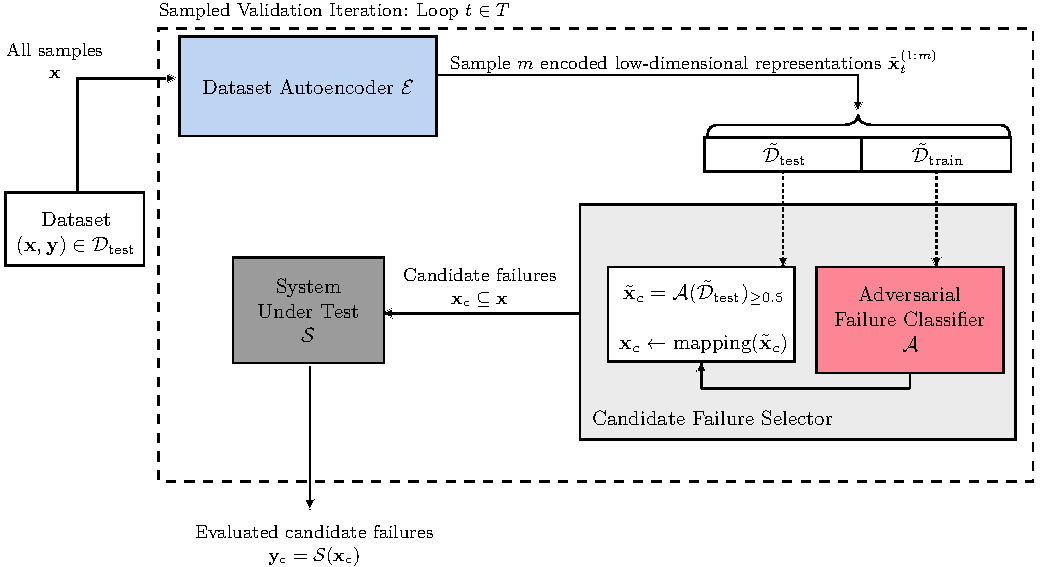
\includegraphics[page=1]{figures/weakness_rec/validation_diagram.pdf}
    % \tikzset{every picture/.style={line width=0.75pt}} %set default line width to 0.75pt        

\begin{tikzpicture}[x=0.75pt,y=0.75pt,yscale=-1,xscale=1]
%uncomment if require: \path (0,399); %set diagram left start at 0, and has height of 399

%Shape: Rectangle [id:dp3416440849450273] 
\draw  [dash pattern={on 4.5pt off 4.5pt}][line width=0.75]  (91.17,38) -- (653.17,38) -- (653.17,329) -- (91.17,329) -- cycle ;
%Straight Lines [id:da6207923302069309] 
\draw    (39.17,144) -- (39.17,70) -- (95.5,70) ;
\draw [shift={(102.5,70)}, rotate = 180] [fill={rgb, 255:red, 0; green, 0; blue, 0 }  ][line width=0.08]  [draw opacity=0] (6.25,-3) -- (0,0) -- (6.25,3) -- cycle    ;
%Straight Lines [id:da40087733759777344] 
\draw    (257.17,68) -- (540.57,68) -- (540.57,88) ;
\draw [shift={(540.57,91)}, rotate = 270] [fill={rgb, 255:red, 0; green, 0; blue, 0 }  ][line width=0.08]  [draw opacity=0] (6.25,-3) -- (0,0) -- (6.25,3) -- cycle    ;
%Shape: Brace [id:dp16419611390886946] 
\draw   (638.17,107) .. controls (638.17,102.33) and (635.84,100) .. (631.17,100) -- (550.68,100) .. controls (544.01,100) and (540.68,97.67) .. (540.68,93) .. controls (540.68,97.67) and (537.35,100) .. (530.68,100)(533.68,100) -- (451,100) .. controls (446.33,100) and (444,102.33) .. (444,107) ;
%Straight Lines [id:da03991771123197685] 
\draw    (380.5,221) -- (235.5,221) ;
\draw [shift={(235.5,221)}, rotate = 360] [fill={rgb, 255:red, 0; green, 0; blue, 0 }  ][line width=0.08]  [draw opacity=0] (6.25,-3) -- (0,0) -- (6.25,3) -- cycle    ;
%Straight Lines [id:da4068130382497208] 
\draw    (188.5,255) -- (188.5,344) ;
\draw [shift={(188.5,347)}, rotate = 270] [fill={rgb, 255:red, 0; green, 0; blue, 0 }  ][line width=0.08]  [draw opacity=0] (6.25,-3) -- (0,0) -- (6.25,3) -- cycle    ;

% Text Node
\draw  [fill={rgb, 255:red, 189; green, 213; blue, 242 }  ,fill opacity=1 ]  (104.75,43.17) -- (269.75,43.17) -- (269.75,107.17) -- (104.75,107.17) -- cycle  ;
\draw (187.25,75.17) node   [align=left] {\begin{minipage}[lt]{109.32564pt}\setlength\topsep{0pt}
\begin{center}
Dataset Autoencoder $\displaystyle \mathcal{E}$
\end{center}

\end{minipage}};
% Text Node
\draw  [fill={rgb, 255:red, 155; green, 155; blue, 155 }  ,fill opacity=1 ]  (139.06,185) -- (236.06,185) -- (236.06,253) -- (139.06,253) -- cycle  ;
\draw (187.56,219) node   [align=left] {\begin{minipage}[lt]{63.197500000000005pt}\setlength\topsep{0pt}
\begin{center}
System\\Under Test\\$\displaystyle \mathcal{S}$
\end{center}

\end{minipage}};
% Text Node
\draw (90,20.33) node [anchor=north west][inner sep=0.75pt]  [font=\small] [align=left] {Sampled Validation Iteration: Loop $\displaystyle t \in T$};
% Text Node
\draw  [fill={rgb, 255:red, 255; green, 255; blue, 255 }  ,fill opacity=1 ]  (-4,143.33) -- (82,143.33) -- (82,190.33) -- (-4,190.33) -- cycle  ;
\draw (2,154.33) node [anchor=north west][inner sep=0.75pt]   [align=left] {\begin{minipage}[lt]{53.541216pt}\setlength\topsep{0pt}
\begin{center}
Dataset \\$\displaystyle (\mathbf{x}, \mathbf{y}) \in \mathcal{D}_\text{test}$
\end{center}

\end{minipage}};
% Text Node
\draw (-10,45.33) node [anchor=north west][inner sep=0.75pt]  [font=\small] [align=left] {\begin{minipage}[lt]{49.655912pt}\setlength\topsep{0pt}
\begin{center}
All samples\\$\displaystyle \mathbf{x}$
\end{center}

\end{minipage}};
% Text Node
\draw (277,50.33) node [anchor=north west][inner sep=0.75pt]  [font=\small] [align=left] {Sample $m$ encoded low-dimensional representations $\displaystyle \tilde{\mathbf{x}}_{t}^{(1:m)}$};
% Text Node
\draw  [fill={rgb, 255:red, 255; green, 255; blue, 255 }  ,fill opacity=1 ]  (442,108) -- (543,108) -- (543,130) -- (442,130) -- cycle  ;
\draw (478,110) node [anchor=north west][inner sep=0.75pt]   [align=left] {$\displaystyle \tilde{\mathcal{D}}_{\text{test}}$};
% Text Node
\draw  [fill={rgb, 255:red, 235; green, 235; blue, 235 }  ,fill opacity=1 ]  (362,151) -- (642,151) -- (642,302) -- (362,302) -- cycle  ;
\draw (368,282) node [anchor=north west][inner sep=0.75pt]   [align=left] {Candidate Failure Selector};
% Text Node
\draw  [fill={rgb, 255:red, 252; green, 134; blue, 148 }  ,fill opacity=1 ]  (514,191.33) -- (634,191.33) -- (634,259.33) -- (514,259.33) -- cycle  ;
\draw (520,202.33) node [anchor=north west][inner sep=0.75pt]   [align=left] {\begin{minipage}[lt]{78.6726pt}\setlength\topsep{0pt}
\begin{center}
Adversarial\\Failure Classifier\\$\displaystyle \mathcal{A}$
\end{center}

\end{minipage}};
% Text Node
% \draw  [fill={rgb, 255:red, 255; green, 255; blue, 255 }  ,fill opacity=1 ]  (419.5, 222) circle [x radius= 26.54, y radius= 26.54]   ;
\draw  [fill={rgb, 255:red, 255; green, 255; blue, 255 }  ,fill opacity=1 ]  (380,191.33) -- (500,191.33) -- (500,252) -- (380,252) -- cycle  ;
\draw (385,198) node [anchor=north west][inner sep=0.75pt]   [align=left] {\begin{minipage}[lt]{82.6726pt}\setlength\topsep{0pt}
\begin{center}
$\tilde{\mathbf{x}}_c = \mathcal{A}(\tilde{\mathcal{D}}_\text{test})_{\ge 0.5}$\\
\phantom{}\\
$\mathbf{x}_c \leftarrow \operatorname{mapping}(\tilde{\mathbf{x}}_c)$
\end{center}
\end{minipage}};

% Text Node
\draw (245,190.33) node [anchor=north west][inner sep=0.75pt]  [font=\small] [align=left] {\begin{minipage}[lt]{76.7176pt}\setlength\topsep{0pt}
\begin{center}
Candidate failures\\$\displaystyle \mathbf{x}_{c} \subseteq \mathbf{x}$
\end{center}

\end{minipage}};
% Text Node
\draw (111,355.33) node [anchor=north west][inner sep=0.75pt]  [font=\small] [align=left] {\begin{minipage}[lt]{118.05956pt}\setlength\topsep{0pt}
\begin{center}
Evaluated candidate failures\\$\displaystyle \mathbf{y}_{c} =\mathcal{S}(\mathbf{x}_{c})$
\end{center}

\end{minipage}};
% Text Node
\draw  [fill={rgb, 255:red, 255; green, 255; blue, 255 }  ,fill opacity=1 ]  (543,108) -- (639,108) -- (639,130) -- (543,130) -- cycle  ;
\draw (574,110) node [anchor=north west][inner sep=0.75pt]   [align=left] {$\displaystyle \tilde{\mathcal{D}}_{\text{train}} \ \ \ \ \ \ \ \ \ \ \ \ $};

%Straight Lines [id:D_train -> Adversary] 
\draw  [dash pattern={on 1.5pt off 1.5pt}][line width=0.75]  (591,191.33) -- (591,130) ;
\draw [shift={(591,191.33)}, rotate = 270] [fill={rgb, 255:red, 0; green, 0; blue, 0 }  ][line width=0.08]  [draw opacity=0] (6.25,-3) -- (0,0) -- (6.25,3) -- cycle    ;

%Straight Lines [id:D_test -> Candidate selector] 
\draw  [dash pattern={on 1.5pt off 1.5pt}][line width=0.75]  (492.5,191.33) -- (492.5,130) ;
\draw [shift={(492.5,191.33)}, rotate = 270] [fill={rgb, 255:red, 0; green, 0; blue, 0 }  ][line width=0.08]  [draw opacity=0] (6.25,-3) -- (0,0) -- (6.25,3) -- cycle    ;

%Straight Lines [id:Adversary -> Candidate selector] 
\draw  (574,259.33) -- (574,269.33) ;
\draw  (574,269.33) -- (440,269.33) ;
\draw  (440,269.33) -- (440,252) ;
\draw [shift={(440,252)}, rotate = 90] [fill={rgb, 255:red, 0; green, 0; blue, 0 }  ][line width=0.08]  [draw opacity=0] (6.25,-3) -- (0,0) -- (6.25,3) -- cycle    ;


\end{tikzpicture}
 % TOO INTENSE.
}
\caption{Validation framework---a dataset autoencoder $\mathcal{E}$ is trained on the entire validation dataset $\mathcal{D}_\text{test}$ consisting of input samples $\mathbf{x}$. Then $m$ samples of encoded low-dimensional representations of the inputs $\tilde{\mathbf{x}}$ are selected for this iteration $t$, denoted $\tilde{\mathbf{x}}_t^{(1:m)}$ for all $m$ samples. The low-dimensional representations are then split into a training and test dataset. The training dataset $\tilde{\mathcal{D}}_\text{train}$ is used to train an adversarial failure classifier $\mathcal{A}$ on the encoded representations. Then the test dataset $\tilde{\mathcal{D}}_\text{test}$ is used to select candidate failures $\tilde{\mathbf{x}}_c$ as predicted by the adversary. Finally, the candidate failures from the adversary $\tilde{\mathbf{x}}_c$ are mapped back to the original inputs $\mathbf{x}_c \subseteq \mathbf{x}$ and evaluated by the system under test $\mathcal{S}$.}
\label{fig:framework}
\end{figure}


\subsection{Dataset Autoencoder}\label{sec:autoencoder}
To get a low-dimensional representation of the inputs $\mathbf{x}$, we used an autoencoder network \citep{kramer1991nonlinear}.
We trained the autoencoder $\mathcal{E}$ on the MNIST test dataset $\mathcal{D}_\text{test}$ and sample from the low-dimensional representation $\tilde{\mathbf{x}}$ as inputs into our adversarial failure classifier.
We use the MNIST test set because this is our input validation set---thus, we want our autoencoder to only have information about the validation set, without the need to have access to the training set used by the system under test.
The autoencoder network maps the $28\times28$ input image $\mathbf x$ into a low-dimensional latent space of size $64$ using a $\LeakyReLU$ activation.
Then the decoder will take the $64$-dimensional representation $\mathbf{\tilde x}$, again using a $\LeakyReLU$ activation layer, and attempt to recover the original input $\mathbf x'$.
We pre-trained the autoencoder over $20$ epochs, with a mini-batch size of $1000$, and tuned the network parameters using the Adam optimizer with a learning rate of $\alpha=1e^{-3}$.
Training is unsupervised and we use the mean squared error loss function:
\begin{equation*}
\mathcal{L}_\mathcal{E}(\mathbf{x}', \mathbf{x}) = \frac{1}{m} \sum_{i=1}^m \left( x'_i - x_i \right)^2
\end{equation*}
\Cref{fig:autoencoder_nn} illustrates the autoencoder network architecture and \Cref{fig:mnist_autoencoder} shows samples of the true inputs and their output after encoding/decoding.


\begin{figure*}[!t]
  \centering
    \subfloat[Dataset autoencoder architecture, with inputs $\mathbf{x} \in \mathbb{R}^{28\times28}$, encoded through a dense $\LeakyReLU$ layer of size $\frac{28\times28}{2}$ to a low-dimensional representation $\tilde{\mathbf{x}} \in \mathbb{R}^{64}$, then decoded through a $\LeakyReLU$ layer of size $\frac{28\times28}{2}$, outputting $\mathbf{x}' \in \mathbb{R}^{28\times28}$.]{%
      \resizebox{0.45\textwidth}{!}{
        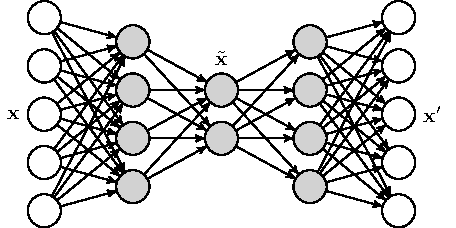
\includegraphics[page=1]{figures/weakness_rec/autoencoder-nn.pdf}
        % \input{figures/weakness_rec/autoencoder-nn.tex} % Needs lualatex
      }
      \label{fig:autoencoder_nn}
    }
    \hspace{5mm}
    \subfloat[Sampled output from the MNIST autoencoder: true input is on top and the recovered input on bottom.]{%
      \resizebox{0.45\textwidth}{!}{
        \centerline{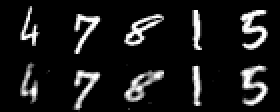
\includegraphics[width=0.6\textwidth]{figures/weakness_rec/sample-MNIST-autoencoder-5.png}}
      }
      \label{fig:mnist_autoencoder}
    }
  \caption{Dataset autoencoder architecture and sample decoded output.} 
\end{figure*}


\subsection{Adversarial Failure Classifier}
To learn the low-dimensional features that are likely to cause failures, we train an adversary $\mathcal{A}$ in the validation loop to classify failures.
The supervised adversary is trained on the partition $\tilde{\mathcal{D}}_\text{train}$ of the low-dimensional samples $\tilde{\mathbf{x}}$ and outputs a prediction that a given input would lead to a system failure.
In order to get the target classifications $\mathbf{y}$, we use the system $\mathcal{S}$ to run the true inputs associated to the encoded inputs which are part of the training data $\tilde{\mathcal{D}}_\text{train}$. This gives us the targets we can now train our adversary on.
Our adversarial loss function is the binary cross-entropy loss:
\[
\mathcal L_\mathcal{A}(\mathbf{\hat y}, \mathbf{y}) = -\frac{1}{m}\sum_{i=1}^m y_i\log(\hat y_i) - (1 - y_i)\log(1 - \hat y_i)
\]
The adversarial network architecture consists of $3$ dense layers which map the low-dimensional representation of $\tilde{\mathbf{x}} \in \mathbb{R}^{64}$ through a $\ReLU$ layer of size $128$, another $\ReLU$ layer of size $64$, and finally an output sigmoid layer to map the predictions to a probability.
For each sampled validation iteration $t$ (shown in \Cref{fig:framework}), we retrain the adversary $\mathcal{A}$ for $20$ epochs using the Adam optimizer with learning rate $\alpha=3e^{-5}$. Notice that our learning rate is very small, this is so we do not overfit to early iterations in $t$ and can generalize across different samples of the low-dimensional space. The adversary will use the test data partition $\tilde{\mathcal{D}}_\text{test}$ to select the encoded input that it predicted would lead to a failure.
We use the threshold of $\mathcal{A}(\tilde{x}) \ge 0.5$ to indicate the input $\tilde{x} \in \tilde{\mathcal{D}}_\text{test} \subset (\tilde{\mathbf{x}}, \mathbf{y})$ led to a failure.
All encoded inputs in the test dataset that led to a failure are considered candidate failure scenarios, and we denote them as $\tilde{\mathbf{x}}_c$.
We use a mapping from the encoded inputs $\tilde{\mathbf{x}}_c$ to the original inputs $\mathbf{x}_c \subseteq \mathbf{x}$, and finally pass the failure candidates to the true system $\mathcal{S}$ for actual evaluation.

%%% TODO: Change Loss function m to n ???

% We use the binary cross-entropy loss with an added factor $\Delta\softmax$ which is used as a distance metric to indicate the severity of a misclassification.
% The $\Delta\softmax$ metric is defined as the difference between the $\softmax$ probability of the prediction $\mathbf{\hat y}$ and the $\softmax$ probability of the \textit{true target} as indicated by the prediction:
% \[
% \Delta\operatorname{softmax}(\mathbf y, \mathbf{\hat y}) =
% \max\left(\operatorname{softmax}(\mathbf{\hat y})\right) -
% \operatorname{softmax}(\mathbf{\hat y})^{\left[ \operatorname{argmax} \mathbf y \right]}
% \]


% \subsection{Hyperparameters}
% % Table with all hyperparams for E, A, and S (in separate tables)
% % Describe the sensitivity of adversarial learning rate
% \lipsum[13]


\section{Experiments and Results}
\begin{table}[b]
    \centering
    \caption{Evaluation Metrics}\label{tab:metrics}
    \begin{threeparttable}
    \begin{tabular}{@{}lrr|rr@{}}
         \toprule
         \textbf{Failure Selector} &  \textbf{Precision}\tnote{*} & \textbf{Recall}\tnote{*} & \textbf{Sampled Precision}\tnote{$\dagger$} & \textbf{Sampled Recall}\tnote{$\dagger$}\\
         \midrule
         Adversary $\mathcal{A}$ & $0.2441$ & $0.2260$ & $0.2374 \pm 0.11$ & $0.3244 \pm 0.17$ \\
         Random & $0.0647$ & $0.4712$ & $0.0618 \pm 0.04$ & $0.0910 \pm 0.07$ \\
         \bottomrule
    \end{tabular}
    \begin{tablenotes}
        \item[*] {Run over $\mathcal{D}_\text{test}$ only calculated for the ``failure'' class.}
        \item[$\dagger$] {Calculated from $T=10$ iterations of the \textit{sampled validation loop}.}
        \end{tablenotes}
    \end{threeparttable}
\end{table}
To evaluate our approach, we ran $T=10$ sampled validation iterations, sampling $m=500$ random encodings and partitioning these samples in half into $\tilde{\mathcal{D}}_\text{train}$ and $\tilde{\mathcal{D}}_\text{test}$ for the adversary.
Because the failure rate for our system under test $\mathcal{S}$ is about $0.0677$, we augment the training dataset by duplicating the known failures $10$ times after running each training set through the system $\mathcal{S}$ to get the true outputs $\mathbf{y}_\text{train}$.
We use two main metrics to evaluate the performance of the adversary: \textit{precision} and \textit{recall}. During each iteration $t$, we save off the current adversary $\mathcal{A}_t$ and evaluate the \textit{area under the ROC curve} (AUC) as shown in \Cref{fig:roc}. The ROC curve highlights incremental improvement of the adversary after each iteration. Note that we retrain the new adversary $\mathcal{A}_{t}$ starting from the network weights learning by the previous adversary $\mathcal{A}_{t-1}$.
To balance between precision and recall, we swept over the prediction threshold to determine which threshold value to select (see \Cref{fig:sweep}).
Based on this tuning sweep, we chose a threshold of $\hat y \ge 0.5$ to indicate a positive failure prediction by the adversary.

During each iteration $t$, the adversary selects $k$ candidate inputs predicted to be failures.
For comparison, we employ a random selection of $k$ candidates and evaluate the precision and recall metrics of the random scheme.
This allows us to compare our adversarial learning approach to a baseline. \Cref{tab:metrics} quantifies the evaluation metrics for the adversary and random candidate selector.


%% subfigure version.
% \begin{figure}[ht]
%     \centering
%     \begin{subfigure}[t]{0.59\textwidth}
%         \centering
%         % \resizebox{\columnwidth}{!}{%% Creator: Matplotlib, PGF backend
%%
%% To include the figure in your LaTeX document, write
%%   \input{<filename>.pgf}
%%
%% Make sure the required packages are loaded in your preamble
%%   \usepackage{pgf}
%%
%% and, on pdftex
%%   \usepackage[utf8]{inputenc}\DeclareUnicodeCharacter{2212}{-}
%%
%% or, on luatex and xetex
%%   \usepackage{unicode-math}
%%
%% Figures using additional raster images can only be included by \input if
%% they are in the same directory as the main LaTeX file. For loading figures
%% from other directories you can use the `import` package
%%   \usepackage{import}
%%
%% and then include the figures with
%%   \import{<path to file>}{<filename>.pgf}
%%
%% Matplotlib used the following preamble
%%   \usepackage{fontspec}
%%
\begingroup%
\makeatletter%
\begin{pgfpicture}%
\pgfpathrectangle{\pgfpointorigin}{\pgfqpoint{5.729392in}{3.119305in}}%
\pgfusepath{use as bounding box, clip}%
\begin{pgfscope}%
\pgfsetbuttcap%
\pgfsetmiterjoin%
\definecolor{currentfill}{rgb}{1.000000,1.000000,1.000000}%
\pgfsetfillcolor{currentfill}%
\pgfsetlinewidth{0.000000pt}%
\definecolor{currentstroke}{rgb}{1.000000,1.000000,1.000000}%
\pgfsetstrokecolor{currentstroke}%
\pgfsetdash{}{0pt}%
\pgfpathmoveto{\pgfqpoint{0.000000in}{0.000000in}}%
\pgfpathlineto{\pgfqpoint{5.729392in}{0.000000in}}%
\pgfpathlineto{\pgfqpoint{5.729392in}{3.119305in}}%
\pgfpathlineto{\pgfqpoint{0.000000in}{3.119305in}}%
\pgfpathclose%
\pgfusepath{fill}%
\end{pgfscope}%
\begin{pgfscope}%
\pgfsetbuttcap%
\pgfsetmiterjoin%
\definecolor{currentfill}{rgb}{1.000000,1.000000,1.000000}%
\pgfsetfillcolor{currentfill}%
\pgfsetlinewidth{0.000000pt}%
\definecolor{currentstroke}{rgb}{0.000000,0.000000,0.000000}%
\pgfsetstrokecolor{currentstroke}%
\pgfsetstrokeopacity{0.000000}%
\pgfsetdash{}{0pt}%
\pgfpathmoveto{\pgfqpoint{0.896641in}{0.500972in}}%
\pgfpathlineto{\pgfqpoint{3.996641in}{0.500972in}}%
\pgfpathlineto{\pgfqpoint{3.996641in}{2.810972in}}%
\pgfpathlineto{\pgfqpoint{0.896641in}{2.810972in}}%
\pgfpathclose%
\pgfusepath{fill}%
\end{pgfscope}%
\begin{pgfscope}%
\pgfsetbuttcap%
\pgfsetroundjoin%
\definecolor{currentfill}{rgb}{0.000000,0.000000,0.000000}%
\pgfsetfillcolor{currentfill}%
\pgfsetlinewidth{0.803000pt}%
\definecolor{currentstroke}{rgb}{0.000000,0.000000,0.000000}%
\pgfsetstrokecolor{currentstroke}%
\pgfsetdash{}{0pt}%
\pgfsys@defobject{currentmarker}{\pgfqpoint{0.000000in}{-0.048611in}}{\pgfqpoint{0.000000in}{0.000000in}}{%
\pgfpathmoveto{\pgfqpoint{0.000000in}{0.000000in}}%
\pgfpathlineto{\pgfqpoint{0.000000in}{-0.048611in}}%
\pgfusepath{stroke,fill}%
}%
\begin{pgfscope}%
\pgfsys@transformshift{1.037550in}{0.500972in}%
\pgfsys@useobject{currentmarker}{}%
\end{pgfscope}%
\end{pgfscope}%
\begin{pgfscope}%
\definecolor{textcolor}{rgb}{0.000000,0.000000,0.000000}%
\pgfsetstrokecolor{textcolor}%
\pgfsetfillcolor{textcolor}%
\pgftext[x=1.037550in,y=0.403750in,,top]{\color{textcolor}\rmfamily\fontsize{10.000000}{12.000000}\selectfont \(\displaystyle {0.0}\)}%
\end{pgfscope}%
\begin{pgfscope}%
\pgfsetbuttcap%
\pgfsetroundjoin%
\definecolor{currentfill}{rgb}{0.000000,0.000000,0.000000}%
\pgfsetfillcolor{currentfill}%
\pgfsetlinewidth{0.803000pt}%
\definecolor{currentstroke}{rgb}{0.000000,0.000000,0.000000}%
\pgfsetstrokecolor{currentstroke}%
\pgfsetdash{}{0pt}%
\pgfsys@defobject{currentmarker}{\pgfqpoint{0.000000in}{-0.048611in}}{\pgfqpoint{0.000000in}{0.000000in}}{%
\pgfpathmoveto{\pgfqpoint{0.000000in}{0.000000in}}%
\pgfpathlineto{\pgfqpoint{0.000000in}{-0.048611in}}%
\pgfusepath{stroke,fill}%
}%
\begin{pgfscope}%
\pgfsys@transformshift{1.601186in}{0.500972in}%
\pgfsys@useobject{currentmarker}{}%
\end{pgfscope}%
\end{pgfscope}%
\begin{pgfscope}%
\definecolor{textcolor}{rgb}{0.000000,0.000000,0.000000}%
\pgfsetstrokecolor{textcolor}%
\pgfsetfillcolor{textcolor}%
\pgftext[x=1.601186in,y=0.403750in,,top]{\color{textcolor}\rmfamily\fontsize{10.000000}{12.000000}\selectfont \(\displaystyle {0.2}\)}%
\end{pgfscope}%
\begin{pgfscope}%
\pgfsetbuttcap%
\pgfsetroundjoin%
\definecolor{currentfill}{rgb}{0.000000,0.000000,0.000000}%
\pgfsetfillcolor{currentfill}%
\pgfsetlinewidth{0.803000pt}%
\definecolor{currentstroke}{rgb}{0.000000,0.000000,0.000000}%
\pgfsetstrokecolor{currentstroke}%
\pgfsetdash{}{0pt}%
\pgfsys@defobject{currentmarker}{\pgfqpoint{0.000000in}{-0.048611in}}{\pgfqpoint{0.000000in}{0.000000in}}{%
\pgfpathmoveto{\pgfqpoint{0.000000in}{0.000000in}}%
\pgfpathlineto{\pgfqpoint{0.000000in}{-0.048611in}}%
\pgfusepath{stroke,fill}%
}%
\begin{pgfscope}%
\pgfsys@transformshift{2.164823in}{0.500972in}%
\pgfsys@useobject{currentmarker}{}%
\end{pgfscope}%
\end{pgfscope}%
\begin{pgfscope}%
\definecolor{textcolor}{rgb}{0.000000,0.000000,0.000000}%
\pgfsetstrokecolor{textcolor}%
\pgfsetfillcolor{textcolor}%
\pgftext[x=2.164823in,y=0.403750in,,top]{\color{textcolor}\rmfamily\fontsize{10.000000}{12.000000}\selectfont \(\displaystyle {0.4}\)}%
\end{pgfscope}%
\begin{pgfscope}%
\pgfsetbuttcap%
\pgfsetroundjoin%
\definecolor{currentfill}{rgb}{0.000000,0.000000,0.000000}%
\pgfsetfillcolor{currentfill}%
\pgfsetlinewidth{0.803000pt}%
\definecolor{currentstroke}{rgb}{0.000000,0.000000,0.000000}%
\pgfsetstrokecolor{currentstroke}%
\pgfsetdash{}{0pt}%
\pgfsys@defobject{currentmarker}{\pgfqpoint{0.000000in}{-0.048611in}}{\pgfqpoint{0.000000in}{0.000000in}}{%
\pgfpathmoveto{\pgfqpoint{0.000000in}{0.000000in}}%
\pgfpathlineto{\pgfqpoint{0.000000in}{-0.048611in}}%
\pgfusepath{stroke,fill}%
}%
\begin{pgfscope}%
\pgfsys@transformshift{2.728459in}{0.500972in}%
\pgfsys@useobject{currentmarker}{}%
\end{pgfscope}%
\end{pgfscope}%
\begin{pgfscope}%
\definecolor{textcolor}{rgb}{0.000000,0.000000,0.000000}%
\pgfsetstrokecolor{textcolor}%
\pgfsetfillcolor{textcolor}%
\pgftext[x=2.728459in,y=0.403750in,,top]{\color{textcolor}\rmfamily\fontsize{10.000000}{12.000000}\selectfont \(\displaystyle {0.6}\)}%
\end{pgfscope}%
\begin{pgfscope}%
\pgfsetbuttcap%
\pgfsetroundjoin%
\definecolor{currentfill}{rgb}{0.000000,0.000000,0.000000}%
\pgfsetfillcolor{currentfill}%
\pgfsetlinewidth{0.803000pt}%
\definecolor{currentstroke}{rgb}{0.000000,0.000000,0.000000}%
\pgfsetstrokecolor{currentstroke}%
\pgfsetdash{}{0pt}%
\pgfsys@defobject{currentmarker}{\pgfqpoint{0.000000in}{-0.048611in}}{\pgfqpoint{0.000000in}{0.000000in}}{%
\pgfpathmoveto{\pgfqpoint{0.000000in}{0.000000in}}%
\pgfpathlineto{\pgfqpoint{0.000000in}{-0.048611in}}%
\pgfusepath{stroke,fill}%
}%
\begin{pgfscope}%
\pgfsys@transformshift{3.292095in}{0.500972in}%
\pgfsys@useobject{currentmarker}{}%
\end{pgfscope}%
\end{pgfscope}%
\begin{pgfscope}%
\definecolor{textcolor}{rgb}{0.000000,0.000000,0.000000}%
\pgfsetstrokecolor{textcolor}%
\pgfsetfillcolor{textcolor}%
\pgftext[x=3.292095in,y=0.403750in,,top]{\color{textcolor}\rmfamily\fontsize{10.000000}{12.000000}\selectfont \(\displaystyle {0.8}\)}%
\end{pgfscope}%
\begin{pgfscope}%
\pgfsetbuttcap%
\pgfsetroundjoin%
\definecolor{currentfill}{rgb}{0.000000,0.000000,0.000000}%
\pgfsetfillcolor{currentfill}%
\pgfsetlinewidth{0.803000pt}%
\definecolor{currentstroke}{rgb}{0.000000,0.000000,0.000000}%
\pgfsetstrokecolor{currentstroke}%
\pgfsetdash{}{0pt}%
\pgfsys@defobject{currentmarker}{\pgfqpoint{0.000000in}{-0.048611in}}{\pgfqpoint{0.000000in}{0.000000in}}{%
\pgfpathmoveto{\pgfqpoint{0.000000in}{0.000000in}}%
\pgfpathlineto{\pgfqpoint{0.000000in}{-0.048611in}}%
\pgfusepath{stroke,fill}%
}%
\begin{pgfscope}%
\pgfsys@transformshift{3.855732in}{0.500972in}%
\pgfsys@useobject{currentmarker}{}%
\end{pgfscope}%
\end{pgfscope}%
\begin{pgfscope}%
\definecolor{textcolor}{rgb}{0.000000,0.000000,0.000000}%
\pgfsetstrokecolor{textcolor}%
\pgfsetfillcolor{textcolor}%
\pgftext[x=3.855732in,y=0.403750in,,top]{\color{textcolor}\rmfamily\fontsize{10.000000}{12.000000}\selectfont \(\displaystyle {1.0}\)}%
\end{pgfscope}%
\begin{pgfscope}%
\definecolor{textcolor}{rgb}{0.000000,0.000000,0.000000}%
\pgfsetstrokecolor{textcolor}%
\pgfsetfillcolor{textcolor}%
\pgftext[x=2.446641in,y=0.224861in,,top]{\color{textcolor}\rmfamily\fontsize{10.000000}{12.000000}\selectfont false positive rate}%
\end{pgfscope}%
\begin{pgfscope}%
\pgfsetbuttcap%
\pgfsetroundjoin%
\definecolor{currentfill}{rgb}{0.000000,0.000000,0.000000}%
\pgfsetfillcolor{currentfill}%
\pgfsetlinewidth{0.803000pt}%
\definecolor{currentstroke}{rgb}{0.000000,0.000000,0.000000}%
\pgfsetstrokecolor{currentstroke}%
\pgfsetdash{}{0pt}%
\pgfsys@defobject{currentmarker}{\pgfqpoint{-0.048611in}{0.000000in}}{\pgfqpoint{0.000000in}{0.000000in}}{%
\pgfpathmoveto{\pgfqpoint{0.000000in}{0.000000in}}%
\pgfpathlineto{\pgfqpoint{-0.048611in}{0.000000in}}%
\pgfusepath{stroke,fill}%
}%
\begin{pgfscope}%
\pgfsys@transformshift{0.896641in}{0.605972in}%
\pgfsys@useobject{currentmarker}{}%
\end{pgfscope}%
\end{pgfscope}%
\begin{pgfscope}%
\definecolor{textcolor}{rgb}{0.000000,0.000000,0.000000}%
\pgfsetstrokecolor{textcolor}%
\pgfsetfillcolor{textcolor}%
\pgftext[x=0.621949in, y=0.557777in, left, base]{\color{textcolor}\rmfamily\fontsize{10.000000}{12.000000}\selectfont \(\displaystyle {0.0}\)}%
\end{pgfscope}%
\begin{pgfscope}%
\pgfsetbuttcap%
\pgfsetroundjoin%
\definecolor{currentfill}{rgb}{0.000000,0.000000,0.000000}%
\pgfsetfillcolor{currentfill}%
\pgfsetlinewidth{0.803000pt}%
\definecolor{currentstroke}{rgb}{0.000000,0.000000,0.000000}%
\pgfsetstrokecolor{currentstroke}%
\pgfsetdash{}{0pt}%
\pgfsys@defobject{currentmarker}{\pgfqpoint{-0.048611in}{0.000000in}}{\pgfqpoint{0.000000in}{0.000000in}}{%
\pgfpathmoveto{\pgfqpoint{0.000000in}{0.000000in}}%
\pgfpathlineto{\pgfqpoint{-0.048611in}{0.000000in}}%
\pgfusepath{stroke,fill}%
}%
\begin{pgfscope}%
\pgfsys@transformshift{0.896641in}{1.025972in}%
\pgfsys@useobject{currentmarker}{}%
\end{pgfscope}%
\end{pgfscope}%
\begin{pgfscope}%
\definecolor{textcolor}{rgb}{0.000000,0.000000,0.000000}%
\pgfsetstrokecolor{textcolor}%
\pgfsetfillcolor{textcolor}%
\pgftext[x=0.621949in, y=0.977777in, left, base]{\color{textcolor}\rmfamily\fontsize{10.000000}{12.000000}\selectfont \(\displaystyle {0.2}\)}%
\end{pgfscope}%
\begin{pgfscope}%
\pgfsetbuttcap%
\pgfsetroundjoin%
\definecolor{currentfill}{rgb}{0.000000,0.000000,0.000000}%
\pgfsetfillcolor{currentfill}%
\pgfsetlinewidth{0.803000pt}%
\definecolor{currentstroke}{rgb}{0.000000,0.000000,0.000000}%
\pgfsetstrokecolor{currentstroke}%
\pgfsetdash{}{0pt}%
\pgfsys@defobject{currentmarker}{\pgfqpoint{-0.048611in}{0.000000in}}{\pgfqpoint{0.000000in}{0.000000in}}{%
\pgfpathmoveto{\pgfqpoint{0.000000in}{0.000000in}}%
\pgfpathlineto{\pgfqpoint{-0.048611in}{0.000000in}}%
\pgfusepath{stroke,fill}%
}%
\begin{pgfscope}%
\pgfsys@transformshift{0.896641in}{1.445972in}%
\pgfsys@useobject{currentmarker}{}%
\end{pgfscope}%
\end{pgfscope}%
\begin{pgfscope}%
\definecolor{textcolor}{rgb}{0.000000,0.000000,0.000000}%
\pgfsetstrokecolor{textcolor}%
\pgfsetfillcolor{textcolor}%
\pgftext[x=0.621949in, y=1.397777in, left, base]{\color{textcolor}\rmfamily\fontsize{10.000000}{12.000000}\selectfont \(\displaystyle {0.4}\)}%
\end{pgfscope}%
\begin{pgfscope}%
\pgfsetbuttcap%
\pgfsetroundjoin%
\definecolor{currentfill}{rgb}{0.000000,0.000000,0.000000}%
\pgfsetfillcolor{currentfill}%
\pgfsetlinewidth{0.803000pt}%
\definecolor{currentstroke}{rgb}{0.000000,0.000000,0.000000}%
\pgfsetstrokecolor{currentstroke}%
\pgfsetdash{}{0pt}%
\pgfsys@defobject{currentmarker}{\pgfqpoint{-0.048611in}{0.000000in}}{\pgfqpoint{0.000000in}{0.000000in}}{%
\pgfpathmoveto{\pgfqpoint{0.000000in}{0.000000in}}%
\pgfpathlineto{\pgfqpoint{-0.048611in}{0.000000in}}%
\pgfusepath{stroke,fill}%
}%
\begin{pgfscope}%
\pgfsys@transformshift{0.896641in}{1.865972in}%
\pgfsys@useobject{currentmarker}{}%
\end{pgfscope}%
\end{pgfscope}%
\begin{pgfscope}%
\definecolor{textcolor}{rgb}{0.000000,0.000000,0.000000}%
\pgfsetstrokecolor{textcolor}%
\pgfsetfillcolor{textcolor}%
\pgftext[x=0.621949in, y=1.817778in, left, base]{\color{textcolor}\rmfamily\fontsize{10.000000}{12.000000}\selectfont \(\displaystyle {0.6}\)}%
\end{pgfscope}%
\begin{pgfscope}%
\pgfsetbuttcap%
\pgfsetroundjoin%
\definecolor{currentfill}{rgb}{0.000000,0.000000,0.000000}%
\pgfsetfillcolor{currentfill}%
\pgfsetlinewidth{0.803000pt}%
\definecolor{currentstroke}{rgb}{0.000000,0.000000,0.000000}%
\pgfsetstrokecolor{currentstroke}%
\pgfsetdash{}{0pt}%
\pgfsys@defobject{currentmarker}{\pgfqpoint{-0.048611in}{0.000000in}}{\pgfqpoint{0.000000in}{0.000000in}}{%
\pgfpathmoveto{\pgfqpoint{0.000000in}{0.000000in}}%
\pgfpathlineto{\pgfqpoint{-0.048611in}{0.000000in}}%
\pgfusepath{stroke,fill}%
}%
\begin{pgfscope}%
\pgfsys@transformshift{0.896641in}{2.285972in}%
\pgfsys@useobject{currentmarker}{}%
\end{pgfscope}%
\end{pgfscope}%
\begin{pgfscope}%
\definecolor{textcolor}{rgb}{0.000000,0.000000,0.000000}%
\pgfsetstrokecolor{textcolor}%
\pgfsetfillcolor{textcolor}%
\pgftext[x=0.621949in, y=2.237777in, left, base]{\color{textcolor}\rmfamily\fontsize{10.000000}{12.000000}\selectfont \(\displaystyle {0.8}\)}%
\end{pgfscope}%
\begin{pgfscope}%
\pgfsetbuttcap%
\pgfsetroundjoin%
\definecolor{currentfill}{rgb}{0.000000,0.000000,0.000000}%
\pgfsetfillcolor{currentfill}%
\pgfsetlinewidth{0.803000pt}%
\definecolor{currentstroke}{rgb}{0.000000,0.000000,0.000000}%
\pgfsetstrokecolor{currentstroke}%
\pgfsetdash{}{0pt}%
\pgfsys@defobject{currentmarker}{\pgfqpoint{-0.048611in}{0.000000in}}{\pgfqpoint{0.000000in}{0.000000in}}{%
\pgfpathmoveto{\pgfqpoint{0.000000in}{0.000000in}}%
\pgfpathlineto{\pgfqpoint{-0.048611in}{0.000000in}}%
\pgfusepath{stroke,fill}%
}%
\begin{pgfscope}%
\pgfsys@transformshift{0.896641in}{2.705972in}%
\pgfsys@useobject{currentmarker}{}%
\end{pgfscope}%
\end{pgfscope}%
\begin{pgfscope}%
\definecolor{textcolor}{rgb}{0.000000,0.000000,0.000000}%
\pgfsetstrokecolor{textcolor}%
\pgfsetfillcolor{textcolor}%
\pgftext[x=0.621949in, y=2.657778in, left, base]{\color{textcolor}\rmfamily\fontsize{10.000000}{12.000000}\selectfont \(\displaystyle {1.0}\)}%
\end{pgfscope}%
\begin{pgfscope}%
\definecolor{textcolor}{rgb}{0.000000,0.000000,0.000000}%
\pgfsetstrokecolor{textcolor}%
\pgfsetfillcolor{textcolor}%
\pgftext[x=0.566393in,y=1.655972in,,bottom,rotate=90.000000]{\color{textcolor}\rmfamily\fontsize{10.000000}{12.000000}\selectfont true positive rate}%
\end{pgfscope}%
\begin{pgfscope}%
\pgfpathrectangle{\pgfqpoint{0.896641in}{0.500972in}}{\pgfqpoint{3.100000in}{2.310000in}}%
\pgfusepath{clip}%
\pgfsetrectcap%
\pgfsetroundjoin%
\pgfsetlinewidth{1.505625pt}%
\definecolor{currentstroke}{rgb}{0.969000,0.984000,1.000000}%
\pgfsetstrokecolor{currentstroke}%
\pgfsetdash{}{0pt}%
\pgfpathmoveto{\pgfqpoint{1.037550in}{0.605972in}}%
\pgfpathlineto{\pgfqpoint{1.038457in}{0.624583in}}%
\pgfpathlineto{\pgfqpoint{1.040270in}{0.624583in}}%
\pgfpathlineto{\pgfqpoint{1.040270in}{0.627685in}}%
\pgfpathlineto{\pgfqpoint{1.043898in}{0.627685in}}%
\pgfpathlineto{\pgfqpoint{1.044200in}{0.633889in}}%
\pgfpathlineto{\pgfqpoint{1.045107in}{0.633889in}}%
\pgfpathlineto{\pgfqpoint{1.045107in}{0.640093in}}%
\pgfpathlineto{\pgfqpoint{1.046921in}{0.640093in}}%
\pgfpathlineto{\pgfqpoint{1.046921in}{0.643195in}}%
\pgfpathlineto{\pgfqpoint{1.049944in}{0.643195in}}%
\pgfpathlineto{\pgfqpoint{1.050548in}{0.649399in}}%
\pgfpathlineto{\pgfqpoint{1.051153in}{0.649399in}}%
\pgfpathlineto{\pgfqpoint{1.051757in}{0.658705in}}%
\pgfpathlineto{\pgfqpoint{1.053571in}{0.658705in}}%
\pgfpathlineto{\pgfqpoint{1.053873in}{0.668010in}}%
\pgfpathlineto{\pgfqpoint{1.055082in}{0.668010in}}%
\pgfpathlineto{\pgfqpoint{1.055989in}{0.674214in}}%
\pgfpathlineto{\pgfqpoint{1.056896in}{0.674214in}}%
\pgfpathlineto{\pgfqpoint{1.056896in}{0.680418in}}%
\pgfpathlineto{\pgfqpoint{1.059919in}{0.680418in}}%
\pgfpathlineto{\pgfqpoint{1.060826in}{0.686622in}}%
\pgfpathlineto{\pgfqpoint{1.062035in}{0.686622in}}%
\pgfpathlineto{\pgfqpoint{1.062035in}{0.689724in}}%
\pgfpathlineto{\pgfqpoint{1.063546in}{0.689724in}}%
\pgfpathlineto{\pgfqpoint{1.064453in}{0.695928in}}%
\pgfpathlineto{\pgfqpoint{1.066267in}{0.695928in}}%
\pgfpathlineto{\pgfqpoint{1.066267in}{0.702131in}}%
\pgfpathlineto{\pgfqpoint{1.068080in}{0.702131in}}%
\pgfpathlineto{\pgfqpoint{1.068685in}{0.708335in}}%
\pgfpathlineto{\pgfqpoint{1.069592in}{0.708335in}}%
\pgfpathlineto{\pgfqpoint{1.070499in}{0.720743in}}%
\pgfpathlineto{\pgfqpoint{1.071708in}{0.720743in}}%
\pgfpathlineto{\pgfqpoint{1.071708in}{0.723845in}}%
\pgfpathlineto{\pgfqpoint{1.074126in}{0.723845in}}%
\pgfpathlineto{\pgfqpoint{1.075033in}{0.730049in}}%
\pgfpathlineto{\pgfqpoint{1.077451in}{0.730049in}}%
\pgfpathlineto{\pgfqpoint{1.078358in}{0.739355in}}%
\pgfpathlineto{\pgfqpoint{1.080172in}{0.739355in}}%
\pgfpathlineto{\pgfqpoint{1.081079in}{0.754864in}}%
\pgfpathlineto{\pgfqpoint{1.082892in}{0.754864in}}%
\pgfpathlineto{\pgfqpoint{1.083195in}{0.761068in}}%
\pgfpathlineto{\pgfqpoint{1.084706in}{0.761068in}}%
\pgfpathlineto{\pgfqpoint{1.084706in}{0.764170in}}%
\pgfpathlineto{\pgfqpoint{1.089240in}{0.764170in}}%
\pgfpathlineto{\pgfqpoint{1.089240in}{0.767272in}}%
\pgfpathlineto{\pgfqpoint{1.091356in}{0.767272in}}%
\pgfpathlineto{\pgfqpoint{1.091356in}{0.776578in}}%
\pgfpathlineto{\pgfqpoint{1.095588in}{0.776578in}}%
\pgfpathlineto{\pgfqpoint{1.096193in}{0.782781in}}%
\pgfpathlineto{\pgfqpoint{1.099820in}{0.782781in}}%
\pgfpathlineto{\pgfqpoint{1.099820in}{0.788985in}}%
\pgfpathlineto{\pgfqpoint{1.101029in}{0.788985in}}%
\pgfpathlineto{\pgfqpoint{1.101634in}{0.798291in}}%
\pgfpathlineto{\pgfqpoint{1.102843in}{0.798291in}}%
\pgfpathlineto{\pgfqpoint{1.102843in}{0.801393in}}%
\pgfpathlineto{\pgfqpoint{1.105261in}{0.801393in}}%
\pgfpathlineto{\pgfqpoint{1.106168in}{0.813801in}}%
\pgfpathlineto{\pgfqpoint{1.110098in}{0.813801in}}%
\pgfpathlineto{\pgfqpoint{1.110098in}{0.816903in}}%
\pgfpathlineto{\pgfqpoint{1.118259in}{0.816903in}}%
\pgfpathlineto{\pgfqpoint{1.118864in}{0.823106in}}%
\pgfpathlineto{\pgfqpoint{1.122491in}{0.823106in}}%
\pgfpathlineto{\pgfqpoint{1.123398in}{0.832412in}}%
\pgfpathlineto{\pgfqpoint{1.124305in}{0.832412in}}%
\pgfpathlineto{\pgfqpoint{1.124305in}{0.835514in}}%
\pgfpathlineto{\pgfqpoint{1.129142in}{0.835514in}}%
\pgfpathlineto{\pgfqpoint{1.129746in}{0.841718in}}%
\pgfpathlineto{\pgfqpoint{1.132769in}{0.841718in}}%
\pgfpathlineto{\pgfqpoint{1.132769in}{0.844820in}}%
\pgfpathlineto{\pgfqpoint{1.134583in}{0.844820in}}%
\pgfpathlineto{\pgfqpoint{1.134583in}{0.847922in}}%
\pgfpathlineto{\pgfqpoint{1.137001in}{0.847922in}}%
\pgfpathlineto{\pgfqpoint{1.137001in}{0.851024in}}%
\pgfpathlineto{\pgfqpoint{1.139721in}{0.851024in}}%
\pgfpathlineto{\pgfqpoint{1.139721in}{0.854126in}}%
\pgfpathlineto{\pgfqpoint{1.142140in}{0.854126in}}%
\pgfpathlineto{\pgfqpoint{1.143047in}{0.860329in}}%
\pgfpathlineto{\pgfqpoint{1.150301in}{0.860329in}}%
\pgfpathlineto{\pgfqpoint{1.150301in}{0.863431in}}%
\pgfpathlineto{\pgfqpoint{1.153022in}{0.863431in}}%
\pgfpathlineto{\pgfqpoint{1.153022in}{0.869635in}}%
\pgfpathlineto{\pgfqpoint{1.157254in}{0.869635in}}%
\pgfpathlineto{\pgfqpoint{1.158161in}{0.878941in}}%
\pgfpathlineto{\pgfqpoint{1.162695in}{0.878941in}}%
\pgfpathlineto{\pgfqpoint{1.162695in}{0.882043in}}%
\pgfpathlineto{\pgfqpoint{1.166020in}{0.882043in}}%
\pgfpathlineto{\pgfqpoint{1.166927in}{0.888247in}}%
\pgfpathlineto{\pgfqpoint{1.179623in}{0.888247in}}%
\pgfpathlineto{\pgfqpoint{1.180530in}{0.900654in}}%
\pgfpathlineto{\pgfqpoint{1.183250in}{0.900654in}}%
\pgfpathlineto{\pgfqpoint{1.183250in}{0.903756in}}%
\pgfpathlineto{\pgfqpoint{1.184762in}{0.903756in}}%
\pgfpathlineto{\pgfqpoint{1.185064in}{0.909960in}}%
\pgfpathlineto{\pgfqpoint{1.188691in}{0.909960in}}%
\pgfpathlineto{\pgfqpoint{1.188691in}{0.919266in}}%
\pgfpathlineto{\pgfqpoint{1.191714in}{0.919266in}}%
\pgfpathlineto{\pgfqpoint{1.192016in}{0.928572in}}%
\pgfpathlineto{\pgfqpoint{1.192923in}{0.928572in}}%
\pgfpathlineto{\pgfqpoint{1.192923in}{0.931674in}}%
\pgfpathlineto{\pgfqpoint{1.198062in}{0.931674in}}%
\pgfpathlineto{\pgfqpoint{1.198969in}{0.940979in}}%
\pgfpathlineto{\pgfqpoint{1.199876in}{0.940979in}}%
\pgfpathlineto{\pgfqpoint{1.199876in}{0.944081in}}%
\pgfpathlineto{\pgfqpoint{1.201085in}{0.944081in}}%
\pgfpathlineto{\pgfqpoint{1.201387in}{0.950285in}}%
\pgfpathlineto{\pgfqpoint{1.202596in}{0.950285in}}%
\pgfpathlineto{\pgfqpoint{1.202596in}{0.953387in}}%
\pgfpathlineto{\pgfqpoint{1.206526in}{0.953387in}}%
\pgfpathlineto{\pgfqpoint{1.206526in}{0.956489in}}%
\pgfpathlineto{\pgfqpoint{1.211665in}{0.956489in}}%
\pgfpathlineto{\pgfqpoint{1.211665in}{0.959591in}}%
\pgfpathlineto{\pgfqpoint{1.216501in}{0.959591in}}%
\pgfpathlineto{\pgfqpoint{1.216501in}{0.962693in}}%
\pgfpathlineto{\pgfqpoint{1.225872in}{0.962693in}}%
\pgfpathlineto{\pgfqpoint{1.226174in}{0.968897in}}%
\pgfpathlineto{\pgfqpoint{1.228593in}{0.968897in}}%
\pgfpathlineto{\pgfqpoint{1.228593in}{0.971999in}}%
\pgfpathlineto{\pgfqpoint{1.230406in}{0.971999in}}%
\pgfpathlineto{\pgfqpoint{1.230406in}{0.975100in}}%
\pgfpathlineto{\pgfqpoint{1.232825in}{0.975100in}}%
\pgfpathlineto{\pgfqpoint{1.233127in}{0.981304in}}%
\pgfpathlineto{\pgfqpoint{1.234034in}{0.981304in}}%
\pgfpathlineto{\pgfqpoint{1.234336in}{0.987508in}}%
\pgfpathlineto{\pgfqpoint{1.235545in}{0.987508in}}%
\pgfpathlineto{\pgfqpoint{1.235847in}{0.993712in}}%
\pgfpathlineto{\pgfqpoint{1.241591in}{0.993712in}}%
\pgfpathlineto{\pgfqpoint{1.241591in}{0.996814in}}%
\pgfpathlineto{\pgfqpoint{1.243707in}{0.996814in}}%
\pgfpathlineto{\pgfqpoint{1.244009in}{1.003018in}}%
\pgfpathlineto{\pgfqpoint{1.245520in}{1.003018in}}%
\pgfpathlineto{\pgfqpoint{1.245823in}{1.009222in}}%
\pgfpathlineto{\pgfqpoint{1.247636in}{1.009222in}}%
\pgfpathlineto{\pgfqpoint{1.247636in}{1.015425in}}%
\pgfpathlineto{\pgfqpoint{1.252775in}{1.015425in}}%
\pgfpathlineto{\pgfqpoint{1.253078in}{1.021629in}}%
\pgfpathlineto{\pgfqpoint{1.256705in}{1.021629in}}%
\pgfpathlineto{\pgfqpoint{1.257007in}{1.027833in}}%
\pgfpathlineto{\pgfqpoint{1.258216in}{1.027833in}}%
\pgfpathlineto{\pgfqpoint{1.258216in}{1.030935in}}%
\pgfpathlineto{\pgfqpoint{1.262751in}{1.030935in}}%
\pgfpathlineto{\pgfqpoint{1.262751in}{1.034037in}}%
\pgfpathlineto{\pgfqpoint{1.267285in}{1.034037in}}%
\pgfpathlineto{\pgfqpoint{1.267285in}{1.037139in}}%
\pgfpathlineto{\pgfqpoint{1.270912in}{1.037139in}}%
\pgfpathlineto{\pgfqpoint{1.270912in}{1.040241in}}%
\pgfpathlineto{\pgfqpoint{1.273330in}{1.040241in}}%
\pgfpathlineto{\pgfqpoint{1.273330in}{1.043343in}}%
\pgfpathlineto{\pgfqpoint{1.284213in}{1.043343in}}%
\pgfpathlineto{\pgfqpoint{1.284213in}{1.046445in}}%
\pgfpathlineto{\pgfqpoint{1.286026in}{1.046445in}}%
\pgfpathlineto{\pgfqpoint{1.286026in}{1.049547in}}%
\pgfpathlineto{\pgfqpoint{1.288142in}{1.049547in}}%
\pgfpathlineto{\pgfqpoint{1.288142in}{1.052648in}}%
\pgfpathlineto{\pgfqpoint{1.289956in}{1.052648in}}%
\pgfpathlineto{\pgfqpoint{1.289956in}{1.055750in}}%
\pgfpathlineto{\pgfqpoint{1.292072in}{1.055750in}}%
\pgfpathlineto{\pgfqpoint{1.292072in}{1.061954in}}%
\pgfpathlineto{\pgfqpoint{1.299024in}{1.061954in}}%
\pgfpathlineto{\pgfqpoint{1.299024in}{1.065056in}}%
\pgfpathlineto{\pgfqpoint{1.305977in}{1.065056in}}%
\pgfpathlineto{\pgfqpoint{1.306279in}{1.071260in}}%
\pgfpathlineto{\pgfqpoint{1.309000in}{1.071260in}}%
\pgfpathlineto{\pgfqpoint{1.309000in}{1.074362in}}%
\pgfpathlineto{\pgfqpoint{1.313836in}{1.074362in}}%
\pgfpathlineto{\pgfqpoint{1.313836in}{1.077464in}}%
\pgfpathlineto{\pgfqpoint{1.315045in}{1.077464in}}%
\pgfpathlineto{\pgfqpoint{1.315045in}{1.080566in}}%
\pgfpathlineto{\pgfqpoint{1.317161in}{1.080566in}}%
\pgfpathlineto{\pgfqpoint{1.317464in}{1.086770in}}%
\pgfpathlineto{\pgfqpoint{1.322603in}{1.086770in}}%
\pgfpathlineto{\pgfqpoint{1.323509in}{1.092973in}}%
\pgfpathlineto{\pgfqpoint{1.340135in}{1.092973in}}%
\pgfpathlineto{\pgfqpoint{1.340135in}{1.096075in}}%
\pgfpathlineto{\pgfqpoint{1.347692in}{1.096075in}}%
\pgfpathlineto{\pgfqpoint{1.348297in}{1.102279in}}%
\pgfpathlineto{\pgfqpoint{1.348901in}{1.102279in}}%
\pgfpathlineto{\pgfqpoint{1.348901in}{1.105381in}}%
\pgfpathlineto{\pgfqpoint{1.351924in}{1.105381in}}%
\pgfpathlineto{\pgfqpoint{1.351924in}{1.108483in}}%
\pgfpathlineto{\pgfqpoint{1.355551in}{1.108483in}}%
\pgfpathlineto{\pgfqpoint{1.355551in}{1.111585in}}%
\pgfpathlineto{\pgfqpoint{1.360388in}{1.111585in}}%
\pgfpathlineto{\pgfqpoint{1.360388in}{1.114687in}}%
\pgfpathlineto{\pgfqpoint{1.365224in}{1.114687in}}%
\pgfpathlineto{\pgfqpoint{1.366131in}{1.120891in}}%
\pgfpathlineto{\pgfqpoint{1.367038in}{1.120891in}}%
\pgfpathlineto{\pgfqpoint{1.367340in}{1.127095in}}%
\pgfpathlineto{\pgfqpoint{1.371572in}{1.127095in}}%
\pgfpathlineto{\pgfqpoint{1.371572in}{1.130196in}}%
\pgfpathlineto{\pgfqpoint{1.374293in}{1.130196in}}%
\pgfpathlineto{\pgfqpoint{1.374293in}{1.136400in}}%
\pgfpathlineto{\pgfqpoint{1.376409in}{1.136400in}}%
\pgfpathlineto{\pgfqpoint{1.377013in}{1.142604in}}%
\pgfpathlineto{\pgfqpoint{1.378525in}{1.142604in}}%
\pgfpathlineto{\pgfqpoint{1.378525in}{1.145706in}}%
\pgfpathlineto{\pgfqpoint{1.380036in}{1.145706in}}%
\pgfpathlineto{\pgfqpoint{1.380036in}{1.148808in}}%
\pgfpathlineto{\pgfqpoint{1.386082in}{1.148808in}}%
\pgfpathlineto{\pgfqpoint{1.386082in}{1.151910in}}%
\pgfpathlineto{\pgfqpoint{1.388500in}{1.151910in}}%
\pgfpathlineto{\pgfqpoint{1.388500in}{1.155012in}}%
\pgfpathlineto{\pgfqpoint{1.400894in}{1.155012in}}%
\pgfpathlineto{\pgfqpoint{1.400894in}{1.158114in}}%
\pgfpathlineto{\pgfqpoint{1.408451in}{1.158114in}}%
\pgfpathlineto{\pgfqpoint{1.409358in}{1.164318in}}%
\pgfpathlineto{\pgfqpoint{1.410567in}{1.164318in}}%
\pgfpathlineto{\pgfqpoint{1.411171in}{1.170521in}}%
\pgfpathlineto{\pgfqpoint{1.416915in}{1.170521in}}%
\pgfpathlineto{\pgfqpoint{1.416915in}{1.176725in}}%
\pgfpathlineto{\pgfqpoint{1.419635in}{1.176725in}}%
\pgfpathlineto{\pgfqpoint{1.419635in}{1.179827in}}%
\pgfpathlineto{\pgfqpoint{1.426588in}{1.179827in}}%
\pgfpathlineto{\pgfqpoint{1.426890in}{1.189133in}}%
\pgfpathlineto{\pgfqpoint{1.430517in}{1.189133in}}%
\pgfpathlineto{\pgfqpoint{1.430517in}{1.192235in}}%
\pgfpathlineto{\pgfqpoint{1.433238in}{1.192235in}}%
\pgfpathlineto{\pgfqpoint{1.433540in}{1.198439in}}%
\pgfpathlineto{\pgfqpoint{1.440191in}{1.198439in}}%
\pgfpathlineto{\pgfqpoint{1.440191in}{1.201541in}}%
\pgfpathlineto{\pgfqpoint{1.444422in}{1.201541in}}%
\pgfpathlineto{\pgfqpoint{1.444422in}{1.204643in}}%
\pgfpathlineto{\pgfqpoint{1.448050in}{1.204643in}}%
\pgfpathlineto{\pgfqpoint{1.448050in}{1.210846in}}%
\pgfpathlineto{\pgfqpoint{1.454700in}{1.210846in}}%
\pgfpathlineto{\pgfqpoint{1.454700in}{1.213948in}}%
\pgfpathlineto{\pgfqpoint{1.459537in}{1.213948in}}%
\pgfpathlineto{\pgfqpoint{1.459537in}{1.217050in}}%
\pgfpathlineto{\pgfqpoint{1.465885in}{1.217050in}}%
\pgfpathlineto{\pgfqpoint{1.465885in}{1.220152in}}%
\pgfpathlineto{\pgfqpoint{1.467698in}{1.220152in}}%
\pgfpathlineto{\pgfqpoint{1.467698in}{1.223254in}}%
\pgfpathlineto{\pgfqpoint{1.469814in}{1.223254in}}%
\pgfpathlineto{\pgfqpoint{1.470116in}{1.229458in}}%
\pgfpathlineto{\pgfqpoint{1.471326in}{1.229458in}}%
\pgfpathlineto{\pgfqpoint{1.471930in}{1.235662in}}%
\pgfpathlineto{\pgfqpoint{1.488556in}{1.235662in}}%
\pgfpathlineto{\pgfqpoint{1.488556in}{1.238764in}}%
\pgfpathlineto{\pgfqpoint{1.490067in}{1.238764in}}%
\pgfpathlineto{\pgfqpoint{1.490067in}{1.241866in}}%
\pgfpathlineto{\pgfqpoint{1.493392in}{1.241866in}}%
\pgfpathlineto{\pgfqpoint{1.493695in}{1.248069in}}%
\pgfpathlineto{\pgfqpoint{1.495811in}{1.248069in}}%
\pgfpathlineto{\pgfqpoint{1.495811in}{1.251171in}}%
\pgfpathlineto{\pgfqpoint{1.500345in}{1.251171in}}%
\pgfpathlineto{\pgfqpoint{1.500345in}{1.254273in}}%
\pgfpathlineto{\pgfqpoint{1.501554in}{1.254273in}}%
\pgfpathlineto{\pgfqpoint{1.501554in}{1.257375in}}%
\pgfpathlineto{\pgfqpoint{1.503972in}{1.257375in}}%
\pgfpathlineto{\pgfqpoint{1.504879in}{1.263579in}}%
\pgfpathlineto{\pgfqpoint{1.514552in}{1.263579in}}%
\pgfpathlineto{\pgfqpoint{1.514552in}{1.266681in}}%
\pgfpathlineto{\pgfqpoint{1.535410in}{1.266681in}}%
\pgfpathlineto{\pgfqpoint{1.535410in}{1.269783in}}%
\pgfpathlineto{\pgfqpoint{1.539944in}{1.269783in}}%
\pgfpathlineto{\pgfqpoint{1.539944in}{1.272885in}}%
\pgfpathlineto{\pgfqpoint{1.542664in}{1.272885in}}%
\pgfpathlineto{\pgfqpoint{1.542664in}{1.275987in}}%
\pgfpathlineto{\pgfqpoint{1.544780in}{1.275987in}}%
\pgfpathlineto{\pgfqpoint{1.544780in}{1.279089in}}%
\pgfpathlineto{\pgfqpoint{1.546594in}{1.279089in}}%
\pgfpathlineto{\pgfqpoint{1.547199in}{1.285292in}}%
\pgfpathlineto{\pgfqpoint{1.555058in}{1.285292in}}%
\pgfpathlineto{\pgfqpoint{1.555058in}{1.288394in}}%
\pgfpathlineto{\pgfqpoint{1.558988in}{1.288394in}}%
\pgfpathlineto{\pgfqpoint{1.558988in}{1.291496in}}%
\pgfpathlineto{\pgfqpoint{1.568661in}{1.291496in}}%
\pgfpathlineto{\pgfqpoint{1.568661in}{1.294598in}}%
\pgfpathlineto{\pgfqpoint{1.572893in}{1.294598in}}%
\pgfpathlineto{\pgfqpoint{1.572893in}{1.297700in}}%
\pgfpathlineto{\pgfqpoint{1.574404in}{1.297700in}}%
\pgfpathlineto{\pgfqpoint{1.574404in}{1.300802in}}%
\pgfpathlineto{\pgfqpoint{1.582868in}{1.300802in}}%
\pgfpathlineto{\pgfqpoint{1.582868in}{1.303904in}}%
\pgfpathlineto{\pgfqpoint{1.585588in}{1.303904in}}%
\pgfpathlineto{\pgfqpoint{1.585588in}{1.310108in}}%
\pgfpathlineto{\pgfqpoint{1.590425in}{1.310108in}}%
\pgfpathlineto{\pgfqpoint{1.590425in}{1.313210in}}%
\pgfpathlineto{\pgfqpoint{1.594052in}{1.313210in}}%
\pgfpathlineto{\pgfqpoint{1.594052in}{1.316312in}}%
\pgfpathlineto{\pgfqpoint{1.601005in}{1.316312in}}%
\pgfpathlineto{\pgfqpoint{1.601005in}{1.319414in}}%
\pgfpathlineto{\pgfqpoint{1.603725in}{1.319414in}}%
\pgfpathlineto{\pgfqpoint{1.603725in}{1.322516in}}%
\pgfpathlineto{\pgfqpoint{1.607051in}{1.322516in}}%
\pgfpathlineto{\pgfqpoint{1.607051in}{1.325617in}}%
\pgfpathlineto{\pgfqpoint{1.617328in}{1.325617in}}%
\pgfpathlineto{\pgfqpoint{1.617933in}{1.331821in}}%
\pgfpathlineto{\pgfqpoint{1.619746in}{1.331821in}}%
\pgfpathlineto{\pgfqpoint{1.619746in}{1.338025in}}%
\pgfpathlineto{\pgfqpoint{1.620956in}{1.338025in}}%
\pgfpathlineto{\pgfqpoint{1.620956in}{1.341127in}}%
\pgfpathlineto{\pgfqpoint{1.627304in}{1.341127in}}%
\pgfpathlineto{\pgfqpoint{1.627304in}{1.344229in}}%
\pgfpathlineto{\pgfqpoint{1.639999in}{1.344229in}}%
\pgfpathlineto{\pgfqpoint{1.639999in}{1.347331in}}%
\pgfpathlineto{\pgfqpoint{1.641511in}{1.347331in}}%
\pgfpathlineto{\pgfqpoint{1.641511in}{1.353535in}}%
\pgfpathlineto{\pgfqpoint{1.644534in}{1.353535in}}%
\pgfpathlineto{\pgfqpoint{1.644534in}{1.359739in}}%
\pgfpathlineto{\pgfqpoint{1.651486in}{1.359739in}}%
\pgfpathlineto{\pgfqpoint{1.651486in}{1.362840in}}%
\pgfpathlineto{\pgfqpoint{1.652998in}{1.362840in}}%
\pgfpathlineto{\pgfqpoint{1.653904in}{1.372146in}}%
\pgfpathlineto{\pgfqpoint{1.655718in}{1.372146in}}%
\pgfpathlineto{\pgfqpoint{1.656323in}{1.378350in}}%
\pgfpathlineto{\pgfqpoint{1.658741in}{1.378350in}}%
\pgfpathlineto{\pgfqpoint{1.658741in}{1.381452in}}%
\pgfpathlineto{\pgfqpoint{1.661764in}{1.381452in}}%
\pgfpathlineto{\pgfqpoint{1.661764in}{1.384554in}}%
\pgfpathlineto{\pgfqpoint{1.663880in}{1.384554in}}%
\pgfpathlineto{\pgfqpoint{1.663880in}{1.387656in}}%
\pgfpathlineto{\pgfqpoint{1.667205in}{1.387656in}}%
\pgfpathlineto{\pgfqpoint{1.667205in}{1.390758in}}%
\pgfpathlineto{\pgfqpoint{1.679296in}{1.390758in}}%
\pgfpathlineto{\pgfqpoint{1.679296in}{1.393860in}}%
\pgfpathlineto{\pgfqpoint{1.688365in}{1.393860in}}%
\pgfpathlineto{\pgfqpoint{1.688365in}{1.400064in}}%
\pgfpathlineto{\pgfqpoint{1.694713in}{1.400064in}}%
\pgfpathlineto{\pgfqpoint{1.694713in}{1.403165in}}%
\pgfpathlineto{\pgfqpoint{1.697433in}{1.403165in}}%
\pgfpathlineto{\pgfqpoint{1.697433in}{1.406267in}}%
\pgfpathlineto{\pgfqpoint{1.700456in}{1.406267in}}%
\pgfpathlineto{\pgfqpoint{1.700456in}{1.409369in}}%
\pgfpathlineto{\pgfqpoint{1.701967in}{1.409369in}}%
\pgfpathlineto{\pgfqpoint{1.701967in}{1.412471in}}%
\pgfpathlineto{\pgfqpoint{1.703781in}{1.412471in}}%
\pgfpathlineto{\pgfqpoint{1.704688in}{1.418675in}}%
\pgfpathlineto{\pgfqpoint{1.705292in}{1.418675in}}%
\pgfpathlineto{\pgfqpoint{1.705292in}{1.421777in}}%
\pgfpathlineto{\pgfqpoint{1.708920in}{1.421777in}}%
\pgfpathlineto{\pgfqpoint{1.708920in}{1.424879in}}%
\pgfpathlineto{\pgfqpoint{1.711036in}{1.424879in}}%
\pgfpathlineto{\pgfqpoint{1.711036in}{1.431083in}}%
\pgfpathlineto{\pgfqpoint{1.716175in}{1.431083in}}%
\pgfpathlineto{\pgfqpoint{1.716175in}{1.434185in}}%
\pgfpathlineto{\pgfqpoint{1.725848in}{1.434185in}}%
\pgfpathlineto{\pgfqpoint{1.725848in}{1.437287in}}%
\pgfpathlineto{\pgfqpoint{1.733707in}{1.437287in}}%
\pgfpathlineto{\pgfqpoint{1.733707in}{1.440388in}}%
\pgfpathlineto{\pgfqpoint{1.737637in}{1.440388in}}%
\pgfpathlineto{\pgfqpoint{1.737637in}{1.443490in}}%
\pgfpathlineto{\pgfqpoint{1.739450in}{1.443490in}}%
\pgfpathlineto{\pgfqpoint{1.739450in}{1.446592in}}%
\pgfpathlineto{\pgfqpoint{1.743380in}{1.446592in}}%
\pgfpathlineto{\pgfqpoint{1.743380in}{1.449694in}}%
\pgfpathlineto{\pgfqpoint{1.748519in}{1.449694in}}%
\pgfpathlineto{\pgfqpoint{1.748519in}{1.452796in}}%
\pgfpathlineto{\pgfqpoint{1.750937in}{1.452796in}}%
\pgfpathlineto{\pgfqpoint{1.750937in}{1.455898in}}%
\pgfpathlineto{\pgfqpoint{1.752751in}{1.455898in}}%
\pgfpathlineto{\pgfqpoint{1.752751in}{1.459000in}}%
\pgfpathlineto{\pgfqpoint{1.754867in}{1.459000in}}%
\pgfpathlineto{\pgfqpoint{1.754867in}{1.462102in}}%
\pgfpathlineto{\pgfqpoint{1.761517in}{1.462102in}}%
\pgfpathlineto{\pgfqpoint{1.761517in}{1.468306in}}%
\pgfpathlineto{\pgfqpoint{1.762726in}{1.468306in}}%
\pgfpathlineto{\pgfqpoint{1.762726in}{1.471408in}}%
\pgfpathlineto{\pgfqpoint{1.764842in}{1.471408in}}%
\pgfpathlineto{\pgfqpoint{1.764842in}{1.474510in}}%
\pgfpathlineto{\pgfqpoint{1.766051in}{1.474510in}}%
\pgfpathlineto{\pgfqpoint{1.766051in}{1.477612in}}%
\pgfpathlineto{\pgfqpoint{1.769679in}{1.477612in}}%
\pgfpathlineto{\pgfqpoint{1.769679in}{1.480713in}}%
\pgfpathlineto{\pgfqpoint{1.776933in}{1.480713in}}%
\pgfpathlineto{\pgfqpoint{1.776933in}{1.483815in}}%
\pgfpathlineto{\pgfqpoint{1.784793in}{1.483815in}}%
\pgfpathlineto{\pgfqpoint{1.784793in}{1.486917in}}%
\pgfpathlineto{\pgfqpoint{1.789932in}{1.486917in}}%
\pgfpathlineto{\pgfqpoint{1.789932in}{1.490019in}}%
\pgfpathlineto{\pgfqpoint{1.792350in}{1.490019in}}%
\pgfpathlineto{\pgfqpoint{1.792350in}{1.493121in}}%
\pgfpathlineto{\pgfqpoint{1.794164in}{1.493121in}}%
\pgfpathlineto{\pgfqpoint{1.794466in}{1.499325in}}%
\pgfpathlineto{\pgfqpoint{1.805046in}{1.499325in}}%
\pgfpathlineto{\pgfqpoint{1.805046in}{1.502427in}}%
\pgfpathlineto{\pgfqpoint{1.807766in}{1.502427in}}%
\pgfpathlineto{\pgfqpoint{1.807766in}{1.505529in}}%
\pgfpathlineto{\pgfqpoint{1.813207in}{1.505529in}}%
\pgfpathlineto{\pgfqpoint{1.813207in}{1.508631in}}%
\pgfpathlineto{\pgfqpoint{1.819253in}{1.508631in}}%
\pgfpathlineto{\pgfqpoint{1.819253in}{1.511733in}}%
\pgfpathlineto{\pgfqpoint{1.821067in}{1.511733in}}%
\pgfpathlineto{\pgfqpoint{1.821067in}{1.514835in}}%
\pgfpathlineto{\pgfqpoint{1.828322in}{1.514835in}}%
\pgfpathlineto{\pgfqpoint{1.828322in}{1.517936in}}%
\pgfpathlineto{\pgfqpoint{1.831344in}{1.517936in}}%
\pgfpathlineto{\pgfqpoint{1.831344in}{1.521038in}}%
\pgfpathlineto{\pgfqpoint{1.834065in}{1.521038in}}%
\pgfpathlineto{\pgfqpoint{1.834065in}{1.524140in}}%
\pgfpathlineto{\pgfqpoint{1.836483in}{1.524140in}}%
\pgfpathlineto{\pgfqpoint{1.836483in}{1.527242in}}%
\pgfpathlineto{\pgfqpoint{1.847365in}{1.527242in}}%
\pgfpathlineto{\pgfqpoint{1.847365in}{1.530344in}}%
\pgfpathlineto{\pgfqpoint{1.853411in}{1.530344in}}%
\pgfpathlineto{\pgfqpoint{1.853411in}{1.533446in}}%
\pgfpathlineto{\pgfqpoint{1.860968in}{1.533446in}}%
\pgfpathlineto{\pgfqpoint{1.860968in}{1.542752in}}%
\pgfpathlineto{\pgfqpoint{1.863084in}{1.542752in}}%
\pgfpathlineto{\pgfqpoint{1.863084in}{1.545854in}}%
\pgfpathlineto{\pgfqpoint{1.864595in}{1.545854in}}%
\pgfpathlineto{\pgfqpoint{1.864595in}{1.548956in}}%
\pgfpathlineto{\pgfqpoint{1.867316in}{1.548956in}}%
\pgfpathlineto{\pgfqpoint{1.867316in}{1.552058in}}%
\pgfpathlineto{\pgfqpoint{1.881523in}{1.552058in}}%
\pgfpathlineto{\pgfqpoint{1.882128in}{1.558261in}}%
\pgfpathlineto{\pgfqpoint{1.885453in}{1.558261in}}%
\pgfpathlineto{\pgfqpoint{1.885453in}{1.561363in}}%
\pgfpathlineto{\pgfqpoint{1.894521in}{1.561363in}}%
\pgfpathlineto{\pgfqpoint{1.894521in}{1.567567in}}%
\pgfpathlineto{\pgfqpoint{1.899660in}{1.567567in}}%
\pgfpathlineto{\pgfqpoint{1.899660in}{1.570669in}}%
\pgfpathlineto{\pgfqpoint{1.908124in}{1.570669in}}%
\pgfpathlineto{\pgfqpoint{1.908729in}{1.576873in}}%
\pgfpathlineto{\pgfqpoint{1.916890in}{1.576873in}}%
\pgfpathlineto{\pgfqpoint{1.916890in}{1.579975in}}%
\pgfpathlineto{\pgfqpoint{1.923843in}{1.579975in}}%
\pgfpathlineto{\pgfqpoint{1.924447in}{1.586179in}}%
\pgfpathlineto{\pgfqpoint{1.934725in}{1.586179in}}%
\pgfpathlineto{\pgfqpoint{1.934725in}{1.589281in}}%
\pgfpathlineto{\pgfqpoint{1.954978in}{1.589281in}}%
\pgfpathlineto{\pgfqpoint{1.954978in}{1.592383in}}%
\pgfpathlineto{\pgfqpoint{1.960117in}{1.592383in}}%
\pgfpathlineto{\pgfqpoint{1.960117in}{1.595484in}}%
\pgfpathlineto{\pgfqpoint{1.976440in}{1.595484in}}%
\pgfpathlineto{\pgfqpoint{1.977347in}{1.607892in}}%
\pgfpathlineto{\pgfqpoint{1.978254in}{1.607892in}}%
\pgfpathlineto{\pgfqpoint{1.978254in}{1.610994in}}%
\pgfpathlineto{\pgfqpoint{1.986415in}{1.610994in}}%
\pgfpathlineto{\pgfqpoint{1.987020in}{1.620300in}}%
\pgfpathlineto{\pgfqpoint{1.994577in}{1.620300in}}%
\pgfpathlineto{\pgfqpoint{1.994577in}{1.623402in}}%
\pgfpathlineto{\pgfqpoint{1.996088in}{1.623402in}}%
\pgfpathlineto{\pgfqpoint{1.996088in}{1.626504in}}%
\pgfpathlineto{\pgfqpoint{2.000018in}{1.626504in}}%
\pgfpathlineto{\pgfqpoint{2.000623in}{1.632708in}}%
\pgfpathlineto{\pgfqpoint{2.002739in}{1.632708in}}%
\pgfpathlineto{\pgfqpoint{2.002739in}{1.635809in}}%
\pgfpathlineto{\pgfqpoint{2.010900in}{1.635809in}}%
\pgfpathlineto{\pgfqpoint{2.011203in}{1.642013in}}%
\pgfpathlineto{\pgfqpoint{2.012109in}{1.642013in}}%
\pgfpathlineto{\pgfqpoint{2.012109in}{1.645115in}}%
\pgfpathlineto{\pgfqpoint{2.019969in}{1.645115in}}%
\pgfpathlineto{\pgfqpoint{2.019969in}{1.651319in}}%
\pgfpathlineto{\pgfqpoint{2.022992in}{1.651319in}}%
\pgfpathlineto{\pgfqpoint{2.022992in}{1.654421in}}%
\pgfpathlineto{\pgfqpoint{2.026317in}{1.654421in}}%
\pgfpathlineto{\pgfqpoint{2.026317in}{1.657523in}}%
\pgfpathlineto{\pgfqpoint{2.029944in}{1.657523in}}%
\pgfpathlineto{\pgfqpoint{2.029944in}{1.660625in}}%
\pgfpathlineto{\pgfqpoint{2.035990in}{1.660625in}}%
\pgfpathlineto{\pgfqpoint{2.035990in}{1.663727in}}%
\pgfpathlineto{\pgfqpoint{2.041129in}{1.663727in}}%
\pgfpathlineto{\pgfqpoint{2.041733in}{1.673033in}}%
\pgfpathlineto{\pgfqpoint{2.042942in}{1.673033in}}%
\pgfpathlineto{\pgfqpoint{2.043547in}{1.679236in}}%
\pgfpathlineto{\pgfqpoint{2.046872in}{1.679236in}}%
\pgfpathlineto{\pgfqpoint{2.046872in}{1.682338in}}%
\pgfpathlineto{\pgfqpoint{2.048686in}{1.682338in}}%
\pgfpathlineto{\pgfqpoint{2.048686in}{1.685440in}}%
\pgfpathlineto{\pgfqpoint{2.051104in}{1.685440in}}%
\pgfpathlineto{\pgfqpoint{2.051104in}{1.688542in}}%
\pgfpathlineto{\pgfqpoint{2.063195in}{1.688542in}}%
\pgfpathlineto{\pgfqpoint{2.063195in}{1.691644in}}%
\pgfpathlineto{\pgfqpoint{2.069241in}{1.691644in}}%
\pgfpathlineto{\pgfqpoint{2.069241in}{1.694746in}}%
\pgfpathlineto{\pgfqpoint{2.070752in}{1.694746in}}%
\pgfpathlineto{\pgfqpoint{2.070752in}{1.697848in}}%
\pgfpathlineto{\pgfqpoint{2.074077in}{1.697848in}}%
\pgfpathlineto{\pgfqpoint{2.074077in}{1.700950in}}%
\pgfpathlineto{\pgfqpoint{2.078612in}{1.700950in}}%
\pgfpathlineto{\pgfqpoint{2.078612in}{1.704052in}}%
\pgfpathlineto{\pgfqpoint{2.082239in}{1.704052in}}%
\pgfpathlineto{\pgfqpoint{2.082239in}{1.707154in}}%
\pgfpathlineto{\pgfqpoint{2.084657in}{1.707154in}}%
\pgfpathlineto{\pgfqpoint{2.084657in}{1.710256in}}%
\pgfpathlineto{\pgfqpoint{2.087076in}{1.710256in}}%
\pgfpathlineto{\pgfqpoint{2.087076in}{1.716459in}}%
\pgfpathlineto{\pgfqpoint{2.089494in}{1.716459in}}%
\pgfpathlineto{\pgfqpoint{2.089494in}{1.719561in}}%
\pgfpathlineto{\pgfqpoint{2.090703in}{1.719561in}}%
\pgfpathlineto{\pgfqpoint{2.090703in}{1.722663in}}%
\pgfpathlineto{\pgfqpoint{2.093423in}{1.722663in}}%
\pgfpathlineto{\pgfqpoint{2.093726in}{1.728867in}}%
\pgfpathlineto{\pgfqpoint{2.099771in}{1.728867in}}%
\pgfpathlineto{\pgfqpoint{2.100376in}{1.738173in}}%
\pgfpathlineto{\pgfqpoint{2.101887in}{1.738173in}}%
\pgfpathlineto{\pgfqpoint{2.101887in}{1.741275in}}%
\pgfpathlineto{\pgfqpoint{2.107026in}{1.741275in}}%
\pgfpathlineto{\pgfqpoint{2.107026in}{1.744377in}}%
\pgfpathlineto{\pgfqpoint{2.116095in}{1.744377in}}%
\pgfpathlineto{\pgfqpoint{2.116095in}{1.747479in}}%
\pgfpathlineto{\pgfqpoint{2.119420in}{1.747479in}}%
\pgfpathlineto{\pgfqpoint{2.119420in}{1.753682in}}%
\pgfpathlineto{\pgfqpoint{2.122443in}{1.753682in}}%
\pgfpathlineto{\pgfqpoint{2.122443in}{1.756784in}}%
\pgfpathlineto{\pgfqpoint{2.126070in}{1.756784in}}%
\pgfpathlineto{\pgfqpoint{2.126977in}{1.762988in}}%
\pgfpathlineto{\pgfqpoint{2.130604in}{1.762988in}}%
\pgfpathlineto{\pgfqpoint{2.130604in}{1.766090in}}%
\pgfpathlineto{\pgfqpoint{2.134232in}{1.766090in}}%
\pgfpathlineto{\pgfqpoint{2.135138in}{1.772294in}}%
\pgfpathlineto{\pgfqpoint{2.136348in}{1.772294in}}%
\pgfpathlineto{\pgfqpoint{2.136348in}{1.775396in}}%
\pgfpathlineto{\pgfqpoint{2.147230in}{1.775396in}}%
\pgfpathlineto{\pgfqpoint{2.147230in}{1.778498in}}%
\pgfpathlineto{\pgfqpoint{2.151159in}{1.778498in}}%
\pgfpathlineto{\pgfqpoint{2.151159in}{1.781600in}}%
\pgfpathlineto{\pgfqpoint{2.156903in}{1.781600in}}%
\pgfpathlineto{\pgfqpoint{2.156903in}{1.784702in}}%
\pgfpathlineto{\pgfqpoint{2.159926in}{1.784702in}}%
\pgfpathlineto{\pgfqpoint{2.159926in}{1.787804in}}%
\pgfpathlineto{\pgfqpoint{2.161739in}{1.787804in}}%
\pgfpathlineto{\pgfqpoint{2.161739in}{1.790905in}}%
\pgfpathlineto{\pgfqpoint{2.165669in}{1.790905in}}%
\pgfpathlineto{\pgfqpoint{2.165669in}{1.794007in}}%
\pgfpathlineto{\pgfqpoint{2.166878in}{1.794007in}}%
\pgfpathlineto{\pgfqpoint{2.166878in}{1.797109in}}%
\pgfpathlineto{\pgfqpoint{2.168692in}{1.797109in}}%
\pgfpathlineto{\pgfqpoint{2.168692in}{1.800211in}}%
\pgfpathlineto{\pgfqpoint{2.172622in}{1.800211in}}%
\pgfpathlineto{\pgfqpoint{2.172622in}{1.803313in}}%
\pgfpathlineto{\pgfqpoint{2.174738in}{1.803313in}}%
\pgfpathlineto{\pgfqpoint{2.175644in}{1.812619in}}%
\pgfpathlineto{\pgfqpoint{2.178063in}{1.812619in}}%
\pgfpathlineto{\pgfqpoint{2.178063in}{1.815721in}}%
\pgfpathlineto{\pgfqpoint{2.184411in}{1.815721in}}%
\pgfpathlineto{\pgfqpoint{2.184411in}{1.818823in}}%
\pgfpathlineto{\pgfqpoint{2.185620in}{1.818823in}}%
\pgfpathlineto{\pgfqpoint{2.185620in}{1.821925in}}%
\pgfpathlineto{\pgfqpoint{2.198920in}{1.821925in}}%
\pgfpathlineto{\pgfqpoint{2.198920in}{1.825027in}}%
\pgfpathlineto{\pgfqpoint{2.200734in}{1.825027in}}%
\pgfpathlineto{\pgfqpoint{2.201641in}{1.831230in}}%
\pgfpathlineto{\pgfqpoint{2.208895in}{1.831230in}}%
\pgfpathlineto{\pgfqpoint{2.208895in}{1.834332in}}%
\pgfpathlineto{\pgfqpoint{2.211011in}{1.834332in}}%
\pgfpathlineto{\pgfqpoint{2.211011in}{1.837434in}}%
\pgfpathlineto{\pgfqpoint{2.212523in}{1.837434in}}%
\pgfpathlineto{\pgfqpoint{2.212523in}{1.840536in}}%
\pgfpathlineto{\pgfqpoint{2.213732in}{1.840536in}}%
\pgfpathlineto{\pgfqpoint{2.213732in}{1.843638in}}%
\pgfpathlineto{\pgfqpoint{2.220080in}{1.843638in}}%
\pgfpathlineto{\pgfqpoint{2.220080in}{1.846740in}}%
\pgfpathlineto{\pgfqpoint{2.224614in}{1.846740in}}%
\pgfpathlineto{\pgfqpoint{2.224614in}{1.849842in}}%
\pgfpathlineto{\pgfqpoint{2.226126in}{1.849842in}}%
\pgfpathlineto{\pgfqpoint{2.226126in}{1.852944in}}%
\pgfpathlineto{\pgfqpoint{2.234590in}{1.852944in}}%
\pgfpathlineto{\pgfqpoint{2.234590in}{1.856046in}}%
\pgfpathlineto{\pgfqpoint{2.244263in}{1.856046in}}%
\pgfpathlineto{\pgfqpoint{2.244263in}{1.859148in}}%
\pgfpathlineto{\pgfqpoint{2.250913in}{1.859148in}}%
\pgfpathlineto{\pgfqpoint{2.250913in}{1.862250in}}%
\pgfpathlineto{\pgfqpoint{2.264515in}{1.862250in}}%
\pgfpathlineto{\pgfqpoint{2.264515in}{1.865352in}}%
\pgfpathlineto{\pgfqpoint{2.284466in}{1.865352in}}%
\pgfpathlineto{\pgfqpoint{2.284466in}{1.868453in}}%
\pgfpathlineto{\pgfqpoint{2.288698in}{1.868453in}}%
\pgfpathlineto{\pgfqpoint{2.289000in}{1.874657in}}%
\pgfpathlineto{\pgfqpoint{2.295046in}{1.874657in}}%
\pgfpathlineto{\pgfqpoint{2.295046in}{1.877759in}}%
\pgfpathlineto{\pgfqpoint{2.297162in}{1.877759in}}%
\pgfpathlineto{\pgfqpoint{2.297464in}{1.883963in}}%
\pgfpathlineto{\pgfqpoint{2.306231in}{1.883963in}}%
\pgfpathlineto{\pgfqpoint{2.306231in}{1.887065in}}%
\pgfpathlineto{\pgfqpoint{2.311067in}{1.887065in}}%
\pgfpathlineto{\pgfqpoint{2.311067in}{1.890167in}}%
\pgfpathlineto{\pgfqpoint{2.328902in}{1.890167in}}%
\pgfpathlineto{\pgfqpoint{2.329204in}{1.896371in}}%
\pgfpathlineto{\pgfqpoint{2.330715in}{1.896371in}}%
\pgfpathlineto{\pgfqpoint{2.331018in}{1.902575in}}%
\pgfpathlineto{\pgfqpoint{2.334041in}{1.902575in}}%
\pgfpathlineto{\pgfqpoint{2.334041in}{1.905677in}}%
\pgfpathlineto{\pgfqpoint{2.353084in}{1.905677in}}%
\pgfpathlineto{\pgfqpoint{2.353084in}{1.908778in}}%
\pgfpathlineto{\pgfqpoint{2.355200in}{1.908778in}}%
\pgfpathlineto{\pgfqpoint{2.355200in}{1.911880in}}%
\pgfpathlineto{\pgfqpoint{2.367594in}{1.911880in}}%
\pgfpathlineto{\pgfqpoint{2.367594in}{1.914982in}}%
\pgfpathlineto{\pgfqpoint{2.370012in}{1.914982in}}%
\pgfpathlineto{\pgfqpoint{2.370012in}{1.918084in}}%
\pgfpathlineto{\pgfqpoint{2.371826in}{1.918084in}}%
\pgfpathlineto{\pgfqpoint{2.371826in}{1.921186in}}%
\pgfpathlineto{\pgfqpoint{2.375756in}{1.921186in}}%
\pgfpathlineto{\pgfqpoint{2.375756in}{1.927390in}}%
\pgfpathlineto{\pgfqpoint{2.395404in}{1.927390in}}%
\pgfpathlineto{\pgfqpoint{2.395404in}{1.930492in}}%
\pgfpathlineto{\pgfqpoint{2.397822in}{1.930492in}}%
\pgfpathlineto{\pgfqpoint{2.397822in}{1.933594in}}%
\pgfpathlineto{\pgfqpoint{2.399031in}{1.933594in}}%
\pgfpathlineto{\pgfqpoint{2.399031in}{1.936696in}}%
\pgfpathlineto{\pgfqpoint{2.402659in}{1.936696in}}%
\pgfpathlineto{\pgfqpoint{2.402659in}{1.939798in}}%
\pgfpathlineto{\pgfqpoint{2.404170in}{1.939798in}}%
\pgfpathlineto{\pgfqpoint{2.404170in}{1.942900in}}%
\pgfpathlineto{\pgfqpoint{2.408704in}{1.942900in}}%
\pgfpathlineto{\pgfqpoint{2.408704in}{1.946001in}}%
\pgfpathlineto{\pgfqpoint{2.410518in}{1.946001in}}%
\pgfpathlineto{\pgfqpoint{2.410518in}{1.949103in}}%
\pgfpathlineto{\pgfqpoint{2.412332in}{1.949103in}}%
\pgfpathlineto{\pgfqpoint{2.412936in}{1.955307in}}%
\pgfpathlineto{\pgfqpoint{2.416261in}{1.955307in}}%
\pgfpathlineto{\pgfqpoint{2.417168in}{1.961511in}}%
\pgfpathlineto{\pgfqpoint{2.424121in}{1.961511in}}%
\pgfpathlineto{\pgfqpoint{2.424121in}{1.964613in}}%
\pgfpathlineto{\pgfqpoint{2.439537in}{1.964613in}}%
\pgfpathlineto{\pgfqpoint{2.439537in}{1.967715in}}%
\pgfpathlineto{\pgfqpoint{2.450722in}{1.967715in}}%
\pgfpathlineto{\pgfqpoint{2.450722in}{1.970817in}}%
\pgfpathlineto{\pgfqpoint{2.452838in}{1.970817in}}%
\pgfpathlineto{\pgfqpoint{2.452838in}{1.973919in}}%
\pgfpathlineto{\pgfqpoint{2.454047in}{1.973919in}}%
\pgfpathlineto{\pgfqpoint{2.454047in}{1.977021in}}%
\pgfpathlineto{\pgfqpoint{2.460395in}{1.977021in}}%
\pgfpathlineto{\pgfqpoint{2.460395in}{1.980123in}}%
\pgfpathlineto{\pgfqpoint{2.464627in}{1.980123in}}%
\pgfpathlineto{\pgfqpoint{2.464627in}{1.983225in}}%
\pgfpathlineto{\pgfqpoint{2.470672in}{1.983225in}}%
\pgfpathlineto{\pgfqpoint{2.470672in}{1.986326in}}%
\pgfpathlineto{\pgfqpoint{2.471881in}{1.986326in}}%
\pgfpathlineto{\pgfqpoint{2.472486in}{1.992530in}}%
\pgfpathlineto{\pgfqpoint{2.477020in}{1.992530in}}%
\pgfpathlineto{\pgfqpoint{2.477020in}{1.995632in}}%
\pgfpathlineto{\pgfqpoint{2.478229in}{1.995632in}}%
\pgfpathlineto{\pgfqpoint{2.478229in}{1.998734in}}%
\pgfpathlineto{\pgfqpoint{2.481857in}{1.998734in}}%
\pgfpathlineto{\pgfqpoint{2.481857in}{2.001836in}}%
\pgfpathlineto{\pgfqpoint{2.486089in}{2.001836in}}%
\pgfpathlineto{\pgfqpoint{2.486089in}{2.004938in}}%
\pgfpathlineto{\pgfqpoint{2.514201in}{2.004938in}}%
\pgfpathlineto{\pgfqpoint{2.514201in}{2.008040in}}%
\pgfpathlineto{\pgfqpoint{2.518433in}{2.008040in}}%
\pgfpathlineto{\pgfqpoint{2.518433in}{2.011142in}}%
\pgfpathlineto{\pgfqpoint{2.530222in}{2.011142in}}%
\pgfpathlineto{\pgfqpoint{2.530222in}{2.014244in}}%
\pgfpathlineto{\pgfqpoint{2.531733in}{2.014244in}}%
\pgfpathlineto{\pgfqpoint{2.531733in}{2.017346in}}%
\pgfpathlineto{\pgfqpoint{2.534454in}{2.017346in}}%
\pgfpathlineto{\pgfqpoint{2.534454in}{2.020448in}}%
\pgfpathlineto{\pgfqpoint{2.536570in}{2.020448in}}%
\pgfpathlineto{\pgfqpoint{2.536570in}{2.023549in}}%
\pgfpathlineto{\pgfqpoint{2.545638in}{2.023549in}}%
\pgfpathlineto{\pgfqpoint{2.546243in}{2.032855in}}%
\pgfpathlineto{\pgfqpoint{2.549870in}{2.032855in}}%
\pgfpathlineto{\pgfqpoint{2.550475in}{2.042161in}}%
\pgfpathlineto{\pgfqpoint{2.551080in}{2.042161in}}%
\pgfpathlineto{\pgfqpoint{2.551080in}{2.045263in}}%
\pgfpathlineto{\pgfqpoint{2.555614in}{2.045263in}}%
\pgfpathlineto{\pgfqpoint{2.555614in}{2.048365in}}%
\pgfpathlineto{\pgfqpoint{2.561962in}{2.048365in}}%
\pgfpathlineto{\pgfqpoint{2.561962in}{2.051467in}}%
\pgfpathlineto{\pgfqpoint{2.565891in}{2.051467in}}%
\pgfpathlineto{\pgfqpoint{2.565891in}{2.054569in}}%
\pgfpathlineto{\pgfqpoint{2.575564in}{2.054569in}}%
\pgfpathlineto{\pgfqpoint{2.575564in}{2.057671in}}%
\pgfpathlineto{\pgfqpoint{2.591283in}{2.057671in}}%
\pgfpathlineto{\pgfqpoint{2.591283in}{2.060773in}}%
\pgfpathlineto{\pgfqpoint{2.609420in}{2.060773in}}%
\pgfpathlineto{\pgfqpoint{2.609420in}{2.063874in}}%
\pgfpathlineto{\pgfqpoint{2.611234in}{2.063874in}}%
\pgfpathlineto{\pgfqpoint{2.612141in}{2.070078in}}%
\pgfpathlineto{\pgfqpoint{2.614257in}{2.070078in}}%
\pgfpathlineto{\pgfqpoint{2.615163in}{2.076282in}}%
\pgfpathlineto{\pgfqpoint{2.616675in}{2.076282in}}%
\pgfpathlineto{\pgfqpoint{2.616675in}{2.079384in}}%
\pgfpathlineto{\pgfqpoint{2.627255in}{2.079384in}}%
\pgfpathlineto{\pgfqpoint{2.627255in}{2.085588in}}%
\pgfpathlineto{\pgfqpoint{2.633905in}{2.085588in}}%
\pgfpathlineto{\pgfqpoint{2.634510in}{2.091792in}}%
\pgfpathlineto{\pgfqpoint{2.645694in}{2.091792in}}%
\pgfpathlineto{\pgfqpoint{2.645694in}{2.094894in}}%
\pgfpathlineto{\pgfqpoint{2.648717in}{2.094894in}}%
\pgfpathlineto{\pgfqpoint{2.648717in}{2.097996in}}%
\pgfpathlineto{\pgfqpoint{2.658390in}{2.097996in}}%
\pgfpathlineto{\pgfqpoint{2.658390in}{2.101097in}}%
\pgfpathlineto{\pgfqpoint{2.663831in}{2.101097in}}%
\pgfpathlineto{\pgfqpoint{2.664738in}{2.107301in}}%
\pgfpathlineto{\pgfqpoint{2.684991in}{2.107301in}}%
\pgfpathlineto{\pgfqpoint{2.684991in}{2.110403in}}%
\pgfpathlineto{\pgfqpoint{2.687711in}{2.110403in}}%
\pgfpathlineto{\pgfqpoint{2.687711in}{2.113505in}}%
\pgfpathlineto{\pgfqpoint{2.690130in}{2.113505in}}%
\pgfpathlineto{\pgfqpoint{2.690130in}{2.116607in}}%
\pgfpathlineto{\pgfqpoint{2.694059in}{2.116607in}}%
\pgfpathlineto{\pgfqpoint{2.694664in}{2.122811in}}%
\pgfpathlineto{\pgfqpoint{2.714010in}{2.122811in}}%
\pgfpathlineto{\pgfqpoint{2.714010in}{2.125913in}}%
\pgfpathlineto{\pgfqpoint{2.716428in}{2.125913in}}%
\pgfpathlineto{\pgfqpoint{2.717335in}{2.132117in}}%
\pgfpathlineto{\pgfqpoint{2.725497in}{2.132117in}}%
\pgfpathlineto{\pgfqpoint{2.725497in}{2.135219in}}%
\pgfpathlineto{\pgfqpoint{2.731542in}{2.135219in}}%
\pgfpathlineto{\pgfqpoint{2.731542in}{2.138321in}}%
\pgfpathlineto{\pgfqpoint{2.733961in}{2.138321in}}%
\pgfpathlineto{\pgfqpoint{2.733961in}{2.141422in}}%
\pgfpathlineto{\pgfqpoint{2.742424in}{2.141422in}}%
\pgfpathlineto{\pgfqpoint{2.742424in}{2.144524in}}%
\pgfpathlineto{\pgfqpoint{2.746656in}{2.144524in}}%
\pgfpathlineto{\pgfqpoint{2.746656in}{2.147626in}}%
\pgfpathlineto{\pgfqpoint{2.747866in}{2.147626in}}%
\pgfpathlineto{\pgfqpoint{2.747866in}{2.150728in}}%
\pgfpathlineto{\pgfqpoint{2.751191in}{2.150728in}}%
\pgfpathlineto{\pgfqpoint{2.751795in}{2.156932in}}%
\pgfpathlineto{\pgfqpoint{2.755423in}{2.156932in}}%
\pgfpathlineto{\pgfqpoint{2.755423in}{2.160034in}}%
\pgfpathlineto{\pgfqpoint{2.776582in}{2.160034in}}%
\pgfpathlineto{\pgfqpoint{2.776582in}{2.163136in}}%
\pgfpathlineto{\pgfqpoint{2.785953in}{2.163136in}}%
\pgfpathlineto{\pgfqpoint{2.785953in}{2.166238in}}%
\pgfpathlineto{\pgfqpoint{2.787465in}{2.166238in}}%
\pgfpathlineto{\pgfqpoint{2.787465in}{2.169340in}}%
\pgfpathlineto{\pgfqpoint{2.791697in}{2.169340in}}%
\pgfpathlineto{\pgfqpoint{2.791697in}{2.172442in}}%
\pgfpathlineto{\pgfqpoint{2.811647in}{2.172442in}}%
\pgfpathlineto{\pgfqpoint{2.811647in}{2.175544in}}%
\pgfpathlineto{\pgfqpoint{2.821018in}{2.175544in}}%
\pgfpathlineto{\pgfqpoint{2.821018in}{2.178646in}}%
\pgfpathlineto{\pgfqpoint{2.823739in}{2.178646in}}%
\pgfpathlineto{\pgfqpoint{2.823739in}{2.181747in}}%
\pgfpathlineto{\pgfqpoint{2.830691in}{2.181747in}}%
\pgfpathlineto{\pgfqpoint{2.830691in}{2.184849in}}%
\pgfpathlineto{\pgfqpoint{2.835528in}{2.184849in}}%
\pgfpathlineto{\pgfqpoint{2.835528in}{2.187951in}}%
\pgfpathlineto{\pgfqpoint{2.837039in}{2.187951in}}%
\pgfpathlineto{\pgfqpoint{2.837946in}{2.194155in}}%
\pgfpathlineto{\pgfqpoint{2.860617in}{2.194155in}}%
\pgfpathlineto{\pgfqpoint{2.860617in}{2.197257in}}%
\pgfpathlineto{\pgfqpoint{2.865454in}{2.197257in}}%
\pgfpathlineto{\pgfqpoint{2.865454in}{2.200359in}}%
\pgfpathlineto{\pgfqpoint{2.868174in}{2.200359in}}%
\pgfpathlineto{\pgfqpoint{2.868174in}{2.203461in}}%
\pgfpathlineto{\pgfqpoint{2.877243in}{2.203461in}}%
\pgfpathlineto{\pgfqpoint{2.877243in}{2.206563in}}%
\pgfpathlineto{\pgfqpoint{2.882079in}{2.206563in}}%
\pgfpathlineto{\pgfqpoint{2.882079in}{2.209665in}}%
\pgfpathlineto{\pgfqpoint{2.885706in}{2.209665in}}%
\pgfpathlineto{\pgfqpoint{2.885706in}{2.212767in}}%
\pgfpathlineto{\pgfqpoint{2.886916in}{2.212767in}}%
\pgfpathlineto{\pgfqpoint{2.886916in}{2.215869in}}%
\pgfpathlineto{\pgfqpoint{2.896589in}{2.215869in}}%
\pgfpathlineto{\pgfqpoint{2.896589in}{2.218970in}}%
\pgfpathlineto{\pgfqpoint{2.899611in}{2.218970in}}%
\pgfpathlineto{\pgfqpoint{2.899611in}{2.222072in}}%
\pgfpathlineto{\pgfqpoint{2.902030in}{2.222072in}}%
\pgfpathlineto{\pgfqpoint{2.902030in}{2.225174in}}%
\pgfpathlineto{\pgfqpoint{2.921980in}{2.225174in}}%
\pgfpathlineto{\pgfqpoint{2.922585in}{2.231378in}}%
\pgfpathlineto{\pgfqpoint{2.923492in}{2.231378in}}%
\pgfpathlineto{\pgfqpoint{2.923492in}{2.234480in}}%
\pgfpathlineto{\pgfqpoint{2.925003in}{2.234480in}}%
\pgfpathlineto{\pgfqpoint{2.925003in}{2.237582in}}%
\pgfpathlineto{\pgfqpoint{2.928026in}{2.237582in}}%
\pgfpathlineto{\pgfqpoint{2.928026in}{2.240684in}}%
\pgfpathlineto{\pgfqpoint{2.932560in}{2.240684in}}%
\pgfpathlineto{\pgfqpoint{2.932560in}{2.246888in}}%
\pgfpathlineto{\pgfqpoint{2.934072in}{2.246888in}}%
\pgfpathlineto{\pgfqpoint{2.934072in}{2.249990in}}%
\pgfpathlineto{\pgfqpoint{2.937095in}{2.249990in}}%
\pgfpathlineto{\pgfqpoint{2.937095in}{2.253092in}}%
\pgfpathlineto{\pgfqpoint{2.947977in}{2.253092in}}%
\pgfpathlineto{\pgfqpoint{2.947977in}{2.256194in}}%
\pgfpathlineto{\pgfqpoint{2.954929in}{2.256194in}}%
\pgfpathlineto{\pgfqpoint{2.954929in}{2.259295in}}%
\pgfpathlineto{\pgfqpoint{2.976391in}{2.259295in}}%
\pgfpathlineto{\pgfqpoint{2.976391in}{2.262397in}}%
\pgfpathlineto{\pgfqpoint{2.983344in}{2.262397in}}%
\pgfpathlineto{\pgfqpoint{2.983344in}{2.265499in}}%
\pgfpathlineto{\pgfqpoint{2.996644in}{2.265499in}}%
\pgfpathlineto{\pgfqpoint{2.996644in}{2.268601in}}%
\pgfpathlineto{\pgfqpoint{3.006015in}{2.268601in}}%
\pgfpathlineto{\pgfqpoint{3.006922in}{2.274805in}}%
\pgfpathlineto{\pgfqpoint{3.013572in}{2.274805in}}%
\pgfpathlineto{\pgfqpoint{3.013572in}{2.277907in}}%
\pgfpathlineto{\pgfqpoint{3.036243in}{2.277907in}}%
\pgfpathlineto{\pgfqpoint{3.036243in}{2.281009in}}%
\pgfpathlineto{\pgfqpoint{3.039568in}{2.281009in}}%
\pgfpathlineto{\pgfqpoint{3.039568in}{2.284111in}}%
\pgfpathlineto{\pgfqpoint{3.041684in}{2.284111in}}%
\pgfpathlineto{\pgfqpoint{3.041684in}{2.287213in}}%
\pgfpathlineto{\pgfqpoint{3.057705in}{2.287213in}}%
\pgfpathlineto{\pgfqpoint{3.057705in}{2.290315in}}%
\pgfpathlineto{\pgfqpoint{3.061937in}{2.290315in}}%
\pgfpathlineto{\pgfqpoint{3.061937in}{2.293417in}}%
\pgfpathlineto{\pgfqpoint{3.063146in}{2.293417in}}%
\pgfpathlineto{\pgfqpoint{3.063146in}{2.296518in}}%
\pgfpathlineto{\pgfqpoint{3.087934in}{2.296518in}}%
\pgfpathlineto{\pgfqpoint{3.088236in}{2.302722in}}%
\pgfpathlineto{\pgfqpoint{3.098816in}{2.302722in}}%
\pgfpathlineto{\pgfqpoint{3.099723in}{2.308926in}}%
\pgfpathlineto{\pgfqpoint{3.100932in}{2.308926in}}%
\pgfpathlineto{\pgfqpoint{3.100932in}{2.312028in}}%
\pgfpathlineto{\pgfqpoint{3.106675in}{2.312028in}}%
\pgfpathlineto{\pgfqpoint{3.106675in}{2.315130in}}%
\pgfpathlineto{\pgfqpoint{3.108489in}{2.315130in}}%
\pgfpathlineto{\pgfqpoint{3.108489in}{2.318232in}}%
\pgfpathlineto{\pgfqpoint{3.121185in}{2.318232in}}%
\pgfpathlineto{\pgfqpoint{3.122092in}{2.324436in}}%
\pgfpathlineto{\pgfqpoint{3.126021in}{2.324436in}}%
\pgfpathlineto{\pgfqpoint{3.126021in}{2.327538in}}%
\pgfpathlineto{\pgfqpoint{3.129346in}{2.327538in}}%
\pgfpathlineto{\pgfqpoint{3.129951in}{2.333742in}}%
\pgfpathlineto{\pgfqpoint{3.130555in}{2.333742in}}%
\pgfpathlineto{\pgfqpoint{3.130555in}{2.336843in}}%
\pgfpathlineto{\pgfqpoint{3.140833in}{2.336843in}}%
\pgfpathlineto{\pgfqpoint{3.140833in}{2.339945in}}%
\pgfpathlineto{\pgfqpoint{3.142647in}{2.339945in}}%
\pgfpathlineto{\pgfqpoint{3.143251in}{2.346149in}}%
\pgfpathlineto{\pgfqpoint{3.145065in}{2.346149in}}%
\pgfpathlineto{\pgfqpoint{3.145065in}{2.349251in}}%
\pgfpathlineto{\pgfqpoint{3.156552in}{2.349251in}}%
\pgfpathlineto{\pgfqpoint{3.156552in}{2.352353in}}%
\pgfpathlineto{\pgfqpoint{3.169852in}{2.352353in}}%
\pgfpathlineto{\pgfqpoint{3.169852in}{2.355455in}}%
\pgfpathlineto{\pgfqpoint{3.181641in}{2.355455in}}%
\pgfpathlineto{\pgfqpoint{3.181641in}{2.358557in}}%
\pgfpathlineto{\pgfqpoint{3.188594in}{2.358557in}}%
\pgfpathlineto{\pgfqpoint{3.188594in}{2.361659in}}%
\pgfpathlineto{\pgfqpoint{3.191617in}{2.361659in}}%
\pgfpathlineto{\pgfqpoint{3.191617in}{2.364761in}}%
\pgfpathlineto{\pgfqpoint{3.195849in}{2.364761in}}%
\pgfpathlineto{\pgfqpoint{3.195849in}{2.367863in}}%
\pgfpathlineto{\pgfqpoint{3.204615in}{2.367863in}}%
\pgfpathlineto{\pgfqpoint{3.204615in}{2.370965in}}%
\pgfpathlineto{\pgfqpoint{3.213683in}{2.370965in}}%
\pgfpathlineto{\pgfqpoint{3.213683in}{2.374066in}}%
\pgfpathlineto{\pgfqpoint{3.221845in}{2.374066in}}%
\pgfpathlineto{\pgfqpoint{3.221845in}{2.377168in}}%
\pgfpathlineto{\pgfqpoint{3.224565in}{2.377168in}}%
\pgfpathlineto{\pgfqpoint{3.224565in}{2.380270in}}%
\pgfpathlineto{\pgfqpoint{3.232425in}{2.380270in}}%
\pgfpathlineto{\pgfqpoint{3.232425in}{2.383372in}}%
\pgfpathlineto{\pgfqpoint{3.248748in}{2.383372in}}%
\pgfpathlineto{\pgfqpoint{3.248748in}{2.386474in}}%
\pgfpathlineto{\pgfqpoint{3.254794in}{2.386474in}}%
\pgfpathlineto{\pgfqpoint{3.254794in}{2.389576in}}%
\pgfpathlineto{\pgfqpoint{3.258421in}{2.389576in}}%
\pgfpathlineto{\pgfqpoint{3.258421in}{2.392678in}}%
\pgfpathlineto{\pgfqpoint{3.261444in}{2.392678in}}%
\pgfpathlineto{\pgfqpoint{3.261444in}{2.395780in}}%
\pgfpathlineto{\pgfqpoint{3.265374in}{2.395780in}}%
\pgfpathlineto{\pgfqpoint{3.265374in}{2.398882in}}%
\pgfpathlineto{\pgfqpoint{3.266583in}{2.398882in}}%
\pgfpathlineto{\pgfqpoint{3.266583in}{2.401984in}}%
\pgfpathlineto{\pgfqpoint{3.271117in}{2.401984in}}%
\pgfpathlineto{\pgfqpoint{3.271117in}{2.405086in}}%
\pgfpathlineto{\pgfqpoint{3.275953in}{2.405086in}}%
\pgfpathlineto{\pgfqpoint{3.275953in}{2.408188in}}%
\pgfpathlineto{\pgfqpoint{3.279279in}{2.408188in}}%
\pgfpathlineto{\pgfqpoint{3.280185in}{2.414391in}}%
\pgfpathlineto{\pgfqpoint{3.295602in}{2.414391in}}%
\pgfpathlineto{\pgfqpoint{3.295602in}{2.417493in}}%
\pgfpathlineto{\pgfqpoint{3.297718in}{2.417493in}}%
\pgfpathlineto{\pgfqpoint{3.297718in}{2.420595in}}%
\pgfpathlineto{\pgfqpoint{3.302252in}{2.420595in}}%
\pgfpathlineto{\pgfqpoint{3.302252in}{2.423697in}}%
\pgfpathlineto{\pgfqpoint{3.311018in}{2.423697in}}%
\pgfpathlineto{\pgfqpoint{3.311018in}{2.426799in}}%
\pgfpathlineto{\pgfqpoint{3.318273in}{2.426799in}}%
\pgfpathlineto{\pgfqpoint{3.318273in}{2.429901in}}%
\pgfpathlineto{\pgfqpoint{3.323714in}{2.429901in}}%
\pgfpathlineto{\pgfqpoint{3.323714in}{2.433003in}}%
\pgfpathlineto{\pgfqpoint{3.330062in}{2.433003in}}%
\pgfpathlineto{\pgfqpoint{3.330364in}{2.442309in}}%
\pgfpathlineto{\pgfqpoint{3.333387in}{2.442309in}}%
\pgfpathlineto{\pgfqpoint{3.333689in}{2.448513in}}%
\pgfpathlineto{\pgfqpoint{3.340340in}{2.448513in}}%
\pgfpathlineto{\pgfqpoint{3.340340in}{2.451614in}}%
\pgfpathlineto{\pgfqpoint{3.355756in}{2.451614in}}%
\pgfpathlineto{\pgfqpoint{3.355756in}{2.454716in}}%
\pgfpathlineto{\pgfqpoint{3.360593in}{2.454716in}}%
\pgfpathlineto{\pgfqpoint{3.360593in}{2.457818in}}%
\pgfpathlineto{\pgfqpoint{3.369359in}{2.457818in}}%
\pgfpathlineto{\pgfqpoint{3.369359in}{2.460920in}}%
\pgfpathlineto{\pgfqpoint{3.371777in}{2.460920in}}%
\pgfpathlineto{\pgfqpoint{3.371777in}{2.464022in}}%
\pgfpathlineto{\pgfqpoint{3.375404in}{2.464022in}}%
\pgfpathlineto{\pgfqpoint{3.376009in}{2.470226in}}%
\pgfpathlineto{\pgfqpoint{3.383264in}{2.470226in}}%
\pgfpathlineto{\pgfqpoint{3.383264in}{2.473328in}}%
\pgfpathlineto{\pgfqpoint{3.385984in}{2.473328in}}%
\pgfpathlineto{\pgfqpoint{3.385984in}{2.476430in}}%
\pgfpathlineto{\pgfqpoint{3.394751in}{2.476430in}}%
\pgfpathlineto{\pgfqpoint{3.394751in}{2.479532in}}%
\pgfpathlineto{\pgfqpoint{3.398680in}{2.479532in}}%
\pgfpathlineto{\pgfqpoint{3.398680in}{2.482634in}}%
\pgfpathlineto{\pgfqpoint{3.401703in}{2.482634in}}%
\pgfpathlineto{\pgfqpoint{3.401703in}{2.485736in}}%
\pgfpathlineto{\pgfqpoint{3.402912in}{2.485736in}}%
\pgfpathlineto{\pgfqpoint{3.402912in}{2.488838in}}%
\pgfpathlineto{\pgfqpoint{3.407144in}{2.488838in}}%
\pgfpathlineto{\pgfqpoint{3.408051in}{2.495041in}}%
\pgfpathlineto{\pgfqpoint{3.408656in}{2.495041in}}%
\pgfpathlineto{\pgfqpoint{3.408656in}{2.498143in}}%
\pgfpathlineto{\pgfqpoint{3.419235in}{2.498143in}}%
\pgfpathlineto{\pgfqpoint{3.419235in}{2.501245in}}%
\pgfpathlineto{\pgfqpoint{3.429513in}{2.501245in}}%
\pgfpathlineto{\pgfqpoint{3.429513in}{2.504347in}}%
\pgfpathlineto{\pgfqpoint{3.432234in}{2.504347in}}%
\pgfpathlineto{\pgfqpoint{3.432234in}{2.507449in}}%
\pgfpathlineto{\pgfqpoint{3.433443in}{2.507449in}}%
\pgfpathlineto{\pgfqpoint{3.433443in}{2.510551in}}%
\pgfpathlineto{\pgfqpoint{3.445836in}{2.510551in}}%
\pgfpathlineto{\pgfqpoint{3.445836in}{2.513653in}}%
\pgfpathlineto{\pgfqpoint{3.450068in}{2.513653in}}%
\pgfpathlineto{\pgfqpoint{3.450068in}{2.516755in}}%
\pgfpathlineto{\pgfqpoint{3.465485in}{2.516755in}}%
\pgfpathlineto{\pgfqpoint{3.465485in}{2.519857in}}%
\pgfpathlineto{\pgfqpoint{3.485435in}{2.519857in}}%
\pgfpathlineto{\pgfqpoint{3.486342in}{2.526061in}}%
\pgfpathlineto{\pgfqpoint{3.489063in}{2.526061in}}%
\pgfpathlineto{\pgfqpoint{3.489063in}{2.529162in}}%
\pgfpathlineto{\pgfqpoint{3.492690in}{2.529162in}}%
\pgfpathlineto{\pgfqpoint{3.492690in}{2.532264in}}%
\pgfpathlineto{\pgfqpoint{3.493899in}{2.532264in}}%
\pgfpathlineto{\pgfqpoint{3.493899in}{2.535366in}}%
\pgfpathlineto{\pgfqpoint{3.503572in}{2.535366in}}%
\pgfpathlineto{\pgfqpoint{3.503572in}{2.538468in}}%
\pgfpathlineto{\pgfqpoint{3.505991in}{2.538468in}}%
\pgfpathlineto{\pgfqpoint{3.505991in}{2.541570in}}%
\pgfpathlineto{\pgfqpoint{3.507200in}{2.541570in}}%
\pgfpathlineto{\pgfqpoint{3.507804in}{2.550876in}}%
\pgfpathlineto{\pgfqpoint{3.531382in}{2.550876in}}%
\pgfpathlineto{\pgfqpoint{3.531382in}{2.553978in}}%
\pgfpathlineto{\pgfqpoint{3.532894in}{2.553978in}}%
\pgfpathlineto{\pgfqpoint{3.532894in}{2.557080in}}%
\pgfpathlineto{\pgfqpoint{3.538939in}{2.557080in}}%
\pgfpathlineto{\pgfqpoint{3.538939in}{2.560182in}}%
\pgfpathlineto{\pgfqpoint{3.541660in}{2.560182in}}%
\pgfpathlineto{\pgfqpoint{3.541660in}{2.563284in}}%
\pgfpathlineto{\pgfqpoint{3.544078in}{2.563284in}}%
\pgfpathlineto{\pgfqpoint{3.544078in}{2.566386in}}%
\pgfpathlineto{\pgfqpoint{3.550124in}{2.566386in}}%
\pgfpathlineto{\pgfqpoint{3.550728in}{2.572589in}}%
\pgfpathlineto{\pgfqpoint{3.557983in}{2.572589in}}%
\pgfpathlineto{\pgfqpoint{3.557983in}{2.575691in}}%
\pgfpathlineto{\pgfqpoint{3.568261in}{2.575691in}}%
\pgfpathlineto{\pgfqpoint{3.568261in}{2.578793in}}%
\pgfpathlineto{\pgfqpoint{3.578236in}{2.578793in}}%
\pgfpathlineto{\pgfqpoint{3.578236in}{2.581895in}}%
\pgfpathlineto{\pgfqpoint{3.580654in}{2.581895in}}%
\pgfpathlineto{\pgfqpoint{3.580654in}{2.584997in}}%
\pgfpathlineto{\pgfqpoint{3.582166in}{2.584997in}}%
\pgfpathlineto{\pgfqpoint{3.582166in}{2.588099in}}%
\pgfpathlineto{\pgfqpoint{3.591234in}{2.588099in}}%
\pgfpathlineto{\pgfqpoint{3.591234in}{2.591201in}}%
\pgfpathlineto{\pgfqpoint{3.594862in}{2.591201in}}%
\pgfpathlineto{\pgfqpoint{3.594862in}{2.594303in}}%
\pgfpathlineto{\pgfqpoint{3.609976in}{2.594303in}}%
\pgfpathlineto{\pgfqpoint{3.609976in}{2.597405in}}%
\pgfpathlineto{\pgfqpoint{3.613603in}{2.597405in}}%
\pgfpathlineto{\pgfqpoint{3.613603in}{2.600507in}}%
\pgfpathlineto{\pgfqpoint{3.619649in}{2.600507in}}%
\pgfpathlineto{\pgfqpoint{3.619649in}{2.603609in}}%
\pgfpathlineto{\pgfqpoint{3.634461in}{2.603609in}}%
\pgfpathlineto{\pgfqpoint{3.634461in}{2.606710in}}%
\pgfpathlineto{\pgfqpoint{3.642622in}{2.606710in}}%
\pgfpathlineto{\pgfqpoint{3.642622in}{2.609812in}}%
\pgfpathlineto{\pgfqpoint{3.647761in}{2.609812in}}%
\pgfpathlineto{\pgfqpoint{3.647761in}{2.612914in}}%
\pgfpathlineto{\pgfqpoint{3.656830in}{2.612914in}}%
\pgfpathlineto{\pgfqpoint{3.656830in}{2.616016in}}%
\pgfpathlineto{\pgfqpoint{3.681012in}{2.616016in}}%
\pgfpathlineto{\pgfqpoint{3.681012in}{2.619118in}}%
\pgfpathlineto{\pgfqpoint{3.689174in}{2.619118in}}%
\pgfpathlineto{\pgfqpoint{3.689174in}{2.622220in}}%
\pgfpathlineto{\pgfqpoint{3.694010in}{2.622220in}}%
\pgfpathlineto{\pgfqpoint{3.694010in}{2.625322in}}%
\pgfpathlineto{\pgfqpoint{3.703079in}{2.625322in}}%
\pgfpathlineto{\pgfqpoint{3.703079in}{2.628424in}}%
\pgfpathlineto{\pgfqpoint{3.706102in}{2.628424in}}%
\pgfpathlineto{\pgfqpoint{3.706102in}{2.631526in}}%
\pgfpathlineto{\pgfqpoint{3.717589in}{2.631526in}}%
\pgfpathlineto{\pgfqpoint{3.717589in}{2.634628in}}%
\pgfpathlineto{\pgfqpoint{3.719100in}{2.634628in}}%
\pgfpathlineto{\pgfqpoint{3.719100in}{2.637730in}}%
\pgfpathlineto{\pgfqpoint{3.724843in}{2.637730in}}%
\pgfpathlineto{\pgfqpoint{3.724843in}{2.640832in}}%
\pgfpathlineto{\pgfqpoint{3.728168in}{2.640832in}}%
\pgfpathlineto{\pgfqpoint{3.728168in}{2.643934in}}%
\pgfpathlineto{\pgfqpoint{3.735423in}{2.643934in}}%
\pgfpathlineto{\pgfqpoint{3.735423in}{2.647035in}}%
\pgfpathlineto{\pgfqpoint{3.739051in}{2.647035in}}%
\pgfpathlineto{\pgfqpoint{3.739051in}{2.650137in}}%
\pgfpathlineto{\pgfqpoint{3.764140in}{2.650137in}}%
\pgfpathlineto{\pgfqpoint{3.764140in}{2.653239in}}%
\pgfpathlineto{\pgfqpoint{3.770790in}{2.653239in}}%
\pgfpathlineto{\pgfqpoint{3.770790in}{2.656341in}}%
\pgfpathlineto{\pgfqpoint{3.777743in}{2.656341in}}%
\pgfpathlineto{\pgfqpoint{3.777743in}{2.659443in}}%
\pgfpathlineto{\pgfqpoint{3.779254in}{2.659443in}}%
\pgfpathlineto{\pgfqpoint{3.779254in}{2.662545in}}%
\pgfpathlineto{\pgfqpoint{3.782882in}{2.662545in}}%
\pgfpathlineto{\pgfqpoint{3.782882in}{2.665647in}}%
\pgfpathlineto{\pgfqpoint{3.785300in}{2.665647in}}%
\pgfpathlineto{\pgfqpoint{3.785300in}{2.671851in}}%
\pgfpathlineto{\pgfqpoint{3.787416in}{2.671851in}}%
\pgfpathlineto{\pgfqpoint{3.787416in}{2.674953in}}%
\pgfpathlineto{\pgfqpoint{3.804344in}{2.674953in}}%
\pgfpathlineto{\pgfqpoint{3.804344in}{2.678055in}}%
\pgfpathlineto{\pgfqpoint{3.807971in}{2.678055in}}%
\pgfpathlineto{\pgfqpoint{3.807971in}{2.681157in}}%
\pgfpathlineto{\pgfqpoint{3.810087in}{2.681157in}}%
\pgfpathlineto{\pgfqpoint{3.810087in}{2.684259in}}%
\pgfpathlineto{\pgfqpoint{3.811901in}{2.684259in}}%
\pgfpathlineto{\pgfqpoint{3.811901in}{2.687360in}}%
\pgfpathlineto{\pgfqpoint{3.834572in}{2.687360in}}%
\pgfpathlineto{\pgfqpoint{3.834572in}{2.690462in}}%
\pgfpathlineto{\pgfqpoint{3.843640in}{2.690462in}}%
\pgfpathlineto{\pgfqpoint{3.844245in}{2.699768in}}%
\pgfpathlineto{\pgfqpoint{3.845152in}{2.699768in}}%
\pgfpathlineto{\pgfqpoint{3.845152in}{2.702870in}}%
\pgfpathlineto{\pgfqpoint{3.848175in}{2.702870in}}%
\pgfpathlineto{\pgfqpoint{3.848175in}{2.705972in}}%
\pgfpathlineto{\pgfqpoint{3.855732in}{2.705972in}}%
\pgfpathlineto{\pgfqpoint{3.855732in}{2.705972in}}%
\pgfusepath{stroke}%
\end{pgfscope}%
\begin{pgfscope}%
\pgfpathrectangle{\pgfqpoint{0.896641in}{0.500972in}}{\pgfqpoint{3.100000in}{2.310000in}}%
\pgfusepath{clip}%
\pgfsetrectcap%
\pgfsetroundjoin%
\pgfsetlinewidth{1.505625pt}%
\definecolor{currentstroke}{rgb}{0.871000,0.922000,0.969000}%
\pgfsetstrokecolor{currentstroke}%
\pgfsetdash{}{0pt}%
\pgfpathmoveto{\pgfqpoint{1.037550in}{0.605972in}}%
\pgfpathlineto{\pgfqpoint{1.038457in}{0.618380in}}%
\pgfpathlineto{\pgfqpoint{1.039061in}{0.618380in}}%
\pgfpathlineto{\pgfqpoint{1.039968in}{0.627685in}}%
\pgfpathlineto{\pgfqpoint{1.041782in}{0.627685in}}%
\pgfpathlineto{\pgfqpoint{1.042689in}{0.652501in}}%
\pgfpathlineto{\pgfqpoint{1.043293in}{0.652501in}}%
\pgfpathlineto{\pgfqpoint{1.043898in}{0.658705in}}%
\pgfpathlineto{\pgfqpoint{1.044805in}{0.658705in}}%
\pgfpathlineto{\pgfqpoint{1.044805in}{0.668010in}}%
\pgfpathlineto{\pgfqpoint{1.046618in}{0.668010in}}%
\pgfpathlineto{\pgfqpoint{1.047223in}{0.674214in}}%
\pgfpathlineto{\pgfqpoint{1.047828in}{0.674214in}}%
\pgfpathlineto{\pgfqpoint{1.048432in}{0.683520in}}%
\pgfpathlineto{\pgfqpoint{1.049339in}{0.683520in}}%
\pgfpathlineto{\pgfqpoint{1.049944in}{0.692826in}}%
\pgfpathlineto{\pgfqpoint{1.051757in}{0.692826in}}%
\pgfpathlineto{\pgfqpoint{1.051757in}{0.695928in}}%
\pgfpathlineto{\pgfqpoint{1.054478in}{0.695928in}}%
\pgfpathlineto{\pgfqpoint{1.054478in}{0.699030in}}%
\pgfpathlineto{\pgfqpoint{1.055989in}{0.699030in}}%
\pgfpathlineto{\pgfqpoint{1.055989in}{0.702131in}}%
\pgfpathlineto{\pgfqpoint{1.057198in}{0.702131in}}%
\pgfpathlineto{\pgfqpoint{1.058105in}{0.714539in}}%
\pgfpathlineto{\pgfqpoint{1.058710in}{0.714539in}}%
\pgfpathlineto{\pgfqpoint{1.058710in}{0.717641in}}%
\pgfpathlineto{\pgfqpoint{1.062337in}{0.717641in}}%
\pgfpathlineto{\pgfqpoint{1.063244in}{0.726947in}}%
\pgfpathlineto{\pgfqpoint{1.066569in}{0.726947in}}%
\pgfpathlineto{\pgfqpoint{1.066871in}{0.739355in}}%
\pgfpathlineto{\pgfqpoint{1.068080in}{0.739355in}}%
\pgfpathlineto{\pgfqpoint{1.068080in}{0.745558in}}%
\pgfpathlineto{\pgfqpoint{1.069592in}{0.745558in}}%
\pgfpathlineto{\pgfqpoint{1.069592in}{0.748660in}}%
\pgfpathlineto{\pgfqpoint{1.071708in}{0.748660in}}%
\pgfpathlineto{\pgfqpoint{1.071708in}{0.751762in}}%
\pgfpathlineto{\pgfqpoint{1.073219in}{0.751762in}}%
\pgfpathlineto{\pgfqpoint{1.074126in}{0.761068in}}%
\pgfpathlineto{\pgfqpoint{1.075335in}{0.761068in}}%
\pgfpathlineto{\pgfqpoint{1.075335in}{0.767272in}}%
\pgfpathlineto{\pgfqpoint{1.078056in}{0.767272in}}%
\pgfpathlineto{\pgfqpoint{1.078056in}{0.770374in}}%
\pgfpathlineto{\pgfqpoint{1.079567in}{0.770374in}}%
\pgfpathlineto{\pgfqpoint{1.079567in}{0.779679in}}%
\pgfpathlineto{\pgfqpoint{1.080776in}{0.779679in}}%
\pgfpathlineto{\pgfqpoint{1.081079in}{0.785883in}}%
\pgfpathlineto{\pgfqpoint{1.088938in}{0.785883in}}%
\pgfpathlineto{\pgfqpoint{1.089543in}{0.798291in}}%
\pgfpathlineto{\pgfqpoint{1.090449in}{0.798291in}}%
\pgfpathlineto{\pgfqpoint{1.090449in}{0.801393in}}%
\pgfpathlineto{\pgfqpoint{1.094681in}{0.801393in}}%
\pgfpathlineto{\pgfqpoint{1.094681in}{0.804495in}}%
\pgfpathlineto{\pgfqpoint{1.097100in}{0.804495in}}%
\pgfpathlineto{\pgfqpoint{1.098006in}{0.813801in}}%
\pgfpathlineto{\pgfqpoint{1.102541in}{0.813801in}}%
\pgfpathlineto{\pgfqpoint{1.102541in}{0.816903in}}%
\pgfpathlineto{\pgfqpoint{1.104354in}{0.816903in}}%
\pgfpathlineto{\pgfqpoint{1.105261in}{0.826208in}}%
\pgfpathlineto{\pgfqpoint{1.108889in}{0.826208in}}%
\pgfpathlineto{\pgfqpoint{1.108889in}{0.829310in}}%
\pgfpathlineto{\pgfqpoint{1.111005in}{0.829310in}}%
\pgfpathlineto{\pgfqpoint{1.111005in}{0.832412in}}%
\pgfpathlineto{\pgfqpoint{1.112214in}{0.832412in}}%
\pgfpathlineto{\pgfqpoint{1.112516in}{0.838616in}}%
\pgfpathlineto{\pgfqpoint{1.115539in}{0.838616in}}%
\pgfpathlineto{\pgfqpoint{1.115539in}{0.844820in}}%
\pgfpathlineto{\pgfqpoint{1.117050in}{0.844820in}}%
\pgfpathlineto{\pgfqpoint{1.117957in}{0.851024in}}%
\pgfpathlineto{\pgfqpoint{1.119166in}{0.851024in}}%
\pgfpathlineto{\pgfqpoint{1.119469in}{0.857227in}}%
\pgfpathlineto{\pgfqpoint{1.124003in}{0.857227in}}%
\pgfpathlineto{\pgfqpoint{1.124003in}{0.863431in}}%
\pgfpathlineto{\pgfqpoint{1.125212in}{0.863431in}}%
\pgfpathlineto{\pgfqpoint{1.125212in}{0.872737in}}%
\pgfpathlineto{\pgfqpoint{1.128537in}{0.872737in}}%
\pgfpathlineto{\pgfqpoint{1.128537in}{0.875839in}}%
\pgfpathlineto{\pgfqpoint{1.133978in}{0.875839in}}%
\pgfpathlineto{\pgfqpoint{1.133978in}{0.878941in}}%
\pgfpathlineto{\pgfqpoint{1.136094in}{0.878941in}}%
\pgfpathlineto{\pgfqpoint{1.136094in}{0.885145in}}%
\pgfpathlineto{\pgfqpoint{1.141535in}{0.885145in}}%
\pgfpathlineto{\pgfqpoint{1.141535in}{0.888247in}}%
\pgfpathlineto{\pgfqpoint{1.143651in}{0.888247in}}%
\pgfpathlineto{\pgfqpoint{1.143651in}{0.894451in}}%
\pgfpathlineto{\pgfqpoint{1.146372in}{0.894451in}}%
\pgfpathlineto{\pgfqpoint{1.146976in}{0.900654in}}%
\pgfpathlineto{\pgfqpoint{1.149697in}{0.900654in}}%
\pgfpathlineto{\pgfqpoint{1.149697in}{0.903756in}}%
\pgfpathlineto{\pgfqpoint{1.150906in}{0.903756in}}%
\pgfpathlineto{\pgfqpoint{1.151511in}{0.913062in}}%
\pgfpathlineto{\pgfqpoint{1.155138in}{0.913062in}}%
\pgfpathlineto{\pgfqpoint{1.155138in}{0.919266in}}%
\pgfpathlineto{\pgfqpoint{1.158161in}{0.919266in}}%
\pgfpathlineto{\pgfqpoint{1.158161in}{0.922368in}}%
\pgfpathlineto{\pgfqpoint{1.159370in}{0.922368in}}%
\pgfpathlineto{\pgfqpoint{1.160277in}{0.928572in}}%
\pgfpathlineto{\pgfqpoint{1.160579in}{0.928572in}}%
\pgfpathlineto{\pgfqpoint{1.160579in}{0.934775in}}%
\pgfpathlineto{\pgfqpoint{1.161788in}{0.934775in}}%
\pgfpathlineto{\pgfqpoint{1.161788in}{0.940979in}}%
\pgfpathlineto{\pgfqpoint{1.163602in}{0.940979in}}%
\pgfpathlineto{\pgfqpoint{1.163904in}{0.947183in}}%
\pgfpathlineto{\pgfqpoint{1.165718in}{0.947183in}}%
\pgfpathlineto{\pgfqpoint{1.166322in}{0.956489in}}%
\pgfpathlineto{\pgfqpoint{1.167229in}{0.956489in}}%
\pgfpathlineto{\pgfqpoint{1.167229in}{0.959591in}}%
\pgfpathlineto{\pgfqpoint{1.168741in}{0.959591in}}%
\pgfpathlineto{\pgfqpoint{1.169043in}{0.965795in}}%
\pgfpathlineto{\pgfqpoint{1.170857in}{0.965795in}}%
\pgfpathlineto{\pgfqpoint{1.170857in}{0.971999in}}%
\pgfpathlineto{\pgfqpoint{1.172670in}{0.971999in}}%
\pgfpathlineto{\pgfqpoint{1.172670in}{0.975100in}}%
\pgfpathlineto{\pgfqpoint{1.174182in}{0.975100in}}%
\pgfpathlineto{\pgfqpoint{1.174786in}{0.984406in}}%
\pgfpathlineto{\pgfqpoint{1.176600in}{0.984406in}}%
\pgfpathlineto{\pgfqpoint{1.176600in}{0.987508in}}%
\pgfpathlineto{\pgfqpoint{1.178414in}{0.987508in}}%
\pgfpathlineto{\pgfqpoint{1.178716in}{0.993712in}}%
\pgfpathlineto{\pgfqpoint{1.183855in}{0.993712in}}%
\pgfpathlineto{\pgfqpoint{1.183855in}{0.996814in}}%
\pgfpathlineto{\pgfqpoint{1.185971in}{0.996814in}}%
\pgfpathlineto{\pgfqpoint{1.186575in}{1.003018in}}%
\pgfpathlineto{\pgfqpoint{1.187784in}{1.003018in}}%
\pgfpathlineto{\pgfqpoint{1.187784in}{1.006120in}}%
\pgfpathlineto{\pgfqpoint{1.189900in}{1.006120in}}%
\pgfpathlineto{\pgfqpoint{1.189900in}{1.009222in}}%
\pgfpathlineto{\pgfqpoint{1.199271in}{1.009222in}}%
\pgfpathlineto{\pgfqpoint{1.199271in}{1.015425in}}%
\pgfpathlineto{\pgfqpoint{1.202294in}{1.015425in}}%
\pgfpathlineto{\pgfqpoint{1.202294in}{1.018527in}}%
\pgfpathlineto{\pgfqpoint{1.203805in}{1.018527in}}%
\pgfpathlineto{\pgfqpoint{1.203805in}{1.021629in}}%
\pgfpathlineto{\pgfqpoint{1.205619in}{1.021629in}}%
\pgfpathlineto{\pgfqpoint{1.205619in}{1.024731in}}%
\pgfpathlineto{\pgfqpoint{1.206828in}{1.024731in}}%
\pgfpathlineto{\pgfqpoint{1.206828in}{1.027833in}}%
\pgfpathlineto{\pgfqpoint{1.208642in}{1.027833in}}%
\pgfpathlineto{\pgfqpoint{1.208642in}{1.034037in}}%
\pgfpathlineto{\pgfqpoint{1.212269in}{1.034037in}}%
\pgfpathlineto{\pgfqpoint{1.212874in}{1.046445in}}%
\pgfpathlineto{\pgfqpoint{1.213781in}{1.046445in}}%
\pgfpathlineto{\pgfqpoint{1.214688in}{1.052648in}}%
\pgfpathlineto{\pgfqpoint{1.216804in}{1.052648in}}%
\pgfpathlineto{\pgfqpoint{1.216804in}{1.055750in}}%
\pgfpathlineto{\pgfqpoint{1.218315in}{1.055750in}}%
\pgfpathlineto{\pgfqpoint{1.218315in}{1.058852in}}%
\pgfpathlineto{\pgfqpoint{1.225872in}{1.058852in}}%
\pgfpathlineto{\pgfqpoint{1.226779in}{1.068158in}}%
\pgfpathlineto{\pgfqpoint{1.228290in}{1.068158in}}%
\pgfpathlineto{\pgfqpoint{1.228895in}{1.077464in}}%
\pgfpathlineto{\pgfqpoint{1.230406in}{1.077464in}}%
\pgfpathlineto{\pgfqpoint{1.230406in}{1.080566in}}%
\pgfpathlineto{\pgfqpoint{1.240079in}{1.080566in}}%
\pgfpathlineto{\pgfqpoint{1.240079in}{1.083668in}}%
\pgfpathlineto{\pgfqpoint{1.253078in}{1.083668in}}%
\pgfpathlineto{\pgfqpoint{1.253380in}{1.089872in}}%
\pgfpathlineto{\pgfqpoint{1.264867in}{1.089872in}}%
\pgfpathlineto{\pgfqpoint{1.264867in}{1.092973in}}%
\pgfpathlineto{\pgfqpoint{1.266680in}{1.092973in}}%
\pgfpathlineto{\pgfqpoint{1.266680in}{1.096075in}}%
\pgfpathlineto{\pgfqpoint{1.269098in}{1.096075in}}%
\pgfpathlineto{\pgfqpoint{1.270005in}{1.102279in}}%
\pgfpathlineto{\pgfqpoint{1.273935in}{1.102279in}}%
\pgfpathlineto{\pgfqpoint{1.274842in}{1.111585in}}%
\pgfpathlineto{\pgfqpoint{1.275144in}{1.111585in}}%
\pgfpathlineto{\pgfqpoint{1.276051in}{1.120891in}}%
\pgfpathlineto{\pgfqpoint{1.276958in}{1.120891in}}%
\pgfpathlineto{\pgfqpoint{1.276958in}{1.123993in}}%
\pgfpathlineto{\pgfqpoint{1.278167in}{1.123993in}}%
\pgfpathlineto{\pgfqpoint{1.278167in}{1.127095in}}%
\pgfpathlineto{\pgfqpoint{1.280888in}{1.127095in}}%
\pgfpathlineto{\pgfqpoint{1.280888in}{1.130196in}}%
\pgfpathlineto{\pgfqpoint{1.285724in}{1.130196in}}%
\pgfpathlineto{\pgfqpoint{1.285724in}{1.133298in}}%
\pgfpathlineto{\pgfqpoint{1.287538in}{1.133298in}}%
\pgfpathlineto{\pgfqpoint{1.287538in}{1.139502in}}%
\pgfpathlineto{\pgfqpoint{1.290258in}{1.139502in}}%
\pgfpathlineto{\pgfqpoint{1.291165in}{1.145706in}}%
\pgfpathlineto{\pgfqpoint{1.291770in}{1.145706in}}%
\pgfpathlineto{\pgfqpoint{1.291770in}{1.151910in}}%
\pgfpathlineto{\pgfqpoint{1.298722in}{1.151910in}}%
\pgfpathlineto{\pgfqpoint{1.298722in}{1.155012in}}%
\pgfpathlineto{\pgfqpoint{1.304768in}{1.155012in}}%
\pgfpathlineto{\pgfqpoint{1.304768in}{1.158114in}}%
\pgfpathlineto{\pgfqpoint{1.306884in}{1.158114in}}%
\pgfpathlineto{\pgfqpoint{1.306884in}{1.161216in}}%
\pgfpathlineto{\pgfqpoint{1.312023in}{1.161216in}}%
\pgfpathlineto{\pgfqpoint{1.312023in}{1.164318in}}%
\pgfpathlineto{\pgfqpoint{1.313232in}{1.164318in}}%
\pgfpathlineto{\pgfqpoint{1.313534in}{1.173623in}}%
\pgfpathlineto{\pgfqpoint{1.316859in}{1.173623in}}%
\pgfpathlineto{\pgfqpoint{1.317161in}{1.179827in}}%
\pgfpathlineto{\pgfqpoint{1.318673in}{1.179827in}}%
\pgfpathlineto{\pgfqpoint{1.318673in}{1.186031in}}%
\pgfpathlineto{\pgfqpoint{1.320487in}{1.186031in}}%
\pgfpathlineto{\pgfqpoint{1.320487in}{1.189133in}}%
\pgfpathlineto{\pgfqpoint{1.323207in}{1.189133in}}%
\pgfpathlineto{\pgfqpoint{1.323207in}{1.192235in}}%
\pgfpathlineto{\pgfqpoint{1.329857in}{1.192235in}}%
\pgfpathlineto{\pgfqpoint{1.329857in}{1.198439in}}%
\pgfpathlineto{\pgfqpoint{1.334089in}{1.198439in}}%
\pgfpathlineto{\pgfqpoint{1.334694in}{1.204643in}}%
\pgfpathlineto{\pgfqpoint{1.335903in}{1.204643in}}%
\pgfpathlineto{\pgfqpoint{1.335903in}{1.207744in}}%
\pgfpathlineto{\pgfqpoint{1.337414in}{1.207744in}}%
\pgfpathlineto{\pgfqpoint{1.337414in}{1.210846in}}%
\pgfpathlineto{\pgfqpoint{1.339833in}{1.210846in}}%
\pgfpathlineto{\pgfqpoint{1.339833in}{1.213948in}}%
\pgfpathlineto{\pgfqpoint{1.344971in}{1.213948in}}%
\pgfpathlineto{\pgfqpoint{1.344971in}{1.217050in}}%
\pgfpathlineto{\pgfqpoint{1.350413in}{1.217050in}}%
\pgfpathlineto{\pgfqpoint{1.350715in}{1.229458in}}%
\pgfpathlineto{\pgfqpoint{1.356760in}{1.229458in}}%
\pgfpathlineto{\pgfqpoint{1.356760in}{1.232560in}}%
\pgfpathlineto{\pgfqpoint{1.359783in}{1.232560in}}%
\pgfpathlineto{\pgfqpoint{1.359783in}{1.238764in}}%
\pgfpathlineto{\pgfqpoint{1.363411in}{1.238764in}}%
\pgfpathlineto{\pgfqpoint{1.363411in}{1.241866in}}%
\pgfpathlineto{\pgfqpoint{1.365224in}{1.241866in}}%
\pgfpathlineto{\pgfqpoint{1.365224in}{1.248069in}}%
\pgfpathlineto{\pgfqpoint{1.370968in}{1.248069in}}%
\pgfpathlineto{\pgfqpoint{1.370968in}{1.251171in}}%
\pgfpathlineto{\pgfqpoint{1.378525in}{1.251171in}}%
\pgfpathlineto{\pgfqpoint{1.379432in}{1.257375in}}%
\pgfpathlineto{\pgfqpoint{1.380641in}{1.257375in}}%
\pgfpathlineto{\pgfqpoint{1.380641in}{1.260477in}}%
\pgfpathlineto{\pgfqpoint{1.383059in}{1.260477in}}%
\pgfpathlineto{\pgfqpoint{1.383059in}{1.263579in}}%
\pgfpathlineto{\pgfqpoint{1.387593in}{1.263579in}}%
\pgfpathlineto{\pgfqpoint{1.388500in}{1.269783in}}%
\pgfpathlineto{\pgfqpoint{1.390918in}{1.269783in}}%
\pgfpathlineto{\pgfqpoint{1.390918in}{1.275987in}}%
\pgfpathlineto{\pgfqpoint{1.396964in}{1.275987in}}%
\pgfpathlineto{\pgfqpoint{1.396964in}{1.279089in}}%
\pgfpathlineto{\pgfqpoint{1.398475in}{1.279089in}}%
\pgfpathlineto{\pgfqpoint{1.398475in}{1.282191in}}%
\pgfpathlineto{\pgfqpoint{1.401801in}{1.282191in}}%
\pgfpathlineto{\pgfqpoint{1.401801in}{1.285292in}}%
\pgfpathlineto{\pgfqpoint{1.406335in}{1.285292in}}%
\pgfpathlineto{\pgfqpoint{1.406939in}{1.294598in}}%
\pgfpathlineto{\pgfqpoint{1.409055in}{1.294598in}}%
\pgfpathlineto{\pgfqpoint{1.409962in}{1.303904in}}%
\pgfpathlineto{\pgfqpoint{1.411474in}{1.303904in}}%
\pgfpathlineto{\pgfqpoint{1.412380in}{1.310108in}}%
\pgfpathlineto{\pgfqpoint{1.414194in}{1.310108in}}%
\pgfpathlineto{\pgfqpoint{1.414194in}{1.313210in}}%
\pgfpathlineto{\pgfqpoint{1.415706in}{1.313210in}}%
\pgfpathlineto{\pgfqpoint{1.415706in}{1.316312in}}%
\pgfpathlineto{\pgfqpoint{1.416915in}{1.316312in}}%
\pgfpathlineto{\pgfqpoint{1.417217in}{1.322516in}}%
\pgfpathlineto{\pgfqpoint{1.418426in}{1.322516in}}%
\pgfpathlineto{\pgfqpoint{1.418728in}{1.331821in}}%
\pgfpathlineto{\pgfqpoint{1.420542in}{1.331821in}}%
\pgfpathlineto{\pgfqpoint{1.420542in}{1.334923in}}%
\pgfpathlineto{\pgfqpoint{1.421751in}{1.334923in}}%
\pgfpathlineto{\pgfqpoint{1.421751in}{1.338025in}}%
\pgfpathlineto{\pgfqpoint{1.427495in}{1.338025in}}%
\pgfpathlineto{\pgfqpoint{1.427495in}{1.344229in}}%
\pgfpathlineto{\pgfqpoint{1.434145in}{1.344229in}}%
\pgfpathlineto{\pgfqpoint{1.434145in}{1.350433in}}%
\pgfpathlineto{\pgfqpoint{1.440493in}{1.350433in}}%
\pgfpathlineto{\pgfqpoint{1.440493in}{1.353535in}}%
\pgfpathlineto{\pgfqpoint{1.445329in}{1.353535in}}%
\pgfpathlineto{\pgfqpoint{1.445329in}{1.356637in}}%
\pgfpathlineto{\pgfqpoint{1.447748in}{1.356637in}}%
\pgfpathlineto{\pgfqpoint{1.447748in}{1.359739in}}%
\pgfpathlineto{\pgfqpoint{1.449561in}{1.359739in}}%
\pgfpathlineto{\pgfqpoint{1.449864in}{1.365942in}}%
\pgfpathlineto{\pgfqpoint{1.457723in}{1.365942in}}%
\pgfpathlineto{\pgfqpoint{1.457723in}{1.369044in}}%
\pgfpathlineto{\pgfqpoint{1.462862in}{1.369044in}}%
\pgfpathlineto{\pgfqpoint{1.462862in}{1.372146in}}%
\pgfpathlineto{\pgfqpoint{1.477976in}{1.372146in}}%
\pgfpathlineto{\pgfqpoint{1.477976in}{1.378350in}}%
\pgfpathlineto{\pgfqpoint{1.483719in}{1.378350in}}%
\pgfpathlineto{\pgfqpoint{1.483719in}{1.381452in}}%
\pgfpathlineto{\pgfqpoint{1.488253in}{1.381452in}}%
\pgfpathlineto{\pgfqpoint{1.488253in}{1.384554in}}%
\pgfpathlineto{\pgfqpoint{1.490672in}{1.384554in}}%
\pgfpathlineto{\pgfqpoint{1.490672in}{1.387656in}}%
\pgfpathlineto{\pgfqpoint{1.494904in}{1.387656in}}%
\pgfpathlineto{\pgfqpoint{1.494904in}{1.390758in}}%
\pgfpathlineto{\pgfqpoint{1.502461in}{1.390758in}}%
\pgfpathlineto{\pgfqpoint{1.503065in}{1.403165in}}%
\pgfpathlineto{\pgfqpoint{1.508204in}{1.403165in}}%
\pgfpathlineto{\pgfqpoint{1.508204in}{1.406267in}}%
\pgfpathlineto{\pgfqpoint{1.509413in}{1.406267in}}%
\pgfpathlineto{\pgfqpoint{1.510320in}{1.412471in}}%
\pgfpathlineto{\pgfqpoint{1.510925in}{1.412471in}}%
\pgfpathlineto{\pgfqpoint{1.510925in}{1.415573in}}%
\pgfpathlineto{\pgfqpoint{1.513041in}{1.415573in}}%
\pgfpathlineto{\pgfqpoint{1.513041in}{1.418675in}}%
\pgfpathlineto{\pgfqpoint{1.515761in}{1.418675in}}%
\pgfpathlineto{\pgfqpoint{1.516668in}{1.427981in}}%
\pgfpathlineto{\pgfqpoint{1.522109in}{1.427981in}}%
\pgfpathlineto{\pgfqpoint{1.522411in}{1.434185in}}%
\pgfpathlineto{\pgfqpoint{1.537526in}{1.434185in}}%
\pgfpathlineto{\pgfqpoint{1.537526in}{1.437287in}}%
\pgfpathlineto{\pgfqpoint{1.542362in}{1.437287in}}%
\pgfpathlineto{\pgfqpoint{1.542362in}{1.440388in}}%
\pgfpathlineto{\pgfqpoint{1.543873in}{1.440388in}}%
\pgfpathlineto{\pgfqpoint{1.543873in}{1.443490in}}%
\pgfpathlineto{\pgfqpoint{1.556569in}{1.443490in}}%
\pgfpathlineto{\pgfqpoint{1.557174in}{1.449694in}}%
\pgfpathlineto{\pgfqpoint{1.557778in}{1.449694in}}%
\pgfpathlineto{\pgfqpoint{1.557778in}{1.452796in}}%
\pgfpathlineto{\pgfqpoint{1.560499in}{1.452796in}}%
\pgfpathlineto{\pgfqpoint{1.560499in}{1.455898in}}%
\pgfpathlineto{\pgfqpoint{1.562917in}{1.455898in}}%
\pgfpathlineto{\pgfqpoint{1.562917in}{1.459000in}}%
\pgfpathlineto{\pgfqpoint{1.565336in}{1.459000in}}%
\pgfpathlineto{\pgfqpoint{1.565940in}{1.465204in}}%
\pgfpathlineto{\pgfqpoint{1.567452in}{1.465204in}}%
\pgfpathlineto{\pgfqpoint{1.567452in}{1.468306in}}%
\pgfpathlineto{\pgfqpoint{1.578938in}{1.468306in}}%
\pgfpathlineto{\pgfqpoint{1.578938in}{1.471408in}}%
\pgfpathlineto{\pgfqpoint{1.591030in}{1.471408in}}%
\pgfpathlineto{\pgfqpoint{1.591030in}{1.474510in}}%
\pgfpathlineto{\pgfqpoint{1.595262in}{1.474510in}}%
\pgfpathlineto{\pgfqpoint{1.595262in}{1.477612in}}%
\pgfpathlineto{\pgfqpoint{1.605237in}{1.477612in}}%
\pgfpathlineto{\pgfqpoint{1.605841in}{1.483815in}}%
\pgfpathlineto{\pgfqpoint{1.609469in}{1.483815in}}%
\pgfpathlineto{\pgfqpoint{1.610376in}{1.490019in}}%
\pgfpathlineto{\pgfqpoint{1.615212in}{1.490019in}}%
\pgfpathlineto{\pgfqpoint{1.615514in}{1.496223in}}%
\pgfpathlineto{\pgfqpoint{1.616724in}{1.496223in}}%
\pgfpathlineto{\pgfqpoint{1.617026in}{1.499325in}}%
\pgfpathlineto{\pgfqpoint{1.619444in}{1.499325in}}%
\pgfpathlineto{\pgfqpoint{1.619444in}{1.502427in}}%
\pgfpathlineto{\pgfqpoint{1.632140in}{1.502427in}}%
\pgfpathlineto{\pgfqpoint{1.632140in}{1.505529in}}%
\pgfpathlineto{\pgfqpoint{1.633349in}{1.505529in}}%
\pgfpathlineto{\pgfqpoint{1.633349in}{1.508631in}}%
\pgfpathlineto{\pgfqpoint{1.635163in}{1.508631in}}%
\pgfpathlineto{\pgfqpoint{1.635465in}{1.517936in}}%
\pgfpathlineto{\pgfqpoint{1.639093in}{1.517936in}}%
\pgfpathlineto{\pgfqpoint{1.639093in}{1.521038in}}%
\pgfpathlineto{\pgfqpoint{1.640906in}{1.521038in}}%
\pgfpathlineto{\pgfqpoint{1.640906in}{1.524140in}}%
\pgfpathlineto{\pgfqpoint{1.657532in}{1.524140in}}%
\pgfpathlineto{\pgfqpoint{1.657532in}{1.527242in}}%
\pgfpathlineto{\pgfqpoint{1.659950in}{1.527242in}}%
\pgfpathlineto{\pgfqpoint{1.659950in}{1.530344in}}%
\pgfpathlineto{\pgfqpoint{1.667809in}{1.530344in}}%
\pgfpathlineto{\pgfqpoint{1.667809in}{1.536548in}}%
\pgfpathlineto{\pgfqpoint{1.681412in}{1.536548in}}%
\pgfpathlineto{\pgfqpoint{1.681412in}{1.539650in}}%
\pgfpathlineto{\pgfqpoint{1.687760in}{1.539650in}}%
\pgfpathlineto{\pgfqpoint{1.687760in}{1.542752in}}%
\pgfpathlineto{\pgfqpoint{1.692294in}{1.542752in}}%
\pgfpathlineto{\pgfqpoint{1.692294in}{1.545854in}}%
\pgfpathlineto{\pgfqpoint{1.694713in}{1.545854in}}%
\pgfpathlineto{\pgfqpoint{1.694713in}{1.548956in}}%
\pgfpathlineto{\pgfqpoint{1.696224in}{1.548956in}}%
\pgfpathlineto{\pgfqpoint{1.696224in}{1.552058in}}%
\pgfpathlineto{\pgfqpoint{1.710129in}{1.552058in}}%
\pgfpathlineto{\pgfqpoint{1.710129in}{1.555160in}}%
\pgfpathlineto{\pgfqpoint{1.715268in}{1.555160in}}%
\pgfpathlineto{\pgfqpoint{1.715268in}{1.558261in}}%
\pgfpathlineto{\pgfqpoint{1.717081in}{1.558261in}}%
\pgfpathlineto{\pgfqpoint{1.717384in}{1.564465in}}%
\pgfpathlineto{\pgfqpoint{1.722220in}{1.564465in}}%
\pgfpathlineto{\pgfqpoint{1.723127in}{1.570669in}}%
\pgfpathlineto{\pgfqpoint{1.727964in}{1.570669in}}%
\pgfpathlineto{\pgfqpoint{1.728871in}{1.576873in}}%
\pgfpathlineto{\pgfqpoint{1.730684in}{1.576873in}}%
\pgfpathlineto{\pgfqpoint{1.730684in}{1.583077in}}%
\pgfpathlineto{\pgfqpoint{1.737334in}{1.583077in}}%
\pgfpathlineto{\pgfqpoint{1.737334in}{1.586179in}}%
\pgfpathlineto{\pgfqpoint{1.753355in}{1.586179in}}%
\pgfpathlineto{\pgfqpoint{1.753355in}{1.589281in}}%
\pgfpathlineto{\pgfqpoint{1.761517in}{1.589281in}}%
\pgfpathlineto{\pgfqpoint{1.761517in}{1.592383in}}%
\pgfpathlineto{\pgfqpoint{1.769074in}{1.592383in}}%
\pgfpathlineto{\pgfqpoint{1.769074in}{1.595484in}}%
\pgfpathlineto{\pgfqpoint{1.771190in}{1.595484in}}%
\pgfpathlineto{\pgfqpoint{1.771190in}{1.598586in}}%
\pgfpathlineto{\pgfqpoint{1.772702in}{1.598586in}}%
\pgfpathlineto{\pgfqpoint{1.772702in}{1.601688in}}%
\pgfpathlineto{\pgfqpoint{1.774213in}{1.601688in}}%
\pgfpathlineto{\pgfqpoint{1.774213in}{1.604790in}}%
\pgfpathlineto{\pgfqpoint{1.783281in}{1.604790in}}%
\pgfpathlineto{\pgfqpoint{1.783281in}{1.607892in}}%
\pgfpathlineto{\pgfqpoint{1.790838in}{1.607892in}}%
\pgfpathlineto{\pgfqpoint{1.790838in}{1.610994in}}%
\pgfpathlineto{\pgfqpoint{1.795977in}{1.610994in}}%
\pgfpathlineto{\pgfqpoint{1.795977in}{1.617198in}}%
\pgfpathlineto{\pgfqpoint{1.801721in}{1.617198in}}%
\pgfpathlineto{\pgfqpoint{1.801721in}{1.620300in}}%
\pgfpathlineto{\pgfqpoint{1.803534in}{1.620300in}}%
\pgfpathlineto{\pgfqpoint{1.803534in}{1.623402in}}%
\pgfpathlineto{\pgfqpoint{1.806859in}{1.623402in}}%
\pgfpathlineto{\pgfqpoint{1.806859in}{1.626504in}}%
\pgfpathlineto{\pgfqpoint{1.811394in}{1.626504in}}%
\pgfpathlineto{\pgfqpoint{1.811394in}{1.629606in}}%
\pgfpathlineto{\pgfqpoint{1.818044in}{1.629606in}}%
\pgfpathlineto{\pgfqpoint{1.818044in}{1.632708in}}%
\pgfpathlineto{\pgfqpoint{1.824090in}{1.632708in}}%
\pgfpathlineto{\pgfqpoint{1.824090in}{1.635809in}}%
\pgfpathlineto{\pgfqpoint{1.830740in}{1.635809in}}%
\pgfpathlineto{\pgfqpoint{1.830740in}{1.638911in}}%
\pgfpathlineto{\pgfqpoint{1.831949in}{1.638911in}}%
\pgfpathlineto{\pgfqpoint{1.832251in}{1.645115in}}%
\pgfpathlineto{\pgfqpoint{1.848574in}{1.645115in}}%
\pgfpathlineto{\pgfqpoint{1.849481in}{1.651319in}}%
\pgfpathlineto{\pgfqpoint{1.851597in}{1.651319in}}%
\pgfpathlineto{\pgfqpoint{1.851597in}{1.654421in}}%
\pgfpathlineto{\pgfqpoint{1.859457in}{1.654421in}}%
\pgfpathlineto{\pgfqpoint{1.859457in}{1.657523in}}%
\pgfpathlineto{\pgfqpoint{1.865805in}{1.657523in}}%
\pgfpathlineto{\pgfqpoint{1.865805in}{1.660625in}}%
\pgfpathlineto{\pgfqpoint{1.872757in}{1.660625in}}%
\pgfpathlineto{\pgfqpoint{1.873664in}{1.666829in}}%
\pgfpathlineto{\pgfqpoint{1.876687in}{1.666829in}}%
\pgfpathlineto{\pgfqpoint{1.876687in}{1.669931in}}%
\pgfpathlineto{\pgfqpoint{1.881826in}{1.669931in}}%
\pgfpathlineto{\pgfqpoint{1.882732in}{1.676134in}}%
\pgfpathlineto{\pgfqpoint{1.885453in}{1.676134in}}%
\pgfpathlineto{\pgfqpoint{1.885453in}{1.679236in}}%
\pgfpathlineto{\pgfqpoint{1.889080in}{1.679236in}}%
\pgfpathlineto{\pgfqpoint{1.889080in}{1.682338in}}%
\pgfpathlineto{\pgfqpoint{1.891801in}{1.682338in}}%
\pgfpathlineto{\pgfqpoint{1.891801in}{1.685440in}}%
\pgfpathlineto{\pgfqpoint{1.898753in}{1.685440in}}%
\pgfpathlineto{\pgfqpoint{1.898753in}{1.688542in}}%
\pgfpathlineto{\pgfqpoint{1.902079in}{1.688542in}}%
\pgfpathlineto{\pgfqpoint{1.902079in}{1.691644in}}%
\pgfpathlineto{\pgfqpoint{1.903590in}{1.691644in}}%
\pgfpathlineto{\pgfqpoint{1.903590in}{1.694746in}}%
\pgfpathlineto{\pgfqpoint{1.908729in}{1.694746in}}%
\pgfpathlineto{\pgfqpoint{1.908729in}{1.697848in}}%
\pgfpathlineto{\pgfqpoint{1.912356in}{1.697848in}}%
\pgfpathlineto{\pgfqpoint{1.912356in}{1.700950in}}%
\pgfpathlineto{\pgfqpoint{1.915681in}{1.700950in}}%
\pgfpathlineto{\pgfqpoint{1.915681in}{1.704052in}}%
\pgfpathlineto{\pgfqpoint{1.918099in}{1.704052in}}%
\pgfpathlineto{\pgfqpoint{1.918099in}{1.707154in}}%
\pgfpathlineto{\pgfqpoint{1.924145in}{1.707154in}}%
\pgfpathlineto{\pgfqpoint{1.924750in}{1.716459in}}%
\pgfpathlineto{\pgfqpoint{1.939864in}{1.716459in}}%
\pgfpathlineto{\pgfqpoint{1.939864in}{1.719561in}}%
\pgfpathlineto{\pgfqpoint{1.944096in}{1.719561in}}%
\pgfpathlineto{\pgfqpoint{1.944096in}{1.722663in}}%
\pgfpathlineto{\pgfqpoint{1.946816in}{1.722663in}}%
\pgfpathlineto{\pgfqpoint{1.946816in}{1.725765in}}%
\pgfpathlineto{\pgfqpoint{1.966162in}{1.725765in}}%
\pgfpathlineto{\pgfqpoint{1.966162in}{1.728867in}}%
\pgfpathlineto{\pgfqpoint{1.974324in}{1.728867in}}%
\pgfpathlineto{\pgfqpoint{1.974324in}{1.731969in}}%
\pgfpathlineto{\pgfqpoint{1.980974in}{1.731969in}}%
\pgfpathlineto{\pgfqpoint{1.980974in}{1.735071in}}%
\pgfpathlineto{\pgfqpoint{1.988834in}{1.735071in}}%
\pgfpathlineto{\pgfqpoint{1.988834in}{1.741275in}}%
\pgfpathlineto{\pgfqpoint{1.994879in}{1.741275in}}%
\pgfpathlineto{\pgfqpoint{1.994879in}{1.744377in}}%
\pgfpathlineto{\pgfqpoint{1.996391in}{1.744377in}}%
\pgfpathlineto{\pgfqpoint{1.996391in}{1.750581in}}%
\pgfpathlineto{\pgfqpoint{2.001227in}{1.750581in}}%
\pgfpathlineto{\pgfqpoint{2.001227in}{1.753682in}}%
\pgfpathlineto{\pgfqpoint{2.012412in}{1.753682in}}%
\pgfpathlineto{\pgfqpoint{2.012412in}{1.756784in}}%
\pgfpathlineto{\pgfqpoint{2.013621in}{1.756784in}}%
\pgfpathlineto{\pgfqpoint{2.013923in}{1.762988in}}%
\pgfpathlineto{\pgfqpoint{2.017853in}{1.762988in}}%
\pgfpathlineto{\pgfqpoint{2.017853in}{1.766090in}}%
\pgfpathlineto{\pgfqpoint{2.024201in}{1.766090in}}%
\pgfpathlineto{\pgfqpoint{2.024201in}{1.769192in}}%
\pgfpathlineto{\pgfqpoint{2.033269in}{1.769192in}}%
\pgfpathlineto{\pgfqpoint{2.033874in}{1.775396in}}%
\pgfpathlineto{\pgfqpoint{2.039919in}{1.775396in}}%
\pgfpathlineto{\pgfqpoint{2.039919in}{1.778498in}}%
\pgfpathlineto{\pgfqpoint{2.057754in}{1.778498in}}%
\pgfpathlineto{\pgfqpoint{2.057754in}{1.781600in}}%
\pgfpathlineto{\pgfqpoint{2.058963in}{1.781600in}}%
\pgfpathlineto{\pgfqpoint{2.058963in}{1.784702in}}%
\pgfpathlineto{\pgfqpoint{2.062288in}{1.784702in}}%
\pgfpathlineto{\pgfqpoint{2.062591in}{1.790905in}}%
\pgfpathlineto{\pgfqpoint{2.070752in}{1.790905in}}%
\pgfpathlineto{\pgfqpoint{2.070752in}{1.794007in}}%
\pgfpathlineto{\pgfqpoint{2.076798in}{1.794007in}}%
\pgfpathlineto{\pgfqpoint{2.076798in}{1.797109in}}%
\pgfpathlineto{\pgfqpoint{2.079216in}{1.797109in}}%
\pgfpathlineto{\pgfqpoint{2.079821in}{1.803313in}}%
\pgfpathlineto{\pgfqpoint{2.081332in}{1.803313in}}%
\pgfpathlineto{\pgfqpoint{2.081332in}{1.806415in}}%
\pgfpathlineto{\pgfqpoint{2.087680in}{1.806415in}}%
\pgfpathlineto{\pgfqpoint{2.087680in}{1.809517in}}%
\pgfpathlineto{\pgfqpoint{2.096446in}{1.809517in}}%
\pgfpathlineto{\pgfqpoint{2.096446in}{1.812619in}}%
\pgfpathlineto{\pgfqpoint{2.108538in}{1.812619in}}%
\pgfpathlineto{\pgfqpoint{2.108538in}{1.815721in}}%
\pgfpathlineto{\pgfqpoint{2.110956in}{1.815721in}}%
\pgfpathlineto{\pgfqpoint{2.110956in}{1.818823in}}%
\pgfpathlineto{\pgfqpoint{2.114583in}{1.818823in}}%
\pgfpathlineto{\pgfqpoint{2.114583in}{1.821925in}}%
\pgfpathlineto{\pgfqpoint{2.115792in}{1.821925in}}%
\pgfpathlineto{\pgfqpoint{2.115792in}{1.825027in}}%
\pgfpathlineto{\pgfqpoint{2.120629in}{1.825027in}}%
\pgfpathlineto{\pgfqpoint{2.120629in}{1.828129in}}%
\pgfpathlineto{\pgfqpoint{2.132116in}{1.828129in}}%
\pgfpathlineto{\pgfqpoint{2.132116in}{1.831230in}}%
\pgfpathlineto{\pgfqpoint{2.134232in}{1.831230in}}%
\pgfpathlineto{\pgfqpoint{2.134232in}{1.834332in}}%
\pgfpathlineto{\pgfqpoint{2.139068in}{1.834332in}}%
\pgfpathlineto{\pgfqpoint{2.139068in}{1.837434in}}%
\pgfpathlineto{\pgfqpoint{2.165367in}{1.837434in}}%
\pgfpathlineto{\pgfqpoint{2.165367in}{1.840536in}}%
\pgfpathlineto{\pgfqpoint{2.174738in}{1.840536in}}%
\pgfpathlineto{\pgfqpoint{2.174738in}{1.843638in}}%
\pgfpathlineto{\pgfqpoint{2.175947in}{1.843638in}}%
\pgfpathlineto{\pgfqpoint{2.175947in}{1.846740in}}%
\pgfpathlineto{\pgfqpoint{2.179876in}{1.846740in}}%
\pgfpathlineto{\pgfqpoint{2.179876in}{1.849842in}}%
\pgfpathlineto{\pgfqpoint{2.184713in}{1.849842in}}%
\pgfpathlineto{\pgfqpoint{2.184713in}{1.852944in}}%
\pgfpathlineto{\pgfqpoint{2.191968in}{1.852944in}}%
\pgfpathlineto{\pgfqpoint{2.191968in}{1.856046in}}%
\pgfpathlineto{\pgfqpoint{2.193479in}{1.856046in}}%
\pgfpathlineto{\pgfqpoint{2.193479in}{1.859148in}}%
\pgfpathlineto{\pgfqpoint{2.203152in}{1.859148in}}%
\pgfpathlineto{\pgfqpoint{2.203152in}{1.862250in}}%
\pgfpathlineto{\pgfqpoint{2.204664in}{1.862250in}}%
\pgfpathlineto{\pgfqpoint{2.204966in}{1.868453in}}%
\pgfpathlineto{\pgfqpoint{2.205873in}{1.868453in}}%
\pgfpathlineto{\pgfqpoint{2.206779in}{1.874657in}}%
\pgfpathlineto{\pgfqpoint{2.213127in}{1.874657in}}%
\pgfpathlineto{\pgfqpoint{2.213732in}{1.880861in}}%
\pgfpathlineto{\pgfqpoint{2.214639in}{1.880861in}}%
\pgfpathlineto{\pgfqpoint{2.214639in}{1.883963in}}%
\pgfpathlineto{\pgfqpoint{2.219475in}{1.883963in}}%
\pgfpathlineto{\pgfqpoint{2.219475in}{1.887065in}}%
\pgfpathlineto{\pgfqpoint{2.228242in}{1.887065in}}%
\pgfpathlineto{\pgfqpoint{2.228242in}{1.890167in}}%
\pgfpathlineto{\pgfqpoint{2.233380in}{1.890167in}}%
\pgfpathlineto{\pgfqpoint{2.233380in}{1.893269in}}%
\pgfpathlineto{\pgfqpoint{2.240333in}{1.893269in}}%
\pgfpathlineto{\pgfqpoint{2.240333in}{1.896371in}}%
\pgfpathlineto{\pgfqpoint{2.244867in}{1.896371in}}%
\pgfpathlineto{\pgfqpoint{2.245169in}{1.905677in}}%
\pgfpathlineto{\pgfqpoint{2.246076in}{1.905677in}}%
\pgfpathlineto{\pgfqpoint{2.246076in}{1.908778in}}%
\pgfpathlineto{\pgfqpoint{2.258168in}{1.908778in}}%
\pgfpathlineto{\pgfqpoint{2.259074in}{1.914982in}}%
\pgfpathlineto{\pgfqpoint{2.288094in}{1.914982in}}%
\pgfpathlineto{\pgfqpoint{2.288698in}{1.921186in}}%
\pgfpathlineto{\pgfqpoint{2.291419in}{1.921186in}}%
\pgfpathlineto{\pgfqpoint{2.291419in}{1.924288in}}%
\pgfpathlineto{\pgfqpoint{2.292628in}{1.924288in}}%
\pgfpathlineto{\pgfqpoint{2.292628in}{1.927390in}}%
\pgfpathlineto{\pgfqpoint{2.307440in}{1.927390in}}%
\pgfpathlineto{\pgfqpoint{2.307440in}{1.933594in}}%
\pgfpathlineto{\pgfqpoint{2.311369in}{1.933594in}}%
\pgfpathlineto{\pgfqpoint{2.311369in}{1.936696in}}%
\pgfpathlineto{\pgfqpoint{2.314392in}{1.936696in}}%
\pgfpathlineto{\pgfqpoint{2.314392in}{1.939798in}}%
\pgfpathlineto{\pgfqpoint{2.322251in}{1.939798in}}%
\pgfpathlineto{\pgfqpoint{2.322251in}{1.942900in}}%
\pgfpathlineto{\pgfqpoint{2.326181in}{1.942900in}}%
\pgfpathlineto{\pgfqpoint{2.326181in}{1.946001in}}%
\pgfpathlineto{\pgfqpoint{2.333436in}{1.946001in}}%
\pgfpathlineto{\pgfqpoint{2.334041in}{1.952205in}}%
\pgfpathlineto{\pgfqpoint{2.345830in}{1.952205in}}%
\pgfpathlineto{\pgfqpoint{2.345830in}{1.958409in}}%
\pgfpathlineto{\pgfqpoint{2.347341in}{1.958409in}}%
\pgfpathlineto{\pgfqpoint{2.347341in}{1.961511in}}%
\pgfpathlineto{\pgfqpoint{2.353387in}{1.961511in}}%
\pgfpathlineto{\pgfqpoint{2.353387in}{1.964613in}}%
\pgfpathlineto{\pgfqpoint{2.354596in}{1.964613in}}%
\pgfpathlineto{\pgfqpoint{2.354596in}{1.967715in}}%
\pgfpathlineto{\pgfqpoint{2.357014in}{1.967715in}}%
\pgfpathlineto{\pgfqpoint{2.357014in}{1.970817in}}%
\pgfpathlineto{\pgfqpoint{2.361851in}{1.970817in}}%
\pgfpathlineto{\pgfqpoint{2.361851in}{1.977021in}}%
\pgfpathlineto{\pgfqpoint{2.369105in}{1.977021in}}%
\pgfpathlineto{\pgfqpoint{2.369105in}{1.980123in}}%
\pgfpathlineto{\pgfqpoint{2.374546in}{1.980123in}}%
\pgfpathlineto{\pgfqpoint{2.374546in}{1.983225in}}%
\pgfpathlineto{\pgfqpoint{2.389056in}{1.983225in}}%
\pgfpathlineto{\pgfqpoint{2.389358in}{1.989428in}}%
\pgfpathlineto{\pgfqpoint{2.400845in}{1.989428in}}%
\pgfpathlineto{\pgfqpoint{2.400845in}{1.992530in}}%
\pgfpathlineto{\pgfqpoint{2.407798in}{1.992530in}}%
\pgfpathlineto{\pgfqpoint{2.407798in}{1.995632in}}%
\pgfpathlineto{\pgfqpoint{2.409611in}{1.995632in}}%
\pgfpathlineto{\pgfqpoint{2.410216in}{2.008040in}}%
\pgfpathlineto{\pgfqpoint{2.420493in}{2.008040in}}%
\pgfpathlineto{\pgfqpoint{2.421400in}{2.014244in}}%
\pgfpathlineto{\pgfqpoint{2.422609in}{2.014244in}}%
\pgfpathlineto{\pgfqpoint{2.422609in}{2.017346in}}%
\pgfpathlineto{\pgfqpoint{2.423818in}{2.017346in}}%
\pgfpathlineto{\pgfqpoint{2.424121in}{2.023549in}}%
\pgfpathlineto{\pgfqpoint{2.433794in}{2.023549in}}%
\pgfpathlineto{\pgfqpoint{2.433794in}{2.026651in}}%
\pgfpathlineto{\pgfqpoint{2.443467in}{2.026651in}}%
\pgfpathlineto{\pgfqpoint{2.443467in}{2.029753in}}%
\pgfpathlineto{\pgfqpoint{2.444676in}{2.029753in}}%
\pgfpathlineto{\pgfqpoint{2.444676in}{2.032855in}}%
\pgfpathlineto{\pgfqpoint{2.454349in}{2.032855in}}%
\pgfpathlineto{\pgfqpoint{2.454349in}{2.035957in}}%
\pgfpathlineto{\pgfqpoint{2.461302in}{2.035957in}}%
\pgfpathlineto{\pgfqpoint{2.461302in}{2.039059in}}%
\pgfpathlineto{\pgfqpoint{2.466743in}{2.039059in}}%
\pgfpathlineto{\pgfqpoint{2.466743in}{2.042161in}}%
\pgfpathlineto{\pgfqpoint{2.469161in}{2.042161in}}%
\pgfpathlineto{\pgfqpoint{2.469161in}{2.045263in}}%
\pgfpathlineto{\pgfqpoint{2.479439in}{2.045263in}}%
\pgfpathlineto{\pgfqpoint{2.479439in}{2.048365in}}%
\pgfpathlineto{\pgfqpoint{2.480950in}{2.048365in}}%
\pgfpathlineto{\pgfqpoint{2.480950in}{2.051467in}}%
\pgfpathlineto{\pgfqpoint{2.483973in}{2.051467in}}%
\pgfpathlineto{\pgfqpoint{2.483973in}{2.054569in}}%
\pgfpathlineto{\pgfqpoint{2.485484in}{2.054569in}}%
\pgfpathlineto{\pgfqpoint{2.485484in}{2.057671in}}%
\pgfpathlineto{\pgfqpoint{2.491530in}{2.057671in}}%
\pgfpathlineto{\pgfqpoint{2.491530in}{2.060773in}}%
\pgfpathlineto{\pgfqpoint{2.497575in}{2.060773in}}%
\pgfpathlineto{\pgfqpoint{2.497575in}{2.063874in}}%
\pgfpathlineto{\pgfqpoint{2.499087in}{2.063874in}}%
\pgfpathlineto{\pgfqpoint{2.499087in}{2.066976in}}%
\pgfpathlineto{\pgfqpoint{2.502412in}{2.066976in}}%
\pgfpathlineto{\pgfqpoint{2.502412in}{2.070078in}}%
\pgfpathlineto{\pgfqpoint{2.506946in}{2.070078in}}%
\pgfpathlineto{\pgfqpoint{2.506946in}{2.073180in}}%
\pgfpathlineto{\pgfqpoint{2.516317in}{2.073180in}}%
\pgfpathlineto{\pgfqpoint{2.516317in}{2.076282in}}%
\pgfpathlineto{\pgfqpoint{2.521154in}{2.076282in}}%
\pgfpathlineto{\pgfqpoint{2.521758in}{2.082486in}}%
\pgfpathlineto{\pgfqpoint{2.532036in}{2.082486in}}%
\pgfpathlineto{\pgfqpoint{2.532036in}{2.085588in}}%
\pgfpathlineto{\pgfqpoint{2.534756in}{2.085588in}}%
\pgfpathlineto{\pgfqpoint{2.534756in}{2.088690in}}%
\pgfpathlineto{\pgfqpoint{2.536570in}{2.088690in}}%
\pgfpathlineto{\pgfqpoint{2.536570in}{2.091792in}}%
\pgfpathlineto{\pgfqpoint{2.543522in}{2.091792in}}%
\pgfpathlineto{\pgfqpoint{2.543522in}{2.094894in}}%
\pgfpathlineto{\pgfqpoint{2.545638in}{2.094894in}}%
\pgfpathlineto{\pgfqpoint{2.545638in}{2.097996in}}%
\pgfpathlineto{\pgfqpoint{2.549266in}{2.097996in}}%
\pgfpathlineto{\pgfqpoint{2.549266in}{2.101097in}}%
\pgfpathlineto{\pgfqpoint{2.555916in}{2.101097in}}%
\pgfpathlineto{\pgfqpoint{2.555916in}{2.104199in}}%
\pgfpathlineto{\pgfqpoint{2.558032in}{2.104199in}}%
\pgfpathlineto{\pgfqpoint{2.558032in}{2.107301in}}%
\pgfpathlineto{\pgfqpoint{2.561659in}{2.107301in}}%
\pgfpathlineto{\pgfqpoint{2.561659in}{2.113505in}}%
\pgfpathlineto{\pgfqpoint{2.564682in}{2.113505in}}%
\pgfpathlineto{\pgfqpoint{2.564682in}{2.116607in}}%
\pgfpathlineto{\pgfqpoint{2.574053in}{2.116607in}}%
\pgfpathlineto{\pgfqpoint{2.574053in}{2.119709in}}%
\pgfpathlineto{\pgfqpoint{2.585237in}{2.119709in}}%
\pgfpathlineto{\pgfqpoint{2.585237in}{2.122811in}}%
\pgfpathlineto{\pgfqpoint{2.592190in}{2.122811in}}%
\pgfpathlineto{\pgfqpoint{2.592190in}{2.125913in}}%
\pgfpathlineto{\pgfqpoint{2.595515in}{2.125913in}}%
\pgfpathlineto{\pgfqpoint{2.596120in}{2.132117in}}%
\pgfpathlineto{\pgfqpoint{2.612141in}{2.132117in}}%
\pgfpathlineto{\pgfqpoint{2.612141in}{2.135219in}}%
\pgfpathlineto{\pgfqpoint{2.622721in}{2.135219in}}%
\pgfpathlineto{\pgfqpoint{2.623627in}{2.141422in}}%
\pgfpathlineto{\pgfqpoint{2.627557in}{2.141422in}}%
\pgfpathlineto{\pgfqpoint{2.627557in}{2.144524in}}%
\pgfpathlineto{\pgfqpoint{2.638137in}{2.144524in}}%
\pgfpathlineto{\pgfqpoint{2.638137in}{2.147626in}}%
\pgfpathlineto{\pgfqpoint{2.659599in}{2.147626in}}%
\pgfpathlineto{\pgfqpoint{2.659599in}{2.150728in}}%
\pgfpathlineto{\pgfqpoint{2.672899in}{2.150728in}}%
\pgfpathlineto{\pgfqpoint{2.673504in}{2.156932in}}%
\pgfpathlineto{\pgfqpoint{2.694362in}{2.156932in}}%
\pgfpathlineto{\pgfqpoint{2.694362in}{2.160034in}}%
\pgfpathlineto{\pgfqpoint{2.720660in}{2.160034in}}%
\pgfpathlineto{\pgfqpoint{2.720660in}{2.163136in}}%
\pgfpathlineto{\pgfqpoint{2.722474in}{2.163136in}}%
\pgfpathlineto{\pgfqpoint{2.722474in}{2.166238in}}%
\pgfpathlineto{\pgfqpoint{2.735472in}{2.166238in}}%
\pgfpathlineto{\pgfqpoint{2.735472in}{2.169340in}}%
\pgfpathlineto{\pgfqpoint{2.742122in}{2.169340in}}%
\pgfpathlineto{\pgfqpoint{2.742122in}{2.172442in}}%
\pgfpathlineto{\pgfqpoint{2.747866in}{2.172442in}}%
\pgfpathlineto{\pgfqpoint{2.748772in}{2.178646in}}%
\pgfpathlineto{\pgfqpoint{2.757841in}{2.178646in}}%
\pgfpathlineto{\pgfqpoint{2.757841in}{2.181747in}}%
\pgfpathlineto{\pgfqpoint{2.761166in}{2.181747in}}%
\pgfpathlineto{\pgfqpoint{2.761166in}{2.184849in}}%
\pgfpathlineto{\pgfqpoint{2.782930in}{2.184849in}}%
\pgfpathlineto{\pgfqpoint{2.782930in}{2.187951in}}%
\pgfpathlineto{\pgfqpoint{2.794417in}{2.187951in}}%
\pgfpathlineto{\pgfqpoint{2.794417in}{2.191053in}}%
\pgfpathlineto{\pgfqpoint{2.802276in}{2.191053in}}%
\pgfpathlineto{\pgfqpoint{2.803183in}{2.197257in}}%
\pgfpathlineto{\pgfqpoint{2.807718in}{2.197257in}}%
\pgfpathlineto{\pgfqpoint{2.807718in}{2.200359in}}%
\pgfpathlineto{\pgfqpoint{2.813159in}{2.200359in}}%
\pgfpathlineto{\pgfqpoint{2.813159in}{2.203461in}}%
\pgfpathlineto{\pgfqpoint{2.834923in}{2.203461in}}%
\pgfpathlineto{\pgfqpoint{2.834923in}{2.206563in}}%
\pgfpathlineto{\pgfqpoint{2.838248in}{2.206563in}}%
\pgfpathlineto{\pgfqpoint{2.838248in}{2.209665in}}%
\pgfpathlineto{\pgfqpoint{2.843991in}{2.209665in}}%
\pgfpathlineto{\pgfqpoint{2.844596in}{2.218970in}}%
\pgfpathlineto{\pgfqpoint{2.851851in}{2.218970in}}%
\pgfpathlineto{\pgfqpoint{2.851851in}{2.222072in}}%
\pgfpathlineto{\pgfqpoint{2.857896in}{2.222072in}}%
\pgfpathlineto{\pgfqpoint{2.857896in}{2.225174in}}%
\pgfpathlineto{\pgfqpoint{2.861524in}{2.225174in}}%
\pgfpathlineto{\pgfqpoint{2.861524in}{2.228276in}}%
\pgfpathlineto{\pgfqpoint{2.869988in}{2.228276in}}%
\pgfpathlineto{\pgfqpoint{2.869988in}{2.231378in}}%
\pgfpathlineto{\pgfqpoint{2.880568in}{2.231378in}}%
\pgfpathlineto{\pgfqpoint{2.880568in}{2.234480in}}%
\pgfpathlineto{\pgfqpoint{2.882684in}{2.234480in}}%
\pgfpathlineto{\pgfqpoint{2.883591in}{2.243786in}}%
\pgfpathlineto{\pgfqpoint{2.886009in}{2.243786in}}%
\pgfpathlineto{\pgfqpoint{2.886009in}{2.246888in}}%
\pgfpathlineto{\pgfqpoint{2.892357in}{2.246888in}}%
\pgfpathlineto{\pgfqpoint{2.892357in}{2.249990in}}%
\pgfpathlineto{\pgfqpoint{2.898705in}{2.249990in}}%
\pgfpathlineto{\pgfqpoint{2.898705in}{2.253092in}}%
\pgfpathlineto{\pgfqpoint{2.904146in}{2.253092in}}%
\pgfpathlineto{\pgfqpoint{2.904146in}{2.256194in}}%
\pgfpathlineto{\pgfqpoint{2.908680in}{2.256194in}}%
\pgfpathlineto{\pgfqpoint{2.908680in}{2.259295in}}%
\pgfpathlineto{\pgfqpoint{2.915028in}{2.259295in}}%
\pgfpathlineto{\pgfqpoint{2.915028in}{2.262397in}}%
\pgfpathlineto{\pgfqpoint{2.918051in}{2.262397in}}%
\pgfpathlineto{\pgfqpoint{2.918051in}{2.265499in}}%
\pgfpathlineto{\pgfqpoint{2.926817in}{2.265499in}}%
\pgfpathlineto{\pgfqpoint{2.926817in}{2.268601in}}%
\pgfpathlineto{\pgfqpoint{2.930444in}{2.268601in}}%
\pgfpathlineto{\pgfqpoint{2.930444in}{2.271703in}}%
\pgfpathlineto{\pgfqpoint{2.938001in}{2.271703in}}%
\pgfpathlineto{\pgfqpoint{2.938001in}{2.277907in}}%
\pgfpathlineto{\pgfqpoint{2.943442in}{2.277907in}}%
\pgfpathlineto{\pgfqpoint{2.943442in}{2.281009in}}%
\pgfpathlineto{\pgfqpoint{2.953418in}{2.281009in}}%
\pgfpathlineto{\pgfqpoint{2.953418in}{2.284111in}}%
\pgfpathlineto{\pgfqpoint{2.954929in}{2.284111in}}%
\pgfpathlineto{\pgfqpoint{2.955534in}{2.293417in}}%
\pgfpathlineto{\pgfqpoint{2.963998in}{2.293417in}}%
\pgfpathlineto{\pgfqpoint{2.963998in}{2.296518in}}%
\pgfpathlineto{\pgfqpoint{2.968532in}{2.296518in}}%
\pgfpathlineto{\pgfqpoint{2.968532in}{2.299620in}}%
\pgfpathlineto{\pgfqpoint{2.973973in}{2.299620in}}%
\pgfpathlineto{\pgfqpoint{2.973973in}{2.302722in}}%
\pgfpathlineto{\pgfqpoint{2.980019in}{2.302722in}}%
\pgfpathlineto{\pgfqpoint{2.980019in}{2.305824in}}%
\pgfpathlineto{\pgfqpoint{2.996644in}{2.305824in}}%
\pgfpathlineto{\pgfqpoint{2.997249in}{2.315130in}}%
\pgfpathlineto{\pgfqpoint{3.007224in}{2.315130in}}%
\pgfpathlineto{\pgfqpoint{3.007224in}{2.318232in}}%
\pgfpathlineto{\pgfqpoint{3.015083in}{2.318232in}}%
\pgfpathlineto{\pgfqpoint{3.015083in}{2.321334in}}%
\pgfpathlineto{\pgfqpoint{3.026570in}{2.321334in}}%
\pgfpathlineto{\pgfqpoint{3.026570in}{2.324436in}}%
\pgfpathlineto{\pgfqpoint{3.029895in}{2.324436in}}%
\pgfpathlineto{\pgfqpoint{3.029895in}{2.330640in}}%
\pgfpathlineto{\pgfqpoint{3.038057in}{2.330640in}}%
\pgfpathlineto{\pgfqpoint{3.038057in}{2.333742in}}%
\pgfpathlineto{\pgfqpoint{3.039266in}{2.333742in}}%
\pgfpathlineto{\pgfqpoint{3.039266in}{2.336843in}}%
\pgfpathlineto{\pgfqpoint{3.041080in}{2.336843in}}%
\pgfpathlineto{\pgfqpoint{3.041080in}{2.339945in}}%
\pgfpathlineto{\pgfqpoint{3.046521in}{2.339945in}}%
\pgfpathlineto{\pgfqpoint{3.046521in}{2.343047in}}%
\pgfpathlineto{\pgfqpoint{3.048939in}{2.343047in}}%
\pgfpathlineto{\pgfqpoint{3.048939in}{2.346149in}}%
\pgfpathlineto{\pgfqpoint{3.058008in}{2.346149in}}%
\pgfpathlineto{\pgfqpoint{3.058008in}{2.349251in}}%
\pgfpathlineto{\pgfqpoint{3.061333in}{2.349251in}}%
\pgfpathlineto{\pgfqpoint{3.061333in}{2.352353in}}%
\pgfpathlineto{\pgfqpoint{3.064053in}{2.352353in}}%
\pgfpathlineto{\pgfqpoint{3.064053in}{2.355455in}}%
\pgfpathlineto{\pgfqpoint{3.070401in}{2.355455in}}%
\pgfpathlineto{\pgfqpoint{3.071006in}{2.361659in}}%
\pgfpathlineto{\pgfqpoint{3.075238in}{2.361659in}}%
\pgfpathlineto{\pgfqpoint{3.075238in}{2.364761in}}%
\pgfpathlineto{\pgfqpoint{3.079167in}{2.364761in}}%
\pgfpathlineto{\pgfqpoint{3.079772in}{2.370965in}}%
\pgfpathlineto{\pgfqpoint{3.093677in}{2.370965in}}%
\pgfpathlineto{\pgfqpoint{3.093677in}{2.374066in}}%
\pgfpathlineto{\pgfqpoint{3.106675in}{2.374066in}}%
\pgfpathlineto{\pgfqpoint{3.106675in}{2.377168in}}%
\pgfpathlineto{\pgfqpoint{3.116650in}{2.377168in}}%
\pgfpathlineto{\pgfqpoint{3.116650in}{2.380270in}}%
\pgfpathlineto{\pgfqpoint{3.133881in}{2.380270in}}%
\pgfpathlineto{\pgfqpoint{3.133881in}{2.383372in}}%
\pgfpathlineto{\pgfqpoint{3.135997in}{2.383372in}}%
\pgfpathlineto{\pgfqpoint{3.135997in}{2.386474in}}%
\pgfpathlineto{\pgfqpoint{3.137508in}{2.386474in}}%
\pgfpathlineto{\pgfqpoint{3.137508in}{2.389576in}}%
\pgfpathlineto{\pgfqpoint{3.147786in}{2.389576in}}%
\pgfpathlineto{\pgfqpoint{3.147786in}{2.392678in}}%
\pgfpathlineto{\pgfqpoint{3.151111in}{2.392678in}}%
\pgfpathlineto{\pgfqpoint{3.151111in}{2.395780in}}%
\pgfpathlineto{\pgfqpoint{3.152924in}{2.395780in}}%
\pgfpathlineto{\pgfqpoint{3.152924in}{2.398882in}}%
\pgfpathlineto{\pgfqpoint{3.157459in}{2.398882in}}%
\pgfpathlineto{\pgfqpoint{3.157459in}{2.401984in}}%
\pgfpathlineto{\pgfqpoint{3.160784in}{2.401984in}}%
\pgfpathlineto{\pgfqpoint{3.161086in}{2.408188in}}%
\pgfpathlineto{\pgfqpoint{3.165923in}{2.408188in}}%
\pgfpathlineto{\pgfqpoint{3.165923in}{2.411290in}}%
\pgfpathlineto{\pgfqpoint{3.167736in}{2.411290in}}%
\pgfpathlineto{\pgfqpoint{3.167736in}{2.414391in}}%
\pgfpathlineto{\pgfqpoint{3.179525in}{2.414391in}}%
\pgfpathlineto{\pgfqpoint{3.179525in}{2.417493in}}%
\pgfpathlineto{\pgfqpoint{3.181339in}{2.417493in}}%
\pgfpathlineto{\pgfqpoint{3.181339in}{2.420595in}}%
\pgfpathlineto{\pgfqpoint{3.186176in}{2.420595in}}%
\pgfpathlineto{\pgfqpoint{3.186176in}{2.423697in}}%
\pgfpathlineto{\pgfqpoint{3.194639in}{2.423697in}}%
\pgfpathlineto{\pgfqpoint{3.195244in}{2.429901in}}%
\pgfpathlineto{\pgfqpoint{3.206731in}{2.429901in}}%
\pgfpathlineto{\pgfqpoint{3.206731in}{2.433003in}}%
\pgfpathlineto{\pgfqpoint{3.207940in}{2.433003in}}%
\pgfpathlineto{\pgfqpoint{3.207940in}{2.436105in}}%
\pgfpathlineto{\pgfqpoint{3.209754in}{2.436105in}}%
\pgfpathlineto{\pgfqpoint{3.209754in}{2.439207in}}%
\pgfpathlineto{\pgfqpoint{3.211870in}{2.439207in}}%
\pgfpathlineto{\pgfqpoint{3.211870in}{2.445411in}}%
\pgfpathlineto{\pgfqpoint{3.216404in}{2.445411in}}%
\pgfpathlineto{\pgfqpoint{3.216404in}{2.448513in}}%
\pgfpathlineto{\pgfqpoint{3.223054in}{2.448513in}}%
\pgfpathlineto{\pgfqpoint{3.223054in}{2.451614in}}%
\pgfpathlineto{\pgfqpoint{3.228797in}{2.451614in}}%
\pgfpathlineto{\pgfqpoint{3.228797in}{2.454716in}}%
\pgfpathlineto{\pgfqpoint{3.230309in}{2.454716in}}%
\pgfpathlineto{\pgfqpoint{3.230309in}{2.457818in}}%
\pgfpathlineto{\pgfqpoint{3.239982in}{2.457818in}}%
\pgfpathlineto{\pgfqpoint{3.239982in}{2.460920in}}%
\pgfpathlineto{\pgfqpoint{3.244214in}{2.460920in}}%
\pgfpathlineto{\pgfqpoint{3.244214in}{2.464022in}}%
\pgfpathlineto{\pgfqpoint{3.246027in}{2.464022in}}%
\pgfpathlineto{\pgfqpoint{3.246027in}{2.467124in}}%
\pgfpathlineto{\pgfqpoint{3.258119in}{2.467124in}}%
\pgfpathlineto{\pgfqpoint{3.258119in}{2.470226in}}%
\pgfpathlineto{\pgfqpoint{3.265676in}{2.470226in}}%
\pgfpathlineto{\pgfqpoint{3.265676in}{2.473328in}}%
\pgfpathlineto{\pgfqpoint{3.269001in}{2.473328in}}%
\pgfpathlineto{\pgfqpoint{3.269001in}{2.476430in}}%
\pgfpathlineto{\pgfqpoint{3.277163in}{2.476430in}}%
\pgfpathlineto{\pgfqpoint{3.278069in}{2.485736in}}%
\pgfpathlineto{\pgfqpoint{3.298322in}{2.485736in}}%
\pgfpathlineto{\pgfqpoint{3.298322in}{2.488838in}}%
\pgfpathlineto{\pgfqpoint{3.318273in}{2.488838in}}%
\pgfpathlineto{\pgfqpoint{3.318878in}{2.495041in}}%
\pgfpathlineto{\pgfqpoint{3.334596in}{2.495041in}}%
\pgfpathlineto{\pgfqpoint{3.334596in}{2.498143in}}%
\pgfpathlineto{\pgfqpoint{3.349408in}{2.498143in}}%
\pgfpathlineto{\pgfqpoint{3.349408in}{2.504347in}}%
\pgfpathlineto{\pgfqpoint{3.355454in}{2.504347in}}%
\pgfpathlineto{\pgfqpoint{3.355756in}{2.513653in}}%
\pgfpathlineto{\pgfqpoint{3.359686in}{2.513653in}}%
\pgfpathlineto{\pgfqpoint{3.359686in}{2.516755in}}%
\pgfpathlineto{\pgfqpoint{3.361802in}{2.516755in}}%
\pgfpathlineto{\pgfqpoint{3.361802in}{2.519857in}}%
\pgfpathlineto{\pgfqpoint{3.366336in}{2.519857in}}%
\pgfpathlineto{\pgfqpoint{3.366336in}{2.522959in}}%
\pgfpathlineto{\pgfqpoint{3.369661in}{2.522959in}}%
\pgfpathlineto{\pgfqpoint{3.369661in}{2.526061in}}%
\pgfpathlineto{\pgfqpoint{3.372382in}{2.526061in}}%
\pgfpathlineto{\pgfqpoint{3.372382in}{2.529162in}}%
\pgfpathlineto{\pgfqpoint{3.378125in}{2.529162in}}%
\pgfpathlineto{\pgfqpoint{3.378125in}{2.532264in}}%
\pgfpathlineto{\pgfqpoint{3.433443in}{2.532264in}}%
\pgfpathlineto{\pgfqpoint{3.433443in}{2.535366in}}%
\pgfpathlineto{\pgfqpoint{3.441302in}{2.535366in}}%
\pgfpathlineto{\pgfqpoint{3.441604in}{2.541570in}}%
\pgfpathlineto{\pgfqpoint{3.443116in}{2.541570in}}%
\pgfpathlineto{\pgfqpoint{3.443116in}{2.544672in}}%
\pgfpathlineto{\pgfqpoint{3.446743in}{2.544672in}}%
\pgfpathlineto{\pgfqpoint{3.446743in}{2.547774in}}%
\pgfpathlineto{\pgfqpoint{3.448859in}{2.547774in}}%
\pgfpathlineto{\pgfqpoint{3.449766in}{2.553978in}}%
\pgfpathlineto{\pgfqpoint{3.459439in}{2.553978in}}%
\pgfpathlineto{\pgfqpoint{3.459439in}{2.557080in}}%
\pgfpathlineto{\pgfqpoint{3.462764in}{2.557080in}}%
\pgfpathlineto{\pgfqpoint{3.462764in}{2.560182in}}%
\pgfpathlineto{\pgfqpoint{3.470321in}{2.560182in}}%
\pgfpathlineto{\pgfqpoint{3.470321in}{2.563284in}}%
\pgfpathlineto{\pgfqpoint{3.492388in}{2.563284in}}%
\pgfpathlineto{\pgfqpoint{3.492388in}{2.569487in}}%
\pgfpathlineto{\pgfqpoint{3.501456in}{2.569487in}}%
\pgfpathlineto{\pgfqpoint{3.501456in}{2.572589in}}%
\pgfpathlineto{\pgfqpoint{3.508711in}{2.572589in}}%
\pgfpathlineto{\pgfqpoint{3.508711in}{2.575691in}}%
\pgfpathlineto{\pgfqpoint{3.515966in}{2.575691in}}%
\pgfpathlineto{\pgfqpoint{3.515966in}{2.578793in}}%
\pgfpathlineto{\pgfqpoint{3.526244in}{2.578793in}}%
\pgfpathlineto{\pgfqpoint{3.527150in}{2.584997in}}%
\pgfpathlineto{\pgfqpoint{3.536219in}{2.584997in}}%
\pgfpathlineto{\pgfqpoint{3.536219in}{2.588099in}}%
\pgfpathlineto{\pgfqpoint{3.550728in}{2.588099in}}%
\pgfpathlineto{\pgfqpoint{3.550728in}{2.591201in}}%
\pgfpathlineto{\pgfqpoint{3.558588in}{2.591201in}}%
\pgfpathlineto{\pgfqpoint{3.558588in}{2.594303in}}%
\pgfpathlineto{\pgfqpoint{3.564029in}{2.594303in}}%
\pgfpathlineto{\pgfqpoint{3.564029in}{2.597405in}}%
\pgfpathlineto{\pgfqpoint{3.568261in}{2.597405in}}%
\pgfpathlineto{\pgfqpoint{3.568261in}{2.600507in}}%
\pgfpathlineto{\pgfqpoint{3.570377in}{2.600507in}}%
\pgfpathlineto{\pgfqpoint{3.570377in}{2.603609in}}%
\pgfpathlineto{\pgfqpoint{3.574911in}{2.603609in}}%
\pgfpathlineto{\pgfqpoint{3.575818in}{2.609812in}}%
\pgfpathlineto{\pgfqpoint{3.579748in}{2.609812in}}%
\pgfpathlineto{\pgfqpoint{3.579748in}{2.612914in}}%
\pgfpathlineto{\pgfqpoint{3.590630in}{2.612914in}}%
\pgfpathlineto{\pgfqpoint{3.590630in}{2.616016in}}%
\pgfpathlineto{\pgfqpoint{3.606953in}{2.616016in}}%
\pgfpathlineto{\pgfqpoint{3.606953in}{2.619118in}}%
\pgfpathlineto{\pgfqpoint{3.646250in}{2.619118in}}%
\pgfpathlineto{\pgfqpoint{3.646250in}{2.622220in}}%
\pgfpathlineto{\pgfqpoint{3.649877in}{2.622220in}}%
\pgfpathlineto{\pgfqpoint{3.649877in}{2.625322in}}%
\pgfpathlineto{\pgfqpoint{3.658643in}{2.625322in}}%
\pgfpathlineto{\pgfqpoint{3.658643in}{2.628424in}}%
\pgfpathlineto{\pgfqpoint{3.675874in}{2.628424in}}%
\pgfpathlineto{\pgfqpoint{3.675874in}{2.631526in}}%
\pgfpathlineto{\pgfqpoint{3.677385in}{2.631526in}}%
\pgfpathlineto{\pgfqpoint{3.677385in}{2.634628in}}%
\pgfpathlineto{\pgfqpoint{3.680710in}{2.634628in}}%
\pgfpathlineto{\pgfqpoint{3.680710in}{2.637730in}}%
\pgfpathlineto{\pgfqpoint{3.694313in}{2.637730in}}%
\pgfpathlineto{\pgfqpoint{3.694313in}{2.640832in}}%
\pgfpathlineto{\pgfqpoint{3.710334in}{2.640832in}}%
\pgfpathlineto{\pgfqpoint{3.710334in}{2.643934in}}%
\pgfpathlineto{\pgfqpoint{3.713054in}{2.643934in}}%
\pgfpathlineto{\pgfqpoint{3.713659in}{2.650137in}}%
\pgfpathlineto{\pgfqpoint{3.736028in}{2.650137in}}%
\pgfpathlineto{\pgfqpoint{3.736028in}{2.653239in}}%
\pgfpathlineto{\pgfqpoint{3.740260in}{2.653239in}}%
\pgfpathlineto{\pgfqpoint{3.740260in}{2.656341in}}%
\pgfpathlineto{\pgfqpoint{3.745701in}{2.656341in}}%
\pgfpathlineto{\pgfqpoint{3.745701in}{2.659443in}}%
\pgfpathlineto{\pgfqpoint{3.768372in}{2.659443in}}%
\pgfpathlineto{\pgfqpoint{3.768372in}{2.662545in}}%
\pgfpathlineto{\pgfqpoint{3.771697in}{2.662545in}}%
\pgfpathlineto{\pgfqpoint{3.771697in}{2.665647in}}%
\pgfpathlineto{\pgfqpoint{3.774418in}{2.665647in}}%
\pgfpathlineto{\pgfqpoint{3.774418in}{2.668749in}}%
\pgfpathlineto{\pgfqpoint{3.781068in}{2.668749in}}%
\pgfpathlineto{\pgfqpoint{3.781068in}{2.671851in}}%
\pgfpathlineto{\pgfqpoint{3.791043in}{2.671851in}}%
\pgfpathlineto{\pgfqpoint{3.791043in}{2.674953in}}%
\pgfpathlineto{\pgfqpoint{3.794973in}{2.674953in}}%
\pgfpathlineto{\pgfqpoint{3.794973in}{2.678055in}}%
\pgfpathlineto{\pgfqpoint{3.801925in}{2.678055in}}%
\pgfpathlineto{\pgfqpoint{3.801925in}{2.681157in}}%
\pgfpathlineto{\pgfqpoint{3.811901in}{2.681157in}}%
\pgfpathlineto{\pgfqpoint{3.811901in}{2.684259in}}%
\pgfpathlineto{\pgfqpoint{3.816435in}{2.684259in}}%
\pgfpathlineto{\pgfqpoint{3.816435in}{2.687360in}}%
\pgfpathlineto{\pgfqpoint{3.819458in}{2.687360in}}%
\pgfpathlineto{\pgfqpoint{3.819458in}{2.690462in}}%
\pgfpathlineto{\pgfqpoint{3.823690in}{2.690462in}}%
\pgfpathlineto{\pgfqpoint{3.823690in}{2.693564in}}%
\pgfpathlineto{\pgfqpoint{3.824899in}{2.693564in}}%
\pgfpathlineto{\pgfqpoint{3.824899in}{2.696666in}}%
\pgfpathlineto{\pgfqpoint{3.831851in}{2.696666in}}%
\pgfpathlineto{\pgfqpoint{3.831851in}{2.699768in}}%
\pgfpathlineto{\pgfqpoint{3.837595in}{2.699768in}}%
\pgfpathlineto{\pgfqpoint{3.837595in}{2.702870in}}%
\pgfpathlineto{\pgfqpoint{3.846059in}{2.702870in}}%
\pgfpathlineto{\pgfqpoint{3.846059in}{2.705972in}}%
\pgfpathlineto{\pgfqpoint{3.855732in}{2.705972in}}%
\pgfpathlineto{\pgfqpoint{3.855732in}{2.705972in}}%
\pgfusepath{stroke}%
\end{pgfscope}%
\begin{pgfscope}%
\pgfpathrectangle{\pgfqpoint{0.896641in}{0.500972in}}{\pgfqpoint{3.100000in}{2.310000in}}%
\pgfusepath{clip}%
\pgfsetrectcap%
\pgfsetroundjoin%
\pgfsetlinewidth{1.505625pt}%
\definecolor{currentstroke}{rgb}{0.776000,0.859000,0.937000}%
\pgfsetstrokecolor{currentstroke}%
\pgfsetdash{}{0pt}%
\pgfpathmoveto{\pgfqpoint{1.037550in}{0.605972in}}%
\pgfpathlineto{\pgfqpoint{1.038457in}{0.618380in}}%
\pgfpathlineto{\pgfqpoint{1.039364in}{0.618380in}}%
\pgfpathlineto{\pgfqpoint{1.039364in}{0.621482in}}%
\pgfpathlineto{\pgfqpoint{1.041177in}{0.621482in}}%
\pgfpathlineto{\pgfqpoint{1.041782in}{0.636991in}}%
\pgfpathlineto{\pgfqpoint{1.043898in}{0.636991in}}%
\pgfpathlineto{\pgfqpoint{1.044502in}{0.646297in}}%
\pgfpathlineto{\pgfqpoint{1.046316in}{0.646297in}}%
\pgfpathlineto{\pgfqpoint{1.046316in}{0.649399in}}%
\pgfpathlineto{\pgfqpoint{1.047828in}{0.649399in}}%
\pgfpathlineto{\pgfqpoint{1.047828in}{0.652501in}}%
\pgfpathlineto{\pgfqpoint{1.050246in}{0.652501in}}%
\pgfpathlineto{\pgfqpoint{1.050850in}{0.661807in}}%
\pgfpathlineto{\pgfqpoint{1.051455in}{0.661807in}}%
\pgfpathlineto{\pgfqpoint{1.052362in}{0.668010in}}%
\pgfpathlineto{\pgfqpoint{1.052966in}{0.668010in}}%
\pgfpathlineto{\pgfqpoint{1.053873in}{0.680418in}}%
\pgfpathlineto{\pgfqpoint{1.054175in}{0.680418in}}%
\pgfpathlineto{\pgfqpoint{1.055082in}{0.689724in}}%
\pgfpathlineto{\pgfqpoint{1.058407in}{0.689724in}}%
\pgfpathlineto{\pgfqpoint{1.059314in}{0.699030in}}%
\pgfpathlineto{\pgfqpoint{1.060523in}{0.699030in}}%
\pgfpathlineto{\pgfqpoint{1.060523in}{0.702131in}}%
\pgfpathlineto{\pgfqpoint{1.061733in}{0.702131in}}%
\pgfpathlineto{\pgfqpoint{1.061733in}{0.708335in}}%
\pgfpathlineto{\pgfqpoint{1.063849in}{0.708335in}}%
\pgfpathlineto{\pgfqpoint{1.063849in}{0.711437in}}%
\pgfpathlineto{\pgfqpoint{1.068685in}{0.711437in}}%
\pgfpathlineto{\pgfqpoint{1.068987in}{0.723845in}}%
\pgfpathlineto{\pgfqpoint{1.070196in}{0.723845in}}%
\pgfpathlineto{\pgfqpoint{1.070196in}{0.726947in}}%
\pgfpathlineto{\pgfqpoint{1.075033in}{0.726947in}}%
\pgfpathlineto{\pgfqpoint{1.075638in}{0.742456in}}%
\pgfpathlineto{\pgfqpoint{1.081079in}{0.742456in}}%
\pgfpathlineto{\pgfqpoint{1.081381in}{0.751762in}}%
\pgfpathlineto{\pgfqpoint{1.082288in}{0.751762in}}%
\pgfpathlineto{\pgfqpoint{1.082288in}{0.754864in}}%
\pgfpathlineto{\pgfqpoint{1.085915in}{0.754864in}}%
\pgfpathlineto{\pgfqpoint{1.086520in}{0.761068in}}%
\pgfpathlineto{\pgfqpoint{1.087124in}{0.761068in}}%
\pgfpathlineto{\pgfqpoint{1.087124in}{0.764170in}}%
\pgfpathlineto{\pgfqpoint{1.089240in}{0.764170in}}%
\pgfpathlineto{\pgfqpoint{1.090147in}{0.770374in}}%
\pgfpathlineto{\pgfqpoint{1.091659in}{0.770374in}}%
\pgfpathlineto{\pgfqpoint{1.092263in}{0.776578in}}%
\pgfpathlineto{\pgfqpoint{1.094077in}{0.776578in}}%
\pgfpathlineto{\pgfqpoint{1.094077in}{0.782781in}}%
\pgfpathlineto{\pgfqpoint{1.100122in}{0.782781in}}%
\pgfpathlineto{\pgfqpoint{1.100122in}{0.785883in}}%
\pgfpathlineto{\pgfqpoint{1.103145in}{0.785883in}}%
\pgfpathlineto{\pgfqpoint{1.104052in}{0.792087in}}%
\pgfpathlineto{\pgfqpoint{1.104959in}{0.792087in}}%
\pgfpathlineto{\pgfqpoint{1.104959in}{0.795189in}}%
\pgfpathlineto{\pgfqpoint{1.107680in}{0.795189in}}%
\pgfpathlineto{\pgfqpoint{1.107680in}{0.804495in}}%
\pgfpathlineto{\pgfqpoint{1.110702in}{0.804495in}}%
\pgfpathlineto{\pgfqpoint{1.111307in}{0.810699in}}%
\pgfpathlineto{\pgfqpoint{1.112818in}{0.810699in}}%
\pgfpathlineto{\pgfqpoint{1.113423in}{0.816903in}}%
\pgfpathlineto{\pgfqpoint{1.114027in}{0.816903in}}%
\pgfpathlineto{\pgfqpoint{1.114027in}{0.823106in}}%
\pgfpathlineto{\pgfqpoint{1.115539in}{0.823106in}}%
\pgfpathlineto{\pgfqpoint{1.116143in}{0.829310in}}%
\pgfpathlineto{\pgfqpoint{1.117353in}{0.829310in}}%
\pgfpathlineto{\pgfqpoint{1.117353in}{0.832412in}}%
\pgfpathlineto{\pgfqpoint{1.118864in}{0.832412in}}%
\pgfpathlineto{\pgfqpoint{1.119771in}{0.838616in}}%
\pgfpathlineto{\pgfqpoint{1.120375in}{0.838616in}}%
\pgfpathlineto{\pgfqpoint{1.120375in}{0.841718in}}%
\pgfpathlineto{\pgfqpoint{1.124003in}{0.841718in}}%
\pgfpathlineto{\pgfqpoint{1.124003in}{0.844820in}}%
\pgfpathlineto{\pgfqpoint{1.126119in}{0.844820in}}%
\pgfpathlineto{\pgfqpoint{1.126119in}{0.847922in}}%
\pgfpathlineto{\pgfqpoint{1.127328in}{0.847922in}}%
\pgfpathlineto{\pgfqpoint{1.127328in}{0.851024in}}%
\pgfpathlineto{\pgfqpoint{1.129746in}{0.851024in}}%
\pgfpathlineto{\pgfqpoint{1.129746in}{0.854126in}}%
\pgfpathlineto{\pgfqpoint{1.130955in}{0.854126in}}%
\pgfpathlineto{\pgfqpoint{1.131862in}{0.860329in}}%
\pgfpathlineto{\pgfqpoint{1.132467in}{0.860329in}}%
\pgfpathlineto{\pgfqpoint{1.132467in}{0.866533in}}%
\pgfpathlineto{\pgfqpoint{1.135792in}{0.866533in}}%
\pgfpathlineto{\pgfqpoint{1.135792in}{0.869635in}}%
\pgfpathlineto{\pgfqpoint{1.139419in}{0.869635in}}%
\pgfpathlineto{\pgfqpoint{1.139419in}{0.872737in}}%
\pgfpathlineto{\pgfqpoint{1.141837in}{0.872737in}}%
\pgfpathlineto{\pgfqpoint{1.141837in}{0.875839in}}%
\pgfpathlineto{\pgfqpoint{1.149999in}{0.875839in}}%
\pgfpathlineto{\pgfqpoint{1.149999in}{0.878941in}}%
\pgfpathlineto{\pgfqpoint{1.152115in}{0.878941in}}%
\pgfpathlineto{\pgfqpoint{1.152115in}{0.882043in}}%
\pgfpathlineto{\pgfqpoint{1.153626in}{0.882043in}}%
\pgfpathlineto{\pgfqpoint{1.153929in}{0.888247in}}%
\pgfpathlineto{\pgfqpoint{1.154836in}{0.888247in}}%
\pgfpathlineto{\pgfqpoint{1.155138in}{0.894451in}}%
\pgfpathlineto{\pgfqpoint{1.157858in}{0.894451in}}%
\pgfpathlineto{\pgfqpoint{1.157858in}{0.897552in}}%
\pgfpathlineto{\pgfqpoint{1.160277in}{0.897552in}}%
\pgfpathlineto{\pgfqpoint{1.160277in}{0.900654in}}%
\pgfpathlineto{\pgfqpoint{1.164206in}{0.900654in}}%
\pgfpathlineto{\pgfqpoint{1.164206in}{0.903756in}}%
\pgfpathlineto{\pgfqpoint{1.167229in}{0.903756in}}%
\pgfpathlineto{\pgfqpoint{1.168136in}{0.913062in}}%
\pgfpathlineto{\pgfqpoint{1.168438in}{0.913062in}}%
\pgfpathlineto{\pgfqpoint{1.169345in}{0.922368in}}%
\pgfpathlineto{\pgfqpoint{1.170857in}{0.922368in}}%
\pgfpathlineto{\pgfqpoint{1.171763in}{0.928572in}}%
\pgfpathlineto{\pgfqpoint{1.175089in}{0.928572in}}%
\pgfpathlineto{\pgfqpoint{1.175089in}{0.931674in}}%
\pgfpathlineto{\pgfqpoint{1.180530in}{0.931674in}}%
\pgfpathlineto{\pgfqpoint{1.180530in}{0.934775in}}%
\pgfpathlineto{\pgfqpoint{1.185971in}{0.934775in}}%
\pgfpathlineto{\pgfqpoint{1.186878in}{0.940979in}}%
\pgfpathlineto{\pgfqpoint{1.188691in}{0.940979in}}%
\pgfpathlineto{\pgfqpoint{1.189598in}{0.947183in}}%
\pgfpathlineto{\pgfqpoint{1.190203in}{0.947183in}}%
\pgfpathlineto{\pgfqpoint{1.190203in}{0.950285in}}%
\pgfpathlineto{\pgfqpoint{1.208340in}{0.950285in}}%
\pgfpathlineto{\pgfqpoint{1.208340in}{0.953387in}}%
\pgfpathlineto{\pgfqpoint{1.210456in}{0.953387in}}%
\pgfpathlineto{\pgfqpoint{1.211362in}{0.959591in}}%
\pgfpathlineto{\pgfqpoint{1.211967in}{0.959591in}}%
\pgfpathlineto{\pgfqpoint{1.211967in}{0.962693in}}%
\pgfpathlineto{\pgfqpoint{1.213176in}{0.962693in}}%
\pgfpathlineto{\pgfqpoint{1.213176in}{0.965795in}}%
\pgfpathlineto{\pgfqpoint{1.216804in}{0.965795in}}%
\pgfpathlineto{\pgfqpoint{1.217408in}{0.971999in}}%
\pgfpathlineto{\pgfqpoint{1.224965in}{0.971999in}}%
\pgfpathlineto{\pgfqpoint{1.224965in}{0.975100in}}%
\pgfpathlineto{\pgfqpoint{1.228895in}{0.975100in}}%
\pgfpathlineto{\pgfqpoint{1.228895in}{0.978202in}}%
\pgfpathlineto{\pgfqpoint{1.231011in}{0.978202in}}%
\pgfpathlineto{\pgfqpoint{1.231011in}{0.987508in}}%
\pgfpathlineto{\pgfqpoint{1.237963in}{0.987508in}}%
\pgfpathlineto{\pgfqpoint{1.237963in}{0.990610in}}%
\pgfpathlineto{\pgfqpoint{1.242498in}{0.990610in}}%
\pgfpathlineto{\pgfqpoint{1.242498in}{0.993712in}}%
\pgfpathlineto{\pgfqpoint{1.247334in}{0.993712in}}%
\pgfpathlineto{\pgfqpoint{1.247636in}{0.999916in}}%
\pgfpathlineto{\pgfqpoint{1.248846in}{0.999916in}}%
\pgfpathlineto{\pgfqpoint{1.249450in}{1.006120in}}%
\pgfpathlineto{\pgfqpoint{1.252775in}{1.006120in}}%
\pgfpathlineto{\pgfqpoint{1.252775in}{1.009222in}}%
\pgfpathlineto{\pgfqpoint{1.253984in}{1.009222in}}%
\pgfpathlineto{\pgfqpoint{1.253984in}{1.012323in}}%
\pgfpathlineto{\pgfqpoint{1.255193in}{1.012323in}}%
\pgfpathlineto{\pgfqpoint{1.255798in}{1.021629in}}%
\pgfpathlineto{\pgfqpoint{1.260332in}{1.021629in}}%
\pgfpathlineto{\pgfqpoint{1.260332in}{1.024731in}}%
\pgfpathlineto{\pgfqpoint{1.262448in}{1.024731in}}%
\pgfpathlineto{\pgfqpoint{1.263053in}{1.030935in}}%
\pgfpathlineto{\pgfqpoint{1.273633in}{1.030935in}}%
\pgfpathlineto{\pgfqpoint{1.273633in}{1.034037in}}%
\pgfpathlineto{\pgfqpoint{1.276051in}{1.034037in}}%
\pgfpathlineto{\pgfqpoint{1.276051in}{1.037139in}}%
\pgfpathlineto{\pgfqpoint{1.278772in}{1.037139in}}%
\pgfpathlineto{\pgfqpoint{1.279678in}{1.043343in}}%
\pgfpathlineto{\pgfqpoint{1.280888in}{1.043343in}}%
\pgfpathlineto{\pgfqpoint{1.281794in}{1.049547in}}%
\pgfpathlineto{\pgfqpoint{1.282097in}{1.049547in}}%
\pgfpathlineto{\pgfqpoint{1.282701in}{1.055750in}}%
\pgfpathlineto{\pgfqpoint{1.283910in}{1.055750in}}%
\pgfpathlineto{\pgfqpoint{1.283910in}{1.058852in}}%
\pgfpathlineto{\pgfqpoint{1.286933in}{1.058852in}}%
\pgfpathlineto{\pgfqpoint{1.286933in}{1.061954in}}%
\pgfpathlineto{\pgfqpoint{1.290561in}{1.061954in}}%
\pgfpathlineto{\pgfqpoint{1.290561in}{1.065056in}}%
\pgfpathlineto{\pgfqpoint{1.293886in}{1.065056in}}%
\pgfpathlineto{\pgfqpoint{1.293886in}{1.068158in}}%
\pgfpathlineto{\pgfqpoint{1.295095in}{1.068158in}}%
\pgfpathlineto{\pgfqpoint{1.295095in}{1.077464in}}%
\pgfpathlineto{\pgfqpoint{1.302047in}{1.077464in}}%
\pgfpathlineto{\pgfqpoint{1.302047in}{1.080566in}}%
\pgfpathlineto{\pgfqpoint{1.304768in}{1.080566in}}%
\pgfpathlineto{\pgfqpoint{1.304768in}{1.083668in}}%
\pgfpathlineto{\pgfqpoint{1.305977in}{1.083668in}}%
\pgfpathlineto{\pgfqpoint{1.305977in}{1.086770in}}%
\pgfpathlineto{\pgfqpoint{1.310209in}{1.086770in}}%
\pgfpathlineto{\pgfqpoint{1.310209in}{1.089872in}}%
\pgfpathlineto{\pgfqpoint{1.314139in}{1.089872in}}%
\pgfpathlineto{\pgfqpoint{1.314139in}{1.092973in}}%
\pgfpathlineto{\pgfqpoint{1.317464in}{1.092973in}}%
\pgfpathlineto{\pgfqpoint{1.317464in}{1.096075in}}%
\pgfpathlineto{\pgfqpoint{1.321091in}{1.096075in}}%
\pgfpathlineto{\pgfqpoint{1.321091in}{1.099177in}}%
\pgfpathlineto{\pgfqpoint{1.325625in}{1.099177in}}%
\pgfpathlineto{\pgfqpoint{1.326230in}{1.105381in}}%
\pgfpathlineto{\pgfqpoint{1.328346in}{1.105381in}}%
\pgfpathlineto{\pgfqpoint{1.328346in}{1.111585in}}%
\pgfpathlineto{\pgfqpoint{1.335601in}{1.111585in}}%
\pgfpathlineto{\pgfqpoint{1.336508in}{1.117789in}}%
\pgfpathlineto{\pgfqpoint{1.346181in}{1.117789in}}%
\pgfpathlineto{\pgfqpoint{1.346181in}{1.120891in}}%
\pgfpathlineto{\pgfqpoint{1.350413in}{1.120891in}}%
\pgfpathlineto{\pgfqpoint{1.350413in}{1.123993in}}%
\pgfpathlineto{\pgfqpoint{1.354040in}{1.123993in}}%
\pgfpathlineto{\pgfqpoint{1.354040in}{1.127095in}}%
\pgfpathlineto{\pgfqpoint{1.363411in}{1.127095in}}%
\pgfpathlineto{\pgfqpoint{1.363411in}{1.130196in}}%
\pgfpathlineto{\pgfqpoint{1.380641in}{1.130196in}}%
\pgfpathlineto{\pgfqpoint{1.380641in}{1.133298in}}%
\pgfpathlineto{\pgfqpoint{1.382152in}{1.133298in}}%
\pgfpathlineto{\pgfqpoint{1.383059in}{1.139502in}}%
\pgfpathlineto{\pgfqpoint{1.383361in}{1.139502in}}%
\pgfpathlineto{\pgfqpoint{1.383664in}{1.145706in}}%
\pgfpathlineto{\pgfqpoint{1.387896in}{1.145706in}}%
\pgfpathlineto{\pgfqpoint{1.388500in}{1.151910in}}%
\pgfpathlineto{\pgfqpoint{1.392128in}{1.151910in}}%
\pgfpathlineto{\pgfqpoint{1.393034in}{1.167420in}}%
\pgfpathlineto{\pgfqpoint{1.393639in}{1.167420in}}%
\pgfpathlineto{\pgfqpoint{1.393941in}{1.173623in}}%
\pgfpathlineto{\pgfqpoint{1.396360in}{1.173623in}}%
\pgfpathlineto{\pgfqpoint{1.396662in}{1.182929in}}%
\pgfpathlineto{\pgfqpoint{1.398475in}{1.182929in}}%
\pgfpathlineto{\pgfqpoint{1.398475in}{1.186031in}}%
\pgfpathlineto{\pgfqpoint{1.401196in}{1.186031in}}%
\pgfpathlineto{\pgfqpoint{1.401801in}{1.195337in}}%
\pgfpathlineto{\pgfqpoint{1.405126in}{1.195337in}}%
\pgfpathlineto{\pgfqpoint{1.406033in}{1.201541in}}%
\pgfpathlineto{\pgfqpoint{1.409358in}{1.201541in}}%
\pgfpathlineto{\pgfqpoint{1.409962in}{1.210846in}}%
\pgfpathlineto{\pgfqpoint{1.413287in}{1.210846in}}%
\pgfpathlineto{\pgfqpoint{1.413892in}{1.217050in}}%
\pgfpathlineto{\pgfqpoint{1.415403in}{1.217050in}}%
\pgfpathlineto{\pgfqpoint{1.415706in}{1.223254in}}%
\pgfpathlineto{\pgfqpoint{1.416915in}{1.223254in}}%
\pgfpathlineto{\pgfqpoint{1.416915in}{1.226356in}}%
\pgfpathlineto{\pgfqpoint{1.420844in}{1.226356in}}%
\pgfpathlineto{\pgfqpoint{1.421449in}{1.235662in}}%
\pgfpathlineto{\pgfqpoint{1.424170in}{1.235662in}}%
\pgfpathlineto{\pgfqpoint{1.425076in}{1.241866in}}%
\pgfpathlineto{\pgfqpoint{1.430215in}{1.241866in}}%
\pgfpathlineto{\pgfqpoint{1.431122in}{1.248069in}}%
\pgfpathlineto{\pgfqpoint{1.432936in}{1.248069in}}%
\pgfpathlineto{\pgfqpoint{1.432936in}{1.251171in}}%
\pgfpathlineto{\pgfqpoint{1.440191in}{1.251171in}}%
\pgfpathlineto{\pgfqpoint{1.440493in}{1.257375in}}%
\pgfpathlineto{\pgfqpoint{1.443213in}{1.257375in}}%
\pgfpathlineto{\pgfqpoint{1.443516in}{1.266681in}}%
\pgfpathlineto{\pgfqpoint{1.445934in}{1.266681in}}%
\pgfpathlineto{\pgfqpoint{1.445934in}{1.269783in}}%
\pgfpathlineto{\pgfqpoint{1.456514in}{1.269783in}}%
\pgfpathlineto{\pgfqpoint{1.456514in}{1.272885in}}%
\pgfpathlineto{\pgfqpoint{1.459234in}{1.272885in}}%
\pgfpathlineto{\pgfqpoint{1.459234in}{1.275987in}}%
\pgfpathlineto{\pgfqpoint{1.462257in}{1.275987in}}%
\pgfpathlineto{\pgfqpoint{1.462257in}{1.279089in}}%
\pgfpathlineto{\pgfqpoint{1.465582in}{1.279089in}}%
\pgfpathlineto{\pgfqpoint{1.466489in}{1.285292in}}%
\pgfpathlineto{\pgfqpoint{1.468907in}{1.285292in}}%
\pgfpathlineto{\pgfqpoint{1.469210in}{1.291496in}}%
\pgfpathlineto{\pgfqpoint{1.470116in}{1.291496in}}%
\pgfpathlineto{\pgfqpoint{1.470419in}{1.297700in}}%
\pgfpathlineto{\pgfqpoint{1.472837in}{1.297700in}}%
\pgfpathlineto{\pgfqpoint{1.473744in}{1.303904in}}%
\pgfpathlineto{\pgfqpoint{1.475255in}{1.303904in}}%
\pgfpathlineto{\pgfqpoint{1.476162in}{1.313210in}}%
\pgfpathlineto{\pgfqpoint{1.483417in}{1.313210in}}%
\pgfpathlineto{\pgfqpoint{1.484022in}{1.319414in}}%
\pgfpathlineto{\pgfqpoint{1.484626in}{1.319414in}}%
\pgfpathlineto{\pgfqpoint{1.484626in}{1.322516in}}%
\pgfpathlineto{\pgfqpoint{1.486742in}{1.322516in}}%
\pgfpathlineto{\pgfqpoint{1.486742in}{1.325617in}}%
\pgfpathlineto{\pgfqpoint{1.488253in}{1.325617in}}%
\pgfpathlineto{\pgfqpoint{1.488253in}{1.328719in}}%
\pgfpathlineto{\pgfqpoint{1.492183in}{1.328719in}}%
\pgfpathlineto{\pgfqpoint{1.492485in}{1.334923in}}%
\pgfpathlineto{\pgfqpoint{1.496113in}{1.334923in}}%
\pgfpathlineto{\pgfqpoint{1.496113in}{1.338025in}}%
\pgfpathlineto{\pgfqpoint{1.505484in}{1.338025in}}%
\pgfpathlineto{\pgfqpoint{1.505484in}{1.341127in}}%
\pgfpathlineto{\pgfqpoint{1.507902in}{1.341127in}}%
\pgfpathlineto{\pgfqpoint{1.507902in}{1.344229in}}%
\pgfpathlineto{\pgfqpoint{1.510320in}{1.344229in}}%
\pgfpathlineto{\pgfqpoint{1.510320in}{1.347331in}}%
\pgfpathlineto{\pgfqpoint{1.511832in}{1.347331in}}%
\pgfpathlineto{\pgfqpoint{1.511832in}{1.350433in}}%
\pgfpathlineto{\pgfqpoint{1.513041in}{1.350433in}}%
\pgfpathlineto{\pgfqpoint{1.513041in}{1.353535in}}%
\pgfpathlineto{\pgfqpoint{1.514250in}{1.353535in}}%
\pgfpathlineto{\pgfqpoint{1.514250in}{1.356637in}}%
\pgfpathlineto{\pgfqpoint{1.518482in}{1.356637in}}%
\pgfpathlineto{\pgfqpoint{1.518482in}{1.359739in}}%
\pgfpathlineto{\pgfqpoint{1.523923in}{1.359739in}}%
\pgfpathlineto{\pgfqpoint{1.523923in}{1.362840in}}%
\pgfpathlineto{\pgfqpoint{1.526946in}{1.362840in}}%
\pgfpathlineto{\pgfqpoint{1.527852in}{1.369044in}}%
\pgfpathlineto{\pgfqpoint{1.534805in}{1.369044in}}%
\pgfpathlineto{\pgfqpoint{1.534805in}{1.372146in}}%
\pgfpathlineto{\pgfqpoint{1.540851in}{1.372146in}}%
\pgfpathlineto{\pgfqpoint{1.540851in}{1.375248in}}%
\pgfpathlineto{\pgfqpoint{1.543873in}{1.375248in}}%
\pgfpathlineto{\pgfqpoint{1.543873in}{1.378350in}}%
\pgfpathlineto{\pgfqpoint{1.545989in}{1.378350in}}%
\pgfpathlineto{\pgfqpoint{1.545989in}{1.381452in}}%
\pgfpathlineto{\pgfqpoint{1.548710in}{1.381452in}}%
\pgfpathlineto{\pgfqpoint{1.548710in}{1.384554in}}%
\pgfpathlineto{\pgfqpoint{1.552640in}{1.384554in}}%
\pgfpathlineto{\pgfqpoint{1.552640in}{1.387656in}}%
\pgfpathlineto{\pgfqpoint{1.555965in}{1.387656in}}%
\pgfpathlineto{\pgfqpoint{1.556569in}{1.393860in}}%
\pgfpathlineto{\pgfqpoint{1.566545in}{1.393860in}}%
\pgfpathlineto{\pgfqpoint{1.567149in}{1.400064in}}%
\pgfpathlineto{\pgfqpoint{1.569568in}{1.400064in}}%
\pgfpathlineto{\pgfqpoint{1.569870in}{1.406267in}}%
\pgfpathlineto{\pgfqpoint{1.570777in}{1.406267in}}%
\pgfpathlineto{\pgfqpoint{1.570777in}{1.409369in}}%
\pgfpathlineto{\pgfqpoint{1.575613in}{1.409369in}}%
\pgfpathlineto{\pgfqpoint{1.575613in}{1.415573in}}%
\pgfpathlineto{\pgfqpoint{1.578334in}{1.415573in}}%
\pgfpathlineto{\pgfqpoint{1.578334in}{1.418675in}}%
\pgfpathlineto{\pgfqpoint{1.584682in}{1.418675in}}%
\pgfpathlineto{\pgfqpoint{1.584682in}{1.421777in}}%
\pgfpathlineto{\pgfqpoint{1.593448in}{1.421777in}}%
\pgfpathlineto{\pgfqpoint{1.593448in}{1.424879in}}%
\pgfpathlineto{\pgfqpoint{1.596168in}{1.424879in}}%
\pgfpathlineto{\pgfqpoint{1.596168in}{1.427981in}}%
\pgfpathlineto{\pgfqpoint{1.599191in}{1.427981in}}%
\pgfpathlineto{\pgfqpoint{1.599191in}{1.431083in}}%
\pgfpathlineto{\pgfqpoint{1.614305in}{1.431083in}}%
\pgfpathlineto{\pgfqpoint{1.615212in}{1.437287in}}%
\pgfpathlineto{\pgfqpoint{1.622769in}{1.437287in}}%
\pgfpathlineto{\pgfqpoint{1.622769in}{1.440388in}}%
\pgfpathlineto{\pgfqpoint{1.624885in}{1.440388in}}%
\pgfpathlineto{\pgfqpoint{1.624885in}{1.443490in}}%
\pgfpathlineto{\pgfqpoint{1.636674in}{1.443490in}}%
\pgfpathlineto{\pgfqpoint{1.637581in}{1.452796in}}%
\pgfpathlineto{\pgfqpoint{1.641813in}{1.452796in}}%
\pgfpathlineto{\pgfqpoint{1.641813in}{1.455898in}}%
\pgfpathlineto{\pgfqpoint{1.643324in}{1.455898in}}%
\pgfpathlineto{\pgfqpoint{1.643324in}{1.462102in}}%
\pgfpathlineto{\pgfqpoint{1.652393in}{1.462102in}}%
\pgfpathlineto{\pgfqpoint{1.652393in}{1.465204in}}%
\pgfpathlineto{\pgfqpoint{1.656323in}{1.465204in}}%
\pgfpathlineto{\pgfqpoint{1.656323in}{1.468306in}}%
\pgfpathlineto{\pgfqpoint{1.659648in}{1.468306in}}%
\pgfpathlineto{\pgfqpoint{1.659950in}{1.474510in}}%
\pgfpathlineto{\pgfqpoint{1.660857in}{1.474510in}}%
\pgfpathlineto{\pgfqpoint{1.660857in}{1.477612in}}%
\pgfpathlineto{\pgfqpoint{1.663577in}{1.477612in}}%
\pgfpathlineto{\pgfqpoint{1.663577in}{1.480713in}}%
\pgfpathlineto{\pgfqpoint{1.664787in}{1.480713in}}%
\pgfpathlineto{\pgfqpoint{1.664787in}{1.483815in}}%
\pgfpathlineto{\pgfqpoint{1.686249in}{1.483815in}}%
\pgfpathlineto{\pgfqpoint{1.686249in}{1.486917in}}%
\pgfpathlineto{\pgfqpoint{1.691690in}{1.486917in}}%
\pgfpathlineto{\pgfqpoint{1.691690in}{1.493121in}}%
\pgfpathlineto{\pgfqpoint{1.695619in}{1.493121in}}%
\pgfpathlineto{\pgfqpoint{1.696526in}{1.499325in}}%
\pgfpathlineto{\pgfqpoint{1.698642in}{1.499325in}}%
\pgfpathlineto{\pgfqpoint{1.698642in}{1.502427in}}%
\pgfpathlineto{\pgfqpoint{1.701665in}{1.502427in}}%
\pgfpathlineto{\pgfqpoint{1.701665in}{1.505529in}}%
\pgfpathlineto{\pgfqpoint{1.711338in}{1.505529in}}%
\pgfpathlineto{\pgfqpoint{1.711338in}{1.508631in}}%
\pgfpathlineto{\pgfqpoint{1.715570in}{1.508631in}}%
\pgfpathlineto{\pgfqpoint{1.716175in}{1.514835in}}%
\pgfpathlineto{\pgfqpoint{1.718291in}{1.514835in}}%
\pgfpathlineto{\pgfqpoint{1.718291in}{1.517936in}}%
\pgfpathlineto{\pgfqpoint{1.722220in}{1.517936in}}%
\pgfpathlineto{\pgfqpoint{1.722220in}{1.521038in}}%
\pgfpathlineto{\pgfqpoint{1.724336in}{1.521038in}}%
\pgfpathlineto{\pgfqpoint{1.724336in}{1.524140in}}%
\pgfpathlineto{\pgfqpoint{1.731289in}{1.524140in}}%
\pgfpathlineto{\pgfqpoint{1.731289in}{1.527242in}}%
\pgfpathlineto{\pgfqpoint{1.750937in}{1.527242in}}%
\pgfpathlineto{\pgfqpoint{1.750937in}{1.530344in}}%
\pgfpathlineto{\pgfqpoint{1.752449in}{1.530344in}}%
\pgfpathlineto{\pgfqpoint{1.752751in}{1.536548in}}%
\pgfpathlineto{\pgfqpoint{1.754262in}{1.536548in}}%
\pgfpathlineto{\pgfqpoint{1.754262in}{1.539650in}}%
\pgfpathlineto{\pgfqpoint{1.757285in}{1.539650in}}%
\pgfpathlineto{\pgfqpoint{1.757285in}{1.542752in}}%
\pgfpathlineto{\pgfqpoint{1.759703in}{1.542752in}}%
\pgfpathlineto{\pgfqpoint{1.759703in}{1.545854in}}%
\pgfpathlineto{\pgfqpoint{1.765749in}{1.545854in}}%
\pgfpathlineto{\pgfqpoint{1.766656in}{1.555160in}}%
\pgfpathlineto{\pgfqpoint{1.768470in}{1.555160in}}%
\pgfpathlineto{\pgfqpoint{1.768470in}{1.558261in}}%
\pgfpathlineto{\pgfqpoint{1.779352in}{1.558261in}}%
\pgfpathlineto{\pgfqpoint{1.779352in}{1.561363in}}%
\pgfpathlineto{\pgfqpoint{1.781165in}{1.561363in}}%
\pgfpathlineto{\pgfqpoint{1.781165in}{1.567567in}}%
\pgfpathlineto{\pgfqpoint{1.786607in}{1.567567in}}%
\pgfpathlineto{\pgfqpoint{1.786607in}{1.570669in}}%
\pgfpathlineto{\pgfqpoint{1.803232in}{1.570669in}}%
\pgfpathlineto{\pgfqpoint{1.803232in}{1.573771in}}%
\pgfpathlineto{\pgfqpoint{1.804441in}{1.573771in}}%
\pgfpathlineto{\pgfqpoint{1.805348in}{1.583077in}}%
\pgfpathlineto{\pgfqpoint{1.808673in}{1.583077in}}%
\pgfpathlineto{\pgfqpoint{1.808673in}{1.586179in}}%
\pgfpathlineto{\pgfqpoint{1.810487in}{1.586179in}}%
\pgfpathlineto{\pgfqpoint{1.810487in}{1.589281in}}%
\pgfpathlineto{\pgfqpoint{1.819858in}{1.589281in}}%
\pgfpathlineto{\pgfqpoint{1.819858in}{1.592383in}}%
\pgfpathlineto{\pgfqpoint{1.830135in}{1.592383in}}%
\pgfpathlineto{\pgfqpoint{1.830135in}{1.595484in}}%
\pgfpathlineto{\pgfqpoint{1.833763in}{1.595484in}}%
\pgfpathlineto{\pgfqpoint{1.833763in}{1.598586in}}%
\pgfpathlineto{\pgfqpoint{1.839204in}{1.598586in}}%
\pgfpathlineto{\pgfqpoint{1.839204in}{1.601688in}}%
\pgfpathlineto{\pgfqpoint{1.860061in}{1.601688in}}%
\pgfpathlineto{\pgfqpoint{1.860061in}{1.604790in}}%
\pgfpathlineto{\pgfqpoint{1.861875in}{1.604790in}}%
\pgfpathlineto{\pgfqpoint{1.861875in}{1.607892in}}%
\pgfpathlineto{\pgfqpoint{1.869432in}{1.607892in}}%
\pgfpathlineto{\pgfqpoint{1.869432in}{1.610994in}}%
\pgfpathlineto{\pgfqpoint{1.873664in}{1.610994in}}%
\pgfpathlineto{\pgfqpoint{1.873664in}{1.614096in}}%
\pgfpathlineto{\pgfqpoint{1.880919in}{1.614096in}}%
\pgfpathlineto{\pgfqpoint{1.880919in}{1.617198in}}%
\pgfpathlineto{\pgfqpoint{1.882430in}{1.617198in}}%
\pgfpathlineto{\pgfqpoint{1.882430in}{1.620300in}}%
\pgfpathlineto{\pgfqpoint{1.884848in}{1.620300in}}%
\pgfpathlineto{\pgfqpoint{1.884848in}{1.623402in}}%
\pgfpathlineto{\pgfqpoint{1.887871in}{1.623402in}}%
\pgfpathlineto{\pgfqpoint{1.888476in}{1.629606in}}%
\pgfpathlineto{\pgfqpoint{1.895731in}{1.629606in}}%
\pgfpathlineto{\pgfqpoint{1.895731in}{1.632708in}}%
\pgfpathlineto{\pgfqpoint{1.903288in}{1.632708in}}%
\pgfpathlineto{\pgfqpoint{1.903288in}{1.635809in}}%
\pgfpathlineto{\pgfqpoint{1.915379in}{1.635809in}}%
\pgfpathlineto{\pgfqpoint{1.915379in}{1.642013in}}%
\pgfpathlineto{\pgfqpoint{1.920820in}{1.642013in}}%
\pgfpathlineto{\pgfqpoint{1.920820in}{1.645115in}}%
\pgfpathlineto{\pgfqpoint{1.922634in}{1.645115in}}%
\pgfpathlineto{\pgfqpoint{1.922634in}{1.648217in}}%
\pgfpathlineto{\pgfqpoint{1.924447in}{1.648217in}}%
\pgfpathlineto{\pgfqpoint{1.924447in}{1.651319in}}%
\pgfpathlineto{\pgfqpoint{1.932911in}{1.651319in}}%
\pgfpathlineto{\pgfqpoint{1.933516in}{1.657523in}}%
\pgfpathlineto{\pgfqpoint{1.937446in}{1.657523in}}%
\pgfpathlineto{\pgfqpoint{1.937446in}{1.660625in}}%
\pgfpathlineto{\pgfqpoint{1.945003in}{1.660625in}}%
\pgfpathlineto{\pgfqpoint{1.945003in}{1.663727in}}%
\pgfpathlineto{\pgfqpoint{1.947723in}{1.663727in}}%
\pgfpathlineto{\pgfqpoint{1.947723in}{1.666829in}}%
\pgfpathlineto{\pgfqpoint{1.948932in}{1.666829in}}%
\pgfpathlineto{\pgfqpoint{1.948932in}{1.669931in}}%
\pgfpathlineto{\pgfqpoint{1.950444in}{1.669931in}}%
\pgfpathlineto{\pgfqpoint{1.950444in}{1.673033in}}%
\pgfpathlineto{\pgfqpoint{1.956489in}{1.673033in}}%
\pgfpathlineto{\pgfqpoint{1.957396in}{1.682338in}}%
\pgfpathlineto{\pgfqpoint{1.959210in}{1.682338in}}%
\pgfpathlineto{\pgfqpoint{1.959512in}{1.688542in}}%
\pgfpathlineto{\pgfqpoint{1.961930in}{1.688542in}}%
\pgfpathlineto{\pgfqpoint{1.961930in}{1.691644in}}%
\pgfpathlineto{\pgfqpoint{1.967372in}{1.691644in}}%
\pgfpathlineto{\pgfqpoint{1.967372in}{1.694746in}}%
\pgfpathlineto{\pgfqpoint{1.974929in}{1.694746in}}%
\pgfpathlineto{\pgfqpoint{1.974929in}{1.697848in}}%
\pgfpathlineto{\pgfqpoint{1.988229in}{1.697848in}}%
\pgfpathlineto{\pgfqpoint{1.988229in}{1.700950in}}%
\pgfpathlineto{\pgfqpoint{1.989438in}{1.700950in}}%
\pgfpathlineto{\pgfqpoint{1.989438in}{1.704052in}}%
\pgfpathlineto{\pgfqpoint{1.992159in}{1.704052in}}%
\pgfpathlineto{\pgfqpoint{1.993066in}{1.710256in}}%
\pgfpathlineto{\pgfqpoint{1.993972in}{1.710256in}}%
\pgfpathlineto{\pgfqpoint{1.993972in}{1.713357in}}%
\pgfpathlineto{\pgfqpoint{1.997600in}{1.713357in}}%
\pgfpathlineto{\pgfqpoint{1.997600in}{1.716459in}}%
\pgfpathlineto{\pgfqpoint{2.000623in}{1.716459in}}%
\pgfpathlineto{\pgfqpoint{2.000623in}{1.719561in}}%
\pgfpathlineto{\pgfqpoint{2.004250in}{1.719561in}}%
\pgfpathlineto{\pgfqpoint{2.004250in}{1.725765in}}%
\pgfpathlineto{\pgfqpoint{2.012109in}{1.725765in}}%
\pgfpathlineto{\pgfqpoint{2.012109in}{1.728867in}}%
\pgfpathlineto{\pgfqpoint{2.013319in}{1.728867in}}%
\pgfpathlineto{\pgfqpoint{2.013319in}{1.731969in}}%
\pgfpathlineto{\pgfqpoint{2.022992in}{1.731969in}}%
\pgfpathlineto{\pgfqpoint{2.022992in}{1.735071in}}%
\pgfpathlineto{\pgfqpoint{2.032967in}{1.735071in}}%
\pgfpathlineto{\pgfqpoint{2.032967in}{1.738173in}}%
\pgfpathlineto{\pgfqpoint{2.036594in}{1.738173in}}%
\pgfpathlineto{\pgfqpoint{2.036594in}{1.741275in}}%
\pgfpathlineto{\pgfqpoint{2.038408in}{1.741275in}}%
\pgfpathlineto{\pgfqpoint{2.038408in}{1.744377in}}%
\pgfpathlineto{\pgfqpoint{2.048081in}{1.744377in}}%
\pgfpathlineto{\pgfqpoint{2.048988in}{1.750581in}}%
\pgfpathlineto{\pgfqpoint{2.052918in}{1.750581in}}%
\pgfpathlineto{\pgfqpoint{2.052918in}{1.753682in}}%
\pgfpathlineto{\pgfqpoint{2.059568in}{1.753682in}}%
\pgfpathlineto{\pgfqpoint{2.060475in}{1.759886in}}%
\pgfpathlineto{\pgfqpoint{2.061684in}{1.759886in}}%
\pgfpathlineto{\pgfqpoint{2.061684in}{1.762988in}}%
\pgfpathlineto{\pgfqpoint{2.063800in}{1.762988in}}%
\pgfpathlineto{\pgfqpoint{2.064102in}{1.769192in}}%
\pgfpathlineto{\pgfqpoint{2.066218in}{1.769192in}}%
\pgfpathlineto{\pgfqpoint{2.067125in}{1.775396in}}%
\pgfpathlineto{\pgfqpoint{2.067729in}{1.775396in}}%
\pgfpathlineto{\pgfqpoint{2.068032in}{1.781600in}}%
\pgfpathlineto{\pgfqpoint{2.081634in}{1.781600in}}%
\pgfpathlineto{\pgfqpoint{2.081634in}{1.784702in}}%
\pgfpathlineto{\pgfqpoint{2.087680in}{1.784702in}}%
\pgfpathlineto{\pgfqpoint{2.087680in}{1.787804in}}%
\pgfpathlineto{\pgfqpoint{2.090703in}{1.787804in}}%
\pgfpathlineto{\pgfqpoint{2.090703in}{1.790905in}}%
\pgfpathlineto{\pgfqpoint{2.094935in}{1.790905in}}%
\pgfpathlineto{\pgfqpoint{2.094935in}{1.794007in}}%
\pgfpathlineto{\pgfqpoint{2.100981in}{1.794007in}}%
\pgfpathlineto{\pgfqpoint{2.100981in}{1.797109in}}%
\pgfpathlineto{\pgfqpoint{2.103097in}{1.797109in}}%
\pgfpathlineto{\pgfqpoint{2.103097in}{1.800211in}}%
\pgfpathlineto{\pgfqpoint{2.110351in}{1.800211in}}%
\pgfpathlineto{\pgfqpoint{2.110351in}{1.803313in}}%
\pgfpathlineto{\pgfqpoint{2.116699in}{1.803313in}}%
\pgfpathlineto{\pgfqpoint{2.116699in}{1.806415in}}%
\pgfpathlineto{\pgfqpoint{2.119722in}{1.806415in}}%
\pgfpathlineto{\pgfqpoint{2.119722in}{1.809517in}}%
\pgfpathlineto{\pgfqpoint{2.127279in}{1.809517in}}%
\pgfpathlineto{\pgfqpoint{2.127884in}{1.815721in}}%
\pgfpathlineto{\pgfqpoint{2.134232in}{1.815721in}}%
\pgfpathlineto{\pgfqpoint{2.134232in}{1.818823in}}%
\pgfpathlineto{\pgfqpoint{2.137557in}{1.818823in}}%
\pgfpathlineto{\pgfqpoint{2.137557in}{1.825027in}}%
\pgfpathlineto{\pgfqpoint{2.139975in}{1.825027in}}%
\pgfpathlineto{\pgfqpoint{2.139975in}{1.828129in}}%
\pgfpathlineto{\pgfqpoint{2.141789in}{1.828129in}}%
\pgfpathlineto{\pgfqpoint{2.141789in}{1.831230in}}%
\pgfpathlineto{\pgfqpoint{2.158717in}{1.831230in}}%
\pgfpathlineto{\pgfqpoint{2.158717in}{1.834332in}}%
\pgfpathlineto{\pgfqpoint{2.161437in}{1.834332in}}%
\pgfpathlineto{\pgfqpoint{2.161437in}{1.837434in}}%
\pgfpathlineto{\pgfqpoint{2.173528in}{1.837434in}}%
\pgfpathlineto{\pgfqpoint{2.173528in}{1.840536in}}%
\pgfpathlineto{\pgfqpoint{2.185317in}{1.840536in}}%
\pgfpathlineto{\pgfqpoint{2.185317in}{1.843638in}}%
\pgfpathlineto{\pgfqpoint{2.187131in}{1.843638in}}%
\pgfpathlineto{\pgfqpoint{2.188038in}{1.849842in}}%
\pgfpathlineto{\pgfqpoint{2.190456in}{1.849842in}}%
\pgfpathlineto{\pgfqpoint{2.190456in}{1.852944in}}%
\pgfpathlineto{\pgfqpoint{2.191665in}{1.852944in}}%
\pgfpathlineto{\pgfqpoint{2.191665in}{1.856046in}}%
\pgfpathlineto{\pgfqpoint{2.197409in}{1.856046in}}%
\pgfpathlineto{\pgfqpoint{2.197711in}{1.862250in}}%
\pgfpathlineto{\pgfqpoint{2.199222in}{1.862250in}}%
\pgfpathlineto{\pgfqpoint{2.199222in}{1.865352in}}%
\pgfpathlineto{\pgfqpoint{2.202850in}{1.865352in}}%
\pgfpathlineto{\pgfqpoint{2.202850in}{1.868453in}}%
\pgfpathlineto{\pgfqpoint{2.206779in}{1.868453in}}%
\pgfpathlineto{\pgfqpoint{2.206779in}{1.871555in}}%
\pgfpathlineto{\pgfqpoint{2.212523in}{1.871555in}}%
\pgfpathlineto{\pgfqpoint{2.212523in}{1.874657in}}%
\pgfpathlineto{\pgfqpoint{2.221894in}{1.874657in}}%
\pgfpathlineto{\pgfqpoint{2.222800in}{1.880861in}}%
\pgfpathlineto{\pgfqpoint{2.235799in}{1.880861in}}%
\pgfpathlineto{\pgfqpoint{2.235799in}{1.883963in}}%
\pgfpathlineto{\pgfqpoint{2.237008in}{1.883963in}}%
\pgfpathlineto{\pgfqpoint{2.237008in}{1.887065in}}%
\pgfpathlineto{\pgfqpoint{2.243356in}{1.887065in}}%
\pgfpathlineto{\pgfqpoint{2.243356in}{1.890167in}}%
\pgfpathlineto{\pgfqpoint{2.249099in}{1.890167in}}%
\pgfpathlineto{\pgfqpoint{2.249401in}{1.896371in}}%
\pgfpathlineto{\pgfqpoint{2.255145in}{1.896371in}}%
\pgfpathlineto{\pgfqpoint{2.255145in}{1.899473in}}%
\pgfpathlineto{\pgfqpoint{2.272375in}{1.899473in}}%
\pgfpathlineto{\pgfqpoint{2.272375in}{1.902575in}}%
\pgfpathlineto{\pgfqpoint{2.276305in}{1.902575in}}%
\pgfpathlineto{\pgfqpoint{2.276305in}{1.905677in}}%
\pgfpathlineto{\pgfqpoint{2.279025in}{1.905677in}}%
\pgfpathlineto{\pgfqpoint{2.279025in}{1.908778in}}%
\pgfpathlineto{\pgfqpoint{2.280839in}{1.908778in}}%
\pgfpathlineto{\pgfqpoint{2.281746in}{1.914982in}}%
\pgfpathlineto{\pgfqpoint{2.283862in}{1.914982in}}%
\pgfpathlineto{\pgfqpoint{2.284466in}{1.924288in}}%
\pgfpathlineto{\pgfqpoint{2.285373in}{1.924288in}}%
\pgfpathlineto{\pgfqpoint{2.285373in}{1.927390in}}%
\pgfpathlineto{\pgfqpoint{2.299883in}{1.927390in}}%
\pgfpathlineto{\pgfqpoint{2.299883in}{1.930492in}}%
\pgfpathlineto{\pgfqpoint{2.311067in}{1.930492in}}%
\pgfpathlineto{\pgfqpoint{2.311067in}{1.933594in}}%
\pgfpathlineto{\pgfqpoint{2.330715in}{1.933594in}}%
\pgfpathlineto{\pgfqpoint{2.331320in}{1.942900in}}%
\pgfpathlineto{\pgfqpoint{2.332831in}{1.942900in}}%
\pgfpathlineto{\pgfqpoint{2.332831in}{1.946001in}}%
\pgfpathlineto{\pgfqpoint{2.344620in}{1.946001in}}%
\pgfpathlineto{\pgfqpoint{2.344620in}{1.949103in}}%
\pgfpathlineto{\pgfqpoint{2.348550in}{1.949103in}}%
\pgfpathlineto{\pgfqpoint{2.348550in}{1.952205in}}%
\pgfpathlineto{\pgfqpoint{2.363362in}{1.952205in}}%
\pgfpathlineto{\pgfqpoint{2.363362in}{1.955307in}}%
\pgfpathlineto{\pgfqpoint{2.364571in}{1.955307in}}%
\pgfpathlineto{\pgfqpoint{2.364571in}{1.958409in}}%
\pgfpathlineto{\pgfqpoint{2.370012in}{1.958409in}}%
\pgfpathlineto{\pgfqpoint{2.370314in}{1.964613in}}%
\pgfpathlineto{\pgfqpoint{2.371221in}{1.964613in}}%
\pgfpathlineto{\pgfqpoint{2.371221in}{1.970817in}}%
\pgfpathlineto{\pgfqpoint{2.372430in}{1.970817in}}%
\pgfpathlineto{\pgfqpoint{2.372430in}{1.973919in}}%
\pgfpathlineto{\pgfqpoint{2.375151in}{1.973919in}}%
\pgfpathlineto{\pgfqpoint{2.375453in}{1.980123in}}%
\pgfpathlineto{\pgfqpoint{2.388149in}{1.980123in}}%
\pgfpathlineto{\pgfqpoint{2.388149in}{1.983225in}}%
\pgfpathlineto{\pgfqpoint{2.392683in}{1.983225in}}%
\pgfpathlineto{\pgfqpoint{2.392683in}{1.986326in}}%
\pgfpathlineto{\pgfqpoint{2.402961in}{1.986326in}}%
\pgfpathlineto{\pgfqpoint{2.402961in}{1.989428in}}%
\pgfpathlineto{\pgfqpoint{2.408402in}{1.989428in}}%
\pgfpathlineto{\pgfqpoint{2.409309in}{1.995632in}}%
\pgfpathlineto{\pgfqpoint{2.426841in}{1.995632in}}%
\pgfpathlineto{\pgfqpoint{2.427748in}{2.001836in}}%
\pgfpathlineto{\pgfqpoint{2.442862in}{2.001836in}}%
\pgfpathlineto{\pgfqpoint{2.442862in}{2.004938in}}%
\pgfpathlineto{\pgfqpoint{2.449210in}{2.004938in}}%
\pgfpathlineto{\pgfqpoint{2.450117in}{2.011142in}}%
\pgfpathlineto{\pgfqpoint{2.453744in}{2.011142in}}%
\pgfpathlineto{\pgfqpoint{2.453744in}{2.017346in}}%
\pgfpathlineto{\pgfqpoint{2.457674in}{2.017346in}}%
\pgfpathlineto{\pgfqpoint{2.457674in}{2.020448in}}%
\pgfpathlineto{\pgfqpoint{2.459186in}{2.020448in}}%
\pgfpathlineto{\pgfqpoint{2.459186in}{2.023549in}}%
\pgfpathlineto{\pgfqpoint{2.473393in}{2.023549in}}%
\pgfpathlineto{\pgfqpoint{2.473393in}{2.026651in}}%
\pgfpathlineto{\pgfqpoint{2.475207in}{2.026651in}}%
\pgfpathlineto{\pgfqpoint{2.475207in}{2.029753in}}%
\pgfpathlineto{\pgfqpoint{2.476416in}{2.029753in}}%
\pgfpathlineto{\pgfqpoint{2.477020in}{2.035957in}}%
\pgfpathlineto{\pgfqpoint{2.481554in}{2.035957in}}%
\pgfpathlineto{\pgfqpoint{2.481554in}{2.039059in}}%
\pgfpathlineto{\pgfqpoint{2.483973in}{2.039059in}}%
\pgfpathlineto{\pgfqpoint{2.483973in}{2.042161in}}%
\pgfpathlineto{\pgfqpoint{2.489112in}{2.042161in}}%
\pgfpathlineto{\pgfqpoint{2.489414in}{2.051467in}}%
\pgfpathlineto{\pgfqpoint{2.495157in}{2.051467in}}%
\pgfpathlineto{\pgfqpoint{2.495157in}{2.054569in}}%
\pgfpathlineto{\pgfqpoint{2.505737in}{2.054569in}}%
\pgfpathlineto{\pgfqpoint{2.505737in}{2.060773in}}%
\pgfpathlineto{\pgfqpoint{2.510271in}{2.060773in}}%
\pgfpathlineto{\pgfqpoint{2.511178in}{2.066976in}}%
\pgfpathlineto{\pgfqpoint{2.513899in}{2.066976in}}%
\pgfpathlineto{\pgfqpoint{2.513899in}{2.073180in}}%
\pgfpathlineto{\pgfqpoint{2.516015in}{2.073180in}}%
\pgfpathlineto{\pgfqpoint{2.516015in}{2.076282in}}%
\pgfpathlineto{\pgfqpoint{2.518433in}{2.076282in}}%
\pgfpathlineto{\pgfqpoint{2.518433in}{2.079384in}}%
\pgfpathlineto{\pgfqpoint{2.523874in}{2.079384in}}%
\pgfpathlineto{\pgfqpoint{2.523874in}{2.082486in}}%
\pgfpathlineto{\pgfqpoint{2.526292in}{2.082486in}}%
\pgfpathlineto{\pgfqpoint{2.526897in}{2.088690in}}%
\pgfpathlineto{\pgfqpoint{2.528106in}{2.088690in}}%
\pgfpathlineto{\pgfqpoint{2.528106in}{2.091792in}}%
\pgfpathlineto{\pgfqpoint{2.535059in}{2.091792in}}%
\pgfpathlineto{\pgfqpoint{2.535965in}{2.097996in}}%
\pgfpathlineto{\pgfqpoint{2.547754in}{2.097996in}}%
\pgfpathlineto{\pgfqpoint{2.547754in}{2.101097in}}%
\pgfpathlineto{\pgfqpoint{2.552591in}{2.101097in}}%
\pgfpathlineto{\pgfqpoint{2.552591in}{2.104199in}}%
\pgfpathlineto{\pgfqpoint{2.556218in}{2.104199in}}%
\pgfpathlineto{\pgfqpoint{2.556218in}{2.107301in}}%
\pgfpathlineto{\pgfqpoint{2.560148in}{2.107301in}}%
\pgfpathlineto{\pgfqpoint{2.560148in}{2.110403in}}%
\pgfpathlineto{\pgfqpoint{2.583121in}{2.110403in}}%
\pgfpathlineto{\pgfqpoint{2.583121in}{2.113505in}}%
\pgfpathlineto{\pgfqpoint{2.585842in}{2.113505in}}%
\pgfpathlineto{\pgfqpoint{2.585842in}{2.116607in}}%
\pgfpathlineto{\pgfqpoint{2.590981in}{2.116607in}}%
\pgfpathlineto{\pgfqpoint{2.590981in}{2.119709in}}%
\pgfpathlineto{\pgfqpoint{2.592492in}{2.119709in}}%
\pgfpathlineto{\pgfqpoint{2.592492in}{2.122811in}}%
\pgfpathlineto{\pgfqpoint{2.594911in}{2.122811in}}%
\pgfpathlineto{\pgfqpoint{2.594911in}{2.125913in}}%
\pgfpathlineto{\pgfqpoint{2.597631in}{2.125913in}}%
\pgfpathlineto{\pgfqpoint{2.597631in}{2.129015in}}%
\pgfpathlineto{\pgfqpoint{2.600654in}{2.129015in}}%
\pgfpathlineto{\pgfqpoint{2.600654in}{2.132117in}}%
\pgfpathlineto{\pgfqpoint{2.603374in}{2.132117in}}%
\pgfpathlineto{\pgfqpoint{2.603374in}{2.135219in}}%
\pgfpathlineto{\pgfqpoint{2.609420in}{2.135219in}}%
\pgfpathlineto{\pgfqpoint{2.609420in}{2.138321in}}%
\pgfpathlineto{\pgfqpoint{2.611838in}{2.138321in}}%
\pgfpathlineto{\pgfqpoint{2.611838in}{2.141422in}}%
\pgfpathlineto{\pgfqpoint{2.619698in}{2.141422in}}%
\pgfpathlineto{\pgfqpoint{2.619698in}{2.144524in}}%
\pgfpathlineto{\pgfqpoint{2.622418in}{2.144524in}}%
\pgfpathlineto{\pgfqpoint{2.622418in}{2.147626in}}%
\pgfpathlineto{\pgfqpoint{2.627255in}{2.147626in}}%
\pgfpathlineto{\pgfqpoint{2.627255in}{2.150728in}}%
\pgfpathlineto{\pgfqpoint{2.644183in}{2.150728in}}%
\pgfpathlineto{\pgfqpoint{2.644787in}{2.156932in}}%
\pgfpathlineto{\pgfqpoint{2.655367in}{2.156932in}}%
\pgfpathlineto{\pgfqpoint{2.655367in}{2.160034in}}%
\pgfpathlineto{\pgfqpoint{2.661413in}{2.160034in}}%
\pgfpathlineto{\pgfqpoint{2.661715in}{2.166238in}}%
\pgfpathlineto{\pgfqpoint{2.666552in}{2.166238in}}%
\pgfpathlineto{\pgfqpoint{2.667458in}{2.175544in}}%
\pgfpathlineto{\pgfqpoint{2.668667in}{2.175544in}}%
\pgfpathlineto{\pgfqpoint{2.669574in}{2.181747in}}%
\pgfpathlineto{\pgfqpoint{2.671086in}{2.181747in}}%
\pgfpathlineto{\pgfqpoint{2.671086in}{2.184849in}}%
\pgfpathlineto{\pgfqpoint{2.683479in}{2.184849in}}%
\pgfpathlineto{\pgfqpoint{2.683479in}{2.187951in}}%
\pgfpathlineto{\pgfqpoint{2.684991in}{2.187951in}}%
\pgfpathlineto{\pgfqpoint{2.684991in}{2.191053in}}%
\pgfpathlineto{\pgfqpoint{2.686502in}{2.191053in}}%
\pgfpathlineto{\pgfqpoint{2.686502in}{2.194155in}}%
\pgfpathlineto{\pgfqpoint{2.693757in}{2.194155in}}%
\pgfpathlineto{\pgfqpoint{2.693757in}{2.197257in}}%
\pgfpathlineto{\pgfqpoint{2.698593in}{2.197257in}}%
\pgfpathlineto{\pgfqpoint{2.698593in}{2.200359in}}%
\pgfpathlineto{\pgfqpoint{2.713708in}{2.200359in}}%
\pgfpathlineto{\pgfqpoint{2.713708in}{2.203461in}}%
\pgfpathlineto{\pgfqpoint{2.716730in}{2.203461in}}%
\pgfpathlineto{\pgfqpoint{2.716730in}{2.206563in}}%
\pgfpathlineto{\pgfqpoint{2.720358in}{2.206563in}}%
\pgfpathlineto{\pgfqpoint{2.720962in}{2.212767in}}%
\pgfpathlineto{\pgfqpoint{2.724892in}{2.212767in}}%
\pgfpathlineto{\pgfqpoint{2.724892in}{2.215869in}}%
\pgfpathlineto{\pgfqpoint{2.728519in}{2.215869in}}%
\pgfpathlineto{\pgfqpoint{2.729124in}{2.225174in}}%
\pgfpathlineto{\pgfqpoint{2.735774in}{2.225174in}}%
\pgfpathlineto{\pgfqpoint{2.736379in}{2.231378in}}%
\pgfpathlineto{\pgfqpoint{2.748772in}{2.231378in}}%
\pgfpathlineto{\pgfqpoint{2.748772in}{2.234480in}}%
\pgfpathlineto{\pgfqpoint{2.759957in}{2.234480in}}%
\pgfpathlineto{\pgfqpoint{2.759957in}{2.237582in}}%
\pgfpathlineto{\pgfqpoint{2.770234in}{2.237582in}}%
\pgfpathlineto{\pgfqpoint{2.770234in}{2.243786in}}%
\pgfpathlineto{\pgfqpoint{2.775978in}{2.243786in}}%
\pgfpathlineto{\pgfqpoint{2.775978in}{2.246888in}}%
\pgfpathlineto{\pgfqpoint{2.778396in}{2.246888in}}%
\pgfpathlineto{\pgfqpoint{2.779303in}{2.253092in}}%
\pgfpathlineto{\pgfqpoint{2.783535in}{2.253092in}}%
\pgfpathlineto{\pgfqpoint{2.783837in}{2.259295in}}%
\pgfpathlineto{\pgfqpoint{2.787767in}{2.259295in}}%
\pgfpathlineto{\pgfqpoint{2.787767in}{2.262397in}}%
\pgfpathlineto{\pgfqpoint{2.804997in}{2.262397in}}%
\pgfpathlineto{\pgfqpoint{2.804997in}{2.265499in}}%
\pgfpathlineto{\pgfqpoint{2.807113in}{2.265499in}}%
\pgfpathlineto{\pgfqpoint{2.807113in}{2.268601in}}%
\pgfpathlineto{\pgfqpoint{2.811345in}{2.268601in}}%
\pgfpathlineto{\pgfqpoint{2.811345in}{2.271703in}}%
\pgfpathlineto{\pgfqpoint{2.823436in}{2.271703in}}%
\pgfpathlineto{\pgfqpoint{2.823436in}{2.274805in}}%
\pgfpathlineto{\pgfqpoint{2.830389in}{2.274805in}}%
\pgfpathlineto{\pgfqpoint{2.830389in}{2.277907in}}%
\pgfpathlineto{\pgfqpoint{2.837039in}{2.277907in}}%
\pgfpathlineto{\pgfqpoint{2.837039in}{2.281009in}}%
\pgfpathlineto{\pgfqpoint{2.846107in}{2.281009in}}%
\pgfpathlineto{\pgfqpoint{2.846107in}{2.284111in}}%
\pgfpathlineto{\pgfqpoint{2.847317in}{2.284111in}}%
\pgfpathlineto{\pgfqpoint{2.847619in}{2.290315in}}%
\pgfpathlineto{\pgfqpoint{2.849735in}{2.290315in}}%
\pgfpathlineto{\pgfqpoint{2.849735in}{2.293417in}}%
\pgfpathlineto{\pgfqpoint{2.850944in}{2.293417in}}%
\pgfpathlineto{\pgfqpoint{2.850944in}{2.296518in}}%
\pgfpathlineto{\pgfqpoint{2.856990in}{2.296518in}}%
\pgfpathlineto{\pgfqpoint{2.856990in}{2.299620in}}%
\pgfpathlineto{\pgfqpoint{2.872708in}{2.299620in}}%
\pgfpathlineto{\pgfqpoint{2.872708in}{2.302722in}}%
\pgfpathlineto{\pgfqpoint{2.879359in}{2.302722in}}%
\pgfpathlineto{\pgfqpoint{2.879359in}{2.305824in}}%
\pgfpathlineto{\pgfqpoint{2.889032in}{2.305824in}}%
\pgfpathlineto{\pgfqpoint{2.889032in}{2.308926in}}%
\pgfpathlineto{\pgfqpoint{2.896286in}{2.308926in}}%
\pgfpathlineto{\pgfqpoint{2.896286in}{2.312028in}}%
\pgfpathlineto{\pgfqpoint{2.907471in}{2.312028in}}%
\pgfpathlineto{\pgfqpoint{2.908075in}{2.324436in}}%
\pgfpathlineto{\pgfqpoint{2.913819in}{2.324436in}}%
\pgfpathlineto{\pgfqpoint{2.913819in}{2.327538in}}%
\pgfpathlineto{\pgfqpoint{2.942536in}{2.327538in}}%
\pgfpathlineto{\pgfqpoint{2.942536in}{2.330640in}}%
\pgfpathlineto{\pgfqpoint{2.945558in}{2.330640in}}%
\pgfpathlineto{\pgfqpoint{2.945558in}{2.333742in}}%
\pgfpathlineto{\pgfqpoint{2.953116in}{2.333742in}}%
\pgfpathlineto{\pgfqpoint{2.953116in}{2.336843in}}%
\pgfpathlineto{\pgfqpoint{2.955836in}{2.336843in}}%
\pgfpathlineto{\pgfqpoint{2.955836in}{2.339945in}}%
\pgfpathlineto{\pgfqpoint{2.957650in}{2.339945in}}%
\pgfpathlineto{\pgfqpoint{2.958254in}{2.346149in}}%
\pgfpathlineto{\pgfqpoint{2.960673in}{2.346149in}}%
\pgfpathlineto{\pgfqpoint{2.960673in}{2.349251in}}%
\pgfpathlineto{\pgfqpoint{2.968834in}{2.349251in}}%
\pgfpathlineto{\pgfqpoint{2.968834in}{2.352353in}}%
\pgfpathlineto{\pgfqpoint{2.970648in}{2.352353in}}%
\pgfpathlineto{\pgfqpoint{2.970648in}{2.355455in}}%
\pgfpathlineto{\pgfqpoint{2.994528in}{2.355455in}}%
\pgfpathlineto{\pgfqpoint{2.994528in}{2.358557in}}%
\pgfpathlineto{\pgfqpoint{2.995737in}{2.358557in}}%
\pgfpathlineto{\pgfqpoint{2.995737in}{2.367863in}}%
\pgfpathlineto{\pgfqpoint{3.008131in}{2.367863in}}%
\pgfpathlineto{\pgfqpoint{3.008131in}{2.370965in}}%
\pgfpathlineto{\pgfqpoint{3.011154in}{2.370965in}}%
\pgfpathlineto{\pgfqpoint{3.011154in}{2.374066in}}%
\pgfpathlineto{\pgfqpoint{3.013874in}{2.374066in}}%
\pgfpathlineto{\pgfqpoint{3.013874in}{2.377168in}}%
\pgfpathlineto{\pgfqpoint{3.021431in}{2.377168in}}%
\pgfpathlineto{\pgfqpoint{3.022036in}{2.383372in}}%
\pgfpathlineto{\pgfqpoint{3.025059in}{2.383372in}}%
\pgfpathlineto{\pgfqpoint{3.025059in}{2.386474in}}%
\pgfpathlineto{\pgfqpoint{3.028384in}{2.386474in}}%
\pgfpathlineto{\pgfqpoint{3.028384in}{2.389576in}}%
\pgfpathlineto{\pgfqpoint{3.039266in}{2.389576in}}%
\pgfpathlineto{\pgfqpoint{3.039266in}{2.392678in}}%
\pgfpathlineto{\pgfqpoint{3.047125in}{2.392678in}}%
\pgfpathlineto{\pgfqpoint{3.047125in}{2.395780in}}%
\pgfpathlineto{\pgfqpoint{3.052567in}{2.395780in}}%
\pgfpathlineto{\pgfqpoint{3.052567in}{2.398882in}}%
\pgfpathlineto{\pgfqpoint{3.053776in}{2.398882in}}%
\pgfpathlineto{\pgfqpoint{3.053776in}{2.401984in}}%
\pgfpathlineto{\pgfqpoint{3.055287in}{2.401984in}}%
\pgfpathlineto{\pgfqpoint{3.055287in}{2.405086in}}%
\pgfpathlineto{\pgfqpoint{3.064658in}{2.405086in}}%
\pgfpathlineto{\pgfqpoint{3.065565in}{2.411290in}}%
\pgfpathlineto{\pgfqpoint{3.071913in}{2.411290in}}%
\pgfpathlineto{\pgfqpoint{3.071913in}{2.414391in}}%
\pgfpathlineto{\pgfqpoint{3.074331in}{2.414391in}}%
\pgfpathlineto{\pgfqpoint{3.075238in}{2.420595in}}%
\pgfpathlineto{\pgfqpoint{3.077051in}{2.420595in}}%
\pgfpathlineto{\pgfqpoint{3.077051in}{2.423697in}}%
\pgfpathlineto{\pgfqpoint{3.083097in}{2.423697in}}%
\pgfpathlineto{\pgfqpoint{3.083097in}{2.426799in}}%
\pgfpathlineto{\pgfqpoint{3.086724in}{2.426799in}}%
\pgfpathlineto{\pgfqpoint{3.086724in}{2.429901in}}%
\pgfpathlineto{\pgfqpoint{3.100630in}{2.429901in}}%
\pgfpathlineto{\pgfqpoint{3.100630in}{2.433003in}}%
\pgfpathlineto{\pgfqpoint{3.108187in}{2.433003in}}%
\pgfpathlineto{\pgfqpoint{3.108187in}{2.436105in}}%
\pgfpathlineto{\pgfqpoint{3.118162in}{2.436105in}}%
\pgfpathlineto{\pgfqpoint{3.118162in}{2.439207in}}%
\pgfpathlineto{\pgfqpoint{3.131160in}{2.439207in}}%
\pgfpathlineto{\pgfqpoint{3.131160in}{2.442309in}}%
\pgfpathlineto{\pgfqpoint{3.147181in}{2.442309in}}%
\pgfpathlineto{\pgfqpoint{3.147181in}{2.445411in}}%
\pgfpathlineto{\pgfqpoint{3.152018in}{2.445411in}}%
\pgfpathlineto{\pgfqpoint{3.152018in}{2.448513in}}%
\pgfpathlineto{\pgfqpoint{3.167434in}{2.448513in}}%
\pgfpathlineto{\pgfqpoint{3.167434in}{2.451614in}}%
\pgfpathlineto{\pgfqpoint{3.168643in}{2.451614in}}%
\pgfpathlineto{\pgfqpoint{3.169248in}{2.460920in}}%
\pgfpathlineto{\pgfqpoint{3.177409in}{2.460920in}}%
\pgfpathlineto{\pgfqpoint{3.177409in}{2.464022in}}%
\pgfpathlineto{\pgfqpoint{3.181944in}{2.464022in}}%
\pgfpathlineto{\pgfqpoint{3.181944in}{2.467124in}}%
\pgfpathlineto{\pgfqpoint{3.183455in}{2.467124in}}%
\pgfpathlineto{\pgfqpoint{3.183455in}{2.470226in}}%
\pgfpathlineto{\pgfqpoint{3.184966in}{2.470226in}}%
\pgfpathlineto{\pgfqpoint{3.184966in}{2.473328in}}%
\pgfpathlineto{\pgfqpoint{3.187082in}{2.473328in}}%
\pgfpathlineto{\pgfqpoint{3.187082in}{2.476430in}}%
\pgfpathlineto{\pgfqpoint{3.197058in}{2.476430in}}%
\pgfpathlineto{\pgfqpoint{3.197058in}{2.479532in}}%
\pgfpathlineto{\pgfqpoint{3.198267in}{2.479532in}}%
\pgfpathlineto{\pgfqpoint{3.198267in}{2.482634in}}%
\pgfpathlineto{\pgfqpoint{3.200685in}{2.482634in}}%
\pgfpathlineto{\pgfqpoint{3.200685in}{2.485736in}}%
\pgfpathlineto{\pgfqpoint{3.204615in}{2.485736in}}%
\pgfpathlineto{\pgfqpoint{3.204615in}{2.488838in}}%
\pgfpathlineto{\pgfqpoint{3.211567in}{2.488838in}}%
\pgfpathlineto{\pgfqpoint{3.211567in}{2.491939in}}%
\pgfpathlineto{\pgfqpoint{3.214288in}{2.491939in}}%
\pgfpathlineto{\pgfqpoint{3.214288in}{2.495041in}}%
\pgfpathlineto{\pgfqpoint{3.222449in}{2.495041in}}%
\pgfpathlineto{\pgfqpoint{3.222449in}{2.498143in}}%
\pgfpathlineto{\pgfqpoint{3.226984in}{2.498143in}}%
\pgfpathlineto{\pgfqpoint{3.226984in}{2.501245in}}%
\pgfpathlineto{\pgfqpoint{3.233634in}{2.501245in}}%
\pgfpathlineto{\pgfqpoint{3.233634in}{2.504347in}}%
\pgfpathlineto{\pgfqpoint{3.249050in}{2.504347in}}%
\pgfpathlineto{\pgfqpoint{3.249050in}{2.507449in}}%
\pgfpathlineto{\pgfqpoint{3.251166in}{2.507449in}}%
\pgfpathlineto{\pgfqpoint{3.251166in}{2.510551in}}%
\pgfpathlineto{\pgfqpoint{3.253887in}{2.510551in}}%
\pgfpathlineto{\pgfqpoint{3.253887in}{2.513653in}}%
\pgfpathlineto{\pgfqpoint{3.256305in}{2.513653in}}%
\pgfpathlineto{\pgfqpoint{3.256305in}{2.519857in}}%
\pgfpathlineto{\pgfqpoint{3.259328in}{2.519857in}}%
\pgfpathlineto{\pgfqpoint{3.259328in}{2.522959in}}%
\pgfpathlineto{\pgfqpoint{3.265978in}{2.522959in}}%
\pgfpathlineto{\pgfqpoint{3.265978in}{2.526061in}}%
\pgfpathlineto{\pgfqpoint{3.274140in}{2.526061in}}%
\pgfpathlineto{\pgfqpoint{3.274140in}{2.529162in}}%
\pgfpathlineto{\pgfqpoint{3.278372in}{2.529162in}}%
\pgfpathlineto{\pgfqpoint{3.278372in}{2.532264in}}%
\pgfpathlineto{\pgfqpoint{3.281697in}{2.532264in}}%
\pgfpathlineto{\pgfqpoint{3.281697in}{2.535366in}}%
\pgfpathlineto{\pgfqpoint{3.290765in}{2.535366in}}%
\pgfpathlineto{\pgfqpoint{3.290765in}{2.538468in}}%
\pgfpathlineto{\pgfqpoint{3.306786in}{2.538468in}}%
\pgfpathlineto{\pgfqpoint{3.306786in}{2.541570in}}%
\pgfpathlineto{\pgfqpoint{3.320691in}{2.541570in}}%
\pgfpathlineto{\pgfqpoint{3.320691in}{2.544672in}}%
\pgfpathlineto{\pgfqpoint{3.326132in}{2.544672in}}%
\pgfpathlineto{\pgfqpoint{3.326435in}{2.550876in}}%
\pgfpathlineto{\pgfqpoint{3.327342in}{2.550876in}}%
\pgfpathlineto{\pgfqpoint{3.327342in}{2.553978in}}%
\pgfpathlineto{\pgfqpoint{3.344572in}{2.553978in}}%
\pgfpathlineto{\pgfqpoint{3.345479in}{2.563284in}}%
\pgfpathlineto{\pgfqpoint{3.369359in}{2.563284in}}%
\pgfpathlineto{\pgfqpoint{3.369359in}{2.566386in}}%
\pgfpathlineto{\pgfqpoint{3.375102in}{2.566386in}}%
\pgfpathlineto{\pgfqpoint{3.375102in}{2.569487in}}%
\pgfpathlineto{\pgfqpoint{3.408656in}{2.569487in}}%
\pgfpathlineto{\pgfqpoint{3.408656in}{2.572589in}}%
\pgfpathlineto{\pgfqpoint{3.411981in}{2.572589in}}%
\pgfpathlineto{\pgfqpoint{3.411981in}{2.575691in}}%
\pgfpathlineto{\pgfqpoint{3.413492in}{2.575691in}}%
\pgfpathlineto{\pgfqpoint{3.413492in}{2.578793in}}%
\pgfpathlineto{\pgfqpoint{3.419538in}{2.578793in}}%
\pgfpathlineto{\pgfqpoint{3.419538in}{2.581895in}}%
\pgfpathlineto{\pgfqpoint{3.433140in}{2.581895in}}%
\pgfpathlineto{\pgfqpoint{3.433140in}{2.584997in}}%
\pgfpathlineto{\pgfqpoint{3.438582in}{2.584997in}}%
\pgfpathlineto{\pgfqpoint{3.438884in}{2.591201in}}%
\pgfpathlineto{\pgfqpoint{3.441907in}{2.591201in}}%
\pgfpathlineto{\pgfqpoint{3.442209in}{2.597405in}}%
\pgfpathlineto{\pgfqpoint{3.443116in}{2.597405in}}%
\pgfpathlineto{\pgfqpoint{3.443116in}{2.600507in}}%
\pgfpathlineto{\pgfqpoint{3.444627in}{2.600507in}}%
\pgfpathlineto{\pgfqpoint{3.444627in}{2.603609in}}%
\pgfpathlineto{\pgfqpoint{3.487249in}{2.603609in}}%
\pgfpathlineto{\pgfqpoint{3.487249in}{2.606710in}}%
\pgfpathlineto{\pgfqpoint{3.498736in}{2.606710in}}%
\pgfpathlineto{\pgfqpoint{3.498736in}{2.609812in}}%
\pgfpathlineto{\pgfqpoint{3.502666in}{2.609812in}}%
\pgfpathlineto{\pgfqpoint{3.502666in}{2.612914in}}%
\pgfpathlineto{\pgfqpoint{3.506293in}{2.612914in}}%
\pgfpathlineto{\pgfqpoint{3.506293in}{2.616016in}}%
\pgfpathlineto{\pgfqpoint{3.509920in}{2.616016in}}%
\pgfpathlineto{\pgfqpoint{3.509920in}{2.619118in}}%
\pgfpathlineto{\pgfqpoint{3.527755in}{2.619118in}}%
\pgfpathlineto{\pgfqpoint{3.527755in}{2.622220in}}%
\pgfpathlineto{\pgfqpoint{3.541660in}{2.622220in}}%
\pgfpathlineto{\pgfqpoint{3.541660in}{2.625322in}}%
\pgfpathlineto{\pgfqpoint{3.547403in}{2.625322in}}%
\pgfpathlineto{\pgfqpoint{3.547403in}{2.628424in}}%
\pgfpathlineto{\pgfqpoint{3.554356in}{2.628424in}}%
\pgfpathlineto{\pgfqpoint{3.554356in}{2.631526in}}%
\pgfpathlineto{\pgfqpoint{3.559192in}{2.631526in}}%
\pgfpathlineto{\pgfqpoint{3.559192in}{2.634628in}}%
\pgfpathlineto{\pgfqpoint{3.580957in}{2.634628in}}%
\pgfpathlineto{\pgfqpoint{3.580957in}{2.637730in}}%
\pgfpathlineto{\pgfqpoint{3.592141in}{2.637730in}}%
\pgfpathlineto{\pgfqpoint{3.592141in}{2.640832in}}%
\pgfpathlineto{\pgfqpoint{3.599698in}{2.640832in}}%
\pgfpathlineto{\pgfqpoint{3.599698in}{2.643934in}}%
\pgfpathlineto{\pgfqpoint{3.620556in}{2.643934in}}%
\pgfpathlineto{\pgfqpoint{3.621463in}{2.650137in}}%
\pgfpathlineto{\pgfqpoint{3.626299in}{2.650137in}}%
\pgfpathlineto{\pgfqpoint{3.626299in}{2.653239in}}%
\pgfpathlineto{\pgfqpoint{3.629927in}{2.653239in}}%
\pgfpathlineto{\pgfqpoint{3.630833in}{2.659443in}}%
\pgfpathlineto{\pgfqpoint{3.666503in}{2.659443in}}%
\pgfpathlineto{\pgfqpoint{3.666503in}{2.662545in}}%
\pgfpathlineto{\pgfqpoint{3.677385in}{2.662545in}}%
\pgfpathlineto{\pgfqpoint{3.677385in}{2.665647in}}%
\pgfpathlineto{\pgfqpoint{3.681617in}{2.665647in}}%
\pgfpathlineto{\pgfqpoint{3.681617in}{2.668749in}}%
\pgfpathlineto{\pgfqpoint{3.688569in}{2.668749in}}%
\pgfpathlineto{\pgfqpoint{3.688569in}{2.671851in}}%
\pgfpathlineto{\pgfqpoint{3.696731in}{2.671851in}}%
\pgfpathlineto{\pgfqpoint{3.696731in}{2.674953in}}%
\pgfpathlineto{\pgfqpoint{3.721518in}{2.674953in}}%
\pgfpathlineto{\pgfqpoint{3.721518in}{2.678055in}}%
\pgfpathlineto{\pgfqpoint{3.722727in}{2.678055in}}%
\pgfpathlineto{\pgfqpoint{3.722727in}{2.681157in}}%
\pgfpathlineto{\pgfqpoint{3.733610in}{2.681157in}}%
\pgfpathlineto{\pgfqpoint{3.733610in}{2.684259in}}%
\pgfpathlineto{\pgfqpoint{3.751142in}{2.684259in}}%
\pgfpathlineto{\pgfqpoint{3.751142in}{2.687360in}}%
\pgfpathlineto{\pgfqpoint{3.767163in}{2.687360in}}%
\pgfpathlineto{\pgfqpoint{3.767163in}{2.690462in}}%
\pgfpathlineto{\pgfqpoint{3.789230in}{2.690462in}}%
\pgfpathlineto{\pgfqpoint{3.789230in}{2.693564in}}%
\pgfpathlineto{\pgfqpoint{3.801925in}{2.693564in}}%
\pgfpathlineto{\pgfqpoint{3.801925in}{2.696666in}}%
\pgfpathlineto{\pgfqpoint{3.807971in}{2.696666in}}%
\pgfpathlineto{\pgfqpoint{3.807971in}{2.699768in}}%
\pgfpathlineto{\pgfqpoint{3.810389in}{2.699768in}}%
\pgfpathlineto{\pgfqpoint{3.811296in}{2.705972in}}%
\pgfpathlineto{\pgfqpoint{3.855732in}{2.705972in}}%
\pgfpathlineto{\pgfqpoint{3.855732in}{2.705972in}}%
\pgfusepath{stroke}%
\end{pgfscope}%
\begin{pgfscope}%
\pgfpathrectangle{\pgfqpoint{0.896641in}{0.500972in}}{\pgfqpoint{3.100000in}{2.310000in}}%
\pgfusepath{clip}%
\pgfsetrectcap%
\pgfsetroundjoin%
\pgfsetlinewidth{1.505625pt}%
\definecolor{currentstroke}{rgb}{0.620000,0.792000,0.882000}%
\pgfsetstrokecolor{currentstroke}%
\pgfsetdash{}{0pt}%
\pgfpathmoveto{\pgfqpoint{1.037550in}{0.605972in}}%
\pgfpathlineto{\pgfqpoint{1.038154in}{0.612176in}}%
\pgfpathlineto{\pgfqpoint{1.038759in}{0.612176in}}%
\pgfpathlineto{\pgfqpoint{1.039666in}{0.621482in}}%
\pgfpathlineto{\pgfqpoint{1.039968in}{0.621482in}}%
\pgfpathlineto{\pgfqpoint{1.040573in}{0.633889in}}%
\pgfpathlineto{\pgfqpoint{1.042991in}{0.633889in}}%
\pgfpathlineto{\pgfqpoint{1.042991in}{0.636991in}}%
\pgfpathlineto{\pgfqpoint{1.044805in}{0.636991in}}%
\pgfpathlineto{\pgfqpoint{1.045712in}{0.649399in}}%
\pgfpathlineto{\pgfqpoint{1.046014in}{0.649399in}}%
\pgfpathlineto{\pgfqpoint{1.046921in}{0.658705in}}%
\pgfpathlineto{\pgfqpoint{1.047223in}{0.658705in}}%
\pgfpathlineto{\pgfqpoint{1.047525in}{0.664908in}}%
\pgfpathlineto{\pgfqpoint{1.048432in}{0.664908in}}%
\pgfpathlineto{\pgfqpoint{1.049037in}{0.677316in}}%
\pgfpathlineto{\pgfqpoint{1.051455in}{0.677316in}}%
\pgfpathlineto{\pgfqpoint{1.052059in}{0.683520in}}%
\pgfpathlineto{\pgfqpoint{1.053571in}{0.683520in}}%
\pgfpathlineto{\pgfqpoint{1.053873in}{0.692826in}}%
\pgfpathlineto{\pgfqpoint{1.054780in}{0.692826in}}%
\pgfpathlineto{\pgfqpoint{1.055082in}{0.699030in}}%
\pgfpathlineto{\pgfqpoint{1.056291in}{0.699030in}}%
\pgfpathlineto{\pgfqpoint{1.057198in}{0.714539in}}%
\pgfpathlineto{\pgfqpoint{1.059012in}{0.714539in}}%
\pgfpathlineto{\pgfqpoint{1.059012in}{0.720743in}}%
\pgfpathlineto{\pgfqpoint{1.060221in}{0.720743in}}%
\pgfpathlineto{\pgfqpoint{1.060221in}{0.726947in}}%
\pgfpathlineto{\pgfqpoint{1.061733in}{0.726947in}}%
\pgfpathlineto{\pgfqpoint{1.061733in}{0.733151in}}%
\pgfpathlineto{\pgfqpoint{1.064755in}{0.733151in}}%
\pgfpathlineto{\pgfqpoint{1.064755in}{0.739355in}}%
\pgfpathlineto{\pgfqpoint{1.067174in}{0.739355in}}%
\pgfpathlineto{\pgfqpoint{1.067174in}{0.745558in}}%
\pgfpathlineto{\pgfqpoint{1.069290in}{0.745558in}}%
\pgfpathlineto{\pgfqpoint{1.069894in}{0.751762in}}%
\pgfpathlineto{\pgfqpoint{1.071708in}{0.751762in}}%
\pgfpathlineto{\pgfqpoint{1.072615in}{0.757966in}}%
\pgfpathlineto{\pgfqpoint{1.074731in}{0.757966in}}%
\pgfpathlineto{\pgfqpoint{1.075335in}{0.767272in}}%
\pgfpathlineto{\pgfqpoint{1.075940in}{0.767272in}}%
\pgfpathlineto{\pgfqpoint{1.075940in}{0.770374in}}%
\pgfpathlineto{\pgfqpoint{1.079265in}{0.770374in}}%
\pgfpathlineto{\pgfqpoint{1.080172in}{0.776578in}}%
\pgfpathlineto{\pgfqpoint{1.081079in}{0.776578in}}%
\pgfpathlineto{\pgfqpoint{1.081683in}{0.782781in}}%
\pgfpathlineto{\pgfqpoint{1.083195in}{0.782781in}}%
\pgfpathlineto{\pgfqpoint{1.083497in}{0.788985in}}%
\pgfpathlineto{\pgfqpoint{1.085311in}{0.788985in}}%
\pgfpathlineto{\pgfqpoint{1.085311in}{0.792087in}}%
\pgfpathlineto{\pgfqpoint{1.086822in}{0.792087in}}%
\pgfpathlineto{\pgfqpoint{1.086822in}{0.795189in}}%
\pgfpathlineto{\pgfqpoint{1.088031in}{0.795189in}}%
\pgfpathlineto{\pgfqpoint{1.088031in}{0.798291in}}%
\pgfpathlineto{\pgfqpoint{1.099518in}{0.798291in}}%
\pgfpathlineto{\pgfqpoint{1.099518in}{0.801393in}}%
\pgfpathlineto{\pgfqpoint{1.100727in}{0.801393in}}%
\pgfpathlineto{\pgfqpoint{1.101029in}{0.807597in}}%
\pgfpathlineto{\pgfqpoint{1.102843in}{0.807597in}}%
\pgfpathlineto{\pgfqpoint{1.103448in}{0.813801in}}%
\pgfpathlineto{\pgfqpoint{1.104052in}{0.813801in}}%
\pgfpathlineto{\pgfqpoint{1.104052in}{0.816903in}}%
\pgfpathlineto{\pgfqpoint{1.105866in}{0.816903in}}%
\pgfpathlineto{\pgfqpoint{1.106168in}{0.823106in}}%
\pgfpathlineto{\pgfqpoint{1.107075in}{0.823106in}}%
\pgfpathlineto{\pgfqpoint{1.107680in}{0.829310in}}%
\pgfpathlineto{\pgfqpoint{1.110098in}{0.829310in}}%
\pgfpathlineto{\pgfqpoint{1.110702in}{0.835514in}}%
\pgfpathlineto{\pgfqpoint{1.113423in}{0.835514in}}%
\pgfpathlineto{\pgfqpoint{1.114330in}{0.844820in}}%
\pgfpathlineto{\pgfqpoint{1.115841in}{0.844820in}}%
\pgfpathlineto{\pgfqpoint{1.115841in}{0.847922in}}%
\pgfpathlineto{\pgfqpoint{1.118259in}{0.847922in}}%
\pgfpathlineto{\pgfqpoint{1.118259in}{0.851024in}}%
\pgfpathlineto{\pgfqpoint{1.120375in}{0.851024in}}%
\pgfpathlineto{\pgfqpoint{1.120375in}{0.854126in}}%
\pgfpathlineto{\pgfqpoint{1.121887in}{0.854126in}}%
\pgfpathlineto{\pgfqpoint{1.121887in}{0.857227in}}%
\pgfpathlineto{\pgfqpoint{1.124910in}{0.857227in}}%
\pgfpathlineto{\pgfqpoint{1.125514in}{0.869635in}}%
\pgfpathlineto{\pgfqpoint{1.127630in}{0.869635in}}%
\pgfpathlineto{\pgfqpoint{1.128537in}{0.878941in}}%
\pgfpathlineto{\pgfqpoint{1.128839in}{0.878941in}}%
\pgfpathlineto{\pgfqpoint{1.128839in}{0.882043in}}%
\pgfpathlineto{\pgfqpoint{1.132164in}{0.882043in}}%
\pgfpathlineto{\pgfqpoint{1.132164in}{0.885145in}}%
\pgfpathlineto{\pgfqpoint{1.134885in}{0.885145in}}%
\pgfpathlineto{\pgfqpoint{1.135187in}{0.897552in}}%
\pgfpathlineto{\pgfqpoint{1.137303in}{0.897552in}}%
\pgfpathlineto{\pgfqpoint{1.137908in}{0.903756in}}%
\pgfpathlineto{\pgfqpoint{1.138815in}{0.903756in}}%
\pgfpathlineto{\pgfqpoint{1.138815in}{0.906858in}}%
\pgfpathlineto{\pgfqpoint{1.144256in}{0.906858in}}%
\pgfpathlineto{\pgfqpoint{1.144256in}{0.909960in}}%
\pgfpathlineto{\pgfqpoint{1.147581in}{0.909960in}}%
\pgfpathlineto{\pgfqpoint{1.148488in}{0.916164in}}%
\pgfpathlineto{\pgfqpoint{1.149697in}{0.916164in}}%
\pgfpathlineto{\pgfqpoint{1.149697in}{0.919266in}}%
\pgfpathlineto{\pgfqpoint{1.153022in}{0.919266in}}%
\pgfpathlineto{\pgfqpoint{1.153022in}{0.922368in}}%
\pgfpathlineto{\pgfqpoint{1.157556in}{0.922368in}}%
\pgfpathlineto{\pgfqpoint{1.158161in}{0.931674in}}%
\pgfpathlineto{\pgfqpoint{1.158765in}{0.931674in}}%
\pgfpathlineto{\pgfqpoint{1.158765in}{0.934775in}}%
\pgfpathlineto{\pgfqpoint{1.160277in}{0.934775in}}%
\pgfpathlineto{\pgfqpoint{1.161184in}{0.944081in}}%
\pgfpathlineto{\pgfqpoint{1.161788in}{0.944081in}}%
\pgfpathlineto{\pgfqpoint{1.161788in}{0.947183in}}%
\pgfpathlineto{\pgfqpoint{1.163300in}{0.947183in}}%
\pgfpathlineto{\pgfqpoint{1.163904in}{0.953387in}}%
\pgfpathlineto{\pgfqpoint{1.165416in}{0.953387in}}%
\pgfpathlineto{\pgfqpoint{1.165718in}{0.962693in}}%
\pgfpathlineto{\pgfqpoint{1.166927in}{0.962693in}}%
\pgfpathlineto{\pgfqpoint{1.167531in}{0.971999in}}%
\pgfpathlineto{\pgfqpoint{1.169647in}{0.971999in}}%
\pgfpathlineto{\pgfqpoint{1.169647in}{0.978202in}}%
\pgfpathlineto{\pgfqpoint{1.171461in}{0.978202in}}%
\pgfpathlineto{\pgfqpoint{1.171461in}{0.981304in}}%
\pgfpathlineto{\pgfqpoint{1.177205in}{0.981304in}}%
\pgfpathlineto{\pgfqpoint{1.177205in}{0.984406in}}%
\pgfpathlineto{\pgfqpoint{1.179925in}{0.984406in}}%
\pgfpathlineto{\pgfqpoint{1.180530in}{0.990610in}}%
\pgfpathlineto{\pgfqpoint{1.182041in}{0.990610in}}%
\pgfpathlineto{\pgfqpoint{1.182041in}{0.993712in}}%
\pgfpathlineto{\pgfqpoint{1.185668in}{0.993712in}}%
\pgfpathlineto{\pgfqpoint{1.185668in}{0.996814in}}%
\pgfpathlineto{\pgfqpoint{1.190203in}{0.996814in}}%
\pgfpathlineto{\pgfqpoint{1.190203in}{1.003018in}}%
\pgfpathlineto{\pgfqpoint{1.195342in}{1.003018in}}%
\pgfpathlineto{\pgfqpoint{1.195342in}{1.006120in}}%
\pgfpathlineto{\pgfqpoint{1.197155in}{1.006120in}}%
\pgfpathlineto{\pgfqpoint{1.197155in}{1.009222in}}%
\pgfpathlineto{\pgfqpoint{1.201689in}{1.009222in}}%
\pgfpathlineto{\pgfqpoint{1.202294in}{1.015425in}}%
\pgfpathlineto{\pgfqpoint{1.205015in}{1.015425in}}%
\pgfpathlineto{\pgfqpoint{1.205015in}{1.018527in}}%
\pgfpathlineto{\pgfqpoint{1.206828in}{1.018527in}}%
\pgfpathlineto{\pgfqpoint{1.206828in}{1.021629in}}%
\pgfpathlineto{\pgfqpoint{1.212269in}{1.021629in}}%
\pgfpathlineto{\pgfqpoint{1.212269in}{1.024731in}}%
\pgfpathlineto{\pgfqpoint{1.215897in}{1.024731in}}%
\pgfpathlineto{\pgfqpoint{1.215897in}{1.030935in}}%
\pgfpathlineto{\pgfqpoint{1.217408in}{1.030935in}}%
\pgfpathlineto{\pgfqpoint{1.217408in}{1.034037in}}%
\pgfpathlineto{\pgfqpoint{1.221036in}{1.034037in}}%
\pgfpathlineto{\pgfqpoint{1.221942in}{1.040241in}}%
\pgfpathlineto{\pgfqpoint{1.222245in}{1.040241in}}%
\pgfpathlineto{\pgfqpoint{1.222245in}{1.043343in}}%
\pgfpathlineto{\pgfqpoint{1.223454in}{1.043343in}}%
\pgfpathlineto{\pgfqpoint{1.223454in}{1.046445in}}%
\pgfpathlineto{\pgfqpoint{1.225570in}{1.046445in}}%
\pgfpathlineto{\pgfqpoint{1.225570in}{1.049547in}}%
\pgfpathlineto{\pgfqpoint{1.227081in}{1.049547in}}%
\pgfpathlineto{\pgfqpoint{1.227081in}{1.052648in}}%
\pgfpathlineto{\pgfqpoint{1.233127in}{1.052648in}}%
\pgfpathlineto{\pgfqpoint{1.233127in}{1.055750in}}%
\pgfpathlineto{\pgfqpoint{1.236452in}{1.055750in}}%
\pgfpathlineto{\pgfqpoint{1.237057in}{1.065056in}}%
\pgfpathlineto{\pgfqpoint{1.238568in}{1.065056in}}%
\pgfpathlineto{\pgfqpoint{1.238568in}{1.068158in}}%
\pgfpathlineto{\pgfqpoint{1.242498in}{1.068158in}}%
\pgfpathlineto{\pgfqpoint{1.242498in}{1.074362in}}%
\pgfpathlineto{\pgfqpoint{1.244614in}{1.074362in}}%
\pgfpathlineto{\pgfqpoint{1.245218in}{1.080566in}}%
\pgfpathlineto{\pgfqpoint{1.245823in}{1.080566in}}%
\pgfpathlineto{\pgfqpoint{1.246730in}{1.086770in}}%
\pgfpathlineto{\pgfqpoint{1.257914in}{1.086770in}}%
\pgfpathlineto{\pgfqpoint{1.257914in}{1.089872in}}%
\pgfpathlineto{\pgfqpoint{1.262146in}{1.089872in}}%
\pgfpathlineto{\pgfqpoint{1.262146in}{1.092973in}}%
\pgfpathlineto{\pgfqpoint{1.264867in}{1.092973in}}%
\pgfpathlineto{\pgfqpoint{1.264867in}{1.096075in}}%
\pgfpathlineto{\pgfqpoint{1.268796in}{1.096075in}}%
\pgfpathlineto{\pgfqpoint{1.268796in}{1.099177in}}%
\pgfpathlineto{\pgfqpoint{1.270005in}{1.099177in}}%
\pgfpathlineto{\pgfqpoint{1.270005in}{1.102279in}}%
\pgfpathlineto{\pgfqpoint{1.273633in}{1.102279in}}%
\pgfpathlineto{\pgfqpoint{1.273633in}{1.105381in}}%
\pgfpathlineto{\pgfqpoint{1.275446in}{1.105381in}}%
\pgfpathlineto{\pgfqpoint{1.275446in}{1.108483in}}%
\pgfpathlineto{\pgfqpoint{1.278469in}{1.108483in}}%
\pgfpathlineto{\pgfqpoint{1.278469in}{1.111585in}}%
\pgfpathlineto{\pgfqpoint{1.279981in}{1.111585in}}%
\pgfpathlineto{\pgfqpoint{1.279981in}{1.114687in}}%
\pgfpathlineto{\pgfqpoint{1.282701in}{1.114687in}}%
\pgfpathlineto{\pgfqpoint{1.282701in}{1.117789in}}%
\pgfpathlineto{\pgfqpoint{1.289049in}{1.117789in}}%
\pgfpathlineto{\pgfqpoint{1.289956in}{1.123993in}}%
\pgfpathlineto{\pgfqpoint{1.292979in}{1.123993in}}%
\pgfpathlineto{\pgfqpoint{1.292979in}{1.127095in}}%
\pgfpathlineto{\pgfqpoint{1.298722in}{1.127095in}}%
\pgfpathlineto{\pgfqpoint{1.298722in}{1.130196in}}%
\pgfpathlineto{\pgfqpoint{1.300838in}{1.130196in}}%
\pgfpathlineto{\pgfqpoint{1.301443in}{1.136400in}}%
\pgfpathlineto{\pgfqpoint{1.303861in}{1.136400in}}%
\pgfpathlineto{\pgfqpoint{1.303861in}{1.139502in}}%
\pgfpathlineto{\pgfqpoint{1.313232in}{1.139502in}}%
\pgfpathlineto{\pgfqpoint{1.314139in}{1.148808in}}%
\pgfpathlineto{\pgfqpoint{1.317464in}{1.148808in}}%
\pgfpathlineto{\pgfqpoint{1.318371in}{1.155012in}}%
\pgfpathlineto{\pgfqpoint{1.322905in}{1.155012in}}%
\pgfpathlineto{\pgfqpoint{1.322905in}{1.158114in}}%
\pgfpathlineto{\pgfqpoint{1.324114in}{1.158114in}}%
\pgfpathlineto{\pgfqpoint{1.324114in}{1.161216in}}%
\pgfpathlineto{\pgfqpoint{1.331369in}{1.161216in}}%
\pgfpathlineto{\pgfqpoint{1.331671in}{1.167420in}}%
\pgfpathlineto{\pgfqpoint{1.337112in}{1.167420in}}%
\pgfpathlineto{\pgfqpoint{1.337112in}{1.170521in}}%
\pgfpathlineto{\pgfqpoint{1.339833in}{1.170521in}}%
\pgfpathlineto{\pgfqpoint{1.339833in}{1.173623in}}%
\pgfpathlineto{\pgfqpoint{1.342553in}{1.173623in}}%
\pgfpathlineto{\pgfqpoint{1.342553in}{1.176725in}}%
\pgfpathlineto{\pgfqpoint{1.344065in}{1.176725in}}%
\pgfpathlineto{\pgfqpoint{1.344065in}{1.179827in}}%
\pgfpathlineto{\pgfqpoint{1.346483in}{1.179827in}}%
\pgfpathlineto{\pgfqpoint{1.346483in}{1.182929in}}%
\pgfpathlineto{\pgfqpoint{1.350715in}{1.182929in}}%
\pgfpathlineto{\pgfqpoint{1.350715in}{1.186031in}}%
\pgfpathlineto{\pgfqpoint{1.354342in}{1.186031in}}%
\pgfpathlineto{\pgfqpoint{1.354342in}{1.189133in}}%
\pgfpathlineto{\pgfqpoint{1.358574in}{1.189133in}}%
\pgfpathlineto{\pgfqpoint{1.358574in}{1.195337in}}%
\pgfpathlineto{\pgfqpoint{1.362202in}{1.195337in}}%
\pgfpathlineto{\pgfqpoint{1.362202in}{1.198439in}}%
\pgfpathlineto{\pgfqpoint{1.365224in}{1.198439in}}%
\pgfpathlineto{\pgfqpoint{1.365224in}{1.201541in}}%
\pgfpathlineto{\pgfqpoint{1.367038in}{1.201541in}}%
\pgfpathlineto{\pgfqpoint{1.367038in}{1.204643in}}%
\pgfpathlineto{\pgfqpoint{1.374293in}{1.204643in}}%
\pgfpathlineto{\pgfqpoint{1.374293in}{1.207744in}}%
\pgfpathlineto{\pgfqpoint{1.379129in}{1.207744in}}%
\pgfpathlineto{\pgfqpoint{1.379129in}{1.210846in}}%
\pgfpathlineto{\pgfqpoint{1.382455in}{1.210846in}}%
\pgfpathlineto{\pgfqpoint{1.382455in}{1.213948in}}%
\pgfpathlineto{\pgfqpoint{1.383664in}{1.213948in}}%
\pgfpathlineto{\pgfqpoint{1.383664in}{1.220152in}}%
\pgfpathlineto{\pgfqpoint{1.391523in}{1.220152in}}%
\pgfpathlineto{\pgfqpoint{1.391523in}{1.223254in}}%
\pgfpathlineto{\pgfqpoint{1.393941in}{1.223254in}}%
\pgfpathlineto{\pgfqpoint{1.393941in}{1.226356in}}%
\pgfpathlineto{\pgfqpoint{1.395755in}{1.226356in}}%
\pgfpathlineto{\pgfqpoint{1.395755in}{1.229458in}}%
\pgfpathlineto{\pgfqpoint{1.402405in}{1.229458in}}%
\pgfpathlineto{\pgfqpoint{1.402405in}{1.232560in}}%
\pgfpathlineto{\pgfqpoint{1.406637in}{1.232560in}}%
\pgfpathlineto{\pgfqpoint{1.407242in}{1.238764in}}%
\pgfpathlineto{\pgfqpoint{1.409660in}{1.238764in}}%
\pgfpathlineto{\pgfqpoint{1.410265in}{1.244968in}}%
\pgfpathlineto{\pgfqpoint{1.411474in}{1.244968in}}%
\pgfpathlineto{\pgfqpoint{1.411474in}{1.248069in}}%
\pgfpathlineto{\pgfqpoint{1.412683in}{1.248069in}}%
\pgfpathlineto{\pgfqpoint{1.412683in}{1.251171in}}%
\pgfpathlineto{\pgfqpoint{1.414799in}{1.251171in}}%
\pgfpathlineto{\pgfqpoint{1.415706in}{1.257375in}}%
\pgfpathlineto{\pgfqpoint{1.418728in}{1.257375in}}%
\pgfpathlineto{\pgfqpoint{1.418728in}{1.260477in}}%
\pgfpathlineto{\pgfqpoint{1.420844in}{1.260477in}}%
\pgfpathlineto{\pgfqpoint{1.420844in}{1.263579in}}%
\pgfpathlineto{\pgfqpoint{1.422356in}{1.263579in}}%
\pgfpathlineto{\pgfqpoint{1.422356in}{1.266681in}}%
\pgfpathlineto{\pgfqpoint{1.431122in}{1.266681in}}%
\pgfpathlineto{\pgfqpoint{1.431122in}{1.272885in}}%
\pgfpathlineto{\pgfqpoint{1.433843in}{1.272885in}}%
\pgfpathlineto{\pgfqpoint{1.434447in}{1.282191in}}%
\pgfpathlineto{\pgfqpoint{1.435656in}{1.282191in}}%
\pgfpathlineto{\pgfqpoint{1.435656in}{1.288394in}}%
\pgfpathlineto{\pgfqpoint{1.437772in}{1.288394in}}%
\pgfpathlineto{\pgfqpoint{1.437772in}{1.291496in}}%
\pgfpathlineto{\pgfqpoint{1.438981in}{1.291496in}}%
\pgfpathlineto{\pgfqpoint{1.439586in}{1.300802in}}%
\pgfpathlineto{\pgfqpoint{1.452886in}{1.300802in}}%
\pgfpathlineto{\pgfqpoint{1.452886in}{1.303904in}}%
\pgfpathlineto{\pgfqpoint{1.458932in}{1.303904in}}%
\pgfpathlineto{\pgfqpoint{1.458932in}{1.307006in}}%
\pgfpathlineto{\pgfqpoint{1.460443in}{1.307006in}}%
\pgfpathlineto{\pgfqpoint{1.461350in}{1.316312in}}%
\pgfpathlineto{\pgfqpoint{1.461955in}{1.316312in}}%
\pgfpathlineto{\pgfqpoint{1.461955in}{1.319414in}}%
\pgfpathlineto{\pgfqpoint{1.467698in}{1.319414in}}%
\pgfpathlineto{\pgfqpoint{1.467698in}{1.322516in}}%
\pgfpathlineto{\pgfqpoint{1.473744in}{1.322516in}}%
\pgfpathlineto{\pgfqpoint{1.473744in}{1.325617in}}%
\pgfpathlineto{\pgfqpoint{1.475860in}{1.325617in}}%
\pgfpathlineto{\pgfqpoint{1.475860in}{1.328719in}}%
\pgfpathlineto{\pgfqpoint{1.487347in}{1.328719in}}%
\pgfpathlineto{\pgfqpoint{1.487347in}{1.331821in}}%
\pgfpathlineto{\pgfqpoint{1.490672in}{1.331821in}}%
\pgfpathlineto{\pgfqpoint{1.490672in}{1.334923in}}%
\pgfpathlineto{\pgfqpoint{1.493090in}{1.334923in}}%
\pgfpathlineto{\pgfqpoint{1.493090in}{1.338025in}}%
\pgfpathlineto{\pgfqpoint{1.494601in}{1.338025in}}%
\pgfpathlineto{\pgfqpoint{1.495508in}{1.347331in}}%
\pgfpathlineto{\pgfqpoint{1.497927in}{1.347331in}}%
\pgfpathlineto{\pgfqpoint{1.498531in}{1.356637in}}%
\pgfpathlineto{\pgfqpoint{1.503368in}{1.356637in}}%
\pgfpathlineto{\pgfqpoint{1.504274in}{1.362840in}}%
\pgfpathlineto{\pgfqpoint{1.506995in}{1.362840in}}%
\pgfpathlineto{\pgfqpoint{1.506995in}{1.365942in}}%
\pgfpathlineto{\pgfqpoint{1.508809in}{1.365942in}}%
\pgfpathlineto{\pgfqpoint{1.509111in}{1.372146in}}%
\pgfpathlineto{\pgfqpoint{1.510622in}{1.372146in}}%
\pgfpathlineto{\pgfqpoint{1.510622in}{1.375248in}}%
\pgfpathlineto{\pgfqpoint{1.512738in}{1.375248in}}%
\pgfpathlineto{\pgfqpoint{1.512738in}{1.378350in}}%
\pgfpathlineto{\pgfqpoint{1.518179in}{1.378350in}}%
\pgfpathlineto{\pgfqpoint{1.518179in}{1.381452in}}%
\pgfpathlineto{\pgfqpoint{1.522411in}{1.381452in}}%
\pgfpathlineto{\pgfqpoint{1.522411in}{1.387656in}}%
\pgfpathlineto{\pgfqpoint{1.527852in}{1.387656in}}%
\pgfpathlineto{\pgfqpoint{1.527852in}{1.390758in}}%
\pgfpathlineto{\pgfqpoint{1.529968in}{1.390758in}}%
\pgfpathlineto{\pgfqpoint{1.529968in}{1.393860in}}%
\pgfpathlineto{\pgfqpoint{1.535410in}{1.393860in}}%
\pgfpathlineto{\pgfqpoint{1.535410in}{1.396962in}}%
\pgfpathlineto{\pgfqpoint{1.538130in}{1.396962in}}%
\pgfpathlineto{\pgfqpoint{1.538130in}{1.400064in}}%
\pgfpathlineto{\pgfqpoint{1.553547in}{1.400064in}}%
\pgfpathlineto{\pgfqpoint{1.553547in}{1.403165in}}%
\pgfpathlineto{\pgfqpoint{1.555058in}{1.403165in}}%
\pgfpathlineto{\pgfqpoint{1.555058in}{1.406267in}}%
\pgfpathlineto{\pgfqpoint{1.557476in}{1.406267in}}%
\pgfpathlineto{\pgfqpoint{1.557476in}{1.409369in}}%
\pgfpathlineto{\pgfqpoint{1.562917in}{1.409369in}}%
\pgfpathlineto{\pgfqpoint{1.562917in}{1.412471in}}%
\pgfpathlineto{\pgfqpoint{1.570474in}{1.412471in}}%
\pgfpathlineto{\pgfqpoint{1.571079in}{1.418675in}}%
\pgfpathlineto{\pgfqpoint{1.571683in}{1.418675in}}%
\pgfpathlineto{\pgfqpoint{1.571683in}{1.421777in}}%
\pgfpathlineto{\pgfqpoint{1.574706in}{1.421777in}}%
\pgfpathlineto{\pgfqpoint{1.574706in}{1.424879in}}%
\pgfpathlineto{\pgfqpoint{1.580147in}{1.424879in}}%
\pgfpathlineto{\pgfqpoint{1.580147in}{1.427981in}}%
\pgfpathlineto{\pgfqpoint{1.581659in}{1.427981in}}%
\pgfpathlineto{\pgfqpoint{1.581961in}{1.434185in}}%
\pgfpathlineto{\pgfqpoint{1.584379in}{1.434185in}}%
\pgfpathlineto{\pgfqpoint{1.584379in}{1.437287in}}%
\pgfpathlineto{\pgfqpoint{1.586193in}{1.437287in}}%
\pgfpathlineto{\pgfqpoint{1.586193in}{1.440388in}}%
\pgfpathlineto{\pgfqpoint{1.592843in}{1.440388in}}%
\pgfpathlineto{\pgfqpoint{1.592843in}{1.443490in}}%
\pgfpathlineto{\pgfqpoint{1.599191in}{1.443490in}}%
\pgfpathlineto{\pgfqpoint{1.599494in}{1.449694in}}%
\pgfpathlineto{\pgfqpoint{1.603725in}{1.449694in}}%
\pgfpathlineto{\pgfqpoint{1.603725in}{1.452796in}}%
\pgfpathlineto{\pgfqpoint{1.613399in}{1.452796in}}%
\pgfpathlineto{\pgfqpoint{1.614305in}{1.459000in}}%
\pgfpathlineto{\pgfqpoint{1.617933in}{1.459000in}}%
\pgfpathlineto{\pgfqpoint{1.617933in}{1.465204in}}%
\pgfpathlineto{\pgfqpoint{1.619142in}{1.465204in}}%
\pgfpathlineto{\pgfqpoint{1.620049in}{1.471408in}}%
\pgfpathlineto{\pgfqpoint{1.621862in}{1.471408in}}%
\pgfpathlineto{\pgfqpoint{1.622769in}{1.477612in}}%
\pgfpathlineto{\pgfqpoint{1.629722in}{1.477612in}}%
\pgfpathlineto{\pgfqpoint{1.629722in}{1.480713in}}%
\pgfpathlineto{\pgfqpoint{1.631838in}{1.480713in}}%
\pgfpathlineto{\pgfqpoint{1.632442in}{1.486917in}}%
\pgfpathlineto{\pgfqpoint{1.643929in}{1.486917in}}%
\pgfpathlineto{\pgfqpoint{1.643929in}{1.490019in}}%
\pgfpathlineto{\pgfqpoint{1.662368in}{1.490019in}}%
\pgfpathlineto{\pgfqpoint{1.662368in}{1.499325in}}%
\pgfpathlineto{\pgfqpoint{1.665693in}{1.499325in}}%
\pgfpathlineto{\pgfqpoint{1.665693in}{1.502427in}}%
\pgfpathlineto{\pgfqpoint{1.668112in}{1.502427in}}%
\pgfpathlineto{\pgfqpoint{1.669019in}{1.511733in}}%
\pgfpathlineto{\pgfqpoint{1.679901in}{1.511733in}}%
\pgfpathlineto{\pgfqpoint{1.680808in}{1.517936in}}%
\pgfpathlineto{\pgfqpoint{1.683830in}{1.517936in}}%
\pgfpathlineto{\pgfqpoint{1.684435in}{1.524140in}}%
\pgfpathlineto{\pgfqpoint{1.685946in}{1.524140in}}%
\pgfpathlineto{\pgfqpoint{1.685946in}{1.527242in}}%
\pgfpathlineto{\pgfqpoint{1.691690in}{1.527242in}}%
\pgfpathlineto{\pgfqpoint{1.691690in}{1.530344in}}%
\pgfpathlineto{\pgfqpoint{1.693201in}{1.530344in}}%
\pgfpathlineto{\pgfqpoint{1.693201in}{1.533446in}}%
\pgfpathlineto{\pgfqpoint{1.695317in}{1.533446in}}%
\pgfpathlineto{\pgfqpoint{1.695317in}{1.539650in}}%
\pgfpathlineto{\pgfqpoint{1.697433in}{1.539650in}}%
\pgfpathlineto{\pgfqpoint{1.697433in}{1.542752in}}%
\pgfpathlineto{\pgfqpoint{1.703781in}{1.542752in}}%
\pgfpathlineto{\pgfqpoint{1.704688in}{1.548956in}}%
\pgfpathlineto{\pgfqpoint{1.708013in}{1.548956in}}%
\pgfpathlineto{\pgfqpoint{1.708013in}{1.552058in}}%
\pgfpathlineto{\pgfqpoint{1.710129in}{1.552058in}}%
\pgfpathlineto{\pgfqpoint{1.710129in}{1.558261in}}%
\pgfpathlineto{\pgfqpoint{1.712245in}{1.558261in}}%
\pgfpathlineto{\pgfqpoint{1.712245in}{1.561363in}}%
\pgfpathlineto{\pgfqpoint{1.724034in}{1.561363in}}%
\pgfpathlineto{\pgfqpoint{1.724034in}{1.564465in}}%
\pgfpathlineto{\pgfqpoint{1.729475in}{1.564465in}}%
\pgfpathlineto{\pgfqpoint{1.729475in}{1.567567in}}%
\pgfpathlineto{\pgfqpoint{1.731289in}{1.567567in}}%
\pgfpathlineto{\pgfqpoint{1.731289in}{1.570669in}}%
\pgfpathlineto{\pgfqpoint{1.733405in}{1.570669in}}%
\pgfpathlineto{\pgfqpoint{1.733405in}{1.573771in}}%
\pgfpathlineto{\pgfqpoint{1.736428in}{1.573771in}}%
\pgfpathlineto{\pgfqpoint{1.736730in}{1.579975in}}%
\pgfpathlineto{\pgfqpoint{1.738846in}{1.579975in}}%
\pgfpathlineto{\pgfqpoint{1.738846in}{1.583077in}}%
\pgfpathlineto{\pgfqpoint{1.750937in}{1.583077in}}%
\pgfpathlineto{\pgfqpoint{1.751844in}{1.589281in}}%
\pgfpathlineto{\pgfqpoint{1.754565in}{1.589281in}}%
\pgfpathlineto{\pgfqpoint{1.754565in}{1.592383in}}%
\pgfpathlineto{\pgfqpoint{1.763028in}{1.592383in}}%
\pgfpathlineto{\pgfqpoint{1.763028in}{1.595484in}}%
\pgfpathlineto{\pgfqpoint{1.767563in}{1.595484in}}%
\pgfpathlineto{\pgfqpoint{1.767563in}{1.601688in}}%
\pgfpathlineto{\pgfqpoint{1.771795in}{1.601688in}}%
\pgfpathlineto{\pgfqpoint{1.772702in}{1.607892in}}%
\pgfpathlineto{\pgfqpoint{1.775724in}{1.607892in}}%
\pgfpathlineto{\pgfqpoint{1.775724in}{1.610994in}}%
\pgfpathlineto{\pgfqpoint{1.779352in}{1.610994in}}%
\pgfpathlineto{\pgfqpoint{1.779352in}{1.614096in}}%
\pgfpathlineto{\pgfqpoint{1.784491in}{1.614096in}}%
\pgfpathlineto{\pgfqpoint{1.784491in}{1.617198in}}%
\pgfpathlineto{\pgfqpoint{1.785700in}{1.617198in}}%
\pgfpathlineto{\pgfqpoint{1.785700in}{1.620300in}}%
\pgfpathlineto{\pgfqpoint{1.798396in}{1.620300in}}%
\pgfpathlineto{\pgfqpoint{1.798396in}{1.623402in}}%
\pgfpathlineto{\pgfqpoint{1.799605in}{1.623402in}}%
\pgfpathlineto{\pgfqpoint{1.799907in}{1.629606in}}%
\pgfpathlineto{\pgfqpoint{1.802930in}{1.629606in}}%
\pgfpathlineto{\pgfqpoint{1.802930in}{1.632708in}}%
\pgfpathlineto{\pgfqpoint{1.815928in}{1.632708in}}%
\pgfpathlineto{\pgfqpoint{1.815928in}{1.635809in}}%
\pgfpathlineto{\pgfqpoint{1.817439in}{1.635809in}}%
\pgfpathlineto{\pgfqpoint{1.818346in}{1.642013in}}%
\pgfpathlineto{\pgfqpoint{1.820160in}{1.642013in}}%
\pgfpathlineto{\pgfqpoint{1.820160in}{1.645115in}}%
\pgfpathlineto{\pgfqpoint{1.826206in}{1.645115in}}%
\pgfpathlineto{\pgfqpoint{1.826206in}{1.648217in}}%
\pgfpathlineto{\pgfqpoint{1.830438in}{1.648217in}}%
\pgfpathlineto{\pgfqpoint{1.831042in}{1.654421in}}%
\pgfpathlineto{\pgfqpoint{1.834367in}{1.654421in}}%
\pgfpathlineto{\pgfqpoint{1.834367in}{1.657523in}}%
\pgfpathlineto{\pgfqpoint{1.835879in}{1.657523in}}%
\pgfpathlineto{\pgfqpoint{1.836181in}{1.663727in}}%
\pgfpathlineto{\pgfqpoint{1.838901in}{1.663727in}}%
\pgfpathlineto{\pgfqpoint{1.838901in}{1.666829in}}%
\pgfpathlineto{\pgfqpoint{1.841320in}{1.666829in}}%
\pgfpathlineto{\pgfqpoint{1.841924in}{1.673033in}}%
\pgfpathlineto{\pgfqpoint{1.843436in}{1.673033in}}%
\pgfpathlineto{\pgfqpoint{1.843436in}{1.676134in}}%
\pgfpathlineto{\pgfqpoint{1.853713in}{1.676134in}}%
\pgfpathlineto{\pgfqpoint{1.853713in}{1.679236in}}%
\pgfpathlineto{\pgfqpoint{1.861270in}{1.679236in}}%
\pgfpathlineto{\pgfqpoint{1.861270in}{1.682338in}}%
\pgfpathlineto{\pgfqpoint{1.866107in}{1.682338in}}%
\pgfpathlineto{\pgfqpoint{1.866409in}{1.688542in}}%
\pgfpathlineto{\pgfqpoint{1.880314in}{1.688542in}}%
\pgfpathlineto{\pgfqpoint{1.880314in}{1.691644in}}%
\pgfpathlineto{\pgfqpoint{1.885755in}{1.691644in}}%
\pgfpathlineto{\pgfqpoint{1.886360in}{1.697848in}}%
\pgfpathlineto{\pgfqpoint{1.887267in}{1.697848in}}%
\pgfpathlineto{\pgfqpoint{1.887267in}{1.700950in}}%
\pgfpathlineto{\pgfqpoint{1.888778in}{1.700950in}}%
\pgfpathlineto{\pgfqpoint{1.889080in}{1.707154in}}%
\pgfpathlineto{\pgfqpoint{1.890894in}{1.707154in}}%
\pgfpathlineto{\pgfqpoint{1.891196in}{1.716459in}}%
\pgfpathlineto{\pgfqpoint{1.896033in}{1.716459in}}%
\pgfpathlineto{\pgfqpoint{1.896033in}{1.719561in}}%
\pgfpathlineto{\pgfqpoint{1.900567in}{1.719561in}}%
\pgfpathlineto{\pgfqpoint{1.900567in}{1.722663in}}%
\pgfpathlineto{\pgfqpoint{1.902683in}{1.722663in}}%
\pgfpathlineto{\pgfqpoint{1.902683in}{1.725765in}}%
\pgfpathlineto{\pgfqpoint{1.905404in}{1.725765in}}%
\pgfpathlineto{\pgfqpoint{1.905404in}{1.728867in}}%
\pgfpathlineto{\pgfqpoint{1.909636in}{1.728867in}}%
\pgfpathlineto{\pgfqpoint{1.910542in}{1.735071in}}%
\pgfpathlineto{\pgfqpoint{1.911752in}{1.735071in}}%
\pgfpathlineto{\pgfqpoint{1.911752in}{1.738173in}}%
\pgfpathlineto{\pgfqpoint{1.912961in}{1.738173in}}%
\pgfpathlineto{\pgfqpoint{1.912961in}{1.741275in}}%
\pgfpathlineto{\pgfqpoint{1.914472in}{1.741275in}}%
\pgfpathlineto{\pgfqpoint{1.915379in}{1.750581in}}%
\pgfpathlineto{\pgfqpoint{1.917495in}{1.750581in}}%
\pgfpathlineto{\pgfqpoint{1.917495in}{1.753682in}}%
\pgfpathlineto{\pgfqpoint{1.919006in}{1.753682in}}%
\pgfpathlineto{\pgfqpoint{1.919006in}{1.756784in}}%
\pgfpathlineto{\pgfqpoint{1.929889in}{1.756784in}}%
\pgfpathlineto{\pgfqpoint{1.929889in}{1.762988in}}%
\pgfpathlineto{\pgfqpoint{1.931098in}{1.762988in}}%
\pgfpathlineto{\pgfqpoint{1.931098in}{1.766090in}}%
\pgfpathlineto{\pgfqpoint{1.934423in}{1.766090in}}%
\pgfpathlineto{\pgfqpoint{1.934423in}{1.769192in}}%
\pgfpathlineto{\pgfqpoint{1.941073in}{1.769192in}}%
\pgfpathlineto{\pgfqpoint{1.941375in}{1.775396in}}%
\pgfpathlineto{\pgfqpoint{1.943491in}{1.775396in}}%
\pgfpathlineto{\pgfqpoint{1.943491in}{1.778498in}}%
\pgfpathlineto{\pgfqpoint{1.953164in}{1.778498in}}%
\pgfpathlineto{\pgfqpoint{1.954071in}{1.784702in}}%
\pgfpathlineto{\pgfqpoint{1.959815in}{1.784702in}}%
\pgfpathlineto{\pgfqpoint{1.960117in}{1.790905in}}%
\pgfpathlineto{\pgfqpoint{1.961628in}{1.790905in}}%
\pgfpathlineto{\pgfqpoint{1.961628in}{1.794007in}}%
\pgfpathlineto{\pgfqpoint{1.964046in}{1.794007in}}%
\pgfpathlineto{\pgfqpoint{1.964046in}{1.797109in}}%
\pgfpathlineto{\pgfqpoint{1.973115in}{1.797109in}}%
\pgfpathlineto{\pgfqpoint{1.973115in}{1.800211in}}%
\pgfpathlineto{\pgfqpoint{1.978556in}{1.800211in}}%
\pgfpathlineto{\pgfqpoint{1.978556in}{1.803313in}}%
\pgfpathlineto{\pgfqpoint{1.980974in}{1.803313in}}%
\pgfpathlineto{\pgfqpoint{1.980974in}{1.806415in}}%
\pgfpathlineto{\pgfqpoint{1.983695in}{1.806415in}}%
\pgfpathlineto{\pgfqpoint{1.983695in}{1.809517in}}%
\pgfpathlineto{\pgfqpoint{1.986113in}{1.809517in}}%
\pgfpathlineto{\pgfqpoint{1.987020in}{1.815721in}}%
\pgfpathlineto{\pgfqpoint{1.990043in}{1.815721in}}%
\pgfpathlineto{\pgfqpoint{1.990043in}{1.818823in}}%
\pgfpathlineto{\pgfqpoint{1.997298in}{1.818823in}}%
\pgfpathlineto{\pgfqpoint{1.997298in}{1.821925in}}%
\pgfpathlineto{\pgfqpoint{2.007273in}{1.821925in}}%
\pgfpathlineto{\pgfqpoint{2.007273in}{1.825027in}}%
\pgfpathlineto{\pgfqpoint{2.012412in}{1.825027in}}%
\pgfpathlineto{\pgfqpoint{2.012412in}{1.828129in}}%
\pgfpathlineto{\pgfqpoint{2.016039in}{1.828129in}}%
\pgfpathlineto{\pgfqpoint{2.016039in}{1.831230in}}%
\pgfpathlineto{\pgfqpoint{2.026921in}{1.831230in}}%
\pgfpathlineto{\pgfqpoint{2.027526in}{1.837434in}}%
\pgfpathlineto{\pgfqpoint{2.029037in}{1.837434in}}%
\pgfpathlineto{\pgfqpoint{2.029037in}{1.840536in}}%
\pgfpathlineto{\pgfqpoint{2.032060in}{1.840536in}}%
\pgfpathlineto{\pgfqpoint{2.032060in}{1.843638in}}%
\pgfpathlineto{\pgfqpoint{2.034176in}{1.843638in}}%
\pgfpathlineto{\pgfqpoint{2.034176in}{1.846740in}}%
\pgfpathlineto{\pgfqpoint{2.035687in}{1.846740in}}%
\pgfpathlineto{\pgfqpoint{2.035687in}{1.849842in}}%
\pgfpathlineto{\pgfqpoint{2.038710in}{1.849842in}}%
\pgfpathlineto{\pgfqpoint{2.039617in}{1.856046in}}%
\pgfpathlineto{\pgfqpoint{2.047174in}{1.856046in}}%
\pgfpathlineto{\pgfqpoint{2.047174in}{1.859148in}}%
\pgfpathlineto{\pgfqpoint{2.050197in}{1.859148in}}%
\pgfpathlineto{\pgfqpoint{2.050499in}{1.865352in}}%
\pgfpathlineto{\pgfqpoint{2.053220in}{1.865352in}}%
\pgfpathlineto{\pgfqpoint{2.053220in}{1.868453in}}%
\pgfpathlineto{\pgfqpoint{2.060777in}{1.868453in}}%
\pgfpathlineto{\pgfqpoint{2.060777in}{1.871555in}}%
\pgfpathlineto{\pgfqpoint{2.071055in}{1.871555in}}%
\pgfpathlineto{\pgfqpoint{2.071357in}{1.877759in}}%
\pgfpathlineto{\pgfqpoint{2.075589in}{1.877759in}}%
\pgfpathlineto{\pgfqpoint{2.075589in}{1.880861in}}%
\pgfpathlineto{\pgfqpoint{2.081937in}{1.880861in}}%
\pgfpathlineto{\pgfqpoint{2.082844in}{1.887065in}}%
\pgfpathlineto{\pgfqpoint{2.086169in}{1.887065in}}%
\pgfpathlineto{\pgfqpoint{2.086169in}{1.890167in}}%
\pgfpathlineto{\pgfqpoint{2.096446in}{1.890167in}}%
\pgfpathlineto{\pgfqpoint{2.096446in}{1.893269in}}%
\pgfpathlineto{\pgfqpoint{2.102190in}{1.893269in}}%
\pgfpathlineto{\pgfqpoint{2.103097in}{1.899473in}}%
\pgfpathlineto{\pgfqpoint{2.110654in}{1.899473in}}%
\pgfpathlineto{\pgfqpoint{2.111560in}{1.905677in}}%
\pgfpathlineto{\pgfqpoint{2.114281in}{1.905677in}}%
\pgfpathlineto{\pgfqpoint{2.114281in}{1.908778in}}%
\pgfpathlineto{\pgfqpoint{2.115490in}{1.908778in}}%
\pgfpathlineto{\pgfqpoint{2.115490in}{1.911880in}}%
\pgfpathlineto{\pgfqpoint{2.117304in}{1.911880in}}%
\pgfpathlineto{\pgfqpoint{2.118211in}{1.918084in}}%
\pgfpathlineto{\pgfqpoint{2.119118in}{1.918084in}}%
\pgfpathlineto{\pgfqpoint{2.119118in}{1.921186in}}%
\pgfpathlineto{\pgfqpoint{2.126070in}{1.921186in}}%
\pgfpathlineto{\pgfqpoint{2.126977in}{1.927390in}}%
\pgfpathlineto{\pgfqpoint{2.127279in}{1.927390in}}%
\pgfpathlineto{\pgfqpoint{2.127581in}{1.933594in}}%
\pgfpathlineto{\pgfqpoint{2.131209in}{1.933594in}}%
\pgfpathlineto{\pgfqpoint{2.131209in}{1.936696in}}%
\pgfpathlineto{\pgfqpoint{2.139673in}{1.936696in}}%
\pgfpathlineto{\pgfqpoint{2.139673in}{1.939798in}}%
\pgfpathlineto{\pgfqpoint{2.147230in}{1.939798in}}%
\pgfpathlineto{\pgfqpoint{2.147230in}{1.942900in}}%
\pgfpathlineto{\pgfqpoint{2.155089in}{1.942900in}}%
\pgfpathlineto{\pgfqpoint{2.155391in}{1.949103in}}%
\pgfpathlineto{\pgfqpoint{2.161135in}{1.949103in}}%
\pgfpathlineto{\pgfqpoint{2.161135in}{1.952205in}}%
\pgfpathlineto{\pgfqpoint{2.166576in}{1.952205in}}%
\pgfpathlineto{\pgfqpoint{2.166576in}{1.955307in}}%
\pgfpathlineto{\pgfqpoint{2.187433in}{1.955307in}}%
\pgfpathlineto{\pgfqpoint{2.187433in}{1.958409in}}%
\pgfpathlineto{\pgfqpoint{2.189852in}{1.958409in}}%
\pgfpathlineto{\pgfqpoint{2.189852in}{1.961511in}}%
\pgfpathlineto{\pgfqpoint{2.193177in}{1.961511in}}%
\pgfpathlineto{\pgfqpoint{2.193177in}{1.964613in}}%
\pgfpathlineto{\pgfqpoint{2.194386in}{1.964613in}}%
\pgfpathlineto{\pgfqpoint{2.194386in}{1.967715in}}%
\pgfpathlineto{\pgfqpoint{2.211314in}{1.967715in}}%
\pgfpathlineto{\pgfqpoint{2.211918in}{1.973919in}}%
\pgfpathlineto{\pgfqpoint{2.222196in}{1.973919in}}%
\pgfpathlineto{\pgfqpoint{2.222196in}{1.977021in}}%
\pgfpathlineto{\pgfqpoint{2.227335in}{1.977021in}}%
\pgfpathlineto{\pgfqpoint{2.227335in}{1.980123in}}%
\pgfpathlineto{\pgfqpoint{2.228846in}{1.980123in}}%
\pgfpathlineto{\pgfqpoint{2.229148in}{1.986326in}}%
\pgfpathlineto{\pgfqpoint{2.253029in}{1.986326in}}%
\pgfpathlineto{\pgfqpoint{2.253029in}{1.989428in}}%
\pgfpathlineto{\pgfqpoint{2.255447in}{1.989428in}}%
\pgfpathlineto{\pgfqpoint{2.255447in}{1.992530in}}%
\pgfpathlineto{\pgfqpoint{2.258772in}{1.992530in}}%
\pgfpathlineto{\pgfqpoint{2.258772in}{1.995632in}}%
\pgfpathlineto{\pgfqpoint{2.263306in}{1.995632in}}%
\pgfpathlineto{\pgfqpoint{2.263306in}{1.998734in}}%
\pgfpathlineto{\pgfqpoint{2.264515in}{1.998734in}}%
\pgfpathlineto{\pgfqpoint{2.264515in}{2.001836in}}%
\pgfpathlineto{\pgfqpoint{2.266329in}{2.001836in}}%
\pgfpathlineto{\pgfqpoint{2.266329in}{2.004938in}}%
\pgfpathlineto{\pgfqpoint{2.272375in}{2.004938in}}%
\pgfpathlineto{\pgfqpoint{2.272375in}{2.008040in}}%
\pgfpathlineto{\pgfqpoint{2.277211in}{2.008040in}}%
\pgfpathlineto{\pgfqpoint{2.277211in}{2.011142in}}%
\pgfpathlineto{\pgfqpoint{2.282350in}{2.011142in}}%
\pgfpathlineto{\pgfqpoint{2.282350in}{2.014244in}}%
\pgfpathlineto{\pgfqpoint{2.284466in}{2.014244in}}%
\pgfpathlineto{\pgfqpoint{2.284466in}{2.017346in}}%
\pgfpathlineto{\pgfqpoint{2.287791in}{2.017346in}}%
\pgfpathlineto{\pgfqpoint{2.287791in}{2.020448in}}%
\pgfpathlineto{\pgfqpoint{2.297162in}{2.020448in}}%
\pgfpathlineto{\pgfqpoint{2.297162in}{2.023549in}}%
\pgfpathlineto{\pgfqpoint{2.301092in}{2.023549in}}%
\pgfpathlineto{\pgfqpoint{2.301092in}{2.026651in}}%
\pgfpathlineto{\pgfqpoint{2.302603in}{2.026651in}}%
\pgfpathlineto{\pgfqpoint{2.302603in}{2.029753in}}%
\pgfpathlineto{\pgfqpoint{2.305928in}{2.029753in}}%
\pgfpathlineto{\pgfqpoint{2.306533in}{2.035957in}}%
\pgfpathlineto{\pgfqpoint{2.310765in}{2.035957in}}%
\pgfpathlineto{\pgfqpoint{2.310765in}{2.039059in}}%
\pgfpathlineto{\pgfqpoint{2.312578in}{2.039059in}}%
\pgfpathlineto{\pgfqpoint{2.312578in}{2.042161in}}%
\pgfpathlineto{\pgfqpoint{2.314392in}{2.042161in}}%
\pgfpathlineto{\pgfqpoint{2.314392in}{2.045263in}}%
\pgfpathlineto{\pgfqpoint{2.317113in}{2.045263in}}%
\pgfpathlineto{\pgfqpoint{2.317113in}{2.048365in}}%
\pgfpathlineto{\pgfqpoint{2.319229in}{2.048365in}}%
\pgfpathlineto{\pgfqpoint{2.319229in}{2.051467in}}%
\pgfpathlineto{\pgfqpoint{2.320438in}{2.051467in}}%
\pgfpathlineto{\pgfqpoint{2.320438in}{2.054569in}}%
\pgfpathlineto{\pgfqpoint{2.321647in}{2.054569in}}%
\pgfpathlineto{\pgfqpoint{2.321647in}{2.057671in}}%
\pgfpathlineto{\pgfqpoint{2.323158in}{2.057671in}}%
\pgfpathlineto{\pgfqpoint{2.323158in}{2.060773in}}%
\pgfpathlineto{\pgfqpoint{2.334645in}{2.060773in}}%
\pgfpathlineto{\pgfqpoint{2.335552in}{2.066976in}}%
\pgfpathlineto{\pgfqpoint{2.338272in}{2.066976in}}%
\pgfpathlineto{\pgfqpoint{2.339179in}{2.073180in}}%
\pgfpathlineto{\pgfqpoint{2.353689in}{2.073180in}}%
\pgfpathlineto{\pgfqpoint{2.353689in}{2.079384in}}%
\pgfpathlineto{\pgfqpoint{2.358223in}{2.079384in}}%
\pgfpathlineto{\pgfqpoint{2.358223in}{2.082486in}}%
\pgfpathlineto{\pgfqpoint{2.363060in}{2.082486in}}%
\pgfpathlineto{\pgfqpoint{2.363967in}{2.088690in}}%
\pgfpathlineto{\pgfqpoint{2.365478in}{2.088690in}}%
\pgfpathlineto{\pgfqpoint{2.365478in}{2.097996in}}%
\pgfpathlineto{\pgfqpoint{2.376662in}{2.097996in}}%
\pgfpathlineto{\pgfqpoint{2.376662in}{2.101097in}}%
\pgfpathlineto{\pgfqpoint{2.378476in}{2.101097in}}%
\pgfpathlineto{\pgfqpoint{2.378778in}{2.107301in}}%
\pgfpathlineto{\pgfqpoint{2.379987in}{2.107301in}}%
\pgfpathlineto{\pgfqpoint{2.380290in}{2.113505in}}%
\pgfpathlineto{\pgfqpoint{2.396613in}{2.113505in}}%
\pgfpathlineto{\pgfqpoint{2.397520in}{2.119709in}}%
\pgfpathlineto{\pgfqpoint{2.397822in}{2.119709in}}%
\pgfpathlineto{\pgfqpoint{2.397822in}{2.122811in}}%
\pgfpathlineto{\pgfqpoint{2.402659in}{2.122811in}}%
\pgfpathlineto{\pgfqpoint{2.402961in}{2.129015in}}%
\pgfpathlineto{\pgfqpoint{2.405682in}{2.129015in}}%
\pgfpathlineto{\pgfqpoint{2.405682in}{2.132117in}}%
\pgfpathlineto{\pgfqpoint{2.406891in}{2.132117in}}%
\pgfpathlineto{\pgfqpoint{2.406891in}{2.135219in}}%
\pgfpathlineto{\pgfqpoint{2.422912in}{2.135219in}}%
\pgfpathlineto{\pgfqpoint{2.422912in}{2.138321in}}%
\pgfpathlineto{\pgfqpoint{2.424725in}{2.138321in}}%
\pgfpathlineto{\pgfqpoint{2.425028in}{2.144524in}}%
\pgfpathlineto{\pgfqpoint{2.427144in}{2.144524in}}%
\pgfpathlineto{\pgfqpoint{2.427144in}{2.147626in}}%
\pgfpathlineto{\pgfqpoint{2.430166in}{2.147626in}}%
\pgfpathlineto{\pgfqpoint{2.430771in}{2.153830in}}%
\pgfpathlineto{\pgfqpoint{2.434096in}{2.153830in}}%
\pgfpathlineto{\pgfqpoint{2.434096in}{2.156932in}}%
\pgfpathlineto{\pgfqpoint{2.437421in}{2.156932in}}%
\pgfpathlineto{\pgfqpoint{2.437421in}{2.160034in}}%
\pgfpathlineto{\pgfqpoint{2.439537in}{2.160034in}}%
\pgfpathlineto{\pgfqpoint{2.440142in}{2.166238in}}%
\pgfpathlineto{\pgfqpoint{2.465836in}{2.166238in}}%
\pgfpathlineto{\pgfqpoint{2.465836in}{2.169340in}}%
\pgfpathlineto{\pgfqpoint{2.470370in}{2.169340in}}%
\pgfpathlineto{\pgfqpoint{2.470370in}{2.172442in}}%
\pgfpathlineto{\pgfqpoint{2.472184in}{2.172442in}}%
\pgfpathlineto{\pgfqpoint{2.472486in}{2.178646in}}%
\pgfpathlineto{\pgfqpoint{2.473393in}{2.178646in}}%
\pgfpathlineto{\pgfqpoint{2.473393in}{2.184849in}}%
\pgfpathlineto{\pgfqpoint{2.474602in}{2.184849in}}%
\pgfpathlineto{\pgfqpoint{2.474602in}{2.187951in}}%
\pgfpathlineto{\pgfqpoint{2.482461in}{2.187951in}}%
\pgfpathlineto{\pgfqpoint{2.483066in}{2.194155in}}%
\pgfpathlineto{\pgfqpoint{2.484275in}{2.194155in}}%
\pgfpathlineto{\pgfqpoint{2.484275in}{2.197257in}}%
\pgfpathlineto{\pgfqpoint{2.490623in}{2.197257in}}%
\pgfpathlineto{\pgfqpoint{2.490623in}{2.200359in}}%
\pgfpathlineto{\pgfqpoint{2.496971in}{2.200359in}}%
\pgfpathlineto{\pgfqpoint{2.496971in}{2.203461in}}%
\pgfpathlineto{\pgfqpoint{2.510574in}{2.203461in}}%
\pgfpathlineto{\pgfqpoint{2.510574in}{2.206563in}}%
\pgfpathlineto{\pgfqpoint{2.513899in}{2.206563in}}%
\pgfpathlineto{\pgfqpoint{2.513899in}{2.212767in}}%
\pgfpathlineto{\pgfqpoint{2.542011in}{2.212767in}}%
\pgfpathlineto{\pgfqpoint{2.542011in}{2.215869in}}%
\pgfpathlineto{\pgfqpoint{2.544127in}{2.215869in}}%
\pgfpathlineto{\pgfqpoint{2.544127in}{2.218970in}}%
\pgfpathlineto{\pgfqpoint{2.545941in}{2.218970in}}%
\pgfpathlineto{\pgfqpoint{2.546848in}{2.225174in}}%
\pgfpathlineto{\pgfqpoint{2.549266in}{2.225174in}}%
\pgfpathlineto{\pgfqpoint{2.549266in}{2.228276in}}%
\pgfpathlineto{\pgfqpoint{2.557125in}{2.228276in}}%
\pgfpathlineto{\pgfqpoint{2.557125in}{2.234480in}}%
\pgfpathlineto{\pgfqpoint{2.558939in}{2.234480in}}%
\pgfpathlineto{\pgfqpoint{2.558939in}{2.237582in}}%
\pgfpathlineto{\pgfqpoint{2.571030in}{2.237582in}}%
\pgfpathlineto{\pgfqpoint{2.571030in}{2.240684in}}%
\pgfpathlineto{\pgfqpoint{2.574658in}{2.240684in}}%
\pgfpathlineto{\pgfqpoint{2.574658in}{2.243786in}}%
\pgfpathlineto{\pgfqpoint{2.577378in}{2.243786in}}%
\pgfpathlineto{\pgfqpoint{2.577378in}{2.246888in}}%
\pgfpathlineto{\pgfqpoint{2.584633in}{2.246888in}}%
\pgfpathlineto{\pgfqpoint{2.585540in}{2.253092in}}%
\pgfpathlineto{\pgfqpoint{2.596120in}{2.253092in}}%
\pgfpathlineto{\pgfqpoint{2.596422in}{2.259295in}}%
\pgfpathlineto{\pgfqpoint{2.597933in}{2.259295in}}%
\pgfpathlineto{\pgfqpoint{2.597933in}{2.262397in}}%
\pgfpathlineto{\pgfqpoint{2.615163in}{2.262397in}}%
\pgfpathlineto{\pgfqpoint{2.615768in}{2.268601in}}%
\pgfpathlineto{\pgfqpoint{2.622116in}{2.268601in}}%
\pgfpathlineto{\pgfqpoint{2.622116in}{2.271703in}}%
\pgfpathlineto{\pgfqpoint{2.625441in}{2.271703in}}%
\pgfpathlineto{\pgfqpoint{2.625441in}{2.274805in}}%
\pgfpathlineto{\pgfqpoint{2.628162in}{2.274805in}}%
\pgfpathlineto{\pgfqpoint{2.628162in}{2.277907in}}%
\pgfpathlineto{\pgfqpoint{2.630580in}{2.277907in}}%
\pgfpathlineto{\pgfqpoint{2.630580in}{2.281009in}}%
\pgfpathlineto{\pgfqpoint{2.647508in}{2.281009in}}%
\pgfpathlineto{\pgfqpoint{2.647508in}{2.284111in}}%
\pgfpathlineto{\pgfqpoint{2.655972in}{2.284111in}}%
\pgfpathlineto{\pgfqpoint{2.655972in}{2.287213in}}%
\pgfpathlineto{\pgfqpoint{2.657785in}{2.287213in}}%
\pgfpathlineto{\pgfqpoint{2.657785in}{2.290315in}}%
\pgfpathlineto{\pgfqpoint{2.668970in}{2.290315in}}%
\pgfpathlineto{\pgfqpoint{2.668970in}{2.293417in}}%
\pgfpathlineto{\pgfqpoint{2.675015in}{2.293417in}}%
\pgfpathlineto{\pgfqpoint{2.675015in}{2.296518in}}%
\pgfpathlineto{\pgfqpoint{2.677434in}{2.296518in}}%
\pgfpathlineto{\pgfqpoint{2.677434in}{2.302722in}}%
\pgfpathlineto{\pgfqpoint{2.703128in}{2.302722in}}%
\pgfpathlineto{\pgfqpoint{2.703128in}{2.305824in}}%
\pgfpathlineto{\pgfqpoint{2.706151in}{2.305824in}}%
\pgfpathlineto{\pgfqpoint{2.706151in}{2.308926in}}%
\pgfpathlineto{\pgfqpoint{2.710987in}{2.308926in}}%
\pgfpathlineto{\pgfqpoint{2.710987in}{2.312028in}}%
\pgfpathlineto{\pgfqpoint{2.721869in}{2.312028in}}%
\pgfpathlineto{\pgfqpoint{2.721869in}{2.315130in}}%
\pgfpathlineto{\pgfqpoint{2.729426in}{2.315130in}}%
\pgfpathlineto{\pgfqpoint{2.729426in}{2.318232in}}%
\pgfpathlineto{\pgfqpoint{2.733356in}{2.318232in}}%
\pgfpathlineto{\pgfqpoint{2.733356in}{2.321334in}}%
\pgfpathlineto{\pgfqpoint{2.751191in}{2.321334in}}%
\pgfpathlineto{\pgfqpoint{2.751191in}{2.324436in}}%
\pgfpathlineto{\pgfqpoint{2.756632in}{2.324436in}}%
\pgfpathlineto{\pgfqpoint{2.756632in}{2.327538in}}%
\pgfpathlineto{\pgfqpoint{2.761771in}{2.327538in}}%
\pgfpathlineto{\pgfqpoint{2.761771in}{2.330640in}}%
\pgfpathlineto{\pgfqpoint{2.763887in}{2.330640in}}%
\pgfpathlineto{\pgfqpoint{2.763887in}{2.333742in}}%
\pgfpathlineto{\pgfqpoint{2.779303in}{2.333742in}}%
\pgfpathlineto{\pgfqpoint{2.779303in}{2.336843in}}%
\pgfpathlineto{\pgfqpoint{2.792906in}{2.336843in}}%
\pgfpathlineto{\pgfqpoint{2.792906in}{2.339945in}}%
\pgfpathlineto{\pgfqpoint{2.796231in}{2.339945in}}%
\pgfpathlineto{\pgfqpoint{2.796231in}{2.346149in}}%
\pgfpathlineto{\pgfqpoint{2.804997in}{2.346149in}}%
\pgfpathlineto{\pgfqpoint{2.804997in}{2.349251in}}%
\pgfpathlineto{\pgfqpoint{2.808020in}{2.349251in}}%
\pgfpathlineto{\pgfqpoint{2.808020in}{2.352353in}}%
\pgfpathlineto{\pgfqpoint{2.826459in}{2.352353in}}%
\pgfpathlineto{\pgfqpoint{2.826459in}{2.355455in}}%
\pgfpathlineto{\pgfqpoint{2.831598in}{2.355455in}}%
\pgfpathlineto{\pgfqpoint{2.831598in}{2.358557in}}%
\pgfpathlineto{\pgfqpoint{2.838248in}{2.358557in}}%
\pgfpathlineto{\pgfqpoint{2.838248in}{2.361659in}}%
\pgfpathlineto{\pgfqpoint{2.844898in}{2.361659in}}%
\pgfpathlineto{\pgfqpoint{2.845201in}{2.367863in}}%
\pgfpathlineto{\pgfqpoint{2.854571in}{2.367863in}}%
\pgfpathlineto{\pgfqpoint{2.854571in}{2.370965in}}%
\pgfpathlineto{\pgfqpoint{2.856385in}{2.370965in}}%
\pgfpathlineto{\pgfqpoint{2.856385in}{2.374066in}}%
\pgfpathlineto{\pgfqpoint{2.861524in}{2.374066in}}%
\pgfpathlineto{\pgfqpoint{2.861524in}{2.377168in}}%
\pgfpathlineto{\pgfqpoint{2.865454in}{2.377168in}}%
\pgfpathlineto{\pgfqpoint{2.865454in}{2.380270in}}%
\pgfpathlineto{\pgfqpoint{2.866965in}{2.380270in}}%
\pgfpathlineto{\pgfqpoint{2.866965in}{2.383372in}}%
\pgfpathlineto{\pgfqpoint{2.870592in}{2.383372in}}%
\pgfpathlineto{\pgfqpoint{2.870592in}{2.386474in}}%
\pgfpathlineto{\pgfqpoint{2.879963in}{2.386474in}}%
\pgfpathlineto{\pgfqpoint{2.879963in}{2.389576in}}%
\pgfpathlineto{\pgfqpoint{2.895380in}{2.389576in}}%
\pgfpathlineto{\pgfqpoint{2.895380in}{2.392678in}}%
\pgfpathlineto{\pgfqpoint{2.900821in}{2.392678in}}%
\pgfpathlineto{\pgfqpoint{2.900821in}{2.395780in}}%
\pgfpathlineto{\pgfqpoint{2.902332in}{2.395780in}}%
\pgfpathlineto{\pgfqpoint{2.902332in}{2.398882in}}%
\pgfpathlineto{\pgfqpoint{2.904750in}{2.398882in}}%
\pgfpathlineto{\pgfqpoint{2.904750in}{2.401984in}}%
\pgfpathlineto{\pgfqpoint{2.915028in}{2.401984in}}%
\pgfpathlineto{\pgfqpoint{2.915028in}{2.405086in}}%
\pgfpathlineto{\pgfqpoint{2.916539in}{2.405086in}}%
\pgfpathlineto{\pgfqpoint{2.916539in}{2.408188in}}%
\pgfpathlineto{\pgfqpoint{2.919260in}{2.408188in}}%
\pgfpathlineto{\pgfqpoint{2.919260in}{2.411290in}}%
\pgfpathlineto{\pgfqpoint{2.921376in}{2.411290in}}%
\pgfpathlineto{\pgfqpoint{2.921376in}{2.414391in}}%
\pgfpathlineto{\pgfqpoint{2.926212in}{2.414391in}}%
\pgfpathlineto{\pgfqpoint{2.926212in}{2.417493in}}%
\pgfpathlineto{\pgfqpoint{2.937397in}{2.417493in}}%
\pgfpathlineto{\pgfqpoint{2.937397in}{2.420595in}}%
\pgfpathlineto{\pgfqpoint{2.939815in}{2.420595in}}%
\pgfpathlineto{\pgfqpoint{2.939815in}{2.423697in}}%
\pgfpathlineto{\pgfqpoint{2.962486in}{2.423697in}}%
\pgfpathlineto{\pgfqpoint{2.962486in}{2.426799in}}%
\pgfpathlineto{\pgfqpoint{2.969439in}{2.426799in}}%
\pgfpathlineto{\pgfqpoint{2.969439in}{2.429901in}}%
\pgfpathlineto{\pgfqpoint{2.978810in}{2.429901in}}%
\pgfpathlineto{\pgfqpoint{2.978810in}{2.433003in}}%
\pgfpathlineto{\pgfqpoint{2.984855in}{2.433003in}}%
\pgfpathlineto{\pgfqpoint{2.984855in}{2.436105in}}%
\pgfpathlineto{\pgfqpoint{2.986669in}{2.436105in}}%
\pgfpathlineto{\pgfqpoint{2.987273in}{2.442309in}}%
\pgfpathlineto{\pgfqpoint{2.999063in}{2.442309in}}%
\pgfpathlineto{\pgfqpoint{2.999063in}{2.445411in}}%
\pgfpathlineto{\pgfqpoint{3.009038in}{2.445411in}}%
\pgfpathlineto{\pgfqpoint{3.009945in}{2.454716in}}%
\pgfpathlineto{\pgfqpoint{3.015990in}{2.454716in}}%
\pgfpathlineto{\pgfqpoint{3.015990in}{2.457818in}}%
\pgfpathlineto{\pgfqpoint{3.018409in}{2.457818in}}%
\pgfpathlineto{\pgfqpoint{3.018409in}{2.460920in}}%
\pgfpathlineto{\pgfqpoint{3.030500in}{2.460920in}}%
\pgfpathlineto{\pgfqpoint{3.030500in}{2.464022in}}%
\pgfpathlineto{\pgfqpoint{3.043196in}{2.464022in}}%
\pgfpathlineto{\pgfqpoint{3.043196in}{2.467124in}}%
\pgfpathlineto{\pgfqpoint{3.063146in}{2.467124in}}%
\pgfpathlineto{\pgfqpoint{3.063146in}{2.470226in}}%
\pgfpathlineto{\pgfqpoint{3.076447in}{2.470226in}}%
\pgfpathlineto{\pgfqpoint{3.076447in}{2.473328in}}%
\pgfpathlineto{\pgfqpoint{3.087329in}{2.473328in}}%
\pgfpathlineto{\pgfqpoint{3.087329in}{2.476430in}}%
\pgfpathlineto{\pgfqpoint{3.101234in}{2.476430in}}%
\pgfpathlineto{\pgfqpoint{3.101234in}{2.479532in}}%
\pgfpathlineto{\pgfqpoint{3.107582in}{2.479532in}}%
\pgfpathlineto{\pgfqpoint{3.107582in}{2.482634in}}%
\pgfpathlineto{\pgfqpoint{3.110000in}{2.482634in}}%
\pgfpathlineto{\pgfqpoint{3.110000in}{2.485736in}}%
\pgfpathlineto{\pgfqpoint{3.123905in}{2.485736in}}%
\pgfpathlineto{\pgfqpoint{3.123905in}{2.488838in}}%
\pgfpathlineto{\pgfqpoint{3.151111in}{2.488838in}}%
\pgfpathlineto{\pgfqpoint{3.151111in}{2.491939in}}%
\pgfpathlineto{\pgfqpoint{3.159272in}{2.491939in}}%
\pgfpathlineto{\pgfqpoint{3.159272in}{2.495041in}}%
\pgfpathlineto{\pgfqpoint{3.160784in}{2.495041in}}%
\pgfpathlineto{\pgfqpoint{3.160784in}{2.498143in}}%
\pgfpathlineto{\pgfqpoint{3.169248in}{2.498143in}}%
\pgfpathlineto{\pgfqpoint{3.169248in}{2.501245in}}%
\pgfpathlineto{\pgfqpoint{3.174084in}{2.501245in}}%
\pgfpathlineto{\pgfqpoint{3.174991in}{2.507449in}}%
\pgfpathlineto{\pgfqpoint{3.183455in}{2.507449in}}%
\pgfpathlineto{\pgfqpoint{3.183455in}{2.510551in}}%
\pgfpathlineto{\pgfqpoint{3.186176in}{2.510551in}}%
\pgfpathlineto{\pgfqpoint{3.186176in}{2.513653in}}%
\pgfpathlineto{\pgfqpoint{3.196755in}{2.513653in}}%
\pgfpathlineto{\pgfqpoint{3.196755in}{2.516755in}}%
\pgfpathlineto{\pgfqpoint{3.202499in}{2.516755in}}%
\pgfpathlineto{\pgfqpoint{3.202499in}{2.519857in}}%
\pgfpathlineto{\pgfqpoint{3.211265in}{2.519857in}}%
\pgfpathlineto{\pgfqpoint{3.211265in}{2.522959in}}%
\pgfpathlineto{\pgfqpoint{3.218822in}{2.522959in}}%
\pgfpathlineto{\pgfqpoint{3.218822in}{2.526061in}}%
\pgfpathlineto{\pgfqpoint{3.220333in}{2.526061in}}%
\pgfpathlineto{\pgfqpoint{3.220333in}{2.529162in}}%
\pgfpathlineto{\pgfqpoint{3.230309in}{2.529162in}}%
\pgfpathlineto{\pgfqpoint{3.230309in}{2.532264in}}%
\pgfpathlineto{\pgfqpoint{3.243005in}{2.532264in}}%
\pgfpathlineto{\pgfqpoint{3.243005in}{2.535366in}}%
\pgfpathlineto{\pgfqpoint{3.248143in}{2.535366in}}%
\pgfpathlineto{\pgfqpoint{3.248143in}{2.538468in}}%
\pgfpathlineto{\pgfqpoint{3.257514in}{2.538468in}}%
\pgfpathlineto{\pgfqpoint{3.257514in}{2.541570in}}%
\pgfpathlineto{\pgfqpoint{3.259328in}{2.541570in}}%
\pgfpathlineto{\pgfqpoint{3.259328in}{2.544672in}}%
\pgfpathlineto{\pgfqpoint{3.274442in}{2.544672in}}%
\pgfpathlineto{\pgfqpoint{3.274442in}{2.547774in}}%
\pgfpathlineto{\pgfqpoint{3.285627in}{2.547774in}}%
\pgfpathlineto{\pgfqpoint{3.285627in}{2.550876in}}%
\pgfpathlineto{\pgfqpoint{3.309809in}{2.550876in}}%
\pgfpathlineto{\pgfqpoint{3.309809in}{2.557080in}}%
\pgfpathlineto{\pgfqpoint{3.317971in}{2.557080in}}%
\pgfpathlineto{\pgfqpoint{3.317971in}{2.560182in}}%
\pgfpathlineto{\pgfqpoint{3.324923in}{2.560182in}}%
\pgfpathlineto{\pgfqpoint{3.324923in}{2.563284in}}%
\pgfpathlineto{\pgfqpoint{3.330364in}{2.563284in}}%
\pgfpathlineto{\pgfqpoint{3.330364in}{2.566386in}}%
\pgfpathlineto{\pgfqpoint{3.345176in}{2.566386in}}%
\pgfpathlineto{\pgfqpoint{3.345176in}{2.569487in}}%
\pgfpathlineto{\pgfqpoint{3.354849in}{2.569487in}}%
\pgfpathlineto{\pgfqpoint{3.354849in}{2.572589in}}%
\pgfpathlineto{\pgfqpoint{3.363615in}{2.572589in}}%
\pgfpathlineto{\pgfqpoint{3.363615in}{2.578793in}}%
\pgfpathlineto{\pgfqpoint{3.390519in}{2.578793in}}%
\pgfpathlineto{\pgfqpoint{3.390519in}{2.581895in}}%
\pgfpathlineto{\pgfqpoint{3.400494in}{2.581895in}}%
\pgfpathlineto{\pgfqpoint{3.400494in}{2.584997in}}%
\pgfpathlineto{\pgfqpoint{3.440395in}{2.584997in}}%
\pgfpathlineto{\pgfqpoint{3.440395in}{2.588099in}}%
\pgfpathlineto{\pgfqpoint{3.444627in}{2.588099in}}%
\pgfpathlineto{\pgfqpoint{3.444627in}{2.591201in}}%
\pgfpathlineto{\pgfqpoint{3.447348in}{2.591201in}}%
\pgfpathlineto{\pgfqpoint{3.447348in}{2.594303in}}%
\pgfpathlineto{\pgfqpoint{3.475158in}{2.594303in}}%
\pgfpathlineto{\pgfqpoint{3.475158in}{2.597405in}}%
\pgfpathlineto{\pgfqpoint{3.483319in}{2.597405in}}%
\pgfpathlineto{\pgfqpoint{3.483319in}{2.600507in}}%
\pgfpathlineto{\pgfqpoint{3.502666in}{2.600507in}}%
\pgfpathlineto{\pgfqpoint{3.502666in}{2.603609in}}%
\pgfpathlineto{\pgfqpoint{3.510223in}{2.603609in}}%
\pgfpathlineto{\pgfqpoint{3.510223in}{2.606710in}}%
\pgfpathlineto{\pgfqpoint{3.516571in}{2.606710in}}%
\pgfpathlineto{\pgfqpoint{3.516571in}{2.609812in}}%
\pgfpathlineto{\pgfqpoint{3.526546in}{2.609812in}}%
\pgfpathlineto{\pgfqpoint{3.526546in}{2.612914in}}%
\pgfpathlineto{\pgfqpoint{3.531080in}{2.612914in}}%
\pgfpathlineto{\pgfqpoint{3.531080in}{2.616016in}}%
\pgfpathlineto{\pgfqpoint{3.545590in}{2.616016in}}%
\pgfpathlineto{\pgfqpoint{3.546497in}{2.622220in}}%
\pgfpathlineto{\pgfqpoint{3.561006in}{2.622220in}}%
\pgfpathlineto{\pgfqpoint{3.561006in}{2.625322in}}%
\pgfpathlineto{\pgfqpoint{3.597885in}{2.625322in}}%
\pgfpathlineto{\pgfqpoint{3.597885in}{2.628424in}}%
\pgfpathlineto{\pgfqpoint{3.615115in}{2.628424in}}%
\pgfpathlineto{\pgfqpoint{3.615115in}{2.631526in}}%
\pgfpathlineto{\pgfqpoint{3.628717in}{2.631526in}}%
\pgfpathlineto{\pgfqpoint{3.628717in}{2.634628in}}%
\pgfpathlineto{\pgfqpoint{3.638693in}{2.634628in}}%
\pgfpathlineto{\pgfqpoint{3.638693in}{2.637730in}}%
\pgfpathlineto{\pgfqpoint{3.655016in}{2.637730in}}%
\pgfpathlineto{\pgfqpoint{3.655016in}{2.640832in}}%
\pgfpathlineto{\pgfqpoint{3.662573in}{2.640832in}}%
\pgfpathlineto{\pgfqpoint{3.663178in}{2.647035in}}%
\pgfpathlineto{\pgfqpoint{3.669223in}{2.647035in}}%
\pgfpathlineto{\pgfqpoint{3.669223in}{2.650137in}}%
\pgfpathlineto{\pgfqpoint{3.687663in}{2.650137in}}%
\pgfpathlineto{\pgfqpoint{3.687663in}{2.653239in}}%
\pgfpathlineto{\pgfqpoint{3.690383in}{2.653239in}}%
\pgfpathlineto{\pgfqpoint{3.690383in}{2.656341in}}%
\pgfpathlineto{\pgfqpoint{3.696126in}{2.656341in}}%
\pgfpathlineto{\pgfqpoint{3.696126in}{2.659443in}}%
\pgfpathlineto{\pgfqpoint{3.713961in}{2.659443in}}%
\pgfpathlineto{\pgfqpoint{3.713961in}{2.662545in}}%
\pgfpathlineto{\pgfqpoint{3.722727in}{2.662545in}}%
\pgfpathlineto{\pgfqpoint{3.722727in}{2.665647in}}%
\pgfpathlineto{\pgfqpoint{3.739353in}{2.665647in}}%
\pgfpathlineto{\pgfqpoint{3.739353in}{2.668749in}}%
\pgfpathlineto{\pgfqpoint{3.744794in}{2.668749in}}%
\pgfpathlineto{\pgfqpoint{3.744794in}{2.671851in}}%
\pgfpathlineto{\pgfqpoint{3.746003in}{2.671851in}}%
\pgfpathlineto{\pgfqpoint{3.746003in}{2.674953in}}%
\pgfpathlineto{\pgfqpoint{3.760210in}{2.674953in}}%
\pgfpathlineto{\pgfqpoint{3.760210in}{2.678055in}}%
\pgfpathlineto{\pgfqpoint{3.765651in}{2.678055in}}%
\pgfpathlineto{\pgfqpoint{3.765651in}{2.681157in}}%
\pgfpathlineto{\pgfqpoint{3.770790in}{2.681157in}}%
\pgfpathlineto{\pgfqpoint{3.770790in}{2.684259in}}%
\pgfpathlineto{\pgfqpoint{3.774115in}{2.684259in}}%
\pgfpathlineto{\pgfqpoint{3.774115in}{2.687360in}}%
\pgfpathlineto{\pgfqpoint{3.780463in}{2.687360in}}%
\pgfpathlineto{\pgfqpoint{3.780463in}{2.690462in}}%
\pgfpathlineto{\pgfqpoint{3.811296in}{2.690462in}}%
\pgfpathlineto{\pgfqpoint{3.811296in}{2.693564in}}%
\pgfpathlineto{\pgfqpoint{3.835177in}{2.693564in}}%
\pgfpathlineto{\pgfqpoint{3.835177in}{2.696666in}}%
\pgfpathlineto{\pgfqpoint{3.836386in}{2.696666in}}%
\pgfpathlineto{\pgfqpoint{3.836386in}{2.699768in}}%
\pgfpathlineto{\pgfqpoint{3.837897in}{2.699768in}}%
\pgfpathlineto{\pgfqpoint{3.837897in}{2.702870in}}%
\pgfpathlineto{\pgfqpoint{3.854220in}{2.702870in}}%
\pgfpathlineto{\pgfqpoint{3.854220in}{2.705972in}}%
\pgfpathlineto{\pgfqpoint{3.855732in}{2.705972in}}%
\pgfpathlineto{\pgfqpoint{3.855732in}{2.705972in}}%
\pgfusepath{stroke}%
\end{pgfscope}%
\begin{pgfscope}%
\pgfpathrectangle{\pgfqpoint{0.896641in}{0.500972in}}{\pgfqpoint{3.100000in}{2.310000in}}%
\pgfusepath{clip}%
\pgfsetrectcap%
\pgfsetroundjoin%
\pgfsetlinewidth{1.505625pt}%
\definecolor{currentstroke}{rgb}{0.420000,0.682000,0.839000}%
\pgfsetstrokecolor{currentstroke}%
\pgfsetdash{}{0pt}%
\pgfpathmoveto{\pgfqpoint{1.037550in}{0.605972in}}%
\pgfpathlineto{\pgfqpoint{1.038457in}{0.627685in}}%
\pgfpathlineto{\pgfqpoint{1.039061in}{0.627685in}}%
\pgfpathlineto{\pgfqpoint{1.039968in}{0.640093in}}%
\pgfpathlineto{\pgfqpoint{1.040875in}{0.640093in}}%
\pgfpathlineto{\pgfqpoint{1.041480in}{0.649399in}}%
\pgfpathlineto{\pgfqpoint{1.042084in}{0.649399in}}%
\pgfpathlineto{\pgfqpoint{1.042386in}{0.655603in}}%
\pgfpathlineto{\pgfqpoint{1.044805in}{0.655603in}}%
\pgfpathlineto{\pgfqpoint{1.045409in}{0.664908in}}%
\pgfpathlineto{\pgfqpoint{1.046014in}{0.664908in}}%
\pgfpathlineto{\pgfqpoint{1.046618in}{0.686622in}}%
\pgfpathlineto{\pgfqpoint{1.049339in}{0.686622in}}%
\pgfpathlineto{\pgfqpoint{1.049641in}{0.699030in}}%
\pgfpathlineto{\pgfqpoint{1.050548in}{0.699030in}}%
\pgfpathlineto{\pgfqpoint{1.050548in}{0.702131in}}%
\pgfpathlineto{\pgfqpoint{1.051757in}{0.702131in}}%
\pgfpathlineto{\pgfqpoint{1.051757in}{0.705233in}}%
\pgfpathlineto{\pgfqpoint{1.053269in}{0.705233in}}%
\pgfpathlineto{\pgfqpoint{1.053571in}{0.711437in}}%
\pgfpathlineto{\pgfqpoint{1.054780in}{0.711437in}}%
\pgfpathlineto{\pgfqpoint{1.055082in}{0.717641in}}%
\pgfpathlineto{\pgfqpoint{1.055989in}{0.717641in}}%
\pgfpathlineto{\pgfqpoint{1.056896in}{0.723845in}}%
\pgfpathlineto{\pgfqpoint{1.058105in}{0.723845in}}%
\pgfpathlineto{\pgfqpoint{1.058105in}{0.730049in}}%
\pgfpathlineto{\pgfqpoint{1.059314in}{0.730049in}}%
\pgfpathlineto{\pgfqpoint{1.059314in}{0.733151in}}%
\pgfpathlineto{\pgfqpoint{1.060523in}{0.733151in}}%
\pgfpathlineto{\pgfqpoint{1.060523in}{0.736253in}}%
\pgfpathlineto{\pgfqpoint{1.063849in}{0.736253in}}%
\pgfpathlineto{\pgfqpoint{1.063849in}{0.739355in}}%
\pgfpathlineto{\pgfqpoint{1.065965in}{0.739355in}}%
\pgfpathlineto{\pgfqpoint{1.065965in}{0.742456in}}%
\pgfpathlineto{\pgfqpoint{1.068383in}{0.742456in}}%
\pgfpathlineto{\pgfqpoint{1.068987in}{0.757966in}}%
\pgfpathlineto{\pgfqpoint{1.069894in}{0.757966in}}%
\pgfpathlineto{\pgfqpoint{1.069894in}{0.761068in}}%
\pgfpathlineto{\pgfqpoint{1.071103in}{0.761068in}}%
\pgfpathlineto{\pgfqpoint{1.071103in}{0.764170in}}%
\pgfpathlineto{\pgfqpoint{1.073824in}{0.764170in}}%
\pgfpathlineto{\pgfqpoint{1.074428in}{0.770374in}}%
\pgfpathlineto{\pgfqpoint{1.075033in}{0.770374in}}%
\pgfpathlineto{\pgfqpoint{1.075033in}{0.773476in}}%
\pgfpathlineto{\pgfqpoint{1.076544in}{0.773476in}}%
\pgfpathlineto{\pgfqpoint{1.076544in}{0.776578in}}%
\pgfpathlineto{\pgfqpoint{1.077754in}{0.776578in}}%
\pgfpathlineto{\pgfqpoint{1.078660in}{0.782781in}}%
\pgfpathlineto{\pgfqpoint{1.079870in}{0.782781in}}%
\pgfpathlineto{\pgfqpoint{1.080776in}{0.788985in}}%
\pgfpathlineto{\pgfqpoint{1.081985in}{0.788985in}}%
\pgfpathlineto{\pgfqpoint{1.081985in}{0.795189in}}%
\pgfpathlineto{\pgfqpoint{1.084404in}{0.795189in}}%
\pgfpathlineto{\pgfqpoint{1.084404in}{0.798291in}}%
\pgfpathlineto{\pgfqpoint{1.086217in}{0.798291in}}%
\pgfpathlineto{\pgfqpoint{1.086822in}{0.807597in}}%
\pgfpathlineto{\pgfqpoint{1.087427in}{0.807597in}}%
\pgfpathlineto{\pgfqpoint{1.087729in}{0.813801in}}%
\pgfpathlineto{\pgfqpoint{1.088636in}{0.813801in}}%
\pgfpathlineto{\pgfqpoint{1.088636in}{0.816903in}}%
\pgfpathlineto{\pgfqpoint{1.090147in}{0.816903in}}%
\pgfpathlineto{\pgfqpoint{1.091054in}{0.832412in}}%
\pgfpathlineto{\pgfqpoint{1.091356in}{0.832412in}}%
\pgfpathlineto{\pgfqpoint{1.092263in}{0.844820in}}%
\pgfpathlineto{\pgfqpoint{1.093170in}{0.844820in}}%
\pgfpathlineto{\pgfqpoint{1.093170in}{0.847922in}}%
\pgfpathlineto{\pgfqpoint{1.096495in}{0.847922in}}%
\pgfpathlineto{\pgfqpoint{1.096495in}{0.851024in}}%
\pgfpathlineto{\pgfqpoint{1.098006in}{0.851024in}}%
\pgfpathlineto{\pgfqpoint{1.098913in}{0.857227in}}%
\pgfpathlineto{\pgfqpoint{1.100122in}{0.857227in}}%
\pgfpathlineto{\pgfqpoint{1.100425in}{0.863431in}}%
\pgfpathlineto{\pgfqpoint{1.103750in}{0.863431in}}%
\pgfpathlineto{\pgfqpoint{1.104052in}{0.872737in}}%
\pgfpathlineto{\pgfqpoint{1.107377in}{0.872737in}}%
\pgfpathlineto{\pgfqpoint{1.108284in}{0.888247in}}%
\pgfpathlineto{\pgfqpoint{1.109493in}{0.888247in}}%
\pgfpathlineto{\pgfqpoint{1.109493in}{0.891349in}}%
\pgfpathlineto{\pgfqpoint{1.111911in}{0.891349in}}%
\pgfpathlineto{\pgfqpoint{1.112516in}{0.897552in}}%
\pgfpathlineto{\pgfqpoint{1.113121in}{0.897552in}}%
\pgfpathlineto{\pgfqpoint{1.113423in}{0.903756in}}%
\pgfpathlineto{\pgfqpoint{1.114330in}{0.903756in}}%
\pgfpathlineto{\pgfqpoint{1.114330in}{0.909960in}}%
\pgfpathlineto{\pgfqpoint{1.116748in}{0.909960in}}%
\pgfpathlineto{\pgfqpoint{1.116748in}{0.916164in}}%
\pgfpathlineto{\pgfqpoint{1.118259in}{0.916164in}}%
\pgfpathlineto{\pgfqpoint{1.118259in}{0.919266in}}%
\pgfpathlineto{\pgfqpoint{1.119469in}{0.919266in}}%
\pgfpathlineto{\pgfqpoint{1.119469in}{0.922368in}}%
\pgfpathlineto{\pgfqpoint{1.120678in}{0.922368in}}%
\pgfpathlineto{\pgfqpoint{1.120678in}{0.925470in}}%
\pgfpathlineto{\pgfqpoint{1.121887in}{0.925470in}}%
\pgfpathlineto{\pgfqpoint{1.121887in}{0.928572in}}%
\pgfpathlineto{\pgfqpoint{1.124003in}{0.928572in}}%
\pgfpathlineto{\pgfqpoint{1.124003in}{0.931674in}}%
\pgfpathlineto{\pgfqpoint{1.125816in}{0.931674in}}%
\pgfpathlineto{\pgfqpoint{1.126119in}{0.937877in}}%
\pgfpathlineto{\pgfqpoint{1.128537in}{0.937877in}}%
\pgfpathlineto{\pgfqpoint{1.128537in}{0.940979in}}%
\pgfpathlineto{\pgfqpoint{1.129746in}{0.940979in}}%
\pgfpathlineto{\pgfqpoint{1.129746in}{0.944081in}}%
\pgfpathlineto{\pgfqpoint{1.131560in}{0.944081in}}%
\pgfpathlineto{\pgfqpoint{1.131560in}{0.947183in}}%
\pgfpathlineto{\pgfqpoint{1.133374in}{0.947183in}}%
\pgfpathlineto{\pgfqpoint{1.133374in}{0.950285in}}%
\pgfpathlineto{\pgfqpoint{1.135792in}{0.950285in}}%
\pgfpathlineto{\pgfqpoint{1.135792in}{0.956489in}}%
\pgfpathlineto{\pgfqpoint{1.138815in}{0.956489in}}%
\pgfpathlineto{\pgfqpoint{1.138815in}{0.962693in}}%
\pgfpathlineto{\pgfqpoint{1.143047in}{0.962693in}}%
\pgfpathlineto{\pgfqpoint{1.143953in}{0.968897in}}%
\pgfpathlineto{\pgfqpoint{1.144256in}{0.968897in}}%
\pgfpathlineto{\pgfqpoint{1.144256in}{0.971999in}}%
\pgfpathlineto{\pgfqpoint{1.148185in}{0.971999in}}%
\pgfpathlineto{\pgfqpoint{1.148185in}{0.975100in}}%
\pgfpathlineto{\pgfqpoint{1.151208in}{0.975100in}}%
\pgfpathlineto{\pgfqpoint{1.151208in}{0.978202in}}%
\pgfpathlineto{\pgfqpoint{1.153929in}{0.978202in}}%
\pgfpathlineto{\pgfqpoint{1.153929in}{0.981304in}}%
\pgfpathlineto{\pgfqpoint{1.155138in}{0.981304in}}%
\pgfpathlineto{\pgfqpoint{1.155138in}{0.984406in}}%
\pgfpathlineto{\pgfqpoint{1.157556in}{0.984406in}}%
\pgfpathlineto{\pgfqpoint{1.157556in}{0.987508in}}%
\pgfpathlineto{\pgfqpoint{1.158765in}{0.987508in}}%
\pgfpathlineto{\pgfqpoint{1.159068in}{0.996814in}}%
\pgfpathlineto{\pgfqpoint{1.163300in}{0.996814in}}%
\pgfpathlineto{\pgfqpoint{1.163300in}{0.999916in}}%
\pgfpathlineto{\pgfqpoint{1.165416in}{0.999916in}}%
\pgfpathlineto{\pgfqpoint{1.165416in}{1.006120in}}%
\pgfpathlineto{\pgfqpoint{1.167229in}{1.006120in}}%
\pgfpathlineto{\pgfqpoint{1.167229in}{1.009222in}}%
\pgfpathlineto{\pgfqpoint{1.171461in}{1.009222in}}%
\pgfpathlineto{\pgfqpoint{1.172368in}{1.015425in}}%
\pgfpathlineto{\pgfqpoint{1.174786in}{1.015425in}}%
\pgfpathlineto{\pgfqpoint{1.175693in}{1.024731in}}%
\pgfpathlineto{\pgfqpoint{1.187784in}{1.024731in}}%
\pgfpathlineto{\pgfqpoint{1.187784in}{1.027833in}}%
\pgfpathlineto{\pgfqpoint{1.191714in}{1.027833in}}%
\pgfpathlineto{\pgfqpoint{1.191714in}{1.030935in}}%
\pgfpathlineto{\pgfqpoint{1.195039in}{1.030935in}}%
\pgfpathlineto{\pgfqpoint{1.195342in}{1.037139in}}%
\pgfpathlineto{\pgfqpoint{1.196551in}{1.037139in}}%
\pgfpathlineto{\pgfqpoint{1.197457in}{1.046445in}}%
\pgfpathlineto{\pgfqpoint{1.200178in}{1.046445in}}%
\pgfpathlineto{\pgfqpoint{1.200178in}{1.049547in}}%
\pgfpathlineto{\pgfqpoint{1.208037in}{1.049547in}}%
\pgfpathlineto{\pgfqpoint{1.208037in}{1.052648in}}%
\pgfpathlineto{\pgfqpoint{1.209851in}{1.052648in}}%
\pgfpathlineto{\pgfqpoint{1.209851in}{1.055750in}}%
\pgfpathlineto{\pgfqpoint{1.211362in}{1.055750in}}%
\pgfpathlineto{\pgfqpoint{1.211665in}{1.065056in}}%
\pgfpathlineto{\pgfqpoint{1.212572in}{1.065056in}}%
\pgfpathlineto{\pgfqpoint{1.212572in}{1.068158in}}%
\pgfpathlineto{\pgfqpoint{1.216501in}{1.068158in}}%
\pgfpathlineto{\pgfqpoint{1.216501in}{1.071260in}}%
\pgfpathlineto{\pgfqpoint{1.218315in}{1.071260in}}%
\pgfpathlineto{\pgfqpoint{1.218617in}{1.080566in}}%
\pgfpathlineto{\pgfqpoint{1.221640in}{1.080566in}}%
\pgfpathlineto{\pgfqpoint{1.221640in}{1.083668in}}%
\pgfpathlineto{\pgfqpoint{1.223756in}{1.083668in}}%
\pgfpathlineto{\pgfqpoint{1.223756in}{1.086770in}}%
\pgfpathlineto{\pgfqpoint{1.225267in}{1.086770in}}%
\pgfpathlineto{\pgfqpoint{1.226174in}{1.092973in}}%
\pgfpathlineto{\pgfqpoint{1.227988in}{1.092973in}}%
\pgfpathlineto{\pgfqpoint{1.227988in}{1.096075in}}%
\pgfpathlineto{\pgfqpoint{1.229197in}{1.096075in}}%
\pgfpathlineto{\pgfqpoint{1.229499in}{1.102279in}}%
\pgfpathlineto{\pgfqpoint{1.231011in}{1.102279in}}%
\pgfpathlineto{\pgfqpoint{1.231011in}{1.105381in}}%
\pgfpathlineto{\pgfqpoint{1.234336in}{1.105381in}}%
\pgfpathlineto{\pgfqpoint{1.234336in}{1.108483in}}%
\pgfpathlineto{\pgfqpoint{1.238266in}{1.108483in}}%
\pgfpathlineto{\pgfqpoint{1.238266in}{1.111585in}}%
\pgfpathlineto{\pgfqpoint{1.241893in}{1.111585in}}%
\pgfpathlineto{\pgfqpoint{1.242498in}{1.120891in}}%
\pgfpathlineto{\pgfqpoint{1.243707in}{1.120891in}}%
\pgfpathlineto{\pgfqpoint{1.244311in}{1.130196in}}%
\pgfpathlineto{\pgfqpoint{1.244916in}{1.130196in}}%
\pgfpathlineto{\pgfqpoint{1.245218in}{1.136400in}}%
\pgfpathlineto{\pgfqpoint{1.247939in}{1.136400in}}%
\pgfpathlineto{\pgfqpoint{1.247939in}{1.139502in}}%
\pgfpathlineto{\pgfqpoint{1.249450in}{1.139502in}}%
\pgfpathlineto{\pgfqpoint{1.250357in}{1.145706in}}%
\pgfpathlineto{\pgfqpoint{1.250962in}{1.145706in}}%
\pgfpathlineto{\pgfqpoint{1.251566in}{1.151910in}}%
\pgfpathlineto{\pgfqpoint{1.252171in}{1.151910in}}%
\pgfpathlineto{\pgfqpoint{1.252473in}{1.158114in}}%
\pgfpathlineto{\pgfqpoint{1.253380in}{1.158114in}}%
\pgfpathlineto{\pgfqpoint{1.253380in}{1.164318in}}%
\pgfpathlineto{\pgfqpoint{1.255496in}{1.164318in}}%
\pgfpathlineto{\pgfqpoint{1.255496in}{1.170521in}}%
\pgfpathlineto{\pgfqpoint{1.259123in}{1.170521in}}%
\pgfpathlineto{\pgfqpoint{1.259123in}{1.173623in}}%
\pgfpathlineto{\pgfqpoint{1.261541in}{1.173623in}}%
\pgfpathlineto{\pgfqpoint{1.262146in}{1.179827in}}%
\pgfpathlineto{\pgfqpoint{1.268192in}{1.179827in}}%
\pgfpathlineto{\pgfqpoint{1.268192in}{1.182929in}}%
\pgfpathlineto{\pgfqpoint{1.273028in}{1.182929in}}%
\pgfpathlineto{\pgfqpoint{1.273028in}{1.186031in}}%
\pgfpathlineto{\pgfqpoint{1.274842in}{1.186031in}}%
\pgfpathlineto{\pgfqpoint{1.275144in}{1.192235in}}%
\pgfpathlineto{\pgfqpoint{1.276656in}{1.192235in}}%
\pgfpathlineto{\pgfqpoint{1.276656in}{1.195337in}}%
\pgfpathlineto{\pgfqpoint{1.278167in}{1.195337in}}%
\pgfpathlineto{\pgfqpoint{1.278167in}{1.198439in}}%
\pgfpathlineto{\pgfqpoint{1.279376in}{1.198439in}}%
\pgfpathlineto{\pgfqpoint{1.279678in}{1.204643in}}%
\pgfpathlineto{\pgfqpoint{1.285119in}{1.204643in}}%
\pgfpathlineto{\pgfqpoint{1.285119in}{1.207744in}}%
\pgfpathlineto{\pgfqpoint{1.290561in}{1.207744in}}%
\pgfpathlineto{\pgfqpoint{1.291165in}{1.217050in}}%
\pgfpathlineto{\pgfqpoint{1.292072in}{1.217050in}}%
\pgfpathlineto{\pgfqpoint{1.292072in}{1.220152in}}%
\pgfpathlineto{\pgfqpoint{1.295095in}{1.220152in}}%
\pgfpathlineto{\pgfqpoint{1.295397in}{1.229458in}}%
\pgfpathlineto{\pgfqpoint{1.298420in}{1.229458in}}%
\pgfpathlineto{\pgfqpoint{1.299327in}{1.241866in}}%
\pgfpathlineto{\pgfqpoint{1.301140in}{1.241866in}}%
\pgfpathlineto{\pgfqpoint{1.301140in}{1.244968in}}%
\pgfpathlineto{\pgfqpoint{1.305070in}{1.244968in}}%
\pgfpathlineto{\pgfqpoint{1.305070in}{1.248069in}}%
\pgfpathlineto{\pgfqpoint{1.308698in}{1.248069in}}%
\pgfpathlineto{\pgfqpoint{1.308698in}{1.251171in}}%
\pgfpathlineto{\pgfqpoint{1.312325in}{1.251171in}}%
\pgfpathlineto{\pgfqpoint{1.312325in}{1.260477in}}%
\pgfpathlineto{\pgfqpoint{1.316255in}{1.260477in}}%
\pgfpathlineto{\pgfqpoint{1.316255in}{1.263579in}}%
\pgfpathlineto{\pgfqpoint{1.319277in}{1.263579in}}%
\pgfpathlineto{\pgfqpoint{1.319277in}{1.269783in}}%
\pgfpathlineto{\pgfqpoint{1.324114in}{1.269783in}}%
\pgfpathlineto{\pgfqpoint{1.324719in}{1.275987in}}%
\pgfpathlineto{\pgfqpoint{1.327137in}{1.275987in}}%
\pgfpathlineto{\pgfqpoint{1.327137in}{1.279089in}}%
\pgfpathlineto{\pgfqpoint{1.328950in}{1.279089in}}%
\pgfpathlineto{\pgfqpoint{1.328950in}{1.285292in}}%
\pgfpathlineto{\pgfqpoint{1.330764in}{1.285292in}}%
\pgfpathlineto{\pgfqpoint{1.330764in}{1.288394in}}%
\pgfpathlineto{\pgfqpoint{1.332578in}{1.288394in}}%
\pgfpathlineto{\pgfqpoint{1.332578in}{1.291496in}}%
\pgfpathlineto{\pgfqpoint{1.335903in}{1.291496in}}%
\pgfpathlineto{\pgfqpoint{1.335903in}{1.294598in}}%
\pgfpathlineto{\pgfqpoint{1.338926in}{1.294598in}}%
\pgfpathlineto{\pgfqpoint{1.338926in}{1.297700in}}%
\pgfpathlineto{\pgfqpoint{1.341646in}{1.297700in}}%
\pgfpathlineto{\pgfqpoint{1.342553in}{1.307006in}}%
\pgfpathlineto{\pgfqpoint{1.343762in}{1.307006in}}%
\pgfpathlineto{\pgfqpoint{1.343762in}{1.310108in}}%
\pgfpathlineto{\pgfqpoint{1.345878in}{1.310108in}}%
\pgfpathlineto{\pgfqpoint{1.345878in}{1.313210in}}%
\pgfpathlineto{\pgfqpoint{1.349203in}{1.313210in}}%
\pgfpathlineto{\pgfqpoint{1.349203in}{1.319414in}}%
\pgfpathlineto{\pgfqpoint{1.353133in}{1.319414in}}%
\pgfpathlineto{\pgfqpoint{1.353133in}{1.322516in}}%
\pgfpathlineto{\pgfqpoint{1.363108in}{1.322516in}}%
\pgfpathlineto{\pgfqpoint{1.363108in}{1.325617in}}%
\pgfpathlineto{\pgfqpoint{1.364318in}{1.325617in}}%
\pgfpathlineto{\pgfqpoint{1.364318in}{1.331821in}}%
\pgfpathlineto{\pgfqpoint{1.372177in}{1.331821in}}%
\pgfpathlineto{\pgfqpoint{1.373084in}{1.338025in}}%
\pgfpathlineto{\pgfqpoint{1.376409in}{1.338025in}}%
\pgfpathlineto{\pgfqpoint{1.376409in}{1.341127in}}%
\pgfpathlineto{\pgfqpoint{1.378223in}{1.341127in}}%
\pgfpathlineto{\pgfqpoint{1.378223in}{1.344229in}}%
\pgfpathlineto{\pgfqpoint{1.381245in}{1.344229in}}%
\pgfpathlineto{\pgfqpoint{1.381245in}{1.347331in}}%
\pgfpathlineto{\pgfqpoint{1.383361in}{1.347331in}}%
\pgfpathlineto{\pgfqpoint{1.383361in}{1.353535in}}%
\pgfpathlineto{\pgfqpoint{1.387593in}{1.353535in}}%
\pgfpathlineto{\pgfqpoint{1.388500in}{1.362840in}}%
\pgfpathlineto{\pgfqpoint{1.390012in}{1.362840in}}%
\pgfpathlineto{\pgfqpoint{1.390012in}{1.365942in}}%
\pgfpathlineto{\pgfqpoint{1.398475in}{1.365942in}}%
\pgfpathlineto{\pgfqpoint{1.398475in}{1.369044in}}%
\pgfpathlineto{\pgfqpoint{1.400591in}{1.369044in}}%
\pgfpathlineto{\pgfqpoint{1.400591in}{1.372146in}}%
\pgfpathlineto{\pgfqpoint{1.410567in}{1.372146in}}%
\pgfpathlineto{\pgfqpoint{1.410567in}{1.375248in}}%
\pgfpathlineto{\pgfqpoint{1.414194in}{1.375248in}}%
\pgfpathlineto{\pgfqpoint{1.414194in}{1.378350in}}%
\pgfpathlineto{\pgfqpoint{1.416008in}{1.378350in}}%
\pgfpathlineto{\pgfqpoint{1.416915in}{1.384554in}}%
\pgfpathlineto{\pgfqpoint{1.418124in}{1.384554in}}%
\pgfpathlineto{\pgfqpoint{1.418124in}{1.387656in}}%
\pgfpathlineto{\pgfqpoint{1.421449in}{1.387656in}}%
\pgfpathlineto{\pgfqpoint{1.421449in}{1.390758in}}%
\pgfpathlineto{\pgfqpoint{1.422960in}{1.390758in}}%
\pgfpathlineto{\pgfqpoint{1.423867in}{1.396962in}}%
\pgfpathlineto{\pgfqpoint{1.429611in}{1.396962in}}%
\pgfpathlineto{\pgfqpoint{1.430215in}{1.403165in}}%
\pgfpathlineto{\pgfqpoint{1.439586in}{1.403165in}}%
\pgfpathlineto{\pgfqpoint{1.439888in}{1.409369in}}%
\pgfpathlineto{\pgfqpoint{1.442004in}{1.409369in}}%
\pgfpathlineto{\pgfqpoint{1.442004in}{1.412471in}}%
\pgfpathlineto{\pgfqpoint{1.445632in}{1.412471in}}%
\pgfpathlineto{\pgfqpoint{1.445632in}{1.415573in}}%
\pgfpathlineto{\pgfqpoint{1.448654in}{1.415573in}}%
\pgfpathlineto{\pgfqpoint{1.448654in}{1.418675in}}%
\pgfpathlineto{\pgfqpoint{1.450770in}{1.418675in}}%
\pgfpathlineto{\pgfqpoint{1.450770in}{1.421777in}}%
\pgfpathlineto{\pgfqpoint{1.455909in}{1.421777in}}%
\pgfpathlineto{\pgfqpoint{1.455909in}{1.424879in}}%
\pgfpathlineto{\pgfqpoint{1.458327in}{1.424879in}}%
\pgfpathlineto{\pgfqpoint{1.458327in}{1.427981in}}%
\pgfpathlineto{\pgfqpoint{1.466187in}{1.427981in}}%
\pgfpathlineto{\pgfqpoint{1.467094in}{1.434185in}}%
\pgfpathlineto{\pgfqpoint{1.470721in}{1.434185in}}%
\pgfpathlineto{\pgfqpoint{1.470721in}{1.437287in}}%
\pgfpathlineto{\pgfqpoint{1.474046in}{1.437287in}}%
\pgfpathlineto{\pgfqpoint{1.474046in}{1.440388in}}%
\pgfpathlineto{\pgfqpoint{1.479790in}{1.440388in}}%
\pgfpathlineto{\pgfqpoint{1.479790in}{1.443490in}}%
\pgfpathlineto{\pgfqpoint{1.480999in}{1.443490in}}%
\pgfpathlineto{\pgfqpoint{1.480999in}{1.446592in}}%
\pgfpathlineto{\pgfqpoint{1.485533in}{1.446592in}}%
\pgfpathlineto{\pgfqpoint{1.485533in}{1.449694in}}%
\pgfpathlineto{\pgfqpoint{1.502461in}{1.449694in}}%
\pgfpathlineto{\pgfqpoint{1.502763in}{1.455898in}}%
\pgfpathlineto{\pgfqpoint{1.504274in}{1.455898in}}%
\pgfpathlineto{\pgfqpoint{1.504274in}{1.459000in}}%
\pgfpathlineto{\pgfqpoint{1.505484in}{1.459000in}}%
\pgfpathlineto{\pgfqpoint{1.505484in}{1.462102in}}%
\pgfpathlineto{\pgfqpoint{1.515157in}{1.462102in}}%
\pgfpathlineto{\pgfqpoint{1.515761in}{1.468306in}}%
\pgfpathlineto{\pgfqpoint{1.516970in}{1.468306in}}%
\pgfpathlineto{\pgfqpoint{1.516970in}{1.474510in}}%
\pgfpathlineto{\pgfqpoint{1.518179in}{1.474510in}}%
\pgfpathlineto{\pgfqpoint{1.518179in}{1.477612in}}%
\pgfpathlineto{\pgfqpoint{1.521807in}{1.477612in}}%
\pgfpathlineto{\pgfqpoint{1.522109in}{1.483815in}}%
\pgfpathlineto{\pgfqpoint{1.523621in}{1.483815in}}%
\pgfpathlineto{\pgfqpoint{1.523621in}{1.486917in}}%
\pgfpathlineto{\pgfqpoint{1.526341in}{1.486917in}}%
\pgfpathlineto{\pgfqpoint{1.526946in}{1.493121in}}%
\pgfpathlineto{\pgfqpoint{1.527550in}{1.493121in}}%
\pgfpathlineto{\pgfqpoint{1.528155in}{1.499325in}}%
\pgfpathlineto{\pgfqpoint{1.533294in}{1.499325in}}%
\pgfpathlineto{\pgfqpoint{1.533294in}{1.502427in}}%
\pgfpathlineto{\pgfqpoint{1.536316in}{1.502427in}}%
\pgfpathlineto{\pgfqpoint{1.536316in}{1.505529in}}%
\pgfpathlineto{\pgfqpoint{1.538130in}{1.505529in}}%
\pgfpathlineto{\pgfqpoint{1.539037in}{1.511733in}}%
\pgfpathlineto{\pgfqpoint{1.542967in}{1.511733in}}%
\pgfpathlineto{\pgfqpoint{1.542967in}{1.514835in}}%
\pgfpathlineto{\pgfqpoint{1.548105in}{1.514835in}}%
\pgfpathlineto{\pgfqpoint{1.548710in}{1.521038in}}%
\pgfpathlineto{\pgfqpoint{1.554756in}{1.521038in}}%
\pgfpathlineto{\pgfqpoint{1.555058in}{1.527242in}}%
\pgfpathlineto{\pgfqpoint{1.557778in}{1.527242in}}%
\pgfpathlineto{\pgfqpoint{1.557778in}{1.530344in}}%
\pgfpathlineto{\pgfqpoint{1.560801in}{1.530344in}}%
\pgfpathlineto{\pgfqpoint{1.560801in}{1.533446in}}%
\pgfpathlineto{\pgfqpoint{1.563220in}{1.533446in}}%
\pgfpathlineto{\pgfqpoint{1.563220in}{1.536548in}}%
\pgfpathlineto{\pgfqpoint{1.566242in}{1.536548in}}%
\pgfpathlineto{\pgfqpoint{1.566242in}{1.539650in}}%
\pgfpathlineto{\pgfqpoint{1.570172in}{1.539650in}}%
\pgfpathlineto{\pgfqpoint{1.570172in}{1.542752in}}%
\pgfpathlineto{\pgfqpoint{1.575613in}{1.542752in}}%
\pgfpathlineto{\pgfqpoint{1.575613in}{1.545854in}}%
\pgfpathlineto{\pgfqpoint{1.577427in}{1.545854in}}%
\pgfpathlineto{\pgfqpoint{1.577427in}{1.548956in}}%
\pgfpathlineto{\pgfqpoint{1.580752in}{1.548956in}}%
\pgfpathlineto{\pgfqpoint{1.580752in}{1.552058in}}%
\pgfpathlineto{\pgfqpoint{1.584077in}{1.552058in}}%
\pgfpathlineto{\pgfqpoint{1.584077in}{1.555160in}}%
\pgfpathlineto{\pgfqpoint{1.586798in}{1.555160in}}%
\pgfpathlineto{\pgfqpoint{1.586798in}{1.561363in}}%
\pgfpathlineto{\pgfqpoint{1.592843in}{1.561363in}}%
\pgfpathlineto{\pgfqpoint{1.593448in}{1.567567in}}%
\pgfpathlineto{\pgfqpoint{1.596773in}{1.567567in}}%
\pgfpathlineto{\pgfqpoint{1.597378in}{1.573771in}}%
\pgfpathlineto{\pgfqpoint{1.598284in}{1.573771in}}%
\pgfpathlineto{\pgfqpoint{1.598284in}{1.576873in}}%
\pgfpathlineto{\pgfqpoint{1.599494in}{1.576873in}}%
\pgfpathlineto{\pgfqpoint{1.599494in}{1.579975in}}%
\pgfpathlineto{\pgfqpoint{1.601912in}{1.579975in}}%
\pgfpathlineto{\pgfqpoint{1.601912in}{1.583077in}}%
\pgfpathlineto{\pgfqpoint{1.617933in}{1.583077in}}%
\pgfpathlineto{\pgfqpoint{1.617933in}{1.586179in}}%
\pgfpathlineto{\pgfqpoint{1.621258in}{1.586179in}}%
\pgfpathlineto{\pgfqpoint{1.621862in}{1.592383in}}%
\pgfpathlineto{\pgfqpoint{1.623072in}{1.592383in}}%
\pgfpathlineto{\pgfqpoint{1.623978in}{1.601688in}}%
\pgfpathlineto{\pgfqpoint{1.625792in}{1.601688in}}%
\pgfpathlineto{\pgfqpoint{1.625792in}{1.604790in}}%
\pgfpathlineto{\pgfqpoint{1.632442in}{1.604790in}}%
\pgfpathlineto{\pgfqpoint{1.632442in}{1.607892in}}%
\pgfpathlineto{\pgfqpoint{1.635767in}{1.607892in}}%
\pgfpathlineto{\pgfqpoint{1.635767in}{1.610994in}}%
\pgfpathlineto{\pgfqpoint{1.636977in}{1.610994in}}%
\pgfpathlineto{\pgfqpoint{1.637279in}{1.620300in}}%
\pgfpathlineto{\pgfqpoint{1.640604in}{1.620300in}}%
\pgfpathlineto{\pgfqpoint{1.640604in}{1.623402in}}%
\pgfpathlineto{\pgfqpoint{1.643022in}{1.623402in}}%
\pgfpathlineto{\pgfqpoint{1.643022in}{1.626504in}}%
\pgfpathlineto{\pgfqpoint{1.647254in}{1.626504in}}%
\pgfpathlineto{\pgfqpoint{1.648161in}{1.632708in}}%
\pgfpathlineto{\pgfqpoint{1.650277in}{1.632708in}}%
\pgfpathlineto{\pgfqpoint{1.650277in}{1.635809in}}%
\pgfpathlineto{\pgfqpoint{1.653300in}{1.635809in}}%
\pgfpathlineto{\pgfqpoint{1.653300in}{1.638911in}}%
\pgfpathlineto{\pgfqpoint{1.672948in}{1.638911in}}%
\pgfpathlineto{\pgfqpoint{1.673553in}{1.645115in}}%
\pgfpathlineto{\pgfqpoint{1.681412in}{1.645115in}}%
\pgfpathlineto{\pgfqpoint{1.681412in}{1.648217in}}%
\pgfpathlineto{\pgfqpoint{1.688969in}{1.648217in}}%
\pgfpathlineto{\pgfqpoint{1.689876in}{1.654421in}}%
\pgfpathlineto{\pgfqpoint{1.691992in}{1.654421in}}%
\pgfpathlineto{\pgfqpoint{1.691992in}{1.657523in}}%
\pgfpathlineto{\pgfqpoint{1.696829in}{1.657523in}}%
\pgfpathlineto{\pgfqpoint{1.696829in}{1.660625in}}%
\pgfpathlineto{\pgfqpoint{1.699247in}{1.660625in}}%
\pgfpathlineto{\pgfqpoint{1.699247in}{1.663727in}}%
\pgfpathlineto{\pgfqpoint{1.707106in}{1.663727in}}%
\pgfpathlineto{\pgfqpoint{1.707106in}{1.666829in}}%
\pgfpathlineto{\pgfqpoint{1.710129in}{1.666829in}}%
\pgfpathlineto{\pgfqpoint{1.710431in}{1.673033in}}%
\pgfpathlineto{\pgfqpoint{1.711943in}{1.673033in}}%
\pgfpathlineto{\pgfqpoint{1.711943in}{1.676134in}}%
\pgfpathlineto{\pgfqpoint{1.718291in}{1.676134in}}%
\pgfpathlineto{\pgfqpoint{1.718291in}{1.679236in}}%
\pgfpathlineto{\pgfqpoint{1.721918in}{1.679236in}}%
\pgfpathlineto{\pgfqpoint{1.721918in}{1.682338in}}%
\pgfpathlineto{\pgfqpoint{1.723732in}{1.682338in}}%
\pgfpathlineto{\pgfqpoint{1.724639in}{1.688542in}}%
\pgfpathlineto{\pgfqpoint{1.725243in}{1.688542in}}%
\pgfpathlineto{\pgfqpoint{1.725243in}{1.691644in}}%
\pgfpathlineto{\pgfqpoint{1.728568in}{1.691644in}}%
\pgfpathlineto{\pgfqpoint{1.728568in}{1.694746in}}%
\pgfpathlineto{\pgfqpoint{1.729777in}{1.694746in}}%
\pgfpathlineto{\pgfqpoint{1.729777in}{1.697848in}}%
\pgfpathlineto{\pgfqpoint{1.731591in}{1.697848in}}%
\pgfpathlineto{\pgfqpoint{1.731591in}{1.700950in}}%
\pgfpathlineto{\pgfqpoint{1.734009in}{1.700950in}}%
\pgfpathlineto{\pgfqpoint{1.734009in}{1.704052in}}%
\pgfpathlineto{\pgfqpoint{1.735823in}{1.704052in}}%
\pgfpathlineto{\pgfqpoint{1.735823in}{1.707154in}}%
\pgfpathlineto{\pgfqpoint{1.737334in}{1.707154in}}%
\pgfpathlineto{\pgfqpoint{1.737334in}{1.710256in}}%
\pgfpathlineto{\pgfqpoint{1.743985in}{1.710256in}}%
\pgfpathlineto{\pgfqpoint{1.743985in}{1.713357in}}%
\pgfpathlineto{\pgfqpoint{1.747310in}{1.713357in}}%
\pgfpathlineto{\pgfqpoint{1.747310in}{1.716459in}}%
\pgfpathlineto{\pgfqpoint{1.751239in}{1.716459in}}%
\pgfpathlineto{\pgfqpoint{1.751239in}{1.719561in}}%
\pgfpathlineto{\pgfqpoint{1.756983in}{1.719561in}}%
\pgfpathlineto{\pgfqpoint{1.756983in}{1.722663in}}%
\pgfpathlineto{\pgfqpoint{1.759401in}{1.722663in}}%
\pgfpathlineto{\pgfqpoint{1.759401in}{1.728867in}}%
\pgfpathlineto{\pgfqpoint{1.768167in}{1.728867in}}%
\pgfpathlineto{\pgfqpoint{1.768167in}{1.731969in}}%
\pgfpathlineto{\pgfqpoint{1.778143in}{1.731969in}}%
\pgfpathlineto{\pgfqpoint{1.778143in}{1.735071in}}%
\pgfpathlineto{\pgfqpoint{1.781770in}{1.735071in}}%
\pgfpathlineto{\pgfqpoint{1.781770in}{1.738173in}}%
\pgfpathlineto{\pgfqpoint{1.784793in}{1.738173in}}%
\pgfpathlineto{\pgfqpoint{1.784793in}{1.741275in}}%
\pgfpathlineto{\pgfqpoint{1.788118in}{1.741275in}}%
\pgfpathlineto{\pgfqpoint{1.789025in}{1.750581in}}%
\pgfpathlineto{\pgfqpoint{1.789932in}{1.750581in}}%
\pgfpathlineto{\pgfqpoint{1.790536in}{1.756784in}}%
\pgfpathlineto{\pgfqpoint{1.791443in}{1.756784in}}%
\pgfpathlineto{\pgfqpoint{1.791443in}{1.759886in}}%
\pgfpathlineto{\pgfqpoint{1.800814in}{1.759886in}}%
\pgfpathlineto{\pgfqpoint{1.800814in}{1.762988in}}%
\pgfpathlineto{\pgfqpoint{1.804743in}{1.762988in}}%
\pgfpathlineto{\pgfqpoint{1.804743in}{1.766090in}}%
\pgfpathlineto{\pgfqpoint{1.806557in}{1.766090in}}%
\pgfpathlineto{\pgfqpoint{1.806557in}{1.769192in}}%
\pgfpathlineto{\pgfqpoint{1.809580in}{1.769192in}}%
\pgfpathlineto{\pgfqpoint{1.809580in}{1.772294in}}%
\pgfpathlineto{\pgfqpoint{1.810789in}{1.772294in}}%
\pgfpathlineto{\pgfqpoint{1.810789in}{1.775396in}}%
\pgfpathlineto{\pgfqpoint{1.813510in}{1.775396in}}%
\pgfpathlineto{\pgfqpoint{1.813812in}{1.784702in}}%
\pgfpathlineto{\pgfqpoint{1.815021in}{1.784702in}}%
\pgfpathlineto{\pgfqpoint{1.815323in}{1.790905in}}%
\pgfpathlineto{\pgfqpoint{1.816230in}{1.790905in}}%
\pgfpathlineto{\pgfqpoint{1.816230in}{1.794007in}}%
\pgfpathlineto{\pgfqpoint{1.821974in}{1.794007in}}%
\pgfpathlineto{\pgfqpoint{1.821974in}{1.797109in}}%
\pgfpathlineto{\pgfqpoint{1.825299in}{1.797109in}}%
\pgfpathlineto{\pgfqpoint{1.825299in}{1.800211in}}%
\pgfpathlineto{\pgfqpoint{1.827415in}{1.800211in}}%
\pgfpathlineto{\pgfqpoint{1.827415in}{1.803313in}}%
\pgfpathlineto{\pgfqpoint{1.830135in}{1.803313in}}%
\pgfpathlineto{\pgfqpoint{1.830135in}{1.806415in}}%
\pgfpathlineto{\pgfqpoint{1.840715in}{1.806415in}}%
\pgfpathlineto{\pgfqpoint{1.840715in}{1.809517in}}%
\pgfpathlineto{\pgfqpoint{1.842227in}{1.809517in}}%
\pgfpathlineto{\pgfqpoint{1.842831in}{1.815721in}}%
\pgfpathlineto{\pgfqpoint{1.850388in}{1.815721in}}%
\pgfpathlineto{\pgfqpoint{1.850388in}{1.818823in}}%
\pgfpathlineto{\pgfqpoint{1.859457in}{1.818823in}}%
\pgfpathlineto{\pgfqpoint{1.859457in}{1.821925in}}%
\pgfpathlineto{\pgfqpoint{1.867316in}{1.821925in}}%
\pgfpathlineto{\pgfqpoint{1.867316in}{1.825027in}}%
\pgfpathlineto{\pgfqpoint{1.876989in}{1.825027in}}%
\pgfpathlineto{\pgfqpoint{1.877291in}{1.831230in}}%
\pgfpathlineto{\pgfqpoint{1.884848in}{1.831230in}}%
\pgfpathlineto{\pgfqpoint{1.884848in}{1.834332in}}%
\pgfpathlineto{\pgfqpoint{1.886662in}{1.834332in}}%
\pgfpathlineto{\pgfqpoint{1.886662in}{1.837434in}}%
\pgfpathlineto{\pgfqpoint{1.890289in}{1.837434in}}%
\pgfpathlineto{\pgfqpoint{1.890289in}{1.840536in}}%
\pgfpathlineto{\pgfqpoint{1.892708in}{1.840536in}}%
\pgfpathlineto{\pgfqpoint{1.893312in}{1.846740in}}%
\pgfpathlineto{\pgfqpoint{1.896335in}{1.846740in}}%
\pgfpathlineto{\pgfqpoint{1.897242in}{1.852944in}}%
\pgfpathlineto{\pgfqpoint{1.906915in}{1.852944in}}%
\pgfpathlineto{\pgfqpoint{1.906915in}{1.862250in}}%
\pgfpathlineto{\pgfqpoint{1.924447in}{1.862250in}}%
\pgfpathlineto{\pgfqpoint{1.924447in}{1.865352in}}%
\pgfpathlineto{\pgfqpoint{1.931098in}{1.865352in}}%
\pgfpathlineto{\pgfqpoint{1.931098in}{1.868453in}}%
\pgfpathlineto{\pgfqpoint{1.942887in}{1.868453in}}%
\pgfpathlineto{\pgfqpoint{1.943189in}{1.877759in}}%
\pgfpathlineto{\pgfqpoint{1.946816in}{1.877759in}}%
\pgfpathlineto{\pgfqpoint{1.946816in}{1.880861in}}%
\pgfpathlineto{\pgfqpoint{1.948025in}{1.880861in}}%
\pgfpathlineto{\pgfqpoint{1.948025in}{1.883963in}}%
\pgfpathlineto{\pgfqpoint{1.954676in}{1.883963in}}%
\pgfpathlineto{\pgfqpoint{1.954676in}{1.887065in}}%
\pgfpathlineto{\pgfqpoint{1.978858in}{1.887065in}}%
\pgfpathlineto{\pgfqpoint{1.978858in}{1.890167in}}%
\pgfpathlineto{\pgfqpoint{1.983090in}{1.890167in}}%
\pgfpathlineto{\pgfqpoint{1.983090in}{1.893269in}}%
\pgfpathlineto{\pgfqpoint{1.986113in}{1.893269in}}%
\pgfpathlineto{\pgfqpoint{1.986113in}{1.896371in}}%
\pgfpathlineto{\pgfqpoint{1.987625in}{1.896371in}}%
\pgfpathlineto{\pgfqpoint{1.987927in}{1.902575in}}%
\pgfpathlineto{\pgfqpoint{1.992461in}{1.902575in}}%
\pgfpathlineto{\pgfqpoint{1.992461in}{1.905677in}}%
\pgfpathlineto{\pgfqpoint{2.010598in}{1.905677in}}%
\pgfpathlineto{\pgfqpoint{2.010598in}{1.911880in}}%
\pgfpathlineto{\pgfqpoint{2.013621in}{1.911880in}}%
\pgfpathlineto{\pgfqpoint{2.014225in}{1.918084in}}%
\pgfpathlineto{\pgfqpoint{2.015132in}{1.918084in}}%
\pgfpathlineto{\pgfqpoint{2.015132in}{1.921186in}}%
\pgfpathlineto{\pgfqpoint{2.019062in}{1.921186in}}%
\pgfpathlineto{\pgfqpoint{2.019364in}{1.927390in}}%
\pgfpathlineto{\pgfqpoint{2.021782in}{1.927390in}}%
\pgfpathlineto{\pgfqpoint{2.021782in}{1.930492in}}%
\pgfpathlineto{\pgfqpoint{2.025712in}{1.930492in}}%
\pgfpathlineto{\pgfqpoint{2.025712in}{1.933594in}}%
\pgfpathlineto{\pgfqpoint{2.029037in}{1.933594in}}%
\pgfpathlineto{\pgfqpoint{2.029037in}{1.939798in}}%
\pgfpathlineto{\pgfqpoint{2.031758in}{1.939798in}}%
\pgfpathlineto{\pgfqpoint{2.031758in}{1.942900in}}%
\pgfpathlineto{\pgfqpoint{2.036292in}{1.942900in}}%
\pgfpathlineto{\pgfqpoint{2.036292in}{1.946001in}}%
\pgfpathlineto{\pgfqpoint{2.039919in}{1.946001in}}%
\pgfpathlineto{\pgfqpoint{2.039919in}{1.949103in}}%
\pgfpathlineto{\pgfqpoint{2.053522in}{1.949103in}}%
\pgfpathlineto{\pgfqpoint{2.053522in}{1.952205in}}%
\pgfpathlineto{\pgfqpoint{2.055336in}{1.952205in}}%
\pgfpathlineto{\pgfqpoint{2.055336in}{1.955307in}}%
\pgfpathlineto{\pgfqpoint{2.058661in}{1.955307in}}%
\pgfpathlineto{\pgfqpoint{2.058661in}{1.958409in}}%
\pgfpathlineto{\pgfqpoint{2.061079in}{1.958409in}}%
\pgfpathlineto{\pgfqpoint{2.061079in}{1.961511in}}%
\pgfpathlineto{\pgfqpoint{2.066823in}{1.961511in}}%
\pgfpathlineto{\pgfqpoint{2.066823in}{1.964613in}}%
\pgfpathlineto{\pgfqpoint{2.074984in}{1.964613in}}%
\pgfpathlineto{\pgfqpoint{2.074984in}{1.967715in}}%
\pgfpathlineto{\pgfqpoint{2.077100in}{1.967715in}}%
\pgfpathlineto{\pgfqpoint{2.077100in}{1.970817in}}%
\pgfpathlineto{\pgfqpoint{2.079518in}{1.970817in}}%
\pgfpathlineto{\pgfqpoint{2.079518in}{1.973919in}}%
\pgfpathlineto{\pgfqpoint{2.082239in}{1.973919in}}%
\pgfpathlineto{\pgfqpoint{2.082239in}{1.977021in}}%
\pgfpathlineto{\pgfqpoint{2.088285in}{1.977021in}}%
\pgfpathlineto{\pgfqpoint{2.088285in}{1.980123in}}%
\pgfpathlineto{\pgfqpoint{2.089796in}{1.980123in}}%
\pgfpathlineto{\pgfqpoint{2.089796in}{1.983225in}}%
\pgfpathlineto{\pgfqpoint{2.092517in}{1.983225in}}%
\pgfpathlineto{\pgfqpoint{2.092517in}{1.986326in}}%
\pgfpathlineto{\pgfqpoint{2.094935in}{1.986326in}}%
\pgfpathlineto{\pgfqpoint{2.094935in}{1.989428in}}%
\pgfpathlineto{\pgfqpoint{2.104003in}{1.989428in}}%
\pgfpathlineto{\pgfqpoint{2.104608in}{1.995632in}}%
\pgfpathlineto{\pgfqpoint{2.109444in}{1.995632in}}%
\pgfpathlineto{\pgfqpoint{2.110049in}{2.001836in}}%
\pgfpathlineto{\pgfqpoint{2.120931in}{2.001836in}}%
\pgfpathlineto{\pgfqpoint{2.120931in}{2.004938in}}%
\pgfpathlineto{\pgfqpoint{2.123047in}{2.004938in}}%
\pgfpathlineto{\pgfqpoint{2.123047in}{2.008040in}}%
\pgfpathlineto{\pgfqpoint{2.129395in}{2.008040in}}%
\pgfpathlineto{\pgfqpoint{2.130000in}{2.014244in}}%
\pgfpathlineto{\pgfqpoint{2.137557in}{2.014244in}}%
\pgfpathlineto{\pgfqpoint{2.138464in}{2.020448in}}%
\pgfpathlineto{\pgfqpoint{2.143905in}{2.020448in}}%
\pgfpathlineto{\pgfqpoint{2.143905in}{2.023549in}}%
\pgfpathlineto{\pgfqpoint{2.146323in}{2.023549in}}%
\pgfpathlineto{\pgfqpoint{2.146323in}{2.026651in}}%
\pgfpathlineto{\pgfqpoint{2.173528in}{2.026651in}}%
\pgfpathlineto{\pgfqpoint{2.173528in}{2.029753in}}%
\pgfpathlineto{\pgfqpoint{2.180481in}{2.029753in}}%
\pgfpathlineto{\pgfqpoint{2.180481in}{2.032855in}}%
\pgfpathlineto{\pgfqpoint{2.182295in}{2.032855in}}%
\pgfpathlineto{\pgfqpoint{2.182295in}{2.035957in}}%
\pgfpathlineto{\pgfqpoint{2.185317in}{2.035957in}}%
\pgfpathlineto{\pgfqpoint{2.185317in}{2.039059in}}%
\pgfpathlineto{\pgfqpoint{2.191665in}{2.039059in}}%
\pgfpathlineto{\pgfqpoint{2.191665in}{2.042161in}}%
\pgfpathlineto{\pgfqpoint{2.193479in}{2.042161in}}%
\pgfpathlineto{\pgfqpoint{2.193479in}{2.045263in}}%
\pgfpathlineto{\pgfqpoint{2.199525in}{2.045263in}}%
\pgfpathlineto{\pgfqpoint{2.199525in}{2.048365in}}%
\pgfpathlineto{\pgfqpoint{2.200734in}{2.048365in}}%
\pgfpathlineto{\pgfqpoint{2.200734in}{2.051467in}}%
\pgfpathlineto{\pgfqpoint{2.202548in}{2.051467in}}%
\pgfpathlineto{\pgfqpoint{2.203152in}{2.057671in}}%
\pgfpathlineto{\pgfqpoint{2.205268in}{2.057671in}}%
\pgfpathlineto{\pgfqpoint{2.205268in}{2.060773in}}%
\pgfpathlineto{\pgfqpoint{2.208593in}{2.060773in}}%
\pgfpathlineto{\pgfqpoint{2.208593in}{2.063874in}}%
\pgfpathlineto{\pgfqpoint{2.210105in}{2.063874in}}%
\pgfpathlineto{\pgfqpoint{2.210105in}{2.066976in}}%
\pgfpathlineto{\pgfqpoint{2.214639in}{2.066976in}}%
\pgfpathlineto{\pgfqpoint{2.214639in}{2.070078in}}%
\pgfpathlineto{\pgfqpoint{2.227032in}{2.070078in}}%
\pgfpathlineto{\pgfqpoint{2.227032in}{2.076282in}}%
\pgfpathlineto{\pgfqpoint{2.230358in}{2.076282in}}%
\pgfpathlineto{\pgfqpoint{2.230358in}{2.079384in}}%
\pgfpathlineto{\pgfqpoint{2.250308in}{2.079384in}}%
\pgfpathlineto{\pgfqpoint{2.250308in}{2.082486in}}%
\pgfpathlineto{\pgfqpoint{2.252122in}{2.082486in}}%
\pgfpathlineto{\pgfqpoint{2.252122in}{2.085588in}}%
\pgfpathlineto{\pgfqpoint{2.256052in}{2.085588in}}%
\pgfpathlineto{\pgfqpoint{2.256052in}{2.088690in}}%
\pgfpathlineto{\pgfqpoint{2.268143in}{2.088690in}}%
\pgfpathlineto{\pgfqpoint{2.268143in}{2.091792in}}%
\pgfpathlineto{\pgfqpoint{2.269352in}{2.091792in}}%
\pgfpathlineto{\pgfqpoint{2.269352in}{2.094894in}}%
\pgfpathlineto{\pgfqpoint{2.273282in}{2.094894in}}%
\pgfpathlineto{\pgfqpoint{2.273282in}{2.097996in}}%
\pgfpathlineto{\pgfqpoint{2.279025in}{2.097996in}}%
\pgfpathlineto{\pgfqpoint{2.279932in}{2.104199in}}%
\pgfpathlineto{\pgfqpoint{2.286884in}{2.104199in}}%
\pgfpathlineto{\pgfqpoint{2.286884in}{2.107301in}}%
\pgfpathlineto{\pgfqpoint{2.291721in}{2.107301in}}%
\pgfpathlineto{\pgfqpoint{2.291721in}{2.110403in}}%
\pgfpathlineto{\pgfqpoint{2.293837in}{2.110403in}}%
\pgfpathlineto{\pgfqpoint{2.293837in}{2.116607in}}%
\pgfpathlineto{\pgfqpoint{2.298069in}{2.116607in}}%
\pgfpathlineto{\pgfqpoint{2.298069in}{2.119709in}}%
\pgfpathlineto{\pgfqpoint{2.299883in}{2.119709in}}%
\pgfpathlineto{\pgfqpoint{2.299883in}{2.122811in}}%
\pgfpathlineto{\pgfqpoint{2.304719in}{2.122811in}}%
\pgfpathlineto{\pgfqpoint{2.305324in}{2.129015in}}%
\pgfpathlineto{\pgfqpoint{2.312881in}{2.129015in}}%
\pgfpathlineto{\pgfqpoint{2.312881in}{2.132117in}}%
\pgfpathlineto{\pgfqpoint{2.314997in}{2.132117in}}%
\pgfpathlineto{\pgfqpoint{2.314997in}{2.135219in}}%
\pgfpathlineto{\pgfqpoint{2.318624in}{2.135219in}}%
\pgfpathlineto{\pgfqpoint{2.318624in}{2.138321in}}%
\pgfpathlineto{\pgfqpoint{2.324670in}{2.138321in}}%
\pgfpathlineto{\pgfqpoint{2.324670in}{2.141422in}}%
\pgfpathlineto{\pgfqpoint{2.336761in}{2.141422in}}%
\pgfpathlineto{\pgfqpoint{2.336761in}{2.144524in}}%
\pgfpathlineto{\pgfqpoint{2.344923in}{2.144524in}}%
\pgfpathlineto{\pgfqpoint{2.344923in}{2.147626in}}%
\pgfpathlineto{\pgfqpoint{2.346736in}{2.147626in}}%
\pgfpathlineto{\pgfqpoint{2.347643in}{2.153830in}}%
\pgfpathlineto{\pgfqpoint{2.364873in}{2.153830in}}%
\pgfpathlineto{\pgfqpoint{2.364873in}{2.156932in}}%
\pgfpathlineto{\pgfqpoint{2.368803in}{2.156932in}}%
\pgfpathlineto{\pgfqpoint{2.368803in}{2.160034in}}%
\pgfpathlineto{\pgfqpoint{2.371826in}{2.160034in}}%
\pgfpathlineto{\pgfqpoint{2.371826in}{2.163136in}}%
\pgfpathlineto{\pgfqpoint{2.373337in}{2.163136in}}%
\pgfpathlineto{\pgfqpoint{2.374244in}{2.169340in}}%
\pgfpathlineto{\pgfqpoint{2.375453in}{2.169340in}}%
\pgfpathlineto{\pgfqpoint{2.376058in}{2.175544in}}%
\pgfpathlineto{\pgfqpoint{2.377872in}{2.175544in}}%
\pgfpathlineto{\pgfqpoint{2.377872in}{2.178646in}}%
\pgfpathlineto{\pgfqpoint{2.383313in}{2.178646in}}%
\pgfpathlineto{\pgfqpoint{2.383313in}{2.181747in}}%
\pgfpathlineto{\pgfqpoint{2.395404in}{2.181747in}}%
\pgfpathlineto{\pgfqpoint{2.395404in}{2.184849in}}%
\pgfpathlineto{\pgfqpoint{2.399938in}{2.184849in}}%
\pgfpathlineto{\pgfqpoint{2.399938in}{2.187951in}}%
\pgfpathlineto{\pgfqpoint{2.411727in}{2.187951in}}%
\pgfpathlineto{\pgfqpoint{2.411727in}{2.191053in}}%
\pgfpathlineto{\pgfqpoint{2.412936in}{2.191053in}}%
\pgfpathlineto{\pgfqpoint{2.412936in}{2.194155in}}%
\pgfpathlineto{\pgfqpoint{2.414145in}{2.194155in}}%
\pgfpathlineto{\pgfqpoint{2.414145in}{2.197257in}}%
\pgfpathlineto{\pgfqpoint{2.435305in}{2.197257in}}%
\pgfpathlineto{\pgfqpoint{2.435305in}{2.200359in}}%
\pgfpathlineto{\pgfqpoint{2.440444in}{2.200359in}}%
\pgfpathlineto{\pgfqpoint{2.440444in}{2.203461in}}%
\pgfpathlineto{\pgfqpoint{2.470370in}{2.203461in}}%
\pgfpathlineto{\pgfqpoint{2.470370in}{2.209665in}}%
\pgfpathlineto{\pgfqpoint{2.476113in}{2.209665in}}%
\pgfpathlineto{\pgfqpoint{2.476113in}{2.212767in}}%
\pgfpathlineto{\pgfqpoint{2.484275in}{2.212767in}}%
\pgfpathlineto{\pgfqpoint{2.484275in}{2.215869in}}%
\pgfpathlineto{\pgfqpoint{2.489716in}{2.215869in}}%
\pgfpathlineto{\pgfqpoint{2.489716in}{2.218970in}}%
\pgfpathlineto{\pgfqpoint{2.503017in}{2.218970in}}%
\pgfpathlineto{\pgfqpoint{2.503017in}{2.222072in}}%
\pgfpathlineto{\pgfqpoint{2.509364in}{2.222072in}}%
\pgfpathlineto{\pgfqpoint{2.509364in}{2.225174in}}%
\pgfpathlineto{\pgfqpoint{2.516619in}{2.225174in}}%
\pgfpathlineto{\pgfqpoint{2.516619in}{2.228276in}}%
\pgfpathlineto{\pgfqpoint{2.525990in}{2.228276in}}%
\pgfpathlineto{\pgfqpoint{2.525990in}{2.231378in}}%
\pgfpathlineto{\pgfqpoint{2.527804in}{2.231378in}}%
\pgfpathlineto{\pgfqpoint{2.527804in}{2.234480in}}%
\pgfpathlineto{\pgfqpoint{2.536570in}{2.234480in}}%
\pgfpathlineto{\pgfqpoint{2.536570in}{2.237582in}}%
\pgfpathlineto{\pgfqpoint{2.551986in}{2.237582in}}%
\pgfpathlineto{\pgfqpoint{2.551986in}{2.240684in}}%
\pgfpathlineto{\pgfqpoint{2.556521in}{2.240684in}}%
\pgfpathlineto{\pgfqpoint{2.556521in}{2.243786in}}%
\pgfpathlineto{\pgfqpoint{2.578890in}{2.243786in}}%
\pgfpathlineto{\pgfqpoint{2.578890in}{2.246888in}}%
\pgfpathlineto{\pgfqpoint{2.580703in}{2.246888in}}%
\pgfpathlineto{\pgfqpoint{2.580703in}{2.249990in}}%
\pgfpathlineto{\pgfqpoint{2.582517in}{2.249990in}}%
\pgfpathlineto{\pgfqpoint{2.582517in}{2.253092in}}%
\pgfpathlineto{\pgfqpoint{2.586144in}{2.253092in}}%
\pgfpathlineto{\pgfqpoint{2.586144in}{2.256194in}}%
\pgfpathlineto{\pgfqpoint{2.590074in}{2.256194in}}%
\pgfpathlineto{\pgfqpoint{2.590074in}{2.259295in}}%
\pgfpathlineto{\pgfqpoint{2.591585in}{2.259295in}}%
\pgfpathlineto{\pgfqpoint{2.591585in}{2.262397in}}%
\pgfpathlineto{\pgfqpoint{2.594004in}{2.262397in}}%
\pgfpathlineto{\pgfqpoint{2.594004in}{2.265499in}}%
\pgfpathlineto{\pgfqpoint{2.597631in}{2.265499in}}%
\pgfpathlineto{\pgfqpoint{2.597631in}{2.268601in}}%
\pgfpathlineto{\pgfqpoint{2.603072in}{2.268601in}}%
\pgfpathlineto{\pgfqpoint{2.603072in}{2.271703in}}%
\pgfpathlineto{\pgfqpoint{2.611536in}{2.271703in}}%
\pgfpathlineto{\pgfqpoint{2.612443in}{2.277907in}}%
\pgfpathlineto{\pgfqpoint{2.631487in}{2.277907in}}%
\pgfpathlineto{\pgfqpoint{2.631487in}{2.281009in}}%
\pgfpathlineto{\pgfqpoint{2.636021in}{2.281009in}}%
\pgfpathlineto{\pgfqpoint{2.636021in}{2.287213in}}%
\pgfpathlineto{\pgfqpoint{2.640555in}{2.287213in}}%
\pgfpathlineto{\pgfqpoint{2.640555in}{2.290315in}}%
\pgfpathlineto{\pgfqpoint{2.644183in}{2.290315in}}%
\pgfpathlineto{\pgfqpoint{2.644183in}{2.296518in}}%
\pgfpathlineto{\pgfqpoint{2.646601in}{2.296518in}}%
\pgfpathlineto{\pgfqpoint{2.646903in}{2.302722in}}%
\pgfpathlineto{\pgfqpoint{2.649926in}{2.302722in}}%
\pgfpathlineto{\pgfqpoint{2.649926in}{2.305824in}}%
\pgfpathlineto{\pgfqpoint{2.657483in}{2.305824in}}%
\pgfpathlineto{\pgfqpoint{2.657785in}{2.312028in}}%
\pgfpathlineto{\pgfqpoint{2.675620in}{2.312028in}}%
\pgfpathlineto{\pgfqpoint{2.675620in}{2.315130in}}%
\pgfpathlineto{\pgfqpoint{2.678341in}{2.315130in}}%
\pgfpathlineto{\pgfqpoint{2.678945in}{2.321334in}}%
\pgfpathlineto{\pgfqpoint{2.690130in}{2.321334in}}%
\pgfpathlineto{\pgfqpoint{2.690130in}{2.324436in}}%
\pgfpathlineto{\pgfqpoint{2.694362in}{2.324436in}}%
\pgfpathlineto{\pgfqpoint{2.694362in}{2.327538in}}%
\pgfpathlineto{\pgfqpoint{2.701012in}{2.327538in}}%
\pgfpathlineto{\pgfqpoint{2.701012in}{2.330640in}}%
\pgfpathlineto{\pgfqpoint{2.712196in}{2.330640in}}%
\pgfpathlineto{\pgfqpoint{2.712801in}{2.336843in}}%
\pgfpathlineto{\pgfqpoint{2.718242in}{2.336843in}}%
\pgfpathlineto{\pgfqpoint{2.718544in}{2.343047in}}%
\pgfpathlineto{\pgfqpoint{2.719451in}{2.343047in}}%
\pgfpathlineto{\pgfqpoint{2.719451in}{2.346149in}}%
\pgfpathlineto{\pgfqpoint{2.741518in}{2.346149in}}%
\pgfpathlineto{\pgfqpoint{2.741518in}{2.349251in}}%
\pgfpathlineto{\pgfqpoint{2.743634in}{2.349251in}}%
\pgfpathlineto{\pgfqpoint{2.743634in}{2.352353in}}%
\pgfpathlineto{\pgfqpoint{2.752702in}{2.352353in}}%
\pgfpathlineto{\pgfqpoint{2.752702in}{2.355455in}}%
\pgfpathlineto{\pgfqpoint{2.762375in}{2.355455in}}%
\pgfpathlineto{\pgfqpoint{2.762375in}{2.358557in}}%
\pgfpathlineto{\pgfqpoint{2.765096in}{2.358557in}}%
\pgfpathlineto{\pgfqpoint{2.765096in}{2.361659in}}%
\pgfpathlineto{\pgfqpoint{2.770839in}{2.361659in}}%
\pgfpathlineto{\pgfqpoint{2.770839in}{2.364761in}}%
\pgfpathlineto{\pgfqpoint{2.788976in}{2.364761in}}%
\pgfpathlineto{\pgfqpoint{2.788976in}{2.367863in}}%
\pgfpathlineto{\pgfqpoint{2.799556in}{2.367863in}}%
\pgfpathlineto{\pgfqpoint{2.799556in}{2.370965in}}%
\pgfpathlineto{\pgfqpoint{2.815577in}{2.370965in}}%
\pgfpathlineto{\pgfqpoint{2.815577in}{2.374066in}}%
\pgfpathlineto{\pgfqpoint{2.820111in}{2.374066in}}%
\pgfpathlineto{\pgfqpoint{2.820111in}{2.377168in}}%
\pgfpathlineto{\pgfqpoint{2.837644in}{2.377168in}}%
\pgfpathlineto{\pgfqpoint{2.837644in}{2.383372in}}%
\pgfpathlineto{\pgfqpoint{2.839155in}{2.383372in}}%
\pgfpathlineto{\pgfqpoint{2.839155in}{2.386474in}}%
\pgfpathlineto{\pgfqpoint{2.844294in}{2.386474in}}%
\pgfpathlineto{\pgfqpoint{2.844294in}{2.389576in}}%
\pgfpathlineto{\pgfqpoint{2.856687in}{2.389576in}}%
\pgfpathlineto{\pgfqpoint{2.856687in}{2.392678in}}%
\pgfpathlineto{\pgfqpoint{2.865151in}{2.392678in}}%
\pgfpathlineto{\pgfqpoint{2.865151in}{2.395780in}}%
\pgfpathlineto{\pgfqpoint{2.870290in}{2.395780in}}%
\pgfpathlineto{\pgfqpoint{2.870290in}{2.398882in}}%
\pgfpathlineto{\pgfqpoint{2.874522in}{2.398882in}}%
\pgfpathlineto{\pgfqpoint{2.874522in}{2.401984in}}%
\pgfpathlineto{\pgfqpoint{2.887218in}{2.401984in}}%
\pgfpathlineto{\pgfqpoint{2.887218in}{2.405086in}}%
\pgfpathlineto{\pgfqpoint{2.893264in}{2.405086in}}%
\pgfpathlineto{\pgfqpoint{2.893264in}{2.408188in}}%
\pgfpathlineto{\pgfqpoint{2.907169in}{2.408188in}}%
\pgfpathlineto{\pgfqpoint{2.907169in}{2.411290in}}%
\pgfpathlineto{\pgfqpoint{2.931049in}{2.411290in}}%
\pgfpathlineto{\pgfqpoint{2.931049in}{2.414391in}}%
\pgfpathlineto{\pgfqpoint{2.936188in}{2.414391in}}%
\pgfpathlineto{\pgfqpoint{2.936188in}{2.420595in}}%
\pgfpathlineto{\pgfqpoint{2.939211in}{2.420595in}}%
\pgfpathlineto{\pgfqpoint{2.939513in}{2.426799in}}%
\pgfpathlineto{\pgfqpoint{2.950395in}{2.426799in}}%
\pgfpathlineto{\pgfqpoint{2.950395in}{2.429901in}}%
\pgfpathlineto{\pgfqpoint{2.959463in}{2.429901in}}%
\pgfpathlineto{\pgfqpoint{2.959463in}{2.433003in}}%
\pgfpathlineto{\pgfqpoint{2.963695in}{2.433003in}}%
\pgfpathlineto{\pgfqpoint{2.963695in}{2.436105in}}%
\pgfpathlineto{\pgfqpoint{2.991203in}{2.436105in}}%
\pgfpathlineto{\pgfqpoint{2.991203in}{2.439207in}}%
\pgfpathlineto{\pgfqpoint{3.004806in}{2.439207in}}%
\pgfpathlineto{\pgfqpoint{3.004806in}{2.442309in}}%
\pgfpathlineto{\pgfqpoint{3.006922in}{2.442309in}}%
\pgfpathlineto{\pgfqpoint{3.006922in}{2.445411in}}%
\pgfpathlineto{\pgfqpoint{3.009642in}{2.445411in}}%
\pgfpathlineto{\pgfqpoint{3.009642in}{2.448513in}}%
\pgfpathlineto{\pgfqpoint{3.010852in}{2.448513in}}%
\pgfpathlineto{\pgfqpoint{3.010852in}{2.451614in}}%
\pgfpathlineto{\pgfqpoint{3.022338in}{2.451614in}}%
\pgfpathlineto{\pgfqpoint{3.022338in}{2.454716in}}%
\pgfpathlineto{\pgfqpoint{3.042289in}{2.454716in}}%
\pgfpathlineto{\pgfqpoint{3.042289in}{2.457818in}}%
\pgfpathlineto{\pgfqpoint{3.092166in}{2.457818in}}%
\pgfpathlineto{\pgfqpoint{3.092166in}{2.460920in}}%
\pgfpathlineto{\pgfqpoint{3.095491in}{2.460920in}}%
\pgfpathlineto{\pgfqpoint{3.095491in}{2.464022in}}%
\pgfpathlineto{\pgfqpoint{3.114837in}{2.464022in}}%
\pgfpathlineto{\pgfqpoint{3.114837in}{2.467124in}}%
\pgfpathlineto{\pgfqpoint{3.120278in}{2.467124in}}%
\pgfpathlineto{\pgfqpoint{3.120278in}{2.470226in}}%
\pgfpathlineto{\pgfqpoint{3.126324in}{2.470226in}}%
\pgfpathlineto{\pgfqpoint{3.126324in}{2.473328in}}%
\pgfpathlineto{\pgfqpoint{3.134183in}{2.473328in}}%
\pgfpathlineto{\pgfqpoint{3.134183in}{2.476430in}}%
\pgfpathlineto{\pgfqpoint{3.155343in}{2.476430in}}%
\pgfpathlineto{\pgfqpoint{3.155343in}{2.479532in}}%
\pgfpathlineto{\pgfqpoint{3.161691in}{2.479532in}}%
\pgfpathlineto{\pgfqpoint{3.161691in}{2.482634in}}%
\pgfpathlineto{\pgfqpoint{3.168945in}{2.482634in}}%
\pgfpathlineto{\pgfqpoint{3.168945in}{2.485736in}}%
\pgfpathlineto{\pgfqpoint{3.173480in}{2.485736in}}%
\pgfpathlineto{\pgfqpoint{3.173480in}{2.488838in}}%
\pgfpathlineto{\pgfqpoint{3.174689in}{2.488838in}}%
\pgfpathlineto{\pgfqpoint{3.174689in}{2.491939in}}%
\pgfpathlineto{\pgfqpoint{3.175898in}{2.491939in}}%
\pgfpathlineto{\pgfqpoint{3.175898in}{2.495041in}}%
\pgfpathlineto{\pgfqpoint{3.188896in}{2.495041in}}%
\pgfpathlineto{\pgfqpoint{3.188896in}{2.498143in}}%
\pgfpathlineto{\pgfqpoint{3.192826in}{2.498143in}}%
\pgfpathlineto{\pgfqpoint{3.193733in}{2.504347in}}%
\pgfpathlineto{\pgfqpoint{3.200685in}{2.504347in}}%
\pgfpathlineto{\pgfqpoint{3.200685in}{2.507449in}}%
\pgfpathlineto{\pgfqpoint{3.207335in}{2.507449in}}%
\pgfpathlineto{\pgfqpoint{3.207335in}{2.510551in}}%
\pgfpathlineto{\pgfqpoint{3.222147in}{2.510551in}}%
\pgfpathlineto{\pgfqpoint{3.222147in}{2.513653in}}%
\pgfpathlineto{\pgfqpoint{3.232122in}{2.513653in}}%
\pgfpathlineto{\pgfqpoint{3.232122in}{2.516755in}}%
\pgfpathlineto{\pgfqpoint{3.259630in}{2.516755in}}%
\pgfpathlineto{\pgfqpoint{3.259630in}{2.519857in}}%
\pgfpathlineto{\pgfqpoint{3.264164in}{2.519857in}}%
\pgfpathlineto{\pgfqpoint{3.264164in}{2.522959in}}%
\pgfpathlineto{\pgfqpoint{3.267187in}{2.522959in}}%
\pgfpathlineto{\pgfqpoint{3.267187in}{2.526061in}}%
\pgfpathlineto{\pgfqpoint{3.271419in}{2.526061in}}%
\pgfpathlineto{\pgfqpoint{3.271419in}{2.529162in}}%
\pgfpathlineto{\pgfqpoint{3.304368in}{2.529162in}}%
\pgfpathlineto{\pgfqpoint{3.304368in}{2.532264in}}%
\pgfpathlineto{\pgfqpoint{3.318878in}{2.532264in}}%
\pgfpathlineto{\pgfqpoint{3.318878in}{2.535366in}}%
\pgfpathlineto{\pgfqpoint{3.323412in}{2.535366in}}%
\pgfpathlineto{\pgfqpoint{3.323412in}{2.538468in}}%
\pgfpathlineto{\pgfqpoint{3.338828in}{2.538468in}}%
\pgfpathlineto{\pgfqpoint{3.339433in}{2.544672in}}%
\pgfpathlineto{\pgfqpoint{3.360593in}{2.544672in}}%
\pgfpathlineto{\pgfqpoint{3.360593in}{2.547774in}}%
\pgfpathlineto{\pgfqpoint{3.365127in}{2.547774in}}%
\pgfpathlineto{\pgfqpoint{3.365127in}{2.550876in}}%
\pgfpathlineto{\pgfqpoint{3.371173in}{2.550876in}}%
\pgfpathlineto{\pgfqpoint{3.371173in}{2.557080in}}%
\pgfpathlineto{\pgfqpoint{3.389914in}{2.557080in}}%
\pgfpathlineto{\pgfqpoint{3.389914in}{2.560182in}}%
\pgfpathlineto{\pgfqpoint{3.397169in}{2.560182in}}%
\pgfpathlineto{\pgfqpoint{3.397169in}{2.563284in}}%
\pgfpathlineto{\pgfqpoint{3.400494in}{2.563284in}}%
\pgfpathlineto{\pgfqpoint{3.400494in}{2.566386in}}%
\pgfpathlineto{\pgfqpoint{3.403819in}{2.566386in}}%
\pgfpathlineto{\pgfqpoint{3.403819in}{2.569487in}}%
\pgfpathlineto{\pgfqpoint{3.406842in}{2.569487in}}%
\pgfpathlineto{\pgfqpoint{3.406842in}{2.572589in}}%
\pgfpathlineto{\pgfqpoint{3.420445in}{2.572589in}}%
\pgfpathlineto{\pgfqpoint{3.420445in}{2.575691in}}%
\pgfpathlineto{\pgfqpoint{3.428304in}{2.575691in}}%
\pgfpathlineto{\pgfqpoint{3.428304in}{2.578793in}}%
\pgfpathlineto{\pgfqpoint{3.438279in}{2.578793in}}%
\pgfpathlineto{\pgfqpoint{3.439186in}{2.584997in}}%
\pgfpathlineto{\pgfqpoint{3.450673in}{2.584997in}}%
\pgfpathlineto{\pgfqpoint{3.450673in}{2.588099in}}%
\pgfpathlineto{\pgfqpoint{3.470321in}{2.588099in}}%
\pgfpathlineto{\pgfqpoint{3.470321in}{2.591201in}}%
\pgfpathlineto{\pgfqpoint{3.502968in}{2.591201in}}%
\pgfpathlineto{\pgfqpoint{3.502968in}{2.594303in}}%
\pgfpathlineto{\pgfqpoint{3.508711in}{2.594303in}}%
\pgfpathlineto{\pgfqpoint{3.508711in}{2.597405in}}%
\pgfpathlineto{\pgfqpoint{3.515059in}{2.597405in}}%
\pgfpathlineto{\pgfqpoint{3.515059in}{2.600507in}}%
\pgfpathlineto{\pgfqpoint{3.529569in}{2.600507in}}%
\pgfpathlineto{\pgfqpoint{3.529569in}{2.603609in}}%
\pgfpathlineto{\pgfqpoint{3.539544in}{2.603609in}}%
\pgfpathlineto{\pgfqpoint{3.539544in}{2.606710in}}%
\pgfpathlineto{\pgfqpoint{3.567656in}{2.606710in}}%
\pgfpathlineto{\pgfqpoint{3.567656in}{2.609812in}}%
\pgfpathlineto{\pgfqpoint{3.592746in}{2.609812in}}%
\pgfpathlineto{\pgfqpoint{3.592746in}{2.612914in}}%
\pgfpathlineto{\pgfqpoint{3.634461in}{2.612914in}}%
\pgfpathlineto{\pgfqpoint{3.634461in}{2.616016in}}%
\pgfpathlineto{\pgfqpoint{3.637484in}{2.616016in}}%
\pgfpathlineto{\pgfqpoint{3.637484in}{2.619118in}}%
\pgfpathlineto{\pgfqpoint{3.640204in}{2.619118in}}%
\pgfpathlineto{\pgfqpoint{3.640506in}{2.625322in}}%
\pgfpathlineto{\pgfqpoint{3.657132in}{2.625322in}}%
\pgfpathlineto{\pgfqpoint{3.657132in}{2.628424in}}%
\pgfpathlineto{\pgfqpoint{3.667410in}{2.628424in}}%
\pgfpathlineto{\pgfqpoint{3.667712in}{2.634628in}}%
\pgfpathlineto{\pgfqpoint{3.685547in}{2.634628in}}%
\pgfpathlineto{\pgfqpoint{3.685547in}{2.637730in}}%
\pgfpathlineto{\pgfqpoint{3.692801in}{2.637730in}}%
\pgfpathlineto{\pgfqpoint{3.692801in}{2.640832in}}%
\pgfpathlineto{\pgfqpoint{3.694615in}{2.640832in}}%
\pgfpathlineto{\pgfqpoint{3.695220in}{2.647035in}}%
\pgfpathlineto{\pgfqpoint{3.701568in}{2.647035in}}%
\pgfpathlineto{\pgfqpoint{3.702172in}{2.653239in}}%
\pgfpathlineto{\pgfqpoint{3.710636in}{2.653239in}}%
\pgfpathlineto{\pgfqpoint{3.710636in}{2.656341in}}%
\pgfpathlineto{\pgfqpoint{3.720309in}{2.656341in}}%
\pgfpathlineto{\pgfqpoint{3.720309in}{2.659443in}}%
\pgfpathlineto{\pgfqpoint{3.739655in}{2.659443in}}%
\pgfpathlineto{\pgfqpoint{3.740260in}{2.665647in}}%
\pgfpathlineto{\pgfqpoint{3.760513in}{2.665647in}}%
\pgfpathlineto{\pgfqpoint{3.760513in}{2.668749in}}%
\pgfpathlineto{\pgfqpoint{3.765349in}{2.668749in}}%
\pgfpathlineto{\pgfqpoint{3.765349in}{2.671851in}}%
\pgfpathlineto{\pgfqpoint{3.770186in}{2.671851in}}%
\pgfpathlineto{\pgfqpoint{3.770186in}{2.674953in}}%
\pgfpathlineto{\pgfqpoint{3.772604in}{2.674953in}}%
\pgfpathlineto{\pgfqpoint{3.772604in}{2.678055in}}%
\pgfpathlineto{\pgfqpoint{3.777138in}{2.678055in}}%
\pgfpathlineto{\pgfqpoint{3.777138in}{2.681157in}}%
\pgfpathlineto{\pgfqpoint{3.792857in}{2.681157in}}%
\pgfpathlineto{\pgfqpoint{3.793764in}{2.687360in}}%
\pgfpathlineto{\pgfqpoint{3.795577in}{2.687360in}}%
\pgfpathlineto{\pgfqpoint{3.795577in}{2.690462in}}%
\pgfpathlineto{\pgfqpoint{3.808878in}{2.690462in}}%
\pgfpathlineto{\pgfqpoint{3.808878in}{2.693564in}}%
\pgfpathlineto{\pgfqpoint{3.833363in}{2.693564in}}%
\pgfpathlineto{\pgfqpoint{3.833363in}{2.696666in}}%
\pgfpathlineto{\pgfqpoint{3.835177in}{2.696666in}}%
\pgfpathlineto{\pgfqpoint{3.835177in}{2.699768in}}%
\pgfpathlineto{\pgfqpoint{3.852104in}{2.699768in}}%
\pgfpathlineto{\pgfqpoint{3.852104in}{2.702870in}}%
\pgfpathlineto{\pgfqpoint{3.853313in}{2.702870in}}%
\pgfpathlineto{\pgfqpoint{3.853313in}{2.705972in}}%
\pgfpathlineto{\pgfqpoint{3.855732in}{2.705972in}}%
\pgfpathlineto{\pgfqpoint{3.855732in}{2.705972in}}%
\pgfusepath{stroke}%
\end{pgfscope}%
\begin{pgfscope}%
\pgfpathrectangle{\pgfqpoint{0.896641in}{0.500972in}}{\pgfqpoint{3.100000in}{2.310000in}}%
\pgfusepath{clip}%
\pgfsetrectcap%
\pgfsetroundjoin%
\pgfsetlinewidth{1.505625pt}%
\definecolor{currentstroke}{rgb}{0.259000,0.573000,0.776000}%
\pgfsetstrokecolor{currentstroke}%
\pgfsetdash{}{0pt}%
\pgfpathmoveto{\pgfqpoint{1.037550in}{0.605972in}}%
\pgfpathlineto{\pgfqpoint{1.037852in}{0.605972in}}%
\pgfpathlineto{\pgfqpoint{1.038759in}{0.618380in}}%
\pgfpathlineto{\pgfqpoint{1.039061in}{0.618380in}}%
\pgfpathlineto{\pgfqpoint{1.039364in}{0.627685in}}%
\pgfpathlineto{\pgfqpoint{1.040875in}{0.627685in}}%
\pgfpathlineto{\pgfqpoint{1.040875in}{0.630787in}}%
\pgfpathlineto{\pgfqpoint{1.042084in}{0.630787in}}%
\pgfpathlineto{\pgfqpoint{1.042991in}{0.649399in}}%
\pgfpathlineto{\pgfqpoint{1.044200in}{0.649399in}}%
\pgfpathlineto{\pgfqpoint{1.044200in}{0.652501in}}%
\pgfpathlineto{\pgfqpoint{1.045712in}{0.652501in}}%
\pgfpathlineto{\pgfqpoint{1.045712in}{0.655603in}}%
\pgfpathlineto{\pgfqpoint{1.047828in}{0.655603in}}%
\pgfpathlineto{\pgfqpoint{1.048130in}{0.664908in}}%
\pgfpathlineto{\pgfqpoint{1.049339in}{0.664908in}}%
\pgfpathlineto{\pgfqpoint{1.050246in}{0.677316in}}%
\pgfpathlineto{\pgfqpoint{1.051153in}{0.677316in}}%
\pgfpathlineto{\pgfqpoint{1.051455in}{0.689724in}}%
\pgfpathlineto{\pgfqpoint{1.052362in}{0.689724in}}%
\pgfpathlineto{\pgfqpoint{1.053269in}{0.699030in}}%
\pgfpathlineto{\pgfqpoint{1.053571in}{0.699030in}}%
\pgfpathlineto{\pgfqpoint{1.053571in}{0.702131in}}%
\pgfpathlineto{\pgfqpoint{1.056291in}{0.702131in}}%
\pgfpathlineto{\pgfqpoint{1.057198in}{0.723845in}}%
\pgfpathlineto{\pgfqpoint{1.057803in}{0.723845in}}%
\pgfpathlineto{\pgfqpoint{1.058710in}{0.736253in}}%
\pgfpathlineto{\pgfqpoint{1.059617in}{0.736253in}}%
\pgfpathlineto{\pgfqpoint{1.059617in}{0.739355in}}%
\pgfpathlineto{\pgfqpoint{1.062035in}{0.739355in}}%
\pgfpathlineto{\pgfqpoint{1.062942in}{0.745558in}}%
\pgfpathlineto{\pgfqpoint{1.063244in}{0.745558in}}%
\pgfpathlineto{\pgfqpoint{1.063849in}{0.757966in}}%
\pgfpathlineto{\pgfqpoint{1.067476in}{0.757966in}}%
\pgfpathlineto{\pgfqpoint{1.067476in}{0.764170in}}%
\pgfpathlineto{\pgfqpoint{1.069592in}{0.764170in}}%
\pgfpathlineto{\pgfqpoint{1.069592in}{0.767272in}}%
\pgfpathlineto{\pgfqpoint{1.073824in}{0.767272in}}%
\pgfpathlineto{\pgfqpoint{1.074731in}{0.779679in}}%
\pgfpathlineto{\pgfqpoint{1.075335in}{0.779679in}}%
\pgfpathlineto{\pgfqpoint{1.076242in}{0.792087in}}%
\pgfpathlineto{\pgfqpoint{1.078358in}{0.792087in}}%
\pgfpathlineto{\pgfqpoint{1.079265in}{0.801393in}}%
\pgfpathlineto{\pgfqpoint{1.083497in}{0.801393in}}%
\pgfpathlineto{\pgfqpoint{1.083799in}{0.807597in}}%
\pgfpathlineto{\pgfqpoint{1.086520in}{0.807597in}}%
\pgfpathlineto{\pgfqpoint{1.087124in}{0.813801in}}%
\pgfpathlineto{\pgfqpoint{1.088031in}{0.813801in}}%
\pgfpathlineto{\pgfqpoint{1.088031in}{0.820004in}}%
\pgfpathlineto{\pgfqpoint{1.092868in}{0.820004in}}%
\pgfpathlineto{\pgfqpoint{1.092868in}{0.823106in}}%
\pgfpathlineto{\pgfqpoint{1.094077in}{0.823106in}}%
\pgfpathlineto{\pgfqpoint{1.094984in}{0.835514in}}%
\pgfpathlineto{\pgfqpoint{1.096797in}{0.835514in}}%
\pgfpathlineto{\pgfqpoint{1.096797in}{0.841718in}}%
\pgfpathlineto{\pgfqpoint{1.098006in}{0.841718in}}%
\pgfpathlineto{\pgfqpoint{1.098006in}{0.844820in}}%
\pgfpathlineto{\pgfqpoint{1.099216in}{0.844820in}}%
\pgfpathlineto{\pgfqpoint{1.099518in}{0.851024in}}%
\pgfpathlineto{\pgfqpoint{1.100425in}{0.851024in}}%
\pgfpathlineto{\pgfqpoint{1.100425in}{0.854126in}}%
\pgfpathlineto{\pgfqpoint{1.101634in}{0.854126in}}%
\pgfpathlineto{\pgfqpoint{1.102238in}{0.860329in}}%
\pgfpathlineto{\pgfqpoint{1.102843in}{0.860329in}}%
\pgfpathlineto{\pgfqpoint{1.103448in}{0.866533in}}%
\pgfpathlineto{\pgfqpoint{1.110098in}{0.866533in}}%
\pgfpathlineto{\pgfqpoint{1.110098in}{0.869635in}}%
\pgfpathlineto{\pgfqpoint{1.111911in}{0.869635in}}%
\pgfpathlineto{\pgfqpoint{1.111911in}{0.875839in}}%
\pgfpathlineto{\pgfqpoint{1.113423in}{0.875839in}}%
\pgfpathlineto{\pgfqpoint{1.113423in}{0.878941in}}%
\pgfpathlineto{\pgfqpoint{1.117353in}{0.878941in}}%
\pgfpathlineto{\pgfqpoint{1.117957in}{0.885145in}}%
\pgfpathlineto{\pgfqpoint{1.119469in}{0.885145in}}%
\pgfpathlineto{\pgfqpoint{1.119469in}{0.888247in}}%
\pgfpathlineto{\pgfqpoint{1.121282in}{0.888247in}}%
\pgfpathlineto{\pgfqpoint{1.122189in}{0.894451in}}%
\pgfpathlineto{\pgfqpoint{1.122794in}{0.894451in}}%
\pgfpathlineto{\pgfqpoint{1.122794in}{0.897552in}}%
\pgfpathlineto{\pgfqpoint{1.126421in}{0.897552in}}%
\pgfpathlineto{\pgfqpoint{1.126421in}{0.900654in}}%
\pgfpathlineto{\pgfqpoint{1.127932in}{0.900654in}}%
\pgfpathlineto{\pgfqpoint{1.128537in}{0.906858in}}%
\pgfpathlineto{\pgfqpoint{1.129746in}{0.906858in}}%
\pgfpathlineto{\pgfqpoint{1.130653in}{0.913062in}}%
\pgfpathlineto{\pgfqpoint{1.130955in}{0.913062in}}%
\pgfpathlineto{\pgfqpoint{1.131560in}{0.919266in}}%
\pgfpathlineto{\pgfqpoint{1.132769in}{0.919266in}}%
\pgfpathlineto{\pgfqpoint{1.132769in}{0.922368in}}%
\pgfpathlineto{\pgfqpoint{1.137001in}{0.922368in}}%
\pgfpathlineto{\pgfqpoint{1.137303in}{0.937877in}}%
\pgfpathlineto{\pgfqpoint{1.138815in}{0.937877in}}%
\pgfpathlineto{\pgfqpoint{1.139117in}{0.944081in}}%
\pgfpathlineto{\pgfqpoint{1.140024in}{0.944081in}}%
\pgfpathlineto{\pgfqpoint{1.140024in}{0.947183in}}%
\pgfpathlineto{\pgfqpoint{1.142442in}{0.947183in}}%
\pgfpathlineto{\pgfqpoint{1.142744in}{0.956489in}}%
\pgfpathlineto{\pgfqpoint{1.145163in}{0.956489in}}%
\pgfpathlineto{\pgfqpoint{1.146069in}{0.962693in}}%
\pgfpathlineto{\pgfqpoint{1.150301in}{0.962693in}}%
\pgfpathlineto{\pgfqpoint{1.150301in}{0.965795in}}%
\pgfpathlineto{\pgfqpoint{1.153929in}{0.965795in}}%
\pgfpathlineto{\pgfqpoint{1.154836in}{0.975100in}}%
\pgfpathlineto{\pgfqpoint{1.155742in}{0.975100in}}%
\pgfpathlineto{\pgfqpoint{1.156649in}{0.981304in}}%
\pgfpathlineto{\pgfqpoint{1.161184in}{0.981304in}}%
\pgfpathlineto{\pgfqpoint{1.161486in}{0.987508in}}%
\pgfpathlineto{\pgfqpoint{1.162695in}{0.987508in}}%
\pgfpathlineto{\pgfqpoint{1.162695in}{0.990610in}}%
\pgfpathlineto{\pgfqpoint{1.166020in}{0.990610in}}%
\pgfpathlineto{\pgfqpoint{1.166625in}{0.999916in}}%
\pgfpathlineto{\pgfqpoint{1.167834in}{0.999916in}}%
\pgfpathlineto{\pgfqpoint{1.168438in}{1.006120in}}%
\pgfpathlineto{\pgfqpoint{1.170252in}{1.006120in}}%
\pgfpathlineto{\pgfqpoint{1.171159in}{1.015425in}}%
\pgfpathlineto{\pgfqpoint{1.171763in}{1.015425in}}%
\pgfpathlineto{\pgfqpoint{1.172670in}{1.034037in}}%
\pgfpathlineto{\pgfqpoint{1.173577in}{1.034037in}}%
\pgfpathlineto{\pgfqpoint{1.174484in}{1.040241in}}%
\pgfpathlineto{\pgfqpoint{1.175693in}{1.040241in}}%
\pgfpathlineto{\pgfqpoint{1.175693in}{1.043343in}}%
\pgfpathlineto{\pgfqpoint{1.177507in}{1.043343in}}%
\pgfpathlineto{\pgfqpoint{1.177507in}{1.046445in}}%
\pgfpathlineto{\pgfqpoint{1.180832in}{1.046445in}}%
\pgfpathlineto{\pgfqpoint{1.181436in}{1.055750in}}%
\pgfpathlineto{\pgfqpoint{1.182041in}{1.055750in}}%
\pgfpathlineto{\pgfqpoint{1.182041in}{1.061954in}}%
\pgfpathlineto{\pgfqpoint{1.184157in}{1.061954in}}%
\pgfpathlineto{\pgfqpoint{1.184459in}{1.068158in}}%
\pgfpathlineto{\pgfqpoint{1.192621in}{1.068158in}}%
\pgfpathlineto{\pgfqpoint{1.193226in}{1.080566in}}%
\pgfpathlineto{\pgfqpoint{1.193830in}{1.080566in}}%
\pgfpathlineto{\pgfqpoint{1.194737in}{1.086770in}}%
\pgfpathlineto{\pgfqpoint{1.200783in}{1.086770in}}%
\pgfpathlineto{\pgfqpoint{1.200783in}{1.089872in}}%
\pgfpathlineto{\pgfqpoint{1.202294in}{1.089872in}}%
\pgfpathlineto{\pgfqpoint{1.202294in}{1.092973in}}%
\pgfpathlineto{\pgfqpoint{1.204108in}{1.092973in}}%
\pgfpathlineto{\pgfqpoint{1.204108in}{1.096075in}}%
\pgfpathlineto{\pgfqpoint{1.205317in}{1.096075in}}%
\pgfpathlineto{\pgfqpoint{1.205317in}{1.099177in}}%
\pgfpathlineto{\pgfqpoint{1.206526in}{1.099177in}}%
\pgfpathlineto{\pgfqpoint{1.206526in}{1.102279in}}%
\pgfpathlineto{\pgfqpoint{1.211967in}{1.102279in}}%
\pgfpathlineto{\pgfqpoint{1.211967in}{1.105381in}}%
\pgfpathlineto{\pgfqpoint{1.213478in}{1.105381in}}%
\pgfpathlineto{\pgfqpoint{1.213478in}{1.108483in}}%
\pgfpathlineto{\pgfqpoint{1.219222in}{1.108483in}}%
\pgfpathlineto{\pgfqpoint{1.219524in}{1.114687in}}%
\pgfpathlineto{\pgfqpoint{1.220431in}{1.114687in}}%
\pgfpathlineto{\pgfqpoint{1.220431in}{1.120891in}}%
\pgfpathlineto{\pgfqpoint{1.222547in}{1.120891in}}%
\pgfpathlineto{\pgfqpoint{1.222547in}{1.123993in}}%
\pgfpathlineto{\pgfqpoint{1.225267in}{1.123993in}}%
\pgfpathlineto{\pgfqpoint{1.225267in}{1.127095in}}%
\pgfpathlineto{\pgfqpoint{1.226477in}{1.127095in}}%
\pgfpathlineto{\pgfqpoint{1.226477in}{1.133298in}}%
\pgfpathlineto{\pgfqpoint{1.230406in}{1.133298in}}%
\pgfpathlineto{\pgfqpoint{1.230406in}{1.136400in}}%
\pgfpathlineto{\pgfqpoint{1.235847in}{1.136400in}}%
\pgfpathlineto{\pgfqpoint{1.235847in}{1.139502in}}%
\pgfpathlineto{\pgfqpoint{1.243102in}{1.139502in}}%
\pgfpathlineto{\pgfqpoint{1.243102in}{1.142604in}}%
\pgfpathlineto{\pgfqpoint{1.245823in}{1.142604in}}%
\pgfpathlineto{\pgfqpoint{1.245823in}{1.148808in}}%
\pgfpathlineto{\pgfqpoint{1.253078in}{1.148808in}}%
\pgfpathlineto{\pgfqpoint{1.253078in}{1.151910in}}%
\pgfpathlineto{\pgfqpoint{1.256403in}{1.151910in}}%
\pgfpathlineto{\pgfqpoint{1.256403in}{1.155012in}}%
\pgfpathlineto{\pgfqpoint{1.258519in}{1.155012in}}%
\pgfpathlineto{\pgfqpoint{1.258519in}{1.158114in}}%
\pgfpathlineto{\pgfqpoint{1.260332in}{1.158114in}}%
\pgfpathlineto{\pgfqpoint{1.260332in}{1.161216in}}%
\pgfpathlineto{\pgfqpoint{1.261844in}{1.161216in}}%
\pgfpathlineto{\pgfqpoint{1.262448in}{1.167420in}}%
\pgfpathlineto{\pgfqpoint{1.263960in}{1.167420in}}%
\pgfpathlineto{\pgfqpoint{1.264867in}{1.173623in}}%
\pgfpathlineto{\pgfqpoint{1.272424in}{1.173623in}}%
\pgfpathlineto{\pgfqpoint{1.272424in}{1.176725in}}%
\pgfpathlineto{\pgfqpoint{1.273633in}{1.176725in}}%
\pgfpathlineto{\pgfqpoint{1.273633in}{1.179827in}}%
\pgfpathlineto{\pgfqpoint{1.276958in}{1.179827in}}%
\pgfpathlineto{\pgfqpoint{1.277562in}{1.189133in}}%
\pgfpathlineto{\pgfqpoint{1.278167in}{1.189133in}}%
\pgfpathlineto{\pgfqpoint{1.278167in}{1.192235in}}%
\pgfpathlineto{\pgfqpoint{1.280585in}{1.192235in}}%
\pgfpathlineto{\pgfqpoint{1.281492in}{1.198439in}}%
\pgfpathlineto{\pgfqpoint{1.282701in}{1.198439in}}%
\pgfpathlineto{\pgfqpoint{1.282701in}{1.201541in}}%
\pgfpathlineto{\pgfqpoint{1.286026in}{1.201541in}}%
\pgfpathlineto{\pgfqpoint{1.286026in}{1.204643in}}%
\pgfpathlineto{\pgfqpoint{1.288445in}{1.204643in}}%
\pgfpathlineto{\pgfqpoint{1.288445in}{1.207744in}}%
\pgfpathlineto{\pgfqpoint{1.289956in}{1.207744in}}%
\pgfpathlineto{\pgfqpoint{1.289956in}{1.213948in}}%
\pgfpathlineto{\pgfqpoint{1.292677in}{1.213948in}}%
\pgfpathlineto{\pgfqpoint{1.292677in}{1.217050in}}%
\pgfpathlineto{\pgfqpoint{1.299629in}{1.217050in}}%
\pgfpathlineto{\pgfqpoint{1.300234in}{1.223254in}}%
\pgfpathlineto{\pgfqpoint{1.304768in}{1.223254in}}%
\pgfpathlineto{\pgfqpoint{1.304768in}{1.226356in}}%
\pgfpathlineto{\pgfqpoint{1.310511in}{1.226356in}}%
\pgfpathlineto{\pgfqpoint{1.310511in}{1.229458in}}%
\pgfpathlineto{\pgfqpoint{1.315348in}{1.229458in}}%
\pgfpathlineto{\pgfqpoint{1.315348in}{1.232560in}}%
\pgfpathlineto{\pgfqpoint{1.319882in}{1.232560in}}%
\pgfpathlineto{\pgfqpoint{1.319882in}{1.235662in}}%
\pgfpathlineto{\pgfqpoint{1.324114in}{1.235662in}}%
\pgfpathlineto{\pgfqpoint{1.324416in}{1.244968in}}%
\pgfpathlineto{\pgfqpoint{1.327439in}{1.244968in}}%
\pgfpathlineto{\pgfqpoint{1.328346in}{1.251171in}}%
\pgfpathlineto{\pgfqpoint{1.328648in}{1.251171in}}%
\pgfpathlineto{\pgfqpoint{1.328648in}{1.254273in}}%
\pgfpathlineto{\pgfqpoint{1.330764in}{1.254273in}}%
\pgfpathlineto{\pgfqpoint{1.330764in}{1.260477in}}%
\pgfpathlineto{\pgfqpoint{1.334392in}{1.260477in}}%
\pgfpathlineto{\pgfqpoint{1.334392in}{1.263579in}}%
\pgfpathlineto{\pgfqpoint{1.342855in}{1.263579in}}%
\pgfpathlineto{\pgfqpoint{1.342855in}{1.266681in}}%
\pgfpathlineto{\pgfqpoint{1.349506in}{1.266681in}}%
\pgfpathlineto{\pgfqpoint{1.349506in}{1.272885in}}%
\pgfpathlineto{\pgfqpoint{1.352226in}{1.272885in}}%
\pgfpathlineto{\pgfqpoint{1.352226in}{1.275987in}}%
\pgfpathlineto{\pgfqpoint{1.358574in}{1.275987in}}%
\pgfpathlineto{\pgfqpoint{1.358574in}{1.279089in}}%
\pgfpathlineto{\pgfqpoint{1.359783in}{1.279089in}}%
\pgfpathlineto{\pgfqpoint{1.359783in}{1.285292in}}%
\pgfpathlineto{\pgfqpoint{1.360992in}{1.285292in}}%
\pgfpathlineto{\pgfqpoint{1.361597in}{1.297700in}}%
\pgfpathlineto{\pgfqpoint{1.362202in}{1.297700in}}%
\pgfpathlineto{\pgfqpoint{1.362202in}{1.300802in}}%
\pgfpathlineto{\pgfqpoint{1.363411in}{1.300802in}}%
\pgfpathlineto{\pgfqpoint{1.363411in}{1.303904in}}%
\pgfpathlineto{\pgfqpoint{1.370363in}{1.303904in}}%
\pgfpathlineto{\pgfqpoint{1.371270in}{1.313210in}}%
\pgfpathlineto{\pgfqpoint{1.372177in}{1.313210in}}%
\pgfpathlineto{\pgfqpoint{1.372177in}{1.316312in}}%
\pgfpathlineto{\pgfqpoint{1.377316in}{1.316312in}}%
\pgfpathlineto{\pgfqpoint{1.377316in}{1.319414in}}%
\pgfpathlineto{\pgfqpoint{1.381245in}{1.319414in}}%
\pgfpathlineto{\pgfqpoint{1.381245in}{1.322516in}}%
\pgfpathlineto{\pgfqpoint{1.383664in}{1.322516in}}%
\pgfpathlineto{\pgfqpoint{1.383664in}{1.325617in}}%
\pgfpathlineto{\pgfqpoint{1.384873in}{1.325617in}}%
\pgfpathlineto{\pgfqpoint{1.384873in}{1.328719in}}%
\pgfpathlineto{\pgfqpoint{1.396964in}{1.328719in}}%
\pgfpathlineto{\pgfqpoint{1.397266in}{1.341127in}}%
\pgfpathlineto{\pgfqpoint{1.400894in}{1.341127in}}%
\pgfpathlineto{\pgfqpoint{1.400894in}{1.344229in}}%
\pgfpathlineto{\pgfqpoint{1.403010in}{1.344229in}}%
\pgfpathlineto{\pgfqpoint{1.403312in}{1.350433in}}%
\pgfpathlineto{\pgfqpoint{1.410265in}{1.350433in}}%
\pgfpathlineto{\pgfqpoint{1.410265in}{1.353535in}}%
\pgfpathlineto{\pgfqpoint{1.413287in}{1.353535in}}%
\pgfpathlineto{\pgfqpoint{1.413287in}{1.356637in}}%
\pgfpathlineto{\pgfqpoint{1.414799in}{1.356637in}}%
\pgfpathlineto{\pgfqpoint{1.415403in}{1.362840in}}%
\pgfpathlineto{\pgfqpoint{1.417822in}{1.362840in}}%
\pgfpathlineto{\pgfqpoint{1.417822in}{1.365942in}}%
\pgfpathlineto{\pgfqpoint{1.419333in}{1.365942in}}%
\pgfpathlineto{\pgfqpoint{1.419333in}{1.369044in}}%
\pgfpathlineto{\pgfqpoint{1.420542in}{1.369044in}}%
\pgfpathlineto{\pgfqpoint{1.421449in}{1.375248in}}%
\pgfpathlineto{\pgfqpoint{1.435959in}{1.375248in}}%
\pgfpathlineto{\pgfqpoint{1.436563in}{1.381452in}}%
\pgfpathlineto{\pgfqpoint{1.437168in}{1.381452in}}%
\pgfpathlineto{\pgfqpoint{1.437168in}{1.384554in}}%
\pgfpathlineto{\pgfqpoint{1.438377in}{1.384554in}}%
\pgfpathlineto{\pgfqpoint{1.438377in}{1.387656in}}%
\pgfpathlineto{\pgfqpoint{1.442609in}{1.387656in}}%
\pgfpathlineto{\pgfqpoint{1.442609in}{1.390758in}}%
\pgfpathlineto{\pgfqpoint{1.445329in}{1.390758in}}%
\pgfpathlineto{\pgfqpoint{1.445329in}{1.393860in}}%
\pgfpathlineto{\pgfqpoint{1.448352in}{1.393860in}}%
\pgfpathlineto{\pgfqpoint{1.448352in}{1.396962in}}%
\pgfpathlineto{\pgfqpoint{1.450468in}{1.396962in}}%
\pgfpathlineto{\pgfqpoint{1.450468in}{1.400064in}}%
\pgfpathlineto{\pgfqpoint{1.451980in}{1.400064in}}%
\pgfpathlineto{\pgfqpoint{1.451980in}{1.403165in}}%
\pgfpathlineto{\pgfqpoint{1.453491in}{1.403165in}}%
\pgfpathlineto{\pgfqpoint{1.453491in}{1.406267in}}%
\pgfpathlineto{\pgfqpoint{1.456816in}{1.406267in}}%
\pgfpathlineto{\pgfqpoint{1.456816in}{1.409369in}}%
\pgfpathlineto{\pgfqpoint{1.461350in}{1.409369in}}%
\pgfpathlineto{\pgfqpoint{1.461350in}{1.412471in}}%
\pgfpathlineto{\pgfqpoint{1.462559in}{1.412471in}}%
\pgfpathlineto{\pgfqpoint{1.463466in}{1.418675in}}%
\pgfpathlineto{\pgfqpoint{1.470419in}{1.418675in}}%
\pgfpathlineto{\pgfqpoint{1.471023in}{1.424879in}}%
\pgfpathlineto{\pgfqpoint{1.476767in}{1.424879in}}%
\pgfpathlineto{\pgfqpoint{1.476767in}{1.427981in}}%
\pgfpathlineto{\pgfqpoint{1.480394in}{1.427981in}}%
\pgfpathlineto{\pgfqpoint{1.480394in}{1.431083in}}%
\pgfpathlineto{\pgfqpoint{1.491881in}{1.431083in}}%
\pgfpathlineto{\pgfqpoint{1.491881in}{1.434185in}}%
\pgfpathlineto{\pgfqpoint{1.493695in}{1.434185in}}%
\pgfpathlineto{\pgfqpoint{1.494601in}{1.440388in}}%
\pgfpathlineto{\pgfqpoint{1.496113in}{1.440388in}}%
\pgfpathlineto{\pgfqpoint{1.496113in}{1.443490in}}%
\pgfpathlineto{\pgfqpoint{1.498229in}{1.443490in}}%
\pgfpathlineto{\pgfqpoint{1.498229in}{1.446592in}}%
\pgfpathlineto{\pgfqpoint{1.504274in}{1.446592in}}%
\pgfpathlineto{\pgfqpoint{1.505181in}{1.452796in}}%
\pgfpathlineto{\pgfqpoint{1.509716in}{1.452796in}}%
\pgfpathlineto{\pgfqpoint{1.510320in}{1.459000in}}%
\pgfpathlineto{\pgfqpoint{1.522109in}{1.459000in}}%
\pgfpathlineto{\pgfqpoint{1.522109in}{1.462102in}}%
\pgfpathlineto{\pgfqpoint{1.524225in}{1.462102in}}%
\pgfpathlineto{\pgfqpoint{1.524225in}{1.465204in}}%
\pgfpathlineto{\pgfqpoint{1.527248in}{1.465204in}}%
\pgfpathlineto{\pgfqpoint{1.527248in}{1.468306in}}%
\pgfpathlineto{\pgfqpoint{1.528457in}{1.468306in}}%
\pgfpathlineto{\pgfqpoint{1.529364in}{1.474510in}}%
\pgfpathlineto{\pgfqpoint{1.531178in}{1.474510in}}%
\pgfpathlineto{\pgfqpoint{1.532084in}{1.483815in}}%
\pgfpathlineto{\pgfqpoint{1.545989in}{1.483815in}}%
\pgfpathlineto{\pgfqpoint{1.546292in}{1.490019in}}%
\pgfpathlineto{\pgfqpoint{1.547803in}{1.490019in}}%
\pgfpathlineto{\pgfqpoint{1.547803in}{1.493121in}}%
\pgfpathlineto{\pgfqpoint{1.550524in}{1.493121in}}%
\pgfpathlineto{\pgfqpoint{1.551128in}{1.499325in}}%
\pgfpathlineto{\pgfqpoint{1.564731in}{1.499325in}}%
\pgfpathlineto{\pgfqpoint{1.565033in}{1.505529in}}%
\pgfpathlineto{\pgfqpoint{1.569870in}{1.505529in}}%
\pgfpathlineto{\pgfqpoint{1.569870in}{1.508631in}}%
\pgfpathlineto{\pgfqpoint{1.571683in}{1.508631in}}%
\pgfpathlineto{\pgfqpoint{1.572288in}{1.514835in}}%
\pgfpathlineto{\pgfqpoint{1.576520in}{1.514835in}}%
\pgfpathlineto{\pgfqpoint{1.576520in}{1.517936in}}%
\pgfpathlineto{\pgfqpoint{1.579241in}{1.517936in}}%
\pgfpathlineto{\pgfqpoint{1.579241in}{1.521038in}}%
\pgfpathlineto{\pgfqpoint{1.584077in}{1.521038in}}%
\pgfpathlineto{\pgfqpoint{1.584077in}{1.524140in}}%
\pgfpathlineto{\pgfqpoint{1.585286in}{1.524140in}}%
\pgfpathlineto{\pgfqpoint{1.585286in}{1.527242in}}%
\pgfpathlineto{\pgfqpoint{1.587100in}{1.527242in}}%
\pgfpathlineto{\pgfqpoint{1.587100in}{1.530344in}}%
\pgfpathlineto{\pgfqpoint{1.589216in}{1.530344in}}%
\pgfpathlineto{\pgfqpoint{1.589216in}{1.533446in}}%
\pgfpathlineto{\pgfqpoint{1.590425in}{1.533446in}}%
\pgfpathlineto{\pgfqpoint{1.590727in}{1.539650in}}%
\pgfpathlineto{\pgfqpoint{1.594657in}{1.539650in}}%
\pgfpathlineto{\pgfqpoint{1.594657in}{1.542752in}}%
\pgfpathlineto{\pgfqpoint{1.597378in}{1.542752in}}%
\pgfpathlineto{\pgfqpoint{1.597378in}{1.548956in}}%
\pgfpathlineto{\pgfqpoint{1.602214in}{1.548956in}}%
\pgfpathlineto{\pgfqpoint{1.602819in}{1.558261in}}%
\pgfpathlineto{\pgfqpoint{1.604028in}{1.558261in}}%
\pgfpathlineto{\pgfqpoint{1.604028in}{1.561363in}}%
\pgfpathlineto{\pgfqpoint{1.608260in}{1.561363in}}%
\pgfpathlineto{\pgfqpoint{1.608260in}{1.564465in}}%
\pgfpathlineto{\pgfqpoint{1.614608in}{1.564465in}}%
\pgfpathlineto{\pgfqpoint{1.614608in}{1.567567in}}%
\pgfpathlineto{\pgfqpoint{1.616119in}{1.567567in}}%
\pgfpathlineto{\pgfqpoint{1.616119in}{1.570669in}}%
\pgfpathlineto{\pgfqpoint{1.621560in}{1.570669in}}%
\pgfpathlineto{\pgfqpoint{1.621560in}{1.576873in}}%
\pgfpathlineto{\pgfqpoint{1.636372in}{1.576873in}}%
\pgfpathlineto{\pgfqpoint{1.636372in}{1.579975in}}%
\pgfpathlineto{\pgfqpoint{1.641209in}{1.579975in}}%
\pgfpathlineto{\pgfqpoint{1.641209in}{1.583077in}}%
\pgfpathlineto{\pgfqpoint{1.642720in}{1.583077in}}%
\pgfpathlineto{\pgfqpoint{1.642720in}{1.586179in}}%
\pgfpathlineto{\pgfqpoint{1.644231in}{1.586179in}}%
\pgfpathlineto{\pgfqpoint{1.644231in}{1.589281in}}%
\pgfpathlineto{\pgfqpoint{1.657532in}{1.589281in}}%
\pgfpathlineto{\pgfqpoint{1.657532in}{1.592383in}}%
\pgfpathlineto{\pgfqpoint{1.659950in}{1.592383in}}%
\pgfpathlineto{\pgfqpoint{1.659950in}{1.595484in}}%
\pgfpathlineto{\pgfqpoint{1.664182in}{1.595484in}}%
\pgfpathlineto{\pgfqpoint{1.664182in}{1.598586in}}%
\pgfpathlineto{\pgfqpoint{1.665391in}{1.598586in}}%
\pgfpathlineto{\pgfqpoint{1.665996in}{1.607892in}}%
\pgfpathlineto{\pgfqpoint{1.666903in}{1.607892in}}%
\pgfpathlineto{\pgfqpoint{1.666903in}{1.610994in}}%
\pgfpathlineto{\pgfqpoint{1.668716in}{1.610994in}}%
\pgfpathlineto{\pgfqpoint{1.668716in}{1.614096in}}%
\pgfpathlineto{\pgfqpoint{1.671437in}{1.614096in}}%
\pgfpathlineto{\pgfqpoint{1.671437in}{1.617198in}}%
\pgfpathlineto{\pgfqpoint{1.676273in}{1.617198in}}%
\pgfpathlineto{\pgfqpoint{1.676273in}{1.620300in}}%
\pgfpathlineto{\pgfqpoint{1.683528in}{1.620300in}}%
\pgfpathlineto{\pgfqpoint{1.683528in}{1.623402in}}%
\pgfpathlineto{\pgfqpoint{1.694108in}{1.623402in}}%
\pgfpathlineto{\pgfqpoint{1.694713in}{1.629606in}}%
\pgfpathlineto{\pgfqpoint{1.704688in}{1.629606in}}%
\pgfpathlineto{\pgfqpoint{1.705292in}{1.635809in}}%
\pgfpathlineto{\pgfqpoint{1.707408in}{1.635809in}}%
\pgfpathlineto{\pgfqpoint{1.707408in}{1.638911in}}%
\pgfpathlineto{\pgfqpoint{1.713152in}{1.638911in}}%
\pgfpathlineto{\pgfqpoint{1.713454in}{1.645115in}}%
\pgfpathlineto{\pgfqpoint{1.721313in}{1.645115in}}%
\pgfpathlineto{\pgfqpoint{1.721313in}{1.648217in}}%
\pgfpathlineto{\pgfqpoint{1.724034in}{1.648217in}}%
\pgfpathlineto{\pgfqpoint{1.724639in}{1.654421in}}%
\pgfpathlineto{\pgfqpoint{1.732800in}{1.654421in}}%
\pgfpathlineto{\pgfqpoint{1.732800in}{1.657523in}}%
\pgfpathlineto{\pgfqpoint{1.734614in}{1.657523in}}%
\pgfpathlineto{\pgfqpoint{1.734614in}{1.660625in}}%
\pgfpathlineto{\pgfqpoint{1.737637in}{1.660625in}}%
\pgfpathlineto{\pgfqpoint{1.737637in}{1.663727in}}%
\pgfpathlineto{\pgfqpoint{1.741264in}{1.663727in}}%
\pgfpathlineto{\pgfqpoint{1.741264in}{1.666829in}}%
\pgfpathlineto{\pgfqpoint{1.742473in}{1.666829in}}%
\pgfpathlineto{\pgfqpoint{1.742473in}{1.673033in}}%
\pgfpathlineto{\pgfqpoint{1.747007in}{1.673033in}}%
\pgfpathlineto{\pgfqpoint{1.747007in}{1.676134in}}%
\pgfpathlineto{\pgfqpoint{1.753960in}{1.676134in}}%
\pgfpathlineto{\pgfqpoint{1.753960in}{1.679236in}}%
\pgfpathlineto{\pgfqpoint{1.759401in}{1.679236in}}%
\pgfpathlineto{\pgfqpoint{1.760308in}{1.685440in}}%
\pgfpathlineto{\pgfqpoint{1.769074in}{1.685440in}}%
\pgfpathlineto{\pgfqpoint{1.769074in}{1.688542in}}%
\pgfpathlineto{\pgfqpoint{1.775120in}{1.688542in}}%
\pgfpathlineto{\pgfqpoint{1.775120in}{1.691644in}}%
\pgfpathlineto{\pgfqpoint{1.784491in}{1.691644in}}%
\pgfpathlineto{\pgfqpoint{1.785095in}{1.700950in}}%
\pgfpathlineto{\pgfqpoint{1.791745in}{1.700950in}}%
\pgfpathlineto{\pgfqpoint{1.791745in}{1.704052in}}%
\pgfpathlineto{\pgfqpoint{1.795373in}{1.704052in}}%
\pgfpathlineto{\pgfqpoint{1.795675in}{1.710256in}}%
\pgfpathlineto{\pgfqpoint{1.796884in}{1.710256in}}%
\pgfpathlineto{\pgfqpoint{1.796884in}{1.716459in}}%
\pgfpathlineto{\pgfqpoint{1.798093in}{1.716459in}}%
\pgfpathlineto{\pgfqpoint{1.798093in}{1.719561in}}%
\pgfpathlineto{\pgfqpoint{1.801116in}{1.719561in}}%
\pgfpathlineto{\pgfqpoint{1.801116in}{1.722663in}}%
\pgfpathlineto{\pgfqpoint{1.804139in}{1.722663in}}%
\pgfpathlineto{\pgfqpoint{1.804139in}{1.725765in}}%
\pgfpathlineto{\pgfqpoint{1.816532in}{1.725765in}}%
\pgfpathlineto{\pgfqpoint{1.816532in}{1.728867in}}%
\pgfpathlineto{\pgfqpoint{1.831647in}{1.728867in}}%
\pgfpathlineto{\pgfqpoint{1.831647in}{1.731969in}}%
\pgfpathlineto{\pgfqpoint{1.841320in}{1.731969in}}%
\pgfpathlineto{\pgfqpoint{1.841320in}{1.735071in}}%
\pgfpathlineto{\pgfqpoint{1.862177in}{1.735071in}}%
\pgfpathlineto{\pgfqpoint{1.862177in}{1.744377in}}%
\pgfpathlineto{\pgfqpoint{1.864293in}{1.744377in}}%
\pgfpathlineto{\pgfqpoint{1.864293in}{1.747479in}}%
\pgfpathlineto{\pgfqpoint{1.875175in}{1.747479in}}%
\pgfpathlineto{\pgfqpoint{1.875175in}{1.750581in}}%
\pgfpathlineto{\pgfqpoint{1.877896in}{1.750581in}}%
\pgfpathlineto{\pgfqpoint{1.877896in}{1.753682in}}%
\pgfpathlineto{\pgfqpoint{1.884546in}{1.753682in}}%
\pgfpathlineto{\pgfqpoint{1.884546in}{1.756784in}}%
\pgfpathlineto{\pgfqpoint{1.892103in}{1.756784in}}%
\pgfpathlineto{\pgfqpoint{1.892103in}{1.759886in}}%
\pgfpathlineto{\pgfqpoint{1.896940in}{1.759886in}}%
\pgfpathlineto{\pgfqpoint{1.896940in}{1.762988in}}%
\pgfpathlineto{\pgfqpoint{1.902079in}{1.762988in}}%
\pgfpathlineto{\pgfqpoint{1.902079in}{1.766090in}}%
\pgfpathlineto{\pgfqpoint{1.907520in}{1.766090in}}%
\pgfpathlineto{\pgfqpoint{1.907520in}{1.769192in}}%
\pgfpathlineto{\pgfqpoint{1.910240in}{1.769192in}}%
\pgfpathlineto{\pgfqpoint{1.910240in}{1.772294in}}%
\pgfpathlineto{\pgfqpoint{1.913565in}{1.772294in}}%
\pgfpathlineto{\pgfqpoint{1.913565in}{1.778498in}}%
\pgfpathlineto{\pgfqpoint{1.916286in}{1.778498in}}%
\pgfpathlineto{\pgfqpoint{1.916286in}{1.781600in}}%
\pgfpathlineto{\pgfqpoint{1.918704in}{1.781600in}}%
\pgfpathlineto{\pgfqpoint{1.918704in}{1.787804in}}%
\pgfpathlineto{\pgfqpoint{1.922936in}{1.787804in}}%
\pgfpathlineto{\pgfqpoint{1.922936in}{1.794007in}}%
\pgfpathlineto{\pgfqpoint{1.927470in}{1.794007in}}%
\pgfpathlineto{\pgfqpoint{1.927470in}{1.797109in}}%
\pgfpathlineto{\pgfqpoint{1.932609in}{1.797109in}}%
\pgfpathlineto{\pgfqpoint{1.932609in}{1.800211in}}%
\pgfpathlineto{\pgfqpoint{1.934120in}{1.800211in}}%
\pgfpathlineto{\pgfqpoint{1.934120in}{1.803313in}}%
\pgfpathlineto{\pgfqpoint{1.937143in}{1.803313in}}%
\pgfpathlineto{\pgfqpoint{1.937143in}{1.806415in}}%
\pgfpathlineto{\pgfqpoint{1.938352in}{1.806415in}}%
\pgfpathlineto{\pgfqpoint{1.938352in}{1.809517in}}%
\pgfpathlineto{\pgfqpoint{1.958908in}{1.809517in}}%
\pgfpathlineto{\pgfqpoint{1.958908in}{1.812619in}}%
\pgfpathlineto{\pgfqpoint{1.960721in}{1.812619in}}%
\pgfpathlineto{\pgfqpoint{1.960721in}{1.815721in}}%
\pgfpathlineto{\pgfqpoint{1.961930in}{1.815721in}}%
\pgfpathlineto{\pgfqpoint{1.961930in}{1.818823in}}%
\pgfpathlineto{\pgfqpoint{1.964651in}{1.818823in}}%
\pgfpathlineto{\pgfqpoint{1.964651in}{1.821925in}}%
\pgfpathlineto{\pgfqpoint{1.970394in}{1.821925in}}%
\pgfpathlineto{\pgfqpoint{1.970394in}{1.825027in}}%
\pgfpathlineto{\pgfqpoint{1.986415in}{1.825027in}}%
\pgfpathlineto{\pgfqpoint{1.986415in}{1.828129in}}%
\pgfpathlineto{\pgfqpoint{1.991252in}{1.828129in}}%
\pgfpathlineto{\pgfqpoint{1.991252in}{1.831230in}}%
\pgfpathlineto{\pgfqpoint{2.000623in}{1.831230in}}%
\pgfpathlineto{\pgfqpoint{2.000623in}{1.834332in}}%
\pgfpathlineto{\pgfqpoint{2.002739in}{1.834332in}}%
\pgfpathlineto{\pgfqpoint{2.003343in}{1.840536in}}%
\pgfpathlineto{\pgfqpoint{2.006366in}{1.840536in}}%
\pgfpathlineto{\pgfqpoint{2.006366in}{1.843638in}}%
\pgfpathlineto{\pgfqpoint{2.012412in}{1.843638in}}%
\pgfpathlineto{\pgfqpoint{2.012412in}{1.846740in}}%
\pgfpathlineto{\pgfqpoint{2.016039in}{1.846740in}}%
\pgfpathlineto{\pgfqpoint{2.016039in}{1.849842in}}%
\pgfpathlineto{\pgfqpoint{2.020573in}{1.849842in}}%
\pgfpathlineto{\pgfqpoint{2.020573in}{1.852944in}}%
\pgfpathlineto{\pgfqpoint{2.022085in}{1.852944in}}%
\pgfpathlineto{\pgfqpoint{2.022085in}{1.856046in}}%
\pgfpathlineto{\pgfqpoint{2.029340in}{1.856046in}}%
\pgfpathlineto{\pgfqpoint{2.029340in}{1.859148in}}%
\pgfpathlineto{\pgfqpoint{2.037803in}{1.859148in}}%
\pgfpathlineto{\pgfqpoint{2.037803in}{1.862250in}}%
\pgfpathlineto{\pgfqpoint{2.039617in}{1.862250in}}%
\pgfpathlineto{\pgfqpoint{2.039617in}{1.865352in}}%
\pgfpathlineto{\pgfqpoint{2.044756in}{1.865352in}}%
\pgfpathlineto{\pgfqpoint{2.044756in}{1.868453in}}%
\pgfpathlineto{\pgfqpoint{2.047174in}{1.868453in}}%
\pgfpathlineto{\pgfqpoint{2.047174in}{1.871555in}}%
\pgfpathlineto{\pgfqpoint{2.055336in}{1.871555in}}%
\pgfpathlineto{\pgfqpoint{2.055336in}{1.874657in}}%
\pgfpathlineto{\pgfqpoint{2.080728in}{1.874657in}}%
\pgfpathlineto{\pgfqpoint{2.080728in}{1.880861in}}%
\pgfpathlineto{\pgfqpoint{2.081937in}{1.880861in}}%
\pgfpathlineto{\pgfqpoint{2.082541in}{1.887065in}}%
\pgfpathlineto{\pgfqpoint{2.090703in}{1.887065in}}%
\pgfpathlineto{\pgfqpoint{2.090703in}{1.890167in}}%
\pgfpathlineto{\pgfqpoint{2.098865in}{1.890167in}}%
\pgfpathlineto{\pgfqpoint{2.099167in}{1.896371in}}%
\pgfpathlineto{\pgfqpoint{2.101585in}{1.896371in}}%
\pgfpathlineto{\pgfqpoint{2.101585in}{1.899473in}}%
\pgfpathlineto{\pgfqpoint{2.104910in}{1.899473in}}%
\pgfpathlineto{\pgfqpoint{2.104910in}{1.902575in}}%
\pgfpathlineto{\pgfqpoint{2.109444in}{1.902575in}}%
\pgfpathlineto{\pgfqpoint{2.110049in}{1.908778in}}%
\pgfpathlineto{\pgfqpoint{2.114583in}{1.908778in}}%
\pgfpathlineto{\pgfqpoint{2.114583in}{1.911880in}}%
\pgfpathlineto{\pgfqpoint{2.124861in}{1.911880in}}%
\pgfpathlineto{\pgfqpoint{2.124861in}{1.918084in}}%
\pgfpathlineto{\pgfqpoint{2.134232in}{1.918084in}}%
\pgfpathlineto{\pgfqpoint{2.134232in}{1.921186in}}%
\pgfpathlineto{\pgfqpoint{2.136045in}{1.921186in}}%
\pgfpathlineto{\pgfqpoint{2.136045in}{1.927390in}}%
\pgfpathlineto{\pgfqpoint{2.140580in}{1.927390in}}%
\pgfpathlineto{\pgfqpoint{2.140580in}{1.930492in}}%
\pgfpathlineto{\pgfqpoint{2.142998in}{1.930492in}}%
\pgfpathlineto{\pgfqpoint{2.142998in}{1.933594in}}%
\pgfpathlineto{\pgfqpoint{2.147532in}{1.933594in}}%
\pgfpathlineto{\pgfqpoint{2.147532in}{1.936696in}}%
\pgfpathlineto{\pgfqpoint{2.154787in}{1.936696in}}%
\pgfpathlineto{\pgfqpoint{2.154787in}{1.939798in}}%
\pgfpathlineto{\pgfqpoint{2.158112in}{1.939798in}}%
\pgfpathlineto{\pgfqpoint{2.158112in}{1.942900in}}%
\pgfpathlineto{\pgfqpoint{2.160228in}{1.942900in}}%
\pgfpathlineto{\pgfqpoint{2.160228in}{1.946001in}}%
\pgfpathlineto{\pgfqpoint{2.163251in}{1.946001in}}%
\pgfpathlineto{\pgfqpoint{2.163251in}{1.949103in}}%
\pgfpathlineto{\pgfqpoint{2.168994in}{1.949103in}}%
\pgfpathlineto{\pgfqpoint{2.168994in}{1.952205in}}%
\pgfpathlineto{\pgfqpoint{2.172319in}{1.952205in}}%
\pgfpathlineto{\pgfqpoint{2.172319in}{1.955307in}}%
\pgfpathlineto{\pgfqpoint{2.176551in}{1.955307in}}%
\pgfpathlineto{\pgfqpoint{2.176551in}{1.958409in}}%
\pgfpathlineto{\pgfqpoint{2.183201in}{1.958409in}}%
\pgfpathlineto{\pgfqpoint{2.183201in}{1.961511in}}%
\pgfpathlineto{\pgfqpoint{2.191968in}{1.961511in}}%
\pgfpathlineto{\pgfqpoint{2.192572in}{1.967715in}}%
\pgfpathlineto{\pgfqpoint{2.198920in}{1.967715in}}%
\pgfpathlineto{\pgfqpoint{2.199525in}{1.973919in}}%
\pgfpathlineto{\pgfqpoint{2.211616in}{1.973919in}}%
\pgfpathlineto{\pgfqpoint{2.211616in}{1.977021in}}%
\pgfpathlineto{\pgfqpoint{2.223707in}{1.977021in}}%
\pgfpathlineto{\pgfqpoint{2.223707in}{1.980123in}}%
\pgfpathlineto{\pgfqpoint{2.227335in}{1.980123in}}%
\pgfpathlineto{\pgfqpoint{2.227335in}{1.983225in}}%
\pgfpathlineto{\pgfqpoint{2.230055in}{1.983225in}}%
\pgfpathlineto{\pgfqpoint{2.230055in}{1.986326in}}%
\pgfpathlineto{\pgfqpoint{2.231567in}{1.986326in}}%
\pgfpathlineto{\pgfqpoint{2.231567in}{1.989428in}}%
\pgfpathlineto{\pgfqpoint{2.240333in}{1.989428in}}%
\pgfpathlineto{\pgfqpoint{2.240333in}{1.992530in}}%
\pgfpathlineto{\pgfqpoint{2.243960in}{1.992530in}}%
\pgfpathlineto{\pgfqpoint{2.243960in}{1.995632in}}%
\pgfpathlineto{\pgfqpoint{2.249099in}{1.995632in}}%
\pgfpathlineto{\pgfqpoint{2.249099in}{1.998734in}}%
\pgfpathlineto{\pgfqpoint{2.263911in}{1.998734in}}%
\pgfpathlineto{\pgfqpoint{2.263911in}{2.001836in}}%
\pgfpathlineto{\pgfqpoint{2.270561in}{2.001836in}}%
\pgfpathlineto{\pgfqpoint{2.270561in}{2.004938in}}%
\pgfpathlineto{\pgfqpoint{2.272979in}{2.004938in}}%
\pgfpathlineto{\pgfqpoint{2.272979in}{2.008040in}}%
\pgfpathlineto{\pgfqpoint{2.279630in}{2.008040in}}%
\pgfpathlineto{\pgfqpoint{2.280234in}{2.014244in}}%
\pgfpathlineto{\pgfqpoint{2.284466in}{2.014244in}}%
\pgfpathlineto{\pgfqpoint{2.284466in}{2.017346in}}%
\pgfpathlineto{\pgfqpoint{2.290512in}{2.017346in}}%
\pgfpathlineto{\pgfqpoint{2.290512in}{2.020448in}}%
\pgfpathlineto{\pgfqpoint{2.295651in}{2.020448in}}%
\pgfpathlineto{\pgfqpoint{2.295651in}{2.023549in}}%
\pgfpathlineto{\pgfqpoint{2.310765in}{2.023549in}}%
\pgfpathlineto{\pgfqpoint{2.310765in}{2.026651in}}%
\pgfpathlineto{\pgfqpoint{2.313485in}{2.026651in}}%
\pgfpathlineto{\pgfqpoint{2.313485in}{2.029753in}}%
\pgfpathlineto{\pgfqpoint{2.320136in}{2.029753in}}%
\pgfpathlineto{\pgfqpoint{2.320136in}{2.032855in}}%
\pgfpathlineto{\pgfqpoint{2.324670in}{2.032855in}}%
\pgfpathlineto{\pgfqpoint{2.324670in}{2.035957in}}%
\pgfpathlineto{\pgfqpoint{2.331320in}{2.035957in}}%
\pgfpathlineto{\pgfqpoint{2.331320in}{2.039059in}}%
\pgfpathlineto{\pgfqpoint{2.337668in}{2.039059in}}%
\pgfpathlineto{\pgfqpoint{2.337668in}{2.042161in}}%
\pgfpathlineto{\pgfqpoint{2.339482in}{2.042161in}}%
\pgfpathlineto{\pgfqpoint{2.339482in}{2.045263in}}%
\pgfpathlineto{\pgfqpoint{2.340993in}{2.045263in}}%
\pgfpathlineto{\pgfqpoint{2.340993in}{2.048365in}}%
\pgfpathlineto{\pgfqpoint{2.343109in}{2.048365in}}%
\pgfpathlineto{\pgfqpoint{2.343109in}{2.051467in}}%
\pgfpathlineto{\pgfqpoint{2.344620in}{2.051467in}}%
\pgfpathlineto{\pgfqpoint{2.345527in}{2.057671in}}%
\pgfpathlineto{\pgfqpoint{2.355200in}{2.057671in}}%
\pgfpathlineto{\pgfqpoint{2.355200in}{2.060773in}}%
\pgfpathlineto{\pgfqpoint{2.359735in}{2.060773in}}%
\pgfpathlineto{\pgfqpoint{2.359735in}{2.066976in}}%
\pgfpathlineto{\pgfqpoint{2.361246in}{2.066976in}}%
\pgfpathlineto{\pgfqpoint{2.361246in}{2.070078in}}%
\pgfpathlineto{\pgfqpoint{2.374244in}{2.070078in}}%
\pgfpathlineto{\pgfqpoint{2.374244in}{2.073180in}}%
\pgfpathlineto{\pgfqpoint{2.375453in}{2.073180in}}%
\pgfpathlineto{\pgfqpoint{2.375453in}{2.076282in}}%
\pgfpathlineto{\pgfqpoint{2.377569in}{2.076282in}}%
\pgfpathlineto{\pgfqpoint{2.377569in}{2.079384in}}%
\pgfpathlineto{\pgfqpoint{2.385429in}{2.079384in}}%
\pgfpathlineto{\pgfqpoint{2.385429in}{2.082486in}}%
\pgfpathlineto{\pgfqpoint{2.392079in}{2.082486in}}%
\pgfpathlineto{\pgfqpoint{2.392079in}{2.085588in}}%
\pgfpathlineto{\pgfqpoint{2.397218in}{2.085588in}}%
\pgfpathlineto{\pgfqpoint{2.397218in}{2.088690in}}%
\pgfpathlineto{\pgfqpoint{2.436817in}{2.088690in}}%
\pgfpathlineto{\pgfqpoint{2.436817in}{2.091792in}}%
\pgfpathlineto{\pgfqpoint{2.464324in}{2.091792in}}%
\pgfpathlineto{\pgfqpoint{2.464324in}{2.094894in}}%
\pgfpathlineto{\pgfqpoint{2.471881in}{2.094894in}}%
\pgfpathlineto{\pgfqpoint{2.472788in}{2.101097in}}%
\pgfpathlineto{\pgfqpoint{2.476113in}{2.101097in}}%
\pgfpathlineto{\pgfqpoint{2.476113in}{2.104199in}}%
\pgfpathlineto{\pgfqpoint{2.484880in}{2.104199in}}%
\pgfpathlineto{\pgfqpoint{2.484880in}{2.107301in}}%
\pgfpathlineto{\pgfqpoint{2.486089in}{2.107301in}}%
\pgfpathlineto{\pgfqpoint{2.486089in}{2.110403in}}%
\pgfpathlineto{\pgfqpoint{2.490018in}{2.110403in}}%
\pgfpathlineto{\pgfqpoint{2.490018in}{2.113505in}}%
\pgfpathlineto{\pgfqpoint{2.500296in}{2.113505in}}%
\pgfpathlineto{\pgfqpoint{2.500296in}{2.116607in}}%
\pgfpathlineto{\pgfqpoint{2.506342in}{2.116607in}}%
\pgfpathlineto{\pgfqpoint{2.506342in}{2.119709in}}%
\pgfpathlineto{\pgfqpoint{2.507853in}{2.119709in}}%
\pgfpathlineto{\pgfqpoint{2.507853in}{2.122811in}}%
\pgfpathlineto{\pgfqpoint{2.528408in}{2.122811in}}%
\pgfpathlineto{\pgfqpoint{2.528711in}{2.129015in}}%
\pgfpathlineto{\pgfqpoint{2.530827in}{2.129015in}}%
\pgfpathlineto{\pgfqpoint{2.530827in}{2.135219in}}%
\pgfpathlineto{\pgfqpoint{2.542918in}{2.135219in}}%
\pgfpathlineto{\pgfqpoint{2.542918in}{2.138321in}}%
\pgfpathlineto{\pgfqpoint{2.547150in}{2.138321in}}%
\pgfpathlineto{\pgfqpoint{2.547754in}{2.144524in}}%
\pgfpathlineto{\pgfqpoint{2.559543in}{2.144524in}}%
\pgfpathlineto{\pgfqpoint{2.559543in}{2.147626in}}%
\pgfpathlineto{\pgfqpoint{2.564682in}{2.147626in}}%
\pgfpathlineto{\pgfqpoint{2.564682in}{2.150728in}}%
\pgfpathlineto{\pgfqpoint{2.565891in}{2.150728in}}%
\pgfpathlineto{\pgfqpoint{2.565891in}{2.153830in}}%
\pgfpathlineto{\pgfqpoint{2.568612in}{2.153830in}}%
\pgfpathlineto{\pgfqpoint{2.568612in}{2.156932in}}%
\pgfpathlineto{\pgfqpoint{2.572542in}{2.156932in}}%
\pgfpathlineto{\pgfqpoint{2.572542in}{2.160034in}}%
\pgfpathlineto{\pgfqpoint{2.574355in}{2.160034in}}%
\pgfpathlineto{\pgfqpoint{2.574355in}{2.163136in}}%
\pgfpathlineto{\pgfqpoint{2.582517in}{2.163136in}}%
\pgfpathlineto{\pgfqpoint{2.582517in}{2.166238in}}%
\pgfpathlineto{\pgfqpoint{2.584633in}{2.166238in}}%
\pgfpathlineto{\pgfqpoint{2.584633in}{2.169340in}}%
\pgfpathlineto{\pgfqpoint{2.590981in}{2.169340in}}%
\pgfpathlineto{\pgfqpoint{2.590981in}{2.172442in}}%
\pgfpathlineto{\pgfqpoint{2.597026in}{2.172442in}}%
\pgfpathlineto{\pgfqpoint{2.597026in}{2.175544in}}%
\pgfpathlineto{\pgfqpoint{2.606397in}{2.175544in}}%
\pgfpathlineto{\pgfqpoint{2.606397in}{2.178646in}}%
\pgfpathlineto{\pgfqpoint{2.608816in}{2.178646in}}%
\pgfpathlineto{\pgfqpoint{2.608816in}{2.181747in}}%
\pgfpathlineto{\pgfqpoint{2.620000in}{2.181747in}}%
\pgfpathlineto{\pgfqpoint{2.620000in}{2.184849in}}%
\pgfpathlineto{\pgfqpoint{2.623627in}{2.184849in}}%
\pgfpathlineto{\pgfqpoint{2.623627in}{2.187951in}}%
\pgfpathlineto{\pgfqpoint{2.629371in}{2.187951in}}%
\pgfpathlineto{\pgfqpoint{2.629371in}{2.191053in}}%
\pgfpathlineto{\pgfqpoint{2.635416in}{2.191053in}}%
\pgfpathlineto{\pgfqpoint{2.635416in}{2.194155in}}%
\pgfpathlineto{\pgfqpoint{2.640253in}{2.194155in}}%
\pgfpathlineto{\pgfqpoint{2.640253in}{2.197257in}}%
\pgfpathlineto{\pgfqpoint{2.651740in}{2.197257in}}%
\pgfpathlineto{\pgfqpoint{2.651740in}{2.200359in}}%
\pgfpathlineto{\pgfqpoint{2.657181in}{2.200359in}}%
\pgfpathlineto{\pgfqpoint{2.657181in}{2.203461in}}%
\pgfpathlineto{\pgfqpoint{2.658692in}{2.203461in}}%
\pgfpathlineto{\pgfqpoint{2.658692in}{2.206563in}}%
\pgfpathlineto{\pgfqpoint{2.664738in}{2.206563in}}%
\pgfpathlineto{\pgfqpoint{2.665040in}{2.212767in}}%
\pgfpathlineto{\pgfqpoint{2.672295in}{2.212767in}}%
\pgfpathlineto{\pgfqpoint{2.672597in}{2.218970in}}%
\pgfpathlineto{\pgfqpoint{2.684991in}{2.218970in}}%
\pgfpathlineto{\pgfqpoint{2.684991in}{2.222072in}}%
\pgfpathlineto{\pgfqpoint{2.691036in}{2.222072in}}%
\pgfpathlineto{\pgfqpoint{2.691036in}{2.225174in}}%
\pgfpathlineto{\pgfqpoint{2.697082in}{2.225174in}}%
\pgfpathlineto{\pgfqpoint{2.697082in}{2.228276in}}%
\pgfpathlineto{\pgfqpoint{2.701919in}{2.228276in}}%
\pgfpathlineto{\pgfqpoint{2.701919in}{2.231378in}}%
\pgfpathlineto{\pgfqpoint{2.706453in}{2.231378in}}%
\pgfpathlineto{\pgfqpoint{2.706453in}{2.234480in}}%
\pgfpathlineto{\pgfqpoint{2.716730in}{2.234480in}}%
\pgfpathlineto{\pgfqpoint{2.716730in}{2.237582in}}%
\pgfpathlineto{\pgfqpoint{2.737890in}{2.237582in}}%
\pgfpathlineto{\pgfqpoint{2.737890in}{2.240684in}}%
\pgfpathlineto{\pgfqpoint{2.749075in}{2.240684in}}%
\pgfpathlineto{\pgfqpoint{2.749075in}{2.243786in}}%
\pgfpathlineto{\pgfqpoint{2.750284in}{2.243786in}}%
\pgfpathlineto{\pgfqpoint{2.750284in}{2.246888in}}%
\pgfpathlineto{\pgfqpoint{2.754214in}{2.246888in}}%
\pgfpathlineto{\pgfqpoint{2.754214in}{2.249990in}}%
\pgfpathlineto{\pgfqpoint{2.758143in}{2.249990in}}%
\pgfpathlineto{\pgfqpoint{2.758143in}{2.253092in}}%
\pgfpathlineto{\pgfqpoint{2.760864in}{2.253092in}}%
\pgfpathlineto{\pgfqpoint{2.761468in}{2.259295in}}%
\pgfpathlineto{\pgfqpoint{2.771444in}{2.259295in}}%
\pgfpathlineto{\pgfqpoint{2.771444in}{2.262397in}}%
\pgfpathlineto{\pgfqpoint{2.775071in}{2.262397in}}%
\pgfpathlineto{\pgfqpoint{2.775071in}{2.265499in}}%
\pgfpathlineto{\pgfqpoint{2.780814in}{2.265499in}}%
\pgfpathlineto{\pgfqpoint{2.780814in}{2.268601in}}%
\pgfpathlineto{\pgfqpoint{2.787162in}{2.268601in}}%
\pgfpathlineto{\pgfqpoint{2.787162in}{2.271703in}}%
\pgfpathlineto{\pgfqpoint{2.790790in}{2.271703in}}%
\pgfpathlineto{\pgfqpoint{2.790790in}{2.274805in}}%
\pgfpathlineto{\pgfqpoint{2.796835in}{2.274805in}}%
\pgfpathlineto{\pgfqpoint{2.796835in}{2.277907in}}%
\pgfpathlineto{\pgfqpoint{2.808927in}{2.277907in}}%
\pgfpathlineto{\pgfqpoint{2.808927in}{2.281009in}}%
\pgfpathlineto{\pgfqpoint{2.813763in}{2.281009in}}%
\pgfpathlineto{\pgfqpoint{2.814065in}{2.287213in}}%
\pgfpathlineto{\pgfqpoint{2.831900in}{2.287213in}}%
\pgfpathlineto{\pgfqpoint{2.831900in}{2.290315in}}%
\pgfpathlineto{\pgfqpoint{2.835830in}{2.290315in}}%
\pgfpathlineto{\pgfqpoint{2.835830in}{2.293417in}}%
\pgfpathlineto{\pgfqpoint{2.844596in}{2.293417in}}%
\pgfpathlineto{\pgfqpoint{2.844596in}{2.296518in}}%
\pgfpathlineto{\pgfqpoint{2.857292in}{2.296518in}}%
\pgfpathlineto{\pgfqpoint{2.857292in}{2.299620in}}%
\pgfpathlineto{\pgfqpoint{2.866360in}{2.299620in}}%
\pgfpathlineto{\pgfqpoint{2.866360in}{2.302722in}}%
\pgfpathlineto{\pgfqpoint{2.867570in}{2.302722in}}%
\pgfpathlineto{\pgfqpoint{2.867570in}{2.305824in}}%
\pgfpathlineto{\pgfqpoint{2.897798in}{2.305824in}}%
\pgfpathlineto{\pgfqpoint{2.898100in}{2.312028in}}%
\pgfpathlineto{\pgfqpoint{2.901123in}{2.312028in}}%
\pgfpathlineto{\pgfqpoint{2.902030in}{2.318232in}}%
\pgfpathlineto{\pgfqpoint{2.918655in}{2.318232in}}%
\pgfpathlineto{\pgfqpoint{2.918655in}{2.321334in}}%
\pgfpathlineto{\pgfqpoint{2.924096in}{2.321334in}}%
\pgfpathlineto{\pgfqpoint{2.924096in}{2.324436in}}%
\pgfpathlineto{\pgfqpoint{2.955836in}{2.324436in}}%
\pgfpathlineto{\pgfqpoint{2.956441in}{2.330640in}}%
\pgfpathlineto{\pgfqpoint{2.964300in}{2.330640in}}%
\pgfpathlineto{\pgfqpoint{2.964300in}{2.333742in}}%
\pgfpathlineto{\pgfqpoint{2.970346in}{2.333742in}}%
\pgfpathlineto{\pgfqpoint{2.970346in}{2.336843in}}%
\pgfpathlineto{\pgfqpoint{2.973368in}{2.336843in}}%
\pgfpathlineto{\pgfqpoint{2.973368in}{2.343047in}}%
\pgfpathlineto{\pgfqpoint{2.987273in}{2.343047in}}%
\pgfpathlineto{\pgfqpoint{2.987273in}{2.346149in}}%
\pgfpathlineto{\pgfqpoint{2.998458in}{2.346149in}}%
\pgfpathlineto{\pgfqpoint{2.998458in}{2.352353in}}%
\pgfpathlineto{\pgfqpoint{3.015990in}{2.352353in}}%
\pgfpathlineto{\pgfqpoint{3.015990in}{2.355455in}}%
\pgfpathlineto{\pgfqpoint{3.018409in}{2.355455in}}%
\pgfpathlineto{\pgfqpoint{3.018409in}{2.358557in}}%
\pgfpathlineto{\pgfqpoint{3.027477in}{2.358557in}}%
\pgfpathlineto{\pgfqpoint{3.027477in}{2.361659in}}%
\pgfpathlineto{\pgfqpoint{3.034127in}{2.361659in}}%
\pgfpathlineto{\pgfqpoint{3.034127in}{2.364761in}}%
\pgfpathlineto{\pgfqpoint{3.052869in}{2.364761in}}%
\pgfpathlineto{\pgfqpoint{3.052869in}{2.367863in}}%
\pgfpathlineto{\pgfqpoint{3.062542in}{2.367863in}}%
\pgfpathlineto{\pgfqpoint{3.062542in}{2.370965in}}%
\pgfpathlineto{\pgfqpoint{3.064658in}{2.370965in}}%
\pgfpathlineto{\pgfqpoint{3.064658in}{2.374066in}}%
\pgfpathlineto{\pgfqpoint{3.066774in}{2.374066in}}%
\pgfpathlineto{\pgfqpoint{3.066774in}{2.377168in}}%
\pgfpathlineto{\pgfqpoint{3.071308in}{2.377168in}}%
\pgfpathlineto{\pgfqpoint{3.071913in}{2.383372in}}%
\pgfpathlineto{\pgfqpoint{3.073726in}{2.383372in}}%
\pgfpathlineto{\pgfqpoint{3.073726in}{2.386474in}}%
\pgfpathlineto{\pgfqpoint{3.079167in}{2.386474in}}%
\pgfpathlineto{\pgfqpoint{3.079772in}{2.392678in}}%
\pgfpathlineto{\pgfqpoint{3.103955in}{2.392678in}}%
\pgfpathlineto{\pgfqpoint{3.103955in}{2.395780in}}%
\pgfpathlineto{\pgfqpoint{3.114535in}{2.395780in}}%
\pgfpathlineto{\pgfqpoint{3.114535in}{2.398882in}}%
\pgfpathlineto{\pgfqpoint{3.127230in}{2.398882in}}%
\pgfpathlineto{\pgfqpoint{3.127230in}{2.401984in}}%
\pgfpathlineto{\pgfqpoint{3.134787in}{2.401984in}}%
\pgfpathlineto{\pgfqpoint{3.134787in}{2.405086in}}%
\pgfpathlineto{\pgfqpoint{3.146879in}{2.405086in}}%
\pgfpathlineto{\pgfqpoint{3.146879in}{2.408188in}}%
\pgfpathlineto{\pgfqpoint{3.152622in}{2.408188in}}%
\pgfpathlineto{\pgfqpoint{3.152622in}{2.411290in}}%
\pgfpathlineto{\pgfqpoint{3.155343in}{2.411290in}}%
\pgfpathlineto{\pgfqpoint{3.155343in}{2.414391in}}%
\pgfpathlineto{\pgfqpoint{3.183757in}{2.414391in}}%
\pgfpathlineto{\pgfqpoint{3.183757in}{2.417493in}}%
\pgfpathlineto{\pgfqpoint{3.186176in}{2.417493in}}%
\pgfpathlineto{\pgfqpoint{3.186176in}{2.420595in}}%
\pgfpathlineto{\pgfqpoint{3.190407in}{2.420595in}}%
\pgfpathlineto{\pgfqpoint{3.190407in}{2.423697in}}%
\pgfpathlineto{\pgfqpoint{3.213683in}{2.423697in}}%
\pgfpathlineto{\pgfqpoint{3.213683in}{2.426799in}}%
\pgfpathlineto{\pgfqpoint{3.217008in}{2.426799in}}%
\pgfpathlineto{\pgfqpoint{3.217008in}{2.429901in}}%
\pgfpathlineto{\pgfqpoint{3.226077in}{2.429901in}}%
\pgfpathlineto{\pgfqpoint{3.226077in}{2.433003in}}%
\pgfpathlineto{\pgfqpoint{3.228193in}{2.433003in}}%
\pgfpathlineto{\pgfqpoint{3.228193in}{2.436105in}}%
\pgfpathlineto{\pgfqpoint{3.237261in}{2.436105in}}%
\pgfpathlineto{\pgfqpoint{3.237261in}{2.439207in}}%
\pgfpathlineto{\pgfqpoint{3.248143in}{2.439207in}}%
\pgfpathlineto{\pgfqpoint{3.248143in}{2.442309in}}%
\pgfpathlineto{\pgfqpoint{3.254794in}{2.442309in}}%
\pgfpathlineto{\pgfqpoint{3.254794in}{2.445411in}}%
\pgfpathlineto{\pgfqpoint{3.260839in}{2.445411in}}%
\pgfpathlineto{\pgfqpoint{3.260839in}{2.448513in}}%
\pgfpathlineto{\pgfqpoint{3.262351in}{2.448513in}}%
\pgfpathlineto{\pgfqpoint{3.262955in}{2.454716in}}%
\pgfpathlineto{\pgfqpoint{3.274442in}{2.454716in}}%
\pgfpathlineto{\pgfqpoint{3.274442in}{2.457818in}}%
\pgfpathlineto{\pgfqpoint{3.282604in}{2.457818in}}%
\pgfpathlineto{\pgfqpoint{3.282604in}{2.460920in}}%
\pgfpathlineto{\pgfqpoint{3.300136in}{2.460920in}}%
\pgfpathlineto{\pgfqpoint{3.300136in}{2.464022in}}%
\pgfpathlineto{\pgfqpoint{3.311623in}{2.464022in}}%
\pgfpathlineto{\pgfqpoint{3.311623in}{2.467124in}}%
\pgfpathlineto{\pgfqpoint{3.319784in}{2.467124in}}%
\pgfpathlineto{\pgfqpoint{3.319784in}{2.470226in}}%
\pgfpathlineto{\pgfqpoint{3.327946in}{2.470226in}}%
\pgfpathlineto{\pgfqpoint{3.327946in}{2.473328in}}%
\pgfpathlineto{\pgfqpoint{3.330364in}{2.473328in}}%
\pgfpathlineto{\pgfqpoint{3.330364in}{2.476430in}}%
\pgfpathlineto{\pgfqpoint{3.336410in}{2.476430in}}%
\pgfpathlineto{\pgfqpoint{3.336410in}{2.479532in}}%
\pgfpathlineto{\pgfqpoint{3.345479in}{2.479532in}}%
\pgfpathlineto{\pgfqpoint{3.346083in}{2.485736in}}%
\pgfpathlineto{\pgfqpoint{3.348199in}{2.485736in}}%
\pgfpathlineto{\pgfqpoint{3.348804in}{2.491939in}}%
\pgfpathlineto{\pgfqpoint{3.353942in}{2.491939in}}%
\pgfpathlineto{\pgfqpoint{3.353942in}{2.495041in}}%
\pgfpathlineto{\pgfqpoint{3.354547in}{2.495041in}}%
\pgfpathlineto{\pgfqpoint{3.361499in}{2.495041in}}%
\pgfpathlineto{\pgfqpoint{3.361802in}{2.501245in}}%
\pgfpathlineto{\pgfqpoint{3.377218in}{2.501245in}}%
\pgfpathlineto{\pgfqpoint{3.377218in}{2.504347in}}%
\pgfpathlineto{\pgfqpoint{3.379032in}{2.504347in}}%
\pgfpathlineto{\pgfqpoint{3.379032in}{2.507449in}}%
\pgfpathlineto{\pgfqpoint{3.380543in}{2.507449in}}%
\pgfpathlineto{\pgfqpoint{3.380543in}{2.510551in}}%
\pgfpathlineto{\pgfqpoint{3.386891in}{2.510551in}}%
\pgfpathlineto{\pgfqpoint{3.386891in}{2.513653in}}%
\pgfpathlineto{\pgfqpoint{3.393844in}{2.513653in}}%
\pgfpathlineto{\pgfqpoint{3.393844in}{2.516755in}}%
\pgfpathlineto{\pgfqpoint{3.399889in}{2.516755in}}%
\pgfpathlineto{\pgfqpoint{3.399889in}{2.519857in}}%
\pgfpathlineto{\pgfqpoint{3.401099in}{2.519857in}}%
\pgfpathlineto{\pgfqpoint{3.401099in}{2.522959in}}%
\pgfpathlineto{\pgfqpoint{3.418933in}{2.522959in}}%
\pgfpathlineto{\pgfqpoint{3.418933in}{2.526061in}}%
\pgfpathlineto{\pgfqpoint{3.426490in}{2.526061in}}%
\pgfpathlineto{\pgfqpoint{3.426490in}{2.529162in}}%
\pgfpathlineto{\pgfqpoint{3.434350in}{2.529162in}}%
\pgfpathlineto{\pgfqpoint{3.434350in}{2.532264in}}%
\pgfpathlineto{\pgfqpoint{3.445534in}{2.532264in}}%
\pgfpathlineto{\pgfqpoint{3.445534in}{2.535366in}}%
\pgfpathlineto{\pgfqpoint{3.461253in}{2.535366in}}%
\pgfpathlineto{\pgfqpoint{3.461253in}{2.538468in}}%
\pgfpathlineto{\pgfqpoint{3.469112in}{2.538468in}}%
\pgfpathlineto{\pgfqpoint{3.469112in}{2.541570in}}%
\pgfpathlineto{\pgfqpoint{3.474553in}{2.541570in}}%
\pgfpathlineto{\pgfqpoint{3.474553in}{2.544672in}}%
\pgfpathlineto{\pgfqpoint{3.476065in}{2.544672in}}%
\pgfpathlineto{\pgfqpoint{3.476065in}{2.547774in}}%
\pgfpathlineto{\pgfqpoint{3.489667in}{2.547774in}}%
\pgfpathlineto{\pgfqpoint{3.489667in}{2.550876in}}%
\pgfpathlineto{\pgfqpoint{3.496318in}{2.550876in}}%
\pgfpathlineto{\pgfqpoint{3.496318in}{2.553978in}}%
\pgfpathlineto{\pgfqpoint{3.500852in}{2.553978in}}%
\pgfpathlineto{\pgfqpoint{3.500852in}{2.560182in}}%
\pgfpathlineto{\pgfqpoint{3.509013in}{2.560182in}}%
\pgfpathlineto{\pgfqpoint{3.509618in}{2.569487in}}%
\pgfpathlineto{\pgfqpoint{3.510525in}{2.569487in}}%
\pgfpathlineto{\pgfqpoint{3.510525in}{2.572589in}}%
\pgfpathlineto{\pgfqpoint{3.536219in}{2.572589in}}%
\pgfpathlineto{\pgfqpoint{3.536219in}{2.575691in}}%
\pgfpathlineto{\pgfqpoint{3.538335in}{2.575691in}}%
\pgfpathlineto{\pgfqpoint{3.538335in}{2.578793in}}%
\pgfpathlineto{\pgfqpoint{3.541055in}{2.578793in}}%
\pgfpathlineto{\pgfqpoint{3.541055in}{2.581895in}}%
\pgfpathlineto{\pgfqpoint{3.543474in}{2.581895in}}%
\pgfpathlineto{\pgfqpoint{3.543474in}{2.584997in}}%
\pgfpathlineto{\pgfqpoint{3.544985in}{2.584997in}}%
\pgfpathlineto{\pgfqpoint{3.544985in}{2.588099in}}%
\pgfpathlineto{\pgfqpoint{3.549822in}{2.588099in}}%
\pgfpathlineto{\pgfqpoint{3.549822in}{2.591201in}}%
\pgfpathlineto{\pgfqpoint{3.563122in}{2.591201in}}%
\pgfpathlineto{\pgfqpoint{3.563727in}{2.597405in}}%
\pgfpathlineto{\pgfqpoint{3.564331in}{2.597405in}}%
\pgfpathlineto{\pgfqpoint{3.564331in}{2.600507in}}%
\pgfpathlineto{\pgfqpoint{3.574004in}{2.600507in}}%
\pgfpathlineto{\pgfqpoint{3.574004in}{2.603609in}}%
\pgfpathlineto{\pgfqpoint{3.577934in}{2.603609in}}%
\pgfpathlineto{\pgfqpoint{3.577934in}{2.606710in}}%
\pgfpathlineto{\pgfqpoint{3.600303in}{2.606710in}}%
\pgfpathlineto{\pgfqpoint{3.600303in}{2.609812in}}%
\pgfpathlineto{\pgfqpoint{3.602117in}{2.609812in}}%
\pgfpathlineto{\pgfqpoint{3.602117in}{2.612914in}}%
\pgfpathlineto{\pgfqpoint{3.603326in}{2.612914in}}%
\pgfpathlineto{\pgfqpoint{3.603326in}{2.616016in}}%
\pgfpathlineto{\pgfqpoint{3.612394in}{2.616016in}}%
\pgfpathlineto{\pgfqpoint{3.613301in}{2.622220in}}%
\pgfpathlineto{\pgfqpoint{3.627206in}{2.622220in}}%
\pgfpathlineto{\pgfqpoint{3.627508in}{2.628424in}}%
\pgfpathlineto{\pgfqpoint{3.630833in}{2.628424in}}%
\pgfpathlineto{\pgfqpoint{3.630833in}{2.631526in}}%
\pgfpathlineto{\pgfqpoint{3.643529in}{2.631526in}}%
\pgfpathlineto{\pgfqpoint{3.643529in}{2.634628in}}%
\pgfpathlineto{\pgfqpoint{3.653202in}{2.634628in}}%
\pgfpathlineto{\pgfqpoint{3.653202in}{2.637730in}}%
\pgfpathlineto{\pgfqpoint{3.674967in}{2.637730in}}%
\pgfpathlineto{\pgfqpoint{3.675874in}{2.643934in}}%
\pgfpathlineto{\pgfqpoint{3.689779in}{2.643934in}}%
\pgfpathlineto{\pgfqpoint{3.689779in}{2.647035in}}%
\pgfpathlineto{\pgfqpoint{3.695824in}{2.647035in}}%
\pgfpathlineto{\pgfqpoint{3.695824in}{2.650137in}}%
\pgfpathlineto{\pgfqpoint{3.700963in}{2.650137in}}%
\pgfpathlineto{\pgfqpoint{3.700963in}{2.653239in}}%
\pgfpathlineto{\pgfqpoint{3.703684in}{2.653239in}}%
\pgfpathlineto{\pgfqpoint{3.703684in}{2.656341in}}%
\pgfpathlineto{\pgfqpoint{3.708822in}{2.656341in}}%
\pgfpathlineto{\pgfqpoint{3.708822in}{2.659443in}}%
\pgfpathlineto{\pgfqpoint{3.718495in}{2.659443in}}%
\pgfpathlineto{\pgfqpoint{3.719100in}{2.665647in}}%
\pgfpathlineto{\pgfqpoint{3.730889in}{2.665647in}}%
\pgfpathlineto{\pgfqpoint{3.730889in}{2.668749in}}%
\pgfpathlineto{\pgfqpoint{3.735121in}{2.668749in}}%
\pgfpathlineto{\pgfqpoint{3.735121in}{2.671851in}}%
\pgfpathlineto{\pgfqpoint{3.739051in}{2.671851in}}%
\pgfpathlineto{\pgfqpoint{3.739051in}{2.674953in}}%
\pgfpathlineto{\pgfqpoint{3.765047in}{2.674953in}}%
\pgfpathlineto{\pgfqpoint{3.765047in}{2.678055in}}%
\pgfpathlineto{\pgfqpoint{3.774418in}{2.678055in}}%
\pgfpathlineto{\pgfqpoint{3.774418in}{2.681157in}}%
\pgfpathlineto{\pgfqpoint{3.788625in}{2.681157in}}%
\pgfpathlineto{\pgfqpoint{3.788625in}{2.684259in}}%
\pgfpathlineto{\pgfqpoint{3.814621in}{2.684259in}}%
\pgfpathlineto{\pgfqpoint{3.814621in}{2.687360in}}%
\pgfpathlineto{\pgfqpoint{3.816435in}{2.687360in}}%
\pgfpathlineto{\pgfqpoint{3.816435in}{2.690462in}}%
\pgfpathlineto{\pgfqpoint{3.819458in}{2.690462in}}%
\pgfpathlineto{\pgfqpoint{3.819458in}{2.693564in}}%
\pgfpathlineto{\pgfqpoint{3.832758in}{2.693564in}}%
\pgfpathlineto{\pgfqpoint{3.832758in}{2.696666in}}%
\pgfpathlineto{\pgfqpoint{3.838502in}{2.696666in}}%
\pgfpathlineto{\pgfqpoint{3.839106in}{2.702870in}}%
\pgfpathlineto{\pgfqpoint{3.853616in}{2.702870in}}%
\pgfpathlineto{\pgfqpoint{3.853616in}{2.705972in}}%
\pgfpathlineto{\pgfqpoint{3.855732in}{2.705972in}}%
\pgfpathlineto{\pgfqpoint{3.855732in}{2.705972in}}%
\pgfusepath{stroke}%
\end{pgfscope}%
\begin{pgfscope}%
\pgfpathrectangle{\pgfqpoint{0.896641in}{0.500972in}}{\pgfqpoint{3.100000in}{2.310000in}}%
\pgfusepath{clip}%
\pgfsetrectcap%
\pgfsetroundjoin%
\pgfsetlinewidth{1.505625pt}%
\definecolor{currentstroke}{rgb}{0.129000,0.443000,0.710000}%
\pgfsetstrokecolor{currentstroke}%
\pgfsetdash{}{0pt}%
\pgfpathmoveto{\pgfqpoint{1.037550in}{0.605972in}}%
\pgfpathlineto{\pgfqpoint{1.037852in}{0.605972in}}%
\pgfpathlineto{\pgfqpoint{1.038154in}{0.612176in}}%
\pgfpathlineto{\pgfqpoint{1.039968in}{0.612176in}}%
\pgfpathlineto{\pgfqpoint{1.040875in}{0.621482in}}%
\pgfpathlineto{\pgfqpoint{1.041782in}{0.621482in}}%
\pgfpathlineto{\pgfqpoint{1.041782in}{0.624583in}}%
\pgfpathlineto{\pgfqpoint{1.043293in}{0.624583in}}%
\pgfpathlineto{\pgfqpoint{1.043293in}{0.627685in}}%
\pgfpathlineto{\pgfqpoint{1.044805in}{0.627685in}}%
\pgfpathlineto{\pgfqpoint{1.045712in}{0.646297in}}%
\pgfpathlineto{\pgfqpoint{1.046618in}{0.646297in}}%
\pgfpathlineto{\pgfqpoint{1.046618in}{0.649399in}}%
\pgfpathlineto{\pgfqpoint{1.048130in}{0.649399in}}%
\pgfpathlineto{\pgfqpoint{1.048130in}{0.655603in}}%
\pgfpathlineto{\pgfqpoint{1.049944in}{0.655603in}}%
\pgfpathlineto{\pgfqpoint{1.050850in}{0.668010in}}%
\pgfpathlineto{\pgfqpoint{1.051455in}{0.668010in}}%
\pgfpathlineto{\pgfqpoint{1.051455in}{0.674214in}}%
\pgfpathlineto{\pgfqpoint{1.052664in}{0.674214in}}%
\pgfpathlineto{\pgfqpoint{1.052664in}{0.677316in}}%
\pgfpathlineto{\pgfqpoint{1.055989in}{0.677316in}}%
\pgfpathlineto{\pgfqpoint{1.055989in}{0.683520in}}%
\pgfpathlineto{\pgfqpoint{1.057198in}{0.683520in}}%
\pgfpathlineto{\pgfqpoint{1.057198in}{0.686622in}}%
\pgfpathlineto{\pgfqpoint{1.059314in}{0.686622in}}%
\pgfpathlineto{\pgfqpoint{1.059314in}{0.689724in}}%
\pgfpathlineto{\pgfqpoint{1.062035in}{0.689724in}}%
\pgfpathlineto{\pgfqpoint{1.062035in}{0.692826in}}%
\pgfpathlineto{\pgfqpoint{1.063244in}{0.692826in}}%
\pgfpathlineto{\pgfqpoint{1.064151in}{0.699030in}}%
\pgfpathlineto{\pgfqpoint{1.064453in}{0.699030in}}%
\pgfpathlineto{\pgfqpoint{1.065360in}{0.720743in}}%
\pgfpathlineto{\pgfqpoint{1.066569in}{0.720743in}}%
\pgfpathlineto{\pgfqpoint{1.066871in}{0.726947in}}%
\pgfpathlineto{\pgfqpoint{1.068383in}{0.726947in}}%
\pgfpathlineto{\pgfqpoint{1.069290in}{0.736253in}}%
\pgfpathlineto{\pgfqpoint{1.069592in}{0.736253in}}%
\pgfpathlineto{\pgfqpoint{1.070499in}{0.745558in}}%
\pgfpathlineto{\pgfqpoint{1.071708in}{0.745558in}}%
\pgfpathlineto{\pgfqpoint{1.071708in}{0.748660in}}%
\pgfpathlineto{\pgfqpoint{1.074428in}{0.748660in}}%
\pgfpathlineto{\pgfqpoint{1.074428in}{0.751762in}}%
\pgfpathlineto{\pgfqpoint{1.079870in}{0.751762in}}%
\pgfpathlineto{\pgfqpoint{1.079870in}{0.754864in}}%
\pgfpathlineto{\pgfqpoint{1.081079in}{0.754864in}}%
\pgfpathlineto{\pgfqpoint{1.081079in}{0.757966in}}%
\pgfpathlineto{\pgfqpoint{1.084706in}{0.757966in}}%
\pgfpathlineto{\pgfqpoint{1.085008in}{0.764170in}}%
\pgfpathlineto{\pgfqpoint{1.085915in}{0.764170in}}%
\pgfpathlineto{\pgfqpoint{1.085915in}{0.767272in}}%
\pgfpathlineto{\pgfqpoint{1.088333in}{0.767272in}}%
\pgfpathlineto{\pgfqpoint{1.088333in}{0.770374in}}%
\pgfpathlineto{\pgfqpoint{1.089845in}{0.770374in}}%
\pgfpathlineto{\pgfqpoint{1.090147in}{0.776578in}}%
\pgfpathlineto{\pgfqpoint{1.091054in}{0.776578in}}%
\pgfpathlineto{\pgfqpoint{1.091659in}{0.782781in}}%
\pgfpathlineto{\pgfqpoint{1.094984in}{0.782781in}}%
\pgfpathlineto{\pgfqpoint{1.095588in}{0.792087in}}%
\pgfpathlineto{\pgfqpoint{1.097100in}{0.792087in}}%
\pgfpathlineto{\pgfqpoint{1.098006in}{0.798291in}}%
\pgfpathlineto{\pgfqpoint{1.098913in}{0.798291in}}%
\pgfpathlineto{\pgfqpoint{1.099820in}{0.807597in}}%
\pgfpathlineto{\pgfqpoint{1.102843in}{0.807597in}}%
\pgfpathlineto{\pgfqpoint{1.102843in}{0.816903in}}%
\pgfpathlineto{\pgfqpoint{1.104959in}{0.816903in}}%
\pgfpathlineto{\pgfqpoint{1.105866in}{0.832412in}}%
\pgfpathlineto{\pgfqpoint{1.107075in}{0.832412in}}%
\pgfpathlineto{\pgfqpoint{1.107075in}{0.838616in}}%
\pgfpathlineto{\pgfqpoint{1.108284in}{0.838616in}}%
\pgfpathlineto{\pgfqpoint{1.108284in}{0.841718in}}%
\pgfpathlineto{\pgfqpoint{1.110098in}{0.841718in}}%
\pgfpathlineto{\pgfqpoint{1.110098in}{0.844820in}}%
\pgfpathlineto{\pgfqpoint{1.111911in}{0.844820in}}%
\pgfpathlineto{\pgfqpoint{1.112818in}{0.851024in}}%
\pgfpathlineto{\pgfqpoint{1.113423in}{0.851024in}}%
\pgfpathlineto{\pgfqpoint{1.114330in}{0.857227in}}%
\pgfpathlineto{\pgfqpoint{1.114934in}{0.857227in}}%
\pgfpathlineto{\pgfqpoint{1.114934in}{0.860329in}}%
\pgfpathlineto{\pgfqpoint{1.119166in}{0.860329in}}%
\pgfpathlineto{\pgfqpoint{1.119469in}{0.866533in}}%
\pgfpathlineto{\pgfqpoint{1.121585in}{0.866533in}}%
\pgfpathlineto{\pgfqpoint{1.122189in}{0.875839in}}%
\pgfpathlineto{\pgfqpoint{1.124607in}{0.875839in}}%
\pgfpathlineto{\pgfqpoint{1.125514in}{0.882043in}}%
\pgfpathlineto{\pgfqpoint{1.125816in}{0.882043in}}%
\pgfpathlineto{\pgfqpoint{1.125816in}{0.888247in}}%
\pgfpathlineto{\pgfqpoint{1.128839in}{0.888247in}}%
\pgfpathlineto{\pgfqpoint{1.129746in}{0.897552in}}%
\pgfpathlineto{\pgfqpoint{1.130351in}{0.897552in}}%
\pgfpathlineto{\pgfqpoint{1.130955in}{0.909960in}}%
\pgfpathlineto{\pgfqpoint{1.131862in}{0.909960in}}%
\pgfpathlineto{\pgfqpoint{1.132467in}{0.916164in}}%
\pgfpathlineto{\pgfqpoint{1.138210in}{0.916164in}}%
\pgfpathlineto{\pgfqpoint{1.138210in}{0.919266in}}%
\pgfpathlineto{\pgfqpoint{1.139419in}{0.919266in}}%
\pgfpathlineto{\pgfqpoint{1.139419in}{0.922368in}}%
\pgfpathlineto{\pgfqpoint{1.141233in}{0.922368in}}%
\pgfpathlineto{\pgfqpoint{1.141837in}{0.931674in}}%
\pgfpathlineto{\pgfqpoint{1.143349in}{0.931674in}}%
\pgfpathlineto{\pgfqpoint{1.143349in}{0.934775in}}%
\pgfpathlineto{\pgfqpoint{1.146069in}{0.934775in}}%
\pgfpathlineto{\pgfqpoint{1.146069in}{0.937877in}}%
\pgfpathlineto{\pgfqpoint{1.147279in}{0.937877in}}%
\pgfpathlineto{\pgfqpoint{1.148185in}{0.944081in}}%
\pgfpathlineto{\pgfqpoint{1.148488in}{0.944081in}}%
\pgfpathlineto{\pgfqpoint{1.149395in}{0.950285in}}%
\pgfpathlineto{\pgfqpoint{1.150604in}{0.950285in}}%
\pgfpathlineto{\pgfqpoint{1.150604in}{0.953387in}}%
\pgfpathlineto{\pgfqpoint{1.152115in}{0.953387in}}%
\pgfpathlineto{\pgfqpoint{1.152115in}{0.956489in}}%
\pgfpathlineto{\pgfqpoint{1.154231in}{0.956489in}}%
\pgfpathlineto{\pgfqpoint{1.154231in}{0.959591in}}%
\pgfpathlineto{\pgfqpoint{1.155440in}{0.959591in}}%
\pgfpathlineto{\pgfqpoint{1.156347in}{0.968897in}}%
\pgfpathlineto{\pgfqpoint{1.156649in}{0.968897in}}%
\pgfpathlineto{\pgfqpoint{1.156649in}{0.971999in}}%
\pgfpathlineto{\pgfqpoint{1.157858in}{0.971999in}}%
\pgfpathlineto{\pgfqpoint{1.157858in}{0.978202in}}%
\pgfpathlineto{\pgfqpoint{1.159974in}{0.978202in}}%
\pgfpathlineto{\pgfqpoint{1.160881in}{0.993712in}}%
\pgfpathlineto{\pgfqpoint{1.161486in}{0.993712in}}%
\pgfpathlineto{\pgfqpoint{1.162393in}{0.999916in}}%
\pgfpathlineto{\pgfqpoint{1.162695in}{0.999916in}}%
\pgfpathlineto{\pgfqpoint{1.162997in}{1.006120in}}%
\pgfpathlineto{\pgfqpoint{1.166020in}{1.006120in}}%
\pgfpathlineto{\pgfqpoint{1.166020in}{1.009222in}}%
\pgfpathlineto{\pgfqpoint{1.168741in}{1.009222in}}%
\pgfpathlineto{\pgfqpoint{1.169345in}{1.021629in}}%
\pgfpathlineto{\pgfqpoint{1.170554in}{1.021629in}}%
\pgfpathlineto{\pgfqpoint{1.170554in}{1.027833in}}%
\pgfpathlineto{\pgfqpoint{1.171763in}{1.027833in}}%
\pgfpathlineto{\pgfqpoint{1.172670in}{1.037139in}}%
\pgfpathlineto{\pgfqpoint{1.174786in}{1.037139in}}%
\pgfpathlineto{\pgfqpoint{1.174786in}{1.040241in}}%
\pgfpathlineto{\pgfqpoint{1.182041in}{1.040241in}}%
\pgfpathlineto{\pgfqpoint{1.182041in}{1.049547in}}%
\pgfpathlineto{\pgfqpoint{1.183250in}{1.049547in}}%
\pgfpathlineto{\pgfqpoint{1.184157in}{1.055750in}}%
\pgfpathlineto{\pgfqpoint{1.186273in}{1.055750in}}%
\pgfpathlineto{\pgfqpoint{1.187180in}{1.061954in}}%
\pgfpathlineto{\pgfqpoint{1.194132in}{1.061954in}}%
\pgfpathlineto{\pgfqpoint{1.195039in}{1.071260in}}%
\pgfpathlineto{\pgfqpoint{1.197155in}{1.071260in}}%
\pgfpathlineto{\pgfqpoint{1.197457in}{1.077464in}}%
\pgfpathlineto{\pgfqpoint{1.199573in}{1.077464in}}%
\pgfpathlineto{\pgfqpoint{1.200178in}{1.086770in}}%
\pgfpathlineto{\pgfqpoint{1.200783in}{1.086770in}}%
\pgfpathlineto{\pgfqpoint{1.200783in}{1.089872in}}%
\pgfpathlineto{\pgfqpoint{1.204712in}{1.089872in}}%
\pgfpathlineto{\pgfqpoint{1.204712in}{1.096075in}}%
\pgfpathlineto{\pgfqpoint{1.210153in}{1.096075in}}%
\pgfpathlineto{\pgfqpoint{1.210153in}{1.099177in}}%
\pgfpathlineto{\pgfqpoint{1.211967in}{1.099177in}}%
\pgfpathlineto{\pgfqpoint{1.211967in}{1.102279in}}%
\pgfpathlineto{\pgfqpoint{1.213781in}{1.102279in}}%
\pgfpathlineto{\pgfqpoint{1.214083in}{1.108483in}}%
\pgfpathlineto{\pgfqpoint{1.214990in}{1.108483in}}%
\pgfpathlineto{\pgfqpoint{1.215292in}{1.117789in}}%
\pgfpathlineto{\pgfqpoint{1.216501in}{1.117789in}}%
\pgfpathlineto{\pgfqpoint{1.217106in}{1.127095in}}%
\pgfpathlineto{\pgfqpoint{1.217710in}{1.127095in}}%
\pgfpathlineto{\pgfqpoint{1.218315in}{1.133298in}}%
\pgfpathlineto{\pgfqpoint{1.218920in}{1.133298in}}%
\pgfpathlineto{\pgfqpoint{1.219222in}{1.142604in}}%
\pgfpathlineto{\pgfqpoint{1.222245in}{1.142604in}}%
\pgfpathlineto{\pgfqpoint{1.222245in}{1.145706in}}%
\pgfpathlineto{\pgfqpoint{1.225267in}{1.145706in}}%
\pgfpathlineto{\pgfqpoint{1.225267in}{1.148808in}}%
\pgfpathlineto{\pgfqpoint{1.229802in}{1.148808in}}%
\pgfpathlineto{\pgfqpoint{1.229802in}{1.151910in}}%
\pgfpathlineto{\pgfqpoint{1.232522in}{1.151910in}}%
\pgfpathlineto{\pgfqpoint{1.232522in}{1.155012in}}%
\pgfpathlineto{\pgfqpoint{1.233731in}{1.155012in}}%
\pgfpathlineto{\pgfqpoint{1.234638in}{1.161216in}}%
\pgfpathlineto{\pgfqpoint{1.235243in}{1.161216in}}%
\pgfpathlineto{\pgfqpoint{1.235243in}{1.164318in}}%
\pgfpathlineto{\pgfqpoint{1.237359in}{1.164318in}}%
\pgfpathlineto{\pgfqpoint{1.238266in}{1.173623in}}%
\pgfpathlineto{\pgfqpoint{1.241591in}{1.173623in}}%
\pgfpathlineto{\pgfqpoint{1.241591in}{1.176725in}}%
\pgfpathlineto{\pgfqpoint{1.247334in}{1.176725in}}%
\pgfpathlineto{\pgfqpoint{1.247334in}{1.179827in}}%
\pgfpathlineto{\pgfqpoint{1.250357in}{1.179827in}}%
\pgfpathlineto{\pgfqpoint{1.250357in}{1.182929in}}%
\pgfpathlineto{\pgfqpoint{1.251868in}{1.182929in}}%
\pgfpathlineto{\pgfqpoint{1.252171in}{1.189133in}}%
\pgfpathlineto{\pgfqpoint{1.253380in}{1.189133in}}%
\pgfpathlineto{\pgfqpoint{1.253380in}{1.192235in}}%
\pgfpathlineto{\pgfqpoint{1.256100in}{1.192235in}}%
\pgfpathlineto{\pgfqpoint{1.256100in}{1.195337in}}%
\pgfpathlineto{\pgfqpoint{1.257612in}{1.195337in}}%
\pgfpathlineto{\pgfqpoint{1.257612in}{1.198439in}}%
\pgfpathlineto{\pgfqpoint{1.264262in}{1.198439in}}%
\pgfpathlineto{\pgfqpoint{1.264867in}{1.204643in}}%
\pgfpathlineto{\pgfqpoint{1.266378in}{1.204643in}}%
\pgfpathlineto{\pgfqpoint{1.266378in}{1.207744in}}%
\pgfpathlineto{\pgfqpoint{1.269703in}{1.207744in}}%
\pgfpathlineto{\pgfqpoint{1.270005in}{1.213948in}}%
\pgfpathlineto{\pgfqpoint{1.274540in}{1.213948in}}%
\pgfpathlineto{\pgfqpoint{1.274842in}{1.220152in}}%
\pgfpathlineto{\pgfqpoint{1.275749in}{1.220152in}}%
\pgfpathlineto{\pgfqpoint{1.275749in}{1.223254in}}%
\pgfpathlineto{\pgfqpoint{1.279981in}{1.223254in}}%
\pgfpathlineto{\pgfqpoint{1.280888in}{1.229458in}}%
\pgfpathlineto{\pgfqpoint{1.281492in}{1.229458in}}%
\pgfpathlineto{\pgfqpoint{1.282097in}{1.235662in}}%
\pgfpathlineto{\pgfqpoint{1.283306in}{1.235662in}}%
\pgfpathlineto{\pgfqpoint{1.284213in}{1.244968in}}%
\pgfpathlineto{\pgfqpoint{1.286329in}{1.244968in}}%
\pgfpathlineto{\pgfqpoint{1.286933in}{1.251171in}}%
\pgfpathlineto{\pgfqpoint{1.291770in}{1.251171in}}%
\pgfpathlineto{\pgfqpoint{1.291770in}{1.254273in}}%
\pgfpathlineto{\pgfqpoint{1.294490in}{1.254273in}}%
\pgfpathlineto{\pgfqpoint{1.294490in}{1.260477in}}%
\pgfpathlineto{\pgfqpoint{1.298420in}{1.260477in}}%
\pgfpathlineto{\pgfqpoint{1.298420in}{1.263579in}}%
\pgfpathlineto{\pgfqpoint{1.300838in}{1.263579in}}%
\pgfpathlineto{\pgfqpoint{1.300838in}{1.266681in}}%
\pgfpathlineto{\pgfqpoint{1.305372in}{1.266681in}}%
\pgfpathlineto{\pgfqpoint{1.305977in}{1.272885in}}%
\pgfpathlineto{\pgfqpoint{1.309604in}{1.272885in}}%
\pgfpathlineto{\pgfqpoint{1.310209in}{1.279089in}}%
\pgfpathlineto{\pgfqpoint{1.310814in}{1.279089in}}%
\pgfpathlineto{\pgfqpoint{1.310814in}{1.282191in}}%
\pgfpathlineto{\pgfqpoint{1.312023in}{1.282191in}}%
\pgfpathlineto{\pgfqpoint{1.312929in}{1.288394in}}%
\pgfpathlineto{\pgfqpoint{1.315952in}{1.288394in}}%
\pgfpathlineto{\pgfqpoint{1.315952in}{1.291496in}}%
\pgfpathlineto{\pgfqpoint{1.319277in}{1.291496in}}%
\pgfpathlineto{\pgfqpoint{1.319580in}{1.300802in}}%
\pgfpathlineto{\pgfqpoint{1.321393in}{1.300802in}}%
\pgfpathlineto{\pgfqpoint{1.321393in}{1.303904in}}%
\pgfpathlineto{\pgfqpoint{1.323207in}{1.303904in}}%
\pgfpathlineto{\pgfqpoint{1.323207in}{1.310108in}}%
\pgfpathlineto{\pgfqpoint{1.325928in}{1.310108in}}%
\pgfpathlineto{\pgfqpoint{1.325928in}{1.316312in}}%
\pgfpathlineto{\pgfqpoint{1.329857in}{1.316312in}}%
\pgfpathlineto{\pgfqpoint{1.329857in}{1.319414in}}%
\pgfpathlineto{\pgfqpoint{1.334089in}{1.319414in}}%
\pgfpathlineto{\pgfqpoint{1.334694in}{1.325617in}}%
\pgfpathlineto{\pgfqpoint{1.336205in}{1.325617in}}%
\pgfpathlineto{\pgfqpoint{1.336205in}{1.328719in}}%
\pgfpathlineto{\pgfqpoint{1.339228in}{1.328719in}}%
\pgfpathlineto{\pgfqpoint{1.339228in}{1.334923in}}%
\pgfpathlineto{\pgfqpoint{1.342553in}{1.334923in}}%
\pgfpathlineto{\pgfqpoint{1.342553in}{1.338025in}}%
\pgfpathlineto{\pgfqpoint{1.344971in}{1.338025in}}%
\pgfpathlineto{\pgfqpoint{1.344971in}{1.341127in}}%
\pgfpathlineto{\pgfqpoint{1.349203in}{1.341127in}}%
\pgfpathlineto{\pgfqpoint{1.349203in}{1.344229in}}%
\pgfpathlineto{\pgfqpoint{1.351017in}{1.344229in}}%
\pgfpathlineto{\pgfqpoint{1.351017in}{1.350433in}}%
\pgfpathlineto{\pgfqpoint{1.354342in}{1.350433in}}%
\pgfpathlineto{\pgfqpoint{1.354644in}{1.356637in}}%
\pgfpathlineto{\pgfqpoint{1.355854in}{1.356637in}}%
\pgfpathlineto{\pgfqpoint{1.355854in}{1.359739in}}%
\pgfpathlineto{\pgfqpoint{1.357365in}{1.359739in}}%
\pgfpathlineto{\pgfqpoint{1.357365in}{1.362840in}}%
\pgfpathlineto{\pgfqpoint{1.361597in}{1.362840in}}%
\pgfpathlineto{\pgfqpoint{1.361597in}{1.369044in}}%
\pgfpathlineto{\pgfqpoint{1.369456in}{1.369044in}}%
\pgfpathlineto{\pgfqpoint{1.369456in}{1.372146in}}%
\pgfpathlineto{\pgfqpoint{1.371572in}{1.372146in}}%
\pgfpathlineto{\pgfqpoint{1.371572in}{1.375248in}}%
\pgfpathlineto{\pgfqpoint{1.380036in}{1.375248in}}%
\pgfpathlineto{\pgfqpoint{1.380036in}{1.378350in}}%
\pgfpathlineto{\pgfqpoint{1.381548in}{1.378350in}}%
\pgfpathlineto{\pgfqpoint{1.381548in}{1.381452in}}%
\pgfpathlineto{\pgfqpoint{1.383966in}{1.381452in}}%
\pgfpathlineto{\pgfqpoint{1.384873in}{1.387656in}}%
\pgfpathlineto{\pgfqpoint{1.387896in}{1.387656in}}%
\pgfpathlineto{\pgfqpoint{1.387896in}{1.390758in}}%
\pgfpathlineto{\pgfqpoint{1.391221in}{1.390758in}}%
\pgfpathlineto{\pgfqpoint{1.391221in}{1.393860in}}%
\pgfpathlineto{\pgfqpoint{1.393941in}{1.393860in}}%
\pgfpathlineto{\pgfqpoint{1.393941in}{1.396962in}}%
\pgfpathlineto{\pgfqpoint{1.399987in}{1.396962in}}%
\pgfpathlineto{\pgfqpoint{1.399987in}{1.400064in}}%
\pgfpathlineto{\pgfqpoint{1.402707in}{1.400064in}}%
\pgfpathlineto{\pgfqpoint{1.402707in}{1.403165in}}%
\pgfpathlineto{\pgfqpoint{1.407846in}{1.403165in}}%
\pgfpathlineto{\pgfqpoint{1.408451in}{1.415573in}}%
\pgfpathlineto{\pgfqpoint{1.409055in}{1.415573in}}%
\pgfpathlineto{\pgfqpoint{1.409962in}{1.424879in}}%
\pgfpathlineto{\pgfqpoint{1.410265in}{1.424879in}}%
\pgfpathlineto{\pgfqpoint{1.410265in}{1.427981in}}%
\pgfpathlineto{\pgfqpoint{1.415403in}{1.427981in}}%
\pgfpathlineto{\pgfqpoint{1.415403in}{1.431083in}}%
\pgfpathlineto{\pgfqpoint{1.419333in}{1.431083in}}%
\pgfpathlineto{\pgfqpoint{1.419333in}{1.434185in}}%
\pgfpathlineto{\pgfqpoint{1.421147in}{1.434185in}}%
\pgfpathlineto{\pgfqpoint{1.421449in}{1.440388in}}%
\pgfpathlineto{\pgfqpoint{1.425983in}{1.440388in}}%
\pgfpathlineto{\pgfqpoint{1.426588in}{1.446592in}}%
\pgfpathlineto{\pgfqpoint{1.434447in}{1.446592in}}%
\pgfpathlineto{\pgfqpoint{1.435354in}{1.455898in}}%
\pgfpathlineto{\pgfqpoint{1.441400in}{1.455898in}}%
\pgfpathlineto{\pgfqpoint{1.441400in}{1.459000in}}%
\pgfpathlineto{\pgfqpoint{1.445632in}{1.459000in}}%
\pgfpathlineto{\pgfqpoint{1.445632in}{1.462102in}}%
\pgfpathlineto{\pgfqpoint{1.448957in}{1.462102in}}%
\pgfpathlineto{\pgfqpoint{1.448957in}{1.465204in}}%
\pgfpathlineto{\pgfqpoint{1.451375in}{1.465204in}}%
\pgfpathlineto{\pgfqpoint{1.451980in}{1.474510in}}%
\pgfpathlineto{\pgfqpoint{1.458630in}{1.474510in}}%
\pgfpathlineto{\pgfqpoint{1.458630in}{1.477612in}}%
\pgfpathlineto{\pgfqpoint{1.460443in}{1.477612in}}%
\pgfpathlineto{\pgfqpoint{1.460443in}{1.480713in}}%
\pgfpathlineto{\pgfqpoint{1.461653in}{1.480713in}}%
\pgfpathlineto{\pgfqpoint{1.461955in}{1.486917in}}%
\pgfpathlineto{\pgfqpoint{1.466791in}{1.486917in}}%
\pgfpathlineto{\pgfqpoint{1.466791in}{1.490019in}}%
\pgfpathlineto{\pgfqpoint{1.469210in}{1.490019in}}%
\pgfpathlineto{\pgfqpoint{1.469210in}{1.493121in}}%
\pgfpathlineto{\pgfqpoint{1.478580in}{1.493121in}}%
\pgfpathlineto{\pgfqpoint{1.478580in}{1.496223in}}%
\pgfpathlineto{\pgfqpoint{1.480092in}{1.496223in}}%
\pgfpathlineto{\pgfqpoint{1.480092in}{1.499325in}}%
\pgfpathlineto{\pgfqpoint{1.481603in}{1.499325in}}%
\pgfpathlineto{\pgfqpoint{1.482208in}{1.505529in}}%
\pgfpathlineto{\pgfqpoint{1.483115in}{1.505529in}}%
\pgfpathlineto{\pgfqpoint{1.483417in}{1.517936in}}%
\pgfpathlineto{\pgfqpoint{1.484928in}{1.517936in}}%
\pgfpathlineto{\pgfqpoint{1.484928in}{1.524140in}}%
\pgfpathlineto{\pgfqpoint{1.486742in}{1.524140in}}%
\pgfpathlineto{\pgfqpoint{1.486742in}{1.527242in}}%
\pgfpathlineto{\pgfqpoint{1.490067in}{1.527242in}}%
\pgfpathlineto{\pgfqpoint{1.490067in}{1.530344in}}%
\pgfpathlineto{\pgfqpoint{1.494904in}{1.530344in}}%
\pgfpathlineto{\pgfqpoint{1.494904in}{1.533446in}}%
\pgfpathlineto{\pgfqpoint{1.497322in}{1.533446in}}%
\pgfpathlineto{\pgfqpoint{1.497322in}{1.536548in}}%
\pgfpathlineto{\pgfqpoint{1.501856in}{1.536548in}}%
\pgfpathlineto{\pgfqpoint{1.502461in}{1.542752in}}%
\pgfpathlineto{\pgfqpoint{1.514854in}{1.542752in}}%
\pgfpathlineto{\pgfqpoint{1.515459in}{1.548956in}}%
\pgfpathlineto{\pgfqpoint{1.516366in}{1.548956in}}%
\pgfpathlineto{\pgfqpoint{1.516970in}{1.555160in}}%
\pgfpathlineto{\pgfqpoint{1.524830in}{1.555160in}}%
\pgfpathlineto{\pgfqpoint{1.524830in}{1.558261in}}%
\pgfpathlineto{\pgfqpoint{1.527248in}{1.558261in}}%
\pgfpathlineto{\pgfqpoint{1.527248in}{1.561363in}}%
\pgfpathlineto{\pgfqpoint{1.531178in}{1.561363in}}%
\pgfpathlineto{\pgfqpoint{1.531178in}{1.564465in}}%
\pgfpathlineto{\pgfqpoint{1.541153in}{1.564465in}}%
\pgfpathlineto{\pgfqpoint{1.541153in}{1.567567in}}%
\pgfpathlineto{\pgfqpoint{1.546292in}{1.567567in}}%
\pgfpathlineto{\pgfqpoint{1.546292in}{1.570669in}}%
\pgfpathlineto{\pgfqpoint{1.553547in}{1.570669in}}%
\pgfpathlineto{\pgfqpoint{1.553547in}{1.573771in}}%
\pgfpathlineto{\pgfqpoint{1.556872in}{1.573771in}}%
\pgfpathlineto{\pgfqpoint{1.556872in}{1.576873in}}%
\pgfpathlineto{\pgfqpoint{1.561104in}{1.576873in}}%
\pgfpathlineto{\pgfqpoint{1.561104in}{1.579975in}}%
\pgfpathlineto{\pgfqpoint{1.563220in}{1.579975in}}%
\pgfpathlineto{\pgfqpoint{1.563220in}{1.583077in}}%
\pgfpathlineto{\pgfqpoint{1.565638in}{1.583077in}}%
\pgfpathlineto{\pgfqpoint{1.565638in}{1.589281in}}%
\pgfpathlineto{\pgfqpoint{1.570777in}{1.589281in}}%
\pgfpathlineto{\pgfqpoint{1.570777in}{1.592383in}}%
\pgfpathlineto{\pgfqpoint{1.573195in}{1.592383in}}%
\pgfpathlineto{\pgfqpoint{1.573195in}{1.595484in}}%
\pgfpathlineto{\pgfqpoint{1.575915in}{1.595484in}}%
\pgfpathlineto{\pgfqpoint{1.576520in}{1.601688in}}%
\pgfpathlineto{\pgfqpoint{1.579241in}{1.601688in}}%
\pgfpathlineto{\pgfqpoint{1.579241in}{1.604790in}}%
\pgfpathlineto{\pgfqpoint{1.580752in}{1.604790in}}%
\pgfpathlineto{\pgfqpoint{1.580752in}{1.607892in}}%
\pgfpathlineto{\pgfqpoint{1.585891in}{1.607892in}}%
\pgfpathlineto{\pgfqpoint{1.585891in}{1.610994in}}%
\pgfpathlineto{\pgfqpoint{1.587100in}{1.610994in}}%
\pgfpathlineto{\pgfqpoint{1.588007in}{1.617198in}}%
\pgfpathlineto{\pgfqpoint{1.591634in}{1.617198in}}%
\pgfpathlineto{\pgfqpoint{1.591634in}{1.623402in}}%
\pgfpathlineto{\pgfqpoint{1.594355in}{1.623402in}}%
\pgfpathlineto{\pgfqpoint{1.594355in}{1.626504in}}%
\pgfpathlineto{\pgfqpoint{1.600703in}{1.626504in}}%
\pgfpathlineto{\pgfqpoint{1.600703in}{1.629606in}}%
\pgfpathlineto{\pgfqpoint{1.604330in}{1.629606in}}%
\pgfpathlineto{\pgfqpoint{1.604935in}{1.638911in}}%
\pgfpathlineto{\pgfqpoint{1.606144in}{1.638911in}}%
\pgfpathlineto{\pgfqpoint{1.606144in}{1.642013in}}%
\pgfpathlineto{\pgfqpoint{1.613399in}{1.642013in}}%
\pgfpathlineto{\pgfqpoint{1.614003in}{1.648217in}}%
\pgfpathlineto{\pgfqpoint{1.617026in}{1.648217in}}%
\pgfpathlineto{\pgfqpoint{1.617026in}{1.651319in}}%
\pgfpathlineto{\pgfqpoint{1.618840in}{1.651319in}}%
\pgfpathlineto{\pgfqpoint{1.618840in}{1.654421in}}%
\pgfpathlineto{\pgfqpoint{1.622769in}{1.654421in}}%
\pgfpathlineto{\pgfqpoint{1.622769in}{1.657523in}}%
\pgfpathlineto{\pgfqpoint{1.631535in}{1.657523in}}%
\pgfpathlineto{\pgfqpoint{1.631535in}{1.660625in}}%
\pgfpathlineto{\pgfqpoint{1.635163in}{1.660625in}}%
\pgfpathlineto{\pgfqpoint{1.635163in}{1.663727in}}%
\pgfpathlineto{\pgfqpoint{1.642115in}{1.663727in}}%
\pgfpathlineto{\pgfqpoint{1.642115in}{1.666829in}}%
\pgfpathlineto{\pgfqpoint{1.645743in}{1.666829in}}%
\pgfpathlineto{\pgfqpoint{1.645743in}{1.669931in}}%
\pgfpathlineto{\pgfqpoint{1.656020in}{1.669931in}}%
\pgfpathlineto{\pgfqpoint{1.656323in}{1.682338in}}%
\pgfpathlineto{\pgfqpoint{1.662368in}{1.682338in}}%
\pgfpathlineto{\pgfqpoint{1.662368in}{1.685440in}}%
\pgfpathlineto{\pgfqpoint{1.664787in}{1.685440in}}%
\pgfpathlineto{\pgfqpoint{1.664787in}{1.691644in}}%
\pgfpathlineto{\pgfqpoint{1.673553in}{1.691644in}}%
\pgfpathlineto{\pgfqpoint{1.673553in}{1.694746in}}%
\pgfpathlineto{\pgfqpoint{1.675366in}{1.694746in}}%
\pgfpathlineto{\pgfqpoint{1.675366in}{1.697848in}}%
\pgfpathlineto{\pgfqpoint{1.682319in}{1.697848in}}%
\pgfpathlineto{\pgfqpoint{1.682319in}{1.700950in}}%
\pgfpathlineto{\pgfqpoint{1.684133in}{1.700950in}}%
\pgfpathlineto{\pgfqpoint{1.685040in}{1.707154in}}%
\pgfpathlineto{\pgfqpoint{1.685342in}{1.707154in}}%
\pgfpathlineto{\pgfqpoint{1.686249in}{1.713357in}}%
\pgfpathlineto{\pgfqpoint{1.687155in}{1.713357in}}%
\pgfpathlineto{\pgfqpoint{1.687155in}{1.716459in}}%
\pgfpathlineto{\pgfqpoint{1.690481in}{1.716459in}}%
\pgfpathlineto{\pgfqpoint{1.690481in}{1.719561in}}%
\pgfpathlineto{\pgfqpoint{1.694108in}{1.719561in}}%
\pgfpathlineto{\pgfqpoint{1.694108in}{1.722663in}}%
\pgfpathlineto{\pgfqpoint{1.698642in}{1.722663in}}%
\pgfpathlineto{\pgfqpoint{1.698642in}{1.725765in}}%
\pgfpathlineto{\pgfqpoint{1.700758in}{1.725765in}}%
\pgfpathlineto{\pgfqpoint{1.700758in}{1.728867in}}%
\pgfpathlineto{\pgfqpoint{1.702572in}{1.728867in}}%
\pgfpathlineto{\pgfqpoint{1.702572in}{1.731969in}}%
\pgfpathlineto{\pgfqpoint{1.706804in}{1.731969in}}%
\pgfpathlineto{\pgfqpoint{1.706804in}{1.735071in}}%
\pgfpathlineto{\pgfqpoint{1.713756in}{1.735071in}}%
\pgfpathlineto{\pgfqpoint{1.713756in}{1.738173in}}%
\pgfpathlineto{\pgfqpoint{1.723127in}{1.738173in}}%
\pgfpathlineto{\pgfqpoint{1.723127in}{1.741275in}}%
\pgfpathlineto{\pgfqpoint{1.728871in}{1.741275in}}%
\pgfpathlineto{\pgfqpoint{1.729777in}{1.747479in}}%
\pgfpathlineto{\pgfqpoint{1.733405in}{1.747479in}}%
\pgfpathlineto{\pgfqpoint{1.733707in}{1.753682in}}%
\pgfpathlineto{\pgfqpoint{1.737032in}{1.753682in}}%
\pgfpathlineto{\pgfqpoint{1.737032in}{1.756784in}}%
\pgfpathlineto{\pgfqpoint{1.760006in}{1.756784in}}%
\pgfpathlineto{\pgfqpoint{1.760006in}{1.759886in}}%
\pgfpathlineto{\pgfqpoint{1.762122in}{1.759886in}}%
\pgfpathlineto{\pgfqpoint{1.762122in}{1.762988in}}%
\pgfpathlineto{\pgfqpoint{1.765144in}{1.762988in}}%
\pgfpathlineto{\pgfqpoint{1.765144in}{1.766090in}}%
\pgfpathlineto{\pgfqpoint{1.769981in}{1.766090in}}%
\pgfpathlineto{\pgfqpoint{1.769981in}{1.769192in}}%
\pgfpathlineto{\pgfqpoint{1.772097in}{1.769192in}}%
\pgfpathlineto{\pgfqpoint{1.772702in}{1.775396in}}%
\pgfpathlineto{\pgfqpoint{1.773608in}{1.775396in}}%
\pgfpathlineto{\pgfqpoint{1.774515in}{1.781600in}}%
\pgfpathlineto{\pgfqpoint{1.776631in}{1.781600in}}%
\pgfpathlineto{\pgfqpoint{1.776631in}{1.784702in}}%
\pgfpathlineto{\pgfqpoint{1.778143in}{1.784702in}}%
\pgfpathlineto{\pgfqpoint{1.778747in}{1.790905in}}%
\pgfpathlineto{\pgfqpoint{1.790234in}{1.790905in}}%
\pgfpathlineto{\pgfqpoint{1.790234in}{1.794007in}}%
\pgfpathlineto{\pgfqpoint{1.792350in}{1.794007in}}%
\pgfpathlineto{\pgfqpoint{1.792350in}{1.797109in}}%
\pgfpathlineto{\pgfqpoint{1.794768in}{1.797109in}}%
\pgfpathlineto{\pgfqpoint{1.794768in}{1.800211in}}%
\pgfpathlineto{\pgfqpoint{1.798093in}{1.800211in}}%
\pgfpathlineto{\pgfqpoint{1.799000in}{1.809517in}}%
\pgfpathlineto{\pgfqpoint{1.799605in}{1.809517in}}%
\pgfpathlineto{\pgfqpoint{1.799605in}{1.812619in}}%
\pgfpathlineto{\pgfqpoint{1.802325in}{1.812619in}}%
\pgfpathlineto{\pgfqpoint{1.802325in}{1.818823in}}%
\pgfpathlineto{\pgfqpoint{1.805046in}{1.818823in}}%
\pgfpathlineto{\pgfqpoint{1.805046in}{1.821925in}}%
\pgfpathlineto{\pgfqpoint{1.806557in}{1.821925in}}%
\pgfpathlineto{\pgfqpoint{1.806557in}{1.825027in}}%
\pgfpathlineto{\pgfqpoint{1.812301in}{1.825027in}}%
\pgfpathlineto{\pgfqpoint{1.812603in}{1.831230in}}%
\pgfpathlineto{\pgfqpoint{1.815021in}{1.831230in}}%
\pgfpathlineto{\pgfqpoint{1.815021in}{1.834332in}}%
\pgfpathlineto{\pgfqpoint{1.818044in}{1.834332in}}%
\pgfpathlineto{\pgfqpoint{1.818044in}{1.837434in}}%
\pgfpathlineto{\pgfqpoint{1.819858in}{1.837434in}}%
\pgfpathlineto{\pgfqpoint{1.819858in}{1.840536in}}%
\pgfpathlineto{\pgfqpoint{1.821067in}{1.840536in}}%
\pgfpathlineto{\pgfqpoint{1.821067in}{1.843638in}}%
\pgfpathlineto{\pgfqpoint{1.825601in}{1.843638in}}%
\pgfpathlineto{\pgfqpoint{1.826206in}{1.849842in}}%
\pgfpathlineto{\pgfqpoint{1.828926in}{1.849842in}}%
\pgfpathlineto{\pgfqpoint{1.828926in}{1.852944in}}%
\pgfpathlineto{\pgfqpoint{1.831042in}{1.852944in}}%
\pgfpathlineto{\pgfqpoint{1.831042in}{1.856046in}}%
\pgfpathlineto{\pgfqpoint{1.835879in}{1.856046in}}%
\pgfpathlineto{\pgfqpoint{1.835879in}{1.859148in}}%
\pgfpathlineto{\pgfqpoint{1.844343in}{1.859148in}}%
\pgfpathlineto{\pgfqpoint{1.844343in}{1.862250in}}%
\pgfpathlineto{\pgfqpoint{1.846156in}{1.862250in}}%
\pgfpathlineto{\pgfqpoint{1.846156in}{1.865352in}}%
\pgfpathlineto{\pgfqpoint{1.850993in}{1.865352in}}%
\pgfpathlineto{\pgfqpoint{1.850993in}{1.868453in}}%
\pgfpathlineto{\pgfqpoint{1.858852in}{1.868453in}}%
\pgfpathlineto{\pgfqpoint{1.858852in}{1.871555in}}%
\pgfpathlineto{\pgfqpoint{1.863991in}{1.871555in}}%
\pgfpathlineto{\pgfqpoint{1.863991in}{1.874657in}}%
\pgfpathlineto{\pgfqpoint{1.870339in}{1.874657in}}%
\pgfpathlineto{\pgfqpoint{1.870339in}{1.877759in}}%
\pgfpathlineto{\pgfqpoint{1.872153in}{1.877759in}}%
\pgfpathlineto{\pgfqpoint{1.872757in}{1.883963in}}%
\pgfpathlineto{\pgfqpoint{1.873966in}{1.883963in}}%
\pgfpathlineto{\pgfqpoint{1.874268in}{1.890167in}}%
\pgfpathlineto{\pgfqpoint{1.876384in}{1.890167in}}%
\pgfpathlineto{\pgfqpoint{1.876384in}{1.893269in}}%
\pgfpathlineto{\pgfqpoint{1.880012in}{1.893269in}}%
\pgfpathlineto{\pgfqpoint{1.880012in}{1.896371in}}%
\pgfpathlineto{\pgfqpoint{1.883337in}{1.896371in}}%
\pgfpathlineto{\pgfqpoint{1.883337in}{1.899473in}}%
\pgfpathlineto{\pgfqpoint{1.887871in}{1.899473in}}%
\pgfpathlineto{\pgfqpoint{1.887871in}{1.902575in}}%
\pgfpathlineto{\pgfqpoint{1.890592in}{1.902575in}}%
\pgfpathlineto{\pgfqpoint{1.890592in}{1.905677in}}%
\pgfpathlineto{\pgfqpoint{1.895126in}{1.905677in}}%
\pgfpathlineto{\pgfqpoint{1.895126in}{1.908778in}}%
\pgfpathlineto{\pgfqpoint{1.897544in}{1.908778in}}%
\pgfpathlineto{\pgfqpoint{1.897847in}{1.914982in}}%
\pgfpathlineto{\pgfqpoint{1.904194in}{1.914982in}}%
\pgfpathlineto{\pgfqpoint{1.904194in}{1.918084in}}%
\pgfpathlineto{\pgfqpoint{1.912658in}{1.918084in}}%
\pgfpathlineto{\pgfqpoint{1.912658in}{1.921186in}}%
\pgfpathlineto{\pgfqpoint{1.936236in}{1.921186in}}%
\pgfpathlineto{\pgfqpoint{1.936236in}{1.924288in}}%
\pgfpathlineto{\pgfqpoint{1.943189in}{1.924288in}}%
\pgfpathlineto{\pgfqpoint{1.943189in}{1.927390in}}%
\pgfpathlineto{\pgfqpoint{1.953467in}{1.927390in}}%
\pgfpathlineto{\pgfqpoint{1.953467in}{1.930492in}}%
\pgfpathlineto{\pgfqpoint{1.956489in}{1.930492in}}%
\pgfpathlineto{\pgfqpoint{1.956489in}{1.933594in}}%
\pgfpathlineto{\pgfqpoint{1.964953in}{1.933594in}}%
\pgfpathlineto{\pgfqpoint{1.964953in}{1.936696in}}%
\pgfpathlineto{\pgfqpoint{1.970697in}{1.936696in}}%
\pgfpathlineto{\pgfqpoint{1.970999in}{1.942900in}}%
\pgfpathlineto{\pgfqpoint{1.974022in}{1.942900in}}%
\pgfpathlineto{\pgfqpoint{1.974022in}{1.946001in}}%
\pgfpathlineto{\pgfqpoint{1.980370in}{1.946001in}}%
\pgfpathlineto{\pgfqpoint{1.980370in}{1.949103in}}%
\pgfpathlineto{\pgfqpoint{1.984299in}{1.949103in}}%
\pgfpathlineto{\pgfqpoint{1.984299in}{1.952205in}}%
\pgfpathlineto{\pgfqpoint{1.987322in}{1.952205in}}%
\pgfpathlineto{\pgfqpoint{1.987322in}{1.958409in}}%
\pgfpathlineto{\pgfqpoint{1.998809in}{1.958409in}}%
\pgfpathlineto{\pgfqpoint{1.998809in}{1.961511in}}%
\pgfpathlineto{\pgfqpoint{2.015132in}{1.961511in}}%
\pgfpathlineto{\pgfqpoint{2.015132in}{1.964613in}}%
\pgfpathlineto{\pgfqpoint{2.016946in}{1.964613in}}%
\pgfpathlineto{\pgfqpoint{2.016946in}{1.967715in}}%
\pgfpathlineto{\pgfqpoint{2.018760in}{1.967715in}}%
\pgfpathlineto{\pgfqpoint{2.018760in}{1.970817in}}%
\pgfpathlineto{\pgfqpoint{2.029037in}{1.970817in}}%
\pgfpathlineto{\pgfqpoint{2.029037in}{1.973919in}}%
\pgfpathlineto{\pgfqpoint{2.039315in}{1.973919in}}%
\pgfpathlineto{\pgfqpoint{2.039315in}{1.977021in}}%
\pgfpathlineto{\pgfqpoint{2.044454in}{1.977021in}}%
\pgfpathlineto{\pgfqpoint{2.044454in}{1.980123in}}%
\pgfpathlineto{\pgfqpoint{2.046267in}{1.980123in}}%
\pgfpathlineto{\pgfqpoint{2.046267in}{1.983225in}}%
\pgfpathlineto{\pgfqpoint{2.048383in}{1.983225in}}%
\pgfpathlineto{\pgfqpoint{2.048988in}{1.989428in}}%
\pgfpathlineto{\pgfqpoint{2.061079in}{1.989428in}}%
\pgfpathlineto{\pgfqpoint{2.061079in}{1.992530in}}%
\pgfpathlineto{\pgfqpoint{2.064404in}{1.992530in}}%
\pgfpathlineto{\pgfqpoint{2.064404in}{1.995632in}}%
\pgfpathlineto{\pgfqpoint{2.067125in}{1.995632in}}%
\pgfpathlineto{\pgfqpoint{2.067125in}{1.998734in}}%
\pgfpathlineto{\pgfqpoint{2.078309in}{1.998734in}}%
\pgfpathlineto{\pgfqpoint{2.078309in}{2.001836in}}%
\pgfpathlineto{\pgfqpoint{2.087378in}{2.001836in}}%
\pgfpathlineto{\pgfqpoint{2.087378in}{2.004938in}}%
\pgfpathlineto{\pgfqpoint{2.088889in}{2.004938in}}%
\pgfpathlineto{\pgfqpoint{2.089796in}{2.011142in}}%
\pgfpathlineto{\pgfqpoint{2.095842in}{2.011142in}}%
\pgfpathlineto{\pgfqpoint{2.095842in}{2.014244in}}%
\pgfpathlineto{\pgfqpoint{2.097655in}{2.014244in}}%
\pgfpathlineto{\pgfqpoint{2.097655in}{2.017346in}}%
\pgfpathlineto{\pgfqpoint{2.105212in}{2.017346in}}%
\pgfpathlineto{\pgfqpoint{2.105212in}{2.020448in}}%
\pgfpathlineto{\pgfqpoint{2.108840in}{2.020448in}}%
\pgfpathlineto{\pgfqpoint{2.108840in}{2.023549in}}%
\pgfpathlineto{\pgfqpoint{2.113676in}{2.023549in}}%
\pgfpathlineto{\pgfqpoint{2.113676in}{2.026651in}}%
\pgfpathlineto{\pgfqpoint{2.115792in}{2.026651in}}%
\pgfpathlineto{\pgfqpoint{2.115792in}{2.029753in}}%
\pgfpathlineto{\pgfqpoint{2.121233in}{2.029753in}}%
\pgfpathlineto{\pgfqpoint{2.121233in}{2.032855in}}%
\pgfpathlineto{\pgfqpoint{2.135138in}{2.032855in}}%
\pgfpathlineto{\pgfqpoint{2.135138in}{2.035957in}}%
\pgfpathlineto{\pgfqpoint{2.139673in}{2.035957in}}%
\pgfpathlineto{\pgfqpoint{2.139673in}{2.039059in}}%
\pgfpathlineto{\pgfqpoint{2.145114in}{2.039059in}}%
\pgfpathlineto{\pgfqpoint{2.145114in}{2.042161in}}%
\pgfpathlineto{\pgfqpoint{2.155694in}{2.042161in}}%
\pgfpathlineto{\pgfqpoint{2.155694in}{2.045263in}}%
\pgfpathlineto{\pgfqpoint{2.158112in}{2.045263in}}%
\pgfpathlineto{\pgfqpoint{2.159019in}{2.054569in}}%
\pgfpathlineto{\pgfqpoint{2.172319in}{2.054569in}}%
\pgfpathlineto{\pgfqpoint{2.172319in}{2.057671in}}%
\pgfpathlineto{\pgfqpoint{2.192270in}{2.057671in}}%
\pgfpathlineto{\pgfqpoint{2.192270in}{2.060773in}}%
\pgfpathlineto{\pgfqpoint{2.199222in}{2.060773in}}%
\pgfpathlineto{\pgfqpoint{2.199222in}{2.063874in}}%
\pgfpathlineto{\pgfqpoint{2.219778in}{2.063874in}}%
\pgfpathlineto{\pgfqpoint{2.219778in}{2.066976in}}%
\pgfpathlineto{\pgfqpoint{2.224916in}{2.066976in}}%
\pgfpathlineto{\pgfqpoint{2.224916in}{2.070078in}}%
\pgfpathlineto{\pgfqpoint{2.226730in}{2.070078in}}%
\pgfpathlineto{\pgfqpoint{2.226730in}{2.073180in}}%
\pgfpathlineto{\pgfqpoint{2.234892in}{2.073180in}}%
\pgfpathlineto{\pgfqpoint{2.234892in}{2.076282in}}%
\pgfpathlineto{\pgfqpoint{2.252424in}{2.076282in}}%
\pgfpathlineto{\pgfqpoint{2.252424in}{2.079384in}}%
\pgfpathlineto{\pgfqpoint{2.257865in}{2.079384in}}%
\pgfpathlineto{\pgfqpoint{2.257865in}{2.082486in}}%
\pgfpathlineto{\pgfqpoint{2.262097in}{2.082486in}}%
\pgfpathlineto{\pgfqpoint{2.262097in}{2.085588in}}%
\pgfpathlineto{\pgfqpoint{2.275398in}{2.085588in}}%
\pgfpathlineto{\pgfqpoint{2.275398in}{2.088690in}}%
\pgfpathlineto{\pgfqpoint{2.277211in}{2.088690in}}%
\pgfpathlineto{\pgfqpoint{2.278118in}{2.094894in}}%
\pgfpathlineto{\pgfqpoint{2.280536in}{2.094894in}}%
\pgfpathlineto{\pgfqpoint{2.280839in}{2.101097in}}%
\pgfpathlineto{\pgfqpoint{2.282955in}{2.101097in}}%
\pgfpathlineto{\pgfqpoint{2.283559in}{2.107301in}}%
\pgfpathlineto{\pgfqpoint{2.284466in}{2.107301in}}%
\pgfpathlineto{\pgfqpoint{2.284466in}{2.110403in}}%
\pgfpathlineto{\pgfqpoint{2.285978in}{2.110403in}}%
\pgfpathlineto{\pgfqpoint{2.285978in}{2.113505in}}%
\pgfpathlineto{\pgfqpoint{2.287489in}{2.113505in}}%
\pgfpathlineto{\pgfqpoint{2.287489in}{2.116607in}}%
\pgfpathlineto{\pgfqpoint{2.289907in}{2.116607in}}%
\pgfpathlineto{\pgfqpoint{2.289907in}{2.119709in}}%
\pgfpathlineto{\pgfqpoint{2.296557in}{2.119709in}}%
\pgfpathlineto{\pgfqpoint{2.296557in}{2.122811in}}%
\pgfpathlineto{\pgfqpoint{2.309253in}{2.122811in}}%
\pgfpathlineto{\pgfqpoint{2.309253in}{2.125913in}}%
\pgfpathlineto{\pgfqpoint{2.312578in}{2.125913in}}%
\pgfpathlineto{\pgfqpoint{2.312578in}{2.129015in}}%
\pgfpathlineto{\pgfqpoint{2.314997in}{2.129015in}}%
\pgfpathlineto{\pgfqpoint{2.315299in}{2.135219in}}%
\pgfpathlineto{\pgfqpoint{2.319833in}{2.135219in}}%
\pgfpathlineto{\pgfqpoint{2.319833in}{2.138321in}}%
\pgfpathlineto{\pgfqpoint{2.330111in}{2.138321in}}%
\pgfpathlineto{\pgfqpoint{2.330111in}{2.141422in}}%
\pgfpathlineto{\pgfqpoint{2.331622in}{2.141422in}}%
\pgfpathlineto{\pgfqpoint{2.331622in}{2.144524in}}%
\pgfpathlineto{\pgfqpoint{2.334645in}{2.144524in}}%
\pgfpathlineto{\pgfqpoint{2.334645in}{2.147626in}}%
\pgfpathlineto{\pgfqpoint{2.343714in}{2.147626in}}%
\pgfpathlineto{\pgfqpoint{2.343714in}{2.150728in}}%
\pgfpathlineto{\pgfqpoint{2.347039in}{2.150728in}}%
\pgfpathlineto{\pgfqpoint{2.347039in}{2.153830in}}%
\pgfpathlineto{\pgfqpoint{2.357921in}{2.153830in}}%
\pgfpathlineto{\pgfqpoint{2.358223in}{2.163136in}}%
\pgfpathlineto{\pgfqpoint{2.359735in}{2.163136in}}%
\pgfpathlineto{\pgfqpoint{2.359735in}{2.166238in}}%
\pgfpathlineto{\pgfqpoint{2.376965in}{2.166238in}}%
\pgfpathlineto{\pgfqpoint{2.377872in}{2.175544in}}%
\pgfpathlineto{\pgfqpoint{2.381499in}{2.175544in}}%
\pgfpathlineto{\pgfqpoint{2.381499in}{2.178646in}}%
\pgfpathlineto{\pgfqpoint{2.386033in}{2.178646in}}%
\pgfpathlineto{\pgfqpoint{2.386335in}{2.184849in}}%
\pgfpathlineto{\pgfqpoint{2.395404in}{2.184849in}}%
\pgfpathlineto{\pgfqpoint{2.396311in}{2.194155in}}%
\pgfpathlineto{\pgfqpoint{2.398124in}{2.194155in}}%
\pgfpathlineto{\pgfqpoint{2.398124in}{2.200359in}}%
\pgfpathlineto{\pgfqpoint{2.411425in}{2.200359in}}%
\pgfpathlineto{\pgfqpoint{2.411425in}{2.203461in}}%
\pgfpathlineto{\pgfqpoint{2.417773in}{2.203461in}}%
\pgfpathlineto{\pgfqpoint{2.417773in}{2.206563in}}%
\pgfpathlineto{\pgfqpoint{2.418982in}{2.206563in}}%
\pgfpathlineto{\pgfqpoint{2.418982in}{2.209665in}}%
\pgfpathlineto{\pgfqpoint{2.429562in}{2.209665in}}%
\pgfpathlineto{\pgfqpoint{2.429562in}{2.215869in}}%
\pgfpathlineto{\pgfqpoint{2.438026in}{2.215869in}}%
\pgfpathlineto{\pgfqpoint{2.438026in}{2.218970in}}%
\pgfpathlineto{\pgfqpoint{2.465534in}{2.218970in}}%
\pgfpathlineto{\pgfqpoint{2.465534in}{2.222072in}}%
\pgfpathlineto{\pgfqpoint{2.470068in}{2.222072in}}%
\pgfpathlineto{\pgfqpoint{2.470068in}{2.225174in}}%
\pgfpathlineto{\pgfqpoint{2.484880in}{2.225174in}}%
\pgfpathlineto{\pgfqpoint{2.485786in}{2.231378in}}%
\pgfpathlineto{\pgfqpoint{2.492437in}{2.231378in}}%
\pgfpathlineto{\pgfqpoint{2.493344in}{2.237582in}}%
\pgfpathlineto{\pgfqpoint{2.494250in}{2.237582in}}%
\pgfpathlineto{\pgfqpoint{2.494250in}{2.240684in}}%
\pgfpathlineto{\pgfqpoint{2.504528in}{2.240684in}}%
\pgfpathlineto{\pgfqpoint{2.504528in}{2.243786in}}%
\pgfpathlineto{\pgfqpoint{2.506342in}{2.243786in}}%
\pgfpathlineto{\pgfqpoint{2.506342in}{2.246888in}}%
\pgfpathlineto{\pgfqpoint{2.536268in}{2.246888in}}%
\pgfpathlineto{\pgfqpoint{2.536268in}{2.249990in}}%
\pgfpathlineto{\pgfqpoint{2.540500in}{2.249990in}}%
\pgfpathlineto{\pgfqpoint{2.540500in}{2.253092in}}%
\pgfpathlineto{\pgfqpoint{2.548964in}{2.253092in}}%
\pgfpathlineto{\pgfqpoint{2.548964in}{2.256194in}}%
\pgfpathlineto{\pgfqpoint{2.554102in}{2.256194in}}%
\pgfpathlineto{\pgfqpoint{2.554102in}{2.259295in}}%
\pgfpathlineto{\pgfqpoint{2.555916in}{2.259295in}}%
\pgfpathlineto{\pgfqpoint{2.555916in}{2.262397in}}%
\pgfpathlineto{\pgfqpoint{2.563473in}{2.262397in}}%
\pgfpathlineto{\pgfqpoint{2.563473in}{2.265499in}}%
\pgfpathlineto{\pgfqpoint{2.568612in}{2.265499in}}%
\pgfpathlineto{\pgfqpoint{2.568612in}{2.268601in}}%
\pgfpathlineto{\pgfqpoint{2.572542in}{2.268601in}}%
\pgfpathlineto{\pgfqpoint{2.572542in}{2.271703in}}%
\pgfpathlineto{\pgfqpoint{2.574960in}{2.271703in}}%
\pgfpathlineto{\pgfqpoint{2.574960in}{2.274805in}}%
\pgfpathlineto{\pgfqpoint{2.586749in}{2.274805in}}%
\pgfpathlineto{\pgfqpoint{2.586749in}{2.277907in}}%
\pgfpathlineto{\pgfqpoint{2.600352in}{2.277907in}}%
\pgfpathlineto{\pgfqpoint{2.600352in}{2.281009in}}%
\pgfpathlineto{\pgfqpoint{2.604281in}{2.281009in}}%
\pgfpathlineto{\pgfqpoint{2.604886in}{2.287213in}}%
\pgfpathlineto{\pgfqpoint{2.611234in}{2.287213in}}%
\pgfpathlineto{\pgfqpoint{2.611234in}{2.290315in}}%
\pgfpathlineto{\pgfqpoint{2.632998in}{2.290315in}}%
\pgfpathlineto{\pgfqpoint{2.632998in}{2.293417in}}%
\pgfpathlineto{\pgfqpoint{2.635114in}{2.293417in}}%
\pgfpathlineto{\pgfqpoint{2.635114in}{2.296518in}}%
\pgfpathlineto{\pgfqpoint{2.642671in}{2.296518in}}%
\pgfpathlineto{\pgfqpoint{2.642671in}{2.299620in}}%
\pgfpathlineto{\pgfqpoint{2.658390in}{2.299620in}}%
\pgfpathlineto{\pgfqpoint{2.658390in}{2.302722in}}%
\pgfpathlineto{\pgfqpoint{2.698593in}{2.302722in}}%
\pgfpathlineto{\pgfqpoint{2.698593in}{2.305824in}}%
\pgfpathlineto{\pgfqpoint{2.710383in}{2.305824in}}%
\pgfpathlineto{\pgfqpoint{2.710383in}{2.308926in}}%
\pgfpathlineto{\pgfqpoint{2.712196in}{2.308926in}}%
\pgfpathlineto{\pgfqpoint{2.712196in}{2.312028in}}%
\pgfpathlineto{\pgfqpoint{2.740611in}{2.312028in}}%
\pgfpathlineto{\pgfqpoint{2.740611in}{2.315130in}}%
\pgfpathlineto{\pgfqpoint{2.747866in}{2.315130in}}%
\pgfpathlineto{\pgfqpoint{2.747866in}{2.318232in}}%
\pgfpathlineto{\pgfqpoint{2.760259in}{2.318232in}}%
\pgfpathlineto{\pgfqpoint{2.760259in}{2.321334in}}%
\pgfpathlineto{\pgfqpoint{2.766003in}{2.321334in}}%
\pgfpathlineto{\pgfqpoint{2.766003in}{2.324436in}}%
\pgfpathlineto{\pgfqpoint{2.772955in}{2.324436in}}%
\pgfpathlineto{\pgfqpoint{2.772955in}{2.327538in}}%
\pgfpathlineto{\pgfqpoint{2.781117in}{2.327538in}}%
\pgfpathlineto{\pgfqpoint{2.781117in}{2.330640in}}%
\pgfpathlineto{\pgfqpoint{2.802579in}{2.330640in}}%
\pgfpathlineto{\pgfqpoint{2.802579in}{2.333742in}}%
\pgfpathlineto{\pgfqpoint{2.808624in}{2.333742in}}%
\pgfpathlineto{\pgfqpoint{2.808624in}{2.336843in}}%
\pgfpathlineto{\pgfqpoint{2.811345in}{2.336843in}}%
\pgfpathlineto{\pgfqpoint{2.811345in}{2.339945in}}%
\pgfpathlineto{\pgfqpoint{2.838853in}{2.339945in}}%
\pgfpathlineto{\pgfqpoint{2.838853in}{2.343047in}}%
\pgfpathlineto{\pgfqpoint{2.847921in}{2.343047in}}%
\pgfpathlineto{\pgfqpoint{2.847921in}{2.346149in}}%
\pgfpathlineto{\pgfqpoint{2.858501in}{2.346149in}}%
\pgfpathlineto{\pgfqpoint{2.858501in}{2.349251in}}%
\pgfpathlineto{\pgfqpoint{2.868174in}{2.349251in}}%
\pgfpathlineto{\pgfqpoint{2.868174in}{2.352353in}}%
\pgfpathlineto{\pgfqpoint{2.886311in}{2.352353in}}%
\pgfpathlineto{\pgfqpoint{2.886311in}{2.355455in}}%
\pgfpathlineto{\pgfqpoint{2.888427in}{2.355455in}}%
\pgfpathlineto{\pgfqpoint{2.888427in}{2.358557in}}%
\pgfpathlineto{\pgfqpoint{2.889938in}{2.358557in}}%
\pgfpathlineto{\pgfqpoint{2.889938in}{2.361659in}}%
\pgfpathlineto{\pgfqpoint{2.893868in}{2.361659in}}%
\pgfpathlineto{\pgfqpoint{2.893868in}{2.364761in}}%
\pgfpathlineto{\pgfqpoint{2.896286in}{2.364761in}}%
\pgfpathlineto{\pgfqpoint{2.896286in}{2.367863in}}%
\pgfpathlineto{\pgfqpoint{2.907773in}{2.367863in}}%
\pgfpathlineto{\pgfqpoint{2.908075in}{2.374066in}}%
\pgfpathlineto{\pgfqpoint{2.923190in}{2.374066in}}%
\pgfpathlineto{\pgfqpoint{2.923190in}{2.377168in}}%
\pgfpathlineto{\pgfqpoint{2.929840in}{2.377168in}}%
\pgfpathlineto{\pgfqpoint{2.929840in}{2.380270in}}%
\pgfpathlineto{\pgfqpoint{2.933769in}{2.380270in}}%
\pgfpathlineto{\pgfqpoint{2.933769in}{2.383372in}}%
\pgfpathlineto{\pgfqpoint{2.940117in}{2.383372in}}%
\pgfpathlineto{\pgfqpoint{2.940117in}{2.386474in}}%
\pgfpathlineto{\pgfqpoint{2.946465in}{2.386474in}}%
\pgfpathlineto{\pgfqpoint{2.946465in}{2.389576in}}%
\pgfpathlineto{\pgfqpoint{2.958254in}{2.389576in}}%
\pgfpathlineto{\pgfqpoint{2.958254in}{2.392678in}}%
\pgfpathlineto{\pgfqpoint{2.960068in}{2.392678in}}%
\pgfpathlineto{\pgfqpoint{2.960068in}{2.395780in}}%
\pgfpathlineto{\pgfqpoint{2.964602in}{2.395780in}}%
\pgfpathlineto{\pgfqpoint{2.964602in}{2.398882in}}%
\pgfpathlineto{\pgfqpoint{2.972159in}{2.398882in}}%
\pgfpathlineto{\pgfqpoint{2.972159in}{2.401984in}}%
\pgfpathlineto{\pgfqpoint{2.977298in}{2.401984in}}%
\pgfpathlineto{\pgfqpoint{2.977298in}{2.405086in}}%
\pgfpathlineto{\pgfqpoint{2.996040in}{2.405086in}}%
\pgfpathlineto{\pgfqpoint{2.996040in}{2.408188in}}%
\pgfpathlineto{\pgfqpoint{2.997853in}{2.408188in}}%
\pgfpathlineto{\pgfqpoint{2.997853in}{2.411290in}}%
\pgfpathlineto{\pgfqpoint{3.000574in}{2.411290in}}%
\pgfpathlineto{\pgfqpoint{3.000574in}{2.414391in}}%
\pgfpathlineto{\pgfqpoint{3.001783in}{2.414391in}}%
\pgfpathlineto{\pgfqpoint{3.001783in}{2.417493in}}%
\pgfpathlineto{\pgfqpoint{3.005410in}{2.417493in}}%
\pgfpathlineto{\pgfqpoint{3.005410in}{2.420595in}}%
\pgfpathlineto{\pgfqpoint{3.006620in}{2.420595in}}%
\pgfpathlineto{\pgfqpoint{3.006620in}{2.423697in}}%
\pgfpathlineto{\pgfqpoint{3.017199in}{2.423697in}}%
\pgfpathlineto{\pgfqpoint{3.017199in}{2.426799in}}%
\pgfpathlineto{\pgfqpoint{3.019315in}{2.426799in}}%
\pgfpathlineto{\pgfqpoint{3.019315in}{2.429901in}}%
\pgfpathlineto{\pgfqpoint{3.026570in}{2.429901in}}%
\pgfpathlineto{\pgfqpoint{3.026570in}{2.436105in}}%
\pgfpathlineto{\pgfqpoint{3.038964in}{2.436105in}}%
\pgfpathlineto{\pgfqpoint{3.038964in}{2.439207in}}%
\pgfpathlineto{\pgfqpoint{3.058008in}{2.439207in}}%
\pgfpathlineto{\pgfqpoint{3.058008in}{2.442309in}}%
\pgfpathlineto{\pgfqpoint{3.069797in}{2.442309in}}%
\pgfpathlineto{\pgfqpoint{3.069797in}{2.445411in}}%
\pgfpathlineto{\pgfqpoint{3.093979in}{2.445411in}}%
\pgfpathlineto{\pgfqpoint{3.093979in}{2.448513in}}%
\pgfpathlineto{\pgfqpoint{3.102745in}{2.448513in}}%
\pgfpathlineto{\pgfqpoint{3.102745in}{2.451614in}}%
\pgfpathlineto{\pgfqpoint{3.109093in}{2.451614in}}%
\pgfpathlineto{\pgfqpoint{3.109093in}{2.454716in}}%
\pgfpathlineto{\pgfqpoint{3.123905in}{2.454716in}}%
\pgfpathlineto{\pgfqpoint{3.123905in}{2.457818in}}%
\pgfpathlineto{\pgfqpoint{3.125114in}{2.457818in}}%
\pgfpathlineto{\pgfqpoint{3.125114in}{2.460920in}}%
\pgfpathlineto{\pgfqpoint{3.132067in}{2.460920in}}%
\pgfpathlineto{\pgfqpoint{3.132067in}{2.464022in}}%
\pgfpathlineto{\pgfqpoint{3.144763in}{2.464022in}}%
\pgfpathlineto{\pgfqpoint{3.144763in}{2.467124in}}%
\pgfpathlineto{\pgfqpoint{3.146274in}{2.467124in}}%
\pgfpathlineto{\pgfqpoint{3.146274in}{2.470226in}}%
\pgfpathlineto{\pgfqpoint{3.158063in}{2.470226in}}%
\pgfpathlineto{\pgfqpoint{3.158063in}{2.473328in}}%
\pgfpathlineto{\pgfqpoint{3.179525in}{2.473328in}}%
\pgfpathlineto{\pgfqpoint{3.179525in}{2.476430in}}%
\pgfpathlineto{\pgfqpoint{3.187385in}{2.476430in}}%
\pgfpathlineto{\pgfqpoint{3.187385in}{2.479532in}}%
\pgfpathlineto{\pgfqpoint{3.193128in}{2.479532in}}%
\pgfpathlineto{\pgfqpoint{3.193128in}{2.482634in}}%
\pgfpathlineto{\pgfqpoint{3.196755in}{2.482634in}}%
\pgfpathlineto{\pgfqpoint{3.196755in}{2.485736in}}%
\pgfpathlineto{\pgfqpoint{3.207033in}{2.485736in}}%
\pgfpathlineto{\pgfqpoint{3.207033in}{2.488838in}}%
\pgfpathlineto{\pgfqpoint{3.210963in}{2.488838in}}%
\pgfpathlineto{\pgfqpoint{3.210963in}{2.491939in}}%
\pgfpathlineto{\pgfqpoint{3.216706in}{2.491939in}}%
\pgfpathlineto{\pgfqpoint{3.216706in}{2.495041in}}%
\pgfpathlineto{\pgfqpoint{3.220031in}{2.495041in}}%
\pgfpathlineto{\pgfqpoint{3.220031in}{2.498143in}}%
\pgfpathlineto{\pgfqpoint{3.224868in}{2.498143in}}%
\pgfpathlineto{\pgfqpoint{3.224868in}{2.501245in}}%
\pgfpathlineto{\pgfqpoint{3.230611in}{2.501245in}}%
\pgfpathlineto{\pgfqpoint{3.230611in}{2.504347in}}%
\pgfpathlineto{\pgfqpoint{3.239075in}{2.504347in}}%
\pgfpathlineto{\pgfqpoint{3.239075in}{2.507449in}}%
\pgfpathlineto{\pgfqpoint{3.241796in}{2.507449in}}%
\pgfpathlineto{\pgfqpoint{3.241796in}{2.510551in}}%
\pgfpathlineto{\pgfqpoint{3.252678in}{2.510551in}}%
\pgfpathlineto{\pgfqpoint{3.252678in}{2.513653in}}%
\pgfpathlineto{\pgfqpoint{3.262351in}{2.513653in}}%
\pgfpathlineto{\pgfqpoint{3.262351in}{2.516755in}}%
\pgfpathlineto{\pgfqpoint{3.282906in}{2.516755in}}%
\pgfpathlineto{\pgfqpoint{3.282906in}{2.522959in}}%
\pgfpathlineto{\pgfqpoint{3.294393in}{2.522959in}}%
\pgfpathlineto{\pgfqpoint{3.294393in}{2.526061in}}%
\pgfpathlineto{\pgfqpoint{3.300136in}{2.526061in}}%
\pgfpathlineto{\pgfqpoint{3.300136in}{2.529162in}}%
\pgfpathlineto{\pgfqpoint{3.318878in}{2.529162in}}%
\pgfpathlineto{\pgfqpoint{3.318878in}{2.532264in}}%
\pgfpathlineto{\pgfqpoint{3.323412in}{2.532264in}}%
\pgfpathlineto{\pgfqpoint{3.324016in}{2.538468in}}%
\pgfpathlineto{\pgfqpoint{3.327946in}{2.538468in}}%
\pgfpathlineto{\pgfqpoint{3.327946in}{2.541570in}}%
\pgfpathlineto{\pgfqpoint{3.343363in}{2.541570in}}%
\pgfpathlineto{\pgfqpoint{3.343363in}{2.544672in}}%
\pgfpathlineto{\pgfqpoint{3.345781in}{2.544672in}}%
\pgfpathlineto{\pgfqpoint{3.345781in}{2.547774in}}%
\pgfpathlineto{\pgfqpoint{3.348501in}{2.547774in}}%
\pgfpathlineto{\pgfqpoint{3.348501in}{2.553978in}}%
\pgfpathlineto{\pgfqpoint{3.390821in}{2.553978in}}%
\pgfpathlineto{\pgfqpoint{3.390821in}{2.557080in}}%
\pgfpathlineto{\pgfqpoint{3.398680in}{2.557080in}}%
\pgfpathlineto{\pgfqpoint{3.398680in}{2.560182in}}%
\pgfpathlineto{\pgfqpoint{3.400796in}{2.560182in}}%
\pgfpathlineto{\pgfqpoint{3.400796in}{2.563284in}}%
\pgfpathlineto{\pgfqpoint{3.405330in}{2.563284in}}%
\pgfpathlineto{\pgfqpoint{3.405330in}{2.566386in}}%
\pgfpathlineto{\pgfqpoint{3.409260in}{2.566386in}}%
\pgfpathlineto{\pgfqpoint{3.409260in}{2.569487in}}%
\pgfpathlineto{\pgfqpoint{3.416817in}{2.569487in}}%
\pgfpathlineto{\pgfqpoint{3.416817in}{2.575691in}}%
\pgfpathlineto{\pgfqpoint{3.439186in}{2.575691in}}%
\pgfpathlineto{\pgfqpoint{3.439186in}{2.578793in}}%
\pgfpathlineto{\pgfqpoint{3.447046in}{2.578793in}}%
\pgfpathlineto{\pgfqpoint{3.447348in}{2.584997in}}%
\pgfpathlineto{\pgfqpoint{3.475762in}{2.584997in}}%
\pgfpathlineto{\pgfqpoint{3.475762in}{2.588099in}}%
\pgfpathlineto{\pgfqpoint{3.478181in}{2.588099in}}%
\pgfpathlineto{\pgfqpoint{3.478483in}{2.594303in}}%
\pgfpathlineto{\pgfqpoint{3.479692in}{2.594303in}}%
\pgfpathlineto{\pgfqpoint{3.479692in}{2.597405in}}%
\pgfpathlineto{\pgfqpoint{3.492086in}{2.597405in}}%
\pgfpathlineto{\pgfqpoint{3.492086in}{2.600507in}}%
\pgfpathlineto{\pgfqpoint{3.499340in}{2.600507in}}%
\pgfpathlineto{\pgfqpoint{3.499340in}{2.603609in}}%
\pgfpathlineto{\pgfqpoint{3.504177in}{2.603609in}}%
\pgfpathlineto{\pgfqpoint{3.504782in}{2.609812in}}%
\pgfpathlineto{\pgfqpoint{3.523221in}{2.609812in}}%
\pgfpathlineto{\pgfqpoint{3.523221in}{2.612914in}}%
\pgfpathlineto{\pgfqpoint{3.535614in}{2.612914in}}%
\pgfpathlineto{\pgfqpoint{3.535917in}{2.619118in}}%
\pgfpathlineto{\pgfqpoint{3.541055in}{2.619118in}}%
\pgfpathlineto{\pgfqpoint{3.541055in}{2.622220in}}%
\pgfpathlineto{\pgfqpoint{3.553449in}{2.622220in}}%
\pgfpathlineto{\pgfqpoint{3.553449in}{2.625322in}}%
\pgfpathlineto{\pgfqpoint{3.570679in}{2.625322in}}%
\pgfpathlineto{\pgfqpoint{3.570679in}{2.628424in}}%
\pgfpathlineto{\pgfqpoint{3.577027in}{2.628424in}}%
\pgfpathlineto{\pgfqpoint{3.577027in}{2.631526in}}%
\pgfpathlineto{\pgfqpoint{3.589421in}{2.631526in}}%
\pgfpathlineto{\pgfqpoint{3.589421in}{2.634628in}}%
\pgfpathlineto{\pgfqpoint{3.631136in}{2.634628in}}%
\pgfpathlineto{\pgfqpoint{3.631136in}{2.637730in}}%
\pgfpathlineto{\pgfqpoint{3.662271in}{2.637730in}}%
\pgfpathlineto{\pgfqpoint{3.662271in}{2.640832in}}%
\pgfpathlineto{\pgfqpoint{3.682221in}{2.640832in}}%
\pgfpathlineto{\pgfqpoint{3.682221in}{2.647035in}}%
\pgfpathlineto{\pgfqpoint{3.695220in}{2.647035in}}%
\pgfpathlineto{\pgfqpoint{3.695220in}{2.650137in}}%
\pgfpathlineto{\pgfqpoint{3.701870in}{2.650137in}}%
\pgfpathlineto{\pgfqpoint{3.702777in}{2.656341in}}%
\pgfpathlineto{\pgfqpoint{3.704288in}{2.656341in}}%
\pgfpathlineto{\pgfqpoint{3.704288in}{2.659443in}}%
\pgfpathlineto{\pgfqpoint{3.712450in}{2.659443in}}%
\pgfpathlineto{\pgfqpoint{3.712450in}{2.662545in}}%
\pgfpathlineto{\pgfqpoint{3.721216in}{2.662545in}}%
\pgfpathlineto{\pgfqpoint{3.721216in}{2.665647in}}%
\pgfpathlineto{\pgfqpoint{3.742376in}{2.665647in}}%
\pgfpathlineto{\pgfqpoint{3.742376in}{2.668749in}}%
\pgfpathlineto{\pgfqpoint{3.746003in}{2.668749in}}%
\pgfpathlineto{\pgfqpoint{3.746003in}{2.671851in}}%
\pgfpathlineto{\pgfqpoint{3.750235in}{2.671851in}}%
\pgfpathlineto{\pgfqpoint{3.750235in}{2.674953in}}%
\pgfpathlineto{\pgfqpoint{3.754467in}{2.674953in}}%
\pgfpathlineto{\pgfqpoint{3.754467in}{2.678055in}}%
\pgfpathlineto{\pgfqpoint{3.766861in}{2.678055in}}%
\pgfpathlineto{\pgfqpoint{3.766861in}{2.681157in}}%
\pgfpathlineto{\pgfqpoint{3.771697in}{2.681157in}}%
\pgfpathlineto{\pgfqpoint{3.771697in}{2.684259in}}%
\pgfpathlineto{\pgfqpoint{3.774418in}{2.684259in}}%
\pgfpathlineto{\pgfqpoint{3.774418in}{2.687360in}}%
\pgfpathlineto{\pgfqpoint{3.780463in}{2.687360in}}%
\pgfpathlineto{\pgfqpoint{3.780463in}{2.690462in}}%
\pgfpathlineto{\pgfqpoint{3.784393in}{2.690462in}}%
\pgfpathlineto{\pgfqpoint{3.784393in}{2.693564in}}%
\pgfpathlineto{\pgfqpoint{3.787416in}{2.693564in}}%
\pgfpathlineto{\pgfqpoint{3.787416in}{2.696666in}}%
\pgfpathlineto{\pgfqpoint{3.801925in}{2.696666in}}%
\pgfpathlineto{\pgfqpoint{3.801925in}{2.699768in}}%
\pgfpathlineto{\pgfqpoint{3.846361in}{2.699768in}}%
\pgfpathlineto{\pgfqpoint{3.846361in}{2.702870in}}%
\pgfpathlineto{\pgfqpoint{3.851500in}{2.702870in}}%
\pgfpathlineto{\pgfqpoint{3.851500in}{2.705972in}}%
\pgfpathlineto{\pgfqpoint{3.855732in}{2.705972in}}%
\pgfpathlineto{\pgfqpoint{3.855732in}{2.705972in}}%
\pgfusepath{stroke}%
\end{pgfscope}%
\begin{pgfscope}%
\pgfpathrectangle{\pgfqpoint{0.896641in}{0.500972in}}{\pgfqpoint{3.100000in}{2.310000in}}%
\pgfusepath{clip}%
\pgfsetrectcap%
\pgfsetroundjoin%
\pgfsetlinewidth{1.505625pt}%
\definecolor{currentstroke}{rgb}{0.031000,0.318000,0.612000}%
\pgfsetstrokecolor{currentstroke}%
\pgfsetdash{}{0pt}%
\pgfpathmoveto{\pgfqpoint{1.037550in}{0.605972in}}%
\pgfpathlineto{\pgfqpoint{1.037852in}{0.605972in}}%
\pgfpathlineto{\pgfqpoint{1.038154in}{0.615278in}}%
\pgfpathlineto{\pgfqpoint{1.039364in}{0.615278in}}%
\pgfpathlineto{\pgfqpoint{1.040270in}{0.621482in}}%
\pgfpathlineto{\pgfqpoint{1.040573in}{0.621482in}}%
\pgfpathlineto{\pgfqpoint{1.041480in}{0.630787in}}%
\pgfpathlineto{\pgfqpoint{1.042386in}{0.630787in}}%
\pgfpathlineto{\pgfqpoint{1.042991in}{0.646297in}}%
\pgfpathlineto{\pgfqpoint{1.044200in}{0.646297in}}%
\pgfpathlineto{\pgfqpoint{1.045107in}{0.658705in}}%
\pgfpathlineto{\pgfqpoint{1.046014in}{0.658705in}}%
\pgfpathlineto{\pgfqpoint{1.046618in}{0.668010in}}%
\pgfpathlineto{\pgfqpoint{1.047223in}{0.668010in}}%
\pgfpathlineto{\pgfqpoint{1.047828in}{0.677316in}}%
\pgfpathlineto{\pgfqpoint{1.049339in}{0.677316in}}%
\pgfpathlineto{\pgfqpoint{1.049641in}{0.695928in}}%
\pgfpathlineto{\pgfqpoint{1.051153in}{0.695928in}}%
\pgfpathlineto{\pgfqpoint{1.052059in}{0.711437in}}%
\pgfpathlineto{\pgfqpoint{1.052362in}{0.711437in}}%
\pgfpathlineto{\pgfqpoint{1.052362in}{0.714539in}}%
\pgfpathlineto{\pgfqpoint{1.053873in}{0.714539in}}%
\pgfpathlineto{\pgfqpoint{1.053873in}{0.717641in}}%
\pgfpathlineto{\pgfqpoint{1.055687in}{0.717641in}}%
\pgfpathlineto{\pgfqpoint{1.056594in}{0.733151in}}%
\pgfpathlineto{\pgfqpoint{1.057198in}{0.733151in}}%
\pgfpathlineto{\pgfqpoint{1.057803in}{0.742456in}}%
\pgfpathlineto{\pgfqpoint{1.058407in}{0.742456in}}%
\pgfpathlineto{\pgfqpoint{1.058710in}{0.748660in}}%
\pgfpathlineto{\pgfqpoint{1.059919in}{0.748660in}}%
\pgfpathlineto{\pgfqpoint{1.059919in}{0.751762in}}%
\pgfpathlineto{\pgfqpoint{1.061128in}{0.751762in}}%
\pgfpathlineto{\pgfqpoint{1.062035in}{0.764170in}}%
\pgfpathlineto{\pgfqpoint{1.062337in}{0.764170in}}%
\pgfpathlineto{\pgfqpoint{1.062337in}{0.767272in}}%
\pgfpathlineto{\pgfqpoint{1.063849in}{0.767272in}}%
\pgfpathlineto{\pgfqpoint{1.064755in}{0.782781in}}%
\pgfpathlineto{\pgfqpoint{1.065058in}{0.782781in}}%
\pgfpathlineto{\pgfqpoint{1.065058in}{0.785883in}}%
\pgfpathlineto{\pgfqpoint{1.066569in}{0.785883in}}%
\pgfpathlineto{\pgfqpoint{1.066871in}{0.795189in}}%
\pgfpathlineto{\pgfqpoint{1.068383in}{0.795189in}}%
\pgfpathlineto{\pgfqpoint{1.068987in}{0.807597in}}%
\pgfpathlineto{\pgfqpoint{1.069894in}{0.807597in}}%
\pgfpathlineto{\pgfqpoint{1.069894in}{0.823106in}}%
\pgfpathlineto{\pgfqpoint{1.071103in}{0.823106in}}%
\pgfpathlineto{\pgfqpoint{1.071708in}{0.832412in}}%
\pgfpathlineto{\pgfqpoint{1.072917in}{0.832412in}}%
\pgfpathlineto{\pgfqpoint{1.073522in}{0.854126in}}%
\pgfpathlineto{\pgfqpoint{1.074126in}{0.854126in}}%
\pgfpathlineto{\pgfqpoint{1.074126in}{0.857227in}}%
\pgfpathlineto{\pgfqpoint{1.075638in}{0.857227in}}%
\pgfpathlineto{\pgfqpoint{1.075638in}{0.860329in}}%
\pgfpathlineto{\pgfqpoint{1.077754in}{0.860329in}}%
\pgfpathlineto{\pgfqpoint{1.078660in}{0.869635in}}%
\pgfpathlineto{\pgfqpoint{1.080172in}{0.869635in}}%
\pgfpathlineto{\pgfqpoint{1.080172in}{0.872737in}}%
\pgfpathlineto{\pgfqpoint{1.082590in}{0.872737in}}%
\pgfpathlineto{\pgfqpoint{1.083195in}{0.878941in}}%
\pgfpathlineto{\pgfqpoint{1.085311in}{0.878941in}}%
\pgfpathlineto{\pgfqpoint{1.085613in}{0.888247in}}%
\pgfpathlineto{\pgfqpoint{1.090449in}{0.888247in}}%
\pgfpathlineto{\pgfqpoint{1.090449in}{0.891349in}}%
\pgfpathlineto{\pgfqpoint{1.094984in}{0.891349in}}%
\pgfpathlineto{\pgfqpoint{1.095890in}{0.897552in}}%
\pgfpathlineto{\pgfqpoint{1.096193in}{0.897552in}}%
\pgfpathlineto{\pgfqpoint{1.096193in}{0.900654in}}%
\pgfpathlineto{\pgfqpoint{1.097402in}{0.900654in}}%
\pgfpathlineto{\pgfqpoint{1.097402in}{0.909960in}}%
\pgfpathlineto{\pgfqpoint{1.098913in}{0.909960in}}%
\pgfpathlineto{\pgfqpoint{1.098913in}{0.916164in}}%
\pgfpathlineto{\pgfqpoint{1.101332in}{0.916164in}}%
\pgfpathlineto{\pgfqpoint{1.101634in}{0.925470in}}%
\pgfpathlineto{\pgfqpoint{1.102843in}{0.925470in}}%
\pgfpathlineto{\pgfqpoint{1.102843in}{0.928572in}}%
\pgfpathlineto{\pgfqpoint{1.108284in}{0.928572in}}%
\pgfpathlineto{\pgfqpoint{1.109191in}{0.934775in}}%
\pgfpathlineto{\pgfqpoint{1.109493in}{0.934775in}}%
\pgfpathlineto{\pgfqpoint{1.109795in}{0.947183in}}%
\pgfpathlineto{\pgfqpoint{1.112516in}{0.947183in}}%
\pgfpathlineto{\pgfqpoint{1.112516in}{0.950285in}}%
\pgfpathlineto{\pgfqpoint{1.114027in}{0.950285in}}%
\pgfpathlineto{\pgfqpoint{1.114934in}{0.965795in}}%
\pgfpathlineto{\pgfqpoint{1.117353in}{0.965795in}}%
\pgfpathlineto{\pgfqpoint{1.117353in}{0.968897in}}%
\pgfpathlineto{\pgfqpoint{1.119469in}{0.968897in}}%
\pgfpathlineto{\pgfqpoint{1.120375in}{0.978202in}}%
\pgfpathlineto{\pgfqpoint{1.120980in}{0.978202in}}%
\pgfpathlineto{\pgfqpoint{1.120980in}{0.981304in}}%
\pgfpathlineto{\pgfqpoint{1.122794in}{0.981304in}}%
\pgfpathlineto{\pgfqpoint{1.122794in}{0.984406in}}%
\pgfpathlineto{\pgfqpoint{1.129746in}{0.984406in}}%
\pgfpathlineto{\pgfqpoint{1.129746in}{0.990610in}}%
\pgfpathlineto{\pgfqpoint{1.132467in}{0.990610in}}%
\pgfpathlineto{\pgfqpoint{1.133374in}{0.996814in}}%
\pgfpathlineto{\pgfqpoint{1.133676in}{0.996814in}}%
\pgfpathlineto{\pgfqpoint{1.133676in}{0.999916in}}%
\pgfpathlineto{\pgfqpoint{1.136094in}{0.999916in}}%
\pgfpathlineto{\pgfqpoint{1.136699in}{1.006120in}}%
\pgfpathlineto{\pgfqpoint{1.139117in}{1.006120in}}%
\pgfpathlineto{\pgfqpoint{1.139117in}{1.009222in}}%
\pgfpathlineto{\pgfqpoint{1.142140in}{1.009222in}}%
\pgfpathlineto{\pgfqpoint{1.142140in}{1.012323in}}%
\pgfpathlineto{\pgfqpoint{1.143953in}{1.012323in}}%
\pgfpathlineto{\pgfqpoint{1.144256in}{1.018527in}}%
\pgfpathlineto{\pgfqpoint{1.145465in}{1.018527in}}%
\pgfpathlineto{\pgfqpoint{1.145465in}{1.024731in}}%
\pgfpathlineto{\pgfqpoint{1.149999in}{1.024731in}}%
\pgfpathlineto{\pgfqpoint{1.149999in}{1.027833in}}%
\pgfpathlineto{\pgfqpoint{1.153626in}{1.027833in}}%
\pgfpathlineto{\pgfqpoint{1.153626in}{1.030935in}}%
\pgfpathlineto{\pgfqpoint{1.156649in}{1.030935in}}%
\pgfpathlineto{\pgfqpoint{1.156649in}{1.034037in}}%
\pgfpathlineto{\pgfqpoint{1.158463in}{1.034037in}}%
\pgfpathlineto{\pgfqpoint{1.158463in}{1.037139in}}%
\pgfpathlineto{\pgfqpoint{1.159672in}{1.037139in}}%
\pgfpathlineto{\pgfqpoint{1.159672in}{1.040241in}}%
\pgfpathlineto{\pgfqpoint{1.176298in}{1.040241in}}%
\pgfpathlineto{\pgfqpoint{1.176902in}{1.049547in}}%
\pgfpathlineto{\pgfqpoint{1.180530in}{1.049547in}}%
\pgfpathlineto{\pgfqpoint{1.180530in}{1.052648in}}%
\pgfpathlineto{\pgfqpoint{1.183552in}{1.052648in}}%
\pgfpathlineto{\pgfqpoint{1.183552in}{1.055750in}}%
\pgfpathlineto{\pgfqpoint{1.185064in}{1.055750in}}%
\pgfpathlineto{\pgfqpoint{1.185064in}{1.061954in}}%
\pgfpathlineto{\pgfqpoint{1.186273in}{1.061954in}}%
\pgfpathlineto{\pgfqpoint{1.186878in}{1.074362in}}%
\pgfpathlineto{\pgfqpoint{1.188994in}{1.074362in}}%
\pgfpathlineto{\pgfqpoint{1.188994in}{1.077464in}}%
\pgfpathlineto{\pgfqpoint{1.190505in}{1.077464in}}%
\pgfpathlineto{\pgfqpoint{1.190505in}{1.080566in}}%
\pgfpathlineto{\pgfqpoint{1.192923in}{1.080566in}}%
\pgfpathlineto{\pgfqpoint{1.193830in}{1.096075in}}%
\pgfpathlineto{\pgfqpoint{1.195342in}{1.096075in}}%
\pgfpathlineto{\pgfqpoint{1.195342in}{1.099177in}}%
\pgfpathlineto{\pgfqpoint{1.197760in}{1.099177in}}%
\pgfpathlineto{\pgfqpoint{1.197760in}{1.102279in}}%
\pgfpathlineto{\pgfqpoint{1.200178in}{1.102279in}}%
\pgfpathlineto{\pgfqpoint{1.201085in}{1.111585in}}%
\pgfpathlineto{\pgfqpoint{1.205317in}{1.111585in}}%
\pgfpathlineto{\pgfqpoint{1.205317in}{1.114687in}}%
\pgfpathlineto{\pgfqpoint{1.209247in}{1.114687in}}%
\pgfpathlineto{\pgfqpoint{1.209247in}{1.117789in}}%
\pgfpathlineto{\pgfqpoint{1.211060in}{1.117789in}}%
\pgfpathlineto{\pgfqpoint{1.211060in}{1.123993in}}%
\pgfpathlineto{\pgfqpoint{1.216199in}{1.123993in}}%
\pgfpathlineto{\pgfqpoint{1.217106in}{1.130196in}}%
\pgfpathlineto{\pgfqpoint{1.220733in}{1.130196in}}%
\pgfpathlineto{\pgfqpoint{1.221036in}{1.136400in}}%
\pgfpathlineto{\pgfqpoint{1.227686in}{1.136400in}}%
\pgfpathlineto{\pgfqpoint{1.227988in}{1.142604in}}%
\pgfpathlineto{\pgfqpoint{1.228895in}{1.142604in}}%
\pgfpathlineto{\pgfqpoint{1.228895in}{1.145706in}}%
\pgfpathlineto{\pgfqpoint{1.231313in}{1.145706in}}%
\pgfpathlineto{\pgfqpoint{1.231313in}{1.151910in}}%
\pgfpathlineto{\pgfqpoint{1.233127in}{1.151910in}}%
\pgfpathlineto{\pgfqpoint{1.233127in}{1.155012in}}%
\pgfpathlineto{\pgfqpoint{1.235847in}{1.155012in}}%
\pgfpathlineto{\pgfqpoint{1.235847in}{1.158114in}}%
\pgfpathlineto{\pgfqpoint{1.244311in}{1.158114in}}%
\pgfpathlineto{\pgfqpoint{1.244311in}{1.161216in}}%
\pgfpathlineto{\pgfqpoint{1.247032in}{1.161216in}}%
\pgfpathlineto{\pgfqpoint{1.247939in}{1.170521in}}%
\pgfpathlineto{\pgfqpoint{1.248241in}{1.170521in}}%
\pgfpathlineto{\pgfqpoint{1.248241in}{1.173623in}}%
\pgfpathlineto{\pgfqpoint{1.250357in}{1.173623in}}%
\pgfpathlineto{\pgfqpoint{1.250357in}{1.176725in}}%
\pgfpathlineto{\pgfqpoint{1.254287in}{1.176725in}}%
\pgfpathlineto{\pgfqpoint{1.254891in}{1.186031in}}%
\pgfpathlineto{\pgfqpoint{1.256403in}{1.186031in}}%
\pgfpathlineto{\pgfqpoint{1.256403in}{1.189133in}}%
\pgfpathlineto{\pgfqpoint{1.258519in}{1.189133in}}%
\pgfpathlineto{\pgfqpoint{1.258519in}{1.192235in}}%
\pgfpathlineto{\pgfqpoint{1.260030in}{1.192235in}}%
\pgfpathlineto{\pgfqpoint{1.260635in}{1.198439in}}%
\pgfpathlineto{\pgfqpoint{1.263960in}{1.198439in}}%
\pgfpathlineto{\pgfqpoint{1.264262in}{1.207744in}}%
\pgfpathlineto{\pgfqpoint{1.265169in}{1.207744in}}%
\pgfpathlineto{\pgfqpoint{1.265773in}{1.213948in}}%
\pgfpathlineto{\pgfqpoint{1.278772in}{1.213948in}}%
\pgfpathlineto{\pgfqpoint{1.278772in}{1.217050in}}%
\pgfpathlineto{\pgfqpoint{1.286631in}{1.217050in}}%
\pgfpathlineto{\pgfqpoint{1.286933in}{1.223254in}}%
\pgfpathlineto{\pgfqpoint{1.290863in}{1.223254in}}%
\pgfpathlineto{\pgfqpoint{1.291770in}{1.229458in}}%
\pgfpathlineto{\pgfqpoint{1.292677in}{1.229458in}}%
\pgfpathlineto{\pgfqpoint{1.293583in}{1.241866in}}%
\pgfpathlineto{\pgfqpoint{1.297211in}{1.241866in}}%
\pgfpathlineto{\pgfqpoint{1.297211in}{1.244968in}}%
\pgfpathlineto{\pgfqpoint{1.300234in}{1.244968in}}%
\pgfpathlineto{\pgfqpoint{1.300234in}{1.248069in}}%
\pgfpathlineto{\pgfqpoint{1.301745in}{1.248069in}}%
\pgfpathlineto{\pgfqpoint{1.301745in}{1.251171in}}%
\pgfpathlineto{\pgfqpoint{1.308395in}{1.251171in}}%
\pgfpathlineto{\pgfqpoint{1.308395in}{1.254273in}}%
\pgfpathlineto{\pgfqpoint{1.313534in}{1.254273in}}%
\pgfpathlineto{\pgfqpoint{1.313534in}{1.257375in}}%
\pgfpathlineto{\pgfqpoint{1.315348in}{1.257375in}}%
\pgfpathlineto{\pgfqpoint{1.315952in}{1.266681in}}%
\pgfpathlineto{\pgfqpoint{1.317464in}{1.266681in}}%
\pgfpathlineto{\pgfqpoint{1.317464in}{1.269783in}}%
\pgfpathlineto{\pgfqpoint{1.321696in}{1.269783in}}%
\pgfpathlineto{\pgfqpoint{1.322300in}{1.275987in}}%
\pgfpathlineto{\pgfqpoint{1.323812in}{1.275987in}}%
\pgfpathlineto{\pgfqpoint{1.323812in}{1.279089in}}%
\pgfpathlineto{\pgfqpoint{1.325928in}{1.279089in}}%
\pgfpathlineto{\pgfqpoint{1.326834in}{1.285292in}}%
\pgfpathlineto{\pgfqpoint{1.329857in}{1.285292in}}%
\pgfpathlineto{\pgfqpoint{1.329857in}{1.288394in}}%
\pgfpathlineto{\pgfqpoint{1.332880in}{1.288394in}}%
\pgfpathlineto{\pgfqpoint{1.333485in}{1.294598in}}%
\pgfpathlineto{\pgfqpoint{1.336205in}{1.294598in}}%
\pgfpathlineto{\pgfqpoint{1.336205in}{1.297700in}}%
\pgfpathlineto{\pgfqpoint{1.337414in}{1.297700in}}%
\pgfpathlineto{\pgfqpoint{1.337414in}{1.303904in}}%
\pgfpathlineto{\pgfqpoint{1.340437in}{1.303904in}}%
\pgfpathlineto{\pgfqpoint{1.340437in}{1.307006in}}%
\pgfpathlineto{\pgfqpoint{1.344971in}{1.307006in}}%
\pgfpathlineto{\pgfqpoint{1.344971in}{1.313210in}}%
\pgfpathlineto{\pgfqpoint{1.353435in}{1.313210in}}%
\pgfpathlineto{\pgfqpoint{1.353738in}{1.319414in}}%
\pgfpathlineto{\pgfqpoint{1.357667in}{1.319414in}}%
\pgfpathlineto{\pgfqpoint{1.357667in}{1.322516in}}%
\pgfpathlineto{\pgfqpoint{1.361295in}{1.322516in}}%
\pgfpathlineto{\pgfqpoint{1.361295in}{1.325617in}}%
\pgfpathlineto{\pgfqpoint{1.363108in}{1.325617in}}%
\pgfpathlineto{\pgfqpoint{1.363108in}{1.328719in}}%
\pgfpathlineto{\pgfqpoint{1.367038in}{1.328719in}}%
\pgfpathlineto{\pgfqpoint{1.367945in}{1.338025in}}%
\pgfpathlineto{\pgfqpoint{1.373084in}{1.338025in}}%
\pgfpathlineto{\pgfqpoint{1.373084in}{1.341127in}}%
\pgfpathlineto{\pgfqpoint{1.374595in}{1.341127in}}%
\pgfpathlineto{\pgfqpoint{1.374595in}{1.344229in}}%
\pgfpathlineto{\pgfqpoint{1.376107in}{1.344229in}}%
\pgfpathlineto{\pgfqpoint{1.376107in}{1.347331in}}%
\pgfpathlineto{\pgfqpoint{1.386989in}{1.347331in}}%
\pgfpathlineto{\pgfqpoint{1.387593in}{1.353535in}}%
\pgfpathlineto{\pgfqpoint{1.393337in}{1.353535in}}%
\pgfpathlineto{\pgfqpoint{1.393337in}{1.356637in}}%
\pgfpathlineto{\pgfqpoint{1.395755in}{1.356637in}}%
\pgfpathlineto{\pgfqpoint{1.395755in}{1.359739in}}%
\pgfpathlineto{\pgfqpoint{1.400894in}{1.359739in}}%
\pgfpathlineto{\pgfqpoint{1.401801in}{1.365942in}}%
\pgfpathlineto{\pgfqpoint{1.404219in}{1.365942in}}%
\pgfpathlineto{\pgfqpoint{1.404219in}{1.369044in}}%
\pgfpathlineto{\pgfqpoint{1.406939in}{1.369044in}}%
\pgfpathlineto{\pgfqpoint{1.406939in}{1.372146in}}%
\pgfpathlineto{\pgfqpoint{1.408451in}{1.372146in}}%
\pgfpathlineto{\pgfqpoint{1.408451in}{1.375248in}}%
\pgfpathlineto{\pgfqpoint{1.413892in}{1.375248in}}%
\pgfpathlineto{\pgfqpoint{1.414496in}{1.381452in}}%
\pgfpathlineto{\pgfqpoint{1.416310in}{1.381452in}}%
\pgfpathlineto{\pgfqpoint{1.416915in}{1.387656in}}%
\pgfpathlineto{\pgfqpoint{1.420844in}{1.387656in}}%
\pgfpathlineto{\pgfqpoint{1.420844in}{1.390758in}}%
\pgfpathlineto{\pgfqpoint{1.422658in}{1.390758in}}%
\pgfpathlineto{\pgfqpoint{1.422658in}{1.393860in}}%
\pgfpathlineto{\pgfqpoint{1.424472in}{1.393860in}}%
\pgfpathlineto{\pgfqpoint{1.424472in}{1.396962in}}%
\pgfpathlineto{\pgfqpoint{1.431424in}{1.396962in}}%
\pgfpathlineto{\pgfqpoint{1.431424in}{1.400064in}}%
\pgfpathlineto{\pgfqpoint{1.432633in}{1.400064in}}%
\pgfpathlineto{\pgfqpoint{1.432633in}{1.403165in}}%
\pgfpathlineto{\pgfqpoint{1.436563in}{1.403165in}}%
\pgfpathlineto{\pgfqpoint{1.436563in}{1.406267in}}%
\pgfpathlineto{\pgfqpoint{1.437772in}{1.406267in}}%
\pgfpathlineto{\pgfqpoint{1.437772in}{1.412471in}}%
\pgfpathlineto{\pgfqpoint{1.441702in}{1.412471in}}%
\pgfpathlineto{\pgfqpoint{1.441702in}{1.415573in}}%
\pgfpathlineto{\pgfqpoint{1.443818in}{1.415573in}}%
\pgfpathlineto{\pgfqpoint{1.443818in}{1.418675in}}%
\pgfpathlineto{\pgfqpoint{1.445632in}{1.418675in}}%
\pgfpathlineto{\pgfqpoint{1.445632in}{1.421777in}}%
\pgfpathlineto{\pgfqpoint{1.448050in}{1.421777in}}%
\pgfpathlineto{\pgfqpoint{1.448050in}{1.424879in}}%
\pgfpathlineto{\pgfqpoint{1.449561in}{1.424879in}}%
\pgfpathlineto{\pgfqpoint{1.449561in}{1.427981in}}%
\pgfpathlineto{\pgfqpoint{1.452282in}{1.427981in}}%
\pgfpathlineto{\pgfqpoint{1.452282in}{1.431083in}}%
\pgfpathlineto{\pgfqpoint{1.455002in}{1.431083in}}%
\pgfpathlineto{\pgfqpoint{1.455002in}{1.434185in}}%
\pgfpathlineto{\pgfqpoint{1.457723in}{1.434185in}}%
\pgfpathlineto{\pgfqpoint{1.458025in}{1.440388in}}%
\pgfpathlineto{\pgfqpoint{1.459839in}{1.440388in}}%
\pgfpathlineto{\pgfqpoint{1.459839in}{1.443490in}}%
\pgfpathlineto{\pgfqpoint{1.463769in}{1.443490in}}%
\pgfpathlineto{\pgfqpoint{1.464071in}{1.449694in}}%
\pgfpathlineto{\pgfqpoint{1.466187in}{1.449694in}}%
\pgfpathlineto{\pgfqpoint{1.467094in}{1.455898in}}%
\pgfpathlineto{\pgfqpoint{1.468605in}{1.455898in}}%
\pgfpathlineto{\pgfqpoint{1.468605in}{1.459000in}}%
\pgfpathlineto{\pgfqpoint{1.480394in}{1.459000in}}%
\pgfpathlineto{\pgfqpoint{1.480394in}{1.462102in}}%
\pgfpathlineto{\pgfqpoint{1.481906in}{1.462102in}}%
\pgfpathlineto{\pgfqpoint{1.481906in}{1.465204in}}%
\pgfpathlineto{\pgfqpoint{1.484324in}{1.465204in}}%
\pgfpathlineto{\pgfqpoint{1.484324in}{1.471408in}}%
\pgfpathlineto{\pgfqpoint{1.488556in}{1.471408in}}%
\pgfpathlineto{\pgfqpoint{1.488556in}{1.474510in}}%
\pgfpathlineto{\pgfqpoint{1.489765in}{1.474510in}}%
\pgfpathlineto{\pgfqpoint{1.489765in}{1.477612in}}%
\pgfpathlineto{\pgfqpoint{1.491276in}{1.477612in}}%
\pgfpathlineto{\pgfqpoint{1.491276in}{1.480713in}}%
\pgfpathlineto{\pgfqpoint{1.493997in}{1.480713in}}%
\pgfpathlineto{\pgfqpoint{1.493997in}{1.483815in}}%
\pgfpathlineto{\pgfqpoint{1.497020in}{1.483815in}}%
\pgfpathlineto{\pgfqpoint{1.497322in}{1.490019in}}%
\pgfpathlineto{\pgfqpoint{1.501554in}{1.490019in}}%
\pgfpathlineto{\pgfqpoint{1.502461in}{1.496223in}}%
\pgfpathlineto{\pgfqpoint{1.507600in}{1.496223in}}%
\pgfpathlineto{\pgfqpoint{1.507600in}{1.499325in}}%
\pgfpathlineto{\pgfqpoint{1.512738in}{1.499325in}}%
\pgfpathlineto{\pgfqpoint{1.512738in}{1.502427in}}%
\pgfpathlineto{\pgfqpoint{1.514250in}{1.502427in}}%
\pgfpathlineto{\pgfqpoint{1.514552in}{1.508631in}}%
\pgfpathlineto{\pgfqpoint{1.519993in}{1.508631in}}%
\pgfpathlineto{\pgfqpoint{1.520900in}{1.514835in}}%
\pgfpathlineto{\pgfqpoint{1.523923in}{1.514835in}}%
\pgfpathlineto{\pgfqpoint{1.523923in}{1.517936in}}%
\pgfpathlineto{\pgfqpoint{1.532387in}{1.517936in}}%
\pgfpathlineto{\pgfqpoint{1.532387in}{1.521038in}}%
\pgfpathlineto{\pgfqpoint{1.534200in}{1.521038in}}%
\pgfpathlineto{\pgfqpoint{1.534200in}{1.530344in}}%
\pgfpathlineto{\pgfqpoint{1.535410in}{1.530344in}}%
\pgfpathlineto{\pgfqpoint{1.535410in}{1.539650in}}%
\pgfpathlineto{\pgfqpoint{1.537828in}{1.539650in}}%
\pgfpathlineto{\pgfqpoint{1.538735in}{1.545854in}}%
\pgfpathlineto{\pgfqpoint{1.541153in}{1.545854in}}%
\pgfpathlineto{\pgfqpoint{1.541153in}{1.548956in}}%
\pgfpathlineto{\pgfqpoint{1.544478in}{1.548956in}}%
\pgfpathlineto{\pgfqpoint{1.544478in}{1.552058in}}%
\pgfpathlineto{\pgfqpoint{1.558988in}{1.552058in}}%
\pgfpathlineto{\pgfqpoint{1.558988in}{1.555160in}}%
\pgfpathlineto{\pgfqpoint{1.564126in}{1.555160in}}%
\pgfpathlineto{\pgfqpoint{1.564126in}{1.561363in}}%
\pgfpathlineto{\pgfqpoint{1.570474in}{1.561363in}}%
\pgfpathlineto{\pgfqpoint{1.571079in}{1.570669in}}%
\pgfpathlineto{\pgfqpoint{1.572288in}{1.570669in}}%
\pgfpathlineto{\pgfqpoint{1.572893in}{1.576873in}}%
\pgfpathlineto{\pgfqpoint{1.574706in}{1.576873in}}%
\pgfpathlineto{\pgfqpoint{1.575613in}{1.583077in}}%
\pgfpathlineto{\pgfqpoint{1.579241in}{1.583077in}}%
\pgfpathlineto{\pgfqpoint{1.580147in}{1.589281in}}%
\pgfpathlineto{\pgfqpoint{1.591030in}{1.589281in}}%
\pgfpathlineto{\pgfqpoint{1.591030in}{1.592383in}}%
\pgfpathlineto{\pgfqpoint{1.592843in}{1.592383in}}%
\pgfpathlineto{\pgfqpoint{1.592843in}{1.595484in}}%
\pgfpathlineto{\pgfqpoint{1.599796in}{1.595484in}}%
\pgfpathlineto{\pgfqpoint{1.599796in}{1.598586in}}%
\pgfpathlineto{\pgfqpoint{1.613701in}{1.598586in}}%
\pgfpathlineto{\pgfqpoint{1.613701in}{1.601688in}}%
\pgfpathlineto{\pgfqpoint{1.617630in}{1.601688in}}%
\pgfpathlineto{\pgfqpoint{1.617630in}{1.604790in}}%
\pgfpathlineto{\pgfqpoint{1.619142in}{1.604790in}}%
\pgfpathlineto{\pgfqpoint{1.619746in}{1.610994in}}%
\pgfpathlineto{\pgfqpoint{1.623374in}{1.610994in}}%
\pgfpathlineto{\pgfqpoint{1.623374in}{1.614096in}}%
\pgfpathlineto{\pgfqpoint{1.629722in}{1.614096in}}%
\pgfpathlineto{\pgfqpoint{1.629722in}{1.617198in}}%
\pgfpathlineto{\pgfqpoint{1.638186in}{1.617198in}}%
\pgfpathlineto{\pgfqpoint{1.638186in}{1.620300in}}%
\pgfpathlineto{\pgfqpoint{1.642115in}{1.620300in}}%
\pgfpathlineto{\pgfqpoint{1.642115in}{1.623402in}}%
\pgfpathlineto{\pgfqpoint{1.643324in}{1.623402in}}%
\pgfpathlineto{\pgfqpoint{1.643324in}{1.626504in}}%
\pgfpathlineto{\pgfqpoint{1.644534in}{1.626504in}}%
\pgfpathlineto{\pgfqpoint{1.644534in}{1.629606in}}%
\pgfpathlineto{\pgfqpoint{1.649975in}{1.629606in}}%
\pgfpathlineto{\pgfqpoint{1.649975in}{1.632708in}}%
\pgfpathlineto{\pgfqpoint{1.651184in}{1.632708in}}%
\pgfpathlineto{\pgfqpoint{1.651788in}{1.642013in}}%
\pgfpathlineto{\pgfqpoint{1.655718in}{1.642013in}}%
\pgfpathlineto{\pgfqpoint{1.655718in}{1.645115in}}%
\pgfpathlineto{\pgfqpoint{1.661159in}{1.645115in}}%
\pgfpathlineto{\pgfqpoint{1.662066in}{1.651319in}}%
\pgfpathlineto{\pgfqpoint{1.662671in}{1.651319in}}%
\pgfpathlineto{\pgfqpoint{1.662671in}{1.657523in}}%
\pgfpathlineto{\pgfqpoint{1.664787in}{1.657523in}}%
\pgfpathlineto{\pgfqpoint{1.664787in}{1.660625in}}%
\pgfpathlineto{\pgfqpoint{1.667809in}{1.660625in}}%
\pgfpathlineto{\pgfqpoint{1.667809in}{1.663727in}}%
\pgfpathlineto{\pgfqpoint{1.671437in}{1.663727in}}%
\pgfpathlineto{\pgfqpoint{1.671437in}{1.666829in}}%
\pgfpathlineto{\pgfqpoint{1.683830in}{1.666829in}}%
\pgfpathlineto{\pgfqpoint{1.683830in}{1.669931in}}%
\pgfpathlineto{\pgfqpoint{1.685040in}{1.669931in}}%
\pgfpathlineto{\pgfqpoint{1.685040in}{1.673033in}}%
\pgfpathlineto{\pgfqpoint{1.691387in}{1.673033in}}%
\pgfpathlineto{\pgfqpoint{1.691387in}{1.676134in}}%
\pgfpathlineto{\pgfqpoint{1.694713in}{1.676134in}}%
\pgfpathlineto{\pgfqpoint{1.694713in}{1.679236in}}%
\pgfpathlineto{\pgfqpoint{1.700154in}{1.679236in}}%
\pgfpathlineto{\pgfqpoint{1.700154in}{1.682338in}}%
\pgfpathlineto{\pgfqpoint{1.704990in}{1.682338in}}%
\pgfpathlineto{\pgfqpoint{1.704990in}{1.685440in}}%
\pgfpathlineto{\pgfqpoint{1.715268in}{1.685440in}}%
\pgfpathlineto{\pgfqpoint{1.715268in}{1.688542in}}%
\pgfpathlineto{\pgfqpoint{1.718593in}{1.688542in}}%
\pgfpathlineto{\pgfqpoint{1.718593in}{1.691644in}}%
\pgfpathlineto{\pgfqpoint{1.722825in}{1.691644in}}%
\pgfpathlineto{\pgfqpoint{1.722825in}{1.694746in}}%
\pgfpathlineto{\pgfqpoint{1.724941in}{1.694746in}}%
\pgfpathlineto{\pgfqpoint{1.724941in}{1.700950in}}%
\pgfpathlineto{\pgfqpoint{1.729475in}{1.700950in}}%
\pgfpathlineto{\pgfqpoint{1.729475in}{1.704052in}}%
\pgfpathlineto{\pgfqpoint{1.730684in}{1.704052in}}%
\pgfpathlineto{\pgfqpoint{1.730684in}{1.707154in}}%
\pgfpathlineto{\pgfqpoint{1.733102in}{1.707154in}}%
\pgfpathlineto{\pgfqpoint{1.734009in}{1.713357in}}%
\pgfpathlineto{\pgfqpoint{1.737032in}{1.713357in}}%
\pgfpathlineto{\pgfqpoint{1.737032in}{1.716459in}}%
\pgfpathlineto{\pgfqpoint{1.743682in}{1.716459in}}%
\pgfpathlineto{\pgfqpoint{1.743682in}{1.719561in}}%
\pgfpathlineto{\pgfqpoint{1.744891in}{1.719561in}}%
\pgfpathlineto{\pgfqpoint{1.744891in}{1.722663in}}%
\pgfpathlineto{\pgfqpoint{1.758796in}{1.722663in}}%
\pgfpathlineto{\pgfqpoint{1.758796in}{1.725765in}}%
\pgfpathlineto{\pgfqpoint{1.760006in}{1.725765in}}%
\pgfpathlineto{\pgfqpoint{1.760006in}{1.728867in}}%
\pgfpathlineto{\pgfqpoint{1.762424in}{1.728867in}}%
\pgfpathlineto{\pgfqpoint{1.762424in}{1.731969in}}%
\pgfpathlineto{\pgfqpoint{1.765447in}{1.731969in}}%
\pgfpathlineto{\pgfqpoint{1.765447in}{1.735071in}}%
\pgfpathlineto{\pgfqpoint{1.769679in}{1.735071in}}%
\pgfpathlineto{\pgfqpoint{1.769679in}{1.738173in}}%
\pgfpathlineto{\pgfqpoint{1.771492in}{1.738173in}}%
\pgfpathlineto{\pgfqpoint{1.771492in}{1.741275in}}%
\pgfpathlineto{\pgfqpoint{1.775422in}{1.741275in}}%
\pgfpathlineto{\pgfqpoint{1.775422in}{1.744377in}}%
\pgfpathlineto{\pgfqpoint{1.777236in}{1.744377in}}%
\pgfpathlineto{\pgfqpoint{1.777538in}{1.750581in}}%
\pgfpathlineto{\pgfqpoint{1.783281in}{1.750581in}}%
\pgfpathlineto{\pgfqpoint{1.783281in}{1.753682in}}%
\pgfpathlineto{\pgfqpoint{1.789629in}{1.753682in}}%
\pgfpathlineto{\pgfqpoint{1.790234in}{1.762988in}}%
\pgfpathlineto{\pgfqpoint{1.795373in}{1.762988in}}%
\pgfpathlineto{\pgfqpoint{1.795373in}{1.766090in}}%
\pgfpathlineto{\pgfqpoint{1.804139in}{1.766090in}}%
\pgfpathlineto{\pgfqpoint{1.804139in}{1.769192in}}%
\pgfpathlineto{\pgfqpoint{1.805348in}{1.769192in}}%
\pgfpathlineto{\pgfqpoint{1.805348in}{1.772294in}}%
\pgfpathlineto{\pgfqpoint{1.808975in}{1.772294in}}%
\pgfpathlineto{\pgfqpoint{1.809278in}{1.778498in}}%
\pgfpathlineto{\pgfqpoint{1.811394in}{1.778498in}}%
\pgfpathlineto{\pgfqpoint{1.811394in}{1.781600in}}%
\pgfpathlineto{\pgfqpoint{1.813510in}{1.781600in}}%
\pgfpathlineto{\pgfqpoint{1.813510in}{1.787804in}}%
\pgfpathlineto{\pgfqpoint{1.830438in}{1.787804in}}%
\pgfpathlineto{\pgfqpoint{1.831344in}{1.794007in}}%
\pgfpathlineto{\pgfqpoint{1.832553in}{1.794007in}}%
\pgfpathlineto{\pgfqpoint{1.832553in}{1.800211in}}%
\pgfpathlineto{\pgfqpoint{1.836785in}{1.800211in}}%
\pgfpathlineto{\pgfqpoint{1.837390in}{1.809517in}}%
\pgfpathlineto{\pgfqpoint{1.838901in}{1.809517in}}%
\pgfpathlineto{\pgfqpoint{1.838901in}{1.812619in}}%
\pgfpathlineto{\pgfqpoint{1.844947in}{1.812619in}}%
\pgfpathlineto{\pgfqpoint{1.844947in}{1.815721in}}%
\pgfpathlineto{\pgfqpoint{1.848272in}{1.815721in}}%
\pgfpathlineto{\pgfqpoint{1.848272in}{1.818823in}}%
\pgfpathlineto{\pgfqpoint{1.849784in}{1.818823in}}%
\pgfpathlineto{\pgfqpoint{1.849784in}{1.821925in}}%
\pgfpathlineto{\pgfqpoint{1.858852in}{1.821925in}}%
\pgfpathlineto{\pgfqpoint{1.858852in}{1.825027in}}%
\pgfpathlineto{\pgfqpoint{1.861270in}{1.825027in}}%
\pgfpathlineto{\pgfqpoint{1.861270in}{1.831230in}}%
\pgfpathlineto{\pgfqpoint{1.863386in}{1.831230in}}%
\pgfpathlineto{\pgfqpoint{1.863386in}{1.834332in}}%
\pgfpathlineto{\pgfqpoint{1.868223in}{1.834332in}}%
\pgfpathlineto{\pgfqpoint{1.868223in}{1.837434in}}%
\pgfpathlineto{\pgfqpoint{1.872153in}{1.837434in}}%
\pgfpathlineto{\pgfqpoint{1.872153in}{1.840536in}}%
\pgfpathlineto{\pgfqpoint{1.876082in}{1.840536in}}%
\pgfpathlineto{\pgfqpoint{1.876082in}{1.843638in}}%
\pgfpathlineto{\pgfqpoint{1.879710in}{1.843638in}}%
\pgfpathlineto{\pgfqpoint{1.879710in}{1.846740in}}%
\pgfpathlineto{\pgfqpoint{1.882430in}{1.846740in}}%
\pgfpathlineto{\pgfqpoint{1.882430in}{1.849842in}}%
\pgfpathlineto{\pgfqpoint{1.887267in}{1.849842in}}%
\pgfpathlineto{\pgfqpoint{1.887267in}{1.852944in}}%
\pgfpathlineto{\pgfqpoint{1.897544in}{1.852944in}}%
\pgfpathlineto{\pgfqpoint{1.897544in}{1.856046in}}%
\pgfpathlineto{\pgfqpoint{1.909938in}{1.856046in}}%
\pgfpathlineto{\pgfqpoint{1.909938in}{1.859148in}}%
\pgfpathlineto{\pgfqpoint{1.919006in}{1.859148in}}%
\pgfpathlineto{\pgfqpoint{1.919006in}{1.862250in}}%
\pgfpathlineto{\pgfqpoint{1.920215in}{1.862250in}}%
\pgfpathlineto{\pgfqpoint{1.920215in}{1.865352in}}%
\pgfpathlineto{\pgfqpoint{1.924750in}{1.865352in}}%
\pgfpathlineto{\pgfqpoint{1.924750in}{1.871555in}}%
\pgfpathlineto{\pgfqpoint{1.926563in}{1.871555in}}%
\pgfpathlineto{\pgfqpoint{1.926866in}{1.877759in}}%
\pgfpathlineto{\pgfqpoint{1.928679in}{1.877759in}}%
\pgfpathlineto{\pgfqpoint{1.928679in}{1.880861in}}%
\pgfpathlineto{\pgfqpoint{1.931098in}{1.880861in}}%
\pgfpathlineto{\pgfqpoint{1.931098in}{1.883963in}}%
\pgfpathlineto{\pgfqpoint{1.952862in}{1.883963in}}%
\pgfpathlineto{\pgfqpoint{1.952862in}{1.887065in}}%
\pgfpathlineto{\pgfqpoint{1.957699in}{1.887065in}}%
\pgfpathlineto{\pgfqpoint{1.957699in}{1.890167in}}%
\pgfpathlineto{\pgfqpoint{1.986415in}{1.890167in}}%
\pgfpathlineto{\pgfqpoint{1.986415in}{1.893269in}}%
\pgfpathlineto{\pgfqpoint{1.989740in}{1.893269in}}%
\pgfpathlineto{\pgfqpoint{1.989740in}{1.896371in}}%
\pgfpathlineto{\pgfqpoint{1.993368in}{1.896371in}}%
\pgfpathlineto{\pgfqpoint{1.993670in}{1.908778in}}%
\pgfpathlineto{\pgfqpoint{1.995484in}{1.908778in}}%
\pgfpathlineto{\pgfqpoint{1.995484in}{1.911880in}}%
\pgfpathlineto{\pgfqpoint{2.000623in}{1.911880in}}%
\pgfpathlineto{\pgfqpoint{2.000925in}{1.918084in}}%
\pgfpathlineto{\pgfqpoint{2.009993in}{1.918084in}}%
\pgfpathlineto{\pgfqpoint{2.009993in}{1.921186in}}%
\pgfpathlineto{\pgfqpoint{2.013319in}{1.921186in}}%
\pgfpathlineto{\pgfqpoint{2.013319in}{1.924288in}}%
\pgfpathlineto{\pgfqpoint{2.017551in}{1.924288in}}%
\pgfpathlineto{\pgfqpoint{2.017551in}{1.927390in}}%
\pgfpathlineto{\pgfqpoint{2.020271in}{1.927390in}}%
\pgfpathlineto{\pgfqpoint{2.020271in}{1.930492in}}%
\pgfpathlineto{\pgfqpoint{2.027828in}{1.930492in}}%
\pgfpathlineto{\pgfqpoint{2.028130in}{1.936696in}}%
\pgfpathlineto{\pgfqpoint{2.039315in}{1.936696in}}%
\pgfpathlineto{\pgfqpoint{2.039315in}{1.939798in}}%
\pgfpathlineto{\pgfqpoint{2.046267in}{1.939798in}}%
\pgfpathlineto{\pgfqpoint{2.046267in}{1.942900in}}%
\pgfpathlineto{\pgfqpoint{2.048081in}{1.942900in}}%
\pgfpathlineto{\pgfqpoint{2.048081in}{1.946001in}}%
\pgfpathlineto{\pgfqpoint{2.060475in}{1.946001in}}%
\pgfpathlineto{\pgfqpoint{2.060475in}{1.949103in}}%
\pgfpathlineto{\pgfqpoint{2.062591in}{1.949103in}}%
\pgfpathlineto{\pgfqpoint{2.063195in}{1.955307in}}%
\pgfpathlineto{\pgfqpoint{2.070148in}{1.955307in}}%
\pgfpathlineto{\pgfqpoint{2.070148in}{1.958409in}}%
\pgfpathlineto{\pgfqpoint{2.074984in}{1.958409in}}%
\pgfpathlineto{\pgfqpoint{2.074984in}{1.964613in}}%
\pgfpathlineto{\pgfqpoint{2.084053in}{1.964613in}}%
\pgfpathlineto{\pgfqpoint{2.084960in}{1.970817in}}%
\pgfpathlineto{\pgfqpoint{2.091912in}{1.970817in}}%
\pgfpathlineto{\pgfqpoint{2.092819in}{1.977021in}}%
\pgfpathlineto{\pgfqpoint{2.104608in}{1.977021in}}%
\pgfpathlineto{\pgfqpoint{2.104608in}{1.980123in}}%
\pgfpathlineto{\pgfqpoint{2.116699in}{1.980123in}}%
\pgfpathlineto{\pgfqpoint{2.116699in}{1.983225in}}%
\pgfpathlineto{\pgfqpoint{2.131511in}{1.983225in}}%
\pgfpathlineto{\pgfqpoint{2.132116in}{1.989428in}}%
\pgfpathlineto{\pgfqpoint{2.133929in}{1.989428in}}%
\pgfpathlineto{\pgfqpoint{2.133929in}{1.992530in}}%
\pgfpathlineto{\pgfqpoint{2.137557in}{1.992530in}}%
\pgfpathlineto{\pgfqpoint{2.137557in}{1.995632in}}%
\pgfpathlineto{\pgfqpoint{2.154787in}{1.995632in}}%
\pgfpathlineto{\pgfqpoint{2.154787in}{1.998734in}}%
\pgfpathlineto{\pgfqpoint{2.160228in}{1.998734in}}%
\pgfpathlineto{\pgfqpoint{2.160228in}{2.001836in}}%
\pgfpathlineto{\pgfqpoint{2.162042in}{2.001836in}}%
\pgfpathlineto{\pgfqpoint{2.162042in}{2.004938in}}%
\pgfpathlineto{\pgfqpoint{2.166274in}{2.004938in}}%
\pgfpathlineto{\pgfqpoint{2.166274in}{2.011142in}}%
\pgfpathlineto{\pgfqpoint{2.174133in}{2.011142in}}%
\pgfpathlineto{\pgfqpoint{2.174738in}{2.017346in}}%
\pgfpathlineto{\pgfqpoint{2.181690in}{2.017346in}}%
\pgfpathlineto{\pgfqpoint{2.181690in}{2.020448in}}%
\pgfpathlineto{\pgfqpoint{2.185620in}{2.020448in}}%
\pgfpathlineto{\pgfqpoint{2.185620in}{2.023549in}}%
\pgfpathlineto{\pgfqpoint{2.187131in}{2.023549in}}%
\pgfpathlineto{\pgfqpoint{2.187131in}{2.026651in}}%
\pgfpathlineto{\pgfqpoint{2.201641in}{2.026651in}}%
\pgfpathlineto{\pgfqpoint{2.201641in}{2.029753in}}%
\pgfpathlineto{\pgfqpoint{2.204059in}{2.029753in}}%
\pgfpathlineto{\pgfqpoint{2.204059in}{2.035957in}}%
\pgfpathlineto{\pgfqpoint{2.205570in}{2.035957in}}%
\pgfpathlineto{\pgfqpoint{2.205570in}{2.039059in}}%
\pgfpathlineto{\pgfqpoint{2.210105in}{2.039059in}}%
\pgfpathlineto{\pgfqpoint{2.210105in}{2.042161in}}%
\pgfpathlineto{\pgfqpoint{2.215243in}{2.042161in}}%
\pgfpathlineto{\pgfqpoint{2.215243in}{2.045263in}}%
\pgfpathlineto{\pgfqpoint{2.226428in}{2.045263in}}%
\pgfpathlineto{\pgfqpoint{2.226428in}{2.048365in}}%
\pgfpathlineto{\pgfqpoint{2.239728in}{2.048365in}}%
\pgfpathlineto{\pgfqpoint{2.239728in}{2.051467in}}%
\pgfpathlineto{\pgfqpoint{2.246983in}{2.051467in}}%
\pgfpathlineto{\pgfqpoint{2.246983in}{2.054569in}}%
\pgfpathlineto{\pgfqpoint{2.253029in}{2.054569in}}%
\pgfpathlineto{\pgfqpoint{2.253029in}{2.057671in}}%
\pgfpathlineto{\pgfqpoint{2.260888in}{2.057671in}}%
\pgfpathlineto{\pgfqpoint{2.260888in}{2.060773in}}%
\pgfpathlineto{\pgfqpoint{2.264515in}{2.060773in}}%
\pgfpathlineto{\pgfqpoint{2.264515in}{2.063874in}}%
\pgfpathlineto{\pgfqpoint{2.266027in}{2.063874in}}%
\pgfpathlineto{\pgfqpoint{2.266027in}{2.066976in}}%
\pgfpathlineto{\pgfqpoint{2.268445in}{2.066976in}}%
\pgfpathlineto{\pgfqpoint{2.268445in}{2.070078in}}%
\pgfpathlineto{\pgfqpoint{2.271166in}{2.070078in}}%
\pgfpathlineto{\pgfqpoint{2.271468in}{2.076282in}}%
\pgfpathlineto{\pgfqpoint{2.291116in}{2.076282in}}%
\pgfpathlineto{\pgfqpoint{2.292023in}{2.082486in}}%
\pgfpathlineto{\pgfqpoint{2.294139in}{2.082486in}}%
\pgfpathlineto{\pgfqpoint{2.294139in}{2.085588in}}%
\pgfpathlineto{\pgfqpoint{2.307137in}{2.085588in}}%
\pgfpathlineto{\pgfqpoint{2.307137in}{2.088690in}}%
\pgfpathlineto{\pgfqpoint{2.316206in}{2.088690in}}%
\pgfpathlineto{\pgfqpoint{2.316206in}{2.091792in}}%
\pgfpathlineto{\pgfqpoint{2.339179in}{2.091792in}}%
\pgfpathlineto{\pgfqpoint{2.339482in}{2.097996in}}%
\pgfpathlineto{\pgfqpoint{2.342202in}{2.097996in}}%
\pgfpathlineto{\pgfqpoint{2.342202in}{2.101097in}}%
\pgfpathlineto{\pgfqpoint{2.353689in}{2.101097in}}%
\pgfpathlineto{\pgfqpoint{2.353689in}{2.104199in}}%
\pgfpathlineto{\pgfqpoint{2.362757in}{2.104199in}}%
\pgfpathlineto{\pgfqpoint{2.362757in}{2.107301in}}%
\pgfpathlineto{\pgfqpoint{2.364873in}{2.107301in}}%
\pgfpathlineto{\pgfqpoint{2.365176in}{2.113505in}}%
\pgfpathlineto{\pgfqpoint{2.370617in}{2.113505in}}%
\pgfpathlineto{\pgfqpoint{2.370617in}{2.116607in}}%
\pgfpathlineto{\pgfqpoint{2.372128in}{2.116607in}}%
\pgfpathlineto{\pgfqpoint{2.372128in}{2.119709in}}%
\pgfpathlineto{\pgfqpoint{2.380290in}{2.119709in}}%
\pgfpathlineto{\pgfqpoint{2.380290in}{2.122811in}}%
\pgfpathlineto{\pgfqpoint{2.382406in}{2.122811in}}%
\pgfpathlineto{\pgfqpoint{2.382406in}{2.129015in}}%
\pgfpathlineto{\pgfqpoint{2.384522in}{2.129015in}}%
\pgfpathlineto{\pgfqpoint{2.385429in}{2.135219in}}%
\pgfpathlineto{\pgfqpoint{2.407193in}{2.135219in}}%
\pgfpathlineto{\pgfqpoint{2.407193in}{2.138321in}}%
\pgfpathlineto{\pgfqpoint{2.415657in}{2.138321in}}%
\pgfpathlineto{\pgfqpoint{2.416564in}{2.144524in}}%
\pgfpathlineto{\pgfqpoint{2.416866in}{2.144524in}}%
\pgfpathlineto{\pgfqpoint{2.416866in}{2.147626in}}%
\pgfpathlineto{\pgfqpoint{2.420796in}{2.147626in}}%
\pgfpathlineto{\pgfqpoint{2.420796in}{2.150728in}}%
\pgfpathlineto{\pgfqpoint{2.442560in}{2.150728in}}%
\pgfpathlineto{\pgfqpoint{2.443165in}{2.160034in}}%
\pgfpathlineto{\pgfqpoint{2.448303in}{2.160034in}}%
\pgfpathlineto{\pgfqpoint{2.448303in}{2.163136in}}%
\pgfpathlineto{\pgfqpoint{2.454349in}{2.163136in}}%
\pgfpathlineto{\pgfqpoint{2.454349in}{2.166238in}}%
\pgfpathlineto{\pgfqpoint{2.473091in}{2.166238in}}%
\pgfpathlineto{\pgfqpoint{2.473091in}{2.169340in}}%
\pgfpathlineto{\pgfqpoint{2.477927in}{2.169340in}}%
\pgfpathlineto{\pgfqpoint{2.478834in}{2.175544in}}%
\pgfpathlineto{\pgfqpoint{2.493948in}{2.175544in}}%
\pgfpathlineto{\pgfqpoint{2.493948in}{2.178646in}}%
\pgfpathlineto{\pgfqpoint{2.496064in}{2.178646in}}%
\pgfpathlineto{\pgfqpoint{2.496064in}{2.181747in}}%
\pgfpathlineto{\pgfqpoint{2.503017in}{2.181747in}}%
\pgfpathlineto{\pgfqpoint{2.503017in}{2.184849in}}%
\pgfpathlineto{\pgfqpoint{2.512992in}{2.184849in}}%
\pgfpathlineto{\pgfqpoint{2.512992in}{2.187951in}}%
\pgfpathlineto{\pgfqpoint{2.516317in}{2.187951in}}%
\pgfpathlineto{\pgfqpoint{2.516317in}{2.191053in}}%
\pgfpathlineto{\pgfqpoint{2.525083in}{2.191053in}}%
\pgfpathlineto{\pgfqpoint{2.525990in}{2.197257in}}%
\pgfpathlineto{\pgfqpoint{2.536872in}{2.197257in}}%
\pgfpathlineto{\pgfqpoint{2.536872in}{2.200359in}}%
\pgfpathlineto{\pgfqpoint{2.538081in}{2.200359in}}%
\pgfpathlineto{\pgfqpoint{2.538081in}{2.203461in}}%
\pgfpathlineto{\pgfqpoint{2.549568in}{2.203461in}}%
\pgfpathlineto{\pgfqpoint{2.549568in}{2.206563in}}%
\pgfpathlineto{\pgfqpoint{2.555916in}{2.206563in}}%
\pgfpathlineto{\pgfqpoint{2.555916in}{2.209665in}}%
\pgfpathlineto{\pgfqpoint{2.560148in}{2.209665in}}%
\pgfpathlineto{\pgfqpoint{2.560148in}{2.212767in}}%
\pgfpathlineto{\pgfqpoint{2.561659in}{2.212767in}}%
\pgfpathlineto{\pgfqpoint{2.561659in}{2.215869in}}%
\pgfpathlineto{\pgfqpoint{2.568612in}{2.215869in}}%
\pgfpathlineto{\pgfqpoint{2.568612in}{2.218970in}}%
\pgfpathlineto{\pgfqpoint{2.570123in}{2.218970in}}%
\pgfpathlineto{\pgfqpoint{2.570123in}{2.222072in}}%
\pgfpathlineto{\pgfqpoint{2.600352in}{2.222072in}}%
\pgfpathlineto{\pgfqpoint{2.600352in}{2.225174in}}%
\pgfpathlineto{\pgfqpoint{2.619698in}{2.225174in}}%
\pgfpathlineto{\pgfqpoint{2.619698in}{2.228276in}}%
\pgfpathlineto{\pgfqpoint{2.630882in}{2.228276in}}%
\pgfpathlineto{\pgfqpoint{2.630882in}{2.231378in}}%
\pgfpathlineto{\pgfqpoint{2.637532in}{2.231378in}}%
\pgfpathlineto{\pgfqpoint{2.637532in}{2.234480in}}%
\pgfpathlineto{\pgfqpoint{2.646299in}{2.234480in}}%
\pgfpathlineto{\pgfqpoint{2.647205in}{2.240684in}}%
\pgfpathlineto{\pgfqpoint{2.651740in}{2.240684in}}%
\pgfpathlineto{\pgfqpoint{2.651740in}{2.243786in}}%
\pgfpathlineto{\pgfqpoint{2.663226in}{2.243786in}}%
\pgfpathlineto{\pgfqpoint{2.663226in}{2.246888in}}%
\pgfpathlineto{\pgfqpoint{2.670783in}{2.246888in}}%
\pgfpathlineto{\pgfqpoint{2.670783in}{2.249990in}}%
\pgfpathlineto{\pgfqpoint{2.711289in}{2.249990in}}%
\pgfpathlineto{\pgfqpoint{2.711289in}{2.253092in}}%
\pgfpathlineto{\pgfqpoint{2.724288in}{2.253092in}}%
\pgfpathlineto{\pgfqpoint{2.724288in}{2.256194in}}%
\pgfpathlineto{\pgfqpoint{2.726706in}{2.256194in}}%
\pgfpathlineto{\pgfqpoint{2.726706in}{2.259295in}}%
\pgfpathlineto{\pgfqpoint{2.729124in}{2.259295in}}%
\pgfpathlineto{\pgfqpoint{2.729124in}{2.262397in}}%
\pgfpathlineto{\pgfqpoint{2.749075in}{2.262397in}}%
\pgfpathlineto{\pgfqpoint{2.749075in}{2.265499in}}%
\pgfpathlineto{\pgfqpoint{2.750888in}{2.265499in}}%
\pgfpathlineto{\pgfqpoint{2.750888in}{2.268601in}}%
\pgfpathlineto{\pgfqpoint{2.771746in}{2.268601in}}%
\pgfpathlineto{\pgfqpoint{2.771746in}{2.274805in}}%
\pgfpathlineto{\pgfqpoint{2.775676in}{2.274805in}}%
\pgfpathlineto{\pgfqpoint{2.776582in}{2.281009in}}%
\pgfpathlineto{\pgfqpoint{2.788069in}{2.281009in}}%
\pgfpathlineto{\pgfqpoint{2.788069in}{2.284111in}}%
\pgfpathlineto{\pgfqpoint{2.790790in}{2.284111in}}%
\pgfpathlineto{\pgfqpoint{2.790790in}{2.287213in}}%
\pgfpathlineto{\pgfqpoint{2.798044in}{2.287213in}}%
\pgfpathlineto{\pgfqpoint{2.798044in}{2.290315in}}%
\pgfpathlineto{\pgfqpoint{2.799858in}{2.290315in}}%
\pgfpathlineto{\pgfqpoint{2.799858in}{2.293417in}}%
\pgfpathlineto{\pgfqpoint{2.812252in}{2.293417in}}%
\pgfpathlineto{\pgfqpoint{2.812252in}{2.296518in}}%
\pgfpathlineto{\pgfqpoint{2.815275in}{2.296518in}}%
\pgfpathlineto{\pgfqpoint{2.815275in}{2.299620in}}%
\pgfpathlineto{\pgfqpoint{2.817693in}{2.299620in}}%
\pgfpathlineto{\pgfqpoint{2.817693in}{2.302722in}}%
\pgfpathlineto{\pgfqpoint{2.829180in}{2.302722in}}%
\pgfpathlineto{\pgfqpoint{2.829482in}{2.308926in}}%
\pgfpathlineto{\pgfqpoint{2.834621in}{2.308926in}}%
\pgfpathlineto{\pgfqpoint{2.834621in}{2.312028in}}%
\pgfpathlineto{\pgfqpoint{2.842782in}{2.312028in}}%
\pgfpathlineto{\pgfqpoint{2.842782in}{2.315130in}}%
\pgfpathlineto{\pgfqpoint{2.844294in}{2.315130in}}%
\pgfpathlineto{\pgfqpoint{2.844294in}{2.318232in}}%
\pgfpathlineto{\pgfqpoint{2.854874in}{2.318232in}}%
\pgfpathlineto{\pgfqpoint{2.854874in}{2.321334in}}%
\pgfpathlineto{\pgfqpoint{2.872104in}{2.321334in}}%
\pgfpathlineto{\pgfqpoint{2.872104in}{2.324436in}}%
\pgfpathlineto{\pgfqpoint{2.885102in}{2.324436in}}%
\pgfpathlineto{\pgfqpoint{2.885102in}{2.330640in}}%
\pgfpathlineto{\pgfqpoint{2.898705in}{2.330640in}}%
\pgfpathlineto{\pgfqpoint{2.899611in}{2.336843in}}%
\pgfpathlineto{\pgfqpoint{2.902332in}{2.336843in}}%
\pgfpathlineto{\pgfqpoint{2.902332in}{2.339945in}}%
\pgfpathlineto{\pgfqpoint{2.906262in}{2.339945in}}%
\pgfpathlineto{\pgfqpoint{2.906262in}{2.343047in}}%
\pgfpathlineto{\pgfqpoint{2.907471in}{2.343047in}}%
\pgfpathlineto{\pgfqpoint{2.907471in}{2.346149in}}%
\pgfpathlineto{\pgfqpoint{2.910796in}{2.346149in}}%
\pgfpathlineto{\pgfqpoint{2.910796in}{2.349251in}}%
\pgfpathlineto{\pgfqpoint{2.915028in}{2.349251in}}%
\pgfpathlineto{\pgfqpoint{2.915028in}{2.352353in}}%
\pgfpathlineto{\pgfqpoint{2.920167in}{2.352353in}}%
\pgfpathlineto{\pgfqpoint{2.920167in}{2.355455in}}%
\pgfpathlineto{\pgfqpoint{2.930142in}{2.355455in}}%
\pgfpathlineto{\pgfqpoint{2.930142in}{2.358557in}}%
\pgfpathlineto{\pgfqpoint{2.940117in}{2.358557in}}%
\pgfpathlineto{\pgfqpoint{2.940117in}{2.361659in}}%
\pgfpathlineto{\pgfqpoint{2.944047in}{2.361659in}}%
\pgfpathlineto{\pgfqpoint{2.944047in}{2.364761in}}%
\pgfpathlineto{\pgfqpoint{2.946163in}{2.364761in}}%
\pgfpathlineto{\pgfqpoint{2.946163in}{2.367863in}}%
\pgfpathlineto{\pgfqpoint{2.948884in}{2.367863in}}%
\pgfpathlineto{\pgfqpoint{2.948884in}{2.370965in}}%
\pgfpathlineto{\pgfqpoint{2.953720in}{2.370965in}}%
\pgfpathlineto{\pgfqpoint{2.953720in}{2.374066in}}%
\pgfpathlineto{\pgfqpoint{2.960068in}{2.374066in}}%
\pgfpathlineto{\pgfqpoint{2.960068in}{2.377168in}}%
\pgfpathlineto{\pgfqpoint{2.975787in}{2.377168in}}%
\pgfpathlineto{\pgfqpoint{2.975787in}{2.383372in}}%
\pgfpathlineto{\pgfqpoint{2.989692in}{2.383372in}}%
\pgfpathlineto{\pgfqpoint{2.989692in}{2.386474in}}%
\pgfpathlineto{\pgfqpoint{2.994528in}{2.386474in}}%
\pgfpathlineto{\pgfqpoint{2.994528in}{2.389576in}}%
\pgfpathlineto{\pgfqpoint{2.998760in}{2.389576in}}%
\pgfpathlineto{\pgfqpoint{2.998760in}{2.392678in}}%
\pgfpathlineto{\pgfqpoint{2.999969in}{2.392678in}}%
\pgfpathlineto{\pgfqpoint{2.999969in}{2.395780in}}%
\pgfpathlineto{\pgfqpoint{3.007224in}{2.395780in}}%
\pgfpathlineto{\pgfqpoint{3.007224in}{2.398882in}}%
\pgfpathlineto{\pgfqpoint{3.011456in}{2.398882in}}%
\pgfpathlineto{\pgfqpoint{3.011456in}{2.401984in}}%
\pgfpathlineto{\pgfqpoint{3.027779in}{2.401984in}}%
\pgfpathlineto{\pgfqpoint{3.027779in}{2.405086in}}%
\pgfpathlineto{\pgfqpoint{3.034430in}{2.405086in}}%
\pgfpathlineto{\pgfqpoint{3.034430in}{2.408188in}}%
\pgfpathlineto{\pgfqpoint{3.049241in}{2.408188in}}%
\pgfpathlineto{\pgfqpoint{3.049241in}{2.411290in}}%
\pgfpathlineto{\pgfqpoint{3.055589in}{2.411290in}}%
\pgfpathlineto{\pgfqpoint{3.055589in}{2.414391in}}%
\pgfpathlineto{\pgfqpoint{3.063146in}{2.414391in}}%
\pgfpathlineto{\pgfqpoint{3.063146in}{2.417493in}}%
\pgfpathlineto{\pgfqpoint{3.066774in}{2.417493in}}%
\pgfpathlineto{\pgfqpoint{3.066774in}{2.420595in}}%
\pgfpathlineto{\pgfqpoint{3.087934in}{2.420595in}}%
\pgfpathlineto{\pgfqpoint{3.088538in}{2.426799in}}%
\pgfpathlineto{\pgfqpoint{3.095188in}{2.426799in}}%
\pgfpathlineto{\pgfqpoint{3.095188in}{2.429901in}}%
\pgfpathlineto{\pgfqpoint{3.096398in}{2.429901in}}%
\pgfpathlineto{\pgfqpoint{3.096398in}{2.433003in}}%
\pgfpathlineto{\pgfqpoint{3.097909in}{2.433003in}}%
\pgfpathlineto{\pgfqpoint{3.097909in}{2.436105in}}%
\pgfpathlineto{\pgfqpoint{3.100327in}{2.436105in}}%
\pgfpathlineto{\pgfqpoint{3.100327in}{2.439207in}}%
\pgfpathlineto{\pgfqpoint{3.104257in}{2.439207in}}%
\pgfpathlineto{\pgfqpoint{3.104257in}{2.442309in}}%
\pgfpathlineto{\pgfqpoint{3.107884in}{2.442309in}}%
\pgfpathlineto{\pgfqpoint{3.107884in}{2.445411in}}%
\pgfpathlineto{\pgfqpoint{3.116650in}{2.445411in}}%
\pgfpathlineto{\pgfqpoint{3.116650in}{2.448513in}}%
\pgfpathlineto{\pgfqpoint{3.118162in}{2.448513in}}%
\pgfpathlineto{\pgfqpoint{3.118162in}{2.451614in}}%
\pgfpathlineto{\pgfqpoint{3.124510in}{2.451614in}}%
\pgfpathlineto{\pgfqpoint{3.124510in}{2.454716in}}%
\pgfpathlineto{\pgfqpoint{3.128137in}{2.454716in}}%
\pgfpathlineto{\pgfqpoint{3.128137in}{2.457818in}}%
\pgfpathlineto{\pgfqpoint{3.132369in}{2.457818in}}%
\pgfpathlineto{\pgfqpoint{3.132369in}{2.460920in}}%
\pgfpathlineto{\pgfqpoint{3.154134in}{2.460920in}}%
\pgfpathlineto{\pgfqpoint{3.154134in}{2.464022in}}%
\pgfpathlineto{\pgfqpoint{3.166527in}{2.464022in}}%
\pgfpathlineto{\pgfqpoint{3.166527in}{2.467124in}}%
\pgfpathlineto{\pgfqpoint{3.170155in}{2.467124in}}%
\pgfpathlineto{\pgfqpoint{3.170155in}{2.470226in}}%
\pgfpathlineto{\pgfqpoint{3.177712in}{2.470226in}}%
\pgfpathlineto{\pgfqpoint{3.177712in}{2.473328in}}%
\pgfpathlineto{\pgfqpoint{3.188896in}{2.473328in}}%
\pgfpathlineto{\pgfqpoint{3.188896in}{2.476430in}}%
\pgfpathlineto{\pgfqpoint{3.192523in}{2.476430in}}%
\pgfpathlineto{\pgfqpoint{3.192523in}{2.482634in}}%
\pgfpathlineto{\pgfqpoint{3.199778in}{2.482634in}}%
\pgfpathlineto{\pgfqpoint{3.199778in}{2.485736in}}%
\pgfpathlineto{\pgfqpoint{3.206126in}{2.485736in}}%
\pgfpathlineto{\pgfqpoint{3.206126in}{2.488838in}}%
\pgfpathlineto{\pgfqpoint{3.211567in}{2.488838in}}%
\pgfpathlineto{\pgfqpoint{3.211567in}{2.491939in}}%
\pgfpathlineto{\pgfqpoint{3.223961in}{2.491939in}}%
\pgfpathlineto{\pgfqpoint{3.223961in}{2.495041in}}%
\pgfpathlineto{\pgfqpoint{3.229100in}{2.495041in}}%
\pgfpathlineto{\pgfqpoint{3.229100in}{2.498143in}}%
\pgfpathlineto{\pgfqpoint{3.233936in}{2.498143in}}%
\pgfpathlineto{\pgfqpoint{3.233936in}{2.501245in}}%
\pgfpathlineto{\pgfqpoint{3.236354in}{2.501245in}}%
\pgfpathlineto{\pgfqpoint{3.236354in}{2.504347in}}%
\pgfpathlineto{\pgfqpoint{3.237866in}{2.504347in}}%
\pgfpathlineto{\pgfqpoint{3.237866in}{2.507449in}}%
\pgfpathlineto{\pgfqpoint{3.243609in}{2.507449in}}%
\pgfpathlineto{\pgfqpoint{3.243609in}{2.510551in}}%
\pgfpathlineto{\pgfqpoint{3.247237in}{2.510551in}}%
\pgfpathlineto{\pgfqpoint{3.247539in}{2.516755in}}%
\pgfpathlineto{\pgfqpoint{3.258421in}{2.516755in}}%
\pgfpathlineto{\pgfqpoint{3.258421in}{2.519857in}}%
\pgfpathlineto{\pgfqpoint{3.260839in}{2.519857in}}%
\pgfpathlineto{\pgfqpoint{3.260839in}{2.522959in}}%
\pgfpathlineto{\pgfqpoint{3.281395in}{2.522959in}}%
\pgfpathlineto{\pgfqpoint{3.281395in}{2.526061in}}%
\pgfpathlineto{\pgfqpoint{3.282906in}{2.526061in}}%
\pgfpathlineto{\pgfqpoint{3.282906in}{2.529162in}}%
\pgfpathlineto{\pgfqpoint{3.316157in}{2.529162in}}%
\pgfpathlineto{\pgfqpoint{3.316157in}{2.532264in}}%
\pgfpathlineto{\pgfqpoint{3.328551in}{2.532264in}}%
\pgfpathlineto{\pgfqpoint{3.328551in}{2.535366in}}%
\pgfpathlineto{\pgfqpoint{3.332178in}{2.535366in}}%
\pgfpathlineto{\pgfqpoint{3.332178in}{2.538468in}}%
\pgfpathlineto{\pgfqpoint{3.335805in}{2.538468in}}%
\pgfpathlineto{\pgfqpoint{3.335805in}{2.541570in}}%
\pgfpathlineto{\pgfqpoint{3.341247in}{2.541570in}}%
\pgfpathlineto{\pgfqpoint{3.341247in}{2.544672in}}%
\pgfpathlineto{\pgfqpoint{3.343967in}{2.544672in}}%
\pgfpathlineto{\pgfqpoint{3.343967in}{2.547774in}}%
\pgfpathlineto{\pgfqpoint{3.347897in}{2.547774in}}%
\pgfpathlineto{\pgfqpoint{3.348501in}{2.553978in}}%
\pgfpathlineto{\pgfqpoint{3.352431in}{2.553978in}}%
\pgfpathlineto{\pgfqpoint{3.352431in}{2.560182in}}%
\pgfpathlineto{\pgfqpoint{3.355454in}{2.560182in}}%
\pgfpathlineto{\pgfqpoint{3.355454in}{2.563284in}}%
\pgfpathlineto{\pgfqpoint{3.384171in}{2.563284in}}%
\pgfpathlineto{\pgfqpoint{3.384171in}{2.566386in}}%
\pgfpathlineto{\pgfqpoint{3.395960in}{2.566386in}}%
\pgfpathlineto{\pgfqpoint{3.395960in}{2.569487in}}%
\pgfpathlineto{\pgfqpoint{3.397471in}{2.569487in}}%
\pgfpathlineto{\pgfqpoint{3.398076in}{2.575691in}}%
\pgfpathlineto{\pgfqpoint{3.479692in}{2.575691in}}%
\pgfpathlineto{\pgfqpoint{3.479692in}{2.578793in}}%
\pgfpathlineto{\pgfqpoint{3.481506in}{2.578793in}}%
\pgfpathlineto{\pgfqpoint{3.481506in}{2.581895in}}%
\pgfpathlineto{\pgfqpoint{3.500550in}{2.581895in}}%
\pgfpathlineto{\pgfqpoint{3.500550in}{2.584997in}}%
\pgfpathlineto{\pgfqpoint{3.538335in}{2.584997in}}%
\pgfpathlineto{\pgfqpoint{3.538335in}{2.588099in}}%
\pgfpathlineto{\pgfqpoint{3.550728in}{2.588099in}}%
\pgfpathlineto{\pgfqpoint{3.550728in}{2.591201in}}%
\pgfpathlineto{\pgfqpoint{3.556774in}{2.591201in}}%
\pgfpathlineto{\pgfqpoint{3.556774in}{2.594303in}}%
\pgfpathlineto{\pgfqpoint{3.558890in}{2.594303in}}%
\pgfpathlineto{\pgfqpoint{3.558890in}{2.597405in}}%
\pgfpathlineto{\pgfqpoint{3.562215in}{2.597405in}}%
\pgfpathlineto{\pgfqpoint{3.562215in}{2.600507in}}%
\pgfpathlineto{\pgfqpoint{3.567354in}{2.600507in}}%
\pgfpathlineto{\pgfqpoint{3.567354in}{2.603609in}}%
\pgfpathlineto{\pgfqpoint{3.577027in}{2.603609in}}%
\pgfpathlineto{\pgfqpoint{3.577027in}{2.606710in}}%
\pgfpathlineto{\pgfqpoint{3.596675in}{2.606710in}}%
\pgfpathlineto{\pgfqpoint{3.596675in}{2.609812in}}%
\pgfpathlineto{\pgfqpoint{3.603930in}{2.609812in}}%
\pgfpathlineto{\pgfqpoint{3.603930in}{2.612914in}}%
\pgfpathlineto{\pgfqpoint{3.605744in}{2.612914in}}%
\pgfpathlineto{\pgfqpoint{3.605744in}{2.616016in}}%
\pgfpathlineto{\pgfqpoint{3.609069in}{2.616016in}}%
\pgfpathlineto{\pgfqpoint{3.609069in}{2.619118in}}%
\pgfpathlineto{\pgfqpoint{3.622369in}{2.619118in}}%
\pgfpathlineto{\pgfqpoint{3.622672in}{2.628424in}}%
\pgfpathlineto{\pgfqpoint{3.626904in}{2.628424in}}%
\pgfpathlineto{\pgfqpoint{3.626904in}{2.631526in}}%
\pgfpathlineto{\pgfqpoint{3.637484in}{2.631526in}}%
\pgfpathlineto{\pgfqpoint{3.637484in}{2.634628in}}%
\pgfpathlineto{\pgfqpoint{3.680710in}{2.634628in}}%
\pgfpathlineto{\pgfqpoint{3.680710in}{2.637730in}}%
\pgfpathlineto{\pgfqpoint{3.684942in}{2.637730in}}%
\pgfpathlineto{\pgfqpoint{3.684942in}{2.640832in}}%
\pgfpathlineto{\pgfqpoint{3.688569in}{2.640832in}}%
\pgfpathlineto{\pgfqpoint{3.688569in}{2.643934in}}%
\pgfpathlineto{\pgfqpoint{3.707311in}{2.643934in}}%
\pgfpathlineto{\pgfqpoint{3.707311in}{2.647035in}}%
\pgfpathlineto{\pgfqpoint{3.711845in}{2.647035in}}%
\pgfpathlineto{\pgfqpoint{3.711845in}{2.650137in}}%
\pgfpathlineto{\pgfqpoint{3.716379in}{2.650137in}}%
\pgfpathlineto{\pgfqpoint{3.716379in}{2.653239in}}%
\pgfpathlineto{\pgfqpoint{3.721820in}{2.653239in}}%
\pgfpathlineto{\pgfqpoint{3.721820in}{2.656341in}}%
\pgfpathlineto{\pgfqpoint{3.726355in}{2.656341in}}%
\pgfpathlineto{\pgfqpoint{3.726355in}{2.659443in}}%
\pgfpathlineto{\pgfqpoint{3.740864in}{2.659443in}}%
\pgfpathlineto{\pgfqpoint{3.740864in}{2.662545in}}%
\pgfpathlineto{\pgfqpoint{3.753560in}{2.662545in}}%
\pgfpathlineto{\pgfqpoint{3.753560in}{2.665647in}}%
\pgfpathlineto{\pgfqpoint{3.782579in}{2.665647in}}%
\pgfpathlineto{\pgfqpoint{3.782579in}{2.668749in}}%
\pgfpathlineto{\pgfqpoint{3.787114in}{2.668749in}}%
\pgfpathlineto{\pgfqpoint{3.787114in}{2.671851in}}%
\pgfpathlineto{\pgfqpoint{3.788927in}{2.671851in}}%
\pgfpathlineto{\pgfqpoint{3.788927in}{2.674953in}}%
\pgfpathlineto{\pgfqpoint{3.795880in}{2.674953in}}%
\pgfpathlineto{\pgfqpoint{3.795880in}{2.678055in}}%
\pgfpathlineto{\pgfqpoint{3.798298in}{2.678055in}}%
\pgfpathlineto{\pgfqpoint{3.798298in}{2.681157in}}%
\pgfpathlineto{\pgfqpoint{3.809180in}{2.681157in}}%
\pgfpathlineto{\pgfqpoint{3.809180in}{2.687360in}}%
\pgfpathlineto{\pgfqpoint{3.817040in}{2.687360in}}%
\pgfpathlineto{\pgfqpoint{3.817040in}{2.690462in}}%
\pgfpathlineto{\pgfqpoint{3.820062in}{2.690462in}}%
\pgfpathlineto{\pgfqpoint{3.820062in}{2.693564in}}%
\pgfpathlineto{\pgfqpoint{3.823690in}{2.693564in}}%
\pgfpathlineto{\pgfqpoint{3.823690in}{2.696666in}}%
\pgfpathlineto{\pgfqpoint{3.825806in}{2.696666in}}%
\pgfpathlineto{\pgfqpoint{3.825806in}{2.699768in}}%
\pgfpathlineto{\pgfqpoint{3.833665in}{2.699768in}}%
\pgfpathlineto{\pgfqpoint{3.833665in}{2.702870in}}%
\pgfpathlineto{\pgfqpoint{3.851802in}{2.702870in}}%
\pgfpathlineto{\pgfqpoint{3.851802in}{2.705972in}}%
\pgfpathlineto{\pgfqpoint{3.855732in}{2.705972in}}%
\pgfpathlineto{\pgfqpoint{3.855732in}{2.705972in}}%
\pgfusepath{stroke}%
\end{pgfscope}%
\begin{pgfscope}%
\pgfpathrectangle{\pgfqpoint{0.896641in}{0.500972in}}{\pgfqpoint{3.100000in}{2.310000in}}%
\pgfusepath{clip}%
\pgfsetrectcap%
\pgfsetroundjoin%
\pgfsetlinewidth{1.505625pt}%
\definecolor{currentstroke}{rgb}{0.031000,0.188000,0.420000}%
\pgfsetstrokecolor{currentstroke}%
\pgfsetdash{}{0pt}%
\pgfpathmoveto{\pgfqpoint{1.037550in}{0.605972in}}%
\pgfpathlineto{\pgfqpoint{1.038154in}{0.615278in}}%
\pgfpathlineto{\pgfqpoint{1.038759in}{0.615278in}}%
\pgfpathlineto{\pgfqpoint{1.039061in}{0.624583in}}%
\pgfpathlineto{\pgfqpoint{1.040573in}{0.624583in}}%
\pgfpathlineto{\pgfqpoint{1.040573in}{0.633889in}}%
\pgfpathlineto{\pgfqpoint{1.042084in}{0.633889in}}%
\pgfpathlineto{\pgfqpoint{1.042084in}{0.636991in}}%
\pgfpathlineto{\pgfqpoint{1.043293in}{0.636991in}}%
\pgfpathlineto{\pgfqpoint{1.043596in}{0.643195in}}%
\pgfpathlineto{\pgfqpoint{1.045107in}{0.643195in}}%
\pgfpathlineto{\pgfqpoint{1.046014in}{0.661807in}}%
\pgfpathlineto{\pgfqpoint{1.047223in}{0.661807in}}%
\pgfpathlineto{\pgfqpoint{1.047223in}{0.664908in}}%
\pgfpathlineto{\pgfqpoint{1.048432in}{0.664908in}}%
\pgfpathlineto{\pgfqpoint{1.049339in}{0.680418in}}%
\pgfpathlineto{\pgfqpoint{1.050246in}{0.680418in}}%
\pgfpathlineto{\pgfqpoint{1.051153in}{0.686622in}}%
\pgfpathlineto{\pgfqpoint{1.052362in}{0.686622in}}%
\pgfpathlineto{\pgfqpoint{1.052664in}{0.695928in}}%
\pgfpathlineto{\pgfqpoint{1.053873in}{0.695928in}}%
\pgfpathlineto{\pgfqpoint{1.054478in}{0.714539in}}%
\pgfpathlineto{\pgfqpoint{1.057803in}{0.714539in}}%
\pgfpathlineto{\pgfqpoint{1.058407in}{0.720743in}}%
\pgfpathlineto{\pgfqpoint{1.060221in}{0.720743in}}%
\pgfpathlineto{\pgfqpoint{1.060523in}{0.726947in}}%
\pgfpathlineto{\pgfqpoint{1.061733in}{0.726947in}}%
\pgfpathlineto{\pgfqpoint{1.061733in}{0.733151in}}%
\pgfpathlineto{\pgfqpoint{1.062942in}{0.733151in}}%
\pgfpathlineto{\pgfqpoint{1.063244in}{0.748660in}}%
\pgfpathlineto{\pgfqpoint{1.064151in}{0.748660in}}%
\pgfpathlineto{\pgfqpoint{1.064453in}{0.761068in}}%
\pgfpathlineto{\pgfqpoint{1.067778in}{0.761068in}}%
\pgfpathlineto{\pgfqpoint{1.068383in}{0.776578in}}%
\pgfpathlineto{\pgfqpoint{1.069290in}{0.776578in}}%
\pgfpathlineto{\pgfqpoint{1.069894in}{0.788985in}}%
\pgfpathlineto{\pgfqpoint{1.070801in}{0.788985in}}%
\pgfpathlineto{\pgfqpoint{1.071406in}{0.795189in}}%
\pgfpathlineto{\pgfqpoint{1.072312in}{0.795189in}}%
\pgfpathlineto{\pgfqpoint{1.072615in}{0.801393in}}%
\pgfpathlineto{\pgfqpoint{1.076847in}{0.801393in}}%
\pgfpathlineto{\pgfqpoint{1.077754in}{0.810699in}}%
\pgfpathlineto{\pgfqpoint{1.078056in}{0.810699in}}%
\pgfpathlineto{\pgfqpoint{1.078963in}{0.823106in}}%
\pgfpathlineto{\pgfqpoint{1.079567in}{0.823106in}}%
\pgfpathlineto{\pgfqpoint{1.079567in}{0.832412in}}%
\pgfpathlineto{\pgfqpoint{1.080776in}{0.832412in}}%
\pgfpathlineto{\pgfqpoint{1.081381in}{0.841718in}}%
\pgfpathlineto{\pgfqpoint{1.082288in}{0.841718in}}%
\pgfpathlineto{\pgfqpoint{1.083195in}{0.851024in}}%
\pgfpathlineto{\pgfqpoint{1.084706in}{0.851024in}}%
\pgfpathlineto{\pgfqpoint{1.085613in}{0.857227in}}%
\pgfpathlineto{\pgfqpoint{1.085915in}{0.857227in}}%
\pgfpathlineto{\pgfqpoint{1.086520in}{0.863431in}}%
\pgfpathlineto{\pgfqpoint{1.088031in}{0.863431in}}%
\pgfpathlineto{\pgfqpoint{1.088333in}{0.872737in}}%
\pgfpathlineto{\pgfqpoint{1.089845in}{0.872737in}}%
\pgfpathlineto{\pgfqpoint{1.090147in}{0.878941in}}%
\pgfpathlineto{\pgfqpoint{1.091659in}{0.878941in}}%
\pgfpathlineto{\pgfqpoint{1.092263in}{0.888247in}}%
\pgfpathlineto{\pgfqpoint{1.095286in}{0.888247in}}%
\pgfpathlineto{\pgfqpoint{1.096193in}{0.894451in}}%
\pgfpathlineto{\pgfqpoint{1.096797in}{0.894451in}}%
\pgfpathlineto{\pgfqpoint{1.097100in}{0.900654in}}%
\pgfpathlineto{\pgfqpoint{1.098006in}{0.900654in}}%
\pgfpathlineto{\pgfqpoint{1.098006in}{0.903756in}}%
\pgfpathlineto{\pgfqpoint{1.100425in}{0.903756in}}%
\pgfpathlineto{\pgfqpoint{1.101332in}{0.913062in}}%
\pgfpathlineto{\pgfqpoint{1.101936in}{0.913062in}}%
\pgfpathlineto{\pgfqpoint{1.102541in}{0.919266in}}%
\pgfpathlineto{\pgfqpoint{1.103145in}{0.919266in}}%
\pgfpathlineto{\pgfqpoint{1.104052in}{0.925470in}}%
\pgfpathlineto{\pgfqpoint{1.104657in}{0.925470in}}%
\pgfpathlineto{\pgfqpoint{1.105564in}{0.937877in}}%
\pgfpathlineto{\pgfqpoint{1.109493in}{0.937877in}}%
\pgfpathlineto{\pgfqpoint{1.110400in}{0.947183in}}%
\pgfpathlineto{\pgfqpoint{1.110702in}{0.947183in}}%
\pgfpathlineto{\pgfqpoint{1.110702in}{0.950285in}}%
\pgfpathlineto{\pgfqpoint{1.113725in}{0.950285in}}%
\pgfpathlineto{\pgfqpoint{1.113725in}{0.953387in}}%
\pgfpathlineto{\pgfqpoint{1.118259in}{0.953387in}}%
\pgfpathlineto{\pgfqpoint{1.118259in}{0.959591in}}%
\pgfpathlineto{\pgfqpoint{1.119469in}{0.959591in}}%
\pgfpathlineto{\pgfqpoint{1.119469in}{0.962693in}}%
\pgfpathlineto{\pgfqpoint{1.120678in}{0.962693in}}%
\pgfpathlineto{\pgfqpoint{1.121282in}{0.968897in}}%
\pgfpathlineto{\pgfqpoint{1.125212in}{0.968897in}}%
\pgfpathlineto{\pgfqpoint{1.125212in}{0.971999in}}%
\pgfpathlineto{\pgfqpoint{1.126421in}{0.971999in}}%
\pgfpathlineto{\pgfqpoint{1.127026in}{0.978202in}}%
\pgfpathlineto{\pgfqpoint{1.129746in}{0.978202in}}%
\pgfpathlineto{\pgfqpoint{1.129746in}{0.981304in}}%
\pgfpathlineto{\pgfqpoint{1.133071in}{0.981304in}}%
\pgfpathlineto{\pgfqpoint{1.133071in}{0.984406in}}%
\pgfpathlineto{\pgfqpoint{1.135792in}{0.984406in}}%
\pgfpathlineto{\pgfqpoint{1.136094in}{0.990610in}}%
\pgfpathlineto{\pgfqpoint{1.137303in}{0.990610in}}%
\pgfpathlineto{\pgfqpoint{1.137303in}{0.996814in}}%
\pgfpathlineto{\pgfqpoint{1.139721in}{0.996814in}}%
\pgfpathlineto{\pgfqpoint{1.139721in}{0.999916in}}%
\pgfpathlineto{\pgfqpoint{1.141535in}{0.999916in}}%
\pgfpathlineto{\pgfqpoint{1.142140in}{1.009222in}}%
\pgfpathlineto{\pgfqpoint{1.143349in}{1.009222in}}%
\pgfpathlineto{\pgfqpoint{1.143349in}{1.012323in}}%
\pgfpathlineto{\pgfqpoint{1.146976in}{1.012323in}}%
\pgfpathlineto{\pgfqpoint{1.147279in}{1.018527in}}%
\pgfpathlineto{\pgfqpoint{1.148185in}{1.018527in}}%
\pgfpathlineto{\pgfqpoint{1.148488in}{1.030935in}}%
\pgfpathlineto{\pgfqpoint{1.149395in}{1.030935in}}%
\pgfpathlineto{\pgfqpoint{1.149395in}{1.037139in}}%
\pgfpathlineto{\pgfqpoint{1.155440in}{1.037139in}}%
\pgfpathlineto{\pgfqpoint{1.155440in}{1.040241in}}%
\pgfpathlineto{\pgfqpoint{1.158463in}{1.040241in}}%
\pgfpathlineto{\pgfqpoint{1.158463in}{1.043343in}}%
\pgfpathlineto{\pgfqpoint{1.163904in}{1.043343in}}%
\pgfpathlineto{\pgfqpoint{1.163904in}{1.046445in}}%
\pgfpathlineto{\pgfqpoint{1.166625in}{1.046445in}}%
\pgfpathlineto{\pgfqpoint{1.166625in}{1.049547in}}%
\pgfpathlineto{\pgfqpoint{1.168741in}{1.049547in}}%
\pgfpathlineto{\pgfqpoint{1.169647in}{1.058852in}}%
\pgfpathlineto{\pgfqpoint{1.172368in}{1.058852in}}%
\pgfpathlineto{\pgfqpoint{1.172368in}{1.061954in}}%
\pgfpathlineto{\pgfqpoint{1.175995in}{1.061954in}}%
\pgfpathlineto{\pgfqpoint{1.175995in}{1.065056in}}%
\pgfpathlineto{\pgfqpoint{1.180227in}{1.065056in}}%
\pgfpathlineto{\pgfqpoint{1.181134in}{1.074362in}}%
\pgfpathlineto{\pgfqpoint{1.182343in}{1.074362in}}%
\pgfpathlineto{\pgfqpoint{1.182343in}{1.077464in}}%
\pgfpathlineto{\pgfqpoint{1.184459in}{1.077464in}}%
\pgfpathlineto{\pgfqpoint{1.184762in}{1.083668in}}%
\pgfpathlineto{\pgfqpoint{1.185971in}{1.083668in}}%
\pgfpathlineto{\pgfqpoint{1.185971in}{1.086770in}}%
\pgfpathlineto{\pgfqpoint{1.189598in}{1.086770in}}%
\pgfpathlineto{\pgfqpoint{1.189900in}{1.096075in}}%
\pgfpathlineto{\pgfqpoint{1.192621in}{1.096075in}}%
\pgfpathlineto{\pgfqpoint{1.192621in}{1.099177in}}%
\pgfpathlineto{\pgfqpoint{1.199876in}{1.099177in}}%
\pgfpathlineto{\pgfqpoint{1.199876in}{1.102279in}}%
\pgfpathlineto{\pgfqpoint{1.202596in}{1.102279in}}%
\pgfpathlineto{\pgfqpoint{1.202596in}{1.105381in}}%
\pgfpathlineto{\pgfqpoint{1.207433in}{1.105381in}}%
\pgfpathlineto{\pgfqpoint{1.207433in}{1.108483in}}%
\pgfpathlineto{\pgfqpoint{1.208944in}{1.108483in}}%
\pgfpathlineto{\pgfqpoint{1.209851in}{1.114687in}}%
\pgfpathlineto{\pgfqpoint{1.210456in}{1.114687in}}%
\pgfpathlineto{\pgfqpoint{1.210456in}{1.117789in}}%
\pgfpathlineto{\pgfqpoint{1.212269in}{1.117789in}}%
\pgfpathlineto{\pgfqpoint{1.212269in}{1.120891in}}%
\pgfpathlineto{\pgfqpoint{1.215292in}{1.120891in}}%
\pgfpathlineto{\pgfqpoint{1.215292in}{1.123993in}}%
\pgfpathlineto{\pgfqpoint{1.216804in}{1.123993in}}%
\pgfpathlineto{\pgfqpoint{1.216804in}{1.127095in}}%
\pgfpathlineto{\pgfqpoint{1.219524in}{1.127095in}}%
\pgfpathlineto{\pgfqpoint{1.219524in}{1.130196in}}%
\pgfpathlineto{\pgfqpoint{1.224361in}{1.130196in}}%
\pgfpathlineto{\pgfqpoint{1.224361in}{1.133298in}}%
\pgfpathlineto{\pgfqpoint{1.231313in}{1.133298in}}%
\pgfpathlineto{\pgfqpoint{1.231313in}{1.139502in}}%
\pgfpathlineto{\pgfqpoint{1.234638in}{1.139502in}}%
\pgfpathlineto{\pgfqpoint{1.234941in}{1.145706in}}%
\pgfpathlineto{\pgfqpoint{1.236754in}{1.145706in}}%
\pgfpathlineto{\pgfqpoint{1.237661in}{1.158114in}}%
\pgfpathlineto{\pgfqpoint{1.239172in}{1.158114in}}%
\pgfpathlineto{\pgfqpoint{1.239475in}{1.164318in}}%
\pgfpathlineto{\pgfqpoint{1.242800in}{1.164318in}}%
\pgfpathlineto{\pgfqpoint{1.242800in}{1.167420in}}%
\pgfpathlineto{\pgfqpoint{1.244614in}{1.167420in}}%
\pgfpathlineto{\pgfqpoint{1.245520in}{1.173623in}}%
\pgfpathlineto{\pgfqpoint{1.246125in}{1.173623in}}%
\pgfpathlineto{\pgfqpoint{1.246427in}{1.179827in}}%
\pgfpathlineto{\pgfqpoint{1.247939in}{1.179827in}}%
\pgfpathlineto{\pgfqpoint{1.247939in}{1.182929in}}%
\pgfpathlineto{\pgfqpoint{1.252171in}{1.182929in}}%
\pgfpathlineto{\pgfqpoint{1.252171in}{1.186031in}}%
\pgfpathlineto{\pgfqpoint{1.256100in}{1.186031in}}%
\pgfpathlineto{\pgfqpoint{1.256100in}{1.189133in}}%
\pgfpathlineto{\pgfqpoint{1.259728in}{1.189133in}}%
\pgfpathlineto{\pgfqpoint{1.259728in}{1.192235in}}%
\pgfpathlineto{\pgfqpoint{1.261239in}{1.192235in}}%
\pgfpathlineto{\pgfqpoint{1.261239in}{1.198439in}}%
\pgfpathlineto{\pgfqpoint{1.262751in}{1.198439in}}%
\pgfpathlineto{\pgfqpoint{1.262751in}{1.204643in}}%
\pgfpathlineto{\pgfqpoint{1.263960in}{1.204643in}}%
\pgfpathlineto{\pgfqpoint{1.263960in}{1.207744in}}%
\pgfpathlineto{\pgfqpoint{1.265169in}{1.207744in}}%
\pgfpathlineto{\pgfqpoint{1.265169in}{1.210846in}}%
\pgfpathlineto{\pgfqpoint{1.271517in}{1.210846in}}%
\pgfpathlineto{\pgfqpoint{1.271517in}{1.213948in}}%
\pgfpathlineto{\pgfqpoint{1.274540in}{1.213948in}}%
\pgfpathlineto{\pgfqpoint{1.275144in}{1.220152in}}%
\pgfpathlineto{\pgfqpoint{1.277260in}{1.220152in}}%
\pgfpathlineto{\pgfqpoint{1.277260in}{1.229458in}}%
\pgfpathlineto{\pgfqpoint{1.279678in}{1.229458in}}%
\pgfpathlineto{\pgfqpoint{1.279678in}{1.232560in}}%
\pgfpathlineto{\pgfqpoint{1.281190in}{1.232560in}}%
\pgfpathlineto{\pgfqpoint{1.281190in}{1.235662in}}%
\pgfpathlineto{\pgfqpoint{1.285422in}{1.235662in}}%
\pgfpathlineto{\pgfqpoint{1.285422in}{1.238764in}}%
\pgfpathlineto{\pgfqpoint{1.287840in}{1.238764in}}%
\pgfpathlineto{\pgfqpoint{1.288445in}{1.251171in}}%
\pgfpathlineto{\pgfqpoint{1.289049in}{1.251171in}}%
\pgfpathlineto{\pgfqpoint{1.289654in}{1.260477in}}%
\pgfpathlineto{\pgfqpoint{1.293583in}{1.260477in}}%
\pgfpathlineto{\pgfqpoint{1.293886in}{1.266681in}}%
\pgfpathlineto{\pgfqpoint{1.299629in}{1.266681in}}%
\pgfpathlineto{\pgfqpoint{1.299629in}{1.269783in}}%
\pgfpathlineto{\pgfqpoint{1.301443in}{1.269783in}}%
\pgfpathlineto{\pgfqpoint{1.301443in}{1.272885in}}%
\pgfpathlineto{\pgfqpoint{1.303256in}{1.272885in}}%
\pgfpathlineto{\pgfqpoint{1.304163in}{1.285292in}}%
\pgfpathlineto{\pgfqpoint{1.310511in}{1.285292in}}%
\pgfpathlineto{\pgfqpoint{1.310511in}{1.288394in}}%
\pgfpathlineto{\pgfqpoint{1.312023in}{1.288394in}}%
\pgfpathlineto{\pgfqpoint{1.312627in}{1.294598in}}%
\pgfpathlineto{\pgfqpoint{1.313836in}{1.294598in}}%
\pgfpathlineto{\pgfqpoint{1.313836in}{1.297700in}}%
\pgfpathlineto{\pgfqpoint{1.315952in}{1.297700in}}%
\pgfpathlineto{\pgfqpoint{1.315952in}{1.300802in}}%
\pgfpathlineto{\pgfqpoint{1.317161in}{1.300802in}}%
\pgfpathlineto{\pgfqpoint{1.317161in}{1.303904in}}%
\pgfpathlineto{\pgfqpoint{1.318371in}{1.303904in}}%
\pgfpathlineto{\pgfqpoint{1.318371in}{1.307006in}}%
\pgfpathlineto{\pgfqpoint{1.320487in}{1.307006in}}%
\pgfpathlineto{\pgfqpoint{1.321091in}{1.313210in}}%
\pgfpathlineto{\pgfqpoint{1.324416in}{1.313210in}}%
\pgfpathlineto{\pgfqpoint{1.324416in}{1.319414in}}%
\pgfpathlineto{\pgfqpoint{1.331066in}{1.319414in}}%
\pgfpathlineto{\pgfqpoint{1.331066in}{1.322516in}}%
\pgfpathlineto{\pgfqpoint{1.333182in}{1.322516in}}%
\pgfpathlineto{\pgfqpoint{1.333485in}{1.328719in}}%
\pgfpathlineto{\pgfqpoint{1.334694in}{1.328719in}}%
\pgfpathlineto{\pgfqpoint{1.334694in}{1.331821in}}%
\pgfpathlineto{\pgfqpoint{1.338926in}{1.331821in}}%
\pgfpathlineto{\pgfqpoint{1.338926in}{1.334923in}}%
\pgfpathlineto{\pgfqpoint{1.341949in}{1.334923in}}%
\pgfpathlineto{\pgfqpoint{1.342855in}{1.341127in}}%
\pgfpathlineto{\pgfqpoint{1.358876in}{1.341127in}}%
\pgfpathlineto{\pgfqpoint{1.359783in}{1.347331in}}%
\pgfpathlineto{\pgfqpoint{1.363108in}{1.347331in}}%
\pgfpathlineto{\pgfqpoint{1.363108in}{1.350433in}}%
\pgfpathlineto{\pgfqpoint{1.365829in}{1.350433in}}%
\pgfpathlineto{\pgfqpoint{1.365829in}{1.353535in}}%
\pgfpathlineto{\pgfqpoint{1.371875in}{1.353535in}}%
\pgfpathlineto{\pgfqpoint{1.372781in}{1.359739in}}%
\pgfpathlineto{\pgfqpoint{1.373688in}{1.359739in}}%
\pgfpathlineto{\pgfqpoint{1.374293in}{1.369044in}}%
\pgfpathlineto{\pgfqpoint{1.375200in}{1.369044in}}%
\pgfpathlineto{\pgfqpoint{1.376107in}{1.375248in}}%
\pgfpathlineto{\pgfqpoint{1.377013in}{1.375248in}}%
\pgfpathlineto{\pgfqpoint{1.377013in}{1.378350in}}%
\pgfpathlineto{\pgfqpoint{1.379432in}{1.378350in}}%
\pgfpathlineto{\pgfqpoint{1.380036in}{1.384554in}}%
\pgfpathlineto{\pgfqpoint{1.382455in}{1.384554in}}%
\pgfpathlineto{\pgfqpoint{1.383059in}{1.390758in}}%
\pgfpathlineto{\pgfqpoint{1.388802in}{1.390758in}}%
\pgfpathlineto{\pgfqpoint{1.388802in}{1.393860in}}%
\pgfpathlineto{\pgfqpoint{1.390314in}{1.393860in}}%
\pgfpathlineto{\pgfqpoint{1.390314in}{1.396962in}}%
\pgfpathlineto{\pgfqpoint{1.392128in}{1.396962in}}%
\pgfpathlineto{\pgfqpoint{1.392732in}{1.403165in}}%
\pgfpathlineto{\pgfqpoint{1.396360in}{1.403165in}}%
\pgfpathlineto{\pgfqpoint{1.396662in}{1.412471in}}%
\pgfpathlineto{\pgfqpoint{1.402103in}{1.412471in}}%
\pgfpathlineto{\pgfqpoint{1.402103in}{1.418675in}}%
\pgfpathlineto{\pgfqpoint{1.407846in}{1.418675in}}%
\pgfpathlineto{\pgfqpoint{1.407846in}{1.421777in}}%
\pgfpathlineto{\pgfqpoint{1.409660in}{1.421777in}}%
\pgfpathlineto{\pgfqpoint{1.409660in}{1.424879in}}%
\pgfpathlineto{\pgfqpoint{1.411171in}{1.424879in}}%
\pgfpathlineto{\pgfqpoint{1.411171in}{1.427981in}}%
\pgfpathlineto{\pgfqpoint{1.416008in}{1.427981in}}%
\pgfpathlineto{\pgfqpoint{1.416008in}{1.431083in}}%
\pgfpathlineto{\pgfqpoint{1.425681in}{1.431083in}}%
\pgfpathlineto{\pgfqpoint{1.425681in}{1.434185in}}%
\pgfpathlineto{\pgfqpoint{1.427495in}{1.434185in}}%
\pgfpathlineto{\pgfqpoint{1.427495in}{1.437287in}}%
\pgfpathlineto{\pgfqpoint{1.429611in}{1.437287in}}%
\pgfpathlineto{\pgfqpoint{1.430517in}{1.443490in}}%
\pgfpathlineto{\pgfqpoint{1.431122in}{1.443490in}}%
\pgfpathlineto{\pgfqpoint{1.431122in}{1.446592in}}%
\pgfpathlineto{\pgfqpoint{1.434447in}{1.446592in}}%
\pgfpathlineto{\pgfqpoint{1.434447in}{1.449694in}}%
\pgfpathlineto{\pgfqpoint{1.438377in}{1.449694in}}%
\pgfpathlineto{\pgfqpoint{1.438377in}{1.452796in}}%
\pgfpathlineto{\pgfqpoint{1.445027in}{1.452796in}}%
\pgfpathlineto{\pgfqpoint{1.445027in}{1.455898in}}%
\pgfpathlineto{\pgfqpoint{1.454398in}{1.455898in}}%
\pgfpathlineto{\pgfqpoint{1.454398in}{1.459000in}}%
\pgfpathlineto{\pgfqpoint{1.457118in}{1.459000in}}%
\pgfpathlineto{\pgfqpoint{1.457118in}{1.462102in}}%
\pgfpathlineto{\pgfqpoint{1.464373in}{1.462102in}}%
\pgfpathlineto{\pgfqpoint{1.464373in}{1.465204in}}%
\pgfpathlineto{\pgfqpoint{1.467698in}{1.465204in}}%
\pgfpathlineto{\pgfqpoint{1.467698in}{1.468306in}}%
\pgfpathlineto{\pgfqpoint{1.469814in}{1.468306in}}%
\pgfpathlineto{\pgfqpoint{1.470721in}{1.477612in}}%
\pgfpathlineto{\pgfqpoint{1.477371in}{1.477612in}}%
\pgfpathlineto{\pgfqpoint{1.477371in}{1.480713in}}%
\pgfpathlineto{\pgfqpoint{1.482208in}{1.480713in}}%
\pgfpathlineto{\pgfqpoint{1.482510in}{1.486917in}}%
\pgfpathlineto{\pgfqpoint{1.486440in}{1.486917in}}%
\pgfpathlineto{\pgfqpoint{1.486440in}{1.490019in}}%
\pgfpathlineto{\pgfqpoint{1.487649in}{1.490019in}}%
\pgfpathlineto{\pgfqpoint{1.487649in}{1.493121in}}%
\pgfpathlineto{\pgfqpoint{1.491276in}{1.493121in}}%
\pgfpathlineto{\pgfqpoint{1.491276in}{1.496223in}}%
\pgfpathlineto{\pgfqpoint{1.492485in}{1.496223in}}%
\pgfpathlineto{\pgfqpoint{1.492485in}{1.499325in}}%
\pgfpathlineto{\pgfqpoint{1.494299in}{1.499325in}}%
\pgfpathlineto{\pgfqpoint{1.494299in}{1.502427in}}%
\pgfpathlineto{\pgfqpoint{1.495508in}{1.502427in}}%
\pgfpathlineto{\pgfqpoint{1.495508in}{1.508631in}}%
\pgfpathlineto{\pgfqpoint{1.497020in}{1.508631in}}%
\pgfpathlineto{\pgfqpoint{1.497020in}{1.511733in}}%
\pgfpathlineto{\pgfqpoint{1.499438in}{1.511733in}}%
\pgfpathlineto{\pgfqpoint{1.500042in}{1.517936in}}%
\pgfpathlineto{\pgfqpoint{1.501252in}{1.517936in}}%
\pgfpathlineto{\pgfqpoint{1.501252in}{1.521038in}}%
\pgfpathlineto{\pgfqpoint{1.502461in}{1.521038in}}%
\pgfpathlineto{\pgfqpoint{1.503368in}{1.527242in}}%
\pgfpathlineto{\pgfqpoint{1.504577in}{1.527242in}}%
\pgfpathlineto{\pgfqpoint{1.504577in}{1.530344in}}%
\pgfpathlineto{\pgfqpoint{1.505786in}{1.530344in}}%
\pgfpathlineto{\pgfqpoint{1.505786in}{1.533446in}}%
\pgfpathlineto{\pgfqpoint{1.507600in}{1.533446in}}%
\pgfpathlineto{\pgfqpoint{1.507600in}{1.536548in}}%
\pgfpathlineto{\pgfqpoint{1.509111in}{1.536548in}}%
\pgfpathlineto{\pgfqpoint{1.509413in}{1.542752in}}%
\pgfpathlineto{\pgfqpoint{1.511832in}{1.542752in}}%
\pgfpathlineto{\pgfqpoint{1.512436in}{1.548956in}}%
\pgfpathlineto{\pgfqpoint{1.517273in}{1.548956in}}%
\pgfpathlineto{\pgfqpoint{1.517877in}{1.555160in}}%
\pgfpathlineto{\pgfqpoint{1.518784in}{1.555160in}}%
\pgfpathlineto{\pgfqpoint{1.519086in}{1.561363in}}%
\pgfpathlineto{\pgfqpoint{1.520295in}{1.561363in}}%
\pgfpathlineto{\pgfqpoint{1.520295in}{1.564465in}}%
\pgfpathlineto{\pgfqpoint{1.526643in}{1.564465in}}%
\pgfpathlineto{\pgfqpoint{1.526946in}{1.573771in}}%
\pgfpathlineto{\pgfqpoint{1.532387in}{1.573771in}}%
\pgfpathlineto{\pgfqpoint{1.532387in}{1.576873in}}%
\pgfpathlineto{\pgfqpoint{1.533596in}{1.576873in}}%
\pgfpathlineto{\pgfqpoint{1.533596in}{1.579975in}}%
\pgfpathlineto{\pgfqpoint{1.540246in}{1.579975in}}%
\pgfpathlineto{\pgfqpoint{1.540246in}{1.583077in}}%
\pgfpathlineto{\pgfqpoint{1.547199in}{1.583077in}}%
\pgfpathlineto{\pgfqpoint{1.548105in}{1.589281in}}%
\pgfpathlineto{\pgfqpoint{1.549315in}{1.589281in}}%
\pgfpathlineto{\pgfqpoint{1.549315in}{1.592383in}}%
\pgfpathlineto{\pgfqpoint{1.553849in}{1.592383in}}%
\pgfpathlineto{\pgfqpoint{1.554151in}{1.598586in}}%
\pgfpathlineto{\pgfqpoint{1.557174in}{1.598586in}}%
\pgfpathlineto{\pgfqpoint{1.557174in}{1.601688in}}%
\pgfpathlineto{\pgfqpoint{1.562917in}{1.601688in}}%
\pgfpathlineto{\pgfqpoint{1.562917in}{1.607892in}}%
\pgfpathlineto{\pgfqpoint{1.567754in}{1.607892in}}%
\pgfpathlineto{\pgfqpoint{1.567754in}{1.610994in}}%
\pgfpathlineto{\pgfqpoint{1.571079in}{1.610994in}}%
\pgfpathlineto{\pgfqpoint{1.571079in}{1.614096in}}%
\pgfpathlineto{\pgfqpoint{1.572288in}{1.614096in}}%
\pgfpathlineto{\pgfqpoint{1.572288in}{1.617198in}}%
\pgfpathlineto{\pgfqpoint{1.577427in}{1.617198in}}%
\pgfpathlineto{\pgfqpoint{1.577427in}{1.620300in}}%
\pgfpathlineto{\pgfqpoint{1.582263in}{1.620300in}}%
\pgfpathlineto{\pgfqpoint{1.582263in}{1.623402in}}%
\pgfpathlineto{\pgfqpoint{1.584379in}{1.623402in}}%
\pgfpathlineto{\pgfqpoint{1.584379in}{1.626504in}}%
\pgfpathlineto{\pgfqpoint{1.586193in}{1.626504in}}%
\pgfpathlineto{\pgfqpoint{1.587100in}{1.635809in}}%
\pgfpathlineto{\pgfqpoint{1.601307in}{1.635809in}}%
\pgfpathlineto{\pgfqpoint{1.601307in}{1.638911in}}%
\pgfpathlineto{\pgfqpoint{1.602516in}{1.638911in}}%
\pgfpathlineto{\pgfqpoint{1.602516in}{1.642013in}}%
\pgfpathlineto{\pgfqpoint{1.607051in}{1.642013in}}%
\pgfpathlineto{\pgfqpoint{1.607051in}{1.645115in}}%
\pgfpathlineto{\pgfqpoint{1.612492in}{1.645115in}}%
\pgfpathlineto{\pgfqpoint{1.613399in}{1.651319in}}%
\pgfpathlineto{\pgfqpoint{1.628513in}{1.651319in}}%
\pgfpathlineto{\pgfqpoint{1.628513in}{1.654421in}}%
\pgfpathlineto{\pgfqpoint{1.629722in}{1.654421in}}%
\pgfpathlineto{\pgfqpoint{1.629722in}{1.657523in}}%
\pgfpathlineto{\pgfqpoint{1.630931in}{1.657523in}}%
\pgfpathlineto{\pgfqpoint{1.631535in}{1.663727in}}%
\pgfpathlineto{\pgfqpoint{1.632140in}{1.663727in}}%
\pgfpathlineto{\pgfqpoint{1.632140in}{1.666829in}}%
\pgfpathlineto{\pgfqpoint{1.637883in}{1.666829in}}%
\pgfpathlineto{\pgfqpoint{1.637883in}{1.669931in}}%
\pgfpathlineto{\pgfqpoint{1.643929in}{1.669931in}}%
\pgfpathlineto{\pgfqpoint{1.643929in}{1.673033in}}%
\pgfpathlineto{\pgfqpoint{1.648766in}{1.673033in}}%
\pgfpathlineto{\pgfqpoint{1.648766in}{1.676134in}}%
\pgfpathlineto{\pgfqpoint{1.653300in}{1.676134in}}%
\pgfpathlineto{\pgfqpoint{1.653300in}{1.679236in}}%
\pgfpathlineto{\pgfqpoint{1.657230in}{1.679236in}}%
\pgfpathlineto{\pgfqpoint{1.657230in}{1.685440in}}%
\pgfpathlineto{\pgfqpoint{1.659345in}{1.685440in}}%
\pgfpathlineto{\pgfqpoint{1.659950in}{1.694746in}}%
\pgfpathlineto{\pgfqpoint{1.660857in}{1.694746in}}%
\pgfpathlineto{\pgfqpoint{1.660857in}{1.697848in}}%
\pgfpathlineto{\pgfqpoint{1.662368in}{1.697848in}}%
\pgfpathlineto{\pgfqpoint{1.663275in}{1.707154in}}%
\pgfpathlineto{\pgfqpoint{1.669623in}{1.707154in}}%
\pgfpathlineto{\pgfqpoint{1.669623in}{1.710256in}}%
\pgfpathlineto{\pgfqpoint{1.675971in}{1.710256in}}%
\pgfpathlineto{\pgfqpoint{1.675971in}{1.713357in}}%
\pgfpathlineto{\pgfqpoint{1.677785in}{1.713357in}}%
\pgfpathlineto{\pgfqpoint{1.677785in}{1.716459in}}%
\pgfpathlineto{\pgfqpoint{1.679296in}{1.716459in}}%
\pgfpathlineto{\pgfqpoint{1.679901in}{1.722663in}}%
\pgfpathlineto{\pgfqpoint{1.680505in}{1.722663in}}%
\pgfpathlineto{\pgfqpoint{1.680808in}{1.728867in}}%
\pgfpathlineto{\pgfqpoint{1.683226in}{1.728867in}}%
\pgfpathlineto{\pgfqpoint{1.683226in}{1.731969in}}%
\pgfpathlineto{\pgfqpoint{1.692294in}{1.731969in}}%
\pgfpathlineto{\pgfqpoint{1.692294in}{1.735071in}}%
\pgfpathlineto{\pgfqpoint{1.693806in}{1.735071in}}%
\pgfpathlineto{\pgfqpoint{1.693806in}{1.741275in}}%
\pgfpathlineto{\pgfqpoint{1.698642in}{1.741275in}}%
\pgfpathlineto{\pgfqpoint{1.698642in}{1.747479in}}%
\pgfpathlineto{\pgfqpoint{1.705897in}{1.747479in}}%
\pgfpathlineto{\pgfqpoint{1.705897in}{1.750581in}}%
\pgfpathlineto{\pgfqpoint{1.708920in}{1.750581in}}%
\pgfpathlineto{\pgfqpoint{1.708920in}{1.753682in}}%
\pgfpathlineto{\pgfqpoint{1.722220in}{1.753682in}}%
\pgfpathlineto{\pgfqpoint{1.722220in}{1.756784in}}%
\pgfpathlineto{\pgfqpoint{1.723429in}{1.756784in}}%
\pgfpathlineto{\pgfqpoint{1.724034in}{1.762988in}}%
\pgfpathlineto{\pgfqpoint{1.725243in}{1.762988in}}%
\pgfpathlineto{\pgfqpoint{1.725545in}{1.769192in}}%
\pgfpathlineto{\pgfqpoint{1.734916in}{1.769192in}}%
\pgfpathlineto{\pgfqpoint{1.735218in}{1.775396in}}%
\pgfpathlineto{\pgfqpoint{1.744287in}{1.775396in}}%
\pgfpathlineto{\pgfqpoint{1.744287in}{1.778498in}}%
\pgfpathlineto{\pgfqpoint{1.746403in}{1.778498in}}%
\pgfpathlineto{\pgfqpoint{1.746403in}{1.781600in}}%
\pgfpathlineto{\pgfqpoint{1.756681in}{1.781600in}}%
\pgfpathlineto{\pgfqpoint{1.756681in}{1.784702in}}%
\pgfpathlineto{\pgfqpoint{1.758494in}{1.784702in}}%
\pgfpathlineto{\pgfqpoint{1.758494in}{1.787804in}}%
\pgfpathlineto{\pgfqpoint{1.760610in}{1.787804in}}%
\pgfpathlineto{\pgfqpoint{1.760610in}{1.790905in}}%
\pgfpathlineto{\pgfqpoint{1.763935in}{1.790905in}}%
\pgfpathlineto{\pgfqpoint{1.763935in}{1.794007in}}%
\pgfpathlineto{\pgfqpoint{1.769376in}{1.794007in}}%
\pgfpathlineto{\pgfqpoint{1.769376in}{1.797109in}}%
\pgfpathlineto{\pgfqpoint{1.770586in}{1.797109in}}%
\pgfpathlineto{\pgfqpoint{1.770888in}{1.806415in}}%
\pgfpathlineto{\pgfqpoint{1.784188in}{1.806415in}}%
\pgfpathlineto{\pgfqpoint{1.784188in}{1.809517in}}%
\pgfpathlineto{\pgfqpoint{1.786607in}{1.809517in}}%
\pgfpathlineto{\pgfqpoint{1.786607in}{1.812619in}}%
\pgfpathlineto{\pgfqpoint{1.791443in}{1.812619in}}%
\pgfpathlineto{\pgfqpoint{1.791443in}{1.815721in}}%
\pgfpathlineto{\pgfqpoint{1.792652in}{1.815721in}}%
\pgfpathlineto{\pgfqpoint{1.792954in}{1.825027in}}%
\pgfpathlineto{\pgfqpoint{1.799907in}{1.825027in}}%
\pgfpathlineto{\pgfqpoint{1.799907in}{1.828129in}}%
\pgfpathlineto{\pgfqpoint{1.803232in}{1.828129in}}%
\pgfpathlineto{\pgfqpoint{1.803534in}{1.834332in}}%
\pgfpathlineto{\pgfqpoint{1.808975in}{1.834332in}}%
\pgfpathlineto{\pgfqpoint{1.809882in}{1.840536in}}%
\pgfpathlineto{\pgfqpoint{1.814719in}{1.840536in}}%
\pgfpathlineto{\pgfqpoint{1.815323in}{1.846740in}}%
\pgfpathlineto{\pgfqpoint{1.816835in}{1.846740in}}%
\pgfpathlineto{\pgfqpoint{1.817439in}{1.852944in}}%
\pgfpathlineto{\pgfqpoint{1.818648in}{1.852944in}}%
\pgfpathlineto{\pgfqpoint{1.818648in}{1.856046in}}%
\pgfpathlineto{\pgfqpoint{1.823183in}{1.856046in}}%
\pgfpathlineto{\pgfqpoint{1.823183in}{1.859148in}}%
\pgfpathlineto{\pgfqpoint{1.827415in}{1.859148in}}%
\pgfpathlineto{\pgfqpoint{1.827415in}{1.862250in}}%
\pgfpathlineto{\pgfqpoint{1.829228in}{1.862250in}}%
\pgfpathlineto{\pgfqpoint{1.830135in}{1.868453in}}%
\pgfpathlineto{\pgfqpoint{1.834065in}{1.868453in}}%
\pgfpathlineto{\pgfqpoint{1.834367in}{1.874657in}}%
\pgfpathlineto{\pgfqpoint{1.836181in}{1.874657in}}%
\pgfpathlineto{\pgfqpoint{1.836181in}{1.877759in}}%
\pgfpathlineto{\pgfqpoint{1.850993in}{1.877759in}}%
\pgfpathlineto{\pgfqpoint{1.850993in}{1.880861in}}%
\pgfpathlineto{\pgfqpoint{1.854318in}{1.880861in}}%
\pgfpathlineto{\pgfqpoint{1.854318in}{1.883963in}}%
\pgfpathlineto{\pgfqpoint{1.855829in}{1.883963in}}%
\pgfpathlineto{\pgfqpoint{1.855829in}{1.887065in}}%
\pgfpathlineto{\pgfqpoint{1.858550in}{1.887065in}}%
\pgfpathlineto{\pgfqpoint{1.858550in}{1.890167in}}%
\pgfpathlineto{\pgfqpoint{1.861875in}{1.890167in}}%
\pgfpathlineto{\pgfqpoint{1.861875in}{1.893269in}}%
\pgfpathlineto{\pgfqpoint{1.863386in}{1.893269in}}%
\pgfpathlineto{\pgfqpoint{1.863386in}{1.896371in}}%
\pgfpathlineto{\pgfqpoint{1.881221in}{1.896371in}}%
\pgfpathlineto{\pgfqpoint{1.881221in}{1.899473in}}%
\pgfpathlineto{\pgfqpoint{1.884848in}{1.899473in}}%
\pgfpathlineto{\pgfqpoint{1.885453in}{1.905677in}}%
\pgfpathlineto{\pgfqpoint{1.888778in}{1.905677in}}%
\pgfpathlineto{\pgfqpoint{1.889383in}{1.911880in}}%
\pgfpathlineto{\pgfqpoint{1.891801in}{1.911880in}}%
\pgfpathlineto{\pgfqpoint{1.891801in}{1.914982in}}%
\pgfpathlineto{\pgfqpoint{1.897544in}{1.914982in}}%
\pgfpathlineto{\pgfqpoint{1.897544in}{1.921186in}}%
\pgfpathlineto{\pgfqpoint{1.905404in}{1.921186in}}%
\pgfpathlineto{\pgfqpoint{1.905404in}{1.924288in}}%
\pgfpathlineto{\pgfqpoint{1.909938in}{1.924288in}}%
\pgfpathlineto{\pgfqpoint{1.909938in}{1.927390in}}%
\pgfpathlineto{\pgfqpoint{1.921425in}{1.927390in}}%
\pgfpathlineto{\pgfqpoint{1.921425in}{1.930492in}}%
\pgfpathlineto{\pgfqpoint{1.922634in}{1.930492in}}%
\pgfpathlineto{\pgfqpoint{1.923238in}{1.936696in}}%
\pgfpathlineto{\pgfqpoint{1.924750in}{1.936696in}}%
\pgfpathlineto{\pgfqpoint{1.924750in}{1.939798in}}%
\pgfpathlineto{\pgfqpoint{1.929889in}{1.939798in}}%
\pgfpathlineto{\pgfqpoint{1.930795in}{1.946001in}}%
\pgfpathlineto{\pgfqpoint{1.932004in}{1.946001in}}%
\pgfpathlineto{\pgfqpoint{1.932004in}{1.949103in}}%
\pgfpathlineto{\pgfqpoint{1.936236in}{1.949103in}}%
\pgfpathlineto{\pgfqpoint{1.936236in}{1.952205in}}%
\pgfpathlineto{\pgfqpoint{1.939864in}{1.952205in}}%
\pgfpathlineto{\pgfqpoint{1.939864in}{1.955307in}}%
\pgfpathlineto{\pgfqpoint{1.945003in}{1.955307in}}%
\pgfpathlineto{\pgfqpoint{1.945003in}{1.958409in}}%
\pgfpathlineto{\pgfqpoint{1.946816in}{1.958409in}}%
\pgfpathlineto{\pgfqpoint{1.947119in}{1.964613in}}%
\pgfpathlineto{\pgfqpoint{1.953467in}{1.964613in}}%
\pgfpathlineto{\pgfqpoint{1.953467in}{1.967715in}}%
\pgfpathlineto{\pgfqpoint{1.956187in}{1.967715in}}%
\pgfpathlineto{\pgfqpoint{1.956489in}{1.973919in}}%
\pgfpathlineto{\pgfqpoint{1.960419in}{1.973919in}}%
\pgfpathlineto{\pgfqpoint{1.960419in}{1.977021in}}%
\pgfpathlineto{\pgfqpoint{1.963442in}{1.977021in}}%
\pgfpathlineto{\pgfqpoint{1.963442in}{1.980123in}}%
\pgfpathlineto{\pgfqpoint{1.964651in}{1.980123in}}%
\pgfpathlineto{\pgfqpoint{1.964651in}{1.983225in}}%
\pgfpathlineto{\pgfqpoint{1.967069in}{1.983225in}}%
\pgfpathlineto{\pgfqpoint{1.967674in}{1.989428in}}%
\pgfpathlineto{\pgfqpoint{1.972510in}{1.989428in}}%
\pgfpathlineto{\pgfqpoint{1.972510in}{1.992530in}}%
\pgfpathlineto{\pgfqpoint{1.975533in}{1.992530in}}%
\pgfpathlineto{\pgfqpoint{1.975533in}{1.995632in}}%
\pgfpathlineto{\pgfqpoint{1.979463in}{1.995632in}}%
\pgfpathlineto{\pgfqpoint{1.979463in}{1.998734in}}%
\pgfpathlineto{\pgfqpoint{1.983695in}{1.998734in}}%
\pgfpathlineto{\pgfqpoint{1.983695in}{2.001836in}}%
\pgfpathlineto{\pgfqpoint{1.993670in}{2.001836in}}%
\pgfpathlineto{\pgfqpoint{1.993972in}{2.008040in}}%
\pgfpathlineto{\pgfqpoint{1.995786in}{2.008040in}}%
\pgfpathlineto{\pgfqpoint{1.995786in}{2.011142in}}%
\pgfpathlineto{\pgfqpoint{2.010598in}{2.011142in}}%
\pgfpathlineto{\pgfqpoint{2.010900in}{2.017346in}}%
\pgfpathlineto{\pgfqpoint{2.012412in}{2.017346in}}%
\pgfpathlineto{\pgfqpoint{2.012714in}{2.023549in}}%
\pgfpathlineto{\pgfqpoint{2.021178in}{2.023549in}}%
\pgfpathlineto{\pgfqpoint{2.021178in}{2.026651in}}%
\pgfpathlineto{\pgfqpoint{2.029340in}{2.026651in}}%
\pgfpathlineto{\pgfqpoint{2.029340in}{2.029753in}}%
\pgfpathlineto{\pgfqpoint{2.038710in}{2.029753in}}%
\pgfpathlineto{\pgfqpoint{2.039315in}{2.035957in}}%
\pgfpathlineto{\pgfqpoint{2.042942in}{2.035957in}}%
\pgfpathlineto{\pgfqpoint{2.042942in}{2.039059in}}%
\pgfpathlineto{\pgfqpoint{2.046872in}{2.039059in}}%
\pgfpathlineto{\pgfqpoint{2.046872in}{2.042161in}}%
\pgfpathlineto{\pgfqpoint{2.052615in}{2.042161in}}%
\pgfpathlineto{\pgfqpoint{2.052615in}{2.045263in}}%
\pgfpathlineto{\pgfqpoint{2.058661in}{2.045263in}}%
\pgfpathlineto{\pgfqpoint{2.058963in}{2.051467in}}%
\pgfpathlineto{\pgfqpoint{2.065311in}{2.051467in}}%
\pgfpathlineto{\pgfqpoint{2.065311in}{2.054569in}}%
\pgfpathlineto{\pgfqpoint{2.066520in}{2.054569in}}%
\pgfpathlineto{\pgfqpoint{2.066520in}{2.057671in}}%
\pgfpathlineto{\pgfqpoint{2.069543in}{2.057671in}}%
\pgfpathlineto{\pgfqpoint{2.070148in}{2.066976in}}%
\pgfpathlineto{\pgfqpoint{2.078309in}{2.066976in}}%
\pgfpathlineto{\pgfqpoint{2.078309in}{2.070078in}}%
\pgfpathlineto{\pgfqpoint{2.079518in}{2.070078in}}%
\pgfpathlineto{\pgfqpoint{2.079518in}{2.073180in}}%
\pgfpathlineto{\pgfqpoint{2.083146in}{2.073180in}}%
\pgfpathlineto{\pgfqpoint{2.083448in}{2.079384in}}%
\pgfpathlineto{\pgfqpoint{2.095842in}{2.079384in}}%
\pgfpathlineto{\pgfqpoint{2.095842in}{2.082486in}}%
\pgfpathlineto{\pgfqpoint{2.098865in}{2.082486in}}%
\pgfpathlineto{\pgfqpoint{2.099771in}{2.088690in}}%
\pgfpathlineto{\pgfqpoint{2.115490in}{2.088690in}}%
\pgfpathlineto{\pgfqpoint{2.115490in}{2.091792in}}%
\pgfpathlineto{\pgfqpoint{2.118211in}{2.091792in}}%
\pgfpathlineto{\pgfqpoint{2.118513in}{2.097996in}}%
\pgfpathlineto{\pgfqpoint{2.126372in}{2.097996in}}%
\pgfpathlineto{\pgfqpoint{2.126372in}{2.101097in}}%
\pgfpathlineto{\pgfqpoint{2.165367in}{2.101097in}}%
\pgfpathlineto{\pgfqpoint{2.165367in}{2.104199in}}%
\pgfpathlineto{\pgfqpoint{2.168692in}{2.104199in}}%
\pgfpathlineto{\pgfqpoint{2.168692in}{2.107301in}}%
\pgfpathlineto{\pgfqpoint{2.171412in}{2.107301in}}%
\pgfpathlineto{\pgfqpoint{2.171412in}{2.110403in}}%
\pgfpathlineto{\pgfqpoint{2.193781in}{2.110403in}}%
\pgfpathlineto{\pgfqpoint{2.194386in}{2.116607in}}%
\pgfpathlineto{\pgfqpoint{2.196804in}{2.116607in}}%
\pgfpathlineto{\pgfqpoint{2.197106in}{2.122811in}}%
\pgfpathlineto{\pgfqpoint{2.200129in}{2.122811in}}%
\pgfpathlineto{\pgfqpoint{2.200129in}{2.125913in}}%
\pgfpathlineto{\pgfqpoint{2.217662in}{2.125913in}}%
\pgfpathlineto{\pgfqpoint{2.217662in}{2.129015in}}%
\pgfpathlineto{\pgfqpoint{2.227032in}{2.129015in}}%
\pgfpathlineto{\pgfqpoint{2.227032in}{2.132117in}}%
\pgfpathlineto{\pgfqpoint{2.229451in}{2.132117in}}%
\pgfpathlineto{\pgfqpoint{2.229451in}{2.135219in}}%
\pgfpathlineto{\pgfqpoint{2.232474in}{2.135219in}}%
\pgfpathlineto{\pgfqpoint{2.232474in}{2.138321in}}%
\pgfpathlineto{\pgfqpoint{2.238821in}{2.138321in}}%
\pgfpathlineto{\pgfqpoint{2.239426in}{2.144524in}}%
\pgfpathlineto{\pgfqpoint{2.246681in}{2.144524in}}%
\pgfpathlineto{\pgfqpoint{2.247588in}{2.150728in}}%
\pgfpathlineto{\pgfqpoint{2.250006in}{2.150728in}}%
\pgfpathlineto{\pgfqpoint{2.250006in}{2.153830in}}%
\pgfpathlineto{\pgfqpoint{2.253029in}{2.153830in}}%
\pgfpathlineto{\pgfqpoint{2.253029in}{2.156932in}}%
\pgfpathlineto{\pgfqpoint{2.256656in}{2.156932in}}%
\pgfpathlineto{\pgfqpoint{2.256656in}{2.160034in}}%
\pgfpathlineto{\pgfqpoint{2.261190in}{2.160034in}}%
\pgfpathlineto{\pgfqpoint{2.261190in}{2.163136in}}%
\pgfpathlineto{\pgfqpoint{2.267236in}{2.163136in}}%
\pgfpathlineto{\pgfqpoint{2.267236in}{2.166238in}}%
\pgfpathlineto{\pgfqpoint{2.269050in}{2.166238in}}%
\pgfpathlineto{\pgfqpoint{2.269050in}{2.169340in}}%
\pgfpathlineto{\pgfqpoint{2.271166in}{2.169340in}}%
\pgfpathlineto{\pgfqpoint{2.271166in}{2.172442in}}%
\pgfpathlineto{\pgfqpoint{2.277816in}{2.172442in}}%
\pgfpathlineto{\pgfqpoint{2.277816in}{2.175544in}}%
\pgfpathlineto{\pgfqpoint{2.287791in}{2.175544in}}%
\pgfpathlineto{\pgfqpoint{2.287791in}{2.178646in}}%
\pgfpathlineto{\pgfqpoint{2.291116in}{2.178646in}}%
\pgfpathlineto{\pgfqpoint{2.291116in}{2.181747in}}%
\pgfpathlineto{\pgfqpoint{2.295348in}{2.181747in}}%
\pgfpathlineto{\pgfqpoint{2.295348in}{2.187951in}}%
\pgfpathlineto{\pgfqpoint{2.303510in}{2.187951in}}%
\pgfpathlineto{\pgfqpoint{2.303510in}{2.191053in}}%
\pgfpathlineto{\pgfqpoint{2.312578in}{2.191053in}}%
\pgfpathlineto{\pgfqpoint{2.312578in}{2.194155in}}%
\pgfpathlineto{\pgfqpoint{2.338575in}{2.194155in}}%
\pgfpathlineto{\pgfqpoint{2.338575in}{2.197257in}}%
\pgfpathlineto{\pgfqpoint{2.350364in}{2.197257in}}%
\pgfpathlineto{\pgfqpoint{2.351271in}{2.203461in}}%
\pgfpathlineto{\pgfqpoint{2.351875in}{2.203461in}}%
\pgfpathlineto{\pgfqpoint{2.351875in}{2.206563in}}%
\pgfpathlineto{\pgfqpoint{2.355200in}{2.206563in}}%
\pgfpathlineto{\pgfqpoint{2.355805in}{2.215869in}}%
\pgfpathlineto{\pgfqpoint{2.358525in}{2.215869in}}%
\pgfpathlineto{\pgfqpoint{2.359432in}{2.222072in}}%
\pgfpathlineto{\pgfqpoint{2.363060in}{2.222072in}}%
\pgfpathlineto{\pgfqpoint{2.363362in}{2.228276in}}%
\pgfpathlineto{\pgfqpoint{2.367896in}{2.228276in}}%
\pgfpathlineto{\pgfqpoint{2.367896in}{2.231378in}}%
\pgfpathlineto{\pgfqpoint{2.371826in}{2.231378in}}%
\pgfpathlineto{\pgfqpoint{2.371826in}{2.234480in}}%
\pgfpathlineto{\pgfqpoint{2.377569in}{2.234480in}}%
\pgfpathlineto{\pgfqpoint{2.377569in}{2.237582in}}%
\pgfpathlineto{\pgfqpoint{2.382708in}{2.237582in}}%
\pgfpathlineto{\pgfqpoint{2.382708in}{2.240684in}}%
\pgfpathlineto{\pgfqpoint{2.400543in}{2.240684in}}%
\pgfpathlineto{\pgfqpoint{2.400543in}{2.243786in}}%
\pgfpathlineto{\pgfqpoint{2.404170in}{2.243786in}}%
\pgfpathlineto{\pgfqpoint{2.404170in}{2.246888in}}%
\pgfpathlineto{\pgfqpoint{2.413843in}{2.246888in}}%
\pgfpathlineto{\pgfqpoint{2.414448in}{2.253092in}}%
\pgfpathlineto{\pgfqpoint{2.425632in}{2.253092in}}%
\pgfpathlineto{\pgfqpoint{2.425632in}{2.256194in}}%
\pgfpathlineto{\pgfqpoint{2.427144in}{2.256194in}}%
\pgfpathlineto{\pgfqpoint{2.428050in}{2.262397in}}%
\pgfpathlineto{\pgfqpoint{2.442258in}{2.262397in}}%
\pgfpathlineto{\pgfqpoint{2.442258in}{2.265499in}}%
\pgfpathlineto{\pgfqpoint{2.453442in}{2.265499in}}%
\pgfpathlineto{\pgfqpoint{2.453442in}{2.268601in}}%
\pgfpathlineto{\pgfqpoint{2.459790in}{2.268601in}}%
\pgfpathlineto{\pgfqpoint{2.460395in}{2.274805in}}%
\pgfpathlineto{\pgfqpoint{2.464929in}{2.274805in}}%
\pgfpathlineto{\pgfqpoint{2.464929in}{2.277907in}}%
\pgfpathlineto{\pgfqpoint{2.466440in}{2.277907in}}%
\pgfpathlineto{\pgfqpoint{2.466440in}{2.281009in}}%
\pgfpathlineto{\pgfqpoint{2.468254in}{2.281009in}}%
\pgfpathlineto{\pgfqpoint{2.468254in}{2.284111in}}%
\pgfpathlineto{\pgfqpoint{2.472486in}{2.284111in}}%
\pgfpathlineto{\pgfqpoint{2.472486in}{2.287213in}}%
\pgfpathlineto{\pgfqpoint{2.496366in}{2.287213in}}%
\pgfpathlineto{\pgfqpoint{2.496366in}{2.290315in}}%
\pgfpathlineto{\pgfqpoint{2.508760in}{2.290315in}}%
\pgfpathlineto{\pgfqpoint{2.508760in}{2.296518in}}%
\pgfpathlineto{\pgfqpoint{2.515410in}{2.296518in}}%
\pgfpathlineto{\pgfqpoint{2.515410in}{2.299620in}}%
\pgfpathlineto{\pgfqpoint{2.522665in}{2.299620in}}%
\pgfpathlineto{\pgfqpoint{2.522665in}{2.302722in}}%
\pgfpathlineto{\pgfqpoint{2.527501in}{2.302722in}}%
\pgfpathlineto{\pgfqpoint{2.527501in}{2.305824in}}%
\pgfpathlineto{\pgfqpoint{2.530222in}{2.305824in}}%
\pgfpathlineto{\pgfqpoint{2.530222in}{2.308926in}}%
\pgfpathlineto{\pgfqpoint{2.532338in}{2.308926in}}%
\pgfpathlineto{\pgfqpoint{2.532338in}{2.312028in}}%
\pgfpathlineto{\pgfqpoint{2.535361in}{2.312028in}}%
\pgfpathlineto{\pgfqpoint{2.535361in}{2.315130in}}%
\pgfpathlineto{\pgfqpoint{2.548661in}{2.315130in}}%
\pgfpathlineto{\pgfqpoint{2.548661in}{2.318232in}}%
\pgfpathlineto{\pgfqpoint{2.564985in}{2.318232in}}%
\pgfpathlineto{\pgfqpoint{2.564985in}{2.321334in}}%
\pgfpathlineto{\pgfqpoint{2.574658in}{2.321334in}}%
\pgfpathlineto{\pgfqpoint{2.574658in}{2.324436in}}%
\pgfpathlineto{\pgfqpoint{2.580703in}{2.324436in}}%
\pgfpathlineto{\pgfqpoint{2.581610in}{2.330640in}}%
\pgfpathlineto{\pgfqpoint{2.588260in}{2.330640in}}%
\pgfpathlineto{\pgfqpoint{2.588260in}{2.333742in}}%
\pgfpathlineto{\pgfqpoint{2.591283in}{2.333742in}}%
\pgfpathlineto{\pgfqpoint{2.591283in}{2.336843in}}%
\pgfpathlineto{\pgfqpoint{2.593701in}{2.336843in}}%
\pgfpathlineto{\pgfqpoint{2.593701in}{2.339945in}}%
\pgfpathlineto{\pgfqpoint{2.601863in}{2.339945in}}%
\pgfpathlineto{\pgfqpoint{2.602770in}{2.346149in}}%
\pgfpathlineto{\pgfqpoint{2.606095in}{2.346149in}}%
\pgfpathlineto{\pgfqpoint{2.606095in}{2.349251in}}%
\pgfpathlineto{\pgfqpoint{2.619698in}{2.349251in}}%
\pgfpathlineto{\pgfqpoint{2.619698in}{2.352353in}}%
\pgfpathlineto{\pgfqpoint{2.625139in}{2.352353in}}%
\pgfpathlineto{\pgfqpoint{2.625743in}{2.361659in}}%
\pgfpathlineto{\pgfqpoint{2.633300in}{2.361659in}}%
\pgfpathlineto{\pgfqpoint{2.633300in}{2.364761in}}%
\pgfpathlineto{\pgfqpoint{2.640555in}{2.364761in}}%
\pgfpathlineto{\pgfqpoint{2.640555in}{2.367863in}}%
\pgfpathlineto{\pgfqpoint{2.656274in}{2.367863in}}%
\pgfpathlineto{\pgfqpoint{2.656274in}{2.370965in}}%
\pgfpathlineto{\pgfqpoint{2.658390in}{2.370965in}}%
\pgfpathlineto{\pgfqpoint{2.658390in}{2.374066in}}%
\pgfpathlineto{\pgfqpoint{2.665947in}{2.374066in}}%
\pgfpathlineto{\pgfqpoint{2.665947in}{2.377168in}}%
\pgfpathlineto{\pgfqpoint{2.667156in}{2.377168in}}%
\pgfpathlineto{\pgfqpoint{2.667156in}{2.380270in}}%
\pgfpathlineto{\pgfqpoint{2.695571in}{2.380270in}}%
\pgfpathlineto{\pgfqpoint{2.695571in}{2.383372in}}%
\pgfpathlineto{\pgfqpoint{2.708569in}{2.383372in}}%
\pgfpathlineto{\pgfqpoint{2.708569in}{2.386474in}}%
\pgfpathlineto{\pgfqpoint{2.709778in}{2.386474in}}%
\pgfpathlineto{\pgfqpoint{2.709778in}{2.389576in}}%
\pgfpathlineto{\pgfqpoint{2.721265in}{2.389576in}}%
\pgfpathlineto{\pgfqpoint{2.721265in}{2.392678in}}%
\pgfpathlineto{\pgfqpoint{2.731542in}{2.392678in}}%
\pgfpathlineto{\pgfqpoint{2.731542in}{2.395780in}}%
\pgfpathlineto{\pgfqpoint{2.740006in}{2.395780in}}%
\pgfpathlineto{\pgfqpoint{2.740006in}{2.398882in}}%
\pgfpathlineto{\pgfqpoint{2.745750in}{2.398882in}}%
\pgfpathlineto{\pgfqpoint{2.745750in}{2.401984in}}%
\pgfpathlineto{\pgfqpoint{2.775373in}{2.401984in}}%
\pgfpathlineto{\pgfqpoint{2.775373in}{2.405086in}}%
\pgfpathlineto{\pgfqpoint{2.787767in}{2.405086in}}%
\pgfpathlineto{\pgfqpoint{2.787767in}{2.408188in}}%
\pgfpathlineto{\pgfqpoint{2.790790in}{2.408188in}}%
\pgfpathlineto{\pgfqpoint{2.791394in}{2.414391in}}%
\pgfpathlineto{\pgfqpoint{2.798044in}{2.414391in}}%
\pgfpathlineto{\pgfqpoint{2.798044in}{2.417493in}}%
\pgfpathlineto{\pgfqpoint{2.803788in}{2.417493in}}%
\pgfpathlineto{\pgfqpoint{2.803788in}{2.420595in}}%
\pgfpathlineto{\pgfqpoint{2.811950in}{2.420595in}}%
\pgfpathlineto{\pgfqpoint{2.812252in}{2.426799in}}%
\pgfpathlineto{\pgfqpoint{2.817391in}{2.426799in}}%
\pgfpathlineto{\pgfqpoint{2.817391in}{2.429901in}}%
\pgfpathlineto{\pgfqpoint{2.829784in}{2.429901in}}%
\pgfpathlineto{\pgfqpoint{2.829784in}{2.433003in}}%
\pgfpathlineto{\pgfqpoint{2.842480in}{2.433003in}}%
\pgfpathlineto{\pgfqpoint{2.842480in}{2.436105in}}%
\pgfpathlineto{\pgfqpoint{2.866663in}{2.436105in}}%
\pgfpathlineto{\pgfqpoint{2.866663in}{2.439207in}}%
\pgfpathlineto{\pgfqpoint{2.868476in}{2.439207in}}%
\pgfpathlineto{\pgfqpoint{2.868476in}{2.442309in}}%
\pgfpathlineto{\pgfqpoint{2.876336in}{2.442309in}}%
\pgfpathlineto{\pgfqpoint{2.876336in}{2.445411in}}%
\pgfpathlineto{\pgfqpoint{2.877847in}{2.445411in}}%
\pgfpathlineto{\pgfqpoint{2.877847in}{2.448513in}}%
\pgfpathlineto{\pgfqpoint{2.890845in}{2.448513in}}%
\pgfpathlineto{\pgfqpoint{2.890845in}{2.451614in}}%
\pgfpathlineto{\pgfqpoint{2.908680in}{2.451614in}}%
\pgfpathlineto{\pgfqpoint{2.908680in}{2.454716in}}%
\pgfpathlineto{\pgfqpoint{2.917748in}{2.454716in}}%
\pgfpathlineto{\pgfqpoint{2.917748in}{2.457818in}}%
\pgfpathlineto{\pgfqpoint{2.932863in}{2.457818in}}%
\pgfpathlineto{\pgfqpoint{2.933467in}{2.464022in}}%
\pgfpathlineto{\pgfqpoint{2.957347in}{2.464022in}}%
\pgfpathlineto{\pgfqpoint{2.957347in}{2.467124in}}%
\pgfpathlineto{\pgfqpoint{2.984251in}{2.467124in}}%
\pgfpathlineto{\pgfqpoint{2.984251in}{2.470226in}}%
\pgfpathlineto{\pgfqpoint{2.987878in}{2.470226in}}%
\pgfpathlineto{\pgfqpoint{2.987878in}{2.473328in}}%
\pgfpathlineto{\pgfqpoint{2.998458in}{2.473328in}}%
\pgfpathlineto{\pgfqpoint{2.998458in}{2.476430in}}%
\pgfpathlineto{\pgfqpoint{3.009038in}{2.476430in}}%
\pgfpathlineto{\pgfqpoint{3.009038in}{2.479532in}}%
\pgfpathlineto{\pgfqpoint{3.013874in}{2.479532in}}%
\pgfpathlineto{\pgfqpoint{3.013874in}{2.482634in}}%
\pgfpathlineto{\pgfqpoint{3.019315in}{2.482634in}}%
\pgfpathlineto{\pgfqpoint{3.019315in}{2.485736in}}%
\pgfpathlineto{\pgfqpoint{3.026570in}{2.485736in}}%
\pgfpathlineto{\pgfqpoint{3.026570in}{2.491939in}}%
\pgfpathlineto{\pgfqpoint{3.033825in}{2.491939in}}%
\pgfpathlineto{\pgfqpoint{3.033825in}{2.495041in}}%
\pgfpathlineto{\pgfqpoint{3.038964in}{2.495041in}}%
\pgfpathlineto{\pgfqpoint{3.038964in}{2.498143in}}%
\pgfpathlineto{\pgfqpoint{3.055589in}{2.498143in}}%
\pgfpathlineto{\pgfqpoint{3.055589in}{2.501245in}}%
\pgfpathlineto{\pgfqpoint{3.064053in}{2.501245in}}%
\pgfpathlineto{\pgfqpoint{3.064053in}{2.504347in}}%
\pgfpathlineto{\pgfqpoint{3.069192in}{2.504347in}}%
\pgfpathlineto{\pgfqpoint{3.070099in}{2.510551in}}%
\pgfpathlineto{\pgfqpoint{3.077958in}{2.510551in}}%
\pgfpathlineto{\pgfqpoint{3.077958in}{2.513653in}}%
\pgfpathlineto{\pgfqpoint{3.089445in}{2.513653in}}%
\pgfpathlineto{\pgfqpoint{3.089445in}{2.516755in}}%
\pgfpathlineto{\pgfqpoint{3.106675in}{2.516755in}}%
\pgfpathlineto{\pgfqpoint{3.106675in}{2.519857in}}%
\pgfpathlineto{\pgfqpoint{3.108791in}{2.519857in}}%
\pgfpathlineto{\pgfqpoint{3.108791in}{2.522959in}}%
\pgfpathlineto{\pgfqpoint{3.113930in}{2.522959in}}%
\pgfpathlineto{\pgfqpoint{3.114837in}{2.529162in}}%
\pgfpathlineto{\pgfqpoint{3.115139in}{2.529162in}}%
\pgfpathlineto{\pgfqpoint{3.115139in}{2.532264in}}%
\pgfpathlineto{\pgfqpoint{3.124510in}{2.532264in}}%
\pgfpathlineto{\pgfqpoint{3.124510in}{2.535366in}}%
\pgfpathlineto{\pgfqpoint{3.135090in}{2.535366in}}%
\pgfpathlineto{\pgfqpoint{3.135997in}{2.544672in}}%
\pgfpathlineto{\pgfqpoint{3.145670in}{2.544672in}}%
\pgfpathlineto{\pgfqpoint{3.145670in}{2.547774in}}%
\pgfpathlineto{\pgfqpoint{3.160481in}{2.547774in}}%
\pgfpathlineto{\pgfqpoint{3.160481in}{2.550876in}}%
\pgfpathlineto{\pgfqpoint{3.191617in}{2.550876in}}%
\pgfpathlineto{\pgfqpoint{3.191617in}{2.553978in}}%
\pgfpathlineto{\pgfqpoint{3.192826in}{2.553978in}}%
\pgfpathlineto{\pgfqpoint{3.192826in}{2.557080in}}%
\pgfpathlineto{\pgfqpoint{3.208242in}{2.557080in}}%
\pgfpathlineto{\pgfqpoint{3.208242in}{2.560182in}}%
\pgfpathlineto{\pgfqpoint{3.217915in}{2.560182in}}%
\pgfpathlineto{\pgfqpoint{3.217915in}{2.563284in}}%
\pgfpathlineto{\pgfqpoint{3.233936in}{2.563284in}}%
\pgfpathlineto{\pgfqpoint{3.233936in}{2.566386in}}%
\pgfpathlineto{\pgfqpoint{3.242400in}{2.566386in}}%
\pgfpathlineto{\pgfqpoint{3.242400in}{2.569487in}}%
\pgfpathlineto{\pgfqpoint{3.275047in}{2.569487in}}%
\pgfpathlineto{\pgfqpoint{3.275047in}{2.572589in}}%
\pgfpathlineto{\pgfqpoint{3.310414in}{2.572589in}}%
\pgfpathlineto{\pgfqpoint{3.310414in}{2.575691in}}%
\pgfpathlineto{\pgfqpoint{3.314646in}{2.575691in}}%
\pgfpathlineto{\pgfqpoint{3.314646in}{2.578793in}}%
\pgfpathlineto{\pgfqpoint{3.318273in}{2.578793in}}%
\pgfpathlineto{\pgfqpoint{3.318273in}{2.581895in}}%
\pgfpathlineto{\pgfqpoint{3.320087in}{2.581895in}}%
\pgfpathlineto{\pgfqpoint{3.320087in}{2.584997in}}%
\pgfpathlineto{\pgfqpoint{3.325528in}{2.584997in}}%
\pgfpathlineto{\pgfqpoint{3.325528in}{2.588099in}}%
\pgfpathlineto{\pgfqpoint{3.340340in}{2.588099in}}%
\pgfpathlineto{\pgfqpoint{3.340340in}{2.591201in}}%
\pgfpathlineto{\pgfqpoint{3.344269in}{2.591201in}}%
\pgfpathlineto{\pgfqpoint{3.344269in}{2.594303in}}%
\pgfpathlineto{\pgfqpoint{3.355756in}{2.594303in}}%
\pgfpathlineto{\pgfqpoint{3.355756in}{2.597405in}}%
\pgfpathlineto{\pgfqpoint{3.358174in}{2.597405in}}%
\pgfpathlineto{\pgfqpoint{3.358477in}{2.603609in}}%
\pgfpathlineto{\pgfqpoint{3.370870in}{2.603609in}}%
\pgfpathlineto{\pgfqpoint{3.370870in}{2.606710in}}%
\pgfpathlineto{\pgfqpoint{3.397773in}{2.606710in}}%
\pgfpathlineto{\pgfqpoint{3.397773in}{2.609812in}}%
\pgfpathlineto{\pgfqpoint{3.412585in}{2.609812in}}%
\pgfpathlineto{\pgfqpoint{3.412585in}{2.612914in}}%
\pgfpathlineto{\pgfqpoint{3.415608in}{2.612914in}}%
\pgfpathlineto{\pgfqpoint{3.416515in}{2.619118in}}%
\pgfpathlineto{\pgfqpoint{3.487854in}{2.619118in}}%
\pgfpathlineto{\pgfqpoint{3.487854in}{2.622220in}}%
\pgfpathlineto{\pgfqpoint{3.490574in}{2.622220in}}%
\pgfpathlineto{\pgfqpoint{3.490574in}{2.625322in}}%
\pgfpathlineto{\pgfqpoint{3.519593in}{2.625322in}}%
\pgfpathlineto{\pgfqpoint{3.519593in}{2.628424in}}%
\pgfpathlineto{\pgfqpoint{3.565238in}{2.628424in}}%
\pgfpathlineto{\pgfqpoint{3.565238in}{2.631526in}}%
\pgfpathlineto{\pgfqpoint{3.568261in}{2.631526in}}%
\pgfpathlineto{\pgfqpoint{3.568261in}{2.634628in}}%
\pgfpathlineto{\pgfqpoint{3.572795in}{2.634628in}}%
\pgfpathlineto{\pgfqpoint{3.572795in}{2.637730in}}%
\pgfpathlineto{\pgfqpoint{3.585491in}{2.637730in}}%
\pgfpathlineto{\pgfqpoint{3.585491in}{2.640832in}}%
\pgfpathlineto{\pgfqpoint{3.587002in}{2.640832in}}%
\pgfpathlineto{\pgfqpoint{3.587002in}{2.643934in}}%
\pgfpathlineto{\pgfqpoint{3.596675in}{2.643934in}}%
\pgfpathlineto{\pgfqpoint{3.596675in}{2.647035in}}%
\pgfpathlineto{\pgfqpoint{3.638390in}{2.647035in}}%
\pgfpathlineto{\pgfqpoint{3.638390in}{2.650137in}}%
\pgfpathlineto{\pgfqpoint{3.640204in}{2.650137in}}%
\pgfpathlineto{\pgfqpoint{3.640204in}{2.653239in}}%
\pgfpathlineto{\pgfqpoint{3.643227in}{2.653239in}}%
\pgfpathlineto{\pgfqpoint{3.643227in}{2.656341in}}%
\pgfpathlineto{\pgfqpoint{3.646552in}{2.656341in}}%
\pgfpathlineto{\pgfqpoint{3.646552in}{2.659443in}}%
\pgfpathlineto{\pgfqpoint{3.648366in}{2.659443in}}%
\pgfpathlineto{\pgfqpoint{3.648366in}{2.662545in}}%
\pgfpathlineto{\pgfqpoint{3.649575in}{2.662545in}}%
\pgfpathlineto{\pgfqpoint{3.649575in}{2.665647in}}%
\pgfpathlineto{\pgfqpoint{3.672246in}{2.665647in}}%
\pgfpathlineto{\pgfqpoint{3.672246in}{2.668749in}}%
\pgfpathlineto{\pgfqpoint{3.699149in}{2.668749in}}%
\pgfpathlineto{\pgfqpoint{3.699149in}{2.671851in}}%
\pgfpathlineto{\pgfqpoint{3.703381in}{2.671851in}}%
\pgfpathlineto{\pgfqpoint{3.703381in}{2.678055in}}%
\pgfpathlineto{\pgfqpoint{3.704590in}{2.678055in}}%
\pgfpathlineto{\pgfqpoint{3.704590in}{2.681157in}}%
\pgfpathlineto{\pgfqpoint{3.710938in}{2.681157in}}%
\pgfpathlineto{\pgfqpoint{3.710938in}{2.684259in}}%
\pgfpathlineto{\pgfqpoint{3.739655in}{2.684259in}}%
\pgfpathlineto{\pgfqpoint{3.739655in}{2.687360in}}%
\pgfpathlineto{\pgfqpoint{3.741167in}{2.687360in}}%
\pgfpathlineto{\pgfqpoint{3.741167in}{2.690462in}}%
\pgfpathlineto{\pgfqpoint{3.749933in}{2.690462in}}%
\pgfpathlineto{\pgfqpoint{3.749933in}{2.693564in}}%
\pgfpathlineto{\pgfqpoint{3.815226in}{2.693564in}}%
\pgfpathlineto{\pgfqpoint{3.815226in}{2.696666in}}%
\pgfpathlineto{\pgfqpoint{3.817644in}{2.696666in}}%
\pgfpathlineto{\pgfqpoint{3.817644in}{2.699768in}}%
\pgfpathlineto{\pgfqpoint{3.849384in}{2.699768in}}%
\pgfpathlineto{\pgfqpoint{3.849384in}{2.705972in}}%
\pgfpathlineto{\pgfqpoint{3.855732in}{2.705972in}}%
\pgfpathlineto{\pgfqpoint{3.855732in}{2.705972in}}%
\pgfusepath{stroke}%
\end{pgfscope}%
\begin{pgfscope}%
\pgfpathrectangle{\pgfqpoint{0.896641in}{0.500972in}}{\pgfqpoint{3.100000in}{2.310000in}}%
\pgfusepath{clip}%
\pgfsetrectcap%
\pgfsetroundjoin%
\pgfsetlinewidth{1.505625pt}%
\definecolor{currentstroke}{rgb}{0.000000,0.000000,0.000000}%
\pgfsetstrokecolor{currentstroke}%
\pgfsetdash{}{0pt}%
\pgfpathmoveto{\pgfqpoint{1.037550in}{0.605972in}}%
\pgfpathlineto{\pgfqpoint{1.037550in}{0.612176in}}%
\pgfpathlineto{\pgfqpoint{1.038759in}{0.612176in}}%
\pgfpathlineto{\pgfqpoint{1.038759in}{0.615278in}}%
\pgfpathlineto{\pgfqpoint{1.039968in}{0.615278in}}%
\pgfpathlineto{\pgfqpoint{1.040875in}{0.621482in}}%
\pgfpathlineto{\pgfqpoint{1.041480in}{0.621482in}}%
\pgfpathlineto{\pgfqpoint{1.041480in}{0.627685in}}%
\pgfpathlineto{\pgfqpoint{1.042689in}{0.627685in}}%
\pgfpathlineto{\pgfqpoint{1.043596in}{0.652501in}}%
\pgfpathlineto{\pgfqpoint{1.043898in}{0.652501in}}%
\pgfpathlineto{\pgfqpoint{1.044805in}{0.658705in}}%
\pgfpathlineto{\pgfqpoint{1.045107in}{0.658705in}}%
\pgfpathlineto{\pgfqpoint{1.046014in}{0.671112in}}%
\pgfpathlineto{\pgfqpoint{1.046316in}{0.671112in}}%
\pgfpathlineto{\pgfqpoint{1.046921in}{0.677316in}}%
\pgfpathlineto{\pgfqpoint{1.047828in}{0.677316in}}%
\pgfpathlineto{\pgfqpoint{1.048734in}{0.692826in}}%
\pgfpathlineto{\pgfqpoint{1.049339in}{0.692826in}}%
\pgfpathlineto{\pgfqpoint{1.050246in}{0.711437in}}%
\pgfpathlineto{\pgfqpoint{1.051153in}{0.711437in}}%
\pgfpathlineto{\pgfqpoint{1.051153in}{0.730049in}}%
\pgfpathlineto{\pgfqpoint{1.053873in}{0.730049in}}%
\pgfpathlineto{\pgfqpoint{1.054175in}{0.736253in}}%
\pgfpathlineto{\pgfqpoint{1.055082in}{0.736253in}}%
\pgfpathlineto{\pgfqpoint{1.055385in}{0.742456in}}%
\pgfpathlineto{\pgfqpoint{1.056594in}{0.742456in}}%
\pgfpathlineto{\pgfqpoint{1.057501in}{0.751762in}}%
\pgfpathlineto{\pgfqpoint{1.057803in}{0.751762in}}%
\pgfpathlineto{\pgfqpoint{1.057803in}{0.754864in}}%
\pgfpathlineto{\pgfqpoint{1.059919in}{0.754864in}}%
\pgfpathlineto{\pgfqpoint{1.059919in}{0.757966in}}%
\pgfpathlineto{\pgfqpoint{1.061733in}{0.757966in}}%
\pgfpathlineto{\pgfqpoint{1.062337in}{0.764170in}}%
\pgfpathlineto{\pgfqpoint{1.063546in}{0.764170in}}%
\pgfpathlineto{\pgfqpoint{1.063546in}{0.767272in}}%
\pgfpathlineto{\pgfqpoint{1.067476in}{0.767272in}}%
\pgfpathlineto{\pgfqpoint{1.067476in}{0.773476in}}%
\pgfpathlineto{\pgfqpoint{1.068685in}{0.773476in}}%
\pgfpathlineto{\pgfqpoint{1.069592in}{0.792087in}}%
\pgfpathlineto{\pgfqpoint{1.069894in}{0.792087in}}%
\pgfpathlineto{\pgfqpoint{1.069894in}{0.795189in}}%
\pgfpathlineto{\pgfqpoint{1.071406in}{0.795189in}}%
\pgfpathlineto{\pgfqpoint{1.071406in}{0.798291in}}%
\pgfpathlineto{\pgfqpoint{1.072615in}{0.798291in}}%
\pgfpathlineto{\pgfqpoint{1.072917in}{0.804495in}}%
\pgfpathlineto{\pgfqpoint{1.073824in}{0.804495in}}%
\pgfpathlineto{\pgfqpoint{1.073824in}{0.807597in}}%
\pgfpathlineto{\pgfqpoint{1.075335in}{0.807597in}}%
\pgfpathlineto{\pgfqpoint{1.076242in}{0.813801in}}%
\pgfpathlineto{\pgfqpoint{1.076544in}{0.813801in}}%
\pgfpathlineto{\pgfqpoint{1.076544in}{0.816903in}}%
\pgfpathlineto{\pgfqpoint{1.078963in}{0.816903in}}%
\pgfpathlineto{\pgfqpoint{1.079870in}{0.832412in}}%
\pgfpathlineto{\pgfqpoint{1.082590in}{0.832412in}}%
\pgfpathlineto{\pgfqpoint{1.083497in}{0.841718in}}%
\pgfpathlineto{\pgfqpoint{1.085008in}{0.841718in}}%
\pgfpathlineto{\pgfqpoint{1.085613in}{0.847922in}}%
\pgfpathlineto{\pgfqpoint{1.086217in}{0.847922in}}%
\pgfpathlineto{\pgfqpoint{1.086217in}{0.854126in}}%
\pgfpathlineto{\pgfqpoint{1.088333in}{0.854126in}}%
\pgfpathlineto{\pgfqpoint{1.088333in}{0.857227in}}%
\pgfpathlineto{\pgfqpoint{1.091356in}{0.857227in}}%
\pgfpathlineto{\pgfqpoint{1.091356in}{0.860329in}}%
\pgfpathlineto{\pgfqpoint{1.094077in}{0.860329in}}%
\pgfpathlineto{\pgfqpoint{1.094984in}{0.866533in}}%
\pgfpathlineto{\pgfqpoint{1.096495in}{0.866533in}}%
\pgfpathlineto{\pgfqpoint{1.096797in}{0.872737in}}%
\pgfpathlineto{\pgfqpoint{1.097704in}{0.872737in}}%
\pgfpathlineto{\pgfqpoint{1.098611in}{0.878941in}}%
\pgfpathlineto{\pgfqpoint{1.100425in}{0.878941in}}%
\pgfpathlineto{\pgfqpoint{1.100425in}{0.882043in}}%
\pgfpathlineto{\pgfqpoint{1.101936in}{0.882043in}}%
\pgfpathlineto{\pgfqpoint{1.102541in}{0.891349in}}%
\pgfpathlineto{\pgfqpoint{1.105261in}{0.891349in}}%
\pgfpathlineto{\pgfqpoint{1.105564in}{0.900654in}}%
\pgfpathlineto{\pgfqpoint{1.106470in}{0.900654in}}%
\pgfpathlineto{\pgfqpoint{1.106470in}{0.903756in}}%
\pgfpathlineto{\pgfqpoint{1.107680in}{0.903756in}}%
\pgfpathlineto{\pgfqpoint{1.107680in}{0.906858in}}%
\pgfpathlineto{\pgfqpoint{1.110400in}{0.906858in}}%
\pgfpathlineto{\pgfqpoint{1.110400in}{0.909960in}}%
\pgfpathlineto{\pgfqpoint{1.112516in}{0.909960in}}%
\pgfpathlineto{\pgfqpoint{1.113423in}{0.916164in}}%
\pgfpathlineto{\pgfqpoint{1.114632in}{0.916164in}}%
\pgfpathlineto{\pgfqpoint{1.115539in}{0.931674in}}%
\pgfpathlineto{\pgfqpoint{1.116446in}{0.931674in}}%
\pgfpathlineto{\pgfqpoint{1.116446in}{0.934775in}}%
\pgfpathlineto{\pgfqpoint{1.118562in}{0.934775in}}%
\pgfpathlineto{\pgfqpoint{1.118562in}{0.937877in}}%
\pgfpathlineto{\pgfqpoint{1.120678in}{0.937877in}}%
\pgfpathlineto{\pgfqpoint{1.120678in}{0.947183in}}%
\pgfpathlineto{\pgfqpoint{1.124003in}{0.947183in}}%
\pgfpathlineto{\pgfqpoint{1.124910in}{0.953387in}}%
\pgfpathlineto{\pgfqpoint{1.125816in}{0.953387in}}%
\pgfpathlineto{\pgfqpoint{1.126421in}{0.959591in}}%
\pgfpathlineto{\pgfqpoint{1.127026in}{0.959591in}}%
\pgfpathlineto{\pgfqpoint{1.127026in}{0.968897in}}%
\pgfpathlineto{\pgfqpoint{1.128235in}{0.968897in}}%
\pgfpathlineto{\pgfqpoint{1.128235in}{0.971999in}}%
\pgfpathlineto{\pgfqpoint{1.133676in}{0.971999in}}%
\pgfpathlineto{\pgfqpoint{1.134280in}{0.978202in}}%
\pgfpathlineto{\pgfqpoint{1.135490in}{0.978202in}}%
\pgfpathlineto{\pgfqpoint{1.135792in}{0.984406in}}%
\pgfpathlineto{\pgfqpoint{1.142744in}{0.984406in}}%
\pgfpathlineto{\pgfqpoint{1.142744in}{0.987508in}}%
\pgfpathlineto{\pgfqpoint{1.148790in}{0.987508in}}%
\pgfpathlineto{\pgfqpoint{1.148790in}{0.993712in}}%
\pgfpathlineto{\pgfqpoint{1.149999in}{0.993712in}}%
\pgfpathlineto{\pgfqpoint{1.149999in}{0.996814in}}%
\pgfpathlineto{\pgfqpoint{1.151208in}{0.996814in}}%
\pgfpathlineto{\pgfqpoint{1.151813in}{1.003018in}}%
\pgfpathlineto{\pgfqpoint{1.152720in}{1.003018in}}%
\pgfpathlineto{\pgfqpoint{1.152720in}{1.006120in}}%
\pgfpathlineto{\pgfqpoint{1.155138in}{1.006120in}}%
\pgfpathlineto{\pgfqpoint{1.156045in}{1.012323in}}%
\pgfpathlineto{\pgfqpoint{1.156952in}{1.012323in}}%
\pgfpathlineto{\pgfqpoint{1.156952in}{1.015425in}}%
\pgfpathlineto{\pgfqpoint{1.158765in}{1.015425in}}%
\pgfpathlineto{\pgfqpoint{1.159068in}{1.027833in}}%
\pgfpathlineto{\pgfqpoint{1.160881in}{1.027833in}}%
\pgfpathlineto{\pgfqpoint{1.161486in}{1.040241in}}%
\pgfpathlineto{\pgfqpoint{1.166322in}{1.040241in}}%
\pgfpathlineto{\pgfqpoint{1.166322in}{1.046445in}}%
\pgfpathlineto{\pgfqpoint{1.169345in}{1.046445in}}%
\pgfpathlineto{\pgfqpoint{1.169345in}{1.049547in}}%
\pgfpathlineto{\pgfqpoint{1.174786in}{1.049547in}}%
\pgfpathlineto{\pgfqpoint{1.175391in}{1.055750in}}%
\pgfpathlineto{\pgfqpoint{1.175995in}{1.055750in}}%
\pgfpathlineto{\pgfqpoint{1.175995in}{1.058852in}}%
\pgfpathlineto{\pgfqpoint{1.177205in}{1.058852in}}%
\pgfpathlineto{\pgfqpoint{1.177205in}{1.061954in}}%
\pgfpathlineto{\pgfqpoint{1.178414in}{1.061954in}}%
\pgfpathlineto{\pgfqpoint{1.179321in}{1.071260in}}%
\pgfpathlineto{\pgfqpoint{1.179925in}{1.071260in}}%
\pgfpathlineto{\pgfqpoint{1.180832in}{1.083668in}}%
\pgfpathlineto{\pgfqpoint{1.181134in}{1.083668in}}%
\pgfpathlineto{\pgfqpoint{1.181134in}{1.086770in}}%
\pgfpathlineto{\pgfqpoint{1.183855in}{1.086770in}}%
\pgfpathlineto{\pgfqpoint{1.183855in}{1.089872in}}%
\pgfpathlineto{\pgfqpoint{1.187482in}{1.089872in}}%
\pgfpathlineto{\pgfqpoint{1.188087in}{1.099177in}}%
\pgfpathlineto{\pgfqpoint{1.192923in}{1.099177in}}%
\pgfpathlineto{\pgfqpoint{1.193528in}{1.105381in}}%
\pgfpathlineto{\pgfqpoint{1.197457in}{1.105381in}}%
\pgfpathlineto{\pgfqpoint{1.197457in}{1.108483in}}%
\pgfpathlineto{\pgfqpoint{1.199876in}{1.108483in}}%
\pgfpathlineto{\pgfqpoint{1.200178in}{1.114687in}}%
\pgfpathlineto{\pgfqpoint{1.202294in}{1.114687in}}%
\pgfpathlineto{\pgfqpoint{1.202294in}{1.117789in}}%
\pgfpathlineto{\pgfqpoint{1.204410in}{1.117789in}}%
\pgfpathlineto{\pgfqpoint{1.204410in}{1.123993in}}%
\pgfpathlineto{\pgfqpoint{1.207735in}{1.123993in}}%
\pgfpathlineto{\pgfqpoint{1.208340in}{1.130196in}}%
\pgfpathlineto{\pgfqpoint{1.209247in}{1.130196in}}%
\pgfpathlineto{\pgfqpoint{1.209247in}{1.133298in}}%
\pgfpathlineto{\pgfqpoint{1.213176in}{1.133298in}}%
\pgfpathlineto{\pgfqpoint{1.213478in}{1.139502in}}%
\pgfpathlineto{\pgfqpoint{1.220733in}{1.139502in}}%
\pgfpathlineto{\pgfqpoint{1.220733in}{1.142604in}}%
\pgfpathlineto{\pgfqpoint{1.223454in}{1.142604in}}%
\pgfpathlineto{\pgfqpoint{1.223756in}{1.148808in}}%
\pgfpathlineto{\pgfqpoint{1.224663in}{1.148808in}}%
\pgfpathlineto{\pgfqpoint{1.224663in}{1.151910in}}%
\pgfpathlineto{\pgfqpoint{1.225872in}{1.151910in}}%
\pgfpathlineto{\pgfqpoint{1.225872in}{1.155012in}}%
\pgfpathlineto{\pgfqpoint{1.230709in}{1.155012in}}%
\pgfpathlineto{\pgfqpoint{1.231615in}{1.161216in}}%
\pgfpathlineto{\pgfqpoint{1.231918in}{1.161216in}}%
\pgfpathlineto{\pgfqpoint{1.232825in}{1.173623in}}%
\pgfpathlineto{\pgfqpoint{1.235545in}{1.173623in}}%
\pgfpathlineto{\pgfqpoint{1.236150in}{1.179827in}}%
\pgfpathlineto{\pgfqpoint{1.237359in}{1.179827in}}%
\pgfpathlineto{\pgfqpoint{1.237963in}{1.189133in}}%
\pgfpathlineto{\pgfqpoint{1.238568in}{1.189133in}}%
\pgfpathlineto{\pgfqpoint{1.238568in}{1.192235in}}%
\pgfpathlineto{\pgfqpoint{1.240079in}{1.192235in}}%
\pgfpathlineto{\pgfqpoint{1.240684in}{1.198439in}}%
\pgfpathlineto{\pgfqpoint{1.241893in}{1.198439in}}%
\pgfpathlineto{\pgfqpoint{1.241893in}{1.201541in}}%
\pgfpathlineto{\pgfqpoint{1.247636in}{1.201541in}}%
\pgfpathlineto{\pgfqpoint{1.248241in}{1.207744in}}%
\pgfpathlineto{\pgfqpoint{1.250962in}{1.207744in}}%
\pgfpathlineto{\pgfqpoint{1.251566in}{1.217050in}}%
\pgfpathlineto{\pgfqpoint{1.254891in}{1.217050in}}%
\pgfpathlineto{\pgfqpoint{1.255496in}{1.223254in}}%
\pgfpathlineto{\pgfqpoint{1.260030in}{1.223254in}}%
\pgfpathlineto{\pgfqpoint{1.260332in}{1.229458in}}%
\pgfpathlineto{\pgfqpoint{1.265169in}{1.229458in}}%
\pgfpathlineto{\pgfqpoint{1.265169in}{1.235662in}}%
\pgfpathlineto{\pgfqpoint{1.267587in}{1.235662in}}%
\pgfpathlineto{\pgfqpoint{1.268494in}{1.241866in}}%
\pgfpathlineto{\pgfqpoint{1.269401in}{1.241866in}}%
\pgfpathlineto{\pgfqpoint{1.269703in}{1.248069in}}%
\pgfpathlineto{\pgfqpoint{1.271819in}{1.248069in}}%
\pgfpathlineto{\pgfqpoint{1.271819in}{1.251171in}}%
\pgfpathlineto{\pgfqpoint{1.284213in}{1.251171in}}%
\pgfpathlineto{\pgfqpoint{1.284213in}{1.254273in}}%
\pgfpathlineto{\pgfqpoint{1.294490in}{1.254273in}}%
\pgfpathlineto{\pgfqpoint{1.294490in}{1.257375in}}%
\pgfpathlineto{\pgfqpoint{1.295699in}{1.257375in}}%
\pgfpathlineto{\pgfqpoint{1.295699in}{1.260477in}}%
\pgfpathlineto{\pgfqpoint{1.298118in}{1.260477in}}%
\pgfpathlineto{\pgfqpoint{1.298118in}{1.266681in}}%
\pgfpathlineto{\pgfqpoint{1.302652in}{1.266681in}}%
\pgfpathlineto{\pgfqpoint{1.302652in}{1.269783in}}%
\pgfpathlineto{\pgfqpoint{1.304466in}{1.269783in}}%
\pgfpathlineto{\pgfqpoint{1.304466in}{1.275987in}}%
\pgfpathlineto{\pgfqpoint{1.306279in}{1.275987in}}%
\pgfpathlineto{\pgfqpoint{1.306279in}{1.279089in}}%
\pgfpathlineto{\pgfqpoint{1.308093in}{1.279089in}}%
\pgfpathlineto{\pgfqpoint{1.308698in}{1.285292in}}%
\pgfpathlineto{\pgfqpoint{1.312929in}{1.285292in}}%
\pgfpathlineto{\pgfqpoint{1.313836in}{1.294598in}}%
\pgfpathlineto{\pgfqpoint{1.317161in}{1.294598in}}%
\pgfpathlineto{\pgfqpoint{1.317161in}{1.300802in}}%
\pgfpathlineto{\pgfqpoint{1.319277in}{1.300802in}}%
\pgfpathlineto{\pgfqpoint{1.319580in}{1.307006in}}%
\pgfpathlineto{\pgfqpoint{1.322300in}{1.307006in}}%
\pgfpathlineto{\pgfqpoint{1.322300in}{1.313210in}}%
\pgfpathlineto{\pgfqpoint{1.325021in}{1.313210in}}%
\pgfpathlineto{\pgfqpoint{1.325021in}{1.316312in}}%
\pgfpathlineto{\pgfqpoint{1.328950in}{1.316312in}}%
\pgfpathlineto{\pgfqpoint{1.329253in}{1.322516in}}%
\pgfpathlineto{\pgfqpoint{1.334089in}{1.322516in}}%
\pgfpathlineto{\pgfqpoint{1.334392in}{1.328719in}}%
\pgfpathlineto{\pgfqpoint{1.335298in}{1.328719in}}%
\pgfpathlineto{\pgfqpoint{1.335298in}{1.331821in}}%
\pgfpathlineto{\pgfqpoint{1.341344in}{1.331821in}}%
\pgfpathlineto{\pgfqpoint{1.341344in}{1.334923in}}%
\pgfpathlineto{\pgfqpoint{1.346483in}{1.334923in}}%
\pgfpathlineto{\pgfqpoint{1.347390in}{1.341127in}}%
\pgfpathlineto{\pgfqpoint{1.348297in}{1.341127in}}%
\pgfpathlineto{\pgfqpoint{1.348297in}{1.344229in}}%
\pgfpathlineto{\pgfqpoint{1.351017in}{1.344229in}}%
\pgfpathlineto{\pgfqpoint{1.351017in}{1.353535in}}%
\pgfpathlineto{\pgfqpoint{1.352226in}{1.353535in}}%
\pgfpathlineto{\pgfqpoint{1.352831in}{1.359739in}}%
\pgfpathlineto{\pgfqpoint{1.354040in}{1.359739in}}%
\pgfpathlineto{\pgfqpoint{1.354947in}{1.365942in}}%
\pgfpathlineto{\pgfqpoint{1.359179in}{1.365942in}}%
\pgfpathlineto{\pgfqpoint{1.359179in}{1.372146in}}%
\pgfpathlineto{\pgfqpoint{1.363411in}{1.372146in}}%
\pgfpathlineto{\pgfqpoint{1.363411in}{1.375248in}}%
\pgfpathlineto{\pgfqpoint{1.365224in}{1.375248in}}%
\pgfpathlineto{\pgfqpoint{1.365829in}{1.384554in}}%
\pgfpathlineto{\pgfqpoint{1.369456in}{1.384554in}}%
\pgfpathlineto{\pgfqpoint{1.369456in}{1.387656in}}%
\pgfpathlineto{\pgfqpoint{1.372781in}{1.387656in}}%
\pgfpathlineto{\pgfqpoint{1.373688in}{1.393860in}}%
\pgfpathlineto{\pgfqpoint{1.377013in}{1.393860in}}%
\pgfpathlineto{\pgfqpoint{1.377920in}{1.400064in}}%
\pgfpathlineto{\pgfqpoint{1.380943in}{1.400064in}}%
\pgfpathlineto{\pgfqpoint{1.380943in}{1.403165in}}%
\pgfpathlineto{\pgfqpoint{1.382757in}{1.403165in}}%
\pgfpathlineto{\pgfqpoint{1.382757in}{1.406267in}}%
\pgfpathlineto{\pgfqpoint{1.385175in}{1.406267in}}%
\pgfpathlineto{\pgfqpoint{1.385175in}{1.409369in}}%
\pgfpathlineto{\pgfqpoint{1.386989in}{1.409369in}}%
\pgfpathlineto{\pgfqpoint{1.386989in}{1.412471in}}%
\pgfpathlineto{\pgfqpoint{1.391825in}{1.412471in}}%
\pgfpathlineto{\pgfqpoint{1.392732in}{1.418675in}}%
\pgfpathlineto{\pgfqpoint{1.395755in}{1.418675in}}%
\pgfpathlineto{\pgfqpoint{1.395755in}{1.421777in}}%
\pgfpathlineto{\pgfqpoint{1.397266in}{1.421777in}}%
\pgfpathlineto{\pgfqpoint{1.397266in}{1.424879in}}%
\pgfpathlineto{\pgfqpoint{1.398778in}{1.424879in}}%
\pgfpathlineto{\pgfqpoint{1.398778in}{1.427981in}}%
\pgfpathlineto{\pgfqpoint{1.401801in}{1.427981in}}%
\pgfpathlineto{\pgfqpoint{1.401801in}{1.431083in}}%
\pgfpathlineto{\pgfqpoint{1.404521in}{1.431083in}}%
\pgfpathlineto{\pgfqpoint{1.404521in}{1.434185in}}%
\pgfpathlineto{\pgfqpoint{1.408451in}{1.434185in}}%
\pgfpathlineto{\pgfqpoint{1.409055in}{1.440388in}}%
\pgfpathlineto{\pgfqpoint{1.410869in}{1.440388in}}%
\pgfpathlineto{\pgfqpoint{1.411474in}{1.446592in}}%
\pgfpathlineto{\pgfqpoint{1.412078in}{1.446592in}}%
\pgfpathlineto{\pgfqpoint{1.412078in}{1.449694in}}%
\pgfpathlineto{\pgfqpoint{1.419938in}{1.449694in}}%
\pgfpathlineto{\pgfqpoint{1.419938in}{1.452796in}}%
\pgfpathlineto{\pgfqpoint{1.424774in}{1.452796in}}%
\pgfpathlineto{\pgfqpoint{1.424774in}{1.455898in}}%
\pgfpathlineto{\pgfqpoint{1.428099in}{1.455898in}}%
\pgfpathlineto{\pgfqpoint{1.428099in}{1.459000in}}%
\pgfpathlineto{\pgfqpoint{1.430517in}{1.459000in}}%
\pgfpathlineto{\pgfqpoint{1.430820in}{1.465204in}}%
\pgfpathlineto{\pgfqpoint{1.432331in}{1.465204in}}%
\pgfpathlineto{\pgfqpoint{1.432331in}{1.468306in}}%
\pgfpathlineto{\pgfqpoint{1.435656in}{1.468306in}}%
\pgfpathlineto{\pgfqpoint{1.435656in}{1.471408in}}%
\pgfpathlineto{\pgfqpoint{1.438981in}{1.471408in}}%
\pgfpathlineto{\pgfqpoint{1.438981in}{1.474510in}}%
\pgfpathlineto{\pgfqpoint{1.449864in}{1.474510in}}%
\pgfpathlineto{\pgfqpoint{1.449864in}{1.477612in}}%
\pgfpathlineto{\pgfqpoint{1.456514in}{1.477612in}}%
\pgfpathlineto{\pgfqpoint{1.457118in}{1.486917in}}%
\pgfpathlineto{\pgfqpoint{1.462559in}{1.486917in}}%
\pgfpathlineto{\pgfqpoint{1.462559in}{1.490019in}}%
\pgfpathlineto{\pgfqpoint{1.465280in}{1.490019in}}%
\pgfpathlineto{\pgfqpoint{1.465885in}{1.499325in}}%
\pgfpathlineto{\pgfqpoint{1.468303in}{1.499325in}}%
\pgfpathlineto{\pgfqpoint{1.469210in}{1.505529in}}%
\pgfpathlineto{\pgfqpoint{1.469512in}{1.505529in}}%
\pgfpathlineto{\pgfqpoint{1.469512in}{1.508631in}}%
\pgfpathlineto{\pgfqpoint{1.470721in}{1.508631in}}%
\pgfpathlineto{\pgfqpoint{1.470721in}{1.514835in}}%
\pgfpathlineto{\pgfqpoint{1.472535in}{1.514835in}}%
\pgfpathlineto{\pgfqpoint{1.472535in}{1.517936in}}%
\pgfpathlineto{\pgfqpoint{1.476464in}{1.517936in}}%
\pgfpathlineto{\pgfqpoint{1.476464in}{1.524140in}}%
\pgfpathlineto{\pgfqpoint{1.477674in}{1.524140in}}%
\pgfpathlineto{\pgfqpoint{1.477674in}{1.527242in}}%
\pgfpathlineto{\pgfqpoint{1.479790in}{1.527242in}}%
\pgfpathlineto{\pgfqpoint{1.480696in}{1.536548in}}%
\pgfpathlineto{\pgfqpoint{1.485533in}{1.536548in}}%
\pgfpathlineto{\pgfqpoint{1.485533in}{1.539650in}}%
\pgfpathlineto{\pgfqpoint{1.496415in}{1.539650in}}%
\pgfpathlineto{\pgfqpoint{1.496415in}{1.542752in}}%
\pgfpathlineto{\pgfqpoint{1.503972in}{1.542752in}}%
\pgfpathlineto{\pgfqpoint{1.503972in}{1.545854in}}%
\pgfpathlineto{\pgfqpoint{1.512738in}{1.545854in}}%
\pgfpathlineto{\pgfqpoint{1.512738in}{1.548956in}}%
\pgfpathlineto{\pgfqpoint{1.515157in}{1.548956in}}%
\pgfpathlineto{\pgfqpoint{1.515157in}{1.552058in}}%
\pgfpathlineto{\pgfqpoint{1.516970in}{1.552058in}}%
\pgfpathlineto{\pgfqpoint{1.516970in}{1.555160in}}%
\pgfpathlineto{\pgfqpoint{1.519691in}{1.555160in}}%
\pgfpathlineto{\pgfqpoint{1.519691in}{1.558261in}}%
\pgfpathlineto{\pgfqpoint{1.520900in}{1.558261in}}%
\pgfpathlineto{\pgfqpoint{1.520900in}{1.561363in}}%
\pgfpathlineto{\pgfqpoint{1.526946in}{1.561363in}}%
\pgfpathlineto{\pgfqpoint{1.526946in}{1.564465in}}%
\pgfpathlineto{\pgfqpoint{1.532084in}{1.564465in}}%
\pgfpathlineto{\pgfqpoint{1.532084in}{1.567567in}}%
\pgfpathlineto{\pgfqpoint{1.533294in}{1.567567in}}%
\pgfpathlineto{\pgfqpoint{1.533294in}{1.570669in}}%
\pgfpathlineto{\pgfqpoint{1.539037in}{1.570669in}}%
\pgfpathlineto{\pgfqpoint{1.539339in}{1.579975in}}%
\pgfpathlineto{\pgfqpoint{1.541758in}{1.579975in}}%
\pgfpathlineto{\pgfqpoint{1.541758in}{1.583077in}}%
\pgfpathlineto{\pgfqpoint{1.546896in}{1.583077in}}%
\pgfpathlineto{\pgfqpoint{1.546896in}{1.589281in}}%
\pgfpathlineto{\pgfqpoint{1.549617in}{1.589281in}}%
\pgfpathlineto{\pgfqpoint{1.549617in}{1.592383in}}%
\pgfpathlineto{\pgfqpoint{1.558685in}{1.592383in}}%
\pgfpathlineto{\pgfqpoint{1.558685in}{1.595484in}}%
\pgfpathlineto{\pgfqpoint{1.560197in}{1.595484in}}%
\pgfpathlineto{\pgfqpoint{1.560197in}{1.598586in}}%
\pgfpathlineto{\pgfqpoint{1.563220in}{1.598586in}}%
\pgfpathlineto{\pgfqpoint{1.564126in}{1.604790in}}%
\pgfpathlineto{\pgfqpoint{1.564429in}{1.604790in}}%
\pgfpathlineto{\pgfqpoint{1.564429in}{1.607892in}}%
\pgfpathlineto{\pgfqpoint{1.578031in}{1.607892in}}%
\pgfpathlineto{\pgfqpoint{1.578031in}{1.610994in}}%
\pgfpathlineto{\pgfqpoint{1.582263in}{1.610994in}}%
\pgfpathlineto{\pgfqpoint{1.582263in}{1.614096in}}%
\pgfpathlineto{\pgfqpoint{1.584984in}{1.614096in}}%
\pgfpathlineto{\pgfqpoint{1.585286in}{1.620300in}}%
\pgfpathlineto{\pgfqpoint{1.591332in}{1.620300in}}%
\pgfpathlineto{\pgfqpoint{1.591332in}{1.623402in}}%
\pgfpathlineto{\pgfqpoint{1.593448in}{1.623402in}}%
\pgfpathlineto{\pgfqpoint{1.593448in}{1.626504in}}%
\pgfpathlineto{\pgfqpoint{1.594959in}{1.626504in}}%
\pgfpathlineto{\pgfqpoint{1.594959in}{1.629606in}}%
\pgfpathlineto{\pgfqpoint{1.598889in}{1.629606in}}%
\pgfpathlineto{\pgfqpoint{1.598889in}{1.632708in}}%
\pgfpathlineto{\pgfqpoint{1.601609in}{1.632708in}}%
\pgfpathlineto{\pgfqpoint{1.601912in}{1.638911in}}%
\pgfpathlineto{\pgfqpoint{1.603121in}{1.638911in}}%
\pgfpathlineto{\pgfqpoint{1.603121in}{1.642013in}}%
\pgfpathlineto{\pgfqpoint{1.610678in}{1.642013in}}%
\pgfpathlineto{\pgfqpoint{1.610678in}{1.645115in}}%
\pgfpathlineto{\pgfqpoint{1.613096in}{1.645115in}}%
\pgfpathlineto{\pgfqpoint{1.613701in}{1.651319in}}%
\pgfpathlineto{\pgfqpoint{1.617026in}{1.651319in}}%
\pgfpathlineto{\pgfqpoint{1.617026in}{1.657523in}}%
\pgfpathlineto{\pgfqpoint{1.620049in}{1.657523in}}%
\pgfpathlineto{\pgfqpoint{1.620049in}{1.660625in}}%
\pgfpathlineto{\pgfqpoint{1.626094in}{1.660625in}}%
\pgfpathlineto{\pgfqpoint{1.626094in}{1.663727in}}%
\pgfpathlineto{\pgfqpoint{1.633651in}{1.663727in}}%
\pgfpathlineto{\pgfqpoint{1.633651in}{1.666829in}}%
\pgfpathlineto{\pgfqpoint{1.644231in}{1.666829in}}%
\pgfpathlineto{\pgfqpoint{1.644231in}{1.669931in}}%
\pgfpathlineto{\pgfqpoint{1.645743in}{1.669931in}}%
\pgfpathlineto{\pgfqpoint{1.645743in}{1.673033in}}%
\pgfpathlineto{\pgfqpoint{1.651486in}{1.673033in}}%
\pgfpathlineto{\pgfqpoint{1.651788in}{1.682338in}}%
\pgfpathlineto{\pgfqpoint{1.656927in}{1.682338in}}%
\pgfpathlineto{\pgfqpoint{1.656927in}{1.685440in}}%
\pgfpathlineto{\pgfqpoint{1.661159in}{1.685440in}}%
\pgfpathlineto{\pgfqpoint{1.661159in}{1.688542in}}%
\pgfpathlineto{\pgfqpoint{1.663880in}{1.688542in}}%
\pgfpathlineto{\pgfqpoint{1.663880in}{1.691644in}}%
\pgfpathlineto{\pgfqpoint{1.665996in}{1.691644in}}%
\pgfpathlineto{\pgfqpoint{1.665996in}{1.694746in}}%
\pgfpathlineto{\pgfqpoint{1.669925in}{1.694746in}}%
\pgfpathlineto{\pgfqpoint{1.669925in}{1.697848in}}%
\pgfpathlineto{\pgfqpoint{1.672646in}{1.697848in}}%
\pgfpathlineto{\pgfqpoint{1.672646in}{1.700950in}}%
\pgfpathlineto{\pgfqpoint{1.675366in}{1.700950in}}%
\pgfpathlineto{\pgfqpoint{1.675366in}{1.704052in}}%
\pgfpathlineto{\pgfqpoint{1.678994in}{1.704052in}}%
\pgfpathlineto{\pgfqpoint{1.678994in}{1.707154in}}%
\pgfpathlineto{\pgfqpoint{1.680505in}{1.707154in}}%
\pgfpathlineto{\pgfqpoint{1.680505in}{1.710256in}}%
\pgfpathlineto{\pgfqpoint{1.682017in}{1.710256in}}%
\pgfpathlineto{\pgfqpoint{1.682017in}{1.713357in}}%
\pgfpathlineto{\pgfqpoint{1.684737in}{1.713357in}}%
\pgfpathlineto{\pgfqpoint{1.684737in}{1.716459in}}%
\pgfpathlineto{\pgfqpoint{1.690178in}{1.716459in}}%
\pgfpathlineto{\pgfqpoint{1.690178in}{1.722663in}}%
\pgfpathlineto{\pgfqpoint{1.691690in}{1.722663in}}%
\pgfpathlineto{\pgfqpoint{1.692597in}{1.728867in}}%
\pgfpathlineto{\pgfqpoint{1.700456in}{1.728867in}}%
\pgfpathlineto{\pgfqpoint{1.700456in}{1.731969in}}%
\pgfpathlineto{\pgfqpoint{1.702270in}{1.731969in}}%
\pgfpathlineto{\pgfqpoint{1.702270in}{1.735071in}}%
\pgfpathlineto{\pgfqpoint{1.706502in}{1.735071in}}%
\pgfpathlineto{\pgfqpoint{1.706502in}{1.738173in}}%
\pgfpathlineto{\pgfqpoint{1.708920in}{1.738173in}}%
\pgfpathlineto{\pgfqpoint{1.708920in}{1.741275in}}%
\pgfpathlineto{\pgfqpoint{1.715268in}{1.741275in}}%
\pgfpathlineto{\pgfqpoint{1.715268in}{1.744377in}}%
\pgfpathlineto{\pgfqpoint{1.730684in}{1.744377in}}%
\pgfpathlineto{\pgfqpoint{1.731591in}{1.750581in}}%
\pgfpathlineto{\pgfqpoint{1.733707in}{1.750581in}}%
\pgfpathlineto{\pgfqpoint{1.733707in}{1.753682in}}%
\pgfpathlineto{\pgfqpoint{1.737637in}{1.753682in}}%
\pgfpathlineto{\pgfqpoint{1.737637in}{1.756784in}}%
\pgfpathlineto{\pgfqpoint{1.744891in}{1.756784in}}%
\pgfpathlineto{\pgfqpoint{1.744891in}{1.759886in}}%
\pgfpathlineto{\pgfqpoint{1.748821in}{1.759886in}}%
\pgfpathlineto{\pgfqpoint{1.749728in}{1.766090in}}%
\pgfpathlineto{\pgfqpoint{1.750333in}{1.766090in}}%
\pgfpathlineto{\pgfqpoint{1.750333in}{1.769192in}}%
\pgfpathlineto{\pgfqpoint{1.753960in}{1.769192in}}%
\pgfpathlineto{\pgfqpoint{1.754565in}{1.775396in}}%
\pgfpathlineto{\pgfqpoint{1.760308in}{1.775396in}}%
\pgfpathlineto{\pgfqpoint{1.760308in}{1.778498in}}%
\pgfpathlineto{\pgfqpoint{1.761819in}{1.778498in}}%
\pgfpathlineto{\pgfqpoint{1.762122in}{1.787804in}}%
\pgfpathlineto{\pgfqpoint{1.764842in}{1.787804in}}%
\pgfpathlineto{\pgfqpoint{1.764842in}{1.790905in}}%
\pgfpathlineto{\pgfqpoint{1.769074in}{1.790905in}}%
\pgfpathlineto{\pgfqpoint{1.769074in}{1.794007in}}%
\pgfpathlineto{\pgfqpoint{1.771190in}{1.794007in}}%
\pgfpathlineto{\pgfqpoint{1.772097in}{1.803313in}}%
\pgfpathlineto{\pgfqpoint{1.773608in}{1.803313in}}%
\pgfpathlineto{\pgfqpoint{1.773608in}{1.806415in}}%
\pgfpathlineto{\pgfqpoint{1.789025in}{1.806415in}}%
\pgfpathlineto{\pgfqpoint{1.789025in}{1.809517in}}%
\pgfpathlineto{\pgfqpoint{1.790838in}{1.809517in}}%
\pgfpathlineto{\pgfqpoint{1.790838in}{1.812619in}}%
\pgfpathlineto{\pgfqpoint{1.797186in}{1.812619in}}%
\pgfpathlineto{\pgfqpoint{1.797186in}{1.815721in}}%
\pgfpathlineto{\pgfqpoint{1.799605in}{1.815721in}}%
\pgfpathlineto{\pgfqpoint{1.800209in}{1.825027in}}%
\pgfpathlineto{\pgfqpoint{1.802325in}{1.825027in}}%
\pgfpathlineto{\pgfqpoint{1.802325in}{1.828129in}}%
\pgfpathlineto{\pgfqpoint{1.815626in}{1.828129in}}%
\pgfpathlineto{\pgfqpoint{1.815928in}{1.834332in}}%
\pgfpathlineto{\pgfqpoint{1.820160in}{1.834332in}}%
\pgfpathlineto{\pgfqpoint{1.820160in}{1.837434in}}%
\pgfpathlineto{\pgfqpoint{1.825601in}{1.837434in}}%
\pgfpathlineto{\pgfqpoint{1.825903in}{1.843638in}}%
\pgfpathlineto{\pgfqpoint{1.827112in}{1.843638in}}%
\pgfpathlineto{\pgfqpoint{1.827717in}{1.849842in}}%
\pgfpathlineto{\pgfqpoint{1.828624in}{1.849842in}}%
\pgfpathlineto{\pgfqpoint{1.828624in}{1.852944in}}%
\pgfpathlineto{\pgfqpoint{1.829833in}{1.852944in}}%
\pgfpathlineto{\pgfqpoint{1.829833in}{1.856046in}}%
\pgfpathlineto{\pgfqpoint{1.840111in}{1.856046in}}%
\pgfpathlineto{\pgfqpoint{1.840111in}{1.859148in}}%
\pgfpathlineto{\pgfqpoint{1.851900in}{1.859148in}}%
\pgfpathlineto{\pgfqpoint{1.851900in}{1.862250in}}%
\pgfpathlineto{\pgfqpoint{1.870339in}{1.862250in}}%
\pgfpathlineto{\pgfqpoint{1.870339in}{1.865352in}}%
\pgfpathlineto{\pgfqpoint{1.897847in}{1.865352in}}%
\pgfpathlineto{\pgfqpoint{1.897847in}{1.868453in}}%
\pgfpathlineto{\pgfqpoint{1.899963in}{1.868453in}}%
\pgfpathlineto{\pgfqpoint{1.900567in}{1.874657in}}%
\pgfpathlineto{\pgfqpoint{1.902381in}{1.874657in}}%
\pgfpathlineto{\pgfqpoint{1.902381in}{1.877759in}}%
\pgfpathlineto{\pgfqpoint{1.906310in}{1.877759in}}%
\pgfpathlineto{\pgfqpoint{1.907217in}{1.887065in}}%
\pgfpathlineto{\pgfqpoint{1.927168in}{1.887065in}}%
\pgfpathlineto{\pgfqpoint{1.927168in}{1.890167in}}%
\pgfpathlineto{\pgfqpoint{1.929889in}{1.890167in}}%
\pgfpathlineto{\pgfqpoint{1.930795in}{1.899473in}}%
\pgfpathlineto{\pgfqpoint{1.935934in}{1.899473in}}%
\pgfpathlineto{\pgfqpoint{1.935934in}{1.902575in}}%
\pgfpathlineto{\pgfqpoint{1.937446in}{1.902575in}}%
\pgfpathlineto{\pgfqpoint{1.937446in}{1.905677in}}%
\pgfpathlineto{\pgfqpoint{1.942584in}{1.905677in}}%
\pgfpathlineto{\pgfqpoint{1.942584in}{1.908778in}}%
\pgfpathlineto{\pgfqpoint{1.954373in}{1.908778in}}%
\pgfpathlineto{\pgfqpoint{1.954373in}{1.911880in}}%
\pgfpathlineto{\pgfqpoint{1.960117in}{1.911880in}}%
\pgfpathlineto{\pgfqpoint{1.960117in}{1.914982in}}%
\pgfpathlineto{\pgfqpoint{1.961628in}{1.914982in}}%
\pgfpathlineto{\pgfqpoint{1.961628in}{1.918084in}}%
\pgfpathlineto{\pgfqpoint{1.968883in}{1.918084in}}%
\pgfpathlineto{\pgfqpoint{1.968883in}{1.921186in}}%
\pgfpathlineto{\pgfqpoint{1.970697in}{1.921186in}}%
\pgfpathlineto{\pgfqpoint{1.970999in}{1.927390in}}%
\pgfpathlineto{\pgfqpoint{1.978556in}{1.927390in}}%
\pgfpathlineto{\pgfqpoint{1.978556in}{1.930492in}}%
\pgfpathlineto{\pgfqpoint{1.987625in}{1.930492in}}%
\pgfpathlineto{\pgfqpoint{1.987625in}{1.936696in}}%
\pgfpathlineto{\pgfqpoint{1.989136in}{1.936696in}}%
\pgfpathlineto{\pgfqpoint{1.989136in}{1.939798in}}%
\pgfpathlineto{\pgfqpoint{1.991252in}{1.939798in}}%
\pgfpathlineto{\pgfqpoint{1.991252in}{1.942900in}}%
\pgfpathlineto{\pgfqpoint{1.996693in}{1.942900in}}%
\pgfpathlineto{\pgfqpoint{1.996693in}{1.946001in}}%
\pgfpathlineto{\pgfqpoint{2.000623in}{1.946001in}}%
\pgfpathlineto{\pgfqpoint{2.000623in}{1.949103in}}%
\pgfpathlineto{\pgfqpoint{2.002134in}{1.949103in}}%
\pgfpathlineto{\pgfqpoint{2.002134in}{1.952205in}}%
\pgfpathlineto{\pgfqpoint{2.016946in}{1.952205in}}%
\pgfpathlineto{\pgfqpoint{2.016946in}{1.955307in}}%
\pgfpathlineto{\pgfqpoint{2.024805in}{1.955307in}}%
\pgfpathlineto{\pgfqpoint{2.024805in}{1.958409in}}%
\pgfpathlineto{\pgfqpoint{2.034781in}{1.958409in}}%
\pgfpathlineto{\pgfqpoint{2.035385in}{1.964613in}}%
\pgfpathlineto{\pgfqpoint{2.039013in}{1.964613in}}%
\pgfpathlineto{\pgfqpoint{2.039013in}{1.967715in}}%
\pgfpathlineto{\pgfqpoint{2.046872in}{1.967715in}}%
\pgfpathlineto{\pgfqpoint{2.046872in}{1.970817in}}%
\pgfpathlineto{\pgfqpoint{2.053220in}{1.970817in}}%
\pgfpathlineto{\pgfqpoint{2.053220in}{1.973919in}}%
\pgfpathlineto{\pgfqpoint{2.062893in}{1.973919in}}%
\pgfpathlineto{\pgfqpoint{2.062893in}{1.977021in}}%
\pgfpathlineto{\pgfqpoint{2.064404in}{1.977021in}}%
\pgfpathlineto{\pgfqpoint{2.064404in}{1.980123in}}%
\pgfpathlineto{\pgfqpoint{2.066218in}{1.980123in}}%
\pgfpathlineto{\pgfqpoint{2.066218in}{1.983225in}}%
\pgfpathlineto{\pgfqpoint{2.068032in}{1.983225in}}%
\pgfpathlineto{\pgfqpoint{2.068032in}{1.986326in}}%
\pgfpathlineto{\pgfqpoint{2.072566in}{1.986326in}}%
\pgfpathlineto{\pgfqpoint{2.072566in}{1.989428in}}%
\pgfpathlineto{\pgfqpoint{2.077705in}{1.989428in}}%
\pgfpathlineto{\pgfqpoint{2.077705in}{1.992530in}}%
\pgfpathlineto{\pgfqpoint{2.087076in}{1.992530in}}%
\pgfpathlineto{\pgfqpoint{2.087076in}{1.995632in}}%
\pgfpathlineto{\pgfqpoint{2.096749in}{1.995632in}}%
\pgfpathlineto{\pgfqpoint{2.096749in}{1.998734in}}%
\pgfpathlineto{\pgfqpoint{2.101887in}{1.998734in}}%
\pgfpathlineto{\pgfqpoint{2.101887in}{2.001836in}}%
\pgfpathlineto{\pgfqpoint{2.109444in}{2.001836in}}%
\pgfpathlineto{\pgfqpoint{2.109444in}{2.004938in}}%
\pgfpathlineto{\pgfqpoint{2.115188in}{2.004938in}}%
\pgfpathlineto{\pgfqpoint{2.115188in}{2.008040in}}%
\pgfpathlineto{\pgfqpoint{2.117908in}{2.008040in}}%
\pgfpathlineto{\pgfqpoint{2.117908in}{2.011142in}}%
\pgfpathlineto{\pgfqpoint{2.120931in}{2.011142in}}%
\pgfpathlineto{\pgfqpoint{2.120931in}{2.014244in}}%
\pgfpathlineto{\pgfqpoint{2.122745in}{2.014244in}}%
\pgfpathlineto{\pgfqpoint{2.122745in}{2.017346in}}%
\pgfpathlineto{\pgfqpoint{2.124559in}{2.017346in}}%
\pgfpathlineto{\pgfqpoint{2.124559in}{2.020448in}}%
\pgfpathlineto{\pgfqpoint{2.128488in}{2.020448in}}%
\pgfpathlineto{\pgfqpoint{2.128488in}{2.023549in}}%
\pgfpathlineto{\pgfqpoint{2.136348in}{2.023549in}}%
\pgfpathlineto{\pgfqpoint{2.136348in}{2.026651in}}%
\pgfpathlineto{\pgfqpoint{2.143602in}{2.026651in}}%
\pgfpathlineto{\pgfqpoint{2.143602in}{2.029753in}}%
\pgfpathlineto{\pgfqpoint{2.145114in}{2.029753in}}%
\pgfpathlineto{\pgfqpoint{2.145114in}{2.032855in}}%
\pgfpathlineto{\pgfqpoint{2.156903in}{2.032855in}}%
\pgfpathlineto{\pgfqpoint{2.156903in}{2.035957in}}%
\pgfpathlineto{\pgfqpoint{2.161437in}{2.035957in}}%
\pgfpathlineto{\pgfqpoint{2.162344in}{2.042161in}}%
\pgfpathlineto{\pgfqpoint{2.163553in}{2.042161in}}%
\pgfpathlineto{\pgfqpoint{2.163553in}{2.045263in}}%
\pgfpathlineto{\pgfqpoint{2.166576in}{2.045263in}}%
\pgfpathlineto{\pgfqpoint{2.166576in}{2.048365in}}%
\pgfpathlineto{\pgfqpoint{2.168087in}{2.048365in}}%
\pgfpathlineto{\pgfqpoint{2.168087in}{2.051467in}}%
\pgfpathlineto{\pgfqpoint{2.175342in}{2.051467in}}%
\pgfpathlineto{\pgfqpoint{2.175342in}{2.054569in}}%
\pgfpathlineto{\pgfqpoint{2.179876in}{2.054569in}}%
\pgfpathlineto{\pgfqpoint{2.179876in}{2.057671in}}%
\pgfpathlineto{\pgfqpoint{2.185922in}{2.057671in}}%
\pgfpathlineto{\pgfqpoint{2.185922in}{2.060773in}}%
\pgfpathlineto{\pgfqpoint{2.188643in}{2.060773in}}%
\pgfpathlineto{\pgfqpoint{2.189549in}{2.066976in}}%
\pgfpathlineto{\pgfqpoint{2.190154in}{2.066976in}}%
\pgfpathlineto{\pgfqpoint{2.190154in}{2.070078in}}%
\pgfpathlineto{\pgfqpoint{2.192572in}{2.070078in}}%
\pgfpathlineto{\pgfqpoint{2.193479in}{2.076282in}}%
\pgfpathlineto{\pgfqpoint{2.194990in}{2.076282in}}%
\pgfpathlineto{\pgfqpoint{2.194990in}{2.079384in}}%
\pgfpathlineto{\pgfqpoint{2.201943in}{2.079384in}}%
\pgfpathlineto{\pgfqpoint{2.201943in}{2.082486in}}%
\pgfpathlineto{\pgfqpoint{2.209198in}{2.082486in}}%
\pgfpathlineto{\pgfqpoint{2.209198in}{2.085588in}}%
\pgfpathlineto{\pgfqpoint{2.216755in}{2.085588in}}%
\pgfpathlineto{\pgfqpoint{2.216755in}{2.088690in}}%
\pgfpathlineto{\pgfqpoint{2.222498in}{2.088690in}}%
\pgfpathlineto{\pgfqpoint{2.222498in}{2.091792in}}%
\pgfpathlineto{\pgfqpoint{2.227939in}{2.091792in}}%
\pgfpathlineto{\pgfqpoint{2.227939in}{2.094894in}}%
\pgfpathlineto{\pgfqpoint{2.231567in}{2.094894in}}%
\pgfpathlineto{\pgfqpoint{2.231567in}{2.097996in}}%
\pgfpathlineto{\pgfqpoint{2.232776in}{2.097996in}}%
\pgfpathlineto{\pgfqpoint{2.232776in}{2.101097in}}%
\pgfpathlineto{\pgfqpoint{2.268445in}{2.101097in}}%
\pgfpathlineto{\pgfqpoint{2.268747in}{2.107301in}}%
\pgfpathlineto{\pgfqpoint{2.275700in}{2.107301in}}%
\pgfpathlineto{\pgfqpoint{2.275700in}{2.110403in}}%
\pgfpathlineto{\pgfqpoint{2.278118in}{2.110403in}}%
\pgfpathlineto{\pgfqpoint{2.278118in}{2.113505in}}%
\pgfpathlineto{\pgfqpoint{2.291419in}{2.113505in}}%
\pgfpathlineto{\pgfqpoint{2.291419in}{2.116607in}}%
\pgfpathlineto{\pgfqpoint{2.295046in}{2.116607in}}%
\pgfpathlineto{\pgfqpoint{2.295046in}{2.119709in}}%
\pgfpathlineto{\pgfqpoint{2.304417in}{2.119709in}}%
\pgfpathlineto{\pgfqpoint{2.304417in}{2.122811in}}%
\pgfpathlineto{\pgfqpoint{2.307742in}{2.122811in}}%
\pgfpathlineto{\pgfqpoint{2.307742in}{2.125913in}}%
\pgfpathlineto{\pgfqpoint{2.318926in}{2.125913in}}%
\pgfpathlineto{\pgfqpoint{2.318926in}{2.129015in}}%
\pgfpathlineto{\pgfqpoint{2.321345in}{2.129015in}}%
\pgfpathlineto{\pgfqpoint{2.321345in}{2.132117in}}%
\pgfpathlineto{\pgfqpoint{2.324972in}{2.132117in}}%
\pgfpathlineto{\pgfqpoint{2.325577in}{2.138321in}}%
\pgfpathlineto{\pgfqpoint{2.327390in}{2.138321in}}%
\pgfpathlineto{\pgfqpoint{2.327390in}{2.141422in}}%
\pgfpathlineto{\pgfqpoint{2.329809in}{2.141422in}}%
\pgfpathlineto{\pgfqpoint{2.329809in}{2.144524in}}%
\pgfpathlineto{\pgfqpoint{2.341598in}{2.144524in}}%
\pgfpathlineto{\pgfqpoint{2.341598in}{2.147626in}}%
\pgfpathlineto{\pgfqpoint{2.360037in}{2.147626in}}%
\pgfpathlineto{\pgfqpoint{2.360037in}{2.150728in}}%
\pgfpathlineto{\pgfqpoint{2.368803in}{2.150728in}}%
\pgfpathlineto{\pgfqpoint{2.369105in}{2.156932in}}%
\pgfpathlineto{\pgfqpoint{2.375756in}{2.156932in}}%
\pgfpathlineto{\pgfqpoint{2.375756in}{2.160034in}}%
\pgfpathlineto{\pgfqpoint{2.379987in}{2.160034in}}%
\pgfpathlineto{\pgfqpoint{2.380894in}{2.166238in}}%
\pgfpathlineto{\pgfqpoint{2.390567in}{2.166238in}}%
\pgfpathlineto{\pgfqpoint{2.390567in}{2.169340in}}%
\pgfpathlineto{\pgfqpoint{2.399636in}{2.169340in}}%
\pgfpathlineto{\pgfqpoint{2.399636in}{2.172442in}}%
\pgfpathlineto{\pgfqpoint{2.405077in}{2.172442in}}%
\pgfpathlineto{\pgfqpoint{2.405077in}{2.175544in}}%
\pgfpathlineto{\pgfqpoint{2.415052in}{2.175544in}}%
\pgfpathlineto{\pgfqpoint{2.415052in}{2.181747in}}%
\pgfpathlineto{\pgfqpoint{2.424121in}{2.181747in}}%
\pgfpathlineto{\pgfqpoint{2.424121in}{2.184849in}}%
\pgfpathlineto{\pgfqpoint{2.429260in}{2.184849in}}%
\pgfpathlineto{\pgfqpoint{2.429260in}{2.187951in}}%
\pgfpathlineto{\pgfqpoint{2.434701in}{2.187951in}}%
\pgfpathlineto{\pgfqpoint{2.434701in}{2.191053in}}%
\pgfpathlineto{\pgfqpoint{2.437119in}{2.191053in}}%
\pgfpathlineto{\pgfqpoint{2.437723in}{2.197257in}}%
\pgfpathlineto{\pgfqpoint{2.438933in}{2.197257in}}%
\pgfpathlineto{\pgfqpoint{2.438933in}{2.200359in}}%
\pgfpathlineto{\pgfqpoint{2.441351in}{2.200359in}}%
\pgfpathlineto{\pgfqpoint{2.441351in}{2.203461in}}%
\pgfpathlineto{\pgfqpoint{2.447699in}{2.203461in}}%
\pgfpathlineto{\pgfqpoint{2.448001in}{2.209665in}}%
\pgfpathlineto{\pgfqpoint{2.460999in}{2.209665in}}%
\pgfpathlineto{\pgfqpoint{2.460999in}{2.212767in}}%
\pgfpathlineto{\pgfqpoint{2.466743in}{2.212767in}}%
\pgfpathlineto{\pgfqpoint{2.466743in}{2.215869in}}%
\pgfpathlineto{\pgfqpoint{2.472788in}{2.215869in}}%
\pgfpathlineto{\pgfqpoint{2.472788in}{2.218970in}}%
\pgfpathlineto{\pgfqpoint{2.475509in}{2.218970in}}%
\pgfpathlineto{\pgfqpoint{2.475509in}{2.222072in}}%
\pgfpathlineto{\pgfqpoint{2.484880in}{2.222072in}}%
\pgfpathlineto{\pgfqpoint{2.484880in}{2.225174in}}%
\pgfpathlineto{\pgfqpoint{2.488205in}{2.225174in}}%
\pgfpathlineto{\pgfqpoint{2.488205in}{2.231378in}}%
\pgfpathlineto{\pgfqpoint{2.490623in}{2.231378in}}%
\pgfpathlineto{\pgfqpoint{2.490623in}{2.234480in}}%
\pgfpathlineto{\pgfqpoint{2.492437in}{2.234480in}}%
\pgfpathlineto{\pgfqpoint{2.492437in}{2.237582in}}%
\pgfpathlineto{\pgfqpoint{2.507249in}{2.237582in}}%
\pgfpathlineto{\pgfqpoint{2.507249in}{2.240684in}}%
\pgfpathlineto{\pgfqpoint{2.511783in}{2.240684in}}%
\pgfpathlineto{\pgfqpoint{2.511783in}{2.243786in}}%
\pgfpathlineto{\pgfqpoint{2.514201in}{2.243786in}}%
\pgfpathlineto{\pgfqpoint{2.515108in}{2.249990in}}%
\pgfpathlineto{\pgfqpoint{2.515410in}{2.249990in}}%
\pgfpathlineto{\pgfqpoint{2.515410in}{2.253092in}}%
\pgfpathlineto{\pgfqpoint{2.516922in}{2.253092in}}%
\pgfpathlineto{\pgfqpoint{2.516922in}{2.256194in}}%
\pgfpathlineto{\pgfqpoint{2.519944in}{2.256194in}}%
\pgfpathlineto{\pgfqpoint{2.519944in}{2.259295in}}%
\pgfpathlineto{\pgfqpoint{2.524176in}{2.259295in}}%
\pgfpathlineto{\pgfqpoint{2.524176in}{2.262397in}}%
\pgfpathlineto{\pgfqpoint{2.528711in}{2.262397in}}%
\pgfpathlineto{\pgfqpoint{2.529617in}{2.271703in}}%
\pgfpathlineto{\pgfqpoint{2.541104in}{2.271703in}}%
\pgfpathlineto{\pgfqpoint{2.541104in}{2.274805in}}%
\pgfpathlineto{\pgfqpoint{2.544429in}{2.274805in}}%
\pgfpathlineto{\pgfqpoint{2.544429in}{2.277907in}}%
\pgfpathlineto{\pgfqpoint{2.555311in}{2.277907in}}%
\pgfpathlineto{\pgfqpoint{2.555916in}{2.284111in}}%
\pgfpathlineto{\pgfqpoint{2.559543in}{2.284111in}}%
\pgfpathlineto{\pgfqpoint{2.559543in}{2.287213in}}%
\pgfpathlineto{\pgfqpoint{2.560753in}{2.287213in}}%
\pgfpathlineto{\pgfqpoint{2.560753in}{2.290315in}}%
\pgfpathlineto{\pgfqpoint{2.562869in}{2.290315in}}%
\pgfpathlineto{\pgfqpoint{2.562869in}{2.293417in}}%
\pgfpathlineto{\pgfqpoint{2.568612in}{2.293417in}}%
\pgfpathlineto{\pgfqpoint{2.569519in}{2.299620in}}%
\pgfpathlineto{\pgfqpoint{2.577076in}{2.299620in}}%
\pgfpathlineto{\pgfqpoint{2.577076in}{2.302722in}}%
\pgfpathlineto{\pgfqpoint{2.578285in}{2.302722in}}%
\pgfpathlineto{\pgfqpoint{2.578285in}{2.305824in}}%
\pgfpathlineto{\pgfqpoint{2.579796in}{2.305824in}}%
\pgfpathlineto{\pgfqpoint{2.579796in}{2.308926in}}%
\pgfpathlineto{\pgfqpoint{2.588563in}{2.308926in}}%
\pgfpathlineto{\pgfqpoint{2.588563in}{2.312028in}}%
\pgfpathlineto{\pgfqpoint{2.594004in}{2.312028in}}%
\pgfpathlineto{\pgfqpoint{2.594004in}{2.315130in}}%
\pgfpathlineto{\pgfqpoint{2.595515in}{2.315130in}}%
\pgfpathlineto{\pgfqpoint{2.595515in}{2.318232in}}%
\pgfpathlineto{\pgfqpoint{2.611536in}{2.318232in}}%
\pgfpathlineto{\pgfqpoint{2.611536in}{2.321334in}}%
\pgfpathlineto{\pgfqpoint{2.620605in}{2.321334in}}%
\pgfpathlineto{\pgfqpoint{2.620605in}{2.324436in}}%
\pgfpathlineto{\pgfqpoint{2.631487in}{2.324436in}}%
\pgfpathlineto{\pgfqpoint{2.631487in}{2.327538in}}%
\pgfpathlineto{\pgfqpoint{2.637532in}{2.327538in}}%
\pgfpathlineto{\pgfqpoint{2.637532in}{2.330640in}}%
\pgfpathlineto{\pgfqpoint{2.642067in}{2.330640in}}%
\pgfpathlineto{\pgfqpoint{2.642973in}{2.336843in}}%
\pgfpathlineto{\pgfqpoint{2.657181in}{2.336843in}}%
\pgfpathlineto{\pgfqpoint{2.657181in}{2.339945in}}%
\pgfpathlineto{\pgfqpoint{2.661110in}{2.339945in}}%
\pgfpathlineto{\pgfqpoint{2.661110in}{2.343047in}}%
\pgfpathlineto{\pgfqpoint{2.670179in}{2.343047in}}%
\pgfpathlineto{\pgfqpoint{2.670179in}{2.346149in}}%
\pgfpathlineto{\pgfqpoint{2.677131in}{2.346149in}}%
\pgfpathlineto{\pgfqpoint{2.677131in}{2.349251in}}%
\pgfpathlineto{\pgfqpoint{2.685293in}{2.349251in}}%
\pgfpathlineto{\pgfqpoint{2.685293in}{2.352353in}}%
\pgfpathlineto{\pgfqpoint{2.691943in}{2.352353in}}%
\pgfpathlineto{\pgfqpoint{2.691943in}{2.355455in}}%
\pgfpathlineto{\pgfqpoint{2.694966in}{2.355455in}}%
\pgfpathlineto{\pgfqpoint{2.694966in}{2.358557in}}%
\pgfpathlineto{\pgfqpoint{2.702523in}{2.358557in}}%
\pgfpathlineto{\pgfqpoint{2.702523in}{2.361659in}}%
\pgfpathlineto{\pgfqpoint{2.711894in}{2.361659in}}%
\pgfpathlineto{\pgfqpoint{2.711894in}{2.364761in}}%
\pgfpathlineto{\pgfqpoint{2.729426in}{2.364761in}}%
\pgfpathlineto{\pgfqpoint{2.729426in}{2.367863in}}%
\pgfpathlineto{\pgfqpoint{2.733356in}{2.367863in}}%
\pgfpathlineto{\pgfqpoint{2.733356in}{2.370965in}}%
\pgfpathlineto{\pgfqpoint{2.736379in}{2.370965in}}%
\pgfpathlineto{\pgfqpoint{2.736379in}{2.374066in}}%
\pgfpathlineto{\pgfqpoint{2.737588in}{2.374066in}}%
\pgfpathlineto{\pgfqpoint{2.737588in}{2.377168in}}%
\pgfpathlineto{\pgfqpoint{2.738797in}{2.377168in}}%
\pgfpathlineto{\pgfqpoint{2.738797in}{2.380270in}}%
\pgfpathlineto{\pgfqpoint{2.748470in}{2.380270in}}%
\pgfpathlineto{\pgfqpoint{2.748470in}{2.383372in}}%
\pgfpathlineto{\pgfqpoint{2.749982in}{2.383372in}}%
\pgfpathlineto{\pgfqpoint{2.749982in}{2.386474in}}%
\pgfpathlineto{\pgfqpoint{2.765096in}{2.386474in}}%
\pgfpathlineto{\pgfqpoint{2.765096in}{2.389576in}}%
\pgfpathlineto{\pgfqpoint{2.793208in}{2.389576in}}%
\pgfpathlineto{\pgfqpoint{2.793208in}{2.392678in}}%
\pgfpathlineto{\pgfqpoint{2.802579in}{2.392678in}}%
\pgfpathlineto{\pgfqpoint{2.802579in}{2.395780in}}%
\pgfpathlineto{\pgfqpoint{2.808020in}{2.395780in}}%
\pgfpathlineto{\pgfqpoint{2.808927in}{2.405086in}}%
\pgfpathlineto{\pgfqpoint{2.814368in}{2.405086in}}%
\pgfpathlineto{\pgfqpoint{2.814368in}{2.408188in}}%
\pgfpathlineto{\pgfqpoint{2.816786in}{2.408188in}}%
\pgfpathlineto{\pgfqpoint{2.816786in}{2.411290in}}%
\pgfpathlineto{\pgfqpoint{2.818600in}{2.411290in}}%
\pgfpathlineto{\pgfqpoint{2.818600in}{2.414391in}}%
\pgfpathlineto{\pgfqpoint{2.820111in}{2.414391in}}%
\pgfpathlineto{\pgfqpoint{2.820111in}{2.417493in}}%
\pgfpathlineto{\pgfqpoint{2.822227in}{2.417493in}}%
\pgfpathlineto{\pgfqpoint{2.822227in}{2.420595in}}%
\pgfpathlineto{\pgfqpoint{2.827366in}{2.420595in}}%
\pgfpathlineto{\pgfqpoint{2.827366in}{2.423697in}}%
\pgfpathlineto{\pgfqpoint{2.860919in}{2.423697in}}%
\pgfpathlineto{\pgfqpoint{2.860919in}{2.426799in}}%
\pgfpathlineto{\pgfqpoint{2.868779in}{2.426799in}}%
\pgfpathlineto{\pgfqpoint{2.868779in}{2.429901in}}%
\pgfpathlineto{\pgfqpoint{2.886613in}{2.429901in}}%
\pgfpathlineto{\pgfqpoint{2.886613in}{2.433003in}}%
\pgfpathlineto{\pgfqpoint{2.889938in}{2.433003in}}%
\pgfpathlineto{\pgfqpoint{2.889938in}{2.436105in}}%
\pgfpathlineto{\pgfqpoint{2.895077in}{2.436105in}}%
\pgfpathlineto{\pgfqpoint{2.895077in}{2.439207in}}%
\pgfpathlineto{\pgfqpoint{2.899309in}{2.439207in}}%
\pgfpathlineto{\pgfqpoint{2.899309in}{2.442309in}}%
\pgfpathlineto{\pgfqpoint{2.915632in}{2.442309in}}%
\pgfpathlineto{\pgfqpoint{2.915632in}{2.445411in}}%
\pgfpathlineto{\pgfqpoint{2.944349in}{2.445411in}}%
\pgfpathlineto{\pgfqpoint{2.944349in}{2.448513in}}%
\pgfpathlineto{\pgfqpoint{2.950093in}{2.448513in}}%
\pgfpathlineto{\pgfqpoint{2.950093in}{2.451614in}}%
\pgfpathlineto{\pgfqpoint{2.955232in}{2.451614in}}%
\pgfpathlineto{\pgfqpoint{2.955232in}{2.454716in}}%
\pgfpathlineto{\pgfqpoint{2.961579in}{2.454716in}}%
\pgfpathlineto{\pgfqpoint{2.961579in}{2.457818in}}%
\pgfpathlineto{\pgfqpoint{2.973368in}{2.457818in}}%
\pgfpathlineto{\pgfqpoint{2.973368in}{2.460920in}}%
\pgfpathlineto{\pgfqpoint{2.995737in}{2.460920in}}%
\pgfpathlineto{\pgfqpoint{2.995737in}{2.464022in}}%
\pgfpathlineto{\pgfqpoint{3.051357in}{2.464022in}}%
\pgfpathlineto{\pgfqpoint{3.051357in}{2.467124in}}%
\pgfpathlineto{\pgfqpoint{3.057705in}{2.467124in}}%
\pgfpathlineto{\pgfqpoint{3.057705in}{2.470226in}}%
\pgfpathlineto{\pgfqpoint{3.074029in}{2.470226in}}%
\pgfpathlineto{\pgfqpoint{3.074029in}{2.473328in}}%
\pgfpathlineto{\pgfqpoint{3.076145in}{2.473328in}}%
\pgfpathlineto{\pgfqpoint{3.076145in}{2.476430in}}%
\pgfpathlineto{\pgfqpoint{3.080074in}{2.476430in}}%
\pgfpathlineto{\pgfqpoint{3.080074in}{2.479532in}}%
\pgfpathlineto{\pgfqpoint{3.130253in}{2.479532in}}%
\pgfpathlineto{\pgfqpoint{3.130858in}{2.485736in}}%
\pgfpathlineto{\pgfqpoint{3.164713in}{2.485736in}}%
\pgfpathlineto{\pgfqpoint{3.164713in}{2.488838in}}%
\pgfpathlineto{\pgfqpoint{3.175898in}{2.488838in}}%
\pgfpathlineto{\pgfqpoint{3.175898in}{2.491939in}}%
\pgfpathlineto{\pgfqpoint{3.179223in}{2.491939in}}%
\pgfpathlineto{\pgfqpoint{3.179223in}{2.495041in}}%
\pgfpathlineto{\pgfqpoint{3.190407in}{2.495041in}}%
\pgfpathlineto{\pgfqpoint{3.190407in}{2.498143in}}%
\pgfpathlineto{\pgfqpoint{3.194942in}{2.498143in}}%
\pgfpathlineto{\pgfqpoint{3.194942in}{2.501245in}}%
\pgfpathlineto{\pgfqpoint{3.207940in}{2.501245in}}%
\pgfpathlineto{\pgfqpoint{3.207940in}{2.504347in}}%
\pgfpathlineto{\pgfqpoint{3.209451in}{2.504347in}}%
\pgfpathlineto{\pgfqpoint{3.209451in}{2.507449in}}%
\pgfpathlineto{\pgfqpoint{3.213079in}{2.507449in}}%
\pgfpathlineto{\pgfqpoint{3.213079in}{2.510551in}}%
\pgfpathlineto{\pgfqpoint{3.219427in}{2.510551in}}%
\pgfpathlineto{\pgfqpoint{3.219427in}{2.513653in}}%
\pgfpathlineto{\pgfqpoint{3.224565in}{2.513653in}}%
\pgfpathlineto{\pgfqpoint{3.224565in}{2.516755in}}%
\pgfpathlineto{\pgfqpoint{3.229100in}{2.516755in}}%
\pgfpathlineto{\pgfqpoint{3.229100in}{2.519857in}}%
\pgfpathlineto{\pgfqpoint{3.236052in}{2.519857in}}%
\pgfpathlineto{\pgfqpoint{3.236052in}{2.522959in}}%
\pgfpathlineto{\pgfqpoint{3.241796in}{2.522959in}}%
\pgfpathlineto{\pgfqpoint{3.241796in}{2.526061in}}%
\pgfpathlineto{\pgfqpoint{3.250562in}{2.526061in}}%
\pgfpathlineto{\pgfqpoint{3.250562in}{2.529162in}}%
\pgfpathlineto{\pgfqpoint{3.256003in}{2.529162in}}%
\pgfpathlineto{\pgfqpoint{3.256003in}{2.532264in}}%
\pgfpathlineto{\pgfqpoint{3.260537in}{2.532264in}}%
\pgfpathlineto{\pgfqpoint{3.260537in}{2.535366in}}%
\pgfpathlineto{\pgfqpoint{3.262048in}{2.535366in}}%
\pgfpathlineto{\pgfqpoint{3.262048in}{2.538468in}}%
\pgfpathlineto{\pgfqpoint{3.266280in}{2.538468in}}%
\pgfpathlineto{\pgfqpoint{3.266280in}{2.541570in}}%
\pgfpathlineto{\pgfqpoint{3.285929in}{2.541570in}}%
\pgfpathlineto{\pgfqpoint{3.286231in}{2.547774in}}%
\pgfpathlineto{\pgfqpoint{3.287743in}{2.547774in}}%
\pgfpathlineto{\pgfqpoint{3.287743in}{2.550876in}}%
\pgfpathlineto{\pgfqpoint{3.291974in}{2.550876in}}%
\pgfpathlineto{\pgfqpoint{3.291974in}{2.553978in}}%
\pgfpathlineto{\pgfqpoint{3.299834in}{2.553978in}}%
\pgfpathlineto{\pgfqpoint{3.299834in}{2.557080in}}%
\pgfpathlineto{\pgfqpoint{3.303461in}{2.557080in}}%
\pgfpathlineto{\pgfqpoint{3.303461in}{2.560182in}}%
\pgfpathlineto{\pgfqpoint{3.337921in}{2.560182in}}%
\pgfpathlineto{\pgfqpoint{3.337921in}{2.563284in}}%
\pgfpathlineto{\pgfqpoint{3.340642in}{2.563284in}}%
\pgfpathlineto{\pgfqpoint{3.340642in}{2.566386in}}%
\pgfpathlineto{\pgfqpoint{3.349710in}{2.566386in}}%
\pgfpathlineto{\pgfqpoint{3.349710in}{2.569487in}}%
\pgfpathlineto{\pgfqpoint{3.350920in}{2.569487in}}%
\pgfpathlineto{\pgfqpoint{3.350920in}{2.572589in}}%
\pgfpathlineto{\pgfqpoint{3.355454in}{2.572589in}}%
\pgfpathlineto{\pgfqpoint{3.355454in}{2.575691in}}%
\pgfpathlineto{\pgfqpoint{3.369963in}{2.575691in}}%
\pgfpathlineto{\pgfqpoint{3.369963in}{2.578793in}}%
\pgfpathlineto{\pgfqpoint{3.385078in}{2.578793in}}%
\pgfpathlineto{\pgfqpoint{3.385078in}{2.581895in}}%
\pgfpathlineto{\pgfqpoint{3.390821in}{2.581895in}}%
\pgfpathlineto{\pgfqpoint{3.390821in}{2.584997in}}%
\pgfpathlineto{\pgfqpoint{3.395053in}{2.584997in}}%
\pgfpathlineto{\pgfqpoint{3.395053in}{2.588099in}}%
\pgfpathlineto{\pgfqpoint{3.398076in}{2.588099in}}%
\pgfpathlineto{\pgfqpoint{3.398076in}{2.591201in}}%
\pgfpathlineto{\pgfqpoint{3.402912in}{2.591201in}}%
\pgfpathlineto{\pgfqpoint{3.402912in}{2.594303in}}%
\pgfpathlineto{\pgfqpoint{3.415004in}{2.594303in}}%
\pgfpathlineto{\pgfqpoint{3.415004in}{2.597405in}}%
\pgfpathlineto{\pgfqpoint{3.416515in}{2.597405in}}%
\pgfpathlineto{\pgfqpoint{3.416515in}{2.600507in}}%
\pgfpathlineto{\pgfqpoint{3.423165in}{2.600507in}}%
\pgfpathlineto{\pgfqpoint{3.423165in}{2.603609in}}%
\pgfpathlineto{\pgfqpoint{3.441604in}{2.603609in}}%
\pgfpathlineto{\pgfqpoint{3.441604in}{2.606710in}}%
\pgfpathlineto{\pgfqpoint{3.483622in}{2.606710in}}%
\pgfpathlineto{\pgfqpoint{3.483622in}{2.609812in}}%
\pgfpathlineto{\pgfqpoint{3.494202in}{2.609812in}}%
\pgfpathlineto{\pgfqpoint{3.494202in}{2.612914in}}%
\pgfpathlineto{\pgfqpoint{3.495713in}{2.612914in}}%
\pgfpathlineto{\pgfqpoint{3.495713in}{2.616016in}}%
\pgfpathlineto{\pgfqpoint{3.498434in}{2.616016in}}%
\pgfpathlineto{\pgfqpoint{3.498434in}{2.619118in}}%
\pgfpathlineto{\pgfqpoint{3.499945in}{2.619118in}}%
\pgfpathlineto{\pgfqpoint{3.499945in}{2.622220in}}%
\pgfpathlineto{\pgfqpoint{3.510827in}{2.622220in}}%
\pgfpathlineto{\pgfqpoint{3.510827in}{2.625322in}}%
\pgfpathlineto{\pgfqpoint{3.533196in}{2.625322in}}%
\pgfpathlineto{\pgfqpoint{3.533196in}{2.628424in}}%
\pgfpathlineto{\pgfqpoint{3.540753in}{2.628424in}}%
\pgfpathlineto{\pgfqpoint{3.540753in}{2.631526in}}%
\pgfpathlineto{\pgfqpoint{3.557076in}{2.631526in}}%
\pgfpathlineto{\pgfqpoint{3.557076in}{2.634628in}}%
\pgfpathlineto{\pgfqpoint{3.574609in}{2.634628in}}%
\pgfpathlineto{\pgfqpoint{3.574609in}{2.637730in}}%
\pgfpathlineto{\pgfqpoint{3.584282in}{2.637730in}}%
\pgfpathlineto{\pgfqpoint{3.584282in}{2.640832in}}%
\pgfpathlineto{\pgfqpoint{3.639600in}{2.640832in}}%
\pgfpathlineto{\pgfqpoint{3.639600in}{2.643934in}}%
\pgfpathlineto{\pgfqpoint{3.647761in}{2.643934in}}%
\pgfpathlineto{\pgfqpoint{3.648668in}{2.653239in}}%
\pgfpathlineto{\pgfqpoint{3.651389in}{2.653239in}}%
\pgfpathlineto{\pgfqpoint{3.651389in}{2.659443in}}%
\pgfpathlineto{\pgfqpoint{3.653807in}{2.659443in}}%
\pgfpathlineto{\pgfqpoint{3.653807in}{2.662545in}}%
\pgfpathlineto{\pgfqpoint{3.658643in}{2.662545in}}%
\pgfpathlineto{\pgfqpoint{3.658643in}{2.665647in}}%
\pgfpathlineto{\pgfqpoint{3.692197in}{2.665647in}}%
\pgfpathlineto{\pgfqpoint{3.692197in}{2.668749in}}%
\pgfpathlineto{\pgfqpoint{3.694917in}{2.668749in}}%
\pgfpathlineto{\pgfqpoint{3.694917in}{2.671851in}}%
\pgfpathlineto{\pgfqpoint{3.710031in}{2.671851in}}%
\pgfpathlineto{\pgfqpoint{3.710031in}{2.674953in}}%
\pgfpathlineto{\pgfqpoint{3.714566in}{2.674953in}}%
\pgfpathlineto{\pgfqpoint{3.714566in}{2.678055in}}%
\pgfpathlineto{\pgfqpoint{3.736330in}{2.678055in}}%
\pgfpathlineto{\pgfqpoint{3.736330in}{2.681157in}}%
\pgfpathlineto{\pgfqpoint{3.737539in}{2.681157in}}%
\pgfpathlineto{\pgfqpoint{3.737539in}{2.687360in}}%
\pgfpathlineto{\pgfqpoint{3.771093in}{2.687360in}}%
\pgfpathlineto{\pgfqpoint{3.771093in}{2.690462in}}%
\pgfpathlineto{\pgfqpoint{3.782277in}{2.690462in}}%
\pgfpathlineto{\pgfqpoint{3.782277in}{2.693564in}}%
\pgfpathlineto{\pgfqpoint{3.808576in}{2.693564in}}%
\pgfpathlineto{\pgfqpoint{3.808576in}{2.696666in}}%
\pgfpathlineto{\pgfqpoint{3.814017in}{2.696666in}}%
\pgfpathlineto{\pgfqpoint{3.814017in}{2.699768in}}%
\pgfpathlineto{\pgfqpoint{3.839711in}{2.699768in}}%
\pgfpathlineto{\pgfqpoint{3.839711in}{2.702870in}}%
\pgfpathlineto{\pgfqpoint{3.851500in}{2.702870in}}%
\pgfpathlineto{\pgfqpoint{3.851500in}{2.705972in}}%
\pgfpathlineto{\pgfqpoint{3.855732in}{2.705972in}}%
\pgfpathlineto{\pgfqpoint{3.855732in}{2.705972in}}%
\pgfusepath{stroke}%
\end{pgfscope}%
\begin{pgfscope}%
\pgfpathrectangle{\pgfqpoint{0.896641in}{0.500972in}}{\pgfqpoint{3.100000in}{2.310000in}}%
\pgfusepath{clip}%
\pgfsetbuttcap%
\pgfsetroundjoin%
\pgfsetlinewidth{1.505625pt}%
\definecolor{currentstroke}{rgb}{0.501961,0.501961,0.501961}%
\pgfsetstrokecolor{currentstroke}%
\pgfsetdash{{5.550000pt}{2.400000pt}}{0.000000pt}%
\pgfpathmoveto{\pgfqpoint{1.037550in}{0.605972in}}%
\pgfpathlineto{\pgfqpoint{3.855732in}{2.705972in}}%
\pgfusepath{stroke}%
\end{pgfscope}%
\begin{pgfscope}%
\pgfsetrectcap%
\pgfsetmiterjoin%
\pgfsetlinewidth{0.803000pt}%
\definecolor{currentstroke}{rgb}{0.000000,0.000000,0.000000}%
\pgfsetstrokecolor{currentstroke}%
\pgfsetdash{}{0pt}%
\pgfpathmoveto{\pgfqpoint{0.896641in}{0.500972in}}%
\pgfpathlineto{\pgfqpoint{0.896641in}{2.810972in}}%
\pgfusepath{stroke}%
\end{pgfscope}%
\begin{pgfscope}%
\pgfsetrectcap%
\pgfsetmiterjoin%
\pgfsetlinewidth{0.803000pt}%
\definecolor{currentstroke}{rgb}{0.000000,0.000000,0.000000}%
\pgfsetstrokecolor{currentstroke}%
\pgfsetdash{}{0pt}%
\pgfpathmoveto{\pgfqpoint{3.996641in}{0.500972in}}%
\pgfpathlineto{\pgfqpoint{3.996641in}{2.810972in}}%
\pgfusepath{stroke}%
\end{pgfscope}%
\begin{pgfscope}%
\pgfsetrectcap%
\pgfsetmiterjoin%
\pgfsetlinewidth{0.803000pt}%
\definecolor{currentstroke}{rgb}{0.000000,0.000000,0.000000}%
\pgfsetstrokecolor{currentstroke}%
\pgfsetdash{}{0pt}%
\pgfpathmoveto{\pgfqpoint{0.896641in}{0.500972in}}%
\pgfpathlineto{\pgfqpoint{3.996641in}{0.500972in}}%
\pgfusepath{stroke}%
\end{pgfscope}%
\begin{pgfscope}%
\pgfsetrectcap%
\pgfsetmiterjoin%
\pgfsetlinewidth{0.803000pt}%
\definecolor{currentstroke}{rgb}{0.000000,0.000000,0.000000}%
\pgfsetstrokecolor{currentstroke}%
\pgfsetdash{}{0pt}%
\pgfpathmoveto{\pgfqpoint{0.896641in}{2.810972in}}%
\pgfpathlineto{\pgfqpoint{3.996641in}{2.810972in}}%
\pgfusepath{stroke}%
\end{pgfscope}%
\begin{pgfscope}%
\definecolor{textcolor}{rgb}{0.000000,0.000000,0.000000}%
\pgfsetstrokecolor{textcolor}%
\pgfsetfillcolor{textcolor}%
\pgftext[x=2.446641in,y=2.894305in,,base]{\color{textcolor}\rmfamily\fontsize{12.000000}{14.400000}\selectfont Receiver operating characteristic (ROC) curve per iteration \(\displaystyle t \in T\)}%
\end{pgfscope}%
\begin{pgfscope}%
\pgfsetbuttcap%
\pgfsetmiterjoin%
\definecolor{currentfill}{rgb}{1.000000,1.000000,1.000000}%
\pgfsetfillcolor{currentfill}%
\pgfsetfillopacity{0.800000}%
\pgfsetlinewidth{1.003750pt}%
\definecolor{currentstroke}{rgb}{0.800000,0.800000,0.800000}%
\pgfsetstrokecolor{currentstroke}%
\pgfsetstrokeopacity{0.800000}%
\pgfsetdash{}{0pt}%
\pgfpathmoveto{\pgfqpoint{4.217863in}{0.667084in}}%
\pgfpathlineto{\pgfqpoint{5.601615in}{0.667084in}}%
\pgfpathquadraticcurveto{\pgfqpoint{5.629392in}{0.667084in}}{\pgfqpoint{5.629392in}{0.694862in}}%
\pgfpathlineto{\pgfqpoint{5.629392in}{2.617082in}}%
\pgfpathquadraticcurveto{\pgfqpoint{5.629392in}{2.644860in}}{\pgfqpoint{5.601615in}{2.644860in}}%
\pgfpathlineto{\pgfqpoint{4.217863in}{2.644860in}}%
\pgfpathquadraticcurveto{\pgfqpoint{4.190085in}{2.644860in}}{\pgfqpoint{4.190085in}{2.617082in}}%
\pgfpathlineto{\pgfqpoint{4.190085in}{0.694862in}}%
\pgfpathquadraticcurveto{\pgfqpoint{4.190085in}{0.667084in}}{\pgfqpoint{4.217863in}{0.667084in}}%
\pgfpathclose%
\pgfusepath{stroke,fill}%
\end{pgfscope}%
\begin{pgfscope}%
\pgfsetrectcap%
\pgfsetroundjoin%
\pgfsetlinewidth{1.505625pt}%
\definecolor{currentstroke}{rgb}{0.969000,0.984000,1.000000}%
\pgfsetstrokecolor{currentstroke}%
\pgfsetdash{}{0pt}%
\pgfpathmoveto{\pgfqpoint{4.245641in}{2.540693in}}%
\pgfpathlineto{\pgfqpoint{4.523419in}{2.540693in}}%
\pgfusepath{stroke}%
\end{pgfscope}%
\begin{pgfscope}%
\definecolor{textcolor}{rgb}{0.000000,0.000000,0.000000}%
\pgfsetstrokecolor{textcolor}%
\pgfsetfillcolor{textcolor}%
\pgftext[x=4.634530in,y=2.492082in,left,base]{\color{textcolor}\rmfamily\fontsize{10.000000}{12.000000}\selectfont AUC\(\displaystyle _{1}\) = \(\displaystyle 0.608\)}%
\end{pgfscope}%
\begin{pgfscope}%
\pgfsetrectcap%
\pgfsetroundjoin%
\pgfsetlinewidth{1.505625pt}%
\definecolor{currentstroke}{rgb}{0.871000,0.922000,0.969000}%
\pgfsetstrokecolor{currentstroke}%
\pgfsetdash{}{0pt}%
\pgfpathmoveto{\pgfqpoint{4.245641in}{2.347082in}}%
\pgfpathlineto{\pgfqpoint{4.523419in}{2.347082in}}%
\pgfusepath{stroke}%
\end{pgfscope}%
\begin{pgfscope}%
\definecolor{textcolor}{rgb}{0.000000,0.000000,0.000000}%
\pgfsetstrokecolor{textcolor}%
\pgfsetfillcolor{textcolor}%
\pgftext[x=4.634530in,y=2.298471in,left,base]{\color{textcolor}\rmfamily\fontsize{10.000000}{12.000000}\selectfont AUC\(\displaystyle _{2}\) = \(\displaystyle 0.641\)}%
\end{pgfscope}%
\begin{pgfscope}%
\pgfsetrectcap%
\pgfsetroundjoin%
\pgfsetlinewidth{1.505625pt}%
\definecolor{currentstroke}{rgb}{0.776000,0.859000,0.937000}%
\pgfsetstrokecolor{currentstroke}%
\pgfsetdash{}{0pt}%
\pgfpathmoveto{\pgfqpoint{4.245641in}{2.153472in}}%
\pgfpathlineto{\pgfqpoint{4.523419in}{2.153472in}}%
\pgfusepath{stroke}%
\end{pgfscope}%
\begin{pgfscope}%
\definecolor{textcolor}{rgb}{0.000000,0.000000,0.000000}%
\pgfsetstrokecolor{textcolor}%
\pgfsetfillcolor{textcolor}%
\pgftext[x=4.634530in,y=2.104860in,left,base]{\color{textcolor}\rmfamily\fontsize{10.000000}{12.000000}\selectfont AUC\(\displaystyle _{3}\) = \(\displaystyle 0.64\)}%
\end{pgfscope}%
\begin{pgfscope}%
\pgfsetrectcap%
\pgfsetroundjoin%
\pgfsetlinewidth{1.505625pt}%
\definecolor{currentstroke}{rgb}{0.620000,0.792000,0.882000}%
\pgfsetstrokecolor{currentstroke}%
\pgfsetdash{}{0pt}%
\pgfpathmoveto{\pgfqpoint{4.245641in}{1.959861in}}%
\pgfpathlineto{\pgfqpoint{4.523419in}{1.959861in}}%
\pgfusepath{stroke}%
\end{pgfscope}%
\begin{pgfscope}%
\definecolor{textcolor}{rgb}{0.000000,0.000000,0.000000}%
\pgfsetstrokecolor{textcolor}%
\pgfsetfillcolor{textcolor}%
\pgftext[x=4.634530in,y=1.911249in,left,base]{\color{textcolor}\rmfamily\fontsize{10.000000}{12.000000}\selectfont AUC\(\displaystyle _{4}\) = \(\displaystyle 0.668\)}%
\end{pgfscope}%
\begin{pgfscope}%
\pgfsetrectcap%
\pgfsetroundjoin%
\pgfsetlinewidth{1.505625pt}%
\definecolor{currentstroke}{rgb}{0.420000,0.682000,0.839000}%
\pgfsetstrokecolor{currentstroke}%
\pgfsetdash{}{0pt}%
\pgfpathmoveto{\pgfqpoint{4.245641in}{1.766250in}}%
\pgfpathlineto{\pgfqpoint{4.523419in}{1.766250in}}%
\pgfusepath{stroke}%
\end{pgfscope}%
\begin{pgfscope}%
\definecolor{textcolor}{rgb}{0.000000,0.000000,0.000000}%
\pgfsetstrokecolor{textcolor}%
\pgfsetfillcolor{textcolor}%
\pgftext[x=4.634530in,y=1.717638in,left,base]{\color{textcolor}\rmfamily\fontsize{10.000000}{12.000000}\selectfont AUC\(\displaystyle _{5}\) = \(\displaystyle 0.691\)}%
\end{pgfscope}%
\begin{pgfscope}%
\pgfsetrectcap%
\pgfsetroundjoin%
\pgfsetlinewidth{1.505625pt}%
\definecolor{currentstroke}{rgb}{0.259000,0.573000,0.776000}%
\pgfsetstrokecolor{currentstroke}%
\pgfsetdash{}{0pt}%
\pgfpathmoveto{\pgfqpoint{4.245641in}{1.572639in}}%
\pgfpathlineto{\pgfqpoint{4.523419in}{1.572639in}}%
\pgfusepath{stroke}%
\end{pgfscope}%
\begin{pgfscope}%
\definecolor{textcolor}{rgb}{0.000000,0.000000,0.000000}%
\pgfsetstrokecolor{textcolor}%
\pgfsetfillcolor{textcolor}%
\pgftext[x=4.634530in,y=1.524027in,left,base]{\color{textcolor}\rmfamily\fontsize{10.000000}{12.000000}\selectfont AUC\(\displaystyle _{6}\) = \(\displaystyle 0.664\)}%
\end{pgfscope}%
\begin{pgfscope}%
\pgfsetrectcap%
\pgfsetroundjoin%
\pgfsetlinewidth{1.505625pt}%
\definecolor{currentstroke}{rgb}{0.129000,0.443000,0.710000}%
\pgfsetstrokecolor{currentstroke}%
\pgfsetdash{}{0pt}%
\pgfpathmoveto{\pgfqpoint{4.245641in}{1.379028in}}%
\pgfpathlineto{\pgfqpoint{4.523419in}{1.379028in}}%
\pgfusepath{stroke}%
\end{pgfscope}%
\begin{pgfscope}%
\definecolor{textcolor}{rgb}{0.000000,0.000000,0.000000}%
\pgfsetstrokecolor{textcolor}%
\pgfsetfillcolor{textcolor}%
\pgftext[x=4.634530in,y=1.330417in,left,base]{\color{textcolor}\rmfamily\fontsize{10.000000}{12.000000}\selectfont AUC\(\displaystyle _{7}\) = \(\displaystyle 0.696\)}%
\end{pgfscope}%
\begin{pgfscope}%
\pgfsetrectcap%
\pgfsetroundjoin%
\pgfsetlinewidth{1.505625pt}%
\definecolor{currentstroke}{rgb}{0.031000,0.318000,0.612000}%
\pgfsetstrokecolor{currentstroke}%
\pgfsetdash{}{0pt}%
\pgfpathmoveto{\pgfqpoint{4.245641in}{1.185417in}}%
\pgfpathlineto{\pgfqpoint{4.523419in}{1.185417in}}%
\pgfusepath{stroke}%
\end{pgfscope}%
\begin{pgfscope}%
\definecolor{textcolor}{rgb}{0.000000,0.000000,0.000000}%
\pgfsetstrokecolor{textcolor}%
\pgfsetfillcolor{textcolor}%
\pgftext[x=4.634530in,y=1.136806in,left,base]{\color{textcolor}\rmfamily\fontsize{10.000000}{12.000000}\selectfont AUC\(\displaystyle _{8}\) = \(\displaystyle 0.684\)}%
\end{pgfscope}%
\begin{pgfscope}%
\pgfsetrectcap%
\pgfsetroundjoin%
\pgfsetlinewidth{1.505625pt}%
\definecolor{currentstroke}{rgb}{0.031000,0.188000,0.420000}%
\pgfsetstrokecolor{currentstroke}%
\pgfsetdash{}{0pt}%
\pgfpathmoveto{\pgfqpoint{4.245641in}{0.991806in}}%
\pgfpathlineto{\pgfqpoint{4.523419in}{0.991806in}}%
\pgfusepath{stroke}%
\end{pgfscope}%
\begin{pgfscope}%
\definecolor{textcolor}{rgb}{0.000000,0.000000,0.000000}%
\pgfsetstrokecolor{textcolor}%
\pgfsetfillcolor{textcolor}%
\pgftext[x=4.634530in,y=0.943195in,left,base]{\color{textcolor}\rmfamily\fontsize{10.000000}{12.000000}\selectfont AUC\(\displaystyle _{9}\) = \(\displaystyle 0.716\)}%
\end{pgfscope}%
\begin{pgfscope}%
\pgfsetrectcap%
\pgfsetroundjoin%
\pgfsetlinewidth{1.505625pt}%
\definecolor{currentstroke}{rgb}{0.000000,0.000000,0.000000}%
\pgfsetstrokecolor{currentstroke}%
\pgfsetdash{}{0pt}%
\pgfpathmoveto{\pgfqpoint{4.245641in}{0.798195in}}%
\pgfpathlineto{\pgfqpoint{4.523419in}{0.798195in}}%
\pgfusepath{stroke}%
\end{pgfscope}%
\begin{pgfscope}%
\definecolor{textcolor}{rgb}{0.000000,0.000000,0.000000}%
\pgfsetstrokecolor{textcolor}%
\pgfsetfillcolor{textcolor}%
\pgftext[x=4.634530in,y=0.749584in,left,base]{\color{textcolor}\rmfamily\fontsize{10.000000}{12.000000}\selectfont AUC\(\displaystyle _{10}\) = \(\displaystyle 0.705\)}%
\end{pgfscope}%
\end{pgfpicture}%
\makeatother%
\endgroup%
}
%         \caption{ROC curve and AUC for each adversary $\mathcal{A}_t$.}
%         \label{fig:roc}
%     \end{subfigure}
%     \hfill
%     \begin{subfigure}[t]{0.4\textwidth}
%         \centering
%         % \resizebox{\textwidth}{!}{%% Creator: Matplotlib, PGF backend
%%
%% To include the figure in your LaTeX document, write
%%   \input{<filename>.pgf}
%%
%% Make sure the required packages are loaded in your preamble
%%   \usepackage{pgf}
%%
%% and, on pdftex
%%   \usepackage[utf8]{inputenc}\DeclareUnicodeCharacter{2212}{-}
%%
%% or, on luatex and xetex
%%   \usepackage{unicode-math}
%%
%% Figures using additional raster images can only be included by \input if
%% they are in the same directory as the main LaTeX file. For loading figures
%% from other directories you can use the `import` package
%%   \usepackage{import}
%%
%% and then include the figures with
%%   \import{<path to file>}{<filename>.pgf}
%%
%% Matplotlib used the following preamble
%%   \usepackage{fontspec}
%%
\begingroup%
\makeatletter%
\begin{pgfpicture}%
\pgfpathrectangle{\pgfpointorigin}{\pgfqpoint{3.912720in}{3.108568in}}%
\pgfusepath{use as bounding box, clip}%
\begin{pgfscope}%
\pgfsetbuttcap%
\pgfsetmiterjoin%
\definecolor{currentfill}{rgb}{1.000000,1.000000,1.000000}%
\pgfsetfillcolor{currentfill}%
\pgfsetlinewidth{0.000000pt}%
\definecolor{currentstroke}{rgb}{1.000000,1.000000,1.000000}%
\pgfsetstrokecolor{currentstroke}%
\pgfsetdash{}{0pt}%
\pgfpathmoveto{\pgfqpoint{0.000000in}{0.000000in}}%
\pgfpathlineto{\pgfqpoint{3.912720in}{0.000000in}}%
\pgfpathlineto{\pgfqpoint{3.912720in}{3.108568in}}%
\pgfpathlineto{\pgfqpoint{0.000000in}{3.108568in}}%
\pgfpathclose%
\pgfusepath{fill}%
\end{pgfscope}%
\begin{pgfscope}%
\pgfsetbuttcap%
\pgfsetmiterjoin%
\definecolor{currentfill}{rgb}{1.000000,1.000000,1.000000}%
\pgfsetfillcolor{currentfill}%
\pgfsetlinewidth{0.000000pt}%
\definecolor{currentstroke}{rgb}{0.000000,0.000000,0.000000}%
\pgfsetstrokecolor{currentstroke}%
\pgfsetstrokeopacity{0.000000}%
\pgfsetdash{}{0pt}%
\pgfpathmoveto{\pgfqpoint{0.553581in}{0.499568in}}%
\pgfpathlineto{\pgfqpoint{3.653581in}{0.499568in}}%
\pgfpathlineto{\pgfqpoint{3.653581in}{2.809568in}}%
\pgfpathlineto{\pgfqpoint{0.553581in}{2.809568in}}%
\pgfpathclose%
\pgfusepath{fill}%
\end{pgfscope}%
\begin{pgfscope}%
\pgfsetbuttcap%
\pgfsetroundjoin%
\definecolor{currentfill}{rgb}{0.000000,0.000000,0.000000}%
\pgfsetfillcolor{currentfill}%
\pgfsetlinewidth{0.803000pt}%
\definecolor{currentstroke}{rgb}{0.000000,0.000000,0.000000}%
\pgfsetstrokecolor{currentstroke}%
\pgfsetdash{}{0pt}%
\pgfsys@defobject{currentmarker}{\pgfqpoint{0.000000in}{-0.048611in}}{\pgfqpoint{0.000000in}{0.000000in}}{%
\pgfpathmoveto{\pgfqpoint{0.000000in}{0.000000in}}%
\pgfpathlineto{\pgfqpoint{0.000000in}{-0.048611in}}%
\pgfusepath{stroke,fill}%
}%
\begin{pgfscope}%
\pgfsys@transformshift{0.694490in}{0.499568in}%
\pgfsys@useobject{currentmarker}{}%
\end{pgfscope}%
\end{pgfscope}%
\begin{pgfscope}%
\definecolor{textcolor}{rgb}{0.000000,0.000000,0.000000}%
\pgfsetstrokecolor{textcolor}%
\pgfsetfillcolor{textcolor}%
\pgftext[x=0.694490in,y=0.402345in,,top]{\color{textcolor}\rmfamily\fontsize{10.000000}{12.000000}\selectfont \(\displaystyle {0.0}\)}%
\end{pgfscope}%
\begin{pgfscope}%
\pgfsetbuttcap%
\pgfsetroundjoin%
\definecolor{currentfill}{rgb}{0.000000,0.000000,0.000000}%
\pgfsetfillcolor{currentfill}%
\pgfsetlinewidth{0.803000pt}%
\definecolor{currentstroke}{rgb}{0.000000,0.000000,0.000000}%
\pgfsetstrokecolor{currentstroke}%
\pgfsetdash{}{0pt}%
\pgfsys@defobject{currentmarker}{\pgfqpoint{0.000000in}{-0.048611in}}{\pgfqpoint{0.000000in}{0.000000in}}{%
\pgfpathmoveto{\pgfqpoint{0.000000in}{0.000000in}}%
\pgfpathlineto{\pgfqpoint{0.000000in}{-0.048611in}}%
\pgfusepath{stroke,fill}%
}%
\begin{pgfscope}%
\pgfsys@transformshift{1.258126in}{0.499568in}%
\pgfsys@useobject{currentmarker}{}%
\end{pgfscope}%
\end{pgfscope}%
\begin{pgfscope}%
\definecolor{textcolor}{rgb}{0.000000,0.000000,0.000000}%
\pgfsetstrokecolor{textcolor}%
\pgfsetfillcolor{textcolor}%
\pgftext[x=1.258126in,y=0.402345in,,top]{\color{textcolor}\rmfamily\fontsize{10.000000}{12.000000}\selectfont \(\displaystyle {0.2}\)}%
\end{pgfscope}%
\begin{pgfscope}%
\pgfsetbuttcap%
\pgfsetroundjoin%
\definecolor{currentfill}{rgb}{0.000000,0.000000,0.000000}%
\pgfsetfillcolor{currentfill}%
\pgfsetlinewidth{0.803000pt}%
\definecolor{currentstroke}{rgb}{0.000000,0.000000,0.000000}%
\pgfsetstrokecolor{currentstroke}%
\pgfsetdash{}{0pt}%
\pgfsys@defobject{currentmarker}{\pgfqpoint{0.000000in}{-0.048611in}}{\pgfqpoint{0.000000in}{0.000000in}}{%
\pgfpathmoveto{\pgfqpoint{0.000000in}{0.000000in}}%
\pgfpathlineto{\pgfqpoint{0.000000in}{-0.048611in}}%
\pgfusepath{stroke,fill}%
}%
\begin{pgfscope}%
\pgfsys@transformshift{1.821763in}{0.499568in}%
\pgfsys@useobject{currentmarker}{}%
\end{pgfscope}%
\end{pgfscope}%
\begin{pgfscope}%
\definecolor{textcolor}{rgb}{0.000000,0.000000,0.000000}%
\pgfsetstrokecolor{textcolor}%
\pgfsetfillcolor{textcolor}%
\pgftext[x=1.821763in,y=0.402345in,,top]{\color{textcolor}\rmfamily\fontsize{10.000000}{12.000000}\selectfont \(\displaystyle {0.4}\)}%
\end{pgfscope}%
\begin{pgfscope}%
\pgfsetbuttcap%
\pgfsetroundjoin%
\definecolor{currentfill}{rgb}{0.000000,0.000000,0.000000}%
\pgfsetfillcolor{currentfill}%
\pgfsetlinewidth{0.803000pt}%
\definecolor{currentstroke}{rgb}{0.000000,0.000000,0.000000}%
\pgfsetstrokecolor{currentstroke}%
\pgfsetdash{}{0pt}%
\pgfsys@defobject{currentmarker}{\pgfqpoint{0.000000in}{-0.048611in}}{\pgfqpoint{0.000000in}{0.000000in}}{%
\pgfpathmoveto{\pgfqpoint{0.000000in}{0.000000in}}%
\pgfpathlineto{\pgfqpoint{0.000000in}{-0.048611in}}%
\pgfusepath{stroke,fill}%
}%
\begin{pgfscope}%
\pgfsys@transformshift{2.385399in}{0.499568in}%
\pgfsys@useobject{currentmarker}{}%
\end{pgfscope}%
\end{pgfscope}%
\begin{pgfscope}%
\definecolor{textcolor}{rgb}{0.000000,0.000000,0.000000}%
\pgfsetstrokecolor{textcolor}%
\pgfsetfillcolor{textcolor}%
\pgftext[x=2.385399in,y=0.402345in,,top]{\color{textcolor}\rmfamily\fontsize{10.000000}{12.000000}\selectfont \(\displaystyle {0.6}\)}%
\end{pgfscope}%
\begin{pgfscope}%
\pgfsetbuttcap%
\pgfsetroundjoin%
\definecolor{currentfill}{rgb}{0.000000,0.000000,0.000000}%
\pgfsetfillcolor{currentfill}%
\pgfsetlinewidth{0.803000pt}%
\definecolor{currentstroke}{rgb}{0.000000,0.000000,0.000000}%
\pgfsetstrokecolor{currentstroke}%
\pgfsetdash{}{0pt}%
\pgfsys@defobject{currentmarker}{\pgfqpoint{0.000000in}{-0.048611in}}{\pgfqpoint{0.000000in}{0.000000in}}{%
\pgfpathmoveto{\pgfqpoint{0.000000in}{0.000000in}}%
\pgfpathlineto{\pgfqpoint{0.000000in}{-0.048611in}}%
\pgfusepath{stroke,fill}%
}%
\begin{pgfscope}%
\pgfsys@transformshift{2.949035in}{0.499568in}%
\pgfsys@useobject{currentmarker}{}%
\end{pgfscope}%
\end{pgfscope}%
\begin{pgfscope}%
\definecolor{textcolor}{rgb}{0.000000,0.000000,0.000000}%
\pgfsetstrokecolor{textcolor}%
\pgfsetfillcolor{textcolor}%
\pgftext[x=2.949035in,y=0.402345in,,top]{\color{textcolor}\rmfamily\fontsize{10.000000}{12.000000}\selectfont \(\displaystyle {0.8}\)}%
\end{pgfscope}%
\begin{pgfscope}%
\pgfsetbuttcap%
\pgfsetroundjoin%
\definecolor{currentfill}{rgb}{0.000000,0.000000,0.000000}%
\pgfsetfillcolor{currentfill}%
\pgfsetlinewidth{0.803000pt}%
\definecolor{currentstroke}{rgb}{0.000000,0.000000,0.000000}%
\pgfsetstrokecolor{currentstroke}%
\pgfsetdash{}{0pt}%
\pgfsys@defobject{currentmarker}{\pgfqpoint{0.000000in}{-0.048611in}}{\pgfqpoint{0.000000in}{0.000000in}}{%
\pgfpathmoveto{\pgfqpoint{0.000000in}{0.000000in}}%
\pgfpathlineto{\pgfqpoint{0.000000in}{-0.048611in}}%
\pgfusepath{stroke,fill}%
}%
\begin{pgfscope}%
\pgfsys@transformshift{3.512672in}{0.499568in}%
\pgfsys@useobject{currentmarker}{}%
\end{pgfscope}%
\end{pgfscope}%
\begin{pgfscope}%
\definecolor{textcolor}{rgb}{0.000000,0.000000,0.000000}%
\pgfsetstrokecolor{textcolor}%
\pgfsetfillcolor{textcolor}%
\pgftext[x=3.512672in,y=0.402345in,,top]{\color{textcolor}\rmfamily\fontsize{10.000000}{12.000000}\selectfont \(\displaystyle {1.0}\)}%
\end{pgfscope}%
\begin{pgfscope}%
\definecolor{textcolor}{rgb}{0.000000,0.000000,0.000000}%
\pgfsetstrokecolor{textcolor}%
\pgfsetfillcolor{textcolor}%
\pgftext[x=2.103581in,y=0.223457in,,top]{\color{textcolor}\rmfamily\fontsize{10.000000}{12.000000}\selectfont prediction threshold: \(\displaystyle \hat y \ge {\rm threshold}\)}%
\end{pgfscope}%
\begin{pgfscope}%
\pgfsetbuttcap%
\pgfsetroundjoin%
\definecolor{currentfill}{rgb}{0.000000,0.000000,0.000000}%
\pgfsetfillcolor{currentfill}%
\pgfsetlinewidth{0.803000pt}%
\definecolor{currentstroke}{rgb}{0.000000,0.000000,0.000000}%
\pgfsetstrokecolor{currentstroke}%
\pgfsetdash{}{0pt}%
\pgfsys@defobject{currentmarker}{\pgfqpoint{-0.048611in}{0.000000in}}{\pgfqpoint{0.000000in}{0.000000in}}{%
\pgfpathmoveto{\pgfqpoint{0.000000in}{0.000000in}}%
\pgfpathlineto{\pgfqpoint{-0.048611in}{0.000000in}}%
\pgfusepath{stroke,fill}%
}%
\begin{pgfscope}%
\pgfsys@transformshift{0.553581in}{0.521360in}%
\pgfsys@useobject{currentmarker}{}%
\end{pgfscope}%
\end{pgfscope}%
\begin{pgfscope}%
\definecolor{textcolor}{rgb}{0.000000,0.000000,0.000000}%
\pgfsetstrokecolor{textcolor}%
\pgfsetfillcolor{textcolor}%
\pgftext[x=0.278889in, y=0.473166in, left, base]{\color{textcolor}\rmfamily\fontsize{10.000000}{12.000000}\selectfont \(\displaystyle {0.0}\)}%
\end{pgfscope}%
\begin{pgfscope}%
\pgfsetbuttcap%
\pgfsetroundjoin%
\definecolor{currentfill}{rgb}{0.000000,0.000000,0.000000}%
\pgfsetfillcolor{currentfill}%
\pgfsetlinewidth{0.803000pt}%
\definecolor{currentstroke}{rgb}{0.000000,0.000000,0.000000}%
\pgfsetstrokecolor{currentstroke}%
\pgfsetdash{}{0pt}%
\pgfsys@defobject{currentmarker}{\pgfqpoint{-0.048611in}{0.000000in}}{\pgfqpoint{0.000000in}{0.000000in}}{%
\pgfpathmoveto{\pgfqpoint{0.000000in}{0.000000in}}%
\pgfpathlineto{\pgfqpoint{-0.048611in}{0.000000in}}%
\pgfusepath{stroke,fill}%
}%
\begin{pgfscope}%
\pgfsys@transformshift{0.553581in}{0.957209in}%
\pgfsys@useobject{currentmarker}{}%
\end{pgfscope}%
\end{pgfscope}%
\begin{pgfscope}%
\definecolor{textcolor}{rgb}{0.000000,0.000000,0.000000}%
\pgfsetstrokecolor{textcolor}%
\pgfsetfillcolor{textcolor}%
\pgftext[x=0.278889in, y=0.909015in, left, base]{\color{textcolor}\rmfamily\fontsize{10.000000}{12.000000}\selectfont \(\displaystyle {0.2}\)}%
\end{pgfscope}%
\begin{pgfscope}%
\pgfsetbuttcap%
\pgfsetroundjoin%
\definecolor{currentfill}{rgb}{0.000000,0.000000,0.000000}%
\pgfsetfillcolor{currentfill}%
\pgfsetlinewidth{0.803000pt}%
\definecolor{currentstroke}{rgb}{0.000000,0.000000,0.000000}%
\pgfsetstrokecolor{currentstroke}%
\pgfsetdash{}{0pt}%
\pgfsys@defobject{currentmarker}{\pgfqpoint{-0.048611in}{0.000000in}}{\pgfqpoint{0.000000in}{0.000000in}}{%
\pgfpathmoveto{\pgfqpoint{0.000000in}{0.000000in}}%
\pgfpathlineto{\pgfqpoint{-0.048611in}{0.000000in}}%
\pgfusepath{stroke,fill}%
}%
\begin{pgfscope}%
\pgfsys@transformshift{0.553581in}{1.393058in}%
\pgfsys@useobject{currentmarker}{}%
\end{pgfscope}%
\end{pgfscope}%
\begin{pgfscope}%
\definecolor{textcolor}{rgb}{0.000000,0.000000,0.000000}%
\pgfsetstrokecolor{textcolor}%
\pgfsetfillcolor{textcolor}%
\pgftext[x=0.278889in, y=1.344864in, left, base]{\color{textcolor}\rmfamily\fontsize{10.000000}{12.000000}\selectfont \(\displaystyle {0.4}\)}%
\end{pgfscope}%
\begin{pgfscope}%
\pgfsetbuttcap%
\pgfsetroundjoin%
\definecolor{currentfill}{rgb}{0.000000,0.000000,0.000000}%
\pgfsetfillcolor{currentfill}%
\pgfsetlinewidth{0.803000pt}%
\definecolor{currentstroke}{rgb}{0.000000,0.000000,0.000000}%
\pgfsetstrokecolor{currentstroke}%
\pgfsetdash{}{0pt}%
\pgfsys@defobject{currentmarker}{\pgfqpoint{-0.048611in}{0.000000in}}{\pgfqpoint{0.000000in}{0.000000in}}{%
\pgfpathmoveto{\pgfqpoint{0.000000in}{0.000000in}}%
\pgfpathlineto{\pgfqpoint{-0.048611in}{0.000000in}}%
\pgfusepath{stroke,fill}%
}%
\begin{pgfscope}%
\pgfsys@transformshift{0.553581in}{1.828907in}%
\pgfsys@useobject{currentmarker}{}%
\end{pgfscope}%
\end{pgfscope}%
\begin{pgfscope}%
\definecolor{textcolor}{rgb}{0.000000,0.000000,0.000000}%
\pgfsetstrokecolor{textcolor}%
\pgfsetfillcolor{textcolor}%
\pgftext[x=0.278889in, y=1.780713in, left, base]{\color{textcolor}\rmfamily\fontsize{10.000000}{12.000000}\selectfont \(\displaystyle {0.6}\)}%
\end{pgfscope}%
\begin{pgfscope}%
\pgfsetbuttcap%
\pgfsetroundjoin%
\definecolor{currentfill}{rgb}{0.000000,0.000000,0.000000}%
\pgfsetfillcolor{currentfill}%
\pgfsetlinewidth{0.803000pt}%
\definecolor{currentstroke}{rgb}{0.000000,0.000000,0.000000}%
\pgfsetstrokecolor{currentstroke}%
\pgfsetdash{}{0pt}%
\pgfsys@defobject{currentmarker}{\pgfqpoint{-0.048611in}{0.000000in}}{\pgfqpoint{0.000000in}{0.000000in}}{%
\pgfpathmoveto{\pgfqpoint{0.000000in}{0.000000in}}%
\pgfpathlineto{\pgfqpoint{-0.048611in}{0.000000in}}%
\pgfusepath{stroke,fill}%
}%
\begin{pgfscope}%
\pgfsys@transformshift{0.553581in}{2.264756in}%
\pgfsys@useobject{currentmarker}{}%
\end{pgfscope}%
\end{pgfscope}%
\begin{pgfscope}%
\definecolor{textcolor}{rgb}{0.000000,0.000000,0.000000}%
\pgfsetstrokecolor{textcolor}%
\pgfsetfillcolor{textcolor}%
\pgftext[x=0.278889in, y=2.216562in, left, base]{\color{textcolor}\rmfamily\fontsize{10.000000}{12.000000}\selectfont \(\displaystyle {0.8}\)}%
\end{pgfscope}%
\begin{pgfscope}%
\pgfsetbuttcap%
\pgfsetroundjoin%
\definecolor{currentfill}{rgb}{0.000000,0.000000,0.000000}%
\pgfsetfillcolor{currentfill}%
\pgfsetlinewidth{0.803000pt}%
\definecolor{currentstroke}{rgb}{0.000000,0.000000,0.000000}%
\pgfsetstrokecolor{currentstroke}%
\pgfsetdash{}{0pt}%
\pgfsys@defobject{currentmarker}{\pgfqpoint{-0.048611in}{0.000000in}}{\pgfqpoint{0.000000in}{0.000000in}}{%
\pgfpathmoveto{\pgfqpoint{0.000000in}{0.000000in}}%
\pgfpathlineto{\pgfqpoint{-0.048611in}{0.000000in}}%
\pgfusepath{stroke,fill}%
}%
\begin{pgfscope}%
\pgfsys@transformshift{0.553581in}{2.700605in}%
\pgfsys@useobject{currentmarker}{}%
\end{pgfscope}%
\end{pgfscope}%
\begin{pgfscope}%
\definecolor{textcolor}{rgb}{0.000000,0.000000,0.000000}%
\pgfsetstrokecolor{textcolor}%
\pgfsetfillcolor{textcolor}%
\pgftext[x=0.278889in, y=2.652411in, left, base]{\color{textcolor}\rmfamily\fontsize{10.000000}{12.000000}\selectfont \(\displaystyle {1.0}\)}%
\end{pgfscope}%
\begin{pgfscope}%
\definecolor{textcolor}{rgb}{0.000000,0.000000,0.000000}%
\pgfsetstrokecolor{textcolor}%
\pgfsetfillcolor{textcolor}%
\pgftext[x=0.223333in,y=1.654568in,,bottom,rotate=90.000000]{\color{textcolor}\rmfamily\fontsize{10.000000}{12.000000}\selectfont precision and recall}%
\end{pgfscope}%
\begin{pgfscope}%
\pgfpathrectangle{\pgfqpoint{0.553581in}{0.499568in}}{\pgfqpoint{3.100000in}{2.310000in}}%
\pgfusepath{clip}%
\pgfsetrectcap%
\pgfsetroundjoin%
\pgfsetlinewidth{1.505625pt}%
\definecolor{currentstroke}{rgb}{0.000000,0.000000,1.000000}%
\pgfsetstrokecolor{currentstroke}%
\pgfsetdash{}{0pt}%
\pgfpathmoveto{\pgfqpoint{0.694490in}{0.668895in}}%
\pgfpathlineto{\pgfqpoint{0.835399in}{0.777811in}}%
\pgfpathlineto{\pgfqpoint{0.976308in}{0.825345in}}%
\pgfpathlineto{\pgfqpoint{1.117217in}{0.860803in}}%
\pgfpathlineto{\pgfqpoint{1.258126in}{0.893620in}}%
\pgfpathlineto{\pgfqpoint{1.399035in}{0.923129in}}%
\pgfpathlineto{\pgfqpoint{1.539944in}{0.943209in}}%
\pgfpathlineto{\pgfqpoint{1.680853in}{0.976464in}}%
\pgfpathlineto{\pgfqpoint{1.821763in}{1.002525in}}%
\pgfpathlineto{\pgfqpoint{1.962672in}{1.021757in}}%
\pgfpathlineto{\pgfqpoint{2.103581in}{1.053138in}}%
\pgfpathlineto{\pgfqpoint{2.244490in}{1.069215in}}%
\pgfpathlineto{\pgfqpoint{2.385399in}{1.088056in}}%
\pgfpathlineto{\pgfqpoint{2.526308in}{1.129779in}}%
\pgfpathlineto{\pgfqpoint{2.667217in}{1.159991in}}%
\pgfpathlineto{\pgfqpoint{2.808126in}{1.190641in}}%
\pgfpathlineto{\pgfqpoint{2.949035in}{1.254661in}}%
\pgfpathlineto{\pgfqpoint{3.089944in}{1.332612in}}%
\pgfpathlineto{\pgfqpoint{3.230853in}{1.500796in}}%
\pgfpathlineto{\pgfqpoint{3.371763in}{1.429379in}}%
\pgfusepath{stroke}%
\end{pgfscope}%
\begin{pgfscope}%
\pgfpathrectangle{\pgfqpoint{0.553581in}{0.499568in}}{\pgfqpoint{3.100000in}{2.310000in}}%
\pgfusepath{clip}%
\pgfsetbuttcap%
\pgfsetroundjoin%
\definecolor{currentfill}{rgb}{0.000000,0.000000,1.000000}%
\pgfsetfillcolor{currentfill}%
\pgfsetlinewidth{1.003750pt}%
\definecolor{currentstroke}{rgb}{0.000000,0.000000,1.000000}%
\pgfsetstrokecolor{currentstroke}%
\pgfsetdash{}{0pt}%
\pgfsys@defobject{currentmarker}{\pgfqpoint{-0.020833in}{-0.020833in}}{\pgfqpoint{0.020833in}{0.020833in}}{%
\pgfpathmoveto{\pgfqpoint{0.000000in}{-0.020833in}}%
\pgfpathcurveto{\pgfqpoint{0.005525in}{-0.020833in}}{\pgfqpoint{0.010825in}{-0.018638in}}{\pgfqpoint{0.014731in}{-0.014731in}}%
\pgfpathcurveto{\pgfqpoint{0.018638in}{-0.010825in}}{\pgfqpoint{0.020833in}{-0.005525in}}{\pgfqpoint{0.020833in}{0.000000in}}%
\pgfpathcurveto{\pgfqpoint{0.020833in}{0.005525in}}{\pgfqpoint{0.018638in}{0.010825in}}{\pgfqpoint{0.014731in}{0.014731in}}%
\pgfpathcurveto{\pgfqpoint{0.010825in}{0.018638in}}{\pgfqpoint{0.005525in}{0.020833in}}{\pgfqpoint{0.000000in}{0.020833in}}%
\pgfpathcurveto{\pgfqpoint{-0.005525in}{0.020833in}}{\pgfqpoint{-0.010825in}{0.018638in}}{\pgfqpoint{-0.014731in}{0.014731in}}%
\pgfpathcurveto{\pgfqpoint{-0.018638in}{0.010825in}}{\pgfqpoint{-0.020833in}{0.005525in}}{\pgfqpoint{-0.020833in}{0.000000in}}%
\pgfpathcurveto{\pgfqpoint{-0.020833in}{-0.005525in}}{\pgfqpoint{-0.018638in}{-0.010825in}}{\pgfqpoint{-0.014731in}{-0.014731in}}%
\pgfpathcurveto{\pgfqpoint{-0.010825in}{-0.018638in}}{\pgfqpoint{-0.005525in}{-0.020833in}}{\pgfqpoint{0.000000in}{-0.020833in}}%
\pgfpathclose%
\pgfusepath{stroke,fill}%
}%
\begin{pgfscope}%
\pgfsys@transformshift{0.694490in}{0.668895in}%
\pgfsys@useobject{currentmarker}{}%
\end{pgfscope}%
\begin{pgfscope}%
\pgfsys@transformshift{0.835399in}{0.777811in}%
\pgfsys@useobject{currentmarker}{}%
\end{pgfscope}%
\begin{pgfscope}%
\pgfsys@transformshift{0.976308in}{0.825345in}%
\pgfsys@useobject{currentmarker}{}%
\end{pgfscope}%
\begin{pgfscope}%
\pgfsys@transformshift{1.117217in}{0.860803in}%
\pgfsys@useobject{currentmarker}{}%
\end{pgfscope}%
\begin{pgfscope}%
\pgfsys@transformshift{1.258126in}{0.893620in}%
\pgfsys@useobject{currentmarker}{}%
\end{pgfscope}%
\begin{pgfscope}%
\pgfsys@transformshift{1.399035in}{0.923129in}%
\pgfsys@useobject{currentmarker}{}%
\end{pgfscope}%
\begin{pgfscope}%
\pgfsys@transformshift{1.539944in}{0.943209in}%
\pgfsys@useobject{currentmarker}{}%
\end{pgfscope}%
\begin{pgfscope}%
\pgfsys@transformshift{1.680853in}{0.976464in}%
\pgfsys@useobject{currentmarker}{}%
\end{pgfscope}%
\begin{pgfscope}%
\pgfsys@transformshift{1.821763in}{1.002525in}%
\pgfsys@useobject{currentmarker}{}%
\end{pgfscope}%
\begin{pgfscope}%
\pgfsys@transformshift{1.962672in}{1.021757in}%
\pgfsys@useobject{currentmarker}{}%
\end{pgfscope}%
\begin{pgfscope}%
\pgfsys@transformshift{2.103581in}{1.053138in}%
\pgfsys@useobject{currentmarker}{}%
\end{pgfscope}%
\begin{pgfscope}%
\pgfsys@transformshift{2.244490in}{1.069215in}%
\pgfsys@useobject{currentmarker}{}%
\end{pgfscope}%
\begin{pgfscope}%
\pgfsys@transformshift{2.385399in}{1.088056in}%
\pgfsys@useobject{currentmarker}{}%
\end{pgfscope}%
\begin{pgfscope}%
\pgfsys@transformshift{2.526308in}{1.129779in}%
\pgfsys@useobject{currentmarker}{}%
\end{pgfscope}%
\begin{pgfscope}%
\pgfsys@transformshift{2.667217in}{1.159991in}%
\pgfsys@useobject{currentmarker}{}%
\end{pgfscope}%
\begin{pgfscope}%
\pgfsys@transformshift{2.808126in}{1.190641in}%
\pgfsys@useobject{currentmarker}{}%
\end{pgfscope}%
\begin{pgfscope}%
\pgfsys@transformshift{2.949035in}{1.254661in}%
\pgfsys@useobject{currentmarker}{}%
\end{pgfscope}%
\begin{pgfscope}%
\pgfsys@transformshift{3.089944in}{1.332612in}%
\pgfsys@useobject{currentmarker}{}%
\end{pgfscope}%
\begin{pgfscope}%
\pgfsys@transformshift{3.230853in}{1.500796in}%
\pgfsys@useobject{currentmarker}{}%
\end{pgfscope}%
\begin{pgfscope}%
\pgfsys@transformshift{3.371763in}{1.429379in}%
\pgfsys@useobject{currentmarker}{}%
\end{pgfscope}%
\end{pgfscope}%
\begin{pgfscope}%
\pgfpathrectangle{\pgfqpoint{0.553581in}{0.499568in}}{\pgfqpoint{3.100000in}{2.310000in}}%
\pgfusepath{clip}%
\pgfsetrectcap%
\pgfsetroundjoin%
\pgfsetlinewidth{1.505625pt}%
\definecolor{currentstroke}{rgb}{1.000000,0.000000,0.000000}%
\pgfsetstrokecolor{currentstroke}%
\pgfsetdash{}{0pt}%
\pgfpathmoveto{\pgfqpoint{0.694490in}{2.700605in}}%
\pgfpathlineto{\pgfqpoint{0.835399in}{1.924833in}}%
\pgfpathlineto{\pgfqpoint{0.976308in}{1.702723in}}%
\pgfpathlineto{\pgfqpoint{1.117217in}{1.548213in}}%
\pgfpathlineto{\pgfqpoint{1.258126in}{1.425892in}}%
\pgfpathlineto{\pgfqpoint{1.399035in}{1.348636in}}%
\pgfpathlineto{\pgfqpoint{1.539944in}{1.258505in}}%
\pgfpathlineto{\pgfqpoint{1.680853in}{1.190907in}}%
\pgfpathlineto{\pgfqpoint{1.821763in}{1.129746in}}%
\pgfpathlineto{\pgfqpoint{1.962672in}{1.065367in}}%
\pgfpathlineto{\pgfqpoint{2.103581in}{1.013863in}}%
\pgfpathlineto{\pgfqpoint{2.244490in}{0.955922in}}%
\pgfpathlineto{\pgfqpoint{2.385399in}{0.917294in}}%
\pgfpathlineto{\pgfqpoint{2.526308in}{0.875447in}}%
\pgfpathlineto{\pgfqpoint{2.667217in}{0.833601in}}%
\pgfpathlineto{\pgfqpoint{2.808126in}{0.785316in}}%
\pgfpathlineto{\pgfqpoint{2.949035in}{0.749907in}}%
\pgfpathlineto{\pgfqpoint{3.089944in}{0.685528in}}%
\pgfpathlineto{\pgfqpoint{3.230853in}{0.650119in}}%
\pgfpathlineto{\pgfqpoint{3.371763in}{0.569645in}}%
\pgfpathlineto{\pgfqpoint{3.512672in}{0.521360in}}%
\pgfusepath{stroke}%
\end{pgfscope}%
\begin{pgfscope}%
\pgfpathrectangle{\pgfqpoint{0.553581in}{0.499568in}}{\pgfqpoint{3.100000in}{2.310000in}}%
\pgfusepath{clip}%
\pgfsetbuttcap%
\pgfsetroundjoin%
\definecolor{currentfill}{rgb}{1.000000,0.000000,0.000000}%
\pgfsetfillcolor{currentfill}%
\pgfsetlinewidth{1.003750pt}%
\definecolor{currentstroke}{rgb}{1.000000,0.000000,0.000000}%
\pgfsetstrokecolor{currentstroke}%
\pgfsetdash{}{0pt}%
\pgfsys@defobject{currentmarker}{\pgfqpoint{-0.020833in}{-0.020833in}}{\pgfqpoint{0.020833in}{0.020833in}}{%
\pgfpathmoveto{\pgfqpoint{0.000000in}{-0.020833in}}%
\pgfpathcurveto{\pgfqpoint{0.005525in}{-0.020833in}}{\pgfqpoint{0.010825in}{-0.018638in}}{\pgfqpoint{0.014731in}{-0.014731in}}%
\pgfpathcurveto{\pgfqpoint{0.018638in}{-0.010825in}}{\pgfqpoint{0.020833in}{-0.005525in}}{\pgfqpoint{0.020833in}{0.000000in}}%
\pgfpathcurveto{\pgfqpoint{0.020833in}{0.005525in}}{\pgfqpoint{0.018638in}{0.010825in}}{\pgfqpoint{0.014731in}{0.014731in}}%
\pgfpathcurveto{\pgfqpoint{0.010825in}{0.018638in}}{\pgfqpoint{0.005525in}{0.020833in}}{\pgfqpoint{0.000000in}{0.020833in}}%
\pgfpathcurveto{\pgfqpoint{-0.005525in}{0.020833in}}{\pgfqpoint{-0.010825in}{0.018638in}}{\pgfqpoint{-0.014731in}{0.014731in}}%
\pgfpathcurveto{\pgfqpoint{-0.018638in}{0.010825in}}{\pgfqpoint{-0.020833in}{0.005525in}}{\pgfqpoint{-0.020833in}{0.000000in}}%
\pgfpathcurveto{\pgfqpoint{-0.020833in}{-0.005525in}}{\pgfqpoint{-0.018638in}{-0.010825in}}{\pgfqpoint{-0.014731in}{-0.014731in}}%
\pgfpathcurveto{\pgfqpoint{-0.010825in}{-0.018638in}}{\pgfqpoint{-0.005525in}{-0.020833in}}{\pgfqpoint{0.000000in}{-0.020833in}}%
\pgfpathclose%
\pgfusepath{stroke,fill}%
}%
\begin{pgfscope}%
\pgfsys@transformshift{0.694490in}{2.700605in}%
\pgfsys@useobject{currentmarker}{}%
\end{pgfscope}%
\begin{pgfscope}%
\pgfsys@transformshift{0.835399in}{1.924833in}%
\pgfsys@useobject{currentmarker}{}%
\end{pgfscope}%
\begin{pgfscope}%
\pgfsys@transformshift{0.976308in}{1.702723in}%
\pgfsys@useobject{currentmarker}{}%
\end{pgfscope}%
\begin{pgfscope}%
\pgfsys@transformshift{1.117217in}{1.548213in}%
\pgfsys@useobject{currentmarker}{}%
\end{pgfscope}%
\begin{pgfscope}%
\pgfsys@transformshift{1.258126in}{1.425892in}%
\pgfsys@useobject{currentmarker}{}%
\end{pgfscope}%
\begin{pgfscope}%
\pgfsys@transformshift{1.399035in}{1.348636in}%
\pgfsys@useobject{currentmarker}{}%
\end{pgfscope}%
\begin{pgfscope}%
\pgfsys@transformshift{1.539944in}{1.258505in}%
\pgfsys@useobject{currentmarker}{}%
\end{pgfscope}%
\begin{pgfscope}%
\pgfsys@transformshift{1.680853in}{1.190907in}%
\pgfsys@useobject{currentmarker}{}%
\end{pgfscope}%
\begin{pgfscope}%
\pgfsys@transformshift{1.821763in}{1.129746in}%
\pgfsys@useobject{currentmarker}{}%
\end{pgfscope}%
\begin{pgfscope}%
\pgfsys@transformshift{1.962672in}{1.065367in}%
\pgfsys@useobject{currentmarker}{}%
\end{pgfscope}%
\begin{pgfscope}%
\pgfsys@transformshift{2.103581in}{1.013863in}%
\pgfsys@useobject{currentmarker}{}%
\end{pgfscope}%
\begin{pgfscope}%
\pgfsys@transformshift{2.244490in}{0.955922in}%
\pgfsys@useobject{currentmarker}{}%
\end{pgfscope}%
\begin{pgfscope}%
\pgfsys@transformshift{2.385399in}{0.917294in}%
\pgfsys@useobject{currentmarker}{}%
\end{pgfscope}%
\begin{pgfscope}%
\pgfsys@transformshift{2.526308in}{0.875447in}%
\pgfsys@useobject{currentmarker}{}%
\end{pgfscope}%
\begin{pgfscope}%
\pgfsys@transformshift{2.667217in}{0.833601in}%
\pgfsys@useobject{currentmarker}{}%
\end{pgfscope}%
\begin{pgfscope}%
\pgfsys@transformshift{2.808126in}{0.785316in}%
\pgfsys@useobject{currentmarker}{}%
\end{pgfscope}%
\begin{pgfscope}%
\pgfsys@transformshift{2.949035in}{0.749907in}%
\pgfsys@useobject{currentmarker}{}%
\end{pgfscope}%
\begin{pgfscope}%
\pgfsys@transformshift{3.089944in}{0.685528in}%
\pgfsys@useobject{currentmarker}{}%
\end{pgfscope}%
\begin{pgfscope}%
\pgfsys@transformshift{3.230853in}{0.650119in}%
\pgfsys@useobject{currentmarker}{}%
\end{pgfscope}%
\begin{pgfscope}%
\pgfsys@transformshift{3.371763in}{0.569645in}%
\pgfsys@useobject{currentmarker}{}%
\end{pgfscope}%
\begin{pgfscope}%
\pgfsys@transformshift{3.512672in}{0.521360in}%
\pgfsys@useobject{currentmarker}{}%
\end{pgfscope}%
\end{pgfscope}%
\begin{pgfscope}%
\pgfpathrectangle{\pgfqpoint{0.553581in}{0.499568in}}{\pgfqpoint{3.100000in}{2.310000in}}%
\pgfusepath{clip}%
\pgfsetbuttcap%
\pgfsetroundjoin%
\pgfsetlinewidth{1.505625pt}%
\definecolor{currentstroke}{rgb}{0.501961,0.501961,0.501961}%
\pgfsetstrokecolor{currentstroke}%
\pgfsetdash{{1.500000pt}{2.475000pt}}{0.000000pt}%
\pgfpathmoveto{\pgfqpoint{2.104990in}{0.499568in}}%
\pgfpathlineto{\pgfqpoint{2.104990in}{1.013863in}}%
\pgfusepath{stroke}%
\end{pgfscope}%
\begin{pgfscope}%
\pgfsetrectcap%
\pgfsetmiterjoin%
\pgfsetlinewidth{0.803000pt}%
\definecolor{currentstroke}{rgb}{0.000000,0.000000,0.000000}%
\pgfsetstrokecolor{currentstroke}%
\pgfsetdash{}{0pt}%
\pgfpathmoveto{\pgfqpoint{0.553581in}{0.499568in}}%
\pgfpathlineto{\pgfqpoint{0.553581in}{2.809568in}}%
\pgfusepath{stroke}%
\end{pgfscope}%
\begin{pgfscope}%
\pgfsetrectcap%
\pgfsetmiterjoin%
\pgfsetlinewidth{0.803000pt}%
\definecolor{currentstroke}{rgb}{0.000000,0.000000,0.000000}%
\pgfsetstrokecolor{currentstroke}%
\pgfsetdash{}{0pt}%
\pgfpathmoveto{\pgfqpoint{3.653581in}{0.499568in}}%
\pgfpathlineto{\pgfqpoint{3.653581in}{2.809568in}}%
\pgfusepath{stroke}%
\end{pgfscope}%
\begin{pgfscope}%
\pgfsetrectcap%
\pgfsetmiterjoin%
\pgfsetlinewidth{0.803000pt}%
\definecolor{currentstroke}{rgb}{0.000000,0.000000,0.000000}%
\pgfsetstrokecolor{currentstroke}%
\pgfsetdash{}{0pt}%
\pgfpathmoveto{\pgfqpoint{0.553581in}{0.499568in}}%
\pgfpathlineto{\pgfqpoint{3.653581in}{0.499568in}}%
\pgfusepath{stroke}%
\end{pgfscope}%
\begin{pgfscope}%
\pgfsetrectcap%
\pgfsetmiterjoin%
\pgfsetlinewidth{0.803000pt}%
\definecolor{currentstroke}{rgb}{0.000000,0.000000,0.000000}%
\pgfsetstrokecolor{currentstroke}%
\pgfsetdash{}{0pt}%
\pgfpathmoveto{\pgfqpoint{0.553581in}{2.809568in}}%
\pgfpathlineto{\pgfqpoint{3.653581in}{2.809568in}}%
\pgfusepath{stroke}%
\end{pgfscope}%
\begin{pgfscope}%
\definecolor{textcolor}{rgb}{0.000000,0.000000,0.000000}%
\pgfsetstrokecolor{textcolor}%
\pgfsetfillcolor{textcolor}%
\pgftext[x=2.103581in,y=2.892901in,,base]{\color{textcolor}\rmfamily\fontsize{12.000000}{14.400000}\selectfont Prediction threshold sweep: precision and recall}%
\end{pgfscope}%
\begin{pgfscope}%
\pgfsetbuttcap%
\pgfsetmiterjoin%
\definecolor{currentfill}{rgb}{1.000000,1.000000,1.000000}%
\pgfsetfillcolor{currentfill}%
\pgfsetfillopacity{0.800000}%
\pgfsetlinewidth{1.003750pt}%
\definecolor{currentstroke}{rgb}{0.800000,0.800000,0.800000}%
\pgfsetstrokecolor{currentstroke}%
\pgfsetstrokeopacity{0.800000}%
\pgfsetdash{}{0pt}%
\pgfpathmoveto{\pgfqpoint{2.560942in}{2.311235in}}%
\pgfpathlineto{\pgfqpoint{3.556358in}{2.311235in}}%
\pgfpathquadraticcurveto{\pgfqpoint{3.584136in}{2.311235in}}{\pgfqpoint{3.584136in}{2.339012in}}%
\pgfpathlineto{\pgfqpoint{3.584136in}{2.712345in}}%
\pgfpathquadraticcurveto{\pgfqpoint{3.584136in}{2.740123in}}{\pgfqpoint{3.556358in}{2.740123in}}%
\pgfpathlineto{\pgfqpoint{2.560942in}{2.740123in}}%
\pgfpathquadraticcurveto{\pgfqpoint{2.533164in}{2.740123in}}{\pgfqpoint{2.533164in}{2.712345in}}%
\pgfpathlineto{\pgfqpoint{2.533164in}{2.339012in}}%
\pgfpathquadraticcurveto{\pgfqpoint{2.533164in}{2.311235in}}{\pgfqpoint{2.560942in}{2.311235in}}%
\pgfpathclose%
\pgfusepath{stroke,fill}%
\end{pgfscope}%
\begin{pgfscope}%
\pgfsetrectcap%
\pgfsetroundjoin%
\pgfsetlinewidth{1.505625pt}%
\definecolor{currentstroke}{rgb}{0.000000,0.000000,1.000000}%
\pgfsetstrokecolor{currentstroke}%
\pgfsetdash{}{0pt}%
\pgfpathmoveto{\pgfqpoint{2.588720in}{2.635957in}}%
\pgfpathlineto{\pgfqpoint{2.866497in}{2.635957in}}%
\pgfusepath{stroke}%
\end{pgfscope}%
\begin{pgfscope}%
\pgfsetbuttcap%
\pgfsetroundjoin%
\definecolor{currentfill}{rgb}{0.000000,0.000000,1.000000}%
\pgfsetfillcolor{currentfill}%
\pgfsetlinewidth{1.003750pt}%
\definecolor{currentstroke}{rgb}{0.000000,0.000000,1.000000}%
\pgfsetstrokecolor{currentstroke}%
\pgfsetdash{}{0pt}%
\pgfsys@defobject{currentmarker}{\pgfqpoint{-0.020833in}{-0.020833in}}{\pgfqpoint{0.020833in}{0.020833in}}{%
\pgfpathmoveto{\pgfqpoint{0.000000in}{-0.020833in}}%
\pgfpathcurveto{\pgfqpoint{0.005525in}{-0.020833in}}{\pgfqpoint{0.010825in}{-0.018638in}}{\pgfqpoint{0.014731in}{-0.014731in}}%
\pgfpathcurveto{\pgfqpoint{0.018638in}{-0.010825in}}{\pgfqpoint{0.020833in}{-0.005525in}}{\pgfqpoint{0.020833in}{0.000000in}}%
\pgfpathcurveto{\pgfqpoint{0.020833in}{0.005525in}}{\pgfqpoint{0.018638in}{0.010825in}}{\pgfqpoint{0.014731in}{0.014731in}}%
\pgfpathcurveto{\pgfqpoint{0.010825in}{0.018638in}}{\pgfqpoint{0.005525in}{0.020833in}}{\pgfqpoint{0.000000in}{0.020833in}}%
\pgfpathcurveto{\pgfqpoint{-0.005525in}{0.020833in}}{\pgfqpoint{-0.010825in}{0.018638in}}{\pgfqpoint{-0.014731in}{0.014731in}}%
\pgfpathcurveto{\pgfqpoint{-0.018638in}{0.010825in}}{\pgfqpoint{-0.020833in}{0.005525in}}{\pgfqpoint{-0.020833in}{0.000000in}}%
\pgfpathcurveto{\pgfqpoint{-0.020833in}{-0.005525in}}{\pgfqpoint{-0.018638in}{-0.010825in}}{\pgfqpoint{-0.014731in}{-0.014731in}}%
\pgfpathcurveto{\pgfqpoint{-0.010825in}{-0.018638in}}{\pgfqpoint{-0.005525in}{-0.020833in}}{\pgfqpoint{0.000000in}{-0.020833in}}%
\pgfpathclose%
\pgfusepath{stroke,fill}%
}%
\begin{pgfscope}%
\pgfsys@transformshift{2.727608in}{2.635957in}%
\pgfsys@useobject{currentmarker}{}%
\end{pgfscope}%
\end{pgfscope}%
\begin{pgfscope}%
\definecolor{textcolor}{rgb}{0.000000,0.000000,0.000000}%
\pgfsetstrokecolor{textcolor}%
\pgfsetfillcolor{textcolor}%
\pgftext[x=2.977608in,y=2.587345in,left,base]{\color{textcolor}\rmfamily\fontsize{10.000000}{12.000000}\selectfont Precision}%
\end{pgfscope}%
\begin{pgfscope}%
\pgfsetrectcap%
\pgfsetroundjoin%
\pgfsetlinewidth{1.505625pt}%
\definecolor{currentstroke}{rgb}{1.000000,0.000000,0.000000}%
\pgfsetstrokecolor{currentstroke}%
\pgfsetdash{}{0pt}%
\pgfpathmoveto{\pgfqpoint{2.588720in}{2.442346in}}%
\pgfpathlineto{\pgfqpoint{2.866497in}{2.442346in}}%
\pgfusepath{stroke}%
\end{pgfscope}%
\begin{pgfscope}%
\pgfsetbuttcap%
\pgfsetroundjoin%
\definecolor{currentfill}{rgb}{1.000000,0.000000,0.000000}%
\pgfsetfillcolor{currentfill}%
\pgfsetlinewidth{1.003750pt}%
\definecolor{currentstroke}{rgb}{1.000000,0.000000,0.000000}%
\pgfsetstrokecolor{currentstroke}%
\pgfsetdash{}{0pt}%
\pgfsys@defobject{currentmarker}{\pgfqpoint{-0.020833in}{-0.020833in}}{\pgfqpoint{0.020833in}{0.020833in}}{%
\pgfpathmoveto{\pgfqpoint{0.000000in}{-0.020833in}}%
\pgfpathcurveto{\pgfqpoint{0.005525in}{-0.020833in}}{\pgfqpoint{0.010825in}{-0.018638in}}{\pgfqpoint{0.014731in}{-0.014731in}}%
\pgfpathcurveto{\pgfqpoint{0.018638in}{-0.010825in}}{\pgfqpoint{0.020833in}{-0.005525in}}{\pgfqpoint{0.020833in}{0.000000in}}%
\pgfpathcurveto{\pgfqpoint{0.020833in}{0.005525in}}{\pgfqpoint{0.018638in}{0.010825in}}{\pgfqpoint{0.014731in}{0.014731in}}%
\pgfpathcurveto{\pgfqpoint{0.010825in}{0.018638in}}{\pgfqpoint{0.005525in}{0.020833in}}{\pgfqpoint{0.000000in}{0.020833in}}%
\pgfpathcurveto{\pgfqpoint{-0.005525in}{0.020833in}}{\pgfqpoint{-0.010825in}{0.018638in}}{\pgfqpoint{-0.014731in}{0.014731in}}%
\pgfpathcurveto{\pgfqpoint{-0.018638in}{0.010825in}}{\pgfqpoint{-0.020833in}{0.005525in}}{\pgfqpoint{-0.020833in}{0.000000in}}%
\pgfpathcurveto{\pgfqpoint{-0.020833in}{-0.005525in}}{\pgfqpoint{-0.018638in}{-0.010825in}}{\pgfqpoint{-0.014731in}{-0.014731in}}%
\pgfpathcurveto{\pgfqpoint{-0.010825in}{-0.018638in}}{\pgfqpoint{-0.005525in}{-0.020833in}}{\pgfqpoint{0.000000in}{-0.020833in}}%
\pgfpathclose%
\pgfusepath{stroke,fill}%
}%
\begin{pgfscope}%
\pgfsys@transformshift{2.727608in}{2.442346in}%
\pgfsys@useobject{currentmarker}{}%
\end{pgfscope}%
\end{pgfscope}%
\begin{pgfscope}%
\definecolor{textcolor}{rgb}{0.000000,0.000000,0.000000}%
\pgfsetstrokecolor{textcolor}%
\pgfsetfillcolor{textcolor}%
\pgftext[x=2.977608in,y=2.393734in,left,base]{\color{textcolor}\rmfamily\fontsize{10.000000}{12.000000}\selectfont Recall}%
\end{pgfscope}%
\end{pgfpicture}%
\makeatother%
\endgroup%
}
%         \caption{Tuning prediction threshold.}
%         \label{fig:sweep}
%     \end{subfigure}
%     \caption{ROC curve and evaluation metrics.}
%     \label{fig:roc_and_metrics}
% \end{figure}

\begin{figure*}[t]
    \centering
    \subfloat[ROC curve and AUC for each adversary $\mathcal{A}_t$.]{%
        \resizebox{0.54\textwidth}{!}{%% Creator: Matplotlib, PGF backend
%%
%% To include the figure in your LaTeX document, write
%%   \input{<filename>.pgf}
%%
%% Make sure the required packages are loaded in your preamble
%%   \usepackage{pgf}
%%
%% and, on pdftex
%%   \usepackage[utf8]{inputenc}\DeclareUnicodeCharacter{2212}{-}
%%
%% or, on luatex and xetex
%%   \usepackage{unicode-math}
%%
%% Figures using additional raster images can only be included by \input if
%% they are in the same directory as the main LaTeX file. For loading figures
%% from other directories you can use the `import` package
%%   \usepackage{import}
%%
%% and then include the figures with
%%   \import{<path to file>}{<filename>.pgf}
%%
%% Matplotlib used the following preamble
%%   \usepackage{fontspec}
%%
\begingroup%
\makeatletter%
\begin{pgfpicture}%
\pgfpathrectangle{\pgfpointorigin}{\pgfqpoint{5.729392in}{3.119305in}}%
\pgfusepath{use as bounding box, clip}%
\begin{pgfscope}%
\pgfsetbuttcap%
\pgfsetmiterjoin%
\definecolor{currentfill}{rgb}{1.000000,1.000000,1.000000}%
\pgfsetfillcolor{currentfill}%
\pgfsetlinewidth{0.000000pt}%
\definecolor{currentstroke}{rgb}{1.000000,1.000000,1.000000}%
\pgfsetstrokecolor{currentstroke}%
\pgfsetdash{}{0pt}%
\pgfpathmoveto{\pgfqpoint{0.000000in}{0.000000in}}%
\pgfpathlineto{\pgfqpoint{5.729392in}{0.000000in}}%
\pgfpathlineto{\pgfqpoint{5.729392in}{3.119305in}}%
\pgfpathlineto{\pgfqpoint{0.000000in}{3.119305in}}%
\pgfpathclose%
\pgfusepath{fill}%
\end{pgfscope}%
\begin{pgfscope}%
\pgfsetbuttcap%
\pgfsetmiterjoin%
\definecolor{currentfill}{rgb}{1.000000,1.000000,1.000000}%
\pgfsetfillcolor{currentfill}%
\pgfsetlinewidth{0.000000pt}%
\definecolor{currentstroke}{rgb}{0.000000,0.000000,0.000000}%
\pgfsetstrokecolor{currentstroke}%
\pgfsetstrokeopacity{0.000000}%
\pgfsetdash{}{0pt}%
\pgfpathmoveto{\pgfqpoint{0.896641in}{0.500972in}}%
\pgfpathlineto{\pgfqpoint{3.996641in}{0.500972in}}%
\pgfpathlineto{\pgfqpoint{3.996641in}{2.810972in}}%
\pgfpathlineto{\pgfqpoint{0.896641in}{2.810972in}}%
\pgfpathclose%
\pgfusepath{fill}%
\end{pgfscope}%
\begin{pgfscope}%
\pgfsetbuttcap%
\pgfsetroundjoin%
\definecolor{currentfill}{rgb}{0.000000,0.000000,0.000000}%
\pgfsetfillcolor{currentfill}%
\pgfsetlinewidth{0.803000pt}%
\definecolor{currentstroke}{rgb}{0.000000,0.000000,0.000000}%
\pgfsetstrokecolor{currentstroke}%
\pgfsetdash{}{0pt}%
\pgfsys@defobject{currentmarker}{\pgfqpoint{0.000000in}{-0.048611in}}{\pgfqpoint{0.000000in}{0.000000in}}{%
\pgfpathmoveto{\pgfqpoint{0.000000in}{0.000000in}}%
\pgfpathlineto{\pgfqpoint{0.000000in}{-0.048611in}}%
\pgfusepath{stroke,fill}%
}%
\begin{pgfscope}%
\pgfsys@transformshift{1.037550in}{0.500972in}%
\pgfsys@useobject{currentmarker}{}%
\end{pgfscope}%
\end{pgfscope}%
\begin{pgfscope}%
\definecolor{textcolor}{rgb}{0.000000,0.000000,0.000000}%
\pgfsetstrokecolor{textcolor}%
\pgfsetfillcolor{textcolor}%
\pgftext[x=1.037550in,y=0.403750in,,top]{\color{textcolor}\rmfamily\fontsize{10.000000}{12.000000}\selectfont \(\displaystyle {0.0}\)}%
\end{pgfscope}%
\begin{pgfscope}%
\pgfsetbuttcap%
\pgfsetroundjoin%
\definecolor{currentfill}{rgb}{0.000000,0.000000,0.000000}%
\pgfsetfillcolor{currentfill}%
\pgfsetlinewidth{0.803000pt}%
\definecolor{currentstroke}{rgb}{0.000000,0.000000,0.000000}%
\pgfsetstrokecolor{currentstroke}%
\pgfsetdash{}{0pt}%
\pgfsys@defobject{currentmarker}{\pgfqpoint{0.000000in}{-0.048611in}}{\pgfqpoint{0.000000in}{0.000000in}}{%
\pgfpathmoveto{\pgfqpoint{0.000000in}{0.000000in}}%
\pgfpathlineto{\pgfqpoint{0.000000in}{-0.048611in}}%
\pgfusepath{stroke,fill}%
}%
\begin{pgfscope}%
\pgfsys@transformshift{1.601186in}{0.500972in}%
\pgfsys@useobject{currentmarker}{}%
\end{pgfscope}%
\end{pgfscope}%
\begin{pgfscope}%
\definecolor{textcolor}{rgb}{0.000000,0.000000,0.000000}%
\pgfsetstrokecolor{textcolor}%
\pgfsetfillcolor{textcolor}%
\pgftext[x=1.601186in,y=0.403750in,,top]{\color{textcolor}\rmfamily\fontsize{10.000000}{12.000000}\selectfont \(\displaystyle {0.2}\)}%
\end{pgfscope}%
\begin{pgfscope}%
\pgfsetbuttcap%
\pgfsetroundjoin%
\definecolor{currentfill}{rgb}{0.000000,0.000000,0.000000}%
\pgfsetfillcolor{currentfill}%
\pgfsetlinewidth{0.803000pt}%
\definecolor{currentstroke}{rgb}{0.000000,0.000000,0.000000}%
\pgfsetstrokecolor{currentstroke}%
\pgfsetdash{}{0pt}%
\pgfsys@defobject{currentmarker}{\pgfqpoint{0.000000in}{-0.048611in}}{\pgfqpoint{0.000000in}{0.000000in}}{%
\pgfpathmoveto{\pgfqpoint{0.000000in}{0.000000in}}%
\pgfpathlineto{\pgfqpoint{0.000000in}{-0.048611in}}%
\pgfusepath{stroke,fill}%
}%
\begin{pgfscope}%
\pgfsys@transformshift{2.164823in}{0.500972in}%
\pgfsys@useobject{currentmarker}{}%
\end{pgfscope}%
\end{pgfscope}%
\begin{pgfscope}%
\definecolor{textcolor}{rgb}{0.000000,0.000000,0.000000}%
\pgfsetstrokecolor{textcolor}%
\pgfsetfillcolor{textcolor}%
\pgftext[x=2.164823in,y=0.403750in,,top]{\color{textcolor}\rmfamily\fontsize{10.000000}{12.000000}\selectfont \(\displaystyle {0.4}\)}%
\end{pgfscope}%
\begin{pgfscope}%
\pgfsetbuttcap%
\pgfsetroundjoin%
\definecolor{currentfill}{rgb}{0.000000,0.000000,0.000000}%
\pgfsetfillcolor{currentfill}%
\pgfsetlinewidth{0.803000pt}%
\definecolor{currentstroke}{rgb}{0.000000,0.000000,0.000000}%
\pgfsetstrokecolor{currentstroke}%
\pgfsetdash{}{0pt}%
\pgfsys@defobject{currentmarker}{\pgfqpoint{0.000000in}{-0.048611in}}{\pgfqpoint{0.000000in}{0.000000in}}{%
\pgfpathmoveto{\pgfqpoint{0.000000in}{0.000000in}}%
\pgfpathlineto{\pgfqpoint{0.000000in}{-0.048611in}}%
\pgfusepath{stroke,fill}%
}%
\begin{pgfscope}%
\pgfsys@transformshift{2.728459in}{0.500972in}%
\pgfsys@useobject{currentmarker}{}%
\end{pgfscope}%
\end{pgfscope}%
\begin{pgfscope}%
\definecolor{textcolor}{rgb}{0.000000,0.000000,0.000000}%
\pgfsetstrokecolor{textcolor}%
\pgfsetfillcolor{textcolor}%
\pgftext[x=2.728459in,y=0.403750in,,top]{\color{textcolor}\rmfamily\fontsize{10.000000}{12.000000}\selectfont \(\displaystyle {0.6}\)}%
\end{pgfscope}%
\begin{pgfscope}%
\pgfsetbuttcap%
\pgfsetroundjoin%
\definecolor{currentfill}{rgb}{0.000000,0.000000,0.000000}%
\pgfsetfillcolor{currentfill}%
\pgfsetlinewidth{0.803000pt}%
\definecolor{currentstroke}{rgb}{0.000000,0.000000,0.000000}%
\pgfsetstrokecolor{currentstroke}%
\pgfsetdash{}{0pt}%
\pgfsys@defobject{currentmarker}{\pgfqpoint{0.000000in}{-0.048611in}}{\pgfqpoint{0.000000in}{0.000000in}}{%
\pgfpathmoveto{\pgfqpoint{0.000000in}{0.000000in}}%
\pgfpathlineto{\pgfqpoint{0.000000in}{-0.048611in}}%
\pgfusepath{stroke,fill}%
}%
\begin{pgfscope}%
\pgfsys@transformshift{3.292095in}{0.500972in}%
\pgfsys@useobject{currentmarker}{}%
\end{pgfscope}%
\end{pgfscope}%
\begin{pgfscope}%
\definecolor{textcolor}{rgb}{0.000000,0.000000,0.000000}%
\pgfsetstrokecolor{textcolor}%
\pgfsetfillcolor{textcolor}%
\pgftext[x=3.292095in,y=0.403750in,,top]{\color{textcolor}\rmfamily\fontsize{10.000000}{12.000000}\selectfont \(\displaystyle {0.8}\)}%
\end{pgfscope}%
\begin{pgfscope}%
\pgfsetbuttcap%
\pgfsetroundjoin%
\definecolor{currentfill}{rgb}{0.000000,0.000000,0.000000}%
\pgfsetfillcolor{currentfill}%
\pgfsetlinewidth{0.803000pt}%
\definecolor{currentstroke}{rgb}{0.000000,0.000000,0.000000}%
\pgfsetstrokecolor{currentstroke}%
\pgfsetdash{}{0pt}%
\pgfsys@defobject{currentmarker}{\pgfqpoint{0.000000in}{-0.048611in}}{\pgfqpoint{0.000000in}{0.000000in}}{%
\pgfpathmoveto{\pgfqpoint{0.000000in}{0.000000in}}%
\pgfpathlineto{\pgfqpoint{0.000000in}{-0.048611in}}%
\pgfusepath{stroke,fill}%
}%
\begin{pgfscope}%
\pgfsys@transformshift{3.855732in}{0.500972in}%
\pgfsys@useobject{currentmarker}{}%
\end{pgfscope}%
\end{pgfscope}%
\begin{pgfscope}%
\definecolor{textcolor}{rgb}{0.000000,0.000000,0.000000}%
\pgfsetstrokecolor{textcolor}%
\pgfsetfillcolor{textcolor}%
\pgftext[x=3.855732in,y=0.403750in,,top]{\color{textcolor}\rmfamily\fontsize{10.000000}{12.000000}\selectfont \(\displaystyle {1.0}\)}%
\end{pgfscope}%
\begin{pgfscope}%
\definecolor{textcolor}{rgb}{0.000000,0.000000,0.000000}%
\pgfsetstrokecolor{textcolor}%
\pgfsetfillcolor{textcolor}%
\pgftext[x=2.446641in,y=0.224861in,,top]{\color{textcolor}\rmfamily\fontsize{10.000000}{12.000000}\selectfont false positive rate}%
\end{pgfscope}%
\begin{pgfscope}%
\pgfsetbuttcap%
\pgfsetroundjoin%
\definecolor{currentfill}{rgb}{0.000000,0.000000,0.000000}%
\pgfsetfillcolor{currentfill}%
\pgfsetlinewidth{0.803000pt}%
\definecolor{currentstroke}{rgb}{0.000000,0.000000,0.000000}%
\pgfsetstrokecolor{currentstroke}%
\pgfsetdash{}{0pt}%
\pgfsys@defobject{currentmarker}{\pgfqpoint{-0.048611in}{0.000000in}}{\pgfqpoint{0.000000in}{0.000000in}}{%
\pgfpathmoveto{\pgfqpoint{0.000000in}{0.000000in}}%
\pgfpathlineto{\pgfqpoint{-0.048611in}{0.000000in}}%
\pgfusepath{stroke,fill}%
}%
\begin{pgfscope}%
\pgfsys@transformshift{0.896641in}{0.605972in}%
\pgfsys@useobject{currentmarker}{}%
\end{pgfscope}%
\end{pgfscope}%
\begin{pgfscope}%
\definecolor{textcolor}{rgb}{0.000000,0.000000,0.000000}%
\pgfsetstrokecolor{textcolor}%
\pgfsetfillcolor{textcolor}%
\pgftext[x=0.621949in, y=0.557777in, left, base]{\color{textcolor}\rmfamily\fontsize{10.000000}{12.000000}\selectfont \(\displaystyle {0.0}\)}%
\end{pgfscope}%
\begin{pgfscope}%
\pgfsetbuttcap%
\pgfsetroundjoin%
\definecolor{currentfill}{rgb}{0.000000,0.000000,0.000000}%
\pgfsetfillcolor{currentfill}%
\pgfsetlinewidth{0.803000pt}%
\definecolor{currentstroke}{rgb}{0.000000,0.000000,0.000000}%
\pgfsetstrokecolor{currentstroke}%
\pgfsetdash{}{0pt}%
\pgfsys@defobject{currentmarker}{\pgfqpoint{-0.048611in}{0.000000in}}{\pgfqpoint{0.000000in}{0.000000in}}{%
\pgfpathmoveto{\pgfqpoint{0.000000in}{0.000000in}}%
\pgfpathlineto{\pgfqpoint{-0.048611in}{0.000000in}}%
\pgfusepath{stroke,fill}%
}%
\begin{pgfscope}%
\pgfsys@transformshift{0.896641in}{1.025972in}%
\pgfsys@useobject{currentmarker}{}%
\end{pgfscope}%
\end{pgfscope}%
\begin{pgfscope}%
\definecolor{textcolor}{rgb}{0.000000,0.000000,0.000000}%
\pgfsetstrokecolor{textcolor}%
\pgfsetfillcolor{textcolor}%
\pgftext[x=0.621949in, y=0.977777in, left, base]{\color{textcolor}\rmfamily\fontsize{10.000000}{12.000000}\selectfont \(\displaystyle {0.2}\)}%
\end{pgfscope}%
\begin{pgfscope}%
\pgfsetbuttcap%
\pgfsetroundjoin%
\definecolor{currentfill}{rgb}{0.000000,0.000000,0.000000}%
\pgfsetfillcolor{currentfill}%
\pgfsetlinewidth{0.803000pt}%
\definecolor{currentstroke}{rgb}{0.000000,0.000000,0.000000}%
\pgfsetstrokecolor{currentstroke}%
\pgfsetdash{}{0pt}%
\pgfsys@defobject{currentmarker}{\pgfqpoint{-0.048611in}{0.000000in}}{\pgfqpoint{0.000000in}{0.000000in}}{%
\pgfpathmoveto{\pgfqpoint{0.000000in}{0.000000in}}%
\pgfpathlineto{\pgfqpoint{-0.048611in}{0.000000in}}%
\pgfusepath{stroke,fill}%
}%
\begin{pgfscope}%
\pgfsys@transformshift{0.896641in}{1.445972in}%
\pgfsys@useobject{currentmarker}{}%
\end{pgfscope}%
\end{pgfscope}%
\begin{pgfscope}%
\definecolor{textcolor}{rgb}{0.000000,0.000000,0.000000}%
\pgfsetstrokecolor{textcolor}%
\pgfsetfillcolor{textcolor}%
\pgftext[x=0.621949in, y=1.397777in, left, base]{\color{textcolor}\rmfamily\fontsize{10.000000}{12.000000}\selectfont \(\displaystyle {0.4}\)}%
\end{pgfscope}%
\begin{pgfscope}%
\pgfsetbuttcap%
\pgfsetroundjoin%
\definecolor{currentfill}{rgb}{0.000000,0.000000,0.000000}%
\pgfsetfillcolor{currentfill}%
\pgfsetlinewidth{0.803000pt}%
\definecolor{currentstroke}{rgb}{0.000000,0.000000,0.000000}%
\pgfsetstrokecolor{currentstroke}%
\pgfsetdash{}{0pt}%
\pgfsys@defobject{currentmarker}{\pgfqpoint{-0.048611in}{0.000000in}}{\pgfqpoint{0.000000in}{0.000000in}}{%
\pgfpathmoveto{\pgfqpoint{0.000000in}{0.000000in}}%
\pgfpathlineto{\pgfqpoint{-0.048611in}{0.000000in}}%
\pgfusepath{stroke,fill}%
}%
\begin{pgfscope}%
\pgfsys@transformshift{0.896641in}{1.865972in}%
\pgfsys@useobject{currentmarker}{}%
\end{pgfscope}%
\end{pgfscope}%
\begin{pgfscope}%
\definecolor{textcolor}{rgb}{0.000000,0.000000,0.000000}%
\pgfsetstrokecolor{textcolor}%
\pgfsetfillcolor{textcolor}%
\pgftext[x=0.621949in, y=1.817778in, left, base]{\color{textcolor}\rmfamily\fontsize{10.000000}{12.000000}\selectfont \(\displaystyle {0.6}\)}%
\end{pgfscope}%
\begin{pgfscope}%
\pgfsetbuttcap%
\pgfsetroundjoin%
\definecolor{currentfill}{rgb}{0.000000,0.000000,0.000000}%
\pgfsetfillcolor{currentfill}%
\pgfsetlinewidth{0.803000pt}%
\definecolor{currentstroke}{rgb}{0.000000,0.000000,0.000000}%
\pgfsetstrokecolor{currentstroke}%
\pgfsetdash{}{0pt}%
\pgfsys@defobject{currentmarker}{\pgfqpoint{-0.048611in}{0.000000in}}{\pgfqpoint{0.000000in}{0.000000in}}{%
\pgfpathmoveto{\pgfqpoint{0.000000in}{0.000000in}}%
\pgfpathlineto{\pgfqpoint{-0.048611in}{0.000000in}}%
\pgfusepath{stroke,fill}%
}%
\begin{pgfscope}%
\pgfsys@transformshift{0.896641in}{2.285972in}%
\pgfsys@useobject{currentmarker}{}%
\end{pgfscope}%
\end{pgfscope}%
\begin{pgfscope}%
\definecolor{textcolor}{rgb}{0.000000,0.000000,0.000000}%
\pgfsetstrokecolor{textcolor}%
\pgfsetfillcolor{textcolor}%
\pgftext[x=0.621949in, y=2.237777in, left, base]{\color{textcolor}\rmfamily\fontsize{10.000000}{12.000000}\selectfont \(\displaystyle {0.8}\)}%
\end{pgfscope}%
\begin{pgfscope}%
\pgfsetbuttcap%
\pgfsetroundjoin%
\definecolor{currentfill}{rgb}{0.000000,0.000000,0.000000}%
\pgfsetfillcolor{currentfill}%
\pgfsetlinewidth{0.803000pt}%
\definecolor{currentstroke}{rgb}{0.000000,0.000000,0.000000}%
\pgfsetstrokecolor{currentstroke}%
\pgfsetdash{}{0pt}%
\pgfsys@defobject{currentmarker}{\pgfqpoint{-0.048611in}{0.000000in}}{\pgfqpoint{0.000000in}{0.000000in}}{%
\pgfpathmoveto{\pgfqpoint{0.000000in}{0.000000in}}%
\pgfpathlineto{\pgfqpoint{-0.048611in}{0.000000in}}%
\pgfusepath{stroke,fill}%
}%
\begin{pgfscope}%
\pgfsys@transformshift{0.896641in}{2.705972in}%
\pgfsys@useobject{currentmarker}{}%
\end{pgfscope}%
\end{pgfscope}%
\begin{pgfscope}%
\definecolor{textcolor}{rgb}{0.000000,0.000000,0.000000}%
\pgfsetstrokecolor{textcolor}%
\pgfsetfillcolor{textcolor}%
\pgftext[x=0.621949in, y=2.657778in, left, base]{\color{textcolor}\rmfamily\fontsize{10.000000}{12.000000}\selectfont \(\displaystyle {1.0}\)}%
\end{pgfscope}%
\begin{pgfscope}%
\definecolor{textcolor}{rgb}{0.000000,0.000000,0.000000}%
\pgfsetstrokecolor{textcolor}%
\pgfsetfillcolor{textcolor}%
\pgftext[x=0.566393in,y=1.655972in,,bottom,rotate=90.000000]{\color{textcolor}\rmfamily\fontsize{10.000000}{12.000000}\selectfont true positive rate}%
\end{pgfscope}%
\begin{pgfscope}%
\pgfpathrectangle{\pgfqpoint{0.896641in}{0.500972in}}{\pgfqpoint{3.100000in}{2.310000in}}%
\pgfusepath{clip}%
\pgfsetrectcap%
\pgfsetroundjoin%
\pgfsetlinewidth{1.505625pt}%
\definecolor{currentstroke}{rgb}{0.969000,0.984000,1.000000}%
\pgfsetstrokecolor{currentstroke}%
\pgfsetdash{}{0pt}%
\pgfpathmoveto{\pgfqpoint{1.037550in}{0.605972in}}%
\pgfpathlineto{\pgfqpoint{1.038457in}{0.624583in}}%
\pgfpathlineto{\pgfqpoint{1.040270in}{0.624583in}}%
\pgfpathlineto{\pgfqpoint{1.040270in}{0.627685in}}%
\pgfpathlineto{\pgfqpoint{1.043898in}{0.627685in}}%
\pgfpathlineto{\pgfqpoint{1.044200in}{0.633889in}}%
\pgfpathlineto{\pgfqpoint{1.045107in}{0.633889in}}%
\pgfpathlineto{\pgfqpoint{1.045107in}{0.640093in}}%
\pgfpathlineto{\pgfqpoint{1.046921in}{0.640093in}}%
\pgfpathlineto{\pgfqpoint{1.046921in}{0.643195in}}%
\pgfpathlineto{\pgfqpoint{1.049944in}{0.643195in}}%
\pgfpathlineto{\pgfqpoint{1.050548in}{0.649399in}}%
\pgfpathlineto{\pgfqpoint{1.051153in}{0.649399in}}%
\pgfpathlineto{\pgfqpoint{1.051757in}{0.658705in}}%
\pgfpathlineto{\pgfqpoint{1.053571in}{0.658705in}}%
\pgfpathlineto{\pgfqpoint{1.053873in}{0.668010in}}%
\pgfpathlineto{\pgfqpoint{1.055082in}{0.668010in}}%
\pgfpathlineto{\pgfqpoint{1.055989in}{0.674214in}}%
\pgfpathlineto{\pgfqpoint{1.056896in}{0.674214in}}%
\pgfpathlineto{\pgfqpoint{1.056896in}{0.680418in}}%
\pgfpathlineto{\pgfqpoint{1.059919in}{0.680418in}}%
\pgfpathlineto{\pgfqpoint{1.060826in}{0.686622in}}%
\pgfpathlineto{\pgfqpoint{1.062035in}{0.686622in}}%
\pgfpathlineto{\pgfqpoint{1.062035in}{0.689724in}}%
\pgfpathlineto{\pgfqpoint{1.063546in}{0.689724in}}%
\pgfpathlineto{\pgfqpoint{1.064453in}{0.695928in}}%
\pgfpathlineto{\pgfqpoint{1.066267in}{0.695928in}}%
\pgfpathlineto{\pgfqpoint{1.066267in}{0.702131in}}%
\pgfpathlineto{\pgfqpoint{1.068080in}{0.702131in}}%
\pgfpathlineto{\pgfqpoint{1.068685in}{0.708335in}}%
\pgfpathlineto{\pgfqpoint{1.069592in}{0.708335in}}%
\pgfpathlineto{\pgfqpoint{1.070499in}{0.720743in}}%
\pgfpathlineto{\pgfqpoint{1.071708in}{0.720743in}}%
\pgfpathlineto{\pgfqpoint{1.071708in}{0.723845in}}%
\pgfpathlineto{\pgfqpoint{1.074126in}{0.723845in}}%
\pgfpathlineto{\pgfqpoint{1.075033in}{0.730049in}}%
\pgfpathlineto{\pgfqpoint{1.077451in}{0.730049in}}%
\pgfpathlineto{\pgfqpoint{1.078358in}{0.739355in}}%
\pgfpathlineto{\pgfqpoint{1.080172in}{0.739355in}}%
\pgfpathlineto{\pgfqpoint{1.081079in}{0.754864in}}%
\pgfpathlineto{\pgfqpoint{1.082892in}{0.754864in}}%
\pgfpathlineto{\pgfqpoint{1.083195in}{0.761068in}}%
\pgfpathlineto{\pgfqpoint{1.084706in}{0.761068in}}%
\pgfpathlineto{\pgfqpoint{1.084706in}{0.764170in}}%
\pgfpathlineto{\pgfqpoint{1.089240in}{0.764170in}}%
\pgfpathlineto{\pgfqpoint{1.089240in}{0.767272in}}%
\pgfpathlineto{\pgfqpoint{1.091356in}{0.767272in}}%
\pgfpathlineto{\pgfqpoint{1.091356in}{0.776578in}}%
\pgfpathlineto{\pgfqpoint{1.095588in}{0.776578in}}%
\pgfpathlineto{\pgfqpoint{1.096193in}{0.782781in}}%
\pgfpathlineto{\pgfqpoint{1.099820in}{0.782781in}}%
\pgfpathlineto{\pgfqpoint{1.099820in}{0.788985in}}%
\pgfpathlineto{\pgfqpoint{1.101029in}{0.788985in}}%
\pgfpathlineto{\pgfqpoint{1.101634in}{0.798291in}}%
\pgfpathlineto{\pgfqpoint{1.102843in}{0.798291in}}%
\pgfpathlineto{\pgfqpoint{1.102843in}{0.801393in}}%
\pgfpathlineto{\pgfqpoint{1.105261in}{0.801393in}}%
\pgfpathlineto{\pgfqpoint{1.106168in}{0.813801in}}%
\pgfpathlineto{\pgfqpoint{1.110098in}{0.813801in}}%
\pgfpathlineto{\pgfqpoint{1.110098in}{0.816903in}}%
\pgfpathlineto{\pgfqpoint{1.118259in}{0.816903in}}%
\pgfpathlineto{\pgfqpoint{1.118864in}{0.823106in}}%
\pgfpathlineto{\pgfqpoint{1.122491in}{0.823106in}}%
\pgfpathlineto{\pgfqpoint{1.123398in}{0.832412in}}%
\pgfpathlineto{\pgfqpoint{1.124305in}{0.832412in}}%
\pgfpathlineto{\pgfqpoint{1.124305in}{0.835514in}}%
\pgfpathlineto{\pgfqpoint{1.129142in}{0.835514in}}%
\pgfpathlineto{\pgfqpoint{1.129746in}{0.841718in}}%
\pgfpathlineto{\pgfqpoint{1.132769in}{0.841718in}}%
\pgfpathlineto{\pgfqpoint{1.132769in}{0.844820in}}%
\pgfpathlineto{\pgfqpoint{1.134583in}{0.844820in}}%
\pgfpathlineto{\pgfqpoint{1.134583in}{0.847922in}}%
\pgfpathlineto{\pgfqpoint{1.137001in}{0.847922in}}%
\pgfpathlineto{\pgfqpoint{1.137001in}{0.851024in}}%
\pgfpathlineto{\pgfqpoint{1.139721in}{0.851024in}}%
\pgfpathlineto{\pgfqpoint{1.139721in}{0.854126in}}%
\pgfpathlineto{\pgfqpoint{1.142140in}{0.854126in}}%
\pgfpathlineto{\pgfqpoint{1.143047in}{0.860329in}}%
\pgfpathlineto{\pgfqpoint{1.150301in}{0.860329in}}%
\pgfpathlineto{\pgfqpoint{1.150301in}{0.863431in}}%
\pgfpathlineto{\pgfqpoint{1.153022in}{0.863431in}}%
\pgfpathlineto{\pgfqpoint{1.153022in}{0.869635in}}%
\pgfpathlineto{\pgfqpoint{1.157254in}{0.869635in}}%
\pgfpathlineto{\pgfqpoint{1.158161in}{0.878941in}}%
\pgfpathlineto{\pgfqpoint{1.162695in}{0.878941in}}%
\pgfpathlineto{\pgfqpoint{1.162695in}{0.882043in}}%
\pgfpathlineto{\pgfqpoint{1.166020in}{0.882043in}}%
\pgfpathlineto{\pgfqpoint{1.166927in}{0.888247in}}%
\pgfpathlineto{\pgfqpoint{1.179623in}{0.888247in}}%
\pgfpathlineto{\pgfqpoint{1.180530in}{0.900654in}}%
\pgfpathlineto{\pgfqpoint{1.183250in}{0.900654in}}%
\pgfpathlineto{\pgfqpoint{1.183250in}{0.903756in}}%
\pgfpathlineto{\pgfqpoint{1.184762in}{0.903756in}}%
\pgfpathlineto{\pgfqpoint{1.185064in}{0.909960in}}%
\pgfpathlineto{\pgfqpoint{1.188691in}{0.909960in}}%
\pgfpathlineto{\pgfqpoint{1.188691in}{0.919266in}}%
\pgfpathlineto{\pgfqpoint{1.191714in}{0.919266in}}%
\pgfpathlineto{\pgfqpoint{1.192016in}{0.928572in}}%
\pgfpathlineto{\pgfqpoint{1.192923in}{0.928572in}}%
\pgfpathlineto{\pgfqpoint{1.192923in}{0.931674in}}%
\pgfpathlineto{\pgfqpoint{1.198062in}{0.931674in}}%
\pgfpathlineto{\pgfqpoint{1.198969in}{0.940979in}}%
\pgfpathlineto{\pgfqpoint{1.199876in}{0.940979in}}%
\pgfpathlineto{\pgfqpoint{1.199876in}{0.944081in}}%
\pgfpathlineto{\pgfqpoint{1.201085in}{0.944081in}}%
\pgfpathlineto{\pgfqpoint{1.201387in}{0.950285in}}%
\pgfpathlineto{\pgfqpoint{1.202596in}{0.950285in}}%
\pgfpathlineto{\pgfqpoint{1.202596in}{0.953387in}}%
\pgfpathlineto{\pgfqpoint{1.206526in}{0.953387in}}%
\pgfpathlineto{\pgfqpoint{1.206526in}{0.956489in}}%
\pgfpathlineto{\pgfqpoint{1.211665in}{0.956489in}}%
\pgfpathlineto{\pgfqpoint{1.211665in}{0.959591in}}%
\pgfpathlineto{\pgfqpoint{1.216501in}{0.959591in}}%
\pgfpathlineto{\pgfqpoint{1.216501in}{0.962693in}}%
\pgfpathlineto{\pgfqpoint{1.225872in}{0.962693in}}%
\pgfpathlineto{\pgfqpoint{1.226174in}{0.968897in}}%
\pgfpathlineto{\pgfqpoint{1.228593in}{0.968897in}}%
\pgfpathlineto{\pgfqpoint{1.228593in}{0.971999in}}%
\pgfpathlineto{\pgfqpoint{1.230406in}{0.971999in}}%
\pgfpathlineto{\pgfqpoint{1.230406in}{0.975100in}}%
\pgfpathlineto{\pgfqpoint{1.232825in}{0.975100in}}%
\pgfpathlineto{\pgfqpoint{1.233127in}{0.981304in}}%
\pgfpathlineto{\pgfqpoint{1.234034in}{0.981304in}}%
\pgfpathlineto{\pgfqpoint{1.234336in}{0.987508in}}%
\pgfpathlineto{\pgfqpoint{1.235545in}{0.987508in}}%
\pgfpathlineto{\pgfqpoint{1.235847in}{0.993712in}}%
\pgfpathlineto{\pgfqpoint{1.241591in}{0.993712in}}%
\pgfpathlineto{\pgfqpoint{1.241591in}{0.996814in}}%
\pgfpathlineto{\pgfqpoint{1.243707in}{0.996814in}}%
\pgfpathlineto{\pgfqpoint{1.244009in}{1.003018in}}%
\pgfpathlineto{\pgfqpoint{1.245520in}{1.003018in}}%
\pgfpathlineto{\pgfqpoint{1.245823in}{1.009222in}}%
\pgfpathlineto{\pgfqpoint{1.247636in}{1.009222in}}%
\pgfpathlineto{\pgfqpoint{1.247636in}{1.015425in}}%
\pgfpathlineto{\pgfqpoint{1.252775in}{1.015425in}}%
\pgfpathlineto{\pgfqpoint{1.253078in}{1.021629in}}%
\pgfpathlineto{\pgfqpoint{1.256705in}{1.021629in}}%
\pgfpathlineto{\pgfqpoint{1.257007in}{1.027833in}}%
\pgfpathlineto{\pgfqpoint{1.258216in}{1.027833in}}%
\pgfpathlineto{\pgfqpoint{1.258216in}{1.030935in}}%
\pgfpathlineto{\pgfqpoint{1.262751in}{1.030935in}}%
\pgfpathlineto{\pgfqpoint{1.262751in}{1.034037in}}%
\pgfpathlineto{\pgfqpoint{1.267285in}{1.034037in}}%
\pgfpathlineto{\pgfqpoint{1.267285in}{1.037139in}}%
\pgfpathlineto{\pgfqpoint{1.270912in}{1.037139in}}%
\pgfpathlineto{\pgfqpoint{1.270912in}{1.040241in}}%
\pgfpathlineto{\pgfqpoint{1.273330in}{1.040241in}}%
\pgfpathlineto{\pgfqpoint{1.273330in}{1.043343in}}%
\pgfpathlineto{\pgfqpoint{1.284213in}{1.043343in}}%
\pgfpathlineto{\pgfqpoint{1.284213in}{1.046445in}}%
\pgfpathlineto{\pgfqpoint{1.286026in}{1.046445in}}%
\pgfpathlineto{\pgfqpoint{1.286026in}{1.049547in}}%
\pgfpathlineto{\pgfqpoint{1.288142in}{1.049547in}}%
\pgfpathlineto{\pgfqpoint{1.288142in}{1.052648in}}%
\pgfpathlineto{\pgfqpoint{1.289956in}{1.052648in}}%
\pgfpathlineto{\pgfqpoint{1.289956in}{1.055750in}}%
\pgfpathlineto{\pgfqpoint{1.292072in}{1.055750in}}%
\pgfpathlineto{\pgfqpoint{1.292072in}{1.061954in}}%
\pgfpathlineto{\pgfqpoint{1.299024in}{1.061954in}}%
\pgfpathlineto{\pgfqpoint{1.299024in}{1.065056in}}%
\pgfpathlineto{\pgfqpoint{1.305977in}{1.065056in}}%
\pgfpathlineto{\pgfqpoint{1.306279in}{1.071260in}}%
\pgfpathlineto{\pgfqpoint{1.309000in}{1.071260in}}%
\pgfpathlineto{\pgfqpoint{1.309000in}{1.074362in}}%
\pgfpathlineto{\pgfqpoint{1.313836in}{1.074362in}}%
\pgfpathlineto{\pgfqpoint{1.313836in}{1.077464in}}%
\pgfpathlineto{\pgfqpoint{1.315045in}{1.077464in}}%
\pgfpathlineto{\pgfqpoint{1.315045in}{1.080566in}}%
\pgfpathlineto{\pgfqpoint{1.317161in}{1.080566in}}%
\pgfpathlineto{\pgfqpoint{1.317464in}{1.086770in}}%
\pgfpathlineto{\pgfqpoint{1.322603in}{1.086770in}}%
\pgfpathlineto{\pgfqpoint{1.323509in}{1.092973in}}%
\pgfpathlineto{\pgfqpoint{1.340135in}{1.092973in}}%
\pgfpathlineto{\pgfqpoint{1.340135in}{1.096075in}}%
\pgfpathlineto{\pgfqpoint{1.347692in}{1.096075in}}%
\pgfpathlineto{\pgfqpoint{1.348297in}{1.102279in}}%
\pgfpathlineto{\pgfqpoint{1.348901in}{1.102279in}}%
\pgfpathlineto{\pgfqpoint{1.348901in}{1.105381in}}%
\pgfpathlineto{\pgfqpoint{1.351924in}{1.105381in}}%
\pgfpathlineto{\pgfqpoint{1.351924in}{1.108483in}}%
\pgfpathlineto{\pgfqpoint{1.355551in}{1.108483in}}%
\pgfpathlineto{\pgfqpoint{1.355551in}{1.111585in}}%
\pgfpathlineto{\pgfqpoint{1.360388in}{1.111585in}}%
\pgfpathlineto{\pgfqpoint{1.360388in}{1.114687in}}%
\pgfpathlineto{\pgfqpoint{1.365224in}{1.114687in}}%
\pgfpathlineto{\pgfqpoint{1.366131in}{1.120891in}}%
\pgfpathlineto{\pgfqpoint{1.367038in}{1.120891in}}%
\pgfpathlineto{\pgfqpoint{1.367340in}{1.127095in}}%
\pgfpathlineto{\pgfqpoint{1.371572in}{1.127095in}}%
\pgfpathlineto{\pgfqpoint{1.371572in}{1.130196in}}%
\pgfpathlineto{\pgfqpoint{1.374293in}{1.130196in}}%
\pgfpathlineto{\pgfqpoint{1.374293in}{1.136400in}}%
\pgfpathlineto{\pgfqpoint{1.376409in}{1.136400in}}%
\pgfpathlineto{\pgfqpoint{1.377013in}{1.142604in}}%
\pgfpathlineto{\pgfqpoint{1.378525in}{1.142604in}}%
\pgfpathlineto{\pgfqpoint{1.378525in}{1.145706in}}%
\pgfpathlineto{\pgfqpoint{1.380036in}{1.145706in}}%
\pgfpathlineto{\pgfqpoint{1.380036in}{1.148808in}}%
\pgfpathlineto{\pgfqpoint{1.386082in}{1.148808in}}%
\pgfpathlineto{\pgfqpoint{1.386082in}{1.151910in}}%
\pgfpathlineto{\pgfqpoint{1.388500in}{1.151910in}}%
\pgfpathlineto{\pgfqpoint{1.388500in}{1.155012in}}%
\pgfpathlineto{\pgfqpoint{1.400894in}{1.155012in}}%
\pgfpathlineto{\pgfqpoint{1.400894in}{1.158114in}}%
\pgfpathlineto{\pgfqpoint{1.408451in}{1.158114in}}%
\pgfpathlineto{\pgfqpoint{1.409358in}{1.164318in}}%
\pgfpathlineto{\pgfqpoint{1.410567in}{1.164318in}}%
\pgfpathlineto{\pgfqpoint{1.411171in}{1.170521in}}%
\pgfpathlineto{\pgfqpoint{1.416915in}{1.170521in}}%
\pgfpathlineto{\pgfqpoint{1.416915in}{1.176725in}}%
\pgfpathlineto{\pgfqpoint{1.419635in}{1.176725in}}%
\pgfpathlineto{\pgfqpoint{1.419635in}{1.179827in}}%
\pgfpathlineto{\pgfqpoint{1.426588in}{1.179827in}}%
\pgfpathlineto{\pgfqpoint{1.426890in}{1.189133in}}%
\pgfpathlineto{\pgfqpoint{1.430517in}{1.189133in}}%
\pgfpathlineto{\pgfqpoint{1.430517in}{1.192235in}}%
\pgfpathlineto{\pgfqpoint{1.433238in}{1.192235in}}%
\pgfpathlineto{\pgfqpoint{1.433540in}{1.198439in}}%
\pgfpathlineto{\pgfqpoint{1.440191in}{1.198439in}}%
\pgfpathlineto{\pgfqpoint{1.440191in}{1.201541in}}%
\pgfpathlineto{\pgfqpoint{1.444422in}{1.201541in}}%
\pgfpathlineto{\pgfqpoint{1.444422in}{1.204643in}}%
\pgfpathlineto{\pgfqpoint{1.448050in}{1.204643in}}%
\pgfpathlineto{\pgfqpoint{1.448050in}{1.210846in}}%
\pgfpathlineto{\pgfqpoint{1.454700in}{1.210846in}}%
\pgfpathlineto{\pgfqpoint{1.454700in}{1.213948in}}%
\pgfpathlineto{\pgfqpoint{1.459537in}{1.213948in}}%
\pgfpathlineto{\pgfqpoint{1.459537in}{1.217050in}}%
\pgfpathlineto{\pgfqpoint{1.465885in}{1.217050in}}%
\pgfpathlineto{\pgfqpoint{1.465885in}{1.220152in}}%
\pgfpathlineto{\pgfqpoint{1.467698in}{1.220152in}}%
\pgfpathlineto{\pgfqpoint{1.467698in}{1.223254in}}%
\pgfpathlineto{\pgfqpoint{1.469814in}{1.223254in}}%
\pgfpathlineto{\pgfqpoint{1.470116in}{1.229458in}}%
\pgfpathlineto{\pgfqpoint{1.471326in}{1.229458in}}%
\pgfpathlineto{\pgfqpoint{1.471930in}{1.235662in}}%
\pgfpathlineto{\pgfqpoint{1.488556in}{1.235662in}}%
\pgfpathlineto{\pgfqpoint{1.488556in}{1.238764in}}%
\pgfpathlineto{\pgfqpoint{1.490067in}{1.238764in}}%
\pgfpathlineto{\pgfqpoint{1.490067in}{1.241866in}}%
\pgfpathlineto{\pgfqpoint{1.493392in}{1.241866in}}%
\pgfpathlineto{\pgfqpoint{1.493695in}{1.248069in}}%
\pgfpathlineto{\pgfqpoint{1.495811in}{1.248069in}}%
\pgfpathlineto{\pgfqpoint{1.495811in}{1.251171in}}%
\pgfpathlineto{\pgfqpoint{1.500345in}{1.251171in}}%
\pgfpathlineto{\pgfqpoint{1.500345in}{1.254273in}}%
\pgfpathlineto{\pgfqpoint{1.501554in}{1.254273in}}%
\pgfpathlineto{\pgfqpoint{1.501554in}{1.257375in}}%
\pgfpathlineto{\pgfqpoint{1.503972in}{1.257375in}}%
\pgfpathlineto{\pgfqpoint{1.504879in}{1.263579in}}%
\pgfpathlineto{\pgfqpoint{1.514552in}{1.263579in}}%
\pgfpathlineto{\pgfqpoint{1.514552in}{1.266681in}}%
\pgfpathlineto{\pgfqpoint{1.535410in}{1.266681in}}%
\pgfpathlineto{\pgfqpoint{1.535410in}{1.269783in}}%
\pgfpathlineto{\pgfqpoint{1.539944in}{1.269783in}}%
\pgfpathlineto{\pgfqpoint{1.539944in}{1.272885in}}%
\pgfpathlineto{\pgfqpoint{1.542664in}{1.272885in}}%
\pgfpathlineto{\pgfqpoint{1.542664in}{1.275987in}}%
\pgfpathlineto{\pgfqpoint{1.544780in}{1.275987in}}%
\pgfpathlineto{\pgfqpoint{1.544780in}{1.279089in}}%
\pgfpathlineto{\pgfqpoint{1.546594in}{1.279089in}}%
\pgfpathlineto{\pgfqpoint{1.547199in}{1.285292in}}%
\pgfpathlineto{\pgfqpoint{1.555058in}{1.285292in}}%
\pgfpathlineto{\pgfqpoint{1.555058in}{1.288394in}}%
\pgfpathlineto{\pgfqpoint{1.558988in}{1.288394in}}%
\pgfpathlineto{\pgfqpoint{1.558988in}{1.291496in}}%
\pgfpathlineto{\pgfqpoint{1.568661in}{1.291496in}}%
\pgfpathlineto{\pgfqpoint{1.568661in}{1.294598in}}%
\pgfpathlineto{\pgfqpoint{1.572893in}{1.294598in}}%
\pgfpathlineto{\pgfqpoint{1.572893in}{1.297700in}}%
\pgfpathlineto{\pgfqpoint{1.574404in}{1.297700in}}%
\pgfpathlineto{\pgfqpoint{1.574404in}{1.300802in}}%
\pgfpathlineto{\pgfqpoint{1.582868in}{1.300802in}}%
\pgfpathlineto{\pgfqpoint{1.582868in}{1.303904in}}%
\pgfpathlineto{\pgfqpoint{1.585588in}{1.303904in}}%
\pgfpathlineto{\pgfqpoint{1.585588in}{1.310108in}}%
\pgfpathlineto{\pgfqpoint{1.590425in}{1.310108in}}%
\pgfpathlineto{\pgfqpoint{1.590425in}{1.313210in}}%
\pgfpathlineto{\pgfqpoint{1.594052in}{1.313210in}}%
\pgfpathlineto{\pgfqpoint{1.594052in}{1.316312in}}%
\pgfpathlineto{\pgfqpoint{1.601005in}{1.316312in}}%
\pgfpathlineto{\pgfqpoint{1.601005in}{1.319414in}}%
\pgfpathlineto{\pgfqpoint{1.603725in}{1.319414in}}%
\pgfpathlineto{\pgfqpoint{1.603725in}{1.322516in}}%
\pgfpathlineto{\pgfqpoint{1.607051in}{1.322516in}}%
\pgfpathlineto{\pgfqpoint{1.607051in}{1.325617in}}%
\pgfpathlineto{\pgfqpoint{1.617328in}{1.325617in}}%
\pgfpathlineto{\pgfqpoint{1.617933in}{1.331821in}}%
\pgfpathlineto{\pgfqpoint{1.619746in}{1.331821in}}%
\pgfpathlineto{\pgfqpoint{1.619746in}{1.338025in}}%
\pgfpathlineto{\pgfqpoint{1.620956in}{1.338025in}}%
\pgfpathlineto{\pgfqpoint{1.620956in}{1.341127in}}%
\pgfpathlineto{\pgfqpoint{1.627304in}{1.341127in}}%
\pgfpathlineto{\pgfqpoint{1.627304in}{1.344229in}}%
\pgfpathlineto{\pgfqpoint{1.639999in}{1.344229in}}%
\pgfpathlineto{\pgfqpoint{1.639999in}{1.347331in}}%
\pgfpathlineto{\pgfqpoint{1.641511in}{1.347331in}}%
\pgfpathlineto{\pgfqpoint{1.641511in}{1.353535in}}%
\pgfpathlineto{\pgfqpoint{1.644534in}{1.353535in}}%
\pgfpathlineto{\pgfqpoint{1.644534in}{1.359739in}}%
\pgfpathlineto{\pgfqpoint{1.651486in}{1.359739in}}%
\pgfpathlineto{\pgfqpoint{1.651486in}{1.362840in}}%
\pgfpathlineto{\pgfqpoint{1.652998in}{1.362840in}}%
\pgfpathlineto{\pgfqpoint{1.653904in}{1.372146in}}%
\pgfpathlineto{\pgfqpoint{1.655718in}{1.372146in}}%
\pgfpathlineto{\pgfqpoint{1.656323in}{1.378350in}}%
\pgfpathlineto{\pgfqpoint{1.658741in}{1.378350in}}%
\pgfpathlineto{\pgfqpoint{1.658741in}{1.381452in}}%
\pgfpathlineto{\pgfqpoint{1.661764in}{1.381452in}}%
\pgfpathlineto{\pgfqpoint{1.661764in}{1.384554in}}%
\pgfpathlineto{\pgfqpoint{1.663880in}{1.384554in}}%
\pgfpathlineto{\pgfqpoint{1.663880in}{1.387656in}}%
\pgfpathlineto{\pgfqpoint{1.667205in}{1.387656in}}%
\pgfpathlineto{\pgfqpoint{1.667205in}{1.390758in}}%
\pgfpathlineto{\pgfqpoint{1.679296in}{1.390758in}}%
\pgfpathlineto{\pgfqpoint{1.679296in}{1.393860in}}%
\pgfpathlineto{\pgfqpoint{1.688365in}{1.393860in}}%
\pgfpathlineto{\pgfqpoint{1.688365in}{1.400064in}}%
\pgfpathlineto{\pgfqpoint{1.694713in}{1.400064in}}%
\pgfpathlineto{\pgfqpoint{1.694713in}{1.403165in}}%
\pgfpathlineto{\pgfqpoint{1.697433in}{1.403165in}}%
\pgfpathlineto{\pgfqpoint{1.697433in}{1.406267in}}%
\pgfpathlineto{\pgfqpoint{1.700456in}{1.406267in}}%
\pgfpathlineto{\pgfqpoint{1.700456in}{1.409369in}}%
\pgfpathlineto{\pgfqpoint{1.701967in}{1.409369in}}%
\pgfpathlineto{\pgfqpoint{1.701967in}{1.412471in}}%
\pgfpathlineto{\pgfqpoint{1.703781in}{1.412471in}}%
\pgfpathlineto{\pgfqpoint{1.704688in}{1.418675in}}%
\pgfpathlineto{\pgfqpoint{1.705292in}{1.418675in}}%
\pgfpathlineto{\pgfqpoint{1.705292in}{1.421777in}}%
\pgfpathlineto{\pgfqpoint{1.708920in}{1.421777in}}%
\pgfpathlineto{\pgfqpoint{1.708920in}{1.424879in}}%
\pgfpathlineto{\pgfqpoint{1.711036in}{1.424879in}}%
\pgfpathlineto{\pgfqpoint{1.711036in}{1.431083in}}%
\pgfpathlineto{\pgfqpoint{1.716175in}{1.431083in}}%
\pgfpathlineto{\pgfqpoint{1.716175in}{1.434185in}}%
\pgfpathlineto{\pgfqpoint{1.725848in}{1.434185in}}%
\pgfpathlineto{\pgfqpoint{1.725848in}{1.437287in}}%
\pgfpathlineto{\pgfqpoint{1.733707in}{1.437287in}}%
\pgfpathlineto{\pgfqpoint{1.733707in}{1.440388in}}%
\pgfpathlineto{\pgfqpoint{1.737637in}{1.440388in}}%
\pgfpathlineto{\pgfqpoint{1.737637in}{1.443490in}}%
\pgfpathlineto{\pgfqpoint{1.739450in}{1.443490in}}%
\pgfpathlineto{\pgfqpoint{1.739450in}{1.446592in}}%
\pgfpathlineto{\pgfqpoint{1.743380in}{1.446592in}}%
\pgfpathlineto{\pgfqpoint{1.743380in}{1.449694in}}%
\pgfpathlineto{\pgfqpoint{1.748519in}{1.449694in}}%
\pgfpathlineto{\pgfqpoint{1.748519in}{1.452796in}}%
\pgfpathlineto{\pgfqpoint{1.750937in}{1.452796in}}%
\pgfpathlineto{\pgfqpoint{1.750937in}{1.455898in}}%
\pgfpathlineto{\pgfqpoint{1.752751in}{1.455898in}}%
\pgfpathlineto{\pgfqpoint{1.752751in}{1.459000in}}%
\pgfpathlineto{\pgfqpoint{1.754867in}{1.459000in}}%
\pgfpathlineto{\pgfqpoint{1.754867in}{1.462102in}}%
\pgfpathlineto{\pgfqpoint{1.761517in}{1.462102in}}%
\pgfpathlineto{\pgfqpoint{1.761517in}{1.468306in}}%
\pgfpathlineto{\pgfqpoint{1.762726in}{1.468306in}}%
\pgfpathlineto{\pgfqpoint{1.762726in}{1.471408in}}%
\pgfpathlineto{\pgfqpoint{1.764842in}{1.471408in}}%
\pgfpathlineto{\pgfqpoint{1.764842in}{1.474510in}}%
\pgfpathlineto{\pgfqpoint{1.766051in}{1.474510in}}%
\pgfpathlineto{\pgfqpoint{1.766051in}{1.477612in}}%
\pgfpathlineto{\pgfqpoint{1.769679in}{1.477612in}}%
\pgfpathlineto{\pgfqpoint{1.769679in}{1.480713in}}%
\pgfpathlineto{\pgfqpoint{1.776933in}{1.480713in}}%
\pgfpathlineto{\pgfqpoint{1.776933in}{1.483815in}}%
\pgfpathlineto{\pgfqpoint{1.784793in}{1.483815in}}%
\pgfpathlineto{\pgfqpoint{1.784793in}{1.486917in}}%
\pgfpathlineto{\pgfqpoint{1.789932in}{1.486917in}}%
\pgfpathlineto{\pgfqpoint{1.789932in}{1.490019in}}%
\pgfpathlineto{\pgfqpoint{1.792350in}{1.490019in}}%
\pgfpathlineto{\pgfqpoint{1.792350in}{1.493121in}}%
\pgfpathlineto{\pgfqpoint{1.794164in}{1.493121in}}%
\pgfpathlineto{\pgfqpoint{1.794466in}{1.499325in}}%
\pgfpathlineto{\pgfqpoint{1.805046in}{1.499325in}}%
\pgfpathlineto{\pgfqpoint{1.805046in}{1.502427in}}%
\pgfpathlineto{\pgfqpoint{1.807766in}{1.502427in}}%
\pgfpathlineto{\pgfqpoint{1.807766in}{1.505529in}}%
\pgfpathlineto{\pgfqpoint{1.813207in}{1.505529in}}%
\pgfpathlineto{\pgfqpoint{1.813207in}{1.508631in}}%
\pgfpathlineto{\pgfqpoint{1.819253in}{1.508631in}}%
\pgfpathlineto{\pgfqpoint{1.819253in}{1.511733in}}%
\pgfpathlineto{\pgfqpoint{1.821067in}{1.511733in}}%
\pgfpathlineto{\pgfqpoint{1.821067in}{1.514835in}}%
\pgfpathlineto{\pgfqpoint{1.828322in}{1.514835in}}%
\pgfpathlineto{\pgfqpoint{1.828322in}{1.517936in}}%
\pgfpathlineto{\pgfqpoint{1.831344in}{1.517936in}}%
\pgfpathlineto{\pgfqpoint{1.831344in}{1.521038in}}%
\pgfpathlineto{\pgfqpoint{1.834065in}{1.521038in}}%
\pgfpathlineto{\pgfqpoint{1.834065in}{1.524140in}}%
\pgfpathlineto{\pgfqpoint{1.836483in}{1.524140in}}%
\pgfpathlineto{\pgfqpoint{1.836483in}{1.527242in}}%
\pgfpathlineto{\pgfqpoint{1.847365in}{1.527242in}}%
\pgfpathlineto{\pgfqpoint{1.847365in}{1.530344in}}%
\pgfpathlineto{\pgfqpoint{1.853411in}{1.530344in}}%
\pgfpathlineto{\pgfqpoint{1.853411in}{1.533446in}}%
\pgfpathlineto{\pgfqpoint{1.860968in}{1.533446in}}%
\pgfpathlineto{\pgfqpoint{1.860968in}{1.542752in}}%
\pgfpathlineto{\pgfqpoint{1.863084in}{1.542752in}}%
\pgfpathlineto{\pgfqpoint{1.863084in}{1.545854in}}%
\pgfpathlineto{\pgfqpoint{1.864595in}{1.545854in}}%
\pgfpathlineto{\pgfqpoint{1.864595in}{1.548956in}}%
\pgfpathlineto{\pgfqpoint{1.867316in}{1.548956in}}%
\pgfpathlineto{\pgfqpoint{1.867316in}{1.552058in}}%
\pgfpathlineto{\pgfqpoint{1.881523in}{1.552058in}}%
\pgfpathlineto{\pgfqpoint{1.882128in}{1.558261in}}%
\pgfpathlineto{\pgfqpoint{1.885453in}{1.558261in}}%
\pgfpathlineto{\pgfqpoint{1.885453in}{1.561363in}}%
\pgfpathlineto{\pgfqpoint{1.894521in}{1.561363in}}%
\pgfpathlineto{\pgfqpoint{1.894521in}{1.567567in}}%
\pgfpathlineto{\pgfqpoint{1.899660in}{1.567567in}}%
\pgfpathlineto{\pgfqpoint{1.899660in}{1.570669in}}%
\pgfpathlineto{\pgfqpoint{1.908124in}{1.570669in}}%
\pgfpathlineto{\pgfqpoint{1.908729in}{1.576873in}}%
\pgfpathlineto{\pgfqpoint{1.916890in}{1.576873in}}%
\pgfpathlineto{\pgfqpoint{1.916890in}{1.579975in}}%
\pgfpathlineto{\pgfqpoint{1.923843in}{1.579975in}}%
\pgfpathlineto{\pgfqpoint{1.924447in}{1.586179in}}%
\pgfpathlineto{\pgfqpoint{1.934725in}{1.586179in}}%
\pgfpathlineto{\pgfqpoint{1.934725in}{1.589281in}}%
\pgfpathlineto{\pgfqpoint{1.954978in}{1.589281in}}%
\pgfpathlineto{\pgfqpoint{1.954978in}{1.592383in}}%
\pgfpathlineto{\pgfqpoint{1.960117in}{1.592383in}}%
\pgfpathlineto{\pgfqpoint{1.960117in}{1.595484in}}%
\pgfpathlineto{\pgfqpoint{1.976440in}{1.595484in}}%
\pgfpathlineto{\pgfqpoint{1.977347in}{1.607892in}}%
\pgfpathlineto{\pgfqpoint{1.978254in}{1.607892in}}%
\pgfpathlineto{\pgfqpoint{1.978254in}{1.610994in}}%
\pgfpathlineto{\pgfqpoint{1.986415in}{1.610994in}}%
\pgfpathlineto{\pgfqpoint{1.987020in}{1.620300in}}%
\pgfpathlineto{\pgfqpoint{1.994577in}{1.620300in}}%
\pgfpathlineto{\pgfqpoint{1.994577in}{1.623402in}}%
\pgfpathlineto{\pgfqpoint{1.996088in}{1.623402in}}%
\pgfpathlineto{\pgfqpoint{1.996088in}{1.626504in}}%
\pgfpathlineto{\pgfqpoint{2.000018in}{1.626504in}}%
\pgfpathlineto{\pgfqpoint{2.000623in}{1.632708in}}%
\pgfpathlineto{\pgfqpoint{2.002739in}{1.632708in}}%
\pgfpathlineto{\pgfqpoint{2.002739in}{1.635809in}}%
\pgfpathlineto{\pgfqpoint{2.010900in}{1.635809in}}%
\pgfpathlineto{\pgfqpoint{2.011203in}{1.642013in}}%
\pgfpathlineto{\pgfqpoint{2.012109in}{1.642013in}}%
\pgfpathlineto{\pgfqpoint{2.012109in}{1.645115in}}%
\pgfpathlineto{\pgfqpoint{2.019969in}{1.645115in}}%
\pgfpathlineto{\pgfqpoint{2.019969in}{1.651319in}}%
\pgfpathlineto{\pgfqpoint{2.022992in}{1.651319in}}%
\pgfpathlineto{\pgfqpoint{2.022992in}{1.654421in}}%
\pgfpathlineto{\pgfqpoint{2.026317in}{1.654421in}}%
\pgfpathlineto{\pgfqpoint{2.026317in}{1.657523in}}%
\pgfpathlineto{\pgfqpoint{2.029944in}{1.657523in}}%
\pgfpathlineto{\pgfqpoint{2.029944in}{1.660625in}}%
\pgfpathlineto{\pgfqpoint{2.035990in}{1.660625in}}%
\pgfpathlineto{\pgfqpoint{2.035990in}{1.663727in}}%
\pgfpathlineto{\pgfqpoint{2.041129in}{1.663727in}}%
\pgfpathlineto{\pgfqpoint{2.041733in}{1.673033in}}%
\pgfpathlineto{\pgfqpoint{2.042942in}{1.673033in}}%
\pgfpathlineto{\pgfqpoint{2.043547in}{1.679236in}}%
\pgfpathlineto{\pgfqpoint{2.046872in}{1.679236in}}%
\pgfpathlineto{\pgfqpoint{2.046872in}{1.682338in}}%
\pgfpathlineto{\pgfqpoint{2.048686in}{1.682338in}}%
\pgfpathlineto{\pgfqpoint{2.048686in}{1.685440in}}%
\pgfpathlineto{\pgfqpoint{2.051104in}{1.685440in}}%
\pgfpathlineto{\pgfqpoint{2.051104in}{1.688542in}}%
\pgfpathlineto{\pgfqpoint{2.063195in}{1.688542in}}%
\pgfpathlineto{\pgfqpoint{2.063195in}{1.691644in}}%
\pgfpathlineto{\pgfqpoint{2.069241in}{1.691644in}}%
\pgfpathlineto{\pgfqpoint{2.069241in}{1.694746in}}%
\pgfpathlineto{\pgfqpoint{2.070752in}{1.694746in}}%
\pgfpathlineto{\pgfqpoint{2.070752in}{1.697848in}}%
\pgfpathlineto{\pgfqpoint{2.074077in}{1.697848in}}%
\pgfpathlineto{\pgfqpoint{2.074077in}{1.700950in}}%
\pgfpathlineto{\pgfqpoint{2.078612in}{1.700950in}}%
\pgfpathlineto{\pgfqpoint{2.078612in}{1.704052in}}%
\pgfpathlineto{\pgfqpoint{2.082239in}{1.704052in}}%
\pgfpathlineto{\pgfqpoint{2.082239in}{1.707154in}}%
\pgfpathlineto{\pgfqpoint{2.084657in}{1.707154in}}%
\pgfpathlineto{\pgfqpoint{2.084657in}{1.710256in}}%
\pgfpathlineto{\pgfqpoint{2.087076in}{1.710256in}}%
\pgfpathlineto{\pgfqpoint{2.087076in}{1.716459in}}%
\pgfpathlineto{\pgfqpoint{2.089494in}{1.716459in}}%
\pgfpathlineto{\pgfqpoint{2.089494in}{1.719561in}}%
\pgfpathlineto{\pgfqpoint{2.090703in}{1.719561in}}%
\pgfpathlineto{\pgfqpoint{2.090703in}{1.722663in}}%
\pgfpathlineto{\pgfqpoint{2.093423in}{1.722663in}}%
\pgfpathlineto{\pgfqpoint{2.093726in}{1.728867in}}%
\pgfpathlineto{\pgfqpoint{2.099771in}{1.728867in}}%
\pgfpathlineto{\pgfqpoint{2.100376in}{1.738173in}}%
\pgfpathlineto{\pgfqpoint{2.101887in}{1.738173in}}%
\pgfpathlineto{\pgfqpoint{2.101887in}{1.741275in}}%
\pgfpathlineto{\pgfqpoint{2.107026in}{1.741275in}}%
\pgfpathlineto{\pgfqpoint{2.107026in}{1.744377in}}%
\pgfpathlineto{\pgfqpoint{2.116095in}{1.744377in}}%
\pgfpathlineto{\pgfqpoint{2.116095in}{1.747479in}}%
\pgfpathlineto{\pgfqpoint{2.119420in}{1.747479in}}%
\pgfpathlineto{\pgfqpoint{2.119420in}{1.753682in}}%
\pgfpathlineto{\pgfqpoint{2.122443in}{1.753682in}}%
\pgfpathlineto{\pgfqpoint{2.122443in}{1.756784in}}%
\pgfpathlineto{\pgfqpoint{2.126070in}{1.756784in}}%
\pgfpathlineto{\pgfqpoint{2.126977in}{1.762988in}}%
\pgfpathlineto{\pgfqpoint{2.130604in}{1.762988in}}%
\pgfpathlineto{\pgfqpoint{2.130604in}{1.766090in}}%
\pgfpathlineto{\pgfqpoint{2.134232in}{1.766090in}}%
\pgfpathlineto{\pgfqpoint{2.135138in}{1.772294in}}%
\pgfpathlineto{\pgfqpoint{2.136348in}{1.772294in}}%
\pgfpathlineto{\pgfqpoint{2.136348in}{1.775396in}}%
\pgfpathlineto{\pgfqpoint{2.147230in}{1.775396in}}%
\pgfpathlineto{\pgfqpoint{2.147230in}{1.778498in}}%
\pgfpathlineto{\pgfqpoint{2.151159in}{1.778498in}}%
\pgfpathlineto{\pgfqpoint{2.151159in}{1.781600in}}%
\pgfpathlineto{\pgfqpoint{2.156903in}{1.781600in}}%
\pgfpathlineto{\pgfqpoint{2.156903in}{1.784702in}}%
\pgfpathlineto{\pgfqpoint{2.159926in}{1.784702in}}%
\pgfpathlineto{\pgfqpoint{2.159926in}{1.787804in}}%
\pgfpathlineto{\pgfqpoint{2.161739in}{1.787804in}}%
\pgfpathlineto{\pgfqpoint{2.161739in}{1.790905in}}%
\pgfpathlineto{\pgfqpoint{2.165669in}{1.790905in}}%
\pgfpathlineto{\pgfqpoint{2.165669in}{1.794007in}}%
\pgfpathlineto{\pgfqpoint{2.166878in}{1.794007in}}%
\pgfpathlineto{\pgfqpoint{2.166878in}{1.797109in}}%
\pgfpathlineto{\pgfqpoint{2.168692in}{1.797109in}}%
\pgfpathlineto{\pgfqpoint{2.168692in}{1.800211in}}%
\pgfpathlineto{\pgfqpoint{2.172622in}{1.800211in}}%
\pgfpathlineto{\pgfqpoint{2.172622in}{1.803313in}}%
\pgfpathlineto{\pgfqpoint{2.174738in}{1.803313in}}%
\pgfpathlineto{\pgfqpoint{2.175644in}{1.812619in}}%
\pgfpathlineto{\pgfqpoint{2.178063in}{1.812619in}}%
\pgfpathlineto{\pgfqpoint{2.178063in}{1.815721in}}%
\pgfpathlineto{\pgfqpoint{2.184411in}{1.815721in}}%
\pgfpathlineto{\pgfqpoint{2.184411in}{1.818823in}}%
\pgfpathlineto{\pgfqpoint{2.185620in}{1.818823in}}%
\pgfpathlineto{\pgfqpoint{2.185620in}{1.821925in}}%
\pgfpathlineto{\pgfqpoint{2.198920in}{1.821925in}}%
\pgfpathlineto{\pgfqpoint{2.198920in}{1.825027in}}%
\pgfpathlineto{\pgfqpoint{2.200734in}{1.825027in}}%
\pgfpathlineto{\pgfqpoint{2.201641in}{1.831230in}}%
\pgfpathlineto{\pgfqpoint{2.208895in}{1.831230in}}%
\pgfpathlineto{\pgfqpoint{2.208895in}{1.834332in}}%
\pgfpathlineto{\pgfqpoint{2.211011in}{1.834332in}}%
\pgfpathlineto{\pgfqpoint{2.211011in}{1.837434in}}%
\pgfpathlineto{\pgfqpoint{2.212523in}{1.837434in}}%
\pgfpathlineto{\pgfqpoint{2.212523in}{1.840536in}}%
\pgfpathlineto{\pgfqpoint{2.213732in}{1.840536in}}%
\pgfpathlineto{\pgfqpoint{2.213732in}{1.843638in}}%
\pgfpathlineto{\pgfqpoint{2.220080in}{1.843638in}}%
\pgfpathlineto{\pgfqpoint{2.220080in}{1.846740in}}%
\pgfpathlineto{\pgfqpoint{2.224614in}{1.846740in}}%
\pgfpathlineto{\pgfqpoint{2.224614in}{1.849842in}}%
\pgfpathlineto{\pgfqpoint{2.226126in}{1.849842in}}%
\pgfpathlineto{\pgfqpoint{2.226126in}{1.852944in}}%
\pgfpathlineto{\pgfqpoint{2.234590in}{1.852944in}}%
\pgfpathlineto{\pgfqpoint{2.234590in}{1.856046in}}%
\pgfpathlineto{\pgfqpoint{2.244263in}{1.856046in}}%
\pgfpathlineto{\pgfqpoint{2.244263in}{1.859148in}}%
\pgfpathlineto{\pgfqpoint{2.250913in}{1.859148in}}%
\pgfpathlineto{\pgfqpoint{2.250913in}{1.862250in}}%
\pgfpathlineto{\pgfqpoint{2.264515in}{1.862250in}}%
\pgfpathlineto{\pgfqpoint{2.264515in}{1.865352in}}%
\pgfpathlineto{\pgfqpoint{2.284466in}{1.865352in}}%
\pgfpathlineto{\pgfqpoint{2.284466in}{1.868453in}}%
\pgfpathlineto{\pgfqpoint{2.288698in}{1.868453in}}%
\pgfpathlineto{\pgfqpoint{2.289000in}{1.874657in}}%
\pgfpathlineto{\pgfqpoint{2.295046in}{1.874657in}}%
\pgfpathlineto{\pgfqpoint{2.295046in}{1.877759in}}%
\pgfpathlineto{\pgfqpoint{2.297162in}{1.877759in}}%
\pgfpathlineto{\pgfqpoint{2.297464in}{1.883963in}}%
\pgfpathlineto{\pgfqpoint{2.306231in}{1.883963in}}%
\pgfpathlineto{\pgfqpoint{2.306231in}{1.887065in}}%
\pgfpathlineto{\pgfqpoint{2.311067in}{1.887065in}}%
\pgfpathlineto{\pgfqpoint{2.311067in}{1.890167in}}%
\pgfpathlineto{\pgfqpoint{2.328902in}{1.890167in}}%
\pgfpathlineto{\pgfqpoint{2.329204in}{1.896371in}}%
\pgfpathlineto{\pgfqpoint{2.330715in}{1.896371in}}%
\pgfpathlineto{\pgfqpoint{2.331018in}{1.902575in}}%
\pgfpathlineto{\pgfqpoint{2.334041in}{1.902575in}}%
\pgfpathlineto{\pgfqpoint{2.334041in}{1.905677in}}%
\pgfpathlineto{\pgfqpoint{2.353084in}{1.905677in}}%
\pgfpathlineto{\pgfqpoint{2.353084in}{1.908778in}}%
\pgfpathlineto{\pgfqpoint{2.355200in}{1.908778in}}%
\pgfpathlineto{\pgfqpoint{2.355200in}{1.911880in}}%
\pgfpathlineto{\pgfqpoint{2.367594in}{1.911880in}}%
\pgfpathlineto{\pgfqpoint{2.367594in}{1.914982in}}%
\pgfpathlineto{\pgfqpoint{2.370012in}{1.914982in}}%
\pgfpathlineto{\pgfqpoint{2.370012in}{1.918084in}}%
\pgfpathlineto{\pgfqpoint{2.371826in}{1.918084in}}%
\pgfpathlineto{\pgfqpoint{2.371826in}{1.921186in}}%
\pgfpathlineto{\pgfqpoint{2.375756in}{1.921186in}}%
\pgfpathlineto{\pgfqpoint{2.375756in}{1.927390in}}%
\pgfpathlineto{\pgfqpoint{2.395404in}{1.927390in}}%
\pgfpathlineto{\pgfqpoint{2.395404in}{1.930492in}}%
\pgfpathlineto{\pgfqpoint{2.397822in}{1.930492in}}%
\pgfpathlineto{\pgfqpoint{2.397822in}{1.933594in}}%
\pgfpathlineto{\pgfqpoint{2.399031in}{1.933594in}}%
\pgfpathlineto{\pgfqpoint{2.399031in}{1.936696in}}%
\pgfpathlineto{\pgfqpoint{2.402659in}{1.936696in}}%
\pgfpathlineto{\pgfqpoint{2.402659in}{1.939798in}}%
\pgfpathlineto{\pgfqpoint{2.404170in}{1.939798in}}%
\pgfpathlineto{\pgfqpoint{2.404170in}{1.942900in}}%
\pgfpathlineto{\pgfqpoint{2.408704in}{1.942900in}}%
\pgfpathlineto{\pgfqpoint{2.408704in}{1.946001in}}%
\pgfpathlineto{\pgfqpoint{2.410518in}{1.946001in}}%
\pgfpathlineto{\pgfqpoint{2.410518in}{1.949103in}}%
\pgfpathlineto{\pgfqpoint{2.412332in}{1.949103in}}%
\pgfpathlineto{\pgfqpoint{2.412936in}{1.955307in}}%
\pgfpathlineto{\pgfqpoint{2.416261in}{1.955307in}}%
\pgfpathlineto{\pgfqpoint{2.417168in}{1.961511in}}%
\pgfpathlineto{\pgfqpoint{2.424121in}{1.961511in}}%
\pgfpathlineto{\pgfqpoint{2.424121in}{1.964613in}}%
\pgfpathlineto{\pgfqpoint{2.439537in}{1.964613in}}%
\pgfpathlineto{\pgfqpoint{2.439537in}{1.967715in}}%
\pgfpathlineto{\pgfqpoint{2.450722in}{1.967715in}}%
\pgfpathlineto{\pgfqpoint{2.450722in}{1.970817in}}%
\pgfpathlineto{\pgfqpoint{2.452838in}{1.970817in}}%
\pgfpathlineto{\pgfqpoint{2.452838in}{1.973919in}}%
\pgfpathlineto{\pgfqpoint{2.454047in}{1.973919in}}%
\pgfpathlineto{\pgfqpoint{2.454047in}{1.977021in}}%
\pgfpathlineto{\pgfqpoint{2.460395in}{1.977021in}}%
\pgfpathlineto{\pgfqpoint{2.460395in}{1.980123in}}%
\pgfpathlineto{\pgfqpoint{2.464627in}{1.980123in}}%
\pgfpathlineto{\pgfqpoint{2.464627in}{1.983225in}}%
\pgfpathlineto{\pgfqpoint{2.470672in}{1.983225in}}%
\pgfpathlineto{\pgfqpoint{2.470672in}{1.986326in}}%
\pgfpathlineto{\pgfqpoint{2.471881in}{1.986326in}}%
\pgfpathlineto{\pgfqpoint{2.472486in}{1.992530in}}%
\pgfpathlineto{\pgfqpoint{2.477020in}{1.992530in}}%
\pgfpathlineto{\pgfqpoint{2.477020in}{1.995632in}}%
\pgfpathlineto{\pgfqpoint{2.478229in}{1.995632in}}%
\pgfpathlineto{\pgfqpoint{2.478229in}{1.998734in}}%
\pgfpathlineto{\pgfqpoint{2.481857in}{1.998734in}}%
\pgfpathlineto{\pgfqpoint{2.481857in}{2.001836in}}%
\pgfpathlineto{\pgfqpoint{2.486089in}{2.001836in}}%
\pgfpathlineto{\pgfqpoint{2.486089in}{2.004938in}}%
\pgfpathlineto{\pgfqpoint{2.514201in}{2.004938in}}%
\pgfpathlineto{\pgfqpoint{2.514201in}{2.008040in}}%
\pgfpathlineto{\pgfqpoint{2.518433in}{2.008040in}}%
\pgfpathlineto{\pgfqpoint{2.518433in}{2.011142in}}%
\pgfpathlineto{\pgfqpoint{2.530222in}{2.011142in}}%
\pgfpathlineto{\pgfqpoint{2.530222in}{2.014244in}}%
\pgfpathlineto{\pgfqpoint{2.531733in}{2.014244in}}%
\pgfpathlineto{\pgfqpoint{2.531733in}{2.017346in}}%
\pgfpathlineto{\pgfqpoint{2.534454in}{2.017346in}}%
\pgfpathlineto{\pgfqpoint{2.534454in}{2.020448in}}%
\pgfpathlineto{\pgfqpoint{2.536570in}{2.020448in}}%
\pgfpathlineto{\pgfqpoint{2.536570in}{2.023549in}}%
\pgfpathlineto{\pgfqpoint{2.545638in}{2.023549in}}%
\pgfpathlineto{\pgfqpoint{2.546243in}{2.032855in}}%
\pgfpathlineto{\pgfqpoint{2.549870in}{2.032855in}}%
\pgfpathlineto{\pgfqpoint{2.550475in}{2.042161in}}%
\pgfpathlineto{\pgfqpoint{2.551080in}{2.042161in}}%
\pgfpathlineto{\pgfqpoint{2.551080in}{2.045263in}}%
\pgfpathlineto{\pgfqpoint{2.555614in}{2.045263in}}%
\pgfpathlineto{\pgfqpoint{2.555614in}{2.048365in}}%
\pgfpathlineto{\pgfqpoint{2.561962in}{2.048365in}}%
\pgfpathlineto{\pgfqpoint{2.561962in}{2.051467in}}%
\pgfpathlineto{\pgfqpoint{2.565891in}{2.051467in}}%
\pgfpathlineto{\pgfqpoint{2.565891in}{2.054569in}}%
\pgfpathlineto{\pgfqpoint{2.575564in}{2.054569in}}%
\pgfpathlineto{\pgfqpoint{2.575564in}{2.057671in}}%
\pgfpathlineto{\pgfqpoint{2.591283in}{2.057671in}}%
\pgfpathlineto{\pgfqpoint{2.591283in}{2.060773in}}%
\pgfpathlineto{\pgfqpoint{2.609420in}{2.060773in}}%
\pgfpathlineto{\pgfqpoint{2.609420in}{2.063874in}}%
\pgfpathlineto{\pgfqpoint{2.611234in}{2.063874in}}%
\pgfpathlineto{\pgfqpoint{2.612141in}{2.070078in}}%
\pgfpathlineto{\pgfqpoint{2.614257in}{2.070078in}}%
\pgfpathlineto{\pgfqpoint{2.615163in}{2.076282in}}%
\pgfpathlineto{\pgfqpoint{2.616675in}{2.076282in}}%
\pgfpathlineto{\pgfqpoint{2.616675in}{2.079384in}}%
\pgfpathlineto{\pgfqpoint{2.627255in}{2.079384in}}%
\pgfpathlineto{\pgfqpoint{2.627255in}{2.085588in}}%
\pgfpathlineto{\pgfqpoint{2.633905in}{2.085588in}}%
\pgfpathlineto{\pgfqpoint{2.634510in}{2.091792in}}%
\pgfpathlineto{\pgfqpoint{2.645694in}{2.091792in}}%
\pgfpathlineto{\pgfqpoint{2.645694in}{2.094894in}}%
\pgfpathlineto{\pgfqpoint{2.648717in}{2.094894in}}%
\pgfpathlineto{\pgfqpoint{2.648717in}{2.097996in}}%
\pgfpathlineto{\pgfqpoint{2.658390in}{2.097996in}}%
\pgfpathlineto{\pgfqpoint{2.658390in}{2.101097in}}%
\pgfpathlineto{\pgfqpoint{2.663831in}{2.101097in}}%
\pgfpathlineto{\pgfqpoint{2.664738in}{2.107301in}}%
\pgfpathlineto{\pgfqpoint{2.684991in}{2.107301in}}%
\pgfpathlineto{\pgfqpoint{2.684991in}{2.110403in}}%
\pgfpathlineto{\pgfqpoint{2.687711in}{2.110403in}}%
\pgfpathlineto{\pgfqpoint{2.687711in}{2.113505in}}%
\pgfpathlineto{\pgfqpoint{2.690130in}{2.113505in}}%
\pgfpathlineto{\pgfqpoint{2.690130in}{2.116607in}}%
\pgfpathlineto{\pgfqpoint{2.694059in}{2.116607in}}%
\pgfpathlineto{\pgfqpoint{2.694664in}{2.122811in}}%
\pgfpathlineto{\pgfqpoint{2.714010in}{2.122811in}}%
\pgfpathlineto{\pgfqpoint{2.714010in}{2.125913in}}%
\pgfpathlineto{\pgfqpoint{2.716428in}{2.125913in}}%
\pgfpathlineto{\pgfqpoint{2.717335in}{2.132117in}}%
\pgfpathlineto{\pgfqpoint{2.725497in}{2.132117in}}%
\pgfpathlineto{\pgfqpoint{2.725497in}{2.135219in}}%
\pgfpathlineto{\pgfqpoint{2.731542in}{2.135219in}}%
\pgfpathlineto{\pgfqpoint{2.731542in}{2.138321in}}%
\pgfpathlineto{\pgfqpoint{2.733961in}{2.138321in}}%
\pgfpathlineto{\pgfqpoint{2.733961in}{2.141422in}}%
\pgfpathlineto{\pgfqpoint{2.742424in}{2.141422in}}%
\pgfpathlineto{\pgfqpoint{2.742424in}{2.144524in}}%
\pgfpathlineto{\pgfqpoint{2.746656in}{2.144524in}}%
\pgfpathlineto{\pgfqpoint{2.746656in}{2.147626in}}%
\pgfpathlineto{\pgfqpoint{2.747866in}{2.147626in}}%
\pgfpathlineto{\pgfqpoint{2.747866in}{2.150728in}}%
\pgfpathlineto{\pgfqpoint{2.751191in}{2.150728in}}%
\pgfpathlineto{\pgfqpoint{2.751795in}{2.156932in}}%
\pgfpathlineto{\pgfqpoint{2.755423in}{2.156932in}}%
\pgfpathlineto{\pgfqpoint{2.755423in}{2.160034in}}%
\pgfpathlineto{\pgfqpoint{2.776582in}{2.160034in}}%
\pgfpathlineto{\pgfqpoint{2.776582in}{2.163136in}}%
\pgfpathlineto{\pgfqpoint{2.785953in}{2.163136in}}%
\pgfpathlineto{\pgfqpoint{2.785953in}{2.166238in}}%
\pgfpathlineto{\pgfqpoint{2.787465in}{2.166238in}}%
\pgfpathlineto{\pgfqpoint{2.787465in}{2.169340in}}%
\pgfpathlineto{\pgfqpoint{2.791697in}{2.169340in}}%
\pgfpathlineto{\pgfqpoint{2.791697in}{2.172442in}}%
\pgfpathlineto{\pgfqpoint{2.811647in}{2.172442in}}%
\pgfpathlineto{\pgfqpoint{2.811647in}{2.175544in}}%
\pgfpathlineto{\pgfqpoint{2.821018in}{2.175544in}}%
\pgfpathlineto{\pgfqpoint{2.821018in}{2.178646in}}%
\pgfpathlineto{\pgfqpoint{2.823739in}{2.178646in}}%
\pgfpathlineto{\pgfqpoint{2.823739in}{2.181747in}}%
\pgfpathlineto{\pgfqpoint{2.830691in}{2.181747in}}%
\pgfpathlineto{\pgfqpoint{2.830691in}{2.184849in}}%
\pgfpathlineto{\pgfqpoint{2.835528in}{2.184849in}}%
\pgfpathlineto{\pgfqpoint{2.835528in}{2.187951in}}%
\pgfpathlineto{\pgfqpoint{2.837039in}{2.187951in}}%
\pgfpathlineto{\pgfqpoint{2.837946in}{2.194155in}}%
\pgfpathlineto{\pgfqpoint{2.860617in}{2.194155in}}%
\pgfpathlineto{\pgfqpoint{2.860617in}{2.197257in}}%
\pgfpathlineto{\pgfqpoint{2.865454in}{2.197257in}}%
\pgfpathlineto{\pgfqpoint{2.865454in}{2.200359in}}%
\pgfpathlineto{\pgfqpoint{2.868174in}{2.200359in}}%
\pgfpathlineto{\pgfqpoint{2.868174in}{2.203461in}}%
\pgfpathlineto{\pgfqpoint{2.877243in}{2.203461in}}%
\pgfpathlineto{\pgfqpoint{2.877243in}{2.206563in}}%
\pgfpathlineto{\pgfqpoint{2.882079in}{2.206563in}}%
\pgfpathlineto{\pgfqpoint{2.882079in}{2.209665in}}%
\pgfpathlineto{\pgfqpoint{2.885706in}{2.209665in}}%
\pgfpathlineto{\pgfqpoint{2.885706in}{2.212767in}}%
\pgfpathlineto{\pgfqpoint{2.886916in}{2.212767in}}%
\pgfpathlineto{\pgfqpoint{2.886916in}{2.215869in}}%
\pgfpathlineto{\pgfqpoint{2.896589in}{2.215869in}}%
\pgfpathlineto{\pgfqpoint{2.896589in}{2.218970in}}%
\pgfpathlineto{\pgfqpoint{2.899611in}{2.218970in}}%
\pgfpathlineto{\pgfqpoint{2.899611in}{2.222072in}}%
\pgfpathlineto{\pgfqpoint{2.902030in}{2.222072in}}%
\pgfpathlineto{\pgfqpoint{2.902030in}{2.225174in}}%
\pgfpathlineto{\pgfqpoint{2.921980in}{2.225174in}}%
\pgfpathlineto{\pgfqpoint{2.922585in}{2.231378in}}%
\pgfpathlineto{\pgfqpoint{2.923492in}{2.231378in}}%
\pgfpathlineto{\pgfqpoint{2.923492in}{2.234480in}}%
\pgfpathlineto{\pgfqpoint{2.925003in}{2.234480in}}%
\pgfpathlineto{\pgfqpoint{2.925003in}{2.237582in}}%
\pgfpathlineto{\pgfqpoint{2.928026in}{2.237582in}}%
\pgfpathlineto{\pgfqpoint{2.928026in}{2.240684in}}%
\pgfpathlineto{\pgfqpoint{2.932560in}{2.240684in}}%
\pgfpathlineto{\pgfqpoint{2.932560in}{2.246888in}}%
\pgfpathlineto{\pgfqpoint{2.934072in}{2.246888in}}%
\pgfpathlineto{\pgfqpoint{2.934072in}{2.249990in}}%
\pgfpathlineto{\pgfqpoint{2.937095in}{2.249990in}}%
\pgfpathlineto{\pgfqpoint{2.937095in}{2.253092in}}%
\pgfpathlineto{\pgfqpoint{2.947977in}{2.253092in}}%
\pgfpathlineto{\pgfqpoint{2.947977in}{2.256194in}}%
\pgfpathlineto{\pgfqpoint{2.954929in}{2.256194in}}%
\pgfpathlineto{\pgfqpoint{2.954929in}{2.259295in}}%
\pgfpathlineto{\pgfqpoint{2.976391in}{2.259295in}}%
\pgfpathlineto{\pgfqpoint{2.976391in}{2.262397in}}%
\pgfpathlineto{\pgfqpoint{2.983344in}{2.262397in}}%
\pgfpathlineto{\pgfqpoint{2.983344in}{2.265499in}}%
\pgfpathlineto{\pgfqpoint{2.996644in}{2.265499in}}%
\pgfpathlineto{\pgfqpoint{2.996644in}{2.268601in}}%
\pgfpathlineto{\pgfqpoint{3.006015in}{2.268601in}}%
\pgfpathlineto{\pgfqpoint{3.006922in}{2.274805in}}%
\pgfpathlineto{\pgfqpoint{3.013572in}{2.274805in}}%
\pgfpathlineto{\pgfqpoint{3.013572in}{2.277907in}}%
\pgfpathlineto{\pgfqpoint{3.036243in}{2.277907in}}%
\pgfpathlineto{\pgfqpoint{3.036243in}{2.281009in}}%
\pgfpathlineto{\pgfqpoint{3.039568in}{2.281009in}}%
\pgfpathlineto{\pgfqpoint{3.039568in}{2.284111in}}%
\pgfpathlineto{\pgfqpoint{3.041684in}{2.284111in}}%
\pgfpathlineto{\pgfqpoint{3.041684in}{2.287213in}}%
\pgfpathlineto{\pgfqpoint{3.057705in}{2.287213in}}%
\pgfpathlineto{\pgfqpoint{3.057705in}{2.290315in}}%
\pgfpathlineto{\pgfqpoint{3.061937in}{2.290315in}}%
\pgfpathlineto{\pgfqpoint{3.061937in}{2.293417in}}%
\pgfpathlineto{\pgfqpoint{3.063146in}{2.293417in}}%
\pgfpathlineto{\pgfqpoint{3.063146in}{2.296518in}}%
\pgfpathlineto{\pgfqpoint{3.087934in}{2.296518in}}%
\pgfpathlineto{\pgfqpoint{3.088236in}{2.302722in}}%
\pgfpathlineto{\pgfqpoint{3.098816in}{2.302722in}}%
\pgfpathlineto{\pgfqpoint{3.099723in}{2.308926in}}%
\pgfpathlineto{\pgfqpoint{3.100932in}{2.308926in}}%
\pgfpathlineto{\pgfqpoint{3.100932in}{2.312028in}}%
\pgfpathlineto{\pgfqpoint{3.106675in}{2.312028in}}%
\pgfpathlineto{\pgfqpoint{3.106675in}{2.315130in}}%
\pgfpathlineto{\pgfqpoint{3.108489in}{2.315130in}}%
\pgfpathlineto{\pgfqpoint{3.108489in}{2.318232in}}%
\pgfpathlineto{\pgfqpoint{3.121185in}{2.318232in}}%
\pgfpathlineto{\pgfqpoint{3.122092in}{2.324436in}}%
\pgfpathlineto{\pgfqpoint{3.126021in}{2.324436in}}%
\pgfpathlineto{\pgfqpoint{3.126021in}{2.327538in}}%
\pgfpathlineto{\pgfqpoint{3.129346in}{2.327538in}}%
\pgfpathlineto{\pgfqpoint{3.129951in}{2.333742in}}%
\pgfpathlineto{\pgfqpoint{3.130555in}{2.333742in}}%
\pgfpathlineto{\pgfqpoint{3.130555in}{2.336843in}}%
\pgfpathlineto{\pgfqpoint{3.140833in}{2.336843in}}%
\pgfpathlineto{\pgfqpoint{3.140833in}{2.339945in}}%
\pgfpathlineto{\pgfqpoint{3.142647in}{2.339945in}}%
\pgfpathlineto{\pgfqpoint{3.143251in}{2.346149in}}%
\pgfpathlineto{\pgfqpoint{3.145065in}{2.346149in}}%
\pgfpathlineto{\pgfqpoint{3.145065in}{2.349251in}}%
\pgfpathlineto{\pgfqpoint{3.156552in}{2.349251in}}%
\pgfpathlineto{\pgfqpoint{3.156552in}{2.352353in}}%
\pgfpathlineto{\pgfqpoint{3.169852in}{2.352353in}}%
\pgfpathlineto{\pgfqpoint{3.169852in}{2.355455in}}%
\pgfpathlineto{\pgfqpoint{3.181641in}{2.355455in}}%
\pgfpathlineto{\pgfqpoint{3.181641in}{2.358557in}}%
\pgfpathlineto{\pgfqpoint{3.188594in}{2.358557in}}%
\pgfpathlineto{\pgfqpoint{3.188594in}{2.361659in}}%
\pgfpathlineto{\pgfqpoint{3.191617in}{2.361659in}}%
\pgfpathlineto{\pgfqpoint{3.191617in}{2.364761in}}%
\pgfpathlineto{\pgfqpoint{3.195849in}{2.364761in}}%
\pgfpathlineto{\pgfqpoint{3.195849in}{2.367863in}}%
\pgfpathlineto{\pgfqpoint{3.204615in}{2.367863in}}%
\pgfpathlineto{\pgfqpoint{3.204615in}{2.370965in}}%
\pgfpathlineto{\pgfqpoint{3.213683in}{2.370965in}}%
\pgfpathlineto{\pgfqpoint{3.213683in}{2.374066in}}%
\pgfpathlineto{\pgfqpoint{3.221845in}{2.374066in}}%
\pgfpathlineto{\pgfqpoint{3.221845in}{2.377168in}}%
\pgfpathlineto{\pgfqpoint{3.224565in}{2.377168in}}%
\pgfpathlineto{\pgfqpoint{3.224565in}{2.380270in}}%
\pgfpathlineto{\pgfqpoint{3.232425in}{2.380270in}}%
\pgfpathlineto{\pgfqpoint{3.232425in}{2.383372in}}%
\pgfpathlineto{\pgfqpoint{3.248748in}{2.383372in}}%
\pgfpathlineto{\pgfqpoint{3.248748in}{2.386474in}}%
\pgfpathlineto{\pgfqpoint{3.254794in}{2.386474in}}%
\pgfpathlineto{\pgfqpoint{3.254794in}{2.389576in}}%
\pgfpathlineto{\pgfqpoint{3.258421in}{2.389576in}}%
\pgfpathlineto{\pgfqpoint{3.258421in}{2.392678in}}%
\pgfpathlineto{\pgfqpoint{3.261444in}{2.392678in}}%
\pgfpathlineto{\pgfqpoint{3.261444in}{2.395780in}}%
\pgfpathlineto{\pgfqpoint{3.265374in}{2.395780in}}%
\pgfpathlineto{\pgfqpoint{3.265374in}{2.398882in}}%
\pgfpathlineto{\pgfqpoint{3.266583in}{2.398882in}}%
\pgfpathlineto{\pgfqpoint{3.266583in}{2.401984in}}%
\pgfpathlineto{\pgfqpoint{3.271117in}{2.401984in}}%
\pgfpathlineto{\pgfqpoint{3.271117in}{2.405086in}}%
\pgfpathlineto{\pgfqpoint{3.275953in}{2.405086in}}%
\pgfpathlineto{\pgfqpoint{3.275953in}{2.408188in}}%
\pgfpathlineto{\pgfqpoint{3.279279in}{2.408188in}}%
\pgfpathlineto{\pgfqpoint{3.280185in}{2.414391in}}%
\pgfpathlineto{\pgfqpoint{3.295602in}{2.414391in}}%
\pgfpathlineto{\pgfqpoint{3.295602in}{2.417493in}}%
\pgfpathlineto{\pgfqpoint{3.297718in}{2.417493in}}%
\pgfpathlineto{\pgfqpoint{3.297718in}{2.420595in}}%
\pgfpathlineto{\pgfqpoint{3.302252in}{2.420595in}}%
\pgfpathlineto{\pgfqpoint{3.302252in}{2.423697in}}%
\pgfpathlineto{\pgfqpoint{3.311018in}{2.423697in}}%
\pgfpathlineto{\pgfqpoint{3.311018in}{2.426799in}}%
\pgfpathlineto{\pgfqpoint{3.318273in}{2.426799in}}%
\pgfpathlineto{\pgfqpoint{3.318273in}{2.429901in}}%
\pgfpathlineto{\pgfqpoint{3.323714in}{2.429901in}}%
\pgfpathlineto{\pgfqpoint{3.323714in}{2.433003in}}%
\pgfpathlineto{\pgfqpoint{3.330062in}{2.433003in}}%
\pgfpathlineto{\pgfqpoint{3.330364in}{2.442309in}}%
\pgfpathlineto{\pgfqpoint{3.333387in}{2.442309in}}%
\pgfpathlineto{\pgfqpoint{3.333689in}{2.448513in}}%
\pgfpathlineto{\pgfqpoint{3.340340in}{2.448513in}}%
\pgfpathlineto{\pgfqpoint{3.340340in}{2.451614in}}%
\pgfpathlineto{\pgfqpoint{3.355756in}{2.451614in}}%
\pgfpathlineto{\pgfqpoint{3.355756in}{2.454716in}}%
\pgfpathlineto{\pgfqpoint{3.360593in}{2.454716in}}%
\pgfpathlineto{\pgfqpoint{3.360593in}{2.457818in}}%
\pgfpathlineto{\pgfqpoint{3.369359in}{2.457818in}}%
\pgfpathlineto{\pgfqpoint{3.369359in}{2.460920in}}%
\pgfpathlineto{\pgfqpoint{3.371777in}{2.460920in}}%
\pgfpathlineto{\pgfqpoint{3.371777in}{2.464022in}}%
\pgfpathlineto{\pgfqpoint{3.375404in}{2.464022in}}%
\pgfpathlineto{\pgfqpoint{3.376009in}{2.470226in}}%
\pgfpathlineto{\pgfqpoint{3.383264in}{2.470226in}}%
\pgfpathlineto{\pgfqpoint{3.383264in}{2.473328in}}%
\pgfpathlineto{\pgfqpoint{3.385984in}{2.473328in}}%
\pgfpathlineto{\pgfqpoint{3.385984in}{2.476430in}}%
\pgfpathlineto{\pgfqpoint{3.394751in}{2.476430in}}%
\pgfpathlineto{\pgfqpoint{3.394751in}{2.479532in}}%
\pgfpathlineto{\pgfqpoint{3.398680in}{2.479532in}}%
\pgfpathlineto{\pgfqpoint{3.398680in}{2.482634in}}%
\pgfpathlineto{\pgfqpoint{3.401703in}{2.482634in}}%
\pgfpathlineto{\pgfqpoint{3.401703in}{2.485736in}}%
\pgfpathlineto{\pgfqpoint{3.402912in}{2.485736in}}%
\pgfpathlineto{\pgfqpoint{3.402912in}{2.488838in}}%
\pgfpathlineto{\pgfqpoint{3.407144in}{2.488838in}}%
\pgfpathlineto{\pgfqpoint{3.408051in}{2.495041in}}%
\pgfpathlineto{\pgfqpoint{3.408656in}{2.495041in}}%
\pgfpathlineto{\pgfqpoint{3.408656in}{2.498143in}}%
\pgfpathlineto{\pgfqpoint{3.419235in}{2.498143in}}%
\pgfpathlineto{\pgfqpoint{3.419235in}{2.501245in}}%
\pgfpathlineto{\pgfqpoint{3.429513in}{2.501245in}}%
\pgfpathlineto{\pgfqpoint{3.429513in}{2.504347in}}%
\pgfpathlineto{\pgfqpoint{3.432234in}{2.504347in}}%
\pgfpathlineto{\pgfqpoint{3.432234in}{2.507449in}}%
\pgfpathlineto{\pgfqpoint{3.433443in}{2.507449in}}%
\pgfpathlineto{\pgfqpoint{3.433443in}{2.510551in}}%
\pgfpathlineto{\pgfqpoint{3.445836in}{2.510551in}}%
\pgfpathlineto{\pgfqpoint{3.445836in}{2.513653in}}%
\pgfpathlineto{\pgfqpoint{3.450068in}{2.513653in}}%
\pgfpathlineto{\pgfqpoint{3.450068in}{2.516755in}}%
\pgfpathlineto{\pgfqpoint{3.465485in}{2.516755in}}%
\pgfpathlineto{\pgfqpoint{3.465485in}{2.519857in}}%
\pgfpathlineto{\pgfqpoint{3.485435in}{2.519857in}}%
\pgfpathlineto{\pgfqpoint{3.486342in}{2.526061in}}%
\pgfpathlineto{\pgfqpoint{3.489063in}{2.526061in}}%
\pgfpathlineto{\pgfqpoint{3.489063in}{2.529162in}}%
\pgfpathlineto{\pgfqpoint{3.492690in}{2.529162in}}%
\pgfpathlineto{\pgfqpoint{3.492690in}{2.532264in}}%
\pgfpathlineto{\pgfqpoint{3.493899in}{2.532264in}}%
\pgfpathlineto{\pgfqpoint{3.493899in}{2.535366in}}%
\pgfpathlineto{\pgfqpoint{3.503572in}{2.535366in}}%
\pgfpathlineto{\pgfqpoint{3.503572in}{2.538468in}}%
\pgfpathlineto{\pgfqpoint{3.505991in}{2.538468in}}%
\pgfpathlineto{\pgfqpoint{3.505991in}{2.541570in}}%
\pgfpathlineto{\pgfqpoint{3.507200in}{2.541570in}}%
\pgfpathlineto{\pgfqpoint{3.507804in}{2.550876in}}%
\pgfpathlineto{\pgfqpoint{3.531382in}{2.550876in}}%
\pgfpathlineto{\pgfqpoint{3.531382in}{2.553978in}}%
\pgfpathlineto{\pgfqpoint{3.532894in}{2.553978in}}%
\pgfpathlineto{\pgfqpoint{3.532894in}{2.557080in}}%
\pgfpathlineto{\pgfqpoint{3.538939in}{2.557080in}}%
\pgfpathlineto{\pgfqpoint{3.538939in}{2.560182in}}%
\pgfpathlineto{\pgfqpoint{3.541660in}{2.560182in}}%
\pgfpathlineto{\pgfqpoint{3.541660in}{2.563284in}}%
\pgfpathlineto{\pgfqpoint{3.544078in}{2.563284in}}%
\pgfpathlineto{\pgfqpoint{3.544078in}{2.566386in}}%
\pgfpathlineto{\pgfqpoint{3.550124in}{2.566386in}}%
\pgfpathlineto{\pgfqpoint{3.550728in}{2.572589in}}%
\pgfpathlineto{\pgfqpoint{3.557983in}{2.572589in}}%
\pgfpathlineto{\pgfqpoint{3.557983in}{2.575691in}}%
\pgfpathlineto{\pgfqpoint{3.568261in}{2.575691in}}%
\pgfpathlineto{\pgfqpoint{3.568261in}{2.578793in}}%
\pgfpathlineto{\pgfqpoint{3.578236in}{2.578793in}}%
\pgfpathlineto{\pgfqpoint{3.578236in}{2.581895in}}%
\pgfpathlineto{\pgfqpoint{3.580654in}{2.581895in}}%
\pgfpathlineto{\pgfqpoint{3.580654in}{2.584997in}}%
\pgfpathlineto{\pgfqpoint{3.582166in}{2.584997in}}%
\pgfpathlineto{\pgfqpoint{3.582166in}{2.588099in}}%
\pgfpathlineto{\pgfqpoint{3.591234in}{2.588099in}}%
\pgfpathlineto{\pgfqpoint{3.591234in}{2.591201in}}%
\pgfpathlineto{\pgfqpoint{3.594862in}{2.591201in}}%
\pgfpathlineto{\pgfqpoint{3.594862in}{2.594303in}}%
\pgfpathlineto{\pgfqpoint{3.609976in}{2.594303in}}%
\pgfpathlineto{\pgfqpoint{3.609976in}{2.597405in}}%
\pgfpathlineto{\pgfqpoint{3.613603in}{2.597405in}}%
\pgfpathlineto{\pgfqpoint{3.613603in}{2.600507in}}%
\pgfpathlineto{\pgfqpoint{3.619649in}{2.600507in}}%
\pgfpathlineto{\pgfqpoint{3.619649in}{2.603609in}}%
\pgfpathlineto{\pgfqpoint{3.634461in}{2.603609in}}%
\pgfpathlineto{\pgfqpoint{3.634461in}{2.606710in}}%
\pgfpathlineto{\pgfqpoint{3.642622in}{2.606710in}}%
\pgfpathlineto{\pgfqpoint{3.642622in}{2.609812in}}%
\pgfpathlineto{\pgfqpoint{3.647761in}{2.609812in}}%
\pgfpathlineto{\pgfqpoint{3.647761in}{2.612914in}}%
\pgfpathlineto{\pgfqpoint{3.656830in}{2.612914in}}%
\pgfpathlineto{\pgfqpoint{3.656830in}{2.616016in}}%
\pgfpathlineto{\pgfqpoint{3.681012in}{2.616016in}}%
\pgfpathlineto{\pgfqpoint{3.681012in}{2.619118in}}%
\pgfpathlineto{\pgfqpoint{3.689174in}{2.619118in}}%
\pgfpathlineto{\pgfqpoint{3.689174in}{2.622220in}}%
\pgfpathlineto{\pgfqpoint{3.694010in}{2.622220in}}%
\pgfpathlineto{\pgfqpoint{3.694010in}{2.625322in}}%
\pgfpathlineto{\pgfqpoint{3.703079in}{2.625322in}}%
\pgfpathlineto{\pgfqpoint{3.703079in}{2.628424in}}%
\pgfpathlineto{\pgfqpoint{3.706102in}{2.628424in}}%
\pgfpathlineto{\pgfqpoint{3.706102in}{2.631526in}}%
\pgfpathlineto{\pgfqpoint{3.717589in}{2.631526in}}%
\pgfpathlineto{\pgfqpoint{3.717589in}{2.634628in}}%
\pgfpathlineto{\pgfqpoint{3.719100in}{2.634628in}}%
\pgfpathlineto{\pgfqpoint{3.719100in}{2.637730in}}%
\pgfpathlineto{\pgfqpoint{3.724843in}{2.637730in}}%
\pgfpathlineto{\pgfqpoint{3.724843in}{2.640832in}}%
\pgfpathlineto{\pgfqpoint{3.728168in}{2.640832in}}%
\pgfpathlineto{\pgfqpoint{3.728168in}{2.643934in}}%
\pgfpathlineto{\pgfqpoint{3.735423in}{2.643934in}}%
\pgfpathlineto{\pgfqpoint{3.735423in}{2.647035in}}%
\pgfpathlineto{\pgfqpoint{3.739051in}{2.647035in}}%
\pgfpathlineto{\pgfqpoint{3.739051in}{2.650137in}}%
\pgfpathlineto{\pgfqpoint{3.764140in}{2.650137in}}%
\pgfpathlineto{\pgfqpoint{3.764140in}{2.653239in}}%
\pgfpathlineto{\pgfqpoint{3.770790in}{2.653239in}}%
\pgfpathlineto{\pgfqpoint{3.770790in}{2.656341in}}%
\pgfpathlineto{\pgfqpoint{3.777743in}{2.656341in}}%
\pgfpathlineto{\pgfqpoint{3.777743in}{2.659443in}}%
\pgfpathlineto{\pgfqpoint{3.779254in}{2.659443in}}%
\pgfpathlineto{\pgfqpoint{3.779254in}{2.662545in}}%
\pgfpathlineto{\pgfqpoint{3.782882in}{2.662545in}}%
\pgfpathlineto{\pgfqpoint{3.782882in}{2.665647in}}%
\pgfpathlineto{\pgfqpoint{3.785300in}{2.665647in}}%
\pgfpathlineto{\pgfqpoint{3.785300in}{2.671851in}}%
\pgfpathlineto{\pgfqpoint{3.787416in}{2.671851in}}%
\pgfpathlineto{\pgfqpoint{3.787416in}{2.674953in}}%
\pgfpathlineto{\pgfqpoint{3.804344in}{2.674953in}}%
\pgfpathlineto{\pgfqpoint{3.804344in}{2.678055in}}%
\pgfpathlineto{\pgfqpoint{3.807971in}{2.678055in}}%
\pgfpathlineto{\pgfqpoint{3.807971in}{2.681157in}}%
\pgfpathlineto{\pgfqpoint{3.810087in}{2.681157in}}%
\pgfpathlineto{\pgfqpoint{3.810087in}{2.684259in}}%
\pgfpathlineto{\pgfqpoint{3.811901in}{2.684259in}}%
\pgfpathlineto{\pgfqpoint{3.811901in}{2.687360in}}%
\pgfpathlineto{\pgfqpoint{3.834572in}{2.687360in}}%
\pgfpathlineto{\pgfqpoint{3.834572in}{2.690462in}}%
\pgfpathlineto{\pgfqpoint{3.843640in}{2.690462in}}%
\pgfpathlineto{\pgfqpoint{3.844245in}{2.699768in}}%
\pgfpathlineto{\pgfqpoint{3.845152in}{2.699768in}}%
\pgfpathlineto{\pgfqpoint{3.845152in}{2.702870in}}%
\pgfpathlineto{\pgfqpoint{3.848175in}{2.702870in}}%
\pgfpathlineto{\pgfqpoint{3.848175in}{2.705972in}}%
\pgfpathlineto{\pgfqpoint{3.855732in}{2.705972in}}%
\pgfpathlineto{\pgfqpoint{3.855732in}{2.705972in}}%
\pgfusepath{stroke}%
\end{pgfscope}%
\begin{pgfscope}%
\pgfpathrectangle{\pgfqpoint{0.896641in}{0.500972in}}{\pgfqpoint{3.100000in}{2.310000in}}%
\pgfusepath{clip}%
\pgfsetrectcap%
\pgfsetroundjoin%
\pgfsetlinewidth{1.505625pt}%
\definecolor{currentstroke}{rgb}{0.871000,0.922000,0.969000}%
\pgfsetstrokecolor{currentstroke}%
\pgfsetdash{}{0pt}%
\pgfpathmoveto{\pgfqpoint{1.037550in}{0.605972in}}%
\pgfpathlineto{\pgfqpoint{1.038457in}{0.618380in}}%
\pgfpathlineto{\pgfqpoint{1.039061in}{0.618380in}}%
\pgfpathlineto{\pgfqpoint{1.039968in}{0.627685in}}%
\pgfpathlineto{\pgfqpoint{1.041782in}{0.627685in}}%
\pgfpathlineto{\pgfqpoint{1.042689in}{0.652501in}}%
\pgfpathlineto{\pgfqpoint{1.043293in}{0.652501in}}%
\pgfpathlineto{\pgfqpoint{1.043898in}{0.658705in}}%
\pgfpathlineto{\pgfqpoint{1.044805in}{0.658705in}}%
\pgfpathlineto{\pgfqpoint{1.044805in}{0.668010in}}%
\pgfpathlineto{\pgfqpoint{1.046618in}{0.668010in}}%
\pgfpathlineto{\pgfqpoint{1.047223in}{0.674214in}}%
\pgfpathlineto{\pgfqpoint{1.047828in}{0.674214in}}%
\pgfpathlineto{\pgfqpoint{1.048432in}{0.683520in}}%
\pgfpathlineto{\pgfqpoint{1.049339in}{0.683520in}}%
\pgfpathlineto{\pgfqpoint{1.049944in}{0.692826in}}%
\pgfpathlineto{\pgfqpoint{1.051757in}{0.692826in}}%
\pgfpathlineto{\pgfqpoint{1.051757in}{0.695928in}}%
\pgfpathlineto{\pgfqpoint{1.054478in}{0.695928in}}%
\pgfpathlineto{\pgfqpoint{1.054478in}{0.699030in}}%
\pgfpathlineto{\pgfqpoint{1.055989in}{0.699030in}}%
\pgfpathlineto{\pgfqpoint{1.055989in}{0.702131in}}%
\pgfpathlineto{\pgfqpoint{1.057198in}{0.702131in}}%
\pgfpathlineto{\pgfqpoint{1.058105in}{0.714539in}}%
\pgfpathlineto{\pgfqpoint{1.058710in}{0.714539in}}%
\pgfpathlineto{\pgfqpoint{1.058710in}{0.717641in}}%
\pgfpathlineto{\pgfqpoint{1.062337in}{0.717641in}}%
\pgfpathlineto{\pgfqpoint{1.063244in}{0.726947in}}%
\pgfpathlineto{\pgfqpoint{1.066569in}{0.726947in}}%
\pgfpathlineto{\pgfqpoint{1.066871in}{0.739355in}}%
\pgfpathlineto{\pgfqpoint{1.068080in}{0.739355in}}%
\pgfpathlineto{\pgfqpoint{1.068080in}{0.745558in}}%
\pgfpathlineto{\pgfqpoint{1.069592in}{0.745558in}}%
\pgfpathlineto{\pgfqpoint{1.069592in}{0.748660in}}%
\pgfpathlineto{\pgfqpoint{1.071708in}{0.748660in}}%
\pgfpathlineto{\pgfqpoint{1.071708in}{0.751762in}}%
\pgfpathlineto{\pgfqpoint{1.073219in}{0.751762in}}%
\pgfpathlineto{\pgfqpoint{1.074126in}{0.761068in}}%
\pgfpathlineto{\pgfqpoint{1.075335in}{0.761068in}}%
\pgfpathlineto{\pgfqpoint{1.075335in}{0.767272in}}%
\pgfpathlineto{\pgfqpoint{1.078056in}{0.767272in}}%
\pgfpathlineto{\pgfqpoint{1.078056in}{0.770374in}}%
\pgfpathlineto{\pgfqpoint{1.079567in}{0.770374in}}%
\pgfpathlineto{\pgfqpoint{1.079567in}{0.779679in}}%
\pgfpathlineto{\pgfqpoint{1.080776in}{0.779679in}}%
\pgfpathlineto{\pgfqpoint{1.081079in}{0.785883in}}%
\pgfpathlineto{\pgfqpoint{1.088938in}{0.785883in}}%
\pgfpathlineto{\pgfqpoint{1.089543in}{0.798291in}}%
\pgfpathlineto{\pgfqpoint{1.090449in}{0.798291in}}%
\pgfpathlineto{\pgfqpoint{1.090449in}{0.801393in}}%
\pgfpathlineto{\pgfqpoint{1.094681in}{0.801393in}}%
\pgfpathlineto{\pgfqpoint{1.094681in}{0.804495in}}%
\pgfpathlineto{\pgfqpoint{1.097100in}{0.804495in}}%
\pgfpathlineto{\pgfqpoint{1.098006in}{0.813801in}}%
\pgfpathlineto{\pgfqpoint{1.102541in}{0.813801in}}%
\pgfpathlineto{\pgfqpoint{1.102541in}{0.816903in}}%
\pgfpathlineto{\pgfqpoint{1.104354in}{0.816903in}}%
\pgfpathlineto{\pgfqpoint{1.105261in}{0.826208in}}%
\pgfpathlineto{\pgfqpoint{1.108889in}{0.826208in}}%
\pgfpathlineto{\pgfqpoint{1.108889in}{0.829310in}}%
\pgfpathlineto{\pgfqpoint{1.111005in}{0.829310in}}%
\pgfpathlineto{\pgfqpoint{1.111005in}{0.832412in}}%
\pgfpathlineto{\pgfqpoint{1.112214in}{0.832412in}}%
\pgfpathlineto{\pgfqpoint{1.112516in}{0.838616in}}%
\pgfpathlineto{\pgfqpoint{1.115539in}{0.838616in}}%
\pgfpathlineto{\pgfqpoint{1.115539in}{0.844820in}}%
\pgfpathlineto{\pgfqpoint{1.117050in}{0.844820in}}%
\pgfpathlineto{\pgfqpoint{1.117957in}{0.851024in}}%
\pgfpathlineto{\pgfqpoint{1.119166in}{0.851024in}}%
\pgfpathlineto{\pgfqpoint{1.119469in}{0.857227in}}%
\pgfpathlineto{\pgfqpoint{1.124003in}{0.857227in}}%
\pgfpathlineto{\pgfqpoint{1.124003in}{0.863431in}}%
\pgfpathlineto{\pgfqpoint{1.125212in}{0.863431in}}%
\pgfpathlineto{\pgfqpoint{1.125212in}{0.872737in}}%
\pgfpathlineto{\pgfqpoint{1.128537in}{0.872737in}}%
\pgfpathlineto{\pgfqpoint{1.128537in}{0.875839in}}%
\pgfpathlineto{\pgfqpoint{1.133978in}{0.875839in}}%
\pgfpathlineto{\pgfqpoint{1.133978in}{0.878941in}}%
\pgfpathlineto{\pgfqpoint{1.136094in}{0.878941in}}%
\pgfpathlineto{\pgfqpoint{1.136094in}{0.885145in}}%
\pgfpathlineto{\pgfqpoint{1.141535in}{0.885145in}}%
\pgfpathlineto{\pgfqpoint{1.141535in}{0.888247in}}%
\pgfpathlineto{\pgfqpoint{1.143651in}{0.888247in}}%
\pgfpathlineto{\pgfqpoint{1.143651in}{0.894451in}}%
\pgfpathlineto{\pgfqpoint{1.146372in}{0.894451in}}%
\pgfpathlineto{\pgfqpoint{1.146976in}{0.900654in}}%
\pgfpathlineto{\pgfqpoint{1.149697in}{0.900654in}}%
\pgfpathlineto{\pgfqpoint{1.149697in}{0.903756in}}%
\pgfpathlineto{\pgfqpoint{1.150906in}{0.903756in}}%
\pgfpathlineto{\pgfqpoint{1.151511in}{0.913062in}}%
\pgfpathlineto{\pgfqpoint{1.155138in}{0.913062in}}%
\pgfpathlineto{\pgfqpoint{1.155138in}{0.919266in}}%
\pgfpathlineto{\pgfqpoint{1.158161in}{0.919266in}}%
\pgfpathlineto{\pgfqpoint{1.158161in}{0.922368in}}%
\pgfpathlineto{\pgfqpoint{1.159370in}{0.922368in}}%
\pgfpathlineto{\pgfqpoint{1.160277in}{0.928572in}}%
\pgfpathlineto{\pgfqpoint{1.160579in}{0.928572in}}%
\pgfpathlineto{\pgfqpoint{1.160579in}{0.934775in}}%
\pgfpathlineto{\pgfqpoint{1.161788in}{0.934775in}}%
\pgfpathlineto{\pgfqpoint{1.161788in}{0.940979in}}%
\pgfpathlineto{\pgfqpoint{1.163602in}{0.940979in}}%
\pgfpathlineto{\pgfqpoint{1.163904in}{0.947183in}}%
\pgfpathlineto{\pgfqpoint{1.165718in}{0.947183in}}%
\pgfpathlineto{\pgfqpoint{1.166322in}{0.956489in}}%
\pgfpathlineto{\pgfqpoint{1.167229in}{0.956489in}}%
\pgfpathlineto{\pgfqpoint{1.167229in}{0.959591in}}%
\pgfpathlineto{\pgfqpoint{1.168741in}{0.959591in}}%
\pgfpathlineto{\pgfqpoint{1.169043in}{0.965795in}}%
\pgfpathlineto{\pgfqpoint{1.170857in}{0.965795in}}%
\pgfpathlineto{\pgfqpoint{1.170857in}{0.971999in}}%
\pgfpathlineto{\pgfqpoint{1.172670in}{0.971999in}}%
\pgfpathlineto{\pgfqpoint{1.172670in}{0.975100in}}%
\pgfpathlineto{\pgfqpoint{1.174182in}{0.975100in}}%
\pgfpathlineto{\pgfqpoint{1.174786in}{0.984406in}}%
\pgfpathlineto{\pgfqpoint{1.176600in}{0.984406in}}%
\pgfpathlineto{\pgfqpoint{1.176600in}{0.987508in}}%
\pgfpathlineto{\pgfqpoint{1.178414in}{0.987508in}}%
\pgfpathlineto{\pgfqpoint{1.178716in}{0.993712in}}%
\pgfpathlineto{\pgfqpoint{1.183855in}{0.993712in}}%
\pgfpathlineto{\pgfqpoint{1.183855in}{0.996814in}}%
\pgfpathlineto{\pgfqpoint{1.185971in}{0.996814in}}%
\pgfpathlineto{\pgfqpoint{1.186575in}{1.003018in}}%
\pgfpathlineto{\pgfqpoint{1.187784in}{1.003018in}}%
\pgfpathlineto{\pgfqpoint{1.187784in}{1.006120in}}%
\pgfpathlineto{\pgfqpoint{1.189900in}{1.006120in}}%
\pgfpathlineto{\pgfqpoint{1.189900in}{1.009222in}}%
\pgfpathlineto{\pgfqpoint{1.199271in}{1.009222in}}%
\pgfpathlineto{\pgfqpoint{1.199271in}{1.015425in}}%
\pgfpathlineto{\pgfqpoint{1.202294in}{1.015425in}}%
\pgfpathlineto{\pgfqpoint{1.202294in}{1.018527in}}%
\pgfpathlineto{\pgfqpoint{1.203805in}{1.018527in}}%
\pgfpathlineto{\pgfqpoint{1.203805in}{1.021629in}}%
\pgfpathlineto{\pgfqpoint{1.205619in}{1.021629in}}%
\pgfpathlineto{\pgfqpoint{1.205619in}{1.024731in}}%
\pgfpathlineto{\pgfqpoint{1.206828in}{1.024731in}}%
\pgfpathlineto{\pgfqpoint{1.206828in}{1.027833in}}%
\pgfpathlineto{\pgfqpoint{1.208642in}{1.027833in}}%
\pgfpathlineto{\pgfqpoint{1.208642in}{1.034037in}}%
\pgfpathlineto{\pgfqpoint{1.212269in}{1.034037in}}%
\pgfpathlineto{\pgfqpoint{1.212874in}{1.046445in}}%
\pgfpathlineto{\pgfqpoint{1.213781in}{1.046445in}}%
\pgfpathlineto{\pgfqpoint{1.214688in}{1.052648in}}%
\pgfpathlineto{\pgfqpoint{1.216804in}{1.052648in}}%
\pgfpathlineto{\pgfqpoint{1.216804in}{1.055750in}}%
\pgfpathlineto{\pgfqpoint{1.218315in}{1.055750in}}%
\pgfpathlineto{\pgfqpoint{1.218315in}{1.058852in}}%
\pgfpathlineto{\pgfqpoint{1.225872in}{1.058852in}}%
\pgfpathlineto{\pgfqpoint{1.226779in}{1.068158in}}%
\pgfpathlineto{\pgfqpoint{1.228290in}{1.068158in}}%
\pgfpathlineto{\pgfqpoint{1.228895in}{1.077464in}}%
\pgfpathlineto{\pgfqpoint{1.230406in}{1.077464in}}%
\pgfpathlineto{\pgfqpoint{1.230406in}{1.080566in}}%
\pgfpathlineto{\pgfqpoint{1.240079in}{1.080566in}}%
\pgfpathlineto{\pgfqpoint{1.240079in}{1.083668in}}%
\pgfpathlineto{\pgfqpoint{1.253078in}{1.083668in}}%
\pgfpathlineto{\pgfqpoint{1.253380in}{1.089872in}}%
\pgfpathlineto{\pgfqpoint{1.264867in}{1.089872in}}%
\pgfpathlineto{\pgfqpoint{1.264867in}{1.092973in}}%
\pgfpathlineto{\pgfqpoint{1.266680in}{1.092973in}}%
\pgfpathlineto{\pgfqpoint{1.266680in}{1.096075in}}%
\pgfpathlineto{\pgfqpoint{1.269098in}{1.096075in}}%
\pgfpathlineto{\pgfqpoint{1.270005in}{1.102279in}}%
\pgfpathlineto{\pgfqpoint{1.273935in}{1.102279in}}%
\pgfpathlineto{\pgfqpoint{1.274842in}{1.111585in}}%
\pgfpathlineto{\pgfqpoint{1.275144in}{1.111585in}}%
\pgfpathlineto{\pgfqpoint{1.276051in}{1.120891in}}%
\pgfpathlineto{\pgfqpoint{1.276958in}{1.120891in}}%
\pgfpathlineto{\pgfqpoint{1.276958in}{1.123993in}}%
\pgfpathlineto{\pgfqpoint{1.278167in}{1.123993in}}%
\pgfpathlineto{\pgfqpoint{1.278167in}{1.127095in}}%
\pgfpathlineto{\pgfqpoint{1.280888in}{1.127095in}}%
\pgfpathlineto{\pgfqpoint{1.280888in}{1.130196in}}%
\pgfpathlineto{\pgfqpoint{1.285724in}{1.130196in}}%
\pgfpathlineto{\pgfqpoint{1.285724in}{1.133298in}}%
\pgfpathlineto{\pgfqpoint{1.287538in}{1.133298in}}%
\pgfpathlineto{\pgfqpoint{1.287538in}{1.139502in}}%
\pgfpathlineto{\pgfqpoint{1.290258in}{1.139502in}}%
\pgfpathlineto{\pgfqpoint{1.291165in}{1.145706in}}%
\pgfpathlineto{\pgfqpoint{1.291770in}{1.145706in}}%
\pgfpathlineto{\pgfqpoint{1.291770in}{1.151910in}}%
\pgfpathlineto{\pgfqpoint{1.298722in}{1.151910in}}%
\pgfpathlineto{\pgfqpoint{1.298722in}{1.155012in}}%
\pgfpathlineto{\pgfqpoint{1.304768in}{1.155012in}}%
\pgfpathlineto{\pgfqpoint{1.304768in}{1.158114in}}%
\pgfpathlineto{\pgfqpoint{1.306884in}{1.158114in}}%
\pgfpathlineto{\pgfqpoint{1.306884in}{1.161216in}}%
\pgfpathlineto{\pgfqpoint{1.312023in}{1.161216in}}%
\pgfpathlineto{\pgfqpoint{1.312023in}{1.164318in}}%
\pgfpathlineto{\pgfqpoint{1.313232in}{1.164318in}}%
\pgfpathlineto{\pgfqpoint{1.313534in}{1.173623in}}%
\pgfpathlineto{\pgfqpoint{1.316859in}{1.173623in}}%
\pgfpathlineto{\pgfqpoint{1.317161in}{1.179827in}}%
\pgfpathlineto{\pgfqpoint{1.318673in}{1.179827in}}%
\pgfpathlineto{\pgfqpoint{1.318673in}{1.186031in}}%
\pgfpathlineto{\pgfqpoint{1.320487in}{1.186031in}}%
\pgfpathlineto{\pgfqpoint{1.320487in}{1.189133in}}%
\pgfpathlineto{\pgfqpoint{1.323207in}{1.189133in}}%
\pgfpathlineto{\pgfqpoint{1.323207in}{1.192235in}}%
\pgfpathlineto{\pgfqpoint{1.329857in}{1.192235in}}%
\pgfpathlineto{\pgfqpoint{1.329857in}{1.198439in}}%
\pgfpathlineto{\pgfqpoint{1.334089in}{1.198439in}}%
\pgfpathlineto{\pgfqpoint{1.334694in}{1.204643in}}%
\pgfpathlineto{\pgfqpoint{1.335903in}{1.204643in}}%
\pgfpathlineto{\pgfqpoint{1.335903in}{1.207744in}}%
\pgfpathlineto{\pgfqpoint{1.337414in}{1.207744in}}%
\pgfpathlineto{\pgfqpoint{1.337414in}{1.210846in}}%
\pgfpathlineto{\pgfqpoint{1.339833in}{1.210846in}}%
\pgfpathlineto{\pgfqpoint{1.339833in}{1.213948in}}%
\pgfpathlineto{\pgfqpoint{1.344971in}{1.213948in}}%
\pgfpathlineto{\pgfqpoint{1.344971in}{1.217050in}}%
\pgfpathlineto{\pgfqpoint{1.350413in}{1.217050in}}%
\pgfpathlineto{\pgfqpoint{1.350715in}{1.229458in}}%
\pgfpathlineto{\pgfqpoint{1.356760in}{1.229458in}}%
\pgfpathlineto{\pgfqpoint{1.356760in}{1.232560in}}%
\pgfpathlineto{\pgfqpoint{1.359783in}{1.232560in}}%
\pgfpathlineto{\pgfqpoint{1.359783in}{1.238764in}}%
\pgfpathlineto{\pgfqpoint{1.363411in}{1.238764in}}%
\pgfpathlineto{\pgfqpoint{1.363411in}{1.241866in}}%
\pgfpathlineto{\pgfqpoint{1.365224in}{1.241866in}}%
\pgfpathlineto{\pgfqpoint{1.365224in}{1.248069in}}%
\pgfpathlineto{\pgfqpoint{1.370968in}{1.248069in}}%
\pgfpathlineto{\pgfqpoint{1.370968in}{1.251171in}}%
\pgfpathlineto{\pgfqpoint{1.378525in}{1.251171in}}%
\pgfpathlineto{\pgfqpoint{1.379432in}{1.257375in}}%
\pgfpathlineto{\pgfqpoint{1.380641in}{1.257375in}}%
\pgfpathlineto{\pgfqpoint{1.380641in}{1.260477in}}%
\pgfpathlineto{\pgfqpoint{1.383059in}{1.260477in}}%
\pgfpathlineto{\pgfqpoint{1.383059in}{1.263579in}}%
\pgfpathlineto{\pgfqpoint{1.387593in}{1.263579in}}%
\pgfpathlineto{\pgfqpoint{1.388500in}{1.269783in}}%
\pgfpathlineto{\pgfqpoint{1.390918in}{1.269783in}}%
\pgfpathlineto{\pgfqpoint{1.390918in}{1.275987in}}%
\pgfpathlineto{\pgfqpoint{1.396964in}{1.275987in}}%
\pgfpathlineto{\pgfqpoint{1.396964in}{1.279089in}}%
\pgfpathlineto{\pgfqpoint{1.398475in}{1.279089in}}%
\pgfpathlineto{\pgfqpoint{1.398475in}{1.282191in}}%
\pgfpathlineto{\pgfqpoint{1.401801in}{1.282191in}}%
\pgfpathlineto{\pgfqpoint{1.401801in}{1.285292in}}%
\pgfpathlineto{\pgfqpoint{1.406335in}{1.285292in}}%
\pgfpathlineto{\pgfqpoint{1.406939in}{1.294598in}}%
\pgfpathlineto{\pgfqpoint{1.409055in}{1.294598in}}%
\pgfpathlineto{\pgfqpoint{1.409962in}{1.303904in}}%
\pgfpathlineto{\pgfqpoint{1.411474in}{1.303904in}}%
\pgfpathlineto{\pgfqpoint{1.412380in}{1.310108in}}%
\pgfpathlineto{\pgfqpoint{1.414194in}{1.310108in}}%
\pgfpathlineto{\pgfqpoint{1.414194in}{1.313210in}}%
\pgfpathlineto{\pgfqpoint{1.415706in}{1.313210in}}%
\pgfpathlineto{\pgfqpoint{1.415706in}{1.316312in}}%
\pgfpathlineto{\pgfqpoint{1.416915in}{1.316312in}}%
\pgfpathlineto{\pgfqpoint{1.417217in}{1.322516in}}%
\pgfpathlineto{\pgfqpoint{1.418426in}{1.322516in}}%
\pgfpathlineto{\pgfqpoint{1.418728in}{1.331821in}}%
\pgfpathlineto{\pgfqpoint{1.420542in}{1.331821in}}%
\pgfpathlineto{\pgfqpoint{1.420542in}{1.334923in}}%
\pgfpathlineto{\pgfqpoint{1.421751in}{1.334923in}}%
\pgfpathlineto{\pgfqpoint{1.421751in}{1.338025in}}%
\pgfpathlineto{\pgfqpoint{1.427495in}{1.338025in}}%
\pgfpathlineto{\pgfqpoint{1.427495in}{1.344229in}}%
\pgfpathlineto{\pgfqpoint{1.434145in}{1.344229in}}%
\pgfpathlineto{\pgfqpoint{1.434145in}{1.350433in}}%
\pgfpathlineto{\pgfqpoint{1.440493in}{1.350433in}}%
\pgfpathlineto{\pgfqpoint{1.440493in}{1.353535in}}%
\pgfpathlineto{\pgfqpoint{1.445329in}{1.353535in}}%
\pgfpathlineto{\pgfqpoint{1.445329in}{1.356637in}}%
\pgfpathlineto{\pgfqpoint{1.447748in}{1.356637in}}%
\pgfpathlineto{\pgfqpoint{1.447748in}{1.359739in}}%
\pgfpathlineto{\pgfqpoint{1.449561in}{1.359739in}}%
\pgfpathlineto{\pgfqpoint{1.449864in}{1.365942in}}%
\pgfpathlineto{\pgfqpoint{1.457723in}{1.365942in}}%
\pgfpathlineto{\pgfqpoint{1.457723in}{1.369044in}}%
\pgfpathlineto{\pgfqpoint{1.462862in}{1.369044in}}%
\pgfpathlineto{\pgfqpoint{1.462862in}{1.372146in}}%
\pgfpathlineto{\pgfqpoint{1.477976in}{1.372146in}}%
\pgfpathlineto{\pgfqpoint{1.477976in}{1.378350in}}%
\pgfpathlineto{\pgfqpoint{1.483719in}{1.378350in}}%
\pgfpathlineto{\pgfqpoint{1.483719in}{1.381452in}}%
\pgfpathlineto{\pgfqpoint{1.488253in}{1.381452in}}%
\pgfpathlineto{\pgfqpoint{1.488253in}{1.384554in}}%
\pgfpathlineto{\pgfqpoint{1.490672in}{1.384554in}}%
\pgfpathlineto{\pgfqpoint{1.490672in}{1.387656in}}%
\pgfpathlineto{\pgfqpoint{1.494904in}{1.387656in}}%
\pgfpathlineto{\pgfqpoint{1.494904in}{1.390758in}}%
\pgfpathlineto{\pgfqpoint{1.502461in}{1.390758in}}%
\pgfpathlineto{\pgfqpoint{1.503065in}{1.403165in}}%
\pgfpathlineto{\pgfqpoint{1.508204in}{1.403165in}}%
\pgfpathlineto{\pgfqpoint{1.508204in}{1.406267in}}%
\pgfpathlineto{\pgfqpoint{1.509413in}{1.406267in}}%
\pgfpathlineto{\pgfqpoint{1.510320in}{1.412471in}}%
\pgfpathlineto{\pgfqpoint{1.510925in}{1.412471in}}%
\pgfpathlineto{\pgfqpoint{1.510925in}{1.415573in}}%
\pgfpathlineto{\pgfqpoint{1.513041in}{1.415573in}}%
\pgfpathlineto{\pgfqpoint{1.513041in}{1.418675in}}%
\pgfpathlineto{\pgfqpoint{1.515761in}{1.418675in}}%
\pgfpathlineto{\pgfqpoint{1.516668in}{1.427981in}}%
\pgfpathlineto{\pgfqpoint{1.522109in}{1.427981in}}%
\pgfpathlineto{\pgfqpoint{1.522411in}{1.434185in}}%
\pgfpathlineto{\pgfqpoint{1.537526in}{1.434185in}}%
\pgfpathlineto{\pgfqpoint{1.537526in}{1.437287in}}%
\pgfpathlineto{\pgfqpoint{1.542362in}{1.437287in}}%
\pgfpathlineto{\pgfqpoint{1.542362in}{1.440388in}}%
\pgfpathlineto{\pgfqpoint{1.543873in}{1.440388in}}%
\pgfpathlineto{\pgfqpoint{1.543873in}{1.443490in}}%
\pgfpathlineto{\pgfqpoint{1.556569in}{1.443490in}}%
\pgfpathlineto{\pgfqpoint{1.557174in}{1.449694in}}%
\pgfpathlineto{\pgfqpoint{1.557778in}{1.449694in}}%
\pgfpathlineto{\pgfqpoint{1.557778in}{1.452796in}}%
\pgfpathlineto{\pgfqpoint{1.560499in}{1.452796in}}%
\pgfpathlineto{\pgfqpoint{1.560499in}{1.455898in}}%
\pgfpathlineto{\pgfqpoint{1.562917in}{1.455898in}}%
\pgfpathlineto{\pgfqpoint{1.562917in}{1.459000in}}%
\pgfpathlineto{\pgfqpoint{1.565336in}{1.459000in}}%
\pgfpathlineto{\pgfqpoint{1.565940in}{1.465204in}}%
\pgfpathlineto{\pgfqpoint{1.567452in}{1.465204in}}%
\pgfpathlineto{\pgfqpoint{1.567452in}{1.468306in}}%
\pgfpathlineto{\pgfqpoint{1.578938in}{1.468306in}}%
\pgfpathlineto{\pgfqpoint{1.578938in}{1.471408in}}%
\pgfpathlineto{\pgfqpoint{1.591030in}{1.471408in}}%
\pgfpathlineto{\pgfqpoint{1.591030in}{1.474510in}}%
\pgfpathlineto{\pgfqpoint{1.595262in}{1.474510in}}%
\pgfpathlineto{\pgfqpoint{1.595262in}{1.477612in}}%
\pgfpathlineto{\pgfqpoint{1.605237in}{1.477612in}}%
\pgfpathlineto{\pgfqpoint{1.605841in}{1.483815in}}%
\pgfpathlineto{\pgfqpoint{1.609469in}{1.483815in}}%
\pgfpathlineto{\pgfqpoint{1.610376in}{1.490019in}}%
\pgfpathlineto{\pgfqpoint{1.615212in}{1.490019in}}%
\pgfpathlineto{\pgfqpoint{1.615514in}{1.496223in}}%
\pgfpathlineto{\pgfqpoint{1.616724in}{1.496223in}}%
\pgfpathlineto{\pgfqpoint{1.617026in}{1.499325in}}%
\pgfpathlineto{\pgfqpoint{1.619444in}{1.499325in}}%
\pgfpathlineto{\pgfqpoint{1.619444in}{1.502427in}}%
\pgfpathlineto{\pgfqpoint{1.632140in}{1.502427in}}%
\pgfpathlineto{\pgfqpoint{1.632140in}{1.505529in}}%
\pgfpathlineto{\pgfqpoint{1.633349in}{1.505529in}}%
\pgfpathlineto{\pgfqpoint{1.633349in}{1.508631in}}%
\pgfpathlineto{\pgfqpoint{1.635163in}{1.508631in}}%
\pgfpathlineto{\pgfqpoint{1.635465in}{1.517936in}}%
\pgfpathlineto{\pgfqpoint{1.639093in}{1.517936in}}%
\pgfpathlineto{\pgfqpoint{1.639093in}{1.521038in}}%
\pgfpathlineto{\pgfqpoint{1.640906in}{1.521038in}}%
\pgfpathlineto{\pgfqpoint{1.640906in}{1.524140in}}%
\pgfpathlineto{\pgfqpoint{1.657532in}{1.524140in}}%
\pgfpathlineto{\pgfqpoint{1.657532in}{1.527242in}}%
\pgfpathlineto{\pgfqpoint{1.659950in}{1.527242in}}%
\pgfpathlineto{\pgfqpoint{1.659950in}{1.530344in}}%
\pgfpathlineto{\pgfqpoint{1.667809in}{1.530344in}}%
\pgfpathlineto{\pgfqpoint{1.667809in}{1.536548in}}%
\pgfpathlineto{\pgfqpoint{1.681412in}{1.536548in}}%
\pgfpathlineto{\pgfqpoint{1.681412in}{1.539650in}}%
\pgfpathlineto{\pgfqpoint{1.687760in}{1.539650in}}%
\pgfpathlineto{\pgfqpoint{1.687760in}{1.542752in}}%
\pgfpathlineto{\pgfqpoint{1.692294in}{1.542752in}}%
\pgfpathlineto{\pgfqpoint{1.692294in}{1.545854in}}%
\pgfpathlineto{\pgfqpoint{1.694713in}{1.545854in}}%
\pgfpathlineto{\pgfqpoint{1.694713in}{1.548956in}}%
\pgfpathlineto{\pgfqpoint{1.696224in}{1.548956in}}%
\pgfpathlineto{\pgfqpoint{1.696224in}{1.552058in}}%
\pgfpathlineto{\pgfqpoint{1.710129in}{1.552058in}}%
\pgfpathlineto{\pgfqpoint{1.710129in}{1.555160in}}%
\pgfpathlineto{\pgfqpoint{1.715268in}{1.555160in}}%
\pgfpathlineto{\pgfqpoint{1.715268in}{1.558261in}}%
\pgfpathlineto{\pgfqpoint{1.717081in}{1.558261in}}%
\pgfpathlineto{\pgfqpoint{1.717384in}{1.564465in}}%
\pgfpathlineto{\pgfqpoint{1.722220in}{1.564465in}}%
\pgfpathlineto{\pgfqpoint{1.723127in}{1.570669in}}%
\pgfpathlineto{\pgfqpoint{1.727964in}{1.570669in}}%
\pgfpathlineto{\pgfqpoint{1.728871in}{1.576873in}}%
\pgfpathlineto{\pgfqpoint{1.730684in}{1.576873in}}%
\pgfpathlineto{\pgfqpoint{1.730684in}{1.583077in}}%
\pgfpathlineto{\pgfqpoint{1.737334in}{1.583077in}}%
\pgfpathlineto{\pgfqpoint{1.737334in}{1.586179in}}%
\pgfpathlineto{\pgfqpoint{1.753355in}{1.586179in}}%
\pgfpathlineto{\pgfqpoint{1.753355in}{1.589281in}}%
\pgfpathlineto{\pgfqpoint{1.761517in}{1.589281in}}%
\pgfpathlineto{\pgfqpoint{1.761517in}{1.592383in}}%
\pgfpathlineto{\pgfqpoint{1.769074in}{1.592383in}}%
\pgfpathlineto{\pgfqpoint{1.769074in}{1.595484in}}%
\pgfpathlineto{\pgfqpoint{1.771190in}{1.595484in}}%
\pgfpathlineto{\pgfqpoint{1.771190in}{1.598586in}}%
\pgfpathlineto{\pgfqpoint{1.772702in}{1.598586in}}%
\pgfpathlineto{\pgfqpoint{1.772702in}{1.601688in}}%
\pgfpathlineto{\pgfqpoint{1.774213in}{1.601688in}}%
\pgfpathlineto{\pgfqpoint{1.774213in}{1.604790in}}%
\pgfpathlineto{\pgfqpoint{1.783281in}{1.604790in}}%
\pgfpathlineto{\pgfqpoint{1.783281in}{1.607892in}}%
\pgfpathlineto{\pgfqpoint{1.790838in}{1.607892in}}%
\pgfpathlineto{\pgfqpoint{1.790838in}{1.610994in}}%
\pgfpathlineto{\pgfqpoint{1.795977in}{1.610994in}}%
\pgfpathlineto{\pgfqpoint{1.795977in}{1.617198in}}%
\pgfpathlineto{\pgfqpoint{1.801721in}{1.617198in}}%
\pgfpathlineto{\pgfqpoint{1.801721in}{1.620300in}}%
\pgfpathlineto{\pgfqpoint{1.803534in}{1.620300in}}%
\pgfpathlineto{\pgfqpoint{1.803534in}{1.623402in}}%
\pgfpathlineto{\pgfqpoint{1.806859in}{1.623402in}}%
\pgfpathlineto{\pgfqpoint{1.806859in}{1.626504in}}%
\pgfpathlineto{\pgfqpoint{1.811394in}{1.626504in}}%
\pgfpathlineto{\pgfqpoint{1.811394in}{1.629606in}}%
\pgfpathlineto{\pgfqpoint{1.818044in}{1.629606in}}%
\pgfpathlineto{\pgfqpoint{1.818044in}{1.632708in}}%
\pgfpathlineto{\pgfqpoint{1.824090in}{1.632708in}}%
\pgfpathlineto{\pgfqpoint{1.824090in}{1.635809in}}%
\pgfpathlineto{\pgfqpoint{1.830740in}{1.635809in}}%
\pgfpathlineto{\pgfqpoint{1.830740in}{1.638911in}}%
\pgfpathlineto{\pgfqpoint{1.831949in}{1.638911in}}%
\pgfpathlineto{\pgfqpoint{1.832251in}{1.645115in}}%
\pgfpathlineto{\pgfqpoint{1.848574in}{1.645115in}}%
\pgfpathlineto{\pgfqpoint{1.849481in}{1.651319in}}%
\pgfpathlineto{\pgfqpoint{1.851597in}{1.651319in}}%
\pgfpathlineto{\pgfqpoint{1.851597in}{1.654421in}}%
\pgfpathlineto{\pgfqpoint{1.859457in}{1.654421in}}%
\pgfpathlineto{\pgfqpoint{1.859457in}{1.657523in}}%
\pgfpathlineto{\pgfqpoint{1.865805in}{1.657523in}}%
\pgfpathlineto{\pgfqpoint{1.865805in}{1.660625in}}%
\pgfpathlineto{\pgfqpoint{1.872757in}{1.660625in}}%
\pgfpathlineto{\pgfqpoint{1.873664in}{1.666829in}}%
\pgfpathlineto{\pgfqpoint{1.876687in}{1.666829in}}%
\pgfpathlineto{\pgfqpoint{1.876687in}{1.669931in}}%
\pgfpathlineto{\pgfqpoint{1.881826in}{1.669931in}}%
\pgfpathlineto{\pgfqpoint{1.882732in}{1.676134in}}%
\pgfpathlineto{\pgfqpoint{1.885453in}{1.676134in}}%
\pgfpathlineto{\pgfqpoint{1.885453in}{1.679236in}}%
\pgfpathlineto{\pgfqpoint{1.889080in}{1.679236in}}%
\pgfpathlineto{\pgfqpoint{1.889080in}{1.682338in}}%
\pgfpathlineto{\pgfqpoint{1.891801in}{1.682338in}}%
\pgfpathlineto{\pgfqpoint{1.891801in}{1.685440in}}%
\pgfpathlineto{\pgfqpoint{1.898753in}{1.685440in}}%
\pgfpathlineto{\pgfqpoint{1.898753in}{1.688542in}}%
\pgfpathlineto{\pgfqpoint{1.902079in}{1.688542in}}%
\pgfpathlineto{\pgfqpoint{1.902079in}{1.691644in}}%
\pgfpathlineto{\pgfqpoint{1.903590in}{1.691644in}}%
\pgfpathlineto{\pgfqpoint{1.903590in}{1.694746in}}%
\pgfpathlineto{\pgfqpoint{1.908729in}{1.694746in}}%
\pgfpathlineto{\pgfqpoint{1.908729in}{1.697848in}}%
\pgfpathlineto{\pgfqpoint{1.912356in}{1.697848in}}%
\pgfpathlineto{\pgfqpoint{1.912356in}{1.700950in}}%
\pgfpathlineto{\pgfqpoint{1.915681in}{1.700950in}}%
\pgfpathlineto{\pgfqpoint{1.915681in}{1.704052in}}%
\pgfpathlineto{\pgfqpoint{1.918099in}{1.704052in}}%
\pgfpathlineto{\pgfqpoint{1.918099in}{1.707154in}}%
\pgfpathlineto{\pgfqpoint{1.924145in}{1.707154in}}%
\pgfpathlineto{\pgfqpoint{1.924750in}{1.716459in}}%
\pgfpathlineto{\pgfqpoint{1.939864in}{1.716459in}}%
\pgfpathlineto{\pgfqpoint{1.939864in}{1.719561in}}%
\pgfpathlineto{\pgfqpoint{1.944096in}{1.719561in}}%
\pgfpathlineto{\pgfqpoint{1.944096in}{1.722663in}}%
\pgfpathlineto{\pgfqpoint{1.946816in}{1.722663in}}%
\pgfpathlineto{\pgfqpoint{1.946816in}{1.725765in}}%
\pgfpathlineto{\pgfqpoint{1.966162in}{1.725765in}}%
\pgfpathlineto{\pgfqpoint{1.966162in}{1.728867in}}%
\pgfpathlineto{\pgfqpoint{1.974324in}{1.728867in}}%
\pgfpathlineto{\pgfqpoint{1.974324in}{1.731969in}}%
\pgfpathlineto{\pgfqpoint{1.980974in}{1.731969in}}%
\pgfpathlineto{\pgfqpoint{1.980974in}{1.735071in}}%
\pgfpathlineto{\pgfqpoint{1.988834in}{1.735071in}}%
\pgfpathlineto{\pgfqpoint{1.988834in}{1.741275in}}%
\pgfpathlineto{\pgfqpoint{1.994879in}{1.741275in}}%
\pgfpathlineto{\pgfqpoint{1.994879in}{1.744377in}}%
\pgfpathlineto{\pgfqpoint{1.996391in}{1.744377in}}%
\pgfpathlineto{\pgfqpoint{1.996391in}{1.750581in}}%
\pgfpathlineto{\pgfqpoint{2.001227in}{1.750581in}}%
\pgfpathlineto{\pgfqpoint{2.001227in}{1.753682in}}%
\pgfpathlineto{\pgfqpoint{2.012412in}{1.753682in}}%
\pgfpathlineto{\pgfqpoint{2.012412in}{1.756784in}}%
\pgfpathlineto{\pgfqpoint{2.013621in}{1.756784in}}%
\pgfpathlineto{\pgfqpoint{2.013923in}{1.762988in}}%
\pgfpathlineto{\pgfqpoint{2.017853in}{1.762988in}}%
\pgfpathlineto{\pgfqpoint{2.017853in}{1.766090in}}%
\pgfpathlineto{\pgfqpoint{2.024201in}{1.766090in}}%
\pgfpathlineto{\pgfqpoint{2.024201in}{1.769192in}}%
\pgfpathlineto{\pgfqpoint{2.033269in}{1.769192in}}%
\pgfpathlineto{\pgfqpoint{2.033874in}{1.775396in}}%
\pgfpathlineto{\pgfqpoint{2.039919in}{1.775396in}}%
\pgfpathlineto{\pgfqpoint{2.039919in}{1.778498in}}%
\pgfpathlineto{\pgfqpoint{2.057754in}{1.778498in}}%
\pgfpathlineto{\pgfqpoint{2.057754in}{1.781600in}}%
\pgfpathlineto{\pgfqpoint{2.058963in}{1.781600in}}%
\pgfpathlineto{\pgfqpoint{2.058963in}{1.784702in}}%
\pgfpathlineto{\pgfqpoint{2.062288in}{1.784702in}}%
\pgfpathlineto{\pgfqpoint{2.062591in}{1.790905in}}%
\pgfpathlineto{\pgfqpoint{2.070752in}{1.790905in}}%
\pgfpathlineto{\pgfqpoint{2.070752in}{1.794007in}}%
\pgfpathlineto{\pgfqpoint{2.076798in}{1.794007in}}%
\pgfpathlineto{\pgfqpoint{2.076798in}{1.797109in}}%
\pgfpathlineto{\pgfqpoint{2.079216in}{1.797109in}}%
\pgfpathlineto{\pgfqpoint{2.079821in}{1.803313in}}%
\pgfpathlineto{\pgfqpoint{2.081332in}{1.803313in}}%
\pgfpathlineto{\pgfqpoint{2.081332in}{1.806415in}}%
\pgfpathlineto{\pgfqpoint{2.087680in}{1.806415in}}%
\pgfpathlineto{\pgfqpoint{2.087680in}{1.809517in}}%
\pgfpathlineto{\pgfqpoint{2.096446in}{1.809517in}}%
\pgfpathlineto{\pgfqpoint{2.096446in}{1.812619in}}%
\pgfpathlineto{\pgfqpoint{2.108538in}{1.812619in}}%
\pgfpathlineto{\pgfqpoint{2.108538in}{1.815721in}}%
\pgfpathlineto{\pgfqpoint{2.110956in}{1.815721in}}%
\pgfpathlineto{\pgfqpoint{2.110956in}{1.818823in}}%
\pgfpathlineto{\pgfqpoint{2.114583in}{1.818823in}}%
\pgfpathlineto{\pgfqpoint{2.114583in}{1.821925in}}%
\pgfpathlineto{\pgfqpoint{2.115792in}{1.821925in}}%
\pgfpathlineto{\pgfqpoint{2.115792in}{1.825027in}}%
\pgfpathlineto{\pgfqpoint{2.120629in}{1.825027in}}%
\pgfpathlineto{\pgfqpoint{2.120629in}{1.828129in}}%
\pgfpathlineto{\pgfqpoint{2.132116in}{1.828129in}}%
\pgfpathlineto{\pgfqpoint{2.132116in}{1.831230in}}%
\pgfpathlineto{\pgfqpoint{2.134232in}{1.831230in}}%
\pgfpathlineto{\pgfqpoint{2.134232in}{1.834332in}}%
\pgfpathlineto{\pgfqpoint{2.139068in}{1.834332in}}%
\pgfpathlineto{\pgfqpoint{2.139068in}{1.837434in}}%
\pgfpathlineto{\pgfqpoint{2.165367in}{1.837434in}}%
\pgfpathlineto{\pgfqpoint{2.165367in}{1.840536in}}%
\pgfpathlineto{\pgfqpoint{2.174738in}{1.840536in}}%
\pgfpathlineto{\pgfqpoint{2.174738in}{1.843638in}}%
\pgfpathlineto{\pgfqpoint{2.175947in}{1.843638in}}%
\pgfpathlineto{\pgfqpoint{2.175947in}{1.846740in}}%
\pgfpathlineto{\pgfqpoint{2.179876in}{1.846740in}}%
\pgfpathlineto{\pgfqpoint{2.179876in}{1.849842in}}%
\pgfpathlineto{\pgfqpoint{2.184713in}{1.849842in}}%
\pgfpathlineto{\pgfqpoint{2.184713in}{1.852944in}}%
\pgfpathlineto{\pgfqpoint{2.191968in}{1.852944in}}%
\pgfpathlineto{\pgfqpoint{2.191968in}{1.856046in}}%
\pgfpathlineto{\pgfqpoint{2.193479in}{1.856046in}}%
\pgfpathlineto{\pgfqpoint{2.193479in}{1.859148in}}%
\pgfpathlineto{\pgfqpoint{2.203152in}{1.859148in}}%
\pgfpathlineto{\pgfqpoint{2.203152in}{1.862250in}}%
\pgfpathlineto{\pgfqpoint{2.204664in}{1.862250in}}%
\pgfpathlineto{\pgfqpoint{2.204966in}{1.868453in}}%
\pgfpathlineto{\pgfqpoint{2.205873in}{1.868453in}}%
\pgfpathlineto{\pgfqpoint{2.206779in}{1.874657in}}%
\pgfpathlineto{\pgfqpoint{2.213127in}{1.874657in}}%
\pgfpathlineto{\pgfqpoint{2.213732in}{1.880861in}}%
\pgfpathlineto{\pgfqpoint{2.214639in}{1.880861in}}%
\pgfpathlineto{\pgfqpoint{2.214639in}{1.883963in}}%
\pgfpathlineto{\pgfqpoint{2.219475in}{1.883963in}}%
\pgfpathlineto{\pgfqpoint{2.219475in}{1.887065in}}%
\pgfpathlineto{\pgfqpoint{2.228242in}{1.887065in}}%
\pgfpathlineto{\pgfqpoint{2.228242in}{1.890167in}}%
\pgfpathlineto{\pgfqpoint{2.233380in}{1.890167in}}%
\pgfpathlineto{\pgfqpoint{2.233380in}{1.893269in}}%
\pgfpathlineto{\pgfqpoint{2.240333in}{1.893269in}}%
\pgfpathlineto{\pgfqpoint{2.240333in}{1.896371in}}%
\pgfpathlineto{\pgfqpoint{2.244867in}{1.896371in}}%
\pgfpathlineto{\pgfqpoint{2.245169in}{1.905677in}}%
\pgfpathlineto{\pgfqpoint{2.246076in}{1.905677in}}%
\pgfpathlineto{\pgfqpoint{2.246076in}{1.908778in}}%
\pgfpathlineto{\pgfqpoint{2.258168in}{1.908778in}}%
\pgfpathlineto{\pgfqpoint{2.259074in}{1.914982in}}%
\pgfpathlineto{\pgfqpoint{2.288094in}{1.914982in}}%
\pgfpathlineto{\pgfqpoint{2.288698in}{1.921186in}}%
\pgfpathlineto{\pgfqpoint{2.291419in}{1.921186in}}%
\pgfpathlineto{\pgfqpoint{2.291419in}{1.924288in}}%
\pgfpathlineto{\pgfqpoint{2.292628in}{1.924288in}}%
\pgfpathlineto{\pgfqpoint{2.292628in}{1.927390in}}%
\pgfpathlineto{\pgfqpoint{2.307440in}{1.927390in}}%
\pgfpathlineto{\pgfqpoint{2.307440in}{1.933594in}}%
\pgfpathlineto{\pgfqpoint{2.311369in}{1.933594in}}%
\pgfpathlineto{\pgfqpoint{2.311369in}{1.936696in}}%
\pgfpathlineto{\pgfqpoint{2.314392in}{1.936696in}}%
\pgfpathlineto{\pgfqpoint{2.314392in}{1.939798in}}%
\pgfpathlineto{\pgfqpoint{2.322251in}{1.939798in}}%
\pgfpathlineto{\pgfqpoint{2.322251in}{1.942900in}}%
\pgfpathlineto{\pgfqpoint{2.326181in}{1.942900in}}%
\pgfpathlineto{\pgfqpoint{2.326181in}{1.946001in}}%
\pgfpathlineto{\pgfqpoint{2.333436in}{1.946001in}}%
\pgfpathlineto{\pgfqpoint{2.334041in}{1.952205in}}%
\pgfpathlineto{\pgfqpoint{2.345830in}{1.952205in}}%
\pgfpathlineto{\pgfqpoint{2.345830in}{1.958409in}}%
\pgfpathlineto{\pgfqpoint{2.347341in}{1.958409in}}%
\pgfpathlineto{\pgfqpoint{2.347341in}{1.961511in}}%
\pgfpathlineto{\pgfqpoint{2.353387in}{1.961511in}}%
\pgfpathlineto{\pgfqpoint{2.353387in}{1.964613in}}%
\pgfpathlineto{\pgfqpoint{2.354596in}{1.964613in}}%
\pgfpathlineto{\pgfqpoint{2.354596in}{1.967715in}}%
\pgfpathlineto{\pgfqpoint{2.357014in}{1.967715in}}%
\pgfpathlineto{\pgfqpoint{2.357014in}{1.970817in}}%
\pgfpathlineto{\pgfqpoint{2.361851in}{1.970817in}}%
\pgfpathlineto{\pgfqpoint{2.361851in}{1.977021in}}%
\pgfpathlineto{\pgfqpoint{2.369105in}{1.977021in}}%
\pgfpathlineto{\pgfqpoint{2.369105in}{1.980123in}}%
\pgfpathlineto{\pgfqpoint{2.374546in}{1.980123in}}%
\pgfpathlineto{\pgfqpoint{2.374546in}{1.983225in}}%
\pgfpathlineto{\pgfqpoint{2.389056in}{1.983225in}}%
\pgfpathlineto{\pgfqpoint{2.389358in}{1.989428in}}%
\pgfpathlineto{\pgfqpoint{2.400845in}{1.989428in}}%
\pgfpathlineto{\pgfqpoint{2.400845in}{1.992530in}}%
\pgfpathlineto{\pgfqpoint{2.407798in}{1.992530in}}%
\pgfpathlineto{\pgfqpoint{2.407798in}{1.995632in}}%
\pgfpathlineto{\pgfqpoint{2.409611in}{1.995632in}}%
\pgfpathlineto{\pgfqpoint{2.410216in}{2.008040in}}%
\pgfpathlineto{\pgfqpoint{2.420493in}{2.008040in}}%
\pgfpathlineto{\pgfqpoint{2.421400in}{2.014244in}}%
\pgfpathlineto{\pgfqpoint{2.422609in}{2.014244in}}%
\pgfpathlineto{\pgfqpoint{2.422609in}{2.017346in}}%
\pgfpathlineto{\pgfqpoint{2.423818in}{2.017346in}}%
\pgfpathlineto{\pgfqpoint{2.424121in}{2.023549in}}%
\pgfpathlineto{\pgfqpoint{2.433794in}{2.023549in}}%
\pgfpathlineto{\pgfqpoint{2.433794in}{2.026651in}}%
\pgfpathlineto{\pgfqpoint{2.443467in}{2.026651in}}%
\pgfpathlineto{\pgfqpoint{2.443467in}{2.029753in}}%
\pgfpathlineto{\pgfqpoint{2.444676in}{2.029753in}}%
\pgfpathlineto{\pgfqpoint{2.444676in}{2.032855in}}%
\pgfpathlineto{\pgfqpoint{2.454349in}{2.032855in}}%
\pgfpathlineto{\pgfqpoint{2.454349in}{2.035957in}}%
\pgfpathlineto{\pgfqpoint{2.461302in}{2.035957in}}%
\pgfpathlineto{\pgfqpoint{2.461302in}{2.039059in}}%
\pgfpathlineto{\pgfqpoint{2.466743in}{2.039059in}}%
\pgfpathlineto{\pgfqpoint{2.466743in}{2.042161in}}%
\pgfpathlineto{\pgfqpoint{2.469161in}{2.042161in}}%
\pgfpathlineto{\pgfqpoint{2.469161in}{2.045263in}}%
\pgfpathlineto{\pgfqpoint{2.479439in}{2.045263in}}%
\pgfpathlineto{\pgfqpoint{2.479439in}{2.048365in}}%
\pgfpathlineto{\pgfqpoint{2.480950in}{2.048365in}}%
\pgfpathlineto{\pgfqpoint{2.480950in}{2.051467in}}%
\pgfpathlineto{\pgfqpoint{2.483973in}{2.051467in}}%
\pgfpathlineto{\pgfqpoint{2.483973in}{2.054569in}}%
\pgfpathlineto{\pgfqpoint{2.485484in}{2.054569in}}%
\pgfpathlineto{\pgfqpoint{2.485484in}{2.057671in}}%
\pgfpathlineto{\pgfqpoint{2.491530in}{2.057671in}}%
\pgfpathlineto{\pgfqpoint{2.491530in}{2.060773in}}%
\pgfpathlineto{\pgfqpoint{2.497575in}{2.060773in}}%
\pgfpathlineto{\pgfqpoint{2.497575in}{2.063874in}}%
\pgfpathlineto{\pgfqpoint{2.499087in}{2.063874in}}%
\pgfpathlineto{\pgfqpoint{2.499087in}{2.066976in}}%
\pgfpathlineto{\pgfqpoint{2.502412in}{2.066976in}}%
\pgfpathlineto{\pgfqpoint{2.502412in}{2.070078in}}%
\pgfpathlineto{\pgfqpoint{2.506946in}{2.070078in}}%
\pgfpathlineto{\pgfqpoint{2.506946in}{2.073180in}}%
\pgfpathlineto{\pgfqpoint{2.516317in}{2.073180in}}%
\pgfpathlineto{\pgfqpoint{2.516317in}{2.076282in}}%
\pgfpathlineto{\pgfqpoint{2.521154in}{2.076282in}}%
\pgfpathlineto{\pgfqpoint{2.521758in}{2.082486in}}%
\pgfpathlineto{\pgfqpoint{2.532036in}{2.082486in}}%
\pgfpathlineto{\pgfqpoint{2.532036in}{2.085588in}}%
\pgfpathlineto{\pgfqpoint{2.534756in}{2.085588in}}%
\pgfpathlineto{\pgfqpoint{2.534756in}{2.088690in}}%
\pgfpathlineto{\pgfqpoint{2.536570in}{2.088690in}}%
\pgfpathlineto{\pgfqpoint{2.536570in}{2.091792in}}%
\pgfpathlineto{\pgfqpoint{2.543522in}{2.091792in}}%
\pgfpathlineto{\pgfqpoint{2.543522in}{2.094894in}}%
\pgfpathlineto{\pgfqpoint{2.545638in}{2.094894in}}%
\pgfpathlineto{\pgfqpoint{2.545638in}{2.097996in}}%
\pgfpathlineto{\pgfqpoint{2.549266in}{2.097996in}}%
\pgfpathlineto{\pgfqpoint{2.549266in}{2.101097in}}%
\pgfpathlineto{\pgfqpoint{2.555916in}{2.101097in}}%
\pgfpathlineto{\pgfqpoint{2.555916in}{2.104199in}}%
\pgfpathlineto{\pgfqpoint{2.558032in}{2.104199in}}%
\pgfpathlineto{\pgfqpoint{2.558032in}{2.107301in}}%
\pgfpathlineto{\pgfqpoint{2.561659in}{2.107301in}}%
\pgfpathlineto{\pgfqpoint{2.561659in}{2.113505in}}%
\pgfpathlineto{\pgfqpoint{2.564682in}{2.113505in}}%
\pgfpathlineto{\pgfqpoint{2.564682in}{2.116607in}}%
\pgfpathlineto{\pgfqpoint{2.574053in}{2.116607in}}%
\pgfpathlineto{\pgfqpoint{2.574053in}{2.119709in}}%
\pgfpathlineto{\pgfqpoint{2.585237in}{2.119709in}}%
\pgfpathlineto{\pgfqpoint{2.585237in}{2.122811in}}%
\pgfpathlineto{\pgfqpoint{2.592190in}{2.122811in}}%
\pgfpathlineto{\pgfqpoint{2.592190in}{2.125913in}}%
\pgfpathlineto{\pgfqpoint{2.595515in}{2.125913in}}%
\pgfpathlineto{\pgfqpoint{2.596120in}{2.132117in}}%
\pgfpathlineto{\pgfqpoint{2.612141in}{2.132117in}}%
\pgfpathlineto{\pgfqpoint{2.612141in}{2.135219in}}%
\pgfpathlineto{\pgfqpoint{2.622721in}{2.135219in}}%
\pgfpathlineto{\pgfqpoint{2.623627in}{2.141422in}}%
\pgfpathlineto{\pgfqpoint{2.627557in}{2.141422in}}%
\pgfpathlineto{\pgfqpoint{2.627557in}{2.144524in}}%
\pgfpathlineto{\pgfqpoint{2.638137in}{2.144524in}}%
\pgfpathlineto{\pgfqpoint{2.638137in}{2.147626in}}%
\pgfpathlineto{\pgfqpoint{2.659599in}{2.147626in}}%
\pgfpathlineto{\pgfqpoint{2.659599in}{2.150728in}}%
\pgfpathlineto{\pgfqpoint{2.672899in}{2.150728in}}%
\pgfpathlineto{\pgfqpoint{2.673504in}{2.156932in}}%
\pgfpathlineto{\pgfqpoint{2.694362in}{2.156932in}}%
\pgfpathlineto{\pgfqpoint{2.694362in}{2.160034in}}%
\pgfpathlineto{\pgfqpoint{2.720660in}{2.160034in}}%
\pgfpathlineto{\pgfqpoint{2.720660in}{2.163136in}}%
\pgfpathlineto{\pgfqpoint{2.722474in}{2.163136in}}%
\pgfpathlineto{\pgfqpoint{2.722474in}{2.166238in}}%
\pgfpathlineto{\pgfqpoint{2.735472in}{2.166238in}}%
\pgfpathlineto{\pgfqpoint{2.735472in}{2.169340in}}%
\pgfpathlineto{\pgfqpoint{2.742122in}{2.169340in}}%
\pgfpathlineto{\pgfqpoint{2.742122in}{2.172442in}}%
\pgfpathlineto{\pgfqpoint{2.747866in}{2.172442in}}%
\pgfpathlineto{\pgfqpoint{2.748772in}{2.178646in}}%
\pgfpathlineto{\pgfqpoint{2.757841in}{2.178646in}}%
\pgfpathlineto{\pgfqpoint{2.757841in}{2.181747in}}%
\pgfpathlineto{\pgfqpoint{2.761166in}{2.181747in}}%
\pgfpathlineto{\pgfqpoint{2.761166in}{2.184849in}}%
\pgfpathlineto{\pgfqpoint{2.782930in}{2.184849in}}%
\pgfpathlineto{\pgfqpoint{2.782930in}{2.187951in}}%
\pgfpathlineto{\pgfqpoint{2.794417in}{2.187951in}}%
\pgfpathlineto{\pgfqpoint{2.794417in}{2.191053in}}%
\pgfpathlineto{\pgfqpoint{2.802276in}{2.191053in}}%
\pgfpathlineto{\pgfqpoint{2.803183in}{2.197257in}}%
\pgfpathlineto{\pgfqpoint{2.807718in}{2.197257in}}%
\pgfpathlineto{\pgfqpoint{2.807718in}{2.200359in}}%
\pgfpathlineto{\pgfqpoint{2.813159in}{2.200359in}}%
\pgfpathlineto{\pgfqpoint{2.813159in}{2.203461in}}%
\pgfpathlineto{\pgfqpoint{2.834923in}{2.203461in}}%
\pgfpathlineto{\pgfqpoint{2.834923in}{2.206563in}}%
\pgfpathlineto{\pgfqpoint{2.838248in}{2.206563in}}%
\pgfpathlineto{\pgfqpoint{2.838248in}{2.209665in}}%
\pgfpathlineto{\pgfqpoint{2.843991in}{2.209665in}}%
\pgfpathlineto{\pgfqpoint{2.844596in}{2.218970in}}%
\pgfpathlineto{\pgfqpoint{2.851851in}{2.218970in}}%
\pgfpathlineto{\pgfqpoint{2.851851in}{2.222072in}}%
\pgfpathlineto{\pgfqpoint{2.857896in}{2.222072in}}%
\pgfpathlineto{\pgfqpoint{2.857896in}{2.225174in}}%
\pgfpathlineto{\pgfqpoint{2.861524in}{2.225174in}}%
\pgfpathlineto{\pgfqpoint{2.861524in}{2.228276in}}%
\pgfpathlineto{\pgfqpoint{2.869988in}{2.228276in}}%
\pgfpathlineto{\pgfqpoint{2.869988in}{2.231378in}}%
\pgfpathlineto{\pgfqpoint{2.880568in}{2.231378in}}%
\pgfpathlineto{\pgfqpoint{2.880568in}{2.234480in}}%
\pgfpathlineto{\pgfqpoint{2.882684in}{2.234480in}}%
\pgfpathlineto{\pgfqpoint{2.883591in}{2.243786in}}%
\pgfpathlineto{\pgfqpoint{2.886009in}{2.243786in}}%
\pgfpathlineto{\pgfqpoint{2.886009in}{2.246888in}}%
\pgfpathlineto{\pgfqpoint{2.892357in}{2.246888in}}%
\pgfpathlineto{\pgfqpoint{2.892357in}{2.249990in}}%
\pgfpathlineto{\pgfqpoint{2.898705in}{2.249990in}}%
\pgfpathlineto{\pgfqpoint{2.898705in}{2.253092in}}%
\pgfpathlineto{\pgfqpoint{2.904146in}{2.253092in}}%
\pgfpathlineto{\pgfqpoint{2.904146in}{2.256194in}}%
\pgfpathlineto{\pgfqpoint{2.908680in}{2.256194in}}%
\pgfpathlineto{\pgfqpoint{2.908680in}{2.259295in}}%
\pgfpathlineto{\pgfqpoint{2.915028in}{2.259295in}}%
\pgfpathlineto{\pgfqpoint{2.915028in}{2.262397in}}%
\pgfpathlineto{\pgfqpoint{2.918051in}{2.262397in}}%
\pgfpathlineto{\pgfqpoint{2.918051in}{2.265499in}}%
\pgfpathlineto{\pgfqpoint{2.926817in}{2.265499in}}%
\pgfpathlineto{\pgfqpoint{2.926817in}{2.268601in}}%
\pgfpathlineto{\pgfqpoint{2.930444in}{2.268601in}}%
\pgfpathlineto{\pgfqpoint{2.930444in}{2.271703in}}%
\pgfpathlineto{\pgfqpoint{2.938001in}{2.271703in}}%
\pgfpathlineto{\pgfqpoint{2.938001in}{2.277907in}}%
\pgfpathlineto{\pgfqpoint{2.943442in}{2.277907in}}%
\pgfpathlineto{\pgfqpoint{2.943442in}{2.281009in}}%
\pgfpathlineto{\pgfqpoint{2.953418in}{2.281009in}}%
\pgfpathlineto{\pgfqpoint{2.953418in}{2.284111in}}%
\pgfpathlineto{\pgfqpoint{2.954929in}{2.284111in}}%
\pgfpathlineto{\pgfqpoint{2.955534in}{2.293417in}}%
\pgfpathlineto{\pgfqpoint{2.963998in}{2.293417in}}%
\pgfpathlineto{\pgfqpoint{2.963998in}{2.296518in}}%
\pgfpathlineto{\pgfqpoint{2.968532in}{2.296518in}}%
\pgfpathlineto{\pgfqpoint{2.968532in}{2.299620in}}%
\pgfpathlineto{\pgfqpoint{2.973973in}{2.299620in}}%
\pgfpathlineto{\pgfqpoint{2.973973in}{2.302722in}}%
\pgfpathlineto{\pgfqpoint{2.980019in}{2.302722in}}%
\pgfpathlineto{\pgfqpoint{2.980019in}{2.305824in}}%
\pgfpathlineto{\pgfqpoint{2.996644in}{2.305824in}}%
\pgfpathlineto{\pgfqpoint{2.997249in}{2.315130in}}%
\pgfpathlineto{\pgfqpoint{3.007224in}{2.315130in}}%
\pgfpathlineto{\pgfqpoint{3.007224in}{2.318232in}}%
\pgfpathlineto{\pgfqpoint{3.015083in}{2.318232in}}%
\pgfpathlineto{\pgfqpoint{3.015083in}{2.321334in}}%
\pgfpathlineto{\pgfqpoint{3.026570in}{2.321334in}}%
\pgfpathlineto{\pgfqpoint{3.026570in}{2.324436in}}%
\pgfpathlineto{\pgfqpoint{3.029895in}{2.324436in}}%
\pgfpathlineto{\pgfqpoint{3.029895in}{2.330640in}}%
\pgfpathlineto{\pgfqpoint{3.038057in}{2.330640in}}%
\pgfpathlineto{\pgfqpoint{3.038057in}{2.333742in}}%
\pgfpathlineto{\pgfqpoint{3.039266in}{2.333742in}}%
\pgfpathlineto{\pgfqpoint{3.039266in}{2.336843in}}%
\pgfpathlineto{\pgfqpoint{3.041080in}{2.336843in}}%
\pgfpathlineto{\pgfqpoint{3.041080in}{2.339945in}}%
\pgfpathlineto{\pgfqpoint{3.046521in}{2.339945in}}%
\pgfpathlineto{\pgfqpoint{3.046521in}{2.343047in}}%
\pgfpathlineto{\pgfqpoint{3.048939in}{2.343047in}}%
\pgfpathlineto{\pgfqpoint{3.048939in}{2.346149in}}%
\pgfpathlineto{\pgfqpoint{3.058008in}{2.346149in}}%
\pgfpathlineto{\pgfqpoint{3.058008in}{2.349251in}}%
\pgfpathlineto{\pgfqpoint{3.061333in}{2.349251in}}%
\pgfpathlineto{\pgfqpoint{3.061333in}{2.352353in}}%
\pgfpathlineto{\pgfqpoint{3.064053in}{2.352353in}}%
\pgfpathlineto{\pgfqpoint{3.064053in}{2.355455in}}%
\pgfpathlineto{\pgfqpoint{3.070401in}{2.355455in}}%
\pgfpathlineto{\pgfqpoint{3.071006in}{2.361659in}}%
\pgfpathlineto{\pgfqpoint{3.075238in}{2.361659in}}%
\pgfpathlineto{\pgfqpoint{3.075238in}{2.364761in}}%
\pgfpathlineto{\pgfqpoint{3.079167in}{2.364761in}}%
\pgfpathlineto{\pgfqpoint{3.079772in}{2.370965in}}%
\pgfpathlineto{\pgfqpoint{3.093677in}{2.370965in}}%
\pgfpathlineto{\pgfqpoint{3.093677in}{2.374066in}}%
\pgfpathlineto{\pgfqpoint{3.106675in}{2.374066in}}%
\pgfpathlineto{\pgfqpoint{3.106675in}{2.377168in}}%
\pgfpathlineto{\pgfqpoint{3.116650in}{2.377168in}}%
\pgfpathlineto{\pgfqpoint{3.116650in}{2.380270in}}%
\pgfpathlineto{\pgfqpoint{3.133881in}{2.380270in}}%
\pgfpathlineto{\pgfqpoint{3.133881in}{2.383372in}}%
\pgfpathlineto{\pgfqpoint{3.135997in}{2.383372in}}%
\pgfpathlineto{\pgfqpoint{3.135997in}{2.386474in}}%
\pgfpathlineto{\pgfqpoint{3.137508in}{2.386474in}}%
\pgfpathlineto{\pgfqpoint{3.137508in}{2.389576in}}%
\pgfpathlineto{\pgfqpoint{3.147786in}{2.389576in}}%
\pgfpathlineto{\pgfqpoint{3.147786in}{2.392678in}}%
\pgfpathlineto{\pgfqpoint{3.151111in}{2.392678in}}%
\pgfpathlineto{\pgfqpoint{3.151111in}{2.395780in}}%
\pgfpathlineto{\pgfqpoint{3.152924in}{2.395780in}}%
\pgfpathlineto{\pgfqpoint{3.152924in}{2.398882in}}%
\pgfpathlineto{\pgfqpoint{3.157459in}{2.398882in}}%
\pgfpathlineto{\pgfqpoint{3.157459in}{2.401984in}}%
\pgfpathlineto{\pgfqpoint{3.160784in}{2.401984in}}%
\pgfpathlineto{\pgfqpoint{3.161086in}{2.408188in}}%
\pgfpathlineto{\pgfqpoint{3.165923in}{2.408188in}}%
\pgfpathlineto{\pgfqpoint{3.165923in}{2.411290in}}%
\pgfpathlineto{\pgfqpoint{3.167736in}{2.411290in}}%
\pgfpathlineto{\pgfqpoint{3.167736in}{2.414391in}}%
\pgfpathlineto{\pgfqpoint{3.179525in}{2.414391in}}%
\pgfpathlineto{\pgfqpoint{3.179525in}{2.417493in}}%
\pgfpathlineto{\pgfqpoint{3.181339in}{2.417493in}}%
\pgfpathlineto{\pgfqpoint{3.181339in}{2.420595in}}%
\pgfpathlineto{\pgfqpoint{3.186176in}{2.420595in}}%
\pgfpathlineto{\pgfqpoint{3.186176in}{2.423697in}}%
\pgfpathlineto{\pgfqpoint{3.194639in}{2.423697in}}%
\pgfpathlineto{\pgfqpoint{3.195244in}{2.429901in}}%
\pgfpathlineto{\pgfqpoint{3.206731in}{2.429901in}}%
\pgfpathlineto{\pgfqpoint{3.206731in}{2.433003in}}%
\pgfpathlineto{\pgfqpoint{3.207940in}{2.433003in}}%
\pgfpathlineto{\pgfqpoint{3.207940in}{2.436105in}}%
\pgfpathlineto{\pgfqpoint{3.209754in}{2.436105in}}%
\pgfpathlineto{\pgfqpoint{3.209754in}{2.439207in}}%
\pgfpathlineto{\pgfqpoint{3.211870in}{2.439207in}}%
\pgfpathlineto{\pgfqpoint{3.211870in}{2.445411in}}%
\pgfpathlineto{\pgfqpoint{3.216404in}{2.445411in}}%
\pgfpathlineto{\pgfqpoint{3.216404in}{2.448513in}}%
\pgfpathlineto{\pgfqpoint{3.223054in}{2.448513in}}%
\pgfpathlineto{\pgfqpoint{3.223054in}{2.451614in}}%
\pgfpathlineto{\pgfqpoint{3.228797in}{2.451614in}}%
\pgfpathlineto{\pgfqpoint{3.228797in}{2.454716in}}%
\pgfpathlineto{\pgfqpoint{3.230309in}{2.454716in}}%
\pgfpathlineto{\pgfqpoint{3.230309in}{2.457818in}}%
\pgfpathlineto{\pgfqpoint{3.239982in}{2.457818in}}%
\pgfpathlineto{\pgfqpoint{3.239982in}{2.460920in}}%
\pgfpathlineto{\pgfqpoint{3.244214in}{2.460920in}}%
\pgfpathlineto{\pgfqpoint{3.244214in}{2.464022in}}%
\pgfpathlineto{\pgfqpoint{3.246027in}{2.464022in}}%
\pgfpathlineto{\pgfqpoint{3.246027in}{2.467124in}}%
\pgfpathlineto{\pgfqpoint{3.258119in}{2.467124in}}%
\pgfpathlineto{\pgfqpoint{3.258119in}{2.470226in}}%
\pgfpathlineto{\pgfqpoint{3.265676in}{2.470226in}}%
\pgfpathlineto{\pgfqpoint{3.265676in}{2.473328in}}%
\pgfpathlineto{\pgfqpoint{3.269001in}{2.473328in}}%
\pgfpathlineto{\pgfqpoint{3.269001in}{2.476430in}}%
\pgfpathlineto{\pgfqpoint{3.277163in}{2.476430in}}%
\pgfpathlineto{\pgfqpoint{3.278069in}{2.485736in}}%
\pgfpathlineto{\pgfqpoint{3.298322in}{2.485736in}}%
\pgfpathlineto{\pgfqpoint{3.298322in}{2.488838in}}%
\pgfpathlineto{\pgfqpoint{3.318273in}{2.488838in}}%
\pgfpathlineto{\pgfqpoint{3.318878in}{2.495041in}}%
\pgfpathlineto{\pgfqpoint{3.334596in}{2.495041in}}%
\pgfpathlineto{\pgfqpoint{3.334596in}{2.498143in}}%
\pgfpathlineto{\pgfqpoint{3.349408in}{2.498143in}}%
\pgfpathlineto{\pgfqpoint{3.349408in}{2.504347in}}%
\pgfpathlineto{\pgfqpoint{3.355454in}{2.504347in}}%
\pgfpathlineto{\pgfqpoint{3.355756in}{2.513653in}}%
\pgfpathlineto{\pgfqpoint{3.359686in}{2.513653in}}%
\pgfpathlineto{\pgfqpoint{3.359686in}{2.516755in}}%
\pgfpathlineto{\pgfqpoint{3.361802in}{2.516755in}}%
\pgfpathlineto{\pgfqpoint{3.361802in}{2.519857in}}%
\pgfpathlineto{\pgfqpoint{3.366336in}{2.519857in}}%
\pgfpathlineto{\pgfqpoint{3.366336in}{2.522959in}}%
\pgfpathlineto{\pgfqpoint{3.369661in}{2.522959in}}%
\pgfpathlineto{\pgfqpoint{3.369661in}{2.526061in}}%
\pgfpathlineto{\pgfqpoint{3.372382in}{2.526061in}}%
\pgfpathlineto{\pgfqpoint{3.372382in}{2.529162in}}%
\pgfpathlineto{\pgfqpoint{3.378125in}{2.529162in}}%
\pgfpathlineto{\pgfqpoint{3.378125in}{2.532264in}}%
\pgfpathlineto{\pgfqpoint{3.433443in}{2.532264in}}%
\pgfpathlineto{\pgfqpoint{3.433443in}{2.535366in}}%
\pgfpathlineto{\pgfqpoint{3.441302in}{2.535366in}}%
\pgfpathlineto{\pgfqpoint{3.441604in}{2.541570in}}%
\pgfpathlineto{\pgfqpoint{3.443116in}{2.541570in}}%
\pgfpathlineto{\pgfqpoint{3.443116in}{2.544672in}}%
\pgfpathlineto{\pgfqpoint{3.446743in}{2.544672in}}%
\pgfpathlineto{\pgfqpoint{3.446743in}{2.547774in}}%
\pgfpathlineto{\pgfqpoint{3.448859in}{2.547774in}}%
\pgfpathlineto{\pgfqpoint{3.449766in}{2.553978in}}%
\pgfpathlineto{\pgfqpoint{3.459439in}{2.553978in}}%
\pgfpathlineto{\pgfqpoint{3.459439in}{2.557080in}}%
\pgfpathlineto{\pgfqpoint{3.462764in}{2.557080in}}%
\pgfpathlineto{\pgfqpoint{3.462764in}{2.560182in}}%
\pgfpathlineto{\pgfqpoint{3.470321in}{2.560182in}}%
\pgfpathlineto{\pgfqpoint{3.470321in}{2.563284in}}%
\pgfpathlineto{\pgfqpoint{3.492388in}{2.563284in}}%
\pgfpathlineto{\pgfqpoint{3.492388in}{2.569487in}}%
\pgfpathlineto{\pgfqpoint{3.501456in}{2.569487in}}%
\pgfpathlineto{\pgfqpoint{3.501456in}{2.572589in}}%
\pgfpathlineto{\pgfqpoint{3.508711in}{2.572589in}}%
\pgfpathlineto{\pgfqpoint{3.508711in}{2.575691in}}%
\pgfpathlineto{\pgfqpoint{3.515966in}{2.575691in}}%
\pgfpathlineto{\pgfqpoint{3.515966in}{2.578793in}}%
\pgfpathlineto{\pgfqpoint{3.526244in}{2.578793in}}%
\pgfpathlineto{\pgfqpoint{3.527150in}{2.584997in}}%
\pgfpathlineto{\pgfqpoint{3.536219in}{2.584997in}}%
\pgfpathlineto{\pgfqpoint{3.536219in}{2.588099in}}%
\pgfpathlineto{\pgfqpoint{3.550728in}{2.588099in}}%
\pgfpathlineto{\pgfqpoint{3.550728in}{2.591201in}}%
\pgfpathlineto{\pgfqpoint{3.558588in}{2.591201in}}%
\pgfpathlineto{\pgfqpoint{3.558588in}{2.594303in}}%
\pgfpathlineto{\pgfqpoint{3.564029in}{2.594303in}}%
\pgfpathlineto{\pgfqpoint{3.564029in}{2.597405in}}%
\pgfpathlineto{\pgfqpoint{3.568261in}{2.597405in}}%
\pgfpathlineto{\pgfqpoint{3.568261in}{2.600507in}}%
\pgfpathlineto{\pgfqpoint{3.570377in}{2.600507in}}%
\pgfpathlineto{\pgfqpoint{3.570377in}{2.603609in}}%
\pgfpathlineto{\pgfqpoint{3.574911in}{2.603609in}}%
\pgfpathlineto{\pgfqpoint{3.575818in}{2.609812in}}%
\pgfpathlineto{\pgfqpoint{3.579748in}{2.609812in}}%
\pgfpathlineto{\pgfqpoint{3.579748in}{2.612914in}}%
\pgfpathlineto{\pgfqpoint{3.590630in}{2.612914in}}%
\pgfpathlineto{\pgfqpoint{3.590630in}{2.616016in}}%
\pgfpathlineto{\pgfqpoint{3.606953in}{2.616016in}}%
\pgfpathlineto{\pgfqpoint{3.606953in}{2.619118in}}%
\pgfpathlineto{\pgfqpoint{3.646250in}{2.619118in}}%
\pgfpathlineto{\pgfqpoint{3.646250in}{2.622220in}}%
\pgfpathlineto{\pgfqpoint{3.649877in}{2.622220in}}%
\pgfpathlineto{\pgfqpoint{3.649877in}{2.625322in}}%
\pgfpathlineto{\pgfqpoint{3.658643in}{2.625322in}}%
\pgfpathlineto{\pgfqpoint{3.658643in}{2.628424in}}%
\pgfpathlineto{\pgfqpoint{3.675874in}{2.628424in}}%
\pgfpathlineto{\pgfqpoint{3.675874in}{2.631526in}}%
\pgfpathlineto{\pgfqpoint{3.677385in}{2.631526in}}%
\pgfpathlineto{\pgfqpoint{3.677385in}{2.634628in}}%
\pgfpathlineto{\pgfqpoint{3.680710in}{2.634628in}}%
\pgfpathlineto{\pgfqpoint{3.680710in}{2.637730in}}%
\pgfpathlineto{\pgfqpoint{3.694313in}{2.637730in}}%
\pgfpathlineto{\pgfqpoint{3.694313in}{2.640832in}}%
\pgfpathlineto{\pgfqpoint{3.710334in}{2.640832in}}%
\pgfpathlineto{\pgfqpoint{3.710334in}{2.643934in}}%
\pgfpathlineto{\pgfqpoint{3.713054in}{2.643934in}}%
\pgfpathlineto{\pgfqpoint{3.713659in}{2.650137in}}%
\pgfpathlineto{\pgfqpoint{3.736028in}{2.650137in}}%
\pgfpathlineto{\pgfqpoint{3.736028in}{2.653239in}}%
\pgfpathlineto{\pgfqpoint{3.740260in}{2.653239in}}%
\pgfpathlineto{\pgfqpoint{3.740260in}{2.656341in}}%
\pgfpathlineto{\pgfqpoint{3.745701in}{2.656341in}}%
\pgfpathlineto{\pgfqpoint{3.745701in}{2.659443in}}%
\pgfpathlineto{\pgfqpoint{3.768372in}{2.659443in}}%
\pgfpathlineto{\pgfqpoint{3.768372in}{2.662545in}}%
\pgfpathlineto{\pgfqpoint{3.771697in}{2.662545in}}%
\pgfpathlineto{\pgfqpoint{3.771697in}{2.665647in}}%
\pgfpathlineto{\pgfqpoint{3.774418in}{2.665647in}}%
\pgfpathlineto{\pgfqpoint{3.774418in}{2.668749in}}%
\pgfpathlineto{\pgfqpoint{3.781068in}{2.668749in}}%
\pgfpathlineto{\pgfqpoint{3.781068in}{2.671851in}}%
\pgfpathlineto{\pgfqpoint{3.791043in}{2.671851in}}%
\pgfpathlineto{\pgfqpoint{3.791043in}{2.674953in}}%
\pgfpathlineto{\pgfqpoint{3.794973in}{2.674953in}}%
\pgfpathlineto{\pgfqpoint{3.794973in}{2.678055in}}%
\pgfpathlineto{\pgfqpoint{3.801925in}{2.678055in}}%
\pgfpathlineto{\pgfqpoint{3.801925in}{2.681157in}}%
\pgfpathlineto{\pgfqpoint{3.811901in}{2.681157in}}%
\pgfpathlineto{\pgfqpoint{3.811901in}{2.684259in}}%
\pgfpathlineto{\pgfqpoint{3.816435in}{2.684259in}}%
\pgfpathlineto{\pgfqpoint{3.816435in}{2.687360in}}%
\pgfpathlineto{\pgfqpoint{3.819458in}{2.687360in}}%
\pgfpathlineto{\pgfqpoint{3.819458in}{2.690462in}}%
\pgfpathlineto{\pgfqpoint{3.823690in}{2.690462in}}%
\pgfpathlineto{\pgfqpoint{3.823690in}{2.693564in}}%
\pgfpathlineto{\pgfqpoint{3.824899in}{2.693564in}}%
\pgfpathlineto{\pgfqpoint{3.824899in}{2.696666in}}%
\pgfpathlineto{\pgfqpoint{3.831851in}{2.696666in}}%
\pgfpathlineto{\pgfqpoint{3.831851in}{2.699768in}}%
\pgfpathlineto{\pgfqpoint{3.837595in}{2.699768in}}%
\pgfpathlineto{\pgfqpoint{3.837595in}{2.702870in}}%
\pgfpathlineto{\pgfqpoint{3.846059in}{2.702870in}}%
\pgfpathlineto{\pgfqpoint{3.846059in}{2.705972in}}%
\pgfpathlineto{\pgfqpoint{3.855732in}{2.705972in}}%
\pgfpathlineto{\pgfqpoint{3.855732in}{2.705972in}}%
\pgfusepath{stroke}%
\end{pgfscope}%
\begin{pgfscope}%
\pgfpathrectangle{\pgfqpoint{0.896641in}{0.500972in}}{\pgfqpoint{3.100000in}{2.310000in}}%
\pgfusepath{clip}%
\pgfsetrectcap%
\pgfsetroundjoin%
\pgfsetlinewidth{1.505625pt}%
\definecolor{currentstroke}{rgb}{0.776000,0.859000,0.937000}%
\pgfsetstrokecolor{currentstroke}%
\pgfsetdash{}{0pt}%
\pgfpathmoveto{\pgfqpoint{1.037550in}{0.605972in}}%
\pgfpathlineto{\pgfqpoint{1.038457in}{0.618380in}}%
\pgfpathlineto{\pgfqpoint{1.039364in}{0.618380in}}%
\pgfpathlineto{\pgfqpoint{1.039364in}{0.621482in}}%
\pgfpathlineto{\pgfqpoint{1.041177in}{0.621482in}}%
\pgfpathlineto{\pgfqpoint{1.041782in}{0.636991in}}%
\pgfpathlineto{\pgfqpoint{1.043898in}{0.636991in}}%
\pgfpathlineto{\pgfqpoint{1.044502in}{0.646297in}}%
\pgfpathlineto{\pgfqpoint{1.046316in}{0.646297in}}%
\pgfpathlineto{\pgfqpoint{1.046316in}{0.649399in}}%
\pgfpathlineto{\pgfqpoint{1.047828in}{0.649399in}}%
\pgfpathlineto{\pgfqpoint{1.047828in}{0.652501in}}%
\pgfpathlineto{\pgfqpoint{1.050246in}{0.652501in}}%
\pgfpathlineto{\pgfqpoint{1.050850in}{0.661807in}}%
\pgfpathlineto{\pgfqpoint{1.051455in}{0.661807in}}%
\pgfpathlineto{\pgfqpoint{1.052362in}{0.668010in}}%
\pgfpathlineto{\pgfqpoint{1.052966in}{0.668010in}}%
\pgfpathlineto{\pgfqpoint{1.053873in}{0.680418in}}%
\pgfpathlineto{\pgfqpoint{1.054175in}{0.680418in}}%
\pgfpathlineto{\pgfqpoint{1.055082in}{0.689724in}}%
\pgfpathlineto{\pgfqpoint{1.058407in}{0.689724in}}%
\pgfpathlineto{\pgfqpoint{1.059314in}{0.699030in}}%
\pgfpathlineto{\pgfqpoint{1.060523in}{0.699030in}}%
\pgfpathlineto{\pgfqpoint{1.060523in}{0.702131in}}%
\pgfpathlineto{\pgfqpoint{1.061733in}{0.702131in}}%
\pgfpathlineto{\pgfqpoint{1.061733in}{0.708335in}}%
\pgfpathlineto{\pgfqpoint{1.063849in}{0.708335in}}%
\pgfpathlineto{\pgfqpoint{1.063849in}{0.711437in}}%
\pgfpathlineto{\pgfqpoint{1.068685in}{0.711437in}}%
\pgfpathlineto{\pgfqpoint{1.068987in}{0.723845in}}%
\pgfpathlineto{\pgfqpoint{1.070196in}{0.723845in}}%
\pgfpathlineto{\pgfqpoint{1.070196in}{0.726947in}}%
\pgfpathlineto{\pgfqpoint{1.075033in}{0.726947in}}%
\pgfpathlineto{\pgfqpoint{1.075638in}{0.742456in}}%
\pgfpathlineto{\pgfqpoint{1.081079in}{0.742456in}}%
\pgfpathlineto{\pgfqpoint{1.081381in}{0.751762in}}%
\pgfpathlineto{\pgfqpoint{1.082288in}{0.751762in}}%
\pgfpathlineto{\pgfqpoint{1.082288in}{0.754864in}}%
\pgfpathlineto{\pgfqpoint{1.085915in}{0.754864in}}%
\pgfpathlineto{\pgfqpoint{1.086520in}{0.761068in}}%
\pgfpathlineto{\pgfqpoint{1.087124in}{0.761068in}}%
\pgfpathlineto{\pgfqpoint{1.087124in}{0.764170in}}%
\pgfpathlineto{\pgfqpoint{1.089240in}{0.764170in}}%
\pgfpathlineto{\pgfqpoint{1.090147in}{0.770374in}}%
\pgfpathlineto{\pgfqpoint{1.091659in}{0.770374in}}%
\pgfpathlineto{\pgfqpoint{1.092263in}{0.776578in}}%
\pgfpathlineto{\pgfqpoint{1.094077in}{0.776578in}}%
\pgfpathlineto{\pgfqpoint{1.094077in}{0.782781in}}%
\pgfpathlineto{\pgfqpoint{1.100122in}{0.782781in}}%
\pgfpathlineto{\pgfqpoint{1.100122in}{0.785883in}}%
\pgfpathlineto{\pgfqpoint{1.103145in}{0.785883in}}%
\pgfpathlineto{\pgfqpoint{1.104052in}{0.792087in}}%
\pgfpathlineto{\pgfqpoint{1.104959in}{0.792087in}}%
\pgfpathlineto{\pgfqpoint{1.104959in}{0.795189in}}%
\pgfpathlineto{\pgfqpoint{1.107680in}{0.795189in}}%
\pgfpathlineto{\pgfqpoint{1.107680in}{0.804495in}}%
\pgfpathlineto{\pgfqpoint{1.110702in}{0.804495in}}%
\pgfpathlineto{\pgfqpoint{1.111307in}{0.810699in}}%
\pgfpathlineto{\pgfqpoint{1.112818in}{0.810699in}}%
\pgfpathlineto{\pgfqpoint{1.113423in}{0.816903in}}%
\pgfpathlineto{\pgfqpoint{1.114027in}{0.816903in}}%
\pgfpathlineto{\pgfqpoint{1.114027in}{0.823106in}}%
\pgfpathlineto{\pgfqpoint{1.115539in}{0.823106in}}%
\pgfpathlineto{\pgfqpoint{1.116143in}{0.829310in}}%
\pgfpathlineto{\pgfqpoint{1.117353in}{0.829310in}}%
\pgfpathlineto{\pgfqpoint{1.117353in}{0.832412in}}%
\pgfpathlineto{\pgfqpoint{1.118864in}{0.832412in}}%
\pgfpathlineto{\pgfqpoint{1.119771in}{0.838616in}}%
\pgfpathlineto{\pgfqpoint{1.120375in}{0.838616in}}%
\pgfpathlineto{\pgfqpoint{1.120375in}{0.841718in}}%
\pgfpathlineto{\pgfqpoint{1.124003in}{0.841718in}}%
\pgfpathlineto{\pgfqpoint{1.124003in}{0.844820in}}%
\pgfpathlineto{\pgfqpoint{1.126119in}{0.844820in}}%
\pgfpathlineto{\pgfqpoint{1.126119in}{0.847922in}}%
\pgfpathlineto{\pgfqpoint{1.127328in}{0.847922in}}%
\pgfpathlineto{\pgfqpoint{1.127328in}{0.851024in}}%
\pgfpathlineto{\pgfqpoint{1.129746in}{0.851024in}}%
\pgfpathlineto{\pgfqpoint{1.129746in}{0.854126in}}%
\pgfpathlineto{\pgfqpoint{1.130955in}{0.854126in}}%
\pgfpathlineto{\pgfqpoint{1.131862in}{0.860329in}}%
\pgfpathlineto{\pgfqpoint{1.132467in}{0.860329in}}%
\pgfpathlineto{\pgfqpoint{1.132467in}{0.866533in}}%
\pgfpathlineto{\pgfqpoint{1.135792in}{0.866533in}}%
\pgfpathlineto{\pgfqpoint{1.135792in}{0.869635in}}%
\pgfpathlineto{\pgfqpoint{1.139419in}{0.869635in}}%
\pgfpathlineto{\pgfqpoint{1.139419in}{0.872737in}}%
\pgfpathlineto{\pgfqpoint{1.141837in}{0.872737in}}%
\pgfpathlineto{\pgfqpoint{1.141837in}{0.875839in}}%
\pgfpathlineto{\pgfqpoint{1.149999in}{0.875839in}}%
\pgfpathlineto{\pgfqpoint{1.149999in}{0.878941in}}%
\pgfpathlineto{\pgfqpoint{1.152115in}{0.878941in}}%
\pgfpathlineto{\pgfqpoint{1.152115in}{0.882043in}}%
\pgfpathlineto{\pgfqpoint{1.153626in}{0.882043in}}%
\pgfpathlineto{\pgfqpoint{1.153929in}{0.888247in}}%
\pgfpathlineto{\pgfqpoint{1.154836in}{0.888247in}}%
\pgfpathlineto{\pgfqpoint{1.155138in}{0.894451in}}%
\pgfpathlineto{\pgfqpoint{1.157858in}{0.894451in}}%
\pgfpathlineto{\pgfqpoint{1.157858in}{0.897552in}}%
\pgfpathlineto{\pgfqpoint{1.160277in}{0.897552in}}%
\pgfpathlineto{\pgfqpoint{1.160277in}{0.900654in}}%
\pgfpathlineto{\pgfqpoint{1.164206in}{0.900654in}}%
\pgfpathlineto{\pgfqpoint{1.164206in}{0.903756in}}%
\pgfpathlineto{\pgfqpoint{1.167229in}{0.903756in}}%
\pgfpathlineto{\pgfqpoint{1.168136in}{0.913062in}}%
\pgfpathlineto{\pgfqpoint{1.168438in}{0.913062in}}%
\pgfpathlineto{\pgfqpoint{1.169345in}{0.922368in}}%
\pgfpathlineto{\pgfqpoint{1.170857in}{0.922368in}}%
\pgfpathlineto{\pgfqpoint{1.171763in}{0.928572in}}%
\pgfpathlineto{\pgfqpoint{1.175089in}{0.928572in}}%
\pgfpathlineto{\pgfqpoint{1.175089in}{0.931674in}}%
\pgfpathlineto{\pgfqpoint{1.180530in}{0.931674in}}%
\pgfpathlineto{\pgfqpoint{1.180530in}{0.934775in}}%
\pgfpathlineto{\pgfqpoint{1.185971in}{0.934775in}}%
\pgfpathlineto{\pgfqpoint{1.186878in}{0.940979in}}%
\pgfpathlineto{\pgfqpoint{1.188691in}{0.940979in}}%
\pgfpathlineto{\pgfqpoint{1.189598in}{0.947183in}}%
\pgfpathlineto{\pgfqpoint{1.190203in}{0.947183in}}%
\pgfpathlineto{\pgfqpoint{1.190203in}{0.950285in}}%
\pgfpathlineto{\pgfqpoint{1.208340in}{0.950285in}}%
\pgfpathlineto{\pgfqpoint{1.208340in}{0.953387in}}%
\pgfpathlineto{\pgfqpoint{1.210456in}{0.953387in}}%
\pgfpathlineto{\pgfqpoint{1.211362in}{0.959591in}}%
\pgfpathlineto{\pgfqpoint{1.211967in}{0.959591in}}%
\pgfpathlineto{\pgfqpoint{1.211967in}{0.962693in}}%
\pgfpathlineto{\pgfqpoint{1.213176in}{0.962693in}}%
\pgfpathlineto{\pgfqpoint{1.213176in}{0.965795in}}%
\pgfpathlineto{\pgfqpoint{1.216804in}{0.965795in}}%
\pgfpathlineto{\pgfqpoint{1.217408in}{0.971999in}}%
\pgfpathlineto{\pgfqpoint{1.224965in}{0.971999in}}%
\pgfpathlineto{\pgfqpoint{1.224965in}{0.975100in}}%
\pgfpathlineto{\pgfqpoint{1.228895in}{0.975100in}}%
\pgfpathlineto{\pgfqpoint{1.228895in}{0.978202in}}%
\pgfpathlineto{\pgfqpoint{1.231011in}{0.978202in}}%
\pgfpathlineto{\pgfqpoint{1.231011in}{0.987508in}}%
\pgfpathlineto{\pgfqpoint{1.237963in}{0.987508in}}%
\pgfpathlineto{\pgfqpoint{1.237963in}{0.990610in}}%
\pgfpathlineto{\pgfqpoint{1.242498in}{0.990610in}}%
\pgfpathlineto{\pgfqpoint{1.242498in}{0.993712in}}%
\pgfpathlineto{\pgfqpoint{1.247334in}{0.993712in}}%
\pgfpathlineto{\pgfqpoint{1.247636in}{0.999916in}}%
\pgfpathlineto{\pgfqpoint{1.248846in}{0.999916in}}%
\pgfpathlineto{\pgfqpoint{1.249450in}{1.006120in}}%
\pgfpathlineto{\pgfqpoint{1.252775in}{1.006120in}}%
\pgfpathlineto{\pgfqpoint{1.252775in}{1.009222in}}%
\pgfpathlineto{\pgfqpoint{1.253984in}{1.009222in}}%
\pgfpathlineto{\pgfqpoint{1.253984in}{1.012323in}}%
\pgfpathlineto{\pgfqpoint{1.255193in}{1.012323in}}%
\pgfpathlineto{\pgfqpoint{1.255798in}{1.021629in}}%
\pgfpathlineto{\pgfqpoint{1.260332in}{1.021629in}}%
\pgfpathlineto{\pgfqpoint{1.260332in}{1.024731in}}%
\pgfpathlineto{\pgfqpoint{1.262448in}{1.024731in}}%
\pgfpathlineto{\pgfqpoint{1.263053in}{1.030935in}}%
\pgfpathlineto{\pgfqpoint{1.273633in}{1.030935in}}%
\pgfpathlineto{\pgfqpoint{1.273633in}{1.034037in}}%
\pgfpathlineto{\pgfqpoint{1.276051in}{1.034037in}}%
\pgfpathlineto{\pgfqpoint{1.276051in}{1.037139in}}%
\pgfpathlineto{\pgfqpoint{1.278772in}{1.037139in}}%
\pgfpathlineto{\pgfqpoint{1.279678in}{1.043343in}}%
\pgfpathlineto{\pgfqpoint{1.280888in}{1.043343in}}%
\pgfpathlineto{\pgfqpoint{1.281794in}{1.049547in}}%
\pgfpathlineto{\pgfqpoint{1.282097in}{1.049547in}}%
\pgfpathlineto{\pgfqpoint{1.282701in}{1.055750in}}%
\pgfpathlineto{\pgfqpoint{1.283910in}{1.055750in}}%
\pgfpathlineto{\pgfqpoint{1.283910in}{1.058852in}}%
\pgfpathlineto{\pgfqpoint{1.286933in}{1.058852in}}%
\pgfpathlineto{\pgfqpoint{1.286933in}{1.061954in}}%
\pgfpathlineto{\pgfqpoint{1.290561in}{1.061954in}}%
\pgfpathlineto{\pgfqpoint{1.290561in}{1.065056in}}%
\pgfpathlineto{\pgfqpoint{1.293886in}{1.065056in}}%
\pgfpathlineto{\pgfqpoint{1.293886in}{1.068158in}}%
\pgfpathlineto{\pgfqpoint{1.295095in}{1.068158in}}%
\pgfpathlineto{\pgfqpoint{1.295095in}{1.077464in}}%
\pgfpathlineto{\pgfqpoint{1.302047in}{1.077464in}}%
\pgfpathlineto{\pgfqpoint{1.302047in}{1.080566in}}%
\pgfpathlineto{\pgfqpoint{1.304768in}{1.080566in}}%
\pgfpathlineto{\pgfqpoint{1.304768in}{1.083668in}}%
\pgfpathlineto{\pgfqpoint{1.305977in}{1.083668in}}%
\pgfpathlineto{\pgfqpoint{1.305977in}{1.086770in}}%
\pgfpathlineto{\pgfqpoint{1.310209in}{1.086770in}}%
\pgfpathlineto{\pgfqpoint{1.310209in}{1.089872in}}%
\pgfpathlineto{\pgfqpoint{1.314139in}{1.089872in}}%
\pgfpathlineto{\pgfqpoint{1.314139in}{1.092973in}}%
\pgfpathlineto{\pgfqpoint{1.317464in}{1.092973in}}%
\pgfpathlineto{\pgfqpoint{1.317464in}{1.096075in}}%
\pgfpathlineto{\pgfqpoint{1.321091in}{1.096075in}}%
\pgfpathlineto{\pgfqpoint{1.321091in}{1.099177in}}%
\pgfpathlineto{\pgfqpoint{1.325625in}{1.099177in}}%
\pgfpathlineto{\pgfqpoint{1.326230in}{1.105381in}}%
\pgfpathlineto{\pgfqpoint{1.328346in}{1.105381in}}%
\pgfpathlineto{\pgfqpoint{1.328346in}{1.111585in}}%
\pgfpathlineto{\pgfqpoint{1.335601in}{1.111585in}}%
\pgfpathlineto{\pgfqpoint{1.336508in}{1.117789in}}%
\pgfpathlineto{\pgfqpoint{1.346181in}{1.117789in}}%
\pgfpathlineto{\pgfqpoint{1.346181in}{1.120891in}}%
\pgfpathlineto{\pgfqpoint{1.350413in}{1.120891in}}%
\pgfpathlineto{\pgfqpoint{1.350413in}{1.123993in}}%
\pgfpathlineto{\pgfqpoint{1.354040in}{1.123993in}}%
\pgfpathlineto{\pgfqpoint{1.354040in}{1.127095in}}%
\pgfpathlineto{\pgfqpoint{1.363411in}{1.127095in}}%
\pgfpathlineto{\pgfqpoint{1.363411in}{1.130196in}}%
\pgfpathlineto{\pgfqpoint{1.380641in}{1.130196in}}%
\pgfpathlineto{\pgfqpoint{1.380641in}{1.133298in}}%
\pgfpathlineto{\pgfqpoint{1.382152in}{1.133298in}}%
\pgfpathlineto{\pgfqpoint{1.383059in}{1.139502in}}%
\pgfpathlineto{\pgfqpoint{1.383361in}{1.139502in}}%
\pgfpathlineto{\pgfqpoint{1.383664in}{1.145706in}}%
\pgfpathlineto{\pgfqpoint{1.387896in}{1.145706in}}%
\pgfpathlineto{\pgfqpoint{1.388500in}{1.151910in}}%
\pgfpathlineto{\pgfqpoint{1.392128in}{1.151910in}}%
\pgfpathlineto{\pgfqpoint{1.393034in}{1.167420in}}%
\pgfpathlineto{\pgfqpoint{1.393639in}{1.167420in}}%
\pgfpathlineto{\pgfqpoint{1.393941in}{1.173623in}}%
\pgfpathlineto{\pgfqpoint{1.396360in}{1.173623in}}%
\pgfpathlineto{\pgfqpoint{1.396662in}{1.182929in}}%
\pgfpathlineto{\pgfqpoint{1.398475in}{1.182929in}}%
\pgfpathlineto{\pgfqpoint{1.398475in}{1.186031in}}%
\pgfpathlineto{\pgfqpoint{1.401196in}{1.186031in}}%
\pgfpathlineto{\pgfqpoint{1.401801in}{1.195337in}}%
\pgfpathlineto{\pgfqpoint{1.405126in}{1.195337in}}%
\pgfpathlineto{\pgfqpoint{1.406033in}{1.201541in}}%
\pgfpathlineto{\pgfqpoint{1.409358in}{1.201541in}}%
\pgfpathlineto{\pgfqpoint{1.409962in}{1.210846in}}%
\pgfpathlineto{\pgfqpoint{1.413287in}{1.210846in}}%
\pgfpathlineto{\pgfqpoint{1.413892in}{1.217050in}}%
\pgfpathlineto{\pgfqpoint{1.415403in}{1.217050in}}%
\pgfpathlineto{\pgfqpoint{1.415706in}{1.223254in}}%
\pgfpathlineto{\pgfqpoint{1.416915in}{1.223254in}}%
\pgfpathlineto{\pgfqpoint{1.416915in}{1.226356in}}%
\pgfpathlineto{\pgfqpoint{1.420844in}{1.226356in}}%
\pgfpathlineto{\pgfqpoint{1.421449in}{1.235662in}}%
\pgfpathlineto{\pgfqpoint{1.424170in}{1.235662in}}%
\pgfpathlineto{\pgfqpoint{1.425076in}{1.241866in}}%
\pgfpathlineto{\pgfqpoint{1.430215in}{1.241866in}}%
\pgfpathlineto{\pgfqpoint{1.431122in}{1.248069in}}%
\pgfpathlineto{\pgfqpoint{1.432936in}{1.248069in}}%
\pgfpathlineto{\pgfqpoint{1.432936in}{1.251171in}}%
\pgfpathlineto{\pgfqpoint{1.440191in}{1.251171in}}%
\pgfpathlineto{\pgfqpoint{1.440493in}{1.257375in}}%
\pgfpathlineto{\pgfqpoint{1.443213in}{1.257375in}}%
\pgfpathlineto{\pgfqpoint{1.443516in}{1.266681in}}%
\pgfpathlineto{\pgfqpoint{1.445934in}{1.266681in}}%
\pgfpathlineto{\pgfqpoint{1.445934in}{1.269783in}}%
\pgfpathlineto{\pgfqpoint{1.456514in}{1.269783in}}%
\pgfpathlineto{\pgfqpoint{1.456514in}{1.272885in}}%
\pgfpathlineto{\pgfqpoint{1.459234in}{1.272885in}}%
\pgfpathlineto{\pgfqpoint{1.459234in}{1.275987in}}%
\pgfpathlineto{\pgfqpoint{1.462257in}{1.275987in}}%
\pgfpathlineto{\pgfqpoint{1.462257in}{1.279089in}}%
\pgfpathlineto{\pgfqpoint{1.465582in}{1.279089in}}%
\pgfpathlineto{\pgfqpoint{1.466489in}{1.285292in}}%
\pgfpathlineto{\pgfqpoint{1.468907in}{1.285292in}}%
\pgfpathlineto{\pgfqpoint{1.469210in}{1.291496in}}%
\pgfpathlineto{\pgfqpoint{1.470116in}{1.291496in}}%
\pgfpathlineto{\pgfqpoint{1.470419in}{1.297700in}}%
\pgfpathlineto{\pgfqpoint{1.472837in}{1.297700in}}%
\pgfpathlineto{\pgfqpoint{1.473744in}{1.303904in}}%
\pgfpathlineto{\pgfqpoint{1.475255in}{1.303904in}}%
\pgfpathlineto{\pgfqpoint{1.476162in}{1.313210in}}%
\pgfpathlineto{\pgfqpoint{1.483417in}{1.313210in}}%
\pgfpathlineto{\pgfqpoint{1.484022in}{1.319414in}}%
\pgfpathlineto{\pgfqpoint{1.484626in}{1.319414in}}%
\pgfpathlineto{\pgfqpoint{1.484626in}{1.322516in}}%
\pgfpathlineto{\pgfqpoint{1.486742in}{1.322516in}}%
\pgfpathlineto{\pgfqpoint{1.486742in}{1.325617in}}%
\pgfpathlineto{\pgfqpoint{1.488253in}{1.325617in}}%
\pgfpathlineto{\pgfqpoint{1.488253in}{1.328719in}}%
\pgfpathlineto{\pgfqpoint{1.492183in}{1.328719in}}%
\pgfpathlineto{\pgfqpoint{1.492485in}{1.334923in}}%
\pgfpathlineto{\pgfqpoint{1.496113in}{1.334923in}}%
\pgfpathlineto{\pgfqpoint{1.496113in}{1.338025in}}%
\pgfpathlineto{\pgfqpoint{1.505484in}{1.338025in}}%
\pgfpathlineto{\pgfqpoint{1.505484in}{1.341127in}}%
\pgfpathlineto{\pgfqpoint{1.507902in}{1.341127in}}%
\pgfpathlineto{\pgfqpoint{1.507902in}{1.344229in}}%
\pgfpathlineto{\pgfqpoint{1.510320in}{1.344229in}}%
\pgfpathlineto{\pgfqpoint{1.510320in}{1.347331in}}%
\pgfpathlineto{\pgfqpoint{1.511832in}{1.347331in}}%
\pgfpathlineto{\pgfqpoint{1.511832in}{1.350433in}}%
\pgfpathlineto{\pgfqpoint{1.513041in}{1.350433in}}%
\pgfpathlineto{\pgfqpoint{1.513041in}{1.353535in}}%
\pgfpathlineto{\pgfqpoint{1.514250in}{1.353535in}}%
\pgfpathlineto{\pgfqpoint{1.514250in}{1.356637in}}%
\pgfpathlineto{\pgfqpoint{1.518482in}{1.356637in}}%
\pgfpathlineto{\pgfqpoint{1.518482in}{1.359739in}}%
\pgfpathlineto{\pgfqpoint{1.523923in}{1.359739in}}%
\pgfpathlineto{\pgfqpoint{1.523923in}{1.362840in}}%
\pgfpathlineto{\pgfqpoint{1.526946in}{1.362840in}}%
\pgfpathlineto{\pgfqpoint{1.527852in}{1.369044in}}%
\pgfpathlineto{\pgfqpoint{1.534805in}{1.369044in}}%
\pgfpathlineto{\pgfqpoint{1.534805in}{1.372146in}}%
\pgfpathlineto{\pgfqpoint{1.540851in}{1.372146in}}%
\pgfpathlineto{\pgfqpoint{1.540851in}{1.375248in}}%
\pgfpathlineto{\pgfqpoint{1.543873in}{1.375248in}}%
\pgfpathlineto{\pgfqpoint{1.543873in}{1.378350in}}%
\pgfpathlineto{\pgfqpoint{1.545989in}{1.378350in}}%
\pgfpathlineto{\pgfqpoint{1.545989in}{1.381452in}}%
\pgfpathlineto{\pgfqpoint{1.548710in}{1.381452in}}%
\pgfpathlineto{\pgfqpoint{1.548710in}{1.384554in}}%
\pgfpathlineto{\pgfqpoint{1.552640in}{1.384554in}}%
\pgfpathlineto{\pgfqpoint{1.552640in}{1.387656in}}%
\pgfpathlineto{\pgfqpoint{1.555965in}{1.387656in}}%
\pgfpathlineto{\pgfqpoint{1.556569in}{1.393860in}}%
\pgfpathlineto{\pgfqpoint{1.566545in}{1.393860in}}%
\pgfpathlineto{\pgfqpoint{1.567149in}{1.400064in}}%
\pgfpathlineto{\pgfqpoint{1.569568in}{1.400064in}}%
\pgfpathlineto{\pgfqpoint{1.569870in}{1.406267in}}%
\pgfpathlineto{\pgfqpoint{1.570777in}{1.406267in}}%
\pgfpathlineto{\pgfqpoint{1.570777in}{1.409369in}}%
\pgfpathlineto{\pgfqpoint{1.575613in}{1.409369in}}%
\pgfpathlineto{\pgfqpoint{1.575613in}{1.415573in}}%
\pgfpathlineto{\pgfqpoint{1.578334in}{1.415573in}}%
\pgfpathlineto{\pgfqpoint{1.578334in}{1.418675in}}%
\pgfpathlineto{\pgfqpoint{1.584682in}{1.418675in}}%
\pgfpathlineto{\pgfqpoint{1.584682in}{1.421777in}}%
\pgfpathlineto{\pgfqpoint{1.593448in}{1.421777in}}%
\pgfpathlineto{\pgfqpoint{1.593448in}{1.424879in}}%
\pgfpathlineto{\pgfqpoint{1.596168in}{1.424879in}}%
\pgfpathlineto{\pgfqpoint{1.596168in}{1.427981in}}%
\pgfpathlineto{\pgfqpoint{1.599191in}{1.427981in}}%
\pgfpathlineto{\pgfqpoint{1.599191in}{1.431083in}}%
\pgfpathlineto{\pgfqpoint{1.614305in}{1.431083in}}%
\pgfpathlineto{\pgfqpoint{1.615212in}{1.437287in}}%
\pgfpathlineto{\pgfqpoint{1.622769in}{1.437287in}}%
\pgfpathlineto{\pgfqpoint{1.622769in}{1.440388in}}%
\pgfpathlineto{\pgfqpoint{1.624885in}{1.440388in}}%
\pgfpathlineto{\pgfqpoint{1.624885in}{1.443490in}}%
\pgfpathlineto{\pgfqpoint{1.636674in}{1.443490in}}%
\pgfpathlineto{\pgfqpoint{1.637581in}{1.452796in}}%
\pgfpathlineto{\pgfqpoint{1.641813in}{1.452796in}}%
\pgfpathlineto{\pgfqpoint{1.641813in}{1.455898in}}%
\pgfpathlineto{\pgfqpoint{1.643324in}{1.455898in}}%
\pgfpathlineto{\pgfqpoint{1.643324in}{1.462102in}}%
\pgfpathlineto{\pgfqpoint{1.652393in}{1.462102in}}%
\pgfpathlineto{\pgfqpoint{1.652393in}{1.465204in}}%
\pgfpathlineto{\pgfqpoint{1.656323in}{1.465204in}}%
\pgfpathlineto{\pgfqpoint{1.656323in}{1.468306in}}%
\pgfpathlineto{\pgfqpoint{1.659648in}{1.468306in}}%
\pgfpathlineto{\pgfqpoint{1.659950in}{1.474510in}}%
\pgfpathlineto{\pgfqpoint{1.660857in}{1.474510in}}%
\pgfpathlineto{\pgfqpoint{1.660857in}{1.477612in}}%
\pgfpathlineto{\pgfqpoint{1.663577in}{1.477612in}}%
\pgfpathlineto{\pgfqpoint{1.663577in}{1.480713in}}%
\pgfpathlineto{\pgfqpoint{1.664787in}{1.480713in}}%
\pgfpathlineto{\pgfqpoint{1.664787in}{1.483815in}}%
\pgfpathlineto{\pgfqpoint{1.686249in}{1.483815in}}%
\pgfpathlineto{\pgfqpoint{1.686249in}{1.486917in}}%
\pgfpathlineto{\pgfqpoint{1.691690in}{1.486917in}}%
\pgfpathlineto{\pgfqpoint{1.691690in}{1.493121in}}%
\pgfpathlineto{\pgfqpoint{1.695619in}{1.493121in}}%
\pgfpathlineto{\pgfqpoint{1.696526in}{1.499325in}}%
\pgfpathlineto{\pgfqpoint{1.698642in}{1.499325in}}%
\pgfpathlineto{\pgfqpoint{1.698642in}{1.502427in}}%
\pgfpathlineto{\pgfqpoint{1.701665in}{1.502427in}}%
\pgfpathlineto{\pgfqpoint{1.701665in}{1.505529in}}%
\pgfpathlineto{\pgfqpoint{1.711338in}{1.505529in}}%
\pgfpathlineto{\pgfqpoint{1.711338in}{1.508631in}}%
\pgfpathlineto{\pgfqpoint{1.715570in}{1.508631in}}%
\pgfpathlineto{\pgfqpoint{1.716175in}{1.514835in}}%
\pgfpathlineto{\pgfqpoint{1.718291in}{1.514835in}}%
\pgfpathlineto{\pgfqpoint{1.718291in}{1.517936in}}%
\pgfpathlineto{\pgfqpoint{1.722220in}{1.517936in}}%
\pgfpathlineto{\pgfqpoint{1.722220in}{1.521038in}}%
\pgfpathlineto{\pgfqpoint{1.724336in}{1.521038in}}%
\pgfpathlineto{\pgfqpoint{1.724336in}{1.524140in}}%
\pgfpathlineto{\pgfqpoint{1.731289in}{1.524140in}}%
\pgfpathlineto{\pgfqpoint{1.731289in}{1.527242in}}%
\pgfpathlineto{\pgfqpoint{1.750937in}{1.527242in}}%
\pgfpathlineto{\pgfqpoint{1.750937in}{1.530344in}}%
\pgfpathlineto{\pgfqpoint{1.752449in}{1.530344in}}%
\pgfpathlineto{\pgfqpoint{1.752751in}{1.536548in}}%
\pgfpathlineto{\pgfqpoint{1.754262in}{1.536548in}}%
\pgfpathlineto{\pgfqpoint{1.754262in}{1.539650in}}%
\pgfpathlineto{\pgfqpoint{1.757285in}{1.539650in}}%
\pgfpathlineto{\pgfqpoint{1.757285in}{1.542752in}}%
\pgfpathlineto{\pgfqpoint{1.759703in}{1.542752in}}%
\pgfpathlineto{\pgfqpoint{1.759703in}{1.545854in}}%
\pgfpathlineto{\pgfqpoint{1.765749in}{1.545854in}}%
\pgfpathlineto{\pgfqpoint{1.766656in}{1.555160in}}%
\pgfpathlineto{\pgfqpoint{1.768470in}{1.555160in}}%
\pgfpathlineto{\pgfqpoint{1.768470in}{1.558261in}}%
\pgfpathlineto{\pgfqpoint{1.779352in}{1.558261in}}%
\pgfpathlineto{\pgfqpoint{1.779352in}{1.561363in}}%
\pgfpathlineto{\pgfqpoint{1.781165in}{1.561363in}}%
\pgfpathlineto{\pgfqpoint{1.781165in}{1.567567in}}%
\pgfpathlineto{\pgfqpoint{1.786607in}{1.567567in}}%
\pgfpathlineto{\pgfqpoint{1.786607in}{1.570669in}}%
\pgfpathlineto{\pgfqpoint{1.803232in}{1.570669in}}%
\pgfpathlineto{\pgfqpoint{1.803232in}{1.573771in}}%
\pgfpathlineto{\pgfqpoint{1.804441in}{1.573771in}}%
\pgfpathlineto{\pgfqpoint{1.805348in}{1.583077in}}%
\pgfpathlineto{\pgfqpoint{1.808673in}{1.583077in}}%
\pgfpathlineto{\pgfqpoint{1.808673in}{1.586179in}}%
\pgfpathlineto{\pgfqpoint{1.810487in}{1.586179in}}%
\pgfpathlineto{\pgfqpoint{1.810487in}{1.589281in}}%
\pgfpathlineto{\pgfqpoint{1.819858in}{1.589281in}}%
\pgfpathlineto{\pgfqpoint{1.819858in}{1.592383in}}%
\pgfpathlineto{\pgfqpoint{1.830135in}{1.592383in}}%
\pgfpathlineto{\pgfqpoint{1.830135in}{1.595484in}}%
\pgfpathlineto{\pgfqpoint{1.833763in}{1.595484in}}%
\pgfpathlineto{\pgfqpoint{1.833763in}{1.598586in}}%
\pgfpathlineto{\pgfqpoint{1.839204in}{1.598586in}}%
\pgfpathlineto{\pgfqpoint{1.839204in}{1.601688in}}%
\pgfpathlineto{\pgfqpoint{1.860061in}{1.601688in}}%
\pgfpathlineto{\pgfqpoint{1.860061in}{1.604790in}}%
\pgfpathlineto{\pgfqpoint{1.861875in}{1.604790in}}%
\pgfpathlineto{\pgfqpoint{1.861875in}{1.607892in}}%
\pgfpathlineto{\pgfqpoint{1.869432in}{1.607892in}}%
\pgfpathlineto{\pgfqpoint{1.869432in}{1.610994in}}%
\pgfpathlineto{\pgfqpoint{1.873664in}{1.610994in}}%
\pgfpathlineto{\pgfqpoint{1.873664in}{1.614096in}}%
\pgfpathlineto{\pgfqpoint{1.880919in}{1.614096in}}%
\pgfpathlineto{\pgfqpoint{1.880919in}{1.617198in}}%
\pgfpathlineto{\pgfqpoint{1.882430in}{1.617198in}}%
\pgfpathlineto{\pgfqpoint{1.882430in}{1.620300in}}%
\pgfpathlineto{\pgfqpoint{1.884848in}{1.620300in}}%
\pgfpathlineto{\pgfqpoint{1.884848in}{1.623402in}}%
\pgfpathlineto{\pgfqpoint{1.887871in}{1.623402in}}%
\pgfpathlineto{\pgfqpoint{1.888476in}{1.629606in}}%
\pgfpathlineto{\pgfqpoint{1.895731in}{1.629606in}}%
\pgfpathlineto{\pgfqpoint{1.895731in}{1.632708in}}%
\pgfpathlineto{\pgfqpoint{1.903288in}{1.632708in}}%
\pgfpathlineto{\pgfqpoint{1.903288in}{1.635809in}}%
\pgfpathlineto{\pgfqpoint{1.915379in}{1.635809in}}%
\pgfpathlineto{\pgfqpoint{1.915379in}{1.642013in}}%
\pgfpathlineto{\pgfqpoint{1.920820in}{1.642013in}}%
\pgfpathlineto{\pgfqpoint{1.920820in}{1.645115in}}%
\pgfpathlineto{\pgfqpoint{1.922634in}{1.645115in}}%
\pgfpathlineto{\pgfqpoint{1.922634in}{1.648217in}}%
\pgfpathlineto{\pgfqpoint{1.924447in}{1.648217in}}%
\pgfpathlineto{\pgfqpoint{1.924447in}{1.651319in}}%
\pgfpathlineto{\pgfqpoint{1.932911in}{1.651319in}}%
\pgfpathlineto{\pgfqpoint{1.933516in}{1.657523in}}%
\pgfpathlineto{\pgfqpoint{1.937446in}{1.657523in}}%
\pgfpathlineto{\pgfqpoint{1.937446in}{1.660625in}}%
\pgfpathlineto{\pgfqpoint{1.945003in}{1.660625in}}%
\pgfpathlineto{\pgfqpoint{1.945003in}{1.663727in}}%
\pgfpathlineto{\pgfqpoint{1.947723in}{1.663727in}}%
\pgfpathlineto{\pgfqpoint{1.947723in}{1.666829in}}%
\pgfpathlineto{\pgfqpoint{1.948932in}{1.666829in}}%
\pgfpathlineto{\pgfqpoint{1.948932in}{1.669931in}}%
\pgfpathlineto{\pgfqpoint{1.950444in}{1.669931in}}%
\pgfpathlineto{\pgfqpoint{1.950444in}{1.673033in}}%
\pgfpathlineto{\pgfqpoint{1.956489in}{1.673033in}}%
\pgfpathlineto{\pgfqpoint{1.957396in}{1.682338in}}%
\pgfpathlineto{\pgfqpoint{1.959210in}{1.682338in}}%
\pgfpathlineto{\pgfqpoint{1.959512in}{1.688542in}}%
\pgfpathlineto{\pgfqpoint{1.961930in}{1.688542in}}%
\pgfpathlineto{\pgfqpoint{1.961930in}{1.691644in}}%
\pgfpathlineto{\pgfqpoint{1.967372in}{1.691644in}}%
\pgfpathlineto{\pgfqpoint{1.967372in}{1.694746in}}%
\pgfpathlineto{\pgfqpoint{1.974929in}{1.694746in}}%
\pgfpathlineto{\pgfqpoint{1.974929in}{1.697848in}}%
\pgfpathlineto{\pgfqpoint{1.988229in}{1.697848in}}%
\pgfpathlineto{\pgfqpoint{1.988229in}{1.700950in}}%
\pgfpathlineto{\pgfqpoint{1.989438in}{1.700950in}}%
\pgfpathlineto{\pgfqpoint{1.989438in}{1.704052in}}%
\pgfpathlineto{\pgfqpoint{1.992159in}{1.704052in}}%
\pgfpathlineto{\pgfqpoint{1.993066in}{1.710256in}}%
\pgfpathlineto{\pgfqpoint{1.993972in}{1.710256in}}%
\pgfpathlineto{\pgfqpoint{1.993972in}{1.713357in}}%
\pgfpathlineto{\pgfqpoint{1.997600in}{1.713357in}}%
\pgfpathlineto{\pgfqpoint{1.997600in}{1.716459in}}%
\pgfpathlineto{\pgfqpoint{2.000623in}{1.716459in}}%
\pgfpathlineto{\pgfqpoint{2.000623in}{1.719561in}}%
\pgfpathlineto{\pgfqpoint{2.004250in}{1.719561in}}%
\pgfpathlineto{\pgfqpoint{2.004250in}{1.725765in}}%
\pgfpathlineto{\pgfqpoint{2.012109in}{1.725765in}}%
\pgfpathlineto{\pgfqpoint{2.012109in}{1.728867in}}%
\pgfpathlineto{\pgfqpoint{2.013319in}{1.728867in}}%
\pgfpathlineto{\pgfqpoint{2.013319in}{1.731969in}}%
\pgfpathlineto{\pgfqpoint{2.022992in}{1.731969in}}%
\pgfpathlineto{\pgfqpoint{2.022992in}{1.735071in}}%
\pgfpathlineto{\pgfqpoint{2.032967in}{1.735071in}}%
\pgfpathlineto{\pgfqpoint{2.032967in}{1.738173in}}%
\pgfpathlineto{\pgfqpoint{2.036594in}{1.738173in}}%
\pgfpathlineto{\pgfqpoint{2.036594in}{1.741275in}}%
\pgfpathlineto{\pgfqpoint{2.038408in}{1.741275in}}%
\pgfpathlineto{\pgfqpoint{2.038408in}{1.744377in}}%
\pgfpathlineto{\pgfqpoint{2.048081in}{1.744377in}}%
\pgfpathlineto{\pgfqpoint{2.048988in}{1.750581in}}%
\pgfpathlineto{\pgfqpoint{2.052918in}{1.750581in}}%
\pgfpathlineto{\pgfqpoint{2.052918in}{1.753682in}}%
\pgfpathlineto{\pgfqpoint{2.059568in}{1.753682in}}%
\pgfpathlineto{\pgfqpoint{2.060475in}{1.759886in}}%
\pgfpathlineto{\pgfqpoint{2.061684in}{1.759886in}}%
\pgfpathlineto{\pgfqpoint{2.061684in}{1.762988in}}%
\pgfpathlineto{\pgfqpoint{2.063800in}{1.762988in}}%
\pgfpathlineto{\pgfqpoint{2.064102in}{1.769192in}}%
\pgfpathlineto{\pgfqpoint{2.066218in}{1.769192in}}%
\pgfpathlineto{\pgfqpoint{2.067125in}{1.775396in}}%
\pgfpathlineto{\pgfqpoint{2.067729in}{1.775396in}}%
\pgfpathlineto{\pgfqpoint{2.068032in}{1.781600in}}%
\pgfpathlineto{\pgfqpoint{2.081634in}{1.781600in}}%
\pgfpathlineto{\pgfqpoint{2.081634in}{1.784702in}}%
\pgfpathlineto{\pgfqpoint{2.087680in}{1.784702in}}%
\pgfpathlineto{\pgfqpoint{2.087680in}{1.787804in}}%
\pgfpathlineto{\pgfqpoint{2.090703in}{1.787804in}}%
\pgfpathlineto{\pgfqpoint{2.090703in}{1.790905in}}%
\pgfpathlineto{\pgfqpoint{2.094935in}{1.790905in}}%
\pgfpathlineto{\pgfqpoint{2.094935in}{1.794007in}}%
\pgfpathlineto{\pgfqpoint{2.100981in}{1.794007in}}%
\pgfpathlineto{\pgfqpoint{2.100981in}{1.797109in}}%
\pgfpathlineto{\pgfqpoint{2.103097in}{1.797109in}}%
\pgfpathlineto{\pgfqpoint{2.103097in}{1.800211in}}%
\pgfpathlineto{\pgfqpoint{2.110351in}{1.800211in}}%
\pgfpathlineto{\pgfqpoint{2.110351in}{1.803313in}}%
\pgfpathlineto{\pgfqpoint{2.116699in}{1.803313in}}%
\pgfpathlineto{\pgfqpoint{2.116699in}{1.806415in}}%
\pgfpathlineto{\pgfqpoint{2.119722in}{1.806415in}}%
\pgfpathlineto{\pgfqpoint{2.119722in}{1.809517in}}%
\pgfpathlineto{\pgfqpoint{2.127279in}{1.809517in}}%
\pgfpathlineto{\pgfqpoint{2.127884in}{1.815721in}}%
\pgfpathlineto{\pgfqpoint{2.134232in}{1.815721in}}%
\pgfpathlineto{\pgfqpoint{2.134232in}{1.818823in}}%
\pgfpathlineto{\pgfqpoint{2.137557in}{1.818823in}}%
\pgfpathlineto{\pgfqpoint{2.137557in}{1.825027in}}%
\pgfpathlineto{\pgfqpoint{2.139975in}{1.825027in}}%
\pgfpathlineto{\pgfqpoint{2.139975in}{1.828129in}}%
\pgfpathlineto{\pgfqpoint{2.141789in}{1.828129in}}%
\pgfpathlineto{\pgfqpoint{2.141789in}{1.831230in}}%
\pgfpathlineto{\pgfqpoint{2.158717in}{1.831230in}}%
\pgfpathlineto{\pgfqpoint{2.158717in}{1.834332in}}%
\pgfpathlineto{\pgfqpoint{2.161437in}{1.834332in}}%
\pgfpathlineto{\pgfqpoint{2.161437in}{1.837434in}}%
\pgfpathlineto{\pgfqpoint{2.173528in}{1.837434in}}%
\pgfpathlineto{\pgfqpoint{2.173528in}{1.840536in}}%
\pgfpathlineto{\pgfqpoint{2.185317in}{1.840536in}}%
\pgfpathlineto{\pgfqpoint{2.185317in}{1.843638in}}%
\pgfpathlineto{\pgfqpoint{2.187131in}{1.843638in}}%
\pgfpathlineto{\pgfqpoint{2.188038in}{1.849842in}}%
\pgfpathlineto{\pgfqpoint{2.190456in}{1.849842in}}%
\pgfpathlineto{\pgfqpoint{2.190456in}{1.852944in}}%
\pgfpathlineto{\pgfqpoint{2.191665in}{1.852944in}}%
\pgfpathlineto{\pgfqpoint{2.191665in}{1.856046in}}%
\pgfpathlineto{\pgfqpoint{2.197409in}{1.856046in}}%
\pgfpathlineto{\pgfqpoint{2.197711in}{1.862250in}}%
\pgfpathlineto{\pgfqpoint{2.199222in}{1.862250in}}%
\pgfpathlineto{\pgfqpoint{2.199222in}{1.865352in}}%
\pgfpathlineto{\pgfqpoint{2.202850in}{1.865352in}}%
\pgfpathlineto{\pgfqpoint{2.202850in}{1.868453in}}%
\pgfpathlineto{\pgfqpoint{2.206779in}{1.868453in}}%
\pgfpathlineto{\pgfqpoint{2.206779in}{1.871555in}}%
\pgfpathlineto{\pgfqpoint{2.212523in}{1.871555in}}%
\pgfpathlineto{\pgfqpoint{2.212523in}{1.874657in}}%
\pgfpathlineto{\pgfqpoint{2.221894in}{1.874657in}}%
\pgfpathlineto{\pgfqpoint{2.222800in}{1.880861in}}%
\pgfpathlineto{\pgfqpoint{2.235799in}{1.880861in}}%
\pgfpathlineto{\pgfqpoint{2.235799in}{1.883963in}}%
\pgfpathlineto{\pgfqpoint{2.237008in}{1.883963in}}%
\pgfpathlineto{\pgfqpoint{2.237008in}{1.887065in}}%
\pgfpathlineto{\pgfqpoint{2.243356in}{1.887065in}}%
\pgfpathlineto{\pgfqpoint{2.243356in}{1.890167in}}%
\pgfpathlineto{\pgfqpoint{2.249099in}{1.890167in}}%
\pgfpathlineto{\pgfqpoint{2.249401in}{1.896371in}}%
\pgfpathlineto{\pgfqpoint{2.255145in}{1.896371in}}%
\pgfpathlineto{\pgfqpoint{2.255145in}{1.899473in}}%
\pgfpathlineto{\pgfqpoint{2.272375in}{1.899473in}}%
\pgfpathlineto{\pgfqpoint{2.272375in}{1.902575in}}%
\pgfpathlineto{\pgfqpoint{2.276305in}{1.902575in}}%
\pgfpathlineto{\pgfqpoint{2.276305in}{1.905677in}}%
\pgfpathlineto{\pgfqpoint{2.279025in}{1.905677in}}%
\pgfpathlineto{\pgfqpoint{2.279025in}{1.908778in}}%
\pgfpathlineto{\pgfqpoint{2.280839in}{1.908778in}}%
\pgfpathlineto{\pgfqpoint{2.281746in}{1.914982in}}%
\pgfpathlineto{\pgfqpoint{2.283862in}{1.914982in}}%
\pgfpathlineto{\pgfqpoint{2.284466in}{1.924288in}}%
\pgfpathlineto{\pgfqpoint{2.285373in}{1.924288in}}%
\pgfpathlineto{\pgfqpoint{2.285373in}{1.927390in}}%
\pgfpathlineto{\pgfqpoint{2.299883in}{1.927390in}}%
\pgfpathlineto{\pgfqpoint{2.299883in}{1.930492in}}%
\pgfpathlineto{\pgfqpoint{2.311067in}{1.930492in}}%
\pgfpathlineto{\pgfqpoint{2.311067in}{1.933594in}}%
\pgfpathlineto{\pgfqpoint{2.330715in}{1.933594in}}%
\pgfpathlineto{\pgfqpoint{2.331320in}{1.942900in}}%
\pgfpathlineto{\pgfqpoint{2.332831in}{1.942900in}}%
\pgfpathlineto{\pgfqpoint{2.332831in}{1.946001in}}%
\pgfpathlineto{\pgfqpoint{2.344620in}{1.946001in}}%
\pgfpathlineto{\pgfqpoint{2.344620in}{1.949103in}}%
\pgfpathlineto{\pgfqpoint{2.348550in}{1.949103in}}%
\pgfpathlineto{\pgfqpoint{2.348550in}{1.952205in}}%
\pgfpathlineto{\pgfqpoint{2.363362in}{1.952205in}}%
\pgfpathlineto{\pgfqpoint{2.363362in}{1.955307in}}%
\pgfpathlineto{\pgfqpoint{2.364571in}{1.955307in}}%
\pgfpathlineto{\pgfqpoint{2.364571in}{1.958409in}}%
\pgfpathlineto{\pgfqpoint{2.370012in}{1.958409in}}%
\pgfpathlineto{\pgfqpoint{2.370314in}{1.964613in}}%
\pgfpathlineto{\pgfqpoint{2.371221in}{1.964613in}}%
\pgfpathlineto{\pgfqpoint{2.371221in}{1.970817in}}%
\pgfpathlineto{\pgfqpoint{2.372430in}{1.970817in}}%
\pgfpathlineto{\pgfqpoint{2.372430in}{1.973919in}}%
\pgfpathlineto{\pgfqpoint{2.375151in}{1.973919in}}%
\pgfpathlineto{\pgfqpoint{2.375453in}{1.980123in}}%
\pgfpathlineto{\pgfqpoint{2.388149in}{1.980123in}}%
\pgfpathlineto{\pgfqpoint{2.388149in}{1.983225in}}%
\pgfpathlineto{\pgfqpoint{2.392683in}{1.983225in}}%
\pgfpathlineto{\pgfqpoint{2.392683in}{1.986326in}}%
\pgfpathlineto{\pgfqpoint{2.402961in}{1.986326in}}%
\pgfpathlineto{\pgfqpoint{2.402961in}{1.989428in}}%
\pgfpathlineto{\pgfqpoint{2.408402in}{1.989428in}}%
\pgfpathlineto{\pgfqpoint{2.409309in}{1.995632in}}%
\pgfpathlineto{\pgfqpoint{2.426841in}{1.995632in}}%
\pgfpathlineto{\pgfqpoint{2.427748in}{2.001836in}}%
\pgfpathlineto{\pgfqpoint{2.442862in}{2.001836in}}%
\pgfpathlineto{\pgfqpoint{2.442862in}{2.004938in}}%
\pgfpathlineto{\pgfqpoint{2.449210in}{2.004938in}}%
\pgfpathlineto{\pgfqpoint{2.450117in}{2.011142in}}%
\pgfpathlineto{\pgfqpoint{2.453744in}{2.011142in}}%
\pgfpathlineto{\pgfqpoint{2.453744in}{2.017346in}}%
\pgfpathlineto{\pgfqpoint{2.457674in}{2.017346in}}%
\pgfpathlineto{\pgfqpoint{2.457674in}{2.020448in}}%
\pgfpathlineto{\pgfqpoint{2.459186in}{2.020448in}}%
\pgfpathlineto{\pgfqpoint{2.459186in}{2.023549in}}%
\pgfpathlineto{\pgfqpoint{2.473393in}{2.023549in}}%
\pgfpathlineto{\pgfqpoint{2.473393in}{2.026651in}}%
\pgfpathlineto{\pgfqpoint{2.475207in}{2.026651in}}%
\pgfpathlineto{\pgfqpoint{2.475207in}{2.029753in}}%
\pgfpathlineto{\pgfqpoint{2.476416in}{2.029753in}}%
\pgfpathlineto{\pgfqpoint{2.477020in}{2.035957in}}%
\pgfpathlineto{\pgfqpoint{2.481554in}{2.035957in}}%
\pgfpathlineto{\pgfqpoint{2.481554in}{2.039059in}}%
\pgfpathlineto{\pgfqpoint{2.483973in}{2.039059in}}%
\pgfpathlineto{\pgfqpoint{2.483973in}{2.042161in}}%
\pgfpathlineto{\pgfqpoint{2.489112in}{2.042161in}}%
\pgfpathlineto{\pgfqpoint{2.489414in}{2.051467in}}%
\pgfpathlineto{\pgfqpoint{2.495157in}{2.051467in}}%
\pgfpathlineto{\pgfqpoint{2.495157in}{2.054569in}}%
\pgfpathlineto{\pgfqpoint{2.505737in}{2.054569in}}%
\pgfpathlineto{\pgfqpoint{2.505737in}{2.060773in}}%
\pgfpathlineto{\pgfqpoint{2.510271in}{2.060773in}}%
\pgfpathlineto{\pgfqpoint{2.511178in}{2.066976in}}%
\pgfpathlineto{\pgfqpoint{2.513899in}{2.066976in}}%
\pgfpathlineto{\pgfqpoint{2.513899in}{2.073180in}}%
\pgfpathlineto{\pgfqpoint{2.516015in}{2.073180in}}%
\pgfpathlineto{\pgfqpoint{2.516015in}{2.076282in}}%
\pgfpathlineto{\pgfqpoint{2.518433in}{2.076282in}}%
\pgfpathlineto{\pgfqpoint{2.518433in}{2.079384in}}%
\pgfpathlineto{\pgfqpoint{2.523874in}{2.079384in}}%
\pgfpathlineto{\pgfqpoint{2.523874in}{2.082486in}}%
\pgfpathlineto{\pgfqpoint{2.526292in}{2.082486in}}%
\pgfpathlineto{\pgfqpoint{2.526897in}{2.088690in}}%
\pgfpathlineto{\pgfqpoint{2.528106in}{2.088690in}}%
\pgfpathlineto{\pgfqpoint{2.528106in}{2.091792in}}%
\pgfpathlineto{\pgfqpoint{2.535059in}{2.091792in}}%
\pgfpathlineto{\pgfqpoint{2.535965in}{2.097996in}}%
\pgfpathlineto{\pgfqpoint{2.547754in}{2.097996in}}%
\pgfpathlineto{\pgfqpoint{2.547754in}{2.101097in}}%
\pgfpathlineto{\pgfqpoint{2.552591in}{2.101097in}}%
\pgfpathlineto{\pgfqpoint{2.552591in}{2.104199in}}%
\pgfpathlineto{\pgfqpoint{2.556218in}{2.104199in}}%
\pgfpathlineto{\pgfqpoint{2.556218in}{2.107301in}}%
\pgfpathlineto{\pgfqpoint{2.560148in}{2.107301in}}%
\pgfpathlineto{\pgfqpoint{2.560148in}{2.110403in}}%
\pgfpathlineto{\pgfqpoint{2.583121in}{2.110403in}}%
\pgfpathlineto{\pgfqpoint{2.583121in}{2.113505in}}%
\pgfpathlineto{\pgfqpoint{2.585842in}{2.113505in}}%
\pgfpathlineto{\pgfqpoint{2.585842in}{2.116607in}}%
\pgfpathlineto{\pgfqpoint{2.590981in}{2.116607in}}%
\pgfpathlineto{\pgfqpoint{2.590981in}{2.119709in}}%
\pgfpathlineto{\pgfqpoint{2.592492in}{2.119709in}}%
\pgfpathlineto{\pgfqpoint{2.592492in}{2.122811in}}%
\pgfpathlineto{\pgfqpoint{2.594911in}{2.122811in}}%
\pgfpathlineto{\pgfqpoint{2.594911in}{2.125913in}}%
\pgfpathlineto{\pgfqpoint{2.597631in}{2.125913in}}%
\pgfpathlineto{\pgfqpoint{2.597631in}{2.129015in}}%
\pgfpathlineto{\pgfqpoint{2.600654in}{2.129015in}}%
\pgfpathlineto{\pgfqpoint{2.600654in}{2.132117in}}%
\pgfpathlineto{\pgfqpoint{2.603374in}{2.132117in}}%
\pgfpathlineto{\pgfqpoint{2.603374in}{2.135219in}}%
\pgfpathlineto{\pgfqpoint{2.609420in}{2.135219in}}%
\pgfpathlineto{\pgfqpoint{2.609420in}{2.138321in}}%
\pgfpathlineto{\pgfqpoint{2.611838in}{2.138321in}}%
\pgfpathlineto{\pgfqpoint{2.611838in}{2.141422in}}%
\pgfpathlineto{\pgfqpoint{2.619698in}{2.141422in}}%
\pgfpathlineto{\pgfqpoint{2.619698in}{2.144524in}}%
\pgfpathlineto{\pgfqpoint{2.622418in}{2.144524in}}%
\pgfpathlineto{\pgfqpoint{2.622418in}{2.147626in}}%
\pgfpathlineto{\pgfqpoint{2.627255in}{2.147626in}}%
\pgfpathlineto{\pgfqpoint{2.627255in}{2.150728in}}%
\pgfpathlineto{\pgfqpoint{2.644183in}{2.150728in}}%
\pgfpathlineto{\pgfqpoint{2.644787in}{2.156932in}}%
\pgfpathlineto{\pgfqpoint{2.655367in}{2.156932in}}%
\pgfpathlineto{\pgfqpoint{2.655367in}{2.160034in}}%
\pgfpathlineto{\pgfqpoint{2.661413in}{2.160034in}}%
\pgfpathlineto{\pgfqpoint{2.661715in}{2.166238in}}%
\pgfpathlineto{\pgfqpoint{2.666552in}{2.166238in}}%
\pgfpathlineto{\pgfqpoint{2.667458in}{2.175544in}}%
\pgfpathlineto{\pgfqpoint{2.668667in}{2.175544in}}%
\pgfpathlineto{\pgfqpoint{2.669574in}{2.181747in}}%
\pgfpathlineto{\pgfqpoint{2.671086in}{2.181747in}}%
\pgfpathlineto{\pgfqpoint{2.671086in}{2.184849in}}%
\pgfpathlineto{\pgfqpoint{2.683479in}{2.184849in}}%
\pgfpathlineto{\pgfqpoint{2.683479in}{2.187951in}}%
\pgfpathlineto{\pgfqpoint{2.684991in}{2.187951in}}%
\pgfpathlineto{\pgfqpoint{2.684991in}{2.191053in}}%
\pgfpathlineto{\pgfqpoint{2.686502in}{2.191053in}}%
\pgfpathlineto{\pgfqpoint{2.686502in}{2.194155in}}%
\pgfpathlineto{\pgfqpoint{2.693757in}{2.194155in}}%
\pgfpathlineto{\pgfqpoint{2.693757in}{2.197257in}}%
\pgfpathlineto{\pgfqpoint{2.698593in}{2.197257in}}%
\pgfpathlineto{\pgfqpoint{2.698593in}{2.200359in}}%
\pgfpathlineto{\pgfqpoint{2.713708in}{2.200359in}}%
\pgfpathlineto{\pgfqpoint{2.713708in}{2.203461in}}%
\pgfpathlineto{\pgfqpoint{2.716730in}{2.203461in}}%
\pgfpathlineto{\pgfqpoint{2.716730in}{2.206563in}}%
\pgfpathlineto{\pgfqpoint{2.720358in}{2.206563in}}%
\pgfpathlineto{\pgfqpoint{2.720962in}{2.212767in}}%
\pgfpathlineto{\pgfqpoint{2.724892in}{2.212767in}}%
\pgfpathlineto{\pgfqpoint{2.724892in}{2.215869in}}%
\pgfpathlineto{\pgfqpoint{2.728519in}{2.215869in}}%
\pgfpathlineto{\pgfqpoint{2.729124in}{2.225174in}}%
\pgfpathlineto{\pgfqpoint{2.735774in}{2.225174in}}%
\pgfpathlineto{\pgfqpoint{2.736379in}{2.231378in}}%
\pgfpathlineto{\pgfqpoint{2.748772in}{2.231378in}}%
\pgfpathlineto{\pgfqpoint{2.748772in}{2.234480in}}%
\pgfpathlineto{\pgfqpoint{2.759957in}{2.234480in}}%
\pgfpathlineto{\pgfqpoint{2.759957in}{2.237582in}}%
\pgfpathlineto{\pgfqpoint{2.770234in}{2.237582in}}%
\pgfpathlineto{\pgfqpoint{2.770234in}{2.243786in}}%
\pgfpathlineto{\pgfqpoint{2.775978in}{2.243786in}}%
\pgfpathlineto{\pgfqpoint{2.775978in}{2.246888in}}%
\pgfpathlineto{\pgfqpoint{2.778396in}{2.246888in}}%
\pgfpathlineto{\pgfqpoint{2.779303in}{2.253092in}}%
\pgfpathlineto{\pgfqpoint{2.783535in}{2.253092in}}%
\pgfpathlineto{\pgfqpoint{2.783837in}{2.259295in}}%
\pgfpathlineto{\pgfqpoint{2.787767in}{2.259295in}}%
\pgfpathlineto{\pgfqpoint{2.787767in}{2.262397in}}%
\pgfpathlineto{\pgfqpoint{2.804997in}{2.262397in}}%
\pgfpathlineto{\pgfqpoint{2.804997in}{2.265499in}}%
\pgfpathlineto{\pgfqpoint{2.807113in}{2.265499in}}%
\pgfpathlineto{\pgfqpoint{2.807113in}{2.268601in}}%
\pgfpathlineto{\pgfqpoint{2.811345in}{2.268601in}}%
\pgfpathlineto{\pgfqpoint{2.811345in}{2.271703in}}%
\pgfpathlineto{\pgfqpoint{2.823436in}{2.271703in}}%
\pgfpathlineto{\pgfqpoint{2.823436in}{2.274805in}}%
\pgfpathlineto{\pgfqpoint{2.830389in}{2.274805in}}%
\pgfpathlineto{\pgfqpoint{2.830389in}{2.277907in}}%
\pgfpathlineto{\pgfqpoint{2.837039in}{2.277907in}}%
\pgfpathlineto{\pgfqpoint{2.837039in}{2.281009in}}%
\pgfpathlineto{\pgfqpoint{2.846107in}{2.281009in}}%
\pgfpathlineto{\pgfqpoint{2.846107in}{2.284111in}}%
\pgfpathlineto{\pgfqpoint{2.847317in}{2.284111in}}%
\pgfpathlineto{\pgfqpoint{2.847619in}{2.290315in}}%
\pgfpathlineto{\pgfqpoint{2.849735in}{2.290315in}}%
\pgfpathlineto{\pgfqpoint{2.849735in}{2.293417in}}%
\pgfpathlineto{\pgfqpoint{2.850944in}{2.293417in}}%
\pgfpathlineto{\pgfqpoint{2.850944in}{2.296518in}}%
\pgfpathlineto{\pgfqpoint{2.856990in}{2.296518in}}%
\pgfpathlineto{\pgfqpoint{2.856990in}{2.299620in}}%
\pgfpathlineto{\pgfqpoint{2.872708in}{2.299620in}}%
\pgfpathlineto{\pgfqpoint{2.872708in}{2.302722in}}%
\pgfpathlineto{\pgfqpoint{2.879359in}{2.302722in}}%
\pgfpathlineto{\pgfqpoint{2.879359in}{2.305824in}}%
\pgfpathlineto{\pgfqpoint{2.889032in}{2.305824in}}%
\pgfpathlineto{\pgfqpoint{2.889032in}{2.308926in}}%
\pgfpathlineto{\pgfqpoint{2.896286in}{2.308926in}}%
\pgfpathlineto{\pgfqpoint{2.896286in}{2.312028in}}%
\pgfpathlineto{\pgfqpoint{2.907471in}{2.312028in}}%
\pgfpathlineto{\pgfqpoint{2.908075in}{2.324436in}}%
\pgfpathlineto{\pgfqpoint{2.913819in}{2.324436in}}%
\pgfpathlineto{\pgfqpoint{2.913819in}{2.327538in}}%
\pgfpathlineto{\pgfqpoint{2.942536in}{2.327538in}}%
\pgfpathlineto{\pgfqpoint{2.942536in}{2.330640in}}%
\pgfpathlineto{\pgfqpoint{2.945558in}{2.330640in}}%
\pgfpathlineto{\pgfqpoint{2.945558in}{2.333742in}}%
\pgfpathlineto{\pgfqpoint{2.953116in}{2.333742in}}%
\pgfpathlineto{\pgfqpoint{2.953116in}{2.336843in}}%
\pgfpathlineto{\pgfqpoint{2.955836in}{2.336843in}}%
\pgfpathlineto{\pgfqpoint{2.955836in}{2.339945in}}%
\pgfpathlineto{\pgfqpoint{2.957650in}{2.339945in}}%
\pgfpathlineto{\pgfqpoint{2.958254in}{2.346149in}}%
\pgfpathlineto{\pgfqpoint{2.960673in}{2.346149in}}%
\pgfpathlineto{\pgfqpoint{2.960673in}{2.349251in}}%
\pgfpathlineto{\pgfqpoint{2.968834in}{2.349251in}}%
\pgfpathlineto{\pgfqpoint{2.968834in}{2.352353in}}%
\pgfpathlineto{\pgfqpoint{2.970648in}{2.352353in}}%
\pgfpathlineto{\pgfqpoint{2.970648in}{2.355455in}}%
\pgfpathlineto{\pgfqpoint{2.994528in}{2.355455in}}%
\pgfpathlineto{\pgfqpoint{2.994528in}{2.358557in}}%
\pgfpathlineto{\pgfqpoint{2.995737in}{2.358557in}}%
\pgfpathlineto{\pgfqpoint{2.995737in}{2.367863in}}%
\pgfpathlineto{\pgfqpoint{3.008131in}{2.367863in}}%
\pgfpathlineto{\pgfqpoint{3.008131in}{2.370965in}}%
\pgfpathlineto{\pgfqpoint{3.011154in}{2.370965in}}%
\pgfpathlineto{\pgfqpoint{3.011154in}{2.374066in}}%
\pgfpathlineto{\pgfqpoint{3.013874in}{2.374066in}}%
\pgfpathlineto{\pgfqpoint{3.013874in}{2.377168in}}%
\pgfpathlineto{\pgfqpoint{3.021431in}{2.377168in}}%
\pgfpathlineto{\pgfqpoint{3.022036in}{2.383372in}}%
\pgfpathlineto{\pgfqpoint{3.025059in}{2.383372in}}%
\pgfpathlineto{\pgfqpoint{3.025059in}{2.386474in}}%
\pgfpathlineto{\pgfqpoint{3.028384in}{2.386474in}}%
\pgfpathlineto{\pgfqpoint{3.028384in}{2.389576in}}%
\pgfpathlineto{\pgfqpoint{3.039266in}{2.389576in}}%
\pgfpathlineto{\pgfqpoint{3.039266in}{2.392678in}}%
\pgfpathlineto{\pgfqpoint{3.047125in}{2.392678in}}%
\pgfpathlineto{\pgfqpoint{3.047125in}{2.395780in}}%
\pgfpathlineto{\pgfqpoint{3.052567in}{2.395780in}}%
\pgfpathlineto{\pgfqpoint{3.052567in}{2.398882in}}%
\pgfpathlineto{\pgfqpoint{3.053776in}{2.398882in}}%
\pgfpathlineto{\pgfqpoint{3.053776in}{2.401984in}}%
\pgfpathlineto{\pgfqpoint{3.055287in}{2.401984in}}%
\pgfpathlineto{\pgfqpoint{3.055287in}{2.405086in}}%
\pgfpathlineto{\pgfqpoint{3.064658in}{2.405086in}}%
\pgfpathlineto{\pgfqpoint{3.065565in}{2.411290in}}%
\pgfpathlineto{\pgfqpoint{3.071913in}{2.411290in}}%
\pgfpathlineto{\pgfqpoint{3.071913in}{2.414391in}}%
\pgfpathlineto{\pgfqpoint{3.074331in}{2.414391in}}%
\pgfpathlineto{\pgfqpoint{3.075238in}{2.420595in}}%
\pgfpathlineto{\pgfqpoint{3.077051in}{2.420595in}}%
\pgfpathlineto{\pgfqpoint{3.077051in}{2.423697in}}%
\pgfpathlineto{\pgfqpoint{3.083097in}{2.423697in}}%
\pgfpathlineto{\pgfqpoint{3.083097in}{2.426799in}}%
\pgfpathlineto{\pgfqpoint{3.086724in}{2.426799in}}%
\pgfpathlineto{\pgfqpoint{3.086724in}{2.429901in}}%
\pgfpathlineto{\pgfqpoint{3.100630in}{2.429901in}}%
\pgfpathlineto{\pgfqpoint{3.100630in}{2.433003in}}%
\pgfpathlineto{\pgfqpoint{3.108187in}{2.433003in}}%
\pgfpathlineto{\pgfqpoint{3.108187in}{2.436105in}}%
\pgfpathlineto{\pgfqpoint{3.118162in}{2.436105in}}%
\pgfpathlineto{\pgfqpoint{3.118162in}{2.439207in}}%
\pgfpathlineto{\pgfqpoint{3.131160in}{2.439207in}}%
\pgfpathlineto{\pgfqpoint{3.131160in}{2.442309in}}%
\pgfpathlineto{\pgfqpoint{3.147181in}{2.442309in}}%
\pgfpathlineto{\pgfqpoint{3.147181in}{2.445411in}}%
\pgfpathlineto{\pgfqpoint{3.152018in}{2.445411in}}%
\pgfpathlineto{\pgfqpoint{3.152018in}{2.448513in}}%
\pgfpathlineto{\pgfqpoint{3.167434in}{2.448513in}}%
\pgfpathlineto{\pgfqpoint{3.167434in}{2.451614in}}%
\pgfpathlineto{\pgfqpoint{3.168643in}{2.451614in}}%
\pgfpathlineto{\pgfqpoint{3.169248in}{2.460920in}}%
\pgfpathlineto{\pgfqpoint{3.177409in}{2.460920in}}%
\pgfpathlineto{\pgfqpoint{3.177409in}{2.464022in}}%
\pgfpathlineto{\pgfqpoint{3.181944in}{2.464022in}}%
\pgfpathlineto{\pgfqpoint{3.181944in}{2.467124in}}%
\pgfpathlineto{\pgfqpoint{3.183455in}{2.467124in}}%
\pgfpathlineto{\pgfqpoint{3.183455in}{2.470226in}}%
\pgfpathlineto{\pgfqpoint{3.184966in}{2.470226in}}%
\pgfpathlineto{\pgfqpoint{3.184966in}{2.473328in}}%
\pgfpathlineto{\pgfqpoint{3.187082in}{2.473328in}}%
\pgfpathlineto{\pgfqpoint{3.187082in}{2.476430in}}%
\pgfpathlineto{\pgfqpoint{3.197058in}{2.476430in}}%
\pgfpathlineto{\pgfqpoint{3.197058in}{2.479532in}}%
\pgfpathlineto{\pgfqpoint{3.198267in}{2.479532in}}%
\pgfpathlineto{\pgfqpoint{3.198267in}{2.482634in}}%
\pgfpathlineto{\pgfqpoint{3.200685in}{2.482634in}}%
\pgfpathlineto{\pgfqpoint{3.200685in}{2.485736in}}%
\pgfpathlineto{\pgfqpoint{3.204615in}{2.485736in}}%
\pgfpathlineto{\pgfqpoint{3.204615in}{2.488838in}}%
\pgfpathlineto{\pgfqpoint{3.211567in}{2.488838in}}%
\pgfpathlineto{\pgfqpoint{3.211567in}{2.491939in}}%
\pgfpathlineto{\pgfqpoint{3.214288in}{2.491939in}}%
\pgfpathlineto{\pgfqpoint{3.214288in}{2.495041in}}%
\pgfpathlineto{\pgfqpoint{3.222449in}{2.495041in}}%
\pgfpathlineto{\pgfqpoint{3.222449in}{2.498143in}}%
\pgfpathlineto{\pgfqpoint{3.226984in}{2.498143in}}%
\pgfpathlineto{\pgfqpoint{3.226984in}{2.501245in}}%
\pgfpathlineto{\pgfqpoint{3.233634in}{2.501245in}}%
\pgfpathlineto{\pgfqpoint{3.233634in}{2.504347in}}%
\pgfpathlineto{\pgfqpoint{3.249050in}{2.504347in}}%
\pgfpathlineto{\pgfqpoint{3.249050in}{2.507449in}}%
\pgfpathlineto{\pgfqpoint{3.251166in}{2.507449in}}%
\pgfpathlineto{\pgfqpoint{3.251166in}{2.510551in}}%
\pgfpathlineto{\pgfqpoint{3.253887in}{2.510551in}}%
\pgfpathlineto{\pgfqpoint{3.253887in}{2.513653in}}%
\pgfpathlineto{\pgfqpoint{3.256305in}{2.513653in}}%
\pgfpathlineto{\pgfqpoint{3.256305in}{2.519857in}}%
\pgfpathlineto{\pgfqpoint{3.259328in}{2.519857in}}%
\pgfpathlineto{\pgfqpoint{3.259328in}{2.522959in}}%
\pgfpathlineto{\pgfqpoint{3.265978in}{2.522959in}}%
\pgfpathlineto{\pgfqpoint{3.265978in}{2.526061in}}%
\pgfpathlineto{\pgfqpoint{3.274140in}{2.526061in}}%
\pgfpathlineto{\pgfqpoint{3.274140in}{2.529162in}}%
\pgfpathlineto{\pgfqpoint{3.278372in}{2.529162in}}%
\pgfpathlineto{\pgfqpoint{3.278372in}{2.532264in}}%
\pgfpathlineto{\pgfqpoint{3.281697in}{2.532264in}}%
\pgfpathlineto{\pgfqpoint{3.281697in}{2.535366in}}%
\pgfpathlineto{\pgfqpoint{3.290765in}{2.535366in}}%
\pgfpathlineto{\pgfqpoint{3.290765in}{2.538468in}}%
\pgfpathlineto{\pgfqpoint{3.306786in}{2.538468in}}%
\pgfpathlineto{\pgfqpoint{3.306786in}{2.541570in}}%
\pgfpathlineto{\pgfqpoint{3.320691in}{2.541570in}}%
\pgfpathlineto{\pgfqpoint{3.320691in}{2.544672in}}%
\pgfpathlineto{\pgfqpoint{3.326132in}{2.544672in}}%
\pgfpathlineto{\pgfqpoint{3.326435in}{2.550876in}}%
\pgfpathlineto{\pgfqpoint{3.327342in}{2.550876in}}%
\pgfpathlineto{\pgfqpoint{3.327342in}{2.553978in}}%
\pgfpathlineto{\pgfqpoint{3.344572in}{2.553978in}}%
\pgfpathlineto{\pgfqpoint{3.345479in}{2.563284in}}%
\pgfpathlineto{\pgfqpoint{3.369359in}{2.563284in}}%
\pgfpathlineto{\pgfqpoint{3.369359in}{2.566386in}}%
\pgfpathlineto{\pgfqpoint{3.375102in}{2.566386in}}%
\pgfpathlineto{\pgfqpoint{3.375102in}{2.569487in}}%
\pgfpathlineto{\pgfqpoint{3.408656in}{2.569487in}}%
\pgfpathlineto{\pgfqpoint{3.408656in}{2.572589in}}%
\pgfpathlineto{\pgfqpoint{3.411981in}{2.572589in}}%
\pgfpathlineto{\pgfqpoint{3.411981in}{2.575691in}}%
\pgfpathlineto{\pgfqpoint{3.413492in}{2.575691in}}%
\pgfpathlineto{\pgfqpoint{3.413492in}{2.578793in}}%
\pgfpathlineto{\pgfqpoint{3.419538in}{2.578793in}}%
\pgfpathlineto{\pgfqpoint{3.419538in}{2.581895in}}%
\pgfpathlineto{\pgfqpoint{3.433140in}{2.581895in}}%
\pgfpathlineto{\pgfqpoint{3.433140in}{2.584997in}}%
\pgfpathlineto{\pgfqpoint{3.438582in}{2.584997in}}%
\pgfpathlineto{\pgfqpoint{3.438884in}{2.591201in}}%
\pgfpathlineto{\pgfqpoint{3.441907in}{2.591201in}}%
\pgfpathlineto{\pgfqpoint{3.442209in}{2.597405in}}%
\pgfpathlineto{\pgfqpoint{3.443116in}{2.597405in}}%
\pgfpathlineto{\pgfqpoint{3.443116in}{2.600507in}}%
\pgfpathlineto{\pgfqpoint{3.444627in}{2.600507in}}%
\pgfpathlineto{\pgfqpoint{3.444627in}{2.603609in}}%
\pgfpathlineto{\pgfqpoint{3.487249in}{2.603609in}}%
\pgfpathlineto{\pgfqpoint{3.487249in}{2.606710in}}%
\pgfpathlineto{\pgfqpoint{3.498736in}{2.606710in}}%
\pgfpathlineto{\pgfqpoint{3.498736in}{2.609812in}}%
\pgfpathlineto{\pgfqpoint{3.502666in}{2.609812in}}%
\pgfpathlineto{\pgfqpoint{3.502666in}{2.612914in}}%
\pgfpathlineto{\pgfqpoint{3.506293in}{2.612914in}}%
\pgfpathlineto{\pgfqpoint{3.506293in}{2.616016in}}%
\pgfpathlineto{\pgfqpoint{3.509920in}{2.616016in}}%
\pgfpathlineto{\pgfqpoint{3.509920in}{2.619118in}}%
\pgfpathlineto{\pgfqpoint{3.527755in}{2.619118in}}%
\pgfpathlineto{\pgfqpoint{3.527755in}{2.622220in}}%
\pgfpathlineto{\pgfqpoint{3.541660in}{2.622220in}}%
\pgfpathlineto{\pgfqpoint{3.541660in}{2.625322in}}%
\pgfpathlineto{\pgfqpoint{3.547403in}{2.625322in}}%
\pgfpathlineto{\pgfqpoint{3.547403in}{2.628424in}}%
\pgfpathlineto{\pgfqpoint{3.554356in}{2.628424in}}%
\pgfpathlineto{\pgfqpoint{3.554356in}{2.631526in}}%
\pgfpathlineto{\pgfqpoint{3.559192in}{2.631526in}}%
\pgfpathlineto{\pgfqpoint{3.559192in}{2.634628in}}%
\pgfpathlineto{\pgfqpoint{3.580957in}{2.634628in}}%
\pgfpathlineto{\pgfqpoint{3.580957in}{2.637730in}}%
\pgfpathlineto{\pgfqpoint{3.592141in}{2.637730in}}%
\pgfpathlineto{\pgfqpoint{3.592141in}{2.640832in}}%
\pgfpathlineto{\pgfqpoint{3.599698in}{2.640832in}}%
\pgfpathlineto{\pgfqpoint{3.599698in}{2.643934in}}%
\pgfpathlineto{\pgfqpoint{3.620556in}{2.643934in}}%
\pgfpathlineto{\pgfqpoint{3.621463in}{2.650137in}}%
\pgfpathlineto{\pgfqpoint{3.626299in}{2.650137in}}%
\pgfpathlineto{\pgfqpoint{3.626299in}{2.653239in}}%
\pgfpathlineto{\pgfqpoint{3.629927in}{2.653239in}}%
\pgfpathlineto{\pgfqpoint{3.630833in}{2.659443in}}%
\pgfpathlineto{\pgfqpoint{3.666503in}{2.659443in}}%
\pgfpathlineto{\pgfqpoint{3.666503in}{2.662545in}}%
\pgfpathlineto{\pgfqpoint{3.677385in}{2.662545in}}%
\pgfpathlineto{\pgfqpoint{3.677385in}{2.665647in}}%
\pgfpathlineto{\pgfqpoint{3.681617in}{2.665647in}}%
\pgfpathlineto{\pgfqpoint{3.681617in}{2.668749in}}%
\pgfpathlineto{\pgfqpoint{3.688569in}{2.668749in}}%
\pgfpathlineto{\pgfqpoint{3.688569in}{2.671851in}}%
\pgfpathlineto{\pgfqpoint{3.696731in}{2.671851in}}%
\pgfpathlineto{\pgfqpoint{3.696731in}{2.674953in}}%
\pgfpathlineto{\pgfqpoint{3.721518in}{2.674953in}}%
\pgfpathlineto{\pgfqpoint{3.721518in}{2.678055in}}%
\pgfpathlineto{\pgfqpoint{3.722727in}{2.678055in}}%
\pgfpathlineto{\pgfqpoint{3.722727in}{2.681157in}}%
\pgfpathlineto{\pgfqpoint{3.733610in}{2.681157in}}%
\pgfpathlineto{\pgfqpoint{3.733610in}{2.684259in}}%
\pgfpathlineto{\pgfqpoint{3.751142in}{2.684259in}}%
\pgfpathlineto{\pgfqpoint{3.751142in}{2.687360in}}%
\pgfpathlineto{\pgfqpoint{3.767163in}{2.687360in}}%
\pgfpathlineto{\pgfqpoint{3.767163in}{2.690462in}}%
\pgfpathlineto{\pgfqpoint{3.789230in}{2.690462in}}%
\pgfpathlineto{\pgfqpoint{3.789230in}{2.693564in}}%
\pgfpathlineto{\pgfqpoint{3.801925in}{2.693564in}}%
\pgfpathlineto{\pgfqpoint{3.801925in}{2.696666in}}%
\pgfpathlineto{\pgfqpoint{3.807971in}{2.696666in}}%
\pgfpathlineto{\pgfqpoint{3.807971in}{2.699768in}}%
\pgfpathlineto{\pgfqpoint{3.810389in}{2.699768in}}%
\pgfpathlineto{\pgfqpoint{3.811296in}{2.705972in}}%
\pgfpathlineto{\pgfqpoint{3.855732in}{2.705972in}}%
\pgfpathlineto{\pgfqpoint{3.855732in}{2.705972in}}%
\pgfusepath{stroke}%
\end{pgfscope}%
\begin{pgfscope}%
\pgfpathrectangle{\pgfqpoint{0.896641in}{0.500972in}}{\pgfqpoint{3.100000in}{2.310000in}}%
\pgfusepath{clip}%
\pgfsetrectcap%
\pgfsetroundjoin%
\pgfsetlinewidth{1.505625pt}%
\definecolor{currentstroke}{rgb}{0.620000,0.792000,0.882000}%
\pgfsetstrokecolor{currentstroke}%
\pgfsetdash{}{0pt}%
\pgfpathmoveto{\pgfqpoint{1.037550in}{0.605972in}}%
\pgfpathlineto{\pgfqpoint{1.038154in}{0.612176in}}%
\pgfpathlineto{\pgfqpoint{1.038759in}{0.612176in}}%
\pgfpathlineto{\pgfqpoint{1.039666in}{0.621482in}}%
\pgfpathlineto{\pgfqpoint{1.039968in}{0.621482in}}%
\pgfpathlineto{\pgfqpoint{1.040573in}{0.633889in}}%
\pgfpathlineto{\pgfqpoint{1.042991in}{0.633889in}}%
\pgfpathlineto{\pgfqpoint{1.042991in}{0.636991in}}%
\pgfpathlineto{\pgfqpoint{1.044805in}{0.636991in}}%
\pgfpathlineto{\pgfqpoint{1.045712in}{0.649399in}}%
\pgfpathlineto{\pgfqpoint{1.046014in}{0.649399in}}%
\pgfpathlineto{\pgfqpoint{1.046921in}{0.658705in}}%
\pgfpathlineto{\pgfqpoint{1.047223in}{0.658705in}}%
\pgfpathlineto{\pgfqpoint{1.047525in}{0.664908in}}%
\pgfpathlineto{\pgfqpoint{1.048432in}{0.664908in}}%
\pgfpathlineto{\pgfqpoint{1.049037in}{0.677316in}}%
\pgfpathlineto{\pgfqpoint{1.051455in}{0.677316in}}%
\pgfpathlineto{\pgfqpoint{1.052059in}{0.683520in}}%
\pgfpathlineto{\pgfqpoint{1.053571in}{0.683520in}}%
\pgfpathlineto{\pgfqpoint{1.053873in}{0.692826in}}%
\pgfpathlineto{\pgfqpoint{1.054780in}{0.692826in}}%
\pgfpathlineto{\pgfqpoint{1.055082in}{0.699030in}}%
\pgfpathlineto{\pgfqpoint{1.056291in}{0.699030in}}%
\pgfpathlineto{\pgfqpoint{1.057198in}{0.714539in}}%
\pgfpathlineto{\pgfqpoint{1.059012in}{0.714539in}}%
\pgfpathlineto{\pgfqpoint{1.059012in}{0.720743in}}%
\pgfpathlineto{\pgfqpoint{1.060221in}{0.720743in}}%
\pgfpathlineto{\pgfqpoint{1.060221in}{0.726947in}}%
\pgfpathlineto{\pgfqpoint{1.061733in}{0.726947in}}%
\pgfpathlineto{\pgfqpoint{1.061733in}{0.733151in}}%
\pgfpathlineto{\pgfqpoint{1.064755in}{0.733151in}}%
\pgfpathlineto{\pgfqpoint{1.064755in}{0.739355in}}%
\pgfpathlineto{\pgfqpoint{1.067174in}{0.739355in}}%
\pgfpathlineto{\pgfqpoint{1.067174in}{0.745558in}}%
\pgfpathlineto{\pgfqpoint{1.069290in}{0.745558in}}%
\pgfpathlineto{\pgfqpoint{1.069894in}{0.751762in}}%
\pgfpathlineto{\pgfqpoint{1.071708in}{0.751762in}}%
\pgfpathlineto{\pgfqpoint{1.072615in}{0.757966in}}%
\pgfpathlineto{\pgfqpoint{1.074731in}{0.757966in}}%
\pgfpathlineto{\pgfqpoint{1.075335in}{0.767272in}}%
\pgfpathlineto{\pgfqpoint{1.075940in}{0.767272in}}%
\pgfpathlineto{\pgfqpoint{1.075940in}{0.770374in}}%
\pgfpathlineto{\pgfqpoint{1.079265in}{0.770374in}}%
\pgfpathlineto{\pgfqpoint{1.080172in}{0.776578in}}%
\pgfpathlineto{\pgfqpoint{1.081079in}{0.776578in}}%
\pgfpathlineto{\pgfqpoint{1.081683in}{0.782781in}}%
\pgfpathlineto{\pgfqpoint{1.083195in}{0.782781in}}%
\pgfpathlineto{\pgfqpoint{1.083497in}{0.788985in}}%
\pgfpathlineto{\pgfqpoint{1.085311in}{0.788985in}}%
\pgfpathlineto{\pgfqpoint{1.085311in}{0.792087in}}%
\pgfpathlineto{\pgfqpoint{1.086822in}{0.792087in}}%
\pgfpathlineto{\pgfqpoint{1.086822in}{0.795189in}}%
\pgfpathlineto{\pgfqpoint{1.088031in}{0.795189in}}%
\pgfpathlineto{\pgfqpoint{1.088031in}{0.798291in}}%
\pgfpathlineto{\pgfqpoint{1.099518in}{0.798291in}}%
\pgfpathlineto{\pgfqpoint{1.099518in}{0.801393in}}%
\pgfpathlineto{\pgfqpoint{1.100727in}{0.801393in}}%
\pgfpathlineto{\pgfqpoint{1.101029in}{0.807597in}}%
\pgfpathlineto{\pgfqpoint{1.102843in}{0.807597in}}%
\pgfpathlineto{\pgfqpoint{1.103448in}{0.813801in}}%
\pgfpathlineto{\pgfqpoint{1.104052in}{0.813801in}}%
\pgfpathlineto{\pgfqpoint{1.104052in}{0.816903in}}%
\pgfpathlineto{\pgfqpoint{1.105866in}{0.816903in}}%
\pgfpathlineto{\pgfqpoint{1.106168in}{0.823106in}}%
\pgfpathlineto{\pgfqpoint{1.107075in}{0.823106in}}%
\pgfpathlineto{\pgfqpoint{1.107680in}{0.829310in}}%
\pgfpathlineto{\pgfqpoint{1.110098in}{0.829310in}}%
\pgfpathlineto{\pgfqpoint{1.110702in}{0.835514in}}%
\pgfpathlineto{\pgfqpoint{1.113423in}{0.835514in}}%
\pgfpathlineto{\pgfqpoint{1.114330in}{0.844820in}}%
\pgfpathlineto{\pgfqpoint{1.115841in}{0.844820in}}%
\pgfpathlineto{\pgfqpoint{1.115841in}{0.847922in}}%
\pgfpathlineto{\pgfqpoint{1.118259in}{0.847922in}}%
\pgfpathlineto{\pgfqpoint{1.118259in}{0.851024in}}%
\pgfpathlineto{\pgfqpoint{1.120375in}{0.851024in}}%
\pgfpathlineto{\pgfqpoint{1.120375in}{0.854126in}}%
\pgfpathlineto{\pgfqpoint{1.121887in}{0.854126in}}%
\pgfpathlineto{\pgfqpoint{1.121887in}{0.857227in}}%
\pgfpathlineto{\pgfqpoint{1.124910in}{0.857227in}}%
\pgfpathlineto{\pgfqpoint{1.125514in}{0.869635in}}%
\pgfpathlineto{\pgfqpoint{1.127630in}{0.869635in}}%
\pgfpathlineto{\pgfqpoint{1.128537in}{0.878941in}}%
\pgfpathlineto{\pgfqpoint{1.128839in}{0.878941in}}%
\pgfpathlineto{\pgfqpoint{1.128839in}{0.882043in}}%
\pgfpathlineto{\pgfqpoint{1.132164in}{0.882043in}}%
\pgfpathlineto{\pgfqpoint{1.132164in}{0.885145in}}%
\pgfpathlineto{\pgfqpoint{1.134885in}{0.885145in}}%
\pgfpathlineto{\pgfqpoint{1.135187in}{0.897552in}}%
\pgfpathlineto{\pgfqpoint{1.137303in}{0.897552in}}%
\pgfpathlineto{\pgfqpoint{1.137908in}{0.903756in}}%
\pgfpathlineto{\pgfqpoint{1.138815in}{0.903756in}}%
\pgfpathlineto{\pgfqpoint{1.138815in}{0.906858in}}%
\pgfpathlineto{\pgfqpoint{1.144256in}{0.906858in}}%
\pgfpathlineto{\pgfqpoint{1.144256in}{0.909960in}}%
\pgfpathlineto{\pgfqpoint{1.147581in}{0.909960in}}%
\pgfpathlineto{\pgfqpoint{1.148488in}{0.916164in}}%
\pgfpathlineto{\pgfqpoint{1.149697in}{0.916164in}}%
\pgfpathlineto{\pgfqpoint{1.149697in}{0.919266in}}%
\pgfpathlineto{\pgfqpoint{1.153022in}{0.919266in}}%
\pgfpathlineto{\pgfqpoint{1.153022in}{0.922368in}}%
\pgfpathlineto{\pgfqpoint{1.157556in}{0.922368in}}%
\pgfpathlineto{\pgfqpoint{1.158161in}{0.931674in}}%
\pgfpathlineto{\pgfqpoint{1.158765in}{0.931674in}}%
\pgfpathlineto{\pgfqpoint{1.158765in}{0.934775in}}%
\pgfpathlineto{\pgfqpoint{1.160277in}{0.934775in}}%
\pgfpathlineto{\pgfqpoint{1.161184in}{0.944081in}}%
\pgfpathlineto{\pgfqpoint{1.161788in}{0.944081in}}%
\pgfpathlineto{\pgfqpoint{1.161788in}{0.947183in}}%
\pgfpathlineto{\pgfqpoint{1.163300in}{0.947183in}}%
\pgfpathlineto{\pgfqpoint{1.163904in}{0.953387in}}%
\pgfpathlineto{\pgfqpoint{1.165416in}{0.953387in}}%
\pgfpathlineto{\pgfqpoint{1.165718in}{0.962693in}}%
\pgfpathlineto{\pgfqpoint{1.166927in}{0.962693in}}%
\pgfpathlineto{\pgfqpoint{1.167531in}{0.971999in}}%
\pgfpathlineto{\pgfqpoint{1.169647in}{0.971999in}}%
\pgfpathlineto{\pgfqpoint{1.169647in}{0.978202in}}%
\pgfpathlineto{\pgfqpoint{1.171461in}{0.978202in}}%
\pgfpathlineto{\pgfqpoint{1.171461in}{0.981304in}}%
\pgfpathlineto{\pgfqpoint{1.177205in}{0.981304in}}%
\pgfpathlineto{\pgfqpoint{1.177205in}{0.984406in}}%
\pgfpathlineto{\pgfqpoint{1.179925in}{0.984406in}}%
\pgfpathlineto{\pgfqpoint{1.180530in}{0.990610in}}%
\pgfpathlineto{\pgfqpoint{1.182041in}{0.990610in}}%
\pgfpathlineto{\pgfqpoint{1.182041in}{0.993712in}}%
\pgfpathlineto{\pgfqpoint{1.185668in}{0.993712in}}%
\pgfpathlineto{\pgfqpoint{1.185668in}{0.996814in}}%
\pgfpathlineto{\pgfqpoint{1.190203in}{0.996814in}}%
\pgfpathlineto{\pgfqpoint{1.190203in}{1.003018in}}%
\pgfpathlineto{\pgfqpoint{1.195342in}{1.003018in}}%
\pgfpathlineto{\pgfqpoint{1.195342in}{1.006120in}}%
\pgfpathlineto{\pgfqpoint{1.197155in}{1.006120in}}%
\pgfpathlineto{\pgfqpoint{1.197155in}{1.009222in}}%
\pgfpathlineto{\pgfqpoint{1.201689in}{1.009222in}}%
\pgfpathlineto{\pgfqpoint{1.202294in}{1.015425in}}%
\pgfpathlineto{\pgfqpoint{1.205015in}{1.015425in}}%
\pgfpathlineto{\pgfqpoint{1.205015in}{1.018527in}}%
\pgfpathlineto{\pgfqpoint{1.206828in}{1.018527in}}%
\pgfpathlineto{\pgfqpoint{1.206828in}{1.021629in}}%
\pgfpathlineto{\pgfqpoint{1.212269in}{1.021629in}}%
\pgfpathlineto{\pgfqpoint{1.212269in}{1.024731in}}%
\pgfpathlineto{\pgfqpoint{1.215897in}{1.024731in}}%
\pgfpathlineto{\pgfqpoint{1.215897in}{1.030935in}}%
\pgfpathlineto{\pgfqpoint{1.217408in}{1.030935in}}%
\pgfpathlineto{\pgfqpoint{1.217408in}{1.034037in}}%
\pgfpathlineto{\pgfqpoint{1.221036in}{1.034037in}}%
\pgfpathlineto{\pgfqpoint{1.221942in}{1.040241in}}%
\pgfpathlineto{\pgfqpoint{1.222245in}{1.040241in}}%
\pgfpathlineto{\pgfqpoint{1.222245in}{1.043343in}}%
\pgfpathlineto{\pgfqpoint{1.223454in}{1.043343in}}%
\pgfpathlineto{\pgfqpoint{1.223454in}{1.046445in}}%
\pgfpathlineto{\pgfqpoint{1.225570in}{1.046445in}}%
\pgfpathlineto{\pgfqpoint{1.225570in}{1.049547in}}%
\pgfpathlineto{\pgfqpoint{1.227081in}{1.049547in}}%
\pgfpathlineto{\pgfqpoint{1.227081in}{1.052648in}}%
\pgfpathlineto{\pgfqpoint{1.233127in}{1.052648in}}%
\pgfpathlineto{\pgfqpoint{1.233127in}{1.055750in}}%
\pgfpathlineto{\pgfqpoint{1.236452in}{1.055750in}}%
\pgfpathlineto{\pgfqpoint{1.237057in}{1.065056in}}%
\pgfpathlineto{\pgfqpoint{1.238568in}{1.065056in}}%
\pgfpathlineto{\pgfqpoint{1.238568in}{1.068158in}}%
\pgfpathlineto{\pgfqpoint{1.242498in}{1.068158in}}%
\pgfpathlineto{\pgfqpoint{1.242498in}{1.074362in}}%
\pgfpathlineto{\pgfqpoint{1.244614in}{1.074362in}}%
\pgfpathlineto{\pgfqpoint{1.245218in}{1.080566in}}%
\pgfpathlineto{\pgfqpoint{1.245823in}{1.080566in}}%
\pgfpathlineto{\pgfqpoint{1.246730in}{1.086770in}}%
\pgfpathlineto{\pgfqpoint{1.257914in}{1.086770in}}%
\pgfpathlineto{\pgfqpoint{1.257914in}{1.089872in}}%
\pgfpathlineto{\pgfqpoint{1.262146in}{1.089872in}}%
\pgfpathlineto{\pgfqpoint{1.262146in}{1.092973in}}%
\pgfpathlineto{\pgfqpoint{1.264867in}{1.092973in}}%
\pgfpathlineto{\pgfqpoint{1.264867in}{1.096075in}}%
\pgfpathlineto{\pgfqpoint{1.268796in}{1.096075in}}%
\pgfpathlineto{\pgfqpoint{1.268796in}{1.099177in}}%
\pgfpathlineto{\pgfqpoint{1.270005in}{1.099177in}}%
\pgfpathlineto{\pgfqpoint{1.270005in}{1.102279in}}%
\pgfpathlineto{\pgfqpoint{1.273633in}{1.102279in}}%
\pgfpathlineto{\pgfqpoint{1.273633in}{1.105381in}}%
\pgfpathlineto{\pgfqpoint{1.275446in}{1.105381in}}%
\pgfpathlineto{\pgfqpoint{1.275446in}{1.108483in}}%
\pgfpathlineto{\pgfqpoint{1.278469in}{1.108483in}}%
\pgfpathlineto{\pgfqpoint{1.278469in}{1.111585in}}%
\pgfpathlineto{\pgfqpoint{1.279981in}{1.111585in}}%
\pgfpathlineto{\pgfqpoint{1.279981in}{1.114687in}}%
\pgfpathlineto{\pgfqpoint{1.282701in}{1.114687in}}%
\pgfpathlineto{\pgfqpoint{1.282701in}{1.117789in}}%
\pgfpathlineto{\pgfqpoint{1.289049in}{1.117789in}}%
\pgfpathlineto{\pgfqpoint{1.289956in}{1.123993in}}%
\pgfpathlineto{\pgfqpoint{1.292979in}{1.123993in}}%
\pgfpathlineto{\pgfqpoint{1.292979in}{1.127095in}}%
\pgfpathlineto{\pgfqpoint{1.298722in}{1.127095in}}%
\pgfpathlineto{\pgfqpoint{1.298722in}{1.130196in}}%
\pgfpathlineto{\pgfqpoint{1.300838in}{1.130196in}}%
\pgfpathlineto{\pgfqpoint{1.301443in}{1.136400in}}%
\pgfpathlineto{\pgfqpoint{1.303861in}{1.136400in}}%
\pgfpathlineto{\pgfqpoint{1.303861in}{1.139502in}}%
\pgfpathlineto{\pgfqpoint{1.313232in}{1.139502in}}%
\pgfpathlineto{\pgfqpoint{1.314139in}{1.148808in}}%
\pgfpathlineto{\pgfqpoint{1.317464in}{1.148808in}}%
\pgfpathlineto{\pgfqpoint{1.318371in}{1.155012in}}%
\pgfpathlineto{\pgfqpoint{1.322905in}{1.155012in}}%
\pgfpathlineto{\pgfqpoint{1.322905in}{1.158114in}}%
\pgfpathlineto{\pgfqpoint{1.324114in}{1.158114in}}%
\pgfpathlineto{\pgfqpoint{1.324114in}{1.161216in}}%
\pgfpathlineto{\pgfqpoint{1.331369in}{1.161216in}}%
\pgfpathlineto{\pgfqpoint{1.331671in}{1.167420in}}%
\pgfpathlineto{\pgfqpoint{1.337112in}{1.167420in}}%
\pgfpathlineto{\pgfqpoint{1.337112in}{1.170521in}}%
\pgfpathlineto{\pgfqpoint{1.339833in}{1.170521in}}%
\pgfpathlineto{\pgfqpoint{1.339833in}{1.173623in}}%
\pgfpathlineto{\pgfqpoint{1.342553in}{1.173623in}}%
\pgfpathlineto{\pgfqpoint{1.342553in}{1.176725in}}%
\pgfpathlineto{\pgfqpoint{1.344065in}{1.176725in}}%
\pgfpathlineto{\pgfqpoint{1.344065in}{1.179827in}}%
\pgfpathlineto{\pgfqpoint{1.346483in}{1.179827in}}%
\pgfpathlineto{\pgfqpoint{1.346483in}{1.182929in}}%
\pgfpathlineto{\pgfqpoint{1.350715in}{1.182929in}}%
\pgfpathlineto{\pgfqpoint{1.350715in}{1.186031in}}%
\pgfpathlineto{\pgfqpoint{1.354342in}{1.186031in}}%
\pgfpathlineto{\pgfqpoint{1.354342in}{1.189133in}}%
\pgfpathlineto{\pgfqpoint{1.358574in}{1.189133in}}%
\pgfpathlineto{\pgfqpoint{1.358574in}{1.195337in}}%
\pgfpathlineto{\pgfqpoint{1.362202in}{1.195337in}}%
\pgfpathlineto{\pgfqpoint{1.362202in}{1.198439in}}%
\pgfpathlineto{\pgfqpoint{1.365224in}{1.198439in}}%
\pgfpathlineto{\pgfqpoint{1.365224in}{1.201541in}}%
\pgfpathlineto{\pgfqpoint{1.367038in}{1.201541in}}%
\pgfpathlineto{\pgfqpoint{1.367038in}{1.204643in}}%
\pgfpathlineto{\pgfqpoint{1.374293in}{1.204643in}}%
\pgfpathlineto{\pgfqpoint{1.374293in}{1.207744in}}%
\pgfpathlineto{\pgfqpoint{1.379129in}{1.207744in}}%
\pgfpathlineto{\pgfqpoint{1.379129in}{1.210846in}}%
\pgfpathlineto{\pgfqpoint{1.382455in}{1.210846in}}%
\pgfpathlineto{\pgfqpoint{1.382455in}{1.213948in}}%
\pgfpathlineto{\pgfqpoint{1.383664in}{1.213948in}}%
\pgfpathlineto{\pgfqpoint{1.383664in}{1.220152in}}%
\pgfpathlineto{\pgfqpoint{1.391523in}{1.220152in}}%
\pgfpathlineto{\pgfqpoint{1.391523in}{1.223254in}}%
\pgfpathlineto{\pgfqpoint{1.393941in}{1.223254in}}%
\pgfpathlineto{\pgfqpoint{1.393941in}{1.226356in}}%
\pgfpathlineto{\pgfqpoint{1.395755in}{1.226356in}}%
\pgfpathlineto{\pgfqpoint{1.395755in}{1.229458in}}%
\pgfpathlineto{\pgfqpoint{1.402405in}{1.229458in}}%
\pgfpathlineto{\pgfqpoint{1.402405in}{1.232560in}}%
\pgfpathlineto{\pgfqpoint{1.406637in}{1.232560in}}%
\pgfpathlineto{\pgfqpoint{1.407242in}{1.238764in}}%
\pgfpathlineto{\pgfqpoint{1.409660in}{1.238764in}}%
\pgfpathlineto{\pgfqpoint{1.410265in}{1.244968in}}%
\pgfpathlineto{\pgfqpoint{1.411474in}{1.244968in}}%
\pgfpathlineto{\pgfqpoint{1.411474in}{1.248069in}}%
\pgfpathlineto{\pgfqpoint{1.412683in}{1.248069in}}%
\pgfpathlineto{\pgfqpoint{1.412683in}{1.251171in}}%
\pgfpathlineto{\pgfqpoint{1.414799in}{1.251171in}}%
\pgfpathlineto{\pgfqpoint{1.415706in}{1.257375in}}%
\pgfpathlineto{\pgfqpoint{1.418728in}{1.257375in}}%
\pgfpathlineto{\pgfqpoint{1.418728in}{1.260477in}}%
\pgfpathlineto{\pgfqpoint{1.420844in}{1.260477in}}%
\pgfpathlineto{\pgfqpoint{1.420844in}{1.263579in}}%
\pgfpathlineto{\pgfqpoint{1.422356in}{1.263579in}}%
\pgfpathlineto{\pgfqpoint{1.422356in}{1.266681in}}%
\pgfpathlineto{\pgfqpoint{1.431122in}{1.266681in}}%
\pgfpathlineto{\pgfqpoint{1.431122in}{1.272885in}}%
\pgfpathlineto{\pgfqpoint{1.433843in}{1.272885in}}%
\pgfpathlineto{\pgfqpoint{1.434447in}{1.282191in}}%
\pgfpathlineto{\pgfqpoint{1.435656in}{1.282191in}}%
\pgfpathlineto{\pgfqpoint{1.435656in}{1.288394in}}%
\pgfpathlineto{\pgfqpoint{1.437772in}{1.288394in}}%
\pgfpathlineto{\pgfqpoint{1.437772in}{1.291496in}}%
\pgfpathlineto{\pgfqpoint{1.438981in}{1.291496in}}%
\pgfpathlineto{\pgfqpoint{1.439586in}{1.300802in}}%
\pgfpathlineto{\pgfqpoint{1.452886in}{1.300802in}}%
\pgfpathlineto{\pgfqpoint{1.452886in}{1.303904in}}%
\pgfpathlineto{\pgfqpoint{1.458932in}{1.303904in}}%
\pgfpathlineto{\pgfqpoint{1.458932in}{1.307006in}}%
\pgfpathlineto{\pgfqpoint{1.460443in}{1.307006in}}%
\pgfpathlineto{\pgfqpoint{1.461350in}{1.316312in}}%
\pgfpathlineto{\pgfqpoint{1.461955in}{1.316312in}}%
\pgfpathlineto{\pgfqpoint{1.461955in}{1.319414in}}%
\pgfpathlineto{\pgfqpoint{1.467698in}{1.319414in}}%
\pgfpathlineto{\pgfqpoint{1.467698in}{1.322516in}}%
\pgfpathlineto{\pgfqpoint{1.473744in}{1.322516in}}%
\pgfpathlineto{\pgfqpoint{1.473744in}{1.325617in}}%
\pgfpathlineto{\pgfqpoint{1.475860in}{1.325617in}}%
\pgfpathlineto{\pgfqpoint{1.475860in}{1.328719in}}%
\pgfpathlineto{\pgfqpoint{1.487347in}{1.328719in}}%
\pgfpathlineto{\pgfqpoint{1.487347in}{1.331821in}}%
\pgfpathlineto{\pgfqpoint{1.490672in}{1.331821in}}%
\pgfpathlineto{\pgfqpoint{1.490672in}{1.334923in}}%
\pgfpathlineto{\pgfqpoint{1.493090in}{1.334923in}}%
\pgfpathlineto{\pgfqpoint{1.493090in}{1.338025in}}%
\pgfpathlineto{\pgfqpoint{1.494601in}{1.338025in}}%
\pgfpathlineto{\pgfqpoint{1.495508in}{1.347331in}}%
\pgfpathlineto{\pgfqpoint{1.497927in}{1.347331in}}%
\pgfpathlineto{\pgfqpoint{1.498531in}{1.356637in}}%
\pgfpathlineto{\pgfqpoint{1.503368in}{1.356637in}}%
\pgfpathlineto{\pgfqpoint{1.504274in}{1.362840in}}%
\pgfpathlineto{\pgfqpoint{1.506995in}{1.362840in}}%
\pgfpathlineto{\pgfqpoint{1.506995in}{1.365942in}}%
\pgfpathlineto{\pgfqpoint{1.508809in}{1.365942in}}%
\pgfpathlineto{\pgfqpoint{1.509111in}{1.372146in}}%
\pgfpathlineto{\pgfqpoint{1.510622in}{1.372146in}}%
\pgfpathlineto{\pgfqpoint{1.510622in}{1.375248in}}%
\pgfpathlineto{\pgfqpoint{1.512738in}{1.375248in}}%
\pgfpathlineto{\pgfqpoint{1.512738in}{1.378350in}}%
\pgfpathlineto{\pgfqpoint{1.518179in}{1.378350in}}%
\pgfpathlineto{\pgfqpoint{1.518179in}{1.381452in}}%
\pgfpathlineto{\pgfqpoint{1.522411in}{1.381452in}}%
\pgfpathlineto{\pgfqpoint{1.522411in}{1.387656in}}%
\pgfpathlineto{\pgfqpoint{1.527852in}{1.387656in}}%
\pgfpathlineto{\pgfqpoint{1.527852in}{1.390758in}}%
\pgfpathlineto{\pgfqpoint{1.529968in}{1.390758in}}%
\pgfpathlineto{\pgfqpoint{1.529968in}{1.393860in}}%
\pgfpathlineto{\pgfqpoint{1.535410in}{1.393860in}}%
\pgfpathlineto{\pgfqpoint{1.535410in}{1.396962in}}%
\pgfpathlineto{\pgfqpoint{1.538130in}{1.396962in}}%
\pgfpathlineto{\pgfqpoint{1.538130in}{1.400064in}}%
\pgfpathlineto{\pgfqpoint{1.553547in}{1.400064in}}%
\pgfpathlineto{\pgfqpoint{1.553547in}{1.403165in}}%
\pgfpathlineto{\pgfqpoint{1.555058in}{1.403165in}}%
\pgfpathlineto{\pgfqpoint{1.555058in}{1.406267in}}%
\pgfpathlineto{\pgfqpoint{1.557476in}{1.406267in}}%
\pgfpathlineto{\pgfqpoint{1.557476in}{1.409369in}}%
\pgfpathlineto{\pgfqpoint{1.562917in}{1.409369in}}%
\pgfpathlineto{\pgfqpoint{1.562917in}{1.412471in}}%
\pgfpathlineto{\pgfqpoint{1.570474in}{1.412471in}}%
\pgfpathlineto{\pgfqpoint{1.571079in}{1.418675in}}%
\pgfpathlineto{\pgfqpoint{1.571683in}{1.418675in}}%
\pgfpathlineto{\pgfqpoint{1.571683in}{1.421777in}}%
\pgfpathlineto{\pgfqpoint{1.574706in}{1.421777in}}%
\pgfpathlineto{\pgfqpoint{1.574706in}{1.424879in}}%
\pgfpathlineto{\pgfqpoint{1.580147in}{1.424879in}}%
\pgfpathlineto{\pgfqpoint{1.580147in}{1.427981in}}%
\pgfpathlineto{\pgfqpoint{1.581659in}{1.427981in}}%
\pgfpathlineto{\pgfqpoint{1.581961in}{1.434185in}}%
\pgfpathlineto{\pgfqpoint{1.584379in}{1.434185in}}%
\pgfpathlineto{\pgfqpoint{1.584379in}{1.437287in}}%
\pgfpathlineto{\pgfqpoint{1.586193in}{1.437287in}}%
\pgfpathlineto{\pgfqpoint{1.586193in}{1.440388in}}%
\pgfpathlineto{\pgfqpoint{1.592843in}{1.440388in}}%
\pgfpathlineto{\pgfqpoint{1.592843in}{1.443490in}}%
\pgfpathlineto{\pgfqpoint{1.599191in}{1.443490in}}%
\pgfpathlineto{\pgfqpoint{1.599494in}{1.449694in}}%
\pgfpathlineto{\pgfqpoint{1.603725in}{1.449694in}}%
\pgfpathlineto{\pgfqpoint{1.603725in}{1.452796in}}%
\pgfpathlineto{\pgfqpoint{1.613399in}{1.452796in}}%
\pgfpathlineto{\pgfqpoint{1.614305in}{1.459000in}}%
\pgfpathlineto{\pgfqpoint{1.617933in}{1.459000in}}%
\pgfpathlineto{\pgfqpoint{1.617933in}{1.465204in}}%
\pgfpathlineto{\pgfqpoint{1.619142in}{1.465204in}}%
\pgfpathlineto{\pgfqpoint{1.620049in}{1.471408in}}%
\pgfpathlineto{\pgfqpoint{1.621862in}{1.471408in}}%
\pgfpathlineto{\pgfqpoint{1.622769in}{1.477612in}}%
\pgfpathlineto{\pgfqpoint{1.629722in}{1.477612in}}%
\pgfpathlineto{\pgfqpoint{1.629722in}{1.480713in}}%
\pgfpathlineto{\pgfqpoint{1.631838in}{1.480713in}}%
\pgfpathlineto{\pgfqpoint{1.632442in}{1.486917in}}%
\pgfpathlineto{\pgfqpoint{1.643929in}{1.486917in}}%
\pgfpathlineto{\pgfqpoint{1.643929in}{1.490019in}}%
\pgfpathlineto{\pgfqpoint{1.662368in}{1.490019in}}%
\pgfpathlineto{\pgfqpoint{1.662368in}{1.499325in}}%
\pgfpathlineto{\pgfqpoint{1.665693in}{1.499325in}}%
\pgfpathlineto{\pgfqpoint{1.665693in}{1.502427in}}%
\pgfpathlineto{\pgfqpoint{1.668112in}{1.502427in}}%
\pgfpathlineto{\pgfqpoint{1.669019in}{1.511733in}}%
\pgfpathlineto{\pgfqpoint{1.679901in}{1.511733in}}%
\pgfpathlineto{\pgfqpoint{1.680808in}{1.517936in}}%
\pgfpathlineto{\pgfqpoint{1.683830in}{1.517936in}}%
\pgfpathlineto{\pgfqpoint{1.684435in}{1.524140in}}%
\pgfpathlineto{\pgfqpoint{1.685946in}{1.524140in}}%
\pgfpathlineto{\pgfqpoint{1.685946in}{1.527242in}}%
\pgfpathlineto{\pgfqpoint{1.691690in}{1.527242in}}%
\pgfpathlineto{\pgfqpoint{1.691690in}{1.530344in}}%
\pgfpathlineto{\pgfqpoint{1.693201in}{1.530344in}}%
\pgfpathlineto{\pgfqpoint{1.693201in}{1.533446in}}%
\pgfpathlineto{\pgfqpoint{1.695317in}{1.533446in}}%
\pgfpathlineto{\pgfqpoint{1.695317in}{1.539650in}}%
\pgfpathlineto{\pgfqpoint{1.697433in}{1.539650in}}%
\pgfpathlineto{\pgfqpoint{1.697433in}{1.542752in}}%
\pgfpathlineto{\pgfqpoint{1.703781in}{1.542752in}}%
\pgfpathlineto{\pgfqpoint{1.704688in}{1.548956in}}%
\pgfpathlineto{\pgfqpoint{1.708013in}{1.548956in}}%
\pgfpathlineto{\pgfqpoint{1.708013in}{1.552058in}}%
\pgfpathlineto{\pgfqpoint{1.710129in}{1.552058in}}%
\pgfpathlineto{\pgfqpoint{1.710129in}{1.558261in}}%
\pgfpathlineto{\pgfqpoint{1.712245in}{1.558261in}}%
\pgfpathlineto{\pgfqpoint{1.712245in}{1.561363in}}%
\pgfpathlineto{\pgfqpoint{1.724034in}{1.561363in}}%
\pgfpathlineto{\pgfqpoint{1.724034in}{1.564465in}}%
\pgfpathlineto{\pgfqpoint{1.729475in}{1.564465in}}%
\pgfpathlineto{\pgfqpoint{1.729475in}{1.567567in}}%
\pgfpathlineto{\pgfqpoint{1.731289in}{1.567567in}}%
\pgfpathlineto{\pgfqpoint{1.731289in}{1.570669in}}%
\pgfpathlineto{\pgfqpoint{1.733405in}{1.570669in}}%
\pgfpathlineto{\pgfqpoint{1.733405in}{1.573771in}}%
\pgfpathlineto{\pgfqpoint{1.736428in}{1.573771in}}%
\pgfpathlineto{\pgfqpoint{1.736730in}{1.579975in}}%
\pgfpathlineto{\pgfqpoint{1.738846in}{1.579975in}}%
\pgfpathlineto{\pgfqpoint{1.738846in}{1.583077in}}%
\pgfpathlineto{\pgfqpoint{1.750937in}{1.583077in}}%
\pgfpathlineto{\pgfqpoint{1.751844in}{1.589281in}}%
\pgfpathlineto{\pgfqpoint{1.754565in}{1.589281in}}%
\pgfpathlineto{\pgfqpoint{1.754565in}{1.592383in}}%
\pgfpathlineto{\pgfqpoint{1.763028in}{1.592383in}}%
\pgfpathlineto{\pgfqpoint{1.763028in}{1.595484in}}%
\pgfpathlineto{\pgfqpoint{1.767563in}{1.595484in}}%
\pgfpathlineto{\pgfqpoint{1.767563in}{1.601688in}}%
\pgfpathlineto{\pgfqpoint{1.771795in}{1.601688in}}%
\pgfpathlineto{\pgfqpoint{1.772702in}{1.607892in}}%
\pgfpathlineto{\pgfqpoint{1.775724in}{1.607892in}}%
\pgfpathlineto{\pgfqpoint{1.775724in}{1.610994in}}%
\pgfpathlineto{\pgfqpoint{1.779352in}{1.610994in}}%
\pgfpathlineto{\pgfqpoint{1.779352in}{1.614096in}}%
\pgfpathlineto{\pgfqpoint{1.784491in}{1.614096in}}%
\pgfpathlineto{\pgfqpoint{1.784491in}{1.617198in}}%
\pgfpathlineto{\pgfqpoint{1.785700in}{1.617198in}}%
\pgfpathlineto{\pgfqpoint{1.785700in}{1.620300in}}%
\pgfpathlineto{\pgfqpoint{1.798396in}{1.620300in}}%
\pgfpathlineto{\pgfqpoint{1.798396in}{1.623402in}}%
\pgfpathlineto{\pgfqpoint{1.799605in}{1.623402in}}%
\pgfpathlineto{\pgfqpoint{1.799907in}{1.629606in}}%
\pgfpathlineto{\pgfqpoint{1.802930in}{1.629606in}}%
\pgfpathlineto{\pgfqpoint{1.802930in}{1.632708in}}%
\pgfpathlineto{\pgfqpoint{1.815928in}{1.632708in}}%
\pgfpathlineto{\pgfqpoint{1.815928in}{1.635809in}}%
\pgfpathlineto{\pgfqpoint{1.817439in}{1.635809in}}%
\pgfpathlineto{\pgfqpoint{1.818346in}{1.642013in}}%
\pgfpathlineto{\pgfqpoint{1.820160in}{1.642013in}}%
\pgfpathlineto{\pgfqpoint{1.820160in}{1.645115in}}%
\pgfpathlineto{\pgfqpoint{1.826206in}{1.645115in}}%
\pgfpathlineto{\pgfqpoint{1.826206in}{1.648217in}}%
\pgfpathlineto{\pgfqpoint{1.830438in}{1.648217in}}%
\pgfpathlineto{\pgfqpoint{1.831042in}{1.654421in}}%
\pgfpathlineto{\pgfqpoint{1.834367in}{1.654421in}}%
\pgfpathlineto{\pgfqpoint{1.834367in}{1.657523in}}%
\pgfpathlineto{\pgfqpoint{1.835879in}{1.657523in}}%
\pgfpathlineto{\pgfqpoint{1.836181in}{1.663727in}}%
\pgfpathlineto{\pgfqpoint{1.838901in}{1.663727in}}%
\pgfpathlineto{\pgfqpoint{1.838901in}{1.666829in}}%
\pgfpathlineto{\pgfqpoint{1.841320in}{1.666829in}}%
\pgfpathlineto{\pgfqpoint{1.841924in}{1.673033in}}%
\pgfpathlineto{\pgfqpoint{1.843436in}{1.673033in}}%
\pgfpathlineto{\pgfqpoint{1.843436in}{1.676134in}}%
\pgfpathlineto{\pgfqpoint{1.853713in}{1.676134in}}%
\pgfpathlineto{\pgfqpoint{1.853713in}{1.679236in}}%
\pgfpathlineto{\pgfqpoint{1.861270in}{1.679236in}}%
\pgfpathlineto{\pgfqpoint{1.861270in}{1.682338in}}%
\pgfpathlineto{\pgfqpoint{1.866107in}{1.682338in}}%
\pgfpathlineto{\pgfqpoint{1.866409in}{1.688542in}}%
\pgfpathlineto{\pgfqpoint{1.880314in}{1.688542in}}%
\pgfpathlineto{\pgfqpoint{1.880314in}{1.691644in}}%
\pgfpathlineto{\pgfqpoint{1.885755in}{1.691644in}}%
\pgfpathlineto{\pgfqpoint{1.886360in}{1.697848in}}%
\pgfpathlineto{\pgfqpoint{1.887267in}{1.697848in}}%
\pgfpathlineto{\pgfqpoint{1.887267in}{1.700950in}}%
\pgfpathlineto{\pgfqpoint{1.888778in}{1.700950in}}%
\pgfpathlineto{\pgfqpoint{1.889080in}{1.707154in}}%
\pgfpathlineto{\pgfqpoint{1.890894in}{1.707154in}}%
\pgfpathlineto{\pgfqpoint{1.891196in}{1.716459in}}%
\pgfpathlineto{\pgfqpoint{1.896033in}{1.716459in}}%
\pgfpathlineto{\pgfqpoint{1.896033in}{1.719561in}}%
\pgfpathlineto{\pgfqpoint{1.900567in}{1.719561in}}%
\pgfpathlineto{\pgfqpoint{1.900567in}{1.722663in}}%
\pgfpathlineto{\pgfqpoint{1.902683in}{1.722663in}}%
\pgfpathlineto{\pgfqpoint{1.902683in}{1.725765in}}%
\pgfpathlineto{\pgfqpoint{1.905404in}{1.725765in}}%
\pgfpathlineto{\pgfqpoint{1.905404in}{1.728867in}}%
\pgfpathlineto{\pgfqpoint{1.909636in}{1.728867in}}%
\pgfpathlineto{\pgfqpoint{1.910542in}{1.735071in}}%
\pgfpathlineto{\pgfqpoint{1.911752in}{1.735071in}}%
\pgfpathlineto{\pgfqpoint{1.911752in}{1.738173in}}%
\pgfpathlineto{\pgfqpoint{1.912961in}{1.738173in}}%
\pgfpathlineto{\pgfqpoint{1.912961in}{1.741275in}}%
\pgfpathlineto{\pgfqpoint{1.914472in}{1.741275in}}%
\pgfpathlineto{\pgfqpoint{1.915379in}{1.750581in}}%
\pgfpathlineto{\pgfqpoint{1.917495in}{1.750581in}}%
\pgfpathlineto{\pgfqpoint{1.917495in}{1.753682in}}%
\pgfpathlineto{\pgfqpoint{1.919006in}{1.753682in}}%
\pgfpathlineto{\pgfqpoint{1.919006in}{1.756784in}}%
\pgfpathlineto{\pgfqpoint{1.929889in}{1.756784in}}%
\pgfpathlineto{\pgfqpoint{1.929889in}{1.762988in}}%
\pgfpathlineto{\pgfqpoint{1.931098in}{1.762988in}}%
\pgfpathlineto{\pgfqpoint{1.931098in}{1.766090in}}%
\pgfpathlineto{\pgfqpoint{1.934423in}{1.766090in}}%
\pgfpathlineto{\pgfqpoint{1.934423in}{1.769192in}}%
\pgfpathlineto{\pgfqpoint{1.941073in}{1.769192in}}%
\pgfpathlineto{\pgfqpoint{1.941375in}{1.775396in}}%
\pgfpathlineto{\pgfqpoint{1.943491in}{1.775396in}}%
\pgfpathlineto{\pgfqpoint{1.943491in}{1.778498in}}%
\pgfpathlineto{\pgfqpoint{1.953164in}{1.778498in}}%
\pgfpathlineto{\pgfqpoint{1.954071in}{1.784702in}}%
\pgfpathlineto{\pgfqpoint{1.959815in}{1.784702in}}%
\pgfpathlineto{\pgfqpoint{1.960117in}{1.790905in}}%
\pgfpathlineto{\pgfqpoint{1.961628in}{1.790905in}}%
\pgfpathlineto{\pgfqpoint{1.961628in}{1.794007in}}%
\pgfpathlineto{\pgfqpoint{1.964046in}{1.794007in}}%
\pgfpathlineto{\pgfqpoint{1.964046in}{1.797109in}}%
\pgfpathlineto{\pgfqpoint{1.973115in}{1.797109in}}%
\pgfpathlineto{\pgfqpoint{1.973115in}{1.800211in}}%
\pgfpathlineto{\pgfqpoint{1.978556in}{1.800211in}}%
\pgfpathlineto{\pgfqpoint{1.978556in}{1.803313in}}%
\pgfpathlineto{\pgfqpoint{1.980974in}{1.803313in}}%
\pgfpathlineto{\pgfqpoint{1.980974in}{1.806415in}}%
\pgfpathlineto{\pgfqpoint{1.983695in}{1.806415in}}%
\pgfpathlineto{\pgfqpoint{1.983695in}{1.809517in}}%
\pgfpathlineto{\pgfqpoint{1.986113in}{1.809517in}}%
\pgfpathlineto{\pgfqpoint{1.987020in}{1.815721in}}%
\pgfpathlineto{\pgfqpoint{1.990043in}{1.815721in}}%
\pgfpathlineto{\pgfqpoint{1.990043in}{1.818823in}}%
\pgfpathlineto{\pgfqpoint{1.997298in}{1.818823in}}%
\pgfpathlineto{\pgfqpoint{1.997298in}{1.821925in}}%
\pgfpathlineto{\pgfqpoint{2.007273in}{1.821925in}}%
\pgfpathlineto{\pgfqpoint{2.007273in}{1.825027in}}%
\pgfpathlineto{\pgfqpoint{2.012412in}{1.825027in}}%
\pgfpathlineto{\pgfqpoint{2.012412in}{1.828129in}}%
\pgfpathlineto{\pgfqpoint{2.016039in}{1.828129in}}%
\pgfpathlineto{\pgfqpoint{2.016039in}{1.831230in}}%
\pgfpathlineto{\pgfqpoint{2.026921in}{1.831230in}}%
\pgfpathlineto{\pgfqpoint{2.027526in}{1.837434in}}%
\pgfpathlineto{\pgfqpoint{2.029037in}{1.837434in}}%
\pgfpathlineto{\pgfqpoint{2.029037in}{1.840536in}}%
\pgfpathlineto{\pgfqpoint{2.032060in}{1.840536in}}%
\pgfpathlineto{\pgfqpoint{2.032060in}{1.843638in}}%
\pgfpathlineto{\pgfqpoint{2.034176in}{1.843638in}}%
\pgfpathlineto{\pgfqpoint{2.034176in}{1.846740in}}%
\pgfpathlineto{\pgfqpoint{2.035687in}{1.846740in}}%
\pgfpathlineto{\pgfqpoint{2.035687in}{1.849842in}}%
\pgfpathlineto{\pgfqpoint{2.038710in}{1.849842in}}%
\pgfpathlineto{\pgfqpoint{2.039617in}{1.856046in}}%
\pgfpathlineto{\pgfqpoint{2.047174in}{1.856046in}}%
\pgfpathlineto{\pgfqpoint{2.047174in}{1.859148in}}%
\pgfpathlineto{\pgfqpoint{2.050197in}{1.859148in}}%
\pgfpathlineto{\pgfqpoint{2.050499in}{1.865352in}}%
\pgfpathlineto{\pgfqpoint{2.053220in}{1.865352in}}%
\pgfpathlineto{\pgfqpoint{2.053220in}{1.868453in}}%
\pgfpathlineto{\pgfqpoint{2.060777in}{1.868453in}}%
\pgfpathlineto{\pgfqpoint{2.060777in}{1.871555in}}%
\pgfpathlineto{\pgfqpoint{2.071055in}{1.871555in}}%
\pgfpathlineto{\pgfqpoint{2.071357in}{1.877759in}}%
\pgfpathlineto{\pgfqpoint{2.075589in}{1.877759in}}%
\pgfpathlineto{\pgfqpoint{2.075589in}{1.880861in}}%
\pgfpathlineto{\pgfqpoint{2.081937in}{1.880861in}}%
\pgfpathlineto{\pgfqpoint{2.082844in}{1.887065in}}%
\pgfpathlineto{\pgfqpoint{2.086169in}{1.887065in}}%
\pgfpathlineto{\pgfqpoint{2.086169in}{1.890167in}}%
\pgfpathlineto{\pgfqpoint{2.096446in}{1.890167in}}%
\pgfpathlineto{\pgfqpoint{2.096446in}{1.893269in}}%
\pgfpathlineto{\pgfqpoint{2.102190in}{1.893269in}}%
\pgfpathlineto{\pgfqpoint{2.103097in}{1.899473in}}%
\pgfpathlineto{\pgfqpoint{2.110654in}{1.899473in}}%
\pgfpathlineto{\pgfqpoint{2.111560in}{1.905677in}}%
\pgfpathlineto{\pgfqpoint{2.114281in}{1.905677in}}%
\pgfpathlineto{\pgfqpoint{2.114281in}{1.908778in}}%
\pgfpathlineto{\pgfqpoint{2.115490in}{1.908778in}}%
\pgfpathlineto{\pgfqpoint{2.115490in}{1.911880in}}%
\pgfpathlineto{\pgfqpoint{2.117304in}{1.911880in}}%
\pgfpathlineto{\pgfqpoint{2.118211in}{1.918084in}}%
\pgfpathlineto{\pgfqpoint{2.119118in}{1.918084in}}%
\pgfpathlineto{\pgfqpoint{2.119118in}{1.921186in}}%
\pgfpathlineto{\pgfqpoint{2.126070in}{1.921186in}}%
\pgfpathlineto{\pgfqpoint{2.126977in}{1.927390in}}%
\pgfpathlineto{\pgfqpoint{2.127279in}{1.927390in}}%
\pgfpathlineto{\pgfqpoint{2.127581in}{1.933594in}}%
\pgfpathlineto{\pgfqpoint{2.131209in}{1.933594in}}%
\pgfpathlineto{\pgfqpoint{2.131209in}{1.936696in}}%
\pgfpathlineto{\pgfqpoint{2.139673in}{1.936696in}}%
\pgfpathlineto{\pgfqpoint{2.139673in}{1.939798in}}%
\pgfpathlineto{\pgfqpoint{2.147230in}{1.939798in}}%
\pgfpathlineto{\pgfqpoint{2.147230in}{1.942900in}}%
\pgfpathlineto{\pgfqpoint{2.155089in}{1.942900in}}%
\pgfpathlineto{\pgfqpoint{2.155391in}{1.949103in}}%
\pgfpathlineto{\pgfqpoint{2.161135in}{1.949103in}}%
\pgfpathlineto{\pgfqpoint{2.161135in}{1.952205in}}%
\pgfpathlineto{\pgfqpoint{2.166576in}{1.952205in}}%
\pgfpathlineto{\pgfqpoint{2.166576in}{1.955307in}}%
\pgfpathlineto{\pgfqpoint{2.187433in}{1.955307in}}%
\pgfpathlineto{\pgfqpoint{2.187433in}{1.958409in}}%
\pgfpathlineto{\pgfqpoint{2.189852in}{1.958409in}}%
\pgfpathlineto{\pgfqpoint{2.189852in}{1.961511in}}%
\pgfpathlineto{\pgfqpoint{2.193177in}{1.961511in}}%
\pgfpathlineto{\pgfqpoint{2.193177in}{1.964613in}}%
\pgfpathlineto{\pgfqpoint{2.194386in}{1.964613in}}%
\pgfpathlineto{\pgfqpoint{2.194386in}{1.967715in}}%
\pgfpathlineto{\pgfqpoint{2.211314in}{1.967715in}}%
\pgfpathlineto{\pgfqpoint{2.211918in}{1.973919in}}%
\pgfpathlineto{\pgfqpoint{2.222196in}{1.973919in}}%
\pgfpathlineto{\pgfqpoint{2.222196in}{1.977021in}}%
\pgfpathlineto{\pgfqpoint{2.227335in}{1.977021in}}%
\pgfpathlineto{\pgfqpoint{2.227335in}{1.980123in}}%
\pgfpathlineto{\pgfqpoint{2.228846in}{1.980123in}}%
\pgfpathlineto{\pgfqpoint{2.229148in}{1.986326in}}%
\pgfpathlineto{\pgfqpoint{2.253029in}{1.986326in}}%
\pgfpathlineto{\pgfqpoint{2.253029in}{1.989428in}}%
\pgfpathlineto{\pgfqpoint{2.255447in}{1.989428in}}%
\pgfpathlineto{\pgfqpoint{2.255447in}{1.992530in}}%
\pgfpathlineto{\pgfqpoint{2.258772in}{1.992530in}}%
\pgfpathlineto{\pgfqpoint{2.258772in}{1.995632in}}%
\pgfpathlineto{\pgfqpoint{2.263306in}{1.995632in}}%
\pgfpathlineto{\pgfqpoint{2.263306in}{1.998734in}}%
\pgfpathlineto{\pgfqpoint{2.264515in}{1.998734in}}%
\pgfpathlineto{\pgfqpoint{2.264515in}{2.001836in}}%
\pgfpathlineto{\pgfqpoint{2.266329in}{2.001836in}}%
\pgfpathlineto{\pgfqpoint{2.266329in}{2.004938in}}%
\pgfpathlineto{\pgfqpoint{2.272375in}{2.004938in}}%
\pgfpathlineto{\pgfqpoint{2.272375in}{2.008040in}}%
\pgfpathlineto{\pgfqpoint{2.277211in}{2.008040in}}%
\pgfpathlineto{\pgfqpoint{2.277211in}{2.011142in}}%
\pgfpathlineto{\pgfqpoint{2.282350in}{2.011142in}}%
\pgfpathlineto{\pgfqpoint{2.282350in}{2.014244in}}%
\pgfpathlineto{\pgfqpoint{2.284466in}{2.014244in}}%
\pgfpathlineto{\pgfqpoint{2.284466in}{2.017346in}}%
\pgfpathlineto{\pgfqpoint{2.287791in}{2.017346in}}%
\pgfpathlineto{\pgfqpoint{2.287791in}{2.020448in}}%
\pgfpathlineto{\pgfqpoint{2.297162in}{2.020448in}}%
\pgfpathlineto{\pgfqpoint{2.297162in}{2.023549in}}%
\pgfpathlineto{\pgfqpoint{2.301092in}{2.023549in}}%
\pgfpathlineto{\pgfqpoint{2.301092in}{2.026651in}}%
\pgfpathlineto{\pgfqpoint{2.302603in}{2.026651in}}%
\pgfpathlineto{\pgfqpoint{2.302603in}{2.029753in}}%
\pgfpathlineto{\pgfqpoint{2.305928in}{2.029753in}}%
\pgfpathlineto{\pgfqpoint{2.306533in}{2.035957in}}%
\pgfpathlineto{\pgfqpoint{2.310765in}{2.035957in}}%
\pgfpathlineto{\pgfqpoint{2.310765in}{2.039059in}}%
\pgfpathlineto{\pgfqpoint{2.312578in}{2.039059in}}%
\pgfpathlineto{\pgfqpoint{2.312578in}{2.042161in}}%
\pgfpathlineto{\pgfqpoint{2.314392in}{2.042161in}}%
\pgfpathlineto{\pgfqpoint{2.314392in}{2.045263in}}%
\pgfpathlineto{\pgfqpoint{2.317113in}{2.045263in}}%
\pgfpathlineto{\pgfqpoint{2.317113in}{2.048365in}}%
\pgfpathlineto{\pgfqpoint{2.319229in}{2.048365in}}%
\pgfpathlineto{\pgfqpoint{2.319229in}{2.051467in}}%
\pgfpathlineto{\pgfqpoint{2.320438in}{2.051467in}}%
\pgfpathlineto{\pgfqpoint{2.320438in}{2.054569in}}%
\pgfpathlineto{\pgfqpoint{2.321647in}{2.054569in}}%
\pgfpathlineto{\pgfqpoint{2.321647in}{2.057671in}}%
\pgfpathlineto{\pgfqpoint{2.323158in}{2.057671in}}%
\pgfpathlineto{\pgfqpoint{2.323158in}{2.060773in}}%
\pgfpathlineto{\pgfqpoint{2.334645in}{2.060773in}}%
\pgfpathlineto{\pgfqpoint{2.335552in}{2.066976in}}%
\pgfpathlineto{\pgfqpoint{2.338272in}{2.066976in}}%
\pgfpathlineto{\pgfqpoint{2.339179in}{2.073180in}}%
\pgfpathlineto{\pgfqpoint{2.353689in}{2.073180in}}%
\pgfpathlineto{\pgfqpoint{2.353689in}{2.079384in}}%
\pgfpathlineto{\pgfqpoint{2.358223in}{2.079384in}}%
\pgfpathlineto{\pgfqpoint{2.358223in}{2.082486in}}%
\pgfpathlineto{\pgfqpoint{2.363060in}{2.082486in}}%
\pgfpathlineto{\pgfqpoint{2.363967in}{2.088690in}}%
\pgfpathlineto{\pgfqpoint{2.365478in}{2.088690in}}%
\pgfpathlineto{\pgfqpoint{2.365478in}{2.097996in}}%
\pgfpathlineto{\pgfqpoint{2.376662in}{2.097996in}}%
\pgfpathlineto{\pgfqpoint{2.376662in}{2.101097in}}%
\pgfpathlineto{\pgfqpoint{2.378476in}{2.101097in}}%
\pgfpathlineto{\pgfqpoint{2.378778in}{2.107301in}}%
\pgfpathlineto{\pgfqpoint{2.379987in}{2.107301in}}%
\pgfpathlineto{\pgfqpoint{2.380290in}{2.113505in}}%
\pgfpathlineto{\pgfqpoint{2.396613in}{2.113505in}}%
\pgfpathlineto{\pgfqpoint{2.397520in}{2.119709in}}%
\pgfpathlineto{\pgfqpoint{2.397822in}{2.119709in}}%
\pgfpathlineto{\pgfqpoint{2.397822in}{2.122811in}}%
\pgfpathlineto{\pgfqpoint{2.402659in}{2.122811in}}%
\pgfpathlineto{\pgfqpoint{2.402961in}{2.129015in}}%
\pgfpathlineto{\pgfqpoint{2.405682in}{2.129015in}}%
\pgfpathlineto{\pgfqpoint{2.405682in}{2.132117in}}%
\pgfpathlineto{\pgfqpoint{2.406891in}{2.132117in}}%
\pgfpathlineto{\pgfqpoint{2.406891in}{2.135219in}}%
\pgfpathlineto{\pgfqpoint{2.422912in}{2.135219in}}%
\pgfpathlineto{\pgfqpoint{2.422912in}{2.138321in}}%
\pgfpathlineto{\pgfqpoint{2.424725in}{2.138321in}}%
\pgfpathlineto{\pgfqpoint{2.425028in}{2.144524in}}%
\pgfpathlineto{\pgfqpoint{2.427144in}{2.144524in}}%
\pgfpathlineto{\pgfqpoint{2.427144in}{2.147626in}}%
\pgfpathlineto{\pgfqpoint{2.430166in}{2.147626in}}%
\pgfpathlineto{\pgfqpoint{2.430771in}{2.153830in}}%
\pgfpathlineto{\pgfqpoint{2.434096in}{2.153830in}}%
\pgfpathlineto{\pgfqpoint{2.434096in}{2.156932in}}%
\pgfpathlineto{\pgfqpoint{2.437421in}{2.156932in}}%
\pgfpathlineto{\pgfqpoint{2.437421in}{2.160034in}}%
\pgfpathlineto{\pgfqpoint{2.439537in}{2.160034in}}%
\pgfpathlineto{\pgfqpoint{2.440142in}{2.166238in}}%
\pgfpathlineto{\pgfqpoint{2.465836in}{2.166238in}}%
\pgfpathlineto{\pgfqpoint{2.465836in}{2.169340in}}%
\pgfpathlineto{\pgfqpoint{2.470370in}{2.169340in}}%
\pgfpathlineto{\pgfqpoint{2.470370in}{2.172442in}}%
\pgfpathlineto{\pgfqpoint{2.472184in}{2.172442in}}%
\pgfpathlineto{\pgfqpoint{2.472486in}{2.178646in}}%
\pgfpathlineto{\pgfqpoint{2.473393in}{2.178646in}}%
\pgfpathlineto{\pgfqpoint{2.473393in}{2.184849in}}%
\pgfpathlineto{\pgfqpoint{2.474602in}{2.184849in}}%
\pgfpathlineto{\pgfqpoint{2.474602in}{2.187951in}}%
\pgfpathlineto{\pgfqpoint{2.482461in}{2.187951in}}%
\pgfpathlineto{\pgfqpoint{2.483066in}{2.194155in}}%
\pgfpathlineto{\pgfqpoint{2.484275in}{2.194155in}}%
\pgfpathlineto{\pgfqpoint{2.484275in}{2.197257in}}%
\pgfpathlineto{\pgfqpoint{2.490623in}{2.197257in}}%
\pgfpathlineto{\pgfqpoint{2.490623in}{2.200359in}}%
\pgfpathlineto{\pgfqpoint{2.496971in}{2.200359in}}%
\pgfpathlineto{\pgfqpoint{2.496971in}{2.203461in}}%
\pgfpathlineto{\pgfqpoint{2.510574in}{2.203461in}}%
\pgfpathlineto{\pgfqpoint{2.510574in}{2.206563in}}%
\pgfpathlineto{\pgfqpoint{2.513899in}{2.206563in}}%
\pgfpathlineto{\pgfqpoint{2.513899in}{2.212767in}}%
\pgfpathlineto{\pgfqpoint{2.542011in}{2.212767in}}%
\pgfpathlineto{\pgfqpoint{2.542011in}{2.215869in}}%
\pgfpathlineto{\pgfqpoint{2.544127in}{2.215869in}}%
\pgfpathlineto{\pgfqpoint{2.544127in}{2.218970in}}%
\pgfpathlineto{\pgfqpoint{2.545941in}{2.218970in}}%
\pgfpathlineto{\pgfqpoint{2.546848in}{2.225174in}}%
\pgfpathlineto{\pgfqpoint{2.549266in}{2.225174in}}%
\pgfpathlineto{\pgfqpoint{2.549266in}{2.228276in}}%
\pgfpathlineto{\pgfqpoint{2.557125in}{2.228276in}}%
\pgfpathlineto{\pgfqpoint{2.557125in}{2.234480in}}%
\pgfpathlineto{\pgfqpoint{2.558939in}{2.234480in}}%
\pgfpathlineto{\pgfqpoint{2.558939in}{2.237582in}}%
\pgfpathlineto{\pgfqpoint{2.571030in}{2.237582in}}%
\pgfpathlineto{\pgfqpoint{2.571030in}{2.240684in}}%
\pgfpathlineto{\pgfqpoint{2.574658in}{2.240684in}}%
\pgfpathlineto{\pgfqpoint{2.574658in}{2.243786in}}%
\pgfpathlineto{\pgfqpoint{2.577378in}{2.243786in}}%
\pgfpathlineto{\pgfqpoint{2.577378in}{2.246888in}}%
\pgfpathlineto{\pgfqpoint{2.584633in}{2.246888in}}%
\pgfpathlineto{\pgfqpoint{2.585540in}{2.253092in}}%
\pgfpathlineto{\pgfqpoint{2.596120in}{2.253092in}}%
\pgfpathlineto{\pgfqpoint{2.596422in}{2.259295in}}%
\pgfpathlineto{\pgfqpoint{2.597933in}{2.259295in}}%
\pgfpathlineto{\pgfqpoint{2.597933in}{2.262397in}}%
\pgfpathlineto{\pgfqpoint{2.615163in}{2.262397in}}%
\pgfpathlineto{\pgfqpoint{2.615768in}{2.268601in}}%
\pgfpathlineto{\pgfqpoint{2.622116in}{2.268601in}}%
\pgfpathlineto{\pgfqpoint{2.622116in}{2.271703in}}%
\pgfpathlineto{\pgfqpoint{2.625441in}{2.271703in}}%
\pgfpathlineto{\pgfqpoint{2.625441in}{2.274805in}}%
\pgfpathlineto{\pgfqpoint{2.628162in}{2.274805in}}%
\pgfpathlineto{\pgfqpoint{2.628162in}{2.277907in}}%
\pgfpathlineto{\pgfqpoint{2.630580in}{2.277907in}}%
\pgfpathlineto{\pgfqpoint{2.630580in}{2.281009in}}%
\pgfpathlineto{\pgfqpoint{2.647508in}{2.281009in}}%
\pgfpathlineto{\pgfqpoint{2.647508in}{2.284111in}}%
\pgfpathlineto{\pgfqpoint{2.655972in}{2.284111in}}%
\pgfpathlineto{\pgfqpoint{2.655972in}{2.287213in}}%
\pgfpathlineto{\pgfqpoint{2.657785in}{2.287213in}}%
\pgfpathlineto{\pgfqpoint{2.657785in}{2.290315in}}%
\pgfpathlineto{\pgfqpoint{2.668970in}{2.290315in}}%
\pgfpathlineto{\pgfqpoint{2.668970in}{2.293417in}}%
\pgfpathlineto{\pgfqpoint{2.675015in}{2.293417in}}%
\pgfpathlineto{\pgfqpoint{2.675015in}{2.296518in}}%
\pgfpathlineto{\pgfqpoint{2.677434in}{2.296518in}}%
\pgfpathlineto{\pgfqpoint{2.677434in}{2.302722in}}%
\pgfpathlineto{\pgfqpoint{2.703128in}{2.302722in}}%
\pgfpathlineto{\pgfqpoint{2.703128in}{2.305824in}}%
\pgfpathlineto{\pgfqpoint{2.706151in}{2.305824in}}%
\pgfpathlineto{\pgfqpoint{2.706151in}{2.308926in}}%
\pgfpathlineto{\pgfqpoint{2.710987in}{2.308926in}}%
\pgfpathlineto{\pgfqpoint{2.710987in}{2.312028in}}%
\pgfpathlineto{\pgfqpoint{2.721869in}{2.312028in}}%
\pgfpathlineto{\pgfqpoint{2.721869in}{2.315130in}}%
\pgfpathlineto{\pgfqpoint{2.729426in}{2.315130in}}%
\pgfpathlineto{\pgfqpoint{2.729426in}{2.318232in}}%
\pgfpathlineto{\pgfqpoint{2.733356in}{2.318232in}}%
\pgfpathlineto{\pgfqpoint{2.733356in}{2.321334in}}%
\pgfpathlineto{\pgfqpoint{2.751191in}{2.321334in}}%
\pgfpathlineto{\pgfqpoint{2.751191in}{2.324436in}}%
\pgfpathlineto{\pgfqpoint{2.756632in}{2.324436in}}%
\pgfpathlineto{\pgfqpoint{2.756632in}{2.327538in}}%
\pgfpathlineto{\pgfqpoint{2.761771in}{2.327538in}}%
\pgfpathlineto{\pgfqpoint{2.761771in}{2.330640in}}%
\pgfpathlineto{\pgfqpoint{2.763887in}{2.330640in}}%
\pgfpathlineto{\pgfqpoint{2.763887in}{2.333742in}}%
\pgfpathlineto{\pgfqpoint{2.779303in}{2.333742in}}%
\pgfpathlineto{\pgfqpoint{2.779303in}{2.336843in}}%
\pgfpathlineto{\pgfqpoint{2.792906in}{2.336843in}}%
\pgfpathlineto{\pgfqpoint{2.792906in}{2.339945in}}%
\pgfpathlineto{\pgfqpoint{2.796231in}{2.339945in}}%
\pgfpathlineto{\pgfqpoint{2.796231in}{2.346149in}}%
\pgfpathlineto{\pgfqpoint{2.804997in}{2.346149in}}%
\pgfpathlineto{\pgfqpoint{2.804997in}{2.349251in}}%
\pgfpathlineto{\pgfqpoint{2.808020in}{2.349251in}}%
\pgfpathlineto{\pgfqpoint{2.808020in}{2.352353in}}%
\pgfpathlineto{\pgfqpoint{2.826459in}{2.352353in}}%
\pgfpathlineto{\pgfqpoint{2.826459in}{2.355455in}}%
\pgfpathlineto{\pgfqpoint{2.831598in}{2.355455in}}%
\pgfpathlineto{\pgfqpoint{2.831598in}{2.358557in}}%
\pgfpathlineto{\pgfqpoint{2.838248in}{2.358557in}}%
\pgfpathlineto{\pgfqpoint{2.838248in}{2.361659in}}%
\pgfpathlineto{\pgfqpoint{2.844898in}{2.361659in}}%
\pgfpathlineto{\pgfqpoint{2.845201in}{2.367863in}}%
\pgfpathlineto{\pgfqpoint{2.854571in}{2.367863in}}%
\pgfpathlineto{\pgfqpoint{2.854571in}{2.370965in}}%
\pgfpathlineto{\pgfqpoint{2.856385in}{2.370965in}}%
\pgfpathlineto{\pgfqpoint{2.856385in}{2.374066in}}%
\pgfpathlineto{\pgfqpoint{2.861524in}{2.374066in}}%
\pgfpathlineto{\pgfqpoint{2.861524in}{2.377168in}}%
\pgfpathlineto{\pgfqpoint{2.865454in}{2.377168in}}%
\pgfpathlineto{\pgfqpoint{2.865454in}{2.380270in}}%
\pgfpathlineto{\pgfqpoint{2.866965in}{2.380270in}}%
\pgfpathlineto{\pgfqpoint{2.866965in}{2.383372in}}%
\pgfpathlineto{\pgfqpoint{2.870592in}{2.383372in}}%
\pgfpathlineto{\pgfqpoint{2.870592in}{2.386474in}}%
\pgfpathlineto{\pgfqpoint{2.879963in}{2.386474in}}%
\pgfpathlineto{\pgfqpoint{2.879963in}{2.389576in}}%
\pgfpathlineto{\pgfqpoint{2.895380in}{2.389576in}}%
\pgfpathlineto{\pgfqpoint{2.895380in}{2.392678in}}%
\pgfpathlineto{\pgfqpoint{2.900821in}{2.392678in}}%
\pgfpathlineto{\pgfqpoint{2.900821in}{2.395780in}}%
\pgfpathlineto{\pgfqpoint{2.902332in}{2.395780in}}%
\pgfpathlineto{\pgfqpoint{2.902332in}{2.398882in}}%
\pgfpathlineto{\pgfqpoint{2.904750in}{2.398882in}}%
\pgfpathlineto{\pgfqpoint{2.904750in}{2.401984in}}%
\pgfpathlineto{\pgfqpoint{2.915028in}{2.401984in}}%
\pgfpathlineto{\pgfqpoint{2.915028in}{2.405086in}}%
\pgfpathlineto{\pgfqpoint{2.916539in}{2.405086in}}%
\pgfpathlineto{\pgfqpoint{2.916539in}{2.408188in}}%
\pgfpathlineto{\pgfqpoint{2.919260in}{2.408188in}}%
\pgfpathlineto{\pgfqpoint{2.919260in}{2.411290in}}%
\pgfpathlineto{\pgfqpoint{2.921376in}{2.411290in}}%
\pgfpathlineto{\pgfqpoint{2.921376in}{2.414391in}}%
\pgfpathlineto{\pgfqpoint{2.926212in}{2.414391in}}%
\pgfpathlineto{\pgfqpoint{2.926212in}{2.417493in}}%
\pgfpathlineto{\pgfqpoint{2.937397in}{2.417493in}}%
\pgfpathlineto{\pgfqpoint{2.937397in}{2.420595in}}%
\pgfpathlineto{\pgfqpoint{2.939815in}{2.420595in}}%
\pgfpathlineto{\pgfqpoint{2.939815in}{2.423697in}}%
\pgfpathlineto{\pgfqpoint{2.962486in}{2.423697in}}%
\pgfpathlineto{\pgfqpoint{2.962486in}{2.426799in}}%
\pgfpathlineto{\pgfqpoint{2.969439in}{2.426799in}}%
\pgfpathlineto{\pgfqpoint{2.969439in}{2.429901in}}%
\pgfpathlineto{\pgfqpoint{2.978810in}{2.429901in}}%
\pgfpathlineto{\pgfqpoint{2.978810in}{2.433003in}}%
\pgfpathlineto{\pgfqpoint{2.984855in}{2.433003in}}%
\pgfpathlineto{\pgfqpoint{2.984855in}{2.436105in}}%
\pgfpathlineto{\pgfqpoint{2.986669in}{2.436105in}}%
\pgfpathlineto{\pgfqpoint{2.987273in}{2.442309in}}%
\pgfpathlineto{\pgfqpoint{2.999063in}{2.442309in}}%
\pgfpathlineto{\pgfqpoint{2.999063in}{2.445411in}}%
\pgfpathlineto{\pgfqpoint{3.009038in}{2.445411in}}%
\pgfpathlineto{\pgfqpoint{3.009945in}{2.454716in}}%
\pgfpathlineto{\pgfqpoint{3.015990in}{2.454716in}}%
\pgfpathlineto{\pgfqpoint{3.015990in}{2.457818in}}%
\pgfpathlineto{\pgfqpoint{3.018409in}{2.457818in}}%
\pgfpathlineto{\pgfqpoint{3.018409in}{2.460920in}}%
\pgfpathlineto{\pgfqpoint{3.030500in}{2.460920in}}%
\pgfpathlineto{\pgfqpoint{3.030500in}{2.464022in}}%
\pgfpathlineto{\pgfqpoint{3.043196in}{2.464022in}}%
\pgfpathlineto{\pgfqpoint{3.043196in}{2.467124in}}%
\pgfpathlineto{\pgfqpoint{3.063146in}{2.467124in}}%
\pgfpathlineto{\pgfqpoint{3.063146in}{2.470226in}}%
\pgfpathlineto{\pgfqpoint{3.076447in}{2.470226in}}%
\pgfpathlineto{\pgfqpoint{3.076447in}{2.473328in}}%
\pgfpathlineto{\pgfqpoint{3.087329in}{2.473328in}}%
\pgfpathlineto{\pgfqpoint{3.087329in}{2.476430in}}%
\pgfpathlineto{\pgfqpoint{3.101234in}{2.476430in}}%
\pgfpathlineto{\pgfqpoint{3.101234in}{2.479532in}}%
\pgfpathlineto{\pgfqpoint{3.107582in}{2.479532in}}%
\pgfpathlineto{\pgfqpoint{3.107582in}{2.482634in}}%
\pgfpathlineto{\pgfqpoint{3.110000in}{2.482634in}}%
\pgfpathlineto{\pgfqpoint{3.110000in}{2.485736in}}%
\pgfpathlineto{\pgfqpoint{3.123905in}{2.485736in}}%
\pgfpathlineto{\pgfqpoint{3.123905in}{2.488838in}}%
\pgfpathlineto{\pgfqpoint{3.151111in}{2.488838in}}%
\pgfpathlineto{\pgfqpoint{3.151111in}{2.491939in}}%
\pgfpathlineto{\pgfqpoint{3.159272in}{2.491939in}}%
\pgfpathlineto{\pgfqpoint{3.159272in}{2.495041in}}%
\pgfpathlineto{\pgfqpoint{3.160784in}{2.495041in}}%
\pgfpathlineto{\pgfqpoint{3.160784in}{2.498143in}}%
\pgfpathlineto{\pgfqpoint{3.169248in}{2.498143in}}%
\pgfpathlineto{\pgfqpoint{3.169248in}{2.501245in}}%
\pgfpathlineto{\pgfqpoint{3.174084in}{2.501245in}}%
\pgfpathlineto{\pgfqpoint{3.174991in}{2.507449in}}%
\pgfpathlineto{\pgfqpoint{3.183455in}{2.507449in}}%
\pgfpathlineto{\pgfqpoint{3.183455in}{2.510551in}}%
\pgfpathlineto{\pgfqpoint{3.186176in}{2.510551in}}%
\pgfpathlineto{\pgfqpoint{3.186176in}{2.513653in}}%
\pgfpathlineto{\pgfqpoint{3.196755in}{2.513653in}}%
\pgfpathlineto{\pgfqpoint{3.196755in}{2.516755in}}%
\pgfpathlineto{\pgfqpoint{3.202499in}{2.516755in}}%
\pgfpathlineto{\pgfqpoint{3.202499in}{2.519857in}}%
\pgfpathlineto{\pgfqpoint{3.211265in}{2.519857in}}%
\pgfpathlineto{\pgfqpoint{3.211265in}{2.522959in}}%
\pgfpathlineto{\pgfqpoint{3.218822in}{2.522959in}}%
\pgfpathlineto{\pgfqpoint{3.218822in}{2.526061in}}%
\pgfpathlineto{\pgfqpoint{3.220333in}{2.526061in}}%
\pgfpathlineto{\pgfqpoint{3.220333in}{2.529162in}}%
\pgfpathlineto{\pgfqpoint{3.230309in}{2.529162in}}%
\pgfpathlineto{\pgfqpoint{3.230309in}{2.532264in}}%
\pgfpathlineto{\pgfqpoint{3.243005in}{2.532264in}}%
\pgfpathlineto{\pgfqpoint{3.243005in}{2.535366in}}%
\pgfpathlineto{\pgfqpoint{3.248143in}{2.535366in}}%
\pgfpathlineto{\pgfqpoint{3.248143in}{2.538468in}}%
\pgfpathlineto{\pgfqpoint{3.257514in}{2.538468in}}%
\pgfpathlineto{\pgfqpoint{3.257514in}{2.541570in}}%
\pgfpathlineto{\pgfqpoint{3.259328in}{2.541570in}}%
\pgfpathlineto{\pgfqpoint{3.259328in}{2.544672in}}%
\pgfpathlineto{\pgfqpoint{3.274442in}{2.544672in}}%
\pgfpathlineto{\pgfqpoint{3.274442in}{2.547774in}}%
\pgfpathlineto{\pgfqpoint{3.285627in}{2.547774in}}%
\pgfpathlineto{\pgfqpoint{3.285627in}{2.550876in}}%
\pgfpathlineto{\pgfqpoint{3.309809in}{2.550876in}}%
\pgfpathlineto{\pgfqpoint{3.309809in}{2.557080in}}%
\pgfpathlineto{\pgfqpoint{3.317971in}{2.557080in}}%
\pgfpathlineto{\pgfqpoint{3.317971in}{2.560182in}}%
\pgfpathlineto{\pgfqpoint{3.324923in}{2.560182in}}%
\pgfpathlineto{\pgfqpoint{3.324923in}{2.563284in}}%
\pgfpathlineto{\pgfqpoint{3.330364in}{2.563284in}}%
\pgfpathlineto{\pgfqpoint{3.330364in}{2.566386in}}%
\pgfpathlineto{\pgfqpoint{3.345176in}{2.566386in}}%
\pgfpathlineto{\pgfqpoint{3.345176in}{2.569487in}}%
\pgfpathlineto{\pgfqpoint{3.354849in}{2.569487in}}%
\pgfpathlineto{\pgfqpoint{3.354849in}{2.572589in}}%
\pgfpathlineto{\pgfqpoint{3.363615in}{2.572589in}}%
\pgfpathlineto{\pgfqpoint{3.363615in}{2.578793in}}%
\pgfpathlineto{\pgfqpoint{3.390519in}{2.578793in}}%
\pgfpathlineto{\pgfqpoint{3.390519in}{2.581895in}}%
\pgfpathlineto{\pgfqpoint{3.400494in}{2.581895in}}%
\pgfpathlineto{\pgfqpoint{3.400494in}{2.584997in}}%
\pgfpathlineto{\pgfqpoint{3.440395in}{2.584997in}}%
\pgfpathlineto{\pgfqpoint{3.440395in}{2.588099in}}%
\pgfpathlineto{\pgfqpoint{3.444627in}{2.588099in}}%
\pgfpathlineto{\pgfqpoint{3.444627in}{2.591201in}}%
\pgfpathlineto{\pgfqpoint{3.447348in}{2.591201in}}%
\pgfpathlineto{\pgfqpoint{3.447348in}{2.594303in}}%
\pgfpathlineto{\pgfqpoint{3.475158in}{2.594303in}}%
\pgfpathlineto{\pgfqpoint{3.475158in}{2.597405in}}%
\pgfpathlineto{\pgfqpoint{3.483319in}{2.597405in}}%
\pgfpathlineto{\pgfqpoint{3.483319in}{2.600507in}}%
\pgfpathlineto{\pgfqpoint{3.502666in}{2.600507in}}%
\pgfpathlineto{\pgfqpoint{3.502666in}{2.603609in}}%
\pgfpathlineto{\pgfqpoint{3.510223in}{2.603609in}}%
\pgfpathlineto{\pgfqpoint{3.510223in}{2.606710in}}%
\pgfpathlineto{\pgfqpoint{3.516571in}{2.606710in}}%
\pgfpathlineto{\pgfqpoint{3.516571in}{2.609812in}}%
\pgfpathlineto{\pgfqpoint{3.526546in}{2.609812in}}%
\pgfpathlineto{\pgfqpoint{3.526546in}{2.612914in}}%
\pgfpathlineto{\pgfqpoint{3.531080in}{2.612914in}}%
\pgfpathlineto{\pgfqpoint{3.531080in}{2.616016in}}%
\pgfpathlineto{\pgfqpoint{3.545590in}{2.616016in}}%
\pgfpathlineto{\pgfqpoint{3.546497in}{2.622220in}}%
\pgfpathlineto{\pgfqpoint{3.561006in}{2.622220in}}%
\pgfpathlineto{\pgfqpoint{3.561006in}{2.625322in}}%
\pgfpathlineto{\pgfqpoint{3.597885in}{2.625322in}}%
\pgfpathlineto{\pgfqpoint{3.597885in}{2.628424in}}%
\pgfpathlineto{\pgfqpoint{3.615115in}{2.628424in}}%
\pgfpathlineto{\pgfqpoint{3.615115in}{2.631526in}}%
\pgfpathlineto{\pgfqpoint{3.628717in}{2.631526in}}%
\pgfpathlineto{\pgfqpoint{3.628717in}{2.634628in}}%
\pgfpathlineto{\pgfqpoint{3.638693in}{2.634628in}}%
\pgfpathlineto{\pgfqpoint{3.638693in}{2.637730in}}%
\pgfpathlineto{\pgfqpoint{3.655016in}{2.637730in}}%
\pgfpathlineto{\pgfqpoint{3.655016in}{2.640832in}}%
\pgfpathlineto{\pgfqpoint{3.662573in}{2.640832in}}%
\pgfpathlineto{\pgfqpoint{3.663178in}{2.647035in}}%
\pgfpathlineto{\pgfqpoint{3.669223in}{2.647035in}}%
\pgfpathlineto{\pgfqpoint{3.669223in}{2.650137in}}%
\pgfpathlineto{\pgfqpoint{3.687663in}{2.650137in}}%
\pgfpathlineto{\pgfqpoint{3.687663in}{2.653239in}}%
\pgfpathlineto{\pgfqpoint{3.690383in}{2.653239in}}%
\pgfpathlineto{\pgfqpoint{3.690383in}{2.656341in}}%
\pgfpathlineto{\pgfqpoint{3.696126in}{2.656341in}}%
\pgfpathlineto{\pgfqpoint{3.696126in}{2.659443in}}%
\pgfpathlineto{\pgfqpoint{3.713961in}{2.659443in}}%
\pgfpathlineto{\pgfqpoint{3.713961in}{2.662545in}}%
\pgfpathlineto{\pgfqpoint{3.722727in}{2.662545in}}%
\pgfpathlineto{\pgfqpoint{3.722727in}{2.665647in}}%
\pgfpathlineto{\pgfqpoint{3.739353in}{2.665647in}}%
\pgfpathlineto{\pgfqpoint{3.739353in}{2.668749in}}%
\pgfpathlineto{\pgfqpoint{3.744794in}{2.668749in}}%
\pgfpathlineto{\pgfqpoint{3.744794in}{2.671851in}}%
\pgfpathlineto{\pgfqpoint{3.746003in}{2.671851in}}%
\pgfpathlineto{\pgfqpoint{3.746003in}{2.674953in}}%
\pgfpathlineto{\pgfqpoint{3.760210in}{2.674953in}}%
\pgfpathlineto{\pgfqpoint{3.760210in}{2.678055in}}%
\pgfpathlineto{\pgfqpoint{3.765651in}{2.678055in}}%
\pgfpathlineto{\pgfqpoint{3.765651in}{2.681157in}}%
\pgfpathlineto{\pgfqpoint{3.770790in}{2.681157in}}%
\pgfpathlineto{\pgfqpoint{3.770790in}{2.684259in}}%
\pgfpathlineto{\pgfqpoint{3.774115in}{2.684259in}}%
\pgfpathlineto{\pgfqpoint{3.774115in}{2.687360in}}%
\pgfpathlineto{\pgfqpoint{3.780463in}{2.687360in}}%
\pgfpathlineto{\pgfqpoint{3.780463in}{2.690462in}}%
\pgfpathlineto{\pgfqpoint{3.811296in}{2.690462in}}%
\pgfpathlineto{\pgfqpoint{3.811296in}{2.693564in}}%
\pgfpathlineto{\pgfqpoint{3.835177in}{2.693564in}}%
\pgfpathlineto{\pgfqpoint{3.835177in}{2.696666in}}%
\pgfpathlineto{\pgfqpoint{3.836386in}{2.696666in}}%
\pgfpathlineto{\pgfqpoint{3.836386in}{2.699768in}}%
\pgfpathlineto{\pgfqpoint{3.837897in}{2.699768in}}%
\pgfpathlineto{\pgfqpoint{3.837897in}{2.702870in}}%
\pgfpathlineto{\pgfqpoint{3.854220in}{2.702870in}}%
\pgfpathlineto{\pgfqpoint{3.854220in}{2.705972in}}%
\pgfpathlineto{\pgfqpoint{3.855732in}{2.705972in}}%
\pgfpathlineto{\pgfqpoint{3.855732in}{2.705972in}}%
\pgfusepath{stroke}%
\end{pgfscope}%
\begin{pgfscope}%
\pgfpathrectangle{\pgfqpoint{0.896641in}{0.500972in}}{\pgfqpoint{3.100000in}{2.310000in}}%
\pgfusepath{clip}%
\pgfsetrectcap%
\pgfsetroundjoin%
\pgfsetlinewidth{1.505625pt}%
\definecolor{currentstroke}{rgb}{0.420000,0.682000,0.839000}%
\pgfsetstrokecolor{currentstroke}%
\pgfsetdash{}{0pt}%
\pgfpathmoveto{\pgfqpoint{1.037550in}{0.605972in}}%
\pgfpathlineto{\pgfqpoint{1.038457in}{0.627685in}}%
\pgfpathlineto{\pgfqpoint{1.039061in}{0.627685in}}%
\pgfpathlineto{\pgfqpoint{1.039968in}{0.640093in}}%
\pgfpathlineto{\pgfqpoint{1.040875in}{0.640093in}}%
\pgfpathlineto{\pgfqpoint{1.041480in}{0.649399in}}%
\pgfpathlineto{\pgfqpoint{1.042084in}{0.649399in}}%
\pgfpathlineto{\pgfqpoint{1.042386in}{0.655603in}}%
\pgfpathlineto{\pgfqpoint{1.044805in}{0.655603in}}%
\pgfpathlineto{\pgfqpoint{1.045409in}{0.664908in}}%
\pgfpathlineto{\pgfqpoint{1.046014in}{0.664908in}}%
\pgfpathlineto{\pgfqpoint{1.046618in}{0.686622in}}%
\pgfpathlineto{\pgfqpoint{1.049339in}{0.686622in}}%
\pgfpathlineto{\pgfqpoint{1.049641in}{0.699030in}}%
\pgfpathlineto{\pgfqpoint{1.050548in}{0.699030in}}%
\pgfpathlineto{\pgfqpoint{1.050548in}{0.702131in}}%
\pgfpathlineto{\pgfqpoint{1.051757in}{0.702131in}}%
\pgfpathlineto{\pgfqpoint{1.051757in}{0.705233in}}%
\pgfpathlineto{\pgfqpoint{1.053269in}{0.705233in}}%
\pgfpathlineto{\pgfqpoint{1.053571in}{0.711437in}}%
\pgfpathlineto{\pgfqpoint{1.054780in}{0.711437in}}%
\pgfpathlineto{\pgfqpoint{1.055082in}{0.717641in}}%
\pgfpathlineto{\pgfqpoint{1.055989in}{0.717641in}}%
\pgfpathlineto{\pgfqpoint{1.056896in}{0.723845in}}%
\pgfpathlineto{\pgfqpoint{1.058105in}{0.723845in}}%
\pgfpathlineto{\pgfqpoint{1.058105in}{0.730049in}}%
\pgfpathlineto{\pgfqpoint{1.059314in}{0.730049in}}%
\pgfpathlineto{\pgfqpoint{1.059314in}{0.733151in}}%
\pgfpathlineto{\pgfqpoint{1.060523in}{0.733151in}}%
\pgfpathlineto{\pgfqpoint{1.060523in}{0.736253in}}%
\pgfpathlineto{\pgfqpoint{1.063849in}{0.736253in}}%
\pgfpathlineto{\pgfqpoint{1.063849in}{0.739355in}}%
\pgfpathlineto{\pgfqpoint{1.065965in}{0.739355in}}%
\pgfpathlineto{\pgfqpoint{1.065965in}{0.742456in}}%
\pgfpathlineto{\pgfqpoint{1.068383in}{0.742456in}}%
\pgfpathlineto{\pgfqpoint{1.068987in}{0.757966in}}%
\pgfpathlineto{\pgfqpoint{1.069894in}{0.757966in}}%
\pgfpathlineto{\pgfqpoint{1.069894in}{0.761068in}}%
\pgfpathlineto{\pgfqpoint{1.071103in}{0.761068in}}%
\pgfpathlineto{\pgfqpoint{1.071103in}{0.764170in}}%
\pgfpathlineto{\pgfqpoint{1.073824in}{0.764170in}}%
\pgfpathlineto{\pgfqpoint{1.074428in}{0.770374in}}%
\pgfpathlineto{\pgfqpoint{1.075033in}{0.770374in}}%
\pgfpathlineto{\pgfqpoint{1.075033in}{0.773476in}}%
\pgfpathlineto{\pgfqpoint{1.076544in}{0.773476in}}%
\pgfpathlineto{\pgfqpoint{1.076544in}{0.776578in}}%
\pgfpathlineto{\pgfqpoint{1.077754in}{0.776578in}}%
\pgfpathlineto{\pgfqpoint{1.078660in}{0.782781in}}%
\pgfpathlineto{\pgfqpoint{1.079870in}{0.782781in}}%
\pgfpathlineto{\pgfqpoint{1.080776in}{0.788985in}}%
\pgfpathlineto{\pgfqpoint{1.081985in}{0.788985in}}%
\pgfpathlineto{\pgfqpoint{1.081985in}{0.795189in}}%
\pgfpathlineto{\pgfqpoint{1.084404in}{0.795189in}}%
\pgfpathlineto{\pgfqpoint{1.084404in}{0.798291in}}%
\pgfpathlineto{\pgfqpoint{1.086217in}{0.798291in}}%
\pgfpathlineto{\pgfqpoint{1.086822in}{0.807597in}}%
\pgfpathlineto{\pgfqpoint{1.087427in}{0.807597in}}%
\pgfpathlineto{\pgfqpoint{1.087729in}{0.813801in}}%
\pgfpathlineto{\pgfqpoint{1.088636in}{0.813801in}}%
\pgfpathlineto{\pgfqpoint{1.088636in}{0.816903in}}%
\pgfpathlineto{\pgfqpoint{1.090147in}{0.816903in}}%
\pgfpathlineto{\pgfqpoint{1.091054in}{0.832412in}}%
\pgfpathlineto{\pgfqpoint{1.091356in}{0.832412in}}%
\pgfpathlineto{\pgfqpoint{1.092263in}{0.844820in}}%
\pgfpathlineto{\pgfqpoint{1.093170in}{0.844820in}}%
\pgfpathlineto{\pgfqpoint{1.093170in}{0.847922in}}%
\pgfpathlineto{\pgfqpoint{1.096495in}{0.847922in}}%
\pgfpathlineto{\pgfqpoint{1.096495in}{0.851024in}}%
\pgfpathlineto{\pgfqpoint{1.098006in}{0.851024in}}%
\pgfpathlineto{\pgfqpoint{1.098913in}{0.857227in}}%
\pgfpathlineto{\pgfqpoint{1.100122in}{0.857227in}}%
\pgfpathlineto{\pgfqpoint{1.100425in}{0.863431in}}%
\pgfpathlineto{\pgfqpoint{1.103750in}{0.863431in}}%
\pgfpathlineto{\pgfqpoint{1.104052in}{0.872737in}}%
\pgfpathlineto{\pgfqpoint{1.107377in}{0.872737in}}%
\pgfpathlineto{\pgfqpoint{1.108284in}{0.888247in}}%
\pgfpathlineto{\pgfqpoint{1.109493in}{0.888247in}}%
\pgfpathlineto{\pgfqpoint{1.109493in}{0.891349in}}%
\pgfpathlineto{\pgfqpoint{1.111911in}{0.891349in}}%
\pgfpathlineto{\pgfqpoint{1.112516in}{0.897552in}}%
\pgfpathlineto{\pgfqpoint{1.113121in}{0.897552in}}%
\pgfpathlineto{\pgfqpoint{1.113423in}{0.903756in}}%
\pgfpathlineto{\pgfqpoint{1.114330in}{0.903756in}}%
\pgfpathlineto{\pgfqpoint{1.114330in}{0.909960in}}%
\pgfpathlineto{\pgfqpoint{1.116748in}{0.909960in}}%
\pgfpathlineto{\pgfqpoint{1.116748in}{0.916164in}}%
\pgfpathlineto{\pgfqpoint{1.118259in}{0.916164in}}%
\pgfpathlineto{\pgfqpoint{1.118259in}{0.919266in}}%
\pgfpathlineto{\pgfqpoint{1.119469in}{0.919266in}}%
\pgfpathlineto{\pgfqpoint{1.119469in}{0.922368in}}%
\pgfpathlineto{\pgfqpoint{1.120678in}{0.922368in}}%
\pgfpathlineto{\pgfqpoint{1.120678in}{0.925470in}}%
\pgfpathlineto{\pgfqpoint{1.121887in}{0.925470in}}%
\pgfpathlineto{\pgfqpoint{1.121887in}{0.928572in}}%
\pgfpathlineto{\pgfqpoint{1.124003in}{0.928572in}}%
\pgfpathlineto{\pgfqpoint{1.124003in}{0.931674in}}%
\pgfpathlineto{\pgfqpoint{1.125816in}{0.931674in}}%
\pgfpathlineto{\pgfqpoint{1.126119in}{0.937877in}}%
\pgfpathlineto{\pgfqpoint{1.128537in}{0.937877in}}%
\pgfpathlineto{\pgfqpoint{1.128537in}{0.940979in}}%
\pgfpathlineto{\pgfqpoint{1.129746in}{0.940979in}}%
\pgfpathlineto{\pgfqpoint{1.129746in}{0.944081in}}%
\pgfpathlineto{\pgfqpoint{1.131560in}{0.944081in}}%
\pgfpathlineto{\pgfqpoint{1.131560in}{0.947183in}}%
\pgfpathlineto{\pgfqpoint{1.133374in}{0.947183in}}%
\pgfpathlineto{\pgfqpoint{1.133374in}{0.950285in}}%
\pgfpathlineto{\pgfqpoint{1.135792in}{0.950285in}}%
\pgfpathlineto{\pgfqpoint{1.135792in}{0.956489in}}%
\pgfpathlineto{\pgfqpoint{1.138815in}{0.956489in}}%
\pgfpathlineto{\pgfqpoint{1.138815in}{0.962693in}}%
\pgfpathlineto{\pgfqpoint{1.143047in}{0.962693in}}%
\pgfpathlineto{\pgfqpoint{1.143953in}{0.968897in}}%
\pgfpathlineto{\pgfqpoint{1.144256in}{0.968897in}}%
\pgfpathlineto{\pgfqpoint{1.144256in}{0.971999in}}%
\pgfpathlineto{\pgfqpoint{1.148185in}{0.971999in}}%
\pgfpathlineto{\pgfqpoint{1.148185in}{0.975100in}}%
\pgfpathlineto{\pgfqpoint{1.151208in}{0.975100in}}%
\pgfpathlineto{\pgfqpoint{1.151208in}{0.978202in}}%
\pgfpathlineto{\pgfqpoint{1.153929in}{0.978202in}}%
\pgfpathlineto{\pgfqpoint{1.153929in}{0.981304in}}%
\pgfpathlineto{\pgfqpoint{1.155138in}{0.981304in}}%
\pgfpathlineto{\pgfqpoint{1.155138in}{0.984406in}}%
\pgfpathlineto{\pgfqpoint{1.157556in}{0.984406in}}%
\pgfpathlineto{\pgfqpoint{1.157556in}{0.987508in}}%
\pgfpathlineto{\pgfqpoint{1.158765in}{0.987508in}}%
\pgfpathlineto{\pgfqpoint{1.159068in}{0.996814in}}%
\pgfpathlineto{\pgfqpoint{1.163300in}{0.996814in}}%
\pgfpathlineto{\pgfqpoint{1.163300in}{0.999916in}}%
\pgfpathlineto{\pgfqpoint{1.165416in}{0.999916in}}%
\pgfpathlineto{\pgfqpoint{1.165416in}{1.006120in}}%
\pgfpathlineto{\pgfqpoint{1.167229in}{1.006120in}}%
\pgfpathlineto{\pgfqpoint{1.167229in}{1.009222in}}%
\pgfpathlineto{\pgfqpoint{1.171461in}{1.009222in}}%
\pgfpathlineto{\pgfqpoint{1.172368in}{1.015425in}}%
\pgfpathlineto{\pgfqpoint{1.174786in}{1.015425in}}%
\pgfpathlineto{\pgfqpoint{1.175693in}{1.024731in}}%
\pgfpathlineto{\pgfqpoint{1.187784in}{1.024731in}}%
\pgfpathlineto{\pgfqpoint{1.187784in}{1.027833in}}%
\pgfpathlineto{\pgfqpoint{1.191714in}{1.027833in}}%
\pgfpathlineto{\pgfqpoint{1.191714in}{1.030935in}}%
\pgfpathlineto{\pgfqpoint{1.195039in}{1.030935in}}%
\pgfpathlineto{\pgfqpoint{1.195342in}{1.037139in}}%
\pgfpathlineto{\pgfqpoint{1.196551in}{1.037139in}}%
\pgfpathlineto{\pgfqpoint{1.197457in}{1.046445in}}%
\pgfpathlineto{\pgfqpoint{1.200178in}{1.046445in}}%
\pgfpathlineto{\pgfqpoint{1.200178in}{1.049547in}}%
\pgfpathlineto{\pgfqpoint{1.208037in}{1.049547in}}%
\pgfpathlineto{\pgfqpoint{1.208037in}{1.052648in}}%
\pgfpathlineto{\pgfqpoint{1.209851in}{1.052648in}}%
\pgfpathlineto{\pgfqpoint{1.209851in}{1.055750in}}%
\pgfpathlineto{\pgfqpoint{1.211362in}{1.055750in}}%
\pgfpathlineto{\pgfqpoint{1.211665in}{1.065056in}}%
\pgfpathlineto{\pgfqpoint{1.212572in}{1.065056in}}%
\pgfpathlineto{\pgfqpoint{1.212572in}{1.068158in}}%
\pgfpathlineto{\pgfqpoint{1.216501in}{1.068158in}}%
\pgfpathlineto{\pgfqpoint{1.216501in}{1.071260in}}%
\pgfpathlineto{\pgfqpoint{1.218315in}{1.071260in}}%
\pgfpathlineto{\pgfqpoint{1.218617in}{1.080566in}}%
\pgfpathlineto{\pgfqpoint{1.221640in}{1.080566in}}%
\pgfpathlineto{\pgfqpoint{1.221640in}{1.083668in}}%
\pgfpathlineto{\pgfqpoint{1.223756in}{1.083668in}}%
\pgfpathlineto{\pgfqpoint{1.223756in}{1.086770in}}%
\pgfpathlineto{\pgfqpoint{1.225267in}{1.086770in}}%
\pgfpathlineto{\pgfqpoint{1.226174in}{1.092973in}}%
\pgfpathlineto{\pgfqpoint{1.227988in}{1.092973in}}%
\pgfpathlineto{\pgfqpoint{1.227988in}{1.096075in}}%
\pgfpathlineto{\pgfqpoint{1.229197in}{1.096075in}}%
\pgfpathlineto{\pgfqpoint{1.229499in}{1.102279in}}%
\pgfpathlineto{\pgfqpoint{1.231011in}{1.102279in}}%
\pgfpathlineto{\pgfqpoint{1.231011in}{1.105381in}}%
\pgfpathlineto{\pgfqpoint{1.234336in}{1.105381in}}%
\pgfpathlineto{\pgfqpoint{1.234336in}{1.108483in}}%
\pgfpathlineto{\pgfqpoint{1.238266in}{1.108483in}}%
\pgfpathlineto{\pgfqpoint{1.238266in}{1.111585in}}%
\pgfpathlineto{\pgfqpoint{1.241893in}{1.111585in}}%
\pgfpathlineto{\pgfqpoint{1.242498in}{1.120891in}}%
\pgfpathlineto{\pgfqpoint{1.243707in}{1.120891in}}%
\pgfpathlineto{\pgfqpoint{1.244311in}{1.130196in}}%
\pgfpathlineto{\pgfqpoint{1.244916in}{1.130196in}}%
\pgfpathlineto{\pgfqpoint{1.245218in}{1.136400in}}%
\pgfpathlineto{\pgfqpoint{1.247939in}{1.136400in}}%
\pgfpathlineto{\pgfqpoint{1.247939in}{1.139502in}}%
\pgfpathlineto{\pgfqpoint{1.249450in}{1.139502in}}%
\pgfpathlineto{\pgfqpoint{1.250357in}{1.145706in}}%
\pgfpathlineto{\pgfqpoint{1.250962in}{1.145706in}}%
\pgfpathlineto{\pgfqpoint{1.251566in}{1.151910in}}%
\pgfpathlineto{\pgfqpoint{1.252171in}{1.151910in}}%
\pgfpathlineto{\pgfqpoint{1.252473in}{1.158114in}}%
\pgfpathlineto{\pgfqpoint{1.253380in}{1.158114in}}%
\pgfpathlineto{\pgfqpoint{1.253380in}{1.164318in}}%
\pgfpathlineto{\pgfqpoint{1.255496in}{1.164318in}}%
\pgfpathlineto{\pgfqpoint{1.255496in}{1.170521in}}%
\pgfpathlineto{\pgfqpoint{1.259123in}{1.170521in}}%
\pgfpathlineto{\pgfqpoint{1.259123in}{1.173623in}}%
\pgfpathlineto{\pgfqpoint{1.261541in}{1.173623in}}%
\pgfpathlineto{\pgfqpoint{1.262146in}{1.179827in}}%
\pgfpathlineto{\pgfqpoint{1.268192in}{1.179827in}}%
\pgfpathlineto{\pgfqpoint{1.268192in}{1.182929in}}%
\pgfpathlineto{\pgfqpoint{1.273028in}{1.182929in}}%
\pgfpathlineto{\pgfqpoint{1.273028in}{1.186031in}}%
\pgfpathlineto{\pgfqpoint{1.274842in}{1.186031in}}%
\pgfpathlineto{\pgfqpoint{1.275144in}{1.192235in}}%
\pgfpathlineto{\pgfqpoint{1.276656in}{1.192235in}}%
\pgfpathlineto{\pgfqpoint{1.276656in}{1.195337in}}%
\pgfpathlineto{\pgfqpoint{1.278167in}{1.195337in}}%
\pgfpathlineto{\pgfqpoint{1.278167in}{1.198439in}}%
\pgfpathlineto{\pgfqpoint{1.279376in}{1.198439in}}%
\pgfpathlineto{\pgfqpoint{1.279678in}{1.204643in}}%
\pgfpathlineto{\pgfqpoint{1.285119in}{1.204643in}}%
\pgfpathlineto{\pgfqpoint{1.285119in}{1.207744in}}%
\pgfpathlineto{\pgfqpoint{1.290561in}{1.207744in}}%
\pgfpathlineto{\pgfqpoint{1.291165in}{1.217050in}}%
\pgfpathlineto{\pgfqpoint{1.292072in}{1.217050in}}%
\pgfpathlineto{\pgfqpoint{1.292072in}{1.220152in}}%
\pgfpathlineto{\pgfqpoint{1.295095in}{1.220152in}}%
\pgfpathlineto{\pgfqpoint{1.295397in}{1.229458in}}%
\pgfpathlineto{\pgfqpoint{1.298420in}{1.229458in}}%
\pgfpathlineto{\pgfqpoint{1.299327in}{1.241866in}}%
\pgfpathlineto{\pgfqpoint{1.301140in}{1.241866in}}%
\pgfpathlineto{\pgfqpoint{1.301140in}{1.244968in}}%
\pgfpathlineto{\pgfqpoint{1.305070in}{1.244968in}}%
\pgfpathlineto{\pgfqpoint{1.305070in}{1.248069in}}%
\pgfpathlineto{\pgfqpoint{1.308698in}{1.248069in}}%
\pgfpathlineto{\pgfqpoint{1.308698in}{1.251171in}}%
\pgfpathlineto{\pgfqpoint{1.312325in}{1.251171in}}%
\pgfpathlineto{\pgfqpoint{1.312325in}{1.260477in}}%
\pgfpathlineto{\pgfqpoint{1.316255in}{1.260477in}}%
\pgfpathlineto{\pgfqpoint{1.316255in}{1.263579in}}%
\pgfpathlineto{\pgfqpoint{1.319277in}{1.263579in}}%
\pgfpathlineto{\pgfqpoint{1.319277in}{1.269783in}}%
\pgfpathlineto{\pgfqpoint{1.324114in}{1.269783in}}%
\pgfpathlineto{\pgfqpoint{1.324719in}{1.275987in}}%
\pgfpathlineto{\pgfqpoint{1.327137in}{1.275987in}}%
\pgfpathlineto{\pgfqpoint{1.327137in}{1.279089in}}%
\pgfpathlineto{\pgfqpoint{1.328950in}{1.279089in}}%
\pgfpathlineto{\pgfqpoint{1.328950in}{1.285292in}}%
\pgfpathlineto{\pgfqpoint{1.330764in}{1.285292in}}%
\pgfpathlineto{\pgfqpoint{1.330764in}{1.288394in}}%
\pgfpathlineto{\pgfqpoint{1.332578in}{1.288394in}}%
\pgfpathlineto{\pgfqpoint{1.332578in}{1.291496in}}%
\pgfpathlineto{\pgfqpoint{1.335903in}{1.291496in}}%
\pgfpathlineto{\pgfqpoint{1.335903in}{1.294598in}}%
\pgfpathlineto{\pgfqpoint{1.338926in}{1.294598in}}%
\pgfpathlineto{\pgfqpoint{1.338926in}{1.297700in}}%
\pgfpathlineto{\pgfqpoint{1.341646in}{1.297700in}}%
\pgfpathlineto{\pgfqpoint{1.342553in}{1.307006in}}%
\pgfpathlineto{\pgfqpoint{1.343762in}{1.307006in}}%
\pgfpathlineto{\pgfqpoint{1.343762in}{1.310108in}}%
\pgfpathlineto{\pgfqpoint{1.345878in}{1.310108in}}%
\pgfpathlineto{\pgfqpoint{1.345878in}{1.313210in}}%
\pgfpathlineto{\pgfqpoint{1.349203in}{1.313210in}}%
\pgfpathlineto{\pgfqpoint{1.349203in}{1.319414in}}%
\pgfpathlineto{\pgfqpoint{1.353133in}{1.319414in}}%
\pgfpathlineto{\pgfqpoint{1.353133in}{1.322516in}}%
\pgfpathlineto{\pgfqpoint{1.363108in}{1.322516in}}%
\pgfpathlineto{\pgfqpoint{1.363108in}{1.325617in}}%
\pgfpathlineto{\pgfqpoint{1.364318in}{1.325617in}}%
\pgfpathlineto{\pgfqpoint{1.364318in}{1.331821in}}%
\pgfpathlineto{\pgfqpoint{1.372177in}{1.331821in}}%
\pgfpathlineto{\pgfqpoint{1.373084in}{1.338025in}}%
\pgfpathlineto{\pgfqpoint{1.376409in}{1.338025in}}%
\pgfpathlineto{\pgfqpoint{1.376409in}{1.341127in}}%
\pgfpathlineto{\pgfqpoint{1.378223in}{1.341127in}}%
\pgfpathlineto{\pgfqpoint{1.378223in}{1.344229in}}%
\pgfpathlineto{\pgfqpoint{1.381245in}{1.344229in}}%
\pgfpathlineto{\pgfqpoint{1.381245in}{1.347331in}}%
\pgfpathlineto{\pgfqpoint{1.383361in}{1.347331in}}%
\pgfpathlineto{\pgfqpoint{1.383361in}{1.353535in}}%
\pgfpathlineto{\pgfqpoint{1.387593in}{1.353535in}}%
\pgfpathlineto{\pgfqpoint{1.388500in}{1.362840in}}%
\pgfpathlineto{\pgfqpoint{1.390012in}{1.362840in}}%
\pgfpathlineto{\pgfqpoint{1.390012in}{1.365942in}}%
\pgfpathlineto{\pgfqpoint{1.398475in}{1.365942in}}%
\pgfpathlineto{\pgfqpoint{1.398475in}{1.369044in}}%
\pgfpathlineto{\pgfqpoint{1.400591in}{1.369044in}}%
\pgfpathlineto{\pgfqpoint{1.400591in}{1.372146in}}%
\pgfpathlineto{\pgfqpoint{1.410567in}{1.372146in}}%
\pgfpathlineto{\pgfqpoint{1.410567in}{1.375248in}}%
\pgfpathlineto{\pgfqpoint{1.414194in}{1.375248in}}%
\pgfpathlineto{\pgfqpoint{1.414194in}{1.378350in}}%
\pgfpathlineto{\pgfqpoint{1.416008in}{1.378350in}}%
\pgfpathlineto{\pgfqpoint{1.416915in}{1.384554in}}%
\pgfpathlineto{\pgfqpoint{1.418124in}{1.384554in}}%
\pgfpathlineto{\pgfqpoint{1.418124in}{1.387656in}}%
\pgfpathlineto{\pgfqpoint{1.421449in}{1.387656in}}%
\pgfpathlineto{\pgfqpoint{1.421449in}{1.390758in}}%
\pgfpathlineto{\pgfqpoint{1.422960in}{1.390758in}}%
\pgfpathlineto{\pgfqpoint{1.423867in}{1.396962in}}%
\pgfpathlineto{\pgfqpoint{1.429611in}{1.396962in}}%
\pgfpathlineto{\pgfqpoint{1.430215in}{1.403165in}}%
\pgfpathlineto{\pgfqpoint{1.439586in}{1.403165in}}%
\pgfpathlineto{\pgfqpoint{1.439888in}{1.409369in}}%
\pgfpathlineto{\pgfqpoint{1.442004in}{1.409369in}}%
\pgfpathlineto{\pgfqpoint{1.442004in}{1.412471in}}%
\pgfpathlineto{\pgfqpoint{1.445632in}{1.412471in}}%
\pgfpathlineto{\pgfqpoint{1.445632in}{1.415573in}}%
\pgfpathlineto{\pgfqpoint{1.448654in}{1.415573in}}%
\pgfpathlineto{\pgfqpoint{1.448654in}{1.418675in}}%
\pgfpathlineto{\pgfqpoint{1.450770in}{1.418675in}}%
\pgfpathlineto{\pgfqpoint{1.450770in}{1.421777in}}%
\pgfpathlineto{\pgfqpoint{1.455909in}{1.421777in}}%
\pgfpathlineto{\pgfqpoint{1.455909in}{1.424879in}}%
\pgfpathlineto{\pgfqpoint{1.458327in}{1.424879in}}%
\pgfpathlineto{\pgfqpoint{1.458327in}{1.427981in}}%
\pgfpathlineto{\pgfqpoint{1.466187in}{1.427981in}}%
\pgfpathlineto{\pgfqpoint{1.467094in}{1.434185in}}%
\pgfpathlineto{\pgfqpoint{1.470721in}{1.434185in}}%
\pgfpathlineto{\pgfqpoint{1.470721in}{1.437287in}}%
\pgfpathlineto{\pgfqpoint{1.474046in}{1.437287in}}%
\pgfpathlineto{\pgfqpoint{1.474046in}{1.440388in}}%
\pgfpathlineto{\pgfqpoint{1.479790in}{1.440388in}}%
\pgfpathlineto{\pgfqpoint{1.479790in}{1.443490in}}%
\pgfpathlineto{\pgfqpoint{1.480999in}{1.443490in}}%
\pgfpathlineto{\pgfqpoint{1.480999in}{1.446592in}}%
\pgfpathlineto{\pgfqpoint{1.485533in}{1.446592in}}%
\pgfpathlineto{\pgfqpoint{1.485533in}{1.449694in}}%
\pgfpathlineto{\pgfqpoint{1.502461in}{1.449694in}}%
\pgfpathlineto{\pgfqpoint{1.502763in}{1.455898in}}%
\pgfpathlineto{\pgfqpoint{1.504274in}{1.455898in}}%
\pgfpathlineto{\pgfqpoint{1.504274in}{1.459000in}}%
\pgfpathlineto{\pgfqpoint{1.505484in}{1.459000in}}%
\pgfpathlineto{\pgfqpoint{1.505484in}{1.462102in}}%
\pgfpathlineto{\pgfqpoint{1.515157in}{1.462102in}}%
\pgfpathlineto{\pgfqpoint{1.515761in}{1.468306in}}%
\pgfpathlineto{\pgfqpoint{1.516970in}{1.468306in}}%
\pgfpathlineto{\pgfqpoint{1.516970in}{1.474510in}}%
\pgfpathlineto{\pgfqpoint{1.518179in}{1.474510in}}%
\pgfpathlineto{\pgfqpoint{1.518179in}{1.477612in}}%
\pgfpathlineto{\pgfqpoint{1.521807in}{1.477612in}}%
\pgfpathlineto{\pgfqpoint{1.522109in}{1.483815in}}%
\pgfpathlineto{\pgfqpoint{1.523621in}{1.483815in}}%
\pgfpathlineto{\pgfqpoint{1.523621in}{1.486917in}}%
\pgfpathlineto{\pgfqpoint{1.526341in}{1.486917in}}%
\pgfpathlineto{\pgfqpoint{1.526946in}{1.493121in}}%
\pgfpathlineto{\pgfqpoint{1.527550in}{1.493121in}}%
\pgfpathlineto{\pgfqpoint{1.528155in}{1.499325in}}%
\pgfpathlineto{\pgfqpoint{1.533294in}{1.499325in}}%
\pgfpathlineto{\pgfqpoint{1.533294in}{1.502427in}}%
\pgfpathlineto{\pgfqpoint{1.536316in}{1.502427in}}%
\pgfpathlineto{\pgfqpoint{1.536316in}{1.505529in}}%
\pgfpathlineto{\pgfqpoint{1.538130in}{1.505529in}}%
\pgfpathlineto{\pgfqpoint{1.539037in}{1.511733in}}%
\pgfpathlineto{\pgfqpoint{1.542967in}{1.511733in}}%
\pgfpathlineto{\pgfqpoint{1.542967in}{1.514835in}}%
\pgfpathlineto{\pgfqpoint{1.548105in}{1.514835in}}%
\pgfpathlineto{\pgfqpoint{1.548710in}{1.521038in}}%
\pgfpathlineto{\pgfqpoint{1.554756in}{1.521038in}}%
\pgfpathlineto{\pgfqpoint{1.555058in}{1.527242in}}%
\pgfpathlineto{\pgfqpoint{1.557778in}{1.527242in}}%
\pgfpathlineto{\pgfqpoint{1.557778in}{1.530344in}}%
\pgfpathlineto{\pgfqpoint{1.560801in}{1.530344in}}%
\pgfpathlineto{\pgfqpoint{1.560801in}{1.533446in}}%
\pgfpathlineto{\pgfqpoint{1.563220in}{1.533446in}}%
\pgfpathlineto{\pgfqpoint{1.563220in}{1.536548in}}%
\pgfpathlineto{\pgfqpoint{1.566242in}{1.536548in}}%
\pgfpathlineto{\pgfqpoint{1.566242in}{1.539650in}}%
\pgfpathlineto{\pgfqpoint{1.570172in}{1.539650in}}%
\pgfpathlineto{\pgfqpoint{1.570172in}{1.542752in}}%
\pgfpathlineto{\pgfqpoint{1.575613in}{1.542752in}}%
\pgfpathlineto{\pgfqpoint{1.575613in}{1.545854in}}%
\pgfpathlineto{\pgfqpoint{1.577427in}{1.545854in}}%
\pgfpathlineto{\pgfqpoint{1.577427in}{1.548956in}}%
\pgfpathlineto{\pgfqpoint{1.580752in}{1.548956in}}%
\pgfpathlineto{\pgfqpoint{1.580752in}{1.552058in}}%
\pgfpathlineto{\pgfqpoint{1.584077in}{1.552058in}}%
\pgfpathlineto{\pgfqpoint{1.584077in}{1.555160in}}%
\pgfpathlineto{\pgfqpoint{1.586798in}{1.555160in}}%
\pgfpathlineto{\pgfqpoint{1.586798in}{1.561363in}}%
\pgfpathlineto{\pgfqpoint{1.592843in}{1.561363in}}%
\pgfpathlineto{\pgfqpoint{1.593448in}{1.567567in}}%
\pgfpathlineto{\pgfqpoint{1.596773in}{1.567567in}}%
\pgfpathlineto{\pgfqpoint{1.597378in}{1.573771in}}%
\pgfpathlineto{\pgfqpoint{1.598284in}{1.573771in}}%
\pgfpathlineto{\pgfqpoint{1.598284in}{1.576873in}}%
\pgfpathlineto{\pgfqpoint{1.599494in}{1.576873in}}%
\pgfpathlineto{\pgfqpoint{1.599494in}{1.579975in}}%
\pgfpathlineto{\pgfqpoint{1.601912in}{1.579975in}}%
\pgfpathlineto{\pgfqpoint{1.601912in}{1.583077in}}%
\pgfpathlineto{\pgfqpoint{1.617933in}{1.583077in}}%
\pgfpathlineto{\pgfqpoint{1.617933in}{1.586179in}}%
\pgfpathlineto{\pgfqpoint{1.621258in}{1.586179in}}%
\pgfpathlineto{\pgfqpoint{1.621862in}{1.592383in}}%
\pgfpathlineto{\pgfqpoint{1.623072in}{1.592383in}}%
\pgfpathlineto{\pgfqpoint{1.623978in}{1.601688in}}%
\pgfpathlineto{\pgfqpoint{1.625792in}{1.601688in}}%
\pgfpathlineto{\pgfqpoint{1.625792in}{1.604790in}}%
\pgfpathlineto{\pgfqpoint{1.632442in}{1.604790in}}%
\pgfpathlineto{\pgfqpoint{1.632442in}{1.607892in}}%
\pgfpathlineto{\pgfqpoint{1.635767in}{1.607892in}}%
\pgfpathlineto{\pgfqpoint{1.635767in}{1.610994in}}%
\pgfpathlineto{\pgfqpoint{1.636977in}{1.610994in}}%
\pgfpathlineto{\pgfqpoint{1.637279in}{1.620300in}}%
\pgfpathlineto{\pgfqpoint{1.640604in}{1.620300in}}%
\pgfpathlineto{\pgfqpoint{1.640604in}{1.623402in}}%
\pgfpathlineto{\pgfqpoint{1.643022in}{1.623402in}}%
\pgfpathlineto{\pgfqpoint{1.643022in}{1.626504in}}%
\pgfpathlineto{\pgfqpoint{1.647254in}{1.626504in}}%
\pgfpathlineto{\pgfqpoint{1.648161in}{1.632708in}}%
\pgfpathlineto{\pgfqpoint{1.650277in}{1.632708in}}%
\pgfpathlineto{\pgfqpoint{1.650277in}{1.635809in}}%
\pgfpathlineto{\pgfqpoint{1.653300in}{1.635809in}}%
\pgfpathlineto{\pgfqpoint{1.653300in}{1.638911in}}%
\pgfpathlineto{\pgfqpoint{1.672948in}{1.638911in}}%
\pgfpathlineto{\pgfqpoint{1.673553in}{1.645115in}}%
\pgfpathlineto{\pgfqpoint{1.681412in}{1.645115in}}%
\pgfpathlineto{\pgfqpoint{1.681412in}{1.648217in}}%
\pgfpathlineto{\pgfqpoint{1.688969in}{1.648217in}}%
\pgfpathlineto{\pgfqpoint{1.689876in}{1.654421in}}%
\pgfpathlineto{\pgfqpoint{1.691992in}{1.654421in}}%
\pgfpathlineto{\pgfqpoint{1.691992in}{1.657523in}}%
\pgfpathlineto{\pgfqpoint{1.696829in}{1.657523in}}%
\pgfpathlineto{\pgfqpoint{1.696829in}{1.660625in}}%
\pgfpathlineto{\pgfqpoint{1.699247in}{1.660625in}}%
\pgfpathlineto{\pgfqpoint{1.699247in}{1.663727in}}%
\pgfpathlineto{\pgfqpoint{1.707106in}{1.663727in}}%
\pgfpathlineto{\pgfqpoint{1.707106in}{1.666829in}}%
\pgfpathlineto{\pgfqpoint{1.710129in}{1.666829in}}%
\pgfpathlineto{\pgfqpoint{1.710431in}{1.673033in}}%
\pgfpathlineto{\pgfqpoint{1.711943in}{1.673033in}}%
\pgfpathlineto{\pgfqpoint{1.711943in}{1.676134in}}%
\pgfpathlineto{\pgfqpoint{1.718291in}{1.676134in}}%
\pgfpathlineto{\pgfqpoint{1.718291in}{1.679236in}}%
\pgfpathlineto{\pgfqpoint{1.721918in}{1.679236in}}%
\pgfpathlineto{\pgfqpoint{1.721918in}{1.682338in}}%
\pgfpathlineto{\pgfqpoint{1.723732in}{1.682338in}}%
\pgfpathlineto{\pgfqpoint{1.724639in}{1.688542in}}%
\pgfpathlineto{\pgfqpoint{1.725243in}{1.688542in}}%
\pgfpathlineto{\pgfqpoint{1.725243in}{1.691644in}}%
\pgfpathlineto{\pgfqpoint{1.728568in}{1.691644in}}%
\pgfpathlineto{\pgfqpoint{1.728568in}{1.694746in}}%
\pgfpathlineto{\pgfqpoint{1.729777in}{1.694746in}}%
\pgfpathlineto{\pgfqpoint{1.729777in}{1.697848in}}%
\pgfpathlineto{\pgfqpoint{1.731591in}{1.697848in}}%
\pgfpathlineto{\pgfqpoint{1.731591in}{1.700950in}}%
\pgfpathlineto{\pgfqpoint{1.734009in}{1.700950in}}%
\pgfpathlineto{\pgfqpoint{1.734009in}{1.704052in}}%
\pgfpathlineto{\pgfqpoint{1.735823in}{1.704052in}}%
\pgfpathlineto{\pgfqpoint{1.735823in}{1.707154in}}%
\pgfpathlineto{\pgfqpoint{1.737334in}{1.707154in}}%
\pgfpathlineto{\pgfqpoint{1.737334in}{1.710256in}}%
\pgfpathlineto{\pgfqpoint{1.743985in}{1.710256in}}%
\pgfpathlineto{\pgfqpoint{1.743985in}{1.713357in}}%
\pgfpathlineto{\pgfqpoint{1.747310in}{1.713357in}}%
\pgfpathlineto{\pgfqpoint{1.747310in}{1.716459in}}%
\pgfpathlineto{\pgfqpoint{1.751239in}{1.716459in}}%
\pgfpathlineto{\pgfqpoint{1.751239in}{1.719561in}}%
\pgfpathlineto{\pgfqpoint{1.756983in}{1.719561in}}%
\pgfpathlineto{\pgfqpoint{1.756983in}{1.722663in}}%
\pgfpathlineto{\pgfqpoint{1.759401in}{1.722663in}}%
\pgfpathlineto{\pgfqpoint{1.759401in}{1.728867in}}%
\pgfpathlineto{\pgfqpoint{1.768167in}{1.728867in}}%
\pgfpathlineto{\pgfqpoint{1.768167in}{1.731969in}}%
\pgfpathlineto{\pgfqpoint{1.778143in}{1.731969in}}%
\pgfpathlineto{\pgfqpoint{1.778143in}{1.735071in}}%
\pgfpathlineto{\pgfqpoint{1.781770in}{1.735071in}}%
\pgfpathlineto{\pgfqpoint{1.781770in}{1.738173in}}%
\pgfpathlineto{\pgfqpoint{1.784793in}{1.738173in}}%
\pgfpathlineto{\pgfqpoint{1.784793in}{1.741275in}}%
\pgfpathlineto{\pgfqpoint{1.788118in}{1.741275in}}%
\pgfpathlineto{\pgfqpoint{1.789025in}{1.750581in}}%
\pgfpathlineto{\pgfqpoint{1.789932in}{1.750581in}}%
\pgfpathlineto{\pgfqpoint{1.790536in}{1.756784in}}%
\pgfpathlineto{\pgfqpoint{1.791443in}{1.756784in}}%
\pgfpathlineto{\pgfqpoint{1.791443in}{1.759886in}}%
\pgfpathlineto{\pgfqpoint{1.800814in}{1.759886in}}%
\pgfpathlineto{\pgfqpoint{1.800814in}{1.762988in}}%
\pgfpathlineto{\pgfqpoint{1.804743in}{1.762988in}}%
\pgfpathlineto{\pgfqpoint{1.804743in}{1.766090in}}%
\pgfpathlineto{\pgfqpoint{1.806557in}{1.766090in}}%
\pgfpathlineto{\pgfqpoint{1.806557in}{1.769192in}}%
\pgfpathlineto{\pgfqpoint{1.809580in}{1.769192in}}%
\pgfpathlineto{\pgfqpoint{1.809580in}{1.772294in}}%
\pgfpathlineto{\pgfqpoint{1.810789in}{1.772294in}}%
\pgfpathlineto{\pgfqpoint{1.810789in}{1.775396in}}%
\pgfpathlineto{\pgfqpoint{1.813510in}{1.775396in}}%
\pgfpathlineto{\pgfqpoint{1.813812in}{1.784702in}}%
\pgfpathlineto{\pgfqpoint{1.815021in}{1.784702in}}%
\pgfpathlineto{\pgfqpoint{1.815323in}{1.790905in}}%
\pgfpathlineto{\pgfqpoint{1.816230in}{1.790905in}}%
\pgfpathlineto{\pgfqpoint{1.816230in}{1.794007in}}%
\pgfpathlineto{\pgfqpoint{1.821974in}{1.794007in}}%
\pgfpathlineto{\pgfqpoint{1.821974in}{1.797109in}}%
\pgfpathlineto{\pgfqpoint{1.825299in}{1.797109in}}%
\pgfpathlineto{\pgfqpoint{1.825299in}{1.800211in}}%
\pgfpathlineto{\pgfqpoint{1.827415in}{1.800211in}}%
\pgfpathlineto{\pgfqpoint{1.827415in}{1.803313in}}%
\pgfpathlineto{\pgfqpoint{1.830135in}{1.803313in}}%
\pgfpathlineto{\pgfqpoint{1.830135in}{1.806415in}}%
\pgfpathlineto{\pgfqpoint{1.840715in}{1.806415in}}%
\pgfpathlineto{\pgfqpoint{1.840715in}{1.809517in}}%
\pgfpathlineto{\pgfqpoint{1.842227in}{1.809517in}}%
\pgfpathlineto{\pgfqpoint{1.842831in}{1.815721in}}%
\pgfpathlineto{\pgfqpoint{1.850388in}{1.815721in}}%
\pgfpathlineto{\pgfqpoint{1.850388in}{1.818823in}}%
\pgfpathlineto{\pgfqpoint{1.859457in}{1.818823in}}%
\pgfpathlineto{\pgfqpoint{1.859457in}{1.821925in}}%
\pgfpathlineto{\pgfqpoint{1.867316in}{1.821925in}}%
\pgfpathlineto{\pgfqpoint{1.867316in}{1.825027in}}%
\pgfpathlineto{\pgfqpoint{1.876989in}{1.825027in}}%
\pgfpathlineto{\pgfqpoint{1.877291in}{1.831230in}}%
\pgfpathlineto{\pgfqpoint{1.884848in}{1.831230in}}%
\pgfpathlineto{\pgfqpoint{1.884848in}{1.834332in}}%
\pgfpathlineto{\pgfqpoint{1.886662in}{1.834332in}}%
\pgfpathlineto{\pgfqpoint{1.886662in}{1.837434in}}%
\pgfpathlineto{\pgfqpoint{1.890289in}{1.837434in}}%
\pgfpathlineto{\pgfqpoint{1.890289in}{1.840536in}}%
\pgfpathlineto{\pgfqpoint{1.892708in}{1.840536in}}%
\pgfpathlineto{\pgfqpoint{1.893312in}{1.846740in}}%
\pgfpathlineto{\pgfqpoint{1.896335in}{1.846740in}}%
\pgfpathlineto{\pgfqpoint{1.897242in}{1.852944in}}%
\pgfpathlineto{\pgfqpoint{1.906915in}{1.852944in}}%
\pgfpathlineto{\pgfqpoint{1.906915in}{1.862250in}}%
\pgfpathlineto{\pgfqpoint{1.924447in}{1.862250in}}%
\pgfpathlineto{\pgfqpoint{1.924447in}{1.865352in}}%
\pgfpathlineto{\pgfqpoint{1.931098in}{1.865352in}}%
\pgfpathlineto{\pgfqpoint{1.931098in}{1.868453in}}%
\pgfpathlineto{\pgfqpoint{1.942887in}{1.868453in}}%
\pgfpathlineto{\pgfqpoint{1.943189in}{1.877759in}}%
\pgfpathlineto{\pgfqpoint{1.946816in}{1.877759in}}%
\pgfpathlineto{\pgfqpoint{1.946816in}{1.880861in}}%
\pgfpathlineto{\pgfqpoint{1.948025in}{1.880861in}}%
\pgfpathlineto{\pgfqpoint{1.948025in}{1.883963in}}%
\pgfpathlineto{\pgfqpoint{1.954676in}{1.883963in}}%
\pgfpathlineto{\pgfqpoint{1.954676in}{1.887065in}}%
\pgfpathlineto{\pgfqpoint{1.978858in}{1.887065in}}%
\pgfpathlineto{\pgfqpoint{1.978858in}{1.890167in}}%
\pgfpathlineto{\pgfqpoint{1.983090in}{1.890167in}}%
\pgfpathlineto{\pgfqpoint{1.983090in}{1.893269in}}%
\pgfpathlineto{\pgfqpoint{1.986113in}{1.893269in}}%
\pgfpathlineto{\pgfqpoint{1.986113in}{1.896371in}}%
\pgfpathlineto{\pgfqpoint{1.987625in}{1.896371in}}%
\pgfpathlineto{\pgfqpoint{1.987927in}{1.902575in}}%
\pgfpathlineto{\pgfqpoint{1.992461in}{1.902575in}}%
\pgfpathlineto{\pgfqpoint{1.992461in}{1.905677in}}%
\pgfpathlineto{\pgfqpoint{2.010598in}{1.905677in}}%
\pgfpathlineto{\pgfqpoint{2.010598in}{1.911880in}}%
\pgfpathlineto{\pgfqpoint{2.013621in}{1.911880in}}%
\pgfpathlineto{\pgfqpoint{2.014225in}{1.918084in}}%
\pgfpathlineto{\pgfqpoint{2.015132in}{1.918084in}}%
\pgfpathlineto{\pgfqpoint{2.015132in}{1.921186in}}%
\pgfpathlineto{\pgfqpoint{2.019062in}{1.921186in}}%
\pgfpathlineto{\pgfqpoint{2.019364in}{1.927390in}}%
\pgfpathlineto{\pgfqpoint{2.021782in}{1.927390in}}%
\pgfpathlineto{\pgfqpoint{2.021782in}{1.930492in}}%
\pgfpathlineto{\pgfqpoint{2.025712in}{1.930492in}}%
\pgfpathlineto{\pgfqpoint{2.025712in}{1.933594in}}%
\pgfpathlineto{\pgfqpoint{2.029037in}{1.933594in}}%
\pgfpathlineto{\pgfqpoint{2.029037in}{1.939798in}}%
\pgfpathlineto{\pgfqpoint{2.031758in}{1.939798in}}%
\pgfpathlineto{\pgfqpoint{2.031758in}{1.942900in}}%
\pgfpathlineto{\pgfqpoint{2.036292in}{1.942900in}}%
\pgfpathlineto{\pgfqpoint{2.036292in}{1.946001in}}%
\pgfpathlineto{\pgfqpoint{2.039919in}{1.946001in}}%
\pgfpathlineto{\pgfqpoint{2.039919in}{1.949103in}}%
\pgfpathlineto{\pgfqpoint{2.053522in}{1.949103in}}%
\pgfpathlineto{\pgfqpoint{2.053522in}{1.952205in}}%
\pgfpathlineto{\pgfqpoint{2.055336in}{1.952205in}}%
\pgfpathlineto{\pgfqpoint{2.055336in}{1.955307in}}%
\pgfpathlineto{\pgfqpoint{2.058661in}{1.955307in}}%
\pgfpathlineto{\pgfqpoint{2.058661in}{1.958409in}}%
\pgfpathlineto{\pgfqpoint{2.061079in}{1.958409in}}%
\pgfpathlineto{\pgfqpoint{2.061079in}{1.961511in}}%
\pgfpathlineto{\pgfqpoint{2.066823in}{1.961511in}}%
\pgfpathlineto{\pgfqpoint{2.066823in}{1.964613in}}%
\pgfpathlineto{\pgfqpoint{2.074984in}{1.964613in}}%
\pgfpathlineto{\pgfqpoint{2.074984in}{1.967715in}}%
\pgfpathlineto{\pgfqpoint{2.077100in}{1.967715in}}%
\pgfpathlineto{\pgfqpoint{2.077100in}{1.970817in}}%
\pgfpathlineto{\pgfqpoint{2.079518in}{1.970817in}}%
\pgfpathlineto{\pgfqpoint{2.079518in}{1.973919in}}%
\pgfpathlineto{\pgfqpoint{2.082239in}{1.973919in}}%
\pgfpathlineto{\pgfqpoint{2.082239in}{1.977021in}}%
\pgfpathlineto{\pgfqpoint{2.088285in}{1.977021in}}%
\pgfpathlineto{\pgfqpoint{2.088285in}{1.980123in}}%
\pgfpathlineto{\pgfqpoint{2.089796in}{1.980123in}}%
\pgfpathlineto{\pgfqpoint{2.089796in}{1.983225in}}%
\pgfpathlineto{\pgfqpoint{2.092517in}{1.983225in}}%
\pgfpathlineto{\pgfqpoint{2.092517in}{1.986326in}}%
\pgfpathlineto{\pgfqpoint{2.094935in}{1.986326in}}%
\pgfpathlineto{\pgfqpoint{2.094935in}{1.989428in}}%
\pgfpathlineto{\pgfqpoint{2.104003in}{1.989428in}}%
\pgfpathlineto{\pgfqpoint{2.104608in}{1.995632in}}%
\pgfpathlineto{\pgfqpoint{2.109444in}{1.995632in}}%
\pgfpathlineto{\pgfqpoint{2.110049in}{2.001836in}}%
\pgfpathlineto{\pgfqpoint{2.120931in}{2.001836in}}%
\pgfpathlineto{\pgfqpoint{2.120931in}{2.004938in}}%
\pgfpathlineto{\pgfqpoint{2.123047in}{2.004938in}}%
\pgfpathlineto{\pgfqpoint{2.123047in}{2.008040in}}%
\pgfpathlineto{\pgfqpoint{2.129395in}{2.008040in}}%
\pgfpathlineto{\pgfqpoint{2.130000in}{2.014244in}}%
\pgfpathlineto{\pgfqpoint{2.137557in}{2.014244in}}%
\pgfpathlineto{\pgfqpoint{2.138464in}{2.020448in}}%
\pgfpathlineto{\pgfqpoint{2.143905in}{2.020448in}}%
\pgfpathlineto{\pgfqpoint{2.143905in}{2.023549in}}%
\pgfpathlineto{\pgfqpoint{2.146323in}{2.023549in}}%
\pgfpathlineto{\pgfqpoint{2.146323in}{2.026651in}}%
\pgfpathlineto{\pgfqpoint{2.173528in}{2.026651in}}%
\pgfpathlineto{\pgfqpoint{2.173528in}{2.029753in}}%
\pgfpathlineto{\pgfqpoint{2.180481in}{2.029753in}}%
\pgfpathlineto{\pgfqpoint{2.180481in}{2.032855in}}%
\pgfpathlineto{\pgfqpoint{2.182295in}{2.032855in}}%
\pgfpathlineto{\pgfqpoint{2.182295in}{2.035957in}}%
\pgfpathlineto{\pgfqpoint{2.185317in}{2.035957in}}%
\pgfpathlineto{\pgfqpoint{2.185317in}{2.039059in}}%
\pgfpathlineto{\pgfqpoint{2.191665in}{2.039059in}}%
\pgfpathlineto{\pgfqpoint{2.191665in}{2.042161in}}%
\pgfpathlineto{\pgfqpoint{2.193479in}{2.042161in}}%
\pgfpathlineto{\pgfqpoint{2.193479in}{2.045263in}}%
\pgfpathlineto{\pgfqpoint{2.199525in}{2.045263in}}%
\pgfpathlineto{\pgfqpoint{2.199525in}{2.048365in}}%
\pgfpathlineto{\pgfqpoint{2.200734in}{2.048365in}}%
\pgfpathlineto{\pgfqpoint{2.200734in}{2.051467in}}%
\pgfpathlineto{\pgfqpoint{2.202548in}{2.051467in}}%
\pgfpathlineto{\pgfqpoint{2.203152in}{2.057671in}}%
\pgfpathlineto{\pgfqpoint{2.205268in}{2.057671in}}%
\pgfpathlineto{\pgfqpoint{2.205268in}{2.060773in}}%
\pgfpathlineto{\pgfqpoint{2.208593in}{2.060773in}}%
\pgfpathlineto{\pgfqpoint{2.208593in}{2.063874in}}%
\pgfpathlineto{\pgfqpoint{2.210105in}{2.063874in}}%
\pgfpathlineto{\pgfqpoint{2.210105in}{2.066976in}}%
\pgfpathlineto{\pgfqpoint{2.214639in}{2.066976in}}%
\pgfpathlineto{\pgfqpoint{2.214639in}{2.070078in}}%
\pgfpathlineto{\pgfqpoint{2.227032in}{2.070078in}}%
\pgfpathlineto{\pgfqpoint{2.227032in}{2.076282in}}%
\pgfpathlineto{\pgfqpoint{2.230358in}{2.076282in}}%
\pgfpathlineto{\pgfqpoint{2.230358in}{2.079384in}}%
\pgfpathlineto{\pgfqpoint{2.250308in}{2.079384in}}%
\pgfpathlineto{\pgfqpoint{2.250308in}{2.082486in}}%
\pgfpathlineto{\pgfqpoint{2.252122in}{2.082486in}}%
\pgfpathlineto{\pgfqpoint{2.252122in}{2.085588in}}%
\pgfpathlineto{\pgfqpoint{2.256052in}{2.085588in}}%
\pgfpathlineto{\pgfqpoint{2.256052in}{2.088690in}}%
\pgfpathlineto{\pgfqpoint{2.268143in}{2.088690in}}%
\pgfpathlineto{\pgfqpoint{2.268143in}{2.091792in}}%
\pgfpathlineto{\pgfqpoint{2.269352in}{2.091792in}}%
\pgfpathlineto{\pgfqpoint{2.269352in}{2.094894in}}%
\pgfpathlineto{\pgfqpoint{2.273282in}{2.094894in}}%
\pgfpathlineto{\pgfqpoint{2.273282in}{2.097996in}}%
\pgfpathlineto{\pgfqpoint{2.279025in}{2.097996in}}%
\pgfpathlineto{\pgfqpoint{2.279932in}{2.104199in}}%
\pgfpathlineto{\pgfqpoint{2.286884in}{2.104199in}}%
\pgfpathlineto{\pgfqpoint{2.286884in}{2.107301in}}%
\pgfpathlineto{\pgfqpoint{2.291721in}{2.107301in}}%
\pgfpathlineto{\pgfqpoint{2.291721in}{2.110403in}}%
\pgfpathlineto{\pgfqpoint{2.293837in}{2.110403in}}%
\pgfpathlineto{\pgfqpoint{2.293837in}{2.116607in}}%
\pgfpathlineto{\pgfqpoint{2.298069in}{2.116607in}}%
\pgfpathlineto{\pgfqpoint{2.298069in}{2.119709in}}%
\pgfpathlineto{\pgfqpoint{2.299883in}{2.119709in}}%
\pgfpathlineto{\pgfqpoint{2.299883in}{2.122811in}}%
\pgfpathlineto{\pgfqpoint{2.304719in}{2.122811in}}%
\pgfpathlineto{\pgfqpoint{2.305324in}{2.129015in}}%
\pgfpathlineto{\pgfqpoint{2.312881in}{2.129015in}}%
\pgfpathlineto{\pgfqpoint{2.312881in}{2.132117in}}%
\pgfpathlineto{\pgfqpoint{2.314997in}{2.132117in}}%
\pgfpathlineto{\pgfqpoint{2.314997in}{2.135219in}}%
\pgfpathlineto{\pgfqpoint{2.318624in}{2.135219in}}%
\pgfpathlineto{\pgfqpoint{2.318624in}{2.138321in}}%
\pgfpathlineto{\pgfqpoint{2.324670in}{2.138321in}}%
\pgfpathlineto{\pgfqpoint{2.324670in}{2.141422in}}%
\pgfpathlineto{\pgfqpoint{2.336761in}{2.141422in}}%
\pgfpathlineto{\pgfqpoint{2.336761in}{2.144524in}}%
\pgfpathlineto{\pgfqpoint{2.344923in}{2.144524in}}%
\pgfpathlineto{\pgfqpoint{2.344923in}{2.147626in}}%
\pgfpathlineto{\pgfqpoint{2.346736in}{2.147626in}}%
\pgfpathlineto{\pgfqpoint{2.347643in}{2.153830in}}%
\pgfpathlineto{\pgfqpoint{2.364873in}{2.153830in}}%
\pgfpathlineto{\pgfqpoint{2.364873in}{2.156932in}}%
\pgfpathlineto{\pgfqpoint{2.368803in}{2.156932in}}%
\pgfpathlineto{\pgfqpoint{2.368803in}{2.160034in}}%
\pgfpathlineto{\pgfqpoint{2.371826in}{2.160034in}}%
\pgfpathlineto{\pgfqpoint{2.371826in}{2.163136in}}%
\pgfpathlineto{\pgfqpoint{2.373337in}{2.163136in}}%
\pgfpathlineto{\pgfqpoint{2.374244in}{2.169340in}}%
\pgfpathlineto{\pgfqpoint{2.375453in}{2.169340in}}%
\pgfpathlineto{\pgfqpoint{2.376058in}{2.175544in}}%
\pgfpathlineto{\pgfqpoint{2.377872in}{2.175544in}}%
\pgfpathlineto{\pgfqpoint{2.377872in}{2.178646in}}%
\pgfpathlineto{\pgfqpoint{2.383313in}{2.178646in}}%
\pgfpathlineto{\pgfqpoint{2.383313in}{2.181747in}}%
\pgfpathlineto{\pgfqpoint{2.395404in}{2.181747in}}%
\pgfpathlineto{\pgfqpoint{2.395404in}{2.184849in}}%
\pgfpathlineto{\pgfqpoint{2.399938in}{2.184849in}}%
\pgfpathlineto{\pgfqpoint{2.399938in}{2.187951in}}%
\pgfpathlineto{\pgfqpoint{2.411727in}{2.187951in}}%
\pgfpathlineto{\pgfqpoint{2.411727in}{2.191053in}}%
\pgfpathlineto{\pgfqpoint{2.412936in}{2.191053in}}%
\pgfpathlineto{\pgfqpoint{2.412936in}{2.194155in}}%
\pgfpathlineto{\pgfqpoint{2.414145in}{2.194155in}}%
\pgfpathlineto{\pgfqpoint{2.414145in}{2.197257in}}%
\pgfpathlineto{\pgfqpoint{2.435305in}{2.197257in}}%
\pgfpathlineto{\pgfqpoint{2.435305in}{2.200359in}}%
\pgfpathlineto{\pgfqpoint{2.440444in}{2.200359in}}%
\pgfpathlineto{\pgfqpoint{2.440444in}{2.203461in}}%
\pgfpathlineto{\pgfqpoint{2.470370in}{2.203461in}}%
\pgfpathlineto{\pgfqpoint{2.470370in}{2.209665in}}%
\pgfpathlineto{\pgfqpoint{2.476113in}{2.209665in}}%
\pgfpathlineto{\pgfqpoint{2.476113in}{2.212767in}}%
\pgfpathlineto{\pgfqpoint{2.484275in}{2.212767in}}%
\pgfpathlineto{\pgfqpoint{2.484275in}{2.215869in}}%
\pgfpathlineto{\pgfqpoint{2.489716in}{2.215869in}}%
\pgfpathlineto{\pgfqpoint{2.489716in}{2.218970in}}%
\pgfpathlineto{\pgfqpoint{2.503017in}{2.218970in}}%
\pgfpathlineto{\pgfqpoint{2.503017in}{2.222072in}}%
\pgfpathlineto{\pgfqpoint{2.509364in}{2.222072in}}%
\pgfpathlineto{\pgfqpoint{2.509364in}{2.225174in}}%
\pgfpathlineto{\pgfqpoint{2.516619in}{2.225174in}}%
\pgfpathlineto{\pgfqpoint{2.516619in}{2.228276in}}%
\pgfpathlineto{\pgfqpoint{2.525990in}{2.228276in}}%
\pgfpathlineto{\pgfqpoint{2.525990in}{2.231378in}}%
\pgfpathlineto{\pgfqpoint{2.527804in}{2.231378in}}%
\pgfpathlineto{\pgfqpoint{2.527804in}{2.234480in}}%
\pgfpathlineto{\pgfqpoint{2.536570in}{2.234480in}}%
\pgfpathlineto{\pgfqpoint{2.536570in}{2.237582in}}%
\pgfpathlineto{\pgfqpoint{2.551986in}{2.237582in}}%
\pgfpathlineto{\pgfqpoint{2.551986in}{2.240684in}}%
\pgfpathlineto{\pgfqpoint{2.556521in}{2.240684in}}%
\pgfpathlineto{\pgfqpoint{2.556521in}{2.243786in}}%
\pgfpathlineto{\pgfqpoint{2.578890in}{2.243786in}}%
\pgfpathlineto{\pgfqpoint{2.578890in}{2.246888in}}%
\pgfpathlineto{\pgfqpoint{2.580703in}{2.246888in}}%
\pgfpathlineto{\pgfqpoint{2.580703in}{2.249990in}}%
\pgfpathlineto{\pgfqpoint{2.582517in}{2.249990in}}%
\pgfpathlineto{\pgfqpoint{2.582517in}{2.253092in}}%
\pgfpathlineto{\pgfqpoint{2.586144in}{2.253092in}}%
\pgfpathlineto{\pgfqpoint{2.586144in}{2.256194in}}%
\pgfpathlineto{\pgfqpoint{2.590074in}{2.256194in}}%
\pgfpathlineto{\pgfqpoint{2.590074in}{2.259295in}}%
\pgfpathlineto{\pgfqpoint{2.591585in}{2.259295in}}%
\pgfpathlineto{\pgfqpoint{2.591585in}{2.262397in}}%
\pgfpathlineto{\pgfqpoint{2.594004in}{2.262397in}}%
\pgfpathlineto{\pgfqpoint{2.594004in}{2.265499in}}%
\pgfpathlineto{\pgfqpoint{2.597631in}{2.265499in}}%
\pgfpathlineto{\pgfqpoint{2.597631in}{2.268601in}}%
\pgfpathlineto{\pgfqpoint{2.603072in}{2.268601in}}%
\pgfpathlineto{\pgfqpoint{2.603072in}{2.271703in}}%
\pgfpathlineto{\pgfqpoint{2.611536in}{2.271703in}}%
\pgfpathlineto{\pgfqpoint{2.612443in}{2.277907in}}%
\pgfpathlineto{\pgfqpoint{2.631487in}{2.277907in}}%
\pgfpathlineto{\pgfqpoint{2.631487in}{2.281009in}}%
\pgfpathlineto{\pgfqpoint{2.636021in}{2.281009in}}%
\pgfpathlineto{\pgfqpoint{2.636021in}{2.287213in}}%
\pgfpathlineto{\pgfqpoint{2.640555in}{2.287213in}}%
\pgfpathlineto{\pgfqpoint{2.640555in}{2.290315in}}%
\pgfpathlineto{\pgfqpoint{2.644183in}{2.290315in}}%
\pgfpathlineto{\pgfqpoint{2.644183in}{2.296518in}}%
\pgfpathlineto{\pgfqpoint{2.646601in}{2.296518in}}%
\pgfpathlineto{\pgfqpoint{2.646903in}{2.302722in}}%
\pgfpathlineto{\pgfqpoint{2.649926in}{2.302722in}}%
\pgfpathlineto{\pgfqpoint{2.649926in}{2.305824in}}%
\pgfpathlineto{\pgfqpoint{2.657483in}{2.305824in}}%
\pgfpathlineto{\pgfqpoint{2.657785in}{2.312028in}}%
\pgfpathlineto{\pgfqpoint{2.675620in}{2.312028in}}%
\pgfpathlineto{\pgfqpoint{2.675620in}{2.315130in}}%
\pgfpathlineto{\pgfqpoint{2.678341in}{2.315130in}}%
\pgfpathlineto{\pgfqpoint{2.678945in}{2.321334in}}%
\pgfpathlineto{\pgfqpoint{2.690130in}{2.321334in}}%
\pgfpathlineto{\pgfqpoint{2.690130in}{2.324436in}}%
\pgfpathlineto{\pgfqpoint{2.694362in}{2.324436in}}%
\pgfpathlineto{\pgfqpoint{2.694362in}{2.327538in}}%
\pgfpathlineto{\pgfqpoint{2.701012in}{2.327538in}}%
\pgfpathlineto{\pgfqpoint{2.701012in}{2.330640in}}%
\pgfpathlineto{\pgfqpoint{2.712196in}{2.330640in}}%
\pgfpathlineto{\pgfqpoint{2.712801in}{2.336843in}}%
\pgfpathlineto{\pgfqpoint{2.718242in}{2.336843in}}%
\pgfpathlineto{\pgfqpoint{2.718544in}{2.343047in}}%
\pgfpathlineto{\pgfqpoint{2.719451in}{2.343047in}}%
\pgfpathlineto{\pgfqpoint{2.719451in}{2.346149in}}%
\pgfpathlineto{\pgfqpoint{2.741518in}{2.346149in}}%
\pgfpathlineto{\pgfqpoint{2.741518in}{2.349251in}}%
\pgfpathlineto{\pgfqpoint{2.743634in}{2.349251in}}%
\pgfpathlineto{\pgfqpoint{2.743634in}{2.352353in}}%
\pgfpathlineto{\pgfqpoint{2.752702in}{2.352353in}}%
\pgfpathlineto{\pgfqpoint{2.752702in}{2.355455in}}%
\pgfpathlineto{\pgfqpoint{2.762375in}{2.355455in}}%
\pgfpathlineto{\pgfqpoint{2.762375in}{2.358557in}}%
\pgfpathlineto{\pgfqpoint{2.765096in}{2.358557in}}%
\pgfpathlineto{\pgfqpoint{2.765096in}{2.361659in}}%
\pgfpathlineto{\pgfqpoint{2.770839in}{2.361659in}}%
\pgfpathlineto{\pgfqpoint{2.770839in}{2.364761in}}%
\pgfpathlineto{\pgfqpoint{2.788976in}{2.364761in}}%
\pgfpathlineto{\pgfqpoint{2.788976in}{2.367863in}}%
\pgfpathlineto{\pgfqpoint{2.799556in}{2.367863in}}%
\pgfpathlineto{\pgfqpoint{2.799556in}{2.370965in}}%
\pgfpathlineto{\pgfqpoint{2.815577in}{2.370965in}}%
\pgfpathlineto{\pgfqpoint{2.815577in}{2.374066in}}%
\pgfpathlineto{\pgfqpoint{2.820111in}{2.374066in}}%
\pgfpathlineto{\pgfqpoint{2.820111in}{2.377168in}}%
\pgfpathlineto{\pgfqpoint{2.837644in}{2.377168in}}%
\pgfpathlineto{\pgfqpoint{2.837644in}{2.383372in}}%
\pgfpathlineto{\pgfqpoint{2.839155in}{2.383372in}}%
\pgfpathlineto{\pgfqpoint{2.839155in}{2.386474in}}%
\pgfpathlineto{\pgfqpoint{2.844294in}{2.386474in}}%
\pgfpathlineto{\pgfqpoint{2.844294in}{2.389576in}}%
\pgfpathlineto{\pgfqpoint{2.856687in}{2.389576in}}%
\pgfpathlineto{\pgfqpoint{2.856687in}{2.392678in}}%
\pgfpathlineto{\pgfqpoint{2.865151in}{2.392678in}}%
\pgfpathlineto{\pgfqpoint{2.865151in}{2.395780in}}%
\pgfpathlineto{\pgfqpoint{2.870290in}{2.395780in}}%
\pgfpathlineto{\pgfqpoint{2.870290in}{2.398882in}}%
\pgfpathlineto{\pgfqpoint{2.874522in}{2.398882in}}%
\pgfpathlineto{\pgfqpoint{2.874522in}{2.401984in}}%
\pgfpathlineto{\pgfqpoint{2.887218in}{2.401984in}}%
\pgfpathlineto{\pgfqpoint{2.887218in}{2.405086in}}%
\pgfpathlineto{\pgfqpoint{2.893264in}{2.405086in}}%
\pgfpathlineto{\pgfqpoint{2.893264in}{2.408188in}}%
\pgfpathlineto{\pgfqpoint{2.907169in}{2.408188in}}%
\pgfpathlineto{\pgfqpoint{2.907169in}{2.411290in}}%
\pgfpathlineto{\pgfqpoint{2.931049in}{2.411290in}}%
\pgfpathlineto{\pgfqpoint{2.931049in}{2.414391in}}%
\pgfpathlineto{\pgfqpoint{2.936188in}{2.414391in}}%
\pgfpathlineto{\pgfqpoint{2.936188in}{2.420595in}}%
\pgfpathlineto{\pgfqpoint{2.939211in}{2.420595in}}%
\pgfpathlineto{\pgfqpoint{2.939513in}{2.426799in}}%
\pgfpathlineto{\pgfqpoint{2.950395in}{2.426799in}}%
\pgfpathlineto{\pgfqpoint{2.950395in}{2.429901in}}%
\pgfpathlineto{\pgfqpoint{2.959463in}{2.429901in}}%
\pgfpathlineto{\pgfqpoint{2.959463in}{2.433003in}}%
\pgfpathlineto{\pgfqpoint{2.963695in}{2.433003in}}%
\pgfpathlineto{\pgfqpoint{2.963695in}{2.436105in}}%
\pgfpathlineto{\pgfqpoint{2.991203in}{2.436105in}}%
\pgfpathlineto{\pgfqpoint{2.991203in}{2.439207in}}%
\pgfpathlineto{\pgfqpoint{3.004806in}{2.439207in}}%
\pgfpathlineto{\pgfqpoint{3.004806in}{2.442309in}}%
\pgfpathlineto{\pgfqpoint{3.006922in}{2.442309in}}%
\pgfpathlineto{\pgfqpoint{3.006922in}{2.445411in}}%
\pgfpathlineto{\pgfqpoint{3.009642in}{2.445411in}}%
\pgfpathlineto{\pgfqpoint{3.009642in}{2.448513in}}%
\pgfpathlineto{\pgfqpoint{3.010852in}{2.448513in}}%
\pgfpathlineto{\pgfqpoint{3.010852in}{2.451614in}}%
\pgfpathlineto{\pgfqpoint{3.022338in}{2.451614in}}%
\pgfpathlineto{\pgfqpoint{3.022338in}{2.454716in}}%
\pgfpathlineto{\pgfqpoint{3.042289in}{2.454716in}}%
\pgfpathlineto{\pgfqpoint{3.042289in}{2.457818in}}%
\pgfpathlineto{\pgfqpoint{3.092166in}{2.457818in}}%
\pgfpathlineto{\pgfqpoint{3.092166in}{2.460920in}}%
\pgfpathlineto{\pgfqpoint{3.095491in}{2.460920in}}%
\pgfpathlineto{\pgfqpoint{3.095491in}{2.464022in}}%
\pgfpathlineto{\pgfqpoint{3.114837in}{2.464022in}}%
\pgfpathlineto{\pgfqpoint{3.114837in}{2.467124in}}%
\pgfpathlineto{\pgfqpoint{3.120278in}{2.467124in}}%
\pgfpathlineto{\pgfqpoint{3.120278in}{2.470226in}}%
\pgfpathlineto{\pgfqpoint{3.126324in}{2.470226in}}%
\pgfpathlineto{\pgfqpoint{3.126324in}{2.473328in}}%
\pgfpathlineto{\pgfqpoint{3.134183in}{2.473328in}}%
\pgfpathlineto{\pgfqpoint{3.134183in}{2.476430in}}%
\pgfpathlineto{\pgfqpoint{3.155343in}{2.476430in}}%
\pgfpathlineto{\pgfqpoint{3.155343in}{2.479532in}}%
\pgfpathlineto{\pgfqpoint{3.161691in}{2.479532in}}%
\pgfpathlineto{\pgfqpoint{3.161691in}{2.482634in}}%
\pgfpathlineto{\pgfqpoint{3.168945in}{2.482634in}}%
\pgfpathlineto{\pgfqpoint{3.168945in}{2.485736in}}%
\pgfpathlineto{\pgfqpoint{3.173480in}{2.485736in}}%
\pgfpathlineto{\pgfqpoint{3.173480in}{2.488838in}}%
\pgfpathlineto{\pgfqpoint{3.174689in}{2.488838in}}%
\pgfpathlineto{\pgfqpoint{3.174689in}{2.491939in}}%
\pgfpathlineto{\pgfqpoint{3.175898in}{2.491939in}}%
\pgfpathlineto{\pgfqpoint{3.175898in}{2.495041in}}%
\pgfpathlineto{\pgfqpoint{3.188896in}{2.495041in}}%
\pgfpathlineto{\pgfqpoint{3.188896in}{2.498143in}}%
\pgfpathlineto{\pgfqpoint{3.192826in}{2.498143in}}%
\pgfpathlineto{\pgfqpoint{3.193733in}{2.504347in}}%
\pgfpathlineto{\pgfqpoint{3.200685in}{2.504347in}}%
\pgfpathlineto{\pgfqpoint{3.200685in}{2.507449in}}%
\pgfpathlineto{\pgfqpoint{3.207335in}{2.507449in}}%
\pgfpathlineto{\pgfqpoint{3.207335in}{2.510551in}}%
\pgfpathlineto{\pgfqpoint{3.222147in}{2.510551in}}%
\pgfpathlineto{\pgfqpoint{3.222147in}{2.513653in}}%
\pgfpathlineto{\pgfqpoint{3.232122in}{2.513653in}}%
\pgfpathlineto{\pgfqpoint{3.232122in}{2.516755in}}%
\pgfpathlineto{\pgfqpoint{3.259630in}{2.516755in}}%
\pgfpathlineto{\pgfqpoint{3.259630in}{2.519857in}}%
\pgfpathlineto{\pgfqpoint{3.264164in}{2.519857in}}%
\pgfpathlineto{\pgfqpoint{3.264164in}{2.522959in}}%
\pgfpathlineto{\pgfqpoint{3.267187in}{2.522959in}}%
\pgfpathlineto{\pgfqpoint{3.267187in}{2.526061in}}%
\pgfpathlineto{\pgfqpoint{3.271419in}{2.526061in}}%
\pgfpathlineto{\pgfqpoint{3.271419in}{2.529162in}}%
\pgfpathlineto{\pgfqpoint{3.304368in}{2.529162in}}%
\pgfpathlineto{\pgfqpoint{3.304368in}{2.532264in}}%
\pgfpathlineto{\pgfqpoint{3.318878in}{2.532264in}}%
\pgfpathlineto{\pgfqpoint{3.318878in}{2.535366in}}%
\pgfpathlineto{\pgfqpoint{3.323412in}{2.535366in}}%
\pgfpathlineto{\pgfqpoint{3.323412in}{2.538468in}}%
\pgfpathlineto{\pgfqpoint{3.338828in}{2.538468in}}%
\pgfpathlineto{\pgfqpoint{3.339433in}{2.544672in}}%
\pgfpathlineto{\pgfqpoint{3.360593in}{2.544672in}}%
\pgfpathlineto{\pgfqpoint{3.360593in}{2.547774in}}%
\pgfpathlineto{\pgfqpoint{3.365127in}{2.547774in}}%
\pgfpathlineto{\pgfqpoint{3.365127in}{2.550876in}}%
\pgfpathlineto{\pgfqpoint{3.371173in}{2.550876in}}%
\pgfpathlineto{\pgfqpoint{3.371173in}{2.557080in}}%
\pgfpathlineto{\pgfqpoint{3.389914in}{2.557080in}}%
\pgfpathlineto{\pgfqpoint{3.389914in}{2.560182in}}%
\pgfpathlineto{\pgfqpoint{3.397169in}{2.560182in}}%
\pgfpathlineto{\pgfqpoint{3.397169in}{2.563284in}}%
\pgfpathlineto{\pgfqpoint{3.400494in}{2.563284in}}%
\pgfpathlineto{\pgfqpoint{3.400494in}{2.566386in}}%
\pgfpathlineto{\pgfqpoint{3.403819in}{2.566386in}}%
\pgfpathlineto{\pgfqpoint{3.403819in}{2.569487in}}%
\pgfpathlineto{\pgfqpoint{3.406842in}{2.569487in}}%
\pgfpathlineto{\pgfqpoint{3.406842in}{2.572589in}}%
\pgfpathlineto{\pgfqpoint{3.420445in}{2.572589in}}%
\pgfpathlineto{\pgfqpoint{3.420445in}{2.575691in}}%
\pgfpathlineto{\pgfqpoint{3.428304in}{2.575691in}}%
\pgfpathlineto{\pgfqpoint{3.428304in}{2.578793in}}%
\pgfpathlineto{\pgfqpoint{3.438279in}{2.578793in}}%
\pgfpathlineto{\pgfqpoint{3.439186in}{2.584997in}}%
\pgfpathlineto{\pgfqpoint{3.450673in}{2.584997in}}%
\pgfpathlineto{\pgfqpoint{3.450673in}{2.588099in}}%
\pgfpathlineto{\pgfqpoint{3.470321in}{2.588099in}}%
\pgfpathlineto{\pgfqpoint{3.470321in}{2.591201in}}%
\pgfpathlineto{\pgfqpoint{3.502968in}{2.591201in}}%
\pgfpathlineto{\pgfqpoint{3.502968in}{2.594303in}}%
\pgfpathlineto{\pgfqpoint{3.508711in}{2.594303in}}%
\pgfpathlineto{\pgfqpoint{3.508711in}{2.597405in}}%
\pgfpathlineto{\pgfqpoint{3.515059in}{2.597405in}}%
\pgfpathlineto{\pgfqpoint{3.515059in}{2.600507in}}%
\pgfpathlineto{\pgfqpoint{3.529569in}{2.600507in}}%
\pgfpathlineto{\pgfqpoint{3.529569in}{2.603609in}}%
\pgfpathlineto{\pgfqpoint{3.539544in}{2.603609in}}%
\pgfpathlineto{\pgfqpoint{3.539544in}{2.606710in}}%
\pgfpathlineto{\pgfqpoint{3.567656in}{2.606710in}}%
\pgfpathlineto{\pgfqpoint{3.567656in}{2.609812in}}%
\pgfpathlineto{\pgfqpoint{3.592746in}{2.609812in}}%
\pgfpathlineto{\pgfqpoint{3.592746in}{2.612914in}}%
\pgfpathlineto{\pgfqpoint{3.634461in}{2.612914in}}%
\pgfpathlineto{\pgfqpoint{3.634461in}{2.616016in}}%
\pgfpathlineto{\pgfqpoint{3.637484in}{2.616016in}}%
\pgfpathlineto{\pgfqpoint{3.637484in}{2.619118in}}%
\pgfpathlineto{\pgfqpoint{3.640204in}{2.619118in}}%
\pgfpathlineto{\pgfqpoint{3.640506in}{2.625322in}}%
\pgfpathlineto{\pgfqpoint{3.657132in}{2.625322in}}%
\pgfpathlineto{\pgfqpoint{3.657132in}{2.628424in}}%
\pgfpathlineto{\pgfqpoint{3.667410in}{2.628424in}}%
\pgfpathlineto{\pgfqpoint{3.667712in}{2.634628in}}%
\pgfpathlineto{\pgfqpoint{3.685547in}{2.634628in}}%
\pgfpathlineto{\pgfqpoint{3.685547in}{2.637730in}}%
\pgfpathlineto{\pgfqpoint{3.692801in}{2.637730in}}%
\pgfpathlineto{\pgfqpoint{3.692801in}{2.640832in}}%
\pgfpathlineto{\pgfqpoint{3.694615in}{2.640832in}}%
\pgfpathlineto{\pgfqpoint{3.695220in}{2.647035in}}%
\pgfpathlineto{\pgfqpoint{3.701568in}{2.647035in}}%
\pgfpathlineto{\pgfqpoint{3.702172in}{2.653239in}}%
\pgfpathlineto{\pgfqpoint{3.710636in}{2.653239in}}%
\pgfpathlineto{\pgfqpoint{3.710636in}{2.656341in}}%
\pgfpathlineto{\pgfqpoint{3.720309in}{2.656341in}}%
\pgfpathlineto{\pgfqpoint{3.720309in}{2.659443in}}%
\pgfpathlineto{\pgfqpoint{3.739655in}{2.659443in}}%
\pgfpathlineto{\pgfqpoint{3.740260in}{2.665647in}}%
\pgfpathlineto{\pgfqpoint{3.760513in}{2.665647in}}%
\pgfpathlineto{\pgfqpoint{3.760513in}{2.668749in}}%
\pgfpathlineto{\pgfqpoint{3.765349in}{2.668749in}}%
\pgfpathlineto{\pgfqpoint{3.765349in}{2.671851in}}%
\pgfpathlineto{\pgfqpoint{3.770186in}{2.671851in}}%
\pgfpathlineto{\pgfqpoint{3.770186in}{2.674953in}}%
\pgfpathlineto{\pgfqpoint{3.772604in}{2.674953in}}%
\pgfpathlineto{\pgfqpoint{3.772604in}{2.678055in}}%
\pgfpathlineto{\pgfqpoint{3.777138in}{2.678055in}}%
\pgfpathlineto{\pgfqpoint{3.777138in}{2.681157in}}%
\pgfpathlineto{\pgfqpoint{3.792857in}{2.681157in}}%
\pgfpathlineto{\pgfqpoint{3.793764in}{2.687360in}}%
\pgfpathlineto{\pgfqpoint{3.795577in}{2.687360in}}%
\pgfpathlineto{\pgfqpoint{3.795577in}{2.690462in}}%
\pgfpathlineto{\pgfqpoint{3.808878in}{2.690462in}}%
\pgfpathlineto{\pgfqpoint{3.808878in}{2.693564in}}%
\pgfpathlineto{\pgfqpoint{3.833363in}{2.693564in}}%
\pgfpathlineto{\pgfqpoint{3.833363in}{2.696666in}}%
\pgfpathlineto{\pgfqpoint{3.835177in}{2.696666in}}%
\pgfpathlineto{\pgfqpoint{3.835177in}{2.699768in}}%
\pgfpathlineto{\pgfqpoint{3.852104in}{2.699768in}}%
\pgfpathlineto{\pgfqpoint{3.852104in}{2.702870in}}%
\pgfpathlineto{\pgfqpoint{3.853313in}{2.702870in}}%
\pgfpathlineto{\pgfqpoint{3.853313in}{2.705972in}}%
\pgfpathlineto{\pgfqpoint{3.855732in}{2.705972in}}%
\pgfpathlineto{\pgfqpoint{3.855732in}{2.705972in}}%
\pgfusepath{stroke}%
\end{pgfscope}%
\begin{pgfscope}%
\pgfpathrectangle{\pgfqpoint{0.896641in}{0.500972in}}{\pgfqpoint{3.100000in}{2.310000in}}%
\pgfusepath{clip}%
\pgfsetrectcap%
\pgfsetroundjoin%
\pgfsetlinewidth{1.505625pt}%
\definecolor{currentstroke}{rgb}{0.259000,0.573000,0.776000}%
\pgfsetstrokecolor{currentstroke}%
\pgfsetdash{}{0pt}%
\pgfpathmoveto{\pgfqpoint{1.037550in}{0.605972in}}%
\pgfpathlineto{\pgfqpoint{1.037852in}{0.605972in}}%
\pgfpathlineto{\pgfqpoint{1.038759in}{0.618380in}}%
\pgfpathlineto{\pgfqpoint{1.039061in}{0.618380in}}%
\pgfpathlineto{\pgfqpoint{1.039364in}{0.627685in}}%
\pgfpathlineto{\pgfqpoint{1.040875in}{0.627685in}}%
\pgfpathlineto{\pgfqpoint{1.040875in}{0.630787in}}%
\pgfpathlineto{\pgfqpoint{1.042084in}{0.630787in}}%
\pgfpathlineto{\pgfqpoint{1.042991in}{0.649399in}}%
\pgfpathlineto{\pgfqpoint{1.044200in}{0.649399in}}%
\pgfpathlineto{\pgfqpoint{1.044200in}{0.652501in}}%
\pgfpathlineto{\pgfqpoint{1.045712in}{0.652501in}}%
\pgfpathlineto{\pgfqpoint{1.045712in}{0.655603in}}%
\pgfpathlineto{\pgfqpoint{1.047828in}{0.655603in}}%
\pgfpathlineto{\pgfqpoint{1.048130in}{0.664908in}}%
\pgfpathlineto{\pgfqpoint{1.049339in}{0.664908in}}%
\pgfpathlineto{\pgfqpoint{1.050246in}{0.677316in}}%
\pgfpathlineto{\pgfqpoint{1.051153in}{0.677316in}}%
\pgfpathlineto{\pgfqpoint{1.051455in}{0.689724in}}%
\pgfpathlineto{\pgfqpoint{1.052362in}{0.689724in}}%
\pgfpathlineto{\pgfqpoint{1.053269in}{0.699030in}}%
\pgfpathlineto{\pgfqpoint{1.053571in}{0.699030in}}%
\pgfpathlineto{\pgfqpoint{1.053571in}{0.702131in}}%
\pgfpathlineto{\pgfqpoint{1.056291in}{0.702131in}}%
\pgfpathlineto{\pgfqpoint{1.057198in}{0.723845in}}%
\pgfpathlineto{\pgfqpoint{1.057803in}{0.723845in}}%
\pgfpathlineto{\pgfqpoint{1.058710in}{0.736253in}}%
\pgfpathlineto{\pgfqpoint{1.059617in}{0.736253in}}%
\pgfpathlineto{\pgfqpoint{1.059617in}{0.739355in}}%
\pgfpathlineto{\pgfqpoint{1.062035in}{0.739355in}}%
\pgfpathlineto{\pgfqpoint{1.062942in}{0.745558in}}%
\pgfpathlineto{\pgfqpoint{1.063244in}{0.745558in}}%
\pgfpathlineto{\pgfqpoint{1.063849in}{0.757966in}}%
\pgfpathlineto{\pgfqpoint{1.067476in}{0.757966in}}%
\pgfpathlineto{\pgfqpoint{1.067476in}{0.764170in}}%
\pgfpathlineto{\pgfqpoint{1.069592in}{0.764170in}}%
\pgfpathlineto{\pgfqpoint{1.069592in}{0.767272in}}%
\pgfpathlineto{\pgfqpoint{1.073824in}{0.767272in}}%
\pgfpathlineto{\pgfqpoint{1.074731in}{0.779679in}}%
\pgfpathlineto{\pgfqpoint{1.075335in}{0.779679in}}%
\pgfpathlineto{\pgfqpoint{1.076242in}{0.792087in}}%
\pgfpathlineto{\pgfqpoint{1.078358in}{0.792087in}}%
\pgfpathlineto{\pgfqpoint{1.079265in}{0.801393in}}%
\pgfpathlineto{\pgfqpoint{1.083497in}{0.801393in}}%
\pgfpathlineto{\pgfqpoint{1.083799in}{0.807597in}}%
\pgfpathlineto{\pgfqpoint{1.086520in}{0.807597in}}%
\pgfpathlineto{\pgfqpoint{1.087124in}{0.813801in}}%
\pgfpathlineto{\pgfqpoint{1.088031in}{0.813801in}}%
\pgfpathlineto{\pgfqpoint{1.088031in}{0.820004in}}%
\pgfpathlineto{\pgfqpoint{1.092868in}{0.820004in}}%
\pgfpathlineto{\pgfqpoint{1.092868in}{0.823106in}}%
\pgfpathlineto{\pgfqpoint{1.094077in}{0.823106in}}%
\pgfpathlineto{\pgfqpoint{1.094984in}{0.835514in}}%
\pgfpathlineto{\pgfqpoint{1.096797in}{0.835514in}}%
\pgfpathlineto{\pgfqpoint{1.096797in}{0.841718in}}%
\pgfpathlineto{\pgfqpoint{1.098006in}{0.841718in}}%
\pgfpathlineto{\pgfqpoint{1.098006in}{0.844820in}}%
\pgfpathlineto{\pgfqpoint{1.099216in}{0.844820in}}%
\pgfpathlineto{\pgfqpoint{1.099518in}{0.851024in}}%
\pgfpathlineto{\pgfqpoint{1.100425in}{0.851024in}}%
\pgfpathlineto{\pgfqpoint{1.100425in}{0.854126in}}%
\pgfpathlineto{\pgfqpoint{1.101634in}{0.854126in}}%
\pgfpathlineto{\pgfqpoint{1.102238in}{0.860329in}}%
\pgfpathlineto{\pgfqpoint{1.102843in}{0.860329in}}%
\pgfpathlineto{\pgfqpoint{1.103448in}{0.866533in}}%
\pgfpathlineto{\pgfqpoint{1.110098in}{0.866533in}}%
\pgfpathlineto{\pgfqpoint{1.110098in}{0.869635in}}%
\pgfpathlineto{\pgfqpoint{1.111911in}{0.869635in}}%
\pgfpathlineto{\pgfqpoint{1.111911in}{0.875839in}}%
\pgfpathlineto{\pgfqpoint{1.113423in}{0.875839in}}%
\pgfpathlineto{\pgfqpoint{1.113423in}{0.878941in}}%
\pgfpathlineto{\pgfqpoint{1.117353in}{0.878941in}}%
\pgfpathlineto{\pgfqpoint{1.117957in}{0.885145in}}%
\pgfpathlineto{\pgfqpoint{1.119469in}{0.885145in}}%
\pgfpathlineto{\pgfqpoint{1.119469in}{0.888247in}}%
\pgfpathlineto{\pgfqpoint{1.121282in}{0.888247in}}%
\pgfpathlineto{\pgfqpoint{1.122189in}{0.894451in}}%
\pgfpathlineto{\pgfqpoint{1.122794in}{0.894451in}}%
\pgfpathlineto{\pgfqpoint{1.122794in}{0.897552in}}%
\pgfpathlineto{\pgfqpoint{1.126421in}{0.897552in}}%
\pgfpathlineto{\pgfqpoint{1.126421in}{0.900654in}}%
\pgfpathlineto{\pgfqpoint{1.127932in}{0.900654in}}%
\pgfpathlineto{\pgfqpoint{1.128537in}{0.906858in}}%
\pgfpathlineto{\pgfqpoint{1.129746in}{0.906858in}}%
\pgfpathlineto{\pgfqpoint{1.130653in}{0.913062in}}%
\pgfpathlineto{\pgfqpoint{1.130955in}{0.913062in}}%
\pgfpathlineto{\pgfqpoint{1.131560in}{0.919266in}}%
\pgfpathlineto{\pgfqpoint{1.132769in}{0.919266in}}%
\pgfpathlineto{\pgfqpoint{1.132769in}{0.922368in}}%
\pgfpathlineto{\pgfqpoint{1.137001in}{0.922368in}}%
\pgfpathlineto{\pgfqpoint{1.137303in}{0.937877in}}%
\pgfpathlineto{\pgfqpoint{1.138815in}{0.937877in}}%
\pgfpathlineto{\pgfqpoint{1.139117in}{0.944081in}}%
\pgfpathlineto{\pgfqpoint{1.140024in}{0.944081in}}%
\pgfpathlineto{\pgfqpoint{1.140024in}{0.947183in}}%
\pgfpathlineto{\pgfqpoint{1.142442in}{0.947183in}}%
\pgfpathlineto{\pgfqpoint{1.142744in}{0.956489in}}%
\pgfpathlineto{\pgfqpoint{1.145163in}{0.956489in}}%
\pgfpathlineto{\pgfqpoint{1.146069in}{0.962693in}}%
\pgfpathlineto{\pgfqpoint{1.150301in}{0.962693in}}%
\pgfpathlineto{\pgfqpoint{1.150301in}{0.965795in}}%
\pgfpathlineto{\pgfqpoint{1.153929in}{0.965795in}}%
\pgfpathlineto{\pgfqpoint{1.154836in}{0.975100in}}%
\pgfpathlineto{\pgfqpoint{1.155742in}{0.975100in}}%
\pgfpathlineto{\pgfqpoint{1.156649in}{0.981304in}}%
\pgfpathlineto{\pgfqpoint{1.161184in}{0.981304in}}%
\pgfpathlineto{\pgfqpoint{1.161486in}{0.987508in}}%
\pgfpathlineto{\pgfqpoint{1.162695in}{0.987508in}}%
\pgfpathlineto{\pgfqpoint{1.162695in}{0.990610in}}%
\pgfpathlineto{\pgfqpoint{1.166020in}{0.990610in}}%
\pgfpathlineto{\pgfqpoint{1.166625in}{0.999916in}}%
\pgfpathlineto{\pgfqpoint{1.167834in}{0.999916in}}%
\pgfpathlineto{\pgfqpoint{1.168438in}{1.006120in}}%
\pgfpathlineto{\pgfqpoint{1.170252in}{1.006120in}}%
\pgfpathlineto{\pgfqpoint{1.171159in}{1.015425in}}%
\pgfpathlineto{\pgfqpoint{1.171763in}{1.015425in}}%
\pgfpathlineto{\pgfqpoint{1.172670in}{1.034037in}}%
\pgfpathlineto{\pgfqpoint{1.173577in}{1.034037in}}%
\pgfpathlineto{\pgfqpoint{1.174484in}{1.040241in}}%
\pgfpathlineto{\pgfqpoint{1.175693in}{1.040241in}}%
\pgfpathlineto{\pgfqpoint{1.175693in}{1.043343in}}%
\pgfpathlineto{\pgfqpoint{1.177507in}{1.043343in}}%
\pgfpathlineto{\pgfqpoint{1.177507in}{1.046445in}}%
\pgfpathlineto{\pgfqpoint{1.180832in}{1.046445in}}%
\pgfpathlineto{\pgfqpoint{1.181436in}{1.055750in}}%
\pgfpathlineto{\pgfqpoint{1.182041in}{1.055750in}}%
\pgfpathlineto{\pgfqpoint{1.182041in}{1.061954in}}%
\pgfpathlineto{\pgfqpoint{1.184157in}{1.061954in}}%
\pgfpathlineto{\pgfqpoint{1.184459in}{1.068158in}}%
\pgfpathlineto{\pgfqpoint{1.192621in}{1.068158in}}%
\pgfpathlineto{\pgfqpoint{1.193226in}{1.080566in}}%
\pgfpathlineto{\pgfqpoint{1.193830in}{1.080566in}}%
\pgfpathlineto{\pgfqpoint{1.194737in}{1.086770in}}%
\pgfpathlineto{\pgfqpoint{1.200783in}{1.086770in}}%
\pgfpathlineto{\pgfqpoint{1.200783in}{1.089872in}}%
\pgfpathlineto{\pgfqpoint{1.202294in}{1.089872in}}%
\pgfpathlineto{\pgfqpoint{1.202294in}{1.092973in}}%
\pgfpathlineto{\pgfqpoint{1.204108in}{1.092973in}}%
\pgfpathlineto{\pgfqpoint{1.204108in}{1.096075in}}%
\pgfpathlineto{\pgfqpoint{1.205317in}{1.096075in}}%
\pgfpathlineto{\pgfqpoint{1.205317in}{1.099177in}}%
\pgfpathlineto{\pgfqpoint{1.206526in}{1.099177in}}%
\pgfpathlineto{\pgfqpoint{1.206526in}{1.102279in}}%
\pgfpathlineto{\pgfqpoint{1.211967in}{1.102279in}}%
\pgfpathlineto{\pgfqpoint{1.211967in}{1.105381in}}%
\pgfpathlineto{\pgfqpoint{1.213478in}{1.105381in}}%
\pgfpathlineto{\pgfqpoint{1.213478in}{1.108483in}}%
\pgfpathlineto{\pgfqpoint{1.219222in}{1.108483in}}%
\pgfpathlineto{\pgfqpoint{1.219524in}{1.114687in}}%
\pgfpathlineto{\pgfqpoint{1.220431in}{1.114687in}}%
\pgfpathlineto{\pgfqpoint{1.220431in}{1.120891in}}%
\pgfpathlineto{\pgfqpoint{1.222547in}{1.120891in}}%
\pgfpathlineto{\pgfqpoint{1.222547in}{1.123993in}}%
\pgfpathlineto{\pgfqpoint{1.225267in}{1.123993in}}%
\pgfpathlineto{\pgfqpoint{1.225267in}{1.127095in}}%
\pgfpathlineto{\pgfqpoint{1.226477in}{1.127095in}}%
\pgfpathlineto{\pgfqpoint{1.226477in}{1.133298in}}%
\pgfpathlineto{\pgfqpoint{1.230406in}{1.133298in}}%
\pgfpathlineto{\pgfqpoint{1.230406in}{1.136400in}}%
\pgfpathlineto{\pgfqpoint{1.235847in}{1.136400in}}%
\pgfpathlineto{\pgfqpoint{1.235847in}{1.139502in}}%
\pgfpathlineto{\pgfqpoint{1.243102in}{1.139502in}}%
\pgfpathlineto{\pgfqpoint{1.243102in}{1.142604in}}%
\pgfpathlineto{\pgfqpoint{1.245823in}{1.142604in}}%
\pgfpathlineto{\pgfqpoint{1.245823in}{1.148808in}}%
\pgfpathlineto{\pgfqpoint{1.253078in}{1.148808in}}%
\pgfpathlineto{\pgfqpoint{1.253078in}{1.151910in}}%
\pgfpathlineto{\pgfqpoint{1.256403in}{1.151910in}}%
\pgfpathlineto{\pgfqpoint{1.256403in}{1.155012in}}%
\pgfpathlineto{\pgfqpoint{1.258519in}{1.155012in}}%
\pgfpathlineto{\pgfqpoint{1.258519in}{1.158114in}}%
\pgfpathlineto{\pgfqpoint{1.260332in}{1.158114in}}%
\pgfpathlineto{\pgfqpoint{1.260332in}{1.161216in}}%
\pgfpathlineto{\pgfqpoint{1.261844in}{1.161216in}}%
\pgfpathlineto{\pgfqpoint{1.262448in}{1.167420in}}%
\pgfpathlineto{\pgfqpoint{1.263960in}{1.167420in}}%
\pgfpathlineto{\pgfqpoint{1.264867in}{1.173623in}}%
\pgfpathlineto{\pgfqpoint{1.272424in}{1.173623in}}%
\pgfpathlineto{\pgfqpoint{1.272424in}{1.176725in}}%
\pgfpathlineto{\pgfqpoint{1.273633in}{1.176725in}}%
\pgfpathlineto{\pgfqpoint{1.273633in}{1.179827in}}%
\pgfpathlineto{\pgfqpoint{1.276958in}{1.179827in}}%
\pgfpathlineto{\pgfqpoint{1.277562in}{1.189133in}}%
\pgfpathlineto{\pgfqpoint{1.278167in}{1.189133in}}%
\pgfpathlineto{\pgfqpoint{1.278167in}{1.192235in}}%
\pgfpathlineto{\pgfqpoint{1.280585in}{1.192235in}}%
\pgfpathlineto{\pgfqpoint{1.281492in}{1.198439in}}%
\pgfpathlineto{\pgfqpoint{1.282701in}{1.198439in}}%
\pgfpathlineto{\pgfqpoint{1.282701in}{1.201541in}}%
\pgfpathlineto{\pgfqpoint{1.286026in}{1.201541in}}%
\pgfpathlineto{\pgfqpoint{1.286026in}{1.204643in}}%
\pgfpathlineto{\pgfqpoint{1.288445in}{1.204643in}}%
\pgfpathlineto{\pgfqpoint{1.288445in}{1.207744in}}%
\pgfpathlineto{\pgfqpoint{1.289956in}{1.207744in}}%
\pgfpathlineto{\pgfqpoint{1.289956in}{1.213948in}}%
\pgfpathlineto{\pgfqpoint{1.292677in}{1.213948in}}%
\pgfpathlineto{\pgfqpoint{1.292677in}{1.217050in}}%
\pgfpathlineto{\pgfqpoint{1.299629in}{1.217050in}}%
\pgfpathlineto{\pgfqpoint{1.300234in}{1.223254in}}%
\pgfpathlineto{\pgfqpoint{1.304768in}{1.223254in}}%
\pgfpathlineto{\pgfqpoint{1.304768in}{1.226356in}}%
\pgfpathlineto{\pgfqpoint{1.310511in}{1.226356in}}%
\pgfpathlineto{\pgfqpoint{1.310511in}{1.229458in}}%
\pgfpathlineto{\pgfqpoint{1.315348in}{1.229458in}}%
\pgfpathlineto{\pgfqpoint{1.315348in}{1.232560in}}%
\pgfpathlineto{\pgfqpoint{1.319882in}{1.232560in}}%
\pgfpathlineto{\pgfqpoint{1.319882in}{1.235662in}}%
\pgfpathlineto{\pgfqpoint{1.324114in}{1.235662in}}%
\pgfpathlineto{\pgfqpoint{1.324416in}{1.244968in}}%
\pgfpathlineto{\pgfqpoint{1.327439in}{1.244968in}}%
\pgfpathlineto{\pgfqpoint{1.328346in}{1.251171in}}%
\pgfpathlineto{\pgfqpoint{1.328648in}{1.251171in}}%
\pgfpathlineto{\pgfqpoint{1.328648in}{1.254273in}}%
\pgfpathlineto{\pgfqpoint{1.330764in}{1.254273in}}%
\pgfpathlineto{\pgfqpoint{1.330764in}{1.260477in}}%
\pgfpathlineto{\pgfqpoint{1.334392in}{1.260477in}}%
\pgfpathlineto{\pgfqpoint{1.334392in}{1.263579in}}%
\pgfpathlineto{\pgfqpoint{1.342855in}{1.263579in}}%
\pgfpathlineto{\pgfqpoint{1.342855in}{1.266681in}}%
\pgfpathlineto{\pgfqpoint{1.349506in}{1.266681in}}%
\pgfpathlineto{\pgfqpoint{1.349506in}{1.272885in}}%
\pgfpathlineto{\pgfqpoint{1.352226in}{1.272885in}}%
\pgfpathlineto{\pgfqpoint{1.352226in}{1.275987in}}%
\pgfpathlineto{\pgfqpoint{1.358574in}{1.275987in}}%
\pgfpathlineto{\pgfqpoint{1.358574in}{1.279089in}}%
\pgfpathlineto{\pgfqpoint{1.359783in}{1.279089in}}%
\pgfpathlineto{\pgfqpoint{1.359783in}{1.285292in}}%
\pgfpathlineto{\pgfqpoint{1.360992in}{1.285292in}}%
\pgfpathlineto{\pgfqpoint{1.361597in}{1.297700in}}%
\pgfpathlineto{\pgfqpoint{1.362202in}{1.297700in}}%
\pgfpathlineto{\pgfqpoint{1.362202in}{1.300802in}}%
\pgfpathlineto{\pgfqpoint{1.363411in}{1.300802in}}%
\pgfpathlineto{\pgfqpoint{1.363411in}{1.303904in}}%
\pgfpathlineto{\pgfqpoint{1.370363in}{1.303904in}}%
\pgfpathlineto{\pgfqpoint{1.371270in}{1.313210in}}%
\pgfpathlineto{\pgfqpoint{1.372177in}{1.313210in}}%
\pgfpathlineto{\pgfqpoint{1.372177in}{1.316312in}}%
\pgfpathlineto{\pgfqpoint{1.377316in}{1.316312in}}%
\pgfpathlineto{\pgfqpoint{1.377316in}{1.319414in}}%
\pgfpathlineto{\pgfqpoint{1.381245in}{1.319414in}}%
\pgfpathlineto{\pgfqpoint{1.381245in}{1.322516in}}%
\pgfpathlineto{\pgfqpoint{1.383664in}{1.322516in}}%
\pgfpathlineto{\pgfqpoint{1.383664in}{1.325617in}}%
\pgfpathlineto{\pgfqpoint{1.384873in}{1.325617in}}%
\pgfpathlineto{\pgfqpoint{1.384873in}{1.328719in}}%
\pgfpathlineto{\pgfqpoint{1.396964in}{1.328719in}}%
\pgfpathlineto{\pgfqpoint{1.397266in}{1.341127in}}%
\pgfpathlineto{\pgfqpoint{1.400894in}{1.341127in}}%
\pgfpathlineto{\pgfqpoint{1.400894in}{1.344229in}}%
\pgfpathlineto{\pgfqpoint{1.403010in}{1.344229in}}%
\pgfpathlineto{\pgfqpoint{1.403312in}{1.350433in}}%
\pgfpathlineto{\pgfqpoint{1.410265in}{1.350433in}}%
\pgfpathlineto{\pgfqpoint{1.410265in}{1.353535in}}%
\pgfpathlineto{\pgfqpoint{1.413287in}{1.353535in}}%
\pgfpathlineto{\pgfqpoint{1.413287in}{1.356637in}}%
\pgfpathlineto{\pgfqpoint{1.414799in}{1.356637in}}%
\pgfpathlineto{\pgfqpoint{1.415403in}{1.362840in}}%
\pgfpathlineto{\pgfqpoint{1.417822in}{1.362840in}}%
\pgfpathlineto{\pgfqpoint{1.417822in}{1.365942in}}%
\pgfpathlineto{\pgfqpoint{1.419333in}{1.365942in}}%
\pgfpathlineto{\pgfqpoint{1.419333in}{1.369044in}}%
\pgfpathlineto{\pgfqpoint{1.420542in}{1.369044in}}%
\pgfpathlineto{\pgfqpoint{1.421449in}{1.375248in}}%
\pgfpathlineto{\pgfqpoint{1.435959in}{1.375248in}}%
\pgfpathlineto{\pgfqpoint{1.436563in}{1.381452in}}%
\pgfpathlineto{\pgfqpoint{1.437168in}{1.381452in}}%
\pgfpathlineto{\pgfqpoint{1.437168in}{1.384554in}}%
\pgfpathlineto{\pgfqpoint{1.438377in}{1.384554in}}%
\pgfpathlineto{\pgfqpoint{1.438377in}{1.387656in}}%
\pgfpathlineto{\pgfqpoint{1.442609in}{1.387656in}}%
\pgfpathlineto{\pgfqpoint{1.442609in}{1.390758in}}%
\pgfpathlineto{\pgfqpoint{1.445329in}{1.390758in}}%
\pgfpathlineto{\pgfqpoint{1.445329in}{1.393860in}}%
\pgfpathlineto{\pgfqpoint{1.448352in}{1.393860in}}%
\pgfpathlineto{\pgfqpoint{1.448352in}{1.396962in}}%
\pgfpathlineto{\pgfqpoint{1.450468in}{1.396962in}}%
\pgfpathlineto{\pgfqpoint{1.450468in}{1.400064in}}%
\pgfpathlineto{\pgfqpoint{1.451980in}{1.400064in}}%
\pgfpathlineto{\pgfqpoint{1.451980in}{1.403165in}}%
\pgfpathlineto{\pgfqpoint{1.453491in}{1.403165in}}%
\pgfpathlineto{\pgfqpoint{1.453491in}{1.406267in}}%
\pgfpathlineto{\pgfqpoint{1.456816in}{1.406267in}}%
\pgfpathlineto{\pgfqpoint{1.456816in}{1.409369in}}%
\pgfpathlineto{\pgfqpoint{1.461350in}{1.409369in}}%
\pgfpathlineto{\pgfqpoint{1.461350in}{1.412471in}}%
\pgfpathlineto{\pgfqpoint{1.462559in}{1.412471in}}%
\pgfpathlineto{\pgfqpoint{1.463466in}{1.418675in}}%
\pgfpathlineto{\pgfqpoint{1.470419in}{1.418675in}}%
\pgfpathlineto{\pgfqpoint{1.471023in}{1.424879in}}%
\pgfpathlineto{\pgfqpoint{1.476767in}{1.424879in}}%
\pgfpathlineto{\pgfqpoint{1.476767in}{1.427981in}}%
\pgfpathlineto{\pgfqpoint{1.480394in}{1.427981in}}%
\pgfpathlineto{\pgfqpoint{1.480394in}{1.431083in}}%
\pgfpathlineto{\pgfqpoint{1.491881in}{1.431083in}}%
\pgfpathlineto{\pgfqpoint{1.491881in}{1.434185in}}%
\pgfpathlineto{\pgfqpoint{1.493695in}{1.434185in}}%
\pgfpathlineto{\pgfqpoint{1.494601in}{1.440388in}}%
\pgfpathlineto{\pgfqpoint{1.496113in}{1.440388in}}%
\pgfpathlineto{\pgfqpoint{1.496113in}{1.443490in}}%
\pgfpathlineto{\pgfqpoint{1.498229in}{1.443490in}}%
\pgfpathlineto{\pgfqpoint{1.498229in}{1.446592in}}%
\pgfpathlineto{\pgfqpoint{1.504274in}{1.446592in}}%
\pgfpathlineto{\pgfqpoint{1.505181in}{1.452796in}}%
\pgfpathlineto{\pgfqpoint{1.509716in}{1.452796in}}%
\pgfpathlineto{\pgfqpoint{1.510320in}{1.459000in}}%
\pgfpathlineto{\pgfqpoint{1.522109in}{1.459000in}}%
\pgfpathlineto{\pgfqpoint{1.522109in}{1.462102in}}%
\pgfpathlineto{\pgfqpoint{1.524225in}{1.462102in}}%
\pgfpathlineto{\pgfqpoint{1.524225in}{1.465204in}}%
\pgfpathlineto{\pgfqpoint{1.527248in}{1.465204in}}%
\pgfpathlineto{\pgfqpoint{1.527248in}{1.468306in}}%
\pgfpathlineto{\pgfqpoint{1.528457in}{1.468306in}}%
\pgfpathlineto{\pgfqpoint{1.529364in}{1.474510in}}%
\pgfpathlineto{\pgfqpoint{1.531178in}{1.474510in}}%
\pgfpathlineto{\pgfqpoint{1.532084in}{1.483815in}}%
\pgfpathlineto{\pgfqpoint{1.545989in}{1.483815in}}%
\pgfpathlineto{\pgfqpoint{1.546292in}{1.490019in}}%
\pgfpathlineto{\pgfqpoint{1.547803in}{1.490019in}}%
\pgfpathlineto{\pgfqpoint{1.547803in}{1.493121in}}%
\pgfpathlineto{\pgfqpoint{1.550524in}{1.493121in}}%
\pgfpathlineto{\pgfqpoint{1.551128in}{1.499325in}}%
\pgfpathlineto{\pgfqpoint{1.564731in}{1.499325in}}%
\pgfpathlineto{\pgfqpoint{1.565033in}{1.505529in}}%
\pgfpathlineto{\pgfqpoint{1.569870in}{1.505529in}}%
\pgfpathlineto{\pgfqpoint{1.569870in}{1.508631in}}%
\pgfpathlineto{\pgfqpoint{1.571683in}{1.508631in}}%
\pgfpathlineto{\pgfqpoint{1.572288in}{1.514835in}}%
\pgfpathlineto{\pgfqpoint{1.576520in}{1.514835in}}%
\pgfpathlineto{\pgfqpoint{1.576520in}{1.517936in}}%
\pgfpathlineto{\pgfqpoint{1.579241in}{1.517936in}}%
\pgfpathlineto{\pgfqpoint{1.579241in}{1.521038in}}%
\pgfpathlineto{\pgfqpoint{1.584077in}{1.521038in}}%
\pgfpathlineto{\pgfqpoint{1.584077in}{1.524140in}}%
\pgfpathlineto{\pgfqpoint{1.585286in}{1.524140in}}%
\pgfpathlineto{\pgfqpoint{1.585286in}{1.527242in}}%
\pgfpathlineto{\pgfqpoint{1.587100in}{1.527242in}}%
\pgfpathlineto{\pgfqpoint{1.587100in}{1.530344in}}%
\pgfpathlineto{\pgfqpoint{1.589216in}{1.530344in}}%
\pgfpathlineto{\pgfqpoint{1.589216in}{1.533446in}}%
\pgfpathlineto{\pgfqpoint{1.590425in}{1.533446in}}%
\pgfpathlineto{\pgfqpoint{1.590727in}{1.539650in}}%
\pgfpathlineto{\pgfqpoint{1.594657in}{1.539650in}}%
\pgfpathlineto{\pgfqpoint{1.594657in}{1.542752in}}%
\pgfpathlineto{\pgfqpoint{1.597378in}{1.542752in}}%
\pgfpathlineto{\pgfqpoint{1.597378in}{1.548956in}}%
\pgfpathlineto{\pgfqpoint{1.602214in}{1.548956in}}%
\pgfpathlineto{\pgfqpoint{1.602819in}{1.558261in}}%
\pgfpathlineto{\pgfqpoint{1.604028in}{1.558261in}}%
\pgfpathlineto{\pgfqpoint{1.604028in}{1.561363in}}%
\pgfpathlineto{\pgfqpoint{1.608260in}{1.561363in}}%
\pgfpathlineto{\pgfqpoint{1.608260in}{1.564465in}}%
\pgfpathlineto{\pgfqpoint{1.614608in}{1.564465in}}%
\pgfpathlineto{\pgfqpoint{1.614608in}{1.567567in}}%
\pgfpathlineto{\pgfqpoint{1.616119in}{1.567567in}}%
\pgfpathlineto{\pgfqpoint{1.616119in}{1.570669in}}%
\pgfpathlineto{\pgfqpoint{1.621560in}{1.570669in}}%
\pgfpathlineto{\pgfqpoint{1.621560in}{1.576873in}}%
\pgfpathlineto{\pgfqpoint{1.636372in}{1.576873in}}%
\pgfpathlineto{\pgfqpoint{1.636372in}{1.579975in}}%
\pgfpathlineto{\pgfqpoint{1.641209in}{1.579975in}}%
\pgfpathlineto{\pgfqpoint{1.641209in}{1.583077in}}%
\pgfpathlineto{\pgfqpoint{1.642720in}{1.583077in}}%
\pgfpathlineto{\pgfqpoint{1.642720in}{1.586179in}}%
\pgfpathlineto{\pgfqpoint{1.644231in}{1.586179in}}%
\pgfpathlineto{\pgfqpoint{1.644231in}{1.589281in}}%
\pgfpathlineto{\pgfqpoint{1.657532in}{1.589281in}}%
\pgfpathlineto{\pgfqpoint{1.657532in}{1.592383in}}%
\pgfpathlineto{\pgfqpoint{1.659950in}{1.592383in}}%
\pgfpathlineto{\pgfqpoint{1.659950in}{1.595484in}}%
\pgfpathlineto{\pgfqpoint{1.664182in}{1.595484in}}%
\pgfpathlineto{\pgfqpoint{1.664182in}{1.598586in}}%
\pgfpathlineto{\pgfqpoint{1.665391in}{1.598586in}}%
\pgfpathlineto{\pgfqpoint{1.665996in}{1.607892in}}%
\pgfpathlineto{\pgfqpoint{1.666903in}{1.607892in}}%
\pgfpathlineto{\pgfqpoint{1.666903in}{1.610994in}}%
\pgfpathlineto{\pgfqpoint{1.668716in}{1.610994in}}%
\pgfpathlineto{\pgfqpoint{1.668716in}{1.614096in}}%
\pgfpathlineto{\pgfqpoint{1.671437in}{1.614096in}}%
\pgfpathlineto{\pgfqpoint{1.671437in}{1.617198in}}%
\pgfpathlineto{\pgfqpoint{1.676273in}{1.617198in}}%
\pgfpathlineto{\pgfqpoint{1.676273in}{1.620300in}}%
\pgfpathlineto{\pgfqpoint{1.683528in}{1.620300in}}%
\pgfpathlineto{\pgfqpoint{1.683528in}{1.623402in}}%
\pgfpathlineto{\pgfqpoint{1.694108in}{1.623402in}}%
\pgfpathlineto{\pgfqpoint{1.694713in}{1.629606in}}%
\pgfpathlineto{\pgfqpoint{1.704688in}{1.629606in}}%
\pgfpathlineto{\pgfqpoint{1.705292in}{1.635809in}}%
\pgfpathlineto{\pgfqpoint{1.707408in}{1.635809in}}%
\pgfpathlineto{\pgfqpoint{1.707408in}{1.638911in}}%
\pgfpathlineto{\pgfqpoint{1.713152in}{1.638911in}}%
\pgfpathlineto{\pgfqpoint{1.713454in}{1.645115in}}%
\pgfpathlineto{\pgfqpoint{1.721313in}{1.645115in}}%
\pgfpathlineto{\pgfqpoint{1.721313in}{1.648217in}}%
\pgfpathlineto{\pgfqpoint{1.724034in}{1.648217in}}%
\pgfpathlineto{\pgfqpoint{1.724639in}{1.654421in}}%
\pgfpathlineto{\pgfqpoint{1.732800in}{1.654421in}}%
\pgfpathlineto{\pgfqpoint{1.732800in}{1.657523in}}%
\pgfpathlineto{\pgfqpoint{1.734614in}{1.657523in}}%
\pgfpathlineto{\pgfqpoint{1.734614in}{1.660625in}}%
\pgfpathlineto{\pgfqpoint{1.737637in}{1.660625in}}%
\pgfpathlineto{\pgfqpoint{1.737637in}{1.663727in}}%
\pgfpathlineto{\pgfqpoint{1.741264in}{1.663727in}}%
\pgfpathlineto{\pgfqpoint{1.741264in}{1.666829in}}%
\pgfpathlineto{\pgfqpoint{1.742473in}{1.666829in}}%
\pgfpathlineto{\pgfqpoint{1.742473in}{1.673033in}}%
\pgfpathlineto{\pgfqpoint{1.747007in}{1.673033in}}%
\pgfpathlineto{\pgfqpoint{1.747007in}{1.676134in}}%
\pgfpathlineto{\pgfqpoint{1.753960in}{1.676134in}}%
\pgfpathlineto{\pgfqpoint{1.753960in}{1.679236in}}%
\pgfpathlineto{\pgfqpoint{1.759401in}{1.679236in}}%
\pgfpathlineto{\pgfqpoint{1.760308in}{1.685440in}}%
\pgfpathlineto{\pgfqpoint{1.769074in}{1.685440in}}%
\pgfpathlineto{\pgfqpoint{1.769074in}{1.688542in}}%
\pgfpathlineto{\pgfqpoint{1.775120in}{1.688542in}}%
\pgfpathlineto{\pgfqpoint{1.775120in}{1.691644in}}%
\pgfpathlineto{\pgfqpoint{1.784491in}{1.691644in}}%
\pgfpathlineto{\pgfqpoint{1.785095in}{1.700950in}}%
\pgfpathlineto{\pgfqpoint{1.791745in}{1.700950in}}%
\pgfpathlineto{\pgfqpoint{1.791745in}{1.704052in}}%
\pgfpathlineto{\pgfqpoint{1.795373in}{1.704052in}}%
\pgfpathlineto{\pgfqpoint{1.795675in}{1.710256in}}%
\pgfpathlineto{\pgfqpoint{1.796884in}{1.710256in}}%
\pgfpathlineto{\pgfqpoint{1.796884in}{1.716459in}}%
\pgfpathlineto{\pgfqpoint{1.798093in}{1.716459in}}%
\pgfpathlineto{\pgfqpoint{1.798093in}{1.719561in}}%
\pgfpathlineto{\pgfqpoint{1.801116in}{1.719561in}}%
\pgfpathlineto{\pgfqpoint{1.801116in}{1.722663in}}%
\pgfpathlineto{\pgfqpoint{1.804139in}{1.722663in}}%
\pgfpathlineto{\pgfqpoint{1.804139in}{1.725765in}}%
\pgfpathlineto{\pgfqpoint{1.816532in}{1.725765in}}%
\pgfpathlineto{\pgfqpoint{1.816532in}{1.728867in}}%
\pgfpathlineto{\pgfqpoint{1.831647in}{1.728867in}}%
\pgfpathlineto{\pgfqpoint{1.831647in}{1.731969in}}%
\pgfpathlineto{\pgfqpoint{1.841320in}{1.731969in}}%
\pgfpathlineto{\pgfqpoint{1.841320in}{1.735071in}}%
\pgfpathlineto{\pgfqpoint{1.862177in}{1.735071in}}%
\pgfpathlineto{\pgfqpoint{1.862177in}{1.744377in}}%
\pgfpathlineto{\pgfqpoint{1.864293in}{1.744377in}}%
\pgfpathlineto{\pgfqpoint{1.864293in}{1.747479in}}%
\pgfpathlineto{\pgfqpoint{1.875175in}{1.747479in}}%
\pgfpathlineto{\pgfqpoint{1.875175in}{1.750581in}}%
\pgfpathlineto{\pgfqpoint{1.877896in}{1.750581in}}%
\pgfpathlineto{\pgfqpoint{1.877896in}{1.753682in}}%
\pgfpathlineto{\pgfqpoint{1.884546in}{1.753682in}}%
\pgfpathlineto{\pgfqpoint{1.884546in}{1.756784in}}%
\pgfpathlineto{\pgfqpoint{1.892103in}{1.756784in}}%
\pgfpathlineto{\pgfqpoint{1.892103in}{1.759886in}}%
\pgfpathlineto{\pgfqpoint{1.896940in}{1.759886in}}%
\pgfpathlineto{\pgfqpoint{1.896940in}{1.762988in}}%
\pgfpathlineto{\pgfqpoint{1.902079in}{1.762988in}}%
\pgfpathlineto{\pgfqpoint{1.902079in}{1.766090in}}%
\pgfpathlineto{\pgfqpoint{1.907520in}{1.766090in}}%
\pgfpathlineto{\pgfqpoint{1.907520in}{1.769192in}}%
\pgfpathlineto{\pgfqpoint{1.910240in}{1.769192in}}%
\pgfpathlineto{\pgfqpoint{1.910240in}{1.772294in}}%
\pgfpathlineto{\pgfqpoint{1.913565in}{1.772294in}}%
\pgfpathlineto{\pgfqpoint{1.913565in}{1.778498in}}%
\pgfpathlineto{\pgfqpoint{1.916286in}{1.778498in}}%
\pgfpathlineto{\pgfqpoint{1.916286in}{1.781600in}}%
\pgfpathlineto{\pgfqpoint{1.918704in}{1.781600in}}%
\pgfpathlineto{\pgfqpoint{1.918704in}{1.787804in}}%
\pgfpathlineto{\pgfqpoint{1.922936in}{1.787804in}}%
\pgfpathlineto{\pgfqpoint{1.922936in}{1.794007in}}%
\pgfpathlineto{\pgfqpoint{1.927470in}{1.794007in}}%
\pgfpathlineto{\pgfqpoint{1.927470in}{1.797109in}}%
\pgfpathlineto{\pgfqpoint{1.932609in}{1.797109in}}%
\pgfpathlineto{\pgfqpoint{1.932609in}{1.800211in}}%
\pgfpathlineto{\pgfqpoint{1.934120in}{1.800211in}}%
\pgfpathlineto{\pgfqpoint{1.934120in}{1.803313in}}%
\pgfpathlineto{\pgfqpoint{1.937143in}{1.803313in}}%
\pgfpathlineto{\pgfqpoint{1.937143in}{1.806415in}}%
\pgfpathlineto{\pgfqpoint{1.938352in}{1.806415in}}%
\pgfpathlineto{\pgfqpoint{1.938352in}{1.809517in}}%
\pgfpathlineto{\pgfqpoint{1.958908in}{1.809517in}}%
\pgfpathlineto{\pgfqpoint{1.958908in}{1.812619in}}%
\pgfpathlineto{\pgfqpoint{1.960721in}{1.812619in}}%
\pgfpathlineto{\pgfqpoint{1.960721in}{1.815721in}}%
\pgfpathlineto{\pgfqpoint{1.961930in}{1.815721in}}%
\pgfpathlineto{\pgfqpoint{1.961930in}{1.818823in}}%
\pgfpathlineto{\pgfqpoint{1.964651in}{1.818823in}}%
\pgfpathlineto{\pgfqpoint{1.964651in}{1.821925in}}%
\pgfpathlineto{\pgfqpoint{1.970394in}{1.821925in}}%
\pgfpathlineto{\pgfqpoint{1.970394in}{1.825027in}}%
\pgfpathlineto{\pgfqpoint{1.986415in}{1.825027in}}%
\pgfpathlineto{\pgfqpoint{1.986415in}{1.828129in}}%
\pgfpathlineto{\pgfqpoint{1.991252in}{1.828129in}}%
\pgfpathlineto{\pgfqpoint{1.991252in}{1.831230in}}%
\pgfpathlineto{\pgfqpoint{2.000623in}{1.831230in}}%
\pgfpathlineto{\pgfqpoint{2.000623in}{1.834332in}}%
\pgfpathlineto{\pgfqpoint{2.002739in}{1.834332in}}%
\pgfpathlineto{\pgfqpoint{2.003343in}{1.840536in}}%
\pgfpathlineto{\pgfqpoint{2.006366in}{1.840536in}}%
\pgfpathlineto{\pgfqpoint{2.006366in}{1.843638in}}%
\pgfpathlineto{\pgfqpoint{2.012412in}{1.843638in}}%
\pgfpathlineto{\pgfqpoint{2.012412in}{1.846740in}}%
\pgfpathlineto{\pgfqpoint{2.016039in}{1.846740in}}%
\pgfpathlineto{\pgfqpoint{2.016039in}{1.849842in}}%
\pgfpathlineto{\pgfqpoint{2.020573in}{1.849842in}}%
\pgfpathlineto{\pgfqpoint{2.020573in}{1.852944in}}%
\pgfpathlineto{\pgfqpoint{2.022085in}{1.852944in}}%
\pgfpathlineto{\pgfqpoint{2.022085in}{1.856046in}}%
\pgfpathlineto{\pgfqpoint{2.029340in}{1.856046in}}%
\pgfpathlineto{\pgfqpoint{2.029340in}{1.859148in}}%
\pgfpathlineto{\pgfqpoint{2.037803in}{1.859148in}}%
\pgfpathlineto{\pgfqpoint{2.037803in}{1.862250in}}%
\pgfpathlineto{\pgfqpoint{2.039617in}{1.862250in}}%
\pgfpathlineto{\pgfqpoint{2.039617in}{1.865352in}}%
\pgfpathlineto{\pgfqpoint{2.044756in}{1.865352in}}%
\pgfpathlineto{\pgfqpoint{2.044756in}{1.868453in}}%
\pgfpathlineto{\pgfqpoint{2.047174in}{1.868453in}}%
\pgfpathlineto{\pgfqpoint{2.047174in}{1.871555in}}%
\pgfpathlineto{\pgfqpoint{2.055336in}{1.871555in}}%
\pgfpathlineto{\pgfqpoint{2.055336in}{1.874657in}}%
\pgfpathlineto{\pgfqpoint{2.080728in}{1.874657in}}%
\pgfpathlineto{\pgfqpoint{2.080728in}{1.880861in}}%
\pgfpathlineto{\pgfqpoint{2.081937in}{1.880861in}}%
\pgfpathlineto{\pgfqpoint{2.082541in}{1.887065in}}%
\pgfpathlineto{\pgfqpoint{2.090703in}{1.887065in}}%
\pgfpathlineto{\pgfqpoint{2.090703in}{1.890167in}}%
\pgfpathlineto{\pgfqpoint{2.098865in}{1.890167in}}%
\pgfpathlineto{\pgfqpoint{2.099167in}{1.896371in}}%
\pgfpathlineto{\pgfqpoint{2.101585in}{1.896371in}}%
\pgfpathlineto{\pgfqpoint{2.101585in}{1.899473in}}%
\pgfpathlineto{\pgfqpoint{2.104910in}{1.899473in}}%
\pgfpathlineto{\pgfqpoint{2.104910in}{1.902575in}}%
\pgfpathlineto{\pgfqpoint{2.109444in}{1.902575in}}%
\pgfpathlineto{\pgfqpoint{2.110049in}{1.908778in}}%
\pgfpathlineto{\pgfqpoint{2.114583in}{1.908778in}}%
\pgfpathlineto{\pgfqpoint{2.114583in}{1.911880in}}%
\pgfpathlineto{\pgfqpoint{2.124861in}{1.911880in}}%
\pgfpathlineto{\pgfqpoint{2.124861in}{1.918084in}}%
\pgfpathlineto{\pgfqpoint{2.134232in}{1.918084in}}%
\pgfpathlineto{\pgfqpoint{2.134232in}{1.921186in}}%
\pgfpathlineto{\pgfqpoint{2.136045in}{1.921186in}}%
\pgfpathlineto{\pgfqpoint{2.136045in}{1.927390in}}%
\pgfpathlineto{\pgfqpoint{2.140580in}{1.927390in}}%
\pgfpathlineto{\pgfqpoint{2.140580in}{1.930492in}}%
\pgfpathlineto{\pgfqpoint{2.142998in}{1.930492in}}%
\pgfpathlineto{\pgfqpoint{2.142998in}{1.933594in}}%
\pgfpathlineto{\pgfqpoint{2.147532in}{1.933594in}}%
\pgfpathlineto{\pgfqpoint{2.147532in}{1.936696in}}%
\pgfpathlineto{\pgfqpoint{2.154787in}{1.936696in}}%
\pgfpathlineto{\pgfqpoint{2.154787in}{1.939798in}}%
\pgfpathlineto{\pgfqpoint{2.158112in}{1.939798in}}%
\pgfpathlineto{\pgfqpoint{2.158112in}{1.942900in}}%
\pgfpathlineto{\pgfqpoint{2.160228in}{1.942900in}}%
\pgfpathlineto{\pgfqpoint{2.160228in}{1.946001in}}%
\pgfpathlineto{\pgfqpoint{2.163251in}{1.946001in}}%
\pgfpathlineto{\pgfqpoint{2.163251in}{1.949103in}}%
\pgfpathlineto{\pgfqpoint{2.168994in}{1.949103in}}%
\pgfpathlineto{\pgfqpoint{2.168994in}{1.952205in}}%
\pgfpathlineto{\pgfqpoint{2.172319in}{1.952205in}}%
\pgfpathlineto{\pgfqpoint{2.172319in}{1.955307in}}%
\pgfpathlineto{\pgfqpoint{2.176551in}{1.955307in}}%
\pgfpathlineto{\pgfqpoint{2.176551in}{1.958409in}}%
\pgfpathlineto{\pgfqpoint{2.183201in}{1.958409in}}%
\pgfpathlineto{\pgfqpoint{2.183201in}{1.961511in}}%
\pgfpathlineto{\pgfqpoint{2.191968in}{1.961511in}}%
\pgfpathlineto{\pgfqpoint{2.192572in}{1.967715in}}%
\pgfpathlineto{\pgfqpoint{2.198920in}{1.967715in}}%
\pgfpathlineto{\pgfqpoint{2.199525in}{1.973919in}}%
\pgfpathlineto{\pgfqpoint{2.211616in}{1.973919in}}%
\pgfpathlineto{\pgfqpoint{2.211616in}{1.977021in}}%
\pgfpathlineto{\pgfqpoint{2.223707in}{1.977021in}}%
\pgfpathlineto{\pgfqpoint{2.223707in}{1.980123in}}%
\pgfpathlineto{\pgfqpoint{2.227335in}{1.980123in}}%
\pgfpathlineto{\pgfqpoint{2.227335in}{1.983225in}}%
\pgfpathlineto{\pgfqpoint{2.230055in}{1.983225in}}%
\pgfpathlineto{\pgfqpoint{2.230055in}{1.986326in}}%
\pgfpathlineto{\pgfqpoint{2.231567in}{1.986326in}}%
\pgfpathlineto{\pgfqpoint{2.231567in}{1.989428in}}%
\pgfpathlineto{\pgfqpoint{2.240333in}{1.989428in}}%
\pgfpathlineto{\pgfqpoint{2.240333in}{1.992530in}}%
\pgfpathlineto{\pgfqpoint{2.243960in}{1.992530in}}%
\pgfpathlineto{\pgfqpoint{2.243960in}{1.995632in}}%
\pgfpathlineto{\pgfqpoint{2.249099in}{1.995632in}}%
\pgfpathlineto{\pgfqpoint{2.249099in}{1.998734in}}%
\pgfpathlineto{\pgfqpoint{2.263911in}{1.998734in}}%
\pgfpathlineto{\pgfqpoint{2.263911in}{2.001836in}}%
\pgfpathlineto{\pgfqpoint{2.270561in}{2.001836in}}%
\pgfpathlineto{\pgfqpoint{2.270561in}{2.004938in}}%
\pgfpathlineto{\pgfqpoint{2.272979in}{2.004938in}}%
\pgfpathlineto{\pgfqpoint{2.272979in}{2.008040in}}%
\pgfpathlineto{\pgfqpoint{2.279630in}{2.008040in}}%
\pgfpathlineto{\pgfqpoint{2.280234in}{2.014244in}}%
\pgfpathlineto{\pgfqpoint{2.284466in}{2.014244in}}%
\pgfpathlineto{\pgfqpoint{2.284466in}{2.017346in}}%
\pgfpathlineto{\pgfqpoint{2.290512in}{2.017346in}}%
\pgfpathlineto{\pgfqpoint{2.290512in}{2.020448in}}%
\pgfpathlineto{\pgfqpoint{2.295651in}{2.020448in}}%
\pgfpathlineto{\pgfqpoint{2.295651in}{2.023549in}}%
\pgfpathlineto{\pgfqpoint{2.310765in}{2.023549in}}%
\pgfpathlineto{\pgfqpoint{2.310765in}{2.026651in}}%
\pgfpathlineto{\pgfqpoint{2.313485in}{2.026651in}}%
\pgfpathlineto{\pgfqpoint{2.313485in}{2.029753in}}%
\pgfpathlineto{\pgfqpoint{2.320136in}{2.029753in}}%
\pgfpathlineto{\pgfqpoint{2.320136in}{2.032855in}}%
\pgfpathlineto{\pgfqpoint{2.324670in}{2.032855in}}%
\pgfpathlineto{\pgfqpoint{2.324670in}{2.035957in}}%
\pgfpathlineto{\pgfqpoint{2.331320in}{2.035957in}}%
\pgfpathlineto{\pgfqpoint{2.331320in}{2.039059in}}%
\pgfpathlineto{\pgfqpoint{2.337668in}{2.039059in}}%
\pgfpathlineto{\pgfqpoint{2.337668in}{2.042161in}}%
\pgfpathlineto{\pgfqpoint{2.339482in}{2.042161in}}%
\pgfpathlineto{\pgfqpoint{2.339482in}{2.045263in}}%
\pgfpathlineto{\pgfqpoint{2.340993in}{2.045263in}}%
\pgfpathlineto{\pgfqpoint{2.340993in}{2.048365in}}%
\pgfpathlineto{\pgfqpoint{2.343109in}{2.048365in}}%
\pgfpathlineto{\pgfqpoint{2.343109in}{2.051467in}}%
\pgfpathlineto{\pgfqpoint{2.344620in}{2.051467in}}%
\pgfpathlineto{\pgfqpoint{2.345527in}{2.057671in}}%
\pgfpathlineto{\pgfqpoint{2.355200in}{2.057671in}}%
\pgfpathlineto{\pgfqpoint{2.355200in}{2.060773in}}%
\pgfpathlineto{\pgfqpoint{2.359735in}{2.060773in}}%
\pgfpathlineto{\pgfqpoint{2.359735in}{2.066976in}}%
\pgfpathlineto{\pgfqpoint{2.361246in}{2.066976in}}%
\pgfpathlineto{\pgfqpoint{2.361246in}{2.070078in}}%
\pgfpathlineto{\pgfqpoint{2.374244in}{2.070078in}}%
\pgfpathlineto{\pgfqpoint{2.374244in}{2.073180in}}%
\pgfpathlineto{\pgfqpoint{2.375453in}{2.073180in}}%
\pgfpathlineto{\pgfqpoint{2.375453in}{2.076282in}}%
\pgfpathlineto{\pgfqpoint{2.377569in}{2.076282in}}%
\pgfpathlineto{\pgfqpoint{2.377569in}{2.079384in}}%
\pgfpathlineto{\pgfqpoint{2.385429in}{2.079384in}}%
\pgfpathlineto{\pgfqpoint{2.385429in}{2.082486in}}%
\pgfpathlineto{\pgfqpoint{2.392079in}{2.082486in}}%
\pgfpathlineto{\pgfqpoint{2.392079in}{2.085588in}}%
\pgfpathlineto{\pgfqpoint{2.397218in}{2.085588in}}%
\pgfpathlineto{\pgfqpoint{2.397218in}{2.088690in}}%
\pgfpathlineto{\pgfqpoint{2.436817in}{2.088690in}}%
\pgfpathlineto{\pgfqpoint{2.436817in}{2.091792in}}%
\pgfpathlineto{\pgfqpoint{2.464324in}{2.091792in}}%
\pgfpathlineto{\pgfqpoint{2.464324in}{2.094894in}}%
\pgfpathlineto{\pgfqpoint{2.471881in}{2.094894in}}%
\pgfpathlineto{\pgfqpoint{2.472788in}{2.101097in}}%
\pgfpathlineto{\pgfqpoint{2.476113in}{2.101097in}}%
\pgfpathlineto{\pgfqpoint{2.476113in}{2.104199in}}%
\pgfpathlineto{\pgfqpoint{2.484880in}{2.104199in}}%
\pgfpathlineto{\pgfqpoint{2.484880in}{2.107301in}}%
\pgfpathlineto{\pgfqpoint{2.486089in}{2.107301in}}%
\pgfpathlineto{\pgfqpoint{2.486089in}{2.110403in}}%
\pgfpathlineto{\pgfqpoint{2.490018in}{2.110403in}}%
\pgfpathlineto{\pgfqpoint{2.490018in}{2.113505in}}%
\pgfpathlineto{\pgfqpoint{2.500296in}{2.113505in}}%
\pgfpathlineto{\pgfqpoint{2.500296in}{2.116607in}}%
\pgfpathlineto{\pgfqpoint{2.506342in}{2.116607in}}%
\pgfpathlineto{\pgfqpoint{2.506342in}{2.119709in}}%
\pgfpathlineto{\pgfqpoint{2.507853in}{2.119709in}}%
\pgfpathlineto{\pgfqpoint{2.507853in}{2.122811in}}%
\pgfpathlineto{\pgfqpoint{2.528408in}{2.122811in}}%
\pgfpathlineto{\pgfqpoint{2.528711in}{2.129015in}}%
\pgfpathlineto{\pgfqpoint{2.530827in}{2.129015in}}%
\pgfpathlineto{\pgfqpoint{2.530827in}{2.135219in}}%
\pgfpathlineto{\pgfqpoint{2.542918in}{2.135219in}}%
\pgfpathlineto{\pgfqpoint{2.542918in}{2.138321in}}%
\pgfpathlineto{\pgfqpoint{2.547150in}{2.138321in}}%
\pgfpathlineto{\pgfqpoint{2.547754in}{2.144524in}}%
\pgfpathlineto{\pgfqpoint{2.559543in}{2.144524in}}%
\pgfpathlineto{\pgfqpoint{2.559543in}{2.147626in}}%
\pgfpathlineto{\pgfqpoint{2.564682in}{2.147626in}}%
\pgfpathlineto{\pgfqpoint{2.564682in}{2.150728in}}%
\pgfpathlineto{\pgfqpoint{2.565891in}{2.150728in}}%
\pgfpathlineto{\pgfqpoint{2.565891in}{2.153830in}}%
\pgfpathlineto{\pgfqpoint{2.568612in}{2.153830in}}%
\pgfpathlineto{\pgfqpoint{2.568612in}{2.156932in}}%
\pgfpathlineto{\pgfqpoint{2.572542in}{2.156932in}}%
\pgfpathlineto{\pgfqpoint{2.572542in}{2.160034in}}%
\pgfpathlineto{\pgfqpoint{2.574355in}{2.160034in}}%
\pgfpathlineto{\pgfqpoint{2.574355in}{2.163136in}}%
\pgfpathlineto{\pgfqpoint{2.582517in}{2.163136in}}%
\pgfpathlineto{\pgfqpoint{2.582517in}{2.166238in}}%
\pgfpathlineto{\pgfqpoint{2.584633in}{2.166238in}}%
\pgfpathlineto{\pgfqpoint{2.584633in}{2.169340in}}%
\pgfpathlineto{\pgfqpoint{2.590981in}{2.169340in}}%
\pgfpathlineto{\pgfqpoint{2.590981in}{2.172442in}}%
\pgfpathlineto{\pgfqpoint{2.597026in}{2.172442in}}%
\pgfpathlineto{\pgfqpoint{2.597026in}{2.175544in}}%
\pgfpathlineto{\pgfqpoint{2.606397in}{2.175544in}}%
\pgfpathlineto{\pgfqpoint{2.606397in}{2.178646in}}%
\pgfpathlineto{\pgfqpoint{2.608816in}{2.178646in}}%
\pgfpathlineto{\pgfqpoint{2.608816in}{2.181747in}}%
\pgfpathlineto{\pgfqpoint{2.620000in}{2.181747in}}%
\pgfpathlineto{\pgfqpoint{2.620000in}{2.184849in}}%
\pgfpathlineto{\pgfqpoint{2.623627in}{2.184849in}}%
\pgfpathlineto{\pgfqpoint{2.623627in}{2.187951in}}%
\pgfpathlineto{\pgfqpoint{2.629371in}{2.187951in}}%
\pgfpathlineto{\pgfqpoint{2.629371in}{2.191053in}}%
\pgfpathlineto{\pgfqpoint{2.635416in}{2.191053in}}%
\pgfpathlineto{\pgfqpoint{2.635416in}{2.194155in}}%
\pgfpathlineto{\pgfqpoint{2.640253in}{2.194155in}}%
\pgfpathlineto{\pgfqpoint{2.640253in}{2.197257in}}%
\pgfpathlineto{\pgfqpoint{2.651740in}{2.197257in}}%
\pgfpathlineto{\pgfqpoint{2.651740in}{2.200359in}}%
\pgfpathlineto{\pgfqpoint{2.657181in}{2.200359in}}%
\pgfpathlineto{\pgfqpoint{2.657181in}{2.203461in}}%
\pgfpathlineto{\pgfqpoint{2.658692in}{2.203461in}}%
\pgfpathlineto{\pgfqpoint{2.658692in}{2.206563in}}%
\pgfpathlineto{\pgfqpoint{2.664738in}{2.206563in}}%
\pgfpathlineto{\pgfqpoint{2.665040in}{2.212767in}}%
\pgfpathlineto{\pgfqpoint{2.672295in}{2.212767in}}%
\pgfpathlineto{\pgfqpoint{2.672597in}{2.218970in}}%
\pgfpathlineto{\pgfqpoint{2.684991in}{2.218970in}}%
\pgfpathlineto{\pgfqpoint{2.684991in}{2.222072in}}%
\pgfpathlineto{\pgfqpoint{2.691036in}{2.222072in}}%
\pgfpathlineto{\pgfqpoint{2.691036in}{2.225174in}}%
\pgfpathlineto{\pgfqpoint{2.697082in}{2.225174in}}%
\pgfpathlineto{\pgfqpoint{2.697082in}{2.228276in}}%
\pgfpathlineto{\pgfqpoint{2.701919in}{2.228276in}}%
\pgfpathlineto{\pgfqpoint{2.701919in}{2.231378in}}%
\pgfpathlineto{\pgfqpoint{2.706453in}{2.231378in}}%
\pgfpathlineto{\pgfqpoint{2.706453in}{2.234480in}}%
\pgfpathlineto{\pgfqpoint{2.716730in}{2.234480in}}%
\pgfpathlineto{\pgfqpoint{2.716730in}{2.237582in}}%
\pgfpathlineto{\pgfqpoint{2.737890in}{2.237582in}}%
\pgfpathlineto{\pgfqpoint{2.737890in}{2.240684in}}%
\pgfpathlineto{\pgfqpoint{2.749075in}{2.240684in}}%
\pgfpathlineto{\pgfqpoint{2.749075in}{2.243786in}}%
\pgfpathlineto{\pgfqpoint{2.750284in}{2.243786in}}%
\pgfpathlineto{\pgfqpoint{2.750284in}{2.246888in}}%
\pgfpathlineto{\pgfqpoint{2.754214in}{2.246888in}}%
\pgfpathlineto{\pgfqpoint{2.754214in}{2.249990in}}%
\pgfpathlineto{\pgfqpoint{2.758143in}{2.249990in}}%
\pgfpathlineto{\pgfqpoint{2.758143in}{2.253092in}}%
\pgfpathlineto{\pgfqpoint{2.760864in}{2.253092in}}%
\pgfpathlineto{\pgfqpoint{2.761468in}{2.259295in}}%
\pgfpathlineto{\pgfqpoint{2.771444in}{2.259295in}}%
\pgfpathlineto{\pgfqpoint{2.771444in}{2.262397in}}%
\pgfpathlineto{\pgfqpoint{2.775071in}{2.262397in}}%
\pgfpathlineto{\pgfqpoint{2.775071in}{2.265499in}}%
\pgfpathlineto{\pgfqpoint{2.780814in}{2.265499in}}%
\pgfpathlineto{\pgfqpoint{2.780814in}{2.268601in}}%
\pgfpathlineto{\pgfqpoint{2.787162in}{2.268601in}}%
\pgfpathlineto{\pgfqpoint{2.787162in}{2.271703in}}%
\pgfpathlineto{\pgfqpoint{2.790790in}{2.271703in}}%
\pgfpathlineto{\pgfqpoint{2.790790in}{2.274805in}}%
\pgfpathlineto{\pgfqpoint{2.796835in}{2.274805in}}%
\pgfpathlineto{\pgfqpoint{2.796835in}{2.277907in}}%
\pgfpathlineto{\pgfqpoint{2.808927in}{2.277907in}}%
\pgfpathlineto{\pgfqpoint{2.808927in}{2.281009in}}%
\pgfpathlineto{\pgfqpoint{2.813763in}{2.281009in}}%
\pgfpathlineto{\pgfqpoint{2.814065in}{2.287213in}}%
\pgfpathlineto{\pgfqpoint{2.831900in}{2.287213in}}%
\pgfpathlineto{\pgfqpoint{2.831900in}{2.290315in}}%
\pgfpathlineto{\pgfqpoint{2.835830in}{2.290315in}}%
\pgfpathlineto{\pgfqpoint{2.835830in}{2.293417in}}%
\pgfpathlineto{\pgfqpoint{2.844596in}{2.293417in}}%
\pgfpathlineto{\pgfqpoint{2.844596in}{2.296518in}}%
\pgfpathlineto{\pgfqpoint{2.857292in}{2.296518in}}%
\pgfpathlineto{\pgfqpoint{2.857292in}{2.299620in}}%
\pgfpathlineto{\pgfqpoint{2.866360in}{2.299620in}}%
\pgfpathlineto{\pgfqpoint{2.866360in}{2.302722in}}%
\pgfpathlineto{\pgfqpoint{2.867570in}{2.302722in}}%
\pgfpathlineto{\pgfqpoint{2.867570in}{2.305824in}}%
\pgfpathlineto{\pgfqpoint{2.897798in}{2.305824in}}%
\pgfpathlineto{\pgfqpoint{2.898100in}{2.312028in}}%
\pgfpathlineto{\pgfqpoint{2.901123in}{2.312028in}}%
\pgfpathlineto{\pgfqpoint{2.902030in}{2.318232in}}%
\pgfpathlineto{\pgfqpoint{2.918655in}{2.318232in}}%
\pgfpathlineto{\pgfqpoint{2.918655in}{2.321334in}}%
\pgfpathlineto{\pgfqpoint{2.924096in}{2.321334in}}%
\pgfpathlineto{\pgfqpoint{2.924096in}{2.324436in}}%
\pgfpathlineto{\pgfqpoint{2.955836in}{2.324436in}}%
\pgfpathlineto{\pgfqpoint{2.956441in}{2.330640in}}%
\pgfpathlineto{\pgfqpoint{2.964300in}{2.330640in}}%
\pgfpathlineto{\pgfqpoint{2.964300in}{2.333742in}}%
\pgfpathlineto{\pgfqpoint{2.970346in}{2.333742in}}%
\pgfpathlineto{\pgfqpoint{2.970346in}{2.336843in}}%
\pgfpathlineto{\pgfqpoint{2.973368in}{2.336843in}}%
\pgfpathlineto{\pgfqpoint{2.973368in}{2.343047in}}%
\pgfpathlineto{\pgfqpoint{2.987273in}{2.343047in}}%
\pgfpathlineto{\pgfqpoint{2.987273in}{2.346149in}}%
\pgfpathlineto{\pgfqpoint{2.998458in}{2.346149in}}%
\pgfpathlineto{\pgfqpoint{2.998458in}{2.352353in}}%
\pgfpathlineto{\pgfqpoint{3.015990in}{2.352353in}}%
\pgfpathlineto{\pgfqpoint{3.015990in}{2.355455in}}%
\pgfpathlineto{\pgfqpoint{3.018409in}{2.355455in}}%
\pgfpathlineto{\pgfqpoint{3.018409in}{2.358557in}}%
\pgfpathlineto{\pgfqpoint{3.027477in}{2.358557in}}%
\pgfpathlineto{\pgfqpoint{3.027477in}{2.361659in}}%
\pgfpathlineto{\pgfqpoint{3.034127in}{2.361659in}}%
\pgfpathlineto{\pgfqpoint{3.034127in}{2.364761in}}%
\pgfpathlineto{\pgfqpoint{3.052869in}{2.364761in}}%
\pgfpathlineto{\pgfqpoint{3.052869in}{2.367863in}}%
\pgfpathlineto{\pgfqpoint{3.062542in}{2.367863in}}%
\pgfpathlineto{\pgfqpoint{3.062542in}{2.370965in}}%
\pgfpathlineto{\pgfqpoint{3.064658in}{2.370965in}}%
\pgfpathlineto{\pgfqpoint{3.064658in}{2.374066in}}%
\pgfpathlineto{\pgfqpoint{3.066774in}{2.374066in}}%
\pgfpathlineto{\pgfqpoint{3.066774in}{2.377168in}}%
\pgfpathlineto{\pgfqpoint{3.071308in}{2.377168in}}%
\pgfpathlineto{\pgfqpoint{3.071913in}{2.383372in}}%
\pgfpathlineto{\pgfqpoint{3.073726in}{2.383372in}}%
\pgfpathlineto{\pgfqpoint{3.073726in}{2.386474in}}%
\pgfpathlineto{\pgfqpoint{3.079167in}{2.386474in}}%
\pgfpathlineto{\pgfqpoint{3.079772in}{2.392678in}}%
\pgfpathlineto{\pgfqpoint{3.103955in}{2.392678in}}%
\pgfpathlineto{\pgfqpoint{3.103955in}{2.395780in}}%
\pgfpathlineto{\pgfqpoint{3.114535in}{2.395780in}}%
\pgfpathlineto{\pgfqpoint{3.114535in}{2.398882in}}%
\pgfpathlineto{\pgfqpoint{3.127230in}{2.398882in}}%
\pgfpathlineto{\pgfqpoint{3.127230in}{2.401984in}}%
\pgfpathlineto{\pgfqpoint{3.134787in}{2.401984in}}%
\pgfpathlineto{\pgfqpoint{3.134787in}{2.405086in}}%
\pgfpathlineto{\pgfqpoint{3.146879in}{2.405086in}}%
\pgfpathlineto{\pgfqpoint{3.146879in}{2.408188in}}%
\pgfpathlineto{\pgfqpoint{3.152622in}{2.408188in}}%
\pgfpathlineto{\pgfqpoint{3.152622in}{2.411290in}}%
\pgfpathlineto{\pgfqpoint{3.155343in}{2.411290in}}%
\pgfpathlineto{\pgfqpoint{3.155343in}{2.414391in}}%
\pgfpathlineto{\pgfqpoint{3.183757in}{2.414391in}}%
\pgfpathlineto{\pgfqpoint{3.183757in}{2.417493in}}%
\pgfpathlineto{\pgfqpoint{3.186176in}{2.417493in}}%
\pgfpathlineto{\pgfqpoint{3.186176in}{2.420595in}}%
\pgfpathlineto{\pgfqpoint{3.190407in}{2.420595in}}%
\pgfpathlineto{\pgfqpoint{3.190407in}{2.423697in}}%
\pgfpathlineto{\pgfqpoint{3.213683in}{2.423697in}}%
\pgfpathlineto{\pgfqpoint{3.213683in}{2.426799in}}%
\pgfpathlineto{\pgfqpoint{3.217008in}{2.426799in}}%
\pgfpathlineto{\pgfqpoint{3.217008in}{2.429901in}}%
\pgfpathlineto{\pgfqpoint{3.226077in}{2.429901in}}%
\pgfpathlineto{\pgfqpoint{3.226077in}{2.433003in}}%
\pgfpathlineto{\pgfqpoint{3.228193in}{2.433003in}}%
\pgfpathlineto{\pgfqpoint{3.228193in}{2.436105in}}%
\pgfpathlineto{\pgfqpoint{3.237261in}{2.436105in}}%
\pgfpathlineto{\pgfqpoint{3.237261in}{2.439207in}}%
\pgfpathlineto{\pgfqpoint{3.248143in}{2.439207in}}%
\pgfpathlineto{\pgfqpoint{3.248143in}{2.442309in}}%
\pgfpathlineto{\pgfqpoint{3.254794in}{2.442309in}}%
\pgfpathlineto{\pgfqpoint{3.254794in}{2.445411in}}%
\pgfpathlineto{\pgfqpoint{3.260839in}{2.445411in}}%
\pgfpathlineto{\pgfqpoint{3.260839in}{2.448513in}}%
\pgfpathlineto{\pgfqpoint{3.262351in}{2.448513in}}%
\pgfpathlineto{\pgfqpoint{3.262955in}{2.454716in}}%
\pgfpathlineto{\pgfqpoint{3.274442in}{2.454716in}}%
\pgfpathlineto{\pgfqpoint{3.274442in}{2.457818in}}%
\pgfpathlineto{\pgfqpoint{3.282604in}{2.457818in}}%
\pgfpathlineto{\pgfqpoint{3.282604in}{2.460920in}}%
\pgfpathlineto{\pgfqpoint{3.300136in}{2.460920in}}%
\pgfpathlineto{\pgfqpoint{3.300136in}{2.464022in}}%
\pgfpathlineto{\pgfqpoint{3.311623in}{2.464022in}}%
\pgfpathlineto{\pgfqpoint{3.311623in}{2.467124in}}%
\pgfpathlineto{\pgfqpoint{3.319784in}{2.467124in}}%
\pgfpathlineto{\pgfqpoint{3.319784in}{2.470226in}}%
\pgfpathlineto{\pgfqpoint{3.327946in}{2.470226in}}%
\pgfpathlineto{\pgfqpoint{3.327946in}{2.473328in}}%
\pgfpathlineto{\pgfqpoint{3.330364in}{2.473328in}}%
\pgfpathlineto{\pgfqpoint{3.330364in}{2.476430in}}%
\pgfpathlineto{\pgfqpoint{3.336410in}{2.476430in}}%
\pgfpathlineto{\pgfqpoint{3.336410in}{2.479532in}}%
\pgfpathlineto{\pgfqpoint{3.345479in}{2.479532in}}%
\pgfpathlineto{\pgfqpoint{3.346083in}{2.485736in}}%
\pgfpathlineto{\pgfqpoint{3.348199in}{2.485736in}}%
\pgfpathlineto{\pgfqpoint{3.348804in}{2.491939in}}%
\pgfpathlineto{\pgfqpoint{3.353942in}{2.491939in}}%
\pgfpathlineto{\pgfqpoint{3.353942in}{2.495041in}}%
\pgfpathlineto{\pgfqpoint{3.354547in}{2.495041in}}%
\pgfpathlineto{\pgfqpoint{3.361499in}{2.495041in}}%
\pgfpathlineto{\pgfqpoint{3.361802in}{2.501245in}}%
\pgfpathlineto{\pgfqpoint{3.377218in}{2.501245in}}%
\pgfpathlineto{\pgfqpoint{3.377218in}{2.504347in}}%
\pgfpathlineto{\pgfqpoint{3.379032in}{2.504347in}}%
\pgfpathlineto{\pgfqpoint{3.379032in}{2.507449in}}%
\pgfpathlineto{\pgfqpoint{3.380543in}{2.507449in}}%
\pgfpathlineto{\pgfqpoint{3.380543in}{2.510551in}}%
\pgfpathlineto{\pgfqpoint{3.386891in}{2.510551in}}%
\pgfpathlineto{\pgfqpoint{3.386891in}{2.513653in}}%
\pgfpathlineto{\pgfqpoint{3.393844in}{2.513653in}}%
\pgfpathlineto{\pgfqpoint{3.393844in}{2.516755in}}%
\pgfpathlineto{\pgfqpoint{3.399889in}{2.516755in}}%
\pgfpathlineto{\pgfqpoint{3.399889in}{2.519857in}}%
\pgfpathlineto{\pgfqpoint{3.401099in}{2.519857in}}%
\pgfpathlineto{\pgfqpoint{3.401099in}{2.522959in}}%
\pgfpathlineto{\pgfqpoint{3.418933in}{2.522959in}}%
\pgfpathlineto{\pgfqpoint{3.418933in}{2.526061in}}%
\pgfpathlineto{\pgfqpoint{3.426490in}{2.526061in}}%
\pgfpathlineto{\pgfqpoint{3.426490in}{2.529162in}}%
\pgfpathlineto{\pgfqpoint{3.434350in}{2.529162in}}%
\pgfpathlineto{\pgfqpoint{3.434350in}{2.532264in}}%
\pgfpathlineto{\pgfqpoint{3.445534in}{2.532264in}}%
\pgfpathlineto{\pgfqpoint{3.445534in}{2.535366in}}%
\pgfpathlineto{\pgfqpoint{3.461253in}{2.535366in}}%
\pgfpathlineto{\pgfqpoint{3.461253in}{2.538468in}}%
\pgfpathlineto{\pgfqpoint{3.469112in}{2.538468in}}%
\pgfpathlineto{\pgfqpoint{3.469112in}{2.541570in}}%
\pgfpathlineto{\pgfqpoint{3.474553in}{2.541570in}}%
\pgfpathlineto{\pgfqpoint{3.474553in}{2.544672in}}%
\pgfpathlineto{\pgfqpoint{3.476065in}{2.544672in}}%
\pgfpathlineto{\pgfqpoint{3.476065in}{2.547774in}}%
\pgfpathlineto{\pgfqpoint{3.489667in}{2.547774in}}%
\pgfpathlineto{\pgfqpoint{3.489667in}{2.550876in}}%
\pgfpathlineto{\pgfqpoint{3.496318in}{2.550876in}}%
\pgfpathlineto{\pgfqpoint{3.496318in}{2.553978in}}%
\pgfpathlineto{\pgfqpoint{3.500852in}{2.553978in}}%
\pgfpathlineto{\pgfqpoint{3.500852in}{2.560182in}}%
\pgfpathlineto{\pgfqpoint{3.509013in}{2.560182in}}%
\pgfpathlineto{\pgfqpoint{3.509618in}{2.569487in}}%
\pgfpathlineto{\pgfqpoint{3.510525in}{2.569487in}}%
\pgfpathlineto{\pgfqpoint{3.510525in}{2.572589in}}%
\pgfpathlineto{\pgfqpoint{3.536219in}{2.572589in}}%
\pgfpathlineto{\pgfqpoint{3.536219in}{2.575691in}}%
\pgfpathlineto{\pgfqpoint{3.538335in}{2.575691in}}%
\pgfpathlineto{\pgfqpoint{3.538335in}{2.578793in}}%
\pgfpathlineto{\pgfqpoint{3.541055in}{2.578793in}}%
\pgfpathlineto{\pgfqpoint{3.541055in}{2.581895in}}%
\pgfpathlineto{\pgfqpoint{3.543474in}{2.581895in}}%
\pgfpathlineto{\pgfqpoint{3.543474in}{2.584997in}}%
\pgfpathlineto{\pgfqpoint{3.544985in}{2.584997in}}%
\pgfpathlineto{\pgfqpoint{3.544985in}{2.588099in}}%
\pgfpathlineto{\pgfqpoint{3.549822in}{2.588099in}}%
\pgfpathlineto{\pgfqpoint{3.549822in}{2.591201in}}%
\pgfpathlineto{\pgfqpoint{3.563122in}{2.591201in}}%
\pgfpathlineto{\pgfqpoint{3.563727in}{2.597405in}}%
\pgfpathlineto{\pgfqpoint{3.564331in}{2.597405in}}%
\pgfpathlineto{\pgfqpoint{3.564331in}{2.600507in}}%
\pgfpathlineto{\pgfqpoint{3.574004in}{2.600507in}}%
\pgfpathlineto{\pgfqpoint{3.574004in}{2.603609in}}%
\pgfpathlineto{\pgfqpoint{3.577934in}{2.603609in}}%
\pgfpathlineto{\pgfqpoint{3.577934in}{2.606710in}}%
\pgfpathlineto{\pgfqpoint{3.600303in}{2.606710in}}%
\pgfpathlineto{\pgfqpoint{3.600303in}{2.609812in}}%
\pgfpathlineto{\pgfqpoint{3.602117in}{2.609812in}}%
\pgfpathlineto{\pgfqpoint{3.602117in}{2.612914in}}%
\pgfpathlineto{\pgfqpoint{3.603326in}{2.612914in}}%
\pgfpathlineto{\pgfqpoint{3.603326in}{2.616016in}}%
\pgfpathlineto{\pgfqpoint{3.612394in}{2.616016in}}%
\pgfpathlineto{\pgfqpoint{3.613301in}{2.622220in}}%
\pgfpathlineto{\pgfqpoint{3.627206in}{2.622220in}}%
\pgfpathlineto{\pgfqpoint{3.627508in}{2.628424in}}%
\pgfpathlineto{\pgfqpoint{3.630833in}{2.628424in}}%
\pgfpathlineto{\pgfqpoint{3.630833in}{2.631526in}}%
\pgfpathlineto{\pgfqpoint{3.643529in}{2.631526in}}%
\pgfpathlineto{\pgfqpoint{3.643529in}{2.634628in}}%
\pgfpathlineto{\pgfqpoint{3.653202in}{2.634628in}}%
\pgfpathlineto{\pgfqpoint{3.653202in}{2.637730in}}%
\pgfpathlineto{\pgfqpoint{3.674967in}{2.637730in}}%
\pgfpathlineto{\pgfqpoint{3.675874in}{2.643934in}}%
\pgfpathlineto{\pgfqpoint{3.689779in}{2.643934in}}%
\pgfpathlineto{\pgfqpoint{3.689779in}{2.647035in}}%
\pgfpathlineto{\pgfqpoint{3.695824in}{2.647035in}}%
\pgfpathlineto{\pgfqpoint{3.695824in}{2.650137in}}%
\pgfpathlineto{\pgfqpoint{3.700963in}{2.650137in}}%
\pgfpathlineto{\pgfqpoint{3.700963in}{2.653239in}}%
\pgfpathlineto{\pgfqpoint{3.703684in}{2.653239in}}%
\pgfpathlineto{\pgfqpoint{3.703684in}{2.656341in}}%
\pgfpathlineto{\pgfqpoint{3.708822in}{2.656341in}}%
\pgfpathlineto{\pgfqpoint{3.708822in}{2.659443in}}%
\pgfpathlineto{\pgfqpoint{3.718495in}{2.659443in}}%
\pgfpathlineto{\pgfqpoint{3.719100in}{2.665647in}}%
\pgfpathlineto{\pgfqpoint{3.730889in}{2.665647in}}%
\pgfpathlineto{\pgfqpoint{3.730889in}{2.668749in}}%
\pgfpathlineto{\pgfqpoint{3.735121in}{2.668749in}}%
\pgfpathlineto{\pgfqpoint{3.735121in}{2.671851in}}%
\pgfpathlineto{\pgfqpoint{3.739051in}{2.671851in}}%
\pgfpathlineto{\pgfqpoint{3.739051in}{2.674953in}}%
\pgfpathlineto{\pgfqpoint{3.765047in}{2.674953in}}%
\pgfpathlineto{\pgfqpoint{3.765047in}{2.678055in}}%
\pgfpathlineto{\pgfqpoint{3.774418in}{2.678055in}}%
\pgfpathlineto{\pgfqpoint{3.774418in}{2.681157in}}%
\pgfpathlineto{\pgfqpoint{3.788625in}{2.681157in}}%
\pgfpathlineto{\pgfqpoint{3.788625in}{2.684259in}}%
\pgfpathlineto{\pgfqpoint{3.814621in}{2.684259in}}%
\pgfpathlineto{\pgfqpoint{3.814621in}{2.687360in}}%
\pgfpathlineto{\pgfqpoint{3.816435in}{2.687360in}}%
\pgfpathlineto{\pgfqpoint{3.816435in}{2.690462in}}%
\pgfpathlineto{\pgfqpoint{3.819458in}{2.690462in}}%
\pgfpathlineto{\pgfqpoint{3.819458in}{2.693564in}}%
\pgfpathlineto{\pgfqpoint{3.832758in}{2.693564in}}%
\pgfpathlineto{\pgfqpoint{3.832758in}{2.696666in}}%
\pgfpathlineto{\pgfqpoint{3.838502in}{2.696666in}}%
\pgfpathlineto{\pgfqpoint{3.839106in}{2.702870in}}%
\pgfpathlineto{\pgfqpoint{3.853616in}{2.702870in}}%
\pgfpathlineto{\pgfqpoint{3.853616in}{2.705972in}}%
\pgfpathlineto{\pgfqpoint{3.855732in}{2.705972in}}%
\pgfpathlineto{\pgfqpoint{3.855732in}{2.705972in}}%
\pgfusepath{stroke}%
\end{pgfscope}%
\begin{pgfscope}%
\pgfpathrectangle{\pgfqpoint{0.896641in}{0.500972in}}{\pgfqpoint{3.100000in}{2.310000in}}%
\pgfusepath{clip}%
\pgfsetrectcap%
\pgfsetroundjoin%
\pgfsetlinewidth{1.505625pt}%
\definecolor{currentstroke}{rgb}{0.129000,0.443000,0.710000}%
\pgfsetstrokecolor{currentstroke}%
\pgfsetdash{}{0pt}%
\pgfpathmoveto{\pgfqpoint{1.037550in}{0.605972in}}%
\pgfpathlineto{\pgfqpoint{1.037852in}{0.605972in}}%
\pgfpathlineto{\pgfqpoint{1.038154in}{0.612176in}}%
\pgfpathlineto{\pgfqpoint{1.039968in}{0.612176in}}%
\pgfpathlineto{\pgfqpoint{1.040875in}{0.621482in}}%
\pgfpathlineto{\pgfqpoint{1.041782in}{0.621482in}}%
\pgfpathlineto{\pgfqpoint{1.041782in}{0.624583in}}%
\pgfpathlineto{\pgfqpoint{1.043293in}{0.624583in}}%
\pgfpathlineto{\pgfqpoint{1.043293in}{0.627685in}}%
\pgfpathlineto{\pgfqpoint{1.044805in}{0.627685in}}%
\pgfpathlineto{\pgfqpoint{1.045712in}{0.646297in}}%
\pgfpathlineto{\pgfqpoint{1.046618in}{0.646297in}}%
\pgfpathlineto{\pgfqpoint{1.046618in}{0.649399in}}%
\pgfpathlineto{\pgfqpoint{1.048130in}{0.649399in}}%
\pgfpathlineto{\pgfqpoint{1.048130in}{0.655603in}}%
\pgfpathlineto{\pgfqpoint{1.049944in}{0.655603in}}%
\pgfpathlineto{\pgfqpoint{1.050850in}{0.668010in}}%
\pgfpathlineto{\pgfqpoint{1.051455in}{0.668010in}}%
\pgfpathlineto{\pgfqpoint{1.051455in}{0.674214in}}%
\pgfpathlineto{\pgfqpoint{1.052664in}{0.674214in}}%
\pgfpathlineto{\pgfqpoint{1.052664in}{0.677316in}}%
\pgfpathlineto{\pgfqpoint{1.055989in}{0.677316in}}%
\pgfpathlineto{\pgfqpoint{1.055989in}{0.683520in}}%
\pgfpathlineto{\pgfqpoint{1.057198in}{0.683520in}}%
\pgfpathlineto{\pgfqpoint{1.057198in}{0.686622in}}%
\pgfpathlineto{\pgfqpoint{1.059314in}{0.686622in}}%
\pgfpathlineto{\pgfqpoint{1.059314in}{0.689724in}}%
\pgfpathlineto{\pgfqpoint{1.062035in}{0.689724in}}%
\pgfpathlineto{\pgfqpoint{1.062035in}{0.692826in}}%
\pgfpathlineto{\pgfqpoint{1.063244in}{0.692826in}}%
\pgfpathlineto{\pgfqpoint{1.064151in}{0.699030in}}%
\pgfpathlineto{\pgfqpoint{1.064453in}{0.699030in}}%
\pgfpathlineto{\pgfqpoint{1.065360in}{0.720743in}}%
\pgfpathlineto{\pgfqpoint{1.066569in}{0.720743in}}%
\pgfpathlineto{\pgfqpoint{1.066871in}{0.726947in}}%
\pgfpathlineto{\pgfqpoint{1.068383in}{0.726947in}}%
\pgfpathlineto{\pgfqpoint{1.069290in}{0.736253in}}%
\pgfpathlineto{\pgfqpoint{1.069592in}{0.736253in}}%
\pgfpathlineto{\pgfqpoint{1.070499in}{0.745558in}}%
\pgfpathlineto{\pgfqpoint{1.071708in}{0.745558in}}%
\pgfpathlineto{\pgfqpoint{1.071708in}{0.748660in}}%
\pgfpathlineto{\pgfqpoint{1.074428in}{0.748660in}}%
\pgfpathlineto{\pgfqpoint{1.074428in}{0.751762in}}%
\pgfpathlineto{\pgfqpoint{1.079870in}{0.751762in}}%
\pgfpathlineto{\pgfqpoint{1.079870in}{0.754864in}}%
\pgfpathlineto{\pgfqpoint{1.081079in}{0.754864in}}%
\pgfpathlineto{\pgfqpoint{1.081079in}{0.757966in}}%
\pgfpathlineto{\pgfqpoint{1.084706in}{0.757966in}}%
\pgfpathlineto{\pgfqpoint{1.085008in}{0.764170in}}%
\pgfpathlineto{\pgfqpoint{1.085915in}{0.764170in}}%
\pgfpathlineto{\pgfqpoint{1.085915in}{0.767272in}}%
\pgfpathlineto{\pgfqpoint{1.088333in}{0.767272in}}%
\pgfpathlineto{\pgfqpoint{1.088333in}{0.770374in}}%
\pgfpathlineto{\pgfqpoint{1.089845in}{0.770374in}}%
\pgfpathlineto{\pgfqpoint{1.090147in}{0.776578in}}%
\pgfpathlineto{\pgfqpoint{1.091054in}{0.776578in}}%
\pgfpathlineto{\pgfqpoint{1.091659in}{0.782781in}}%
\pgfpathlineto{\pgfqpoint{1.094984in}{0.782781in}}%
\pgfpathlineto{\pgfqpoint{1.095588in}{0.792087in}}%
\pgfpathlineto{\pgfqpoint{1.097100in}{0.792087in}}%
\pgfpathlineto{\pgfqpoint{1.098006in}{0.798291in}}%
\pgfpathlineto{\pgfqpoint{1.098913in}{0.798291in}}%
\pgfpathlineto{\pgfqpoint{1.099820in}{0.807597in}}%
\pgfpathlineto{\pgfqpoint{1.102843in}{0.807597in}}%
\pgfpathlineto{\pgfqpoint{1.102843in}{0.816903in}}%
\pgfpathlineto{\pgfqpoint{1.104959in}{0.816903in}}%
\pgfpathlineto{\pgfqpoint{1.105866in}{0.832412in}}%
\pgfpathlineto{\pgfqpoint{1.107075in}{0.832412in}}%
\pgfpathlineto{\pgfqpoint{1.107075in}{0.838616in}}%
\pgfpathlineto{\pgfqpoint{1.108284in}{0.838616in}}%
\pgfpathlineto{\pgfqpoint{1.108284in}{0.841718in}}%
\pgfpathlineto{\pgfqpoint{1.110098in}{0.841718in}}%
\pgfpathlineto{\pgfqpoint{1.110098in}{0.844820in}}%
\pgfpathlineto{\pgfqpoint{1.111911in}{0.844820in}}%
\pgfpathlineto{\pgfqpoint{1.112818in}{0.851024in}}%
\pgfpathlineto{\pgfqpoint{1.113423in}{0.851024in}}%
\pgfpathlineto{\pgfqpoint{1.114330in}{0.857227in}}%
\pgfpathlineto{\pgfqpoint{1.114934in}{0.857227in}}%
\pgfpathlineto{\pgfqpoint{1.114934in}{0.860329in}}%
\pgfpathlineto{\pgfqpoint{1.119166in}{0.860329in}}%
\pgfpathlineto{\pgfqpoint{1.119469in}{0.866533in}}%
\pgfpathlineto{\pgfqpoint{1.121585in}{0.866533in}}%
\pgfpathlineto{\pgfqpoint{1.122189in}{0.875839in}}%
\pgfpathlineto{\pgfqpoint{1.124607in}{0.875839in}}%
\pgfpathlineto{\pgfqpoint{1.125514in}{0.882043in}}%
\pgfpathlineto{\pgfqpoint{1.125816in}{0.882043in}}%
\pgfpathlineto{\pgfqpoint{1.125816in}{0.888247in}}%
\pgfpathlineto{\pgfqpoint{1.128839in}{0.888247in}}%
\pgfpathlineto{\pgfqpoint{1.129746in}{0.897552in}}%
\pgfpathlineto{\pgfqpoint{1.130351in}{0.897552in}}%
\pgfpathlineto{\pgfqpoint{1.130955in}{0.909960in}}%
\pgfpathlineto{\pgfqpoint{1.131862in}{0.909960in}}%
\pgfpathlineto{\pgfqpoint{1.132467in}{0.916164in}}%
\pgfpathlineto{\pgfqpoint{1.138210in}{0.916164in}}%
\pgfpathlineto{\pgfqpoint{1.138210in}{0.919266in}}%
\pgfpathlineto{\pgfqpoint{1.139419in}{0.919266in}}%
\pgfpathlineto{\pgfqpoint{1.139419in}{0.922368in}}%
\pgfpathlineto{\pgfqpoint{1.141233in}{0.922368in}}%
\pgfpathlineto{\pgfqpoint{1.141837in}{0.931674in}}%
\pgfpathlineto{\pgfqpoint{1.143349in}{0.931674in}}%
\pgfpathlineto{\pgfqpoint{1.143349in}{0.934775in}}%
\pgfpathlineto{\pgfqpoint{1.146069in}{0.934775in}}%
\pgfpathlineto{\pgfqpoint{1.146069in}{0.937877in}}%
\pgfpathlineto{\pgfqpoint{1.147279in}{0.937877in}}%
\pgfpathlineto{\pgfqpoint{1.148185in}{0.944081in}}%
\pgfpathlineto{\pgfqpoint{1.148488in}{0.944081in}}%
\pgfpathlineto{\pgfqpoint{1.149395in}{0.950285in}}%
\pgfpathlineto{\pgfqpoint{1.150604in}{0.950285in}}%
\pgfpathlineto{\pgfqpoint{1.150604in}{0.953387in}}%
\pgfpathlineto{\pgfqpoint{1.152115in}{0.953387in}}%
\pgfpathlineto{\pgfqpoint{1.152115in}{0.956489in}}%
\pgfpathlineto{\pgfqpoint{1.154231in}{0.956489in}}%
\pgfpathlineto{\pgfqpoint{1.154231in}{0.959591in}}%
\pgfpathlineto{\pgfqpoint{1.155440in}{0.959591in}}%
\pgfpathlineto{\pgfqpoint{1.156347in}{0.968897in}}%
\pgfpathlineto{\pgfqpoint{1.156649in}{0.968897in}}%
\pgfpathlineto{\pgfqpoint{1.156649in}{0.971999in}}%
\pgfpathlineto{\pgfqpoint{1.157858in}{0.971999in}}%
\pgfpathlineto{\pgfqpoint{1.157858in}{0.978202in}}%
\pgfpathlineto{\pgfqpoint{1.159974in}{0.978202in}}%
\pgfpathlineto{\pgfqpoint{1.160881in}{0.993712in}}%
\pgfpathlineto{\pgfqpoint{1.161486in}{0.993712in}}%
\pgfpathlineto{\pgfqpoint{1.162393in}{0.999916in}}%
\pgfpathlineto{\pgfqpoint{1.162695in}{0.999916in}}%
\pgfpathlineto{\pgfqpoint{1.162997in}{1.006120in}}%
\pgfpathlineto{\pgfqpoint{1.166020in}{1.006120in}}%
\pgfpathlineto{\pgfqpoint{1.166020in}{1.009222in}}%
\pgfpathlineto{\pgfqpoint{1.168741in}{1.009222in}}%
\pgfpathlineto{\pgfqpoint{1.169345in}{1.021629in}}%
\pgfpathlineto{\pgfqpoint{1.170554in}{1.021629in}}%
\pgfpathlineto{\pgfqpoint{1.170554in}{1.027833in}}%
\pgfpathlineto{\pgfqpoint{1.171763in}{1.027833in}}%
\pgfpathlineto{\pgfqpoint{1.172670in}{1.037139in}}%
\pgfpathlineto{\pgfqpoint{1.174786in}{1.037139in}}%
\pgfpathlineto{\pgfqpoint{1.174786in}{1.040241in}}%
\pgfpathlineto{\pgfqpoint{1.182041in}{1.040241in}}%
\pgfpathlineto{\pgfqpoint{1.182041in}{1.049547in}}%
\pgfpathlineto{\pgfqpoint{1.183250in}{1.049547in}}%
\pgfpathlineto{\pgfqpoint{1.184157in}{1.055750in}}%
\pgfpathlineto{\pgfqpoint{1.186273in}{1.055750in}}%
\pgfpathlineto{\pgfqpoint{1.187180in}{1.061954in}}%
\pgfpathlineto{\pgfqpoint{1.194132in}{1.061954in}}%
\pgfpathlineto{\pgfqpoint{1.195039in}{1.071260in}}%
\pgfpathlineto{\pgfqpoint{1.197155in}{1.071260in}}%
\pgfpathlineto{\pgfqpoint{1.197457in}{1.077464in}}%
\pgfpathlineto{\pgfqpoint{1.199573in}{1.077464in}}%
\pgfpathlineto{\pgfqpoint{1.200178in}{1.086770in}}%
\pgfpathlineto{\pgfqpoint{1.200783in}{1.086770in}}%
\pgfpathlineto{\pgfqpoint{1.200783in}{1.089872in}}%
\pgfpathlineto{\pgfqpoint{1.204712in}{1.089872in}}%
\pgfpathlineto{\pgfqpoint{1.204712in}{1.096075in}}%
\pgfpathlineto{\pgfqpoint{1.210153in}{1.096075in}}%
\pgfpathlineto{\pgfqpoint{1.210153in}{1.099177in}}%
\pgfpathlineto{\pgfqpoint{1.211967in}{1.099177in}}%
\pgfpathlineto{\pgfqpoint{1.211967in}{1.102279in}}%
\pgfpathlineto{\pgfqpoint{1.213781in}{1.102279in}}%
\pgfpathlineto{\pgfqpoint{1.214083in}{1.108483in}}%
\pgfpathlineto{\pgfqpoint{1.214990in}{1.108483in}}%
\pgfpathlineto{\pgfqpoint{1.215292in}{1.117789in}}%
\pgfpathlineto{\pgfqpoint{1.216501in}{1.117789in}}%
\pgfpathlineto{\pgfqpoint{1.217106in}{1.127095in}}%
\pgfpathlineto{\pgfqpoint{1.217710in}{1.127095in}}%
\pgfpathlineto{\pgfqpoint{1.218315in}{1.133298in}}%
\pgfpathlineto{\pgfqpoint{1.218920in}{1.133298in}}%
\pgfpathlineto{\pgfqpoint{1.219222in}{1.142604in}}%
\pgfpathlineto{\pgfqpoint{1.222245in}{1.142604in}}%
\pgfpathlineto{\pgfqpoint{1.222245in}{1.145706in}}%
\pgfpathlineto{\pgfqpoint{1.225267in}{1.145706in}}%
\pgfpathlineto{\pgfqpoint{1.225267in}{1.148808in}}%
\pgfpathlineto{\pgfqpoint{1.229802in}{1.148808in}}%
\pgfpathlineto{\pgfqpoint{1.229802in}{1.151910in}}%
\pgfpathlineto{\pgfqpoint{1.232522in}{1.151910in}}%
\pgfpathlineto{\pgfqpoint{1.232522in}{1.155012in}}%
\pgfpathlineto{\pgfqpoint{1.233731in}{1.155012in}}%
\pgfpathlineto{\pgfqpoint{1.234638in}{1.161216in}}%
\pgfpathlineto{\pgfqpoint{1.235243in}{1.161216in}}%
\pgfpathlineto{\pgfqpoint{1.235243in}{1.164318in}}%
\pgfpathlineto{\pgfqpoint{1.237359in}{1.164318in}}%
\pgfpathlineto{\pgfqpoint{1.238266in}{1.173623in}}%
\pgfpathlineto{\pgfqpoint{1.241591in}{1.173623in}}%
\pgfpathlineto{\pgfqpoint{1.241591in}{1.176725in}}%
\pgfpathlineto{\pgfqpoint{1.247334in}{1.176725in}}%
\pgfpathlineto{\pgfqpoint{1.247334in}{1.179827in}}%
\pgfpathlineto{\pgfqpoint{1.250357in}{1.179827in}}%
\pgfpathlineto{\pgfqpoint{1.250357in}{1.182929in}}%
\pgfpathlineto{\pgfqpoint{1.251868in}{1.182929in}}%
\pgfpathlineto{\pgfqpoint{1.252171in}{1.189133in}}%
\pgfpathlineto{\pgfqpoint{1.253380in}{1.189133in}}%
\pgfpathlineto{\pgfqpoint{1.253380in}{1.192235in}}%
\pgfpathlineto{\pgfqpoint{1.256100in}{1.192235in}}%
\pgfpathlineto{\pgfqpoint{1.256100in}{1.195337in}}%
\pgfpathlineto{\pgfqpoint{1.257612in}{1.195337in}}%
\pgfpathlineto{\pgfqpoint{1.257612in}{1.198439in}}%
\pgfpathlineto{\pgfqpoint{1.264262in}{1.198439in}}%
\pgfpathlineto{\pgfqpoint{1.264867in}{1.204643in}}%
\pgfpathlineto{\pgfqpoint{1.266378in}{1.204643in}}%
\pgfpathlineto{\pgfqpoint{1.266378in}{1.207744in}}%
\pgfpathlineto{\pgfqpoint{1.269703in}{1.207744in}}%
\pgfpathlineto{\pgfqpoint{1.270005in}{1.213948in}}%
\pgfpathlineto{\pgfqpoint{1.274540in}{1.213948in}}%
\pgfpathlineto{\pgfqpoint{1.274842in}{1.220152in}}%
\pgfpathlineto{\pgfqpoint{1.275749in}{1.220152in}}%
\pgfpathlineto{\pgfqpoint{1.275749in}{1.223254in}}%
\pgfpathlineto{\pgfqpoint{1.279981in}{1.223254in}}%
\pgfpathlineto{\pgfqpoint{1.280888in}{1.229458in}}%
\pgfpathlineto{\pgfqpoint{1.281492in}{1.229458in}}%
\pgfpathlineto{\pgfqpoint{1.282097in}{1.235662in}}%
\pgfpathlineto{\pgfqpoint{1.283306in}{1.235662in}}%
\pgfpathlineto{\pgfqpoint{1.284213in}{1.244968in}}%
\pgfpathlineto{\pgfqpoint{1.286329in}{1.244968in}}%
\pgfpathlineto{\pgfqpoint{1.286933in}{1.251171in}}%
\pgfpathlineto{\pgfqpoint{1.291770in}{1.251171in}}%
\pgfpathlineto{\pgfqpoint{1.291770in}{1.254273in}}%
\pgfpathlineto{\pgfqpoint{1.294490in}{1.254273in}}%
\pgfpathlineto{\pgfqpoint{1.294490in}{1.260477in}}%
\pgfpathlineto{\pgfqpoint{1.298420in}{1.260477in}}%
\pgfpathlineto{\pgfqpoint{1.298420in}{1.263579in}}%
\pgfpathlineto{\pgfqpoint{1.300838in}{1.263579in}}%
\pgfpathlineto{\pgfqpoint{1.300838in}{1.266681in}}%
\pgfpathlineto{\pgfqpoint{1.305372in}{1.266681in}}%
\pgfpathlineto{\pgfqpoint{1.305977in}{1.272885in}}%
\pgfpathlineto{\pgfqpoint{1.309604in}{1.272885in}}%
\pgfpathlineto{\pgfqpoint{1.310209in}{1.279089in}}%
\pgfpathlineto{\pgfqpoint{1.310814in}{1.279089in}}%
\pgfpathlineto{\pgfqpoint{1.310814in}{1.282191in}}%
\pgfpathlineto{\pgfqpoint{1.312023in}{1.282191in}}%
\pgfpathlineto{\pgfqpoint{1.312929in}{1.288394in}}%
\pgfpathlineto{\pgfqpoint{1.315952in}{1.288394in}}%
\pgfpathlineto{\pgfqpoint{1.315952in}{1.291496in}}%
\pgfpathlineto{\pgfqpoint{1.319277in}{1.291496in}}%
\pgfpathlineto{\pgfqpoint{1.319580in}{1.300802in}}%
\pgfpathlineto{\pgfqpoint{1.321393in}{1.300802in}}%
\pgfpathlineto{\pgfqpoint{1.321393in}{1.303904in}}%
\pgfpathlineto{\pgfqpoint{1.323207in}{1.303904in}}%
\pgfpathlineto{\pgfqpoint{1.323207in}{1.310108in}}%
\pgfpathlineto{\pgfqpoint{1.325928in}{1.310108in}}%
\pgfpathlineto{\pgfqpoint{1.325928in}{1.316312in}}%
\pgfpathlineto{\pgfqpoint{1.329857in}{1.316312in}}%
\pgfpathlineto{\pgfqpoint{1.329857in}{1.319414in}}%
\pgfpathlineto{\pgfqpoint{1.334089in}{1.319414in}}%
\pgfpathlineto{\pgfqpoint{1.334694in}{1.325617in}}%
\pgfpathlineto{\pgfqpoint{1.336205in}{1.325617in}}%
\pgfpathlineto{\pgfqpoint{1.336205in}{1.328719in}}%
\pgfpathlineto{\pgfqpoint{1.339228in}{1.328719in}}%
\pgfpathlineto{\pgfqpoint{1.339228in}{1.334923in}}%
\pgfpathlineto{\pgfqpoint{1.342553in}{1.334923in}}%
\pgfpathlineto{\pgfqpoint{1.342553in}{1.338025in}}%
\pgfpathlineto{\pgfqpoint{1.344971in}{1.338025in}}%
\pgfpathlineto{\pgfqpoint{1.344971in}{1.341127in}}%
\pgfpathlineto{\pgfqpoint{1.349203in}{1.341127in}}%
\pgfpathlineto{\pgfqpoint{1.349203in}{1.344229in}}%
\pgfpathlineto{\pgfqpoint{1.351017in}{1.344229in}}%
\pgfpathlineto{\pgfqpoint{1.351017in}{1.350433in}}%
\pgfpathlineto{\pgfqpoint{1.354342in}{1.350433in}}%
\pgfpathlineto{\pgfqpoint{1.354644in}{1.356637in}}%
\pgfpathlineto{\pgfqpoint{1.355854in}{1.356637in}}%
\pgfpathlineto{\pgfqpoint{1.355854in}{1.359739in}}%
\pgfpathlineto{\pgfqpoint{1.357365in}{1.359739in}}%
\pgfpathlineto{\pgfqpoint{1.357365in}{1.362840in}}%
\pgfpathlineto{\pgfqpoint{1.361597in}{1.362840in}}%
\pgfpathlineto{\pgfqpoint{1.361597in}{1.369044in}}%
\pgfpathlineto{\pgfqpoint{1.369456in}{1.369044in}}%
\pgfpathlineto{\pgfqpoint{1.369456in}{1.372146in}}%
\pgfpathlineto{\pgfqpoint{1.371572in}{1.372146in}}%
\pgfpathlineto{\pgfqpoint{1.371572in}{1.375248in}}%
\pgfpathlineto{\pgfqpoint{1.380036in}{1.375248in}}%
\pgfpathlineto{\pgfqpoint{1.380036in}{1.378350in}}%
\pgfpathlineto{\pgfqpoint{1.381548in}{1.378350in}}%
\pgfpathlineto{\pgfqpoint{1.381548in}{1.381452in}}%
\pgfpathlineto{\pgfqpoint{1.383966in}{1.381452in}}%
\pgfpathlineto{\pgfqpoint{1.384873in}{1.387656in}}%
\pgfpathlineto{\pgfqpoint{1.387896in}{1.387656in}}%
\pgfpathlineto{\pgfqpoint{1.387896in}{1.390758in}}%
\pgfpathlineto{\pgfqpoint{1.391221in}{1.390758in}}%
\pgfpathlineto{\pgfqpoint{1.391221in}{1.393860in}}%
\pgfpathlineto{\pgfqpoint{1.393941in}{1.393860in}}%
\pgfpathlineto{\pgfqpoint{1.393941in}{1.396962in}}%
\pgfpathlineto{\pgfqpoint{1.399987in}{1.396962in}}%
\pgfpathlineto{\pgfqpoint{1.399987in}{1.400064in}}%
\pgfpathlineto{\pgfqpoint{1.402707in}{1.400064in}}%
\pgfpathlineto{\pgfqpoint{1.402707in}{1.403165in}}%
\pgfpathlineto{\pgfqpoint{1.407846in}{1.403165in}}%
\pgfpathlineto{\pgfqpoint{1.408451in}{1.415573in}}%
\pgfpathlineto{\pgfqpoint{1.409055in}{1.415573in}}%
\pgfpathlineto{\pgfqpoint{1.409962in}{1.424879in}}%
\pgfpathlineto{\pgfqpoint{1.410265in}{1.424879in}}%
\pgfpathlineto{\pgfqpoint{1.410265in}{1.427981in}}%
\pgfpathlineto{\pgfqpoint{1.415403in}{1.427981in}}%
\pgfpathlineto{\pgfqpoint{1.415403in}{1.431083in}}%
\pgfpathlineto{\pgfqpoint{1.419333in}{1.431083in}}%
\pgfpathlineto{\pgfqpoint{1.419333in}{1.434185in}}%
\pgfpathlineto{\pgfqpoint{1.421147in}{1.434185in}}%
\pgfpathlineto{\pgfqpoint{1.421449in}{1.440388in}}%
\pgfpathlineto{\pgfqpoint{1.425983in}{1.440388in}}%
\pgfpathlineto{\pgfqpoint{1.426588in}{1.446592in}}%
\pgfpathlineto{\pgfqpoint{1.434447in}{1.446592in}}%
\pgfpathlineto{\pgfqpoint{1.435354in}{1.455898in}}%
\pgfpathlineto{\pgfqpoint{1.441400in}{1.455898in}}%
\pgfpathlineto{\pgfqpoint{1.441400in}{1.459000in}}%
\pgfpathlineto{\pgfqpoint{1.445632in}{1.459000in}}%
\pgfpathlineto{\pgfqpoint{1.445632in}{1.462102in}}%
\pgfpathlineto{\pgfqpoint{1.448957in}{1.462102in}}%
\pgfpathlineto{\pgfqpoint{1.448957in}{1.465204in}}%
\pgfpathlineto{\pgfqpoint{1.451375in}{1.465204in}}%
\pgfpathlineto{\pgfqpoint{1.451980in}{1.474510in}}%
\pgfpathlineto{\pgfqpoint{1.458630in}{1.474510in}}%
\pgfpathlineto{\pgfqpoint{1.458630in}{1.477612in}}%
\pgfpathlineto{\pgfqpoint{1.460443in}{1.477612in}}%
\pgfpathlineto{\pgfqpoint{1.460443in}{1.480713in}}%
\pgfpathlineto{\pgfqpoint{1.461653in}{1.480713in}}%
\pgfpathlineto{\pgfqpoint{1.461955in}{1.486917in}}%
\pgfpathlineto{\pgfqpoint{1.466791in}{1.486917in}}%
\pgfpathlineto{\pgfqpoint{1.466791in}{1.490019in}}%
\pgfpathlineto{\pgfqpoint{1.469210in}{1.490019in}}%
\pgfpathlineto{\pgfqpoint{1.469210in}{1.493121in}}%
\pgfpathlineto{\pgfqpoint{1.478580in}{1.493121in}}%
\pgfpathlineto{\pgfqpoint{1.478580in}{1.496223in}}%
\pgfpathlineto{\pgfqpoint{1.480092in}{1.496223in}}%
\pgfpathlineto{\pgfqpoint{1.480092in}{1.499325in}}%
\pgfpathlineto{\pgfqpoint{1.481603in}{1.499325in}}%
\pgfpathlineto{\pgfqpoint{1.482208in}{1.505529in}}%
\pgfpathlineto{\pgfqpoint{1.483115in}{1.505529in}}%
\pgfpathlineto{\pgfqpoint{1.483417in}{1.517936in}}%
\pgfpathlineto{\pgfqpoint{1.484928in}{1.517936in}}%
\pgfpathlineto{\pgfqpoint{1.484928in}{1.524140in}}%
\pgfpathlineto{\pgfqpoint{1.486742in}{1.524140in}}%
\pgfpathlineto{\pgfqpoint{1.486742in}{1.527242in}}%
\pgfpathlineto{\pgfqpoint{1.490067in}{1.527242in}}%
\pgfpathlineto{\pgfqpoint{1.490067in}{1.530344in}}%
\pgfpathlineto{\pgfqpoint{1.494904in}{1.530344in}}%
\pgfpathlineto{\pgfqpoint{1.494904in}{1.533446in}}%
\pgfpathlineto{\pgfqpoint{1.497322in}{1.533446in}}%
\pgfpathlineto{\pgfqpoint{1.497322in}{1.536548in}}%
\pgfpathlineto{\pgfqpoint{1.501856in}{1.536548in}}%
\pgfpathlineto{\pgfqpoint{1.502461in}{1.542752in}}%
\pgfpathlineto{\pgfqpoint{1.514854in}{1.542752in}}%
\pgfpathlineto{\pgfqpoint{1.515459in}{1.548956in}}%
\pgfpathlineto{\pgfqpoint{1.516366in}{1.548956in}}%
\pgfpathlineto{\pgfqpoint{1.516970in}{1.555160in}}%
\pgfpathlineto{\pgfqpoint{1.524830in}{1.555160in}}%
\pgfpathlineto{\pgfqpoint{1.524830in}{1.558261in}}%
\pgfpathlineto{\pgfqpoint{1.527248in}{1.558261in}}%
\pgfpathlineto{\pgfqpoint{1.527248in}{1.561363in}}%
\pgfpathlineto{\pgfqpoint{1.531178in}{1.561363in}}%
\pgfpathlineto{\pgfqpoint{1.531178in}{1.564465in}}%
\pgfpathlineto{\pgfqpoint{1.541153in}{1.564465in}}%
\pgfpathlineto{\pgfqpoint{1.541153in}{1.567567in}}%
\pgfpathlineto{\pgfqpoint{1.546292in}{1.567567in}}%
\pgfpathlineto{\pgfqpoint{1.546292in}{1.570669in}}%
\pgfpathlineto{\pgfqpoint{1.553547in}{1.570669in}}%
\pgfpathlineto{\pgfqpoint{1.553547in}{1.573771in}}%
\pgfpathlineto{\pgfqpoint{1.556872in}{1.573771in}}%
\pgfpathlineto{\pgfqpoint{1.556872in}{1.576873in}}%
\pgfpathlineto{\pgfqpoint{1.561104in}{1.576873in}}%
\pgfpathlineto{\pgfqpoint{1.561104in}{1.579975in}}%
\pgfpathlineto{\pgfqpoint{1.563220in}{1.579975in}}%
\pgfpathlineto{\pgfqpoint{1.563220in}{1.583077in}}%
\pgfpathlineto{\pgfqpoint{1.565638in}{1.583077in}}%
\pgfpathlineto{\pgfqpoint{1.565638in}{1.589281in}}%
\pgfpathlineto{\pgfqpoint{1.570777in}{1.589281in}}%
\pgfpathlineto{\pgfqpoint{1.570777in}{1.592383in}}%
\pgfpathlineto{\pgfqpoint{1.573195in}{1.592383in}}%
\pgfpathlineto{\pgfqpoint{1.573195in}{1.595484in}}%
\pgfpathlineto{\pgfqpoint{1.575915in}{1.595484in}}%
\pgfpathlineto{\pgfqpoint{1.576520in}{1.601688in}}%
\pgfpathlineto{\pgfqpoint{1.579241in}{1.601688in}}%
\pgfpathlineto{\pgfqpoint{1.579241in}{1.604790in}}%
\pgfpathlineto{\pgfqpoint{1.580752in}{1.604790in}}%
\pgfpathlineto{\pgfqpoint{1.580752in}{1.607892in}}%
\pgfpathlineto{\pgfqpoint{1.585891in}{1.607892in}}%
\pgfpathlineto{\pgfqpoint{1.585891in}{1.610994in}}%
\pgfpathlineto{\pgfqpoint{1.587100in}{1.610994in}}%
\pgfpathlineto{\pgfqpoint{1.588007in}{1.617198in}}%
\pgfpathlineto{\pgfqpoint{1.591634in}{1.617198in}}%
\pgfpathlineto{\pgfqpoint{1.591634in}{1.623402in}}%
\pgfpathlineto{\pgfqpoint{1.594355in}{1.623402in}}%
\pgfpathlineto{\pgfqpoint{1.594355in}{1.626504in}}%
\pgfpathlineto{\pgfqpoint{1.600703in}{1.626504in}}%
\pgfpathlineto{\pgfqpoint{1.600703in}{1.629606in}}%
\pgfpathlineto{\pgfqpoint{1.604330in}{1.629606in}}%
\pgfpathlineto{\pgfqpoint{1.604935in}{1.638911in}}%
\pgfpathlineto{\pgfqpoint{1.606144in}{1.638911in}}%
\pgfpathlineto{\pgfqpoint{1.606144in}{1.642013in}}%
\pgfpathlineto{\pgfqpoint{1.613399in}{1.642013in}}%
\pgfpathlineto{\pgfqpoint{1.614003in}{1.648217in}}%
\pgfpathlineto{\pgfqpoint{1.617026in}{1.648217in}}%
\pgfpathlineto{\pgfqpoint{1.617026in}{1.651319in}}%
\pgfpathlineto{\pgfqpoint{1.618840in}{1.651319in}}%
\pgfpathlineto{\pgfqpoint{1.618840in}{1.654421in}}%
\pgfpathlineto{\pgfqpoint{1.622769in}{1.654421in}}%
\pgfpathlineto{\pgfqpoint{1.622769in}{1.657523in}}%
\pgfpathlineto{\pgfqpoint{1.631535in}{1.657523in}}%
\pgfpathlineto{\pgfqpoint{1.631535in}{1.660625in}}%
\pgfpathlineto{\pgfqpoint{1.635163in}{1.660625in}}%
\pgfpathlineto{\pgfqpoint{1.635163in}{1.663727in}}%
\pgfpathlineto{\pgfqpoint{1.642115in}{1.663727in}}%
\pgfpathlineto{\pgfqpoint{1.642115in}{1.666829in}}%
\pgfpathlineto{\pgfqpoint{1.645743in}{1.666829in}}%
\pgfpathlineto{\pgfqpoint{1.645743in}{1.669931in}}%
\pgfpathlineto{\pgfqpoint{1.656020in}{1.669931in}}%
\pgfpathlineto{\pgfqpoint{1.656323in}{1.682338in}}%
\pgfpathlineto{\pgfqpoint{1.662368in}{1.682338in}}%
\pgfpathlineto{\pgfqpoint{1.662368in}{1.685440in}}%
\pgfpathlineto{\pgfqpoint{1.664787in}{1.685440in}}%
\pgfpathlineto{\pgfqpoint{1.664787in}{1.691644in}}%
\pgfpathlineto{\pgfqpoint{1.673553in}{1.691644in}}%
\pgfpathlineto{\pgfqpoint{1.673553in}{1.694746in}}%
\pgfpathlineto{\pgfqpoint{1.675366in}{1.694746in}}%
\pgfpathlineto{\pgfqpoint{1.675366in}{1.697848in}}%
\pgfpathlineto{\pgfqpoint{1.682319in}{1.697848in}}%
\pgfpathlineto{\pgfqpoint{1.682319in}{1.700950in}}%
\pgfpathlineto{\pgfqpoint{1.684133in}{1.700950in}}%
\pgfpathlineto{\pgfqpoint{1.685040in}{1.707154in}}%
\pgfpathlineto{\pgfqpoint{1.685342in}{1.707154in}}%
\pgfpathlineto{\pgfqpoint{1.686249in}{1.713357in}}%
\pgfpathlineto{\pgfqpoint{1.687155in}{1.713357in}}%
\pgfpathlineto{\pgfqpoint{1.687155in}{1.716459in}}%
\pgfpathlineto{\pgfqpoint{1.690481in}{1.716459in}}%
\pgfpathlineto{\pgfqpoint{1.690481in}{1.719561in}}%
\pgfpathlineto{\pgfqpoint{1.694108in}{1.719561in}}%
\pgfpathlineto{\pgfqpoint{1.694108in}{1.722663in}}%
\pgfpathlineto{\pgfqpoint{1.698642in}{1.722663in}}%
\pgfpathlineto{\pgfqpoint{1.698642in}{1.725765in}}%
\pgfpathlineto{\pgfqpoint{1.700758in}{1.725765in}}%
\pgfpathlineto{\pgfqpoint{1.700758in}{1.728867in}}%
\pgfpathlineto{\pgfqpoint{1.702572in}{1.728867in}}%
\pgfpathlineto{\pgfqpoint{1.702572in}{1.731969in}}%
\pgfpathlineto{\pgfqpoint{1.706804in}{1.731969in}}%
\pgfpathlineto{\pgfqpoint{1.706804in}{1.735071in}}%
\pgfpathlineto{\pgfqpoint{1.713756in}{1.735071in}}%
\pgfpathlineto{\pgfqpoint{1.713756in}{1.738173in}}%
\pgfpathlineto{\pgfqpoint{1.723127in}{1.738173in}}%
\pgfpathlineto{\pgfqpoint{1.723127in}{1.741275in}}%
\pgfpathlineto{\pgfqpoint{1.728871in}{1.741275in}}%
\pgfpathlineto{\pgfqpoint{1.729777in}{1.747479in}}%
\pgfpathlineto{\pgfqpoint{1.733405in}{1.747479in}}%
\pgfpathlineto{\pgfqpoint{1.733707in}{1.753682in}}%
\pgfpathlineto{\pgfqpoint{1.737032in}{1.753682in}}%
\pgfpathlineto{\pgfqpoint{1.737032in}{1.756784in}}%
\pgfpathlineto{\pgfqpoint{1.760006in}{1.756784in}}%
\pgfpathlineto{\pgfqpoint{1.760006in}{1.759886in}}%
\pgfpathlineto{\pgfqpoint{1.762122in}{1.759886in}}%
\pgfpathlineto{\pgfqpoint{1.762122in}{1.762988in}}%
\pgfpathlineto{\pgfqpoint{1.765144in}{1.762988in}}%
\pgfpathlineto{\pgfqpoint{1.765144in}{1.766090in}}%
\pgfpathlineto{\pgfqpoint{1.769981in}{1.766090in}}%
\pgfpathlineto{\pgfqpoint{1.769981in}{1.769192in}}%
\pgfpathlineto{\pgfqpoint{1.772097in}{1.769192in}}%
\pgfpathlineto{\pgfqpoint{1.772702in}{1.775396in}}%
\pgfpathlineto{\pgfqpoint{1.773608in}{1.775396in}}%
\pgfpathlineto{\pgfqpoint{1.774515in}{1.781600in}}%
\pgfpathlineto{\pgfqpoint{1.776631in}{1.781600in}}%
\pgfpathlineto{\pgfqpoint{1.776631in}{1.784702in}}%
\pgfpathlineto{\pgfqpoint{1.778143in}{1.784702in}}%
\pgfpathlineto{\pgfqpoint{1.778747in}{1.790905in}}%
\pgfpathlineto{\pgfqpoint{1.790234in}{1.790905in}}%
\pgfpathlineto{\pgfqpoint{1.790234in}{1.794007in}}%
\pgfpathlineto{\pgfqpoint{1.792350in}{1.794007in}}%
\pgfpathlineto{\pgfqpoint{1.792350in}{1.797109in}}%
\pgfpathlineto{\pgfqpoint{1.794768in}{1.797109in}}%
\pgfpathlineto{\pgfqpoint{1.794768in}{1.800211in}}%
\pgfpathlineto{\pgfqpoint{1.798093in}{1.800211in}}%
\pgfpathlineto{\pgfqpoint{1.799000in}{1.809517in}}%
\pgfpathlineto{\pgfqpoint{1.799605in}{1.809517in}}%
\pgfpathlineto{\pgfqpoint{1.799605in}{1.812619in}}%
\pgfpathlineto{\pgfqpoint{1.802325in}{1.812619in}}%
\pgfpathlineto{\pgfqpoint{1.802325in}{1.818823in}}%
\pgfpathlineto{\pgfqpoint{1.805046in}{1.818823in}}%
\pgfpathlineto{\pgfqpoint{1.805046in}{1.821925in}}%
\pgfpathlineto{\pgfqpoint{1.806557in}{1.821925in}}%
\pgfpathlineto{\pgfqpoint{1.806557in}{1.825027in}}%
\pgfpathlineto{\pgfqpoint{1.812301in}{1.825027in}}%
\pgfpathlineto{\pgfqpoint{1.812603in}{1.831230in}}%
\pgfpathlineto{\pgfqpoint{1.815021in}{1.831230in}}%
\pgfpathlineto{\pgfqpoint{1.815021in}{1.834332in}}%
\pgfpathlineto{\pgfqpoint{1.818044in}{1.834332in}}%
\pgfpathlineto{\pgfqpoint{1.818044in}{1.837434in}}%
\pgfpathlineto{\pgfqpoint{1.819858in}{1.837434in}}%
\pgfpathlineto{\pgfqpoint{1.819858in}{1.840536in}}%
\pgfpathlineto{\pgfqpoint{1.821067in}{1.840536in}}%
\pgfpathlineto{\pgfqpoint{1.821067in}{1.843638in}}%
\pgfpathlineto{\pgfqpoint{1.825601in}{1.843638in}}%
\pgfpathlineto{\pgfqpoint{1.826206in}{1.849842in}}%
\pgfpathlineto{\pgfqpoint{1.828926in}{1.849842in}}%
\pgfpathlineto{\pgfqpoint{1.828926in}{1.852944in}}%
\pgfpathlineto{\pgfqpoint{1.831042in}{1.852944in}}%
\pgfpathlineto{\pgfqpoint{1.831042in}{1.856046in}}%
\pgfpathlineto{\pgfqpoint{1.835879in}{1.856046in}}%
\pgfpathlineto{\pgfqpoint{1.835879in}{1.859148in}}%
\pgfpathlineto{\pgfqpoint{1.844343in}{1.859148in}}%
\pgfpathlineto{\pgfqpoint{1.844343in}{1.862250in}}%
\pgfpathlineto{\pgfqpoint{1.846156in}{1.862250in}}%
\pgfpathlineto{\pgfqpoint{1.846156in}{1.865352in}}%
\pgfpathlineto{\pgfqpoint{1.850993in}{1.865352in}}%
\pgfpathlineto{\pgfqpoint{1.850993in}{1.868453in}}%
\pgfpathlineto{\pgfqpoint{1.858852in}{1.868453in}}%
\pgfpathlineto{\pgfqpoint{1.858852in}{1.871555in}}%
\pgfpathlineto{\pgfqpoint{1.863991in}{1.871555in}}%
\pgfpathlineto{\pgfqpoint{1.863991in}{1.874657in}}%
\pgfpathlineto{\pgfqpoint{1.870339in}{1.874657in}}%
\pgfpathlineto{\pgfqpoint{1.870339in}{1.877759in}}%
\pgfpathlineto{\pgfqpoint{1.872153in}{1.877759in}}%
\pgfpathlineto{\pgfqpoint{1.872757in}{1.883963in}}%
\pgfpathlineto{\pgfqpoint{1.873966in}{1.883963in}}%
\pgfpathlineto{\pgfqpoint{1.874268in}{1.890167in}}%
\pgfpathlineto{\pgfqpoint{1.876384in}{1.890167in}}%
\pgfpathlineto{\pgfqpoint{1.876384in}{1.893269in}}%
\pgfpathlineto{\pgfqpoint{1.880012in}{1.893269in}}%
\pgfpathlineto{\pgfqpoint{1.880012in}{1.896371in}}%
\pgfpathlineto{\pgfqpoint{1.883337in}{1.896371in}}%
\pgfpathlineto{\pgfqpoint{1.883337in}{1.899473in}}%
\pgfpathlineto{\pgfqpoint{1.887871in}{1.899473in}}%
\pgfpathlineto{\pgfqpoint{1.887871in}{1.902575in}}%
\pgfpathlineto{\pgfqpoint{1.890592in}{1.902575in}}%
\pgfpathlineto{\pgfqpoint{1.890592in}{1.905677in}}%
\pgfpathlineto{\pgfqpoint{1.895126in}{1.905677in}}%
\pgfpathlineto{\pgfqpoint{1.895126in}{1.908778in}}%
\pgfpathlineto{\pgfqpoint{1.897544in}{1.908778in}}%
\pgfpathlineto{\pgfqpoint{1.897847in}{1.914982in}}%
\pgfpathlineto{\pgfqpoint{1.904194in}{1.914982in}}%
\pgfpathlineto{\pgfqpoint{1.904194in}{1.918084in}}%
\pgfpathlineto{\pgfqpoint{1.912658in}{1.918084in}}%
\pgfpathlineto{\pgfqpoint{1.912658in}{1.921186in}}%
\pgfpathlineto{\pgfqpoint{1.936236in}{1.921186in}}%
\pgfpathlineto{\pgfqpoint{1.936236in}{1.924288in}}%
\pgfpathlineto{\pgfqpoint{1.943189in}{1.924288in}}%
\pgfpathlineto{\pgfqpoint{1.943189in}{1.927390in}}%
\pgfpathlineto{\pgfqpoint{1.953467in}{1.927390in}}%
\pgfpathlineto{\pgfqpoint{1.953467in}{1.930492in}}%
\pgfpathlineto{\pgfqpoint{1.956489in}{1.930492in}}%
\pgfpathlineto{\pgfqpoint{1.956489in}{1.933594in}}%
\pgfpathlineto{\pgfqpoint{1.964953in}{1.933594in}}%
\pgfpathlineto{\pgfqpoint{1.964953in}{1.936696in}}%
\pgfpathlineto{\pgfqpoint{1.970697in}{1.936696in}}%
\pgfpathlineto{\pgfqpoint{1.970999in}{1.942900in}}%
\pgfpathlineto{\pgfqpoint{1.974022in}{1.942900in}}%
\pgfpathlineto{\pgfqpoint{1.974022in}{1.946001in}}%
\pgfpathlineto{\pgfqpoint{1.980370in}{1.946001in}}%
\pgfpathlineto{\pgfqpoint{1.980370in}{1.949103in}}%
\pgfpathlineto{\pgfqpoint{1.984299in}{1.949103in}}%
\pgfpathlineto{\pgfqpoint{1.984299in}{1.952205in}}%
\pgfpathlineto{\pgfqpoint{1.987322in}{1.952205in}}%
\pgfpathlineto{\pgfqpoint{1.987322in}{1.958409in}}%
\pgfpathlineto{\pgfqpoint{1.998809in}{1.958409in}}%
\pgfpathlineto{\pgfqpoint{1.998809in}{1.961511in}}%
\pgfpathlineto{\pgfqpoint{2.015132in}{1.961511in}}%
\pgfpathlineto{\pgfqpoint{2.015132in}{1.964613in}}%
\pgfpathlineto{\pgfqpoint{2.016946in}{1.964613in}}%
\pgfpathlineto{\pgfqpoint{2.016946in}{1.967715in}}%
\pgfpathlineto{\pgfqpoint{2.018760in}{1.967715in}}%
\pgfpathlineto{\pgfqpoint{2.018760in}{1.970817in}}%
\pgfpathlineto{\pgfqpoint{2.029037in}{1.970817in}}%
\pgfpathlineto{\pgfqpoint{2.029037in}{1.973919in}}%
\pgfpathlineto{\pgfqpoint{2.039315in}{1.973919in}}%
\pgfpathlineto{\pgfqpoint{2.039315in}{1.977021in}}%
\pgfpathlineto{\pgfqpoint{2.044454in}{1.977021in}}%
\pgfpathlineto{\pgfqpoint{2.044454in}{1.980123in}}%
\pgfpathlineto{\pgfqpoint{2.046267in}{1.980123in}}%
\pgfpathlineto{\pgfqpoint{2.046267in}{1.983225in}}%
\pgfpathlineto{\pgfqpoint{2.048383in}{1.983225in}}%
\pgfpathlineto{\pgfqpoint{2.048988in}{1.989428in}}%
\pgfpathlineto{\pgfqpoint{2.061079in}{1.989428in}}%
\pgfpathlineto{\pgfqpoint{2.061079in}{1.992530in}}%
\pgfpathlineto{\pgfqpoint{2.064404in}{1.992530in}}%
\pgfpathlineto{\pgfqpoint{2.064404in}{1.995632in}}%
\pgfpathlineto{\pgfqpoint{2.067125in}{1.995632in}}%
\pgfpathlineto{\pgfqpoint{2.067125in}{1.998734in}}%
\pgfpathlineto{\pgfqpoint{2.078309in}{1.998734in}}%
\pgfpathlineto{\pgfqpoint{2.078309in}{2.001836in}}%
\pgfpathlineto{\pgfqpoint{2.087378in}{2.001836in}}%
\pgfpathlineto{\pgfqpoint{2.087378in}{2.004938in}}%
\pgfpathlineto{\pgfqpoint{2.088889in}{2.004938in}}%
\pgfpathlineto{\pgfqpoint{2.089796in}{2.011142in}}%
\pgfpathlineto{\pgfqpoint{2.095842in}{2.011142in}}%
\pgfpathlineto{\pgfqpoint{2.095842in}{2.014244in}}%
\pgfpathlineto{\pgfqpoint{2.097655in}{2.014244in}}%
\pgfpathlineto{\pgfqpoint{2.097655in}{2.017346in}}%
\pgfpathlineto{\pgfqpoint{2.105212in}{2.017346in}}%
\pgfpathlineto{\pgfqpoint{2.105212in}{2.020448in}}%
\pgfpathlineto{\pgfqpoint{2.108840in}{2.020448in}}%
\pgfpathlineto{\pgfqpoint{2.108840in}{2.023549in}}%
\pgfpathlineto{\pgfqpoint{2.113676in}{2.023549in}}%
\pgfpathlineto{\pgfqpoint{2.113676in}{2.026651in}}%
\pgfpathlineto{\pgfqpoint{2.115792in}{2.026651in}}%
\pgfpathlineto{\pgfqpoint{2.115792in}{2.029753in}}%
\pgfpathlineto{\pgfqpoint{2.121233in}{2.029753in}}%
\pgfpathlineto{\pgfqpoint{2.121233in}{2.032855in}}%
\pgfpathlineto{\pgfqpoint{2.135138in}{2.032855in}}%
\pgfpathlineto{\pgfqpoint{2.135138in}{2.035957in}}%
\pgfpathlineto{\pgfqpoint{2.139673in}{2.035957in}}%
\pgfpathlineto{\pgfqpoint{2.139673in}{2.039059in}}%
\pgfpathlineto{\pgfqpoint{2.145114in}{2.039059in}}%
\pgfpathlineto{\pgfqpoint{2.145114in}{2.042161in}}%
\pgfpathlineto{\pgfqpoint{2.155694in}{2.042161in}}%
\pgfpathlineto{\pgfqpoint{2.155694in}{2.045263in}}%
\pgfpathlineto{\pgfqpoint{2.158112in}{2.045263in}}%
\pgfpathlineto{\pgfqpoint{2.159019in}{2.054569in}}%
\pgfpathlineto{\pgfqpoint{2.172319in}{2.054569in}}%
\pgfpathlineto{\pgfqpoint{2.172319in}{2.057671in}}%
\pgfpathlineto{\pgfqpoint{2.192270in}{2.057671in}}%
\pgfpathlineto{\pgfqpoint{2.192270in}{2.060773in}}%
\pgfpathlineto{\pgfqpoint{2.199222in}{2.060773in}}%
\pgfpathlineto{\pgfqpoint{2.199222in}{2.063874in}}%
\pgfpathlineto{\pgfqpoint{2.219778in}{2.063874in}}%
\pgfpathlineto{\pgfqpoint{2.219778in}{2.066976in}}%
\pgfpathlineto{\pgfqpoint{2.224916in}{2.066976in}}%
\pgfpathlineto{\pgfqpoint{2.224916in}{2.070078in}}%
\pgfpathlineto{\pgfqpoint{2.226730in}{2.070078in}}%
\pgfpathlineto{\pgfqpoint{2.226730in}{2.073180in}}%
\pgfpathlineto{\pgfqpoint{2.234892in}{2.073180in}}%
\pgfpathlineto{\pgfqpoint{2.234892in}{2.076282in}}%
\pgfpathlineto{\pgfqpoint{2.252424in}{2.076282in}}%
\pgfpathlineto{\pgfqpoint{2.252424in}{2.079384in}}%
\pgfpathlineto{\pgfqpoint{2.257865in}{2.079384in}}%
\pgfpathlineto{\pgfqpoint{2.257865in}{2.082486in}}%
\pgfpathlineto{\pgfqpoint{2.262097in}{2.082486in}}%
\pgfpathlineto{\pgfqpoint{2.262097in}{2.085588in}}%
\pgfpathlineto{\pgfqpoint{2.275398in}{2.085588in}}%
\pgfpathlineto{\pgfqpoint{2.275398in}{2.088690in}}%
\pgfpathlineto{\pgfqpoint{2.277211in}{2.088690in}}%
\pgfpathlineto{\pgfqpoint{2.278118in}{2.094894in}}%
\pgfpathlineto{\pgfqpoint{2.280536in}{2.094894in}}%
\pgfpathlineto{\pgfqpoint{2.280839in}{2.101097in}}%
\pgfpathlineto{\pgfqpoint{2.282955in}{2.101097in}}%
\pgfpathlineto{\pgfqpoint{2.283559in}{2.107301in}}%
\pgfpathlineto{\pgfqpoint{2.284466in}{2.107301in}}%
\pgfpathlineto{\pgfqpoint{2.284466in}{2.110403in}}%
\pgfpathlineto{\pgfqpoint{2.285978in}{2.110403in}}%
\pgfpathlineto{\pgfqpoint{2.285978in}{2.113505in}}%
\pgfpathlineto{\pgfqpoint{2.287489in}{2.113505in}}%
\pgfpathlineto{\pgfqpoint{2.287489in}{2.116607in}}%
\pgfpathlineto{\pgfqpoint{2.289907in}{2.116607in}}%
\pgfpathlineto{\pgfqpoint{2.289907in}{2.119709in}}%
\pgfpathlineto{\pgfqpoint{2.296557in}{2.119709in}}%
\pgfpathlineto{\pgfqpoint{2.296557in}{2.122811in}}%
\pgfpathlineto{\pgfqpoint{2.309253in}{2.122811in}}%
\pgfpathlineto{\pgfqpoint{2.309253in}{2.125913in}}%
\pgfpathlineto{\pgfqpoint{2.312578in}{2.125913in}}%
\pgfpathlineto{\pgfqpoint{2.312578in}{2.129015in}}%
\pgfpathlineto{\pgfqpoint{2.314997in}{2.129015in}}%
\pgfpathlineto{\pgfqpoint{2.315299in}{2.135219in}}%
\pgfpathlineto{\pgfqpoint{2.319833in}{2.135219in}}%
\pgfpathlineto{\pgfqpoint{2.319833in}{2.138321in}}%
\pgfpathlineto{\pgfqpoint{2.330111in}{2.138321in}}%
\pgfpathlineto{\pgfqpoint{2.330111in}{2.141422in}}%
\pgfpathlineto{\pgfqpoint{2.331622in}{2.141422in}}%
\pgfpathlineto{\pgfqpoint{2.331622in}{2.144524in}}%
\pgfpathlineto{\pgfqpoint{2.334645in}{2.144524in}}%
\pgfpathlineto{\pgfqpoint{2.334645in}{2.147626in}}%
\pgfpathlineto{\pgfqpoint{2.343714in}{2.147626in}}%
\pgfpathlineto{\pgfqpoint{2.343714in}{2.150728in}}%
\pgfpathlineto{\pgfqpoint{2.347039in}{2.150728in}}%
\pgfpathlineto{\pgfqpoint{2.347039in}{2.153830in}}%
\pgfpathlineto{\pgfqpoint{2.357921in}{2.153830in}}%
\pgfpathlineto{\pgfqpoint{2.358223in}{2.163136in}}%
\pgfpathlineto{\pgfqpoint{2.359735in}{2.163136in}}%
\pgfpathlineto{\pgfqpoint{2.359735in}{2.166238in}}%
\pgfpathlineto{\pgfqpoint{2.376965in}{2.166238in}}%
\pgfpathlineto{\pgfqpoint{2.377872in}{2.175544in}}%
\pgfpathlineto{\pgfqpoint{2.381499in}{2.175544in}}%
\pgfpathlineto{\pgfqpoint{2.381499in}{2.178646in}}%
\pgfpathlineto{\pgfqpoint{2.386033in}{2.178646in}}%
\pgfpathlineto{\pgfqpoint{2.386335in}{2.184849in}}%
\pgfpathlineto{\pgfqpoint{2.395404in}{2.184849in}}%
\pgfpathlineto{\pgfqpoint{2.396311in}{2.194155in}}%
\pgfpathlineto{\pgfqpoint{2.398124in}{2.194155in}}%
\pgfpathlineto{\pgfqpoint{2.398124in}{2.200359in}}%
\pgfpathlineto{\pgfqpoint{2.411425in}{2.200359in}}%
\pgfpathlineto{\pgfqpoint{2.411425in}{2.203461in}}%
\pgfpathlineto{\pgfqpoint{2.417773in}{2.203461in}}%
\pgfpathlineto{\pgfqpoint{2.417773in}{2.206563in}}%
\pgfpathlineto{\pgfqpoint{2.418982in}{2.206563in}}%
\pgfpathlineto{\pgfqpoint{2.418982in}{2.209665in}}%
\pgfpathlineto{\pgfqpoint{2.429562in}{2.209665in}}%
\pgfpathlineto{\pgfqpoint{2.429562in}{2.215869in}}%
\pgfpathlineto{\pgfqpoint{2.438026in}{2.215869in}}%
\pgfpathlineto{\pgfqpoint{2.438026in}{2.218970in}}%
\pgfpathlineto{\pgfqpoint{2.465534in}{2.218970in}}%
\pgfpathlineto{\pgfqpoint{2.465534in}{2.222072in}}%
\pgfpathlineto{\pgfqpoint{2.470068in}{2.222072in}}%
\pgfpathlineto{\pgfqpoint{2.470068in}{2.225174in}}%
\pgfpathlineto{\pgfqpoint{2.484880in}{2.225174in}}%
\pgfpathlineto{\pgfqpoint{2.485786in}{2.231378in}}%
\pgfpathlineto{\pgfqpoint{2.492437in}{2.231378in}}%
\pgfpathlineto{\pgfqpoint{2.493344in}{2.237582in}}%
\pgfpathlineto{\pgfqpoint{2.494250in}{2.237582in}}%
\pgfpathlineto{\pgfqpoint{2.494250in}{2.240684in}}%
\pgfpathlineto{\pgfqpoint{2.504528in}{2.240684in}}%
\pgfpathlineto{\pgfqpoint{2.504528in}{2.243786in}}%
\pgfpathlineto{\pgfqpoint{2.506342in}{2.243786in}}%
\pgfpathlineto{\pgfqpoint{2.506342in}{2.246888in}}%
\pgfpathlineto{\pgfqpoint{2.536268in}{2.246888in}}%
\pgfpathlineto{\pgfqpoint{2.536268in}{2.249990in}}%
\pgfpathlineto{\pgfqpoint{2.540500in}{2.249990in}}%
\pgfpathlineto{\pgfqpoint{2.540500in}{2.253092in}}%
\pgfpathlineto{\pgfqpoint{2.548964in}{2.253092in}}%
\pgfpathlineto{\pgfqpoint{2.548964in}{2.256194in}}%
\pgfpathlineto{\pgfqpoint{2.554102in}{2.256194in}}%
\pgfpathlineto{\pgfqpoint{2.554102in}{2.259295in}}%
\pgfpathlineto{\pgfqpoint{2.555916in}{2.259295in}}%
\pgfpathlineto{\pgfqpoint{2.555916in}{2.262397in}}%
\pgfpathlineto{\pgfqpoint{2.563473in}{2.262397in}}%
\pgfpathlineto{\pgfqpoint{2.563473in}{2.265499in}}%
\pgfpathlineto{\pgfqpoint{2.568612in}{2.265499in}}%
\pgfpathlineto{\pgfqpoint{2.568612in}{2.268601in}}%
\pgfpathlineto{\pgfqpoint{2.572542in}{2.268601in}}%
\pgfpathlineto{\pgfqpoint{2.572542in}{2.271703in}}%
\pgfpathlineto{\pgfqpoint{2.574960in}{2.271703in}}%
\pgfpathlineto{\pgfqpoint{2.574960in}{2.274805in}}%
\pgfpathlineto{\pgfqpoint{2.586749in}{2.274805in}}%
\pgfpathlineto{\pgfqpoint{2.586749in}{2.277907in}}%
\pgfpathlineto{\pgfqpoint{2.600352in}{2.277907in}}%
\pgfpathlineto{\pgfqpoint{2.600352in}{2.281009in}}%
\pgfpathlineto{\pgfqpoint{2.604281in}{2.281009in}}%
\pgfpathlineto{\pgfqpoint{2.604886in}{2.287213in}}%
\pgfpathlineto{\pgfqpoint{2.611234in}{2.287213in}}%
\pgfpathlineto{\pgfqpoint{2.611234in}{2.290315in}}%
\pgfpathlineto{\pgfqpoint{2.632998in}{2.290315in}}%
\pgfpathlineto{\pgfqpoint{2.632998in}{2.293417in}}%
\pgfpathlineto{\pgfqpoint{2.635114in}{2.293417in}}%
\pgfpathlineto{\pgfqpoint{2.635114in}{2.296518in}}%
\pgfpathlineto{\pgfqpoint{2.642671in}{2.296518in}}%
\pgfpathlineto{\pgfqpoint{2.642671in}{2.299620in}}%
\pgfpathlineto{\pgfqpoint{2.658390in}{2.299620in}}%
\pgfpathlineto{\pgfqpoint{2.658390in}{2.302722in}}%
\pgfpathlineto{\pgfqpoint{2.698593in}{2.302722in}}%
\pgfpathlineto{\pgfqpoint{2.698593in}{2.305824in}}%
\pgfpathlineto{\pgfqpoint{2.710383in}{2.305824in}}%
\pgfpathlineto{\pgfqpoint{2.710383in}{2.308926in}}%
\pgfpathlineto{\pgfqpoint{2.712196in}{2.308926in}}%
\pgfpathlineto{\pgfqpoint{2.712196in}{2.312028in}}%
\pgfpathlineto{\pgfqpoint{2.740611in}{2.312028in}}%
\pgfpathlineto{\pgfqpoint{2.740611in}{2.315130in}}%
\pgfpathlineto{\pgfqpoint{2.747866in}{2.315130in}}%
\pgfpathlineto{\pgfqpoint{2.747866in}{2.318232in}}%
\pgfpathlineto{\pgfqpoint{2.760259in}{2.318232in}}%
\pgfpathlineto{\pgfqpoint{2.760259in}{2.321334in}}%
\pgfpathlineto{\pgfqpoint{2.766003in}{2.321334in}}%
\pgfpathlineto{\pgfqpoint{2.766003in}{2.324436in}}%
\pgfpathlineto{\pgfqpoint{2.772955in}{2.324436in}}%
\pgfpathlineto{\pgfqpoint{2.772955in}{2.327538in}}%
\pgfpathlineto{\pgfqpoint{2.781117in}{2.327538in}}%
\pgfpathlineto{\pgfqpoint{2.781117in}{2.330640in}}%
\pgfpathlineto{\pgfqpoint{2.802579in}{2.330640in}}%
\pgfpathlineto{\pgfqpoint{2.802579in}{2.333742in}}%
\pgfpathlineto{\pgfqpoint{2.808624in}{2.333742in}}%
\pgfpathlineto{\pgfqpoint{2.808624in}{2.336843in}}%
\pgfpathlineto{\pgfqpoint{2.811345in}{2.336843in}}%
\pgfpathlineto{\pgfqpoint{2.811345in}{2.339945in}}%
\pgfpathlineto{\pgfqpoint{2.838853in}{2.339945in}}%
\pgfpathlineto{\pgfqpoint{2.838853in}{2.343047in}}%
\pgfpathlineto{\pgfqpoint{2.847921in}{2.343047in}}%
\pgfpathlineto{\pgfqpoint{2.847921in}{2.346149in}}%
\pgfpathlineto{\pgfqpoint{2.858501in}{2.346149in}}%
\pgfpathlineto{\pgfqpoint{2.858501in}{2.349251in}}%
\pgfpathlineto{\pgfqpoint{2.868174in}{2.349251in}}%
\pgfpathlineto{\pgfqpoint{2.868174in}{2.352353in}}%
\pgfpathlineto{\pgfqpoint{2.886311in}{2.352353in}}%
\pgfpathlineto{\pgfqpoint{2.886311in}{2.355455in}}%
\pgfpathlineto{\pgfqpoint{2.888427in}{2.355455in}}%
\pgfpathlineto{\pgfqpoint{2.888427in}{2.358557in}}%
\pgfpathlineto{\pgfqpoint{2.889938in}{2.358557in}}%
\pgfpathlineto{\pgfqpoint{2.889938in}{2.361659in}}%
\pgfpathlineto{\pgfqpoint{2.893868in}{2.361659in}}%
\pgfpathlineto{\pgfqpoint{2.893868in}{2.364761in}}%
\pgfpathlineto{\pgfqpoint{2.896286in}{2.364761in}}%
\pgfpathlineto{\pgfqpoint{2.896286in}{2.367863in}}%
\pgfpathlineto{\pgfqpoint{2.907773in}{2.367863in}}%
\pgfpathlineto{\pgfqpoint{2.908075in}{2.374066in}}%
\pgfpathlineto{\pgfqpoint{2.923190in}{2.374066in}}%
\pgfpathlineto{\pgfqpoint{2.923190in}{2.377168in}}%
\pgfpathlineto{\pgfqpoint{2.929840in}{2.377168in}}%
\pgfpathlineto{\pgfqpoint{2.929840in}{2.380270in}}%
\pgfpathlineto{\pgfqpoint{2.933769in}{2.380270in}}%
\pgfpathlineto{\pgfqpoint{2.933769in}{2.383372in}}%
\pgfpathlineto{\pgfqpoint{2.940117in}{2.383372in}}%
\pgfpathlineto{\pgfqpoint{2.940117in}{2.386474in}}%
\pgfpathlineto{\pgfqpoint{2.946465in}{2.386474in}}%
\pgfpathlineto{\pgfqpoint{2.946465in}{2.389576in}}%
\pgfpathlineto{\pgfqpoint{2.958254in}{2.389576in}}%
\pgfpathlineto{\pgfqpoint{2.958254in}{2.392678in}}%
\pgfpathlineto{\pgfqpoint{2.960068in}{2.392678in}}%
\pgfpathlineto{\pgfqpoint{2.960068in}{2.395780in}}%
\pgfpathlineto{\pgfqpoint{2.964602in}{2.395780in}}%
\pgfpathlineto{\pgfqpoint{2.964602in}{2.398882in}}%
\pgfpathlineto{\pgfqpoint{2.972159in}{2.398882in}}%
\pgfpathlineto{\pgfqpoint{2.972159in}{2.401984in}}%
\pgfpathlineto{\pgfqpoint{2.977298in}{2.401984in}}%
\pgfpathlineto{\pgfqpoint{2.977298in}{2.405086in}}%
\pgfpathlineto{\pgfqpoint{2.996040in}{2.405086in}}%
\pgfpathlineto{\pgfqpoint{2.996040in}{2.408188in}}%
\pgfpathlineto{\pgfqpoint{2.997853in}{2.408188in}}%
\pgfpathlineto{\pgfqpoint{2.997853in}{2.411290in}}%
\pgfpathlineto{\pgfqpoint{3.000574in}{2.411290in}}%
\pgfpathlineto{\pgfqpoint{3.000574in}{2.414391in}}%
\pgfpathlineto{\pgfqpoint{3.001783in}{2.414391in}}%
\pgfpathlineto{\pgfqpoint{3.001783in}{2.417493in}}%
\pgfpathlineto{\pgfqpoint{3.005410in}{2.417493in}}%
\pgfpathlineto{\pgfqpoint{3.005410in}{2.420595in}}%
\pgfpathlineto{\pgfqpoint{3.006620in}{2.420595in}}%
\pgfpathlineto{\pgfqpoint{3.006620in}{2.423697in}}%
\pgfpathlineto{\pgfqpoint{3.017199in}{2.423697in}}%
\pgfpathlineto{\pgfqpoint{3.017199in}{2.426799in}}%
\pgfpathlineto{\pgfqpoint{3.019315in}{2.426799in}}%
\pgfpathlineto{\pgfqpoint{3.019315in}{2.429901in}}%
\pgfpathlineto{\pgfqpoint{3.026570in}{2.429901in}}%
\pgfpathlineto{\pgfqpoint{3.026570in}{2.436105in}}%
\pgfpathlineto{\pgfqpoint{3.038964in}{2.436105in}}%
\pgfpathlineto{\pgfqpoint{3.038964in}{2.439207in}}%
\pgfpathlineto{\pgfqpoint{3.058008in}{2.439207in}}%
\pgfpathlineto{\pgfqpoint{3.058008in}{2.442309in}}%
\pgfpathlineto{\pgfqpoint{3.069797in}{2.442309in}}%
\pgfpathlineto{\pgfqpoint{3.069797in}{2.445411in}}%
\pgfpathlineto{\pgfqpoint{3.093979in}{2.445411in}}%
\pgfpathlineto{\pgfqpoint{3.093979in}{2.448513in}}%
\pgfpathlineto{\pgfqpoint{3.102745in}{2.448513in}}%
\pgfpathlineto{\pgfqpoint{3.102745in}{2.451614in}}%
\pgfpathlineto{\pgfqpoint{3.109093in}{2.451614in}}%
\pgfpathlineto{\pgfqpoint{3.109093in}{2.454716in}}%
\pgfpathlineto{\pgfqpoint{3.123905in}{2.454716in}}%
\pgfpathlineto{\pgfqpoint{3.123905in}{2.457818in}}%
\pgfpathlineto{\pgfqpoint{3.125114in}{2.457818in}}%
\pgfpathlineto{\pgfqpoint{3.125114in}{2.460920in}}%
\pgfpathlineto{\pgfqpoint{3.132067in}{2.460920in}}%
\pgfpathlineto{\pgfqpoint{3.132067in}{2.464022in}}%
\pgfpathlineto{\pgfqpoint{3.144763in}{2.464022in}}%
\pgfpathlineto{\pgfqpoint{3.144763in}{2.467124in}}%
\pgfpathlineto{\pgfqpoint{3.146274in}{2.467124in}}%
\pgfpathlineto{\pgfqpoint{3.146274in}{2.470226in}}%
\pgfpathlineto{\pgfqpoint{3.158063in}{2.470226in}}%
\pgfpathlineto{\pgfqpoint{3.158063in}{2.473328in}}%
\pgfpathlineto{\pgfqpoint{3.179525in}{2.473328in}}%
\pgfpathlineto{\pgfqpoint{3.179525in}{2.476430in}}%
\pgfpathlineto{\pgfqpoint{3.187385in}{2.476430in}}%
\pgfpathlineto{\pgfqpoint{3.187385in}{2.479532in}}%
\pgfpathlineto{\pgfqpoint{3.193128in}{2.479532in}}%
\pgfpathlineto{\pgfqpoint{3.193128in}{2.482634in}}%
\pgfpathlineto{\pgfqpoint{3.196755in}{2.482634in}}%
\pgfpathlineto{\pgfqpoint{3.196755in}{2.485736in}}%
\pgfpathlineto{\pgfqpoint{3.207033in}{2.485736in}}%
\pgfpathlineto{\pgfqpoint{3.207033in}{2.488838in}}%
\pgfpathlineto{\pgfqpoint{3.210963in}{2.488838in}}%
\pgfpathlineto{\pgfqpoint{3.210963in}{2.491939in}}%
\pgfpathlineto{\pgfqpoint{3.216706in}{2.491939in}}%
\pgfpathlineto{\pgfqpoint{3.216706in}{2.495041in}}%
\pgfpathlineto{\pgfqpoint{3.220031in}{2.495041in}}%
\pgfpathlineto{\pgfqpoint{3.220031in}{2.498143in}}%
\pgfpathlineto{\pgfqpoint{3.224868in}{2.498143in}}%
\pgfpathlineto{\pgfqpoint{3.224868in}{2.501245in}}%
\pgfpathlineto{\pgfqpoint{3.230611in}{2.501245in}}%
\pgfpathlineto{\pgfqpoint{3.230611in}{2.504347in}}%
\pgfpathlineto{\pgfqpoint{3.239075in}{2.504347in}}%
\pgfpathlineto{\pgfqpoint{3.239075in}{2.507449in}}%
\pgfpathlineto{\pgfqpoint{3.241796in}{2.507449in}}%
\pgfpathlineto{\pgfqpoint{3.241796in}{2.510551in}}%
\pgfpathlineto{\pgfqpoint{3.252678in}{2.510551in}}%
\pgfpathlineto{\pgfqpoint{3.252678in}{2.513653in}}%
\pgfpathlineto{\pgfqpoint{3.262351in}{2.513653in}}%
\pgfpathlineto{\pgfqpoint{3.262351in}{2.516755in}}%
\pgfpathlineto{\pgfqpoint{3.282906in}{2.516755in}}%
\pgfpathlineto{\pgfqpoint{3.282906in}{2.522959in}}%
\pgfpathlineto{\pgfqpoint{3.294393in}{2.522959in}}%
\pgfpathlineto{\pgfqpoint{3.294393in}{2.526061in}}%
\pgfpathlineto{\pgfqpoint{3.300136in}{2.526061in}}%
\pgfpathlineto{\pgfqpoint{3.300136in}{2.529162in}}%
\pgfpathlineto{\pgfqpoint{3.318878in}{2.529162in}}%
\pgfpathlineto{\pgfqpoint{3.318878in}{2.532264in}}%
\pgfpathlineto{\pgfqpoint{3.323412in}{2.532264in}}%
\pgfpathlineto{\pgfqpoint{3.324016in}{2.538468in}}%
\pgfpathlineto{\pgfqpoint{3.327946in}{2.538468in}}%
\pgfpathlineto{\pgfqpoint{3.327946in}{2.541570in}}%
\pgfpathlineto{\pgfqpoint{3.343363in}{2.541570in}}%
\pgfpathlineto{\pgfqpoint{3.343363in}{2.544672in}}%
\pgfpathlineto{\pgfqpoint{3.345781in}{2.544672in}}%
\pgfpathlineto{\pgfqpoint{3.345781in}{2.547774in}}%
\pgfpathlineto{\pgfqpoint{3.348501in}{2.547774in}}%
\pgfpathlineto{\pgfqpoint{3.348501in}{2.553978in}}%
\pgfpathlineto{\pgfqpoint{3.390821in}{2.553978in}}%
\pgfpathlineto{\pgfqpoint{3.390821in}{2.557080in}}%
\pgfpathlineto{\pgfqpoint{3.398680in}{2.557080in}}%
\pgfpathlineto{\pgfqpoint{3.398680in}{2.560182in}}%
\pgfpathlineto{\pgfqpoint{3.400796in}{2.560182in}}%
\pgfpathlineto{\pgfqpoint{3.400796in}{2.563284in}}%
\pgfpathlineto{\pgfqpoint{3.405330in}{2.563284in}}%
\pgfpathlineto{\pgfqpoint{3.405330in}{2.566386in}}%
\pgfpathlineto{\pgfqpoint{3.409260in}{2.566386in}}%
\pgfpathlineto{\pgfqpoint{3.409260in}{2.569487in}}%
\pgfpathlineto{\pgfqpoint{3.416817in}{2.569487in}}%
\pgfpathlineto{\pgfqpoint{3.416817in}{2.575691in}}%
\pgfpathlineto{\pgfqpoint{3.439186in}{2.575691in}}%
\pgfpathlineto{\pgfqpoint{3.439186in}{2.578793in}}%
\pgfpathlineto{\pgfqpoint{3.447046in}{2.578793in}}%
\pgfpathlineto{\pgfqpoint{3.447348in}{2.584997in}}%
\pgfpathlineto{\pgfqpoint{3.475762in}{2.584997in}}%
\pgfpathlineto{\pgfqpoint{3.475762in}{2.588099in}}%
\pgfpathlineto{\pgfqpoint{3.478181in}{2.588099in}}%
\pgfpathlineto{\pgfqpoint{3.478483in}{2.594303in}}%
\pgfpathlineto{\pgfqpoint{3.479692in}{2.594303in}}%
\pgfpathlineto{\pgfqpoint{3.479692in}{2.597405in}}%
\pgfpathlineto{\pgfqpoint{3.492086in}{2.597405in}}%
\pgfpathlineto{\pgfqpoint{3.492086in}{2.600507in}}%
\pgfpathlineto{\pgfqpoint{3.499340in}{2.600507in}}%
\pgfpathlineto{\pgfqpoint{3.499340in}{2.603609in}}%
\pgfpathlineto{\pgfqpoint{3.504177in}{2.603609in}}%
\pgfpathlineto{\pgfqpoint{3.504782in}{2.609812in}}%
\pgfpathlineto{\pgfqpoint{3.523221in}{2.609812in}}%
\pgfpathlineto{\pgfqpoint{3.523221in}{2.612914in}}%
\pgfpathlineto{\pgfqpoint{3.535614in}{2.612914in}}%
\pgfpathlineto{\pgfqpoint{3.535917in}{2.619118in}}%
\pgfpathlineto{\pgfqpoint{3.541055in}{2.619118in}}%
\pgfpathlineto{\pgfqpoint{3.541055in}{2.622220in}}%
\pgfpathlineto{\pgfqpoint{3.553449in}{2.622220in}}%
\pgfpathlineto{\pgfqpoint{3.553449in}{2.625322in}}%
\pgfpathlineto{\pgfqpoint{3.570679in}{2.625322in}}%
\pgfpathlineto{\pgfqpoint{3.570679in}{2.628424in}}%
\pgfpathlineto{\pgfqpoint{3.577027in}{2.628424in}}%
\pgfpathlineto{\pgfqpoint{3.577027in}{2.631526in}}%
\pgfpathlineto{\pgfqpoint{3.589421in}{2.631526in}}%
\pgfpathlineto{\pgfqpoint{3.589421in}{2.634628in}}%
\pgfpathlineto{\pgfqpoint{3.631136in}{2.634628in}}%
\pgfpathlineto{\pgfqpoint{3.631136in}{2.637730in}}%
\pgfpathlineto{\pgfqpoint{3.662271in}{2.637730in}}%
\pgfpathlineto{\pgfqpoint{3.662271in}{2.640832in}}%
\pgfpathlineto{\pgfqpoint{3.682221in}{2.640832in}}%
\pgfpathlineto{\pgfqpoint{3.682221in}{2.647035in}}%
\pgfpathlineto{\pgfqpoint{3.695220in}{2.647035in}}%
\pgfpathlineto{\pgfqpoint{3.695220in}{2.650137in}}%
\pgfpathlineto{\pgfqpoint{3.701870in}{2.650137in}}%
\pgfpathlineto{\pgfqpoint{3.702777in}{2.656341in}}%
\pgfpathlineto{\pgfqpoint{3.704288in}{2.656341in}}%
\pgfpathlineto{\pgfqpoint{3.704288in}{2.659443in}}%
\pgfpathlineto{\pgfqpoint{3.712450in}{2.659443in}}%
\pgfpathlineto{\pgfqpoint{3.712450in}{2.662545in}}%
\pgfpathlineto{\pgfqpoint{3.721216in}{2.662545in}}%
\pgfpathlineto{\pgfqpoint{3.721216in}{2.665647in}}%
\pgfpathlineto{\pgfqpoint{3.742376in}{2.665647in}}%
\pgfpathlineto{\pgfqpoint{3.742376in}{2.668749in}}%
\pgfpathlineto{\pgfqpoint{3.746003in}{2.668749in}}%
\pgfpathlineto{\pgfqpoint{3.746003in}{2.671851in}}%
\pgfpathlineto{\pgfqpoint{3.750235in}{2.671851in}}%
\pgfpathlineto{\pgfqpoint{3.750235in}{2.674953in}}%
\pgfpathlineto{\pgfqpoint{3.754467in}{2.674953in}}%
\pgfpathlineto{\pgfqpoint{3.754467in}{2.678055in}}%
\pgfpathlineto{\pgfqpoint{3.766861in}{2.678055in}}%
\pgfpathlineto{\pgfqpoint{3.766861in}{2.681157in}}%
\pgfpathlineto{\pgfqpoint{3.771697in}{2.681157in}}%
\pgfpathlineto{\pgfqpoint{3.771697in}{2.684259in}}%
\pgfpathlineto{\pgfqpoint{3.774418in}{2.684259in}}%
\pgfpathlineto{\pgfqpoint{3.774418in}{2.687360in}}%
\pgfpathlineto{\pgfqpoint{3.780463in}{2.687360in}}%
\pgfpathlineto{\pgfqpoint{3.780463in}{2.690462in}}%
\pgfpathlineto{\pgfqpoint{3.784393in}{2.690462in}}%
\pgfpathlineto{\pgfqpoint{3.784393in}{2.693564in}}%
\pgfpathlineto{\pgfqpoint{3.787416in}{2.693564in}}%
\pgfpathlineto{\pgfqpoint{3.787416in}{2.696666in}}%
\pgfpathlineto{\pgfqpoint{3.801925in}{2.696666in}}%
\pgfpathlineto{\pgfqpoint{3.801925in}{2.699768in}}%
\pgfpathlineto{\pgfqpoint{3.846361in}{2.699768in}}%
\pgfpathlineto{\pgfqpoint{3.846361in}{2.702870in}}%
\pgfpathlineto{\pgfqpoint{3.851500in}{2.702870in}}%
\pgfpathlineto{\pgfqpoint{3.851500in}{2.705972in}}%
\pgfpathlineto{\pgfqpoint{3.855732in}{2.705972in}}%
\pgfpathlineto{\pgfqpoint{3.855732in}{2.705972in}}%
\pgfusepath{stroke}%
\end{pgfscope}%
\begin{pgfscope}%
\pgfpathrectangle{\pgfqpoint{0.896641in}{0.500972in}}{\pgfqpoint{3.100000in}{2.310000in}}%
\pgfusepath{clip}%
\pgfsetrectcap%
\pgfsetroundjoin%
\pgfsetlinewidth{1.505625pt}%
\definecolor{currentstroke}{rgb}{0.031000,0.318000,0.612000}%
\pgfsetstrokecolor{currentstroke}%
\pgfsetdash{}{0pt}%
\pgfpathmoveto{\pgfqpoint{1.037550in}{0.605972in}}%
\pgfpathlineto{\pgfqpoint{1.037852in}{0.605972in}}%
\pgfpathlineto{\pgfqpoint{1.038154in}{0.615278in}}%
\pgfpathlineto{\pgfqpoint{1.039364in}{0.615278in}}%
\pgfpathlineto{\pgfqpoint{1.040270in}{0.621482in}}%
\pgfpathlineto{\pgfqpoint{1.040573in}{0.621482in}}%
\pgfpathlineto{\pgfqpoint{1.041480in}{0.630787in}}%
\pgfpathlineto{\pgfqpoint{1.042386in}{0.630787in}}%
\pgfpathlineto{\pgfqpoint{1.042991in}{0.646297in}}%
\pgfpathlineto{\pgfqpoint{1.044200in}{0.646297in}}%
\pgfpathlineto{\pgfqpoint{1.045107in}{0.658705in}}%
\pgfpathlineto{\pgfqpoint{1.046014in}{0.658705in}}%
\pgfpathlineto{\pgfqpoint{1.046618in}{0.668010in}}%
\pgfpathlineto{\pgfqpoint{1.047223in}{0.668010in}}%
\pgfpathlineto{\pgfqpoint{1.047828in}{0.677316in}}%
\pgfpathlineto{\pgfqpoint{1.049339in}{0.677316in}}%
\pgfpathlineto{\pgfqpoint{1.049641in}{0.695928in}}%
\pgfpathlineto{\pgfqpoint{1.051153in}{0.695928in}}%
\pgfpathlineto{\pgfqpoint{1.052059in}{0.711437in}}%
\pgfpathlineto{\pgfqpoint{1.052362in}{0.711437in}}%
\pgfpathlineto{\pgfqpoint{1.052362in}{0.714539in}}%
\pgfpathlineto{\pgfqpoint{1.053873in}{0.714539in}}%
\pgfpathlineto{\pgfqpoint{1.053873in}{0.717641in}}%
\pgfpathlineto{\pgfqpoint{1.055687in}{0.717641in}}%
\pgfpathlineto{\pgfqpoint{1.056594in}{0.733151in}}%
\pgfpathlineto{\pgfqpoint{1.057198in}{0.733151in}}%
\pgfpathlineto{\pgfqpoint{1.057803in}{0.742456in}}%
\pgfpathlineto{\pgfqpoint{1.058407in}{0.742456in}}%
\pgfpathlineto{\pgfqpoint{1.058710in}{0.748660in}}%
\pgfpathlineto{\pgfqpoint{1.059919in}{0.748660in}}%
\pgfpathlineto{\pgfqpoint{1.059919in}{0.751762in}}%
\pgfpathlineto{\pgfqpoint{1.061128in}{0.751762in}}%
\pgfpathlineto{\pgfqpoint{1.062035in}{0.764170in}}%
\pgfpathlineto{\pgfqpoint{1.062337in}{0.764170in}}%
\pgfpathlineto{\pgfqpoint{1.062337in}{0.767272in}}%
\pgfpathlineto{\pgfqpoint{1.063849in}{0.767272in}}%
\pgfpathlineto{\pgfqpoint{1.064755in}{0.782781in}}%
\pgfpathlineto{\pgfqpoint{1.065058in}{0.782781in}}%
\pgfpathlineto{\pgfqpoint{1.065058in}{0.785883in}}%
\pgfpathlineto{\pgfqpoint{1.066569in}{0.785883in}}%
\pgfpathlineto{\pgfqpoint{1.066871in}{0.795189in}}%
\pgfpathlineto{\pgfqpoint{1.068383in}{0.795189in}}%
\pgfpathlineto{\pgfqpoint{1.068987in}{0.807597in}}%
\pgfpathlineto{\pgfqpoint{1.069894in}{0.807597in}}%
\pgfpathlineto{\pgfqpoint{1.069894in}{0.823106in}}%
\pgfpathlineto{\pgfqpoint{1.071103in}{0.823106in}}%
\pgfpathlineto{\pgfqpoint{1.071708in}{0.832412in}}%
\pgfpathlineto{\pgfqpoint{1.072917in}{0.832412in}}%
\pgfpathlineto{\pgfqpoint{1.073522in}{0.854126in}}%
\pgfpathlineto{\pgfqpoint{1.074126in}{0.854126in}}%
\pgfpathlineto{\pgfqpoint{1.074126in}{0.857227in}}%
\pgfpathlineto{\pgfqpoint{1.075638in}{0.857227in}}%
\pgfpathlineto{\pgfqpoint{1.075638in}{0.860329in}}%
\pgfpathlineto{\pgfqpoint{1.077754in}{0.860329in}}%
\pgfpathlineto{\pgfqpoint{1.078660in}{0.869635in}}%
\pgfpathlineto{\pgfqpoint{1.080172in}{0.869635in}}%
\pgfpathlineto{\pgfqpoint{1.080172in}{0.872737in}}%
\pgfpathlineto{\pgfqpoint{1.082590in}{0.872737in}}%
\pgfpathlineto{\pgfqpoint{1.083195in}{0.878941in}}%
\pgfpathlineto{\pgfqpoint{1.085311in}{0.878941in}}%
\pgfpathlineto{\pgfqpoint{1.085613in}{0.888247in}}%
\pgfpathlineto{\pgfqpoint{1.090449in}{0.888247in}}%
\pgfpathlineto{\pgfqpoint{1.090449in}{0.891349in}}%
\pgfpathlineto{\pgfqpoint{1.094984in}{0.891349in}}%
\pgfpathlineto{\pgfqpoint{1.095890in}{0.897552in}}%
\pgfpathlineto{\pgfqpoint{1.096193in}{0.897552in}}%
\pgfpathlineto{\pgfqpoint{1.096193in}{0.900654in}}%
\pgfpathlineto{\pgfqpoint{1.097402in}{0.900654in}}%
\pgfpathlineto{\pgfqpoint{1.097402in}{0.909960in}}%
\pgfpathlineto{\pgfqpoint{1.098913in}{0.909960in}}%
\pgfpathlineto{\pgfqpoint{1.098913in}{0.916164in}}%
\pgfpathlineto{\pgfqpoint{1.101332in}{0.916164in}}%
\pgfpathlineto{\pgfqpoint{1.101634in}{0.925470in}}%
\pgfpathlineto{\pgfqpoint{1.102843in}{0.925470in}}%
\pgfpathlineto{\pgfqpoint{1.102843in}{0.928572in}}%
\pgfpathlineto{\pgfqpoint{1.108284in}{0.928572in}}%
\pgfpathlineto{\pgfqpoint{1.109191in}{0.934775in}}%
\pgfpathlineto{\pgfqpoint{1.109493in}{0.934775in}}%
\pgfpathlineto{\pgfqpoint{1.109795in}{0.947183in}}%
\pgfpathlineto{\pgfqpoint{1.112516in}{0.947183in}}%
\pgfpathlineto{\pgfqpoint{1.112516in}{0.950285in}}%
\pgfpathlineto{\pgfqpoint{1.114027in}{0.950285in}}%
\pgfpathlineto{\pgfqpoint{1.114934in}{0.965795in}}%
\pgfpathlineto{\pgfqpoint{1.117353in}{0.965795in}}%
\pgfpathlineto{\pgfqpoint{1.117353in}{0.968897in}}%
\pgfpathlineto{\pgfqpoint{1.119469in}{0.968897in}}%
\pgfpathlineto{\pgfqpoint{1.120375in}{0.978202in}}%
\pgfpathlineto{\pgfqpoint{1.120980in}{0.978202in}}%
\pgfpathlineto{\pgfqpoint{1.120980in}{0.981304in}}%
\pgfpathlineto{\pgfqpoint{1.122794in}{0.981304in}}%
\pgfpathlineto{\pgfqpoint{1.122794in}{0.984406in}}%
\pgfpathlineto{\pgfqpoint{1.129746in}{0.984406in}}%
\pgfpathlineto{\pgfqpoint{1.129746in}{0.990610in}}%
\pgfpathlineto{\pgfqpoint{1.132467in}{0.990610in}}%
\pgfpathlineto{\pgfqpoint{1.133374in}{0.996814in}}%
\pgfpathlineto{\pgfqpoint{1.133676in}{0.996814in}}%
\pgfpathlineto{\pgfqpoint{1.133676in}{0.999916in}}%
\pgfpathlineto{\pgfqpoint{1.136094in}{0.999916in}}%
\pgfpathlineto{\pgfqpoint{1.136699in}{1.006120in}}%
\pgfpathlineto{\pgfqpoint{1.139117in}{1.006120in}}%
\pgfpathlineto{\pgfqpoint{1.139117in}{1.009222in}}%
\pgfpathlineto{\pgfqpoint{1.142140in}{1.009222in}}%
\pgfpathlineto{\pgfqpoint{1.142140in}{1.012323in}}%
\pgfpathlineto{\pgfqpoint{1.143953in}{1.012323in}}%
\pgfpathlineto{\pgfqpoint{1.144256in}{1.018527in}}%
\pgfpathlineto{\pgfqpoint{1.145465in}{1.018527in}}%
\pgfpathlineto{\pgfqpoint{1.145465in}{1.024731in}}%
\pgfpathlineto{\pgfqpoint{1.149999in}{1.024731in}}%
\pgfpathlineto{\pgfqpoint{1.149999in}{1.027833in}}%
\pgfpathlineto{\pgfqpoint{1.153626in}{1.027833in}}%
\pgfpathlineto{\pgfqpoint{1.153626in}{1.030935in}}%
\pgfpathlineto{\pgfqpoint{1.156649in}{1.030935in}}%
\pgfpathlineto{\pgfqpoint{1.156649in}{1.034037in}}%
\pgfpathlineto{\pgfqpoint{1.158463in}{1.034037in}}%
\pgfpathlineto{\pgfqpoint{1.158463in}{1.037139in}}%
\pgfpathlineto{\pgfqpoint{1.159672in}{1.037139in}}%
\pgfpathlineto{\pgfqpoint{1.159672in}{1.040241in}}%
\pgfpathlineto{\pgfqpoint{1.176298in}{1.040241in}}%
\pgfpathlineto{\pgfqpoint{1.176902in}{1.049547in}}%
\pgfpathlineto{\pgfqpoint{1.180530in}{1.049547in}}%
\pgfpathlineto{\pgfqpoint{1.180530in}{1.052648in}}%
\pgfpathlineto{\pgfqpoint{1.183552in}{1.052648in}}%
\pgfpathlineto{\pgfqpoint{1.183552in}{1.055750in}}%
\pgfpathlineto{\pgfqpoint{1.185064in}{1.055750in}}%
\pgfpathlineto{\pgfqpoint{1.185064in}{1.061954in}}%
\pgfpathlineto{\pgfqpoint{1.186273in}{1.061954in}}%
\pgfpathlineto{\pgfqpoint{1.186878in}{1.074362in}}%
\pgfpathlineto{\pgfqpoint{1.188994in}{1.074362in}}%
\pgfpathlineto{\pgfqpoint{1.188994in}{1.077464in}}%
\pgfpathlineto{\pgfqpoint{1.190505in}{1.077464in}}%
\pgfpathlineto{\pgfqpoint{1.190505in}{1.080566in}}%
\pgfpathlineto{\pgfqpoint{1.192923in}{1.080566in}}%
\pgfpathlineto{\pgfqpoint{1.193830in}{1.096075in}}%
\pgfpathlineto{\pgfqpoint{1.195342in}{1.096075in}}%
\pgfpathlineto{\pgfqpoint{1.195342in}{1.099177in}}%
\pgfpathlineto{\pgfqpoint{1.197760in}{1.099177in}}%
\pgfpathlineto{\pgfqpoint{1.197760in}{1.102279in}}%
\pgfpathlineto{\pgfqpoint{1.200178in}{1.102279in}}%
\pgfpathlineto{\pgfqpoint{1.201085in}{1.111585in}}%
\pgfpathlineto{\pgfqpoint{1.205317in}{1.111585in}}%
\pgfpathlineto{\pgfqpoint{1.205317in}{1.114687in}}%
\pgfpathlineto{\pgfqpoint{1.209247in}{1.114687in}}%
\pgfpathlineto{\pgfqpoint{1.209247in}{1.117789in}}%
\pgfpathlineto{\pgfqpoint{1.211060in}{1.117789in}}%
\pgfpathlineto{\pgfqpoint{1.211060in}{1.123993in}}%
\pgfpathlineto{\pgfqpoint{1.216199in}{1.123993in}}%
\pgfpathlineto{\pgfqpoint{1.217106in}{1.130196in}}%
\pgfpathlineto{\pgfqpoint{1.220733in}{1.130196in}}%
\pgfpathlineto{\pgfqpoint{1.221036in}{1.136400in}}%
\pgfpathlineto{\pgfqpoint{1.227686in}{1.136400in}}%
\pgfpathlineto{\pgfqpoint{1.227988in}{1.142604in}}%
\pgfpathlineto{\pgfqpoint{1.228895in}{1.142604in}}%
\pgfpathlineto{\pgfqpoint{1.228895in}{1.145706in}}%
\pgfpathlineto{\pgfqpoint{1.231313in}{1.145706in}}%
\pgfpathlineto{\pgfqpoint{1.231313in}{1.151910in}}%
\pgfpathlineto{\pgfqpoint{1.233127in}{1.151910in}}%
\pgfpathlineto{\pgfqpoint{1.233127in}{1.155012in}}%
\pgfpathlineto{\pgfqpoint{1.235847in}{1.155012in}}%
\pgfpathlineto{\pgfqpoint{1.235847in}{1.158114in}}%
\pgfpathlineto{\pgfqpoint{1.244311in}{1.158114in}}%
\pgfpathlineto{\pgfqpoint{1.244311in}{1.161216in}}%
\pgfpathlineto{\pgfqpoint{1.247032in}{1.161216in}}%
\pgfpathlineto{\pgfqpoint{1.247939in}{1.170521in}}%
\pgfpathlineto{\pgfqpoint{1.248241in}{1.170521in}}%
\pgfpathlineto{\pgfqpoint{1.248241in}{1.173623in}}%
\pgfpathlineto{\pgfqpoint{1.250357in}{1.173623in}}%
\pgfpathlineto{\pgfqpoint{1.250357in}{1.176725in}}%
\pgfpathlineto{\pgfqpoint{1.254287in}{1.176725in}}%
\pgfpathlineto{\pgfqpoint{1.254891in}{1.186031in}}%
\pgfpathlineto{\pgfqpoint{1.256403in}{1.186031in}}%
\pgfpathlineto{\pgfqpoint{1.256403in}{1.189133in}}%
\pgfpathlineto{\pgfqpoint{1.258519in}{1.189133in}}%
\pgfpathlineto{\pgfqpoint{1.258519in}{1.192235in}}%
\pgfpathlineto{\pgfqpoint{1.260030in}{1.192235in}}%
\pgfpathlineto{\pgfqpoint{1.260635in}{1.198439in}}%
\pgfpathlineto{\pgfqpoint{1.263960in}{1.198439in}}%
\pgfpathlineto{\pgfqpoint{1.264262in}{1.207744in}}%
\pgfpathlineto{\pgfqpoint{1.265169in}{1.207744in}}%
\pgfpathlineto{\pgfqpoint{1.265773in}{1.213948in}}%
\pgfpathlineto{\pgfqpoint{1.278772in}{1.213948in}}%
\pgfpathlineto{\pgfqpoint{1.278772in}{1.217050in}}%
\pgfpathlineto{\pgfqpoint{1.286631in}{1.217050in}}%
\pgfpathlineto{\pgfqpoint{1.286933in}{1.223254in}}%
\pgfpathlineto{\pgfqpoint{1.290863in}{1.223254in}}%
\pgfpathlineto{\pgfqpoint{1.291770in}{1.229458in}}%
\pgfpathlineto{\pgfqpoint{1.292677in}{1.229458in}}%
\pgfpathlineto{\pgfqpoint{1.293583in}{1.241866in}}%
\pgfpathlineto{\pgfqpoint{1.297211in}{1.241866in}}%
\pgfpathlineto{\pgfqpoint{1.297211in}{1.244968in}}%
\pgfpathlineto{\pgfqpoint{1.300234in}{1.244968in}}%
\pgfpathlineto{\pgfqpoint{1.300234in}{1.248069in}}%
\pgfpathlineto{\pgfqpoint{1.301745in}{1.248069in}}%
\pgfpathlineto{\pgfqpoint{1.301745in}{1.251171in}}%
\pgfpathlineto{\pgfqpoint{1.308395in}{1.251171in}}%
\pgfpathlineto{\pgfqpoint{1.308395in}{1.254273in}}%
\pgfpathlineto{\pgfqpoint{1.313534in}{1.254273in}}%
\pgfpathlineto{\pgfqpoint{1.313534in}{1.257375in}}%
\pgfpathlineto{\pgfqpoint{1.315348in}{1.257375in}}%
\pgfpathlineto{\pgfqpoint{1.315952in}{1.266681in}}%
\pgfpathlineto{\pgfqpoint{1.317464in}{1.266681in}}%
\pgfpathlineto{\pgfqpoint{1.317464in}{1.269783in}}%
\pgfpathlineto{\pgfqpoint{1.321696in}{1.269783in}}%
\pgfpathlineto{\pgfqpoint{1.322300in}{1.275987in}}%
\pgfpathlineto{\pgfqpoint{1.323812in}{1.275987in}}%
\pgfpathlineto{\pgfqpoint{1.323812in}{1.279089in}}%
\pgfpathlineto{\pgfqpoint{1.325928in}{1.279089in}}%
\pgfpathlineto{\pgfqpoint{1.326834in}{1.285292in}}%
\pgfpathlineto{\pgfqpoint{1.329857in}{1.285292in}}%
\pgfpathlineto{\pgfqpoint{1.329857in}{1.288394in}}%
\pgfpathlineto{\pgfqpoint{1.332880in}{1.288394in}}%
\pgfpathlineto{\pgfqpoint{1.333485in}{1.294598in}}%
\pgfpathlineto{\pgfqpoint{1.336205in}{1.294598in}}%
\pgfpathlineto{\pgfqpoint{1.336205in}{1.297700in}}%
\pgfpathlineto{\pgfqpoint{1.337414in}{1.297700in}}%
\pgfpathlineto{\pgfqpoint{1.337414in}{1.303904in}}%
\pgfpathlineto{\pgfqpoint{1.340437in}{1.303904in}}%
\pgfpathlineto{\pgfqpoint{1.340437in}{1.307006in}}%
\pgfpathlineto{\pgfqpoint{1.344971in}{1.307006in}}%
\pgfpathlineto{\pgfqpoint{1.344971in}{1.313210in}}%
\pgfpathlineto{\pgfqpoint{1.353435in}{1.313210in}}%
\pgfpathlineto{\pgfqpoint{1.353738in}{1.319414in}}%
\pgfpathlineto{\pgfqpoint{1.357667in}{1.319414in}}%
\pgfpathlineto{\pgfqpoint{1.357667in}{1.322516in}}%
\pgfpathlineto{\pgfqpoint{1.361295in}{1.322516in}}%
\pgfpathlineto{\pgfqpoint{1.361295in}{1.325617in}}%
\pgfpathlineto{\pgfqpoint{1.363108in}{1.325617in}}%
\pgfpathlineto{\pgfqpoint{1.363108in}{1.328719in}}%
\pgfpathlineto{\pgfqpoint{1.367038in}{1.328719in}}%
\pgfpathlineto{\pgfqpoint{1.367945in}{1.338025in}}%
\pgfpathlineto{\pgfqpoint{1.373084in}{1.338025in}}%
\pgfpathlineto{\pgfqpoint{1.373084in}{1.341127in}}%
\pgfpathlineto{\pgfqpoint{1.374595in}{1.341127in}}%
\pgfpathlineto{\pgfqpoint{1.374595in}{1.344229in}}%
\pgfpathlineto{\pgfqpoint{1.376107in}{1.344229in}}%
\pgfpathlineto{\pgfqpoint{1.376107in}{1.347331in}}%
\pgfpathlineto{\pgfqpoint{1.386989in}{1.347331in}}%
\pgfpathlineto{\pgfqpoint{1.387593in}{1.353535in}}%
\pgfpathlineto{\pgfqpoint{1.393337in}{1.353535in}}%
\pgfpathlineto{\pgfqpoint{1.393337in}{1.356637in}}%
\pgfpathlineto{\pgfqpoint{1.395755in}{1.356637in}}%
\pgfpathlineto{\pgfqpoint{1.395755in}{1.359739in}}%
\pgfpathlineto{\pgfqpoint{1.400894in}{1.359739in}}%
\pgfpathlineto{\pgfqpoint{1.401801in}{1.365942in}}%
\pgfpathlineto{\pgfqpoint{1.404219in}{1.365942in}}%
\pgfpathlineto{\pgfqpoint{1.404219in}{1.369044in}}%
\pgfpathlineto{\pgfqpoint{1.406939in}{1.369044in}}%
\pgfpathlineto{\pgfqpoint{1.406939in}{1.372146in}}%
\pgfpathlineto{\pgfqpoint{1.408451in}{1.372146in}}%
\pgfpathlineto{\pgfqpoint{1.408451in}{1.375248in}}%
\pgfpathlineto{\pgfqpoint{1.413892in}{1.375248in}}%
\pgfpathlineto{\pgfqpoint{1.414496in}{1.381452in}}%
\pgfpathlineto{\pgfqpoint{1.416310in}{1.381452in}}%
\pgfpathlineto{\pgfqpoint{1.416915in}{1.387656in}}%
\pgfpathlineto{\pgfqpoint{1.420844in}{1.387656in}}%
\pgfpathlineto{\pgfqpoint{1.420844in}{1.390758in}}%
\pgfpathlineto{\pgfqpoint{1.422658in}{1.390758in}}%
\pgfpathlineto{\pgfqpoint{1.422658in}{1.393860in}}%
\pgfpathlineto{\pgfqpoint{1.424472in}{1.393860in}}%
\pgfpathlineto{\pgfqpoint{1.424472in}{1.396962in}}%
\pgfpathlineto{\pgfqpoint{1.431424in}{1.396962in}}%
\pgfpathlineto{\pgfqpoint{1.431424in}{1.400064in}}%
\pgfpathlineto{\pgfqpoint{1.432633in}{1.400064in}}%
\pgfpathlineto{\pgfqpoint{1.432633in}{1.403165in}}%
\pgfpathlineto{\pgfqpoint{1.436563in}{1.403165in}}%
\pgfpathlineto{\pgfqpoint{1.436563in}{1.406267in}}%
\pgfpathlineto{\pgfqpoint{1.437772in}{1.406267in}}%
\pgfpathlineto{\pgfqpoint{1.437772in}{1.412471in}}%
\pgfpathlineto{\pgfqpoint{1.441702in}{1.412471in}}%
\pgfpathlineto{\pgfqpoint{1.441702in}{1.415573in}}%
\pgfpathlineto{\pgfqpoint{1.443818in}{1.415573in}}%
\pgfpathlineto{\pgfqpoint{1.443818in}{1.418675in}}%
\pgfpathlineto{\pgfqpoint{1.445632in}{1.418675in}}%
\pgfpathlineto{\pgfqpoint{1.445632in}{1.421777in}}%
\pgfpathlineto{\pgfqpoint{1.448050in}{1.421777in}}%
\pgfpathlineto{\pgfqpoint{1.448050in}{1.424879in}}%
\pgfpathlineto{\pgfqpoint{1.449561in}{1.424879in}}%
\pgfpathlineto{\pgfqpoint{1.449561in}{1.427981in}}%
\pgfpathlineto{\pgfqpoint{1.452282in}{1.427981in}}%
\pgfpathlineto{\pgfqpoint{1.452282in}{1.431083in}}%
\pgfpathlineto{\pgfqpoint{1.455002in}{1.431083in}}%
\pgfpathlineto{\pgfqpoint{1.455002in}{1.434185in}}%
\pgfpathlineto{\pgfqpoint{1.457723in}{1.434185in}}%
\pgfpathlineto{\pgfqpoint{1.458025in}{1.440388in}}%
\pgfpathlineto{\pgfqpoint{1.459839in}{1.440388in}}%
\pgfpathlineto{\pgfqpoint{1.459839in}{1.443490in}}%
\pgfpathlineto{\pgfqpoint{1.463769in}{1.443490in}}%
\pgfpathlineto{\pgfqpoint{1.464071in}{1.449694in}}%
\pgfpathlineto{\pgfqpoint{1.466187in}{1.449694in}}%
\pgfpathlineto{\pgfqpoint{1.467094in}{1.455898in}}%
\pgfpathlineto{\pgfqpoint{1.468605in}{1.455898in}}%
\pgfpathlineto{\pgfqpoint{1.468605in}{1.459000in}}%
\pgfpathlineto{\pgfqpoint{1.480394in}{1.459000in}}%
\pgfpathlineto{\pgfqpoint{1.480394in}{1.462102in}}%
\pgfpathlineto{\pgfqpoint{1.481906in}{1.462102in}}%
\pgfpathlineto{\pgfqpoint{1.481906in}{1.465204in}}%
\pgfpathlineto{\pgfqpoint{1.484324in}{1.465204in}}%
\pgfpathlineto{\pgfqpoint{1.484324in}{1.471408in}}%
\pgfpathlineto{\pgfqpoint{1.488556in}{1.471408in}}%
\pgfpathlineto{\pgfqpoint{1.488556in}{1.474510in}}%
\pgfpathlineto{\pgfqpoint{1.489765in}{1.474510in}}%
\pgfpathlineto{\pgfqpoint{1.489765in}{1.477612in}}%
\pgfpathlineto{\pgfqpoint{1.491276in}{1.477612in}}%
\pgfpathlineto{\pgfqpoint{1.491276in}{1.480713in}}%
\pgfpathlineto{\pgfqpoint{1.493997in}{1.480713in}}%
\pgfpathlineto{\pgfqpoint{1.493997in}{1.483815in}}%
\pgfpathlineto{\pgfqpoint{1.497020in}{1.483815in}}%
\pgfpathlineto{\pgfqpoint{1.497322in}{1.490019in}}%
\pgfpathlineto{\pgfqpoint{1.501554in}{1.490019in}}%
\pgfpathlineto{\pgfqpoint{1.502461in}{1.496223in}}%
\pgfpathlineto{\pgfqpoint{1.507600in}{1.496223in}}%
\pgfpathlineto{\pgfqpoint{1.507600in}{1.499325in}}%
\pgfpathlineto{\pgfqpoint{1.512738in}{1.499325in}}%
\pgfpathlineto{\pgfqpoint{1.512738in}{1.502427in}}%
\pgfpathlineto{\pgfqpoint{1.514250in}{1.502427in}}%
\pgfpathlineto{\pgfqpoint{1.514552in}{1.508631in}}%
\pgfpathlineto{\pgfqpoint{1.519993in}{1.508631in}}%
\pgfpathlineto{\pgfqpoint{1.520900in}{1.514835in}}%
\pgfpathlineto{\pgfqpoint{1.523923in}{1.514835in}}%
\pgfpathlineto{\pgfqpoint{1.523923in}{1.517936in}}%
\pgfpathlineto{\pgfqpoint{1.532387in}{1.517936in}}%
\pgfpathlineto{\pgfqpoint{1.532387in}{1.521038in}}%
\pgfpathlineto{\pgfqpoint{1.534200in}{1.521038in}}%
\pgfpathlineto{\pgfqpoint{1.534200in}{1.530344in}}%
\pgfpathlineto{\pgfqpoint{1.535410in}{1.530344in}}%
\pgfpathlineto{\pgfqpoint{1.535410in}{1.539650in}}%
\pgfpathlineto{\pgfqpoint{1.537828in}{1.539650in}}%
\pgfpathlineto{\pgfqpoint{1.538735in}{1.545854in}}%
\pgfpathlineto{\pgfqpoint{1.541153in}{1.545854in}}%
\pgfpathlineto{\pgfqpoint{1.541153in}{1.548956in}}%
\pgfpathlineto{\pgfqpoint{1.544478in}{1.548956in}}%
\pgfpathlineto{\pgfqpoint{1.544478in}{1.552058in}}%
\pgfpathlineto{\pgfqpoint{1.558988in}{1.552058in}}%
\pgfpathlineto{\pgfqpoint{1.558988in}{1.555160in}}%
\pgfpathlineto{\pgfqpoint{1.564126in}{1.555160in}}%
\pgfpathlineto{\pgfqpoint{1.564126in}{1.561363in}}%
\pgfpathlineto{\pgfqpoint{1.570474in}{1.561363in}}%
\pgfpathlineto{\pgfqpoint{1.571079in}{1.570669in}}%
\pgfpathlineto{\pgfqpoint{1.572288in}{1.570669in}}%
\pgfpathlineto{\pgfqpoint{1.572893in}{1.576873in}}%
\pgfpathlineto{\pgfqpoint{1.574706in}{1.576873in}}%
\pgfpathlineto{\pgfqpoint{1.575613in}{1.583077in}}%
\pgfpathlineto{\pgfqpoint{1.579241in}{1.583077in}}%
\pgfpathlineto{\pgfqpoint{1.580147in}{1.589281in}}%
\pgfpathlineto{\pgfqpoint{1.591030in}{1.589281in}}%
\pgfpathlineto{\pgfqpoint{1.591030in}{1.592383in}}%
\pgfpathlineto{\pgfqpoint{1.592843in}{1.592383in}}%
\pgfpathlineto{\pgfqpoint{1.592843in}{1.595484in}}%
\pgfpathlineto{\pgfqpoint{1.599796in}{1.595484in}}%
\pgfpathlineto{\pgfqpoint{1.599796in}{1.598586in}}%
\pgfpathlineto{\pgfqpoint{1.613701in}{1.598586in}}%
\pgfpathlineto{\pgfqpoint{1.613701in}{1.601688in}}%
\pgfpathlineto{\pgfqpoint{1.617630in}{1.601688in}}%
\pgfpathlineto{\pgfqpoint{1.617630in}{1.604790in}}%
\pgfpathlineto{\pgfqpoint{1.619142in}{1.604790in}}%
\pgfpathlineto{\pgfqpoint{1.619746in}{1.610994in}}%
\pgfpathlineto{\pgfqpoint{1.623374in}{1.610994in}}%
\pgfpathlineto{\pgfqpoint{1.623374in}{1.614096in}}%
\pgfpathlineto{\pgfqpoint{1.629722in}{1.614096in}}%
\pgfpathlineto{\pgfqpoint{1.629722in}{1.617198in}}%
\pgfpathlineto{\pgfqpoint{1.638186in}{1.617198in}}%
\pgfpathlineto{\pgfqpoint{1.638186in}{1.620300in}}%
\pgfpathlineto{\pgfqpoint{1.642115in}{1.620300in}}%
\pgfpathlineto{\pgfqpoint{1.642115in}{1.623402in}}%
\pgfpathlineto{\pgfqpoint{1.643324in}{1.623402in}}%
\pgfpathlineto{\pgfqpoint{1.643324in}{1.626504in}}%
\pgfpathlineto{\pgfqpoint{1.644534in}{1.626504in}}%
\pgfpathlineto{\pgfqpoint{1.644534in}{1.629606in}}%
\pgfpathlineto{\pgfqpoint{1.649975in}{1.629606in}}%
\pgfpathlineto{\pgfqpoint{1.649975in}{1.632708in}}%
\pgfpathlineto{\pgfqpoint{1.651184in}{1.632708in}}%
\pgfpathlineto{\pgfqpoint{1.651788in}{1.642013in}}%
\pgfpathlineto{\pgfqpoint{1.655718in}{1.642013in}}%
\pgfpathlineto{\pgfqpoint{1.655718in}{1.645115in}}%
\pgfpathlineto{\pgfqpoint{1.661159in}{1.645115in}}%
\pgfpathlineto{\pgfqpoint{1.662066in}{1.651319in}}%
\pgfpathlineto{\pgfqpoint{1.662671in}{1.651319in}}%
\pgfpathlineto{\pgfqpoint{1.662671in}{1.657523in}}%
\pgfpathlineto{\pgfqpoint{1.664787in}{1.657523in}}%
\pgfpathlineto{\pgfqpoint{1.664787in}{1.660625in}}%
\pgfpathlineto{\pgfqpoint{1.667809in}{1.660625in}}%
\pgfpathlineto{\pgfqpoint{1.667809in}{1.663727in}}%
\pgfpathlineto{\pgfqpoint{1.671437in}{1.663727in}}%
\pgfpathlineto{\pgfqpoint{1.671437in}{1.666829in}}%
\pgfpathlineto{\pgfqpoint{1.683830in}{1.666829in}}%
\pgfpathlineto{\pgfqpoint{1.683830in}{1.669931in}}%
\pgfpathlineto{\pgfqpoint{1.685040in}{1.669931in}}%
\pgfpathlineto{\pgfqpoint{1.685040in}{1.673033in}}%
\pgfpathlineto{\pgfqpoint{1.691387in}{1.673033in}}%
\pgfpathlineto{\pgfqpoint{1.691387in}{1.676134in}}%
\pgfpathlineto{\pgfqpoint{1.694713in}{1.676134in}}%
\pgfpathlineto{\pgfqpoint{1.694713in}{1.679236in}}%
\pgfpathlineto{\pgfqpoint{1.700154in}{1.679236in}}%
\pgfpathlineto{\pgfqpoint{1.700154in}{1.682338in}}%
\pgfpathlineto{\pgfqpoint{1.704990in}{1.682338in}}%
\pgfpathlineto{\pgfqpoint{1.704990in}{1.685440in}}%
\pgfpathlineto{\pgfqpoint{1.715268in}{1.685440in}}%
\pgfpathlineto{\pgfqpoint{1.715268in}{1.688542in}}%
\pgfpathlineto{\pgfqpoint{1.718593in}{1.688542in}}%
\pgfpathlineto{\pgfqpoint{1.718593in}{1.691644in}}%
\pgfpathlineto{\pgfqpoint{1.722825in}{1.691644in}}%
\pgfpathlineto{\pgfqpoint{1.722825in}{1.694746in}}%
\pgfpathlineto{\pgfqpoint{1.724941in}{1.694746in}}%
\pgfpathlineto{\pgfqpoint{1.724941in}{1.700950in}}%
\pgfpathlineto{\pgfqpoint{1.729475in}{1.700950in}}%
\pgfpathlineto{\pgfqpoint{1.729475in}{1.704052in}}%
\pgfpathlineto{\pgfqpoint{1.730684in}{1.704052in}}%
\pgfpathlineto{\pgfqpoint{1.730684in}{1.707154in}}%
\pgfpathlineto{\pgfqpoint{1.733102in}{1.707154in}}%
\pgfpathlineto{\pgfqpoint{1.734009in}{1.713357in}}%
\pgfpathlineto{\pgfqpoint{1.737032in}{1.713357in}}%
\pgfpathlineto{\pgfqpoint{1.737032in}{1.716459in}}%
\pgfpathlineto{\pgfqpoint{1.743682in}{1.716459in}}%
\pgfpathlineto{\pgfqpoint{1.743682in}{1.719561in}}%
\pgfpathlineto{\pgfqpoint{1.744891in}{1.719561in}}%
\pgfpathlineto{\pgfqpoint{1.744891in}{1.722663in}}%
\pgfpathlineto{\pgfqpoint{1.758796in}{1.722663in}}%
\pgfpathlineto{\pgfqpoint{1.758796in}{1.725765in}}%
\pgfpathlineto{\pgfqpoint{1.760006in}{1.725765in}}%
\pgfpathlineto{\pgfqpoint{1.760006in}{1.728867in}}%
\pgfpathlineto{\pgfqpoint{1.762424in}{1.728867in}}%
\pgfpathlineto{\pgfqpoint{1.762424in}{1.731969in}}%
\pgfpathlineto{\pgfqpoint{1.765447in}{1.731969in}}%
\pgfpathlineto{\pgfqpoint{1.765447in}{1.735071in}}%
\pgfpathlineto{\pgfqpoint{1.769679in}{1.735071in}}%
\pgfpathlineto{\pgfqpoint{1.769679in}{1.738173in}}%
\pgfpathlineto{\pgfqpoint{1.771492in}{1.738173in}}%
\pgfpathlineto{\pgfqpoint{1.771492in}{1.741275in}}%
\pgfpathlineto{\pgfqpoint{1.775422in}{1.741275in}}%
\pgfpathlineto{\pgfqpoint{1.775422in}{1.744377in}}%
\pgfpathlineto{\pgfqpoint{1.777236in}{1.744377in}}%
\pgfpathlineto{\pgfqpoint{1.777538in}{1.750581in}}%
\pgfpathlineto{\pgfqpoint{1.783281in}{1.750581in}}%
\pgfpathlineto{\pgfqpoint{1.783281in}{1.753682in}}%
\pgfpathlineto{\pgfqpoint{1.789629in}{1.753682in}}%
\pgfpathlineto{\pgfqpoint{1.790234in}{1.762988in}}%
\pgfpathlineto{\pgfqpoint{1.795373in}{1.762988in}}%
\pgfpathlineto{\pgfqpoint{1.795373in}{1.766090in}}%
\pgfpathlineto{\pgfqpoint{1.804139in}{1.766090in}}%
\pgfpathlineto{\pgfqpoint{1.804139in}{1.769192in}}%
\pgfpathlineto{\pgfqpoint{1.805348in}{1.769192in}}%
\pgfpathlineto{\pgfqpoint{1.805348in}{1.772294in}}%
\pgfpathlineto{\pgfqpoint{1.808975in}{1.772294in}}%
\pgfpathlineto{\pgfqpoint{1.809278in}{1.778498in}}%
\pgfpathlineto{\pgfqpoint{1.811394in}{1.778498in}}%
\pgfpathlineto{\pgfqpoint{1.811394in}{1.781600in}}%
\pgfpathlineto{\pgfqpoint{1.813510in}{1.781600in}}%
\pgfpathlineto{\pgfqpoint{1.813510in}{1.787804in}}%
\pgfpathlineto{\pgfqpoint{1.830438in}{1.787804in}}%
\pgfpathlineto{\pgfqpoint{1.831344in}{1.794007in}}%
\pgfpathlineto{\pgfqpoint{1.832553in}{1.794007in}}%
\pgfpathlineto{\pgfqpoint{1.832553in}{1.800211in}}%
\pgfpathlineto{\pgfqpoint{1.836785in}{1.800211in}}%
\pgfpathlineto{\pgfqpoint{1.837390in}{1.809517in}}%
\pgfpathlineto{\pgfqpoint{1.838901in}{1.809517in}}%
\pgfpathlineto{\pgfqpoint{1.838901in}{1.812619in}}%
\pgfpathlineto{\pgfqpoint{1.844947in}{1.812619in}}%
\pgfpathlineto{\pgfqpoint{1.844947in}{1.815721in}}%
\pgfpathlineto{\pgfqpoint{1.848272in}{1.815721in}}%
\pgfpathlineto{\pgfqpoint{1.848272in}{1.818823in}}%
\pgfpathlineto{\pgfqpoint{1.849784in}{1.818823in}}%
\pgfpathlineto{\pgfqpoint{1.849784in}{1.821925in}}%
\pgfpathlineto{\pgfqpoint{1.858852in}{1.821925in}}%
\pgfpathlineto{\pgfqpoint{1.858852in}{1.825027in}}%
\pgfpathlineto{\pgfqpoint{1.861270in}{1.825027in}}%
\pgfpathlineto{\pgfqpoint{1.861270in}{1.831230in}}%
\pgfpathlineto{\pgfqpoint{1.863386in}{1.831230in}}%
\pgfpathlineto{\pgfqpoint{1.863386in}{1.834332in}}%
\pgfpathlineto{\pgfqpoint{1.868223in}{1.834332in}}%
\pgfpathlineto{\pgfqpoint{1.868223in}{1.837434in}}%
\pgfpathlineto{\pgfqpoint{1.872153in}{1.837434in}}%
\pgfpathlineto{\pgfqpoint{1.872153in}{1.840536in}}%
\pgfpathlineto{\pgfqpoint{1.876082in}{1.840536in}}%
\pgfpathlineto{\pgfqpoint{1.876082in}{1.843638in}}%
\pgfpathlineto{\pgfqpoint{1.879710in}{1.843638in}}%
\pgfpathlineto{\pgfqpoint{1.879710in}{1.846740in}}%
\pgfpathlineto{\pgfqpoint{1.882430in}{1.846740in}}%
\pgfpathlineto{\pgfqpoint{1.882430in}{1.849842in}}%
\pgfpathlineto{\pgfqpoint{1.887267in}{1.849842in}}%
\pgfpathlineto{\pgfqpoint{1.887267in}{1.852944in}}%
\pgfpathlineto{\pgfqpoint{1.897544in}{1.852944in}}%
\pgfpathlineto{\pgfqpoint{1.897544in}{1.856046in}}%
\pgfpathlineto{\pgfqpoint{1.909938in}{1.856046in}}%
\pgfpathlineto{\pgfqpoint{1.909938in}{1.859148in}}%
\pgfpathlineto{\pgfqpoint{1.919006in}{1.859148in}}%
\pgfpathlineto{\pgfqpoint{1.919006in}{1.862250in}}%
\pgfpathlineto{\pgfqpoint{1.920215in}{1.862250in}}%
\pgfpathlineto{\pgfqpoint{1.920215in}{1.865352in}}%
\pgfpathlineto{\pgfqpoint{1.924750in}{1.865352in}}%
\pgfpathlineto{\pgfqpoint{1.924750in}{1.871555in}}%
\pgfpathlineto{\pgfqpoint{1.926563in}{1.871555in}}%
\pgfpathlineto{\pgfqpoint{1.926866in}{1.877759in}}%
\pgfpathlineto{\pgfqpoint{1.928679in}{1.877759in}}%
\pgfpathlineto{\pgfqpoint{1.928679in}{1.880861in}}%
\pgfpathlineto{\pgfqpoint{1.931098in}{1.880861in}}%
\pgfpathlineto{\pgfqpoint{1.931098in}{1.883963in}}%
\pgfpathlineto{\pgfqpoint{1.952862in}{1.883963in}}%
\pgfpathlineto{\pgfqpoint{1.952862in}{1.887065in}}%
\pgfpathlineto{\pgfqpoint{1.957699in}{1.887065in}}%
\pgfpathlineto{\pgfqpoint{1.957699in}{1.890167in}}%
\pgfpathlineto{\pgfqpoint{1.986415in}{1.890167in}}%
\pgfpathlineto{\pgfqpoint{1.986415in}{1.893269in}}%
\pgfpathlineto{\pgfqpoint{1.989740in}{1.893269in}}%
\pgfpathlineto{\pgfqpoint{1.989740in}{1.896371in}}%
\pgfpathlineto{\pgfqpoint{1.993368in}{1.896371in}}%
\pgfpathlineto{\pgfqpoint{1.993670in}{1.908778in}}%
\pgfpathlineto{\pgfqpoint{1.995484in}{1.908778in}}%
\pgfpathlineto{\pgfqpoint{1.995484in}{1.911880in}}%
\pgfpathlineto{\pgfqpoint{2.000623in}{1.911880in}}%
\pgfpathlineto{\pgfqpoint{2.000925in}{1.918084in}}%
\pgfpathlineto{\pgfqpoint{2.009993in}{1.918084in}}%
\pgfpathlineto{\pgfqpoint{2.009993in}{1.921186in}}%
\pgfpathlineto{\pgfqpoint{2.013319in}{1.921186in}}%
\pgfpathlineto{\pgfqpoint{2.013319in}{1.924288in}}%
\pgfpathlineto{\pgfqpoint{2.017551in}{1.924288in}}%
\pgfpathlineto{\pgfqpoint{2.017551in}{1.927390in}}%
\pgfpathlineto{\pgfqpoint{2.020271in}{1.927390in}}%
\pgfpathlineto{\pgfqpoint{2.020271in}{1.930492in}}%
\pgfpathlineto{\pgfqpoint{2.027828in}{1.930492in}}%
\pgfpathlineto{\pgfqpoint{2.028130in}{1.936696in}}%
\pgfpathlineto{\pgfqpoint{2.039315in}{1.936696in}}%
\pgfpathlineto{\pgfqpoint{2.039315in}{1.939798in}}%
\pgfpathlineto{\pgfqpoint{2.046267in}{1.939798in}}%
\pgfpathlineto{\pgfqpoint{2.046267in}{1.942900in}}%
\pgfpathlineto{\pgfqpoint{2.048081in}{1.942900in}}%
\pgfpathlineto{\pgfqpoint{2.048081in}{1.946001in}}%
\pgfpathlineto{\pgfqpoint{2.060475in}{1.946001in}}%
\pgfpathlineto{\pgfqpoint{2.060475in}{1.949103in}}%
\pgfpathlineto{\pgfqpoint{2.062591in}{1.949103in}}%
\pgfpathlineto{\pgfqpoint{2.063195in}{1.955307in}}%
\pgfpathlineto{\pgfqpoint{2.070148in}{1.955307in}}%
\pgfpathlineto{\pgfqpoint{2.070148in}{1.958409in}}%
\pgfpathlineto{\pgfqpoint{2.074984in}{1.958409in}}%
\pgfpathlineto{\pgfqpoint{2.074984in}{1.964613in}}%
\pgfpathlineto{\pgfqpoint{2.084053in}{1.964613in}}%
\pgfpathlineto{\pgfqpoint{2.084960in}{1.970817in}}%
\pgfpathlineto{\pgfqpoint{2.091912in}{1.970817in}}%
\pgfpathlineto{\pgfqpoint{2.092819in}{1.977021in}}%
\pgfpathlineto{\pgfqpoint{2.104608in}{1.977021in}}%
\pgfpathlineto{\pgfqpoint{2.104608in}{1.980123in}}%
\pgfpathlineto{\pgfqpoint{2.116699in}{1.980123in}}%
\pgfpathlineto{\pgfqpoint{2.116699in}{1.983225in}}%
\pgfpathlineto{\pgfqpoint{2.131511in}{1.983225in}}%
\pgfpathlineto{\pgfqpoint{2.132116in}{1.989428in}}%
\pgfpathlineto{\pgfqpoint{2.133929in}{1.989428in}}%
\pgfpathlineto{\pgfqpoint{2.133929in}{1.992530in}}%
\pgfpathlineto{\pgfqpoint{2.137557in}{1.992530in}}%
\pgfpathlineto{\pgfqpoint{2.137557in}{1.995632in}}%
\pgfpathlineto{\pgfqpoint{2.154787in}{1.995632in}}%
\pgfpathlineto{\pgfqpoint{2.154787in}{1.998734in}}%
\pgfpathlineto{\pgfqpoint{2.160228in}{1.998734in}}%
\pgfpathlineto{\pgfqpoint{2.160228in}{2.001836in}}%
\pgfpathlineto{\pgfqpoint{2.162042in}{2.001836in}}%
\pgfpathlineto{\pgfqpoint{2.162042in}{2.004938in}}%
\pgfpathlineto{\pgfqpoint{2.166274in}{2.004938in}}%
\pgfpathlineto{\pgfqpoint{2.166274in}{2.011142in}}%
\pgfpathlineto{\pgfqpoint{2.174133in}{2.011142in}}%
\pgfpathlineto{\pgfqpoint{2.174738in}{2.017346in}}%
\pgfpathlineto{\pgfqpoint{2.181690in}{2.017346in}}%
\pgfpathlineto{\pgfqpoint{2.181690in}{2.020448in}}%
\pgfpathlineto{\pgfqpoint{2.185620in}{2.020448in}}%
\pgfpathlineto{\pgfqpoint{2.185620in}{2.023549in}}%
\pgfpathlineto{\pgfqpoint{2.187131in}{2.023549in}}%
\pgfpathlineto{\pgfqpoint{2.187131in}{2.026651in}}%
\pgfpathlineto{\pgfqpoint{2.201641in}{2.026651in}}%
\pgfpathlineto{\pgfqpoint{2.201641in}{2.029753in}}%
\pgfpathlineto{\pgfqpoint{2.204059in}{2.029753in}}%
\pgfpathlineto{\pgfqpoint{2.204059in}{2.035957in}}%
\pgfpathlineto{\pgfqpoint{2.205570in}{2.035957in}}%
\pgfpathlineto{\pgfqpoint{2.205570in}{2.039059in}}%
\pgfpathlineto{\pgfqpoint{2.210105in}{2.039059in}}%
\pgfpathlineto{\pgfqpoint{2.210105in}{2.042161in}}%
\pgfpathlineto{\pgfqpoint{2.215243in}{2.042161in}}%
\pgfpathlineto{\pgfqpoint{2.215243in}{2.045263in}}%
\pgfpathlineto{\pgfqpoint{2.226428in}{2.045263in}}%
\pgfpathlineto{\pgfqpoint{2.226428in}{2.048365in}}%
\pgfpathlineto{\pgfqpoint{2.239728in}{2.048365in}}%
\pgfpathlineto{\pgfqpoint{2.239728in}{2.051467in}}%
\pgfpathlineto{\pgfqpoint{2.246983in}{2.051467in}}%
\pgfpathlineto{\pgfqpoint{2.246983in}{2.054569in}}%
\pgfpathlineto{\pgfqpoint{2.253029in}{2.054569in}}%
\pgfpathlineto{\pgfqpoint{2.253029in}{2.057671in}}%
\pgfpathlineto{\pgfqpoint{2.260888in}{2.057671in}}%
\pgfpathlineto{\pgfqpoint{2.260888in}{2.060773in}}%
\pgfpathlineto{\pgfqpoint{2.264515in}{2.060773in}}%
\pgfpathlineto{\pgfqpoint{2.264515in}{2.063874in}}%
\pgfpathlineto{\pgfqpoint{2.266027in}{2.063874in}}%
\pgfpathlineto{\pgfqpoint{2.266027in}{2.066976in}}%
\pgfpathlineto{\pgfqpoint{2.268445in}{2.066976in}}%
\pgfpathlineto{\pgfqpoint{2.268445in}{2.070078in}}%
\pgfpathlineto{\pgfqpoint{2.271166in}{2.070078in}}%
\pgfpathlineto{\pgfqpoint{2.271468in}{2.076282in}}%
\pgfpathlineto{\pgfqpoint{2.291116in}{2.076282in}}%
\pgfpathlineto{\pgfqpoint{2.292023in}{2.082486in}}%
\pgfpathlineto{\pgfqpoint{2.294139in}{2.082486in}}%
\pgfpathlineto{\pgfqpoint{2.294139in}{2.085588in}}%
\pgfpathlineto{\pgfqpoint{2.307137in}{2.085588in}}%
\pgfpathlineto{\pgfqpoint{2.307137in}{2.088690in}}%
\pgfpathlineto{\pgfqpoint{2.316206in}{2.088690in}}%
\pgfpathlineto{\pgfqpoint{2.316206in}{2.091792in}}%
\pgfpathlineto{\pgfqpoint{2.339179in}{2.091792in}}%
\pgfpathlineto{\pgfqpoint{2.339482in}{2.097996in}}%
\pgfpathlineto{\pgfqpoint{2.342202in}{2.097996in}}%
\pgfpathlineto{\pgfqpoint{2.342202in}{2.101097in}}%
\pgfpathlineto{\pgfqpoint{2.353689in}{2.101097in}}%
\pgfpathlineto{\pgfqpoint{2.353689in}{2.104199in}}%
\pgfpathlineto{\pgfqpoint{2.362757in}{2.104199in}}%
\pgfpathlineto{\pgfqpoint{2.362757in}{2.107301in}}%
\pgfpathlineto{\pgfqpoint{2.364873in}{2.107301in}}%
\pgfpathlineto{\pgfqpoint{2.365176in}{2.113505in}}%
\pgfpathlineto{\pgfqpoint{2.370617in}{2.113505in}}%
\pgfpathlineto{\pgfqpoint{2.370617in}{2.116607in}}%
\pgfpathlineto{\pgfqpoint{2.372128in}{2.116607in}}%
\pgfpathlineto{\pgfqpoint{2.372128in}{2.119709in}}%
\pgfpathlineto{\pgfqpoint{2.380290in}{2.119709in}}%
\pgfpathlineto{\pgfqpoint{2.380290in}{2.122811in}}%
\pgfpathlineto{\pgfqpoint{2.382406in}{2.122811in}}%
\pgfpathlineto{\pgfqpoint{2.382406in}{2.129015in}}%
\pgfpathlineto{\pgfqpoint{2.384522in}{2.129015in}}%
\pgfpathlineto{\pgfqpoint{2.385429in}{2.135219in}}%
\pgfpathlineto{\pgfqpoint{2.407193in}{2.135219in}}%
\pgfpathlineto{\pgfqpoint{2.407193in}{2.138321in}}%
\pgfpathlineto{\pgfqpoint{2.415657in}{2.138321in}}%
\pgfpathlineto{\pgfqpoint{2.416564in}{2.144524in}}%
\pgfpathlineto{\pgfqpoint{2.416866in}{2.144524in}}%
\pgfpathlineto{\pgfqpoint{2.416866in}{2.147626in}}%
\pgfpathlineto{\pgfqpoint{2.420796in}{2.147626in}}%
\pgfpathlineto{\pgfqpoint{2.420796in}{2.150728in}}%
\pgfpathlineto{\pgfqpoint{2.442560in}{2.150728in}}%
\pgfpathlineto{\pgfqpoint{2.443165in}{2.160034in}}%
\pgfpathlineto{\pgfqpoint{2.448303in}{2.160034in}}%
\pgfpathlineto{\pgfqpoint{2.448303in}{2.163136in}}%
\pgfpathlineto{\pgfqpoint{2.454349in}{2.163136in}}%
\pgfpathlineto{\pgfqpoint{2.454349in}{2.166238in}}%
\pgfpathlineto{\pgfqpoint{2.473091in}{2.166238in}}%
\pgfpathlineto{\pgfqpoint{2.473091in}{2.169340in}}%
\pgfpathlineto{\pgfqpoint{2.477927in}{2.169340in}}%
\pgfpathlineto{\pgfqpoint{2.478834in}{2.175544in}}%
\pgfpathlineto{\pgfqpoint{2.493948in}{2.175544in}}%
\pgfpathlineto{\pgfqpoint{2.493948in}{2.178646in}}%
\pgfpathlineto{\pgfqpoint{2.496064in}{2.178646in}}%
\pgfpathlineto{\pgfqpoint{2.496064in}{2.181747in}}%
\pgfpathlineto{\pgfqpoint{2.503017in}{2.181747in}}%
\pgfpathlineto{\pgfqpoint{2.503017in}{2.184849in}}%
\pgfpathlineto{\pgfqpoint{2.512992in}{2.184849in}}%
\pgfpathlineto{\pgfqpoint{2.512992in}{2.187951in}}%
\pgfpathlineto{\pgfqpoint{2.516317in}{2.187951in}}%
\pgfpathlineto{\pgfqpoint{2.516317in}{2.191053in}}%
\pgfpathlineto{\pgfqpoint{2.525083in}{2.191053in}}%
\pgfpathlineto{\pgfqpoint{2.525990in}{2.197257in}}%
\pgfpathlineto{\pgfqpoint{2.536872in}{2.197257in}}%
\pgfpathlineto{\pgfqpoint{2.536872in}{2.200359in}}%
\pgfpathlineto{\pgfqpoint{2.538081in}{2.200359in}}%
\pgfpathlineto{\pgfqpoint{2.538081in}{2.203461in}}%
\pgfpathlineto{\pgfqpoint{2.549568in}{2.203461in}}%
\pgfpathlineto{\pgfqpoint{2.549568in}{2.206563in}}%
\pgfpathlineto{\pgfqpoint{2.555916in}{2.206563in}}%
\pgfpathlineto{\pgfqpoint{2.555916in}{2.209665in}}%
\pgfpathlineto{\pgfqpoint{2.560148in}{2.209665in}}%
\pgfpathlineto{\pgfqpoint{2.560148in}{2.212767in}}%
\pgfpathlineto{\pgfqpoint{2.561659in}{2.212767in}}%
\pgfpathlineto{\pgfqpoint{2.561659in}{2.215869in}}%
\pgfpathlineto{\pgfqpoint{2.568612in}{2.215869in}}%
\pgfpathlineto{\pgfqpoint{2.568612in}{2.218970in}}%
\pgfpathlineto{\pgfqpoint{2.570123in}{2.218970in}}%
\pgfpathlineto{\pgfqpoint{2.570123in}{2.222072in}}%
\pgfpathlineto{\pgfqpoint{2.600352in}{2.222072in}}%
\pgfpathlineto{\pgfqpoint{2.600352in}{2.225174in}}%
\pgfpathlineto{\pgfqpoint{2.619698in}{2.225174in}}%
\pgfpathlineto{\pgfqpoint{2.619698in}{2.228276in}}%
\pgfpathlineto{\pgfqpoint{2.630882in}{2.228276in}}%
\pgfpathlineto{\pgfqpoint{2.630882in}{2.231378in}}%
\pgfpathlineto{\pgfqpoint{2.637532in}{2.231378in}}%
\pgfpathlineto{\pgfqpoint{2.637532in}{2.234480in}}%
\pgfpathlineto{\pgfqpoint{2.646299in}{2.234480in}}%
\pgfpathlineto{\pgfqpoint{2.647205in}{2.240684in}}%
\pgfpathlineto{\pgfqpoint{2.651740in}{2.240684in}}%
\pgfpathlineto{\pgfqpoint{2.651740in}{2.243786in}}%
\pgfpathlineto{\pgfqpoint{2.663226in}{2.243786in}}%
\pgfpathlineto{\pgfqpoint{2.663226in}{2.246888in}}%
\pgfpathlineto{\pgfqpoint{2.670783in}{2.246888in}}%
\pgfpathlineto{\pgfqpoint{2.670783in}{2.249990in}}%
\pgfpathlineto{\pgfqpoint{2.711289in}{2.249990in}}%
\pgfpathlineto{\pgfqpoint{2.711289in}{2.253092in}}%
\pgfpathlineto{\pgfqpoint{2.724288in}{2.253092in}}%
\pgfpathlineto{\pgfqpoint{2.724288in}{2.256194in}}%
\pgfpathlineto{\pgfqpoint{2.726706in}{2.256194in}}%
\pgfpathlineto{\pgfqpoint{2.726706in}{2.259295in}}%
\pgfpathlineto{\pgfqpoint{2.729124in}{2.259295in}}%
\pgfpathlineto{\pgfqpoint{2.729124in}{2.262397in}}%
\pgfpathlineto{\pgfqpoint{2.749075in}{2.262397in}}%
\pgfpathlineto{\pgfqpoint{2.749075in}{2.265499in}}%
\pgfpathlineto{\pgfqpoint{2.750888in}{2.265499in}}%
\pgfpathlineto{\pgfqpoint{2.750888in}{2.268601in}}%
\pgfpathlineto{\pgfqpoint{2.771746in}{2.268601in}}%
\pgfpathlineto{\pgfqpoint{2.771746in}{2.274805in}}%
\pgfpathlineto{\pgfqpoint{2.775676in}{2.274805in}}%
\pgfpathlineto{\pgfqpoint{2.776582in}{2.281009in}}%
\pgfpathlineto{\pgfqpoint{2.788069in}{2.281009in}}%
\pgfpathlineto{\pgfqpoint{2.788069in}{2.284111in}}%
\pgfpathlineto{\pgfqpoint{2.790790in}{2.284111in}}%
\pgfpathlineto{\pgfqpoint{2.790790in}{2.287213in}}%
\pgfpathlineto{\pgfqpoint{2.798044in}{2.287213in}}%
\pgfpathlineto{\pgfqpoint{2.798044in}{2.290315in}}%
\pgfpathlineto{\pgfqpoint{2.799858in}{2.290315in}}%
\pgfpathlineto{\pgfqpoint{2.799858in}{2.293417in}}%
\pgfpathlineto{\pgfqpoint{2.812252in}{2.293417in}}%
\pgfpathlineto{\pgfqpoint{2.812252in}{2.296518in}}%
\pgfpathlineto{\pgfqpoint{2.815275in}{2.296518in}}%
\pgfpathlineto{\pgfqpoint{2.815275in}{2.299620in}}%
\pgfpathlineto{\pgfqpoint{2.817693in}{2.299620in}}%
\pgfpathlineto{\pgfqpoint{2.817693in}{2.302722in}}%
\pgfpathlineto{\pgfqpoint{2.829180in}{2.302722in}}%
\pgfpathlineto{\pgfqpoint{2.829482in}{2.308926in}}%
\pgfpathlineto{\pgfqpoint{2.834621in}{2.308926in}}%
\pgfpathlineto{\pgfqpoint{2.834621in}{2.312028in}}%
\pgfpathlineto{\pgfqpoint{2.842782in}{2.312028in}}%
\pgfpathlineto{\pgfqpoint{2.842782in}{2.315130in}}%
\pgfpathlineto{\pgfqpoint{2.844294in}{2.315130in}}%
\pgfpathlineto{\pgfqpoint{2.844294in}{2.318232in}}%
\pgfpathlineto{\pgfqpoint{2.854874in}{2.318232in}}%
\pgfpathlineto{\pgfqpoint{2.854874in}{2.321334in}}%
\pgfpathlineto{\pgfqpoint{2.872104in}{2.321334in}}%
\pgfpathlineto{\pgfqpoint{2.872104in}{2.324436in}}%
\pgfpathlineto{\pgfqpoint{2.885102in}{2.324436in}}%
\pgfpathlineto{\pgfqpoint{2.885102in}{2.330640in}}%
\pgfpathlineto{\pgfqpoint{2.898705in}{2.330640in}}%
\pgfpathlineto{\pgfqpoint{2.899611in}{2.336843in}}%
\pgfpathlineto{\pgfqpoint{2.902332in}{2.336843in}}%
\pgfpathlineto{\pgfqpoint{2.902332in}{2.339945in}}%
\pgfpathlineto{\pgfqpoint{2.906262in}{2.339945in}}%
\pgfpathlineto{\pgfqpoint{2.906262in}{2.343047in}}%
\pgfpathlineto{\pgfqpoint{2.907471in}{2.343047in}}%
\pgfpathlineto{\pgfqpoint{2.907471in}{2.346149in}}%
\pgfpathlineto{\pgfqpoint{2.910796in}{2.346149in}}%
\pgfpathlineto{\pgfqpoint{2.910796in}{2.349251in}}%
\pgfpathlineto{\pgfqpoint{2.915028in}{2.349251in}}%
\pgfpathlineto{\pgfqpoint{2.915028in}{2.352353in}}%
\pgfpathlineto{\pgfqpoint{2.920167in}{2.352353in}}%
\pgfpathlineto{\pgfqpoint{2.920167in}{2.355455in}}%
\pgfpathlineto{\pgfqpoint{2.930142in}{2.355455in}}%
\pgfpathlineto{\pgfqpoint{2.930142in}{2.358557in}}%
\pgfpathlineto{\pgfqpoint{2.940117in}{2.358557in}}%
\pgfpathlineto{\pgfqpoint{2.940117in}{2.361659in}}%
\pgfpathlineto{\pgfqpoint{2.944047in}{2.361659in}}%
\pgfpathlineto{\pgfqpoint{2.944047in}{2.364761in}}%
\pgfpathlineto{\pgfqpoint{2.946163in}{2.364761in}}%
\pgfpathlineto{\pgfqpoint{2.946163in}{2.367863in}}%
\pgfpathlineto{\pgfqpoint{2.948884in}{2.367863in}}%
\pgfpathlineto{\pgfqpoint{2.948884in}{2.370965in}}%
\pgfpathlineto{\pgfqpoint{2.953720in}{2.370965in}}%
\pgfpathlineto{\pgfqpoint{2.953720in}{2.374066in}}%
\pgfpathlineto{\pgfqpoint{2.960068in}{2.374066in}}%
\pgfpathlineto{\pgfqpoint{2.960068in}{2.377168in}}%
\pgfpathlineto{\pgfqpoint{2.975787in}{2.377168in}}%
\pgfpathlineto{\pgfqpoint{2.975787in}{2.383372in}}%
\pgfpathlineto{\pgfqpoint{2.989692in}{2.383372in}}%
\pgfpathlineto{\pgfqpoint{2.989692in}{2.386474in}}%
\pgfpathlineto{\pgfqpoint{2.994528in}{2.386474in}}%
\pgfpathlineto{\pgfqpoint{2.994528in}{2.389576in}}%
\pgfpathlineto{\pgfqpoint{2.998760in}{2.389576in}}%
\pgfpathlineto{\pgfqpoint{2.998760in}{2.392678in}}%
\pgfpathlineto{\pgfqpoint{2.999969in}{2.392678in}}%
\pgfpathlineto{\pgfqpoint{2.999969in}{2.395780in}}%
\pgfpathlineto{\pgfqpoint{3.007224in}{2.395780in}}%
\pgfpathlineto{\pgfqpoint{3.007224in}{2.398882in}}%
\pgfpathlineto{\pgfqpoint{3.011456in}{2.398882in}}%
\pgfpathlineto{\pgfqpoint{3.011456in}{2.401984in}}%
\pgfpathlineto{\pgfqpoint{3.027779in}{2.401984in}}%
\pgfpathlineto{\pgfqpoint{3.027779in}{2.405086in}}%
\pgfpathlineto{\pgfqpoint{3.034430in}{2.405086in}}%
\pgfpathlineto{\pgfqpoint{3.034430in}{2.408188in}}%
\pgfpathlineto{\pgfqpoint{3.049241in}{2.408188in}}%
\pgfpathlineto{\pgfqpoint{3.049241in}{2.411290in}}%
\pgfpathlineto{\pgfqpoint{3.055589in}{2.411290in}}%
\pgfpathlineto{\pgfqpoint{3.055589in}{2.414391in}}%
\pgfpathlineto{\pgfqpoint{3.063146in}{2.414391in}}%
\pgfpathlineto{\pgfqpoint{3.063146in}{2.417493in}}%
\pgfpathlineto{\pgfqpoint{3.066774in}{2.417493in}}%
\pgfpathlineto{\pgfqpoint{3.066774in}{2.420595in}}%
\pgfpathlineto{\pgfqpoint{3.087934in}{2.420595in}}%
\pgfpathlineto{\pgfqpoint{3.088538in}{2.426799in}}%
\pgfpathlineto{\pgfqpoint{3.095188in}{2.426799in}}%
\pgfpathlineto{\pgfqpoint{3.095188in}{2.429901in}}%
\pgfpathlineto{\pgfqpoint{3.096398in}{2.429901in}}%
\pgfpathlineto{\pgfqpoint{3.096398in}{2.433003in}}%
\pgfpathlineto{\pgfqpoint{3.097909in}{2.433003in}}%
\pgfpathlineto{\pgfqpoint{3.097909in}{2.436105in}}%
\pgfpathlineto{\pgfqpoint{3.100327in}{2.436105in}}%
\pgfpathlineto{\pgfqpoint{3.100327in}{2.439207in}}%
\pgfpathlineto{\pgfqpoint{3.104257in}{2.439207in}}%
\pgfpathlineto{\pgfqpoint{3.104257in}{2.442309in}}%
\pgfpathlineto{\pgfqpoint{3.107884in}{2.442309in}}%
\pgfpathlineto{\pgfqpoint{3.107884in}{2.445411in}}%
\pgfpathlineto{\pgfqpoint{3.116650in}{2.445411in}}%
\pgfpathlineto{\pgfqpoint{3.116650in}{2.448513in}}%
\pgfpathlineto{\pgfqpoint{3.118162in}{2.448513in}}%
\pgfpathlineto{\pgfqpoint{3.118162in}{2.451614in}}%
\pgfpathlineto{\pgfqpoint{3.124510in}{2.451614in}}%
\pgfpathlineto{\pgfqpoint{3.124510in}{2.454716in}}%
\pgfpathlineto{\pgfqpoint{3.128137in}{2.454716in}}%
\pgfpathlineto{\pgfqpoint{3.128137in}{2.457818in}}%
\pgfpathlineto{\pgfqpoint{3.132369in}{2.457818in}}%
\pgfpathlineto{\pgfqpoint{3.132369in}{2.460920in}}%
\pgfpathlineto{\pgfqpoint{3.154134in}{2.460920in}}%
\pgfpathlineto{\pgfqpoint{3.154134in}{2.464022in}}%
\pgfpathlineto{\pgfqpoint{3.166527in}{2.464022in}}%
\pgfpathlineto{\pgfqpoint{3.166527in}{2.467124in}}%
\pgfpathlineto{\pgfqpoint{3.170155in}{2.467124in}}%
\pgfpathlineto{\pgfqpoint{3.170155in}{2.470226in}}%
\pgfpathlineto{\pgfqpoint{3.177712in}{2.470226in}}%
\pgfpathlineto{\pgfqpoint{3.177712in}{2.473328in}}%
\pgfpathlineto{\pgfqpoint{3.188896in}{2.473328in}}%
\pgfpathlineto{\pgfqpoint{3.188896in}{2.476430in}}%
\pgfpathlineto{\pgfqpoint{3.192523in}{2.476430in}}%
\pgfpathlineto{\pgfqpoint{3.192523in}{2.482634in}}%
\pgfpathlineto{\pgfqpoint{3.199778in}{2.482634in}}%
\pgfpathlineto{\pgfqpoint{3.199778in}{2.485736in}}%
\pgfpathlineto{\pgfqpoint{3.206126in}{2.485736in}}%
\pgfpathlineto{\pgfqpoint{3.206126in}{2.488838in}}%
\pgfpathlineto{\pgfqpoint{3.211567in}{2.488838in}}%
\pgfpathlineto{\pgfqpoint{3.211567in}{2.491939in}}%
\pgfpathlineto{\pgfqpoint{3.223961in}{2.491939in}}%
\pgfpathlineto{\pgfqpoint{3.223961in}{2.495041in}}%
\pgfpathlineto{\pgfqpoint{3.229100in}{2.495041in}}%
\pgfpathlineto{\pgfqpoint{3.229100in}{2.498143in}}%
\pgfpathlineto{\pgfqpoint{3.233936in}{2.498143in}}%
\pgfpathlineto{\pgfqpoint{3.233936in}{2.501245in}}%
\pgfpathlineto{\pgfqpoint{3.236354in}{2.501245in}}%
\pgfpathlineto{\pgfqpoint{3.236354in}{2.504347in}}%
\pgfpathlineto{\pgfqpoint{3.237866in}{2.504347in}}%
\pgfpathlineto{\pgfqpoint{3.237866in}{2.507449in}}%
\pgfpathlineto{\pgfqpoint{3.243609in}{2.507449in}}%
\pgfpathlineto{\pgfqpoint{3.243609in}{2.510551in}}%
\pgfpathlineto{\pgfqpoint{3.247237in}{2.510551in}}%
\pgfpathlineto{\pgfqpoint{3.247539in}{2.516755in}}%
\pgfpathlineto{\pgfqpoint{3.258421in}{2.516755in}}%
\pgfpathlineto{\pgfqpoint{3.258421in}{2.519857in}}%
\pgfpathlineto{\pgfqpoint{3.260839in}{2.519857in}}%
\pgfpathlineto{\pgfqpoint{3.260839in}{2.522959in}}%
\pgfpathlineto{\pgfqpoint{3.281395in}{2.522959in}}%
\pgfpathlineto{\pgfqpoint{3.281395in}{2.526061in}}%
\pgfpathlineto{\pgfqpoint{3.282906in}{2.526061in}}%
\pgfpathlineto{\pgfqpoint{3.282906in}{2.529162in}}%
\pgfpathlineto{\pgfqpoint{3.316157in}{2.529162in}}%
\pgfpathlineto{\pgfqpoint{3.316157in}{2.532264in}}%
\pgfpathlineto{\pgfqpoint{3.328551in}{2.532264in}}%
\pgfpathlineto{\pgfqpoint{3.328551in}{2.535366in}}%
\pgfpathlineto{\pgfqpoint{3.332178in}{2.535366in}}%
\pgfpathlineto{\pgfqpoint{3.332178in}{2.538468in}}%
\pgfpathlineto{\pgfqpoint{3.335805in}{2.538468in}}%
\pgfpathlineto{\pgfqpoint{3.335805in}{2.541570in}}%
\pgfpathlineto{\pgfqpoint{3.341247in}{2.541570in}}%
\pgfpathlineto{\pgfqpoint{3.341247in}{2.544672in}}%
\pgfpathlineto{\pgfqpoint{3.343967in}{2.544672in}}%
\pgfpathlineto{\pgfqpoint{3.343967in}{2.547774in}}%
\pgfpathlineto{\pgfqpoint{3.347897in}{2.547774in}}%
\pgfpathlineto{\pgfqpoint{3.348501in}{2.553978in}}%
\pgfpathlineto{\pgfqpoint{3.352431in}{2.553978in}}%
\pgfpathlineto{\pgfqpoint{3.352431in}{2.560182in}}%
\pgfpathlineto{\pgfqpoint{3.355454in}{2.560182in}}%
\pgfpathlineto{\pgfqpoint{3.355454in}{2.563284in}}%
\pgfpathlineto{\pgfqpoint{3.384171in}{2.563284in}}%
\pgfpathlineto{\pgfqpoint{3.384171in}{2.566386in}}%
\pgfpathlineto{\pgfqpoint{3.395960in}{2.566386in}}%
\pgfpathlineto{\pgfqpoint{3.395960in}{2.569487in}}%
\pgfpathlineto{\pgfqpoint{3.397471in}{2.569487in}}%
\pgfpathlineto{\pgfqpoint{3.398076in}{2.575691in}}%
\pgfpathlineto{\pgfqpoint{3.479692in}{2.575691in}}%
\pgfpathlineto{\pgfqpoint{3.479692in}{2.578793in}}%
\pgfpathlineto{\pgfqpoint{3.481506in}{2.578793in}}%
\pgfpathlineto{\pgfqpoint{3.481506in}{2.581895in}}%
\pgfpathlineto{\pgfqpoint{3.500550in}{2.581895in}}%
\pgfpathlineto{\pgfqpoint{3.500550in}{2.584997in}}%
\pgfpathlineto{\pgfqpoint{3.538335in}{2.584997in}}%
\pgfpathlineto{\pgfqpoint{3.538335in}{2.588099in}}%
\pgfpathlineto{\pgfqpoint{3.550728in}{2.588099in}}%
\pgfpathlineto{\pgfqpoint{3.550728in}{2.591201in}}%
\pgfpathlineto{\pgfqpoint{3.556774in}{2.591201in}}%
\pgfpathlineto{\pgfqpoint{3.556774in}{2.594303in}}%
\pgfpathlineto{\pgfqpoint{3.558890in}{2.594303in}}%
\pgfpathlineto{\pgfqpoint{3.558890in}{2.597405in}}%
\pgfpathlineto{\pgfqpoint{3.562215in}{2.597405in}}%
\pgfpathlineto{\pgfqpoint{3.562215in}{2.600507in}}%
\pgfpathlineto{\pgfqpoint{3.567354in}{2.600507in}}%
\pgfpathlineto{\pgfqpoint{3.567354in}{2.603609in}}%
\pgfpathlineto{\pgfqpoint{3.577027in}{2.603609in}}%
\pgfpathlineto{\pgfqpoint{3.577027in}{2.606710in}}%
\pgfpathlineto{\pgfqpoint{3.596675in}{2.606710in}}%
\pgfpathlineto{\pgfqpoint{3.596675in}{2.609812in}}%
\pgfpathlineto{\pgfqpoint{3.603930in}{2.609812in}}%
\pgfpathlineto{\pgfqpoint{3.603930in}{2.612914in}}%
\pgfpathlineto{\pgfqpoint{3.605744in}{2.612914in}}%
\pgfpathlineto{\pgfqpoint{3.605744in}{2.616016in}}%
\pgfpathlineto{\pgfqpoint{3.609069in}{2.616016in}}%
\pgfpathlineto{\pgfqpoint{3.609069in}{2.619118in}}%
\pgfpathlineto{\pgfqpoint{3.622369in}{2.619118in}}%
\pgfpathlineto{\pgfqpoint{3.622672in}{2.628424in}}%
\pgfpathlineto{\pgfqpoint{3.626904in}{2.628424in}}%
\pgfpathlineto{\pgfqpoint{3.626904in}{2.631526in}}%
\pgfpathlineto{\pgfqpoint{3.637484in}{2.631526in}}%
\pgfpathlineto{\pgfqpoint{3.637484in}{2.634628in}}%
\pgfpathlineto{\pgfqpoint{3.680710in}{2.634628in}}%
\pgfpathlineto{\pgfqpoint{3.680710in}{2.637730in}}%
\pgfpathlineto{\pgfqpoint{3.684942in}{2.637730in}}%
\pgfpathlineto{\pgfqpoint{3.684942in}{2.640832in}}%
\pgfpathlineto{\pgfqpoint{3.688569in}{2.640832in}}%
\pgfpathlineto{\pgfqpoint{3.688569in}{2.643934in}}%
\pgfpathlineto{\pgfqpoint{3.707311in}{2.643934in}}%
\pgfpathlineto{\pgfqpoint{3.707311in}{2.647035in}}%
\pgfpathlineto{\pgfqpoint{3.711845in}{2.647035in}}%
\pgfpathlineto{\pgfqpoint{3.711845in}{2.650137in}}%
\pgfpathlineto{\pgfqpoint{3.716379in}{2.650137in}}%
\pgfpathlineto{\pgfqpoint{3.716379in}{2.653239in}}%
\pgfpathlineto{\pgfqpoint{3.721820in}{2.653239in}}%
\pgfpathlineto{\pgfqpoint{3.721820in}{2.656341in}}%
\pgfpathlineto{\pgfqpoint{3.726355in}{2.656341in}}%
\pgfpathlineto{\pgfqpoint{3.726355in}{2.659443in}}%
\pgfpathlineto{\pgfqpoint{3.740864in}{2.659443in}}%
\pgfpathlineto{\pgfqpoint{3.740864in}{2.662545in}}%
\pgfpathlineto{\pgfqpoint{3.753560in}{2.662545in}}%
\pgfpathlineto{\pgfqpoint{3.753560in}{2.665647in}}%
\pgfpathlineto{\pgfqpoint{3.782579in}{2.665647in}}%
\pgfpathlineto{\pgfqpoint{3.782579in}{2.668749in}}%
\pgfpathlineto{\pgfqpoint{3.787114in}{2.668749in}}%
\pgfpathlineto{\pgfqpoint{3.787114in}{2.671851in}}%
\pgfpathlineto{\pgfqpoint{3.788927in}{2.671851in}}%
\pgfpathlineto{\pgfqpoint{3.788927in}{2.674953in}}%
\pgfpathlineto{\pgfqpoint{3.795880in}{2.674953in}}%
\pgfpathlineto{\pgfqpoint{3.795880in}{2.678055in}}%
\pgfpathlineto{\pgfqpoint{3.798298in}{2.678055in}}%
\pgfpathlineto{\pgfqpoint{3.798298in}{2.681157in}}%
\pgfpathlineto{\pgfqpoint{3.809180in}{2.681157in}}%
\pgfpathlineto{\pgfqpoint{3.809180in}{2.687360in}}%
\pgfpathlineto{\pgfqpoint{3.817040in}{2.687360in}}%
\pgfpathlineto{\pgfqpoint{3.817040in}{2.690462in}}%
\pgfpathlineto{\pgfqpoint{3.820062in}{2.690462in}}%
\pgfpathlineto{\pgfqpoint{3.820062in}{2.693564in}}%
\pgfpathlineto{\pgfqpoint{3.823690in}{2.693564in}}%
\pgfpathlineto{\pgfqpoint{3.823690in}{2.696666in}}%
\pgfpathlineto{\pgfqpoint{3.825806in}{2.696666in}}%
\pgfpathlineto{\pgfqpoint{3.825806in}{2.699768in}}%
\pgfpathlineto{\pgfqpoint{3.833665in}{2.699768in}}%
\pgfpathlineto{\pgfqpoint{3.833665in}{2.702870in}}%
\pgfpathlineto{\pgfqpoint{3.851802in}{2.702870in}}%
\pgfpathlineto{\pgfqpoint{3.851802in}{2.705972in}}%
\pgfpathlineto{\pgfqpoint{3.855732in}{2.705972in}}%
\pgfpathlineto{\pgfqpoint{3.855732in}{2.705972in}}%
\pgfusepath{stroke}%
\end{pgfscope}%
\begin{pgfscope}%
\pgfpathrectangle{\pgfqpoint{0.896641in}{0.500972in}}{\pgfqpoint{3.100000in}{2.310000in}}%
\pgfusepath{clip}%
\pgfsetrectcap%
\pgfsetroundjoin%
\pgfsetlinewidth{1.505625pt}%
\definecolor{currentstroke}{rgb}{0.031000,0.188000,0.420000}%
\pgfsetstrokecolor{currentstroke}%
\pgfsetdash{}{0pt}%
\pgfpathmoveto{\pgfqpoint{1.037550in}{0.605972in}}%
\pgfpathlineto{\pgfqpoint{1.038154in}{0.615278in}}%
\pgfpathlineto{\pgfqpoint{1.038759in}{0.615278in}}%
\pgfpathlineto{\pgfqpoint{1.039061in}{0.624583in}}%
\pgfpathlineto{\pgfqpoint{1.040573in}{0.624583in}}%
\pgfpathlineto{\pgfqpoint{1.040573in}{0.633889in}}%
\pgfpathlineto{\pgfqpoint{1.042084in}{0.633889in}}%
\pgfpathlineto{\pgfqpoint{1.042084in}{0.636991in}}%
\pgfpathlineto{\pgfqpoint{1.043293in}{0.636991in}}%
\pgfpathlineto{\pgfqpoint{1.043596in}{0.643195in}}%
\pgfpathlineto{\pgfqpoint{1.045107in}{0.643195in}}%
\pgfpathlineto{\pgfqpoint{1.046014in}{0.661807in}}%
\pgfpathlineto{\pgfqpoint{1.047223in}{0.661807in}}%
\pgfpathlineto{\pgfqpoint{1.047223in}{0.664908in}}%
\pgfpathlineto{\pgfqpoint{1.048432in}{0.664908in}}%
\pgfpathlineto{\pgfqpoint{1.049339in}{0.680418in}}%
\pgfpathlineto{\pgfqpoint{1.050246in}{0.680418in}}%
\pgfpathlineto{\pgfqpoint{1.051153in}{0.686622in}}%
\pgfpathlineto{\pgfqpoint{1.052362in}{0.686622in}}%
\pgfpathlineto{\pgfqpoint{1.052664in}{0.695928in}}%
\pgfpathlineto{\pgfqpoint{1.053873in}{0.695928in}}%
\pgfpathlineto{\pgfqpoint{1.054478in}{0.714539in}}%
\pgfpathlineto{\pgfqpoint{1.057803in}{0.714539in}}%
\pgfpathlineto{\pgfqpoint{1.058407in}{0.720743in}}%
\pgfpathlineto{\pgfqpoint{1.060221in}{0.720743in}}%
\pgfpathlineto{\pgfqpoint{1.060523in}{0.726947in}}%
\pgfpathlineto{\pgfqpoint{1.061733in}{0.726947in}}%
\pgfpathlineto{\pgfqpoint{1.061733in}{0.733151in}}%
\pgfpathlineto{\pgfqpoint{1.062942in}{0.733151in}}%
\pgfpathlineto{\pgfqpoint{1.063244in}{0.748660in}}%
\pgfpathlineto{\pgfqpoint{1.064151in}{0.748660in}}%
\pgfpathlineto{\pgfqpoint{1.064453in}{0.761068in}}%
\pgfpathlineto{\pgfqpoint{1.067778in}{0.761068in}}%
\pgfpathlineto{\pgfqpoint{1.068383in}{0.776578in}}%
\pgfpathlineto{\pgfqpoint{1.069290in}{0.776578in}}%
\pgfpathlineto{\pgfqpoint{1.069894in}{0.788985in}}%
\pgfpathlineto{\pgfqpoint{1.070801in}{0.788985in}}%
\pgfpathlineto{\pgfqpoint{1.071406in}{0.795189in}}%
\pgfpathlineto{\pgfqpoint{1.072312in}{0.795189in}}%
\pgfpathlineto{\pgfqpoint{1.072615in}{0.801393in}}%
\pgfpathlineto{\pgfqpoint{1.076847in}{0.801393in}}%
\pgfpathlineto{\pgfqpoint{1.077754in}{0.810699in}}%
\pgfpathlineto{\pgfqpoint{1.078056in}{0.810699in}}%
\pgfpathlineto{\pgfqpoint{1.078963in}{0.823106in}}%
\pgfpathlineto{\pgfqpoint{1.079567in}{0.823106in}}%
\pgfpathlineto{\pgfqpoint{1.079567in}{0.832412in}}%
\pgfpathlineto{\pgfqpoint{1.080776in}{0.832412in}}%
\pgfpathlineto{\pgfqpoint{1.081381in}{0.841718in}}%
\pgfpathlineto{\pgfqpoint{1.082288in}{0.841718in}}%
\pgfpathlineto{\pgfqpoint{1.083195in}{0.851024in}}%
\pgfpathlineto{\pgfqpoint{1.084706in}{0.851024in}}%
\pgfpathlineto{\pgfqpoint{1.085613in}{0.857227in}}%
\pgfpathlineto{\pgfqpoint{1.085915in}{0.857227in}}%
\pgfpathlineto{\pgfqpoint{1.086520in}{0.863431in}}%
\pgfpathlineto{\pgfqpoint{1.088031in}{0.863431in}}%
\pgfpathlineto{\pgfqpoint{1.088333in}{0.872737in}}%
\pgfpathlineto{\pgfqpoint{1.089845in}{0.872737in}}%
\pgfpathlineto{\pgfqpoint{1.090147in}{0.878941in}}%
\pgfpathlineto{\pgfqpoint{1.091659in}{0.878941in}}%
\pgfpathlineto{\pgfqpoint{1.092263in}{0.888247in}}%
\pgfpathlineto{\pgfqpoint{1.095286in}{0.888247in}}%
\pgfpathlineto{\pgfqpoint{1.096193in}{0.894451in}}%
\pgfpathlineto{\pgfqpoint{1.096797in}{0.894451in}}%
\pgfpathlineto{\pgfqpoint{1.097100in}{0.900654in}}%
\pgfpathlineto{\pgfqpoint{1.098006in}{0.900654in}}%
\pgfpathlineto{\pgfqpoint{1.098006in}{0.903756in}}%
\pgfpathlineto{\pgfqpoint{1.100425in}{0.903756in}}%
\pgfpathlineto{\pgfqpoint{1.101332in}{0.913062in}}%
\pgfpathlineto{\pgfqpoint{1.101936in}{0.913062in}}%
\pgfpathlineto{\pgfqpoint{1.102541in}{0.919266in}}%
\pgfpathlineto{\pgfqpoint{1.103145in}{0.919266in}}%
\pgfpathlineto{\pgfqpoint{1.104052in}{0.925470in}}%
\pgfpathlineto{\pgfqpoint{1.104657in}{0.925470in}}%
\pgfpathlineto{\pgfqpoint{1.105564in}{0.937877in}}%
\pgfpathlineto{\pgfqpoint{1.109493in}{0.937877in}}%
\pgfpathlineto{\pgfqpoint{1.110400in}{0.947183in}}%
\pgfpathlineto{\pgfqpoint{1.110702in}{0.947183in}}%
\pgfpathlineto{\pgfqpoint{1.110702in}{0.950285in}}%
\pgfpathlineto{\pgfqpoint{1.113725in}{0.950285in}}%
\pgfpathlineto{\pgfqpoint{1.113725in}{0.953387in}}%
\pgfpathlineto{\pgfqpoint{1.118259in}{0.953387in}}%
\pgfpathlineto{\pgfqpoint{1.118259in}{0.959591in}}%
\pgfpathlineto{\pgfqpoint{1.119469in}{0.959591in}}%
\pgfpathlineto{\pgfqpoint{1.119469in}{0.962693in}}%
\pgfpathlineto{\pgfqpoint{1.120678in}{0.962693in}}%
\pgfpathlineto{\pgfqpoint{1.121282in}{0.968897in}}%
\pgfpathlineto{\pgfqpoint{1.125212in}{0.968897in}}%
\pgfpathlineto{\pgfqpoint{1.125212in}{0.971999in}}%
\pgfpathlineto{\pgfqpoint{1.126421in}{0.971999in}}%
\pgfpathlineto{\pgfqpoint{1.127026in}{0.978202in}}%
\pgfpathlineto{\pgfqpoint{1.129746in}{0.978202in}}%
\pgfpathlineto{\pgfqpoint{1.129746in}{0.981304in}}%
\pgfpathlineto{\pgfqpoint{1.133071in}{0.981304in}}%
\pgfpathlineto{\pgfqpoint{1.133071in}{0.984406in}}%
\pgfpathlineto{\pgfqpoint{1.135792in}{0.984406in}}%
\pgfpathlineto{\pgfqpoint{1.136094in}{0.990610in}}%
\pgfpathlineto{\pgfqpoint{1.137303in}{0.990610in}}%
\pgfpathlineto{\pgfqpoint{1.137303in}{0.996814in}}%
\pgfpathlineto{\pgfqpoint{1.139721in}{0.996814in}}%
\pgfpathlineto{\pgfqpoint{1.139721in}{0.999916in}}%
\pgfpathlineto{\pgfqpoint{1.141535in}{0.999916in}}%
\pgfpathlineto{\pgfqpoint{1.142140in}{1.009222in}}%
\pgfpathlineto{\pgfqpoint{1.143349in}{1.009222in}}%
\pgfpathlineto{\pgfqpoint{1.143349in}{1.012323in}}%
\pgfpathlineto{\pgfqpoint{1.146976in}{1.012323in}}%
\pgfpathlineto{\pgfqpoint{1.147279in}{1.018527in}}%
\pgfpathlineto{\pgfqpoint{1.148185in}{1.018527in}}%
\pgfpathlineto{\pgfqpoint{1.148488in}{1.030935in}}%
\pgfpathlineto{\pgfqpoint{1.149395in}{1.030935in}}%
\pgfpathlineto{\pgfqpoint{1.149395in}{1.037139in}}%
\pgfpathlineto{\pgfqpoint{1.155440in}{1.037139in}}%
\pgfpathlineto{\pgfqpoint{1.155440in}{1.040241in}}%
\pgfpathlineto{\pgfqpoint{1.158463in}{1.040241in}}%
\pgfpathlineto{\pgfqpoint{1.158463in}{1.043343in}}%
\pgfpathlineto{\pgfqpoint{1.163904in}{1.043343in}}%
\pgfpathlineto{\pgfqpoint{1.163904in}{1.046445in}}%
\pgfpathlineto{\pgfqpoint{1.166625in}{1.046445in}}%
\pgfpathlineto{\pgfqpoint{1.166625in}{1.049547in}}%
\pgfpathlineto{\pgfqpoint{1.168741in}{1.049547in}}%
\pgfpathlineto{\pgfqpoint{1.169647in}{1.058852in}}%
\pgfpathlineto{\pgfqpoint{1.172368in}{1.058852in}}%
\pgfpathlineto{\pgfqpoint{1.172368in}{1.061954in}}%
\pgfpathlineto{\pgfqpoint{1.175995in}{1.061954in}}%
\pgfpathlineto{\pgfqpoint{1.175995in}{1.065056in}}%
\pgfpathlineto{\pgfqpoint{1.180227in}{1.065056in}}%
\pgfpathlineto{\pgfqpoint{1.181134in}{1.074362in}}%
\pgfpathlineto{\pgfqpoint{1.182343in}{1.074362in}}%
\pgfpathlineto{\pgfqpoint{1.182343in}{1.077464in}}%
\pgfpathlineto{\pgfqpoint{1.184459in}{1.077464in}}%
\pgfpathlineto{\pgfqpoint{1.184762in}{1.083668in}}%
\pgfpathlineto{\pgfqpoint{1.185971in}{1.083668in}}%
\pgfpathlineto{\pgfqpoint{1.185971in}{1.086770in}}%
\pgfpathlineto{\pgfqpoint{1.189598in}{1.086770in}}%
\pgfpathlineto{\pgfqpoint{1.189900in}{1.096075in}}%
\pgfpathlineto{\pgfqpoint{1.192621in}{1.096075in}}%
\pgfpathlineto{\pgfqpoint{1.192621in}{1.099177in}}%
\pgfpathlineto{\pgfqpoint{1.199876in}{1.099177in}}%
\pgfpathlineto{\pgfqpoint{1.199876in}{1.102279in}}%
\pgfpathlineto{\pgfqpoint{1.202596in}{1.102279in}}%
\pgfpathlineto{\pgfqpoint{1.202596in}{1.105381in}}%
\pgfpathlineto{\pgfqpoint{1.207433in}{1.105381in}}%
\pgfpathlineto{\pgfqpoint{1.207433in}{1.108483in}}%
\pgfpathlineto{\pgfqpoint{1.208944in}{1.108483in}}%
\pgfpathlineto{\pgfqpoint{1.209851in}{1.114687in}}%
\pgfpathlineto{\pgfqpoint{1.210456in}{1.114687in}}%
\pgfpathlineto{\pgfqpoint{1.210456in}{1.117789in}}%
\pgfpathlineto{\pgfqpoint{1.212269in}{1.117789in}}%
\pgfpathlineto{\pgfqpoint{1.212269in}{1.120891in}}%
\pgfpathlineto{\pgfqpoint{1.215292in}{1.120891in}}%
\pgfpathlineto{\pgfqpoint{1.215292in}{1.123993in}}%
\pgfpathlineto{\pgfqpoint{1.216804in}{1.123993in}}%
\pgfpathlineto{\pgfqpoint{1.216804in}{1.127095in}}%
\pgfpathlineto{\pgfqpoint{1.219524in}{1.127095in}}%
\pgfpathlineto{\pgfqpoint{1.219524in}{1.130196in}}%
\pgfpathlineto{\pgfqpoint{1.224361in}{1.130196in}}%
\pgfpathlineto{\pgfqpoint{1.224361in}{1.133298in}}%
\pgfpathlineto{\pgfqpoint{1.231313in}{1.133298in}}%
\pgfpathlineto{\pgfqpoint{1.231313in}{1.139502in}}%
\pgfpathlineto{\pgfqpoint{1.234638in}{1.139502in}}%
\pgfpathlineto{\pgfqpoint{1.234941in}{1.145706in}}%
\pgfpathlineto{\pgfqpoint{1.236754in}{1.145706in}}%
\pgfpathlineto{\pgfqpoint{1.237661in}{1.158114in}}%
\pgfpathlineto{\pgfqpoint{1.239172in}{1.158114in}}%
\pgfpathlineto{\pgfqpoint{1.239475in}{1.164318in}}%
\pgfpathlineto{\pgfqpoint{1.242800in}{1.164318in}}%
\pgfpathlineto{\pgfqpoint{1.242800in}{1.167420in}}%
\pgfpathlineto{\pgfqpoint{1.244614in}{1.167420in}}%
\pgfpathlineto{\pgfqpoint{1.245520in}{1.173623in}}%
\pgfpathlineto{\pgfqpoint{1.246125in}{1.173623in}}%
\pgfpathlineto{\pgfqpoint{1.246427in}{1.179827in}}%
\pgfpathlineto{\pgfqpoint{1.247939in}{1.179827in}}%
\pgfpathlineto{\pgfqpoint{1.247939in}{1.182929in}}%
\pgfpathlineto{\pgfqpoint{1.252171in}{1.182929in}}%
\pgfpathlineto{\pgfqpoint{1.252171in}{1.186031in}}%
\pgfpathlineto{\pgfqpoint{1.256100in}{1.186031in}}%
\pgfpathlineto{\pgfqpoint{1.256100in}{1.189133in}}%
\pgfpathlineto{\pgfqpoint{1.259728in}{1.189133in}}%
\pgfpathlineto{\pgfqpoint{1.259728in}{1.192235in}}%
\pgfpathlineto{\pgfqpoint{1.261239in}{1.192235in}}%
\pgfpathlineto{\pgfqpoint{1.261239in}{1.198439in}}%
\pgfpathlineto{\pgfqpoint{1.262751in}{1.198439in}}%
\pgfpathlineto{\pgfqpoint{1.262751in}{1.204643in}}%
\pgfpathlineto{\pgfqpoint{1.263960in}{1.204643in}}%
\pgfpathlineto{\pgfqpoint{1.263960in}{1.207744in}}%
\pgfpathlineto{\pgfqpoint{1.265169in}{1.207744in}}%
\pgfpathlineto{\pgfqpoint{1.265169in}{1.210846in}}%
\pgfpathlineto{\pgfqpoint{1.271517in}{1.210846in}}%
\pgfpathlineto{\pgfqpoint{1.271517in}{1.213948in}}%
\pgfpathlineto{\pgfqpoint{1.274540in}{1.213948in}}%
\pgfpathlineto{\pgfqpoint{1.275144in}{1.220152in}}%
\pgfpathlineto{\pgfqpoint{1.277260in}{1.220152in}}%
\pgfpathlineto{\pgfqpoint{1.277260in}{1.229458in}}%
\pgfpathlineto{\pgfqpoint{1.279678in}{1.229458in}}%
\pgfpathlineto{\pgfqpoint{1.279678in}{1.232560in}}%
\pgfpathlineto{\pgfqpoint{1.281190in}{1.232560in}}%
\pgfpathlineto{\pgfqpoint{1.281190in}{1.235662in}}%
\pgfpathlineto{\pgfqpoint{1.285422in}{1.235662in}}%
\pgfpathlineto{\pgfqpoint{1.285422in}{1.238764in}}%
\pgfpathlineto{\pgfqpoint{1.287840in}{1.238764in}}%
\pgfpathlineto{\pgfqpoint{1.288445in}{1.251171in}}%
\pgfpathlineto{\pgfqpoint{1.289049in}{1.251171in}}%
\pgfpathlineto{\pgfqpoint{1.289654in}{1.260477in}}%
\pgfpathlineto{\pgfqpoint{1.293583in}{1.260477in}}%
\pgfpathlineto{\pgfqpoint{1.293886in}{1.266681in}}%
\pgfpathlineto{\pgfqpoint{1.299629in}{1.266681in}}%
\pgfpathlineto{\pgfqpoint{1.299629in}{1.269783in}}%
\pgfpathlineto{\pgfqpoint{1.301443in}{1.269783in}}%
\pgfpathlineto{\pgfqpoint{1.301443in}{1.272885in}}%
\pgfpathlineto{\pgfqpoint{1.303256in}{1.272885in}}%
\pgfpathlineto{\pgfqpoint{1.304163in}{1.285292in}}%
\pgfpathlineto{\pgfqpoint{1.310511in}{1.285292in}}%
\pgfpathlineto{\pgfqpoint{1.310511in}{1.288394in}}%
\pgfpathlineto{\pgfqpoint{1.312023in}{1.288394in}}%
\pgfpathlineto{\pgfqpoint{1.312627in}{1.294598in}}%
\pgfpathlineto{\pgfqpoint{1.313836in}{1.294598in}}%
\pgfpathlineto{\pgfqpoint{1.313836in}{1.297700in}}%
\pgfpathlineto{\pgfqpoint{1.315952in}{1.297700in}}%
\pgfpathlineto{\pgfqpoint{1.315952in}{1.300802in}}%
\pgfpathlineto{\pgfqpoint{1.317161in}{1.300802in}}%
\pgfpathlineto{\pgfqpoint{1.317161in}{1.303904in}}%
\pgfpathlineto{\pgfqpoint{1.318371in}{1.303904in}}%
\pgfpathlineto{\pgfqpoint{1.318371in}{1.307006in}}%
\pgfpathlineto{\pgfqpoint{1.320487in}{1.307006in}}%
\pgfpathlineto{\pgfqpoint{1.321091in}{1.313210in}}%
\pgfpathlineto{\pgfqpoint{1.324416in}{1.313210in}}%
\pgfpathlineto{\pgfqpoint{1.324416in}{1.319414in}}%
\pgfpathlineto{\pgfqpoint{1.331066in}{1.319414in}}%
\pgfpathlineto{\pgfqpoint{1.331066in}{1.322516in}}%
\pgfpathlineto{\pgfqpoint{1.333182in}{1.322516in}}%
\pgfpathlineto{\pgfqpoint{1.333485in}{1.328719in}}%
\pgfpathlineto{\pgfqpoint{1.334694in}{1.328719in}}%
\pgfpathlineto{\pgfqpoint{1.334694in}{1.331821in}}%
\pgfpathlineto{\pgfqpoint{1.338926in}{1.331821in}}%
\pgfpathlineto{\pgfqpoint{1.338926in}{1.334923in}}%
\pgfpathlineto{\pgfqpoint{1.341949in}{1.334923in}}%
\pgfpathlineto{\pgfqpoint{1.342855in}{1.341127in}}%
\pgfpathlineto{\pgfqpoint{1.358876in}{1.341127in}}%
\pgfpathlineto{\pgfqpoint{1.359783in}{1.347331in}}%
\pgfpathlineto{\pgfqpoint{1.363108in}{1.347331in}}%
\pgfpathlineto{\pgfqpoint{1.363108in}{1.350433in}}%
\pgfpathlineto{\pgfqpoint{1.365829in}{1.350433in}}%
\pgfpathlineto{\pgfqpoint{1.365829in}{1.353535in}}%
\pgfpathlineto{\pgfqpoint{1.371875in}{1.353535in}}%
\pgfpathlineto{\pgfqpoint{1.372781in}{1.359739in}}%
\pgfpathlineto{\pgfqpoint{1.373688in}{1.359739in}}%
\pgfpathlineto{\pgfqpoint{1.374293in}{1.369044in}}%
\pgfpathlineto{\pgfqpoint{1.375200in}{1.369044in}}%
\pgfpathlineto{\pgfqpoint{1.376107in}{1.375248in}}%
\pgfpathlineto{\pgfqpoint{1.377013in}{1.375248in}}%
\pgfpathlineto{\pgfqpoint{1.377013in}{1.378350in}}%
\pgfpathlineto{\pgfqpoint{1.379432in}{1.378350in}}%
\pgfpathlineto{\pgfqpoint{1.380036in}{1.384554in}}%
\pgfpathlineto{\pgfqpoint{1.382455in}{1.384554in}}%
\pgfpathlineto{\pgfqpoint{1.383059in}{1.390758in}}%
\pgfpathlineto{\pgfqpoint{1.388802in}{1.390758in}}%
\pgfpathlineto{\pgfqpoint{1.388802in}{1.393860in}}%
\pgfpathlineto{\pgfqpoint{1.390314in}{1.393860in}}%
\pgfpathlineto{\pgfqpoint{1.390314in}{1.396962in}}%
\pgfpathlineto{\pgfqpoint{1.392128in}{1.396962in}}%
\pgfpathlineto{\pgfqpoint{1.392732in}{1.403165in}}%
\pgfpathlineto{\pgfqpoint{1.396360in}{1.403165in}}%
\pgfpathlineto{\pgfqpoint{1.396662in}{1.412471in}}%
\pgfpathlineto{\pgfqpoint{1.402103in}{1.412471in}}%
\pgfpathlineto{\pgfqpoint{1.402103in}{1.418675in}}%
\pgfpathlineto{\pgfqpoint{1.407846in}{1.418675in}}%
\pgfpathlineto{\pgfqpoint{1.407846in}{1.421777in}}%
\pgfpathlineto{\pgfqpoint{1.409660in}{1.421777in}}%
\pgfpathlineto{\pgfqpoint{1.409660in}{1.424879in}}%
\pgfpathlineto{\pgfqpoint{1.411171in}{1.424879in}}%
\pgfpathlineto{\pgfqpoint{1.411171in}{1.427981in}}%
\pgfpathlineto{\pgfqpoint{1.416008in}{1.427981in}}%
\pgfpathlineto{\pgfqpoint{1.416008in}{1.431083in}}%
\pgfpathlineto{\pgfqpoint{1.425681in}{1.431083in}}%
\pgfpathlineto{\pgfqpoint{1.425681in}{1.434185in}}%
\pgfpathlineto{\pgfqpoint{1.427495in}{1.434185in}}%
\pgfpathlineto{\pgfqpoint{1.427495in}{1.437287in}}%
\pgfpathlineto{\pgfqpoint{1.429611in}{1.437287in}}%
\pgfpathlineto{\pgfqpoint{1.430517in}{1.443490in}}%
\pgfpathlineto{\pgfqpoint{1.431122in}{1.443490in}}%
\pgfpathlineto{\pgfqpoint{1.431122in}{1.446592in}}%
\pgfpathlineto{\pgfqpoint{1.434447in}{1.446592in}}%
\pgfpathlineto{\pgfqpoint{1.434447in}{1.449694in}}%
\pgfpathlineto{\pgfqpoint{1.438377in}{1.449694in}}%
\pgfpathlineto{\pgfqpoint{1.438377in}{1.452796in}}%
\pgfpathlineto{\pgfqpoint{1.445027in}{1.452796in}}%
\pgfpathlineto{\pgfqpoint{1.445027in}{1.455898in}}%
\pgfpathlineto{\pgfqpoint{1.454398in}{1.455898in}}%
\pgfpathlineto{\pgfqpoint{1.454398in}{1.459000in}}%
\pgfpathlineto{\pgfqpoint{1.457118in}{1.459000in}}%
\pgfpathlineto{\pgfqpoint{1.457118in}{1.462102in}}%
\pgfpathlineto{\pgfqpoint{1.464373in}{1.462102in}}%
\pgfpathlineto{\pgfqpoint{1.464373in}{1.465204in}}%
\pgfpathlineto{\pgfqpoint{1.467698in}{1.465204in}}%
\pgfpathlineto{\pgfqpoint{1.467698in}{1.468306in}}%
\pgfpathlineto{\pgfqpoint{1.469814in}{1.468306in}}%
\pgfpathlineto{\pgfqpoint{1.470721in}{1.477612in}}%
\pgfpathlineto{\pgfqpoint{1.477371in}{1.477612in}}%
\pgfpathlineto{\pgfqpoint{1.477371in}{1.480713in}}%
\pgfpathlineto{\pgfqpoint{1.482208in}{1.480713in}}%
\pgfpathlineto{\pgfqpoint{1.482510in}{1.486917in}}%
\pgfpathlineto{\pgfqpoint{1.486440in}{1.486917in}}%
\pgfpathlineto{\pgfqpoint{1.486440in}{1.490019in}}%
\pgfpathlineto{\pgfqpoint{1.487649in}{1.490019in}}%
\pgfpathlineto{\pgfqpoint{1.487649in}{1.493121in}}%
\pgfpathlineto{\pgfqpoint{1.491276in}{1.493121in}}%
\pgfpathlineto{\pgfqpoint{1.491276in}{1.496223in}}%
\pgfpathlineto{\pgfqpoint{1.492485in}{1.496223in}}%
\pgfpathlineto{\pgfqpoint{1.492485in}{1.499325in}}%
\pgfpathlineto{\pgfqpoint{1.494299in}{1.499325in}}%
\pgfpathlineto{\pgfqpoint{1.494299in}{1.502427in}}%
\pgfpathlineto{\pgfqpoint{1.495508in}{1.502427in}}%
\pgfpathlineto{\pgfqpoint{1.495508in}{1.508631in}}%
\pgfpathlineto{\pgfqpoint{1.497020in}{1.508631in}}%
\pgfpathlineto{\pgfqpoint{1.497020in}{1.511733in}}%
\pgfpathlineto{\pgfqpoint{1.499438in}{1.511733in}}%
\pgfpathlineto{\pgfqpoint{1.500042in}{1.517936in}}%
\pgfpathlineto{\pgfqpoint{1.501252in}{1.517936in}}%
\pgfpathlineto{\pgfqpoint{1.501252in}{1.521038in}}%
\pgfpathlineto{\pgfqpoint{1.502461in}{1.521038in}}%
\pgfpathlineto{\pgfqpoint{1.503368in}{1.527242in}}%
\pgfpathlineto{\pgfqpoint{1.504577in}{1.527242in}}%
\pgfpathlineto{\pgfqpoint{1.504577in}{1.530344in}}%
\pgfpathlineto{\pgfqpoint{1.505786in}{1.530344in}}%
\pgfpathlineto{\pgfqpoint{1.505786in}{1.533446in}}%
\pgfpathlineto{\pgfqpoint{1.507600in}{1.533446in}}%
\pgfpathlineto{\pgfqpoint{1.507600in}{1.536548in}}%
\pgfpathlineto{\pgfqpoint{1.509111in}{1.536548in}}%
\pgfpathlineto{\pgfqpoint{1.509413in}{1.542752in}}%
\pgfpathlineto{\pgfqpoint{1.511832in}{1.542752in}}%
\pgfpathlineto{\pgfqpoint{1.512436in}{1.548956in}}%
\pgfpathlineto{\pgfqpoint{1.517273in}{1.548956in}}%
\pgfpathlineto{\pgfqpoint{1.517877in}{1.555160in}}%
\pgfpathlineto{\pgfqpoint{1.518784in}{1.555160in}}%
\pgfpathlineto{\pgfqpoint{1.519086in}{1.561363in}}%
\pgfpathlineto{\pgfqpoint{1.520295in}{1.561363in}}%
\pgfpathlineto{\pgfqpoint{1.520295in}{1.564465in}}%
\pgfpathlineto{\pgfqpoint{1.526643in}{1.564465in}}%
\pgfpathlineto{\pgfqpoint{1.526946in}{1.573771in}}%
\pgfpathlineto{\pgfqpoint{1.532387in}{1.573771in}}%
\pgfpathlineto{\pgfqpoint{1.532387in}{1.576873in}}%
\pgfpathlineto{\pgfqpoint{1.533596in}{1.576873in}}%
\pgfpathlineto{\pgfqpoint{1.533596in}{1.579975in}}%
\pgfpathlineto{\pgfqpoint{1.540246in}{1.579975in}}%
\pgfpathlineto{\pgfqpoint{1.540246in}{1.583077in}}%
\pgfpathlineto{\pgfqpoint{1.547199in}{1.583077in}}%
\pgfpathlineto{\pgfqpoint{1.548105in}{1.589281in}}%
\pgfpathlineto{\pgfqpoint{1.549315in}{1.589281in}}%
\pgfpathlineto{\pgfqpoint{1.549315in}{1.592383in}}%
\pgfpathlineto{\pgfqpoint{1.553849in}{1.592383in}}%
\pgfpathlineto{\pgfqpoint{1.554151in}{1.598586in}}%
\pgfpathlineto{\pgfqpoint{1.557174in}{1.598586in}}%
\pgfpathlineto{\pgfqpoint{1.557174in}{1.601688in}}%
\pgfpathlineto{\pgfqpoint{1.562917in}{1.601688in}}%
\pgfpathlineto{\pgfqpoint{1.562917in}{1.607892in}}%
\pgfpathlineto{\pgfqpoint{1.567754in}{1.607892in}}%
\pgfpathlineto{\pgfqpoint{1.567754in}{1.610994in}}%
\pgfpathlineto{\pgfqpoint{1.571079in}{1.610994in}}%
\pgfpathlineto{\pgfqpoint{1.571079in}{1.614096in}}%
\pgfpathlineto{\pgfqpoint{1.572288in}{1.614096in}}%
\pgfpathlineto{\pgfqpoint{1.572288in}{1.617198in}}%
\pgfpathlineto{\pgfqpoint{1.577427in}{1.617198in}}%
\pgfpathlineto{\pgfqpoint{1.577427in}{1.620300in}}%
\pgfpathlineto{\pgfqpoint{1.582263in}{1.620300in}}%
\pgfpathlineto{\pgfqpoint{1.582263in}{1.623402in}}%
\pgfpathlineto{\pgfqpoint{1.584379in}{1.623402in}}%
\pgfpathlineto{\pgfqpoint{1.584379in}{1.626504in}}%
\pgfpathlineto{\pgfqpoint{1.586193in}{1.626504in}}%
\pgfpathlineto{\pgfqpoint{1.587100in}{1.635809in}}%
\pgfpathlineto{\pgfqpoint{1.601307in}{1.635809in}}%
\pgfpathlineto{\pgfqpoint{1.601307in}{1.638911in}}%
\pgfpathlineto{\pgfqpoint{1.602516in}{1.638911in}}%
\pgfpathlineto{\pgfqpoint{1.602516in}{1.642013in}}%
\pgfpathlineto{\pgfqpoint{1.607051in}{1.642013in}}%
\pgfpathlineto{\pgfqpoint{1.607051in}{1.645115in}}%
\pgfpathlineto{\pgfqpoint{1.612492in}{1.645115in}}%
\pgfpathlineto{\pgfqpoint{1.613399in}{1.651319in}}%
\pgfpathlineto{\pgfqpoint{1.628513in}{1.651319in}}%
\pgfpathlineto{\pgfqpoint{1.628513in}{1.654421in}}%
\pgfpathlineto{\pgfqpoint{1.629722in}{1.654421in}}%
\pgfpathlineto{\pgfqpoint{1.629722in}{1.657523in}}%
\pgfpathlineto{\pgfqpoint{1.630931in}{1.657523in}}%
\pgfpathlineto{\pgfqpoint{1.631535in}{1.663727in}}%
\pgfpathlineto{\pgfqpoint{1.632140in}{1.663727in}}%
\pgfpathlineto{\pgfqpoint{1.632140in}{1.666829in}}%
\pgfpathlineto{\pgfqpoint{1.637883in}{1.666829in}}%
\pgfpathlineto{\pgfqpoint{1.637883in}{1.669931in}}%
\pgfpathlineto{\pgfqpoint{1.643929in}{1.669931in}}%
\pgfpathlineto{\pgfqpoint{1.643929in}{1.673033in}}%
\pgfpathlineto{\pgfqpoint{1.648766in}{1.673033in}}%
\pgfpathlineto{\pgfqpoint{1.648766in}{1.676134in}}%
\pgfpathlineto{\pgfqpoint{1.653300in}{1.676134in}}%
\pgfpathlineto{\pgfqpoint{1.653300in}{1.679236in}}%
\pgfpathlineto{\pgfqpoint{1.657230in}{1.679236in}}%
\pgfpathlineto{\pgfqpoint{1.657230in}{1.685440in}}%
\pgfpathlineto{\pgfqpoint{1.659345in}{1.685440in}}%
\pgfpathlineto{\pgfqpoint{1.659950in}{1.694746in}}%
\pgfpathlineto{\pgfqpoint{1.660857in}{1.694746in}}%
\pgfpathlineto{\pgfqpoint{1.660857in}{1.697848in}}%
\pgfpathlineto{\pgfqpoint{1.662368in}{1.697848in}}%
\pgfpathlineto{\pgfqpoint{1.663275in}{1.707154in}}%
\pgfpathlineto{\pgfqpoint{1.669623in}{1.707154in}}%
\pgfpathlineto{\pgfqpoint{1.669623in}{1.710256in}}%
\pgfpathlineto{\pgfqpoint{1.675971in}{1.710256in}}%
\pgfpathlineto{\pgfqpoint{1.675971in}{1.713357in}}%
\pgfpathlineto{\pgfqpoint{1.677785in}{1.713357in}}%
\pgfpathlineto{\pgfqpoint{1.677785in}{1.716459in}}%
\pgfpathlineto{\pgfqpoint{1.679296in}{1.716459in}}%
\pgfpathlineto{\pgfqpoint{1.679901in}{1.722663in}}%
\pgfpathlineto{\pgfqpoint{1.680505in}{1.722663in}}%
\pgfpathlineto{\pgfqpoint{1.680808in}{1.728867in}}%
\pgfpathlineto{\pgfqpoint{1.683226in}{1.728867in}}%
\pgfpathlineto{\pgfqpoint{1.683226in}{1.731969in}}%
\pgfpathlineto{\pgfqpoint{1.692294in}{1.731969in}}%
\pgfpathlineto{\pgfqpoint{1.692294in}{1.735071in}}%
\pgfpathlineto{\pgfqpoint{1.693806in}{1.735071in}}%
\pgfpathlineto{\pgfqpoint{1.693806in}{1.741275in}}%
\pgfpathlineto{\pgfqpoint{1.698642in}{1.741275in}}%
\pgfpathlineto{\pgfqpoint{1.698642in}{1.747479in}}%
\pgfpathlineto{\pgfqpoint{1.705897in}{1.747479in}}%
\pgfpathlineto{\pgfqpoint{1.705897in}{1.750581in}}%
\pgfpathlineto{\pgfqpoint{1.708920in}{1.750581in}}%
\pgfpathlineto{\pgfqpoint{1.708920in}{1.753682in}}%
\pgfpathlineto{\pgfqpoint{1.722220in}{1.753682in}}%
\pgfpathlineto{\pgfqpoint{1.722220in}{1.756784in}}%
\pgfpathlineto{\pgfqpoint{1.723429in}{1.756784in}}%
\pgfpathlineto{\pgfqpoint{1.724034in}{1.762988in}}%
\pgfpathlineto{\pgfqpoint{1.725243in}{1.762988in}}%
\pgfpathlineto{\pgfqpoint{1.725545in}{1.769192in}}%
\pgfpathlineto{\pgfqpoint{1.734916in}{1.769192in}}%
\pgfpathlineto{\pgfqpoint{1.735218in}{1.775396in}}%
\pgfpathlineto{\pgfqpoint{1.744287in}{1.775396in}}%
\pgfpathlineto{\pgfqpoint{1.744287in}{1.778498in}}%
\pgfpathlineto{\pgfqpoint{1.746403in}{1.778498in}}%
\pgfpathlineto{\pgfqpoint{1.746403in}{1.781600in}}%
\pgfpathlineto{\pgfqpoint{1.756681in}{1.781600in}}%
\pgfpathlineto{\pgfqpoint{1.756681in}{1.784702in}}%
\pgfpathlineto{\pgfqpoint{1.758494in}{1.784702in}}%
\pgfpathlineto{\pgfqpoint{1.758494in}{1.787804in}}%
\pgfpathlineto{\pgfqpoint{1.760610in}{1.787804in}}%
\pgfpathlineto{\pgfqpoint{1.760610in}{1.790905in}}%
\pgfpathlineto{\pgfqpoint{1.763935in}{1.790905in}}%
\pgfpathlineto{\pgfqpoint{1.763935in}{1.794007in}}%
\pgfpathlineto{\pgfqpoint{1.769376in}{1.794007in}}%
\pgfpathlineto{\pgfqpoint{1.769376in}{1.797109in}}%
\pgfpathlineto{\pgfqpoint{1.770586in}{1.797109in}}%
\pgfpathlineto{\pgfqpoint{1.770888in}{1.806415in}}%
\pgfpathlineto{\pgfqpoint{1.784188in}{1.806415in}}%
\pgfpathlineto{\pgfqpoint{1.784188in}{1.809517in}}%
\pgfpathlineto{\pgfqpoint{1.786607in}{1.809517in}}%
\pgfpathlineto{\pgfqpoint{1.786607in}{1.812619in}}%
\pgfpathlineto{\pgfqpoint{1.791443in}{1.812619in}}%
\pgfpathlineto{\pgfqpoint{1.791443in}{1.815721in}}%
\pgfpathlineto{\pgfqpoint{1.792652in}{1.815721in}}%
\pgfpathlineto{\pgfqpoint{1.792954in}{1.825027in}}%
\pgfpathlineto{\pgfqpoint{1.799907in}{1.825027in}}%
\pgfpathlineto{\pgfqpoint{1.799907in}{1.828129in}}%
\pgfpathlineto{\pgfqpoint{1.803232in}{1.828129in}}%
\pgfpathlineto{\pgfqpoint{1.803534in}{1.834332in}}%
\pgfpathlineto{\pgfqpoint{1.808975in}{1.834332in}}%
\pgfpathlineto{\pgfqpoint{1.809882in}{1.840536in}}%
\pgfpathlineto{\pgfqpoint{1.814719in}{1.840536in}}%
\pgfpathlineto{\pgfqpoint{1.815323in}{1.846740in}}%
\pgfpathlineto{\pgfqpoint{1.816835in}{1.846740in}}%
\pgfpathlineto{\pgfqpoint{1.817439in}{1.852944in}}%
\pgfpathlineto{\pgfqpoint{1.818648in}{1.852944in}}%
\pgfpathlineto{\pgfqpoint{1.818648in}{1.856046in}}%
\pgfpathlineto{\pgfqpoint{1.823183in}{1.856046in}}%
\pgfpathlineto{\pgfqpoint{1.823183in}{1.859148in}}%
\pgfpathlineto{\pgfqpoint{1.827415in}{1.859148in}}%
\pgfpathlineto{\pgfqpoint{1.827415in}{1.862250in}}%
\pgfpathlineto{\pgfqpoint{1.829228in}{1.862250in}}%
\pgfpathlineto{\pgfqpoint{1.830135in}{1.868453in}}%
\pgfpathlineto{\pgfqpoint{1.834065in}{1.868453in}}%
\pgfpathlineto{\pgfqpoint{1.834367in}{1.874657in}}%
\pgfpathlineto{\pgfqpoint{1.836181in}{1.874657in}}%
\pgfpathlineto{\pgfqpoint{1.836181in}{1.877759in}}%
\pgfpathlineto{\pgfqpoint{1.850993in}{1.877759in}}%
\pgfpathlineto{\pgfqpoint{1.850993in}{1.880861in}}%
\pgfpathlineto{\pgfqpoint{1.854318in}{1.880861in}}%
\pgfpathlineto{\pgfqpoint{1.854318in}{1.883963in}}%
\pgfpathlineto{\pgfqpoint{1.855829in}{1.883963in}}%
\pgfpathlineto{\pgfqpoint{1.855829in}{1.887065in}}%
\pgfpathlineto{\pgfqpoint{1.858550in}{1.887065in}}%
\pgfpathlineto{\pgfqpoint{1.858550in}{1.890167in}}%
\pgfpathlineto{\pgfqpoint{1.861875in}{1.890167in}}%
\pgfpathlineto{\pgfqpoint{1.861875in}{1.893269in}}%
\pgfpathlineto{\pgfqpoint{1.863386in}{1.893269in}}%
\pgfpathlineto{\pgfqpoint{1.863386in}{1.896371in}}%
\pgfpathlineto{\pgfqpoint{1.881221in}{1.896371in}}%
\pgfpathlineto{\pgfqpoint{1.881221in}{1.899473in}}%
\pgfpathlineto{\pgfqpoint{1.884848in}{1.899473in}}%
\pgfpathlineto{\pgfqpoint{1.885453in}{1.905677in}}%
\pgfpathlineto{\pgfqpoint{1.888778in}{1.905677in}}%
\pgfpathlineto{\pgfqpoint{1.889383in}{1.911880in}}%
\pgfpathlineto{\pgfqpoint{1.891801in}{1.911880in}}%
\pgfpathlineto{\pgfqpoint{1.891801in}{1.914982in}}%
\pgfpathlineto{\pgfqpoint{1.897544in}{1.914982in}}%
\pgfpathlineto{\pgfqpoint{1.897544in}{1.921186in}}%
\pgfpathlineto{\pgfqpoint{1.905404in}{1.921186in}}%
\pgfpathlineto{\pgfqpoint{1.905404in}{1.924288in}}%
\pgfpathlineto{\pgfqpoint{1.909938in}{1.924288in}}%
\pgfpathlineto{\pgfqpoint{1.909938in}{1.927390in}}%
\pgfpathlineto{\pgfqpoint{1.921425in}{1.927390in}}%
\pgfpathlineto{\pgfqpoint{1.921425in}{1.930492in}}%
\pgfpathlineto{\pgfqpoint{1.922634in}{1.930492in}}%
\pgfpathlineto{\pgfqpoint{1.923238in}{1.936696in}}%
\pgfpathlineto{\pgfqpoint{1.924750in}{1.936696in}}%
\pgfpathlineto{\pgfqpoint{1.924750in}{1.939798in}}%
\pgfpathlineto{\pgfqpoint{1.929889in}{1.939798in}}%
\pgfpathlineto{\pgfqpoint{1.930795in}{1.946001in}}%
\pgfpathlineto{\pgfqpoint{1.932004in}{1.946001in}}%
\pgfpathlineto{\pgfqpoint{1.932004in}{1.949103in}}%
\pgfpathlineto{\pgfqpoint{1.936236in}{1.949103in}}%
\pgfpathlineto{\pgfqpoint{1.936236in}{1.952205in}}%
\pgfpathlineto{\pgfqpoint{1.939864in}{1.952205in}}%
\pgfpathlineto{\pgfqpoint{1.939864in}{1.955307in}}%
\pgfpathlineto{\pgfqpoint{1.945003in}{1.955307in}}%
\pgfpathlineto{\pgfqpoint{1.945003in}{1.958409in}}%
\pgfpathlineto{\pgfqpoint{1.946816in}{1.958409in}}%
\pgfpathlineto{\pgfqpoint{1.947119in}{1.964613in}}%
\pgfpathlineto{\pgfqpoint{1.953467in}{1.964613in}}%
\pgfpathlineto{\pgfqpoint{1.953467in}{1.967715in}}%
\pgfpathlineto{\pgfqpoint{1.956187in}{1.967715in}}%
\pgfpathlineto{\pgfqpoint{1.956489in}{1.973919in}}%
\pgfpathlineto{\pgfqpoint{1.960419in}{1.973919in}}%
\pgfpathlineto{\pgfqpoint{1.960419in}{1.977021in}}%
\pgfpathlineto{\pgfqpoint{1.963442in}{1.977021in}}%
\pgfpathlineto{\pgfqpoint{1.963442in}{1.980123in}}%
\pgfpathlineto{\pgfqpoint{1.964651in}{1.980123in}}%
\pgfpathlineto{\pgfqpoint{1.964651in}{1.983225in}}%
\pgfpathlineto{\pgfqpoint{1.967069in}{1.983225in}}%
\pgfpathlineto{\pgfqpoint{1.967674in}{1.989428in}}%
\pgfpathlineto{\pgfqpoint{1.972510in}{1.989428in}}%
\pgfpathlineto{\pgfqpoint{1.972510in}{1.992530in}}%
\pgfpathlineto{\pgfqpoint{1.975533in}{1.992530in}}%
\pgfpathlineto{\pgfqpoint{1.975533in}{1.995632in}}%
\pgfpathlineto{\pgfqpoint{1.979463in}{1.995632in}}%
\pgfpathlineto{\pgfqpoint{1.979463in}{1.998734in}}%
\pgfpathlineto{\pgfqpoint{1.983695in}{1.998734in}}%
\pgfpathlineto{\pgfqpoint{1.983695in}{2.001836in}}%
\pgfpathlineto{\pgfqpoint{1.993670in}{2.001836in}}%
\pgfpathlineto{\pgfqpoint{1.993972in}{2.008040in}}%
\pgfpathlineto{\pgfqpoint{1.995786in}{2.008040in}}%
\pgfpathlineto{\pgfqpoint{1.995786in}{2.011142in}}%
\pgfpathlineto{\pgfqpoint{2.010598in}{2.011142in}}%
\pgfpathlineto{\pgfqpoint{2.010900in}{2.017346in}}%
\pgfpathlineto{\pgfqpoint{2.012412in}{2.017346in}}%
\pgfpathlineto{\pgfqpoint{2.012714in}{2.023549in}}%
\pgfpathlineto{\pgfqpoint{2.021178in}{2.023549in}}%
\pgfpathlineto{\pgfqpoint{2.021178in}{2.026651in}}%
\pgfpathlineto{\pgfqpoint{2.029340in}{2.026651in}}%
\pgfpathlineto{\pgfqpoint{2.029340in}{2.029753in}}%
\pgfpathlineto{\pgfqpoint{2.038710in}{2.029753in}}%
\pgfpathlineto{\pgfqpoint{2.039315in}{2.035957in}}%
\pgfpathlineto{\pgfqpoint{2.042942in}{2.035957in}}%
\pgfpathlineto{\pgfqpoint{2.042942in}{2.039059in}}%
\pgfpathlineto{\pgfqpoint{2.046872in}{2.039059in}}%
\pgfpathlineto{\pgfqpoint{2.046872in}{2.042161in}}%
\pgfpathlineto{\pgfqpoint{2.052615in}{2.042161in}}%
\pgfpathlineto{\pgfqpoint{2.052615in}{2.045263in}}%
\pgfpathlineto{\pgfqpoint{2.058661in}{2.045263in}}%
\pgfpathlineto{\pgfqpoint{2.058963in}{2.051467in}}%
\pgfpathlineto{\pgfqpoint{2.065311in}{2.051467in}}%
\pgfpathlineto{\pgfqpoint{2.065311in}{2.054569in}}%
\pgfpathlineto{\pgfqpoint{2.066520in}{2.054569in}}%
\pgfpathlineto{\pgfqpoint{2.066520in}{2.057671in}}%
\pgfpathlineto{\pgfqpoint{2.069543in}{2.057671in}}%
\pgfpathlineto{\pgfqpoint{2.070148in}{2.066976in}}%
\pgfpathlineto{\pgfqpoint{2.078309in}{2.066976in}}%
\pgfpathlineto{\pgfqpoint{2.078309in}{2.070078in}}%
\pgfpathlineto{\pgfqpoint{2.079518in}{2.070078in}}%
\pgfpathlineto{\pgfqpoint{2.079518in}{2.073180in}}%
\pgfpathlineto{\pgfqpoint{2.083146in}{2.073180in}}%
\pgfpathlineto{\pgfqpoint{2.083448in}{2.079384in}}%
\pgfpathlineto{\pgfqpoint{2.095842in}{2.079384in}}%
\pgfpathlineto{\pgfqpoint{2.095842in}{2.082486in}}%
\pgfpathlineto{\pgfqpoint{2.098865in}{2.082486in}}%
\pgfpathlineto{\pgfqpoint{2.099771in}{2.088690in}}%
\pgfpathlineto{\pgfqpoint{2.115490in}{2.088690in}}%
\pgfpathlineto{\pgfqpoint{2.115490in}{2.091792in}}%
\pgfpathlineto{\pgfqpoint{2.118211in}{2.091792in}}%
\pgfpathlineto{\pgfqpoint{2.118513in}{2.097996in}}%
\pgfpathlineto{\pgfqpoint{2.126372in}{2.097996in}}%
\pgfpathlineto{\pgfqpoint{2.126372in}{2.101097in}}%
\pgfpathlineto{\pgfqpoint{2.165367in}{2.101097in}}%
\pgfpathlineto{\pgfqpoint{2.165367in}{2.104199in}}%
\pgfpathlineto{\pgfqpoint{2.168692in}{2.104199in}}%
\pgfpathlineto{\pgfqpoint{2.168692in}{2.107301in}}%
\pgfpathlineto{\pgfqpoint{2.171412in}{2.107301in}}%
\pgfpathlineto{\pgfqpoint{2.171412in}{2.110403in}}%
\pgfpathlineto{\pgfqpoint{2.193781in}{2.110403in}}%
\pgfpathlineto{\pgfqpoint{2.194386in}{2.116607in}}%
\pgfpathlineto{\pgfqpoint{2.196804in}{2.116607in}}%
\pgfpathlineto{\pgfqpoint{2.197106in}{2.122811in}}%
\pgfpathlineto{\pgfqpoint{2.200129in}{2.122811in}}%
\pgfpathlineto{\pgfqpoint{2.200129in}{2.125913in}}%
\pgfpathlineto{\pgfqpoint{2.217662in}{2.125913in}}%
\pgfpathlineto{\pgfqpoint{2.217662in}{2.129015in}}%
\pgfpathlineto{\pgfqpoint{2.227032in}{2.129015in}}%
\pgfpathlineto{\pgfqpoint{2.227032in}{2.132117in}}%
\pgfpathlineto{\pgfqpoint{2.229451in}{2.132117in}}%
\pgfpathlineto{\pgfqpoint{2.229451in}{2.135219in}}%
\pgfpathlineto{\pgfqpoint{2.232474in}{2.135219in}}%
\pgfpathlineto{\pgfqpoint{2.232474in}{2.138321in}}%
\pgfpathlineto{\pgfqpoint{2.238821in}{2.138321in}}%
\pgfpathlineto{\pgfqpoint{2.239426in}{2.144524in}}%
\pgfpathlineto{\pgfqpoint{2.246681in}{2.144524in}}%
\pgfpathlineto{\pgfqpoint{2.247588in}{2.150728in}}%
\pgfpathlineto{\pgfqpoint{2.250006in}{2.150728in}}%
\pgfpathlineto{\pgfqpoint{2.250006in}{2.153830in}}%
\pgfpathlineto{\pgfqpoint{2.253029in}{2.153830in}}%
\pgfpathlineto{\pgfqpoint{2.253029in}{2.156932in}}%
\pgfpathlineto{\pgfqpoint{2.256656in}{2.156932in}}%
\pgfpathlineto{\pgfqpoint{2.256656in}{2.160034in}}%
\pgfpathlineto{\pgfqpoint{2.261190in}{2.160034in}}%
\pgfpathlineto{\pgfqpoint{2.261190in}{2.163136in}}%
\pgfpathlineto{\pgfqpoint{2.267236in}{2.163136in}}%
\pgfpathlineto{\pgfqpoint{2.267236in}{2.166238in}}%
\pgfpathlineto{\pgfqpoint{2.269050in}{2.166238in}}%
\pgfpathlineto{\pgfqpoint{2.269050in}{2.169340in}}%
\pgfpathlineto{\pgfqpoint{2.271166in}{2.169340in}}%
\pgfpathlineto{\pgfqpoint{2.271166in}{2.172442in}}%
\pgfpathlineto{\pgfqpoint{2.277816in}{2.172442in}}%
\pgfpathlineto{\pgfqpoint{2.277816in}{2.175544in}}%
\pgfpathlineto{\pgfqpoint{2.287791in}{2.175544in}}%
\pgfpathlineto{\pgfqpoint{2.287791in}{2.178646in}}%
\pgfpathlineto{\pgfqpoint{2.291116in}{2.178646in}}%
\pgfpathlineto{\pgfqpoint{2.291116in}{2.181747in}}%
\pgfpathlineto{\pgfqpoint{2.295348in}{2.181747in}}%
\pgfpathlineto{\pgfqpoint{2.295348in}{2.187951in}}%
\pgfpathlineto{\pgfqpoint{2.303510in}{2.187951in}}%
\pgfpathlineto{\pgfqpoint{2.303510in}{2.191053in}}%
\pgfpathlineto{\pgfqpoint{2.312578in}{2.191053in}}%
\pgfpathlineto{\pgfqpoint{2.312578in}{2.194155in}}%
\pgfpathlineto{\pgfqpoint{2.338575in}{2.194155in}}%
\pgfpathlineto{\pgfqpoint{2.338575in}{2.197257in}}%
\pgfpathlineto{\pgfqpoint{2.350364in}{2.197257in}}%
\pgfpathlineto{\pgfqpoint{2.351271in}{2.203461in}}%
\pgfpathlineto{\pgfqpoint{2.351875in}{2.203461in}}%
\pgfpathlineto{\pgfqpoint{2.351875in}{2.206563in}}%
\pgfpathlineto{\pgfqpoint{2.355200in}{2.206563in}}%
\pgfpathlineto{\pgfqpoint{2.355805in}{2.215869in}}%
\pgfpathlineto{\pgfqpoint{2.358525in}{2.215869in}}%
\pgfpathlineto{\pgfqpoint{2.359432in}{2.222072in}}%
\pgfpathlineto{\pgfqpoint{2.363060in}{2.222072in}}%
\pgfpathlineto{\pgfqpoint{2.363362in}{2.228276in}}%
\pgfpathlineto{\pgfqpoint{2.367896in}{2.228276in}}%
\pgfpathlineto{\pgfqpoint{2.367896in}{2.231378in}}%
\pgfpathlineto{\pgfqpoint{2.371826in}{2.231378in}}%
\pgfpathlineto{\pgfqpoint{2.371826in}{2.234480in}}%
\pgfpathlineto{\pgfqpoint{2.377569in}{2.234480in}}%
\pgfpathlineto{\pgfqpoint{2.377569in}{2.237582in}}%
\pgfpathlineto{\pgfqpoint{2.382708in}{2.237582in}}%
\pgfpathlineto{\pgfqpoint{2.382708in}{2.240684in}}%
\pgfpathlineto{\pgfqpoint{2.400543in}{2.240684in}}%
\pgfpathlineto{\pgfqpoint{2.400543in}{2.243786in}}%
\pgfpathlineto{\pgfqpoint{2.404170in}{2.243786in}}%
\pgfpathlineto{\pgfqpoint{2.404170in}{2.246888in}}%
\pgfpathlineto{\pgfqpoint{2.413843in}{2.246888in}}%
\pgfpathlineto{\pgfqpoint{2.414448in}{2.253092in}}%
\pgfpathlineto{\pgfqpoint{2.425632in}{2.253092in}}%
\pgfpathlineto{\pgfqpoint{2.425632in}{2.256194in}}%
\pgfpathlineto{\pgfqpoint{2.427144in}{2.256194in}}%
\pgfpathlineto{\pgfqpoint{2.428050in}{2.262397in}}%
\pgfpathlineto{\pgfqpoint{2.442258in}{2.262397in}}%
\pgfpathlineto{\pgfqpoint{2.442258in}{2.265499in}}%
\pgfpathlineto{\pgfqpoint{2.453442in}{2.265499in}}%
\pgfpathlineto{\pgfqpoint{2.453442in}{2.268601in}}%
\pgfpathlineto{\pgfqpoint{2.459790in}{2.268601in}}%
\pgfpathlineto{\pgfqpoint{2.460395in}{2.274805in}}%
\pgfpathlineto{\pgfqpoint{2.464929in}{2.274805in}}%
\pgfpathlineto{\pgfqpoint{2.464929in}{2.277907in}}%
\pgfpathlineto{\pgfqpoint{2.466440in}{2.277907in}}%
\pgfpathlineto{\pgfqpoint{2.466440in}{2.281009in}}%
\pgfpathlineto{\pgfqpoint{2.468254in}{2.281009in}}%
\pgfpathlineto{\pgfqpoint{2.468254in}{2.284111in}}%
\pgfpathlineto{\pgfqpoint{2.472486in}{2.284111in}}%
\pgfpathlineto{\pgfqpoint{2.472486in}{2.287213in}}%
\pgfpathlineto{\pgfqpoint{2.496366in}{2.287213in}}%
\pgfpathlineto{\pgfqpoint{2.496366in}{2.290315in}}%
\pgfpathlineto{\pgfqpoint{2.508760in}{2.290315in}}%
\pgfpathlineto{\pgfqpoint{2.508760in}{2.296518in}}%
\pgfpathlineto{\pgfqpoint{2.515410in}{2.296518in}}%
\pgfpathlineto{\pgfqpoint{2.515410in}{2.299620in}}%
\pgfpathlineto{\pgfqpoint{2.522665in}{2.299620in}}%
\pgfpathlineto{\pgfqpoint{2.522665in}{2.302722in}}%
\pgfpathlineto{\pgfqpoint{2.527501in}{2.302722in}}%
\pgfpathlineto{\pgfqpoint{2.527501in}{2.305824in}}%
\pgfpathlineto{\pgfqpoint{2.530222in}{2.305824in}}%
\pgfpathlineto{\pgfqpoint{2.530222in}{2.308926in}}%
\pgfpathlineto{\pgfqpoint{2.532338in}{2.308926in}}%
\pgfpathlineto{\pgfqpoint{2.532338in}{2.312028in}}%
\pgfpathlineto{\pgfqpoint{2.535361in}{2.312028in}}%
\pgfpathlineto{\pgfqpoint{2.535361in}{2.315130in}}%
\pgfpathlineto{\pgfqpoint{2.548661in}{2.315130in}}%
\pgfpathlineto{\pgfqpoint{2.548661in}{2.318232in}}%
\pgfpathlineto{\pgfqpoint{2.564985in}{2.318232in}}%
\pgfpathlineto{\pgfqpoint{2.564985in}{2.321334in}}%
\pgfpathlineto{\pgfqpoint{2.574658in}{2.321334in}}%
\pgfpathlineto{\pgfqpoint{2.574658in}{2.324436in}}%
\pgfpathlineto{\pgfqpoint{2.580703in}{2.324436in}}%
\pgfpathlineto{\pgfqpoint{2.581610in}{2.330640in}}%
\pgfpathlineto{\pgfqpoint{2.588260in}{2.330640in}}%
\pgfpathlineto{\pgfqpoint{2.588260in}{2.333742in}}%
\pgfpathlineto{\pgfqpoint{2.591283in}{2.333742in}}%
\pgfpathlineto{\pgfqpoint{2.591283in}{2.336843in}}%
\pgfpathlineto{\pgfqpoint{2.593701in}{2.336843in}}%
\pgfpathlineto{\pgfqpoint{2.593701in}{2.339945in}}%
\pgfpathlineto{\pgfqpoint{2.601863in}{2.339945in}}%
\pgfpathlineto{\pgfqpoint{2.602770in}{2.346149in}}%
\pgfpathlineto{\pgfqpoint{2.606095in}{2.346149in}}%
\pgfpathlineto{\pgfqpoint{2.606095in}{2.349251in}}%
\pgfpathlineto{\pgfqpoint{2.619698in}{2.349251in}}%
\pgfpathlineto{\pgfqpoint{2.619698in}{2.352353in}}%
\pgfpathlineto{\pgfqpoint{2.625139in}{2.352353in}}%
\pgfpathlineto{\pgfqpoint{2.625743in}{2.361659in}}%
\pgfpathlineto{\pgfqpoint{2.633300in}{2.361659in}}%
\pgfpathlineto{\pgfqpoint{2.633300in}{2.364761in}}%
\pgfpathlineto{\pgfqpoint{2.640555in}{2.364761in}}%
\pgfpathlineto{\pgfqpoint{2.640555in}{2.367863in}}%
\pgfpathlineto{\pgfqpoint{2.656274in}{2.367863in}}%
\pgfpathlineto{\pgfqpoint{2.656274in}{2.370965in}}%
\pgfpathlineto{\pgfqpoint{2.658390in}{2.370965in}}%
\pgfpathlineto{\pgfqpoint{2.658390in}{2.374066in}}%
\pgfpathlineto{\pgfqpoint{2.665947in}{2.374066in}}%
\pgfpathlineto{\pgfqpoint{2.665947in}{2.377168in}}%
\pgfpathlineto{\pgfqpoint{2.667156in}{2.377168in}}%
\pgfpathlineto{\pgfqpoint{2.667156in}{2.380270in}}%
\pgfpathlineto{\pgfqpoint{2.695571in}{2.380270in}}%
\pgfpathlineto{\pgfqpoint{2.695571in}{2.383372in}}%
\pgfpathlineto{\pgfqpoint{2.708569in}{2.383372in}}%
\pgfpathlineto{\pgfqpoint{2.708569in}{2.386474in}}%
\pgfpathlineto{\pgfqpoint{2.709778in}{2.386474in}}%
\pgfpathlineto{\pgfqpoint{2.709778in}{2.389576in}}%
\pgfpathlineto{\pgfqpoint{2.721265in}{2.389576in}}%
\pgfpathlineto{\pgfqpoint{2.721265in}{2.392678in}}%
\pgfpathlineto{\pgfqpoint{2.731542in}{2.392678in}}%
\pgfpathlineto{\pgfqpoint{2.731542in}{2.395780in}}%
\pgfpathlineto{\pgfqpoint{2.740006in}{2.395780in}}%
\pgfpathlineto{\pgfqpoint{2.740006in}{2.398882in}}%
\pgfpathlineto{\pgfqpoint{2.745750in}{2.398882in}}%
\pgfpathlineto{\pgfqpoint{2.745750in}{2.401984in}}%
\pgfpathlineto{\pgfqpoint{2.775373in}{2.401984in}}%
\pgfpathlineto{\pgfqpoint{2.775373in}{2.405086in}}%
\pgfpathlineto{\pgfqpoint{2.787767in}{2.405086in}}%
\pgfpathlineto{\pgfqpoint{2.787767in}{2.408188in}}%
\pgfpathlineto{\pgfqpoint{2.790790in}{2.408188in}}%
\pgfpathlineto{\pgfqpoint{2.791394in}{2.414391in}}%
\pgfpathlineto{\pgfqpoint{2.798044in}{2.414391in}}%
\pgfpathlineto{\pgfqpoint{2.798044in}{2.417493in}}%
\pgfpathlineto{\pgfqpoint{2.803788in}{2.417493in}}%
\pgfpathlineto{\pgfqpoint{2.803788in}{2.420595in}}%
\pgfpathlineto{\pgfqpoint{2.811950in}{2.420595in}}%
\pgfpathlineto{\pgfqpoint{2.812252in}{2.426799in}}%
\pgfpathlineto{\pgfqpoint{2.817391in}{2.426799in}}%
\pgfpathlineto{\pgfqpoint{2.817391in}{2.429901in}}%
\pgfpathlineto{\pgfqpoint{2.829784in}{2.429901in}}%
\pgfpathlineto{\pgfqpoint{2.829784in}{2.433003in}}%
\pgfpathlineto{\pgfqpoint{2.842480in}{2.433003in}}%
\pgfpathlineto{\pgfqpoint{2.842480in}{2.436105in}}%
\pgfpathlineto{\pgfqpoint{2.866663in}{2.436105in}}%
\pgfpathlineto{\pgfqpoint{2.866663in}{2.439207in}}%
\pgfpathlineto{\pgfqpoint{2.868476in}{2.439207in}}%
\pgfpathlineto{\pgfqpoint{2.868476in}{2.442309in}}%
\pgfpathlineto{\pgfqpoint{2.876336in}{2.442309in}}%
\pgfpathlineto{\pgfqpoint{2.876336in}{2.445411in}}%
\pgfpathlineto{\pgfqpoint{2.877847in}{2.445411in}}%
\pgfpathlineto{\pgfqpoint{2.877847in}{2.448513in}}%
\pgfpathlineto{\pgfqpoint{2.890845in}{2.448513in}}%
\pgfpathlineto{\pgfqpoint{2.890845in}{2.451614in}}%
\pgfpathlineto{\pgfqpoint{2.908680in}{2.451614in}}%
\pgfpathlineto{\pgfqpoint{2.908680in}{2.454716in}}%
\pgfpathlineto{\pgfqpoint{2.917748in}{2.454716in}}%
\pgfpathlineto{\pgfqpoint{2.917748in}{2.457818in}}%
\pgfpathlineto{\pgfqpoint{2.932863in}{2.457818in}}%
\pgfpathlineto{\pgfqpoint{2.933467in}{2.464022in}}%
\pgfpathlineto{\pgfqpoint{2.957347in}{2.464022in}}%
\pgfpathlineto{\pgfqpoint{2.957347in}{2.467124in}}%
\pgfpathlineto{\pgfqpoint{2.984251in}{2.467124in}}%
\pgfpathlineto{\pgfqpoint{2.984251in}{2.470226in}}%
\pgfpathlineto{\pgfqpoint{2.987878in}{2.470226in}}%
\pgfpathlineto{\pgfqpoint{2.987878in}{2.473328in}}%
\pgfpathlineto{\pgfqpoint{2.998458in}{2.473328in}}%
\pgfpathlineto{\pgfqpoint{2.998458in}{2.476430in}}%
\pgfpathlineto{\pgfqpoint{3.009038in}{2.476430in}}%
\pgfpathlineto{\pgfqpoint{3.009038in}{2.479532in}}%
\pgfpathlineto{\pgfqpoint{3.013874in}{2.479532in}}%
\pgfpathlineto{\pgfqpoint{3.013874in}{2.482634in}}%
\pgfpathlineto{\pgfqpoint{3.019315in}{2.482634in}}%
\pgfpathlineto{\pgfqpoint{3.019315in}{2.485736in}}%
\pgfpathlineto{\pgfqpoint{3.026570in}{2.485736in}}%
\pgfpathlineto{\pgfqpoint{3.026570in}{2.491939in}}%
\pgfpathlineto{\pgfqpoint{3.033825in}{2.491939in}}%
\pgfpathlineto{\pgfqpoint{3.033825in}{2.495041in}}%
\pgfpathlineto{\pgfqpoint{3.038964in}{2.495041in}}%
\pgfpathlineto{\pgfqpoint{3.038964in}{2.498143in}}%
\pgfpathlineto{\pgfqpoint{3.055589in}{2.498143in}}%
\pgfpathlineto{\pgfqpoint{3.055589in}{2.501245in}}%
\pgfpathlineto{\pgfqpoint{3.064053in}{2.501245in}}%
\pgfpathlineto{\pgfqpoint{3.064053in}{2.504347in}}%
\pgfpathlineto{\pgfqpoint{3.069192in}{2.504347in}}%
\pgfpathlineto{\pgfqpoint{3.070099in}{2.510551in}}%
\pgfpathlineto{\pgfqpoint{3.077958in}{2.510551in}}%
\pgfpathlineto{\pgfqpoint{3.077958in}{2.513653in}}%
\pgfpathlineto{\pgfqpoint{3.089445in}{2.513653in}}%
\pgfpathlineto{\pgfqpoint{3.089445in}{2.516755in}}%
\pgfpathlineto{\pgfqpoint{3.106675in}{2.516755in}}%
\pgfpathlineto{\pgfqpoint{3.106675in}{2.519857in}}%
\pgfpathlineto{\pgfqpoint{3.108791in}{2.519857in}}%
\pgfpathlineto{\pgfqpoint{3.108791in}{2.522959in}}%
\pgfpathlineto{\pgfqpoint{3.113930in}{2.522959in}}%
\pgfpathlineto{\pgfqpoint{3.114837in}{2.529162in}}%
\pgfpathlineto{\pgfqpoint{3.115139in}{2.529162in}}%
\pgfpathlineto{\pgfqpoint{3.115139in}{2.532264in}}%
\pgfpathlineto{\pgfqpoint{3.124510in}{2.532264in}}%
\pgfpathlineto{\pgfqpoint{3.124510in}{2.535366in}}%
\pgfpathlineto{\pgfqpoint{3.135090in}{2.535366in}}%
\pgfpathlineto{\pgfqpoint{3.135997in}{2.544672in}}%
\pgfpathlineto{\pgfqpoint{3.145670in}{2.544672in}}%
\pgfpathlineto{\pgfqpoint{3.145670in}{2.547774in}}%
\pgfpathlineto{\pgfqpoint{3.160481in}{2.547774in}}%
\pgfpathlineto{\pgfqpoint{3.160481in}{2.550876in}}%
\pgfpathlineto{\pgfqpoint{3.191617in}{2.550876in}}%
\pgfpathlineto{\pgfqpoint{3.191617in}{2.553978in}}%
\pgfpathlineto{\pgfqpoint{3.192826in}{2.553978in}}%
\pgfpathlineto{\pgfqpoint{3.192826in}{2.557080in}}%
\pgfpathlineto{\pgfqpoint{3.208242in}{2.557080in}}%
\pgfpathlineto{\pgfqpoint{3.208242in}{2.560182in}}%
\pgfpathlineto{\pgfqpoint{3.217915in}{2.560182in}}%
\pgfpathlineto{\pgfqpoint{3.217915in}{2.563284in}}%
\pgfpathlineto{\pgfqpoint{3.233936in}{2.563284in}}%
\pgfpathlineto{\pgfqpoint{3.233936in}{2.566386in}}%
\pgfpathlineto{\pgfqpoint{3.242400in}{2.566386in}}%
\pgfpathlineto{\pgfqpoint{3.242400in}{2.569487in}}%
\pgfpathlineto{\pgfqpoint{3.275047in}{2.569487in}}%
\pgfpathlineto{\pgfqpoint{3.275047in}{2.572589in}}%
\pgfpathlineto{\pgfqpoint{3.310414in}{2.572589in}}%
\pgfpathlineto{\pgfqpoint{3.310414in}{2.575691in}}%
\pgfpathlineto{\pgfqpoint{3.314646in}{2.575691in}}%
\pgfpathlineto{\pgfqpoint{3.314646in}{2.578793in}}%
\pgfpathlineto{\pgfqpoint{3.318273in}{2.578793in}}%
\pgfpathlineto{\pgfqpoint{3.318273in}{2.581895in}}%
\pgfpathlineto{\pgfqpoint{3.320087in}{2.581895in}}%
\pgfpathlineto{\pgfqpoint{3.320087in}{2.584997in}}%
\pgfpathlineto{\pgfqpoint{3.325528in}{2.584997in}}%
\pgfpathlineto{\pgfqpoint{3.325528in}{2.588099in}}%
\pgfpathlineto{\pgfqpoint{3.340340in}{2.588099in}}%
\pgfpathlineto{\pgfqpoint{3.340340in}{2.591201in}}%
\pgfpathlineto{\pgfqpoint{3.344269in}{2.591201in}}%
\pgfpathlineto{\pgfqpoint{3.344269in}{2.594303in}}%
\pgfpathlineto{\pgfqpoint{3.355756in}{2.594303in}}%
\pgfpathlineto{\pgfqpoint{3.355756in}{2.597405in}}%
\pgfpathlineto{\pgfqpoint{3.358174in}{2.597405in}}%
\pgfpathlineto{\pgfqpoint{3.358477in}{2.603609in}}%
\pgfpathlineto{\pgfqpoint{3.370870in}{2.603609in}}%
\pgfpathlineto{\pgfqpoint{3.370870in}{2.606710in}}%
\pgfpathlineto{\pgfqpoint{3.397773in}{2.606710in}}%
\pgfpathlineto{\pgfqpoint{3.397773in}{2.609812in}}%
\pgfpathlineto{\pgfqpoint{3.412585in}{2.609812in}}%
\pgfpathlineto{\pgfqpoint{3.412585in}{2.612914in}}%
\pgfpathlineto{\pgfqpoint{3.415608in}{2.612914in}}%
\pgfpathlineto{\pgfqpoint{3.416515in}{2.619118in}}%
\pgfpathlineto{\pgfqpoint{3.487854in}{2.619118in}}%
\pgfpathlineto{\pgfqpoint{3.487854in}{2.622220in}}%
\pgfpathlineto{\pgfqpoint{3.490574in}{2.622220in}}%
\pgfpathlineto{\pgfqpoint{3.490574in}{2.625322in}}%
\pgfpathlineto{\pgfqpoint{3.519593in}{2.625322in}}%
\pgfpathlineto{\pgfqpoint{3.519593in}{2.628424in}}%
\pgfpathlineto{\pgfqpoint{3.565238in}{2.628424in}}%
\pgfpathlineto{\pgfqpoint{3.565238in}{2.631526in}}%
\pgfpathlineto{\pgfqpoint{3.568261in}{2.631526in}}%
\pgfpathlineto{\pgfqpoint{3.568261in}{2.634628in}}%
\pgfpathlineto{\pgfqpoint{3.572795in}{2.634628in}}%
\pgfpathlineto{\pgfqpoint{3.572795in}{2.637730in}}%
\pgfpathlineto{\pgfqpoint{3.585491in}{2.637730in}}%
\pgfpathlineto{\pgfqpoint{3.585491in}{2.640832in}}%
\pgfpathlineto{\pgfqpoint{3.587002in}{2.640832in}}%
\pgfpathlineto{\pgfqpoint{3.587002in}{2.643934in}}%
\pgfpathlineto{\pgfqpoint{3.596675in}{2.643934in}}%
\pgfpathlineto{\pgfqpoint{3.596675in}{2.647035in}}%
\pgfpathlineto{\pgfqpoint{3.638390in}{2.647035in}}%
\pgfpathlineto{\pgfqpoint{3.638390in}{2.650137in}}%
\pgfpathlineto{\pgfqpoint{3.640204in}{2.650137in}}%
\pgfpathlineto{\pgfqpoint{3.640204in}{2.653239in}}%
\pgfpathlineto{\pgfqpoint{3.643227in}{2.653239in}}%
\pgfpathlineto{\pgfqpoint{3.643227in}{2.656341in}}%
\pgfpathlineto{\pgfqpoint{3.646552in}{2.656341in}}%
\pgfpathlineto{\pgfqpoint{3.646552in}{2.659443in}}%
\pgfpathlineto{\pgfqpoint{3.648366in}{2.659443in}}%
\pgfpathlineto{\pgfqpoint{3.648366in}{2.662545in}}%
\pgfpathlineto{\pgfqpoint{3.649575in}{2.662545in}}%
\pgfpathlineto{\pgfqpoint{3.649575in}{2.665647in}}%
\pgfpathlineto{\pgfqpoint{3.672246in}{2.665647in}}%
\pgfpathlineto{\pgfqpoint{3.672246in}{2.668749in}}%
\pgfpathlineto{\pgfqpoint{3.699149in}{2.668749in}}%
\pgfpathlineto{\pgfqpoint{3.699149in}{2.671851in}}%
\pgfpathlineto{\pgfqpoint{3.703381in}{2.671851in}}%
\pgfpathlineto{\pgfqpoint{3.703381in}{2.678055in}}%
\pgfpathlineto{\pgfqpoint{3.704590in}{2.678055in}}%
\pgfpathlineto{\pgfqpoint{3.704590in}{2.681157in}}%
\pgfpathlineto{\pgfqpoint{3.710938in}{2.681157in}}%
\pgfpathlineto{\pgfqpoint{3.710938in}{2.684259in}}%
\pgfpathlineto{\pgfqpoint{3.739655in}{2.684259in}}%
\pgfpathlineto{\pgfqpoint{3.739655in}{2.687360in}}%
\pgfpathlineto{\pgfqpoint{3.741167in}{2.687360in}}%
\pgfpathlineto{\pgfqpoint{3.741167in}{2.690462in}}%
\pgfpathlineto{\pgfqpoint{3.749933in}{2.690462in}}%
\pgfpathlineto{\pgfqpoint{3.749933in}{2.693564in}}%
\pgfpathlineto{\pgfqpoint{3.815226in}{2.693564in}}%
\pgfpathlineto{\pgfqpoint{3.815226in}{2.696666in}}%
\pgfpathlineto{\pgfqpoint{3.817644in}{2.696666in}}%
\pgfpathlineto{\pgfqpoint{3.817644in}{2.699768in}}%
\pgfpathlineto{\pgfqpoint{3.849384in}{2.699768in}}%
\pgfpathlineto{\pgfqpoint{3.849384in}{2.705972in}}%
\pgfpathlineto{\pgfqpoint{3.855732in}{2.705972in}}%
\pgfpathlineto{\pgfqpoint{3.855732in}{2.705972in}}%
\pgfusepath{stroke}%
\end{pgfscope}%
\begin{pgfscope}%
\pgfpathrectangle{\pgfqpoint{0.896641in}{0.500972in}}{\pgfqpoint{3.100000in}{2.310000in}}%
\pgfusepath{clip}%
\pgfsetrectcap%
\pgfsetroundjoin%
\pgfsetlinewidth{1.505625pt}%
\definecolor{currentstroke}{rgb}{0.000000,0.000000,0.000000}%
\pgfsetstrokecolor{currentstroke}%
\pgfsetdash{}{0pt}%
\pgfpathmoveto{\pgfqpoint{1.037550in}{0.605972in}}%
\pgfpathlineto{\pgfqpoint{1.037550in}{0.612176in}}%
\pgfpathlineto{\pgfqpoint{1.038759in}{0.612176in}}%
\pgfpathlineto{\pgfqpoint{1.038759in}{0.615278in}}%
\pgfpathlineto{\pgfqpoint{1.039968in}{0.615278in}}%
\pgfpathlineto{\pgfqpoint{1.040875in}{0.621482in}}%
\pgfpathlineto{\pgfqpoint{1.041480in}{0.621482in}}%
\pgfpathlineto{\pgfqpoint{1.041480in}{0.627685in}}%
\pgfpathlineto{\pgfqpoint{1.042689in}{0.627685in}}%
\pgfpathlineto{\pgfqpoint{1.043596in}{0.652501in}}%
\pgfpathlineto{\pgfqpoint{1.043898in}{0.652501in}}%
\pgfpathlineto{\pgfqpoint{1.044805in}{0.658705in}}%
\pgfpathlineto{\pgfqpoint{1.045107in}{0.658705in}}%
\pgfpathlineto{\pgfqpoint{1.046014in}{0.671112in}}%
\pgfpathlineto{\pgfqpoint{1.046316in}{0.671112in}}%
\pgfpathlineto{\pgfqpoint{1.046921in}{0.677316in}}%
\pgfpathlineto{\pgfqpoint{1.047828in}{0.677316in}}%
\pgfpathlineto{\pgfqpoint{1.048734in}{0.692826in}}%
\pgfpathlineto{\pgfqpoint{1.049339in}{0.692826in}}%
\pgfpathlineto{\pgfqpoint{1.050246in}{0.711437in}}%
\pgfpathlineto{\pgfqpoint{1.051153in}{0.711437in}}%
\pgfpathlineto{\pgfqpoint{1.051153in}{0.730049in}}%
\pgfpathlineto{\pgfqpoint{1.053873in}{0.730049in}}%
\pgfpathlineto{\pgfqpoint{1.054175in}{0.736253in}}%
\pgfpathlineto{\pgfqpoint{1.055082in}{0.736253in}}%
\pgfpathlineto{\pgfqpoint{1.055385in}{0.742456in}}%
\pgfpathlineto{\pgfqpoint{1.056594in}{0.742456in}}%
\pgfpathlineto{\pgfqpoint{1.057501in}{0.751762in}}%
\pgfpathlineto{\pgfqpoint{1.057803in}{0.751762in}}%
\pgfpathlineto{\pgfqpoint{1.057803in}{0.754864in}}%
\pgfpathlineto{\pgfqpoint{1.059919in}{0.754864in}}%
\pgfpathlineto{\pgfqpoint{1.059919in}{0.757966in}}%
\pgfpathlineto{\pgfqpoint{1.061733in}{0.757966in}}%
\pgfpathlineto{\pgfqpoint{1.062337in}{0.764170in}}%
\pgfpathlineto{\pgfqpoint{1.063546in}{0.764170in}}%
\pgfpathlineto{\pgfqpoint{1.063546in}{0.767272in}}%
\pgfpathlineto{\pgfqpoint{1.067476in}{0.767272in}}%
\pgfpathlineto{\pgfqpoint{1.067476in}{0.773476in}}%
\pgfpathlineto{\pgfqpoint{1.068685in}{0.773476in}}%
\pgfpathlineto{\pgfqpoint{1.069592in}{0.792087in}}%
\pgfpathlineto{\pgfqpoint{1.069894in}{0.792087in}}%
\pgfpathlineto{\pgfqpoint{1.069894in}{0.795189in}}%
\pgfpathlineto{\pgfqpoint{1.071406in}{0.795189in}}%
\pgfpathlineto{\pgfqpoint{1.071406in}{0.798291in}}%
\pgfpathlineto{\pgfqpoint{1.072615in}{0.798291in}}%
\pgfpathlineto{\pgfqpoint{1.072917in}{0.804495in}}%
\pgfpathlineto{\pgfqpoint{1.073824in}{0.804495in}}%
\pgfpathlineto{\pgfqpoint{1.073824in}{0.807597in}}%
\pgfpathlineto{\pgfqpoint{1.075335in}{0.807597in}}%
\pgfpathlineto{\pgfqpoint{1.076242in}{0.813801in}}%
\pgfpathlineto{\pgfqpoint{1.076544in}{0.813801in}}%
\pgfpathlineto{\pgfqpoint{1.076544in}{0.816903in}}%
\pgfpathlineto{\pgfqpoint{1.078963in}{0.816903in}}%
\pgfpathlineto{\pgfqpoint{1.079870in}{0.832412in}}%
\pgfpathlineto{\pgfqpoint{1.082590in}{0.832412in}}%
\pgfpathlineto{\pgfqpoint{1.083497in}{0.841718in}}%
\pgfpathlineto{\pgfqpoint{1.085008in}{0.841718in}}%
\pgfpathlineto{\pgfqpoint{1.085613in}{0.847922in}}%
\pgfpathlineto{\pgfqpoint{1.086217in}{0.847922in}}%
\pgfpathlineto{\pgfqpoint{1.086217in}{0.854126in}}%
\pgfpathlineto{\pgfqpoint{1.088333in}{0.854126in}}%
\pgfpathlineto{\pgfqpoint{1.088333in}{0.857227in}}%
\pgfpathlineto{\pgfqpoint{1.091356in}{0.857227in}}%
\pgfpathlineto{\pgfqpoint{1.091356in}{0.860329in}}%
\pgfpathlineto{\pgfqpoint{1.094077in}{0.860329in}}%
\pgfpathlineto{\pgfqpoint{1.094984in}{0.866533in}}%
\pgfpathlineto{\pgfqpoint{1.096495in}{0.866533in}}%
\pgfpathlineto{\pgfqpoint{1.096797in}{0.872737in}}%
\pgfpathlineto{\pgfqpoint{1.097704in}{0.872737in}}%
\pgfpathlineto{\pgfqpoint{1.098611in}{0.878941in}}%
\pgfpathlineto{\pgfqpoint{1.100425in}{0.878941in}}%
\pgfpathlineto{\pgfqpoint{1.100425in}{0.882043in}}%
\pgfpathlineto{\pgfqpoint{1.101936in}{0.882043in}}%
\pgfpathlineto{\pgfqpoint{1.102541in}{0.891349in}}%
\pgfpathlineto{\pgfqpoint{1.105261in}{0.891349in}}%
\pgfpathlineto{\pgfqpoint{1.105564in}{0.900654in}}%
\pgfpathlineto{\pgfqpoint{1.106470in}{0.900654in}}%
\pgfpathlineto{\pgfqpoint{1.106470in}{0.903756in}}%
\pgfpathlineto{\pgfqpoint{1.107680in}{0.903756in}}%
\pgfpathlineto{\pgfqpoint{1.107680in}{0.906858in}}%
\pgfpathlineto{\pgfqpoint{1.110400in}{0.906858in}}%
\pgfpathlineto{\pgfqpoint{1.110400in}{0.909960in}}%
\pgfpathlineto{\pgfqpoint{1.112516in}{0.909960in}}%
\pgfpathlineto{\pgfqpoint{1.113423in}{0.916164in}}%
\pgfpathlineto{\pgfqpoint{1.114632in}{0.916164in}}%
\pgfpathlineto{\pgfqpoint{1.115539in}{0.931674in}}%
\pgfpathlineto{\pgfqpoint{1.116446in}{0.931674in}}%
\pgfpathlineto{\pgfqpoint{1.116446in}{0.934775in}}%
\pgfpathlineto{\pgfqpoint{1.118562in}{0.934775in}}%
\pgfpathlineto{\pgfqpoint{1.118562in}{0.937877in}}%
\pgfpathlineto{\pgfqpoint{1.120678in}{0.937877in}}%
\pgfpathlineto{\pgfqpoint{1.120678in}{0.947183in}}%
\pgfpathlineto{\pgfqpoint{1.124003in}{0.947183in}}%
\pgfpathlineto{\pgfqpoint{1.124910in}{0.953387in}}%
\pgfpathlineto{\pgfqpoint{1.125816in}{0.953387in}}%
\pgfpathlineto{\pgfqpoint{1.126421in}{0.959591in}}%
\pgfpathlineto{\pgfqpoint{1.127026in}{0.959591in}}%
\pgfpathlineto{\pgfqpoint{1.127026in}{0.968897in}}%
\pgfpathlineto{\pgfqpoint{1.128235in}{0.968897in}}%
\pgfpathlineto{\pgfqpoint{1.128235in}{0.971999in}}%
\pgfpathlineto{\pgfqpoint{1.133676in}{0.971999in}}%
\pgfpathlineto{\pgfqpoint{1.134280in}{0.978202in}}%
\pgfpathlineto{\pgfqpoint{1.135490in}{0.978202in}}%
\pgfpathlineto{\pgfqpoint{1.135792in}{0.984406in}}%
\pgfpathlineto{\pgfqpoint{1.142744in}{0.984406in}}%
\pgfpathlineto{\pgfqpoint{1.142744in}{0.987508in}}%
\pgfpathlineto{\pgfqpoint{1.148790in}{0.987508in}}%
\pgfpathlineto{\pgfqpoint{1.148790in}{0.993712in}}%
\pgfpathlineto{\pgfqpoint{1.149999in}{0.993712in}}%
\pgfpathlineto{\pgfqpoint{1.149999in}{0.996814in}}%
\pgfpathlineto{\pgfqpoint{1.151208in}{0.996814in}}%
\pgfpathlineto{\pgfqpoint{1.151813in}{1.003018in}}%
\pgfpathlineto{\pgfqpoint{1.152720in}{1.003018in}}%
\pgfpathlineto{\pgfqpoint{1.152720in}{1.006120in}}%
\pgfpathlineto{\pgfqpoint{1.155138in}{1.006120in}}%
\pgfpathlineto{\pgfqpoint{1.156045in}{1.012323in}}%
\pgfpathlineto{\pgfqpoint{1.156952in}{1.012323in}}%
\pgfpathlineto{\pgfqpoint{1.156952in}{1.015425in}}%
\pgfpathlineto{\pgfqpoint{1.158765in}{1.015425in}}%
\pgfpathlineto{\pgfqpoint{1.159068in}{1.027833in}}%
\pgfpathlineto{\pgfqpoint{1.160881in}{1.027833in}}%
\pgfpathlineto{\pgfqpoint{1.161486in}{1.040241in}}%
\pgfpathlineto{\pgfqpoint{1.166322in}{1.040241in}}%
\pgfpathlineto{\pgfqpoint{1.166322in}{1.046445in}}%
\pgfpathlineto{\pgfqpoint{1.169345in}{1.046445in}}%
\pgfpathlineto{\pgfqpoint{1.169345in}{1.049547in}}%
\pgfpathlineto{\pgfqpoint{1.174786in}{1.049547in}}%
\pgfpathlineto{\pgfqpoint{1.175391in}{1.055750in}}%
\pgfpathlineto{\pgfqpoint{1.175995in}{1.055750in}}%
\pgfpathlineto{\pgfqpoint{1.175995in}{1.058852in}}%
\pgfpathlineto{\pgfqpoint{1.177205in}{1.058852in}}%
\pgfpathlineto{\pgfqpoint{1.177205in}{1.061954in}}%
\pgfpathlineto{\pgfqpoint{1.178414in}{1.061954in}}%
\pgfpathlineto{\pgfqpoint{1.179321in}{1.071260in}}%
\pgfpathlineto{\pgfqpoint{1.179925in}{1.071260in}}%
\pgfpathlineto{\pgfqpoint{1.180832in}{1.083668in}}%
\pgfpathlineto{\pgfqpoint{1.181134in}{1.083668in}}%
\pgfpathlineto{\pgfqpoint{1.181134in}{1.086770in}}%
\pgfpathlineto{\pgfqpoint{1.183855in}{1.086770in}}%
\pgfpathlineto{\pgfqpoint{1.183855in}{1.089872in}}%
\pgfpathlineto{\pgfqpoint{1.187482in}{1.089872in}}%
\pgfpathlineto{\pgfqpoint{1.188087in}{1.099177in}}%
\pgfpathlineto{\pgfqpoint{1.192923in}{1.099177in}}%
\pgfpathlineto{\pgfqpoint{1.193528in}{1.105381in}}%
\pgfpathlineto{\pgfqpoint{1.197457in}{1.105381in}}%
\pgfpathlineto{\pgfqpoint{1.197457in}{1.108483in}}%
\pgfpathlineto{\pgfqpoint{1.199876in}{1.108483in}}%
\pgfpathlineto{\pgfqpoint{1.200178in}{1.114687in}}%
\pgfpathlineto{\pgfqpoint{1.202294in}{1.114687in}}%
\pgfpathlineto{\pgfqpoint{1.202294in}{1.117789in}}%
\pgfpathlineto{\pgfqpoint{1.204410in}{1.117789in}}%
\pgfpathlineto{\pgfqpoint{1.204410in}{1.123993in}}%
\pgfpathlineto{\pgfqpoint{1.207735in}{1.123993in}}%
\pgfpathlineto{\pgfqpoint{1.208340in}{1.130196in}}%
\pgfpathlineto{\pgfqpoint{1.209247in}{1.130196in}}%
\pgfpathlineto{\pgfqpoint{1.209247in}{1.133298in}}%
\pgfpathlineto{\pgfqpoint{1.213176in}{1.133298in}}%
\pgfpathlineto{\pgfqpoint{1.213478in}{1.139502in}}%
\pgfpathlineto{\pgfqpoint{1.220733in}{1.139502in}}%
\pgfpathlineto{\pgfqpoint{1.220733in}{1.142604in}}%
\pgfpathlineto{\pgfqpoint{1.223454in}{1.142604in}}%
\pgfpathlineto{\pgfqpoint{1.223756in}{1.148808in}}%
\pgfpathlineto{\pgfqpoint{1.224663in}{1.148808in}}%
\pgfpathlineto{\pgfqpoint{1.224663in}{1.151910in}}%
\pgfpathlineto{\pgfqpoint{1.225872in}{1.151910in}}%
\pgfpathlineto{\pgfqpoint{1.225872in}{1.155012in}}%
\pgfpathlineto{\pgfqpoint{1.230709in}{1.155012in}}%
\pgfpathlineto{\pgfqpoint{1.231615in}{1.161216in}}%
\pgfpathlineto{\pgfqpoint{1.231918in}{1.161216in}}%
\pgfpathlineto{\pgfqpoint{1.232825in}{1.173623in}}%
\pgfpathlineto{\pgfqpoint{1.235545in}{1.173623in}}%
\pgfpathlineto{\pgfqpoint{1.236150in}{1.179827in}}%
\pgfpathlineto{\pgfqpoint{1.237359in}{1.179827in}}%
\pgfpathlineto{\pgfqpoint{1.237963in}{1.189133in}}%
\pgfpathlineto{\pgfqpoint{1.238568in}{1.189133in}}%
\pgfpathlineto{\pgfqpoint{1.238568in}{1.192235in}}%
\pgfpathlineto{\pgfqpoint{1.240079in}{1.192235in}}%
\pgfpathlineto{\pgfqpoint{1.240684in}{1.198439in}}%
\pgfpathlineto{\pgfqpoint{1.241893in}{1.198439in}}%
\pgfpathlineto{\pgfqpoint{1.241893in}{1.201541in}}%
\pgfpathlineto{\pgfqpoint{1.247636in}{1.201541in}}%
\pgfpathlineto{\pgfqpoint{1.248241in}{1.207744in}}%
\pgfpathlineto{\pgfqpoint{1.250962in}{1.207744in}}%
\pgfpathlineto{\pgfqpoint{1.251566in}{1.217050in}}%
\pgfpathlineto{\pgfqpoint{1.254891in}{1.217050in}}%
\pgfpathlineto{\pgfqpoint{1.255496in}{1.223254in}}%
\pgfpathlineto{\pgfqpoint{1.260030in}{1.223254in}}%
\pgfpathlineto{\pgfqpoint{1.260332in}{1.229458in}}%
\pgfpathlineto{\pgfqpoint{1.265169in}{1.229458in}}%
\pgfpathlineto{\pgfqpoint{1.265169in}{1.235662in}}%
\pgfpathlineto{\pgfqpoint{1.267587in}{1.235662in}}%
\pgfpathlineto{\pgfqpoint{1.268494in}{1.241866in}}%
\pgfpathlineto{\pgfqpoint{1.269401in}{1.241866in}}%
\pgfpathlineto{\pgfqpoint{1.269703in}{1.248069in}}%
\pgfpathlineto{\pgfqpoint{1.271819in}{1.248069in}}%
\pgfpathlineto{\pgfqpoint{1.271819in}{1.251171in}}%
\pgfpathlineto{\pgfqpoint{1.284213in}{1.251171in}}%
\pgfpathlineto{\pgfqpoint{1.284213in}{1.254273in}}%
\pgfpathlineto{\pgfqpoint{1.294490in}{1.254273in}}%
\pgfpathlineto{\pgfqpoint{1.294490in}{1.257375in}}%
\pgfpathlineto{\pgfqpoint{1.295699in}{1.257375in}}%
\pgfpathlineto{\pgfqpoint{1.295699in}{1.260477in}}%
\pgfpathlineto{\pgfqpoint{1.298118in}{1.260477in}}%
\pgfpathlineto{\pgfqpoint{1.298118in}{1.266681in}}%
\pgfpathlineto{\pgfqpoint{1.302652in}{1.266681in}}%
\pgfpathlineto{\pgfqpoint{1.302652in}{1.269783in}}%
\pgfpathlineto{\pgfqpoint{1.304466in}{1.269783in}}%
\pgfpathlineto{\pgfqpoint{1.304466in}{1.275987in}}%
\pgfpathlineto{\pgfqpoint{1.306279in}{1.275987in}}%
\pgfpathlineto{\pgfqpoint{1.306279in}{1.279089in}}%
\pgfpathlineto{\pgfqpoint{1.308093in}{1.279089in}}%
\pgfpathlineto{\pgfqpoint{1.308698in}{1.285292in}}%
\pgfpathlineto{\pgfqpoint{1.312929in}{1.285292in}}%
\pgfpathlineto{\pgfqpoint{1.313836in}{1.294598in}}%
\pgfpathlineto{\pgfqpoint{1.317161in}{1.294598in}}%
\pgfpathlineto{\pgfqpoint{1.317161in}{1.300802in}}%
\pgfpathlineto{\pgfqpoint{1.319277in}{1.300802in}}%
\pgfpathlineto{\pgfqpoint{1.319580in}{1.307006in}}%
\pgfpathlineto{\pgfqpoint{1.322300in}{1.307006in}}%
\pgfpathlineto{\pgfqpoint{1.322300in}{1.313210in}}%
\pgfpathlineto{\pgfqpoint{1.325021in}{1.313210in}}%
\pgfpathlineto{\pgfqpoint{1.325021in}{1.316312in}}%
\pgfpathlineto{\pgfqpoint{1.328950in}{1.316312in}}%
\pgfpathlineto{\pgfqpoint{1.329253in}{1.322516in}}%
\pgfpathlineto{\pgfqpoint{1.334089in}{1.322516in}}%
\pgfpathlineto{\pgfqpoint{1.334392in}{1.328719in}}%
\pgfpathlineto{\pgfqpoint{1.335298in}{1.328719in}}%
\pgfpathlineto{\pgfqpoint{1.335298in}{1.331821in}}%
\pgfpathlineto{\pgfqpoint{1.341344in}{1.331821in}}%
\pgfpathlineto{\pgfqpoint{1.341344in}{1.334923in}}%
\pgfpathlineto{\pgfqpoint{1.346483in}{1.334923in}}%
\pgfpathlineto{\pgfqpoint{1.347390in}{1.341127in}}%
\pgfpathlineto{\pgfqpoint{1.348297in}{1.341127in}}%
\pgfpathlineto{\pgfqpoint{1.348297in}{1.344229in}}%
\pgfpathlineto{\pgfqpoint{1.351017in}{1.344229in}}%
\pgfpathlineto{\pgfqpoint{1.351017in}{1.353535in}}%
\pgfpathlineto{\pgfqpoint{1.352226in}{1.353535in}}%
\pgfpathlineto{\pgfqpoint{1.352831in}{1.359739in}}%
\pgfpathlineto{\pgfqpoint{1.354040in}{1.359739in}}%
\pgfpathlineto{\pgfqpoint{1.354947in}{1.365942in}}%
\pgfpathlineto{\pgfqpoint{1.359179in}{1.365942in}}%
\pgfpathlineto{\pgfqpoint{1.359179in}{1.372146in}}%
\pgfpathlineto{\pgfqpoint{1.363411in}{1.372146in}}%
\pgfpathlineto{\pgfqpoint{1.363411in}{1.375248in}}%
\pgfpathlineto{\pgfqpoint{1.365224in}{1.375248in}}%
\pgfpathlineto{\pgfqpoint{1.365829in}{1.384554in}}%
\pgfpathlineto{\pgfqpoint{1.369456in}{1.384554in}}%
\pgfpathlineto{\pgfqpoint{1.369456in}{1.387656in}}%
\pgfpathlineto{\pgfqpoint{1.372781in}{1.387656in}}%
\pgfpathlineto{\pgfqpoint{1.373688in}{1.393860in}}%
\pgfpathlineto{\pgfqpoint{1.377013in}{1.393860in}}%
\pgfpathlineto{\pgfqpoint{1.377920in}{1.400064in}}%
\pgfpathlineto{\pgfqpoint{1.380943in}{1.400064in}}%
\pgfpathlineto{\pgfqpoint{1.380943in}{1.403165in}}%
\pgfpathlineto{\pgfqpoint{1.382757in}{1.403165in}}%
\pgfpathlineto{\pgfqpoint{1.382757in}{1.406267in}}%
\pgfpathlineto{\pgfqpoint{1.385175in}{1.406267in}}%
\pgfpathlineto{\pgfqpoint{1.385175in}{1.409369in}}%
\pgfpathlineto{\pgfqpoint{1.386989in}{1.409369in}}%
\pgfpathlineto{\pgfqpoint{1.386989in}{1.412471in}}%
\pgfpathlineto{\pgfqpoint{1.391825in}{1.412471in}}%
\pgfpathlineto{\pgfqpoint{1.392732in}{1.418675in}}%
\pgfpathlineto{\pgfqpoint{1.395755in}{1.418675in}}%
\pgfpathlineto{\pgfqpoint{1.395755in}{1.421777in}}%
\pgfpathlineto{\pgfqpoint{1.397266in}{1.421777in}}%
\pgfpathlineto{\pgfqpoint{1.397266in}{1.424879in}}%
\pgfpathlineto{\pgfqpoint{1.398778in}{1.424879in}}%
\pgfpathlineto{\pgfqpoint{1.398778in}{1.427981in}}%
\pgfpathlineto{\pgfqpoint{1.401801in}{1.427981in}}%
\pgfpathlineto{\pgfqpoint{1.401801in}{1.431083in}}%
\pgfpathlineto{\pgfqpoint{1.404521in}{1.431083in}}%
\pgfpathlineto{\pgfqpoint{1.404521in}{1.434185in}}%
\pgfpathlineto{\pgfqpoint{1.408451in}{1.434185in}}%
\pgfpathlineto{\pgfqpoint{1.409055in}{1.440388in}}%
\pgfpathlineto{\pgfqpoint{1.410869in}{1.440388in}}%
\pgfpathlineto{\pgfqpoint{1.411474in}{1.446592in}}%
\pgfpathlineto{\pgfqpoint{1.412078in}{1.446592in}}%
\pgfpathlineto{\pgfqpoint{1.412078in}{1.449694in}}%
\pgfpathlineto{\pgfqpoint{1.419938in}{1.449694in}}%
\pgfpathlineto{\pgfqpoint{1.419938in}{1.452796in}}%
\pgfpathlineto{\pgfqpoint{1.424774in}{1.452796in}}%
\pgfpathlineto{\pgfqpoint{1.424774in}{1.455898in}}%
\pgfpathlineto{\pgfqpoint{1.428099in}{1.455898in}}%
\pgfpathlineto{\pgfqpoint{1.428099in}{1.459000in}}%
\pgfpathlineto{\pgfqpoint{1.430517in}{1.459000in}}%
\pgfpathlineto{\pgfqpoint{1.430820in}{1.465204in}}%
\pgfpathlineto{\pgfqpoint{1.432331in}{1.465204in}}%
\pgfpathlineto{\pgfqpoint{1.432331in}{1.468306in}}%
\pgfpathlineto{\pgfqpoint{1.435656in}{1.468306in}}%
\pgfpathlineto{\pgfqpoint{1.435656in}{1.471408in}}%
\pgfpathlineto{\pgfqpoint{1.438981in}{1.471408in}}%
\pgfpathlineto{\pgfqpoint{1.438981in}{1.474510in}}%
\pgfpathlineto{\pgfqpoint{1.449864in}{1.474510in}}%
\pgfpathlineto{\pgfqpoint{1.449864in}{1.477612in}}%
\pgfpathlineto{\pgfqpoint{1.456514in}{1.477612in}}%
\pgfpathlineto{\pgfqpoint{1.457118in}{1.486917in}}%
\pgfpathlineto{\pgfqpoint{1.462559in}{1.486917in}}%
\pgfpathlineto{\pgfqpoint{1.462559in}{1.490019in}}%
\pgfpathlineto{\pgfqpoint{1.465280in}{1.490019in}}%
\pgfpathlineto{\pgfqpoint{1.465885in}{1.499325in}}%
\pgfpathlineto{\pgfqpoint{1.468303in}{1.499325in}}%
\pgfpathlineto{\pgfqpoint{1.469210in}{1.505529in}}%
\pgfpathlineto{\pgfqpoint{1.469512in}{1.505529in}}%
\pgfpathlineto{\pgfqpoint{1.469512in}{1.508631in}}%
\pgfpathlineto{\pgfqpoint{1.470721in}{1.508631in}}%
\pgfpathlineto{\pgfqpoint{1.470721in}{1.514835in}}%
\pgfpathlineto{\pgfqpoint{1.472535in}{1.514835in}}%
\pgfpathlineto{\pgfqpoint{1.472535in}{1.517936in}}%
\pgfpathlineto{\pgfqpoint{1.476464in}{1.517936in}}%
\pgfpathlineto{\pgfqpoint{1.476464in}{1.524140in}}%
\pgfpathlineto{\pgfqpoint{1.477674in}{1.524140in}}%
\pgfpathlineto{\pgfqpoint{1.477674in}{1.527242in}}%
\pgfpathlineto{\pgfqpoint{1.479790in}{1.527242in}}%
\pgfpathlineto{\pgfqpoint{1.480696in}{1.536548in}}%
\pgfpathlineto{\pgfqpoint{1.485533in}{1.536548in}}%
\pgfpathlineto{\pgfqpoint{1.485533in}{1.539650in}}%
\pgfpathlineto{\pgfqpoint{1.496415in}{1.539650in}}%
\pgfpathlineto{\pgfqpoint{1.496415in}{1.542752in}}%
\pgfpathlineto{\pgfqpoint{1.503972in}{1.542752in}}%
\pgfpathlineto{\pgfqpoint{1.503972in}{1.545854in}}%
\pgfpathlineto{\pgfqpoint{1.512738in}{1.545854in}}%
\pgfpathlineto{\pgfqpoint{1.512738in}{1.548956in}}%
\pgfpathlineto{\pgfqpoint{1.515157in}{1.548956in}}%
\pgfpathlineto{\pgfqpoint{1.515157in}{1.552058in}}%
\pgfpathlineto{\pgfqpoint{1.516970in}{1.552058in}}%
\pgfpathlineto{\pgfqpoint{1.516970in}{1.555160in}}%
\pgfpathlineto{\pgfqpoint{1.519691in}{1.555160in}}%
\pgfpathlineto{\pgfqpoint{1.519691in}{1.558261in}}%
\pgfpathlineto{\pgfqpoint{1.520900in}{1.558261in}}%
\pgfpathlineto{\pgfqpoint{1.520900in}{1.561363in}}%
\pgfpathlineto{\pgfqpoint{1.526946in}{1.561363in}}%
\pgfpathlineto{\pgfqpoint{1.526946in}{1.564465in}}%
\pgfpathlineto{\pgfqpoint{1.532084in}{1.564465in}}%
\pgfpathlineto{\pgfqpoint{1.532084in}{1.567567in}}%
\pgfpathlineto{\pgfqpoint{1.533294in}{1.567567in}}%
\pgfpathlineto{\pgfqpoint{1.533294in}{1.570669in}}%
\pgfpathlineto{\pgfqpoint{1.539037in}{1.570669in}}%
\pgfpathlineto{\pgfqpoint{1.539339in}{1.579975in}}%
\pgfpathlineto{\pgfqpoint{1.541758in}{1.579975in}}%
\pgfpathlineto{\pgfqpoint{1.541758in}{1.583077in}}%
\pgfpathlineto{\pgfqpoint{1.546896in}{1.583077in}}%
\pgfpathlineto{\pgfqpoint{1.546896in}{1.589281in}}%
\pgfpathlineto{\pgfqpoint{1.549617in}{1.589281in}}%
\pgfpathlineto{\pgfqpoint{1.549617in}{1.592383in}}%
\pgfpathlineto{\pgfqpoint{1.558685in}{1.592383in}}%
\pgfpathlineto{\pgfqpoint{1.558685in}{1.595484in}}%
\pgfpathlineto{\pgfqpoint{1.560197in}{1.595484in}}%
\pgfpathlineto{\pgfqpoint{1.560197in}{1.598586in}}%
\pgfpathlineto{\pgfqpoint{1.563220in}{1.598586in}}%
\pgfpathlineto{\pgfqpoint{1.564126in}{1.604790in}}%
\pgfpathlineto{\pgfqpoint{1.564429in}{1.604790in}}%
\pgfpathlineto{\pgfqpoint{1.564429in}{1.607892in}}%
\pgfpathlineto{\pgfqpoint{1.578031in}{1.607892in}}%
\pgfpathlineto{\pgfqpoint{1.578031in}{1.610994in}}%
\pgfpathlineto{\pgfqpoint{1.582263in}{1.610994in}}%
\pgfpathlineto{\pgfqpoint{1.582263in}{1.614096in}}%
\pgfpathlineto{\pgfqpoint{1.584984in}{1.614096in}}%
\pgfpathlineto{\pgfqpoint{1.585286in}{1.620300in}}%
\pgfpathlineto{\pgfqpoint{1.591332in}{1.620300in}}%
\pgfpathlineto{\pgfqpoint{1.591332in}{1.623402in}}%
\pgfpathlineto{\pgfqpoint{1.593448in}{1.623402in}}%
\pgfpathlineto{\pgfqpoint{1.593448in}{1.626504in}}%
\pgfpathlineto{\pgfqpoint{1.594959in}{1.626504in}}%
\pgfpathlineto{\pgfqpoint{1.594959in}{1.629606in}}%
\pgfpathlineto{\pgfqpoint{1.598889in}{1.629606in}}%
\pgfpathlineto{\pgfqpoint{1.598889in}{1.632708in}}%
\pgfpathlineto{\pgfqpoint{1.601609in}{1.632708in}}%
\pgfpathlineto{\pgfqpoint{1.601912in}{1.638911in}}%
\pgfpathlineto{\pgfqpoint{1.603121in}{1.638911in}}%
\pgfpathlineto{\pgfqpoint{1.603121in}{1.642013in}}%
\pgfpathlineto{\pgfqpoint{1.610678in}{1.642013in}}%
\pgfpathlineto{\pgfqpoint{1.610678in}{1.645115in}}%
\pgfpathlineto{\pgfqpoint{1.613096in}{1.645115in}}%
\pgfpathlineto{\pgfqpoint{1.613701in}{1.651319in}}%
\pgfpathlineto{\pgfqpoint{1.617026in}{1.651319in}}%
\pgfpathlineto{\pgfqpoint{1.617026in}{1.657523in}}%
\pgfpathlineto{\pgfqpoint{1.620049in}{1.657523in}}%
\pgfpathlineto{\pgfqpoint{1.620049in}{1.660625in}}%
\pgfpathlineto{\pgfqpoint{1.626094in}{1.660625in}}%
\pgfpathlineto{\pgfqpoint{1.626094in}{1.663727in}}%
\pgfpathlineto{\pgfqpoint{1.633651in}{1.663727in}}%
\pgfpathlineto{\pgfqpoint{1.633651in}{1.666829in}}%
\pgfpathlineto{\pgfqpoint{1.644231in}{1.666829in}}%
\pgfpathlineto{\pgfqpoint{1.644231in}{1.669931in}}%
\pgfpathlineto{\pgfqpoint{1.645743in}{1.669931in}}%
\pgfpathlineto{\pgfqpoint{1.645743in}{1.673033in}}%
\pgfpathlineto{\pgfqpoint{1.651486in}{1.673033in}}%
\pgfpathlineto{\pgfqpoint{1.651788in}{1.682338in}}%
\pgfpathlineto{\pgfqpoint{1.656927in}{1.682338in}}%
\pgfpathlineto{\pgfqpoint{1.656927in}{1.685440in}}%
\pgfpathlineto{\pgfqpoint{1.661159in}{1.685440in}}%
\pgfpathlineto{\pgfqpoint{1.661159in}{1.688542in}}%
\pgfpathlineto{\pgfqpoint{1.663880in}{1.688542in}}%
\pgfpathlineto{\pgfqpoint{1.663880in}{1.691644in}}%
\pgfpathlineto{\pgfqpoint{1.665996in}{1.691644in}}%
\pgfpathlineto{\pgfqpoint{1.665996in}{1.694746in}}%
\pgfpathlineto{\pgfqpoint{1.669925in}{1.694746in}}%
\pgfpathlineto{\pgfqpoint{1.669925in}{1.697848in}}%
\pgfpathlineto{\pgfqpoint{1.672646in}{1.697848in}}%
\pgfpathlineto{\pgfqpoint{1.672646in}{1.700950in}}%
\pgfpathlineto{\pgfqpoint{1.675366in}{1.700950in}}%
\pgfpathlineto{\pgfqpoint{1.675366in}{1.704052in}}%
\pgfpathlineto{\pgfqpoint{1.678994in}{1.704052in}}%
\pgfpathlineto{\pgfqpoint{1.678994in}{1.707154in}}%
\pgfpathlineto{\pgfqpoint{1.680505in}{1.707154in}}%
\pgfpathlineto{\pgfqpoint{1.680505in}{1.710256in}}%
\pgfpathlineto{\pgfqpoint{1.682017in}{1.710256in}}%
\pgfpathlineto{\pgfqpoint{1.682017in}{1.713357in}}%
\pgfpathlineto{\pgfqpoint{1.684737in}{1.713357in}}%
\pgfpathlineto{\pgfqpoint{1.684737in}{1.716459in}}%
\pgfpathlineto{\pgfqpoint{1.690178in}{1.716459in}}%
\pgfpathlineto{\pgfqpoint{1.690178in}{1.722663in}}%
\pgfpathlineto{\pgfqpoint{1.691690in}{1.722663in}}%
\pgfpathlineto{\pgfqpoint{1.692597in}{1.728867in}}%
\pgfpathlineto{\pgfqpoint{1.700456in}{1.728867in}}%
\pgfpathlineto{\pgfqpoint{1.700456in}{1.731969in}}%
\pgfpathlineto{\pgfqpoint{1.702270in}{1.731969in}}%
\pgfpathlineto{\pgfqpoint{1.702270in}{1.735071in}}%
\pgfpathlineto{\pgfqpoint{1.706502in}{1.735071in}}%
\pgfpathlineto{\pgfqpoint{1.706502in}{1.738173in}}%
\pgfpathlineto{\pgfqpoint{1.708920in}{1.738173in}}%
\pgfpathlineto{\pgfqpoint{1.708920in}{1.741275in}}%
\pgfpathlineto{\pgfqpoint{1.715268in}{1.741275in}}%
\pgfpathlineto{\pgfqpoint{1.715268in}{1.744377in}}%
\pgfpathlineto{\pgfqpoint{1.730684in}{1.744377in}}%
\pgfpathlineto{\pgfqpoint{1.731591in}{1.750581in}}%
\pgfpathlineto{\pgfqpoint{1.733707in}{1.750581in}}%
\pgfpathlineto{\pgfqpoint{1.733707in}{1.753682in}}%
\pgfpathlineto{\pgfqpoint{1.737637in}{1.753682in}}%
\pgfpathlineto{\pgfqpoint{1.737637in}{1.756784in}}%
\pgfpathlineto{\pgfqpoint{1.744891in}{1.756784in}}%
\pgfpathlineto{\pgfqpoint{1.744891in}{1.759886in}}%
\pgfpathlineto{\pgfqpoint{1.748821in}{1.759886in}}%
\pgfpathlineto{\pgfqpoint{1.749728in}{1.766090in}}%
\pgfpathlineto{\pgfqpoint{1.750333in}{1.766090in}}%
\pgfpathlineto{\pgfqpoint{1.750333in}{1.769192in}}%
\pgfpathlineto{\pgfqpoint{1.753960in}{1.769192in}}%
\pgfpathlineto{\pgfqpoint{1.754565in}{1.775396in}}%
\pgfpathlineto{\pgfqpoint{1.760308in}{1.775396in}}%
\pgfpathlineto{\pgfqpoint{1.760308in}{1.778498in}}%
\pgfpathlineto{\pgfqpoint{1.761819in}{1.778498in}}%
\pgfpathlineto{\pgfqpoint{1.762122in}{1.787804in}}%
\pgfpathlineto{\pgfqpoint{1.764842in}{1.787804in}}%
\pgfpathlineto{\pgfqpoint{1.764842in}{1.790905in}}%
\pgfpathlineto{\pgfqpoint{1.769074in}{1.790905in}}%
\pgfpathlineto{\pgfqpoint{1.769074in}{1.794007in}}%
\pgfpathlineto{\pgfqpoint{1.771190in}{1.794007in}}%
\pgfpathlineto{\pgfqpoint{1.772097in}{1.803313in}}%
\pgfpathlineto{\pgfqpoint{1.773608in}{1.803313in}}%
\pgfpathlineto{\pgfqpoint{1.773608in}{1.806415in}}%
\pgfpathlineto{\pgfqpoint{1.789025in}{1.806415in}}%
\pgfpathlineto{\pgfqpoint{1.789025in}{1.809517in}}%
\pgfpathlineto{\pgfqpoint{1.790838in}{1.809517in}}%
\pgfpathlineto{\pgfqpoint{1.790838in}{1.812619in}}%
\pgfpathlineto{\pgfqpoint{1.797186in}{1.812619in}}%
\pgfpathlineto{\pgfqpoint{1.797186in}{1.815721in}}%
\pgfpathlineto{\pgfqpoint{1.799605in}{1.815721in}}%
\pgfpathlineto{\pgfqpoint{1.800209in}{1.825027in}}%
\pgfpathlineto{\pgfqpoint{1.802325in}{1.825027in}}%
\pgfpathlineto{\pgfqpoint{1.802325in}{1.828129in}}%
\pgfpathlineto{\pgfqpoint{1.815626in}{1.828129in}}%
\pgfpathlineto{\pgfqpoint{1.815928in}{1.834332in}}%
\pgfpathlineto{\pgfqpoint{1.820160in}{1.834332in}}%
\pgfpathlineto{\pgfqpoint{1.820160in}{1.837434in}}%
\pgfpathlineto{\pgfqpoint{1.825601in}{1.837434in}}%
\pgfpathlineto{\pgfqpoint{1.825903in}{1.843638in}}%
\pgfpathlineto{\pgfqpoint{1.827112in}{1.843638in}}%
\pgfpathlineto{\pgfqpoint{1.827717in}{1.849842in}}%
\pgfpathlineto{\pgfqpoint{1.828624in}{1.849842in}}%
\pgfpathlineto{\pgfqpoint{1.828624in}{1.852944in}}%
\pgfpathlineto{\pgfqpoint{1.829833in}{1.852944in}}%
\pgfpathlineto{\pgfqpoint{1.829833in}{1.856046in}}%
\pgfpathlineto{\pgfqpoint{1.840111in}{1.856046in}}%
\pgfpathlineto{\pgfqpoint{1.840111in}{1.859148in}}%
\pgfpathlineto{\pgfqpoint{1.851900in}{1.859148in}}%
\pgfpathlineto{\pgfqpoint{1.851900in}{1.862250in}}%
\pgfpathlineto{\pgfqpoint{1.870339in}{1.862250in}}%
\pgfpathlineto{\pgfqpoint{1.870339in}{1.865352in}}%
\pgfpathlineto{\pgfqpoint{1.897847in}{1.865352in}}%
\pgfpathlineto{\pgfqpoint{1.897847in}{1.868453in}}%
\pgfpathlineto{\pgfqpoint{1.899963in}{1.868453in}}%
\pgfpathlineto{\pgfqpoint{1.900567in}{1.874657in}}%
\pgfpathlineto{\pgfqpoint{1.902381in}{1.874657in}}%
\pgfpathlineto{\pgfqpoint{1.902381in}{1.877759in}}%
\pgfpathlineto{\pgfqpoint{1.906310in}{1.877759in}}%
\pgfpathlineto{\pgfqpoint{1.907217in}{1.887065in}}%
\pgfpathlineto{\pgfqpoint{1.927168in}{1.887065in}}%
\pgfpathlineto{\pgfqpoint{1.927168in}{1.890167in}}%
\pgfpathlineto{\pgfqpoint{1.929889in}{1.890167in}}%
\pgfpathlineto{\pgfqpoint{1.930795in}{1.899473in}}%
\pgfpathlineto{\pgfqpoint{1.935934in}{1.899473in}}%
\pgfpathlineto{\pgfqpoint{1.935934in}{1.902575in}}%
\pgfpathlineto{\pgfqpoint{1.937446in}{1.902575in}}%
\pgfpathlineto{\pgfqpoint{1.937446in}{1.905677in}}%
\pgfpathlineto{\pgfqpoint{1.942584in}{1.905677in}}%
\pgfpathlineto{\pgfqpoint{1.942584in}{1.908778in}}%
\pgfpathlineto{\pgfqpoint{1.954373in}{1.908778in}}%
\pgfpathlineto{\pgfqpoint{1.954373in}{1.911880in}}%
\pgfpathlineto{\pgfqpoint{1.960117in}{1.911880in}}%
\pgfpathlineto{\pgfqpoint{1.960117in}{1.914982in}}%
\pgfpathlineto{\pgfqpoint{1.961628in}{1.914982in}}%
\pgfpathlineto{\pgfqpoint{1.961628in}{1.918084in}}%
\pgfpathlineto{\pgfqpoint{1.968883in}{1.918084in}}%
\pgfpathlineto{\pgfqpoint{1.968883in}{1.921186in}}%
\pgfpathlineto{\pgfqpoint{1.970697in}{1.921186in}}%
\pgfpathlineto{\pgfqpoint{1.970999in}{1.927390in}}%
\pgfpathlineto{\pgfqpoint{1.978556in}{1.927390in}}%
\pgfpathlineto{\pgfqpoint{1.978556in}{1.930492in}}%
\pgfpathlineto{\pgfqpoint{1.987625in}{1.930492in}}%
\pgfpathlineto{\pgfqpoint{1.987625in}{1.936696in}}%
\pgfpathlineto{\pgfqpoint{1.989136in}{1.936696in}}%
\pgfpathlineto{\pgfqpoint{1.989136in}{1.939798in}}%
\pgfpathlineto{\pgfqpoint{1.991252in}{1.939798in}}%
\pgfpathlineto{\pgfqpoint{1.991252in}{1.942900in}}%
\pgfpathlineto{\pgfqpoint{1.996693in}{1.942900in}}%
\pgfpathlineto{\pgfqpoint{1.996693in}{1.946001in}}%
\pgfpathlineto{\pgfqpoint{2.000623in}{1.946001in}}%
\pgfpathlineto{\pgfqpoint{2.000623in}{1.949103in}}%
\pgfpathlineto{\pgfqpoint{2.002134in}{1.949103in}}%
\pgfpathlineto{\pgfqpoint{2.002134in}{1.952205in}}%
\pgfpathlineto{\pgfqpoint{2.016946in}{1.952205in}}%
\pgfpathlineto{\pgfqpoint{2.016946in}{1.955307in}}%
\pgfpathlineto{\pgfqpoint{2.024805in}{1.955307in}}%
\pgfpathlineto{\pgfqpoint{2.024805in}{1.958409in}}%
\pgfpathlineto{\pgfqpoint{2.034781in}{1.958409in}}%
\pgfpathlineto{\pgfqpoint{2.035385in}{1.964613in}}%
\pgfpathlineto{\pgfqpoint{2.039013in}{1.964613in}}%
\pgfpathlineto{\pgfqpoint{2.039013in}{1.967715in}}%
\pgfpathlineto{\pgfqpoint{2.046872in}{1.967715in}}%
\pgfpathlineto{\pgfqpoint{2.046872in}{1.970817in}}%
\pgfpathlineto{\pgfqpoint{2.053220in}{1.970817in}}%
\pgfpathlineto{\pgfqpoint{2.053220in}{1.973919in}}%
\pgfpathlineto{\pgfqpoint{2.062893in}{1.973919in}}%
\pgfpathlineto{\pgfqpoint{2.062893in}{1.977021in}}%
\pgfpathlineto{\pgfqpoint{2.064404in}{1.977021in}}%
\pgfpathlineto{\pgfqpoint{2.064404in}{1.980123in}}%
\pgfpathlineto{\pgfqpoint{2.066218in}{1.980123in}}%
\pgfpathlineto{\pgfqpoint{2.066218in}{1.983225in}}%
\pgfpathlineto{\pgfqpoint{2.068032in}{1.983225in}}%
\pgfpathlineto{\pgfqpoint{2.068032in}{1.986326in}}%
\pgfpathlineto{\pgfqpoint{2.072566in}{1.986326in}}%
\pgfpathlineto{\pgfqpoint{2.072566in}{1.989428in}}%
\pgfpathlineto{\pgfqpoint{2.077705in}{1.989428in}}%
\pgfpathlineto{\pgfqpoint{2.077705in}{1.992530in}}%
\pgfpathlineto{\pgfqpoint{2.087076in}{1.992530in}}%
\pgfpathlineto{\pgfqpoint{2.087076in}{1.995632in}}%
\pgfpathlineto{\pgfqpoint{2.096749in}{1.995632in}}%
\pgfpathlineto{\pgfqpoint{2.096749in}{1.998734in}}%
\pgfpathlineto{\pgfqpoint{2.101887in}{1.998734in}}%
\pgfpathlineto{\pgfqpoint{2.101887in}{2.001836in}}%
\pgfpathlineto{\pgfqpoint{2.109444in}{2.001836in}}%
\pgfpathlineto{\pgfqpoint{2.109444in}{2.004938in}}%
\pgfpathlineto{\pgfqpoint{2.115188in}{2.004938in}}%
\pgfpathlineto{\pgfqpoint{2.115188in}{2.008040in}}%
\pgfpathlineto{\pgfqpoint{2.117908in}{2.008040in}}%
\pgfpathlineto{\pgfqpoint{2.117908in}{2.011142in}}%
\pgfpathlineto{\pgfqpoint{2.120931in}{2.011142in}}%
\pgfpathlineto{\pgfqpoint{2.120931in}{2.014244in}}%
\pgfpathlineto{\pgfqpoint{2.122745in}{2.014244in}}%
\pgfpathlineto{\pgfqpoint{2.122745in}{2.017346in}}%
\pgfpathlineto{\pgfqpoint{2.124559in}{2.017346in}}%
\pgfpathlineto{\pgfqpoint{2.124559in}{2.020448in}}%
\pgfpathlineto{\pgfqpoint{2.128488in}{2.020448in}}%
\pgfpathlineto{\pgfqpoint{2.128488in}{2.023549in}}%
\pgfpathlineto{\pgfqpoint{2.136348in}{2.023549in}}%
\pgfpathlineto{\pgfqpoint{2.136348in}{2.026651in}}%
\pgfpathlineto{\pgfqpoint{2.143602in}{2.026651in}}%
\pgfpathlineto{\pgfqpoint{2.143602in}{2.029753in}}%
\pgfpathlineto{\pgfqpoint{2.145114in}{2.029753in}}%
\pgfpathlineto{\pgfqpoint{2.145114in}{2.032855in}}%
\pgfpathlineto{\pgfqpoint{2.156903in}{2.032855in}}%
\pgfpathlineto{\pgfqpoint{2.156903in}{2.035957in}}%
\pgfpathlineto{\pgfqpoint{2.161437in}{2.035957in}}%
\pgfpathlineto{\pgfqpoint{2.162344in}{2.042161in}}%
\pgfpathlineto{\pgfqpoint{2.163553in}{2.042161in}}%
\pgfpathlineto{\pgfqpoint{2.163553in}{2.045263in}}%
\pgfpathlineto{\pgfqpoint{2.166576in}{2.045263in}}%
\pgfpathlineto{\pgfqpoint{2.166576in}{2.048365in}}%
\pgfpathlineto{\pgfqpoint{2.168087in}{2.048365in}}%
\pgfpathlineto{\pgfqpoint{2.168087in}{2.051467in}}%
\pgfpathlineto{\pgfqpoint{2.175342in}{2.051467in}}%
\pgfpathlineto{\pgfqpoint{2.175342in}{2.054569in}}%
\pgfpathlineto{\pgfqpoint{2.179876in}{2.054569in}}%
\pgfpathlineto{\pgfqpoint{2.179876in}{2.057671in}}%
\pgfpathlineto{\pgfqpoint{2.185922in}{2.057671in}}%
\pgfpathlineto{\pgfqpoint{2.185922in}{2.060773in}}%
\pgfpathlineto{\pgfqpoint{2.188643in}{2.060773in}}%
\pgfpathlineto{\pgfqpoint{2.189549in}{2.066976in}}%
\pgfpathlineto{\pgfqpoint{2.190154in}{2.066976in}}%
\pgfpathlineto{\pgfqpoint{2.190154in}{2.070078in}}%
\pgfpathlineto{\pgfqpoint{2.192572in}{2.070078in}}%
\pgfpathlineto{\pgfqpoint{2.193479in}{2.076282in}}%
\pgfpathlineto{\pgfqpoint{2.194990in}{2.076282in}}%
\pgfpathlineto{\pgfqpoint{2.194990in}{2.079384in}}%
\pgfpathlineto{\pgfqpoint{2.201943in}{2.079384in}}%
\pgfpathlineto{\pgfqpoint{2.201943in}{2.082486in}}%
\pgfpathlineto{\pgfqpoint{2.209198in}{2.082486in}}%
\pgfpathlineto{\pgfqpoint{2.209198in}{2.085588in}}%
\pgfpathlineto{\pgfqpoint{2.216755in}{2.085588in}}%
\pgfpathlineto{\pgfqpoint{2.216755in}{2.088690in}}%
\pgfpathlineto{\pgfqpoint{2.222498in}{2.088690in}}%
\pgfpathlineto{\pgfqpoint{2.222498in}{2.091792in}}%
\pgfpathlineto{\pgfqpoint{2.227939in}{2.091792in}}%
\pgfpathlineto{\pgfqpoint{2.227939in}{2.094894in}}%
\pgfpathlineto{\pgfqpoint{2.231567in}{2.094894in}}%
\pgfpathlineto{\pgfqpoint{2.231567in}{2.097996in}}%
\pgfpathlineto{\pgfqpoint{2.232776in}{2.097996in}}%
\pgfpathlineto{\pgfqpoint{2.232776in}{2.101097in}}%
\pgfpathlineto{\pgfqpoint{2.268445in}{2.101097in}}%
\pgfpathlineto{\pgfqpoint{2.268747in}{2.107301in}}%
\pgfpathlineto{\pgfqpoint{2.275700in}{2.107301in}}%
\pgfpathlineto{\pgfqpoint{2.275700in}{2.110403in}}%
\pgfpathlineto{\pgfqpoint{2.278118in}{2.110403in}}%
\pgfpathlineto{\pgfqpoint{2.278118in}{2.113505in}}%
\pgfpathlineto{\pgfqpoint{2.291419in}{2.113505in}}%
\pgfpathlineto{\pgfqpoint{2.291419in}{2.116607in}}%
\pgfpathlineto{\pgfqpoint{2.295046in}{2.116607in}}%
\pgfpathlineto{\pgfqpoint{2.295046in}{2.119709in}}%
\pgfpathlineto{\pgfqpoint{2.304417in}{2.119709in}}%
\pgfpathlineto{\pgfqpoint{2.304417in}{2.122811in}}%
\pgfpathlineto{\pgfqpoint{2.307742in}{2.122811in}}%
\pgfpathlineto{\pgfqpoint{2.307742in}{2.125913in}}%
\pgfpathlineto{\pgfqpoint{2.318926in}{2.125913in}}%
\pgfpathlineto{\pgfqpoint{2.318926in}{2.129015in}}%
\pgfpathlineto{\pgfqpoint{2.321345in}{2.129015in}}%
\pgfpathlineto{\pgfqpoint{2.321345in}{2.132117in}}%
\pgfpathlineto{\pgfqpoint{2.324972in}{2.132117in}}%
\pgfpathlineto{\pgfqpoint{2.325577in}{2.138321in}}%
\pgfpathlineto{\pgfqpoint{2.327390in}{2.138321in}}%
\pgfpathlineto{\pgfqpoint{2.327390in}{2.141422in}}%
\pgfpathlineto{\pgfqpoint{2.329809in}{2.141422in}}%
\pgfpathlineto{\pgfqpoint{2.329809in}{2.144524in}}%
\pgfpathlineto{\pgfqpoint{2.341598in}{2.144524in}}%
\pgfpathlineto{\pgfqpoint{2.341598in}{2.147626in}}%
\pgfpathlineto{\pgfqpoint{2.360037in}{2.147626in}}%
\pgfpathlineto{\pgfqpoint{2.360037in}{2.150728in}}%
\pgfpathlineto{\pgfqpoint{2.368803in}{2.150728in}}%
\pgfpathlineto{\pgfqpoint{2.369105in}{2.156932in}}%
\pgfpathlineto{\pgfqpoint{2.375756in}{2.156932in}}%
\pgfpathlineto{\pgfqpoint{2.375756in}{2.160034in}}%
\pgfpathlineto{\pgfqpoint{2.379987in}{2.160034in}}%
\pgfpathlineto{\pgfqpoint{2.380894in}{2.166238in}}%
\pgfpathlineto{\pgfqpoint{2.390567in}{2.166238in}}%
\pgfpathlineto{\pgfqpoint{2.390567in}{2.169340in}}%
\pgfpathlineto{\pgfqpoint{2.399636in}{2.169340in}}%
\pgfpathlineto{\pgfqpoint{2.399636in}{2.172442in}}%
\pgfpathlineto{\pgfqpoint{2.405077in}{2.172442in}}%
\pgfpathlineto{\pgfqpoint{2.405077in}{2.175544in}}%
\pgfpathlineto{\pgfqpoint{2.415052in}{2.175544in}}%
\pgfpathlineto{\pgfqpoint{2.415052in}{2.181747in}}%
\pgfpathlineto{\pgfqpoint{2.424121in}{2.181747in}}%
\pgfpathlineto{\pgfqpoint{2.424121in}{2.184849in}}%
\pgfpathlineto{\pgfqpoint{2.429260in}{2.184849in}}%
\pgfpathlineto{\pgfqpoint{2.429260in}{2.187951in}}%
\pgfpathlineto{\pgfqpoint{2.434701in}{2.187951in}}%
\pgfpathlineto{\pgfqpoint{2.434701in}{2.191053in}}%
\pgfpathlineto{\pgfqpoint{2.437119in}{2.191053in}}%
\pgfpathlineto{\pgfqpoint{2.437723in}{2.197257in}}%
\pgfpathlineto{\pgfqpoint{2.438933in}{2.197257in}}%
\pgfpathlineto{\pgfqpoint{2.438933in}{2.200359in}}%
\pgfpathlineto{\pgfqpoint{2.441351in}{2.200359in}}%
\pgfpathlineto{\pgfqpoint{2.441351in}{2.203461in}}%
\pgfpathlineto{\pgfqpoint{2.447699in}{2.203461in}}%
\pgfpathlineto{\pgfqpoint{2.448001in}{2.209665in}}%
\pgfpathlineto{\pgfqpoint{2.460999in}{2.209665in}}%
\pgfpathlineto{\pgfqpoint{2.460999in}{2.212767in}}%
\pgfpathlineto{\pgfqpoint{2.466743in}{2.212767in}}%
\pgfpathlineto{\pgfqpoint{2.466743in}{2.215869in}}%
\pgfpathlineto{\pgfqpoint{2.472788in}{2.215869in}}%
\pgfpathlineto{\pgfqpoint{2.472788in}{2.218970in}}%
\pgfpathlineto{\pgfqpoint{2.475509in}{2.218970in}}%
\pgfpathlineto{\pgfqpoint{2.475509in}{2.222072in}}%
\pgfpathlineto{\pgfqpoint{2.484880in}{2.222072in}}%
\pgfpathlineto{\pgfqpoint{2.484880in}{2.225174in}}%
\pgfpathlineto{\pgfqpoint{2.488205in}{2.225174in}}%
\pgfpathlineto{\pgfqpoint{2.488205in}{2.231378in}}%
\pgfpathlineto{\pgfqpoint{2.490623in}{2.231378in}}%
\pgfpathlineto{\pgfqpoint{2.490623in}{2.234480in}}%
\pgfpathlineto{\pgfqpoint{2.492437in}{2.234480in}}%
\pgfpathlineto{\pgfqpoint{2.492437in}{2.237582in}}%
\pgfpathlineto{\pgfqpoint{2.507249in}{2.237582in}}%
\pgfpathlineto{\pgfqpoint{2.507249in}{2.240684in}}%
\pgfpathlineto{\pgfqpoint{2.511783in}{2.240684in}}%
\pgfpathlineto{\pgfqpoint{2.511783in}{2.243786in}}%
\pgfpathlineto{\pgfqpoint{2.514201in}{2.243786in}}%
\pgfpathlineto{\pgfqpoint{2.515108in}{2.249990in}}%
\pgfpathlineto{\pgfqpoint{2.515410in}{2.249990in}}%
\pgfpathlineto{\pgfqpoint{2.515410in}{2.253092in}}%
\pgfpathlineto{\pgfqpoint{2.516922in}{2.253092in}}%
\pgfpathlineto{\pgfqpoint{2.516922in}{2.256194in}}%
\pgfpathlineto{\pgfqpoint{2.519944in}{2.256194in}}%
\pgfpathlineto{\pgfqpoint{2.519944in}{2.259295in}}%
\pgfpathlineto{\pgfqpoint{2.524176in}{2.259295in}}%
\pgfpathlineto{\pgfqpoint{2.524176in}{2.262397in}}%
\pgfpathlineto{\pgfqpoint{2.528711in}{2.262397in}}%
\pgfpathlineto{\pgfqpoint{2.529617in}{2.271703in}}%
\pgfpathlineto{\pgfqpoint{2.541104in}{2.271703in}}%
\pgfpathlineto{\pgfqpoint{2.541104in}{2.274805in}}%
\pgfpathlineto{\pgfqpoint{2.544429in}{2.274805in}}%
\pgfpathlineto{\pgfqpoint{2.544429in}{2.277907in}}%
\pgfpathlineto{\pgfqpoint{2.555311in}{2.277907in}}%
\pgfpathlineto{\pgfqpoint{2.555916in}{2.284111in}}%
\pgfpathlineto{\pgfqpoint{2.559543in}{2.284111in}}%
\pgfpathlineto{\pgfqpoint{2.559543in}{2.287213in}}%
\pgfpathlineto{\pgfqpoint{2.560753in}{2.287213in}}%
\pgfpathlineto{\pgfqpoint{2.560753in}{2.290315in}}%
\pgfpathlineto{\pgfqpoint{2.562869in}{2.290315in}}%
\pgfpathlineto{\pgfqpoint{2.562869in}{2.293417in}}%
\pgfpathlineto{\pgfqpoint{2.568612in}{2.293417in}}%
\pgfpathlineto{\pgfqpoint{2.569519in}{2.299620in}}%
\pgfpathlineto{\pgfqpoint{2.577076in}{2.299620in}}%
\pgfpathlineto{\pgfqpoint{2.577076in}{2.302722in}}%
\pgfpathlineto{\pgfqpoint{2.578285in}{2.302722in}}%
\pgfpathlineto{\pgfqpoint{2.578285in}{2.305824in}}%
\pgfpathlineto{\pgfqpoint{2.579796in}{2.305824in}}%
\pgfpathlineto{\pgfqpoint{2.579796in}{2.308926in}}%
\pgfpathlineto{\pgfqpoint{2.588563in}{2.308926in}}%
\pgfpathlineto{\pgfqpoint{2.588563in}{2.312028in}}%
\pgfpathlineto{\pgfqpoint{2.594004in}{2.312028in}}%
\pgfpathlineto{\pgfqpoint{2.594004in}{2.315130in}}%
\pgfpathlineto{\pgfqpoint{2.595515in}{2.315130in}}%
\pgfpathlineto{\pgfqpoint{2.595515in}{2.318232in}}%
\pgfpathlineto{\pgfqpoint{2.611536in}{2.318232in}}%
\pgfpathlineto{\pgfqpoint{2.611536in}{2.321334in}}%
\pgfpathlineto{\pgfqpoint{2.620605in}{2.321334in}}%
\pgfpathlineto{\pgfqpoint{2.620605in}{2.324436in}}%
\pgfpathlineto{\pgfqpoint{2.631487in}{2.324436in}}%
\pgfpathlineto{\pgfqpoint{2.631487in}{2.327538in}}%
\pgfpathlineto{\pgfqpoint{2.637532in}{2.327538in}}%
\pgfpathlineto{\pgfqpoint{2.637532in}{2.330640in}}%
\pgfpathlineto{\pgfqpoint{2.642067in}{2.330640in}}%
\pgfpathlineto{\pgfqpoint{2.642973in}{2.336843in}}%
\pgfpathlineto{\pgfqpoint{2.657181in}{2.336843in}}%
\pgfpathlineto{\pgfqpoint{2.657181in}{2.339945in}}%
\pgfpathlineto{\pgfqpoint{2.661110in}{2.339945in}}%
\pgfpathlineto{\pgfqpoint{2.661110in}{2.343047in}}%
\pgfpathlineto{\pgfqpoint{2.670179in}{2.343047in}}%
\pgfpathlineto{\pgfqpoint{2.670179in}{2.346149in}}%
\pgfpathlineto{\pgfqpoint{2.677131in}{2.346149in}}%
\pgfpathlineto{\pgfqpoint{2.677131in}{2.349251in}}%
\pgfpathlineto{\pgfqpoint{2.685293in}{2.349251in}}%
\pgfpathlineto{\pgfqpoint{2.685293in}{2.352353in}}%
\pgfpathlineto{\pgfqpoint{2.691943in}{2.352353in}}%
\pgfpathlineto{\pgfqpoint{2.691943in}{2.355455in}}%
\pgfpathlineto{\pgfqpoint{2.694966in}{2.355455in}}%
\pgfpathlineto{\pgfqpoint{2.694966in}{2.358557in}}%
\pgfpathlineto{\pgfqpoint{2.702523in}{2.358557in}}%
\pgfpathlineto{\pgfqpoint{2.702523in}{2.361659in}}%
\pgfpathlineto{\pgfqpoint{2.711894in}{2.361659in}}%
\pgfpathlineto{\pgfqpoint{2.711894in}{2.364761in}}%
\pgfpathlineto{\pgfqpoint{2.729426in}{2.364761in}}%
\pgfpathlineto{\pgfqpoint{2.729426in}{2.367863in}}%
\pgfpathlineto{\pgfqpoint{2.733356in}{2.367863in}}%
\pgfpathlineto{\pgfqpoint{2.733356in}{2.370965in}}%
\pgfpathlineto{\pgfqpoint{2.736379in}{2.370965in}}%
\pgfpathlineto{\pgfqpoint{2.736379in}{2.374066in}}%
\pgfpathlineto{\pgfqpoint{2.737588in}{2.374066in}}%
\pgfpathlineto{\pgfqpoint{2.737588in}{2.377168in}}%
\pgfpathlineto{\pgfqpoint{2.738797in}{2.377168in}}%
\pgfpathlineto{\pgfqpoint{2.738797in}{2.380270in}}%
\pgfpathlineto{\pgfqpoint{2.748470in}{2.380270in}}%
\pgfpathlineto{\pgfqpoint{2.748470in}{2.383372in}}%
\pgfpathlineto{\pgfqpoint{2.749982in}{2.383372in}}%
\pgfpathlineto{\pgfqpoint{2.749982in}{2.386474in}}%
\pgfpathlineto{\pgfqpoint{2.765096in}{2.386474in}}%
\pgfpathlineto{\pgfqpoint{2.765096in}{2.389576in}}%
\pgfpathlineto{\pgfqpoint{2.793208in}{2.389576in}}%
\pgfpathlineto{\pgfqpoint{2.793208in}{2.392678in}}%
\pgfpathlineto{\pgfqpoint{2.802579in}{2.392678in}}%
\pgfpathlineto{\pgfqpoint{2.802579in}{2.395780in}}%
\pgfpathlineto{\pgfqpoint{2.808020in}{2.395780in}}%
\pgfpathlineto{\pgfqpoint{2.808927in}{2.405086in}}%
\pgfpathlineto{\pgfqpoint{2.814368in}{2.405086in}}%
\pgfpathlineto{\pgfqpoint{2.814368in}{2.408188in}}%
\pgfpathlineto{\pgfqpoint{2.816786in}{2.408188in}}%
\pgfpathlineto{\pgfqpoint{2.816786in}{2.411290in}}%
\pgfpathlineto{\pgfqpoint{2.818600in}{2.411290in}}%
\pgfpathlineto{\pgfqpoint{2.818600in}{2.414391in}}%
\pgfpathlineto{\pgfqpoint{2.820111in}{2.414391in}}%
\pgfpathlineto{\pgfqpoint{2.820111in}{2.417493in}}%
\pgfpathlineto{\pgfqpoint{2.822227in}{2.417493in}}%
\pgfpathlineto{\pgfqpoint{2.822227in}{2.420595in}}%
\pgfpathlineto{\pgfqpoint{2.827366in}{2.420595in}}%
\pgfpathlineto{\pgfqpoint{2.827366in}{2.423697in}}%
\pgfpathlineto{\pgfqpoint{2.860919in}{2.423697in}}%
\pgfpathlineto{\pgfqpoint{2.860919in}{2.426799in}}%
\pgfpathlineto{\pgfqpoint{2.868779in}{2.426799in}}%
\pgfpathlineto{\pgfqpoint{2.868779in}{2.429901in}}%
\pgfpathlineto{\pgfqpoint{2.886613in}{2.429901in}}%
\pgfpathlineto{\pgfqpoint{2.886613in}{2.433003in}}%
\pgfpathlineto{\pgfqpoint{2.889938in}{2.433003in}}%
\pgfpathlineto{\pgfqpoint{2.889938in}{2.436105in}}%
\pgfpathlineto{\pgfqpoint{2.895077in}{2.436105in}}%
\pgfpathlineto{\pgfqpoint{2.895077in}{2.439207in}}%
\pgfpathlineto{\pgfqpoint{2.899309in}{2.439207in}}%
\pgfpathlineto{\pgfqpoint{2.899309in}{2.442309in}}%
\pgfpathlineto{\pgfqpoint{2.915632in}{2.442309in}}%
\pgfpathlineto{\pgfqpoint{2.915632in}{2.445411in}}%
\pgfpathlineto{\pgfqpoint{2.944349in}{2.445411in}}%
\pgfpathlineto{\pgfqpoint{2.944349in}{2.448513in}}%
\pgfpathlineto{\pgfqpoint{2.950093in}{2.448513in}}%
\pgfpathlineto{\pgfqpoint{2.950093in}{2.451614in}}%
\pgfpathlineto{\pgfqpoint{2.955232in}{2.451614in}}%
\pgfpathlineto{\pgfqpoint{2.955232in}{2.454716in}}%
\pgfpathlineto{\pgfqpoint{2.961579in}{2.454716in}}%
\pgfpathlineto{\pgfqpoint{2.961579in}{2.457818in}}%
\pgfpathlineto{\pgfqpoint{2.973368in}{2.457818in}}%
\pgfpathlineto{\pgfqpoint{2.973368in}{2.460920in}}%
\pgfpathlineto{\pgfqpoint{2.995737in}{2.460920in}}%
\pgfpathlineto{\pgfqpoint{2.995737in}{2.464022in}}%
\pgfpathlineto{\pgfqpoint{3.051357in}{2.464022in}}%
\pgfpathlineto{\pgfqpoint{3.051357in}{2.467124in}}%
\pgfpathlineto{\pgfqpoint{3.057705in}{2.467124in}}%
\pgfpathlineto{\pgfqpoint{3.057705in}{2.470226in}}%
\pgfpathlineto{\pgfqpoint{3.074029in}{2.470226in}}%
\pgfpathlineto{\pgfqpoint{3.074029in}{2.473328in}}%
\pgfpathlineto{\pgfqpoint{3.076145in}{2.473328in}}%
\pgfpathlineto{\pgfqpoint{3.076145in}{2.476430in}}%
\pgfpathlineto{\pgfqpoint{3.080074in}{2.476430in}}%
\pgfpathlineto{\pgfqpoint{3.080074in}{2.479532in}}%
\pgfpathlineto{\pgfqpoint{3.130253in}{2.479532in}}%
\pgfpathlineto{\pgfqpoint{3.130858in}{2.485736in}}%
\pgfpathlineto{\pgfqpoint{3.164713in}{2.485736in}}%
\pgfpathlineto{\pgfqpoint{3.164713in}{2.488838in}}%
\pgfpathlineto{\pgfqpoint{3.175898in}{2.488838in}}%
\pgfpathlineto{\pgfqpoint{3.175898in}{2.491939in}}%
\pgfpathlineto{\pgfqpoint{3.179223in}{2.491939in}}%
\pgfpathlineto{\pgfqpoint{3.179223in}{2.495041in}}%
\pgfpathlineto{\pgfqpoint{3.190407in}{2.495041in}}%
\pgfpathlineto{\pgfqpoint{3.190407in}{2.498143in}}%
\pgfpathlineto{\pgfqpoint{3.194942in}{2.498143in}}%
\pgfpathlineto{\pgfqpoint{3.194942in}{2.501245in}}%
\pgfpathlineto{\pgfqpoint{3.207940in}{2.501245in}}%
\pgfpathlineto{\pgfqpoint{3.207940in}{2.504347in}}%
\pgfpathlineto{\pgfqpoint{3.209451in}{2.504347in}}%
\pgfpathlineto{\pgfqpoint{3.209451in}{2.507449in}}%
\pgfpathlineto{\pgfqpoint{3.213079in}{2.507449in}}%
\pgfpathlineto{\pgfqpoint{3.213079in}{2.510551in}}%
\pgfpathlineto{\pgfqpoint{3.219427in}{2.510551in}}%
\pgfpathlineto{\pgfqpoint{3.219427in}{2.513653in}}%
\pgfpathlineto{\pgfqpoint{3.224565in}{2.513653in}}%
\pgfpathlineto{\pgfqpoint{3.224565in}{2.516755in}}%
\pgfpathlineto{\pgfqpoint{3.229100in}{2.516755in}}%
\pgfpathlineto{\pgfqpoint{3.229100in}{2.519857in}}%
\pgfpathlineto{\pgfqpoint{3.236052in}{2.519857in}}%
\pgfpathlineto{\pgfqpoint{3.236052in}{2.522959in}}%
\pgfpathlineto{\pgfqpoint{3.241796in}{2.522959in}}%
\pgfpathlineto{\pgfqpoint{3.241796in}{2.526061in}}%
\pgfpathlineto{\pgfqpoint{3.250562in}{2.526061in}}%
\pgfpathlineto{\pgfqpoint{3.250562in}{2.529162in}}%
\pgfpathlineto{\pgfqpoint{3.256003in}{2.529162in}}%
\pgfpathlineto{\pgfqpoint{3.256003in}{2.532264in}}%
\pgfpathlineto{\pgfqpoint{3.260537in}{2.532264in}}%
\pgfpathlineto{\pgfqpoint{3.260537in}{2.535366in}}%
\pgfpathlineto{\pgfqpoint{3.262048in}{2.535366in}}%
\pgfpathlineto{\pgfqpoint{3.262048in}{2.538468in}}%
\pgfpathlineto{\pgfqpoint{3.266280in}{2.538468in}}%
\pgfpathlineto{\pgfqpoint{3.266280in}{2.541570in}}%
\pgfpathlineto{\pgfqpoint{3.285929in}{2.541570in}}%
\pgfpathlineto{\pgfqpoint{3.286231in}{2.547774in}}%
\pgfpathlineto{\pgfqpoint{3.287743in}{2.547774in}}%
\pgfpathlineto{\pgfqpoint{3.287743in}{2.550876in}}%
\pgfpathlineto{\pgfqpoint{3.291974in}{2.550876in}}%
\pgfpathlineto{\pgfqpoint{3.291974in}{2.553978in}}%
\pgfpathlineto{\pgfqpoint{3.299834in}{2.553978in}}%
\pgfpathlineto{\pgfqpoint{3.299834in}{2.557080in}}%
\pgfpathlineto{\pgfqpoint{3.303461in}{2.557080in}}%
\pgfpathlineto{\pgfqpoint{3.303461in}{2.560182in}}%
\pgfpathlineto{\pgfqpoint{3.337921in}{2.560182in}}%
\pgfpathlineto{\pgfqpoint{3.337921in}{2.563284in}}%
\pgfpathlineto{\pgfqpoint{3.340642in}{2.563284in}}%
\pgfpathlineto{\pgfqpoint{3.340642in}{2.566386in}}%
\pgfpathlineto{\pgfqpoint{3.349710in}{2.566386in}}%
\pgfpathlineto{\pgfqpoint{3.349710in}{2.569487in}}%
\pgfpathlineto{\pgfqpoint{3.350920in}{2.569487in}}%
\pgfpathlineto{\pgfqpoint{3.350920in}{2.572589in}}%
\pgfpathlineto{\pgfqpoint{3.355454in}{2.572589in}}%
\pgfpathlineto{\pgfqpoint{3.355454in}{2.575691in}}%
\pgfpathlineto{\pgfqpoint{3.369963in}{2.575691in}}%
\pgfpathlineto{\pgfqpoint{3.369963in}{2.578793in}}%
\pgfpathlineto{\pgfqpoint{3.385078in}{2.578793in}}%
\pgfpathlineto{\pgfqpoint{3.385078in}{2.581895in}}%
\pgfpathlineto{\pgfqpoint{3.390821in}{2.581895in}}%
\pgfpathlineto{\pgfqpoint{3.390821in}{2.584997in}}%
\pgfpathlineto{\pgfqpoint{3.395053in}{2.584997in}}%
\pgfpathlineto{\pgfqpoint{3.395053in}{2.588099in}}%
\pgfpathlineto{\pgfqpoint{3.398076in}{2.588099in}}%
\pgfpathlineto{\pgfqpoint{3.398076in}{2.591201in}}%
\pgfpathlineto{\pgfqpoint{3.402912in}{2.591201in}}%
\pgfpathlineto{\pgfqpoint{3.402912in}{2.594303in}}%
\pgfpathlineto{\pgfqpoint{3.415004in}{2.594303in}}%
\pgfpathlineto{\pgfqpoint{3.415004in}{2.597405in}}%
\pgfpathlineto{\pgfqpoint{3.416515in}{2.597405in}}%
\pgfpathlineto{\pgfqpoint{3.416515in}{2.600507in}}%
\pgfpathlineto{\pgfqpoint{3.423165in}{2.600507in}}%
\pgfpathlineto{\pgfqpoint{3.423165in}{2.603609in}}%
\pgfpathlineto{\pgfqpoint{3.441604in}{2.603609in}}%
\pgfpathlineto{\pgfqpoint{3.441604in}{2.606710in}}%
\pgfpathlineto{\pgfqpoint{3.483622in}{2.606710in}}%
\pgfpathlineto{\pgfqpoint{3.483622in}{2.609812in}}%
\pgfpathlineto{\pgfqpoint{3.494202in}{2.609812in}}%
\pgfpathlineto{\pgfqpoint{3.494202in}{2.612914in}}%
\pgfpathlineto{\pgfqpoint{3.495713in}{2.612914in}}%
\pgfpathlineto{\pgfqpoint{3.495713in}{2.616016in}}%
\pgfpathlineto{\pgfqpoint{3.498434in}{2.616016in}}%
\pgfpathlineto{\pgfqpoint{3.498434in}{2.619118in}}%
\pgfpathlineto{\pgfqpoint{3.499945in}{2.619118in}}%
\pgfpathlineto{\pgfqpoint{3.499945in}{2.622220in}}%
\pgfpathlineto{\pgfqpoint{3.510827in}{2.622220in}}%
\pgfpathlineto{\pgfqpoint{3.510827in}{2.625322in}}%
\pgfpathlineto{\pgfqpoint{3.533196in}{2.625322in}}%
\pgfpathlineto{\pgfqpoint{3.533196in}{2.628424in}}%
\pgfpathlineto{\pgfqpoint{3.540753in}{2.628424in}}%
\pgfpathlineto{\pgfqpoint{3.540753in}{2.631526in}}%
\pgfpathlineto{\pgfqpoint{3.557076in}{2.631526in}}%
\pgfpathlineto{\pgfqpoint{3.557076in}{2.634628in}}%
\pgfpathlineto{\pgfqpoint{3.574609in}{2.634628in}}%
\pgfpathlineto{\pgfqpoint{3.574609in}{2.637730in}}%
\pgfpathlineto{\pgfqpoint{3.584282in}{2.637730in}}%
\pgfpathlineto{\pgfqpoint{3.584282in}{2.640832in}}%
\pgfpathlineto{\pgfqpoint{3.639600in}{2.640832in}}%
\pgfpathlineto{\pgfqpoint{3.639600in}{2.643934in}}%
\pgfpathlineto{\pgfqpoint{3.647761in}{2.643934in}}%
\pgfpathlineto{\pgfqpoint{3.648668in}{2.653239in}}%
\pgfpathlineto{\pgfqpoint{3.651389in}{2.653239in}}%
\pgfpathlineto{\pgfqpoint{3.651389in}{2.659443in}}%
\pgfpathlineto{\pgfqpoint{3.653807in}{2.659443in}}%
\pgfpathlineto{\pgfqpoint{3.653807in}{2.662545in}}%
\pgfpathlineto{\pgfqpoint{3.658643in}{2.662545in}}%
\pgfpathlineto{\pgfqpoint{3.658643in}{2.665647in}}%
\pgfpathlineto{\pgfqpoint{3.692197in}{2.665647in}}%
\pgfpathlineto{\pgfqpoint{3.692197in}{2.668749in}}%
\pgfpathlineto{\pgfqpoint{3.694917in}{2.668749in}}%
\pgfpathlineto{\pgfqpoint{3.694917in}{2.671851in}}%
\pgfpathlineto{\pgfqpoint{3.710031in}{2.671851in}}%
\pgfpathlineto{\pgfqpoint{3.710031in}{2.674953in}}%
\pgfpathlineto{\pgfqpoint{3.714566in}{2.674953in}}%
\pgfpathlineto{\pgfqpoint{3.714566in}{2.678055in}}%
\pgfpathlineto{\pgfqpoint{3.736330in}{2.678055in}}%
\pgfpathlineto{\pgfqpoint{3.736330in}{2.681157in}}%
\pgfpathlineto{\pgfqpoint{3.737539in}{2.681157in}}%
\pgfpathlineto{\pgfqpoint{3.737539in}{2.687360in}}%
\pgfpathlineto{\pgfqpoint{3.771093in}{2.687360in}}%
\pgfpathlineto{\pgfqpoint{3.771093in}{2.690462in}}%
\pgfpathlineto{\pgfqpoint{3.782277in}{2.690462in}}%
\pgfpathlineto{\pgfqpoint{3.782277in}{2.693564in}}%
\pgfpathlineto{\pgfqpoint{3.808576in}{2.693564in}}%
\pgfpathlineto{\pgfqpoint{3.808576in}{2.696666in}}%
\pgfpathlineto{\pgfqpoint{3.814017in}{2.696666in}}%
\pgfpathlineto{\pgfqpoint{3.814017in}{2.699768in}}%
\pgfpathlineto{\pgfqpoint{3.839711in}{2.699768in}}%
\pgfpathlineto{\pgfqpoint{3.839711in}{2.702870in}}%
\pgfpathlineto{\pgfqpoint{3.851500in}{2.702870in}}%
\pgfpathlineto{\pgfqpoint{3.851500in}{2.705972in}}%
\pgfpathlineto{\pgfqpoint{3.855732in}{2.705972in}}%
\pgfpathlineto{\pgfqpoint{3.855732in}{2.705972in}}%
\pgfusepath{stroke}%
\end{pgfscope}%
\begin{pgfscope}%
\pgfpathrectangle{\pgfqpoint{0.896641in}{0.500972in}}{\pgfqpoint{3.100000in}{2.310000in}}%
\pgfusepath{clip}%
\pgfsetbuttcap%
\pgfsetroundjoin%
\pgfsetlinewidth{1.505625pt}%
\definecolor{currentstroke}{rgb}{0.501961,0.501961,0.501961}%
\pgfsetstrokecolor{currentstroke}%
\pgfsetdash{{5.550000pt}{2.400000pt}}{0.000000pt}%
\pgfpathmoveto{\pgfqpoint{1.037550in}{0.605972in}}%
\pgfpathlineto{\pgfqpoint{3.855732in}{2.705972in}}%
\pgfusepath{stroke}%
\end{pgfscope}%
\begin{pgfscope}%
\pgfsetrectcap%
\pgfsetmiterjoin%
\pgfsetlinewidth{0.803000pt}%
\definecolor{currentstroke}{rgb}{0.000000,0.000000,0.000000}%
\pgfsetstrokecolor{currentstroke}%
\pgfsetdash{}{0pt}%
\pgfpathmoveto{\pgfqpoint{0.896641in}{0.500972in}}%
\pgfpathlineto{\pgfqpoint{0.896641in}{2.810972in}}%
\pgfusepath{stroke}%
\end{pgfscope}%
\begin{pgfscope}%
\pgfsetrectcap%
\pgfsetmiterjoin%
\pgfsetlinewidth{0.803000pt}%
\definecolor{currentstroke}{rgb}{0.000000,0.000000,0.000000}%
\pgfsetstrokecolor{currentstroke}%
\pgfsetdash{}{0pt}%
\pgfpathmoveto{\pgfqpoint{3.996641in}{0.500972in}}%
\pgfpathlineto{\pgfqpoint{3.996641in}{2.810972in}}%
\pgfusepath{stroke}%
\end{pgfscope}%
\begin{pgfscope}%
\pgfsetrectcap%
\pgfsetmiterjoin%
\pgfsetlinewidth{0.803000pt}%
\definecolor{currentstroke}{rgb}{0.000000,0.000000,0.000000}%
\pgfsetstrokecolor{currentstroke}%
\pgfsetdash{}{0pt}%
\pgfpathmoveto{\pgfqpoint{0.896641in}{0.500972in}}%
\pgfpathlineto{\pgfqpoint{3.996641in}{0.500972in}}%
\pgfusepath{stroke}%
\end{pgfscope}%
\begin{pgfscope}%
\pgfsetrectcap%
\pgfsetmiterjoin%
\pgfsetlinewidth{0.803000pt}%
\definecolor{currentstroke}{rgb}{0.000000,0.000000,0.000000}%
\pgfsetstrokecolor{currentstroke}%
\pgfsetdash{}{0pt}%
\pgfpathmoveto{\pgfqpoint{0.896641in}{2.810972in}}%
\pgfpathlineto{\pgfqpoint{3.996641in}{2.810972in}}%
\pgfusepath{stroke}%
\end{pgfscope}%
\begin{pgfscope}%
\definecolor{textcolor}{rgb}{0.000000,0.000000,0.000000}%
\pgfsetstrokecolor{textcolor}%
\pgfsetfillcolor{textcolor}%
\pgftext[x=2.446641in,y=2.894305in,,base]{\color{textcolor}\rmfamily\fontsize{12.000000}{14.400000}\selectfont Receiver operating characteristic (ROC) curve per iteration \(\displaystyle t \in T\)}%
\end{pgfscope}%
\begin{pgfscope}%
\pgfsetbuttcap%
\pgfsetmiterjoin%
\definecolor{currentfill}{rgb}{1.000000,1.000000,1.000000}%
\pgfsetfillcolor{currentfill}%
\pgfsetfillopacity{0.800000}%
\pgfsetlinewidth{1.003750pt}%
\definecolor{currentstroke}{rgb}{0.800000,0.800000,0.800000}%
\pgfsetstrokecolor{currentstroke}%
\pgfsetstrokeopacity{0.800000}%
\pgfsetdash{}{0pt}%
\pgfpathmoveto{\pgfqpoint{4.217863in}{0.667084in}}%
\pgfpathlineto{\pgfqpoint{5.601615in}{0.667084in}}%
\pgfpathquadraticcurveto{\pgfqpoint{5.629392in}{0.667084in}}{\pgfqpoint{5.629392in}{0.694862in}}%
\pgfpathlineto{\pgfqpoint{5.629392in}{2.617082in}}%
\pgfpathquadraticcurveto{\pgfqpoint{5.629392in}{2.644860in}}{\pgfqpoint{5.601615in}{2.644860in}}%
\pgfpathlineto{\pgfqpoint{4.217863in}{2.644860in}}%
\pgfpathquadraticcurveto{\pgfqpoint{4.190085in}{2.644860in}}{\pgfqpoint{4.190085in}{2.617082in}}%
\pgfpathlineto{\pgfqpoint{4.190085in}{0.694862in}}%
\pgfpathquadraticcurveto{\pgfqpoint{4.190085in}{0.667084in}}{\pgfqpoint{4.217863in}{0.667084in}}%
\pgfpathclose%
\pgfusepath{stroke,fill}%
\end{pgfscope}%
\begin{pgfscope}%
\pgfsetrectcap%
\pgfsetroundjoin%
\pgfsetlinewidth{1.505625pt}%
\definecolor{currentstroke}{rgb}{0.969000,0.984000,1.000000}%
\pgfsetstrokecolor{currentstroke}%
\pgfsetdash{}{0pt}%
\pgfpathmoveto{\pgfqpoint{4.245641in}{2.540693in}}%
\pgfpathlineto{\pgfqpoint{4.523419in}{2.540693in}}%
\pgfusepath{stroke}%
\end{pgfscope}%
\begin{pgfscope}%
\definecolor{textcolor}{rgb}{0.000000,0.000000,0.000000}%
\pgfsetstrokecolor{textcolor}%
\pgfsetfillcolor{textcolor}%
\pgftext[x=4.634530in,y=2.492082in,left,base]{\color{textcolor}\rmfamily\fontsize{10.000000}{12.000000}\selectfont AUC\(\displaystyle _{1}\) = \(\displaystyle 0.608\)}%
\end{pgfscope}%
\begin{pgfscope}%
\pgfsetrectcap%
\pgfsetroundjoin%
\pgfsetlinewidth{1.505625pt}%
\definecolor{currentstroke}{rgb}{0.871000,0.922000,0.969000}%
\pgfsetstrokecolor{currentstroke}%
\pgfsetdash{}{0pt}%
\pgfpathmoveto{\pgfqpoint{4.245641in}{2.347082in}}%
\pgfpathlineto{\pgfqpoint{4.523419in}{2.347082in}}%
\pgfusepath{stroke}%
\end{pgfscope}%
\begin{pgfscope}%
\definecolor{textcolor}{rgb}{0.000000,0.000000,0.000000}%
\pgfsetstrokecolor{textcolor}%
\pgfsetfillcolor{textcolor}%
\pgftext[x=4.634530in,y=2.298471in,left,base]{\color{textcolor}\rmfamily\fontsize{10.000000}{12.000000}\selectfont AUC\(\displaystyle _{2}\) = \(\displaystyle 0.641\)}%
\end{pgfscope}%
\begin{pgfscope}%
\pgfsetrectcap%
\pgfsetroundjoin%
\pgfsetlinewidth{1.505625pt}%
\definecolor{currentstroke}{rgb}{0.776000,0.859000,0.937000}%
\pgfsetstrokecolor{currentstroke}%
\pgfsetdash{}{0pt}%
\pgfpathmoveto{\pgfqpoint{4.245641in}{2.153472in}}%
\pgfpathlineto{\pgfqpoint{4.523419in}{2.153472in}}%
\pgfusepath{stroke}%
\end{pgfscope}%
\begin{pgfscope}%
\definecolor{textcolor}{rgb}{0.000000,0.000000,0.000000}%
\pgfsetstrokecolor{textcolor}%
\pgfsetfillcolor{textcolor}%
\pgftext[x=4.634530in,y=2.104860in,left,base]{\color{textcolor}\rmfamily\fontsize{10.000000}{12.000000}\selectfont AUC\(\displaystyle _{3}\) = \(\displaystyle 0.64\)}%
\end{pgfscope}%
\begin{pgfscope}%
\pgfsetrectcap%
\pgfsetroundjoin%
\pgfsetlinewidth{1.505625pt}%
\definecolor{currentstroke}{rgb}{0.620000,0.792000,0.882000}%
\pgfsetstrokecolor{currentstroke}%
\pgfsetdash{}{0pt}%
\pgfpathmoveto{\pgfqpoint{4.245641in}{1.959861in}}%
\pgfpathlineto{\pgfqpoint{4.523419in}{1.959861in}}%
\pgfusepath{stroke}%
\end{pgfscope}%
\begin{pgfscope}%
\definecolor{textcolor}{rgb}{0.000000,0.000000,0.000000}%
\pgfsetstrokecolor{textcolor}%
\pgfsetfillcolor{textcolor}%
\pgftext[x=4.634530in,y=1.911249in,left,base]{\color{textcolor}\rmfamily\fontsize{10.000000}{12.000000}\selectfont AUC\(\displaystyle _{4}\) = \(\displaystyle 0.668\)}%
\end{pgfscope}%
\begin{pgfscope}%
\pgfsetrectcap%
\pgfsetroundjoin%
\pgfsetlinewidth{1.505625pt}%
\definecolor{currentstroke}{rgb}{0.420000,0.682000,0.839000}%
\pgfsetstrokecolor{currentstroke}%
\pgfsetdash{}{0pt}%
\pgfpathmoveto{\pgfqpoint{4.245641in}{1.766250in}}%
\pgfpathlineto{\pgfqpoint{4.523419in}{1.766250in}}%
\pgfusepath{stroke}%
\end{pgfscope}%
\begin{pgfscope}%
\definecolor{textcolor}{rgb}{0.000000,0.000000,0.000000}%
\pgfsetstrokecolor{textcolor}%
\pgfsetfillcolor{textcolor}%
\pgftext[x=4.634530in,y=1.717638in,left,base]{\color{textcolor}\rmfamily\fontsize{10.000000}{12.000000}\selectfont AUC\(\displaystyle _{5}\) = \(\displaystyle 0.691\)}%
\end{pgfscope}%
\begin{pgfscope}%
\pgfsetrectcap%
\pgfsetroundjoin%
\pgfsetlinewidth{1.505625pt}%
\definecolor{currentstroke}{rgb}{0.259000,0.573000,0.776000}%
\pgfsetstrokecolor{currentstroke}%
\pgfsetdash{}{0pt}%
\pgfpathmoveto{\pgfqpoint{4.245641in}{1.572639in}}%
\pgfpathlineto{\pgfqpoint{4.523419in}{1.572639in}}%
\pgfusepath{stroke}%
\end{pgfscope}%
\begin{pgfscope}%
\definecolor{textcolor}{rgb}{0.000000,0.000000,0.000000}%
\pgfsetstrokecolor{textcolor}%
\pgfsetfillcolor{textcolor}%
\pgftext[x=4.634530in,y=1.524027in,left,base]{\color{textcolor}\rmfamily\fontsize{10.000000}{12.000000}\selectfont AUC\(\displaystyle _{6}\) = \(\displaystyle 0.664\)}%
\end{pgfscope}%
\begin{pgfscope}%
\pgfsetrectcap%
\pgfsetroundjoin%
\pgfsetlinewidth{1.505625pt}%
\definecolor{currentstroke}{rgb}{0.129000,0.443000,0.710000}%
\pgfsetstrokecolor{currentstroke}%
\pgfsetdash{}{0pt}%
\pgfpathmoveto{\pgfqpoint{4.245641in}{1.379028in}}%
\pgfpathlineto{\pgfqpoint{4.523419in}{1.379028in}}%
\pgfusepath{stroke}%
\end{pgfscope}%
\begin{pgfscope}%
\definecolor{textcolor}{rgb}{0.000000,0.000000,0.000000}%
\pgfsetstrokecolor{textcolor}%
\pgfsetfillcolor{textcolor}%
\pgftext[x=4.634530in,y=1.330417in,left,base]{\color{textcolor}\rmfamily\fontsize{10.000000}{12.000000}\selectfont AUC\(\displaystyle _{7}\) = \(\displaystyle 0.696\)}%
\end{pgfscope}%
\begin{pgfscope}%
\pgfsetrectcap%
\pgfsetroundjoin%
\pgfsetlinewidth{1.505625pt}%
\definecolor{currentstroke}{rgb}{0.031000,0.318000,0.612000}%
\pgfsetstrokecolor{currentstroke}%
\pgfsetdash{}{0pt}%
\pgfpathmoveto{\pgfqpoint{4.245641in}{1.185417in}}%
\pgfpathlineto{\pgfqpoint{4.523419in}{1.185417in}}%
\pgfusepath{stroke}%
\end{pgfscope}%
\begin{pgfscope}%
\definecolor{textcolor}{rgb}{0.000000,0.000000,0.000000}%
\pgfsetstrokecolor{textcolor}%
\pgfsetfillcolor{textcolor}%
\pgftext[x=4.634530in,y=1.136806in,left,base]{\color{textcolor}\rmfamily\fontsize{10.000000}{12.000000}\selectfont AUC\(\displaystyle _{8}\) = \(\displaystyle 0.684\)}%
\end{pgfscope}%
\begin{pgfscope}%
\pgfsetrectcap%
\pgfsetroundjoin%
\pgfsetlinewidth{1.505625pt}%
\definecolor{currentstroke}{rgb}{0.031000,0.188000,0.420000}%
\pgfsetstrokecolor{currentstroke}%
\pgfsetdash{}{0pt}%
\pgfpathmoveto{\pgfqpoint{4.245641in}{0.991806in}}%
\pgfpathlineto{\pgfqpoint{4.523419in}{0.991806in}}%
\pgfusepath{stroke}%
\end{pgfscope}%
\begin{pgfscope}%
\definecolor{textcolor}{rgb}{0.000000,0.000000,0.000000}%
\pgfsetstrokecolor{textcolor}%
\pgfsetfillcolor{textcolor}%
\pgftext[x=4.634530in,y=0.943195in,left,base]{\color{textcolor}\rmfamily\fontsize{10.000000}{12.000000}\selectfont AUC\(\displaystyle _{9}\) = \(\displaystyle 0.716\)}%
\end{pgfscope}%
\begin{pgfscope}%
\pgfsetrectcap%
\pgfsetroundjoin%
\pgfsetlinewidth{1.505625pt}%
\definecolor{currentstroke}{rgb}{0.000000,0.000000,0.000000}%
\pgfsetstrokecolor{currentstroke}%
\pgfsetdash{}{0pt}%
\pgfpathmoveto{\pgfqpoint{4.245641in}{0.798195in}}%
\pgfpathlineto{\pgfqpoint{4.523419in}{0.798195in}}%
\pgfusepath{stroke}%
\end{pgfscope}%
\begin{pgfscope}%
\definecolor{textcolor}{rgb}{0.000000,0.000000,0.000000}%
\pgfsetstrokecolor{textcolor}%
\pgfsetfillcolor{textcolor}%
\pgftext[x=4.634530in,y=0.749584in,left,base]{\color{textcolor}\rmfamily\fontsize{10.000000}{12.000000}\selectfont AUC\(\displaystyle _{10}\) = \(\displaystyle 0.705\)}%
\end{pgfscope}%
\end{pgfpicture}%
\makeatother%
\endgroup%
}
        \label{fig:roc}
    }
    \hspace{5mm}
    \subfloat[Tuning prediction threshold.]{%
        \resizebox{0.36\textwidth}{!}{%% Creator: Matplotlib, PGF backend
%%
%% To include the figure in your LaTeX document, write
%%   \input{<filename>.pgf}
%%
%% Make sure the required packages are loaded in your preamble
%%   \usepackage{pgf}
%%
%% and, on pdftex
%%   \usepackage[utf8]{inputenc}\DeclareUnicodeCharacter{2212}{-}
%%
%% or, on luatex and xetex
%%   \usepackage{unicode-math}
%%
%% Figures using additional raster images can only be included by \input if
%% they are in the same directory as the main LaTeX file. For loading figures
%% from other directories you can use the `import` package
%%   \usepackage{import}
%%
%% and then include the figures with
%%   \import{<path to file>}{<filename>.pgf}
%%
%% Matplotlib used the following preamble
%%   \usepackage{fontspec}
%%
\begingroup%
\makeatletter%
\begin{pgfpicture}%
\pgfpathrectangle{\pgfpointorigin}{\pgfqpoint{3.912720in}{3.108568in}}%
\pgfusepath{use as bounding box, clip}%
\begin{pgfscope}%
\pgfsetbuttcap%
\pgfsetmiterjoin%
\definecolor{currentfill}{rgb}{1.000000,1.000000,1.000000}%
\pgfsetfillcolor{currentfill}%
\pgfsetlinewidth{0.000000pt}%
\definecolor{currentstroke}{rgb}{1.000000,1.000000,1.000000}%
\pgfsetstrokecolor{currentstroke}%
\pgfsetdash{}{0pt}%
\pgfpathmoveto{\pgfqpoint{0.000000in}{0.000000in}}%
\pgfpathlineto{\pgfqpoint{3.912720in}{0.000000in}}%
\pgfpathlineto{\pgfqpoint{3.912720in}{3.108568in}}%
\pgfpathlineto{\pgfqpoint{0.000000in}{3.108568in}}%
\pgfpathclose%
\pgfusepath{fill}%
\end{pgfscope}%
\begin{pgfscope}%
\pgfsetbuttcap%
\pgfsetmiterjoin%
\definecolor{currentfill}{rgb}{1.000000,1.000000,1.000000}%
\pgfsetfillcolor{currentfill}%
\pgfsetlinewidth{0.000000pt}%
\definecolor{currentstroke}{rgb}{0.000000,0.000000,0.000000}%
\pgfsetstrokecolor{currentstroke}%
\pgfsetstrokeopacity{0.000000}%
\pgfsetdash{}{0pt}%
\pgfpathmoveto{\pgfqpoint{0.553581in}{0.499568in}}%
\pgfpathlineto{\pgfqpoint{3.653581in}{0.499568in}}%
\pgfpathlineto{\pgfqpoint{3.653581in}{2.809568in}}%
\pgfpathlineto{\pgfqpoint{0.553581in}{2.809568in}}%
\pgfpathclose%
\pgfusepath{fill}%
\end{pgfscope}%
\begin{pgfscope}%
\pgfsetbuttcap%
\pgfsetroundjoin%
\definecolor{currentfill}{rgb}{0.000000,0.000000,0.000000}%
\pgfsetfillcolor{currentfill}%
\pgfsetlinewidth{0.803000pt}%
\definecolor{currentstroke}{rgb}{0.000000,0.000000,0.000000}%
\pgfsetstrokecolor{currentstroke}%
\pgfsetdash{}{0pt}%
\pgfsys@defobject{currentmarker}{\pgfqpoint{0.000000in}{-0.048611in}}{\pgfqpoint{0.000000in}{0.000000in}}{%
\pgfpathmoveto{\pgfqpoint{0.000000in}{0.000000in}}%
\pgfpathlineto{\pgfqpoint{0.000000in}{-0.048611in}}%
\pgfusepath{stroke,fill}%
}%
\begin{pgfscope}%
\pgfsys@transformshift{0.694490in}{0.499568in}%
\pgfsys@useobject{currentmarker}{}%
\end{pgfscope}%
\end{pgfscope}%
\begin{pgfscope}%
\definecolor{textcolor}{rgb}{0.000000,0.000000,0.000000}%
\pgfsetstrokecolor{textcolor}%
\pgfsetfillcolor{textcolor}%
\pgftext[x=0.694490in,y=0.402345in,,top]{\color{textcolor}\rmfamily\fontsize{10.000000}{12.000000}\selectfont \(\displaystyle {0.0}\)}%
\end{pgfscope}%
\begin{pgfscope}%
\pgfsetbuttcap%
\pgfsetroundjoin%
\definecolor{currentfill}{rgb}{0.000000,0.000000,0.000000}%
\pgfsetfillcolor{currentfill}%
\pgfsetlinewidth{0.803000pt}%
\definecolor{currentstroke}{rgb}{0.000000,0.000000,0.000000}%
\pgfsetstrokecolor{currentstroke}%
\pgfsetdash{}{0pt}%
\pgfsys@defobject{currentmarker}{\pgfqpoint{0.000000in}{-0.048611in}}{\pgfqpoint{0.000000in}{0.000000in}}{%
\pgfpathmoveto{\pgfqpoint{0.000000in}{0.000000in}}%
\pgfpathlineto{\pgfqpoint{0.000000in}{-0.048611in}}%
\pgfusepath{stroke,fill}%
}%
\begin{pgfscope}%
\pgfsys@transformshift{1.258126in}{0.499568in}%
\pgfsys@useobject{currentmarker}{}%
\end{pgfscope}%
\end{pgfscope}%
\begin{pgfscope}%
\definecolor{textcolor}{rgb}{0.000000,0.000000,0.000000}%
\pgfsetstrokecolor{textcolor}%
\pgfsetfillcolor{textcolor}%
\pgftext[x=1.258126in,y=0.402345in,,top]{\color{textcolor}\rmfamily\fontsize{10.000000}{12.000000}\selectfont \(\displaystyle {0.2}\)}%
\end{pgfscope}%
\begin{pgfscope}%
\pgfsetbuttcap%
\pgfsetroundjoin%
\definecolor{currentfill}{rgb}{0.000000,0.000000,0.000000}%
\pgfsetfillcolor{currentfill}%
\pgfsetlinewidth{0.803000pt}%
\definecolor{currentstroke}{rgb}{0.000000,0.000000,0.000000}%
\pgfsetstrokecolor{currentstroke}%
\pgfsetdash{}{0pt}%
\pgfsys@defobject{currentmarker}{\pgfqpoint{0.000000in}{-0.048611in}}{\pgfqpoint{0.000000in}{0.000000in}}{%
\pgfpathmoveto{\pgfqpoint{0.000000in}{0.000000in}}%
\pgfpathlineto{\pgfqpoint{0.000000in}{-0.048611in}}%
\pgfusepath{stroke,fill}%
}%
\begin{pgfscope}%
\pgfsys@transformshift{1.821763in}{0.499568in}%
\pgfsys@useobject{currentmarker}{}%
\end{pgfscope}%
\end{pgfscope}%
\begin{pgfscope}%
\definecolor{textcolor}{rgb}{0.000000,0.000000,0.000000}%
\pgfsetstrokecolor{textcolor}%
\pgfsetfillcolor{textcolor}%
\pgftext[x=1.821763in,y=0.402345in,,top]{\color{textcolor}\rmfamily\fontsize{10.000000}{12.000000}\selectfont \(\displaystyle {0.4}\)}%
\end{pgfscope}%
\begin{pgfscope}%
\pgfsetbuttcap%
\pgfsetroundjoin%
\definecolor{currentfill}{rgb}{0.000000,0.000000,0.000000}%
\pgfsetfillcolor{currentfill}%
\pgfsetlinewidth{0.803000pt}%
\definecolor{currentstroke}{rgb}{0.000000,0.000000,0.000000}%
\pgfsetstrokecolor{currentstroke}%
\pgfsetdash{}{0pt}%
\pgfsys@defobject{currentmarker}{\pgfqpoint{0.000000in}{-0.048611in}}{\pgfqpoint{0.000000in}{0.000000in}}{%
\pgfpathmoveto{\pgfqpoint{0.000000in}{0.000000in}}%
\pgfpathlineto{\pgfqpoint{0.000000in}{-0.048611in}}%
\pgfusepath{stroke,fill}%
}%
\begin{pgfscope}%
\pgfsys@transformshift{2.385399in}{0.499568in}%
\pgfsys@useobject{currentmarker}{}%
\end{pgfscope}%
\end{pgfscope}%
\begin{pgfscope}%
\definecolor{textcolor}{rgb}{0.000000,0.000000,0.000000}%
\pgfsetstrokecolor{textcolor}%
\pgfsetfillcolor{textcolor}%
\pgftext[x=2.385399in,y=0.402345in,,top]{\color{textcolor}\rmfamily\fontsize{10.000000}{12.000000}\selectfont \(\displaystyle {0.6}\)}%
\end{pgfscope}%
\begin{pgfscope}%
\pgfsetbuttcap%
\pgfsetroundjoin%
\definecolor{currentfill}{rgb}{0.000000,0.000000,0.000000}%
\pgfsetfillcolor{currentfill}%
\pgfsetlinewidth{0.803000pt}%
\definecolor{currentstroke}{rgb}{0.000000,0.000000,0.000000}%
\pgfsetstrokecolor{currentstroke}%
\pgfsetdash{}{0pt}%
\pgfsys@defobject{currentmarker}{\pgfqpoint{0.000000in}{-0.048611in}}{\pgfqpoint{0.000000in}{0.000000in}}{%
\pgfpathmoveto{\pgfqpoint{0.000000in}{0.000000in}}%
\pgfpathlineto{\pgfqpoint{0.000000in}{-0.048611in}}%
\pgfusepath{stroke,fill}%
}%
\begin{pgfscope}%
\pgfsys@transformshift{2.949035in}{0.499568in}%
\pgfsys@useobject{currentmarker}{}%
\end{pgfscope}%
\end{pgfscope}%
\begin{pgfscope}%
\definecolor{textcolor}{rgb}{0.000000,0.000000,0.000000}%
\pgfsetstrokecolor{textcolor}%
\pgfsetfillcolor{textcolor}%
\pgftext[x=2.949035in,y=0.402345in,,top]{\color{textcolor}\rmfamily\fontsize{10.000000}{12.000000}\selectfont \(\displaystyle {0.8}\)}%
\end{pgfscope}%
\begin{pgfscope}%
\pgfsetbuttcap%
\pgfsetroundjoin%
\definecolor{currentfill}{rgb}{0.000000,0.000000,0.000000}%
\pgfsetfillcolor{currentfill}%
\pgfsetlinewidth{0.803000pt}%
\definecolor{currentstroke}{rgb}{0.000000,0.000000,0.000000}%
\pgfsetstrokecolor{currentstroke}%
\pgfsetdash{}{0pt}%
\pgfsys@defobject{currentmarker}{\pgfqpoint{0.000000in}{-0.048611in}}{\pgfqpoint{0.000000in}{0.000000in}}{%
\pgfpathmoveto{\pgfqpoint{0.000000in}{0.000000in}}%
\pgfpathlineto{\pgfqpoint{0.000000in}{-0.048611in}}%
\pgfusepath{stroke,fill}%
}%
\begin{pgfscope}%
\pgfsys@transformshift{3.512672in}{0.499568in}%
\pgfsys@useobject{currentmarker}{}%
\end{pgfscope}%
\end{pgfscope}%
\begin{pgfscope}%
\definecolor{textcolor}{rgb}{0.000000,0.000000,0.000000}%
\pgfsetstrokecolor{textcolor}%
\pgfsetfillcolor{textcolor}%
\pgftext[x=3.512672in,y=0.402345in,,top]{\color{textcolor}\rmfamily\fontsize{10.000000}{12.000000}\selectfont \(\displaystyle {1.0}\)}%
\end{pgfscope}%
\begin{pgfscope}%
\definecolor{textcolor}{rgb}{0.000000,0.000000,0.000000}%
\pgfsetstrokecolor{textcolor}%
\pgfsetfillcolor{textcolor}%
\pgftext[x=2.103581in,y=0.223457in,,top]{\color{textcolor}\rmfamily\fontsize{10.000000}{12.000000}\selectfont prediction threshold: \(\displaystyle \hat y \ge {\rm threshold}\)}%
\end{pgfscope}%
\begin{pgfscope}%
\pgfsetbuttcap%
\pgfsetroundjoin%
\definecolor{currentfill}{rgb}{0.000000,0.000000,0.000000}%
\pgfsetfillcolor{currentfill}%
\pgfsetlinewidth{0.803000pt}%
\definecolor{currentstroke}{rgb}{0.000000,0.000000,0.000000}%
\pgfsetstrokecolor{currentstroke}%
\pgfsetdash{}{0pt}%
\pgfsys@defobject{currentmarker}{\pgfqpoint{-0.048611in}{0.000000in}}{\pgfqpoint{0.000000in}{0.000000in}}{%
\pgfpathmoveto{\pgfqpoint{0.000000in}{0.000000in}}%
\pgfpathlineto{\pgfqpoint{-0.048611in}{0.000000in}}%
\pgfusepath{stroke,fill}%
}%
\begin{pgfscope}%
\pgfsys@transformshift{0.553581in}{0.521360in}%
\pgfsys@useobject{currentmarker}{}%
\end{pgfscope}%
\end{pgfscope}%
\begin{pgfscope}%
\definecolor{textcolor}{rgb}{0.000000,0.000000,0.000000}%
\pgfsetstrokecolor{textcolor}%
\pgfsetfillcolor{textcolor}%
\pgftext[x=0.278889in, y=0.473166in, left, base]{\color{textcolor}\rmfamily\fontsize{10.000000}{12.000000}\selectfont \(\displaystyle {0.0}\)}%
\end{pgfscope}%
\begin{pgfscope}%
\pgfsetbuttcap%
\pgfsetroundjoin%
\definecolor{currentfill}{rgb}{0.000000,0.000000,0.000000}%
\pgfsetfillcolor{currentfill}%
\pgfsetlinewidth{0.803000pt}%
\definecolor{currentstroke}{rgb}{0.000000,0.000000,0.000000}%
\pgfsetstrokecolor{currentstroke}%
\pgfsetdash{}{0pt}%
\pgfsys@defobject{currentmarker}{\pgfqpoint{-0.048611in}{0.000000in}}{\pgfqpoint{0.000000in}{0.000000in}}{%
\pgfpathmoveto{\pgfqpoint{0.000000in}{0.000000in}}%
\pgfpathlineto{\pgfqpoint{-0.048611in}{0.000000in}}%
\pgfusepath{stroke,fill}%
}%
\begin{pgfscope}%
\pgfsys@transformshift{0.553581in}{0.957209in}%
\pgfsys@useobject{currentmarker}{}%
\end{pgfscope}%
\end{pgfscope}%
\begin{pgfscope}%
\definecolor{textcolor}{rgb}{0.000000,0.000000,0.000000}%
\pgfsetstrokecolor{textcolor}%
\pgfsetfillcolor{textcolor}%
\pgftext[x=0.278889in, y=0.909015in, left, base]{\color{textcolor}\rmfamily\fontsize{10.000000}{12.000000}\selectfont \(\displaystyle {0.2}\)}%
\end{pgfscope}%
\begin{pgfscope}%
\pgfsetbuttcap%
\pgfsetroundjoin%
\definecolor{currentfill}{rgb}{0.000000,0.000000,0.000000}%
\pgfsetfillcolor{currentfill}%
\pgfsetlinewidth{0.803000pt}%
\definecolor{currentstroke}{rgb}{0.000000,0.000000,0.000000}%
\pgfsetstrokecolor{currentstroke}%
\pgfsetdash{}{0pt}%
\pgfsys@defobject{currentmarker}{\pgfqpoint{-0.048611in}{0.000000in}}{\pgfqpoint{0.000000in}{0.000000in}}{%
\pgfpathmoveto{\pgfqpoint{0.000000in}{0.000000in}}%
\pgfpathlineto{\pgfqpoint{-0.048611in}{0.000000in}}%
\pgfusepath{stroke,fill}%
}%
\begin{pgfscope}%
\pgfsys@transformshift{0.553581in}{1.393058in}%
\pgfsys@useobject{currentmarker}{}%
\end{pgfscope}%
\end{pgfscope}%
\begin{pgfscope}%
\definecolor{textcolor}{rgb}{0.000000,0.000000,0.000000}%
\pgfsetstrokecolor{textcolor}%
\pgfsetfillcolor{textcolor}%
\pgftext[x=0.278889in, y=1.344864in, left, base]{\color{textcolor}\rmfamily\fontsize{10.000000}{12.000000}\selectfont \(\displaystyle {0.4}\)}%
\end{pgfscope}%
\begin{pgfscope}%
\pgfsetbuttcap%
\pgfsetroundjoin%
\definecolor{currentfill}{rgb}{0.000000,0.000000,0.000000}%
\pgfsetfillcolor{currentfill}%
\pgfsetlinewidth{0.803000pt}%
\definecolor{currentstroke}{rgb}{0.000000,0.000000,0.000000}%
\pgfsetstrokecolor{currentstroke}%
\pgfsetdash{}{0pt}%
\pgfsys@defobject{currentmarker}{\pgfqpoint{-0.048611in}{0.000000in}}{\pgfqpoint{0.000000in}{0.000000in}}{%
\pgfpathmoveto{\pgfqpoint{0.000000in}{0.000000in}}%
\pgfpathlineto{\pgfqpoint{-0.048611in}{0.000000in}}%
\pgfusepath{stroke,fill}%
}%
\begin{pgfscope}%
\pgfsys@transformshift{0.553581in}{1.828907in}%
\pgfsys@useobject{currentmarker}{}%
\end{pgfscope}%
\end{pgfscope}%
\begin{pgfscope}%
\definecolor{textcolor}{rgb}{0.000000,0.000000,0.000000}%
\pgfsetstrokecolor{textcolor}%
\pgfsetfillcolor{textcolor}%
\pgftext[x=0.278889in, y=1.780713in, left, base]{\color{textcolor}\rmfamily\fontsize{10.000000}{12.000000}\selectfont \(\displaystyle {0.6}\)}%
\end{pgfscope}%
\begin{pgfscope}%
\pgfsetbuttcap%
\pgfsetroundjoin%
\definecolor{currentfill}{rgb}{0.000000,0.000000,0.000000}%
\pgfsetfillcolor{currentfill}%
\pgfsetlinewidth{0.803000pt}%
\definecolor{currentstroke}{rgb}{0.000000,0.000000,0.000000}%
\pgfsetstrokecolor{currentstroke}%
\pgfsetdash{}{0pt}%
\pgfsys@defobject{currentmarker}{\pgfqpoint{-0.048611in}{0.000000in}}{\pgfqpoint{0.000000in}{0.000000in}}{%
\pgfpathmoveto{\pgfqpoint{0.000000in}{0.000000in}}%
\pgfpathlineto{\pgfqpoint{-0.048611in}{0.000000in}}%
\pgfusepath{stroke,fill}%
}%
\begin{pgfscope}%
\pgfsys@transformshift{0.553581in}{2.264756in}%
\pgfsys@useobject{currentmarker}{}%
\end{pgfscope}%
\end{pgfscope}%
\begin{pgfscope}%
\definecolor{textcolor}{rgb}{0.000000,0.000000,0.000000}%
\pgfsetstrokecolor{textcolor}%
\pgfsetfillcolor{textcolor}%
\pgftext[x=0.278889in, y=2.216562in, left, base]{\color{textcolor}\rmfamily\fontsize{10.000000}{12.000000}\selectfont \(\displaystyle {0.8}\)}%
\end{pgfscope}%
\begin{pgfscope}%
\pgfsetbuttcap%
\pgfsetroundjoin%
\definecolor{currentfill}{rgb}{0.000000,0.000000,0.000000}%
\pgfsetfillcolor{currentfill}%
\pgfsetlinewidth{0.803000pt}%
\definecolor{currentstroke}{rgb}{0.000000,0.000000,0.000000}%
\pgfsetstrokecolor{currentstroke}%
\pgfsetdash{}{0pt}%
\pgfsys@defobject{currentmarker}{\pgfqpoint{-0.048611in}{0.000000in}}{\pgfqpoint{0.000000in}{0.000000in}}{%
\pgfpathmoveto{\pgfqpoint{0.000000in}{0.000000in}}%
\pgfpathlineto{\pgfqpoint{-0.048611in}{0.000000in}}%
\pgfusepath{stroke,fill}%
}%
\begin{pgfscope}%
\pgfsys@transformshift{0.553581in}{2.700605in}%
\pgfsys@useobject{currentmarker}{}%
\end{pgfscope}%
\end{pgfscope}%
\begin{pgfscope}%
\definecolor{textcolor}{rgb}{0.000000,0.000000,0.000000}%
\pgfsetstrokecolor{textcolor}%
\pgfsetfillcolor{textcolor}%
\pgftext[x=0.278889in, y=2.652411in, left, base]{\color{textcolor}\rmfamily\fontsize{10.000000}{12.000000}\selectfont \(\displaystyle {1.0}\)}%
\end{pgfscope}%
\begin{pgfscope}%
\definecolor{textcolor}{rgb}{0.000000,0.000000,0.000000}%
\pgfsetstrokecolor{textcolor}%
\pgfsetfillcolor{textcolor}%
\pgftext[x=0.223333in,y=1.654568in,,bottom,rotate=90.000000]{\color{textcolor}\rmfamily\fontsize{10.000000}{12.000000}\selectfont precision and recall}%
\end{pgfscope}%
\begin{pgfscope}%
\pgfpathrectangle{\pgfqpoint{0.553581in}{0.499568in}}{\pgfqpoint{3.100000in}{2.310000in}}%
\pgfusepath{clip}%
\pgfsetrectcap%
\pgfsetroundjoin%
\pgfsetlinewidth{1.505625pt}%
\definecolor{currentstroke}{rgb}{0.000000,0.000000,1.000000}%
\pgfsetstrokecolor{currentstroke}%
\pgfsetdash{}{0pt}%
\pgfpathmoveto{\pgfqpoint{0.694490in}{0.668895in}}%
\pgfpathlineto{\pgfqpoint{0.835399in}{0.777811in}}%
\pgfpathlineto{\pgfqpoint{0.976308in}{0.825345in}}%
\pgfpathlineto{\pgfqpoint{1.117217in}{0.860803in}}%
\pgfpathlineto{\pgfqpoint{1.258126in}{0.893620in}}%
\pgfpathlineto{\pgfqpoint{1.399035in}{0.923129in}}%
\pgfpathlineto{\pgfqpoint{1.539944in}{0.943209in}}%
\pgfpathlineto{\pgfqpoint{1.680853in}{0.976464in}}%
\pgfpathlineto{\pgfqpoint{1.821763in}{1.002525in}}%
\pgfpathlineto{\pgfqpoint{1.962672in}{1.021757in}}%
\pgfpathlineto{\pgfqpoint{2.103581in}{1.053138in}}%
\pgfpathlineto{\pgfqpoint{2.244490in}{1.069215in}}%
\pgfpathlineto{\pgfqpoint{2.385399in}{1.088056in}}%
\pgfpathlineto{\pgfqpoint{2.526308in}{1.129779in}}%
\pgfpathlineto{\pgfqpoint{2.667217in}{1.159991in}}%
\pgfpathlineto{\pgfqpoint{2.808126in}{1.190641in}}%
\pgfpathlineto{\pgfqpoint{2.949035in}{1.254661in}}%
\pgfpathlineto{\pgfqpoint{3.089944in}{1.332612in}}%
\pgfpathlineto{\pgfqpoint{3.230853in}{1.500796in}}%
\pgfpathlineto{\pgfqpoint{3.371763in}{1.429379in}}%
\pgfusepath{stroke}%
\end{pgfscope}%
\begin{pgfscope}%
\pgfpathrectangle{\pgfqpoint{0.553581in}{0.499568in}}{\pgfqpoint{3.100000in}{2.310000in}}%
\pgfusepath{clip}%
\pgfsetbuttcap%
\pgfsetroundjoin%
\definecolor{currentfill}{rgb}{0.000000,0.000000,1.000000}%
\pgfsetfillcolor{currentfill}%
\pgfsetlinewidth{1.003750pt}%
\definecolor{currentstroke}{rgb}{0.000000,0.000000,1.000000}%
\pgfsetstrokecolor{currentstroke}%
\pgfsetdash{}{0pt}%
\pgfsys@defobject{currentmarker}{\pgfqpoint{-0.020833in}{-0.020833in}}{\pgfqpoint{0.020833in}{0.020833in}}{%
\pgfpathmoveto{\pgfqpoint{0.000000in}{-0.020833in}}%
\pgfpathcurveto{\pgfqpoint{0.005525in}{-0.020833in}}{\pgfqpoint{0.010825in}{-0.018638in}}{\pgfqpoint{0.014731in}{-0.014731in}}%
\pgfpathcurveto{\pgfqpoint{0.018638in}{-0.010825in}}{\pgfqpoint{0.020833in}{-0.005525in}}{\pgfqpoint{0.020833in}{0.000000in}}%
\pgfpathcurveto{\pgfqpoint{0.020833in}{0.005525in}}{\pgfqpoint{0.018638in}{0.010825in}}{\pgfqpoint{0.014731in}{0.014731in}}%
\pgfpathcurveto{\pgfqpoint{0.010825in}{0.018638in}}{\pgfqpoint{0.005525in}{0.020833in}}{\pgfqpoint{0.000000in}{0.020833in}}%
\pgfpathcurveto{\pgfqpoint{-0.005525in}{0.020833in}}{\pgfqpoint{-0.010825in}{0.018638in}}{\pgfqpoint{-0.014731in}{0.014731in}}%
\pgfpathcurveto{\pgfqpoint{-0.018638in}{0.010825in}}{\pgfqpoint{-0.020833in}{0.005525in}}{\pgfqpoint{-0.020833in}{0.000000in}}%
\pgfpathcurveto{\pgfqpoint{-0.020833in}{-0.005525in}}{\pgfqpoint{-0.018638in}{-0.010825in}}{\pgfqpoint{-0.014731in}{-0.014731in}}%
\pgfpathcurveto{\pgfqpoint{-0.010825in}{-0.018638in}}{\pgfqpoint{-0.005525in}{-0.020833in}}{\pgfqpoint{0.000000in}{-0.020833in}}%
\pgfpathclose%
\pgfusepath{stroke,fill}%
}%
\begin{pgfscope}%
\pgfsys@transformshift{0.694490in}{0.668895in}%
\pgfsys@useobject{currentmarker}{}%
\end{pgfscope}%
\begin{pgfscope}%
\pgfsys@transformshift{0.835399in}{0.777811in}%
\pgfsys@useobject{currentmarker}{}%
\end{pgfscope}%
\begin{pgfscope}%
\pgfsys@transformshift{0.976308in}{0.825345in}%
\pgfsys@useobject{currentmarker}{}%
\end{pgfscope}%
\begin{pgfscope}%
\pgfsys@transformshift{1.117217in}{0.860803in}%
\pgfsys@useobject{currentmarker}{}%
\end{pgfscope}%
\begin{pgfscope}%
\pgfsys@transformshift{1.258126in}{0.893620in}%
\pgfsys@useobject{currentmarker}{}%
\end{pgfscope}%
\begin{pgfscope}%
\pgfsys@transformshift{1.399035in}{0.923129in}%
\pgfsys@useobject{currentmarker}{}%
\end{pgfscope}%
\begin{pgfscope}%
\pgfsys@transformshift{1.539944in}{0.943209in}%
\pgfsys@useobject{currentmarker}{}%
\end{pgfscope}%
\begin{pgfscope}%
\pgfsys@transformshift{1.680853in}{0.976464in}%
\pgfsys@useobject{currentmarker}{}%
\end{pgfscope}%
\begin{pgfscope}%
\pgfsys@transformshift{1.821763in}{1.002525in}%
\pgfsys@useobject{currentmarker}{}%
\end{pgfscope}%
\begin{pgfscope}%
\pgfsys@transformshift{1.962672in}{1.021757in}%
\pgfsys@useobject{currentmarker}{}%
\end{pgfscope}%
\begin{pgfscope}%
\pgfsys@transformshift{2.103581in}{1.053138in}%
\pgfsys@useobject{currentmarker}{}%
\end{pgfscope}%
\begin{pgfscope}%
\pgfsys@transformshift{2.244490in}{1.069215in}%
\pgfsys@useobject{currentmarker}{}%
\end{pgfscope}%
\begin{pgfscope}%
\pgfsys@transformshift{2.385399in}{1.088056in}%
\pgfsys@useobject{currentmarker}{}%
\end{pgfscope}%
\begin{pgfscope}%
\pgfsys@transformshift{2.526308in}{1.129779in}%
\pgfsys@useobject{currentmarker}{}%
\end{pgfscope}%
\begin{pgfscope}%
\pgfsys@transformshift{2.667217in}{1.159991in}%
\pgfsys@useobject{currentmarker}{}%
\end{pgfscope}%
\begin{pgfscope}%
\pgfsys@transformshift{2.808126in}{1.190641in}%
\pgfsys@useobject{currentmarker}{}%
\end{pgfscope}%
\begin{pgfscope}%
\pgfsys@transformshift{2.949035in}{1.254661in}%
\pgfsys@useobject{currentmarker}{}%
\end{pgfscope}%
\begin{pgfscope}%
\pgfsys@transformshift{3.089944in}{1.332612in}%
\pgfsys@useobject{currentmarker}{}%
\end{pgfscope}%
\begin{pgfscope}%
\pgfsys@transformshift{3.230853in}{1.500796in}%
\pgfsys@useobject{currentmarker}{}%
\end{pgfscope}%
\begin{pgfscope}%
\pgfsys@transformshift{3.371763in}{1.429379in}%
\pgfsys@useobject{currentmarker}{}%
\end{pgfscope}%
\end{pgfscope}%
\begin{pgfscope}%
\pgfpathrectangle{\pgfqpoint{0.553581in}{0.499568in}}{\pgfqpoint{3.100000in}{2.310000in}}%
\pgfusepath{clip}%
\pgfsetrectcap%
\pgfsetroundjoin%
\pgfsetlinewidth{1.505625pt}%
\definecolor{currentstroke}{rgb}{1.000000,0.000000,0.000000}%
\pgfsetstrokecolor{currentstroke}%
\pgfsetdash{}{0pt}%
\pgfpathmoveto{\pgfqpoint{0.694490in}{2.700605in}}%
\pgfpathlineto{\pgfqpoint{0.835399in}{1.924833in}}%
\pgfpathlineto{\pgfqpoint{0.976308in}{1.702723in}}%
\pgfpathlineto{\pgfqpoint{1.117217in}{1.548213in}}%
\pgfpathlineto{\pgfqpoint{1.258126in}{1.425892in}}%
\pgfpathlineto{\pgfqpoint{1.399035in}{1.348636in}}%
\pgfpathlineto{\pgfqpoint{1.539944in}{1.258505in}}%
\pgfpathlineto{\pgfqpoint{1.680853in}{1.190907in}}%
\pgfpathlineto{\pgfqpoint{1.821763in}{1.129746in}}%
\pgfpathlineto{\pgfqpoint{1.962672in}{1.065367in}}%
\pgfpathlineto{\pgfqpoint{2.103581in}{1.013863in}}%
\pgfpathlineto{\pgfqpoint{2.244490in}{0.955922in}}%
\pgfpathlineto{\pgfqpoint{2.385399in}{0.917294in}}%
\pgfpathlineto{\pgfqpoint{2.526308in}{0.875447in}}%
\pgfpathlineto{\pgfqpoint{2.667217in}{0.833601in}}%
\pgfpathlineto{\pgfqpoint{2.808126in}{0.785316in}}%
\pgfpathlineto{\pgfqpoint{2.949035in}{0.749907in}}%
\pgfpathlineto{\pgfqpoint{3.089944in}{0.685528in}}%
\pgfpathlineto{\pgfqpoint{3.230853in}{0.650119in}}%
\pgfpathlineto{\pgfqpoint{3.371763in}{0.569645in}}%
\pgfpathlineto{\pgfqpoint{3.512672in}{0.521360in}}%
\pgfusepath{stroke}%
\end{pgfscope}%
\begin{pgfscope}%
\pgfpathrectangle{\pgfqpoint{0.553581in}{0.499568in}}{\pgfqpoint{3.100000in}{2.310000in}}%
\pgfusepath{clip}%
\pgfsetbuttcap%
\pgfsetroundjoin%
\definecolor{currentfill}{rgb}{1.000000,0.000000,0.000000}%
\pgfsetfillcolor{currentfill}%
\pgfsetlinewidth{1.003750pt}%
\definecolor{currentstroke}{rgb}{1.000000,0.000000,0.000000}%
\pgfsetstrokecolor{currentstroke}%
\pgfsetdash{}{0pt}%
\pgfsys@defobject{currentmarker}{\pgfqpoint{-0.020833in}{-0.020833in}}{\pgfqpoint{0.020833in}{0.020833in}}{%
\pgfpathmoveto{\pgfqpoint{0.000000in}{-0.020833in}}%
\pgfpathcurveto{\pgfqpoint{0.005525in}{-0.020833in}}{\pgfqpoint{0.010825in}{-0.018638in}}{\pgfqpoint{0.014731in}{-0.014731in}}%
\pgfpathcurveto{\pgfqpoint{0.018638in}{-0.010825in}}{\pgfqpoint{0.020833in}{-0.005525in}}{\pgfqpoint{0.020833in}{0.000000in}}%
\pgfpathcurveto{\pgfqpoint{0.020833in}{0.005525in}}{\pgfqpoint{0.018638in}{0.010825in}}{\pgfqpoint{0.014731in}{0.014731in}}%
\pgfpathcurveto{\pgfqpoint{0.010825in}{0.018638in}}{\pgfqpoint{0.005525in}{0.020833in}}{\pgfqpoint{0.000000in}{0.020833in}}%
\pgfpathcurveto{\pgfqpoint{-0.005525in}{0.020833in}}{\pgfqpoint{-0.010825in}{0.018638in}}{\pgfqpoint{-0.014731in}{0.014731in}}%
\pgfpathcurveto{\pgfqpoint{-0.018638in}{0.010825in}}{\pgfqpoint{-0.020833in}{0.005525in}}{\pgfqpoint{-0.020833in}{0.000000in}}%
\pgfpathcurveto{\pgfqpoint{-0.020833in}{-0.005525in}}{\pgfqpoint{-0.018638in}{-0.010825in}}{\pgfqpoint{-0.014731in}{-0.014731in}}%
\pgfpathcurveto{\pgfqpoint{-0.010825in}{-0.018638in}}{\pgfqpoint{-0.005525in}{-0.020833in}}{\pgfqpoint{0.000000in}{-0.020833in}}%
\pgfpathclose%
\pgfusepath{stroke,fill}%
}%
\begin{pgfscope}%
\pgfsys@transformshift{0.694490in}{2.700605in}%
\pgfsys@useobject{currentmarker}{}%
\end{pgfscope}%
\begin{pgfscope}%
\pgfsys@transformshift{0.835399in}{1.924833in}%
\pgfsys@useobject{currentmarker}{}%
\end{pgfscope}%
\begin{pgfscope}%
\pgfsys@transformshift{0.976308in}{1.702723in}%
\pgfsys@useobject{currentmarker}{}%
\end{pgfscope}%
\begin{pgfscope}%
\pgfsys@transformshift{1.117217in}{1.548213in}%
\pgfsys@useobject{currentmarker}{}%
\end{pgfscope}%
\begin{pgfscope}%
\pgfsys@transformshift{1.258126in}{1.425892in}%
\pgfsys@useobject{currentmarker}{}%
\end{pgfscope}%
\begin{pgfscope}%
\pgfsys@transformshift{1.399035in}{1.348636in}%
\pgfsys@useobject{currentmarker}{}%
\end{pgfscope}%
\begin{pgfscope}%
\pgfsys@transformshift{1.539944in}{1.258505in}%
\pgfsys@useobject{currentmarker}{}%
\end{pgfscope}%
\begin{pgfscope}%
\pgfsys@transformshift{1.680853in}{1.190907in}%
\pgfsys@useobject{currentmarker}{}%
\end{pgfscope}%
\begin{pgfscope}%
\pgfsys@transformshift{1.821763in}{1.129746in}%
\pgfsys@useobject{currentmarker}{}%
\end{pgfscope}%
\begin{pgfscope}%
\pgfsys@transformshift{1.962672in}{1.065367in}%
\pgfsys@useobject{currentmarker}{}%
\end{pgfscope}%
\begin{pgfscope}%
\pgfsys@transformshift{2.103581in}{1.013863in}%
\pgfsys@useobject{currentmarker}{}%
\end{pgfscope}%
\begin{pgfscope}%
\pgfsys@transformshift{2.244490in}{0.955922in}%
\pgfsys@useobject{currentmarker}{}%
\end{pgfscope}%
\begin{pgfscope}%
\pgfsys@transformshift{2.385399in}{0.917294in}%
\pgfsys@useobject{currentmarker}{}%
\end{pgfscope}%
\begin{pgfscope}%
\pgfsys@transformshift{2.526308in}{0.875447in}%
\pgfsys@useobject{currentmarker}{}%
\end{pgfscope}%
\begin{pgfscope}%
\pgfsys@transformshift{2.667217in}{0.833601in}%
\pgfsys@useobject{currentmarker}{}%
\end{pgfscope}%
\begin{pgfscope}%
\pgfsys@transformshift{2.808126in}{0.785316in}%
\pgfsys@useobject{currentmarker}{}%
\end{pgfscope}%
\begin{pgfscope}%
\pgfsys@transformshift{2.949035in}{0.749907in}%
\pgfsys@useobject{currentmarker}{}%
\end{pgfscope}%
\begin{pgfscope}%
\pgfsys@transformshift{3.089944in}{0.685528in}%
\pgfsys@useobject{currentmarker}{}%
\end{pgfscope}%
\begin{pgfscope}%
\pgfsys@transformshift{3.230853in}{0.650119in}%
\pgfsys@useobject{currentmarker}{}%
\end{pgfscope}%
\begin{pgfscope}%
\pgfsys@transformshift{3.371763in}{0.569645in}%
\pgfsys@useobject{currentmarker}{}%
\end{pgfscope}%
\begin{pgfscope}%
\pgfsys@transformshift{3.512672in}{0.521360in}%
\pgfsys@useobject{currentmarker}{}%
\end{pgfscope}%
\end{pgfscope}%
\begin{pgfscope}%
\pgfpathrectangle{\pgfqpoint{0.553581in}{0.499568in}}{\pgfqpoint{3.100000in}{2.310000in}}%
\pgfusepath{clip}%
\pgfsetbuttcap%
\pgfsetroundjoin%
\pgfsetlinewidth{1.505625pt}%
\definecolor{currentstroke}{rgb}{0.501961,0.501961,0.501961}%
\pgfsetstrokecolor{currentstroke}%
\pgfsetdash{{1.500000pt}{2.475000pt}}{0.000000pt}%
\pgfpathmoveto{\pgfqpoint{2.104990in}{0.499568in}}%
\pgfpathlineto{\pgfqpoint{2.104990in}{1.013863in}}%
\pgfusepath{stroke}%
\end{pgfscope}%
\begin{pgfscope}%
\pgfsetrectcap%
\pgfsetmiterjoin%
\pgfsetlinewidth{0.803000pt}%
\definecolor{currentstroke}{rgb}{0.000000,0.000000,0.000000}%
\pgfsetstrokecolor{currentstroke}%
\pgfsetdash{}{0pt}%
\pgfpathmoveto{\pgfqpoint{0.553581in}{0.499568in}}%
\pgfpathlineto{\pgfqpoint{0.553581in}{2.809568in}}%
\pgfusepath{stroke}%
\end{pgfscope}%
\begin{pgfscope}%
\pgfsetrectcap%
\pgfsetmiterjoin%
\pgfsetlinewidth{0.803000pt}%
\definecolor{currentstroke}{rgb}{0.000000,0.000000,0.000000}%
\pgfsetstrokecolor{currentstroke}%
\pgfsetdash{}{0pt}%
\pgfpathmoveto{\pgfqpoint{3.653581in}{0.499568in}}%
\pgfpathlineto{\pgfqpoint{3.653581in}{2.809568in}}%
\pgfusepath{stroke}%
\end{pgfscope}%
\begin{pgfscope}%
\pgfsetrectcap%
\pgfsetmiterjoin%
\pgfsetlinewidth{0.803000pt}%
\definecolor{currentstroke}{rgb}{0.000000,0.000000,0.000000}%
\pgfsetstrokecolor{currentstroke}%
\pgfsetdash{}{0pt}%
\pgfpathmoveto{\pgfqpoint{0.553581in}{0.499568in}}%
\pgfpathlineto{\pgfqpoint{3.653581in}{0.499568in}}%
\pgfusepath{stroke}%
\end{pgfscope}%
\begin{pgfscope}%
\pgfsetrectcap%
\pgfsetmiterjoin%
\pgfsetlinewidth{0.803000pt}%
\definecolor{currentstroke}{rgb}{0.000000,0.000000,0.000000}%
\pgfsetstrokecolor{currentstroke}%
\pgfsetdash{}{0pt}%
\pgfpathmoveto{\pgfqpoint{0.553581in}{2.809568in}}%
\pgfpathlineto{\pgfqpoint{3.653581in}{2.809568in}}%
\pgfusepath{stroke}%
\end{pgfscope}%
\begin{pgfscope}%
\definecolor{textcolor}{rgb}{0.000000,0.000000,0.000000}%
\pgfsetstrokecolor{textcolor}%
\pgfsetfillcolor{textcolor}%
\pgftext[x=2.103581in,y=2.892901in,,base]{\color{textcolor}\rmfamily\fontsize{12.000000}{14.400000}\selectfont Prediction threshold sweep: precision and recall}%
\end{pgfscope}%
\begin{pgfscope}%
\pgfsetbuttcap%
\pgfsetmiterjoin%
\definecolor{currentfill}{rgb}{1.000000,1.000000,1.000000}%
\pgfsetfillcolor{currentfill}%
\pgfsetfillopacity{0.800000}%
\pgfsetlinewidth{1.003750pt}%
\definecolor{currentstroke}{rgb}{0.800000,0.800000,0.800000}%
\pgfsetstrokecolor{currentstroke}%
\pgfsetstrokeopacity{0.800000}%
\pgfsetdash{}{0pt}%
\pgfpathmoveto{\pgfqpoint{2.560942in}{2.311235in}}%
\pgfpathlineto{\pgfqpoint{3.556358in}{2.311235in}}%
\pgfpathquadraticcurveto{\pgfqpoint{3.584136in}{2.311235in}}{\pgfqpoint{3.584136in}{2.339012in}}%
\pgfpathlineto{\pgfqpoint{3.584136in}{2.712345in}}%
\pgfpathquadraticcurveto{\pgfqpoint{3.584136in}{2.740123in}}{\pgfqpoint{3.556358in}{2.740123in}}%
\pgfpathlineto{\pgfqpoint{2.560942in}{2.740123in}}%
\pgfpathquadraticcurveto{\pgfqpoint{2.533164in}{2.740123in}}{\pgfqpoint{2.533164in}{2.712345in}}%
\pgfpathlineto{\pgfqpoint{2.533164in}{2.339012in}}%
\pgfpathquadraticcurveto{\pgfqpoint{2.533164in}{2.311235in}}{\pgfqpoint{2.560942in}{2.311235in}}%
\pgfpathclose%
\pgfusepath{stroke,fill}%
\end{pgfscope}%
\begin{pgfscope}%
\pgfsetrectcap%
\pgfsetroundjoin%
\pgfsetlinewidth{1.505625pt}%
\definecolor{currentstroke}{rgb}{0.000000,0.000000,1.000000}%
\pgfsetstrokecolor{currentstroke}%
\pgfsetdash{}{0pt}%
\pgfpathmoveto{\pgfqpoint{2.588720in}{2.635957in}}%
\pgfpathlineto{\pgfqpoint{2.866497in}{2.635957in}}%
\pgfusepath{stroke}%
\end{pgfscope}%
\begin{pgfscope}%
\pgfsetbuttcap%
\pgfsetroundjoin%
\definecolor{currentfill}{rgb}{0.000000,0.000000,1.000000}%
\pgfsetfillcolor{currentfill}%
\pgfsetlinewidth{1.003750pt}%
\definecolor{currentstroke}{rgb}{0.000000,0.000000,1.000000}%
\pgfsetstrokecolor{currentstroke}%
\pgfsetdash{}{0pt}%
\pgfsys@defobject{currentmarker}{\pgfqpoint{-0.020833in}{-0.020833in}}{\pgfqpoint{0.020833in}{0.020833in}}{%
\pgfpathmoveto{\pgfqpoint{0.000000in}{-0.020833in}}%
\pgfpathcurveto{\pgfqpoint{0.005525in}{-0.020833in}}{\pgfqpoint{0.010825in}{-0.018638in}}{\pgfqpoint{0.014731in}{-0.014731in}}%
\pgfpathcurveto{\pgfqpoint{0.018638in}{-0.010825in}}{\pgfqpoint{0.020833in}{-0.005525in}}{\pgfqpoint{0.020833in}{0.000000in}}%
\pgfpathcurveto{\pgfqpoint{0.020833in}{0.005525in}}{\pgfqpoint{0.018638in}{0.010825in}}{\pgfqpoint{0.014731in}{0.014731in}}%
\pgfpathcurveto{\pgfqpoint{0.010825in}{0.018638in}}{\pgfqpoint{0.005525in}{0.020833in}}{\pgfqpoint{0.000000in}{0.020833in}}%
\pgfpathcurveto{\pgfqpoint{-0.005525in}{0.020833in}}{\pgfqpoint{-0.010825in}{0.018638in}}{\pgfqpoint{-0.014731in}{0.014731in}}%
\pgfpathcurveto{\pgfqpoint{-0.018638in}{0.010825in}}{\pgfqpoint{-0.020833in}{0.005525in}}{\pgfqpoint{-0.020833in}{0.000000in}}%
\pgfpathcurveto{\pgfqpoint{-0.020833in}{-0.005525in}}{\pgfqpoint{-0.018638in}{-0.010825in}}{\pgfqpoint{-0.014731in}{-0.014731in}}%
\pgfpathcurveto{\pgfqpoint{-0.010825in}{-0.018638in}}{\pgfqpoint{-0.005525in}{-0.020833in}}{\pgfqpoint{0.000000in}{-0.020833in}}%
\pgfpathclose%
\pgfusepath{stroke,fill}%
}%
\begin{pgfscope}%
\pgfsys@transformshift{2.727608in}{2.635957in}%
\pgfsys@useobject{currentmarker}{}%
\end{pgfscope}%
\end{pgfscope}%
\begin{pgfscope}%
\definecolor{textcolor}{rgb}{0.000000,0.000000,0.000000}%
\pgfsetstrokecolor{textcolor}%
\pgfsetfillcolor{textcolor}%
\pgftext[x=2.977608in,y=2.587345in,left,base]{\color{textcolor}\rmfamily\fontsize{10.000000}{12.000000}\selectfont Precision}%
\end{pgfscope}%
\begin{pgfscope}%
\pgfsetrectcap%
\pgfsetroundjoin%
\pgfsetlinewidth{1.505625pt}%
\definecolor{currentstroke}{rgb}{1.000000,0.000000,0.000000}%
\pgfsetstrokecolor{currentstroke}%
\pgfsetdash{}{0pt}%
\pgfpathmoveto{\pgfqpoint{2.588720in}{2.442346in}}%
\pgfpathlineto{\pgfqpoint{2.866497in}{2.442346in}}%
\pgfusepath{stroke}%
\end{pgfscope}%
\begin{pgfscope}%
\pgfsetbuttcap%
\pgfsetroundjoin%
\definecolor{currentfill}{rgb}{1.000000,0.000000,0.000000}%
\pgfsetfillcolor{currentfill}%
\pgfsetlinewidth{1.003750pt}%
\definecolor{currentstroke}{rgb}{1.000000,0.000000,0.000000}%
\pgfsetstrokecolor{currentstroke}%
\pgfsetdash{}{0pt}%
\pgfsys@defobject{currentmarker}{\pgfqpoint{-0.020833in}{-0.020833in}}{\pgfqpoint{0.020833in}{0.020833in}}{%
\pgfpathmoveto{\pgfqpoint{0.000000in}{-0.020833in}}%
\pgfpathcurveto{\pgfqpoint{0.005525in}{-0.020833in}}{\pgfqpoint{0.010825in}{-0.018638in}}{\pgfqpoint{0.014731in}{-0.014731in}}%
\pgfpathcurveto{\pgfqpoint{0.018638in}{-0.010825in}}{\pgfqpoint{0.020833in}{-0.005525in}}{\pgfqpoint{0.020833in}{0.000000in}}%
\pgfpathcurveto{\pgfqpoint{0.020833in}{0.005525in}}{\pgfqpoint{0.018638in}{0.010825in}}{\pgfqpoint{0.014731in}{0.014731in}}%
\pgfpathcurveto{\pgfqpoint{0.010825in}{0.018638in}}{\pgfqpoint{0.005525in}{0.020833in}}{\pgfqpoint{0.000000in}{0.020833in}}%
\pgfpathcurveto{\pgfqpoint{-0.005525in}{0.020833in}}{\pgfqpoint{-0.010825in}{0.018638in}}{\pgfqpoint{-0.014731in}{0.014731in}}%
\pgfpathcurveto{\pgfqpoint{-0.018638in}{0.010825in}}{\pgfqpoint{-0.020833in}{0.005525in}}{\pgfqpoint{-0.020833in}{0.000000in}}%
\pgfpathcurveto{\pgfqpoint{-0.020833in}{-0.005525in}}{\pgfqpoint{-0.018638in}{-0.010825in}}{\pgfqpoint{-0.014731in}{-0.014731in}}%
\pgfpathcurveto{\pgfqpoint{-0.010825in}{-0.018638in}}{\pgfqpoint{-0.005525in}{-0.020833in}}{\pgfqpoint{0.000000in}{-0.020833in}}%
\pgfpathclose%
\pgfusepath{stroke,fill}%
}%
\begin{pgfscope}%
\pgfsys@transformshift{2.727608in}{2.442346in}%
\pgfsys@useobject{currentmarker}{}%
\end{pgfscope}%
\end{pgfscope}%
\begin{pgfscope}%
\definecolor{textcolor}{rgb}{0.000000,0.000000,0.000000}%
\pgfsetstrokecolor{textcolor}%
\pgfsetfillcolor{textcolor}%
\pgftext[x=2.977608in,y=2.393734in,left,base]{\color{textcolor}\rmfamily\fontsize{10.000000}{12.000000}\selectfont Recall}%
\end{pgfscope}%
\end{pgfpicture}%
\makeatother%
\endgroup%
}
        \label{fig:sweep}
    }
    \caption{ROC curve and evaluation metrics.}
    \label{fig:roc_and_metrics}
\end{figure*}


% \begin{figure}[ht]
%     \centering
%     \begin{subfigure}[t]{0.49\textwidth}
%         \centering
%         \resizebox{\columnwidth}{!}{%% Creator: Matplotlib, PGF backend
%%
%% To include the figure in your LaTeX document, write
%%   \input{<filename>.pgf}
%%
%% Make sure the required packages are loaded in your preamble
%%   \usepackage{pgf}
%%
%% and, on pdftex
%%   \usepackage[utf8]{inputenc}\DeclareUnicodeCharacter{2212}{-}
%%
%% or, on luatex and xetex
%%   \usepackage{unicode-math}
%%
%% Figures using additional raster images can only be included by \input if
%% they are in the same directory as the main LaTeX file. For loading figures
%% from other directories you can use the `import` package
%%   \usepackage{import}
%%
%% and then include the figures with
%%   \import{<path to file>}{<filename>.pgf}
%%
%% Matplotlib used the following preamble
%%   \usepackage{fontspec}
%%
\begingroup%
\makeatletter%
\begin{pgfpicture}%
\pgfpathrectangle{\pgfpointorigin}{\pgfqpoint{3.724945in}{3.110111in}}%
\pgfusepath{use as bounding box, clip}%
\begin{pgfscope}%
\pgfsetbuttcap%
\pgfsetmiterjoin%
\definecolor{currentfill}{rgb}{1.000000,1.000000,1.000000}%
\pgfsetfillcolor{currentfill}%
\pgfsetlinewidth{0.000000pt}%
\definecolor{currentstroke}{rgb}{1.000000,1.000000,1.000000}%
\pgfsetstrokecolor{currentstroke}%
\pgfsetdash{}{0pt}%
\pgfpathmoveto{\pgfqpoint{0.000000in}{0.000000in}}%
\pgfpathlineto{\pgfqpoint{3.724945in}{0.000000in}}%
\pgfpathlineto{\pgfqpoint{3.724945in}{3.110111in}}%
\pgfpathlineto{\pgfqpoint{0.000000in}{3.110111in}}%
\pgfpathclose%
\pgfusepath{fill}%
\end{pgfscope}%
\begin{pgfscope}%
\pgfsetbuttcap%
\pgfsetmiterjoin%
\definecolor{currentfill}{rgb}{1.000000,1.000000,1.000000}%
\pgfsetfillcolor{currentfill}%
\pgfsetlinewidth{0.000000pt}%
\definecolor{currentstroke}{rgb}{0.000000,0.000000,0.000000}%
\pgfsetstrokecolor{currentstroke}%
\pgfsetstrokeopacity{0.000000}%
\pgfsetdash{}{0pt}%
\pgfpathmoveto{\pgfqpoint{0.499444in}{0.499444in}}%
\pgfpathlineto{\pgfqpoint{2.979444in}{0.499444in}}%
\pgfpathlineto{\pgfqpoint{2.979444in}{2.809444in}}%
\pgfpathlineto{\pgfqpoint{0.499444in}{2.809444in}}%
\pgfpathclose%
\pgfusepath{fill}%
\end{pgfscope}%
\begin{pgfscope}%
\pgfpathrectangle{\pgfqpoint{0.499444in}{0.499444in}}{\pgfqpoint{2.480000in}{2.310000in}}%
\pgfusepath{clip}%
\pgfsetbuttcap%
\pgfsetroundjoin%
\definecolor{currentfill}{rgb}{0.647257,0.858400,0.209861}%
\pgfsetfillcolor{currentfill}%
\pgfsetlinewidth{0.000000pt}%
\definecolor{currentstroke}{rgb}{1.000000,1.000000,1.000000}%
\pgfsetstrokecolor{currentstroke}%
\pgfsetdash{}{0pt}%
\pgfpathmoveto{\pgfqpoint{0.499444in}{2.809444in}}%
\pgfpathlineto{\pgfqpoint{0.747444in}{2.809444in}}%
\pgfpathlineto{\pgfqpoint{0.747444in}{2.578444in}}%
\pgfpathlineto{\pgfqpoint{0.499444in}{2.578444in}}%
\pgfpathlineto{\pgfqpoint{0.499444in}{2.809444in}}%
\pgfusepath{fill}%
\end{pgfscope}%
\begin{pgfscope}%
\pgfpathrectangle{\pgfqpoint{0.499444in}{0.499444in}}{\pgfqpoint{2.480000in}{2.310000in}}%
\pgfusepath{clip}%
\pgfsetbuttcap%
\pgfsetroundjoin%
\definecolor{currentfill}{rgb}{0.267004,0.004874,0.329415}%
\pgfsetfillcolor{currentfill}%
\pgfsetlinewidth{0.000000pt}%
\definecolor{currentstroke}{rgb}{1.000000,1.000000,1.000000}%
\pgfsetstrokecolor{currentstroke}%
\pgfsetdash{}{0pt}%
\pgfpathmoveto{\pgfqpoint{0.747444in}{2.809444in}}%
\pgfpathlineto{\pgfqpoint{0.995444in}{2.809444in}}%
\pgfpathlineto{\pgfqpoint{0.995444in}{2.578444in}}%
\pgfpathlineto{\pgfqpoint{0.747444in}{2.578444in}}%
\pgfpathlineto{\pgfqpoint{0.747444in}{2.809444in}}%
\pgfusepath{fill}%
\end{pgfscope}%
\begin{pgfscope}%
\pgfpathrectangle{\pgfqpoint{0.499444in}{0.499444in}}{\pgfqpoint{2.480000in}{2.310000in}}%
\pgfusepath{clip}%
\pgfsetbuttcap%
\pgfsetroundjoin%
\definecolor{currentfill}{rgb}{0.267004,0.004874,0.329415}%
\pgfsetfillcolor{currentfill}%
\pgfsetlinewidth{0.000000pt}%
\definecolor{currentstroke}{rgb}{1.000000,1.000000,1.000000}%
\pgfsetstrokecolor{currentstroke}%
\pgfsetdash{}{0pt}%
\pgfpathmoveto{\pgfqpoint{0.995444in}{2.809444in}}%
\pgfpathlineto{\pgfqpoint{1.243444in}{2.809444in}}%
\pgfpathlineto{\pgfqpoint{1.243444in}{2.578444in}}%
\pgfpathlineto{\pgfqpoint{0.995444in}{2.578444in}}%
\pgfpathlineto{\pgfqpoint{0.995444in}{2.809444in}}%
\pgfusepath{fill}%
\end{pgfscope}%
\begin{pgfscope}%
\pgfpathrectangle{\pgfqpoint{0.499444in}{0.499444in}}{\pgfqpoint{2.480000in}{2.310000in}}%
\pgfusepath{clip}%
\pgfsetbuttcap%
\pgfsetroundjoin%
\definecolor{currentfill}{rgb}{0.267004,0.004874,0.329415}%
\pgfsetfillcolor{currentfill}%
\pgfsetlinewidth{0.000000pt}%
\definecolor{currentstroke}{rgb}{1.000000,1.000000,1.000000}%
\pgfsetstrokecolor{currentstroke}%
\pgfsetdash{}{0pt}%
\pgfpathmoveto{\pgfqpoint{1.243444in}{2.809444in}}%
\pgfpathlineto{\pgfqpoint{1.491444in}{2.809444in}}%
\pgfpathlineto{\pgfqpoint{1.491444in}{2.578444in}}%
\pgfpathlineto{\pgfqpoint{1.243444in}{2.578444in}}%
\pgfpathlineto{\pgfqpoint{1.243444in}{2.809444in}}%
\pgfusepath{fill}%
\end{pgfscope}%
\begin{pgfscope}%
\pgfpathrectangle{\pgfqpoint{0.499444in}{0.499444in}}{\pgfqpoint{2.480000in}{2.310000in}}%
\pgfusepath{clip}%
\pgfsetbuttcap%
\pgfsetroundjoin%
\definecolor{currentfill}{rgb}{0.267004,0.004874,0.329415}%
\pgfsetfillcolor{currentfill}%
\pgfsetlinewidth{0.000000pt}%
\definecolor{currentstroke}{rgb}{1.000000,1.000000,1.000000}%
\pgfsetstrokecolor{currentstroke}%
\pgfsetdash{}{0pt}%
\pgfpathmoveto{\pgfqpoint{1.491444in}{2.809444in}}%
\pgfpathlineto{\pgfqpoint{1.739444in}{2.809444in}}%
\pgfpathlineto{\pgfqpoint{1.739444in}{2.578444in}}%
\pgfpathlineto{\pgfqpoint{1.491444in}{2.578444in}}%
\pgfpathlineto{\pgfqpoint{1.491444in}{2.809444in}}%
\pgfusepath{fill}%
\end{pgfscope}%
\begin{pgfscope}%
\pgfpathrectangle{\pgfqpoint{0.499444in}{0.499444in}}{\pgfqpoint{2.480000in}{2.310000in}}%
\pgfusepath{clip}%
\pgfsetbuttcap%
\pgfsetroundjoin%
\definecolor{currentfill}{rgb}{0.267004,0.004874,0.329415}%
\pgfsetfillcolor{currentfill}%
\pgfsetlinewidth{0.000000pt}%
\definecolor{currentstroke}{rgb}{1.000000,1.000000,1.000000}%
\pgfsetstrokecolor{currentstroke}%
\pgfsetdash{}{0pt}%
\pgfpathmoveto{\pgfqpoint{1.739444in}{2.809444in}}%
\pgfpathlineto{\pgfqpoint{1.987444in}{2.809444in}}%
\pgfpathlineto{\pgfqpoint{1.987444in}{2.578444in}}%
\pgfpathlineto{\pgfqpoint{1.739444in}{2.578444in}}%
\pgfpathlineto{\pgfqpoint{1.739444in}{2.809444in}}%
\pgfusepath{fill}%
\end{pgfscope}%
\begin{pgfscope}%
\pgfpathrectangle{\pgfqpoint{0.499444in}{0.499444in}}{\pgfqpoint{2.480000in}{2.310000in}}%
\pgfusepath{clip}%
\pgfsetbuttcap%
\pgfsetroundjoin%
\definecolor{currentfill}{rgb}{0.268510,0.009605,0.335427}%
\pgfsetfillcolor{currentfill}%
\pgfsetlinewidth{0.000000pt}%
\definecolor{currentstroke}{rgb}{1.000000,1.000000,1.000000}%
\pgfsetstrokecolor{currentstroke}%
\pgfsetdash{}{0pt}%
\pgfpathmoveto{\pgfqpoint{1.987444in}{2.809444in}}%
\pgfpathlineto{\pgfqpoint{2.235444in}{2.809444in}}%
\pgfpathlineto{\pgfqpoint{2.235444in}{2.578444in}}%
\pgfpathlineto{\pgfqpoint{1.987444in}{2.578444in}}%
\pgfpathlineto{\pgfqpoint{1.987444in}{2.809444in}}%
\pgfusepath{fill}%
\end{pgfscope}%
\begin{pgfscope}%
\pgfpathrectangle{\pgfqpoint{0.499444in}{0.499444in}}{\pgfqpoint{2.480000in}{2.310000in}}%
\pgfusepath{clip}%
\pgfsetbuttcap%
\pgfsetroundjoin%
\definecolor{currentfill}{rgb}{0.267004,0.004874,0.329415}%
\pgfsetfillcolor{currentfill}%
\pgfsetlinewidth{0.000000pt}%
\definecolor{currentstroke}{rgb}{1.000000,1.000000,1.000000}%
\pgfsetstrokecolor{currentstroke}%
\pgfsetdash{}{0pt}%
\pgfpathmoveto{\pgfqpoint{2.235444in}{2.809444in}}%
\pgfpathlineto{\pgfqpoint{2.483444in}{2.809444in}}%
\pgfpathlineto{\pgfqpoint{2.483444in}{2.578444in}}%
\pgfpathlineto{\pgfqpoint{2.235444in}{2.578444in}}%
\pgfpathlineto{\pgfqpoint{2.235444in}{2.809444in}}%
\pgfusepath{fill}%
\end{pgfscope}%
\begin{pgfscope}%
\pgfpathrectangle{\pgfqpoint{0.499444in}{0.499444in}}{\pgfqpoint{2.480000in}{2.310000in}}%
\pgfusepath{clip}%
\pgfsetbuttcap%
\pgfsetroundjoin%
\definecolor{currentfill}{rgb}{0.267004,0.004874,0.329415}%
\pgfsetfillcolor{currentfill}%
\pgfsetlinewidth{0.000000pt}%
\definecolor{currentstroke}{rgb}{1.000000,1.000000,1.000000}%
\pgfsetstrokecolor{currentstroke}%
\pgfsetdash{}{0pt}%
\pgfpathmoveto{\pgfqpoint{2.483444in}{2.809444in}}%
\pgfpathlineto{\pgfqpoint{2.731444in}{2.809444in}}%
\pgfpathlineto{\pgfqpoint{2.731444in}{2.578444in}}%
\pgfpathlineto{\pgfqpoint{2.483444in}{2.578444in}}%
\pgfpathlineto{\pgfqpoint{2.483444in}{2.809444in}}%
\pgfusepath{fill}%
\end{pgfscope}%
\begin{pgfscope}%
\pgfpathrectangle{\pgfqpoint{0.499444in}{0.499444in}}{\pgfqpoint{2.480000in}{2.310000in}}%
\pgfusepath{clip}%
\pgfsetbuttcap%
\pgfsetroundjoin%
\definecolor{currentfill}{rgb}{0.267004,0.004874,0.329415}%
\pgfsetfillcolor{currentfill}%
\pgfsetlinewidth{0.000000pt}%
\definecolor{currentstroke}{rgb}{1.000000,1.000000,1.000000}%
\pgfsetstrokecolor{currentstroke}%
\pgfsetdash{}{0pt}%
\pgfpathmoveto{\pgfqpoint{2.731444in}{2.809444in}}%
\pgfpathlineto{\pgfqpoint{2.979444in}{2.809444in}}%
\pgfpathlineto{\pgfqpoint{2.979444in}{2.578444in}}%
\pgfpathlineto{\pgfqpoint{2.731444in}{2.578444in}}%
\pgfpathlineto{\pgfqpoint{2.731444in}{2.809444in}}%
\pgfusepath{fill}%
\end{pgfscope}%
\begin{pgfscope}%
\pgfpathrectangle{\pgfqpoint{0.499444in}{0.499444in}}{\pgfqpoint{2.480000in}{2.310000in}}%
\pgfusepath{clip}%
\pgfsetbuttcap%
\pgfsetroundjoin%
\definecolor{currentfill}{rgb}{0.267004,0.004874,0.329415}%
\pgfsetfillcolor{currentfill}%
\pgfsetlinewidth{0.000000pt}%
\definecolor{currentstroke}{rgb}{1.000000,1.000000,1.000000}%
\pgfsetstrokecolor{currentstroke}%
\pgfsetdash{}{0pt}%
\pgfpathmoveto{\pgfqpoint{0.499444in}{2.578444in}}%
\pgfpathlineto{\pgfqpoint{0.747444in}{2.578444in}}%
\pgfpathlineto{\pgfqpoint{0.747444in}{2.347444in}}%
\pgfpathlineto{\pgfqpoint{0.499444in}{2.347444in}}%
\pgfpathlineto{\pgfqpoint{0.499444in}{2.578444in}}%
\pgfusepath{fill}%
\end{pgfscope}%
\begin{pgfscope}%
\pgfpathrectangle{\pgfqpoint{0.499444in}{0.499444in}}{\pgfqpoint{2.480000in}{2.310000in}}%
\pgfusepath{clip}%
\pgfsetbuttcap%
\pgfsetroundjoin%
\definecolor{currentfill}{rgb}{0.993248,0.906157,0.143936}%
\pgfsetfillcolor{currentfill}%
\pgfsetlinewidth{0.000000pt}%
\definecolor{currentstroke}{rgb}{1.000000,1.000000,1.000000}%
\pgfsetstrokecolor{currentstroke}%
\pgfsetdash{}{0pt}%
\pgfpathmoveto{\pgfqpoint{0.747444in}{2.578444in}}%
\pgfpathlineto{\pgfqpoint{0.995444in}{2.578444in}}%
\pgfpathlineto{\pgfqpoint{0.995444in}{2.347444in}}%
\pgfpathlineto{\pgfqpoint{0.747444in}{2.347444in}}%
\pgfpathlineto{\pgfqpoint{0.747444in}{2.578444in}}%
\pgfusepath{fill}%
\end{pgfscope}%
\begin{pgfscope}%
\pgfpathrectangle{\pgfqpoint{0.499444in}{0.499444in}}{\pgfqpoint{2.480000in}{2.310000in}}%
\pgfusepath{clip}%
\pgfsetbuttcap%
\pgfsetroundjoin%
\definecolor{currentfill}{rgb}{0.267004,0.004874,0.329415}%
\pgfsetfillcolor{currentfill}%
\pgfsetlinewidth{0.000000pt}%
\definecolor{currentstroke}{rgb}{1.000000,1.000000,1.000000}%
\pgfsetstrokecolor{currentstroke}%
\pgfsetdash{}{0pt}%
\pgfpathmoveto{\pgfqpoint{0.995444in}{2.578444in}}%
\pgfpathlineto{\pgfqpoint{1.243444in}{2.578444in}}%
\pgfpathlineto{\pgfqpoint{1.243444in}{2.347444in}}%
\pgfpathlineto{\pgfqpoint{0.995444in}{2.347444in}}%
\pgfpathlineto{\pgfqpoint{0.995444in}{2.578444in}}%
\pgfusepath{fill}%
\end{pgfscope}%
\begin{pgfscope}%
\pgfpathrectangle{\pgfqpoint{0.499444in}{0.499444in}}{\pgfqpoint{2.480000in}{2.310000in}}%
\pgfusepath{clip}%
\pgfsetbuttcap%
\pgfsetroundjoin%
\definecolor{currentfill}{rgb}{0.267004,0.004874,0.329415}%
\pgfsetfillcolor{currentfill}%
\pgfsetlinewidth{0.000000pt}%
\definecolor{currentstroke}{rgb}{1.000000,1.000000,1.000000}%
\pgfsetstrokecolor{currentstroke}%
\pgfsetdash{}{0pt}%
\pgfpathmoveto{\pgfqpoint{1.243444in}{2.578444in}}%
\pgfpathlineto{\pgfqpoint{1.491444in}{2.578444in}}%
\pgfpathlineto{\pgfqpoint{1.491444in}{2.347444in}}%
\pgfpathlineto{\pgfqpoint{1.243444in}{2.347444in}}%
\pgfpathlineto{\pgfqpoint{1.243444in}{2.578444in}}%
\pgfusepath{fill}%
\end{pgfscope}%
\begin{pgfscope}%
\pgfpathrectangle{\pgfqpoint{0.499444in}{0.499444in}}{\pgfqpoint{2.480000in}{2.310000in}}%
\pgfusepath{clip}%
\pgfsetbuttcap%
\pgfsetroundjoin%
\definecolor{currentfill}{rgb}{0.267004,0.004874,0.329415}%
\pgfsetfillcolor{currentfill}%
\pgfsetlinewidth{0.000000pt}%
\definecolor{currentstroke}{rgb}{1.000000,1.000000,1.000000}%
\pgfsetstrokecolor{currentstroke}%
\pgfsetdash{}{0pt}%
\pgfpathmoveto{\pgfqpoint{1.491444in}{2.578444in}}%
\pgfpathlineto{\pgfqpoint{1.739444in}{2.578444in}}%
\pgfpathlineto{\pgfqpoint{1.739444in}{2.347444in}}%
\pgfpathlineto{\pgfqpoint{1.491444in}{2.347444in}}%
\pgfpathlineto{\pgfqpoint{1.491444in}{2.578444in}}%
\pgfusepath{fill}%
\end{pgfscope}%
\begin{pgfscope}%
\pgfpathrectangle{\pgfqpoint{0.499444in}{0.499444in}}{\pgfqpoint{2.480000in}{2.310000in}}%
\pgfusepath{clip}%
\pgfsetbuttcap%
\pgfsetroundjoin%
\definecolor{currentfill}{rgb}{0.267004,0.004874,0.329415}%
\pgfsetfillcolor{currentfill}%
\pgfsetlinewidth{0.000000pt}%
\definecolor{currentstroke}{rgb}{1.000000,1.000000,1.000000}%
\pgfsetstrokecolor{currentstroke}%
\pgfsetdash{}{0pt}%
\pgfpathmoveto{\pgfqpoint{1.739444in}{2.578444in}}%
\pgfpathlineto{\pgfqpoint{1.987444in}{2.578444in}}%
\pgfpathlineto{\pgfqpoint{1.987444in}{2.347444in}}%
\pgfpathlineto{\pgfqpoint{1.739444in}{2.347444in}}%
\pgfpathlineto{\pgfqpoint{1.739444in}{2.578444in}}%
\pgfusepath{fill}%
\end{pgfscope}%
\begin{pgfscope}%
\pgfpathrectangle{\pgfqpoint{0.499444in}{0.499444in}}{\pgfqpoint{2.480000in}{2.310000in}}%
\pgfusepath{clip}%
\pgfsetbuttcap%
\pgfsetroundjoin%
\definecolor{currentfill}{rgb}{0.267004,0.004874,0.329415}%
\pgfsetfillcolor{currentfill}%
\pgfsetlinewidth{0.000000pt}%
\definecolor{currentstroke}{rgb}{1.000000,1.000000,1.000000}%
\pgfsetstrokecolor{currentstroke}%
\pgfsetdash{}{0pt}%
\pgfpathmoveto{\pgfqpoint{1.987444in}{2.578444in}}%
\pgfpathlineto{\pgfqpoint{2.235444in}{2.578444in}}%
\pgfpathlineto{\pgfqpoint{2.235444in}{2.347444in}}%
\pgfpathlineto{\pgfqpoint{1.987444in}{2.347444in}}%
\pgfpathlineto{\pgfqpoint{1.987444in}{2.578444in}}%
\pgfusepath{fill}%
\end{pgfscope}%
\begin{pgfscope}%
\pgfpathrectangle{\pgfqpoint{0.499444in}{0.499444in}}{\pgfqpoint{2.480000in}{2.310000in}}%
\pgfusepath{clip}%
\pgfsetbuttcap%
\pgfsetroundjoin%
\definecolor{currentfill}{rgb}{0.267004,0.004874,0.329415}%
\pgfsetfillcolor{currentfill}%
\pgfsetlinewidth{0.000000pt}%
\definecolor{currentstroke}{rgb}{1.000000,1.000000,1.000000}%
\pgfsetstrokecolor{currentstroke}%
\pgfsetdash{}{0pt}%
\pgfpathmoveto{\pgfqpoint{2.235444in}{2.578444in}}%
\pgfpathlineto{\pgfqpoint{2.483444in}{2.578444in}}%
\pgfpathlineto{\pgfqpoint{2.483444in}{2.347444in}}%
\pgfpathlineto{\pgfqpoint{2.235444in}{2.347444in}}%
\pgfpathlineto{\pgfqpoint{2.235444in}{2.578444in}}%
\pgfusepath{fill}%
\end{pgfscope}%
\begin{pgfscope}%
\pgfpathrectangle{\pgfqpoint{0.499444in}{0.499444in}}{\pgfqpoint{2.480000in}{2.310000in}}%
\pgfusepath{clip}%
\pgfsetbuttcap%
\pgfsetroundjoin%
\definecolor{currentfill}{rgb}{0.269944,0.014625,0.341379}%
\pgfsetfillcolor{currentfill}%
\pgfsetlinewidth{0.000000pt}%
\definecolor{currentstroke}{rgb}{1.000000,1.000000,1.000000}%
\pgfsetstrokecolor{currentstroke}%
\pgfsetdash{}{0pt}%
\pgfpathmoveto{\pgfqpoint{2.483444in}{2.578444in}}%
\pgfpathlineto{\pgfqpoint{2.731444in}{2.578444in}}%
\pgfpathlineto{\pgfqpoint{2.731444in}{2.347444in}}%
\pgfpathlineto{\pgfqpoint{2.483444in}{2.347444in}}%
\pgfpathlineto{\pgfqpoint{2.483444in}{2.578444in}}%
\pgfusepath{fill}%
\end{pgfscope}%
\begin{pgfscope}%
\pgfpathrectangle{\pgfqpoint{0.499444in}{0.499444in}}{\pgfqpoint{2.480000in}{2.310000in}}%
\pgfusepath{clip}%
\pgfsetbuttcap%
\pgfsetroundjoin%
\definecolor{currentfill}{rgb}{0.267004,0.004874,0.329415}%
\pgfsetfillcolor{currentfill}%
\pgfsetlinewidth{0.000000pt}%
\definecolor{currentstroke}{rgb}{1.000000,1.000000,1.000000}%
\pgfsetstrokecolor{currentstroke}%
\pgfsetdash{}{0pt}%
\pgfpathmoveto{\pgfqpoint{2.731444in}{2.578444in}}%
\pgfpathlineto{\pgfqpoint{2.979444in}{2.578444in}}%
\pgfpathlineto{\pgfqpoint{2.979444in}{2.347444in}}%
\pgfpathlineto{\pgfqpoint{2.731444in}{2.347444in}}%
\pgfpathlineto{\pgfqpoint{2.731444in}{2.578444in}}%
\pgfusepath{fill}%
\end{pgfscope}%
\begin{pgfscope}%
\pgfpathrectangle{\pgfqpoint{0.499444in}{0.499444in}}{\pgfqpoint{2.480000in}{2.310000in}}%
\pgfusepath{clip}%
\pgfsetbuttcap%
\pgfsetroundjoin%
\definecolor{currentfill}{rgb}{0.268510,0.009605,0.335427}%
\pgfsetfillcolor{currentfill}%
\pgfsetlinewidth{0.000000pt}%
\definecolor{currentstroke}{rgb}{1.000000,1.000000,1.000000}%
\pgfsetstrokecolor{currentstroke}%
\pgfsetdash{}{0pt}%
\pgfpathmoveto{\pgfqpoint{0.499444in}{2.347444in}}%
\pgfpathlineto{\pgfqpoint{0.747444in}{2.347444in}}%
\pgfpathlineto{\pgfqpoint{0.747444in}{2.116444in}}%
\pgfpathlineto{\pgfqpoint{0.499444in}{2.116444in}}%
\pgfpathlineto{\pgfqpoint{0.499444in}{2.347444in}}%
\pgfusepath{fill}%
\end{pgfscope}%
\begin{pgfscope}%
\pgfpathrectangle{\pgfqpoint{0.499444in}{0.499444in}}{\pgfqpoint{2.480000in}{2.310000in}}%
\pgfusepath{clip}%
\pgfsetbuttcap%
\pgfsetroundjoin%
\definecolor{currentfill}{rgb}{0.268510,0.009605,0.335427}%
\pgfsetfillcolor{currentfill}%
\pgfsetlinewidth{0.000000pt}%
\definecolor{currentstroke}{rgb}{1.000000,1.000000,1.000000}%
\pgfsetstrokecolor{currentstroke}%
\pgfsetdash{}{0pt}%
\pgfpathmoveto{\pgfqpoint{0.747444in}{2.347444in}}%
\pgfpathlineto{\pgfqpoint{0.995444in}{2.347444in}}%
\pgfpathlineto{\pgfqpoint{0.995444in}{2.116444in}}%
\pgfpathlineto{\pgfqpoint{0.747444in}{2.116444in}}%
\pgfpathlineto{\pgfqpoint{0.747444in}{2.347444in}}%
\pgfusepath{fill}%
\end{pgfscope}%
\begin{pgfscope}%
\pgfpathrectangle{\pgfqpoint{0.499444in}{0.499444in}}{\pgfqpoint{2.480000in}{2.310000in}}%
\pgfusepath{clip}%
\pgfsetbuttcap%
\pgfsetroundjoin%
\definecolor{currentfill}{rgb}{0.575563,0.844566,0.256415}%
\pgfsetfillcolor{currentfill}%
\pgfsetlinewidth{0.000000pt}%
\definecolor{currentstroke}{rgb}{1.000000,1.000000,1.000000}%
\pgfsetstrokecolor{currentstroke}%
\pgfsetdash{}{0pt}%
\pgfpathmoveto{\pgfqpoint{0.995444in}{2.347444in}}%
\pgfpathlineto{\pgfqpoint{1.243444in}{2.347444in}}%
\pgfpathlineto{\pgfqpoint{1.243444in}{2.116444in}}%
\pgfpathlineto{\pgfqpoint{0.995444in}{2.116444in}}%
\pgfpathlineto{\pgfqpoint{0.995444in}{2.347444in}}%
\pgfusepath{fill}%
\end{pgfscope}%
\begin{pgfscope}%
\pgfpathrectangle{\pgfqpoint{0.499444in}{0.499444in}}{\pgfqpoint{2.480000in}{2.310000in}}%
\pgfusepath{clip}%
\pgfsetbuttcap%
\pgfsetroundjoin%
\definecolor{currentfill}{rgb}{0.272594,0.025563,0.353093}%
\pgfsetfillcolor{currentfill}%
\pgfsetlinewidth{0.000000pt}%
\definecolor{currentstroke}{rgb}{1.000000,1.000000,1.000000}%
\pgfsetstrokecolor{currentstroke}%
\pgfsetdash{}{0pt}%
\pgfpathmoveto{\pgfqpoint{1.243444in}{2.347444in}}%
\pgfpathlineto{\pgfqpoint{1.491444in}{2.347444in}}%
\pgfpathlineto{\pgfqpoint{1.491444in}{2.116444in}}%
\pgfpathlineto{\pgfqpoint{1.243444in}{2.116444in}}%
\pgfpathlineto{\pgfqpoint{1.243444in}{2.347444in}}%
\pgfusepath{fill}%
\end{pgfscope}%
\begin{pgfscope}%
\pgfpathrectangle{\pgfqpoint{0.499444in}{0.499444in}}{\pgfqpoint{2.480000in}{2.310000in}}%
\pgfusepath{clip}%
\pgfsetbuttcap%
\pgfsetroundjoin%
\definecolor{currentfill}{rgb}{0.269944,0.014625,0.341379}%
\pgfsetfillcolor{currentfill}%
\pgfsetlinewidth{0.000000pt}%
\definecolor{currentstroke}{rgb}{1.000000,1.000000,1.000000}%
\pgfsetstrokecolor{currentstroke}%
\pgfsetdash{}{0pt}%
\pgfpathmoveto{\pgfqpoint{1.491444in}{2.347444in}}%
\pgfpathlineto{\pgfqpoint{1.739444in}{2.347444in}}%
\pgfpathlineto{\pgfqpoint{1.739444in}{2.116444in}}%
\pgfpathlineto{\pgfqpoint{1.491444in}{2.116444in}}%
\pgfpathlineto{\pgfqpoint{1.491444in}{2.347444in}}%
\pgfusepath{fill}%
\end{pgfscope}%
\begin{pgfscope}%
\pgfpathrectangle{\pgfqpoint{0.499444in}{0.499444in}}{\pgfqpoint{2.480000in}{2.310000in}}%
\pgfusepath{clip}%
\pgfsetbuttcap%
\pgfsetroundjoin%
\definecolor{currentfill}{rgb}{0.267004,0.004874,0.329415}%
\pgfsetfillcolor{currentfill}%
\pgfsetlinewidth{0.000000pt}%
\definecolor{currentstroke}{rgb}{1.000000,1.000000,1.000000}%
\pgfsetstrokecolor{currentstroke}%
\pgfsetdash{}{0pt}%
\pgfpathmoveto{\pgfqpoint{1.739444in}{2.347444in}}%
\pgfpathlineto{\pgfqpoint{1.987444in}{2.347444in}}%
\pgfpathlineto{\pgfqpoint{1.987444in}{2.116444in}}%
\pgfpathlineto{\pgfqpoint{1.739444in}{2.116444in}}%
\pgfpathlineto{\pgfqpoint{1.739444in}{2.347444in}}%
\pgfusepath{fill}%
\end{pgfscope}%
\begin{pgfscope}%
\pgfpathrectangle{\pgfqpoint{0.499444in}{0.499444in}}{\pgfqpoint{2.480000in}{2.310000in}}%
\pgfusepath{clip}%
\pgfsetbuttcap%
\pgfsetroundjoin%
\definecolor{currentfill}{rgb}{0.269944,0.014625,0.341379}%
\pgfsetfillcolor{currentfill}%
\pgfsetlinewidth{0.000000pt}%
\definecolor{currentstroke}{rgb}{1.000000,1.000000,1.000000}%
\pgfsetstrokecolor{currentstroke}%
\pgfsetdash{}{0pt}%
\pgfpathmoveto{\pgfqpoint{1.987444in}{2.347444in}}%
\pgfpathlineto{\pgfqpoint{2.235444in}{2.347444in}}%
\pgfpathlineto{\pgfqpoint{2.235444in}{2.116444in}}%
\pgfpathlineto{\pgfqpoint{1.987444in}{2.116444in}}%
\pgfpathlineto{\pgfqpoint{1.987444in}{2.347444in}}%
\pgfusepath{fill}%
\end{pgfscope}%
\begin{pgfscope}%
\pgfpathrectangle{\pgfqpoint{0.499444in}{0.499444in}}{\pgfqpoint{2.480000in}{2.310000in}}%
\pgfusepath{clip}%
\pgfsetbuttcap%
\pgfsetroundjoin%
\definecolor{currentfill}{rgb}{0.269944,0.014625,0.341379}%
\pgfsetfillcolor{currentfill}%
\pgfsetlinewidth{0.000000pt}%
\definecolor{currentstroke}{rgb}{1.000000,1.000000,1.000000}%
\pgfsetstrokecolor{currentstroke}%
\pgfsetdash{}{0pt}%
\pgfpathmoveto{\pgfqpoint{2.235444in}{2.347444in}}%
\pgfpathlineto{\pgfqpoint{2.483444in}{2.347444in}}%
\pgfpathlineto{\pgfqpoint{2.483444in}{2.116444in}}%
\pgfpathlineto{\pgfqpoint{2.235444in}{2.116444in}}%
\pgfpathlineto{\pgfqpoint{2.235444in}{2.347444in}}%
\pgfusepath{fill}%
\end{pgfscope}%
\begin{pgfscope}%
\pgfpathrectangle{\pgfqpoint{0.499444in}{0.499444in}}{\pgfqpoint{2.480000in}{2.310000in}}%
\pgfusepath{clip}%
\pgfsetbuttcap%
\pgfsetroundjoin%
\definecolor{currentfill}{rgb}{0.274952,0.037752,0.364543}%
\pgfsetfillcolor{currentfill}%
\pgfsetlinewidth{0.000000pt}%
\definecolor{currentstroke}{rgb}{1.000000,1.000000,1.000000}%
\pgfsetstrokecolor{currentstroke}%
\pgfsetdash{}{0pt}%
\pgfpathmoveto{\pgfqpoint{2.483444in}{2.347444in}}%
\pgfpathlineto{\pgfqpoint{2.731444in}{2.347444in}}%
\pgfpathlineto{\pgfqpoint{2.731444in}{2.116444in}}%
\pgfpathlineto{\pgfqpoint{2.483444in}{2.116444in}}%
\pgfpathlineto{\pgfqpoint{2.483444in}{2.347444in}}%
\pgfusepath{fill}%
\end{pgfscope}%
\begin{pgfscope}%
\pgfpathrectangle{\pgfqpoint{0.499444in}{0.499444in}}{\pgfqpoint{2.480000in}{2.310000in}}%
\pgfusepath{clip}%
\pgfsetbuttcap%
\pgfsetroundjoin%
\definecolor{currentfill}{rgb}{0.267004,0.004874,0.329415}%
\pgfsetfillcolor{currentfill}%
\pgfsetlinewidth{0.000000pt}%
\definecolor{currentstroke}{rgb}{1.000000,1.000000,1.000000}%
\pgfsetstrokecolor{currentstroke}%
\pgfsetdash{}{0pt}%
\pgfpathmoveto{\pgfqpoint{2.731444in}{2.347444in}}%
\pgfpathlineto{\pgfqpoint{2.979444in}{2.347444in}}%
\pgfpathlineto{\pgfqpoint{2.979444in}{2.116444in}}%
\pgfpathlineto{\pgfqpoint{2.731444in}{2.116444in}}%
\pgfpathlineto{\pgfqpoint{2.731444in}{2.347444in}}%
\pgfusepath{fill}%
\end{pgfscope}%
\begin{pgfscope}%
\pgfpathrectangle{\pgfqpoint{0.499444in}{0.499444in}}{\pgfqpoint{2.480000in}{2.310000in}}%
\pgfusepath{clip}%
\pgfsetbuttcap%
\pgfsetroundjoin%
\definecolor{currentfill}{rgb}{0.267004,0.004874,0.329415}%
\pgfsetfillcolor{currentfill}%
\pgfsetlinewidth{0.000000pt}%
\definecolor{currentstroke}{rgb}{1.000000,1.000000,1.000000}%
\pgfsetstrokecolor{currentstroke}%
\pgfsetdash{}{0pt}%
\pgfpathmoveto{\pgfqpoint{0.499444in}{2.116444in}}%
\pgfpathlineto{\pgfqpoint{0.747444in}{2.116444in}}%
\pgfpathlineto{\pgfqpoint{0.747444in}{1.885444in}}%
\pgfpathlineto{\pgfqpoint{0.499444in}{1.885444in}}%
\pgfpathlineto{\pgfqpoint{0.499444in}{2.116444in}}%
\pgfusepath{fill}%
\end{pgfscope}%
\begin{pgfscope}%
\pgfpathrectangle{\pgfqpoint{0.499444in}{0.499444in}}{\pgfqpoint{2.480000in}{2.310000in}}%
\pgfusepath{clip}%
\pgfsetbuttcap%
\pgfsetroundjoin%
\definecolor{currentfill}{rgb}{0.267004,0.004874,0.329415}%
\pgfsetfillcolor{currentfill}%
\pgfsetlinewidth{0.000000pt}%
\definecolor{currentstroke}{rgb}{1.000000,1.000000,1.000000}%
\pgfsetstrokecolor{currentstroke}%
\pgfsetdash{}{0pt}%
\pgfpathmoveto{\pgfqpoint{0.747444in}{2.116444in}}%
\pgfpathlineto{\pgfqpoint{0.995444in}{2.116444in}}%
\pgfpathlineto{\pgfqpoint{0.995444in}{1.885444in}}%
\pgfpathlineto{\pgfqpoint{0.747444in}{1.885444in}}%
\pgfpathlineto{\pgfqpoint{0.747444in}{2.116444in}}%
\pgfusepath{fill}%
\end{pgfscope}%
\begin{pgfscope}%
\pgfpathrectangle{\pgfqpoint{0.499444in}{0.499444in}}{\pgfqpoint{2.480000in}{2.310000in}}%
\pgfusepath{clip}%
\pgfsetbuttcap%
\pgfsetroundjoin%
\definecolor{currentfill}{rgb}{0.272594,0.025563,0.353093}%
\pgfsetfillcolor{currentfill}%
\pgfsetlinewidth{0.000000pt}%
\definecolor{currentstroke}{rgb}{1.000000,1.000000,1.000000}%
\pgfsetstrokecolor{currentstroke}%
\pgfsetdash{}{0pt}%
\pgfpathmoveto{\pgfqpoint{0.995444in}{2.116444in}}%
\pgfpathlineto{\pgfqpoint{1.243444in}{2.116444in}}%
\pgfpathlineto{\pgfqpoint{1.243444in}{1.885444in}}%
\pgfpathlineto{\pgfqpoint{0.995444in}{1.885444in}}%
\pgfpathlineto{\pgfqpoint{0.995444in}{2.116444in}}%
\pgfusepath{fill}%
\end{pgfscope}%
\begin{pgfscope}%
\pgfpathrectangle{\pgfqpoint{0.499444in}{0.499444in}}{\pgfqpoint{2.480000in}{2.310000in}}%
\pgfusepath{clip}%
\pgfsetbuttcap%
\pgfsetroundjoin%
\definecolor{currentfill}{rgb}{0.565498,0.842430,0.262877}%
\pgfsetfillcolor{currentfill}%
\pgfsetlinewidth{0.000000pt}%
\definecolor{currentstroke}{rgb}{1.000000,1.000000,1.000000}%
\pgfsetstrokecolor{currentstroke}%
\pgfsetdash{}{0pt}%
\pgfpathmoveto{\pgfqpoint{1.243444in}{2.116444in}}%
\pgfpathlineto{\pgfqpoint{1.491444in}{2.116444in}}%
\pgfpathlineto{\pgfqpoint{1.491444in}{1.885444in}}%
\pgfpathlineto{\pgfqpoint{1.243444in}{1.885444in}}%
\pgfpathlineto{\pgfqpoint{1.243444in}{2.116444in}}%
\pgfusepath{fill}%
\end{pgfscope}%
\begin{pgfscope}%
\pgfpathrectangle{\pgfqpoint{0.499444in}{0.499444in}}{\pgfqpoint{2.480000in}{2.310000in}}%
\pgfusepath{clip}%
\pgfsetbuttcap%
\pgfsetroundjoin%
\definecolor{currentfill}{rgb}{0.267004,0.004874,0.329415}%
\pgfsetfillcolor{currentfill}%
\pgfsetlinewidth{0.000000pt}%
\definecolor{currentstroke}{rgb}{1.000000,1.000000,1.000000}%
\pgfsetstrokecolor{currentstroke}%
\pgfsetdash{}{0pt}%
\pgfpathmoveto{\pgfqpoint{1.491444in}{2.116444in}}%
\pgfpathlineto{\pgfqpoint{1.739444in}{2.116444in}}%
\pgfpathlineto{\pgfqpoint{1.739444in}{1.885444in}}%
\pgfpathlineto{\pgfqpoint{1.491444in}{1.885444in}}%
\pgfpathlineto{\pgfqpoint{1.491444in}{2.116444in}}%
\pgfusepath{fill}%
\end{pgfscope}%
\begin{pgfscope}%
\pgfpathrectangle{\pgfqpoint{0.499444in}{0.499444in}}{\pgfqpoint{2.480000in}{2.310000in}}%
\pgfusepath{clip}%
\pgfsetbuttcap%
\pgfsetroundjoin%
\definecolor{currentfill}{rgb}{0.273809,0.031497,0.358853}%
\pgfsetfillcolor{currentfill}%
\pgfsetlinewidth{0.000000pt}%
\definecolor{currentstroke}{rgb}{1.000000,1.000000,1.000000}%
\pgfsetstrokecolor{currentstroke}%
\pgfsetdash{}{0pt}%
\pgfpathmoveto{\pgfqpoint{1.739444in}{2.116444in}}%
\pgfpathlineto{\pgfqpoint{1.987444in}{2.116444in}}%
\pgfpathlineto{\pgfqpoint{1.987444in}{1.885444in}}%
\pgfpathlineto{\pgfqpoint{1.739444in}{1.885444in}}%
\pgfpathlineto{\pgfqpoint{1.739444in}{2.116444in}}%
\pgfusepath{fill}%
\end{pgfscope}%
\begin{pgfscope}%
\pgfpathrectangle{\pgfqpoint{0.499444in}{0.499444in}}{\pgfqpoint{2.480000in}{2.310000in}}%
\pgfusepath{clip}%
\pgfsetbuttcap%
\pgfsetroundjoin%
\definecolor{currentfill}{rgb}{0.267004,0.004874,0.329415}%
\pgfsetfillcolor{currentfill}%
\pgfsetlinewidth{0.000000pt}%
\definecolor{currentstroke}{rgb}{1.000000,1.000000,1.000000}%
\pgfsetstrokecolor{currentstroke}%
\pgfsetdash{}{0pt}%
\pgfpathmoveto{\pgfqpoint{1.987444in}{2.116444in}}%
\pgfpathlineto{\pgfqpoint{2.235444in}{2.116444in}}%
\pgfpathlineto{\pgfqpoint{2.235444in}{1.885444in}}%
\pgfpathlineto{\pgfqpoint{1.987444in}{1.885444in}}%
\pgfpathlineto{\pgfqpoint{1.987444in}{2.116444in}}%
\pgfusepath{fill}%
\end{pgfscope}%
\begin{pgfscope}%
\pgfpathrectangle{\pgfqpoint{0.499444in}{0.499444in}}{\pgfqpoint{2.480000in}{2.310000in}}%
\pgfusepath{clip}%
\pgfsetbuttcap%
\pgfsetroundjoin%
\definecolor{currentfill}{rgb}{0.269944,0.014625,0.341379}%
\pgfsetfillcolor{currentfill}%
\pgfsetlinewidth{0.000000pt}%
\definecolor{currentstroke}{rgb}{1.000000,1.000000,1.000000}%
\pgfsetstrokecolor{currentstroke}%
\pgfsetdash{}{0pt}%
\pgfpathmoveto{\pgfqpoint{2.235444in}{2.116444in}}%
\pgfpathlineto{\pgfqpoint{2.483444in}{2.116444in}}%
\pgfpathlineto{\pgfqpoint{2.483444in}{1.885444in}}%
\pgfpathlineto{\pgfqpoint{2.235444in}{1.885444in}}%
\pgfpathlineto{\pgfqpoint{2.235444in}{2.116444in}}%
\pgfusepath{fill}%
\end{pgfscope}%
\begin{pgfscope}%
\pgfpathrectangle{\pgfqpoint{0.499444in}{0.499444in}}{\pgfqpoint{2.480000in}{2.310000in}}%
\pgfusepath{clip}%
\pgfsetbuttcap%
\pgfsetroundjoin%
\definecolor{currentfill}{rgb}{0.271305,0.019942,0.347269}%
\pgfsetfillcolor{currentfill}%
\pgfsetlinewidth{0.000000pt}%
\definecolor{currentstroke}{rgb}{1.000000,1.000000,1.000000}%
\pgfsetstrokecolor{currentstroke}%
\pgfsetdash{}{0pt}%
\pgfpathmoveto{\pgfqpoint{2.483444in}{2.116444in}}%
\pgfpathlineto{\pgfqpoint{2.731444in}{2.116444in}}%
\pgfpathlineto{\pgfqpoint{2.731444in}{1.885444in}}%
\pgfpathlineto{\pgfqpoint{2.483444in}{1.885444in}}%
\pgfpathlineto{\pgfqpoint{2.483444in}{2.116444in}}%
\pgfusepath{fill}%
\end{pgfscope}%
\begin{pgfscope}%
\pgfpathrectangle{\pgfqpoint{0.499444in}{0.499444in}}{\pgfqpoint{2.480000in}{2.310000in}}%
\pgfusepath{clip}%
\pgfsetbuttcap%
\pgfsetroundjoin%
\definecolor{currentfill}{rgb}{0.268510,0.009605,0.335427}%
\pgfsetfillcolor{currentfill}%
\pgfsetlinewidth{0.000000pt}%
\definecolor{currentstroke}{rgb}{1.000000,1.000000,1.000000}%
\pgfsetstrokecolor{currentstroke}%
\pgfsetdash{}{0pt}%
\pgfpathmoveto{\pgfqpoint{2.731444in}{2.116444in}}%
\pgfpathlineto{\pgfqpoint{2.979444in}{2.116444in}}%
\pgfpathlineto{\pgfqpoint{2.979444in}{1.885444in}}%
\pgfpathlineto{\pgfqpoint{2.731444in}{1.885444in}}%
\pgfpathlineto{\pgfqpoint{2.731444in}{2.116444in}}%
\pgfusepath{fill}%
\end{pgfscope}%
\begin{pgfscope}%
\pgfpathrectangle{\pgfqpoint{0.499444in}{0.499444in}}{\pgfqpoint{2.480000in}{2.310000in}}%
\pgfusepath{clip}%
\pgfsetbuttcap%
\pgfsetroundjoin%
\definecolor{currentfill}{rgb}{0.267004,0.004874,0.329415}%
\pgfsetfillcolor{currentfill}%
\pgfsetlinewidth{0.000000pt}%
\definecolor{currentstroke}{rgb}{1.000000,1.000000,1.000000}%
\pgfsetstrokecolor{currentstroke}%
\pgfsetdash{}{0pt}%
\pgfpathmoveto{\pgfqpoint{0.499444in}{1.885444in}}%
\pgfpathlineto{\pgfqpoint{0.747444in}{1.885444in}}%
\pgfpathlineto{\pgfqpoint{0.747444in}{1.654444in}}%
\pgfpathlineto{\pgfqpoint{0.499444in}{1.654444in}}%
\pgfpathlineto{\pgfqpoint{0.499444in}{1.885444in}}%
\pgfusepath{fill}%
\end{pgfscope}%
\begin{pgfscope}%
\pgfpathrectangle{\pgfqpoint{0.499444in}{0.499444in}}{\pgfqpoint{2.480000in}{2.310000in}}%
\pgfusepath{clip}%
\pgfsetbuttcap%
\pgfsetroundjoin%
\definecolor{currentfill}{rgb}{0.267004,0.004874,0.329415}%
\pgfsetfillcolor{currentfill}%
\pgfsetlinewidth{0.000000pt}%
\definecolor{currentstroke}{rgb}{1.000000,1.000000,1.000000}%
\pgfsetstrokecolor{currentstroke}%
\pgfsetdash{}{0pt}%
\pgfpathmoveto{\pgfqpoint{0.747444in}{1.885444in}}%
\pgfpathlineto{\pgfqpoint{0.995444in}{1.885444in}}%
\pgfpathlineto{\pgfqpoint{0.995444in}{1.654444in}}%
\pgfpathlineto{\pgfqpoint{0.747444in}{1.654444in}}%
\pgfpathlineto{\pgfqpoint{0.747444in}{1.885444in}}%
\pgfusepath{fill}%
\end{pgfscope}%
\begin{pgfscope}%
\pgfpathrectangle{\pgfqpoint{0.499444in}{0.499444in}}{\pgfqpoint{2.480000in}{2.310000in}}%
\pgfusepath{clip}%
\pgfsetbuttcap%
\pgfsetroundjoin%
\definecolor{currentfill}{rgb}{0.268510,0.009605,0.335427}%
\pgfsetfillcolor{currentfill}%
\pgfsetlinewidth{0.000000pt}%
\definecolor{currentstroke}{rgb}{1.000000,1.000000,1.000000}%
\pgfsetstrokecolor{currentstroke}%
\pgfsetdash{}{0pt}%
\pgfpathmoveto{\pgfqpoint{0.995444in}{1.885444in}}%
\pgfpathlineto{\pgfqpoint{1.243444in}{1.885444in}}%
\pgfpathlineto{\pgfqpoint{1.243444in}{1.654444in}}%
\pgfpathlineto{\pgfqpoint{0.995444in}{1.654444in}}%
\pgfpathlineto{\pgfqpoint{0.995444in}{1.885444in}}%
\pgfusepath{fill}%
\end{pgfscope}%
\begin{pgfscope}%
\pgfpathrectangle{\pgfqpoint{0.499444in}{0.499444in}}{\pgfqpoint{2.480000in}{2.310000in}}%
\pgfusepath{clip}%
\pgfsetbuttcap%
\pgfsetroundjoin%
\definecolor{currentfill}{rgb}{0.267004,0.004874,0.329415}%
\pgfsetfillcolor{currentfill}%
\pgfsetlinewidth{0.000000pt}%
\definecolor{currentstroke}{rgb}{1.000000,1.000000,1.000000}%
\pgfsetstrokecolor{currentstroke}%
\pgfsetdash{}{0pt}%
\pgfpathmoveto{\pgfqpoint{1.243444in}{1.885444in}}%
\pgfpathlineto{\pgfqpoint{1.491444in}{1.885444in}}%
\pgfpathlineto{\pgfqpoint{1.491444in}{1.654444in}}%
\pgfpathlineto{\pgfqpoint{1.243444in}{1.654444in}}%
\pgfpathlineto{\pgfqpoint{1.243444in}{1.885444in}}%
\pgfusepath{fill}%
\end{pgfscope}%
\begin{pgfscope}%
\pgfpathrectangle{\pgfqpoint{0.499444in}{0.499444in}}{\pgfqpoint{2.480000in}{2.310000in}}%
\pgfusepath{clip}%
\pgfsetbuttcap%
\pgfsetroundjoin%
\definecolor{currentfill}{rgb}{0.545524,0.838039,0.275626}%
\pgfsetfillcolor{currentfill}%
\pgfsetlinewidth{0.000000pt}%
\definecolor{currentstroke}{rgb}{1.000000,1.000000,1.000000}%
\pgfsetstrokecolor{currentstroke}%
\pgfsetdash{}{0pt}%
\pgfpathmoveto{\pgfqpoint{1.491444in}{1.885444in}}%
\pgfpathlineto{\pgfqpoint{1.739444in}{1.885444in}}%
\pgfpathlineto{\pgfqpoint{1.739444in}{1.654444in}}%
\pgfpathlineto{\pgfqpoint{1.491444in}{1.654444in}}%
\pgfpathlineto{\pgfqpoint{1.491444in}{1.885444in}}%
\pgfusepath{fill}%
\end{pgfscope}%
\begin{pgfscope}%
\pgfpathrectangle{\pgfqpoint{0.499444in}{0.499444in}}{\pgfqpoint{2.480000in}{2.310000in}}%
\pgfusepath{clip}%
\pgfsetbuttcap%
\pgfsetroundjoin%
\definecolor{currentfill}{rgb}{0.267004,0.004874,0.329415}%
\pgfsetfillcolor{currentfill}%
\pgfsetlinewidth{0.000000pt}%
\definecolor{currentstroke}{rgb}{1.000000,1.000000,1.000000}%
\pgfsetstrokecolor{currentstroke}%
\pgfsetdash{}{0pt}%
\pgfpathmoveto{\pgfqpoint{1.739444in}{1.885444in}}%
\pgfpathlineto{\pgfqpoint{1.987444in}{1.885444in}}%
\pgfpathlineto{\pgfqpoint{1.987444in}{1.654444in}}%
\pgfpathlineto{\pgfqpoint{1.739444in}{1.654444in}}%
\pgfpathlineto{\pgfqpoint{1.739444in}{1.885444in}}%
\pgfusepath{fill}%
\end{pgfscope}%
\begin{pgfscope}%
\pgfpathrectangle{\pgfqpoint{0.499444in}{0.499444in}}{\pgfqpoint{2.480000in}{2.310000in}}%
\pgfusepath{clip}%
\pgfsetbuttcap%
\pgfsetroundjoin%
\definecolor{currentfill}{rgb}{0.269944,0.014625,0.341379}%
\pgfsetfillcolor{currentfill}%
\pgfsetlinewidth{0.000000pt}%
\definecolor{currentstroke}{rgb}{1.000000,1.000000,1.000000}%
\pgfsetstrokecolor{currentstroke}%
\pgfsetdash{}{0pt}%
\pgfpathmoveto{\pgfqpoint{1.987444in}{1.885444in}}%
\pgfpathlineto{\pgfqpoint{2.235444in}{1.885444in}}%
\pgfpathlineto{\pgfqpoint{2.235444in}{1.654444in}}%
\pgfpathlineto{\pgfqpoint{1.987444in}{1.654444in}}%
\pgfpathlineto{\pgfqpoint{1.987444in}{1.885444in}}%
\pgfusepath{fill}%
\end{pgfscope}%
\begin{pgfscope}%
\pgfpathrectangle{\pgfqpoint{0.499444in}{0.499444in}}{\pgfqpoint{2.480000in}{2.310000in}}%
\pgfusepath{clip}%
\pgfsetbuttcap%
\pgfsetroundjoin%
\definecolor{currentfill}{rgb}{0.267004,0.004874,0.329415}%
\pgfsetfillcolor{currentfill}%
\pgfsetlinewidth{0.000000pt}%
\definecolor{currentstroke}{rgb}{1.000000,1.000000,1.000000}%
\pgfsetstrokecolor{currentstroke}%
\pgfsetdash{}{0pt}%
\pgfpathmoveto{\pgfqpoint{2.235444in}{1.885444in}}%
\pgfpathlineto{\pgfqpoint{2.483444in}{1.885444in}}%
\pgfpathlineto{\pgfqpoint{2.483444in}{1.654444in}}%
\pgfpathlineto{\pgfqpoint{2.235444in}{1.654444in}}%
\pgfpathlineto{\pgfqpoint{2.235444in}{1.885444in}}%
\pgfusepath{fill}%
\end{pgfscope}%
\begin{pgfscope}%
\pgfpathrectangle{\pgfqpoint{0.499444in}{0.499444in}}{\pgfqpoint{2.480000in}{2.310000in}}%
\pgfusepath{clip}%
\pgfsetbuttcap%
\pgfsetroundjoin%
\definecolor{currentfill}{rgb}{0.268510,0.009605,0.335427}%
\pgfsetfillcolor{currentfill}%
\pgfsetlinewidth{0.000000pt}%
\definecolor{currentstroke}{rgb}{1.000000,1.000000,1.000000}%
\pgfsetstrokecolor{currentstroke}%
\pgfsetdash{}{0pt}%
\pgfpathmoveto{\pgfqpoint{2.483444in}{1.885444in}}%
\pgfpathlineto{\pgfqpoint{2.731444in}{1.885444in}}%
\pgfpathlineto{\pgfqpoint{2.731444in}{1.654444in}}%
\pgfpathlineto{\pgfqpoint{2.483444in}{1.654444in}}%
\pgfpathlineto{\pgfqpoint{2.483444in}{1.885444in}}%
\pgfusepath{fill}%
\end{pgfscope}%
\begin{pgfscope}%
\pgfpathrectangle{\pgfqpoint{0.499444in}{0.499444in}}{\pgfqpoint{2.480000in}{2.310000in}}%
\pgfusepath{clip}%
\pgfsetbuttcap%
\pgfsetroundjoin%
\definecolor{currentfill}{rgb}{0.274952,0.037752,0.364543}%
\pgfsetfillcolor{currentfill}%
\pgfsetlinewidth{0.000000pt}%
\definecolor{currentstroke}{rgb}{1.000000,1.000000,1.000000}%
\pgfsetstrokecolor{currentstroke}%
\pgfsetdash{}{0pt}%
\pgfpathmoveto{\pgfqpoint{2.731444in}{1.885444in}}%
\pgfpathlineto{\pgfqpoint{2.979444in}{1.885444in}}%
\pgfpathlineto{\pgfqpoint{2.979444in}{1.654444in}}%
\pgfpathlineto{\pgfqpoint{2.731444in}{1.654444in}}%
\pgfpathlineto{\pgfqpoint{2.731444in}{1.885444in}}%
\pgfusepath{fill}%
\end{pgfscope}%
\begin{pgfscope}%
\pgfpathrectangle{\pgfqpoint{0.499444in}{0.499444in}}{\pgfqpoint{2.480000in}{2.310000in}}%
\pgfusepath{clip}%
\pgfsetbuttcap%
\pgfsetroundjoin%
\definecolor{currentfill}{rgb}{0.269944,0.014625,0.341379}%
\pgfsetfillcolor{currentfill}%
\pgfsetlinewidth{0.000000pt}%
\definecolor{currentstroke}{rgb}{1.000000,1.000000,1.000000}%
\pgfsetstrokecolor{currentstroke}%
\pgfsetdash{}{0pt}%
\pgfpathmoveto{\pgfqpoint{0.499444in}{1.654444in}}%
\pgfpathlineto{\pgfqpoint{0.747444in}{1.654444in}}%
\pgfpathlineto{\pgfqpoint{0.747444in}{1.423444in}}%
\pgfpathlineto{\pgfqpoint{0.499444in}{1.423444in}}%
\pgfpathlineto{\pgfqpoint{0.499444in}{1.654444in}}%
\pgfusepath{fill}%
\end{pgfscope}%
\begin{pgfscope}%
\pgfpathrectangle{\pgfqpoint{0.499444in}{0.499444in}}{\pgfqpoint{2.480000in}{2.310000in}}%
\pgfusepath{clip}%
\pgfsetbuttcap%
\pgfsetroundjoin%
\definecolor{currentfill}{rgb}{0.267004,0.004874,0.329415}%
\pgfsetfillcolor{currentfill}%
\pgfsetlinewidth{0.000000pt}%
\definecolor{currentstroke}{rgb}{1.000000,1.000000,1.000000}%
\pgfsetstrokecolor{currentstroke}%
\pgfsetdash{}{0pt}%
\pgfpathmoveto{\pgfqpoint{0.747444in}{1.654444in}}%
\pgfpathlineto{\pgfqpoint{0.995444in}{1.654444in}}%
\pgfpathlineto{\pgfqpoint{0.995444in}{1.423444in}}%
\pgfpathlineto{\pgfqpoint{0.747444in}{1.423444in}}%
\pgfpathlineto{\pgfqpoint{0.747444in}{1.654444in}}%
\pgfusepath{fill}%
\end{pgfscope}%
\begin{pgfscope}%
\pgfpathrectangle{\pgfqpoint{0.499444in}{0.499444in}}{\pgfqpoint{2.480000in}{2.310000in}}%
\pgfusepath{clip}%
\pgfsetbuttcap%
\pgfsetroundjoin%
\definecolor{currentfill}{rgb}{0.267004,0.004874,0.329415}%
\pgfsetfillcolor{currentfill}%
\pgfsetlinewidth{0.000000pt}%
\definecolor{currentstroke}{rgb}{1.000000,1.000000,1.000000}%
\pgfsetstrokecolor{currentstroke}%
\pgfsetdash{}{0pt}%
\pgfpathmoveto{\pgfqpoint{0.995444in}{1.654444in}}%
\pgfpathlineto{\pgfqpoint{1.243444in}{1.654444in}}%
\pgfpathlineto{\pgfqpoint{1.243444in}{1.423444in}}%
\pgfpathlineto{\pgfqpoint{0.995444in}{1.423444in}}%
\pgfpathlineto{\pgfqpoint{0.995444in}{1.654444in}}%
\pgfusepath{fill}%
\end{pgfscope}%
\begin{pgfscope}%
\pgfpathrectangle{\pgfqpoint{0.499444in}{0.499444in}}{\pgfqpoint{2.480000in}{2.310000in}}%
\pgfusepath{clip}%
\pgfsetbuttcap%
\pgfsetroundjoin%
\definecolor{currentfill}{rgb}{0.273809,0.031497,0.358853}%
\pgfsetfillcolor{currentfill}%
\pgfsetlinewidth{0.000000pt}%
\definecolor{currentstroke}{rgb}{1.000000,1.000000,1.000000}%
\pgfsetstrokecolor{currentstroke}%
\pgfsetdash{}{0pt}%
\pgfpathmoveto{\pgfqpoint{1.243444in}{1.654444in}}%
\pgfpathlineto{\pgfqpoint{1.491444in}{1.654444in}}%
\pgfpathlineto{\pgfqpoint{1.491444in}{1.423444in}}%
\pgfpathlineto{\pgfqpoint{1.243444in}{1.423444in}}%
\pgfpathlineto{\pgfqpoint{1.243444in}{1.654444in}}%
\pgfusepath{fill}%
\end{pgfscope}%
\begin{pgfscope}%
\pgfpathrectangle{\pgfqpoint{0.499444in}{0.499444in}}{\pgfqpoint{2.480000in}{2.310000in}}%
\pgfusepath{clip}%
\pgfsetbuttcap%
\pgfsetroundjoin%
\definecolor{currentfill}{rgb}{0.268510,0.009605,0.335427}%
\pgfsetfillcolor{currentfill}%
\pgfsetlinewidth{0.000000pt}%
\definecolor{currentstroke}{rgb}{1.000000,1.000000,1.000000}%
\pgfsetstrokecolor{currentstroke}%
\pgfsetdash{}{0pt}%
\pgfpathmoveto{\pgfqpoint{1.491444in}{1.654444in}}%
\pgfpathlineto{\pgfqpoint{1.739444in}{1.654444in}}%
\pgfpathlineto{\pgfqpoint{1.739444in}{1.423444in}}%
\pgfpathlineto{\pgfqpoint{1.491444in}{1.423444in}}%
\pgfpathlineto{\pgfqpoint{1.491444in}{1.654444in}}%
\pgfusepath{fill}%
\end{pgfscope}%
\begin{pgfscope}%
\pgfpathrectangle{\pgfqpoint{0.499444in}{0.499444in}}{\pgfqpoint{2.480000in}{2.310000in}}%
\pgfusepath{clip}%
\pgfsetbuttcap%
\pgfsetroundjoin%
\definecolor{currentfill}{rgb}{0.296479,0.761561,0.424223}%
\pgfsetfillcolor{currentfill}%
\pgfsetlinewidth{0.000000pt}%
\definecolor{currentstroke}{rgb}{1.000000,1.000000,1.000000}%
\pgfsetstrokecolor{currentstroke}%
\pgfsetdash{}{0pt}%
\pgfpathmoveto{\pgfqpoint{1.739444in}{1.654444in}}%
\pgfpathlineto{\pgfqpoint{1.987444in}{1.654444in}}%
\pgfpathlineto{\pgfqpoint{1.987444in}{1.423444in}}%
\pgfpathlineto{\pgfqpoint{1.739444in}{1.423444in}}%
\pgfpathlineto{\pgfqpoint{1.739444in}{1.654444in}}%
\pgfusepath{fill}%
\end{pgfscope}%
\begin{pgfscope}%
\pgfpathrectangle{\pgfqpoint{0.499444in}{0.499444in}}{\pgfqpoint{2.480000in}{2.310000in}}%
\pgfusepath{clip}%
\pgfsetbuttcap%
\pgfsetroundjoin%
\definecolor{currentfill}{rgb}{0.269944,0.014625,0.341379}%
\pgfsetfillcolor{currentfill}%
\pgfsetlinewidth{0.000000pt}%
\definecolor{currentstroke}{rgb}{1.000000,1.000000,1.000000}%
\pgfsetstrokecolor{currentstroke}%
\pgfsetdash{}{0pt}%
\pgfpathmoveto{\pgfqpoint{1.987444in}{1.654444in}}%
\pgfpathlineto{\pgfqpoint{2.235444in}{1.654444in}}%
\pgfpathlineto{\pgfqpoint{2.235444in}{1.423444in}}%
\pgfpathlineto{\pgfqpoint{1.987444in}{1.423444in}}%
\pgfpathlineto{\pgfqpoint{1.987444in}{1.654444in}}%
\pgfusepath{fill}%
\end{pgfscope}%
\begin{pgfscope}%
\pgfpathrectangle{\pgfqpoint{0.499444in}{0.499444in}}{\pgfqpoint{2.480000in}{2.310000in}}%
\pgfusepath{clip}%
\pgfsetbuttcap%
\pgfsetroundjoin%
\definecolor{currentfill}{rgb}{0.267004,0.004874,0.329415}%
\pgfsetfillcolor{currentfill}%
\pgfsetlinewidth{0.000000pt}%
\definecolor{currentstroke}{rgb}{1.000000,1.000000,1.000000}%
\pgfsetstrokecolor{currentstroke}%
\pgfsetdash{}{0pt}%
\pgfpathmoveto{\pgfqpoint{2.235444in}{1.654444in}}%
\pgfpathlineto{\pgfqpoint{2.483444in}{1.654444in}}%
\pgfpathlineto{\pgfqpoint{2.483444in}{1.423444in}}%
\pgfpathlineto{\pgfqpoint{2.235444in}{1.423444in}}%
\pgfpathlineto{\pgfqpoint{2.235444in}{1.654444in}}%
\pgfusepath{fill}%
\end{pgfscope}%
\begin{pgfscope}%
\pgfpathrectangle{\pgfqpoint{0.499444in}{0.499444in}}{\pgfqpoint{2.480000in}{2.310000in}}%
\pgfusepath{clip}%
\pgfsetbuttcap%
\pgfsetroundjoin%
\definecolor{currentfill}{rgb}{0.273809,0.031497,0.358853}%
\pgfsetfillcolor{currentfill}%
\pgfsetlinewidth{0.000000pt}%
\definecolor{currentstroke}{rgb}{1.000000,1.000000,1.000000}%
\pgfsetstrokecolor{currentstroke}%
\pgfsetdash{}{0pt}%
\pgfpathmoveto{\pgfqpoint{2.483444in}{1.654444in}}%
\pgfpathlineto{\pgfqpoint{2.731444in}{1.654444in}}%
\pgfpathlineto{\pgfqpoint{2.731444in}{1.423444in}}%
\pgfpathlineto{\pgfqpoint{2.483444in}{1.423444in}}%
\pgfpathlineto{\pgfqpoint{2.483444in}{1.654444in}}%
\pgfusepath{fill}%
\end{pgfscope}%
\begin{pgfscope}%
\pgfpathrectangle{\pgfqpoint{0.499444in}{0.499444in}}{\pgfqpoint{2.480000in}{2.310000in}}%
\pgfusepath{clip}%
\pgfsetbuttcap%
\pgfsetroundjoin%
\definecolor{currentfill}{rgb}{0.268510,0.009605,0.335427}%
\pgfsetfillcolor{currentfill}%
\pgfsetlinewidth{0.000000pt}%
\definecolor{currentstroke}{rgb}{1.000000,1.000000,1.000000}%
\pgfsetstrokecolor{currentstroke}%
\pgfsetdash{}{0pt}%
\pgfpathmoveto{\pgfqpoint{2.731444in}{1.654444in}}%
\pgfpathlineto{\pgfqpoint{2.979444in}{1.654444in}}%
\pgfpathlineto{\pgfqpoint{2.979444in}{1.423444in}}%
\pgfpathlineto{\pgfqpoint{2.731444in}{1.423444in}}%
\pgfpathlineto{\pgfqpoint{2.731444in}{1.654444in}}%
\pgfusepath{fill}%
\end{pgfscope}%
\begin{pgfscope}%
\pgfpathrectangle{\pgfqpoint{0.499444in}{0.499444in}}{\pgfqpoint{2.480000in}{2.310000in}}%
\pgfusepath{clip}%
\pgfsetbuttcap%
\pgfsetroundjoin%
\definecolor{currentfill}{rgb}{0.271305,0.019942,0.347269}%
\pgfsetfillcolor{currentfill}%
\pgfsetlinewidth{0.000000pt}%
\definecolor{currentstroke}{rgb}{1.000000,1.000000,1.000000}%
\pgfsetstrokecolor{currentstroke}%
\pgfsetdash{}{0pt}%
\pgfpathmoveto{\pgfqpoint{0.499444in}{1.423444in}}%
\pgfpathlineto{\pgfqpoint{0.747444in}{1.423444in}}%
\pgfpathlineto{\pgfqpoint{0.747444in}{1.192444in}}%
\pgfpathlineto{\pgfqpoint{0.499444in}{1.192444in}}%
\pgfpathlineto{\pgfqpoint{0.499444in}{1.423444in}}%
\pgfusepath{fill}%
\end{pgfscope}%
\begin{pgfscope}%
\pgfpathrectangle{\pgfqpoint{0.499444in}{0.499444in}}{\pgfqpoint{2.480000in}{2.310000in}}%
\pgfusepath{clip}%
\pgfsetbuttcap%
\pgfsetroundjoin%
\definecolor{currentfill}{rgb}{0.267004,0.004874,0.329415}%
\pgfsetfillcolor{currentfill}%
\pgfsetlinewidth{0.000000pt}%
\definecolor{currentstroke}{rgb}{1.000000,1.000000,1.000000}%
\pgfsetstrokecolor{currentstroke}%
\pgfsetdash{}{0pt}%
\pgfpathmoveto{\pgfqpoint{0.747444in}{1.423444in}}%
\pgfpathlineto{\pgfqpoint{0.995444in}{1.423444in}}%
\pgfpathlineto{\pgfqpoint{0.995444in}{1.192444in}}%
\pgfpathlineto{\pgfqpoint{0.747444in}{1.192444in}}%
\pgfpathlineto{\pgfqpoint{0.747444in}{1.423444in}}%
\pgfusepath{fill}%
\end{pgfscope}%
\begin{pgfscope}%
\pgfpathrectangle{\pgfqpoint{0.499444in}{0.499444in}}{\pgfqpoint{2.480000in}{2.310000in}}%
\pgfusepath{clip}%
\pgfsetbuttcap%
\pgfsetroundjoin%
\definecolor{currentfill}{rgb}{0.267004,0.004874,0.329415}%
\pgfsetfillcolor{currentfill}%
\pgfsetlinewidth{0.000000pt}%
\definecolor{currentstroke}{rgb}{1.000000,1.000000,1.000000}%
\pgfsetstrokecolor{currentstroke}%
\pgfsetdash{}{0pt}%
\pgfpathmoveto{\pgfqpoint{0.995444in}{1.423444in}}%
\pgfpathlineto{\pgfqpoint{1.243444in}{1.423444in}}%
\pgfpathlineto{\pgfqpoint{1.243444in}{1.192444in}}%
\pgfpathlineto{\pgfqpoint{0.995444in}{1.192444in}}%
\pgfpathlineto{\pgfqpoint{0.995444in}{1.423444in}}%
\pgfusepath{fill}%
\end{pgfscope}%
\begin{pgfscope}%
\pgfpathrectangle{\pgfqpoint{0.499444in}{0.499444in}}{\pgfqpoint{2.480000in}{2.310000in}}%
\pgfusepath{clip}%
\pgfsetbuttcap%
\pgfsetroundjoin%
\definecolor{currentfill}{rgb}{0.267004,0.004874,0.329415}%
\pgfsetfillcolor{currentfill}%
\pgfsetlinewidth{0.000000pt}%
\definecolor{currentstroke}{rgb}{1.000000,1.000000,1.000000}%
\pgfsetstrokecolor{currentstroke}%
\pgfsetdash{}{0pt}%
\pgfpathmoveto{\pgfqpoint{1.243444in}{1.423444in}}%
\pgfpathlineto{\pgfqpoint{1.491444in}{1.423444in}}%
\pgfpathlineto{\pgfqpoint{1.491444in}{1.192444in}}%
\pgfpathlineto{\pgfqpoint{1.243444in}{1.192444in}}%
\pgfpathlineto{\pgfqpoint{1.243444in}{1.423444in}}%
\pgfusepath{fill}%
\end{pgfscope}%
\begin{pgfscope}%
\pgfpathrectangle{\pgfqpoint{0.499444in}{0.499444in}}{\pgfqpoint{2.480000in}{2.310000in}}%
\pgfusepath{clip}%
\pgfsetbuttcap%
\pgfsetroundjoin%
\definecolor{currentfill}{rgb}{0.269944,0.014625,0.341379}%
\pgfsetfillcolor{currentfill}%
\pgfsetlinewidth{0.000000pt}%
\definecolor{currentstroke}{rgb}{1.000000,1.000000,1.000000}%
\pgfsetstrokecolor{currentstroke}%
\pgfsetdash{}{0pt}%
\pgfpathmoveto{\pgfqpoint{1.491444in}{1.423444in}}%
\pgfpathlineto{\pgfqpoint{1.739444in}{1.423444in}}%
\pgfpathlineto{\pgfqpoint{1.739444in}{1.192444in}}%
\pgfpathlineto{\pgfqpoint{1.491444in}{1.192444in}}%
\pgfpathlineto{\pgfqpoint{1.491444in}{1.423444in}}%
\pgfusepath{fill}%
\end{pgfscope}%
\begin{pgfscope}%
\pgfpathrectangle{\pgfqpoint{0.499444in}{0.499444in}}{\pgfqpoint{2.480000in}{2.310000in}}%
\pgfusepath{clip}%
\pgfsetbuttcap%
\pgfsetroundjoin%
\definecolor{currentfill}{rgb}{0.269944,0.014625,0.341379}%
\pgfsetfillcolor{currentfill}%
\pgfsetlinewidth{0.000000pt}%
\definecolor{currentstroke}{rgb}{1.000000,1.000000,1.000000}%
\pgfsetstrokecolor{currentstroke}%
\pgfsetdash{}{0pt}%
\pgfpathmoveto{\pgfqpoint{1.739444in}{1.423444in}}%
\pgfpathlineto{\pgfqpoint{1.987444in}{1.423444in}}%
\pgfpathlineto{\pgfqpoint{1.987444in}{1.192444in}}%
\pgfpathlineto{\pgfqpoint{1.739444in}{1.192444in}}%
\pgfpathlineto{\pgfqpoint{1.739444in}{1.423444in}}%
\pgfusepath{fill}%
\end{pgfscope}%
\begin{pgfscope}%
\pgfpathrectangle{\pgfqpoint{0.499444in}{0.499444in}}{\pgfqpoint{2.480000in}{2.310000in}}%
\pgfusepath{clip}%
\pgfsetbuttcap%
\pgfsetroundjoin%
\definecolor{currentfill}{rgb}{0.525776,0.833491,0.288127}%
\pgfsetfillcolor{currentfill}%
\pgfsetlinewidth{0.000000pt}%
\definecolor{currentstroke}{rgb}{1.000000,1.000000,1.000000}%
\pgfsetstrokecolor{currentstroke}%
\pgfsetdash{}{0pt}%
\pgfpathmoveto{\pgfqpoint{1.987444in}{1.423444in}}%
\pgfpathlineto{\pgfqpoint{2.235444in}{1.423444in}}%
\pgfpathlineto{\pgfqpoint{2.235444in}{1.192444in}}%
\pgfpathlineto{\pgfqpoint{1.987444in}{1.192444in}}%
\pgfpathlineto{\pgfqpoint{1.987444in}{1.423444in}}%
\pgfusepath{fill}%
\end{pgfscope}%
\begin{pgfscope}%
\pgfpathrectangle{\pgfqpoint{0.499444in}{0.499444in}}{\pgfqpoint{2.480000in}{2.310000in}}%
\pgfusepath{clip}%
\pgfsetbuttcap%
\pgfsetroundjoin%
\definecolor{currentfill}{rgb}{0.267004,0.004874,0.329415}%
\pgfsetfillcolor{currentfill}%
\pgfsetlinewidth{0.000000pt}%
\definecolor{currentstroke}{rgb}{1.000000,1.000000,1.000000}%
\pgfsetstrokecolor{currentstroke}%
\pgfsetdash{}{0pt}%
\pgfpathmoveto{\pgfqpoint{2.235444in}{1.423444in}}%
\pgfpathlineto{\pgfqpoint{2.483444in}{1.423444in}}%
\pgfpathlineto{\pgfqpoint{2.483444in}{1.192444in}}%
\pgfpathlineto{\pgfqpoint{2.235444in}{1.192444in}}%
\pgfpathlineto{\pgfqpoint{2.235444in}{1.423444in}}%
\pgfusepath{fill}%
\end{pgfscope}%
\begin{pgfscope}%
\pgfpathrectangle{\pgfqpoint{0.499444in}{0.499444in}}{\pgfqpoint{2.480000in}{2.310000in}}%
\pgfusepath{clip}%
\pgfsetbuttcap%
\pgfsetroundjoin%
\definecolor{currentfill}{rgb}{0.267004,0.004874,0.329415}%
\pgfsetfillcolor{currentfill}%
\pgfsetlinewidth{0.000000pt}%
\definecolor{currentstroke}{rgb}{1.000000,1.000000,1.000000}%
\pgfsetstrokecolor{currentstroke}%
\pgfsetdash{}{0pt}%
\pgfpathmoveto{\pgfqpoint{2.483444in}{1.423444in}}%
\pgfpathlineto{\pgfqpoint{2.731444in}{1.423444in}}%
\pgfpathlineto{\pgfqpoint{2.731444in}{1.192444in}}%
\pgfpathlineto{\pgfqpoint{2.483444in}{1.192444in}}%
\pgfpathlineto{\pgfqpoint{2.483444in}{1.423444in}}%
\pgfusepath{fill}%
\end{pgfscope}%
\begin{pgfscope}%
\pgfpathrectangle{\pgfqpoint{0.499444in}{0.499444in}}{\pgfqpoint{2.480000in}{2.310000in}}%
\pgfusepath{clip}%
\pgfsetbuttcap%
\pgfsetroundjoin%
\definecolor{currentfill}{rgb}{0.267004,0.004874,0.329415}%
\pgfsetfillcolor{currentfill}%
\pgfsetlinewidth{0.000000pt}%
\definecolor{currentstroke}{rgb}{1.000000,1.000000,1.000000}%
\pgfsetstrokecolor{currentstroke}%
\pgfsetdash{}{0pt}%
\pgfpathmoveto{\pgfqpoint{2.731444in}{1.423444in}}%
\pgfpathlineto{\pgfqpoint{2.979444in}{1.423444in}}%
\pgfpathlineto{\pgfqpoint{2.979444in}{1.192444in}}%
\pgfpathlineto{\pgfqpoint{2.731444in}{1.192444in}}%
\pgfpathlineto{\pgfqpoint{2.731444in}{1.423444in}}%
\pgfusepath{fill}%
\end{pgfscope}%
\begin{pgfscope}%
\pgfpathrectangle{\pgfqpoint{0.499444in}{0.499444in}}{\pgfqpoint{2.480000in}{2.310000in}}%
\pgfusepath{clip}%
\pgfsetbuttcap%
\pgfsetroundjoin%
\definecolor{currentfill}{rgb}{0.267004,0.004874,0.329415}%
\pgfsetfillcolor{currentfill}%
\pgfsetlinewidth{0.000000pt}%
\definecolor{currentstroke}{rgb}{1.000000,1.000000,1.000000}%
\pgfsetstrokecolor{currentstroke}%
\pgfsetdash{}{0pt}%
\pgfpathmoveto{\pgfqpoint{0.499444in}{1.192444in}}%
\pgfpathlineto{\pgfqpoint{0.747444in}{1.192444in}}%
\pgfpathlineto{\pgfqpoint{0.747444in}{0.961444in}}%
\pgfpathlineto{\pgfqpoint{0.499444in}{0.961444in}}%
\pgfpathlineto{\pgfqpoint{0.499444in}{1.192444in}}%
\pgfusepath{fill}%
\end{pgfscope}%
\begin{pgfscope}%
\pgfpathrectangle{\pgfqpoint{0.499444in}{0.499444in}}{\pgfqpoint{2.480000in}{2.310000in}}%
\pgfusepath{clip}%
\pgfsetbuttcap%
\pgfsetroundjoin%
\definecolor{currentfill}{rgb}{0.269944,0.014625,0.341379}%
\pgfsetfillcolor{currentfill}%
\pgfsetlinewidth{0.000000pt}%
\definecolor{currentstroke}{rgb}{1.000000,1.000000,1.000000}%
\pgfsetstrokecolor{currentstroke}%
\pgfsetdash{}{0pt}%
\pgfpathmoveto{\pgfqpoint{0.747444in}{1.192444in}}%
\pgfpathlineto{\pgfqpoint{0.995444in}{1.192444in}}%
\pgfpathlineto{\pgfqpoint{0.995444in}{0.961444in}}%
\pgfpathlineto{\pgfqpoint{0.747444in}{0.961444in}}%
\pgfpathlineto{\pgfqpoint{0.747444in}{1.192444in}}%
\pgfusepath{fill}%
\end{pgfscope}%
\begin{pgfscope}%
\pgfpathrectangle{\pgfqpoint{0.499444in}{0.499444in}}{\pgfqpoint{2.480000in}{2.310000in}}%
\pgfusepath{clip}%
\pgfsetbuttcap%
\pgfsetroundjoin%
\definecolor{currentfill}{rgb}{0.272594,0.025563,0.353093}%
\pgfsetfillcolor{currentfill}%
\pgfsetlinewidth{0.000000pt}%
\definecolor{currentstroke}{rgb}{1.000000,1.000000,1.000000}%
\pgfsetstrokecolor{currentstroke}%
\pgfsetdash{}{0pt}%
\pgfpathmoveto{\pgfqpoint{0.995444in}{1.192444in}}%
\pgfpathlineto{\pgfqpoint{1.243444in}{1.192444in}}%
\pgfpathlineto{\pgfqpoint{1.243444in}{0.961444in}}%
\pgfpathlineto{\pgfqpoint{0.995444in}{0.961444in}}%
\pgfpathlineto{\pgfqpoint{0.995444in}{1.192444in}}%
\pgfusepath{fill}%
\end{pgfscope}%
\begin{pgfscope}%
\pgfpathrectangle{\pgfqpoint{0.499444in}{0.499444in}}{\pgfqpoint{2.480000in}{2.310000in}}%
\pgfusepath{clip}%
\pgfsetbuttcap%
\pgfsetroundjoin%
\definecolor{currentfill}{rgb}{0.268510,0.009605,0.335427}%
\pgfsetfillcolor{currentfill}%
\pgfsetlinewidth{0.000000pt}%
\definecolor{currentstroke}{rgb}{1.000000,1.000000,1.000000}%
\pgfsetstrokecolor{currentstroke}%
\pgfsetdash{}{0pt}%
\pgfpathmoveto{\pgfqpoint{1.243444in}{1.192444in}}%
\pgfpathlineto{\pgfqpoint{1.491444in}{1.192444in}}%
\pgfpathlineto{\pgfqpoint{1.491444in}{0.961444in}}%
\pgfpathlineto{\pgfqpoint{1.243444in}{0.961444in}}%
\pgfpathlineto{\pgfqpoint{1.243444in}{1.192444in}}%
\pgfusepath{fill}%
\end{pgfscope}%
\begin{pgfscope}%
\pgfpathrectangle{\pgfqpoint{0.499444in}{0.499444in}}{\pgfqpoint{2.480000in}{2.310000in}}%
\pgfusepath{clip}%
\pgfsetbuttcap%
\pgfsetroundjoin%
\definecolor{currentfill}{rgb}{0.268510,0.009605,0.335427}%
\pgfsetfillcolor{currentfill}%
\pgfsetlinewidth{0.000000pt}%
\definecolor{currentstroke}{rgb}{1.000000,1.000000,1.000000}%
\pgfsetstrokecolor{currentstroke}%
\pgfsetdash{}{0pt}%
\pgfpathmoveto{\pgfqpoint{1.491444in}{1.192444in}}%
\pgfpathlineto{\pgfqpoint{1.739444in}{1.192444in}}%
\pgfpathlineto{\pgfqpoint{1.739444in}{0.961444in}}%
\pgfpathlineto{\pgfqpoint{1.491444in}{0.961444in}}%
\pgfpathlineto{\pgfqpoint{1.491444in}{1.192444in}}%
\pgfusepath{fill}%
\end{pgfscope}%
\begin{pgfscope}%
\pgfpathrectangle{\pgfqpoint{0.499444in}{0.499444in}}{\pgfqpoint{2.480000in}{2.310000in}}%
\pgfusepath{clip}%
\pgfsetbuttcap%
\pgfsetroundjoin%
\definecolor{currentfill}{rgb}{0.267004,0.004874,0.329415}%
\pgfsetfillcolor{currentfill}%
\pgfsetlinewidth{0.000000pt}%
\definecolor{currentstroke}{rgb}{1.000000,1.000000,1.000000}%
\pgfsetstrokecolor{currentstroke}%
\pgfsetdash{}{0pt}%
\pgfpathmoveto{\pgfqpoint{1.739444in}{1.192444in}}%
\pgfpathlineto{\pgfqpoint{1.987444in}{1.192444in}}%
\pgfpathlineto{\pgfqpoint{1.987444in}{0.961444in}}%
\pgfpathlineto{\pgfqpoint{1.739444in}{0.961444in}}%
\pgfpathlineto{\pgfqpoint{1.739444in}{1.192444in}}%
\pgfusepath{fill}%
\end{pgfscope}%
\begin{pgfscope}%
\pgfpathrectangle{\pgfqpoint{0.499444in}{0.499444in}}{\pgfqpoint{2.480000in}{2.310000in}}%
\pgfusepath{clip}%
\pgfsetbuttcap%
\pgfsetroundjoin%
\definecolor{currentfill}{rgb}{0.267004,0.004874,0.329415}%
\pgfsetfillcolor{currentfill}%
\pgfsetlinewidth{0.000000pt}%
\definecolor{currentstroke}{rgb}{1.000000,1.000000,1.000000}%
\pgfsetstrokecolor{currentstroke}%
\pgfsetdash{}{0pt}%
\pgfpathmoveto{\pgfqpoint{1.987444in}{1.192444in}}%
\pgfpathlineto{\pgfqpoint{2.235444in}{1.192444in}}%
\pgfpathlineto{\pgfqpoint{2.235444in}{0.961444in}}%
\pgfpathlineto{\pgfqpoint{1.987444in}{0.961444in}}%
\pgfpathlineto{\pgfqpoint{1.987444in}{1.192444in}}%
\pgfusepath{fill}%
\end{pgfscope}%
\begin{pgfscope}%
\pgfpathrectangle{\pgfqpoint{0.499444in}{0.499444in}}{\pgfqpoint{2.480000in}{2.310000in}}%
\pgfusepath{clip}%
\pgfsetbuttcap%
\pgfsetroundjoin%
\definecolor{currentfill}{rgb}{0.616293,0.852709,0.230052}%
\pgfsetfillcolor{currentfill}%
\pgfsetlinewidth{0.000000pt}%
\definecolor{currentstroke}{rgb}{1.000000,1.000000,1.000000}%
\pgfsetstrokecolor{currentstroke}%
\pgfsetdash{}{0pt}%
\pgfpathmoveto{\pgfqpoint{2.235444in}{1.192444in}}%
\pgfpathlineto{\pgfqpoint{2.483444in}{1.192444in}}%
\pgfpathlineto{\pgfqpoint{2.483444in}{0.961444in}}%
\pgfpathlineto{\pgfqpoint{2.235444in}{0.961444in}}%
\pgfpathlineto{\pgfqpoint{2.235444in}{1.192444in}}%
\pgfusepath{fill}%
\end{pgfscope}%
\begin{pgfscope}%
\pgfpathrectangle{\pgfqpoint{0.499444in}{0.499444in}}{\pgfqpoint{2.480000in}{2.310000in}}%
\pgfusepath{clip}%
\pgfsetbuttcap%
\pgfsetroundjoin%
\definecolor{currentfill}{rgb}{0.267004,0.004874,0.329415}%
\pgfsetfillcolor{currentfill}%
\pgfsetlinewidth{0.000000pt}%
\definecolor{currentstroke}{rgb}{1.000000,1.000000,1.000000}%
\pgfsetstrokecolor{currentstroke}%
\pgfsetdash{}{0pt}%
\pgfpathmoveto{\pgfqpoint{2.483444in}{1.192444in}}%
\pgfpathlineto{\pgfqpoint{2.731444in}{1.192444in}}%
\pgfpathlineto{\pgfqpoint{2.731444in}{0.961444in}}%
\pgfpathlineto{\pgfqpoint{2.483444in}{0.961444in}}%
\pgfpathlineto{\pgfqpoint{2.483444in}{1.192444in}}%
\pgfusepath{fill}%
\end{pgfscope}%
\begin{pgfscope}%
\pgfpathrectangle{\pgfqpoint{0.499444in}{0.499444in}}{\pgfqpoint{2.480000in}{2.310000in}}%
\pgfusepath{clip}%
\pgfsetbuttcap%
\pgfsetroundjoin%
\definecolor{currentfill}{rgb}{0.274952,0.037752,0.364543}%
\pgfsetfillcolor{currentfill}%
\pgfsetlinewidth{0.000000pt}%
\definecolor{currentstroke}{rgb}{1.000000,1.000000,1.000000}%
\pgfsetstrokecolor{currentstroke}%
\pgfsetdash{}{0pt}%
\pgfpathmoveto{\pgfqpoint{2.731444in}{1.192444in}}%
\pgfpathlineto{\pgfqpoint{2.979444in}{1.192444in}}%
\pgfpathlineto{\pgfqpoint{2.979444in}{0.961444in}}%
\pgfpathlineto{\pgfqpoint{2.731444in}{0.961444in}}%
\pgfpathlineto{\pgfqpoint{2.731444in}{1.192444in}}%
\pgfusepath{fill}%
\end{pgfscope}%
\begin{pgfscope}%
\pgfpathrectangle{\pgfqpoint{0.499444in}{0.499444in}}{\pgfqpoint{2.480000in}{2.310000in}}%
\pgfusepath{clip}%
\pgfsetbuttcap%
\pgfsetroundjoin%
\definecolor{currentfill}{rgb}{0.268510,0.009605,0.335427}%
\pgfsetfillcolor{currentfill}%
\pgfsetlinewidth{0.000000pt}%
\definecolor{currentstroke}{rgb}{1.000000,1.000000,1.000000}%
\pgfsetstrokecolor{currentstroke}%
\pgfsetdash{}{0pt}%
\pgfpathmoveto{\pgfqpoint{0.499444in}{0.961444in}}%
\pgfpathlineto{\pgfqpoint{0.747444in}{0.961444in}}%
\pgfpathlineto{\pgfqpoint{0.747444in}{0.730444in}}%
\pgfpathlineto{\pgfqpoint{0.499444in}{0.730444in}}%
\pgfpathlineto{\pgfqpoint{0.499444in}{0.961444in}}%
\pgfusepath{fill}%
\end{pgfscope}%
\begin{pgfscope}%
\pgfpathrectangle{\pgfqpoint{0.499444in}{0.499444in}}{\pgfqpoint{2.480000in}{2.310000in}}%
\pgfusepath{clip}%
\pgfsetbuttcap%
\pgfsetroundjoin%
\definecolor{currentfill}{rgb}{0.268510,0.009605,0.335427}%
\pgfsetfillcolor{currentfill}%
\pgfsetlinewidth{0.000000pt}%
\definecolor{currentstroke}{rgb}{1.000000,1.000000,1.000000}%
\pgfsetstrokecolor{currentstroke}%
\pgfsetdash{}{0pt}%
\pgfpathmoveto{\pgfqpoint{0.747444in}{0.961444in}}%
\pgfpathlineto{\pgfqpoint{0.995444in}{0.961444in}}%
\pgfpathlineto{\pgfqpoint{0.995444in}{0.730444in}}%
\pgfpathlineto{\pgfqpoint{0.747444in}{0.730444in}}%
\pgfpathlineto{\pgfqpoint{0.747444in}{0.961444in}}%
\pgfusepath{fill}%
\end{pgfscope}%
\begin{pgfscope}%
\pgfpathrectangle{\pgfqpoint{0.499444in}{0.499444in}}{\pgfqpoint{2.480000in}{2.310000in}}%
\pgfusepath{clip}%
\pgfsetbuttcap%
\pgfsetroundjoin%
\definecolor{currentfill}{rgb}{0.267004,0.004874,0.329415}%
\pgfsetfillcolor{currentfill}%
\pgfsetlinewidth{0.000000pt}%
\definecolor{currentstroke}{rgb}{1.000000,1.000000,1.000000}%
\pgfsetstrokecolor{currentstroke}%
\pgfsetdash{}{0pt}%
\pgfpathmoveto{\pgfqpoint{0.995444in}{0.961444in}}%
\pgfpathlineto{\pgfqpoint{1.243444in}{0.961444in}}%
\pgfpathlineto{\pgfqpoint{1.243444in}{0.730444in}}%
\pgfpathlineto{\pgfqpoint{0.995444in}{0.730444in}}%
\pgfpathlineto{\pgfqpoint{0.995444in}{0.961444in}}%
\pgfusepath{fill}%
\end{pgfscope}%
\begin{pgfscope}%
\pgfpathrectangle{\pgfqpoint{0.499444in}{0.499444in}}{\pgfqpoint{2.480000in}{2.310000in}}%
\pgfusepath{clip}%
\pgfsetbuttcap%
\pgfsetroundjoin%
\definecolor{currentfill}{rgb}{0.271305,0.019942,0.347269}%
\pgfsetfillcolor{currentfill}%
\pgfsetlinewidth{0.000000pt}%
\definecolor{currentstroke}{rgb}{1.000000,1.000000,1.000000}%
\pgfsetstrokecolor{currentstroke}%
\pgfsetdash{}{0pt}%
\pgfpathmoveto{\pgfqpoint{1.243444in}{0.961444in}}%
\pgfpathlineto{\pgfqpoint{1.491444in}{0.961444in}}%
\pgfpathlineto{\pgfqpoint{1.491444in}{0.730444in}}%
\pgfpathlineto{\pgfqpoint{1.243444in}{0.730444in}}%
\pgfpathlineto{\pgfqpoint{1.243444in}{0.961444in}}%
\pgfusepath{fill}%
\end{pgfscope}%
\begin{pgfscope}%
\pgfpathrectangle{\pgfqpoint{0.499444in}{0.499444in}}{\pgfqpoint{2.480000in}{2.310000in}}%
\pgfusepath{clip}%
\pgfsetbuttcap%
\pgfsetroundjoin%
\definecolor{currentfill}{rgb}{0.268510,0.009605,0.335427}%
\pgfsetfillcolor{currentfill}%
\pgfsetlinewidth{0.000000pt}%
\definecolor{currentstroke}{rgb}{1.000000,1.000000,1.000000}%
\pgfsetstrokecolor{currentstroke}%
\pgfsetdash{}{0pt}%
\pgfpathmoveto{\pgfqpoint{1.491444in}{0.961444in}}%
\pgfpathlineto{\pgfqpoint{1.739444in}{0.961444in}}%
\pgfpathlineto{\pgfqpoint{1.739444in}{0.730444in}}%
\pgfpathlineto{\pgfqpoint{1.491444in}{0.730444in}}%
\pgfpathlineto{\pgfqpoint{1.491444in}{0.961444in}}%
\pgfusepath{fill}%
\end{pgfscope}%
\begin{pgfscope}%
\pgfpathrectangle{\pgfqpoint{0.499444in}{0.499444in}}{\pgfqpoint{2.480000in}{2.310000in}}%
\pgfusepath{clip}%
\pgfsetbuttcap%
\pgfsetroundjoin%
\definecolor{currentfill}{rgb}{0.272594,0.025563,0.353093}%
\pgfsetfillcolor{currentfill}%
\pgfsetlinewidth{0.000000pt}%
\definecolor{currentstroke}{rgb}{1.000000,1.000000,1.000000}%
\pgfsetstrokecolor{currentstroke}%
\pgfsetdash{}{0pt}%
\pgfpathmoveto{\pgfqpoint{1.739444in}{0.961444in}}%
\pgfpathlineto{\pgfqpoint{1.987444in}{0.961444in}}%
\pgfpathlineto{\pgfqpoint{1.987444in}{0.730444in}}%
\pgfpathlineto{\pgfqpoint{1.739444in}{0.730444in}}%
\pgfpathlineto{\pgfqpoint{1.739444in}{0.961444in}}%
\pgfusepath{fill}%
\end{pgfscope}%
\begin{pgfscope}%
\pgfpathrectangle{\pgfqpoint{0.499444in}{0.499444in}}{\pgfqpoint{2.480000in}{2.310000in}}%
\pgfusepath{clip}%
\pgfsetbuttcap%
\pgfsetroundjoin%
\definecolor{currentfill}{rgb}{0.269944,0.014625,0.341379}%
\pgfsetfillcolor{currentfill}%
\pgfsetlinewidth{0.000000pt}%
\definecolor{currentstroke}{rgb}{1.000000,1.000000,1.000000}%
\pgfsetstrokecolor{currentstroke}%
\pgfsetdash{}{0pt}%
\pgfpathmoveto{\pgfqpoint{1.987444in}{0.961444in}}%
\pgfpathlineto{\pgfqpoint{2.235444in}{0.961444in}}%
\pgfpathlineto{\pgfqpoint{2.235444in}{0.730444in}}%
\pgfpathlineto{\pgfqpoint{1.987444in}{0.730444in}}%
\pgfpathlineto{\pgfqpoint{1.987444in}{0.961444in}}%
\pgfusepath{fill}%
\end{pgfscope}%
\begin{pgfscope}%
\pgfpathrectangle{\pgfqpoint{0.499444in}{0.499444in}}{\pgfqpoint{2.480000in}{2.310000in}}%
\pgfusepath{clip}%
\pgfsetbuttcap%
\pgfsetroundjoin%
\definecolor{currentfill}{rgb}{0.269944,0.014625,0.341379}%
\pgfsetfillcolor{currentfill}%
\pgfsetlinewidth{0.000000pt}%
\definecolor{currentstroke}{rgb}{1.000000,1.000000,1.000000}%
\pgfsetstrokecolor{currentstroke}%
\pgfsetdash{}{0pt}%
\pgfpathmoveto{\pgfqpoint{2.235444in}{0.961444in}}%
\pgfpathlineto{\pgfqpoint{2.483444in}{0.961444in}}%
\pgfpathlineto{\pgfqpoint{2.483444in}{0.730444in}}%
\pgfpathlineto{\pgfqpoint{2.235444in}{0.730444in}}%
\pgfpathlineto{\pgfqpoint{2.235444in}{0.961444in}}%
\pgfusepath{fill}%
\end{pgfscope}%
\begin{pgfscope}%
\pgfpathrectangle{\pgfqpoint{0.499444in}{0.499444in}}{\pgfqpoint{2.480000in}{2.310000in}}%
\pgfusepath{clip}%
\pgfsetbuttcap%
\pgfsetroundjoin%
\definecolor{currentfill}{rgb}{0.477504,0.821444,0.318195}%
\pgfsetfillcolor{currentfill}%
\pgfsetlinewidth{0.000000pt}%
\definecolor{currentstroke}{rgb}{1.000000,1.000000,1.000000}%
\pgfsetstrokecolor{currentstroke}%
\pgfsetdash{}{0pt}%
\pgfpathmoveto{\pgfqpoint{2.483444in}{0.961444in}}%
\pgfpathlineto{\pgfqpoint{2.731444in}{0.961444in}}%
\pgfpathlineto{\pgfqpoint{2.731444in}{0.730444in}}%
\pgfpathlineto{\pgfqpoint{2.483444in}{0.730444in}}%
\pgfpathlineto{\pgfqpoint{2.483444in}{0.961444in}}%
\pgfusepath{fill}%
\end{pgfscope}%
\begin{pgfscope}%
\pgfpathrectangle{\pgfqpoint{0.499444in}{0.499444in}}{\pgfqpoint{2.480000in}{2.310000in}}%
\pgfusepath{clip}%
\pgfsetbuttcap%
\pgfsetroundjoin%
\definecolor{currentfill}{rgb}{0.267004,0.004874,0.329415}%
\pgfsetfillcolor{currentfill}%
\pgfsetlinewidth{0.000000pt}%
\definecolor{currentstroke}{rgb}{1.000000,1.000000,1.000000}%
\pgfsetstrokecolor{currentstroke}%
\pgfsetdash{}{0pt}%
\pgfpathmoveto{\pgfqpoint{2.731444in}{0.961444in}}%
\pgfpathlineto{\pgfqpoint{2.979444in}{0.961444in}}%
\pgfpathlineto{\pgfqpoint{2.979444in}{0.730444in}}%
\pgfpathlineto{\pgfqpoint{2.731444in}{0.730444in}}%
\pgfpathlineto{\pgfqpoint{2.731444in}{0.961444in}}%
\pgfusepath{fill}%
\end{pgfscope}%
\begin{pgfscope}%
\pgfpathrectangle{\pgfqpoint{0.499444in}{0.499444in}}{\pgfqpoint{2.480000in}{2.310000in}}%
\pgfusepath{clip}%
\pgfsetbuttcap%
\pgfsetroundjoin%
\definecolor{currentfill}{rgb}{0.269944,0.014625,0.341379}%
\pgfsetfillcolor{currentfill}%
\pgfsetlinewidth{0.000000pt}%
\definecolor{currentstroke}{rgb}{1.000000,1.000000,1.000000}%
\pgfsetstrokecolor{currentstroke}%
\pgfsetdash{}{0pt}%
\pgfpathmoveto{\pgfqpoint{0.499444in}{0.730444in}}%
\pgfpathlineto{\pgfqpoint{0.747444in}{0.730444in}}%
\pgfpathlineto{\pgfqpoint{0.747444in}{0.499444in}}%
\pgfpathlineto{\pgfqpoint{0.499444in}{0.499444in}}%
\pgfpathlineto{\pgfqpoint{0.499444in}{0.730444in}}%
\pgfusepath{fill}%
\end{pgfscope}%
\begin{pgfscope}%
\pgfpathrectangle{\pgfqpoint{0.499444in}{0.499444in}}{\pgfqpoint{2.480000in}{2.310000in}}%
\pgfusepath{clip}%
\pgfsetbuttcap%
\pgfsetroundjoin%
\definecolor{currentfill}{rgb}{0.268510,0.009605,0.335427}%
\pgfsetfillcolor{currentfill}%
\pgfsetlinewidth{0.000000pt}%
\definecolor{currentstroke}{rgb}{1.000000,1.000000,1.000000}%
\pgfsetstrokecolor{currentstroke}%
\pgfsetdash{}{0pt}%
\pgfpathmoveto{\pgfqpoint{0.747444in}{0.730444in}}%
\pgfpathlineto{\pgfqpoint{0.995444in}{0.730444in}}%
\pgfpathlineto{\pgfqpoint{0.995444in}{0.499444in}}%
\pgfpathlineto{\pgfqpoint{0.747444in}{0.499444in}}%
\pgfpathlineto{\pgfqpoint{0.747444in}{0.730444in}}%
\pgfusepath{fill}%
\end{pgfscope}%
\begin{pgfscope}%
\pgfpathrectangle{\pgfqpoint{0.499444in}{0.499444in}}{\pgfqpoint{2.480000in}{2.310000in}}%
\pgfusepath{clip}%
\pgfsetbuttcap%
\pgfsetroundjoin%
\definecolor{currentfill}{rgb}{0.267004,0.004874,0.329415}%
\pgfsetfillcolor{currentfill}%
\pgfsetlinewidth{0.000000pt}%
\definecolor{currentstroke}{rgb}{1.000000,1.000000,1.000000}%
\pgfsetstrokecolor{currentstroke}%
\pgfsetdash{}{0pt}%
\pgfpathmoveto{\pgfqpoint{0.995444in}{0.730444in}}%
\pgfpathlineto{\pgfqpoint{1.243444in}{0.730444in}}%
\pgfpathlineto{\pgfqpoint{1.243444in}{0.499444in}}%
\pgfpathlineto{\pgfqpoint{0.995444in}{0.499444in}}%
\pgfpathlineto{\pgfqpoint{0.995444in}{0.730444in}}%
\pgfusepath{fill}%
\end{pgfscope}%
\begin{pgfscope}%
\pgfpathrectangle{\pgfqpoint{0.499444in}{0.499444in}}{\pgfqpoint{2.480000in}{2.310000in}}%
\pgfusepath{clip}%
\pgfsetbuttcap%
\pgfsetroundjoin%
\definecolor{currentfill}{rgb}{0.269944,0.014625,0.341379}%
\pgfsetfillcolor{currentfill}%
\pgfsetlinewidth{0.000000pt}%
\definecolor{currentstroke}{rgb}{1.000000,1.000000,1.000000}%
\pgfsetstrokecolor{currentstroke}%
\pgfsetdash{}{0pt}%
\pgfpathmoveto{\pgfqpoint{1.243444in}{0.730444in}}%
\pgfpathlineto{\pgfqpoint{1.491444in}{0.730444in}}%
\pgfpathlineto{\pgfqpoint{1.491444in}{0.499444in}}%
\pgfpathlineto{\pgfqpoint{1.243444in}{0.499444in}}%
\pgfpathlineto{\pgfqpoint{1.243444in}{0.730444in}}%
\pgfusepath{fill}%
\end{pgfscope}%
\begin{pgfscope}%
\pgfpathrectangle{\pgfqpoint{0.499444in}{0.499444in}}{\pgfqpoint{2.480000in}{2.310000in}}%
\pgfusepath{clip}%
\pgfsetbuttcap%
\pgfsetroundjoin%
\definecolor{currentfill}{rgb}{0.274952,0.037752,0.364543}%
\pgfsetfillcolor{currentfill}%
\pgfsetlinewidth{0.000000pt}%
\definecolor{currentstroke}{rgb}{1.000000,1.000000,1.000000}%
\pgfsetstrokecolor{currentstroke}%
\pgfsetdash{}{0pt}%
\pgfpathmoveto{\pgfqpoint{1.491444in}{0.730444in}}%
\pgfpathlineto{\pgfqpoint{1.739444in}{0.730444in}}%
\pgfpathlineto{\pgfqpoint{1.739444in}{0.499444in}}%
\pgfpathlineto{\pgfqpoint{1.491444in}{0.499444in}}%
\pgfpathlineto{\pgfqpoint{1.491444in}{0.730444in}}%
\pgfusepath{fill}%
\end{pgfscope}%
\begin{pgfscope}%
\pgfpathrectangle{\pgfqpoint{0.499444in}{0.499444in}}{\pgfqpoint{2.480000in}{2.310000in}}%
\pgfusepath{clip}%
\pgfsetbuttcap%
\pgfsetroundjoin%
\definecolor{currentfill}{rgb}{0.267004,0.004874,0.329415}%
\pgfsetfillcolor{currentfill}%
\pgfsetlinewidth{0.000000pt}%
\definecolor{currentstroke}{rgb}{1.000000,1.000000,1.000000}%
\pgfsetstrokecolor{currentstroke}%
\pgfsetdash{}{0pt}%
\pgfpathmoveto{\pgfqpoint{1.739444in}{0.730444in}}%
\pgfpathlineto{\pgfqpoint{1.987444in}{0.730444in}}%
\pgfpathlineto{\pgfqpoint{1.987444in}{0.499444in}}%
\pgfpathlineto{\pgfqpoint{1.739444in}{0.499444in}}%
\pgfpathlineto{\pgfqpoint{1.739444in}{0.730444in}}%
\pgfusepath{fill}%
\end{pgfscope}%
\begin{pgfscope}%
\pgfpathrectangle{\pgfqpoint{0.499444in}{0.499444in}}{\pgfqpoint{2.480000in}{2.310000in}}%
\pgfusepath{clip}%
\pgfsetbuttcap%
\pgfsetroundjoin%
\definecolor{currentfill}{rgb}{0.267004,0.004874,0.329415}%
\pgfsetfillcolor{currentfill}%
\pgfsetlinewidth{0.000000pt}%
\definecolor{currentstroke}{rgb}{1.000000,1.000000,1.000000}%
\pgfsetstrokecolor{currentstroke}%
\pgfsetdash{}{0pt}%
\pgfpathmoveto{\pgfqpoint{1.987444in}{0.730444in}}%
\pgfpathlineto{\pgfqpoint{2.235444in}{0.730444in}}%
\pgfpathlineto{\pgfqpoint{2.235444in}{0.499444in}}%
\pgfpathlineto{\pgfqpoint{1.987444in}{0.499444in}}%
\pgfpathlineto{\pgfqpoint{1.987444in}{0.730444in}}%
\pgfusepath{fill}%
\end{pgfscope}%
\begin{pgfscope}%
\pgfpathrectangle{\pgfqpoint{0.499444in}{0.499444in}}{\pgfqpoint{2.480000in}{2.310000in}}%
\pgfusepath{clip}%
\pgfsetbuttcap%
\pgfsetroundjoin%
\definecolor{currentfill}{rgb}{0.273809,0.031497,0.358853}%
\pgfsetfillcolor{currentfill}%
\pgfsetlinewidth{0.000000pt}%
\definecolor{currentstroke}{rgb}{1.000000,1.000000,1.000000}%
\pgfsetstrokecolor{currentstroke}%
\pgfsetdash{}{0pt}%
\pgfpathmoveto{\pgfqpoint{2.235444in}{0.730444in}}%
\pgfpathlineto{\pgfqpoint{2.483444in}{0.730444in}}%
\pgfpathlineto{\pgfqpoint{2.483444in}{0.499444in}}%
\pgfpathlineto{\pgfqpoint{2.235444in}{0.499444in}}%
\pgfpathlineto{\pgfqpoint{2.235444in}{0.730444in}}%
\pgfusepath{fill}%
\end{pgfscope}%
\begin{pgfscope}%
\pgfpathrectangle{\pgfqpoint{0.499444in}{0.499444in}}{\pgfqpoint{2.480000in}{2.310000in}}%
\pgfusepath{clip}%
\pgfsetbuttcap%
\pgfsetroundjoin%
\definecolor{currentfill}{rgb}{0.268510,0.009605,0.335427}%
\pgfsetfillcolor{currentfill}%
\pgfsetlinewidth{0.000000pt}%
\definecolor{currentstroke}{rgb}{1.000000,1.000000,1.000000}%
\pgfsetstrokecolor{currentstroke}%
\pgfsetdash{}{0pt}%
\pgfpathmoveto{\pgfqpoint{2.483444in}{0.730444in}}%
\pgfpathlineto{\pgfqpoint{2.731444in}{0.730444in}}%
\pgfpathlineto{\pgfqpoint{2.731444in}{0.499444in}}%
\pgfpathlineto{\pgfqpoint{2.483444in}{0.499444in}}%
\pgfpathlineto{\pgfqpoint{2.483444in}{0.730444in}}%
\pgfusepath{fill}%
\end{pgfscope}%
\begin{pgfscope}%
\pgfpathrectangle{\pgfqpoint{0.499444in}{0.499444in}}{\pgfqpoint{2.480000in}{2.310000in}}%
\pgfusepath{clip}%
\pgfsetbuttcap%
\pgfsetroundjoin%
\definecolor{currentfill}{rgb}{0.535621,0.835785,0.281908}%
\pgfsetfillcolor{currentfill}%
\pgfsetlinewidth{0.000000pt}%
\definecolor{currentstroke}{rgb}{1.000000,1.000000,1.000000}%
\pgfsetstrokecolor{currentstroke}%
\pgfsetdash{}{0pt}%
\pgfpathmoveto{\pgfqpoint{2.731444in}{0.730444in}}%
\pgfpathlineto{\pgfqpoint{2.979444in}{0.730444in}}%
\pgfpathlineto{\pgfqpoint{2.979444in}{0.499444in}}%
\pgfpathlineto{\pgfqpoint{2.731444in}{0.499444in}}%
\pgfpathlineto{\pgfqpoint{2.731444in}{0.730444in}}%
\pgfusepath{fill}%
\end{pgfscope}%
\begin{pgfscope}%
\pgfsetbuttcap%
\pgfsetroundjoin%
\definecolor{currentfill}{rgb}{0.000000,0.000000,0.000000}%
\pgfsetfillcolor{currentfill}%
\pgfsetlinewidth{0.803000pt}%
\definecolor{currentstroke}{rgb}{0.000000,0.000000,0.000000}%
\pgfsetstrokecolor{currentstroke}%
\pgfsetdash{}{0pt}%
\pgfsys@defobject{currentmarker}{\pgfqpoint{0.000000in}{-0.048611in}}{\pgfqpoint{0.000000in}{0.000000in}}{%
\pgfpathmoveto{\pgfqpoint{0.000000in}{0.000000in}}%
\pgfpathlineto{\pgfqpoint{0.000000in}{-0.048611in}}%
\pgfusepath{stroke,fill}%
}%
\begin{pgfscope}%
\pgfsys@transformshift{0.623444in}{0.499444in}%
\pgfsys@useobject{currentmarker}{}%
\end{pgfscope}%
\end{pgfscope}%
\begin{pgfscope}%
\definecolor{textcolor}{rgb}{0.000000,0.000000,0.000000}%
\pgfsetstrokecolor{textcolor}%
\pgfsetfillcolor{textcolor}%
\pgftext[x=0.623444in,y=0.402222in,,top]{\color{textcolor}\rmfamily\fontsize{10.000000}{12.000000}\selectfont 0}%
\end{pgfscope}%
\begin{pgfscope}%
\pgfsetbuttcap%
\pgfsetroundjoin%
\definecolor{currentfill}{rgb}{0.000000,0.000000,0.000000}%
\pgfsetfillcolor{currentfill}%
\pgfsetlinewidth{0.803000pt}%
\definecolor{currentstroke}{rgb}{0.000000,0.000000,0.000000}%
\pgfsetstrokecolor{currentstroke}%
\pgfsetdash{}{0pt}%
\pgfsys@defobject{currentmarker}{\pgfqpoint{0.000000in}{-0.048611in}}{\pgfqpoint{0.000000in}{0.000000in}}{%
\pgfpathmoveto{\pgfqpoint{0.000000in}{0.000000in}}%
\pgfpathlineto{\pgfqpoint{0.000000in}{-0.048611in}}%
\pgfusepath{stroke,fill}%
}%
\begin{pgfscope}%
\pgfsys@transformshift{0.871444in}{0.499444in}%
\pgfsys@useobject{currentmarker}{}%
\end{pgfscope}%
\end{pgfscope}%
\begin{pgfscope}%
\definecolor{textcolor}{rgb}{0.000000,0.000000,0.000000}%
\pgfsetstrokecolor{textcolor}%
\pgfsetfillcolor{textcolor}%
\pgftext[x=0.871444in,y=0.402222in,,top]{\color{textcolor}\rmfamily\fontsize{10.000000}{12.000000}\selectfont 1}%
\end{pgfscope}%
\begin{pgfscope}%
\pgfsetbuttcap%
\pgfsetroundjoin%
\definecolor{currentfill}{rgb}{0.000000,0.000000,0.000000}%
\pgfsetfillcolor{currentfill}%
\pgfsetlinewidth{0.803000pt}%
\definecolor{currentstroke}{rgb}{0.000000,0.000000,0.000000}%
\pgfsetstrokecolor{currentstroke}%
\pgfsetdash{}{0pt}%
\pgfsys@defobject{currentmarker}{\pgfqpoint{0.000000in}{-0.048611in}}{\pgfqpoint{0.000000in}{0.000000in}}{%
\pgfpathmoveto{\pgfqpoint{0.000000in}{0.000000in}}%
\pgfpathlineto{\pgfqpoint{0.000000in}{-0.048611in}}%
\pgfusepath{stroke,fill}%
}%
\begin{pgfscope}%
\pgfsys@transformshift{1.119444in}{0.499444in}%
\pgfsys@useobject{currentmarker}{}%
\end{pgfscope}%
\end{pgfscope}%
\begin{pgfscope}%
\definecolor{textcolor}{rgb}{0.000000,0.000000,0.000000}%
\pgfsetstrokecolor{textcolor}%
\pgfsetfillcolor{textcolor}%
\pgftext[x=1.119444in,y=0.402222in,,top]{\color{textcolor}\rmfamily\fontsize{10.000000}{12.000000}\selectfont 2}%
\end{pgfscope}%
\begin{pgfscope}%
\pgfsetbuttcap%
\pgfsetroundjoin%
\definecolor{currentfill}{rgb}{0.000000,0.000000,0.000000}%
\pgfsetfillcolor{currentfill}%
\pgfsetlinewidth{0.803000pt}%
\definecolor{currentstroke}{rgb}{0.000000,0.000000,0.000000}%
\pgfsetstrokecolor{currentstroke}%
\pgfsetdash{}{0pt}%
\pgfsys@defobject{currentmarker}{\pgfqpoint{0.000000in}{-0.048611in}}{\pgfqpoint{0.000000in}{0.000000in}}{%
\pgfpathmoveto{\pgfqpoint{0.000000in}{0.000000in}}%
\pgfpathlineto{\pgfqpoint{0.000000in}{-0.048611in}}%
\pgfusepath{stroke,fill}%
}%
\begin{pgfscope}%
\pgfsys@transformshift{1.367444in}{0.499444in}%
\pgfsys@useobject{currentmarker}{}%
\end{pgfscope}%
\end{pgfscope}%
\begin{pgfscope}%
\definecolor{textcolor}{rgb}{0.000000,0.000000,0.000000}%
\pgfsetstrokecolor{textcolor}%
\pgfsetfillcolor{textcolor}%
\pgftext[x=1.367444in,y=0.402222in,,top]{\color{textcolor}\rmfamily\fontsize{10.000000}{12.000000}\selectfont 3}%
\end{pgfscope}%
\begin{pgfscope}%
\pgfsetbuttcap%
\pgfsetroundjoin%
\definecolor{currentfill}{rgb}{0.000000,0.000000,0.000000}%
\pgfsetfillcolor{currentfill}%
\pgfsetlinewidth{0.803000pt}%
\definecolor{currentstroke}{rgb}{0.000000,0.000000,0.000000}%
\pgfsetstrokecolor{currentstroke}%
\pgfsetdash{}{0pt}%
\pgfsys@defobject{currentmarker}{\pgfqpoint{0.000000in}{-0.048611in}}{\pgfqpoint{0.000000in}{0.000000in}}{%
\pgfpathmoveto{\pgfqpoint{0.000000in}{0.000000in}}%
\pgfpathlineto{\pgfqpoint{0.000000in}{-0.048611in}}%
\pgfusepath{stroke,fill}%
}%
\begin{pgfscope}%
\pgfsys@transformshift{1.615444in}{0.499444in}%
\pgfsys@useobject{currentmarker}{}%
\end{pgfscope}%
\end{pgfscope}%
\begin{pgfscope}%
\definecolor{textcolor}{rgb}{0.000000,0.000000,0.000000}%
\pgfsetstrokecolor{textcolor}%
\pgfsetfillcolor{textcolor}%
\pgftext[x=1.615444in,y=0.402222in,,top]{\color{textcolor}\rmfamily\fontsize{10.000000}{12.000000}\selectfont 4}%
\end{pgfscope}%
\begin{pgfscope}%
\pgfsetbuttcap%
\pgfsetroundjoin%
\definecolor{currentfill}{rgb}{0.000000,0.000000,0.000000}%
\pgfsetfillcolor{currentfill}%
\pgfsetlinewidth{0.803000pt}%
\definecolor{currentstroke}{rgb}{0.000000,0.000000,0.000000}%
\pgfsetstrokecolor{currentstroke}%
\pgfsetdash{}{0pt}%
\pgfsys@defobject{currentmarker}{\pgfqpoint{0.000000in}{-0.048611in}}{\pgfqpoint{0.000000in}{0.000000in}}{%
\pgfpathmoveto{\pgfqpoint{0.000000in}{0.000000in}}%
\pgfpathlineto{\pgfqpoint{0.000000in}{-0.048611in}}%
\pgfusepath{stroke,fill}%
}%
\begin{pgfscope}%
\pgfsys@transformshift{1.863444in}{0.499444in}%
\pgfsys@useobject{currentmarker}{}%
\end{pgfscope}%
\end{pgfscope}%
\begin{pgfscope}%
\definecolor{textcolor}{rgb}{0.000000,0.000000,0.000000}%
\pgfsetstrokecolor{textcolor}%
\pgfsetfillcolor{textcolor}%
\pgftext[x=1.863444in,y=0.402222in,,top]{\color{textcolor}\rmfamily\fontsize{10.000000}{12.000000}\selectfont 5}%
\end{pgfscope}%
\begin{pgfscope}%
\pgfsetbuttcap%
\pgfsetroundjoin%
\definecolor{currentfill}{rgb}{0.000000,0.000000,0.000000}%
\pgfsetfillcolor{currentfill}%
\pgfsetlinewidth{0.803000pt}%
\definecolor{currentstroke}{rgb}{0.000000,0.000000,0.000000}%
\pgfsetstrokecolor{currentstroke}%
\pgfsetdash{}{0pt}%
\pgfsys@defobject{currentmarker}{\pgfqpoint{0.000000in}{-0.048611in}}{\pgfqpoint{0.000000in}{0.000000in}}{%
\pgfpathmoveto{\pgfqpoint{0.000000in}{0.000000in}}%
\pgfpathlineto{\pgfqpoint{0.000000in}{-0.048611in}}%
\pgfusepath{stroke,fill}%
}%
\begin{pgfscope}%
\pgfsys@transformshift{2.111444in}{0.499444in}%
\pgfsys@useobject{currentmarker}{}%
\end{pgfscope}%
\end{pgfscope}%
\begin{pgfscope}%
\definecolor{textcolor}{rgb}{0.000000,0.000000,0.000000}%
\pgfsetstrokecolor{textcolor}%
\pgfsetfillcolor{textcolor}%
\pgftext[x=2.111444in,y=0.402222in,,top]{\color{textcolor}\rmfamily\fontsize{10.000000}{12.000000}\selectfont 6}%
\end{pgfscope}%
\begin{pgfscope}%
\pgfsetbuttcap%
\pgfsetroundjoin%
\definecolor{currentfill}{rgb}{0.000000,0.000000,0.000000}%
\pgfsetfillcolor{currentfill}%
\pgfsetlinewidth{0.803000pt}%
\definecolor{currentstroke}{rgb}{0.000000,0.000000,0.000000}%
\pgfsetstrokecolor{currentstroke}%
\pgfsetdash{}{0pt}%
\pgfsys@defobject{currentmarker}{\pgfqpoint{0.000000in}{-0.048611in}}{\pgfqpoint{0.000000in}{0.000000in}}{%
\pgfpathmoveto{\pgfqpoint{0.000000in}{0.000000in}}%
\pgfpathlineto{\pgfqpoint{0.000000in}{-0.048611in}}%
\pgfusepath{stroke,fill}%
}%
\begin{pgfscope}%
\pgfsys@transformshift{2.359444in}{0.499444in}%
\pgfsys@useobject{currentmarker}{}%
\end{pgfscope}%
\end{pgfscope}%
\begin{pgfscope}%
\definecolor{textcolor}{rgb}{0.000000,0.000000,0.000000}%
\pgfsetstrokecolor{textcolor}%
\pgfsetfillcolor{textcolor}%
\pgftext[x=2.359444in,y=0.402222in,,top]{\color{textcolor}\rmfamily\fontsize{10.000000}{12.000000}\selectfont 7}%
\end{pgfscope}%
\begin{pgfscope}%
\pgfsetbuttcap%
\pgfsetroundjoin%
\definecolor{currentfill}{rgb}{0.000000,0.000000,0.000000}%
\pgfsetfillcolor{currentfill}%
\pgfsetlinewidth{0.803000pt}%
\definecolor{currentstroke}{rgb}{0.000000,0.000000,0.000000}%
\pgfsetstrokecolor{currentstroke}%
\pgfsetdash{}{0pt}%
\pgfsys@defobject{currentmarker}{\pgfqpoint{0.000000in}{-0.048611in}}{\pgfqpoint{0.000000in}{0.000000in}}{%
\pgfpathmoveto{\pgfqpoint{0.000000in}{0.000000in}}%
\pgfpathlineto{\pgfqpoint{0.000000in}{-0.048611in}}%
\pgfusepath{stroke,fill}%
}%
\begin{pgfscope}%
\pgfsys@transformshift{2.607444in}{0.499444in}%
\pgfsys@useobject{currentmarker}{}%
\end{pgfscope}%
\end{pgfscope}%
\begin{pgfscope}%
\definecolor{textcolor}{rgb}{0.000000,0.000000,0.000000}%
\pgfsetstrokecolor{textcolor}%
\pgfsetfillcolor{textcolor}%
\pgftext[x=2.607444in,y=0.402222in,,top]{\color{textcolor}\rmfamily\fontsize{10.000000}{12.000000}\selectfont 8}%
\end{pgfscope}%
\begin{pgfscope}%
\pgfsetbuttcap%
\pgfsetroundjoin%
\definecolor{currentfill}{rgb}{0.000000,0.000000,0.000000}%
\pgfsetfillcolor{currentfill}%
\pgfsetlinewidth{0.803000pt}%
\definecolor{currentstroke}{rgb}{0.000000,0.000000,0.000000}%
\pgfsetstrokecolor{currentstroke}%
\pgfsetdash{}{0pt}%
\pgfsys@defobject{currentmarker}{\pgfqpoint{0.000000in}{-0.048611in}}{\pgfqpoint{0.000000in}{0.000000in}}{%
\pgfpathmoveto{\pgfqpoint{0.000000in}{0.000000in}}%
\pgfpathlineto{\pgfqpoint{0.000000in}{-0.048611in}}%
\pgfusepath{stroke,fill}%
}%
\begin{pgfscope}%
\pgfsys@transformshift{2.855444in}{0.499444in}%
\pgfsys@useobject{currentmarker}{}%
\end{pgfscope}%
\end{pgfscope}%
\begin{pgfscope}%
\definecolor{textcolor}{rgb}{0.000000,0.000000,0.000000}%
\pgfsetstrokecolor{textcolor}%
\pgfsetfillcolor{textcolor}%
\pgftext[x=2.855444in,y=0.402222in,,top]{\color{textcolor}\rmfamily\fontsize{10.000000}{12.000000}\selectfont 9}%
\end{pgfscope}%
\begin{pgfscope}%
\definecolor{textcolor}{rgb}{0.000000,0.000000,0.000000}%
\pgfsetstrokecolor{textcolor}%
\pgfsetfillcolor{textcolor}%
\pgftext[x=1.739444in,y=0.223333in,,top]{\color{textcolor}\rmfamily\fontsize{10.000000}{12.000000}\selectfont predicted labels}%
\end{pgfscope}%
\begin{pgfscope}%
\pgfsetbuttcap%
\pgfsetroundjoin%
\definecolor{currentfill}{rgb}{0.000000,0.000000,0.000000}%
\pgfsetfillcolor{currentfill}%
\pgfsetlinewidth{0.803000pt}%
\definecolor{currentstroke}{rgb}{0.000000,0.000000,0.000000}%
\pgfsetstrokecolor{currentstroke}%
\pgfsetdash{}{0pt}%
\pgfsys@defobject{currentmarker}{\pgfqpoint{-0.048611in}{0.000000in}}{\pgfqpoint{0.000000in}{0.000000in}}{%
\pgfpathmoveto{\pgfqpoint{0.000000in}{0.000000in}}%
\pgfpathlineto{\pgfqpoint{-0.048611in}{0.000000in}}%
\pgfusepath{stroke,fill}%
}%
\begin{pgfscope}%
\pgfsys@transformshift{0.499444in}{2.693944in}%
\pgfsys@useobject{currentmarker}{}%
\end{pgfscope}%
\end{pgfscope}%
\begin{pgfscope}%
\definecolor{textcolor}{rgb}{0.000000,0.000000,0.000000}%
\pgfsetstrokecolor{textcolor}%
\pgfsetfillcolor{textcolor}%
\pgftext[x=0.375278in, y=2.672694in, left, base,rotate=90.000000]{\color{textcolor}\rmfamily\fontsize{10.000000}{12.000000}\selectfont 0}%
\end{pgfscope}%
\begin{pgfscope}%
\pgfsetbuttcap%
\pgfsetroundjoin%
\definecolor{currentfill}{rgb}{0.000000,0.000000,0.000000}%
\pgfsetfillcolor{currentfill}%
\pgfsetlinewidth{0.803000pt}%
\definecolor{currentstroke}{rgb}{0.000000,0.000000,0.000000}%
\pgfsetstrokecolor{currentstroke}%
\pgfsetdash{}{0pt}%
\pgfsys@defobject{currentmarker}{\pgfqpoint{-0.048611in}{0.000000in}}{\pgfqpoint{0.000000in}{0.000000in}}{%
\pgfpathmoveto{\pgfqpoint{0.000000in}{0.000000in}}%
\pgfpathlineto{\pgfqpoint{-0.048611in}{0.000000in}}%
\pgfusepath{stroke,fill}%
}%
\begin{pgfscope}%
\pgfsys@transformshift{0.499444in}{2.462944in}%
\pgfsys@useobject{currentmarker}{}%
\end{pgfscope}%
\end{pgfscope}%
\begin{pgfscope}%
\definecolor{textcolor}{rgb}{0.000000,0.000000,0.000000}%
\pgfsetstrokecolor{textcolor}%
\pgfsetfillcolor{textcolor}%
\pgftext[x=0.375278in, y=2.441694in, left, base,rotate=90.000000]{\color{textcolor}\rmfamily\fontsize{10.000000}{12.000000}\selectfont 1}%
\end{pgfscope}%
\begin{pgfscope}%
\pgfsetbuttcap%
\pgfsetroundjoin%
\definecolor{currentfill}{rgb}{0.000000,0.000000,0.000000}%
\pgfsetfillcolor{currentfill}%
\pgfsetlinewidth{0.803000pt}%
\definecolor{currentstroke}{rgb}{0.000000,0.000000,0.000000}%
\pgfsetstrokecolor{currentstroke}%
\pgfsetdash{}{0pt}%
\pgfsys@defobject{currentmarker}{\pgfqpoint{-0.048611in}{0.000000in}}{\pgfqpoint{0.000000in}{0.000000in}}{%
\pgfpathmoveto{\pgfqpoint{0.000000in}{0.000000in}}%
\pgfpathlineto{\pgfqpoint{-0.048611in}{0.000000in}}%
\pgfusepath{stroke,fill}%
}%
\begin{pgfscope}%
\pgfsys@transformshift{0.499444in}{2.231944in}%
\pgfsys@useobject{currentmarker}{}%
\end{pgfscope}%
\end{pgfscope}%
\begin{pgfscope}%
\definecolor{textcolor}{rgb}{0.000000,0.000000,0.000000}%
\pgfsetstrokecolor{textcolor}%
\pgfsetfillcolor{textcolor}%
\pgftext[x=0.375278in, y=2.210694in, left, base,rotate=90.000000]{\color{textcolor}\rmfamily\fontsize{10.000000}{12.000000}\selectfont 2}%
\end{pgfscope}%
\begin{pgfscope}%
\pgfsetbuttcap%
\pgfsetroundjoin%
\definecolor{currentfill}{rgb}{0.000000,0.000000,0.000000}%
\pgfsetfillcolor{currentfill}%
\pgfsetlinewidth{0.803000pt}%
\definecolor{currentstroke}{rgb}{0.000000,0.000000,0.000000}%
\pgfsetstrokecolor{currentstroke}%
\pgfsetdash{}{0pt}%
\pgfsys@defobject{currentmarker}{\pgfqpoint{-0.048611in}{0.000000in}}{\pgfqpoint{0.000000in}{0.000000in}}{%
\pgfpathmoveto{\pgfqpoint{0.000000in}{0.000000in}}%
\pgfpathlineto{\pgfqpoint{-0.048611in}{0.000000in}}%
\pgfusepath{stroke,fill}%
}%
\begin{pgfscope}%
\pgfsys@transformshift{0.499444in}{2.000944in}%
\pgfsys@useobject{currentmarker}{}%
\end{pgfscope}%
\end{pgfscope}%
\begin{pgfscope}%
\definecolor{textcolor}{rgb}{0.000000,0.000000,0.000000}%
\pgfsetstrokecolor{textcolor}%
\pgfsetfillcolor{textcolor}%
\pgftext[x=0.375278in, y=1.979694in, left, base,rotate=90.000000]{\color{textcolor}\rmfamily\fontsize{10.000000}{12.000000}\selectfont 3}%
\end{pgfscope}%
\begin{pgfscope}%
\pgfsetbuttcap%
\pgfsetroundjoin%
\definecolor{currentfill}{rgb}{0.000000,0.000000,0.000000}%
\pgfsetfillcolor{currentfill}%
\pgfsetlinewidth{0.803000pt}%
\definecolor{currentstroke}{rgb}{0.000000,0.000000,0.000000}%
\pgfsetstrokecolor{currentstroke}%
\pgfsetdash{}{0pt}%
\pgfsys@defobject{currentmarker}{\pgfqpoint{-0.048611in}{0.000000in}}{\pgfqpoint{0.000000in}{0.000000in}}{%
\pgfpathmoveto{\pgfqpoint{0.000000in}{0.000000in}}%
\pgfpathlineto{\pgfqpoint{-0.048611in}{0.000000in}}%
\pgfusepath{stroke,fill}%
}%
\begin{pgfscope}%
\pgfsys@transformshift{0.499444in}{1.769944in}%
\pgfsys@useobject{currentmarker}{}%
\end{pgfscope}%
\end{pgfscope}%
\begin{pgfscope}%
\definecolor{textcolor}{rgb}{0.000000,0.000000,0.000000}%
\pgfsetstrokecolor{textcolor}%
\pgfsetfillcolor{textcolor}%
\pgftext[x=0.375278in, y=1.748694in, left, base,rotate=90.000000]{\color{textcolor}\rmfamily\fontsize{10.000000}{12.000000}\selectfont 4}%
\end{pgfscope}%
\begin{pgfscope}%
\pgfsetbuttcap%
\pgfsetroundjoin%
\definecolor{currentfill}{rgb}{0.000000,0.000000,0.000000}%
\pgfsetfillcolor{currentfill}%
\pgfsetlinewidth{0.803000pt}%
\definecolor{currentstroke}{rgb}{0.000000,0.000000,0.000000}%
\pgfsetstrokecolor{currentstroke}%
\pgfsetdash{}{0pt}%
\pgfsys@defobject{currentmarker}{\pgfqpoint{-0.048611in}{0.000000in}}{\pgfqpoint{0.000000in}{0.000000in}}{%
\pgfpathmoveto{\pgfqpoint{0.000000in}{0.000000in}}%
\pgfpathlineto{\pgfqpoint{-0.048611in}{0.000000in}}%
\pgfusepath{stroke,fill}%
}%
\begin{pgfscope}%
\pgfsys@transformshift{0.499444in}{1.538944in}%
\pgfsys@useobject{currentmarker}{}%
\end{pgfscope}%
\end{pgfscope}%
\begin{pgfscope}%
\definecolor{textcolor}{rgb}{0.000000,0.000000,0.000000}%
\pgfsetstrokecolor{textcolor}%
\pgfsetfillcolor{textcolor}%
\pgftext[x=0.375278in, y=1.517694in, left, base,rotate=90.000000]{\color{textcolor}\rmfamily\fontsize{10.000000}{12.000000}\selectfont 5}%
\end{pgfscope}%
\begin{pgfscope}%
\pgfsetbuttcap%
\pgfsetroundjoin%
\definecolor{currentfill}{rgb}{0.000000,0.000000,0.000000}%
\pgfsetfillcolor{currentfill}%
\pgfsetlinewidth{0.803000pt}%
\definecolor{currentstroke}{rgb}{0.000000,0.000000,0.000000}%
\pgfsetstrokecolor{currentstroke}%
\pgfsetdash{}{0pt}%
\pgfsys@defobject{currentmarker}{\pgfqpoint{-0.048611in}{0.000000in}}{\pgfqpoint{0.000000in}{0.000000in}}{%
\pgfpathmoveto{\pgfqpoint{0.000000in}{0.000000in}}%
\pgfpathlineto{\pgfqpoint{-0.048611in}{0.000000in}}%
\pgfusepath{stroke,fill}%
}%
\begin{pgfscope}%
\pgfsys@transformshift{0.499444in}{1.307944in}%
\pgfsys@useobject{currentmarker}{}%
\end{pgfscope}%
\end{pgfscope}%
\begin{pgfscope}%
\definecolor{textcolor}{rgb}{0.000000,0.000000,0.000000}%
\pgfsetstrokecolor{textcolor}%
\pgfsetfillcolor{textcolor}%
\pgftext[x=0.375278in, y=1.286694in, left, base,rotate=90.000000]{\color{textcolor}\rmfamily\fontsize{10.000000}{12.000000}\selectfont 6}%
\end{pgfscope}%
\begin{pgfscope}%
\pgfsetbuttcap%
\pgfsetroundjoin%
\definecolor{currentfill}{rgb}{0.000000,0.000000,0.000000}%
\pgfsetfillcolor{currentfill}%
\pgfsetlinewidth{0.803000pt}%
\definecolor{currentstroke}{rgb}{0.000000,0.000000,0.000000}%
\pgfsetstrokecolor{currentstroke}%
\pgfsetdash{}{0pt}%
\pgfsys@defobject{currentmarker}{\pgfqpoint{-0.048611in}{0.000000in}}{\pgfqpoint{0.000000in}{0.000000in}}{%
\pgfpathmoveto{\pgfqpoint{0.000000in}{0.000000in}}%
\pgfpathlineto{\pgfqpoint{-0.048611in}{0.000000in}}%
\pgfusepath{stroke,fill}%
}%
\begin{pgfscope}%
\pgfsys@transformshift{0.499444in}{1.076944in}%
\pgfsys@useobject{currentmarker}{}%
\end{pgfscope}%
\end{pgfscope}%
\begin{pgfscope}%
\definecolor{textcolor}{rgb}{0.000000,0.000000,0.000000}%
\pgfsetstrokecolor{textcolor}%
\pgfsetfillcolor{textcolor}%
\pgftext[x=0.375278in, y=1.055694in, left, base,rotate=90.000000]{\color{textcolor}\rmfamily\fontsize{10.000000}{12.000000}\selectfont 7}%
\end{pgfscope}%
\begin{pgfscope}%
\pgfsetbuttcap%
\pgfsetroundjoin%
\definecolor{currentfill}{rgb}{0.000000,0.000000,0.000000}%
\pgfsetfillcolor{currentfill}%
\pgfsetlinewidth{0.803000pt}%
\definecolor{currentstroke}{rgb}{0.000000,0.000000,0.000000}%
\pgfsetstrokecolor{currentstroke}%
\pgfsetdash{}{0pt}%
\pgfsys@defobject{currentmarker}{\pgfqpoint{-0.048611in}{0.000000in}}{\pgfqpoint{0.000000in}{0.000000in}}{%
\pgfpathmoveto{\pgfqpoint{0.000000in}{0.000000in}}%
\pgfpathlineto{\pgfqpoint{-0.048611in}{0.000000in}}%
\pgfusepath{stroke,fill}%
}%
\begin{pgfscope}%
\pgfsys@transformshift{0.499444in}{0.845944in}%
\pgfsys@useobject{currentmarker}{}%
\end{pgfscope}%
\end{pgfscope}%
\begin{pgfscope}%
\definecolor{textcolor}{rgb}{0.000000,0.000000,0.000000}%
\pgfsetstrokecolor{textcolor}%
\pgfsetfillcolor{textcolor}%
\pgftext[x=0.375278in, y=0.824694in, left, base,rotate=90.000000]{\color{textcolor}\rmfamily\fontsize{10.000000}{12.000000}\selectfont 8}%
\end{pgfscope}%
\begin{pgfscope}%
\pgfsetbuttcap%
\pgfsetroundjoin%
\definecolor{currentfill}{rgb}{0.000000,0.000000,0.000000}%
\pgfsetfillcolor{currentfill}%
\pgfsetlinewidth{0.803000pt}%
\definecolor{currentstroke}{rgb}{0.000000,0.000000,0.000000}%
\pgfsetstrokecolor{currentstroke}%
\pgfsetdash{}{0pt}%
\pgfsys@defobject{currentmarker}{\pgfqpoint{-0.048611in}{0.000000in}}{\pgfqpoint{0.000000in}{0.000000in}}{%
\pgfpathmoveto{\pgfqpoint{0.000000in}{0.000000in}}%
\pgfpathlineto{\pgfqpoint{-0.048611in}{0.000000in}}%
\pgfusepath{stroke,fill}%
}%
\begin{pgfscope}%
\pgfsys@transformshift{0.499444in}{0.614944in}%
\pgfsys@useobject{currentmarker}{}%
\end{pgfscope}%
\end{pgfscope}%
\begin{pgfscope}%
\definecolor{textcolor}{rgb}{0.000000,0.000000,0.000000}%
\pgfsetstrokecolor{textcolor}%
\pgfsetfillcolor{textcolor}%
\pgftext[x=0.375278in, y=0.593694in, left, base,rotate=90.000000]{\color{textcolor}\rmfamily\fontsize{10.000000}{12.000000}\selectfont 9}%
\end{pgfscope}%
\begin{pgfscope}%
\definecolor{textcolor}{rgb}{0.000000,0.000000,0.000000}%
\pgfsetstrokecolor{textcolor}%
\pgfsetfillcolor{textcolor}%
\pgftext[x=0.223333in,y=1.654444in,,bottom,rotate=90.000000]{\color{textcolor}\rmfamily\fontsize{10.000000}{12.000000}\selectfont true labels}%
\end{pgfscope}%
\begin{pgfscope}%
\definecolor{textcolor}{rgb}{0.150000,0.150000,0.150000}%
\pgfsetstrokecolor{textcolor}%
\pgfsetfillcolor{textcolor}%
\pgftext[x=0.623444in,y=2.693944in,,]{\color{textcolor}\rmfamily\fontsize{8.000000}{9.600000}\selectfont 962}%
\end{pgfscope}%
\begin{pgfscope}%
\definecolor{textcolor}{rgb}{1.000000,1.000000,1.000000}%
\pgfsetstrokecolor{textcolor}%
\pgfsetfillcolor{textcolor}%
\pgftext[x=0.871444in,y=2.693944in,,]{\color{textcolor}\rmfamily\fontsize{8.000000}{9.600000}\selectfont 0}%
\end{pgfscope}%
\begin{pgfscope}%
\definecolor{textcolor}{rgb}{1.000000,1.000000,1.000000}%
\pgfsetstrokecolor{textcolor}%
\pgfsetfillcolor{textcolor}%
\pgftext[x=1.119444in,y=2.693944in,,]{\color{textcolor}\rmfamily\fontsize{8.000000}{9.600000}\selectfont 1}%
\end{pgfscope}%
\begin{pgfscope}%
\definecolor{textcolor}{rgb}{1.000000,1.000000,1.000000}%
\pgfsetstrokecolor{textcolor}%
\pgfsetfillcolor{textcolor}%
\pgftext[x=1.367444in,y=2.693944in,,]{\color{textcolor}\rmfamily\fontsize{8.000000}{9.600000}\selectfont 1}%
\end{pgfscope}%
\begin{pgfscope}%
\definecolor{textcolor}{rgb}{1.000000,1.000000,1.000000}%
\pgfsetstrokecolor{textcolor}%
\pgfsetfillcolor{textcolor}%
\pgftext[x=1.615444in,y=2.693944in,,]{\color{textcolor}\rmfamily\fontsize{8.000000}{9.600000}\selectfont 0}%
\end{pgfscope}%
\begin{pgfscope}%
\definecolor{textcolor}{rgb}{1.000000,1.000000,1.000000}%
\pgfsetstrokecolor{textcolor}%
\pgfsetfillcolor{textcolor}%
\pgftext[x=1.863444in,y=2.693944in,,]{\color{textcolor}\rmfamily\fontsize{8.000000}{9.600000}\selectfont 3}%
\end{pgfscope}%
\begin{pgfscope}%
\definecolor{textcolor}{rgb}{1.000000,1.000000,1.000000}%
\pgfsetstrokecolor{textcolor}%
\pgfsetfillcolor{textcolor}%
\pgftext[x=2.111444in,y=2.693944in,,]{\color{textcolor}\rmfamily\fontsize{8.000000}{9.600000}\selectfont 6}%
\end{pgfscope}%
\begin{pgfscope}%
\definecolor{textcolor}{rgb}{1.000000,1.000000,1.000000}%
\pgfsetstrokecolor{textcolor}%
\pgfsetfillcolor{textcolor}%
\pgftext[x=2.359444in,y=2.693944in,,]{\color{textcolor}\rmfamily\fontsize{8.000000}{9.600000}\selectfont 3}%
\end{pgfscope}%
\begin{pgfscope}%
\definecolor{textcolor}{rgb}{1.000000,1.000000,1.000000}%
\pgfsetstrokecolor{textcolor}%
\pgfsetfillcolor{textcolor}%
\pgftext[x=2.607444in,y=2.693944in,,]{\color{textcolor}\rmfamily\fontsize{8.000000}{9.600000}\selectfont 4}%
\end{pgfscope}%
\begin{pgfscope}%
\definecolor{textcolor}{rgb}{1.000000,1.000000,1.000000}%
\pgfsetstrokecolor{textcolor}%
\pgfsetfillcolor{textcolor}%
\pgftext[x=2.855444in,y=2.693944in,,]{\color{textcolor}\rmfamily\fontsize{8.000000}{9.600000}\selectfont 0}%
\end{pgfscope}%
\begin{pgfscope}%
\definecolor{textcolor}{rgb}{1.000000,1.000000,1.000000}%
\pgfsetstrokecolor{textcolor}%
\pgfsetfillcolor{textcolor}%
\pgftext[x=0.623444in,y=2.462944in,,]{\color{textcolor}\rmfamily\fontsize{8.000000}{9.600000}\selectfont 0}%
\end{pgfscope}%
\begin{pgfscope}%
\definecolor{textcolor}{rgb}{0.150000,0.150000,0.150000}%
\pgfsetstrokecolor{textcolor}%
\pgfsetfillcolor{textcolor}%
\pgftext[x=0.871444in,y=2.462944in,,]{\color{textcolor}\rmfamily\fontsize{8.000000}{9.600000}\selectfont 1114}%
\end{pgfscope}%
\begin{pgfscope}%
\definecolor{textcolor}{rgb}{1.000000,1.000000,1.000000}%
\pgfsetstrokecolor{textcolor}%
\pgfsetfillcolor{textcolor}%
\pgftext[x=1.119444in,y=2.462944in,,]{\color{textcolor}\rmfamily\fontsize{8.000000}{9.600000}\selectfont 3}%
\end{pgfscope}%
\begin{pgfscope}%
\definecolor{textcolor}{rgb}{1.000000,1.000000,1.000000}%
\pgfsetstrokecolor{textcolor}%
\pgfsetfillcolor{textcolor}%
\pgftext[x=1.367444in,y=2.462944in,,]{\color{textcolor}\rmfamily\fontsize{8.000000}{9.600000}\selectfont 2}%
\end{pgfscope}%
\begin{pgfscope}%
\definecolor{textcolor}{rgb}{1.000000,1.000000,1.000000}%
\pgfsetstrokecolor{textcolor}%
\pgfsetfillcolor{textcolor}%
\pgftext[x=1.615444in,y=2.462944in,,]{\color{textcolor}\rmfamily\fontsize{8.000000}{9.600000}\selectfont 0}%
\end{pgfscope}%
\begin{pgfscope}%
\definecolor{textcolor}{rgb}{1.000000,1.000000,1.000000}%
\pgfsetstrokecolor{textcolor}%
\pgfsetfillcolor{textcolor}%
\pgftext[x=1.863444in,y=2.462944in,,]{\color{textcolor}\rmfamily\fontsize{8.000000}{9.600000}\selectfont 3}%
\end{pgfscope}%
\begin{pgfscope}%
\definecolor{textcolor}{rgb}{1.000000,1.000000,1.000000}%
\pgfsetstrokecolor{textcolor}%
\pgfsetfillcolor{textcolor}%
\pgftext[x=2.111444in,y=2.462944in,,]{\color{textcolor}\rmfamily\fontsize{8.000000}{9.600000}\selectfont 3}%
\end{pgfscope}%
\begin{pgfscope}%
\definecolor{textcolor}{rgb}{1.000000,1.000000,1.000000}%
\pgfsetstrokecolor{textcolor}%
\pgfsetfillcolor{textcolor}%
\pgftext[x=2.359444in,y=2.462944in,,]{\color{textcolor}\rmfamily\fontsize{8.000000}{9.600000}\selectfont 1}%
\end{pgfscope}%
\begin{pgfscope}%
\definecolor{textcolor}{rgb}{1.000000,1.000000,1.000000}%
\pgfsetstrokecolor{textcolor}%
\pgfsetfillcolor{textcolor}%
\pgftext[x=2.607444in,y=2.462944in,,]{\color{textcolor}\rmfamily\fontsize{8.000000}{9.600000}\selectfont 9}%
\end{pgfscope}%
\begin{pgfscope}%
\definecolor{textcolor}{rgb}{1.000000,1.000000,1.000000}%
\pgfsetstrokecolor{textcolor}%
\pgfsetfillcolor{textcolor}%
\pgftext[x=2.855444in,y=2.462944in,,]{\color{textcolor}\rmfamily\fontsize{8.000000}{9.600000}\selectfont 0}%
\end{pgfscope}%
\begin{pgfscope}%
\definecolor{textcolor}{rgb}{1.000000,1.000000,1.000000}%
\pgfsetstrokecolor{textcolor}%
\pgfsetfillcolor{textcolor}%
\pgftext[x=0.623444in,y=2.231944in,,]{\color{textcolor}\rmfamily\fontsize{8.000000}{9.600000}\selectfont 8}%
\end{pgfscope}%
\begin{pgfscope}%
\definecolor{textcolor}{rgb}{1.000000,1.000000,1.000000}%
\pgfsetstrokecolor{textcolor}%
\pgfsetfillcolor{textcolor}%
\pgftext[x=0.871444in,y=2.231944in,,]{\color{textcolor}\rmfamily\fontsize{8.000000}{9.600000}\selectfont 5}%
\end{pgfscope}%
\begin{pgfscope}%
\definecolor{textcolor}{rgb}{0.150000,0.150000,0.150000}%
\pgfsetstrokecolor{textcolor}%
\pgfsetfillcolor{textcolor}%
\pgftext[x=1.119444in,y=2.231944in,,]{\color{textcolor}\rmfamily\fontsize{8.000000}{9.600000}\selectfont 934}%
\end{pgfscope}%
\begin{pgfscope}%
\definecolor{textcolor}{rgb}{1.000000,1.000000,1.000000}%
\pgfsetstrokecolor{textcolor}%
\pgfsetfillcolor{textcolor}%
\pgftext[x=1.367444in,y=2.231944in,,]{\color{textcolor}\rmfamily\fontsize{8.000000}{9.600000}\selectfont 21}%
\end{pgfscope}%
\begin{pgfscope}%
\definecolor{textcolor}{rgb}{1.000000,1.000000,1.000000}%
\pgfsetstrokecolor{textcolor}%
\pgfsetfillcolor{textcolor}%
\pgftext[x=1.615444in,y=2.231944in,,]{\color{textcolor}\rmfamily\fontsize{8.000000}{9.600000}\selectfont 11}%
\end{pgfscope}%
\begin{pgfscope}%
\definecolor{textcolor}{rgb}{1.000000,1.000000,1.000000}%
\pgfsetstrokecolor{textcolor}%
\pgfsetfillcolor{textcolor}%
\pgftext[x=1.863444in,y=2.231944in,,]{\color{textcolor}\rmfamily\fontsize{8.000000}{9.600000}\selectfont 1}%
\end{pgfscope}%
\begin{pgfscope}%
\definecolor{textcolor}{rgb}{1.000000,1.000000,1.000000}%
\pgfsetstrokecolor{textcolor}%
\pgfsetfillcolor{textcolor}%
\pgftext[x=2.111444in,y=2.231944in,,]{\color{textcolor}\rmfamily\fontsize{8.000000}{9.600000}\selectfont 9}%
\end{pgfscope}%
\begin{pgfscope}%
\definecolor{textcolor}{rgb}{1.000000,1.000000,1.000000}%
\pgfsetstrokecolor{textcolor}%
\pgfsetfillcolor{textcolor}%
\pgftext[x=2.359444in,y=2.231944in,,]{\color{textcolor}\rmfamily\fontsize{8.000000}{9.600000}\selectfont 12}%
\end{pgfscope}%
\begin{pgfscope}%
\definecolor{textcolor}{rgb}{1.000000,1.000000,1.000000}%
\pgfsetstrokecolor{textcolor}%
\pgfsetfillcolor{textcolor}%
\pgftext[x=2.607444in,y=2.231944in,,]{\color{textcolor}\rmfamily\fontsize{8.000000}{9.600000}\selectfont 28}%
\end{pgfscope}%
\begin{pgfscope}%
\definecolor{textcolor}{rgb}{1.000000,1.000000,1.000000}%
\pgfsetstrokecolor{textcolor}%
\pgfsetfillcolor{textcolor}%
\pgftext[x=2.855444in,y=2.231944in,,]{\color{textcolor}\rmfamily\fontsize{8.000000}{9.600000}\selectfont 3}%
\end{pgfscope}%
\begin{pgfscope}%
\definecolor{textcolor}{rgb}{1.000000,1.000000,1.000000}%
\pgfsetstrokecolor{textcolor}%
\pgfsetfillcolor{textcolor}%
\pgftext[x=0.623444in,y=2.000944in,,]{\color{textcolor}\rmfamily\fontsize{8.000000}{9.600000}\selectfont 0}%
\end{pgfscope}%
\begin{pgfscope}%
\definecolor{textcolor}{rgb}{1.000000,1.000000,1.000000}%
\pgfsetstrokecolor{textcolor}%
\pgfsetfillcolor{textcolor}%
\pgftext[x=0.871444in,y=2.000944in,,]{\color{textcolor}\rmfamily\fontsize{8.000000}{9.600000}\selectfont 1}%
\end{pgfscope}%
\begin{pgfscope}%
\definecolor{textcolor}{rgb}{1.000000,1.000000,1.000000}%
\pgfsetstrokecolor{textcolor}%
\pgfsetfillcolor{textcolor}%
\pgftext[x=1.119444in,y=2.000944in,,]{\color{textcolor}\rmfamily\fontsize{8.000000}{9.600000}\selectfont 20}%
\end{pgfscope}%
\begin{pgfscope}%
\definecolor{textcolor}{rgb}{0.150000,0.150000,0.150000}%
\pgfsetstrokecolor{textcolor}%
\pgfsetfillcolor{textcolor}%
\pgftext[x=1.367444in,y=2.000944in,,]{\color{textcolor}\rmfamily\fontsize{8.000000}{9.600000}\selectfont 927}%
\end{pgfscope}%
\begin{pgfscope}%
\definecolor{textcolor}{rgb}{1.000000,1.000000,1.000000}%
\pgfsetstrokecolor{textcolor}%
\pgfsetfillcolor{textcolor}%
\pgftext[x=1.615444in,y=2.000944in,,]{\color{textcolor}\rmfamily\fontsize{8.000000}{9.600000}\selectfont 0}%
\end{pgfscope}%
\begin{pgfscope}%
\definecolor{textcolor}{rgb}{1.000000,1.000000,1.000000}%
\pgfsetstrokecolor{textcolor}%
\pgfsetfillcolor{textcolor}%
\pgftext[x=1.863444in,y=2.000944in,,]{\color{textcolor}\rmfamily\fontsize{8.000000}{9.600000}\selectfont 25}%
\end{pgfscope}%
\begin{pgfscope}%
\definecolor{textcolor}{rgb}{1.000000,1.000000,1.000000}%
\pgfsetstrokecolor{textcolor}%
\pgfsetfillcolor{textcolor}%
\pgftext[x=2.111444in,y=2.000944in,,]{\color{textcolor}\rmfamily\fontsize{8.000000}{9.600000}\selectfont 1}%
\end{pgfscope}%
\begin{pgfscope}%
\definecolor{textcolor}{rgb}{1.000000,1.000000,1.000000}%
\pgfsetstrokecolor{textcolor}%
\pgfsetfillcolor{textcolor}%
\pgftext[x=2.359444in,y=2.000944in,,]{\color{textcolor}\rmfamily\fontsize{8.000000}{9.600000}\selectfont 13}%
\end{pgfscope}%
\begin{pgfscope}%
\definecolor{textcolor}{rgb}{1.000000,1.000000,1.000000}%
\pgfsetstrokecolor{textcolor}%
\pgfsetfillcolor{textcolor}%
\pgftext[x=2.607444in,y=2.000944in,,]{\color{textcolor}\rmfamily\fontsize{8.000000}{9.600000}\selectfont 17}%
\end{pgfscope}%
\begin{pgfscope}%
\definecolor{textcolor}{rgb}{1.000000,1.000000,1.000000}%
\pgfsetstrokecolor{textcolor}%
\pgfsetfillcolor{textcolor}%
\pgftext[x=2.855444in,y=2.000944in,,]{\color{textcolor}\rmfamily\fontsize{8.000000}{9.600000}\selectfont 6}%
\end{pgfscope}%
\begin{pgfscope}%
\definecolor{textcolor}{rgb}{1.000000,1.000000,1.000000}%
\pgfsetstrokecolor{textcolor}%
\pgfsetfillcolor{textcolor}%
\pgftext[x=0.623444in,y=1.769944in,,]{\color{textcolor}\rmfamily\fontsize{8.000000}{9.600000}\selectfont 0}%
\end{pgfscope}%
\begin{pgfscope}%
\definecolor{textcolor}{rgb}{1.000000,1.000000,1.000000}%
\pgfsetstrokecolor{textcolor}%
\pgfsetfillcolor{textcolor}%
\pgftext[x=0.871444in,y=1.769944in,,]{\color{textcolor}\rmfamily\fontsize{8.000000}{9.600000}\selectfont 3}%
\end{pgfscope}%
\begin{pgfscope}%
\definecolor{textcolor}{rgb}{1.000000,1.000000,1.000000}%
\pgfsetstrokecolor{textcolor}%
\pgfsetfillcolor{textcolor}%
\pgftext[x=1.119444in,y=1.769944in,,]{\color{textcolor}\rmfamily\fontsize{8.000000}{9.600000}\selectfont 7}%
\end{pgfscope}%
\begin{pgfscope}%
\definecolor{textcolor}{rgb}{1.000000,1.000000,1.000000}%
\pgfsetstrokecolor{textcolor}%
\pgfsetfillcolor{textcolor}%
\pgftext[x=1.367444in,y=1.769944in,,]{\color{textcolor}\rmfamily\fontsize{8.000000}{9.600000}\selectfont 0}%
\end{pgfscope}%
\begin{pgfscope}%
\definecolor{textcolor}{rgb}{0.150000,0.150000,0.150000}%
\pgfsetstrokecolor{textcolor}%
\pgfsetfillcolor{textcolor}%
\pgftext[x=1.615444in,y=1.769944in,,]{\color{textcolor}\rmfamily\fontsize{8.000000}{9.600000}\selectfont 922}%
\end{pgfscope}%
\begin{pgfscope}%
\definecolor{textcolor}{rgb}{1.000000,1.000000,1.000000}%
\pgfsetstrokecolor{textcolor}%
\pgfsetfillcolor{textcolor}%
\pgftext[x=1.863444in,y=1.769944in,,]{\color{textcolor}\rmfamily\fontsize{8.000000}{9.600000}\selectfont 2}%
\end{pgfscope}%
\begin{pgfscope}%
\definecolor{textcolor}{rgb}{1.000000,1.000000,1.000000}%
\pgfsetstrokecolor{textcolor}%
\pgfsetfillcolor{textcolor}%
\pgftext[x=2.111444in,y=1.769944in,,]{\color{textcolor}\rmfamily\fontsize{8.000000}{9.600000}\selectfont 9}%
\end{pgfscope}%
\begin{pgfscope}%
\definecolor{textcolor}{rgb}{1.000000,1.000000,1.000000}%
\pgfsetstrokecolor{textcolor}%
\pgfsetfillcolor{textcolor}%
\pgftext[x=2.359444in,y=1.769944in,,]{\color{textcolor}\rmfamily\fontsize{8.000000}{9.600000}\selectfont 3}%
\end{pgfscope}%
\begin{pgfscope}%
\definecolor{textcolor}{rgb}{1.000000,1.000000,1.000000}%
\pgfsetstrokecolor{textcolor}%
\pgfsetfillcolor{textcolor}%
\pgftext[x=2.607444in,y=1.769944in,,]{\color{textcolor}\rmfamily\fontsize{8.000000}{9.600000}\selectfont 6}%
\end{pgfscope}%
\begin{pgfscope}%
\definecolor{textcolor}{rgb}{1.000000,1.000000,1.000000}%
\pgfsetstrokecolor{textcolor}%
\pgfsetfillcolor{textcolor}%
\pgftext[x=2.855444in,y=1.769944in,,]{\color{textcolor}\rmfamily\fontsize{8.000000}{9.600000}\selectfont 30}%
\end{pgfscope}%
\begin{pgfscope}%
\definecolor{textcolor}{rgb}{1.000000,1.000000,1.000000}%
\pgfsetstrokecolor{textcolor}%
\pgfsetfillcolor{textcolor}%
\pgftext[x=0.623444in,y=1.538944in,,]{\color{textcolor}\rmfamily\fontsize{8.000000}{9.600000}\selectfont 9}%
\end{pgfscope}%
\begin{pgfscope}%
\definecolor{textcolor}{rgb}{1.000000,1.000000,1.000000}%
\pgfsetstrokecolor{textcolor}%
\pgfsetfillcolor{textcolor}%
\pgftext[x=0.871444in,y=1.538944in,,]{\color{textcolor}\rmfamily\fontsize{8.000000}{9.600000}\selectfont 2}%
\end{pgfscope}%
\begin{pgfscope}%
\definecolor{textcolor}{rgb}{1.000000,1.000000,1.000000}%
\pgfsetstrokecolor{textcolor}%
\pgfsetfillcolor{textcolor}%
\pgftext[x=1.119444in,y=1.538944in,,]{\color{textcolor}\rmfamily\fontsize{8.000000}{9.600000}\selectfont 3}%
\end{pgfscope}%
\begin{pgfscope}%
\definecolor{textcolor}{rgb}{1.000000,1.000000,1.000000}%
\pgfsetstrokecolor{textcolor}%
\pgfsetfillcolor{textcolor}%
\pgftext[x=1.367444in,y=1.538944in,,]{\color{textcolor}\rmfamily\fontsize{8.000000}{9.600000}\selectfont 24}%
\end{pgfscope}%
\begin{pgfscope}%
\definecolor{textcolor}{rgb}{1.000000,1.000000,1.000000}%
\pgfsetstrokecolor{textcolor}%
\pgfsetfillcolor{textcolor}%
\pgftext[x=1.615444in,y=1.538944in,,]{\color{textcolor}\rmfamily\fontsize{8.000000}{9.600000}\selectfont 7}%
\end{pgfscope}%
\begin{pgfscope}%
\definecolor{textcolor}{rgb}{0.150000,0.150000,0.150000}%
\pgfsetstrokecolor{textcolor}%
\pgfsetfillcolor{textcolor}%
\pgftext[x=1.863444in,y=1.538944in,,]{\color{textcolor}\rmfamily\fontsize{8.000000}{9.600000}\selectfont 798}%
\end{pgfscope}%
\begin{pgfscope}%
\definecolor{textcolor}{rgb}{1.000000,1.000000,1.000000}%
\pgfsetstrokecolor{textcolor}%
\pgfsetfillcolor{textcolor}%
\pgftext[x=2.111444in,y=1.538944in,,]{\color{textcolor}\rmfamily\fontsize{8.000000}{9.600000}\selectfont 11}%
\end{pgfscope}%
\begin{pgfscope}%
\definecolor{textcolor}{rgb}{1.000000,1.000000,1.000000}%
\pgfsetstrokecolor{textcolor}%
\pgfsetfillcolor{textcolor}%
\pgftext[x=2.359444in,y=1.538944in,,]{\color{textcolor}\rmfamily\fontsize{8.000000}{9.600000}\selectfont 4}%
\end{pgfscope}%
\begin{pgfscope}%
\definecolor{textcolor}{rgb}{1.000000,1.000000,1.000000}%
\pgfsetstrokecolor{textcolor}%
\pgfsetfillcolor{textcolor}%
\pgftext[x=2.607444in,y=1.538944in,,]{\color{textcolor}\rmfamily\fontsize{8.000000}{9.600000}\selectfont 26}%
\end{pgfscope}%
\begin{pgfscope}%
\definecolor{textcolor}{rgb}{1.000000,1.000000,1.000000}%
\pgfsetstrokecolor{textcolor}%
\pgfsetfillcolor{textcolor}%
\pgftext[x=2.855444in,y=1.538944in,,]{\color{textcolor}\rmfamily\fontsize{8.000000}{9.600000}\selectfont 8}%
\end{pgfscope}%
\begin{pgfscope}%
\definecolor{textcolor}{rgb}{1.000000,1.000000,1.000000}%
\pgfsetstrokecolor{textcolor}%
\pgfsetfillcolor{textcolor}%
\pgftext[x=0.623444in,y=1.307944in,,]{\color{textcolor}\rmfamily\fontsize{8.000000}{9.600000}\selectfont 14}%
\end{pgfscope}%
\begin{pgfscope}%
\definecolor{textcolor}{rgb}{1.000000,1.000000,1.000000}%
\pgfsetstrokecolor{textcolor}%
\pgfsetfillcolor{textcolor}%
\pgftext[x=0.871444in,y=1.307944in,,]{\color{textcolor}\rmfamily\fontsize{8.000000}{9.600000}\selectfont 3}%
\end{pgfscope}%
\begin{pgfscope}%
\definecolor{textcolor}{rgb}{1.000000,1.000000,1.000000}%
\pgfsetstrokecolor{textcolor}%
\pgfsetfillcolor{textcolor}%
\pgftext[x=1.119444in,y=1.307944in,,]{\color{textcolor}\rmfamily\fontsize{8.000000}{9.600000}\selectfont 4}%
\end{pgfscope}%
\begin{pgfscope}%
\definecolor{textcolor}{rgb}{1.000000,1.000000,1.000000}%
\pgfsetstrokecolor{textcolor}%
\pgfsetfillcolor{textcolor}%
\pgftext[x=1.367444in,y=1.307944in,,]{\color{textcolor}\rmfamily\fontsize{8.000000}{9.600000}\selectfont 1}%
\end{pgfscope}%
\begin{pgfscope}%
\definecolor{textcolor}{rgb}{1.000000,1.000000,1.000000}%
\pgfsetstrokecolor{textcolor}%
\pgfsetfillcolor{textcolor}%
\pgftext[x=1.615444in,y=1.307944in,,]{\color{textcolor}\rmfamily\fontsize{8.000000}{9.600000}\selectfont 10}%
\end{pgfscope}%
\begin{pgfscope}%
\definecolor{textcolor}{rgb}{1.000000,1.000000,1.000000}%
\pgfsetstrokecolor{textcolor}%
\pgfsetfillcolor{textcolor}%
\pgftext[x=1.863444in,y=1.307944in,,]{\color{textcolor}\rmfamily\fontsize{8.000000}{9.600000}\selectfont 13}%
\end{pgfscope}%
\begin{pgfscope}%
\definecolor{textcolor}{rgb}{0.150000,0.150000,0.150000}%
\pgfsetstrokecolor{textcolor}%
\pgfsetfillcolor{textcolor}%
\pgftext[x=2.111444in,y=1.307944in,,]{\color{textcolor}\rmfamily\fontsize{8.000000}{9.600000}\selectfont 911}%
\end{pgfscope}%
\begin{pgfscope}%
\definecolor{textcolor}{rgb}{1.000000,1.000000,1.000000}%
\pgfsetstrokecolor{textcolor}%
\pgfsetfillcolor{textcolor}%
\pgftext[x=2.359444in,y=1.307944in,,]{\color{textcolor}\rmfamily\fontsize{8.000000}{9.600000}\selectfont 0}%
\end{pgfscope}%
\begin{pgfscope}%
\definecolor{textcolor}{rgb}{1.000000,1.000000,1.000000}%
\pgfsetstrokecolor{textcolor}%
\pgfsetfillcolor{textcolor}%
\pgftext[x=2.607444in,y=1.307944in,,]{\color{textcolor}\rmfamily\fontsize{8.000000}{9.600000}\selectfont 2}%
\end{pgfscope}%
\begin{pgfscope}%
\definecolor{textcolor}{rgb}{1.000000,1.000000,1.000000}%
\pgfsetstrokecolor{textcolor}%
\pgfsetfillcolor{textcolor}%
\pgftext[x=2.855444in,y=1.307944in,,]{\color{textcolor}\rmfamily\fontsize{8.000000}{9.600000}\selectfont 0}%
\end{pgfscope}%
\begin{pgfscope}%
\definecolor{textcolor}{rgb}{1.000000,1.000000,1.000000}%
\pgfsetstrokecolor{textcolor}%
\pgfsetfillcolor{textcolor}%
\pgftext[x=0.623444in,y=1.076944in,,]{\color{textcolor}\rmfamily\fontsize{8.000000}{9.600000}\selectfont 2}%
\end{pgfscope}%
\begin{pgfscope}%
\definecolor{textcolor}{rgb}{1.000000,1.000000,1.000000}%
\pgfsetstrokecolor{textcolor}%
\pgfsetfillcolor{textcolor}%
\pgftext[x=0.871444in,y=1.076944in,,]{\color{textcolor}\rmfamily\fontsize{8.000000}{9.600000}\selectfont 10}%
\end{pgfscope}%
\begin{pgfscope}%
\definecolor{textcolor}{rgb}{1.000000,1.000000,1.000000}%
\pgfsetstrokecolor{textcolor}%
\pgfsetfillcolor{textcolor}%
\pgftext[x=1.119444in,y=1.076944in,,]{\color{textcolor}\rmfamily\fontsize{8.000000}{9.600000}\selectfont 21}%
\end{pgfscope}%
\begin{pgfscope}%
\definecolor{textcolor}{rgb}{1.000000,1.000000,1.000000}%
\pgfsetstrokecolor{textcolor}%
\pgfsetfillcolor{textcolor}%
\pgftext[x=1.367444in,y=1.076944in,,]{\color{textcolor}\rmfamily\fontsize{8.000000}{9.600000}\selectfont 7}%
\end{pgfscope}%
\begin{pgfscope}%
\definecolor{textcolor}{rgb}{1.000000,1.000000,1.000000}%
\pgfsetstrokecolor{textcolor}%
\pgfsetfillcolor{textcolor}%
\pgftext[x=1.615444in,y=1.076944in,,]{\color{textcolor}\rmfamily\fontsize{8.000000}{9.600000}\selectfont 7}%
\end{pgfscope}%
\begin{pgfscope}%
\definecolor{textcolor}{rgb}{1.000000,1.000000,1.000000}%
\pgfsetstrokecolor{textcolor}%
\pgfsetfillcolor{textcolor}%
\pgftext[x=1.863444in,y=1.076944in,,]{\color{textcolor}\rmfamily\fontsize{8.000000}{9.600000}\selectfont 0}%
\end{pgfscope}%
\begin{pgfscope}%
\definecolor{textcolor}{rgb}{1.000000,1.000000,1.000000}%
\pgfsetstrokecolor{textcolor}%
\pgfsetfillcolor{textcolor}%
\pgftext[x=2.111444in,y=1.076944in,,]{\color{textcolor}\rmfamily\fontsize{8.000000}{9.600000}\selectfont 0}%
\end{pgfscope}%
\begin{pgfscope}%
\definecolor{textcolor}{rgb}{0.150000,0.150000,0.150000}%
\pgfsetstrokecolor{textcolor}%
\pgfsetfillcolor{textcolor}%
\pgftext[x=2.359444in,y=1.076944in,,]{\color{textcolor}\rmfamily\fontsize{8.000000}{9.600000}\selectfont 951}%
\end{pgfscope}%
\begin{pgfscope}%
\definecolor{textcolor}{rgb}{1.000000,1.000000,1.000000}%
\pgfsetstrokecolor{textcolor}%
\pgfsetfillcolor{textcolor}%
\pgftext[x=2.607444in,y=1.076944in,,]{\color{textcolor}\rmfamily\fontsize{8.000000}{9.600000}\selectfont 1}%
\end{pgfscope}%
\begin{pgfscope}%
\definecolor{textcolor}{rgb}{1.000000,1.000000,1.000000}%
\pgfsetstrokecolor{textcolor}%
\pgfsetfillcolor{textcolor}%
\pgftext[x=2.855444in,y=1.076944in,,]{\color{textcolor}\rmfamily\fontsize{8.000000}{9.600000}\selectfont 29}%
\end{pgfscope}%
\begin{pgfscope}%
\definecolor{textcolor}{rgb}{1.000000,1.000000,1.000000}%
\pgfsetstrokecolor{textcolor}%
\pgfsetfillcolor{textcolor}%
\pgftext[x=0.623444in,y=0.845944in,,]{\color{textcolor}\rmfamily\fontsize{8.000000}{9.600000}\selectfont 8}%
\end{pgfscope}%
\begin{pgfscope}%
\definecolor{textcolor}{rgb}{1.000000,1.000000,1.000000}%
\pgfsetstrokecolor{textcolor}%
\pgfsetfillcolor{textcolor}%
\pgftext[x=0.871444in,y=0.845944in,,]{\color{textcolor}\rmfamily\fontsize{8.000000}{9.600000}\selectfont 6}%
\end{pgfscope}%
\begin{pgfscope}%
\definecolor{textcolor}{rgb}{1.000000,1.000000,1.000000}%
\pgfsetstrokecolor{textcolor}%
\pgfsetfillcolor{textcolor}%
\pgftext[x=1.119444in,y=0.845944in,,]{\color{textcolor}\rmfamily\fontsize{8.000000}{9.600000}\selectfont 4}%
\end{pgfscope}%
\begin{pgfscope}%
\definecolor{textcolor}{rgb}{1.000000,1.000000,1.000000}%
\pgfsetstrokecolor{textcolor}%
\pgfsetfillcolor{textcolor}%
\pgftext[x=1.367444in,y=0.845944in,,]{\color{textcolor}\rmfamily\fontsize{8.000000}{9.600000}\selectfont 15}%
\end{pgfscope}%
\begin{pgfscope}%
\definecolor{textcolor}{rgb}{1.000000,1.000000,1.000000}%
\pgfsetstrokecolor{textcolor}%
\pgfsetfillcolor{textcolor}%
\pgftext[x=1.615444in,y=0.845944in,,]{\color{textcolor}\rmfamily\fontsize{8.000000}{9.600000}\selectfont 8}%
\end{pgfscope}%
\begin{pgfscope}%
\definecolor{textcolor}{rgb}{1.000000,1.000000,1.000000}%
\pgfsetstrokecolor{textcolor}%
\pgfsetfillcolor{textcolor}%
\pgftext[x=1.863444in,y=0.845944in,,]{\color{textcolor}\rmfamily\fontsize{8.000000}{9.600000}\selectfont 18}%
\end{pgfscope}%
\begin{pgfscope}%
\definecolor{textcolor}{rgb}{1.000000,1.000000,1.000000}%
\pgfsetstrokecolor{textcolor}%
\pgfsetfillcolor{textcolor}%
\pgftext[x=2.111444in,y=0.845944in,,]{\color{textcolor}\rmfamily\fontsize{8.000000}{9.600000}\selectfont 9}%
\end{pgfscope}%
\begin{pgfscope}%
\definecolor{textcolor}{rgb}{1.000000,1.000000,1.000000}%
\pgfsetstrokecolor{textcolor}%
\pgfsetfillcolor{textcolor}%
\pgftext[x=2.359444in,y=0.845944in,,]{\color{textcolor}\rmfamily\fontsize{8.000000}{9.600000}\selectfont 13}%
\end{pgfscope}%
\begin{pgfscope}%
\definecolor{textcolor}{rgb}{0.150000,0.150000,0.150000}%
\pgfsetstrokecolor{textcolor}%
\pgfsetfillcolor{textcolor}%
\pgftext[x=2.607444in,y=0.845944in,,]{\color{textcolor}\rmfamily\fontsize{8.000000}{9.600000}\selectfont 890}%
\end{pgfscope}%
\begin{pgfscope}%
\definecolor{textcolor}{rgb}{1.000000,1.000000,1.000000}%
\pgfsetstrokecolor{textcolor}%
\pgfsetfillcolor{textcolor}%
\pgftext[x=2.855444in,y=0.845944in,,]{\color{textcolor}\rmfamily\fontsize{8.000000}{9.600000}\selectfont 3}%
\end{pgfscope}%
\begin{pgfscope}%
\definecolor{textcolor}{rgb}{1.000000,1.000000,1.000000}%
\pgfsetstrokecolor{textcolor}%
\pgfsetfillcolor{textcolor}%
\pgftext[x=0.623444in,y=0.614944in,,]{\color{textcolor}\rmfamily\fontsize{8.000000}{9.600000}\selectfont 11}%
\end{pgfscope}%
\begin{pgfscope}%
\definecolor{textcolor}{rgb}{1.000000,1.000000,1.000000}%
\pgfsetstrokecolor{textcolor}%
\pgfsetfillcolor{textcolor}%
\pgftext[x=0.871444in,y=0.614944in,,]{\color{textcolor}\rmfamily\fontsize{8.000000}{9.600000}\selectfont 6}%
\end{pgfscope}%
\begin{pgfscope}%
\definecolor{textcolor}{rgb}{1.000000,1.000000,1.000000}%
\pgfsetstrokecolor{textcolor}%
\pgfsetfillcolor{textcolor}%
\pgftext[x=1.119444in,y=0.614944in,,]{\color{textcolor}\rmfamily\fontsize{8.000000}{9.600000}\selectfont 1}%
\end{pgfscope}%
\begin{pgfscope}%
\definecolor{textcolor}{rgb}{1.000000,1.000000,1.000000}%
\pgfsetstrokecolor{textcolor}%
\pgfsetfillcolor{textcolor}%
\pgftext[x=1.367444in,y=0.614944in,,]{\color{textcolor}\rmfamily\fontsize{8.000000}{9.600000}\selectfont 13}%
\end{pgfscope}%
\begin{pgfscope}%
\definecolor{textcolor}{rgb}{1.000000,1.000000,1.000000}%
\pgfsetstrokecolor{textcolor}%
\pgfsetfillcolor{textcolor}%
\pgftext[x=1.615444in,y=0.614944in,,]{\color{textcolor}\rmfamily\fontsize{8.000000}{9.600000}\selectfont 29}%
\end{pgfscope}%
\begin{pgfscope}%
\definecolor{textcolor}{rgb}{1.000000,1.000000,1.000000}%
\pgfsetstrokecolor{textcolor}%
\pgfsetfillcolor{textcolor}%
\pgftext[x=1.863444in,y=0.614944in,,]{\color{textcolor}\rmfamily\fontsize{8.000000}{9.600000}\selectfont 4}%
\end{pgfscope}%
\begin{pgfscope}%
\definecolor{textcolor}{rgb}{1.000000,1.000000,1.000000}%
\pgfsetstrokecolor{textcolor}%
\pgfsetfillcolor{textcolor}%
\pgftext[x=2.111444in,y=0.614944in,,]{\color{textcolor}\rmfamily\fontsize{8.000000}{9.600000}\selectfont 0}%
\end{pgfscope}%
\begin{pgfscope}%
\definecolor{textcolor}{rgb}{1.000000,1.000000,1.000000}%
\pgfsetstrokecolor{textcolor}%
\pgfsetfillcolor{textcolor}%
\pgftext[x=2.359444in,y=0.614944in,,]{\color{textcolor}\rmfamily\fontsize{8.000000}{9.600000}\selectfont 24}%
\end{pgfscope}%
\begin{pgfscope}%
\definecolor{textcolor}{rgb}{1.000000,1.000000,1.000000}%
\pgfsetstrokecolor{textcolor}%
\pgfsetfillcolor{textcolor}%
\pgftext[x=2.607444in,y=0.614944in,,]{\color{textcolor}\rmfamily\fontsize{8.000000}{9.600000}\selectfont 7}%
\end{pgfscope}%
\begin{pgfscope}%
\definecolor{textcolor}{rgb}{0.150000,0.150000,0.150000}%
\pgfsetstrokecolor{textcolor}%
\pgfsetfillcolor{textcolor}%
\pgftext[x=2.855444in,y=0.614944in,,]{\color{textcolor}\rmfamily\fontsize{8.000000}{9.600000}\selectfont 914}%
\end{pgfscope}%
\begin{pgfscope}%
\definecolor{textcolor}{rgb}{0.000000,0.000000,0.000000}%
\pgfsetstrokecolor{textcolor}%
\pgfsetfillcolor{textcolor}%
\pgftext[x=1.739444in,y=2.892777in,,base]{\color{textcolor}\rmfamily\fontsize{12.000000}{14.400000}\selectfont Confusion matrix for system \(\displaystyle \mathcal{S}\)}%
\end{pgfscope}%
\begin{pgfscope}%
\pgfpathrectangle{\pgfqpoint{3.134444in}{0.499444in}}{\pgfqpoint{0.115500in}{2.310000in}}%
\pgfusepath{clip}%
\pgfsetbuttcap%
\pgfsetmiterjoin%
\definecolor{currentfill}{rgb}{1.000000,1.000000,1.000000}%
\pgfsetfillcolor{currentfill}%
\pgfsetlinewidth{0.010037pt}%
\definecolor{currentstroke}{rgb}{1.000000,1.000000,1.000000}%
\pgfsetstrokecolor{currentstroke}%
\pgfsetdash{}{0pt}%
\pgfpathmoveto{\pgfqpoint{3.134444in}{0.499444in}}%
\pgfpathlineto{\pgfqpoint{3.134444in}{0.508468in}}%
\pgfpathlineto{\pgfqpoint{3.134444in}{2.800421in}}%
\pgfpathlineto{\pgfqpoint{3.134444in}{2.809444in}}%
\pgfpathlineto{\pgfqpoint{3.249944in}{2.809444in}}%
\pgfpathlineto{\pgfqpoint{3.249944in}{2.800421in}}%
\pgfpathlineto{\pgfqpoint{3.249944in}{0.508468in}}%
\pgfpathlineto{\pgfqpoint{3.249944in}{0.499444in}}%
\pgfpathclose%
\pgfusepath{stroke,fill}%
\end{pgfscope}%
\begin{pgfscope}%
\pgfsys@transformshift{3.130000in}{0.500111in}%
\pgftext[left,bottom]{
\includegraphics[interpolate=true,width=0.120000in,height=2.310000in]{figures/weakness_rec/confusion_sut-img0.png}}%
\end{pgfscope}%
\begin{pgfscope}%
\pgfsetbuttcap%
\pgfsetroundjoin%
\definecolor{currentfill}{rgb}{0.000000,0.000000,0.000000}%
\pgfsetfillcolor{currentfill}%
\pgfsetlinewidth{0.803000pt}%
\definecolor{currentstroke}{rgb}{0.000000,0.000000,0.000000}%
\pgfsetstrokecolor{currentstroke}%
\pgfsetdash{}{0pt}%
\pgfsys@defobject{currentmarker}{\pgfqpoint{0.000000in}{0.000000in}}{\pgfqpoint{0.048611in}{0.000000in}}{%
\pgfpathmoveto{\pgfqpoint{0.000000in}{0.000000in}}%
\pgfpathlineto{\pgfqpoint{0.048611in}{0.000000in}}%
\pgfusepath{stroke,fill}%
}%
\begin{pgfscope}%
\pgfsys@transformshift{3.249944in}{0.499444in}%
\pgfsys@useobject{currentmarker}{}%
\end{pgfscope}%
\end{pgfscope}%
\begin{pgfscope}%
\definecolor{textcolor}{rgb}{0.000000,0.000000,0.000000}%
\pgfsetstrokecolor{textcolor}%
\pgfsetfillcolor{textcolor}%
\pgftext[x=3.347166in, y=0.451250in, left, base]{\color{textcolor}\rmfamily\fontsize{10.000000}{12.000000}\selectfont \(\displaystyle {0}\)}%
\end{pgfscope}%
\begin{pgfscope}%
\pgfsetbuttcap%
\pgfsetroundjoin%
\definecolor{currentfill}{rgb}{0.000000,0.000000,0.000000}%
\pgfsetfillcolor{currentfill}%
\pgfsetlinewidth{0.803000pt}%
\definecolor{currentstroke}{rgb}{0.000000,0.000000,0.000000}%
\pgfsetstrokecolor{currentstroke}%
\pgfsetdash{}{0pt}%
\pgfsys@defobject{currentmarker}{\pgfqpoint{0.000000in}{0.000000in}}{\pgfqpoint{0.048611in}{0.000000in}}{%
\pgfpathmoveto{\pgfqpoint{0.000000in}{0.000000in}}%
\pgfpathlineto{\pgfqpoint{0.048611in}{0.000000in}}%
\pgfusepath{stroke,fill}%
}%
\begin{pgfscope}%
\pgfsys@transformshift{3.249944in}{0.914166in}%
\pgfsys@useobject{currentmarker}{}%
\end{pgfscope}%
\end{pgfscope}%
\begin{pgfscope}%
\definecolor{textcolor}{rgb}{0.000000,0.000000,0.000000}%
\pgfsetstrokecolor{textcolor}%
\pgfsetfillcolor{textcolor}%
\pgftext[x=3.347166in, y=0.865971in, left, base]{\color{textcolor}\rmfamily\fontsize{10.000000}{12.000000}\selectfont \(\displaystyle {200}\)}%
\end{pgfscope}%
\begin{pgfscope}%
\pgfsetbuttcap%
\pgfsetroundjoin%
\definecolor{currentfill}{rgb}{0.000000,0.000000,0.000000}%
\pgfsetfillcolor{currentfill}%
\pgfsetlinewidth{0.803000pt}%
\definecolor{currentstroke}{rgb}{0.000000,0.000000,0.000000}%
\pgfsetstrokecolor{currentstroke}%
\pgfsetdash{}{0pt}%
\pgfsys@defobject{currentmarker}{\pgfqpoint{0.000000in}{0.000000in}}{\pgfqpoint{0.048611in}{0.000000in}}{%
\pgfpathmoveto{\pgfqpoint{0.000000in}{0.000000in}}%
\pgfpathlineto{\pgfqpoint{0.048611in}{0.000000in}}%
\pgfusepath{stroke,fill}%
}%
\begin{pgfscope}%
\pgfsys@transformshift{3.249944in}{1.328888in}%
\pgfsys@useobject{currentmarker}{}%
\end{pgfscope}%
\end{pgfscope}%
\begin{pgfscope}%
\definecolor{textcolor}{rgb}{0.000000,0.000000,0.000000}%
\pgfsetstrokecolor{textcolor}%
\pgfsetfillcolor{textcolor}%
\pgftext[x=3.347166in, y=1.280693in, left, base]{\color{textcolor}\rmfamily\fontsize{10.000000}{12.000000}\selectfont \(\displaystyle {400}\)}%
\end{pgfscope}%
\begin{pgfscope}%
\pgfsetbuttcap%
\pgfsetroundjoin%
\definecolor{currentfill}{rgb}{0.000000,0.000000,0.000000}%
\pgfsetfillcolor{currentfill}%
\pgfsetlinewidth{0.803000pt}%
\definecolor{currentstroke}{rgb}{0.000000,0.000000,0.000000}%
\pgfsetstrokecolor{currentstroke}%
\pgfsetdash{}{0pt}%
\pgfsys@defobject{currentmarker}{\pgfqpoint{0.000000in}{0.000000in}}{\pgfqpoint{0.048611in}{0.000000in}}{%
\pgfpathmoveto{\pgfqpoint{0.000000in}{0.000000in}}%
\pgfpathlineto{\pgfqpoint{0.048611in}{0.000000in}}%
\pgfusepath{stroke,fill}%
}%
\begin{pgfscope}%
\pgfsys@transformshift{3.249944in}{1.743609in}%
\pgfsys@useobject{currentmarker}{}%
\end{pgfscope}%
\end{pgfscope}%
\begin{pgfscope}%
\definecolor{textcolor}{rgb}{0.000000,0.000000,0.000000}%
\pgfsetstrokecolor{textcolor}%
\pgfsetfillcolor{textcolor}%
\pgftext[x=3.347166in, y=1.695415in, left, base]{\color{textcolor}\rmfamily\fontsize{10.000000}{12.000000}\selectfont \(\displaystyle {600}\)}%
\end{pgfscope}%
\begin{pgfscope}%
\pgfsetbuttcap%
\pgfsetroundjoin%
\definecolor{currentfill}{rgb}{0.000000,0.000000,0.000000}%
\pgfsetfillcolor{currentfill}%
\pgfsetlinewidth{0.803000pt}%
\definecolor{currentstroke}{rgb}{0.000000,0.000000,0.000000}%
\pgfsetstrokecolor{currentstroke}%
\pgfsetdash{}{0pt}%
\pgfsys@defobject{currentmarker}{\pgfqpoint{0.000000in}{0.000000in}}{\pgfqpoint{0.048611in}{0.000000in}}{%
\pgfpathmoveto{\pgfqpoint{0.000000in}{0.000000in}}%
\pgfpathlineto{\pgfqpoint{0.048611in}{0.000000in}}%
\pgfusepath{stroke,fill}%
}%
\begin{pgfscope}%
\pgfsys@transformshift{3.249944in}{2.158331in}%
\pgfsys@useobject{currentmarker}{}%
\end{pgfscope}%
\end{pgfscope}%
\begin{pgfscope}%
\definecolor{textcolor}{rgb}{0.000000,0.000000,0.000000}%
\pgfsetstrokecolor{textcolor}%
\pgfsetfillcolor{textcolor}%
\pgftext[x=3.347166in, y=2.110137in, left, base]{\color{textcolor}\rmfamily\fontsize{10.000000}{12.000000}\selectfont \(\displaystyle {800}\)}%
\end{pgfscope}%
\begin{pgfscope}%
\pgfsetbuttcap%
\pgfsetroundjoin%
\definecolor{currentfill}{rgb}{0.000000,0.000000,0.000000}%
\pgfsetfillcolor{currentfill}%
\pgfsetlinewidth{0.803000pt}%
\definecolor{currentstroke}{rgb}{0.000000,0.000000,0.000000}%
\pgfsetstrokecolor{currentstroke}%
\pgfsetdash{}{0pt}%
\pgfsys@defobject{currentmarker}{\pgfqpoint{0.000000in}{0.000000in}}{\pgfqpoint{0.048611in}{0.000000in}}{%
\pgfpathmoveto{\pgfqpoint{0.000000in}{0.000000in}}%
\pgfpathlineto{\pgfqpoint{0.048611in}{0.000000in}}%
\pgfusepath{stroke,fill}%
}%
\begin{pgfscope}%
\pgfsys@transformshift{3.249944in}{2.573053in}%
\pgfsys@useobject{currentmarker}{}%
\end{pgfscope}%
\end{pgfscope}%
\begin{pgfscope}%
\definecolor{textcolor}{rgb}{0.000000,0.000000,0.000000}%
\pgfsetstrokecolor{textcolor}%
\pgfsetfillcolor{textcolor}%
\pgftext[x=3.347166in, y=2.524858in, left, base]{\color{textcolor}\rmfamily\fontsize{10.000000}{12.000000}\selectfont \(\displaystyle {1000}\)}%
\end{pgfscope}%
\begin{pgfscope}%
\pgfsetbuttcap%
\pgfsetmiterjoin%
\pgfsetlinewidth{0.000000pt}%
\definecolor{currentstroke}{rgb}{0.000000,0.000000,0.000000}%
\pgfsetstrokecolor{currentstroke}%
\pgfsetdash{}{0pt}%
\pgfpathmoveto{\pgfqpoint{3.134444in}{0.499444in}}%
\pgfpathlineto{\pgfqpoint{3.134444in}{0.508468in}}%
\pgfpathlineto{\pgfqpoint{3.134444in}{2.800421in}}%
\pgfpathlineto{\pgfqpoint{3.134444in}{2.809444in}}%
\pgfpathlineto{\pgfqpoint{3.249944in}{2.809444in}}%
\pgfpathlineto{\pgfqpoint{3.249944in}{2.800421in}}%
\pgfpathlineto{\pgfqpoint{3.249944in}{0.508468in}}%
\pgfpathlineto{\pgfqpoint{3.249944in}{0.499444in}}%
\pgfpathclose%
\pgfusepath{}%
\end{pgfscope}%
\end{pgfpicture}%
\makeatother%
\endgroup%
}
%         \caption{TODO.}
%         \label{fig:confusion_sut}
%     \end{subfigure}
%     \hfill
%     \begin{subfigure}[t]{0.49\textwidth}
%         \centering
%         \resizebox{\columnwidth}{!}{%% Creator: Matplotlib, PGF backend
%%
%% To include the figure in your LaTeX document, write
%%   \input{<filename>.pgf}
%%
%% Make sure the required packages are loaded in your preamble
%%   \usepackage{pgf}
%%
%% and, on pdftex
%%   \usepackage[utf8]{inputenc}\DeclareUnicodeCharacter{2212}{-}
%%
%% or, on luatex and xetex
%%   \usepackage{unicode-math}
%%
%% Figures using additional raster images can only be included by \input if
%% they are in the same directory as the main LaTeX file. For loading figures
%% from other directories you can use the `import` package
%%   \usepackage{import}
%%
%% and then include the figures with
%%   \import{<path to file>}{<filename>.pgf}
%%
%% Matplotlib used the following preamble
%%   \usepackage{fontspec}
%%
\begingroup%
\makeatletter%
\begin{pgfpicture}%
\pgfpathrectangle{\pgfpointorigin}{\pgfqpoint{3.724945in}{3.111639in}}%
\pgfusepath{use as bounding box, clip}%
\begin{pgfscope}%
\pgfsetbuttcap%
\pgfsetmiterjoin%
\definecolor{currentfill}{rgb}{1.000000,1.000000,1.000000}%
\pgfsetfillcolor{currentfill}%
\pgfsetlinewidth{0.000000pt}%
\definecolor{currentstroke}{rgb}{1.000000,1.000000,1.000000}%
\pgfsetstrokecolor{currentstroke}%
\pgfsetdash{}{0pt}%
\pgfpathmoveto{\pgfqpoint{0.000000in}{0.000000in}}%
\pgfpathlineto{\pgfqpoint{3.724945in}{0.000000in}}%
\pgfpathlineto{\pgfqpoint{3.724945in}{3.111639in}}%
\pgfpathlineto{\pgfqpoint{0.000000in}{3.111639in}}%
\pgfpathclose%
\pgfusepath{fill}%
\end{pgfscope}%
\begin{pgfscope}%
\pgfsetbuttcap%
\pgfsetmiterjoin%
\definecolor{currentfill}{rgb}{1.000000,1.000000,1.000000}%
\pgfsetfillcolor{currentfill}%
\pgfsetlinewidth{0.000000pt}%
\definecolor{currentstroke}{rgb}{0.000000,0.000000,0.000000}%
\pgfsetstrokecolor{currentstroke}%
\pgfsetstrokeopacity{0.000000}%
\pgfsetdash{}{0pt}%
\pgfpathmoveto{\pgfqpoint{0.499444in}{0.500972in}}%
\pgfpathlineto{\pgfqpoint{2.979444in}{0.500972in}}%
\pgfpathlineto{\pgfqpoint{2.979444in}{2.810972in}}%
\pgfpathlineto{\pgfqpoint{0.499444in}{2.810972in}}%
\pgfpathclose%
\pgfusepath{fill}%
\end{pgfscope}%
\begin{pgfscope}%
\pgfpathrectangle{\pgfqpoint{0.499444in}{0.500972in}}{\pgfqpoint{2.480000in}{2.310000in}}%
\pgfusepath{clip}%
\pgfsetbuttcap%
\pgfsetroundjoin%
\definecolor{currentfill}{rgb}{0.993248,0.906157,0.143936}%
\pgfsetfillcolor{currentfill}%
\pgfsetlinewidth{0.000000pt}%
\definecolor{currentstroke}{rgb}{1.000000,1.000000,1.000000}%
\pgfsetstrokecolor{currentstroke}%
\pgfsetdash{}{0pt}%
\pgfpathmoveto{\pgfqpoint{0.499444in}{2.810972in}}%
\pgfpathlineto{\pgfqpoint{1.739444in}{2.810972in}}%
\pgfpathlineto{\pgfqpoint{1.739444in}{1.655972in}}%
\pgfpathlineto{\pgfqpoint{0.499444in}{1.655972in}}%
\pgfpathlineto{\pgfqpoint{0.499444in}{2.810972in}}%
\pgfusepath{fill}%
\end{pgfscope}%
\begin{pgfscope}%
\pgfpathrectangle{\pgfqpoint{0.499444in}{0.500972in}}{\pgfqpoint{2.480000in}{2.310000in}}%
\pgfusepath{clip}%
\pgfsetbuttcap%
\pgfsetroundjoin%
\definecolor{currentfill}{rgb}{0.277941,0.056324,0.381191}%
\pgfsetfillcolor{currentfill}%
\pgfsetlinewidth{0.000000pt}%
\definecolor{currentstroke}{rgb}{1.000000,1.000000,1.000000}%
\pgfsetstrokecolor{currentstroke}%
\pgfsetdash{}{0pt}%
\pgfpathmoveto{\pgfqpoint{1.739444in}{2.810972in}}%
\pgfpathlineto{\pgfqpoint{2.979444in}{2.810972in}}%
\pgfpathlineto{\pgfqpoint{2.979444in}{1.655972in}}%
\pgfpathlineto{\pgfqpoint{1.739444in}{1.655972in}}%
\pgfpathlineto{\pgfqpoint{1.739444in}{2.810972in}}%
\pgfusepath{fill}%
\end{pgfscope}%
\begin{pgfscope}%
\pgfpathrectangle{\pgfqpoint{0.499444in}{0.500972in}}{\pgfqpoint{2.480000in}{2.310000in}}%
\pgfusepath{clip}%
\pgfsetbuttcap%
\pgfsetroundjoin%
\definecolor{currentfill}{rgb}{0.278791,0.062145,0.386592}%
\pgfsetfillcolor{currentfill}%
\pgfsetlinewidth{0.000000pt}%
\definecolor{currentstroke}{rgb}{1.000000,1.000000,1.000000}%
\pgfsetstrokecolor{currentstroke}%
\pgfsetdash{}{0pt}%
\pgfpathmoveto{\pgfqpoint{0.499444in}{1.655972in}}%
\pgfpathlineto{\pgfqpoint{1.739444in}{1.655972in}}%
\pgfpathlineto{\pgfqpoint{1.739444in}{0.500972in}}%
\pgfpathlineto{\pgfqpoint{0.499444in}{0.500972in}}%
\pgfpathlineto{\pgfqpoint{0.499444in}{1.655972in}}%
\pgfusepath{fill}%
\end{pgfscope}%
\begin{pgfscope}%
\pgfpathrectangle{\pgfqpoint{0.499444in}{0.500972in}}{\pgfqpoint{2.480000in}{2.310000in}}%
\pgfusepath{clip}%
\pgfsetbuttcap%
\pgfsetroundjoin%
\definecolor{currentfill}{rgb}{0.267004,0.004874,0.329415}%
\pgfsetfillcolor{currentfill}%
\pgfsetlinewidth{0.000000pt}%
\definecolor{currentstroke}{rgb}{1.000000,1.000000,1.000000}%
\pgfsetstrokecolor{currentstroke}%
\pgfsetdash{}{0pt}%
\pgfpathmoveto{\pgfqpoint{1.739444in}{1.655972in}}%
\pgfpathlineto{\pgfqpoint{2.979444in}{1.655972in}}%
\pgfpathlineto{\pgfqpoint{2.979444in}{0.500972in}}%
\pgfpathlineto{\pgfqpoint{1.739444in}{0.500972in}}%
\pgfpathlineto{\pgfqpoint{1.739444in}{1.655972in}}%
\pgfusepath{fill}%
\end{pgfscope}%
\begin{pgfscope}%
\pgfsetbuttcap%
\pgfsetroundjoin%
\definecolor{currentfill}{rgb}{0.000000,0.000000,0.000000}%
\pgfsetfillcolor{currentfill}%
\pgfsetlinewidth{0.803000pt}%
\definecolor{currentstroke}{rgb}{0.000000,0.000000,0.000000}%
\pgfsetstrokecolor{currentstroke}%
\pgfsetdash{}{0pt}%
\pgfsys@defobject{currentmarker}{\pgfqpoint{0.000000in}{-0.048611in}}{\pgfqpoint{0.000000in}{0.000000in}}{%
\pgfpathmoveto{\pgfqpoint{0.000000in}{0.000000in}}%
\pgfpathlineto{\pgfqpoint{0.000000in}{-0.048611in}}%
\pgfusepath{stroke,fill}%
}%
\begin{pgfscope}%
\pgfsys@transformshift{1.119444in}{0.500972in}%
\pgfsys@useobject{currentmarker}{}%
\end{pgfscope}%
\end{pgfscope}%
\begin{pgfscope}%
\definecolor{textcolor}{rgb}{0.000000,0.000000,0.000000}%
\pgfsetstrokecolor{textcolor}%
\pgfsetfillcolor{textcolor}%
\pgftext[x=1.119444in,y=0.403750in,,top]{\color{textcolor}\rmfamily\fontsize{10.000000}{12.000000}\selectfont not failure}%
\end{pgfscope}%
\begin{pgfscope}%
\pgfsetbuttcap%
\pgfsetroundjoin%
\definecolor{currentfill}{rgb}{0.000000,0.000000,0.000000}%
\pgfsetfillcolor{currentfill}%
\pgfsetlinewidth{0.803000pt}%
\definecolor{currentstroke}{rgb}{0.000000,0.000000,0.000000}%
\pgfsetstrokecolor{currentstroke}%
\pgfsetdash{}{0pt}%
\pgfsys@defobject{currentmarker}{\pgfqpoint{0.000000in}{-0.048611in}}{\pgfqpoint{0.000000in}{0.000000in}}{%
\pgfpathmoveto{\pgfqpoint{0.000000in}{0.000000in}}%
\pgfpathlineto{\pgfqpoint{0.000000in}{-0.048611in}}%
\pgfusepath{stroke,fill}%
}%
\begin{pgfscope}%
\pgfsys@transformshift{2.359444in}{0.500972in}%
\pgfsys@useobject{currentmarker}{}%
\end{pgfscope}%
\end{pgfscope}%
\begin{pgfscope}%
\definecolor{textcolor}{rgb}{0.000000,0.000000,0.000000}%
\pgfsetstrokecolor{textcolor}%
\pgfsetfillcolor{textcolor}%
\pgftext[x=2.359444in,y=0.403750in,,top]{\color{textcolor}\rmfamily\fontsize{10.000000}{12.000000}\selectfont failure}%
\end{pgfscope}%
\begin{pgfscope}%
\definecolor{textcolor}{rgb}{0.000000,0.000000,0.000000}%
\pgfsetstrokecolor{textcolor}%
\pgfsetfillcolor{textcolor}%
\pgftext[x=1.739444in,y=0.224861in,,top]{\color{textcolor}\rmfamily\fontsize{10.000000}{12.000000}\selectfont predicted failures}%
\end{pgfscope}%
\begin{pgfscope}%
\pgfsetbuttcap%
\pgfsetroundjoin%
\definecolor{currentfill}{rgb}{0.000000,0.000000,0.000000}%
\pgfsetfillcolor{currentfill}%
\pgfsetlinewidth{0.803000pt}%
\definecolor{currentstroke}{rgb}{0.000000,0.000000,0.000000}%
\pgfsetstrokecolor{currentstroke}%
\pgfsetdash{}{0pt}%
\pgfsys@defobject{currentmarker}{\pgfqpoint{-0.048611in}{0.000000in}}{\pgfqpoint{0.000000in}{0.000000in}}{%
\pgfpathmoveto{\pgfqpoint{0.000000in}{0.000000in}}%
\pgfpathlineto{\pgfqpoint{-0.048611in}{0.000000in}}%
\pgfusepath{stroke,fill}%
}%
\begin{pgfscope}%
\pgfsys@transformshift{0.499444in}{2.233472in}%
\pgfsys@useobject{currentmarker}{}%
\end{pgfscope}%
\end{pgfscope}%
\begin{pgfscope}%
\definecolor{textcolor}{rgb}{0.000000,0.000000,0.000000}%
\pgfsetstrokecolor{textcolor}%
\pgfsetfillcolor{textcolor}%
\pgftext[x=0.375278in, y=1.9in, left, base,rotate=90.000000]{\color{textcolor}\rmfamily\fontsize{10.000000}{12.000000}\selectfont not failure}%
\end{pgfscope}%
\begin{pgfscope}%
\pgfsetbuttcap%
\pgfsetroundjoin%
\definecolor{currentfill}{rgb}{0.000000,0.000000,0.000000}%
\pgfsetfillcolor{currentfill}%
\pgfsetlinewidth{0.803000pt}%
\definecolor{currentstroke}{rgb}{0.000000,0.000000,0.000000}%
\pgfsetstrokecolor{currentstroke}%
\pgfsetdash{}{0pt}%
\pgfsys@defobject{currentmarker}{\pgfqpoint{-0.048611in}{0.000000in}}{\pgfqpoint{0.000000in}{0.000000in}}{%
\pgfpathmoveto{\pgfqpoint{0.000000in}{0.000000in}}%
\pgfpathlineto{\pgfqpoint{-0.048611in}{0.000000in}}%
\pgfusepath{stroke,fill}%
}%
\begin{pgfscope}%
\pgfsys@transformshift{0.499444in}{1.078472in}%
\pgfsys@useobject{currentmarker}{}%
\end{pgfscope}%
\end{pgfscope}%
\begin{pgfscope}%
\definecolor{textcolor}{rgb}{0.000000,0.000000,0.000000}%
\pgfsetstrokecolor{textcolor}%
\pgfsetfillcolor{textcolor}%
\pgftext[x=0.375278in, y=0.9in, left, base,rotate=90.000000]{\color{textcolor}\rmfamily\fontsize{10.000000}{12.000000}\selectfont failure}%
\end{pgfscope}%
\begin{pgfscope}%
\definecolor{textcolor}{rgb}{0.000000,0.000000,0.000000}%
\pgfsetstrokecolor{textcolor}%
\pgfsetfillcolor{textcolor}%
\pgftext[x=0.223333in,y=1.655972in,,bottom,rotate=90.000000]{\color{textcolor}\rmfamily\fontsize{10.000000}{12.000000}\selectfont true failures}%
\end{pgfscope}%
\begin{pgfscope}%
\definecolor{textcolor}{rgb}{0.150000,0.150000,0.150000}%
\pgfsetstrokecolor{textcolor}%
\pgfsetfillcolor{textcolor}%
\pgftext[x=1.119444in,y=2.233472in,,]{\color{textcolor}\rmfamily\fontsize{12.000000}{14.400000}\selectfont 8849}%
\end{pgfscope}%
\begin{pgfscope}%
\definecolor{textcolor}{rgb}{1.000000,1.000000,1.000000}%
\pgfsetstrokecolor{textcolor}%
\pgfsetfillcolor{textcolor}%
\pgftext[x=2.359444in,y=2.233472in,,]{\color{textcolor}\rmfamily\fontsize{12.000000}{14.400000}\selectfont 474}%
\end{pgfscope}%
\begin{pgfscope}%
\definecolor{textcolor}{rgb}{1.000000,1.000000,1.000000}%
\pgfsetstrokecolor{textcolor}%
\pgfsetfillcolor{textcolor}%
\pgftext[x=1.119444in,y=1.078472in,,]{\color{textcolor}\rmfamily\fontsize{12.000000}{14.400000}\selectfont 524}%
\end{pgfscope}%
\begin{pgfscope}%
\definecolor{textcolor}{rgb}{1.000000,1.000000,1.000000}%
\pgfsetstrokecolor{textcolor}%
\pgfsetfillcolor{textcolor}%
\pgftext[x=2.359444in,y=1.078472in,,]{\color{textcolor}\rmfamily\fontsize{12.000000}{14.400000}\selectfont 153}%
\end{pgfscope}%
\begin{pgfscope}%
\definecolor{textcolor}{rgb}{0.000000,0.000000,0.000000}%
\pgfsetstrokecolor{textcolor}%
\pgfsetfillcolor{textcolor}%
\pgftext[x=1.739444in,y=2.894305in,,base]{\color{textcolor}\rmfamily\fontsize{12.000000}{14.400000}\selectfont Confusion matrix for adversary \(\displaystyle \mathcal{A}\)}%
\end{pgfscope}%
\begin{pgfscope}%
\pgfpathrectangle{\pgfqpoint{3.134444in}{0.500972in}}{\pgfqpoint{0.115500in}{2.310000in}}%
\pgfusepath{clip}%
\pgfsetbuttcap%
\pgfsetmiterjoin%
\definecolor{currentfill}{rgb}{1.000000,1.000000,1.000000}%
\pgfsetfillcolor{currentfill}%
\pgfsetlinewidth{0.010037pt}%
\definecolor{currentstroke}{rgb}{1.000000,1.000000,1.000000}%
\pgfsetstrokecolor{currentstroke}%
\pgfsetdash{}{0pt}%
\pgfpathmoveto{\pgfqpoint{3.134444in}{0.500972in}}%
\pgfpathlineto{\pgfqpoint{3.134444in}{0.509995in}}%
\pgfpathlineto{\pgfqpoint{3.134444in}{2.801949in}}%
\pgfpathlineto{\pgfqpoint{3.134444in}{2.810972in}}%
\pgfpathlineto{\pgfqpoint{3.249944in}{2.810972in}}%
\pgfpathlineto{\pgfqpoint{3.249944in}{2.801949in}}%
\pgfpathlineto{\pgfqpoint{3.249944in}{0.509995in}}%
\pgfpathlineto{\pgfqpoint{3.249944in}{0.500972in}}%
\pgfpathclose%
\pgfusepath{stroke,fill}%
\end{pgfscope}%
\begin{pgfscope}%
\pgfsys@transformshift{3.130000in}{0.501639in}%
\pgftext[left,bottom]{
\includegraphics[interpolate=true,width=0.120000in,height=2.310000in]{figures/weakness_rec/confusion_adversary-img0.png}}%
\end{pgfscope}%
\begin{pgfscope}%
\pgfsetbuttcap%
\pgfsetroundjoin%
\definecolor{currentfill}{rgb}{0.000000,0.000000,0.000000}%
\pgfsetfillcolor{currentfill}%
\pgfsetlinewidth{0.803000pt}%
\definecolor{currentstroke}{rgb}{0.000000,0.000000,0.000000}%
\pgfsetstrokecolor{currentstroke}%
\pgfsetdash{}{0pt}%
\pgfsys@defobject{currentmarker}{\pgfqpoint{0.000000in}{0.000000in}}{\pgfqpoint{0.048611in}{0.000000in}}{%
\pgfpathmoveto{\pgfqpoint{0.000000in}{0.000000in}}%
\pgfpathlineto{\pgfqpoint{0.048611in}{0.000000in}}%
\pgfusepath{stroke,fill}%
}%
\begin{pgfscope}%
\pgfsys@transformshift{3.249944in}{0.991608in}%
\pgfsys@useobject{currentmarker}{}%
\end{pgfscope}%
\end{pgfscope}%
\begin{pgfscope}%
\definecolor{textcolor}{rgb}{0.000000,0.000000,0.000000}%
\pgfsetstrokecolor{textcolor}%
\pgfsetfillcolor{textcolor}%
\pgftext[x=3.347166in, y=0.943413in, left, base]{\color{textcolor}\rmfamily\fontsize{10.000000}{12.000000}\selectfont \(\displaystyle {2000}\)}%
\end{pgfscope}%
\begin{pgfscope}%
\pgfsetbuttcap%
\pgfsetroundjoin%
\definecolor{currentfill}{rgb}{0.000000,0.000000,0.000000}%
\pgfsetfillcolor{currentfill}%
\pgfsetlinewidth{0.803000pt}%
\definecolor{currentstroke}{rgb}{0.000000,0.000000,0.000000}%
\pgfsetstrokecolor{currentstroke}%
\pgfsetdash{}{0pt}%
\pgfsys@defobject{currentmarker}{\pgfqpoint{0.000000in}{0.000000in}}{\pgfqpoint{0.048611in}{0.000000in}}{%
\pgfpathmoveto{\pgfqpoint{0.000000in}{0.000000in}}%
\pgfpathlineto{\pgfqpoint{0.048611in}{0.000000in}}%
\pgfusepath{stroke,fill}%
}%
\begin{pgfscope}%
\pgfsys@transformshift{3.249944in}{1.522887in}%
\pgfsys@useobject{currentmarker}{}%
\end{pgfscope}%
\end{pgfscope}%
\begin{pgfscope}%
\definecolor{textcolor}{rgb}{0.000000,0.000000,0.000000}%
\pgfsetstrokecolor{textcolor}%
\pgfsetfillcolor{textcolor}%
\pgftext[x=3.347166in, y=1.474692in, left, base]{\color{textcolor}\rmfamily\fontsize{10.000000}{12.000000}\selectfont \(\displaystyle {4000}\)}%
\end{pgfscope}%
\begin{pgfscope}%
\pgfsetbuttcap%
\pgfsetroundjoin%
\definecolor{currentfill}{rgb}{0.000000,0.000000,0.000000}%
\pgfsetfillcolor{currentfill}%
\pgfsetlinewidth{0.803000pt}%
\definecolor{currentstroke}{rgb}{0.000000,0.000000,0.000000}%
\pgfsetstrokecolor{currentstroke}%
\pgfsetdash{}{0pt}%
\pgfsys@defobject{currentmarker}{\pgfqpoint{0.000000in}{0.000000in}}{\pgfqpoint{0.048611in}{0.000000in}}{%
\pgfpathmoveto{\pgfqpoint{0.000000in}{0.000000in}}%
\pgfpathlineto{\pgfqpoint{0.048611in}{0.000000in}}%
\pgfusepath{stroke,fill}%
}%
\begin{pgfscope}%
\pgfsys@transformshift{3.249944in}{2.054165in}%
\pgfsys@useobject{currentmarker}{}%
\end{pgfscope}%
\end{pgfscope}%
\begin{pgfscope}%
\definecolor{textcolor}{rgb}{0.000000,0.000000,0.000000}%
\pgfsetstrokecolor{textcolor}%
\pgfsetfillcolor{textcolor}%
\pgftext[x=3.347166in, y=2.005971in, left, base]{\color{textcolor}\rmfamily\fontsize{10.000000}{12.000000}\selectfont \(\displaystyle {6000}\)}%
\end{pgfscope}%
\begin{pgfscope}%
\pgfsetbuttcap%
\pgfsetroundjoin%
\definecolor{currentfill}{rgb}{0.000000,0.000000,0.000000}%
\pgfsetfillcolor{currentfill}%
\pgfsetlinewidth{0.803000pt}%
\definecolor{currentstroke}{rgb}{0.000000,0.000000,0.000000}%
\pgfsetstrokecolor{currentstroke}%
\pgfsetdash{}{0pt}%
\pgfsys@defobject{currentmarker}{\pgfqpoint{0.000000in}{0.000000in}}{\pgfqpoint{0.048611in}{0.000000in}}{%
\pgfpathmoveto{\pgfqpoint{0.000000in}{0.000000in}}%
\pgfpathlineto{\pgfqpoint{0.048611in}{0.000000in}}%
\pgfusepath{stroke,fill}%
}%
\begin{pgfscope}%
\pgfsys@transformshift{3.249944in}{2.585444in}%
\pgfsys@useobject{currentmarker}{}%
\end{pgfscope}%
\end{pgfscope}%
\begin{pgfscope}%
\definecolor{textcolor}{rgb}{0.000000,0.000000,0.000000}%
\pgfsetstrokecolor{textcolor}%
\pgfsetfillcolor{textcolor}%
\pgftext[x=3.347166in, y=2.537250in, left, base]{\color{textcolor}\rmfamily\fontsize{10.000000}{12.000000}\selectfont \(\displaystyle {8000}\)}%
\end{pgfscope}%
\begin{pgfscope}%
\pgfsetbuttcap%
\pgfsetmiterjoin%
\pgfsetlinewidth{0.000000pt}%
\definecolor{currentstroke}{rgb}{0.000000,0.000000,0.000000}%
\pgfsetstrokecolor{currentstroke}%
\pgfsetdash{}{0pt}%
\pgfpathmoveto{\pgfqpoint{3.134444in}{0.500972in}}%
\pgfpathlineto{\pgfqpoint{3.134444in}{0.509995in}}%
\pgfpathlineto{\pgfqpoint{3.134444in}{2.801949in}}%
\pgfpathlineto{\pgfqpoint{3.134444in}{2.810972in}}%
\pgfpathlineto{\pgfqpoint{3.249944in}{2.810972in}}%
\pgfpathlineto{\pgfqpoint{3.249944in}{2.801949in}}%
\pgfpathlineto{\pgfqpoint{3.249944in}{0.509995in}}%
\pgfpathlineto{\pgfqpoint{3.249944in}{0.500972in}}%
\pgfpathclose%
\pgfusepath{}%
\end{pgfscope}%
\end{pgfpicture}%
\makeatother%
\endgroup%
}
%         \caption{TODO.}
%         \label{fig:confusion_adversary}
%     \end{subfigure}
%     \caption{Confusion matrices TODO}
%     \label{fig:confusion}
% \end{figure}

\section{Analysis and Discussion}
% \begin{wrapfigure}{r}{0.3\textwidth}
%   \vspace{-30pt}
%   \centering
%   \resizebox{0.3\textwidth}{!}{%% Creator: Matplotlib, PGF backend
%%
%% To include the figure in your LaTeX document, write
%%   \input{<filename>.pgf}
%%
%% Make sure the required packages are loaded in your preamble
%%   \usepackage{pgf}
%%
%% and, on pdftex
%%   \usepackage[utf8]{inputenc}\DeclareUnicodeCharacter{2212}{-}
%%
%% or, on luatex and xetex
%%   \usepackage{unicode-math}
%%
%% Figures using additional raster images can only be included by \input if
%% they are in the same directory as the main LaTeX file. For loading figures
%% from other directories you can use the `import` package
%%   \usepackage{import}
%%
%% and then include the figures with
%%   \import{<path to file>}{<filename>.pgf}
%%
%% Matplotlib used the following preamble
%%   \usepackage{fontspec}
%%
\begingroup%
\makeatletter%
\begin{pgfpicture}%
\pgfpathrectangle{\pgfpointorigin}{\pgfqpoint{3.724945in}{3.111639in}}%
\pgfusepath{use as bounding box, clip}%
\begin{pgfscope}%
\pgfsetbuttcap%
\pgfsetmiterjoin%
\definecolor{currentfill}{rgb}{1.000000,1.000000,1.000000}%
\pgfsetfillcolor{currentfill}%
\pgfsetlinewidth{0.000000pt}%
\definecolor{currentstroke}{rgb}{1.000000,1.000000,1.000000}%
\pgfsetstrokecolor{currentstroke}%
\pgfsetdash{}{0pt}%
\pgfpathmoveto{\pgfqpoint{0.000000in}{0.000000in}}%
\pgfpathlineto{\pgfqpoint{3.724945in}{0.000000in}}%
\pgfpathlineto{\pgfqpoint{3.724945in}{3.111639in}}%
\pgfpathlineto{\pgfqpoint{0.000000in}{3.111639in}}%
\pgfpathclose%
\pgfusepath{fill}%
\end{pgfscope}%
\begin{pgfscope}%
\pgfsetbuttcap%
\pgfsetmiterjoin%
\definecolor{currentfill}{rgb}{1.000000,1.000000,1.000000}%
\pgfsetfillcolor{currentfill}%
\pgfsetlinewidth{0.000000pt}%
\definecolor{currentstroke}{rgb}{0.000000,0.000000,0.000000}%
\pgfsetstrokecolor{currentstroke}%
\pgfsetstrokeopacity{0.000000}%
\pgfsetdash{}{0pt}%
\pgfpathmoveto{\pgfqpoint{0.499444in}{0.500972in}}%
\pgfpathlineto{\pgfqpoint{2.979444in}{0.500972in}}%
\pgfpathlineto{\pgfqpoint{2.979444in}{2.810972in}}%
\pgfpathlineto{\pgfqpoint{0.499444in}{2.810972in}}%
\pgfpathclose%
\pgfusepath{fill}%
\end{pgfscope}%
\begin{pgfscope}%
\pgfpathrectangle{\pgfqpoint{0.499444in}{0.500972in}}{\pgfqpoint{2.480000in}{2.310000in}}%
\pgfusepath{clip}%
\pgfsetbuttcap%
\pgfsetroundjoin%
\definecolor{currentfill}{rgb}{0.993248,0.906157,0.143936}%
\pgfsetfillcolor{currentfill}%
\pgfsetlinewidth{0.000000pt}%
\definecolor{currentstroke}{rgb}{1.000000,1.000000,1.000000}%
\pgfsetstrokecolor{currentstroke}%
\pgfsetdash{}{0pt}%
\pgfpathmoveto{\pgfqpoint{0.499444in}{2.810972in}}%
\pgfpathlineto{\pgfqpoint{1.739444in}{2.810972in}}%
\pgfpathlineto{\pgfqpoint{1.739444in}{1.655972in}}%
\pgfpathlineto{\pgfqpoint{0.499444in}{1.655972in}}%
\pgfpathlineto{\pgfqpoint{0.499444in}{2.810972in}}%
\pgfusepath{fill}%
\end{pgfscope}%
\begin{pgfscope}%
\pgfpathrectangle{\pgfqpoint{0.499444in}{0.500972in}}{\pgfqpoint{2.480000in}{2.310000in}}%
\pgfusepath{clip}%
\pgfsetbuttcap%
\pgfsetroundjoin%
\definecolor{currentfill}{rgb}{0.277941,0.056324,0.381191}%
\pgfsetfillcolor{currentfill}%
\pgfsetlinewidth{0.000000pt}%
\definecolor{currentstroke}{rgb}{1.000000,1.000000,1.000000}%
\pgfsetstrokecolor{currentstroke}%
\pgfsetdash{}{0pt}%
\pgfpathmoveto{\pgfqpoint{1.739444in}{2.810972in}}%
\pgfpathlineto{\pgfqpoint{2.979444in}{2.810972in}}%
\pgfpathlineto{\pgfqpoint{2.979444in}{1.655972in}}%
\pgfpathlineto{\pgfqpoint{1.739444in}{1.655972in}}%
\pgfpathlineto{\pgfqpoint{1.739444in}{2.810972in}}%
\pgfusepath{fill}%
\end{pgfscope}%
\begin{pgfscope}%
\pgfpathrectangle{\pgfqpoint{0.499444in}{0.500972in}}{\pgfqpoint{2.480000in}{2.310000in}}%
\pgfusepath{clip}%
\pgfsetbuttcap%
\pgfsetroundjoin%
\definecolor{currentfill}{rgb}{0.278791,0.062145,0.386592}%
\pgfsetfillcolor{currentfill}%
\pgfsetlinewidth{0.000000pt}%
\definecolor{currentstroke}{rgb}{1.000000,1.000000,1.000000}%
\pgfsetstrokecolor{currentstroke}%
\pgfsetdash{}{0pt}%
\pgfpathmoveto{\pgfqpoint{0.499444in}{1.655972in}}%
\pgfpathlineto{\pgfqpoint{1.739444in}{1.655972in}}%
\pgfpathlineto{\pgfqpoint{1.739444in}{0.500972in}}%
\pgfpathlineto{\pgfqpoint{0.499444in}{0.500972in}}%
\pgfpathlineto{\pgfqpoint{0.499444in}{1.655972in}}%
\pgfusepath{fill}%
\end{pgfscope}%
\begin{pgfscope}%
\pgfpathrectangle{\pgfqpoint{0.499444in}{0.500972in}}{\pgfqpoint{2.480000in}{2.310000in}}%
\pgfusepath{clip}%
\pgfsetbuttcap%
\pgfsetroundjoin%
\definecolor{currentfill}{rgb}{0.267004,0.004874,0.329415}%
\pgfsetfillcolor{currentfill}%
\pgfsetlinewidth{0.000000pt}%
\definecolor{currentstroke}{rgb}{1.000000,1.000000,1.000000}%
\pgfsetstrokecolor{currentstroke}%
\pgfsetdash{}{0pt}%
\pgfpathmoveto{\pgfqpoint{1.739444in}{1.655972in}}%
\pgfpathlineto{\pgfqpoint{2.979444in}{1.655972in}}%
\pgfpathlineto{\pgfqpoint{2.979444in}{0.500972in}}%
\pgfpathlineto{\pgfqpoint{1.739444in}{0.500972in}}%
\pgfpathlineto{\pgfqpoint{1.739444in}{1.655972in}}%
\pgfusepath{fill}%
\end{pgfscope}%
\begin{pgfscope}%
\pgfsetbuttcap%
\pgfsetroundjoin%
\definecolor{currentfill}{rgb}{0.000000,0.000000,0.000000}%
\pgfsetfillcolor{currentfill}%
\pgfsetlinewidth{0.803000pt}%
\definecolor{currentstroke}{rgb}{0.000000,0.000000,0.000000}%
\pgfsetstrokecolor{currentstroke}%
\pgfsetdash{}{0pt}%
\pgfsys@defobject{currentmarker}{\pgfqpoint{0.000000in}{-0.048611in}}{\pgfqpoint{0.000000in}{0.000000in}}{%
\pgfpathmoveto{\pgfqpoint{0.000000in}{0.000000in}}%
\pgfpathlineto{\pgfqpoint{0.000000in}{-0.048611in}}%
\pgfusepath{stroke,fill}%
}%
\begin{pgfscope}%
\pgfsys@transformshift{1.119444in}{0.500972in}%
\pgfsys@useobject{currentmarker}{}%
\end{pgfscope}%
\end{pgfscope}%
\begin{pgfscope}%
\definecolor{textcolor}{rgb}{0.000000,0.000000,0.000000}%
\pgfsetstrokecolor{textcolor}%
\pgfsetfillcolor{textcolor}%
\pgftext[x=1.119444in,y=0.403750in,,top]{\color{textcolor}\rmfamily\fontsize{10.000000}{12.000000}\selectfont not failure}%
\end{pgfscope}%
\begin{pgfscope}%
\pgfsetbuttcap%
\pgfsetroundjoin%
\definecolor{currentfill}{rgb}{0.000000,0.000000,0.000000}%
\pgfsetfillcolor{currentfill}%
\pgfsetlinewidth{0.803000pt}%
\definecolor{currentstroke}{rgb}{0.000000,0.000000,0.000000}%
\pgfsetstrokecolor{currentstroke}%
\pgfsetdash{}{0pt}%
\pgfsys@defobject{currentmarker}{\pgfqpoint{0.000000in}{-0.048611in}}{\pgfqpoint{0.000000in}{0.000000in}}{%
\pgfpathmoveto{\pgfqpoint{0.000000in}{0.000000in}}%
\pgfpathlineto{\pgfqpoint{0.000000in}{-0.048611in}}%
\pgfusepath{stroke,fill}%
}%
\begin{pgfscope}%
\pgfsys@transformshift{2.359444in}{0.500972in}%
\pgfsys@useobject{currentmarker}{}%
\end{pgfscope}%
\end{pgfscope}%
\begin{pgfscope}%
\definecolor{textcolor}{rgb}{0.000000,0.000000,0.000000}%
\pgfsetstrokecolor{textcolor}%
\pgfsetfillcolor{textcolor}%
\pgftext[x=2.359444in,y=0.403750in,,top]{\color{textcolor}\rmfamily\fontsize{10.000000}{12.000000}\selectfont failure}%
\end{pgfscope}%
\begin{pgfscope}%
\definecolor{textcolor}{rgb}{0.000000,0.000000,0.000000}%
\pgfsetstrokecolor{textcolor}%
\pgfsetfillcolor{textcolor}%
\pgftext[x=1.739444in,y=0.224861in,,top]{\color{textcolor}\rmfamily\fontsize{10.000000}{12.000000}\selectfont predicted failures}%
\end{pgfscope}%
\begin{pgfscope}%
\pgfsetbuttcap%
\pgfsetroundjoin%
\definecolor{currentfill}{rgb}{0.000000,0.000000,0.000000}%
\pgfsetfillcolor{currentfill}%
\pgfsetlinewidth{0.803000pt}%
\definecolor{currentstroke}{rgb}{0.000000,0.000000,0.000000}%
\pgfsetstrokecolor{currentstroke}%
\pgfsetdash{}{0pt}%
\pgfsys@defobject{currentmarker}{\pgfqpoint{-0.048611in}{0.000000in}}{\pgfqpoint{0.000000in}{0.000000in}}{%
\pgfpathmoveto{\pgfqpoint{0.000000in}{0.000000in}}%
\pgfpathlineto{\pgfqpoint{-0.048611in}{0.000000in}}%
\pgfusepath{stroke,fill}%
}%
\begin{pgfscope}%
\pgfsys@transformshift{0.499444in}{2.233472in}%
\pgfsys@useobject{currentmarker}{}%
\end{pgfscope}%
\end{pgfscope}%
\begin{pgfscope}%
\definecolor{textcolor}{rgb}{0.000000,0.000000,0.000000}%
\pgfsetstrokecolor{textcolor}%
\pgfsetfillcolor{textcolor}%
\pgftext[x=0.375278in, y=1.9in, left, base,rotate=90.000000]{\color{textcolor}\rmfamily\fontsize{10.000000}{12.000000}\selectfont not failure}%
\end{pgfscope}%
\begin{pgfscope}%
\pgfsetbuttcap%
\pgfsetroundjoin%
\definecolor{currentfill}{rgb}{0.000000,0.000000,0.000000}%
\pgfsetfillcolor{currentfill}%
\pgfsetlinewidth{0.803000pt}%
\definecolor{currentstroke}{rgb}{0.000000,0.000000,0.000000}%
\pgfsetstrokecolor{currentstroke}%
\pgfsetdash{}{0pt}%
\pgfsys@defobject{currentmarker}{\pgfqpoint{-0.048611in}{0.000000in}}{\pgfqpoint{0.000000in}{0.000000in}}{%
\pgfpathmoveto{\pgfqpoint{0.000000in}{0.000000in}}%
\pgfpathlineto{\pgfqpoint{-0.048611in}{0.000000in}}%
\pgfusepath{stroke,fill}%
}%
\begin{pgfscope}%
\pgfsys@transformshift{0.499444in}{1.078472in}%
\pgfsys@useobject{currentmarker}{}%
\end{pgfscope}%
\end{pgfscope}%
\begin{pgfscope}%
\definecolor{textcolor}{rgb}{0.000000,0.000000,0.000000}%
\pgfsetstrokecolor{textcolor}%
\pgfsetfillcolor{textcolor}%
\pgftext[x=0.375278in, y=0.9in, left, base,rotate=90.000000]{\color{textcolor}\rmfamily\fontsize{10.000000}{12.000000}\selectfont failure}%
\end{pgfscope}%
\begin{pgfscope}%
\definecolor{textcolor}{rgb}{0.000000,0.000000,0.000000}%
\pgfsetstrokecolor{textcolor}%
\pgfsetfillcolor{textcolor}%
\pgftext[x=0.223333in,y=1.655972in,,bottom,rotate=90.000000]{\color{textcolor}\rmfamily\fontsize{10.000000}{12.000000}\selectfont true failures}%
\end{pgfscope}%
\begin{pgfscope}%
\definecolor{textcolor}{rgb}{0.150000,0.150000,0.150000}%
\pgfsetstrokecolor{textcolor}%
\pgfsetfillcolor{textcolor}%
\pgftext[x=1.119444in,y=2.233472in,,]{\color{textcolor}\rmfamily\fontsize{12.000000}{14.400000}\selectfont 8849}%
\end{pgfscope}%
\begin{pgfscope}%
\definecolor{textcolor}{rgb}{1.000000,1.000000,1.000000}%
\pgfsetstrokecolor{textcolor}%
\pgfsetfillcolor{textcolor}%
\pgftext[x=2.359444in,y=2.233472in,,]{\color{textcolor}\rmfamily\fontsize{12.000000}{14.400000}\selectfont 474}%
\end{pgfscope}%
\begin{pgfscope}%
\definecolor{textcolor}{rgb}{1.000000,1.000000,1.000000}%
\pgfsetstrokecolor{textcolor}%
\pgfsetfillcolor{textcolor}%
\pgftext[x=1.119444in,y=1.078472in,,]{\color{textcolor}\rmfamily\fontsize{12.000000}{14.400000}\selectfont 524}%
\end{pgfscope}%
\begin{pgfscope}%
\definecolor{textcolor}{rgb}{1.000000,1.000000,1.000000}%
\pgfsetstrokecolor{textcolor}%
\pgfsetfillcolor{textcolor}%
\pgftext[x=2.359444in,y=1.078472in,,]{\color{textcolor}\rmfamily\fontsize{12.000000}{14.400000}\selectfont 153}%
\end{pgfscope}%
\begin{pgfscope}%
\definecolor{textcolor}{rgb}{0.000000,0.000000,0.000000}%
\pgfsetstrokecolor{textcolor}%
\pgfsetfillcolor{textcolor}%
\pgftext[x=1.739444in,y=2.894305in,,base]{\color{textcolor}\rmfamily\fontsize{12.000000}{14.400000}\selectfont Confusion matrix for adversary \(\displaystyle \mathcal{A}\)}%
\end{pgfscope}%
\begin{pgfscope}%
\pgfpathrectangle{\pgfqpoint{3.134444in}{0.500972in}}{\pgfqpoint{0.115500in}{2.310000in}}%
\pgfusepath{clip}%
\pgfsetbuttcap%
\pgfsetmiterjoin%
\definecolor{currentfill}{rgb}{1.000000,1.000000,1.000000}%
\pgfsetfillcolor{currentfill}%
\pgfsetlinewidth{0.010037pt}%
\definecolor{currentstroke}{rgb}{1.000000,1.000000,1.000000}%
\pgfsetstrokecolor{currentstroke}%
\pgfsetdash{}{0pt}%
\pgfpathmoveto{\pgfqpoint{3.134444in}{0.500972in}}%
\pgfpathlineto{\pgfqpoint{3.134444in}{0.509995in}}%
\pgfpathlineto{\pgfqpoint{3.134444in}{2.801949in}}%
\pgfpathlineto{\pgfqpoint{3.134444in}{2.810972in}}%
\pgfpathlineto{\pgfqpoint{3.249944in}{2.810972in}}%
\pgfpathlineto{\pgfqpoint{3.249944in}{2.801949in}}%
\pgfpathlineto{\pgfqpoint{3.249944in}{0.509995in}}%
\pgfpathlineto{\pgfqpoint{3.249944in}{0.500972in}}%
\pgfpathclose%
\pgfusepath{stroke,fill}%
\end{pgfscope}%
\begin{pgfscope}%
\pgfsys@transformshift{3.130000in}{0.501639in}%
\pgftext[left,bottom]{
\includegraphics[interpolate=true,width=0.120000in,height=2.310000in]{figures/weakness_rec/confusion_adversary-img0.png}}%
\end{pgfscope}%
\begin{pgfscope}%
\pgfsetbuttcap%
\pgfsetroundjoin%
\definecolor{currentfill}{rgb}{0.000000,0.000000,0.000000}%
\pgfsetfillcolor{currentfill}%
\pgfsetlinewidth{0.803000pt}%
\definecolor{currentstroke}{rgb}{0.000000,0.000000,0.000000}%
\pgfsetstrokecolor{currentstroke}%
\pgfsetdash{}{0pt}%
\pgfsys@defobject{currentmarker}{\pgfqpoint{0.000000in}{0.000000in}}{\pgfqpoint{0.048611in}{0.000000in}}{%
\pgfpathmoveto{\pgfqpoint{0.000000in}{0.000000in}}%
\pgfpathlineto{\pgfqpoint{0.048611in}{0.000000in}}%
\pgfusepath{stroke,fill}%
}%
\begin{pgfscope}%
\pgfsys@transformshift{3.249944in}{0.991608in}%
\pgfsys@useobject{currentmarker}{}%
\end{pgfscope}%
\end{pgfscope}%
\begin{pgfscope}%
\definecolor{textcolor}{rgb}{0.000000,0.000000,0.000000}%
\pgfsetstrokecolor{textcolor}%
\pgfsetfillcolor{textcolor}%
\pgftext[x=3.347166in, y=0.943413in, left, base]{\color{textcolor}\rmfamily\fontsize{10.000000}{12.000000}\selectfont \(\displaystyle {2000}\)}%
\end{pgfscope}%
\begin{pgfscope}%
\pgfsetbuttcap%
\pgfsetroundjoin%
\definecolor{currentfill}{rgb}{0.000000,0.000000,0.000000}%
\pgfsetfillcolor{currentfill}%
\pgfsetlinewidth{0.803000pt}%
\definecolor{currentstroke}{rgb}{0.000000,0.000000,0.000000}%
\pgfsetstrokecolor{currentstroke}%
\pgfsetdash{}{0pt}%
\pgfsys@defobject{currentmarker}{\pgfqpoint{0.000000in}{0.000000in}}{\pgfqpoint{0.048611in}{0.000000in}}{%
\pgfpathmoveto{\pgfqpoint{0.000000in}{0.000000in}}%
\pgfpathlineto{\pgfqpoint{0.048611in}{0.000000in}}%
\pgfusepath{stroke,fill}%
}%
\begin{pgfscope}%
\pgfsys@transformshift{3.249944in}{1.522887in}%
\pgfsys@useobject{currentmarker}{}%
\end{pgfscope}%
\end{pgfscope}%
\begin{pgfscope}%
\definecolor{textcolor}{rgb}{0.000000,0.000000,0.000000}%
\pgfsetstrokecolor{textcolor}%
\pgfsetfillcolor{textcolor}%
\pgftext[x=3.347166in, y=1.474692in, left, base]{\color{textcolor}\rmfamily\fontsize{10.000000}{12.000000}\selectfont \(\displaystyle {4000}\)}%
\end{pgfscope}%
\begin{pgfscope}%
\pgfsetbuttcap%
\pgfsetroundjoin%
\definecolor{currentfill}{rgb}{0.000000,0.000000,0.000000}%
\pgfsetfillcolor{currentfill}%
\pgfsetlinewidth{0.803000pt}%
\definecolor{currentstroke}{rgb}{0.000000,0.000000,0.000000}%
\pgfsetstrokecolor{currentstroke}%
\pgfsetdash{}{0pt}%
\pgfsys@defobject{currentmarker}{\pgfqpoint{0.000000in}{0.000000in}}{\pgfqpoint{0.048611in}{0.000000in}}{%
\pgfpathmoveto{\pgfqpoint{0.000000in}{0.000000in}}%
\pgfpathlineto{\pgfqpoint{0.048611in}{0.000000in}}%
\pgfusepath{stroke,fill}%
}%
\begin{pgfscope}%
\pgfsys@transformshift{3.249944in}{2.054165in}%
\pgfsys@useobject{currentmarker}{}%
\end{pgfscope}%
\end{pgfscope}%
\begin{pgfscope}%
\definecolor{textcolor}{rgb}{0.000000,0.000000,0.000000}%
\pgfsetstrokecolor{textcolor}%
\pgfsetfillcolor{textcolor}%
\pgftext[x=3.347166in, y=2.005971in, left, base]{\color{textcolor}\rmfamily\fontsize{10.000000}{12.000000}\selectfont \(\displaystyle {6000}\)}%
\end{pgfscope}%
\begin{pgfscope}%
\pgfsetbuttcap%
\pgfsetroundjoin%
\definecolor{currentfill}{rgb}{0.000000,0.000000,0.000000}%
\pgfsetfillcolor{currentfill}%
\pgfsetlinewidth{0.803000pt}%
\definecolor{currentstroke}{rgb}{0.000000,0.000000,0.000000}%
\pgfsetstrokecolor{currentstroke}%
\pgfsetdash{}{0pt}%
\pgfsys@defobject{currentmarker}{\pgfqpoint{0.000000in}{0.000000in}}{\pgfqpoint{0.048611in}{0.000000in}}{%
\pgfpathmoveto{\pgfqpoint{0.000000in}{0.000000in}}%
\pgfpathlineto{\pgfqpoint{0.048611in}{0.000000in}}%
\pgfusepath{stroke,fill}%
}%
\begin{pgfscope}%
\pgfsys@transformshift{3.249944in}{2.585444in}%
\pgfsys@useobject{currentmarker}{}%
\end{pgfscope}%
\end{pgfscope}%
\begin{pgfscope}%
\definecolor{textcolor}{rgb}{0.000000,0.000000,0.000000}%
\pgfsetstrokecolor{textcolor}%
\pgfsetfillcolor{textcolor}%
\pgftext[x=3.347166in, y=2.537250in, left, base]{\color{textcolor}\rmfamily\fontsize{10.000000}{12.000000}\selectfont \(\displaystyle {8000}\)}%
\end{pgfscope}%
\begin{pgfscope}%
\pgfsetbuttcap%
\pgfsetmiterjoin%
\pgfsetlinewidth{0.000000pt}%
\definecolor{currentstroke}{rgb}{0.000000,0.000000,0.000000}%
\pgfsetstrokecolor{currentstroke}%
\pgfsetdash{}{0pt}%
\pgfpathmoveto{\pgfqpoint{3.134444in}{0.500972in}}%
\pgfpathlineto{\pgfqpoint{3.134444in}{0.509995in}}%
\pgfpathlineto{\pgfqpoint{3.134444in}{2.801949in}}%
\pgfpathlineto{\pgfqpoint{3.134444in}{2.810972in}}%
\pgfpathlineto{\pgfqpoint{3.249944in}{2.810972in}}%
\pgfpathlineto{\pgfqpoint{3.249944in}{2.801949in}}%
\pgfpathlineto{\pgfqpoint{3.249944in}{0.509995in}}%
\pgfpathlineto{\pgfqpoint{3.249944in}{0.500972in}}%
\pgfpathclose%
\pgfusepath{}%
\end{pgfscope}%
\end{pgfpicture}%
\makeatother%
\endgroup%
}
%   \caption{Confusion matrix.}
%   \label{fig:confusion_adversary}
% \end{wrapfigure}
% \begin{figure}[ht]
%   \centering
%   \resizebox{0.5\textwidth}{!}{%% Creator: Matplotlib, PGF backend
%%
%% To include the figure in your LaTeX document, write
%%   \input{<filename>.pgf}
%%
%% Make sure the required packages are loaded in your preamble
%%   \usepackage{pgf}
%%
%% and, on pdftex
%%   \usepackage[utf8]{inputenc}\DeclareUnicodeCharacter{2212}{-}
%%
%% or, on luatex and xetex
%%   \usepackage{unicode-math}
%%
%% Figures using additional raster images can only be included by \input if
%% they are in the same directory as the main LaTeX file. For loading figures
%% from other directories you can use the `import` package
%%   \usepackage{import}
%%
%% and then include the figures with
%%   \import{<path to file>}{<filename>.pgf}
%%
%% Matplotlib used the following preamble
%%   \usepackage{fontspec}
%%
\begingroup%
\makeatletter%
\begin{pgfpicture}%
\pgfpathrectangle{\pgfpointorigin}{\pgfqpoint{3.724945in}{3.111639in}}%
\pgfusepath{use as bounding box, clip}%
\begin{pgfscope}%
\pgfsetbuttcap%
\pgfsetmiterjoin%
\definecolor{currentfill}{rgb}{1.000000,1.000000,1.000000}%
\pgfsetfillcolor{currentfill}%
\pgfsetlinewidth{0.000000pt}%
\definecolor{currentstroke}{rgb}{1.000000,1.000000,1.000000}%
\pgfsetstrokecolor{currentstroke}%
\pgfsetdash{}{0pt}%
\pgfpathmoveto{\pgfqpoint{0.000000in}{0.000000in}}%
\pgfpathlineto{\pgfqpoint{3.724945in}{0.000000in}}%
\pgfpathlineto{\pgfqpoint{3.724945in}{3.111639in}}%
\pgfpathlineto{\pgfqpoint{0.000000in}{3.111639in}}%
\pgfpathclose%
\pgfusepath{fill}%
\end{pgfscope}%
\begin{pgfscope}%
\pgfsetbuttcap%
\pgfsetmiterjoin%
\definecolor{currentfill}{rgb}{1.000000,1.000000,1.000000}%
\pgfsetfillcolor{currentfill}%
\pgfsetlinewidth{0.000000pt}%
\definecolor{currentstroke}{rgb}{0.000000,0.000000,0.000000}%
\pgfsetstrokecolor{currentstroke}%
\pgfsetstrokeopacity{0.000000}%
\pgfsetdash{}{0pt}%
\pgfpathmoveto{\pgfqpoint{0.499444in}{0.500972in}}%
\pgfpathlineto{\pgfqpoint{2.979444in}{0.500972in}}%
\pgfpathlineto{\pgfqpoint{2.979444in}{2.810972in}}%
\pgfpathlineto{\pgfqpoint{0.499444in}{2.810972in}}%
\pgfpathclose%
\pgfusepath{fill}%
\end{pgfscope}%
\begin{pgfscope}%
\pgfpathrectangle{\pgfqpoint{0.499444in}{0.500972in}}{\pgfqpoint{2.480000in}{2.310000in}}%
\pgfusepath{clip}%
\pgfsetbuttcap%
\pgfsetroundjoin%
\definecolor{currentfill}{rgb}{0.993248,0.906157,0.143936}%
\pgfsetfillcolor{currentfill}%
\pgfsetlinewidth{0.000000pt}%
\definecolor{currentstroke}{rgb}{1.000000,1.000000,1.000000}%
\pgfsetstrokecolor{currentstroke}%
\pgfsetdash{}{0pt}%
\pgfpathmoveto{\pgfqpoint{0.499444in}{2.810972in}}%
\pgfpathlineto{\pgfqpoint{1.739444in}{2.810972in}}%
\pgfpathlineto{\pgfqpoint{1.739444in}{1.655972in}}%
\pgfpathlineto{\pgfqpoint{0.499444in}{1.655972in}}%
\pgfpathlineto{\pgfqpoint{0.499444in}{2.810972in}}%
\pgfusepath{fill}%
\end{pgfscope}%
\begin{pgfscope}%
\pgfpathrectangle{\pgfqpoint{0.499444in}{0.500972in}}{\pgfqpoint{2.480000in}{2.310000in}}%
\pgfusepath{clip}%
\pgfsetbuttcap%
\pgfsetroundjoin%
\definecolor{currentfill}{rgb}{0.277941,0.056324,0.381191}%
\pgfsetfillcolor{currentfill}%
\pgfsetlinewidth{0.000000pt}%
\definecolor{currentstroke}{rgb}{1.000000,1.000000,1.000000}%
\pgfsetstrokecolor{currentstroke}%
\pgfsetdash{}{0pt}%
\pgfpathmoveto{\pgfqpoint{1.739444in}{2.810972in}}%
\pgfpathlineto{\pgfqpoint{2.979444in}{2.810972in}}%
\pgfpathlineto{\pgfqpoint{2.979444in}{1.655972in}}%
\pgfpathlineto{\pgfqpoint{1.739444in}{1.655972in}}%
\pgfpathlineto{\pgfqpoint{1.739444in}{2.810972in}}%
\pgfusepath{fill}%
\end{pgfscope}%
\begin{pgfscope}%
\pgfpathrectangle{\pgfqpoint{0.499444in}{0.500972in}}{\pgfqpoint{2.480000in}{2.310000in}}%
\pgfusepath{clip}%
\pgfsetbuttcap%
\pgfsetroundjoin%
\definecolor{currentfill}{rgb}{0.278791,0.062145,0.386592}%
\pgfsetfillcolor{currentfill}%
\pgfsetlinewidth{0.000000pt}%
\definecolor{currentstroke}{rgb}{1.000000,1.000000,1.000000}%
\pgfsetstrokecolor{currentstroke}%
\pgfsetdash{}{0pt}%
\pgfpathmoveto{\pgfqpoint{0.499444in}{1.655972in}}%
\pgfpathlineto{\pgfqpoint{1.739444in}{1.655972in}}%
\pgfpathlineto{\pgfqpoint{1.739444in}{0.500972in}}%
\pgfpathlineto{\pgfqpoint{0.499444in}{0.500972in}}%
\pgfpathlineto{\pgfqpoint{0.499444in}{1.655972in}}%
\pgfusepath{fill}%
\end{pgfscope}%
\begin{pgfscope}%
\pgfpathrectangle{\pgfqpoint{0.499444in}{0.500972in}}{\pgfqpoint{2.480000in}{2.310000in}}%
\pgfusepath{clip}%
\pgfsetbuttcap%
\pgfsetroundjoin%
\definecolor{currentfill}{rgb}{0.267004,0.004874,0.329415}%
\pgfsetfillcolor{currentfill}%
\pgfsetlinewidth{0.000000pt}%
\definecolor{currentstroke}{rgb}{1.000000,1.000000,1.000000}%
\pgfsetstrokecolor{currentstroke}%
\pgfsetdash{}{0pt}%
\pgfpathmoveto{\pgfqpoint{1.739444in}{1.655972in}}%
\pgfpathlineto{\pgfqpoint{2.979444in}{1.655972in}}%
\pgfpathlineto{\pgfqpoint{2.979444in}{0.500972in}}%
\pgfpathlineto{\pgfqpoint{1.739444in}{0.500972in}}%
\pgfpathlineto{\pgfqpoint{1.739444in}{1.655972in}}%
\pgfusepath{fill}%
\end{pgfscope}%
\begin{pgfscope}%
\pgfsetbuttcap%
\pgfsetroundjoin%
\definecolor{currentfill}{rgb}{0.000000,0.000000,0.000000}%
\pgfsetfillcolor{currentfill}%
\pgfsetlinewidth{0.803000pt}%
\definecolor{currentstroke}{rgb}{0.000000,0.000000,0.000000}%
\pgfsetstrokecolor{currentstroke}%
\pgfsetdash{}{0pt}%
\pgfsys@defobject{currentmarker}{\pgfqpoint{0.000000in}{-0.048611in}}{\pgfqpoint{0.000000in}{0.000000in}}{%
\pgfpathmoveto{\pgfqpoint{0.000000in}{0.000000in}}%
\pgfpathlineto{\pgfqpoint{0.000000in}{-0.048611in}}%
\pgfusepath{stroke,fill}%
}%
\begin{pgfscope}%
\pgfsys@transformshift{1.119444in}{0.500972in}%
\pgfsys@useobject{currentmarker}{}%
\end{pgfscope}%
\end{pgfscope}%
\begin{pgfscope}%
\definecolor{textcolor}{rgb}{0.000000,0.000000,0.000000}%
\pgfsetstrokecolor{textcolor}%
\pgfsetfillcolor{textcolor}%
\pgftext[x=1.119444in,y=0.403750in,,top]{\color{textcolor}\rmfamily\fontsize{10.000000}{12.000000}\selectfont not failure}%
\end{pgfscope}%
\begin{pgfscope}%
\pgfsetbuttcap%
\pgfsetroundjoin%
\definecolor{currentfill}{rgb}{0.000000,0.000000,0.000000}%
\pgfsetfillcolor{currentfill}%
\pgfsetlinewidth{0.803000pt}%
\definecolor{currentstroke}{rgb}{0.000000,0.000000,0.000000}%
\pgfsetstrokecolor{currentstroke}%
\pgfsetdash{}{0pt}%
\pgfsys@defobject{currentmarker}{\pgfqpoint{0.000000in}{-0.048611in}}{\pgfqpoint{0.000000in}{0.000000in}}{%
\pgfpathmoveto{\pgfqpoint{0.000000in}{0.000000in}}%
\pgfpathlineto{\pgfqpoint{0.000000in}{-0.048611in}}%
\pgfusepath{stroke,fill}%
}%
\begin{pgfscope}%
\pgfsys@transformshift{2.359444in}{0.500972in}%
\pgfsys@useobject{currentmarker}{}%
\end{pgfscope}%
\end{pgfscope}%
\begin{pgfscope}%
\definecolor{textcolor}{rgb}{0.000000,0.000000,0.000000}%
\pgfsetstrokecolor{textcolor}%
\pgfsetfillcolor{textcolor}%
\pgftext[x=2.359444in,y=0.403750in,,top]{\color{textcolor}\rmfamily\fontsize{10.000000}{12.000000}\selectfont failure}%
\end{pgfscope}%
\begin{pgfscope}%
\definecolor{textcolor}{rgb}{0.000000,0.000000,0.000000}%
\pgfsetstrokecolor{textcolor}%
\pgfsetfillcolor{textcolor}%
\pgftext[x=1.739444in,y=0.224861in,,top]{\color{textcolor}\rmfamily\fontsize{10.000000}{12.000000}\selectfont predicted failures}%
\end{pgfscope}%
\begin{pgfscope}%
\pgfsetbuttcap%
\pgfsetroundjoin%
\definecolor{currentfill}{rgb}{0.000000,0.000000,0.000000}%
\pgfsetfillcolor{currentfill}%
\pgfsetlinewidth{0.803000pt}%
\definecolor{currentstroke}{rgb}{0.000000,0.000000,0.000000}%
\pgfsetstrokecolor{currentstroke}%
\pgfsetdash{}{0pt}%
\pgfsys@defobject{currentmarker}{\pgfqpoint{-0.048611in}{0.000000in}}{\pgfqpoint{0.000000in}{0.000000in}}{%
\pgfpathmoveto{\pgfqpoint{0.000000in}{0.000000in}}%
\pgfpathlineto{\pgfqpoint{-0.048611in}{0.000000in}}%
\pgfusepath{stroke,fill}%
}%
\begin{pgfscope}%
\pgfsys@transformshift{0.499444in}{2.233472in}%
\pgfsys@useobject{currentmarker}{}%
\end{pgfscope}%
\end{pgfscope}%
\begin{pgfscope}%
\definecolor{textcolor}{rgb}{0.000000,0.000000,0.000000}%
\pgfsetstrokecolor{textcolor}%
\pgfsetfillcolor{textcolor}%
\pgftext[x=0.375278in, y=1.9in, left, base,rotate=90.000000]{\color{textcolor}\rmfamily\fontsize{10.000000}{12.000000}\selectfont not failure}%
\end{pgfscope}%
\begin{pgfscope}%
\pgfsetbuttcap%
\pgfsetroundjoin%
\definecolor{currentfill}{rgb}{0.000000,0.000000,0.000000}%
\pgfsetfillcolor{currentfill}%
\pgfsetlinewidth{0.803000pt}%
\definecolor{currentstroke}{rgb}{0.000000,0.000000,0.000000}%
\pgfsetstrokecolor{currentstroke}%
\pgfsetdash{}{0pt}%
\pgfsys@defobject{currentmarker}{\pgfqpoint{-0.048611in}{0.000000in}}{\pgfqpoint{0.000000in}{0.000000in}}{%
\pgfpathmoveto{\pgfqpoint{0.000000in}{0.000000in}}%
\pgfpathlineto{\pgfqpoint{-0.048611in}{0.000000in}}%
\pgfusepath{stroke,fill}%
}%
\begin{pgfscope}%
\pgfsys@transformshift{0.499444in}{1.078472in}%
\pgfsys@useobject{currentmarker}{}%
\end{pgfscope}%
\end{pgfscope}%
\begin{pgfscope}%
\definecolor{textcolor}{rgb}{0.000000,0.000000,0.000000}%
\pgfsetstrokecolor{textcolor}%
\pgfsetfillcolor{textcolor}%
\pgftext[x=0.375278in, y=0.9in, left, base,rotate=90.000000]{\color{textcolor}\rmfamily\fontsize{10.000000}{12.000000}\selectfont failure}%
\end{pgfscope}%
\begin{pgfscope}%
\definecolor{textcolor}{rgb}{0.000000,0.000000,0.000000}%
\pgfsetstrokecolor{textcolor}%
\pgfsetfillcolor{textcolor}%
\pgftext[x=0.223333in,y=1.655972in,,bottom,rotate=90.000000]{\color{textcolor}\rmfamily\fontsize{10.000000}{12.000000}\selectfont true failures}%
\end{pgfscope}%
\begin{pgfscope}%
\definecolor{textcolor}{rgb}{0.150000,0.150000,0.150000}%
\pgfsetstrokecolor{textcolor}%
\pgfsetfillcolor{textcolor}%
\pgftext[x=1.119444in,y=2.233472in,,]{\color{textcolor}\rmfamily\fontsize{12.000000}{14.400000}\selectfont 8849}%
\end{pgfscope}%
\begin{pgfscope}%
\definecolor{textcolor}{rgb}{1.000000,1.000000,1.000000}%
\pgfsetstrokecolor{textcolor}%
\pgfsetfillcolor{textcolor}%
\pgftext[x=2.359444in,y=2.233472in,,]{\color{textcolor}\rmfamily\fontsize{12.000000}{14.400000}\selectfont 474}%
\end{pgfscope}%
\begin{pgfscope}%
\definecolor{textcolor}{rgb}{1.000000,1.000000,1.000000}%
\pgfsetstrokecolor{textcolor}%
\pgfsetfillcolor{textcolor}%
\pgftext[x=1.119444in,y=1.078472in,,]{\color{textcolor}\rmfamily\fontsize{12.000000}{14.400000}\selectfont 524}%
\end{pgfscope}%
\begin{pgfscope}%
\definecolor{textcolor}{rgb}{1.000000,1.000000,1.000000}%
\pgfsetstrokecolor{textcolor}%
\pgfsetfillcolor{textcolor}%
\pgftext[x=2.359444in,y=1.078472in,,]{\color{textcolor}\rmfamily\fontsize{12.000000}{14.400000}\selectfont 153}%
\end{pgfscope}%
\begin{pgfscope}%
\definecolor{textcolor}{rgb}{0.000000,0.000000,0.000000}%
\pgfsetstrokecolor{textcolor}%
\pgfsetfillcolor{textcolor}%
\pgftext[x=1.739444in,y=2.894305in,,base]{\color{textcolor}\rmfamily\fontsize{12.000000}{14.400000}\selectfont Confusion matrix for adversary \(\displaystyle \mathcal{A}\)}%
\end{pgfscope}%
\begin{pgfscope}%
\pgfpathrectangle{\pgfqpoint{3.134444in}{0.500972in}}{\pgfqpoint{0.115500in}{2.310000in}}%
\pgfusepath{clip}%
\pgfsetbuttcap%
\pgfsetmiterjoin%
\definecolor{currentfill}{rgb}{1.000000,1.000000,1.000000}%
\pgfsetfillcolor{currentfill}%
\pgfsetlinewidth{0.010037pt}%
\definecolor{currentstroke}{rgb}{1.000000,1.000000,1.000000}%
\pgfsetstrokecolor{currentstroke}%
\pgfsetdash{}{0pt}%
\pgfpathmoveto{\pgfqpoint{3.134444in}{0.500972in}}%
\pgfpathlineto{\pgfqpoint{3.134444in}{0.509995in}}%
\pgfpathlineto{\pgfqpoint{3.134444in}{2.801949in}}%
\pgfpathlineto{\pgfqpoint{3.134444in}{2.810972in}}%
\pgfpathlineto{\pgfqpoint{3.249944in}{2.810972in}}%
\pgfpathlineto{\pgfqpoint{3.249944in}{2.801949in}}%
\pgfpathlineto{\pgfqpoint{3.249944in}{0.509995in}}%
\pgfpathlineto{\pgfqpoint{3.249944in}{0.500972in}}%
\pgfpathclose%
\pgfusepath{stroke,fill}%
\end{pgfscope}%
\begin{pgfscope}%
\pgfsys@transformshift{3.130000in}{0.501639in}%
\pgftext[left,bottom]{
\includegraphics[interpolate=true,width=0.120000in,height=2.310000in]{figures/weakness_rec/confusion_adversary-img0.png}}%
\end{pgfscope}%
\begin{pgfscope}%
\pgfsetbuttcap%
\pgfsetroundjoin%
\definecolor{currentfill}{rgb}{0.000000,0.000000,0.000000}%
\pgfsetfillcolor{currentfill}%
\pgfsetlinewidth{0.803000pt}%
\definecolor{currentstroke}{rgb}{0.000000,0.000000,0.000000}%
\pgfsetstrokecolor{currentstroke}%
\pgfsetdash{}{0pt}%
\pgfsys@defobject{currentmarker}{\pgfqpoint{0.000000in}{0.000000in}}{\pgfqpoint{0.048611in}{0.000000in}}{%
\pgfpathmoveto{\pgfqpoint{0.000000in}{0.000000in}}%
\pgfpathlineto{\pgfqpoint{0.048611in}{0.000000in}}%
\pgfusepath{stroke,fill}%
}%
\begin{pgfscope}%
\pgfsys@transformshift{3.249944in}{0.991608in}%
\pgfsys@useobject{currentmarker}{}%
\end{pgfscope}%
\end{pgfscope}%
\begin{pgfscope}%
\definecolor{textcolor}{rgb}{0.000000,0.000000,0.000000}%
\pgfsetstrokecolor{textcolor}%
\pgfsetfillcolor{textcolor}%
\pgftext[x=3.347166in, y=0.943413in, left, base]{\color{textcolor}\rmfamily\fontsize{10.000000}{12.000000}\selectfont \(\displaystyle {2000}\)}%
\end{pgfscope}%
\begin{pgfscope}%
\pgfsetbuttcap%
\pgfsetroundjoin%
\definecolor{currentfill}{rgb}{0.000000,0.000000,0.000000}%
\pgfsetfillcolor{currentfill}%
\pgfsetlinewidth{0.803000pt}%
\definecolor{currentstroke}{rgb}{0.000000,0.000000,0.000000}%
\pgfsetstrokecolor{currentstroke}%
\pgfsetdash{}{0pt}%
\pgfsys@defobject{currentmarker}{\pgfqpoint{0.000000in}{0.000000in}}{\pgfqpoint{0.048611in}{0.000000in}}{%
\pgfpathmoveto{\pgfqpoint{0.000000in}{0.000000in}}%
\pgfpathlineto{\pgfqpoint{0.048611in}{0.000000in}}%
\pgfusepath{stroke,fill}%
}%
\begin{pgfscope}%
\pgfsys@transformshift{3.249944in}{1.522887in}%
\pgfsys@useobject{currentmarker}{}%
\end{pgfscope}%
\end{pgfscope}%
\begin{pgfscope}%
\definecolor{textcolor}{rgb}{0.000000,0.000000,0.000000}%
\pgfsetstrokecolor{textcolor}%
\pgfsetfillcolor{textcolor}%
\pgftext[x=3.347166in, y=1.474692in, left, base]{\color{textcolor}\rmfamily\fontsize{10.000000}{12.000000}\selectfont \(\displaystyle {4000}\)}%
\end{pgfscope}%
\begin{pgfscope}%
\pgfsetbuttcap%
\pgfsetroundjoin%
\definecolor{currentfill}{rgb}{0.000000,0.000000,0.000000}%
\pgfsetfillcolor{currentfill}%
\pgfsetlinewidth{0.803000pt}%
\definecolor{currentstroke}{rgb}{0.000000,0.000000,0.000000}%
\pgfsetstrokecolor{currentstroke}%
\pgfsetdash{}{0pt}%
\pgfsys@defobject{currentmarker}{\pgfqpoint{0.000000in}{0.000000in}}{\pgfqpoint{0.048611in}{0.000000in}}{%
\pgfpathmoveto{\pgfqpoint{0.000000in}{0.000000in}}%
\pgfpathlineto{\pgfqpoint{0.048611in}{0.000000in}}%
\pgfusepath{stroke,fill}%
}%
\begin{pgfscope}%
\pgfsys@transformshift{3.249944in}{2.054165in}%
\pgfsys@useobject{currentmarker}{}%
\end{pgfscope}%
\end{pgfscope}%
\begin{pgfscope}%
\definecolor{textcolor}{rgb}{0.000000,0.000000,0.000000}%
\pgfsetstrokecolor{textcolor}%
\pgfsetfillcolor{textcolor}%
\pgftext[x=3.347166in, y=2.005971in, left, base]{\color{textcolor}\rmfamily\fontsize{10.000000}{12.000000}\selectfont \(\displaystyle {6000}\)}%
\end{pgfscope}%
\begin{pgfscope}%
\pgfsetbuttcap%
\pgfsetroundjoin%
\definecolor{currentfill}{rgb}{0.000000,0.000000,0.000000}%
\pgfsetfillcolor{currentfill}%
\pgfsetlinewidth{0.803000pt}%
\definecolor{currentstroke}{rgb}{0.000000,0.000000,0.000000}%
\pgfsetstrokecolor{currentstroke}%
\pgfsetdash{}{0pt}%
\pgfsys@defobject{currentmarker}{\pgfqpoint{0.000000in}{0.000000in}}{\pgfqpoint{0.048611in}{0.000000in}}{%
\pgfpathmoveto{\pgfqpoint{0.000000in}{0.000000in}}%
\pgfpathlineto{\pgfqpoint{0.048611in}{0.000000in}}%
\pgfusepath{stroke,fill}%
}%
\begin{pgfscope}%
\pgfsys@transformshift{3.249944in}{2.585444in}%
\pgfsys@useobject{currentmarker}{}%
\end{pgfscope}%
\end{pgfscope}%
\begin{pgfscope}%
\definecolor{textcolor}{rgb}{0.000000,0.000000,0.000000}%
\pgfsetstrokecolor{textcolor}%
\pgfsetfillcolor{textcolor}%
\pgftext[x=3.347166in, y=2.537250in, left, base]{\color{textcolor}\rmfamily\fontsize{10.000000}{12.000000}\selectfont \(\displaystyle {8000}\)}%
\end{pgfscope}%
\begin{pgfscope}%
\pgfsetbuttcap%
\pgfsetmiterjoin%
\pgfsetlinewidth{0.000000pt}%
\definecolor{currentstroke}{rgb}{0.000000,0.000000,0.000000}%
\pgfsetstrokecolor{currentstroke}%
\pgfsetdash{}{0pt}%
\pgfpathmoveto{\pgfqpoint{3.134444in}{0.500972in}}%
\pgfpathlineto{\pgfqpoint{3.134444in}{0.509995in}}%
\pgfpathlineto{\pgfqpoint{3.134444in}{2.801949in}}%
\pgfpathlineto{\pgfqpoint{3.134444in}{2.810972in}}%
\pgfpathlineto{\pgfqpoint{3.249944in}{2.810972in}}%
\pgfpathlineto{\pgfqpoint{3.249944in}{2.801949in}}%
\pgfpathlineto{\pgfqpoint{3.249944in}{0.509995in}}%
\pgfpathlineto{\pgfqpoint{3.249944in}{0.500972in}}%
\pgfpathclose%
\pgfusepath{}%
\end{pgfscope}%
\end{pgfpicture}%
\makeatother%
\endgroup%
}
%   \caption{Confusion matrix.}
%   \label{fig:confusion_adversary}
% \end{figure}
\begin{figure*}[ht]
    \centering
    \subfloat[Confusion matrix.]{%
        \resizebox{0.45\textwidth}{!}{%% Creator: Matplotlib, PGF backend
%%
%% To include the figure in your LaTeX document, write
%%   \input{<filename>.pgf}
%%
%% Make sure the required packages are loaded in your preamble
%%   \usepackage{pgf}
%%
%% and, on pdftex
%%   \usepackage[utf8]{inputenc}\DeclareUnicodeCharacter{2212}{-}
%%
%% or, on luatex and xetex
%%   \usepackage{unicode-math}
%%
%% Figures using additional raster images can only be included by \input if
%% they are in the same directory as the main LaTeX file. For loading figures
%% from other directories you can use the `import` package
%%   \usepackage{import}
%%
%% and then include the figures with
%%   \import{<path to file>}{<filename>.pgf}
%%
%% Matplotlib used the following preamble
%%   \usepackage{fontspec}
%%
\begingroup%
\makeatletter%
\begin{pgfpicture}%
\pgfpathrectangle{\pgfpointorigin}{\pgfqpoint{3.724945in}{3.111639in}}%
\pgfusepath{use as bounding box, clip}%
\begin{pgfscope}%
\pgfsetbuttcap%
\pgfsetmiterjoin%
\definecolor{currentfill}{rgb}{1.000000,1.000000,1.000000}%
\pgfsetfillcolor{currentfill}%
\pgfsetlinewidth{0.000000pt}%
\definecolor{currentstroke}{rgb}{1.000000,1.000000,1.000000}%
\pgfsetstrokecolor{currentstroke}%
\pgfsetdash{}{0pt}%
\pgfpathmoveto{\pgfqpoint{0.000000in}{0.000000in}}%
\pgfpathlineto{\pgfqpoint{3.724945in}{0.000000in}}%
\pgfpathlineto{\pgfqpoint{3.724945in}{3.111639in}}%
\pgfpathlineto{\pgfqpoint{0.000000in}{3.111639in}}%
\pgfpathclose%
\pgfusepath{fill}%
\end{pgfscope}%
\begin{pgfscope}%
\pgfsetbuttcap%
\pgfsetmiterjoin%
\definecolor{currentfill}{rgb}{1.000000,1.000000,1.000000}%
\pgfsetfillcolor{currentfill}%
\pgfsetlinewidth{0.000000pt}%
\definecolor{currentstroke}{rgb}{0.000000,0.000000,0.000000}%
\pgfsetstrokecolor{currentstroke}%
\pgfsetstrokeopacity{0.000000}%
\pgfsetdash{}{0pt}%
\pgfpathmoveto{\pgfqpoint{0.499444in}{0.500972in}}%
\pgfpathlineto{\pgfqpoint{2.979444in}{0.500972in}}%
\pgfpathlineto{\pgfqpoint{2.979444in}{2.810972in}}%
\pgfpathlineto{\pgfqpoint{0.499444in}{2.810972in}}%
\pgfpathclose%
\pgfusepath{fill}%
\end{pgfscope}%
\begin{pgfscope}%
\pgfpathrectangle{\pgfqpoint{0.499444in}{0.500972in}}{\pgfqpoint{2.480000in}{2.310000in}}%
\pgfusepath{clip}%
\pgfsetbuttcap%
\pgfsetroundjoin%
\definecolor{currentfill}{rgb}{0.993248,0.906157,0.143936}%
\pgfsetfillcolor{currentfill}%
\pgfsetlinewidth{0.000000pt}%
\definecolor{currentstroke}{rgb}{1.000000,1.000000,1.000000}%
\pgfsetstrokecolor{currentstroke}%
\pgfsetdash{}{0pt}%
\pgfpathmoveto{\pgfqpoint{0.499444in}{2.810972in}}%
\pgfpathlineto{\pgfqpoint{1.739444in}{2.810972in}}%
\pgfpathlineto{\pgfqpoint{1.739444in}{1.655972in}}%
\pgfpathlineto{\pgfqpoint{0.499444in}{1.655972in}}%
\pgfpathlineto{\pgfqpoint{0.499444in}{2.810972in}}%
\pgfusepath{fill}%
\end{pgfscope}%
\begin{pgfscope}%
\pgfpathrectangle{\pgfqpoint{0.499444in}{0.500972in}}{\pgfqpoint{2.480000in}{2.310000in}}%
\pgfusepath{clip}%
\pgfsetbuttcap%
\pgfsetroundjoin%
\definecolor{currentfill}{rgb}{0.277941,0.056324,0.381191}%
\pgfsetfillcolor{currentfill}%
\pgfsetlinewidth{0.000000pt}%
\definecolor{currentstroke}{rgb}{1.000000,1.000000,1.000000}%
\pgfsetstrokecolor{currentstroke}%
\pgfsetdash{}{0pt}%
\pgfpathmoveto{\pgfqpoint{1.739444in}{2.810972in}}%
\pgfpathlineto{\pgfqpoint{2.979444in}{2.810972in}}%
\pgfpathlineto{\pgfqpoint{2.979444in}{1.655972in}}%
\pgfpathlineto{\pgfqpoint{1.739444in}{1.655972in}}%
\pgfpathlineto{\pgfqpoint{1.739444in}{2.810972in}}%
\pgfusepath{fill}%
\end{pgfscope}%
\begin{pgfscope}%
\pgfpathrectangle{\pgfqpoint{0.499444in}{0.500972in}}{\pgfqpoint{2.480000in}{2.310000in}}%
\pgfusepath{clip}%
\pgfsetbuttcap%
\pgfsetroundjoin%
\definecolor{currentfill}{rgb}{0.278791,0.062145,0.386592}%
\pgfsetfillcolor{currentfill}%
\pgfsetlinewidth{0.000000pt}%
\definecolor{currentstroke}{rgb}{1.000000,1.000000,1.000000}%
\pgfsetstrokecolor{currentstroke}%
\pgfsetdash{}{0pt}%
\pgfpathmoveto{\pgfqpoint{0.499444in}{1.655972in}}%
\pgfpathlineto{\pgfqpoint{1.739444in}{1.655972in}}%
\pgfpathlineto{\pgfqpoint{1.739444in}{0.500972in}}%
\pgfpathlineto{\pgfqpoint{0.499444in}{0.500972in}}%
\pgfpathlineto{\pgfqpoint{0.499444in}{1.655972in}}%
\pgfusepath{fill}%
\end{pgfscope}%
\begin{pgfscope}%
\pgfpathrectangle{\pgfqpoint{0.499444in}{0.500972in}}{\pgfqpoint{2.480000in}{2.310000in}}%
\pgfusepath{clip}%
\pgfsetbuttcap%
\pgfsetroundjoin%
\definecolor{currentfill}{rgb}{0.267004,0.004874,0.329415}%
\pgfsetfillcolor{currentfill}%
\pgfsetlinewidth{0.000000pt}%
\definecolor{currentstroke}{rgb}{1.000000,1.000000,1.000000}%
\pgfsetstrokecolor{currentstroke}%
\pgfsetdash{}{0pt}%
\pgfpathmoveto{\pgfqpoint{1.739444in}{1.655972in}}%
\pgfpathlineto{\pgfqpoint{2.979444in}{1.655972in}}%
\pgfpathlineto{\pgfqpoint{2.979444in}{0.500972in}}%
\pgfpathlineto{\pgfqpoint{1.739444in}{0.500972in}}%
\pgfpathlineto{\pgfqpoint{1.739444in}{1.655972in}}%
\pgfusepath{fill}%
\end{pgfscope}%
\begin{pgfscope}%
\pgfsetbuttcap%
\pgfsetroundjoin%
\definecolor{currentfill}{rgb}{0.000000,0.000000,0.000000}%
\pgfsetfillcolor{currentfill}%
\pgfsetlinewidth{0.803000pt}%
\definecolor{currentstroke}{rgb}{0.000000,0.000000,0.000000}%
\pgfsetstrokecolor{currentstroke}%
\pgfsetdash{}{0pt}%
\pgfsys@defobject{currentmarker}{\pgfqpoint{0.000000in}{-0.048611in}}{\pgfqpoint{0.000000in}{0.000000in}}{%
\pgfpathmoveto{\pgfqpoint{0.000000in}{0.000000in}}%
\pgfpathlineto{\pgfqpoint{0.000000in}{-0.048611in}}%
\pgfusepath{stroke,fill}%
}%
\begin{pgfscope}%
\pgfsys@transformshift{1.119444in}{0.500972in}%
\pgfsys@useobject{currentmarker}{}%
\end{pgfscope}%
\end{pgfscope}%
\begin{pgfscope}%
\definecolor{textcolor}{rgb}{0.000000,0.000000,0.000000}%
\pgfsetstrokecolor{textcolor}%
\pgfsetfillcolor{textcolor}%
\pgftext[x=1.119444in,y=0.403750in,,top]{\color{textcolor}\rmfamily\fontsize{10.000000}{12.000000}\selectfont not failure}%
\end{pgfscope}%
\begin{pgfscope}%
\pgfsetbuttcap%
\pgfsetroundjoin%
\definecolor{currentfill}{rgb}{0.000000,0.000000,0.000000}%
\pgfsetfillcolor{currentfill}%
\pgfsetlinewidth{0.803000pt}%
\definecolor{currentstroke}{rgb}{0.000000,0.000000,0.000000}%
\pgfsetstrokecolor{currentstroke}%
\pgfsetdash{}{0pt}%
\pgfsys@defobject{currentmarker}{\pgfqpoint{0.000000in}{-0.048611in}}{\pgfqpoint{0.000000in}{0.000000in}}{%
\pgfpathmoveto{\pgfqpoint{0.000000in}{0.000000in}}%
\pgfpathlineto{\pgfqpoint{0.000000in}{-0.048611in}}%
\pgfusepath{stroke,fill}%
}%
\begin{pgfscope}%
\pgfsys@transformshift{2.359444in}{0.500972in}%
\pgfsys@useobject{currentmarker}{}%
\end{pgfscope}%
\end{pgfscope}%
\begin{pgfscope}%
\definecolor{textcolor}{rgb}{0.000000,0.000000,0.000000}%
\pgfsetstrokecolor{textcolor}%
\pgfsetfillcolor{textcolor}%
\pgftext[x=2.359444in,y=0.403750in,,top]{\color{textcolor}\rmfamily\fontsize{10.000000}{12.000000}\selectfont failure}%
\end{pgfscope}%
\begin{pgfscope}%
\definecolor{textcolor}{rgb}{0.000000,0.000000,0.000000}%
\pgfsetstrokecolor{textcolor}%
\pgfsetfillcolor{textcolor}%
\pgftext[x=1.739444in,y=0.224861in,,top]{\color{textcolor}\rmfamily\fontsize{10.000000}{12.000000}\selectfont predicted failures}%
\end{pgfscope}%
\begin{pgfscope}%
\pgfsetbuttcap%
\pgfsetroundjoin%
\definecolor{currentfill}{rgb}{0.000000,0.000000,0.000000}%
\pgfsetfillcolor{currentfill}%
\pgfsetlinewidth{0.803000pt}%
\definecolor{currentstroke}{rgb}{0.000000,0.000000,0.000000}%
\pgfsetstrokecolor{currentstroke}%
\pgfsetdash{}{0pt}%
\pgfsys@defobject{currentmarker}{\pgfqpoint{-0.048611in}{0.000000in}}{\pgfqpoint{0.000000in}{0.000000in}}{%
\pgfpathmoveto{\pgfqpoint{0.000000in}{0.000000in}}%
\pgfpathlineto{\pgfqpoint{-0.048611in}{0.000000in}}%
\pgfusepath{stroke,fill}%
}%
\begin{pgfscope}%
\pgfsys@transformshift{0.499444in}{2.233472in}%
\pgfsys@useobject{currentmarker}{}%
\end{pgfscope}%
\end{pgfscope}%
\begin{pgfscope}%
\definecolor{textcolor}{rgb}{0.000000,0.000000,0.000000}%
\pgfsetstrokecolor{textcolor}%
\pgfsetfillcolor{textcolor}%
\pgftext[x=0.375278in, y=1.9in, left, base,rotate=90.000000]{\color{textcolor}\rmfamily\fontsize{10.000000}{12.000000}\selectfont not failure}%
\end{pgfscope}%
\begin{pgfscope}%
\pgfsetbuttcap%
\pgfsetroundjoin%
\definecolor{currentfill}{rgb}{0.000000,0.000000,0.000000}%
\pgfsetfillcolor{currentfill}%
\pgfsetlinewidth{0.803000pt}%
\definecolor{currentstroke}{rgb}{0.000000,0.000000,0.000000}%
\pgfsetstrokecolor{currentstroke}%
\pgfsetdash{}{0pt}%
\pgfsys@defobject{currentmarker}{\pgfqpoint{-0.048611in}{0.000000in}}{\pgfqpoint{0.000000in}{0.000000in}}{%
\pgfpathmoveto{\pgfqpoint{0.000000in}{0.000000in}}%
\pgfpathlineto{\pgfqpoint{-0.048611in}{0.000000in}}%
\pgfusepath{stroke,fill}%
}%
\begin{pgfscope}%
\pgfsys@transformshift{0.499444in}{1.078472in}%
\pgfsys@useobject{currentmarker}{}%
\end{pgfscope}%
\end{pgfscope}%
\begin{pgfscope}%
\definecolor{textcolor}{rgb}{0.000000,0.000000,0.000000}%
\pgfsetstrokecolor{textcolor}%
\pgfsetfillcolor{textcolor}%
\pgftext[x=0.375278in, y=0.9in, left, base,rotate=90.000000]{\color{textcolor}\rmfamily\fontsize{10.000000}{12.000000}\selectfont failure}%
\end{pgfscope}%
\begin{pgfscope}%
\definecolor{textcolor}{rgb}{0.000000,0.000000,0.000000}%
\pgfsetstrokecolor{textcolor}%
\pgfsetfillcolor{textcolor}%
\pgftext[x=0.223333in,y=1.655972in,,bottom,rotate=90.000000]{\color{textcolor}\rmfamily\fontsize{10.000000}{12.000000}\selectfont true failures}%
\end{pgfscope}%
\begin{pgfscope}%
\definecolor{textcolor}{rgb}{0.150000,0.150000,0.150000}%
\pgfsetstrokecolor{textcolor}%
\pgfsetfillcolor{textcolor}%
\pgftext[x=1.119444in,y=2.233472in,,]{\color{textcolor}\rmfamily\fontsize{12.000000}{14.400000}\selectfont 8849}%
\end{pgfscope}%
\begin{pgfscope}%
\definecolor{textcolor}{rgb}{1.000000,1.000000,1.000000}%
\pgfsetstrokecolor{textcolor}%
\pgfsetfillcolor{textcolor}%
\pgftext[x=2.359444in,y=2.233472in,,]{\color{textcolor}\rmfamily\fontsize{12.000000}{14.400000}\selectfont 474}%
\end{pgfscope}%
\begin{pgfscope}%
\definecolor{textcolor}{rgb}{1.000000,1.000000,1.000000}%
\pgfsetstrokecolor{textcolor}%
\pgfsetfillcolor{textcolor}%
\pgftext[x=1.119444in,y=1.078472in,,]{\color{textcolor}\rmfamily\fontsize{12.000000}{14.400000}\selectfont 524}%
\end{pgfscope}%
\begin{pgfscope}%
\definecolor{textcolor}{rgb}{1.000000,1.000000,1.000000}%
\pgfsetstrokecolor{textcolor}%
\pgfsetfillcolor{textcolor}%
\pgftext[x=2.359444in,y=1.078472in,,]{\color{textcolor}\rmfamily\fontsize{12.000000}{14.400000}\selectfont 153}%
\end{pgfscope}%
\begin{pgfscope}%
\definecolor{textcolor}{rgb}{0.000000,0.000000,0.000000}%
\pgfsetstrokecolor{textcolor}%
\pgfsetfillcolor{textcolor}%
\pgftext[x=1.739444in,y=2.894305in,,base]{\color{textcolor}\rmfamily\fontsize{12.000000}{14.400000}\selectfont Confusion matrix for adversary \(\displaystyle \mathcal{A}\)}%
\end{pgfscope}%
\begin{pgfscope}%
\pgfpathrectangle{\pgfqpoint{3.134444in}{0.500972in}}{\pgfqpoint{0.115500in}{2.310000in}}%
\pgfusepath{clip}%
\pgfsetbuttcap%
\pgfsetmiterjoin%
\definecolor{currentfill}{rgb}{1.000000,1.000000,1.000000}%
\pgfsetfillcolor{currentfill}%
\pgfsetlinewidth{0.010037pt}%
\definecolor{currentstroke}{rgb}{1.000000,1.000000,1.000000}%
\pgfsetstrokecolor{currentstroke}%
\pgfsetdash{}{0pt}%
\pgfpathmoveto{\pgfqpoint{3.134444in}{0.500972in}}%
\pgfpathlineto{\pgfqpoint{3.134444in}{0.509995in}}%
\pgfpathlineto{\pgfqpoint{3.134444in}{2.801949in}}%
\pgfpathlineto{\pgfqpoint{3.134444in}{2.810972in}}%
\pgfpathlineto{\pgfqpoint{3.249944in}{2.810972in}}%
\pgfpathlineto{\pgfqpoint{3.249944in}{2.801949in}}%
\pgfpathlineto{\pgfqpoint{3.249944in}{0.509995in}}%
\pgfpathlineto{\pgfqpoint{3.249944in}{0.500972in}}%
\pgfpathclose%
\pgfusepath{stroke,fill}%
\end{pgfscope}%
\begin{pgfscope}%
\pgfsys@transformshift{3.130000in}{0.501639in}%
\pgftext[left,bottom]{
\includegraphics[interpolate=true,width=0.120000in,height=2.310000in]{figures/weakness_rec/confusion_adversary-img0.png}}%
\end{pgfscope}%
\begin{pgfscope}%
\pgfsetbuttcap%
\pgfsetroundjoin%
\definecolor{currentfill}{rgb}{0.000000,0.000000,0.000000}%
\pgfsetfillcolor{currentfill}%
\pgfsetlinewidth{0.803000pt}%
\definecolor{currentstroke}{rgb}{0.000000,0.000000,0.000000}%
\pgfsetstrokecolor{currentstroke}%
\pgfsetdash{}{0pt}%
\pgfsys@defobject{currentmarker}{\pgfqpoint{0.000000in}{0.000000in}}{\pgfqpoint{0.048611in}{0.000000in}}{%
\pgfpathmoveto{\pgfqpoint{0.000000in}{0.000000in}}%
\pgfpathlineto{\pgfqpoint{0.048611in}{0.000000in}}%
\pgfusepath{stroke,fill}%
}%
\begin{pgfscope}%
\pgfsys@transformshift{3.249944in}{0.991608in}%
\pgfsys@useobject{currentmarker}{}%
\end{pgfscope}%
\end{pgfscope}%
\begin{pgfscope}%
\definecolor{textcolor}{rgb}{0.000000,0.000000,0.000000}%
\pgfsetstrokecolor{textcolor}%
\pgfsetfillcolor{textcolor}%
\pgftext[x=3.347166in, y=0.943413in, left, base]{\color{textcolor}\rmfamily\fontsize{10.000000}{12.000000}\selectfont \(\displaystyle {2000}\)}%
\end{pgfscope}%
\begin{pgfscope}%
\pgfsetbuttcap%
\pgfsetroundjoin%
\definecolor{currentfill}{rgb}{0.000000,0.000000,0.000000}%
\pgfsetfillcolor{currentfill}%
\pgfsetlinewidth{0.803000pt}%
\definecolor{currentstroke}{rgb}{0.000000,0.000000,0.000000}%
\pgfsetstrokecolor{currentstroke}%
\pgfsetdash{}{0pt}%
\pgfsys@defobject{currentmarker}{\pgfqpoint{0.000000in}{0.000000in}}{\pgfqpoint{0.048611in}{0.000000in}}{%
\pgfpathmoveto{\pgfqpoint{0.000000in}{0.000000in}}%
\pgfpathlineto{\pgfqpoint{0.048611in}{0.000000in}}%
\pgfusepath{stroke,fill}%
}%
\begin{pgfscope}%
\pgfsys@transformshift{3.249944in}{1.522887in}%
\pgfsys@useobject{currentmarker}{}%
\end{pgfscope}%
\end{pgfscope}%
\begin{pgfscope}%
\definecolor{textcolor}{rgb}{0.000000,0.000000,0.000000}%
\pgfsetstrokecolor{textcolor}%
\pgfsetfillcolor{textcolor}%
\pgftext[x=3.347166in, y=1.474692in, left, base]{\color{textcolor}\rmfamily\fontsize{10.000000}{12.000000}\selectfont \(\displaystyle {4000}\)}%
\end{pgfscope}%
\begin{pgfscope}%
\pgfsetbuttcap%
\pgfsetroundjoin%
\definecolor{currentfill}{rgb}{0.000000,0.000000,0.000000}%
\pgfsetfillcolor{currentfill}%
\pgfsetlinewidth{0.803000pt}%
\definecolor{currentstroke}{rgb}{0.000000,0.000000,0.000000}%
\pgfsetstrokecolor{currentstroke}%
\pgfsetdash{}{0pt}%
\pgfsys@defobject{currentmarker}{\pgfqpoint{0.000000in}{0.000000in}}{\pgfqpoint{0.048611in}{0.000000in}}{%
\pgfpathmoveto{\pgfqpoint{0.000000in}{0.000000in}}%
\pgfpathlineto{\pgfqpoint{0.048611in}{0.000000in}}%
\pgfusepath{stroke,fill}%
}%
\begin{pgfscope}%
\pgfsys@transformshift{3.249944in}{2.054165in}%
\pgfsys@useobject{currentmarker}{}%
\end{pgfscope}%
\end{pgfscope}%
\begin{pgfscope}%
\definecolor{textcolor}{rgb}{0.000000,0.000000,0.000000}%
\pgfsetstrokecolor{textcolor}%
\pgfsetfillcolor{textcolor}%
\pgftext[x=3.347166in, y=2.005971in, left, base]{\color{textcolor}\rmfamily\fontsize{10.000000}{12.000000}\selectfont \(\displaystyle {6000}\)}%
\end{pgfscope}%
\begin{pgfscope}%
\pgfsetbuttcap%
\pgfsetroundjoin%
\definecolor{currentfill}{rgb}{0.000000,0.000000,0.000000}%
\pgfsetfillcolor{currentfill}%
\pgfsetlinewidth{0.803000pt}%
\definecolor{currentstroke}{rgb}{0.000000,0.000000,0.000000}%
\pgfsetstrokecolor{currentstroke}%
\pgfsetdash{}{0pt}%
\pgfsys@defobject{currentmarker}{\pgfqpoint{0.000000in}{0.000000in}}{\pgfqpoint{0.048611in}{0.000000in}}{%
\pgfpathmoveto{\pgfqpoint{0.000000in}{0.000000in}}%
\pgfpathlineto{\pgfqpoint{0.048611in}{0.000000in}}%
\pgfusepath{stroke,fill}%
}%
\begin{pgfscope}%
\pgfsys@transformshift{3.249944in}{2.585444in}%
\pgfsys@useobject{currentmarker}{}%
\end{pgfscope}%
\end{pgfscope}%
\begin{pgfscope}%
\definecolor{textcolor}{rgb}{0.000000,0.000000,0.000000}%
\pgfsetstrokecolor{textcolor}%
\pgfsetfillcolor{textcolor}%
\pgftext[x=3.347166in, y=2.537250in, left, base]{\color{textcolor}\rmfamily\fontsize{10.000000}{12.000000}\selectfont \(\displaystyle {8000}\)}%
\end{pgfscope}%
\begin{pgfscope}%
\pgfsetbuttcap%
\pgfsetmiterjoin%
\pgfsetlinewidth{0.000000pt}%
\definecolor{currentstroke}{rgb}{0.000000,0.000000,0.000000}%
\pgfsetstrokecolor{currentstroke}%
\pgfsetdash{}{0pt}%
\pgfpathmoveto{\pgfqpoint{3.134444in}{0.500972in}}%
\pgfpathlineto{\pgfqpoint{3.134444in}{0.509995in}}%
\pgfpathlineto{\pgfqpoint{3.134444in}{2.801949in}}%
\pgfpathlineto{\pgfqpoint{3.134444in}{2.810972in}}%
\pgfpathlineto{\pgfqpoint{3.249944in}{2.810972in}}%
\pgfpathlineto{\pgfqpoint{3.249944in}{2.801949in}}%
\pgfpathlineto{\pgfqpoint{3.249944in}{0.509995in}}%
\pgfpathlineto{\pgfqpoint{3.249944in}{0.500972in}}%
\pgfpathclose%
\pgfusepath{}%
\end{pgfscope}%
\end{pgfpicture}%
\makeatother%
\endgroup%
}
        \label{fig:confusion_adversary}
    }
    % \hspace{5mm}
    \subfloat[Failure likelihood prediction per pixel.]{%
        \resizebox{0.45\textwidth}{!}{%% Creator: Matplotlib, PGF backend
%%
%% To include the figure in your LaTeX document, write
%%   \input{<filename>.pgf}
%%
%% Make sure the required packages are loaded in your preamble
%%   \usepackage{pgf}
%%
%% and, on pdftex
%%   \usepackage[utf8]{inputenc}\DeclareUnicodeCharacter{2212}{-}
%%
%% or, on luatex and xetex
%%   \usepackage{unicode-math}
%%
%% Figures using additional raster images can only be included by \input if
%% they are in the same directory as the main LaTeX file. For loading figures
%% from other directories you can use the `import` package
%%   \usepackage{import}
%%
%% and then include the figures with
%%   \import{<path to file>}{<filename>.pgf}
%%
%% Matplotlib used the following preamble
%%   \usepackage{fontspec}
%%
\begingroup%
\makeatletter%
\begin{pgfpicture}%
\pgfpathrectangle{\pgfpointorigin}{\pgfqpoint{3.640254in}{3.124000in}}%
\pgfusepath{use as bounding box, clip}%
\begin{pgfscope}%
\pgfsetbuttcap%
\pgfsetmiterjoin%
\definecolor{currentfill}{rgb}{1.000000,1.000000,1.000000}%
\pgfsetfillcolor{currentfill}%
\pgfsetlinewidth{0.000000pt}%
\definecolor{currentstroke}{rgb}{1.000000,1.000000,1.000000}%
\pgfsetstrokecolor{currentstroke}%
\pgfsetdash{}{0pt}%
\pgfpathmoveto{\pgfqpoint{0.000000in}{0.000000in}}%
\pgfpathlineto{\pgfqpoint{3.640254in}{0.000000in}}%
\pgfpathlineto{\pgfqpoint{3.640254in}{3.124000in}}%
\pgfpathlineto{\pgfqpoint{0.000000in}{3.124000in}}%
\pgfpathclose%
\pgfusepath{fill}%
\end{pgfscope}%
\begin{pgfscope}%
\pgfsetbuttcap%
\pgfsetmiterjoin%
\definecolor{currentfill}{rgb}{1.000000,1.000000,1.000000}%
\pgfsetfillcolor{currentfill}%
\pgfsetlinewidth{0.000000pt}%
\definecolor{currentstroke}{rgb}{0.000000,0.000000,0.000000}%
\pgfsetstrokecolor{currentstroke}%
\pgfsetstrokeopacity{0.000000}%
\pgfsetdash{}{0pt}%
\pgfpathmoveto{\pgfqpoint{0.515062in}{0.515000in}}%
\pgfpathlineto{\pgfqpoint{2.995062in}{0.515000in}}%
\pgfpathlineto{\pgfqpoint{2.995062in}{2.825000in}}%
\pgfpathlineto{\pgfqpoint{0.515062in}{2.825000in}}%
\pgfpathclose%
\pgfusepath{fill}%
\end{pgfscope}%
\begin{pgfscope}%
\pgfpathrectangle{\pgfqpoint{0.515062in}{0.515000in}}{\pgfqpoint{2.480000in}{2.310000in}}%
\pgfusepath{clip}%
\pgfsetbuttcap%
\pgfsetroundjoin%
\definecolor{currentfill}{rgb}{0.246811,0.283237,0.535941}%
\pgfsetfillcolor{currentfill}%
\pgfsetlinewidth{0.000000pt}%
\definecolor{currentstroke}{rgb}{1.000000,1.000000,1.000000}%
\pgfsetstrokecolor{currentstroke}%
\pgfsetdash{}{0pt}%
\pgfpathmoveto{\pgfqpoint{0.515062in}{2.825000in}}%
\pgfpathlineto{\pgfqpoint{0.603633in}{2.825000in}}%
\pgfpathlineto{\pgfqpoint{0.603633in}{2.742500in}}%
\pgfpathlineto{\pgfqpoint{0.515062in}{2.742500in}}%
\pgfpathlineto{\pgfqpoint{0.515062in}{2.825000in}}%
\pgfusepath{fill}%
\end{pgfscope}%
\begin{pgfscope}%
\pgfpathrectangle{\pgfqpoint{0.515062in}{0.515000in}}{\pgfqpoint{2.480000in}{2.310000in}}%
\pgfusepath{clip}%
\pgfsetbuttcap%
\pgfsetroundjoin%
\definecolor{currentfill}{rgb}{0.258965,0.251537,0.524736}%
\pgfsetfillcolor{currentfill}%
\pgfsetlinewidth{0.000000pt}%
\definecolor{currentstroke}{rgb}{1.000000,1.000000,1.000000}%
\pgfsetstrokecolor{currentstroke}%
\pgfsetdash{}{0pt}%
\pgfpathmoveto{\pgfqpoint{0.603633in}{2.825000in}}%
\pgfpathlineto{\pgfqpoint{0.692205in}{2.825000in}}%
\pgfpathlineto{\pgfqpoint{0.692205in}{2.742500in}}%
\pgfpathlineto{\pgfqpoint{0.603633in}{2.742500in}}%
\pgfpathlineto{\pgfqpoint{0.603633in}{2.825000in}}%
\pgfusepath{fill}%
\end{pgfscope}%
\begin{pgfscope}%
\pgfpathrectangle{\pgfqpoint{0.515062in}{0.515000in}}{\pgfqpoint{2.480000in}{2.310000in}}%
\pgfusepath{clip}%
\pgfsetbuttcap%
\pgfsetroundjoin%
\definecolor{currentfill}{rgb}{0.258965,0.251537,0.524736}%
\pgfsetfillcolor{currentfill}%
\pgfsetlinewidth{0.000000pt}%
\definecolor{currentstroke}{rgb}{1.000000,1.000000,1.000000}%
\pgfsetstrokecolor{currentstroke}%
\pgfsetdash{}{0pt}%
\pgfpathmoveto{\pgfqpoint{0.692205in}{2.825000in}}%
\pgfpathlineto{\pgfqpoint{0.780776in}{2.825000in}}%
\pgfpathlineto{\pgfqpoint{0.780776in}{2.742500in}}%
\pgfpathlineto{\pgfqpoint{0.692205in}{2.742500in}}%
\pgfpathlineto{\pgfqpoint{0.692205in}{2.825000in}}%
\pgfusepath{fill}%
\end{pgfscope}%
\begin{pgfscope}%
\pgfpathrectangle{\pgfqpoint{0.515062in}{0.515000in}}{\pgfqpoint{2.480000in}{2.310000in}}%
\pgfusepath{clip}%
\pgfsetbuttcap%
\pgfsetroundjoin%
\definecolor{currentfill}{rgb}{0.263663,0.237631,0.518762}%
\pgfsetfillcolor{currentfill}%
\pgfsetlinewidth{0.000000pt}%
\definecolor{currentstroke}{rgb}{1.000000,1.000000,1.000000}%
\pgfsetstrokecolor{currentstroke}%
\pgfsetdash{}{0pt}%
\pgfpathmoveto{\pgfqpoint{0.780776in}{2.825000in}}%
\pgfpathlineto{\pgfqpoint{0.869347in}{2.825000in}}%
\pgfpathlineto{\pgfqpoint{0.869347in}{2.742500in}}%
\pgfpathlineto{\pgfqpoint{0.780776in}{2.742500in}}%
\pgfpathlineto{\pgfqpoint{0.780776in}{2.825000in}}%
\pgfusepath{fill}%
\end{pgfscope}%
\begin{pgfscope}%
\pgfpathrectangle{\pgfqpoint{0.515062in}{0.515000in}}{\pgfqpoint{2.480000in}{2.310000in}}%
\pgfusepath{clip}%
\pgfsetbuttcap%
\pgfsetroundjoin%
\definecolor{currentfill}{rgb}{0.187231,0.414746,0.556547}%
\pgfsetfillcolor{currentfill}%
\pgfsetlinewidth{0.000000pt}%
\definecolor{currentstroke}{rgb}{1.000000,1.000000,1.000000}%
\pgfsetstrokecolor{currentstroke}%
\pgfsetdash{}{0pt}%
\pgfpathmoveto{\pgfqpoint{0.869347in}{2.825000in}}%
\pgfpathlineto{\pgfqpoint{0.957919in}{2.825000in}}%
\pgfpathlineto{\pgfqpoint{0.957919in}{2.742500in}}%
\pgfpathlineto{\pgfqpoint{0.869347in}{2.742500in}}%
\pgfpathlineto{\pgfqpoint{0.869347in}{2.825000in}}%
\pgfusepath{fill}%
\end{pgfscope}%
\begin{pgfscope}%
\pgfpathrectangle{\pgfqpoint{0.515062in}{0.515000in}}{\pgfqpoint{2.480000in}{2.310000in}}%
\pgfusepath{clip}%
\pgfsetbuttcap%
\pgfsetroundjoin%
\definecolor{currentfill}{rgb}{0.262138,0.242286,0.520837}%
\pgfsetfillcolor{currentfill}%
\pgfsetlinewidth{0.000000pt}%
\definecolor{currentstroke}{rgb}{1.000000,1.000000,1.000000}%
\pgfsetstrokecolor{currentstroke}%
\pgfsetdash{}{0pt}%
\pgfpathmoveto{\pgfqpoint{0.957919in}{2.825000in}}%
\pgfpathlineto{\pgfqpoint{1.046490in}{2.825000in}}%
\pgfpathlineto{\pgfqpoint{1.046490in}{2.742500in}}%
\pgfpathlineto{\pgfqpoint{0.957919in}{2.742500in}}%
\pgfpathlineto{\pgfqpoint{0.957919in}{2.825000in}}%
\pgfusepath{fill}%
\end{pgfscope}%
\begin{pgfscope}%
\pgfpathrectangle{\pgfqpoint{0.515062in}{0.515000in}}{\pgfqpoint{2.480000in}{2.310000in}}%
\pgfusepath{clip}%
\pgfsetbuttcap%
\pgfsetroundjoin%
\definecolor{currentfill}{rgb}{0.223925,0.334994,0.548053}%
\pgfsetfillcolor{currentfill}%
\pgfsetlinewidth{0.000000pt}%
\definecolor{currentstroke}{rgb}{1.000000,1.000000,1.000000}%
\pgfsetstrokecolor{currentstroke}%
\pgfsetdash{}{0pt}%
\pgfpathmoveto{\pgfqpoint{1.046490in}{2.825000in}}%
\pgfpathlineto{\pgfqpoint{1.135062in}{2.825000in}}%
\pgfpathlineto{\pgfqpoint{1.135062in}{2.742500in}}%
\pgfpathlineto{\pgfqpoint{1.046490in}{2.742500in}}%
\pgfpathlineto{\pgfqpoint{1.046490in}{2.825000in}}%
\pgfusepath{fill}%
\end{pgfscope}%
\begin{pgfscope}%
\pgfpathrectangle{\pgfqpoint{0.515062in}{0.515000in}}{\pgfqpoint{2.480000in}{2.310000in}}%
\pgfusepath{clip}%
\pgfsetbuttcap%
\pgfsetroundjoin%
\definecolor{currentfill}{rgb}{0.250425,0.274290,0.533103}%
\pgfsetfillcolor{currentfill}%
\pgfsetlinewidth{0.000000pt}%
\definecolor{currentstroke}{rgb}{1.000000,1.000000,1.000000}%
\pgfsetstrokecolor{currentstroke}%
\pgfsetdash{}{0pt}%
\pgfpathmoveto{\pgfqpoint{1.135062in}{2.825000in}}%
\pgfpathlineto{\pgfqpoint{1.223633in}{2.825000in}}%
\pgfpathlineto{\pgfqpoint{1.223633in}{2.742500in}}%
\pgfpathlineto{\pgfqpoint{1.135062in}{2.742500in}}%
\pgfpathlineto{\pgfqpoint{1.135062in}{2.825000in}}%
\pgfusepath{fill}%
\end{pgfscope}%
\begin{pgfscope}%
\pgfpathrectangle{\pgfqpoint{0.515062in}{0.515000in}}{\pgfqpoint{2.480000in}{2.310000in}}%
\pgfusepath{clip}%
\pgfsetbuttcap%
\pgfsetroundjoin%
\definecolor{currentfill}{rgb}{0.263663,0.237631,0.518762}%
\pgfsetfillcolor{currentfill}%
\pgfsetlinewidth{0.000000pt}%
\definecolor{currentstroke}{rgb}{1.000000,1.000000,1.000000}%
\pgfsetstrokecolor{currentstroke}%
\pgfsetdash{}{0pt}%
\pgfpathmoveto{\pgfqpoint{1.223633in}{2.825000in}}%
\pgfpathlineto{\pgfqpoint{1.312205in}{2.825000in}}%
\pgfpathlineto{\pgfqpoint{1.312205in}{2.742500in}}%
\pgfpathlineto{\pgfqpoint{1.223633in}{2.742500in}}%
\pgfpathlineto{\pgfqpoint{1.223633in}{2.825000in}}%
\pgfusepath{fill}%
\end{pgfscope}%
\begin{pgfscope}%
\pgfpathrectangle{\pgfqpoint{0.515062in}{0.515000in}}{\pgfqpoint{2.480000in}{2.310000in}}%
\pgfusepath{clip}%
\pgfsetbuttcap%
\pgfsetroundjoin%
\definecolor{currentfill}{rgb}{0.279566,0.067836,0.391917}%
\pgfsetfillcolor{currentfill}%
\pgfsetlinewidth{0.000000pt}%
\definecolor{currentstroke}{rgb}{1.000000,1.000000,1.000000}%
\pgfsetstrokecolor{currentstroke}%
\pgfsetdash{}{0pt}%
\pgfpathmoveto{\pgfqpoint{1.312205in}{2.825000in}}%
\pgfpathlineto{\pgfqpoint{1.400776in}{2.825000in}}%
\pgfpathlineto{\pgfqpoint{1.400776in}{2.742500in}}%
\pgfpathlineto{\pgfqpoint{1.312205in}{2.742500in}}%
\pgfpathlineto{\pgfqpoint{1.312205in}{2.825000in}}%
\pgfusepath{fill}%
\end{pgfscope}%
\begin{pgfscope}%
\pgfpathrectangle{\pgfqpoint{0.515062in}{0.515000in}}{\pgfqpoint{2.480000in}{2.310000in}}%
\pgfusepath{clip}%
\pgfsetbuttcap%
\pgfsetroundjoin%
\definecolor{currentfill}{rgb}{0.277941,0.056324,0.381191}%
\pgfsetfillcolor{currentfill}%
\pgfsetlinewidth{0.000000pt}%
\definecolor{currentstroke}{rgb}{1.000000,1.000000,1.000000}%
\pgfsetstrokecolor{currentstroke}%
\pgfsetdash{}{0pt}%
\pgfpathmoveto{\pgfqpoint{1.400776in}{2.825000in}}%
\pgfpathlineto{\pgfqpoint{1.489347in}{2.825000in}}%
\pgfpathlineto{\pgfqpoint{1.489347in}{2.742500in}}%
\pgfpathlineto{\pgfqpoint{1.400776in}{2.742500in}}%
\pgfpathlineto{\pgfqpoint{1.400776in}{2.825000in}}%
\pgfusepath{fill}%
\end{pgfscope}%
\begin{pgfscope}%
\pgfpathrectangle{\pgfqpoint{0.515062in}{0.515000in}}{\pgfqpoint{2.480000in}{2.310000in}}%
\pgfusepath{clip}%
\pgfsetbuttcap%
\pgfsetroundjoin%
\definecolor{currentfill}{rgb}{0.280868,0.160771,0.472899}%
\pgfsetfillcolor{currentfill}%
\pgfsetlinewidth{0.000000pt}%
\definecolor{currentstroke}{rgb}{1.000000,1.000000,1.000000}%
\pgfsetstrokecolor{currentstroke}%
\pgfsetdash{}{0pt}%
\pgfpathmoveto{\pgfqpoint{1.489347in}{2.825000in}}%
\pgfpathlineto{\pgfqpoint{1.577919in}{2.825000in}}%
\pgfpathlineto{\pgfqpoint{1.577919in}{2.742500in}}%
\pgfpathlineto{\pgfqpoint{1.489347in}{2.742500in}}%
\pgfpathlineto{\pgfqpoint{1.489347in}{2.825000in}}%
\pgfusepath{fill}%
\end{pgfscope}%
\begin{pgfscope}%
\pgfpathrectangle{\pgfqpoint{0.515062in}{0.515000in}}{\pgfqpoint{2.480000in}{2.310000in}}%
\pgfusepath{clip}%
\pgfsetbuttcap%
\pgfsetroundjoin%
\definecolor{currentfill}{rgb}{0.214298,0.355619,0.551184}%
\pgfsetfillcolor{currentfill}%
\pgfsetlinewidth{0.000000pt}%
\definecolor{currentstroke}{rgb}{1.000000,1.000000,1.000000}%
\pgfsetstrokecolor{currentstroke}%
\pgfsetdash{}{0pt}%
\pgfpathmoveto{\pgfqpoint{1.577919in}{2.825000in}}%
\pgfpathlineto{\pgfqpoint{1.666490in}{2.825000in}}%
\pgfpathlineto{\pgfqpoint{1.666490in}{2.742500in}}%
\pgfpathlineto{\pgfqpoint{1.577919in}{2.742500in}}%
\pgfpathlineto{\pgfqpoint{1.577919in}{2.825000in}}%
\pgfusepath{fill}%
\end{pgfscope}%
\begin{pgfscope}%
\pgfpathrectangle{\pgfqpoint{0.515062in}{0.515000in}}{\pgfqpoint{2.480000in}{2.310000in}}%
\pgfusepath{clip}%
\pgfsetbuttcap%
\pgfsetroundjoin%
\definecolor{currentfill}{rgb}{0.250425,0.274290,0.533103}%
\pgfsetfillcolor{currentfill}%
\pgfsetlinewidth{0.000000pt}%
\definecolor{currentstroke}{rgb}{1.000000,1.000000,1.000000}%
\pgfsetstrokecolor{currentstroke}%
\pgfsetdash{}{0pt}%
\pgfpathmoveto{\pgfqpoint{1.666490in}{2.825000in}}%
\pgfpathlineto{\pgfqpoint{1.755062in}{2.825000in}}%
\pgfpathlineto{\pgfqpoint{1.755062in}{2.742500in}}%
\pgfpathlineto{\pgfqpoint{1.666490in}{2.742500in}}%
\pgfpathlineto{\pgfqpoint{1.666490in}{2.825000in}}%
\pgfusepath{fill}%
\end{pgfscope}%
\begin{pgfscope}%
\pgfpathrectangle{\pgfqpoint{0.515062in}{0.515000in}}{\pgfqpoint{2.480000in}{2.310000in}}%
\pgfusepath{clip}%
\pgfsetbuttcap%
\pgfsetroundjoin%
\definecolor{currentfill}{rgb}{0.229739,0.322361,0.545706}%
\pgfsetfillcolor{currentfill}%
\pgfsetlinewidth{0.000000pt}%
\definecolor{currentstroke}{rgb}{1.000000,1.000000,1.000000}%
\pgfsetstrokecolor{currentstroke}%
\pgfsetdash{}{0pt}%
\pgfpathmoveto{\pgfqpoint{1.755062in}{2.825000in}}%
\pgfpathlineto{\pgfqpoint{1.843633in}{2.825000in}}%
\pgfpathlineto{\pgfqpoint{1.843633in}{2.742500in}}%
\pgfpathlineto{\pgfqpoint{1.755062in}{2.742500in}}%
\pgfpathlineto{\pgfqpoint{1.755062in}{2.825000in}}%
\pgfusepath{fill}%
\end{pgfscope}%
\begin{pgfscope}%
\pgfpathrectangle{\pgfqpoint{0.515062in}{0.515000in}}{\pgfqpoint{2.480000in}{2.310000in}}%
\pgfusepath{clip}%
\pgfsetbuttcap%
\pgfsetroundjoin%
\definecolor{currentfill}{rgb}{0.269308,0.218818,0.509577}%
\pgfsetfillcolor{currentfill}%
\pgfsetlinewidth{0.000000pt}%
\definecolor{currentstroke}{rgb}{1.000000,1.000000,1.000000}%
\pgfsetstrokecolor{currentstroke}%
\pgfsetdash{}{0pt}%
\pgfpathmoveto{\pgfqpoint{1.843633in}{2.825000in}}%
\pgfpathlineto{\pgfqpoint{1.932205in}{2.825000in}}%
\pgfpathlineto{\pgfqpoint{1.932205in}{2.742500in}}%
\pgfpathlineto{\pgfqpoint{1.843633in}{2.742500in}}%
\pgfpathlineto{\pgfqpoint{1.843633in}{2.825000in}}%
\pgfusepath{fill}%
\end{pgfscope}%
\begin{pgfscope}%
\pgfpathrectangle{\pgfqpoint{0.515062in}{0.515000in}}{\pgfqpoint{2.480000in}{2.310000in}}%
\pgfusepath{clip}%
\pgfsetbuttcap%
\pgfsetroundjoin%
\definecolor{currentfill}{rgb}{0.266580,0.228262,0.514349}%
\pgfsetfillcolor{currentfill}%
\pgfsetlinewidth{0.000000pt}%
\definecolor{currentstroke}{rgb}{1.000000,1.000000,1.000000}%
\pgfsetstrokecolor{currentstroke}%
\pgfsetdash{}{0pt}%
\pgfpathmoveto{\pgfqpoint{1.932205in}{2.825000in}}%
\pgfpathlineto{\pgfqpoint{2.020776in}{2.825000in}}%
\pgfpathlineto{\pgfqpoint{2.020776in}{2.742500in}}%
\pgfpathlineto{\pgfqpoint{1.932205in}{2.742500in}}%
\pgfpathlineto{\pgfqpoint{1.932205in}{2.825000in}}%
\pgfusepath{fill}%
\end{pgfscope}%
\begin{pgfscope}%
\pgfpathrectangle{\pgfqpoint{0.515062in}{0.515000in}}{\pgfqpoint{2.480000in}{2.310000in}}%
\pgfusepath{clip}%
\pgfsetbuttcap%
\pgfsetroundjoin%
\definecolor{currentfill}{rgb}{0.216210,0.351535,0.550627}%
\pgfsetfillcolor{currentfill}%
\pgfsetlinewidth{0.000000pt}%
\definecolor{currentstroke}{rgb}{1.000000,1.000000,1.000000}%
\pgfsetstrokecolor{currentstroke}%
\pgfsetdash{}{0pt}%
\pgfpathmoveto{\pgfqpoint{2.020776in}{2.825000in}}%
\pgfpathlineto{\pgfqpoint{2.109347in}{2.825000in}}%
\pgfpathlineto{\pgfqpoint{2.109347in}{2.742500in}}%
\pgfpathlineto{\pgfqpoint{2.020776in}{2.742500in}}%
\pgfpathlineto{\pgfqpoint{2.020776in}{2.825000in}}%
\pgfusepath{fill}%
\end{pgfscope}%
\begin{pgfscope}%
\pgfpathrectangle{\pgfqpoint{0.515062in}{0.515000in}}{\pgfqpoint{2.480000in}{2.310000in}}%
\pgfusepath{clip}%
\pgfsetbuttcap%
\pgfsetroundjoin%
\definecolor{currentfill}{rgb}{0.267968,0.223549,0.512008}%
\pgfsetfillcolor{currentfill}%
\pgfsetlinewidth{0.000000pt}%
\definecolor{currentstroke}{rgb}{1.000000,1.000000,1.000000}%
\pgfsetstrokecolor{currentstroke}%
\pgfsetdash{}{0pt}%
\pgfpathmoveto{\pgfqpoint{2.109347in}{2.825000in}}%
\pgfpathlineto{\pgfqpoint{2.197919in}{2.825000in}}%
\pgfpathlineto{\pgfqpoint{2.197919in}{2.742500in}}%
\pgfpathlineto{\pgfqpoint{2.109347in}{2.742500in}}%
\pgfpathlineto{\pgfqpoint{2.109347in}{2.825000in}}%
\pgfusepath{fill}%
\end{pgfscope}%
\begin{pgfscope}%
\pgfpathrectangle{\pgfqpoint{0.515062in}{0.515000in}}{\pgfqpoint{2.480000in}{2.310000in}}%
\pgfusepath{clip}%
\pgfsetbuttcap%
\pgfsetroundjoin%
\definecolor{currentfill}{rgb}{0.218130,0.347432,0.550038}%
\pgfsetfillcolor{currentfill}%
\pgfsetlinewidth{0.000000pt}%
\definecolor{currentstroke}{rgb}{1.000000,1.000000,1.000000}%
\pgfsetstrokecolor{currentstroke}%
\pgfsetdash{}{0pt}%
\pgfpathmoveto{\pgfqpoint{2.197919in}{2.825000in}}%
\pgfpathlineto{\pgfqpoint{2.286490in}{2.825000in}}%
\pgfpathlineto{\pgfqpoint{2.286490in}{2.742500in}}%
\pgfpathlineto{\pgfqpoint{2.197919in}{2.742500in}}%
\pgfpathlineto{\pgfqpoint{2.197919in}{2.825000in}}%
\pgfusepath{fill}%
\end{pgfscope}%
\begin{pgfscope}%
\pgfpathrectangle{\pgfqpoint{0.515062in}{0.515000in}}{\pgfqpoint{2.480000in}{2.310000in}}%
\pgfusepath{clip}%
\pgfsetbuttcap%
\pgfsetroundjoin%
\definecolor{currentfill}{rgb}{0.257322,0.256130,0.526563}%
\pgfsetfillcolor{currentfill}%
\pgfsetlinewidth{0.000000pt}%
\definecolor{currentstroke}{rgb}{1.000000,1.000000,1.000000}%
\pgfsetstrokecolor{currentstroke}%
\pgfsetdash{}{0pt}%
\pgfpathmoveto{\pgfqpoint{2.286490in}{2.825000in}}%
\pgfpathlineto{\pgfqpoint{2.375062in}{2.825000in}}%
\pgfpathlineto{\pgfqpoint{2.375062in}{2.742500in}}%
\pgfpathlineto{\pgfqpoint{2.286490in}{2.742500in}}%
\pgfpathlineto{\pgfqpoint{2.286490in}{2.825000in}}%
\pgfusepath{fill}%
\end{pgfscope}%
\begin{pgfscope}%
\pgfpathrectangle{\pgfqpoint{0.515062in}{0.515000in}}{\pgfqpoint{2.480000in}{2.310000in}}%
\pgfusepath{clip}%
\pgfsetbuttcap%
\pgfsetroundjoin%
\definecolor{currentfill}{rgb}{0.265145,0.232956,0.516599}%
\pgfsetfillcolor{currentfill}%
\pgfsetlinewidth{0.000000pt}%
\definecolor{currentstroke}{rgb}{1.000000,1.000000,1.000000}%
\pgfsetstrokecolor{currentstroke}%
\pgfsetdash{}{0pt}%
\pgfpathmoveto{\pgfqpoint{2.375062in}{2.825000in}}%
\pgfpathlineto{\pgfqpoint{2.463633in}{2.825000in}}%
\pgfpathlineto{\pgfqpoint{2.463633in}{2.742500in}}%
\pgfpathlineto{\pgfqpoint{2.375062in}{2.742500in}}%
\pgfpathlineto{\pgfqpoint{2.375062in}{2.825000in}}%
\pgfusepath{fill}%
\end{pgfscope}%
\begin{pgfscope}%
\pgfpathrectangle{\pgfqpoint{0.515062in}{0.515000in}}{\pgfqpoint{2.480000in}{2.310000in}}%
\pgfusepath{clip}%
\pgfsetbuttcap%
\pgfsetroundjoin%
\definecolor{currentfill}{rgb}{0.274128,0.199721,0.498911}%
\pgfsetfillcolor{currentfill}%
\pgfsetlinewidth{0.000000pt}%
\definecolor{currentstroke}{rgb}{1.000000,1.000000,1.000000}%
\pgfsetstrokecolor{currentstroke}%
\pgfsetdash{}{0pt}%
\pgfpathmoveto{\pgfqpoint{2.463633in}{2.825000in}}%
\pgfpathlineto{\pgfqpoint{2.552205in}{2.825000in}}%
\pgfpathlineto{\pgfqpoint{2.552205in}{2.742500in}}%
\pgfpathlineto{\pgfqpoint{2.463633in}{2.742500in}}%
\pgfpathlineto{\pgfqpoint{2.463633in}{2.825000in}}%
\pgfusepath{fill}%
\end{pgfscope}%
\begin{pgfscope}%
\pgfpathrectangle{\pgfqpoint{0.515062in}{0.515000in}}{\pgfqpoint{2.480000in}{2.310000in}}%
\pgfusepath{clip}%
\pgfsetbuttcap%
\pgfsetroundjoin%
\definecolor{currentfill}{rgb}{0.273006,0.204520,0.501721}%
\pgfsetfillcolor{currentfill}%
\pgfsetlinewidth{0.000000pt}%
\definecolor{currentstroke}{rgb}{1.000000,1.000000,1.000000}%
\pgfsetstrokecolor{currentstroke}%
\pgfsetdash{}{0pt}%
\pgfpathmoveto{\pgfqpoint{2.552205in}{2.825000in}}%
\pgfpathlineto{\pgfqpoint{2.640776in}{2.825000in}}%
\pgfpathlineto{\pgfqpoint{2.640776in}{2.742500in}}%
\pgfpathlineto{\pgfqpoint{2.552205in}{2.742500in}}%
\pgfpathlineto{\pgfqpoint{2.552205in}{2.825000in}}%
\pgfusepath{fill}%
\end{pgfscope}%
\begin{pgfscope}%
\pgfpathrectangle{\pgfqpoint{0.515062in}{0.515000in}}{\pgfqpoint{2.480000in}{2.310000in}}%
\pgfusepath{clip}%
\pgfsetbuttcap%
\pgfsetroundjoin%
\definecolor{currentfill}{rgb}{0.195860,0.395433,0.555276}%
\pgfsetfillcolor{currentfill}%
\pgfsetlinewidth{0.000000pt}%
\definecolor{currentstroke}{rgb}{1.000000,1.000000,1.000000}%
\pgfsetstrokecolor{currentstroke}%
\pgfsetdash{}{0pt}%
\pgfpathmoveto{\pgfqpoint{2.640776in}{2.825000in}}%
\pgfpathlineto{\pgfqpoint{2.729347in}{2.825000in}}%
\pgfpathlineto{\pgfqpoint{2.729347in}{2.742500in}}%
\pgfpathlineto{\pgfqpoint{2.640776in}{2.742500in}}%
\pgfpathlineto{\pgfqpoint{2.640776in}{2.825000in}}%
\pgfusepath{fill}%
\end{pgfscope}%
\begin{pgfscope}%
\pgfpathrectangle{\pgfqpoint{0.515062in}{0.515000in}}{\pgfqpoint{2.480000in}{2.310000in}}%
\pgfusepath{clip}%
\pgfsetbuttcap%
\pgfsetroundjoin%
\definecolor{currentfill}{rgb}{0.227802,0.326594,0.546532}%
\pgfsetfillcolor{currentfill}%
\pgfsetlinewidth{0.000000pt}%
\definecolor{currentstroke}{rgb}{1.000000,1.000000,1.000000}%
\pgfsetstrokecolor{currentstroke}%
\pgfsetdash{}{0pt}%
\pgfpathmoveto{\pgfqpoint{2.729347in}{2.825000in}}%
\pgfpathlineto{\pgfqpoint{2.817919in}{2.825000in}}%
\pgfpathlineto{\pgfqpoint{2.817919in}{2.742500in}}%
\pgfpathlineto{\pgfqpoint{2.729347in}{2.742500in}}%
\pgfpathlineto{\pgfqpoint{2.729347in}{2.825000in}}%
\pgfusepath{fill}%
\end{pgfscope}%
\begin{pgfscope}%
\pgfpathrectangle{\pgfqpoint{0.515062in}{0.515000in}}{\pgfqpoint{2.480000in}{2.310000in}}%
\pgfusepath{clip}%
\pgfsetbuttcap%
\pgfsetroundjoin%
\definecolor{currentfill}{rgb}{0.260571,0.246922,0.522828}%
\pgfsetfillcolor{currentfill}%
\pgfsetlinewidth{0.000000pt}%
\definecolor{currentstroke}{rgb}{1.000000,1.000000,1.000000}%
\pgfsetstrokecolor{currentstroke}%
\pgfsetdash{}{0pt}%
\pgfpathmoveto{\pgfqpoint{2.817919in}{2.825000in}}%
\pgfpathlineto{\pgfqpoint{2.906490in}{2.825000in}}%
\pgfpathlineto{\pgfqpoint{2.906490in}{2.742500in}}%
\pgfpathlineto{\pgfqpoint{2.817919in}{2.742500in}}%
\pgfpathlineto{\pgfqpoint{2.817919in}{2.825000in}}%
\pgfusepath{fill}%
\end{pgfscope}%
\begin{pgfscope}%
\pgfpathrectangle{\pgfqpoint{0.515062in}{0.515000in}}{\pgfqpoint{2.480000in}{2.310000in}}%
\pgfusepath{clip}%
\pgfsetbuttcap%
\pgfsetroundjoin%
\definecolor{currentfill}{rgb}{0.223925,0.334994,0.548053}%
\pgfsetfillcolor{currentfill}%
\pgfsetlinewidth{0.000000pt}%
\definecolor{currentstroke}{rgb}{1.000000,1.000000,1.000000}%
\pgfsetstrokecolor{currentstroke}%
\pgfsetdash{}{0pt}%
\pgfpathmoveto{\pgfqpoint{2.906490in}{2.825000in}}%
\pgfpathlineto{\pgfqpoint{2.995062in}{2.825000in}}%
\pgfpathlineto{\pgfqpoint{2.995062in}{2.742500in}}%
\pgfpathlineto{\pgfqpoint{2.906490in}{2.742500in}}%
\pgfpathlineto{\pgfqpoint{2.906490in}{2.825000in}}%
\pgfusepath{fill}%
\end{pgfscope}%
\begin{pgfscope}%
\pgfpathrectangle{\pgfqpoint{0.515062in}{0.515000in}}{\pgfqpoint{2.480000in}{2.310000in}}%
\pgfusepath{clip}%
\pgfsetbuttcap%
\pgfsetroundjoin%
\definecolor{currentfill}{rgb}{0.274128,0.199721,0.498911}%
\pgfsetfillcolor{currentfill}%
\pgfsetlinewidth{0.000000pt}%
\definecolor{currentstroke}{rgb}{1.000000,1.000000,1.000000}%
\pgfsetstrokecolor{currentstroke}%
\pgfsetdash{}{0pt}%
\pgfpathmoveto{\pgfqpoint{0.515062in}{2.742500in}}%
\pgfpathlineto{\pgfqpoint{0.603633in}{2.742500in}}%
\pgfpathlineto{\pgfqpoint{0.603633in}{2.660000in}}%
\pgfpathlineto{\pgfqpoint{0.515062in}{2.660000in}}%
\pgfpathlineto{\pgfqpoint{0.515062in}{2.742500in}}%
\pgfusepath{fill}%
\end{pgfscope}%
\begin{pgfscope}%
\pgfpathrectangle{\pgfqpoint{0.515062in}{0.515000in}}{\pgfqpoint{2.480000in}{2.310000in}}%
\pgfusepath{clip}%
\pgfsetbuttcap%
\pgfsetroundjoin%
\definecolor{currentfill}{rgb}{0.260571,0.246922,0.522828}%
\pgfsetfillcolor{currentfill}%
\pgfsetlinewidth{0.000000pt}%
\definecolor{currentstroke}{rgb}{1.000000,1.000000,1.000000}%
\pgfsetstrokecolor{currentstroke}%
\pgfsetdash{}{0pt}%
\pgfpathmoveto{\pgfqpoint{0.603633in}{2.742500in}}%
\pgfpathlineto{\pgfqpoint{0.692205in}{2.742500in}}%
\pgfpathlineto{\pgfqpoint{0.692205in}{2.660000in}}%
\pgfpathlineto{\pgfqpoint{0.603633in}{2.660000in}}%
\pgfpathlineto{\pgfqpoint{0.603633in}{2.742500in}}%
\pgfusepath{fill}%
\end{pgfscope}%
\begin{pgfscope}%
\pgfpathrectangle{\pgfqpoint{0.515062in}{0.515000in}}{\pgfqpoint{2.480000in}{2.310000in}}%
\pgfusepath{clip}%
\pgfsetbuttcap%
\pgfsetroundjoin%
\definecolor{currentfill}{rgb}{0.210503,0.363727,0.552206}%
\pgfsetfillcolor{currentfill}%
\pgfsetlinewidth{0.000000pt}%
\definecolor{currentstroke}{rgb}{1.000000,1.000000,1.000000}%
\pgfsetstrokecolor{currentstroke}%
\pgfsetdash{}{0pt}%
\pgfpathmoveto{\pgfqpoint{0.692205in}{2.742500in}}%
\pgfpathlineto{\pgfqpoint{0.780776in}{2.742500in}}%
\pgfpathlineto{\pgfqpoint{0.780776in}{2.660000in}}%
\pgfpathlineto{\pgfqpoint{0.692205in}{2.660000in}}%
\pgfpathlineto{\pgfqpoint{0.692205in}{2.742500in}}%
\pgfusepath{fill}%
\end{pgfscope}%
\begin{pgfscope}%
\pgfpathrectangle{\pgfqpoint{0.515062in}{0.515000in}}{\pgfqpoint{2.480000in}{2.310000in}}%
\pgfusepath{clip}%
\pgfsetbuttcap%
\pgfsetroundjoin%
\definecolor{currentfill}{rgb}{0.248629,0.278775,0.534556}%
\pgfsetfillcolor{currentfill}%
\pgfsetlinewidth{0.000000pt}%
\definecolor{currentstroke}{rgb}{1.000000,1.000000,1.000000}%
\pgfsetstrokecolor{currentstroke}%
\pgfsetdash{}{0pt}%
\pgfpathmoveto{\pgfqpoint{0.780776in}{2.742500in}}%
\pgfpathlineto{\pgfqpoint{0.869347in}{2.742500in}}%
\pgfpathlineto{\pgfqpoint{0.869347in}{2.660000in}}%
\pgfpathlineto{\pgfqpoint{0.780776in}{2.660000in}}%
\pgfpathlineto{\pgfqpoint{0.780776in}{2.742500in}}%
\pgfusepath{fill}%
\end{pgfscope}%
\begin{pgfscope}%
\pgfpathrectangle{\pgfqpoint{0.515062in}{0.515000in}}{\pgfqpoint{2.480000in}{2.310000in}}%
\pgfusepath{clip}%
\pgfsetbuttcap%
\pgfsetroundjoin%
\definecolor{currentfill}{rgb}{0.235526,0.309527,0.542944}%
\pgfsetfillcolor{currentfill}%
\pgfsetlinewidth{0.000000pt}%
\definecolor{currentstroke}{rgb}{1.000000,1.000000,1.000000}%
\pgfsetstrokecolor{currentstroke}%
\pgfsetdash{}{0pt}%
\pgfpathmoveto{\pgfqpoint{0.869347in}{2.742500in}}%
\pgfpathlineto{\pgfqpoint{0.957919in}{2.742500in}}%
\pgfpathlineto{\pgfqpoint{0.957919in}{2.660000in}}%
\pgfpathlineto{\pgfqpoint{0.869347in}{2.660000in}}%
\pgfpathlineto{\pgfqpoint{0.869347in}{2.742500in}}%
\pgfusepath{fill}%
\end{pgfscope}%
\begin{pgfscope}%
\pgfpathrectangle{\pgfqpoint{0.515062in}{0.515000in}}{\pgfqpoint{2.480000in}{2.310000in}}%
\pgfusepath{clip}%
\pgfsetbuttcap%
\pgfsetroundjoin%
\definecolor{currentfill}{rgb}{0.243113,0.292092,0.538516}%
\pgfsetfillcolor{currentfill}%
\pgfsetlinewidth{0.000000pt}%
\definecolor{currentstroke}{rgb}{1.000000,1.000000,1.000000}%
\pgfsetstrokecolor{currentstroke}%
\pgfsetdash{}{0pt}%
\pgfpathmoveto{\pgfqpoint{0.957919in}{2.742500in}}%
\pgfpathlineto{\pgfqpoint{1.046490in}{2.742500in}}%
\pgfpathlineto{\pgfqpoint{1.046490in}{2.660000in}}%
\pgfpathlineto{\pgfqpoint{0.957919in}{2.660000in}}%
\pgfpathlineto{\pgfqpoint{0.957919in}{2.742500in}}%
\pgfusepath{fill}%
\end{pgfscope}%
\begin{pgfscope}%
\pgfpathrectangle{\pgfqpoint{0.515062in}{0.515000in}}{\pgfqpoint{2.480000in}{2.310000in}}%
\pgfusepath{clip}%
\pgfsetbuttcap%
\pgfsetroundjoin%
\definecolor{currentfill}{rgb}{0.258965,0.251537,0.524736}%
\pgfsetfillcolor{currentfill}%
\pgfsetlinewidth{0.000000pt}%
\definecolor{currentstroke}{rgb}{1.000000,1.000000,1.000000}%
\pgfsetstrokecolor{currentstroke}%
\pgfsetdash{}{0pt}%
\pgfpathmoveto{\pgfqpoint{1.046490in}{2.742500in}}%
\pgfpathlineto{\pgfqpoint{1.135062in}{2.742500in}}%
\pgfpathlineto{\pgfqpoint{1.135062in}{2.660000in}}%
\pgfpathlineto{\pgfqpoint{1.046490in}{2.660000in}}%
\pgfpathlineto{\pgfqpoint{1.046490in}{2.742500in}}%
\pgfusepath{fill}%
\end{pgfscope}%
\begin{pgfscope}%
\pgfpathrectangle{\pgfqpoint{0.515062in}{0.515000in}}{\pgfqpoint{2.480000in}{2.310000in}}%
\pgfusepath{clip}%
\pgfsetbuttcap%
\pgfsetroundjoin%
\definecolor{currentfill}{rgb}{0.206756,0.371758,0.553117}%
\pgfsetfillcolor{currentfill}%
\pgfsetlinewidth{0.000000pt}%
\definecolor{currentstroke}{rgb}{1.000000,1.000000,1.000000}%
\pgfsetstrokecolor{currentstroke}%
\pgfsetdash{}{0pt}%
\pgfpathmoveto{\pgfqpoint{1.135062in}{2.742500in}}%
\pgfpathlineto{\pgfqpoint{1.223633in}{2.742500in}}%
\pgfpathlineto{\pgfqpoint{1.223633in}{2.660000in}}%
\pgfpathlineto{\pgfqpoint{1.135062in}{2.660000in}}%
\pgfpathlineto{\pgfqpoint{1.135062in}{2.742500in}}%
\pgfusepath{fill}%
\end{pgfscope}%
\begin{pgfscope}%
\pgfpathrectangle{\pgfqpoint{0.515062in}{0.515000in}}{\pgfqpoint{2.480000in}{2.310000in}}%
\pgfusepath{clip}%
\pgfsetbuttcap%
\pgfsetroundjoin%
\definecolor{currentfill}{rgb}{0.278012,0.180367,0.486697}%
\pgfsetfillcolor{currentfill}%
\pgfsetlinewidth{0.000000pt}%
\definecolor{currentstroke}{rgb}{1.000000,1.000000,1.000000}%
\pgfsetstrokecolor{currentstroke}%
\pgfsetdash{}{0pt}%
\pgfpathmoveto{\pgfqpoint{1.223633in}{2.742500in}}%
\pgfpathlineto{\pgfqpoint{1.312205in}{2.742500in}}%
\pgfpathlineto{\pgfqpoint{1.312205in}{2.660000in}}%
\pgfpathlineto{\pgfqpoint{1.223633in}{2.660000in}}%
\pgfpathlineto{\pgfqpoint{1.223633in}{2.742500in}}%
\pgfusepath{fill}%
\end{pgfscope}%
\begin{pgfscope}%
\pgfpathrectangle{\pgfqpoint{0.515062in}{0.515000in}}{\pgfqpoint{2.480000in}{2.310000in}}%
\pgfusepath{clip}%
\pgfsetbuttcap%
\pgfsetroundjoin%
\definecolor{currentfill}{rgb}{0.252194,0.269783,0.531579}%
\pgfsetfillcolor{currentfill}%
\pgfsetlinewidth{0.000000pt}%
\definecolor{currentstroke}{rgb}{1.000000,1.000000,1.000000}%
\pgfsetstrokecolor{currentstroke}%
\pgfsetdash{}{0pt}%
\pgfpathmoveto{\pgfqpoint{1.312205in}{2.742500in}}%
\pgfpathlineto{\pgfqpoint{1.400776in}{2.742500in}}%
\pgfpathlineto{\pgfqpoint{1.400776in}{2.660000in}}%
\pgfpathlineto{\pgfqpoint{1.312205in}{2.660000in}}%
\pgfpathlineto{\pgfqpoint{1.312205in}{2.742500in}}%
\pgfusepath{fill}%
\end{pgfscope}%
\begin{pgfscope}%
\pgfpathrectangle{\pgfqpoint{0.515062in}{0.515000in}}{\pgfqpoint{2.480000in}{2.310000in}}%
\pgfusepath{clip}%
\pgfsetbuttcap%
\pgfsetroundjoin%
\definecolor{currentfill}{rgb}{0.281446,0.084320,0.407414}%
\pgfsetfillcolor{currentfill}%
\pgfsetlinewidth{0.000000pt}%
\definecolor{currentstroke}{rgb}{1.000000,1.000000,1.000000}%
\pgfsetstrokecolor{currentstroke}%
\pgfsetdash{}{0pt}%
\pgfpathmoveto{\pgfqpoint{1.400776in}{2.742500in}}%
\pgfpathlineto{\pgfqpoint{1.489347in}{2.742500in}}%
\pgfpathlineto{\pgfqpoint{1.489347in}{2.660000in}}%
\pgfpathlineto{\pgfqpoint{1.400776in}{2.660000in}}%
\pgfpathlineto{\pgfqpoint{1.400776in}{2.742500in}}%
\pgfusepath{fill}%
\end{pgfscope}%
\begin{pgfscope}%
\pgfpathrectangle{\pgfqpoint{0.515062in}{0.515000in}}{\pgfqpoint{2.480000in}{2.310000in}}%
\pgfusepath{clip}%
\pgfsetbuttcap%
\pgfsetroundjoin%
\definecolor{currentfill}{rgb}{0.280255,0.165693,0.476498}%
\pgfsetfillcolor{currentfill}%
\pgfsetlinewidth{0.000000pt}%
\definecolor{currentstroke}{rgb}{1.000000,1.000000,1.000000}%
\pgfsetstrokecolor{currentstroke}%
\pgfsetdash{}{0pt}%
\pgfpathmoveto{\pgfqpoint{1.489347in}{2.742500in}}%
\pgfpathlineto{\pgfqpoint{1.577919in}{2.742500in}}%
\pgfpathlineto{\pgfqpoint{1.577919in}{2.660000in}}%
\pgfpathlineto{\pgfqpoint{1.489347in}{2.660000in}}%
\pgfpathlineto{\pgfqpoint{1.489347in}{2.742500in}}%
\pgfusepath{fill}%
\end{pgfscope}%
\begin{pgfscope}%
\pgfpathrectangle{\pgfqpoint{0.515062in}{0.515000in}}{\pgfqpoint{2.480000in}{2.310000in}}%
\pgfusepath{clip}%
\pgfsetbuttcap%
\pgfsetroundjoin%
\definecolor{currentfill}{rgb}{0.125394,0.574318,0.549086}%
\pgfsetfillcolor{currentfill}%
\pgfsetlinewidth{0.000000pt}%
\definecolor{currentstroke}{rgb}{1.000000,1.000000,1.000000}%
\pgfsetstrokecolor{currentstroke}%
\pgfsetdash{}{0pt}%
\pgfpathmoveto{\pgfqpoint{1.577919in}{2.742500in}}%
\pgfpathlineto{\pgfqpoint{1.666490in}{2.742500in}}%
\pgfpathlineto{\pgfqpoint{1.666490in}{2.660000in}}%
\pgfpathlineto{\pgfqpoint{1.577919in}{2.660000in}}%
\pgfpathlineto{\pgfqpoint{1.577919in}{2.742500in}}%
\pgfusepath{fill}%
\end{pgfscope}%
\begin{pgfscope}%
\pgfpathrectangle{\pgfqpoint{0.515062in}{0.515000in}}{\pgfqpoint{2.480000in}{2.310000in}}%
\pgfusepath{clip}%
\pgfsetbuttcap%
\pgfsetroundjoin%
\definecolor{currentfill}{rgb}{0.241237,0.296485,0.539709}%
\pgfsetfillcolor{currentfill}%
\pgfsetlinewidth{0.000000pt}%
\definecolor{currentstroke}{rgb}{1.000000,1.000000,1.000000}%
\pgfsetstrokecolor{currentstroke}%
\pgfsetdash{}{0pt}%
\pgfpathmoveto{\pgfqpoint{1.666490in}{2.742500in}}%
\pgfpathlineto{\pgfqpoint{1.755062in}{2.742500in}}%
\pgfpathlineto{\pgfqpoint{1.755062in}{2.660000in}}%
\pgfpathlineto{\pgfqpoint{1.666490in}{2.660000in}}%
\pgfpathlineto{\pgfqpoint{1.666490in}{2.742500in}}%
\pgfusepath{fill}%
\end{pgfscope}%
\begin{pgfscope}%
\pgfpathrectangle{\pgfqpoint{0.515062in}{0.515000in}}{\pgfqpoint{2.480000in}{2.310000in}}%
\pgfusepath{clip}%
\pgfsetbuttcap%
\pgfsetroundjoin%
\definecolor{currentfill}{rgb}{0.229739,0.322361,0.545706}%
\pgfsetfillcolor{currentfill}%
\pgfsetlinewidth{0.000000pt}%
\definecolor{currentstroke}{rgb}{1.000000,1.000000,1.000000}%
\pgfsetstrokecolor{currentstroke}%
\pgfsetdash{}{0pt}%
\pgfpathmoveto{\pgfqpoint{1.755062in}{2.742500in}}%
\pgfpathlineto{\pgfqpoint{1.843633in}{2.742500in}}%
\pgfpathlineto{\pgfqpoint{1.843633in}{2.660000in}}%
\pgfpathlineto{\pgfqpoint{1.755062in}{2.660000in}}%
\pgfpathlineto{\pgfqpoint{1.755062in}{2.742500in}}%
\pgfusepath{fill}%
\end{pgfscope}%
\begin{pgfscope}%
\pgfpathrectangle{\pgfqpoint{0.515062in}{0.515000in}}{\pgfqpoint{2.480000in}{2.310000in}}%
\pgfusepath{clip}%
\pgfsetbuttcap%
\pgfsetroundjoin%
\definecolor{currentfill}{rgb}{0.233603,0.313828,0.543914}%
\pgfsetfillcolor{currentfill}%
\pgfsetlinewidth{0.000000pt}%
\definecolor{currentstroke}{rgb}{1.000000,1.000000,1.000000}%
\pgfsetstrokecolor{currentstroke}%
\pgfsetdash{}{0pt}%
\pgfpathmoveto{\pgfqpoint{1.843633in}{2.742500in}}%
\pgfpathlineto{\pgfqpoint{1.932205in}{2.742500in}}%
\pgfpathlineto{\pgfqpoint{1.932205in}{2.660000in}}%
\pgfpathlineto{\pgfqpoint{1.843633in}{2.660000in}}%
\pgfpathlineto{\pgfqpoint{1.843633in}{2.742500in}}%
\pgfusepath{fill}%
\end{pgfscope}%
\begin{pgfscope}%
\pgfpathrectangle{\pgfqpoint{0.515062in}{0.515000in}}{\pgfqpoint{2.480000in}{2.310000in}}%
\pgfusepath{clip}%
\pgfsetbuttcap%
\pgfsetroundjoin%
\definecolor{currentfill}{rgb}{0.147607,0.511733,0.557049}%
\pgfsetfillcolor{currentfill}%
\pgfsetlinewidth{0.000000pt}%
\definecolor{currentstroke}{rgb}{1.000000,1.000000,1.000000}%
\pgfsetstrokecolor{currentstroke}%
\pgfsetdash{}{0pt}%
\pgfpathmoveto{\pgfqpoint{1.932205in}{2.742500in}}%
\pgfpathlineto{\pgfqpoint{2.020776in}{2.742500in}}%
\pgfpathlineto{\pgfqpoint{2.020776in}{2.660000in}}%
\pgfpathlineto{\pgfqpoint{1.932205in}{2.660000in}}%
\pgfpathlineto{\pgfqpoint{1.932205in}{2.742500in}}%
\pgfusepath{fill}%
\end{pgfscope}%
\begin{pgfscope}%
\pgfpathrectangle{\pgfqpoint{0.515062in}{0.515000in}}{\pgfqpoint{2.480000in}{2.310000in}}%
\pgfusepath{clip}%
\pgfsetbuttcap%
\pgfsetroundjoin%
\definecolor{currentfill}{rgb}{0.263663,0.237631,0.518762}%
\pgfsetfillcolor{currentfill}%
\pgfsetlinewidth{0.000000pt}%
\definecolor{currentstroke}{rgb}{1.000000,1.000000,1.000000}%
\pgfsetstrokecolor{currentstroke}%
\pgfsetdash{}{0pt}%
\pgfpathmoveto{\pgfqpoint{2.020776in}{2.742500in}}%
\pgfpathlineto{\pgfqpoint{2.109347in}{2.742500in}}%
\pgfpathlineto{\pgfqpoint{2.109347in}{2.660000in}}%
\pgfpathlineto{\pgfqpoint{2.020776in}{2.660000in}}%
\pgfpathlineto{\pgfqpoint{2.020776in}{2.742500in}}%
\pgfusepath{fill}%
\end{pgfscope}%
\begin{pgfscope}%
\pgfpathrectangle{\pgfqpoint{0.515062in}{0.515000in}}{\pgfqpoint{2.480000in}{2.310000in}}%
\pgfusepath{clip}%
\pgfsetbuttcap%
\pgfsetroundjoin%
\definecolor{currentfill}{rgb}{0.229739,0.322361,0.545706}%
\pgfsetfillcolor{currentfill}%
\pgfsetlinewidth{0.000000pt}%
\definecolor{currentstroke}{rgb}{1.000000,1.000000,1.000000}%
\pgfsetstrokecolor{currentstroke}%
\pgfsetdash{}{0pt}%
\pgfpathmoveto{\pgfqpoint{2.109347in}{2.742500in}}%
\pgfpathlineto{\pgfqpoint{2.197919in}{2.742500in}}%
\pgfpathlineto{\pgfqpoint{2.197919in}{2.660000in}}%
\pgfpathlineto{\pgfqpoint{2.109347in}{2.660000in}}%
\pgfpathlineto{\pgfqpoint{2.109347in}{2.742500in}}%
\pgfusepath{fill}%
\end{pgfscope}%
\begin{pgfscope}%
\pgfpathrectangle{\pgfqpoint{0.515062in}{0.515000in}}{\pgfqpoint{2.480000in}{2.310000in}}%
\pgfusepath{clip}%
\pgfsetbuttcap%
\pgfsetroundjoin%
\definecolor{currentfill}{rgb}{0.274128,0.199721,0.498911}%
\pgfsetfillcolor{currentfill}%
\pgfsetlinewidth{0.000000pt}%
\definecolor{currentstroke}{rgb}{1.000000,1.000000,1.000000}%
\pgfsetstrokecolor{currentstroke}%
\pgfsetdash{}{0pt}%
\pgfpathmoveto{\pgfqpoint{2.197919in}{2.742500in}}%
\pgfpathlineto{\pgfqpoint{2.286490in}{2.742500in}}%
\pgfpathlineto{\pgfqpoint{2.286490in}{2.660000in}}%
\pgfpathlineto{\pgfqpoint{2.197919in}{2.660000in}}%
\pgfpathlineto{\pgfqpoint{2.197919in}{2.742500in}}%
\pgfusepath{fill}%
\end{pgfscope}%
\begin{pgfscope}%
\pgfpathrectangle{\pgfqpoint{0.515062in}{0.515000in}}{\pgfqpoint{2.480000in}{2.310000in}}%
\pgfusepath{clip}%
\pgfsetbuttcap%
\pgfsetroundjoin%
\definecolor{currentfill}{rgb}{0.265145,0.232956,0.516599}%
\pgfsetfillcolor{currentfill}%
\pgfsetlinewidth{0.000000pt}%
\definecolor{currentstroke}{rgb}{1.000000,1.000000,1.000000}%
\pgfsetstrokecolor{currentstroke}%
\pgfsetdash{}{0pt}%
\pgfpathmoveto{\pgfqpoint{2.286490in}{2.742500in}}%
\pgfpathlineto{\pgfqpoint{2.375062in}{2.742500in}}%
\pgfpathlineto{\pgfqpoint{2.375062in}{2.660000in}}%
\pgfpathlineto{\pgfqpoint{2.286490in}{2.660000in}}%
\pgfpathlineto{\pgfqpoint{2.286490in}{2.742500in}}%
\pgfusepath{fill}%
\end{pgfscope}%
\begin{pgfscope}%
\pgfpathrectangle{\pgfqpoint{0.515062in}{0.515000in}}{\pgfqpoint{2.480000in}{2.310000in}}%
\pgfusepath{clip}%
\pgfsetbuttcap%
\pgfsetroundjoin%
\definecolor{currentfill}{rgb}{0.175841,0.441290,0.557685}%
\pgfsetfillcolor{currentfill}%
\pgfsetlinewidth{0.000000pt}%
\definecolor{currentstroke}{rgb}{1.000000,1.000000,1.000000}%
\pgfsetstrokecolor{currentstroke}%
\pgfsetdash{}{0pt}%
\pgfpathmoveto{\pgfqpoint{2.375062in}{2.742500in}}%
\pgfpathlineto{\pgfqpoint{2.463633in}{2.742500in}}%
\pgfpathlineto{\pgfqpoint{2.463633in}{2.660000in}}%
\pgfpathlineto{\pgfqpoint{2.375062in}{2.660000in}}%
\pgfpathlineto{\pgfqpoint{2.375062in}{2.742500in}}%
\pgfusepath{fill}%
\end{pgfscope}%
\begin{pgfscope}%
\pgfpathrectangle{\pgfqpoint{0.515062in}{0.515000in}}{\pgfqpoint{2.480000in}{2.310000in}}%
\pgfusepath{clip}%
\pgfsetbuttcap%
\pgfsetroundjoin%
\definecolor{currentfill}{rgb}{0.235526,0.309527,0.542944}%
\pgfsetfillcolor{currentfill}%
\pgfsetlinewidth{0.000000pt}%
\definecolor{currentstroke}{rgb}{1.000000,1.000000,1.000000}%
\pgfsetstrokecolor{currentstroke}%
\pgfsetdash{}{0pt}%
\pgfpathmoveto{\pgfqpoint{2.463633in}{2.742500in}}%
\pgfpathlineto{\pgfqpoint{2.552205in}{2.742500in}}%
\pgfpathlineto{\pgfqpoint{2.552205in}{2.660000in}}%
\pgfpathlineto{\pgfqpoint{2.463633in}{2.660000in}}%
\pgfpathlineto{\pgfqpoint{2.463633in}{2.742500in}}%
\pgfusepath{fill}%
\end{pgfscope}%
\begin{pgfscope}%
\pgfpathrectangle{\pgfqpoint{0.515062in}{0.515000in}}{\pgfqpoint{2.480000in}{2.310000in}}%
\pgfusepath{clip}%
\pgfsetbuttcap%
\pgfsetroundjoin%
\definecolor{currentfill}{rgb}{0.225863,0.330805,0.547314}%
\pgfsetfillcolor{currentfill}%
\pgfsetlinewidth{0.000000pt}%
\definecolor{currentstroke}{rgb}{1.000000,1.000000,1.000000}%
\pgfsetstrokecolor{currentstroke}%
\pgfsetdash{}{0pt}%
\pgfpathmoveto{\pgfqpoint{2.552205in}{2.742500in}}%
\pgfpathlineto{\pgfqpoint{2.640776in}{2.742500in}}%
\pgfpathlineto{\pgfqpoint{2.640776in}{2.660000in}}%
\pgfpathlineto{\pgfqpoint{2.552205in}{2.660000in}}%
\pgfpathlineto{\pgfqpoint{2.552205in}{2.742500in}}%
\pgfusepath{fill}%
\end{pgfscope}%
\begin{pgfscope}%
\pgfpathrectangle{\pgfqpoint{0.515062in}{0.515000in}}{\pgfqpoint{2.480000in}{2.310000in}}%
\pgfusepath{clip}%
\pgfsetbuttcap%
\pgfsetroundjoin%
\definecolor{currentfill}{rgb}{0.276194,0.190074,0.493001}%
\pgfsetfillcolor{currentfill}%
\pgfsetlinewidth{0.000000pt}%
\definecolor{currentstroke}{rgb}{1.000000,1.000000,1.000000}%
\pgfsetstrokecolor{currentstroke}%
\pgfsetdash{}{0pt}%
\pgfpathmoveto{\pgfqpoint{2.640776in}{2.742500in}}%
\pgfpathlineto{\pgfqpoint{2.729347in}{2.742500in}}%
\pgfpathlineto{\pgfqpoint{2.729347in}{2.660000in}}%
\pgfpathlineto{\pgfqpoint{2.640776in}{2.660000in}}%
\pgfpathlineto{\pgfqpoint{2.640776in}{2.742500in}}%
\pgfusepath{fill}%
\end{pgfscope}%
\begin{pgfscope}%
\pgfpathrectangle{\pgfqpoint{0.515062in}{0.515000in}}{\pgfqpoint{2.480000in}{2.310000in}}%
\pgfusepath{clip}%
\pgfsetbuttcap%
\pgfsetroundjoin%
\definecolor{currentfill}{rgb}{0.231674,0.318106,0.544834}%
\pgfsetfillcolor{currentfill}%
\pgfsetlinewidth{0.000000pt}%
\definecolor{currentstroke}{rgb}{1.000000,1.000000,1.000000}%
\pgfsetstrokecolor{currentstroke}%
\pgfsetdash{}{0pt}%
\pgfpathmoveto{\pgfqpoint{2.729347in}{2.742500in}}%
\pgfpathlineto{\pgfqpoint{2.817919in}{2.742500in}}%
\pgfpathlineto{\pgfqpoint{2.817919in}{2.660000in}}%
\pgfpathlineto{\pgfqpoint{2.729347in}{2.660000in}}%
\pgfpathlineto{\pgfqpoint{2.729347in}{2.742500in}}%
\pgfusepath{fill}%
\end{pgfscope}%
\begin{pgfscope}%
\pgfpathrectangle{\pgfqpoint{0.515062in}{0.515000in}}{\pgfqpoint{2.480000in}{2.310000in}}%
\pgfusepath{clip}%
\pgfsetbuttcap%
\pgfsetroundjoin%
\definecolor{currentfill}{rgb}{0.250425,0.274290,0.533103}%
\pgfsetfillcolor{currentfill}%
\pgfsetlinewidth{0.000000pt}%
\definecolor{currentstroke}{rgb}{1.000000,1.000000,1.000000}%
\pgfsetstrokecolor{currentstroke}%
\pgfsetdash{}{0pt}%
\pgfpathmoveto{\pgfqpoint{2.817919in}{2.742500in}}%
\pgfpathlineto{\pgfqpoint{2.906490in}{2.742500in}}%
\pgfpathlineto{\pgfqpoint{2.906490in}{2.660000in}}%
\pgfpathlineto{\pgfqpoint{2.817919in}{2.660000in}}%
\pgfpathlineto{\pgfqpoint{2.817919in}{2.742500in}}%
\pgfusepath{fill}%
\end{pgfscope}%
\begin{pgfscope}%
\pgfpathrectangle{\pgfqpoint{0.515062in}{0.515000in}}{\pgfqpoint{2.480000in}{2.310000in}}%
\pgfusepath{clip}%
\pgfsetbuttcap%
\pgfsetroundjoin%
\definecolor{currentfill}{rgb}{0.225863,0.330805,0.547314}%
\pgfsetfillcolor{currentfill}%
\pgfsetlinewidth{0.000000pt}%
\definecolor{currentstroke}{rgb}{1.000000,1.000000,1.000000}%
\pgfsetstrokecolor{currentstroke}%
\pgfsetdash{}{0pt}%
\pgfpathmoveto{\pgfqpoint{2.906490in}{2.742500in}}%
\pgfpathlineto{\pgfqpoint{2.995062in}{2.742500in}}%
\pgfpathlineto{\pgfqpoint{2.995062in}{2.660000in}}%
\pgfpathlineto{\pgfqpoint{2.906490in}{2.660000in}}%
\pgfpathlineto{\pgfqpoint{2.906490in}{2.742500in}}%
\pgfusepath{fill}%
\end{pgfscope}%
\begin{pgfscope}%
\pgfpathrectangle{\pgfqpoint{0.515062in}{0.515000in}}{\pgfqpoint{2.480000in}{2.310000in}}%
\pgfusepath{clip}%
\pgfsetbuttcap%
\pgfsetroundjoin%
\definecolor{currentfill}{rgb}{0.270595,0.214069,0.507052}%
\pgfsetfillcolor{currentfill}%
\pgfsetlinewidth{0.000000pt}%
\definecolor{currentstroke}{rgb}{1.000000,1.000000,1.000000}%
\pgfsetstrokecolor{currentstroke}%
\pgfsetdash{}{0pt}%
\pgfpathmoveto{\pgfqpoint{0.515062in}{2.660000in}}%
\pgfpathlineto{\pgfqpoint{0.603633in}{2.660000in}}%
\pgfpathlineto{\pgfqpoint{0.603633in}{2.577500in}}%
\pgfpathlineto{\pgfqpoint{0.515062in}{2.577500in}}%
\pgfpathlineto{\pgfqpoint{0.515062in}{2.660000in}}%
\pgfusepath{fill}%
\end{pgfscope}%
\begin{pgfscope}%
\pgfpathrectangle{\pgfqpoint{0.515062in}{0.515000in}}{\pgfqpoint{2.480000in}{2.310000in}}%
\pgfusepath{clip}%
\pgfsetbuttcap%
\pgfsetroundjoin%
\definecolor{currentfill}{rgb}{0.273006,0.204520,0.501721}%
\pgfsetfillcolor{currentfill}%
\pgfsetlinewidth{0.000000pt}%
\definecolor{currentstroke}{rgb}{1.000000,1.000000,1.000000}%
\pgfsetstrokecolor{currentstroke}%
\pgfsetdash{}{0pt}%
\pgfpathmoveto{\pgfqpoint{0.603633in}{2.660000in}}%
\pgfpathlineto{\pgfqpoint{0.692205in}{2.660000in}}%
\pgfpathlineto{\pgfqpoint{0.692205in}{2.577500in}}%
\pgfpathlineto{\pgfqpoint{0.603633in}{2.577500in}}%
\pgfpathlineto{\pgfqpoint{0.603633in}{2.660000in}}%
\pgfusepath{fill}%
\end{pgfscope}%
\begin{pgfscope}%
\pgfpathrectangle{\pgfqpoint{0.515062in}{0.515000in}}{\pgfqpoint{2.480000in}{2.310000in}}%
\pgfusepath{clip}%
\pgfsetbuttcap%
\pgfsetroundjoin%
\definecolor{currentfill}{rgb}{0.223925,0.334994,0.548053}%
\pgfsetfillcolor{currentfill}%
\pgfsetlinewidth{0.000000pt}%
\definecolor{currentstroke}{rgb}{1.000000,1.000000,1.000000}%
\pgfsetstrokecolor{currentstroke}%
\pgfsetdash{}{0pt}%
\pgfpathmoveto{\pgfqpoint{0.692205in}{2.660000in}}%
\pgfpathlineto{\pgfqpoint{0.780776in}{2.660000in}}%
\pgfpathlineto{\pgfqpoint{0.780776in}{2.577500in}}%
\pgfpathlineto{\pgfqpoint{0.692205in}{2.577500in}}%
\pgfpathlineto{\pgfqpoint{0.692205in}{2.660000in}}%
\pgfusepath{fill}%
\end{pgfscope}%
\begin{pgfscope}%
\pgfpathrectangle{\pgfqpoint{0.515062in}{0.515000in}}{\pgfqpoint{2.480000in}{2.310000in}}%
\pgfusepath{clip}%
\pgfsetbuttcap%
\pgfsetroundjoin%
\definecolor{currentfill}{rgb}{0.227802,0.326594,0.546532}%
\pgfsetfillcolor{currentfill}%
\pgfsetlinewidth{0.000000pt}%
\definecolor{currentstroke}{rgb}{1.000000,1.000000,1.000000}%
\pgfsetstrokecolor{currentstroke}%
\pgfsetdash{}{0pt}%
\pgfpathmoveto{\pgfqpoint{0.780776in}{2.660000in}}%
\pgfpathlineto{\pgfqpoint{0.869347in}{2.660000in}}%
\pgfpathlineto{\pgfqpoint{0.869347in}{2.577500in}}%
\pgfpathlineto{\pgfqpoint{0.780776in}{2.577500in}}%
\pgfpathlineto{\pgfqpoint{0.780776in}{2.660000in}}%
\pgfusepath{fill}%
\end{pgfscope}%
\begin{pgfscope}%
\pgfpathrectangle{\pgfqpoint{0.515062in}{0.515000in}}{\pgfqpoint{2.480000in}{2.310000in}}%
\pgfusepath{clip}%
\pgfsetbuttcap%
\pgfsetroundjoin%
\definecolor{currentfill}{rgb}{0.267968,0.223549,0.512008}%
\pgfsetfillcolor{currentfill}%
\pgfsetlinewidth{0.000000pt}%
\definecolor{currentstroke}{rgb}{1.000000,1.000000,1.000000}%
\pgfsetstrokecolor{currentstroke}%
\pgfsetdash{}{0pt}%
\pgfpathmoveto{\pgfqpoint{0.869347in}{2.660000in}}%
\pgfpathlineto{\pgfqpoint{0.957919in}{2.660000in}}%
\pgfpathlineto{\pgfqpoint{0.957919in}{2.577500in}}%
\pgfpathlineto{\pgfqpoint{0.869347in}{2.577500in}}%
\pgfpathlineto{\pgfqpoint{0.869347in}{2.660000in}}%
\pgfusepath{fill}%
\end{pgfscope}%
\begin{pgfscope}%
\pgfpathrectangle{\pgfqpoint{0.515062in}{0.515000in}}{\pgfqpoint{2.480000in}{2.310000in}}%
\pgfusepath{clip}%
\pgfsetbuttcap%
\pgfsetroundjoin%
\definecolor{currentfill}{rgb}{0.221989,0.339161,0.548752}%
\pgfsetfillcolor{currentfill}%
\pgfsetlinewidth{0.000000pt}%
\definecolor{currentstroke}{rgb}{1.000000,1.000000,1.000000}%
\pgfsetstrokecolor{currentstroke}%
\pgfsetdash{}{0pt}%
\pgfpathmoveto{\pgfqpoint{0.957919in}{2.660000in}}%
\pgfpathlineto{\pgfqpoint{1.046490in}{2.660000in}}%
\pgfpathlineto{\pgfqpoint{1.046490in}{2.577500in}}%
\pgfpathlineto{\pgfqpoint{0.957919in}{2.577500in}}%
\pgfpathlineto{\pgfqpoint{0.957919in}{2.660000in}}%
\pgfusepath{fill}%
\end{pgfscope}%
\begin{pgfscope}%
\pgfpathrectangle{\pgfqpoint{0.515062in}{0.515000in}}{\pgfqpoint{2.480000in}{2.310000in}}%
\pgfusepath{clip}%
\pgfsetbuttcap%
\pgfsetroundjoin%
\definecolor{currentfill}{rgb}{0.258965,0.251537,0.524736}%
\pgfsetfillcolor{currentfill}%
\pgfsetlinewidth{0.000000pt}%
\definecolor{currentstroke}{rgb}{1.000000,1.000000,1.000000}%
\pgfsetstrokecolor{currentstroke}%
\pgfsetdash{}{0pt}%
\pgfpathmoveto{\pgfqpoint{1.046490in}{2.660000in}}%
\pgfpathlineto{\pgfqpoint{1.135062in}{2.660000in}}%
\pgfpathlineto{\pgfqpoint{1.135062in}{2.577500in}}%
\pgfpathlineto{\pgfqpoint{1.046490in}{2.577500in}}%
\pgfpathlineto{\pgfqpoint{1.046490in}{2.660000in}}%
\pgfusepath{fill}%
\end{pgfscope}%
\begin{pgfscope}%
\pgfpathrectangle{\pgfqpoint{0.515062in}{0.515000in}}{\pgfqpoint{2.480000in}{2.310000in}}%
\pgfusepath{clip}%
\pgfsetbuttcap%
\pgfsetroundjoin%
\definecolor{currentfill}{rgb}{0.124780,0.640461,0.527068}%
\pgfsetfillcolor{currentfill}%
\pgfsetlinewidth{0.000000pt}%
\definecolor{currentstroke}{rgb}{1.000000,1.000000,1.000000}%
\pgfsetstrokecolor{currentstroke}%
\pgfsetdash{}{0pt}%
\pgfpathmoveto{\pgfqpoint{1.135062in}{2.660000in}}%
\pgfpathlineto{\pgfqpoint{1.223633in}{2.660000in}}%
\pgfpathlineto{\pgfqpoint{1.223633in}{2.577500in}}%
\pgfpathlineto{\pgfqpoint{1.135062in}{2.577500in}}%
\pgfpathlineto{\pgfqpoint{1.135062in}{2.660000in}}%
\pgfusepath{fill}%
\end{pgfscope}%
\begin{pgfscope}%
\pgfpathrectangle{\pgfqpoint{0.515062in}{0.515000in}}{\pgfqpoint{2.480000in}{2.310000in}}%
\pgfusepath{clip}%
\pgfsetbuttcap%
\pgfsetroundjoin%
\definecolor{currentfill}{rgb}{0.283229,0.120777,0.440584}%
\pgfsetfillcolor{currentfill}%
\pgfsetlinewidth{0.000000pt}%
\definecolor{currentstroke}{rgb}{1.000000,1.000000,1.000000}%
\pgfsetstrokecolor{currentstroke}%
\pgfsetdash{}{0pt}%
\pgfpathmoveto{\pgfqpoint{1.223633in}{2.660000in}}%
\pgfpathlineto{\pgfqpoint{1.312205in}{2.660000in}}%
\pgfpathlineto{\pgfqpoint{1.312205in}{2.577500in}}%
\pgfpathlineto{\pgfqpoint{1.223633in}{2.577500in}}%
\pgfpathlineto{\pgfqpoint{1.223633in}{2.660000in}}%
\pgfusepath{fill}%
\end{pgfscope}%
\begin{pgfscope}%
\pgfpathrectangle{\pgfqpoint{0.515062in}{0.515000in}}{\pgfqpoint{2.480000in}{2.310000in}}%
\pgfusepath{clip}%
\pgfsetbuttcap%
\pgfsetroundjoin%
\definecolor{currentfill}{rgb}{0.281887,0.150881,0.465405}%
\pgfsetfillcolor{currentfill}%
\pgfsetlinewidth{0.000000pt}%
\definecolor{currentstroke}{rgb}{1.000000,1.000000,1.000000}%
\pgfsetstrokecolor{currentstroke}%
\pgfsetdash{}{0pt}%
\pgfpathmoveto{\pgfqpoint{1.312205in}{2.660000in}}%
\pgfpathlineto{\pgfqpoint{1.400776in}{2.660000in}}%
\pgfpathlineto{\pgfqpoint{1.400776in}{2.577500in}}%
\pgfpathlineto{\pgfqpoint{1.312205in}{2.577500in}}%
\pgfpathlineto{\pgfqpoint{1.312205in}{2.660000in}}%
\pgfusepath{fill}%
\end{pgfscope}%
\begin{pgfscope}%
\pgfpathrectangle{\pgfqpoint{0.515062in}{0.515000in}}{\pgfqpoint{2.480000in}{2.310000in}}%
\pgfusepath{clip}%
\pgfsetbuttcap%
\pgfsetroundjoin%
\definecolor{currentfill}{rgb}{0.183898,0.422383,0.556944}%
\pgfsetfillcolor{currentfill}%
\pgfsetlinewidth{0.000000pt}%
\definecolor{currentstroke}{rgb}{1.000000,1.000000,1.000000}%
\pgfsetstrokecolor{currentstroke}%
\pgfsetdash{}{0pt}%
\pgfpathmoveto{\pgfqpoint{1.400776in}{2.660000in}}%
\pgfpathlineto{\pgfqpoint{1.489347in}{2.660000in}}%
\pgfpathlineto{\pgfqpoint{1.489347in}{2.577500in}}%
\pgfpathlineto{\pgfqpoint{1.400776in}{2.577500in}}%
\pgfpathlineto{\pgfqpoint{1.400776in}{2.660000in}}%
\pgfusepath{fill}%
\end{pgfscope}%
\begin{pgfscope}%
\pgfpathrectangle{\pgfqpoint{0.515062in}{0.515000in}}{\pgfqpoint{2.480000in}{2.310000in}}%
\pgfusepath{clip}%
\pgfsetbuttcap%
\pgfsetroundjoin%
\definecolor{currentfill}{rgb}{0.212395,0.359683,0.551710}%
\pgfsetfillcolor{currentfill}%
\pgfsetlinewidth{0.000000pt}%
\definecolor{currentstroke}{rgb}{1.000000,1.000000,1.000000}%
\pgfsetstrokecolor{currentstroke}%
\pgfsetdash{}{0pt}%
\pgfpathmoveto{\pgfqpoint{1.489347in}{2.660000in}}%
\pgfpathlineto{\pgfqpoint{1.577919in}{2.660000in}}%
\pgfpathlineto{\pgfqpoint{1.577919in}{2.577500in}}%
\pgfpathlineto{\pgfqpoint{1.489347in}{2.577500in}}%
\pgfpathlineto{\pgfqpoint{1.489347in}{2.660000in}}%
\pgfusepath{fill}%
\end{pgfscope}%
\begin{pgfscope}%
\pgfpathrectangle{\pgfqpoint{0.515062in}{0.515000in}}{\pgfqpoint{2.480000in}{2.310000in}}%
\pgfusepath{clip}%
\pgfsetbuttcap%
\pgfsetroundjoin%
\definecolor{currentfill}{rgb}{0.218130,0.347432,0.550038}%
\pgfsetfillcolor{currentfill}%
\pgfsetlinewidth{0.000000pt}%
\definecolor{currentstroke}{rgb}{1.000000,1.000000,1.000000}%
\pgfsetstrokecolor{currentstroke}%
\pgfsetdash{}{0pt}%
\pgfpathmoveto{\pgfqpoint{1.577919in}{2.660000in}}%
\pgfpathlineto{\pgfqpoint{1.666490in}{2.660000in}}%
\pgfpathlineto{\pgfqpoint{1.666490in}{2.577500in}}%
\pgfpathlineto{\pgfqpoint{1.577919in}{2.577500in}}%
\pgfpathlineto{\pgfqpoint{1.577919in}{2.660000in}}%
\pgfusepath{fill}%
\end{pgfscope}%
\begin{pgfscope}%
\pgfpathrectangle{\pgfqpoint{0.515062in}{0.515000in}}{\pgfqpoint{2.480000in}{2.310000in}}%
\pgfusepath{clip}%
\pgfsetbuttcap%
\pgfsetroundjoin%
\definecolor{currentfill}{rgb}{0.218130,0.347432,0.550038}%
\pgfsetfillcolor{currentfill}%
\pgfsetlinewidth{0.000000pt}%
\definecolor{currentstroke}{rgb}{1.000000,1.000000,1.000000}%
\pgfsetstrokecolor{currentstroke}%
\pgfsetdash{}{0pt}%
\pgfpathmoveto{\pgfqpoint{1.666490in}{2.660000in}}%
\pgfpathlineto{\pgfqpoint{1.755062in}{2.660000in}}%
\pgfpathlineto{\pgfqpoint{1.755062in}{2.577500in}}%
\pgfpathlineto{\pgfqpoint{1.666490in}{2.577500in}}%
\pgfpathlineto{\pgfqpoint{1.666490in}{2.660000in}}%
\pgfusepath{fill}%
\end{pgfscope}%
\begin{pgfscope}%
\pgfpathrectangle{\pgfqpoint{0.515062in}{0.515000in}}{\pgfqpoint{2.480000in}{2.310000in}}%
\pgfusepath{clip}%
\pgfsetbuttcap%
\pgfsetroundjoin%
\definecolor{currentfill}{rgb}{0.204903,0.375746,0.553533}%
\pgfsetfillcolor{currentfill}%
\pgfsetlinewidth{0.000000pt}%
\definecolor{currentstroke}{rgb}{1.000000,1.000000,1.000000}%
\pgfsetstrokecolor{currentstroke}%
\pgfsetdash{}{0pt}%
\pgfpathmoveto{\pgfqpoint{1.755062in}{2.660000in}}%
\pgfpathlineto{\pgfqpoint{1.843633in}{2.660000in}}%
\pgfpathlineto{\pgfqpoint{1.843633in}{2.577500in}}%
\pgfpathlineto{\pgfqpoint{1.755062in}{2.577500in}}%
\pgfpathlineto{\pgfqpoint{1.755062in}{2.660000in}}%
\pgfusepath{fill}%
\end{pgfscope}%
\begin{pgfscope}%
\pgfpathrectangle{\pgfqpoint{0.515062in}{0.515000in}}{\pgfqpoint{2.480000in}{2.310000in}}%
\pgfusepath{clip}%
\pgfsetbuttcap%
\pgfsetroundjoin%
\definecolor{currentfill}{rgb}{0.262138,0.242286,0.520837}%
\pgfsetfillcolor{currentfill}%
\pgfsetlinewidth{0.000000pt}%
\definecolor{currentstroke}{rgb}{1.000000,1.000000,1.000000}%
\pgfsetstrokecolor{currentstroke}%
\pgfsetdash{}{0pt}%
\pgfpathmoveto{\pgfqpoint{1.843633in}{2.660000in}}%
\pgfpathlineto{\pgfqpoint{1.932205in}{2.660000in}}%
\pgfpathlineto{\pgfqpoint{1.932205in}{2.577500in}}%
\pgfpathlineto{\pgfqpoint{1.843633in}{2.577500in}}%
\pgfpathlineto{\pgfqpoint{1.843633in}{2.660000in}}%
\pgfusepath{fill}%
\end{pgfscope}%
\begin{pgfscope}%
\pgfpathrectangle{\pgfqpoint{0.515062in}{0.515000in}}{\pgfqpoint{2.480000in}{2.310000in}}%
\pgfusepath{clip}%
\pgfsetbuttcap%
\pgfsetroundjoin%
\definecolor{currentfill}{rgb}{0.281887,0.150881,0.465405}%
\pgfsetfillcolor{currentfill}%
\pgfsetlinewidth{0.000000pt}%
\definecolor{currentstroke}{rgb}{1.000000,1.000000,1.000000}%
\pgfsetstrokecolor{currentstroke}%
\pgfsetdash{}{0pt}%
\pgfpathmoveto{\pgfqpoint{1.932205in}{2.660000in}}%
\pgfpathlineto{\pgfqpoint{2.020776in}{2.660000in}}%
\pgfpathlineto{\pgfqpoint{2.020776in}{2.577500in}}%
\pgfpathlineto{\pgfqpoint{1.932205in}{2.577500in}}%
\pgfpathlineto{\pgfqpoint{1.932205in}{2.660000in}}%
\pgfusepath{fill}%
\end{pgfscope}%
\begin{pgfscope}%
\pgfpathrectangle{\pgfqpoint{0.515062in}{0.515000in}}{\pgfqpoint{2.480000in}{2.310000in}}%
\pgfusepath{clip}%
\pgfsetbuttcap%
\pgfsetroundjoin%
\definecolor{currentfill}{rgb}{0.246811,0.283237,0.535941}%
\pgfsetfillcolor{currentfill}%
\pgfsetlinewidth{0.000000pt}%
\definecolor{currentstroke}{rgb}{1.000000,1.000000,1.000000}%
\pgfsetstrokecolor{currentstroke}%
\pgfsetdash{}{0pt}%
\pgfpathmoveto{\pgfqpoint{2.020776in}{2.660000in}}%
\pgfpathlineto{\pgfqpoint{2.109347in}{2.660000in}}%
\pgfpathlineto{\pgfqpoint{2.109347in}{2.577500in}}%
\pgfpathlineto{\pgfqpoint{2.020776in}{2.577500in}}%
\pgfpathlineto{\pgfqpoint{2.020776in}{2.660000in}}%
\pgfusepath{fill}%
\end{pgfscope}%
\begin{pgfscope}%
\pgfpathrectangle{\pgfqpoint{0.515062in}{0.515000in}}{\pgfqpoint{2.480000in}{2.310000in}}%
\pgfusepath{clip}%
\pgfsetbuttcap%
\pgfsetroundjoin%
\definecolor{currentfill}{rgb}{0.227802,0.326594,0.546532}%
\pgfsetfillcolor{currentfill}%
\pgfsetlinewidth{0.000000pt}%
\definecolor{currentstroke}{rgb}{1.000000,1.000000,1.000000}%
\pgfsetstrokecolor{currentstroke}%
\pgfsetdash{}{0pt}%
\pgfpathmoveto{\pgfqpoint{2.109347in}{2.660000in}}%
\pgfpathlineto{\pgfqpoint{2.197919in}{2.660000in}}%
\pgfpathlineto{\pgfqpoint{2.197919in}{2.577500in}}%
\pgfpathlineto{\pgfqpoint{2.109347in}{2.577500in}}%
\pgfpathlineto{\pgfqpoint{2.109347in}{2.660000in}}%
\pgfusepath{fill}%
\end{pgfscope}%
\begin{pgfscope}%
\pgfpathrectangle{\pgfqpoint{0.515062in}{0.515000in}}{\pgfqpoint{2.480000in}{2.310000in}}%
\pgfusepath{clip}%
\pgfsetbuttcap%
\pgfsetroundjoin%
\definecolor{currentfill}{rgb}{0.204903,0.375746,0.553533}%
\pgfsetfillcolor{currentfill}%
\pgfsetlinewidth{0.000000pt}%
\definecolor{currentstroke}{rgb}{1.000000,1.000000,1.000000}%
\pgfsetstrokecolor{currentstroke}%
\pgfsetdash{}{0pt}%
\pgfpathmoveto{\pgfqpoint{2.197919in}{2.660000in}}%
\pgfpathlineto{\pgfqpoint{2.286490in}{2.660000in}}%
\pgfpathlineto{\pgfqpoint{2.286490in}{2.577500in}}%
\pgfpathlineto{\pgfqpoint{2.197919in}{2.577500in}}%
\pgfpathlineto{\pgfqpoint{2.197919in}{2.660000in}}%
\pgfusepath{fill}%
\end{pgfscope}%
\begin{pgfscope}%
\pgfpathrectangle{\pgfqpoint{0.515062in}{0.515000in}}{\pgfqpoint{2.480000in}{2.310000in}}%
\pgfusepath{clip}%
\pgfsetbuttcap%
\pgfsetroundjoin%
\definecolor{currentfill}{rgb}{0.235526,0.309527,0.542944}%
\pgfsetfillcolor{currentfill}%
\pgfsetlinewidth{0.000000pt}%
\definecolor{currentstroke}{rgb}{1.000000,1.000000,1.000000}%
\pgfsetstrokecolor{currentstroke}%
\pgfsetdash{}{0pt}%
\pgfpathmoveto{\pgfqpoint{2.286490in}{2.660000in}}%
\pgfpathlineto{\pgfqpoint{2.375062in}{2.660000in}}%
\pgfpathlineto{\pgfqpoint{2.375062in}{2.577500in}}%
\pgfpathlineto{\pgfqpoint{2.286490in}{2.577500in}}%
\pgfpathlineto{\pgfqpoint{2.286490in}{2.660000in}}%
\pgfusepath{fill}%
\end{pgfscope}%
\begin{pgfscope}%
\pgfpathrectangle{\pgfqpoint{0.515062in}{0.515000in}}{\pgfqpoint{2.480000in}{2.310000in}}%
\pgfusepath{clip}%
\pgfsetbuttcap%
\pgfsetroundjoin%
\definecolor{currentfill}{rgb}{0.253935,0.265254,0.529983}%
\pgfsetfillcolor{currentfill}%
\pgfsetlinewidth{0.000000pt}%
\definecolor{currentstroke}{rgb}{1.000000,1.000000,1.000000}%
\pgfsetstrokecolor{currentstroke}%
\pgfsetdash{}{0pt}%
\pgfpathmoveto{\pgfqpoint{2.375062in}{2.660000in}}%
\pgfpathlineto{\pgfqpoint{2.463633in}{2.660000in}}%
\pgfpathlineto{\pgfqpoint{2.463633in}{2.577500in}}%
\pgfpathlineto{\pgfqpoint{2.375062in}{2.577500in}}%
\pgfpathlineto{\pgfqpoint{2.375062in}{2.660000in}}%
\pgfusepath{fill}%
\end{pgfscope}%
\begin{pgfscope}%
\pgfpathrectangle{\pgfqpoint{0.515062in}{0.515000in}}{\pgfqpoint{2.480000in}{2.310000in}}%
\pgfusepath{clip}%
\pgfsetbuttcap%
\pgfsetroundjoin%
\definecolor{currentfill}{rgb}{0.280894,0.078907,0.402329}%
\pgfsetfillcolor{currentfill}%
\pgfsetlinewidth{0.000000pt}%
\definecolor{currentstroke}{rgb}{1.000000,1.000000,1.000000}%
\pgfsetstrokecolor{currentstroke}%
\pgfsetdash{}{0pt}%
\pgfpathmoveto{\pgfqpoint{2.463633in}{2.660000in}}%
\pgfpathlineto{\pgfqpoint{2.552205in}{2.660000in}}%
\pgfpathlineto{\pgfqpoint{2.552205in}{2.577500in}}%
\pgfpathlineto{\pgfqpoint{2.463633in}{2.577500in}}%
\pgfpathlineto{\pgfqpoint{2.463633in}{2.660000in}}%
\pgfusepath{fill}%
\end{pgfscope}%
\begin{pgfscope}%
\pgfpathrectangle{\pgfqpoint{0.515062in}{0.515000in}}{\pgfqpoint{2.480000in}{2.310000in}}%
\pgfusepath{clip}%
\pgfsetbuttcap%
\pgfsetroundjoin%
\definecolor{currentfill}{rgb}{0.282884,0.135920,0.453427}%
\pgfsetfillcolor{currentfill}%
\pgfsetlinewidth{0.000000pt}%
\definecolor{currentstroke}{rgb}{1.000000,1.000000,1.000000}%
\pgfsetstrokecolor{currentstroke}%
\pgfsetdash{}{0pt}%
\pgfpathmoveto{\pgfqpoint{2.552205in}{2.660000in}}%
\pgfpathlineto{\pgfqpoint{2.640776in}{2.660000in}}%
\pgfpathlineto{\pgfqpoint{2.640776in}{2.577500in}}%
\pgfpathlineto{\pgfqpoint{2.552205in}{2.577500in}}%
\pgfpathlineto{\pgfqpoint{2.552205in}{2.660000in}}%
\pgfusepath{fill}%
\end{pgfscope}%
\begin{pgfscope}%
\pgfpathrectangle{\pgfqpoint{0.515062in}{0.515000in}}{\pgfqpoint{2.480000in}{2.310000in}}%
\pgfusepath{clip}%
\pgfsetbuttcap%
\pgfsetroundjoin%
\definecolor{currentfill}{rgb}{0.267968,0.223549,0.512008}%
\pgfsetfillcolor{currentfill}%
\pgfsetlinewidth{0.000000pt}%
\definecolor{currentstroke}{rgb}{1.000000,1.000000,1.000000}%
\pgfsetstrokecolor{currentstroke}%
\pgfsetdash{}{0pt}%
\pgfpathmoveto{\pgfqpoint{2.640776in}{2.660000in}}%
\pgfpathlineto{\pgfqpoint{2.729347in}{2.660000in}}%
\pgfpathlineto{\pgfqpoint{2.729347in}{2.577500in}}%
\pgfpathlineto{\pgfqpoint{2.640776in}{2.577500in}}%
\pgfpathlineto{\pgfqpoint{2.640776in}{2.660000in}}%
\pgfusepath{fill}%
\end{pgfscope}%
\begin{pgfscope}%
\pgfpathrectangle{\pgfqpoint{0.515062in}{0.515000in}}{\pgfqpoint{2.480000in}{2.310000in}}%
\pgfusepath{clip}%
\pgfsetbuttcap%
\pgfsetroundjoin%
\definecolor{currentfill}{rgb}{0.248629,0.278775,0.534556}%
\pgfsetfillcolor{currentfill}%
\pgfsetlinewidth{0.000000pt}%
\definecolor{currentstroke}{rgb}{1.000000,1.000000,1.000000}%
\pgfsetstrokecolor{currentstroke}%
\pgfsetdash{}{0pt}%
\pgfpathmoveto{\pgfqpoint{2.729347in}{2.660000in}}%
\pgfpathlineto{\pgfqpoint{2.817919in}{2.660000in}}%
\pgfpathlineto{\pgfqpoint{2.817919in}{2.577500in}}%
\pgfpathlineto{\pgfqpoint{2.729347in}{2.577500in}}%
\pgfpathlineto{\pgfqpoint{2.729347in}{2.660000in}}%
\pgfusepath{fill}%
\end{pgfscope}%
\begin{pgfscope}%
\pgfpathrectangle{\pgfqpoint{0.515062in}{0.515000in}}{\pgfqpoint{2.480000in}{2.310000in}}%
\pgfusepath{clip}%
\pgfsetbuttcap%
\pgfsetroundjoin%
\definecolor{currentfill}{rgb}{0.246811,0.283237,0.535941}%
\pgfsetfillcolor{currentfill}%
\pgfsetlinewidth{0.000000pt}%
\definecolor{currentstroke}{rgb}{1.000000,1.000000,1.000000}%
\pgfsetstrokecolor{currentstroke}%
\pgfsetdash{}{0pt}%
\pgfpathmoveto{\pgfqpoint{2.817919in}{2.660000in}}%
\pgfpathlineto{\pgfqpoint{2.906490in}{2.660000in}}%
\pgfpathlineto{\pgfqpoint{2.906490in}{2.577500in}}%
\pgfpathlineto{\pgfqpoint{2.817919in}{2.577500in}}%
\pgfpathlineto{\pgfqpoint{2.817919in}{2.660000in}}%
\pgfusepath{fill}%
\end{pgfscope}%
\begin{pgfscope}%
\pgfpathrectangle{\pgfqpoint{0.515062in}{0.515000in}}{\pgfqpoint{2.480000in}{2.310000in}}%
\pgfusepath{clip}%
\pgfsetbuttcap%
\pgfsetroundjoin%
\definecolor{currentfill}{rgb}{0.208623,0.367752,0.552675}%
\pgfsetfillcolor{currentfill}%
\pgfsetlinewidth{0.000000pt}%
\definecolor{currentstroke}{rgb}{1.000000,1.000000,1.000000}%
\pgfsetstrokecolor{currentstroke}%
\pgfsetdash{}{0pt}%
\pgfpathmoveto{\pgfqpoint{2.906490in}{2.660000in}}%
\pgfpathlineto{\pgfqpoint{2.995062in}{2.660000in}}%
\pgfpathlineto{\pgfqpoint{2.995062in}{2.577500in}}%
\pgfpathlineto{\pgfqpoint{2.906490in}{2.577500in}}%
\pgfpathlineto{\pgfqpoint{2.906490in}{2.660000in}}%
\pgfusepath{fill}%
\end{pgfscope}%
\begin{pgfscope}%
\pgfpathrectangle{\pgfqpoint{0.515062in}{0.515000in}}{\pgfqpoint{2.480000in}{2.310000in}}%
\pgfusepath{clip}%
\pgfsetbuttcap%
\pgfsetroundjoin%
\definecolor{currentfill}{rgb}{0.250425,0.274290,0.533103}%
\pgfsetfillcolor{currentfill}%
\pgfsetlinewidth{0.000000pt}%
\definecolor{currentstroke}{rgb}{1.000000,1.000000,1.000000}%
\pgfsetstrokecolor{currentstroke}%
\pgfsetdash{}{0pt}%
\pgfpathmoveto{\pgfqpoint{0.515062in}{2.577500in}}%
\pgfpathlineto{\pgfqpoint{0.603633in}{2.577500in}}%
\pgfpathlineto{\pgfqpoint{0.603633in}{2.495000in}}%
\pgfpathlineto{\pgfqpoint{0.515062in}{2.495000in}}%
\pgfpathlineto{\pgfqpoint{0.515062in}{2.577500in}}%
\pgfusepath{fill}%
\end{pgfscope}%
\begin{pgfscope}%
\pgfpathrectangle{\pgfqpoint{0.515062in}{0.515000in}}{\pgfqpoint{2.480000in}{2.310000in}}%
\pgfusepath{clip}%
\pgfsetbuttcap%
\pgfsetroundjoin%
\definecolor{currentfill}{rgb}{0.250425,0.274290,0.533103}%
\pgfsetfillcolor{currentfill}%
\pgfsetlinewidth{0.000000pt}%
\definecolor{currentstroke}{rgb}{1.000000,1.000000,1.000000}%
\pgfsetstrokecolor{currentstroke}%
\pgfsetdash{}{0pt}%
\pgfpathmoveto{\pgfqpoint{0.603633in}{2.577500in}}%
\pgfpathlineto{\pgfqpoint{0.692205in}{2.577500in}}%
\pgfpathlineto{\pgfqpoint{0.692205in}{2.495000in}}%
\pgfpathlineto{\pgfqpoint{0.603633in}{2.495000in}}%
\pgfpathlineto{\pgfqpoint{0.603633in}{2.577500in}}%
\pgfusepath{fill}%
\end{pgfscope}%
\begin{pgfscope}%
\pgfpathrectangle{\pgfqpoint{0.515062in}{0.515000in}}{\pgfqpoint{2.480000in}{2.310000in}}%
\pgfusepath{clip}%
\pgfsetbuttcap%
\pgfsetroundjoin%
\definecolor{currentfill}{rgb}{0.233603,0.313828,0.543914}%
\pgfsetfillcolor{currentfill}%
\pgfsetlinewidth{0.000000pt}%
\definecolor{currentstroke}{rgb}{1.000000,1.000000,1.000000}%
\pgfsetstrokecolor{currentstroke}%
\pgfsetdash{}{0pt}%
\pgfpathmoveto{\pgfqpoint{0.692205in}{2.577500in}}%
\pgfpathlineto{\pgfqpoint{0.780776in}{2.577500in}}%
\pgfpathlineto{\pgfqpoint{0.780776in}{2.495000in}}%
\pgfpathlineto{\pgfqpoint{0.692205in}{2.495000in}}%
\pgfpathlineto{\pgfqpoint{0.692205in}{2.577500in}}%
\pgfusepath{fill}%
\end{pgfscope}%
\begin{pgfscope}%
\pgfpathrectangle{\pgfqpoint{0.515062in}{0.515000in}}{\pgfqpoint{2.480000in}{2.310000in}}%
\pgfusepath{clip}%
\pgfsetbuttcap%
\pgfsetroundjoin%
\definecolor{currentfill}{rgb}{0.278012,0.180367,0.486697}%
\pgfsetfillcolor{currentfill}%
\pgfsetlinewidth{0.000000pt}%
\definecolor{currentstroke}{rgb}{1.000000,1.000000,1.000000}%
\pgfsetstrokecolor{currentstroke}%
\pgfsetdash{}{0pt}%
\pgfpathmoveto{\pgfqpoint{0.780776in}{2.577500in}}%
\pgfpathlineto{\pgfqpoint{0.869347in}{2.577500in}}%
\pgfpathlineto{\pgfqpoint{0.869347in}{2.495000in}}%
\pgfpathlineto{\pgfqpoint{0.780776in}{2.495000in}}%
\pgfpathlineto{\pgfqpoint{0.780776in}{2.577500in}}%
\pgfusepath{fill}%
\end{pgfscope}%
\begin{pgfscope}%
\pgfpathrectangle{\pgfqpoint{0.515062in}{0.515000in}}{\pgfqpoint{2.480000in}{2.310000in}}%
\pgfusepath{clip}%
\pgfsetbuttcap%
\pgfsetroundjoin%
\definecolor{currentfill}{rgb}{0.172719,0.448791,0.557885}%
\pgfsetfillcolor{currentfill}%
\pgfsetlinewidth{0.000000pt}%
\definecolor{currentstroke}{rgb}{1.000000,1.000000,1.000000}%
\pgfsetstrokecolor{currentstroke}%
\pgfsetdash{}{0pt}%
\pgfpathmoveto{\pgfqpoint{0.869347in}{2.577500in}}%
\pgfpathlineto{\pgfqpoint{0.957919in}{2.577500in}}%
\pgfpathlineto{\pgfqpoint{0.957919in}{2.495000in}}%
\pgfpathlineto{\pgfqpoint{0.869347in}{2.495000in}}%
\pgfpathlineto{\pgfqpoint{0.869347in}{2.577500in}}%
\pgfusepath{fill}%
\end{pgfscope}%
\begin{pgfscope}%
\pgfpathrectangle{\pgfqpoint{0.515062in}{0.515000in}}{\pgfqpoint{2.480000in}{2.310000in}}%
\pgfusepath{clip}%
\pgfsetbuttcap%
\pgfsetroundjoin%
\definecolor{currentfill}{rgb}{0.233603,0.313828,0.543914}%
\pgfsetfillcolor{currentfill}%
\pgfsetlinewidth{0.000000pt}%
\definecolor{currentstroke}{rgb}{1.000000,1.000000,1.000000}%
\pgfsetstrokecolor{currentstroke}%
\pgfsetdash{}{0pt}%
\pgfpathmoveto{\pgfqpoint{0.957919in}{2.577500in}}%
\pgfpathlineto{\pgfqpoint{1.046490in}{2.577500in}}%
\pgfpathlineto{\pgfqpoint{1.046490in}{2.495000in}}%
\pgfpathlineto{\pgfqpoint{0.957919in}{2.495000in}}%
\pgfpathlineto{\pgfqpoint{0.957919in}{2.577500in}}%
\pgfusepath{fill}%
\end{pgfscope}%
\begin{pgfscope}%
\pgfpathrectangle{\pgfqpoint{0.515062in}{0.515000in}}{\pgfqpoint{2.480000in}{2.310000in}}%
\pgfusepath{clip}%
\pgfsetbuttcap%
\pgfsetroundjoin%
\definecolor{currentfill}{rgb}{0.218130,0.347432,0.550038}%
\pgfsetfillcolor{currentfill}%
\pgfsetlinewidth{0.000000pt}%
\definecolor{currentstroke}{rgb}{1.000000,1.000000,1.000000}%
\pgfsetstrokecolor{currentstroke}%
\pgfsetdash{}{0pt}%
\pgfpathmoveto{\pgfqpoint{1.046490in}{2.577500in}}%
\pgfpathlineto{\pgfqpoint{1.135062in}{2.577500in}}%
\pgfpathlineto{\pgfqpoint{1.135062in}{2.495000in}}%
\pgfpathlineto{\pgfqpoint{1.046490in}{2.495000in}}%
\pgfpathlineto{\pgfqpoint{1.046490in}{2.577500in}}%
\pgfusepath{fill}%
\end{pgfscope}%
\begin{pgfscope}%
\pgfpathrectangle{\pgfqpoint{0.515062in}{0.515000in}}{\pgfqpoint{2.480000in}{2.310000in}}%
\pgfusepath{clip}%
\pgfsetbuttcap%
\pgfsetroundjoin%
\definecolor{currentfill}{rgb}{0.199430,0.387607,0.554642}%
\pgfsetfillcolor{currentfill}%
\pgfsetlinewidth{0.000000pt}%
\definecolor{currentstroke}{rgb}{1.000000,1.000000,1.000000}%
\pgfsetstrokecolor{currentstroke}%
\pgfsetdash{}{0pt}%
\pgfpathmoveto{\pgfqpoint{1.135062in}{2.577500in}}%
\pgfpathlineto{\pgfqpoint{1.223633in}{2.577500in}}%
\pgfpathlineto{\pgfqpoint{1.223633in}{2.495000in}}%
\pgfpathlineto{\pgfqpoint{1.135062in}{2.495000in}}%
\pgfpathlineto{\pgfqpoint{1.135062in}{2.577500in}}%
\pgfusepath{fill}%
\end{pgfscope}%
\begin{pgfscope}%
\pgfpathrectangle{\pgfqpoint{0.515062in}{0.515000in}}{\pgfqpoint{2.480000in}{2.310000in}}%
\pgfusepath{clip}%
\pgfsetbuttcap%
\pgfsetroundjoin%
\definecolor{currentfill}{rgb}{0.278826,0.175490,0.483397}%
\pgfsetfillcolor{currentfill}%
\pgfsetlinewidth{0.000000pt}%
\definecolor{currentstroke}{rgb}{1.000000,1.000000,1.000000}%
\pgfsetstrokecolor{currentstroke}%
\pgfsetdash{}{0pt}%
\pgfpathmoveto{\pgfqpoint{1.223633in}{2.577500in}}%
\pgfpathlineto{\pgfqpoint{1.312205in}{2.577500in}}%
\pgfpathlineto{\pgfqpoint{1.312205in}{2.495000in}}%
\pgfpathlineto{\pgfqpoint{1.223633in}{2.495000in}}%
\pgfpathlineto{\pgfqpoint{1.223633in}{2.577500in}}%
\pgfusepath{fill}%
\end{pgfscope}%
\begin{pgfscope}%
\pgfpathrectangle{\pgfqpoint{0.515062in}{0.515000in}}{\pgfqpoint{2.480000in}{2.310000in}}%
\pgfusepath{clip}%
\pgfsetbuttcap%
\pgfsetroundjoin%
\definecolor{currentfill}{rgb}{0.283091,0.110553,0.431554}%
\pgfsetfillcolor{currentfill}%
\pgfsetlinewidth{0.000000pt}%
\definecolor{currentstroke}{rgb}{1.000000,1.000000,1.000000}%
\pgfsetstrokecolor{currentstroke}%
\pgfsetdash{}{0pt}%
\pgfpathmoveto{\pgfqpoint{1.312205in}{2.577500in}}%
\pgfpathlineto{\pgfqpoint{1.400776in}{2.577500in}}%
\pgfpathlineto{\pgfqpoint{1.400776in}{2.495000in}}%
\pgfpathlineto{\pgfqpoint{1.312205in}{2.495000in}}%
\pgfpathlineto{\pgfqpoint{1.312205in}{2.577500in}}%
\pgfusepath{fill}%
\end{pgfscope}%
\begin{pgfscope}%
\pgfpathrectangle{\pgfqpoint{0.515062in}{0.515000in}}{\pgfqpoint{2.480000in}{2.310000in}}%
\pgfusepath{clip}%
\pgfsetbuttcap%
\pgfsetroundjoin%
\definecolor{currentfill}{rgb}{0.278826,0.175490,0.483397}%
\pgfsetfillcolor{currentfill}%
\pgfsetlinewidth{0.000000pt}%
\definecolor{currentstroke}{rgb}{1.000000,1.000000,1.000000}%
\pgfsetstrokecolor{currentstroke}%
\pgfsetdash{}{0pt}%
\pgfpathmoveto{\pgfqpoint{1.400776in}{2.577500in}}%
\pgfpathlineto{\pgfqpoint{1.489347in}{2.577500in}}%
\pgfpathlineto{\pgfqpoint{1.489347in}{2.495000in}}%
\pgfpathlineto{\pgfqpoint{1.400776in}{2.495000in}}%
\pgfpathlineto{\pgfqpoint{1.400776in}{2.577500in}}%
\pgfusepath{fill}%
\end{pgfscope}%
\begin{pgfscope}%
\pgfpathrectangle{\pgfqpoint{0.515062in}{0.515000in}}{\pgfqpoint{2.480000in}{2.310000in}}%
\pgfusepath{clip}%
\pgfsetbuttcap%
\pgfsetroundjoin%
\definecolor{currentfill}{rgb}{0.283187,0.125848,0.444960}%
\pgfsetfillcolor{currentfill}%
\pgfsetlinewidth{0.000000pt}%
\definecolor{currentstroke}{rgb}{1.000000,1.000000,1.000000}%
\pgfsetstrokecolor{currentstroke}%
\pgfsetdash{}{0pt}%
\pgfpathmoveto{\pgfqpoint{1.489347in}{2.577500in}}%
\pgfpathlineto{\pgfqpoint{1.577919in}{2.577500in}}%
\pgfpathlineto{\pgfqpoint{1.577919in}{2.495000in}}%
\pgfpathlineto{\pgfqpoint{1.489347in}{2.495000in}}%
\pgfpathlineto{\pgfqpoint{1.489347in}{2.577500in}}%
\pgfusepath{fill}%
\end{pgfscope}%
\begin{pgfscope}%
\pgfpathrectangle{\pgfqpoint{0.515062in}{0.515000in}}{\pgfqpoint{2.480000in}{2.310000in}}%
\pgfusepath{clip}%
\pgfsetbuttcap%
\pgfsetroundjoin%
\definecolor{currentfill}{rgb}{0.246811,0.283237,0.535941}%
\pgfsetfillcolor{currentfill}%
\pgfsetlinewidth{0.000000pt}%
\definecolor{currentstroke}{rgb}{1.000000,1.000000,1.000000}%
\pgfsetstrokecolor{currentstroke}%
\pgfsetdash{}{0pt}%
\pgfpathmoveto{\pgfqpoint{1.577919in}{2.577500in}}%
\pgfpathlineto{\pgfqpoint{1.666490in}{2.577500in}}%
\pgfpathlineto{\pgfqpoint{1.666490in}{2.495000in}}%
\pgfpathlineto{\pgfqpoint{1.577919in}{2.495000in}}%
\pgfpathlineto{\pgfqpoint{1.577919in}{2.577500in}}%
\pgfusepath{fill}%
\end{pgfscope}%
\begin{pgfscope}%
\pgfpathrectangle{\pgfqpoint{0.515062in}{0.515000in}}{\pgfqpoint{2.480000in}{2.310000in}}%
\pgfusepath{clip}%
\pgfsetbuttcap%
\pgfsetroundjoin%
\definecolor{currentfill}{rgb}{0.283072,0.130895,0.449241}%
\pgfsetfillcolor{currentfill}%
\pgfsetlinewidth{0.000000pt}%
\definecolor{currentstroke}{rgb}{1.000000,1.000000,1.000000}%
\pgfsetstrokecolor{currentstroke}%
\pgfsetdash{}{0pt}%
\pgfpathmoveto{\pgfqpoint{1.666490in}{2.577500in}}%
\pgfpathlineto{\pgfqpoint{1.755062in}{2.577500in}}%
\pgfpathlineto{\pgfqpoint{1.755062in}{2.495000in}}%
\pgfpathlineto{\pgfqpoint{1.666490in}{2.495000in}}%
\pgfpathlineto{\pgfqpoint{1.666490in}{2.577500in}}%
\pgfusepath{fill}%
\end{pgfscope}%
\begin{pgfscope}%
\pgfpathrectangle{\pgfqpoint{0.515062in}{0.515000in}}{\pgfqpoint{2.480000in}{2.310000in}}%
\pgfusepath{clip}%
\pgfsetbuttcap%
\pgfsetroundjoin%
\definecolor{currentfill}{rgb}{0.185556,0.418570,0.556753}%
\pgfsetfillcolor{currentfill}%
\pgfsetlinewidth{0.000000pt}%
\definecolor{currentstroke}{rgb}{1.000000,1.000000,1.000000}%
\pgfsetstrokecolor{currentstroke}%
\pgfsetdash{}{0pt}%
\pgfpathmoveto{\pgfqpoint{1.755062in}{2.577500in}}%
\pgfpathlineto{\pgfqpoint{1.843633in}{2.577500in}}%
\pgfpathlineto{\pgfqpoint{1.843633in}{2.495000in}}%
\pgfpathlineto{\pgfqpoint{1.755062in}{2.495000in}}%
\pgfpathlineto{\pgfqpoint{1.755062in}{2.577500in}}%
\pgfusepath{fill}%
\end{pgfscope}%
\begin{pgfscope}%
\pgfpathrectangle{\pgfqpoint{0.515062in}{0.515000in}}{\pgfqpoint{2.480000in}{2.310000in}}%
\pgfusepath{clip}%
\pgfsetbuttcap%
\pgfsetroundjoin%
\definecolor{currentfill}{rgb}{0.248629,0.278775,0.534556}%
\pgfsetfillcolor{currentfill}%
\pgfsetlinewidth{0.000000pt}%
\definecolor{currentstroke}{rgb}{1.000000,1.000000,1.000000}%
\pgfsetstrokecolor{currentstroke}%
\pgfsetdash{}{0pt}%
\pgfpathmoveto{\pgfqpoint{1.843633in}{2.577500in}}%
\pgfpathlineto{\pgfqpoint{1.932205in}{2.577500in}}%
\pgfpathlineto{\pgfqpoint{1.932205in}{2.495000in}}%
\pgfpathlineto{\pgfqpoint{1.843633in}{2.495000in}}%
\pgfpathlineto{\pgfqpoint{1.843633in}{2.577500in}}%
\pgfusepath{fill}%
\end{pgfscope}%
\begin{pgfscope}%
\pgfpathrectangle{\pgfqpoint{0.515062in}{0.515000in}}{\pgfqpoint{2.480000in}{2.310000in}}%
\pgfusepath{clip}%
\pgfsetbuttcap%
\pgfsetroundjoin%
\definecolor{currentfill}{rgb}{0.187231,0.414746,0.556547}%
\pgfsetfillcolor{currentfill}%
\pgfsetlinewidth{0.000000pt}%
\definecolor{currentstroke}{rgb}{1.000000,1.000000,1.000000}%
\pgfsetstrokecolor{currentstroke}%
\pgfsetdash{}{0pt}%
\pgfpathmoveto{\pgfqpoint{1.932205in}{2.577500in}}%
\pgfpathlineto{\pgfqpoint{2.020776in}{2.577500in}}%
\pgfpathlineto{\pgfqpoint{2.020776in}{2.495000in}}%
\pgfpathlineto{\pgfqpoint{1.932205in}{2.495000in}}%
\pgfpathlineto{\pgfqpoint{1.932205in}{2.577500in}}%
\pgfusepath{fill}%
\end{pgfscope}%
\begin{pgfscope}%
\pgfpathrectangle{\pgfqpoint{0.515062in}{0.515000in}}{\pgfqpoint{2.480000in}{2.310000in}}%
\pgfusepath{clip}%
\pgfsetbuttcap%
\pgfsetroundjoin%
\definecolor{currentfill}{rgb}{0.274128,0.199721,0.498911}%
\pgfsetfillcolor{currentfill}%
\pgfsetlinewidth{0.000000pt}%
\definecolor{currentstroke}{rgb}{1.000000,1.000000,1.000000}%
\pgfsetstrokecolor{currentstroke}%
\pgfsetdash{}{0pt}%
\pgfpathmoveto{\pgfqpoint{2.020776in}{2.577500in}}%
\pgfpathlineto{\pgfqpoint{2.109347in}{2.577500in}}%
\pgfpathlineto{\pgfqpoint{2.109347in}{2.495000in}}%
\pgfpathlineto{\pgfqpoint{2.020776in}{2.495000in}}%
\pgfpathlineto{\pgfqpoint{2.020776in}{2.577500in}}%
\pgfusepath{fill}%
\end{pgfscope}%
\begin{pgfscope}%
\pgfpathrectangle{\pgfqpoint{0.515062in}{0.515000in}}{\pgfqpoint{2.480000in}{2.310000in}}%
\pgfusepath{clip}%
\pgfsetbuttcap%
\pgfsetroundjoin%
\definecolor{currentfill}{rgb}{0.282656,0.100196,0.422160}%
\pgfsetfillcolor{currentfill}%
\pgfsetlinewidth{0.000000pt}%
\definecolor{currentstroke}{rgb}{1.000000,1.000000,1.000000}%
\pgfsetstrokecolor{currentstroke}%
\pgfsetdash{}{0pt}%
\pgfpathmoveto{\pgfqpoint{2.109347in}{2.577500in}}%
\pgfpathlineto{\pgfqpoint{2.197919in}{2.577500in}}%
\pgfpathlineto{\pgfqpoint{2.197919in}{2.495000in}}%
\pgfpathlineto{\pgfqpoint{2.109347in}{2.495000in}}%
\pgfpathlineto{\pgfqpoint{2.109347in}{2.577500in}}%
\pgfusepath{fill}%
\end{pgfscope}%
\begin{pgfscope}%
\pgfpathrectangle{\pgfqpoint{0.515062in}{0.515000in}}{\pgfqpoint{2.480000in}{2.310000in}}%
\pgfusepath{clip}%
\pgfsetbuttcap%
\pgfsetroundjoin%
\definecolor{currentfill}{rgb}{0.282656,0.100196,0.422160}%
\pgfsetfillcolor{currentfill}%
\pgfsetlinewidth{0.000000pt}%
\definecolor{currentstroke}{rgb}{1.000000,1.000000,1.000000}%
\pgfsetstrokecolor{currentstroke}%
\pgfsetdash{}{0pt}%
\pgfpathmoveto{\pgfqpoint{2.197919in}{2.577500in}}%
\pgfpathlineto{\pgfqpoint{2.286490in}{2.577500in}}%
\pgfpathlineto{\pgfqpoint{2.286490in}{2.495000in}}%
\pgfpathlineto{\pgfqpoint{2.197919in}{2.495000in}}%
\pgfpathlineto{\pgfqpoint{2.197919in}{2.577500in}}%
\pgfusepath{fill}%
\end{pgfscope}%
\begin{pgfscope}%
\pgfpathrectangle{\pgfqpoint{0.515062in}{0.515000in}}{\pgfqpoint{2.480000in}{2.310000in}}%
\pgfusepath{clip}%
\pgfsetbuttcap%
\pgfsetroundjoin%
\definecolor{currentfill}{rgb}{0.281412,0.155834,0.469201}%
\pgfsetfillcolor{currentfill}%
\pgfsetlinewidth{0.000000pt}%
\definecolor{currentstroke}{rgb}{1.000000,1.000000,1.000000}%
\pgfsetstrokecolor{currentstroke}%
\pgfsetdash{}{0pt}%
\pgfpathmoveto{\pgfqpoint{2.286490in}{2.577500in}}%
\pgfpathlineto{\pgfqpoint{2.375062in}{2.577500in}}%
\pgfpathlineto{\pgfqpoint{2.375062in}{2.495000in}}%
\pgfpathlineto{\pgfqpoint{2.286490in}{2.495000in}}%
\pgfpathlineto{\pgfqpoint{2.286490in}{2.577500in}}%
\pgfusepath{fill}%
\end{pgfscope}%
\begin{pgfscope}%
\pgfpathrectangle{\pgfqpoint{0.515062in}{0.515000in}}{\pgfqpoint{2.480000in}{2.310000in}}%
\pgfusepath{clip}%
\pgfsetbuttcap%
\pgfsetroundjoin%
\definecolor{currentfill}{rgb}{0.280255,0.165693,0.476498}%
\pgfsetfillcolor{currentfill}%
\pgfsetlinewidth{0.000000pt}%
\definecolor{currentstroke}{rgb}{1.000000,1.000000,1.000000}%
\pgfsetstrokecolor{currentstroke}%
\pgfsetdash{}{0pt}%
\pgfpathmoveto{\pgfqpoint{2.375062in}{2.577500in}}%
\pgfpathlineto{\pgfqpoint{2.463633in}{2.577500in}}%
\pgfpathlineto{\pgfqpoint{2.463633in}{2.495000in}}%
\pgfpathlineto{\pgfqpoint{2.375062in}{2.495000in}}%
\pgfpathlineto{\pgfqpoint{2.375062in}{2.577500in}}%
\pgfusepath{fill}%
\end{pgfscope}%
\begin{pgfscope}%
\pgfpathrectangle{\pgfqpoint{0.515062in}{0.515000in}}{\pgfqpoint{2.480000in}{2.310000in}}%
\pgfusepath{clip}%
\pgfsetbuttcap%
\pgfsetroundjoin%
\definecolor{currentfill}{rgb}{0.221989,0.339161,0.548752}%
\pgfsetfillcolor{currentfill}%
\pgfsetlinewidth{0.000000pt}%
\definecolor{currentstroke}{rgb}{1.000000,1.000000,1.000000}%
\pgfsetstrokecolor{currentstroke}%
\pgfsetdash{}{0pt}%
\pgfpathmoveto{\pgfqpoint{2.463633in}{2.577500in}}%
\pgfpathlineto{\pgfqpoint{2.552205in}{2.577500in}}%
\pgfpathlineto{\pgfqpoint{2.552205in}{2.495000in}}%
\pgfpathlineto{\pgfqpoint{2.463633in}{2.495000in}}%
\pgfpathlineto{\pgfqpoint{2.463633in}{2.577500in}}%
\pgfusepath{fill}%
\end{pgfscope}%
\begin{pgfscope}%
\pgfpathrectangle{\pgfqpoint{0.515062in}{0.515000in}}{\pgfqpoint{2.480000in}{2.310000in}}%
\pgfusepath{clip}%
\pgfsetbuttcap%
\pgfsetroundjoin%
\definecolor{currentfill}{rgb}{0.233603,0.313828,0.543914}%
\pgfsetfillcolor{currentfill}%
\pgfsetlinewidth{0.000000pt}%
\definecolor{currentstroke}{rgb}{1.000000,1.000000,1.000000}%
\pgfsetstrokecolor{currentstroke}%
\pgfsetdash{}{0pt}%
\pgfpathmoveto{\pgfqpoint{2.552205in}{2.577500in}}%
\pgfpathlineto{\pgfqpoint{2.640776in}{2.577500in}}%
\pgfpathlineto{\pgfqpoint{2.640776in}{2.495000in}}%
\pgfpathlineto{\pgfqpoint{2.552205in}{2.495000in}}%
\pgfpathlineto{\pgfqpoint{2.552205in}{2.577500in}}%
\pgfusepath{fill}%
\end{pgfscope}%
\begin{pgfscope}%
\pgfpathrectangle{\pgfqpoint{0.515062in}{0.515000in}}{\pgfqpoint{2.480000in}{2.310000in}}%
\pgfusepath{clip}%
\pgfsetbuttcap%
\pgfsetroundjoin%
\definecolor{currentfill}{rgb}{0.269308,0.218818,0.509577}%
\pgfsetfillcolor{currentfill}%
\pgfsetlinewidth{0.000000pt}%
\definecolor{currentstroke}{rgb}{1.000000,1.000000,1.000000}%
\pgfsetstrokecolor{currentstroke}%
\pgfsetdash{}{0pt}%
\pgfpathmoveto{\pgfqpoint{2.640776in}{2.577500in}}%
\pgfpathlineto{\pgfqpoint{2.729347in}{2.577500in}}%
\pgfpathlineto{\pgfqpoint{2.729347in}{2.495000in}}%
\pgfpathlineto{\pgfqpoint{2.640776in}{2.495000in}}%
\pgfpathlineto{\pgfqpoint{2.640776in}{2.577500in}}%
\pgfusepath{fill}%
\end{pgfscope}%
\begin{pgfscope}%
\pgfpathrectangle{\pgfqpoint{0.515062in}{0.515000in}}{\pgfqpoint{2.480000in}{2.310000in}}%
\pgfusepath{clip}%
\pgfsetbuttcap%
\pgfsetroundjoin%
\definecolor{currentfill}{rgb}{0.281446,0.084320,0.407414}%
\pgfsetfillcolor{currentfill}%
\pgfsetlinewidth{0.000000pt}%
\definecolor{currentstroke}{rgb}{1.000000,1.000000,1.000000}%
\pgfsetstrokecolor{currentstroke}%
\pgfsetdash{}{0pt}%
\pgfpathmoveto{\pgfqpoint{2.729347in}{2.577500in}}%
\pgfpathlineto{\pgfqpoint{2.817919in}{2.577500in}}%
\pgfpathlineto{\pgfqpoint{2.817919in}{2.495000in}}%
\pgfpathlineto{\pgfqpoint{2.729347in}{2.495000in}}%
\pgfpathlineto{\pgfqpoint{2.729347in}{2.577500in}}%
\pgfusepath{fill}%
\end{pgfscope}%
\begin{pgfscope}%
\pgfpathrectangle{\pgfqpoint{0.515062in}{0.515000in}}{\pgfqpoint{2.480000in}{2.310000in}}%
\pgfusepath{clip}%
\pgfsetbuttcap%
\pgfsetroundjoin%
\definecolor{currentfill}{rgb}{0.255645,0.260703,0.528312}%
\pgfsetfillcolor{currentfill}%
\pgfsetlinewidth{0.000000pt}%
\definecolor{currentstroke}{rgb}{1.000000,1.000000,1.000000}%
\pgfsetstrokecolor{currentstroke}%
\pgfsetdash{}{0pt}%
\pgfpathmoveto{\pgfqpoint{2.817919in}{2.577500in}}%
\pgfpathlineto{\pgfqpoint{2.906490in}{2.577500in}}%
\pgfpathlineto{\pgfqpoint{2.906490in}{2.495000in}}%
\pgfpathlineto{\pgfqpoint{2.817919in}{2.495000in}}%
\pgfpathlineto{\pgfqpoint{2.817919in}{2.577500in}}%
\pgfusepath{fill}%
\end{pgfscope}%
\begin{pgfscope}%
\pgfpathrectangle{\pgfqpoint{0.515062in}{0.515000in}}{\pgfqpoint{2.480000in}{2.310000in}}%
\pgfusepath{clip}%
\pgfsetbuttcap%
\pgfsetroundjoin%
\definecolor{currentfill}{rgb}{0.239346,0.300855,0.540844}%
\pgfsetfillcolor{currentfill}%
\pgfsetlinewidth{0.000000pt}%
\definecolor{currentstroke}{rgb}{1.000000,1.000000,1.000000}%
\pgfsetstrokecolor{currentstroke}%
\pgfsetdash{}{0pt}%
\pgfpathmoveto{\pgfqpoint{2.906490in}{2.577500in}}%
\pgfpathlineto{\pgfqpoint{2.995062in}{2.577500in}}%
\pgfpathlineto{\pgfqpoint{2.995062in}{2.495000in}}%
\pgfpathlineto{\pgfqpoint{2.906490in}{2.495000in}}%
\pgfpathlineto{\pgfqpoint{2.906490in}{2.577500in}}%
\pgfusepath{fill}%
\end{pgfscope}%
\begin{pgfscope}%
\pgfpathrectangle{\pgfqpoint{0.515062in}{0.515000in}}{\pgfqpoint{2.480000in}{2.310000in}}%
\pgfusepath{clip}%
\pgfsetbuttcap%
\pgfsetroundjoin%
\definecolor{currentfill}{rgb}{0.273006,0.204520,0.501721}%
\pgfsetfillcolor{currentfill}%
\pgfsetlinewidth{0.000000pt}%
\definecolor{currentstroke}{rgb}{1.000000,1.000000,1.000000}%
\pgfsetstrokecolor{currentstroke}%
\pgfsetdash{}{0pt}%
\pgfpathmoveto{\pgfqpoint{0.515062in}{2.495000in}}%
\pgfpathlineto{\pgfqpoint{0.603633in}{2.495000in}}%
\pgfpathlineto{\pgfqpoint{0.603633in}{2.412500in}}%
\pgfpathlineto{\pgfqpoint{0.515062in}{2.412500in}}%
\pgfpathlineto{\pgfqpoint{0.515062in}{2.495000in}}%
\pgfusepath{fill}%
\end{pgfscope}%
\begin{pgfscope}%
\pgfpathrectangle{\pgfqpoint{0.515062in}{0.515000in}}{\pgfqpoint{2.480000in}{2.310000in}}%
\pgfusepath{clip}%
\pgfsetbuttcap%
\pgfsetroundjoin%
\definecolor{currentfill}{rgb}{0.208623,0.367752,0.552675}%
\pgfsetfillcolor{currentfill}%
\pgfsetlinewidth{0.000000pt}%
\definecolor{currentstroke}{rgb}{1.000000,1.000000,1.000000}%
\pgfsetstrokecolor{currentstroke}%
\pgfsetdash{}{0pt}%
\pgfpathmoveto{\pgfqpoint{0.603633in}{2.495000in}}%
\pgfpathlineto{\pgfqpoint{0.692205in}{2.495000in}}%
\pgfpathlineto{\pgfqpoint{0.692205in}{2.412500in}}%
\pgfpathlineto{\pgfqpoint{0.603633in}{2.412500in}}%
\pgfpathlineto{\pgfqpoint{0.603633in}{2.495000in}}%
\pgfusepath{fill}%
\end{pgfscope}%
\begin{pgfscope}%
\pgfpathrectangle{\pgfqpoint{0.515062in}{0.515000in}}{\pgfqpoint{2.480000in}{2.310000in}}%
\pgfusepath{clip}%
\pgfsetbuttcap%
\pgfsetroundjoin%
\definecolor{currentfill}{rgb}{0.263663,0.237631,0.518762}%
\pgfsetfillcolor{currentfill}%
\pgfsetlinewidth{0.000000pt}%
\definecolor{currentstroke}{rgb}{1.000000,1.000000,1.000000}%
\pgfsetstrokecolor{currentstroke}%
\pgfsetdash{}{0pt}%
\pgfpathmoveto{\pgfqpoint{0.692205in}{2.495000in}}%
\pgfpathlineto{\pgfqpoint{0.780776in}{2.495000in}}%
\pgfpathlineto{\pgfqpoint{0.780776in}{2.412500in}}%
\pgfpathlineto{\pgfqpoint{0.692205in}{2.412500in}}%
\pgfpathlineto{\pgfqpoint{0.692205in}{2.495000in}}%
\pgfusepath{fill}%
\end{pgfscope}%
\begin{pgfscope}%
\pgfpathrectangle{\pgfqpoint{0.515062in}{0.515000in}}{\pgfqpoint{2.480000in}{2.310000in}}%
\pgfusepath{clip}%
\pgfsetbuttcap%
\pgfsetroundjoin%
\definecolor{currentfill}{rgb}{0.279566,0.067836,0.391917}%
\pgfsetfillcolor{currentfill}%
\pgfsetlinewidth{0.000000pt}%
\definecolor{currentstroke}{rgb}{1.000000,1.000000,1.000000}%
\pgfsetstrokecolor{currentstroke}%
\pgfsetdash{}{0pt}%
\pgfpathmoveto{\pgfqpoint{0.780776in}{2.495000in}}%
\pgfpathlineto{\pgfqpoint{0.869347in}{2.495000in}}%
\pgfpathlineto{\pgfqpoint{0.869347in}{2.412500in}}%
\pgfpathlineto{\pgfqpoint{0.780776in}{2.412500in}}%
\pgfpathlineto{\pgfqpoint{0.780776in}{2.495000in}}%
\pgfusepath{fill}%
\end{pgfscope}%
\begin{pgfscope}%
\pgfpathrectangle{\pgfqpoint{0.515062in}{0.515000in}}{\pgfqpoint{2.480000in}{2.310000in}}%
\pgfusepath{clip}%
\pgfsetbuttcap%
\pgfsetroundjoin%
\definecolor{currentfill}{rgb}{0.277941,0.056324,0.381191}%
\pgfsetfillcolor{currentfill}%
\pgfsetlinewidth{0.000000pt}%
\definecolor{currentstroke}{rgb}{1.000000,1.000000,1.000000}%
\pgfsetstrokecolor{currentstroke}%
\pgfsetdash{}{0pt}%
\pgfpathmoveto{\pgfqpoint{0.869347in}{2.495000in}}%
\pgfpathlineto{\pgfqpoint{0.957919in}{2.495000in}}%
\pgfpathlineto{\pgfqpoint{0.957919in}{2.412500in}}%
\pgfpathlineto{\pgfqpoint{0.869347in}{2.412500in}}%
\pgfpathlineto{\pgfqpoint{0.869347in}{2.495000in}}%
\pgfusepath{fill}%
\end{pgfscope}%
\begin{pgfscope}%
\pgfpathrectangle{\pgfqpoint{0.515062in}{0.515000in}}{\pgfqpoint{2.480000in}{2.310000in}}%
\pgfusepath{clip}%
\pgfsetbuttcap%
\pgfsetroundjoin%
\definecolor{currentfill}{rgb}{0.243113,0.292092,0.538516}%
\pgfsetfillcolor{currentfill}%
\pgfsetlinewidth{0.000000pt}%
\definecolor{currentstroke}{rgb}{1.000000,1.000000,1.000000}%
\pgfsetstrokecolor{currentstroke}%
\pgfsetdash{}{0pt}%
\pgfpathmoveto{\pgfqpoint{0.957919in}{2.495000in}}%
\pgfpathlineto{\pgfqpoint{1.046490in}{2.495000in}}%
\pgfpathlineto{\pgfqpoint{1.046490in}{2.412500in}}%
\pgfpathlineto{\pgfqpoint{0.957919in}{2.412500in}}%
\pgfpathlineto{\pgfqpoint{0.957919in}{2.495000in}}%
\pgfusepath{fill}%
\end{pgfscope}%
\begin{pgfscope}%
\pgfpathrectangle{\pgfqpoint{0.515062in}{0.515000in}}{\pgfqpoint{2.480000in}{2.310000in}}%
\pgfusepath{clip}%
\pgfsetbuttcap%
\pgfsetroundjoin%
\definecolor{currentfill}{rgb}{0.195860,0.395433,0.555276}%
\pgfsetfillcolor{currentfill}%
\pgfsetlinewidth{0.000000pt}%
\definecolor{currentstroke}{rgb}{1.000000,1.000000,1.000000}%
\pgfsetstrokecolor{currentstroke}%
\pgfsetdash{}{0pt}%
\pgfpathmoveto{\pgfqpoint{1.046490in}{2.495000in}}%
\pgfpathlineto{\pgfqpoint{1.135062in}{2.495000in}}%
\pgfpathlineto{\pgfqpoint{1.135062in}{2.412500in}}%
\pgfpathlineto{\pgfqpoint{1.046490in}{2.412500in}}%
\pgfpathlineto{\pgfqpoint{1.046490in}{2.495000in}}%
\pgfusepath{fill}%
\end{pgfscope}%
\begin{pgfscope}%
\pgfpathrectangle{\pgfqpoint{0.515062in}{0.515000in}}{\pgfqpoint{2.480000in}{2.310000in}}%
\pgfusepath{clip}%
\pgfsetbuttcap%
\pgfsetroundjoin%
\definecolor{currentfill}{rgb}{0.212395,0.359683,0.551710}%
\pgfsetfillcolor{currentfill}%
\pgfsetlinewidth{0.000000pt}%
\definecolor{currentstroke}{rgb}{1.000000,1.000000,1.000000}%
\pgfsetstrokecolor{currentstroke}%
\pgfsetdash{}{0pt}%
\pgfpathmoveto{\pgfqpoint{1.135062in}{2.495000in}}%
\pgfpathlineto{\pgfqpoint{1.223633in}{2.495000in}}%
\pgfpathlineto{\pgfqpoint{1.223633in}{2.412500in}}%
\pgfpathlineto{\pgfqpoint{1.135062in}{2.412500in}}%
\pgfpathlineto{\pgfqpoint{1.135062in}{2.495000in}}%
\pgfusepath{fill}%
\end{pgfscope}%
\begin{pgfscope}%
\pgfpathrectangle{\pgfqpoint{0.515062in}{0.515000in}}{\pgfqpoint{2.480000in}{2.310000in}}%
\pgfusepath{clip}%
\pgfsetbuttcap%
\pgfsetroundjoin%
\definecolor{currentfill}{rgb}{0.231674,0.318106,0.544834}%
\pgfsetfillcolor{currentfill}%
\pgfsetlinewidth{0.000000pt}%
\definecolor{currentstroke}{rgb}{1.000000,1.000000,1.000000}%
\pgfsetstrokecolor{currentstroke}%
\pgfsetdash{}{0pt}%
\pgfpathmoveto{\pgfqpoint{1.223633in}{2.495000in}}%
\pgfpathlineto{\pgfqpoint{1.312205in}{2.495000in}}%
\pgfpathlineto{\pgfqpoint{1.312205in}{2.412500in}}%
\pgfpathlineto{\pgfqpoint{1.223633in}{2.412500in}}%
\pgfpathlineto{\pgfqpoint{1.223633in}{2.495000in}}%
\pgfusepath{fill}%
\end{pgfscope}%
\begin{pgfscope}%
\pgfpathrectangle{\pgfqpoint{0.515062in}{0.515000in}}{\pgfqpoint{2.480000in}{2.310000in}}%
\pgfusepath{clip}%
\pgfsetbuttcap%
\pgfsetroundjoin%
\definecolor{currentfill}{rgb}{0.282290,0.145912,0.461510}%
\pgfsetfillcolor{currentfill}%
\pgfsetlinewidth{0.000000pt}%
\definecolor{currentstroke}{rgb}{1.000000,1.000000,1.000000}%
\pgfsetstrokecolor{currentstroke}%
\pgfsetdash{}{0pt}%
\pgfpathmoveto{\pgfqpoint{1.312205in}{2.495000in}}%
\pgfpathlineto{\pgfqpoint{1.400776in}{2.495000in}}%
\pgfpathlineto{\pgfqpoint{1.400776in}{2.412500in}}%
\pgfpathlineto{\pgfqpoint{1.312205in}{2.412500in}}%
\pgfpathlineto{\pgfqpoint{1.312205in}{2.495000in}}%
\pgfusepath{fill}%
\end{pgfscope}%
\begin{pgfscope}%
\pgfpathrectangle{\pgfqpoint{0.515062in}{0.515000in}}{\pgfqpoint{2.480000in}{2.310000in}}%
\pgfusepath{clip}%
\pgfsetbuttcap%
\pgfsetroundjoin%
\definecolor{currentfill}{rgb}{0.280868,0.160771,0.472899}%
\pgfsetfillcolor{currentfill}%
\pgfsetlinewidth{0.000000pt}%
\definecolor{currentstroke}{rgb}{1.000000,1.000000,1.000000}%
\pgfsetstrokecolor{currentstroke}%
\pgfsetdash{}{0pt}%
\pgfpathmoveto{\pgfqpoint{1.400776in}{2.495000in}}%
\pgfpathlineto{\pgfqpoint{1.489347in}{2.495000in}}%
\pgfpathlineto{\pgfqpoint{1.489347in}{2.412500in}}%
\pgfpathlineto{\pgfqpoint{1.400776in}{2.412500in}}%
\pgfpathlineto{\pgfqpoint{1.400776in}{2.495000in}}%
\pgfusepath{fill}%
\end{pgfscope}%
\begin{pgfscope}%
\pgfpathrectangle{\pgfqpoint{0.515062in}{0.515000in}}{\pgfqpoint{2.480000in}{2.310000in}}%
\pgfusepath{clip}%
\pgfsetbuttcap%
\pgfsetroundjoin%
\definecolor{currentfill}{rgb}{0.271828,0.209303,0.504434}%
\pgfsetfillcolor{currentfill}%
\pgfsetlinewidth{0.000000pt}%
\definecolor{currentstroke}{rgb}{1.000000,1.000000,1.000000}%
\pgfsetstrokecolor{currentstroke}%
\pgfsetdash{}{0pt}%
\pgfpathmoveto{\pgfqpoint{1.489347in}{2.495000in}}%
\pgfpathlineto{\pgfqpoint{1.577919in}{2.495000in}}%
\pgfpathlineto{\pgfqpoint{1.577919in}{2.412500in}}%
\pgfpathlineto{\pgfqpoint{1.489347in}{2.412500in}}%
\pgfpathlineto{\pgfqpoint{1.489347in}{2.495000in}}%
\pgfusepath{fill}%
\end{pgfscope}%
\begin{pgfscope}%
\pgfpathrectangle{\pgfqpoint{0.515062in}{0.515000in}}{\pgfqpoint{2.480000in}{2.310000in}}%
\pgfusepath{clip}%
\pgfsetbuttcap%
\pgfsetroundjoin%
\definecolor{currentfill}{rgb}{0.235526,0.309527,0.542944}%
\pgfsetfillcolor{currentfill}%
\pgfsetlinewidth{0.000000pt}%
\definecolor{currentstroke}{rgb}{1.000000,1.000000,1.000000}%
\pgfsetstrokecolor{currentstroke}%
\pgfsetdash{}{0pt}%
\pgfpathmoveto{\pgfqpoint{1.577919in}{2.495000in}}%
\pgfpathlineto{\pgfqpoint{1.666490in}{2.495000in}}%
\pgfpathlineto{\pgfqpoint{1.666490in}{2.412500in}}%
\pgfpathlineto{\pgfqpoint{1.577919in}{2.412500in}}%
\pgfpathlineto{\pgfqpoint{1.577919in}{2.495000in}}%
\pgfusepath{fill}%
\end{pgfscope}%
\begin{pgfscope}%
\pgfpathrectangle{\pgfqpoint{0.515062in}{0.515000in}}{\pgfqpoint{2.480000in}{2.310000in}}%
\pgfusepath{clip}%
\pgfsetbuttcap%
\pgfsetroundjoin%
\definecolor{currentfill}{rgb}{0.246811,0.283237,0.535941}%
\pgfsetfillcolor{currentfill}%
\pgfsetlinewidth{0.000000pt}%
\definecolor{currentstroke}{rgb}{1.000000,1.000000,1.000000}%
\pgfsetstrokecolor{currentstroke}%
\pgfsetdash{}{0pt}%
\pgfpathmoveto{\pgfqpoint{1.666490in}{2.495000in}}%
\pgfpathlineto{\pgfqpoint{1.755062in}{2.495000in}}%
\pgfpathlineto{\pgfqpoint{1.755062in}{2.412500in}}%
\pgfpathlineto{\pgfqpoint{1.666490in}{2.412500in}}%
\pgfpathlineto{\pgfqpoint{1.666490in}{2.495000in}}%
\pgfusepath{fill}%
\end{pgfscope}%
\begin{pgfscope}%
\pgfpathrectangle{\pgfqpoint{0.515062in}{0.515000in}}{\pgfqpoint{2.480000in}{2.310000in}}%
\pgfusepath{clip}%
\pgfsetbuttcap%
\pgfsetroundjoin%
\definecolor{currentfill}{rgb}{0.239346,0.300855,0.540844}%
\pgfsetfillcolor{currentfill}%
\pgfsetlinewidth{0.000000pt}%
\definecolor{currentstroke}{rgb}{1.000000,1.000000,1.000000}%
\pgfsetstrokecolor{currentstroke}%
\pgfsetdash{}{0pt}%
\pgfpathmoveto{\pgfqpoint{1.755062in}{2.495000in}}%
\pgfpathlineto{\pgfqpoint{1.843633in}{2.495000in}}%
\pgfpathlineto{\pgfqpoint{1.843633in}{2.412500in}}%
\pgfpathlineto{\pgfqpoint{1.755062in}{2.412500in}}%
\pgfpathlineto{\pgfqpoint{1.755062in}{2.495000in}}%
\pgfusepath{fill}%
\end{pgfscope}%
\begin{pgfscope}%
\pgfpathrectangle{\pgfqpoint{0.515062in}{0.515000in}}{\pgfqpoint{2.480000in}{2.310000in}}%
\pgfusepath{clip}%
\pgfsetbuttcap%
\pgfsetroundjoin%
\definecolor{currentfill}{rgb}{0.258965,0.251537,0.524736}%
\pgfsetfillcolor{currentfill}%
\pgfsetlinewidth{0.000000pt}%
\definecolor{currentstroke}{rgb}{1.000000,1.000000,1.000000}%
\pgfsetstrokecolor{currentstroke}%
\pgfsetdash{}{0pt}%
\pgfpathmoveto{\pgfqpoint{1.843633in}{2.495000in}}%
\pgfpathlineto{\pgfqpoint{1.932205in}{2.495000in}}%
\pgfpathlineto{\pgfqpoint{1.932205in}{2.412500in}}%
\pgfpathlineto{\pgfqpoint{1.843633in}{2.412500in}}%
\pgfpathlineto{\pgfqpoint{1.843633in}{2.495000in}}%
\pgfusepath{fill}%
\end{pgfscope}%
\begin{pgfscope}%
\pgfpathrectangle{\pgfqpoint{0.515062in}{0.515000in}}{\pgfqpoint{2.480000in}{2.310000in}}%
\pgfusepath{clip}%
\pgfsetbuttcap%
\pgfsetroundjoin%
\definecolor{currentfill}{rgb}{0.223925,0.334994,0.548053}%
\pgfsetfillcolor{currentfill}%
\pgfsetlinewidth{0.000000pt}%
\definecolor{currentstroke}{rgb}{1.000000,1.000000,1.000000}%
\pgfsetstrokecolor{currentstroke}%
\pgfsetdash{}{0pt}%
\pgfpathmoveto{\pgfqpoint{1.932205in}{2.495000in}}%
\pgfpathlineto{\pgfqpoint{2.020776in}{2.495000in}}%
\pgfpathlineto{\pgfqpoint{2.020776in}{2.412500in}}%
\pgfpathlineto{\pgfqpoint{1.932205in}{2.412500in}}%
\pgfpathlineto{\pgfqpoint{1.932205in}{2.495000in}}%
\pgfusepath{fill}%
\end{pgfscope}%
\begin{pgfscope}%
\pgfpathrectangle{\pgfqpoint{0.515062in}{0.515000in}}{\pgfqpoint{2.480000in}{2.310000in}}%
\pgfusepath{clip}%
\pgfsetbuttcap%
\pgfsetroundjoin%
\definecolor{currentfill}{rgb}{0.257322,0.256130,0.526563}%
\pgfsetfillcolor{currentfill}%
\pgfsetlinewidth{0.000000pt}%
\definecolor{currentstroke}{rgb}{1.000000,1.000000,1.000000}%
\pgfsetstrokecolor{currentstroke}%
\pgfsetdash{}{0pt}%
\pgfpathmoveto{\pgfqpoint{2.020776in}{2.495000in}}%
\pgfpathlineto{\pgfqpoint{2.109347in}{2.495000in}}%
\pgfpathlineto{\pgfqpoint{2.109347in}{2.412500in}}%
\pgfpathlineto{\pgfqpoint{2.020776in}{2.412500in}}%
\pgfpathlineto{\pgfqpoint{2.020776in}{2.495000in}}%
\pgfusepath{fill}%
\end{pgfscope}%
\begin{pgfscope}%
\pgfpathrectangle{\pgfqpoint{0.515062in}{0.515000in}}{\pgfqpoint{2.480000in}{2.310000in}}%
\pgfusepath{clip}%
\pgfsetbuttcap%
\pgfsetroundjoin%
\definecolor{currentfill}{rgb}{0.192357,0.403199,0.555836}%
\pgfsetfillcolor{currentfill}%
\pgfsetlinewidth{0.000000pt}%
\definecolor{currentstroke}{rgb}{1.000000,1.000000,1.000000}%
\pgfsetstrokecolor{currentstroke}%
\pgfsetdash{}{0pt}%
\pgfpathmoveto{\pgfqpoint{2.109347in}{2.495000in}}%
\pgfpathlineto{\pgfqpoint{2.197919in}{2.495000in}}%
\pgfpathlineto{\pgfqpoint{2.197919in}{2.412500in}}%
\pgfpathlineto{\pgfqpoint{2.109347in}{2.412500in}}%
\pgfpathlineto{\pgfqpoint{2.109347in}{2.495000in}}%
\pgfusepath{fill}%
\end{pgfscope}%
\begin{pgfscope}%
\pgfpathrectangle{\pgfqpoint{0.515062in}{0.515000in}}{\pgfqpoint{2.480000in}{2.310000in}}%
\pgfusepath{clip}%
\pgfsetbuttcap%
\pgfsetroundjoin%
\definecolor{currentfill}{rgb}{0.239346,0.300855,0.540844}%
\pgfsetfillcolor{currentfill}%
\pgfsetlinewidth{0.000000pt}%
\definecolor{currentstroke}{rgb}{1.000000,1.000000,1.000000}%
\pgfsetstrokecolor{currentstroke}%
\pgfsetdash{}{0pt}%
\pgfpathmoveto{\pgfqpoint{2.197919in}{2.495000in}}%
\pgfpathlineto{\pgfqpoint{2.286490in}{2.495000in}}%
\pgfpathlineto{\pgfqpoint{2.286490in}{2.412500in}}%
\pgfpathlineto{\pgfqpoint{2.197919in}{2.412500in}}%
\pgfpathlineto{\pgfqpoint{2.197919in}{2.495000in}}%
\pgfusepath{fill}%
\end{pgfscope}%
\begin{pgfscope}%
\pgfpathrectangle{\pgfqpoint{0.515062in}{0.515000in}}{\pgfqpoint{2.480000in}{2.310000in}}%
\pgfusepath{clip}%
\pgfsetbuttcap%
\pgfsetroundjoin%
\definecolor{currentfill}{rgb}{0.279574,0.170599,0.479997}%
\pgfsetfillcolor{currentfill}%
\pgfsetlinewidth{0.000000pt}%
\definecolor{currentstroke}{rgb}{1.000000,1.000000,1.000000}%
\pgfsetstrokecolor{currentstroke}%
\pgfsetdash{}{0pt}%
\pgfpathmoveto{\pgfqpoint{2.286490in}{2.495000in}}%
\pgfpathlineto{\pgfqpoint{2.375062in}{2.495000in}}%
\pgfpathlineto{\pgfqpoint{2.375062in}{2.412500in}}%
\pgfpathlineto{\pgfqpoint{2.286490in}{2.412500in}}%
\pgfpathlineto{\pgfqpoint{2.286490in}{2.495000in}}%
\pgfusepath{fill}%
\end{pgfscope}%
\begin{pgfscope}%
\pgfpathrectangle{\pgfqpoint{0.515062in}{0.515000in}}{\pgfqpoint{2.480000in}{2.310000in}}%
\pgfusepath{clip}%
\pgfsetbuttcap%
\pgfsetroundjoin%
\definecolor{currentfill}{rgb}{0.270595,0.214069,0.507052}%
\pgfsetfillcolor{currentfill}%
\pgfsetlinewidth{0.000000pt}%
\definecolor{currentstroke}{rgb}{1.000000,1.000000,1.000000}%
\pgfsetstrokecolor{currentstroke}%
\pgfsetdash{}{0pt}%
\pgfpathmoveto{\pgfqpoint{2.375062in}{2.495000in}}%
\pgfpathlineto{\pgfqpoint{2.463633in}{2.495000in}}%
\pgfpathlineto{\pgfqpoint{2.463633in}{2.412500in}}%
\pgfpathlineto{\pgfqpoint{2.375062in}{2.412500in}}%
\pgfpathlineto{\pgfqpoint{2.375062in}{2.495000in}}%
\pgfusepath{fill}%
\end{pgfscope}%
\begin{pgfscope}%
\pgfpathrectangle{\pgfqpoint{0.515062in}{0.515000in}}{\pgfqpoint{2.480000in}{2.310000in}}%
\pgfusepath{clip}%
\pgfsetbuttcap%
\pgfsetroundjoin%
\definecolor{currentfill}{rgb}{0.283187,0.125848,0.444960}%
\pgfsetfillcolor{currentfill}%
\pgfsetlinewidth{0.000000pt}%
\definecolor{currentstroke}{rgb}{1.000000,1.000000,1.000000}%
\pgfsetstrokecolor{currentstroke}%
\pgfsetdash{}{0pt}%
\pgfpathmoveto{\pgfqpoint{2.463633in}{2.495000in}}%
\pgfpathlineto{\pgfqpoint{2.552205in}{2.495000in}}%
\pgfpathlineto{\pgfqpoint{2.552205in}{2.412500in}}%
\pgfpathlineto{\pgfqpoint{2.463633in}{2.412500in}}%
\pgfpathlineto{\pgfqpoint{2.463633in}{2.495000in}}%
\pgfusepath{fill}%
\end{pgfscope}%
\begin{pgfscope}%
\pgfpathrectangle{\pgfqpoint{0.515062in}{0.515000in}}{\pgfqpoint{2.480000in}{2.310000in}}%
\pgfusepath{clip}%
\pgfsetbuttcap%
\pgfsetroundjoin%
\definecolor{currentfill}{rgb}{0.180629,0.429975,0.557282}%
\pgfsetfillcolor{currentfill}%
\pgfsetlinewidth{0.000000pt}%
\definecolor{currentstroke}{rgb}{1.000000,1.000000,1.000000}%
\pgfsetstrokecolor{currentstroke}%
\pgfsetdash{}{0pt}%
\pgfpathmoveto{\pgfqpoint{2.552205in}{2.495000in}}%
\pgfpathlineto{\pgfqpoint{2.640776in}{2.495000in}}%
\pgfpathlineto{\pgfqpoint{2.640776in}{2.412500in}}%
\pgfpathlineto{\pgfqpoint{2.552205in}{2.412500in}}%
\pgfpathlineto{\pgfqpoint{2.552205in}{2.495000in}}%
\pgfusepath{fill}%
\end{pgfscope}%
\begin{pgfscope}%
\pgfpathrectangle{\pgfqpoint{0.515062in}{0.515000in}}{\pgfqpoint{2.480000in}{2.310000in}}%
\pgfusepath{clip}%
\pgfsetbuttcap%
\pgfsetroundjoin%
\definecolor{currentfill}{rgb}{0.129933,0.559582,0.551864}%
\pgfsetfillcolor{currentfill}%
\pgfsetlinewidth{0.000000pt}%
\definecolor{currentstroke}{rgb}{1.000000,1.000000,1.000000}%
\pgfsetstrokecolor{currentstroke}%
\pgfsetdash{}{0pt}%
\pgfpathmoveto{\pgfqpoint{2.640776in}{2.495000in}}%
\pgfpathlineto{\pgfqpoint{2.729347in}{2.495000in}}%
\pgfpathlineto{\pgfqpoint{2.729347in}{2.412500in}}%
\pgfpathlineto{\pgfqpoint{2.640776in}{2.412500in}}%
\pgfpathlineto{\pgfqpoint{2.640776in}{2.495000in}}%
\pgfusepath{fill}%
\end{pgfscope}%
\begin{pgfscope}%
\pgfpathrectangle{\pgfqpoint{0.515062in}{0.515000in}}{\pgfqpoint{2.480000in}{2.310000in}}%
\pgfusepath{clip}%
\pgfsetbuttcap%
\pgfsetroundjoin%
\definecolor{currentfill}{rgb}{0.143343,0.522773,0.556295}%
\pgfsetfillcolor{currentfill}%
\pgfsetlinewidth{0.000000pt}%
\definecolor{currentstroke}{rgb}{1.000000,1.000000,1.000000}%
\pgfsetstrokecolor{currentstroke}%
\pgfsetdash{}{0pt}%
\pgfpathmoveto{\pgfqpoint{2.729347in}{2.495000in}}%
\pgfpathlineto{\pgfqpoint{2.817919in}{2.495000in}}%
\pgfpathlineto{\pgfqpoint{2.817919in}{2.412500in}}%
\pgfpathlineto{\pgfqpoint{2.729347in}{2.412500in}}%
\pgfpathlineto{\pgfqpoint{2.729347in}{2.495000in}}%
\pgfusepath{fill}%
\end{pgfscope}%
\begin{pgfscope}%
\pgfpathrectangle{\pgfqpoint{0.515062in}{0.515000in}}{\pgfqpoint{2.480000in}{2.310000in}}%
\pgfusepath{clip}%
\pgfsetbuttcap%
\pgfsetroundjoin%
\definecolor{currentfill}{rgb}{0.216210,0.351535,0.550627}%
\pgfsetfillcolor{currentfill}%
\pgfsetlinewidth{0.000000pt}%
\definecolor{currentstroke}{rgb}{1.000000,1.000000,1.000000}%
\pgfsetstrokecolor{currentstroke}%
\pgfsetdash{}{0pt}%
\pgfpathmoveto{\pgfqpoint{2.817919in}{2.495000in}}%
\pgfpathlineto{\pgfqpoint{2.906490in}{2.495000in}}%
\pgfpathlineto{\pgfqpoint{2.906490in}{2.412500in}}%
\pgfpathlineto{\pgfqpoint{2.817919in}{2.412500in}}%
\pgfpathlineto{\pgfqpoint{2.817919in}{2.495000in}}%
\pgfusepath{fill}%
\end{pgfscope}%
\begin{pgfscope}%
\pgfpathrectangle{\pgfqpoint{0.515062in}{0.515000in}}{\pgfqpoint{2.480000in}{2.310000in}}%
\pgfusepath{clip}%
\pgfsetbuttcap%
\pgfsetroundjoin%
\definecolor{currentfill}{rgb}{0.269308,0.218818,0.509577}%
\pgfsetfillcolor{currentfill}%
\pgfsetlinewidth{0.000000pt}%
\definecolor{currentstroke}{rgb}{1.000000,1.000000,1.000000}%
\pgfsetstrokecolor{currentstroke}%
\pgfsetdash{}{0pt}%
\pgfpathmoveto{\pgfqpoint{2.906490in}{2.495000in}}%
\pgfpathlineto{\pgfqpoint{2.995062in}{2.495000in}}%
\pgfpathlineto{\pgfqpoint{2.995062in}{2.412500in}}%
\pgfpathlineto{\pgfqpoint{2.906490in}{2.412500in}}%
\pgfpathlineto{\pgfqpoint{2.906490in}{2.495000in}}%
\pgfusepath{fill}%
\end{pgfscope}%
\begin{pgfscope}%
\pgfpathrectangle{\pgfqpoint{0.515062in}{0.515000in}}{\pgfqpoint{2.480000in}{2.310000in}}%
\pgfusepath{clip}%
\pgfsetbuttcap%
\pgfsetroundjoin%
\definecolor{currentfill}{rgb}{0.154815,0.493313,0.557840}%
\pgfsetfillcolor{currentfill}%
\pgfsetlinewidth{0.000000pt}%
\definecolor{currentstroke}{rgb}{1.000000,1.000000,1.000000}%
\pgfsetstrokecolor{currentstroke}%
\pgfsetdash{}{0pt}%
\pgfpathmoveto{\pgfqpoint{0.515062in}{2.412500in}}%
\pgfpathlineto{\pgfqpoint{0.603633in}{2.412500in}}%
\pgfpathlineto{\pgfqpoint{0.603633in}{2.330000in}}%
\pgfpathlineto{\pgfqpoint{0.515062in}{2.330000in}}%
\pgfpathlineto{\pgfqpoint{0.515062in}{2.412500in}}%
\pgfusepath{fill}%
\end{pgfscope}%
\begin{pgfscope}%
\pgfpathrectangle{\pgfqpoint{0.515062in}{0.515000in}}{\pgfqpoint{2.480000in}{2.310000in}}%
\pgfusepath{clip}%
\pgfsetbuttcap%
\pgfsetroundjoin%
\definecolor{currentfill}{rgb}{0.141935,0.526453,0.555991}%
\pgfsetfillcolor{currentfill}%
\pgfsetlinewidth{0.000000pt}%
\definecolor{currentstroke}{rgb}{1.000000,1.000000,1.000000}%
\pgfsetstrokecolor{currentstroke}%
\pgfsetdash{}{0pt}%
\pgfpathmoveto{\pgfqpoint{0.603633in}{2.412500in}}%
\pgfpathlineto{\pgfqpoint{0.692205in}{2.412500in}}%
\pgfpathlineto{\pgfqpoint{0.692205in}{2.330000in}}%
\pgfpathlineto{\pgfqpoint{0.603633in}{2.330000in}}%
\pgfpathlineto{\pgfqpoint{0.603633in}{2.412500in}}%
\pgfusepath{fill}%
\end{pgfscope}%
\begin{pgfscope}%
\pgfpathrectangle{\pgfqpoint{0.515062in}{0.515000in}}{\pgfqpoint{2.480000in}{2.310000in}}%
\pgfusepath{clip}%
\pgfsetbuttcap%
\pgfsetroundjoin%
\definecolor{currentfill}{rgb}{0.120565,0.596422,0.543611}%
\pgfsetfillcolor{currentfill}%
\pgfsetlinewidth{0.000000pt}%
\definecolor{currentstroke}{rgb}{1.000000,1.000000,1.000000}%
\pgfsetstrokecolor{currentstroke}%
\pgfsetdash{}{0pt}%
\pgfpathmoveto{\pgfqpoint{0.692205in}{2.412500in}}%
\pgfpathlineto{\pgfqpoint{0.780776in}{2.412500in}}%
\pgfpathlineto{\pgfqpoint{0.780776in}{2.330000in}}%
\pgfpathlineto{\pgfqpoint{0.692205in}{2.330000in}}%
\pgfpathlineto{\pgfqpoint{0.692205in}{2.412500in}}%
\pgfusepath{fill}%
\end{pgfscope}%
\begin{pgfscope}%
\pgfpathrectangle{\pgfqpoint{0.515062in}{0.515000in}}{\pgfqpoint{2.480000in}{2.310000in}}%
\pgfusepath{clip}%
\pgfsetbuttcap%
\pgfsetroundjoin%
\definecolor{currentfill}{rgb}{0.283072,0.130895,0.449241}%
\pgfsetfillcolor{currentfill}%
\pgfsetlinewidth{0.000000pt}%
\definecolor{currentstroke}{rgb}{1.000000,1.000000,1.000000}%
\pgfsetstrokecolor{currentstroke}%
\pgfsetdash{}{0pt}%
\pgfpathmoveto{\pgfqpoint{0.780776in}{2.412500in}}%
\pgfpathlineto{\pgfqpoint{0.869347in}{2.412500in}}%
\pgfpathlineto{\pgfqpoint{0.869347in}{2.330000in}}%
\pgfpathlineto{\pgfqpoint{0.780776in}{2.330000in}}%
\pgfpathlineto{\pgfqpoint{0.780776in}{2.412500in}}%
\pgfusepath{fill}%
\end{pgfscope}%
\begin{pgfscope}%
\pgfpathrectangle{\pgfqpoint{0.515062in}{0.515000in}}{\pgfqpoint{2.480000in}{2.310000in}}%
\pgfusepath{clip}%
\pgfsetbuttcap%
\pgfsetroundjoin%
\definecolor{currentfill}{rgb}{0.283229,0.120777,0.440584}%
\pgfsetfillcolor{currentfill}%
\pgfsetlinewidth{0.000000pt}%
\definecolor{currentstroke}{rgb}{1.000000,1.000000,1.000000}%
\pgfsetstrokecolor{currentstroke}%
\pgfsetdash{}{0pt}%
\pgfpathmoveto{\pgfqpoint{0.869347in}{2.412500in}}%
\pgfpathlineto{\pgfqpoint{0.957919in}{2.412500in}}%
\pgfpathlineto{\pgfqpoint{0.957919in}{2.330000in}}%
\pgfpathlineto{\pgfqpoint{0.869347in}{2.330000in}}%
\pgfpathlineto{\pgfqpoint{0.869347in}{2.412500in}}%
\pgfusepath{fill}%
\end{pgfscope}%
\begin{pgfscope}%
\pgfpathrectangle{\pgfqpoint{0.515062in}{0.515000in}}{\pgfqpoint{2.480000in}{2.310000in}}%
\pgfusepath{clip}%
\pgfsetbuttcap%
\pgfsetroundjoin%
\definecolor{currentfill}{rgb}{0.270595,0.214069,0.507052}%
\pgfsetfillcolor{currentfill}%
\pgfsetlinewidth{0.000000pt}%
\definecolor{currentstroke}{rgb}{1.000000,1.000000,1.000000}%
\pgfsetstrokecolor{currentstroke}%
\pgfsetdash{}{0pt}%
\pgfpathmoveto{\pgfqpoint{0.957919in}{2.412500in}}%
\pgfpathlineto{\pgfqpoint{1.046490in}{2.412500in}}%
\pgfpathlineto{\pgfqpoint{1.046490in}{2.330000in}}%
\pgfpathlineto{\pgfqpoint{0.957919in}{2.330000in}}%
\pgfpathlineto{\pgfqpoint{0.957919in}{2.412500in}}%
\pgfusepath{fill}%
\end{pgfscope}%
\begin{pgfscope}%
\pgfpathrectangle{\pgfqpoint{0.515062in}{0.515000in}}{\pgfqpoint{2.480000in}{2.310000in}}%
\pgfusepath{clip}%
\pgfsetbuttcap%
\pgfsetroundjoin%
\definecolor{currentfill}{rgb}{0.195860,0.395433,0.555276}%
\pgfsetfillcolor{currentfill}%
\pgfsetlinewidth{0.000000pt}%
\definecolor{currentstroke}{rgb}{1.000000,1.000000,1.000000}%
\pgfsetstrokecolor{currentstroke}%
\pgfsetdash{}{0pt}%
\pgfpathmoveto{\pgfqpoint{1.046490in}{2.412500in}}%
\pgfpathlineto{\pgfqpoint{1.135062in}{2.412500in}}%
\pgfpathlineto{\pgfqpoint{1.135062in}{2.330000in}}%
\pgfpathlineto{\pgfqpoint{1.046490in}{2.330000in}}%
\pgfpathlineto{\pgfqpoint{1.046490in}{2.412500in}}%
\pgfusepath{fill}%
\end{pgfscope}%
\begin{pgfscope}%
\pgfpathrectangle{\pgfqpoint{0.515062in}{0.515000in}}{\pgfqpoint{2.480000in}{2.310000in}}%
\pgfusepath{clip}%
\pgfsetbuttcap%
\pgfsetroundjoin%
\definecolor{currentfill}{rgb}{0.274128,0.199721,0.498911}%
\pgfsetfillcolor{currentfill}%
\pgfsetlinewidth{0.000000pt}%
\definecolor{currentstroke}{rgb}{1.000000,1.000000,1.000000}%
\pgfsetstrokecolor{currentstroke}%
\pgfsetdash{}{0pt}%
\pgfpathmoveto{\pgfqpoint{1.135062in}{2.412500in}}%
\pgfpathlineto{\pgfqpoint{1.223633in}{2.412500in}}%
\pgfpathlineto{\pgfqpoint{1.223633in}{2.330000in}}%
\pgfpathlineto{\pgfqpoint{1.135062in}{2.330000in}}%
\pgfpathlineto{\pgfqpoint{1.135062in}{2.412500in}}%
\pgfusepath{fill}%
\end{pgfscope}%
\begin{pgfscope}%
\pgfpathrectangle{\pgfqpoint{0.515062in}{0.515000in}}{\pgfqpoint{2.480000in}{2.310000in}}%
\pgfusepath{clip}%
\pgfsetbuttcap%
\pgfsetroundjoin%
\definecolor{currentfill}{rgb}{0.208623,0.367752,0.552675}%
\pgfsetfillcolor{currentfill}%
\pgfsetlinewidth{0.000000pt}%
\definecolor{currentstroke}{rgb}{1.000000,1.000000,1.000000}%
\pgfsetstrokecolor{currentstroke}%
\pgfsetdash{}{0pt}%
\pgfpathmoveto{\pgfqpoint{1.223633in}{2.412500in}}%
\pgfpathlineto{\pgfqpoint{1.312205in}{2.412500in}}%
\pgfpathlineto{\pgfqpoint{1.312205in}{2.330000in}}%
\pgfpathlineto{\pgfqpoint{1.223633in}{2.330000in}}%
\pgfpathlineto{\pgfqpoint{1.223633in}{2.412500in}}%
\pgfusepath{fill}%
\end{pgfscope}%
\begin{pgfscope}%
\pgfpathrectangle{\pgfqpoint{0.515062in}{0.515000in}}{\pgfqpoint{2.480000in}{2.310000in}}%
\pgfusepath{clip}%
\pgfsetbuttcap%
\pgfsetroundjoin%
\definecolor{currentfill}{rgb}{0.263663,0.237631,0.518762}%
\pgfsetfillcolor{currentfill}%
\pgfsetlinewidth{0.000000pt}%
\definecolor{currentstroke}{rgb}{1.000000,1.000000,1.000000}%
\pgfsetstrokecolor{currentstroke}%
\pgfsetdash{}{0pt}%
\pgfpathmoveto{\pgfqpoint{1.312205in}{2.412500in}}%
\pgfpathlineto{\pgfqpoint{1.400776in}{2.412500in}}%
\pgfpathlineto{\pgfqpoint{1.400776in}{2.330000in}}%
\pgfpathlineto{\pgfqpoint{1.312205in}{2.330000in}}%
\pgfpathlineto{\pgfqpoint{1.312205in}{2.412500in}}%
\pgfusepath{fill}%
\end{pgfscope}%
\begin{pgfscope}%
\pgfpathrectangle{\pgfqpoint{0.515062in}{0.515000in}}{\pgfqpoint{2.480000in}{2.310000in}}%
\pgfusepath{clip}%
\pgfsetbuttcap%
\pgfsetroundjoin%
\definecolor{currentfill}{rgb}{0.271828,0.209303,0.504434}%
\pgfsetfillcolor{currentfill}%
\pgfsetlinewidth{0.000000pt}%
\definecolor{currentstroke}{rgb}{1.000000,1.000000,1.000000}%
\pgfsetstrokecolor{currentstroke}%
\pgfsetdash{}{0pt}%
\pgfpathmoveto{\pgfqpoint{1.400776in}{2.412500in}}%
\pgfpathlineto{\pgfqpoint{1.489347in}{2.412500in}}%
\pgfpathlineto{\pgfqpoint{1.489347in}{2.330000in}}%
\pgfpathlineto{\pgfqpoint{1.400776in}{2.330000in}}%
\pgfpathlineto{\pgfqpoint{1.400776in}{2.412500in}}%
\pgfusepath{fill}%
\end{pgfscope}%
\begin{pgfscope}%
\pgfpathrectangle{\pgfqpoint{0.515062in}{0.515000in}}{\pgfqpoint{2.480000in}{2.310000in}}%
\pgfusepath{clip}%
\pgfsetbuttcap%
\pgfsetroundjoin%
\definecolor{currentfill}{rgb}{0.190631,0.407061,0.556089}%
\pgfsetfillcolor{currentfill}%
\pgfsetlinewidth{0.000000pt}%
\definecolor{currentstroke}{rgb}{1.000000,1.000000,1.000000}%
\pgfsetstrokecolor{currentstroke}%
\pgfsetdash{}{0pt}%
\pgfpathmoveto{\pgfqpoint{1.489347in}{2.412500in}}%
\pgfpathlineto{\pgfqpoint{1.577919in}{2.412500in}}%
\pgfpathlineto{\pgfqpoint{1.577919in}{2.330000in}}%
\pgfpathlineto{\pgfqpoint{1.489347in}{2.330000in}}%
\pgfpathlineto{\pgfqpoint{1.489347in}{2.412500in}}%
\pgfusepath{fill}%
\end{pgfscope}%
\begin{pgfscope}%
\pgfpathrectangle{\pgfqpoint{0.515062in}{0.515000in}}{\pgfqpoint{2.480000in}{2.310000in}}%
\pgfusepath{clip}%
\pgfsetbuttcap%
\pgfsetroundjoin%
\definecolor{currentfill}{rgb}{0.243113,0.292092,0.538516}%
\pgfsetfillcolor{currentfill}%
\pgfsetlinewidth{0.000000pt}%
\definecolor{currentstroke}{rgb}{1.000000,1.000000,1.000000}%
\pgfsetstrokecolor{currentstroke}%
\pgfsetdash{}{0pt}%
\pgfpathmoveto{\pgfqpoint{1.577919in}{2.412500in}}%
\pgfpathlineto{\pgfqpoint{1.666490in}{2.412500in}}%
\pgfpathlineto{\pgfqpoint{1.666490in}{2.330000in}}%
\pgfpathlineto{\pgfqpoint{1.577919in}{2.330000in}}%
\pgfpathlineto{\pgfqpoint{1.577919in}{2.412500in}}%
\pgfusepath{fill}%
\end{pgfscope}%
\begin{pgfscope}%
\pgfpathrectangle{\pgfqpoint{0.515062in}{0.515000in}}{\pgfqpoint{2.480000in}{2.310000in}}%
\pgfusepath{clip}%
\pgfsetbuttcap%
\pgfsetroundjoin%
\definecolor{currentfill}{rgb}{0.188923,0.410910,0.556326}%
\pgfsetfillcolor{currentfill}%
\pgfsetlinewidth{0.000000pt}%
\definecolor{currentstroke}{rgb}{1.000000,1.000000,1.000000}%
\pgfsetstrokecolor{currentstroke}%
\pgfsetdash{}{0pt}%
\pgfpathmoveto{\pgfqpoint{1.666490in}{2.412500in}}%
\pgfpathlineto{\pgfqpoint{1.755062in}{2.412500in}}%
\pgfpathlineto{\pgfqpoint{1.755062in}{2.330000in}}%
\pgfpathlineto{\pgfqpoint{1.666490in}{2.330000in}}%
\pgfpathlineto{\pgfqpoint{1.666490in}{2.412500in}}%
\pgfusepath{fill}%
\end{pgfscope}%
\begin{pgfscope}%
\pgfpathrectangle{\pgfqpoint{0.515062in}{0.515000in}}{\pgfqpoint{2.480000in}{2.310000in}}%
\pgfusepath{clip}%
\pgfsetbuttcap%
\pgfsetroundjoin%
\definecolor{currentfill}{rgb}{0.195860,0.395433,0.555276}%
\pgfsetfillcolor{currentfill}%
\pgfsetlinewidth{0.000000pt}%
\definecolor{currentstroke}{rgb}{1.000000,1.000000,1.000000}%
\pgfsetstrokecolor{currentstroke}%
\pgfsetdash{}{0pt}%
\pgfpathmoveto{\pgfqpoint{1.755062in}{2.412500in}}%
\pgfpathlineto{\pgfqpoint{1.843633in}{2.412500in}}%
\pgfpathlineto{\pgfqpoint{1.843633in}{2.330000in}}%
\pgfpathlineto{\pgfqpoint{1.755062in}{2.330000in}}%
\pgfpathlineto{\pgfqpoint{1.755062in}{2.412500in}}%
\pgfusepath{fill}%
\end{pgfscope}%
\begin{pgfscope}%
\pgfpathrectangle{\pgfqpoint{0.515062in}{0.515000in}}{\pgfqpoint{2.480000in}{2.310000in}}%
\pgfusepath{clip}%
\pgfsetbuttcap%
\pgfsetroundjoin%
\definecolor{currentfill}{rgb}{0.203063,0.379716,0.553925}%
\pgfsetfillcolor{currentfill}%
\pgfsetlinewidth{0.000000pt}%
\definecolor{currentstroke}{rgb}{1.000000,1.000000,1.000000}%
\pgfsetstrokecolor{currentstroke}%
\pgfsetdash{}{0pt}%
\pgfpathmoveto{\pgfqpoint{1.843633in}{2.412500in}}%
\pgfpathlineto{\pgfqpoint{1.932205in}{2.412500in}}%
\pgfpathlineto{\pgfqpoint{1.932205in}{2.330000in}}%
\pgfpathlineto{\pgfqpoint{1.843633in}{2.330000in}}%
\pgfpathlineto{\pgfqpoint{1.843633in}{2.412500in}}%
\pgfusepath{fill}%
\end{pgfscope}%
\begin{pgfscope}%
\pgfpathrectangle{\pgfqpoint{0.515062in}{0.515000in}}{\pgfqpoint{2.480000in}{2.310000in}}%
\pgfusepath{clip}%
\pgfsetbuttcap%
\pgfsetroundjoin%
\definecolor{currentfill}{rgb}{0.265145,0.232956,0.516599}%
\pgfsetfillcolor{currentfill}%
\pgfsetlinewidth{0.000000pt}%
\definecolor{currentstroke}{rgb}{1.000000,1.000000,1.000000}%
\pgfsetstrokecolor{currentstroke}%
\pgfsetdash{}{0pt}%
\pgfpathmoveto{\pgfqpoint{1.932205in}{2.412500in}}%
\pgfpathlineto{\pgfqpoint{2.020776in}{2.412500in}}%
\pgfpathlineto{\pgfqpoint{2.020776in}{2.330000in}}%
\pgfpathlineto{\pgfqpoint{1.932205in}{2.330000in}}%
\pgfpathlineto{\pgfqpoint{1.932205in}{2.412500in}}%
\pgfusepath{fill}%
\end{pgfscope}%
\begin{pgfscope}%
\pgfpathrectangle{\pgfqpoint{0.515062in}{0.515000in}}{\pgfqpoint{2.480000in}{2.310000in}}%
\pgfusepath{clip}%
\pgfsetbuttcap%
\pgfsetroundjoin%
\definecolor{currentfill}{rgb}{0.246811,0.283237,0.535941}%
\pgfsetfillcolor{currentfill}%
\pgfsetlinewidth{0.000000pt}%
\definecolor{currentstroke}{rgb}{1.000000,1.000000,1.000000}%
\pgfsetstrokecolor{currentstroke}%
\pgfsetdash{}{0pt}%
\pgfpathmoveto{\pgfqpoint{2.020776in}{2.412500in}}%
\pgfpathlineto{\pgfqpoint{2.109347in}{2.412500in}}%
\pgfpathlineto{\pgfqpoint{2.109347in}{2.330000in}}%
\pgfpathlineto{\pgfqpoint{2.020776in}{2.330000in}}%
\pgfpathlineto{\pgfqpoint{2.020776in}{2.412500in}}%
\pgfusepath{fill}%
\end{pgfscope}%
\begin{pgfscope}%
\pgfpathrectangle{\pgfqpoint{0.515062in}{0.515000in}}{\pgfqpoint{2.480000in}{2.310000in}}%
\pgfusepath{clip}%
\pgfsetbuttcap%
\pgfsetroundjoin%
\definecolor{currentfill}{rgb}{0.233603,0.313828,0.543914}%
\pgfsetfillcolor{currentfill}%
\pgfsetlinewidth{0.000000pt}%
\definecolor{currentstroke}{rgb}{1.000000,1.000000,1.000000}%
\pgfsetstrokecolor{currentstroke}%
\pgfsetdash{}{0pt}%
\pgfpathmoveto{\pgfqpoint{2.109347in}{2.412500in}}%
\pgfpathlineto{\pgfqpoint{2.197919in}{2.412500in}}%
\pgfpathlineto{\pgfqpoint{2.197919in}{2.330000in}}%
\pgfpathlineto{\pgfqpoint{2.109347in}{2.330000in}}%
\pgfpathlineto{\pgfqpoint{2.109347in}{2.412500in}}%
\pgfusepath{fill}%
\end{pgfscope}%
\begin{pgfscope}%
\pgfpathrectangle{\pgfqpoint{0.515062in}{0.515000in}}{\pgfqpoint{2.480000in}{2.310000in}}%
\pgfusepath{clip}%
\pgfsetbuttcap%
\pgfsetroundjoin%
\definecolor{currentfill}{rgb}{0.187231,0.414746,0.556547}%
\pgfsetfillcolor{currentfill}%
\pgfsetlinewidth{0.000000pt}%
\definecolor{currentstroke}{rgb}{1.000000,1.000000,1.000000}%
\pgfsetstrokecolor{currentstroke}%
\pgfsetdash{}{0pt}%
\pgfpathmoveto{\pgfqpoint{2.197919in}{2.412500in}}%
\pgfpathlineto{\pgfqpoint{2.286490in}{2.412500in}}%
\pgfpathlineto{\pgfqpoint{2.286490in}{2.330000in}}%
\pgfpathlineto{\pgfqpoint{2.197919in}{2.330000in}}%
\pgfpathlineto{\pgfqpoint{2.197919in}{2.412500in}}%
\pgfusepath{fill}%
\end{pgfscope}%
\begin{pgfscope}%
\pgfpathrectangle{\pgfqpoint{0.515062in}{0.515000in}}{\pgfqpoint{2.480000in}{2.310000in}}%
\pgfusepath{clip}%
\pgfsetbuttcap%
\pgfsetroundjoin%
\definecolor{currentfill}{rgb}{0.221989,0.339161,0.548752}%
\pgfsetfillcolor{currentfill}%
\pgfsetlinewidth{0.000000pt}%
\definecolor{currentstroke}{rgb}{1.000000,1.000000,1.000000}%
\pgfsetstrokecolor{currentstroke}%
\pgfsetdash{}{0pt}%
\pgfpathmoveto{\pgfqpoint{2.286490in}{2.412500in}}%
\pgfpathlineto{\pgfqpoint{2.375062in}{2.412500in}}%
\pgfpathlineto{\pgfqpoint{2.375062in}{2.330000in}}%
\pgfpathlineto{\pgfqpoint{2.286490in}{2.330000in}}%
\pgfpathlineto{\pgfqpoint{2.286490in}{2.412500in}}%
\pgfusepath{fill}%
\end{pgfscope}%
\begin{pgfscope}%
\pgfpathrectangle{\pgfqpoint{0.515062in}{0.515000in}}{\pgfqpoint{2.480000in}{2.310000in}}%
\pgfusepath{clip}%
\pgfsetbuttcap%
\pgfsetroundjoin%
\definecolor{currentfill}{rgb}{0.257322,0.256130,0.526563}%
\pgfsetfillcolor{currentfill}%
\pgfsetlinewidth{0.000000pt}%
\definecolor{currentstroke}{rgb}{1.000000,1.000000,1.000000}%
\pgfsetstrokecolor{currentstroke}%
\pgfsetdash{}{0pt}%
\pgfpathmoveto{\pgfqpoint{2.375062in}{2.412500in}}%
\pgfpathlineto{\pgfqpoint{2.463633in}{2.412500in}}%
\pgfpathlineto{\pgfqpoint{2.463633in}{2.330000in}}%
\pgfpathlineto{\pgfqpoint{2.375062in}{2.330000in}}%
\pgfpathlineto{\pgfqpoint{2.375062in}{2.412500in}}%
\pgfusepath{fill}%
\end{pgfscope}%
\begin{pgfscope}%
\pgfpathrectangle{\pgfqpoint{0.515062in}{0.515000in}}{\pgfqpoint{2.480000in}{2.310000in}}%
\pgfusepath{clip}%
\pgfsetbuttcap%
\pgfsetroundjoin%
\definecolor{currentfill}{rgb}{0.281887,0.150881,0.465405}%
\pgfsetfillcolor{currentfill}%
\pgfsetlinewidth{0.000000pt}%
\definecolor{currentstroke}{rgb}{1.000000,1.000000,1.000000}%
\pgfsetstrokecolor{currentstroke}%
\pgfsetdash{}{0pt}%
\pgfpathmoveto{\pgfqpoint{2.463633in}{2.412500in}}%
\pgfpathlineto{\pgfqpoint{2.552205in}{2.412500in}}%
\pgfpathlineto{\pgfqpoint{2.552205in}{2.330000in}}%
\pgfpathlineto{\pgfqpoint{2.463633in}{2.330000in}}%
\pgfpathlineto{\pgfqpoint{2.463633in}{2.412500in}}%
\pgfusepath{fill}%
\end{pgfscope}%
\begin{pgfscope}%
\pgfpathrectangle{\pgfqpoint{0.515062in}{0.515000in}}{\pgfqpoint{2.480000in}{2.310000in}}%
\pgfusepath{clip}%
\pgfsetbuttcap%
\pgfsetroundjoin%
\definecolor{currentfill}{rgb}{0.225863,0.330805,0.547314}%
\pgfsetfillcolor{currentfill}%
\pgfsetlinewidth{0.000000pt}%
\definecolor{currentstroke}{rgb}{1.000000,1.000000,1.000000}%
\pgfsetstrokecolor{currentstroke}%
\pgfsetdash{}{0pt}%
\pgfpathmoveto{\pgfqpoint{2.552205in}{2.412500in}}%
\pgfpathlineto{\pgfqpoint{2.640776in}{2.412500in}}%
\pgfpathlineto{\pgfqpoint{2.640776in}{2.330000in}}%
\pgfpathlineto{\pgfqpoint{2.552205in}{2.330000in}}%
\pgfpathlineto{\pgfqpoint{2.552205in}{2.412500in}}%
\pgfusepath{fill}%
\end{pgfscope}%
\begin{pgfscope}%
\pgfpathrectangle{\pgfqpoint{0.515062in}{0.515000in}}{\pgfqpoint{2.480000in}{2.310000in}}%
\pgfusepath{clip}%
\pgfsetbuttcap%
\pgfsetroundjoin%
\definecolor{currentfill}{rgb}{0.139147,0.533812,0.555298}%
\pgfsetfillcolor{currentfill}%
\pgfsetlinewidth{0.000000pt}%
\definecolor{currentstroke}{rgb}{1.000000,1.000000,1.000000}%
\pgfsetstrokecolor{currentstroke}%
\pgfsetdash{}{0pt}%
\pgfpathmoveto{\pgfqpoint{2.640776in}{2.412500in}}%
\pgfpathlineto{\pgfqpoint{2.729347in}{2.412500in}}%
\pgfpathlineto{\pgfqpoint{2.729347in}{2.330000in}}%
\pgfpathlineto{\pgfqpoint{2.640776in}{2.330000in}}%
\pgfpathlineto{\pgfqpoint{2.640776in}{2.412500in}}%
\pgfusepath{fill}%
\end{pgfscope}%
\begin{pgfscope}%
\pgfpathrectangle{\pgfqpoint{0.515062in}{0.515000in}}{\pgfqpoint{2.480000in}{2.310000in}}%
\pgfusepath{clip}%
\pgfsetbuttcap%
\pgfsetroundjoin%
\definecolor{currentfill}{rgb}{0.257322,0.256130,0.526563}%
\pgfsetfillcolor{currentfill}%
\pgfsetlinewidth{0.000000pt}%
\definecolor{currentstroke}{rgb}{1.000000,1.000000,1.000000}%
\pgfsetstrokecolor{currentstroke}%
\pgfsetdash{}{0pt}%
\pgfpathmoveto{\pgfqpoint{2.729347in}{2.412500in}}%
\pgfpathlineto{\pgfqpoint{2.817919in}{2.412500in}}%
\pgfpathlineto{\pgfqpoint{2.817919in}{2.330000in}}%
\pgfpathlineto{\pgfqpoint{2.729347in}{2.330000in}}%
\pgfpathlineto{\pgfqpoint{2.729347in}{2.412500in}}%
\pgfusepath{fill}%
\end{pgfscope}%
\begin{pgfscope}%
\pgfpathrectangle{\pgfqpoint{0.515062in}{0.515000in}}{\pgfqpoint{2.480000in}{2.310000in}}%
\pgfusepath{clip}%
\pgfsetbuttcap%
\pgfsetroundjoin%
\definecolor{currentfill}{rgb}{0.267968,0.223549,0.512008}%
\pgfsetfillcolor{currentfill}%
\pgfsetlinewidth{0.000000pt}%
\definecolor{currentstroke}{rgb}{1.000000,1.000000,1.000000}%
\pgfsetstrokecolor{currentstroke}%
\pgfsetdash{}{0pt}%
\pgfpathmoveto{\pgfqpoint{2.817919in}{2.412500in}}%
\pgfpathlineto{\pgfqpoint{2.906490in}{2.412500in}}%
\pgfpathlineto{\pgfqpoint{2.906490in}{2.330000in}}%
\pgfpathlineto{\pgfqpoint{2.817919in}{2.330000in}}%
\pgfpathlineto{\pgfqpoint{2.817919in}{2.412500in}}%
\pgfusepath{fill}%
\end{pgfscope}%
\begin{pgfscope}%
\pgfpathrectangle{\pgfqpoint{0.515062in}{0.515000in}}{\pgfqpoint{2.480000in}{2.310000in}}%
\pgfusepath{clip}%
\pgfsetbuttcap%
\pgfsetroundjoin%
\definecolor{currentfill}{rgb}{0.206756,0.371758,0.553117}%
\pgfsetfillcolor{currentfill}%
\pgfsetlinewidth{0.000000pt}%
\definecolor{currentstroke}{rgb}{1.000000,1.000000,1.000000}%
\pgfsetstrokecolor{currentstroke}%
\pgfsetdash{}{0pt}%
\pgfpathmoveto{\pgfqpoint{2.906490in}{2.412500in}}%
\pgfpathlineto{\pgfqpoint{2.995062in}{2.412500in}}%
\pgfpathlineto{\pgfqpoint{2.995062in}{2.330000in}}%
\pgfpathlineto{\pgfqpoint{2.906490in}{2.330000in}}%
\pgfpathlineto{\pgfqpoint{2.906490in}{2.412500in}}%
\pgfusepath{fill}%
\end{pgfscope}%
\begin{pgfscope}%
\pgfpathrectangle{\pgfqpoint{0.515062in}{0.515000in}}{\pgfqpoint{2.480000in}{2.310000in}}%
\pgfusepath{clip}%
\pgfsetbuttcap%
\pgfsetroundjoin%
\definecolor{currentfill}{rgb}{0.248629,0.278775,0.534556}%
\pgfsetfillcolor{currentfill}%
\pgfsetlinewidth{0.000000pt}%
\definecolor{currentstroke}{rgb}{1.000000,1.000000,1.000000}%
\pgfsetstrokecolor{currentstroke}%
\pgfsetdash{}{0pt}%
\pgfpathmoveto{\pgfqpoint{0.515062in}{2.330000in}}%
\pgfpathlineto{\pgfqpoint{0.603633in}{2.330000in}}%
\pgfpathlineto{\pgfqpoint{0.603633in}{2.247500in}}%
\pgfpathlineto{\pgfqpoint{0.515062in}{2.247500in}}%
\pgfpathlineto{\pgfqpoint{0.515062in}{2.330000in}}%
\pgfusepath{fill}%
\end{pgfscope}%
\begin{pgfscope}%
\pgfpathrectangle{\pgfqpoint{0.515062in}{0.515000in}}{\pgfqpoint{2.480000in}{2.310000in}}%
\pgfusepath{clip}%
\pgfsetbuttcap%
\pgfsetroundjoin%
\definecolor{currentfill}{rgb}{0.993248,0.906157,0.143936}%
\pgfsetfillcolor{currentfill}%
\pgfsetlinewidth{0.000000pt}%
\definecolor{currentstroke}{rgb}{1.000000,1.000000,1.000000}%
\pgfsetstrokecolor{currentstroke}%
\pgfsetdash{}{0pt}%
\pgfpathmoveto{\pgfqpoint{0.603633in}{2.330000in}}%
\pgfpathlineto{\pgfqpoint{0.692205in}{2.330000in}}%
\pgfpathlineto{\pgfqpoint{0.692205in}{2.247500in}}%
\pgfpathlineto{\pgfqpoint{0.603633in}{2.247500in}}%
\pgfpathlineto{\pgfqpoint{0.603633in}{2.330000in}}%
\pgfusepath{fill}%
\end{pgfscope}%
\begin{pgfscope}%
\pgfpathrectangle{\pgfqpoint{0.515062in}{0.515000in}}{\pgfqpoint{2.480000in}{2.310000in}}%
\pgfusepath{clip}%
\pgfsetbuttcap%
\pgfsetroundjoin%
\definecolor{currentfill}{rgb}{0.229739,0.322361,0.545706}%
\pgfsetfillcolor{currentfill}%
\pgfsetlinewidth{0.000000pt}%
\definecolor{currentstroke}{rgb}{1.000000,1.000000,1.000000}%
\pgfsetstrokecolor{currentstroke}%
\pgfsetdash{}{0pt}%
\pgfpathmoveto{\pgfqpoint{0.692205in}{2.330000in}}%
\pgfpathlineto{\pgfqpoint{0.780776in}{2.330000in}}%
\pgfpathlineto{\pgfqpoint{0.780776in}{2.247500in}}%
\pgfpathlineto{\pgfqpoint{0.692205in}{2.247500in}}%
\pgfpathlineto{\pgfqpoint{0.692205in}{2.330000in}}%
\pgfusepath{fill}%
\end{pgfscope}%
\begin{pgfscope}%
\pgfpathrectangle{\pgfqpoint{0.515062in}{0.515000in}}{\pgfqpoint{2.480000in}{2.310000in}}%
\pgfusepath{clip}%
\pgfsetbuttcap%
\pgfsetroundjoin%
\definecolor{currentfill}{rgb}{0.275191,0.194905,0.496005}%
\pgfsetfillcolor{currentfill}%
\pgfsetlinewidth{0.000000pt}%
\definecolor{currentstroke}{rgb}{1.000000,1.000000,1.000000}%
\pgfsetstrokecolor{currentstroke}%
\pgfsetdash{}{0pt}%
\pgfpathmoveto{\pgfqpoint{0.780776in}{2.330000in}}%
\pgfpathlineto{\pgfqpoint{0.869347in}{2.330000in}}%
\pgfpathlineto{\pgfqpoint{0.869347in}{2.247500in}}%
\pgfpathlineto{\pgfqpoint{0.780776in}{2.247500in}}%
\pgfpathlineto{\pgfqpoint{0.780776in}{2.330000in}}%
\pgfusepath{fill}%
\end{pgfscope}%
\begin{pgfscope}%
\pgfpathrectangle{\pgfqpoint{0.515062in}{0.515000in}}{\pgfqpoint{2.480000in}{2.310000in}}%
\pgfusepath{clip}%
\pgfsetbuttcap%
\pgfsetroundjoin%
\definecolor{currentfill}{rgb}{0.180629,0.429975,0.557282}%
\pgfsetfillcolor{currentfill}%
\pgfsetlinewidth{0.000000pt}%
\definecolor{currentstroke}{rgb}{1.000000,1.000000,1.000000}%
\pgfsetstrokecolor{currentstroke}%
\pgfsetdash{}{0pt}%
\pgfpathmoveto{\pgfqpoint{0.869347in}{2.330000in}}%
\pgfpathlineto{\pgfqpoint{0.957919in}{2.330000in}}%
\pgfpathlineto{\pgfqpoint{0.957919in}{2.247500in}}%
\pgfpathlineto{\pgfqpoint{0.869347in}{2.247500in}}%
\pgfpathlineto{\pgfqpoint{0.869347in}{2.330000in}}%
\pgfusepath{fill}%
\end{pgfscope}%
\begin{pgfscope}%
\pgfpathrectangle{\pgfqpoint{0.515062in}{0.515000in}}{\pgfqpoint{2.480000in}{2.310000in}}%
\pgfusepath{clip}%
\pgfsetbuttcap%
\pgfsetroundjoin%
\definecolor{currentfill}{rgb}{0.276194,0.190074,0.493001}%
\pgfsetfillcolor{currentfill}%
\pgfsetlinewidth{0.000000pt}%
\definecolor{currentstroke}{rgb}{1.000000,1.000000,1.000000}%
\pgfsetstrokecolor{currentstroke}%
\pgfsetdash{}{0pt}%
\pgfpathmoveto{\pgfqpoint{0.957919in}{2.330000in}}%
\pgfpathlineto{\pgfqpoint{1.046490in}{2.330000in}}%
\pgfpathlineto{\pgfqpoint{1.046490in}{2.247500in}}%
\pgfpathlineto{\pgfqpoint{0.957919in}{2.247500in}}%
\pgfpathlineto{\pgfqpoint{0.957919in}{2.330000in}}%
\pgfusepath{fill}%
\end{pgfscope}%
\begin{pgfscope}%
\pgfpathrectangle{\pgfqpoint{0.515062in}{0.515000in}}{\pgfqpoint{2.480000in}{2.310000in}}%
\pgfusepath{clip}%
\pgfsetbuttcap%
\pgfsetroundjoin%
\definecolor{currentfill}{rgb}{0.282656,0.100196,0.422160}%
\pgfsetfillcolor{currentfill}%
\pgfsetlinewidth{0.000000pt}%
\definecolor{currentstroke}{rgb}{1.000000,1.000000,1.000000}%
\pgfsetstrokecolor{currentstroke}%
\pgfsetdash{}{0pt}%
\pgfpathmoveto{\pgfqpoint{1.046490in}{2.330000in}}%
\pgfpathlineto{\pgfqpoint{1.135062in}{2.330000in}}%
\pgfpathlineto{\pgfqpoint{1.135062in}{2.247500in}}%
\pgfpathlineto{\pgfqpoint{1.046490in}{2.247500in}}%
\pgfpathlineto{\pgfqpoint{1.046490in}{2.330000in}}%
\pgfusepath{fill}%
\end{pgfscope}%
\begin{pgfscope}%
\pgfpathrectangle{\pgfqpoint{0.515062in}{0.515000in}}{\pgfqpoint{2.480000in}{2.310000in}}%
\pgfusepath{clip}%
\pgfsetbuttcap%
\pgfsetroundjoin%
\definecolor{currentfill}{rgb}{0.267968,0.223549,0.512008}%
\pgfsetfillcolor{currentfill}%
\pgfsetlinewidth{0.000000pt}%
\definecolor{currentstroke}{rgb}{1.000000,1.000000,1.000000}%
\pgfsetstrokecolor{currentstroke}%
\pgfsetdash{}{0pt}%
\pgfpathmoveto{\pgfqpoint{1.135062in}{2.330000in}}%
\pgfpathlineto{\pgfqpoint{1.223633in}{2.330000in}}%
\pgfpathlineto{\pgfqpoint{1.223633in}{2.247500in}}%
\pgfpathlineto{\pgfqpoint{1.135062in}{2.247500in}}%
\pgfpathlineto{\pgfqpoint{1.135062in}{2.330000in}}%
\pgfusepath{fill}%
\end{pgfscope}%
\begin{pgfscope}%
\pgfpathrectangle{\pgfqpoint{0.515062in}{0.515000in}}{\pgfqpoint{2.480000in}{2.310000in}}%
\pgfusepath{clip}%
\pgfsetbuttcap%
\pgfsetroundjoin%
\definecolor{currentfill}{rgb}{0.231674,0.318106,0.544834}%
\pgfsetfillcolor{currentfill}%
\pgfsetlinewidth{0.000000pt}%
\definecolor{currentstroke}{rgb}{1.000000,1.000000,1.000000}%
\pgfsetstrokecolor{currentstroke}%
\pgfsetdash{}{0pt}%
\pgfpathmoveto{\pgfqpoint{1.223633in}{2.330000in}}%
\pgfpathlineto{\pgfqpoint{1.312205in}{2.330000in}}%
\pgfpathlineto{\pgfqpoint{1.312205in}{2.247500in}}%
\pgfpathlineto{\pgfqpoint{1.223633in}{2.247500in}}%
\pgfpathlineto{\pgfqpoint{1.223633in}{2.330000in}}%
\pgfusepath{fill}%
\end{pgfscope}%
\begin{pgfscope}%
\pgfpathrectangle{\pgfqpoint{0.515062in}{0.515000in}}{\pgfqpoint{2.480000in}{2.310000in}}%
\pgfusepath{clip}%
\pgfsetbuttcap%
\pgfsetroundjoin%
\definecolor{currentfill}{rgb}{0.255645,0.260703,0.528312}%
\pgfsetfillcolor{currentfill}%
\pgfsetlinewidth{0.000000pt}%
\definecolor{currentstroke}{rgb}{1.000000,1.000000,1.000000}%
\pgfsetstrokecolor{currentstroke}%
\pgfsetdash{}{0pt}%
\pgfpathmoveto{\pgfqpoint{1.312205in}{2.330000in}}%
\pgfpathlineto{\pgfqpoint{1.400776in}{2.330000in}}%
\pgfpathlineto{\pgfqpoint{1.400776in}{2.247500in}}%
\pgfpathlineto{\pgfqpoint{1.312205in}{2.247500in}}%
\pgfpathlineto{\pgfqpoint{1.312205in}{2.330000in}}%
\pgfusepath{fill}%
\end{pgfscope}%
\begin{pgfscope}%
\pgfpathrectangle{\pgfqpoint{0.515062in}{0.515000in}}{\pgfqpoint{2.480000in}{2.310000in}}%
\pgfusepath{clip}%
\pgfsetbuttcap%
\pgfsetroundjoin%
\definecolor{currentfill}{rgb}{0.151918,0.500685,0.557587}%
\pgfsetfillcolor{currentfill}%
\pgfsetlinewidth{0.000000pt}%
\definecolor{currentstroke}{rgb}{1.000000,1.000000,1.000000}%
\pgfsetstrokecolor{currentstroke}%
\pgfsetdash{}{0pt}%
\pgfpathmoveto{\pgfqpoint{1.400776in}{2.330000in}}%
\pgfpathlineto{\pgfqpoint{1.489347in}{2.330000in}}%
\pgfpathlineto{\pgfqpoint{1.489347in}{2.247500in}}%
\pgfpathlineto{\pgfqpoint{1.400776in}{2.247500in}}%
\pgfpathlineto{\pgfqpoint{1.400776in}{2.330000in}}%
\pgfusepath{fill}%
\end{pgfscope}%
\begin{pgfscope}%
\pgfpathrectangle{\pgfqpoint{0.515062in}{0.515000in}}{\pgfqpoint{2.480000in}{2.310000in}}%
\pgfusepath{clip}%
\pgfsetbuttcap%
\pgfsetroundjoin%
\definecolor{currentfill}{rgb}{0.248629,0.278775,0.534556}%
\pgfsetfillcolor{currentfill}%
\pgfsetlinewidth{0.000000pt}%
\definecolor{currentstroke}{rgb}{1.000000,1.000000,1.000000}%
\pgfsetstrokecolor{currentstroke}%
\pgfsetdash{}{0pt}%
\pgfpathmoveto{\pgfqpoint{1.489347in}{2.330000in}}%
\pgfpathlineto{\pgfqpoint{1.577919in}{2.330000in}}%
\pgfpathlineto{\pgfqpoint{1.577919in}{2.247500in}}%
\pgfpathlineto{\pgfqpoint{1.489347in}{2.247500in}}%
\pgfpathlineto{\pgfqpoint{1.489347in}{2.330000in}}%
\pgfusepath{fill}%
\end{pgfscope}%
\begin{pgfscope}%
\pgfpathrectangle{\pgfqpoint{0.515062in}{0.515000in}}{\pgfqpoint{2.480000in}{2.310000in}}%
\pgfusepath{clip}%
\pgfsetbuttcap%
\pgfsetroundjoin%
\definecolor{currentfill}{rgb}{0.183898,0.422383,0.556944}%
\pgfsetfillcolor{currentfill}%
\pgfsetlinewidth{0.000000pt}%
\definecolor{currentstroke}{rgb}{1.000000,1.000000,1.000000}%
\pgfsetstrokecolor{currentstroke}%
\pgfsetdash{}{0pt}%
\pgfpathmoveto{\pgfqpoint{1.577919in}{2.330000in}}%
\pgfpathlineto{\pgfqpoint{1.666490in}{2.330000in}}%
\pgfpathlineto{\pgfqpoint{1.666490in}{2.247500in}}%
\pgfpathlineto{\pgfqpoint{1.577919in}{2.247500in}}%
\pgfpathlineto{\pgfqpoint{1.577919in}{2.330000in}}%
\pgfusepath{fill}%
\end{pgfscope}%
\begin{pgfscope}%
\pgfpathrectangle{\pgfqpoint{0.515062in}{0.515000in}}{\pgfqpoint{2.480000in}{2.310000in}}%
\pgfusepath{clip}%
\pgfsetbuttcap%
\pgfsetroundjoin%
\definecolor{currentfill}{rgb}{0.163625,0.471133,0.558148}%
\pgfsetfillcolor{currentfill}%
\pgfsetlinewidth{0.000000pt}%
\definecolor{currentstroke}{rgb}{1.000000,1.000000,1.000000}%
\pgfsetstrokecolor{currentstroke}%
\pgfsetdash{}{0pt}%
\pgfpathmoveto{\pgfqpoint{1.666490in}{2.330000in}}%
\pgfpathlineto{\pgfqpoint{1.755062in}{2.330000in}}%
\pgfpathlineto{\pgfqpoint{1.755062in}{2.247500in}}%
\pgfpathlineto{\pgfqpoint{1.666490in}{2.247500in}}%
\pgfpathlineto{\pgfqpoint{1.666490in}{2.330000in}}%
\pgfusepath{fill}%
\end{pgfscope}%
\begin{pgfscope}%
\pgfpathrectangle{\pgfqpoint{0.515062in}{0.515000in}}{\pgfqpoint{2.480000in}{2.310000in}}%
\pgfusepath{clip}%
\pgfsetbuttcap%
\pgfsetroundjoin%
\definecolor{currentfill}{rgb}{0.177423,0.437527,0.557565}%
\pgfsetfillcolor{currentfill}%
\pgfsetlinewidth{0.000000pt}%
\definecolor{currentstroke}{rgb}{1.000000,1.000000,1.000000}%
\pgfsetstrokecolor{currentstroke}%
\pgfsetdash{}{0pt}%
\pgfpathmoveto{\pgfqpoint{1.755062in}{2.330000in}}%
\pgfpathlineto{\pgfqpoint{1.843633in}{2.330000in}}%
\pgfpathlineto{\pgfqpoint{1.843633in}{2.247500in}}%
\pgfpathlineto{\pgfqpoint{1.755062in}{2.247500in}}%
\pgfpathlineto{\pgfqpoint{1.755062in}{2.330000in}}%
\pgfusepath{fill}%
\end{pgfscope}%
\begin{pgfscope}%
\pgfpathrectangle{\pgfqpoint{0.515062in}{0.515000in}}{\pgfqpoint{2.480000in}{2.310000in}}%
\pgfusepath{clip}%
\pgfsetbuttcap%
\pgfsetroundjoin%
\definecolor{currentfill}{rgb}{0.235526,0.309527,0.542944}%
\pgfsetfillcolor{currentfill}%
\pgfsetlinewidth{0.000000pt}%
\definecolor{currentstroke}{rgb}{1.000000,1.000000,1.000000}%
\pgfsetstrokecolor{currentstroke}%
\pgfsetdash{}{0pt}%
\pgfpathmoveto{\pgfqpoint{1.843633in}{2.330000in}}%
\pgfpathlineto{\pgfqpoint{1.932205in}{2.330000in}}%
\pgfpathlineto{\pgfqpoint{1.932205in}{2.247500in}}%
\pgfpathlineto{\pgfqpoint{1.843633in}{2.247500in}}%
\pgfpathlineto{\pgfqpoint{1.843633in}{2.330000in}}%
\pgfusepath{fill}%
\end{pgfscope}%
\begin{pgfscope}%
\pgfpathrectangle{\pgfqpoint{0.515062in}{0.515000in}}{\pgfqpoint{2.480000in}{2.310000in}}%
\pgfusepath{clip}%
\pgfsetbuttcap%
\pgfsetroundjoin%
\definecolor{currentfill}{rgb}{0.246811,0.283237,0.535941}%
\pgfsetfillcolor{currentfill}%
\pgfsetlinewidth{0.000000pt}%
\definecolor{currentstroke}{rgb}{1.000000,1.000000,1.000000}%
\pgfsetstrokecolor{currentstroke}%
\pgfsetdash{}{0pt}%
\pgfpathmoveto{\pgfqpoint{1.932205in}{2.330000in}}%
\pgfpathlineto{\pgfqpoint{2.020776in}{2.330000in}}%
\pgfpathlineto{\pgfqpoint{2.020776in}{2.247500in}}%
\pgfpathlineto{\pgfqpoint{1.932205in}{2.247500in}}%
\pgfpathlineto{\pgfqpoint{1.932205in}{2.330000in}}%
\pgfusepath{fill}%
\end{pgfscope}%
\begin{pgfscope}%
\pgfpathrectangle{\pgfqpoint{0.515062in}{0.515000in}}{\pgfqpoint{2.480000in}{2.310000in}}%
\pgfusepath{clip}%
\pgfsetbuttcap%
\pgfsetroundjoin%
\definecolor{currentfill}{rgb}{0.258965,0.251537,0.524736}%
\pgfsetfillcolor{currentfill}%
\pgfsetlinewidth{0.000000pt}%
\definecolor{currentstroke}{rgb}{1.000000,1.000000,1.000000}%
\pgfsetstrokecolor{currentstroke}%
\pgfsetdash{}{0pt}%
\pgfpathmoveto{\pgfqpoint{2.020776in}{2.330000in}}%
\pgfpathlineto{\pgfqpoint{2.109347in}{2.330000in}}%
\pgfpathlineto{\pgfqpoint{2.109347in}{2.247500in}}%
\pgfpathlineto{\pgfqpoint{2.020776in}{2.247500in}}%
\pgfpathlineto{\pgfqpoint{2.020776in}{2.330000in}}%
\pgfusepath{fill}%
\end{pgfscope}%
\begin{pgfscope}%
\pgfpathrectangle{\pgfqpoint{0.515062in}{0.515000in}}{\pgfqpoint{2.480000in}{2.310000in}}%
\pgfusepath{clip}%
\pgfsetbuttcap%
\pgfsetroundjoin%
\definecolor{currentfill}{rgb}{0.277134,0.185228,0.489898}%
\pgfsetfillcolor{currentfill}%
\pgfsetlinewidth{0.000000pt}%
\definecolor{currentstroke}{rgb}{1.000000,1.000000,1.000000}%
\pgfsetstrokecolor{currentstroke}%
\pgfsetdash{}{0pt}%
\pgfpathmoveto{\pgfqpoint{2.109347in}{2.330000in}}%
\pgfpathlineto{\pgfqpoint{2.197919in}{2.330000in}}%
\pgfpathlineto{\pgfqpoint{2.197919in}{2.247500in}}%
\pgfpathlineto{\pgfqpoint{2.109347in}{2.247500in}}%
\pgfpathlineto{\pgfqpoint{2.109347in}{2.330000in}}%
\pgfusepath{fill}%
\end{pgfscope}%
\begin{pgfscope}%
\pgfpathrectangle{\pgfqpoint{0.515062in}{0.515000in}}{\pgfqpoint{2.480000in}{2.310000in}}%
\pgfusepath{clip}%
\pgfsetbuttcap%
\pgfsetroundjoin%
\definecolor{currentfill}{rgb}{0.122312,0.633153,0.530398}%
\pgfsetfillcolor{currentfill}%
\pgfsetlinewidth{0.000000pt}%
\definecolor{currentstroke}{rgb}{1.000000,1.000000,1.000000}%
\pgfsetstrokecolor{currentstroke}%
\pgfsetdash{}{0pt}%
\pgfpathmoveto{\pgfqpoint{2.197919in}{2.330000in}}%
\pgfpathlineto{\pgfqpoint{2.286490in}{2.330000in}}%
\pgfpathlineto{\pgfqpoint{2.286490in}{2.247500in}}%
\pgfpathlineto{\pgfqpoint{2.197919in}{2.247500in}}%
\pgfpathlineto{\pgfqpoint{2.197919in}{2.330000in}}%
\pgfusepath{fill}%
\end{pgfscope}%
\begin{pgfscope}%
\pgfpathrectangle{\pgfqpoint{0.515062in}{0.515000in}}{\pgfqpoint{2.480000in}{2.310000in}}%
\pgfusepath{clip}%
\pgfsetbuttcap%
\pgfsetroundjoin%
\definecolor{currentfill}{rgb}{0.137770,0.537492,0.554906}%
\pgfsetfillcolor{currentfill}%
\pgfsetlinewidth{0.000000pt}%
\definecolor{currentstroke}{rgb}{1.000000,1.000000,1.000000}%
\pgfsetstrokecolor{currentstroke}%
\pgfsetdash{}{0pt}%
\pgfpathmoveto{\pgfqpoint{2.286490in}{2.330000in}}%
\pgfpathlineto{\pgfqpoint{2.375062in}{2.330000in}}%
\pgfpathlineto{\pgfqpoint{2.375062in}{2.247500in}}%
\pgfpathlineto{\pgfqpoint{2.286490in}{2.247500in}}%
\pgfpathlineto{\pgfqpoint{2.286490in}{2.330000in}}%
\pgfusepath{fill}%
\end{pgfscope}%
\begin{pgfscope}%
\pgfpathrectangle{\pgfqpoint{0.515062in}{0.515000in}}{\pgfqpoint{2.480000in}{2.310000in}}%
\pgfusepath{clip}%
\pgfsetbuttcap%
\pgfsetroundjoin%
\definecolor{currentfill}{rgb}{0.275191,0.194905,0.496005}%
\pgfsetfillcolor{currentfill}%
\pgfsetlinewidth{0.000000pt}%
\definecolor{currentstroke}{rgb}{1.000000,1.000000,1.000000}%
\pgfsetstrokecolor{currentstroke}%
\pgfsetdash{}{0pt}%
\pgfpathmoveto{\pgfqpoint{2.375062in}{2.330000in}}%
\pgfpathlineto{\pgfqpoint{2.463633in}{2.330000in}}%
\pgfpathlineto{\pgfqpoint{2.463633in}{2.247500in}}%
\pgfpathlineto{\pgfqpoint{2.375062in}{2.247500in}}%
\pgfpathlineto{\pgfqpoint{2.375062in}{2.330000in}}%
\pgfusepath{fill}%
\end{pgfscope}%
\begin{pgfscope}%
\pgfpathrectangle{\pgfqpoint{0.515062in}{0.515000in}}{\pgfqpoint{2.480000in}{2.310000in}}%
\pgfusepath{clip}%
\pgfsetbuttcap%
\pgfsetroundjoin%
\definecolor{currentfill}{rgb}{0.270595,0.214069,0.507052}%
\pgfsetfillcolor{currentfill}%
\pgfsetlinewidth{0.000000pt}%
\definecolor{currentstroke}{rgb}{1.000000,1.000000,1.000000}%
\pgfsetstrokecolor{currentstroke}%
\pgfsetdash{}{0pt}%
\pgfpathmoveto{\pgfqpoint{2.463633in}{2.330000in}}%
\pgfpathlineto{\pgfqpoint{2.552205in}{2.330000in}}%
\pgfpathlineto{\pgfqpoint{2.552205in}{2.247500in}}%
\pgfpathlineto{\pgfqpoint{2.463633in}{2.247500in}}%
\pgfpathlineto{\pgfqpoint{2.463633in}{2.330000in}}%
\pgfusepath{fill}%
\end{pgfscope}%
\begin{pgfscope}%
\pgfpathrectangle{\pgfqpoint{0.515062in}{0.515000in}}{\pgfqpoint{2.480000in}{2.310000in}}%
\pgfusepath{clip}%
\pgfsetbuttcap%
\pgfsetroundjoin%
\definecolor{currentfill}{rgb}{0.283091,0.110553,0.431554}%
\pgfsetfillcolor{currentfill}%
\pgfsetlinewidth{0.000000pt}%
\definecolor{currentstroke}{rgb}{1.000000,1.000000,1.000000}%
\pgfsetstrokecolor{currentstroke}%
\pgfsetdash{}{0pt}%
\pgfpathmoveto{\pgfqpoint{2.552205in}{2.330000in}}%
\pgfpathlineto{\pgfqpoint{2.640776in}{2.330000in}}%
\pgfpathlineto{\pgfqpoint{2.640776in}{2.247500in}}%
\pgfpathlineto{\pgfqpoint{2.552205in}{2.247500in}}%
\pgfpathlineto{\pgfqpoint{2.552205in}{2.330000in}}%
\pgfusepath{fill}%
\end{pgfscope}%
\begin{pgfscope}%
\pgfpathrectangle{\pgfqpoint{0.515062in}{0.515000in}}{\pgfqpoint{2.480000in}{2.310000in}}%
\pgfusepath{clip}%
\pgfsetbuttcap%
\pgfsetroundjoin%
\definecolor{currentfill}{rgb}{0.271828,0.209303,0.504434}%
\pgfsetfillcolor{currentfill}%
\pgfsetlinewidth{0.000000pt}%
\definecolor{currentstroke}{rgb}{1.000000,1.000000,1.000000}%
\pgfsetstrokecolor{currentstroke}%
\pgfsetdash{}{0pt}%
\pgfpathmoveto{\pgfqpoint{2.640776in}{2.330000in}}%
\pgfpathlineto{\pgfqpoint{2.729347in}{2.330000in}}%
\pgfpathlineto{\pgfqpoint{2.729347in}{2.247500in}}%
\pgfpathlineto{\pgfqpoint{2.640776in}{2.247500in}}%
\pgfpathlineto{\pgfqpoint{2.640776in}{2.330000in}}%
\pgfusepath{fill}%
\end{pgfscope}%
\begin{pgfscope}%
\pgfpathrectangle{\pgfqpoint{0.515062in}{0.515000in}}{\pgfqpoint{2.480000in}{2.310000in}}%
\pgfusepath{clip}%
\pgfsetbuttcap%
\pgfsetroundjoin%
\definecolor{currentfill}{rgb}{0.282884,0.135920,0.453427}%
\pgfsetfillcolor{currentfill}%
\pgfsetlinewidth{0.000000pt}%
\definecolor{currentstroke}{rgb}{1.000000,1.000000,1.000000}%
\pgfsetstrokecolor{currentstroke}%
\pgfsetdash{}{0pt}%
\pgfpathmoveto{\pgfqpoint{2.729347in}{2.330000in}}%
\pgfpathlineto{\pgfqpoint{2.817919in}{2.330000in}}%
\pgfpathlineto{\pgfqpoint{2.817919in}{2.247500in}}%
\pgfpathlineto{\pgfqpoint{2.729347in}{2.247500in}}%
\pgfpathlineto{\pgfqpoint{2.729347in}{2.330000in}}%
\pgfusepath{fill}%
\end{pgfscope}%
\begin{pgfscope}%
\pgfpathrectangle{\pgfqpoint{0.515062in}{0.515000in}}{\pgfqpoint{2.480000in}{2.310000in}}%
\pgfusepath{clip}%
\pgfsetbuttcap%
\pgfsetroundjoin%
\definecolor{currentfill}{rgb}{0.282910,0.105393,0.426902}%
\pgfsetfillcolor{currentfill}%
\pgfsetlinewidth{0.000000pt}%
\definecolor{currentstroke}{rgb}{1.000000,1.000000,1.000000}%
\pgfsetstrokecolor{currentstroke}%
\pgfsetdash{}{0pt}%
\pgfpathmoveto{\pgfqpoint{2.817919in}{2.330000in}}%
\pgfpathlineto{\pgfqpoint{2.906490in}{2.330000in}}%
\pgfpathlineto{\pgfqpoint{2.906490in}{2.247500in}}%
\pgfpathlineto{\pgfqpoint{2.817919in}{2.247500in}}%
\pgfpathlineto{\pgfqpoint{2.817919in}{2.330000in}}%
\pgfusepath{fill}%
\end{pgfscope}%
\begin{pgfscope}%
\pgfpathrectangle{\pgfqpoint{0.515062in}{0.515000in}}{\pgfqpoint{2.480000in}{2.310000in}}%
\pgfusepath{clip}%
\pgfsetbuttcap%
\pgfsetroundjoin%
\definecolor{currentfill}{rgb}{0.283072,0.130895,0.449241}%
\pgfsetfillcolor{currentfill}%
\pgfsetlinewidth{0.000000pt}%
\definecolor{currentstroke}{rgb}{1.000000,1.000000,1.000000}%
\pgfsetstrokecolor{currentstroke}%
\pgfsetdash{}{0pt}%
\pgfpathmoveto{\pgfqpoint{2.906490in}{2.330000in}}%
\pgfpathlineto{\pgfqpoint{2.995062in}{2.330000in}}%
\pgfpathlineto{\pgfqpoint{2.995062in}{2.247500in}}%
\pgfpathlineto{\pgfqpoint{2.906490in}{2.247500in}}%
\pgfpathlineto{\pgfqpoint{2.906490in}{2.330000in}}%
\pgfusepath{fill}%
\end{pgfscope}%
\begin{pgfscope}%
\pgfpathrectangle{\pgfqpoint{0.515062in}{0.515000in}}{\pgfqpoint{2.480000in}{2.310000in}}%
\pgfusepath{clip}%
\pgfsetbuttcap%
\pgfsetroundjoin%
\definecolor{currentfill}{rgb}{0.210503,0.363727,0.552206}%
\pgfsetfillcolor{currentfill}%
\pgfsetlinewidth{0.000000pt}%
\definecolor{currentstroke}{rgb}{1.000000,1.000000,1.000000}%
\pgfsetstrokecolor{currentstroke}%
\pgfsetdash{}{0pt}%
\pgfpathmoveto{\pgfqpoint{0.515062in}{2.247500in}}%
\pgfpathlineto{\pgfqpoint{0.603633in}{2.247500in}}%
\pgfpathlineto{\pgfqpoint{0.603633in}{2.165000in}}%
\pgfpathlineto{\pgfqpoint{0.515062in}{2.165000in}}%
\pgfpathlineto{\pgfqpoint{0.515062in}{2.247500in}}%
\pgfusepath{fill}%
\end{pgfscope}%
\begin{pgfscope}%
\pgfpathrectangle{\pgfqpoint{0.515062in}{0.515000in}}{\pgfqpoint{2.480000in}{2.310000in}}%
\pgfusepath{clip}%
\pgfsetbuttcap%
\pgfsetroundjoin%
\definecolor{currentfill}{rgb}{0.886271,0.892374,0.095374}%
\pgfsetfillcolor{currentfill}%
\pgfsetlinewidth{0.000000pt}%
\definecolor{currentstroke}{rgb}{1.000000,1.000000,1.000000}%
\pgfsetstrokecolor{currentstroke}%
\pgfsetdash{}{0pt}%
\pgfpathmoveto{\pgfqpoint{0.603633in}{2.247500in}}%
\pgfpathlineto{\pgfqpoint{0.692205in}{2.247500in}}%
\pgfpathlineto{\pgfqpoint{0.692205in}{2.165000in}}%
\pgfpathlineto{\pgfqpoint{0.603633in}{2.165000in}}%
\pgfpathlineto{\pgfqpoint{0.603633in}{2.247500in}}%
\pgfusepath{fill}%
\end{pgfscope}%
\begin{pgfscope}%
\pgfpathrectangle{\pgfqpoint{0.515062in}{0.515000in}}{\pgfqpoint{2.480000in}{2.310000in}}%
\pgfusepath{clip}%
\pgfsetbuttcap%
\pgfsetroundjoin%
\definecolor{currentfill}{rgb}{0.283197,0.115680,0.436115}%
\pgfsetfillcolor{currentfill}%
\pgfsetlinewidth{0.000000pt}%
\definecolor{currentstroke}{rgb}{1.000000,1.000000,1.000000}%
\pgfsetstrokecolor{currentstroke}%
\pgfsetdash{}{0pt}%
\pgfpathmoveto{\pgfqpoint{0.692205in}{2.247500in}}%
\pgfpathlineto{\pgfqpoint{0.780776in}{2.247500in}}%
\pgfpathlineto{\pgfqpoint{0.780776in}{2.165000in}}%
\pgfpathlineto{\pgfqpoint{0.692205in}{2.165000in}}%
\pgfpathlineto{\pgfqpoint{0.692205in}{2.247500in}}%
\pgfusepath{fill}%
\end{pgfscope}%
\begin{pgfscope}%
\pgfpathrectangle{\pgfqpoint{0.515062in}{0.515000in}}{\pgfqpoint{2.480000in}{2.310000in}}%
\pgfusepath{clip}%
\pgfsetbuttcap%
\pgfsetroundjoin%
\definecolor{currentfill}{rgb}{0.283229,0.120777,0.440584}%
\pgfsetfillcolor{currentfill}%
\pgfsetlinewidth{0.000000pt}%
\definecolor{currentstroke}{rgb}{1.000000,1.000000,1.000000}%
\pgfsetstrokecolor{currentstroke}%
\pgfsetdash{}{0pt}%
\pgfpathmoveto{\pgfqpoint{0.780776in}{2.247500in}}%
\pgfpathlineto{\pgfqpoint{0.869347in}{2.247500in}}%
\pgfpathlineto{\pgfqpoint{0.869347in}{2.165000in}}%
\pgfpathlineto{\pgfqpoint{0.780776in}{2.165000in}}%
\pgfpathlineto{\pgfqpoint{0.780776in}{2.247500in}}%
\pgfusepath{fill}%
\end{pgfscope}%
\begin{pgfscope}%
\pgfpathrectangle{\pgfqpoint{0.515062in}{0.515000in}}{\pgfqpoint{2.480000in}{2.310000in}}%
\pgfusepath{clip}%
\pgfsetbuttcap%
\pgfsetroundjoin%
\definecolor{currentfill}{rgb}{0.239346,0.300855,0.540844}%
\pgfsetfillcolor{currentfill}%
\pgfsetlinewidth{0.000000pt}%
\definecolor{currentstroke}{rgb}{1.000000,1.000000,1.000000}%
\pgfsetstrokecolor{currentstroke}%
\pgfsetdash{}{0pt}%
\pgfpathmoveto{\pgfqpoint{0.869347in}{2.247500in}}%
\pgfpathlineto{\pgfqpoint{0.957919in}{2.247500in}}%
\pgfpathlineto{\pgfqpoint{0.957919in}{2.165000in}}%
\pgfpathlineto{\pgfqpoint{0.869347in}{2.165000in}}%
\pgfpathlineto{\pgfqpoint{0.869347in}{2.247500in}}%
\pgfusepath{fill}%
\end{pgfscope}%
\begin{pgfscope}%
\pgfpathrectangle{\pgfqpoint{0.515062in}{0.515000in}}{\pgfqpoint{2.480000in}{2.310000in}}%
\pgfusepath{clip}%
\pgfsetbuttcap%
\pgfsetroundjoin%
\definecolor{currentfill}{rgb}{0.281887,0.150881,0.465405}%
\pgfsetfillcolor{currentfill}%
\pgfsetlinewidth{0.000000pt}%
\definecolor{currentstroke}{rgb}{1.000000,1.000000,1.000000}%
\pgfsetstrokecolor{currentstroke}%
\pgfsetdash{}{0pt}%
\pgfpathmoveto{\pgfqpoint{0.957919in}{2.247500in}}%
\pgfpathlineto{\pgfqpoint{1.046490in}{2.247500in}}%
\pgfpathlineto{\pgfqpoint{1.046490in}{2.165000in}}%
\pgfpathlineto{\pgfqpoint{0.957919in}{2.165000in}}%
\pgfpathlineto{\pgfqpoint{0.957919in}{2.247500in}}%
\pgfusepath{fill}%
\end{pgfscope}%
\begin{pgfscope}%
\pgfpathrectangle{\pgfqpoint{0.515062in}{0.515000in}}{\pgfqpoint{2.480000in}{2.310000in}}%
\pgfusepath{clip}%
\pgfsetbuttcap%
\pgfsetroundjoin%
\definecolor{currentfill}{rgb}{0.243113,0.292092,0.538516}%
\pgfsetfillcolor{currentfill}%
\pgfsetlinewidth{0.000000pt}%
\definecolor{currentstroke}{rgb}{1.000000,1.000000,1.000000}%
\pgfsetstrokecolor{currentstroke}%
\pgfsetdash{}{0pt}%
\pgfpathmoveto{\pgfqpoint{1.046490in}{2.247500in}}%
\pgfpathlineto{\pgfqpoint{1.135062in}{2.247500in}}%
\pgfpathlineto{\pgfqpoint{1.135062in}{2.165000in}}%
\pgfpathlineto{\pgfqpoint{1.046490in}{2.165000in}}%
\pgfpathlineto{\pgfqpoint{1.046490in}{2.247500in}}%
\pgfusepath{fill}%
\end{pgfscope}%
\begin{pgfscope}%
\pgfpathrectangle{\pgfqpoint{0.515062in}{0.515000in}}{\pgfqpoint{2.480000in}{2.310000in}}%
\pgfusepath{clip}%
\pgfsetbuttcap%
\pgfsetroundjoin%
\definecolor{currentfill}{rgb}{0.231674,0.318106,0.544834}%
\pgfsetfillcolor{currentfill}%
\pgfsetlinewidth{0.000000pt}%
\definecolor{currentstroke}{rgb}{1.000000,1.000000,1.000000}%
\pgfsetstrokecolor{currentstroke}%
\pgfsetdash{}{0pt}%
\pgfpathmoveto{\pgfqpoint{1.135062in}{2.247500in}}%
\pgfpathlineto{\pgfqpoint{1.223633in}{2.247500in}}%
\pgfpathlineto{\pgfqpoint{1.223633in}{2.165000in}}%
\pgfpathlineto{\pgfqpoint{1.135062in}{2.165000in}}%
\pgfpathlineto{\pgfqpoint{1.135062in}{2.247500in}}%
\pgfusepath{fill}%
\end{pgfscope}%
\begin{pgfscope}%
\pgfpathrectangle{\pgfqpoint{0.515062in}{0.515000in}}{\pgfqpoint{2.480000in}{2.310000in}}%
\pgfusepath{clip}%
\pgfsetbuttcap%
\pgfsetroundjoin%
\definecolor{currentfill}{rgb}{0.225863,0.330805,0.547314}%
\pgfsetfillcolor{currentfill}%
\pgfsetlinewidth{0.000000pt}%
\definecolor{currentstroke}{rgb}{1.000000,1.000000,1.000000}%
\pgfsetstrokecolor{currentstroke}%
\pgfsetdash{}{0pt}%
\pgfpathmoveto{\pgfqpoint{1.223633in}{2.247500in}}%
\pgfpathlineto{\pgfqpoint{1.312205in}{2.247500in}}%
\pgfpathlineto{\pgfqpoint{1.312205in}{2.165000in}}%
\pgfpathlineto{\pgfqpoint{1.223633in}{2.165000in}}%
\pgfpathlineto{\pgfqpoint{1.223633in}{2.247500in}}%
\pgfusepath{fill}%
\end{pgfscope}%
\begin{pgfscope}%
\pgfpathrectangle{\pgfqpoint{0.515062in}{0.515000in}}{\pgfqpoint{2.480000in}{2.310000in}}%
\pgfusepath{clip}%
\pgfsetbuttcap%
\pgfsetroundjoin%
\definecolor{currentfill}{rgb}{0.216210,0.351535,0.550627}%
\pgfsetfillcolor{currentfill}%
\pgfsetlinewidth{0.000000pt}%
\definecolor{currentstroke}{rgb}{1.000000,1.000000,1.000000}%
\pgfsetstrokecolor{currentstroke}%
\pgfsetdash{}{0pt}%
\pgfpathmoveto{\pgfqpoint{1.312205in}{2.247500in}}%
\pgfpathlineto{\pgfqpoint{1.400776in}{2.247500in}}%
\pgfpathlineto{\pgfqpoint{1.400776in}{2.165000in}}%
\pgfpathlineto{\pgfqpoint{1.312205in}{2.165000in}}%
\pgfpathlineto{\pgfqpoint{1.312205in}{2.247500in}}%
\pgfusepath{fill}%
\end{pgfscope}%
\begin{pgfscope}%
\pgfpathrectangle{\pgfqpoint{0.515062in}{0.515000in}}{\pgfqpoint{2.480000in}{2.310000in}}%
\pgfusepath{clip}%
\pgfsetbuttcap%
\pgfsetroundjoin%
\definecolor{currentfill}{rgb}{0.180629,0.429975,0.557282}%
\pgfsetfillcolor{currentfill}%
\pgfsetlinewidth{0.000000pt}%
\definecolor{currentstroke}{rgb}{1.000000,1.000000,1.000000}%
\pgfsetstrokecolor{currentstroke}%
\pgfsetdash{}{0pt}%
\pgfpathmoveto{\pgfqpoint{1.400776in}{2.247500in}}%
\pgfpathlineto{\pgfqpoint{1.489347in}{2.247500in}}%
\pgfpathlineto{\pgfqpoint{1.489347in}{2.165000in}}%
\pgfpathlineto{\pgfqpoint{1.400776in}{2.165000in}}%
\pgfpathlineto{\pgfqpoint{1.400776in}{2.247500in}}%
\pgfusepath{fill}%
\end{pgfscope}%
\begin{pgfscope}%
\pgfpathrectangle{\pgfqpoint{0.515062in}{0.515000in}}{\pgfqpoint{2.480000in}{2.310000in}}%
\pgfusepath{clip}%
\pgfsetbuttcap%
\pgfsetroundjoin%
\definecolor{currentfill}{rgb}{0.237441,0.305202,0.541921}%
\pgfsetfillcolor{currentfill}%
\pgfsetlinewidth{0.000000pt}%
\definecolor{currentstroke}{rgb}{1.000000,1.000000,1.000000}%
\pgfsetstrokecolor{currentstroke}%
\pgfsetdash{}{0pt}%
\pgfpathmoveto{\pgfqpoint{1.489347in}{2.247500in}}%
\pgfpathlineto{\pgfqpoint{1.577919in}{2.247500in}}%
\pgfpathlineto{\pgfqpoint{1.577919in}{2.165000in}}%
\pgfpathlineto{\pgfqpoint{1.489347in}{2.165000in}}%
\pgfpathlineto{\pgfqpoint{1.489347in}{2.247500in}}%
\pgfusepath{fill}%
\end{pgfscope}%
\begin{pgfscope}%
\pgfpathrectangle{\pgfqpoint{0.515062in}{0.515000in}}{\pgfqpoint{2.480000in}{2.310000in}}%
\pgfusepath{clip}%
\pgfsetbuttcap%
\pgfsetroundjoin%
\definecolor{currentfill}{rgb}{0.203063,0.379716,0.553925}%
\pgfsetfillcolor{currentfill}%
\pgfsetlinewidth{0.000000pt}%
\definecolor{currentstroke}{rgb}{1.000000,1.000000,1.000000}%
\pgfsetstrokecolor{currentstroke}%
\pgfsetdash{}{0pt}%
\pgfpathmoveto{\pgfqpoint{1.577919in}{2.247500in}}%
\pgfpathlineto{\pgfqpoint{1.666490in}{2.247500in}}%
\pgfpathlineto{\pgfqpoint{1.666490in}{2.165000in}}%
\pgfpathlineto{\pgfqpoint{1.577919in}{2.165000in}}%
\pgfpathlineto{\pgfqpoint{1.577919in}{2.247500in}}%
\pgfusepath{fill}%
\end{pgfscope}%
\begin{pgfscope}%
\pgfpathrectangle{\pgfqpoint{0.515062in}{0.515000in}}{\pgfqpoint{2.480000in}{2.310000in}}%
\pgfusepath{clip}%
\pgfsetbuttcap%
\pgfsetroundjoin%
\definecolor{currentfill}{rgb}{0.174274,0.445044,0.557792}%
\pgfsetfillcolor{currentfill}%
\pgfsetlinewidth{0.000000pt}%
\definecolor{currentstroke}{rgb}{1.000000,1.000000,1.000000}%
\pgfsetstrokecolor{currentstroke}%
\pgfsetdash{}{0pt}%
\pgfpathmoveto{\pgfqpoint{1.666490in}{2.247500in}}%
\pgfpathlineto{\pgfqpoint{1.755062in}{2.247500in}}%
\pgfpathlineto{\pgfqpoint{1.755062in}{2.165000in}}%
\pgfpathlineto{\pgfqpoint{1.666490in}{2.165000in}}%
\pgfpathlineto{\pgfqpoint{1.666490in}{2.247500in}}%
\pgfusepath{fill}%
\end{pgfscope}%
\begin{pgfscope}%
\pgfpathrectangle{\pgfqpoint{0.515062in}{0.515000in}}{\pgfqpoint{2.480000in}{2.310000in}}%
\pgfusepath{clip}%
\pgfsetbuttcap%
\pgfsetroundjoin%
\definecolor{currentfill}{rgb}{0.175841,0.441290,0.557685}%
\pgfsetfillcolor{currentfill}%
\pgfsetlinewidth{0.000000pt}%
\definecolor{currentstroke}{rgb}{1.000000,1.000000,1.000000}%
\pgfsetstrokecolor{currentstroke}%
\pgfsetdash{}{0pt}%
\pgfpathmoveto{\pgfqpoint{1.755062in}{2.247500in}}%
\pgfpathlineto{\pgfqpoint{1.843633in}{2.247500in}}%
\pgfpathlineto{\pgfqpoint{1.843633in}{2.165000in}}%
\pgfpathlineto{\pgfqpoint{1.755062in}{2.165000in}}%
\pgfpathlineto{\pgfqpoint{1.755062in}{2.247500in}}%
\pgfusepath{fill}%
\end{pgfscope}%
\begin{pgfscope}%
\pgfpathrectangle{\pgfqpoint{0.515062in}{0.515000in}}{\pgfqpoint{2.480000in}{2.310000in}}%
\pgfusepath{clip}%
\pgfsetbuttcap%
\pgfsetroundjoin%
\definecolor{currentfill}{rgb}{0.183898,0.422383,0.556944}%
\pgfsetfillcolor{currentfill}%
\pgfsetlinewidth{0.000000pt}%
\definecolor{currentstroke}{rgb}{1.000000,1.000000,1.000000}%
\pgfsetstrokecolor{currentstroke}%
\pgfsetdash{}{0pt}%
\pgfpathmoveto{\pgfqpoint{1.843633in}{2.247500in}}%
\pgfpathlineto{\pgfqpoint{1.932205in}{2.247500in}}%
\pgfpathlineto{\pgfqpoint{1.932205in}{2.165000in}}%
\pgfpathlineto{\pgfqpoint{1.843633in}{2.165000in}}%
\pgfpathlineto{\pgfqpoint{1.843633in}{2.247500in}}%
\pgfusepath{fill}%
\end{pgfscope}%
\begin{pgfscope}%
\pgfpathrectangle{\pgfqpoint{0.515062in}{0.515000in}}{\pgfqpoint{2.480000in}{2.310000in}}%
\pgfusepath{clip}%
\pgfsetbuttcap%
\pgfsetroundjoin%
\definecolor{currentfill}{rgb}{0.227802,0.326594,0.546532}%
\pgfsetfillcolor{currentfill}%
\pgfsetlinewidth{0.000000pt}%
\definecolor{currentstroke}{rgb}{1.000000,1.000000,1.000000}%
\pgfsetstrokecolor{currentstroke}%
\pgfsetdash{}{0pt}%
\pgfpathmoveto{\pgfqpoint{1.932205in}{2.247500in}}%
\pgfpathlineto{\pgfqpoint{2.020776in}{2.247500in}}%
\pgfpathlineto{\pgfqpoint{2.020776in}{2.165000in}}%
\pgfpathlineto{\pgfqpoint{1.932205in}{2.165000in}}%
\pgfpathlineto{\pgfqpoint{1.932205in}{2.247500in}}%
\pgfusepath{fill}%
\end{pgfscope}%
\begin{pgfscope}%
\pgfpathrectangle{\pgfqpoint{0.515062in}{0.515000in}}{\pgfqpoint{2.480000in}{2.310000in}}%
\pgfusepath{clip}%
\pgfsetbuttcap%
\pgfsetroundjoin%
\definecolor{currentfill}{rgb}{0.258965,0.251537,0.524736}%
\pgfsetfillcolor{currentfill}%
\pgfsetlinewidth{0.000000pt}%
\definecolor{currentstroke}{rgb}{1.000000,1.000000,1.000000}%
\pgfsetstrokecolor{currentstroke}%
\pgfsetdash{}{0pt}%
\pgfpathmoveto{\pgfqpoint{2.020776in}{2.247500in}}%
\pgfpathlineto{\pgfqpoint{2.109347in}{2.247500in}}%
\pgfpathlineto{\pgfqpoint{2.109347in}{2.165000in}}%
\pgfpathlineto{\pgfqpoint{2.020776in}{2.165000in}}%
\pgfpathlineto{\pgfqpoint{2.020776in}{2.247500in}}%
\pgfusepath{fill}%
\end{pgfscope}%
\begin{pgfscope}%
\pgfpathrectangle{\pgfqpoint{0.515062in}{0.515000in}}{\pgfqpoint{2.480000in}{2.310000in}}%
\pgfusepath{clip}%
\pgfsetbuttcap%
\pgfsetroundjoin%
\definecolor{currentfill}{rgb}{0.157729,0.485932,0.558013}%
\pgfsetfillcolor{currentfill}%
\pgfsetlinewidth{0.000000pt}%
\definecolor{currentstroke}{rgb}{1.000000,1.000000,1.000000}%
\pgfsetstrokecolor{currentstroke}%
\pgfsetdash{}{0pt}%
\pgfpathmoveto{\pgfqpoint{2.109347in}{2.247500in}}%
\pgfpathlineto{\pgfqpoint{2.197919in}{2.247500in}}%
\pgfpathlineto{\pgfqpoint{2.197919in}{2.165000in}}%
\pgfpathlineto{\pgfqpoint{2.109347in}{2.165000in}}%
\pgfpathlineto{\pgfqpoint{2.109347in}{2.247500in}}%
\pgfusepath{fill}%
\end{pgfscope}%
\begin{pgfscope}%
\pgfpathrectangle{\pgfqpoint{0.515062in}{0.515000in}}{\pgfqpoint{2.480000in}{2.310000in}}%
\pgfusepath{clip}%
\pgfsetbuttcap%
\pgfsetroundjoin%
\definecolor{currentfill}{rgb}{0.183898,0.422383,0.556944}%
\pgfsetfillcolor{currentfill}%
\pgfsetlinewidth{0.000000pt}%
\definecolor{currentstroke}{rgb}{1.000000,1.000000,1.000000}%
\pgfsetstrokecolor{currentstroke}%
\pgfsetdash{}{0pt}%
\pgfpathmoveto{\pgfqpoint{2.197919in}{2.247500in}}%
\pgfpathlineto{\pgfqpoint{2.286490in}{2.247500in}}%
\pgfpathlineto{\pgfqpoint{2.286490in}{2.165000in}}%
\pgfpathlineto{\pgfqpoint{2.197919in}{2.165000in}}%
\pgfpathlineto{\pgfqpoint{2.197919in}{2.247500in}}%
\pgfusepath{fill}%
\end{pgfscope}%
\begin{pgfscope}%
\pgfpathrectangle{\pgfqpoint{0.515062in}{0.515000in}}{\pgfqpoint{2.480000in}{2.310000in}}%
\pgfusepath{clip}%
\pgfsetbuttcap%
\pgfsetroundjoin%
\definecolor{currentfill}{rgb}{0.199430,0.387607,0.554642}%
\pgfsetfillcolor{currentfill}%
\pgfsetlinewidth{0.000000pt}%
\definecolor{currentstroke}{rgb}{1.000000,1.000000,1.000000}%
\pgfsetstrokecolor{currentstroke}%
\pgfsetdash{}{0pt}%
\pgfpathmoveto{\pgfqpoint{2.286490in}{2.247500in}}%
\pgfpathlineto{\pgfqpoint{2.375062in}{2.247500in}}%
\pgfpathlineto{\pgfqpoint{2.375062in}{2.165000in}}%
\pgfpathlineto{\pgfqpoint{2.286490in}{2.165000in}}%
\pgfpathlineto{\pgfqpoint{2.286490in}{2.247500in}}%
\pgfusepath{fill}%
\end{pgfscope}%
\begin{pgfscope}%
\pgfpathrectangle{\pgfqpoint{0.515062in}{0.515000in}}{\pgfqpoint{2.480000in}{2.310000in}}%
\pgfusepath{clip}%
\pgfsetbuttcap%
\pgfsetroundjoin%
\definecolor{currentfill}{rgb}{0.216210,0.351535,0.550627}%
\pgfsetfillcolor{currentfill}%
\pgfsetlinewidth{0.000000pt}%
\definecolor{currentstroke}{rgb}{1.000000,1.000000,1.000000}%
\pgfsetstrokecolor{currentstroke}%
\pgfsetdash{}{0pt}%
\pgfpathmoveto{\pgfqpoint{2.375062in}{2.247500in}}%
\pgfpathlineto{\pgfqpoint{2.463633in}{2.247500in}}%
\pgfpathlineto{\pgfqpoint{2.463633in}{2.165000in}}%
\pgfpathlineto{\pgfqpoint{2.375062in}{2.165000in}}%
\pgfpathlineto{\pgfqpoint{2.375062in}{2.247500in}}%
\pgfusepath{fill}%
\end{pgfscope}%
\begin{pgfscope}%
\pgfpathrectangle{\pgfqpoint{0.515062in}{0.515000in}}{\pgfqpoint{2.480000in}{2.310000in}}%
\pgfusepath{clip}%
\pgfsetbuttcap%
\pgfsetroundjoin%
\definecolor{currentfill}{rgb}{0.282656,0.100196,0.422160}%
\pgfsetfillcolor{currentfill}%
\pgfsetlinewidth{0.000000pt}%
\definecolor{currentstroke}{rgb}{1.000000,1.000000,1.000000}%
\pgfsetstrokecolor{currentstroke}%
\pgfsetdash{}{0pt}%
\pgfpathmoveto{\pgfqpoint{2.463633in}{2.247500in}}%
\pgfpathlineto{\pgfqpoint{2.552205in}{2.247500in}}%
\pgfpathlineto{\pgfqpoint{2.552205in}{2.165000in}}%
\pgfpathlineto{\pgfqpoint{2.463633in}{2.165000in}}%
\pgfpathlineto{\pgfqpoint{2.463633in}{2.247500in}}%
\pgfusepath{fill}%
\end{pgfscope}%
\begin{pgfscope}%
\pgfpathrectangle{\pgfqpoint{0.515062in}{0.515000in}}{\pgfqpoint{2.480000in}{2.310000in}}%
\pgfusepath{clip}%
\pgfsetbuttcap%
\pgfsetroundjoin%
\definecolor{currentfill}{rgb}{0.250425,0.274290,0.533103}%
\pgfsetfillcolor{currentfill}%
\pgfsetlinewidth{0.000000pt}%
\definecolor{currentstroke}{rgb}{1.000000,1.000000,1.000000}%
\pgfsetstrokecolor{currentstroke}%
\pgfsetdash{}{0pt}%
\pgfpathmoveto{\pgfqpoint{2.552205in}{2.247500in}}%
\pgfpathlineto{\pgfqpoint{2.640776in}{2.247500in}}%
\pgfpathlineto{\pgfqpoint{2.640776in}{2.165000in}}%
\pgfpathlineto{\pgfqpoint{2.552205in}{2.165000in}}%
\pgfpathlineto{\pgfqpoint{2.552205in}{2.247500in}}%
\pgfusepath{fill}%
\end{pgfscope}%
\begin{pgfscope}%
\pgfpathrectangle{\pgfqpoint{0.515062in}{0.515000in}}{\pgfqpoint{2.480000in}{2.310000in}}%
\pgfusepath{clip}%
\pgfsetbuttcap%
\pgfsetroundjoin%
\definecolor{currentfill}{rgb}{0.208623,0.367752,0.552675}%
\pgfsetfillcolor{currentfill}%
\pgfsetlinewidth{0.000000pt}%
\definecolor{currentstroke}{rgb}{1.000000,1.000000,1.000000}%
\pgfsetstrokecolor{currentstroke}%
\pgfsetdash{}{0pt}%
\pgfpathmoveto{\pgfqpoint{2.640776in}{2.247500in}}%
\pgfpathlineto{\pgfqpoint{2.729347in}{2.247500in}}%
\pgfpathlineto{\pgfqpoint{2.729347in}{2.165000in}}%
\pgfpathlineto{\pgfqpoint{2.640776in}{2.165000in}}%
\pgfpathlineto{\pgfqpoint{2.640776in}{2.247500in}}%
\pgfusepath{fill}%
\end{pgfscope}%
\begin{pgfscope}%
\pgfpathrectangle{\pgfqpoint{0.515062in}{0.515000in}}{\pgfqpoint{2.480000in}{2.310000in}}%
\pgfusepath{clip}%
\pgfsetbuttcap%
\pgfsetroundjoin%
\definecolor{currentfill}{rgb}{0.223925,0.334994,0.548053}%
\pgfsetfillcolor{currentfill}%
\pgfsetlinewidth{0.000000pt}%
\definecolor{currentstroke}{rgb}{1.000000,1.000000,1.000000}%
\pgfsetstrokecolor{currentstroke}%
\pgfsetdash{}{0pt}%
\pgfpathmoveto{\pgfqpoint{2.729347in}{2.247500in}}%
\pgfpathlineto{\pgfqpoint{2.817919in}{2.247500in}}%
\pgfpathlineto{\pgfqpoint{2.817919in}{2.165000in}}%
\pgfpathlineto{\pgfqpoint{2.729347in}{2.165000in}}%
\pgfpathlineto{\pgfqpoint{2.729347in}{2.247500in}}%
\pgfusepath{fill}%
\end{pgfscope}%
\begin{pgfscope}%
\pgfpathrectangle{\pgfqpoint{0.515062in}{0.515000in}}{\pgfqpoint{2.480000in}{2.310000in}}%
\pgfusepath{clip}%
\pgfsetbuttcap%
\pgfsetroundjoin%
\definecolor{currentfill}{rgb}{0.283072,0.130895,0.449241}%
\pgfsetfillcolor{currentfill}%
\pgfsetlinewidth{0.000000pt}%
\definecolor{currentstroke}{rgb}{1.000000,1.000000,1.000000}%
\pgfsetstrokecolor{currentstroke}%
\pgfsetdash{}{0pt}%
\pgfpathmoveto{\pgfqpoint{2.817919in}{2.247500in}}%
\pgfpathlineto{\pgfqpoint{2.906490in}{2.247500in}}%
\pgfpathlineto{\pgfqpoint{2.906490in}{2.165000in}}%
\pgfpathlineto{\pgfqpoint{2.817919in}{2.165000in}}%
\pgfpathlineto{\pgfqpoint{2.817919in}{2.247500in}}%
\pgfusepath{fill}%
\end{pgfscope}%
\begin{pgfscope}%
\pgfpathrectangle{\pgfqpoint{0.515062in}{0.515000in}}{\pgfqpoint{2.480000in}{2.310000in}}%
\pgfusepath{clip}%
\pgfsetbuttcap%
\pgfsetroundjoin%
\definecolor{currentfill}{rgb}{0.276022,0.044167,0.370164}%
\pgfsetfillcolor{currentfill}%
\pgfsetlinewidth{0.000000pt}%
\definecolor{currentstroke}{rgb}{1.000000,1.000000,1.000000}%
\pgfsetstrokecolor{currentstroke}%
\pgfsetdash{}{0pt}%
\pgfpathmoveto{\pgfqpoint{2.906490in}{2.247500in}}%
\pgfpathlineto{\pgfqpoint{2.995062in}{2.247500in}}%
\pgfpathlineto{\pgfqpoint{2.995062in}{2.165000in}}%
\pgfpathlineto{\pgfqpoint{2.906490in}{2.165000in}}%
\pgfpathlineto{\pgfqpoint{2.906490in}{2.247500in}}%
\pgfusepath{fill}%
\end{pgfscope}%
\begin{pgfscope}%
\pgfpathrectangle{\pgfqpoint{0.515062in}{0.515000in}}{\pgfqpoint{2.480000in}{2.310000in}}%
\pgfusepath{clip}%
\pgfsetbuttcap%
\pgfsetroundjoin%
\definecolor{currentfill}{rgb}{0.179019,0.433756,0.557430}%
\pgfsetfillcolor{currentfill}%
\pgfsetlinewidth{0.000000pt}%
\definecolor{currentstroke}{rgb}{1.000000,1.000000,1.000000}%
\pgfsetstrokecolor{currentstroke}%
\pgfsetdash{}{0pt}%
\pgfpathmoveto{\pgfqpoint{0.515062in}{2.165000in}}%
\pgfpathlineto{\pgfqpoint{0.603633in}{2.165000in}}%
\pgfpathlineto{\pgfqpoint{0.603633in}{2.082500in}}%
\pgfpathlineto{\pgfqpoint{0.515062in}{2.082500in}}%
\pgfpathlineto{\pgfqpoint{0.515062in}{2.165000in}}%
\pgfusepath{fill}%
\end{pgfscope}%
\begin{pgfscope}%
\pgfpathrectangle{\pgfqpoint{0.515062in}{0.515000in}}{\pgfqpoint{2.480000in}{2.310000in}}%
\pgfusepath{clip}%
\pgfsetbuttcap%
\pgfsetroundjoin%
\definecolor{currentfill}{rgb}{0.124780,0.640461,0.527068}%
\pgfsetfillcolor{currentfill}%
\pgfsetlinewidth{0.000000pt}%
\definecolor{currentstroke}{rgb}{1.000000,1.000000,1.000000}%
\pgfsetstrokecolor{currentstroke}%
\pgfsetdash{}{0pt}%
\pgfpathmoveto{\pgfqpoint{0.603633in}{2.165000in}}%
\pgfpathlineto{\pgfqpoint{0.692205in}{2.165000in}}%
\pgfpathlineto{\pgfqpoint{0.692205in}{2.082500in}}%
\pgfpathlineto{\pgfqpoint{0.603633in}{2.082500in}}%
\pgfpathlineto{\pgfqpoint{0.603633in}{2.165000in}}%
\pgfusepath{fill}%
\end{pgfscope}%
\begin{pgfscope}%
\pgfpathrectangle{\pgfqpoint{0.515062in}{0.515000in}}{\pgfqpoint{2.480000in}{2.310000in}}%
\pgfusepath{clip}%
\pgfsetbuttcap%
\pgfsetroundjoin%
\definecolor{currentfill}{rgb}{0.265145,0.232956,0.516599}%
\pgfsetfillcolor{currentfill}%
\pgfsetlinewidth{0.000000pt}%
\definecolor{currentstroke}{rgb}{1.000000,1.000000,1.000000}%
\pgfsetstrokecolor{currentstroke}%
\pgfsetdash{}{0pt}%
\pgfpathmoveto{\pgfqpoint{0.692205in}{2.165000in}}%
\pgfpathlineto{\pgfqpoint{0.780776in}{2.165000in}}%
\pgfpathlineto{\pgfqpoint{0.780776in}{2.082500in}}%
\pgfpathlineto{\pgfqpoint{0.692205in}{2.082500in}}%
\pgfpathlineto{\pgfqpoint{0.692205in}{2.165000in}}%
\pgfusepath{fill}%
\end{pgfscope}%
\begin{pgfscope}%
\pgfpathrectangle{\pgfqpoint{0.515062in}{0.515000in}}{\pgfqpoint{2.480000in}{2.310000in}}%
\pgfusepath{clip}%
\pgfsetbuttcap%
\pgfsetroundjoin%
\definecolor{currentfill}{rgb}{0.252194,0.269783,0.531579}%
\pgfsetfillcolor{currentfill}%
\pgfsetlinewidth{0.000000pt}%
\definecolor{currentstroke}{rgb}{1.000000,1.000000,1.000000}%
\pgfsetstrokecolor{currentstroke}%
\pgfsetdash{}{0pt}%
\pgfpathmoveto{\pgfqpoint{0.780776in}{2.165000in}}%
\pgfpathlineto{\pgfqpoint{0.869347in}{2.165000in}}%
\pgfpathlineto{\pgfqpoint{0.869347in}{2.082500in}}%
\pgfpathlineto{\pgfqpoint{0.780776in}{2.082500in}}%
\pgfpathlineto{\pgfqpoint{0.780776in}{2.165000in}}%
\pgfusepath{fill}%
\end{pgfscope}%
\begin{pgfscope}%
\pgfpathrectangle{\pgfqpoint{0.515062in}{0.515000in}}{\pgfqpoint{2.480000in}{2.310000in}}%
\pgfusepath{clip}%
\pgfsetbuttcap%
\pgfsetroundjoin%
\definecolor{currentfill}{rgb}{0.185556,0.418570,0.556753}%
\pgfsetfillcolor{currentfill}%
\pgfsetlinewidth{0.000000pt}%
\definecolor{currentstroke}{rgb}{1.000000,1.000000,1.000000}%
\pgfsetstrokecolor{currentstroke}%
\pgfsetdash{}{0pt}%
\pgfpathmoveto{\pgfqpoint{0.869347in}{2.165000in}}%
\pgfpathlineto{\pgfqpoint{0.957919in}{2.165000in}}%
\pgfpathlineto{\pgfqpoint{0.957919in}{2.082500in}}%
\pgfpathlineto{\pgfqpoint{0.869347in}{2.082500in}}%
\pgfpathlineto{\pgfqpoint{0.869347in}{2.165000in}}%
\pgfusepath{fill}%
\end{pgfscope}%
\begin{pgfscope}%
\pgfpathrectangle{\pgfqpoint{0.515062in}{0.515000in}}{\pgfqpoint{2.480000in}{2.310000in}}%
\pgfusepath{clip}%
\pgfsetbuttcap%
\pgfsetroundjoin%
\definecolor{currentfill}{rgb}{0.274128,0.199721,0.498911}%
\pgfsetfillcolor{currentfill}%
\pgfsetlinewidth{0.000000pt}%
\definecolor{currentstroke}{rgb}{1.000000,1.000000,1.000000}%
\pgfsetstrokecolor{currentstroke}%
\pgfsetdash{}{0pt}%
\pgfpathmoveto{\pgfqpoint{0.957919in}{2.165000in}}%
\pgfpathlineto{\pgfqpoint{1.046490in}{2.165000in}}%
\pgfpathlineto{\pgfqpoint{1.046490in}{2.082500in}}%
\pgfpathlineto{\pgfqpoint{0.957919in}{2.082500in}}%
\pgfpathlineto{\pgfqpoint{0.957919in}{2.165000in}}%
\pgfusepath{fill}%
\end{pgfscope}%
\begin{pgfscope}%
\pgfpathrectangle{\pgfqpoint{0.515062in}{0.515000in}}{\pgfqpoint{2.480000in}{2.310000in}}%
\pgfusepath{clip}%
\pgfsetbuttcap%
\pgfsetroundjoin%
\definecolor{currentfill}{rgb}{0.233603,0.313828,0.543914}%
\pgfsetfillcolor{currentfill}%
\pgfsetlinewidth{0.000000pt}%
\definecolor{currentstroke}{rgb}{1.000000,1.000000,1.000000}%
\pgfsetstrokecolor{currentstroke}%
\pgfsetdash{}{0pt}%
\pgfpathmoveto{\pgfqpoint{1.046490in}{2.165000in}}%
\pgfpathlineto{\pgfqpoint{1.135062in}{2.165000in}}%
\pgfpathlineto{\pgfqpoint{1.135062in}{2.082500in}}%
\pgfpathlineto{\pgfqpoint{1.046490in}{2.082500in}}%
\pgfpathlineto{\pgfqpoint{1.046490in}{2.165000in}}%
\pgfusepath{fill}%
\end{pgfscope}%
\begin{pgfscope}%
\pgfpathrectangle{\pgfqpoint{0.515062in}{0.515000in}}{\pgfqpoint{2.480000in}{2.310000in}}%
\pgfusepath{clip}%
\pgfsetbuttcap%
\pgfsetroundjoin%
\definecolor{currentfill}{rgb}{0.255645,0.260703,0.528312}%
\pgfsetfillcolor{currentfill}%
\pgfsetlinewidth{0.000000pt}%
\definecolor{currentstroke}{rgb}{1.000000,1.000000,1.000000}%
\pgfsetstrokecolor{currentstroke}%
\pgfsetdash{}{0pt}%
\pgfpathmoveto{\pgfqpoint{1.135062in}{2.165000in}}%
\pgfpathlineto{\pgfqpoint{1.223633in}{2.165000in}}%
\pgfpathlineto{\pgfqpoint{1.223633in}{2.082500in}}%
\pgfpathlineto{\pgfqpoint{1.135062in}{2.082500in}}%
\pgfpathlineto{\pgfqpoint{1.135062in}{2.165000in}}%
\pgfusepath{fill}%
\end{pgfscope}%
\begin{pgfscope}%
\pgfpathrectangle{\pgfqpoint{0.515062in}{0.515000in}}{\pgfqpoint{2.480000in}{2.310000in}}%
\pgfusepath{clip}%
\pgfsetbuttcap%
\pgfsetroundjoin%
\definecolor{currentfill}{rgb}{0.231674,0.318106,0.544834}%
\pgfsetfillcolor{currentfill}%
\pgfsetlinewidth{0.000000pt}%
\definecolor{currentstroke}{rgb}{1.000000,1.000000,1.000000}%
\pgfsetstrokecolor{currentstroke}%
\pgfsetdash{}{0pt}%
\pgfpathmoveto{\pgfqpoint{1.223633in}{2.165000in}}%
\pgfpathlineto{\pgfqpoint{1.312205in}{2.165000in}}%
\pgfpathlineto{\pgfqpoint{1.312205in}{2.082500in}}%
\pgfpathlineto{\pgfqpoint{1.223633in}{2.082500in}}%
\pgfpathlineto{\pgfqpoint{1.223633in}{2.165000in}}%
\pgfusepath{fill}%
\end{pgfscope}%
\begin{pgfscope}%
\pgfpathrectangle{\pgfqpoint{0.515062in}{0.515000in}}{\pgfqpoint{2.480000in}{2.310000in}}%
\pgfusepath{clip}%
\pgfsetbuttcap%
\pgfsetroundjoin%
\definecolor{currentfill}{rgb}{0.260571,0.246922,0.522828}%
\pgfsetfillcolor{currentfill}%
\pgfsetlinewidth{0.000000pt}%
\definecolor{currentstroke}{rgb}{1.000000,1.000000,1.000000}%
\pgfsetstrokecolor{currentstroke}%
\pgfsetdash{}{0pt}%
\pgfpathmoveto{\pgfqpoint{1.312205in}{2.165000in}}%
\pgfpathlineto{\pgfqpoint{1.400776in}{2.165000in}}%
\pgfpathlineto{\pgfqpoint{1.400776in}{2.082500in}}%
\pgfpathlineto{\pgfqpoint{1.312205in}{2.082500in}}%
\pgfpathlineto{\pgfqpoint{1.312205in}{2.165000in}}%
\pgfusepath{fill}%
\end{pgfscope}%
\begin{pgfscope}%
\pgfpathrectangle{\pgfqpoint{0.515062in}{0.515000in}}{\pgfqpoint{2.480000in}{2.310000in}}%
\pgfusepath{clip}%
\pgfsetbuttcap%
\pgfsetroundjoin%
\definecolor{currentfill}{rgb}{0.218130,0.347432,0.550038}%
\pgfsetfillcolor{currentfill}%
\pgfsetlinewidth{0.000000pt}%
\definecolor{currentstroke}{rgb}{1.000000,1.000000,1.000000}%
\pgfsetstrokecolor{currentstroke}%
\pgfsetdash{}{0pt}%
\pgfpathmoveto{\pgfqpoint{1.400776in}{2.165000in}}%
\pgfpathlineto{\pgfqpoint{1.489347in}{2.165000in}}%
\pgfpathlineto{\pgfqpoint{1.489347in}{2.082500in}}%
\pgfpathlineto{\pgfqpoint{1.400776in}{2.082500in}}%
\pgfpathlineto{\pgfqpoint{1.400776in}{2.165000in}}%
\pgfusepath{fill}%
\end{pgfscope}%
\begin{pgfscope}%
\pgfpathrectangle{\pgfqpoint{0.515062in}{0.515000in}}{\pgfqpoint{2.480000in}{2.310000in}}%
\pgfusepath{clip}%
\pgfsetbuttcap%
\pgfsetroundjoin%
\definecolor{currentfill}{rgb}{0.119699,0.618490,0.536347}%
\pgfsetfillcolor{currentfill}%
\pgfsetlinewidth{0.000000pt}%
\definecolor{currentstroke}{rgb}{1.000000,1.000000,1.000000}%
\pgfsetstrokecolor{currentstroke}%
\pgfsetdash{}{0pt}%
\pgfpathmoveto{\pgfqpoint{1.489347in}{2.165000in}}%
\pgfpathlineto{\pgfqpoint{1.577919in}{2.165000in}}%
\pgfpathlineto{\pgfqpoint{1.577919in}{2.082500in}}%
\pgfpathlineto{\pgfqpoint{1.489347in}{2.082500in}}%
\pgfpathlineto{\pgfqpoint{1.489347in}{2.165000in}}%
\pgfusepath{fill}%
\end{pgfscope}%
\begin{pgfscope}%
\pgfpathrectangle{\pgfqpoint{0.515062in}{0.515000in}}{\pgfqpoint{2.480000in}{2.310000in}}%
\pgfusepath{clip}%
\pgfsetbuttcap%
\pgfsetroundjoin%
\definecolor{currentfill}{rgb}{0.168126,0.459988,0.558082}%
\pgfsetfillcolor{currentfill}%
\pgfsetlinewidth{0.000000pt}%
\definecolor{currentstroke}{rgb}{1.000000,1.000000,1.000000}%
\pgfsetstrokecolor{currentstroke}%
\pgfsetdash{}{0pt}%
\pgfpathmoveto{\pgfqpoint{1.577919in}{2.165000in}}%
\pgfpathlineto{\pgfqpoint{1.666490in}{2.165000in}}%
\pgfpathlineto{\pgfqpoint{1.666490in}{2.082500in}}%
\pgfpathlineto{\pgfqpoint{1.577919in}{2.082500in}}%
\pgfpathlineto{\pgfqpoint{1.577919in}{2.165000in}}%
\pgfusepath{fill}%
\end{pgfscope}%
\begin{pgfscope}%
\pgfpathrectangle{\pgfqpoint{0.515062in}{0.515000in}}{\pgfqpoint{2.480000in}{2.310000in}}%
\pgfusepath{clip}%
\pgfsetbuttcap%
\pgfsetroundjoin%
\definecolor{currentfill}{rgb}{0.166617,0.463708,0.558119}%
\pgfsetfillcolor{currentfill}%
\pgfsetlinewidth{0.000000pt}%
\definecolor{currentstroke}{rgb}{1.000000,1.000000,1.000000}%
\pgfsetstrokecolor{currentstroke}%
\pgfsetdash{}{0pt}%
\pgfpathmoveto{\pgfqpoint{1.666490in}{2.165000in}}%
\pgfpathlineto{\pgfqpoint{1.755062in}{2.165000in}}%
\pgfpathlineto{\pgfqpoint{1.755062in}{2.082500in}}%
\pgfpathlineto{\pgfqpoint{1.666490in}{2.082500in}}%
\pgfpathlineto{\pgfqpoint{1.666490in}{2.165000in}}%
\pgfusepath{fill}%
\end{pgfscope}%
\begin{pgfscope}%
\pgfpathrectangle{\pgfqpoint{0.515062in}{0.515000in}}{\pgfqpoint{2.480000in}{2.310000in}}%
\pgfusepath{clip}%
\pgfsetbuttcap%
\pgfsetroundjoin%
\definecolor{currentfill}{rgb}{0.146180,0.515413,0.556823}%
\pgfsetfillcolor{currentfill}%
\pgfsetlinewidth{0.000000pt}%
\definecolor{currentstroke}{rgb}{1.000000,1.000000,1.000000}%
\pgfsetstrokecolor{currentstroke}%
\pgfsetdash{}{0pt}%
\pgfpathmoveto{\pgfqpoint{1.755062in}{2.165000in}}%
\pgfpathlineto{\pgfqpoint{1.843633in}{2.165000in}}%
\pgfpathlineto{\pgfqpoint{1.843633in}{2.082500in}}%
\pgfpathlineto{\pgfqpoint{1.755062in}{2.082500in}}%
\pgfpathlineto{\pgfqpoint{1.755062in}{2.165000in}}%
\pgfusepath{fill}%
\end{pgfscope}%
\begin{pgfscope}%
\pgfpathrectangle{\pgfqpoint{0.515062in}{0.515000in}}{\pgfqpoint{2.480000in}{2.310000in}}%
\pgfusepath{clip}%
\pgfsetbuttcap%
\pgfsetroundjoin%
\definecolor{currentfill}{rgb}{0.163625,0.471133,0.558148}%
\pgfsetfillcolor{currentfill}%
\pgfsetlinewidth{0.000000pt}%
\definecolor{currentstroke}{rgb}{1.000000,1.000000,1.000000}%
\pgfsetstrokecolor{currentstroke}%
\pgfsetdash{}{0pt}%
\pgfpathmoveto{\pgfqpoint{1.843633in}{2.165000in}}%
\pgfpathlineto{\pgfqpoint{1.932205in}{2.165000in}}%
\pgfpathlineto{\pgfqpoint{1.932205in}{2.082500in}}%
\pgfpathlineto{\pgfqpoint{1.843633in}{2.082500in}}%
\pgfpathlineto{\pgfqpoint{1.843633in}{2.165000in}}%
\pgfusepath{fill}%
\end{pgfscope}%
\begin{pgfscope}%
\pgfpathrectangle{\pgfqpoint{0.515062in}{0.515000in}}{\pgfqpoint{2.480000in}{2.310000in}}%
\pgfusepath{clip}%
\pgfsetbuttcap%
\pgfsetroundjoin%
\definecolor{currentfill}{rgb}{0.255645,0.260703,0.528312}%
\pgfsetfillcolor{currentfill}%
\pgfsetlinewidth{0.000000pt}%
\definecolor{currentstroke}{rgb}{1.000000,1.000000,1.000000}%
\pgfsetstrokecolor{currentstroke}%
\pgfsetdash{}{0pt}%
\pgfpathmoveto{\pgfqpoint{1.932205in}{2.165000in}}%
\pgfpathlineto{\pgfqpoint{2.020776in}{2.165000in}}%
\pgfpathlineto{\pgfqpoint{2.020776in}{2.082500in}}%
\pgfpathlineto{\pgfqpoint{1.932205in}{2.082500in}}%
\pgfpathlineto{\pgfqpoint{1.932205in}{2.165000in}}%
\pgfusepath{fill}%
\end{pgfscope}%
\begin{pgfscope}%
\pgfpathrectangle{\pgfqpoint{0.515062in}{0.515000in}}{\pgfqpoint{2.480000in}{2.310000in}}%
\pgfusepath{clip}%
\pgfsetbuttcap%
\pgfsetroundjoin%
\definecolor{currentfill}{rgb}{0.262138,0.242286,0.520837}%
\pgfsetfillcolor{currentfill}%
\pgfsetlinewidth{0.000000pt}%
\definecolor{currentstroke}{rgb}{1.000000,1.000000,1.000000}%
\pgfsetstrokecolor{currentstroke}%
\pgfsetdash{}{0pt}%
\pgfpathmoveto{\pgfqpoint{2.020776in}{2.165000in}}%
\pgfpathlineto{\pgfqpoint{2.109347in}{2.165000in}}%
\pgfpathlineto{\pgfqpoint{2.109347in}{2.082500in}}%
\pgfpathlineto{\pgfqpoint{2.020776in}{2.082500in}}%
\pgfpathlineto{\pgfqpoint{2.020776in}{2.165000in}}%
\pgfusepath{fill}%
\end{pgfscope}%
\begin{pgfscope}%
\pgfpathrectangle{\pgfqpoint{0.515062in}{0.515000in}}{\pgfqpoint{2.480000in}{2.310000in}}%
\pgfusepath{clip}%
\pgfsetbuttcap%
\pgfsetroundjoin%
\definecolor{currentfill}{rgb}{0.218130,0.347432,0.550038}%
\pgfsetfillcolor{currentfill}%
\pgfsetlinewidth{0.000000pt}%
\definecolor{currentstroke}{rgb}{1.000000,1.000000,1.000000}%
\pgfsetstrokecolor{currentstroke}%
\pgfsetdash{}{0pt}%
\pgfpathmoveto{\pgfqpoint{2.109347in}{2.165000in}}%
\pgfpathlineto{\pgfqpoint{2.197919in}{2.165000in}}%
\pgfpathlineto{\pgfqpoint{2.197919in}{2.082500in}}%
\pgfpathlineto{\pgfqpoint{2.109347in}{2.082500in}}%
\pgfpathlineto{\pgfqpoint{2.109347in}{2.165000in}}%
\pgfusepath{fill}%
\end{pgfscope}%
\begin{pgfscope}%
\pgfpathrectangle{\pgfqpoint{0.515062in}{0.515000in}}{\pgfqpoint{2.480000in}{2.310000in}}%
\pgfusepath{clip}%
\pgfsetbuttcap%
\pgfsetroundjoin%
\definecolor{currentfill}{rgb}{0.153364,0.497000,0.557724}%
\pgfsetfillcolor{currentfill}%
\pgfsetlinewidth{0.000000pt}%
\definecolor{currentstroke}{rgb}{1.000000,1.000000,1.000000}%
\pgfsetstrokecolor{currentstroke}%
\pgfsetdash{}{0pt}%
\pgfpathmoveto{\pgfqpoint{2.197919in}{2.165000in}}%
\pgfpathlineto{\pgfqpoint{2.286490in}{2.165000in}}%
\pgfpathlineto{\pgfqpoint{2.286490in}{2.082500in}}%
\pgfpathlineto{\pgfqpoint{2.197919in}{2.082500in}}%
\pgfpathlineto{\pgfqpoint{2.197919in}{2.165000in}}%
\pgfusepath{fill}%
\end{pgfscope}%
\begin{pgfscope}%
\pgfpathrectangle{\pgfqpoint{0.515062in}{0.515000in}}{\pgfqpoint{2.480000in}{2.310000in}}%
\pgfusepath{clip}%
\pgfsetbuttcap%
\pgfsetroundjoin%
\definecolor{currentfill}{rgb}{0.180629,0.429975,0.557282}%
\pgfsetfillcolor{currentfill}%
\pgfsetlinewidth{0.000000pt}%
\definecolor{currentstroke}{rgb}{1.000000,1.000000,1.000000}%
\pgfsetstrokecolor{currentstroke}%
\pgfsetdash{}{0pt}%
\pgfpathmoveto{\pgfqpoint{2.286490in}{2.165000in}}%
\pgfpathlineto{\pgfqpoint{2.375062in}{2.165000in}}%
\pgfpathlineto{\pgfqpoint{2.375062in}{2.082500in}}%
\pgfpathlineto{\pgfqpoint{2.286490in}{2.082500in}}%
\pgfpathlineto{\pgfqpoint{2.286490in}{2.165000in}}%
\pgfusepath{fill}%
\end{pgfscope}%
\begin{pgfscope}%
\pgfpathrectangle{\pgfqpoint{0.515062in}{0.515000in}}{\pgfqpoint{2.480000in}{2.310000in}}%
\pgfusepath{clip}%
\pgfsetbuttcap%
\pgfsetroundjoin%
\definecolor{currentfill}{rgb}{0.280255,0.165693,0.476498}%
\pgfsetfillcolor{currentfill}%
\pgfsetlinewidth{0.000000pt}%
\definecolor{currentstroke}{rgb}{1.000000,1.000000,1.000000}%
\pgfsetstrokecolor{currentstroke}%
\pgfsetdash{}{0pt}%
\pgfpathmoveto{\pgfqpoint{2.375062in}{2.165000in}}%
\pgfpathlineto{\pgfqpoint{2.463633in}{2.165000in}}%
\pgfpathlineto{\pgfqpoint{2.463633in}{2.082500in}}%
\pgfpathlineto{\pgfqpoint{2.375062in}{2.082500in}}%
\pgfpathlineto{\pgfqpoint{2.375062in}{2.165000in}}%
\pgfusepath{fill}%
\end{pgfscope}%
\begin{pgfscope}%
\pgfpathrectangle{\pgfqpoint{0.515062in}{0.515000in}}{\pgfqpoint{2.480000in}{2.310000in}}%
\pgfusepath{clip}%
\pgfsetbuttcap%
\pgfsetroundjoin%
\definecolor{currentfill}{rgb}{0.282623,0.140926,0.457517}%
\pgfsetfillcolor{currentfill}%
\pgfsetlinewidth{0.000000pt}%
\definecolor{currentstroke}{rgb}{1.000000,1.000000,1.000000}%
\pgfsetstrokecolor{currentstroke}%
\pgfsetdash{}{0pt}%
\pgfpathmoveto{\pgfqpoint{2.463633in}{2.165000in}}%
\pgfpathlineto{\pgfqpoint{2.552205in}{2.165000in}}%
\pgfpathlineto{\pgfqpoint{2.552205in}{2.082500in}}%
\pgfpathlineto{\pgfqpoint{2.463633in}{2.082500in}}%
\pgfpathlineto{\pgfqpoint{2.463633in}{2.165000in}}%
\pgfusepath{fill}%
\end{pgfscope}%
\begin{pgfscope}%
\pgfpathrectangle{\pgfqpoint{0.515062in}{0.515000in}}{\pgfqpoint{2.480000in}{2.310000in}}%
\pgfusepath{clip}%
\pgfsetbuttcap%
\pgfsetroundjoin%
\definecolor{currentfill}{rgb}{0.266580,0.228262,0.514349}%
\pgfsetfillcolor{currentfill}%
\pgfsetlinewidth{0.000000pt}%
\definecolor{currentstroke}{rgb}{1.000000,1.000000,1.000000}%
\pgfsetstrokecolor{currentstroke}%
\pgfsetdash{}{0pt}%
\pgfpathmoveto{\pgfqpoint{2.552205in}{2.165000in}}%
\pgfpathlineto{\pgfqpoint{2.640776in}{2.165000in}}%
\pgfpathlineto{\pgfqpoint{2.640776in}{2.082500in}}%
\pgfpathlineto{\pgfqpoint{2.552205in}{2.082500in}}%
\pgfpathlineto{\pgfqpoint{2.552205in}{2.165000in}}%
\pgfusepath{fill}%
\end{pgfscope}%
\begin{pgfscope}%
\pgfpathrectangle{\pgfqpoint{0.515062in}{0.515000in}}{\pgfqpoint{2.480000in}{2.310000in}}%
\pgfusepath{clip}%
\pgfsetbuttcap%
\pgfsetroundjoin%
\definecolor{currentfill}{rgb}{0.204903,0.375746,0.553533}%
\pgfsetfillcolor{currentfill}%
\pgfsetlinewidth{0.000000pt}%
\definecolor{currentstroke}{rgb}{1.000000,1.000000,1.000000}%
\pgfsetstrokecolor{currentstroke}%
\pgfsetdash{}{0pt}%
\pgfpathmoveto{\pgfqpoint{2.640776in}{2.165000in}}%
\pgfpathlineto{\pgfqpoint{2.729347in}{2.165000in}}%
\pgfpathlineto{\pgfqpoint{2.729347in}{2.082500in}}%
\pgfpathlineto{\pgfqpoint{2.640776in}{2.082500in}}%
\pgfpathlineto{\pgfqpoint{2.640776in}{2.165000in}}%
\pgfusepath{fill}%
\end{pgfscope}%
\begin{pgfscope}%
\pgfpathrectangle{\pgfqpoint{0.515062in}{0.515000in}}{\pgfqpoint{2.480000in}{2.310000in}}%
\pgfusepath{clip}%
\pgfsetbuttcap%
\pgfsetroundjoin%
\definecolor{currentfill}{rgb}{0.175841,0.441290,0.557685}%
\pgfsetfillcolor{currentfill}%
\pgfsetlinewidth{0.000000pt}%
\definecolor{currentstroke}{rgb}{1.000000,1.000000,1.000000}%
\pgfsetstrokecolor{currentstroke}%
\pgfsetdash{}{0pt}%
\pgfpathmoveto{\pgfqpoint{2.729347in}{2.165000in}}%
\pgfpathlineto{\pgfqpoint{2.817919in}{2.165000in}}%
\pgfpathlineto{\pgfqpoint{2.817919in}{2.082500in}}%
\pgfpathlineto{\pgfqpoint{2.729347in}{2.082500in}}%
\pgfpathlineto{\pgfqpoint{2.729347in}{2.165000in}}%
\pgfusepath{fill}%
\end{pgfscope}%
\begin{pgfscope}%
\pgfpathrectangle{\pgfqpoint{0.515062in}{0.515000in}}{\pgfqpoint{2.480000in}{2.310000in}}%
\pgfusepath{clip}%
\pgfsetbuttcap%
\pgfsetroundjoin%
\definecolor{currentfill}{rgb}{0.243113,0.292092,0.538516}%
\pgfsetfillcolor{currentfill}%
\pgfsetlinewidth{0.000000pt}%
\definecolor{currentstroke}{rgb}{1.000000,1.000000,1.000000}%
\pgfsetstrokecolor{currentstroke}%
\pgfsetdash{}{0pt}%
\pgfpathmoveto{\pgfqpoint{2.817919in}{2.165000in}}%
\pgfpathlineto{\pgfqpoint{2.906490in}{2.165000in}}%
\pgfpathlineto{\pgfqpoint{2.906490in}{2.082500in}}%
\pgfpathlineto{\pgfqpoint{2.817919in}{2.082500in}}%
\pgfpathlineto{\pgfqpoint{2.817919in}{2.165000in}}%
\pgfusepath{fill}%
\end{pgfscope}%
\begin{pgfscope}%
\pgfpathrectangle{\pgfqpoint{0.515062in}{0.515000in}}{\pgfqpoint{2.480000in}{2.310000in}}%
\pgfusepath{clip}%
\pgfsetbuttcap%
\pgfsetroundjoin%
\definecolor{currentfill}{rgb}{0.274128,0.199721,0.498911}%
\pgfsetfillcolor{currentfill}%
\pgfsetlinewidth{0.000000pt}%
\definecolor{currentstroke}{rgb}{1.000000,1.000000,1.000000}%
\pgfsetstrokecolor{currentstroke}%
\pgfsetdash{}{0pt}%
\pgfpathmoveto{\pgfqpoint{2.906490in}{2.165000in}}%
\pgfpathlineto{\pgfqpoint{2.995062in}{2.165000in}}%
\pgfpathlineto{\pgfqpoint{2.995062in}{2.082500in}}%
\pgfpathlineto{\pgfqpoint{2.906490in}{2.082500in}}%
\pgfpathlineto{\pgfqpoint{2.906490in}{2.165000in}}%
\pgfusepath{fill}%
\end{pgfscope}%
\begin{pgfscope}%
\pgfpathrectangle{\pgfqpoint{0.515062in}{0.515000in}}{\pgfqpoint{2.480000in}{2.310000in}}%
\pgfusepath{clip}%
\pgfsetbuttcap%
\pgfsetroundjoin%
\definecolor{currentfill}{rgb}{0.263663,0.237631,0.518762}%
\pgfsetfillcolor{currentfill}%
\pgfsetlinewidth{0.000000pt}%
\definecolor{currentstroke}{rgb}{1.000000,1.000000,1.000000}%
\pgfsetstrokecolor{currentstroke}%
\pgfsetdash{}{0pt}%
\pgfpathmoveto{\pgfqpoint{0.515062in}{2.082500in}}%
\pgfpathlineto{\pgfqpoint{0.603633in}{2.082500in}}%
\pgfpathlineto{\pgfqpoint{0.603633in}{2.000000in}}%
\pgfpathlineto{\pgfqpoint{0.515062in}{2.000000in}}%
\pgfpathlineto{\pgfqpoint{0.515062in}{2.082500in}}%
\pgfusepath{fill}%
\end{pgfscope}%
\begin{pgfscope}%
\pgfpathrectangle{\pgfqpoint{0.515062in}{0.515000in}}{\pgfqpoint{2.480000in}{2.310000in}}%
\pgfusepath{clip}%
\pgfsetbuttcap%
\pgfsetroundjoin%
\definecolor{currentfill}{rgb}{0.221989,0.339161,0.548752}%
\pgfsetfillcolor{currentfill}%
\pgfsetlinewidth{0.000000pt}%
\definecolor{currentstroke}{rgb}{1.000000,1.000000,1.000000}%
\pgfsetstrokecolor{currentstroke}%
\pgfsetdash{}{0pt}%
\pgfpathmoveto{\pgfqpoint{0.603633in}{2.082500in}}%
\pgfpathlineto{\pgfqpoint{0.692205in}{2.082500in}}%
\pgfpathlineto{\pgfqpoint{0.692205in}{2.000000in}}%
\pgfpathlineto{\pgfqpoint{0.603633in}{2.000000in}}%
\pgfpathlineto{\pgfqpoint{0.603633in}{2.082500in}}%
\pgfusepath{fill}%
\end{pgfscope}%
\begin{pgfscope}%
\pgfpathrectangle{\pgfqpoint{0.515062in}{0.515000in}}{\pgfqpoint{2.480000in}{2.310000in}}%
\pgfusepath{clip}%
\pgfsetbuttcap%
\pgfsetroundjoin%
\definecolor{currentfill}{rgb}{0.280868,0.160771,0.472899}%
\pgfsetfillcolor{currentfill}%
\pgfsetlinewidth{0.000000pt}%
\definecolor{currentstroke}{rgb}{1.000000,1.000000,1.000000}%
\pgfsetstrokecolor{currentstroke}%
\pgfsetdash{}{0pt}%
\pgfpathmoveto{\pgfqpoint{0.692205in}{2.082500in}}%
\pgfpathlineto{\pgfqpoint{0.780776in}{2.082500in}}%
\pgfpathlineto{\pgfqpoint{0.780776in}{2.000000in}}%
\pgfpathlineto{\pgfqpoint{0.692205in}{2.000000in}}%
\pgfpathlineto{\pgfqpoint{0.692205in}{2.082500in}}%
\pgfusepath{fill}%
\end{pgfscope}%
\begin{pgfscope}%
\pgfpathrectangle{\pgfqpoint{0.515062in}{0.515000in}}{\pgfqpoint{2.480000in}{2.310000in}}%
\pgfusepath{clip}%
\pgfsetbuttcap%
\pgfsetroundjoin%
\definecolor{currentfill}{rgb}{0.237441,0.305202,0.541921}%
\pgfsetfillcolor{currentfill}%
\pgfsetlinewidth{0.000000pt}%
\definecolor{currentstroke}{rgb}{1.000000,1.000000,1.000000}%
\pgfsetstrokecolor{currentstroke}%
\pgfsetdash{}{0pt}%
\pgfpathmoveto{\pgfqpoint{0.780776in}{2.082500in}}%
\pgfpathlineto{\pgfqpoint{0.869347in}{2.082500in}}%
\pgfpathlineto{\pgfqpoint{0.869347in}{2.000000in}}%
\pgfpathlineto{\pgfqpoint{0.780776in}{2.000000in}}%
\pgfpathlineto{\pgfqpoint{0.780776in}{2.082500in}}%
\pgfusepath{fill}%
\end{pgfscope}%
\begin{pgfscope}%
\pgfpathrectangle{\pgfqpoint{0.515062in}{0.515000in}}{\pgfqpoint{2.480000in}{2.310000in}}%
\pgfusepath{clip}%
\pgfsetbuttcap%
\pgfsetroundjoin%
\definecolor{currentfill}{rgb}{0.280868,0.160771,0.472899}%
\pgfsetfillcolor{currentfill}%
\pgfsetlinewidth{0.000000pt}%
\definecolor{currentstroke}{rgb}{1.000000,1.000000,1.000000}%
\pgfsetstrokecolor{currentstroke}%
\pgfsetdash{}{0pt}%
\pgfpathmoveto{\pgfqpoint{0.869347in}{2.082500in}}%
\pgfpathlineto{\pgfqpoint{0.957919in}{2.082500in}}%
\pgfpathlineto{\pgfqpoint{0.957919in}{2.000000in}}%
\pgfpathlineto{\pgfqpoint{0.869347in}{2.000000in}}%
\pgfpathlineto{\pgfqpoint{0.869347in}{2.082500in}}%
\pgfusepath{fill}%
\end{pgfscope}%
\begin{pgfscope}%
\pgfpathrectangle{\pgfqpoint{0.515062in}{0.515000in}}{\pgfqpoint{2.480000in}{2.310000in}}%
\pgfusepath{clip}%
\pgfsetbuttcap%
\pgfsetroundjoin%
\definecolor{currentfill}{rgb}{0.257322,0.256130,0.526563}%
\pgfsetfillcolor{currentfill}%
\pgfsetlinewidth{0.000000pt}%
\definecolor{currentstroke}{rgb}{1.000000,1.000000,1.000000}%
\pgfsetstrokecolor{currentstroke}%
\pgfsetdash{}{0pt}%
\pgfpathmoveto{\pgfqpoint{0.957919in}{2.082500in}}%
\pgfpathlineto{\pgfqpoint{1.046490in}{2.082500in}}%
\pgfpathlineto{\pgfqpoint{1.046490in}{2.000000in}}%
\pgfpathlineto{\pgfqpoint{0.957919in}{2.000000in}}%
\pgfpathlineto{\pgfqpoint{0.957919in}{2.082500in}}%
\pgfusepath{fill}%
\end{pgfscope}%
\begin{pgfscope}%
\pgfpathrectangle{\pgfqpoint{0.515062in}{0.515000in}}{\pgfqpoint{2.480000in}{2.310000in}}%
\pgfusepath{clip}%
\pgfsetbuttcap%
\pgfsetroundjoin%
\definecolor{currentfill}{rgb}{0.182256,0.426184,0.557120}%
\pgfsetfillcolor{currentfill}%
\pgfsetlinewidth{0.000000pt}%
\definecolor{currentstroke}{rgb}{1.000000,1.000000,1.000000}%
\pgfsetstrokecolor{currentstroke}%
\pgfsetdash{}{0pt}%
\pgfpathmoveto{\pgfqpoint{1.046490in}{2.082500in}}%
\pgfpathlineto{\pgfqpoint{1.135062in}{2.082500in}}%
\pgfpathlineto{\pgfqpoint{1.135062in}{2.000000in}}%
\pgfpathlineto{\pgfqpoint{1.046490in}{2.000000in}}%
\pgfpathlineto{\pgfqpoint{1.046490in}{2.082500in}}%
\pgfusepath{fill}%
\end{pgfscope}%
\begin{pgfscope}%
\pgfpathrectangle{\pgfqpoint{0.515062in}{0.515000in}}{\pgfqpoint{2.480000in}{2.310000in}}%
\pgfusepath{clip}%
\pgfsetbuttcap%
\pgfsetroundjoin%
\definecolor{currentfill}{rgb}{0.248629,0.278775,0.534556}%
\pgfsetfillcolor{currentfill}%
\pgfsetlinewidth{0.000000pt}%
\definecolor{currentstroke}{rgb}{1.000000,1.000000,1.000000}%
\pgfsetstrokecolor{currentstroke}%
\pgfsetdash{}{0pt}%
\pgfpathmoveto{\pgfqpoint{1.135062in}{2.082500in}}%
\pgfpathlineto{\pgfqpoint{1.223633in}{2.082500in}}%
\pgfpathlineto{\pgfqpoint{1.223633in}{2.000000in}}%
\pgfpathlineto{\pgfqpoint{1.135062in}{2.000000in}}%
\pgfpathlineto{\pgfqpoint{1.135062in}{2.082500in}}%
\pgfusepath{fill}%
\end{pgfscope}%
\begin{pgfscope}%
\pgfpathrectangle{\pgfqpoint{0.515062in}{0.515000in}}{\pgfqpoint{2.480000in}{2.310000in}}%
\pgfusepath{clip}%
\pgfsetbuttcap%
\pgfsetroundjoin%
\definecolor{currentfill}{rgb}{0.206756,0.371758,0.553117}%
\pgfsetfillcolor{currentfill}%
\pgfsetlinewidth{0.000000pt}%
\definecolor{currentstroke}{rgb}{1.000000,1.000000,1.000000}%
\pgfsetstrokecolor{currentstroke}%
\pgfsetdash{}{0pt}%
\pgfpathmoveto{\pgfqpoint{1.223633in}{2.082500in}}%
\pgfpathlineto{\pgfqpoint{1.312205in}{2.082500in}}%
\pgfpathlineto{\pgfqpoint{1.312205in}{2.000000in}}%
\pgfpathlineto{\pgfqpoint{1.223633in}{2.000000in}}%
\pgfpathlineto{\pgfqpoint{1.223633in}{2.082500in}}%
\pgfusepath{fill}%
\end{pgfscope}%
\begin{pgfscope}%
\pgfpathrectangle{\pgfqpoint{0.515062in}{0.515000in}}{\pgfqpoint{2.480000in}{2.310000in}}%
\pgfusepath{clip}%
\pgfsetbuttcap%
\pgfsetroundjoin%
\definecolor{currentfill}{rgb}{0.263663,0.237631,0.518762}%
\pgfsetfillcolor{currentfill}%
\pgfsetlinewidth{0.000000pt}%
\definecolor{currentstroke}{rgb}{1.000000,1.000000,1.000000}%
\pgfsetstrokecolor{currentstroke}%
\pgfsetdash{}{0pt}%
\pgfpathmoveto{\pgfqpoint{1.312205in}{2.082500in}}%
\pgfpathlineto{\pgfqpoint{1.400776in}{2.082500in}}%
\pgfpathlineto{\pgfqpoint{1.400776in}{2.000000in}}%
\pgfpathlineto{\pgfqpoint{1.312205in}{2.000000in}}%
\pgfpathlineto{\pgfqpoint{1.312205in}{2.082500in}}%
\pgfusepath{fill}%
\end{pgfscope}%
\begin{pgfscope}%
\pgfpathrectangle{\pgfqpoint{0.515062in}{0.515000in}}{\pgfqpoint{2.480000in}{2.310000in}}%
\pgfusepath{clip}%
\pgfsetbuttcap%
\pgfsetroundjoin%
\definecolor{currentfill}{rgb}{0.221989,0.339161,0.548752}%
\pgfsetfillcolor{currentfill}%
\pgfsetlinewidth{0.000000pt}%
\definecolor{currentstroke}{rgb}{1.000000,1.000000,1.000000}%
\pgfsetstrokecolor{currentstroke}%
\pgfsetdash{}{0pt}%
\pgfpathmoveto{\pgfqpoint{1.400776in}{2.082500in}}%
\pgfpathlineto{\pgfqpoint{1.489347in}{2.082500in}}%
\pgfpathlineto{\pgfqpoint{1.489347in}{2.000000in}}%
\pgfpathlineto{\pgfqpoint{1.400776in}{2.000000in}}%
\pgfpathlineto{\pgfqpoint{1.400776in}{2.082500in}}%
\pgfusepath{fill}%
\end{pgfscope}%
\begin{pgfscope}%
\pgfpathrectangle{\pgfqpoint{0.515062in}{0.515000in}}{\pgfqpoint{2.480000in}{2.310000in}}%
\pgfusepath{clip}%
\pgfsetbuttcap%
\pgfsetroundjoin%
\definecolor{currentfill}{rgb}{0.262138,0.242286,0.520837}%
\pgfsetfillcolor{currentfill}%
\pgfsetlinewidth{0.000000pt}%
\definecolor{currentstroke}{rgb}{1.000000,1.000000,1.000000}%
\pgfsetstrokecolor{currentstroke}%
\pgfsetdash{}{0pt}%
\pgfpathmoveto{\pgfqpoint{1.489347in}{2.082500in}}%
\pgfpathlineto{\pgfqpoint{1.577919in}{2.082500in}}%
\pgfpathlineto{\pgfqpoint{1.577919in}{2.000000in}}%
\pgfpathlineto{\pgfqpoint{1.489347in}{2.000000in}}%
\pgfpathlineto{\pgfqpoint{1.489347in}{2.082500in}}%
\pgfusepath{fill}%
\end{pgfscope}%
\begin{pgfscope}%
\pgfpathrectangle{\pgfqpoint{0.515062in}{0.515000in}}{\pgfqpoint{2.480000in}{2.310000in}}%
\pgfusepath{clip}%
\pgfsetbuttcap%
\pgfsetroundjoin%
\definecolor{currentfill}{rgb}{0.156270,0.489624,0.557936}%
\pgfsetfillcolor{currentfill}%
\pgfsetlinewidth{0.000000pt}%
\definecolor{currentstroke}{rgb}{1.000000,1.000000,1.000000}%
\pgfsetstrokecolor{currentstroke}%
\pgfsetdash{}{0pt}%
\pgfpathmoveto{\pgfqpoint{1.577919in}{2.082500in}}%
\pgfpathlineto{\pgfqpoint{1.666490in}{2.082500in}}%
\pgfpathlineto{\pgfqpoint{1.666490in}{2.000000in}}%
\pgfpathlineto{\pgfqpoint{1.577919in}{2.000000in}}%
\pgfpathlineto{\pgfqpoint{1.577919in}{2.082500in}}%
\pgfusepath{fill}%
\end{pgfscope}%
\begin{pgfscope}%
\pgfpathrectangle{\pgfqpoint{0.515062in}{0.515000in}}{\pgfqpoint{2.480000in}{2.310000in}}%
\pgfusepath{clip}%
\pgfsetbuttcap%
\pgfsetroundjoin%
\definecolor{currentfill}{rgb}{0.304148,0.764704,0.419943}%
\pgfsetfillcolor{currentfill}%
\pgfsetlinewidth{0.000000pt}%
\definecolor{currentstroke}{rgb}{1.000000,1.000000,1.000000}%
\pgfsetstrokecolor{currentstroke}%
\pgfsetdash{}{0pt}%
\pgfpathmoveto{\pgfqpoint{1.666490in}{2.082500in}}%
\pgfpathlineto{\pgfqpoint{1.755062in}{2.082500in}}%
\pgfpathlineto{\pgfqpoint{1.755062in}{2.000000in}}%
\pgfpathlineto{\pgfqpoint{1.666490in}{2.000000in}}%
\pgfpathlineto{\pgfqpoint{1.666490in}{2.082500in}}%
\pgfusepath{fill}%
\end{pgfscope}%
\begin{pgfscope}%
\pgfpathrectangle{\pgfqpoint{0.515062in}{0.515000in}}{\pgfqpoint{2.480000in}{2.310000in}}%
\pgfusepath{clip}%
\pgfsetbuttcap%
\pgfsetroundjoin%
\definecolor{currentfill}{rgb}{0.120638,0.625828,0.533488}%
\pgfsetfillcolor{currentfill}%
\pgfsetlinewidth{0.000000pt}%
\definecolor{currentstroke}{rgb}{1.000000,1.000000,1.000000}%
\pgfsetstrokecolor{currentstroke}%
\pgfsetdash{}{0pt}%
\pgfpathmoveto{\pgfqpoint{1.755062in}{2.082500in}}%
\pgfpathlineto{\pgfqpoint{1.843633in}{2.082500in}}%
\pgfpathlineto{\pgfqpoint{1.843633in}{2.000000in}}%
\pgfpathlineto{\pgfqpoint{1.755062in}{2.000000in}}%
\pgfpathlineto{\pgfqpoint{1.755062in}{2.082500in}}%
\pgfusepath{fill}%
\end{pgfscope}%
\begin{pgfscope}%
\pgfpathrectangle{\pgfqpoint{0.515062in}{0.515000in}}{\pgfqpoint{2.480000in}{2.310000in}}%
\pgfusepath{clip}%
\pgfsetbuttcap%
\pgfsetroundjoin%
\definecolor{currentfill}{rgb}{0.128729,0.563265,0.551229}%
\pgfsetfillcolor{currentfill}%
\pgfsetlinewidth{0.000000pt}%
\definecolor{currentstroke}{rgb}{1.000000,1.000000,1.000000}%
\pgfsetstrokecolor{currentstroke}%
\pgfsetdash{}{0pt}%
\pgfpathmoveto{\pgfqpoint{1.843633in}{2.082500in}}%
\pgfpathlineto{\pgfqpoint{1.932205in}{2.082500in}}%
\pgfpathlineto{\pgfqpoint{1.932205in}{2.000000in}}%
\pgfpathlineto{\pgfqpoint{1.843633in}{2.000000in}}%
\pgfpathlineto{\pgfqpoint{1.843633in}{2.082500in}}%
\pgfusepath{fill}%
\end{pgfscope}%
\begin{pgfscope}%
\pgfpathrectangle{\pgfqpoint{0.515062in}{0.515000in}}{\pgfqpoint{2.480000in}{2.310000in}}%
\pgfusepath{clip}%
\pgfsetbuttcap%
\pgfsetroundjoin%
\definecolor{currentfill}{rgb}{0.281412,0.155834,0.469201}%
\pgfsetfillcolor{currentfill}%
\pgfsetlinewidth{0.000000pt}%
\definecolor{currentstroke}{rgb}{1.000000,1.000000,1.000000}%
\pgfsetstrokecolor{currentstroke}%
\pgfsetdash{}{0pt}%
\pgfpathmoveto{\pgfqpoint{1.932205in}{2.082500in}}%
\pgfpathlineto{\pgfqpoint{2.020776in}{2.082500in}}%
\pgfpathlineto{\pgfqpoint{2.020776in}{2.000000in}}%
\pgfpathlineto{\pgfqpoint{1.932205in}{2.000000in}}%
\pgfpathlineto{\pgfqpoint{1.932205in}{2.082500in}}%
\pgfusepath{fill}%
\end{pgfscope}%
\begin{pgfscope}%
\pgfpathrectangle{\pgfqpoint{0.515062in}{0.515000in}}{\pgfqpoint{2.480000in}{2.310000in}}%
\pgfusepath{clip}%
\pgfsetbuttcap%
\pgfsetroundjoin%
\definecolor{currentfill}{rgb}{0.275191,0.194905,0.496005}%
\pgfsetfillcolor{currentfill}%
\pgfsetlinewidth{0.000000pt}%
\definecolor{currentstroke}{rgb}{1.000000,1.000000,1.000000}%
\pgfsetstrokecolor{currentstroke}%
\pgfsetdash{}{0pt}%
\pgfpathmoveto{\pgfqpoint{2.020776in}{2.082500in}}%
\pgfpathlineto{\pgfqpoint{2.109347in}{2.082500in}}%
\pgfpathlineto{\pgfqpoint{2.109347in}{2.000000in}}%
\pgfpathlineto{\pgfqpoint{2.020776in}{2.000000in}}%
\pgfpathlineto{\pgfqpoint{2.020776in}{2.082500in}}%
\pgfusepath{fill}%
\end{pgfscope}%
\begin{pgfscope}%
\pgfpathrectangle{\pgfqpoint{0.515062in}{0.515000in}}{\pgfqpoint{2.480000in}{2.310000in}}%
\pgfusepath{clip}%
\pgfsetbuttcap%
\pgfsetroundjoin%
\definecolor{currentfill}{rgb}{0.235526,0.309527,0.542944}%
\pgfsetfillcolor{currentfill}%
\pgfsetlinewidth{0.000000pt}%
\definecolor{currentstroke}{rgb}{1.000000,1.000000,1.000000}%
\pgfsetstrokecolor{currentstroke}%
\pgfsetdash{}{0pt}%
\pgfpathmoveto{\pgfqpoint{2.109347in}{2.082500in}}%
\pgfpathlineto{\pgfqpoint{2.197919in}{2.082500in}}%
\pgfpathlineto{\pgfqpoint{2.197919in}{2.000000in}}%
\pgfpathlineto{\pgfqpoint{2.109347in}{2.000000in}}%
\pgfpathlineto{\pgfqpoint{2.109347in}{2.082500in}}%
\pgfusepath{fill}%
\end{pgfscope}%
\begin{pgfscope}%
\pgfpathrectangle{\pgfqpoint{0.515062in}{0.515000in}}{\pgfqpoint{2.480000in}{2.310000in}}%
\pgfusepath{clip}%
\pgfsetbuttcap%
\pgfsetroundjoin%
\definecolor{currentfill}{rgb}{0.165117,0.467423,0.558141}%
\pgfsetfillcolor{currentfill}%
\pgfsetlinewidth{0.000000pt}%
\definecolor{currentstroke}{rgb}{1.000000,1.000000,1.000000}%
\pgfsetstrokecolor{currentstroke}%
\pgfsetdash{}{0pt}%
\pgfpathmoveto{\pgfqpoint{2.197919in}{2.082500in}}%
\pgfpathlineto{\pgfqpoint{2.286490in}{2.082500in}}%
\pgfpathlineto{\pgfqpoint{2.286490in}{2.000000in}}%
\pgfpathlineto{\pgfqpoint{2.197919in}{2.000000in}}%
\pgfpathlineto{\pgfqpoint{2.197919in}{2.082500in}}%
\pgfusepath{fill}%
\end{pgfscope}%
\begin{pgfscope}%
\pgfpathrectangle{\pgfqpoint{0.515062in}{0.515000in}}{\pgfqpoint{2.480000in}{2.310000in}}%
\pgfusepath{clip}%
\pgfsetbuttcap%
\pgfsetroundjoin%
\definecolor{currentfill}{rgb}{0.270595,0.214069,0.507052}%
\pgfsetfillcolor{currentfill}%
\pgfsetlinewidth{0.000000pt}%
\definecolor{currentstroke}{rgb}{1.000000,1.000000,1.000000}%
\pgfsetstrokecolor{currentstroke}%
\pgfsetdash{}{0pt}%
\pgfpathmoveto{\pgfqpoint{2.286490in}{2.082500in}}%
\pgfpathlineto{\pgfqpoint{2.375062in}{2.082500in}}%
\pgfpathlineto{\pgfqpoint{2.375062in}{2.000000in}}%
\pgfpathlineto{\pgfqpoint{2.286490in}{2.000000in}}%
\pgfpathlineto{\pgfqpoint{2.286490in}{2.082500in}}%
\pgfusepath{fill}%
\end{pgfscope}%
\begin{pgfscope}%
\pgfpathrectangle{\pgfqpoint{0.515062in}{0.515000in}}{\pgfqpoint{2.480000in}{2.310000in}}%
\pgfusepath{clip}%
\pgfsetbuttcap%
\pgfsetroundjoin%
\definecolor{currentfill}{rgb}{0.277134,0.185228,0.489898}%
\pgfsetfillcolor{currentfill}%
\pgfsetlinewidth{0.000000pt}%
\definecolor{currentstroke}{rgb}{1.000000,1.000000,1.000000}%
\pgfsetstrokecolor{currentstroke}%
\pgfsetdash{}{0pt}%
\pgfpathmoveto{\pgfqpoint{2.375062in}{2.082500in}}%
\pgfpathlineto{\pgfqpoint{2.463633in}{2.082500in}}%
\pgfpathlineto{\pgfqpoint{2.463633in}{2.000000in}}%
\pgfpathlineto{\pgfqpoint{2.375062in}{2.000000in}}%
\pgfpathlineto{\pgfqpoint{2.375062in}{2.082500in}}%
\pgfusepath{fill}%
\end{pgfscope}%
\begin{pgfscope}%
\pgfpathrectangle{\pgfqpoint{0.515062in}{0.515000in}}{\pgfqpoint{2.480000in}{2.310000in}}%
\pgfusepath{clip}%
\pgfsetbuttcap%
\pgfsetroundjoin%
\definecolor{currentfill}{rgb}{0.283197,0.115680,0.436115}%
\pgfsetfillcolor{currentfill}%
\pgfsetlinewidth{0.000000pt}%
\definecolor{currentstroke}{rgb}{1.000000,1.000000,1.000000}%
\pgfsetstrokecolor{currentstroke}%
\pgfsetdash{}{0pt}%
\pgfpathmoveto{\pgfqpoint{2.463633in}{2.082500in}}%
\pgfpathlineto{\pgfqpoint{2.552205in}{2.082500in}}%
\pgfpathlineto{\pgfqpoint{2.552205in}{2.000000in}}%
\pgfpathlineto{\pgfqpoint{2.463633in}{2.000000in}}%
\pgfpathlineto{\pgfqpoint{2.463633in}{2.082500in}}%
\pgfusepath{fill}%
\end{pgfscope}%
\begin{pgfscope}%
\pgfpathrectangle{\pgfqpoint{0.515062in}{0.515000in}}{\pgfqpoint{2.480000in}{2.310000in}}%
\pgfusepath{clip}%
\pgfsetbuttcap%
\pgfsetroundjoin%
\definecolor{currentfill}{rgb}{0.255645,0.260703,0.528312}%
\pgfsetfillcolor{currentfill}%
\pgfsetlinewidth{0.000000pt}%
\definecolor{currentstroke}{rgb}{1.000000,1.000000,1.000000}%
\pgfsetstrokecolor{currentstroke}%
\pgfsetdash{}{0pt}%
\pgfpathmoveto{\pgfqpoint{2.552205in}{2.082500in}}%
\pgfpathlineto{\pgfqpoint{2.640776in}{2.082500in}}%
\pgfpathlineto{\pgfqpoint{2.640776in}{2.000000in}}%
\pgfpathlineto{\pgfqpoint{2.552205in}{2.000000in}}%
\pgfpathlineto{\pgfqpoint{2.552205in}{2.082500in}}%
\pgfusepath{fill}%
\end{pgfscope}%
\begin{pgfscope}%
\pgfpathrectangle{\pgfqpoint{0.515062in}{0.515000in}}{\pgfqpoint{2.480000in}{2.310000in}}%
\pgfusepath{clip}%
\pgfsetbuttcap%
\pgfsetroundjoin%
\definecolor{currentfill}{rgb}{0.262138,0.242286,0.520837}%
\pgfsetfillcolor{currentfill}%
\pgfsetlinewidth{0.000000pt}%
\definecolor{currentstroke}{rgb}{1.000000,1.000000,1.000000}%
\pgfsetstrokecolor{currentstroke}%
\pgfsetdash{}{0pt}%
\pgfpathmoveto{\pgfqpoint{2.640776in}{2.082500in}}%
\pgfpathlineto{\pgfqpoint{2.729347in}{2.082500in}}%
\pgfpathlineto{\pgfqpoint{2.729347in}{2.000000in}}%
\pgfpathlineto{\pgfqpoint{2.640776in}{2.000000in}}%
\pgfpathlineto{\pgfqpoint{2.640776in}{2.082500in}}%
\pgfusepath{fill}%
\end{pgfscope}%
\begin{pgfscope}%
\pgfpathrectangle{\pgfqpoint{0.515062in}{0.515000in}}{\pgfqpoint{2.480000in}{2.310000in}}%
\pgfusepath{clip}%
\pgfsetbuttcap%
\pgfsetroundjoin%
\definecolor{currentfill}{rgb}{0.231674,0.318106,0.544834}%
\pgfsetfillcolor{currentfill}%
\pgfsetlinewidth{0.000000pt}%
\definecolor{currentstroke}{rgb}{1.000000,1.000000,1.000000}%
\pgfsetstrokecolor{currentstroke}%
\pgfsetdash{}{0pt}%
\pgfpathmoveto{\pgfqpoint{2.729347in}{2.082500in}}%
\pgfpathlineto{\pgfqpoint{2.817919in}{2.082500in}}%
\pgfpathlineto{\pgfqpoint{2.817919in}{2.000000in}}%
\pgfpathlineto{\pgfqpoint{2.729347in}{2.000000in}}%
\pgfpathlineto{\pgfqpoint{2.729347in}{2.082500in}}%
\pgfusepath{fill}%
\end{pgfscope}%
\begin{pgfscope}%
\pgfpathrectangle{\pgfqpoint{0.515062in}{0.515000in}}{\pgfqpoint{2.480000in}{2.310000in}}%
\pgfusepath{clip}%
\pgfsetbuttcap%
\pgfsetroundjoin%
\definecolor{currentfill}{rgb}{0.265145,0.232956,0.516599}%
\pgfsetfillcolor{currentfill}%
\pgfsetlinewidth{0.000000pt}%
\definecolor{currentstroke}{rgb}{1.000000,1.000000,1.000000}%
\pgfsetstrokecolor{currentstroke}%
\pgfsetdash{}{0pt}%
\pgfpathmoveto{\pgfqpoint{2.817919in}{2.082500in}}%
\pgfpathlineto{\pgfqpoint{2.906490in}{2.082500in}}%
\pgfpathlineto{\pgfqpoint{2.906490in}{2.000000in}}%
\pgfpathlineto{\pgfqpoint{2.817919in}{2.000000in}}%
\pgfpathlineto{\pgfqpoint{2.817919in}{2.082500in}}%
\pgfusepath{fill}%
\end{pgfscope}%
\begin{pgfscope}%
\pgfpathrectangle{\pgfqpoint{0.515062in}{0.515000in}}{\pgfqpoint{2.480000in}{2.310000in}}%
\pgfusepath{clip}%
\pgfsetbuttcap%
\pgfsetroundjoin%
\definecolor{currentfill}{rgb}{0.216210,0.351535,0.550627}%
\pgfsetfillcolor{currentfill}%
\pgfsetlinewidth{0.000000pt}%
\definecolor{currentstroke}{rgb}{1.000000,1.000000,1.000000}%
\pgfsetstrokecolor{currentstroke}%
\pgfsetdash{}{0pt}%
\pgfpathmoveto{\pgfqpoint{2.906490in}{2.082500in}}%
\pgfpathlineto{\pgfqpoint{2.995062in}{2.082500in}}%
\pgfpathlineto{\pgfqpoint{2.995062in}{2.000000in}}%
\pgfpathlineto{\pgfqpoint{2.906490in}{2.000000in}}%
\pgfpathlineto{\pgfqpoint{2.906490in}{2.082500in}}%
\pgfusepath{fill}%
\end{pgfscope}%
\begin{pgfscope}%
\pgfpathrectangle{\pgfqpoint{0.515062in}{0.515000in}}{\pgfqpoint{2.480000in}{2.310000in}}%
\pgfusepath{clip}%
\pgfsetbuttcap%
\pgfsetroundjoin%
\definecolor{currentfill}{rgb}{0.227802,0.326594,0.546532}%
\pgfsetfillcolor{currentfill}%
\pgfsetlinewidth{0.000000pt}%
\definecolor{currentstroke}{rgb}{1.000000,1.000000,1.000000}%
\pgfsetstrokecolor{currentstroke}%
\pgfsetdash{}{0pt}%
\pgfpathmoveto{\pgfqpoint{0.515062in}{2.000000in}}%
\pgfpathlineto{\pgfqpoint{0.603633in}{2.000000in}}%
\pgfpathlineto{\pgfqpoint{0.603633in}{1.917500in}}%
\pgfpathlineto{\pgfqpoint{0.515062in}{1.917500in}}%
\pgfpathlineto{\pgfqpoint{0.515062in}{2.000000in}}%
\pgfusepath{fill}%
\end{pgfscope}%
\begin{pgfscope}%
\pgfpathrectangle{\pgfqpoint{0.515062in}{0.515000in}}{\pgfqpoint{2.480000in}{2.310000in}}%
\pgfusepath{clip}%
\pgfsetbuttcap%
\pgfsetroundjoin%
\definecolor{currentfill}{rgb}{0.257322,0.256130,0.526563}%
\pgfsetfillcolor{currentfill}%
\pgfsetlinewidth{0.000000pt}%
\definecolor{currentstroke}{rgb}{1.000000,1.000000,1.000000}%
\pgfsetstrokecolor{currentstroke}%
\pgfsetdash{}{0pt}%
\pgfpathmoveto{\pgfqpoint{0.603633in}{2.000000in}}%
\pgfpathlineto{\pgfqpoint{0.692205in}{2.000000in}}%
\pgfpathlineto{\pgfqpoint{0.692205in}{1.917500in}}%
\pgfpathlineto{\pgfqpoint{0.603633in}{1.917500in}}%
\pgfpathlineto{\pgfqpoint{0.603633in}{2.000000in}}%
\pgfusepath{fill}%
\end{pgfscope}%
\begin{pgfscope}%
\pgfpathrectangle{\pgfqpoint{0.515062in}{0.515000in}}{\pgfqpoint{2.480000in}{2.310000in}}%
\pgfusepath{clip}%
\pgfsetbuttcap%
\pgfsetroundjoin%
\definecolor{currentfill}{rgb}{0.168126,0.459988,0.558082}%
\pgfsetfillcolor{currentfill}%
\pgfsetlinewidth{0.000000pt}%
\definecolor{currentstroke}{rgb}{1.000000,1.000000,1.000000}%
\pgfsetstrokecolor{currentstroke}%
\pgfsetdash{}{0pt}%
\pgfpathmoveto{\pgfqpoint{0.692205in}{2.000000in}}%
\pgfpathlineto{\pgfqpoint{0.780776in}{2.000000in}}%
\pgfpathlineto{\pgfqpoint{0.780776in}{1.917500in}}%
\pgfpathlineto{\pgfqpoint{0.692205in}{1.917500in}}%
\pgfpathlineto{\pgfqpoint{0.692205in}{2.000000in}}%
\pgfusepath{fill}%
\end{pgfscope}%
\begin{pgfscope}%
\pgfpathrectangle{\pgfqpoint{0.515062in}{0.515000in}}{\pgfqpoint{2.480000in}{2.310000in}}%
\pgfusepath{clip}%
\pgfsetbuttcap%
\pgfsetroundjoin%
\definecolor{currentfill}{rgb}{0.262138,0.242286,0.520837}%
\pgfsetfillcolor{currentfill}%
\pgfsetlinewidth{0.000000pt}%
\definecolor{currentstroke}{rgb}{1.000000,1.000000,1.000000}%
\pgfsetstrokecolor{currentstroke}%
\pgfsetdash{}{0pt}%
\pgfpathmoveto{\pgfqpoint{0.780776in}{2.000000in}}%
\pgfpathlineto{\pgfqpoint{0.869347in}{2.000000in}}%
\pgfpathlineto{\pgfqpoint{0.869347in}{1.917500in}}%
\pgfpathlineto{\pgfqpoint{0.780776in}{1.917500in}}%
\pgfpathlineto{\pgfqpoint{0.780776in}{2.000000in}}%
\pgfusepath{fill}%
\end{pgfscope}%
\begin{pgfscope}%
\pgfpathrectangle{\pgfqpoint{0.515062in}{0.515000in}}{\pgfqpoint{2.480000in}{2.310000in}}%
\pgfusepath{clip}%
\pgfsetbuttcap%
\pgfsetroundjoin%
\definecolor{currentfill}{rgb}{0.270595,0.214069,0.507052}%
\pgfsetfillcolor{currentfill}%
\pgfsetlinewidth{0.000000pt}%
\definecolor{currentstroke}{rgb}{1.000000,1.000000,1.000000}%
\pgfsetstrokecolor{currentstroke}%
\pgfsetdash{}{0pt}%
\pgfpathmoveto{\pgfqpoint{0.869347in}{2.000000in}}%
\pgfpathlineto{\pgfqpoint{0.957919in}{2.000000in}}%
\pgfpathlineto{\pgfqpoint{0.957919in}{1.917500in}}%
\pgfpathlineto{\pgfqpoint{0.869347in}{1.917500in}}%
\pgfpathlineto{\pgfqpoint{0.869347in}{2.000000in}}%
\pgfusepath{fill}%
\end{pgfscope}%
\begin{pgfscope}%
\pgfpathrectangle{\pgfqpoint{0.515062in}{0.515000in}}{\pgfqpoint{2.480000in}{2.310000in}}%
\pgfusepath{clip}%
\pgfsetbuttcap%
\pgfsetroundjoin%
\definecolor{currentfill}{rgb}{0.241237,0.296485,0.539709}%
\pgfsetfillcolor{currentfill}%
\pgfsetlinewidth{0.000000pt}%
\definecolor{currentstroke}{rgb}{1.000000,1.000000,1.000000}%
\pgfsetstrokecolor{currentstroke}%
\pgfsetdash{}{0pt}%
\pgfpathmoveto{\pgfqpoint{0.957919in}{2.000000in}}%
\pgfpathlineto{\pgfqpoint{1.046490in}{2.000000in}}%
\pgfpathlineto{\pgfqpoint{1.046490in}{1.917500in}}%
\pgfpathlineto{\pgfqpoint{0.957919in}{1.917500in}}%
\pgfpathlineto{\pgfqpoint{0.957919in}{2.000000in}}%
\pgfusepath{fill}%
\end{pgfscope}%
\begin{pgfscope}%
\pgfpathrectangle{\pgfqpoint{0.515062in}{0.515000in}}{\pgfqpoint{2.480000in}{2.310000in}}%
\pgfusepath{clip}%
\pgfsetbuttcap%
\pgfsetroundjoin%
\definecolor{currentfill}{rgb}{0.227802,0.326594,0.546532}%
\pgfsetfillcolor{currentfill}%
\pgfsetlinewidth{0.000000pt}%
\definecolor{currentstroke}{rgb}{1.000000,1.000000,1.000000}%
\pgfsetstrokecolor{currentstroke}%
\pgfsetdash{}{0pt}%
\pgfpathmoveto{\pgfqpoint{1.046490in}{2.000000in}}%
\pgfpathlineto{\pgfqpoint{1.135062in}{2.000000in}}%
\pgfpathlineto{\pgfqpoint{1.135062in}{1.917500in}}%
\pgfpathlineto{\pgfqpoint{1.046490in}{1.917500in}}%
\pgfpathlineto{\pgfqpoint{1.046490in}{2.000000in}}%
\pgfusepath{fill}%
\end{pgfscope}%
\begin{pgfscope}%
\pgfpathrectangle{\pgfqpoint{0.515062in}{0.515000in}}{\pgfqpoint{2.480000in}{2.310000in}}%
\pgfusepath{clip}%
\pgfsetbuttcap%
\pgfsetroundjoin%
\definecolor{currentfill}{rgb}{0.248629,0.278775,0.534556}%
\pgfsetfillcolor{currentfill}%
\pgfsetlinewidth{0.000000pt}%
\definecolor{currentstroke}{rgb}{1.000000,1.000000,1.000000}%
\pgfsetstrokecolor{currentstroke}%
\pgfsetdash{}{0pt}%
\pgfpathmoveto{\pgfqpoint{1.135062in}{2.000000in}}%
\pgfpathlineto{\pgfqpoint{1.223633in}{2.000000in}}%
\pgfpathlineto{\pgfqpoint{1.223633in}{1.917500in}}%
\pgfpathlineto{\pgfqpoint{1.135062in}{1.917500in}}%
\pgfpathlineto{\pgfqpoint{1.135062in}{2.000000in}}%
\pgfusepath{fill}%
\end{pgfscope}%
\begin{pgfscope}%
\pgfpathrectangle{\pgfqpoint{0.515062in}{0.515000in}}{\pgfqpoint{2.480000in}{2.310000in}}%
\pgfusepath{clip}%
\pgfsetbuttcap%
\pgfsetroundjoin%
\definecolor{currentfill}{rgb}{0.192357,0.403199,0.555836}%
\pgfsetfillcolor{currentfill}%
\pgfsetlinewidth{0.000000pt}%
\definecolor{currentstroke}{rgb}{1.000000,1.000000,1.000000}%
\pgfsetstrokecolor{currentstroke}%
\pgfsetdash{}{0pt}%
\pgfpathmoveto{\pgfqpoint{1.223633in}{2.000000in}}%
\pgfpathlineto{\pgfqpoint{1.312205in}{2.000000in}}%
\pgfpathlineto{\pgfqpoint{1.312205in}{1.917500in}}%
\pgfpathlineto{\pgfqpoint{1.223633in}{1.917500in}}%
\pgfpathlineto{\pgfqpoint{1.223633in}{2.000000in}}%
\pgfusepath{fill}%
\end{pgfscope}%
\begin{pgfscope}%
\pgfpathrectangle{\pgfqpoint{0.515062in}{0.515000in}}{\pgfqpoint{2.480000in}{2.310000in}}%
\pgfusepath{clip}%
\pgfsetbuttcap%
\pgfsetroundjoin%
\definecolor{currentfill}{rgb}{0.195860,0.395433,0.555276}%
\pgfsetfillcolor{currentfill}%
\pgfsetlinewidth{0.000000pt}%
\definecolor{currentstroke}{rgb}{1.000000,1.000000,1.000000}%
\pgfsetstrokecolor{currentstroke}%
\pgfsetdash{}{0pt}%
\pgfpathmoveto{\pgfqpoint{1.312205in}{2.000000in}}%
\pgfpathlineto{\pgfqpoint{1.400776in}{2.000000in}}%
\pgfpathlineto{\pgfqpoint{1.400776in}{1.917500in}}%
\pgfpathlineto{\pgfqpoint{1.312205in}{1.917500in}}%
\pgfpathlineto{\pgfqpoint{1.312205in}{2.000000in}}%
\pgfusepath{fill}%
\end{pgfscope}%
\begin{pgfscope}%
\pgfpathrectangle{\pgfqpoint{0.515062in}{0.515000in}}{\pgfqpoint{2.480000in}{2.310000in}}%
\pgfusepath{clip}%
\pgfsetbuttcap%
\pgfsetroundjoin%
\definecolor{currentfill}{rgb}{0.257322,0.256130,0.526563}%
\pgfsetfillcolor{currentfill}%
\pgfsetlinewidth{0.000000pt}%
\definecolor{currentstroke}{rgb}{1.000000,1.000000,1.000000}%
\pgfsetstrokecolor{currentstroke}%
\pgfsetdash{}{0pt}%
\pgfpathmoveto{\pgfqpoint{1.400776in}{2.000000in}}%
\pgfpathlineto{\pgfqpoint{1.489347in}{2.000000in}}%
\pgfpathlineto{\pgfqpoint{1.489347in}{1.917500in}}%
\pgfpathlineto{\pgfqpoint{1.400776in}{1.917500in}}%
\pgfpathlineto{\pgfqpoint{1.400776in}{2.000000in}}%
\pgfusepath{fill}%
\end{pgfscope}%
\begin{pgfscope}%
\pgfpathrectangle{\pgfqpoint{0.515062in}{0.515000in}}{\pgfqpoint{2.480000in}{2.310000in}}%
\pgfusepath{clip}%
\pgfsetbuttcap%
\pgfsetroundjoin%
\definecolor{currentfill}{rgb}{0.235526,0.309527,0.542944}%
\pgfsetfillcolor{currentfill}%
\pgfsetlinewidth{0.000000pt}%
\definecolor{currentstroke}{rgb}{1.000000,1.000000,1.000000}%
\pgfsetstrokecolor{currentstroke}%
\pgfsetdash{}{0pt}%
\pgfpathmoveto{\pgfqpoint{1.489347in}{2.000000in}}%
\pgfpathlineto{\pgfqpoint{1.577919in}{2.000000in}}%
\pgfpathlineto{\pgfqpoint{1.577919in}{1.917500in}}%
\pgfpathlineto{\pgfqpoint{1.489347in}{1.917500in}}%
\pgfpathlineto{\pgfqpoint{1.489347in}{2.000000in}}%
\pgfusepath{fill}%
\end{pgfscope}%
\begin{pgfscope}%
\pgfpathrectangle{\pgfqpoint{0.515062in}{0.515000in}}{\pgfqpoint{2.480000in}{2.310000in}}%
\pgfusepath{clip}%
\pgfsetbuttcap%
\pgfsetroundjoin%
\definecolor{currentfill}{rgb}{0.153364,0.497000,0.557724}%
\pgfsetfillcolor{currentfill}%
\pgfsetlinewidth{0.000000pt}%
\definecolor{currentstroke}{rgb}{1.000000,1.000000,1.000000}%
\pgfsetstrokecolor{currentstroke}%
\pgfsetdash{}{0pt}%
\pgfpathmoveto{\pgfqpoint{1.577919in}{2.000000in}}%
\pgfpathlineto{\pgfqpoint{1.666490in}{2.000000in}}%
\pgfpathlineto{\pgfqpoint{1.666490in}{1.917500in}}%
\pgfpathlineto{\pgfqpoint{1.577919in}{1.917500in}}%
\pgfpathlineto{\pgfqpoint{1.577919in}{2.000000in}}%
\pgfusepath{fill}%
\end{pgfscope}%
\begin{pgfscope}%
\pgfpathrectangle{\pgfqpoint{0.515062in}{0.515000in}}{\pgfqpoint{2.480000in}{2.310000in}}%
\pgfusepath{clip}%
\pgfsetbuttcap%
\pgfsetroundjoin%
\definecolor{currentfill}{rgb}{0.140210,0.665859,0.513427}%
\pgfsetfillcolor{currentfill}%
\pgfsetlinewidth{0.000000pt}%
\definecolor{currentstroke}{rgb}{1.000000,1.000000,1.000000}%
\pgfsetstrokecolor{currentstroke}%
\pgfsetdash{}{0pt}%
\pgfpathmoveto{\pgfqpoint{1.666490in}{2.000000in}}%
\pgfpathlineto{\pgfqpoint{1.755062in}{2.000000in}}%
\pgfpathlineto{\pgfqpoint{1.755062in}{1.917500in}}%
\pgfpathlineto{\pgfqpoint{1.666490in}{1.917500in}}%
\pgfpathlineto{\pgfqpoint{1.666490in}{2.000000in}}%
\pgfusepath{fill}%
\end{pgfscope}%
\begin{pgfscope}%
\pgfpathrectangle{\pgfqpoint{0.515062in}{0.515000in}}{\pgfqpoint{2.480000in}{2.310000in}}%
\pgfusepath{clip}%
\pgfsetbuttcap%
\pgfsetroundjoin%
\definecolor{currentfill}{rgb}{0.122606,0.585371,0.546557}%
\pgfsetfillcolor{currentfill}%
\pgfsetlinewidth{0.000000pt}%
\definecolor{currentstroke}{rgb}{1.000000,1.000000,1.000000}%
\pgfsetstrokecolor{currentstroke}%
\pgfsetdash{}{0pt}%
\pgfpathmoveto{\pgfqpoint{1.755062in}{2.000000in}}%
\pgfpathlineto{\pgfqpoint{1.843633in}{2.000000in}}%
\pgfpathlineto{\pgfqpoint{1.843633in}{1.917500in}}%
\pgfpathlineto{\pgfqpoint{1.755062in}{1.917500in}}%
\pgfpathlineto{\pgfqpoint{1.755062in}{2.000000in}}%
\pgfusepath{fill}%
\end{pgfscope}%
\begin{pgfscope}%
\pgfpathrectangle{\pgfqpoint{0.515062in}{0.515000in}}{\pgfqpoint{2.480000in}{2.310000in}}%
\pgfusepath{clip}%
\pgfsetbuttcap%
\pgfsetroundjoin%
\definecolor{currentfill}{rgb}{0.197636,0.391528,0.554969}%
\pgfsetfillcolor{currentfill}%
\pgfsetlinewidth{0.000000pt}%
\definecolor{currentstroke}{rgb}{1.000000,1.000000,1.000000}%
\pgfsetstrokecolor{currentstroke}%
\pgfsetdash{}{0pt}%
\pgfpathmoveto{\pgfqpoint{1.843633in}{2.000000in}}%
\pgfpathlineto{\pgfqpoint{1.932205in}{2.000000in}}%
\pgfpathlineto{\pgfqpoint{1.932205in}{1.917500in}}%
\pgfpathlineto{\pgfqpoint{1.843633in}{1.917500in}}%
\pgfpathlineto{\pgfqpoint{1.843633in}{2.000000in}}%
\pgfusepath{fill}%
\end{pgfscope}%
\begin{pgfscope}%
\pgfpathrectangle{\pgfqpoint{0.515062in}{0.515000in}}{\pgfqpoint{2.480000in}{2.310000in}}%
\pgfusepath{clip}%
\pgfsetbuttcap%
\pgfsetroundjoin%
\definecolor{currentfill}{rgb}{0.281887,0.150881,0.465405}%
\pgfsetfillcolor{currentfill}%
\pgfsetlinewidth{0.000000pt}%
\definecolor{currentstroke}{rgb}{1.000000,1.000000,1.000000}%
\pgfsetstrokecolor{currentstroke}%
\pgfsetdash{}{0pt}%
\pgfpathmoveto{\pgfqpoint{1.932205in}{2.000000in}}%
\pgfpathlineto{\pgfqpoint{2.020776in}{2.000000in}}%
\pgfpathlineto{\pgfqpoint{2.020776in}{1.917500in}}%
\pgfpathlineto{\pgfqpoint{1.932205in}{1.917500in}}%
\pgfpathlineto{\pgfqpoint{1.932205in}{2.000000in}}%
\pgfusepath{fill}%
\end{pgfscope}%
\begin{pgfscope}%
\pgfpathrectangle{\pgfqpoint{0.515062in}{0.515000in}}{\pgfqpoint{2.480000in}{2.310000in}}%
\pgfusepath{clip}%
\pgfsetbuttcap%
\pgfsetroundjoin%
\definecolor{currentfill}{rgb}{0.282290,0.145912,0.461510}%
\pgfsetfillcolor{currentfill}%
\pgfsetlinewidth{0.000000pt}%
\definecolor{currentstroke}{rgb}{1.000000,1.000000,1.000000}%
\pgfsetstrokecolor{currentstroke}%
\pgfsetdash{}{0pt}%
\pgfpathmoveto{\pgfqpoint{2.020776in}{2.000000in}}%
\pgfpathlineto{\pgfqpoint{2.109347in}{2.000000in}}%
\pgfpathlineto{\pgfqpoint{2.109347in}{1.917500in}}%
\pgfpathlineto{\pgfqpoint{2.020776in}{1.917500in}}%
\pgfpathlineto{\pgfqpoint{2.020776in}{2.000000in}}%
\pgfusepath{fill}%
\end{pgfscope}%
\begin{pgfscope}%
\pgfpathrectangle{\pgfqpoint{0.515062in}{0.515000in}}{\pgfqpoint{2.480000in}{2.310000in}}%
\pgfusepath{clip}%
\pgfsetbuttcap%
\pgfsetroundjoin%
\definecolor{currentfill}{rgb}{0.227802,0.326594,0.546532}%
\pgfsetfillcolor{currentfill}%
\pgfsetlinewidth{0.000000pt}%
\definecolor{currentstroke}{rgb}{1.000000,1.000000,1.000000}%
\pgfsetstrokecolor{currentstroke}%
\pgfsetdash{}{0pt}%
\pgfpathmoveto{\pgfqpoint{2.109347in}{2.000000in}}%
\pgfpathlineto{\pgfqpoint{2.197919in}{2.000000in}}%
\pgfpathlineto{\pgfqpoint{2.197919in}{1.917500in}}%
\pgfpathlineto{\pgfqpoint{2.109347in}{1.917500in}}%
\pgfpathlineto{\pgfqpoint{2.109347in}{2.000000in}}%
\pgfusepath{fill}%
\end{pgfscope}%
\begin{pgfscope}%
\pgfpathrectangle{\pgfqpoint{0.515062in}{0.515000in}}{\pgfqpoint{2.480000in}{2.310000in}}%
\pgfusepath{clip}%
\pgfsetbuttcap%
\pgfsetroundjoin%
\definecolor{currentfill}{rgb}{0.239346,0.300855,0.540844}%
\pgfsetfillcolor{currentfill}%
\pgfsetlinewidth{0.000000pt}%
\definecolor{currentstroke}{rgb}{1.000000,1.000000,1.000000}%
\pgfsetstrokecolor{currentstroke}%
\pgfsetdash{}{0pt}%
\pgfpathmoveto{\pgfqpoint{2.197919in}{2.000000in}}%
\pgfpathlineto{\pgfqpoint{2.286490in}{2.000000in}}%
\pgfpathlineto{\pgfqpoint{2.286490in}{1.917500in}}%
\pgfpathlineto{\pgfqpoint{2.197919in}{1.917500in}}%
\pgfpathlineto{\pgfqpoint{2.197919in}{2.000000in}}%
\pgfusepath{fill}%
\end{pgfscope}%
\begin{pgfscope}%
\pgfpathrectangle{\pgfqpoint{0.515062in}{0.515000in}}{\pgfqpoint{2.480000in}{2.310000in}}%
\pgfusepath{clip}%
\pgfsetbuttcap%
\pgfsetroundjoin%
\definecolor{currentfill}{rgb}{0.210503,0.363727,0.552206}%
\pgfsetfillcolor{currentfill}%
\pgfsetlinewidth{0.000000pt}%
\definecolor{currentstroke}{rgb}{1.000000,1.000000,1.000000}%
\pgfsetstrokecolor{currentstroke}%
\pgfsetdash{}{0pt}%
\pgfpathmoveto{\pgfqpoint{2.286490in}{2.000000in}}%
\pgfpathlineto{\pgfqpoint{2.375062in}{2.000000in}}%
\pgfpathlineto{\pgfqpoint{2.375062in}{1.917500in}}%
\pgfpathlineto{\pgfqpoint{2.286490in}{1.917500in}}%
\pgfpathlineto{\pgfqpoint{2.286490in}{2.000000in}}%
\pgfusepath{fill}%
\end{pgfscope}%
\begin{pgfscope}%
\pgfpathrectangle{\pgfqpoint{0.515062in}{0.515000in}}{\pgfqpoint{2.480000in}{2.310000in}}%
\pgfusepath{clip}%
\pgfsetbuttcap%
\pgfsetroundjoin%
\definecolor{currentfill}{rgb}{0.280255,0.165693,0.476498}%
\pgfsetfillcolor{currentfill}%
\pgfsetlinewidth{0.000000pt}%
\definecolor{currentstroke}{rgb}{1.000000,1.000000,1.000000}%
\pgfsetstrokecolor{currentstroke}%
\pgfsetdash{}{0pt}%
\pgfpathmoveto{\pgfqpoint{2.375062in}{2.000000in}}%
\pgfpathlineto{\pgfqpoint{2.463633in}{2.000000in}}%
\pgfpathlineto{\pgfqpoint{2.463633in}{1.917500in}}%
\pgfpathlineto{\pgfqpoint{2.375062in}{1.917500in}}%
\pgfpathlineto{\pgfqpoint{2.375062in}{2.000000in}}%
\pgfusepath{fill}%
\end{pgfscope}%
\begin{pgfscope}%
\pgfpathrectangle{\pgfqpoint{0.515062in}{0.515000in}}{\pgfqpoint{2.480000in}{2.310000in}}%
\pgfusepath{clip}%
\pgfsetbuttcap%
\pgfsetroundjoin%
\definecolor{currentfill}{rgb}{0.282327,0.094955,0.417331}%
\pgfsetfillcolor{currentfill}%
\pgfsetlinewidth{0.000000pt}%
\definecolor{currentstroke}{rgb}{1.000000,1.000000,1.000000}%
\pgfsetstrokecolor{currentstroke}%
\pgfsetdash{}{0pt}%
\pgfpathmoveto{\pgfqpoint{2.463633in}{2.000000in}}%
\pgfpathlineto{\pgfqpoint{2.552205in}{2.000000in}}%
\pgfpathlineto{\pgfqpoint{2.552205in}{1.917500in}}%
\pgfpathlineto{\pgfqpoint{2.463633in}{1.917500in}}%
\pgfpathlineto{\pgfqpoint{2.463633in}{2.000000in}}%
\pgfusepath{fill}%
\end{pgfscope}%
\begin{pgfscope}%
\pgfpathrectangle{\pgfqpoint{0.515062in}{0.515000in}}{\pgfqpoint{2.480000in}{2.310000in}}%
\pgfusepath{clip}%
\pgfsetbuttcap%
\pgfsetroundjoin%
\definecolor{currentfill}{rgb}{0.280868,0.160771,0.472899}%
\pgfsetfillcolor{currentfill}%
\pgfsetlinewidth{0.000000pt}%
\definecolor{currentstroke}{rgb}{1.000000,1.000000,1.000000}%
\pgfsetstrokecolor{currentstroke}%
\pgfsetdash{}{0pt}%
\pgfpathmoveto{\pgfqpoint{2.552205in}{2.000000in}}%
\pgfpathlineto{\pgfqpoint{2.640776in}{2.000000in}}%
\pgfpathlineto{\pgfqpoint{2.640776in}{1.917500in}}%
\pgfpathlineto{\pgfqpoint{2.552205in}{1.917500in}}%
\pgfpathlineto{\pgfqpoint{2.552205in}{2.000000in}}%
\pgfusepath{fill}%
\end{pgfscope}%
\begin{pgfscope}%
\pgfpathrectangle{\pgfqpoint{0.515062in}{0.515000in}}{\pgfqpoint{2.480000in}{2.310000in}}%
\pgfusepath{clip}%
\pgfsetbuttcap%
\pgfsetroundjoin%
\definecolor{currentfill}{rgb}{0.269308,0.218818,0.509577}%
\pgfsetfillcolor{currentfill}%
\pgfsetlinewidth{0.000000pt}%
\definecolor{currentstroke}{rgb}{1.000000,1.000000,1.000000}%
\pgfsetstrokecolor{currentstroke}%
\pgfsetdash{}{0pt}%
\pgfpathmoveto{\pgfqpoint{2.640776in}{2.000000in}}%
\pgfpathlineto{\pgfqpoint{2.729347in}{2.000000in}}%
\pgfpathlineto{\pgfqpoint{2.729347in}{1.917500in}}%
\pgfpathlineto{\pgfqpoint{2.640776in}{1.917500in}}%
\pgfpathlineto{\pgfqpoint{2.640776in}{2.000000in}}%
\pgfusepath{fill}%
\end{pgfscope}%
\begin{pgfscope}%
\pgfpathrectangle{\pgfqpoint{0.515062in}{0.515000in}}{\pgfqpoint{2.480000in}{2.310000in}}%
\pgfusepath{clip}%
\pgfsetbuttcap%
\pgfsetroundjoin%
\definecolor{currentfill}{rgb}{0.248629,0.278775,0.534556}%
\pgfsetfillcolor{currentfill}%
\pgfsetlinewidth{0.000000pt}%
\definecolor{currentstroke}{rgb}{1.000000,1.000000,1.000000}%
\pgfsetstrokecolor{currentstroke}%
\pgfsetdash{}{0pt}%
\pgfpathmoveto{\pgfqpoint{2.729347in}{2.000000in}}%
\pgfpathlineto{\pgfqpoint{2.817919in}{2.000000in}}%
\pgfpathlineto{\pgfqpoint{2.817919in}{1.917500in}}%
\pgfpathlineto{\pgfqpoint{2.729347in}{1.917500in}}%
\pgfpathlineto{\pgfqpoint{2.729347in}{2.000000in}}%
\pgfusepath{fill}%
\end{pgfscope}%
\begin{pgfscope}%
\pgfpathrectangle{\pgfqpoint{0.515062in}{0.515000in}}{\pgfqpoint{2.480000in}{2.310000in}}%
\pgfusepath{clip}%
\pgfsetbuttcap%
\pgfsetroundjoin%
\definecolor{currentfill}{rgb}{0.280255,0.165693,0.476498}%
\pgfsetfillcolor{currentfill}%
\pgfsetlinewidth{0.000000pt}%
\definecolor{currentstroke}{rgb}{1.000000,1.000000,1.000000}%
\pgfsetstrokecolor{currentstroke}%
\pgfsetdash{}{0pt}%
\pgfpathmoveto{\pgfqpoint{2.817919in}{2.000000in}}%
\pgfpathlineto{\pgfqpoint{2.906490in}{2.000000in}}%
\pgfpathlineto{\pgfqpoint{2.906490in}{1.917500in}}%
\pgfpathlineto{\pgfqpoint{2.817919in}{1.917500in}}%
\pgfpathlineto{\pgfqpoint{2.817919in}{2.000000in}}%
\pgfusepath{fill}%
\end{pgfscope}%
\begin{pgfscope}%
\pgfpathrectangle{\pgfqpoint{0.515062in}{0.515000in}}{\pgfqpoint{2.480000in}{2.310000in}}%
\pgfusepath{clip}%
\pgfsetbuttcap%
\pgfsetroundjoin%
\definecolor{currentfill}{rgb}{0.267004,0.004874,0.329415}%
\pgfsetfillcolor{currentfill}%
\pgfsetlinewidth{0.000000pt}%
\definecolor{currentstroke}{rgb}{1.000000,1.000000,1.000000}%
\pgfsetstrokecolor{currentstroke}%
\pgfsetdash{}{0pt}%
\pgfpathmoveto{\pgfqpoint{2.906490in}{2.000000in}}%
\pgfpathlineto{\pgfqpoint{2.995062in}{2.000000in}}%
\pgfpathlineto{\pgfqpoint{2.995062in}{1.917500in}}%
\pgfpathlineto{\pgfqpoint{2.906490in}{1.917500in}}%
\pgfpathlineto{\pgfqpoint{2.906490in}{2.000000in}}%
\pgfusepath{fill}%
\end{pgfscope}%
\begin{pgfscope}%
\pgfpathrectangle{\pgfqpoint{0.515062in}{0.515000in}}{\pgfqpoint{2.480000in}{2.310000in}}%
\pgfusepath{clip}%
\pgfsetbuttcap%
\pgfsetroundjoin%
\definecolor{currentfill}{rgb}{0.179019,0.433756,0.557430}%
\pgfsetfillcolor{currentfill}%
\pgfsetlinewidth{0.000000pt}%
\definecolor{currentstroke}{rgb}{1.000000,1.000000,1.000000}%
\pgfsetstrokecolor{currentstroke}%
\pgfsetdash{}{0pt}%
\pgfpathmoveto{\pgfqpoint{0.515062in}{1.917500in}}%
\pgfpathlineto{\pgfqpoint{0.603633in}{1.917500in}}%
\pgfpathlineto{\pgfqpoint{0.603633in}{1.835000in}}%
\pgfpathlineto{\pgfqpoint{0.515062in}{1.835000in}}%
\pgfpathlineto{\pgfqpoint{0.515062in}{1.917500in}}%
\pgfusepath{fill}%
\end{pgfscope}%
\begin{pgfscope}%
\pgfpathrectangle{\pgfqpoint{0.515062in}{0.515000in}}{\pgfqpoint{2.480000in}{2.310000in}}%
\pgfusepath{clip}%
\pgfsetbuttcap%
\pgfsetroundjoin%
\definecolor{currentfill}{rgb}{0.267968,0.223549,0.512008}%
\pgfsetfillcolor{currentfill}%
\pgfsetlinewidth{0.000000pt}%
\definecolor{currentstroke}{rgb}{1.000000,1.000000,1.000000}%
\pgfsetstrokecolor{currentstroke}%
\pgfsetdash{}{0pt}%
\pgfpathmoveto{\pgfqpoint{0.603633in}{1.917500in}}%
\pgfpathlineto{\pgfqpoint{0.692205in}{1.917500in}}%
\pgfpathlineto{\pgfqpoint{0.692205in}{1.835000in}}%
\pgfpathlineto{\pgfqpoint{0.603633in}{1.835000in}}%
\pgfpathlineto{\pgfqpoint{0.603633in}{1.917500in}}%
\pgfusepath{fill}%
\end{pgfscope}%
\begin{pgfscope}%
\pgfpathrectangle{\pgfqpoint{0.515062in}{0.515000in}}{\pgfqpoint{2.480000in}{2.310000in}}%
\pgfusepath{clip}%
\pgfsetbuttcap%
\pgfsetroundjoin%
\definecolor{currentfill}{rgb}{0.195860,0.395433,0.555276}%
\pgfsetfillcolor{currentfill}%
\pgfsetlinewidth{0.000000pt}%
\definecolor{currentstroke}{rgb}{1.000000,1.000000,1.000000}%
\pgfsetstrokecolor{currentstroke}%
\pgfsetdash{}{0pt}%
\pgfpathmoveto{\pgfqpoint{0.692205in}{1.917500in}}%
\pgfpathlineto{\pgfqpoint{0.780776in}{1.917500in}}%
\pgfpathlineto{\pgfqpoint{0.780776in}{1.835000in}}%
\pgfpathlineto{\pgfqpoint{0.692205in}{1.835000in}}%
\pgfpathlineto{\pgfqpoint{0.692205in}{1.917500in}}%
\pgfusepath{fill}%
\end{pgfscope}%
\begin{pgfscope}%
\pgfpathrectangle{\pgfqpoint{0.515062in}{0.515000in}}{\pgfqpoint{2.480000in}{2.310000in}}%
\pgfusepath{clip}%
\pgfsetbuttcap%
\pgfsetroundjoin%
\definecolor{currentfill}{rgb}{0.221989,0.339161,0.548752}%
\pgfsetfillcolor{currentfill}%
\pgfsetlinewidth{0.000000pt}%
\definecolor{currentstroke}{rgb}{1.000000,1.000000,1.000000}%
\pgfsetstrokecolor{currentstroke}%
\pgfsetdash{}{0pt}%
\pgfpathmoveto{\pgfqpoint{0.780776in}{1.917500in}}%
\pgfpathlineto{\pgfqpoint{0.869347in}{1.917500in}}%
\pgfpathlineto{\pgfqpoint{0.869347in}{1.835000in}}%
\pgfpathlineto{\pgfqpoint{0.780776in}{1.835000in}}%
\pgfpathlineto{\pgfqpoint{0.780776in}{1.917500in}}%
\pgfusepath{fill}%
\end{pgfscope}%
\begin{pgfscope}%
\pgfpathrectangle{\pgfqpoint{0.515062in}{0.515000in}}{\pgfqpoint{2.480000in}{2.310000in}}%
\pgfusepath{clip}%
\pgfsetbuttcap%
\pgfsetroundjoin%
\definecolor{currentfill}{rgb}{0.278826,0.175490,0.483397}%
\pgfsetfillcolor{currentfill}%
\pgfsetlinewidth{0.000000pt}%
\definecolor{currentstroke}{rgb}{1.000000,1.000000,1.000000}%
\pgfsetstrokecolor{currentstroke}%
\pgfsetdash{}{0pt}%
\pgfpathmoveto{\pgfqpoint{0.869347in}{1.917500in}}%
\pgfpathlineto{\pgfqpoint{0.957919in}{1.917500in}}%
\pgfpathlineto{\pgfqpoint{0.957919in}{1.835000in}}%
\pgfpathlineto{\pgfqpoint{0.869347in}{1.835000in}}%
\pgfpathlineto{\pgfqpoint{0.869347in}{1.917500in}}%
\pgfusepath{fill}%
\end{pgfscope}%
\begin{pgfscope}%
\pgfpathrectangle{\pgfqpoint{0.515062in}{0.515000in}}{\pgfqpoint{2.480000in}{2.310000in}}%
\pgfusepath{clip}%
\pgfsetbuttcap%
\pgfsetroundjoin%
\definecolor{currentfill}{rgb}{0.237441,0.305202,0.541921}%
\pgfsetfillcolor{currentfill}%
\pgfsetlinewidth{0.000000pt}%
\definecolor{currentstroke}{rgb}{1.000000,1.000000,1.000000}%
\pgfsetstrokecolor{currentstroke}%
\pgfsetdash{}{0pt}%
\pgfpathmoveto{\pgfqpoint{0.957919in}{1.917500in}}%
\pgfpathlineto{\pgfqpoint{1.046490in}{1.917500in}}%
\pgfpathlineto{\pgfqpoint{1.046490in}{1.835000in}}%
\pgfpathlineto{\pgfqpoint{0.957919in}{1.835000in}}%
\pgfpathlineto{\pgfqpoint{0.957919in}{1.917500in}}%
\pgfusepath{fill}%
\end{pgfscope}%
\begin{pgfscope}%
\pgfpathrectangle{\pgfqpoint{0.515062in}{0.515000in}}{\pgfqpoint{2.480000in}{2.310000in}}%
\pgfusepath{clip}%
\pgfsetbuttcap%
\pgfsetroundjoin%
\definecolor{currentfill}{rgb}{0.197636,0.391528,0.554969}%
\pgfsetfillcolor{currentfill}%
\pgfsetlinewidth{0.000000pt}%
\definecolor{currentstroke}{rgb}{1.000000,1.000000,1.000000}%
\pgfsetstrokecolor{currentstroke}%
\pgfsetdash{}{0pt}%
\pgfpathmoveto{\pgfqpoint{1.046490in}{1.917500in}}%
\pgfpathlineto{\pgfqpoint{1.135062in}{1.917500in}}%
\pgfpathlineto{\pgfqpoint{1.135062in}{1.835000in}}%
\pgfpathlineto{\pgfqpoint{1.046490in}{1.835000in}}%
\pgfpathlineto{\pgfqpoint{1.046490in}{1.917500in}}%
\pgfusepath{fill}%
\end{pgfscope}%
\begin{pgfscope}%
\pgfpathrectangle{\pgfqpoint{0.515062in}{0.515000in}}{\pgfqpoint{2.480000in}{2.310000in}}%
\pgfusepath{clip}%
\pgfsetbuttcap%
\pgfsetroundjoin%
\definecolor{currentfill}{rgb}{0.190631,0.407061,0.556089}%
\pgfsetfillcolor{currentfill}%
\pgfsetlinewidth{0.000000pt}%
\definecolor{currentstroke}{rgb}{1.000000,1.000000,1.000000}%
\pgfsetstrokecolor{currentstroke}%
\pgfsetdash{}{0pt}%
\pgfpathmoveto{\pgfqpoint{1.135062in}{1.917500in}}%
\pgfpathlineto{\pgfqpoint{1.223633in}{1.917500in}}%
\pgfpathlineto{\pgfqpoint{1.223633in}{1.835000in}}%
\pgfpathlineto{\pgfqpoint{1.135062in}{1.835000in}}%
\pgfpathlineto{\pgfqpoint{1.135062in}{1.917500in}}%
\pgfusepath{fill}%
\end{pgfscope}%
\begin{pgfscope}%
\pgfpathrectangle{\pgfqpoint{0.515062in}{0.515000in}}{\pgfqpoint{2.480000in}{2.310000in}}%
\pgfusepath{clip}%
\pgfsetbuttcap%
\pgfsetroundjoin%
\definecolor{currentfill}{rgb}{0.199430,0.387607,0.554642}%
\pgfsetfillcolor{currentfill}%
\pgfsetlinewidth{0.000000pt}%
\definecolor{currentstroke}{rgb}{1.000000,1.000000,1.000000}%
\pgfsetstrokecolor{currentstroke}%
\pgfsetdash{}{0pt}%
\pgfpathmoveto{\pgfqpoint{1.223633in}{1.917500in}}%
\pgfpathlineto{\pgfqpoint{1.312205in}{1.917500in}}%
\pgfpathlineto{\pgfqpoint{1.312205in}{1.835000in}}%
\pgfpathlineto{\pgfqpoint{1.223633in}{1.835000in}}%
\pgfpathlineto{\pgfqpoint{1.223633in}{1.917500in}}%
\pgfusepath{fill}%
\end{pgfscope}%
\begin{pgfscope}%
\pgfpathrectangle{\pgfqpoint{0.515062in}{0.515000in}}{\pgfqpoint{2.480000in}{2.310000in}}%
\pgfusepath{clip}%
\pgfsetbuttcap%
\pgfsetroundjoin%
\definecolor{currentfill}{rgb}{0.257322,0.256130,0.526563}%
\pgfsetfillcolor{currentfill}%
\pgfsetlinewidth{0.000000pt}%
\definecolor{currentstroke}{rgb}{1.000000,1.000000,1.000000}%
\pgfsetstrokecolor{currentstroke}%
\pgfsetdash{}{0pt}%
\pgfpathmoveto{\pgfqpoint{1.312205in}{1.917500in}}%
\pgfpathlineto{\pgfqpoint{1.400776in}{1.917500in}}%
\pgfpathlineto{\pgfqpoint{1.400776in}{1.835000in}}%
\pgfpathlineto{\pgfqpoint{1.312205in}{1.835000in}}%
\pgfpathlineto{\pgfqpoint{1.312205in}{1.917500in}}%
\pgfusepath{fill}%
\end{pgfscope}%
\begin{pgfscope}%
\pgfpathrectangle{\pgfqpoint{0.515062in}{0.515000in}}{\pgfqpoint{2.480000in}{2.310000in}}%
\pgfusepath{clip}%
\pgfsetbuttcap%
\pgfsetroundjoin%
\definecolor{currentfill}{rgb}{0.277134,0.185228,0.489898}%
\pgfsetfillcolor{currentfill}%
\pgfsetlinewidth{0.000000pt}%
\definecolor{currentstroke}{rgb}{1.000000,1.000000,1.000000}%
\pgfsetstrokecolor{currentstroke}%
\pgfsetdash{}{0pt}%
\pgfpathmoveto{\pgfqpoint{1.400776in}{1.917500in}}%
\pgfpathlineto{\pgfqpoint{1.489347in}{1.917500in}}%
\pgfpathlineto{\pgfqpoint{1.489347in}{1.835000in}}%
\pgfpathlineto{\pgfqpoint{1.400776in}{1.835000in}}%
\pgfpathlineto{\pgfqpoint{1.400776in}{1.917500in}}%
\pgfusepath{fill}%
\end{pgfscope}%
\begin{pgfscope}%
\pgfpathrectangle{\pgfqpoint{0.515062in}{0.515000in}}{\pgfqpoint{2.480000in}{2.310000in}}%
\pgfusepath{clip}%
\pgfsetbuttcap%
\pgfsetroundjoin%
\definecolor{currentfill}{rgb}{0.241237,0.296485,0.539709}%
\pgfsetfillcolor{currentfill}%
\pgfsetlinewidth{0.000000pt}%
\definecolor{currentstroke}{rgb}{1.000000,1.000000,1.000000}%
\pgfsetstrokecolor{currentstroke}%
\pgfsetdash{}{0pt}%
\pgfpathmoveto{\pgfqpoint{1.489347in}{1.917500in}}%
\pgfpathlineto{\pgfqpoint{1.577919in}{1.917500in}}%
\pgfpathlineto{\pgfqpoint{1.577919in}{1.835000in}}%
\pgfpathlineto{\pgfqpoint{1.489347in}{1.835000in}}%
\pgfpathlineto{\pgfqpoint{1.489347in}{1.917500in}}%
\pgfusepath{fill}%
\end{pgfscope}%
\begin{pgfscope}%
\pgfpathrectangle{\pgfqpoint{0.515062in}{0.515000in}}{\pgfqpoint{2.480000in}{2.310000in}}%
\pgfusepath{clip}%
\pgfsetbuttcap%
\pgfsetroundjoin%
\definecolor{currentfill}{rgb}{0.157729,0.485932,0.558013}%
\pgfsetfillcolor{currentfill}%
\pgfsetlinewidth{0.000000pt}%
\definecolor{currentstroke}{rgb}{1.000000,1.000000,1.000000}%
\pgfsetstrokecolor{currentstroke}%
\pgfsetdash{}{0pt}%
\pgfpathmoveto{\pgfqpoint{1.577919in}{1.917500in}}%
\pgfpathlineto{\pgfqpoint{1.666490in}{1.917500in}}%
\pgfpathlineto{\pgfqpoint{1.666490in}{1.835000in}}%
\pgfpathlineto{\pgfqpoint{1.577919in}{1.835000in}}%
\pgfpathlineto{\pgfqpoint{1.577919in}{1.917500in}}%
\pgfusepath{fill}%
\end{pgfscope}%
\begin{pgfscope}%
\pgfpathrectangle{\pgfqpoint{0.515062in}{0.515000in}}{\pgfqpoint{2.480000in}{2.310000in}}%
\pgfusepath{clip}%
\pgfsetbuttcap%
\pgfsetroundjoin%
\definecolor{currentfill}{rgb}{0.172719,0.448791,0.557885}%
\pgfsetfillcolor{currentfill}%
\pgfsetlinewidth{0.000000pt}%
\definecolor{currentstroke}{rgb}{1.000000,1.000000,1.000000}%
\pgfsetstrokecolor{currentstroke}%
\pgfsetdash{}{0pt}%
\pgfpathmoveto{\pgfqpoint{1.666490in}{1.917500in}}%
\pgfpathlineto{\pgfqpoint{1.755062in}{1.917500in}}%
\pgfpathlineto{\pgfqpoint{1.755062in}{1.835000in}}%
\pgfpathlineto{\pgfqpoint{1.666490in}{1.835000in}}%
\pgfpathlineto{\pgfqpoint{1.666490in}{1.917500in}}%
\pgfusepath{fill}%
\end{pgfscope}%
\begin{pgfscope}%
\pgfpathrectangle{\pgfqpoint{0.515062in}{0.515000in}}{\pgfqpoint{2.480000in}{2.310000in}}%
\pgfusepath{clip}%
\pgfsetbuttcap%
\pgfsetroundjoin%
\definecolor{currentfill}{rgb}{0.165117,0.467423,0.558141}%
\pgfsetfillcolor{currentfill}%
\pgfsetlinewidth{0.000000pt}%
\definecolor{currentstroke}{rgb}{1.000000,1.000000,1.000000}%
\pgfsetstrokecolor{currentstroke}%
\pgfsetdash{}{0pt}%
\pgfpathmoveto{\pgfqpoint{1.755062in}{1.917500in}}%
\pgfpathlineto{\pgfqpoint{1.843633in}{1.917500in}}%
\pgfpathlineto{\pgfqpoint{1.843633in}{1.835000in}}%
\pgfpathlineto{\pgfqpoint{1.755062in}{1.835000in}}%
\pgfpathlineto{\pgfqpoint{1.755062in}{1.917500in}}%
\pgfusepath{fill}%
\end{pgfscope}%
\begin{pgfscope}%
\pgfpathrectangle{\pgfqpoint{0.515062in}{0.515000in}}{\pgfqpoint{2.480000in}{2.310000in}}%
\pgfusepath{clip}%
\pgfsetbuttcap%
\pgfsetroundjoin%
\definecolor{currentfill}{rgb}{0.183898,0.422383,0.556944}%
\pgfsetfillcolor{currentfill}%
\pgfsetlinewidth{0.000000pt}%
\definecolor{currentstroke}{rgb}{1.000000,1.000000,1.000000}%
\pgfsetstrokecolor{currentstroke}%
\pgfsetdash{}{0pt}%
\pgfpathmoveto{\pgfqpoint{1.843633in}{1.917500in}}%
\pgfpathlineto{\pgfqpoint{1.932205in}{1.917500in}}%
\pgfpathlineto{\pgfqpoint{1.932205in}{1.835000in}}%
\pgfpathlineto{\pgfqpoint{1.843633in}{1.835000in}}%
\pgfpathlineto{\pgfqpoint{1.843633in}{1.917500in}}%
\pgfusepath{fill}%
\end{pgfscope}%
\begin{pgfscope}%
\pgfpathrectangle{\pgfqpoint{0.515062in}{0.515000in}}{\pgfqpoint{2.480000in}{2.310000in}}%
\pgfusepath{clip}%
\pgfsetbuttcap%
\pgfsetroundjoin%
\definecolor{currentfill}{rgb}{0.260571,0.246922,0.522828}%
\pgfsetfillcolor{currentfill}%
\pgfsetlinewidth{0.000000pt}%
\definecolor{currentstroke}{rgb}{1.000000,1.000000,1.000000}%
\pgfsetstrokecolor{currentstroke}%
\pgfsetdash{}{0pt}%
\pgfpathmoveto{\pgfqpoint{1.932205in}{1.917500in}}%
\pgfpathlineto{\pgfqpoint{2.020776in}{1.917500in}}%
\pgfpathlineto{\pgfqpoint{2.020776in}{1.835000in}}%
\pgfpathlineto{\pgfqpoint{1.932205in}{1.835000in}}%
\pgfpathlineto{\pgfqpoint{1.932205in}{1.917500in}}%
\pgfusepath{fill}%
\end{pgfscope}%
\begin{pgfscope}%
\pgfpathrectangle{\pgfqpoint{0.515062in}{0.515000in}}{\pgfqpoint{2.480000in}{2.310000in}}%
\pgfusepath{clip}%
\pgfsetbuttcap%
\pgfsetroundjoin%
\definecolor{currentfill}{rgb}{0.212395,0.359683,0.551710}%
\pgfsetfillcolor{currentfill}%
\pgfsetlinewidth{0.000000pt}%
\definecolor{currentstroke}{rgb}{1.000000,1.000000,1.000000}%
\pgfsetstrokecolor{currentstroke}%
\pgfsetdash{}{0pt}%
\pgfpathmoveto{\pgfqpoint{2.020776in}{1.917500in}}%
\pgfpathlineto{\pgfqpoint{2.109347in}{1.917500in}}%
\pgfpathlineto{\pgfqpoint{2.109347in}{1.835000in}}%
\pgfpathlineto{\pgfqpoint{2.020776in}{1.835000in}}%
\pgfpathlineto{\pgfqpoint{2.020776in}{1.917500in}}%
\pgfusepath{fill}%
\end{pgfscope}%
\begin{pgfscope}%
\pgfpathrectangle{\pgfqpoint{0.515062in}{0.515000in}}{\pgfqpoint{2.480000in}{2.310000in}}%
\pgfusepath{clip}%
\pgfsetbuttcap%
\pgfsetroundjoin%
\definecolor{currentfill}{rgb}{0.119423,0.611141,0.538982}%
\pgfsetfillcolor{currentfill}%
\pgfsetlinewidth{0.000000pt}%
\definecolor{currentstroke}{rgb}{1.000000,1.000000,1.000000}%
\pgfsetstrokecolor{currentstroke}%
\pgfsetdash{}{0pt}%
\pgfpathmoveto{\pgfqpoint{2.109347in}{1.917500in}}%
\pgfpathlineto{\pgfqpoint{2.197919in}{1.917500in}}%
\pgfpathlineto{\pgfqpoint{2.197919in}{1.835000in}}%
\pgfpathlineto{\pgfqpoint{2.109347in}{1.835000in}}%
\pgfpathlineto{\pgfqpoint{2.109347in}{1.917500in}}%
\pgfusepath{fill}%
\end{pgfscope}%
\begin{pgfscope}%
\pgfpathrectangle{\pgfqpoint{0.515062in}{0.515000in}}{\pgfqpoint{2.480000in}{2.310000in}}%
\pgfusepath{clip}%
\pgfsetbuttcap%
\pgfsetroundjoin%
\definecolor{currentfill}{rgb}{0.122606,0.585371,0.546557}%
\pgfsetfillcolor{currentfill}%
\pgfsetlinewidth{0.000000pt}%
\definecolor{currentstroke}{rgb}{1.000000,1.000000,1.000000}%
\pgfsetstrokecolor{currentstroke}%
\pgfsetdash{}{0pt}%
\pgfpathmoveto{\pgfqpoint{2.197919in}{1.917500in}}%
\pgfpathlineto{\pgfqpoint{2.286490in}{1.917500in}}%
\pgfpathlineto{\pgfqpoint{2.286490in}{1.835000in}}%
\pgfpathlineto{\pgfqpoint{2.197919in}{1.835000in}}%
\pgfpathlineto{\pgfqpoint{2.197919in}{1.917500in}}%
\pgfusepath{fill}%
\end{pgfscope}%
\begin{pgfscope}%
\pgfpathrectangle{\pgfqpoint{0.515062in}{0.515000in}}{\pgfqpoint{2.480000in}{2.310000in}}%
\pgfusepath{clip}%
\pgfsetbuttcap%
\pgfsetroundjoin%
\definecolor{currentfill}{rgb}{0.166383,0.690856,0.496502}%
\pgfsetfillcolor{currentfill}%
\pgfsetlinewidth{0.000000pt}%
\definecolor{currentstroke}{rgb}{1.000000,1.000000,1.000000}%
\pgfsetstrokecolor{currentstroke}%
\pgfsetdash{}{0pt}%
\pgfpathmoveto{\pgfqpoint{2.286490in}{1.917500in}}%
\pgfpathlineto{\pgfqpoint{2.375062in}{1.917500in}}%
\pgfpathlineto{\pgfqpoint{2.375062in}{1.835000in}}%
\pgfpathlineto{\pgfqpoint{2.286490in}{1.835000in}}%
\pgfpathlineto{\pgfqpoint{2.286490in}{1.917500in}}%
\pgfusepath{fill}%
\end{pgfscope}%
\begin{pgfscope}%
\pgfpathrectangle{\pgfqpoint{0.515062in}{0.515000in}}{\pgfqpoint{2.480000in}{2.310000in}}%
\pgfusepath{clip}%
\pgfsetbuttcap%
\pgfsetroundjoin%
\definecolor{currentfill}{rgb}{0.218130,0.347432,0.550038}%
\pgfsetfillcolor{currentfill}%
\pgfsetlinewidth{0.000000pt}%
\definecolor{currentstroke}{rgb}{1.000000,1.000000,1.000000}%
\pgfsetstrokecolor{currentstroke}%
\pgfsetdash{}{0pt}%
\pgfpathmoveto{\pgfqpoint{2.375062in}{1.917500in}}%
\pgfpathlineto{\pgfqpoint{2.463633in}{1.917500in}}%
\pgfpathlineto{\pgfqpoint{2.463633in}{1.835000in}}%
\pgfpathlineto{\pgfqpoint{2.375062in}{1.835000in}}%
\pgfpathlineto{\pgfqpoint{2.375062in}{1.917500in}}%
\pgfusepath{fill}%
\end{pgfscope}%
\begin{pgfscope}%
\pgfpathrectangle{\pgfqpoint{0.515062in}{0.515000in}}{\pgfqpoint{2.480000in}{2.310000in}}%
\pgfusepath{clip}%
\pgfsetbuttcap%
\pgfsetroundjoin%
\definecolor{currentfill}{rgb}{0.282623,0.140926,0.457517}%
\pgfsetfillcolor{currentfill}%
\pgfsetlinewidth{0.000000pt}%
\definecolor{currentstroke}{rgb}{1.000000,1.000000,1.000000}%
\pgfsetstrokecolor{currentstroke}%
\pgfsetdash{}{0pt}%
\pgfpathmoveto{\pgfqpoint{2.463633in}{1.917500in}}%
\pgfpathlineto{\pgfqpoint{2.552205in}{1.917500in}}%
\pgfpathlineto{\pgfqpoint{2.552205in}{1.835000in}}%
\pgfpathlineto{\pgfqpoint{2.463633in}{1.835000in}}%
\pgfpathlineto{\pgfqpoint{2.463633in}{1.917500in}}%
\pgfusepath{fill}%
\end{pgfscope}%
\begin{pgfscope}%
\pgfpathrectangle{\pgfqpoint{0.515062in}{0.515000in}}{\pgfqpoint{2.480000in}{2.310000in}}%
\pgfusepath{clip}%
\pgfsetbuttcap%
\pgfsetroundjoin%
\definecolor{currentfill}{rgb}{0.270595,0.214069,0.507052}%
\pgfsetfillcolor{currentfill}%
\pgfsetlinewidth{0.000000pt}%
\definecolor{currentstroke}{rgb}{1.000000,1.000000,1.000000}%
\pgfsetstrokecolor{currentstroke}%
\pgfsetdash{}{0pt}%
\pgfpathmoveto{\pgfqpoint{2.552205in}{1.917500in}}%
\pgfpathlineto{\pgfqpoint{2.640776in}{1.917500in}}%
\pgfpathlineto{\pgfqpoint{2.640776in}{1.835000in}}%
\pgfpathlineto{\pgfqpoint{2.552205in}{1.835000in}}%
\pgfpathlineto{\pgfqpoint{2.552205in}{1.917500in}}%
\pgfusepath{fill}%
\end{pgfscope}%
\begin{pgfscope}%
\pgfpathrectangle{\pgfqpoint{0.515062in}{0.515000in}}{\pgfqpoint{2.480000in}{2.310000in}}%
\pgfusepath{clip}%
\pgfsetbuttcap%
\pgfsetroundjoin%
\definecolor{currentfill}{rgb}{0.220057,0.343307,0.549413}%
\pgfsetfillcolor{currentfill}%
\pgfsetlinewidth{0.000000pt}%
\definecolor{currentstroke}{rgb}{1.000000,1.000000,1.000000}%
\pgfsetstrokecolor{currentstroke}%
\pgfsetdash{}{0pt}%
\pgfpathmoveto{\pgfqpoint{2.640776in}{1.917500in}}%
\pgfpathlineto{\pgfqpoint{2.729347in}{1.917500in}}%
\pgfpathlineto{\pgfqpoint{2.729347in}{1.835000in}}%
\pgfpathlineto{\pgfqpoint{2.640776in}{1.835000in}}%
\pgfpathlineto{\pgfqpoint{2.640776in}{1.917500in}}%
\pgfusepath{fill}%
\end{pgfscope}%
\begin{pgfscope}%
\pgfpathrectangle{\pgfqpoint{0.515062in}{0.515000in}}{\pgfqpoint{2.480000in}{2.310000in}}%
\pgfusepath{clip}%
\pgfsetbuttcap%
\pgfsetroundjoin%
\definecolor{currentfill}{rgb}{0.154815,0.493313,0.557840}%
\pgfsetfillcolor{currentfill}%
\pgfsetlinewidth{0.000000pt}%
\definecolor{currentstroke}{rgb}{1.000000,1.000000,1.000000}%
\pgfsetstrokecolor{currentstroke}%
\pgfsetdash{}{0pt}%
\pgfpathmoveto{\pgfqpoint{2.729347in}{1.917500in}}%
\pgfpathlineto{\pgfqpoint{2.817919in}{1.917500in}}%
\pgfpathlineto{\pgfqpoint{2.817919in}{1.835000in}}%
\pgfpathlineto{\pgfqpoint{2.729347in}{1.835000in}}%
\pgfpathlineto{\pgfqpoint{2.729347in}{1.917500in}}%
\pgfusepath{fill}%
\end{pgfscope}%
\begin{pgfscope}%
\pgfpathrectangle{\pgfqpoint{0.515062in}{0.515000in}}{\pgfqpoint{2.480000in}{2.310000in}}%
\pgfusepath{clip}%
\pgfsetbuttcap%
\pgfsetroundjoin%
\definecolor{currentfill}{rgb}{0.260571,0.246922,0.522828}%
\pgfsetfillcolor{currentfill}%
\pgfsetlinewidth{0.000000pt}%
\definecolor{currentstroke}{rgb}{1.000000,1.000000,1.000000}%
\pgfsetstrokecolor{currentstroke}%
\pgfsetdash{}{0pt}%
\pgfpathmoveto{\pgfqpoint{2.817919in}{1.917500in}}%
\pgfpathlineto{\pgfqpoint{2.906490in}{1.917500in}}%
\pgfpathlineto{\pgfqpoint{2.906490in}{1.835000in}}%
\pgfpathlineto{\pgfqpoint{2.817919in}{1.835000in}}%
\pgfpathlineto{\pgfqpoint{2.817919in}{1.917500in}}%
\pgfusepath{fill}%
\end{pgfscope}%
\begin{pgfscope}%
\pgfpathrectangle{\pgfqpoint{0.515062in}{0.515000in}}{\pgfqpoint{2.480000in}{2.310000in}}%
\pgfusepath{clip}%
\pgfsetbuttcap%
\pgfsetroundjoin%
\definecolor{currentfill}{rgb}{0.282656,0.100196,0.422160}%
\pgfsetfillcolor{currentfill}%
\pgfsetlinewidth{0.000000pt}%
\definecolor{currentstroke}{rgb}{1.000000,1.000000,1.000000}%
\pgfsetstrokecolor{currentstroke}%
\pgfsetdash{}{0pt}%
\pgfpathmoveto{\pgfqpoint{2.906490in}{1.917500in}}%
\pgfpathlineto{\pgfqpoint{2.995062in}{1.917500in}}%
\pgfpathlineto{\pgfqpoint{2.995062in}{1.835000in}}%
\pgfpathlineto{\pgfqpoint{2.906490in}{1.835000in}}%
\pgfpathlineto{\pgfqpoint{2.906490in}{1.917500in}}%
\pgfusepath{fill}%
\end{pgfscope}%
\begin{pgfscope}%
\pgfpathrectangle{\pgfqpoint{0.515062in}{0.515000in}}{\pgfqpoint{2.480000in}{2.310000in}}%
\pgfusepath{clip}%
\pgfsetbuttcap%
\pgfsetroundjoin%
\definecolor{currentfill}{rgb}{0.269308,0.218818,0.509577}%
\pgfsetfillcolor{currentfill}%
\pgfsetlinewidth{0.000000pt}%
\definecolor{currentstroke}{rgb}{1.000000,1.000000,1.000000}%
\pgfsetstrokecolor{currentstroke}%
\pgfsetdash{}{0pt}%
\pgfpathmoveto{\pgfqpoint{0.515062in}{1.835000in}}%
\pgfpathlineto{\pgfqpoint{0.603633in}{1.835000in}}%
\pgfpathlineto{\pgfqpoint{0.603633in}{1.752500in}}%
\pgfpathlineto{\pgfqpoint{0.515062in}{1.752500in}}%
\pgfpathlineto{\pgfqpoint{0.515062in}{1.835000in}}%
\pgfusepath{fill}%
\end{pgfscope}%
\begin{pgfscope}%
\pgfpathrectangle{\pgfqpoint{0.515062in}{0.515000in}}{\pgfqpoint{2.480000in}{2.310000in}}%
\pgfusepath{clip}%
\pgfsetbuttcap%
\pgfsetroundjoin%
\definecolor{currentfill}{rgb}{0.276194,0.190074,0.493001}%
\pgfsetfillcolor{currentfill}%
\pgfsetlinewidth{0.000000pt}%
\definecolor{currentstroke}{rgb}{1.000000,1.000000,1.000000}%
\pgfsetstrokecolor{currentstroke}%
\pgfsetdash{}{0pt}%
\pgfpathmoveto{\pgfqpoint{0.603633in}{1.835000in}}%
\pgfpathlineto{\pgfqpoint{0.692205in}{1.835000in}}%
\pgfpathlineto{\pgfqpoint{0.692205in}{1.752500in}}%
\pgfpathlineto{\pgfqpoint{0.603633in}{1.752500in}}%
\pgfpathlineto{\pgfqpoint{0.603633in}{1.835000in}}%
\pgfusepath{fill}%
\end{pgfscope}%
\begin{pgfscope}%
\pgfpathrectangle{\pgfqpoint{0.515062in}{0.515000in}}{\pgfqpoint{2.480000in}{2.310000in}}%
\pgfusepath{clip}%
\pgfsetbuttcap%
\pgfsetroundjoin%
\definecolor{currentfill}{rgb}{0.239346,0.300855,0.540844}%
\pgfsetfillcolor{currentfill}%
\pgfsetlinewidth{0.000000pt}%
\definecolor{currentstroke}{rgb}{1.000000,1.000000,1.000000}%
\pgfsetstrokecolor{currentstroke}%
\pgfsetdash{}{0pt}%
\pgfpathmoveto{\pgfqpoint{0.692205in}{1.835000in}}%
\pgfpathlineto{\pgfqpoint{0.780776in}{1.835000in}}%
\pgfpathlineto{\pgfqpoint{0.780776in}{1.752500in}}%
\pgfpathlineto{\pgfqpoint{0.692205in}{1.752500in}}%
\pgfpathlineto{\pgfqpoint{0.692205in}{1.835000in}}%
\pgfusepath{fill}%
\end{pgfscope}%
\begin{pgfscope}%
\pgfpathrectangle{\pgfqpoint{0.515062in}{0.515000in}}{\pgfqpoint{2.480000in}{2.310000in}}%
\pgfusepath{clip}%
\pgfsetbuttcap%
\pgfsetroundjoin%
\definecolor{currentfill}{rgb}{0.273006,0.204520,0.501721}%
\pgfsetfillcolor{currentfill}%
\pgfsetlinewidth{0.000000pt}%
\definecolor{currentstroke}{rgb}{1.000000,1.000000,1.000000}%
\pgfsetstrokecolor{currentstroke}%
\pgfsetdash{}{0pt}%
\pgfpathmoveto{\pgfqpoint{0.780776in}{1.835000in}}%
\pgfpathlineto{\pgfqpoint{0.869347in}{1.835000in}}%
\pgfpathlineto{\pgfqpoint{0.869347in}{1.752500in}}%
\pgfpathlineto{\pgfqpoint{0.780776in}{1.752500in}}%
\pgfpathlineto{\pgfqpoint{0.780776in}{1.835000in}}%
\pgfusepath{fill}%
\end{pgfscope}%
\begin{pgfscope}%
\pgfpathrectangle{\pgfqpoint{0.515062in}{0.515000in}}{\pgfqpoint{2.480000in}{2.310000in}}%
\pgfusepath{clip}%
\pgfsetbuttcap%
\pgfsetroundjoin%
\definecolor{currentfill}{rgb}{0.266580,0.228262,0.514349}%
\pgfsetfillcolor{currentfill}%
\pgfsetlinewidth{0.000000pt}%
\definecolor{currentstroke}{rgb}{1.000000,1.000000,1.000000}%
\pgfsetstrokecolor{currentstroke}%
\pgfsetdash{}{0pt}%
\pgfpathmoveto{\pgfqpoint{0.869347in}{1.835000in}}%
\pgfpathlineto{\pgfqpoint{0.957919in}{1.835000in}}%
\pgfpathlineto{\pgfqpoint{0.957919in}{1.752500in}}%
\pgfpathlineto{\pgfqpoint{0.869347in}{1.752500in}}%
\pgfpathlineto{\pgfqpoint{0.869347in}{1.835000in}}%
\pgfusepath{fill}%
\end{pgfscope}%
\begin{pgfscope}%
\pgfpathrectangle{\pgfqpoint{0.515062in}{0.515000in}}{\pgfqpoint{2.480000in}{2.310000in}}%
\pgfusepath{clip}%
\pgfsetbuttcap%
\pgfsetroundjoin%
\definecolor{currentfill}{rgb}{0.221989,0.339161,0.548752}%
\pgfsetfillcolor{currentfill}%
\pgfsetlinewidth{0.000000pt}%
\definecolor{currentstroke}{rgb}{1.000000,1.000000,1.000000}%
\pgfsetstrokecolor{currentstroke}%
\pgfsetdash{}{0pt}%
\pgfpathmoveto{\pgfqpoint{0.957919in}{1.835000in}}%
\pgfpathlineto{\pgfqpoint{1.046490in}{1.835000in}}%
\pgfpathlineto{\pgfqpoint{1.046490in}{1.752500in}}%
\pgfpathlineto{\pgfqpoint{0.957919in}{1.752500in}}%
\pgfpathlineto{\pgfqpoint{0.957919in}{1.835000in}}%
\pgfusepath{fill}%
\end{pgfscope}%
\begin{pgfscope}%
\pgfpathrectangle{\pgfqpoint{0.515062in}{0.515000in}}{\pgfqpoint{2.480000in}{2.310000in}}%
\pgfusepath{clip}%
\pgfsetbuttcap%
\pgfsetroundjoin%
\definecolor{currentfill}{rgb}{0.185556,0.418570,0.556753}%
\pgfsetfillcolor{currentfill}%
\pgfsetlinewidth{0.000000pt}%
\definecolor{currentstroke}{rgb}{1.000000,1.000000,1.000000}%
\pgfsetstrokecolor{currentstroke}%
\pgfsetdash{}{0pt}%
\pgfpathmoveto{\pgfqpoint{1.046490in}{1.835000in}}%
\pgfpathlineto{\pgfqpoint{1.135062in}{1.835000in}}%
\pgfpathlineto{\pgfqpoint{1.135062in}{1.752500in}}%
\pgfpathlineto{\pgfqpoint{1.046490in}{1.752500in}}%
\pgfpathlineto{\pgfqpoint{1.046490in}{1.835000in}}%
\pgfusepath{fill}%
\end{pgfscope}%
\begin{pgfscope}%
\pgfpathrectangle{\pgfqpoint{0.515062in}{0.515000in}}{\pgfqpoint{2.480000in}{2.310000in}}%
\pgfusepath{clip}%
\pgfsetbuttcap%
\pgfsetroundjoin%
\definecolor{currentfill}{rgb}{0.220057,0.343307,0.549413}%
\pgfsetfillcolor{currentfill}%
\pgfsetlinewidth{0.000000pt}%
\definecolor{currentstroke}{rgb}{1.000000,1.000000,1.000000}%
\pgfsetstrokecolor{currentstroke}%
\pgfsetdash{}{0pt}%
\pgfpathmoveto{\pgfqpoint{1.135062in}{1.835000in}}%
\pgfpathlineto{\pgfqpoint{1.223633in}{1.835000in}}%
\pgfpathlineto{\pgfqpoint{1.223633in}{1.752500in}}%
\pgfpathlineto{\pgfqpoint{1.135062in}{1.752500in}}%
\pgfpathlineto{\pgfqpoint{1.135062in}{1.835000in}}%
\pgfusepath{fill}%
\end{pgfscope}%
\begin{pgfscope}%
\pgfpathrectangle{\pgfqpoint{0.515062in}{0.515000in}}{\pgfqpoint{2.480000in}{2.310000in}}%
\pgfusepath{clip}%
\pgfsetbuttcap%
\pgfsetroundjoin%
\definecolor{currentfill}{rgb}{0.269308,0.218818,0.509577}%
\pgfsetfillcolor{currentfill}%
\pgfsetlinewidth{0.000000pt}%
\definecolor{currentstroke}{rgb}{1.000000,1.000000,1.000000}%
\pgfsetstrokecolor{currentstroke}%
\pgfsetdash{}{0pt}%
\pgfpathmoveto{\pgfqpoint{1.223633in}{1.835000in}}%
\pgfpathlineto{\pgfqpoint{1.312205in}{1.835000in}}%
\pgfpathlineto{\pgfqpoint{1.312205in}{1.752500in}}%
\pgfpathlineto{\pgfqpoint{1.223633in}{1.752500in}}%
\pgfpathlineto{\pgfqpoint{1.223633in}{1.835000in}}%
\pgfusepath{fill}%
\end{pgfscope}%
\begin{pgfscope}%
\pgfpathrectangle{\pgfqpoint{0.515062in}{0.515000in}}{\pgfqpoint{2.480000in}{2.310000in}}%
\pgfusepath{clip}%
\pgfsetbuttcap%
\pgfsetroundjoin%
\definecolor{currentfill}{rgb}{0.266580,0.228262,0.514349}%
\pgfsetfillcolor{currentfill}%
\pgfsetlinewidth{0.000000pt}%
\definecolor{currentstroke}{rgb}{1.000000,1.000000,1.000000}%
\pgfsetstrokecolor{currentstroke}%
\pgfsetdash{}{0pt}%
\pgfpathmoveto{\pgfqpoint{1.312205in}{1.835000in}}%
\pgfpathlineto{\pgfqpoint{1.400776in}{1.835000in}}%
\pgfpathlineto{\pgfqpoint{1.400776in}{1.752500in}}%
\pgfpathlineto{\pgfqpoint{1.312205in}{1.752500in}}%
\pgfpathlineto{\pgfqpoint{1.312205in}{1.835000in}}%
\pgfusepath{fill}%
\end{pgfscope}%
\begin{pgfscope}%
\pgfpathrectangle{\pgfqpoint{0.515062in}{0.515000in}}{\pgfqpoint{2.480000in}{2.310000in}}%
\pgfusepath{clip}%
\pgfsetbuttcap%
\pgfsetroundjoin%
\definecolor{currentfill}{rgb}{0.257322,0.256130,0.526563}%
\pgfsetfillcolor{currentfill}%
\pgfsetlinewidth{0.000000pt}%
\definecolor{currentstroke}{rgb}{1.000000,1.000000,1.000000}%
\pgfsetstrokecolor{currentstroke}%
\pgfsetdash{}{0pt}%
\pgfpathmoveto{\pgfqpoint{1.400776in}{1.835000in}}%
\pgfpathlineto{\pgfqpoint{1.489347in}{1.835000in}}%
\pgfpathlineto{\pgfqpoint{1.489347in}{1.752500in}}%
\pgfpathlineto{\pgfqpoint{1.400776in}{1.752500in}}%
\pgfpathlineto{\pgfqpoint{1.400776in}{1.835000in}}%
\pgfusepath{fill}%
\end{pgfscope}%
\begin{pgfscope}%
\pgfpathrectangle{\pgfqpoint{0.515062in}{0.515000in}}{\pgfqpoint{2.480000in}{2.310000in}}%
\pgfusepath{clip}%
\pgfsetbuttcap%
\pgfsetroundjoin%
\definecolor{currentfill}{rgb}{0.135066,0.544853,0.554029}%
\pgfsetfillcolor{currentfill}%
\pgfsetlinewidth{0.000000pt}%
\definecolor{currentstroke}{rgb}{1.000000,1.000000,1.000000}%
\pgfsetstrokecolor{currentstroke}%
\pgfsetdash{}{0pt}%
\pgfpathmoveto{\pgfqpoint{1.489347in}{1.835000in}}%
\pgfpathlineto{\pgfqpoint{1.577919in}{1.835000in}}%
\pgfpathlineto{\pgfqpoint{1.577919in}{1.752500in}}%
\pgfpathlineto{\pgfqpoint{1.489347in}{1.752500in}}%
\pgfpathlineto{\pgfqpoint{1.489347in}{1.835000in}}%
\pgfusepath{fill}%
\end{pgfscope}%
\begin{pgfscope}%
\pgfpathrectangle{\pgfqpoint{0.515062in}{0.515000in}}{\pgfqpoint{2.480000in}{2.310000in}}%
\pgfusepath{clip}%
\pgfsetbuttcap%
\pgfsetroundjoin%
\definecolor{currentfill}{rgb}{0.123463,0.581687,0.547445}%
\pgfsetfillcolor{currentfill}%
\pgfsetlinewidth{0.000000pt}%
\definecolor{currentstroke}{rgb}{1.000000,1.000000,1.000000}%
\pgfsetstrokecolor{currentstroke}%
\pgfsetdash{}{0pt}%
\pgfpathmoveto{\pgfqpoint{1.577919in}{1.835000in}}%
\pgfpathlineto{\pgfqpoint{1.666490in}{1.835000in}}%
\pgfpathlineto{\pgfqpoint{1.666490in}{1.752500in}}%
\pgfpathlineto{\pgfqpoint{1.577919in}{1.752500in}}%
\pgfpathlineto{\pgfqpoint{1.577919in}{1.835000in}}%
\pgfusepath{fill}%
\end{pgfscope}%
\begin{pgfscope}%
\pgfpathrectangle{\pgfqpoint{0.515062in}{0.515000in}}{\pgfqpoint{2.480000in}{2.310000in}}%
\pgfusepath{clip}%
\pgfsetbuttcap%
\pgfsetroundjoin%
\definecolor{currentfill}{rgb}{0.129933,0.559582,0.551864}%
\pgfsetfillcolor{currentfill}%
\pgfsetlinewidth{0.000000pt}%
\definecolor{currentstroke}{rgb}{1.000000,1.000000,1.000000}%
\pgfsetstrokecolor{currentstroke}%
\pgfsetdash{}{0pt}%
\pgfpathmoveto{\pgfqpoint{1.666490in}{1.835000in}}%
\pgfpathlineto{\pgfqpoint{1.755062in}{1.835000in}}%
\pgfpathlineto{\pgfqpoint{1.755062in}{1.752500in}}%
\pgfpathlineto{\pgfqpoint{1.666490in}{1.752500in}}%
\pgfpathlineto{\pgfqpoint{1.666490in}{1.835000in}}%
\pgfusepath{fill}%
\end{pgfscope}%
\begin{pgfscope}%
\pgfpathrectangle{\pgfqpoint{0.515062in}{0.515000in}}{\pgfqpoint{2.480000in}{2.310000in}}%
\pgfusepath{clip}%
\pgfsetbuttcap%
\pgfsetroundjoin%
\definecolor{currentfill}{rgb}{0.210503,0.363727,0.552206}%
\pgfsetfillcolor{currentfill}%
\pgfsetlinewidth{0.000000pt}%
\definecolor{currentstroke}{rgb}{1.000000,1.000000,1.000000}%
\pgfsetstrokecolor{currentstroke}%
\pgfsetdash{}{0pt}%
\pgfpathmoveto{\pgfqpoint{1.755062in}{1.835000in}}%
\pgfpathlineto{\pgfqpoint{1.843633in}{1.835000in}}%
\pgfpathlineto{\pgfqpoint{1.843633in}{1.752500in}}%
\pgfpathlineto{\pgfqpoint{1.755062in}{1.752500in}}%
\pgfpathlineto{\pgfqpoint{1.755062in}{1.835000in}}%
\pgfusepath{fill}%
\end{pgfscope}%
\begin{pgfscope}%
\pgfpathrectangle{\pgfqpoint{0.515062in}{0.515000in}}{\pgfqpoint{2.480000in}{2.310000in}}%
\pgfusepath{clip}%
\pgfsetbuttcap%
\pgfsetroundjoin%
\definecolor{currentfill}{rgb}{0.267968,0.223549,0.512008}%
\pgfsetfillcolor{currentfill}%
\pgfsetlinewidth{0.000000pt}%
\definecolor{currentstroke}{rgb}{1.000000,1.000000,1.000000}%
\pgfsetstrokecolor{currentstroke}%
\pgfsetdash{}{0pt}%
\pgfpathmoveto{\pgfqpoint{1.843633in}{1.835000in}}%
\pgfpathlineto{\pgfqpoint{1.932205in}{1.835000in}}%
\pgfpathlineto{\pgfqpoint{1.932205in}{1.752500in}}%
\pgfpathlineto{\pgfqpoint{1.843633in}{1.752500in}}%
\pgfpathlineto{\pgfqpoint{1.843633in}{1.835000in}}%
\pgfusepath{fill}%
\end{pgfscope}%
\begin{pgfscope}%
\pgfpathrectangle{\pgfqpoint{0.515062in}{0.515000in}}{\pgfqpoint{2.480000in}{2.310000in}}%
\pgfusepath{clip}%
\pgfsetbuttcap%
\pgfsetroundjoin%
\definecolor{currentfill}{rgb}{0.188923,0.410910,0.556326}%
\pgfsetfillcolor{currentfill}%
\pgfsetlinewidth{0.000000pt}%
\definecolor{currentstroke}{rgb}{1.000000,1.000000,1.000000}%
\pgfsetstrokecolor{currentstroke}%
\pgfsetdash{}{0pt}%
\pgfpathmoveto{\pgfqpoint{1.932205in}{1.835000in}}%
\pgfpathlineto{\pgfqpoint{2.020776in}{1.835000in}}%
\pgfpathlineto{\pgfqpoint{2.020776in}{1.752500in}}%
\pgfpathlineto{\pgfqpoint{1.932205in}{1.752500in}}%
\pgfpathlineto{\pgfqpoint{1.932205in}{1.835000in}}%
\pgfusepath{fill}%
\end{pgfscope}%
\begin{pgfscope}%
\pgfpathrectangle{\pgfqpoint{0.515062in}{0.515000in}}{\pgfqpoint{2.480000in}{2.310000in}}%
\pgfusepath{clip}%
\pgfsetbuttcap%
\pgfsetroundjoin%
\definecolor{currentfill}{rgb}{0.352360,0.783011,0.392636}%
\pgfsetfillcolor{currentfill}%
\pgfsetlinewidth{0.000000pt}%
\definecolor{currentstroke}{rgb}{1.000000,1.000000,1.000000}%
\pgfsetstrokecolor{currentstroke}%
\pgfsetdash{}{0pt}%
\pgfpathmoveto{\pgfqpoint{2.020776in}{1.835000in}}%
\pgfpathlineto{\pgfqpoint{2.109347in}{1.835000in}}%
\pgfpathlineto{\pgfqpoint{2.109347in}{1.752500in}}%
\pgfpathlineto{\pgfqpoint{2.020776in}{1.752500in}}%
\pgfpathlineto{\pgfqpoint{2.020776in}{1.835000in}}%
\pgfusepath{fill}%
\end{pgfscope}%
\begin{pgfscope}%
\pgfpathrectangle{\pgfqpoint{0.515062in}{0.515000in}}{\pgfqpoint{2.480000in}{2.310000in}}%
\pgfusepath{clip}%
\pgfsetbuttcap%
\pgfsetroundjoin%
\definecolor{currentfill}{rgb}{0.134692,0.658636,0.517649}%
\pgfsetfillcolor{currentfill}%
\pgfsetlinewidth{0.000000pt}%
\definecolor{currentstroke}{rgb}{1.000000,1.000000,1.000000}%
\pgfsetstrokecolor{currentstroke}%
\pgfsetdash{}{0pt}%
\pgfpathmoveto{\pgfqpoint{2.109347in}{1.835000in}}%
\pgfpathlineto{\pgfqpoint{2.197919in}{1.835000in}}%
\pgfpathlineto{\pgfqpoint{2.197919in}{1.752500in}}%
\pgfpathlineto{\pgfqpoint{2.109347in}{1.752500in}}%
\pgfpathlineto{\pgfqpoint{2.109347in}{1.835000in}}%
\pgfusepath{fill}%
\end{pgfscope}%
\begin{pgfscope}%
\pgfpathrectangle{\pgfqpoint{0.515062in}{0.515000in}}{\pgfqpoint{2.480000in}{2.310000in}}%
\pgfusepath{clip}%
\pgfsetbuttcap%
\pgfsetroundjoin%
\definecolor{currentfill}{rgb}{0.120638,0.625828,0.533488}%
\pgfsetfillcolor{currentfill}%
\pgfsetlinewidth{0.000000pt}%
\definecolor{currentstroke}{rgb}{1.000000,1.000000,1.000000}%
\pgfsetstrokecolor{currentstroke}%
\pgfsetdash{}{0pt}%
\pgfpathmoveto{\pgfqpoint{2.197919in}{1.835000in}}%
\pgfpathlineto{\pgfqpoint{2.286490in}{1.835000in}}%
\pgfpathlineto{\pgfqpoint{2.286490in}{1.752500in}}%
\pgfpathlineto{\pgfqpoint{2.197919in}{1.752500in}}%
\pgfpathlineto{\pgfqpoint{2.197919in}{1.835000in}}%
\pgfusepath{fill}%
\end{pgfscope}%
\begin{pgfscope}%
\pgfpathrectangle{\pgfqpoint{0.515062in}{0.515000in}}{\pgfqpoint{2.480000in}{2.310000in}}%
\pgfusepath{clip}%
\pgfsetbuttcap%
\pgfsetroundjoin%
\definecolor{currentfill}{rgb}{0.170948,0.694384,0.493803}%
\pgfsetfillcolor{currentfill}%
\pgfsetlinewidth{0.000000pt}%
\definecolor{currentstroke}{rgb}{1.000000,1.000000,1.000000}%
\pgfsetstrokecolor{currentstroke}%
\pgfsetdash{}{0pt}%
\pgfpathmoveto{\pgfqpoint{2.286490in}{1.835000in}}%
\pgfpathlineto{\pgfqpoint{2.375062in}{1.835000in}}%
\pgfpathlineto{\pgfqpoint{2.375062in}{1.752500in}}%
\pgfpathlineto{\pgfqpoint{2.286490in}{1.752500in}}%
\pgfpathlineto{\pgfqpoint{2.286490in}{1.835000in}}%
\pgfusepath{fill}%
\end{pgfscope}%
\begin{pgfscope}%
\pgfpathrectangle{\pgfqpoint{0.515062in}{0.515000in}}{\pgfqpoint{2.480000in}{2.310000in}}%
\pgfusepath{clip}%
\pgfsetbuttcap%
\pgfsetroundjoin%
\definecolor{currentfill}{rgb}{0.179019,0.433756,0.557430}%
\pgfsetfillcolor{currentfill}%
\pgfsetlinewidth{0.000000pt}%
\definecolor{currentstroke}{rgb}{1.000000,1.000000,1.000000}%
\pgfsetstrokecolor{currentstroke}%
\pgfsetdash{}{0pt}%
\pgfpathmoveto{\pgfqpoint{2.375062in}{1.835000in}}%
\pgfpathlineto{\pgfqpoint{2.463633in}{1.835000in}}%
\pgfpathlineto{\pgfqpoint{2.463633in}{1.752500in}}%
\pgfpathlineto{\pgfqpoint{2.375062in}{1.752500in}}%
\pgfpathlineto{\pgfqpoint{2.375062in}{1.835000in}}%
\pgfusepath{fill}%
\end{pgfscope}%
\begin{pgfscope}%
\pgfpathrectangle{\pgfqpoint{0.515062in}{0.515000in}}{\pgfqpoint{2.480000in}{2.310000in}}%
\pgfusepath{clip}%
\pgfsetbuttcap%
\pgfsetroundjoin%
\definecolor{currentfill}{rgb}{0.267968,0.223549,0.512008}%
\pgfsetfillcolor{currentfill}%
\pgfsetlinewidth{0.000000pt}%
\definecolor{currentstroke}{rgb}{1.000000,1.000000,1.000000}%
\pgfsetstrokecolor{currentstroke}%
\pgfsetdash{}{0pt}%
\pgfpathmoveto{\pgfqpoint{2.463633in}{1.835000in}}%
\pgfpathlineto{\pgfqpoint{2.552205in}{1.835000in}}%
\pgfpathlineto{\pgfqpoint{2.552205in}{1.752500in}}%
\pgfpathlineto{\pgfqpoint{2.463633in}{1.752500in}}%
\pgfpathlineto{\pgfqpoint{2.463633in}{1.835000in}}%
\pgfusepath{fill}%
\end{pgfscope}%
\begin{pgfscope}%
\pgfpathrectangle{\pgfqpoint{0.515062in}{0.515000in}}{\pgfqpoint{2.480000in}{2.310000in}}%
\pgfusepath{clip}%
\pgfsetbuttcap%
\pgfsetroundjoin%
\definecolor{currentfill}{rgb}{0.267968,0.223549,0.512008}%
\pgfsetfillcolor{currentfill}%
\pgfsetlinewidth{0.000000pt}%
\definecolor{currentstroke}{rgb}{1.000000,1.000000,1.000000}%
\pgfsetstrokecolor{currentstroke}%
\pgfsetdash{}{0pt}%
\pgfpathmoveto{\pgfqpoint{2.552205in}{1.835000in}}%
\pgfpathlineto{\pgfqpoint{2.640776in}{1.835000in}}%
\pgfpathlineto{\pgfqpoint{2.640776in}{1.752500in}}%
\pgfpathlineto{\pgfqpoint{2.552205in}{1.752500in}}%
\pgfpathlineto{\pgfqpoint{2.552205in}{1.835000in}}%
\pgfusepath{fill}%
\end{pgfscope}%
\begin{pgfscope}%
\pgfpathrectangle{\pgfqpoint{0.515062in}{0.515000in}}{\pgfqpoint{2.480000in}{2.310000in}}%
\pgfusepath{clip}%
\pgfsetbuttcap%
\pgfsetroundjoin%
\definecolor{currentfill}{rgb}{0.172719,0.448791,0.557885}%
\pgfsetfillcolor{currentfill}%
\pgfsetlinewidth{0.000000pt}%
\definecolor{currentstroke}{rgb}{1.000000,1.000000,1.000000}%
\pgfsetstrokecolor{currentstroke}%
\pgfsetdash{}{0pt}%
\pgfpathmoveto{\pgfqpoint{2.640776in}{1.835000in}}%
\pgfpathlineto{\pgfqpoint{2.729347in}{1.835000in}}%
\pgfpathlineto{\pgfqpoint{2.729347in}{1.752500in}}%
\pgfpathlineto{\pgfqpoint{2.640776in}{1.752500in}}%
\pgfpathlineto{\pgfqpoint{2.640776in}{1.835000in}}%
\pgfusepath{fill}%
\end{pgfscope}%
\begin{pgfscope}%
\pgfpathrectangle{\pgfqpoint{0.515062in}{0.515000in}}{\pgfqpoint{2.480000in}{2.310000in}}%
\pgfusepath{clip}%
\pgfsetbuttcap%
\pgfsetroundjoin%
\definecolor{currentfill}{rgb}{0.141935,0.526453,0.555991}%
\pgfsetfillcolor{currentfill}%
\pgfsetlinewidth{0.000000pt}%
\definecolor{currentstroke}{rgb}{1.000000,1.000000,1.000000}%
\pgfsetstrokecolor{currentstroke}%
\pgfsetdash{}{0pt}%
\pgfpathmoveto{\pgfqpoint{2.729347in}{1.835000in}}%
\pgfpathlineto{\pgfqpoint{2.817919in}{1.835000in}}%
\pgfpathlineto{\pgfqpoint{2.817919in}{1.752500in}}%
\pgfpathlineto{\pgfqpoint{2.729347in}{1.752500in}}%
\pgfpathlineto{\pgfqpoint{2.729347in}{1.835000in}}%
\pgfusepath{fill}%
\end{pgfscope}%
\begin{pgfscope}%
\pgfpathrectangle{\pgfqpoint{0.515062in}{0.515000in}}{\pgfqpoint{2.480000in}{2.310000in}}%
\pgfusepath{clip}%
\pgfsetbuttcap%
\pgfsetroundjoin%
\definecolor{currentfill}{rgb}{0.275191,0.194905,0.496005}%
\pgfsetfillcolor{currentfill}%
\pgfsetlinewidth{0.000000pt}%
\definecolor{currentstroke}{rgb}{1.000000,1.000000,1.000000}%
\pgfsetstrokecolor{currentstroke}%
\pgfsetdash{}{0pt}%
\pgfpathmoveto{\pgfqpoint{2.817919in}{1.835000in}}%
\pgfpathlineto{\pgfqpoint{2.906490in}{1.835000in}}%
\pgfpathlineto{\pgfqpoint{2.906490in}{1.752500in}}%
\pgfpathlineto{\pgfqpoint{2.817919in}{1.752500in}}%
\pgfpathlineto{\pgfqpoint{2.817919in}{1.835000in}}%
\pgfusepath{fill}%
\end{pgfscope}%
\begin{pgfscope}%
\pgfpathrectangle{\pgfqpoint{0.515062in}{0.515000in}}{\pgfqpoint{2.480000in}{2.310000in}}%
\pgfusepath{clip}%
\pgfsetbuttcap%
\pgfsetroundjoin%
\definecolor{currentfill}{rgb}{0.278012,0.180367,0.486697}%
\pgfsetfillcolor{currentfill}%
\pgfsetlinewidth{0.000000pt}%
\definecolor{currentstroke}{rgb}{1.000000,1.000000,1.000000}%
\pgfsetstrokecolor{currentstroke}%
\pgfsetdash{}{0pt}%
\pgfpathmoveto{\pgfqpoint{2.906490in}{1.835000in}}%
\pgfpathlineto{\pgfqpoint{2.995062in}{1.835000in}}%
\pgfpathlineto{\pgfqpoint{2.995062in}{1.752500in}}%
\pgfpathlineto{\pgfqpoint{2.906490in}{1.752500in}}%
\pgfpathlineto{\pgfqpoint{2.906490in}{1.835000in}}%
\pgfusepath{fill}%
\end{pgfscope}%
\begin{pgfscope}%
\pgfpathrectangle{\pgfqpoint{0.515062in}{0.515000in}}{\pgfqpoint{2.480000in}{2.310000in}}%
\pgfusepath{clip}%
\pgfsetbuttcap%
\pgfsetroundjoin%
\definecolor{currentfill}{rgb}{0.243113,0.292092,0.538516}%
\pgfsetfillcolor{currentfill}%
\pgfsetlinewidth{0.000000pt}%
\definecolor{currentstroke}{rgb}{1.000000,1.000000,1.000000}%
\pgfsetstrokecolor{currentstroke}%
\pgfsetdash{}{0pt}%
\pgfpathmoveto{\pgfqpoint{0.515062in}{1.752500in}}%
\pgfpathlineto{\pgfqpoint{0.603633in}{1.752500in}}%
\pgfpathlineto{\pgfqpoint{0.603633in}{1.670000in}}%
\pgfpathlineto{\pgfqpoint{0.515062in}{1.670000in}}%
\pgfpathlineto{\pgfqpoint{0.515062in}{1.752500in}}%
\pgfusepath{fill}%
\end{pgfscope}%
\begin{pgfscope}%
\pgfpathrectangle{\pgfqpoint{0.515062in}{0.515000in}}{\pgfqpoint{2.480000in}{2.310000in}}%
\pgfusepath{clip}%
\pgfsetbuttcap%
\pgfsetroundjoin%
\definecolor{currentfill}{rgb}{0.241237,0.296485,0.539709}%
\pgfsetfillcolor{currentfill}%
\pgfsetlinewidth{0.000000pt}%
\definecolor{currentstroke}{rgb}{1.000000,1.000000,1.000000}%
\pgfsetstrokecolor{currentstroke}%
\pgfsetdash{}{0pt}%
\pgfpathmoveto{\pgfqpoint{0.603633in}{1.752500in}}%
\pgfpathlineto{\pgfqpoint{0.692205in}{1.752500in}}%
\pgfpathlineto{\pgfqpoint{0.692205in}{1.670000in}}%
\pgfpathlineto{\pgfqpoint{0.603633in}{1.670000in}}%
\pgfpathlineto{\pgfqpoint{0.603633in}{1.752500in}}%
\pgfusepath{fill}%
\end{pgfscope}%
\begin{pgfscope}%
\pgfpathrectangle{\pgfqpoint{0.515062in}{0.515000in}}{\pgfqpoint{2.480000in}{2.310000in}}%
\pgfusepath{clip}%
\pgfsetbuttcap%
\pgfsetroundjoin%
\definecolor{currentfill}{rgb}{0.282884,0.135920,0.453427}%
\pgfsetfillcolor{currentfill}%
\pgfsetlinewidth{0.000000pt}%
\definecolor{currentstroke}{rgb}{1.000000,1.000000,1.000000}%
\pgfsetstrokecolor{currentstroke}%
\pgfsetdash{}{0pt}%
\pgfpathmoveto{\pgfqpoint{0.692205in}{1.752500in}}%
\pgfpathlineto{\pgfqpoint{0.780776in}{1.752500in}}%
\pgfpathlineto{\pgfqpoint{0.780776in}{1.670000in}}%
\pgfpathlineto{\pgfqpoint{0.692205in}{1.670000in}}%
\pgfpathlineto{\pgfqpoint{0.692205in}{1.752500in}}%
\pgfusepath{fill}%
\end{pgfscope}%
\begin{pgfscope}%
\pgfpathrectangle{\pgfqpoint{0.515062in}{0.515000in}}{\pgfqpoint{2.480000in}{2.310000in}}%
\pgfusepath{clip}%
\pgfsetbuttcap%
\pgfsetroundjoin%
\definecolor{currentfill}{rgb}{0.267968,0.223549,0.512008}%
\pgfsetfillcolor{currentfill}%
\pgfsetlinewidth{0.000000pt}%
\definecolor{currentstroke}{rgb}{1.000000,1.000000,1.000000}%
\pgfsetstrokecolor{currentstroke}%
\pgfsetdash{}{0pt}%
\pgfpathmoveto{\pgfqpoint{0.780776in}{1.752500in}}%
\pgfpathlineto{\pgfqpoint{0.869347in}{1.752500in}}%
\pgfpathlineto{\pgfqpoint{0.869347in}{1.670000in}}%
\pgfpathlineto{\pgfqpoint{0.780776in}{1.670000in}}%
\pgfpathlineto{\pgfqpoint{0.780776in}{1.752500in}}%
\pgfusepath{fill}%
\end{pgfscope}%
\begin{pgfscope}%
\pgfpathrectangle{\pgfqpoint{0.515062in}{0.515000in}}{\pgfqpoint{2.480000in}{2.310000in}}%
\pgfusepath{clip}%
\pgfsetbuttcap%
\pgfsetroundjoin%
\definecolor{currentfill}{rgb}{0.279574,0.170599,0.479997}%
\pgfsetfillcolor{currentfill}%
\pgfsetlinewidth{0.000000pt}%
\definecolor{currentstroke}{rgb}{1.000000,1.000000,1.000000}%
\pgfsetstrokecolor{currentstroke}%
\pgfsetdash{}{0pt}%
\pgfpathmoveto{\pgfqpoint{0.869347in}{1.752500in}}%
\pgfpathlineto{\pgfqpoint{0.957919in}{1.752500in}}%
\pgfpathlineto{\pgfqpoint{0.957919in}{1.670000in}}%
\pgfpathlineto{\pgfqpoint{0.869347in}{1.670000in}}%
\pgfpathlineto{\pgfqpoint{0.869347in}{1.752500in}}%
\pgfusepath{fill}%
\end{pgfscope}%
\begin{pgfscope}%
\pgfpathrectangle{\pgfqpoint{0.515062in}{0.515000in}}{\pgfqpoint{2.480000in}{2.310000in}}%
\pgfusepath{clip}%
\pgfsetbuttcap%
\pgfsetroundjoin%
\definecolor{currentfill}{rgb}{0.265145,0.232956,0.516599}%
\pgfsetfillcolor{currentfill}%
\pgfsetlinewidth{0.000000pt}%
\definecolor{currentstroke}{rgb}{1.000000,1.000000,1.000000}%
\pgfsetstrokecolor{currentstroke}%
\pgfsetdash{}{0pt}%
\pgfpathmoveto{\pgfqpoint{0.957919in}{1.752500in}}%
\pgfpathlineto{\pgfqpoint{1.046490in}{1.752500in}}%
\pgfpathlineto{\pgfqpoint{1.046490in}{1.670000in}}%
\pgfpathlineto{\pgfqpoint{0.957919in}{1.670000in}}%
\pgfpathlineto{\pgfqpoint{0.957919in}{1.752500in}}%
\pgfusepath{fill}%
\end{pgfscope}%
\begin{pgfscope}%
\pgfpathrectangle{\pgfqpoint{0.515062in}{0.515000in}}{\pgfqpoint{2.480000in}{2.310000in}}%
\pgfusepath{clip}%
\pgfsetbuttcap%
\pgfsetroundjoin%
\definecolor{currentfill}{rgb}{0.265145,0.232956,0.516599}%
\pgfsetfillcolor{currentfill}%
\pgfsetlinewidth{0.000000pt}%
\definecolor{currentstroke}{rgb}{1.000000,1.000000,1.000000}%
\pgfsetstrokecolor{currentstroke}%
\pgfsetdash{}{0pt}%
\pgfpathmoveto{\pgfqpoint{1.046490in}{1.752500in}}%
\pgfpathlineto{\pgfqpoint{1.135062in}{1.752500in}}%
\pgfpathlineto{\pgfqpoint{1.135062in}{1.670000in}}%
\pgfpathlineto{\pgfqpoint{1.046490in}{1.670000in}}%
\pgfpathlineto{\pgfqpoint{1.046490in}{1.752500in}}%
\pgfusepath{fill}%
\end{pgfscope}%
\begin{pgfscope}%
\pgfpathrectangle{\pgfqpoint{0.515062in}{0.515000in}}{\pgfqpoint{2.480000in}{2.310000in}}%
\pgfusepath{clip}%
\pgfsetbuttcap%
\pgfsetroundjoin%
\definecolor{currentfill}{rgb}{0.231674,0.318106,0.544834}%
\pgfsetfillcolor{currentfill}%
\pgfsetlinewidth{0.000000pt}%
\definecolor{currentstroke}{rgb}{1.000000,1.000000,1.000000}%
\pgfsetstrokecolor{currentstroke}%
\pgfsetdash{}{0pt}%
\pgfpathmoveto{\pgfqpoint{1.135062in}{1.752500in}}%
\pgfpathlineto{\pgfqpoint{1.223633in}{1.752500in}}%
\pgfpathlineto{\pgfqpoint{1.223633in}{1.670000in}}%
\pgfpathlineto{\pgfqpoint{1.135062in}{1.670000in}}%
\pgfpathlineto{\pgfqpoint{1.135062in}{1.752500in}}%
\pgfusepath{fill}%
\end{pgfscope}%
\begin{pgfscope}%
\pgfpathrectangle{\pgfqpoint{0.515062in}{0.515000in}}{\pgfqpoint{2.480000in}{2.310000in}}%
\pgfusepath{clip}%
\pgfsetbuttcap%
\pgfsetroundjoin%
\definecolor{currentfill}{rgb}{0.280868,0.160771,0.472899}%
\pgfsetfillcolor{currentfill}%
\pgfsetlinewidth{0.000000pt}%
\definecolor{currentstroke}{rgb}{1.000000,1.000000,1.000000}%
\pgfsetstrokecolor{currentstroke}%
\pgfsetdash{}{0pt}%
\pgfpathmoveto{\pgfqpoint{1.223633in}{1.752500in}}%
\pgfpathlineto{\pgfqpoint{1.312205in}{1.752500in}}%
\pgfpathlineto{\pgfqpoint{1.312205in}{1.670000in}}%
\pgfpathlineto{\pgfqpoint{1.223633in}{1.670000in}}%
\pgfpathlineto{\pgfqpoint{1.223633in}{1.752500in}}%
\pgfusepath{fill}%
\end{pgfscope}%
\begin{pgfscope}%
\pgfpathrectangle{\pgfqpoint{0.515062in}{0.515000in}}{\pgfqpoint{2.480000in}{2.310000in}}%
\pgfusepath{clip}%
\pgfsetbuttcap%
\pgfsetroundjoin%
\definecolor{currentfill}{rgb}{0.201239,0.383670,0.554294}%
\pgfsetfillcolor{currentfill}%
\pgfsetlinewidth{0.000000pt}%
\definecolor{currentstroke}{rgb}{1.000000,1.000000,1.000000}%
\pgfsetstrokecolor{currentstroke}%
\pgfsetdash{}{0pt}%
\pgfpathmoveto{\pgfqpoint{1.312205in}{1.752500in}}%
\pgfpathlineto{\pgfqpoint{1.400776in}{1.752500in}}%
\pgfpathlineto{\pgfqpoint{1.400776in}{1.670000in}}%
\pgfpathlineto{\pgfqpoint{1.312205in}{1.670000in}}%
\pgfpathlineto{\pgfqpoint{1.312205in}{1.752500in}}%
\pgfusepath{fill}%
\end{pgfscope}%
\begin{pgfscope}%
\pgfpathrectangle{\pgfqpoint{0.515062in}{0.515000in}}{\pgfqpoint{2.480000in}{2.310000in}}%
\pgfusepath{clip}%
\pgfsetbuttcap%
\pgfsetroundjoin%
\definecolor{currentfill}{rgb}{0.174274,0.445044,0.557792}%
\pgfsetfillcolor{currentfill}%
\pgfsetlinewidth{0.000000pt}%
\definecolor{currentstroke}{rgb}{1.000000,1.000000,1.000000}%
\pgfsetstrokecolor{currentstroke}%
\pgfsetdash{}{0pt}%
\pgfpathmoveto{\pgfqpoint{1.400776in}{1.752500in}}%
\pgfpathlineto{\pgfqpoint{1.489347in}{1.752500in}}%
\pgfpathlineto{\pgfqpoint{1.489347in}{1.670000in}}%
\pgfpathlineto{\pgfqpoint{1.400776in}{1.670000in}}%
\pgfpathlineto{\pgfqpoint{1.400776in}{1.752500in}}%
\pgfusepath{fill}%
\end{pgfscope}%
\begin{pgfscope}%
\pgfpathrectangle{\pgfqpoint{0.515062in}{0.515000in}}{\pgfqpoint{2.480000in}{2.310000in}}%
\pgfusepath{clip}%
\pgfsetbuttcap%
\pgfsetroundjoin%
\definecolor{currentfill}{rgb}{0.177423,0.437527,0.557565}%
\pgfsetfillcolor{currentfill}%
\pgfsetlinewidth{0.000000pt}%
\definecolor{currentstroke}{rgb}{1.000000,1.000000,1.000000}%
\pgfsetstrokecolor{currentstroke}%
\pgfsetdash{}{0pt}%
\pgfpathmoveto{\pgfqpoint{1.489347in}{1.752500in}}%
\pgfpathlineto{\pgfqpoint{1.577919in}{1.752500in}}%
\pgfpathlineto{\pgfqpoint{1.577919in}{1.670000in}}%
\pgfpathlineto{\pgfqpoint{1.489347in}{1.670000in}}%
\pgfpathlineto{\pgfqpoint{1.489347in}{1.752500in}}%
\pgfusepath{fill}%
\end{pgfscope}%
\begin{pgfscope}%
\pgfpathrectangle{\pgfqpoint{0.515062in}{0.515000in}}{\pgfqpoint{2.480000in}{2.310000in}}%
\pgfusepath{clip}%
\pgfsetbuttcap%
\pgfsetroundjoin%
\definecolor{currentfill}{rgb}{0.141935,0.526453,0.555991}%
\pgfsetfillcolor{currentfill}%
\pgfsetlinewidth{0.000000pt}%
\definecolor{currentstroke}{rgb}{1.000000,1.000000,1.000000}%
\pgfsetstrokecolor{currentstroke}%
\pgfsetdash{}{0pt}%
\pgfpathmoveto{\pgfqpoint{1.577919in}{1.752500in}}%
\pgfpathlineto{\pgfqpoint{1.666490in}{1.752500in}}%
\pgfpathlineto{\pgfqpoint{1.666490in}{1.670000in}}%
\pgfpathlineto{\pgfqpoint{1.577919in}{1.670000in}}%
\pgfpathlineto{\pgfqpoint{1.577919in}{1.752500in}}%
\pgfusepath{fill}%
\end{pgfscope}%
\begin{pgfscope}%
\pgfpathrectangle{\pgfqpoint{0.515062in}{0.515000in}}{\pgfqpoint{2.480000in}{2.310000in}}%
\pgfusepath{clip}%
\pgfsetbuttcap%
\pgfsetroundjoin%
\definecolor{currentfill}{rgb}{0.277134,0.185228,0.489898}%
\pgfsetfillcolor{currentfill}%
\pgfsetlinewidth{0.000000pt}%
\definecolor{currentstroke}{rgb}{1.000000,1.000000,1.000000}%
\pgfsetstrokecolor{currentstroke}%
\pgfsetdash{}{0pt}%
\pgfpathmoveto{\pgfqpoint{1.666490in}{1.752500in}}%
\pgfpathlineto{\pgfqpoint{1.755062in}{1.752500in}}%
\pgfpathlineto{\pgfqpoint{1.755062in}{1.670000in}}%
\pgfpathlineto{\pgfqpoint{1.666490in}{1.670000in}}%
\pgfpathlineto{\pgfqpoint{1.666490in}{1.752500in}}%
\pgfusepath{fill}%
\end{pgfscope}%
\begin{pgfscope}%
\pgfpathrectangle{\pgfqpoint{0.515062in}{0.515000in}}{\pgfqpoint{2.480000in}{2.310000in}}%
\pgfusepath{clip}%
\pgfsetbuttcap%
\pgfsetroundjoin%
\definecolor{currentfill}{rgb}{0.277134,0.185228,0.489898}%
\pgfsetfillcolor{currentfill}%
\pgfsetlinewidth{0.000000pt}%
\definecolor{currentstroke}{rgb}{1.000000,1.000000,1.000000}%
\pgfsetstrokecolor{currentstroke}%
\pgfsetdash{}{0pt}%
\pgfpathmoveto{\pgfqpoint{1.755062in}{1.752500in}}%
\pgfpathlineto{\pgfqpoint{1.843633in}{1.752500in}}%
\pgfpathlineto{\pgfqpoint{1.843633in}{1.670000in}}%
\pgfpathlineto{\pgfqpoint{1.755062in}{1.670000in}}%
\pgfpathlineto{\pgfqpoint{1.755062in}{1.752500in}}%
\pgfusepath{fill}%
\end{pgfscope}%
\begin{pgfscope}%
\pgfpathrectangle{\pgfqpoint{0.515062in}{0.515000in}}{\pgfqpoint{2.480000in}{2.310000in}}%
\pgfusepath{clip}%
\pgfsetbuttcap%
\pgfsetroundjoin%
\definecolor{currentfill}{rgb}{0.223925,0.334994,0.548053}%
\pgfsetfillcolor{currentfill}%
\pgfsetlinewidth{0.000000pt}%
\definecolor{currentstroke}{rgb}{1.000000,1.000000,1.000000}%
\pgfsetstrokecolor{currentstroke}%
\pgfsetdash{}{0pt}%
\pgfpathmoveto{\pgfqpoint{1.843633in}{1.752500in}}%
\pgfpathlineto{\pgfqpoint{1.932205in}{1.752500in}}%
\pgfpathlineto{\pgfqpoint{1.932205in}{1.670000in}}%
\pgfpathlineto{\pgfqpoint{1.843633in}{1.670000in}}%
\pgfpathlineto{\pgfqpoint{1.843633in}{1.752500in}}%
\pgfusepath{fill}%
\end{pgfscope}%
\begin{pgfscope}%
\pgfpathrectangle{\pgfqpoint{0.515062in}{0.515000in}}{\pgfqpoint{2.480000in}{2.310000in}}%
\pgfusepath{clip}%
\pgfsetbuttcap%
\pgfsetroundjoin%
\definecolor{currentfill}{rgb}{0.204903,0.375746,0.553533}%
\pgfsetfillcolor{currentfill}%
\pgfsetlinewidth{0.000000pt}%
\definecolor{currentstroke}{rgb}{1.000000,1.000000,1.000000}%
\pgfsetstrokecolor{currentstroke}%
\pgfsetdash{}{0pt}%
\pgfpathmoveto{\pgfqpoint{1.932205in}{1.752500in}}%
\pgfpathlineto{\pgfqpoint{2.020776in}{1.752500in}}%
\pgfpathlineto{\pgfqpoint{2.020776in}{1.670000in}}%
\pgfpathlineto{\pgfqpoint{1.932205in}{1.670000in}}%
\pgfpathlineto{\pgfqpoint{1.932205in}{1.752500in}}%
\pgfusepath{fill}%
\end{pgfscope}%
\begin{pgfscope}%
\pgfpathrectangle{\pgfqpoint{0.515062in}{0.515000in}}{\pgfqpoint{2.480000in}{2.310000in}}%
\pgfusepath{clip}%
\pgfsetbuttcap%
\pgfsetroundjoin%
\definecolor{currentfill}{rgb}{0.121831,0.589055,0.545623}%
\pgfsetfillcolor{currentfill}%
\pgfsetlinewidth{0.000000pt}%
\definecolor{currentstroke}{rgb}{1.000000,1.000000,1.000000}%
\pgfsetstrokecolor{currentstroke}%
\pgfsetdash{}{0pt}%
\pgfpathmoveto{\pgfqpoint{2.020776in}{1.752500in}}%
\pgfpathlineto{\pgfqpoint{2.109347in}{1.752500in}}%
\pgfpathlineto{\pgfqpoint{2.109347in}{1.670000in}}%
\pgfpathlineto{\pgfqpoint{2.020776in}{1.670000in}}%
\pgfpathlineto{\pgfqpoint{2.020776in}{1.752500in}}%
\pgfusepath{fill}%
\end{pgfscope}%
\begin{pgfscope}%
\pgfpathrectangle{\pgfqpoint{0.515062in}{0.515000in}}{\pgfqpoint{2.480000in}{2.310000in}}%
\pgfusepath{clip}%
\pgfsetbuttcap%
\pgfsetroundjoin%
\definecolor{currentfill}{rgb}{0.146180,0.515413,0.556823}%
\pgfsetfillcolor{currentfill}%
\pgfsetlinewidth{0.000000pt}%
\definecolor{currentstroke}{rgb}{1.000000,1.000000,1.000000}%
\pgfsetstrokecolor{currentstroke}%
\pgfsetdash{}{0pt}%
\pgfpathmoveto{\pgfqpoint{2.109347in}{1.752500in}}%
\pgfpathlineto{\pgfqpoint{2.197919in}{1.752500in}}%
\pgfpathlineto{\pgfqpoint{2.197919in}{1.670000in}}%
\pgfpathlineto{\pgfqpoint{2.109347in}{1.670000in}}%
\pgfpathlineto{\pgfqpoint{2.109347in}{1.752500in}}%
\pgfusepath{fill}%
\end{pgfscope}%
\begin{pgfscope}%
\pgfpathrectangle{\pgfqpoint{0.515062in}{0.515000in}}{\pgfqpoint{2.480000in}{2.310000in}}%
\pgfusepath{clip}%
\pgfsetbuttcap%
\pgfsetroundjoin%
\definecolor{currentfill}{rgb}{0.244972,0.287675,0.537260}%
\pgfsetfillcolor{currentfill}%
\pgfsetlinewidth{0.000000pt}%
\definecolor{currentstroke}{rgb}{1.000000,1.000000,1.000000}%
\pgfsetstrokecolor{currentstroke}%
\pgfsetdash{}{0pt}%
\pgfpathmoveto{\pgfqpoint{2.197919in}{1.752500in}}%
\pgfpathlineto{\pgfqpoint{2.286490in}{1.752500in}}%
\pgfpathlineto{\pgfqpoint{2.286490in}{1.670000in}}%
\pgfpathlineto{\pgfqpoint{2.197919in}{1.670000in}}%
\pgfpathlineto{\pgfqpoint{2.197919in}{1.752500in}}%
\pgfusepath{fill}%
\end{pgfscope}%
\begin{pgfscope}%
\pgfpathrectangle{\pgfqpoint{0.515062in}{0.515000in}}{\pgfqpoint{2.480000in}{2.310000in}}%
\pgfusepath{clip}%
\pgfsetbuttcap%
\pgfsetroundjoin%
\definecolor{currentfill}{rgb}{0.194100,0.399323,0.555565}%
\pgfsetfillcolor{currentfill}%
\pgfsetlinewidth{0.000000pt}%
\definecolor{currentstroke}{rgb}{1.000000,1.000000,1.000000}%
\pgfsetstrokecolor{currentstroke}%
\pgfsetdash{}{0pt}%
\pgfpathmoveto{\pgfqpoint{2.286490in}{1.752500in}}%
\pgfpathlineto{\pgfqpoint{2.375062in}{1.752500in}}%
\pgfpathlineto{\pgfqpoint{2.375062in}{1.670000in}}%
\pgfpathlineto{\pgfqpoint{2.286490in}{1.670000in}}%
\pgfpathlineto{\pgfqpoint{2.286490in}{1.752500in}}%
\pgfusepath{fill}%
\end{pgfscope}%
\begin{pgfscope}%
\pgfpathrectangle{\pgfqpoint{0.515062in}{0.515000in}}{\pgfqpoint{2.480000in}{2.310000in}}%
\pgfusepath{clip}%
\pgfsetbuttcap%
\pgfsetroundjoin%
\definecolor{currentfill}{rgb}{0.214298,0.355619,0.551184}%
\pgfsetfillcolor{currentfill}%
\pgfsetlinewidth{0.000000pt}%
\definecolor{currentstroke}{rgb}{1.000000,1.000000,1.000000}%
\pgfsetstrokecolor{currentstroke}%
\pgfsetdash{}{0pt}%
\pgfpathmoveto{\pgfqpoint{2.375062in}{1.752500in}}%
\pgfpathlineto{\pgfqpoint{2.463633in}{1.752500in}}%
\pgfpathlineto{\pgfqpoint{2.463633in}{1.670000in}}%
\pgfpathlineto{\pgfqpoint{2.375062in}{1.670000in}}%
\pgfpathlineto{\pgfqpoint{2.375062in}{1.752500in}}%
\pgfusepath{fill}%
\end{pgfscope}%
\begin{pgfscope}%
\pgfpathrectangle{\pgfqpoint{0.515062in}{0.515000in}}{\pgfqpoint{2.480000in}{2.310000in}}%
\pgfusepath{clip}%
\pgfsetbuttcap%
\pgfsetroundjoin%
\definecolor{currentfill}{rgb}{0.235526,0.309527,0.542944}%
\pgfsetfillcolor{currentfill}%
\pgfsetlinewidth{0.000000pt}%
\definecolor{currentstroke}{rgb}{1.000000,1.000000,1.000000}%
\pgfsetstrokecolor{currentstroke}%
\pgfsetdash{}{0pt}%
\pgfpathmoveto{\pgfqpoint{2.463633in}{1.752500in}}%
\pgfpathlineto{\pgfqpoint{2.552205in}{1.752500in}}%
\pgfpathlineto{\pgfqpoint{2.552205in}{1.670000in}}%
\pgfpathlineto{\pgfqpoint{2.463633in}{1.670000in}}%
\pgfpathlineto{\pgfqpoint{2.463633in}{1.752500in}}%
\pgfusepath{fill}%
\end{pgfscope}%
\begin{pgfscope}%
\pgfpathrectangle{\pgfqpoint{0.515062in}{0.515000in}}{\pgfqpoint{2.480000in}{2.310000in}}%
\pgfusepath{clip}%
\pgfsetbuttcap%
\pgfsetroundjoin%
\definecolor{currentfill}{rgb}{0.163625,0.471133,0.558148}%
\pgfsetfillcolor{currentfill}%
\pgfsetlinewidth{0.000000pt}%
\definecolor{currentstroke}{rgb}{1.000000,1.000000,1.000000}%
\pgfsetstrokecolor{currentstroke}%
\pgfsetdash{}{0pt}%
\pgfpathmoveto{\pgfqpoint{2.552205in}{1.752500in}}%
\pgfpathlineto{\pgfqpoint{2.640776in}{1.752500in}}%
\pgfpathlineto{\pgfqpoint{2.640776in}{1.670000in}}%
\pgfpathlineto{\pgfqpoint{2.552205in}{1.670000in}}%
\pgfpathlineto{\pgfqpoint{2.552205in}{1.752500in}}%
\pgfusepath{fill}%
\end{pgfscope}%
\begin{pgfscope}%
\pgfpathrectangle{\pgfqpoint{0.515062in}{0.515000in}}{\pgfqpoint{2.480000in}{2.310000in}}%
\pgfusepath{clip}%
\pgfsetbuttcap%
\pgfsetroundjoin%
\definecolor{currentfill}{rgb}{0.149039,0.508051,0.557250}%
\pgfsetfillcolor{currentfill}%
\pgfsetlinewidth{0.000000pt}%
\definecolor{currentstroke}{rgb}{1.000000,1.000000,1.000000}%
\pgfsetstrokecolor{currentstroke}%
\pgfsetdash{}{0pt}%
\pgfpathmoveto{\pgfqpoint{2.640776in}{1.752500in}}%
\pgfpathlineto{\pgfqpoint{2.729347in}{1.752500in}}%
\pgfpathlineto{\pgfqpoint{2.729347in}{1.670000in}}%
\pgfpathlineto{\pgfqpoint{2.640776in}{1.670000in}}%
\pgfpathlineto{\pgfqpoint{2.640776in}{1.752500in}}%
\pgfusepath{fill}%
\end{pgfscope}%
\begin{pgfscope}%
\pgfpathrectangle{\pgfqpoint{0.515062in}{0.515000in}}{\pgfqpoint{2.480000in}{2.310000in}}%
\pgfusepath{clip}%
\pgfsetbuttcap%
\pgfsetroundjoin%
\definecolor{currentfill}{rgb}{0.141935,0.526453,0.555991}%
\pgfsetfillcolor{currentfill}%
\pgfsetlinewidth{0.000000pt}%
\definecolor{currentstroke}{rgb}{1.000000,1.000000,1.000000}%
\pgfsetstrokecolor{currentstroke}%
\pgfsetdash{}{0pt}%
\pgfpathmoveto{\pgfqpoint{2.729347in}{1.752500in}}%
\pgfpathlineto{\pgfqpoint{2.817919in}{1.752500in}}%
\pgfpathlineto{\pgfqpoint{2.817919in}{1.670000in}}%
\pgfpathlineto{\pgfqpoint{2.729347in}{1.670000in}}%
\pgfpathlineto{\pgfqpoint{2.729347in}{1.752500in}}%
\pgfusepath{fill}%
\end{pgfscope}%
\begin{pgfscope}%
\pgfpathrectangle{\pgfqpoint{0.515062in}{0.515000in}}{\pgfqpoint{2.480000in}{2.310000in}}%
\pgfusepath{clip}%
\pgfsetbuttcap%
\pgfsetroundjoin%
\definecolor{currentfill}{rgb}{0.163625,0.471133,0.558148}%
\pgfsetfillcolor{currentfill}%
\pgfsetlinewidth{0.000000pt}%
\definecolor{currentstroke}{rgb}{1.000000,1.000000,1.000000}%
\pgfsetstrokecolor{currentstroke}%
\pgfsetdash{}{0pt}%
\pgfpathmoveto{\pgfqpoint{2.817919in}{1.752500in}}%
\pgfpathlineto{\pgfqpoint{2.906490in}{1.752500in}}%
\pgfpathlineto{\pgfqpoint{2.906490in}{1.670000in}}%
\pgfpathlineto{\pgfqpoint{2.817919in}{1.670000in}}%
\pgfpathlineto{\pgfqpoint{2.817919in}{1.752500in}}%
\pgfusepath{fill}%
\end{pgfscope}%
\begin{pgfscope}%
\pgfpathrectangle{\pgfqpoint{0.515062in}{0.515000in}}{\pgfqpoint{2.480000in}{2.310000in}}%
\pgfusepath{clip}%
\pgfsetbuttcap%
\pgfsetroundjoin%
\definecolor{currentfill}{rgb}{0.282884,0.135920,0.453427}%
\pgfsetfillcolor{currentfill}%
\pgfsetlinewidth{0.000000pt}%
\definecolor{currentstroke}{rgb}{1.000000,1.000000,1.000000}%
\pgfsetstrokecolor{currentstroke}%
\pgfsetdash{}{0pt}%
\pgfpathmoveto{\pgfqpoint{2.906490in}{1.752500in}}%
\pgfpathlineto{\pgfqpoint{2.995062in}{1.752500in}}%
\pgfpathlineto{\pgfqpoint{2.995062in}{1.670000in}}%
\pgfpathlineto{\pgfqpoint{2.906490in}{1.670000in}}%
\pgfpathlineto{\pgfqpoint{2.906490in}{1.752500in}}%
\pgfusepath{fill}%
\end{pgfscope}%
\begin{pgfscope}%
\pgfpathrectangle{\pgfqpoint{0.515062in}{0.515000in}}{\pgfqpoint{2.480000in}{2.310000in}}%
\pgfusepath{clip}%
\pgfsetbuttcap%
\pgfsetroundjoin%
\definecolor{currentfill}{rgb}{0.255645,0.260703,0.528312}%
\pgfsetfillcolor{currentfill}%
\pgfsetlinewidth{0.000000pt}%
\definecolor{currentstroke}{rgb}{1.000000,1.000000,1.000000}%
\pgfsetstrokecolor{currentstroke}%
\pgfsetdash{}{0pt}%
\pgfpathmoveto{\pgfqpoint{0.515062in}{1.670000in}}%
\pgfpathlineto{\pgfqpoint{0.603633in}{1.670000in}}%
\pgfpathlineto{\pgfqpoint{0.603633in}{1.587500in}}%
\pgfpathlineto{\pgfqpoint{0.515062in}{1.587500in}}%
\pgfpathlineto{\pgfqpoint{0.515062in}{1.670000in}}%
\pgfusepath{fill}%
\end{pgfscope}%
\begin{pgfscope}%
\pgfpathrectangle{\pgfqpoint{0.515062in}{0.515000in}}{\pgfqpoint{2.480000in}{2.310000in}}%
\pgfusepath{clip}%
\pgfsetbuttcap%
\pgfsetroundjoin%
\definecolor{currentfill}{rgb}{0.275191,0.194905,0.496005}%
\pgfsetfillcolor{currentfill}%
\pgfsetlinewidth{0.000000pt}%
\definecolor{currentstroke}{rgb}{1.000000,1.000000,1.000000}%
\pgfsetstrokecolor{currentstroke}%
\pgfsetdash{}{0pt}%
\pgfpathmoveto{\pgfqpoint{0.603633in}{1.670000in}}%
\pgfpathlineto{\pgfqpoint{0.692205in}{1.670000in}}%
\pgfpathlineto{\pgfqpoint{0.692205in}{1.587500in}}%
\pgfpathlineto{\pgfqpoint{0.603633in}{1.587500in}}%
\pgfpathlineto{\pgfqpoint{0.603633in}{1.670000in}}%
\pgfusepath{fill}%
\end{pgfscope}%
\begin{pgfscope}%
\pgfpathrectangle{\pgfqpoint{0.515062in}{0.515000in}}{\pgfqpoint{2.480000in}{2.310000in}}%
\pgfusepath{clip}%
\pgfsetbuttcap%
\pgfsetroundjoin%
\definecolor{currentfill}{rgb}{0.199430,0.387607,0.554642}%
\pgfsetfillcolor{currentfill}%
\pgfsetlinewidth{0.000000pt}%
\definecolor{currentstroke}{rgb}{1.000000,1.000000,1.000000}%
\pgfsetstrokecolor{currentstroke}%
\pgfsetdash{}{0pt}%
\pgfpathmoveto{\pgfqpoint{0.692205in}{1.670000in}}%
\pgfpathlineto{\pgfqpoint{0.780776in}{1.670000in}}%
\pgfpathlineto{\pgfqpoint{0.780776in}{1.587500in}}%
\pgfpathlineto{\pgfqpoint{0.692205in}{1.587500in}}%
\pgfpathlineto{\pgfqpoint{0.692205in}{1.670000in}}%
\pgfusepath{fill}%
\end{pgfscope}%
\begin{pgfscope}%
\pgfpathrectangle{\pgfqpoint{0.515062in}{0.515000in}}{\pgfqpoint{2.480000in}{2.310000in}}%
\pgfusepath{clip}%
\pgfsetbuttcap%
\pgfsetroundjoin%
\definecolor{currentfill}{rgb}{0.278826,0.175490,0.483397}%
\pgfsetfillcolor{currentfill}%
\pgfsetlinewidth{0.000000pt}%
\definecolor{currentstroke}{rgb}{1.000000,1.000000,1.000000}%
\pgfsetstrokecolor{currentstroke}%
\pgfsetdash{}{0pt}%
\pgfpathmoveto{\pgfqpoint{0.780776in}{1.670000in}}%
\pgfpathlineto{\pgfqpoint{0.869347in}{1.670000in}}%
\pgfpathlineto{\pgfqpoint{0.869347in}{1.587500in}}%
\pgfpathlineto{\pgfqpoint{0.780776in}{1.587500in}}%
\pgfpathlineto{\pgfqpoint{0.780776in}{1.670000in}}%
\pgfusepath{fill}%
\end{pgfscope}%
\begin{pgfscope}%
\pgfpathrectangle{\pgfqpoint{0.515062in}{0.515000in}}{\pgfqpoint{2.480000in}{2.310000in}}%
\pgfusepath{clip}%
\pgfsetbuttcap%
\pgfsetroundjoin%
\definecolor{currentfill}{rgb}{0.277134,0.185228,0.489898}%
\pgfsetfillcolor{currentfill}%
\pgfsetlinewidth{0.000000pt}%
\definecolor{currentstroke}{rgb}{1.000000,1.000000,1.000000}%
\pgfsetstrokecolor{currentstroke}%
\pgfsetdash{}{0pt}%
\pgfpathmoveto{\pgfqpoint{0.869347in}{1.670000in}}%
\pgfpathlineto{\pgfqpoint{0.957919in}{1.670000in}}%
\pgfpathlineto{\pgfqpoint{0.957919in}{1.587500in}}%
\pgfpathlineto{\pgfqpoint{0.869347in}{1.587500in}}%
\pgfpathlineto{\pgfqpoint{0.869347in}{1.670000in}}%
\pgfusepath{fill}%
\end{pgfscope}%
\begin{pgfscope}%
\pgfpathrectangle{\pgfqpoint{0.515062in}{0.515000in}}{\pgfqpoint{2.480000in}{2.310000in}}%
\pgfusepath{clip}%
\pgfsetbuttcap%
\pgfsetroundjoin%
\definecolor{currentfill}{rgb}{0.266580,0.228262,0.514349}%
\pgfsetfillcolor{currentfill}%
\pgfsetlinewidth{0.000000pt}%
\definecolor{currentstroke}{rgb}{1.000000,1.000000,1.000000}%
\pgfsetstrokecolor{currentstroke}%
\pgfsetdash{}{0pt}%
\pgfpathmoveto{\pgfqpoint{0.957919in}{1.670000in}}%
\pgfpathlineto{\pgfqpoint{1.046490in}{1.670000in}}%
\pgfpathlineto{\pgfqpoint{1.046490in}{1.587500in}}%
\pgfpathlineto{\pgfqpoint{0.957919in}{1.587500in}}%
\pgfpathlineto{\pgfqpoint{0.957919in}{1.670000in}}%
\pgfusepath{fill}%
\end{pgfscope}%
\begin{pgfscope}%
\pgfpathrectangle{\pgfqpoint{0.515062in}{0.515000in}}{\pgfqpoint{2.480000in}{2.310000in}}%
\pgfusepath{clip}%
\pgfsetbuttcap%
\pgfsetroundjoin%
\definecolor{currentfill}{rgb}{0.233603,0.313828,0.543914}%
\pgfsetfillcolor{currentfill}%
\pgfsetlinewidth{0.000000pt}%
\definecolor{currentstroke}{rgb}{1.000000,1.000000,1.000000}%
\pgfsetstrokecolor{currentstroke}%
\pgfsetdash{}{0pt}%
\pgfpathmoveto{\pgfqpoint{1.046490in}{1.670000in}}%
\pgfpathlineto{\pgfqpoint{1.135062in}{1.670000in}}%
\pgfpathlineto{\pgfqpoint{1.135062in}{1.587500in}}%
\pgfpathlineto{\pgfqpoint{1.046490in}{1.587500in}}%
\pgfpathlineto{\pgfqpoint{1.046490in}{1.670000in}}%
\pgfusepath{fill}%
\end{pgfscope}%
\begin{pgfscope}%
\pgfpathrectangle{\pgfqpoint{0.515062in}{0.515000in}}{\pgfqpoint{2.480000in}{2.310000in}}%
\pgfusepath{clip}%
\pgfsetbuttcap%
\pgfsetroundjoin%
\definecolor{currentfill}{rgb}{0.258965,0.251537,0.524736}%
\pgfsetfillcolor{currentfill}%
\pgfsetlinewidth{0.000000pt}%
\definecolor{currentstroke}{rgb}{1.000000,1.000000,1.000000}%
\pgfsetstrokecolor{currentstroke}%
\pgfsetdash{}{0pt}%
\pgfpathmoveto{\pgfqpoint{1.135062in}{1.670000in}}%
\pgfpathlineto{\pgfqpoint{1.223633in}{1.670000in}}%
\pgfpathlineto{\pgfqpoint{1.223633in}{1.587500in}}%
\pgfpathlineto{\pgfqpoint{1.135062in}{1.587500in}}%
\pgfpathlineto{\pgfqpoint{1.135062in}{1.670000in}}%
\pgfusepath{fill}%
\end{pgfscope}%
\begin{pgfscope}%
\pgfpathrectangle{\pgfqpoint{0.515062in}{0.515000in}}{\pgfqpoint{2.480000in}{2.310000in}}%
\pgfusepath{clip}%
\pgfsetbuttcap%
\pgfsetroundjoin%
\definecolor{currentfill}{rgb}{0.282884,0.135920,0.453427}%
\pgfsetfillcolor{currentfill}%
\pgfsetlinewidth{0.000000pt}%
\definecolor{currentstroke}{rgb}{1.000000,1.000000,1.000000}%
\pgfsetstrokecolor{currentstroke}%
\pgfsetdash{}{0pt}%
\pgfpathmoveto{\pgfqpoint{1.223633in}{1.670000in}}%
\pgfpathlineto{\pgfqpoint{1.312205in}{1.670000in}}%
\pgfpathlineto{\pgfqpoint{1.312205in}{1.587500in}}%
\pgfpathlineto{\pgfqpoint{1.223633in}{1.587500in}}%
\pgfpathlineto{\pgfqpoint{1.223633in}{1.670000in}}%
\pgfusepath{fill}%
\end{pgfscope}%
\begin{pgfscope}%
\pgfpathrectangle{\pgfqpoint{0.515062in}{0.515000in}}{\pgfqpoint{2.480000in}{2.310000in}}%
\pgfusepath{clip}%
\pgfsetbuttcap%
\pgfsetroundjoin%
\definecolor{currentfill}{rgb}{0.282623,0.140926,0.457517}%
\pgfsetfillcolor{currentfill}%
\pgfsetlinewidth{0.000000pt}%
\definecolor{currentstroke}{rgb}{1.000000,1.000000,1.000000}%
\pgfsetstrokecolor{currentstroke}%
\pgfsetdash{}{0pt}%
\pgfpathmoveto{\pgfqpoint{1.312205in}{1.670000in}}%
\pgfpathlineto{\pgfqpoint{1.400776in}{1.670000in}}%
\pgfpathlineto{\pgfqpoint{1.400776in}{1.587500in}}%
\pgfpathlineto{\pgfqpoint{1.312205in}{1.587500in}}%
\pgfpathlineto{\pgfqpoint{1.312205in}{1.670000in}}%
\pgfusepath{fill}%
\end{pgfscope}%
\begin{pgfscope}%
\pgfpathrectangle{\pgfqpoint{0.515062in}{0.515000in}}{\pgfqpoint{2.480000in}{2.310000in}}%
\pgfusepath{clip}%
\pgfsetbuttcap%
\pgfsetroundjoin%
\definecolor{currentfill}{rgb}{0.165117,0.467423,0.558141}%
\pgfsetfillcolor{currentfill}%
\pgfsetlinewidth{0.000000pt}%
\definecolor{currentstroke}{rgb}{1.000000,1.000000,1.000000}%
\pgfsetstrokecolor{currentstroke}%
\pgfsetdash{}{0pt}%
\pgfpathmoveto{\pgfqpoint{1.400776in}{1.670000in}}%
\pgfpathlineto{\pgfqpoint{1.489347in}{1.670000in}}%
\pgfpathlineto{\pgfqpoint{1.489347in}{1.587500in}}%
\pgfpathlineto{\pgfqpoint{1.400776in}{1.587500in}}%
\pgfpathlineto{\pgfqpoint{1.400776in}{1.670000in}}%
\pgfusepath{fill}%
\end{pgfscope}%
\begin{pgfscope}%
\pgfpathrectangle{\pgfqpoint{0.515062in}{0.515000in}}{\pgfqpoint{2.480000in}{2.310000in}}%
\pgfusepath{clip}%
\pgfsetbuttcap%
\pgfsetroundjoin%
\definecolor{currentfill}{rgb}{0.210503,0.363727,0.552206}%
\pgfsetfillcolor{currentfill}%
\pgfsetlinewidth{0.000000pt}%
\definecolor{currentstroke}{rgb}{1.000000,1.000000,1.000000}%
\pgfsetstrokecolor{currentstroke}%
\pgfsetdash{}{0pt}%
\pgfpathmoveto{\pgfqpoint{1.489347in}{1.670000in}}%
\pgfpathlineto{\pgfqpoint{1.577919in}{1.670000in}}%
\pgfpathlineto{\pgfqpoint{1.577919in}{1.587500in}}%
\pgfpathlineto{\pgfqpoint{1.489347in}{1.587500in}}%
\pgfpathlineto{\pgfqpoint{1.489347in}{1.670000in}}%
\pgfusepath{fill}%
\end{pgfscope}%
\begin{pgfscope}%
\pgfpathrectangle{\pgfqpoint{0.515062in}{0.515000in}}{\pgfqpoint{2.480000in}{2.310000in}}%
\pgfusepath{clip}%
\pgfsetbuttcap%
\pgfsetroundjoin%
\definecolor{currentfill}{rgb}{0.244972,0.287675,0.537260}%
\pgfsetfillcolor{currentfill}%
\pgfsetlinewidth{0.000000pt}%
\definecolor{currentstroke}{rgb}{1.000000,1.000000,1.000000}%
\pgfsetstrokecolor{currentstroke}%
\pgfsetdash{}{0pt}%
\pgfpathmoveto{\pgfqpoint{1.577919in}{1.670000in}}%
\pgfpathlineto{\pgfqpoint{1.666490in}{1.670000in}}%
\pgfpathlineto{\pgfqpoint{1.666490in}{1.587500in}}%
\pgfpathlineto{\pgfqpoint{1.577919in}{1.587500in}}%
\pgfpathlineto{\pgfqpoint{1.577919in}{1.670000in}}%
\pgfusepath{fill}%
\end{pgfscope}%
\begin{pgfscope}%
\pgfpathrectangle{\pgfqpoint{0.515062in}{0.515000in}}{\pgfqpoint{2.480000in}{2.310000in}}%
\pgfusepath{clip}%
\pgfsetbuttcap%
\pgfsetroundjoin%
\definecolor{currentfill}{rgb}{0.282290,0.145912,0.461510}%
\pgfsetfillcolor{currentfill}%
\pgfsetlinewidth{0.000000pt}%
\definecolor{currentstroke}{rgb}{1.000000,1.000000,1.000000}%
\pgfsetstrokecolor{currentstroke}%
\pgfsetdash{}{0pt}%
\pgfpathmoveto{\pgfqpoint{1.666490in}{1.670000in}}%
\pgfpathlineto{\pgfqpoint{1.755062in}{1.670000in}}%
\pgfpathlineto{\pgfqpoint{1.755062in}{1.587500in}}%
\pgfpathlineto{\pgfqpoint{1.666490in}{1.587500in}}%
\pgfpathlineto{\pgfqpoint{1.666490in}{1.670000in}}%
\pgfusepath{fill}%
\end{pgfscope}%
\begin{pgfscope}%
\pgfpathrectangle{\pgfqpoint{0.515062in}{0.515000in}}{\pgfqpoint{2.480000in}{2.310000in}}%
\pgfusepath{clip}%
\pgfsetbuttcap%
\pgfsetroundjoin%
\definecolor{currentfill}{rgb}{0.281924,0.089666,0.412415}%
\pgfsetfillcolor{currentfill}%
\pgfsetlinewidth{0.000000pt}%
\definecolor{currentstroke}{rgb}{1.000000,1.000000,1.000000}%
\pgfsetstrokecolor{currentstroke}%
\pgfsetdash{}{0pt}%
\pgfpathmoveto{\pgfqpoint{1.755062in}{1.670000in}}%
\pgfpathlineto{\pgfqpoint{1.843633in}{1.670000in}}%
\pgfpathlineto{\pgfqpoint{1.843633in}{1.587500in}}%
\pgfpathlineto{\pgfqpoint{1.755062in}{1.587500in}}%
\pgfpathlineto{\pgfqpoint{1.755062in}{1.670000in}}%
\pgfusepath{fill}%
\end{pgfscope}%
\begin{pgfscope}%
\pgfpathrectangle{\pgfqpoint{0.515062in}{0.515000in}}{\pgfqpoint{2.480000in}{2.310000in}}%
\pgfusepath{clip}%
\pgfsetbuttcap%
\pgfsetroundjoin%
\definecolor{currentfill}{rgb}{0.269308,0.218818,0.509577}%
\pgfsetfillcolor{currentfill}%
\pgfsetlinewidth{0.000000pt}%
\definecolor{currentstroke}{rgb}{1.000000,1.000000,1.000000}%
\pgfsetstrokecolor{currentstroke}%
\pgfsetdash{}{0pt}%
\pgfpathmoveto{\pgfqpoint{1.843633in}{1.670000in}}%
\pgfpathlineto{\pgfqpoint{1.932205in}{1.670000in}}%
\pgfpathlineto{\pgfqpoint{1.932205in}{1.587500in}}%
\pgfpathlineto{\pgfqpoint{1.843633in}{1.587500in}}%
\pgfpathlineto{\pgfqpoint{1.843633in}{1.670000in}}%
\pgfusepath{fill}%
\end{pgfscope}%
\begin{pgfscope}%
\pgfpathrectangle{\pgfqpoint{0.515062in}{0.515000in}}{\pgfqpoint{2.480000in}{2.310000in}}%
\pgfusepath{clip}%
\pgfsetbuttcap%
\pgfsetroundjoin%
\definecolor{currentfill}{rgb}{0.278826,0.175490,0.483397}%
\pgfsetfillcolor{currentfill}%
\pgfsetlinewidth{0.000000pt}%
\definecolor{currentstroke}{rgb}{1.000000,1.000000,1.000000}%
\pgfsetstrokecolor{currentstroke}%
\pgfsetdash{}{0pt}%
\pgfpathmoveto{\pgfqpoint{1.932205in}{1.670000in}}%
\pgfpathlineto{\pgfqpoint{2.020776in}{1.670000in}}%
\pgfpathlineto{\pgfqpoint{2.020776in}{1.587500in}}%
\pgfpathlineto{\pgfqpoint{1.932205in}{1.587500in}}%
\pgfpathlineto{\pgfqpoint{1.932205in}{1.670000in}}%
\pgfusepath{fill}%
\end{pgfscope}%
\begin{pgfscope}%
\pgfpathrectangle{\pgfqpoint{0.515062in}{0.515000in}}{\pgfqpoint{2.480000in}{2.310000in}}%
\pgfusepath{clip}%
\pgfsetbuttcap%
\pgfsetroundjoin%
\definecolor{currentfill}{rgb}{0.280868,0.160771,0.472899}%
\pgfsetfillcolor{currentfill}%
\pgfsetlinewidth{0.000000pt}%
\definecolor{currentstroke}{rgb}{1.000000,1.000000,1.000000}%
\pgfsetstrokecolor{currentstroke}%
\pgfsetdash{}{0pt}%
\pgfpathmoveto{\pgfqpoint{2.020776in}{1.670000in}}%
\pgfpathlineto{\pgfqpoint{2.109347in}{1.670000in}}%
\pgfpathlineto{\pgfqpoint{2.109347in}{1.587500in}}%
\pgfpathlineto{\pgfqpoint{2.020776in}{1.587500in}}%
\pgfpathlineto{\pgfqpoint{2.020776in}{1.670000in}}%
\pgfusepath{fill}%
\end{pgfscope}%
\begin{pgfscope}%
\pgfpathrectangle{\pgfqpoint{0.515062in}{0.515000in}}{\pgfqpoint{2.480000in}{2.310000in}}%
\pgfusepath{clip}%
\pgfsetbuttcap%
\pgfsetroundjoin%
\definecolor{currentfill}{rgb}{0.281887,0.150881,0.465405}%
\pgfsetfillcolor{currentfill}%
\pgfsetlinewidth{0.000000pt}%
\definecolor{currentstroke}{rgb}{1.000000,1.000000,1.000000}%
\pgfsetstrokecolor{currentstroke}%
\pgfsetdash{}{0pt}%
\pgfpathmoveto{\pgfqpoint{2.109347in}{1.670000in}}%
\pgfpathlineto{\pgfqpoint{2.197919in}{1.670000in}}%
\pgfpathlineto{\pgfqpoint{2.197919in}{1.587500in}}%
\pgfpathlineto{\pgfqpoint{2.109347in}{1.587500in}}%
\pgfpathlineto{\pgfqpoint{2.109347in}{1.670000in}}%
\pgfusepath{fill}%
\end{pgfscope}%
\begin{pgfscope}%
\pgfpathrectangle{\pgfqpoint{0.515062in}{0.515000in}}{\pgfqpoint{2.480000in}{2.310000in}}%
\pgfusepath{clip}%
\pgfsetbuttcap%
\pgfsetroundjoin%
\definecolor{currentfill}{rgb}{0.241237,0.296485,0.539709}%
\pgfsetfillcolor{currentfill}%
\pgfsetlinewidth{0.000000pt}%
\definecolor{currentstroke}{rgb}{1.000000,1.000000,1.000000}%
\pgfsetstrokecolor{currentstroke}%
\pgfsetdash{}{0pt}%
\pgfpathmoveto{\pgfqpoint{2.197919in}{1.670000in}}%
\pgfpathlineto{\pgfqpoint{2.286490in}{1.670000in}}%
\pgfpathlineto{\pgfqpoint{2.286490in}{1.587500in}}%
\pgfpathlineto{\pgfqpoint{2.197919in}{1.587500in}}%
\pgfpathlineto{\pgfqpoint{2.197919in}{1.670000in}}%
\pgfusepath{fill}%
\end{pgfscope}%
\begin{pgfscope}%
\pgfpathrectangle{\pgfqpoint{0.515062in}{0.515000in}}{\pgfqpoint{2.480000in}{2.310000in}}%
\pgfusepath{clip}%
\pgfsetbuttcap%
\pgfsetroundjoin%
\definecolor{currentfill}{rgb}{0.182256,0.426184,0.557120}%
\pgfsetfillcolor{currentfill}%
\pgfsetlinewidth{0.000000pt}%
\definecolor{currentstroke}{rgb}{1.000000,1.000000,1.000000}%
\pgfsetstrokecolor{currentstroke}%
\pgfsetdash{}{0pt}%
\pgfpathmoveto{\pgfqpoint{2.286490in}{1.670000in}}%
\pgfpathlineto{\pgfqpoint{2.375062in}{1.670000in}}%
\pgfpathlineto{\pgfqpoint{2.375062in}{1.587500in}}%
\pgfpathlineto{\pgfqpoint{2.286490in}{1.587500in}}%
\pgfpathlineto{\pgfqpoint{2.286490in}{1.670000in}}%
\pgfusepath{fill}%
\end{pgfscope}%
\begin{pgfscope}%
\pgfpathrectangle{\pgfqpoint{0.515062in}{0.515000in}}{\pgfqpoint{2.480000in}{2.310000in}}%
\pgfusepath{clip}%
\pgfsetbuttcap%
\pgfsetroundjoin%
\definecolor{currentfill}{rgb}{0.185556,0.418570,0.556753}%
\pgfsetfillcolor{currentfill}%
\pgfsetlinewidth{0.000000pt}%
\definecolor{currentstroke}{rgb}{1.000000,1.000000,1.000000}%
\pgfsetstrokecolor{currentstroke}%
\pgfsetdash{}{0pt}%
\pgfpathmoveto{\pgfqpoint{2.375062in}{1.670000in}}%
\pgfpathlineto{\pgfqpoint{2.463633in}{1.670000in}}%
\pgfpathlineto{\pgfqpoint{2.463633in}{1.587500in}}%
\pgfpathlineto{\pgfqpoint{2.375062in}{1.587500in}}%
\pgfpathlineto{\pgfqpoint{2.375062in}{1.670000in}}%
\pgfusepath{fill}%
\end{pgfscope}%
\begin{pgfscope}%
\pgfpathrectangle{\pgfqpoint{0.515062in}{0.515000in}}{\pgfqpoint{2.480000in}{2.310000in}}%
\pgfusepath{clip}%
\pgfsetbuttcap%
\pgfsetroundjoin%
\definecolor{currentfill}{rgb}{0.220057,0.343307,0.549413}%
\pgfsetfillcolor{currentfill}%
\pgfsetlinewidth{0.000000pt}%
\definecolor{currentstroke}{rgb}{1.000000,1.000000,1.000000}%
\pgfsetstrokecolor{currentstroke}%
\pgfsetdash{}{0pt}%
\pgfpathmoveto{\pgfqpoint{2.463633in}{1.670000in}}%
\pgfpathlineto{\pgfqpoint{2.552205in}{1.670000in}}%
\pgfpathlineto{\pgfqpoint{2.552205in}{1.587500in}}%
\pgfpathlineto{\pgfqpoint{2.463633in}{1.587500in}}%
\pgfpathlineto{\pgfqpoint{2.463633in}{1.670000in}}%
\pgfusepath{fill}%
\end{pgfscope}%
\begin{pgfscope}%
\pgfpathrectangle{\pgfqpoint{0.515062in}{0.515000in}}{\pgfqpoint{2.480000in}{2.310000in}}%
\pgfusepath{clip}%
\pgfsetbuttcap%
\pgfsetroundjoin%
\definecolor{currentfill}{rgb}{0.139147,0.533812,0.555298}%
\pgfsetfillcolor{currentfill}%
\pgfsetlinewidth{0.000000pt}%
\definecolor{currentstroke}{rgb}{1.000000,1.000000,1.000000}%
\pgfsetstrokecolor{currentstroke}%
\pgfsetdash{}{0pt}%
\pgfpathmoveto{\pgfqpoint{2.552205in}{1.670000in}}%
\pgfpathlineto{\pgfqpoint{2.640776in}{1.670000in}}%
\pgfpathlineto{\pgfqpoint{2.640776in}{1.587500in}}%
\pgfpathlineto{\pgfqpoint{2.552205in}{1.587500in}}%
\pgfpathlineto{\pgfqpoint{2.552205in}{1.670000in}}%
\pgfusepath{fill}%
\end{pgfscope}%
\begin{pgfscope}%
\pgfpathrectangle{\pgfqpoint{0.515062in}{0.515000in}}{\pgfqpoint{2.480000in}{2.310000in}}%
\pgfusepath{clip}%
\pgfsetbuttcap%
\pgfsetroundjoin%
\definecolor{currentfill}{rgb}{0.149039,0.508051,0.557250}%
\pgfsetfillcolor{currentfill}%
\pgfsetlinewidth{0.000000pt}%
\definecolor{currentstroke}{rgb}{1.000000,1.000000,1.000000}%
\pgfsetstrokecolor{currentstroke}%
\pgfsetdash{}{0pt}%
\pgfpathmoveto{\pgfqpoint{2.640776in}{1.670000in}}%
\pgfpathlineto{\pgfqpoint{2.729347in}{1.670000in}}%
\pgfpathlineto{\pgfqpoint{2.729347in}{1.587500in}}%
\pgfpathlineto{\pgfqpoint{2.640776in}{1.587500in}}%
\pgfpathlineto{\pgfqpoint{2.640776in}{1.670000in}}%
\pgfusepath{fill}%
\end{pgfscope}%
\begin{pgfscope}%
\pgfpathrectangle{\pgfqpoint{0.515062in}{0.515000in}}{\pgfqpoint{2.480000in}{2.310000in}}%
\pgfusepath{clip}%
\pgfsetbuttcap%
\pgfsetroundjoin%
\definecolor{currentfill}{rgb}{0.180629,0.429975,0.557282}%
\pgfsetfillcolor{currentfill}%
\pgfsetlinewidth{0.000000pt}%
\definecolor{currentstroke}{rgb}{1.000000,1.000000,1.000000}%
\pgfsetstrokecolor{currentstroke}%
\pgfsetdash{}{0pt}%
\pgfpathmoveto{\pgfqpoint{2.729347in}{1.670000in}}%
\pgfpathlineto{\pgfqpoint{2.817919in}{1.670000in}}%
\pgfpathlineto{\pgfqpoint{2.817919in}{1.587500in}}%
\pgfpathlineto{\pgfqpoint{2.729347in}{1.587500in}}%
\pgfpathlineto{\pgfqpoint{2.729347in}{1.670000in}}%
\pgfusepath{fill}%
\end{pgfscope}%
\begin{pgfscope}%
\pgfpathrectangle{\pgfqpoint{0.515062in}{0.515000in}}{\pgfqpoint{2.480000in}{2.310000in}}%
\pgfusepath{clip}%
\pgfsetbuttcap%
\pgfsetroundjoin%
\definecolor{currentfill}{rgb}{0.210503,0.363727,0.552206}%
\pgfsetfillcolor{currentfill}%
\pgfsetlinewidth{0.000000pt}%
\definecolor{currentstroke}{rgb}{1.000000,1.000000,1.000000}%
\pgfsetstrokecolor{currentstroke}%
\pgfsetdash{}{0pt}%
\pgfpathmoveto{\pgfqpoint{2.817919in}{1.670000in}}%
\pgfpathlineto{\pgfqpoint{2.906490in}{1.670000in}}%
\pgfpathlineto{\pgfqpoint{2.906490in}{1.587500in}}%
\pgfpathlineto{\pgfqpoint{2.817919in}{1.587500in}}%
\pgfpathlineto{\pgfqpoint{2.817919in}{1.670000in}}%
\pgfusepath{fill}%
\end{pgfscope}%
\begin{pgfscope}%
\pgfpathrectangle{\pgfqpoint{0.515062in}{0.515000in}}{\pgfqpoint{2.480000in}{2.310000in}}%
\pgfusepath{clip}%
\pgfsetbuttcap%
\pgfsetroundjoin%
\definecolor{currentfill}{rgb}{0.274128,0.199721,0.498911}%
\pgfsetfillcolor{currentfill}%
\pgfsetlinewidth{0.000000pt}%
\definecolor{currentstroke}{rgb}{1.000000,1.000000,1.000000}%
\pgfsetstrokecolor{currentstroke}%
\pgfsetdash{}{0pt}%
\pgfpathmoveto{\pgfqpoint{2.906490in}{1.670000in}}%
\pgfpathlineto{\pgfqpoint{2.995062in}{1.670000in}}%
\pgfpathlineto{\pgfqpoint{2.995062in}{1.587500in}}%
\pgfpathlineto{\pgfqpoint{2.906490in}{1.587500in}}%
\pgfpathlineto{\pgfqpoint{2.906490in}{1.670000in}}%
\pgfusepath{fill}%
\end{pgfscope}%
\begin{pgfscope}%
\pgfpathrectangle{\pgfqpoint{0.515062in}{0.515000in}}{\pgfqpoint{2.480000in}{2.310000in}}%
\pgfusepath{clip}%
\pgfsetbuttcap%
\pgfsetroundjoin%
\definecolor{currentfill}{rgb}{0.204903,0.375746,0.553533}%
\pgfsetfillcolor{currentfill}%
\pgfsetlinewidth{0.000000pt}%
\definecolor{currentstroke}{rgb}{1.000000,1.000000,1.000000}%
\pgfsetstrokecolor{currentstroke}%
\pgfsetdash{}{0pt}%
\pgfpathmoveto{\pgfqpoint{0.515062in}{1.587500in}}%
\pgfpathlineto{\pgfqpoint{0.603633in}{1.587500in}}%
\pgfpathlineto{\pgfqpoint{0.603633in}{1.505000in}}%
\pgfpathlineto{\pgfqpoint{0.515062in}{1.505000in}}%
\pgfpathlineto{\pgfqpoint{0.515062in}{1.587500in}}%
\pgfusepath{fill}%
\end{pgfscope}%
\begin{pgfscope}%
\pgfpathrectangle{\pgfqpoint{0.515062in}{0.515000in}}{\pgfqpoint{2.480000in}{2.310000in}}%
\pgfusepath{clip}%
\pgfsetbuttcap%
\pgfsetroundjoin%
\definecolor{currentfill}{rgb}{0.231674,0.318106,0.544834}%
\pgfsetfillcolor{currentfill}%
\pgfsetlinewidth{0.000000pt}%
\definecolor{currentstroke}{rgb}{1.000000,1.000000,1.000000}%
\pgfsetstrokecolor{currentstroke}%
\pgfsetdash{}{0pt}%
\pgfpathmoveto{\pgfqpoint{0.603633in}{1.587500in}}%
\pgfpathlineto{\pgfqpoint{0.692205in}{1.587500in}}%
\pgfpathlineto{\pgfqpoint{0.692205in}{1.505000in}}%
\pgfpathlineto{\pgfqpoint{0.603633in}{1.505000in}}%
\pgfpathlineto{\pgfqpoint{0.603633in}{1.587500in}}%
\pgfusepath{fill}%
\end{pgfscope}%
\begin{pgfscope}%
\pgfpathrectangle{\pgfqpoint{0.515062in}{0.515000in}}{\pgfqpoint{2.480000in}{2.310000in}}%
\pgfusepath{clip}%
\pgfsetbuttcap%
\pgfsetroundjoin%
\definecolor{currentfill}{rgb}{0.216210,0.351535,0.550627}%
\pgfsetfillcolor{currentfill}%
\pgfsetlinewidth{0.000000pt}%
\definecolor{currentstroke}{rgb}{1.000000,1.000000,1.000000}%
\pgfsetstrokecolor{currentstroke}%
\pgfsetdash{}{0pt}%
\pgfpathmoveto{\pgfqpoint{0.692205in}{1.587500in}}%
\pgfpathlineto{\pgfqpoint{0.780776in}{1.587500in}}%
\pgfpathlineto{\pgfqpoint{0.780776in}{1.505000in}}%
\pgfpathlineto{\pgfqpoint{0.692205in}{1.505000in}}%
\pgfpathlineto{\pgfqpoint{0.692205in}{1.587500in}}%
\pgfusepath{fill}%
\end{pgfscope}%
\begin{pgfscope}%
\pgfpathrectangle{\pgfqpoint{0.515062in}{0.515000in}}{\pgfqpoint{2.480000in}{2.310000in}}%
\pgfusepath{clip}%
\pgfsetbuttcap%
\pgfsetroundjoin%
\definecolor{currentfill}{rgb}{0.282290,0.145912,0.461510}%
\pgfsetfillcolor{currentfill}%
\pgfsetlinewidth{0.000000pt}%
\definecolor{currentstroke}{rgb}{1.000000,1.000000,1.000000}%
\pgfsetstrokecolor{currentstroke}%
\pgfsetdash{}{0pt}%
\pgfpathmoveto{\pgfqpoint{0.780776in}{1.587500in}}%
\pgfpathlineto{\pgfqpoint{0.869347in}{1.587500in}}%
\pgfpathlineto{\pgfqpoint{0.869347in}{1.505000in}}%
\pgfpathlineto{\pgfqpoint{0.780776in}{1.505000in}}%
\pgfpathlineto{\pgfqpoint{0.780776in}{1.587500in}}%
\pgfusepath{fill}%
\end{pgfscope}%
\begin{pgfscope}%
\pgfpathrectangle{\pgfqpoint{0.515062in}{0.515000in}}{\pgfqpoint{2.480000in}{2.310000in}}%
\pgfusepath{clip}%
\pgfsetbuttcap%
\pgfsetroundjoin%
\definecolor{currentfill}{rgb}{0.231674,0.318106,0.544834}%
\pgfsetfillcolor{currentfill}%
\pgfsetlinewidth{0.000000pt}%
\definecolor{currentstroke}{rgb}{1.000000,1.000000,1.000000}%
\pgfsetstrokecolor{currentstroke}%
\pgfsetdash{}{0pt}%
\pgfpathmoveto{\pgfqpoint{0.869347in}{1.587500in}}%
\pgfpathlineto{\pgfqpoint{0.957919in}{1.587500in}}%
\pgfpathlineto{\pgfqpoint{0.957919in}{1.505000in}}%
\pgfpathlineto{\pgfqpoint{0.869347in}{1.505000in}}%
\pgfpathlineto{\pgfqpoint{0.869347in}{1.587500in}}%
\pgfusepath{fill}%
\end{pgfscope}%
\begin{pgfscope}%
\pgfpathrectangle{\pgfqpoint{0.515062in}{0.515000in}}{\pgfqpoint{2.480000in}{2.310000in}}%
\pgfusepath{clip}%
\pgfsetbuttcap%
\pgfsetroundjoin%
\definecolor{currentfill}{rgb}{0.241237,0.296485,0.539709}%
\pgfsetfillcolor{currentfill}%
\pgfsetlinewidth{0.000000pt}%
\definecolor{currentstroke}{rgb}{1.000000,1.000000,1.000000}%
\pgfsetstrokecolor{currentstroke}%
\pgfsetdash{}{0pt}%
\pgfpathmoveto{\pgfqpoint{0.957919in}{1.587500in}}%
\pgfpathlineto{\pgfqpoint{1.046490in}{1.587500in}}%
\pgfpathlineto{\pgfqpoint{1.046490in}{1.505000in}}%
\pgfpathlineto{\pgfqpoint{0.957919in}{1.505000in}}%
\pgfpathlineto{\pgfqpoint{0.957919in}{1.587500in}}%
\pgfusepath{fill}%
\end{pgfscope}%
\begin{pgfscope}%
\pgfpathrectangle{\pgfqpoint{0.515062in}{0.515000in}}{\pgfqpoint{2.480000in}{2.310000in}}%
\pgfusepath{clip}%
\pgfsetbuttcap%
\pgfsetroundjoin%
\definecolor{currentfill}{rgb}{0.156270,0.489624,0.557936}%
\pgfsetfillcolor{currentfill}%
\pgfsetlinewidth{0.000000pt}%
\definecolor{currentstroke}{rgb}{1.000000,1.000000,1.000000}%
\pgfsetstrokecolor{currentstroke}%
\pgfsetdash{}{0pt}%
\pgfpathmoveto{\pgfqpoint{1.046490in}{1.587500in}}%
\pgfpathlineto{\pgfqpoint{1.135062in}{1.587500in}}%
\pgfpathlineto{\pgfqpoint{1.135062in}{1.505000in}}%
\pgfpathlineto{\pgfqpoint{1.046490in}{1.505000in}}%
\pgfpathlineto{\pgfqpoint{1.046490in}{1.587500in}}%
\pgfusepath{fill}%
\end{pgfscope}%
\begin{pgfscope}%
\pgfpathrectangle{\pgfqpoint{0.515062in}{0.515000in}}{\pgfqpoint{2.480000in}{2.310000in}}%
\pgfusepath{clip}%
\pgfsetbuttcap%
\pgfsetroundjoin%
\definecolor{currentfill}{rgb}{0.241237,0.296485,0.539709}%
\pgfsetfillcolor{currentfill}%
\pgfsetlinewidth{0.000000pt}%
\definecolor{currentstroke}{rgb}{1.000000,1.000000,1.000000}%
\pgfsetstrokecolor{currentstroke}%
\pgfsetdash{}{0pt}%
\pgfpathmoveto{\pgfqpoint{1.135062in}{1.587500in}}%
\pgfpathlineto{\pgfqpoint{1.223633in}{1.587500in}}%
\pgfpathlineto{\pgfqpoint{1.223633in}{1.505000in}}%
\pgfpathlineto{\pgfqpoint{1.135062in}{1.505000in}}%
\pgfpathlineto{\pgfqpoint{1.135062in}{1.587500in}}%
\pgfusepath{fill}%
\end{pgfscope}%
\begin{pgfscope}%
\pgfpathrectangle{\pgfqpoint{0.515062in}{0.515000in}}{\pgfqpoint{2.480000in}{2.310000in}}%
\pgfusepath{clip}%
\pgfsetbuttcap%
\pgfsetroundjoin%
\definecolor{currentfill}{rgb}{0.216210,0.351535,0.550627}%
\pgfsetfillcolor{currentfill}%
\pgfsetlinewidth{0.000000pt}%
\definecolor{currentstroke}{rgb}{1.000000,1.000000,1.000000}%
\pgfsetstrokecolor{currentstroke}%
\pgfsetdash{}{0pt}%
\pgfpathmoveto{\pgfqpoint{1.223633in}{1.587500in}}%
\pgfpathlineto{\pgfqpoint{1.312205in}{1.587500in}}%
\pgfpathlineto{\pgfqpoint{1.312205in}{1.505000in}}%
\pgfpathlineto{\pgfqpoint{1.223633in}{1.505000in}}%
\pgfpathlineto{\pgfqpoint{1.223633in}{1.587500in}}%
\pgfusepath{fill}%
\end{pgfscope}%
\begin{pgfscope}%
\pgfpathrectangle{\pgfqpoint{0.515062in}{0.515000in}}{\pgfqpoint{2.480000in}{2.310000in}}%
\pgfusepath{clip}%
\pgfsetbuttcap%
\pgfsetroundjoin%
\definecolor{currentfill}{rgb}{0.248629,0.278775,0.534556}%
\pgfsetfillcolor{currentfill}%
\pgfsetlinewidth{0.000000pt}%
\definecolor{currentstroke}{rgb}{1.000000,1.000000,1.000000}%
\pgfsetstrokecolor{currentstroke}%
\pgfsetdash{}{0pt}%
\pgfpathmoveto{\pgfqpoint{1.312205in}{1.587500in}}%
\pgfpathlineto{\pgfqpoint{1.400776in}{1.587500in}}%
\pgfpathlineto{\pgfqpoint{1.400776in}{1.505000in}}%
\pgfpathlineto{\pgfqpoint{1.312205in}{1.505000in}}%
\pgfpathlineto{\pgfqpoint{1.312205in}{1.587500in}}%
\pgfusepath{fill}%
\end{pgfscope}%
\begin{pgfscope}%
\pgfpathrectangle{\pgfqpoint{0.515062in}{0.515000in}}{\pgfqpoint{2.480000in}{2.310000in}}%
\pgfusepath{clip}%
\pgfsetbuttcap%
\pgfsetroundjoin%
\definecolor{currentfill}{rgb}{0.149039,0.508051,0.557250}%
\pgfsetfillcolor{currentfill}%
\pgfsetlinewidth{0.000000pt}%
\definecolor{currentstroke}{rgb}{1.000000,1.000000,1.000000}%
\pgfsetstrokecolor{currentstroke}%
\pgfsetdash{}{0pt}%
\pgfpathmoveto{\pgfqpoint{1.400776in}{1.587500in}}%
\pgfpathlineto{\pgfqpoint{1.489347in}{1.587500in}}%
\pgfpathlineto{\pgfqpoint{1.489347in}{1.505000in}}%
\pgfpathlineto{\pgfqpoint{1.400776in}{1.505000in}}%
\pgfpathlineto{\pgfqpoint{1.400776in}{1.587500in}}%
\pgfusepath{fill}%
\end{pgfscope}%
\begin{pgfscope}%
\pgfpathrectangle{\pgfqpoint{0.515062in}{0.515000in}}{\pgfqpoint{2.480000in}{2.310000in}}%
\pgfusepath{clip}%
\pgfsetbuttcap%
\pgfsetroundjoin%
\definecolor{currentfill}{rgb}{0.154815,0.493313,0.557840}%
\pgfsetfillcolor{currentfill}%
\pgfsetlinewidth{0.000000pt}%
\definecolor{currentstroke}{rgb}{1.000000,1.000000,1.000000}%
\pgfsetstrokecolor{currentstroke}%
\pgfsetdash{}{0pt}%
\pgfpathmoveto{\pgfqpoint{1.489347in}{1.587500in}}%
\pgfpathlineto{\pgfqpoint{1.577919in}{1.587500in}}%
\pgfpathlineto{\pgfqpoint{1.577919in}{1.505000in}}%
\pgfpathlineto{\pgfqpoint{1.489347in}{1.505000in}}%
\pgfpathlineto{\pgfqpoint{1.489347in}{1.587500in}}%
\pgfusepath{fill}%
\end{pgfscope}%
\begin{pgfscope}%
\pgfpathrectangle{\pgfqpoint{0.515062in}{0.515000in}}{\pgfqpoint{2.480000in}{2.310000in}}%
\pgfusepath{clip}%
\pgfsetbuttcap%
\pgfsetroundjoin%
\definecolor{currentfill}{rgb}{0.231674,0.318106,0.544834}%
\pgfsetfillcolor{currentfill}%
\pgfsetlinewidth{0.000000pt}%
\definecolor{currentstroke}{rgb}{1.000000,1.000000,1.000000}%
\pgfsetstrokecolor{currentstroke}%
\pgfsetdash{}{0pt}%
\pgfpathmoveto{\pgfqpoint{1.577919in}{1.587500in}}%
\pgfpathlineto{\pgfqpoint{1.666490in}{1.587500in}}%
\pgfpathlineto{\pgfqpoint{1.666490in}{1.505000in}}%
\pgfpathlineto{\pgfqpoint{1.577919in}{1.505000in}}%
\pgfpathlineto{\pgfqpoint{1.577919in}{1.587500in}}%
\pgfusepath{fill}%
\end{pgfscope}%
\begin{pgfscope}%
\pgfpathrectangle{\pgfqpoint{0.515062in}{0.515000in}}{\pgfqpoint{2.480000in}{2.310000in}}%
\pgfusepath{clip}%
\pgfsetbuttcap%
\pgfsetroundjoin%
\definecolor{currentfill}{rgb}{0.274128,0.199721,0.498911}%
\pgfsetfillcolor{currentfill}%
\pgfsetlinewidth{0.000000pt}%
\definecolor{currentstroke}{rgb}{1.000000,1.000000,1.000000}%
\pgfsetstrokecolor{currentstroke}%
\pgfsetdash{}{0pt}%
\pgfpathmoveto{\pgfqpoint{1.666490in}{1.587500in}}%
\pgfpathlineto{\pgfqpoint{1.755062in}{1.587500in}}%
\pgfpathlineto{\pgfqpoint{1.755062in}{1.505000in}}%
\pgfpathlineto{\pgfqpoint{1.666490in}{1.505000in}}%
\pgfpathlineto{\pgfqpoint{1.666490in}{1.587500in}}%
\pgfusepath{fill}%
\end{pgfscope}%
\begin{pgfscope}%
\pgfpathrectangle{\pgfqpoint{0.515062in}{0.515000in}}{\pgfqpoint{2.480000in}{2.310000in}}%
\pgfusepath{clip}%
\pgfsetbuttcap%
\pgfsetroundjoin%
\definecolor{currentfill}{rgb}{0.229739,0.322361,0.545706}%
\pgfsetfillcolor{currentfill}%
\pgfsetlinewidth{0.000000pt}%
\definecolor{currentstroke}{rgb}{1.000000,1.000000,1.000000}%
\pgfsetstrokecolor{currentstroke}%
\pgfsetdash{}{0pt}%
\pgfpathmoveto{\pgfqpoint{1.755062in}{1.587500in}}%
\pgfpathlineto{\pgfqpoint{1.843633in}{1.587500in}}%
\pgfpathlineto{\pgfqpoint{1.843633in}{1.505000in}}%
\pgfpathlineto{\pgfqpoint{1.755062in}{1.505000in}}%
\pgfpathlineto{\pgfqpoint{1.755062in}{1.587500in}}%
\pgfusepath{fill}%
\end{pgfscope}%
\begin{pgfscope}%
\pgfpathrectangle{\pgfqpoint{0.515062in}{0.515000in}}{\pgfqpoint{2.480000in}{2.310000in}}%
\pgfusepath{clip}%
\pgfsetbuttcap%
\pgfsetroundjoin%
\definecolor{currentfill}{rgb}{0.220057,0.343307,0.549413}%
\pgfsetfillcolor{currentfill}%
\pgfsetlinewidth{0.000000pt}%
\definecolor{currentstroke}{rgb}{1.000000,1.000000,1.000000}%
\pgfsetstrokecolor{currentstroke}%
\pgfsetdash{}{0pt}%
\pgfpathmoveto{\pgfqpoint{1.843633in}{1.587500in}}%
\pgfpathlineto{\pgfqpoint{1.932205in}{1.587500in}}%
\pgfpathlineto{\pgfqpoint{1.932205in}{1.505000in}}%
\pgfpathlineto{\pgfqpoint{1.843633in}{1.505000in}}%
\pgfpathlineto{\pgfqpoint{1.843633in}{1.587500in}}%
\pgfusepath{fill}%
\end{pgfscope}%
\begin{pgfscope}%
\pgfpathrectangle{\pgfqpoint{0.515062in}{0.515000in}}{\pgfqpoint{2.480000in}{2.310000in}}%
\pgfusepath{clip}%
\pgfsetbuttcap%
\pgfsetroundjoin%
\definecolor{currentfill}{rgb}{0.174274,0.445044,0.557792}%
\pgfsetfillcolor{currentfill}%
\pgfsetlinewidth{0.000000pt}%
\definecolor{currentstroke}{rgb}{1.000000,1.000000,1.000000}%
\pgfsetstrokecolor{currentstroke}%
\pgfsetdash{}{0pt}%
\pgfpathmoveto{\pgfqpoint{1.932205in}{1.587500in}}%
\pgfpathlineto{\pgfqpoint{2.020776in}{1.587500in}}%
\pgfpathlineto{\pgfqpoint{2.020776in}{1.505000in}}%
\pgfpathlineto{\pgfqpoint{1.932205in}{1.505000in}}%
\pgfpathlineto{\pgfqpoint{1.932205in}{1.587500in}}%
\pgfusepath{fill}%
\end{pgfscope}%
\begin{pgfscope}%
\pgfpathrectangle{\pgfqpoint{0.515062in}{0.515000in}}{\pgfqpoint{2.480000in}{2.310000in}}%
\pgfusepath{clip}%
\pgfsetbuttcap%
\pgfsetroundjoin%
\definecolor{currentfill}{rgb}{0.241237,0.296485,0.539709}%
\pgfsetfillcolor{currentfill}%
\pgfsetlinewidth{0.000000pt}%
\definecolor{currentstroke}{rgb}{1.000000,1.000000,1.000000}%
\pgfsetstrokecolor{currentstroke}%
\pgfsetdash{}{0pt}%
\pgfpathmoveto{\pgfqpoint{2.020776in}{1.587500in}}%
\pgfpathlineto{\pgfqpoint{2.109347in}{1.587500in}}%
\pgfpathlineto{\pgfqpoint{2.109347in}{1.505000in}}%
\pgfpathlineto{\pgfqpoint{2.020776in}{1.505000in}}%
\pgfpathlineto{\pgfqpoint{2.020776in}{1.587500in}}%
\pgfusepath{fill}%
\end{pgfscope}%
\begin{pgfscope}%
\pgfpathrectangle{\pgfqpoint{0.515062in}{0.515000in}}{\pgfqpoint{2.480000in}{2.310000in}}%
\pgfusepath{clip}%
\pgfsetbuttcap%
\pgfsetroundjoin%
\definecolor{currentfill}{rgb}{0.214298,0.355619,0.551184}%
\pgfsetfillcolor{currentfill}%
\pgfsetlinewidth{0.000000pt}%
\definecolor{currentstroke}{rgb}{1.000000,1.000000,1.000000}%
\pgfsetstrokecolor{currentstroke}%
\pgfsetdash{}{0pt}%
\pgfpathmoveto{\pgfqpoint{2.109347in}{1.587500in}}%
\pgfpathlineto{\pgfqpoint{2.197919in}{1.587500in}}%
\pgfpathlineto{\pgfqpoint{2.197919in}{1.505000in}}%
\pgfpathlineto{\pgfqpoint{2.109347in}{1.505000in}}%
\pgfpathlineto{\pgfqpoint{2.109347in}{1.587500in}}%
\pgfusepath{fill}%
\end{pgfscope}%
\begin{pgfscope}%
\pgfpathrectangle{\pgfqpoint{0.515062in}{0.515000in}}{\pgfqpoint{2.480000in}{2.310000in}}%
\pgfusepath{clip}%
\pgfsetbuttcap%
\pgfsetroundjoin%
\definecolor{currentfill}{rgb}{0.122606,0.585371,0.546557}%
\pgfsetfillcolor{currentfill}%
\pgfsetlinewidth{0.000000pt}%
\definecolor{currentstroke}{rgb}{1.000000,1.000000,1.000000}%
\pgfsetstrokecolor{currentstroke}%
\pgfsetdash{}{0pt}%
\pgfpathmoveto{\pgfqpoint{2.197919in}{1.587500in}}%
\pgfpathlineto{\pgfqpoint{2.286490in}{1.587500in}}%
\pgfpathlineto{\pgfqpoint{2.286490in}{1.505000in}}%
\pgfpathlineto{\pgfqpoint{2.197919in}{1.505000in}}%
\pgfpathlineto{\pgfqpoint{2.197919in}{1.587500in}}%
\pgfusepath{fill}%
\end{pgfscope}%
\begin{pgfscope}%
\pgfpathrectangle{\pgfqpoint{0.515062in}{0.515000in}}{\pgfqpoint{2.480000in}{2.310000in}}%
\pgfusepath{clip}%
\pgfsetbuttcap%
\pgfsetroundjoin%
\definecolor{currentfill}{rgb}{0.122606,0.585371,0.546557}%
\pgfsetfillcolor{currentfill}%
\pgfsetlinewidth{0.000000pt}%
\definecolor{currentstroke}{rgb}{1.000000,1.000000,1.000000}%
\pgfsetstrokecolor{currentstroke}%
\pgfsetdash{}{0pt}%
\pgfpathmoveto{\pgfqpoint{2.286490in}{1.587500in}}%
\pgfpathlineto{\pgfqpoint{2.375062in}{1.587500in}}%
\pgfpathlineto{\pgfqpoint{2.375062in}{1.505000in}}%
\pgfpathlineto{\pgfqpoint{2.286490in}{1.505000in}}%
\pgfpathlineto{\pgfqpoint{2.286490in}{1.587500in}}%
\pgfusepath{fill}%
\end{pgfscope}%
\begin{pgfscope}%
\pgfpathrectangle{\pgfqpoint{0.515062in}{0.515000in}}{\pgfqpoint{2.480000in}{2.310000in}}%
\pgfusepath{clip}%
\pgfsetbuttcap%
\pgfsetroundjoin%
\definecolor{currentfill}{rgb}{0.162142,0.474838,0.558140}%
\pgfsetfillcolor{currentfill}%
\pgfsetlinewidth{0.000000pt}%
\definecolor{currentstroke}{rgb}{1.000000,1.000000,1.000000}%
\pgfsetstrokecolor{currentstroke}%
\pgfsetdash{}{0pt}%
\pgfpathmoveto{\pgfqpoint{2.375062in}{1.587500in}}%
\pgfpathlineto{\pgfqpoint{2.463633in}{1.587500in}}%
\pgfpathlineto{\pgfqpoint{2.463633in}{1.505000in}}%
\pgfpathlineto{\pgfqpoint{2.375062in}{1.505000in}}%
\pgfpathlineto{\pgfqpoint{2.375062in}{1.587500in}}%
\pgfusepath{fill}%
\end{pgfscope}%
\begin{pgfscope}%
\pgfpathrectangle{\pgfqpoint{0.515062in}{0.515000in}}{\pgfqpoint{2.480000in}{2.310000in}}%
\pgfusepath{clip}%
\pgfsetbuttcap%
\pgfsetroundjoin%
\definecolor{currentfill}{rgb}{0.123463,0.581687,0.547445}%
\pgfsetfillcolor{currentfill}%
\pgfsetlinewidth{0.000000pt}%
\definecolor{currentstroke}{rgb}{1.000000,1.000000,1.000000}%
\pgfsetstrokecolor{currentstroke}%
\pgfsetdash{}{0pt}%
\pgfpathmoveto{\pgfqpoint{2.463633in}{1.587500in}}%
\pgfpathlineto{\pgfqpoint{2.552205in}{1.587500in}}%
\pgfpathlineto{\pgfqpoint{2.552205in}{1.505000in}}%
\pgfpathlineto{\pgfqpoint{2.463633in}{1.505000in}}%
\pgfpathlineto{\pgfqpoint{2.463633in}{1.587500in}}%
\pgfusepath{fill}%
\end{pgfscope}%
\begin{pgfscope}%
\pgfpathrectangle{\pgfqpoint{0.515062in}{0.515000in}}{\pgfqpoint{2.480000in}{2.310000in}}%
\pgfusepath{clip}%
\pgfsetbuttcap%
\pgfsetroundjoin%
\definecolor{currentfill}{rgb}{0.235526,0.309527,0.542944}%
\pgfsetfillcolor{currentfill}%
\pgfsetlinewidth{0.000000pt}%
\definecolor{currentstroke}{rgb}{1.000000,1.000000,1.000000}%
\pgfsetstrokecolor{currentstroke}%
\pgfsetdash{}{0pt}%
\pgfpathmoveto{\pgfqpoint{2.552205in}{1.587500in}}%
\pgfpathlineto{\pgfqpoint{2.640776in}{1.587500in}}%
\pgfpathlineto{\pgfqpoint{2.640776in}{1.505000in}}%
\pgfpathlineto{\pgfqpoint{2.552205in}{1.505000in}}%
\pgfpathlineto{\pgfqpoint{2.552205in}{1.587500in}}%
\pgfusepath{fill}%
\end{pgfscope}%
\begin{pgfscope}%
\pgfpathrectangle{\pgfqpoint{0.515062in}{0.515000in}}{\pgfqpoint{2.480000in}{2.310000in}}%
\pgfusepath{clip}%
\pgfsetbuttcap%
\pgfsetroundjoin%
\definecolor{currentfill}{rgb}{0.239346,0.300855,0.540844}%
\pgfsetfillcolor{currentfill}%
\pgfsetlinewidth{0.000000pt}%
\definecolor{currentstroke}{rgb}{1.000000,1.000000,1.000000}%
\pgfsetstrokecolor{currentstroke}%
\pgfsetdash{}{0pt}%
\pgfpathmoveto{\pgfqpoint{2.640776in}{1.587500in}}%
\pgfpathlineto{\pgfqpoint{2.729347in}{1.587500in}}%
\pgfpathlineto{\pgfqpoint{2.729347in}{1.505000in}}%
\pgfpathlineto{\pgfqpoint{2.640776in}{1.505000in}}%
\pgfpathlineto{\pgfqpoint{2.640776in}{1.587500in}}%
\pgfusepath{fill}%
\end{pgfscope}%
\begin{pgfscope}%
\pgfpathrectangle{\pgfqpoint{0.515062in}{0.515000in}}{\pgfqpoint{2.480000in}{2.310000in}}%
\pgfusepath{clip}%
\pgfsetbuttcap%
\pgfsetroundjoin%
\definecolor{currentfill}{rgb}{0.265145,0.232956,0.516599}%
\pgfsetfillcolor{currentfill}%
\pgfsetlinewidth{0.000000pt}%
\definecolor{currentstroke}{rgb}{1.000000,1.000000,1.000000}%
\pgfsetstrokecolor{currentstroke}%
\pgfsetdash{}{0pt}%
\pgfpathmoveto{\pgfqpoint{2.729347in}{1.587500in}}%
\pgfpathlineto{\pgfqpoint{2.817919in}{1.587500in}}%
\pgfpathlineto{\pgfqpoint{2.817919in}{1.505000in}}%
\pgfpathlineto{\pgfqpoint{2.729347in}{1.505000in}}%
\pgfpathlineto{\pgfqpoint{2.729347in}{1.587500in}}%
\pgfusepath{fill}%
\end{pgfscope}%
\begin{pgfscope}%
\pgfpathrectangle{\pgfqpoint{0.515062in}{0.515000in}}{\pgfqpoint{2.480000in}{2.310000in}}%
\pgfusepath{clip}%
\pgfsetbuttcap%
\pgfsetroundjoin%
\definecolor{currentfill}{rgb}{0.263663,0.237631,0.518762}%
\pgfsetfillcolor{currentfill}%
\pgfsetlinewidth{0.000000pt}%
\definecolor{currentstroke}{rgb}{1.000000,1.000000,1.000000}%
\pgfsetstrokecolor{currentstroke}%
\pgfsetdash{}{0pt}%
\pgfpathmoveto{\pgfqpoint{2.817919in}{1.587500in}}%
\pgfpathlineto{\pgfqpoint{2.906490in}{1.587500in}}%
\pgfpathlineto{\pgfqpoint{2.906490in}{1.505000in}}%
\pgfpathlineto{\pgfqpoint{2.817919in}{1.505000in}}%
\pgfpathlineto{\pgfqpoint{2.817919in}{1.587500in}}%
\pgfusepath{fill}%
\end{pgfscope}%
\begin{pgfscope}%
\pgfpathrectangle{\pgfqpoint{0.515062in}{0.515000in}}{\pgfqpoint{2.480000in}{2.310000in}}%
\pgfusepath{clip}%
\pgfsetbuttcap%
\pgfsetroundjoin%
\definecolor{currentfill}{rgb}{0.250425,0.274290,0.533103}%
\pgfsetfillcolor{currentfill}%
\pgfsetlinewidth{0.000000pt}%
\definecolor{currentstroke}{rgb}{1.000000,1.000000,1.000000}%
\pgfsetstrokecolor{currentstroke}%
\pgfsetdash{}{0pt}%
\pgfpathmoveto{\pgfqpoint{2.906490in}{1.587500in}}%
\pgfpathlineto{\pgfqpoint{2.995062in}{1.587500in}}%
\pgfpathlineto{\pgfqpoint{2.995062in}{1.505000in}}%
\pgfpathlineto{\pgfqpoint{2.906490in}{1.505000in}}%
\pgfpathlineto{\pgfqpoint{2.906490in}{1.587500in}}%
\pgfusepath{fill}%
\end{pgfscope}%
\begin{pgfscope}%
\pgfpathrectangle{\pgfqpoint{0.515062in}{0.515000in}}{\pgfqpoint{2.480000in}{2.310000in}}%
\pgfusepath{clip}%
\pgfsetbuttcap%
\pgfsetroundjoin%
\definecolor{currentfill}{rgb}{0.279574,0.170599,0.479997}%
\pgfsetfillcolor{currentfill}%
\pgfsetlinewidth{0.000000pt}%
\definecolor{currentstroke}{rgb}{1.000000,1.000000,1.000000}%
\pgfsetstrokecolor{currentstroke}%
\pgfsetdash{}{0pt}%
\pgfpathmoveto{\pgfqpoint{0.515062in}{1.505000in}}%
\pgfpathlineto{\pgfqpoint{0.603633in}{1.505000in}}%
\pgfpathlineto{\pgfqpoint{0.603633in}{1.422500in}}%
\pgfpathlineto{\pgfqpoint{0.515062in}{1.422500in}}%
\pgfpathlineto{\pgfqpoint{0.515062in}{1.505000in}}%
\pgfusepath{fill}%
\end{pgfscope}%
\begin{pgfscope}%
\pgfpathrectangle{\pgfqpoint{0.515062in}{0.515000in}}{\pgfqpoint{2.480000in}{2.310000in}}%
\pgfusepath{clip}%
\pgfsetbuttcap%
\pgfsetroundjoin%
\definecolor{currentfill}{rgb}{0.260571,0.246922,0.522828}%
\pgfsetfillcolor{currentfill}%
\pgfsetlinewidth{0.000000pt}%
\definecolor{currentstroke}{rgb}{1.000000,1.000000,1.000000}%
\pgfsetstrokecolor{currentstroke}%
\pgfsetdash{}{0pt}%
\pgfpathmoveto{\pgfqpoint{0.603633in}{1.505000in}}%
\pgfpathlineto{\pgfqpoint{0.692205in}{1.505000in}}%
\pgfpathlineto{\pgfqpoint{0.692205in}{1.422500in}}%
\pgfpathlineto{\pgfqpoint{0.603633in}{1.422500in}}%
\pgfpathlineto{\pgfqpoint{0.603633in}{1.505000in}}%
\pgfusepath{fill}%
\end{pgfscope}%
\begin{pgfscope}%
\pgfpathrectangle{\pgfqpoint{0.515062in}{0.515000in}}{\pgfqpoint{2.480000in}{2.310000in}}%
\pgfusepath{clip}%
\pgfsetbuttcap%
\pgfsetroundjoin%
\definecolor{currentfill}{rgb}{0.204903,0.375746,0.553533}%
\pgfsetfillcolor{currentfill}%
\pgfsetlinewidth{0.000000pt}%
\definecolor{currentstroke}{rgb}{1.000000,1.000000,1.000000}%
\pgfsetstrokecolor{currentstroke}%
\pgfsetdash{}{0pt}%
\pgfpathmoveto{\pgfqpoint{0.692205in}{1.505000in}}%
\pgfpathlineto{\pgfqpoint{0.780776in}{1.505000in}}%
\pgfpathlineto{\pgfqpoint{0.780776in}{1.422500in}}%
\pgfpathlineto{\pgfqpoint{0.692205in}{1.422500in}}%
\pgfpathlineto{\pgfqpoint{0.692205in}{1.505000in}}%
\pgfusepath{fill}%
\end{pgfscope}%
\begin{pgfscope}%
\pgfpathrectangle{\pgfqpoint{0.515062in}{0.515000in}}{\pgfqpoint{2.480000in}{2.310000in}}%
\pgfusepath{clip}%
\pgfsetbuttcap%
\pgfsetroundjoin%
\definecolor{currentfill}{rgb}{0.282327,0.094955,0.417331}%
\pgfsetfillcolor{currentfill}%
\pgfsetlinewidth{0.000000pt}%
\definecolor{currentstroke}{rgb}{1.000000,1.000000,1.000000}%
\pgfsetstrokecolor{currentstroke}%
\pgfsetdash{}{0pt}%
\pgfpathmoveto{\pgfqpoint{0.780776in}{1.505000in}}%
\pgfpathlineto{\pgfqpoint{0.869347in}{1.505000in}}%
\pgfpathlineto{\pgfqpoint{0.869347in}{1.422500in}}%
\pgfpathlineto{\pgfqpoint{0.780776in}{1.422500in}}%
\pgfpathlineto{\pgfqpoint{0.780776in}{1.505000in}}%
\pgfusepath{fill}%
\end{pgfscope}%
\begin{pgfscope}%
\pgfpathrectangle{\pgfqpoint{0.515062in}{0.515000in}}{\pgfqpoint{2.480000in}{2.310000in}}%
\pgfusepath{clip}%
\pgfsetbuttcap%
\pgfsetroundjoin%
\definecolor{currentfill}{rgb}{0.269308,0.218818,0.509577}%
\pgfsetfillcolor{currentfill}%
\pgfsetlinewidth{0.000000pt}%
\definecolor{currentstroke}{rgb}{1.000000,1.000000,1.000000}%
\pgfsetstrokecolor{currentstroke}%
\pgfsetdash{}{0pt}%
\pgfpathmoveto{\pgfqpoint{0.869347in}{1.505000in}}%
\pgfpathlineto{\pgfqpoint{0.957919in}{1.505000in}}%
\pgfpathlineto{\pgfqpoint{0.957919in}{1.422500in}}%
\pgfpathlineto{\pgfqpoint{0.869347in}{1.422500in}}%
\pgfpathlineto{\pgfqpoint{0.869347in}{1.505000in}}%
\pgfusepath{fill}%
\end{pgfscope}%
\begin{pgfscope}%
\pgfpathrectangle{\pgfqpoint{0.515062in}{0.515000in}}{\pgfqpoint{2.480000in}{2.310000in}}%
\pgfusepath{clip}%
\pgfsetbuttcap%
\pgfsetroundjoin%
\definecolor{currentfill}{rgb}{0.262138,0.242286,0.520837}%
\pgfsetfillcolor{currentfill}%
\pgfsetlinewidth{0.000000pt}%
\definecolor{currentstroke}{rgb}{1.000000,1.000000,1.000000}%
\pgfsetstrokecolor{currentstroke}%
\pgfsetdash{}{0pt}%
\pgfpathmoveto{\pgfqpoint{0.957919in}{1.505000in}}%
\pgfpathlineto{\pgfqpoint{1.046490in}{1.505000in}}%
\pgfpathlineto{\pgfqpoint{1.046490in}{1.422500in}}%
\pgfpathlineto{\pgfqpoint{0.957919in}{1.422500in}}%
\pgfpathlineto{\pgfqpoint{0.957919in}{1.505000in}}%
\pgfusepath{fill}%
\end{pgfscope}%
\begin{pgfscope}%
\pgfpathrectangle{\pgfqpoint{0.515062in}{0.515000in}}{\pgfqpoint{2.480000in}{2.310000in}}%
\pgfusepath{clip}%
\pgfsetbuttcap%
\pgfsetroundjoin%
\definecolor{currentfill}{rgb}{0.201239,0.383670,0.554294}%
\pgfsetfillcolor{currentfill}%
\pgfsetlinewidth{0.000000pt}%
\definecolor{currentstroke}{rgb}{1.000000,1.000000,1.000000}%
\pgfsetstrokecolor{currentstroke}%
\pgfsetdash{}{0pt}%
\pgfpathmoveto{\pgfqpoint{1.046490in}{1.505000in}}%
\pgfpathlineto{\pgfqpoint{1.135062in}{1.505000in}}%
\pgfpathlineto{\pgfqpoint{1.135062in}{1.422500in}}%
\pgfpathlineto{\pgfqpoint{1.046490in}{1.422500in}}%
\pgfpathlineto{\pgfqpoint{1.046490in}{1.505000in}}%
\pgfusepath{fill}%
\end{pgfscope}%
\begin{pgfscope}%
\pgfpathrectangle{\pgfqpoint{0.515062in}{0.515000in}}{\pgfqpoint{2.480000in}{2.310000in}}%
\pgfusepath{clip}%
\pgfsetbuttcap%
\pgfsetroundjoin%
\definecolor{currentfill}{rgb}{0.166617,0.463708,0.558119}%
\pgfsetfillcolor{currentfill}%
\pgfsetlinewidth{0.000000pt}%
\definecolor{currentstroke}{rgb}{1.000000,1.000000,1.000000}%
\pgfsetstrokecolor{currentstroke}%
\pgfsetdash{}{0pt}%
\pgfpathmoveto{\pgfqpoint{1.135062in}{1.505000in}}%
\pgfpathlineto{\pgfqpoint{1.223633in}{1.505000in}}%
\pgfpathlineto{\pgfqpoint{1.223633in}{1.422500in}}%
\pgfpathlineto{\pgfqpoint{1.135062in}{1.422500in}}%
\pgfpathlineto{\pgfqpoint{1.135062in}{1.505000in}}%
\pgfusepath{fill}%
\end{pgfscope}%
\begin{pgfscope}%
\pgfpathrectangle{\pgfqpoint{0.515062in}{0.515000in}}{\pgfqpoint{2.480000in}{2.310000in}}%
\pgfusepath{clip}%
\pgfsetbuttcap%
\pgfsetroundjoin%
\definecolor{currentfill}{rgb}{0.195860,0.395433,0.555276}%
\pgfsetfillcolor{currentfill}%
\pgfsetlinewidth{0.000000pt}%
\definecolor{currentstroke}{rgb}{1.000000,1.000000,1.000000}%
\pgfsetstrokecolor{currentstroke}%
\pgfsetdash{}{0pt}%
\pgfpathmoveto{\pgfqpoint{1.223633in}{1.505000in}}%
\pgfpathlineto{\pgfqpoint{1.312205in}{1.505000in}}%
\pgfpathlineto{\pgfqpoint{1.312205in}{1.422500in}}%
\pgfpathlineto{\pgfqpoint{1.223633in}{1.422500in}}%
\pgfpathlineto{\pgfqpoint{1.223633in}{1.505000in}}%
\pgfusepath{fill}%
\end{pgfscope}%
\begin{pgfscope}%
\pgfpathrectangle{\pgfqpoint{0.515062in}{0.515000in}}{\pgfqpoint{2.480000in}{2.310000in}}%
\pgfusepath{clip}%
\pgfsetbuttcap%
\pgfsetroundjoin%
\definecolor{currentfill}{rgb}{0.119738,0.603785,0.541400}%
\pgfsetfillcolor{currentfill}%
\pgfsetlinewidth{0.000000pt}%
\definecolor{currentstroke}{rgb}{1.000000,1.000000,1.000000}%
\pgfsetstrokecolor{currentstroke}%
\pgfsetdash{}{0pt}%
\pgfpathmoveto{\pgfqpoint{1.312205in}{1.505000in}}%
\pgfpathlineto{\pgfqpoint{1.400776in}{1.505000in}}%
\pgfpathlineto{\pgfqpoint{1.400776in}{1.422500in}}%
\pgfpathlineto{\pgfqpoint{1.312205in}{1.422500in}}%
\pgfpathlineto{\pgfqpoint{1.312205in}{1.505000in}}%
\pgfusepath{fill}%
\end{pgfscope}%
\begin{pgfscope}%
\pgfpathrectangle{\pgfqpoint{0.515062in}{0.515000in}}{\pgfqpoint{2.480000in}{2.310000in}}%
\pgfusepath{clip}%
\pgfsetbuttcap%
\pgfsetroundjoin%
\definecolor{currentfill}{rgb}{0.128729,0.563265,0.551229}%
\pgfsetfillcolor{currentfill}%
\pgfsetlinewidth{0.000000pt}%
\definecolor{currentstroke}{rgb}{1.000000,1.000000,1.000000}%
\pgfsetstrokecolor{currentstroke}%
\pgfsetdash{}{0pt}%
\pgfpathmoveto{\pgfqpoint{1.400776in}{1.505000in}}%
\pgfpathlineto{\pgfqpoint{1.489347in}{1.505000in}}%
\pgfpathlineto{\pgfqpoint{1.489347in}{1.422500in}}%
\pgfpathlineto{\pgfqpoint{1.400776in}{1.422500in}}%
\pgfpathlineto{\pgfqpoint{1.400776in}{1.505000in}}%
\pgfusepath{fill}%
\end{pgfscope}%
\begin{pgfscope}%
\pgfpathrectangle{\pgfqpoint{0.515062in}{0.515000in}}{\pgfqpoint{2.480000in}{2.310000in}}%
\pgfusepath{clip}%
\pgfsetbuttcap%
\pgfsetroundjoin%
\definecolor{currentfill}{rgb}{0.153364,0.497000,0.557724}%
\pgfsetfillcolor{currentfill}%
\pgfsetlinewidth{0.000000pt}%
\definecolor{currentstroke}{rgb}{1.000000,1.000000,1.000000}%
\pgfsetstrokecolor{currentstroke}%
\pgfsetdash{}{0pt}%
\pgfpathmoveto{\pgfqpoint{1.489347in}{1.505000in}}%
\pgfpathlineto{\pgfqpoint{1.577919in}{1.505000in}}%
\pgfpathlineto{\pgfqpoint{1.577919in}{1.422500in}}%
\pgfpathlineto{\pgfqpoint{1.489347in}{1.422500in}}%
\pgfpathlineto{\pgfqpoint{1.489347in}{1.505000in}}%
\pgfusepath{fill}%
\end{pgfscope}%
\begin{pgfscope}%
\pgfpathrectangle{\pgfqpoint{0.515062in}{0.515000in}}{\pgfqpoint{2.480000in}{2.310000in}}%
\pgfusepath{clip}%
\pgfsetbuttcap%
\pgfsetroundjoin%
\definecolor{currentfill}{rgb}{0.260571,0.246922,0.522828}%
\pgfsetfillcolor{currentfill}%
\pgfsetlinewidth{0.000000pt}%
\definecolor{currentstroke}{rgb}{1.000000,1.000000,1.000000}%
\pgfsetstrokecolor{currentstroke}%
\pgfsetdash{}{0pt}%
\pgfpathmoveto{\pgfqpoint{1.577919in}{1.505000in}}%
\pgfpathlineto{\pgfqpoint{1.666490in}{1.505000in}}%
\pgfpathlineto{\pgfqpoint{1.666490in}{1.422500in}}%
\pgfpathlineto{\pgfqpoint{1.577919in}{1.422500in}}%
\pgfpathlineto{\pgfqpoint{1.577919in}{1.505000in}}%
\pgfusepath{fill}%
\end{pgfscope}%
\begin{pgfscope}%
\pgfpathrectangle{\pgfqpoint{0.515062in}{0.515000in}}{\pgfqpoint{2.480000in}{2.310000in}}%
\pgfusepath{clip}%
\pgfsetbuttcap%
\pgfsetroundjoin%
\definecolor{currentfill}{rgb}{0.278012,0.180367,0.486697}%
\pgfsetfillcolor{currentfill}%
\pgfsetlinewidth{0.000000pt}%
\definecolor{currentstroke}{rgb}{1.000000,1.000000,1.000000}%
\pgfsetstrokecolor{currentstroke}%
\pgfsetdash{}{0pt}%
\pgfpathmoveto{\pgfqpoint{1.666490in}{1.505000in}}%
\pgfpathlineto{\pgfqpoint{1.755062in}{1.505000in}}%
\pgfpathlineto{\pgfqpoint{1.755062in}{1.422500in}}%
\pgfpathlineto{\pgfqpoint{1.666490in}{1.422500in}}%
\pgfpathlineto{\pgfqpoint{1.666490in}{1.505000in}}%
\pgfusepath{fill}%
\end{pgfscope}%
\begin{pgfscope}%
\pgfpathrectangle{\pgfqpoint{0.515062in}{0.515000in}}{\pgfqpoint{2.480000in}{2.310000in}}%
\pgfusepath{clip}%
\pgfsetbuttcap%
\pgfsetroundjoin%
\definecolor{currentfill}{rgb}{0.237441,0.305202,0.541921}%
\pgfsetfillcolor{currentfill}%
\pgfsetlinewidth{0.000000pt}%
\definecolor{currentstroke}{rgb}{1.000000,1.000000,1.000000}%
\pgfsetstrokecolor{currentstroke}%
\pgfsetdash{}{0pt}%
\pgfpathmoveto{\pgfqpoint{1.755062in}{1.505000in}}%
\pgfpathlineto{\pgfqpoint{1.843633in}{1.505000in}}%
\pgfpathlineto{\pgfqpoint{1.843633in}{1.422500in}}%
\pgfpathlineto{\pgfqpoint{1.755062in}{1.422500in}}%
\pgfpathlineto{\pgfqpoint{1.755062in}{1.505000in}}%
\pgfusepath{fill}%
\end{pgfscope}%
\begin{pgfscope}%
\pgfpathrectangle{\pgfqpoint{0.515062in}{0.515000in}}{\pgfqpoint{2.480000in}{2.310000in}}%
\pgfusepath{clip}%
\pgfsetbuttcap%
\pgfsetroundjoin%
\definecolor{currentfill}{rgb}{0.260571,0.246922,0.522828}%
\pgfsetfillcolor{currentfill}%
\pgfsetlinewidth{0.000000pt}%
\definecolor{currentstroke}{rgb}{1.000000,1.000000,1.000000}%
\pgfsetstrokecolor{currentstroke}%
\pgfsetdash{}{0pt}%
\pgfpathmoveto{\pgfqpoint{1.843633in}{1.505000in}}%
\pgfpathlineto{\pgfqpoint{1.932205in}{1.505000in}}%
\pgfpathlineto{\pgfqpoint{1.932205in}{1.422500in}}%
\pgfpathlineto{\pgfqpoint{1.843633in}{1.422500in}}%
\pgfpathlineto{\pgfqpoint{1.843633in}{1.505000in}}%
\pgfusepath{fill}%
\end{pgfscope}%
\begin{pgfscope}%
\pgfpathrectangle{\pgfqpoint{0.515062in}{0.515000in}}{\pgfqpoint{2.480000in}{2.310000in}}%
\pgfusepath{clip}%
\pgfsetbuttcap%
\pgfsetroundjoin%
\definecolor{currentfill}{rgb}{0.263663,0.237631,0.518762}%
\pgfsetfillcolor{currentfill}%
\pgfsetlinewidth{0.000000pt}%
\definecolor{currentstroke}{rgb}{1.000000,1.000000,1.000000}%
\pgfsetstrokecolor{currentstroke}%
\pgfsetdash{}{0pt}%
\pgfpathmoveto{\pgfqpoint{1.932205in}{1.505000in}}%
\pgfpathlineto{\pgfqpoint{2.020776in}{1.505000in}}%
\pgfpathlineto{\pgfqpoint{2.020776in}{1.422500in}}%
\pgfpathlineto{\pgfqpoint{1.932205in}{1.422500in}}%
\pgfpathlineto{\pgfqpoint{1.932205in}{1.505000in}}%
\pgfusepath{fill}%
\end{pgfscope}%
\begin{pgfscope}%
\pgfpathrectangle{\pgfqpoint{0.515062in}{0.515000in}}{\pgfqpoint{2.480000in}{2.310000in}}%
\pgfusepath{clip}%
\pgfsetbuttcap%
\pgfsetroundjoin%
\definecolor{currentfill}{rgb}{0.163625,0.471133,0.558148}%
\pgfsetfillcolor{currentfill}%
\pgfsetlinewidth{0.000000pt}%
\definecolor{currentstroke}{rgb}{1.000000,1.000000,1.000000}%
\pgfsetstrokecolor{currentstroke}%
\pgfsetdash{}{0pt}%
\pgfpathmoveto{\pgfqpoint{2.020776in}{1.505000in}}%
\pgfpathlineto{\pgfqpoint{2.109347in}{1.505000in}}%
\pgfpathlineto{\pgfqpoint{2.109347in}{1.422500in}}%
\pgfpathlineto{\pgfqpoint{2.020776in}{1.422500in}}%
\pgfpathlineto{\pgfqpoint{2.020776in}{1.505000in}}%
\pgfusepath{fill}%
\end{pgfscope}%
\begin{pgfscope}%
\pgfpathrectangle{\pgfqpoint{0.515062in}{0.515000in}}{\pgfqpoint{2.480000in}{2.310000in}}%
\pgfusepath{clip}%
\pgfsetbuttcap%
\pgfsetroundjoin%
\definecolor{currentfill}{rgb}{0.192357,0.403199,0.555836}%
\pgfsetfillcolor{currentfill}%
\pgfsetlinewidth{0.000000pt}%
\definecolor{currentstroke}{rgb}{1.000000,1.000000,1.000000}%
\pgfsetstrokecolor{currentstroke}%
\pgfsetdash{}{0pt}%
\pgfpathmoveto{\pgfqpoint{2.109347in}{1.505000in}}%
\pgfpathlineto{\pgfqpoint{2.197919in}{1.505000in}}%
\pgfpathlineto{\pgfqpoint{2.197919in}{1.422500in}}%
\pgfpathlineto{\pgfqpoint{2.109347in}{1.422500in}}%
\pgfpathlineto{\pgfqpoint{2.109347in}{1.505000in}}%
\pgfusepath{fill}%
\end{pgfscope}%
\begin{pgfscope}%
\pgfpathrectangle{\pgfqpoint{0.515062in}{0.515000in}}{\pgfqpoint{2.480000in}{2.310000in}}%
\pgfusepath{clip}%
\pgfsetbuttcap%
\pgfsetroundjoin%
\definecolor{currentfill}{rgb}{0.141935,0.526453,0.555991}%
\pgfsetfillcolor{currentfill}%
\pgfsetlinewidth{0.000000pt}%
\definecolor{currentstroke}{rgb}{1.000000,1.000000,1.000000}%
\pgfsetstrokecolor{currentstroke}%
\pgfsetdash{}{0pt}%
\pgfpathmoveto{\pgfqpoint{2.197919in}{1.505000in}}%
\pgfpathlineto{\pgfqpoint{2.286490in}{1.505000in}}%
\pgfpathlineto{\pgfqpoint{2.286490in}{1.422500in}}%
\pgfpathlineto{\pgfqpoint{2.197919in}{1.422500in}}%
\pgfpathlineto{\pgfqpoint{2.197919in}{1.505000in}}%
\pgfusepath{fill}%
\end{pgfscope}%
\begin{pgfscope}%
\pgfpathrectangle{\pgfqpoint{0.515062in}{0.515000in}}{\pgfqpoint{2.480000in}{2.310000in}}%
\pgfusepath{clip}%
\pgfsetbuttcap%
\pgfsetroundjoin%
\definecolor{currentfill}{rgb}{0.221989,0.339161,0.548752}%
\pgfsetfillcolor{currentfill}%
\pgfsetlinewidth{0.000000pt}%
\definecolor{currentstroke}{rgb}{1.000000,1.000000,1.000000}%
\pgfsetstrokecolor{currentstroke}%
\pgfsetdash{}{0pt}%
\pgfpathmoveto{\pgfqpoint{2.286490in}{1.505000in}}%
\pgfpathlineto{\pgfqpoint{2.375062in}{1.505000in}}%
\pgfpathlineto{\pgfqpoint{2.375062in}{1.422500in}}%
\pgfpathlineto{\pgfqpoint{2.286490in}{1.422500in}}%
\pgfpathlineto{\pgfqpoint{2.286490in}{1.505000in}}%
\pgfusepath{fill}%
\end{pgfscope}%
\begin{pgfscope}%
\pgfpathrectangle{\pgfqpoint{0.515062in}{0.515000in}}{\pgfqpoint{2.480000in}{2.310000in}}%
\pgfusepath{clip}%
\pgfsetbuttcap%
\pgfsetroundjoin%
\definecolor{currentfill}{rgb}{0.214298,0.355619,0.551184}%
\pgfsetfillcolor{currentfill}%
\pgfsetlinewidth{0.000000pt}%
\definecolor{currentstroke}{rgb}{1.000000,1.000000,1.000000}%
\pgfsetstrokecolor{currentstroke}%
\pgfsetdash{}{0pt}%
\pgfpathmoveto{\pgfqpoint{2.375062in}{1.505000in}}%
\pgfpathlineto{\pgfqpoint{2.463633in}{1.505000in}}%
\pgfpathlineto{\pgfqpoint{2.463633in}{1.422500in}}%
\pgfpathlineto{\pgfqpoint{2.375062in}{1.422500in}}%
\pgfpathlineto{\pgfqpoint{2.375062in}{1.505000in}}%
\pgfusepath{fill}%
\end{pgfscope}%
\begin{pgfscope}%
\pgfpathrectangle{\pgfqpoint{0.515062in}{0.515000in}}{\pgfqpoint{2.480000in}{2.310000in}}%
\pgfusepath{clip}%
\pgfsetbuttcap%
\pgfsetroundjoin%
\definecolor{currentfill}{rgb}{0.212395,0.359683,0.551710}%
\pgfsetfillcolor{currentfill}%
\pgfsetlinewidth{0.000000pt}%
\definecolor{currentstroke}{rgb}{1.000000,1.000000,1.000000}%
\pgfsetstrokecolor{currentstroke}%
\pgfsetdash{}{0pt}%
\pgfpathmoveto{\pgfqpoint{2.463633in}{1.505000in}}%
\pgfpathlineto{\pgfqpoint{2.552205in}{1.505000in}}%
\pgfpathlineto{\pgfqpoint{2.552205in}{1.422500in}}%
\pgfpathlineto{\pgfqpoint{2.463633in}{1.422500in}}%
\pgfpathlineto{\pgfqpoint{2.463633in}{1.505000in}}%
\pgfusepath{fill}%
\end{pgfscope}%
\begin{pgfscope}%
\pgfpathrectangle{\pgfqpoint{0.515062in}{0.515000in}}{\pgfqpoint{2.480000in}{2.310000in}}%
\pgfusepath{clip}%
\pgfsetbuttcap%
\pgfsetroundjoin%
\definecolor{currentfill}{rgb}{0.277134,0.185228,0.489898}%
\pgfsetfillcolor{currentfill}%
\pgfsetlinewidth{0.000000pt}%
\definecolor{currentstroke}{rgb}{1.000000,1.000000,1.000000}%
\pgfsetstrokecolor{currentstroke}%
\pgfsetdash{}{0pt}%
\pgfpathmoveto{\pgfqpoint{2.552205in}{1.505000in}}%
\pgfpathlineto{\pgfqpoint{2.640776in}{1.505000in}}%
\pgfpathlineto{\pgfqpoint{2.640776in}{1.422500in}}%
\pgfpathlineto{\pgfqpoint{2.552205in}{1.422500in}}%
\pgfpathlineto{\pgfqpoint{2.552205in}{1.505000in}}%
\pgfusepath{fill}%
\end{pgfscope}%
\begin{pgfscope}%
\pgfpathrectangle{\pgfqpoint{0.515062in}{0.515000in}}{\pgfqpoint{2.480000in}{2.310000in}}%
\pgfusepath{clip}%
\pgfsetbuttcap%
\pgfsetroundjoin%
\definecolor{currentfill}{rgb}{0.229739,0.322361,0.545706}%
\pgfsetfillcolor{currentfill}%
\pgfsetlinewidth{0.000000pt}%
\definecolor{currentstroke}{rgb}{1.000000,1.000000,1.000000}%
\pgfsetstrokecolor{currentstroke}%
\pgfsetdash{}{0pt}%
\pgfpathmoveto{\pgfqpoint{2.640776in}{1.505000in}}%
\pgfpathlineto{\pgfqpoint{2.729347in}{1.505000in}}%
\pgfpathlineto{\pgfqpoint{2.729347in}{1.422500in}}%
\pgfpathlineto{\pgfqpoint{2.640776in}{1.422500in}}%
\pgfpathlineto{\pgfqpoint{2.640776in}{1.505000in}}%
\pgfusepath{fill}%
\end{pgfscope}%
\begin{pgfscope}%
\pgfpathrectangle{\pgfqpoint{0.515062in}{0.515000in}}{\pgfqpoint{2.480000in}{2.310000in}}%
\pgfusepath{clip}%
\pgfsetbuttcap%
\pgfsetroundjoin%
\definecolor{currentfill}{rgb}{0.216210,0.351535,0.550627}%
\pgfsetfillcolor{currentfill}%
\pgfsetlinewidth{0.000000pt}%
\definecolor{currentstroke}{rgb}{1.000000,1.000000,1.000000}%
\pgfsetstrokecolor{currentstroke}%
\pgfsetdash{}{0pt}%
\pgfpathmoveto{\pgfqpoint{2.729347in}{1.505000in}}%
\pgfpathlineto{\pgfqpoint{2.817919in}{1.505000in}}%
\pgfpathlineto{\pgfqpoint{2.817919in}{1.422500in}}%
\pgfpathlineto{\pgfqpoint{2.729347in}{1.422500in}}%
\pgfpathlineto{\pgfqpoint{2.729347in}{1.505000in}}%
\pgfusepath{fill}%
\end{pgfscope}%
\begin{pgfscope}%
\pgfpathrectangle{\pgfqpoint{0.515062in}{0.515000in}}{\pgfqpoint{2.480000in}{2.310000in}}%
\pgfusepath{clip}%
\pgfsetbuttcap%
\pgfsetroundjoin%
\definecolor{currentfill}{rgb}{0.119483,0.614817,0.537692}%
\pgfsetfillcolor{currentfill}%
\pgfsetlinewidth{0.000000pt}%
\definecolor{currentstroke}{rgb}{1.000000,1.000000,1.000000}%
\pgfsetstrokecolor{currentstroke}%
\pgfsetdash{}{0pt}%
\pgfpathmoveto{\pgfqpoint{2.817919in}{1.505000in}}%
\pgfpathlineto{\pgfqpoint{2.906490in}{1.505000in}}%
\pgfpathlineto{\pgfqpoint{2.906490in}{1.422500in}}%
\pgfpathlineto{\pgfqpoint{2.817919in}{1.422500in}}%
\pgfpathlineto{\pgfqpoint{2.817919in}{1.505000in}}%
\pgfusepath{fill}%
\end{pgfscope}%
\begin{pgfscope}%
\pgfpathrectangle{\pgfqpoint{0.515062in}{0.515000in}}{\pgfqpoint{2.480000in}{2.310000in}}%
\pgfusepath{clip}%
\pgfsetbuttcap%
\pgfsetroundjoin%
\definecolor{currentfill}{rgb}{0.252194,0.269783,0.531579}%
\pgfsetfillcolor{currentfill}%
\pgfsetlinewidth{0.000000pt}%
\definecolor{currentstroke}{rgb}{1.000000,1.000000,1.000000}%
\pgfsetstrokecolor{currentstroke}%
\pgfsetdash{}{0pt}%
\pgfpathmoveto{\pgfqpoint{2.906490in}{1.505000in}}%
\pgfpathlineto{\pgfqpoint{2.995062in}{1.505000in}}%
\pgfpathlineto{\pgfqpoint{2.995062in}{1.422500in}}%
\pgfpathlineto{\pgfqpoint{2.906490in}{1.422500in}}%
\pgfpathlineto{\pgfqpoint{2.906490in}{1.505000in}}%
\pgfusepath{fill}%
\end{pgfscope}%
\begin{pgfscope}%
\pgfpathrectangle{\pgfqpoint{0.515062in}{0.515000in}}{\pgfqpoint{2.480000in}{2.310000in}}%
\pgfusepath{clip}%
\pgfsetbuttcap%
\pgfsetroundjoin%
\definecolor{currentfill}{rgb}{0.143343,0.522773,0.556295}%
\pgfsetfillcolor{currentfill}%
\pgfsetlinewidth{0.000000pt}%
\definecolor{currentstroke}{rgb}{1.000000,1.000000,1.000000}%
\pgfsetstrokecolor{currentstroke}%
\pgfsetdash{}{0pt}%
\pgfpathmoveto{\pgfqpoint{0.515062in}{1.422500in}}%
\pgfpathlineto{\pgfqpoint{0.603633in}{1.422500in}}%
\pgfpathlineto{\pgfqpoint{0.603633in}{1.340000in}}%
\pgfpathlineto{\pgfqpoint{0.515062in}{1.340000in}}%
\pgfpathlineto{\pgfqpoint{0.515062in}{1.422500in}}%
\pgfusepath{fill}%
\end{pgfscope}%
\begin{pgfscope}%
\pgfpathrectangle{\pgfqpoint{0.515062in}{0.515000in}}{\pgfqpoint{2.480000in}{2.310000in}}%
\pgfusepath{clip}%
\pgfsetbuttcap%
\pgfsetroundjoin%
\definecolor{currentfill}{rgb}{0.281887,0.150881,0.465405}%
\pgfsetfillcolor{currentfill}%
\pgfsetlinewidth{0.000000pt}%
\definecolor{currentstroke}{rgb}{1.000000,1.000000,1.000000}%
\pgfsetstrokecolor{currentstroke}%
\pgfsetdash{}{0pt}%
\pgfpathmoveto{\pgfqpoint{0.603633in}{1.422500in}}%
\pgfpathlineto{\pgfqpoint{0.692205in}{1.422500in}}%
\pgfpathlineto{\pgfqpoint{0.692205in}{1.340000in}}%
\pgfpathlineto{\pgfqpoint{0.603633in}{1.340000in}}%
\pgfpathlineto{\pgfqpoint{0.603633in}{1.422500in}}%
\pgfusepath{fill}%
\end{pgfscope}%
\begin{pgfscope}%
\pgfpathrectangle{\pgfqpoint{0.515062in}{0.515000in}}{\pgfqpoint{2.480000in}{2.310000in}}%
\pgfusepath{clip}%
\pgfsetbuttcap%
\pgfsetroundjoin%
\definecolor{currentfill}{rgb}{0.229739,0.322361,0.545706}%
\pgfsetfillcolor{currentfill}%
\pgfsetlinewidth{0.000000pt}%
\definecolor{currentstroke}{rgb}{1.000000,1.000000,1.000000}%
\pgfsetstrokecolor{currentstroke}%
\pgfsetdash{}{0pt}%
\pgfpathmoveto{\pgfqpoint{0.692205in}{1.422500in}}%
\pgfpathlineto{\pgfqpoint{0.780776in}{1.422500in}}%
\pgfpathlineto{\pgfqpoint{0.780776in}{1.340000in}}%
\pgfpathlineto{\pgfqpoint{0.692205in}{1.340000in}}%
\pgfpathlineto{\pgfqpoint{0.692205in}{1.422500in}}%
\pgfusepath{fill}%
\end{pgfscope}%
\begin{pgfscope}%
\pgfpathrectangle{\pgfqpoint{0.515062in}{0.515000in}}{\pgfqpoint{2.480000in}{2.310000in}}%
\pgfusepath{clip}%
\pgfsetbuttcap%
\pgfsetroundjoin%
\definecolor{currentfill}{rgb}{0.269308,0.218818,0.509577}%
\pgfsetfillcolor{currentfill}%
\pgfsetlinewidth{0.000000pt}%
\definecolor{currentstroke}{rgb}{1.000000,1.000000,1.000000}%
\pgfsetstrokecolor{currentstroke}%
\pgfsetdash{}{0pt}%
\pgfpathmoveto{\pgfqpoint{0.780776in}{1.422500in}}%
\pgfpathlineto{\pgfqpoint{0.869347in}{1.422500in}}%
\pgfpathlineto{\pgfqpoint{0.869347in}{1.340000in}}%
\pgfpathlineto{\pgfqpoint{0.780776in}{1.340000in}}%
\pgfpathlineto{\pgfqpoint{0.780776in}{1.422500in}}%
\pgfusepath{fill}%
\end{pgfscope}%
\begin{pgfscope}%
\pgfpathrectangle{\pgfqpoint{0.515062in}{0.515000in}}{\pgfqpoint{2.480000in}{2.310000in}}%
\pgfusepath{clip}%
\pgfsetbuttcap%
\pgfsetroundjoin%
\definecolor{currentfill}{rgb}{0.269308,0.218818,0.509577}%
\pgfsetfillcolor{currentfill}%
\pgfsetlinewidth{0.000000pt}%
\definecolor{currentstroke}{rgb}{1.000000,1.000000,1.000000}%
\pgfsetstrokecolor{currentstroke}%
\pgfsetdash{}{0pt}%
\pgfpathmoveto{\pgfqpoint{0.869347in}{1.422500in}}%
\pgfpathlineto{\pgfqpoint{0.957919in}{1.422500in}}%
\pgfpathlineto{\pgfqpoint{0.957919in}{1.340000in}}%
\pgfpathlineto{\pgfqpoint{0.869347in}{1.340000in}}%
\pgfpathlineto{\pgfqpoint{0.869347in}{1.422500in}}%
\pgfusepath{fill}%
\end{pgfscope}%
\begin{pgfscope}%
\pgfpathrectangle{\pgfqpoint{0.515062in}{0.515000in}}{\pgfqpoint{2.480000in}{2.310000in}}%
\pgfusepath{clip}%
\pgfsetbuttcap%
\pgfsetroundjoin%
\definecolor{currentfill}{rgb}{0.263663,0.237631,0.518762}%
\pgfsetfillcolor{currentfill}%
\pgfsetlinewidth{0.000000pt}%
\definecolor{currentstroke}{rgb}{1.000000,1.000000,1.000000}%
\pgfsetstrokecolor{currentstroke}%
\pgfsetdash{}{0pt}%
\pgfpathmoveto{\pgfqpoint{0.957919in}{1.422500in}}%
\pgfpathlineto{\pgfqpoint{1.046490in}{1.422500in}}%
\pgfpathlineto{\pgfqpoint{1.046490in}{1.340000in}}%
\pgfpathlineto{\pgfqpoint{0.957919in}{1.340000in}}%
\pgfpathlineto{\pgfqpoint{0.957919in}{1.422500in}}%
\pgfusepath{fill}%
\end{pgfscope}%
\begin{pgfscope}%
\pgfpathrectangle{\pgfqpoint{0.515062in}{0.515000in}}{\pgfqpoint{2.480000in}{2.310000in}}%
\pgfusepath{clip}%
\pgfsetbuttcap%
\pgfsetroundjoin%
\definecolor{currentfill}{rgb}{0.214298,0.355619,0.551184}%
\pgfsetfillcolor{currentfill}%
\pgfsetlinewidth{0.000000pt}%
\definecolor{currentstroke}{rgb}{1.000000,1.000000,1.000000}%
\pgfsetstrokecolor{currentstroke}%
\pgfsetdash{}{0pt}%
\pgfpathmoveto{\pgfqpoint{1.046490in}{1.422500in}}%
\pgfpathlineto{\pgfqpoint{1.135062in}{1.422500in}}%
\pgfpathlineto{\pgfqpoint{1.135062in}{1.340000in}}%
\pgfpathlineto{\pgfqpoint{1.046490in}{1.340000in}}%
\pgfpathlineto{\pgfqpoint{1.046490in}{1.422500in}}%
\pgfusepath{fill}%
\end{pgfscope}%
\begin{pgfscope}%
\pgfpathrectangle{\pgfqpoint{0.515062in}{0.515000in}}{\pgfqpoint{2.480000in}{2.310000in}}%
\pgfusepath{clip}%
\pgfsetbuttcap%
\pgfsetroundjoin%
\definecolor{currentfill}{rgb}{0.246811,0.283237,0.535941}%
\pgfsetfillcolor{currentfill}%
\pgfsetlinewidth{0.000000pt}%
\definecolor{currentstroke}{rgb}{1.000000,1.000000,1.000000}%
\pgfsetstrokecolor{currentstroke}%
\pgfsetdash{}{0pt}%
\pgfpathmoveto{\pgfqpoint{1.135062in}{1.422500in}}%
\pgfpathlineto{\pgfqpoint{1.223633in}{1.422500in}}%
\pgfpathlineto{\pgfqpoint{1.223633in}{1.340000in}}%
\pgfpathlineto{\pgfqpoint{1.135062in}{1.340000in}}%
\pgfpathlineto{\pgfqpoint{1.135062in}{1.422500in}}%
\pgfusepath{fill}%
\end{pgfscope}%
\begin{pgfscope}%
\pgfpathrectangle{\pgfqpoint{0.515062in}{0.515000in}}{\pgfqpoint{2.480000in}{2.310000in}}%
\pgfusepath{clip}%
\pgfsetbuttcap%
\pgfsetroundjoin%
\definecolor{currentfill}{rgb}{0.214298,0.355619,0.551184}%
\pgfsetfillcolor{currentfill}%
\pgfsetlinewidth{0.000000pt}%
\definecolor{currentstroke}{rgb}{1.000000,1.000000,1.000000}%
\pgfsetstrokecolor{currentstroke}%
\pgfsetdash{}{0pt}%
\pgfpathmoveto{\pgfqpoint{1.223633in}{1.422500in}}%
\pgfpathlineto{\pgfqpoint{1.312205in}{1.422500in}}%
\pgfpathlineto{\pgfqpoint{1.312205in}{1.340000in}}%
\pgfpathlineto{\pgfqpoint{1.223633in}{1.340000in}}%
\pgfpathlineto{\pgfqpoint{1.223633in}{1.422500in}}%
\pgfusepath{fill}%
\end{pgfscope}%
\begin{pgfscope}%
\pgfpathrectangle{\pgfqpoint{0.515062in}{0.515000in}}{\pgfqpoint{2.480000in}{2.310000in}}%
\pgfusepath{clip}%
\pgfsetbuttcap%
\pgfsetroundjoin%
\definecolor{currentfill}{rgb}{0.123463,0.581687,0.547445}%
\pgfsetfillcolor{currentfill}%
\pgfsetlinewidth{0.000000pt}%
\definecolor{currentstroke}{rgb}{1.000000,1.000000,1.000000}%
\pgfsetstrokecolor{currentstroke}%
\pgfsetdash{}{0pt}%
\pgfpathmoveto{\pgfqpoint{1.312205in}{1.422500in}}%
\pgfpathlineto{\pgfqpoint{1.400776in}{1.422500in}}%
\pgfpathlineto{\pgfqpoint{1.400776in}{1.340000in}}%
\pgfpathlineto{\pgfqpoint{1.312205in}{1.340000in}}%
\pgfpathlineto{\pgfqpoint{1.312205in}{1.422500in}}%
\pgfusepath{fill}%
\end{pgfscope}%
\begin{pgfscope}%
\pgfpathrectangle{\pgfqpoint{0.515062in}{0.515000in}}{\pgfqpoint{2.480000in}{2.310000in}}%
\pgfusepath{clip}%
\pgfsetbuttcap%
\pgfsetroundjoin%
\definecolor{currentfill}{rgb}{0.166383,0.690856,0.496502}%
\pgfsetfillcolor{currentfill}%
\pgfsetlinewidth{0.000000pt}%
\definecolor{currentstroke}{rgb}{1.000000,1.000000,1.000000}%
\pgfsetstrokecolor{currentstroke}%
\pgfsetdash{}{0pt}%
\pgfpathmoveto{\pgfqpoint{1.400776in}{1.422500in}}%
\pgfpathlineto{\pgfqpoint{1.489347in}{1.422500in}}%
\pgfpathlineto{\pgfqpoint{1.489347in}{1.340000in}}%
\pgfpathlineto{\pgfqpoint{1.400776in}{1.340000in}}%
\pgfpathlineto{\pgfqpoint{1.400776in}{1.422500in}}%
\pgfusepath{fill}%
\end{pgfscope}%
\begin{pgfscope}%
\pgfpathrectangle{\pgfqpoint{0.515062in}{0.515000in}}{\pgfqpoint{2.480000in}{2.310000in}}%
\pgfusepath{clip}%
\pgfsetbuttcap%
\pgfsetroundjoin%
\definecolor{currentfill}{rgb}{0.212395,0.359683,0.551710}%
\pgfsetfillcolor{currentfill}%
\pgfsetlinewidth{0.000000pt}%
\definecolor{currentstroke}{rgb}{1.000000,1.000000,1.000000}%
\pgfsetstrokecolor{currentstroke}%
\pgfsetdash{}{0pt}%
\pgfpathmoveto{\pgfqpoint{1.489347in}{1.422500in}}%
\pgfpathlineto{\pgfqpoint{1.577919in}{1.422500in}}%
\pgfpathlineto{\pgfqpoint{1.577919in}{1.340000in}}%
\pgfpathlineto{\pgfqpoint{1.489347in}{1.340000in}}%
\pgfpathlineto{\pgfqpoint{1.489347in}{1.422500in}}%
\pgfusepath{fill}%
\end{pgfscope}%
\begin{pgfscope}%
\pgfpathrectangle{\pgfqpoint{0.515062in}{0.515000in}}{\pgfqpoint{2.480000in}{2.310000in}}%
\pgfusepath{clip}%
\pgfsetbuttcap%
\pgfsetroundjoin%
\definecolor{currentfill}{rgb}{0.214298,0.355619,0.551184}%
\pgfsetfillcolor{currentfill}%
\pgfsetlinewidth{0.000000pt}%
\definecolor{currentstroke}{rgb}{1.000000,1.000000,1.000000}%
\pgfsetstrokecolor{currentstroke}%
\pgfsetdash{}{0pt}%
\pgfpathmoveto{\pgfqpoint{1.577919in}{1.422500in}}%
\pgfpathlineto{\pgfqpoint{1.666490in}{1.422500in}}%
\pgfpathlineto{\pgfqpoint{1.666490in}{1.340000in}}%
\pgfpathlineto{\pgfqpoint{1.577919in}{1.340000in}}%
\pgfpathlineto{\pgfqpoint{1.577919in}{1.422500in}}%
\pgfusepath{fill}%
\end{pgfscope}%
\begin{pgfscope}%
\pgfpathrectangle{\pgfqpoint{0.515062in}{0.515000in}}{\pgfqpoint{2.480000in}{2.310000in}}%
\pgfusepath{clip}%
\pgfsetbuttcap%
\pgfsetroundjoin%
\definecolor{currentfill}{rgb}{0.271828,0.209303,0.504434}%
\pgfsetfillcolor{currentfill}%
\pgfsetlinewidth{0.000000pt}%
\definecolor{currentstroke}{rgb}{1.000000,1.000000,1.000000}%
\pgfsetstrokecolor{currentstroke}%
\pgfsetdash{}{0pt}%
\pgfpathmoveto{\pgfqpoint{1.666490in}{1.422500in}}%
\pgfpathlineto{\pgfqpoint{1.755062in}{1.422500in}}%
\pgfpathlineto{\pgfqpoint{1.755062in}{1.340000in}}%
\pgfpathlineto{\pgfqpoint{1.666490in}{1.340000in}}%
\pgfpathlineto{\pgfqpoint{1.666490in}{1.422500in}}%
\pgfusepath{fill}%
\end{pgfscope}%
\begin{pgfscope}%
\pgfpathrectangle{\pgfqpoint{0.515062in}{0.515000in}}{\pgfqpoint{2.480000in}{2.310000in}}%
\pgfusepath{clip}%
\pgfsetbuttcap%
\pgfsetroundjoin%
\definecolor{currentfill}{rgb}{0.277134,0.185228,0.489898}%
\pgfsetfillcolor{currentfill}%
\pgfsetlinewidth{0.000000pt}%
\definecolor{currentstroke}{rgb}{1.000000,1.000000,1.000000}%
\pgfsetstrokecolor{currentstroke}%
\pgfsetdash{}{0pt}%
\pgfpathmoveto{\pgfqpoint{1.755062in}{1.422500in}}%
\pgfpathlineto{\pgfqpoint{1.843633in}{1.422500in}}%
\pgfpathlineto{\pgfqpoint{1.843633in}{1.340000in}}%
\pgfpathlineto{\pgfqpoint{1.755062in}{1.340000in}}%
\pgfpathlineto{\pgfqpoint{1.755062in}{1.422500in}}%
\pgfusepath{fill}%
\end{pgfscope}%
\begin{pgfscope}%
\pgfpathrectangle{\pgfqpoint{0.515062in}{0.515000in}}{\pgfqpoint{2.480000in}{2.310000in}}%
\pgfusepath{clip}%
\pgfsetbuttcap%
\pgfsetroundjoin%
\definecolor{currentfill}{rgb}{0.275191,0.194905,0.496005}%
\pgfsetfillcolor{currentfill}%
\pgfsetlinewidth{0.000000pt}%
\definecolor{currentstroke}{rgb}{1.000000,1.000000,1.000000}%
\pgfsetstrokecolor{currentstroke}%
\pgfsetdash{}{0pt}%
\pgfpathmoveto{\pgfqpoint{1.843633in}{1.422500in}}%
\pgfpathlineto{\pgfqpoint{1.932205in}{1.422500in}}%
\pgfpathlineto{\pgfqpoint{1.932205in}{1.340000in}}%
\pgfpathlineto{\pgfqpoint{1.843633in}{1.340000in}}%
\pgfpathlineto{\pgfqpoint{1.843633in}{1.422500in}}%
\pgfusepath{fill}%
\end{pgfscope}%
\begin{pgfscope}%
\pgfpathrectangle{\pgfqpoint{0.515062in}{0.515000in}}{\pgfqpoint{2.480000in}{2.310000in}}%
\pgfusepath{clip}%
\pgfsetbuttcap%
\pgfsetroundjoin%
\definecolor{currentfill}{rgb}{0.225863,0.330805,0.547314}%
\pgfsetfillcolor{currentfill}%
\pgfsetlinewidth{0.000000pt}%
\definecolor{currentstroke}{rgb}{1.000000,1.000000,1.000000}%
\pgfsetstrokecolor{currentstroke}%
\pgfsetdash{}{0pt}%
\pgfpathmoveto{\pgfqpoint{1.932205in}{1.422500in}}%
\pgfpathlineto{\pgfqpoint{2.020776in}{1.422500in}}%
\pgfpathlineto{\pgfqpoint{2.020776in}{1.340000in}}%
\pgfpathlineto{\pgfqpoint{1.932205in}{1.340000in}}%
\pgfpathlineto{\pgfqpoint{1.932205in}{1.422500in}}%
\pgfusepath{fill}%
\end{pgfscope}%
\begin{pgfscope}%
\pgfpathrectangle{\pgfqpoint{0.515062in}{0.515000in}}{\pgfqpoint{2.480000in}{2.310000in}}%
\pgfusepath{clip}%
\pgfsetbuttcap%
\pgfsetroundjoin%
\definecolor{currentfill}{rgb}{0.223925,0.334994,0.548053}%
\pgfsetfillcolor{currentfill}%
\pgfsetlinewidth{0.000000pt}%
\definecolor{currentstroke}{rgb}{1.000000,1.000000,1.000000}%
\pgfsetstrokecolor{currentstroke}%
\pgfsetdash{}{0pt}%
\pgfpathmoveto{\pgfqpoint{2.020776in}{1.422500in}}%
\pgfpathlineto{\pgfqpoint{2.109347in}{1.422500in}}%
\pgfpathlineto{\pgfqpoint{2.109347in}{1.340000in}}%
\pgfpathlineto{\pgfqpoint{2.020776in}{1.340000in}}%
\pgfpathlineto{\pgfqpoint{2.020776in}{1.422500in}}%
\pgfusepath{fill}%
\end{pgfscope}%
\begin{pgfscope}%
\pgfpathrectangle{\pgfqpoint{0.515062in}{0.515000in}}{\pgfqpoint{2.480000in}{2.310000in}}%
\pgfusepath{clip}%
\pgfsetbuttcap%
\pgfsetroundjoin%
\definecolor{currentfill}{rgb}{0.175841,0.441290,0.557685}%
\pgfsetfillcolor{currentfill}%
\pgfsetlinewidth{0.000000pt}%
\definecolor{currentstroke}{rgb}{1.000000,1.000000,1.000000}%
\pgfsetstrokecolor{currentstroke}%
\pgfsetdash{}{0pt}%
\pgfpathmoveto{\pgfqpoint{2.109347in}{1.422500in}}%
\pgfpathlineto{\pgfqpoint{2.197919in}{1.422500in}}%
\pgfpathlineto{\pgfqpoint{2.197919in}{1.340000in}}%
\pgfpathlineto{\pgfqpoint{2.109347in}{1.340000in}}%
\pgfpathlineto{\pgfqpoint{2.109347in}{1.422500in}}%
\pgfusepath{fill}%
\end{pgfscope}%
\begin{pgfscope}%
\pgfpathrectangle{\pgfqpoint{0.515062in}{0.515000in}}{\pgfqpoint{2.480000in}{2.310000in}}%
\pgfusepath{clip}%
\pgfsetbuttcap%
\pgfsetroundjoin%
\definecolor{currentfill}{rgb}{0.171176,0.452530,0.557965}%
\pgfsetfillcolor{currentfill}%
\pgfsetlinewidth{0.000000pt}%
\definecolor{currentstroke}{rgb}{1.000000,1.000000,1.000000}%
\pgfsetstrokecolor{currentstroke}%
\pgfsetdash{}{0pt}%
\pgfpathmoveto{\pgfqpoint{2.197919in}{1.422500in}}%
\pgfpathlineto{\pgfqpoint{2.286490in}{1.422500in}}%
\pgfpathlineto{\pgfqpoint{2.286490in}{1.340000in}}%
\pgfpathlineto{\pgfqpoint{2.197919in}{1.340000in}}%
\pgfpathlineto{\pgfqpoint{2.197919in}{1.422500in}}%
\pgfusepath{fill}%
\end{pgfscope}%
\begin{pgfscope}%
\pgfpathrectangle{\pgfqpoint{0.515062in}{0.515000in}}{\pgfqpoint{2.480000in}{2.310000in}}%
\pgfusepath{clip}%
\pgfsetbuttcap%
\pgfsetroundjoin%
\definecolor{currentfill}{rgb}{0.214298,0.355619,0.551184}%
\pgfsetfillcolor{currentfill}%
\pgfsetlinewidth{0.000000pt}%
\definecolor{currentstroke}{rgb}{1.000000,1.000000,1.000000}%
\pgfsetstrokecolor{currentstroke}%
\pgfsetdash{}{0pt}%
\pgfpathmoveto{\pgfqpoint{2.286490in}{1.422500in}}%
\pgfpathlineto{\pgfqpoint{2.375062in}{1.422500in}}%
\pgfpathlineto{\pgfqpoint{2.375062in}{1.340000in}}%
\pgfpathlineto{\pgfqpoint{2.286490in}{1.340000in}}%
\pgfpathlineto{\pgfqpoint{2.286490in}{1.422500in}}%
\pgfusepath{fill}%
\end{pgfscope}%
\begin{pgfscope}%
\pgfpathrectangle{\pgfqpoint{0.515062in}{0.515000in}}{\pgfqpoint{2.480000in}{2.310000in}}%
\pgfusepath{clip}%
\pgfsetbuttcap%
\pgfsetroundjoin%
\definecolor{currentfill}{rgb}{0.255645,0.260703,0.528312}%
\pgfsetfillcolor{currentfill}%
\pgfsetlinewidth{0.000000pt}%
\definecolor{currentstroke}{rgb}{1.000000,1.000000,1.000000}%
\pgfsetstrokecolor{currentstroke}%
\pgfsetdash{}{0pt}%
\pgfpathmoveto{\pgfqpoint{2.375062in}{1.422500in}}%
\pgfpathlineto{\pgfqpoint{2.463633in}{1.422500in}}%
\pgfpathlineto{\pgfqpoint{2.463633in}{1.340000in}}%
\pgfpathlineto{\pgfqpoint{2.375062in}{1.340000in}}%
\pgfpathlineto{\pgfqpoint{2.375062in}{1.422500in}}%
\pgfusepath{fill}%
\end{pgfscope}%
\begin{pgfscope}%
\pgfpathrectangle{\pgfqpoint{0.515062in}{0.515000in}}{\pgfqpoint{2.480000in}{2.310000in}}%
\pgfusepath{clip}%
\pgfsetbuttcap%
\pgfsetroundjoin%
\definecolor{currentfill}{rgb}{0.252194,0.269783,0.531579}%
\pgfsetfillcolor{currentfill}%
\pgfsetlinewidth{0.000000pt}%
\definecolor{currentstroke}{rgb}{1.000000,1.000000,1.000000}%
\pgfsetstrokecolor{currentstroke}%
\pgfsetdash{}{0pt}%
\pgfpathmoveto{\pgfqpoint{2.463633in}{1.422500in}}%
\pgfpathlineto{\pgfqpoint{2.552205in}{1.422500in}}%
\pgfpathlineto{\pgfqpoint{2.552205in}{1.340000in}}%
\pgfpathlineto{\pgfqpoint{2.463633in}{1.340000in}}%
\pgfpathlineto{\pgfqpoint{2.463633in}{1.422500in}}%
\pgfusepath{fill}%
\end{pgfscope}%
\begin{pgfscope}%
\pgfpathrectangle{\pgfqpoint{0.515062in}{0.515000in}}{\pgfqpoint{2.480000in}{2.310000in}}%
\pgfusepath{clip}%
\pgfsetbuttcap%
\pgfsetroundjoin%
\definecolor{currentfill}{rgb}{0.266580,0.228262,0.514349}%
\pgfsetfillcolor{currentfill}%
\pgfsetlinewidth{0.000000pt}%
\definecolor{currentstroke}{rgb}{1.000000,1.000000,1.000000}%
\pgfsetstrokecolor{currentstroke}%
\pgfsetdash{}{0pt}%
\pgfpathmoveto{\pgfqpoint{2.552205in}{1.422500in}}%
\pgfpathlineto{\pgfqpoint{2.640776in}{1.422500in}}%
\pgfpathlineto{\pgfqpoint{2.640776in}{1.340000in}}%
\pgfpathlineto{\pgfqpoint{2.552205in}{1.340000in}}%
\pgfpathlineto{\pgfqpoint{2.552205in}{1.422500in}}%
\pgfusepath{fill}%
\end{pgfscope}%
\begin{pgfscope}%
\pgfpathrectangle{\pgfqpoint{0.515062in}{0.515000in}}{\pgfqpoint{2.480000in}{2.310000in}}%
\pgfusepath{clip}%
\pgfsetbuttcap%
\pgfsetroundjoin%
\definecolor{currentfill}{rgb}{0.246811,0.283237,0.535941}%
\pgfsetfillcolor{currentfill}%
\pgfsetlinewidth{0.000000pt}%
\definecolor{currentstroke}{rgb}{1.000000,1.000000,1.000000}%
\pgfsetstrokecolor{currentstroke}%
\pgfsetdash{}{0pt}%
\pgfpathmoveto{\pgfqpoint{2.640776in}{1.422500in}}%
\pgfpathlineto{\pgfqpoint{2.729347in}{1.422500in}}%
\pgfpathlineto{\pgfqpoint{2.729347in}{1.340000in}}%
\pgfpathlineto{\pgfqpoint{2.640776in}{1.340000in}}%
\pgfpathlineto{\pgfqpoint{2.640776in}{1.422500in}}%
\pgfusepath{fill}%
\end{pgfscope}%
\begin{pgfscope}%
\pgfpathrectangle{\pgfqpoint{0.515062in}{0.515000in}}{\pgfqpoint{2.480000in}{2.310000in}}%
\pgfusepath{clip}%
\pgfsetbuttcap%
\pgfsetroundjoin%
\definecolor{currentfill}{rgb}{0.123444,0.636809,0.528763}%
\pgfsetfillcolor{currentfill}%
\pgfsetlinewidth{0.000000pt}%
\definecolor{currentstroke}{rgb}{1.000000,1.000000,1.000000}%
\pgfsetstrokecolor{currentstroke}%
\pgfsetdash{}{0pt}%
\pgfpathmoveto{\pgfqpoint{2.729347in}{1.422500in}}%
\pgfpathlineto{\pgfqpoint{2.817919in}{1.422500in}}%
\pgfpathlineto{\pgfqpoint{2.817919in}{1.340000in}}%
\pgfpathlineto{\pgfqpoint{2.729347in}{1.340000in}}%
\pgfpathlineto{\pgfqpoint{2.729347in}{1.422500in}}%
\pgfusepath{fill}%
\end{pgfscope}%
\begin{pgfscope}%
\pgfpathrectangle{\pgfqpoint{0.515062in}{0.515000in}}{\pgfqpoint{2.480000in}{2.310000in}}%
\pgfusepath{clip}%
\pgfsetbuttcap%
\pgfsetroundjoin%
\definecolor{currentfill}{rgb}{0.153894,0.680203,0.504172}%
\pgfsetfillcolor{currentfill}%
\pgfsetlinewidth{0.000000pt}%
\definecolor{currentstroke}{rgb}{1.000000,1.000000,1.000000}%
\pgfsetstrokecolor{currentstroke}%
\pgfsetdash{}{0pt}%
\pgfpathmoveto{\pgfqpoint{2.817919in}{1.422500in}}%
\pgfpathlineto{\pgfqpoint{2.906490in}{1.422500in}}%
\pgfpathlineto{\pgfqpoint{2.906490in}{1.340000in}}%
\pgfpathlineto{\pgfqpoint{2.817919in}{1.340000in}}%
\pgfpathlineto{\pgfqpoint{2.817919in}{1.422500in}}%
\pgfusepath{fill}%
\end{pgfscope}%
\begin{pgfscope}%
\pgfpathrectangle{\pgfqpoint{0.515062in}{0.515000in}}{\pgfqpoint{2.480000in}{2.310000in}}%
\pgfusepath{clip}%
\pgfsetbuttcap%
\pgfsetroundjoin%
\definecolor{currentfill}{rgb}{0.279574,0.170599,0.479997}%
\pgfsetfillcolor{currentfill}%
\pgfsetlinewidth{0.000000pt}%
\definecolor{currentstroke}{rgb}{1.000000,1.000000,1.000000}%
\pgfsetstrokecolor{currentstroke}%
\pgfsetdash{}{0pt}%
\pgfpathmoveto{\pgfqpoint{2.906490in}{1.422500in}}%
\pgfpathlineto{\pgfqpoint{2.995062in}{1.422500in}}%
\pgfpathlineto{\pgfqpoint{2.995062in}{1.340000in}}%
\pgfpathlineto{\pgfqpoint{2.906490in}{1.340000in}}%
\pgfpathlineto{\pgfqpoint{2.906490in}{1.422500in}}%
\pgfusepath{fill}%
\end{pgfscope}%
\begin{pgfscope}%
\pgfpathrectangle{\pgfqpoint{0.515062in}{0.515000in}}{\pgfqpoint{2.480000in}{2.310000in}}%
\pgfusepath{clip}%
\pgfsetbuttcap%
\pgfsetroundjoin%
\definecolor{currentfill}{rgb}{0.273006,0.204520,0.501721}%
\pgfsetfillcolor{currentfill}%
\pgfsetlinewidth{0.000000pt}%
\definecolor{currentstroke}{rgb}{1.000000,1.000000,1.000000}%
\pgfsetstrokecolor{currentstroke}%
\pgfsetdash{}{0pt}%
\pgfpathmoveto{\pgfqpoint{0.515062in}{1.340000in}}%
\pgfpathlineto{\pgfqpoint{0.603633in}{1.340000in}}%
\pgfpathlineto{\pgfqpoint{0.603633in}{1.257500in}}%
\pgfpathlineto{\pgfqpoint{0.515062in}{1.257500in}}%
\pgfpathlineto{\pgfqpoint{0.515062in}{1.340000in}}%
\pgfusepath{fill}%
\end{pgfscope}%
\begin{pgfscope}%
\pgfpathrectangle{\pgfqpoint{0.515062in}{0.515000in}}{\pgfqpoint{2.480000in}{2.310000in}}%
\pgfusepath{clip}%
\pgfsetbuttcap%
\pgfsetroundjoin%
\definecolor{currentfill}{rgb}{0.279574,0.170599,0.479997}%
\pgfsetfillcolor{currentfill}%
\pgfsetlinewidth{0.000000pt}%
\definecolor{currentstroke}{rgb}{1.000000,1.000000,1.000000}%
\pgfsetstrokecolor{currentstroke}%
\pgfsetdash{}{0pt}%
\pgfpathmoveto{\pgfqpoint{0.603633in}{1.340000in}}%
\pgfpathlineto{\pgfqpoint{0.692205in}{1.340000in}}%
\pgfpathlineto{\pgfqpoint{0.692205in}{1.257500in}}%
\pgfpathlineto{\pgfqpoint{0.603633in}{1.257500in}}%
\pgfpathlineto{\pgfqpoint{0.603633in}{1.340000in}}%
\pgfusepath{fill}%
\end{pgfscope}%
\begin{pgfscope}%
\pgfpathrectangle{\pgfqpoint{0.515062in}{0.515000in}}{\pgfqpoint{2.480000in}{2.310000in}}%
\pgfusepath{clip}%
\pgfsetbuttcap%
\pgfsetroundjoin%
\definecolor{currentfill}{rgb}{0.257322,0.256130,0.526563}%
\pgfsetfillcolor{currentfill}%
\pgfsetlinewidth{0.000000pt}%
\definecolor{currentstroke}{rgb}{1.000000,1.000000,1.000000}%
\pgfsetstrokecolor{currentstroke}%
\pgfsetdash{}{0pt}%
\pgfpathmoveto{\pgfqpoint{0.692205in}{1.340000in}}%
\pgfpathlineto{\pgfqpoint{0.780776in}{1.340000in}}%
\pgfpathlineto{\pgfqpoint{0.780776in}{1.257500in}}%
\pgfpathlineto{\pgfqpoint{0.692205in}{1.257500in}}%
\pgfpathlineto{\pgfqpoint{0.692205in}{1.340000in}}%
\pgfusepath{fill}%
\end{pgfscope}%
\begin{pgfscope}%
\pgfpathrectangle{\pgfqpoint{0.515062in}{0.515000in}}{\pgfqpoint{2.480000in}{2.310000in}}%
\pgfusepath{clip}%
\pgfsetbuttcap%
\pgfsetroundjoin%
\definecolor{currentfill}{rgb}{0.283229,0.120777,0.440584}%
\pgfsetfillcolor{currentfill}%
\pgfsetlinewidth{0.000000pt}%
\definecolor{currentstroke}{rgb}{1.000000,1.000000,1.000000}%
\pgfsetstrokecolor{currentstroke}%
\pgfsetdash{}{0pt}%
\pgfpathmoveto{\pgfqpoint{0.780776in}{1.340000in}}%
\pgfpathlineto{\pgfqpoint{0.869347in}{1.340000in}}%
\pgfpathlineto{\pgfqpoint{0.869347in}{1.257500in}}%
\pgfpathlineto{\pgfqpoint{0.780776in}{1.257500in}}%
\pgfpathlineto{\pgfqpoint{0.780776in}{1.340000in}}%
\pgfusepath{fill}%
\end{pgfscope}%
\begin{pgfscope}%
\pgfpathrectangle{\pgfqpoint{0.515062in}{0.515000in}}{\pgfqpoint{2.480000in}{2.310000in}}%
\pgfusepath{clip}%
\pgfsetbuttcap%
\pgfsetroundjoin%
\definecolor{currentfill}{rgb}{0.282290,0.145912,0.461510}%
\pgfsetfillcolor{currentfill}%
\pgfsetlinewidth{0.000000pt}%
\definecolor{currentstroke}{rgb}{1.000000,1.000000,1.000000}%
\pgfsetstrokecolor{currentstroke}%
\pgfsetdash{}{0pt}%
\pgfpathmoveto{\pgfqpoint{0.869347in}{1.340000in}}%
\pgfpathlineto{\pgfqpoint{0.957919in}{1.340000in}}%
\pgfpathlineto{\pgfqpoint{0.957919in}{1.257500in}}%
\pgfpathlineto{\pgfqpoint{0.869347in}{1.257500in}}%
\pgfpathlineto{\pgfqpoint{0.869347in}{1.340000in}}%
\pgfusepath{fill}%
\end{pgfscope}%
\begin{pgfscope}%
\pgfpathrectangle{\pgfqpoint{0.515062in}{0.515000in}}{\pgfqpoint{2.480000in}{2.310000in}}%
\pgfusepath{clip}%
\pgfsetbuttcap%
\pgfsetroundjoin%
\definecolor{currentfill}{rgb}{0.274128,0.199721,0.498911}%
\pgfsetfillcolor{currentfill}%
\pgfsetlinewidth{0.000000pt}%
\definecolor{currentstroke}{rgb}{1.000000,1.000000,1.000000}%
\pgfsetstrokecolor{currentstroke}%
\pgfsetdash{}{0pt}%
\pgfpathmoveto{\pgfqpoint{0.957919in}{1.340000in}}%
\pgfpathlineto{\pgfqpoint{1.046490in}{1.340000in}}%
\pgfpathlineto{\pgfqpoint{1.046490in}{1.257500in}}%
\pgfpathlineto{\pgfqpoint{0.957919in}{1.257500in}}%
\pgfpathlineto{\pgfqpoint{0.957919in}{1.340000in}}%
\pgfusepath{fill}%
\end{pgfscope}%
\begin{pgfscope}%
\pgfpathrectangle{\pgfqpoint{0.515062in}{0.515000in}}{\pgfqpoint{2.480000in}{2.310000in}}%
\pgfusepath{clip}%
\pgfsetbuttcap%
\pgfsetroundjoin%
\definecolor{currentfill}{rgb}{0.262138,0.242286,0.520837}%
\pgfsetfillcolor{currentfill}%
\pgfsetlinewidth{0.000000pt}%
\definecolor{currentstroke}{rgb}{1.000000,1.000000,1.000000}%
\pgfsetstrokecolor{currentstroke}%
\pgfsetdash{}{0pt}%
\pgfpathmoveto{\pgfqpoint{1.046490in}{1.340000in}}%
\pgfpathlineto{\pgfqpoint{1.135062in}{1.340000in}}%
\pgfpathlineto{\pgfqpoint{1.135062in}{1.257500in}}%
\pgfpathlineto{\pgfqpoint{1.046490in}{1.257500in}}%
\pgfpathlineto{\pgfqpoint{1.046490in}{1.340000in}}%
\pgfusepath{fill}%
\end{pgfscope}%
\begin{pgfscope}%
\pgfpathrectangle{\pgfqpoint{0.515062in}{0.515000in}}{\pgfqpoint{2.480000in}{2.310000in}}%
\pgfusepath{clip}%
\pgfsetbuttcap%
\pgfsetroundjoin%
\definecolor{currentfill}{rgb}{0.281412,0.155834,0.469201}%
\pgfsetfillcolor{currentfill}%
\pgfsetlinewidth{0.000000pt}%
\definecolor{currentstroke}{rgb}{1.000000,1.000000,1.000000}%
\pgfsetstrokecolor{currentstroke}%
\pgfsetdash{}{0pt}%
\pgfpathmoveto{\pgfqpoint{1.135062in}{1.340000in}}%
\pgfpathlineto{\pgfqpoint{1.223633in}{1.340000in}}%
\pgfpathlineto{\pgfqpoint{1.223633in}{1.257500in}}%
\pgfpathlineto{\pgfqpoint{1.135062in}{1.257500in}}%
\pgfpathlineto{\pgfqpoint{1.135062in}{1.340000in}}%
\pgfusepath{fill}%
\end{pgfscope}%
\begin{pgfscope}%
\pgfpathrectangle{\pgfqpoint{0.515062in}{0.515000in}}{\pgfqpoint{2.480000in}{2.310000in}}%
\pgfusepath{clip}%
\pgfsetbuttcap%
\pgfsetroundjoin%
\definecolor{currentfill}{rgb}{0.274128,0.199721,0.498911}%
\pgfsetfillcolor{currentfill}%
\pgfsetlinewidth{0.000000pt}%
\definecolor{currentstroke}{rgb}{1.000000,1.000000,1.000000}%
\pgfsetstrokecolor{currentstroke}%
\pgfsetdash{}{0pt}%
\pgfpathmoveto{\pgfqpoint{1.223633in}{1.340000in}}%
\pgfpathlineto{\pgfqpoint{1.312205in}{1.340000in}}%
\pgfpathlineto{\pgfqpoint{1.312205in}{1.257500in}}%
\pgfpathlineto{\pgfqpoint{1.223633in}{1.257500in}}%
\pgfpathlineto{\pgfqpoint{1.223633in}{1.340000in}}%
\pgfusepath{fill}%
\end{pgfscope}%
\begin{pgfscope}%
\pgfpathrectangle{\pgfqpoint{0.515062in}{0.515000in}}{\pgfqpoint{2.480000in}{2.310000in}}%
\pgfusepath{clip}%
\pgfsetbuttcap%
\pgfsetroundjoin%
\definecolor{currentfill}{rgb}{0.182256,0.426184,0.557120}%
\pgfsetfillcolor{currentfill}%
\pgfsetlinewidth{0.000000pt}%
\definecolor{currentstroke}{rgb}{1.000000,1.000000,1.000000}%
\pgfsetstrokecolor{currentstroke}%
\pgfsetdash{}{0pt}%
\pgfpathmoveto{\pgfqpoint{1.312205in}{1.340000in}}%
\pgfpathlineto{\pgfqpoint{1.400776in}{1.340000in}}%
\pgfpathlineto{\pgfqpoint{1.400776in}{1.257500in}}%
\pgfpathlineto{\pgfqpoint{1.312205in}{1.257500in}}%
\pgfpathlineto{\pgfqpoint{1.312205in}{1.340000in}}%
\pgfusepath{fill}%
\end{pgfscope}%
\begin{pgfscope}%
\pgfpathrectangle{\pgfqpoint{0.515062in}{0.515000in}}{\pgfqpoint{2.480000in}{2.310000in}}%
\pgfusepath{clip}%
\pgfsetbuttcap%
\pgfsetroundjoin%
\definecolor{currentfill}{rgb}{0.195860,0.395433,0.555276}%
\pgfsetfillcolor{currentfill}%
\pgfsetlinewidth{0.000000pt}%
\definecolor{currentstroke}{rgb}{1.000000,1.000000,1.000000}%
\pgfsetstrokecolor{currentstroke}%
\pgfsetdash{}{0pt}%
\pgfpathmoveto{\pgfqpoint{1.400776in}{1.340000in}}%
\pgfpathlineto{\pgfqpoint{1.489347in}{1.340000in}}%
\pgfpathlineto{\pgfqpoint{1.489347in}{1.257500in}}%
\pgfpathlineto{\pgfqpoint{1.400776in}{1.257500in}}%
\pgfpathlineto{\pgfqpoint{1.400776in}{1.340000in}}%
\pgfusepath{fill}%
\end{pgfscope}%
\begin{pgfscope}%
\pgfpathrectangle{\pgfqpoint{0.515062in}{0.515000in}}{\pgfqpoint{2.480000in}{2.310000in}}%
\pgfusepath{clip}%
\pgfsetbuttcap%
\pgfsetroundjoin%
\definecolor{currentfill}{rgb}{0.258965,0.251537,0.524736}%
\pgfsetfillcolor{currentfill}%
\pgfsetlinewidth{0.000000pt}%
\definecolor{currentstroke}{rgb}{1.000000,1.000000,1.000000}%
\pgfsetstrokecolor{currentstroke}%
\pgfsetdash{}{0pt}%
\pgfpathmoveto{\pgfqpoint{1.489347in}{1.340000in}}%
\pgfpathlineto{\pgfqpoint{1.577919in}{1.340000in}}%
\pgfpathlineto{\pgfqpoint{1.577919in}{1.257500in}}%
\pgfpathlineto{\pgfqpoint{1.489347in}{1.257500in}}%
\pgfpathlineto{\pgfqpoint{1.489347in}{1.340000in}}%
\pgfusepath{fill}%
\end{pgfscope}%
\begin{pgfscope}%
\pgfpathrectangle{\pgfqpoint{0.515062in}{0.515000in}}{\pgfqpoint{2.480000in}{2.310000in}}%
\pgfusepath{clip}%
\pgfsetbuttcap%
\pgfsetroundjoin%
\definecolor{currentfill}{rgb}{0.255645,0.260703,0.528312}%
\pgfsetfillcolor{currentfill}%
\pgfsetlinewidth{0.000000pt}%
\definecolor{currentstroke}{rgb}{1.000000,1.000000,1.000000}%
\pgfsetstrokecolor{currentstroke}%
\pgfsetdash{}{0pt}%
\pgfpathmoveto{\pgfqpoint{1.577919in}{1.340000in}}%
\pgfpathlineto{\pgfqpoint{1.666490in}{1.340000in}}%
\pgfpathlineto{\pgfqpoint{1.666490in}{1.257500in}}%
\pgfpathlineto{\pgfqpoint{1.577919in}{1.257500in}}%
\pgfpathlineto{\pgfqpoint{1.577919in}{1.340000in}}%
\pgfusepath{fill}%
\end{pgfscope}%
\begin{pgfscope}%
\pgfpathrectangle{\pgfqpoint{0.515062in}{0.515000in}}{\pgfqpoint{2.480000in}{2.310000in}}%
\pgfusepath{clip}%
\pgfsetbuttcap%
\pgfsetroundjoin%
\definecolor{currentfill}{rgb}{0.275191,0.194905,0.496005}%
\pgfsetfillcolor{currentfill}%
\pgfsetlinewidth{0.000000pt}%
\definecolor{currentstroke}{rgb}{1.000000,1.000000,1.000000}%
\pgfsetstrokecolor{currentstroke}%
\pgfsetdash{}{0pt}%
\pgfpathmoveto{\pgfqpoint{1.666490in}{1.340000in}}%
\pgfpathlineto{\pgfqpoint{1.755062in}{1.340000in}}%
\pgfpathlineto{\pgfqpoint{1.755062in}{1.257500in}}%
\pgfpathlineto{\pgfqpoint{1.666490in}{1.257500in}}%
\pgfpathlineto{\pgfqpoint{1.666490in}{1.340000in}}%
\pgfusepath{fill}%
\end{pgfscope}%
\begin{pgfscope}%
\pgfpathrectangle{\pgfqpoint{0.515062in}{0.515000in}}{\pgfqpoint{2.480000in}{2.310000in}}%
\pgfusepath{clip}%
\pgfsetbuttcap%
\pgfsetroundjoin%
\definecolor{currentfill}{rgb}{0.246811,0.283237,0.535941}%
\pgfsetfillcolor{currentfill}%
\pgfsetlinewidth{0.000000pt}%
\definecolor{currentstroke}{rgb}{1.000000,1.000000,1.000000}%
\pgfsetstrokecolor{currentstroke}%
\pgfsetdash{}{0pt}%
\pgfpathmoveto{\pgfqpoint{1.755062in}{1.340000in}}%
\pgfpathlineto{\pgfqpoint{1.843633in}{1.340000in}}%
\pgfpathlineto{\pgfqpoint{1.843633in}{1.257500in}}%
\pgfpathlineto{\pgfqpoint{1.755062in}{1.257500in}}%
\pgfpathlineto{\pgfqpoint{1.755062in}{1.340000in}}%
\pgfusepath{fill}%
\end{pgfscope}%
\begin{pgfscope}%
\pgfpathrectangle{\pgfqpoint{0.515062in}{0.515000in}}{\pgfqpoint{2.480000in}{2.310000in}}%
\pgfusepath{clip}%
\pgfsetbuttcap%
\pgfsetroundjoin%
\definecolor{currentfill}{rgb}{0.252194,0.269783,0.531579}%
\pgfsetfillcolor{currentfill}%
\pgfsetlinewidth{0.000000pt}%
\definecolor{currentstroke}{rgb}{1.000000,1.000000,1.000000}%
\pgfsetstrokecolor{currentstroke}%
\pgfsetdash{}{0pt}%
\pgfpathmoveto{\pgfqpoint{1.843633in}{1.340000in}}%
\pgfpathlineto{\pgfqpoint{1.932205in}{1.340000in}}%
\pgfpathlineto{\pgfqpoint{1.932205in}{1.257500in}}%
\pgfpathlineto{\pgfqpoint{1.843633in}{1.257500in}}%
\pgfpathlineto{\pgfqpoint{1.843633in}{1.340000in}}%
\pgfusepath{fill}%
\end{pgfscope}%
\begin{pgfscope}%
\pgfpathrectangle{\pgfqpoint{0.515062in}{0.515000in}}{\pgfqpoint{2.480000in}{2.310000in}}%
\pgfusepath{clip}%
\pgfsetbuttcap%
\pgfsetroundjoin%
\definecolor{currentfill}{rgb}{0.241237,0.296485,0.539709}%
\pgfsetfillcolor{currentfill}%
\pgfsetlinewidth{0.000000pt}%
\definecolor{currentstroke}{rgb}{1.000000,1.000000,1.000000}%
\pgfsetstrokecolor{currentstroke}%
\pgfsetdash{}{0pt}%
\pgfpathmoveto{\pgfqpoint{1.932205in}{1.340000in}}%
\pgfpathlineto{\pgfqpoint{2.020776in}{1.340000in}}%
\pgfpathlineto{\pgfqpoint{2.020776in}{1.257500in}}%
\pgfpathlineto{\pgfqpoint{1.932205in}{1.257500in}}%
\pgfpathlineto{\pgfqpoint{1.932205in}{1.340000in}}%
\pgfusepath{fill}%
\end{pgfscope}%
\begin{pgfscope}%
\pgfpathrectangle{\pgfqpoint{0.515062in}{0.515000in}}{\pgfqpoint{2.480000in}{2.310000in}}%
\pgfusepath{clip}%
\pgfsetbuttcap%
\pgfsetroundjoin%
\definecolor{currentfill}{rgb}{0.221989,0.339161,0.548752}%
\pgfsetfillcolor{currentfill}%
\pgfsetlinewidth{0.000000pt}%
\definecolor{currentstroke}{rgb}{1.000000,1.000000,1.000000}%
\pgfsetstrokecolor{currentstroke}%
\pgfsetdash{}{0pt}%
\pgfpathmoveto{\pgfqpoint{2.020776in}{1.340000in}}%
\pgfpathlineto{\pgfqpoint{2.109347in}{1.340000in}}%
\pgfpathlineto{\pgfqpoint{2.109347in}{1.257500in}}%
\pgfpathlineto{\pgfqpoint{2.020776in}{1.257500in}}%
\pgfpathlineto{\pgfqpoint{2.020776in}{1.340000in}}%
\pgfusepath{fill}%
\end{pgfscope}%
\begin{pgfscope}%
\pgfpathrectangle{\pgfqpoint{0.515062in}{0.515000in}}{\pgfqpoint{2.480000in}{2.310000in}}%
\pgfusepath{clip}%
\pgfsetbuttcap%
\pgfsetroundjoin%
\definecolor{currentfill}{rgb}{0.231674,0.318106,0.544834}%
\pgfsetfillcolor{currentfill}%
\pgfsetlinewidth{0.000000pt}%
\definecolor{currentstroke}{rgb}{1.000000,1.000000,1.000000}%
\pgfsetstrokecolor{currentstroke}%
\pgfsetdash{}{0pt}%
\pgfpathmoveto{\pgfqpoint{2.109347in}{1.340000in}}%
\pgfpathlineto{\pgfqpoint{2.197919in}{1.340000in}}%
\pgfpathlineto{\pgfqpoint{2.197919in}{1.257500in}}%
\pgfpathlineto{\pgfqpoint{2.109347in}{1.257500in}}%
\pgfpathlineto{\pgfqpoint{2.109347in}{1.340000in}}%
\pgfusepath{fill}%
\end{pgfscope}%
\begin{pgfscope}%
\pgfpathrectangle{\pgfqpoint{0.515062in}{0.515000in}}{\pgfqpoint{2.480000in}{2.310000in}}%
\pgfusepath{clip}%
\pgfsetbuttcap%
\pgfsetroundjoin%
\definecolor{currentfill}{rgb}{0.229739,0.322361,0.545706}%
\pgfsetfillcolor{currentfill}%
\pgfsetlinewidth{0.000000pt}%
\definecolor{currentstroke}{rgb}{1.000000,1.000000,1.000000}%
\pgfsetstrokecolor{currentstroke}%
\pgfsetdash{}{0pt}%
\pgfpathmoveto{\pgfqpoint{2.197919in}{1.340000in}}%
\pgfpathlineto{\pgfqpoint{2.286490in}{1.340000in}}%
\pgfpathlineto{\pgfqpoint{2.286490in}{1.257500in}}%
\pgfpathlineto{\pgfqpoint{2.197919in}{1.257500in}}%
\pgfpathlineto{\pgfqpoint{2.197919in}{1.340000in}}%
\pgfusepath{fill}%
\end{pgfscope}%
\begin{pgfscope}%
\pgfpathrectangle{\pgfqpoint{0.515062in}{0.515000in}}{\pgfqpoint{2.480000in}{2.310000in}}%
\pgfusepath{clip}%
\pgfsetbuttcap%
\pgfsetroundjoin%
\definecolor{currentfill}{rgb}{0.216210,0.351535,0.550627}%
\pgfsetfillcolor{currentfill}%
\pgfsetlinewidth{0.000000pt}%
\definecolor{currentstroke}{rgb}{1.000000,1.000000,1.000000}%
\pgfsetstrokecolor{currentstroke}%
\pgfsetdash{}{0pt}%
\pgfpathmoveto{\pgfqpoint{2.286490in}{1.340000in}}%
\pgfpathlineto{\pgfqpoint{2.375062in}{1.340000in}}%
\pgfpathlineto{\pgfqpoint{2.375062in}{1.257500in}}%
\pgfpathlineto{\pgfqpoint{2.286490in}{1.257500in}}%
\pgfpathlineto{\pgfqpoint{2.286490in}{1.340000in}}%
\pgfusepath{fill}%
\end{pgfscope}%
\begin{pgfscope}%
\pgfpathrectangle{\pgfqpoint{0.515062in}{0.515000in}}{\pgfqpoint{2.480000in}{2.310000in}}%
\pgfusepath{clip}%
\pgfsetbuttcap%
\pgfsetroundjoin%
\definecolor{currentfill}{rgb}{0.281887,0.150881,0.465405}%
\pgfsetfillcolor{currentfill}%
\pgfsetlinewidth{0.000000pt}%
\definecolor{currentstroke}{rgb}{1.000000,1.000000,1.000000}%
\pgfsetstrokecolor{currentstroke}%
\pgfsetdash{}{0pt}%
\pgfpathmoveto{\pgfqpoint{2.375062in}{1.340000in}}%
\pgfpathlineto{\pgfqpoint{2.463633in}{1.340000in}}%
\pgfpathlineto{\pgfqpoint{2.463633in}{1.257500in}}%
\pgfpathlineto{\pgfqpoint{2.375062in}{1.257500in}}%
\pgfpathlineto{\pgfqpoint{2.375062in}{1.340000in}}%
\pgfusepath{fill}%
\end{pgfscope}%
\begin{pgfscope}%
\pgfpathrectangle{\pgfqpoint{0.515062in}{0.515000in}}{\pgfqpoint{2.480000in}{2.310000in}}%
\pgfusepath{clip}%
\pgfsetbuttcap%
\pgfsetroundjoin%
\definecolor{currentfill}{rgb}{0.255645,0.260703,0.528312}%
\pgfsetfillcolor{currentfill}%
\pgfsetlinewidth{0.000000pt}%
\definecolor{currentstroke}{rgb}{1.000000,1.000000,1.000000}%
\pgfsetstrokecolor{currentstroke}%
\pgfsetdash{}{0pt}%
\pgfpathmoveto{\pgfqpoint{2.463633in}{1.340000in}}%
\pgfpathlineto{\pgfqpoint{2.552205in}{1.340000in}}%
\pgfpathlineto{\pgfqpoint{2.552205in}{1.257500in}}%
\pgfpathlineto{\pgfqpoint{2.463633in}{1.257500in}}%
\pgfpathlineto{\pgfqpoint{2.463633in}{1.340000in}}%
\pgfusepath{fill}%
\end{pgfscope}%
\begin{pgfscope}%
\pgfpathrectangle{\pgfqpoint{0.515062in}{0.515000in}}{\pgfqpoint{2.480000in}{2.310000in}}%
\pgfusepath{clip}%
\pgfsetbuttcap%
\pgfsetroundjoin%
\definecolor{currentfill}{rgb}{0.269308,0.218818,0.509577}%
\pgfsetfillcolor{currentfill}%
\pgfsetlinewidth{0.000000pt}%
\definecolor{currentstroke}{rgb}{1.000000,1.000000,1.000000}%
\pgfsetstrokecolor{currentstroke}%
\pgfsetdash{}{0pt}%
\pgfpathmoveto{\pgfqpoint{2.552205in}{1.340000in}}%
\pgfpathlineto{\pgfqpoint{2.640776in}{1.340000in}}%
\pgfpathlineto{\pgfqpoint{2.640776in}{1.257500in}}%
\pgfpathlineto{\pgfqpoint{2.552205in}{1.257500in}}%
\pgfpathlineto{\pgfqpoint{2.552205in}{1.340000in}}%
\pgfusepath{fill}%
\end{pgfscope}%
\begin{pgfscope}%
\pgfpathrectangle{\pgfqpoint{0.515062in}{0.515000in}}{\pgfqpoint{2.480000in}{2.310000in}}%
\pgfusepath{clip}%
\pgfsetbuttcap%
\pgfsetroundjoin%
\definecolor{currentfill}{rgb}{0.267968,0.223549,0.512008}%
\pgfsetfillcolor{currentfill}%
\pgfsetlinewidth{0.000000pt}%
\definecolor{currentstroke}{rgb}{1.000000,1.000000,1.000000}%
\pgfsetstrokecolor{currentstroke}%
\pgfsetdash{}{0pt}%
\pgfpathmoveto{\pgfqpoint{2.640776in}{1.340000in}}%
\pgfpathlineto{\pgfqpoint{2.729347in}{1.340000in}}%
\pgfpathlineto{\pgfqpoint{2.729347in}{1.257500in}}%
\pgfpathlineto{\pgfqpoint{2.640776in}{1.257500in}}%
\pgfpathlineto{\pgfqpoint{2.640776in}{1.340000in}}%
\pgfusepath{fill}%
\end{pgfscope}%
\begin{pgfscope}%
\pgfpathrectangle{\pgfqpoint{0.515062in}{0.515000in}}{\pgfqpoint{2.480000in}{2.310000in}}%
\pgfusepath{clip}%
\pgfsetbuttcap%
\pgfsetroundjoin%
\definecolor{currentfill}{rgb}{0.273006,0.204520,0.501721}%
\pgfsetfillcolor{currentfill}%
\pgfsetlinewidth{0.000000pt}%
\definecolor{currentstroke}{rgb}{1.000000,1.000000,1.000000}%
\pgfsetstrokecolor{currentstroke}%
\pgfsetdash{}{0pt}%
\pgfpathmoveto{\pgfqpoint{2.729347in}{1.340000in}}%
\pgfpathlineto{\pgfqpoint{2.817919in}{1.340000in}}%
\pgfpathlineto{\pgfqpoint{2.817919in}{1.257500in}}%
\pgfpathlineto{\pgfqpoint{2.729347in}{1.257500in}}%
\pgfpathlineto{\pgfqpoint{2.729347in}{1.340000in}}%
\pgfusepath{fill}%
\end{pgfscope}%
\begin{pgfscope}%
\pgfpathrectangle{\pgfqpoint{0.515062in}{0.515000in}}{\pgfqpoint{2.480000in}{2.310000in}}%
\pgfusepath{clip}%
\pgfsetbuttcap%
\pgfsetroundjoin%
\definecolor{currentfill}{rgb}{0.280868,0.160771,0.472899}%
\pgfsetfillcolor{currentfill}%
\pgfsetlinewidth{0.000000pt}%
\definecolor{currentstroke}{rgb}{1.000000,1.000000,1.000000}%
\pgfsetstrokecolor{currentstroke}%
\pgfsetdash{}{0pt}%
\pgfpathmoveto{\pgfqpoint{2.817919in}{1.340000in}}%
\pgfpathlineto{\pgfqpoint{2.906490in}{1.340000in}}%
\pgfpathlineto{\pgfqpoint{2.906490in}{1.257500in}}%
\pgfpathlineto{\pgfqpoint{2.817919in}{1.257500in}}%
\pgfpathlineto{\pgfqpoint{2.817919in}{1.340000in}}%
\pgfusepath{fill}%
\end{pgfscope}%
\begin{pgfscope}%
\pgfpathrectangle{\pgfqpoint{0.515062in}{0.515000in}}{\pgfqpoint{2.480000in}{2.310000in}}%
\pgfusepath{clip}%
\pgfsetbuttcap%
\pgfsetroundjoin%
\definecolor{currentfill}{rgb}{0.282327,0.094955,0.417331}%
\pgfsetfillcolor{currentfill}%
\pgfsetlinewidth{0.000000pt}%
\definecolor{currentstroke}{rgb}{1.000000,1.000000,1.000000}%
\pgfsetstrokecolor{currentstroke}%
\pgfsetdash{}{0pt}%
\pgfpathmoveto{\pgfqpoint{2.906490in}{1.340000in}}%
\pgfpathlineto{\pgfqpoint{2.995062in}{1.340000in}}%
\pgfpathlineto{\pgfqpoint{2.995062in}{1.257500in}}%
\pgfpathlineto{\pgfqpoint{2.906490in}{1.257500in}}%
\pgfpathlineto{\pgfqpoint{2.906490in}{1.340000in}}%
\pgfusepath{fill}%
\end{pgfscope}%
\begin{pgfscope}%
\pgfpathrectangle{\pgfqpoint{0.515062in}{0.515000in}}{\pgfqpoint{2.480000in}{2.310000in}}%
\pgfusepath{clip}%
\pgfsetbuttcap%
\pgfsetroundjoin%
\definecolor{currentfill}{rgb}{0.248629,0.278775,0.534556}%
\pgfsetfillcolor{currentfill}%
\pgfsetlinewidth{0.000000pt}%
\definecolor{currentstroke}{rgb}{1.000000,1.000000,1.000000}%
\pgfsetstrokecolor{currentstroke}%
\pgfsetdash{}{0pt}%
\pgfpathmoveto{\pgfqpoint{0.515062in}{1.257500in}}%
\pgfpathlineto{\pgfqpoint{0.603633in}{1.257500in}}%
\pgfpathlineto{\pgfqpoint{0.603633in}{1.175000in}}%
\pgfpathlineto{\pgfqpoint{0.515062in}{1.175000in}}%
\pgfpathlineto{\pgfqpoint{0.515062in}{1.257500in}}%
\pgfusepath{fill}%
\end{pgfscope}%
\begin{pgfscope}%
\pgfpathrectangle{\pgfqpoint{0.515062in}{0.515000in}}{\pgfqpoint{2.480000in}{2.310000in}}%
\pgfusepath{clip}%
\pgfsetbuttcap%
\pgfsetroundjoin%
\definecolor{currentfill}{rgb}{0.278012,0.180367,0.486697}%
\pgfsetfillcolor{currentfill}%
\pgfsetlinewidth{0.000000pt}%
\definecolor{currentstroke}{rgb}{1.000000,1.000000,1.000000}%
\pgfsetstrokecolor{currentstroke}%
\pgfsetdash{}{0pt}%
\pgfpathmoveto{\pgfqpoint{0.603633in}{1.257500in}}%
\pgfpathlineto{\pgfqpoint{0.692205in}{1.257500in}}%
\pgfpathlineto{\pgfqpoint{0.692205in}{1.175000in}}%
\pgfpathlineto{\pgfqpoint{0.603633in}{1.175000in}}%
\pgfpathlineto{\pgfqpoint{0.603633in}{1.257500in}}%
\pgfusepath{fill}%
\end{pgfscope}%
\begin{pgfscope}%
\pgfpathrectangle{\pgfqpoint{0.515062in}{0.515000in}}{\pgfqpoint{2.480000in}{2.310000in}}%
\pgfusepath{clip}%
\pgfsetbuttcap%
\pgfsetroundjoin%
\definecolor{currentfill}{rgb}{0.276194,0.190074,0.493001}%
\pgfsetfillcolor{currentfill}%
\pgfsetlinewidth{0.000000pt}%
\definecolor{currentstroke}{rgb}{1.000000,1.000000,1.000000}%
\pgfsetstrokecolor{currentstroke}%
\pgfsetdash{}{0pt}%
\pgfpathmoveto{\pgfqpoint{0.692205in}{1.257500in}}%
\pgfpathlineto{\pgfqpoint{0.780776in}{1.257500in}}%
\pgfpathlineto{\pgfqpoint{0.780776in}{1.175000in}}%
\pgfpathlineto{\pgfqpoint{0.692205in}{1.175000in}}%
\pgfpathlineto{\pgfqpoint{0.692205in}{1.257500in}}%
\pgfusepath{fill}%
\end{pgfscope}%
\begin{pgfscope}%
\pgfpathrectangle{\pgfqpoint{0.515062in}{0.515000in}}{\pgfqpoint{2.480000in}{2.310000in}}%
\pgfusepath{clip}%
\pgfsetbuttcap%
\pgfsetroundjoin%
\definecolor{currentfill}{rgb}{0.267968,0.223549,0.512008}%
\pgfsetfillcolor{currentfill}%
\pgfsetlinewidth{0.000000pt}%
\definecolor{currentstroke}{rgb}{1.000000,1.000000,1.000000}%
\pgfsetstrokecolor{currentstroke}%
\pgfsetdash{}{0pt}%
\pgfpathmoveto{\pgfqpoint{0.780776in}{1.257500in}}%
\pgfpathlineto{\pgfqpoint{0.869347in}{1.257500in}}%
\pgfpathlineto{\pgfqpoint{0.869347in}{1.175000in}}%
\pgfpathlineto{\pgfqpoint{0.780776in}{1.175000in}}%
\pgfpathlineto{\pgfqpoint{0.780776in}{1.257500in}}%
\pgfusepath{fill}%
\end{pgfscope}%
\begin{pgfscope}%
\pgfpathrectangle{\pgfqpoint{0.515062in}{0.515000in}}{\pgfqpoint{2.480000in}{2.310000in}}%
\pgfusepath{clip}%
\pgfsetbuttcap%
\pgfsetroundjoin%
\definecolor{currentfill}{rgb}{0.204903,0.375746,0.553533}%
\pgfsetfillcolor{currentfill}%
\pgfsetlinewidth{0.000000pt}%
\definecolor{currentstroke}{rgb}{1.000000,1.000000,1.000000}%
\pgfsetstrokecolor{currentstroke}%
\pgfsetdash{}{0pt}%
\pgfpathmoveto{\pgfqpoint{0.869347in}{1.257500in}}%
\pgfpathlineto{\pgfqpoint{0.957919in}{1.257500in}}%
\pgfpathlineto{\pgfqpoint{0.957919in}{1.175000in}}%
\pgfpathlineto{\pgfqpoint{0.869347in}{1.175000in}}%
\pgfpathlineto{\pgfqpoint{0.869347in}{1.257500in}}%
\pgfusepath{fill}%
\end{pgfscope}%
\begin{pgfscope}%
\pgfpathrectangle{\pgfqpoint{0.515062in}{0.515000in}}{\pgfqpoint{2.480000in}{2.310000in}}%
\pgfusepath{clip}%
\pgfsetbuttcap%
\pgfsetroundjoin%
\definecolor{currentfill}{rgb}{0.262138,0.242286,0.520837}%
\pgfsetfillcolor{currentfill}%
\pgfsetlinewidth{0.000000pt}%
\definecolor{currentstroke}{rgb}{1.000000,1.000000,1.000000}%
\pgfsetstrokecolor{currentstroke}%
\pgfsetdash{}{0pt}%
\pgfpathmoveto{\pgfqpoint{0.957919in}{1.257500in}}%
\pgfpathlineto{\pgfqpoint{1.046490in}{1.257500in}}%
\pgfpathlineto{\pgfqpoint{1.046490in}{1.175000in}}%
\pgfpathlineto{\pgfqpoint{0.957919in}{1.175000in}}%
\pgfpathlineto{\pgfqpoint{0.957919in}{1.257500in}}%
\pgfusepath{fill}%
\end{pgfscope}%
\begin{pgfscope}%
\pgfpathrectangle{\pgfqpoint{0.515062in}{0.515000in}}{\pgfqpoint{2.480000in}{2.310000in}}%
\pgfusepath{clip}%
\pgfsetbuttcap%
\pgfsetroundjoin%
\definecolor{currentfill}{rgb}{0.277134,0.185228,0.489898}%
\pgfsetfillcolor{currentfill}%
\pgfsetlinewidth{0.000000pt}%
\definecolor{currentstroke}{rgb}{1.000000,1.000000,1.000000}%
\pgfsetstrokecolor{currentstroke}%
\pgfsetdash{}{0pt}%
\pgfpathmoveto{\pgfqpoint{1.046490in}{1.257500in}}%
\pgfpathlineto{\pgfqpoint{1.135062in}{1.257500in}}%
\pgfpathlineto{\pgfqpoint{1.135062in}{1.175000in}}%
\pgfpathlineto{\pgfqpoint{1.046490in}{1.175000in}}%
\pgfpathlineto{\pgfqpoint{1.046490in}{1.257500in}}%
\pgfusepath{fill}%
\end{pgfscope}%
\begin{pgfscope}%
\pgfpathrectangle{\pgfqpoint{0.515062in}{0.515000in}}{\pgfqpoint{2.480000in}{2.310000in}}%
\pgfusepath{clip}%
\pgfsetbuttcap%
\pgfsetroundjoin%
\definecolor{currentfill}{rgb}{0.280255,0.165693,0.476498}%
\pgfsetfillcolor{currentfill}%
\pgfsetlinewidth{0.000000pt}%
\definecolor{currentstroke}{rgb}{1.000000,1.000000,1.000000}%
\pgfsetstrokecolor{currentstroke}%
\pgfsetdash{}{0pt}%
\pgfpathmoveto{\pgfqpoint{1.135062in}{1.257500in}}%
\pgfpathlineto{\pgfqpoint{1.223633in}{1.257500in}}%
\pgfpathlineto{\pgfqpoint{1.223633in}{1.175000in}}%
\pgfpathlineto{\pgfqpoint{1.135062in}{1.175000in}}%
\pgfpathlineto{\pgfqpoint{1.135062in}{1.257500in}}%
\pgfusepath{fill}%
\end{pgfscope}%
\begin{pgfscope}%
\pgfpathrectangle{\pgfqpoint{0.515062in}{0.515000in}}{\pgfqpoint{2.480000in}{2.310000in}}%
\pgfusepath{clip}%
\pgfsetbuttcap%
\pgfsetroundjoin%
\definecolor{currentfill}{rgb}{0.243113,0.292092,0.538516}%
\pgfsetfillcolor{currentfill}%
\pgfsetlinewidth{0.000000pt}%
\definecolor{currentstroke}{rgb}{1.000000,1.000000,1.000000}%
\pgfsetstrokecolor{currentstroke}%
\pgfsetdash{}{0pt}%
\pgfpathmoveto{\pgfqpoint{1.223633in}{1.257500in}}%
\pgfpathlineto{\pgfqpoint{1.312205in}{1.257500in}}%
\pgfpathlineto{\pgfqpoint{1.312205in}{1.175000in}}%
\pgfpathlineto{\pgfqpoint{1.223633in}{1.175000in}}%
\pgfpathlineto{\pgfqpoint{1.223633in}{1.257500in}}%
\pgfusepath{fill}%
\end{pgfscope}%
\begin{pgfscope}%
\pgfpathrectangle{\pgfqpoint{0.515062in}{0.515000in}}{\pgfqpoint{2.480000in}{2.310000in}}%
\pgfusepath{clip}%
\pgfsetbuttcap%
\pgfsetroundjoin%
\definecolor{currentfill}{rgb}{0.221989,0.339161,0.548752}%
\pgfsetfillcolor{currentfill}%
\pgfsetlinewidth{0.000000pt}%
\definecolor{currentstroke}{rgb}{1.000000,1.000000,1.000000}%
\pgfsetstrokecolor{currentstroke}%
\pgfsetdash{}{0pt}%
\pgfpathmoveto{\pgfqpoint{1.312205in}{1.257500in}}%
\pgfpathlineto{\pgfqpoint{1.400776in}{1.257500in}}%
\pgfpathlineto{\pgfqpoint{1.400776in}{1.175000in}}%
\pgfpathlineto{\pgfqpoint{1.312205in}{1.175000in}}%
\pgfpathlineto{\pgfqpoint{1.312205in}{1.257500in}}%
\pgfusepath{fill}%
\end{pgfscope}%
\begin{pgfscope}%
\pgfpathrectangle{\pgfqpoint{0.515062in}{0.515000in}}{\pgfqpoint{2.480000in}{2.310000in}}%
\pgfusepath{clip}%
\pgfsetbuttcap%
\pgfsetroundjoin%
\definecolor{currentfill}{rgb}{0.260571,0.246922,0.522828}%
\pgfsetfillcolor{currentfill}%
\pgfsetlinewidth{0.000000pt}%
\definecolor{currentstroke}{rgb}{1.000000,1.000000,1.000000}%
\pgfsetstrokecolor{currentstroke}%
\pgfsetdash{}{0pt}%
\pgfpathmoveto{\pgfqpoint{1.400776in}{1.257500in}}%
\pgfpathlineto{\pgfqpoint{1.489347in}{1.257500in}}%
\pgfpathlineto{\pgfqpoint{1.489347in}{1.175000in}}%
\pgfpathlineto{\pgfqpoint{1.400776in}{1.175000in}}%
\pgfpathlineto{\pgfqpoint{1.400776in}{1.257500in}}%
\pgfusepath{fill}%
\end{pgfscope}%
\begin{pgfscope}%
\pgfpathrectangle{\pgfqpoint{0.515062in}{0.515000in}}{\pgfqpoint{2.480000in}{2.310000in}}%
\pgfusepath{clip}%
\pgfsetbuttcap%
\pgfsetroundjoin%
\definecolor{currentfill}{rgb}{0.199430,0.387607,0.554642}%
\pgfsetfillcolor{currentfill}%
\pgfsetlinewidth{0.000000pt}%
\definecolor{currentstroke}{rgb}{1.000000,1.000000,1.000000}%
\pgfsetstrokecolor{currentstroke}%
\pgfsetdash{}{0pt}%
\pgfpathmoveto{\pgfqpoint{1.489347in}{1.257500in}}%
\pgfpathlineto{\pgfqpoint{1.577919in}{1.257500in}}%
\pgfpathlineto{\pgfqpoint{1.577919in}{1.175000in}}%
\pgfpathlineto{\pgfqpoint{1.489347in}{1.175000in}}%
\pgfpathlineto{\pgfqpoint{1.489347in}{1.257500in}}%
\pgfusepath{fill}%
\end{pgfscope}%
\begin{pgfscope}%
\pgfpathrectangle{\pgfqpoint{0.515062in}{0.515000in}}{\pgfqpoint{2.480000in}{2.310000in}}%
\pgfusepath{clip}%
\pgfsetbuttcap%
\pgfsetroundjoin%
\definecolor{currentfill}{rgb}{0.252194,0.269783,0.531579}%
\pgfsetfillcolor{currentfill}%
\pgfsetlinewidth{0.000000pt}%
\definecolor{currentstroke}{rgb}{1.000000,1.000000,1.000000}%
\pgfsetstrokecolor{currentstroke}%
\pgfsetdash{}{0pt}%
\pgfpathmoveto{\pgfqpoint{1.577919in}{1.257500in}}%
\pgfpathlineto{\pgfqpoint{1.666490in}{1.257500in}}%
\pgfpathlineto{\pgfqpoint{1.666490in}{1.175000in}}%
\pgfpathlineto{\pgfqpoint{1.577919in}{1.175000in}}%
\pgfpathlineto{\pgfqpoint{1.577919in}{1.257500in}}%
\pgfusepath{fill}%
\end{pgfscope}%
\begin{pgfscope}%
\pgfpathrectangle{\pgfqpoint{0.515062in}{0.515000in}}{\pgfqpoint{2.480000in}{2.310000in}}%
\pgfusepath{clip}%
\pgfsetbuttcap%
\pgfsetroundjoin%
\definecolor{currentfill}{rgb}{0.231674,0.318106,0.544834}%
\pgfsetfillcolor{currentfill}%
\pgfsetlinewidth{0.000000pt}%
\definecolor{currentstroke}{rgb}{1.000000,1.000000,1.000000}%
\pgfsetstrokecolor{currentstroke}%
\pgfsetdash{}{0pt}%
\pgfpathmoveto{\pgfqpoint{1.666490in}{1.257500in}}%
\pgfpathlineto{\pgfqpoint{1.755062in}{1.257500in}}%
\pgfpathlineto{\pgfqpoint{1.755062in}{1.175000in}}%
\pgfpathlineto{\pgfqpoint{1.666490in}{1.175000in}}%
\pgfpathlineto{\pgfqpoint{1.666490in}{1.257500in}}%
\pgfusepath{fill}%
\end{pgfscope}%
\begin{pgfscope}%
\pgfpathrectangle{\pgfqpoint{0.515062in}{0.515000in}}{\pgfqpoint{2.480000in}{2.310000in}}%
\pgfusepath{clip}%
\pgfsetbuttcap%
\pgfsetroundjoin%
\definecolor{currentfill}{rgb}{0.283072,0.130895,0.449241}%
\pgfsetfillcolor{currentfill}%
\pgfsetlinewidth{0.000000pt}%
\definecolor{currentstroke}{rgb}{1.000000,1.000000,1.000000}%
\pgfsetstrokecolor{currentstroke}%
\pgfsetdash{}{0pt}%
\pgfpathmoveto{\pgfqpoint{1.755062in}{1.257500in}}%
\pgfpathlineto{\pgfqpoint{1.843633in}{1.257500in}}%
\pgfpathlineto{\pgfqpoint{1.843633in}{1.175000in}}%
\pgfpathlineto{\pgfqpoint{1.755062in}{1.175000in}}%
\pgfpathlineto{\pgfqpoint{1.755062in}{1.257500in}}%
\pgfusepath{fill}%
\end{pgfscope}%
\begin{pgfscope}%
\pgfpathrectangle{\pgfqpoint{0.515062in}{0.515000in}}{\pgfqpoint{2.480000in}{2.310000in}}%
\pgfusepath{clip}%
\pgfsetbuttcap%
\pgfsetroundjoin%
\definecolor{currentfill}{rgb}{0.280255,0.165693,0.476498}%
\pgfsetfillcolor{currentfill}%
\pgfsetlinewidth{0.000000pt}%
\definecolor{currentstroke}{rgb}{1.000000,1.000000,1.000000}%
\pgfsetstrokecolor{currentstroke}%
\pgfsetdash{}{0pt}%
\pgfpathmoveto{\pgfqpoint{1.843633in}{1.257500in}}%
\pgfpathlineto{\pgfqpoint{1.932205in}{1.257500in}}%
\pgfpathlineto{\pgfqpoint{1.932205in}{1.175000in}}%
\pgfpathlineto{\pgfqpoint{1.843633in}{1.175000in}}%
\pgfpathlineto{\pgfqpoint{1.843633in}{1.257500in}}%
\pgfusepath{fill}%
\end{pgfscope}%
\begin{pgfscope}%
\pgfpathrectangle{\pgfqpoint{0.515062in}{0.515000in}}{\pgfqpoint{2.480000in}{2.310000in}}%
\pgfusepath{clip}%
\pgfsetbuttcap%
\pgfsetroundjoin%
\definecolor{currentfill}{rgb}{0.258965,0.251537,0.524736}%
\pgfsetfillcolor{currentfill}%
\pgfsetlinewidth{0.000000pt}%
\definecolor{currentstroke}{rgb}{1.000000,1.000000,1.000000}%
\pgfsetstrokecolor{currentstroke}%
\pgfsetdash{}{0pt}%
\pgfpathmoveto{\pgfqpoint{1.932205in}{1.257500in}}%
\pgfpathlineto{\pgfqpoint{2.020776in}{1.257500in}}%
\pgfpathlineto{\pgfqpoint{2.020776in}{1.175000in}}%
\pgfpathlineto{\pgfqpoint{1.932205in}{1.175000in}}%
\pgfpathlineto{\pgfqpoint{1.932205in}{1.257500in}}%
\pgfusepath{fill}%
\end{pgfscope}%
\begin{pgfscope}%
\pgfpathrectangle{\pgfqpoint{0.515062in}{0.515000in}}{\pgfqpoint{2.480000in}{2.310000in}}%
\pgfusepath{clip}%
\pgfsetbuttcap%
\pgfsetroundjoin%
\definecolor{currentfill}{rgb}{0.210503,0.363727,0.552206}%
\pgfsetfillcolor{currentfill}%
\pgfsetlinewidth{0.000000pt}%
\definecolor{currentstroke}{rgb}{1.000000,1.000000,1.000000}%
\pgfsetstrokecolor{currentstroke}%
\pgfsetdash{}{0pt}%
\pgfpathmoveto{\pgfqpoint{2.020776in}{1.257500in}}%
\pgfpathlineto{\pgfqpoint{2.109347in}{1.257500in}}%
\pgfpathlineto{\pgfqpoint{2.109347in}{1.175000in}}%
\pgfpathlineto{\pgfqpoint{2.020776in}{1.175000in}}%
\pgfpathlineto{\pgfqpoint{2.020776in}{1.257500in}}%
\pgfusepath{fill}%
\end{pgfscope}%
\begin{pgfscope}%
\pgfpathrectangle{\pgfqpoint{0.515062in}{0.515000in}}{\pgfqpoint{2.480000in}{2.310000in}}%
\pgfusepath{clip}%
\pgfsetbuttcap%
\pgfsetroundjoin%
\definecolor{currentfill}{rgb}{0.278826,0.175490,0.483397}%
\pgfsetfillcolor{currentfill}%
\pgfsetlinewidth{0.000000pt}%
\definecolor{currentstroke}{rgb}{1.000000,1.000000,1.000000}%
\pgfsetstrokecolor{currentstroke}%
\pgfsetdash{}{0pt}%
\pgfpathmoveto{\pgfqpoint{2.109347in}{1.257500in}}%
\pgfpathlineto{\pgfqpoint{2.197919in}{1.257500in}}%
\pgfpathlineto{\pgfqpoint{2.197919in}{1.175000in}}%
\pgfpathlineto{\pgfqpoint{2.109347in}{1.175000in}}%
\pgfpathlineto{\pgfqpoint{2.109347in}{1.257500in}}%
\pgfusepath{fill}%
\end{pgfscope}%
\begin{pgfscope}%
\pgfpathrectangle{\pgfqpoint{0.515062in}{0.515000in}}{\pgfqpoint{2.480000in}{2.310000in}}%
\pgfusepath{clip}%
\pgfsetbuttcap%
\pgfsetroundjoin%
\definecolor{currentfill}{rgb}{0.265145,0.232956,0.516599}%
\pgfsetfillcolor{currentfill}%
\pgfsetlinewidth{0.000000pt}%
\definecolor{currentstroke}{rgb}{1.000000,1.000000,1.000000}%
\pgfsetstrokecolor{currentstroke}%
\pgfsetdash{}{0pt}%
\pgfpathmoveto{\pgfqpoint{2.197919in}{1.257500in}}%
\pgfpathlineto{\pgfqpoint{2.286490in}{1.257500in}}%
\pgfpathlineto{\pgfqpoint{2.286490in}{1.175000in}}%
\pgfpathlineto{\pgfqpoint{2.197919in}{1.175000in}}%
\pgfpathlineto{\pgfqpoint{2.197919in}{1.257500in}}%
\pgfusepath{fill}%
\end{pgfscope}%
\begin{pgfscope}%
\pgfpathrectangle{\pgfqpoint{0.515062in}{0.515000in}}{\pgfqpoint{2.480000in}{2.310000in}}%
\pgfusepath{clip}%
\pgfsetbuttcap%
\pgfsetroundjoin%
\definecolor{currentfill}{rgb}{0.246811,0.283237,0.535941}%
\pgfsetfillcolor{currentfill}%
\pgfsetlinewidth{0.000000pt}%
\definecolor{currentstroke}{rgb}{1.000000,1.000000,1.000000}%
\pgfsetstrokecolor{currentstroke}%
\pgfsetdash{}{0pt}%
\pgfpathmoveto{\pgfqpoint{2.286490in}{1.257500in}}%
\pgfpathlineto{\pgfqpoint{2.375062in}{1.257500in}}%
\pgfpathlineto{\pgfqpoint{2.375062in}{1.175000in}}%
\pgfpathlineto{\pgfqpoint{2.286490in}{1.175000in}}%
\pgfpathlineto{\pgfqpoint{2.286490in}{1.257500in}}%
\pgfusepath{fill}%
\end{pgfscope}%
\begin{pgfscope}%
\pgfpathrectangle{\pgfqpoint{0.515062in}{0.515000in}}{\pgfqpoint{2.480000in}{2.310000in}}%
\pgfusepath{clip}%
\pgfsetbuttcap%
\pgfsetroundjoin%
\definecolor{currentfill}{rgb}{0.266580,0.228262,0.514349}%
\pgfsetfillcolor{currentfill}%
\pgfsetlinewidth{0.000000pt}%
\definecolor{currentstroke}{rgb}{1.000000,1.000000,1.000000}%
\pgfsetstrokecolor{currentstroke}%
\pgfsetdash{}{0pt}%
\pgfpathmoveto{\pgfqpoint{2.375062in}{1.257500in}}%
\pgfpathlineto{\pgfqpoint{2.463633in}{1.257500in}}%
\pgfpathlineto{\pgfqpoint{2.463633in}{1.175000in}}%
\pgfpathlineto{\pgfqpoint{2.375062in}{1.175000in}}%
\pgfpathlineto{\pgfqpoint{2.375062in}{1.257500in}}%
\pgfusepath{fill}%
\end{pgfscope}%
\begin{pgfscope}%
\pgfpathrectangle{\pgfqpoint{0.515062in}{0.515000in}}{\pgfqpoint{2.480000in}{2.310000in}}%
\pgfusepath{clip}%
\pgfsetbuttcap%
\pgfsetroundjoin%
\definecolor{currentfill}{rgb}{0.199430,0.387607,0.554642}%
\pgfsetfillcolor{currentfill}%
\pgfsetlinewidth{0.000000pt}%
\definecolor{currentstroke}{rgb}{1.000000,1.000000,1.000000}%
\pgfsetstrokecolor{currentstroke}%
\pgfsetdash{}{0pt}%
\pgfpathmoveto{\pgfqpoint{2.463633in}{1.257500in}}%
\pgfpathlineto{\pgfqpoint{2.552205in}{1.257500in}}%
\pgfpathlineto{\pgfqpoint{2.552205in}{1.175000in}}%
\pgfpathlineto{\pgfqpoint{2.463633in}{1.175000in}}%
\pgfpathlineto{\pgfqpoint{2.463633in}{1.257500in}}%
\pgfusepath{fill}%
\end{pgfscope}%
\begin{pgfscope}%
\pgfpathrectangle{\pgfqpoint{0.515062in}{0.515000in}}{\pgfqpoint{2.480000in}{2.310000in}}%
\pgfusepath{clip}%
\pgfsetbuttcap%
\pgfsetroundjoin%
\definecolor{currentfill}{rgb}{0.206756,0.371758,0.553117}%
\pgfsetfillcolor{currentfill}%
\pgfsetlinewidth{0.000000pt}%
\definecolor{currentstroke}{rgb}{1.000000,1.000000,1.000000}%
\pgfsetstrokecolor{currentstroke}%
\pgfsetdash{}{0pt}%
\pgfpathmoveto{\pgfqpoint{2.552205in}{1.257500in}}%
\pgfpathlineto{\pgfqpoint{2.640776in}{1.257500in}}%
\pgfpathlineto{\pgfqpoint{2.640776in}{1.175000in}}%
\pgfpathlineto{\pgfqpoint{2.552205in}{1.175000in}}%
\pgfpathlineto{\pgfqpoint{2.552205in}{1.257500in}}%
\pgfusepath{fill}%
\end{pgfscope}%
\begin{pgfscope}%
\pgfpathrectangle{\pgfqpoint{0.515062in}{0.515000in}}{\pgfqpoint{2.480000in}{2.310000in}}%
\pgfusepath{clip}%
\pgfsetbuttcap%
\pgfsetroundjoin%
\definecolor{currentfill}{rgb}{0.229739,0.322361,0.545706}%
\pgfsetfillcolor{currentfill}%
\pgfsetlinewidth{0.000000pt}%
\definecolor{currentstroke}{rgb}{1.000000,1.000000,1.000000}%
\pgfsetstrokecolor{currentstroke}%
\pgfsetdash{}{0pt}%
\pgfpathmoveto{\pgfqpoint{2.640776in}{1.257500in}}%
\pgfpathlineto{\pgfqpoint{2.729347in}{1.257500in}}%
\pgfpathlineto{\pgfqpoint{2.729347in}{1.175000in}}%
\pgfpathlineto{\pgfqpoint{2.640776in}{1.175000in}}%
\pgfpathlineto{\pgfqpoint{2.640776in}{1.257500in}}%
\pgfusepath{fill}%
\end{pgfscope}%
\begin{pgfscope}%
\pgfpathrectangle{\pgfqpoint{0.515062in}{0.515000in}}{\pgfqpoint{2.480000in}{2.310000in}}%
\pgfusepath{clip}%
\pgfsetbuttcap%
\pgfsetroundjoin%
\definecolor{currentfill}{rgb}{0.274128,0.199721,0.498911}%
\pgfsetfillcolor{currentfill}%
\pgfsetlinewidth{0.000000pt}%
\definecolor{currentstroke}{rgb}{1.000000,1.000000,1.000000}%
\pgfsetstrokecolor{currentstroke}%
\pgfsetdash{}{0pt}%
\pgfpathmoveto{\pgfqpoint{2.729347in}{1.257500in}}%
\pgfpathlineto{\pgfqpoint{2.817919in}{1.257500in}}%
\pgfpathlineto{\pgfqpoint{2.817919in}{1.175000in}}%
\pgfpathlineto{\pgfqpoint{2.729347in}{1.175000in}}%
\pgfpathlineto{\pgfqpoint{2.729347in}{1.257500in}}%
\pgfusepath{fill}%
\end{pgfscope}%
\begin{pgfscope}%
\pgfpathrectangle{\pgfqpoint{0.515062in}{0.515000in}}{\pgfqpoint{2.480000in}{2.310000in}}%
\pgfusepath{clip}%
\pgfsetbuttcap%
\pgfsetroundjoin%
\definecolor{currentfill}{rgb}{0.279566,0.067836,0.391917}%
\pgfsetfillcolor{currentfill}%
\pgfsetlinewidth{0.000000pt}%
\definecolor{currentstroke}{rgb}{1.000000,1.000000,1.000000}%
\pgfsetstrokecolor{currentstroke}%
\pgfsetdash{}{0pt}%
\pgfpathmoveto{\pgfqpoint{2.817919in}{1.257500in}}%
\pgfpathlineto{\pgfqpoint{2.906490in}{1.257500in}}%
\pgfpathlineto{\pgfqpoint{2.906490in}{1.175000in}}%
\pgfpathlineto{\pgfqpoint{2.817919in}{1.175000in}}%
\pgfpathlineto{\pgfqpoint{2.817919in}{1.257500in}}%
\pgfusepath{fill}%
\end{pgfscope}%
\begin{pgfscope}%
\pgfpathrectangle{\pgfqpoint{0.515062in}{0.515000in}}{\pgfqpoint{2.480000in}{2.310000in}}%
\pgfusepath{clip}%
\pgfsetbuttcap%
\pgfsetroundjoin%
\definecolor{currentfill}{rgb}{0.283072,0.130895,0.449241}%
\pgfsetfillcolor{currentfill}%
\pgfsetlinewidth{0.000000pt}%
\definecolor{currentstroke}{rgb}{1.000000,1.000000,1.000000}%
\pgfsetstrokecolor{currentstroke}%
\pgfsetdash{}{0pt}%
\pgfpathmoveto{\pgfqpoint{2.906490in}{1.257500in}}%
\pgfpathlineto{\pgfqpoint{2.995062in}{1.257500in}}%
\pgfpathlineto{\pgfqpoint{2.995062in}{1.175000in}}%
\pgfpathlineto{\pgfqpoint{2.906490in}{1.175000in}}%
\pgfpathlineto{\pgfqpoint{2.906490in}{1.257500in}}%
\pgfusepath{fill}%
\end{pgfscope}%
\begin{pgfscope}%
\pgfpathrectangle{\pgfqpoint{0.515062in}{0.515000in}}{\pgfqpoint{2.480000in}{2.310000in}}%
\pgfusepath{clip}%
\pgfsetbuttcap%
\pgfsetroundjoin%
\definecolor{currentfill}{rgb}{0.204903,0.375746,0.553533}%
\pgfsetfillcolor{currentfill}%
\pgfsetlinewidth{0.000000pt}%
\definecolor{currentstroke}{rgb}{1.000000,1.000000,1.000000}%
\pgfsetstrokecolor{currentstroke}%
\pgfsetdash{}{0pt}%
\pgfpathmoveto{\pgfqpoint{0.515062in}{1.175000in}}%
\pgfpathlineto{\pgfqpoint{0.603633in}{1.175000in}}%
\pgfpathlineto{\pgfqpoint{0.603633in}{1.092500in}}%
\pgfpathlineto{\pgfqpoint{0.515062in}{1.092500in}}%
\pgfpathlineto{\pgfqpoint{0.515062in}{1.175000in}}%
\pgfusepath{fill}%
\end{pgfscope}%
\begin{pgfscope}%
\pgfpathrectangle{\pgfqpoint{0.515062in}{0.515000in}}{\pgfqpoint{2.480000in}{2.310000in}}%
\pgfusepath{clip}%
\pgfsetbuttcap%
\pgfsetroundjoin%
\definecolor{currentfill}{rgb}{0.235526,0.309527,0.542944}%
\pgfsetfillcolor{currentfill}%
\pgfsetlinewidth{0.000000pt}%
\definecolor{currentstroke}{rgb}{1.000000,1.000000,1.000000}%
\pgfsetstrokecolor{currentstroke}%
\pgfsetdash{}{0pt}%
\pgfpathmoveto{\pgfqpoint{0.603633in}{1.175000in}}%
\pgfpathlineto{\pgfqpoint{0.692205in}{1.175000in}}%
\pgfpathlineto{\pgfqpoint{0.692205in}{1.092500in}}%
\pgfpathlineto{\pgfqpoint{0.603633in}{1.092500in}}%
\pgfpathlineto{\pgfqpoint{0.603633in}{1.175000in}}%
\pgfusepath{fill}%
\end{pgfscope}%
\begin{pgfscope}%
\pgfpathrectangle{\pgfqpoint{0.515062in}{0.515000in}}{\pgfqpoint{2.480000in}{2.310000in}}%
\pgfusepath{clip}%
\pgfsetbuttcap%
\pgfsetroundjoin%
\definecolor{currentfill}{rgb}{0.192357,0.403199,0.555836}%
\pgfsetfillcolor{currentfill}%
\pgfsetlinewidth{0.000000pt}%
\definecolor{currentstroke}{rgb}{1.000000,1.000000,1.000000}%
\pgfsetstrokecolor{currentstroke}%
\pgfsetdash{}{0pt}%
\pgfpathmoveto{\pgfqpoint{0.692205in}{1.175000in}}%
\pgfpathlineto{\pgfqpoint{0.780776in}{1.175000in}}%
\pgfpathlineto{\pgfqpoint{0.780776in}{1.092500in}}%
\pgfpathlineto{\pgfqpoint{0.692205in}{1.092500in}}%
\pgfpathlineto{\pgfqpoint{0.692205in}{1.175000in}}%
\pgfusepath{fill}%
\end{pgfscope}%
\begin{pgfscope}%
\pgfpathrectangle{\pgfqpoint{0.515062in}{0.515000in}}{\pgfqpoint{2.480000in}{2.310000in}}%
\pgfusepath{clip}%
\pgfsetbuttcap%
\pgfsetroundjoin%
\definecolor{currentfill}{rgb}{0.282290,0.145912,0.461510}%
\pgfsetfillcolor{currentfill}%
\pgfsetlinewidth{0.000000pt}%
\definecolor{currentstroke}{rgb}{1.000000,1.000000,1.000000}%
\pgfsetstrokecolor{currentstroke}%
\pgfsetdash{}{0pt}%
\pgfpathmoveto{\pgfqpoint{0.780776in}{1.175000in}}%
\pgfpathlineto{\pgfqpoint{0.869347in}{1.175000in}}%
\pgfpathlineto{\pgfqpoint{0.869347in}{1.092500in}}%
\pgfpathlineto{\pgfqpoint{0.780776in}{1.092500in}}%
\pgfpathlineto{\pgfqpoint{0.780776in}{1.175000in}}%
\pgfusepath{fill}%
\end{pgfscope}%
\begin{pgfscope}%
\pgfpathrectangle{\pgfqpoint{0.515062in}{0.515000in}}{\pgfqpoint{2.480000in}{2.310000in}}%
\pgfusepath{clip}%
\pgfsetbuttcap%
\pgfsetroundjoin%
\definecolor{currentfill}{rgb}{0.214298,0.355619,0.551184}%
\pgfsetfillcolor{currentfill}%
\pgfsetlinewidth{0.000000pt}%
\definecolor{currentstroke}{rgb}{1.000000,1.000000,1.000000}%
\pgfsetstrokecolor{currentstroke}%
\pgfsetdash{}{0pt}%
\pgfpathmoveto{\pgfqpoint{0.869347in}{1.175000in}}%
\pgfpathlineto{\pgfqpoint{0.957919in}{1.175000in}}%
\pgfpathlineto{\pgfqpoint{0.957919in}{1.092500in}}%
\pgfpathlineto{\pgfqpoint{0.869347in}{1.092500in}}%
\pgfpathlineto{\pgfqpoint{0.869347in}{1.175000in}}%
\pgfusepath{fill}%
\end{pgfscope}%
\begin{pgfscope}%
\pgfpathrectangle{\pgfqpoint{0.515062in}{0.515000in}}{\pgfqpoint{2.480000in}{2.310000in}}%
\pgfusepath{clip}%
\pgfsetbuttcap%
\pgfsetroundjoin%
\definecolor{currentfill}{rgb}{0.248629,0.278775,0.534556}%
\pgfsetfillcolor{currentfill}%
\pgfsetlinewidth{0.000000pt}%
\definecolor{currentstroke}{rgb}{1.000000,1.000000,1.000000}%
\pgfsetstrokecolor{currentstroke}%
\pgfsetdash{}{0pt}%
\pgfpathmoveto{\pgfqpoint{0.957919in}{1.175000in}}%
\pgfpathlineto{\pgfqpoint{1.046490in}{1.175000in}}%
\pgfpathlineto{\pgfqpoint{1.046490in}{1.092500in}}%
\pgfpathlineto{\pgfqpoint{0.957919in}{1.092500in}}%
\pgfpathlineto{\pgfqpoint{0.957919in}{1.175000in}}%
\pgfusepath{fill}%
\end{pgfscope}%
\begin{pgfscope}%
\pgfpathrectangle{\pgfqpoint{0.515062in}{0.515000in}}{\pgfqpoint{2.480000in}{2.310000in}}%
\pgfusepath{clip}%
\pgfsetbuttcap%
\pgfsetroundjoin%
\definecolor{currentfill}{rgb}{0.237441,0.305202,0.541921}%
\pgfsetfillcolor{currentfill}%
\pgfsetlinewidth{0.000000pt}%
\definecolor{currentstroke}{rgb}{1.000000,1.000000,1.000000}%
\pgfsetstrokecolor{currentstroke}%
\pgfsetdash{}{0pt}%
\pgfpathmoveto{\pgfqpoint{1.046490in}{1.175000in}}%
\pgfpathlineto{\pgfqpoint{1.135062in}{1.175000in}}%
\pgfpathlineto{\pgfqpoint{1.135062in}{1.092500in}}%
\pgfpathlineto{\pgfqpoint{1.046490in}{1.092500in}}%
\pgfpathlineto{\pgfqpoint{1.046490in}{1.175000in}}%
\pgfusepath{fill}%
\end{pgfscope}%
\begin{pgfscope}%
\pgfpathrectangle{\pgfqpoint{0.515062in}{0.515000in}}{\pgfqpoint{2.480000in}{2.310000in}}%
\pgfusepath{clip}%
\pgfsetbuttcap%
\pgfsetroundjoin%
\definecolor{currentfill}{rgb}{0.229739,0.322361,0.545706}%
\pgfsetfillcolor{currentfill}%
\pgfsetlinewidth{0.000000pt}%
\definecolor{currentstroke}{rgb}{1.000000,1.000000,1.000000}%
\pgfsetstrokecolor{currentstroke}%
\pgfsetdash{}{0pt}%
\pgfpathmoveto{\pgfqpoint{1.135062in}{1.175000in}}%
\pgfpathlineto{\pgfqpoint{1.223633in}{1.175000in}}%
\pgfpathlineto{\pgfqpoint{1.223633in}{1.092500in}}%
\pgfpathlineto{\pgfqpoint{1.135062in}{1.092500in}}%
\pgfpathlineto{\pgfqpoint{1.135062in}{1.175000in}}%
\pgfusepath{fill}%
\end{pgfscope}%
\begin{pgfscope}%
\pgfpathrectangle{\pgfqpoint{0.515062in}{0.515000in}}{\pgfqpoint{2.480000in}{2.310000in}}%
\pgfusepath{clip}%
\pgfsetbuttcap%
\pgfsetroundjoin%
\definecolor{currentfill}{rgb}{0.274128,0.199721,0.498911}%
\pgfsetfillcolor{currentfill}%
\pgfsetlinewidth{0.000000pt}%
\definecolor{currentstroke}{rgb}{1.000000,1.000000,1.000000}%
\pgfsetstrokecolor{currentstroke}%
\pgfsetdash{}{0pt}%
\pgfpathmoveto{\pgfqpoint{1.223633in}{1.175000in}}%
\pgfpathlineto{\pgfqpoint{1.312205in}{1.175000in}}%
\pgfpathlineto{\pgfqpoint{1.312205in}{1.092500in}}%
\pgfpathlineto{\pgfqpoint{1.223633in}{1.092500in}}%
\pgfpathlineto{\pgfqpoint{1.223633in}{1.175000in}}%
\pgfusepath{fill}%
\end{pgfscope}%
\begin{pgfscope}%
\pgfpathrectangle{\pgfqpoint{0.515062in}{0.515000in}}{\pgfqpoint{2.480000in}{2.310000in}}%
\pgfusepath{clip}%
\pgfsetbuttcap%
\pgfsetroundjoin%
\definecolor{currentfill}{rgb}{0.235526,0.309527,0.542944}%
\pgfsetfillcolor{currentfill}%
\pgfsetlinewidth{0.000000pt}%
\definecolor{currentstroke}{rgb}{1.000000,1.000000,1.000000}%
\pgfsetstrokecolor{currentstroke}%
\pgfsetdash{}{0pt}%
\pgfpathmoveto{\pgfqpoint{1.312205in}{1.175000in}}%
\pgfpathlineto{\pgfqpoint{1.400776in}{1.175000in}}%
\pgfpathlineto{\pgfqpoint{1.400776in}{1.092500in}}%
\pgfpathlineto{\pgfqpoint{1.312205in}{1.092500in}}%
\pgfpathlineto{\pgfqpoint{1.312205in}{1.175000in}}%
\pgfusepath{fill}%
\end{pgfscope}%
\begin{pgfscope}%
\pgfpathrectangle{\pgfqpoint{0.515062in}{0.515000in}}{\pgfqpoint{2.480000in}{2.310000in}}%
\pgfusepath{clip}%
\pgfsetbuttcap%
\pgfsetroundjoin%
\definecolor{currentfill}{rgb}{0.216210,0.351535,0.550627}%
\pgfsetfillcolor{currentfill}%
\pgfsetlinewidth{0.000000pt}%
\definecolor{currentstroke}{rgb}{1.000000,1.000000,1.000000}%
\pgfsetstrokecolor{currentstroke}%
\pgfsetdash{}{0pt}%
\pgfpathmoveto{\pgfqpoint{1.400776in}{1.175000in}}%
\pgfpathlineto{\pgfqpoint{1.489347in}{1.175000in}}%
\pgfpathlineto{\pgfqpoint{1.489347in}{1.092500in}}%
\pgfpathlineto{\pgfqpoint{1.400776in}{1.092500in}}%
\pgfpathlineto{\pgfqpoint{1.400776in}{1.175000in}}%
\pgfusepath{fill}%
\end{pgfscope}%
\begin{pgfscope}%
\pgfpathrectangle{\pgfqpoint{0.515062in}{0.515000in}}{\pgfqpoint{2.480000in}{2.310000in}}%
\pgfusepath{clip}%
\pgfsetbuttcap%
\pgfsetroundjoin%
\definecolor{currentfill}{rgb}{0.194100,0.399323,0.555565}%
\pgfsetfillcolor{currentfill}%
\pgfsetlinewidth{0.000000pt}%
\definecolor{currentstroke}{rgb}{1.000000,1.000000,1.000000}%
\pgfsetstrokecolor{currentstroke}%
\pgfsetdash{}{0pt}%
\pgfpathmoveto{\pgfqpoint{1.489347in}{1.175000in}}%
\pgfpathlineto{\pgfqpoint{1.577919in}{1.175000in}}%
\pgfpathlineto{\pgfqpoint{1.577919in}{1.092500in}}%
\pgfpathlineto{\pgfqpoint{1.489347in}{1.092500in}}%
\pgfpathlineto{\pgfqpoint{1.489347in}{1.175000in}}%
\pgfusepath{fill}%
\end{pgfscope}%
\begin{pgfscope}%
\pgfpathrectangle{\pgfqpoint{0.515062in}{0.515000in}}{\pgfqpoint{2.480000in}{2.310000in}}%
\pgfusepath{clip}%
\pgfsetbuttcap%
\pgfsetroundjoin%
\definecolor{currentfill}{rgb}{0.153364,0.497000,0.557724}%
\pgfsetfillcolor{currentfill}%
\pgfsetlinewidth{0.000000pt}%
\definecolor{currentstroke}{rgb}{1.000000,1.000000,1.000000}%
\pgfsetstrokecolor{currentstroke}%
\pgfsetdash{}{0pt}%
\pgfpathmoveto{\pgfqpoint{1.577919in}{1.175000in}}%
\pgfpathlineto{\pgfqpoint{1.666490in}{1.175000in}}%
\pgfpathlineto{\pgfqpoint{1.666490in}{1.092500in}}%
\pgfpathlineto{\pgfqpoint{1.577919in}{1.092500in}}%
\pgfpathlineto{\pgfqpoint{1.577919in}{1.175000in}}%
\pgfusepath{fill}%
\end{pgfscope}%
\begin{pgfscope}%
\pgfpathrectangle{\pgfqpoint{0.515062in}{0.515000in}}{\pgfqpoint{2.480000in}{2.310000in}}%
\pgfusepath{clip}%
\pgfsetbuttcap%
\pgfsetroundjoin%
\definecolor{currentfill}{rgb}{0.214298,0.355619,0.551184}%
\pgfsetfillcolor{currentfill}%
\pgfsetlinewidth{0.000000pt}%
\definecolor{currentstroke}{rgb}{1.000000,1.000000,1.000000}%
\pgfsetstrokecolor{currentstroke}%
\pgfsetdash{}{0pt}%
\pgfpathmoveto{\pgfqpoint{1.666490in}{1.175000in}}%
\pgfpathlineto{\pgfqpoint{1.755062in}{1.175000in}}%
\pgfpathlineto{\pgfqpoint{1.755062in}{1.092500in}}%
\pgfpathlineto{\pgfqpoint{1.666490in}{1.092500in}}%
\pgfpathlineto{\pgfqpoint{1.666490in}{1.175000in}}%
\pgfusepath{fill}%
\end{pgfscope}%
\begin{pgfscope}%
\pgfpathrectangle{\pgfqpoint{0.515062in}{0.515000in}}{\pgfqpoint{2.480000in}{2.310000in}}%
\pgfusepath{clip}%
\pgfsetbuttcap%
\pgfsetroundjoin%
\definecolor{currentfill}{rgb}{0.282290,0.145912,0.461510}%
\pgfsetfillcolor{currentfill}%
\pgfsetlinewidth{0.000000pt}%
\definecolor{currentstroke}{rgb}{1.000000,1.000000,1.000000}%
\pgfsetstrokecolor{currentstroke}%
\pgfsetdash{}{0pt}%
\pgfpathmoveto{\pgfqpoint{1.755062in}{1.175000in}}%
\pgfpathlineto{\pgfqpoint{1.843633in}{1.175000in}}%
\pgfpathlineto{\pgfqpoint{1.843633in}{1.092500in}}%
\pgfpathlineto{\pgfqpoint{1.755062in}{1.092500in}}%
\pgfpathlineto{\pgfqpoint{1.755062in}{1.175000in}}%
\pgfusepath{fill}%
\end{pgfscope}%
\begin{pgfscope}%
\pgfpathrectangle{\pgfqpoint{0.515062in}{0.515000in}}{\pgfqpoint{2.480000in}{2.310000in}}%
\pgfusepath{clip}%
\pgfsetbuttcap%
\pgfsetroundjoin%
\definecolor{currentfill}{rgb}{0.279574,0.170599,0.479997}%
\pgfsetfillcolor{currentfill}%
\pgfsetlinewidth{0.000000pt}%
\definecolor{currentstroke}{rgb}{1.000000,1.000000,1.000000}%
\pgfsetstrokecolor{currentstroke}%
\pgfsetdash{}{0pt}%
\pgfpathmoveto{\pgfqpoint{1.843633in}{1.175000in}}%
\pgfpathlineto{\pgfqpoint{1.932205in}{1.175000in}}%
\pgfpathlineto{\pgfqpoint{1.932205in}{1.092500in}}%
\pgfpathlineto{\pgfqpoint{1.843633in}{1.092500in}}%
\pgfpathlineto{\pgfqpoint{1.843633in}{1.175000in}}%
\pgfusepath{fill}%
\end{pgfscope}%
\begin{pgfscope}%
\pgfpathrectangle{\pgfqpoint{0.515062in}{0.515000in}}{\pgfqpoint{2.480000in}{2.310000in}}%
\pgfusepath{clip}%
\pgfsetbuttcap%
\pgfsetroundjoin%
\definecolor{currentfill}{rgb}{0.280255,0.165693,0.476498}%
\pgfsetfillcolor{currentfill}%
\pgfsetlinewidth{0.000000pt}%
\definecolor{currentstroke}{rgb}{1.000000,1.000000,1.000000}%
\pgfsetstrokecolor{currentstroke}%
\pgfsetdash{}{0pt}%
\pgfpathmoveto{\pgfqpoint{1.932205in}{1.175000in}}%
\pgfpathlineto{\pgfqpoint{2.020776in}{1.175000in}}%
\pgfpathlineto{\pgfqpoint{2.020776in}{1.092500in}}%
\pgfpathlineto{\pgfqpoint{1.932205in}{1.092500in}}%
\pgfpathlineto{\pgfqpoint{1.932205in}{1.175000in}}%
\pgfusepath{fill}%
\end{pgfscope}%
\begin{pgfscope}%
\pgfpathrectangle{\pgfqpoint{0.515062in}{0.515000in}}{\pgfqpoint{2.480000in}{2.310000in}}%
\pgfusepath{clip}%
\pgfsetbuttcap%
\pgfsetroundjoin%
\definecolor{currentfill}{rgb}{0.278012,0.180367,0.486697}%
\pgfsetfillcolor{currentfill}%
\pgfsetlinewidth{0.000000pt}%
\definecolor{currentstroke}{rgb}{1.000000,1.000000,1.000000}%
\pgfsetstrokecolor{currentstroke}%
\pgfsetdash{}{0pt}%
\pgfpathmoveto{\pgfqpoint{2.020776in}{1.175000in}}%
\pgfpathlineto{\pgfqpoint{2.109347in}{1.175000in}}%
\pgfpathlineto{\pgfqpoint{2.109347in}{1.092500in}}%
\pgfpathlineto{\pgfqpoint{2.020776in}{1.092500in}}%
\pgfpathlineto{\pgfqpoint{2.020776in}{1.175000in}}%
\pgfusepath{fill}%
\end{pgfscope}%
\begin{pgfscope}%
\pgfpathrectangle{\pgfqpoint{0.515062in}{0.515000in}}{\pgfqpoint{2.480000in}{2.310000in}}%
\pgfusepath{clip}%
\pgfsetbuttcap%
\pgfsetroundjoin%
\definecolor{currentfill}{rgb}{0.274128,0.199721,0.498911}%
\pgfsetfillcolor{currentfill}%
\pgfsetlinewidth{0.000000pt}%
\definecolor{currentstroke}{rgb}{1.000000,1.000000,1.000000}%
\pgfsetstrokecolor{currentstroke}%
\pgfsetdash{}{0pt}%
\pgfpathmoveto{\pgfqpoint{2.109347in}{1.175000in}}%
\pgfpathlineto{\pgfqpoint{2.197919in}{1.175000in}}%
\pgfpathlineto{\pgfqpoint{2.197919in}{1.092500in}}%
\pgfpathlineto{\pgfqpoint{2.109347in}{1.092500in}}%
\pgfpathlineto{\pgfqpoint{2.109347in}{1.175000in}}%
\pgfusepath{fill}%
\end{pgfscope}%
\begin{pgfscope}%
\pgfpathrectangle{\pgfqpoint{0.515062in}{0.515000in}}{\pgfqpoint{2.480000in}{2.310000in}}%
\pgfusepath{clip}%
\pgfsetbuttcap%
\pgfsetroundjoin%
\definecolor{currentfill}{rgb}{0.283072,0.130895,0.449241}%
\pgfsetfillcolor{currentfill}%
\pgfsetlinewidth{0.000000pt}%
\definecolor{currentstroke}{rgb}{1.000000,1.000000,1.000000}%
\pgfsetstrokecolor{currentstroke}%
\pgfsetdash{}{0pt}%
\pgfpathmoveto{\pgfqpoint{2.197919in}{1.175000in}}%
\pgfpathlineto{\pgfqpoint{2.286490in}{1.175000in}}%
\pgfpathlineto{\pgfqpoint{2.286490in}{1.092500in}}%
\pgfpathlineto{\pgfqpoint{2.197919in}{1.092500in}}%
\pgfpathlineto{\pgfqpoint{2.197919in}{1.175000in}}%
\pgfusepath{fill}%
\end{pgfscope}%
\begin{pgfscope}%
\pgfpathrectangle{\pgfqpoint{0.515062in}{0.515000in}}{\pgfqpoint{2.480000in}{2.310000in}}%
\pgfusepath{clip}%
\pgfsetbuttcap%
\pgfsetroundjoin%
\definecolor{currentfill}{rgb}{0.270595,0.214069,0.507052}%
\pgfsetfillcolor{currentfill}%
\pgfsetlinewidth{0.000000pt}%
\definecolor{currentstroke}{rgb}{1.000000,1.000000,1.000000}%
\pgfsetstrokecolor{currentstroke}%
\pgfsetdash{}{0pt}%
\pgfpathmoveto{\pgfqpoint{2.286490in}{1.175000in}}%
\pgfpathlineto{\pgfqpoint{2.375062in}{1.175000in}}%
\pgfpathlineto{\pgfqpoint{2.375062in}{1.092500in}}%
\pgfpathlineto{\pgfqpoint{2.286490in}{1.092500in}}%
\pgfpathlineto{\pgfqpoint{2.286490in}{1.175000in}}%
\pgfusepath{fill}%
\end{pgfscope}%
\begin{pgfscope}%
\pgfpathrectangle{\pgfqpoint{0.515062in}{0.515000in}}{\pgfqpoint{2.480000in}{2.310000in}}%
\pgfusepath{clip}%
\pgfsetbuttcap%
\pgfsetroundjoin%
\definecolor{currentfill}{rgb}{0.241237,0.296485,0.539709}%
\pgfsetfillcolor{currentfill}%
\pgfsetlinewidth{0.000000pt}%
\definecolor{currentstroke}{rgb}{1.000000,1.000000,1.000000}%
\pgfsetstrokecolor{currentstroke}%
\pgfsetdash{}{0pt}%
\pgfpathmoveto{\pgfqpoint{2.375062in}{1.175000in}}%
\pgfpathlineto{\pgfqpoint{2.463633in}{1.175000in}}%
\pgfpathlineto{\pgfqpoint{2.463633in}{1.092500in}}%
\pgfpathlineto{\pgfqpoint{2.375062in}{1.092500in}}%
\pgfpathlineto{\pgfqpoint{2.375062in}{1.175000in}}%
\pgfusepath{fill}%
\end{pgfscope}%
\begin{pgfscope}%
\pgfpathrectangle{\pgfqpoint{0.515062in}{0.515000in}}{\pgfqpoint{2.480000in}{2.310000in}}%
\pgfusepath{clip}%
\pgfsetbuttcap%
\pgfsetroundjoin%
\definecolor{currentfill}{rgb}{0.216210,0.351535,0.550627}%
\pgfsetfillcolor{currentfill}%
\pgfsetlinewidth{0.000000pt}%
\definecolor{currentstroke}{rgb}{1.000000,1.000000,1.000000}%
\pgfsetstrokecolor{currentstroke}%
\pgfsetdash{}{0pt}%
\pgfpathmoveto{\pgfqpoint{2.463633in}{1.175000in}}%
\pgfpathlineto{\pgfqpoint{2.552205in}{1.175000in}}%
\pgfpathlineto{\pgfqpoint{2.552205in}{1.092500in}}%
\pgfpathlineto{\pgfqpoint{2.463633in}{1.092500in}}%
\pgfpathlineto{\pgfqpoint{2.463633in}{1.175000in}}%
\pgfusepath{fill}%
\end{pgfscope}%
\begin{pgfscope}%
\pgfpathrectangle{\pgfqpoint{0.515062in}{0.515000in}}{\pgfqpoint{2.480000in}{2.310000in}}%
\pgfusepath{clip}%
\pgfsetbuttcap%
\pgfsetroundjoin%
\definecolor{currentfill}{rgb}{0.253935,0.265254,0.529983}%
\pgfsetfillcolor{currentfill}%
\pgfsetlinewidth{0.000000pt}%
\definecolor{currentstroke}{rgb}{1.000000,1.000000,1.000000}%
\pgfsetstrokecolor{currentstroke}%
\pgfsetdash{}{0pt}%
\pgfpathmoveto{\pgfqpoint{2.552205in}{1.175000in}}%
\pgfpathlineto{\pgfqpoint{2.640776in}{1.175000in}}%
\pgfpathlineto{\pgfqpoint{2.640776in}{1.092500in}}%
\pgfpathlineto{\pgfqpoint{2.552205in}{1.092500in}}%
\pgfpathlineto{\pgfqpoint{2.552205in}{1.175000in}}%
\pgfusepath{fill}%
\end{pgfscope}%
\begin{pgfscope}%
\pgfpathrectangle{\pgfqpoint{0.515062in}{0.515000in}}{\pgfqpoint{2.480000in}{2.310000in}}%
\pgfusepath{clip}%
\pgfsetbuttcap%
\pgfsetroundjoin%
\definecolor{currentfill}{rgb}{0.267968,0.223549,0.512008}%
\pgfsetfillcolor{currentfill}%
\pgfsetlinewidth{0.000000pt}%
\definecolor{currentstroke}{rgb}{1.000000,1.000000,1.000000}%
\pgfsetstrokecolor{currentstroke}%
\pgfsetdash{}{0pt}%
\pgfpathmoveto{\pgfqpoint{2.640776in}{1.175000in}}%
\pgfpathlineto{\pgfqpoint{2.729347in}{1.175000in}}%
\pgfpathlineto{\pgfqpoint{2.729347in}{1.092500in}}%
\pgfpathlineto{\pgfqpoint{2.640776in}{1.092500in}}%
\pgfpathlineto{\pgfqpoint{2.640776in}{1.175000in}}%
\pgfusepath{fill}%
\end{pgfscope}%
\begin{pgfscope}%
\pgfpathrectangle{\pgfqpoint{0.515062in}{0.515000in}}{\pgfqpoint{2.480000in}{2.310000in}}%
\pgfusepath{clip}%
\pgfsetbuttcap%
\pgfsetroundjoin%
\definecolor{currentfill}{rgb}{0.282884,0.135920,0.453427}%
\pgfsetfillcolor{currentfill}%
\pgfsetlinewidth{0.000000pt}%
\definecolor{currentstroke}{rgb}{1.000000,1.000000,1.000000}%
\pgfsetstrokecolor{currentstroke}%
\pgfsetdash{}{0pt}%
\pgfpathmoveto{\pgfqpoint{2.729347in}{1.175000in}}%
\pgfpathlineto{\pgfqpoint{2.817919in}{1.175000in}}%
\pgfpathlineto{\pgfqpoint{2.817919in}{1.092500in}}%
\pgfpathlineto{\pgfqpoint{2.729347in}{1.092500in}}%
\pgfpathlineto{\pgfqpoint{2.729347in}{1.175000in}}%
\pgfusepath{fill}%
\end{pgfscope}%
\begin{pgfscope}%
\pgfpathrectangle{\pgfqpoint{0.515062in}{0.515000in}}{\pgfqpoint{2.480000in}{2.310000in}}%
\pgfusepath{clip}%
\pgfsetbuttcap%
\pgfsetroundjoin%
\definecolor{currentfill}{rgb}{0.157729,0.485932,0.558013}%
\pgfsetfillcolor{currentfill}%
\pgfsetlinewidth{0.000000pt}%
\definecolor{currentstroke}{rgb}{1.000000,1.000000,1.000000}%
\pgfsetstrokecolor{currentstroke}%
\pgfsetdash{}{0pt}%
\pgfpathmoveto{\pgfqpoint{2.817919in}{1.175000in}}%
\pgfpathlineto{\pgfqpoint{2.906490in}{1.175000in}}%
\pgfpathlineto{\pgfqpoint{2.906490in}{1.092500in}}%
\pgfpathlineto{\pgfqpoint{2.817919in}{1.092500in}}%
\pgfpathlineto{\pgfqpoint{2.817919in}{1.175000in}}%
\pgfusepath{fill}%
\end{pgfscope}%
\begin{pgfscope}%
\pgfpathrectangle{\pgfqpoint{0.515062in}{0.515000in}}{\pgfqpoint{2.480000in}{2.310000in}}%
\pgfusepath{clip}%
\pgfsetbuttcap%
\pgfsetroundjoin%
\definecolor{currentfill}{rgb}{0.203063,0.379716,0.553925}%
\pgfsetfillcolor{currentfill}%
\pgfsetlinewidth{0.000000pt}%
\definecolor{currentstroke}{rgb}{1.000000,1.000000,1.000000}%
\pgfsetstrokecolor{currentstroke}%
\pgfsetdash{}{0pt}%
\pgfpathmoveto{\pgfqpoint{2.906490in}{1.175000in}}%
\pgfpathlineto{\pgfqpoint{2.995062in}{1.175000in}}%
\pgfpathlineto{\pgfqpoint{2.995062in}{1.092500in}}%
\pgfpathlineto{\pgfqpoint{2.906490in}{1.092500in}}%
\pgfpathlineto{\pgfqpoint{2.906490in}{1.175000in}}%
\pgfusepath{fill}%
\end{pgfscope}%
\begin{pgfscope}%
\pgfpathrectangle{\pgfqpoint{0.515062in}{0.515000in}}{\pgfqpoint{2.480000in}{2.310000in}}%
\pgfusepath{clip}%
\pgfsetbuttcap%
\pgfsetroundjoin%
\definecolor{currentfill}{rgb}{0.244972,0.287675,0.537260}%
\pgfsetfillcolor{currentfill}%
\pgfsetlinewidth{0.000000pt}%
\definecolor{currentstroke}{rgb}{1.000000,1.000000,1.000000}%
\pgfsetstrokecolor{currentstroke}%
\pgfsetdash{}{0pt}%
\pgfpathmoveto{\pgfqpoint{0.515062in}{1.092500in}}%
\pgfpathlineto{\pgfqpoint{0.603633in}{1.092500in}}%
\pgfpathlineto{\pgfqpoint{0.603633in}{1.010000in}}%
\pgfpathlineto{\pgfqpoint{0.515062in}{1.010000in}}%
\pgfpathlineto{\pgfqpoint{0.515062in}{1.092500in}}%
\pgfusepath{fill}%
\end{pgfscope}%
\begin{pgfscope}%
\pgfpathrectangle{\pgfqpoint{0.515062in}{0.515000in}}{\pgfqpoint{2.480000in}{2.310000in}}%
\pgfusepath{clip}%
\pgfsetbuttcap%
\pgfsetroundjoin%
\definecolor{currentfill}{rgb}{0.271828,0.209303,0.504434}%
\pgfsetfillcolor{currentfill}%
\pgfsetlinewidth{0.000000pt}%
\definecolor{currentstroke}{rgb}{1.000000,1.000000,1.000000}%
\pgfsetstrokecolor{currentstroke}%
\pgfsetdash{}{0pt}%
\pgfpathmoveto{\pgfqpoint{0.603633in}{1.092500in}}%
\pgfpathlineto{\pgfqpoint{0.692205in}{1.092500in}}%
\pgfpathlineto{\pgfqpoint{0.692205in}{1.010000in}}%
\pgfpathlineto{\pgfqpoint{0.603633in}{1.010000in}}%
\pgfpathlineto{\pgfqpoint{0.603633in}{1.092500in}}%
\pgfusepath{fill}%
\end{pgfscope}%
\begin{pgfscope}%
\pgfpathrectangle{\pgfqpoint{0.515062in}{0.515000in}}{\pgfqpoint{2.480000in}{2.310000in}}%
\pgfusepath{clip}%
\pgfsetbuttcap%
\pgfsetroundjoin%
\definecolor{currentfill}{rgb}{0.257322,0.256130,0.526563}%
\pgfsetfillcolor{currentfill}%
\pgfsetlinewidth{0.000000pt}%
\definecolor{currentstroke}{rgb}{1.000000,1.000000,1.000000}%
\pgfsetstrokecolor{currentstroke}%
\pgfsetdash{}{0pt}%
\pgfpathmoveto{\pgfqpoint{0.692205in}{1.092500in}}%
\pgfpathlineto{\pgfqpoint{0.780776in}{1.092500in}}%
\pgfpathlineto{\pgfqpoint{0.780776in}{1.010000in}}%
\pgfpathlineto{\pgfqpoint{0.692205in}{1.010000in}}%
\pgfpathlineto{\pgfqpoint{0.692205in}{1.092500in}}%
\pgfusepath{fill}%
\end{pgfscope}%
\begin{pgfscope}%
\pgfpathrectangle{\pgfqpoint{0.515062in}{0.515000in}}{\pgfqpoint{2.480000in}{2.310000in}}%
\pgfusepath{clip}%
\pgfsetbuttcap%
\pgfsetroundjoin%
\definecolor{currentfill}{rgb}{0.281887,0.150881,0.465405}%
\pgfsetfillcolor{currentfill}%
\pgfsetlinewidth{0.000000pt}%
\definecolor{currentstroke}{rgb}{1.000000,1.000000,1.000000}%
\pgfsetstrokecolor{currentstroke}%
\pgfsetdash{}{0pt}%
\pgfpathmoveto{\pgfqpoint{0.780776in}{1.092500in}}%
\pgfpathlineto{\pgfqpoint{0.869347in}{1.092500in}}%
\pgfpathlineto{\pgfqpoint{0.869347in}{1.010000in}}%
\pgfpathlineto{\pgfqpoint{0.780776in}{1.010000in}}%
\pgfpathlineto{\pgfqpoint{0.780776in}{1.092500in}}%
\pgfusepath{fill}%
\end{pgfscope}%
\begin{pgfscope}%
\pgfpathrectangle{\pgfqpoint{0.515062in}{0.515000in}}{\pgfqpoint{2.480000in}{2.310000in}}%
\pgfusepath{clip}%
\pgfsetbuttcap%
\pgfsetroundjoin%
\definecolor{currentfill}{rgb}{0.225863,0.330805,0.547314}%
\pgfsetfillcolor{currentfill}%
\pgfsetlinewidth{0.000000pt}%
\definecolor{currentstroke}{rgb}{1.000000,1.000000,1.000000}%
\pgfsetstrokecolor{currentstroke}%
\pgfsetdash{}{0pt}%
\pgfpathmoveto{\pgfqpoint{0.869347in}{1.092500in}}%
\pgfpathlineto{\pgfqpoint{0.957919in}{1.092500in}}%
\pgfpathlineto{\pgfqpoint{0.957919in}{1.010000in}}%
\pgfpathlineto{\pgfqpoint{0.869347in}{1.010000in}}%
\pgfpathlineto{\pgfqpoint{0.869347in}{1.092500in}}%
\pgfusepath{fill}%
\end{pgfscope}%
\begin{pgfscope}%
\pgfpathrectangle{\pgfqpoint{0.515062in}{0.515000in}}{\pgfqpoint{2.480000in}{2.310000in}}%
\pgfusepath{clip}%
\pgfsetbuttcap%
\pgfsetroundjoin%
\definecolor{currentfill}{rgb}{0.182256,0.426184,0.557120}%
\pgfsetfillcolor{currentfill}%
\pgfsetlinewidth{0.000000pt}%
\definecolor{currentstroke}{rgb}{1.000000,1.000000,1.000000}%
\pgfsetstrokecolor{currentstroke}%
\pgfsetdash{}{0pt}%
\pgfpathmoveto{\pgfqpoint{0.957919in}{1.092500in}}%
\pgfpathlineto{\pgfqpoint{1.046490in}{1.092500in}}%
\pgfpathlineto{\pgfqpoint{1.046490in}{1.010000in}}%
\pgfpathlineto{\pgfqpoint{0.957919in}{1.010000in}}%
\pgfpathlineto{\pgfqpoint{0.957919in}{1.092500in}}%
\pgfusepath{fill}%
\end{pgfscope}%
\begin{pgfscope}%
\pgfpathrectangle{\pgfqpoint{0.515062in}{0.515000in}}{\pgfqpoint{2.480000in}{2.310000in}}%
\pgfusepath{clip}%
\pgfsetbuttcap%
\pgfsetroundjoin%
\definecolor{currentfill}{rgb}{0.185556,0.418570,0.556753}%
\pgfsetfillcolor{currentfill}%
\pgfsetlinewidth{0.000000pt}%
\definecolor{currentstroke}{rgb}{1.000000,1.000000,1.000000}%
\pgfsetstrokecolor{currentstroke}%
\pgfsetdash{}{0pt}%
\pgfpathmoveto{\pgfqpoint{1.046490in}{1.092500in}}%
\pgfpathlineto{\pgfqpoint{1.135062in}{1.092500in}}%
\pgfpathlineto{\pgfqpoint{1.135062in}{1.010000in}}%
\pgfpathlineto{\pgfqpoint{1.046490in}{1.010000in}}%
\pgfpathlineto{\pgfqpoint{1.046490in}{1.092500in}}%
\pgfusepath{fill}%
\end{pgfscope}%
\begin{pgfscope}%
\pgfpathrectangle{\pgfqpoint{0.515062in}{0.515000in}}{\pgfqpoint{2.480000in}{2.310000in}}%
\pgfusepath{clip}%
\pgfsetbuttcap%
\pgfsetroundjoin%
\definecolor{currentfill}{rgb}{0.248629,0.278775,0.534556}%
\pgfsetfillcolor{currentfill}%
\pgfsetlinewidth{0.000000pt}%
\definecolor{currentstroke}{rgb}{1.000000,1.000000,1.000000}%
\pgfsetstrokecolor{currentstroke}%
\pgfsetdash{}{0pt}%
\pgfpathmoveto{\pgfqpoint{1.135062in}{1.092500in}}%
\pgfpathlineto{\pgfqpoint{1.223633in}{1.092500in}}%
\pgfpathlineto{\pgfqpoint{1.223633in}{1.010000in}}%
\pgfpathlineto{\pgfqpoint{1.135062in}{1.010000in}}%
\pgfpathlineto{\pgfqpoint{1.135062in}{1.092500in}}%
\pgfusepath{fill}%
\end{pgfscope}%
\begin{pgfscope}%
\pgfpathrectangle{\pgfqpoint{0.515062in}{0.515000in}}{\pgfqpoint{2.480000in}{2.310000in}}%
\pgfusepath{clip}%
\pgfsetbuttcap%
\pgfsetroundjoin%
\definecolor{currentfill}{rgb}{0.144759,0.519093,0.556572}%
\pgfsetfillcolor{currentfill}%
\pgfsetlinewidth{0.000000pt}%
\definecolor{currentstroke}{rgb}{1.000000,1.000000,1.000000}%
\pgfsetstrokecolor{currentstroke}%
\pgfsetdash{}{0pt}%
\pgfpathmoveto{\pgfqpoint{1.223633in}{1.092500in}}%
\pgfpathlineto{\pgfqpoint{1.312205in}{1.092500in}}%
\pgfpathlineto{\pgfqpoint{1.312205in}{1.010000in}}%
\pgfpathlineto{\pgfqpoint{1.223633in}{1.010000in}}%
\pgfpathlineto{\pgfqpoint{1.223633in}{1.092500in}}%
\pgfusepath{fill}%
\end{pgfscope}%
\begin{pgfscope}%
\pgfpathrectangle{\pgfqpoint{0.515062in}{0.515000in}}{\pgfqpoint{2.480000in}{2.310000in}}%
\pgfusepath{clip}%
\pgfsetbuttcap%
\pgfsetroundjoin%
\definecolor{currentfill}{rgb}{0.235526,0.309527,0.542944}%
\pgfsetfillcolor{currentfill}%
\pgfsetlinewidth{0.000000pt}%
\definecolor{currentstroke}{rgb}{1.000000,1.000000,1.000000}%
\pgfsetstrokecolor{currentstroke}%
\pgfsetdash{}{0pt}%
\pgfpathmoveto{\pgfqpoint{1.312205in}{1.092500in}}%
\pgfpathlineto{\pgfqpoint{1.400776in}{1.092500in}}%
\pgfpathlineto{\pgfqpoint{1.400776in}{1.010000in}}%
\pgfpathlineto{\pgfqpoint{1.312205in}{1.010000in}}%
\pgfpathlineto{\pgfqpoint{1.312205in}{1.092500in}}%
\pgfusepath{fill}%
\end{pgfscope}%
\begin{pgfscope}%
\pgfpathrectangle{\pgfqpoint{0.515062in}{0.515000in}}{\pgfqpoint{2.480000in}{2.310000in}}%
\pgfusepath{clip}%
\pgfsetbuttcap%
\pgfsetroundjoin%
\definecolor{currentfill}{rgb}{0.237441,0.305202,0.541921}%
\pgfsetfillcolor{currentfill}%
\pgfsetlinewidth{0.000000pt}%
\definecolor{currentstroke}{rgb}{1.000000,1.000000,1.000000}%
\pgfsetstrokecolor{currentstroke}%
\pgfsetdash{}{0pt}%
\pgfpathmoveto{\pgfqpoint{1.400776in}{1.092500in}}%
\pgfpathlineto{\pgfqpoint{1.489347in}{1.092500in}}%
\pgfpathlineto{\pgfqpoint{1.489347in}{1.010000in}}%
\pgfpathlineto{\pgfqpoint{1.400776in}{1.010000in}}%
\pgfpathlineto{\pgfqpoint{1.400776in}{1.092500in}}%
\pgfusepath{fill}%
\end{pgfscope}%
\begin{pgfscope}%
\pgfpathrectangle{\pgfqpoint{0.515062in}{0.515000in}}{\pgfqpoint{2.480000in}{2.310000in}}%
\pgfusepath{clip}%
\pgfsetbuttcap%
\pgfsetroundjoin%
\definecolor{currentfill}{rgb}{0.241237,0.296485,0.539709}%
\pgfsetfillcolor{currentfill}%
\pgfsetlinewidth{0.000000pt}%
\definecolor{currentstroke}{rgb}{1.000000,1.000000,1.000000}%
\pgfsetstrokecolor{currentstroke}%
\pgfsetdash{}{0pt}%
\pgfpathmoveto{\pgfqpoint{1.489347in}{1.092500in}}%
\pgfpathlineto{\pgfqpoint{1.577919in}{1.092500in}}%
\pgfpathlineto{\pgfqpoint{1.577919in}{1.010000in}}%
\pgfpathlineto{\pgfqpoint{1.489347in}{1.010000in}}%
\pgfpathlineto{\pgfqpoint{1.489347in}{1.092500in}}%
\pgfusepath{fill}%
\end{pgfscope}%
\begin{pgfscope}%
\pgfpathrectangle{\pgfqpoint{0.515062in}{0.515000in}}{\pgfqpoint{2.480000in}{2.310000in}}%
\pgfusepath{clip}%
\pgfsetbuttcap%
\pgfsetroundjoin%
\definecolor{currentfill}{rgb}{0.220057,0.343307,0.549413}%
\pgfsetfillcolor{currentfill}%
\pgfsetlinewidth{0.000000pt}%
\definecolor{currentstroke}{rgb}{1.000000,1.000000,1.000000}%
\pgfsetstrokecolor{currentstroke}%
\pgfsetdash{}{0pt}%
\pgfpathmoveto{\pgfqpoint{1.577919in}{1.092500in}}%
\pgfpathlineto{\pgfqpoint{1.666490in}{1.092500in}}%
\pgfpathlineto{\pgfqpoint{1.666490in}{1.010000in}}%
\pgfpathlineto{\pgfqpoint{1.577919in}{1.010000in}}%
\pgfpathlineto{\pgfqpoint{1.577919in}{1.092500in}}%
\pgfusepath{fill}%
\end{pgfscope}%
\begin{pgfscope}%
\pgfpathrectangle{\pgfqpoint{0.515062in}{0.515000in}}{\pgfqpoint{2.480000in}{2.310000in}}%
\pgfusepath{clip}%
\pgfsetbuttcap%
\pgfsetroundjoin%
\definecolor{currentfill}{rgb}{0.195860,0.395433,0.555276}%
\pgfsetfillcolor{currentfill}%
\pgfsetlinewidth{0.000000pt}%
\definecolor{currentstroke}{rgb}{1.000000,1.000000,1.000000}%
\pgfsetstrokecolor{currentstroke}%
\pgfsetdash{}{0pt}%
\pgfpathmoveto{\pgfqpoint{1.666490in}{1.092500in}}%
\pgfpathlineto{\pgfqpoint{1.755062in}{1.092500in}}%
\pgfpathlineto{\pgfqpoint{1.755062in}{1.010000in}}%
\pgfpathlineto{\pgfqpoint{1.666490in}{1.010000in}}%
\pgfpathlineto{\pgfqpoint{1.666490in}{1.092500in}}%
\pgfusepath{fill}%
\end{pgfscope}%
\begin{pgfscope}%
\pgfpathrectangle{\pgfqpoint{0.515062in}{0.515000in}}{\pgfqpoint{2.480000in}{2.310000in}}%
\pgfusepath{clip}%
\pgfsetbuttcap%
\pgfsetroundjoin%
\definecolor{currentfill}{rgb}{0.275191,0.194905,0.496005}%
\pgfsetfillcolor{currentfill}%
\pgfsetlinewidth{0.000000pt}%
\definecolor{currentstroke}{rgb}{1.000000,1.000000,1.000000}%
\pgfsetstrokecolor{currentstroke}%
\pgfsetdash{}{0pt}%
\pgfpathmoveto{\pgfqpoint{1.755062in}{1.092500in}}%
\pgfpathlineto{\pgfqpoint{1.843633in}{1.092500in}}%
\pgfpathlineto{\pgfqpoint{1.843633in}{1.010000in}}%
\pgfpathlineto{\pgfqpoint{1.755062in}{1.010000in}}%
\pgfpathlineto{\pgfqpoint{1.755062in}{1.092500in}}%
\pgfusepath{fill}%
\end{pgfscope}%
\begin{pgfscope}%
\pgfpathrectangle{\pgfqpoint{0.515062in}{0.515000in}}{\pgfqpoint{2.480000in}{2.310000in}}%
\pgfusepath{clip}%
\pgfsetbuttcap%
\pgfsetroundjoin%
\definecolor{currentfill}{rgb}{0.279574,0.170599,0.479997}%
\pgfsetfillcolor{currentfill}%
\pgfsetlinewidth{0.000000pt}%
\definecolor{currentstroke}{rgb}{1.000000,1.000000,1.000000}%
\pgfsetstrokecolor{currentstroke}%
\pgfsetdash{}{0pt}%
\pgfpathmoveto{\pgfqpoint{1.843633in}{1.092500in}}%
\pgfpathlineto{\pgfqpoint{1.932205in}{1.092500in}}%
\pgfpathlineto{\pgfqpoint{1.932205in}{1.010000in}}%
\pgfpathlineto{\pgfqpoint{1.843633in}{1.010000in}}%
\pgfpathlineto{\pgfqpoint{1.843633in}{1.092500in}}%
\pgfusepath{fill}%
\end{pgfscope}%
\begin{pgfscope}%
\pgfpathrectangle{\pgfqpoint{0.515062in}{0.515000in}}{\pgfqpoint{2.480000in}{2.310000in}}%
\pgfusepath{clip}%
\pgfsetbuttcap%
\pgfsetroundjoin%
\definecolor{currentfill}{rgb}{0.244972,0.287675,0.537260}%
\pgfsetfillcolor{currentfill}%
\pgfsetlinewidth{0.000000pt}%
\definecolor{currentstroke}{rgb}{1.000000,1.000000,1.000000}%
\pgfsetstrokecolor{currentstroke}%
\pgfsetdash{}{0pt}%
\pgfpathmoveto{\pgfqpoint{1.932205in}{1.092500in}}%
\pgfpathlineto{\pgfqpoint{2.020776in}{1.092500in}}%
\pgfpathlineto{\pgfqpoint{2.020776in}{1.010000in}}%
\pgfpathlineto{\pgfqpoint{1.932205in}{1.010000in}}%
\pgfpathlineto{\pgfqpoint{1.932205in}{1.092500in}}%
\pgfusepath{fill}%
\end{pgfscope}%
\begin{pgfscope}%
\pgfpathrectangle{\pgfqpoint{0.515062in}{0.515000in}}{\pgfqpoint{2.480000in}{2.310000in}}%
\pgfusepath{clip}%
\pgfsetbuttcap%
\pgfsetroundjoin%
\definecolor{currentfill}{rgb}{0.262138,0.242286,0.520837}%
\pgfsetfillcolor{currentfill}%
\pgfsetlinewidth{0.000000pt}%
\definecolor{currentstroke}{rgb}{1.000000,1.000000,1.000000}%
\pgfsetstrokecolor{currentstroke}%
\pgfsetdash{}{0pt}%
\pgfpathmoveto{\pgfqpoint{2.020776in}{1.092500in}}%
\pgfpathlineto{\pgfqpoint{2.109347in}{1.092500in}}%
\pgfpathlineto{\pgfqpoint{2.109347in}{1.010000in}}%
\pgfpathlineto{\pgfqpoint{2.020776in}{1.010000in}}%
\pgfpathlineto{\pgfqpoint{2.020776in}{1.092500in}}%
\pgfusepath{fill}%
\end{pgfscope}%
\begin{pgfscope}%
\pgfpathrectangle{\pgfqpoint{0.515062in}{0.515000in}}{\pgfqpoint{2.480000in}{2.310000in}}%
\pgfusepath{clip}%
\pgfsetbuttcap%
\pgfsetroundjoin%
\definecolor{currentfill}{rgb}{0.225863,0.330805,0.547314}%
\pgfsetfillcolor{currentfill}%
\pgfsetlinewidth{0.000000pt}%
\definecolor{currentstroke}{rgb}{1.000000,1.000000,1.000000}%
\pgfsetstrokecolor{currentstroke}%
\pgfsetdash{}{0pt}%
\pgfpathmoveto{\pgfqpoint{2.109347in}{1.092500in}}%
\pgfpathlineto{\pgfqpoint{2.197919in}{1.092500in}}%
\pgfpathlineto{\pgfqpoint{2.197919in}{1.010000in}}%
\pgfpathlineto{\pgfqpoint{2.109347in}{1.010000in}}%
\pgfpathlineto{\pgfqpoint{2.109347in}{1.092500in}}%
\pgfusepath{fill}%
\end{pgfscope}%
\begin{pgfscope}%
\pgfpathrectangle{\pgfqpoint{0.515062in}{0.515000in}}{\pgfqpoint{2.480000in}{2.310000in}}%
\pgfusepath{clip}%
\pgfsetbuttcap%
\pgfsetroundjoin%
\definecolor{currentfill}{rgb}{0.257322,0.256130,0.526563}%
\pgfsetfillcolor{currentfill}%
\pgfsetlinewidth{0.000000pt}%
\definecolor{currentstroke}{rgb}{1.000000,1.000000,1.000000}%
\pgfsetstrokecolor{currentstroke}%
\pgfsetdash{}{0pt}%
\pgfpathmoveto{\pgfqpoint{2.197919in}{1.092500in}}%
\pgfpathlineto{\pgfqpoint{2.286490in}{1.092500in}}%
\pgfpathlineto{\pgfqpoint{2.286490in}{1.010000in}}%
\pgfpathlineto{\pgfqpoint{2.197919in}{1.010000in}}%
\pgfpathlineto{\pgfqpoint{2.197919in}{1.092500in}}%
\pgfusepath{fill}%
\end{pgfscope}%
\begin{pgfscope}%
\pgfpathrectangle{\pgfqpoint{0.515062in}{0.515000in}}{\pgfqpoint{2.480000in}{2.310000in}}%
\pgfusepath{clip}%
\pgfsetbuttcap%
\pgfsetroundjoin%
\definecolor{currentfill}{rgb}{0.258965,0.251537,0.524736}%
\pgfsetfillcolor{currentfill}%
\pgfsetlinewidth{0.000000pt}%
\definecolor{currentstroke}{rgb}{1.000000,1.000000,1.000000}%
\pgfsetstrokecolor{currentstroke}%
\pgfsetdash{}{0pt}%
\pgfpathmoveto{\pgfqpoint{2.286490in}{1.092500in}}%
\pgfpathlineto{\pgfqpoint{2.375062in}{1.092500in}}%
\pgfpathlineto{\pgfqpoint{2.375062in}{1.010000in}}%
\pgfpathlineto{\pgfqpoint{2.286490in}{1.010000in}}%
\pgfpathlineto{\pgfqpoint{2.286490in}{1.092500in}}%
\pgfusepath{fill}%
\end{pgfscope}%
\begin{pgfscope}%
\pgfpathrectangle{\pgfqpoint{0.515062in}{0.515000in}}{\pgfqpoint{2.480000in}{2.310000in}}%
\pgfusepath{clip}%
\pgfsetbuttcap%
\pgfsetroundjoin%
\definecolor{currentfill}{rgb}{0.229739,0.322361,0.545706}%
\pgfsetfillcolor{currentfill}%
\pgfsetlinewidth{0.000000pt}%
\definecolor{currentstroke}{rgb}{1.000000,1.000000,1.000000}%
\pgfsetstrokecolor{currentstroke}%
\pgfsetdash{}{0pt}%
\pgfpathmoveto{\pgfqpoint{2.375062in}{1.092500in}}%
\pgfpathlineto{\pgfqpoint{2.463633in}{1.092500in}}%
\pgfpathlineto{\pgfqpoint{2.463633in}{1.010000in}}%
\pgfpathlineto{\pgfqpoint{2.375062in}{1.010000in}}%
\pgfpathlineto{\pgfqpoint{2.375062in}{1.092500in}}%
\pgfusepath{fill}%
\end{pgfscope}%
\begin{pgfscope}%
\pgfpathrectangle{\pgfqpoint{0.515062in}{0.515000in}}{\pgfqpoint{2.480000in}{2.310000in}}%
\pgfusepath{clip}%
\pgfsetbuttcap%
\pgfsetroundjoin%
\definecolor{currentfill}{rgb}{0.262138,0.242286,0.520837}%
\pgfsetfillcolor{currentfill}%
\pgfsetlinewidth{0.000000pt}%
\definecolor{currentstroke}{rgb}{1.000000,1.000000,1.000000}%
\pgfsetstrokecolor{currentstroke}%
\pgfsetdash{}{0pt}%
\pgfpathmoveto{\pgfqpoint{2.463633in}{1.092500in}}%
\pgfpathlineto{\pgfqpoint{2.552205in}{1.092500in}}%
\pgfpathlineto{\pgfqpoint{2.552205in}{1.010000in}}%
\pgfpathlineto{\pgfqpoint{2.463633in}{1.010000in}}%
\pgfpathlineto{\pgfqpoint{2.463633in}{1.092500in}}%
\pgfusepath{fill}%
\end{pgfscope}%
\begin{pgfscope}%
\pgfpathrectangle{\pgfqpoint{0.515062in}{0.515000in}}{\pgfqpoint{2.480000in}{2.310000in}}%
\pgfusepath{clip}%
\pgfsetbuttcap%
\pgfsetroundjoin%
\definecolor{currentfill}{rgb}{0.255645,0.260703,0.528312}%
\pgfsetfillcolor{currentfill}%
\pgfsetlinewidth{0.000000pt}%
\definecolor{currentstroke}{rgb}{1.000000,1.000000,1.000000}%
\pgfsetstrokecolor{currentstroke}%
\pgfsetdash{}{0pt}%
\pgfpathmoveto{\pgfqpoint{2.552205in}{1.092500in}}%
\pgfpathlineto{\pgfqpoint{2.640776in}{1.092500in}}%
\pgfpathlineto{\pgfqpoint{2.640776in}{1.010000in}}%
\pgfpathlineto{\pgfqpoint{2.552205in}{1.010000in}}%
\pgfpathlineto{\pgfqpoint{2.552205in}{1.092500in}}%
\pgfusepath{fill}%
\end{pgfscope}%
\begin{pgfscope}%
\pgfpathrectangle{\pgfqpoint{0.515062in}{0.515000in}}{\pgfqpoint{2.480000in}{2.310000in}}%
\pgfusepath{clip}%
\pgfsetbuttcap%
\pgfsetroundjoin%
\definecolor{currentfill}{rgb}{0.239346,0.300855,0.540844}%
\pgfsetfillcolor{currentfill}%
\pgfsetlinewidth{0.000000pt}%
\definecolor{currentstroke}{rgb}{1.000000,1.000000,1.000000}%
\pgfsetstrokecolor{currentstroke}%
\pgfsetdash{}{0pt}%
\pgfpathmoveto{\pgfqpoint{2.640776in}{1.092500in}}%
\pgfpathlineto{\pgfqpoint{2.729347in}{1.092500in}}%
\pgfpathlineto{\pgfqpoint{2.729347in}{1.010000in}}%
\pgfpathlineto{\pgfqpoint{2.640776in}{1.010000in}}%
\pgfpathlineto{\pgfqpoint{2.640776in}{1.092500in}}%
\pgfusepath{fill}%
\end{pgfscope}%
\begin{pgfscope}%
\pgfpathrectangle{\pgfqpoint{0.515062in}{0.515000in}}{\pgfqpoint{2.480000in}{2.310000in}}%
\pgfusepath{clip}%
\pgfsetbuttcap%
\pgfsetroundjoin%
\definecolor{currentfill}{rgb}{0.283187,0.125848,0.444960}%
\pgfsetfillcolor{currentfill}%
\pgfsetlinewidth{0.000000pt}%
\definecolor{currentstroke}{rgb}{1.000000,1.000000,1.000000}%
\pgfsetstrokecolor{currentstroke}%
\pgfsetdash{}{0pt}%
\pgfpathmoveto{\pgfqpoint{2.729347in}{1.092500in}}%
\pgfpathlineto{\pgfqpoint{2.817919in}{1.092500in}}%
\pgfpathlineto{\pgfqpoint{2.817919in}{1.010000in}}%
\pgfpathlineto{\pgfqpoint{2.729347in}{1.010000in}}%
\pgfpathlineto{\pgfqpoint{2.729347in}{1.092500in}}%
\pgfusepath{fill}%
\end{pgfscope}%
\begin{pgfscope}%
\pgfpathrectangle{\pgfqpoint{0.515062in}{0.515000in}}{\pgfqpoint{2.480000in}{2.310000in}}%
\pgfusepath{clip}%
\pgfsetbuttcap%
\pgfsetroundjoin%
\definecolor{currentfill}{rgb}{0.218130,0.347432,0.550038}%
\pgfsetfillcolor{currentfill}%
\pgfsetlinewidth{0.000000pt}%
\definecolor{currentstroke}{rgb}{1.000000,1.000000,1.000000}%
\pgfsetstrokecolor{currentstroke}%
\pgfsetdash{}{0pt}%
\pgfpathmoveto{\pgfqpoint{2.817919in}{1.092500in}}%
\pgfpathlineto{\pgfqpoint{2.906490in}{1.092500in}}%
\pgfpathlineto{\pgfqpoint{2.906490in}{1.010000in}}%
\pgfpathlineto{\pgfqpoint{2.817919in}{1.010000in}}%
\pgfpathlineto{\pgfqpoint{2.817919in}{1.092500in}}%
\pgfusepath{fill}%
\end{pgfscope}%
\begin{pgfscope}%
\pgfpathrectangle{\pgfqpoint{0.515062in}{0.515000in}}{\pgfqpoint{2.480000in}{2.310000in}}%
\pgfusepath{clip}%
\pgfsetbuttcap%
\pgfsetroundjoin%
\definecolor{currentfill}{rgb}{0.275191,0.194905,0.496005}%
\pgfsetfillcolor{currentfill}%
\pgfsetlinewidth{0.000000pt}%
\definecolor{currentstroke}{rgb}{1.000000,1.000000,1.000000}%
\pgfsetstrokecolor{currentstroke}%
\pgfsetdash{}{0pt}%
\pgfpathmoveto{\pgfqpoint{2.906490in}{1.092500in}}%
\pgfpathlineto{\pgfqpoint{2.995062in}{1.092500in}}%
\pgfpathlineto{\pgfqpoint{2.995062in}{1.010000in}}%
\pgfpathlineto{\pgfqpoint{2.906490in}{1.010000in}}%
\pgfpathlineto{\pgfqpoint{2.906490in}{1.092500in}}%
\pgfusepath{fill}%
\end{pgfscope}%
\begin{pgfscope}%
\pgfpathrectangle{\pgfqpoint{0.515062in}{0.515000in}}{\pgfqpoint{2.480000in}{2.310000in}}%
\pgfusepath{clip}%
\pgfsetbuttcap%
\pgfsetroundjoin%
\definecolor{currentfill}{rgb}{0.280868,0.160771,0.472899}%
\pgfsetfillcolor{currentfill}%
\pgfsetlinewidth{0.000000pt}%
\definecolor{currentstroke}{rgb}{1.000000,1.000000,1.000000}%
\pgfsetstrokecolor{currentstroke}%
\pgfsetdash{}{0pt}%
\pgfpathmoveto{\pgfqpoint{0.515062in}{1.010000in}}%
\pgfpathlineto{\pgfqpoint{0.603633in}{1.010000in}}%
\pgfpathlineto{\pgfqpoint{0.603633in}{0.927500in}}%
\pgfpathlineto{\pgfqpoint{0.515062in}{0.927500in}}%
\pgfpathlineto{\pgfqpoint{0.515062in}{1.010000in}}%
\pgfusepath{fill}%
\end{pgfscope}%
\begin{pgfscope}%
\pgfpathrectangle{\pgfqpoint{0.515062in}{0.515000in}}{\pgfqpoint{2.480000in}{2.310000in}}%
\pgfusepath{clip}%
\pgfsetbuttcap%
\pgfsetroundjoin%
\definecolor{currentfill}{rgb}{0.258965,0.251537,0.524736}%
\pgfsetfillcolor{currentfill}%
\pgfsetlinewidth{0.000000pt}%
\definecolor{currentstroke}{rgb}{1.000000,1.000000,1.000000}%
\pgfsetstrokecolor{currentstroke}%
\pgfsetdash{}{0pt}%
\pgfpathmoveto{\pgfqpoint{0.603633in}{1.010000in}}%
\pgfpathlineto{\pgfqpoint{0.692205in}{1.010000in}}%
\pgfpathlineto{\pgfqpoint{0.692205in}{0.927500in}}%
\pgfpathlineto{\pgfqpoint{0.603633in}{0.927500in}}%
\pgfpathlineto{\pgfqpoint{0.603633in}{1.010000in}}%
\pgfusepath{fill}%
\end{pgfscope}%
\begin{pgfscope}%
\pgfpathrectangle{\pgfqpoint{0.515062in}{0.515000in}}{\pgfqpoint{2.480000in}{2.310000in}}%
\pgfusepath{clip}%
\pgfsetbuttcap%
\pgfsetroundjoin%
\definecolor{currentfill}{rgb}{0.220057,0.343307,0.549413}%
\pgfsetfillcolor{currentfill}%
\pgfsetlinewidth{0.000000pt}%
\definecolor{currentstroke}{rgb}{1.000000,1.000000,1.000000}%
\pgfsetstrokecolor{currentstroke}%
\pgfsetdash{}{0pt}%
\pgfpathmoveto{\pgfqpoint{0.692205in}{1.010000in}}%
\pgfpathlineto{\pgfqpoint{0.780776in}{1.010000in}}%
\pgfpathlineto{\pgfqpoint{0.780776in}{0.927500in}}%
\pgfpathlineto{\pgfqpoint{0.692205in}{0.927500in}}%
\pgfpathlineto{\pgfqpoint{0.692205in}{1.010000in}}%
\pgfusepath{fill}%
\end{pgfscope}%
\begin{pgfscope}%
\pgfpathrectangle{\pgfqpoint{0.515062in}{0.515000in}}{\pgfqpoint{2.480000in}{2.310000in}}%
\pgfusepath{clip}%
\pgfsetbuttcap%
\pgfsetroundjoin%
\definecolor{currentfill}{rgb}{0.257322,0.256130,0.526563}%
\pgfsetfillcolor{currentfill}%
\pgfsetlinewidth{0.000000pt}%
\definecolor{currentstroke}{rgb}{1.000000,1.000000,1.000000}%
\pgfsetstrokecolor{currentstroke}%
\pgfsetdash{}{0pt}%
\pgfpathmoveto{\pgfqpoint{0.780776in}{1.010000in}}%
\pgfpathlineto{\pgfqpoint{0.869347in}{1.010000in}}%
\pgfpathlineto{\pgfqpoint{0.869347in}{0.927500in}}%
\pgfpathlineto{\pgfqpoint{0.780776in}{0.927500in}}%
\pgfpathlineto{\pgfqpoint{0.780776in}{1.010000in}}%
\pgfusepath{fill}%
\end{pgfscope}%
\begin{pgfscope}%
\pgfpathrectangle{\pgfqpoint{0.515062in}{0.515000in}}{\pgfqpoint{2.480000in}{2.310000in}}%
\pgfusepath{clip}%
\pgfsetbuttcap%
\pgfsetroundjoin%
\definecolor{currentfill}{rgb}{0.206756,0.371758,0.553117}%
\pgfsetfillcolor{currentfill}%
\pgfsetlinewidth{0.000000pt}%
\definecolor{currentstroke}{rgb}{1.000000,1.000000,1.000000}%
\pgfsetstrokecolor{currentstroke}%
\pgfsetdash{}{0pt}%
\pgfpathmoveto{\pgfqpoint{0.869347in}{1.010000in}}%
\pgfpathlineto{\pgfqpoint{0.957919in}{1.010000in}}%
\pgfpathlineto{\pgfqpoint{0.957919in}{0.927500in}}%
\pgfpathlineto{\pgfqpoint{0.869347in}{0.927500in}}%
\pgfpathlineto{\pgfqpoint{0.869347in}{1.010000in}}%
\pgfusepath{fill}%
\end{pgfscope}%
\begin{pgfscope}%
\pgfpathrectangle{\pgfqpoint{0.515062in}{0.515000in}}{\pgfqpoint{2.480000in}{2.310000in}}%
\pgfusepath{clip}%
\pgfsetbuttcap%
\pgfsetroundjoin%
\definecolor{currentfill}{rgb}{0.150476,0.504369,0.557430}%
\pgfsetfillcolor{currentfill}%
\pgfsetlinewidth{0.000000pt}%
\definecolor{currentstroke}{rgb}{1.000000,1.000000,1.000000}%
\pgfsetstrokecolor{currentstroke}%
\pgfsetdash{}{0pt}%
\pgfpathmoveto{\pgfqpoint{0.957919in}{1.010000in}}%
\pgfpathlineto{\pgfqpoint{1.046490in}{1.010000in}}%
\pgfpathlineto{\pgfqpoint{1.046490in}{0.927500in}}%
\pgfpathlineto{\pgfqpoint{0.957919in}{0.927500in}}%
\pgfpathlineto{\pgfqpoint{0.957919in}{1.010000in}}%
\pgfusepath{fill}%
\end{pgfscope}%
\begin{pgfscope}%
\pgfpathrectangle{\pgfqpoint{0.515062in}{0.515000in}}{\pgfqpoint{2.480000in}{2.310000in}}%
\pgfusepath{clip}%
\pgfsetbuttcap%
\pgfsetroundjoin%
\definecolor{currentfill}{rgb}{0.229739,0.322361,0.545706}%
\pgfsetfillcolor{currentfill}%
\pgfsetlinewidth{0.000000pt}%
\definecolor{currentstroke}{rgb}{1.000000,1.000000,1.000000}%
\pgfsetstrokecolor{currentstroke}%
\pgfsetdash{}{0pt}%
\pgfpathmoveto{\pgfqpoint{1.046490in}{1.010000in}}%
\pgfpathlineto{\pgfqpoint{1.135062in}{1.010000in}}%
\pgfpathlineto{\pgfqpoint{1.135062in}{0.927500in}}%
\pgfpathlineto{\pgfqpoint{1.046490in}{0.927500in}}%
\pgfpathlineto{\pgfqpoint{1.046490in}{1.010000in}}%
\pgfusepath{fill}%
\end{pgfscope}%
\begin{pgfscope}%
\pgfpathrectangle{\pgfqpoint{0.515062in}{0.515000in}}{\pgfqpoint{2.480000in}{2.310000in}}%
\pgfusepath{clip}%
\pgfsetbuttcap%
\pgfsetroundjoin%
\definecolor{currentfill}{rgb}{0.199430,0.387607,0.554642}%
\pgfsetfillcolor{currentfill}%
\pgfsetlinewidth{0.000000pt}%
\definecolor{currentstroke}{rgb}{1.000000,1.000000,1.000000}%
\pgfsetstrokecolor{currentstroke}%
\pgfsetdash{}{0pt}%
\pgfpathmoveto{\pgfqpoint{1.135062in}{1.010000in}}%
\pgfpathlineto{\pgfqpoint{1.223633in}{1.010000in}}%
\pgfpathlineto{\pgfqpoint{1.223633in}{0.927500in}}%
\pgfpathlineto{\pgfqpoint{1.135062in}{0.927500in}}%
\pgfpathlineto{\pgfqpoint{1.135062in}{1.010000in}}%
\pgfusepath{fill}%
\end{pgfscope}%
\begin{pgfscope}%
\pgfpathrectangle{\pgfqpoint{0.515062in}{0.515000in}}{\pgfqpoint{2.480000in}{2.310000in}}%
\pgfusepath{clip}%
\pgfsetbuttcap%
\pgfsetroundjoin%
\definecolor{currentfill}{rgb}{0.221989,0.339161,0.548752}%
\pgfsetfillcolor{currentfill}%
\pgfsetlinewidth{0.000000pt}%
\definecolor{currentstroke}{rgb}{1.000000,1.000000,1.000000}%
\pgfsetstrokecolor{currentstroke}%
\pgfsetdash{}{0pt}%
\pgfpathmoveto{\pgfqpoint{1.223633in}{1.010000in}}%
\pgfpathlineto{\pgfqpoint{1.312205in}{1.010000in}}%
\pgfpathlineto{\pgfqpoint{1.312205in}{0.927500in}}%
\pgfpathlineto{\pgfqpoint{1.223633in}{0.927500in}}%
\pgfpathlineto{\pgfqpoint{1.223633in}{1.010000in}}%
\pgfusepath{fill}%
\end{pgfscope}%
\begin{pgfscope}%
\pgfpathrectangle{\pgfqpoint{0.515062in}{0.515000in}}{\pgfqpoint{2.480000in}{2.310000in}}%
\pgfusepath{clip}%
\pgfsetbuttcap%
\pgfsetroundjoin%
\definecolor{currentfill}{rgb}{0.239346,0.300855,0.540844}%
\pgfsetfillcolor{currentfill}%
\pgfsetlinewidth{0.000000pt}%
\definecolor{currentstroke}{rgb}{1.000000,1.000000,1.000000}%
\pgfsetstrokecolor{currentstroke}%
\pgfsetdash{}{0pt}%
\pgfpathmoveto{\pgfqpoint{1.312205in}{1.010000in}}%
\pgfpathlineto{\pgfqpoint{1.400776in}{1.010000in}}%
\pgfpathlineto{\pgfqpoint{1.400776in}{0.927500in}}%
\pgfpathlineto{\pgfqpoint{1.312205in}{0.927500in}}%
\pgfpathlineto{\pgfqpoint{1.312205in}{1.010000in}}%
\pgfusepath{fill}%
\end{pgfscope}%
\begin{pgfscope}%
\pgfpathrectangle{\pgfqpoint{0.515062in}{0.515000in}}{\pgfqpoint{2.480000in}{2.310000in}}%
\pgfusepath{clip}%
\pgfsetbuttcap%
\pgfsetroundjoin%
\definecolor{currentfill}{rgb}{0.257322,0.256130,0.526563}%
\pgfsetfillcolor{currentfill}%
\pgfsetlinewidth{0.000000pt}%
\definecolor{currentstroke}{rgb}{1.000000,1.000000,1.000000}%
\pgfsetstrokecolor{currentstroke}%
\pgfsetdash{}{0pt}%
\pgfpathmoveto{\pgfqpoint{1.400776in}{1.010000in}}%
\pgfpathlineto{\pgfqpoint{1.489347in}{1.010000in}}%
\pgfpathlineto{\pgfqpoint{1.489347in}{0.927500in}}%
\pgfpathlineto{\pgfqpoint{1.400776in}{0.927500in}}%
\pgfpathlineto{\pgfqpoint{1.400776in}{1.010000in}}%
\pgfusepath{fill}%
\end{pgfscope}%
\begin{pgfscope}%
\pgfpathrectangle{\pgfqpoint{0.515062in}{0.515000in}}{\pgfqpoint{2.480000in}{2.310000in}}%
\pgfusepath{clip}%
\pgfsetbuttcap%
\pgfsetroundjoin%
\definecolor{currentfill}{rgb}{0.267968,0.223549,0.512008}%
\pgfsetfillcolor{currentfill}%
\pgfsetlinewidth{0.000000pt}%
\definecolor{currentstroke}{rgb}{1.000000,1.000000,1.000000}%
\pgfsetstrokecolor{currentstroke}%
\pgfsetdash{}{0pt}%
\pgfpathmoveto{\pgfqpoint{1.489347in}{1.010000in}}%
\pgfpathlineto{\pgfqpoint{1.577919in}{1.010000in}}%
\pgfpathlineto{\pgfqpoint{1.577919in}{0.927500in}}%
\pgfpathlineto{\pgfqpoint{1.489347in}{0.927500in}}%
\pgfpathlineto{\pgfqpoint{1.489347in}{1.010000in}}%
\pgfusepath{fill}%
\end{pgfscope}%
\begin{pgfscope}%
\pgfpathrectangle{\pgfqpoint{0.515062in}{0.515000in}}{\pgfqpoint{2.480000in}{2.310000in}}%
\pgfusepath{clip}%
\pgfsetbuttcap%
\pgfsetroundjoin%
\definecolor{currentfill}{rgb}{0.216210,0.351535,0.550627}%
\pgfsetfillcolor{currentfill}%
\pgfsetlinewidth{0.000000pt}%
\definecolor{currentstroke}{rgb}{1.000000,1.000000,1.000000}%
\pgfsetstrokecolor{currentstroke}%
\pgfsetdash{}{0pt}%
\pgfpathmoveto{\pgfqpoint{1.577919in}{1.010000in}}%
\pgfpathlineto{\pgfqpoint{1.666490in}{1.010000in}}%
\pgfpathlineto{\pgfqpoint{1.666490in}{0.927500in}}%
\pgfpathlineto{\pgfqpoint{1.577919in}{0.927500in}}%
\pgfpathlineto{\pgfqpoint{1.577919in}{1.010000in}}%
\pgfusepath{fill}%
\end{pgfscope}%
\begin{pgfscope}%
\pgfpathrectangle{\pgfqpoint{0.515062in}{0.515000in}}{\pgfqpoint{2.480000in}{2.310000in}}%
\pgfusepath{clip}%
\pgfsetbuttcap%
\pgfsetroundjoin%
\definecolor{currentfill}{rgb}{0.241237,0.296485,0.539709}%
\pgfsetfillcolor{currentfill}%
\pgfsetlinewidth{0.000000pt}%
\definecolor{currentstroke}{rgb}{1.000000,1.000000,1.000000}%
\pgfsetstrokecolor{currentstroke}%
\pgfsetdash{}{0pt}%
\pgfpathmoveto{\pgfqpoint{1.666490in}{1.010000in}}%
\pgfpathlineto{\pgfqpoint{1.755062in}{1.010000in}}%
\pgfpathlineto{\pgfqpoint{1.755062in}{0.927500in}}%
\pgfpathlineto{\pgfqpoint{1.666490in}{0.927500in}}%
\pgfpathlineto{\pgfqpoint{1.666490in}{1.010000in}}%
\pgfusepath{fill}%
\end{pgfscope}%
\begin{pgfscope}%
\pgfpathrectangle{\pgfqpoint{0.515062in}{0.515000in}}{\pgfqpoint{2.480000in}{2.310000in}}%
\pgfusepath{clip}%
\pgfsetbuttcap%
\pgfsetroundjoin%
\definecolor{currentfill}{rgb}{0.252194,0.269783,0.531579}%
\pgfsetfillcolor{currentfill}%
\pgfsetlinewidth{0.000000pt}%
\definecolor{currentstroke}{rgb}{1.000000,1.000000,1.000000}%
\pgfsetstrokecolor{currentstroke}%
\pgfsetdash{}{0pt}%
\pgfpathmoveto{\pgfqpoint{1.755062in}{1.010000in}}%
\pgfpathlineto{\pgfqpoint{1.843633in}{1.010000in}}%
\pgfpathlineto{\pgfqpoint{1.843633in}{0.927500in}}%
\pgfpathlineto{\pgfqpoint{1.755062in}{0.927500in}}%
\pgfpathlineto{\pgfqpoint{1.755062in}{1.010000in}}%
\pgfusepath{fill}%
\end{pgfscope}%
\begin{pgfscope}%
\pgfpathrectangle{\pgfqpoint{0.515062in}{0.515000in}}{\pgfqpoint{2.480000in}{2.310000in}}%
\pgfusepath{clip}%
\pgfsetbuttcap%
\pgfsetroundjoin%
\definecolor{currentfill}{rgb}{0.270595,0.214069,0.507052}%
\pgfsetfillcolor{currentfill}%
\pgfsetlinewidth{0.000000pt}%
\definecolor{currentstroke}{rgb}{1.000000,1.000000,1.000000}%
\pgfsetstrokecolor{currentstroke}%
\pgfsetdash{}{0pt}%
\pgfpathmoveto{\pgfqpoint{1.843633in}{1.010000in}}%
\pgfpathlineto{\pgfqpoint{1.932205in}{1.010000in}}%
\pgfpathlineto{\pgfqpoint{1.932205in}{0.927500in}}%
\pgfpathlineto{\pgfqpoint{1.843633in}{0.927500in}}%
\pgfpathlineto{\pgfqpoint{1.843633in}{1.010000in}}%
\pgfusepath{fill}%
\end{pgfscope}%
\begin{pgfscope}%
\pgfpathrectangle{\pgfqpoint{0.515062in}{0.515000in}}{\pgfqpoint{2.480000in}{2.310000in}}%
\pgfusepath{clip}%
\pgfsetbuttcap%
\pgfsetroundjoin%
\definecolor{currentfill}{rgb}{0.248629,0.278775,0.534556}%
\pgfsetfillcolor{currentfill}%
\pgfsetlinewidth{0.000000pt}%
\definecolor{currentstroke}{rgb}{1.000000,1.000000,1.000000}%
\pgfsetstrokecolor{currentstroke}%
\pgfsetdash{}{0pt}%
\pgfpathmoveto{\pgfqpoint{1.932205in}{1.010000in}}%
\pgfpathlineto{\pgfqpoint{2.020776in}{1.010000in}}%
\pgfpathlineto{\pgfqpoint{2.020776in}{0.927500in}}%
\pgfpathlineto{\pgfqpoint{1.932205in}{0.927500in}}%
\pgfpathlineto{\pgfqpoint{1.932205in}{1.010000in}}%
\pgfusepath{fill}%
\end{pgfscope}%
\begin{pgfscope}%
\pgfpathrectangle{\pgfqpoint{0.515062in}{0.515000in}}{\pgfqpoint{2.480000in}{2.310000in}}%
\pgfusepath{clip}%
\pgfsetbuttcap%
\pgfsetroundjoin%
\definecolor{currentfill}{rgb}{0.250425,0.274290,0.533103}%
\pgfsetfillcolor{currentfill}%
\pgfsetlinewidth{0.000000pt}%
\definecolor{currentstroke}{rgb}{1.000000,1.000000,1.000000}%
\pgfsetstrokecolor{currentstroke}%
\pgfsetdash{}{0pt}%
\pgfpathmoveto{\pgfqpoint{2.020776in}{1.010000in}}%
\pgfpathlineto{\pgfqpoint{2.109347in}{1.010000in}}%
\pgfpathlineto{\pgfqpoint{2.109347in}{0.927500in}}%
\pgfpathlineto{\pgfqpoint{2.020776in}{0.927500in}}%
\pgfpathlineto{\pgfqpoint{2.020776in}{1.010000in}}%
\pgfusepath{fill}%
\end{pgfscope}%
\begin{pgfscope}%
\pgfpathrectangle{\pgfqpoint{0.515062in}{0.515000in}}{\pgfqpoint{2.480000in}{2.310000in}}%
\pgfusepath{clip}%
\pgfsetbuttcap%
\pgfsetroundjoin%
\definecolor{currentfill}{rgb}{0.149039,0.508051,0.557250}%
\pgfsetfillcolor{currentfill}%
\pgfsetlinewidth{0.000000pt}%
\definecolor{currentstroke}{rgb}{1.000000,1.000000,1.000000}%
\pgfsetstrokecolor{currentstroke}%
\pgfsetdash{}{0pt}%
\pgfpathmoveto{\pgfqpoint{2.109347in}{1.010000in}}%
\pgfpathlineto{\pgfqpoint{2.197919in}{1.010000in}}%
\pgfpathlineto{\pgfqpoint{2.197919in}{0.927500in}}%
\pgfpathlineto{\pgfqpoint{2.109347in}{0.927500in}}%
\pgfpathlineto{\pgfqpoint{2.109347in}{1.010000in}}%
\pgfusepath{fill}%
\end{pgfscope}%
\begin{pgfscope}%
\pgfpathrectangle{\pgfqpoint{0.515062in}{0.515000in}}{\pgfqpoint{2.480000in}{2.310000in}}%
\pgfusepath{clip}%
\pgfsetbuttcap%
\pgfsetroundjoin%
\definecolor{currentfill}{rgb}{0.250425,0.274290,0.533103}%
\pgfsetfillcolor{currentfill}%
\pgfsetlinewidth{0.000000pt}%
\definecolor{currentstroke}{rgb}{1.000000,1.000000,1.000000}%
\pgfsetstrokecolor{currentstroke}%
\pgfsetdash{}{0pt}%
\pgfpathmoveto{\pgfqpoint{2.197919in}{1.010000in}}%
\pgfpathlineto{\pgfqpoint{2.286490in}{1.010000in}}%
\pgfpathlineto{\pgfqpoint{2.286490in}{0.927500in}}%
\pgfpathlineto{\pgfqpoint{2.197919in}{0.927500in}}%
\pgfpathlineto{\pgfqpoint{2.197919in}{1.010000in}}%
\pgfusepath{fill}%
\end{pgfscope}%
\begin{pgfscope}%
\pgfpathrectangle{\pgfqpoint{0.515062in}{0.515000in}}{\pgfqpoint{2.480000in}{2.310000in}}%
\pgfusepath{clip}%
\pgfsetbuttcap%
\pgfsetroundjoin%
\definecolor{currentfill}{rgb}{0.246811,0.283237,0.535941}%
\pgfsetfillcolor{currentfill}%
\pgfsetlinewidth{0.000000pt}%
\definecolor{currentstroke}{rgb}{1.000000,1.000000,1.000000}%
\pgfsetstrokecolor{currentstroke}%
\pgfsetdash{}{0pt}%
\pgfpathmoveto{\pgfqpoint{2.286490in}{1.010000in}}%
\pgfpathlineto{\pgfqpoint{2.375062in}{1.010000in}}%
\pgfpathlineto{\pgfqpoint{2.375062in}{0.927500in}}%
\pgfpathlineto{\pgfqpoint{2.286490in}{0.927500in}}%
\pgfpathlineto{\pgfqpoint{2.286490in}{1.010000in}}%
\pgfusepath{fill}%
\end{pgfscope}%
\begin{pgfscope}%
\pgfpathrectangle{\pgfqpoint{0.515062in}{0.515000in}}{\pgfqpoint{2.480000in}{2.310000in}}%
\pgfusepath{clip}%
\pgfsetbuttcap%
\pgfsetroundjoin%
\definecolor{currentfill}{rgb}{0.241237,0.296485,0.539709}%
\pgfsetfillcolor{currentfill}%
\pgfsetlinewidth{0.000000pt}%
\definecolor{currentstroke}{rgb}{1.000000,1.000000,1.000000}%
\pgfsetstrokecolor{currentstroke}%
\pgfsetdash{}{0pt}%
\pgfpathmoveto{\pgfqpoint{2.375062in}{1.010000in}}%
\pgfpathlineto{\pgfqpoint{2.463633in}{1.010000in}}%
\pgfpathlineto{\pgfqpoint{2.463633in}{0.927500in}}%
\pgfpathlineto{\pgfqpoint{2.375062in}{0.927500in}}%
\pgfpathlineto{\pgfqpoint{2.375062in}{1.010000in}}%
\pgfusepath{fill}%
\end{pgfscope}%
\begin{pgfscope}%
\pgfpathrectangle{\pgfqpoint{0.515062in}{0.515000in}}{\pgfqpoint{2.480000in}{2.310000in}}%
\pgfusepath{clip}%
\pgfsetbuttcap%
\pgfsetroundjoin%
\definecolor{currentfill}{rgb}{0.266580,0.228262,0.514349}%
\pgfsetfillcolor{currentfill}%
\pgfsetlinewidth{0.000000pt}%
\definecolor{currentstroke}{rgb}{1.000000,1.000000,1.000000}%
\pgfsetstrokecolor{currentstroke}%
\pgfsetdash{}{0pt}%
\pgfpathmoveto{\pgfqpoint{2.463633in}{1.010000in}}%
\pgfpathlineto{\pgfqpoint{2.552205in}{1.010000in}}%
\pgfpathlineto{\pgfqpoint{2.552205in}{0.927500in}}%
\pgfpathlineto{\pgfqpoint{2.463633in}{0.927500in}}%
\pgfpathlineto{\pgfqpoint{2.463633in}{1.010000in}}%
\pgfusepath{fill}%
\end{pgfscope}%
\begin{pgfscope}%
\pgfpathrectangle{\pgfqpoint{0.515062in}{0.515000in}}{\pgfqpoint{2.480000in}{2.310000in}}%
\pgfusepath{clip}%
\pgfsetbuttcap%
\pgfsetroundjoin%
\definecolor{currentfill}{rgb}{0.277134,0.185228,0.489898}%
\pgfsetfillcolor{currentfill}%
\pgfsetlinewidth{0.000000pt}%
\definecolor{currentstroke}{rgb}{1.000000,1.000000,1.000000}%
\pgfsetstrokecolor{currentstroke}%
\pgfsetdash{}{0pt}%
\pgfpathmoveto{\pgfqpoint{2.552205in}{1.010000in}}%
\pgfpathlineto{\pgfqpoint{2.640776in}{1.010000in}}%
\pgfpathlineto{\pgfqpoint{2.640776in}{0.927500in}}%
\pgfpathlineto{\pgfqpoint{2.552205in}{0.927500in}}%
\pgfpathlineto{\pgfqpoint{2.552205in}{1.010000in}}%
\pgfusepath{fill}%
\end{pgfscope}%
\begin{pgfscope}%
\pgfpathrectangle{\pgfqpoint{0.515062in}{0.515000in}}{\pgfqpoint{2.480000in}{2.310000in}}%
\pgfusepath{clip}%
\pgfsetbuttcap%
\pgfsetroundjoin%
\definecolor{currentfill}{rgb}{0.257322,0.256130,0.526563}%
\pgfsetfillcolor{currentfill}%
\pgfsetlinewidth{0.000000pt}%
\definecolor{currentstroke}{rgb}{1.000000,1.000000,1.000000}%
\pgfsetstrokecolor{currentstroke}%
\pgfsetdash{}{0pt}%
\pgfpathmoveto{\pgfqpoint{2.640776in}{1.010000in}}%
\pgfpathlineto{\pgfqpoint{2.729347in}{1.010000in}}%
\pgfpathlineto{\pgfqpoint{2.729347in}{0.927500in}}%
\pgfpathlineto{\pgfqpoint{2.640776in}{0.927500in}}%
\pgfpathlineto{\pgfqpoint{2.640776in}{1.010000in}}%
\pgfusepath{fill}%
\end{pgfscope}%
\begin{pgfscope}%
\pgfpathrectangle{\pgfqpoint{0.515062in}{0.515000in}}{\pgfqpoint{2.480000in}{2.310000in}}%
\pgfusepath{clip}%
\pgfsetbuttcap%
\pgfsetroundjoin%
\definecolor{currentfill}{rgb}{0.276022,0.044167,0.370164}%
\pgfsetfillcolor{currentfill}%
\pgfsetlinewidth{0.000000pt}%
\definecolor{currentstroke}{rgb}{1.000000,1.000000,1.000000}%
\pgfsetstrokecolor{currentstroke}%
\pgfsetdash{}{0pt}%
\pgfpathmoveto{\pgfqpoint{2.729347in}{1.010000in}}%
\pgfpathlineto{\pgfqpoint{2.817919in}{1.010000in}}%
\pgfpathlineto{\pgfqpoint{2.817919in}{0.927500in}}%
\pgfpathlineto{\pgfqpoint{2.729347in}{0.927500in}}%
\pgfpathlineto{\pgfqpoint{2.729347in}{1.010000in}}%
\pgfusepath{fill}%
\end{pgfscope}%
\begin{pgfscope}%
\pgfpathrectangle{\pgfqpoint{0.515062in}{0.515000in}}{\pgfqpoint{2.480000in}{2.310000in}}%
\pgfusepath{clip}%
\pgfsetbuttcap%
\pgfsetroundjoin%
\definecolor{currentfill}{rgb}{0.277134,0.185228,0.489898}%
\pgfsetfillcolor{currentfill}%
\pgfsetlinewidth{0.000000pt}%
\definecolor{currentstroke}{rgb}{1.000000,1.000000,1.000000}%
\pgfsetstrokecolor{currentstroke}%
\pgfsetdash{}{0pt}%
\pgfpathmoveto{\pgfqpoint{2.817919in}{1.010000in}}%
\pgfpathlineto{\pgfqpoint{2.906490in}{1.010000in}}%
\pgfpathlineto{\pgfqpoint{2.906490in}{0.927500in}}%
\pgfpathlineto{\pgfqpoint{2.817919in}{0.927500in}}%
\pgfpathlineto{\pgfqpoint{2.817919in}{1.010000in}}%
\pgfusepath{fill}%
\end{pgfscope}%
\begin{pgfscope}%
\pgfpathrectangle{\pgfqpoint{0.515062in}{0.515000in}}{\pgfqpoint{2.480000in}{2.310000in}}%
\pgfusepath{clip}%
\pgfsetbuttcap%
\pgfsetroundjoin%
\definecolor{currentfill}{rgb}{0.258965,0.251537,0.524736}%
\pgfsetfillcolor{currentfill}%
\pgfsetlinewidth{0.000000pt}%
\definecolor{currentstroke}{rgb}{1.000000,1.000000,1.000000}%
\pgfsetstrokecolor{currentstroke}%
\pgfsetdash{}{0pt}%
\pgfpathmoveto{\pgfqpoint{2.906490in}{1.010000in}}%
\pgfpathlineto{\pgfqpoint{2.995062in}{1.010000in}}%
\pgfpathlineto{\pgfqpoint{2.995062in}{0.927500in}}%
\pgfpathlineto{\pgfqpoint{2.906490in}{0.927500in}}%
\pgfpathlineto{\pgfqpoint{2.906490in}{1.010000in}}%
\pgfusepath{fill}%
\end{pgfscope}%
\begin{pgfscope}%
\pgfpathrectangle{\pgfqpoint{0.515062in}{0.515000in}}{\pgfqpoint{2.480000in}{2.310000in}}%
\pgfusepath{clip}%
\pgfsetbuttcap%
\pgfsetroundjoin%
\definecolor{currentfill}{rgb}{0.171176,0.452530,0.557965}%
\pgfsetfillcolor{currentfill}%
\pgfsetlinewidth{0.000000pt}%
\definecolor{currentstroke}{rgb}{1.000000,1.000000,1.000000}%
\pgfsetstrokecolor{currentstroke}%
\pgfsetdash{}{0pt}%
\pgfpathmoveto{\pgfqpoint{0.515062in}{0.927500in}}%
\pgfpathlineto{\pgfqpoint{0.603633in}{0.927500in}}%
\pgfpathlineto{\pgfqpoint{0.603633in}{0.845000in}}%
\pgfpathlineto{\pgfqpoint{0.515062in}{0.845000in}}%
\pgfpathlineto{\pgfqpoint{0.515062in}{0.927500in}}%
\pgfusepath{fill}%
\end{pgfscope}%
\begin{pgfscope}%
\pgfpathrectangle{\pgfqpoint{0.515062in}{0.515000in}}{\pgfqpoint{2.480000in}{2.310000in}}%
\pgfusepath{clip}%
\pgfsetbuttcap%
\pgfsetroundjoin%
\definecolor{currentfill}{rgb}{0.172719,0.448791,0.557885}%
\pgfsetfillcolor{currentfill}%
\pgfsetlinewidth{0.000000pt}%
\definecolor{currentstroke}{rgb}{1.000000,1.000000,1.000000}%
\pgfsetstrokecolor{currentstroke}%
\pgfsetdash{}{0pt}%
\pgfpathmoveto{\pgfqpoint{0.603633in}{0.927500in}}%
\pgfpathlineto{\pgfqpoint{0.692205in}{0.927500in}}%
\pgfpathlineto{\pgfqpoint{0.692205in}{0.845000in}}%
\pgfpathlineto{\pgfqpoint{0.603633in}{0.845000in}}%
\pgfpathlineto{\pgfqpoint{0.603633in}{0.927500in}}%
\pgfusepath{fill}%
\end{pgfscope}%
\begin{pgfscope}%
\pgfpathrectangle{\pgfqpoint{0.515062in}{0.515000in}}{\pgfqpoint{2.480000in}{2.310000in}}%
\pgfusepath{clip}%
\pgfsetbuttcap%
\pgfsetroundjoin%
\definecolor{currentfill}{rgb}{0.187231,0.414746,0.556547}%
\pgfsetfillcolor{currentfill}%
\pgfsetlinewidth{0.000000pt}%
\definecolor{currentstroke}{rgb}{1.000000,1.000000,1.000000}%
\pgfsetstrokecolor{currentstroke}%
\pgfsetdash{}{0pt}%
\pgfpathmoveto{\pgfqpoint{0.692205in}{0.927500in}}%
\pgfpathlineto{\pgfqpoint{0.780776in}{0.927500in}}%
\pgfpathlineto{\pgfqpoint{0.780776in}{0.845000in}}%
\pgfpathlineto{\pgfqpoint{0.692205in}{0.845000in}}%
\pgfpathlineto{\pgfqpoint{0.692205in}{0.927500in}}%
\pgfusepath{fill}%
\end{pgfscope}%
\begin{pgfscope}%
\pgfpathrectangle{\pgfqpoint{0.515062in}{0.515000in}}{\pgfqpoint{2.480000in}{2.310000in}}%
\pgfusepath{clip}%
\pgfsetbuttcap%
\pgfsetroundjoin%
\definecolor{currentfill}{rgb}{0.218130,0.347432,0.550038}%
\pgfsetfillcolor{currentfill}%
\pgfsetlinewidth{0.000000pt}%
\definecolor{currentstroke}{rgb}{1.000000,1.000000,1.000000}%
\pgfsetstrokecolor{currentstroke}%
\pgfsetdash{}{0pt}%
\pgfpathmoveto{\pgfqpoint{0.780776in}{0.927500in}}%
\pgfpathlineto{\pgfqpoint{0.869347in}{0.927500in}}%
\pgfpathlineto{\pgfqpoint{0.869347in}{0.845000in}}%
\pgfpathlineto{\pgfqpoint{0.780776in}{0.845000in}}%
\pgfpathlineto{\pgfqpoint{0.780776in}{0.927500in}}%
\pgfusepath{fill}%
\end{pgfscope}%
\begin{pgfscope}%
\pgfpathrectangle{\pgfqpoint{0.515062in}{0.515000in}}{\pgfqpoint{2.480000in}{2.310000in}}%
\pgfusepath{clip}%
\pgfsetbuttcap%
\pgfsetroundjoin%
\definecolor{currentfill}{rgb}{0.278826,0.175490,0.483397}%
\pgfsetfillcolor{currentfill}%
\pgfsetlinewidth{0.000000pt}%
\definecolor{currentstroke}{rgb}{1.000000,1.000000,1.000000}%
\pgfsetstrokecolor{currentstroke}%
\pgfsetdash{}{0pt}%
\pgfpathmoveto{\pgfqpoint{0.869347in}{0.927500in}}%
\pgfpathlineto{\pgfqpoint{0.957919in}{0.927500in}}%
\pgfpathlineto{\pgfqpoint{0.957919in}{0.845000in}}%
\pgfpathlineto{\pgfqpoint{0.869347in}{0.845000in}}%
\pgfpathlineto{\pgfqpoint{0.869347in}{0.927500in}}%
\pgfusepath{fill}%
\end{pgfscope}%
\begin{pgfscope}%
\pgfpathrectangle{\pgfqpoint{0.515062in}{0.515000in}}{\pgfqpoint{2.480000in}{2.310000in}}%
\pgfusepath{clip}%
\pgfsetbuttcap%
\pgfsetroundjoin%
\definecolor{currentfill}{rgb}{0.257322,0.256130,0.526563}%
\pgfsetfillcolor{currentfill}%
\pgfsetlinewidth{0.000000pt}%
\definecolor{currentstroke}{rgb}{1.000000,1.000000,1.000000}%
\pgfsetstrokecolor{currentstroke}%
\pgfsetdash{}{0pt}%
\pgfpathmoveto{\pgfqpoint{0.957919in}{0.927500in}}%
\pgfpathlineto{\pgfqpoint{1.046490in}{0.927500in}}%
\pgfpathlineto{\pgfqpoint{1.046490in}{0.845000in}}%
\pgfpathlineto{\pgfqpoint{0.957919in}{0.845000in}}%
\pgfpathlineto{\pgfqpoint{0.957919in}{0.927500in}}%
\pgfusepath{fill}%
\end{pgfscope}%
\begin{pgfscope}%
\pgfpathrectangle{\pgfqpoint{0.515062in}{0.515000in}}{\pgfqpoint{2.480000in}{2.310000in}}%
\pgfusepath{clip}%
\pgfsetbuttcap%
\pgfsetroundjoin%
\definecolor{currentfill}{rgb}{0.153364,0.497000,0.557724}%
\pgfsetfillcolor{currentfill}%
\pgfsetlinewidth{0.000000pt}%
\definecolor{currentstroke}{rgb}{1.000000,1.000000,1.000000}%
\pgfsetstrokecolor{currentstroke}%
\pgfsetdash{}{0pt}%
\pgfpathmoveto{\pgfqpoint{1.046490in}{0.927500in}}%
\pgfpathlineto{\pgfqpoint{1.135062in}{0.927500in}}%
\pgfpathlineto{\pgfqpoint{1.135062in}{0.845000in}}%
\pgfpathlineto{\pgfqpoint{1.046490in}{0.845000in}}%
\pgfpathlineto{\pgfqpoint{1.046490in}{0.927500in}}%
\pgfusepath{fill}%
\end{pgfscope}%
\begin{pgfscope}%
\pgfpathrectangle{\pgfqpoint{0.515062in}{0.515000in}}{\pgfqpoint{2.480000in}{2.310000in}}%
\pgfusepath{clip}%
\pgfsetbuttcap%
\pgfsetroundjoin%
\definecolor{currentfill}{rgb}{0.269308,0.218818,0.509577}%
\pgfsetfillcolor{currentfill}%
\pgfsetlinewidth{0.000000pt}%
\definecolor{currentstroke}{rgb}{1.000000,1.000000,1.000000}%
\pgfsetstrokecolor{currentstroke}%
\pgfsetdash{}{0pt}%
\pgfpathmoveto{\pgfqpoint{1.135062in}{0.927500in}}%
\pgfpathlineto{\pgfqpoint{1.223633in}{0.927500in}}%
\pgfpathlineto{\pgfqpoint{1.223633in}{0.845000in}}%
\pgfpathlineto{\pgfqpoint{1.135062in}{0.845000in}}%
\pgfpathlineto{\pgfqpoint{1.135062in}{0.927500in}}%
\pgfusepath{fill}%
\end{pgfscope}%
\begin{pgfscope}%
\pgfpathrectangle{\pgfqpoint{0.515062in}{0.515000in}}{\pgfqpoint{2.480000in}{2.310000in}}%
\pgfusepath{clip}%
\pgfsetbuttcap%
\pgfsetroundjoin%
\definecolor{currentfill}{rgb}{0.162142,0.474838,0.558140}%
\pgfsetfillcolor{currentfill}%
\pgfsetlinewidth{0.000000pt}%
\definecolor{currentstroke}{rgb}{1.000000,1.000000,1.000000}%
\pgfsetstrokecolor{currentstroke}%
\pgfsetdash{}{0pt}%
\pgfpathmoveto{\pgfqpoint{1.223633in}{0.927500in}}%
\pgfpathlineto{\pgfqpoint{1.312205in}{0.927500in}}%
\pgfpathlineto{\pgfqpoint{1.312205in}{0.845000in}}%
\pgfpathlineto{\pgfqpoint{1.223633in}{0.845000in}}%
\pgfpathlineto{\pgfqpoint{1.223633in}{0.927500in}}%
\pgfusepath{fill}%
\end{pgfscope}%
\begin{pgfscope}%
\pgfpathrectangle{\pgfqpoint{0.515062in}{0.515000in}}{\pgfqpoint{2.480000in}{2.310000in}}%
\pgfusepath{clip}%
\pgfsetbuttcap%
\pgfsetroundjoin%
\definecolor{currentfill}{rgb}{0.221989,0.339161,0.548752}%
\pgfsetfillcolor{currentfill}%
\pgfsetlinewidth{0.000000pt}%
\definecolor{currentstroke}{rgb}{1.000000,1.000000,1.000000}%
\pgfsetstrokecolor{currentstroke}%
\pgfsetdash{}{0pt}%
\pgfpathmoveto{\pgfqpoint{1.312205in}{0.927500in}}%
\pgfpathlineto{\pgfqpoint{1.400776in}{0.927500in}}%
\pgfpathlineto{\pgfqpoint{1.400776in}{0.845000in}}%
\pgfpathlineto{\pgfqpoint{1.312205in}{0.845000in}}%
\pgfpathlineto{\pgfqpoint{1.312205in}{0.927500in}}%
\pgfusepath{fill}%
\end{pgfscope}%
\begin{pgfscope}%
\pgfpathrectangle{\pgfqpoint{0.515062in}{0.515000in}}{\pgfqpoint{2.480000in}{2.310000in}}%
\pgfusepath{clip}%
\pgfsetbuttcap%
\pgfsetroundjoin%
\definecolor{currentfill}{rgb}{0.165117,0.467423,0.558141}%
\pgfsetfillcolor{currentfill}%
\pgfsetlinewidth{0.000000pt}%
\definecolor{currentstroke}{rgb}{1.000000,1.000000,1.000000}%
\pgfsetstrokecolor{currentstroke}%
\pgfsetdash{}{0pt}%
\pgfpathmoveto{\pgfqpoint{1.400776in}{0.927500in}}%
\pgfpathlineto{\pgfqpoint{1.489347in}{0.927500in}}%
\pgfpathlineto{\pgfqpoint{1.489347in}{0.845000in}}%
\pgfpathlineto{\pgfqpoint{1.400776in}{0.845000in}}%
\pgfpathlineto{\pgfqpoint{1.400776in}{0.927500in}}%
\pgfusepath{fill}%
\end{pgfscope}%
\begin{pgfscope}%
\pgfpathrectangle{\pgfqpoint{0.515062in}{0.515000in}}{\pgfqpoint{2.480000in}{2.310000in}}%
\pgfusepath{clip}%
\pgfsetbuttcap%
\pgfsetroundjoin%
\definecolor{currentfill}{rgb}{0.218130,0.347432,0.550038}%
\pgfsetfillcolor{currentfill}%
\pgfsetlinewidth{0.000000pt}%
\definecolor{currentstroke}{rgb}{1.000000,1.000000,1.000000}%
\pgfsetstrokecolor{currentstroke}%
\pgfsetdash{}{0pt}%
\pgfpathmoveto{\pgfqpoint{1.489347in}{0.927500in}}%
\pgfpathlineto{\pgfqpoint{1.577919in}{0.927500in}}%
\pgfpathlineto{\pgfqpoint{1.577919in}{0.845000in}}%
\pgfpathlineto{\pgfqpoint{1.489347in}{0.845000in}}%
\pgfpathlineto{\pgfqpoint{1.489347in}{0.927500in}}%
\pgfusepath{fill}%
\end{pgfscope}%
\begin{pgfscope}%
\pgfpathrectangle{\pgfqpoint{0.515062in}{0.515000in}}{\pgfqpoint{2.480000in}{2.310000in}}%
\pgfusepath{clip}%
\pgfsetbuttcap%
\pgfsetroundjoin%
\definecolor{currentfill}{rgb}{0.194100,0.399323,0.555565}%
\pgfsetfillcolor{currentfill}%
\pgfsetlinewidth{0.000000pt}%
\definecolor{currentstroke}{rgb}{1.000000,1.000000,1.000000}%
\pgfsetstrokecolor{currentstroke}%
\pgfsetdash{}{0pt}%
\pgfpathmoveto{\pgfqpoint{1.577919in}{0.927500in}}%
\pgfpathlineto{\pgfqpoint{1.666490in}{0.927500in}}%
\pgfpathlineto{\pgfqpoint{1.666490in}{0.845000in}}%
\pgfpathlineto{\pgfqpoint{1.577919in}{0.845000in}}%
\pgfpathlineto{\pgfqpoint{1.577919in}{0.927500in}}%
\pgfusepath{fill}%
\end{pgfscope}%
\begin{pgfscope}%
\pgfpathrectangle{\pgfqpoint{0.515062in}{0.515000in}}{\pgfqpoint{2.480000in}{2.310000in}}%
\pgfusepath{clip}%
\pgfsetbuttcap%
\pgfsetroundjoin%
\definecolor{currentfill}{rgb}{0.221989,0.339161,0.548752}%
\pgfsetfillcolor{currentfill}%
\pgfsetlinewidth{0.000000pt}%
\definecolor{currentstroke}{rgb}{1.000000,1.000000,1.000000}%
\pgfsetstrokecolor{currentstroke}%
\pgfsetdash{}{0pt}%
\pgfpathmoveto{\pgfqpoint{1.666490in}{0.927500in}}%
\pgfpathlineto{\pgfqpoint{1.755062in}{0.927500in}}%
\pgfpathlineto{\pgfqpoint{1.755062in}{0.845000in}}%
\pgfpathlineto{\pgfqpoint{1.666490in}{0.845000in}}%
\pgfpathlineto{\pgfqpoint{1.666490in}{0.927500in}}%
\pgfusepath{fill}%
\end{pgfscope}%
\begin{pgfscope}%
\pgfpathrectangle{\pgfqpoint{0.515062in}{0.515000in}}{\pgfqpoint{2.480000in}{2.310000in}}%
\pgfusepath{clip}%
\pgfsetbuttcap%
\pgfsetroundjoin%
\definecolor{currentfill}{rgb}{0.244972,0.287675,0.537260}%
\pgfsetfillcolor{currentfill}%
\pgfsetlinewidth{0.000000pt}%
\definecolor{currentstroke}{rgb}{1.000000,1.000000,1.000000}%
\pgfsetstrokecolor{currentstroke}%
\pgfsetdash{}{0pt}%
\pgfpathmoveto{\pgfqpoint{1.755062in}{0.927500in}}%
\pgfpathlineto{\pgfqpoint{1.843633in}{0.927500in}}%
\pgfpathlineto{\pgfqpoint{1.843633in}{0.845000in}}%
\pgfpathlineto{\pgfqpoint{1.755062in}{0.845000in}}%
\pgfpathlineto{\pgfqpoint{1.755062in}{0.927500in}}%
\pgfusepath{fill}%
\end{pgfscope}%
\begin{pgfscope}%
\pgfpathrectangle{\pgfqpoint{0.515062in}{0.515000in}}{\pgfqpoint{2.480000in}{2.310000in}}%
\pgfusepath{clip}%
\pgfsetbuttcap%
\pgfsetroundjoin%
\definecolor{currentfill}{rgb}{0.201239,0.383670,0.554294}%
\pgfsetfillcolor{currentfill}%
\pgfsetlinewidth{0.000000pt}%
\definecolor{currentstroke}{rgb}{1.000000,1.000000,1.000000}%
\pgfsetstrokecolor{currentstroke}%
\pgfsetdash{}{0pt}%
\pgfpathmoveto{\pgfqpoint{1.843633in}{0.927500in}}%
\pgfpathlineto{\pgfqpoint{1.932205in}{0.927500in}}%
\pgfpathlineto{\pgfqpoint{1.932205in}{0.845000in}}%
\pgfpathlineto{\pgfqpoint{1.843633in}{0.845000in}}%
\pgfpathlineto{\pgfqpoint{1.843633in}{0.927500in}}%
\pgfusepath{fill}%
\end{pgfscope}%
\begin{pgfscope}%
\pgfpathrectangle{\pgfqpoint{0.515062in}{0.515000in}}{\pgfqpoint{2.480000in}{2.310000in}}%
\pgfusepath{clip}%
\pgfsetbuttcap%
\pgfsetroundjoin%
\definecolor{currentfill}{rgb}{0.255645,0.260703,0.528312}%
\pgfsetfillcolor{currentfill}%
\pgfsetlinewidth{0.000000pt}%
\definecolor{currentstroke}{rgb}{1.000000,1.000000,1.000000}%
\pgfsetstrokecolor{currentstroke}%
\pgfsetdash{}{0pt}%
\pgfpathmoveto{\pgfqpoint{1.932205in}{0.927500in}}%
\pgfpathlineto{\pgfqpoint{2.020776in}{0.927500in}}%
\pgfpathlineto{\pgfqpoint{2.020776in}{0.845000in}}%
\pgfpathlineto{\pgfqpoint{1.932205in}{0.845000in}}%
\pgfpathlineto{\pgfqpoint{1.932205in}{0.927500in}}%
\pgfusepath{fill}%
\end{pgfscope}%
\begin{pgfscope}%
\pgfpathrectangle{\pgfqpoint{0.515062in}{0.515000in}}{\pgfqpoint{2.480000in}{2.310000in}}%
\pgfusepath{clip}%
\pgfsetbuttcap%
\pgfsetroundjoin%
\definecolor{currentfill}{rgb}{0.214298,0.355619,0.551184}%
\pgfsetfillcolor{currentfill}%
\pgfsetlinewidth{0.000000pt}%
\definecolor{currentstroke}{rgb}{1.000000,1.000000,1.000000}%
\pgfsetstrokecolor{currentstroke}%
\pgfsetdash{}{0pt}%
\pgfpathmoveto{\pgfqpoint{2.020776in}{0.927500in}}%
\pgfpathlineto{\pgfqpoint{2.109347in}{0.927500in}}%
\pgfpathlineto{\pgfqpoint{2.109347in}{0.845000in}}%
\pgfpathlineto{\pgfqpoint{2.020776in}{0.845000in}}%
\pgfpathlineto{\pgfqpoint{2.020776in}{0.927500in}}%
\pgfusepath{fill}%
\end{pgfscope}%
\begin{pgfscope}%
\pgfpathrectangle{\pgfqpoint{0.515062in}{0.515000in}}{\pgfqpoint{2.480000in}{2.310000in}}%
\pgfusepath{clip}%
\pgfsetbuttcap%
\pgfsetroundjoin%
\definecolor{currentfill}{rgb}{0.124780,0.640461,0.527068}%
\pgfsetfillcolor{currentfill}%
\pgfsetlinewidth{0.000000pt}%
\definecolor{currentstroke}{rgb}{1.000000,1.000000,1.000000}%
\pgfsetstrokecolor{currentstroke}%
\pgfsetdash{}{0pt}%
\pgfpathmoveto{\pgfqpoint{2.109347in}{0.927500in}}%
\pgfpathlineto{\pgfqpoint{2.197919in}{0.927500in}}%
\pgfpathlineto{\pgfqpoint{2.197919in}{0.845000in}}%
\pgfpathlineto{\pgfqpoint{2.109347in}{0.845000in}}%
\pgfpathlineto{\pgfqpoint{2.109347in}{0.927500in}}%
\pgfusepath{fill}%
\end{pgfscope}%
\begin{pgfscope}%
\pgfpathrectangle{\pgfqpoint{0.515062in}{0.515000in}}{\pgfqpoint{2.480000in}{2.310000in}}%
\pgfusepath{clip}%
\pgfsetbuttcap%
\pgfsetroundjoin%
\definecolor{currentfill}{rgb}{0.214298,0.355619,0.551184}%
\pgfsetfillcolor{currentfill}%
\pgfsetlinewidth{0.000000pt}%
\definecolor{currentstroke}{rgb}{1.000000,1.000000,1.000000}%
\pgfsetstrokecolor{currentstroke}%
\pgfsetdash{}{0pt}%
\pgfpathmoveto{\pgfqpoint{2.197919in}{0.927500in}}%
\pgfpathlineto{\pgfqpoint{2.286490in}{0.927500in}}%
\pgfpathlineto{\pgfqpoint{2.286490in}{0.845000in}}%
\pgfpathlineto{\pgfqpoint{2.197919in}{0.845000in}}%
\pgfpathlineto{\pgfqpoint{2.197919in}{0.927500in}}%
\pgfusepath{fill}%
\end{pgfscope}%
\begin{pgfscope}%
\pgfpathrectangle{\pgfqpoint{0.515062in}{0.515000in}}{\pgfqpoint{2.480000in}{2.310000in}}%
\pgfusepath{clip}%
\pgfsetbuttcap%
\pgfsetroundjoin%
\definecolor{currentfill}{rgb}{0.267968,0.223549,0.512008}%
\pgfsetfillcolor{currentfill}%
\pgfsetlinewidth{0.000000pt}%
\definecolor{currentstroke}{rgb}{1.000000,1.000000,1.000000}%
\pgfsetstrokecolor{currentstroke}%
\pgfsetdash{}{0pt}%
\pgfpathmoveto{\pgfqpoint{2.286490in}{0.927500in}}%
\pgfpathlineto{\pgfqpoint{2.375062in}{0.927500in}}%
\pgfpathlineto{\pgfqpoint{2.375062in}{0.845000in}}%
\pgfpathlineto{\pgfqpoint{2.286490in}{0.845000in}}%
\pgfpathlineto{\pgfqpoint{2.286490in}{0.927500in}}%
\pgfusepath{fill}%
\end{pgfscope}%
\begin{pgfscope}%
\pgfpathrectangle{\pgfqpoint{0.515062in}{0.515000in}}{\pgfqpoint{2.480000in}{2.310000in}}%
\pgfusepath{clip}%
\pgfsetbuttcap%
\pgfsetroundjoin%
\definecolor{currentfill}{rgb}{0.183898,0.422383,0.556944}%
\pgfsetfillcolor{currentfill}%
\pgfsetlinewidth{0.000000pt}%
\definecolor{currentstroke}{rgb}{1.000000,1.000000,1.000000}%
\pgfsetstrokecolor{currentstroke}%
\pgfsetdash{}{0pt}%
\pgfpathmoveto{\pgfqpoint{2.375062in}{0.927500in}}%
\pgfpathlineto{\pgfqpoint{2.463633in}{0.927500in}}%
\pgfpathlineto{\pgfqpoint{2.463633in}{0.845000in}}%
\pgfpathlineto{\pgfqpoint{2.375062in}{0.845000in}}%
\pgfpathlineto{\pgfqpoint{2.375062in}{0.927500in}}%
\pgfusepath{fill}%
\end{pgfscope}%
\begin{pgfscope}%
\pgfpathrectangle{\pgfqpoint{0.515062in}{0.515000in}}{\pgfqpoint{2.480000in}{2.310000in}}%
\pgfusepath{clip}%
\pgfsetbuttcap%
\pgfsetroundjoin%
\definecolor{currentfill}{rgb}{0.280868,0.160771,0.472899}%
\pgfsetfillcolor{currentfill}%
\pgfsetlinewidth{0.000000pt}%
\definecolor{currentstroke}{rgb}{1.000000,1.000000,1.000000}%
\pgfsetstrokecolor{currentstroke}%
\pgfsetdash{}{0pt}%
\pgfpathmoveto{\pgfqpoint{2.463633in}{0.927500in}}%
\pgfpathlineto{\pgfqpoint{2.552205in}{0.927500in}}%
\pgfpathlineto{\pgfqpoint{2.552205in}{0.845000in}}%
\pgfpathlineto{\pgfqpoint{2.463633in}{0.845000in}}%
\pgfpathlineto{\pgfqpoint{2.463633in}{0.927500in}}%
\pgfusepath{fill}%
\end{pgfscope}%
\begin{pgfscope}%
\pgfpathrectangle{\pgfqpoint{0.515062in}{0.515000in}}{\pgfqpoint{2.480000in}{2.310000in}}%
\pgfusepath{clip}%
\pgfsetbuttcap%
\pgfsetroundjoin%
\definecolor{currentfill}{rgb}{0.279574,0.170599,0.479997}%
\pgfsetfillcolor{currentfill}%
\pgfsetlinewidth{0.000000pt}%
\definecolor{currentstroke}{rgb}{1.000000,1.000000,1.000000}%
\pgfsetstrokecolor{currentstroke}%
\pgfsetdash{}{0pt}%
\pgfpathmoveto{\pgfqpoint{2.552205in}{0.927500in}}%
\pgfpathlineto{\pgfqpoint{2.640776in}{0.927500in}}%
\pgfpathlineto{\pgfqpoint{2.640776in}{0.845000in}}%
\pgfpathlineto{\pgfqpoint{2.552205in}{0.845000in}}%
\pgfpathlineto{\pgfqpoint{2.552205in}{0.927500in}}%
\pgfusepath{fill}%
\end{pgfscope}%
\begin{pgfscope}%
\pgfpathrectangle{\pgfqpoint{0.515062in}{0.515000in}}{\pgfqpoint{2.480000in}{2.310000in}}%
\pgfusepath{clip}%
\pgfsetbuttcap%
\pgfsetroundjoin%
\definecolor{currentfill}{rgb}{0.274128,0.199721,0.498911}%
\pgfsetfillcolor{currentfill}%
\pgfsetlinewidth{0.000000pt}%
\definecolor{currentstroke}{rgb}{1.000000,1.000000,1.000000}%
\pgfsetstrokecolor{currentstroke}%
\pgfsetdash{}{0pt}%
\pgfpathmoveto{\pgfqpoint{2.640776in}{0.927500in}}%
\pgfpathlineto{\pgfqpoint{2.729347in}{0.927500in}}%
\pgfpathlineto{\pgfqpoint{2.729347in}{0.845000in}}%
\pgfpathlineto{\pgfqpoint{2.640776in}{0.845000in}}%
\pgfpathlineto{\pgfqpoint{2.640776in}{0.927500in}}%
\pgfusepath{fill}%
\end{pgfscope}%
\begin{pgfscope}%
\pgfpathrectangle{\pgfqpoint{0.515062in}{0.515000in}}{\pgfqpoint{2.480000in}{2.310000in}}%
\pgfusepath{clip}%
\pgfsetbuttcap%
\pgfsetroundjoin%
\definecolor{currentfill}{rgb}{0.231674,0.318106,0.544834}%
\pgfsetfillcolor{currentfill}%
\pgfsetlinewidth{0.000000pt}%
\definecolor{currentstroke}{rgb}{1.000000,1.000000,1.000000}%
\pgfsetstrokecolor{currentstroke}%
\pgfsetdash{}{0pt}%
\pgfpathmoveto{\pgfqpoint{2.729347in}{0.927500in}}%
\pgfpathlineto{\pgfqpoint{2.817919in}{0.927500in}}%
\pgfpathlineto{\pgfqpoint{2.817919in}{0.845000in}}%
\pgfpathlineto{\pgfqpoint{2.729347in}{0.845000in}}%
\pgfpathlineto{\pgfqpoint{2.729347in}{0.927500in}}%
\pgfusepath{fill}%
\end{pgfscope}%
\begin{pgfscope}%
\pgfpathrectangle{\pgfqpoint{0.515062in}{0.515000in}}{\pgfqpoint{2.480000in}{2.310000in}}%
\pgfusepath{clip}%
\pgfsetbuttcap%
\pgfsetroundjoin%
\definecolor{currentfill}{rgb}{0.121380,0.629492,0.531973}%
\pgfsetfillcolor{currentfill}%
\pgfsetlinewidth{0.000000pt}%
\definecolor{currentstroke}{rgb}{1.000000,1.000000,1.000000}%
\pgfsetstrokecolor{currentstroke}%
\pgfsetdash{}{0pt}%
\pgfpathmoveto{\pgfqpoint{2.817919in}{0.927500in}}%
\pgfpathlineto{\pgfqpoint{2.906490in}{0.927500in}}%
\pgfpathlineto{\pgfqpoint{2.906490in}{0.845000in}}%
\pgfpathlineto{\pgfqpoint{2.817919in}{0.845000in}}%
\pgfpathlineto{\pgfqpoint{2.817919in}{0.927500in}}%
\pgfusepath{fill}%
\end{pgfscope}%
\begin{pgfscope}%
\pgfpathrectangle{\pgfqpoint{0.515062in}{0.515000in}}{\pgfqpoint{2.480000in}{2.310000in}}%
\pgfusepath{clip}%
\pgfsetbuttcap%
\pgfsetroundjoin%
\definecolor{currentfill}{rgb}{0.258965,0.251537,0.524736}%
\pgfsetfillcolor{currentfill}%
\pgfsetlinewidth{0.000000pt}%
\definecolor{currentstroke}{rgb}{1.000000,1.000000,1.000000}%
\pgfsetstrokecolor{currentstroke}%
\pgfsetdash{}{0pt}%
\pgfpathmoveto{\pgfqpoint{2.906490in}{0.927500in}}%
\pgfpathlineto{\pgfqpoint{2.995062in}{0.927500in}}%
\pgfpathlineto{\pgfqpoint{2.995062in}{0.845000in}}%
\pgfpathlineto{\pgfqpoint{2.906490in}{0.845000in}}%
\pgfpathlineto{\pgfqpoint{2.906490in}{0.927500in}}%
\pgfusepath{fill}%
\end{pgfscope}%
\begin{pgfscope}%
\pgfpathrectangle{\pgfqpoint{0.515062in}{0.515000in}}{\pgfqpoint{2.480000in}{2.310000in}}%
\pgfusepath{clip}%
\pgfsetbuttcap%
\pgfsetroundjoin%
\definecolor{currentfill}{rgb}{0.246811,0.283237,0.535941}%
\pgfsetfillcolor{currentfill}%
\pgfsetlinewidth{0.000000pt}%
\definecolor{currentstroke}{rgb}{1.000000,1.000000,1.000000}%
\pgfsetstrokecolor{currentstroke}%
\pgfsetdash{}{0pt}%
\pgfpathmoveto{\pgfqpoint{0.515062in}{0.845000in}}%
\pgfpathlineto{\pgfqpoint{0.603633in}{0.845000in}}%
\pgfpathlineto{\pgfqpoint{0.603633in}{0.762500in}}%
\pgfpathlineto{\pgfqpoint{0.515062in}{0.762500in}}%
\pgfpathlineto{\pgfqpoint{0.515062in}{0.845000in}}%
\pgfusepath{fill}%
\end{pgfscope}%
\begin{pgfscope}%
\pgfpathrectangle{\pgfqpoint{0.515062in}{0.515000in}}{\pgfqpoint{2.480000in}{2.310000in}}%
\pgfusepath{clip}%
\pgfsetbuttcap%
\pgfsetroundjoin%
\definecolor{currentfill}{rgb}{0.233603,0.313828,0.543914}%
\pgfsetfillcolor{currentfill}%
\pgfsetlinewidth{0.000000pt}%
\definecolor{currentstroke}{rgb}{1.000000,1.000000,1.000000}%
\pgfsetstrokecolor{currentstroke}%
\pgfsetdash{}{0pt}%
\pgfpathmoveto{\pgfqpoint{0.603633in}{0.845000in}}%
\pgfpathlineto{\pgfqpoint{0.692205in}{0.845000in}}%
\pgfpathlineto{\pgfqpoint{0.692205in}{0.762500in}}%
\pgfpathlineto{\pgfqpoint{0.603633in}{0.762500in}}%
\pgfpathlineto{\pgfqpoint{0.603633in}{0.845000in}}%
\pgfusepath{fill}%
\end{pgfscope}%
\begin{pgfscope}%
\pgfpathrectangle{\pgfqpoint{0.515062in}{0.515000in}}{\pgfqpoint{2.480000in}{2.310000in}}%
\pgfusepath{clip}%
\pgfsetbuttcap%
\pgfsetroundjoin%
\definecolor{currentfill}{rgb}{0.227802,0.326594,0.546532}%
\pgfsetfillcolor{currentfill}%
\pgfsetlinewidth{0.000000pt}%
\definecolor{currentstroke}{rgb}{1.000000,1.000000,1.000000}%
\pgfsetstrokecolor{currentstroke}%
\pgfsetdash{}{0pt}%
\pgfpathmoveto{\pgfqpoint{0.692205in}{0.845000in}}%
\pgfpathlineto{\pgfqpoint{0.780776in}{0.845000in}}%
\pgfpathlineto{\pgfqpoint{0.780776in}{0.762500in}}%
\pgfpathlineto{\pgfqpoint{0.692205in}{0.762500in}}%
\pgfpathlineto{\pgfqpoint{0.692205in}{0.845000in}}%
\pgfusepath{fill}%
\end{pgfscope}%
\begin{pgfscope}%
\pgfpathrectangle{\pgfqpoint{0.515062in}{0.515000in}}{\pgfqpoint{2.480000in}{2.310000in}}%
\pgfusepath{clip}%
\pgfsetbuttcap%
\pgfsetroundjoin%
\definecolor{currentfill}{rgb}{0.575563,0.844566,0.256415}%
\pgfsetfillcolor{currentfill}%
\pgfsetlinewidth{0.000000pt}%
\definecolor{currentstroke}{rgb}{1.000000,1.000000,1.000000}%
\pgfsetstrokecolor{currentstroke}%
\pgfsetdash{}{0pt}%
\pgfpathmoveto{\pgfqpoint{0.780776in}{0.845000in}}%
\pgfpathlineto{\pgfqpoint{0.869347in}{0.845000in}}%
\pgfpathlineto{\pgfqpoint{0.869347in}{0.762500in}}%
\pgfpathlineto{\pgfqpoint{0.780776in}{0.762500in}}%
\pgfpathlineto{\pgfqpoint{0.780776in}{0.845000in}}%
\pgfusepath{fill}%
\end{pgfscope}%
\begin{pgfscope}%
\pgfpathrectangle{\pgfqpoint{0.515062in}{0.515000in}}{\pgfqpoint{2.480000in}{2.310000in}}%
\pgfusepath{clip}%
\pgfsetbuttcap%
\pgfsetroundjoin%
\definecolor{currentfill}{rgb}{0.275191,0.194905,0.496005}%
\pgfsetfillcolor{currentfill}%
\pgfsetlinewidth{0.000000pt}%
\definecolor{currentstroke}{rgb}{1.000000,1.000000,1.000000}%
\pgfsetstrokecolor{currentstroke}%
\pgfsetdash{}{0pt}%
\pgfpathmoveto{\pgfqpoint{0.869347in}{0.845000in}}%
\pgfpathlineto{\pgfqpoint{0.957919in}{0.845000in}}%
\pgfpathlineto{\pgfqpoint{0.957919in}{0.762500in}}%
\pgfpathlineto{\pgfqpoint{0.869347in}{0.762500in}}%
\pgfpathlineto{\pgfqpoint{0.869347in}{0.845000in}}%
\pgfusepath{fill}%
\end{pgfscope}%
\begin{pgfscope}%
\pgfpathrectangle{\pgfqpoint{0.515062in}{0.515000in}}{\pgfqpoint{2.480000in}{2.310000in}}%
\pgfusepath{clip}%
\pgfsetbuttcap%
\pgfsetroundjoin%
\definecolor{currentfill}{rgb}{0.266580,0.228262,0.514349}%
\pgfsetfillcolor{currentfill}%
\pgfsetlinewidth{0.000000pt}%
\definecolor{currentstroke}{rgb}{1.000000,1.000000,1.000000}%
\pgfsetstrokecolor{currentstroke}%
\pgfsetdash{}{0pt}%
\pgfpathmoveto{\pgfqpoint{0.957919in}{0.845000in}}%
\pgfpathlineto{\pgfqpoint{1.046490in}{0.845000in}}%
\pgfpathlineto{\pgfqpoint{1.046490in}{0.762500in}}%
\pgfpathlineto{\pgfqpoint{0.957919in}{0.762500in}}%
\pgfpathlineto{\pgfqpoint{0.957919in}{0.845000in}}%
\pgfusepath{fill}%
\end{pgfscope}%
\begin{pgfscope}%
\pgfpathrectangle{\pgfqpoint{0.515062in}{0.515000in}}{\pgfqpoint{2.480000in}{2.310000in}}%
\pgfusepath{clip}%
\pgfsetbuttcap%
\pgfsetroundjoin%
\definecolor{currentfill}{rgb}{0.283091,0.110553,0.431554}%
\pgfsetfillcolor{currentfill}%
\pgfsetlinewidth{0.000000pt}%
\definecolor{currentstroke}{rgb}{1.000000,1.000000,1.000000}%
\pgfsetstrokecolor{currentstroke}%
\pgfsetdash{}{0pt}%
\pgfpathmoveto{\pgfqpoint{1.046490in}{0.845000in}}%
\pgfpathlineto{\pgfqpoint{1.135062in}{0.845000in}}%
\pgfpathlineto{\pgfqpoint{1.135062in}{0.762500in}}%
\pgfpathlineto{\pgfqpoint{1.046490in}{0.762500in}}%
\pgfpathlineto{\pgfqpoint{1.046490in}{0.845000in}}%
\pgfusepath{fill}%
\end{pgfscope}%
\begin{pgfscope}%
\pgfpathrectangle{\pgfqpoint{0.515062in}{0.515000in}}{\pgfqpoint{2.480000in}{2.310000in}}%
\pgfusepath{clip}%
\pgfsetbuttcap%
\pgfsetroundjoin%
\definecolor{currentfill}{rgb}{0.258965,0.251537,0.524736}%
\pgfsetfillcolor{currentfill}%
\pgfsetlinewidth{0.000000pt}%
\definecolor{currentstroke}{rgb}{1.000000,1.000000,1.000000}%
\pgfsetstrokecolor{currentstroke}%
\pgfsetdash{}{0pt}%
\pgfpathmoveto{\pgfqpoint{1.135062in}{0.845000in}}%
\pgfpathlineto{\pgfqpoint{1.223633in}{0.845000in}}%
\pgfpathlineto{\pgfqpoint{1.223633in}{0.762500in}}%
\pgfpathlineto{\pgfqpoint{1.135062in}{0.762500in}}%
\pgfpathlineto{\pgfqpoint{1.135062in}{0.845000in}}%
\pgfusepath{fill}%
\end{pgfscope}%
\begin{pgfscope}%
\pgfpathrectangle{\pgfqpoint{0.515062in}{0.515000in}}{\pgfqpoint{2.480000in}{2.310000in}}%
\pgfusepath{clip}%
\pgfsetbuttcap%
\pgfsetroundjoin%
\definecolor{currentfill}{rgb}{0.280868,0.160771,0.472899}%
\pgfsetfillcolor{currentfill}%
\pgfsetlinewidth{0.000000pt}%
\definecolor{currentstroke}{rgb}{1.000000,1.000000,1.000000}%
\pgfsetstrokecolor{currentstroke}%
\pgfsetdash{}{0pt}%
\pgfpathmoveto{\pgfqpoint{1.223633in}{0.845000in}}%
\pgfpathlineto{\pgfqpoint{1.312205in}{0.845000in}}%
\pgfpathlineto{\pgfqpoint{1.312205in}{0.762500in}}%
\pgfpathlineto{\pgfqpoint{1.223633in}{0.762500in}}%
\pgfpathlineto{\pgfqpoint{1.223633in}{0.845000in}}%
\pgfusepath{fill}%
\end{pgfscope}%
\begin{pgfscope}%
\pgfpathrectangle{\pgfqpoint{0.515062in}{0.515000in}}{\pgfqpoint{2.480000in}{2.310000in}}%
\pgfusepath{clip}%
\pgfsetbuttcap%
\pgfsetroundjoin%
\definecolor{currentfill}{rgb}{0.218130,0.347432,0.550038}%
\pgfsetfillcolor{currentfill}%
\pgfsetlinewidth{0.000000pt}%
\definecolor{currentstroke}{rgb}{1.000000,1.000000,1.000000}%
\pgfsetstrokecolor{currentstroke}%
\pgfsetdash{}{0pt}%
\pgfpathmoveto{\pgfqpoint{1.312205in}{0.845000in}}%
\pgfpathlineto{\pgfqpoint{1.400776in}{0.845000in}}%
\pgfpathlineto{\pgfqpoint{1.400776in}{0.762500in}}%
\pgfpathlineto{\pgfqpoint{1.312205in}{0.762500in}}%
\pgfpathlineto{\pgfqpoint{1.312205in}{0.845000in}}%
\pgfusepath{fill}%
\end{pgfscope}%
\begin{pgfscope}%
\pgfpathrectangle{\pgfqpoint{0.515062in}{0.515000in}}{\pgfqpoint{2.480000in}{2.310000in}}%
\pgfusepath{clip}%
\pgfsetbuttcap%
\pgfsetroundjoin%
\definecolor{currentfill}{rgb}{0.545524,0.838039,0.275626}%
\pgfsetfillcolor{currentfill}%
\pgfsetlinewidth{0.000000pt}%
\definecolor{currentstroke}{rgb}{1.000000,1.000000,1.000000}%
\pgfsetstrokecolor{currentstroke}%
\pgfsetdash{}{0pt}%
\pgfpathmoveto{\pgfqpoint{1.400776in}{0.845000in}}%
\pgfpathlineto{\pgfqpoint{1.489347in}{0.845000in}}%
\pgfpathlineto{\pgfqpoint{1.489347in}{0.762500in}}%
\pgfpathlineto{\pgfqpoint{1.400776in}{0.762500in}}%
\pgfpathlineto{\pgfqpoint{1.400776in}{0.845000in}}%
\pgfusepath{fill}%
\end{pgfscope}%
\begin{pgfscope}%
\pgfpathrectangle{\pgfqpoint{0.515062in}{0.515000in}}{\pgfqpoint{2.480000in}{2.310000in}}%
\pgfusepath{clip}%
\pgfsetbuttcap%
\pgfsetroundjoin%
\definecolor{currentfill}{rgb}{0.171176,0.452530,0.557965}%
\pgfsetfillcolor{currentfill}%
\pgfsetlinewidth{0.000000pt}%
\definecolor{currentstroke}{rgb}{1.000000,1.000000,1.000000}%
\pgfsetstrokecolor{currentstroke}%
\pgfsetdash{}{0pt}%
\pgfpathmoveto{\pgfqpoint{1.489347in}{0.845000in}}%
\pgfpathlineto{\pgfqpoint{1.577919in}{0.845000in}}%
\pgfpathlineto{\pgfqpoint{1.577919in}{0.762500in}}%
\pgfpathlineto{\pgfqpoint{1.489347in}{0.762500in}}%
\pgfpathlineto{\pgfqpoint{1.489347in}{0.845000in}}%
\pgfusepath{fill}%
\end{pgfscope}%
\begin{pgfscope}%
\pgfpathrectangle{\pgfqpoint{0.515062in}{0.515000in}}{\pgfqpoint{2.480000in}{2.310000in}}%
\pgfusepath{clip}%
\pgfsetbuttcap%
\pgfsetroundjoin%
\definecolor{currentfill}{rgb}{0.183898,0.422383,0.556944}%
\pgfsetfillcolor{currentfill}%
\pgfsetlinewidth{0.000000pt}%
\definecolor{currentstroke}{rgb}{1.000000,1.000000,1.000000}%
\pgfsetstrokecolor{currentstroke}%
\pgfsetdash{}{0pt}%
\pgfpathmoveto{\pgfqpoint{1.577919in}{0.845000in}}%
\pgfpathlineto{\pgfqpoint{1.666490in}{0.845000in}}%
\pgfpathlineto{\pgfqpoint{1.666490in}{0.762500in}}%
\pgfpathlineto{\pgfqpoint{1.577919in}{0.762500in}}%
\pgfpathlineto{\pgfqpoint{1.577919in}{0.845000in}}%
\pgfusepath{fill}%
\end{pgfscope}%
\begin{pgfscope}%
\pgfpathrectangle{\pgfqpoint{0.515062in}{0.515000in}}{\pgfqpoint{2.480000in}{2.310000in}}%
\pgfusepath{clip}%
\pgfsetbuttcap%
\pgfsetroundjoin%
\definecolor{currentfill}{rgb}{0.172719,0.448791,0.557885}%
\pgfsetfillcolor{currentfill}%
\pgfsetlinewidth{0.000000pt}%
\definecolor{currentstroke}{rgb}{1.000000,1.000000,1.000000}%
\pgfsetstrokecolor{currentstroke}%
\pgfsetdash{}{0pt}%
\pgfpathmoveto{\pgfqpoint{1.666490in}{0.845000in}}%
\pgfpathlineto{\pgfqpoint{1.755062in}{0.845000in}}%
\pgfpathlineto{\pgfqpoint{1.755062in}{0.762500in}}%
\pgfpathlineto{\pgfqpoint{1.666490in}{0.762500in}}%
\pgfpathlineto{\pgfqpoint{1.666490in}{0.845000in}}%
\pgfusepath{fill}%
\end{pgfscope}%
\begin{pgfscope}%
\pgfpathrectangle{\pgfqpoint{0.515062in}{0.515000in}}{\pgfqpoint{2.480000in}{2.310000in}}%
\pgfusepath{clip}%
\pgfsetbuttcap%
\pgfsetroundjoin%
\definecolor{currentfill}{rgb}{0.280868,0.160771,0.472899}%
\pgfsetfillcolor{currentfill}%
\pgfsetlinewidth{0.000000pt}%
\definecolor{currentstroke}{rgb}{1.000000,1.000000,1.000000}%
\pgfsetstrokecolor{currentstroke}%
\pgfsetdash{}{0pt}%
\pgfpathmoveto{\pgfqpoint{1.755062in}{0.845000in}}%
\pgfpathlineto{\pgfqpoint{1.843633in}{0.845000in}}%
\pgfpathlineto{\pgfqpoint{1.843633in}{0.762500in}}%
\pgfpathlineto{\pgfqpoint{1.755062in}{0.762500in}}%
\pgfpathlineto{\pgfqpoint{1.755062in}{0.845000in}}%
\pgfusepath{fill}%
\end{pgfscope}%
\begin{pgfscope}%
\pgfpathrectangle{\pgfqpoint{0.515062in}{0.515000in}}{\pgfqpoint{2.480000in}{2.310000in}}%
\pgfusepath{clip}%
\pgfsetbuttcap%
\pgfsetroundjoin%
\definecolor{currentfill}{rgb}{0.250425,0.274290,0.533103}%
\pgfsetfillcolor{currentfill}%
\pgfsetlinewidth{0.000000pt}%
\definecolor{currentstroke}{rgb}{1.000000,1.000000,1.000000}%
\pgfsetstrokecolor{currentstroke}%
\pgfsetdash{}{0pt}%
\pgfpathmoveto{\pgfqpoint{1.843633in}{0.845000in}}%
\pgfpathlineto{\pgfqpoint{1.932205in}{0.845000in}}%
\pgfpathlineto{\pgfqpoint{1.932205in}{0.762500in}}%
\pgfpathlineto{\pgfqpoint{1.843633in}{0.762500in}}%
\pgfpathlineto{\pgfqpoint{1.843633in}{0.845000in}}%
\pgfusepath{fill}%
\end{pgfscope}%
\begin{pgfscope}%
\pgfpathrectangle{\pgfqpoint{0.515062in}{0.515000in}}{\pgfqpoint{2.480000in}{2.310000in}}%
\pgfusepath{clip}%
\pgfsetbuttcap%
\pgfsetroundjoin%
\definecolor{currentfill}{rgb}{0.233603,0.313828,0.543914}%
\pgfsetfillcolor{currentfill}%
\pgfsetlinewidth{0.000000pt}%
\definecolor{currentstroke}{rgb}{1.000000,1.000000,1.000000}%
\pgfsetstrokecolor{currentstroke}%
\pgfsetdash{}{0pt}%
\pgfpathmoveto{\pgfqpoint{1.932205in}{0.845000in}}%
\pgfpathlineto{\pgfqpoint{2.020776in}{0.845000in}}%
\pgfpathlineto{\pgfqpoint{2.020776in}{0.762500in}}%
\pgfpathlineto{\pgfqpoint{1.932205in}{0.762500in}}%
\pgfpathlineto{\pgfqpoint{1.932205in}{0.845000in}}%
\pgfusepath{fill}%
\end{pgfscope}%
\begin{pgfscope}%
\pgfpathrectangle{\pgfqpoint{0.515062in}{0.515000in}}{\pgfqpoint{2.480000in}{2.310000in}}%
\pgfusepath{clip}%
\pgfsetbuttcap%
\pgfsetroundjoin%
\definecolor{currentfill}{rgb}{0.214298,0.355619,0.551184}%
\pgfsetfillcolor{currentfill}%
\pgfsetlinewidth{0.000000pt}%
\definecolor{currentstroke}{rgb}{1.000000,1.000000,1.000000}%
\pgfsetstrokecolor{currentstroke}%
\pgfsetdash{}{0pt}%
\pgfpathmoveto{\pgfqpoint{2.020776in}{0.845000in}}%
\pgfpathlineto{\pgfqpoint{2.109347in}{0.845000in}}%
\pgfpathlineto{\pgfqpoint{2.109347in}{0.762500in}}%
\pgfpathlineto{\pgfqpoint{2.020776in}{0.762500in}}%
\pgfpathlineto{\pgfqpoint{2.020776in}{0.845000in}}%
\pgfusepath{fill}%
\end{pgfscope}%
\begin{pgfscope}%
\pgfpathrectangle{\pgfqpoint{0.515062in}{0.515000in}}{\pgfqpoint{2.480000in}{2.310000in}}%
\pgfusepath{clip}%
\pgfsetbuttcap%
\pgfsetroundjoin%
\definecolor{currentfill}{rgb}{0.122606,0.585371,0.546557}%
\pgfsetfillcolor{currentfill}%
\pgfsetlinewidth{0.000000pt}%
\definecolor{currentstroke}{rgb}{1.000000,1.000000,1.000000}%
\pgfsetstrokecolor{currentstroke}%
\pgfsetdash{}{0pt}%
\pgfpathmoveto{\pgfqpoint{2.109347in}{0.845000in}}%
\pgfpathlineto{\pgfqpoint{2.197919in}{0.845000in}}%
\pgfpathlineto{\pgfqpoint{2.197919in}{0.762500in}}%
\pgfpathlineto{\pgfqpoint{2.109347in}{0.762500in}}%
\pgfpathlineto{\pgfqpoint{2.109347in}{0.845000in}}%
\pgfusepath{fill}%
\end{pgfscope}%
\begin{pgfscope}%
\pgfpathrectangle{\pgfqpoint{0.515062in}{0.515000in}}{\pgfqpoint{2.480000in}{2.310000in}}%
\pgfusepath{clip}%
\pgfsetbuttcap%
\pgfsetroundjoin%
\definecolor{currentfill}{rgb}{0.162142,0.474838,0.558140}%
\pgfsetfillcolor{currentfill}%
\pgfsetlinewidth{0.000000pt}%
\definecolor{currentstroke}{rgb}{1.000000,1.000000,1.000000}%
\pgfsetstrokecolor{currentstroke}%
\pgfsetdash{}{0pt}%
\pgfpathmoveto{\pgfqpoint{2.197919in}{0.845000in}}%
\pgfpathlineto{\pgfqpoint{2.286490in}{0.845000in}}%
\pgfpathlineto{\pgfqpoint{2.286490in}{0.762500in}}%
\pgfpathlineto{\pgfqpoint{2.197919in}{0.762500in}}%
\pgfpathlineto{\pgfqpoint{2.197919in}{0.845000in}}%
\pgfusepath{fill}%
\end{pgfscope}%
\begin{pgfscope}%
\pgfpathrectangle{\pgfqpoint{0.515062in}{0.515000in}}{\pgfqpoint{2.480000in}{2.310000in}}%
\pgfusepath{clip}%
\pgfsetbuttcap%
\pgfsetroundjoin%
\definecolor{currentfill}{rgb}{0.283072,0.130895,0.449241}%
\pgfsetfillcolor{currentfill}%
\pgfsetlinewidth{0.000000pt}%
\definecolor{currentstroke}{rgb}{1.000000,1.000000,1.000000}%
\pgfsetstrokecolor{currentstroke}%
\pgfsetdash{}{0pt}%
\pgfpathmoveto{\pgfqpoint{2.286490in}{0.845000in}}%
\pgfpathlineto{\pgfqpoint{2.375062in}{0.845000in}}%
\pgfpathlineto{\pgfqpoint{2.375062in}{0.762500in}}%
\pgfpathlineto{\pgfqpoint{2.286490in}{0.762500in}}%
\pgfpathlineto{\pgfqpoint{2.286490in}{0.845000in}}%
\pgfusepath{fill}%
\end{pgfscope}%
\begin{pgfscope}%
\pgfpathrectangle{\pgfqpoint{0.515062in}{0.515000in}}{\pgfqpoint{2.480000in}{2.310000in}}%
\pgfusepath{clip}%
\pgfsetbuttcap%
\pgfsetroundjoin%
\definecolor{currentfill}{rgb}{0.275191,0.194905,0.496005}%
\pgfsetfillcolor{currentfill}%
\pgfsetlinewidth{0.000000pt}%
\definecolor{currentstroke}{rgb}{1.000000,1.000000,1.000000}%
\pgfsetstrokecolor{currentstroke}%
\pgfsetdash{}{0pt}%
\pgfpathmoveto{\pgfqpoint{2.375062in}{0.845000in}}%
\pgfpathlineto{\pgfqpoint{2.463633in}{0.845000in}}%
\pgfpathlineto{\pgfqpoint{2.463633in}{0.762500in}}%
\pgfpathlineto{\pgfqpoint{2.375062in}{0.762500in}}%
\pgfpathlineto{\pgfqpoint{2.375062in}{0.845000in}}%
\pgfusepath{fill}%
\end{pgfscope}%
\begin{pgfscope}%
\pgfpathrectangle{\pgfqpoint{0.515062in}{0.515000in}}{\pgfqpoint{2.480000in}{2.310000in}}%
\pgfusepath{clip}%
\pgfsetbuttcap%
\pgfsetroundjoin%
\definecolor{currentfill}{rgb}{0.263663,0.237631,0.518762}%
\pgfsetfillcolor{currentfill}%
\pgfsetlinewidth{0.000000pt}%
\definecolor{currentstroke}{rgb}{1.000000,1.000000,1.000000}%
\pgfsetstrokecolor{currentstroke}%
\pgfsetdash{}{0pt}%
\pgfpathmoveto{\pgfqpoint{2.463633in}{0.845000in}}%
\pgfpathlineto{\pgfqpoint{2.552205in}{0.845000in}}%
\pgfpathlineto{\pgfqpoint{2.552205in}{0.762500in}}%
\pgfpathlineto{\pgfqpoint{2.463633in}{0.762500in}}%
\pgfpathlineto{\pgfqpoint{2.463633in}{0.845000in}}%
\pgfusepath{fill}%
\end{pgfscope}%
\begin{pgfscope}%
\pgfpathrectangle{\pgfqpoint{0.515062in}{0.515000in}}{\pgfqpoint{2.480000in}{2.310000in}}%
\pgfusepath{clip}%
\pgfsetbuttcap%
\pgfsetroundjoin%
\definecolor{currentfill}{rgb}{0.263663,0.237631,0.518762}%
\pgfsetfillcolor{currentfill}%
\pgfsetlinewidth{0.000000pt}%
\definecolor{currentstroke}{rgb}{1.000000,1.000000,1.000000}%
\pgfsetstrokecolor{currentstroke}%
\pgfsetdash{}{0pt}%
\pgfpathmoveto{\pgfqpoint{2.552205in}{0.845000in}}%
\pgfpathlineto{\pgfqpoint{2.640776in}{0.845000in}}%
\pgfpathlineto{\pgfqpoint{2.640776in}{0.762500in}}%
\pgfpathlineto{\pgfqpoint{2.552205in}{0.762500in}}%
\pgfpathlineto{\pgfqpoint{2.552205in}{0.845000in}}%
\pgfusepath{fill}%
\end{pgfscope}%
\begin{pgfscope}%
\pgfpathrectangle{\pgfqpoint{0.515062in}{0.515000in}}{\pgfqpoint{2.480000in}{2.310000in}}%
\pgfusepath{clip}%
\pgfsetbuttcap%
\pgfsetroundjoin%
\definecolor{currentfill}{rgb}{0.166617,0.463708,0.558119}%
\pgfsetfillcolor{currentfill}%
\pgfsetlinewidth{0.000000pt}%
\definecolor{currentstroke}{rgb}{1.000000,1.000000,1.000000}%
\pgfsetstrokecolor{currentstroke}%
\pgfsetdash{}{0pt}%
\pgfpathmoveto{\pgfqpoint{2.640776in}{0.845000in}}%
\pgfpathlineto{\pgfqpoint{2.729347in}{0.845000in}}%
\pgfpathlineto{\pgfqpoint{2.729347in}{0.762500in}}%
\pgfpathlineto{\pgfqpoint{2.640776in}{0.762500in}}%
\pgfpathlineto{\pgfqpoint{2.640776in}{0.845000in}}%
\pgfusepath{fill}%
\end{pgfscope}%
\begin{pgfscope}%
\pgfpathrectangle{\pgfqpoint{0.515062in}{0.515000in}}{\pgfqpoint{2.480000in}{2.310000in}}%
\pgfusepath{clip}%
\pgfsetbuttcap%
\pgfsetroundjoin%
\definecolor{currentfill}{rgb}{0.283072,0.130895,0.449241}%
\pgfsetfillcolor{currentfill}%
\pgfsetlinewidth{0.000000pt}%
\definecolor{currentstroke}{rgb}{1.000000,1.000000,1.000000}%
\pgfsetstrokecolor{currentstroke}%
\pgfsetdash{}{0pt}%
\pgfpathmoveto{\pgfqpoint{2.729347in}{0.845000in}}%
\pgfpathlineto{\pgfqpoint{2.817919in}{0.845000in}}%
\pgfpathlineto{\pgfqpoint{2.817919in}{0.762500in}}%
\pgfpathlineto{\pgfqpoint{2.729347in}{0.762500in}}%
\pgfpathlineto{\pgfqpoint{2.729347in}{0.845000in}}%
\pgfusepath{fill}%
\end{pgfscope}%
\begin{pgfscope}%
\pgfpathrectangle{\pgfqpoint{0.515062in}{0.515000in}}{\pgfqpoint{2.480000in}{2.310000in}}%
\pgfusepath{clip}%
\pgfsetbuttcap%
\pgfsetroundjoin%
\definecolor{currentfill}{rgb}{0.258965,0.251537,0.524736}%
\pgfsetfillcolor{currentfill}%
\pgfsetlinewidth{0.000000pt}%
\definecolor{currentstroke}{rgb}{1.000000,1.000000,1.000000}%
\pgfsetstrokecolor{currentstroke}%
\pgfsetdash{}{0pt}%
\pgfpathmoveto{\pgfqpoint{2.817919in}{0.845000in}}%
\pgfpathlineto{\pgfqpoint{2.906490in}{0.845000in}}%
\pgfpathlineto{\pgfqpoint{2.906490in}{0.762500in}}%
\pgfpathlineto{\pgfqpoint{2.817919in}{0.762500in}}%
\pgfpathlineto{\pgfqpoint{2.817919in}{0.845000in}}%
\pgfusepath{fill}%
\end{pgfscope}%
\begin{pgfscope}%
\pgfpathrectangle{\pgfqpoint{0.515062in}{0.515000in}}{\pgfqpoint{2.480000in}{2.310000in}}%
\pgfusepath{clip}%
\pgfsetbuttcap%
\pgfsetroundjoin%
\definecolor{currentfill}{rgb}{0.246811,0.283237,0.535941}%
\pgfsetfillcolor{currentfill}%
\pgfsetlinewidth{0.000000pt}%
\definecolor{currentstroke}{rgb}{1.000000,1.000000,1.000000}%
\pgfsetstrokecolor{currentstroke}%
\pgfsetdash{}{0pt}%
\pgfpathmoveto{\pgfqpoint{2.906490in}{0.845000in}}%
\pgfpathlineto{\pgfqpoint{2.995062in}{0.845000in}}%
\pgfpathlineto{\pgfqpoint{2.995062in}{0.762500in}}%
\pgfpathlineto{\pgfqpoint{2.906490in}{0.762500in}}%
\pgfpathlineto{\pgfqpoint{2.906490in}{0.845000in}}%
\pgfusepath{fill}%
\end{pgfscope}%
\begin{pgfscope}%
\pgfpathrectangle{\pgfqpoint{0.515062in}{0.515000in}}{\pgfqpoint{2.480000in}{2.310000in}}%
\pgfusepath{clip}%
\pgfsetbuttcap%
\pgfsetroundjoin%
\definecolor{currentfill}{rgb}{0.265145,0.232956,0.516599}%
\pgfsetfillcolor{currentfill}%
\pgfsetlinewidth{0.000000pt}%
\definecolor{currentstroke}{rgb}{1.000000,1.000000,1.000000}%
\pgfsetstrokecolor{currentstroke}%
\pgfsetdash{}{0pt}%
\pgfpathmoveto{\pgfqpoint{0.515062in}{0.762500in}}%
\pgfpathlineto{\pgfqpoint{0.603633in}{0.762500in}}%
\pgfpathlineto{\pgfqpoint{0.603633in}{0.680000in}}%
\pgfpathlineto{\pgfqpoint{0.515062in}{0.680000in}}%
\pgfpathlineto{\pgfqpoint{0.515062in}{0.762500in}}%
\pgfusepath{fill}%
\end{pgfscope}%
\begin{pgfscope}%
\pgfpathrectangle{\pgfqpoint{0.515062in}{0.515000in}}{\pgfqpoint{2.480000in}{2.310000in}}%
\pgfusepath{clip}%
\pgfsetbuttcap%
\pgfsetroundjoin%
\definecolor{currentfill}{rgb}{0.246811,0.283237,0.535941}%
\pgfsetfillcolor{currentfill}%
\pgfsetlinewidth{0.000000pt}%
\definecolor{currentstroke}{rgb}{1.000000,1.000000,1.000000}%
\pgfsetstrokecolor{currentstroke}%
\pgfsetdash{}{0pt}%
\pgfpathmoveto{\pgfqpoint{0.603633in}{0.762500in}}%
\pgfpathlineto{\pgfqpoint{0.692205in}{0.762500in}}%
\pgfpathlineto{\pgfqpoint{0.692205in}{0.680000in}}%
\pgfpathlineto{\pgfqpoint{0.603633in}{0.680000in}}%
\pgfpathlineto{\pgfqpoint{0.603633in}{0.762500in}}%
\pgfusepath{fill}%
\end{pgfscope}%
\begin{pgfscope}%
\pgfpathrectangle{\pgfqpoint{0.515062in}{0.515000in}}{\pgfqpoint{2.480000in}{2.310000in}}%
\pgfusepath{clip}%
\pgfsetbuttcap%
\pgfsetroundjoin%
\definecolor{currentfill}{rgb}{0.237441,0.305202,0.541921}%
\pgfsetfillcolor{currentfill}%
\pgfsetlinewidth{0.000000pt}%
\definecolor{currentstroke}{rgb}{1.000000,1.000000,1.000000}%
\pgfsetstrokecolor{currentstroke}%
\pgfsetdash{}{0pt}%
\pgfpathmoveto{\pgfqpoint{0.692205in}{0.762500in}}%
\pgfpathlineto{\pgfqpoint{0.780776in}{0.762500in}}%
\pgfpathlineto{\pgfqpoint{0.780776in}{0.680000in}}%
\pgfpathlineto{\pgfqpoint{0.692205in}{0.680000in}}%
\pgfpathlineto{\pgfqpoint{0.692205in}{0.762500in}}%
\pgfusepath{fill}%
\end{pgfscope}%
\begin{pgfscope}%
\pgfpathrectangle{\pgfqpoint{0.515062in}{0.515000in}}{\pgfqpoint{2.480000in}{2.310000in}}%
\pgfusepath{clip}%
\pgfsetbuttcap%
\pgfsetroundjoin%
\definecolor{currentfill}{rgb}{0.147607,0.511733,0.557049}%
\pgfsetfillcolor{currentfill}%
\pgfsetlinewidth{0.000000pt}%
\definecolor{currentstroke}{rgb}{1.000000,1.000000,1.000000}%
\pgfsetstrokecolor{currentstroke}%
\pgfsetdash{}{0pt}%
\pgfpathmoveto{\pgfqpoint{0.780776in}{0.762500in}}%
\pgfpathlineto{\pgfqpoint{0.869347in}{0.762500in}}%
\pgfpathlineto{\pgfqpoint{0.869347in}{0.680000in}}%
\pgfpathlineto{\pgfqpoint{0.780776in}{0.680000in}}%
\pgfpathlineto{\pgfqpoint{0.780776in}{0.762500in}}%
\pgfusepath{fill}%
\end{pgfscope}%
\begin{pgfscope}%
\pgfpathrectangle{\pgfqpoint{0.515062in}{0.515000in}}{\pgfqpoint{2.480000in}{2.310000in}}%
\pgfusepath{clip}%
\pgfsetbuttcap%
\pgfsetroundjoin%
\definecolor{currentfill}{rgb}{0.269308,0.218818,0.509577}%
\pgfsetfillcolor{currentfill}%
\pgfsetlinewidth{0.000000pt}%
\definecolor{currentstroke}{rgb}{1.000000,1.000000,1.000000}%
\pgfsetstrokecolor{currentstroke}%
\pgfsetdash{}{0pt}%
\pgfpathmoveto{\pgfqpoint{0.869347in}{0.762500in}}%
\pgfpathlineto{\pgfqpoint{0.957919in}{0.762500in}}%
\pgfpathlineto{\pgfqpoint{0.957919in}{0.680000in}}%
\pgfpathlineto{\pgfqpoint{0.869347in}{0.680000in}}%
\pgfpathlineto{\pgfqpoint{0.869347in}{0.762500in}}%
\pgfusepath{fill}%
\end{pgfscope}%
\begin{pgfscope}%
\pgfpathrectangle{\pgfqpoint{0.515062in}{0.515000in}}{\pgfqpoint{2.480000in}{2.310000in}}%
\pgfusepath{clip}%
\pgfsetbuttcap%
\pgfsetroundjoin%
\definecolor{currentfill}{rgb}{0.229739,0.322361,0.545706}%
\pgfsetfillcolor{currentfill}%
\pgfsetlinewidth{0.000000pt}%
\definecolor{currentstroke}{rgb}{1.000000,1.000000,1.000000}%
\pgfsetstrokecolor{currentstroke}%
\pgfsetdash{}{0pt}%
\pgfpathmoveto{\pgfqpoint{0.957919in}{0.762500in}}%
\pgfpathlineto{\pgfqpoint{1.046490in}{0.762500in}}%
\pgfpathlineto{\pgfqpoint{1.046490in}{0.680000in}}%
\pgfpathlineto{\pgfqpoint{0.957919in}{0.680000in}}%
\pgfpathlineto{\pgfqpoint{0.957919in}{0.762500in}}%
\pgfusepath{fill}%
\end{pgfscope}%
\begin{pgfscope}%
\pgfpathrectangle{\pgfqpoint{0.515062in}{0.515000in}}{\pgfqpoint{2.480000in}{2.310000in}}%
\pgfusepath{clip}%
\pgfsetbuttcap%
\pgfsetroundjoin%
\definecolor{currentfill}{rgb}{0.250425,0.274290,0.533103}%
\pgfsetfillcolor{currentfill}%
\pgfsetlinewidth{0.000000pt}%
\definecolor{currentstroke}{rgb}{1.000000,1.000000,1.000000}%
\pgfsetstrokecolor{currentstroke}%
\pgfsetdash{}{0pt}%
\pgfpathmoveto{\pgfqpoint{1.046490in}{0.762500in}}%
\pgfpathlineto{\pgfqpoint{1.135062in}{0.762500in}}%
\pgfpathlineto{\pgfqpoint{1.135062in}{0.680000in}}%
\pgfpathlineto{\pgfqpoint{1.046490in}{0.680000in}}%
\pgfpathlineto{\pgfqpoint{1.046490in}{0.762500in}}%
\pgfusepath{fill}%
\end{pgfscope}%
\begin{pgfscope}%
\pgfpathrectangle{\pgfqpoint{0.515062in}{0.515000in}}{\pgfqpoint{2.480000in}{2.310000in}}%
\pgfusepath{clip}%
\pgfsetbuttcap%
\pgfsetroundjoin%
\definecolor{currentfill}{rgb}{0.253935,0.265254,0.529983}%
\pgfsetfillcolor{currentfill}%
\pgfsetlinewidth{0.000000pt}%
\definecolor{currentstroke}{rgb}{1.000000,1.000000,1.000000}%
\pgfsetstrokecolor{currentstroke}%
\pgfsetdash{}{0pt}%
\pgfpathmoveto{\pgfqpoint{1.135062in}{0.762500in}}%
\pgfpathlineto{\pgfqpoint{1.223633in}{0.762500in}}%
\pgfpathlineto{\pgfqpoint{1.223633in}{0.680000in}}%
\pgfpathlineto{\pgfqpoint{1.135062in}{0.680000in}}%
\pgfpathlineto{\pgfqpoint{1.135062in}{0.762500in}}%
\pgfusepath{fill}%
\end{pgfscope}%
\begin{pgfscope}%
\pgfpathrectangle{\pgfqpoint{0.515062in}{0.515000in}}{\pgfqpoint{2.480000in}{2.310000in}}%
\pgfusepath{clip}%
\pgfsetbuttcap%
\pgfsetroundjoin%
\definecolor{currentfill}{rgb}{0.274128,0.199721,0.498911}%
\pgfsetfillcolor{currentfill}%
\pgfsetlinewidth{0.000000pt}%
\definecolor{currentstroke}{rgb}{1.000000,1.000000,1.000000}%
\pgfsetstrokecolor{currentstroke}%
\pgfsetdash{}{0pt}%
\pgfpathmoveto{\pgfqpoint{1.223633in}{0.762500in}}%
\pgfpathlineto{\pgfqpoint{1.312205in}{0.762500in}}%
\pgfpathlineto{\pgfqpoint{1.312205in}{0.680000in}}%
\pgfpathlineto{\pgfqpoint{1.223633in}{0.680000in}}%
\pgfpathlineto{\pgfqpoint{1.223633in}{0.762500in}}%
\pgfusepath{fill}%
\end{pgfscope}%
\begin{pgfscope}%
\pgfpathrectangle{\pgfqpoint{0.515062in}{0.515000in}}{\pgfqpoint{2.480000in}{2.310000in}}%
\pgfusepath{clip}%
\pgfsetbuttcap%
\pgfsetroundjoin%
\definecolor{currentfill}{rgb}{0.279574,0.170599,0.479997}%
\pgfsetfillcolor{currentfill}%
\pgfsetlinewidth{0.000000pt}%
\definecolor{currentstroke}{rgb}{1.000000,1.000000,1.000000}%
\pgfsetstrokecolor{currentstroke}%
\pgfsetdash{}{0pt}%
\pgfpathmoveto{\pgfqpoint{1.312205in}{0.762500in}}%
\pgfpathlineto{\pgfqpoint{1.400776in}{0.762500in}}%
\pgfpathlineto{\pgfqpoint{1.400776in}{0.680000in}}%
\pgfpathlineto{\pgfqpoint{1.312205in}{0.680000in}}%
\pgfpathlineto{\pgfqpoint{1.312205in}{0.762500in}}%
\pgfusepath{fill}%
\end{pgfscope}%
\begin{pgfscope}%
\pgfpathrectangle{\pgfqpoint{0.515062in}{0.515000in}}{\pgfqpoint{2.480000in}{2.310000in}}%
\pgfusepath{clip}%
\pgfsetbuttcap%
\pgfsetroundjoin%
\definecolor{currentfill}{rgb}{0.175841,0.441290,0.557685}%
\pgfsetfillcolor{currentfill}%
\pgfsetlinewidth{0.000000pt}%
\definecolor{currentstroke}{rgb}{1.000000,1.000000,1.000000}%
\pgfsetstrokecolor{currentstroke}%
\pgfsetdash{}{0pt}%
\pgfpathmoveto{\pgfqpoint{1.400776in}{0.762500in}}%
\pgfpathlineto{\pgfqpoint{1.489347in}{0.762500in}}%
\pgfpathlineto{\pgfqpoint{1.489347in}{0.680000in}}%
\pgfpathlineto{\pgfqpoint{1.400776in}{0.680000in}}%
\pgfpathlineto{\pgfqpoint{1.400776in}{0.762500in}}%
\pgfusepath{fill}%
\end{pgfscope}%
\begin{pgfscope}%
\pgfpathrectangle{\pgfqpoint{0.515062in}{0.515000in}}{\pgfqpoint{2.480000in}{2.310000in}}%
\pgfusepath{clip}%
\pgfsetbuttcap%
\pgfsetroundjoin%
\definecolor{currentfill}{rgb}{0.280267,0.073417,0.397163}%
\pgfsetfillcolor{currentfill}%
\pgfsetlinewidth{0.000000pt}%
\definecolor{currentstroke}{rgb}{1.000000,1.000000,1.000000}%
\pgfsetstrokecolor{currentstroke}%
\pgfsetdash{}{0pt}%
\pgfpathmoveto{\pgfqpoint{1.489347in}{0.762500in}}%
\pgfpathlineto{\pgfqpoint{1.577919in}{0.762500in}}%
\pgfpathlineto{\pgfqpoint{1.577919in}{0.680000in}}%
\pgfpathlineto{\pgfqpoint{1.489347in}{0.680000in}}%
\pgfpathlineto{\pgfqpoint{1.489347in}{0.762500in}}%
\pgfusepath{fill}%
\end{pgfscope}%
\begin{pgfscope}%
\pgfpathrectangle{\pgfqpoint{0.515062in}{0.515000in}}{\pgfqpoint{2.480000in}{2.310000in}}%
\pgfusepath{clip}%
\pgfsetbuttcap%
\pgfsetroundjoin%
\definecolor{currentfill}{rgb}{0.169646,0.456262,0.558030}%
\pgfsetfillcolor{currentfill}%
\pgfsetlinewidth{0.000000pt}%
\definecolor{currentstroke}{rgb}{1.000000,1.000000,1.000000}%
\pgfsetstrokecolor{currentstroke}%
\pgfsetdash{}{0pt}%
\pgfpathmoveto{\pgfqpoint{1.577919in}{0.762500in}}%
\pgfpathlineto{\pgfqpoint{1.666490in}{0.762500in}}%
\pgfpathlineto{\pgfqpoint{1.666490in}{0.680000in}}%
\pgfpathlineto{\pgfqpoint{1.577919in}{0.680000in}}%
\pgfpathlineto{\pgfqpoint{1.577919in}{0.762500in}}%
\pgfusepath{fill}%
\end{pgfscope}%
\begin{pgfscope}%
\pgfpathrectangle{\pgfqpoint{0.515062in}{0.515000in}}{\pgfqpoint{2.480000in}{2.310000in}}%
\pgfusepath{clip}%
\pgfsetbuttcap%
\pgfsetroundjoin%
\definecolor{currentfill}{rgb}{0.258965,0.251537,0.524736}%
\pgfsetfillcolor{currentfill}%
\pgfsetlinewidth{0.000000pt}%
\definecolor{currentstroke}{rgb}{1.000000,1.000000,1.000000}%
\pgfsetstrokecolor{currentstroke}%
\pgfsetdash{}{0pt}%
\pgfpathmoveto{\pgfqpoint{1.666490in}{0.762500in}}%
\pgfpathlineto{\pgfqpoint{1.755062in}{0.762500in}}%
\pgfpathlineto{\pgfqpoint{1.755062in}{0.680000in}}%
\pgfpathlineto{\pgfqpoint{1.666490in}{0.680000in}}%
\pgfpathlineto{\pgfqpoint{1.666490in}{0.762500in}}%
\pgfusepath{fill}%
\end{pgfscope}%
\begin{pgfscope}%
\pgfpathrectangle{\pgfqpoint{0.515062in}{0.515000in}}{\pgfqpoint{2.480000in}{2.310000in}}%
\pgfusepath{clip}%
\pgfsetbuttcap%
\pgfsetroundjoin%
\definecolor{currentfill}{rgb}{0.273006,0.204520,0.501721}%
\pgfsetfillcolor{currentfill}%
\pgfsetlinewidth{0.000000pt}%
\definecolor{currentstroke}{rgb}{1.000000,1.000000,1.000000}%
\pgfsetstrokecolor{currentstroke}%
\pgfsetdash{}{0pt}%
\pgfpathmoveto{\pgfqpoint{1.755062in}{0.762500in}}%
\pgfpathlineto{\pgfqpoint{1.843633in}{0.762500in}}%
\pgfpathlineto{\pgfqpoint{1.843633in}{0.680000in}}%
\pgfpathlineto{\pgfqpoint{1.755062in}{0.680000in}}%
\pgfpathlineto{\pgfqpoint{1.755062in}{0.762500in}}%
\pgfusepath{fill}%
\end{pgfscope}%
\begin{pgfscope}%
\pgfpathrectangle{\pgfqpoint{0.515062in}{0.515000in}}{\pgfqpoint{2.480000in}{2.310000in}}%
\pgfusepath{clip}%
\pgfsetbuttcap%
\pgfsetroundjoin%
\definecolor{currentfill}{rgb}{0.225863,0.330805,0.547314}%
\pgfsetfillcolor{currentfill}%
\pgfsetlinewidth{0.000000pt}%
\definecolor{currentstroke}{rgb}{1.000000,1.000000,1.000000}%
\pgfsetstrokecolor{currentstroke}%
\pgfsetdash{}{0pt}%
\pgfpathmoveto{\pgfqpoint{1.843633in}{0.762500in}}%
\pgfpathlineto{\pgfqpoint{1.932205in}{0.762500in}}%
\pgfpathlineto{\pgfqpoint{1.932205in}{0.680000in}}%
\pgfpathlineto{\pgfqpoint{1.843633in}{0.680000in}}%
\pgfpathlineto{\pgfqpoint{1.843633in}{0.762500in}}%
\pgfusepath{fill}%
\end{pgfscope}%
\begin{pgfscope}%
\pgfpathrectangle{\pgfqpoint{0.515062in}{0.515000in}}{\pgfqpoint{2.480000in}{2.310000in}}%
\pgfusepath{clip}%
\pgfsetbuttcap%
\pgfsetroundjoin%
\definecolor{currentfill}{rgb}{0.201239,0.383670,0.554294}%
\pgfsetfillcolor{currentfill}%
\pgfsetlinewidth{0.000000pt}%
\definecolor{currentstroke}{rgb}{1.000000,1.000000,1.000000}%
\pgfsetstrokecolor{currentstroke}%
\pgfsetdash{}{0pt}%
\pgfpathmoveto{\pgfqpoint{1.932205in}{0.762500in}}%
\pgfpathlineto{\pgfqpoint{2.020776in}{0.762500in}}%
\pgfpathlineto{\pgfqpoint{2.020776in}{0.680000in}}%
\pgfpathlineto{\pgfqpoint{1.932205in}{0.680000in}}%
\pgfpathlineto{\pgfqpoint{1.932205in}{0.762500in}}%
\pgfusepath{fill}%
\end{pgfscope}%
\begin{pgfscope}%
\pgfpathrectangle{\pgfqpoint{0.515062in}{0.515000in}}{\pgfqpoint{2.480000in}{2.310000in}}%
\pgfusepath{clip}%
\pgfsetbuttcap%
\pgfsetroundjoin%
\definecolor{currentfill}{rgb}{0.159194,0.482237,0.558073}%
\pgfsetfillcolor{currentfill}%
\pgfsetlinewidth{0.000000pt}%
\definecolor{currentstroke}{rgb}{1.000000,1.000000,1.000000}%
\pgfsetstrokecolor{currentstroke}%
\pgfsetdash{}{0pt}%
\pgfpathmoveto{\pgfqpoint{2.020776in}{0.762500in}}%
\pgfpathlineto{\pgfqpoint{2.109347in}{0.762500in}}%
\pgfpathlineto{\pgfqpoint{2.109347in}{0.680000in}}%
\pgfpathlineto{\pgfqpoint{2.020776in}{0.680000in}}%
\pgfpathlineto{\pgfqpoint{2.020776in}{0.762500in}}%
\pgfusepath{fill}%
\end{pgfscope}%
\begin{pgfscope}%
\pgfpathrectangle{\pgfqpoint{0.515062in}{0.515000in}}{\pgfqpoint{2.480000in}{2.310000in}}%
\pgfusepath{clip}%
\pgfsetbuttcap%
\pgfsetroundjoin%
\definecolor{currentfill}{rgb}{0.175841,0.441290,0.557685}%
\pgfsetfillcolor{currentfill}%
\pgfsetlinewidth{0.000000pt}%
\definecolor{currentstroke}{rgb}{1.000000,1.000000,1.000000}%
\pgfsetstrokecolor{currentstroke}%
\pgfsetdash{}{0pt}%
\pgfpathmoveto{\pgfqpoint{2.109347in}{0.762500in}}%
\pgfpathlineto{\pgfqpoint{2.197919in}{0.762500in}}%
\pgfpathlineto{\pgfqpoint{2.197919in}{0.680000in}}%
\pgfpathlineto{\pgfqpoint{2.109347in}{0.680000in}}%
\pgfpathlineto{\pgfqpoint{2.109347in}{0.762500in}}%
\pgfusepath{fill}%
\end{pgfscope}%
\begin{pgfscope}%
\pgfpathrectangle{\pgfqpoint{0.515062in}{0.515000in}}{\pgfqpoint{2.480000in}{2.310000in}}%
\pgfusepath{clip}%
\pgfsetbuttcap%
\pgfsetroundjoin%
\definecolor{currentfill}{rgb}{0.267968,0.223549,0.512008}%
\pgfsetfillcolor{currentfill}%
\pgfsetlinewidth{0.000000pt}%
\definecolor{currentstroke}{rgb}{1.000000,1.000000,1.000000}%
\pgfsetstrokecolor{currentstroke}%
\pgfsetdash{}{0pt}%
\pgfpathmoveto{\pgfqpoint{2.197919in}{0.762500in}}%
\pgfpathlineto{\pgfqpoint{2.286490in}{0.762500in}}%
\pgfpathlineto{\pgfqpoint{2.286490in}{0.680000in}}%
\pgfpathlineto{\pgfqpoint{2.197919in}{0.680000in}}%
\pgfpathlineto{\pgfqpoint{2.197919in}{0.762500in}}%
\pgfusepath{fill}%
\end{pgfscope}%
\begin{pgfscope}%
\pgfpathrectangle{\pgfqpoint{0.515062in}{0.515000in}}{\pgfqpoint{2.480000in}{2.310000in}}%
\pgfusepath{clip}%
\pgfsetbuttcap%
\pgfsetroundjoin%
\definecolor{currentfill}{rgb}{0.283229,0.120777,0.440584}%
\pgfsetfillcolor{currentfill}%
\pgfsetlinewidth{0.000000pt}%
\definecolor{currentstroke}{rgb}{1.000000,1.000000,1.000000}%
\pgfsetstrokecolor{currentstroke}%
\pgfsetdash{}{0pt}%
\pgfpathmoveto{\pgfqpoint{2.286490in}{0.762500in}}%
\pgfpathlineto{\pgfqpoint{2.375062in}{0.762500in}}%
\pgfpathlineto{\pgfqpoint{2.375062in}{0.680000in}}%
\pgfpathlineto{\pgfqpoint{2.286490in}{0.680000in}}%
\pgfpathlineto{\pgfqpoint{2.286490in}{0.762500in}}%
\pgfusepath{fill}%
\end{pgfscope}%
\begin{pgfscope}%
\pgfpathrectangle{\pgfqpoint{0.515062in}{0.515000in}}{\pgfqpoint{2.480000in}{2.310000in}}%
\pgfusepath{clip}%
\pgfsetbuttcap%
\pgfsetroundjoin%
\definecolor{currentfill}{rgb}{0.258965,0.251537,0.524736}%
\pgfsetfillcolor{currentfill}%
\pgfsetlinewidth{0.000000pt}%
\definecolor{currentstroke}{rgb}{1.000000,1.000000,1.000000}%
\pgfsetstrokecolor{currentstroke}%
\pgfsetdash{}{0pt}%
\pgfpathmoveto{\pgfqpoint{2.375062in}{0.762500in}}%
\pgfpathlineto{\pgfqpoint{2.463633in}{0.762500in}}%
\pgfpathlineto{\pgfqpoint{2.463633in}{0.680000in}}%
\pgfpathlineto{\pgfqpoint{2.375062in}{0.680000in}}%
\pgfpathlineto{\pgfqpoint{2.375062in}{0.762500in}}%
\pgfusepath{fill}%
\end{pgfscope}%
\begin{pgfscope}%
\pgfpathrectangle{\pgfqpoint{0.515062in}{0.515000in}}{\pgfqpoint{2.480000in}{2.310000in}}%
\pgfusepath{clip}%
\pgfsetbuttcap%
\pgfsetroundjoin%
\definecolor{currentfill}{rgb}{0.204903,0.375746,0.553533}%
\pgfsetfillcolor{currentfill}%
\pgfsetlinewidth{0.000000pt}%
\definecolor{currentstroke}{rgb}{1.000000,1.000000,1.000000}%
\pgfsetstrokecolor{currentstroke}%
\pgfsetdash{}{0pt}%
\pgfpathmoveto{\pgfqpoint{2.463633in}{0.762500in}}%
\pgfpathlineto{\pgfqpoint{2.552205in}{0.762500in}}%
\pgfpathlineto{\pgfqpoint{2.552205in}{0.680000in}}%
\pgfpathlineto{\pgfqpoint{2.463633in}{0.680000in}}%
\pgfpathlineto{\pgfqpoint{2.463633in}{0.762500in}}%
\pgfusepath{fill}%
\end{pgfscope}%
\begin{pgfscope}%
\pgfpathrectangle{\pgfqpoint{0.515062in}{0.515000in}}{\pgfqpoint{2.480000in}{2.310000in}}%
\pgfusepath{clip}%
\pgfsetbuttcap%
\pgfsetroundjoin%
\definecolor{currentfill}{rgb}{0.192357,0.403199,0.555836}%
\pgfsetfillcolor{currentfill}%
\pgfsetlinewidth{0.000000pt}%
\definecolor{currentstroke}{rgb}{1.000000,1.000000,1.000000}%
\pgfsetstrokecolor{currentstroke}%
\pgfsetdash{}{0pt}%
\pgfpathmoveto{\pgfqpoint{2.552205in}{0.762500in}}%
\pgfpathlineto{\pgfqpoint{2.640776in}{0.762500in}}%
\pgfpathlineto{\pgfqpoint{2.640776in}{0.680000in}}%
\pgfpathlineto{\pgfqpoint{2.552205in}{0.680000in}}%
\pgfpathlineto{\pgfqpoint{2.552205in}{0.762500in}}%
\pgfusepath{fill}%
\end{pgfscope}%
\begin{pgfscope}%
\pgfpathrectangle{\pgfqpoint{0.515062in}{0.515000in}}{\pgfqpoint{2.480000in}{2.310000in}}%
\pgfusepath{clip}%
\pgfsetbuttcap%
\pgfsetroundjoin%
\definecolor{currentfill}{rgb}{0.252899,0.742211,0.448284}%
\pgfsetfillcolor{currentfill}%
\pgfsetlinewidth{0.000000pt}%
\definecolor{currentstroke}{rgb}{1.000000,1.000000,1.000000}%
\pgfsetstrokecolor{currentstroke}%
\pgfsetdash{}{0pt}%
\pgfpathmoveto{\pgfqpoint{2.640776in}{0.762500in}}%
\pgfpathlineto{\pgfqpoint{2.729347in}{0.762500in}}%
\pgfpathlineto{\pgfqpoint{2.729347in}{0.680000in}}%
\pgfpathlineto{\pgfqpoint{2.640776in}{0.680000in}}%
\pgfpathlineto{\pgfqpoint{2.640776in}{0.762500in}}%
\pgfusepath{fill}%
\end{pgfscope}%
\begin{pgfscope}%
\pgfpathrectangle{\pgfqpoint{0.515062in}{0.515000in}}{\pgfqpoint{2.480000in}{2.310000in}}%
\pgfusepath{clip}%
\pgfsetbuttcap%
\pgfsetroundjoin%
\definecolor{currentfill}{rgb}{0.449368,0.813768,0.335384}%
\pgfsetfillcolor{currentfill}%
\pgfsetlinewidth{0.000000pt}%
\definecolor{currentstroke}{rgb}{1.000000,1.000000,1.000000}%
\pgfsetstrokecolor{currentstroke}%
\pgfsetdash{}{0pt}%
\pgfpathmoveto{\pgfqpoint{2.729347in}{0.762500in}}%
\pgfpathlineto{\pgfqpoint{2.817919in}{0.762500in}}%
\pgfpathlineto{\pgfqpoint{2.817919in}{0.680000in}}%
\pgfpathlineto{\pgfqpoint{2.729347in}{0.680000in}}%
\pgfpathlineto{\pgfqpoint{2.729347in}{0.762500in}}%
\pgfusepath{fill}%
\end{pgfscope}%
\begin{pgfscope}%
\pgfpathrectangle{\pgfqpoint{0.515062in}{0.515000in}}{\pgfqpoint{2.480000in}{2.310000in}}%
\pgfusepath{clip}%
\pgfsetbuttcap%
\pgfsetroundjoin%
\definecolor{currentfill}{rgb}{0.243113,0.292092,0.538516}%
\pgfsetfillcolor{currentfill}%
\pgfsetlinewidth{0.000000pt}%
\definecolor{currentstroke}{rgb}{1.000000,1.000000,1.000000}%
\pgfsetstrokecolor{currentstroke}%
\pgfsetdash{}{0pt}%
\pgfpathmoveto{\pgfqpoint{2.817919in}{0.762500in}}%
\pgfpathlineto{\pgfqpoint{2.906490in}{0.762500in}}%
\pgfpathlineto{\pgfqpoint{2.906490in}{0.680000in}}%
\pgfpathlineto{\pgfqpoint{2.817919in}{0.680000in}}%
\pgfpathlineto{\pgfqpoint{2.817919in}{0.762500in}}%
\pgfusepath{fill}%
\end{pgfscope}%
\begin{pgfscope}%
\pgfpathrectangle{\pgfqpoint{0.515062in}{0.515000in}}{\pgfqpoint{2.480000in}{2.310000in}}%
\pgfusepath{clip}%
\pgfsetbuttcap%
\pgfsetroundjoin%
\definecolor{currentfill}{rgb}{0.154815,0.493313,0.557840}%
\pgfsetfillcolor{currentfill}%
\pgfsetlinewidth{0.000000pt}%
\definecolor{currentstroke}{rgb}{1.000000,1.000000,1.000000}%
\pgfsetstrokecolor{currentstroke}%
\pgfsetdash{}{0pt}%
\pgfpathmoveto{\pgfqpoint{2.906490in}{0.762500in}}%
\pgfpathlineto{\pgfqpoint{2.995062in}{0.762500in}}%
\pgfpathlineto{\pgfqpoint{2.995062in}{0.680000in}}%
\pgfpathlineto{\pgfqpoint{2.906490in}{0.680000in}}%
\pgfpathlineto{\pgfqpoint{2.906490in}{0.762500in}}%
\pgfusepath{fill}%
\end{pgfscope}%
\begin{pgfscope}%
\pgfpathrectangle{\pgfqpoint{0.515062in}{0.515000in}}{\pgfqpoint{2.480000in}{2.310000in}}%
\pgfusepath{clip}%
\pgfsetbuttcap%
\pgfsetroundjoin%
\definecolor{currentfill}{rgb}{0.260571,0.246922,0.522828}%
\pgfsetfillcolor{currentfill}%
\pgfsetlinewidth{0.000000pt}%
\definecolor{currentstroke}{rgb}{1.000000,1.000000,1.000000}%
\pgfsetstrokecolor{currentstroke}%
\pgfsetdash{}{0pt}%
\pgfpathmoveto{\pgfqpoint{0.515062in}{0.680000in}}%
\pgfpathlineto{\pgfqpoint{0.603633in}{0.680000in}}%
\pgfpathlineto{\pgfqpoint{0.603633in}{0.597500in}}%
\pgfpathlineto{\pgfqpoint{0.515062in}{0.597500in}}%
\pgfpathlineto{\pgfqpoint{0.515062in}{0.680000in}}%
\pgfusepath{fill}%
\end{pgfscope}%
\begin{pgfscope}%
\pgfpathrectangle{\pgfqpoint{0.515062in}{0.515000in}}{\pgfqpoint{2.480000in}{2.310000in}}%
\pgfusepath{clip}%
\pgfsetbuttcap%
\pgfsetroundjoin%
\definecolor{currentfill}{rgb}{0.257322,0.256130,0.526563}%
\pgfsetfillcolor{currentfill}%
\pgfsetlinewidth{0.000000pt}%
\definecolor{currentstroke}{rgb}{1.000000,1.000000,1.000000}%
\pgfsetstrokecolor{currentstroke}%
\pgfsetdash{}{0pt}%
\pgfpathmoveto{\pgfqpoint{0.603633in}{0.680000in}}%
\pgfpathlineto{\pgfqpoint{0.692205in}{0.680000in}}%
\pgfpathlineto{\pgfqpoint{0.692205in}{0.597500in}}%
\pgfpathlineto{\pgfqpoint{0.603633in}{0.597500in}}%
\pgfpathlineto{\pgfqpoint{0.603633in}{0.680000in}}%
\pgfusepath{fill}%
\end{pgfscope}%
\begin{pgfscope}%
\pgfpathrectangle{\pgfqpoint{0.515062in}{0.515000in}}{\pgfqpoint{2.480000in}{2.310000in}}%
\pgfusepath{clip}%
\pgfsetbuttcap%
\pgfsetroundjoin%
\definecolor{currentfill}{rgb}{0.253935,0.265254,0.529983}%
\pgfsetfillcolor{currentfill}%
\pgfsetlinewidth{0.000000pt}%
\definecolor{currentstroke}{rgb}{1.000000,1.000000,1.000000}%
\pgfsetstrokecolor{currentstroke}%
\pgfsetdash{}{0pt}%
\pgfpathmoveto{\pgfqpoint{0.692205in}{0.680000in}}%
\pgfpathlineto{\pgfqpoint{0.780776in}{0.680000in}}%
\pgfpathlineto{\pgfqpoint{0.780776in}{0.597500in}}%
\pgfpathlineto{\pgfqpoint{0.692205in}{0.597500in}}%
\pgfpathlineto{\pgfqpoint{0.692205in}{0.680000in}}%
\pgfusepath{fill}%
\end{pgfscope}%
\begin{pgfscope}%
\pgfpathrectangle{\pgfqpoint{0.515062in}{0.515000in}}{\pgfqpoint{2.480000in}{2.310000in}}%
\pgfusepath{clip}%
\pgfsetbuttcap%
\pgfsetroundjoin%
\definecolor{currentfill}{rgb}{0.255645,0.260703,0.528312}%
\pgfsetfillcolor{currentfill}%
\pgfsetlinewidth{0.000000pt}%
\definecolor{currentstroke}{rgb}{1.000000,1.000000,1.000000}%
\pgfsetstrokecolor{currentstroke}%
\pgfsetdash{}{0pt}%
\pgfpathmoveto{\pgfqpoint{0.780776in}{0.680000in}}%
\pgfpathlineto{\pgfqpoint{0.869347in}{0.680000in}}%
\pgfpathlineto{\pgfqpoint{0.869347in}{0.597500in}}%
\pgfpathlineto{\pgfqpoint{0.780776in}{0.597500in}}%
\pgfpathlineto{\pgfqpoint{0.780776in}{0.680000in}}%
\pgfusepath{fill}%
\end{pgfscope}%
\begin{pgfscope}%
\pgfpathrectangle{\pgfqpoint{0.515062in}{0.515000in}}{\pgfqpoint{2.480000in}{2.310000in}}%
\pgfusepath{clip}%
\pgfsetbuttcap%
\pgfsetroundjoin%
\definecolor{currentfill}{rgb}{0.262138,0.242286,0.520837}%
\pgfsetfillcolor{currentfill}%
\pgfsetlinewidth{0.000000pt}%
\definecolor{currentstroke}{rgb}{1.000000,1.000000,1.000000}%
\pgfsetstrokecolor{currentstroke}%
\pgfsetdash{}{0pt}%
\pgfpathmoveto{\pgfqpoint{0.869347in}{0.680000in}}%
\pgfpathlineto{\pgfqpoint{0.957919in}{0.680000in}}%
\pgfpathlineto{\pgfqpoint{0.957919in}{0.597500in}}%
\pgfpathlineto{\pgfqpoint{0.869347in}{0.597500in}}%
\pgfpathlineto{\pgfqpoint{0.869347in}{0.680000in}}%
\pgfusepath{fill}%
\end{pgfscope}%
\begin{pgfscope}%
\pgfpathrectangle{\pgfqpoint{0.515062in}{0.515000in}}{\pgfqpoint{2.480000in}{2.310000in}}%
\pgfusepath{clip}%
\pgfsetbuttcap%
\pgfsetroundjoin%
\definecolor{currentfill}{rgb}{0.190631,0.407061,0.556089}%
\pgfsetfillcolor{currentfill}%
\pgfsetlinewidth{0.000000pt}%
\definecolor{currentstroke}{rgb}{1.000000,1.000000,1.000000}%
\pgfsetstrokecolor{currentstroke}%
\pgfsetdash{}{0pt}%
\pgfpathmoveto{\pgfqpoint{0.957919in}{0.680000in}}%
\pgfpathlineto{\pgfqpoint{1.046490in}{0.680000in}}%
\pgfpathlineto{\pgfqpoint{1.046490in}{0.597500in}}%
\pgfpathlineto{\pgfqpoint{0.957919in}{0.597500in}}%
\pgfpathlineto{\pgfqpoint{0.957919in}{0.680000in}}%
\pgfusepath{fill}%
\end{pgfscope}%
\begin{pgfscope}%
\pgfpathrectangle{\pgfqpoint{0.515062in}{0.515000in}}{\pgfqpoint{2.480000in}{2.310000in}}%
\pgfusepath{clip}%
\pgfsetbuttcap%
\pgfsetroundjoin%
\definecolor{currentfill}{rgb}{0.260571,0.246922,0.522828}%
\pgfsetfillcolor{currentfill}%
\pgfsetlinewidth{0.000000pt}%
\definecolor{currentstroke}{rgb}{1.000000,1.000000,1.000000}%
\pgfsetstrokecolor{currentstroke}%
\pgfsetdash{}{0pt}%
\pgfpathmoveto{\pgfqpoint{1.046490in}{0.680000in}}%
\pgfpathlineto{\pgfqpoint{1.135062in}{0.680000in}}%
\pgfpathlineto{\pgfqpoint{1.135062in}{0.597500in}}%
\pgfpathlineto{\pgfqpoint{1.046490in}{0.597500in}}%
\pgfpathlineto{\pgfqpoint{1.046490in}{0.680000in}}%
\pgfusepath{fill}%
\end{pgfscope}%
\begin{pgfscope}%
\pgfpathrectangle{\pgfqpoint{0.515062in}{0.515000in}}{\pgfqpoint{2.480000in}{2.310000in}}%
\pgfusepath{clip}%
\pgfsetbuttcap%
\pgfsetroundjoin%
\definecolor{currentfill}{rgb}{0.195860,0.395433,0.555276}%
\pgfsetfillcolor{currentfill}%
\pgfsetlinewidth{0.000000pt}%
\definecolor{currentstroke}{rgb}{1.000000,1.000000,1.000000}%
\pgfsetstrokecolor{currentstroke}%
\pgfsetdash{}{0pt}%
\pgfpathmoveto{\pgfqpoint{1.135062in}{0.680000in}}%
\pgfpathlineto{\pgfqpoint{1.223633in}{0.680000in}}%
\pgfpathlineto{\pgfqpoint{1.223633in}{0.597500in}}%
\pgfpathlineto{\pgfqpoint{1.135062in}{0.597500in}}%
\pgfpathlineto{\pgfqpoint{1.135062in}{0.680000in}}%
\pgfusepath{fill}%
\end{pgfscope}%
\begin{pgfscope}%
\pgfpathrectangle{\pgfqpoint{0.515062in}{0.515000in}}{\pgfqpoint{2.480000in}{2.310000in}}%
\pgfusepath{clip}%
\pgfsetbuttcap%
\pgfsetroundjoin%
\definecolor{currentfill}{rgb}{0.239346,0.300855,0.540844}%
\pgfsetfillcolor{currentfill}%
\pgfsetlinewidth{0.000000pt}%
\definecolor{currentstroke}{rgb}{1.000000,1.000000,1.000000}%
\pgfsetstrokecolor{currentstroke}%
\pgfsetdash{}{0pt}%
\pgfpathmoveto{\pgfqpoint{1.223633in}{0.680000in}}%
\pgfpathlineto{\pgfqpoint{1.312205in}{0.680000in}}%
\pgfpathlineto{\pgfqpoint{1.312205in}{0.597500in}}%
\pgfpathlineto{\pgfqpoint{1.223633in}{0.597500in}}%
\pgfpathlineto{\pgfqpoint{1.223633in}{0.680000in}}%
\pgfusepath{fill}%
\end{pgfscope}%
\begin{pgfscope}%
\pgfpathrectangle{\pgfqpoint{0.515062in}{0.515000in}}{\pgfqpoint{2.480000in}{2.310000in}}%
\pgfusepath{clip}%
\pgfsetbuttcap%
\pgfsetroundjoin%
\definecolor{currentfill}{rgb}{0.266580,0.228262,0.514349}%
\pgfsetfillcolor{currentfill}%
\pgfsetlinewidth{0.000000pt}%
\definecolor{currentstroke}{rgb}{1.000000,1.000000,1.000000}%
\pgfsetstrokecolor{currentstroke}%
\pgfsetdash{}{0pt}%
\pgfpathmoveto{\pgfqpoint{1.312205in}{0.680000in}}%
\pgfpathlineto{\pgfqpoint{1.400776in}{0.680000in}}%
\pgfpathlineto{\pgfqpoint{1.400776in}{0.597500in}}%
\pgfpathlineto{\pgfqpoint{1.312205in}{0.597500in}}%
\pgfpathlineto{\pgfqpoint{1.312205in}{0.680000in}}%
\pgfusepath{fill}%
\end{pgfscope}%
\begin{pgfscope}%
\pgfpathrectangle{\pgfqpoint{0.515062in}{0.515000in}}{\pgfqpoint{2.480000in}{2.310000in}}%
\pgfusepath{clip}%
\pgfsetbuttcap%
\pgfsetroundjoin%
\definecolor{currentfill}{rgb}{0.168126,0.459988,0.558082}%
\pgfsetfillcolor{currentfill}%
\pgfsetlinewidth{0.000000pt}%
\definecolor{currentstroke}{rgb}{1.000000,1.000000,1.000000}%
\pgfsetstrokecolor{currentstroke}%
\pgfsetdash{}{0pt}%
\pgfpathmoveto{\pgfqpoint{1.400776in}{0.680000in}}%
\pgfpathlineto{\pgfqpoint{1.489347in}{0.680000in}}%
\pgfpathlineto{\pgfqpoint{1.489347in}{0.597500in}}%
\pgfpathlineto{\pgfqpoint{1.400776in}{0.597500in}}%
\pgfpathlineto{\pgfqpoint{1.400776in}{0.680000in}}%
\pgfusepath{fill}%
\end{pgfscope}%
\begin{pgfscope}%
\pgfpathrectangle{\pgfqpoint{0.515062in}{0.515000in}}{\pgfqpoint{2.480000in}{2.310000in}}%
\pgfusepath{clip}%
\pgfsetbuttcap%
\pgfsetroundjoin%
\definecolor{currentfill}{rgb}{0.263663,0.237631,0.518762}%
\pgfsetfillcolor{currentfill}%
\pgfsetlinewidth{0.000000pt}%
\definecolor{currentstroke}{rgb}{1.000000,1.000000,1.000000}%
\pgfsetstrokecolor{currentstroke}%
\pgfsetdash{}{0pt}%
\pgfpathmoveto{\pgfqpoint{1.489347in}{0.680000in}}%
\pgfpathlineto{\pgfqpoint{1.577919in}{0.680000in}}%
\pgfpathlineto{\pgfqpoint{1.577919in}{0.597500in}}%
\pgfpathlineto{\pgfqpoint{1.489347in}{0.597500in}}%
\pgfpathlineto{\pgfqpoint{1.489347in}{0.680000in}}%
\pgfusepath{fill}%
\end{pgfscope}%
\begin{pgfscope}%
\pgfpathrectangle{\pgfqpoint{0.515062in}{0.515000in}}{\pgfqpoint{2.480000in}{2.310000in}}%
\pgfusepath{clip}%
\pgfsetbuttcap%
\pgfsetroundjoin%
\definecolor{currentfill}{rgb}{0.199430,0.387607,0.554642}%
\pgfsetfillcolor{currentfill}%
\pgfsetlinewidth{0.000000pt}%
\definecolor{currentstroke}{rgb}{1.000000,1.000000,1.000000}%
\pgfsetstrokecolor{currentstroke}%
\pgfsetdash{}{0pt}%
\pgfpathmoveto{\pgfqpoint{1.577919in}{0.680000in}}%
\pgfpathlineto{\pgfqpoint{1.666490in}{0.680000in}}%
\pgfpathlineto{\pgfqpoint{1.666490in}{0.597500in}}%
\pgfpathlineto{\pgfqpoint{1.577919in}{0.597500in}}%
\pgfpathlineto{\pgfqpoint{1.577919in}{0.680000in}}%
\pgfusepath{fill}%
\end{pgfscope}%
\begin{pgfscope}%
\pgfpathrectangle{\pgfqpoint{0.515062in}{0.515000in}}{\pgfqpoint{2.480000in}{2.310000in}}%
\pgfusepath{clip}%
\pgfsetbuttcap%
\pgfsetroundjoin%
\definecolor{currentfill}{rgb}{0.188923,0.410910,0.556326}%
\pgfsetfillcolor{currentfill}%
\pgfsetlinewidth{0.000000pt}%
\definecolor{currentstroke}{rgb}{1.000000,1.000000,1.000000}%
\pgfsetstrokecolor{currentstroke}%
\pgfsetdash{}{0pt}%
\pgfpathmoveto{\pgfqpoint{1.666490in}{0.680000in}}%
\pgfpathlineto{\pgfqpoint{1.755062in}{0.680000in}}%
\pgfpathlineto{\pgfqpoint{1.755062in}{0.597500in}}%
\pgfpathlineto{\pgfqpoint{1.666490in}{0.597500in}}%
\pgfpathlineto{\pgfqpoint{1.666490in}{0.680000in}}%
\pgfusepath{fill}%
\end{pgfscope}%
\begin{pgfscope}%
\pgfpathrectangle{\pgfqpoint{0.515062in}{0.515000in}}{\pgfqpoint{2.480000in}{2.310000in}}%
\pgfusepath{clip}%
\pgfsetbuttcap%
\pgfsetroundjoin%
\definecolor{currentfill}{rgb}{0.274128,0.199721,0.498911}%
\pgfsetfillcolor{currentfill}%
\pgfsetlinewidth{0.000000pt}%
\definecolor{currentstroke}{rgb}{1.000000,1.000000,1.000000}%
\pgfsetstrokecolor{currentstroke}%
\pgfsetdash{}{0pt}%
\pgfpathmoveto{\pgfqpoint{1.755062in}{0.680000in}}%
\pgfpathlineto{\pgfqpoint{1.843633in}{0.680000in}}%
\pgfpathlineto{\pgfqpoint{1.843633in}{0.597500in}}%
\pgfpathlineto{\pgfqpoint{1.755062in}{0.597500in}}%
\pgfpathlineto{\pgfqpoint{1.755062in}{0.680000in}}%
\pgfusepath{fill}%
\end{pgfscope}%
\begin{pgfscope}%
\pgfpathrectangle{\pgfqpoint{0.515062in}{0.515000in}}{\pgfqpoint{2.480000in}{2.310000in}}%
\pgfusepath{clip}%
\pgfsetbuttcap%
\pgfsetroundjoin%
\definecolor{currentfill}{rgb}{0.197636,0.391528,0.554969}%
\pgfsetfillcolor{currentfill}%
\pgfsetlinewidth{0.000000pt}%
\definecolor{currentstroke}{rgb}{1.000000,1.000000,1.000000}%
\pgfsetstrokecolor{currentstroke}%
\pgfsetdash{}{0pt}%
\pgfpathmoveto{\pgfqpoint{1.843633in}{0.680000in}}%
\pgfpathlineto{\pgfqpoint{1.932205in}{0.680000in}}%
\pgfpathlineto{\pgfqpoint{1.932205in}{0.597500in}}%
\pgfpathlineto{\pgfqpoint{1.843633in}{0.597500in}}%
\pgfpathlineto{\pgfqpoint{1.843633in}{0.680000in}}%
\pgfusepath{fill}%
\end{pgfscope}%
\begin{pgfscope}%
\pgfpathrectangle{\pgfqpoint{0.515062in}{0.515000in}}{\pgfqpoint{2.480000in}{2.310000in}}%
\pgfusepath{clip}%
\pgfsetbuttcap%
\pgfsetroundjoin%
\definecolor{currentfill}{rgb}{0.282290,0.145912,0.461510}%
\pgfsetfillcolor{currentfill}%
\pgfsetlinewidth{0.000000pt}%
\definecolor{currentstroke}{rgb}{1.000000,1.000000,1.000000}%
\pgfsetstrokecolor{currentstroke}%
\pgfsetdash{}{0pt}%
\pgfpathmoveto{\pgfqpoint{1.932205in}{0.680000in}}%
\pgfpathlineto{\pgfqpoint{2.020776in}{0.680000in}}%
\pgfpathlineto{\pgfqpoint{2.020776in}{0.597500in}}%
\pgfpathlineto{\pgfqpoint{1.932205in}{0.597500in}}%
\pgfpathlineto{\pgfqpoint{1.932205in}{0.680000in}}%
\pgfusepath{fill}%
\end{pgfscope}%
\begin{pgfscope}%
\pgfpathrectangle{\pgfqpoint{0.515062in}{0.515000in}}{\pgfqpoint{2.480000in}{2.310000in}}%
\pgfusepath{clip}%
\pgfsetbuttcap%
\pgfsetroundjoin%
\definecolor{currentfill}{rgb}{0.283072,0.130895,0.449241}%
\pgfsetfillcolor{currentfill}%
\pgfsetlinewidth{0.000000pt}%
\definecolor{currentstroke}{rgb}{1.000000,1.000000,1.000000}%
\pgfsetstrokecolor{currentstroke}%
\pgfsetdash{}{0pt}%
\pgfpathmoveto{\pgfqpoint{2.020776in}{0.680000in}}%
\pgfpathlineto{\pgfqpoint{2.109347in}{0.680000in}}%
\pgfpathlineto{\pgfqpoint{2.109347in}{0.597500in}}%
\pgfpathlineto{\pgfqpoint{2.020776in}{0.597500in}}%
\pgfpathlineto{\pgfqpoint{2.020776in}{0.680000in}}%
\pgfusepath{fill}%
\end{pgfscope}%
\begin{pgfscope}%
\pgfpathrectangle{\pgfqpoint{0.515062in}{0.515000in}}{\pgfqpoint{2.480000in}{2.310000in}}%
\pgfusepath{clip}%
\pgfsetbuttcap%
\pgfsetroundjoin%
\definecolor{currentfill}{rgb}{0.262138,0.242286,0.520837}%
\pgfsetfillcolor{currentfill}%
\pgfsetlinewidth{0.000000pt}%
\definecolor{currentstroke}{rgb}{1.000000,1.000000,1.000000}%
\pgfsetstrokecolor{currentstroke}%
\pgfsetdash{}{0pt}%
\pgfpathmoveto{\pgfqpoint{2.109347in}{0.680000in}}%
\pgfpathlineto{\pgfqpoint{2.197919in}{0.680000in}}%
\pgfpathlineto{\pgfqpoint{2.197919in}{0.597500in}}%
\pgfpathlineto{\pgfqpoint{2.109347in}{0.597500in}}%
\pgfpathlineto{\pgfqpoint{2.109347in}{0.680000in}}%
\pgfusepath{fill}%
\end{pgfscope}%
\begin{pgfscope}%
\pgfpathrectangle{\pgfqpoint{0.515062in}{0.515000in}}{\pgfqpoint{2.480000in}{2.310000in}}%
\pgfusepath{clip}%
\pgfsetbuttcap%
\pgfsetroundjoin%
\definecolor{currentfill}{rgb}{0.280894,0.078907,0.402329}%
\pgfsetfillcolor{currentfill}%
\pgfsetlinewidth{0.000000pt}%
\definecolor{currentstroke}{rgb}{1.000000,1.000000,1.000000}%
\pgfsetstrokecolor{currentstroke}%
\pgfsetdash{}{0pt}%
\pgfpathmoveto{\pgfqpoint{2.197919in}{0.680000in}}%
\pgfpathlineto{\pgfqpoint{2.286490in}{0.680000in}}%
\pgfpathlineto{\pgfqpoint{2.286490in}{0.597500in}}%
\pgfpathlineto{\pgfqpoint{2.197919in}{0.597500in}}%
\pgfpathlineto{\pgfqpoint{2.197919in}{0.680000in}}%
\pgfusepath{fill}%
\end{pgfscope}%
\begin{pgfscope}%
\pgfpathrectangle{\pgfqpoint{0.515062in}{0.515000in}}{\pgfqpoint{2.480000in}{2.310000in}}%
\pgfusepath{clip}%
\pgfsetbuttcap%
\pgfsetroundjoin%
\definecolor{currentfill}{rgb}{0.282623,0.140926,0.457517}%
\pgfsetfillcolor{currentfill}%
\pgfsetlinewidth{0.000000pt}%
\definecolor{currentstroke}{rgb}{1.000000,1.000000,1.000000}%
\pgfsetstrokecolor{currentstroke}%
\pgfsetdash{}{0pt}%
\pgfpathmoveto{\pgfqpoint{2.286490in}{0.680000in}}%
\pgfpathlineto{\pgfqpoint{2.375062in}{0.680000in}}%
\pgfpathlineto{\pgfqpoint{2.375062in}{0.597500in}}%
\pgfpathlineto{\pgfqpoint{2.286490in}{0.597500in}}%
\pgfpathlineto{\pgfqpoint{2.286490in}{0.680000in}}%
\pgfusepath{fill}%
\end{pgfscope}%
\begin{pgfscope}%
\pgfpathrectangle{\pgfqpoint{0.515062in}{0.515000in}}{\pgfqpoint{2.480000in}{2.310000in}}%
\pgfusepath{clip}%
\pgfsetbuttcap%
\pgfsetroundjoin%
\definecolor{currentfill}{rgb}{0.250425,0.274290,0.533103}%
\pgfsetfillcolor{currentfill}%
\pgfsetlinewidth{0.000000pt}%
\definecolor{currentstroke}{rgb}{1.000000,1.000000,1.000000}%
\pgfsetstrokecolor{currentstroke}%
\pgfsetdash{}{0pt}%
\pgfpathmoveto{\pgfqpoint{2.375062in}{0.680000in}}%
\pgfpathlineto{\pgfqpoint{2.463633in}{0.680000in}}%
\pgfpathlineto{\pgfqpoint{2.463633in}{0.597500in}}%
\pgfpathlineto{\pgfqpoint{2.375062in}{0.597500in}}%
\pgfpathlineto{\pgfqpoint{2.375062in}{0.680000in}}%
\pgfusepath{fill}%
\end{pgfscope}%
\begin{pgfscope}%
\pgfpathrectangle{\pgfqpoint{0.515062in}{0.515000in}}{\pgfqpoint{2.480000in}{2.310000in}}%
\pgfusepath{clip}%
\pgfsetbuttcap%
\pgfsetroundjoin%
\definecolor{currentfill}{rgb}{0.252194,0.269783,0.531579}%
\pgfsetfillcolor{currentfill}%
\pgfsetlinewidth{0.000000pt}%
\definecolor{currentstroke}{rgb}{1.000000,1.000000,1.000000}%
\pgfsetstrokecolor{currentstroke}%
\pgfsetdash{}{0pt}%
\pgfpathmoveto{\pgfqpoint{2.463633in}{0.680000in}}%
\pgfpathlineto{\pgfqpoint{2.552205in}{0.680000in}}%
\pgfpathlineto{\pgfqpoint{2.552205in}{0.597500in}}%
\pgfpathlineto{\pgfqpoint{2.463633in}{0.597500in}}%
\pgfpathlineto{\pgfqpoint{2.463633in}{0.680000in}}%
\pgfusepath{fill}%
\end{pgfscope}%
\begin{pgfscope}%
\pgfpathrectangle{\pgfqpoint{0.515062in}{0.515000in}}{\pgfqpoint{2.480000in}{2.310000in}}%
\pgfusepath{clip}%
\pgfsetbuttcap%
\pgfsetroundjoin%
\definecolor{currentfill}{rgb}{0.239346,0.300855,0.540844}%
\pgfsetfillcolor{currentfill}%
\pgfsetlinewidth{0.000000pt}%
\definecolor{currentstroke}{rgb}{1.000000,1.000000,1.000000}%
\pgfsetstrokecolor{currentstroke}%
\pgfsetdash{}{0pt}%
\pgfpathmoveto{\pgfqpoint{2.552205in}{0.680000in}}%
\pgfpathlineto{\pgfqpoint{2.640776in}{0.680000in}}%
\pgfpathlineto{\pgfqpoint{2.640776in}{0.597500in}}%
\pgfpathlineto{\pgfqpoint{2.552205in}{0.597500in}}%
\pgfpathlineto{\pgfqpoint{2.552205in}{0.680000in}}%
\pgfusepath{fill}%
\end{pgfscope}%
\begin{pgfscope}%
\pgfpathrectangle{\pgfqpoint{0.515062in}{0.515000in}}{\pgfqpoint{2.480000in}{2.310000in}}%
\pgfusepath{clip}%
\pgfsetbuttcap%
\pgfsetroundjoin%
\definecolor{currentfill}{rgb}{0.229739,0.322361,0.545706}%
\pgfsetfillcolor{currentfill}%
\pgfsetlinewidth{0.000000pt}%
\definecolor{currentstroke}{rgb}{1.000000,1.000000,1.000000}%
\pgfsetstrokecolor{currentstroke}%
\pgfsetdash{}{0pt}%
\pgfpathmoveto{\pgfqpoint{2.640776in}{0.680000in}}%
\pgfpathlineto{\pgfqpoint{2.729347in}{0.680000in}}%
\pgfpathlineto{\pgfqpoint{2.729347in}{0.597500in}}%
\pgfpathlineto{\pgfqpoint{2.640776in}{0.597500in}}%
\pgfpathlineto{\pgfqpoint{2.640776in}{0.680000in}}%
\pgfusepath{fill}%
\end{pgfscope}%
\begin{pgfscope}%
\pgfpathrectangle{\pgfqpoint{0.515062in}{0.515000in}}{\pgfqpoint{2.480000in}{2.310000in}}%
\pgfusepath{clip}%
\pgfsetbuttcap%
\pgfsetroundjoin%
\definecolor{currentfill}{rgb}{0.174274,0.445044,0.557792}%
\pgfsetfillcolor{currentfill}%
\pgfsetlinewidth{0.000000pt}%
\definecolor{currentstroke}{rgb}{1.000000,1.000000,1.000000}%
\pgfsetstrokecolor{currentstroke}%
\pgfsetdash{}{0pt}%
\pgfpathmoveto{\pgfqpoint{2.729347in}{0.680000in}}%
\pgfpathlineto{\pgfqpoint{2.817919in}{0.680000in}}%
\pgfpathlineto{\pgfqpoint{2.817919in}{0.597500in}}%
\pgfpathlineto{\pgfqpoint{2.729347in}{0.597500in}}%
\pgfpathlineto{\pgfqpoint{2.729347in}{0.680000in}}%
\pgfusepath{fill}%
\end{pgfscope}%
\begin{pgfscope}%
\pgfpathrectangle{\pgfqpoint{0.515062in}{0.515000in}}{\pgfqpoint{2.480000in}{2.310000in}}%
\pgfusepath{clip}%
\pgfsetbuttcap%
\pgfsetroundjoin%
\definecolor{currentfill}{rgb}{0.231674,0.318106,0.544834}%
\pgfsetfillcolor{currentfill}%
\pgfsetlinewidth{0.000000pt}%
\definecolor{currentstroke}{rgb}{1.000000,1.000000,1.000000}%
\pgfsetstrokecolor{currentstroke}%
\pgfsetdash{}{0pt}%
\pgfpathmoveto{\pgfqpoint{2.817919in}{0.680000in}}%
\pgfpathlineto{\pgfqpoint{2.906490in}{0.680000in}}%
\pgfpathlineto{\pgfqpoint{2.906490in}{0.597500in}}%
\pgfpathlineto{\pgfqpoint{2.817919in}{0.597500in}}%
\pgfpathlineto{\pgfqpoint{2.817919in}{0.680000in}}%
\pgfusepath{fill}%
\end{pgfscope}%
\begin{pgfscope}%
\pgfpathrectangle{\pgfqpoint{0.515062in}{0.515000in}}{\pgfqpoint{2.480000in}{2.310000in}}%
\pgfusepath{clip}%
\pgfsetbuttcap%
\pgfsetroundjoin%
\definecolor{currentfill}{rgb}{0.265145,0.232956,0.516599}%
\pgfsetfillcolor{currentfill}%
\pgfsetlinewidth{0.000000pt}%
\definecolor{currentstroke}{rgb}{1.000000,1.000000,1.000000}%
\pgfsetstrokecolor{currentstroke}%
\pgfsetdash{}{0pt}%
\pgfpathmoveto{\pgfqpoint{2.906490in}{0.680000in}}%
\pgfpathlineto{\pgfqpoint{2.995062in}{0.680000in}}%
\pgfpathlineto{\pgfqpoint{2.995062in}{0.597500in}}%
\pgfpathlineto{\pgfqpoint{2.906490in}{0.597500in}}%
\pgfpathlineto{\pgfqpoint{2.906490in}{0.680000in}}%
\pgfusepath{fill}%
\end{pgfscope}%
\begin{pgfscope}%
\pgfpathrectangle{\pgfqpoint{0.515062in}{0.515000in}}{\pgfqpoint{2.480000in}{2.310000in}}%
\pgfusepath{clip}%
\pgfsetbuttcap%
\pgfsetroundjoin%
\definecolor{currentfill}{rgb}{0.260571,0.246922,0.522828}%
\pgfsetfillcolor{currentfill}%
\pgfsetlinewidth{0.000000pt}%
\definecolor{currentstroke}{rgb}{1.000000,1.000000,1.000000}%
\pgfsetstrokecolor{currentstroke}%
\pgfsetdash{}{0pt}%
\pgfpathmoveto{\pgfqpoint{0.515062in}{0.597500in}}%
\pgfpathlineto{\pgfqpoint{0.603633in}{0.597500in}}%
\pgfpathlineto{\pgfqpoint{0.603633in}{0.515000in}}%
\pgfpathlineto{\pgfqpoint{0.515062in}{0.515000in}}%
\pgfpathlineto{\pgfqpoint{0.515062in}{0.597500in}}%
\pgfusepath{fill}%
\end{pgfscope}%
\begin{pgfscope}%
\pgfpathrectangle{\pgfqpoint{0.515062in}{0.515000in}}{\pgfqpoint{2.480000in}{2.310000in}}%
\pgfusepath{clip}%
\pgfsetbuttcap%
\pgfsetroundjoin%
\definecolor{currentfill}{rgb}{0.231674,0.318106,0.544834}%
\pgfsetfillcolor{currentfill}%
\pgfsetlinewidth{0.000000pt}%
\definecolor{currentstroke}{rgb}{1.000000,1.000000,1.000000}%
\pgfsetstrokecolor{currentstroke}%
\pgfsetdash{}{0pt}%
\pgfpathmoveto{\pgfqpoint{0.603633in}{0.597500in}}%
\pgfpathlineto{\pgfqpoint{0.692205in}{0.597500in}}%
\pgfpathlineto{\pgfqpoint{0.692205in}{0.515000in}}%
\pgfpathlineto{\pgfqpoint{0.603633in}{0.515000in}}%
\pgfpathlineto{\pgfqpoint{0.603633in}{0.597500in}}%
\pgfusepath{fill}%
\end{pgfscope}%
\begin{pgfscope}%
\pgfpathrectangle{\pgfqpoint{0.515062in}{0.515000in}}{\pgfqpoint{2.480000in}{2.310000in}}%
\pgfusepath{clip}%
\pgfsetbuttcap%
\pgfsetroundjoin%
\definecolor{currentfill}{rgb}{0.190631,0.407061,0.556089}%
\pgfsetfillcolor{currentfill}%
\pgfsetlinewidth{0.000000pt}%
\definecolor{currentstroke}{rgb}{1.000000,1.000000,1.000000}%
\pgfsetstrokecolor{currentstroke}%
\pgfsetdash{}{0pt}%
\pgfpathmoveto{\pgfqpoint{0.692205in}{0.597500in}}%
\pgfpathlineto{\pgfqpoint{0.780776in}{0.597500in}}%
\pgfpathlineto{\pgfqpoint{0.780776in}{0.515000in}}%
\pgfpathlineto{\pgfqpoint{0.692205in}{0.515000in}}%
\pgfpathlineto{\pgfqpoint{0.692205in}{0.597500in}}%
\pgfusepath{fill}%
\end{pgfscope}%
\begin{pgfscope}%
\pgfpathrectangle{\pgfqpoint{0.515062in}{0.515000in}}{\pgfqpoint{2.480000in}{2.310000in}}%
\pgfusepath{clip}%
\pgfsetbuttcap%
\pgfsetroundjoin%
\definecolor{currentfill}{rgb}{0.255645,0.260703,0.528312}%
\pgfsetfillcolor{currentfill}%
\pgfsetlinewidth{0.000000pt}%
\definecolor{currentstroke}{rgb}{1.000000,1.000000,1.000000}%
\pgfsetstrokecolor{currentstroke}%
\pgfsetdash{}{0pt}%
\pgfpathmoveto{\pgfqpoint{0.780776in}{0.597500in}}%
\pgfpathlineto{\pgfqpoint{0.869347in}{0.597500in}}%
\pgfpathlineto{\pgfqpoint{0.869347in}{0.515000in}}%
\pgfpathlineto{\pgfqpoint{0.780776in}{0.515000in}}%
\pgfpathlineto{\pgfqpoint{0.780776in}{0.597500in}}%
\pgfusepath{fill}%
\end{pgfscope}%
\begin{pgfscope}%
\pgfpathrectangle{\pgfqpoint{0.515062in}{0.515000in}}{\pgfqpoint{2.480000in}{2.310000in}}%
\pgfusepath{clip}%
\pgfsetbuttcap%
\pgfsetroundjoin%
\definecolor{currentfill}{rgb}{0.279574,0.170599,0.479997}%
\pgfsetfillcolor{currentfill}%
\pgfsetlinewidth{0.000000pt}%
\definecolor{currentstroke}{rgb}{1.000000,1.000000,1.000000}%
\pgfsetstrokecolor{currentstroke}%
\pgfsetdash{}{0pt}%
\pgfpathmoveto{\pgfqpoint{0.869347in}{0.597500in}}%
\pgfpathlineto{\pgfqpoint{0.957919in}{0.597500in}}%
\pgfpathlineto{\pgfqpoint{0.957919in}{0.515000in}}%
\pgfpathlineto{\pgfqpoint{0.869347in}{0.515000in}}%
\pgfpathlineto{\pgfqpoint{0.869347in}{0.597500in}}%
\pgfusepath{fill}%
\end{pgfscope}%
\begin{pgfscope}%
\pgfpathrectangle{\pgfqpoint{0.515062in}{0.515000in}}{\pgfqpoint{2.480000in}{2.310000in}}%
\pgfusepath{clip}%
\pgfsetbuttcap%
\pgfsetroundjoin%
\definecolor{currentfill}{rgb}{0.241237,0.296485,0.539709}%
\pgfsetfillcolor{currentfill}%
\pgfsetlinewidth{0.000000pt}%
\definecolor{currentstroke}{rgb}{1.000000,1.000000,1.000000}%
\pgfsetstrokecolor{currentstroke}%
\pgfsetdash{}{0pt}%
\pgfpathmoveto{\pgfqpoint{0.957919in}{0.597500in}}%
\pgfpathlineto{\pgfqpoint{1.046490in}{0.597500in}}%
\pgfpathlineto{\pgfqpoint{1.046490in}{0.515000in}}%
\pgfpathlineto{\pgfqpoint{0.957919in}{0.515000in}}%
\pgfpathlineto{\pgfqpoint{0.957919in}{0.597500in}}%
\pgfusepath{fill}%
\end{pgfscope}%
\begin{pgfscope}%
\pgfpathrectangle{\pgfqpoint{0.515062in}{0.515000in}}{\pgfqpoint{2.480000in}{2.310000in}}%
\pgfusepath{clip}%
\pgfsetbuttcap%
\pgfsetroundjoin%
\definecolor{currentfill}{rgb}{0.283072,0.130895,0.449241}%
\pgfsetfillcolor{currentfill}%
\pgfsetlinewidth{0.000000pt}%
\definecolor{currentstroke}{rgb}{1.000000,1.000000,1.000000}%
\pgfsetstrokecolor{currentstroke}%
\pgfsetdash{}{0pt}%
\pgfpathmoveto{\pgfqpoint{1.046490in}{0.597500in}}%
\pgfpathlineto{\pgfqpoint{1.135062in}{0.597500in}}%
\pgfpathlineto{\pgfqpoint{1.135062in}{0.515000in}}%
\pgfpathlineto{\pgfqpoint{1.046490in}{0.515000in}}%
\pgfpathlineto{\pgfqpoint{1.046490in}{0.597500in}}%
\pgfusepath{fill}%
\end{pgfscope}%
\begin{pgfscope}%
\pgfpathrectangle{\pgfqpoint{0.515062in}{0.515000in}}{\pgfqpoint{2.480000in}{2.310000in}}%
\pgfusepath{clip}%
\pgfsetbuttcap%
\pgfsetroundjoin%
\definecolor{currentfill}{rgb}{0.282290,0.145912,0.461510}%
\pgfsetfillcolor{currentfill}%
\pgfsetlinewidth{0.000000pt}%
\definecolor{currentstroke}{rgb}{1.000000,1.000000,1.000000}%
\pgfsetstrokecolor{currentstroke}%
\pgfsetdash{}{0pt}%
\pgfpathmoveto{\pgfqpoint{1.135062in}{0.597500in}}%
\pgfpathlineto{\pgfqpoint{1.223633in}{0.597500in}}%
\pgfpathlineto{\pgfqpoint{1.223633in}{0.515000in}}%
\pgfpathlineto{\pgfqpoint{1.135062in}{0.515000in}}%
\pgfpathlineto{\pgfqpoint{1.135062in}{0.597500in}}%
\pgfusepath{fill}%
\end{pgfscope}%
\begin{pgfscope}%
\pgfpathrectangle{\pgfqpoint{0.515062in}{0.515000in}}{\pgfqpoint{2.480000in}{2.310000in}}%
\pgfusepath{clip}%
\pgfsetbuttcap%
\pgfsetroundjoin%
\definecolor{currentfill}{rgb}{0.279574,0.170599,0.479997}%
\pgfsetfillcolor{currentfill}%
\pgfsetlinewidth{0.000000pt}%
\definecolor{currentstroke}{rgb}{1.000000,1.000000,1.000000}%
\pgfsetstrokecolor{currentstroke}%
\pgfsetdash{}{0pt}%
\pgfpathmoveto{\pgfqpoint{1.223633in}{0.597500in}}%
\pgfpathlineto{\pgfqpoint{1.312205in}{0.597500in}}%
\pgfpathlineto{\pgfqpoint{1.312205in}{0.515000in}}%
\pgfpathlineto{\pgfqpoint{1.223633in}{0.515000in}}%
\pgfpathlineto{\pgfqpoint{1.223633in}{0.597500in}}%
\pgfusepath{fill}%
\end{pgfscope}%
\begin{pgfscope}%
\pgfpathrectangle{\pgfqpoint{0.515062in}{0.515000in}}{\pgfqpoint{2.480000in}{2.310000in}}%
\pgfusepath{clip}%
\pgfsetbuttcap%
\pgfsetroundjoin%
\definecolor{currentfill}{rgb}{0.281412,0.155834,0.469201}%
\pgfsetfillcolor{currentfill}%
\pgfsetlinewidth{0.000000pt}%
\definecolor{currentstroke}{rgb}{1.000000,1.000000,1.000000}%
\pgfsetstrokecolor{currentstroke}%
\pgfsetdash{}{0pt}%
\pgfpathmoveto{\pgfqpoint{1.312205in}{0.597500in}}%
\pgfpathlineto{\pgfqpoint{1.400776in}{0.597500in}}%
\pgfpathlineto{\pgfqpoint{1.400776in}{0.515000in}}%
\pgfpathlineto{\pgfqpoint{1.312205in}{0.515000in}}%
\pgfpathlineto{\pgfqpoint{1.312205in}{0.597500in}}%
\pgfusepath{fill}%
\end{pgfscope}%
\begin{pgfscope}%
\pgfpathrectangle{\pgfqpoint{0.515062in}{0.515000in}}{\pgfqpoint{2.480000in}{2.310000in}}%
\pgfusepath{clip}%
\pgfsetbuttcap%
\pgfsetroundjoin%
\definecolor{currentfill}{rgb}{0.283091,0.110553,0.431554}%
\pgfsetfillcolor{currentfill}%
\pgfsetlinewidth{0.000000pt}%
\definecolor{currentstroke}{rgb}{1.000000,1.000000,1.000000}%
\pgfsetstrokecolor{currentstroke}%
\pgfsetdash{}{0pt}%
\pgfpathmoveto{\pgfqpoint{1.400776in}{0.597500in}}%
\pgfpathlineto{\pgfqpoint{1.489347in}{0.597500in}}%
\pgfpathlineto{\pgfqpoint{1.489347in}{0.515000in}}%
\pgfpathlineto{\pgfqpoint{1.400776in}{0.515000in}}%
\pgfpathlineto{\pgfqpoint{1.400776in}{0.597500in}}%
\pgfusepath{fill}%
\end{pgfscope}%
\begin{pgfscope}%
\pgfpathrectangle{\pgfqpoint{0.515062in}{0.515000in}}{\pgfqpoint{2.480000in}{2.310000in}}%
\pgfusepath{clip}%
\pgfsetbuttcap%
\pgfsetroundjoin%
\definecolor{currentfill}{rgb}{0.266580,0.228262,0.514349}%
\pgfsetfillcolor{currentfill}%
\pgfsetlinewidth{0.000000pt}%
\definecolor{currentstroke}{rgb}{1.000000,1.000000,1.000000}%
\pgfsetstrokecolor{currentstroke}%
\pgfsetdash{}{0pt}%
\pgfpathmoveto{\pgfqpoint{1.489347in}{0.597500in}}%
\pgfpathlineto{\pgfqpoint{1.577919in}{0.597500in}}%
\pgfpathlineto{\pgfqpoint{1.577919in}{0.515000in}}%
\pgfpathlineto{\pgfqpoint{1.489347in}{0.515000in}}%
\pgfpathlineto{\pgfqpoint{1.489347in}{0.597500in}}%
\pgfusepath{fill}%
\end{pgfscope}%
\begin{pgfscope}%
\pgfpathrectangle{\pgfqpoint{0.515062in}{0.515000in}}{\pgfqpoint{2.480000in}{2.310000in}}%
\pgfusepath{clip}%
\pgfsetbuttcap%
\pgfsetroundjoin%
\definecolor{currentfill}{rgb}{0.279574,0.170599,0.479997}%
\pgfsetfillcolor{currentfill}%
\pgfsetlinewidth{0.000000pt}%
\definecolor{currentstroke}{rgb}{1.000000,1.000000,1.000000}%
\pgfsetstrokecolor{currentstroke}%
\pgfsetdash{}{0pt}%
\pgfpathmoveto{\pgfqpoint{1.577919in}{0.597500in}}%
\pgfpathlineto{\pgfqpoint{1.666490in}{0.597500in}}%
\pgfpathlineto{\pgfqpoint{1.666490in}{0.515000in}}%
\pgfpathlineto{\pgfqpoint{1.577919in}{0.515000in}}%
\pgfpathlineto{\pgfqpoint{1.577919in}{0.597500in}}%
\pgfusepath{fill}%
\end{pgfscope}%
\begin{pgfscope}%
\pgfpathrectangle{\pgfqpoint{0.515062in}{0.515000in}}{\pgfqpoint{2.480000in}{2.310000in}}%
\pgfusepath{clip}%
\pgfsetbuttcap%
\pgfsetroundjoin%
\definecolor{currentfill}{rgb}{0.192357,0.403199,0.555836}%
\pgfsetfillcolor{currentfill}%
\pgfsetlinewidth{0.000000pt}%
\definecolor{currentstroke}{rgb}{1.000000,1.000000,1.000000}%
\pgfsetstrokecolor{currentstroke}%
\pgfsetdash{}{0pt}%
\pgfpathmoveto{\pgfqpoint{1.666490in}{0.597500in}}%
\pgfpathlineto{\pgfqpoint{1.755062in}{0.597500in}}%
\pgfpathlineto{\pgfqpoint{1.755062in}{0.515000in}}%
\pgfpathlineto{\pgfqpoint{1.666490in}{0.515000in}}%
\pgfpathlineto{\pgfqpoint{1.666490in}{0.597500in}}%
\pgfusepath{fill}%
\end{pgfscope}%
\begin{pgfscope}%
\pgfpathrectangle{\pgfqpoint{0.515062in}{0.515000in}}{\pgfqpoint{2.480000in}{2.310000in}}%
\pgfusepath{clip}%
\pgfsetbuttcap%
\pgfsetroundjoin%
\definecolor{currentfill}{rgb}{0.277134,0.185228,0.489898}%
\pgfsetfillcolor{currentfill}%
\pgfsetlinewidth{0.000000pt}%
\definecolor{currentstroke}{rgb}{1.000000,1.000000,1.000000}%
\pgfsetstrokecolor{currentstroke}%
\pgfsetdash{}{0pt}%
\pgfpathmoveto{\pgfqpoint{1.755062in}{0.597500in}}%
\pgfpathlineto{\pgfqpoint{1.843633in}{0.597500in}}%
\pgfpathlineto{\pgfqpoint{1.843633in}{0.515000in}}%
\pgfpathlineto{\pgfqpoint{1.755062in}{0.515000in}}%
\pgfpathlineto{\pgfqpoint{1.755062in}{0.597500in}}%
\pgfusepath{fill}%
\end{pgfscope}%
\begin{pgfscope}%
\pgfpathrectangle{\pgfqpoint{0.515062in}{0.515000in}}{\pgfqpoint{2.480000in}{2.310000in}}%
\pgfusepath{clip}%
\pgfsetbuttcap%
\pgfsetroundjoin%
\definecolor{currentfill}{rgb}{0.276194,0.190074,0.493001}%
\pgfsetfillcolor{currentfill}%
\pgfsetlinewidth{0.000000pt}%
\definecolor{currentstroke}{rgb}{1.000000,1.000000,1.000000}%
\pgfsetstrokecolor{currentstroke}%
\pgfsetdash{}{0pt}%
\pgfpathmoveto{\pgfqpoint{1.843633in}{0.597500in}}%
\pgfpathlineto{\pgfqpoint{1.932205in}{0.597500in}}%
\pgfpathlineto{\pgfqpoint{1.932205in}{0.515000in}}%
\pgfpathlineto{\pgfqpoint{1.843633in}{0.515000in}}%
\pgfpathlineto{\pgfqpoint{1.843633in}{0.597500in}}%
\pgfusepath{fill}%
\end{pgfscope}%
\begin{pgfscope}%
\pgfpathrectangle{\pgfqpoint{0.515062in}{0.515000in}}{\pgfqpoint{2.480000in}{2.310000in}}%
\pgfusepath{clip}%
\pgfsetbuttcap%
\pgfsetroundjoin%
\definecolor{currentfill}{rgb}{0.235526,0.309527,0.542944}%
\pgfsetfillcolor{currentfill}%
\pgfsetlinewidth{0.000000pt}%
\definecolor{currentstroke}{rgb}{1.000000,1.000000,1.000000}%
\pgfsetstrokecolor{currentstroke}%
\pgfsetdash{}{0pt}%
\pgfpathmoveto{\pgfqpoint{1.932205in}{0.597500in}}%
\pgfpathlineto{\pgfqpoint{2.020776in}{0.597500in}}%
\pgfpathlineto{\pgfqpoint{2.020776in}{0.515000in}}%
\pgfpathlineto{\pgfqpoint{1.932205in}{0.515000in}}%
\pgfpathlineto{\pgfqpoint{1.932205in}{0.597500in}}%
\pgfusepath{fill}%
\end{pgfscope}%
\begin{pgfscope}%
\pgfpathrectangle{\pgfqpoint{0.515062in}{0.515000in}}{\pgfqpoint{2.480000in}{2.310000in}}%
\pgfusepath{clip}%
\pgfsetbuttcap%
\pgfsetroundjoin%
\definecolor{currentfill}{rgb}{0.253935,0.265254,0.529983}%
\pgfsetfillcolor{currentfill}%
\pgfsetlinewidth{0.000000pt}%
\definecolor{currentstroke}{rgb}{1.000000,1.000000,1.000000}%
\pgfsetstrokecolor{currentstroke}%
\pgfsetdash{}{0pt}%
\pgfpathmoveto{\pgfqpoint{2.020776in}{0.597500in}}%
\pgfpathlineto{\pgfqpoint{2.109347in}{0.597500in}}%
\pgfpathlineto{\pgfqpoint{2.109347in}{0.515000in}}%
\pgfpathlineto{\pgfqpoint{2.020776in}{0.515000in}}%
\pgfpathlineto{\pgfqpoint{2.020776in}{0.597500in}}%
\pgfusepath{fill}%
\end{pgfscope}%
\begin{pgfscope}%
\pgfpathrectangle{\pgfqpoint{0.515062in}{0.515000in}}{\pgfqpoint{2.480000in}{2.310000in}}%
\pgfusepath{clip}%
\pgfsetbuttcap%
\pgfsetroundjoin%
\definecolor{currentfill}{rgb}{0.257322,0.256130,0.526563}%
\pgfsetfillcolor{currentfill}%
\pgfsetlinewidth{0.000000pt}%
\definecolor{currentstroke}{rgb}{1.000000,1.000000,1.000000}%
\pgfsetstrokecolor{currentstroke}%
\pgfsetdash{}{0pt}%
\pgfpathmoveto{\pgfqpoint{2.109347in}{0.597500in}}%
\pgfpathlineto{\pgfqpoint{2.197919in}{0.597500in}}%
\pgfpathlineto{\pgfqpoint{2.197919in}{0.515000in}}%
\pgfpathlineto{\pgfqpoint{2.109347in}{0.515000in}}%
\pgfpathlineto{\pgfqpoint{2.109347in}{0.597500in}}%
\pgfusepath{fill}%
\end{pgfscope}%
\begin{pgfscope}%
\pgfpathrectangle{\pgfqpoint{0.515062in}{0.515000in}}{\pgfqpoint{2.480000in}{2.310000in}}%
\pgfusepath{clip}%
\pgfsetbuttcap%
\pgfsetroundjoin%
\definecolor{currentfill}{rgb}{0.199430,0.387607,0.554642}%
\pgfsetfillcolor{currentfill}%
\pgfsetlinewidth{0.000000pt}%
\definecolor{currentstroke}{rgb}{1.000000,1.000000,1.000000}%
\pgfsetstrokecolor{currentstroke}%
\pgfsetdash{}{0pt}%
\pgfpathmoveto{\pgfqpoint{2.197919in}{0.597500in}}%
\pgfpathlineto{\pgfqpoint{2.286490in}{0.597500in}}%
\pgfpathlineto{\pgfqpoint{2.286490in}{0.515000in}}%
\pgfpathlineto{\pgfqpoint{2.197919in}{0.515000in}}%
\pgfpathlineto{\pgfqpoint{2.197919in}{0.597500in}}%
\pgfusepath{fill}%
\end{pgfscope}%
\begin{pgfscope}%
\pgfpathrectangle{\pgfqpoint{0.515062in}{0.515000in}}{\pgfqpoint{2.480000in}{2.310000in}}%
\pgfusepath{clip}%
\pgfsetbuttcap%
\pgfsetroundjoin%
\definecolor{currentfill}{rgb}{0.266580,0.228262,0.514349}%
\pgfsetfillcolor{currentfill}%
\pgfsetlinewidth{0.000000pt}%
\definecolor{currentstroke}{rgb}{1.000000,1.000000,1.000000}%
\pgfsetstrokecolor{currentstroke}%
\pgfsetdash{}{0pt}%
\pgfpathmoveto{\pgfqpoint{2.286490in}{0.597500in}}%
\pgfpathlineto{\pgfqpoint{2.375062in}{0.597500in}}%
\pgfpathlineto{\pgfqpoint{2.375062in}{0.515000in}}%
\pgfpathlineto{\pgfqpoint{2.286490in}{0.515000in}}%
\pgfpathlineto{\pgfqpoint{2.286490in}{0.597500in}}%
\pgfusepath{fill}%
\end{pgfscope}%
\begin{pgfscope}%
\pgfpathrectangle{\pgfqpoint{0.515062in}{0.515000in}}{\pgfqpoint{2.480000in}{2.310000in}}%
\pgfusepath{clip}%
\pgfsetbuttcap%
\pgfsetroundjoin%
\definecolor{currentfill}{rgb}{0.258965,0.251537,0.524736}%
\pgfsetfillcolor{currentfill}%
\pgfsetlinewidth{0.000000pt}%
\definecolor{currentstroke}{rgb}{1.000000,1.000000,1.000000}%
\pgfsetstrokecolor{currentstroke}%
\pgfsetdash{}{0pt}%
\pgfpathmoveto{\pgfqpoint{2.375062in}{0.597500in}}%
\pgfpathlineto{\pgfqpoint{2.463633in}{0.597500in}}%
\pgfpathlineto{\pgfqpoint{2.463633in}{0.515000in}}%
\pgfpathlineto{\pgfqpoint{2.375062in}{0.515000in}}%
\pgfpathlineto{\pgfqpoint{2.375062in}{0.597500in}}%
\pgfusepath{fill}%
\end{pgfscope}%
\begin{pgfscope}%
\pgfpathrectangle{\pgfqpoint{0.515062in}{0.515000in}}{\pgfqpoint{2.480000in}{2.310000in}}%
\pgfusepath{clip}%
\pgfsetbuttcap%
\pgfsetroundjoin%
\definecolor{currentfill}{rgb}{0.250425,0.274290,0.533103}%
\pgfsetfillcolor{currentfill}%
\pgfsetlinewidth{0.000000pt}%
\definecolor{currentstroke}{rgb}{1.000000,1.000000,1.000000}%
\pgfsetstrokecolor{currentstroke}%
\pgfsetdash{}{0pt}%
\pgfpathmoveto{\pgfqpoint{2.463633in}{0.597500in}}%
\pgfpathlineto{\pgfqpoint{2.552205in}{0.597500in}}%
\pgfpathlineto{\pgfqpoint{2.552205in}{0.515000in}}%
\pgfpathlineto{\pgfqpoint{2.463633in}{0.515000in}}%
\pgfpathlineto{\pgfqpoint{2.463633in}{0.597500in}}%
\pgfusepath{fill}%
\end{pgfscope}%
\begin{pgfscope}%
\pgfpathrectangle{\pgfqpoint{0.515062in}{0.515000in}}{\pgfqpoint{2.480000in}{2.310000in}}%
\pgfusepath{clip}%
\pgfsetbuttcap%
\pgfsetroundjoin%
\definecolor{currentfill}{rgb}{0.270595,0.214069,0.507052}%
\pgfsetfillcolor{currentfill}%
\pgfsetlinewidth{0.000000pt}%
\definecolor{currentstroke}{rgb}{1.000000,1.000000,1.000000}%
\pgfsetstrokecolor{currentstroke}%
\pgfsetdash{}{0pt}%
\pgfpathmoveto{\pgfqpoint{2.552205in}{0.597500in}}%
\pgfpathlineto{\pgfqpoint{2.640776in}{0.597500in}}%
\pgfpathlineto{\pgfqpoint{2.640776in}{0.515000in}}%
\pgfpathlineto{\pgfqpoint{2.552205in}{0.515000in}}%
\pgfpathlineto{\pgfqpoint{2.552205in}{0.597500in}}%
\pgfusepath{fill}%
\end{pgfscope}%
\begin{pgfscope}%
\pgfpathrectangle{\pgfqpoint{0.515062in}{0.515000in}}{\pgfqpoint{2.480000in}{2.310000in}}%
\pgfusepath{clip}%
\pgfsetbuttcap%
\pgfsetroundjoin%
\definecolor{currentfill}{rgb}{0.278012,0.180367,0.486697}%
\pgfsetfillcolor{currentfill}%
\pgfsetlinewidth{0.000000pt}%
\definecolor{currentstroke}{rgb}{1.000000,1.000000,1.000000}%
\pgfsetstrokecolor{currentstroke}%
\pgfsetdash{}{0pt}%
\pgfpathmoveto{\pgfqpoint{2.640776in}{0.597500in}}%
\pgfpathlineto{\pgfqpoint{2.729347in}{0.597500in}}%
\pgfpathlineto{\pgfqpoint{2.729347in}{0.515000in}}%
\pgfpathlineto{\pgfqpoint{2.640776in}{0.515000in}}%
\pgfpathlineto{\pgfqpoint{2.640776in}{0.597500in}}%
\pgfusepath{fill}%
\end{pgfscope}%
\begin{pgfscope}%
\pgfpathrectangle{\pgfqpoint{0.515062in}{0.515000in}}{\pgfqpoint{2.480000in}{2.310000in}}%
\pgfusepath{clip}%
\pgfsetbuttcap%
\pgfsetroundjoin%
\definecolor{currentfill}{rgb}{0.265145,0.232956,0.516599}%
\pgfsetfillcolor{currentfill}%
\pgfsetlinewidth{0.000000pt}%
\definecolor{currentstroke}{rgb}{1.000000,1.000000,1.000000}%
\pgfsetstrokecolor{currentstroke}%
\pgfsetdash{}{0pt}%
\pgfpathmoveto{\pgfqpoint{2.729347in}{0.597500in}}%
\pgfpathlineto{\pgfqpoint{2.817919in}{0.597500in}}%
\pgfpathlineto{\pgfqpoint{2.817919in}{0.515000in}}%
\pgfpathlineto{\pgfqpoint{2.729347in}{0.515000in}}%
\pgfpathlineto{\pgfqpoint{2.729347in}{0.597500in}}%
\pgfusepath{fill}%
\end{pgfscope}%
\begin{pgfscope}%
\pgfpathrectangle{\pgfqpoint{0.515062in}{0.515000in}}{\pgfqpoint{2.480000in}{2.310000in}}%
\pgfusepath{clip}%
\pgfsetbuttcap%
\pgfsetroundjoin%
\definecolor{currentfill}{rgb}{0.262138,0.242286,0.520837}%
\pgfsetfillcolor{currentfill}%
\pgfsetlinewidth{0.000000pt}%
\definecolor{currentstroke}{rgb}{1.000000,1.000000,1.000000}%
\pgfsetstrokecolor{currentstroke}%
\pgfsetdash{}{0pt}%
\pgfpathmoveto{\pgfqpoint{2.817919in}{0.597500in}}%
\pgfpathlineto{\pgfqpoint{2.906490in}{0.597500in}}%
\pgfpathlineto{\pgfqpoint{2.906490in}{0.515000in}}%
\pgfpathlineto{\pgfqpoint{2.817919in}{0.515000in}}%
\pgfpathlineto{\pgfqpoint{2.817919in}{0.597500in}}%
\pgfusepath{fill}%
\end{pgfscope}%
\begin{pgfscope}%
\pgfpathrectangle{\pgfqpoint{0.515062in}{0.515000in}}{\pgfqpoint{2.480000in}{2.310000in}}%
\pgfusepath{clip}%
\pgfsetbuttcap%
\pgfsetroundjoin%
\definecolor{currentfill}{rgb}{0.263663,0.237631,0.518762}%
\pgfsetfillcolor{currentfill}%
\pgfsetlinewidth{0.000000pt}%
\definecolor{currentstroke}{rgb}{1.000000,1.000000,1.000000}%
\pgfsetstrokecolor{currentstroke}%
\pgfsetdash{}{0pt}%
\pgfpathmoveto{\pgfqpoint{2.906490in}{0.597500in}}%
\pgfpathlineto{\pgfqpoint{2.995062in}{0.597500in}}%
\pgfpathlineto{\pgfqpoint{2.995062in}{0.515000in}}%
\pgfpathlineto{\pgfqpoint{2.906490in}{0.515000in}}%
\pgfpathlineto{\pgfqpoint{2.906490in}{0.597500in}}%
\pgfusepath{fill}%
\end{pgfscope}%
\begin{pgfscope}%
\pgfsetbuttcap%
\pgfsetroundjoin%
\definecolor{currentfill}{rgb}{0.000000,0.000000,0.000000}%
\pgfsetfillcolor{currentfill}%
\pgfsetlinewidth{0.803000pt}%
\definecolor{currentstroke}{rgb}{0.000000,0.000000,0.000000}%
\pgfsetstrokecolor{currentstroke}%
\pgfsetdash{}{0pt}%
\pgfsys@defobject{currentmarker}{\pgfqpoint{0.000000in}{-0.048611in}}{\pgfqpoint{0.000000in}{0.000000in}}{%
\pgfpathmoveto{\pgfqpoint{0.000000in}{0.000000in}}%
\pgfpathlineto{\pgfqpoint{0.000000in}{-0.048611in}}%
\pgfusepath{stroke,fill}%
}%
\begin{pgfscope}%
\pgfsys@transformshift{0.515062in}{0.515000in}%
\pgfsys@useobject{currentmarker}{}%
\end{pgfscope}%
\end{pgfscope}%
\begin{pgfscope}%
\definecolor{textcolor}{rgb}{0.000000,0.000000,0.000000}%
\pgfsetstrokecolor{textcolor}%
\pgfsetfillcolor{textcolor}%
\pgftext[x=0.549784in, y=0.348333in, left, base,rotate=90.000000]{\color{textcolor}\rmfamily\fontsize{10.000000}{12.000000}\selectfont 0}%
\end{pgfscope}%
\begin{pgfscope}%
\pgfsetbuttcap%
\pgfsetroundjoin%
\definecolor{currentfill}{rgb}{0.000000,0.000000,0.000000}%
\pgfsetfillcolor{currentfill}%
\pgfsetlinewidth{0.803000pt}%
\definecolor{currentstroke}{rgb}{0.000000,0.000000,0.000000}%
\pgfsetstrokecolor{currentstroke}%
\pgfsetdash{}{0pt}%
\pgfsys@defobject{currentmarker}{\pgfqpoint{0.000000in}{-0.048611in}}{\pgfqpoint{0.000000in}{0.000000in}}{%
\pgfpathmoveto{\pgfqpoint{0.000000in}{0.000000in}}%
\pgfpathlineto{\pgfqpoint{0.000000in}{-0.048611in}}%
\pgfusepath{stroke,fill}%
}%
\begin{pgfscope}%
\pgfsys@transformshift{1.135062in}{0.515000in}%
\pgfsys@useobject{currentmarker}{}%
\end{pgfscope}%
\end{pgfscope}%
\begin{pgfscope}%
\definecolor{textcolor}{rgb}{0.000000,0.000000,0.000000}%
\pgfsetstrokecolor{textcolor}%
\pgfsetfillcolor{textcolor}%
\pgftext[x=1.169784in, y=0.348333in, left, base,rotate=90.000000]{\color{textcolor}\rmfamily\fontsize{10.000000}{12.000000}\selectfont 7}%
\end{pgfscope}%
\begin{pgfscope}%
\pgfsetbuttcap%
\pgfsetroundjoin%
\definecolor{currentfill}{rgb}{0.000000,0.000000,0.000000}%
\pgfsetfillcolor{currentfill}%
\pgfsetlinewidth{0.803000pt}%
\definecolor{currentstroke}{rgb}{0.000000,0.000000,0.000000}%
\pgfsetstrokecolor{currentstroke}%
\pgfsetdash{}{0pt}%
\pgfsys@defobject{currentmarker}{\pgfqpoint{0.000000in}{-0.048611in}}{\pgfqpoint{0.000000in}{0.000000in}}{%
\pgfpathmoveto{\pgfqpoint{0.000000in}{0.000000in}}%
\pgfpathlineto{\pgfqpoint{0.000000in}{-0.048611in}}%
\pgfusepath{stroke,fill}%
}%
\begin{pgfscope}%
\pgfsys@transformshift{1.755062in}{0.515000in}%
\pgfsys@useobject{currentmarker}{}%
\end{pgfscope}%
\end{pgfscope}%
\begin{pgfscope}%
\definecolor{textcolor}{rgb}{0.000000,0.000000,0.000000}%
\pgfsetstrokecolor{textcolor}%
\pgfsetfillcolor{textcolor}%
\pgftext[x=1.789784in, y=0.278889in, left, base,rotate=90.000000]{\color{textcolor}\rmfamily\fontsize{10.000000}{12.000000}\selectfont 14}%
\end{pgfscope}%
\begin{pgfscope}%
\pgfsetbuttcap%
\pgfsetroundjoin%
\definecolor{currentfill}{rgb}{0.000000,0.000000,0.000000}%
\pgfsetfillcolor{currentfill}%
\pgfsetlinewidth{0.803000pt}%
\definecolor{currentstroke}{rgb}{0.000000,0.000000,0.000000}%
\pgfsetstrokecolor{currentstroke}%
\pgfsetdash{}{0pt}%
\pgfsys@defobject{currentmarker}{\pgfqpoint{0.000000in}{-0.048611in}}{\pgfqpoint{0.000000in}{0.000000in}}{%
\pgfpathmoveto{\pgfqpoint{0.000000in}{0.000000in}}%
\pgfpathlineto{\pgfqpoint{0.000000in}{-0.048611in}}%
\pgfusepath{stroke,fill}%
}%
\begin{pgfscope}%
\pgfsys@transformshift{2.375062in}{0.515000in}%
\pgfsys@useobject{currentmarker}{}%
\end{pgfscope}%
\end{pgfscope}%
\begin{pgfscope}%
\definecolor{textcolor}{rgb}{0.000000,0.000000,0.000000}%
\pgfsetstrokecolor{textcolor}%
\pgfsetfillcolor{textcolor}%
\pgftext[x=2.409784in, y=0.278889in, left, base,rotate=90.000000]{\color{textcolor}\rmfamily\fontsize{10.000000}{12.000000}\selectfont 21}%
\end{pgfscope}%
\begin{pgfscope}%
\pgfsetbuttcap%
\pgfsetroundjoin%
\definecolor{currentfill}{rgb}{0.000000,0.000000,0.000000}%
\pgfsetfillcolor{currentfill}%
\pgfsetlinewidth{0.803000pt}%
\definecolor{currentstroke}{rgb}{0.000000,0.000000,0.000000}%
\pgfsetstrokecolor{currentstroke}%
\pgfsetdash{}{0pt}%
\pgfsys@defobject{currentmarker}{\pgfqpoint{0.000000in}{-0.048611in}}{\pgfqpoint{0.000000in}{0.000000in}}{%
\pgfpathmoveto{\pgfqpoint{0.000000in}{0.000000in}}%
\pgfpathlineto{\pgfqpoint{0.000000in}{-0.048611in}}%
\pgfusepath{stroke,fill}%
}%
\begin{pgfscope}%
\pgfsys@transformshift{2.995062in}{0.515000in}%
\pgfsys@useobject{currentmarker}{}%
\end{pgfscope}%
\end{pgfscope}%
\begin{pgfscope}%
\definecolor{textcolor}{rgb}{0.000000,0.000000,0.000000}%
\pgfsetstrokecolor{textcolor}%
\pgfsetfillcolor{textcolor}%
\pgftext[x=3.029784in, y=0.278889in, left, base,rotate=90.000000]{\color{textcolor}\rmfamily\fontsize{10.000000}{12.000000}\selectfont 28}%
\end{pgfscope}%
\begin{pgfscope}%
\definecolor{textcolor}{rgb}{0.000000,0.000000,0.000000}%
\pgfsetstrokecolor{textcolor}%
\pgfsetfillcolor{textcolor}%
\pgftext[x=1.755062in,y=0.223333in,,top]{\color{textcolor}\rmfamily\fontsize{10.000000}{12.000000}\selectfont \(\displaystyle x\)-pixel}%
\end{pgfscope}%
\begin{pgfscope}%
\pgfsetbuttcap%
\pgfsetroundjoin%
\definecolor{currentfill}{rgb}{0.000000,0.000000,0.000000}%
\pgfsetfillcolor{currentfill}%
\pgfsetlinewidth{0.803000pt}%
\definecolor{currentstroke}{rgb}{0.000000,0.000000,0.000000}%
\pgfsetstrokecolor{currentstroke}%
\pgfsetdash{}{0pt}%
\pgfsys@defobject{currentmarker}{\pgfqpoint{-0.048611in}{0.000000in}}{\pgfqpoint{0.000000in}{0.000000in}}{%
\pgfpathmoveto{\pgfqpoint{0.000000in}{0.000000in}}%
\pgfpathlineto{\pgfqpoint{-0.048611in}{0.000000in}}%
\pgfusepath{stroke,fill}%
}%
\begin{pgfscope}%
\pgfsys@transformshift{0.515062in}{2.825000in}%
\pgfsys@useobject{currentmarker}{}%
\end{pgfscope}%
\end{pgfscope}%
\begin{pgfscope}%
\definecolor{textcolor}{rgb}{0.000000,0.000000,0.000000}%
\pgfsetstrokecolor{textcolor}%
\pgfsetfillcolor{textcolor}%
\pgftext[x=0.348395in, y=2.776805in, left, base]{\color{textcolor}\rmfamily\fontsize{10.000000}{12.000000}\selectfont 0}%
\end{pgfscope}%
\begin{pgfscope}%
\pgfsetbuttcap%
\pgfsetroundjoin%
\definecolor{currentfill}{rgb}{0.000000,0.000000,0.000000}%
\pgfsetfillcolor{currentfill}%
\pgfsetlinewidth{0.803000pt}%
\definecolor{currentstroke}{rgb}{0.000000,0.000000,0.000000}%
\pgfsetstrokecolor{currentstroke}%
\pgfsetdash{}{0pt}%
\pgfsys@defobject{currentmarker}{\pgfqpoint{-0.048611in}{0.000000in}}{\pgfqpoint{0.000000in}{0.000000in}}{%
\pgfpathmoveto{\pgfqpoint{0.000000in}{0.000000in}}%
\pgfpathlineto{\pgfqpoint{-0.048611in}{0.000000in}}%
\pgfusepath{stroke,fill}%
}%
\begin{pgfscope}%
\pgfsys@transformshift{0.515062in}{2.247500in}%
\pgfsys@useobject{currentmarker}{}%
\end{pgfscope}%
\end{pgfscope}%
\begin{pgfscope}%
\definecolor{textcolor}{rgb}{0.000000,0.000000,0.000000}%
\pgfsetstrokecolor{textcolor}%
\pgfsetfillcolor{textcolor}%
\pgftext[x=0.348395in, y=2.199305in, left, base]{\color{textcolor}\rmfamily\fontsize{10.000000}{12.000000}\selectfont 7}%
\end{pgfscope}%
\begin{pgfscope}%
\pgfsetbuttcap%
\pgfsetroundjoin%
\definecolor{currentfill}{rgb}{0.000000,0.000000,0.000000}%
\pgfsetfillcolor{currentfill}%
\pgfsetlinewidth{0.803000pt}%
\definecolor{currentstroke}{rgb}{0.000000,0.000000,0.000000}%
\pgfsetstrokecolor{currentstroke}%
\pgfsetdash{}{0pt}%
\pgfsys@defobject{currentmarker}{\pgfqpoint{-0.048611in}{0.000000in}}{\pgfqpoint{0.000000in}{0.000000in}}{%
\pgfpathmoveto{\pgfqpoint{0.000000in}{0.000000in}}%
\pgfpathlineto{\pgfqpoint{-0.048611in}{0.000000in}}%
\pgfusepath{stroke,fill}%
}%
\begin{pgfscope}%
\pgfsys@transformshift{0.515062in}{1.670000in}%
\pgfsys@useobject{currentmarker}{}%
\end{pgfscope}%
\end{pgfscope}%
\begin{pgfscope}%
\definecolor{textcolor}{rgb}{0.000000,0.000000,0.000000}%
\pgfsetstrokecolor{textcolor}%
\pgfsetfillcolor{textcolor}%
\pgftext[x=0.278951in, y=1.621805in, left, base]{\color{textcolor}\rmfamily\fontsize{10.000000}{12.000000}\selectfont 14}%
\end{pgfscope}%
\begin{pgfscope}%
\pgfsetbuttcap%
\pgfsetroundjoin%
\definecolor{currentfill}{rgb}{0.000000,0.000000,0.000000}%
\pgfsetfillcolor{currentfill}%
\pgfsetlinewidth{0.803000pt}%
\definecolor{currentstroke}{rgb}{0.000000,0.000000,0.000000}%
\pgfsetstrokecolor{currentstroke}%
\pgfsetdash{}{0pt}%
\pgfsys@defobject{currentmarker}{\pgfqpoint{-0.048611in}{0.000000in}}{\pgfqpoint{0.000000in}{0.000000in}}{%
\pgfpathmoveto{\pgfqpoint{0.000000in}{0.000000in}}%
\pgfpathlineto{\pgfqpoint{-0.048611in}{0.000000in}}%
\pgfusepath{stroke,fill}%
}%
\begin{pgfscope}%
\pgfsys@transformshift{0.515062in}{1.092500in}%
\pgfsys@useobject{currentmarker}{}%
\end{pgfscope}%
\end{pgfscope}%
\begin{pgfscope}%
\definecolor{textcolor}{rgb}{0.000000,0.000000,0.000000}%
\pgfsetstrokecolor{textcolor}%
\pgfsetfillcolor{textcolor}%
\pgftext[x=0.278951in, y=1.044305in, left, base]{\color{textcolor}\rmfamily\fontsize{10.000000}{12.000000}\selectfont 21}%
\end{pgfscope}%
\begin{pgfscope}%
\pgfsetbuttcap%
\pgfsetroundjoin%
\definecolor{currentfill}{rgb}{0.000000,0.000000,0.000000}%
\pgfsetfillcolor{currentfill}%
\pgfsetlinewidth{0.803000pt}%
\definecolor{currentstroke}{rgb}{0.000000,0.000000,0.000000}%
\pgfsetstrokecolor{currentstroke}%
\pgfsetdash{}{0pt}%
\pgfsys@defobject{currentmarker}{\pgfqpoint{-0.048611in}{0.000000in}}{\pgfqpoint{0.000000in}{0.000000in}}{%
\pgfpathmoveto{\pgfqpoint{0.000000in}{0.000000in}}%
\pgfpathlineto{\pgfqpoint{-0.048611in}{0.000000in}}%
\pgfusepath{stroke,fill}%
}%
\begin{pgfscope}%
\pgfsys@transformshift{0.515062in}{0.515000in}%
\pgfsys@useobject{currentmarker}{}%
\end{pgfscope}%
\end{pgfscope}%
\begin{pgfscope}%
\definecolor{textcolor}{rgb}{0.000000,0.000000,0.000000}%
\pgfsetstrokecolor{textcolor}%
\pgfsetfillcolor{textcolor}%
\pgftext[x=0.278951in, y=0.466805in, left, base]{\color{textcolor}\rmfamily\fontsize{10.000000}{12.000000}\selectfont 28}%
\end{pgfscope}%
\begin{pgfscope}%
\definecolor{textcolor}{rgb}{0.000000,0.000000,0.000000}%
\pgfsetstrokecolor{textcolor}%
\pgfsetfillcolor{textcolor}%
\pgftext[x=0.223395in,y=1.670000in,,bottom,rotate=90.000000]{\color{textcolor}\rmfamily\fontsize{10.000000}{12.000000}\selectfont \(\displaystyle y\)-label}%
\end{pgfscope}%
\begin{pgfscope}%
\definecolor{textcolor}{rgb}{0.000000,0.000000,0.000000}%
\pgfsetstrokecolor{textcolor}%
\pgfsetfillcolor{textcolor}%
\pgftext[x=1.755062in,y=2.908333in,,base]{\color{textcolor}\rmfamily\fontsize{12.000000}{14.400000}\selectfont Failure likelihood per pixel}%
\end{pgfscope}%
\begin{pgfscope}%
\pgfpathrectangle{\pgfqpoint{3.150062in}{0.515000in}}{\pgfqpoint{0.115500in}{2.310000in}}%
\pgfusepath{clip}%
\pgfsetbuttcap%
\pgfsetmiterjoin%
\definecolor{currentfill}{rgb}{1.000000,1.000000,1.000000}%
\pgfsetfillcolor{currentfill}%
\pgfsetlinewidth{0.010037pt}%
\definecolor{currentstroke}{rgb}{1.000000,1.000000,1.000000}%
\pgfsetstrokecolor{currentstroke}%
\pgfsetdash{}{0pt}%
\pgfpathmoveto{\pgfqpoint{3.150062in}{0.515000in}}%
\pgfpathlineto{\pgfqpoint{3.150062in}{0.524023in}}%
\pgfpathlineto{\pgfqpoint{3.150062in}{2.815976in}}%
\pgfpathlineto{\pgfqpoint{3.150062in}{2.825000in}}%
\pgfpathlineto{\pgfqpoint{3.265562in}{2.825000in}}%
\pgfpathlineto{\pgfqpoint{3.265562in}{2.815976in}}%
\pgfpathlineto{\pgfqpoint{3.265562in}{0.524023in}}%
\pgfpathlineto{\pgfqpoint{3.265562in}{0.515000in}}%
\pgfpathclose%
\pgfusepath{stroke,fill}%
\end{pgfscope}%
\begin{pgfscope}%
\pgfsys@transformshift{3.150000in}{0.514000in}%
\pgftext[left,bottom]{
\includegraphics[interpolate=true,width=0.120000in,height=2.310000in]{figures/weakness_rec/failure-likelihood-img0.png}}%
\end{pgfscope}%
\begin{pgfscope}%
\pgfsetbuttcap%
\pgfsetroundjoin%
\definecolor{currentfill}{rgb}{0.000000,0.000000,0.000000}%
\pgfsetfillcolor{currentfill}%
\pgfsetlinewidth{0.803000pt}%
\definecolor{currentstroke}{rgb}{0.000000,0.000000,0.000000}%
\pgfsetstrokecolor{currentstroke}%
\pgfsetdash{}{0pt}%
\pgfsys@defobject{currentmarker}{\pgfqpoint{0.000000in}{0.000000in}}{\pgfqpoint{0.048611in}{0.000000in}}{%
\pgfpathmoveto{\pgfqpoint{0.000000in}{0.000000in}}%
\pgfpathlineto{\pgfqpoint{0.048611in}{0.000000in}}%
\pgfusepath{stroke,fill}%
}%
\begin{pgfscope}%
\pgfsys@transformshift{3.265562in}{1.028934in}%
\pgfsys@useobject{currentmarker}{}%
\end{pgfscope}%
\end{pgfscope}%
\begin{pgfscope}%
\definecolor{textcolor}{rgb}{0.000000,0.000000,0.000000}%
\pgfsetstrokecolor{textcolor}%
\pgfsetfillcolor{textcolor}%
\pgftext[x=3.362784in, y=0.980740in, left, base]{\color{textcolor}\rmfamily\fontsize{10.000000}{12.000000}\selectfont \(\displaystyle {0.1}\)}%
\end{pgfscope}%
\begin{pgfscope}%
\pgfsetbuttcap%
\pgfsetroundjoin%
\definecolor{currentfill}{rgb}{0.000000,0.000000,0.000000}%
\pgfsetfillcolor{currentfill}%
\pgfsetlinewidth{0.803000pt}%
\definecolor{currentstroke}{rgb}{0.000000,0.000000,0.000000}%
\pgfsetstrokecolor{currentstroke}%
\pgfsetdash{}{0pt}%
\pgfsys@defobject{currentmarker}{\pgfqpoint{0.000000in}{0.000000in}}{\pgfqpoint{0.048611in}{0.000000in}}{%
\pgfpathmoveto{\pgfqpoint{0.000000in}{0.000000in}}%
\pgfpathlineto{\pgfqpoint{0.048611in}{0.000000in}}%
\pgfusepath{stroke,fill}%
}%
\begin{pgfscope}%
\pgfsys@transformshift{3.265562in}{1.583404in}%
\pgfsys@useobject{currentmarker}{}%
\end{pgfscope}%
\end{pgfscope}%
\begin{pgfscope}%
\definecolor{textcolor}{rgb}{0.000000,0.000000,0.000000}%
\pgfsetstrokecolor{textcolor}%
\pgfsetfillcolor{textcolor}%
\pgftext[x=3.362784in, y=1.535209in, left, base]{\color{textcolor}\rmfamily\fontsize{10.000000}{12.000000}\selectfont \(\displaystyle {0.2}\)}%
\end{pgfscope}%
\begin{pgfscope}%
\pgfsetbuttcap%
\pgfsetroundjoin%
\definecolor{currentfill}{rgb}{0.000000,0.000000,0.000000}%
\pgfsetfillcolor{currentfill}%
\pgfsetlinewidth{0.803000pt}%
\definecolor{currentstroke}{rgb}{0.000000,0.000000,0.000000}%
\pgfsetstrokecolor{currentstroke}%
\pgfsetdash{}{0pt}%
\pgfsys@defobject{currentmarker}{\pgfqpoint{0.000000in}{0.000000in}}{\pgfqpoint{0.048611in}{0.000000in}}{%
\pgfpathmoveto{\pgfqpoint{0.000000in}{0.000000in}}%
\pgfpathlineto{\pgfqpoint{0.048611in}{0.000000in}}%
\pgfusepath{stroke,fill}%
}%
\begin{pgfscope}%
\pgfsys@transformshift{3.265562in}{2.137873in}%
\pgfsys@useobject{currentmarker}{}%
\end{pgfscope}%
\end{pgfscope}%
\begin{pgfscope}%
\definecolor{textcolor}{rgb}{0.000000,0.000000,0.000000}%
\pgfsetstrokecolor{textcolor}%
\pgfsetfillcolor{textcolor}%
\pgftext[x=3.362784in, y=2.089679in, left, base]{\color{textcolor}\rmfamily\fontsize{10.000000}{12.000000}\selectfont \(\displaystyle {0.3}\)}%
\end{pgfscope}%
\begin{pgfscope}%
\pgfsetbuttcap%
\pgfsetroundjoin%
\definecolor{currentfill}{rgb}{0.000000,0.000000,0.000000}%
\pgfsetfillcolor{currentfill}%
\pgfsetlinewidth{0.803000pt}%
\definecolor{currentstroke}{rgb}{0.000000,0.000000,0.000000}%
\pgfsetstrokecolor{currentstroke}%
\pgfsetdash{}{0pt}%
\pgfsys@defobject{currentmarker}{\pgfqpoint{0.000000in}{0.000000in}}{\pgfqpoint{0.048611in}{0.000000in}}{%
\pgfpathmoveto{\pgfqpoint{0.000000in}{0.000000in}}%
\pgfpathlineto{\pgfqpoint{0.048611in}{0.000000in}}%
\pgfusepath{stroke,fill}%
}%
\begin{pgfscope}%
\pgfsys@transformshift{3.265562in}{2.692343in}%
\pgfsys@useobject{currentmarker}{}%
\end{pgfscope}%
\end{pgfscope}%
\begin{pgfscope}%
\definecolor{textcolor}{rgb}{0.000000,0.000000,0.000000}%
\pgfsetstrokecolor{textcolor}%
\pgfsetfillcolor{textcolor}%
\pgftext[x=3.362784in, y=2.644149in, left, base]{\color{textcolor}\rmfamily\fontsize{10.000000}{12.000000}\selectfont \(\displaystyle {0.4}\)}%
\end{pgfscope}%
\begin{pgfscope}%
\pgfsetbuttcap%
\pgfsetmiterjoin%
\pgfsetlinewidth{0.000000pt}%
\definecolor{currentstroke}{rgb}{0.000000,0.000000,0.000000}%
\pgfsetstrokecolor{currentstroke}%
\pgfsetdash{}{0pt}%
\pgfpathmoveto{\pgfqpoint{3.150062in}{0.515000in}}%
\pgfpathlineto{\pgfqpoint{3.150062in}{0.524023in}}%
\pgfpathlineto{\pgfqpoint{3.150062in}{2.815976in}}%
\pgfpathlineto{\pgfqpoint{3.150062in}{2.825000in}}%
\pgfpathlineto{\pgfqpoint{3.265562in}{2.825000in}}%
\pgfpathlineto{\pgfqpoint{3.265562in}{2.815976in}}%
\pgfpathlineto{\pgfqpoint{3.265562in}{0.524023in}}%
\pgfpathlineto{\pgfqpoint{3.265562in}{0.515000in}}%
\pgfpathclose%
\pgfusepath{}%
\end{pgfscope}%
\end{pgfpicture}%
\makeatother%
\endgroup%
}
        \label{fig:failure_likelihood}
    }
    \caption{Failure classifier performance and predictions.}
    \label{fig:prediction_results}
\end{figure*}
Shown by the confusion matrix in \Cref{fig:confusion_adversary}, the adversarial failure classifier achieves about $0.24$ in precision and $0.23$ in recall.
Compared to random, the precision rate is about $3$ times better using the adversary. Random recall---as expected---is around $0.5$.
These results show that our approach learned the low-dimensional representation of a failure over the validation set, and based on this information it selected candidate failures to be evaluated.
To see which element of the low-dimensional feature vector contributed the most to a likely failure as predicted by the adversary, we encoded a one-hot vector over $\mathbb{R}^{28\times28}$ (i.e. the input space) and plotted the output likelihood of failure for each of the pixels, shown in \Cref{fig:failure_likelihood}.

% \begin{figure}[ht]
% \centering
% \resizebox{0.5\textwidth}{!}{%
%     %% Creator: Matplotlib, PGF backend
%%
%% To include the figure in your LaTeX document, write
%%   \input{<filename>.pgf}
%%
%% Make sure the required packages are loaded in your preamble
%%   \usepackage{pgf}
%%
%% and, on pdftex
%%   \usepackage[utf8]{inputenc}\DeclareUnicodeCharacter{2212}{-}
%%
%% or, on luatex and xetex
%%   \usepackage{unicode-math}
%%
%% Figures using additional raster images can only be included by \input if
%% they are in the same directory as the main LaTeX file. For loading figures
%% from other directories you can use the `import` package
%%   \usepackage{import}
%%
%% and then include the figures with
%%   \import{<path to file>}{<filename>.pgf}
%%
%% Matplotlib used the following preamble
%%   \usepackage{fontspec}
%%
\begingroup%
\makeatletter%
\begin{pgfpicture}%
\pgfpathrectangle{\pgfpointorigin}{\pgfqpoint{3.640254in}{3.124000in}}%
\pgfusepath{use as bounding box, clip}%
\begin{pgfscope}%
\pgfsetbuttcap%
\pgfsetmiterjoin%
\definecolor{currentfill}{rgb}{1.000000,1.000000,1.000000}%
\pgfsetfillcolor{currentfill}%
\pgfsetlinewidth{0.000000pt}%
\definecolor{currentstroke}{rgb}{1.000000,1.000000,1.000000}%
\pgfsetstrokecolor{currentstroke}%
\pgfsetdash{}{0pt}%
\pgfpathmoveto{\pgfqpoint{0.000000in}{0.000000in}}%
\pgfpathlineto{\pgfqpoint{3.640254in}{0.000000in}}%
\pgfpathlineto{\pgfqpoint{3.640254in}{3.124000in}}%
\pgfpathlineto{\pgfqpoint{0.000000in}{3.124000in}}%
\pgfpathclose%
\pgfusepath{fill}%
\end{pgfscope}%
\begin{pgfscope}%
\pgfsetbuttcap%
\pgfsetmiterjoin%
\definecolor{currentfill}{rgb}{1.000000,1.000000,1.000000}%
\pgfsetfillcolor{currentfill}%
\pgfsetlinewidth{0.000000pt}%
\definecolor{currentstroke}{rgb}{0.000000,0.000000,0.000000}%
\pgfsetstrokecolor{currentstroke}%
\pgfsetstrokeopacity{0.000000}%
\pgfsetdash{}{0pt}%
\pgfpathmoveto{\pgfqpoint{0.515062in}{0.515000in}}%
\pgfpathlineto{\pgfqpoint{2.995062in}{0.515000in}}%
\pgfpathlineto{\pgfqpoint{2.995062in}{2.825000in}}%
\pgfpathlineto{\pgfqpoint{0.515062in}{2.825000in}}%
\pgfpathclose%
\pgfusepath{fill}%
\end{pgfscope}%
\begin{pgfscope}%
\pgfpathrectangle{\pgfqpoint{0.515062in}{0.515000in}}{\pgfqpoint{2.480000in}{2.310000in}}%
\pgfusepath{clip}%
\pgfsetbuttcap%
\pgfsetroundjoin%
\definecolor{currentfill}{rgb}{0.246811,0.283237,0.535941}%
\pgfsetfillcolor{currentfill}%
\pgfsetlinewidth{0.000000pt}%
\definecolor{currentstroke}{rgb}{1.000000,1.000000,1.000000}%
\pgfsetstrokecolor{currentstroke}%
\pgfsetdash{}{0pt}%
\pgfpathmoveto{\pgfqpoint{0.515062in}{2.825000in}}%
\pgfpathlineto{\pgfqpoint{0.603633in}{2.825000in}}%
\pgfpathlineto{\pgfqpoint{0.603633in}{2.742500in}}%
\pgfpathlineto{\pgfqpoint{0.515062in}{2.742500in}}%
\pgfpathlineto{\pgfqpoint{0.515062in}{2.825000in}}%
\pgfusepath{fill}%
\end{pgfscope}%
\begin{pgfscope}%
\pgfpathrectangle{\pgfqpoint{0.515062in}{0.515000in}}{\pgfqpoint{2.480000in}{2.310000in}}%
\pgfusepath{clip}%
\pgfsetbuttcap%
\pgfsetroundjoin%
\definecolor{currentfill}{rgb}{0.258965,0.251537,0.524736}%
\pgfsetfillcolor{currentfill}%
\pgfsetlinewidth{0.000000pt}%
\definecolor{currentstroke}{rgb}{1.000000,1.000000,1.000000}%
\pgfsetstrokecolor{currentstroke}%
\pgfsetdash{}{0pt}%
\pgfpathmoveto{\pgfqpoint{0.603633in}{2.825000in}}%
\pgfpathlineto{\pgfqpoint{0.692205in}{2.825000in}}%
\pgfpathlineto{\pgfqpoint{0.692205in}{2.742500in}}%
\pgfpathlineto{\pgfqpoint{0.603633in}{2.742500in}}%
\pgfpathlineto{\pgfqpoint{0.603633in}{2.825000in}}%
\pgfusepath{fill}%
\end{pgfscope}%
\begin{pgfscope}%
\pgfpathrectangle{\pgfqpoint{0.515062in}{0.515000in}}{\pgfqpoint{2.480000in}{2.310000in}}%
\pgfusepath{clip}%
\pgfsetbuttcap%
\pgfsetroundjoin%
\definecolor{currentfill}{rgb}{0.258965,0.251537,0.524736}%
\pgfsetfillcolor{currentfill}%
\pgfsetlinewidth{0.000000pt}%
\definecolor{currentstroke}{rgb}{1.000000,1.000000,1.000000}%
\pgfsetstrokecolor{currentstroke}%
\pgfsetdash{}{0pt}%
\pgfpathmoveto{\pgfqpoint{0.692205in}{2.825000in}}%
\pgfpathlineto{\pgfqpoint{0.780776in}{2.825000in}}%
\pgfpathlineto{\pgfqpoint{0.780776in}{2.742500in}}%
\pgfpathlineto{\pgfqpoint{0.692205in}{2.742500in}}%
\pgfpathlineto{\pgfqpoint{0.692205in}{2.825000in}}%
\pgfusepath{fill}%
\end{pgfscope}%
\begin{pgfscope}%
\pgfpathrectangle{\pgfqpoint{0.515062in}{0.515000in}}{\pgfqpoint{2.480000in}{2.310000in}}%
\pgfusepath{clip}%
\pgfsetbuttcap%
\pgfsetroundjoin%
\definecolor{currentfill}{rgb}{0.263663,0.237631,0.518762}%
\pgfsetfillcolor{currentfill}%
\pgfsetlinewidth{0.000000pt}%
\definecolor{currentstroke}{rgb}{1.000000,1.000000,1.000000}%
\pgfsetstrokecolor{currentstroke}%
\pgfsetdash{}{0pt}%
\pgfpathmoveto{\pgfqpoint{0.780776in}{2.825000in}}%
\pgfpathlineto{\pgfqpoint{0.869347in}{2.825000in}}%
\pgfpathlineto{\pgfqpoint{0.869347in}{2.742500in}}%
\pgfpathlineto{\pgfqpoint{0.780776in}{2.742500in}}%
\pgfpathlineto{\pgfqpoint{0.780776in}{2.825000in}}%
\pgfusepath{fill}%
\end{pgfscope}%
\begin{pgfscope}%
\pgfpathrectangle{\pgfqpoint{0.515062in}{0.515000in}}{\pgfqpoint{2.480000in}{2.310000in}}%
\pgfusepath{clip}%
\pgfsetbuttcap%
\pgfsetroundjoin%
\definecolor{currentfill}{rgb}{0.187231,0.414746,0.556547}%
\pgfsetfillcolor{currentfill}%
\pgfsetlinewidth{0.000000pt}%
\definecolor{currentstroke}{rgb}{1.000000,1.000000,1.000000}%
\pgfsetstrokecolor{currentstroke}%
\pgfsetdash{}{0pt}%
\pgfpathmoveto{\pgfqpoint{0.869347in}{2.825000in}}%
\pgfpathlineto{\pgfqpoint{0.957919in}{2.825000in}}%
\pgfpathlineto{\pgfqpoint{0.957919in}{2.742500in}}%
\pgfpathlineto{\pgfqpoint{0.869347in}{2.742500in}}%
\pgfpathlineto{\pgfqpoint{0.869347in}{2.825000in}}%
\pgfusepath{fill}%
\end{pgfscope}%
\begin{pgfscope}%
\pgfpathrectangle{\pgfqpoint{0.515062in}{0.515000in}}{\pgfqpoint{2.480000in}{2.310000in}}%
\pgfusepath{clip}%
\pgfsetbuttcap%
\pgfsetroundjoin%
\definecolor{currentfill}{rgb}{0.262138,0.242286,0.520837}%
\pgfsetfillcolor{currentfill}%
\pgfsetlinewidth{0.000000pt}%
\definecolor{currentstroke}{rgb}{1.000000,1.000000,1.000000}%
\pgfsetstrokecolor{currentstroke}%
\pgfsetdash{}{0pt}%
\pgfpathmoveto{\pgfqpoint{0.957919in}{2.825000in}}%
\pgfpathlineto{\pgfqpoint{1.046490in}{2.825000in}}%
\pgfpathlineto{\pgfqpoint{1.046490in}{2.742500in}}%
\pgfpathlineto{\pgfqpoint{0.957919in}{2.742500in}}%
\pgfpathlineto{\pgfqpoint{0.957919in}{2.825000in}}%
\pgfusepath{fill}%
\end{pgfscope}%
\begin{pgfscope}%
\pgfpathrectangle{\pgfqpoint{0.515062in}{0.515000in}}{\pgfqpoint{2.480000in}{2.310000in}}%
\pgfusepath{clip}%
\pgfsetbuttcap%
\pgfsetroundjoin%
\definecolor{currentfill}{rgb}{0.223925,0.334994,0.548053}%
\pgfsetfillcolor{currentfill}%
\pgfsetlinewidth{0.000000pt}%
\definecolor{currentstroke}{rgb}{1.000000,1.000000,1.000000}%
\pgfsetstrokecolor{currentstroke}%
\pgfsetdash{}{0pt}%
\pgfpathmoveto{\pgfqpoint{1.046490in}{2.825000in}}%
\pgfpathlineto{\pgfqpoint{1.135062in}{2.825000in}}%
\pgfpathlineto{\pgfqpoint{1.135062in}{2.742500in}}%
\pgfpathlineto{\pgfqpoint{1.046490in}{2.742500in}}%
\pgfpathlineto{\pgfqpoint{1.046490in}{2.825000in}}%
\pgfusepath{fill}%
\end{pgfscope}%
\begin{pgfscope}%
\pgfpathrectangle{\pgfqpoint{0.515062in}{0.515000in}}{\pgfqpoint{2.480000in}{2.310000in}}%
\pgfusepath{clip}%
\pgfsetbuttcap%
\pgfsetroundjoin%
\definecolor{currentfill}{rgb}{0.250425,0.274290,0.533103}%
\pgfsetfillcolor{currentfill}%
\pgfsetlinewidth{0.000000pt}%
\definecolor{currentstroke}{rgb}{1.000000,1.000000,1.000000}%
\pgfsetstrokecolor{currentstroke}%
\pgfsetdash{}{0pt}%
\pgfpathmoveto{\pgfqpoint{1.135062in}{2.825000in}}%
\pgfpathlineto{\pgfqpoint{1.223633in}{2.825000in}}%
\pgfpathlineto{\pgfqpoint{1.223633in}{2.742500in}}%
\pgfpathlineto{\pgfqpoint{1.135062in}{2.742500in}}%
\pgfpathlineto{\pgfqpoint{1.135062in}{2.825000in}}%
\pgfusepath{fill}%
\end{pgfscope}%
\begin{pgfscope}%
\pgfpathrectangle{\pgfqpoint{0.515062in}{0.515000in}}{\pgfqpoint{2.480000in}{2.310000in}}%
\pgfusepath{clip}%
\pgfsetbuttcap%
\pgfsetroundjoin%
\definecolor{currentfill}{rgb}{0.263663,0.237631,0.518762}%
\pgfsetfillcolor{currentfill}%
\pgfsetlinewidth{0.000000pt}%
\definecolor{currentstroke}{rgb}{1.000000,1.000000,1.000000}%
\pgfsetstrokecolor{currentstroke}%
\pgfsetdash{}{0pt}%
\pgfpathmoveto{\pgfqpoint{1.223633in}{2.825000in}}%
\pgfpathlineto{\pgfqpoint{1.312205in}{2.825000in}}%
\pgfpathlineto{\pgfqpoint{1.312205in}{2.742500in}}%
\pgfpathlineto{\pgfqpoint{1.223633in}{2.742500in}}%
\pgfpathlineto{\pgfqpoint{1.223633in}{2.825000in}}%
\pgfusepath{fill}%
\end{pgfscope}%
\begin{pgfscope}%
\pgfpathrectangle{\pgfqpoint{0.515062in}{0.515000in}}{\pgfqpoint{2.480000in}{2.310000in}}%
\pgfusepath{clip}%
\pgfsetbuttcap%
\pgfsetroundjoin%
\definecolor{currentfill}{rgb}{0.279566,0.067836,0.391917}%
\pgfsetfillcolor{currentfill}%
\pgfsetlinewidth{0.000000pt}%
\definecolor{currentstroke}{rgb}{1.000000,1.000000,1.000000}%
\pgfsetstrokecolor{currentstroke}%
\pgfsetdash{}{0pt}%
\pgfpathmoveto{\pgfqpoint{1.312205in}{2.825000in}}%
\pgfpathlineto{\pgfqpoint{1.400776in}{2.825000in}}%
\pgfpathlineto{\pgfqpoint{1.400776in}{2.742500in}}%
\pgfpathlineto{\pgfqpoint{1.312205in}{2.742500in}}%
\pgfpathlineto{\pgfqpoint{1.312205in}{2.825000in}}%
\pgfusepath{fill}%
\end{pgfscope}%
\begin{pgfscope}%
\pgfpathrectangle{\pgfqpoint{0.515062in}{0.515000in}}{\pgfqpoint{2.480000in}{2.310000in}}%
\pgfusepath{clip}%
\pgfsetbuttcap%
\pgfsetroundjoin%
\definecolor{currentfill}{rgb}{0.277941,0.056324,0.381191}%
\pgfsetfillcolor{currentfill}%
\pgfsetlinewidth{0.000000pt}%
\definecolor{currentstroke}{rgb}{1.000000,1.000000,1.000000}%
\pgfsetstrokecolor{currentstroke}%
\pgfsetdash{}{0pt}%
\pgfpathmoveto{\pgfqpoint{1.400776in}{2.825000in}}%
\pgfpathlineto{\pgfqpoint{1.489347in}{2.825000in}}%
\pgfpathlineto{\pgfqpoint{1.489347in}{2.742500in}}%
\pgfpathlineto{\pgfqpoint{1.400776in}{2.742500in}}%
\pgfpathlineto{\pgfqpoint{1.400776in}{2.825000in}}%
\pgfusepath{fill}%
\end{pgfscope}%
\begin{pgfscope}%
\pgfpathrectangle{\pgfqpoint{0.515062in}{0.515000in}}{\pgfqpoint{2.480000in}{2.310000in}}%
\pgfusepath{clip}%
\pgfsetbuttcap%
\pgfsetroundjoin%
\definecolor{currentfill}{rgb}{0.280868,0.160771,0.472899}%
\pgfsetfillcolor{currentfill}%
\pgfsetlinewidth{0.000000pt}%
\definecolor{currentstroke}{rgb}{1.000000,1.000000,1.000000}%
\pgfsetstrokecolor{currentstroke}%
\pgfsetdash{}{0pt}%
\pgfpathmoveto{\pgfqpoint{1.489347in}{2.825000in}}%
\pgfpathlineto{\pgfqpoint{1.577919in}{2.825000in}}%
\pgfpathlineto{\pgfqpoint{1.577919in}{2.742500in}}%
\pgfpathlineto{\pgfqpoint{1.489347in}{2.742500in}}%
\pgfpathlineto{\pgfqpoint{1.489347in}{2.825000in}}%
\pgfusepath{fill}%
\end{pgfscope}%
\begin{pgfscope}%
\pgfpathrectangle{\pgfqpoint{0.515062in}{0.515000in}}{\pgfqpoint{2.480000in}{2.310000in}}%
\pgfusepath{clip}%
\pgfsetbuttcap%
\pgfsetroundjoin%
\definecolor{currentfill}{rgb}{0.214298,0.355619,0.551184}%
\pgfsetfillcolor{currentfill}%
\pgfsetlinewidth{0.000000pt}%
\definecolor{currentstroke}{rgb}{1.000000,1.000000,1.000000}%
\pgfsetstrokecolor{currentstroke}%
\pgfsetdash{}{0pt}%
\pgfpathmoveto{\pgfqpoint{1.577919in}{2.825000in}}%
\pgfpathlineto{\pgfqpoint{1.666490in}{2.825000in}}%
\pgfpathlineto{\pgfqpoint{1.666490in}{2.742500in}}%
\pgfpathlineto{\pgfqpoint{1.577919in}{2.742500in}}%
\pgfpathlineto{\pgfqpoint{1.577919in}{2.825000in}}%
\pgfusepath{fill}%
\end{pgfscope}%
\begin{pgfscope}%
\pgfpathrectangle{\pgfqpoint{0.515062in}{0.515000in}}{\pgfqpoint{2.480000in}{2.310000in}}%
\pgfusepath{clip}%
\pgfsetbuttcap%
\pgfsetroundjoin%
\definecolor{currentfill}{rgb}{0.250425,0.274290,0.533103}%
\pgfsetfillcolor{currentfill}%
\pgfsetlinewidth{0.000000pt}%
\definecolor{currentstroke}{rgb}{1.000000,1.000000,1.000000}%
\pgfsetstrokecolor{currentstroke}%
\pgfsetdash{}{0pt}%
\pgfpathmoveto{\pgfqpoint{1.666490in}{2.825000in}}%
\pgfpathlineto{\pgfqpoint{1.755062in}{2.825000in}}%
\pgfpathlineto{\pgfqpoint{1.755062in}{2.742500in}}%
\pgfpathlineto{\pgfqpoint{1.666490in}{2.742500in}}%
\pgfpathlineto{\pgfqpoint{1.666490in}{2.825000in}}%
\pgfusepath{fill}%
\end{pgfscope}%
\begin{pgfscope}%
\pgfpathrectangle{\pgfqpoint{0.515062in}{0.515000in}}{\pgfqpoint{2.480000in}{2.310000in}}%
\pgfusepath{clip}%
\pgfsetbuttcap%
\pgfsetroundjoin%
\definecolor{currentfill}{rgb}{0.229739,0.322361,0.545706}%
\pgfsetfillcolor{currentfill}%
\pgfsetlinewidth{0.000000pt}%
\definecolor{currentstroke}{rgb}{1.000000,1.000000,1.000000}%
\pgfsetstrokecolor{currentstroke}%
\pgfsetdash{}{0pt}%
\pgfpathmoveto{\pgfqpoint{1.755062in}{2.825000in}}%
\pgfpathlineto{\pgfqpoint{1.843633in}{2.825000in}}%
\pgfpathlineto{\pgfqpoint{1.843633in}{2.742500in}}%
\pgfpathlineto{\pgfqpoint{1.755062in}{2.742500in}}%
\pgfpathlineto{\pgfqpoint{1.755062in}{2.825000in}}%
\pgfusepath{fill}%
\end{pgfscope}%
\begin{pgfscope}%
\pgfpathrectangle{\pgfqpoint{0.515062in}{0.515000in}}{\pgfqpoint{2.480000in}{2.310000in}}%
\pgfusepath{clip}%
\pgfsetbuttcap%
\pgfsetroundjoin%
\definecolor{currentfill}{rgb}{0.269308,0.218818,0.509577}%
\pgfsetfillcolor{currentfill}%
\pgfsetlinewidth{0.000000pt}%
\definecolor{currentstroke}{rgb}{1.000000,1.000000,1.000000}%
\pgfsetstrokecolor{currentstroke}%
\pgfsetdash{}{0pt}%
\pgfpathmoveto{\pgfqpoint{1.843633in}{2.825000in}}%
\pgfpathlineto{\pgfqpoint{1.932205in}{2.825000in}}%
\pgfpathlineto{\pgfqpoint{1.932205in}{2.742500in}}%
\pgfpathlineto{\pgfqpoint{1.843633in}{2.742500in}}%
\pgfpathlineto{\pgfqpoint{1.843633in}{2.825000in}}%
\pgfusepath{fill}%
\end{pgfscope}%
\begin{pgfscope}%
\pgfpathrectangle{\pgfqpoint{0.515062in}{0.515000in}}{\pgfqpoint{2.480000in}{2.310000in}}%
\pgfusepath{clip}%
\pgfsetbuttcap%
\pgfsetroundjoin%
\definecolor{currentfill}{rgb}{0.266580,0.228262,0.514349}%
\pgfsetfillcolor{currentfill}%
\pgfsetlinewidth{0.000000pt}%
\definecolor{currentstroke}{rgb}{1.000000,1.000000,1.000000}%
\pgfsetstrokecolor{currentstroke}%
\pgfsetdash{}{0pt}%
\pgfpathmoveto{\pgfqpoint{1.932205in}{2.825000in}}%
\pgfpathlineto{\pgfqpoint{2.020776in}{2.825000in}}%
\pgfpathlineto{\pgfqpoint{2.020776in}{2.742500in}}%
\pgfpathlineto{\pgfqpoint{1.932205in}{2.742500in}}%
\pgfpathlineto{\pgfqpoint{1.932205in}{2.825000in}}%
\pgfusepath{fill}%
\end{pgfscope}%
\begin{pgfscope}%
\pgfpathrectangle{\pgfqpoint{0.515062in}{0.515000in}}{\pgfqpoint{2.480000in}{2.310000in}}%
\pgfusepath{clip}%
\pgfsetbuttcap%
\pgfsetroundjoin%
\definecolor{currentfill}{rgb}{0.216210,0.351535,0.550627}%
\pgfsetfillcolor{currentfill}%
\pgfsetlinewidth{0.000000pt}%
\definecolor{currentstroke}{rgb}{1.000000,1.000000,1.000000}%
\pgfsetstrokecolor{currentstroke}%
\pgfsetdash{}{0pt}%
\pgfpathmoveto{\pgfqpoint{2.020776in}{2.825000in}}%
\pgfpathlineto{\pgfqpoint{2.109347in}{2.825000in}}%
\pgfpathlineto{\pgfqpoint{2.109347in}{2.742500in}}%
\pgfpathlineto{\pgfqpoint{2.020776in}{2.742500in}}%
\pgfpathlineto{\pgfqpoint{2.020776in}{2.825000in}}%
\pgfusepath{fill}%
\end{pgfscope}%
\begin{pgfscope}%
\pgfpathrectangle{\pgfqpoint{0.515062in}{0.515000in}}{\pgfqpoint{2.480000in}{2.310000in}}%
\pgfusepath{clip}%
\pgfsetbuttcap%
\pgfsetroundjoin%
\definecolor{currentfill}{rgb}{0.267968,0.223549,0.512008}%
\pgfsetfillcolor{currentfill}%
\pgfsetlinewidth{0.000000pt}%
\definecolor{currentstroke}{rgb}{1.000000,1.000000,1.000000}%
\pgfsetstrokecolor{currentstroke}%
\pgfsetdash{}{0pt}%
\pgfpathmoveto{\pgfqpoint{2.109347in}{2.825000in}}%
\pgfpathlineto{\pgfqpoint{2.197919in}{2.825000in}}%
\pgfpathlineto{\pgfqpoint{2.197919in}{2.742500in}}%
\pgfpathlineto{\pgfqpoint{2.109347in}{2.742500in}}%
\pgfpathlineto{\pgfqpoint{2.109347in}{2.825000in}}%
\pgfusepath{fill}%
\end{pgfscope}%
\begin{pgfscope}%
\pgfpathrectangle{\pgfqpoint{0.515062in}{0.515000in}}{\pgfqpoint{2.480000in}{2.310000in}}%
\pgfusepath{clip}%
\pgfsetbuttcap%
\pgfsetroundjoin%
\definecolor{currentfill}{rgb}{0.218130,0.347432,0.550038}%
\pgfsetfillcolor{currentfill}%
\pgfsetlinewidth{0.000000pt}%
\definecolor{currentstroke}{rgb}{1.000000,1.000000,1.000000}%
\pgfsetstrokecolor{currentstroke}%
\pgfsetdash{}{0pt}%
\pgfpathmoveto{\pgfqpoint{2.197919in}{2.825000in}}%
\pgfpathlineto{\pgfqpoint{2.286490in}{2.825000in}}%
\pgfpathlineto{\pgfqpoint{2.286490in}{2.742500in}}%
\pgfpathlineto{\pgfqpoint{2.197919in}{2.742500in}}%
\pgfpathlineto{\pgfqpoint{2.197919in}{2.825000in}}%
\pgfusepath{fill}%
\end{pgfscope}%
\begin{pgfscope}%
\pgfpathrectangle{\pgfqpoint{0.515062in}{0.515000in}}{\pgfqpoint{2.480000in}{2.310000in}}%
\pgfusepath{clip}%
\pgfsetbuttcap%
\pgfsetroundjoin%
\definecolor{currentfill}{rgb}{0.257322,0.256130,0.526563}%
\pgfsetfillcolor{currentfill}%
\pgfsetlinewidth{0.000000pt}%
\definecolor{currentstroke}{rgb}{1.000000,1.000000,1.000000}%
\pgfsetstrokecolor{currentstroke}%
\pgfsetdash{}{0pt}%
\pgfpathmoveto{\pgfqpoint{2.286490in}{2.825000in}}%
\pgfpathlineto{\pgfqpoint{2.375062in}{2.825000in}}%
\pgfpathlineto{\pgfqpoint{2.375062in}{2.742500in}}%
\pgfpathlineto{\pgfqpoint{2.286490in}{2.742500in}}%
\pgfpathlineto{\pgfqpoint{2.286490in}{2.825000in}}%
\pgfusepath{fill}%
\end{pgfscope}%
\begin{pgfscope}%
\pgfpathrectangle{\pgfqpoint{0.515062in}{0.515000in}}{\pgfqpoint{2.480000in}{2.310000in}}%
\pgfusepath{clip}%
\pgfsetbuttcap%
\pgfsetroundjoin%
\definecolor{currentfill}{rgb}{0.265145,0.232956,0.516599}%
\pgfsetfillcolor{currentfill}%
\pgfsetlinewidth{0.000000pt}%
\definecolor{currentstroke}{rgb}{1.000000,1.000000,1.000000}%
\pgfsetstrokecolor{currentstroke}%
\pgfsetdash{}{0pt}%
\pgfpathmoveto{\pgfqpoint{2.375062in}{2.825000in}}%
\pgfpathlineto{\pgfqpoint{2.463633in}{2.825000in}}%
\pgfpathlineto{\pgfqpoint{2.463633in}{2.742500in}}%
\pgfpathlineto{\pgfqpoint{2.375062in}{2.742500in}}%
\pgfpathlineto{\pgfqpoint{2.375062in}{2.825000in}}%
\pgfusepath{fill}%
\end{pgfscope}%
\begin{pgfscope}%
\pgfpathrectangle{\pgfqpoint{0.515062in}{0.515000in}}{\pgfqpoint{2.480000in}{2.310000in}}%
\pgfusepath{clip}%
\pgfsetbuttcap%
\pgfsetroundjoin%
\definecolor{currentfill}{rgb}{0.274128,0.199721,0.498911}%
\pgfsetfillcolor{currentfill}%
\pgfsetlinewidth{0.000000pt}%
\definecolor{currentstroke}{rgb}{1.000000,1.000000,1.000000}%
\pgfsetstrokecolor{currentstroke}%
\pgfsetdash{}{0pt}%
\pgfpathmoveto{\pgfqpoint{2.463633in}{2.825000in}}%
\pgfpathlineto{\pgfqpoint{2.552205in}{2.825000in}}%
\pgfpathlineto{\pgfqpoint{2.552205in}{2.742500in}}%
\pgfpathlineto{\pgfqpoint{2.463633in}{2.742500in}}%
\pgfpathlineto{\pgfqpoint{2.463633in}{2.825000in}}%
\pgfusepath{fill}%
\end{pgfscope}%
\begin{pgfscope}%
\pgfpathrectangle{\pgfqpoint{0.515062in}{0.515000in}}{\pgfqpoint{2.480000in}{2.310000in}}%
\pgfusepath{clip}%
\pgfsetbuttcap%
\pgfsetroundjoin%
\definecolor{currentfill}{rgb}{0.273006,0.204520,0.501721}%
\pgfsetfillcolor{currentfill}%
\pgfsetlinewidth{0.000000pt}%
\definecolor{currentstroke}{rgb}{1.000000,1.000000,1.000000}%
\pgfsetstrokecolor{currentstroke}%
\pgfsetdash{}{0pt}%
\pgfpathmoveto{\pgfqpoint{2.552205in}{2.825000in}}%
\pgfpathlineto{\pgfqpoint{2.640776in}{2.825000in}}%
\pgfpathlineto{\pgfqpoint{2.640776in}{2.742500in}}%
\pgfpathlineto{\pgfqpoint{2.552205in}{2.742500in}}%
\pgfpathlineto{\pgfqpoint{2.552205in}{2.825000in}}%
\pgfusepath{fill}%
\end{pgfscope}%
\begin{pgfscope}%
\pgfpathrectangle{\pgfqpoint{0.515062in}{0.515000in}}{\pgfqpoint{2.480000in}{2.310000in}}%
\pgfusepath{clip}%
\pgfsetbuttcap%
\pgfsetroundjoin%
\definecolor{currentfill}{rgb}{0.195860,0.395433,0.555276}%
\pgfsetfillcolor{currentfill}%
\pgfsetlinewidth{0.000000pt}%
\definecolor{currentstroke}{rgb}{1.000000,1.000000,1.000000}%
\pgfsetstrokecolor{currentstroke}%
\pgfsetdash{}{0pt}%
\pgfpathmoveto{\pgfqpoint{2.640776in}{2.825000in}}%
\pgfpathlineto{\pgfqpoint{2.729347in}{2.825000in}}%
\pgfpathlineto{\pgfqpoint{2.729347in}{2.742500in}}%
\pgfpathlineto{\pgfqpoint{2.640776in}{2.742500in}}%
\pgfpathlineto{\pgfqpoint{2.640776in}{2.825000in}}%
\pgfusepath{fill}%
\end{pgfscope}%
\begin{pgfscope}%
\pgfpathrectangle{\pgfqpoint{0.515062in}{0.515000in}}{\pgfqpoint{2.480000in}{2.310000in}}%
\pgfusepath{clip}%
\pgfsetbuttcap%
\pgfsetroundjoin%
\definecolor{currentfill}{rgb}{0.227802,0.326594,0.546532}%
\pgfsetfillcolor{currentfill}%
\pgfsetlinewidth{0.000000pt}%
\definecolor{currentstroke}{rgb}{1.000000,1.000000,1.000000}%
\pgfsetstrokecolor{currentstroke}%
\pgfsetdash{}{0pt}%
\pgfpathmoveto{\pgfqpoint{2.729347in}{2.825000in}}%
\pgfpathlineto{\pgfqpoint{2.817919in}{2.825000in}}%
\pgfpathlineto{\pgfqpoint{2.817919in}{2.742500in}}%
\pgfpathlineto{\pgfqpoint{2.729347in}{2.742500in}}%
\pgfpathlineto{\pgfqpoint{2.729347in}{2.825000in}}%
\pgfusepath{fill}%
\end{pgfscope}%
\begin{pgfscope}%
\pgfpathrectangle{\pgfqpoint{0.515062in}{0.515000in}}{\pgfqpoint{2.480000in}{2.310000in}}%
\pgfusepath{clip}%
\pgfsetbuttcap%
\pgfsetroundjoin%
\definecolor{currentfill}{rgb}{0.260571,0.246922,0.522828}%
\pgfsetfillcolor{currentfill}%
\pgfsetlinewidth{0.000000pt}%
\definecolor{currentstroke}{rgb}{1.000000,1.000000,1.000000}%
\pgfsetstrokecolor{currentstroke}%
\pgfsetdash{}{0pt}%
\pgfpathmoveto{\pgfqpoint{2.817919in}{2.825000in}}%
\pgfpathlineto{\pgfqpoint{2.906490in}{2.825000in}}%
\pgfpathlineto{\pgfqpoint{2.906490in}{2.742500in}}%
\pgfpathlineto{\pgfqpoint{2.817919in}{2.742500in}}%
\pgfpathlineto{\pgfqpoint{2.817919in}{2.825000in}}%
\pgfusepath{fill}%
\end{pgfscope}%
\begin{pgfscope}%
\pgfpathrectangle{\pgfqpoint{0.515062in}{0.515000in}}{\pgfqpoint{2.480000in}{2.310000in}}%
\pgfusepath{clip}%
\pgfsetbuttcap%
\pgfsetroundjoin%
\definecolor{currentfill}{rgb}{0.223925,0.334994,0.548053}%
\pgfsetfillcolor{currentfill}%
\pgfsetlinewidth{0.000000pt}%
\definecolor{currentstroke}{rgb}{1.000000,1.000000,1.000000}%
\pgfsetstrokecolor{currentstroke}%
\pgfsetdash{}{0pt}%
\pgfpathmoveto{\pgfqpoint{2.906490in}{2.825000in}}%
\pgfpathlineto{\pgfqpoint{2.995062in}{2.825000in}}%
\pgfpathlineto{\pgfqpoint{2.995062in}{2.742500in}}%
\pgfpathlineto{\pgfqpoint{2.906490in}{2.742500in}}%
\pgfpathlineto{\pgfqpoint{2.906490in}{2.825000in}}%
\pgfusepath{fill}%
\end{pgfscope}%
\begin{pgfscope}%
\pgfpathrectangle{\pgfqpoint{0.515062in}{0.515000in}}{\pgfqpoint{2.480000in}{2.310000in}}%
\pgfusepath{clip}%
\pgfsetbuttcap%
\pgfsetroundjoin%
\definecolor{currentfill}{rgb}{0.274128,0.199721,0.498911}%
\pgfsetfillcolor{currentfill}%
\pgfsetlinewidth{0.000000pt}%
\definecolor{currentstroke}{rgb}{1.000000,1.000000,1.000000}%
\pgfsetstrokecolor{currentstroke}%
\pgfsetdash{}{0pt}%
\pgfpathmoveto{\pgfqpoint{0.515062in}{2.742500in}}%
\pgfpathlineto{\pgfqpoint{0.603633in}{2.742500in}}%
\pgfpathlineto{\pgfqpoint{0.603633in}{2.660000in}}%
\pgfpathlineto{\pgfqpoint{0.515062in}{2.660000in}}%
\pgfpathlineto{\pgfqpoint{0.515062in}{2.742500in}}%
\pgfusepath{fill}%
\end{pgfscope}%
\begin{pgfscope}%
\pgfpathrectangle{\pgfqpoint{0.515062in}{0.515000in}}{\pgfqpoint{2.480000in}{2.310000in}}%
\pgfusepath{clip}%
\pgfsetbuttcap%
\pgfsetroundjoin%
\definecolor{currentfill}{rgb}{0.260571,0.246922,0.522828}%
\pgfsetfillcolor{currentfill}%
\pgfsetlinewidth{0.000000pt}%
\definecolor{currentstroke}{rgb}{1.000000,1.000000,1.000000}%
\pgfsetstrokecolor{currentstroke}%
\pgfsetdash{}{0pt}%
\pgfpathmoveto{\pgfqpoint{0.603633in}{2.742500in}}%
\pgfpathlineto{\pgfqpoint{0.692205in}{2.742500in}}%
\pgfpathlineto{\pgfqpoint{0.692205in}{2.660000in}}%
\pgfpathlineto{\pgfqpoint{0.603633in}{2.660000in}}%
\pgfpathlineto{\pgfqpoint{0.603633in}{2.742500in}}%
\pgfusepath{fill}%
\end{pgfscope}%
\begin{pgfscope}%
\pgfpathrectangle{\pgfqpoint{0.515062in}{0.515000in}}{\pgfqpoint{2.480000in}{2.310000in}}%
\pgfusepath{clip}%
\pgfsetbuttcap%
\pgfsetroundjoin%
\definecolor{currentfill}{rgb}{0.210503,0.363727,0.552206}%
\pgfsetfillcolor{currentfill}%
\pgfsetlinewidth{0.000000pt}%
\definecolor{currentstroke}{rgb}{1.000000,1.000000,1.000000}%
\pgfsetstrokecolor{currentstroke}%
\pgfsetdash{}{0pt}%
\pgfpathmoveto{\pgfqpoint{0.692205in}{2.742500in}}%
\pgfpathlineto{\pgfqpoint{0.780776in}{2.742500in}}%
\pgfpathlineto{\pgfqpoint{0.780776in}{2.660000in}}%
\pgfpathlineto{\pgfqpoint{0.692205in}{2.660000in}}%
\pgfpathlineto{\pgfqpoint{0.692205in}{2.742500in}}%
\pgfusepath{fill}%
\end{pgfscope}%
\begin{pgfscope}%
\pgfpathrectangle{\pgfqpoint{0.515062in}{0.515000in}}{\pgfqpoint{2.480000in}{2.310000in}}%
\pgfusepath{clip}%
\pgfsetbuttcap%
\pgfsetroundjoin%
\definecolor{currentfill}{rgb}{0.248629,0.278775,0.534556}%
\pgfsetfillcolor{currentfill}%
\pgfsetlinewidth{0.000000pt}%
\definecolor{currentstroke}{rgb}{1.000000,1.000000,1.000000}%
\pgfsetstrokecolor{currentstroke}%
\pgfsetdash{}{0pt}%
\pgfpathmoveto{\pgfqpoint{0.780776in}{2.742500in}}%
\pgfpathlineto{\pgfqpoint{0.869347in}{2.742500in}}%
\pgfpathlineto{\pgfqpoint{0.869347in}{2.660000in}}%
\pgfpathlineto{\pgfqpoint{0.780776in}{2.660000in}}%
\pgfpathlineto{\pgfqpoint{0.780776in}{2.742500in}}%
\pgfusepath{fill}%
\end{pgfscope}%
\begin{pgfscope}%
\pgfpathrectangle{\pgfqpoint{0.515062in}{0.515000in}}{\pgfqpoint{2.480000in}{2.310000in}}%
\pgfusepath{clip}%
\pgfsetbuttcap%
\pgfsetroundjoin%
\definecolor{currentfill}{rgb}{0.235526,0.309527,0.542944}%
\pgfsetfillcolor{currentfill}%
\pgfsetlinewidth{0.000000pt}%
\definecolor{currentstroke}{rgb}{1.000000,1.000000,1.000000}%
\pgfsetstrokecolor{currentstroke}%
\pgfsetdash{}{0pt}%
\pgfpathmoveto{\pgfqpoint{0.869347in}{2.742500in}}%
\pgfpathlineto{\pgfqpoint{0.957919in}{2.742500in}}%
\pgfpathlineto{\pgfqpoint{0.957919in}{2.660000in}}%
\pgfpathlineto{\pgfqpoint{0.869347in}{2.660000in}}%
\pgfpathlineto{\pgfqpoint{0.869347in}{2.742500in}}%
\pgfusepath{fill}%
\end{pgfscope}%
\begin{pgfscope}%
\pgfpathrectangle{\pgfqpoint{0.515062in}{0.515000in}}{\pgfqpoint{2.480000in}{2.310000in}}%
\pgfusepath{clip}%
\pgfsetbuttcap%
\pgfsetroundjoin%
\definecolor{currentfill}{rgb}{0.243113,0.292092,0.538516}%
\pgfsetfillcolor{currentfill}%
\pgfsetlinewidth{0.000000pt}%
\definecolor{currentstroke}{rgb}{1.000000,1.000000,1.000000}%
\pgfsetstrokecolor{currentstroke}%
\pgfsetdash{}{0pt}%
\pgfpathmoveto{\pgfqpoint{0.957919in}{2.742500in}}%
\pgfpathlineto{\pgfqpoint{1.046490in}{2.742500in}}%
\pgfpathlineto{\pgfqpoint{1.046490in}{2.660000in}}%
\pgfpathlineto{\pgfqpoint{0.957919in}{2.660000in}}%
\pgfpathlineto{\pgfqpoint{0.957919in}{2.742500in}}%
\pgfusepath{fill}%
\end{pgfscope}%
\begin{pgfscope}%
\pgfpathrectangle{\pgfqpoint{0.515062in}{0.515000in}}{\pgfqpoint{2.480000in}{2.310000in}}%
\pgfusepath{clip}%
\pgfsetbuttcap%
\pgfsetroundjoin%
\definecolor{currentfill}{rgb}{0.258965,0.251537,0.524736}%
\pgfsetfillcolor{currentfill}%
\pgfsetlinewidth{0.000000pt}%
\definecolor{currentstroke}{rgb}{1.000000,1.000000,1.000000}%
\pgfsetstrokecolor{currentstroke}%
\pgfsetdash{}{0pt}%
\pgfpathmoveto{\pgfqpoint{1.046490in}{2.742500in}}%
\pgfpathlineto{\pgfqpoint{1.135062in}{2.742500in}}%
\pgfpathlineto{\pgfqpoint{1.135062in}{2.660000in}}%
\pgfpathlineto{\pgfqpoint{1.046490in}{2.660000in}}%
\pgfpathlineto{\pgfqpoint{1.046490in}{2.742500in}}%
\pgfusepath{fill}%
\end{pgfscope}%
\begin{pgfscope}%
\pgfpathrectangle{\pgfqpoint{0.515062in}{0.515000in}}{\pgfqpoint{2.480000in}{2.310000in}}%
\pgfusepath{clip}%
\pgfsetbuttcap%
\pgfsetroundjoin%
\definecolor{currentfill}{rgb}{0.206756,0.371758,0.553117}%
\pgfsetfillcolor{currentfill}%
\pgfsetlinewidth{0.000000pt}%
\definecolor{currentstroke}{rgb}{1.000000,1.000000,1.000000}%
\pgfsetstrokecolor{currentstroke}%
\pgfsetdash{}{0pt}%
\pgfpathmoveto{\pgfqpoint{1.135062in}{2.742500in}}%
\pgfpathlineto{\pgfqpoint{1.223633in}{2.742500in}}%
\pgfpathlineto{\pgfqpoint{1.223633in}{2.660000in}}%
\pgfpathlineto{\pgfqpoint{1.135062in}{2.660000in}}%
\pgfpathlineto{\pgfqpoint{1.135062in}{2.742500in}}%
\pgfusepath{fill}%
\end{pgfscope}%
\begin{pgfscope}%
\pgfpathrectangle{\pgfqpoint{0.515062in}{0.515000in}}{\pgfqpoint{2.480000in}{2.310000in}}%
\pgfusepath{clip}%
\pgfsetbuttcap%
\pgfsetroundjoin%
\definecolor{currentfill}{rgb}{0.278012,0.180367,0.486697}%
\pgfsetfillcolor{currentfill}%
\pgfsetlinewidth{0.000000pt}%
\definecolor{currentstroke}{rgb}{1.000000,1.000000,1.000000}%
\pgfsetstrokecolor{currentstroke}%
\pgfsetdash{}{0pt}%
\pgfpathmoveto{\pgfqpoint{1.223633in}{2.742500in}}%
\pgfpathlineto{\pgfqpoint{1.312205in}{2.742500in}}%
\pgfpathlineto{\pgfqpoint{1.312205in}{2.660000in}}%
\pgfpathlineto{\pgfqpoint{1.223633in}{2.660000in}}%
\pgfpathlineto{\pgfqpoint{1.223633in}{2.742500in}}%
\pgfusepath{fill}%
\end{pgfscope}%
\begin{pgfscope}%
\pgfpathrectangle{\pgfqpoint{0.515062in}{0.515000in}}{\pgfqpoint{2.480000in}{2.310000in}}%
\pgfusepath{clip}%
\pgfsetbuttcap%
\pgfsetroundjoin%
\definecolor{currentfill}{rgb}{0.252194,0.269783,0.531579}%
\pgfsetfillcolor{currentfill}%
\pgfsetlinewidth{0.000000pt}%
\definecolor{currentstroke}{rgb}{1.000000,1.000000,1.000000}%
\pgfsetstrokecolor{currentstroke}%
\pgfsetdash{}{0pt}%
\pgfpathmoveto{\pgfqpoint{1.312205in}{2.742500in}}%
\pgfpathlineto{\pgfqpoint{1.400776in}{2.742500in}}%
\pgfpathlineto{\pgfqpoint{1.400776in}{2.660000in}}%
\pgfpathlineto{\pgfqpoint{1.312205in}{2.660000in}}%
\pgfpathlineto{\pgfqpoint{1.312205in}{2.742500in}}%
\pgfusepath{fill}%
\end{pgfscope}%
\begin{pgfscope}%
\pgfpathrectangle{\pgfqpoint{0.515062in}{0.515000in}}{\pgfqpoint{2.480000in}{2.310000in}}%
\pgfusepath{clip}%
\pgfsetbuttcap%
\pgfsetroundjoin%
\definecolor{currentfill}{rgb}{0.281446,0.084320,0.407414}%
\pgfsetfillcolor{currentfill}%
\pgfsetlinewidth{0.000000pt}%
\definecolor{currentstroke}{rgb}{1.000000,1.000000,1.000000}%
\pgfsetstrokecolor{currentstroke}%
\pgfsetdash{}{0pt}%
\pgfpathmoveto{\pgfqpoint{1.400776in}{2.742500in}}%
\pgfpathlineto{\pgfqpoint{1.489347in}{2.742500in}}%
\pgfpathlineto{\pgfqpoint{1.489347in}{2.660000in}}%
\pgfpathlineto{\pgfqpoint{1.400776in}{2.660000in}}%
\pgfpathlineto{\pgfqpoint{1.400776in}{2.742500in}}%
\pgfusepath{fill}%
\end{pgfscope}%
\begin{pgfscope}%
\pgfpathrectangle{\pgfqpoint{0.515062in}{0.515000in}}{\pgfqpoint{2.480000in}{2.310000in}}%
\pgfusepath{clip}%
\pgfsetbuttcap%
\pgfsetroundjoin%
\definecolor{currentfill}{rgb}{0.280255,0.165693,0.476498}%
\pgfsetfillcolor{currentfill}%
\pgfsetlinewidth{0.000000pt}%
\definecolor{currentstroke}{rgb}{1.000000,1.000000,1.000000}%
\pgfsetstrokecolor{currentstroke}%
\pgfsetdash{}{0pt}%
\pgfpathmoveto{\pgfqpoint{1.489347in}{2.742500in}}%
\pgfpathlineto{\pgfqpoint{1.577919in}{2.742500in}}%
\pgfpathlineto{\pgfqpoint{1.577919in}{2.660000in}}%
\pgfpathlineto{\pgfqpoint{1.489347in}{2.660000in}}%
\pgfpathlineto{\pgfqpoint{1.489347in}{2.742500in}}%
\pgfusepath{fill}%
\end{pgfscope}%
\begin{pgfscope}%
\pgfpathrectangle{\pgfqpoint{0.515062in}{0.515000in}}{\pgfqpoint{2.480000in}{2.310000in}}%
\pgfusepath{clip}%
\pgfsetbuttcap%
\pgfsetroundjoin%
\definecolor{currentfill}{rgb}{0.125394,0.574318,0.549086}%
\pgfsetfillcolor{currentfill}%
\pgfsetlinewidth{0.000000pt}%
\definecolor{currentstroke}{rgb}{1.000000,1.000000,1.000000}%
\pgfsetstrokecolor{currentstroke}%
\pgfsetdash{}{0pt}%
\pgfpathmoveto{\pgfqpoint{1.577919in}{2.742500in}}%
\pgfpathlineto{\pgfqpoint{1.666490in}{2.742500in}}%
\pgfpathlineto{\pgfqpoint{1.666490in}{2.660000in}}%
\pgfpathlineto{\pgfqpoint{1.577919in}{2.660000in}}%
\pgfpathlineto{\pgfqpoint{1.577919in}{2.742500in}}%
\pgfusepath{fill}%
\end{pgfscope}%
\begin{pgfscope}%
\pgfpathrectangle{\pgfqpoint{0.515062in}{0.515000in}}{\pgfqpoint{2.480000in}{2.310000in}}%
\pgfusepath{clip}%
\pgfsetbuttcap%
\pgfsetroundjoin%
\definecolor{currentfill}{rgb}{0.241237,0.296485,0.539709}%
\pgfsetfillcolor{currentfill}%
\pgfsetlinewidth{0.000000pt}%
\definecolor{currentstroke}{rgb}{1.000000,1.000000,1.000000}%
\pgfsetstrokecolor{currentstroke}%
\pgfsetdash{}{0pt}%
\pgfpathmoveto{\pgfqpoint{1.666490in}{2.742500in}}%
\pgfpathlineto{\pgfqpoint{1.755062in}{2.742500in}}%
\pgfpathlineto{\pgfqpoint{1.755062in}{2.660000in}}%
\pgfpathlineto{\pgfqpoint{1.666490in}{2.660000in}}%
\pgfpathlineto{\pgfqpoint{1.666490in}{2.742500in}}%
\pgfusepath{fill}%
\end{pgfscope}%
\begin{pgfscope}%
\pgfpathrectangle{\pgfqpoint{0.515062in}{0.515000in}}{\pgfqpoint{2.480000in}{2.310000in}}%
\pgfusepath{clip}%
\pgfsetbuttcap%
\pgfsetroundjoin%
\definecolor{currentfill}{rgb}{0.229739,0.322361,0.545706}%
\pgfsetfillcolor{currentfill}%
\pgfsetlinewidth{0.000000pt}%
\definecolor{currentstroke}{rgb}{1.000000,1.000000,1.000000}%
\pgfsetstrokecolor{currentstroke}%
\pgfsetdash{}{0pt}%
\pgfpathmoveto{\pgfqpoint{1.755062in}{2.742500in}}%
\pgfpathlineto{\pgfqpoint{1.843633in}{2.742500in}}%
\pgfpathlineto{\pgfqpoint{1.843633in}{2.660000in}}%
\pgfpathlineto{\pgfqpoint{1.755062in}{2.660000in}}%
\pgfpathlineto{\pgfqpoint{1.755062in}{2.742500in}}%
\pgfusepath{fill}%
\end{pgfscope}%
\begin{pgfscope}%
\pgfpathrectangle{\pgfqpoint{0.515062in}{0.515000in}}{\pgfqpoint{2.480000in}{2.310000in}}%
\pgfusepath{clip}%
\pgfsetbuttcap%
\pgfsetroundjoin%
\definecolor{currentfill}{rgb}{0.233603,0.313828,0.543914}%
\pgfsetfillcolor{currentfill}%
\pgfsetlinewidth{0.000000pt}%
\definecolor{currentstroke}{rgb}{1.000000,1.000000,1.000000}%
\pgfsetstrokecolor{currentstroke}%
\pgfsetdash{}{0pt}%
\pgfpathmoveto{\pgfqpoint{1.843633in}{2.742500in}}%
\pgfpathlineto{\pgfqpoint{1.932205in}{2.742500in}}%
\pgfpathlineto{\pgfqpoint{1.932205in}{2.660000in}}%
\pgfpathlineto{\pgfqpoint{1.843633in}{2.660000in}}%
\pgfpathlineto{\pgfqpoint{1.843633in}{2.742500in}}%
\pgfusepath{fill}%
\end{pgfscope}%
\begin{pgfscope}%
\pgfpathrectangle{\pgfqpoint{0.515062in}{0.515000in}}{\pgfqpoint{2.480000in}{2.310000in}}%
\pgfusepath{clip}%
\pgfsetbuttcap%
\pgfsetroundjoin%
\definecolor{currentfill}{rgb}{0.147607,0.511733,0.557049}%
\pgfsetfillcolor{currentfill}%
\pgfsetlinewidth{0.000000pt}%
\definecolor{currentstroke}{rgb}{1.000000,1.000000,1.000000}%
\pgfsetstrokecolor{currentstroke}%
\pgfsetdash{}{0pt}%
\pgfpathmoveto{\pgfqpoint{1.932205in}{2.742500in}}%
\pgfpathlineto{\pgfqpoint{2.020776in}{2.742500in}}%
\pgfpathlineto{\pgfqpoint{2.020776in}{2.660000in}}%
\pgfpathlineto{\pgfqpoint{1.932205in}{2.660000in}}%
\pgfpathlineto{\pgfqpoint{1.932205in}{2.742500in}}%
\pgfusepath{fill}%
\end{pgfscope}%
\begin{pgfscope}%
\pgfpathrectangle{\pgfqpoint{0.515062in}{0.515000in}}{\pgfqpoint{2.480000in}{2.310000in}}%
\pgfusepath{clip}%
\pgfsetbuttcap%
\pgfsetroundjoin%
\definecolor{currentfill}{rgb}{0.263663,0.237631,0.518762}%
\pgfsetfillcolor{currentfill}%
\pgfsetlinewidth{0.000000pt}%
\definecolor{currentstroke}{rgb}{1.000000,1.000000,1.000000}%
\pgfsetstrokecolor{currentstroke}%
\pgfsetdash{}{0pt}%
\pgfpathmoveto{\pgfqpoint{2.020776in}{2.742500in}}%
\pgfpathlineto{\pgfqpoint{2.109347in}{2.742500in}}%
\pgfpathlineto{\pgfqpoint{2.109347in}{2.660000in}}%
\pgfpathlineto{\pgfqpoint{2.020776in}{2.660000in}}%
\pgfpathlineto{\pgfqpoint{2.020776in}{2.742500in}}%
\pgfusepath{fill}%
\end{pgfscope}%
\begin{pgfscope}%
\pgfpathrectangle{\pgfqpoint{0.515062in}{0.515000in}}{\pgfqpoint{2.480000in}{2.310000in}}%
\pgfusepath{clip}%
\pgfsetbuttcap%
\pgfsetroundjoin%
\definecolor{currentfill}{rgb}{0.229739,0.322361,0.545706}%
\pgfsetfillcolor{currentfill}%
\pgfsetlinewidth{0.000000pt}%
\definecolor{currentstroke}{rgb}{1.000000,1.000000,1.000000}%
\pgfsetstrokecolor{currentstroke}%
\pgfsetdash{}{0pt}%
\pgfpathmoveto{\pgfqpoint{2.109347in}{2.742500in}}%
\pgfpathlineto{\pgfqpoint{2.197919in}{2.742500in}}%
\pgfpathlineto{\pgfqpoint{2.197919in}{2.660000in}}%
\pgfpathlineto{\pgfqpoint{2.109347in}{2.660000in}}%
\pgfpathlineto{\pgfqpoint{2.109347in}{2.742500in}}%
\pgfusepath{fill}%
\end{pgfscope}%
\begin{pgfscope}%
\pgfpathrectangle{\pgfqpoint{0.515062in}{0.515000in}}{\pgfqpoint{2.480000in}{2.310000in}}%
\pgfusepath{clip}%
\pgfsetbuttcap%
\pgfsetroundjoin%
\definecolor{currentfill}{rgb}{0.274128,0.199721,0.498911}%
\pgfsetfillcolor{currentfill}%
\pgfsetlinewidth{0.000000pt}%
\definecolor{currentstroke}{rgb}{1.000000,1.000000,1.000000}%
\pgfsetstrokecolor{currentstroke}%
\pgfsetdash{}{0pt}%
\pgfpathmoveto{\pgfqpoint{2.197919in}{2.742500in}}%
\pgfpathlineto{\pgfqpoint{2.286490in}{2.742500in}}%
\pgfpathlineto{\pgfqpoint{2.286490in}{2.660000in}}%
\pgfpathlineto{\pgfqpoint{2.197919in}{2.660000in}}%
\pgfpathlineto{\pgfqpoint{2.197919in}{2.742500in}}%
\pgfusepath{fill}%
\end{pgfscope}%
\begin{pgfscope}%
\pgfpathrectangle{\pgfqpoint{0.515062in}{0.515000in}}{\pgfqpoint{2.480000in}{2.310000in}}%
\pgfusepath{clip}%
\pgfsetbuttcap%
\pgfsetroundjoin%
\definecolor{currentfill}{rgb}{0.265145,0.232956,0.516599}%
\pgfsetfillcolor{currentfill}%
\pgfsetlinewidth{0.000000pt}%
\definecolor{currentstroke}{rgb}{1.000000,1.000000,1.000000}%
\pgfsetstrokecolor{currentstroke}%
\pgfsetdash{}{0pt}%
\pgfpathmoveto{\pgfqpoint{2.286490in}{2.742500in}}%
\pgfpathlineto{\pgfqpoint{2.375062in}{2.742500in}}%
\pgfpathlineto{\pgfqpoint{2.375062in}{2.660000in}}%
\pgfpathlineto{\pgfqpoint{2.286490in}{2.660000in}}%
\pgfpathlineto{\pgfqpoint{2.286490in}{2.742500in}}%
\pgfusepath{fill}%
\end{pgfscope}%
\begin{pgfscope}%
\pgfpathrectangle{\pgfqpoint{0.515062in}{0.515000in}}{\pgfqpoint{2.480000in}{2.310000in}}%
\pgfusepath{clip}%
\pgfsetbuttcap%
\pgfsetroundjoin%
\definecolor{currentfill}{rgb}{0.175841,0.441290,0.557685}%
\pgfsetfillcolor{currentfill}%
\pgfsetlinewidth{0.000000pt}%
\definecolor{currentstroke}{rgb}{1.000000,1.000000,1.000000}%
\pgfsetstrokecolor{currentstroke}%
\pgfsetdash{}{0pt}%
\pgfpathmoveto{\pgfqpoint{2.375062in}{2.742500in}}%
\pgfpathlineto{\pgfqpoint{2.463633in}{2.742500in}}%
\pgfpathlineto{\pgfqpoint{2.463633in}{2.660000in}}%
\pgfpathlineto{\pgfqpoint{2.375062in}{2.660000in}}%
\pgfpathlineto{\pgfqpoint{2.375062in}{2.742500in}}%
\pgfusepath{fill}%
\end{pgfscope}%
\begin{pgfscope}%
\pgfpathrectangle{\pgfqpoint{0.515062in}{0.515000in}}{\pgfqpoint{2.480000in}{2.310000in}}%
\pgfusepath{clip}%
\pgfsetbuttcap%
\pgfsetroundjoin%
\definecolor{currentfill}{rgb}{0.235526,0.309527,0.542944}%
\pgfsetfillcolor{currentfill}%
\pgfsetlinewidth{0.000000pt}%
\definecolor{currentstroke}{rgb}{1.000000,1.000000,1.000000}%
\pgfsetstrokecolor{currentstroke}%
\pgfsetdash{}{0pt}%
\pgfpathmoveto{\pgfqpoint{2.463633in}{2.742500in}}%
\pgfpathlineto{\pgfqpoint{2.552205in}{2.742500in}}%
\pgfpathlineto{\pgfqpoint{2.552205in}{2.660000in}}%
\pgfpathlineto{\pgfqpoint{2.463633in}{2.660000in}}%
\pgfpathlineto{\pgfqpoint{2.463633in}{2.742500in}}%
\pgfusepath{fill}%
\end{pgfscope}%
\begin{pgfscope}%
\pgfpathrectangle{\pgfqpoint{0.515062in}{0.515000in}}{\pgfqpoint{2.480000in}{2.310000in}}%
\pgfusepath{clip}%
\pgfsetbuttcap%
\pgfsetroundjoin%
\definecolor{currentfill}{rgb}{0.225863,0.330805,0.547314}%
\pgfsetfillcolor{currentfill}%
\pgfsetlinewidth{0.000000pt}%
\definecolor{currentstroke}{rgb}{1.000000,1.000000,1.000000}%
\pgfsetstrokecolor{currentstroke}%
\pgfsetdash{}{0pt}%
\pgfpathmoveto{\pgfqpoint{2.552205in}{2.742500in}}%
\pgfpathlineto{\pgfqpoint{2.640776in}{2.742500in}}%
\pgfpathlineto{\pgfqpoint{2.640776in}{2.660000in}}%
\pgfpathlineto{\pgfqpoint{2.552205in}{2.660000in}}%
\pgfpathlineto{\pgfqpoint{2.552205in}{2.742500in}}%
\pgfusepath{fill}%
\end{pgfscope}%
\begin{pgfscope}%
\pgfpathrectangle{\pgfqpoint{0.515062in}{0.515000in}}{\pgfqpoint{2.480000in}{2.310000in}}%
\pgfusepath{clip}%
\pgfsetbuttcap%
\pgfsetroundjoin%
\definecolor{currentfill}{rgb}{0.276194,0.190074,0.493001}%
\pgfsetfillcolor{currentfill}%
\pgfsetlinewidth{0.000000pt}%
\definecolor{currentstroke}{rgb}{1.000000,1.000000,1.000000}%
\pgfsetstrokecolor{currentstroke}%
\pgfsetdash{}{0pt}%
\pgfpathmoveto{\pgfqpoint{2.640776in}{2.742500in}}%
\pgfpathlineto{\pgfqpoint{2.729347in}{2.742500in}}%
\pgfpathlineto{\pgfqpoint{2.729347in}{2.660000in}}%
\pgfpathlineto{\pgfqpoint{2.640776in}{2.660000in}}%
\pgfpathlineto{\pgfqpoint{2.640776in}{2.742500in}}%
\pgfusepath{fill}%
\end{pgfscope}%
\begin{pgfscope}%
\pgfpathrectangle{\pgfqpoint{0.515062in}{0.515000in}}{\pgfqpoint{2.480000in}{2.310000in}}%
\pgfusepath{clip}%
\pgfsetbuttcap%
\pgfsetroundjoin%
\definecolor{currentfill}{rgb}{0.231674,0.318106,0.544834}%
\pgfsetfillcolor{currentfill}%
\pgfsetlinewidth{0.000000pt}%
\definecolor{currentstroke}{rgb}{1.000000,1.000000,1.000000}%
\pgfsetstrokecolor{currentstroke}%
\pgfsetdash{}{0pt}%
\pgfpathmoveto{\pgfqpoint{2.729347in}{2.742500in}}%
\pgfpathlineto{\pgfqpoint{2.817919in}{2.742500in}}%
\pgfpathlineto{\pgfqpoint{2.817919in}{2.660000in}}%
\pgfpathlineto{\pgfqpoint{2.729347in}{2.660000in}}%
\pgfpathlineto{\pgfqpoint{2.729347in}{2.742500in}}%
\pgfusepath{fill}%
\end{pgfscope}%
\begin{pgfscope}%
\pgfpathrectangle{\pgfqpoint{0.515062in}{0.515000in}}{\pgfqpoint{2.480000in}{2.310000in}}%
\pgfusepath{clip}%
\pgfsetbuttcap%
\pgfsetroundjoin%
\definecolor{currentfill}{rgb}{0.250425,0.274290,0.533103}%
\pgfsetfillcolor{currentfill}%
\pgfsetlinewidth{0.000000pt}%
\definecolor{currentstroke}{rgb}{1.000000,1.000000,1.000000}%
\pgfsetstrokecolor{currentstroke}%
\pgfsetdash{}{0pt}%
\pgfpathmoveto{\pgfqpoint{2.817919in}{2.742500in}}%
\pgfpathlineto{\pgfqpoint{2.906490in}{2.742500in}}%
\pgfpathlineto{\pgfqpoint{2.906490in}{2.660000in}}%
\pgfpathlineto{\pgfqpoint{2.817919in}{2.660000in}}%
\pgfpathlineto{\pgfqpoint{2.817919in}{2.742500in}}%
\pgfusepath{fill}%
\end{pgfscope}%
\begin{pgfscope}%
\pgfpathrectangle{\pgfqpoint{0.515062in}{0.515000in}}{\pgfqpoint{2.480000in}{2.310000in}}%
\pgfusepath{clip}%
\pgfsetbuttcap%
\pgfsetroundjoin%
\definecolor{currentfill}{rgb}{0.225863,0.330805,0.547314}%
\pgfsetfillcolor{currentfill}%
\pgfsetlinewidth{0.000000pt}%
\definecolor{currentstroke}{rgb}{1.000000,1.000000,1.000000}%
\pgfsetstrokecolor{currentstroke}%
\pgfsetdash{}{0pt}%
\pgfpathmoveto{\pgfqpoint{2.906490in}{2.742500in}}%
\pgfpathlineto{\pgfqpoint{2.995062in}{2.742500in}}%
\pgfpathlineto{\pgfqpoint{2.995062in}{2.660000in}}%
\pgfpathlineto{\pgfqpoint{2.906490in}{2.660000in}}%
\pgfpathlineto{\pgfqpoint{2.906490in}{2.742500in}}%
\pgfusepath{fill}%
\end{pgfscope}%
\begin{pgfscope}%
\pgfpathrectangle{\pgfqpoint{0.515062in}{0.515000in}}{\pgfqpoint{2.480000in}{2.310000in}}%
\pgfusepath{clip}%
\pgfsetbuttcap%
\pgfsetroundjoin%
\definecolor{currentfill}{rgb}{0.270595,0.214069,0.507052}%
\pgfsetfillcolor{currentfill}%
\pgfsetlinewidth{0.000000pt}%
\definecolor{currentstroke}{rgb}{1.000000,1.000000,1.000000}%
\pgfsetstrokecolor{currentstroke}%
\pgfsetdash{}{0pt}%
\pgfpathmoveto{\pgfqpoint{0.515062in}{2.660000in}}%
\pgfpathlineto{\pgfqpoint{0.603633in}{2.660000in}}%
\pgfpathlineto{\pgfqpoint{0.603633in}{2.577500in}}%
\pgfpathlineto{\pgfqpoint{0.515062in}{2.577500in}}%
\pgfpathlineto{\pgfqpoint{0.515062in}{2.660000in}}%
\pgfusepath{fill}%
\end{pgfscope}%
\begin{pgfscope}%
\pgfpathrectangle{\pgfqpoint{0.515062in}{0.515000in}}{\pgfqpoint{2.480000in}{2.310000in}}%
\pgfusepath{clip}%
\pgfsetbuttcap%
\pgfsetroundjoin%
\definecolor{currentfill}{rgb}{0.273006,0.204520,0.501721}%
\pgfsetfillcolor{currentfill}%
\pgfsetlinewidth{0.000000pt}%
\definecolor{currentstroke}{rgb}{1.000000,1.000000,1.000000}%
\pgfsetstrokecolor{currentstroke}%
\pgfsetdash{}{0pt}%
\pgfpathmoveto{\pgfqpoint{0.603633in}{2.660000in}}%
\pgfpathlineto{\pgfqpoint{0.692205in}{2.660000in}}%
\pgfpathlineto{\pgfqpoint{0.692205in}{2.577500in}}%
\pgfpathlineto{\pgfqpoint{0.603633in}{2.577500in}}%
\pgfpathlineto{\pgfqpoint{0.603633in}{2.660000in}}%
\pgfusepath{fill}%
\end{pgfscope}%
\begin{pgfscope}%
\pgfpathrectangle{\pgfqpoint{0.515062in}{0.515000in}}{\pgfqpoint{2.480000in}{2.310000in}}%
\pgfusepath{clip}%
\pgfsetbuttcap%
\pgfsetroundjoin%
\definecolor{currentfill}{rgb}{0.223925,0.334994,0.548053}%
\pgfsetfillcolor{currentfill}%
\pgfsetlinewidth{0.000000pt}%
\definecolor{currentstroke}{rgb}{1.000000,1.000000,1.000000}%
\pgfsetstrokecolor{currentstroke}%
\pgfsetdash{}{0pt}%
\pgfpathmoveto{\pgfqpoint{0.692205in}{2.660000in}}%
\pgfpathlineto{\pgfqpoint{0.780776in}{2.660000in}}%
\pgfpathlineto{\pgfqpoint{0.780776in}{2.577500in}}%
\pgfpathlineto{\pgfqpoint{0.692205in}{2.577500in}}%
\pgfpathlineto{\pgfqpoint{0.692205in}{2.660000in}}%
\pgfusepath{fill}%
\end{pgfscope}%
\begin{pgfscope}%
\pgfpathrectangle{\pgfqpoint{0.515062in}{0.515000in}}{\pgfqpoint{2.480000in}{2.310000in}}%
\pgfusepath{clip}%
\pgfsetbuttcap%
\pgfsetroundjoin%
\definecolor{currentfill}{rgb}{0.227802,0.326594,0.546532}%
\pgfsetfillcolor{currentfill}%
\pgfsetlinewidth{0.000000pt}%
\definecolor{currentstroke}{rgb}{1.000000,1.000000,1.000000}%
\pgfsetstrokecolor{currentstroke}%
\pgfsetdash{}{0pt}%
\pgfpathmoveto{\pgfqpoint{0.780776in}{2.660000in}}%
\pgfpathlineto{\pgfqpoint{0.869347in}{2.660000in}}%
\pgfpathlineto{\pgfqpoint{0.869347in}{2.577500in}}%
\pgfpathlineto{\pgfqpoint{0.780776in}{2.577500in}}%
\pgfpathlineto{\pgfqpoint{0.780776in}{2.660000in}}%
\pgfusepath{fill}%
\end{pgfscope}%
\begin{pgfscope}%
\pgfpathrectangle{\pgfqpoint{0.515062in}{0.515000in}}{\pgfqpoint{2.480000in}{2.310000in}}%
\pgfusepath{clip}%
\pgfsetbuttcap%
\pgfsetroundjoin%
\definecolor{currentfill}{rgb}{0.267968,0.223549,0.512008}%
\pgfsetfillcolor{currentfill}%
\pgfsetlinewidth{0.000000pt}%
\definecolor{currentstroke}{rgb}{1.000000,1.000000,1.000000}%
\pgfsetstrokecolor{currentstroke}%
\pgfsetdash{}{0pt}%
\pgfpathmoveto{\pgfqpoint{0.869347in}{2.660000in}}%
\pgfpathlineto{\pgfqpoint{0.957919in}{2.660000in}}%
\pgfpathlineto{\pgfqpoint{0.957919in}{2.577500in}}%
\pgfpathlineto{\pgfqpoint{0.869347in}{2.577500in}}%
\pgfpathlineto{\pgfqpoint{0.869347in}{2.660000in}}%
\pgfusepath{fill}%
\end{pgfscope}%
\begin{pgfscope}%
\pgfpathrectangle{\pgfqpoint{0.515062in}{0.515000in}}{\pgfqpoint{2.480000in}{2.310000in}}%
\pgfusepath{clip}%
\pgfsetbuttcap%
\pgfsetroundjoin%
\definecolor{currentfill}{rgb}{0.221989,0.339161,0.548752}%
\pgfsetfillcolor{currentfill}%
\pgfsetlinewidth{0.000000pt}%
\definecolor{currentstroke}{rgb}{1.000000,1.000000,1.000000}%
\pgfsetstrokecolor{currentstroke}%
\pgfsetdash{}{0pt}%
\pgfpathmoveto{\pgfqpoint{0.957919in}{2.660000in}}%
\pgfpathlineto{\pgfqpoint{1.046490in}{2.660000in}}%
\pgfpathlineto{\pgfqpoint{1.046490in}{2.577500in}}%
\pgfpathlineto{\pgfqpoint{0.957919in}{2.577500in}}%
\pgfpathlineto{\pgfqpoint{0.957919in}{2.660000in}}%
\pgfusepath{fill}%
\end{pgfscope}%
\begin{pgfscope}%
\pgfpathrectangle{\pgfqpoint{0.515062in}{0.515000in}}{\pgfqpoint{2.480000in}{2.310000in}}%
\pgfusepath{clip}%
\pgfsetbuttcap%
\pgfsetroundjoin%
\definecolor{currentfill}{rgb}{0.258965,0.251537,0.524736}%
\pgfsetfillcolor{currentfill}%
\pgfsetlinewidth{0.000000pt}%
\definecolor{currentstroke}{rgb}{1.000000,1.000000,1.000000}%
\pgfsetstrokecolor{currentstroke}%
\pgfsetdash{}{0pt}%
\pgfpathmoveto{\pgfqpoint{1.046490in}{2.660000in}}%
\pgfpathlineto{\pgfqpoint{1.135062in}{2.660000in}}%
\pgfpathlineto{\pgfqpoint{1.135062in}{2.577500in}}%
\pgfpathlineto{\pgfqpoint{1.046490in}{2.577500in}}%
\pgfpathlineto{\pgfqpoint{1.046490in}{2.660000in}}%
\pgfusepath{fill}%
\end{pgfscope}%
\begin{pgfscope}%
\pgfpathrectangle{\pgfqpoint{0.515062in}{0.515000in}}{\pgfqpoint{2.480000in}{2.310000in}}%
\pgfusepath{clip}%
\pgfsetbuttcap%
\pgfsetroundjoin%
\definecolor{currentfill}{rgb}{0.124780,0.640461,0.527068}%
\pgfsetfillcolor{currentfill}%
\pgfsetlinewidth{0.000000pt}%
\definecolor{currentstroke}{rgb}{1.000000,1.000000,1.000000}%
\pgfsetstrokecolor{currentstroke}%
\pgfsetdash{}{0pt}%
\pgfpathmoveto{\pgfqpoint{1.135062in}{2.660000in}}%
\pgfpathlineto{\pgfqpoint{1.223633in}{2.660000in}}%
\pgfpathlineto{\pgfqpoint{1.223633in}{2.577500in}}%
\pgfpathlineto{\pgfqpoint{1.135062in}{2.577500in}}%
\pgfpathlineto{\pgfqpoint{1.135062in}{2.660000in}}%
\pgfusepath{fill}%
\end{pgfscope}%
\begin{pgfscope}%
\pgfpathrectangle{\pgfqpoint{0.515062in}{0.515000in}}{\pgfqpoint{2.480000in}{2.310000in}}%
\pgfusepath{clip}%
\pgfsetbuttcap%
\pgfsetroundjoin%
\definecolor{currentfill}{rgb}{0.283229,0.120777,0.440584}%
\pgfsetfillcolor{currentfill}%
\pgfsetlinewidth{0.000000pt}%
\definecolor{currentstroke}{rgb}{1.000000,1.000000,1.000000}%
\pgfsetstrokecolor{currentstroke}%
\pgfsetdash{}{0pt}%
\pgfpathmoveto{\pgfqpoint{1.223633in}{2.660000in}}%
\pgfpathlineto{\pgfqpoint{1.312205in}{2.660000in}}%
\pgfpathlineto{\pgfqpoint{1.312205in}{2.577500in}}%
\pgfpathlineto{\pgfqpoint{1.223633in}{2.577500in}}%
\pgfpathlineto{\pgfqpoint{1.223633in}{2.660000in}}%
\pgfusepath{fill}%
\end{pgfscope}%
\begin{pgfscope}%
\pgfpathrectangle{\pgfqpoint{0.515062in}{0.515000in}}{\pgfqpoint{2.480000in}{2.310000in}}%
\pgfusepath{clip}%
\pgfsetbuttcap%
\pgfsetroundjoin%
\definecolor{currentfill}{rgb}{0.281887,0.150881,0.465405}%
\pgfsetfillcolor{currentfill}%
\pgfsetlinewidth{0.000000pt}%
\definecolor{currentstroke}{rgb}{1.000000,1.000000,1.000000}%
\pgfsetstrokecolor{currentstroke}%
\pgfsetdash{}{0pt}%
\pgfpathmoveto{\pgfqpoint{1.312205in}{2.660000in}}%
\pgfpathlineto{\pgfqpoint{1.400776in}{2.660000in}}%
\pgfpathlineto{\pgfqpoint{1.400776in}{2.577500in}}%
\pgfpathlineto{\pgfqpoint{1.312205in}{2.577500in}}%
\pgfpathlineto{\pgfqpoint{1.312205in}{2.660000in}}%
\pgfusepath{fill}%
\end{pgfscope}%
\begin{pgfscope}%
\pgfpathrectangle{\pgfqpoint{0.515062in}{0.515000in}}{\pgfqpoint{2.480000in}{2.310000in}}%
\pgfusepath{clip}%
\pgfsetbuttcap%
\pgfsetroundjoin%
\definecolor{currentfill}{rgb}{0.183898,0.422383,0.556944}%
\pgfsetfillcolor{currentfill}%
\pgfsetlinewidth{0.000000pt}%
\definecolor{currentstroke}{rgb}{1.000000,1.000000,1.000000}%
\pgfsetstrokecolor{currentstroke}%
\pgfsetdash{}{0pt}%
\pgfpathmoveto{\pgfqpoint{1.400776in}{2.660000in}}%
\pgfpathlineto{\pgfqpoint{1.489347in}{2.660000in}}%
\pgfpathlineto{\pgfqpoint{1.489347in}{2.577500in}}%
\pgfpathlineto{\pgfqpoint{1.400776in}{2.577500in}}%
\pgfpathlineto{\pgfqpoint{1.400776in}{2.660000in}}%
\pgfusepath{fill}%
\end{pgfscope}%
\begin{pgfscope}%
\pgfpathrectangle{\pgfqpoint{0.515062in}{0.515000in}}{\pgfqpoint{2.480000in}{2.310000in}}%
\pgfusepath{clip}%
\pgfsetbuttcap%
\pgfsetroundjoin%
\definecolor{currentfill}{rgb}{0.212395,0.359683,0.551710}%
\pgfsetfillcolor{currentfill}%
\pgfsetlinewidth{0.000000pt}%
\definecolor{currentstroke}{rgb}{1.000000,1.000000,1.000000}%
\pgfsetstrokecolor{currentstroke}%
\pgfsetdash{}{0pt}%
\pgfpathmoveto{\pgfqpoint{1.489347in}{2.660000in}}%
\pgfpathlineto{\pgfqpoint{1.577919in}{2.660000in}}%
\pgfpathlineto{\pgfqpoint{1.577919in}{2.577500in}}%
\pgfpathlineto{\pgfqpoint{1.489347in}{2.577500in}}%
\pgfpathlineto{\pgfqpoint{1.489347in}{2.660000in}}%
\pgfusepath{fill}%
\end{pgfscope}%
\begin{pgfscope}%
\pgfpathrectangle{\pgfqpoint{0.515062in}{0.515000in}}{\pgfqpoint{2.480000in}{2.310000in}}%
\pgfusepath{clip}%
\pgfsetbuttcap%
\pgfsetroundjoin%
\definecolor{currentfill}{rgb}{0.218130,0.347432,0.550038}%
\pgfsetfillcolor{currentfill}%
\pgfsetlinewidth{0.000000pt}%
\definecolor{currentstroke}{rgb}{1.000000,1.000000,1.000000}%
\pgfsetstrokecolor{currentstroke}%
\pgfsetdash{}{0pt}%
\pgfpathmoveto{\pgfqpoint{1.577919in}{2.660000in}}%
\pgfpathlineto{\pgfqpoint{1.666490in}{2.660000in}}%
\pgfpathlineto{\pgfqpoint{1.666490in}{2.577500in}}%
\pgfpathlineto{\pgfqpoint{1.577919in}{2.577500in}}%
\pgfpathlineto{\pgfqpoint{1.577919in}{2.660000in}}%
\pgfusepath{fill}%
\end{pgfscope}%
\begin{pgfscope}%
\pgfpathrectangle{\pgfqpoint{0.515062in}{0.515000in}}{\pgfqpoint{2.480000in}{2.310000in}}%
\pgfusepath{clip}%
\pgfsetbuttcap%
\pgfsetroundjoin%
\definecolor{currentfill}{rgb}{0.218130,0.347432,0.550038}%
\pgfsetfillcolor{currentfill}%
\pgfsetlinewidth{0.000000pt}%
\definecolor{currentstroke}{rgb}{1.000000,1.000000,1.000000}%
\pgfsetstrokecolor{currentstroke}%
\pgfsetdash{}{0pt}%
\pgfpathmoveto{\pgfqpoint{1.666490in}{2.660000in}}%
\pgfpathlineto{\pgfqpoint{1.755062in}{2.660000in}}%
\pgfpathlineto{\pgfqpoint{1.755062in}{2.577500in}}%
\pgfpathlineto{\pgfqpoint{1.666490in}{2.577500in}}%
\pgfpathlineto{\pgfqpoint{1.666490in}{2.660000in}}%
\pgfusepath{fill}%
\end{pgfscope}%
\begin{pgfscope}%
\pgfpathrectangle{\pgfqpoint{0.515062in}{0.515000in}}{\pgfqpoint{2.480000in}{2.310000in}}%
\pgfusepath{clip}%
\pgfsetbuttcap%
\pgfsetroundjoin%
\definecolor{currentfill}{rgb}{0.204903,0.375746,0.553533}%
\pgfsetfillcolor{currentfill}%
\pgfsetlinewidth{0.000000pt}%
\definecolor{currentstroke}{rgb}{1.000000,1.000000,1.000000}%
\pgfsetstrokecolor{currentstroke}%
\pgfsetdash{}{0pt}%
\pgfpathmoveto{\pgfqpoint{1.755062in}{2.660000in}}%
\pgfpathlineto{\pgfqpoint{1.843633in}{2.660000in}}%
\pgfpathlineto{\pgfqpoint{1.843633in}{2.577500in}}%
\pgfpathlineto{\pgfqpoint{1.755062in}{2.577500in}}%
\pgfpathlineto{\pgfqpoint{1.755062in}{2.660000in}}%
\pgfusepath{fill}%
\end{pgfscope}%
\begin{pgfscope}%
\pgfpathrectangle{\pgfqpoint{0.515062in}{0.515000in}}{\pgfqpoint{2.480000in}{2.310000in}}%
\pgfusepath{clip}%
\pgfsetbuttcap%
\pgfsetroundjoin%
\definecolor{currentfill}{rgb}{0.262138,0.242286,0.520837}%
\pgfsetfillcolor{currentfill}%
\pgfsetlinewidth{0.000000pt}%
\definecolor{currentstroke}{rgb}{1.000000,1.000000,1.000000}%
\pgfsetstrokecolor{currentstroke}%
\pgfsetdash{}{0pt}%
\pgfpathmoveto{\pgfqpoint{1.843633in}{2.660000in}}%
\pgfpathlineto{\pgfqpoint{1.932205in}{2.660000in}}%
\pgfpathlineto{\pgfqpoint{1.932205in}{2.577500in}}%
\pgfpathlineto{\pgfqpoint{1.843633in}{2.577500in}}%
\pgfpathlineto{\pgfqpoint{1.843633in}{2.660000in}}%
\pgfusepath{fill}%
\end{pgfscope}%
\begin{pgfscope}%
\pgfpathrectangle{\pgfqpoint{0.515062in}{0.515000in}}{\pgfqpoint{2.480000in}{2.310000in}}%
\pgfusepath{clip}%
\pgfsetbuttcap%
\pgfsetroundjoin%
\definecolor{currentfill}{rgb}{0.281887,0.150881,0.465405}%
\pgfsetfillcolor{currentfill}%
\pgfsetlinewidth{0.000000pt}%
\definecolor{currentstroke}{rgb}{1.000000,1.000000,1.000000}%
\pgfsetstrokecolor{currentstroke}%
\pgfsetdash{}{0pt}%
\pgfpathmoveto{\pgfqpoint{1.932205in}{2.660000in}}%
\pgfpathlineto{\pgfqpoint{2.020776in}{2.660000in}}%
\pgfpathlineto{\pgfqpoint{2.020776in}{2.577500in}}%
\pgfpathlineto{\pgfqpoint{1.932205in}{2.577500in}}%
\pgfpathlineto{\pgfqpoint{1.932205in}{2.660000in}}%
\pgfusepath{fill}%
\end{pgfscope}%
\begin{pgfscope}%
\pgfpathrectangle{\pgfqpoint{0.515062in}{0.515000in}}{\pgfqpoint{2.480000in}{2.310000in}}%
\pgfusepath{clip}%
\pgfsetbuttcap%
\pgfsetroundjoin%
\definecolor{currentfill}{rgb}{0.246811,0.283237,0.535941}%
\pgfsetfillcolor{currentfill}%
\pgfsetlinewidth{0.000000pt}%
\definecolor{currentstroke}{rgb}{1.000000,1.000000,1.000000}%
\pgfsetstrokecolor{currentstroke}%
\pgfsetdash{}{0pt}%
\pgfpathmoveto{\pgfqpoint{2.020776in}{2.660000in}}%
\pgfpathlineto{\pgfqpoint{2.109347in}{2.660000in}}%
\pgfpathlineto{\pgfqpoint{2.109347in}{2.577500in}}%
\pgfpathlineto{\pgfqpoint{2.020776in}{2.577500in}}%
\pgfpathlineto{\pgfqpoint{2.020776in}{2.660000in}}%
\pgfusepath{fill}%
\end{pgfscope}%
\begin{pgfscope}%
\pgfpathrectangle{\pgfqpoint{0.515062in}{0.515000in}}{\pgfqpoint{2.480000in}{2.310000in}}%
\pgfusepath{clip}%
\pgfsetbuttcap%
\pgfsetroundjoin%
\definecolor{currentfill}{rgb}{0.227802,0.326594,0.546532}%
\pgfsetfillcolor{currentfill}%
\pgfsetlinewidth{0.000000pt}%
\definecolor{currentstroke}{rgb}{1.000000,1.000000,1.000000}%
\pgfsetstrokecolor{currentstroke}%
\pgfsetdash{}{0pt}%
\pgfpathmoveto{\pgfqpoint{2.109347in}{2.660000in}}%
\pgfpathlineto{\pgfqpoint{2.197919in}{2.660000in}}%
\pgfpathlineto{\pgfqpoint{2.197919in}{2.577500in}}%
\pgfpathlineto{\pgfqpoint{2.109347in}{2.577500in}}%
\pgfpathlineto{\pgfqpoint{2.109347in}{2.660000in}}%
\pgfusepath{fill}%
\end{pgfscope}%
\begin{pgfscope}%
\pgfpathrectangle{\pgfqpoint{0.515062in}{0.515000in}}{\pgfqpoint{2.480000in}{2.310000in}}%
\pgfusepath{clip}%
\pgfsetbuttcap%
\pgfsetroundjoin%
\definecolor{currentfill}{rgb}{0.204903,0.375746,0.553533}%
\pgfsetfillcolor{currentfill}%
\pgfsetlinewidth{0.000000pt}%
\definecolor{currentstroke}{rgb}{1.000000,1.000000,1.000000}%
\pgfsetstrokecolor{currentstroke}%
\pgfsetdash{}{0pt}%
\pgfpathmoveto{\pgfqpoint{2.197919in}{2.660000in}}%
\pgfpathlineto{\pgfqpoint{2.286490in}{2.660000in}}%
\pgfpathlineto{\pgfqpoint{2.286490in}{2.577500in}}%
\pgfpathlineto{\pgfqpoint{2.197919in}{2.577500in}}%
\pgfpathlineto{\pgfqpoint{2.197919in}{2.660000in}}%
\pgfusepath{fill}%
\end{pgfscope}%
\begin{pgfscope}%
\pgfpathrectangle{\pgfqpoint{0.515062in}{0.515000in}}{\pgfqpoint{2.480000in}{2.310000in}}%
\pgfusepath{clip}%
\pgfsetbuttcap%
\pgfsetroundjoin%
\definecolor{currentfill}{rgb}{0.235526,0.309527,0.542944}%
\pgfsetfillcolor{currentfill}%
\pgfsetlinewidth{0.000000pt}%
\definecolor{currentstroke}{rgb}{1.000000,1.000000,1.000000}%
\pgfsetstrokecolor{currentstroke}%
\pgfsetdash{}{0pt}%
\pgfpathmoveto{\pgfqpoint{2.286490in}{2.660000in}}%
\pgfpathlineto{\pgfqpoint{2.375062in}{2.660000in}}%
\pgfpathlineto{\pgfqpoint{2.375062in}{2.577500in}}%
\pgfpathlineto{\pgfqpoint{2.286490in}{2.577500in}}%
\pgfpathlineto{\pgfqpoint{2.286490in}{2.660000in}}%
\pgfusepath{fill}%
\end{pgfscope}%
\begin{pgfscope}%
\pgfpathrectangle{\pgfqpoint{0.515062in}{0.515000in}}{\pgfqpoint{2.480000in}{2.310000in}}%
\pgfusepath{clip}%
\pgfsetbuttcap%
\pgfsetroundjoin%
\definecolor{currentfill}{rgb}{0.253935,0.265254,0.529983}%
\pgfsetfillcolor{currentfill}%
\pgfsetlinewidth{0.000000pt}%
\definecolor{currentstroke}{rgb}{1.000000,1.000000,1.000000}%
\pgfsetstrokecolor{currentstroke}%
\pgfsetdash{}{0pt}%
\pgfpathmoveto{\pgfqpoint{2.375062in}{2.660000in}}%
\pgfpathlineto{\pgfqpoint{2.463633in}{2.660000in}}%
\pgfpathlineto{\pgfqpoint{2.463633in}{2.577500in}}%
\pgfpathlineto{\pgfqpoint{2.375062in}{2.577500in}}%
\pgfpathlineto{\pgfqpoint{2.375062in}{2.660000in}}%
\pgfusepath{fill}%
\end{pgfscope}%
\begin{pgfscope}%
\pgfpathrectangle{\pgfqpoint{0.515062in}{0.515000in}}{\pgfqpoint{2.480000in}{2.310000in}}%
\pgfusepath{clip}%
\pgfsetbuttcap%
\pgfsetroundjoin%
\definecolor{currentfill}{rgb}{0.280894,0.078907,0.402329}%
\pgfsetfillcolor{currentfill}%
\pgfsetlinewidth{0.000000pt}%
\definecolor{currentstroke}{rgb}{1.000000,1.000000,1.000000}%
\pgfsetstrokecolor{currentstroke}%
\pgfsetdash{}{0pt}%
\pgfpathmoveto{\pgfqpoint{2.463633in}{2.660000in}}%
\pgfpathlineto{\pgfqpoint{2.552205in}{2.660000in}}%
\pgfpathlineto{\pgfqpoint{2.552205in}{2.577500in}}%
\pgfpathlineto{\pgfqpoint{2.463633in}{2.577500in}}%
\pgfpathlineto{\pgfqpoint{2.463633in}{2.660000in}}%
\pgfusepath{fill}%
\end{pgfscope}%
\begin{pgfscope}%
\pgfpathrectangle{\pgfqpoint{0.515062in}{0.515000in}}{\pgfqpoint{2.480000in}{2.310000in}}%
\pgfusepath{clip}%
\pgfsetbuttcap%
\pgfsetroundjoin%
\definecolor{currentfill}{rgb}{0.282884,0.135920,0.453427}%
\pgfsetfillcolor{currentfill}%
\pgfsetlinewidth{0.000000pt}%
\definecolor{currentstroke}{rgb}{1.000000,1.000000,1.000000}%
\pgfsetstrokecolor{currentstroke}%
\pgfsetdash{}{0pt}%
\pgfpathmoveto{\pgfqpoint{2.552205in}{2.660000in}}%
\pgfpathlineto{\pgfqpoint{2.640776in}{2.660000in}}%
\pgfpathlineto{\pgfqpoint{2.640776in}{2.577500in}}%
\pgfpathlineto{\pgfqpoint{2.552205in}{2.577500in}}%
\pgfpathlineto{\pgfqpoint{2.552205in}{2.660000in}}%
\pgfusepath{fill}%
\end{pgfscope}%
\begin{pgfscope}%
\pgfpathrectangle{\pgfqpoint{0.515062in}{0.515000in}}{\pgfqpoint{2.480000in}{2.310000in}}%
\pgfusepath{clip}%
\pgfsetbuttcap%
\pgfsetroundjoin%
\definecolor{currentfill}{rgb}{0.267968,0.223549,0.512008}%
\pgfsetfillcolor{currentfill}%
\pgfsetlinewidth{0.000000pt}%
\definecolor{currentstroke}{rgb}{1.000000,1.000000,1.000000}%
\pgfsetstrokecolor{currentstroke}%
\pgfsetdash{}{0pt}%
\pgfpathmoveto{\pgfqpoint{2.640776in}{2.660000in}}%
\pgfpathlineto{\pgfqpoint{2.729347in}{2.660000in}}%
\pgfpathlineto{\pgfqpoint{2.729347in}{2.577500in}}%
\pgfpathlineto{\pgfqpoint{2.640776in}{2.577500in}}%
\pgfpathlineto{\pgfqpoint{2.640776in}{2.660000in}}%
\pgfusepath{fill}%
\end{pgfscope}%
\begin{pgfscope}%
\pgfpathrectangle{\pgfqpoint{0.515062in}{0.515000in}}{\pgfqpoint{2.480000in}{2.310000in}}%
\pgfusepath{clip}%
\pgfsetbuttcap%
\pgfsetroundjoin%
\definecolor{currentfill}{rgb}{0.248629,0.278775,0.534556}%
\pgfsetfillcolor{currentfill}%
\pgfsetlinewidth{0.000000pt}%
\definecolor{currentstroke}{rgb}{1.000000,1.000000,1.000000}%
\pgfsetstrokecolor{currentstroke}%
\pgfsetdash{}{0pt}%
\pgfpathmoveto{\pgfqpoint{2.729347in}{2.660000in}}%
\pgfpathlineto{\pgfqpoint{2.817919in}{2.660000in}}%
\pgfpathlineto{\pgfqpoint{2.817919in}{2.577500in}}%
\pgfpathlineto{\pgfqpoint{2.729347in}{2.577500in}}%
\pgfpathlineto{\pgfqpoint{2.729347in}{2.660000in}}%
\pgfusepath{fill}%
\end{pgfscope}%
\begin{pgfscope}%
\pgfpathrectangle{\pgfqpoint{0.515062in}{0.515000in}}{\pgfqpoint{2.480000in}{2.310000in}}%
\pgfusepath{clip}%
\pgfsetbuttcap%
\pgfsetroundjoin%
\definecolor{currentfill}{rgb}{0.246811,0.283237,0.535941}%
\pgfsetfillcolor{currentfill}%
\pgfsetlinewidth{0.000000pt}%
\definecolor{currentstroke}{rgb}{1.000000,1.000000,1.000000}%
\pgfsetstrokecolor{currentstroke}%
\pgfsetdash{}{0pt}%
\pgfpathmoveto{\pgfqpoint{2.817919in}{2.660000in}}%
\pgfpathlineto{\pgfqpoint{2.906490in}{2.660000in}}%
\pgfpathlineto{\pgfqpoint{2.906490in}{2.577500in}}%
\pgfpathlineto{\pgfqpoint{2.817919in}{2.577500in}}%
\pgfpathlineto{\pgfqpoint{2.817919in}{2.660000in}}%
\pgfusepath{fill}%
\end{pgfscope}%
\begin{pgfscope}%
\pgfpathrectangle{\pgfqpoint{0.515062in}{0.515000in}}{\pgfqpoint{2.480000in}{2.310000in}}%
\pgfusepath{clip}%
\pgfsetbuttcap%
\pgfsetroundjoin%
\definecolor{currentfill}{rgb}{0.208623,0.367752,0.552675}%
\pgfsetfillcolor{currentfill}%
\pgfsetlinewidth{0.000000pt}%
\definecolor{currentstroke}{rgb}{1.000000,1.000000,1.000000}%
\pgfsetstrokecolor{currentstroke}%
\pgfsetdash{}{0pt}%
\pgfpathmoveto{\pgfqpoint{2.906490in}{2.660000in}}%
\pgfpathlineto{\pgfqpoint{2.995062in}{2.660000in}}%
\pgfpathlineto{\pgfqpoint{2.995062in}{2.577500in}}%
\pgfpathlineto{\pgfqpoint{2.906490in}{2.577500in}}%
\pgfpathlineto{\pgfqpoint{2.906490in}{2.660000in}}%
\pgfusepath{fill}%
\end{pgfscope}%
\begin{pgfscope}%
\pgfpathrectangle{\pgfqpoint{0.515062in}{0.515000in}}{\pgfqpoint{2.480000in}{2.310000in}}%
\pgfusepath{clip}%
\pgfsetbuttcap%
\pgfsetroundjoin%
\definecolor{currentfill}{rgb}{0.250425,0.274290,0.533103}%
\pgfsetfillcolor{currentfill}%
\pgfsetlinewidth{0.000000pt}%
\definecolor{currentstroke}{rgb}{1.000000,1.000000,1.000000}%
\pgfsetstrokecolor{currentstroke}%
\pgfsetdash{}{0pt}%
\pgfpathmoveto{\pgfqpoint{0.515062in}{2.577500in}}%
\pgfpathlineto{\pgfqpoint{0.603633in}{2.577500in}}%
\pgfpathlineto{\pgfqpoint{0.603633in}{2.495000in}}%
\pgfpathlineto{\pgfqpoint{0.515062in}{2.495000in}}%
\pgfpathlineto{\pgfqpoint{0.515062in}{2.577500in}}%
\pgfusepath{fill}%
\end{pgfscope}%
\begin{pgfscope}%
\pgfpathrectangle{\pgfqpoint{0.515062in}{0.515000in}}{\pgfqpoint{2.480000in}{2.310000in}}%
\pgfusepath{clip}%
\pgfsetbuttcap%
\pgfsetroundjoin%
\definecolor{currentfill}{rgb}{0.250425,0.274290,0.533103}%
\pgfsetfillcolor{currentfill}%
\pgfsetlinewidth{0.000000pt}%
\definecolor{currentstroke}{rgb}{1.000000,1.000000,1.000000}%
\pgfsetstrokecolor{currentstroke}%
\pgfsetdash{}{0pt}%
\pgfpathmoveto{\pgfqpoint{0.603633in}{2.577500in}}%
\pgfpathlineto{\pgfqpoint{0.692205in}{2.577500in}}%
\pgfpathlineto{\pgfqpoint{0.692205in}{2.495000in}}%
\pgfpathlineto{\pgfqpoint{0.603633in}{2.495000in}}%
\pgfpathlineto{\pgfqpoint{0.603633in}{2.577500in}}%
\pgfusepath{fill}%
\end{pgfscope}%
\begin{pgfscope}%
\pgfpathrectangle{\pgfqpoint{0.515062in}{0.515000in}}{\pgfqpoint{2.480000in}{2.310000in}}%
\pgfusepath{clip}%
\pgfsetbuttcap%
\pgfsetroundjoin%
\definecolor{currentfill}{rgb}{0.233603,0.313828,0.543914}%
\pgfsetfillcolor{currentfill}%
\pgfsetlinewidth{0.000000pt}%
\definecolor{currentstroke}{rgb}{1.000000,1.000000,1.000000}%
\pgfsetstrokecolor{currentstroke}%
\pgfsetdash{}{0pt}%
\pgfpathmoveto{\pgfqpoint{0.692205in}{2.577500in}}%
\pgfpathlineto{\pgfqpoint{0.780776in}{2.577500in}}%
\pgfpathlineto{\pgfqpoint{0.780776in}{2.495000in}}%
\pgfpathlineto{\pgfqpoint{0.692205in}{2.495000in}}%
\pgfpathlineto{\pgfqpoint{0.692205in}{2.577500in}}%
\pgfusepath{fill}%
\end{pgfscope}%
\begin{pgfscope}%
\pgfpathrectangle{\pgfqpoint{0.515062in}{0.515000in}}{\pgfqpoint{2.480000in}{2.310000in}}%
\pgfusepath{clip}%
\pgfsetbuttcap%
\pgfsetroundjoin%
\definecolor{currentfill}{rgb}{0.278012,0.180367,0.486697}%
\pgfsetfillcolor{currentfill}%
\pgfsetlinewidth{0.000000pt}%
\definecolor{currentstroke}{rgb}{1.000000,1.000000,1.000000}%
\pgfsetstrokecolor{currentstroke}%
\pgfsetdash{}{0pt}%
\pgfpathmoveto{\pgfqpoint{0.780776in}{2.577500in}}%
\pgfpathlineto{\pgfqpoint{0.869347in}{2.577500in}}%
\pgfpathlineto{\pgfqpoint{0.869347in}{2.495000in}}%
\pgfpathlineto{\pgfqpoint{0.780776in}{2.495000in}}%
\pgfpathlineto{\pgfqpoint{0.780776in}{2.577500in}}%
\pgfusepath{fill}%
\end{pgfscope}%
\begin{pgfscope}%
\pgfpathrectangle{\pgfqpoint{0.515062in}{0.515000in}}{\pgfqpoint{2.480000in}{2.310000in}}%
\pgfusepath{clip}%
\pgfsetbuttcap%
\pgfsetroundjoin%
\definecolor{currentfill}{rgb}{0.172719,0.448791,0.557885}%
\pgfsetfillcolor{currentfill}%
\pgfsetlinewidth{0.000000pt}%
\definecolor{currentstroke}{rgb}{1.000000,1.000000,1.000000}%
\pgfsetstrokecolor{currentstroke}%
\pgfsetdash{}{0pt}%
\pgfpathmoveto{\pgfqpoint{0.869347in}{2.577500in}}%
\pgfpathlineto{\pgfqpoint{0.957919in}{2.577500in}}%
\pgfpathlineto{\pgfqpoint{0.957919in}{2.495000in}}%
\pgfpathlineto{\pgfqpoint{0.869347in}{2.495000in}}%
\pgfpathlineto{\pgfqpoint{0.869347in}{2.577500in}}%
\pgfusepath{fill}%
\end{pgfscope}%
\begin{pgfscope}%
\pgfpathrectangle{\pgfqpoint{0.515062in}{0.515000in}}{\pgfqpoint{2.480000in}{2.310000in}}%
\pgfusepath{clip}%
\pgfsetbuttcap%
\pgfsetroundjoin%
\definecolor{currentfill}{rgb}{0.233603,0.313828,0.543914}%
\pgfsetfillcolor{currentfill}%
\pgfsetlinewidth{0.000000pt}%
\definecolor{currentstroke}{rgb}{1.000000,1.000000,1.000000}%
\pgfsetstrokecolor{currentstroke}%
\pgfsetdash{}{0pt}%
\pgfpathmoveto{\pgfqpoint{0.957919in}{2.577500in}}%
\pgfpathlineto{\pgfqpoint{1.046490in}{2.577500in}}%
\pgfpathlineto{\pgfqpoint{1.046490in}{2.495000in}}%
\pgfpathlineto{\pgfqpoint{0.957919in}{2.495000in}}%
\pgfpathlineto{\pgfqpoint{0.957919in}{2.577500in}}%
\pgfusepath{fill}%
\end{pgfscope}%
\begin{pgfscope}%
\pgfpathrectangle{\pgfqpoint{0.515062in}{0.515000in}}{\pgfqpoint{2.480000in}{2.310000in}}%
\pgfusepath{clip}%
\pgfsetbuttcap%
\pgfsetroundjoin%
\definecolor{currentfill}{rgb}{0.218130,0.347432,0.550038}%
\pgfsetfillcolor{currentfill}%
\pgfsetlinewidth{0.000000pt}%
\definecolor{currentstroke}{rgb}{1.000000,1.000000,1.000000}%
\pgfsetstrokecolor{currentstroke}%
\pgfsetdash{}{0pt}%
\pgfpathmoveto{\pgfqpoint{1.046490in}{2.577500in}}%
\pgfpathlineto{\pgfqpoint{1.135062in}{2.577500in}}%
\pgfpathlineto{\pgfqpoint{1.135062in}{2.495000in}}%
\pgfpathlineto{\pgfqpoint{1.046490in}{2.495000in}}%
\pgfpathlineto{\pgfqpoint{1.046490in}{2.577500in}}%
\pgfusepath{fill}%
\end{pgfscope}%
\begin{pgfscope}%
\pgfpathrectangle{\pgfqpoint{0.515062in}{0.515000in}}{\pgfqpoint{2.480000in}{2.310000in}}%
\pgfusepath{clip}%
\pgfsetbuttcap%
\pgfsetroundjoin%
\definecolor{currentfill}{rgb}{0.199430,0.387607,0.554642}%
\pgfsetfillcolor{currentfill}%
\pgfsetlinewidth{0.000000pt}%
\definecolor{currentstroke}{rgb}{1.000000,1.000000,1.000000}%
\pgfsetstrokecolor{currentstroke}%
\pgfsetdash{}{0pt}%
\pgfpathmoveto{\pgfqpoint{1.135062in}{2.577500in}}%
\pgfpathlineto{\pgfqpoint{1.223633in}{2.577500in}}%
\pgfpathlineto{\pgfqpoint{1.223633in}{2.495000in}}%
\pgfpathlineto{\pgfqpoint{1.135062in}{2.495000in}}%
\pgfpathlineto{\pgfqpoint{1.135062in}{2.577500in}}%
\pgfusepath{fill}%
\end{pgfscope}%
\begin{pgfscope}%
\pgfpathrectangle{\pgfqpoint{0.515062in}{0.515000in}}{\pgfqpoint{2.480000in}{2.310000in}}%
\pgfusepath{clip}%
\pgfsetbuttcap%
\pgfsetroundjoin%
\definecolor{currentfill}{rgb}{0.278826,0.175490,0.483397}%
\pgfsetfillcolor{currentfill}%
\pgfsetlinewidth{0.000000pt}%
\definecolor{currentstroke}{rgb}{1.000000,1.000000,1.000000}%
\pgfsetstrokecolor{currentstroke}%
\pgfsetdash{}{0pt}%
\pgfpathmoveto{\pgfqpoint{1.223633in}{2.577500in}}%
\pgfpathlineto{\pgfqpoint{1.312205in}{2.577500in}}%
\pgfpathlineto{\pgfqpoint{1.312205in}{2.495000in}}%
\pgfpathlineto{\pgfqpoint{1.223633in}{2.495000in}}%
\pgfpathlineto{\pgfqpoint{1.223633in}{2.577500in}}%
\pgfusepath{fill}%
\end{pgfscope}%
\begin{pgfscope}%
\pgfpathrectangle{\pgfqpoint{0.515062in}{0.515000in}}{\pgfqpoint{2.480000in}{2.310000in}}%
\pgfusepath{clip}%
\pgfsetbuttcap%
\pgfsetroundjoin%
\definecolor{currentfill}{rgb}{0.283091,0.110553,0.431554}%
\pgfsetfillcolor{currentfill}%
\pgfsetlinewidth{0.000000pt}%
\definecolor{currentstroke}{rgb}{1.000000,1.000000,1.000000}%
\pgfsetstrokecolor{currentstroke}%
\pgfsetdash{}{0pt}%
\pgfpathmoveto{\pgfqpoint{1.312205in}{2.577500in}}%
\pgfpathlineto{\pgfqpoint{1.400776in}{2.577500in}}%
\pgfpathlineto{\pgfqpoint{1.400776in}{2.495000in}}%
\pgfpathlineto{\pgfqpoint{1.312205in}{2.495000in}}%
\pgfpathlineto{\pgfqpoint{1.312205in}{2.577500in}}%
\pgfusepath{fill}%
\end{pgfscope}%
\begin{pgfscope}%
\pgfpathrectangle{\pgfqpoint{0.515062in}{0.515000in}}{\pgfqpoint{2.480000in}{2.310000in}}%
\pgfusepath{clip}%
\pgfsetbuttcap%
\pgfsetroundjoin%
\definecolor{currentfill}{rgb}{0.278826,0.175490,0.483397}%
\pgfsetfillcolor{currentfill}%
\pgfsetlinewidth{0.000000pt}%
\definecolor{currentstroke}{rgb}{1.000000,1.000000,1.000000}%
\pgfsetstrokecolor{currentstroke}%
\pgfsetdash{}{0pt}%
\pgfpathmoveto{\pgfqpoint{1.400776in}{2.577500in}}%
\pgfpathlineto{\pgfqpoint{1.489347in}{2.577500in}}%
\pgfpathlineto{\pgfqpoint{1.489347in}{2.495000in}}%
\pgfpathlineto{\pgfqpoint{1.400776in}{2.495000in}}%
\pgfpathlineto{\pgfqpoint{1.400776in}{2.577500in}}%
\pgfusepath{fill}%
\end{pgfscope}%
\begin{pgfscope}%
\pgfpathrectangle{\pgfqpoint{0.515062in}{0.515000in}}{\pgfqpoint{2.480000in}{2.310000in}}%
\pgfusepath{clip}%
\pgfsetbuttcap%
\pgfsetroundjoin%
\definecolor{currentfill}{rgb}{0.283187,0.125848,0.444960}%
\pgfsetfillcolor{currentfill}%
\pgfsetlinewidth{0.000000pt}%
\definecolor{currentstroke}{rgb}{1.000000,1.000000,1.000000}%
\pgfsetstrokecolor{currentstroke}%
\pgfsetdash{}{0pt}%
\pgfpathmoveto{\pgfqpoint{1.489347in}{2.577500in}}%
\pgfpathlineto{\pgfqpoint{1.577919in}{2.577500in}}%
\pgfpathlineto{\pgfqpoint{1.577919in}{2.495000in}}%
\pgfpathlineto{\pgfqpoint{1.489347in}{2.495000in}}%
\pgfpathlineto{\pgfqpoint{1.489347in}{2.577500in}}%
\pgfusepath{fill}%
\end{pgfscope}%
\begin{pgfscope}%
\pgfpathrectangle{\pgfqpoint{0.515062in}{0.515000in}}{\pgfqpoint{2.480000in}{2.310000in}}%
\pgfusepath{clip}%
\pgfsetbuttcap%
\pgfsetroundjoin%
\definecolor{currentfill}{rgb}{0.246811,0.283237,0.535941}%
\pgfsetfillcolor{currentfill}%
\pgfsetlinewidth{0.000000pt}%
\definecolor{currentstroke}{rgb}{1.000000,1.000000,1.000000}%
\pgfsetstrokecolor{currentstroke}%
\pgfsetdash{}{0pt}%
\pgfpathmoveto{\pgfqpoint{1.577919in}{2.577500in}}%
\pgfpathlineto{\pgfqpoint{1.666490in}{2.577500in}}%
\pgfpathlineto{\pgfqpoint{1.666490in}{2.495000in}}%
\pgfpathlineto{\pgfqpoint{1.577919in}{2.495000in}}%
\pgfpathlineto{\pgfqpoint{1.577919in}{2.577500in}}%
\pgfusepath{fill}%
\end{pgfscope}%
\begin{pgfscope}%
\pgfpathrectangle{\pgfqpoint{0.515062in}{0.515000in}}{\pgfqpoint{2.480000in}{2.310000in}}%
\pgfusepath{clip}%
\pgfsetbuttcap%
\pgfsetroundjoin%
\definecolor{currentfill}{rgb}{0.283072,0.130895,0.449241}%
\pgfsetfillcolor{currentfill}%
\pgfsetlinewidth{0.000000pt}%
\definecolor{currentstroke}{rgb}{1.000000,1.000000,1.000000}%
\pgfsetstrokecolor{currentstroke}%
\pgfsetdash{}{0pt}%
\pgfpathmoveto{\pgfqpoint{1.666490in}{2.577500in}}%
\pgfpathlineto{\pgfqpoint{1.755062in}{2.577500in}}%
\pgfpathlineto{\pgfqpoint{1.755062in}{2.495000in}}%
\pgfpathlineto{\pgfqpoint{1.666490in}{2.495000in}}%
\pgfpathlineto{\pgfqpoint{1.666490in}{2.577500in}}%
\pgfusepath{fill}%
\end{pgfscope}%
\begin{pgfscope}%
\pgfpathrectangle{\pgfqpoint{0.515062in}{0.515000in}}{\pgfqpoint{2.480000in}{2.310000in}}%
\pgfusepath{clip}%
\pgfsetbuttcap%
\pgfsetroundjoin%
\definecolor{currentfill}{rgb}{0.185556,0.418570,0.556753}%
\pgfsetfillcolor{currentfill}%
\pgfsetlinewidth{0.000000pt}%
\definecolor{currentstroke}{rgb}{1.000000,1.000000,1.000000}%
\pgfsetstrokecolor{currentstroke}%
\pgfsetdash{}{0pt}%
\pgfpathmoveto{\pgfqpoint{1.755062in}{2.577500in}}%
\pgfpathlineto{\pgfqpoint{1.843633in}{2.577500in}}%
\pgfpathlineto{\pgfqpoint{1.843633in}{2.495000in}}%
\pgfpathlineto{\pgfqpoint{1.755062in}{2.495000in}}%
\pgfpathlineto{\pgfqpoint{1.755062in}{2.577500in}}%
\pgfusepath{fill}%
\end{pgfscope}%
\begin{pgfscope}%
\pgfpathrectangle{\pgfqpoint{0.515062in}{0.515000in}}{\pgfqpoint{2.480000in}{2.310000in}}%
\pgfusepath{clip}%
\pgfsetbuttcap%
\pgfsetroundjoin%
\definecolor{currentfill}{rgb}{0.248629,0.278775,0.534556}%
\pgfsetfillcolor{currentfill}%
\pgfsetlinewidth{0.000000pt}%
\definecolor{currentstroke}{rgb}{1.000000,1.000000,1.000000}%
\pgfsetstrokecolor{currentstroke}%
\pgfsetdash{}{0pt}%
\pgfpathmoveto{\pgfqpoint{1.843633in}{2.577500in}}%
\pgfpathlineto{\pgfqpoint{1.932205in}{2.577500in}}%
\pgfpathlineto{\pgfqpoint{1.932205in}{2.495000in}}%
\pgfpathlineto{\pgfqpoint{1.843633in}{2.495000in}}%
\pgfpathlineto{\pgfqpoint{1.843633in}{2.577500in}}%
\pgfusepath{fill}%
\end{pgfscope}%
\begin{pgfscope}%
\pgfpathrectangle{\pgfqpoint{0.515062in}{0.515000in}}{\pgfqpoint{2.480000in}{2.310000in}}%
\pgfusepath{clip}%
\pgfsetbuttcap%
\pgfsetroundjoin%
\definecolor{currentfill}{rgb}{0.187231,0.414746,0.556547}%
\pgfsetfillcolor{currentfill}%
\pgfsetlinewidth{0.000000pt}%
\definecolor{currentstroke}{rgb}{1.000000,1.000000,1.000000}%
\pgfsetstrokecolor{currentstroke}%
\pgfsetdash{}{0pt}%
\pgfpathmoveto{\pgfqpoint{1.932205in}{2.577500in}}%
\pgfpathlineto{\pgfqpoint{2.020776in}{2.577500in}}%
\pgfpathlineto{\pgfqpoint{2.020776in}{2.495000in}}%
\pgfpathlineto{\pgfqpoint{1.932205in}{2.495000in}}%
\pgfpathlineto{\pgfqpoint{1.932205in}{2.577500in}}%
\pgfusepath{fill}%
\end{pgfscope}%
\begin{pgfscope}%
\pgfpathrectangle{\pgfqpoint{0.515062in}{0.515000in}}{\pgfqpoint{2.480000in}{2.310000in}}%
\pgfusepath{clip}%
\pgfsetbuttcap%
\pgfsetroundjoin%
\definecolor{currentfill}{rgb}{0.274128,0.199721,0.498911}%
\pgfsetfillcolor{currentfill}%
\pgfsetlinewidth{0.000000pt}%
\definecolor{currentstroke}{rgb}{1.000000,1.000000,1.000000}%
\pgfsetstrokecolor{currentstroke}%
\pgfsetdash{}{0pt}%
\pgfpathmoveto{\pgfqpoint{2.020776in}{2.577500in}}%
\pgfpathlineto{\pgfqpoint{2.109347in}{2.577500in}}%
\pgfpathlineto{\pgfqpoint{2.109347in}{2.495000in}}%
\pgfpathlineto{\pgfqpoint{2.020776in}{2.495000in}}%
\pgfpathlineto{\pgfqpoint{2.020776in}{2.577500in}}%
\pgfusepath{fill}%
\end{pgfscope}%
\begin{pgfscope}%
\pgfpathrectangle{\pgfqpoint{0.515062in}{0.515000in}}{\pgfqpoint{2.480000in}{2.310000in}}%
\pgfusepath{clip}%
\pgfsetbuttcap%
\pgfsetroundjoin%
\definecolor{currentfill}{rgb}{0.282656,0.100196,0.422160}%
\pgfsetfillcolor{currentfill}%
\pgfsetlinewidth{0.000000pt}%
\definecolor{currentstroke}{rgb}{1.000000,1.000000,1.000000}%
\pgfsetstrokecolor{currentstroke}%
\pgfsetdash{}{0pt}%
\pgfpathmoveto{\pgfqpoint{2.109347in}{2.577500in}}%
\pgfpathlineto{\pgfqpoint{2.197919in}{2.577500in}}%
\pgfpathlineto{\pgfqpoint{2.197919in}{2.495000in}}%
\pgfpathlineto{\pgfqpoint{2.109347in}{2.495000in}}%
\pgfpathlineto{\pgfqpoint{2.109347in}{2.577500in}}%
\pgfusepath{fill}%
\end{pgfscope}%
\begin{pgfscope}%
\pgfpathrectangle{\pgfqpoint{0.515062in}{0.515000in}}{\pgfqpoint{2.480000in}{2.310000in}}%
\pgfusepath{clip}%
\pgfsetbuttcap%
\pgfsetroundjoin%
\definecolor{currentfill}{rgb}{0.282656,0.100196,0.422160}%
\pgfsetfillcolor{currentfill}%
\pgfsetlinewidth{0.000000pt}%
\definecolor{currentstroke}{rgb}{1.000000,1.000000,1.000000}%
\pgfsetstrokecolor{currentstroke}%
\pgfsetdash{}{0pt}%
\pgfpathmoveto{\pgfqpoint{2.197919in}{2.577500in}}%
\pgfpathlineto{\pgfqpoint{2.286490in}{2.577500in}}%
\pgfpathlineto{\pgfqpoint{2.286490in}{2.495000in}}%
\pgfpathlineto{\pgfqpoint{2.197919in}{2.495000in}}%
\pgfpathlineto{\pgfqpoint{2.197919in}{2.577500in}}%
\pgfusepath{fill}%
\end{pgfscope}%
\begin{pgfscope}%
\pgfpathrectangle{\pgfqpoint{0.515062in}{0.515000in}}{\pgfqpoint{2.480000in}{2.310000in}}%
\pgfusepath{clip}%
\pgfsetbuttcap%
\pgfsetroundjoin%
\definecolor{currentfill}{rgb}{0.281412,0.155834,0.469201}%
\pgfsetfillcolor{currentfill}%
\pgfsetlinewidth{0.000000pt}%
\definecolor{currentstroke}{rgb}{1.000000,1.000000,1.000000}%
\pgfsetstrokecolor{currentstroke}%
\pgfsetdash{}{0pt}%
\pgfpathmoveto{\pgfqpoint{2.286490in}{2.577500in}}%
\pgfpathlineto{\pgfqpoint{2.375062in}{2.577500in}}%
\pgfpathlineto{\pgfqpoint{2.375062in}{2.495000in}}%
\pgfpathlineto{\pgfqpoint{2.286490in}{2.495000in}}%
\pgfpathlineto{\pgfqpoint{2.286490in}{2.577500in}}%
\pgfusepath{fill}%
\end{pgfscope}%
\begin{pgfscope}%
\pgfpathrectangle{\pgfqpoint{0.515062in}{0.515000in}}{\pgfqpoint{2.480000in}{2.310000in}}%
\pgfusepath{clip}%
\pgfsetbuttcap%
\pgfsetroundjoin%
\definecolor{currentfill}{rgb}{0.280255,0.165693,0.476498}%
\pgfsetfillcolor{currentfill}%
\pgfsetlinewidth{0.000000pt}%
\definecolor{currentstroke}{rgb}{1.000000,1.000000,1.000000}%
\pgfsetstrokecolor{currentstroke}%
\pgfsetdash{}{0pt}%
\pgfpathmoveto{\pgfqpoint{2.375062in}{2.577500in}}%
\pgfpathlineto{\pgfqpoint{2.463633in}{2.577500in}}%
\pgfpathlineto{\pgfqpoint{2.463633in}{2.495000in}}%
\pgfpathlineto{\pgfqpoint{2.375062in}{2.495000in}}%
\pgfpathlineto{\pgfqpoint{2.375062in}{2.577500in}}%
\pgfusepath{fill}%
\end{pgfscope}%
\begin{pgfscope}%
\pgfpathrectangle{\pgfqpoint{0.515062in}{0.515000in}}{\pgfqpoint{2.480000in}{2.310000in}}%
\pgfusepath{clip}%
\pgfsetbuttcap%
\pgfsetroundjoin%
\definecolor{currentfill}{rgb}{0.221989,0.339161,0.548752}%
\pgfsetfillcolor{currentfill}%
\pgfsetlinewidth{0.000000pt}%
\definecolor{currentstroke}{rgb}{1.000000,1.000000,1.000000}%
\pgfsetstrokecolor{currentstroke}%
\pgfsetdash{}{0pt}%
\pgfpathmoveto{\pgfqpoint{2.463633in}{2.577500in}}%
\pgfpathlineto{\pgfqpoint{2.552205in}{2.577500in}}%
\pgfpathlineto{\pgfqpoint{2.552205in}{2.495000in}}%
\pgfpathlineto{\pgfqpoint{2.463633in}{2.495000in}}%
\pgfpathlineto{\pgfqpoint{2.463633in}{2.577500in}}%
\pgfusepath{fill}%
\end{pgfscope}%
\begin{pgfscope}%
\pgfpathrectangle{\pgfqpoint{0.515062in}{0.515000in}}{\pgfqpoint{2.480000in}{2.310000in}}%
\pgfusepath{clip}%
\pgfsetbuttcap%
\pgfsetroundjoin%
\definecolor{currentfill}{rgb}{0.233603,0.313828,0.543914}%
\pgfsetfillcolor{currentfill}%
\pgfsetlinewidth{0.000000pt}%
\definecolor{currentstroke}{rgb}{1.000000,1.000000,1.000000}%
\pgfsetstrokecolor{currentstroke}%
\pgfsetdash{}{0pt}%
\pgfpathmoveto{\pgfqpoint{2.552205in}{2.577500in}}%
\pgfpathlineto{\pgfqpoint{2.640776in}{2.577500in}}%
\pgfpathlineto{\pgfqpoint{2.640776in}{2.495000in}}%
\pgfpathlineto{\pgfqpoint{2.552205in}{2.495000in}}%
\pgfpathlineto{\pgfqpoint{2.552205in}{2.577500in}}%
\pgfusepath{fill}%
\end{pgfscope}%
\begin{pgfscope}%
\pgfpathrectangle{\pgfqpoint{0.515062in}{0.515000in}}{\pgfqpoint{2.480000in}{2.310000in}}%
\pgfusepath{clip}%
\pgfsetbuttcap%
\pgfsetroundjoin%
\definecolor{currentfill}{rgb}{0.269308,0.218818,0.509577}%
\pgfsetfillcolor{currentfill}%
\pgfsetlinewidth{0.000000pt}%
\definecolor{currentstroke}{rgb}{1.000000,1.000000,1.000000}%
\pgfsetstrokecolor{currentstroke}%
\pgfsetdash{}{0pt}%
\pgfpathmoveto{\pgfqpoint{2.640776in}{2.577500in}}%
\pgfpathlineto{\pgfqpoint{2.729347in}{2.577500in}}%
\pgfpathlineto{\pgfqpoint{2.729347in}{2.495000in}}%
\pgfpathlineto{\pgfqpoint{2.640776in}{2.495000in}}%
\pgfpathlineto{\pgfqpoint{2.640776in}{2.577500in}}%
\pgfusepath{fill}%
\end{pgfscope}%
\begin{pgfscope}%
\pgfpathrectangle{\pgfqpoint{0.515062in}{0.515000in}}{\pgfqpoint{2.480000in}{2.310000in}}%
\pgfusepath{clip}%
\pgfsetbuttcap%
\pgfsetroundjoin%
\definecolor{currentfill}{rgb}{0.281446,0.084320,0.407414}%
\pgfsetfillcolor{currentfill}%
\pgfsetlinewidth{0.000000pt}%
\definecolor{currentstroke}{rgb}{1.000000,1.000000,1.000000}%
\pgfsetstrokecolor{currentstroke}%
\pgfsetdash{}{0pt}%
\pgfpathmoveto{\pgfqpoint{2.729347in}{2.577500in}}%
\pgfpathlineto{\pgfqpoint{2.817919in}{2.577500in}}%
\pgfpathlineto{\pgfqpoint{2.817919in}{2.495000in}}%
\pgfpathlineto{\pgfqpoint{2.729347in}{2.495000in}}%
\pgfpathlineto{\pgfqpoint{2.729347in}{2.577500in}}%
\pgfusepath{fill}%
\end{pgfscope}%
\begin{pgfscope}%
\pgfpathrectangle{\pgfqpoint{0.515062in}{0.515000in}}{\pgfqpoint{2.480000in}{2.310000in}}%
\pgfusepath{clip}%
\pgfsetbuttcap%
\pgfsetroundjoin%
\definecolor{currentfill}{rgb}{0.255645,0.260703,0.528312}%
\pgfsetfillcolor{currentfill}%
\pgfsetlinewidth{0.000000pt}%
\definecolor{currentstroke}{rgb}{1.000000,1.000000,1.000000}%
\pgfsetstrokecolor{currentstroke}%
\pgfsetdash{}{0pt}%
\pgfpathmoveto{\pgfqpoint{2.817919in}{2.577500in}}%
\pgfpathlineto{\pgfqpoint{2.906490in}{2.577500in}}%
\pgfpathlineto{\pgfqpoint{2.906490in}{2.495000in}}%
\pgfpathlineto{\pgfqpoint{2.817919in}{2.495000in}}%
\pgfpathlineto{\pgfqpoint{2.817919in}{2.577500in}}%
\pgfusepath{fill}%
\end{pgfscope}%
\begin{pgfscope}%
\pgfpathrectangle{\pgfqpoint{0.515062in}{0.515000in}}{\pgfqpoint{2.480000in}{2.310000in}}%
\pgfusepath{clip}%
\pgfsetbuttcap%
\pgfsetroundjoin%
\definecolor{currentfill}{rgb}{0.239346,0.300855,0.540844}%
\pgfsetfillcolor{currentfill}%
\pgfsetlinewidth{0.000000pt}%
\definecolor{currentstroke}{rgb}{1.000000,1.000000,1.000000}%
\pgfsetstrokecolor{currentstroke}%
\pgfsetdash{}{0pt}%
\pgfpathmoveto{\pgfqpoint{2.906490in}{2.577500in}}%
\pgfpathlineto{\pgfqpoint{2.995062in}{2.577500in}}%
\pgfpathlineto{\pgfqpoint{2.995062in}{2.495000in}}%
\pgfpathlineto{\pgfqpoint{2.906490in}{2.495000in}}%
\pgfpathlineto{\pgfqpoint{2.906490in}{2.577500in}}%
\pgfusepath{fill}%
\end{pgfscope}%
\begin{pgfscope}%
\pgfpathrectangle{\pgfqpoint{0.515062in}{0.515000in}}{\pgfqpoint{2.480000in}{2.310000in}}%
\pgfusepath{clip}%
\pgfsetbuttcap%
\pgfsetroundjoin%
\definecolor{currentfill}{rgb}{0.273006,0.204520,0.501721}%
\pgfsetfillcolor{currentfill}%
\pgfsetlinewidth{0.000000pt}%
\definecolor{currentstroke}{rgb}{1.000000,1.000000,1.000000}%
\pgfsetstrokecolor{currentstroke}%
\pgfsetdash{}{0pt}%
\pgfpathmoveto{\pgfqpoint{0.515062in}{2.495000in}}%
\pgfpathlineto{\pgfqpoint{0.603633in}{2.495000in}}%
\pgfpathlineto{\pgfqpoint{0.603633in}{2.412500in}}%
\pgfpathlineto{\pgfqpoint{0.515062in}{2.412500in}}%
\pgfpathlineto{\pgfqpoint{0.515062in}{2.495000in}}%
\pgfusepath{fill}%
\end{pgfscope}%
\begin{pgfscope}%
\pgfpathrectangle{\pgfqpoint{0.515062in}{0.515000in}}{\pgfqpoint{2.480000in}{2.310000in}}%
\pgfusepath{clip}%
\pgfsetbuttcap%
\pgfsetroundjoin%
\definecolor{currentfill}{rgb}{0.208623,0.367752,0.552675}%
\pgfsetfillcolor{currentfill}%
\pgfsetlinewidth{0.000000pt}%
\definecolor{currentstroke}{rgb}{1.000000,1.000000,1.000000}%
\pgfsetstrokecolor{currentstroke}%
\pgfsetdash{}{0pt}%
\pgfpathmoveto{\pgfqpoint{0.603633in}{2.495000in}}%
\pgfpathlineto{\pgfqpoint{0.692205in}{2.495000in}}%
\pgfpathlineto{\pgfqpoint{0.692205in}{2.412500in}}%
\pgfpathlineto{\pgfqpoint{0.603633in}{2.412500in}}%
\pgfpathlineto{\pgfqpoint{0.603633in}{2.495000in}}%
\pgfusepath{fill}%
\end{pgfscope}%
\begin{pgfscope}%
\pgfpathrectangle{\pgfqpoint{0.515062in}{0.515000in}}{\pgfqpoint{2.480000in}{2.310000in}}%
\pgfusepath{clip}%
\pgfsetbuttcap%
\pgfsetroundjoin%
\definecolor{currentfill}{rgb}{0.263663,0.237631,0.518762}%
\pgfsetfillcolor{currentfill}%
\pgfsetlinewidth{0.000000pt}%
\definecolor{currentstroke}{rgb}{1.000000,1.000000,1.000000}%
\pgfsetstrokecolor{currentstroke}%
\pgfsetdash{}{0pt}%
\pgfpathmoveto{\pgfqpoint{0.692205in}{2.495000in}}%
\pgfpathlineto{\pgfqpoint{0.780776in}{2.495000in}}%
\pgfpathlineto{\pgfqpoint{0.780776in}{2.412500in}}%
\pgfpathlineto{\pgfqpoint{0.692205in}{2.412500in}}%
\pgfpathlineto{\pgfqpoint{0.692205in}{2.495000in}}%
\pgfusepath{fill}%
\end{pgfscope}%
\begin{pgfscope}%
\pgfpathrectangle{\pgfqpoint{0.515062in}{0.515000in}}{\pgfqpoint{2.480000in}{2.310000in}}%
\pgfusepath{clip}%
\pgfsetbuttcap%
\pgfsetroundjoin%
\definecolor{currentfill}{rgb}{0.279566,0.067836,0.391917}%
\pgfsetfillcolor{currentfill}%
\pgfsetlinewidth{0.000000pt}%
\definecolor{currentstroke}{rgb}{1.000000,1.000000,1.000000}%
\pgfsetstrokecolor{currentstroke}%
\pgfsetdash{}{0pt}%
\pgfpathmoveto{\pgfqpoint{0.780776in}{2.495000in}}%
\pgfpathlineto{\pgfqpoint{0.869347in}{2.495000in}}%
\pgfpathlineto{\pgfqpoint{0.869347in}{2.412500in}}%
\pgfpathlineto{\pgfqpoint{0.780776in}{2.412500in}}%
\pgfpathlineto{\pgfqpoint{0.780776in}{2.495000in}}%
\pgfusepath{fill}%
\end{pgfscope}%
\begin{pgfscope}%
\pgfpathrectangle{\pgfqpoint{0.515062in}{0.515000in}}{\pgfqpoint{2.480000in}{2.310000in}}%
\pgfusepath{clip}%
\pgfsetbuttcap%
\pgfsetroundjoin%
\definecolor{currentfill}{rgb}{0.277941,0.056324,0.381191}%
\pgfsetfillcolor{currentfill}%
\pgfsetlinewidth{0.000000pt}%
\definecolor{currentstroke}{rgb}{1.000000,1.000000,1.000000}%
\pgfsetstrokecolor{currentstroke}%
\pgfsetdash{}{0pt}%
\pgfpathmoveto{\pgfqpoint{0.869347in}{2.495000in}}%
\pgfpathlineto{\pgfqpoint{0.957919in}{2.495000in}}%
\pgfpathlineto{\pgfqpoint{0.957919in}{2.412500in}}%
\pgfpathlineto{\pgfqpoint{0.869347in}{2.412500in}}%
\pgfpathlineto{\pgfqpoint{0.869347in}{2.495000in}}%
\pgfusepath{fill}%
\end{pgfscope}%
\begin{pgfscope}%
\pgfpathrectangle{\pgfqpoint{0.515062in}{0.515000in}}{\pgfqpoint{2.480000in}{2.310000in}}%
\pgfusepath{clip}%
\pgfsetbuttcap%
\pgfsetroundjoin%
\definecolor{currentfill}{rgb}{0.243113,0.292092,0.538516}%
\pgfsetfillcolor{currentfill}%
\pgfsetlinewidth{0.000000pt}%
\definecolor{currentstroke}{rgb}{1.000000,1.000000,1.000000}%
\pgfsetstrokecolor{currentstroke}%
\pgfsetdash{}{0pt}%
\pgfpathmoveto{\pgfqpoint{0.957919in}{2.495000in}}%
\pgfpathlineto{\pgfqpoint{1.046490in}{2.495000in}}%
\pgfpathlineto{\pgfqpoint{1.046490in}{2.412500in}}%
\pgfpathlineto{\pgfqpoint{0.957919in}{2.412500in}}%
\pgfpathlineto{\pgfqpoint{0.957919in}{2.495000in}}%
\pgfusepath{fill}%
\end{pgfscope}%
\begin{pgfscope}%
\pgfpathrectangle{\pgfqpoint{0.515062in}{0.515000in}}{\pgfqpoint{2.480000in}{2.310000in}}%
\pgfusepath{clip}%
\pgfsetbuttcap%
\pgfsetroundjoin%
\definecolor{currentfill}{rgb}{0.195860,0.395433,0.555276}%
\pgfsetfillcolor{currentfill}%
\pgfsetlinewidth{0.000000pt}%
\definecolor{currentstroke}{rgb}{1.000000,1.000000,1.000000}%
\pgfsetstrokecolor{currentstroke}%
\pgfsetdash{}{0pt}%
\pgfpathmoveto{\pgfqpoint{1.046490in}{2.495000in}}%
\pgfpathlineto{\pgfqpoint{1.135062in}{2.495000in}}%
\pgfpathlineto{\pgfqpoint{1.135062in}{2.412500in}}%
\pgfpathlineto{\pgfqpoint{1.046490in}{2.412500in}}%
\pgfpathlineto{\pgfqpoint{1.046490in}{2.495000in}}%
\pgfusepath{fill}%
\end{pgfscope}%
\begin{pgfscope}%
\pgfpathrectangle{\pgfqpoint{0.515062in}{0.515000in}}{\pgfqpoint{2.480000in}{2.310000in}}%
\pgfusepath{clip}%
\pgfsetbuttcap%
\pgfsetroundjoin%
\definecolor{currentfill}{rgb}{0.212395,0.359683,0.551710}%
\pgfsetfillcolor{currentfill}%
\pgfsetlinewidth{0.000000pt}%
\definecolor{currentstroke}{rgb}{1.000000,1.000000,1.000000}%
\pgfsetstrokecolor{currentstroke}%
\pgfsetdash{}{0pt}%
\pgfpathmoveto{\pgfqpoint{1.135062in}{2.495000in}}%
\pgfpathlineto{\pgfqpoint{1.223633in}{2.495000in}}%
\pgfpathlineto{\pgfqpoint{1.223633in}{2.412500in}}%
\pgfpathlineto{\pgfqpoint{1.135062in}{2.412500in}}%
\pgfpathlineto{\pgfqpoint{1.135062in}{2.495000in}}%
\pgfusepath{fill}%
\end{pgfscope}%
\begin{pgfscope}%
\pgfpathrectangle{\pgfqpoint{0.515062in}{0.515000in}}{\pgfqpoint{2.480000in}{2.310000in}}%
\pgfusepath{clip}%
\pgfsetbuttcap%
\pgfsetroundjoin%
\definecolor{currentfill}{rgb}{0.231674,0.318106,0.544834}%
\pgfsetfillcolor{currentfill}%
\pgfsetlinewidth{0.000000pt}%
\definecolor{currentstroke}{rgb}{1.000000,1.000000,1.000000}%
\pgfsetstrokecolor{currentstroke}%
\pgfsetdash{}{0pt}%
\pgfpathmoveto{\pgfqpoint{1.223633in}{2.495000in}}%
\pgfpathlineto{\pgfqpoint{1.312205in}{2.495000in}}%
\pgfpathlineto{\pgfqpoint{1.312205in}{2.412500in}}%
\pgfpathlineto{\pgfqpoint{1.223633in}{2.412500in}}%
\pgfpathlineto{\pgfqpoint{1.223633in}{2.495000in}}%
\pgfusepath{fill}%
\end{pgfscope}%
\begin{pgfscope}%
\pgfpathrectangle{\pgfqpoint{0.515062in}{0.515000in}}{\pgfqpoint{2.480000in}{2.310000in}}%
\pgfusepath{clip}%
\pgfsetbuttcap%
\pgfsetroundjoin%
\definecolor{currentfill}{rgb}{0.282290,0.145912,0.461510}%
\pgfsetfillcolor{currentfill}%
\pgfsetlinewidth{0.000000pt}%
\definecolor{currentstroke}{rgb}{1.000000,1.000000,1.000000}%
\pgfsetstrokecolor{currentstroke}%
\pgfsetdash{}{0pt}%
\pgfpathmoveto{\pgfqpoint{1.312205in}{2.495000in}}%
\pgfpathlineto{\pgfqpoint{1.400776in}{2.495000in}}%
\pgfpathlineto{\pgfqpoint{1.400776in}{2.412500in}}%
\pgfpathlineto{\pgfqpoint{1.312205in}{2.412500in}}%
\pgfpathlineto{\pgfqpoint{1.312205in}{2.495000in}}%
\pgfusepath{fill}%
\end{pgfscope}%
\begin{pgfscope}%
\pgfpathrectangle{\pgfqpoint{0.515062in}{0.515000in}}{\pgfqpoint{2.480000in}{2.310000in}}%
\pgfusepath{clip}%
\pgfsetbuttcap%
\pgfsetroundjoin%
\definecolor{currentfill}{rgb}{0.280868,0.160771,0.472899}%
\pgfsetfillcolor{currentfill}%
\pgfsetlinewidth{0.000000pt}%
\definecolor{currentstroke}{rgb}{1.000000,1.000000,1.000000}%
\pgfsetstrokecolor{currentstroke}%
\pgfsetdash{}{0pt}%
\pgfpathmoveto{\pgfqpoint{1.400776in}{2.495000in}}%
\pgfpathlineto{\pgfqpoint{1.489347in}{2.495000in}}%
\pgfpathlineto{\pgfqpoint{1.489347in}{2.412500in}}%
\pgfpathlineto{\pgfqpoint{1.400776in}{2.412500in}}%
\pgfpathlineto{\pgfqpoint{1.400776in}{2.495000in}}%
\pgfusepath{fill}%
\end{pgfscope}%
\begin{pgfscope}%
\pgfpathrectangle{\pgfqpoint{0.515062in}{0.515000in}}{\pgfqpoint{2.480000in}{2.310000in}}%
\pgfusepath{clip}%
\pgfsetbuttcap%
\pgfsetroundjoin%
\definecolor{currentfill}{rgb}{0.271828,0.209303,0.504434}%
\pgfsetfillcolor{currentfill}%
\pgfsetlinewidth{0.000000pt}%
\definecolor{currentstroke}{rgb}{1.000000,1.000000,1.000000}%
\pgfsetstrokecolor{currentstroke}%
\pgfsetdash{}{0pt}%
\pgfpathmoveto{\pgfqpoint{1.489347in}{2.495000in}}%
\pgfpathlineto{\pgfqpoint{1.577919in}{2.495000in}}%
\pgfpathlineto{\pgfqpoint{1.577919in}{2.412500in}}%
\pgfpathlineto{\pgfqpoint{1.489347in}{2.412500in}}%
\pgfpathlineto{\pgfqpoint{1.489347in}{2.495000in}}%
\pgfusepath{fill}%
\end{pgfscope}%
\begin{pgfscope}%
\pgfpathrectangle{\pgfqpoint{0.515062in}{0.515000in}}{\pgfqpoint{2.480000in}{2.310000in}}%
\pgfusepath{clip}%
\pgfsetbuttcap%
\pgfsetroundjoin%
\definecolor{currentfill}{rgb}{0.235526,0.309527,0.542944}%
\pgfsetfillcolor{currentfill}%
\pgfsetlinewidth{0.000000pt}%
\definecolor{currentstroke}{rgb}{1.000000,1.000000,1.000000}%
\pgfsetstrokecolor{currentstroke}%
\pgfsetdash{}{0pt}%
\pgfpathmoveto{\pgfqpoint{1.577919in}{2.495000in}}%
\pgfpathlineto{\pgfqpoint{1.666490in}{2.495000in}}%
\pgfpathlineto{\pgfqpoint{1.666490in}{2.412500in}}%
\pgfpathlineto{\pgfqpoint{1.577919in}{2.412500in}}%
\pgfpathlineto{\pgfqpoint{1.577919in}{2.495000in}}%
\pgfusepath{fill}%
\end{pgfscope}%
\begin{pgfscope}%
\pgfpathrectangle{\pgfqpoint{0.515062in}{0.515000in}}{\pgfqpoint{2.480000in}{2.310000in}}%
\pgfusepath{clip}%
\pgfsetbuttcap%
\pgfsetroundjoin%
\definecolor{currentfill}{rgb}{0.246811,0.283237,0.535941}%
\pgfsetfillcolor{currentfill}%
\pgfsetlinewidth{0.000000pt}%
\definecolor{currentstroke}{rgb}{1.000000,1.000000,1.000000}%
\pgfsetstrokecolor{currentstroke}%
\pgfsetdash{}{0pt}%
\pgfpathmoveto{\pgfqpoint{1.666490in}{2.495000in}}%
\pgfpathlineto{\pgfqpoint{1.755062in}{2.495000in}}%
\pgfpathlineto{\pgfqpoint{1.755062in}{2.412500in}}%
\pgfpathlineto{\pgfqpoint{1.666490in}{2.412500in}}%
\pgfpathlineto{\pgfqpoint{1.666490in}{2.495000in}}%
\pgfusepath{fill}%
\end{pgfscope}%
\begin{pgfscope}%
\pgfpathrectangle{\pgfqpoint{0.515062in}{0.515000in}}{\pgfqpoint{2.480000in}{2.310000in}}%
\pgfusepath{clip}%
\pgfsetbuttcap%
\pgfsetroundjoin%
\definecolor{currentfill}{rgb}{0.239346,0.300855,0.540844}%
\pgfsetfillcolor{currentfill}%
\pgfsetlinewidth{0.000000pt}%
\definecolor{currentstroke}{rgb}{1.000000,1.000000,1.000000}%
\pgfsetstrokecolor{currentstroke}%
\pgfsetdash{}{0pt}%
\pgfpathmoveto{\pgfqpoint{1.755062in}{2.495000in}}%
\pgfpathlineto{\pgfqpoint{1.843633in}{2.495000in}}%
\pgfpathlineto{\pgfqpoint{1.843633in}{2.412500in}}%
\pgfpathlineto{\pgfqpoint{1.755062in}{2.412500in}}%
\pgfpathlineto{\pgfqpoint{1.755062in}{2.495000in}}%
\pgfusepath{fill}%
\end{pgfscope}%
\begin{pgfscope}%
\pgfpathrectangle{\pgfqpoint{0.515062in}{0.515000in}}{\pgfqpoint{2.480000in}{2.310000in}}%
\pgfusepath{clip}%
\pgfsetbuttcap%
\pgfsetroundjoin%
\definecolor{currentfill}{rgb}{0.258965,0.251537,0.524736}%
\pgfsetfillcolor{currentfill}%
\pgfsetlinewidth{0.000000pt}%
\definecolor{currentstroke}{rgb}{1.000000,1.000000,1.000000}%
\pgfsetstrokecolor{currentstroke}%
\pgfsetdash{}{0pt}%
\pgfpathmoveto{\pgfqpoint{1.843633in}{2.495000in}}%
\pgfpathlineto{\pgfqpoint{1.932205in}{2.495000in}}%
\pgfpathlineto{\pgfqpoint{1.932205in}{2.412500in}}%
\pgfpathlineto{\pgfqpoint{1.843633in}{2.412500in}}%
\pgfpathlineto{\pgfqpoint{1.843633in}{2.495000in}}%
\pgfusepath{fill}%
\end{pgfscope}%
\begin{pgfscope}%
\pgfpathrectangle{\pgfqpoint{0.515062in}{0.515000in}}{\pgfqpoint{2.480000in}{2.310000in}}%
\pgfusepath{clip}%
\pgfsetbuttcap%
\pgfsetroundjoin%
\definecolor{currentfill}{rgb}{0.223925,0.334994,0.548053}%
\pgfsetfillcolor{currentfill}%
\pgfsetlinewidth{0.000000pt}%
\definecolor{currentstroke}{rgb}{1.000000,1.000000,1.000000}%
\pgfsetstrokecolor{currentstroke}%
\pgfsetdash{}{0pt}%
\pgfpathmoveto{\pgfqpoint{1.932205in}{2.495000in}}%
\pgfpathlineto{\pgfqpoint{2.020776in}{2.495000in}}%
\pgfpathlineto{\pgfqpoint{2.020776in}{2.412500in}}%
\pgfpathlineto{\pgfqpoint{1.932205in}{2.412500in}}%
\pgfpathlineto{\pgfqpoint{1.932205in}{2.495000in}}%
\pgfusepath{fill}%
\end{pgfscope}%
\begin{pgfscope}%
\pgfpathrectangle{\pgfqpoint{0.515062in}{0.515000in}}{\pgfqpoint{2.480000in}{2.310000in}}%
\pgfusepath{clip}%
\pgfsetbuttcap%
\pgfsetroundjoin%
\definecolor{currentfill}{rgb}{0.257322,0.256130,0.526563}%
\pgfsetfillcolor{currentfill}%
\pgfsetlinewidth{0.000000pt}%
\definecolor{currentstroke}{rgb}{1.000000,1.000000,1.000000}%
\pgfsetstrokecolor{currentstroke}%
\pgfsetdash{}{0pt}%
\pgfpathmoveto{\pgfqpoint{2.020776in}{2.495000in}}%
\pgfpathlineto{\pgfqpoint{2.109347in}{2.495000in}}%
\pgfpathlineto{\pgfqpoint{2.109347in}{2.412500in}}%
\pgfpathlineto{\pgfqpoint{2.020776in}{2.412500in}}%
\pgfpathlineto{\pgfqpoint{2.020776in}{2.495000in}}%
\pgfusepath{fill}%
\end{pgfscope}%
\begin{pgfscope}%
\pgfpathrectangle{\pgfqpoint{0.515062in}{0.515000in}}{\pgfqpoint{2.480000in}{2.310000in}}%
\pgfusepath{clip}%
\pgfsetbuttcap%
\pgfsetroundjoin%
\definecolor{currentfill}{rgb}{0.192357,0.403199,0.555836}%
\pgfsetfillcolor{currentfill}%
\pgfsetlinewidth{0.000000pt}%
\definecolor{currentstroke}{rgb}{1.000000,1.000000,1.000000}%
\pgfsetstrokecolor{currentstroke}%
\pgfsetdash{}{0pt}%
\pgfpathmoveto{\pgfqpoint{2.109347in}{2.495000in}}%
\pgfpathlineto{\pgfqpoint{2.197919in}{2.495000in}}%
\pgfpathlineto{\pgfqpoint{2.197919in}{2.412500in}}%
\pgfpathlineto{\pgfqpoint{2.109347in}{2.412500in}}%
\pgfpathlineto{\pgfqpoint{2.109347in}{2.495000in}}%
\pgfusepath{fill}%
\end{pgfscope}%
\begin{pgfscope}%
\pgfpathrectangle{\pgfqpoint{0.515062in}{0.515000in}}{\pgfqpoint{2.480000in}{2.310000in}}%
\pgfusepath{clip}%
\pgfsetbuttcap%
\pgfsetroundjoin%
\definecolor{currentfill}{rgb}{0.239346,0.300855,0.540844}%
\pgfsetfillcolor{currentfill}%
\pgfsetlinewidth{0.000000pt}%
\definecolor{currentstroke}{rgb}{1.000000,1.000000,1.000000}%
\pgfsetstrokecolor{currentstroke}%
\pgfsetdash{}{0pt}%
\pgfpathmoveto{\pgfqpoint{2.197919in}{2.495000in}}%
\pgfpathlineto{\pgfqpoint{2.286490in}{2.495000in}}%
\pgfpathlineto{\pgfqpoint{2.286490in}{2.412500in}}%
\pgfpathlineto{\pgfqpoint{2.197919in}{2.412500in}}%
\pgfpathlineto{\pgfqpoint{2.197919in}{2.495000in}}%
\pgfusepath{fill}%
\end{pgfscope}%
\begin{pgfscope}%
\pgfpathrectangle{\pgfqpoint{0.515062in}{0.515000in}}{\pgfqpoint{2.480000in}{2.310000in}}%
\pgfusepath{clip}%
\pgfsetbuttcap%
\pgfsetroundjoin%
\definecolor{currentfill}{rgb}{0.279574,0.170599,0.479997}%
\pgfsetfillcolor{currentfill}%
\pgfsetlinewidth{0.000000pt}%
\definecolor{currentstroke}{rgb}{1.000000,1.000000,1.000000}%
\pgfsetstrokecolor{currentstroke}%
\pgfsetdash{}{0pt}%
\pgfpathmoveto{\pgfqpoint{2.286490in}{2.495000in}}%
\pgfpathlineto{\pgfqpoint{2.375062in}{2.495000in}}%
\pgfpathlineto{\pgfqpoint{2.375062in}{2.412500in}}%
\pgfpathlineto{\pgfqpoint{2.286490in}{2.412500in}}%
\pgfpathlineto{\pgfqpoint{2.286490in}{2.495000in}}%
\pgfusepath{fill}%
\end{pgfscope}%
\begin{pgfscope}%
\pgfpathrectangle{\pgfqpoint{0.515062in}{0.515000in}}{\pgfqpoint{2.480000in}{2.310000in}}%
\pgfusepath{clip}%
\pgfsetbuttcap%
\pgfsetroundjoin%
\definecolor{currentfill}{rgb}{0.270595,0.214069,0.507052}%
\pgfsetfillcolor{currentfill}%
\pgfsetlinewidth{0.000000pt}%
\definecolor{currentstroke}{rgb}{1.000000,1.000000,1.000000}%
\pgfsetstrokecolor{currentstroke}%
\pgfsetdash{}{0pt}%
\pgfpathmoveto{\pgfqpoint{2.375062in}{2.495000in}}%
\pgfpathlineto{\pgfqpoint{2.463633in}{2.495000in}}%
\pgfpathlineto{\pgfqpoint{2.463633in}{2.412500in}}%
\pgfpathlineto{\pgfqpoint{2.375062in}{2.412500in}}%
\pgfpathlineto{\pgfqpoint{2.375062in}{2.495000in}}%
\pgfusepath{fill}%
\end{pgfscope}%
\begin{pgfscope}%
\pgfpathrectangle{\pgfqpoint{0.515062in}{0.515000in}}{\pgfqpoint{2.480000in}{2.310000in}}%
\pgfusepath{clip}%
\pgfsetbuttcap%
\pgfsetroundjoin%
\definecolor{currentfill}{rgb}{0.283187,0.125848,0.444960}%
\pgfsetfillcolor{currentfill}%
\pgfsetlinewidth{0.000000pt}%
\definecolor{currentstroke}{rgb}{1.000000,1.000000,1.000000}%
\pgfsetstrokecolor{currentstroke}%
\pgfsetdash{}{0pt}%
\pgfpathmoveto{\pgfqpoint{2.463633in}{2.495000in}}%
\pgfpathlineto{\pgfqpoint{2.552205in}{2.495000in}}%
\pgfpathlineto{\pgfqpoint{2.552205in}{2.412500in}}%
\pgfpathlineto{\pgfqpoint{2.463633in}{2.412500in}}%
\pgfpathlineto{\pgfqpoint{2.463633in}{2.495000in}}%
\pgfusepath{fill}%
\end{pgfscope}%
\begin{pgfscope}%
\pgfpathrectangle{\pgfqpoint{0.515062in}{0.515000in}}{\pgfqpoint{2.480000in}{2.310000in}}%
\pgfusepath{clip}%
\pgfsetbuttcap%
\pgfsetroundjoin%
\definecolor{currentfill}{rgb}{0.180629,0.429975,0.557282}%
\pgfsetfillcolor{currentfill}%
\pgfsetlinewidth{0.000000pt}%
\definecolor{currentstroke}{rgb}{1.000000,1.000000,1.000000}%
\pgfsetstrokecolor{currentstroke}%
\pgfsetdash{}{0pt}%
\pgfpathmoveto{\pgfqpoint{2.552205in}{2.495000in}}%
\pgfpathlineto{\pgfqpoint{2.640776in}{2.495000in}}%
\pgfpathlineto{\pgfqpoint{2.640776in}{2.412500in}}%
\pgfpathlineto{\pgfqpoint{2.552205in}{2.412500in}}%
\pgfpathlineto{\pgfqpoint{2.552205in}{2.495000in}}%
\pgfusepath{fill}%
\end{pgfscope}%
\begin{pgfscope}%
\pgfpathrectangle{\pgfqpoint{0.515062in}{0.515000in}}{\pgfqpoint{2.480000in}{2.310000in}}%
\pgfusepath{clip}%
\pgfsetbuttcap%
\pgfsetroundjoin%
\definecolor{currentfill}{rgb}{0.129933,0.559582,0.551864}%
\pgfsetfillcolor{currentfill}%
\pgfsetlinewidth{0.000000pt}%
\definecolor{currentstroke}{rgb}{1.000000,1.000000,1.000000}%
\pgfsetstrokecolor{currentstroke}%
\pgfsetdash{}{0pt}%
\pgfpathmoveto{\pgfqpoint{2.640776in}{2.495000in}}%
\pgfpathlineto{\pgfqpoint{2.729347in}{2.495000in}}%
\pgfpathlineto{\pgfqpoint{2.729347in}{2.412500in}}%
\pgfpathlineto{\pgfqpoint{2.640776in}{2.412500in}}%
\pgfpathlineto{\pgfqpoint{2.640776in}{2.495000in}}%
\pgfusepath{fill}%
\end{pgfscope}%
\begin{pgfscope}%
\pgfpathrectangle{\pgfqpoint{0.515062in}{0.515000in}}{\pgfqpoint{2.480000in}{2.310000in}}%
\pgfusepath{clip}%
\pgfsetbuttcap%
\pgfsetroundjoin%
\definecolor{currentfill}{rgb}{0.143343,0.522773,0.556295}%
\pgfsetfillcolor{currentfill}%
\pgfsetlinewidth{0.000000pt}%
\definecolor{currentstroke}{rgb}{1.000000,1.000000,1.000000}%
\pgfsetstrokecolor{currentstroke}%
\pgfsetdash{}{0pt}%
\pgfpathmoveto{\pgfqpoint{2.729347in}{2.495000in}}%
\pgfpathlineto{\pgfqpoint{2.817919in}{2.495000in}}%
\pgfpathlineto{\pgfqpoint{2.817919in}{2.412500in}}%
\pgfpathlineto{\pgfqpoint{2.729347in}{2.412500in}}%
\pgfpathlineto{\pgfqpoint{2.729347in}{2.495000in}}%
\pgfusepath{fill}%
\end{pgfscope}%
\begin{pgfscope}%
\pgfpathrectangle{\pgfqpoint{0.515062in}{0.515000in}}{\pgfqpoint{2.480000in}{2.310000in}}%
\pgfusepath{clip}%
\pgfsetbuttcap%
\pgfsetroundjoin%
\definecolor{currentfill}{rgb}{0.216210,0.351535,0.550627}%
\pgfsetfillcolor{currentfill}%
\pgfsetlinewidth{0.000000pt}%
\definecolor{currentstroke}{rgb}{1.000000,1.000000,1.000000}%
\pgfsetstrokecolor{currentstroke}%
\pgfsetdash{}{0pt}%
\pgfpathmoveto{\pgfqpoint{2.817919in}{2.495000in}}%
\pgfpathlineto{\pgfqpoint{2.906490in}{2.495000in}}%
\pgfpathlineto{\pgfqpoint{2.906490in}{2.412500in}}%
\pgfpathlineto{\pgfqpoint{2.817919in}{2.412500in}}%
\pgfpathlineto{\pgfqpoint{2.817919in}{2.495000in}}%
\pgfusepath{fill}%
\end{pgfscope}%
\begin{pgfscope}%
\pgfpathrectangle{\pgfqpoint{0.515062in}{0.515000in}}{\pgfqpoint{2.480000in}{2.310000in}}%
\pgfusepath{clip}%
\pgfsetbuttcap%
\pgfsetroundjoin%
\definecolor{currentfill}{rgb}{0.269308,0.218818,0.509577}%
\pgfsetfillcolor{currentfill}%
\pgfsetlinewidth{0.000000pt}%
\definecolor{currentstroke}{rgb}{1.000000,1.000000,1.000000}%
\pgfsetstrokecolor{currentstroke}%
\pgfsetdash{}{0pt}%
\pgfpathmoveto{\pgfqpoint{2.906490in}{2.495000in}}%
\pgfpathlineto{\pgfqpoint{2.995062in}{2.495000in}}%
\pgfpathlineto{\pgfqpoint{2.995062in}{2.412500in}}%
\pgfpathlineto{\pgfqpoint{2.906490in}{2.412500in}}%
\pgfpathlineto{\pgfqpoint{2.906490in}{2.495000in}}%
\pgfusepath{fill}%
\end{pgfscope}%
\begin{pgfscope}%
\pgfpathrectangle{\pgfqpoint{0.515062in}{0.515000in}}{\pgfqpoint{2.480000in}{2.310000in}}%
\pgfusepath{clip}%
\pgfsetbuttcap%
\pgfsetroundjoin%
\definecolor{currentfill}{rgb}{0.154815,0.493313,0.557840}%
\pgfsetfillcolor{currentfill}%
\pgfsetlinewidth{0.000000pt}%
\definecolor{currentstroke}{rgb}{1.000000,1.000000,1.000000}%
\pgfsetstrokecolor{currentstroke}%
\pgfsetdash{}{0pt}%
\pgfpathmoveto{\pgfqpoint{0.515062in}{2.412500in}}%
\pgfpathlineto{\pgfqpoint{0.603633in}{2.412500in}}%
\pgfpathlineto{\pgfqpoint{0.603633in}{2.330000in}}%
\pgfpathlineto{\pgfqpoint{0.515062in}{2.330000in}}%
\pgfpathlineto{\pgfqpoint{0.515062in}{2.412500in}}%
\pgfusepath{fill}%
\end{pgfscope}%
\begin{pgfscope}%
\pgfpathrectangle{\pgfqpoint{0.515062in}{0.515000in}}{\pgfqpoint{2.480000in}{2.310000in}}%
\pgfusepath{clip}%
\pgfsetbuttcap%
\pgfsetroundjoin%
\definecolor{currentfill}{rgb}{0.141935,0.526453,0.555991}%
\pgfsetfillcolor{currentfill}%
\pgfsetlinewidth{0.000000pt}%
\definecolor{currentstroke}{rgb}{1.000000,1.000000,1.000000}%
\pgfsetstrokecolor{currentstroke}%
\pgfsetdash{}{0pt}%
\pgfpathmoveto{\pgfqpoint{0.603633in}{2.412500in}}%
\pgfpathlineto{\pgfqpoint{0.692205in}{2.412500in}}%
\pgfpathlineto{\pgfqpoint{0.692205in}{2.330000in}}%
\pgfpathlineto{\pgfqpoint{0.603633in}{2.330000in}}%
\pgfpathlineto{\pgfqpoint{0.603633in}{2.412500in}}%
\pgfusepath{fill}%
\end{pgfscope}%
\begin{pgfscope}%
\pgfpathrectangle{\pgfqpoint{0.515062in}{0.515000in}}{\pgfqpoint{2.480000in}{2.310000in}}%
\pgfusepath{clip}%
\pgfsetbuttcap%
\pgfsetroundjoin%
\definecolor{currentfill}{rgb}{0.120565,0.596422,0.543611}%
\pgfsetfillcolor{currentfill}%
\pgfsetlinewidth{0.000000pt}%
\definecolor{currentstroke}{rgb}{1.000000,1.000000,1.000000}%
\pgfsetstrokecolor{currentstroke}%
\pgfsetdash{}{0pt}%
\pgfpathmoveto{\pgfqpoint{0.692205in}{2.412500in}}%
\pgfpathlineto{\pgfqpoint{0.780776in}{2.412500in}}%
\pgfpathlineto{\pgfqpoint{0.780776in}{2.330000in}}%
\pgfpathlineto{\pgfqpoint{0.692205in}{2.330000in}}%
\pgfpathlineto{\pgfqpoint{0.692205in}{2.412500in}}%
\pgfusepath{fill}%
\end{pgfscope}%
\begin{pgfscope}%
\pgfpathrectangle{\pgfqpoint{0.515062in}{0.515000in}}{\pgfqpoint{2.480000in}{2.310000in}}%
\pgfusepath{clip}%
\pgfsetbuttcap%
\pgfsetroundjoin%
\definecolor{currentfill}{rgb}{0.283072,0.130895,0.449241}%
\pgfsetfillcolor{currentfill}%
\pgfsetlinewidth{0.000000pt}%
\definecolor{currentstroke}{rgb}{1.000000,1.000000,1.000000}%
\pgfsetstrokecolor{currentstroke}%
\pgfsetdash{}{0pt}%
\pgfpathmoveto{\pgfqpoint{0.780776in}{2.412500in}}%
\pgfpathlineto{\pgfqpoint{0.869347in}{2.412500in}}%
\pgfpathlineto{\pgfqpoint{0.869347in}{2.330000in}}%
\pgfpathlineto{\pgfqpoint{0.780776in}{2.330000in}}%
\pgfpathlineto{\pgfqpoint{0.780776in}{2.412500in}}%
\pgfusepath{fill}%
\end{pgfscope}%
\begin{pgfscope}%
\pgfpathrectangle{\pgfqpoint{0.515062in}{0.515000in}}{\pgfqpoint{2.480000in}{2.310000in}}%
\pgfusepath{clip}%
\pgfsetbuttcap%
\pgfsetroundjoin%
\definecolor{currentfill}{rgb}{0.283229,0.120777,0.440584}%
\pgfsetfillcolor{currentfill}%
\pgfsetlinewidth{0.000000pt}%
\definecolor{currentstroke}{rgb}{1.000000,1.000000,1.000000}%
\pgfsetstrokecolor{currentstroke}%
\pgfsetdash{}{0pt}%
\pgfpathmoveto{\pgfqpoint{0.869347in}{2.412500in}}%
\pgfpathlineto{\pgfqpoint{0.957919in}{2.412500in}}%
\pgfpathlineto{\pgfqpoint{0.957919in}{2.330000in}}%
\pgfpathlineto{\pgfqpoint{0.869347in}{2.330000in}}%
\pgfpathlineto{\pgfqpoint{0.869347in}{2.412500in}}%
\pgfusepath{fill}%
\end{pgfscope}%
\begin{pgfscope}%
\pgfpathrectangle{\pgfqpoint{0.515062in}{0.515000in}}{\pgfqpoint{2.480000in}{2.310000in}}%
\pgfusepath{clip}%
\pgfsetbuttcap%
\pgfsetroundjoin%
\definecolor{currentfill}{rgb}{0.270595,0.214069,0.507052}%
\pgfsetfillcolor{currentfill}%
\pgfsetlinewidth{0.000000pt}%
\definecolor{currentstroke}{rgb}{1.000000,1.000000,1.000000}%
\pgfsetstrokecolor{currentstroke}%
\pgfsetdash{}{0pt}%
\pgfpathmoveto{\pgfqpoint{0.957919in}{2.412500in}}%
\pgfpathlineto{\pgfqpoint{1.046490in}{2.412500in}}%
\pgfpathlineto{\pgfqpoint{1.046490in}{2.330000in}}%
\pgfpathlineto{\pgfqpoint{0.957919in}{2.330000in}}%
\pgfpathlineto{\pgfqpoint{0.957919in}{2.412500in}}%
\pgfusepath{fill}%
\end{pgfscope}%
\begin{pgfscope}%
\pgfpathrectangle{\pgfqpoint{0.515062in}{0.515000in}}{\pgfqpoint{2.480000in}{2.310000in}}%
\pgfusepath{clip}%
\pgfsetbuttcap%
\pgfsetroundjoin%
\definecolor{currentfill}{rgb}{0.195860,0.395433,0.555276}%
\pgfsetfillcolor{currentfill}%
\pgfsetlinewidth{0.000000pt}%
\definecolor{currentstroke}{rgb}{1.000000,1.000000,1.000000}%
\pgfsetstrokecolor{currentstroke}%
\pgfsetdash{}{0pt}%
\pgfpathmoveto{\pgfqpoint{1.046490in}{2.412500in}}%
\pgfpathlineto{\pgfqpoint{1.135062in}{2.412500in}}%
\pgfpathlineto{\pgfqpoint{1.135062in}{2.330000in}}%
\pgfpathlineto{\pgfqpoint{1.046490in}{2.330000in}}%
\pgfpathlineto{\pgfqpoint{1.046490in}{2.412500in}}%
\pgfusepath{fill}%
\end{pgfscope}%
\begin{pgfscope}%
\pgfpathrectangle{\pgfqpoint{0.515062in}{0.515000in}}{\pgfqpoint{2.480000in}{2.310000in}}%
\pgfusepath{clip}%
\pgfsetbuttcap%
\pgfsetroundjoin%
\definecolor{currentfill}{rgb}{0.274128,0.199721,0.498911}%
\pgfsetfillcolor{currentfill}%
\pgfsetlinewidth{0.000000pt}%
\definecolor{currentstroke}{rgb}{1.000000,1.000000,1.000000}%
\pgfsetstrokecolor{currentstroke}%
\pgfsetdash{}{0pt}%
\pgfpathmoveto{\pgfqpoint{1.135062in}{2.412500in}}%
\pgfpathlineto{\pgfqpoint{1.223633in}{2.412500in}}%
\pgfpathlineto{\pgfqpoint{1.223633in}{2.330000in}}%
\pgfpathlineto{\pgfqpoint{1.135062in}{2.330000in}}%
\pgfpathlineto{\pgfqpoint{1.135062in}{2.412500in}}%
\pgfusepath{fill}%
\end{pgfscope}%
\begin{pgfscope}%
\pgfpathrectangle{\pgfqpoint{0.515062in}{0.515000in}}{\pgfqpoint{2.480000in}{2.310000in}}%
\pgfusepath{clip}%
\pgfsetbuttcap%
\pgfsetroundjoin%
\definecolor{currentfill}{rgb}{0.208623,0.367752,0.552675}%
\pgfsetfillcolor{currentfill}%
\pgfsetlinewidth{0.000000pt}%
\definecolor{currentstroke}{rgb}{1.000000,1.000000,1.000000}%
\pgfsetstrokecolor{currentstroke}%
\pgfsetdash{}{0pt}%
\pgfpathmoveto{\pgfqpoint{1.223633in}{2.412500in}}%
\pgfpathlineto{\pgfqpoint{1.312205in}{2.412500in}}%
\pgfpathlineto{\pgfqpoint{1.312205in}{2.330000in}}%
\pgfpathlineto{\pgfqpoint{1.223633in}{2.330000in}}%
\pgfpathlineto{\pgfqpoint{1.223633in}{2.412500in}}%
\pgfusepath{fill}%
\end{pgfscope}%
\begin{pgfscope}%
\pgfpathrectangle{\pgfqpoint{0.515062in}{0.515000in}}{\pgfqpoint{2.480000in}{2.310000in}}%
\pgfusepath{clip}%
\pgfsetbuttcap%
\pgfsetroundjoin%
\definecolor{currentfill}{rgb}{0.263663,0.237631,0.518762}%
\pgfsetfillcolor{currentfill}%
\pgfsetlinewidth{0.000000pt}%
\definecolor{currentstroke}{rgb}{1.000000,1.000000,1.000000}%
\pgfsetstrokecolor{currentstroke}%
\pgfsetdash{}{0pt}%
\pgfpathmoveto{\pgfqpoint{1.312205in}{2.412500in}}%
\pgfpathlineto{\pgfqpoint{1.400776in}{2.412500in}}%
\pgfpathlineto{\pgfqpoint{1.400776in}{2.330000in}}%
\pgfpathlineto{\pgfqpoint{1.312205in}{2.330000in}}%
\pgfpathlineto{\pgfqpoint{1.312205in}{2.412500in}}%
\pgfusepath{fill}%
\end{pgfscope}%
\begin{pgfscope}%
\pgfpathrectangle{\pgfqpoint{0.515062in}{0.515000in}}{\pgfqpoint{2.480000in}{2.310000in}}%
\pgfusepath{clip}%
\pgfsetbuttcap%
\pgfsetroundjoin%
\definecolor{currentfill}{rgb}{0.271828,0.209303,0.504434}%
\pgfsetfillcolor{currentfill}%
\pgfsetlinewidth{0.000000pt}%
\definecolor{currentstroke}{rgb}{1.000000,1.000000,1.000000}%
\pgfsetstrokecolor{currentstroke}%
\pgfsetdash{}{0pt}%
\pgfpathmoveto{\pgfqpoint{1.400776in}{2.412500in}}%
\pgfpathlineto{\pgfqpoint{1.489347in}{2.412500in}}%
\pgfpathlineto{\pgfqpoint{1.489347in}{2.330000in}}%
\pgfpathlineto{\pgfqpoint{1.400776in}{2.330000in}}%
\pgfpathlineto{\pgfqpoint{1.400776in}{2.412500in}}%
\pgfusepath{fill}%
\end{pgfscope}%
\begin{pgfscope}%
\pgfpathrectangle{\pgfqpoint{0.515062in}{0.515000in}}{\pgfqpoint{2.480000in}{2.310000in}}%
\pgfusepath{clip}%
\pgfsetbuttcap%
\pgfsetroundjoin%
\definecolor{currentfill}{rgb}{0.190631,0.407061,0.556089}%
\pgfsetfillcolor{currentfill}%
\pgfsetlinewidth{0.000000pt}%
\definecolor{currentstroke}{rgb}{1.000000,1.000000,1.000000}%
\pgfsetstrokecolor{currentstroke}%
\pgfsetdash{}{0pt}%
\pgfpathmoveto{\pgfqpoint{1.489347in}{2.412500in}}%
\pgfpathlineto{\pgfqpoint{1.577919in}{2.412500in}}%
\pgfpathlineto{\pgfqpoint{1.577919in}{2.330000in}}%
\pgfpathlineto{\pgfqpoint{1.489347in}{2.330000in}}%
\pgfpathlineto{\pgfqpoint{1.489347in}{2.412500in}}%
\pgfusepath{fill}%
\end{pgfscope}%
\begin{pgfscope}%
\pgfpathrectangle{\pgfqpoint{0.515062in}{0.515000in}}{\pgfqpoint{2.480000in}{2.310000in}}%
\pgfusepath{clip}%
\pgfsetbuttcap%
\pgfsetroundjoin%
\definecolor{currentfill}{rgb}{0.243113,0.292092,0.538516}%
\pgfsetfillcolor{currentfill}%
\pgfsetlinewidth{0.000000pt}%
\definecolor{currentstroke}{rgb}{1.000000,1.000000,1.000000}%
\pgfsetstrokecolor{currentstroke}%
\pgfsetdash{}{0pt}%
\pgfpathmoveto{\pgfqpoint{1.577919in}{2.412500in}}%
\pgfpathlineto{\pgfqpoint{1.666490in}{2.412500in}}%
\pgfpathlineto{\pgfqpoint{1.666490in}{2.330000in}}%
\pgfpathlineto{\pgfqpoint{1.577919in}{2.330000in}}%
\pgfpathlineto{\pgfqpoint{1.577919in}{2.412500in}}%
\pgfusepath{fill}%
\end{pgfscope}%
\begin{pgfscope}%
\pgfpathrectangle{\pgfqpoint{0.515062in}{0.515000in}}{\pgfqpoint{2.480000in}{2.310000in}}%
\pgfusepath{clip}%
\pgfsetbuttcap%
\pgfsetroundjoin%
\definecolor{currentfill}{rgb}{0.188923,0.410910,0.556326}%
\pgfsetfillcolor{currentfill}%
\pgfsetlinewidth{0.000000pt}%
\definecolor{currentstroke}{rgb}{1.000000,1.000000,1.000000}%
\pgfsetstrokecolor{currentstroke}%
\pgfsetdash{}{0pt}%
\pgfpathmoveto{\pgfqpoint{1.666490in}{2.412500in}}%
\pgfpathlineto{\pgfqpoint{1.755062in}{2.412500in}}%
\pgfpathlineto{\pgfqpoint{1.755062in}{2.330000in}}%
\pgfpathlineto{\pgfqpoint{1.666490in}{2.330000in}}%
\pgfpathlineto{\pgfqpoint{1.666490in}{2.412500in}}%
\pgfusepath{fill}%
\end{pgfscope}%
\begin{pgfscope}%
\pgfpathrectangle{\pgfqpoint{0.515062in}{0.515000in}}{\pgfqpoint{2.480000in}{2.310000in}}%
\pgfusepath{clip}%
\pgfsetbuttcap%
\pgfsetroundjoin%
\definecolor{currentfill}{rgb}{0.195860,0.395433,0.555276}%
\pgfsetfillcolor{currentfill}%
\pgfsetlinewidth{0.000000pt}%
\definecolor{currentstroke}{rgb}{1.000000,1.000000,1.000000}%
\pgfsetstrokecolor{currentstroke}%
\pgfsetdash{}{0pt}%
\pgfpathmoveto{\pgfqpoint{1.755062in}{2.412500in}}%
\pgfpathlineto{\pgfqpoint{1.843633in}{2.412500in}}%
\pgfpathlineto{\pgfqpoint{1.843633in}{2.330000in}}%
\pgfpathlineto{\pgfqpoint{1.755062in}{2.330000in}}%
\pgfpathlineto{\pgfqpoint{1.755062in}{2.412500in}}%
\pgfusepath{fill}%
\end{pgfscope}%
\begin{pgfscope}%
\pgfpathrectangle{\pgfqpoint{0.515062in}{0.515000in}}{\pgfqpoint{2.480000in}{2.310000in}}%
\pgfusepath{clip}%
\pgfsetbuttcap%
\pgfsetroundjoin%
\definecolor{currentfill}{rgb}{0.203063,0.379716,0.553925}%
\pgfsetfillcolor{currentfill}%
\pgfsetlinewidth{0.000000pt}%
\definecolor{currentstroke}{rgb}{1.000000,1.000000,1.000000}%
\pgfsetstrokecolor{currentstroke}%
\pgfsetdash{}{0pt}%
\pgfpathmoveto{\pgfqpoint{1.843633in}{2.412500in}}%
\pgfpathlineto{\pgfqpoint{1.932205in}{2.412500in}}%
\pgfpathlineto{\pgfqpoint{1.932205in}{2.330000in}}%
\pgfpathlineto{\pgfqpoint{1.843633in}{2.330000in}}%
\pgfpathlineto{\pgfqpoint{1.843633in}{2.412500in}}%
\pgfusepath{fill}%
\end{pgfscope}%
\begin{pgfscope}%
\pgfpathrectangle{\pgfqpoint{0.515062in}{0.515000in}}{\pgfqpoint{2.480000in}{2.310000in}}%
\pgfusepath{clip}%
\pgfsetbuttcap%
\pgfsetroundjoin%
\definecolor{currentfill}{rgb}{0.265145,0.232956,0.516599}%
\pgfsetfillcolor{currentfill}%
\pgfsetlinewidth{0.000000pt}%
\definecolor{currentstroke}{rgb}{1.000000,1.000000,1.000000}%
\pgfsetstrokecolor{currentstroke}%
\pgfsetdash{}{0pt}%
\pgfpathmoveto{\pgfqpoint{1.932205in}{2.412500in}}%
\pgfpathlineto{\pgfqpoint{2.020776in}{2.412500in}}%
\pgfpathlineto{\pgfqpoint{2.020776in}{2.330000in}}%
\pgfpathlineto{\pgfqpoint{1.932205in}{2.330000in}}%
\pgfpathlineto{\pgfqpoint{1.932205in}{2.412500in}}%
\pgfusepath{fill}%
\end{pgfscope}%
\begin{pgfscope}%
\pgfpathrectangle{\pgfqpoint{0.515062in}{0.515000in}}{\pgfqpoint{2.480000in}{2.310000in}}%
\pgfusepath{clip}%
\pgfsetbuttcap%
\pgfsetroundjoin%
\definecolor{currentfill}{rgb}{0.246811,0.283237,0.535941}%
\pgfsetfillcolor{currentfill}%
\pgfsetlinewidth{0.000000pt}%
\definecolor{currentstroke}{rgb}{1.000000,1.000000,1.000000}%
\pgfsetstrokecolor{currentstroke}%
\pgfsetdash{}{0pt}%
\pgfpathmoveto{\pgfqpoint{2.020776in}{2.412500in}}%
\pgfpathlineto{\pgfqpoint{2.109347in}{2.412500in}}%
\pgfpathlineto{\pgfqpoint{2.109347in}{2.330000in}}%
\pgfpathlineto{\pgfqpoint{2.020776in}{2.330000in}}%
\pgfpathlineto{\pgfqpoint{2.020776in}{2.412500in}}%
\pgfusepath{fill}%
\end{pgfscope}%
\begin{pgfscope}%
\pgfpathrectangle{\pgfqpoint{0.515062in}{0.515000in}}{\pgfqpoint{2.480000in}{2.310000in}}%
\pgfusepath{clip}%
\pgfsetbuttcap%
\pgfsetroundjoin%
\definecolor{currentfill}{rgb}{0.233603,0.313828,0.543914}%
\pgfsetfillcolor{currentfill}%
\pgfsetlinewidth{0.000000pt}%
\definecolor{currentstroke}{rgb}{1.000000,1.000000,1.000000}%
\pgfsetstrokecolor{currentstroke}%
\pgfsetdash{}{0pt}%
\pgfpathmoveto{\pgfqpoint{2.109347in}{2.412500in}}%
\pgfpathlineto{\pgfqpoint{2.197919in}{2.412500in}}%
\pgfpathlineto{\pgfqpoint{2.197919in}{2.330000in}}%
\pgfpathlineto{\pgfqpoint{2.109347in}{2.330000in}}%
\pgfpathlineto{\pgfqpoint{2.109347in}{2.412500in}}%
\pgfusepath{fill}%
\end{pgfscope}%
\begin{pgfscope}%
\pgfpathrectangle{\pgfqpoint{0.515062in}{0.515000in}}{\pgfqpoint{2.480000in}{2.310000in}}%
\pgfusepath{clip}%
\pgfsetbuttcap%
\pgfsetroundjoin%
\definecolor{currentfill}{rgb}{0.187231,0.414746,0.556547}%
\pgfsetfillcolor{currentfill}%
\pgfsetlinewidth{0.000000pt}%
\definecolor{currentstroke}{rgb}{1.000000,1.000000,1.000000}%
\pgfsetstrokecolor{currentstroke}%
\pgfsetdash{}{0pt}%
\pgfpathmoveto{\pgfqpoint{2.197919in}{2.412500in}}%
\pgfpathlineto{\pgfqpoint{2.286490in}{2.412500in}}%
\pgfpathlineto{\pgfqpoint{2.286490in}{2.330000in}}%
\pgfpathlineto{\pgfqpoint{2.197919in}{2.330000in}}%
\pgfpathlineto{\pgfqpoint{2.197919in}{2.412500in}}%
\pgfusepath{fill}%
\end{pgfscope}%
\begin{pgfscope}%
\pgfpathrectangle{\pgfqpoint{0.515062in}{0.515000in}}{\pgfqpoint{2.480000in}{2.310000in}}%
\pgfusepath{clip}%
\pgfsetbuttcap%
\pgfsetroundjoin%
\definecolor{currentfill}{rgb}{0.221989,0.339161,0.548752}%
\pgfsetfillcolor{currentfill}%
\pgfsetlinewidth{0.000000pt}%
\definecolor{currentstroke}{rgb}{1.000000,1.000000,1.000000}%
\pgfsetstrokecolor{currentstroke}%
\pgfsetdash{}{0pt}%
\pgfpathmoveto{\pgfqpoint{2.286490in}{2.412500in}}%
\pgfpathlineto{\pgfqpoint{2.375062in}{2.412500in}}%
\pgfpathlineto{\pgfqpoint{2.375062in}{2.330000in}}%
\pgfpathlineto{\pgfqpoint{2.286490in}{2.330000in}}%
\pgfpathlineto{\pgfqpoint{2.286490in}{2.412500in}}%
\pgfusepath{fill}%
\end{pgfscope}%
\begin{pgfscope}%
\pgfpathrectangle{\pgfqpoint{0.515062in}{0.515000in}}{\pgfqpoint{2.480000in}{2.310000in}}%
\pgfusepath{clip}%
\pgfsetbuttcap%
\pgfsetroundjoin%
\definecolor{currentfill}{rgb}{0.257322,0.256130,0.526563}%
\pgfsetfillcolor{currentfill}%
\pgfsetlinewidth{0.000000pt}%
\definecolor{currentstroke}{rgb}{1.000000,1.000000,1.000000}%
\pgfsetstrokecolor{currentstroke}%
\pgfsetdash{}{0pt}%
\pgfpathmoveto{\pgfqpoint{2.375062in}{2.412500in}}%
\pgfpathlineto{\pgfqpoint{2.463633in}{2.412500in}}%
\pgfpathlineto{\pgfqpoint{2.463633in}{2.330000in}}%
\pgfpathlineto{\pgfqpoint{2.375062in}{2.330000in}}%
\pgfpathlineto{\pgfqpoint{2.375062in}{2.412500in}}%
\pgfusepath{fill}%
\end{pgfscope}%
\begin{pgfscope}%
\pgfpathrectangle{\pgfqpoint{0.515062in}{0.515000in}}{\pgfqpoint{2.480000in}{2.310000in}}%
\pgfusepath{clip}%
\pgfsetbuttcap%
\pgfsetroundjoin%
\definecolor{currentfill}{rgb}{0.281887,0.150881,0.465405}%
\pgfsetfillcolor{currentfill}%
\pgfsetlinewidth{0.000000pt}%
\definecolor{currentstroke}{rgb}{1.000000,1.000000,1.000000}%
\pgfsetstrokecolor{currentstroke}%
\pgfsetdash{}{0pt}%
\pgfpathmoveto{\pgfqpoint{2.463633in}{2.412500in}}%
\pgfpathlineto{\pgfqpoint{2.552205in}{2.412500in}}%
\pgfpathlineto{\pgfqpoint{2.552205in}{2.330000in}}%
\pgfpathlineto{\pgfqpoint{2.463633in}{2.330000in}}%
\pgfpathlineto{\pgfqpoint{2.463633in}{2.412500in}}%
\pgfusepath{fill}%
\end{pgfscope}%
\begin{pgfscope}%
\pgfpathrectangle{\pgfqpoint{0.515062in}{0.515000in}}{\pgfqpoint{2.480000in}{2.310000in}}%
\pgfusepath{clip}%
\pgfsetbuttcap%
\pgfsetroundjoin%
\definecolor{currentfill}{rgb}{0.225863,0.330805,0.547314}%
\pgfsetfillcolor{currentfill}%
\pgfsetlinewidth{0.000000pt}%
\definecolor{currentstroke}{rgb}{1.000000,1.000000,1.000000}%
\pgfsetstrokecolor{currentstroke}%
\pgfsetdash{}{0pt}%
\pgfpathmoveto{\pgfqpoint{2.552205in}{2.412500in}}%
\pgfpathlineto{\pgfqpoint{2.640776in}{2.412500in}}%
\pgfpathlineto{\pgfqpoint{2.640776in}{2.330000in}}%
\pgfpathlineto{\pgfqpoint{2.552205in}{2.330000in}}%
\pgfpathlineto{\pgfqpoint{2.552205in}{2.412500in}}%
\pgfusepath{fill}%
\end{pgfscope}%
\begin{pgfscope}%
\pgfpathrectangle{\pgfqpoint{0.515062in}{0.515000in}}{\pgfqpoint{2.480000in}{2.310000in}}%
\pgfusepath{clip}%
\pgfsetbuttcap%
\pgfsetroundjoin%
\definecolor{currentfill}{rgb}{0.139147,0.533812,0.555298}%
\pgfsetfillcolor{currentfill}%
\pgfsetlinewidth{0.000000pt}%
\definecolor{currentstroke}{rgb}{1.000000,1.000000,1.000000}%
\pgfsetstrokecolor{currentstroke}%
\pgfsetdash{}{0pt}%
\pgfpathmoveto{\pgfqpoint{2.640776in}{2.412500in}}%
\pgfpathlineto{\pgfqpoint{2.729347in}{2.412500in}}%
\pgfpathlineto{\pgfqpoint{2.729347in}{2.330000in}}%
\pgfpathlineto{\pgfqpoint{2.640776in}{2.330000in}}%
\pgfpathlineto{\pgfqpoint{2.640776in}{2.412500in}}%
\pgfusepath{fill}%
\end{pgfscope}%
\begin{pgfscope}%
\pgfpathrectangle{\pgfqpoint{0.515062in}{0.515000in}}{\pgfqpoint{2.480000in}{2.310000in}}%
\pgfusepath{clip}%
\pgfsetbuttcap%
\pgfsetroundjoin%
\definecolor{currentfill}{rgb}{0.257322,0.256130,0.526563}%
\pgfsetfillcolor{currentfill}%
\pgfsetlinewidth{0.000000pt}%
\definecolor{currentstroke}{rgb}{1.000000,1.000000,1.000000}%
\pgfsetstrokecolor{currentstroke}%
\pgfsetdash{}{0pt}%
\pgfpathmoveto{\pgfqpoint{2.729347in}{2.412500in}}%
\pgfpathlineto{\pgfqpoint{2.817919in}{2.412500in}}%
\pgfpathlineto{\pgfqpoint{2.817919in}{2.330000in}}%
\pgfpathlineto{\pgfqpoint{2.729347in}{2.330000in}}%
\pgfpathlineto{\pgfqpoint{2.729347in}{2.412500in}}%
\pgfusepath{fill}%
\end{pgfscope}%
\begin{pgfscope}%
\pgfpathrectangle{\pgfqpoint{0.515062in}{0.515000in}}{\pgfqpoint{2.480000in}{2.310000in}}%
\pgfusepath{clip}%
\pgfsetbuttcap%
\pgfsetroundjoin%
\definecolor{currentfill}{rgb}{0.267968,0.223549,0.512008}%
\pgfsetfillcolor{currentfill}%
\pgfsetlinewidth{0.000000pt}%
\definecolor{currentstroke}{rgb}{1.000000,1.000000,1.000000}%
\pgfsetstrokecolor{currentstroke}%
\pgfsetdash{}{0pt}%
\pgfpathmoveto{\pgfqpoint{2.817919in}{2.412500in}}%
\pgfpathlineto{\pgfqpoint{2.906490in}{2.412500in}}%
\pgfpathlineto{\pgfqpoint{2.906490in}{2.330000in}}%
\pgfpathlineto{\pgfqpoint{2.817919in}{2.330000in}}%
\pgfpathlineto{\pgfqpoint{2.817919in}{2.412500in}}%
\pgfusepath{fill}%
\end{pgfscope}%
\begin{pgfscope}%
\pgfpathrectangle{\pgfqpoint{0.515062in}{0.515000in}}{\pgfqpoint{2.480000in}{2.310000in}}%
\pgfusepath{clip}%
\pgfsetbuttcap%
\pgfsetroundjoin%
\definecolor{currentfill}{rgb}{0.206756,0.371758,0.553117}%
\pgfsetfillcolor{currentfill}%
\pgfsetlinewidth{0.000000pt}%
\definecolor{currentstroke}{rgb}{1.000000,1.000000,1.000000}%
\pgfsetstrokecolor{currentstroke}%
\pgfsetdash{}{0pt}%
\pgfpathmoveto{\pgfqpoint{2.906490in}{2.412500in}}%
\pgfpathlineto{\pgfqpoint{2.995062in}{2.412500in}}%
\pgfpathlineto{\pgfqpoint{2.995062in}{2.330000in}}%
\pgfpathlineto{\pgfqpoint{2.906490in}{2.330000in}}%
\pgfpathlineto{\pgfqpoint{2.906490in}{2.412500in}}%
\pgfusepath{fill}%
\end{pgfscope}%
\begin{pgfscope}%
\pgfpathrectangle{\pgfqpoint{0.515062in}{0.515000in}}{\pgfqpoint{2.480000in}{2.310000in}}%
\pgfusepath{clip}%
\pgfsetbuttcap%
\pgfsetroundjoin%
\definecolor{currentfill}{rgb}{0.248629,0.278775,0.534556}%
\pgfsetfillcolor{currentfill}%
\pgfsetlinewidth{0.000000pt}%
\definecolor{currentstroke}{rgb}{1.000000,1.000000,1.000000}%
\pgfsetstrokecolor{currentstroke}%
\pgfsetdash{}{0pt}%
\pgfpathmoveto{\pgfqpoint{0.515062in}{2.330000in}}%
\pgfpathlineto{\pgfqpoint{0.603633in}{2.330000in}}%
\pgfpathlineto{\pgfqpoint{0.603633in}{2.247500in}}%
\pgfpathlineto{\pgfqpoint{0.515062in}{2.247500in}}%
\pgfpathlineto{\pgfqpoint{0.515062in}{2.330000in}}%
\pgfusepath{fill}%
\end{pgfscope}%
\begin{pgfscope}%
\pgfpathrectangle{\pgfqpoint{0.515062in}{0.515000in}}{\pgfqpoint{2.480000in}{2.310000in}}%
\pgfusepath{clip}%
\pgfsetbuttcap%
\pgfsetroundjoin%
\definecolor{currentfill}{rgb}{0.993248,0.906157,0.143936}%
\pgfsetfillcolor{currentfill}%
\pgfsetlinewidth{0.000000pt}%
\definecolor{currentstroke}{rgb}{1.000000,1.000000,1.000000}%
\pgfsetstrokecolor{currentstroke}%
\pgfsetdash{}{0pt}%
\pgfpathmoveto{\pgfqpoint{0.603633in}{2.330000in}}%
\pgfpathlineto{\pgfqpoint{0.692205in}{2.330000in}}%
\pgfpathlineto{\pgfqpoint{0.692205in}{2.247500in}}%
\pgfpathlineto{\pgfqpoint{0.603633in}{2.247500in}}%
\pgfpathlineto{\pgfqpoint{0.603633in}{2.330000in}}%
\pgfusepath{fill}%
\end{pgfscope}%
\begin{pgfscope}%
\pgfpathrectangle{\pgfqpoint{0.515062in}{0.515000in}}{\pgfqpoint{2.480000in}{2.310000in}}%
\pgfusepath{clip}%
\pgfsetbuttcap%
\pgfsetroundjoin%
\definecolor{currentfill}{rgb}{0.229739,0.322361,0.545706}%
\pgfsetfillcolor{currentfill}%
\pgfsetlinewidth{0.000000pt}%
\definecolor{currentstroke}{rgb}{1.000000,1.000000,1.000000}%
\pgfsetstrokecolor{currentstroke}%
\pgfsetdash{}{0pt}%
\pgfpathmoveto{\pgfqpoint{0.692205in}{2.330000in}}%
\pgfpathlineto{\pgfqpoint{0.780776in}{2.330000in}}%
\pgfpathlineto{\pgfqpoint{0.780776in}{2.247500in}}%
\pgfpathlineto{\pgfqpoint{0.692205in}{2.247500in}}%
\pgfpathlineto{\pgfqpoint{0.692205in}{2.330000in}}%
\pgfusepath{fill}%
\end{pgfscope}%
\begin{pgfscope}%
\pgfpathrectangle{\pgfqpoint{0.515062in}{0.515000in}}{\pgfqpoint{2.480000in}{2.310000in}}%
\pgfusepath{clip}%
\pgfsetbuttcap%
\pgfsetroundjoin%
\definecolor{currentfill}{rgb}{0.275191,0.194905,0.496005}%
\pgfsetfillcolor{currentfill}%
\pgfsetlinewidth{0.000000pt}%
\definecolor{currentstroke}{rgb}{1.000000,1.000000,1.000000}%
\pgfsetstrokecolor{currentstroke}%
\pgfsetdash{}{0pt}%
\pgfpathmoveto{\pgfqpoint{0.780776in}{2.330000in}}%
\pgfpathlineto{\pgfqpoint{0.869347in}{2.330000in}}%
\pgfpathlineto{\pgfqpoint{0.869347in}{2.247500in}}%
\pgfpathlineto{\pgfqpoint{0.780776in}{2.247500in}}%
\pgfpathlineto{\pgfqpoint{0.780776in}{2.330000in}}%
\pgfusepath{fill}%
\end{pgfscope}%
\begin{pgfscope}%
\pgfpathrectangle{\pgfqpoint{0.515062in}{0.515000in}}{\pgfqpoint{2.480000in}{2.310000in}}%
\pgfusepath{clip}%
\pgfsetbuttcap%
\pgfsetroundjoin%
\definecolor{currentfill}{rgb}{0.180629,0.429975,0.557282}%
\pgfsetfillcolor{currentfill}%
\pgfsetlinewidth{0.000000pt}%
\definecolor{currentstroke}{rgb}{1.000000,1.000000,1.000000}%
\pgfsetstrokecolor{currentstroke}%
\pgfsetdash{}{0pt}%
\pgfpathmoveto{\pgfqpoint{0.869347in}{2.330000in}}%
\pgfpathlineto{\pgfqpoint{0.957919in}{2.330000in}}%
\pgfpathlineto{\pgfqpoint{0.957919in}{2.247500in}}%
\pgfpathlineto{\pgfqpoint{0.869347in}{2.247500in}}%
\pgfpathlineto{\pgfqpoint{0.869347in}{2.330000in}}%
\pgfusepath{fill}%
\end{pgfscope}%
\begin{pgfscope}%
\pgfpathrectangle{\pgfqpoint{0.515062in}{0.515000in}}{\pgfqpoint{2.480000in}{2.310000in}}%
\pgfusepath{clip}%
\pgfsetbuttcap%
\pgfsetroundjoin%
\definecolor{currentfill}{rgb}{0.276194,0.190074,0.493001}%
\pgfsetfillcolor{currentfill}%
\pgfsetlinewidth{0.000000pt}%
\definecolor{currentstroke}{rgb}{1.000000,1.000000,1.000000}%
\pgfsetstrokecolor{currentstroke}%
\pgfsetdash{}{0pt}%
\pgfpathmoveto{\pgfqpoint{0.957919in}{2.330000in}}%
\pgfpathlineto{\pgfqpoint{1.046490in}{2.330000in}}%
\pgfpathlineto{\pgfqpoint{1.046490in}{2.247500in}}%
\pgfpathlineto{\pgfqpoint{0.957919in}{2.247500in}}%
\pgfpathlineto{\pgfqpoint{0.957919in}{2.330000in}}%
\pgfusepath{fill}%
\end{pgfscope}%
\begin{pgfscope}%
\pgfpathrectangle{\pgfqpoint{0.515062in}{0.515000in}}{\pgfqpoint{2.480000in}{2.310000in}}%
\pgfusepath{clip}%
\pgfsetbuttcap%
\pgfsetroundjoin%
\definecolor{currentfill}{rgb}{0.282656,0.100196,0.422160}%
\pgfsetfillcolor{currentfill}%
\pgfsetlinewidth{0.000000pt}%
\definecolor{currentstroke}{rgb}{1.000000,1.000000,1.000000}%
\pgfsetstrokecolor{currentstroke}%
\pgfsetdash{}{0pt}%
\pgfpathmoveto{\pgfqpoint{1.046490in}{2.330000in}}%
\pgfpathlineto{\pgfqpoint{1.135062in}{2.330000in}}%
\pgfpathlineto{\pgfqpoint{1.135062in}{2.247500in}}%
\pgfpathlineto{\pgfqpoint{1.046490in}{2.247500in}}%
\pgfpathlineto{\pgfqpoint{1.046490in}{2.330000in}}%
\pgfusepath{fill}%
\end{pgfscope}%
\begin{pgfscope}%
\pgfpathrectangle{\pgfqpoint{0.515062in}{0.515000in}}{\pgfqpoint{2.480000in}{2.310000in}}%
\pgfusepath{clip}%
\pgfsetbuttcap%
\pgfsetroundjoin%
\definecolor{currentfill}{rgb}{0.267968,0.223549,0.512008}%
\pgfsetfillcolor{currentfill}%
\pgfsetlinewidth{0.000000pt}%
\definecolor{currentstroke}{rgb}{1.000000,1.000000,1.000000}%
\pgfsetstrokecolor{currentstroke}%
\pgfsetdash{}{0pt}%
\pgfpathmoveto{\pgfqpoint{1.135062in}{2.330000in}}%
\pgfpathlineto{\pgfqpoint{1.223633in}{2.330000in}}%
\pgfpathlineto{\pgfqpoint{1.223633in}{2.247500in}}%
\pgfpathlineto{\pgfqpoint{1.135062in}{2.247500in}}%
\pgfpathlineto{\pgfqpoint{1.135062in}{2.330000in}}%
\pgfusepath{fill}%
\end{pgfscope}%
\begin{pgfscope}%
\pgfpathrectangle{\pgfqpoint{0.515062in}{0.515000in}}{\pgfqpoint{2.480000in}{2.310000in}}%
\pgfusepath{clip}%
\pgfsetbuttcap%
\pgfsetroundjoin%
\definecolor{currentfill}{rgb}{0.231674,0.318106,0.544834}%
\pgfsetfillcolor{currentfill}%
\pgfsetlinewidth{0.000000pt}%
\definecolor{currentstroke}{rgb}{1.000000,1.000000,1.000000}%
\pgfsetstrokecolor{currentstroke}%
\pgfsetdash{}{0pt}%
\pgfpathmoveto{\pgfqpoint{1.223633in}{2.330000in}}%
\pgfpathlineto{\pgfqpoint{1.312205in}{2.330000in}}%
\pgfpathlineto{\pgfqpoint{1.312205in}{2.247500in}}%
\pgfpathlineto{\pgfqpoint{1.223633in}{2.247500in}}%
\pgfpathlineto{\pgfqpoint{1.223633in}{2.330000in}}%
\pgfusepath{fill}%
\end{pgfscope}%
\begin{pgfscope}%
\pgfpathrectangle{\pgfqpoint{0.515062in}{0.515000in}}{\pgfqpoint{2.480000in}{2.310000in}}%
\pgfusepath{clip}%
\pgfsetbuttcap%
\pgfsetroundjoin%
\definecolor{currentfill}{rgb}{0.255645,0.260703,0.528312}%
\pgfsetfillcolor{currentfill}%
\pgfsetlinewidth{0.000000pt}%
\definecolor{currentstroke}{rgb}{1.000000,1.000000,1.000000}%
\pgfsetstrokecolor{currentstroke}%
\pgfsetdash{}{0pt}%
\pgfpathmoveto{\pgfqpoint{1.312205in}{2.330000in}}%
\pgfpathlineto{\pgfqpoint{1.400776in}{2.330000in}}%
\pgfpathlineto{\pgfqpoint{1.400776in}{2.247500in}}%
\pgfpathlineto{\pgfqpoint{1.312205in}{2.247500in}}%
\pgfpathlineto{\pgfqpoint{1.312205in}{2.330000in}}%
\pgfusepath{fill}%
\end{pgfscope}%
\begin{pgfscope}%
\pgfpathrectangle{\pgfqpoint{0.515062in}{0.515000in}}{\pgfqpoint{2.480000in}{2.310000in}}%
\pgfusepath{clip}%
\pgfsetbuttcap%
\pgfsetroundjoin%
\definecolor{currentfill}{rgb}{0.151918,0.500685,0.557587}%
\pgfsetfillcolor{currentfill}%
\pgfsetlinewidth{0.000000pt}%
\definecolor{currentstroke}{rgb}{1.000000,1.000000,1.000000}%
\pgfsetstrokecolor{currentstroke}%
\pgfsetdash{}{0pt}%
\pgfpathmoveto{\pgfqpoint{1.400776in}{2.330000in}}%
\pgfpathlineto{\pgfqpoint{1.489347in}{2.330000in}}%
\pgfpathlineto{\pgfqpoint{1.489347in}{2.247500in}}%
\pgfpathlineto{\pgfqpoint{1.400776in}{2.247500in}}%
\pgfpathlineto{\pgfqpoint{1.400776in}{2.330000in}}%
\pgfusepath{fill}%
\end{pgfscope}%
\begin{pgfscope}%
\pgfpathrectangle{\pgfqpoint{0.515062in}{0.515000in}}{\pgfqpoint{2.480000in}{2.310000in}}%
\pgfusepath{clip}%
\pgfsetbuttcap%
\pgfsetroundjoin%
\definecolor{currentfill}{rgb}{0.248629,0.278775,0.534556}%
\pgfsetfillcolor{currentfill}%
\pgfsetlinewidth{0.000000pt}%
\definecolor{currentstroke}{rgb}{1.000000,1.000000,1.000000}%
\pgfsetstrokecolor{currentstroke}%
\pgfsetdash{}{0pt}%
\pgfpathmoveto{\pgfqpoint{1.489347in}{2.330000in}}%
\pgfpathlineto{\pgfqpoint{1.577919in}{2.330000in}}%
\pgfpathlineto{\pgfqpoint{1.577919in}{2.247500in}}%
\pgfpathlineto{\pgfqpoint{1.489347in}{2.247500in}}%
\pgfpathlineto{\pgfqpoint{1.489347in}{2.330000in}}%
\pgfusepath{fill}%
\end{pgfscope}%
\begin{pgfscope}%
\pgfpathrectangle{\pgfqpoint{0.515062in}{0.515000in}}{\pgfqpoint{2.480000in}{2.310000in}}%
\pgfusepath{clip}%
\pgfsetbuttcap%
\pgfsetroundjoin%
\definecolor{currentfill}{rgb}{0.183898,0.422383,0.556944}%
\pgfsetfillcolor{currentfill}%
\pgfsetlinewidth{0.000000pt}%
\definecolor{currentstroke}{rgb}{1.000000,1.000000,1.000000}%
\pgfsetstrokecolor{currentstroke}%
\pgfsetdash{}{0pt}%
\pgfpathmoveto{\pgfqpoint{1.577919in}{2.330000in}}%
\pgfpathlineto{\pgfqpoint{1.666490in}{2.330000in}}%
\pgfpathlineto{\pgfqpoint{1.666490in}{2.247500in}}%
\pgfpathlineto{\pgfqpoint{1.577919in}{2.247500in}}%
\pgfpathlineto{\pgfqpoint{1.577919in}{2.330000in}}%
\pgfusepath{fill}%
\end{pgfscope}%
\begin{pgfscope}%
\pgfpathrectangle{\pgfqpoint{0.515062in}{0.515000in}}{\pgfqpoint{2.480000in}{2.310000in}}%
\pgfusepath{clip}%
\pgfsetbuttcap%
\pgfsetroundjoin%
\definecolor{currentfill}{rgb}{0.163625,0.471133,0.558148}%
\pgfsetfillcolor{currentfill}%
\pgfsetlinewidth{0.000000pt}%
\definecolor{currentstroke}{rgb}{1.000000,1.000000,1.000000}%
\pgfsetstrokecolor{currentstroke}%
\pgfsetdash{}{0pt}%
\pgfpathmoveto{\pgfqpoint{1.666490in}{2.330000in}}%
\pgfpathlineto{\pgfqpoint{1.755062in}{2.330000in}}%
\pgfpathlineto{\pgfqpoint{1.755062in}{2.247500in}}%
\pgfpathlineto{\pgfqpoint{1.666490in}{2.247500in}}%
\pgfpathlineto{\pgfqpoint{1.666490in}{2.330000in}}%
\pgfusepath{fill}%
\end{pgfscope}%
\begin{pgfscope}%
\pgfpathrectangle{\pgfqpoint{0.515062in}{0.515000in}}{\pgfqpoint{2.480000in}{2.310000in}}%
\pgfusepath{clip}%
\pgfsetbuttcap%
\pgfsetroundjoin%
\definecolor{currentfill}{rgb}{0.177423,0.437527,0.557565}%
\pgfsetfillcolor{currentfill}%
\pgfsetlinewidth{0.000000pt}%
\definecolor{currentstroke}{rgb}{1.000000,1.000000,1.000000}%
\pgfsetstrokecolor{currentstroke}%
\pgfsetdash{}{0pt}%
\pgfpathmoveto{\pgfqpoint{1.755062in}{2.330000in}}%
\pgfpathlineto{\pgfqpoint{1.843633in}{2.330000in}}%
\pgfpathlineto{\pgfqpoint{1.843633in}{2.247500in}}%
\pgfpathlineto{\pgfqpoint{1.755062in}{2.247500in}}%
\pgfpathlineto{\pgfqpoint{1.755062in}{2.330000in}}%
\pgfusepath{fill}%
\end{pgfscope}%
\begin{pgfscope}%
\pgfpathrectangle{\pgfqpoint{0.515062in}{0.515000in}}{\pgfqpoint{2.480000in}{2.310000in}}%
\pgfusepath{clip}%
\pgfsetbuttcap%
\pgfsetroundjoin%
\definecolor{currentfill}{rgb}{0.235526,0.309527,0.542944}%
\pgfsetfillcolor{currentfill}%
\pgfsetlinewidth{0.000000pt}%
\definecolor{currentstroke}{rgb}{1.000000,1.000000,1.000000}%
\pgfsetstrokecolor{currentstroke}%
\pgfsetdash{}{0pt}%
\pgfpathmoveto{\pgfqpoint{1.843633in}{2.330000in}}%
\pgfpathlineto{\pgfqpoint{1.932205in}{2.330000in}}%
\pgfpathlineto{\pgfqpoint{1.932205in}{2.247500in}}%
\pgfpathlineto{\pgfqpoint{1.843633in}{2.247500in}}%
\pgfpathlineto{\pgfqpoint{1.843633in}{2.330000in}}%
\pgfusepath{fill}%
\end{pgfscope}%
\begin{pgfscope}%
\pgfpathrectangle{\pgfqpoint{0.515062in}{0.515000in}}{\pgfqpoint{2.480000in}{2.310000in}}%
\pgfusepath{clip}%
\pgfsetbuttcap%
\pgfsetroundjoin%
\definecolor{currentfill}{rgb}{0.246811,0.283237,0.535941}%
\pgfsetfillcolor{currentfill}%
\pgfsetlinewidth{0.000000pt}%
\definecolor{currentstroke}{rgb}{1.000000,1.000000,1.000000}%
\pgfsetstrokecolor{currentstroke}%
\pgfsetdash{}{0pt}%
\pgfpathmoveto{\pgfqpoint{1.932205in}{2.330000in}}%
\pgfpathlineto{\pgfqpoint{2.020776in}{2.330000in}}%
\pgfpathlineto{\pgfqpoint{2.020776in}{2.247500in}}%
\pgfpathlineto{\pgfqpoint{1.932205in}{2.247500in}}%
\pgfpathlineto{\pgfqpoint{1.932205in}{2.330000in}}%
\pgfusepath{fill}%
\end{pgfscope}%
\begin{pgfscope}%
\pgfpathrectangle{\pgfqpoint{0.515062in}{0.515000in}}{\pgfqpoint{2.480000in}{2.310000in}}%
\pgfusepath{clip}%
\pgfsetbuttcap%
\pgfsetroundjoin%
\definecolor{currentfill}{rgb}{0.258965,0.251537,0.524736}%
\pgfsetfillcolor{currentfill}%
\pgfsetlinewidth{0.000000pt}%
\definecolor{currentstroke}{rgb}{1.000000,1.000000,1.000000}%
\pgfsetstrokecolor{currentstroke}%
\pgfsetdash{}{0pt}%
\pgfpathmoveto{\pgfqpoint{2.020776in}{2.330000in}}%
\pgfpathlineto{\pgfqpoint{2.109347in}{2.330000in}}%
\pgfpathlineto{\pgfqpoint{2.109347in}{2.247500in}}%
\pgfpathlineto{\pgfqpoint{2.020776in}{2.247500in}}%
\pgfpathlineto{\pgfqpoint{2.020776in}{2.330000in}}%
\pgfusepath{fill}%
\end{pgfscope}%
\begin{pgfscope}%
\pgfpathrectangle{\pgfqpoint{0.515062in}{0.515000in}}{\pgfqpoint{2.480000in}{2.310000in}}%
\pgfusepath{clip}%
\pgfsetbuttcap%
\pgfsetroundjoin%
\definecolor{currentfill}{rgb}{0.277134,0.185228,0.489898}%
\pgfsetfillcolor{currentfill}%
\pgfsetlinewidth{0.000000pt}%
\definecolor{currentstroke}{rgb}{1.000000,1.000000,1.000000}%
\pgfsetstrokecolor{currentstroke}%
\pgfsetdash{}{0pt}%
\pgfpathmoveto{\pgfqpoint{2.109347in}{2.330000in}}%
\pgfpathlineto{\pgfqpoint{2.197919in}{2.330000in}}%
\pgfpathlineto{\pgfqpoint{2.197919in}{2.247500in}}%
\pgfpathlineto{\pgfqpoint{2.109347in}{2.247500in}}%
\pgfpathlineto{\pgfqpoint{2.109347in}{2.330000in}}%
\pgfusepath{fill}%
\end{pgfscope}%
\begin{pgfscope}%
\pgfpathrectangle{\pgfqpoint{0.515062in}{0.515000in}}{\pgfqpoint{2.480000in}{2.310000in}}%
\pgfusepath{clip}%
\pgfsetbuttcap%
\pgfsetroundjoin%
\definecolor{currentfill}{rgb}{0.122312,0.633153,0.530398}%
\pgfsetfillcolor{currentfill}%
\pgfsetlinewidth{0.000000pt}%
\definecolor{currentstroke}{rgb}{1.000000,1.000000,1.000000}%
\pgfsetstrokecolor{currentstroke}%
\pgfsetdash{}{0pt}%
\pgfpathmoveto{\pgfqpoint{2.197919in}{2.330000in}}%
\pgfpathlineto{\pgfqpoint{2.286490in}{2.330000in}}%
\pgfpathlineto{\pgfqpoint{2.286490in}{2.247500in}}%
\pgfpathlineto{\pgfqpoint{2.197919in}{2.247500in}}%
\pgfpathlineto{\pgfqpoint{2.197919in}{2.330000in}}%
\pgfusepath{fill}%
\end{pgfscope}%
\begin{pgfscope}%
\pgfpathrectangle{\pgfqpoint{0.515062in}{0.515000in}}{\pgfqpoint{2.480000in}{2.310000in}}%
\pgfusepath{clip}%
\pgfsetbuttcap%
\pgfsetroundjoin%
\definecolor{currentfill}{rgb}{0.137770,0.537492,0.554906}%
\pgfsetfillcolor{currentfill}%
\pgfsetlinewidth{0.000000pt}%
\definecolor{currentstroke}{rgb}{1.000000,1.000000,1.000000}%
\pgfsetstrokecolor{currentstroke}%
\pgfsetdash{}{0pt}%
\pgfpathmoveto{\pgfqpoint{2.286490in}{2.330000in}}%
\pgfpathlineto{\pgfqpoint{2.375062in}{2.330000in}}%
\pgfpathlineto{\pgfqpoint{2.375062in}{2.247500in}}%
\pgfpathlineto{\pgfqpoint{2.286490in}{2.247500in}}%
\pgfpathlineto{\pgfqpoint{2.286490in}{2.330000in}}%
\pgfusepath{fill}%
\end{pgfscope}%
\begin{pgfscope}%
\pgfpathrectangle{\pgfqpoint{0.515062in}{0.515000in}}{\pgfqpoint{2.480000in}{2.310000in}}%
\pgfusepath{clip}%
\pgfsetbuttcap%
\pgfsetroundjoin%
\definecolor{currentfill}{rgb}{0.275191,0.194905,0.496005}%
\pgfsetfillcolor{currentfill}%
\pgfsetlinewidth{0.000000pt}%
\definecolor{currentstroke}{rgb}{1.000000,1.000000,1.000000}%
\pgfsetstrokecolor{currentstroke}%
\pgfsetdash{}{0pt}%
\pgfpathmoveto{\pgfqpoint{2.375062in}{2.330000in}}%
\pgfpathlineto{\pgfqpoint{2.463633in}{2.330000in}}%
\pgfpathlineto{\pgfqpoint{2.463633in}{2.247500in}}%
\pgfpathlineto{\pgfqpoint{2.375062in}{2.247500in}}%
\pgfpathlineto{\pgfqpoint{2.375062in}{2.330000in}}%
\pgfusepath{fill}%
\end{pgfscope}%
\begin{pgfscope}%
\pgfpathrectangle{\pgfqpoint{0.515062in}{0.515000in}}{\pgfqpoint{2.480000in}{2.310000in}}%
\pgfusepath{clip}%
\pgfsetbuttcap%
\pgfsetroundjoin%
\definecolor{currentfill}{rgb}{0.270595,0.214069,0.507052}%
\pgfsetfillcolor{currentfill}%
\pgfsetlinewidth{0.000000pt}%
\definecolor{currentstroke}{rgb}{1.000000,1.000000,1.000000}%
\pgfsetstrokecolor{currentstroke}%
\pgfsetdash{}{0pt}%
\pgfpathmoveto{\pgfqpoint{2.463633in}{2.330000in}}%
\pgfpathlineto{\pgfqpoint{2.552205in}{2.330000in}}%
\pgfpathlineto{\pgfqpoint{2.552205in}{2.247500in}}%
\pgfpathlineto{\pgfqpoint{2.463633in}{2.247500in}}%
\pgfpathlineto{\pgfqpoint{2.463633in}{2.330000in}}%
\pgfusepath{fill}%
\end{pgfscope}%
\begin{pgfscope}%
\pgfpathrectangle{\pgfqpoint{0.515062in}{0.515000in}}{\pgfqpoint{2.480000in}{2.310000in}}%
\pgfusepath{clip}%
\pgfsetbuttcap%
\pgfsetroundjoin%
\definecolor{currentfill}{rgb}{0.283091,0.110553,0.431554}%
\pgfsetfillcolor{currentfill}%
\pgfsetlinewidth{0.000000pt}%
\definecolor{currentstroke}{rgb}{1.000000,1.000000,1.000000}%
\pgfsetstrokecolor{currentstroke}%
\pgfsetdash{}{0pt}%
\pgfpathmoveto{\pgfqpoint{2.552205in}{2.330000in}}%
\pgfpathlineto{\pgfqpoint{2.640776in}{2.330000in}}%
\pgfpathlineto{\pgfqpoint{2.640776in}{2.247500in}}%
\pgfpathlineto{\pgfqpoint{2.552205in}{2.247500in}}%
\pgfpathlineto{\pgfqpoint{2.552205in}{2.330000in}}%
\pgfusepath{fill}%
\end{pgfscope}%
\begin{pgfscope}%
\pgfpathrectangle{\pgfqpoint{0.515062in}{0.515000in}}{\pgfqpoint{2.480000in}{2.310000in}}%
\pgfusepath{clip}%
\pgfsetbuttcap%
\pgfsetroundjoin%
\definecolor{currentfill}{rgb}{0.271828,0.209303,0.504434}%
\pgfsetfillcolor{currentfill}%
\pgfsetlinewidth{0.000000pt}%
\definecolor{currentstroke}{rgb}{1.000000,1.000000,1.000000}%
\pgfsetstrokecolor{currentstroke}%
\pgfsetdash{}{0pt}%
\pgfpathmoveto{\pgfqpoint{2.640776in}{2.330000in}}%
\pgfpathlineto{\pgfqpoint{2.729347in}{2.330000in}}%
\pgfpathlineto{\pgfqpoint{2.729347in}{2.247500in}}%
\pgfpathlineto{\pgfqpoint{2.640776in}{2.247500in}}%
\pgfpathlineto{\pgfqpoint{2.640776in}{2.330000in}}%
\pgfusepath{fill}%
\end{pgfscope}%
\begin{pgfscope}%
\pgfpathrectangle{\pgfqpoint{0.515062in}{0.515000in}}{\pgfqpoint{2.480000in}{2.310000in}}%
\pgfusepath{clip}%
\pgfsetbuttcap%
\pgfsetroundjoin%
\definecolor{currentfill}{rgb}{0.282884,0.135920,0.453427}%
\pgfsetfillcolor{currentfill}%
\pgfsetlinewidth{0.000000pt}%
\definecolor{currentstroke}{rgb}{1.000000,1.000000,1.000000}%
\pgfsetstrokecolor{currentstroke}%
\pgfsetdash{}{0pt}%
\pgfpathmoveto{\pgfqpoint{2.729347in}{2.330000in}}%
\pgfpathlineto{\pgfqpoint{2.817919in}{2.330000in}}%
\pgfpathlineto{\pgfqpoint{2.817919in}{2.247500in}}%
\pgfpathlineto{\pgfqpoint{2.729347in}{2.247500in}}%
\pgfpathlineto{\pgfqpoint{2.729347in}{2.330000in}}%
\pgfusepath{fill}%
\end{pgfscope}%
\begin{pgfscope}%
\pgfpathrectangle{\pgfqpoint{0.515062in}{0.515000in}}{\pgfqpoint{2.480000in}{2.310000in}}%
\pgfusepath{clip}%
\pgfsetbuttcap%
\pgfsetroundjoin%
\definecolor{currentfill}{rgb}{0.282910,0.105393,0.426902}%
\pgfsetfillcolor{currentfill}%
\pgfsetlinewidth{0.000000pt}%
\definecolor{currentstroke}{rgb}{1.000000,1.000000,1.000000}%
\pgfsetstrokecolor{currentstroke}%
\pgfsetdash{}{0pt}%
\pgfpathmoveto{\pgfqpoint{2.817919in}{2.330000in}}%
\pgfpathlineto{\pgfqpoint{2.906490in}{2.330000in}}%
\pgfpathlineto{\pgfqpoint{2.906490in}{2.247500in}}%
\pgfpathlineto{\pgfqpoint{2.817919in}{2.247500in}}%
\pgfpathlineto{\pgfqpoint{2.817919in}{2.330000in}}%
\pgfusepath{fill}%
\end{pgfscope}%
\begin{pgfscope}%
\pgfpathrectangle{\pgfqpoint{0.515062in}{0.515000in}}{\pgfqpoint{2.480000in}{2.310000in}}%
\pgfusepath{clip}%
\pgfsetbuttcap%
\pgfsetroundjoin%
\definecolor{currentfill}{rgb}{0.283072,0.130895,0.449241}%
\pgfsetfillcolor{currentfill}%
\pgfsetlinewidth{0.000000pt}%
\definecolor{currentstroke}{rgb}{1.000000,1.000000,1.000000}%
\pgfsetstrokecolor{currentstroke}%
\pgfsetdash{}{0pt}%
\pgfpathmoveto{\pgfqpoint{2.906490in}{2.330000in}}%
\pgfpathlineto{\pgfqpoint{2.995062in}{2.330000in}}%
\pgfpathlineto{\pgfqpoint{2.995062in}{2.247500in}}%
\pgfpathlineto{\pgfqpoint{2.906490in}{2.247500in}}%
\pgfpathlineto{\pgfqpoint{2.906490in}{2.330000in}}%
\pgfusepath{fill}%
\end{pgfscope}%
\begin{pgfscope}%
\pgfpathrectangle{\pgfqpoint{0.515062in}{0.515000in}}{\pgfqpoint{2.480000in}{2.310000in}}%
\pgfusepath{clip}%
\pgfsetbuttcap%
\pgfsetroundjoin%
\definecolor{currentfill}{rgb}{0.210503,0.363727,0.552206}%
\pgfsetfillcolor{currentfill}%
\pgfsetlinewidth{0.000000pt}%
\definecolor{currentstroke}{rgb}{1.000000,1.000000,1.000000}%
\pgfsetstrokecolor{currentstroke}%
\pgfsetdash{}{0pt}%
\pgfpathmoveto{\pgfqpoint{0.515062in}{2.247500in}}%
\pgfpathlineto{\pgfqpoint{0.603633in}{2.247500in}}%
\pgfpathlineto{\pgfqpoint{0.603633in}{2.165000in}}%
\pgfpathlineto{\pgfqpoint{0.515062in}{2.165000in}}%
\pgfpathlineto{\pgfqpoint{0.515062in}{2.247500in}}%
\pgfusepath{fill}%
\end{pgfscope}%
\begin{pgfscope}%
\pgfpathrectangle{\pgfqpoint{0.515062in}{0.515000in}}{\pgfqpoint{2.480000in}{2.310000in}}%
\pgfusepath{clip}%
\pgfsetbuttcap%
\pgfsetroundjoin%
\definecolor{currentfill}{rgb}{0.886271,0.892374,0.095374}%
\pgfsetfillcolor{currentfill}%
\pgfsetlinewidth{0.000000pt}%
\definecolor{currentstroke}{rgb}{1.000000,1.000000,1.000000}%
\pgfsetstrokecolor{currentstroke}%
\pgfsetdash{}{0pt}%
\pgfpathmoveto{\pgfqpoint{0.603633in}{2.247500in}}%
\pgfpathlineto{\pgfqpoint{0.692205in}{2.247500in}}%
\pgfpathlineto{\pgfqpoint{0.692205in}{2.165000in}}%
\pgfpathlineto{\pgfqpoint{0.603633in}{2.165000in}}%
\pgfpathlineto{\pgfqpoint{0.603633in}{2.247500in}}%
\pgfusepath{fill}%
\end{pgfscope}%
\begin{pgfscope}%
\pgfpathrectangle{\pgfqpoint{0.515062in}{0.515000in}}{\pgfqpoint{2.480000in}{2.310000in}}%
\pgfusepath{clip}%
\pgfsetbuttcap%
\pgfsetroundjoin%
\definecolor{currentfill}{rgb}{0.283197,0.115680,0.436115}%
\pgfsetfillcolor{currentfill}%
\pgfsetlinewidth{0.000000pt}%
\definecolor{currentstroke}{rgb}{1.000000,1.000000,1.000000}%
\pgfsetstrokecolor{currentstroke}%
\pgfsetdash{}{0pt}%
\pgfpathmoveto{\pgfqpoint{0.692205in}{2.247500in}}%
\pgfpathlineto{\pgfqpoint{0.780776in}{2.247500in}}%
\pgfpathlineto{\pgfqpoint{0.780776in}{2.165000in}}%
\pgfpathlineto{\pgfqpoint{0.692205in}{2.165000in}}%
\pgfpathlineto{\pgfqpoint{0.692205in}{2.247500in}}%
\pgfusepath{fill}%
\end{pgfscope}%
\begin{pgfscope}%
\pgfpathrectangle{\pgfqpoint{0.515062in}{0.515000in}}{\pgfqpoint{2.480000in}{2.310000in}}%
\pgfusepath{clip}%
\pgfsetbuttcap%
\pgfsetroundjoin%
\definecolor{currentfill}{rgb}{0.283229,0.120777,0.440584}%
\pgfsetfillcolor{currentfill}%
\pgfsetlinewidth{0.000000pt}%
\definecolor{currentstroke}{rgb}{1.000000,1.000000,1.000000}%
\pgfsetstrokecolor{currentstroke}%
\pgfsetdash{}{0pt}%
\pgfpathmoveto{\pgfqpoint{0.780776in}{2.247500in}}%
\pgfpathlineto{\pgfqpoint{0.869347in}{2.247500in}}%
\pgfpathlineto{\pgfqpoint{0.869347in}{2.165000in}}%
\pgfpathlineto{\pgfqpoint{0.780776in}{2.165000in}}%
\pgfpathlineto{\pgfqpoint{0.780776in}{2.247500in}}%
\pgfusepath{fill}%
\end{pgfscope}%
\begin{pgfscope}%
\pgfpathrectangle{\pgfqpoint{0.515062in}{0.515000in}}{\pgfqpoint{2.480000in}{2.310000in}}%
\pgfusepath{clip}%
\pgfsetbuttcap%
\pgfsetroundjoin%
\definecolor{currentfill}{rgb}{0.239346,0.300855,0.540844}%
\pgfsetfillcolor{currentfill}%
\pgfsetlinewidth{0.000000pt}%
\definecolor{currentstroke}{rgb}{1.000000,1.000000,1.000000}%
\pgfsetstrokecolor{currentstroke}%
\pgfsetdash{}{0pt}%
\pgfpathmoveto{\pgfqpoint{0.869347in}{2.247500in}}%
\pgfpathlineto{\pgfqpoint{0.957919in}{2.247500in}}%
\pgfpathlineto{\pgfqpoint{0.957919in}{2.165000in}}%
\pgfpathlineto{\pgfqpoint{0.869347in}{2.165000in}}%
\pgfpathlineto{\pgfqpoint{0.869347in}{2.247500in}}%
\pgfusepath{fill}%
\end{pgfscope}%
\begin{pgfscope}%
\pgfpathrectangle{\pgfqpoint{0.515062in}{0.515000in}}{\pgfqpoint{2.480000in}{2.310000in}}%
\pgfusepath{clip}%
\pgfsetbuttcap%
\pgfsetroundjoin%
\definecolor{currentfill}{rgb}{0.281887,0.150881,0.465405}%
\pgfsetfillcolor{currentfill}%
\pgfsetlinewidth{0.000000pt}%
\definecolor{currentstroke}{rgb}{1.000000,1.000000,1.000000}%
\pgfsetstrokecolor{currentstroke}%
\pgfsetdash{}{0pt}%
\pgfpathmoveto{\pgfqpoint{0.957919in}{2.247500in}}%
\pgfpathlineto{\pgfqpoint{1.046490in}{2.247500in}}%
\pgfpathlineto{\pgfqpoint{1.046490in}{2.165000in}}%
\pgfpathlineto{\pgfqpoint{0.957919in}{2.165000in}}%
\pgfpathlineto{\pgfqpoint{0.957919in}{2.247500in}}%
\pgfusepath{fill}%
\end{pgfscope}%
\begin{pgfscope}%
\pgfpathrectangle{\pgfqpoint{0.515062in}{0.515000in}}{\pgfqpoint{2.480000in}{2.310000in}}%
\pgfusepath{clip}%
\pgfsetbuttcap%
\pgfsetroundjoin%
\definecolor{currentfill}{rgb}{0.243113,0.292092,0.538516}%
\pgfsetfillcolor{currentfill}%
\pgfsetlinewidth{0.000000pt}%
\definecolor{currentstroke}{rgb}{1.000000,1.000000,1.000000}%
\pgfsetstrokecolor{currentstroke}%
\pgfsetdash{}{0pt}%
\pgfpathmoveto{\pgfqpoint{1.046490in}{2.247500in}}%
\pgfpathlineto{\pgfqpoint{1.135062in}{2.247500in}}%
\pgfpathlineto{\pgfqpoint{1.135062in}{2.165000in}}%
\pgfpathlineto{\pgfqpoint{1.046490in}{2.165000in}}%
\pgfpathlineto{\pgfqpoint{1.046490in}{2.247500in}}%
\pgfusepath{fill}%
\end{pgfscope}%
\begin{pgfscope}%
\pgfpathrectangle{\pgfqpoint{0.515062in}{0.515000in}}{\pgfqpoint{2.480000in}{2.310000in}}%
\pgfusepath{clip}%
\pgfsetbuttcap%
\pgfsetroundjoin%
\definecolor{currentfill}{rgb}{0.231674,0.318106,0.544834}%
\pgfsetfillcolor{currentfill}%
\pgfsetlinewidth{0.000000pt}%
\definecolor{currentstroke}{rgb}{1.000000,1.000000,1.000000}%
\pgfsetstrokecolor{currentstroke}%
\pgfsetdash{}{0pt}%
\pgfpathmoveto{\pgfqpoint{1.135062in}{2.247500in}}%
\pgfpathlineto{\pgfqpoint{1.223633in}{2.247500in}}%
\pgfpathlineto{\pgfqpoint{1.223633in}{2.165000in}}%
\pgfpathlineto{\pgfqpoint{1.135062in}{2.165000in}}%
\pgfpathlineto{\pgfqpoint{1.135062in}{2.247500in}}%
\pgfusepath{fill}%
\end{pgfscope}%
\begin{pgfscope}%
\pgfpathrectangle{\pgfqpoint{0.515062in}{0.515000in}}{\pgfqpoint{2.480000in}{2.310000in}}%
\pgfusepath{clip}%
\pgfsetbuttcap%
\pgfsetroundjoin%
\definecolor{currentfill}{rgb}{0.225863,0.330805,0.547314}%
\pgfsetfillcolor{currentfill}%
\pgfsetlinewidth{0.000000pt}%
\definecolor{currentstroke}{rgb}{1.000000,1.000000,1.000000}%
\pgfsetstrokecolor{currentstroke}%
\pgfsetdash{}{0pt}%
\pgfpathmoveto{\pgfqpoint{1.223633in}{2.247500in}}%
\pgfpathlineto{\pgfqpoint{1.312205in}{2.247500in}}%
\pgfpathlineto{\pgfqpoint{1.312205in}{2.165000in}}%
\pgfpathlineto{\pgfqpoint{1.223633in}{2.165000in}}%
\pgfpathlineto{\pgfqpoint{1.223633in}{2.247500in}}%
\pgfusepath{fill}%
\end{pgfscope}%
\begin{pgfscope}%
\pgfpathrectangle{\pgfqpoint{0.515062in}{0.515000in}}{\pgfqpoint{2.480000in}{2.310000in}}%
\pgfusepath{clip}%
\pgfsetbuttcap%
\pgfsetroundjoin%
\definecolor{currentfill}{rgb}{0.216210,0.351535,0.550627}%
\pgfsetfillcolor{currentfill}%
\pgfsetlinewidth{0.000000pt}%
\definecolor{currentstroke}{rgb}{1.000000,1.000000,1.000000}%
\pgfsetstrokecolor{currentstroke}%
\pgfsetdash{}{0pt}%
\pgfpathmoveto{\pgfqpoint{1.312205in}{2.247500in}}%
\pgfpathlineto{\pgfqpoint{1.400776in}{2.247500in}}%
\pgfpathlineto{\pgfqpoint{1.400776in}{2.165000in}}%
\pgfpathlineto{\pgfqpoint{1.312205in}{2.165000in}}%
\pgfpathlineto{\pgfqpoint{1.312205in}{2.247500in}}%
\pgfusepath{fill}%
\end{pgfscope}%
\begin{pgfscope}%
\pgfpathrectangle{\pgfqpoint{0.515062in}{0.515000in}}{\pgfqpoint{2.480000in}{2.310000in}}%
\pgfusepath{clip}%
\pgfsetbuttcap%
\pgfsetroundjoin%
\definecolor{currentfill}{rgb}{0.180629,0.429975,0.557282}%
\pgfsetfillcolor{currentfill}%
\pgfsetlinewidth{0.000000pt}%
\definecolor{currentstroke}{rgb}{1.000000,1.000000,1.000000}%
\pgfsetstrokecolor{currentstroke}%
\pgfsetdash{}{0pt}%
\pgfpathmoveto{\pgfqpoint{1.400776in}{2.247500in}}%
\pgfpathlineto{\pgfqpoint{1.489347in}{2.247500in}}%
\pgfpathlineto{\pgfqpoint{1.489347in}{2.165000in}}%
\pgfpathlineto{\pgfqpoint{1.400776in}{2.165000in}}%
\pgfpathlineto{\pgfqpoint{1.400776in}{2.247500in}}%
\pgfusepath{fill}%
\end{pgfscope}%
\begin{pgfscope}%
\pgfpathrectangle{\pgfqpoint{0.515062in}{0.515000in}}{\pgfqpoint{2.480000in}{2.310000in}}%
\pgfusepath{clip}%
\pgfsetbuttcap%
\pgfsetroundjoin%
\definecolor{currentfill}{rgb}{0.237441,0.305202,0.541921}%
\pgfsetfillcolor{currentfill}%
\pgfsetlinewidth{0.000000pt}%
\definecolor{currentstroke}{rgb}{1.000000,1.000000,1.000000}%
\pgfsetstrokecolor{currentstroke}%
\pgfsetdash{}{0pt}%
\pgfpathmoveto{\pgfqpoint{1.489347in}{2.247500in}}%
\pgfpathlineto{\pgfqpoint{1.577919in}{2.247500in}}%
\pgfpathlineto{\pgfqpoint{1.577919in}{2.165000in}}%
\pgfpathlineto{\pgfqpoint{1.489347in}{2.165000in}}%
\pgfpathlineto{\pgfqpoint{1.489347in}{2.247500in}}%
\pgfusepath{fill}%
\end{pgfscope}%
\begin{pgfscope}%
\pgfpathrectangle{\pgfqpoint{0.515062in}{0.515000in}}{\pgfqpoint{2.480000in}{2.310000in}}%
\pgfusepath{clip}%
\pgfsetbuttcap%
\pgfsetroundjoin%
\definecolor{currentfill}{rgb}{0.203063,0.379716,0.553925}%
\pgfsetfillcolor{currentfill}%
\pgfsetlinewidth{0.000000pt}%
\definecolor{currentstroke}{rgb}{1.000000,1.000000,1.000000}%
\pgfsetstrokecolor{currentstroke}%
\pgfsetdash{}{0pt}%
\pgfpathmoveto{\pgfqpoint{1.577919in}{2.247500in}}%
\pgfpathlineto{\pgfqpoint{1.666490in}{2.247500in}}%
\pgfpathlineto{\pgfqpoint{1.666490in}{2.165000in}}%
\pgfpathlineto{\pgfqpoint{1.577919in}{2.165000in}}%
\pgfpathlineto{\pgfqpoint{1.577919in}{2.247500in}}%
\pgfusepath{fill}%
\end{pgfscope}%
\begin{pgfscope}%
\pgfpathrectangle{\pgfqpoint{0.515062in}{0.515000in}}{\pgfqpoint{2.480000in}{2.310000in}}%
\pgfusepath{clip}%
\pgfsetbuttcap%
\pgfsetroundjoin%
\definecolor{currentfill}{rgb}{0.174274,0.445044,0.557792}%
\pgfsetfillcolor{currentfill}%
\pgfsetlinewidth{0.000000pt}%
\definecolor{currentstroke}{rgb}{1.000000,1.000000,1.000000}%
\pgfsetstrokecolor{currentstroke}%
\pgfsetdash{}{0pt}%
\pgfpathmoveto{\pgfqpoint{1.666490in}{2.247500in}}%
\pgfpathlineto{\pgfqpoint{1.755062in}{2.247500in}}%
\pgfpathlineto{\pgfqpoint{1.755062in}{2.165000in}}%
\pgfpathlineto{\pgfqpoint{1.666490in}{2.165000in}}%
\pgfpathlineto{\pgfqpoint{1.666490in}{2.247500in}}%
\pgfusepath{fill}%
\end{pgfscope}%
\begin{pgfscope}%
\pgfpathrectangle{\pgfqpoint{0.515062in}{0.515000in}}{\pgfqpoint{2.480000in}{2.310000in}}%
\pgfusepath{clip}%
\pgfsetbuttcap%
\pgfsetroundjoin%
\definecolor{currentfill}{rgb}{0.175841,0.441290,0.557685}%
\pgfsetfillcolor{currentfill}%
\pgfsetlinewidth{0.000000pt}%
\definecolor{currentstroke}{rgb}{1.000000,1.000000,1.000000}%
\pgfsetstrokecolor{currentstroke}%
\pgfsetdash{}{0pt}%
\pgfpathmoveto{\pgfqpoint{1.755062in}{2.247500in}}%
\pgfpathlineto{\pgfqpoint{1.843633in}{2.247500in}}%
\pgfpathlineto{\pgfqpoint{1.843633in}{2.165000in}}%
\pgfpathlineto{\pgfqpoint{1.755062in}{2.165000in}}%
\pgfpathlineto{\pgfqpoint{1.755062in}{2.247500in}}%
\pgfusepath{fill}%
\end{pgfscope}%
\begin{pgfscope}%
\pgfpathrectangle{\pgfqpoint{0.515062in}{0.515000in}}{\pgfqpoint{2.480000in}{2.310000in}}%
\pgfusepath{clip}%
\pgfsetbuttcap%
\pgfsetroundjoin%
\definecolor{currentfill}{rgb}{0.183898,0.422383,0.556944}%
\pgfsetfillcolor{currentfill}%
\pgfsetlinewidth{0.000000pt}%
\definecolor{currentstroke}{rgb}{1.000000,1.000000,1.000000}%
\pgfsetstrokecolor{currentstroke}%
\pgfsetdash{}{0pt}%
\pgfpathmoveto{\pgfqpoint{1.843633in}{2.247500in}}%
\pgfpathlineto{\pgfqpoint{1.932205in}{2.247500in}}%
\pgfpathlineto{\pgfqpoint{1.932205in}{2.165000in}}%
\pgfpathlineto{\pgfqpoint{1.843633in}{2.165000in}}%
\pgfpathlineto{\pgfqpoint{1.843633in}{2.247500in}}%
\pgfusepath{fill}%
\end{pgfscope}%
\begin{pgfscope}%
\pgfpathrectangle{\pgfqpoint{0.515062in}{0.515000in}}{\pgfqpoint{2.480000in}{2.310000in}}%
\pgfusepath{clip}%
\pgfsetbuttcap%
\pgfsetroundjoin%
\definecolor{currentfill}{rgb}{0.227802,0.326594,0.546532}%
\pgfsetfillcolor{currentfill}%
\pgfsetlinewidth{0.000000pt}%
\definecolor{currentstroke}{rgb}{1.000000,1.000000,1.000000}%
\pgfsetstrokecolor{currentstroke}%
\pgfsetdash{}{0pt}%
\pgfpathmoveto{\pgfqpoint{1.932205in}{2.247500in}}%
\pgfpathlineto{\pgfqpoint{2.020776in}{2.247500in}}%
\pgfpathlineto{\pgfqpoint{2.020776in}{2.165000in}}%
\pgfpathlineto{\pgfqpoint{1.932205in}{2.165000in}}%
\pgfpathlineto{\pgfqpoint{1.932205in}{2.247500in}}%
\pgfusepath{fill}%
\end{pgfscope}%
\begin{pgfscope}%
\pgfpathrectangle{\pgfqpoint{0.515062in}{0.515000in}}{\pgfqpoint{2.480000in}{2.310000in}}%
\pgfusepath{clip}%
\pgfsetbuttcap%
\pgfsetroundjoin%
\definecolor{currentfill}{rgb}{0.258965,0.251537,0.524736}%
\pgfsetfillcolor{currentfill}%
\pgfsetlinewidth{0.000000pt}%
\definecolor{currentstroke}{rgb}{1.000000,1.000000,1.000000}%
\pgfsetstrokecolor{currentstroke}%
\pgfsetdash{}{0pt}%
\pgfpathmoveto{\pgfqpoint{2.020776in}{2.247500in}}%
\pgfpathlineto{\pgfqpoint{2.109347in}{2.247500in}}%
\pgfpathlineto{\pgfqpoint{2.109347in}{2.165000in}}%
\pgfpathlineto{\pgfqpoint{2.020776in}{2.165000in}}%
\pgfpathlineto{\pgfqpoint{2.020776in}{2.247500in}}%
\pgfusepath{fill}%
\end{pgfscope}%
\begin{pgfscope}%
\pgfpathrectangle{\pgfqpoint{0.515062in}{0.515000in}}{\pgfqpoint{2.480000in}{2.310000in}}%
\pgfusepath{clip}%
\pgfsetbuttcap%
\pgfsetroundjoin%
\definecolor{currentfill}{rgb}{0.157729,0.485932,0.558013}%
\pgfsetfillcolor{currentfill}%
\pgfsetlinewidth{0.000000pt}%
\definecolor{currentstroke}{rgb}{1.000000,1.000000,1.000000}%
\pgfsetstrokecolor{currentstroke}%
\pgfsetdash{}{0pt}%
\pgfpathmoveto{\pgfqpoint{2.109347in}{2.247500in}}%
\pgfpathlineto{\pgfqpoint{2.197919in}{2.247500in}}%
\pgfpathlineto{\pgfqpoint{2.197919in}{2.165000in}}%
\pgfpathlineto{\pgfqpoint{2.109347in}{2.165000in}}%
\pgfpathlineto{\pgfqpoint{2.109347in}{2.247500in}}%
\pgfusepath{fill}%
\end{pgfscope}%
\begin{pgfscope}%
\pgfpathrectangle{\pgfqpoint{0.515062in}{0.515000in}}{\pgfqpoint{2.480000in}{2.310000in}}%
\pgfusepath{clip}%
\pgfsetbuttcap%
\pgfsetroundjoin%
\definecolor{currentfill}{rgb}{0.183898,0.422383,0.556944}%
\pgfsetfillcolor{currentfill}%
\pgfsetlinewidth{0.000000pt}%
\definecolor{currentstroke}{rgb}{1.000000,1.000000,1.000000}%
\pgfsetstrokecolor{currentstroke}%
\pgfsetdash{}{0pt}%
\pgfpathmoveto{\pgfqpoint{2.197919in}{2.247500in}}%
\pgfpathlineto{\pgfqpoint{2.286490in}{2.247500in}}%
\pgfpathlineto{\pgfqpoint{2.286490in}{2.165000in}}%
\pgfpathlineto{\pgfqpoint{2.197919in}{2.165000in}}%
\pgfpathlineto{\pgfqpoint{2.197919in}{2.247500in}}%
\pgfusepath{fill}%
\end{pgfscope}%
\begin{pgfscope}%
\pgfpathrectangle{\pgfqpoint{0.515062in}{0.515000in}}{\pgfqpoint{2.480000in}{2.310000in}}%
\pgfusepath{clip}%
\pgfsetbuttcap%
\pgfsetroundjoin%
\definecolor{currentfill}{rgb}{0.199430,0.387607,0.554642}%
\pgfsetfillcolor{currentfill}%
\pgfsetlinewidth{0.000000pt}%
\definecolor{currentstroke}{rgb}{1.000000,1.000000,1.000000}%
\pgfsetstrokecolor{currentstroke}%
\pgfsetdash{}{0pt}%
\pgfpathmoveto{\pgfqpoint{2.286490in}{2.247500in}}%
\pgfpathlineto{\pgfqpoint{2.375062in}{2.247500in}}%
\pgfpathlineto{\pgfqpoint{2.375062in}{2.165000in}}%
\pgfpathlineto{\pgfqpoint{2.286490in}{2.165000in}}%
\pgfpathlineto{\pgfqpoint{2.286490in}{2.247500in}}%
\pgfusepath{fill}%
\end{pgfscope}%
\begin{pgfscope}%
\pgfpathrectangle{\pgfqpoint{0.515062in}{0.515000in}}{\pgfqpoint{2.480000in}{2.310000in}}%
\pgfusepath{clip}%
\pgfsetbuttcap%
\pgfsetroundjoin%
\definecolor{currentfill}{rgb}{0.216210,0.351535,0.550627}%
\pgfsetfillcolor{currentfill}%
\pgfsetlinewidth{0.000000pt}%
\definecolor{currentstroke}{rgb}{1.000000,1.000000,1.000000}%
\pgfsetstrokecolor{currentstroke}%
\pgfsetdash{}{0pt}%
\pgfpathmoveto{\pgfqpoint{2.375062in}{2.247500in}}%
\pgfpathlineto{\pgfqpoint{2.463633in}{2.247500in}}%
\pgfpathlineto{\pgfqpoint{2.463633in}{2.165000in}}%
\pgfpathlineto{\pgfqpoint{2.375062in}{2.165000in}}%
\pgfpathlineto{\pgfqpoint{2.375062in}{2.247500in}}%
\pgfusepath{fill}%
\end{pgfscope}%
\begin{pgfscope}%
\pgfpathrectangle{\pgfqpoint{0.515062in}{0.515000in}}{\pgfqpoint{2.480000in}{2.310000in}}%
\pgfusepath{clip}%
\pgfsetbuttcap%
\pgfsetroundjoin%
\definecolor{currentfill}{rgb}{0.282656,0.100196,0.422160}%
\pgfsetfillcolor{currentfill}%
\pgfsetlinewidth{0.000000pt}%
\definecolor{currentstroke}{rgb}{1.000000,1.000000,1.000000}%
\pgfsetstrokecolor{currentstroke}%
\pgfsetdash{}{0pt}%
\pgfpathmoveto{\pgfqpoint{2.463633in}{2.247500in}}%
\pgfpathlineto{\pgfqpoint{2.552205in}{2.247500in}}%
\pgfpathlineto{\pgfqpoint{2.552205in}{2.165000in}}%
\pgfpathlineto{\pgfqpoint{2.463633in}{2.165000in}}%
\pgfpathlineto{\pgfqpoint{2.463633in}{2.247500in}}%
\pgfusepath{fill}%
\end{pgfscope}%
\begin{pgfscope}%
\pgfpathrectangle{\pgfqpoint{0.515062in}{0.515000in}}{\pgfqpoint{2.480000in}{2.310000in}}%
\pgfusepath{clip}%
\pgfsetbuttcap%
\pgfsetroundjoin%
\definecolor{currentfill}{rgb}{0.250425,0.274290,0.533103}%
\pgfsetfillcolor{currentfill}%
\pgfsetlinewidth{0.000000pt}%
\definecolor{currentstroke}{rgb}{1.000000,1.000000,1.000000}%
\pgfsetstrokecolor{currentstroke}%
\pgfsetdash{}{0pt}%
\pgfpathmoveto{\pgfqpoint{2.552205in}{2.247500in}}%
\pgfpathlineto{\pgfqpoint{2.640776in}{2.247500in}}%
\pgfpathlineto{\pgfqpoint{2.640776in}{2.165000in}}%
\pgfpathlineto{\pgfqpoint{2.552205in}{2.165000in}}%
\pgfpathlineto{\pgfqpoint{2.552205in}{2.247500in}}%
\pgfusepath{fill}%
\end{pgfscope}%
\begin{pgfscope}%
\pgfpathrectangle{\pgfqpoint{0.515062in}{0.515000in}}{\pgfqpoint{2.480000in}{2.310000in}}%
\pgfusepath{clip}%
\pgfsetbuttcap%
\pgfsetroundjoin%
\definecolor{currentfill}{rgb}{0.208623,0.367752,0.552675}%
\pgfsetfillcolor{currentfill}%
\pgfsetlinewidth{0.000000pt}%
\definecolor{currentstroke}{rgb}{1.000000,1.000000,1.000000}%
\pgfsetstrokecolor{currentstroke}%
\pgfsetdash{}{0pt}%
\pgfpathmoveto{\pgfqpoint{2.640776in}{2.247500in}}%
\pgfpathlineto{\pgfqpoint{2.729347in}{2.247500in}}%
\pgfpathlineto{\pgfqpoint{2.729347in}{2.165000in}}%
\pgfpathlineto{\pgfqpoint{2.640776in}{2.165000in}}%
\pgfpathlineto{\pgfqpoint{2.640776in}{2.247500in}}%
\pgfusepath{fill}%
\end{pgfscope}%
\begin{pgfscope}%
\pgfpathrectangle{\pgfqpoint{0.515062in}{0.515000in}}{\pgfqpoint{2.480000in}{2.310000in}}%
\pgfusepath{clip}%
\pgfsetbuttcap%
\pgfsetroundjoin%
\definecolor{currentfill}{rgb}{0.223925,0.334994,0.548053}%
\pgfsetfillcolor{currentfill}%
\pgfsetlinewidth{0.000000pt}%
\definecolor{currentstroke}{rgb}{1.000000,1.000000,1.000000}%
\pgfsetstrokecolor{currentstroke}%
\pgfsetdash{}{0pt}%
\pgfpathmoveto{\pgfqpoint{2.729347in}{2.247500in}}%
\pgfpathlineto{\pgfqpoint{2.817919in}{2.247500in}}%
\pgfpathlineto{\pgfqpoint{2.817919in}{2.165000in}}%
\pgfpathlineto{\pgfqpoint{2.729347in}{2.165000in}}%
\pgfpathlineto{\pgfqpoint{2.729347in}{2.247500in}}%
\pgfusepath{fill}%
\end{pgfscope}%
\begin{pgfscope}%
\pgfpathrectangle{\pgfqpoint{0.515062in}{0.515000in}}{\pgfqpoint{2.480000in}{2.310000in}}%
\pgfusepath{clip}%
\pgfsetbuttcap%
\pgfsetroundjoin%
\definecolor{currentfill}{rgb}{0.283072,0.130895,0.449241}%
\pgfsetfillcolor{currentfill}%
\pgfsetlinewidth{0.000000pt}%
\definecolor{currentstroke}{rgb}{1.000000,1.000000,1.000000}%
\pgfsetstrokecolor{currentstroke}%
\pgfsetdash{}{0pt}%
\pgfpathmoveto{\pgfqpoint{2.817919in}{2.247500in}}%
\pgfpathlineto{\pgfqpoint{2.906490in}{2.247500in}}%
\pgfpathlineto{\pgfqpoint{2.906490in}{2.165000in}}%
\pgfpathlineto{\pgfqpoint{2.817919in}{2.165000in}}%
\pgfpathlineto{\pgfqpoint{2.817919in}{2.247500in}}%
\pgfusepath{fill}%
\end{pgfscope}%
\begin{pgfscope}%
\pgfpathrectangle{\pgfqpoint{0.515062in}{0.515000in}}{\pgfqpoint{2.480000in}{2.310000in}}%
\pgfusepath{clip}%
\pgfsetbuttcap%
\pgfsetroundjoin%
\definecolor{currentfill}{rgb}{0.276022,0.044167,0.370164}%
\pgfsetfillcolor{currentfill}%
\pgfsetlinewidth{0.000000pt}%
\definecolor{currentstroke}{rgb}{1.000000,1.000000,1.000000}%
\pgfsetstrokecolor{currentstroke}%
\pgfsetdash{}{0pt}%
\pgfpathmoveto{\pgfqpoint{2.906490in}{2.247500in}}%
\pgfpathlineto{\pgfqpoint{2.995062in}{2.247500in}}%
\pgfpathlineto{\pgfqpoint{2.995062in}{2.165000in}}%
\pgfpathlineto{\pgfqpoint{2.906490in}{2.165000in}}%
\pgfpathlineto{\pgfqpoint{2.906490in}{2.247500in}}%
\pgfusepath{fill}%
\end{pgfscope}%
\begin{pgfscope}%
\pgfpathrectangle{\pgfqpoint{0.515062in}{0.515000in}}{\pgfqpoint{2.480000in}{2.310000in}}%
\pgfusepath{clip}%
\pgfsetbuttcap%
\pgfsetroundjoin%
\definecolor{currentfill}{rgb}{0.179019,0.433756,0.557430}%
\pgfsetfillcolor{currentfill}%
\pgfsetlinewidth{0.000000pt}%
\definecolor{currentstroke}{rgb}{1.000000,1.000000,1.000000}%
\pgfsetstrokecolor{currentstroke}%
\pgfsetdash{}{0pt}%
\pgfpathmoveto{\pgfqpoint{0.515062in}{2.165000in}}%
\pgfpathlineto{\pgfqpoint{0.603633in}{2.165000in}}%
\pgfpathlineto{\pgfqpoint{0.603633in}{2.082500in}}%
\pgfpathlineto{\pgfqpoint{0.515062in}{2.082500in}}%
\pgfpathlineto{\pgfqpoint{0.515062in}{2.165000in}}%
\pgfusepath{fill}%
\end{pgfscope}%
\begin{pgfscope}%
\pgfpathrectangle{\pgfqpoint{0.515062in}{0.515000in}}{\pgfqpoint{2.480000in}{2.310000in}}%
\pgfusepath{clip}%
\pgfsetbuttcap%
\pgfsetroundjoin%
\definecolor{currentfill}{rgb}{0.124780,0.640461,0.527068}%
\pgfsetfillcolor{currentfill}%
\pgfsetlinewidth{0.000000pt}%
\definecolor{currentstroke}{rgb}{1.000000,1.000000,1.000000}%
\pgfsetstrokecolor{currentstroke}%
\pgfsetdash{}{0pt}%
\pgfpathmoveto{\pgfqpoint{0.603633in}{2.165000in}}%
\pgfpathlineto{\pgfqpoint{0.692205in}{2.165000in}}%
\pgfpathlineto{\pgfqpoint{0.692205in}{2.082500in}}%
\pgfpathlineto{\pgfqpoint{0.603633in}{2.082500in}}%
\pgfpathlineto{\pgfqpoint{0.603633in}{2.165000in}}%
\pgfusepath{fill}%
\end{pgfscope}%
\begin{pgfscope}%
\pgfpathrectangle{\pgfqpoint{0.515062in}{0.515000in}}{\pgfqpoint{2.480000in}{2.310000in}}%
\pgfusepath{clip}%
\pgfsetbuttcap%
\pgfsetroundjoin%
\definecolor{currentfill}{rgb}{0.265145,0.232956,0.516599}%
\pgfsetfillcolor{currentfill}%
\pgfsetlinewidth{0.000000pt}%
\definecolor{currentstroke}{rgb}{1.000000,1.000000,1.000000}%
\pgfsetstrokecolor{currentstroke}%
\pgfsetdash{}{0pt}%
\pgfpathmoveto{\pgfqpoint{0.692205in}{2.165000in}}%
\pgfpathlineto{\pgfqpoint{0.780776in}{2.165000in}}%
\pgfpathlineto{\pgfqpoint{0.780776in}{2.082500in}}%
\pgfpathlineto{\pgfqpoint{0.692205in}{2.082500in}}%
\pgfpathlineto{\pgfqpoint{0.692205in}{2.165000in}}%
\pgfusepath{fill}%
\end{pgfscope}%
\begin{pgfscope}%
\pgfpathrectangle{\pgfqpoint{0.515062in}{0.515000in}}{\pgfqpoint{2.480000in}{2.310000in}}%
\pgfusepath{clip}%
\pgfsetbuttcap%
\pgfsetroundjoin%
\definecolor{currentfill}{rgb}{0.252194,0.269783,0.531579}%
\pgfsetfillcolor{currentfill}%
\pgfsetlinewidth{0.000000pt}%
\definecolor{currentstroke}{rgb}{1.000000,1.000000,1.000000}%
\pgfsetstrokecolor{currentstroke}%
\pgfsetdash{}{0pt}%
\pgfpathmoveto{\pgfqpoint{0.780776in}{2.165000in}}%
\pgfpathlineto{\pgfqpoint{0.869347in}{2.165000in}}%
\pgfpathlineto{\pgfqpoint{0.869347in}{2.082500in}}%
\pgfpathlineto{\pgfqpoint{0.780776in}{2.082500in}}%
\pgfpathlineto{\pgfqpoint{0.780776in}{2.165000in}}%
\pgfusepath{fill}%
\end{pgfscope}%
\begin{pgfscope}%
\pgfpathrectangle{\pgfqpoint{0.515062in}{0.515000in}}{\pgfqpoint{2.480000in}{2.310000in}}%
\pgfusepath{clip}%
\pgfsetbuttcap%
\pgfsetroundjoin%
\definecolor{currentfill}{rgb}{0.185556,0.418570,0.556753}%
\pgfsetfillcolor{currentfill}%
\pgfsetlinewidth{0.000000pt}%
\definecolor{currentstroke}{rgb}{1.000000,1.000000,1.000000}%
\pgfsetstrokecolor{currentstroke}%
\pgfsetdash{}{0pt}%
\pgfpathmoveto{\pgfqpoint{0.869347in}{2.165000in}}%
\pgfpathlineto{\pgfqpoint{0.957919in}{2.165000in}}%
\pgfpathlineto{\pgfqpoint{0.957919in}{2.082500in}}%
\pgfpathlineto{\pgfqpoint{0.869347in}{2.082500in}}%
\pgfpathlineto{\pgfqpoint{0.869347in}{2.165000in}}%
\pgfusepath{fill}%
\end{pgfscope}%
\begin{pgfscope}%
\pgfpathrectangle{\pgfqpoint{0.515062in}{0.515000in}}{\pgfqpoint{2.480000in}{2.310000in}}%
\pgfusepath{clip}%
\pgfsetbuttcap%
\pgfsetroundjoin%
\definecolor{currentfill}{rgb}{0.274128,0.199721,0.498911}%
\pgfsetfillcolor{currentfill}%
\pgfsetlinewidth{0.000000pt}%
\definecolor{currentstroke}{rgb}{1.000000,1.000000,1.000000}%
\pgfsetstrokecolor{currentstroke}%
\pgfsetdash{}{0pt}%
\pgfpathmoveto{\pgfqpoint{0.957919in}{2.165000in}}%
\pgfpathlineto{\pgfqpoint{1.046490in}{2.165000in}}%
\pgfpathlineto{\pgfqpoint{1.046490in}{2.082500in}}%
\pgfpathlineto{\pgfqpoint{0.957919in}{2.082500in}}%
\pgfpathlineto{\pgfqpoint{0.957919in}{2.165000in}}%
\pgfusepath{fill}%
\end{pgfscope}%
\begin{pgfscope}%
\pgfpathrectangle{\pgfqpoint{0.515062in}{0.515000in}}{\pgfqpoint{2.480000in}{2.310000in}}%
\pgfusepath{clip}%
\pgfsetbuttcap%
\pgfsetroundjoin%
\definecolor{currentfill}{rgb}{0.233603,0.313828,0.543914}%
\pgfsetfillcolor{currentfill}%
\pgfsetlinewidth{0.000000pt}%
\definecolor{currentstroke}{rgb}{1.000000,1.000000,1.000000}%
\pgfsetstrokecolor{currentstroke}%
\pgfsetdash{}{0pt}%
\pgfpathmoveto{\pgfqpoint{1.046490in}{2.165000in}}%
\pgfpathlineto{\pgfqpoint{1.135062in}{2.165000in}}%
\pgfpathlineto{\pgfqpoint{1.135062in}{2.082500in}}%
\pgfpathlineto{\pgfqpoint{1.046490in}{2.082500in}}%
\pgfpathlineto{\pgfqpoint{1.046490in}{2.165000in}}%
\pgfusepath{fill}%
\end{pgfscope}%
\begin{pgfscope}%
\pgfpathrectangle{\pgfqpoint{0.515062in}{0.515000in}}{\pgfqpoint{2.480000in}{2.310000in}}%
\pgfusepath{clip}%
\pgfsetbuttcap%
\pgfsetroundjoin%
\definecolor{currentfill}{rgb}{0.255645,0.260703,0.528312}%
\pgfsetfillcolor{currentfill}%
\pgfsetlinewidth{0.000000pt}%
\definecolor{currentstroke}{rgb}{1.000000,1.000000,1.000000}%
\pgfsetstrokecolor{currentstroke}%
\pgfsetdash{}{0pt}%
\pgfpathmoveto{\pgfqpoint{1.135062in}{2.165000in}}%
\pgfpathlineto{\pgfqpoint{1.223633in}{2.165000in}}%
\pgfpathlineto{\pgfqpoint{1.223633in}{2.082500in}}%
\pgfpathlineto{\pgfqpoint{1.135062in}{2.082500in}}%
\pgfpathlineto{\pgfqpoint{1.135062in}{2.165000in}}%
\pgfusepath{fill}%
\end{pgfscope}%
\begin{pgfscope}%
\pgfpathrectangle{\pgfqpoint{0.515062in}{0.515000in}}{\pgfqpoint{2.480000in}{2.310000in}}%
\pgfusepath{clip}%
\pgfsetbuttcap%
\pgfsetroundjoin%
\definecolor{currentfill}{rgb}{0.231674,0.318106,0.544834}%
\pgfsetfillcolor{currentfill}%
\pgfsetlinewidth{0.000000pt}%
\definecolor{currentstroke}{rgb}{1.000000,1.000000,1.000000}%
\pgfsetstrokecolor{currentstroke}%
\pgfsetdash{}{0pt}%
\pgfpathmoveto{\pgfqpoint{1.223633in}{2.165000in}}%
\pgfpathlineto{\pgfqpoint{1.312205in}{2.165000in}}%
\pgfpathlineto{\pgfqpoint{1.312205in}{2.082500in}}%
\pgfpathlineto{\pgfqpoint{1.223633in}{2.082500in}}%
\pgfpathlineto{\pgfqpoint{1.223633in}{2.165000in}}%
\pgfusepath{fill}%
\end{pgfscope}%
\begin{pgfscope}%
\pgfpathrectangle{\pgfqpoint{0.515062in}{0.515000in}}{\pgfqpoint{2.480000in}{2.310000in}}%
\pgfusepath{clip}%
\pgfsetbuttcap%
\pgfsetroundjoin%
\definecolor{currentfill}{rgb}{0.260571,0.246922,0.522828}%
\pgfsetfillcolor{currentfill}%
\pgfsetlinewidth{0.000000pt}%
\definecolor{currentstroke}{rgb}{1.000000,1.000000,1.000000}%
\pgfsetstrokecolor{currentstroke}%
\pgfsetdash{}{0pt}%
\pgfpathmoveto{\pgfqpoint{1.312205in}{2.165000in}}%
\pgfpathlineto{\pgfqpoint{1.400776in}{2.165000in}}%
\pgfpathlineto{\pgfqpoint{1.400776in}{2.082500in}}%
\pgfpathlineto{\pgfqpoint{1.312205in}{2.082500in}}%
\pgfpathlineto{\pgfqpoint{1.312205in}{2.165000in}}%
\pgfusepath{fill}%
\end{pgfscope}%
\begin{pgfscope}%
\pgfpathrectangle{\pgfqpoint{0.515062in}{0.515000in}}{\pgfqpoint{2.480000in}{2.310000in}}%
\pgfusepath{clip}%
\pgfsetbuttcap%
\pgfsetroundjoin%
\definecolor{currentfill}{rgb}{0.218130,0.347432,0.550038}%
\pgfsetfillcolor{currentfill}%
\pgfsetlinewidth{0.000000pt}%
\definecolor{currentstroke}{rgb}{1.000000,1.000000,1.000000}%
\pgfsetstrokecolor{currentstroke}%
\pgfsetdash{}{0pt}%
\pgfpathmoveto{\pgfqpoint{1.400776in}{2.165000in}}%
\pgfpathlineto{\pgfqpoint{1.489347in}{2.165000in}}%
\pgfpathlineto{\pgfqpoint{1.489347in}{2.082500in}}%
\pgfpathlineto{\pgfqpoint{1.400776in}{2.082500in}}%
\pgfpathlineto{\pgfqpoint{1.400776in}{2.165000in}}%
\pgfusepath{fill}%
\end{pgfscope}%
\begin{pgfscope}%
\pgfpathrectangle{\pgfqpoint{0.515062in}{0.515000in}}{\pgfqpoint{2.480000in}{2.310000in}}%
\pgfusepath{clip}%
\pgfsetbuttcap%
\pgfsetroundjoin%
\definecolor{currentfill}{rgb}{0.119699,0.618490,0.536347}%
\pgfsetfillcolor{currentfill}%
\pgfsetlinewidth{0.000000pt}%
\definecolor{currentstroke}{rgb}{1.000000,1.000000,1.000000}%
\pgfsetstrokecolor{currentstroke}%
\pgfsetdash{}{0pt}%
\pgfpathmoveto{\pgfqpoint{1.489347in}{2.165000in}}%
\pgfpathlineto{\pgfqpoint{1.577919in}{2.165000in}}%
\pgfpathlineto{\pgfqpoint{1.577919in}{2.082500in}}%
\pgfpathlineto{\pgfqpoint{1.489347in}{2.082500in}}%
\pgfpathlineto{\pgfqpoint{1.489347in}{2.165000in}}%
\pgfusepath{fill}%
\end{pgfscope}%
\begin{pgfscope}%
\pgfpathrectangle{\pgfqpoint{0.515062in}{0.515000in}}{\pgfqpoint{2.480000in}{2.310000in}}%
\pgfusepath{clip}%
\pgfsetbuttcap%
\pgfsetroundjoin%
\definecolor{currentfill}{rgb}{0.168126,0.459988,0.558082}%
\pgfsetfillcolor{currentfill}%
\pgfsetlinewidth{0.000000pt}%
\definecolor{currentstroke}{rgb}{1.000000,1.000000,1.000000}%
\pgfsetstrokecolor{currentstroke}%
\pgfsetdash{}{0pt}%
\pgfpathmoveto{\pgfqpoint{1.577919in}{2.165000in}}%
\pgfpathlineto{\pgfqpoint{1.666490in}{2.165000in}}%
\pgfpathlineto{\pgfqpoint{1.666490in}{2.082500in}}%
\pgfpathlineto{\pgfqpoint{1.577919in}{2.082500in}}%
\pgfpathlineto{\pgfqpoint{1.577919in}{2.165000in}}%
\pgfusepath{fill}%
\end{pgfscope}%
\begin{pgfscope}%
\pgfpathrectangle{\pgfqpoint{0.515062in}{0.515000in}}{\pgfqpoint{2.480000in}{2.310000in}}%
\pgfusepath{clip}%
\pgfsetbuttcap%
\pgfsetroundjoin%
\definecolor{currentfill}{rgb}{0.166617,0.463708,0.558119}%
\pgfsetfillcolor{currentfill}%
\pgfsetlinewidth{0.000000pt}%
\definecolor{currentstroke}{rgb}{1.000000,1.000000,1.000000}%
\pgfsetstrokecolor{currentstroke}%
\pgfsetdash{}{0pt}%
\pgfpathmoveto{\pgfqpoint{1.666490in}{2.165000in}}%
\pgfpathlineto{\pgfqpoint{1.755062in}{2.165000in}}%
\pgfpathlineto{\pgfqpoint{1.755062in}{2.082500in}}%
\pgfpathlineto{\pgfqpoint{1.666490in}{2.082500in}}%
\pgfpathlineto{\pgfqpoint{1.666490in}{2.165000in}}%
\pgfusepath{fill}%
\end{pgfscope}%
\begin{pgfscope}%
\pgfpathrectangle{\pgfqpoint{0.515062in}{0.515000in}}{\pgfqpoint{2.480000in}{2.310000in}}%
\pgfusepath{clip}%
\pgfsetbuttcap%
\pgfsetroundjoin%
\definecolor{currentfill}{rgb}{0.146180,0.515413,0.556823}%
\pgfsetfillcolor{currentfill}%
\pgfsetlinewidth{0.000000pt}%
\definecolor{currentstroke}{rgb}{1.000000,1.000000,1.000000}%
\pgfsetstrokecolor{currentstroke}%
\pgfsetdash{}{0pt}%
\pgfpathmoveto{\pgfqpoint{1.755062in}{2.165000in}}%
\pgfpathlineto{\pgfqpoint{1.843633in}{2.165000in}}%
\pgfpathlineto{\pgfqpoint{1.843633in}{2.082500in}}%
\pgfpathlineto{\pgfqpoint{1.755062in}{2.082500in}}%
\pgfpathlineto{\pgfqpoint{1.755062in}{2.165000in}}%
\pgfusepath{fill}%
\end{pgfscope}%
\begin{pgfscope}%
\pgfpathrectangle{\pgfqpoint{0.515062in}{0.515000in}}{\pgfqpoint{2.480000in}{2.310000in}}%
\pgfusepath{clip}%
\pgfsetbuttcap%
\pgfsetroundjoin%
\definecolor{currentfill}{rgb}{0.163625,0.471133,0.558148}%
\pgfsetfillcolor{currentfill}%
\pgfsetlinewidth{0.000000pt}%
\definecolor{currentstroke}{rgb}{1.000000,1.000000,1.000000}%
\pgfsetstrokecolor{currentstroke}%
\pgfsetdash{}{0pt}%
\pgfpathmoveto{\pgfqpoint{1.843633in}{2.165000in}}%
\pgfpathlineto{\pgfqpoint{1.932205in}{2.165000in}}%
\pgfpathlineto{\pgfqpoint{1.932205in}{2.082500in}}%
\pgfpathlineto{\pgfqpoint{1.843633in}{2.082500in}}%
\pgfpathlineto{\pgfqpoint{1.843633in}{2.165000in}}%
\pgfusepath{fill}%
\end{pgfscope}%
\begin{pgfscope}%
\pgfpathrectangle{\pgfqpoint{0.515062in}{0.515000in}}{\pgfqpoint{2.480000in}{2.310000in}}%
\pgfusepath{clip}%
\pgfsetbuttcap%
\pgfsetroundjoin%
\definecolor{currentfill}{rgb}{0.255645,0.260703,0.528312}%
\pgfsetfillcolor{currentfill}%
\pgfsetlinewidth{0.000000pt}%
\definecolor{currentstroke}{rgb}{1.000000,1.000000,1.000000}%
\pgfsetstrokecolor{currentstroke}%
\pgfsetdash{}{0pt}%
\pgfpathmoveto{\pgfqpoint{1.932205in}{2.165000in}}%
\pgfpathlineto{\pgfqpoint{2.020776in}{2.165000in}}%
\pgfpathlineto{\pgfqpoint{2.020776in}{2.082500in}}%
\pgfpathlineto{\pgfqpoint{1.932205in}{2.082500in}}%
\pgfpathlineto{\pgfqpoint{1.932205in}{2.165000in}}%
\pgfusepath{fill}%
\end{pgfscope}%
\begin{pgfscope}%
\pgfpathrectangle{\pgfqpoint{0.515062in}{0.515000in}}{\pgfqpoint{2.480000in}{2.310000in}}%
\pgfusepath{clip}%
\pgfsetbuttcap%
\pgfsetroundjoin%
\definecolor{currentfill}{rgb}{0.262138,0.242286,0.520837}%
\pgfsetfillcolor{currentfill}%
\pgfsetlinewidth{0.000000pt}%
\definecolor{currentstroke}{rgb}{1.000000,1.000000,1.000000}%
\pgfsetstrokecolor{currentstroke}%
\pgfsetdash{}{0pt}%
\pgfpathmoveto{\pgfqpoint{2.020776in}{2.165000in}}%
\pgfpathlineto{\pgfqpoint{2.109347in}{2.165000in}}%
\pgfpathlineto{\pgfqpoint{2.109347in}{2.082500in}}%
\pgfpathlineto{\pgfqpoint{2.020776in}{2.082500in}}%
\pgfpathlineto{\pgfqpoint{2.020776in}{2.165000in}}%
\pgfusepath{fill}%
\end{pgfscope}%
\begin{pgfscope}%
\pgfpathrectangle{\pgfqpoint{0.515062in}{0.515000in}}{\pgfqpoint{2.480000in}{2.310000in}}%
\pgfusepath{clip}%
\pgfsetbuttcap%
\pgfsetroundjoin%
\definecolor{currentfill}{rgb}{0.218130,0.347432,0.550038}%
\pgfsetfillcolor{currentfill}%
\pgfsetlinewidth{0.000000pt}%
\definecolor{currentstroke}{rgb}{1.000000,1.000000,1.000000}%
\pgfsetstrokecolor{currentstroke}%
\pgfsetdash{}{0pt}%
\pgfpathmoveto{\pgfqpoint{2.109347in}{2.165000in}}%
\pgfpathlineto{\pgfqpoint{2.197919in}{2.165000in}}%
\pgfpathlineto{\pgfqpoint{2.197919in}{2.082500in}}%
\pgfpathlineto{\pgfqpoint{2.109347in}{2.082500in}}%
\pgfpathlineto{\pgfqpoint{2.109347in}{2.165000in}}%
\pgfusepath{fill}%
\end{pgfscope}%
\begin{pgfscope}%
\pgfpathrectangle{\pgfqpoint{0.515062in}{0.515000in}}{\pgfqpoint{2.480000in}{2.310000in}}%
\pgfusepath{clip}%
\pgfsetbuttcap%
\pgfsetroundjoin%
\definecolor{currentfill}{rgb}{0.153364,0.497000,0.557724}%
\pgfsetfillcolor{currentfill}%
\pgfsetlinewidth{0.000000pt}%
\definecolor{currentstroke}{rgb}{1.000000,1.000000,1.000000}%
\pgfsetstrokecolor{currentstroke}%
\pgfsetdash{}{0pt}%
\pgfpathmoveto{\pgfqpoint{2.197919in}{2.165000in}}%
\pgfpathlineto{\pgfqpoint{2.286490in}{2.165000in}}%
\pgfpathlineto{\pgfqpoint{2.286490in}{2.082500in}}%
\pgfpathlineto{\pgfqpoint{2.197919in}{2.082500in}}%
\pgfpathlineto{\pgfqpoint{2.197919in}{2.165000in}}%
\pgfusepath{fill}%
\end{pgfscope}%
\begin{pgfscope}%
\pgfpathrectangle{\pgfqpoint{0.515062in}{0.515000in}}{\pgfqpoint{2.480000in}{2.310000in}}%
\pgfusepath{clip}%
\pgfsetbuttcap%
\pgfsetroundjoin%
\definecolor{currentfill}{rgb}{0.180629,0.429975,0.557282}%
\pgfsetfillcolor{currentfill}%
\pgfsetlinewidth{0.000000pt}%
\definecolor{currentstroke}{rgb}{1.000000,1.000000,1.000000}%
\pgfsetstrokecolor{currentstroke}%
\pgfsetdash{}{0pt}%
\pgfpathmoveto{\pgfqpoint{2.286490in}{2.165000in}}%
\pgfpathlineto{\pgfqpoint{2.375062in}{2.165000in}}%
\pgfpathlineto{\pgfqpoint{2.375062in}{2.082500in}}%
\pgfpathlineto{\pgfqpoint{2.286490in}{2.082500in}}%
\pgfpathlineto{\pgfqpoint{2.286490in}{2.165000in}}%
\pgfusepath{fill}%
\end{pgfscope}%
\begin{pgfscope}%
\pgfpathrectangle{\pgfqpoint{0.515062in}{0.515000in}}{\pgfqpoint{2.480000in}{2.310000in}}%
\pgfusepath{clip}%
\pgfsetbuttcap%
\pgfsetroundjoin%
\definecolor{currentfill}{rgb}{0.280255,0.165693,0.476498}%
\pgfsetfillcolor{currentfill}%
\pgfsetlinewidth{0.000000pt}%
\definecolor{currentstroke}{rgb}{1.000000,1.000000,1.000000}%
\pgfsetstrokecolor{currentstroke}%
\pgfsetdash{}{0pt}%
\pgfpathmoveto{\pgfqpoint{2.375062in}{2.165000in}}%
\pgfpathlineto{\pgfqpoint{2.463633in}{2.165000in}}%
\pgfpathlineto{\pgfqpoint{2.463633in}{2.082500in}}%
\pgfpathlineto{\pgfqpoint{2.375062in}{2.082500in}}%
\pgfpathlineto{\pgfqpoint{2.375062in}{2.165000in}}%
\pgfusepath{fill}%
\end{pgfscope}%
\begin{pgfscope}%
\pgfpathrectangle{\pgfqpoint{0.515062in}{0.515000in}}{\pgfqpoint{2.480000in}{2.310000in}}%
\pgfusepath{clip}%
\pgfsetbuttcap%
\pgfsetroundjoin%
\definecolor{currentfill}{rgb}{0.282623,0.140926,0.457517}%
\pgfsetfillcolor{currentfill}%
\pgfsetlinewidth{0.000000pt}%
\definecolor{currentstroke}{rgb}{1.000000,1.000000,1.000000}%
\pgfsetstrokecolor{currentstroke}%
\pgfsetdash{}{0pt}%
\pgfpathmoveto{\pgfqpoint{2.463633in}{2.165000in}}%
\pgfpathlineto{\pgfqpoint{2.552205in}{2.165000in}}%
\pgfpathlineto{\pgfqpoint{2.552205in}{2.082500in}}%
\pgfpathlineto{\pgfqpoint{2.463633in}{2.082500in}}%
\pgfpathlineto{\pgfqpoint{2.463633in}{2.165000in}}%
\pgfusepath{fill}%
\end{pgfscope}%
\begin{pgfscope}%
\pgfpathrectangle{\pgfqpoint{0.515062in}{0.515000in}}{\pgfqpoint{2.480000in}{2.310000in}}%
\pgfusepath{clip}%
\pgfsetbuttcap%
\pgfsetroundjoin%
\definecolor{currentfill}{rgb}{0.266580,0.228262,0.514349}%
\pgfsetfillcolor{currentfill}%
\pgfsetlinewidth{0.000000pt}%
\definecolor{currentstroke}{rgb}{1.000000,1.000000,1.000000}%
\pgfsetstrokecolor{currentstroke}%
\pgfsetdash{}{0pt}%
\pgfpathmoveto{\pgfqpoint{2.552205in}{2.165000in}}%
\pgfpathlineto{\pgfqpoint{2.640776in}{2.165000in}}%
\pgfpathlineto{\pgfqpoint{2.640776in}{2.082500in}}%
\pgfpathlineto{\pgfqpoint{2.552205in}{2.082500in}}%
\pgfpathlineto{\pgfqpoint{2.552205in}{2.165000in}}%
\pgfusepath{fill}%
\end{pgfscope}%
\begin{pgfscope}%
\pgfpathrectangle{\pgfqpoint{0.515062in}{0.515000in}}{\pgfqpoint{2.480000in}{2.310000in}}%
\pgfusepath{clip}%
\pgfsetbuttcap%
\pgfsetroundjoin%
\definecolor{currentfill}{rgb}{0.204903,0.375746,0.553533}%
\pgfsetfillcolor{currentfill}%
\pgfsetlinewidth{0.000000pt}%
\definecolor{currentstroke}{rgb}{1.000000,1.000000,1.000000}%
\pgfsetstrokecolor{currentstroke}%
\pgfsetdash{}{0pt}%
\pgfpathmoveto{\pgfqpoint{2.640776in}{2.165000in}}%
\pgfpathlineto{\pgfqpoint{2.729347in}{2.165000in}}%
\pgfpathlineto{\pgfqpoint{2.729347in}{2.082500in}}%
\pgfpathlineto{\pgfqpoint{2.640776in}{2.082500in}}%
\pgfpathlineto{\pgfqpoint{2.640776in}{2.165000in}}%
\pgfusepath{fill}%
\end{pgfscope}%
\begin{pgfscope}%
\pgfpathrectangle{\pgfqpoint{0.515062in}{0.515000in}}{\pgfqpoint{2.480000in}{2.310000in}}%
\pgfusepath{clip}%
\pgfsetbuttcap%
\pgfsetroundjoin%
\definecolor{currentfill}{rgb}{0.175841,0.441290,0.557685}%
\pgfsetfillcolor{currentfill}%
\pgfsetlinewidth{0.000000pt}%
\definecolor{currentstroke}{rgb}{1.000000,1.000000,1.000000}%
\pgfsetstrokecolor{currentstroke}%
\pgfsetdash{}{0pt}%
\pgfpathmoveto{\pgfqpoint{2.729347in}{2.165000in}}%
\pgfpathlineto{\pgfqpoint{2.817919in}{2.165000in}}%
\pgfpathlineto{\pgfqpoint{2.817919in}{2.082500in}}%
\pgfpathlineto{\pgfqpoint{2.729347in}{2.082500in}}%
\pgfpathlineto{\pgfqpoint{2.729347in}{2.165000in}}%
\pgfusepath{fill}%
\end{pgfscope}%
\begin{pgfscope}%
\pgfpathrectangle{\pgfqpoint{0.515062in}{0.515000in}}{\pgfqpoint{2.480000in}{2.310000in}}%
\pgfusepath{clip}%
\pgfsetbuttcap%
\pgfsetroundjoin%
\definecolor{currentfill}{rgb}{0.243113,0.292092,0.538516}%
\pgfsetfillcolor{currentfill}%
\pgfsetlinewidth{0.000000pt}%
\definecolor{currentstroke}{rgb}{1.000000,1.000000,1.000000}%
\pgfsetstrokecolor{currentstroke}%
\pgfsetdash{}{0pt}%
\pgfpathmoveto{\pgfqpoint{2.817919in}{2.165000in}}%
\pgfpathlineto{\pgfqpoint{2.906490in}{2.165000in}}%
\pgfpathlineto{\pgfqpoint{2.906490in}{2.082500in}}%
\pgfpathlineto{\pgfqpoint{2.817919in}{2.082500in}}%
\pgfpathlineto{\pgfqpoint{2.817919in}{2.165000in}}%
\pgfusepath{fill}%
\end{pgfscope}%
\begin{pgfscope}%
\pgfpathrectangle{\pgfqpoint{0.515062in}{0.515000in}}{\pgfqpoint{2.480000in}{2.310000in}}%
\pgfusepath{clip}%
\pgfsetbuttcap%
\pgfsetroundjoin%
\definecolor{currentfill}{rgb}{0.274128,0.199721,0.498911}%
\pgfsetfillcolor{currentfill}%
\pgfsetlinewidth{0.000000pt}%
\definecolor{currentstroke}{rgb}{1.000000,1.000000,1.000000}%
\pgfsetstrokecolor{currentstroke}%
\pgfsetdash{}{0pt}%
\pgfpathmoveto{\pgfqpoint{2.906490in}{2.165000in}}%
\pgfpathlineto{\pgfqpoint{2.995062in}{2.165000in}}%
\pgfpathlineto{\pgfqpoint{2.995062in}{2.082500in}}%
\pgfpathlineto{\pgfqpoint{2.906490in}{2.082500in}}%
\pgfpathlineto{\pgfqpoint{2.906490in}{2.165000in}}%
\pgfusepath{fill}%
\end{pgfscope}%
\begin{pgfscope}%
\pgfpathrectangle{\pgfqpoint{0.515062in}{0.515000in}}{\pgfqpoint{2.480000in}{2.310000in}}%
\pgfusepath{clip}%
\pgfsetbuttcap%
\pgfsetroundjoin%
\definecolor{currentfill}{rgb}{0.263663,0.237631,0.518762}%
\pgfsetfillcolor{currentfill}%
\pgfsetlinewidth{0.000000pt}%
\definecolor{currentstroke}{rgb}{1.000000,1.000000,1.000000}%
\pgfsetstrokecolor{currentstroke}%
\pgfsetdash{}{0pt}%
\pgfpathmoveto{\pgfqpoint{0.515062in}{2.082500in}}%
\pgfpathlineto{\pgfqpoint{0.603633in}{2.082500in}}%
\pgfpathlineto{\pgfqpoint{0.603633in}{2.000000in}}%
\pgfpathlineto{\pgfqpoint{0.515062in}{2.000000in}}%
\pgfpathlineto{\pgfqpoint{0.515062in}{2.082500in}}%
\pgfusepath{fill}%
\end{pgfscope}%
\begin{pgfscope}%
\pgfpathrectangle{\pgfqpoint{0.515062in}{0.515000in}}{\pgfqpoint{2.480000in}{2.310000in}}%
\pgfusepath{clip}%
\pgfsetbuttcap%
\pgfsetroundjoin%
\definecolor{currentfill}{rgb}{0.221989,0.339161,0.548752}%
\pgfsetfillcolor{currentfill}%
\pgfsetlinewidth{0.000000pt}%
\definecolor{currentstroke}{rgb}{1.000000,1.000000,1.000000}%
\pgfsetstrokecolor{currentstroke}%
\pgfsetdash{}{0pt}%
\pgfpathmoveto{\pgfqpoint{0.603633in}{2.082500in}}%
\pgfpathlineto{\pgfqpoint{0.692205in}{2.082500in}}%
\pgfpathlineto{\pgfqpoint{0.692205in}{2.000000in}}%
\pgfpathlineto{\pgfqpoint{0.603633in}{2.000000in}}%
\pgfpathlineto{\pgfqpoint{0.603633in}{2.082500in}}%
\pgfusepath{fill}%
\end{pgfscope}%
\begin{pgfscope}%
\pgfpathrectangle{\pgfqpoint{0.515062in}{0.515000in}}{\pgfqpoint{2.480000in}{2.310000in}}%
\pgfusepath{clip}%
\pgfsetbuttcap%
\pgfsetroundjoin%
\definecolor{currentfill}{rgb}{0.280868,0.160771,0.472899}%
\pgfsetfillcolor{currentfill}%
\pgfsetlinewidth{0.000000pt}%
\definecolor{currentstroke}{rgb}{1.000000,1.000000,1.000000}%
\pgfsetstrokecolor{currentstroke}%
\pgfsetdash{}{0pt}%
\pgfpathmoveto{\pgfqpoint{0.692205in}{2.082500in}}%
\pgfpathlineto{\pgfqpoint{0.780776in}{2.082500in}}%
\pgfpathlineto{\pgfqpoint{0.780776in}{2.000000in}}%
\pgfpathlineto{\pgfqpoint{0.692205in}{2.000000in}}%
\pgfpathlineto{\pgfqpoint{0.692205in}{2.082500in}}%
\pgfusepath{fill}%
\end{pgfscope}%
\begin{pgfscope}%
\pgfpathrectangle{\pgfqpoint{0.515062in}{0.515000in}}{\pgfqpoint{2.480000in}{2.310000in}}%
\pgfusepath{clip}%
\pgfsetbuttcap%
\pgfsetroundjoin%
\definecolor{currentfill}{rgb}{0.237441,0.305202,0.541921}%
\pgfsetfillcolor{currentfill}%
\pgfsetlinewidth{0.000000pt}%
\definecolor{currentstroke}{rgb}{1.000000,1.000000,1.000000}%
\pgfsetstrokecolor{currentstroke}%
\pgfsetdash{}{0pt}%
\pgfpathmoveto{\pgfqpoint{0.780776in}{2.082500in}}%
\pgfpathlineto{\pgfqpoint{0.869347in}{2.082500in}}%
\pgfpathlineto{\pgfqpoint{0.869347in}{2.000000in}}%
\pgfpathlineto{\pgfqpoint{0.780776in}{2.000000in}}%
\pgfpathlineto{\pgfqpoint{0.780776in}{2.082500in}}%
\pgfusepath{fill}%
\end{pgfscope}%
\begin{pgfscope}%
\pgfpathrectangle{\pgfqpoint{0.515062in}{0.515000in}}{\pgfqpoint{2.480000in}{2.310000in}}%
\pgfusepath{clip}%
\pgfsetbuttcap%
\pgfsetroundjoin%
\definecolor{currentfill}{rgb}{0.280868,0.160771,0.472899}%
\pgfsetfillcolor{currentfill}%
\pgfsetlinewidth{0.000000pt}%
\definecolor{currentstroke}{rgb}{1.000000,1.000000,1.000000}%
\pgfsetstrokecolor{currentstroke}%
\pgfsetdash{}{0pt}%
\pgfpathmoveto{\pgfqpoint{0.869347in}{2.082500in}}%
\pgfpathlineto{\pgfqpoint{0.957919in}{2.082500in}}%
\pgfpathlineto{\pgfqpoint{0.957919in}{2.000000in}}%
\pgfpathlineto{\pgfqpoint{0.869347in}{2.000000in}}%
\pgfpathlineto{\pgfqpoint{0.869347in}{2.082500in}}%
\pgfusepath{fill}%
\end{pgfscope}%
\begin{pgfscope}%
\pgfpathrectangle{\pgfqpoint{0.515062in}{0.515000in}}{\pgfqpoint{2.480000in}{2.310000in}}%
\pgfusepath{clip}%
\pgfsetbuttcap%
\pgfsetroundjoin%
\definecolor{currentfill}{rgb}{0.257322,0.256130,0.526563}%
\pgfsetfillcolor{currentfill}%
\pgfsetlinewidth{0.000000pt}%
\definecolor{currentstroke}{rgb}{1.000000,1.000000,1.000000}%
\pgfsetstrokecolor{currentstroke}%
\pgfsetdash{}{0pt}%
\pgfpathmoveto{\pgfqpoint{0.957919in}{2.082500in}}%
\pgfpathlineto{\pgfqpoint{1.046490in}{2.082500in}}%
\pgfpathlineto{\pgfqpoint{1.046490in}{2.000000in}}%
\pgfpathlineto{\pgfqpoint{0.957919in}{2.000000in}}%
\pgfpathlineto{\pgfqpoint{0.957919in}{2.082500in}}%
\pgfusepath{fill}%
\end{pgfscope}%
\begin{pgfscope}%
\pgfpathrectangle{\pgfqpoint{0.515062in}{0.515000in}}{\pgfqpoint{2.480000in}{2.310000in}}%
\pgfusepath{clip}%
\pgfsetbuttcap%
\pgfsetroundjoin%
\definecolor{currentfill}{rgb}{0.182256,0.426184,0.557120}%
\pgfsetfillcolor{currentfill}%
\pgfsetlinewidth{0.000000pt}%
\definecolor{currentstroke}{rgb}{1.000000,1.000000,1.000000}%
\pgfsetstrokecolor{currentstroke}%
\pgfsetdash{}{0pt}%
\pgfpathmoveto{\pgfqpoint{1.046490in}{2.082500in}}%
\pgfpathlineto{\pgfqpoint{1.135062in}{2.082500in}}%
\pgfpathlineto{\pgfqpoint{1.135062in}{2.000000in}}%
\pgfpathlineto{\pgfqpoint{1.046490in}{2.000000in}}%
\pgfpathlineto{\pgfqpoint{1.046490in}{2.082500in}}%
\pgfusepath{fill}%
\end{pgfscope}%
\begin{pgfscope}%
\pgfpathrectangle{\pgfqpoint{0.515062in}{0.515000in}}{\pgfqpoint{2.480000in}{2.310000in}}%
\pgfusepath{clip}%
\pgfsetbuttcap%
\pgfsetroundjoin%
\definecolor{currentfill}{rgb}{0.248629,0.278775,0.534556}%
\pgfsetfillcolor{currentfill}%
\pgfsetlinewidth{0.000000pt}%
\definecolor{currentstroke}{rgb}{1.000000,1.000000,1.000000}%
\pgfsetstrokecolor{currentstroke}%
\pgfsetdash{}{0pt}%
\pgfpathmoveto{\pgfqpoint{1.135062in}{2.082500in}}%
\pgfpathlineto{\pgfqpoint{1.223633in}{2.082500in}}%
\pgfpathlineto{\pgfqpoint{1.223633in}{2.000000in}}%
\pgfpathlineto{\pgfqpoint{1.135062in}{2.000000in}}%
\pgfpathlineto{\pgfqpoint{1.135062in}{2.082500in}}%
\pgfusepath{fill}%
\end{pgfscope}%
\begin{pgfscope}%
\pgfpathrectangle{\pgfqpoint{0.515062in}{0.515000in}}{\pgfqpoint{2.480000in}{2.310000in}}%
\pgfusepath{clip}%
\pgfsetbuttcap%
\pgfsetroundjoin%
\definecolor{currentfill}{rgb}{0.206756,0.371758,0.553117}%
\pgfsetfillcolor{currentfill}%
\pgfsetlinewidth{0.000000pt}%
\definecolor{currentstroke}{rgb}{1.000000,1.000000,1.000000}%
\pgfsetstrokecolor{currentstroke}%
\pgfsetdash{}{0pt}%
\pgfpathmoveto{\pgfqpoint{1.223633in}{2.082500in}}%
\pgfpathlineto{\pgfqpoint{1.312205in}{2.082500in}}%
\pgfpathlineto{\pgfqpoint{1.312205in}{2.000000in}}%
\pgfpathlineto{\pgfqpoint{1.223633in}{2.000000in}}%
\pgfpathlineto{\pgfqpoint{1.223633in}{2.082500in}}%
\pgfusepath{fill}%
\end{pgfscope}%
\begin{pgfscope}%
\pgfpathrectangle{\pgfqpoint{0.515062in}{0.515000in}}{\pgfqpoint{2.480000in}{2.310000in}}%
\pgfusepath{clip}%
\pgfsetbuttcap%
\pgfsetroundjoin%
\definecolor{currentfill}{rgb}{0.263663,0.237631,0.518762}%
\pgfsetfillcolor{currentfill}%
\pgfsetlinewidth{0.000000pt}%
\definecolor{currentstroke}{rgb}{1.000000,1.000000,1.000000}%
\pgfsetstrokecolor{currentstroke}%
\pgfsetdash{}{0pt}%
\pgfpathmoveto{\pgfqpoint{1.312205in}{2.082500in}}%
\pgfpathlineto{\pgfqpoint{1.400776in}{2.082500in}}%
\pgfpathlineto{\pgfqpoint{1.400776in}{2.000000in}}%
\pgfpathlineto{\pgfqpoint{1.312205in}{2.000000in}}%
\pgfpathlineto{\pgfqpoint{1.312205in}{2.082500in}}%
\pgfusepath{fill}%
\end{pgfscope}%
\begin{pgfscope}%
\pgfpathrectangle{\pgfqpoint{0.515062in}{0.515000in}}{\pgfqpoint{2.480000in}{2.310000in}}%
\pgfusepath{clip}%
\pgfsetbuttcap%
\pgfsetroundjoin%
\definecolor{currentfill}{rgb}{0.221989,0.339161,0.548752}%
\pgfsetfillcolor{currentfill}%
\pgfsetlinewidth{0.000000pt}%
\definecolor{currentstroke}{rgb}{1.000000,1.000000,1.000000}%
\pgfsetstrokecolor{currentstroke}%
\pgfsetdash{}{0pt}%
\pgfpathmoveto{\pgfqpoint{1.400776in}{2.082500in}}%
\pgfpathlineto{\pgfqpoint{1.489347in}{2.082500in}}%
\pgfpathlineto{\pgfqpoint{1.489347in}{2.000000in}}%
\pgfpathlineto{\pgfqpoint{1.400776in}{2.000000in}}%
\pgfpathlineto{\pgfqpoint{1.400776in}{2.082500in}}%
\pgfusepath{fill}%
\end{pgfscope}%
\begin{pgfscope}%
\pgfpathrectangle{\pgfqpoint{0.515062in}{0.515000in}}{\pgfqpoint{2.480000in}{2.310000in}}%
\pgfusepath{clip}%
\pgfsetbuttcap%
\pgfsetroundjoin%
\definecolor{currentfill}{rgb}{0.262138,0.242286,0.520837}%
\pgfsetfillcolor{currentfill}%
\pgfsetlinewidth{0.000000pt}%
\definecolor{currentstroke}{rgb}{1.000000,1.000000,1.000000}%
\pgfsetstrokecolor{currentstroke}%
\pgfsetdash{}{0pt}%
\pgfpathmoveto{\pgfqpoint{1.489347in}{2.082500in}}%
\pgfpathlineto{\pgfqpoint{1.577919in}{2.082500in}}%
\pgfpathlineto{\pgfqpoint{1.577919in}{2.000000in}}%
\pgfpathlineto{\pgfqpoint{1.489347in}{2.000000in}}%
\pgfpathlineto{\pgfqpoint{1.489347in}{2.082500in}}%
\pgfusepath{fill}%
\end{pgfscope}%
\begin{pgfscope}%
\pgfpathrectangle{\pgfqpoint{0.515062in}{0.515000in}}{\pgfqpoint{2.480000in}{2.310000in}}%
\pgfusepath{clip}%
\pgfsetbuttcap%
\pgfsetroundjoin%
\definecolor{currentfill}{rgb}{0.156270,0.489624,0.557936}%
\pgfsetfillcolor{currentfill}%
\pgfsetlinewidth{0.000000pt}%
\definecolor{currentstroke}{rgb}{1.000000,1.000000,1.000000}%
\pgfsetstrokecolor{currentstroke}%
\pgfsetdash{}{0pt}%
\pgfpathmoveto{\pgfqpoint{1.577919in}{2.082500in}}%
\pgfpathlineto{\pgfqpoint{1.666490in}{2.082500in}}%
\pgfpathlineto{\pgfqpoint{1.666490in}{2.000000in}}%
\pgfpathlineto{\pgfqpoint{1.577919in}{2.000000in}}%
\pgfpathlineto{\pgfqpoint{1.577919in}{2.082500in}}%
\pgfusepath{fill}%
\end{pgfscope}%
\begin{pgfscope}%
\pgfpathrectangle{\pgfqpoint{0.515062in}{0.515000in}}{\pgfqpoint{2.480000in}{2.310000in}}%
\pgfusepath{clip}%
\pgfsetbuttcap%
\pgfsetroundjoin%
\definecolor{currentfill}{rgb}{0.304148,0.764704,0.419943}%
\pgfsetfillcolor{currentfill}%
\pgfsetlinewidth{0.000000pt}%
\definecolor{currentstroke}{rgb}{1.000000,1.000000,1.000000}%
\pgfsetstrokecolor{currentstroke}%
\pgfsetdash{}{0pt}%
\pgfpathmoveto{\pgfqpoint{1.666490in}{2.082500in}}%
\pgfpathlineto{\pgfqpoint{1.755062in}{2.082500in}}%
\pgfpathlineto{\pgfqpoint{1.755062in}{2.000000in}}%
\pgfpathlineto{\pgfqpoint{1.666490in}{2.000000in}}%
\pgfpathlineto{\pgfqpoint{1.666490in}{2.082500in}}%
\pgfusepath{fill}%
\end{pgfscope}%
\begin{pgfscope}%
\pgfpathrectangle{\pgfqpoint{0.515062in}{0.515000in}}{\pgfqpoint{2.480000in}{2.310000in}}%
\pgfusepath{clip}%
\pgfsetbuttcap%
\pgfsetroundjoin%
\definecolor{currentfill}{rgb}{0.120638,0.625828,0.533488}%
\pgfsetfillcolor{currentfill}%
\pgfsetlinewidth{0.000000pt}%
\definecolor{currentstroke}{rgb}{1.000000,1.000000,1.000000}%
\pgfsetstrokecolor{currentstroke}%
\pgfsetdash{}{0pt}%
\pgfpathmoveto{\pgfqpoint{1.755062in}{2.082500in}}%
\pgfpathlineto{\pgfqpoint{1.843633in}{2.082500in}}%
\pgfpathlineto{\pgfqpoint{1.843633in}{2.000000in}}%
\pgfpathlineto{\pgfqpoint{1.755062in}{2.000000in}}%
\pgfpathlineto{\pgfqpoint{1.755062in}{2.082500in}}%
\pgfusepath{fill}%
\end{pgfscope}%
\begin{pgfscope}%
\pgfpathrectangle{\pgfqpoint{0.515062in}{0.515000in}}{\pgfqpoint{2.480000in}{2.310000in}}%
\pgfusepath{clip}%
\pgfsetbuttcap%
\pgfsetroundjoin%
\definecolor{currentfill}{rgb}{0.128729,0.563265,0.551229}%
\pgfsetfillcolor{currentfill}%
\pgfsetlinewidth{0.000000pt}%
\definecolor{currentstroke}{rgb}{1.000000,1.000000,1.000000}%
\pgfsetstrokecolor{currentstroke}%
\pgfsetdash{}{0pt}%
\pgfpathmoveto{\pgfqpoint{1.843633in}{2.082500in}}%
\pgfpathlineto{\pgfqpoint{1.932205in}{2.082500in}}%
\pgfpathlineto{\pgfqpoint{1.932205in}{2.000000in}}%
\pgfpathlineto{\pgfqpoint{1.843633in}{2.000000in}}%
\pgfpathlineto{\pgfqpoint{1.843633in}{2.082500in}}%
\pgfusepath{fill}%
\end{pgfscope}%
\begin{pgfscope}%
\pgfpathrectangle{\pgfqpoint{0.515062in}{0.515000in}}{\pgfqpoint{2.480000in}{2.310000in}}%
\pgfusepath{clip}%
\pgfsetbuttcap%
\pgfsetroundjoin%
\definecolor{currentfill}{rgb}{0.281412,0.155834,0.469201}%
\pgfsetfillcolor{currentfill}%
\pgfsetlinewidth{0.000000pt}%
\definecolor{currentstroke}{rgb}{1.000000,1.000000,1.000000}%
\pgfsetstrokecolor{currentstroke}%
\pgfsetdash{}{0pt}%
\pgfpathmoveto{\pgfqpoint{1.932205in}{2.082500in}}%
\pgfpathlineto{\pgfqpoint{2.020776in}{2.082500in}}%
\pgfpathlineto{\pgfqpoint{2.020776in}{2.000000in}}%
\pgfpathlineto{\pgfqpoint{1.932205in}{2.000000in}}%
\pgfpathlineto{\pgfqpoint{1.932205in}{2.082500in}}%
\pgfusepath{fill}%
\end{pgfscope}%
\begin{pgfscope}%
\pgfpathrectangle{\pgfqpoint{0.515062in}{0.515000in}}{\pgfqpoint{2.480000in}{2.310000in}}%
\pgfusepath{clip}%
\pgfsetbuttcap%
\pgfsetroundjoin%
\definecolor{currentfill}{rgb}{0.275191,0.194905,0.496005}%
\pgfsetfillcolor{currentfill}%
\pgfsetlinewidth{0.000000pt}%
\definecolor{currentstroke}{rgb}{1.000000,1.000000,1.000000}%
\pgfsetstrokecolor{currentstroke}%
\pgfsetdash{}{0pt}%
\pgfpathmoveto{\pgfqpoint{2.020776in}{2.082500in}}%
\pgfpathlineto{\pgfqpoint{2.109347in}{2.082500in}}%
\pgfpathlineto{\pgfqpoint{2.109347in}{2.000000in}}%
\pgfpathlineto{\pgfqpoint{2.020776in}{2.000000in}}%
\pgfpathlineto{\pgfqpoint{2.020776in}{2.082500in}}%
\pgfusepath{fill}%
\end{pgfscope}%
\begin{pgfscope}%
\pgfpathrectangle{\pgfqpoint{0.515062in}{0.515000in}}{\pgfqpoint{2.480000in}{2.310000in}}%
\pgfusepath{clip}%
\pgfsetbuttcap%
\pgfsetroundjoin%
\definecolor{currentfill}{rgb}{0.235526,0.309527,0.542944}%
\pgfsetfillcolor{currentfill}%
\pgfsetlinewidth{0.000000pt}%
\definecolor{currentstroke}{rgb}{1.000000,1.000000,1.000000}%
\pgfsetstrokecolor{currentstroke}%
\pgfsetdash{}{0pt}%
\pgfpathmoveto{\pgfqpoint{2.109347in}{2.082500in}}%
\pgfpathlineto{\pgfqpoint{2.197919in}{2.082500in}}%
\pgfpathlineto{\pgfqpoint{2.197919in}{2.000000in}}%
\pgfpathlineto{\pgfqpoint{2.109347in}{2.000000in}}%
\pgfpathlineto{\pgfqpoint{2.109347in}{2.082500in}}%
\pgfusepath{fill}%
\end{pgfscope}%
\begin{pgfscope}%
\pgfpathrectangle{\pgfqpoint{0.515062in}{0.515000in}}{\pgfqpoint{2.480000in}{2.310000in}}%
\pgfusepath{clip}%
\pgfsetbuttcap%
\pgfsetroundjoin%
\definecolor{currentfill}{rgb}{0.165117,0.467423,0.558141}%
\pgfsetfillcolor{currentfill}%
\pgfsetlinewidth{0.000000pt}%
\definecolor{currentstroke}{rgb}{1.000000,1.000000,1.000000}%
\pgfsetstrokecolor{currentstroke}%
\pgfsetdash{}{0pt}%
\pgfpathmoveto{\pgfqpoint{2.197919in}{2.082500in}}%
\pgfpathlineto{\pgfqpoint{2.286490in}{2.082500in}}%
\pgfpathlineto{\pgfqpoint{2.286490in}{2.000000in}}%
\pgfpathlineto{\pgfqpoint{2.197919in}{2.000000in}}%
\pgfpathlineto{\pgfqpoint{2.197919in}{2.082500in}}%
\pgfusepath{fill}%
\end{pgfscope}%
\begin{pgfscope}%
\pgfpathrectangle{\pgfqpoint{0.515062in}{0.515000in}}{\pgfqpoint{2.480000in}{2.310000in}}%
\pgfusepath{clip}%
\pgfsetbuttcap%
\pgfsetroundjoin%
\definecolor{currentfill}{rgb}{0.270595,0.214069,0.507052}%
\pgfsetfillcolor{currentfill}%
\pgfsetlinewidth{0.000000pt}%
\definecolor{currentstroke}{rgb}{1.000000,1.000000,1.000000}%
\pgfsetstrokecolor{currentstroke}%
\pgfsetdash{}{0pt}%
\pgfpathmoveto{\pgfqpoint{2.286490in}{2.082500in}}%
\pgfpathlineto{\pgfqpoint{2.375062in}{2.082500in}}%
\pgfpathlineto{\pgfqpoint{2.375062in}{2.000000in}}%
\pgfpathlineto{\pgfqpoint{2.286490in}{2.000000in}}%
\pgfpathlineto{\pgfqpoint{2.286490in}{2.082500in}}%
\pgfusepath{fill}%
\end{pgfscope}%
\begin{pgfscope}%
\pgfpathrectangle{\pgfqpoint{0.515062in}{0.515000in}}{\pgfqpoint{2.480000in}{2.310000in}}%
\pgfusepath{clip}%
\pgfsetbuttcap%
\pgfsetroundjoin%
\definecolor{currentfill}{rgb}{0.277134,0.185228,0.489898}%
\pgfsetfillcolor{currentfill}%
\pgfsetlinewidth{0.000000pt}%
\definecolor{currentstroke}{rgb}{1.000000,1.000000,1.000000}%
\pgfsetstrokecolor{currentstroke}%
\pgfsetdash{}{0pt}%
\pgfpathmoveto{\pgfqpoint{2.375062in}{2.082500in}}%
\pgfpathlineto{\pgfqpoint{2.463633in}{2.082500in}}%
\pgfpathlineto{\pgfqpoint{2.463633in}{2.000000in}}%
\pgfpathlineto{\pgfqpoint{2.375062in}{2.000000in}}%
\pgfpathlineto{\pgfqpoint{2.375062in}{2.082500in}}%
\pgfusepath{fill}%
\end{pgfscope}%
\begin{pgfscope}%
\pgfpathrectangle{\pgfqpoint{0.515062in}{0.515000in}}{\pgfqpoint{2.480000in}{2.310000in}}%
\pgfusepath{clip}%
\pgfsetbuttcap%
\pgfsetroundjoin%
\definecolor{currentfill}{rgb}{0.283197,0.115680,0.436115}%
\pgfsetfillcolor{currentfill}%
\pgfsetlinewidth{0.000000pt}%
\definecolor{currentstroke}{rgb}{1.000000,1.000000,1.000000}%
\pgfsetstrokecolor{currentstroke}%
\pgfsetdash{}{0pt}%
\pgfpathmoveto{\pgfqpoint{2.463633in}{2.082500in}}%
\pgfpathlineto{\pgfqpoint{2.552205in}{2.082500in}}%
\pgfpathlineto{\pgfqpoint{2.552205in}{2.000000in}}%
\pgfpathlineto{\pgfqpoint{2.463633in}{2.000000in}}%
\pgfpathlineto{\pgfqpoint{2.463633in}{2.082500in}}%
\pgfusepath{fill}%
\end{pgfscope}%
\begin{pgfscope}%
\pgfpathrectangle{\pgfqpoint{0.515062in}{0.515000in}}{\pgfqpoint{2.480000in}{2.310000in}}%
\pgfusepath{clip}%
\pgfsetbuttcap%
\pgfsetroundjoin%
\definecolor{currentfill}{rgb}{0.255645,0.260703,0.528312}%
\pgfsetfillcolor{currentfill}%
\pgfsetlinewidth{0.000000pt}%
\definecolor{currentstroke}{rgb}{1.000000,1.000000,1.000000}%
\pgfsetstrokecolor{currentstroke}%
\pgfsetdash{}{0pt}%
\pgfpathmoveto{\pgfqpoint{2.552205in}{2.082500in}}%
\pgfpathlineto{\pgfqpoint{2.640776in}{2.082500in}}%
\pgfpathlineto{\pgfqpoint{2.640776in}{2.000000in}}%
\pgfpathlineto{\pgfqpoint{2.552205in}{2.000000in}}%
\pgfpathlineto{\pgfqpoint{2.552205in}{2.082500in}}%
\pgfusepath{fill}%
\end{pgfscope}%
\begin{pgfscope}%
\pgfpathrectangle{\pgfqpoint{0.515062in}{0.515000in}}{\pgfqpoint{2.480000in}{2.310000in}}%
\pgfusepath{clip}%
\pgfsetbuttcap%
\pgfsetroundjoin%
\definecolor{currentfill}{rgb}{0.262138,0.242286,0.520837}%
\pgfsetfillcolor{currentfill}%
\pgfsetlinewidth{0.000000pt}%
\definecolor{currentstroke}{rgb}{1.000000,1.000000,1.000000}%
\pgfsetstrokecolor{currentstroke}%
\pgfsetdash{}{0pt}%
\pgfpathmoveto{\pgfqpoint{2.640776in}{2.082500in}}%
\pgfpathlineto{\pgfqpoint{2.729347in}{2.082500in}}%
\pgfpathlineto{\pgfqpoint{2.729347in}{2.000000in}}%
\pgfpathlineto{\pgfqpoint{2.640776in}{2.000000in}}%
\pgfpathlineto{\pgfqpoint{2.640776in}{2.082500in}}%
\pgfusepath{fill}%
\end{pgfscope}%
\begin{pgfscope}%
\pgfpathrectangle{\pgfqpoint{0.515062in}{0.515000in}}{\pgfqpoint{2.480000in}{2.310000in}}%
\pgfusepath{clip}%
\pgfsetbuttcap%
\pgfsetroundjoin%
\definecolor{currentfill}{rgb}{0.231674,0.318106,0.544834}%
\pgfsetfillcolor{currentfill}%
\pgfsetlinewidth{0.000000pt}%
\definecolor{currentstroke}{rgb}{1.000000,1.000000,1.000000}%
\pgfsetstrokecolor{currentstroke}%
\pgfsetdash{}{0pt}%
\pgfpathmoveto{\pgfqpoint{2.729347in}{2.082500in}}%
\pgfpathlineto{\pgfqpoint{2.817919in}{2.082500in}}%
\pgfpathlineto{\pgfqpoint{2.817919in}{2.000000in}}%
\pgfpathlineto{\pgfqpoint{2.729347in}{2.000000in}}%
\pgfpathlineto{\pgfqpoint{2.729347in}{2.082500in}}%
\pgfusepath{fill}%
\end{pgfscope}%
\begin{pgfscope}%
\pgfpathrectangle{\pgfqpoint{0.515062in}{0.515000in}}{\pgfqpoint{2.480000in}{2.310000in}}%
\pgfusepath{clip}%
\pgfsetbuttcap%
\pgfsetroundjoin%
\definecolor{currentfill}{rgb}{0.265145,0.232956,0.516599}%
\pgfsetfillcolor{currentfill}%
\pgfsetlinewidth{0.000000pt}%
\definecolor{currentstroke}{rgb}{1.000000,1.000000,1.000000}%
\pgfsetstrokecolor{currentstroke}%
\pgfsetdash{}{0pt}%
\pgfpathmoveto{\pgfqpoint{2.817919in}{2.082500in}}%
\pgfpathlineto{\pgfqpoint{2.906490in}{2.082500in}}%
\pgfpathlineto{\pgfqpoint{2.906490in}{2.000000in}}%
\pgfpathlineto{\pgfqpoint{2.817919in}{2.000000in}}%
\pgfpathlineto{\pgfqpoint{2.817919in}{2.082500in}}%
\pgfusepath{fill}%
\end{pgfscope}%
\begin{pgfscope}%
\pgfpathrectangle{\pgfqpoint{0.515062in}{0.515000in}}{\pgfqpoint{2.480000in}{2.310000in}}%
\pgfusepath{clip}%
\pgfsetbuttcap%
\pgfsetroundjoin%
\definecolor{currentfill}{rgb}{0.216210,0.351535,0.550627}%
\pgfsetfillcolor{currentfill}%
\pgfsetlinewidth{0.000000pt}%
\definecolor{currentstroke}{rgb}{1.000000,1.000000,1.000000}%
\pgfsetstrokecolor{currentstroke}%
\pgfsetdash{}{0pt}%
\pgfpathmoveto{\pgfqpoint{2.906490in}{2.082500in}}%
\pgfpathlineto{\pgfqpoint{2.995062in}{2.082500in}}%
\pgfpathlineto{\pgfqpoint{2.995062in}{2.000000in}}%
\pgfpathlineto{\pgfqpoint{2.906490in}{2.000000in}}%
\pgfpathlineto{\pgfqpoint{2.906490in}{2.082500in}}%
\pgfusepath{fill}%
\end{pgfscope}%
\begin{pgfscope}%
\pgfpathrectangle{\pgfqpoint{0.515062in}{0.515000in}}{\pgfqpoint{2.480000in}{2.310000in}}%
\pgfusepath{clip}%
\pgfsetbuttcap%
\pgfsetroundjoin%
\definecolor{currentfill}{rgb}{0.227802,0.326594,0.546532}%
\pgfsetfillcolor{currentfill}%
\pgfsetlinewidth{0.000000pt}%
\definecolor{currentstroke}{rgb}{1.000000,1.000000,1.000000}%
\pgfsetstrokecolor{currentstroke}%
\pgfsetdash{}{0pt}%
\pgfpathmoveto{\pgfqpoint{0.515062in}{2.000000in}}%
\pgfpathlineto{\pgfqpoint{0.603633in}{2.000000in}}%
\pgfpathlineto{\pgfqpoint{0.603633in}{1.917500in}}%
\pgfpathlineto{\pgfqpoint{0.515062in}{1.917500in}}%
\pgfpathlineto{\pgfqpoint{0.515062in}{2.000000in}}%
\pgfusepath{fill}%
\end{pgfscope}%
\begin{pgfscope}%
\pgfpathrectangle{\pgfqpoint{0.515062in}{0.515000in}}{\pgfqpoint{2.480000in}{2.310000in}}%
\pgfusepath{clip}%
\pgfsetbuttcap%
\pgfsetroundjoin%
\definecolor{currentfill}{rgb}{0.257322,0.256130,0.526563}%
\pgfsetfillcolor{currentfill}%
\pgfsetlinewidth{0.000000pt}%
\definecolor{currentstroke}{rgb}{1.000000,1.000000,1.000000}%
\pgfsetstrokecolor{currentstroke}%
\pgfsetdash{}{0pt}%
\pgfpathmoveto{\pgfqpoint{0.603633in}{2.000000in}}%
\pgfpathlineto{\pgfqpoint{0.692205in}{2.000000in}}%
\pgfpathlineto{\pgfqpoint{0.692205in}{1.917500in}}%
\pgfpathlineto{\pgfqpoint{0.603633in}{1.917500in}}%
\pgfpathlineto{\pgfqpoint{0.603633in}{2.000000in}}%
\pgfusepath{fill}%
\end{pgfscope}%
\begin{pgfscope}%
\pgfpathrectangle{\pgfqpoint{0.515062in}{0.515000in}}{\pgfqpoint{2.480000in}{2.310000in}}%
\pgfusepath{clip}%
\pgfsetbuttcap%
\pgfsetroundjoin%
\definecolor{currentfill}{rgb}{0.168126,0.459988,0.558082}%
\pgfsetfillcolor{currentfill}%
\pgfsetlinewidth{0.000000pt}%
\definecolor{currentstroke}{rgb}{1.000000,1.000000,1.000000}%
\pgfsetstrokecolor{currentstroke}%
\pgfsetdash{}{0pt}%
\pgfpathmoveto{\pgfqpoint{0.692205in}{2.000000in}}%
\pgfpathlineto{\pgfqpoint{0.780776in}{2.000000in}}%
\pgfpathlineto{\pgfqpoint{0.780776in}{1.917500in}}%
\pgfpathlineto{\pgfqpoint{0.692205in}{1.917500in}}%
\pgfpathlineto{\pgfqpoint{0.692205in}{2.000000in}}%
\pgfusepath{fill}%
\end{pgfscope}%
\begin{pgfscope}%
\pgfpathrectangle{\pgfqpoint{0.515062in}{0.515000in}}{\pgfqpoint{2.480000in}{2.310000in}}%
\pgfusepath{clip}%
\pgfsetbuttcap%
\pgfsetroundjoin%
\definecolor{currentfill}{rgb}{0.262138,0.242286,0.520837}%
\pgfsetfillcolor{currentfill}%
\pgfsetlinewidth{0.000000pt}%
\definecolor{currentstroke}{rgb}{1.000000,1.000000,1.000000}%
\pgfsetstrokecolor{currentstroke}%
\pgfsetdash{}{0pt}%
\pgfpathmoveto{\pgfqpoint{0.780776in}{2.000000in}}%
\pgfpathlineto{\pgfqpoint{0.869347in}{2.000000in}}%
\pgfpathlineto{\pgfqpoint{0.869347in}{1.917500in}}%
\pgfpathlineto{\pgfqpoint{0.780776in}{1.917500in}}%
\pgfpathlineto{\pgfqpoint{0.780776in}{2.000000in}}%
\pgfusepath{fill}%
\end{pgfscope}%
\begin{pgfscope}%
\pgfpathrectangle{\pgfqpoint{0.515062in}{0.515000in}}{\pgfqpoint{2.480000in}{2.310000in}}%
\pgfusepath{clip}%
\pgfsetbuttcap%
\pgfsetroundjoin%
\definecolor{currentfill}{rgb}{0.270595,0.214069,0.507052}%
\pgfsetfillcolor{currentfill}%
\pgfsetlinewidth{0.000000pt}%
\definecolor{currentstroke}{rgb}{1.000000,1.000000,1.000000}%
\pgfsetstrokecolor{currentstroke}%
\pgfsetdash{}{0pt}%
\pgfpathmoveto{\pgfqpoint{0.869347in}{2.000000in}}%
\pgfpathlineto{\pgfqpoint{0.957919in}{2.000000in}}%
\pgfpathlineto{\pgfqpoint{0.957919in}{1.917500in}}%
\pgfpathlineto{\pgfqpoint{0.869347in}{1.917500in}}%
\pgfpathlineto{\pgfqpoint{0.869347in}{2.000000in}}%
\pgfusepath{fill}%
\end{pgfscope}%
\begin{pgfscope}%
\pgfpathrectangle{\pgfqpoint{0.515062in}{0.515000in}}{\pgfqpoint{2.480000in}{2.310000in}}%
\pgfusepath{clip}%
\pgfsetbuttcap%
\pgfsetroundjoin%
\definecolor{currentfill}{rgb}{0.241237,0.296485,0.539709}%
\pgfsetfillcolor{currentfill}%
\pgfsetlinewidth{0.000000pt}%
\definecolor{currentstroke}{rgb}{1.000000,1.000000,1.000000}%
\pgfsetstrokecolor{currentstroke}%
\pgfsetdash{}{0pt}%
\pgfpathmoveto{\pgfqpoint{0.957919in}{2.000000in}}%
\pgfpathlineto{\pgfqpoint{1.046490in}{2.000000in}}%
\pgfpathlineto{\pgfqpoint{1.046490in}{1.917500in}}%
\pgfpathlineto{\pgfqpoint{0.957919in}{1.917500in}}%
\pgfpathlineto{\pgfqpoint{0.957919in}{2.000000in}}%
\pgfusepath{fill}%
\end{pgfscope}%
\begin{pgfscope}%
\pgfpathrectangle{\pgfqpoint{0.515062in}{0.515000in}}{\pgfqpoint{2.480000in}{2.310000in}}%
\pgfusepath{clip}%
\pgfsetbuttcap%
\pgfsetroundjoin%
\definecolor{currentfill}{rgb}{0.227802,0.326594,0.546532}%
\pgfsetfillcolor{currentfill}%
\pgfsetlinewidth{0.000000pt}%
\definecolor{currentstroke}{rgb}{1.000000,1.000000,1.000000}%
\pgfsetstrokecolor{currentstroke}%
\pgfsetdash{}{0pt}%
\pgfpathmoveto{\pgfqpoint{1.046490in}{2.000000in}}%
\pgfpathlineto{\pgfqpoint{1.135062in}{2.000000in}}%
\pgfpathlineto{\pgfqpoint{1.135062in}{1.917500in}}%
\pgfpathlineto{\pgfqpoint{1.046490in}{1.917500in}}%
\pgfpathlineto{\pgfqpoint{1.046490in}{2.000000in}}%
\pgfusepath{fill}%
\end{pgfscope}%
\begin{pgfscope}%
\pgfpathrectangle{\pgfqpoint{0.515062in}{0.515000in}}{\pgfqpoint{2.480000in}{2.310000in}}%
\pgfusepath{clip}%
\pgfsetbuttcap%
\pgfsetroundjoin%
\definecolor{currentfill}{rgb}{0.248629,0.278775,0.534556}%
\pgfsetfillcolor{currentfill}%
\pgfsetlinewidth{0.000000pt}%
\definecolor{currentstroke}{rgb}{1.000000,1.000000,1.000000}%
\pgfsetstrokecolor{currentstroke}%
\pgfsetdash{}{0pt}%
\pgfpathmoveto{\pgfqpoint{1.135062in}{2.000000in}}%
\pgfpathlineto{\pgfqpoint{1.223633in}{2.000000in}}%
\pgfpathlineto{\pgfqpoint{1.223633in}{1.917500in}}%
\pgfpathlineto{\pgfqpoint{1.135062in}{1.917500in}}%
\pgfpathlineto{\pgfqpoint{1.135062in}{2.000000in}}%
\pgfusepath{fill}%
\end{pgfscope}%
\begin{pgfscope}%
\pgfpathrectangle{\pgfqpoint{0.515062in}{0.515000in}}{\pgfqpoint{2.480000in}{2.310000in}}%
\pgfusepath{clip}%
\pgfsetbuttcap%
\pgfsetroundjoin%
\definecolor{currentfill}{rgb}{0.192357,0.403199,0.555836}%
\pgfsetfillcolor{currentfill}%
\pgfsetlinewidth{0.000000pt}%
\definecolor{currentstroke}{rgb}{1.000000,1.000000,1.000000}%
\pgfsetstrokecolor{currentstroke}%
\pgfsetdash{}{0pt}%
\pgfpathmoveto{\pgfqpoint{1.223633in}{2.000000in}}%
\pgfpathlineto{\pgfqpoint{1.312205in}{2.000000in}}%
\pgfpathlineto{\pgfqpoint{1.312205in}{1.917500in}}%
\pgfpathlineto{\pgfqpoint{1.223633in}{1.917500in}}%
\pgfpathlineto{\pgfqpoint{1.223633in}{2.000000in}}%
\pgfusepath{fill}%
\end{pgfscope}%
\begin{pgfscope}%
\pgfpathrectangle{\pgfqpoint{0.515062in}{0.515000in}}{\pgfqpoint{2.480000in}{2.310000in}}%
\pgfusepath{clip}%
\pgfsetbuttcap%
\pgfsetroundjoin%
\definecolor{currentfill}{rgb}{0.195860,0.395433,0.555276}%
\pgfsetfillcolor{currentfill}%
\pgfsetlinewidth{0.000000pt}%
\definecolor{currentstroke}{rgb}{1.000000,1.000000,1.000000}%
\pgfsetstrokecolor{currentstroke}%
\pgfsetdash{}{0pt}%
\pgfpathmoveto{\pgfqpoint{1.312205in}{2.000000in}}%
\pgfpathlineto{\pgfqpoint{1.400776in}{2.000000in}}%
\pgfpathlineto{\pgfqpoint{1.400776in}{1.917500in}}%
\pgfpathlineto{\pgfqpoint{1.312205in}{1.917500in}}%
\pgfpathlineto{\pgfqpoint{1.312205in}{2.000000in}}%
\pgfusepath{fill}%
\end{pgfscope}%
\begin{pgfscope}%
\pgfpathrectangle{\pgfqpoint{0.515062in}{0.515000in}}{\pgfqpoint{2.480000in}{2.310000in}}%
\pgfusepath{clip}%
\pgfsetbuttcap%
\pgfsetroundjoin%
\definecolor{currentfill}{rgb}{0.257322,0.256130,0.526563}%
\pgfsetfillcolor{currentfill}%
\pgfsetlinewidth{0.000000pt}%
\definecolor{currentstroke}{rgb}{1.000000,1.000000,1.000000}%
\pgfsetstrokecolor{currentstroke}%
\pgfsetdash{}{0pt}%
\pgfpathmoveto{\pgfqpoint{1.400776in}{2.000000in}}%
\pgfpathlineto{\pgfqpoint{1.489347in}{2.000000in}}%
\pgfpathlineto{\pgfqpoint{1.489347in}{1.917500in}}%
\pgfpathlineto{\pgfqpoint{1.400776in}{1.917500in}}%
\pgfpathlineto{\pgfqpoint{1.400776in}{2.000000in}}%
\pgfusepath{fill}%
\end{pgfscope}%
\begin{pgfscope}%
\pgfpathrectangle{\pgfqpoint{0.515062in}{0.515000in}}{\pgfqpoint{2.480000in}{2.310000in}}%
\pgfusepath{clip}%
\pgfsetbuttcap%
\pgfsetroundjoin%
\definecolor{currentfill}{rgb}{0.235526,0.309527,0.542944}%
\pgfsetfillcolor{currentfill}%
\pgfsetlinewidth{0.000000pt}%
\definecolor{currentstroke}{rgb}{1.000000,1.000000,1.000000}%
\pgfsetstrokecolor{currentstroke}%
\pgfsetdash{}{0pt}%
\pgfpathmoveto{\pgfqpoint{1.489347in}{2.000000in}}%
\pgfpathlineto{\pgfqpoint{1.577919in}{2.000000in}}%
\pgfpathlineto{\pgfqpoint{1.577919in}{1.917500in}}%
\pgfpathlineto{\pgfqpoint{1.489347in}{1.917500in}}%
\pgfpathlineto{\pgfqpoint{1.489347in}{2.000000in}}%
\pgfusepath{fill}%
\end{pgfscope}%
\begin{pgfscope}%
\pgfpathrectangle{\pgfqpoint{0.515062in}{0.515000in}}{\pgfqpoint{2.480000in}{2.310000in}}%
\pgfusepath{clip}%
\pgfsetbuttcap%
\pgfsetroundjoin%
\definecolor{currentfill}{rgb}{0.153364,0.497000,0.557724}%
\pgfsetfillcolor{currentfill}%
\pgfsetlinewidth{0.000000pt}%
\definecolor{currentstroke}{rgb}{1.000000,1.000000,1.000000}%
\pgfsetstrokecolor{currentstroke}%
\pgfsetdash{}{0pt}%
\pgfpathmoveto{\pgfqpoint{1.577919in}{2.000000in}}%
\pgfpathlineto{\pgfqpoint{1.666490in}{2.000000in}}%
\pgfpathlineto{\pgfqpoint{1.666490in}{1.917500in}}%
\pgfpathlineto{\pgfqpoint{1.577919in}{1.917500in}}%
\pgfpathlineto{\pgfqpoint{1.577919in}{2.000000in}}%
\pgfusepath{fill}%
\end{pgfscope}%
\begin{pgfscope}%
\pgfpathrectangle{\pgfqpoint{0.515062in}{0.515000in}}{\pgfqpoint{2.480000in}{2.310000in}}%
\pgfusepath{clip}%
\pgfsetbuttcap%
\pgfsetroundjoin%
\definecolor{currentfill}{rgb}{0.140210,0.665859,0.513427}%
\pgfsetfillcolor{currentfill}%
\pgfsetlinewidth{0.000000pt}%
\definecolor{currentstroke}{rgb}{1.000000,1.000000,1.000000}%
\pgfsetstrokecolor{currentstroke}%
\pgfsetdash{}{0pt}%
\pgfpathmoveto{\pgfqpoint{1.666490in}{2.000000in}}%
\pgfpathlineto{\pgfqpoint{1.755062in}{2.000000in}}%
\pgfpathlineto{\pgfqpoint{1.755062in}{1.917500in}}%
\pgfpathlineto{\pgfqpoint{1.666490in}{1.917500in}}%
\pgfpathlineto{\pgfqpoint{1.666490in}{2.000000in}}%
\pgfusepath{fill}%
\end{pgfscope}%
\begin{pgfscope}%
\pgfpathrectangle{\pgfqpoint{0.515062in}{0.515000in}}{\pgfqpoint{2.480000in}{2.310000in}}%
\pgfusepath{clip}%
\pgfsetbuttcap%
\pgfsetroundjoin%
\definecolor{currentfill}{rgb}{0.122606,0.585371,0.546557}%
\pgfsetfillcolor{currentfill}%
\pgfsetlinewidth{0.000000pt}%
\definecolor{currentstroke}{rgb}{1.000000,1.000000,1.000000}%
\pgfsetstrokecolor{currentstroke}%
\pgfsetdash{}{0pt}%
\pgfpathmoveto{\pgfqpoint{1.755062in}{2.000000in}}%
\pgfpathlineto{\pgfqpoint{1.843633in}{2.000000in}}%
\pgfpathlineto{\pgfqpoint{1.843633in}{1.917500in}}%
\pgfpathlineto{\pgfqpoint{1.755062in}{1.917500in}}%
\pgfpathlineto{\pgfqpoint{1.755062in}{2.000000in}}%
\pgfusepath{fill}%
\end{pgfscope}%
\begin{pgfscope}%
\pgfpathrectangle{\pgfqpoint{0.515062in}{0.515000in}}{\pgfqpoint{2.480000in}{2.310000in}}%
\pgfusepath{clip}%
\pgfsetbuttcap%
\pgfsetroundjoin%
\definecolor{currentfill}{rgb}{0.197636,0.391528,0.554969}%
\pgfsetfillcolor{currentfill}%
\pgfsetlinewidth{0.000000pt}%
\definecolor{currentstroke}{rgb}{1.000000,1.000000,1.000000}%
\pgfsetstrokecolor{currentstroke}%
\pgfsetdash{}{0pt}%
\pgfpathmoveto{\pgfqpoint{1.843633in}{2.000000in}}%
\pgfpathlineto{\pgfqpoint{1.932205in}{2.000000in}}%
\pgfpathlineto{\pgfqpoint{1.932205in}{1.917500in}}%
\pgfpathlineto{\pgfqpoint{1.843633in}{1.917500in}}%
\pgfpathlineto{\pgfqpoint{1.843633in}{2.000000in}}%
\pgfusepath{fill}%
\end{pgfscope}%
\begin{pgfscope}%
\pgfpathrectangle{\pgfqpoint{0.515062in}{0.515000in}}{\pgfqpoint{2.480000in}{2.310000in}}%
\pgfusepath{clip}%
\pgfsetbuttcap%
\pgfsetroundjoin%
\definecolor{currentfill}{rgb}{0.281887,0.150881,0.465405}%
\pgfsetfillcolor{currentfill}%
\pgfsetlinewidth{0.000000pt}%
\definecolor{currentstroke}{rgb}{1.000000,1.000000,1.000000}%
\pgfsetstrokecolor{currentstroke}%
\pgfsetdash{}{0pt}%
\pgfpathmoveto{\pgfqpoint{1.932205in}{2.000000in}}%
\pgfpathlineto{\pgfqpoint{2.020776in}{2.000000in}}%
\pgfpathlineto{\pgfqpoint{2.020776in}{1.917500in}}%
\pgfpathlineto{\pgfqpoint{1.932205in}{1.917500in}}%
\pgfpathlineto{\pgfqpoint{1.932205in}{2.000000in}}%
\pgfusepath{fill}%
\end{pgfscope}%
\begin{pgfscope}%
\pgfpathrectangle{\pgfqpoint{0.515062in}{0.515000in}}{\pgfqpoint{2.480000in}{2.310000in}}%
\pgfusepath{clip}%
\pgfsetbuttcap%
\pgfsetroundjoin%
\definecolor{currentfill}{rgb}{0.282290,0.145912,0.461510}%
\pgfsetfillcolor{currentfill}%
\pgfsetlinewidth{0.000000pt}%
\definecolor{currentstroke}{rgb}{1.000000,1.000000,1.000000}%
\pgfsetstrokecolor{currentstroke}%
\pgfsetdash{}{0pt}%
\pgfpathmoveto{\pgfqpoint{2.020776in}{2.000000in}}%
\pgfpathlineto{\pgfqpoint{2.109347in}{2.000000in}}%
\pgfpathlineto{\pgfqpoint{2.109347in}{1.917500in}}%
\pgfpathlineto{\pgfqpoint{2.020776in}{1.917500in}}%
\pgfpathlineto{\pgfqpoint{2.020776in}{2.000000in}}%
\pgfusepath{fill}%
\end{pgfscope}%
\begin{pgfscope}%
\pgfpathrectangle{\pgfqpoint{0.515062in}{0.515000in}}{\pgfqpoint{2.480000in}{2.310000in}}%
\pgfusepath{clip}%
\pgfsetbuttcap%
\pgfsetroundjoin%
\definecolor{currentfill}{rgb}{0.227802,0.326594,0.546532}%
\pgfsetfillcolor{currentfill}%
\pgfsetlinewidth{0.000000pt}%
\definecolor{currentstroke}{rgb}{1.000000,1.000000,1.000000}%
\pgfsetstrokecolor{currentstroke}%
\pgfsetdash{}{0pt}%
\pgfpathmoveto{\pgfqpoint{2.109347in}{2.000000in}}%
\pgfpathlineto{\pgfqpoint{2.197919in}{2.000000in}}%
\pgfpathlineto{\pgfqpoint{2.197919in}{1.917500in}}%
\pgfpathlineto{\pgfqpoint{2.109347in}{1.917500in}}%
\pgfpathlineto{\pgfqpoint{2.109347in}{2.000000in}}%
\pgfusepath{fill}%
\end{pgfscope}%
\begin{pgfscope}%
\pgfpathrectangle{\pgfqpoint{0.515062in}{0.515000in}}{\pgfqpoint{2.480000in}{2.310000in}}%
\pgfusepath{clip}%
\pgfsetbuttcap%
\pgfsetroundjoin%
\definecolor{currentfill}{rgb}{0.239346,0.300855,0.540844}%
\pgfsetfillcolor{currentfill}%
\pgfsetlinewidth{0.000000pt}%
\definecolor{currentstroke}{rgb}{1.000000,1.000000,1.000000}%
\pgfsetstrokecolor{currentstroke}%
\pgfsetdash{}{0pt}%
\pgfpathmoveto{\pgfqpoint{2.197919in}{2.000000in}}%
\pgfpathlineto{\pgfqpoint{2.286490in}{2.000000in}}%
\pgfpathlineto{\pgfqpoint{2.286490in}{1.917500in}}%
\pgfpathlineto{\pgfqpoint{2.197919in}{1.917500in}}%
\pgfpathlineto{\pgfqpoint{2.197919in}{2.000000in}}%
\pgfusepath{fill}%
\end{pgfscope}%
\begin{pgfscope}%
\pgfpathrectangle{\pgfqpoint{0.515062in}{0.515000in}}{\pgfqpoint{2.480000in}{2.310000in}}%
\pgfusepath{clip}%
\pgfsetbuttcap%
\pgfsetroundjoin%
\definecolor{currentfill}{rgb}{0.210503,0.363727,0.552206}%
\pgfsetfillcolor{currentfill}%
\pgfsetlinewidth{0.000000pt}%
\definecolor{currentstroke}{rgb}{1.000000,1.000000,1.000000}%
\pgfsetstrokecolor{currentstroke}%
\pgfsetdash{}{0pt}%
\pgfpathmoveto{\pgfqpoint{2.286490in}{2.000000in}}%
\pgfpathlineto{\pgfqpoint{2.375062in}{2.000000in}}%
\pgfpathlineto{\pgfqpoint{2.375062in}{1.917500in}}%
\pgfpathlineto{\pgfqpoint{2.286490in}{1.917500in}}%
\pgfpathlineto{\pgfqpoint{2.286490in}{2.000000in}}%
\pgfusepath{fill}%
\end{pgfscope}%
\begin{pgfscope}%
\pgfpathrectangle{\pgfqpoint{0.515062in}{0.515000in}}{\pgfqpoint{2.480000in}{2.310000in}}%
\pgfusepath{clip}%
\pgfsetbuttcap%
\pgfsetroundjoin%
\definecolor{currentfill}{rgb}{0.280255,0.165693,0.476498}%
\pgfsetfillcolor{currentfill}%
\pgfsetlinewidth{0.000000pt}%
\definecolor{currentstroke}{rgb}{1.000000,1.000000,1.000000}%
\pgfsetstrokecolor{currentstroke}%
\pgfsetdash{}{0pt}%
\pgfpathmoveto{\pgfqpoint{2.375062in}{2.000000in}}%
\pgfpathlineto{\pgfqpoint{2.463633in}{2.000000in}}%
\pgfpathlineto{\pgfqpoint{2.463633in}{1.917500in}}%
\pgfpathlineto{\pgfqpoint{2.375062in}{1.917500in}}%
\pgfpathlineto{\pgfqpoint{2.375062in}{2.000000in}}%
\pgfusepath{fill}%
\end{pgfscope}%
\begin{pgfscope}%
\pgfpathrectangle{\pgfqpoint{0.515062in}{0.515000in}}{\pgfqpoint{2.480000in}{2.310000in}}%
\pgfusepath{clip}%
\pgfsetbuttcap%
\pgfsetroundjoin%
\definecolor{currentfill}{rgb}{0.282327,0.094955,0.417331}%
\pgfsetfillcolor{currentfill}%
\pgfsetlinewidth{0.000000pt}%
\definecolor{currentstroke}{rgb}{1.000000,1.000000,1.000000}%
\pgfsetstrokecolor{currentstroke}%
\pgfsetdash{}{0pt}%
\pgfpathmoveto{\pgfqpoint{2.463633in}{2.000000in}}%
\pgfpathlineto{\pgfqpoint{2.552205in}{2.000000in}}%
\pgfpathlineto{\pgfqpoint{2.552205in}{1.917500in}}%
\pgfpathlineto{\pgfqpoint{2.463633in}{1.917500in}}%
\pgfpathlineto{\pgfqpoint{2.463633in}{2.000000in}}%
\pgfusepath{fill}%
\end{pgfscope}%
\begin{pgfscope}%
\pgfpathrectangle{\pgfqpoint{0.515062in}{0.515000in}}{\pgfqpoint{2.480000in}{2.310000in}}%
\pgfusepath{clip}%
\pgfsetbuttcap%
\pgfsetroundjoin%
\definecolor{currentfill}{rgb}{0.280868,0.160771,0.472899}%
\pgfsetfillcolor{currentfill}%
\pgfsetlinewidth{0.000000pt}%
\definecolor{currentstroke}{rgb}{1.000000,1.000000,1.000000}%
\pgfsetstrokecolor{currentstroke}%
\pgfsetdash{}{0pt}%
\pgfpathmoveto{\pgfqpoint{2.552205in}{2.000000in}}%
\pgfpathlineto{\pgfqpoint{2.640776in}{2.000000in}}%
\pgfpathlineto{\pgfqpoint{2.640776in}{1.917500in}}%
\pgfpathlineto{\pgfqpoint{2.552205in}{1.917500in}}%
\pgfpathlineto{\pgfqpoint{2.552205in}{2.000000in}}%
\pgfusepath{fill}%
\end{pgfscope}%
\begin{pgfscope}%
\pgfpathrectangle{\pgfqpoint{0.515062in}{0.515000in}}{\pgfqpoint{2.480000in}{2.310000in}}%
\pgfusepath{clip}%
\pgfsetbuttcap%
\pgfsetroundjoin%
\definecolor{currentfill}{rgb}{0.269308,0.218818,0.509577}%
\pgfsetfillcolor{currentfill}%
\pgfsetlinewidth{0.000000pt}%
\definecolor{currentstroke}{rgb}{1.000000,1.000000,1.000000}%
\pgfsetstrokecolor{currentstroke}%
\pgfsetdash{}{0pt}%
\pgfpathmoveto{\pgfqpoint{2.640776in}{2.000000in}}%
\pgfpathlineto{\pgfqpoint{2.729347in}{2.000000in}}%
\pgfpathlineto{\pgfqpoint{2.729347in}{1.917500in}}%
\pgfpathlineto{\pgfqpoint{2.640776in}{1.917500in}}%
\pgfpathlineto{\pgfqpoint{2.640776in}{2.000000in}}%
\pgfusepath{fill}%
\end{pgfscope}%
\begin{pgfscope}%
\pgfpathrectangle{\pgfqpoint{0.515062in}{0.515000in}}{\pgfqpoint{2.480000in}{2.310000in}}%
\pgfusepath{clip}%
\pgfsetbuttcap%
\pgfsetroundjoin%
\definecolor{currentfill}{rgb}{0.248629,0.278775,0.534556}%
\pgfsetfillcolor{currentfill}%
\pgfsetlinewidth{0.000000pt}%
\definecolor{currentstroke}{rgb}{1.000000,1.000000,1.000000}%
\pgfsetstrokecolor{currentstroke}%
\pgfsetdash{}{0pt}%
\pgfpathmoveto{\pgfqpoint{2.729347in}{2.000000in}}%
\pgfpathlineto{\pgfqpoint{2.817919in}{2.000000in}}%
\pgfpathlineto{\pgfqpoint{2.817919in}{1.917500in}}%
\pgfpathlineto{\pgfqpoint{2.729347in}{1.917500in}}%
\pgfpathlineto{\pgfqpoint{2.729347in}{2.000000in}}%
\pgfusepath{fill}%
\end{pgfscope}%
\begin{pgfscope}%
\pgfpathrectangle{\pgfqpoint{0.515062in}{0.515000in}}{\pgfqpoint{2.480000in}{2.310000in}}%
\pgfusepath{clip}%
\pgfsetbuttcap%
\pgfsetroundjoin%
\definecolor{currentfill}{rgb}{0.280255,0.165693,0.476498}%
\pgfsetfillcolor{currentfill}%
\pgfsetlinewidth{0.000000pt}%
\definecolor{currentstroke}{rgb}{1.000000,1.000000,1.000000}%
\pgfsetstrokecolor{currentstroke}%
\pgfsetdash{}{0pt}%
\pgfpathmoveto{\pgfqpoint{2.817919in}{2.000000in}}%
\pgfpathlineto{\pgfqpoint{2.906490in}{2.000000in}}%
\pgfpathlineto{\pgfqpoint{2.906490in}{1.917500in}}%
\pgfpathlineto{\pgfqpoint{2.817919in}{1.917500in}}%
\pgfpathlineto{\pgfqpoint{2.817919in}{2.000000in}}%
\pgfusepath{fill}%
\end{pgfscope}%
\begin{pgfscope}%
\pgfpathrectangle{\pgfqpoint{0.515062in}{0.515000in}}{\pgfqpoint{2.480000in}{2.310000in}}%
\pgfusepath{clip}%
\pgfsetbuttcap%
\pgfsetroundjoin%
\definecolor{currentfill}{rgb}{0.267004,0.004874,0.329415}%
\pgfsetfillcolor{currentfill}%
\pgfsetlinewidth{0.000000pt}%
\definecolor{currentstroke}{rgb}{1.000000,1.000000,1.000000}%
\pgfsetstrokecolor{currentstroke}%
\pgfsetdash{}{0pt}%
\pgfpathmoveto{\pgfqpoint{2.906490in}{2.000000in}}%
\pgfpathlineto{\pgfqpoint{2.995062in}{2.000000in}}%
\pgfpathlineto{\pgfqpoint{2.995062in}{1.917500in}}%
\pgfpathlineto{\pgfqpoint{2.906490in}{1.917500in}}%
\pgfpathlineto{\pgfqpoint{2.906490in}{2.000000in}}%
\pgfusepath{fill}%
\end{pgfscope}%
\begin{pgfscope}%
\pgfpathrectangle{\pgfqpoint{0.515062in}{0.515000in}}{\pgfqpoint{2.480000in}{2.310000in}}%
\pgfusepath{clip}%
\pgfsetbuttcap%
\pgfsetroundjoin%
\definecolor{currentfill}{rgb}{0.179019,0.433756,0.557430}%
\pgfsetfillcolor{currentfill}%
\pgfsetlinewidth{0.000000pt}%
\definecolor{currentstroke}{rgb}{1.000000,1.000000,1.000000}%
\pgfsetstrokecolor{currentstroke}%
\pgfsetdash{}{0pt}%
\pgfpathmoveto{\pgfqpoint{0.515062in}{1.917500in}}%
\pgfpathlineto{\pgfqpoint{0.603633in}{1.917500in}}%
\pgfpathlineto{\pgfqpoint{0.603633in}{1.835000in}}%
\pgfpathlineto{\pgfqpoint{0.515062in}{1.835000in}}%
\pgfpathlineto{\pgfqpoint{0.515062in}{1.917500in}}%
\pgfusepath{fill}%
\end{pgfscope}%
\begin{pgfscope}%
\pgfpathrectangle{\pgfqpoint{0.515062in}{0.515000in}}{\pgfqpoint{2.480000in}{2.310000in}}%
\pgfusepath{clip}%
\pgfsetbuttcap%
\pgfsetroundjoin%
\definecolor{currentfill}{rgb}{0.267968,0.223549,0.512008}%
\pgfsetfillcolor{currentfill}%
\pgfsetlinewidth{0.000000pt}%
\definecolor{currentstroke}{rgb}{1.000000,1.000000,1.000000}%
\pgfsetstrokecolor{currentstroke}%
\pgfsetdash{}{0pt}%
\pgfpathmoveto{\pgfqpoint{0.603633in}{1.917500in}}%
\pgfpathlineto{\pgfqpoint{0.692205in}{1.917500in}}%
\pgfpathlineto{\pgfqpoint{0.692205in}{1.835000in}}%
\pgfpathlineto{\pgfqpoint{0.603633in}{1.835000in}}%
\pgfpathlineto{\pgfqpoint{0.603633in}{1.917500in}}%
\pgfusepath{fill}%
\end{pgfscope}%
\begin{pgfscope}%
\pgfpathrectangle{\pgfqpoint{0.515062in}{0.515000in}}{\pgfqpoint{2.480000in}{2.310000in}}%
\pgfusepath{clip}%
\pgfsetbuttcap%
\pgfsetroundjoin%
\definecolor{currentfill}{rgb}{0.195860,0.395433,0.555276}%
\pgfsetfillcolor{currentfill}%
\pgfsetlinewidth{0.000000pt}%
\definecolor{currentstroke}{rgb}{1.000000,1.000000,1.000000}%
\pgfsetstrokecolor{currentstroke}%
\pgfsetdash{}{0pt}%
\pgfpathmoveto{\pgfqpoint{0.692205in}{1.917500in}}%
\pgfpathlineto{\pgfqpoint{0.780776in}{1.917500in}}%
\pgfpathlineto{\pgfqpoint{0.780776in}{1.835000in}}%
\pgfpathlineto{\pgfqpoint{0.692205in}{1.835000in}}%
\pgfpathlineto{\pgfqpoint{0.692205in}{1.917500in}}%
\pgfusepath{fill}%
\end{pgfscope}%
\begin{pgfscope}%
\pgfpathrectangle{\pgfqpoint{0.515062in}{0.515000in}}{\pgfqpoint{2.480000in}{2.310000in}}%
\pgfusepath{clip}%
\pgfsetbuttcap%
\pgfsetroundjoin%
\definecolor{currentfill}{rgb}{0.221989,0.339161,0.548752}%
\pgfsetfillcolor{currentfill}%
\pgfsetlinewidth{0.000000pt}%
\definecolor{currentstroke}{rgb}{1.000000,1.000000,1.000000}%
\pgfsetstrokecolor{currentstroke}%
\pgfsetdash{}{0pt}%
\pgfpathmoveto{\pgfqpoint{0.780776in}{1.917500in}}%
\pgfpathlineto{\pgfqpoint{0.869347in}{1.917500in}}%
\pgfpathlineto{\pgfqpoint{0.869347in}{1.835000in}}%
\pgfpathlineto{\pgfqpoint{0.780776in}{1.835000in}}%
\pgfpathlineto{\pgfqpoint{0.780776in}{1.917500in}}%
\pgfusepath{fill}%
\end{pgfscope}%
\begin{pgfscope}%
\pgfpathrectangle{\pgfqpoint{0.515062in}{0.515000in}}{\pgfqpoint{2.480000in}{2.310000in}}%
\pgfusepath{clip}%
\pgfsetbuttcap%
\pgfsetroundjoin%
\definecolor{currentfill}{rgb}{0.278826,0.175490,0.483397}%
\pgfsetfillcolor{currentfill}%
\pgfsetlinewidth{0.000000pt}%
\definecolor{currentstroke}{rgb}{1.000000,1.000000,1.000000}%
\pgfsetstrokecolor{currentstroke}%
\pgfsetdash{}{0pt}%
\pgfpathmoveto{\pgfqpoint{0.869347in}{1.917500in}}%
\pgfpathlineto{\pgfqpoint{0.957919in}{1.917500in}}%
\pgfpathlineto{\pgfqpoint{0.957919in}{1.835000in}}%
\pgfpathlineto{\pgfqpoint{0.869347in}{1.835000in}}%
\pgfpathlineto{\pgfqpoint{0.869347in}{1.917500in}}%
\pgfusepath{fill}%
\end{pgfscope}%
\begin{pgfscope}%
\pgfpathrectangle{\pgfqpoint{0.515062in}{0.515000in}}{\pgfqpoint{2.480000in}{2.310000in}}%
\pgfusepath{clip}%
\pgfsetbuttcap%
\pgfsetroundjoin%
\definecolor{currentfill}{rgb}{0.237441,0.305202,0.541921}%
\pgfsetfillcolor{currentfill}%
\pgfsetlinewidth{0.000000pt}%
\definecolor{currentstroke}{rgb}{1.000000,1.000000,1.000000}%
\pgfsetstrokecolor{currentstroke}%
\pgfsetdash{}{0pt}%
\pgfpathmoveto{\pgfqpoint{0.957919in}{1.917500in}}%
\pgfpathlineto{\pgfqpoint{1.046490in}{1.917500in}}%
\pgfpathlineto{\pgfqpoint{1.046490in}{1.835000in}}%
\pgfpathlineto{\pgfqpoint{0.957919in}{1.835000in}}%
\pgfpathlineto{\pgfqpoint{0.957919in}{1.917500in}}%
\pgfusepath{fill}%
\end{pgfscope}%
\begin{pgfscope}%
\pgfpathrectangle{\pgfqpoint{0.515062in}{0.515000in}}{\pgfqpoint{2.480000in}{2.310000in}}%
\pgfusepath{clip}%
\pgfsetbuttcap%
\pgfsetroundjoin%
\definecolor{currentfill}{rgb}{0.197636,0.391528,0.554969}%
\pgfsetfillcolor{currentfill}%
\pgfsetlinewidth{0.000000pt}%
\definecolor{currentstroke}{rgb}{1.000000,1.000000,1.000000}%
\pgfsetstrokecolor{currentstroke}%
\pgfsetdash{}{0pt}%
\pgfpathmoveto{\pgfqpoint{1.046490in}{1.917500in}}%
\pgfpathlineto{\pgfqpoint{1.135062in}{1.917500in}}%
\pgfpathlineto{\pgfqpoint{1.135062in}{1.835000in}}%
\pgfpathlineto{\pgfqpoint{1.046490in}{1.835000in}}%
\pgfpathlineto{\pgfqpoint{1.046490in}{1.917500in}}%
\pgfusepath{fill}%
\end{pgfscope}%
\begin{pgfscope}%
\pgfpathrectangle{\pgfqpoint{0.515062in}{0.515000in}}{\pgfqpoint{2.480000in}{2.310000in}}%
\pgfusepath{clip}%
\pgfsetbuttcap%
\pgfsetroundjoin%
\definecolor{currentfill}{rgb}{0.190631,0.407061,0.556089}%
\pgfsetfillcolor{currentfill}%
\pgfsetlinewidth{0.000000pt}%
\definecolor{currentstroke}{rgb}{1.000000,1.000000,1.000000}%
\pgfsetstrokecolor{currentstroke}%
\pgfsetdash{}{0pt}%
\pgfpathmoveto{\pgfqpoint{1.135062in}{1.917500in}}%
\pgfpathlineto{\pgfqpoint{1.223633in}{1.917500in}}%
\pgfpathlineto{\pgfqpoint{1.223633in}{1.835000in}}%
\pgfpathlineto{\pgfqpoint{1.135062in}{1.835000in}}%
\pgfpathlineto{\pgfqpoint{1.135062in}{1.917500in}}%
\pgfusepath{fill}%
\end{pgfscope}%
\begin{pgfscope}%
\pgfpathrectangle{\pgfqpoint{0.515062in}{0.515000in}}{\pgfqpoint{2.480000in}{2.310000in}}%
\pgfusepath{clip}%
\pgfsetbuttcap%
\pgfsetroundjoin%
\definecolor{currentfill}{rgb}{0.199430,0.387607,0.554642}%
\pgfsetfillcolor{currentfill}%
\pgfsetlinewidth{0.000000pt}%
\definecolor{currentstroke}{rgb}{1.000000,1.000000,1.000000}%
\pgfsetstrokecolor{currentstroke}%
\pgfsetdash{}{0pt}%
\pgfpathmoveto{\pgfqpoint{1.223633in}{1.917500in}}%
\pgfpathlineto{\pgfqpoint{1.312205in}{1.917500in}}%
\pgfpathlineto{\pgfqpoint{1.312205in}{1.835000in}}%
\pgfpathlineto{\pgfqpoint{1.223633in}{1.835000in}}%
\pgfpathlineto{\pgfqpoint{1.223633in}{1.917500in}}%
\pgfusepath{fill}%
\end{pgfscope}%
\begin{pgfscope}%
\pgfpathrectangle{\pgfqpoint{0.515062in}{0.515000in}}{\pgfqpoint{2.480000in}{2.310000in}}%
\pgfusepath{clip}%
\pgfsetbuttcap%
\pgfsetroundjoin%
\definecolor{currentfill}{rgb}{0.257322,0.256130,0.526563}%
\pgfsetfillcolor{currentfill}%
\pgfsetlinewidth{0.000000pt}%
\definecolor{currentstroke}{rgb}{1.000000,1.000000,1.000000}%
\pgfsetstrokecolor{currentstroke}%
\pgfsetdash{}{0pt}%
\pgfpathmoveto{\pgfqpoint{1.312205in}{1.917500in}}%
\pgfpathlineto{\pgfqpoint{1.400776in}{1.917500in}}%
\pgfpathlineto{\pgfqpoint{1.400776in}{1.835000in}}%
\pgfpathlineto{\pgfqpoint{1.312205in}{1.835000in}}%
\pgfpathlineto{\pgfqpoint{1.312205in}{1.917500in}}%
\pgfusepath{fill}%
\end{pgfscope}%
\begin{pgfscope}%
\pgfpathrectangle{\pgfqpoint{0.515062in}{0.515000in}}{\pgfqpoint{2.480000in}{2.310000in}}%
\pgfusepath{clip}%
\pgfsetbuttcap%
\pgfsetroundjoin%
\definecolor{currentfill}{rgb}{0.277134,0.185228,0.489898}%
\pgfsetfillcolor{currentfill}%
\pgfsetlinewidth{0.000000pt}%
\definecolor{currentstroke}{rgb}{1.000000,1.000000,1.000000}%
\pgfsetstrokecolor{currentstroke}%
\pgfsetdash{}{0pt}%
\pgfpathmoveto{\pgfqpoint{1.400776in}{1.917500in}}%
\pgfpathlineto{\pgfqpoint{1.489347in}{1.917500in}}%
\pgfpathlineto{\pgfqpoint{1.489347in}{1.835000in}}%
\pgfpathlineto{\pgfqpoint{1.400776in}{1.835000in}}%
\pgfpathlineto{\pgfqpoint{1.400776in}{1.917500in}}%
\pgfusepath{fill}%
\end{pgfscope}%
\begin{pgfscope}%
\pgfpathrectangle{\pgfqpoint{0.515062in}{0.515000in}}{\pgfqpoint{2.480000in}{2.310000in}}%
\pgfusepath{clip}%
\pgfsetbuttcap%
\pgfsetroundjoin%
\definecolor{currentfill}{rgb}{0.241237,0.296485,0.539709}%
\pgfsetfillcolor{currentfill}%
\pgfsetlinewidth{0.000000pt}%
\definecolor{currentstroke}{rgb}{1.000000,1.000000,1.000000}%
\pgfsetstrokecolor{currentstroke}%
\pgfsetdash{}{0pt}%
\pgfpathmoveto{\pgfqpoint{1.489347in}{1.917500in}}%
\pgfpathlineto{\pgfqpoint{1.577919in}{1.917500in}}%
\pgfpathlineto{\pgfqpoint{1.577919in}{1.835000in}}%
\pgfpathlineto{\pgfqpoint{1.489347in}{1.835000in}}%
\pgfpathlineto{\pgfqpoint{1.489347in}{1.917500in}}%
\pgfusepath{fill}%
\end{pgfscope}%
\begin{pgfscope}%
\pgfpathrectangle{\pgfqpoint{0.515062in}{0.515000in}}{\pgfqpoint{2.480000in}{2.310000in}}%
\pgfusepath{clip}%
\pgfsetbuttcap%
\pgfsetroundjoin%
\definecolor{currentfill}{rgb}{0.157729,0.485932,0.558013}%
\pgfsetfillcolor{currentfill}%
\pgfsetlinewidth{0.000000pt}%
\definecolor{currentstroke}{rgb}{1.000000,1.000000,1.000000}%
\pgfsetstrokecolor{currentstroke}%
\pgfsetdash{}{0pt}%
\pgfpathmoveto{\pgfqpoint{1.577919in}{1.917500in}}%
\pgfpathlineto{\pgfqpoint{1.666490in}{1.917500in}}%
\pgfpathlineto{\pgfqpoint{1.666490in}{1.835000in}}%
\pgfpathlineto{\pgfqpoint{1.577919in}{1.835000in}}%
\pgfpathlineto{\pgfqpoint{1.577919in}{1.917500in}}%
\pgfusepath{fill}%
\end{pgfscope}%
\begin{pgfscope}%
\pgfpathrectangle{\pgfqpoint{0.515062in}{0.515000in}}{\pgfqpoint{2.480000in}{2.310000in}}%
\pgfusepath{clip}%
\pgfsetbuttcap%
\pgfsetroundjoin%
\definecolor{currentfill}{rgb}{0.172719,0.448791,0.557885}%
\pgfsetfillcolor{currentfill}%
\pgfsetlinewidth{0.000000pt}%
\definecolor{currentstroke}{rgb}{1.000000,1.000000,1.000000}%
\pgfsetstrokecolor{currentstroke}%
\pgfsetdash{}{0pt}%
\pgfpathmoveto{\pgfqpoint{1.666490in}{1.917500in}}%
\pgfpathlineto{\pgfqpoint{1.755062in}{1.917500in}}%
\pgfpathlineto{\pgfqpoint{1.755062in}{1.835000in}}%
\pgfpathlineto{\pgfqpoint{1.666490in}{1.835000in}}%
\pgfpathlineto{\pgfqpoint{1.666490in}{1.917500in}}%
\pgfusepath{fill}%
\end{pgfscope}%
\begin{pgfscope}%
\pgfpathrectangle{\pgfqpoint{0.515062in}{0.515000in}}{\pgfqpoint{2.480000in}{2.310000in}}%
\pgfusepath{clip}%
\pgfsetbuttcap%
\pgfsetroundjoin%
\definecolor{currentfill}{rgb}{0.165117,0.467423,0.558141}%
\pgfsetfillcolor{currentfill}%
\pgfsetlinewidth{0.000000pt}%
\definecolor{currentstroke}{rgb}{1.000000,1.000000,1.000000}%
\pgfsetstrokecolor{currentstroke}%
\pgfsetdash{}{0pt}%
\pgfpathmoveto{\pgfqpoint{1.755062in}{1.917500in}}%
\pgfpathlineto{\pgfqpoint{1.843633in}{1.917500in}}%
\pgfpathlineto{\pgfqpoint{1.843633in}{1.835000in}}%
\pgfpathlineto{\pgfqpoint{1.755062in}{1.835000in}}%
\pgfpathlineto{\pgfqpoint{1.755062in}{1.917500in}}%
\pgfusepath{fill}%
\end{pgfscope}%
\begin{pgfscope}%
\pgfpathrectangle{\pgfqpoint{0.515062in}{0.515000in}}{\pgfqpoint{2.480000in}{2.310000in}}%
\pgfusepath{clip}%
\pgfsetbuttcap%
\pgfsetroundjoin%
\definecolor{currentfill}{rgb}{0.183898,0.422383,0.556944}%
\pgfsetfillcolor{currentfill}%
\pgfsetlinewidth{0.000000pt}%
\definecolor{currentstroke}{rgb}{1.000000,1.000000,1.000000}%
\pgfsetstrokecolor{currentstroke}%
\pgfsetdash{}{0pt}%
\pgfpathmoveto{\pgfqpoint{1.843633in}{1.917500in}}%
\pgfpathlineto{\pgfqpoint{1.932205in}{1.917500in}}%
\pgfpathlineto{\pgfqpoint{1.932205in}{1.835000in}}%
\pgfpathlineto{\pgfqpoint{1.843633in}{1.835000in}}%
\pgfpathlineto{\pgfqpoint{1.843633in}{1.917500in}}%
\pgfusepath{fill}%
\end{pgfscope}%
\begin{pgfscope}%
\pgfpathrectangle{\pgfqpoint{0.515062in}{0.515000in}}{\pgfqpoint{2.480000in}{2.310000in}}%
\pgfusepath{clip}%
\pgfsetbuttcap%
\pgfsetroundjoin%
\definecolor{currentfill}{rgb}{0.260571,0.246922,0.522828}%
\pgfsetfillcolor{currentfill}%
\pgfsetlinewidth{0.000000pt}%
\definecolor{currentstroke}{rgb}{1.000000,1.000000,1.000000}%
\pgfsetstrokecolor{currentstroke}%
\pgfsetdash{}{0pt}%
\pgfpathmoveto{\pgfqpoint{1.932205in}{1.917500in}}%
\pgfpathlineto{\pgfqpoint{2.020776in}{1.917500in}}%
\pgfpathlineto{\pgfqpoint{2.020776in}{1.835000in}}%
\pgfpathlineto{\pgfqpoint{1.932205in}{1.835000in}}%
\pgfpathlineto{\pgfqpoint{1.932205in}{1.917500in}}%
\pgfusepath{fill}%
\end{pgfscope}%
\begin{pgfscope}%
\pgfpathrectangle{\pgfqpoint{0.515062in}{0.515000in}}{\pgfqpoint{2.480000in}{2.310000in}}%
\pgfusepath{clip}%
\pgfsetbuttcap%
\pgfsetroundjoin%
\definecolor{currentfill}{rgb}{0.212395,0.359683,0.551710}%
\pgfsetfillcolor{currentfill}%
\pgfsetlinewidth{0.000000pt}%
\definecolor{currentstroke}{rgb}{1.000000,1.000000,1.000000}%
\pgfsetstrokecolor{currentstroke}%
\pgfsetdash{}{0pt}%
\pgfpathmoveto{\pgfqpoint{2.020776in}{1.917500in}}%
\pgfpathlineto{\pgfqpoint{2.109347in}{1.917500in}}%
\pgfpathlineto{\pgfqpoint{2.109347in}{1.835000in}}%
\pgfpathlineto{\pgfqpoint{2.020776in}{1.835000in}}%
\pgfpathlineto{\pgfqpoint{2.020776in}{1.917500in}}%
\pgfusepath{fill}%
\end{pgfscope}%
\begin{pgfscope}%
\pgfpathrectangle{\pgfqpoint{0.515062in}{0.515000in}}{\pgfqpoint{2.480000in}{2.310000in}}%
\pgfusepath{clip}%
\pgfsetbuttcap%
\pgfsetroundjoin%
\definecolor{currentfill}{rgb}{0.119423,0.611141,0.538982}%
\pgfsetfillcolor{currentfill}%
\pgfsetlinewidth{0.000000pt}%
\definecolor{currentstroke}{rgb}{1.000000,1.000000,1.000000}%
\pgfsetstrokecolor{currentstroke}%
\pgfsetdash{}{0pt}%
\pgfpathmoveto{\pgfqpoint{2.109347in}{1.917500in}}%
\pgfpathlineto{\pgfqpoint{2.197919in}{1.917500in}}%
\pgfpathlineto{\pgfqpoint{2.197919in}{1.835000in}}%
\pgfpathlineto{\pgfqpoint{2.109347in}{1.835000in}}%
\pgfpathlineto{\pgfqpoint{2.109347in}{1.917500in}}%
\pgfusepath{fill}%
\end{pgfscope}%
\begin{pgfscope}%
\pgfpathrectangle{\pgfqpoint{0.515062in}{0.515000in}}{\pgfqpoint{2.480000in}{2.310000in}}%
\pgfusepath{clip}%
\pgfsetbuttcap%
\pgfsetroundjoin%
\definecolor{currentfill}{rgb}{0.122606,0.585371,0.546557}%
\pgfsetfillcolor{currentfill}%
\pgfsetlinewidth{0.000000pt}%
\definecolor{currentstroke}{rgb}{1.000000,1.000000,1.000000}%
\pgfsetstrokecolor{currentstroke}%
\pgfsetdash{}{0pt}%
\pgfpathmoveto{\pgfqpoint{2.197919in}{1.917500in}}%
\pgfpathlineto{\pgfqpoint{2.286490in}{1.917500in}}%
\pgfpathlineto{\pgfqpoint{2.286490in}{1.835000in}}%
\pgfpathlineto{\pgfqpoint{2.197919in}{1.835000in}}%
\pgfpathlineto{\pgfqpoint{2.197919in}{1.917500in}}%
\pgfusepath{fill}%
\end{pgfscope}%
\begin{pgfscope}%
\pgfpathrectangle{\pgfqpoint{0.515062in}{0.515000in}}{\pgfqpoint{2.480000in}{2.310000in}}%
\pgfusepath{clip}%
\pgfsetbuttcap%
\pgfsetroundjoin%
\definecolor{currentfill}{rgb}{0.166383,0.690856,0.496502}%
\pgfsetfillcolor{currentfill}%
\pgfsetlinewidth{0.000000pt}%
\definecolor{currentstroke}{rgb}{1.000000,1.000000,1.000000}%
\pgfsetstrokecolor{currentstroke}%
\pgfsetdash{}{0pt}%
\pgfpathmoveto{\pgfqpoint{2.286490in}{1.917500in}}%
\pgfpathlineto{\pgfqpoint{2.375062in}{1.917500in}}%
\pgfpathlineto{\pgfqpoint{2.375062in}{1.835000in}}%
\pgfpathlineto{\pgfqpoint{2.286490in}{1.835000in}}%
\pgfpathlineto{\pgfqpoint{2.286490in}{1.917500in}}%
\pgfusepath{fill}%
\end{pgfscope}%
\begin{pgfscope}%
\pgfpathrectangle{\pgfqpoint{0.515062in}{0.515000in}}{\pgfqpoint{2.480000in}{2.310000in}}%
\pgfusepath{clip}%
\pgfsetbuttcap%
\pgfsetroundjoin%
\definecolor{currentfill}{rgb}{0.218130,0.347432,0.550038}%
\pgfsetfillcolor{currentfill}%
\pgfsetlinewidth{0.000000pt}%
\definecolor{currentstroke}{rgb}{1.000000,1.000000,1.000000}%
\pgfsetstrokecolor{currentstroke}%
\pgfsetdash{}{0pt}%
\pgfpathmoveto{\pgfqpoint{2.375062in}{1.917500in}}%
\pgfpathlineto{\pgfqpoint{2.463633in}{1.917500in}}%
\pgfpathlineto{\pgfqpoint{2.463633in}{1.835000in}}%
\pgfpathlineto{\pgfqpoint{2.375062in}{1.835000in}}%
\pgfpathlineto{\pgfqpoint{2.375062in}{1.917500in}}%
\pgfusepath{fill}%
\end{pgfscope}%
\begin{pgfscope}%
\pgfpathrectangle{\pgfqpoint{0.515062in}{0.515000in}}{\pgfqpoint{2.480000in}{2.310000in}}%
\pgfusepath{clip}%
\pgfsetbuttcap%
\pgfsetroundjoin%
\definecolor{currentfill}{rgb}{0.282623,0.140926,0.457517}%
\pgfsetfillcolor{currentfill}%
\pgfsetlinewidth{0.000000pt}%
\definecolor{currentstroke}{rgb}{1.000000,1.000000,1.000000}%
\pgfsetstrokecolor{currentstroke}%
\pgfsetdash{}{0pt}%
\pgfpathmoveto{\pgfqpoint{2.463633in}{1.917500in}}%
\pgfpathlineto{\pgfqpoint{2.552205in}{1.917500in}}%
\pgfpathlineto{\pgfqpoint{2.552205in}{1.835000in}}%
\pgfpathlineto{\pgfqpoint{2.463633in}{1.835000in}}%
\pgfpathlineto{\pgfqpoint{2.463633in}{1.917500in}}%
\pgfusepath{fill}%
\end{pgfscope}%
\begin{pgfscope}%
\pgfpathrectangle{\pgfqpoint{0.515062in}{0.515000in}}{\pgfqpoint{2.480000in}{2.310000in}}%
\pgfusepath{clip}%
\pgfsetbuttcap%
\pgfsetroundjoin%
\definecolor{currentfill}{rgb}{0.270595,0.214069,0.507052}%
\pgfsetfillcolor{currentfill}%
\pgfsetlinewidth{0.000000pt}%
\definecolor{currentstroke}{rgb}{1.000000,1.000000,1.000000}%
\pgfsetstrokecolor{currentstroke}%
\pgfsetdash{}{0pt}%
\pgfpathmoveto{\pgfqpoint{2.552205in}{1.917500in}}%
\pgfpathlineto{\pgfqpoint{2.640776in}{1.917500in}}%
\pgfpathlineto{\pgfqpoint{2.640776in}{1.835000in}}%
\pgfpathlineto{\pgfqpoint{2.552205in}{1.835000in}}%
\pgfpathlineto{\pgfqpoint{2.552205in}{1.917500in}}%
\pgfusepath{fill}%
\end{pgfscope}%
\begin{pgfscope}%
\pgfpathrectangle{\pgfqpoint{0.515062in}{0.515000in}}{\pgfqpoint{2.480000in}{2.310000in}}%
\pgfusepath{clip}%
\pgfsetbuttcap%
\pgfsetroundjoin%
\definecolor{currentfill}{rgb}{0.220057,0.343307,0.549413}%
\pgfsetfillcolor{currentfill}%
\pgfsetlinewidth{0.000000pt}%
\definecolor{currentstroke}{rgb}{1.000000,1.000000,1.000000}%
\pgfsetstrokecolor{currentstroke}%
\pgfsetdash{}{0pt}%
\pgfpathmoveto{\pgfqpoint{2.640776in}{1.917500in}}%
\pgfpathlineto{\pgfqpoint{2.729347in}{1.917500in}}%
\pgfpathlineto{\pgfqpoint{2.729347in}{1.835000in}}%
\pgfpathlineto{\pgfqpoint{2.640776in}{1.835000in}}%
\pgfpathlineto{\pgfqpoint{2.640776in}{1.917500in}}%
\pgfusepath{fill}%
\end{pgfscope}%
\begin{pgfscope}%
\pgfpathrectangle{\pgfqpoint{0.515062in}{0.515000in}}{\pgfqpoint{2.480000in}{2.310000in}}%
\pgfusepath{clip}%
\pgfsetbuttcap%
\pgfsetroundjoin%
\definecolor{currentfill}{rgb}{0.154815,0.493313,0.557840}%
\pgfsetfillcolor{currentfill}%
\pgfsetlinewidth{0.000000pt}%
\definecolor{currentstroke}{rgb}{1.000000,1.000000,1.000000}%
\pgfsetstrokecolor{currentstroke}%
\pgfsetdash{}{0pt}%
\pgfpathmoveto{\pgfqpoint{2.729347in}{1.917500in}}%
\pgfpathlineto{\pgfqpoint{2.817919in}{1.917500in}}%
\pgfpathlineto{\pgfqpoint{2.817919in}{1.835000in}}%
\pgfpathlineto{\pgfqpoint{2.729347in}{1.835000in}}%
\pgfpathlineto{\pgfqpoint{2.729347in}{1.917500in}}%
\pgfusepath{fill}%
\end{pgfscope}%
\begin{pgfscope}%
\pgfpathrectangle{\pgfqpoint{0.515062in}{0.515000in}}{\pgfqpoint{2.480000in}{2.310000in}}%
\pgfusepath{clip}%
\pgfsetbuttcap%
\pgfsetroundjoin%
\definecolor{currentfill}{rgb}{0.260571,0.246922,0.522828}%
\pgfsetfillcolor{currentfill}%
\pgfsetlinewidth{0.000000pt}%
\definecolor{currentstroke}{rgb}{1.000000,1.000000,1.000000}%
\pgfsetstrokecolor{currentstroke}%
\pgfsetdash{}{0pt}%
\pgfpathmoveto{\pgfqpoint{2.817919in}{1.917500in}}%
\pgfpathlineto{\pgfqpoint{2.906490in}{1.917500in}}%
\pgfpathlineto{\pgfqpoint{2.906490in}{1.835000in}}%
\pgfpathlineto{\pgfqpoint{2.817919in}{1.835000in}}%
\pgfpathlineto{\pgfqpoint{2.817919in}{1.917500in}}%
\pgfusepath{fill}%
\end{pgfscope}%
\begin{pgfscope}%
\pgfpathrectangle{\pgfqpoint{0.515062in}{0.515000in}}{\pgfqpoint{2.480000in}{2.310000in}}%
\pgfusepath{clip}%
\pgfsetbuttcap%
\pgfsetroundjoin%
\definecolor{currentfill}{rgb}{0.282656,0.100196,0.422160}%
\pgfsetfillcolor{currentfill}%
\pgfsetlinewidth{0.000000pt}%
\definecolor{currentstroke}{rgb}{1.000000,1.000000,1.000000}%
\pgfsetstrokecolor{currentstroke}%
\pgfsetdash{}{0pt}%
\pgfpathmoveto{\pgfqpoint{2.906490in}{1.917500in}}%
\pgfpathlineto{\pgfqpoint{2.995062in}{1.917500in}}%
\pgfpathlineto{\pgfqpoint{2.995062in}{1.835000in}}%
\pgfpathlineto{\pgfqpoint{2.906490in}{1.835000in}}%
\pgfpathlineto{\pgfqpoint{2.906490in}{1.917500in}}%
\pgfusepath{fill}%
\end{pgfscope}%
\begin{pgfscope}%
\pgfpathrectangle{\pgfqpoint{0.515062in}{0.515000in}}{\pgfqpoint{2.480000in}{2.310000in}}%
\pgfusepath{clip}%
\pgfsetbuttcap%
\pgfsetroundjoin%
\definecolor{currentfill}{rgb}{0.269308,0.218818,0.509577}%
\pgfsetfillcolor{currentfill}%
\pgfsetlinewidth{0.000000pt}%
\definecolor{currentstroke}{rgb}{1.000000,1.000000,1.000000}%
\pgfsetstrokecolor{currentstroke}%
\pgfsetdash{}{0pt}%
\pgfpathmoveto{\pgfqpoint{0.515062in}{1.835000in}}%
\pgfpathlineto{\pgfqpoint{0.603633in}{1.835000in}}%
\pgfpathlineto{\pgfqpoint{0.603633in}{1.752500in}}%
\pgfpathlineto{\pgfqpoint{0.515062in}{1.752500in}}%
\pgfpathlineto{\pgfqpoint{0.515062in}{1.835000in}}%
\pgfusepath{fill}%
\end{pgfscope}%
\begin{pgfscope}%
\pgfpathrectangle{\pgfqpoint{0.515062in}{0.515000in}}{\pgfqpoint{2.480000in}{2.310000in}}%
\pgfusepath{clip}%
\pgfsetbuttcap%
\pgfsetroundjoin%
\definecolor{currentfill}{rgb}{0.276194,0.190074,0.493001}%
\pgfsetfillcolor{currentfill}%
\pgfsetlinewidth{0.000000pt}%
\definecolor{currentstroke}{rgb}{1.000000,1.000000,1.000000}%
\pgfsetstrokecolor{currentstroke}%
\pgfsetdash{}{0pt}%
\pgfpathmoveto{\pgfqpoint{0.603633in}{1.835000in}}%
\pgfpathlineto{\pgfqpoint{0.692205in}{1.835000in}}%
\pgfpathlineto{\pgfqpoint{0.692205in}{1.752500in}}%
\pgfpathlineto{\pgfqpoint{0.603633in}{1.752500in}}%
\pgfpathlineto{\pgfqpoint{0.603633in}{1.835000in}}%
\pgfusepath{fill}%
\end{pgfscope}%
\begin{pgfscope}%
\pgfpathrectangle{\pgfqpoint{0.515062in}{0.515000in}}{\pgfqpoint{2.480000in}{2.310000in}}%
\pgfusepath{clip}%
\pgfsetbuttcap%
\pgfsetroundjoin%
\definecolor{currentfill}{rgb}{0.239346,0.300855,0.540844}%
\pgfsetfillcolor{currentfill}%
\pgfsetlinewidth{0.000000pt}%
\definecolor{currentstroke}{rgb}{1.000000,1.000000,1.000000}%
\pgfsetstrokecolor{currentstroke}%
\pgfsetdash{}{0pt}%
\pgfpathmoveto{\pgfqpoint{0.692205in}{1.835000in}}%
\pgfpathlineto{\pgfqpoint{0.780776in}{1.835000in}}%
\pgfpathlineto{\pgfqpoint{0.780776in}{1.752500in}}%
\pgfpathlineto{\pgfqpoint{0.692205in}{1.752500in}}%
\pgfpathlineto{\pgfqpoint{0.692205in}{1.835000in}}%
\pgfusepath{fill}%
\end{pgfscope}%
\begin{pgfscope}%
\pgfpathrectangle{\pgfqpoint{0.515062in}{0.515000in}}{\pgfqpoint{2.480000in}{2.310000in}}%
\pgfusepath{clip}%
\pgfsetbuttcap%
\pgfsetroundjoin%
\definecolor{currentfill}{rgb}{0.273006,0.204520,0.501721}%
\pgfsetfillcolor{currentfill}%
\pgfsetlinewidth{0.000000pt}%
\definecolor{currentstroke}{rgb}{1.000000,1.000000,1.000000}%
\pgfsetstrokecolor{currentstroke}%
\pgfsetdash{}{0pt}%
\pgfpathmoveto{\pgfqpoint{0.780776in}{1.835000in}}%
\pgfpathlineto{\pgfqpoint{0.869347in}{1.835000in}}%
\pgfpathlineto{\pgfqpoint{0.869347in}{1.752500in}}%
\pgfpathlineto{\pgfqpoint{0.780776in}{1.752500in}}%
\pgfpathlineto{\pgfqpoint{0.780776in}{1.835000in}}%
\pgfusepath{fill}%
\end{pgfscope}%
\begin{pgfscope}%
\pgfpathrectangle{\pgfqpoint{0.515062in}{0.515000in}}{\pgfqpoint{2.480000in}{2.310000in}}%
\pgfusepath{clip}%
\pgfsetbuttcap%
\pgfsetroundjoin%
\definecolor{currentfill}{rgb}{0.266580,0.228262,0.514349}%
\pgfsetfillcolor{currentfill}%
\pgfsetlinewidth{0.000000pt}%
\definecolor{currentstroke}{rgb}{1.000000,1.000000,1.000000}%
\pgfsetstrokecolor{currentstroke}%
\pgfsetdash{}{0pt}%
\pgfpathmoveto{\pgfqpoint{0.869347in}{1.835000in}}%
\pgfpathlineto{\pgfqpoint{0.957919in}{1.835000in}}%
\pgfpathlineto{\pgfqpoint{0.957919in}{1.752500in}}%
\pgfpathlineto{\pgfqpoint{0.869347in}{1.752500in}}%
\pgfpathlineto{\pgfqpoint{0.869347in}{1.835000in}}%
\pgfusepath{fill}%
\end{pgfscope}%
\begin{pgfscope}%
\pgfpathrectangle{\pgfqpoint{0.515062in}{0.515000in}}{\pgfqpoint{2.480000in}{2.310000in}}%
\pgfusepath{clip}%
\pgfsetbuttcap%
\pgfsetroundjoin%
\definecolor{currentfill}{rgb}{0.221989,0.339161,0.548752}%
\pgfsetfillcolor{currentfill}%
\pgfsetlinewidth{0.000000pt}%
\definecolor{currentstroke}{rgb}{1.000000,1.000000,1.000000}%
\pgfsetstrokecolor{currentstroke}%
\pgfsetdash{}{0pt}%
\pgfpathmoveto{\pgfqpoint{0.957919in}{1.835000in}}%
\pgfpathlineto{\pgfqpoint{1.046490in}{1.835000in}}%
\pgfpathlineto{\pgfqpoint{1.046490in}{1.752500in}}%
\pgfpathlineto{\pgfqpoint{0.957919in}{1.752500in}}%
\pgfpathlineto{\pgfqpoint{0.957919in}{1.835000in}}%
\pgfusepath{fill}%
\end{pgfscope}%
\begin{pgfscope}%
\pgfpathrectangle{\pgfqpoint{0.515062in}{0.515000in}}{\pgfqpoint{2.480000in}{2.310000in}}%
\pgfusepath{clip}%
\pgfsetbuttcap%
\pgfsetroundjoin%
\definecolor{currentfill}{rgb}{0.185556,0.418570,0.556753}%
\pgfsetfillcolor{currentfill}%
\pgfsetlinewidth{0.000000pt}%
\definecolor{currentstroke}{rgb}{1.000000,1.000000,1.000000}%
\pgfsetstrokecolor{currentstroke}%
\pgfsetdash{}{0pt}%
\pgfpathmoveto{\pgfqpoint{1.046490in}{1.835000in}}%
\pgfpathlineto{\pgfqpoint{1.135062in}{1.835000in}}%
\pgfpathlineto{\pgfqpoint{1.135062in}{1.752500in}}%
\pgfpathlineto{\pgfqpoint{1.046490in}{1.752500in}}%
\pgfpathlineto{\pgfqpoint{1.046490in}{1.835000in}}%
\pgfusepath{fill}%
\end{pgfscope}%
\begin{pgfscope}%
\pgfpathrectangle{\pgfqpoint{0.515062in}{0.515000in}}{\pgfqpoint{2.480000in}{2.310000in}}%
\pgfusepath{clip}%
\pgfsetbuttcap%
\pgfsetroundjoin%
\definecolor{currentfill}{rgb}{0.220057,0.343307,0.549413}%
\pgfsetfillcolor{currentfill}%
\pgfsetlinewidth{0.000000pt}%
\definecolor{currentstroke}{rgb}{1.000000,1.000000,1.000000}%
\pgfsetstrokecolor{currentstroke}%
\pgfsetdash{}{0pt}%
\pgfpathmoveto{\pgfqpoint{1.135062in}{1.835000in}}%
\pgfpathlineto{\pgfqpoint{1.223633in}{1.835000in}}%
\pgfpathlineto{\pgfqpoint{1.223633in}{1.752500in}}%
\pgfpathlineto{\pgfqpoint{1.135062in}{1.752500in}}%
\pgfpathlineto{\pgfqpoint{1.135062in}{1.835000in}}%
\pgfusepath{fill}%
\end{pgfscope}%
\begin{pgfscope}%
\pgfpathrectangle{\pgfqpoint{0.515062in}{0.515000in}}{\pgfqpoint{2.480000in}{2.310000in}}%
\pgfusepath{clip}%
\pgfsetbuttcap%
\pgfsetroundjoin%
\definecolor{currentfill}{rgb}{0.269308,0.218818,0.509577}%
\pgfsetfillcolor{currentfill}%
\pgfsetlinewidth{0.000000pt}%
\definecolor{currentstroke}{rgb}{1.000000,1.000000,1.000000}%
\pgfsetstrokecolor{currentstroke}%
\pgfsetdash{}{0pt}%
\pgfpathmoveto{\pgfqpoint{1.223633in}{1.835000in}}%
\pgfpathlineto{\pgfqpoint{1.312205in}{1.835000in}}%
\pgfpathlineto{\pgfqpoint{1.312205in}{1.752500in}}%
\pgfpathlineto{\pgfqpoint{1.223633in}{1.752500in}}%
\pgfpathlineto{\pgfqpoint{1.223633in}{1.835000in}}%
\pgfusepath{fill}%
\end{pgfscope}%
\begin{pgfscope}%
\pgfpathrectangle{\pgfqpoint{0.515062in}{0.515000in}}{\pgfqpoint{2.480000in}{2.310000in}}%
\pgfusepath{clip}%
\pgfsetbuttcap%
\pgfsetroundjoin%
\definecolor{currentfill}{rgb}{0.266580,0.228262,0.514349}%
\pgfsetfillcolor{currentfill}%
\pgfsetlinewidth{0.000000pt}%
\definecolor{currentstroke}{rgb}{1.000000,1.000000,1.000000}%
\pgfsetstrokecolor{currentstroke}%
\pgfsetdash{}{0pt}%
\pgfpathmoveto{\pgfqpoint{1.312205in}{1.835000in}}%
\pgfpathlineto{\pgfqpoint{1.400776in}{1.835000in}}%
\pgfpathlineto{\pgfqpoint{1.400776in}{1.752500in}}%
\pgfpathlineto{\pgfqpoint{1.312205in}{1.752500in}}%
\pgfpathlineto{\pgfqpoint{1.312205in}{1.835000in}}%
\pgfusepath{fill}%
\end{pgfscope}%
\begin{pgfscope}%
\pgfpathrectangle{\pgfqpoint{0.515062in}{0.515000in}}{\pgfqpoint{2.480000in}{2.310000in}}%
\pgfusepath{clip}%
\pgfsetbuttcap%
\pgfsetroundjoin%
\definecolor{currentfill}{rgb}{0.257322,0.256130,0.526563}%
\pgfsetfillcolor{currentfill}%
\pgfsetlinewidth{0.000000pt}%
\definecolor{currentstroke}{rgb}{1.000000,1.000000,1.000000}%
\pgfsetstrokecolor{currentstroke}%
\pgfsetdash{}{0pt}%
\pgfpathmoveto{\pgfqpoint{1.400776in}{1.835000in}}%
\pgfpathlineto{\pgfqpoint{1.489347in}{1.835000in}}%
\pgfpathlineto{\pgfqpoint{1.489347in}{1.752500in}}%
\pgfpathlineto{\pgfqpoint{1.400776in}{1.752500in}}%
\pgfpathlineto{\pgfqpoint{1.400776in}{1.835000in}}%
\pgfusepath{fill}%
\end{pgfscope}%
\begin{pgfscope}%
\pgfpathrectangle{\pgfqpoint{0.515062in}{0.515000in}}{\pgfqpoint{2.480000in}{2.310000in}}%
\pgfusepath{clip}%
\pgfsetbuttcap%
\pgfsetroundjoin%
\definecolor{currentfill}{rgb}{0.135066,0.544853,0.554029}%
\pgfsetfillcolor{currentfill}%
\pgfsetlinewidth{0.000000pt}%
\definecolor{currentstroke}{rgb}{1.000000,1.000000,1.000000}%
\pgfsetstrokecolor{currentstroke}%
\pgfsetdash{}{0pt}%
\pgfpathmoveto{\pgfqpoint{1.489347in}{1.835000in}}%
\pgfpathlineto{\pgfqpoint{1.577919in}{1.835000in}}%
\pgfpathlineto{\pgfqpoint{1.577919in}{1.752500in}}%
\pgfpathlineto{\pgfqpoint{1.489347in}{1.752500in}}%
\pgfpathlineto{\pgfqpoint{1.489347in}{1.835000in}}%
\pgfusepath{fill}%
\end{pgfscope}%
\begin{pgfscope}%
\pgfpathrectangle{\pgfqpoint{0.515062in}{0.515000in}}{\pgfqpoint{2.480000in}{2.310000in}}%
\pgfusepath{clip}%
\pgfsetbuttcap%
\pgfsetroundjoin%
\definecolor{currentfill}{rgb}{0.123463,0.581687,0.547445}%
\pgfsetfillcolor{currentfill}%
\pgfsetlinewidth{0.000000pt}%
\definecolor{currentstroke}{rgb}{1.000000,1.000000,1.000000}%
\pgfsetstrokecolor{currentstroke}%
\pgfsetdash{}{0pt}%
\pgfpathmoveto{\pgfqpoint{1.577919in}{1.835000in}}%
\pgfpathlineto{\pgfqpoint{1.666490in}{1.835000in}}%
\pgfpathlineto{\pgfqpoint{1.666490in}{1.752500in}}%
\pgfpathlineto{\pgfqpoint{1.577919in}{1.752500in}}%
\pgfpathlineto{\pgfqpoint{1.577919in}{1.835000in}}%
\pgfusepath{fill}%
\end{pgfscope}%
\begin{pgfscope}%
\pgfpathrectangle{\pgfqpoint{0.515062in}{0.515000in}}{\pgfqpoint{2.480000in}{2.310000in}}%
\pgfusepath{clip}%
\pgfsetbuttcap%
\pgfsetroundjoin%
\definecolor{currentfill}{rgb}{0.129933,0.559582,0.551864}%
\pgfsetfillcolor{currentfill}%
\pgfsetlinewidth{0.000000pt}%
\definecolor{currentstroke}{rgb}{1.000000,1.000000,1.000000}%
\pgfsetstrokecolor{currentstroke}%
\pgfsetdash{}{0pt}%
\pgfpathmoveto{\pgfqpoint{1.666490in}{1.835000in}}%
\pgfpathlineto{\pgfqpoint{1.755062in}{1.835000in}}%
\pgfpathlineto{\pgfqpoint{1.755062in}{1.752500in}}%
\pgfpathlineto{\pgfqpoint{1.666490in}{1.752500in}}%
\pgfpathlineto{\pgfqpoint{1.666490in}{1.835000in}}%
\pgfusepath{fill}%
\end{pgfscope}%
\begin{pgfscope}%
\pgfpathrectangle{\pgfqpoint{0.515062in}{0.515000in}}{\pgfqpoint{2.480000in}{2.310000in}}%
\pgfusepath{clip}%
\pgfsetbuttcap%
\pgfsetroundjoin%
\definecolor{currentfill}{rgb}{0.210503,0.363727,0.552206}%
\pgfsetfillcolor{currentfill}%
\pgfsetlinewidth{0.000000pt}%
\definecolor{currentstroke}{rgb}{1.000000,1.000000,1.000000}%
\pgfsetstrokecolor{currentstroke}%
\pgfsetdash{}{0pt}%
\pgfpathmoveto{\pgfqpoint{1.755062in}{1.835000in}}%
\pgfpathlineto{\pgfqpoint{1.843633in}{1.835000in}}%
\pgfpathlineto{\pgfqpoint{1.843633in}{1.752500in}}%
\pgfpathlineto{\pgfqpoint{1.755062in}{1.752500in}}%
\pgfpathlineto{\pgfqpoint{1.755062in}{1.835000in}}%
\pgfusepath{fill}%
\end{pgfscope}%
\begin{pgfscope}%
\pgfpathrectangle{\pgfqpoint{0.515062in}{0.515000in}}{\pgfqpoint{2.480000in}{2.310000in}}%
\pgfusepath{clip}%
\pgfsetbuttcap%
\pgfsetroundjoin%
\definecolor{currentfill}{rgb}{0.267968,0.223549,0.512008}%
\pgfsetfillcolor{currentfill}%
\pgfsetlinewidth{0.000000pt}%
\definecolor{currentstroke}{rgb}{1.000000,1.000000,1.000000}%
\pgfsetstrokecolor{currentstroke}%
\pgfsetdash{}{0pt}%
\pgfpathmoveto{\pgfqpoint{1.843633in}{1.835000in}}%
\pgfpathlineto{\pgfqpoint{1.932205in}{1.835000in}}%
\pgfpathlineto{\pgfqpoint{1.932205in}{1.752500in}}%
\pgfpathlineto{\pgfqpoint{1.843633in}{1.752500in}}%
\pgfpathlineto{\pgfqpoint{1.843633in}{1.835000in}}%
\pgfusepath{fill}%
\end{pgfscope}%
\begin{pgfscope}%
\pgfpathrectangle{\pgfqpoint{0.515062in}{0.515000in}}{\pgfqpoint{2.480000in}{2.310000in}}%
\pgfusepath{clip}%
\pgfsetbuttcap%
\pgfsetroundjoin%
\definecolor{currentfill}{rgb}{0.188923,0.410910,0.556326}%
\pgfsetfillcolor{currentfill}%
\pgfsetlinewidth{0.000000pt}%
\definecolor{currentstroke}{rgb}{1.000000,1.000000,1.000000}%
\pgfsetstrokecolor{currentstroke}%
\pgfsetdash{}{0pt}%
\pgfpathmoveto{\pgfqpoint{1.932205in}{1.835000in}}%
\pgfpathlineto{\pgfqpoint{2.020776in}{1.835000in}}%
\pgfpathlineto{\pgfqpoint{2.020776in}{1.752500in}}%
\pgfpathlineto{\pgfqpoint{1.932205in}{1.752500in}}%
\pgfpathlineto{\pgfqpoint{1.932205in}{1.835000in}}%
\pgfusepath{fill}%
\end{pgfscope}%
\begin{pgfscope}%
\pgfpathrectangle{\pgfqpoint{0.515062in}{0.515000in}}{\pgfqpoint{2.480000in}{2.310000in}}%
\pgfusepath{clip}%
\pgfsetbuttcap%
\pgfsetroundjoin%
\definecolor{currentfill}{rgb}{0.352360,0.783011,0.392636}%
\pgfsetfillcolor{currentfill}%
\pgfsetlinewidth{0.000000pt}%
\definecolor{currentstroke}{rgb}{1.000000,1.000000,1.000000}%
\pgfsetstrokecolor{currentstroke}%
\pgfsetdash{}{0pt}%
\pgfpathmoveto{\pgfqpoint{2.020776in}{1.835000in}}%
\pgfpathlineto{\pgfqpoint{2.109347in}{1.835000in}}%
\pgfpathlineto{\pgfqpoint{2.109347in}{1.752500in}}%
\pgfpathlineto{\pgfqpoint{2.020776in}{1.752500in}}%
\pgfpathlineto{\pgfqpoint{2.020776in}{1.835000in}}%
\pgfusepath{fill}%
\end{pgfscope}%
\begin{pgfscope}%
\pgfpathrectangle{\pgfqpoint{0.515062in}{0.515000in}}{\pgfqpoint{2.480000in}{2.310000in}}%
\pgfusepath{clip}%
\pgfsetbuttcap%
\pgfsetroundjoin%
\definecolor{currentfill}{rgb}{0.134692,0.658636,0.517649}%
\pgfsetfillcolor{currentfill}%
\pgfsetlinewidth{0.000000pt}%
\definecolor{currentstroke}{rgb}{1.000000,1.000000,1.000000}%
\pgfsetstrokecolor{currentstroke}%
\pgfsetdash{}{0pt}%
\pgfpathmoveto{\pgfqpoint{2.109347in}{1.835000in}}%
\pgfpathlineto{\pgfqpoint{2.197919in}{1.835000in}}%
\pgfpathlineto{\pgfqpoint{2.197919in}{1.752500in}}%
\pgfpathlineto{\pgfqpoint{2.109347in}{1.752500in}}%
\pgfpathlineto{\pgfqpoint{2.109347in}{1.835000in}}%
\pgfusepath{fill}%
\end{pgfscope}%
\begin{pgfscope}%
\pgfpathrectangle{\pgfqpoint{0.515062in}{0.515000in}}{\pgfqpoint{2.480000in}{2.310000in}}%
\pgfusepath{clip}%
\pgfsetbuttcap%
\pgfsetroundjoin%
\definecolor{currentfill}{rgb}{0.120638,0.625828,0.533488}%
\pgfsetfillcolor{currentfill}%
\pgfsetlinewidth{0.000000pt}%
\definecolor{currentstroke}{rgb}{1.000000,1.000000,1.000000}%
\pgfsetstrokecolor{currentstroke}%
\pgfsetdash{}{0pt}%
\pgfpathmoveto{\pgfqpoint{2.197919in}{1.835000in}}%
\pgfpathlineto{\pgfqpoint{2.286490in}{1.835000in}}%
\pgfpathlineto{\pgfqpoint{2.286490in}{1.752500in}}%
\pgfpathlineto{\pgfqpoint{2.197919in}{1.752500in}}%
\pgfpathlineto{\pgfqpoint{2.197919in}{1.835000in}}%
\pgfusepath{fill}%
\end{pgfscope}%
\begin{pgfscope}%
\pgfpathrectangle{\pgfqpoint{0.515062in}{0.515000in}}{\pgfqpoint{2.480000in}{2.310000in}}%
\pgfusepath{clip}%
\pgfsetbuttcap%
\pgfsetroundjoin%
\definecolor{currentfill}{rgb}{0.170948,0.694384,0.493803}%
\pgfsetfillcolor{currentfill}%
\pgfsetlinewidth{0.000000pt}%
\definecolor{currentstroke}{rgb}{1.000000,1.000000,1.000000}%
\pgfsetstrokecolor{currentstroke}%
\pgfsetdash{}{0pt}%
\pgfpathmoveto{\pgfqpoint{2.286490in}{1.835000in}}%
\pgfpathlineto{\pgfqpoint{2.375062in}{1.835000in}}%
\pgfpathlineto{\pgfqpoint{2.375062in}{1.752500in}}%
\pgfpathlineto{\pgfqpoint{2.286490in}{1.752500in}}%
\pgfpathlineto{\pgfqpoint{2.286490in}{1.835000in}}%
\pgfusepath{fill}%
\end{pgfscope}%
\begin{pgfscope}%
\pgfpathrectangle{\pgfqpoint{0.515062in}{0.515000in}}{\pgfqpoint{2.480000in}{2.310000in}}%
\pgfusepath{clip}%
\pgfsetbuttcap%
\pgfsetroundjoin%
\definecolor{currentfill}{rgb}{0.179019,0.433756,0.557430}%
\pgfsetfillcolor{currentfill}%
\pgfsetlinewidth{0.000000pt}%
\definecolor{currentstroke}{rgb}{1.000000,1.000000,1.000000}%
\pgfsetstrokecolor{currentstroke}%
\pgfsetdash{}{0pt}%
\pgfpathmoveto{\pgfqpoint{2.375062in}{1.835000in}}%
\pgfpathlineto{\pgfqpoint{2.463633in}{1.835000in}}%
\pgfpathlineto{\pgfqpoint{2.463633in}{1.752500in}}%
\pgfpathlineto{\pgfqpoint{2.375062in}{1.752500in}}%
\pgfpathlineto{\pgfqpoint{2.375062in}{1.835000in}}%
\pgfusepath{fill}%
\end{pgfscope}%
\begin{pgfscope}%
\pgfpathrectangle{\pgfqpoint{0.515062in}{0.515000in}}{\pgfqpoint{2.480000in}{2.310000in}}%
\pgfusepath{clip}%
\pgfsetbuttcap%
\pgfsetroundjoin%
\definecolor{currentfill}{rgb}{0.267968,0.223549,0.512008}%
\pgfsetfillcolor{currentfill}%
\pgfsetlinewidth{0.000000pt}%
\definecolor{currentstroke}{rgb}{1.000000,1.000000,1.000000}%
\pgfsetstrokecolor{currentstroke}%
\pgfsetdash{}{0pt}%
\pgfpathmoveto{\pgfqpoint{2.463633in}{1.835000in}}%
\pgfpathlineto{\pgfqpoint{2.552205in}{1.835000in}}%
\pgfpathlineto{\pgfqpoint{2.552205in}{1.752500in}}%
\pgfpathlineto{\pgfqpoint{2.463633in}{1.752500in}}%
\pgfpathlineto{\pgfqpoint{2.463633in}{1.835000in}}%
\pgfusepath{fill}%
\end{pgfscope}%
\begin{pgfscope}%
\pgfpathrectangle{\pgfqpoint{0.515062in}{0.515000in}}{\pgfqpoint{2.480000in}{2.310000in}}%
\pgfusepath{clip}%
\pgfsetbuttcap%
\pgfsetroundjoin%
\definecolor{currentfill}{rgb}{0.267968,0.223549,0.512008}%
\pgfsetfillcolor{currentfill}%
\pgfsetlinewidth{0.000000pt}%
\definecolor{currentstroke}{rgb}{1.000000,1.000000,1.000000}%
\pgfsetstrokecolor{currentstroke}%
\pgfsetdash{}{0pt}%
\pgfpathmoveto{\pgfqpoint{2.552205in}{1.835000in}}%
\pgfpathlineto{\pgfqpoint{2.640776in}{1.835000in}}%
\pgfpathlineto{\pgfqpoint{2.640776in}{1.752500in}}%
\pgfpathlineto{\pgfqpoint{2.552205in}{1.752500in}}%
\pgfpathlineto{\pgfqpoint{2.552205in}{1.835000in}}%
\pgfusepath{fill}%
\end{pgfscope}%
\begin{pgfscope}%
\pgfpathrectangle{\pgfqpoint{0.515062in}{0.515000in}}{\pgfqpoint{2.480000in}{2.310000in}}%
\pgfusepath{clip}%
\pgfsetbuttcap%
\pgfsetroundjoin%
\definecolor{currentfill}{rgb}{0.172719,0.448791,0.557885}%
\pgfsetfillcolor{currentfill}%
\pgfsetlinewidth{0.000000pt}%
\definecolor{currentstroke}{rgb}{1.000000,1.000000,1.000000}%
\pgfsetstrokecolor{currentstroke}%
\pgfsetdash{}{0pt}%
\pgfpathmoveto{\pgfqpoint{2.640776in}{1.835000in}}%
\pgfpathlineto{\pgfqpoint{2.729347in}{1.835000in}}%
\pgfpathlineto{\pgfqpoint{2.729347in}{1.752500in}}%
\pgfpathlineto{\pgfqpoint{2.640776in}{1.752500in}}%
\pgfpathlineto{\pgfqpoint{2.640776in}{1.835000in}}%
\pgfusepath{fill}%
\end{pgfscope}%
\begin{pgfscope}%
\pgfpathrectangle{\pgfqpoint{0.515062in}{0.515000in}}{\pgfqpoint{2.480000in}{2.310000in}}%
\pgfusepath{clip}%
\pgfsetbuttcap%
\pgfsetroundjoin%
\definecolor{currentfill}{rgb}{0.141935,0.526453,0.555991}%
\pgfsetfillcolor{currentfill}%
\pgfsetlinewidth{0.000000pt}%
\definecolor{currentstroke}{rgb}{1.000000,1.000000,1.000000}%
\pgfsetstrokecolor{currentstroke}%
\pgfsetdash{}{0pt}%
\pgfpathmoveto{\pgfqpoint{2.729347in}{1.835000in}}%
\pgfpathlineto{\pgfqpoint{2.817919in}{1.835000in}}%
\pgfpathlineto{\pgfqpoint{2.817919in}{1.752500in}}%
\pgfpathlineto{\pgfqpoint{2.729347in}{1.752500in}}%
\pgfpathlineto{\pgfqpoint{2.729347in}{1.835000in}}%
\pgfusepath{fill}%
\end{pgfscope}%
\begin{pgfscope}%
\pgfpathrectangle{\pgfqpoint{0.515062in}{0.515000in}}{\pgfqpoint{2.480000in}{2.310000in}}%
\pgfusepath{clip}%
\pgfsetbuttcap%
\pgfsetroundjoin%
\definecolor{currentfill}{rgb}{0.275191,0.194905,0.496005}%
\pgfsetfillcolor{currentfill}%
\pgfsetlinewidth{0.000000pt}%
\definecolor{currentstroke}{rgb}{1.000000,1.000000,1.000000}%
\pgfsetstrokecolor{currentstroke}%
\pgfsetdash{}{0pt}%
\pgfpathmoveto{\pgfqpoint{2.817919in}{1.835000in}}%
\pgfpathlineto{\pgfqpoint{2.906490in}{1.835000in}}%
\pgfpathlineto{\pgfqpoint{2.906490in}{1.752500in}}%
\pgfpathlineto{\pgfqpoint{2.817919in}{1.752500in}}%
\pgfpathlineto{\pgfqpoint{2.817919in}{1.835000in}}%
\pgfusepath{fill}%
\end{pgfscope}%
\begin{pgfscope}%
\pgfpathrectangle{\pgfqpoint{0.515062in}{0.515000in}}{\pgfqpoint{2.480000in}{2.310000in}}%
\pgfusepath{clip}%
\pgfsetbuttcap%
\pgfsetroundjoin%
\definecolor{currentfill}{rgb}{0.278012,0.180367,0.486697}%
\pgfsetfillcolor{currentfill}%
\pgfsetlinewidth{0.000000pt}%
\definecolor{currentstroke}{rgb}{1.000000,1.000000,1.000000}%
\pgfsetstrokecolor{currentstroke}%
\pgfsetdash{}{0pt}%
\pgfpathmoveto{\pgfqpoint{2.906490in}{1.835000in}}%
\pgfpathlineto{\pgfqpoint{2.995062in}{1.835000in}}%
\pgfpathlineto{\pgfqpoint{2.995062in}{1.752500in}}%
\pgfpathlineto{\pgfqpoint{2.906490in}{1.752500in}}%
\pgfpathlineto{\pgfqpoint{2.906490in}{1.835000in}}%
\pgfusepath{fill}%
\end{pgfscope}%
\begin{pgfscope}%
\pgfpathrectangle{\pgfqpoint{0.515062in}{0.515000in}}{\pgfqpoint{2.480000in}{2.310000in}}%
\pgfusepath{clip}%
\pgfsetbuttcap%
\pgfsetroundjoin%
\definecolor{currentfill}{rgb}{0.243113,0.292092,0.538516}%
\pgfsetfillcolor{currentfill}%
\pgfsetlinewidth{0.000000pt}%
\definecolor{currentstroke}{rgb}{1.000000,1.000000,1.000000}%
\pgfsetstrokecolor{currentstroke}%
\pgfsetdash{}{0pt}%
\pgfpathmoveto{\pgfqpoint{0.515062in}{1.752500in}}%
\pgfpathlineto{\pgfqpoint{0.603633in}{1.752500in}}%
\pgfpathlineto{\pgfqpoint{0.603633in}{1.670000in}}%
\pgfpathlineto{\pgfqpoint{0.515062in}{1.670000in}}%
\pgfpathlineto{\pgfqpoint{0.515062in}{1.752500in}}%
\pgfusepath{fill}%
\end{pgfscope}%
\begin{pgfscope}%
\pgfpathrectangle{\pgfqpoint{0.515062in}{0.515000in}}{\pgfqpoint{2.480000in}{2.310000in}}%
\pgfusepath{clip}%
\pgfsetbuttcap%
\pgfsetroundjoin%
\definecolor{currentfill}{rgb}{0.241237,0.296485,0.539709}%
\pgfsetfillcolor{currentfill}%
\pgfsetlinewidth{0.000000pt}%
\definecolor{currentstroke}{rgb}{1.000000,1.000000,1.000000}%
\pgfsetstrokecolor{currentstroke}%
\pgfsetdash{}{0pt}%
\pgfpathmoveto{\pgfqpoint{0.603633in}{1.752500in}}%
\pgfpathlineto{\pgfqpoint{0.692205in}{1.752500in}}%
\pgfpathlineto{\pgfqpoint{0.692205in}{1.670000in}}%
\pgfpathlineto{\pgfqpoint{0.603633in}{1.670000in}}%
\pgfpathlineto{\pgfqpoint{0.603633in}{1.752500in}}%
\pgfusepath{fill}%
\end{pgfscope}%
\begin{pgfscope}%
\pgfpathrectangle{\pgfqpoint{0.515062in}{0.515000in}}{\pgfqpoint{2.480000in}{2.310000in}}%
\pgfusepath{clip}%
\pgfsetbuttcap%
\pgfsetroundjoin%
\definecolor{currentfill}{rgb}{0.282884,0.135920,0.453427}%
\pgfsetfillcolor{currentfill}%
\pgfsetlinewidth{0.000000pt}%
\definecolor{currentstroke}{rgb}{1.000000,1.000000,1.000000}%
\pgfsetstrokecolor{currentstroke}%
\pgfsetdash{}{0pt}%
\pgfpathmoveto{\pgfqpoint{0.692205in}{1.752500in}}%
\pgfpathlineto{\pgfqpoint{0.780776in}{1.752500in}}%
\pgfpathlineto{\pgfqpoint{0.780776in}{1.670000in}}%
\pgfpathlineto{\pgfqpoint{0.692205in}{1.670000in}}%
\pgfpathlineto{\pgfqpoint{0.692205in}{1.752500in}}%
\pgfusepath{fill}%
\end{pgfscope}%
\begin{pgfscope}%
\pgfpathrectangle{\pgfqpoint{0.515062in}{0.515000in}}{\pgfqpoint{2.480000in}{2.310000in}}%
\pgfusepath{clip}%
\pgfsetbuttcap%
\pgfsetroundjoin%
\definecolor{currentfill}{rgb}{0.267968,0.223549,0.512008}%
\pgfsetfillcolor{currentfill}%
\pgfsetlinewidth{0.000000pt}%
\definecolor{currentstroke}{rgb}{1.000000,1.000000,1.000000}%
\pgfsetstrokecolor{currentstroke}%
\pgfsetdash{}{0pt}%
\pgfpathmoveto{\pgfqpoint{0.780776in}{1.752500in}}%
\pgfpathlineto{\pgfqpoint{0.869347in}{1.752500in}}%
\pgfpathlineto{\pgfqpoint{0.869347in}{1.670000in}}%
\pgfpathlineto{\pgfqpoint{0.780776in}{1.670000in}}%
\pgfpathlineto{\pgfqpoint{0.780776in}{1.752500in}}%
\pgfusepath{fill}%
\end{pgfscope}%
\begin{pgfscope}%
\pgfpathrectangle{\pgfqpoint{0.515062in}{0.515000in}}{\pgfqpoint{2.480000in}{2.310000in}}%
\pgfusepath{clip}%
\pgfsetbuttcap%
\pgfsetroundjoin%
\definecolor{currentfill}{rgb}{0.279574,0.170599,0.479997}%
\pgfsetfillcolor{currentfill}%
\pgfsetlinewidth{0.000000pt}%
\definecolor{currentstroke}{rgb}{1.000000,1.000000,1.000000}%
\pgfsetstrokecolor{currentstroke}%
\pgfsetdash{}{0pt}%
\pgfpathmoveto{\pgfqpoint{0.869347in}{1.752500in}}%
\pgfpathlineto{\pgfqpoint{0.957919in}{1.752500in}}%
\pgfpathlineto{\pgfqpoint{0.957919in}{1.670000in}}%
\pgfpathlineto{\pgfqpoint{0.869347in}{1.670000in}}%
\pgfpathlineto{\pgfqpoint{0.869347in}{1.752500in}}%
\pgfusepath{fill}%
\end{pgfscope}%
\begin{pgfscope}%
\pgfpathrectangle{\pgfqpoint{0.515062in}{0.515000in}}{\pgfqpoint{2.480000in}{2.310000in}}%
\pgfusepath{clip}%
\pgfsetbuttcap%
\pgfsetroundjoin%
\definecolor{currentfill}{rgb}{0.265145,0.232956,0.516599}%
\pgfsetfillcolor{currentfill}%
\pgfsetlinewidth{0.000000pt}%
\definecolor{currentstroke}{rgb}{1.000000,1.000000,1.000000}%
\pgfsetstrokecolor{currentstroke}%
\pgfsetdash{}{0pt}%
\pgfpathmoveto{\pgfqpoint{0.957919in}{1.752500in}}%
\pgfpathlineto{\pgfqpoint{1.046490in}{1.752500in}}%
\pgfpathlineto{\pgfqpoint{1.046490in}{1.670000in}}%
\pgfpathlineto{\pgfqpoint{0.957919in}{1.670000in}}%
\pgfpathlineto{\pgfqpoint{0.957919in}{1.752500in}}%
\pgfusepath{fill}%
\end{pgfscope}%
\begin{pgfscope}%
\pgfpathrectangle{\pgfqpoint{0.515062in}{0.515000in}}{\pgfqpoint{2.480000in}{2.310000in}}%
\pgfusepath{clip}%
\pgfsetbuttcap%
\pgfsetroundjoin%
\definecolor{currentfill}{rgb}{0.265145,0.232956,0.516599}%
\pgfsetfillcolor{currentfill}%
\pgfsetlinewidth{0.000000pt}%
\definecolor{currentstroke}{rgb}{1.000000,1.000000,1.000000}%
\pgfsetstrokecolor{currentstroke}%
\pgfsetdash{}{0pt}%
\pgfpathmoveto{\pgfqpoint{1.046490in}{1.752500in}}%
\pgfpathlineto{\pgfqpoint{1.135062in}{1.752500in}}%
\pgfpathlineto{\pgfqpoint{1.135062in}{1.670000in}}%
\pgfpathlineto{\pgfqpoint{1.046490in}{1.670000in}}%
\pgfpathlineto{\pgfqpoint{1.046490in}{1.752500in}}%
\pgfusepath{fill}%
\end{pgfscope}%
\begin{pgfscope}%
\pgfpathrectangle{\pgfqpoint{0.515062in}{0.515000in}}{\pgfqpoint{2.480000in}{2.310000in}}%
\pgfusepath{clip}%
\pgfsetbuttcap%
\pgfsetroundjoin%
\definecolor{currentfill}{rgb}{0.231674,0.318106,0.544834}%
\pgfsetfillcolor{currentfill}%
\pgfsetlinewidth{0.000000pt}%
\definecolor{currentstroke}{rgb}{1.000000,1.000000,1.000000}%
\pgfsetstrokecolor{currentstroke}%
\pgfsetdash{}{0pt}%
\pgfpathmoveto{\pgfqpoint{1.135062in}{1.752500in}}%
\pgfpathlineto{\pgfqpoint{1.223633in}{1.752500in}}%
\pgfpathlineto{\pgfqpoint{1.223633in}{1.670000in}}%
\pgfpathlineto{\pgfqpoint{1.135062in}{1.670000in}}%
\pgfpathlineto{\pgfqpoint{1.135062in}{1.752500in}}%
\pgfusepath{fill}%
\end{pgfscope}%
\begin{pgfscope}%
\pgfpathrectangle{\pgfqpoint{0.515062in}{0.515000in}}{\pgfqpoint{2.480000in}{2.310000in}}%
\pgfusepath{clip}%
\pgfsetbuttcap%
\pgfsetroundjoin%
\definecolor{currentfill}{rgb}{0.280868,0.160771,0.472899}%
\pgfsetfillcolor{currentfill}%
\pgfsetlinewidth{0.000000pt}%
\definecolor{currentstroke}{rgb}{1.000000,1.000000,1.000000}%
\pgfsetstrokecolor{currentstroke}%
\pgfsetdash{}{0pt}%
\pgfpathmoveto{\pgfqpoint{1.223633in}{1.752500in}}%
\pgfpathlineto{\pgfqpoint{1.312205in}{1.752500in}}%
\pgfpathlineto{\pgfqpoint{1.312205in}{1.670000in}}%
\pgfpathlineto{\pgfqpoint{1.223633in}{1.670000in}}%
\pgfpathlineto{\pgfqpoint{1.223633in}{1.752500in}}%
\pgfusepath{fill}%
\end{pgfscope}%
\begin{pgfscope}%
\pgfpathrectangle{\pgfqpoint{0.515062in}{0.515000in}}{\pgfqpoint{2.480000in}{2.310000in}}%
\pgfusepath{clip}%
\pgfsetbuttcap%
\pgfsetroundjoin%
\definecolor{currentfill}{rgb}{0.201239,0.383670,0.554294}%
\pgfsetfillcolor{currentfill}%
\pgfsetlinewidth{0.000000pt}%
\definecolor{currentstroke}{rgb}{1.000000,1.000000,1.000000}%
\pgfsetstrokecolor{currentstroke}%
\pgfsetdash{}{0pt}%
\pgfpathmoveto{\pgfqpoint{1.312205in}{1.752500in}}%
\pgfpathlineto{\pgfqpoint{1.400776in}{1.752500in}}%
\pgfpathlineto{\pgfqpoint{1.400776in}{1.670000in}}%
\pgfpathlineto{\pgfqpoint{1.312205in}{1.670000in}}%
\pgfpathlineto{\pgfqpoint{1.312205in}{1.752500in}}%
\pgfusepath{fill}%
\end{pgfscope}%
\begin{pgfscope}%
\pgfpathrectangle{\pgfqpoint{0.515062in}{0.515000in}}{\pgfqpoint{2.480000in}{2.310000in}}%
\pgfusepath{clip}%
\pgfsetbuttcap%
\pgfsetroundjoin%
\definecolor{currentfill}{rgb}{0.174274,0.445044,0.557792}%
\pgfsetfillcolor{currentfill}%
\pgfsetlinewidth{0.000000pt}%
\definecolor{currentstroke}{rgb}{1.000000,1.000000,1.000000}%
\pgfsetstrokecolor{currentstroke}%
\pgfsetdash{}{0pt}%
\pgfpathmoveto{\pgfqpoint{1.400776in}{1.752500in}}%
\pgfpathlineto{\pgfqpoint{1.489347in}{1.752500in}}%
\pgfpathlineto{\pgfqpoint{1.489347in}{1.670000in}}%
\pgfpathlineto{\pgfqpoint{1.400776in}{1.670000in}}%
\pgfpathlineto{\pgfqpoint{1.400776in}{1.752500in}}%
\pgfusepath{fill}%
\end{pgfscope}%
\begin{pgfscope}%
\pgfpathrectangle{\pgfqpoint{0.515062in}{0.515000in}}{\pgfqpoint{2.480000in}{2.310000in}}%
\pgfusepath{clip}%
\pgfsetbuttcap%
\pgfsetroundjoin%
\definecolor{currentfill}{rgb}{0.177423,0.437527,0.557565}%
\pgfsetfillcolor{currentfill}%
\pgfsetlinewidth{0.000000pt}%
\definecolor{currentstroke}{rgb}{1.000000,1.000000,1.000000}%
\pgfsetstrokecolor{currentstroke}%
\pgfsetdash{}{0pt}%
\pgfpathmoveto{\pgfqpoint{1.489347in}{1.752500in}}%
\pgfpathlineto{\pgfqpoint{1.577919in}{1.752500in}}%
\pgfpathlineto{\pgfqpoint{1.577919in}{1.670000in}}%
\pgfpathlineto{\pgfqpoint{1.489347in}{1.670000in}}%
\pgfpathlineto{\pgfqpoint{1.489347in}{1.752500in}}%
\pgfusepath{fill}%
\end{pgfscope}%
\begin{pgfscope}%
\pgfpathrectangle{\pgfqpoint{0.515062in}{0.515000in}}{\pgfqpoint{2.480000in}{2.310000in}}%
\pgfusepath{clip}%
\pgfsetbuttcap%
\pgfsetroundjoin%
\definecolor{currentfill}{rgb}{0.141935,0.526453,0.555991}%
\pgfsetfillcolor{currentfill}%
\pgfsetlinewidth{0.000000pt}%
\definecolor{currentstroke}{rgb}{1.000000,1.000000,1.000000}%
\pgfsetstrokecolor{currentstroke}%
\pgfsetdash{}{0pt}%
\pgfpathmoveto{\pgfqpoint{1.577919in}{1.752500in}}%
\pgfpathlineto{\pgfqpoint{1.666490in}{1.752500in}}%
\pgfpathlineto{\pgfqpoint{1.666490in}{1.670000in}}%
\pgfpathlineto{\pgfqpoint{1.577919in}{1.670000in}}%
\pgfpathlineto{\pgfqpoint{1.577919in}{1.752500in}}%
\pgfusepath{fill}%
\end{pgfscope}%
\begin{pgfscope}%
\pgfpathrectangle{\pgfqpoint{0.515062in}{0.515000in}}{\pgfqpoint{2.480000in}{2.310000in}}%
\pgfusepath{clip}%
\pgfsetbuttcap%
\pgfsetroundjoin%
\definecolor{currentfill}{rgb}{0.277134,0.185228,0.489898}%
\pgfsetfillcolor{currentfill}%
\pgfsetlinewidth{0.000000pt}%
\definecolor{currentstroke}{rgb}{1.000000,1.000000,1.000000}%
\pgfsetstrokecolor{currentstroke}%
\pgfsetdash{}{0pt}%
\pgfpathmoveto{\pgfqpoint{1.666490in}{1.752500in}}%
\pgfpathlineto{\pgfqpoint{1.755062in}{1.752500in}}%
\pgfpathlineto{\pgfqpoint{1.755062in}{1.670000in}}%
\pgfpathlineto{\pgfqpoint{1.666490in}{1.670000in}}%
\pgfpathlineto{\pgfqpoint{1.666490in}{1.752500in}}%
\pgfusepath{fill}%
\end{pgfscope}%
\begin{pgfscope}%
\pgfpathrectangle{\pgfqpoint{0.515062in}{0.515000in}}{\pgfqpoint{2.480000in}{2.310000in}}%
\pgfusepath{clip}%
\pgfsetbuttcap%
\pgfsetroundjoin%
\definecolor{currentfill}{rgb}{0.277134,0.185228,0.489898}%
\pgfsetfillcolor{currentfill}%
\pgfsetlinewidth{0.000000pt}%
\definecolor{currentstroke}{rgb}{1.000000,1.000000,1.000000}%
\pgfsetstrokecolor{currentstroke}%
\pgfsetdash{}{0pt}%
\pgfpathmoveto{\pgfqpoint{1.755062in}{1.752500in}}%
\pgfpathlineto{\pgfqpoint{1.843633in}{1.752500in}}%
\pgfpathlineto{\pgfqpoint{1.843633in}{1.670000in}}%
\pgfpathlineto{\pgfqpoint{1.755062in}{1.670000in}}%
\pgfpathlineto{\pgfqpoint{1.755062in}{1.752500in}}%
\pgfusepath{fill}%
\end{pgfscope}%
\begin{pgfscope}%
\pgfpathrectangle{\pgfqpoint{0.515062in}{0.515000in}}{\pgfqpoint{2.480000in}{2.310000in}}%
\pgfusepath{clip}%
\pgfsetbuttcap%
\pgfsetroundjoin%
\definecolor{currentfill}{rgb}{0.223925,0.334994,0.548053}%
\pgfsetfillcolor{currentfill}%
\pgfsetlinewidth{0.000000pt}%
\definecolor{currentstroke}{rgb}{1.000000,1.000000,1.000000}%
\pgfsetstrokecolor{currentstroke}%
\pgfsetdash{}{0pt}%
\pgfpathmoveto{\pgfqpoint{1.843633in}{1.752500in}}%
\pgfpathlineto{\pgfqpoint{1.932205in}{1.752500in}}%
\pgfpathlineto{\pgfqpoint{1.932205in}{1.670000in}}%
\pgfpathlineto{\pgfqpoint{1.843633in}{1.670000in}}%
\pgfpathlineto{\pgfqpoint{1.843633in}{1.752500in}}%
\pgfusepath{fill}%
\end{pgfscope}%
\begin{pgfscope}%
\pgfpathrectangle{\pgfqpoint{0.515062in}{0.515000in}}{\pgfqpoint{2.480000in}{2.310000in}}%
\pgfusepath{clip}%
\pgfsetbuttcap%
\pgfsetroundjoin%
\definecolor{currentfill}{rgb}{0.204903,0.375746,0.553533}%
\pgfsetfillcolor{currentfill}%
\pgfsetlinewidth{0.000000pt}%
\definecolor{currentstroke}{rgb}{1.000000,1.000000,1.000000}%
\pgfsetstrokecolor{currentstroke}%
\pgfsetdash{}{0pt}%
\pgfpathmoveto{\pgfqpoint{1.932205in}{1.752500in}}%
\pgfpathlineto{\pgfqpoint{2.020776in}{1.752500in}}%
\pgfpathlineto{\pgfqpoint{2.020776in}{1.670000in}}%
\pgfpathlineto{\pgfqpoint{1.932205in}{1.670000in}}%
\pgfpathlineto{\pgfqpoint{1.932205in}{1.752500in}}%
\pgfusepath{fill}%
\end{pgfscope}%
\begin{pgfscope}%
\pgfpathrectangle{\pgfqpoint{0.515062in}{0.515000in}}{\pgfqpoint{2.480000in}{2.310000in}}%
\pgfusepath{clip}%
\pgfsetbuttcap%
\pgfsetroundjoin%
\definecolor{currentfill}{rgb}{0.121831,0.589055,0.545623}%
\pgfsetfillcolor{currentfill}%
\pgfsetlinewidth{0.000000pt}%
\definecolor{currentstroke}{rgb}{1.000000,1.000000,1.000000}%
\pgfsetstrokecolor{currentstroke}%
\pgfsetdash{}{0pt}%
\pgfpathmoveto{\pgfqpoint{2.020776in}{1.752500in}}%
\pgfpathlineto{\pgfqpoint{2.109347in}{1.752500in}}%
\pgfpathlineto{\pgfqpoint{2.109347in}{1.670000in}}%
\pgfpathlineto{\pgfqpoint{2.020776in}{1.670000in}}%
\pgfpathlineto{\pgfqpoint{2.020776in}{1.752500in}}%
\pgfusepath{fill}%
\end{pgfscope}%
\begin{pgfscope}%
\pgfpathrectangle{\pgfqpoint{0.515062in}{0.515000in}}{\pgfqpoint{2.480000in}{2.310000in}}%
\pgfusepath{clip}%
\pgfsetbuttcap%
\pgfsetroundjoin%
\definecolor{currentfill}{rgb}{0.146180,0.515413,0.556823}%
\pgfsetfillcolor{currentfill}%
\pgfsetlinewidth{0.000000pt}%
\definecolor{currentstroke}{rgb}{1.000000,1.000000,1.000000}%
\pgfsetstrokecolor{currentstroke}%
\pgfsetdash{}{0pt}%
\pgfpathmoveto{\pgfqpoint{2.109347in}{1.752500in}}%
\pgfpathlineto{\pgfqpoint{2.197919in}{1.752500in}}%
\pgfpathlineto{\pgfqpoint{2.197919in}{1.670000in}}%
\pgfpathlineto{\pgfqpoint{2.109347in}{1.670000in}}%
\pgfpathlineto{\pgfqpoint{2.109347in}{1.752500in}}%
\pgfusepath{fill}%
\end{pgfscope}%
\begin{pgfscope}%
\pgfpathrectangle{\pgfqpoint{0.515062in}{0.515000in}}{\pgfqpoint{2.480000in}{2.310000in}}%
\pgfusepath{clip}%
\pgfsetbuttcap%
\pgfsetroundjoin%
\definecolor{currentfill}{rgb}{0.244972,0.287675,0.537260}%
\pgfsetfillcolor{currentfill}%
\pgfsetlinewidth{0.000000pt}%
\definecolor{currentstroke}{rgb}{1.000000,1.000000,1.000000}%
\pgfsetstrokecolor{currentstroke}%
\pgfsetdash{}{0pt}%
\pgfpathmoveto{\pgfqpoint{2.197919in}{1.752500in}}%
\pgfpathlineto{\pgfqpoint{2.286490in}{1.752500in}}%
\pgfpathlineto{\pgfqpoint{2.286490in}{1.670000in}}%
\pgfpathlineto{\pgfqpoint{2.197919in}{1.670000in}}%
\pgfpathlineto{\pgfqpoint{2.197919in}{1.752500in}}%
\pgfusepath{fill}%
\end{pgfscope}%
\begin{pgfscope}%
\pgfpathrectangle{\pgfqpoint{0.515062in}{0.515000in}}{\pgfqpoint{2.480000in}{2.310000in}}%
\pgfusepath{clip}%
\pgfsetbuttcap%
\pgfsetroundjoin%
\definecolor{currentfill}{rgb}{0.194100,0.399323,0.555565}%
\pgfsetfillcolor{currentfill}%
\pgfsetlinewidth{0.000000pt}%
\definecolor{currentstroke}{rgb}{1.000000,1.000000,1.000000}%
\pgfsetstrokecolor{currentstroke}%
\pgfsetdash{}{0pt}%
\pgfpathmoveto{\pgfqpoint{2.286490in}{1.752500in}}%
\pgfpathlineto{\pgfqpoint{2.375062in}{1.752500in}}%
\pgfpathlineto{\pgfqpoint{2.375062in}{1.670000in}}%
\pgfpathlineto{\pgfqpoint{2.286490in}{1.670000in}}%
\pgfpathlineto{\pgfqpoint{2.286490in}{1.752500in}}%
\pgfusepath{fill}%
\end{pgfscope}%
\begin{pgfscope}%
\pgfpathrectangle{\pgfqpoint{0.515062in}{0.515000in}}{\pgfqpoint{2.480000in}{2.310000in}}%
\pgfusepath{clip}%
\pgfsetbuttcap%
\pgfsetroundjoin%
\definecolor{currentfill}{rgb}{0.214298,0.355619,0.551184}%
\pgfsetfillcolor{currentfill}%
\pgfsetlinewidth{0.000000pt}%
\definecolor{currentstroke}{rgb}{1.000000,1.000000,1.000000}%
\pgfsetstrokecolor{currentstroke}%
\pgfsetdash{}{0pt}%
\pgfpathmoveto{\pgfqpoint{2.375062in}{1.752500in}}%
\pgfpathlineto{\pgfqpoint{2.463633in}{1.752500in}}%
\pgfpathlineto{\pgfqpoint{2.463633in}{1.670000in}}%
\pgfpathlineto{\pgfqpoint{2.375062in}{1.670000in}}%
\pgfpathlineto{\pgfqpoint{2.375062in}{1.752500in}}%
\pgfusepath{fill}%
\end{pgfscope}%
\begin{pgfscope}%
\pgfpathrectangle{\pgfqpoint{0.515062in}{0.515000in}}{\pgfqpoint{2.480000in}{2.310000in}}%
\pgfusepath{clip}%
\pgfsetbuttcap%
\pgfsetroundjoin%
\definecolor{currentfill}{rgb}{0.235526,0.309527,0.542944}%
\pgfsetfillcolor{currentfill}%
\pgfsetlinewidth{0.000000pt}%
\definecolor{currentstroke}{rgb}{1.000000,1.000000,1.000000}%
\pgfsetstrokecolor{currentstroke}%
\pgfsetdash{}{0pt}%
\pgfpathmoveto{\pgfqpoint{2.463633in}{1.752500in}}%
\pgfpathlineto{\pgfqpoint{2.552205in}{1.752500in}}%
\pgfpathlineto{\pgfqpoint{2.552205in}{1.670000in}}%
\pgfpathlineto{\pgfqpoint{2.463633in}{1.670000in}}%
\pgfpathlineto{\pgfqpoint{2.463633in}{1.752500in}}%
\pgfusepath{fill}%
\end{pgfscope}%
\begin{pgfscope}%
\pgfpathrectangle{\pgfqpoint{0.515062in}{0.515000in}}{\pgfqpoint{2.480000in}{2.310000in}}%
\pgfusepath{clip}%
\pgfsetbuttcap%
\pgfsetroundjoin%
\definecolor{currentfill}{rgb}{0.163625,0.471133,0.558148}%
\pgfsetfillcolor{currentfill}%
\pgfsetlinewidth{0.000000pt}%
\definecolor{currentstroke}{rgb}{1.000000,1.000000,1.000000}%
\pgfsetstrokecolor{currentstroke}%
\pgfsetdash{}{0pt}%
\pgfpathmoveto{\pgfqpoint{2.552205in}{1.752500in}}%
\pgfpathlineto{\pgfqpoint{2.640776in}{1.752500in}}%
\pgfpathlineto{\pgfqpoint{2.640776in}{1.670000in}}%
\pgfpathlineto{\pgfqpoint{2.552205in}{1.670000in}}%
\pgfpathlineto{\pgfqpoint{2.552205in}{1.752500in}}%
\pgfusepath{fill}%
\end{pgfscope}%
\begin{pgfscope}%
\pgfpathrectangle{\pgfqpoint{0.515062in}{0.515000in}}{\pgfqpoint{2.480000in}{2.310000in}}%
\pgfusepath{clip}%
\pgfsetbuttcap%
\pgfsetroundjoin%
\definecolor{currentfill}{rgb}{0.149039,0.508051,0.557250}%
\pgfsetfillcolor{currentfill}%
\pgfsetlinewidth{0.000000pt}%
\definecolor{currentstroke}{rgb}{1.000000,1.000000,1.000000}%
\pgfsetstrokecolor{currentstroke}%
\pgfsetdash{}{0pt}%
\pgfpathmoveto{\pgfqpoint{2.640776in}{1.752500in}}%
\pgfpathlineto{\pgfqpoint{2.729347in}{1.752500in}}%
\pgfpathlineto{\pgfqpoint{2.729347in}{1.670000in}}%
\pgfpathlineto{\pgfqpoint{2.640776in}{1.670000in}}%
\pgfpathlineto{\pgfqpoint{2.640776in}{1.752500in}}%
\pgfusepath{fill}%
\end{pgfscope}%
\begin{pgfscope}%
\pgfpathrectangle{\pgfqpoint{0.515062in}{0.515000in}}{\pgfqpoint{2.480000in}{2.310000in}}%
\pgfusepath{clip}%
\pgfsetbuttcap%
\pgfsetroundjoin%
\definecolor{currentfill}{rgb}{0.141935,0.526453,0.555991}%
\pgfsetfillcolor{currentfill}%
\pgfsetlinewidth{0.000000pt}%
\definecolor{currentstroke}{rgb}{1.000000,1.000000,1.000000}%
\pgfsetstrokecolor{currentstroke}%
\pgfsetdash{}{0pt}%
\pgfpathmoveto{\pgfqpoint{2.729347in}{1.752500in}}%
\pgfpathlineto{\pgfqpoint{2.817919in}{1.752500in}}%
\pgfpathlineto{\pgfqpoint{2.817919in}{1.670000in}}%
\pgfpathlineto{\pgfqpoint{2.729347in}{1.670000in}}%
\pgfpathlineto{\pgfqpoint{2.729347in}{1.752500in}}%
\pgfusepath{fill}%
\end{pgfscope}%
\begin{pgfscope}%
\pgfpathrectangle{\pgfqpoint{0.515062in}{0.515000in}}{\pgfqpoint{2.480000in}{2.310000in}}%
\pgfusepath{clip}%
\pgfsetbuttcap%
\pgfsetroundjoin%
\definecolor{currentfill}{rgb}{0.163625,0.471133,0.558148}%
\pgfsetfillcolor{currentfill}%
\pgfsetlinewidth{0.000000pt}%
\definecolor{currentstroke}{rgb}{1.000000,1.000000,1.000000}%
\pgfsetstrokecolor{currentstroke}%
\pgfsetdash{}{0pt}%
\pgfpathmoveto{\pgfqpoint{2.817919in}{1.752500in}}%
\pgfpathlineto{\pgfqpoint{2.906490in}{1.752500in}}%
\pgfpathlineto{\pgfqpoint{2.906490in}{1.670000in}}%
\pgfpathlineto{\pgfqpoint{2.817919in}{1.670000in}}%
\pgfpathlineto{\pgfqpoint{2.817919in}{1.752500in}}%
\pgfusepath{fill}%
\end{pgfscope}%
\begin{pgfscope}%
\pgfpathrectangle{\pgfqpoint{0.515062in}{0.515000in}}{\pgfqpoint{2.480000in}{2.310000in}}%
\pgfusepath{clip}%
\pgfsetbuttcap%
\pgfsetroundjoin%
\definecolor{currentfill}{rgb}{0.282884,0.135920,0.453427}%
\pgfsetfillcolor{currentfill}%
\pgfsetlinewidth{0.000000pt}%
\definecolor{currentstroke}{rgb}{1.000000,1.000000,1.000000}%
\pgfsetstrokecolor{currentstroke}%
\pgfsetdash{}{0pt}%
\pgfpathmoveto{\pgfqpoint{2.906490in}{1.752500in}}%
\pgfpathlineto{\pgfqpoint{2.995062in}{1.752500in}}%
\pgfpathlineto{\pgfqpoint{2.995062in}{1.670000in}}%
\pgfpathlineto{\pgfqpoint{2.906490in}{1.670000in}}%
\pgfpathlineto{\pgfqpoint{2.906490in}{1.752500in}}%
\pgfusepath{fill}%
\end{pgfscope}%
\begin{pgfscope}%
\pgfpathrectangle{\pgfqpoint{0.515062in}{0.515000in}}{\pgfqpoint{2.480000in}{2.310000in}}%
\pgfusepath{clip}%
\pgfsetbuttcap%
\pgfsetroundjoin%
\definecolor{currentfill}{rgb}{0.255645,0.260703,0.528312}%
\pgfsetfillcolor{currentfill}%
\pgfsetlinewidth{0.000000pt}%
\definecolor{currentstroke}{rgb}{1.000000,1.000000,1.000000}%
\pgfsetstrokecolor{currentstroke}%
\pgfsetdash{}{0pt}%
\pgfpathmoveto{\pgfqpoint{0.515062in}{1.670000in}}%
\pgfpathlineto{\pgfqpoint{0.603633in}{1.670000in}}%
\pgfpathlineto{\pgfqpoint{0.603633in}{1.587500in}}%
\pgfpathlineto{\pgfqpoint{0.515062in}{1.587500in}}%
\pgfpathlineto{\pgfqpoint{0.515062in}{1.670000in}}%
\pgfusepath{fill}%
\end{pgfscope}%
\begin{pgfscope}%
\pgfpathrectangle{\pgfqpoint{0.515062in}{0.515000in}}{\pgfqpoint{2.480000in}{2.310000in}}%
\pgfusepath{clip}%
\pgfsetbuttcap%
\pgfsetroundjoin%
\definecolor{currentfill}{rgb}{0.275191,0.194905,0.496005}%
\pgfsetfillcolor{currentfill}%
\pgfsetlinewidth{0.000000pt}%
\definecolor{currentstroke}{rgb}{1.000000,1.000000,1.000000}%
\pgfsetstrokecolor{currentstroke}%
\pgfsetdash{}{0pt}%
\pgfpathmoveto{\pgfqpoint{0.603633in}{1.670000in}}%
\pgfpathlineto{\pgfqpoint{0.692205in}{1.670000in}}%
\pgfpathlineto{\pgfqpoint{0.692205in}{1.587500in}}%
\pgfpathlineto{\pgfqpoint{0.603633in}{1.587500in}}%
\pgfpathlineto{\pgfqpoint{0.603633in}{1.670000in}}%
\pgfusepath{fill}%
\end{pgfscope}%
\begin{pgfscope}%
\pgfpathrectangle{\pgfqpoint{0.515062in}{0.515000in}}{\pgfqpoint{2.480000in}{2.310000in}}%
\pgfusepath{clip}%
\pgfsetbuttcap%
\pgfsetroundjoin%
\definecolor{currentfill}{rgb}{0.199430,0.387607,0.554642}%
\pgfsetfillcolor{currentfill}%
\pgfsetlinewidth{0.000000pt}%
\definecolor{currentstroke}{rgb}{1.000000,1.000000,1.000000}%
\pgfsetstrokecolor{currentstroke}%
\pgfsetdash{}{0pt}%
\pgfpathmoveto{\pgfqpoint{0.692205in}{1.670000in}}%
\pgfpathlineto{\pgfqpoint{0.780776in}{1.670000in}}%
\pgfpathlineto{\pgfqpoint{0.780776in}{1.587500in}}%
\pgfpathlineto{\pgfqpoint{0.692205in}{1.587500in}}%
\pgfpathlineto{\pgfqpoint{0.692205in}{1.670000in}}%
\pgfusepath{fill}%
\end{pgfscope}%
\begin{pgfscope}%
\pgfpathrectangle{\pgfqpoint{0.515062in}{0.515000in}}{\pgfqpoint{2.480000in}{2.310000in}}%
\pgfusepath{clip}%
\pgfsetbuttcap%
\pgfsetroundjoin%
\definecolor{currentfill}{rgb}{0.278826,0.175490,0.483397}%
\pgfsetfillcolor{currentfill}%
\pgfsetlinewidth{0.000000pt}%
\definecolor{currentstroke}{rgb}{1.000000,1.000000,1.000000}%
\pgfsetstrokecolor{currentstroke}%
\pgfsetdash{}{0pt}%
\pgfpathmoveto{\pgfqpoint{0.780776in}{1.670000in}}%
\pgfpathlineto{\pgfqpoint{0.869347in}{1.670000in}}%
\pgfpathlineto{\pgfqpoint{0.869347in}{1.587500in}}%
\pgfpathlineto{\pgfqpoint{0.780776in}{1.587500in}}%
\pgfpathlineto{\pgfqpoint{0.780776in}{1.670000in}}%
\pgfusepath{fill}%
\end{pgfscope}%
\begin{pgfscope}%
\pgfpathrectangle{\pgfqpoint{0.515062in}{0.515000in}}{\pgfqpoint{2.480000in}{2.310000in}}%
\pgfusepath{clip}%
\pgfsetbuttcap%
\pgfsetroundjoin%
\definecolor{currentfill}{rgb}{0.277134,0.185228,0.489898}%
\pgfsetfillcolor{currentfill}%
\pgfsetlinewidth{0.000000pt}%
\definecolor{currentstroke}{rgb}{1.000000,1.000000,1.000000}%
\pgfsetstrokecolor{currentstroke}%
\pgfsetdash{}{0pt}%
\pgfpathmoveto{\pgfqpoint{0.869347in}{1.670000in}}%
\pgfpathlineto{\pgfqpoint{0.957919in}{1.670000in}}%
\pgfpathlineto{\pgfqpoint{0.957919in}{1.587500in}}%
\pgfpathlineto{\pgfqpoint{0.869347in}{1.587500in}}%
\pgfpathlineto{\pgfqpoint{0.869347in}{1.670000in}}%
\pgfusepath{fill}%
\end{pgfscope}%
\begin{pgfscope}%
\pgfpathrectangle{\pgfqpoint{0.515062in}{0.515000in}}{\pgfqpoint{2.480000in}{2.310000in}}%
\pgfusepath{clip}%
\pgfsetbuttcap%
\pgfsetroundjoin%
\definecolor{currentfill}{rgb}{0.266580,0.228262,0.514349}%
\pgfsetfillcolor{currentfill}%
\pgfsetlinewidth{0.000000pt}%
\definecolor{currentstroke}{rgb}{1.000000,1.000000,1.000000}%
\pgfsetstrokecolor{currentstroke}%
\pgfsetdash{}{0pt}%
\pgfpathmoveto{\pgfqpoint{0.957919in}{1.670000in}}%
\pgfpathlineto{\pgfqpoint{1.046490in}{1.670000in}}%
\pgfpathlineto{\pgfqpoint{1.046490in}{1.587500in}}%
\pgfpathlineto{\pgfqpoint{0.957919in}{1.587500in}}%
\pgfpathlineto{\pgfqpoint{0.957919in}{1.670000in}}%
\pgfusepath{fill}%
\end{pgfscope}%
\begin{pgfscope}%
\pgfpathrectangle{\pgfqpoint{0.515062in}{0.515000in}}{\pgfqpoint{2.480000in}{2.310000in}}%
\pgfusepath{clip}%
\pgfsetbuttcap%
\pgfsetroundjoin%
\definecolor{currentfill}{rgb}{0.233603,0.313828,0.543914}%
\pgfsetfillcolor{currentfill}%
\pgfsetlinewidth{0.000000pt}%
\definecolor{currentstroke}{rgb}{1.000000,1.000000,1.000000}%
\pgfsetstrokecolor{currentstroke}%
\pgfsetdash{}{0pt}%
\pgfpathmoveto{\pgfqpoint{1.046490in}{1.670000in}}%
\pgfpathlineto{\pgfqpoint{1.135062in}{1.670000in}}%
\pgfpathlineto{\pgfqpoint{1.135062in}{1.587500in}}%
\pgfpathlineto{\pgfqpoint{1.046490in}{1.587500in}}%
\pgfpathlineto{\pgfqpoint{1.046490in}{1.670000in}}%
\pgfusepath{fill}%
\end{pgfscope}%
\begin{pgfscope}%
\pgfpathrectangle{\pgfqpoint{0.515062in}{0.515000in}}{\pgfqpoint{2.480000in}{2.310000in}}%
\pgfusepath{clip}%
\pgfsetbuttcap%
\pgfsetroundjoin%
\definecolor{currentfill}{rgb}{0.258965,0.251537,0.524736}%
\pgfsetfillcolor{currentfill}%
\pgfsetlinewidth{0.000000pt}%
\definecolor{currentstroke}{rgb}{1.000000,1.000000,1.000000}%
\pgfsetstrokecolor{currentstroke}%
\pgfsetdash{}{0pt}%
\pgfpathmoveto{\pgfqpoint{1.135062in}{1.670000in}}%
\pgfpathlineto{\pgfqpoint{1.223633in}{1.670000in}}%
\pgfpathlineto{\pgfqpoint{1.223633in}{1.587500in}}%
\pgfpathlineto{\pgfqpoint{1.135062in}{1.587500in}}%
\pgfpathlineto{\pgfqpoint{1.135062in}{1.670000in}}%
\pgfusepath{fill}%
\end{pgfscope}%
\begin{pgfscope}%
\pgfpathrectangle{\pgfqpoint{0.515062in}{0.515000in}}{\pgfqpoint{2.480000in}{2.310000in}}%
\pgfusepath{clip}%
\pgfsetbuttcap%
\pgfsetroundjoin%
\definecolor{currentfill}{rgb}{0.282884,0.135920,0.453427}%
\pgfsetfillcolor{currentfill}%
\pgfsetlinewidth{0.000000pt}%
\definecolor{currentstroke}{rgb}{1.000000,1.000000,1.000000}%
\pgfsetstrokecolor{currentstroke}%
\pgfsetdash{}{0pt}%
\pgfpathmoveto{\pgfqpoint{1.223633in}{1.670000in}}%
\pgfpathlineto{\pgfqpoint{1.312205in}{1.670000in}}%
\pgfpathlineto{\pgfqpoint{1.312205in}{1.587500in}}%
\pgfpathlineto{\pgfqpoint{1.223633in}{1.587500in}}%
\pgfpathlineto{\pgfqpoint{1.223633in}{1.670000in}}%
\pgfusepath{fill}%
\end{pgfscope}%
\begin{pgfscope}%
\pgfpathrectangle{\pgfqpoint{0.515062in}{0.515000in}}{\pgfqpoint{2.480000in}{2.310000in}}%
\pgfusepath{clip}%
\pgfsetbuttcap%
\pgfsetroundjoin%
\definecolor{currentfill}{rgb}{0.282623,0.140926,0.457517}%
\pgfsetfillcolor{currentfill}%
\pgfsetlinewidth{0.000000pt}%
\definecolor{currentstroke}{rgb}{1.000000,1.000000,1.000000}%
\pgfsetstrokecolor{currentstroke}%
\pgfsetdash{}{0pt}%
\pgfpathmoveto{\pgfqpoint{1.312205in}{1.670000in}}%
\pgfpathlineto{\pgfqpoint{1.400776in}{1.670000in}}%
\pgfpathlineto{\pgfqpoint{1.400776in}{1.587500in}}%
\pgfpathlineto{\pgfqpoint{1.312205in}{1.587500in}}%
\pgfpathlineto{\pgfqpoint{1.312205in}{1.670000in}}%
\pgfusepath{fill}%
\end{pgfscope}%
\begin{pgfscope}%
\pgfpathrectangle{\pgfqpoint{0.515062in}{0.515000in}}{\pgfqpoint{2.480000in}{2.310000in}}%
\pgfusepath{clip}%
\pgfsetbuttcap%
\pgfsetroundjoin%
\definecolor{currentfill}{rgb}{0.165117,0.467423,0.558141}%
\pgfsetfillcolor{currentfill}%
\pgfsetlinewidth{0.000000pt}%
\definecolor{currentstroke}{rgb}{1.000000,1.000000,1.000000}%
\pgfsetstrokecolor{currentstroke}%
\pgfsetdash{}{0pt}%
\pgfpathmoveto{\pgfqpoint{1.400776in}{1.670000in}}%
\pgfpathlineto{\pgfqpoint{1.489347in}{1.670000in}}%
\pgfpathlineto{\pgfqpoint{1.489347in}{1.587500in}}%
\pgfpathlineto{\pgfqpoint{1.400776in}{1.587500in}}%
\pgfpathlineto{\pgfqpoint{1.400776in}{1.670000in}}%
\pgfusepath{fill}%
\end{pgfscope}%
\begin{pgfscope}%
\pgfpathrectangle{\pgfqpoint{0.515062in}{0.515000in}}{\pgfqpoint{2.480000in}{2.310000in}}%
\pgfusepath{clip}%
\pgfsetbuttcap%
\pgfsetroundjoin%
\definecolor{currentfill}{rgb}{0.210503,0.363727,0.552206}%
\pgfsetfillcolor{currentfill}%
\pgfsetlinewidth{0.000000pt}%
\definecolor{currentstroke}{rgb}{1.000000,1.000000,1.000000}%
\pgfsetstrokecolor{currentstroke}%
\pgfsetdash{}{0pt}%
\pgfpathmoveto{\pgfqpoint{1.489347in}{1.670000in}}%
\pgfpathlineto{\pgfqpoint{1.577919in}{1.670000in}}%
\pgfpathlineto{\pgfqpoint{1.577919in}{1.587500in}}%
\pgfpathlineto{\pgfqpoint{1.489347in}{1.587500in}}%
\pgfpathlineto{\pgfqpoint{1.489347in}{1.670000in}}%
\pgfusepath{fill}%
\end{pgfscope}%
\begin{pgfscope}%
\pgfpathrectangle{\pgfqpoint{0.515062in}{0.515000in}}{\pgfqpoint{2.480000in}{2.310000in}}%
\pgfusepath{clip}%
\pgfsetbuttcap%
\pgfsetroundjoin%
\definecolor{currentfill}{rgb}{0.244972,0.287675,0.537260}%
\pgfsetfillcolor{currentfill}%
\pgfsetlinewidth{0.000000pt}%
\definecolor{currentstroke}{rgb}{1.000000,1.000000,1.000000}%
\pgfsetstrokecolor{currentstroke}%
\pgfsetdash{}{0pt}%
\pgfpathmoveto{\pgfqpoint{1.577919in}{1.670000in}}%
\pgfpathlineto{\pgfqpoint{1.666490in}{1.670000in}}%
\pgfpathlineto{\pgfqpoint{1.666490in}{1.587500in}}%
\pgfpathlineto{\pgfqpoint{1.577919in}{1.587500in}}%
\pgfpathlineto{\pgfqpoint{1.577919in}{1.670000in}}%
\pgfusepath{fill}%
\end{pgfscope}%
\begin{pgfscope}%
\pgfpathrectangle{\pgfqpoint{0.515062in}{0.515000in}}{\pgfqpoint{2.480000in}{2.310000in}}%
\pgfusepath{clip}%
\pgfsetbuttcap%
\pgfsetroundjoin%
\definecolor{currentfill}{rgb}{0.282290,0.145912,0.461510}%
\pgfsetfillcolor{currentfill}%
\pgfsetlinewidth{0.000000pt}%
\definecolor{currentstroke}{rgb}{1.000000,1.000000,1.000000}%
\pgfsetstrokecolor{currentstroke}%
\pgfsetdash{}{0pt}%
\pgfpathmoveto{\pgfqpoint{1.666490in}{1.670000in}}%
\pgfpathlineto{\pgfqpoint{1.755062in}{1.670000in}}%
\pgfpathlineto{\pgfqpoint{1.755062in}{1.587500in}}%
\pgfpathlineto{\pgfqpoint{1.666490in}{1.587500in}}%
\pgfpathlineto{\pgfqpoint{1.666490in}{1.670000in}}%
\pgfusepath{fill}%
\end{pgfscope}%
\begin{pgfscope}%
\pgfpathrectangle{\pgfqpoint{0.515062in}{0.515000in}}{\pgfqpoint{2.480000in}{2.310000in}}%
\pgfusepath{clip}%
\pgfsetbuttcap%
\pgfsetroundjoin%
\definecolor{currentfill}{rgb}{0.281924,0.089666,0.412415}%
\pgfsetfillcolor{currentfill}%
\pgfsetlinewidth{0.000000pt}%
\definecolor{currentstroke}{rgb}{1.000000,1.000000,1.000000}%
\pgfsetstrokecolor{currentstroke}%
\pgfsetdash{}{0pt}%
\pgfpathmoveto{\pgfqpoint{1.755062in}{1.670000in}}%
\pgfpathlineto{\pgfqpoint{1.843633in}{1.670000in}}%
\pgfpathlineto{\pgfqpoint{1.843633in}{1.587500in}}%
\pgfpathlineto{\pgfqpoint{1.755062in}{1.587500in}}%
\pgfpathlineto{\pgfqpoint{1.755062in}{1.670000in}}%
\pgfusepath{fill}%
\end{pgfscope}%
\begin{pgfscope}%
\pgfpathrectangle{\pgfqpoint{0.515062in}{0.515000in}}{\pgfqpoint{2.480000in}{2.310000in}}%
\pgfusepath{clip}%
\pgfsetbuttcap%
\pgfsetroundjoin%
\definecolor{currentfill}{rgb}{0.269308,0.218818,0.509577}%
\pgfsetfillcolor{currentfill}%
\pgfsetlinewidth{0.000000pt}%
\definecolor{currentstroke}{rgb}{1.000000,1.000000,1.000000}%
\pgfsetstrokecolor{currentstroke}%
\pgfsetdash{}{0pt}%
\pgfpathmoveto{\pgfqpoint{1.843633in}{1.670000in}}%
\pgfpathlineto{\pgfqpoint{1.932205in}{1.670000in}}%
\pgfpathlineto{\pgfqpoint{1.932205in}{1.587500in}}%
\pgfpathlineto{\pgfqpoint{1.843633in}{1.587500in}}%
\pgfpathlineto{\pgfqpoint{1.843633in}{1.670000in}}%
\pgfusepath{fill}%
\end{pgfscope}%
\begin{pgfscope}%
\pgfpathrectangle{\pgfqpoint{0.515062in}{0.515000in}}{\pgfqpoint{2.480000in}{2.310000in}}%
\pgfusepath{clip}%
\pgfsetbuttcap%
\pgfsetroundjoin%
\definecolor{currentfill}{rgb}{0.278826,0.175490,0.483397}%
\pgfsetfillcolor{currentfill}%
\pgfsetlinewidth{0.000000pt}%
\definecolor{currentstroke}{rgb}{1.000000,1.000000,1.000000}%
\pgfsetstrokecolor{currentstroke}%
\pgfsetdash{}{0pt}%
\pgfpathmoveto{\pgfqpoint{1.932205in}{1.670000in}}%
\pgfpathlineto{\pgfqpoint{2.020776in}{1.670000in}}%
\pgfpathlineto{\pgfqpoint{2.020776in}{1.587500in}}%
\pgfpathlineto{\pgfqpoint{1.932205in}{1.587500in}}%
\pgfpathlineto{\pgfqpoint{1.932205in}{1.670000in}}%
\pgfusepath{fill}%
\end{pgfscope}%
\begin{pgfscope}%
\pgfpathrectangle{\pgfqpoint{0.515062in}{0.515000in}}{\pgfqpoint{2.480000in}{2.310000in}}%
\pgfusepath{clip}%
\pgfsetbuttcap%
\pgfsetroundjoin%
\definecolor{currentfill}{rgb}{0.280868,0.160771,0.472899}%
\pgfsetfillcolor{currentfill}%
\pgfsetlinewidth{0.000000pt}%
\definecolor{currentstroke}{rgb}{1.000000,1.000000,1.000000}%
\pgfsetstrokecolor{currentstroke}%
\pgfsetdash{}{0pt}%
\pgfpathmoveto{\pgfqpoint{2.020776in}{1.670000in}}%
\pgfpathlineto{\pgfqpoint{2.109347in}{1.670000in}}%
\pgfpathlineto{\pgfqpoint{2.109347in}{1.587500in}}%
\pgfpathlineto{\pgfqpoint{2.020776in}{1.587500in}}%
\pgfpathlineto{\pgfqpoint{2.020776in}{1.670000in}}%
\pgfusepath{fill}%
\end{pgfscope}%
\begin{pgfscope}%
\pgfpathrectangle{\pgfqpoint{0.515062in}{0.515000in}}{\pgfqpoint{2.480000in}{2.310000in}}%
\pgfusepath{clip}%
\pgfsetbuttcap%
\pgfsetroundjoin%
\definecolor{currentfill}{rgb}{0.281887,0.150881,0.465405}%
\pgfsetfillcolor{currentfill}%
\pgfsetlinewidth{0.000000pt}%
\definecolor{currentstroke}{rgb}{1.000000,1.000000,1.000000}%
\pgfsetstrokecolor{currentstroke}%
\pgfsetdash{}{0pt}%
\pgfpathmoveto{\pgfqpoint{2.109347in}{1.670000in}}%
\pgfpathlineto{\pgfqpoint{2.197919in}{1.670000in}}%
\pgfpathlineto{\pgfqpoint{2.197919in}{1.587500in}}%
\pgfpathlineto{\pgfqpoint{2.109347in}{1.587500in}}%
\pgfpathlineto{\pgfqpoint{2.109347in}{1.670000in}}%
\pgfusepath{fill}%
\end{pgfscope}%
\begin{pgfscope}%
\pgfpathrectangle{\pgfqpoint{0.515062in}{0.515000in}}{\pgfqpoint{2.480000in}{2.310000in}}%
\pgfusepath{clip}%
\pgfsetbuttcap%
\pgfsetroundjoin%
\definecolor{currentfill}{rgb}{0.241237,0.296485,0.539709}%
\pgfsetfillcolor{currentfill}%
\pgfsetlinewidth{0.000000pt}%
\definecolor{currentstroke}{rgb}{1.000000,1.000000,1.000000}%
\pgfsetstrokecolor{currentstroke}%
\pgfsetdash{}{0pt}%
\pgfpathmoveto{\pgfqpoint{2.197919in}{1.670000in}}%
\pgfpathlineto{\pgfqpoint{2.286490in}{1.670000in}}%
\pgfpathlineto{\pgfqpoint{2.286490in}{1.587500in}}%
\pgfpathlineto{\pgfqpoint{2.197919in}{1.587500in}}%
\pgfpathlineto{\pgfqpoint{2.197919in}{1.670000in}}%
\pgfusepath{fill}%
\end{pgfscope}%
\begin{pgfscope}%
\pgfpathrectangle{\pgfqpoint{0.515062in}{0.515000in}}{\pgfqpoint{2.480000in}{2.310000in}}%
\pgfusepath{clip}%
\pgfsetbuttcap%
\pgfsetroundjoin%
\definecolor{currentfill}{rgb}{0.182256,0.426184,0.557120}%
\pgfsetfillcolor{currentfill}%
\pgfsetlinewidth{0.000000pt}%
\definecolor{currentstroke}{rgb}{1.000000,1.000000,1.000000}%
\pgfsetstrokecolor{currentstroke}%
\pgfsetdash{}{0pt}%
\pgfpathmoveto{\pgfqpoint{2.286490in}{1.670000in}}%
\pgfpathlineto{\pgfqpoint{2.375062in}{1.670000in}}%
\pgfpathlineto{\pgfqpoint{2.375062in}{1.587500in}}%
\pgfpathlineto{\pgfqpoint{2.286490in}{1.587500in}}%
\pgfpathlineto{\pgfqpoint{2.286490in}{1.670000in}}%
\pgfusepath{fill}%
\end{pgfscope}%
\begin{pgfscope}%
\pgfpathrectangle{\pgfqpoint{0.515062in}{0.515000in}}{\pgfqpoint{2.480000in}{2.310000in}}%
\pgfusepath{clip}%
\pgfsetbuttcap%
\pgfsetroundjoin%
\definecolor{currentfill}{rgb}{0.185556,0.418570,0.556753}%
\pgfsetfillcolor{currentfill}%
\pgfsetlinewidth{0.000000pt}%
\definecolor{currentstroke}{rgb}{1.000000,1.000000,1.000000}%
\pgfsetstrokecolor{currentstroke}%
\pgfsetdash{}{0pt}%
\pgfpathmoveto{\pgfqpoint{2.375062in}{1.670000in}}%
\pgfpathlineto{\pgfqpoint{2.463633in}{1.670000in}}%
\pgfpathlineto{\pgfqpoint{2.463633in}{1.587500in}}%
\pgfpathlineto{\pgfqpoint{2.375062in}{1.587500in}}%
\pgfpathlineto{\pgfqpoint{2.375062in}{1.670000in}}%
\pgfusepath{fill}%
\end{pgfscope}%
\begin{pgfscope}%
\pgfpathrectangle{\pgfqpoint{0.515062in}{0.515000in}}{\pgfqpoint{2.480000in}{2.310000in}}%
\pgfusepath{clip}%
\pgfsetbuttcap%
\pgfsetroundjoin%
\definecolor{currentfill}{rgb}{0.220057,0.343307,0.549413}%
\pgfsetfillcolor{currentfill}%
\pgfsetlinewidth{0.000000pt}%
\definecolor{currentstroke}{rgb}{1.000000,1.000000,1.000000}%
\pgfsetstrokecolor{currentstroke}%
\pgfsetdash{}{0pt}%
\pgfpathmoveto{\pgfqpoint{2.463633in}{1.670000in}}%
\pgfpathlineto{\pgfqpoint{2.552205in}{1.670000in}}%
\pgfpathlineto{\pgfqpoint{2.552205in}{1.587500in}}%
\pgfpathlineto{\pgfqpoint{2.463633in}{1.587500in}}%
\pgfpathlineto{\pgfqpoint{2.463633in}{1.670000in}}%
\pgfusepath{fill}%
\end{pgfscope}%
\begin{pgfscope}%
\pgfpathrectangle{\pgfqpoint{0.515062in}{0.515000in}}{\pgfqpoint{2.480000in}{2.310000in}}%
\pgfusepath{clip}%
\pgfsetbuttcap%
\pgfsetroundjoin%
\definecolor{currentfill}{rgb}{0.139147,0.533812,0.555298}%
\pgfsetfillcolor{currentfill}%
\pgfsetlinewidth{0.000000pt}%
\definecolor{currentstroke}{rgb}{1.000000,1.000000,1.000000}%
\pgfsetstrokecolor{currentstroke}%
\pgfsetdash{}{0pt}%
\pgfpathmoveto{\pgfqpoint{2.552205in}{1.670000in}}%
\pgfpathlineto{\pgfqpoint{2.640776in}{1.670000in}}%
\pgfpathlineto{\pgfqpoint{2.640776in}{1.587500in}}%
\pgfpathlineto{\pgfqpoint{2.552205in}{1.587500in}}%
\pgfpathlineto{\pgfqpoint{2.552205in}{1.670000in}}%
\pgfusepath{fill}%
\end{pgfscope}%
\begin{pgfscope}%
\pgfpathrectangle{\pgfqpoint{0.515062in}{0.515000in}}{\pgfqpoint{2.480000in}{2.310000in}}%
\pgfusepath{clip}%
\pgfsetbuttcap%
\pgfsetroundjoin%
\definecolor{currentfill}{rgb}{0.149039,0.508051,0.557250}%
\pgfsetfillcolor{currentfill}%
\pgfsetlinewidth{0.000000pt}%
\definecolor{currentstroke}{rgb}{1.000000,1.000000,1.000000}%
\pgfsetstrokecolor{currentstroke}%
\pgfsetdash{}{0pt}%
\pgfpathmoveto{\pgfqpoint{2.640776in}{1.670000in}}%
\pgfpathlineto{\pgfqpoint{2.729347in}{1.670000in}}%
\pgfpathlineto{\pgfqpoint{2.729347in}{1.587500in}}%
\pgfpathlineto{\pgfqpoint{2.640776in}{1.587500in}}%
\pgfpathlineto{\pgfqpoint{2.640776in}{1.670000in}}%
\pgfusepath{fill}%
\end{pgfscope}%
\begin{pgfscope}%
\pgfpathrectangle{\pgfqpoint{0.515062in}{0.515000in}}{\pgfqpoint{2.480000in}{2.310000in}}%
\pgfusepath{clip}%
\pgfsetbuttcap%
\pgfsetroundjoin%
\definecolor{currentfill}{rgb}{0.180629,0.429975,0.557282}%
\pgfsetfillcolor{currentfill}%
\pgfsetlinewidth{0.000000pt}%
\definecolor{currentstroke}{rgb}{1.000000,1.000000,1.000000}%
\pgfsetstrokecolor{currentstroke}%
\pgfsetdash{}{0pt}%
\pgfpathmoveto{\pgfqpoint{2.729347in}{1.670000in}}%
\pgfpathlineto{\pgfqpoint{2.817919in}{1.670000in}}%
\pgfpathlineto{\pgfqpoint{2.817919in}{1.587500in}}%
\pgfpathlineto{\pgfqpoint{2.729347in}{1.587500in}}%
\pgfpathlineto{\pgfqpoint{2.729347in}{1.670000in}}%
\pgfusepath{fill}%
\end{pgfscope}%
\begin{pgfscope}%
\pgfpathrectangle{\pgfqpoint{0.515062in}{0.515000in}}{\pgfqpoint{2.480000in}{2.310000in}}%
\pgfusepath{clip}%
\pgfsetbuttcap%
\pgfsetroundjoin%
\definecolor{currentfill}{rgb}{0.210503,0.363727,0.552206}%
\pgfsetfillcolor{currentfill}%
\pgfsetlinewidth{0.000000pt}%
\definecolor{currentstroke}{rgb}{1.000000,1.000000,1.000000}%
\pgfsetstrokecolor{currentstroke}%
\pgfsetdash{}{0pt}%
\pgfpathmoveto{\pgfqpoint{2.817919in}{1.670000in}}%
\pgfpathlineto{\pgfqpoint{2.906490in}{1.670000in}}%
\pgfpathlineto{\pgfqpoint{2.906490in}{1.587500in}}%
\pgfpathlineto{\pgfqpoint{2.817919in}{1.587500in}}%
\pgfpathlineto{\pgfqpoint{2.817919in}{1.670000in}}%
\pgfusepath{fill}%
\end{pgfscope}%
\begin{pgfscope}%
\pgfpathrectangle{\pgfqpoint{0.515062in}{0.515000in}}{\pgfqpoint{2.480000in}{2.310000in}}%
\pgfusepath{clip}%
\pgfsetbuttcap%
\pgfsetroundjoin%
\definecolor{currentfill}{rgb}{0.274128,0.199721,0.498911}%
\pgfsetfillcolor{currentfill}%
\pgfsetlinewidth{0.000000pt}%
\definecolor{currentstroke}{rgb}{1.000000,1.000000,1.000000}%
\pgfsetstrokecolor{currentstroke}%
\pgfsetdash{}{0pt}%
\pgfpathmoveto{\pgfqpoint{2.906490in}{1.670000in}}%
\pgfpathlineto{\pgfqpoint{2.995062in}{1.670000in}}%
\pgfpathlineto{\pgfqpoint{2.995062in}{1.587500in}}%
\pgfpathlineto{\pgfqpoint{2.906490in}{1.587500in}}%
\pgfpathlineto{\pgfqpoint{2.906490in}{1.670000in}}%
\pgfusepath{fill}%
\end{pgfscope}%
\begin{pgfscope}%
\pgfpathrectangle{\pgfqpoint{0.515062in}{0.515000in}}{\pgfqpoint{2.480000in}{2.310000in}}%
\pgfusepath{clip}%
\pgfsetbuttcap%
\pgfsetroundjoin%
\definecolor{currentfill}{rgb}{0.204903,0.375746,0.553533}%
\pgfsetfillcolor{currentfill}%
\pgfsetlinewidth{0.000000pt}%
\definecolor{currentstroke}{rgb}{1.000000,1.000000,1.000000}%
\pgfsetstrokecolor{currentstroke}%
\pgfsetdash{}{0pt}%
\pgfpathmoveto{\pgfqpoint{0.515062in}{1.587500in}}%
\pgfpathlineto{\pgfqpoint{0.603633in}{1.587500in}}%
\pgfpathlineto{\pgfqpoint{0.603633in}{1.505000in}}%
\pgfpathlineto{\pgfqpoint{0.515062in}{1.505000in}}%
\pgfpathlineto{\pgfqpoint{0.515062in}{1.587500in}}%
\pgfusepath{fill}%
\end{pgfscope}%
\begin{pgfscope}%
\pgfpathrectangle{\pgfqpoint{0.515062in}{0.515000in}}{\pgfqpoint{2.480000in}{2.310000in}}%
\pgfusepath{clip}%
\pgfsetbuttcap%
\pgfsetroundjoin%
\definecolor{currentfill}{rgb}{0.231674,0.318106,0.544834}%
\pgfsetfillcolor{currentfill}%
\pgfsetlinewidth{0.000000pt}%
\definecolor{currentstroke}{rgb}{1.000000,1.000000,1.000000}%
\pgfsetstrokecolor{currentstroke}%
\pgfsetdash{}{0pt}%
\pgfpathmoveto{\pgfqpoint{0.603633in}{1.587500in}}%
\pgfpathlineto{\pgfqpoint{0.692205in}{1.587500in}}%
\pgfpathlineto{\pgfqpoint{0.692205in}{1.505000in}}%
\pgfpathlineto{\pgfqpoint{0.603633in}{1.505000in}}%
\pgfpathlineto{\pgfqpoint{0.603633in}{1.587500in}}%
\pgfusepath{fill}%
\end{pgfscope}%
\begin{pgfscope}%
\pgfpathrectangle{\pgfqpoint{0.515062in}{0.515000in}}{\pgfqpoint{2.480000in}{2.310000in}}%
\pgfusepath{clip}%
\pgfsetbuttcap%
\pgfsetroundjoin%
\definecolor{currentfill}{rgb}{0.216210,0.351535,0.550627}%
\pgfsetfillcolor{currentfill}%
\pgfsetlinewidth{0.000000pt}%
\definecolor{currentstroke}{rgb}{1.000000,1.000000,1.000000}%
\pgfsetstrokecolor{currentstroke}%
\pgfsetdash{}{0pt}%
\pgfpathmoveto{\pgfqpoint{0.692205in}{1.587500in}}%
\pgfpathlineto{\pgfqpoint{0.780776in}{1.587500in}}%
\pgfpathlineto{\pgfqpoint{0.780776in}{1.505000in}}%
\pgfpathlineto{\pgfqpoint{0.692205in}{1.505000in}}%
\pgfpathlineto{\pgfqpoint{0.692205in}{1.587500in}}%
\pgfusepath{fill}%
\end{pgfscope}%
\begin{pgfscope}%
\pgfpathrectangle{\pgfqpoint{0.515062in}{0.515000in}}{\pgfqpoint{2.480000in}{2.310000in}}%
\pgfusepath{clip}%
\pgfsetbuttcap%
\pgfsetroundjoin%
\definecolor{currentfill}{rgb}{0.282290,0.145912,0.461510}%
\pgfsetfillcolor{currentfill}%
\pgfsetlinewidth{0.000000pt}%
\definecolor{currentstroke}{rgb}{1.000000,1.000000,1.000000}%
\pgfsetstrokecolor{currentstroke}%
\pgfsetdash{}{0pt}%
\pgfpathmoveto{\pgfqpoint{0.780776in}{1.587500in}}%
\pgfpathlineto{\pgfqpoint{0.869347in}{1.587500in}}%
\pgfpathlineto{\pgfqpoint{0.869347in}{1.505000in}}%
\pgfpathlineto{\pgfqpoint{0.780776in}{1.505000in}}%
\pgfpathlineto{\pgfqpoint{0.780776in}{1.587500in}}%
\pgfusepath{fill}%
\end{pgfscope}%
\begin{pgfscope}%
\pgfpathrectangle{\pgfqpoint{0.515062in}{0.515000in}}{\pgfqpoint{2.480000in}{2.310000in}}%
\pgfusepath{clip}%
\pgfsetbuttcap%
\pgfsetroundjoin%
\definecolor{currentfill}{rgb}{0.231674,0.318106,0.544834}%
\pgfsetfillcolor{currentfill}%
\pgfsetlinewidth{0.000000pt}%
\definecolor{currentstroke}{rgb}{1.000000,1.000000,1.000000}%
\pgfsetstrokecolor{currentstroke}%
\pgfsetdash{}{0pt}%
\pgfpathmoveto{\pgfqpoint{0.869347in}{1.587500in}}%
\pgfpathlineto{\pgfqpoint{0.957919in}{1.587500in}}%
\pgfpathlineto{\pgfqpoint{0.957919in}{1.505000in}}%
\pgfpathlineto{\pgfqpoint{0.869347in}{1.505000in}}%
\pgfpathlineto{\pgfqpoint{0.869347in}{1.587500in}}%
\pgfusepath{fill}%
\end{pgfscope}%
\begin{pgfscope}%
\pgfpathrectangle{\pgfqpoint{0.515062in}{0.515000in}}{\pgfqpoint{2.480000in}{2.310000in}}%
\pgfusepath{clip}%
\pgfsetbuttcap%
\pgfsetroundjoin%
\definecolor{currentfill}{rgb}{0.241237,0.296485,0.539709}%
\pgfsetfillcolor{currentfill}%
\pgfsetlinewidth{0.000000pt}%
\definecolor{currentstroke}{rgb}{1.000000,1.000000,1.000000}%
\pgfsetstrokecolor{currentstroke}%
\pgfsetdash{}{0pt}%
\pgfpathmoveto{\pgfqpoint{0.957919in}{1.587500in}}%
\pgfpathlineto{\pgfqpoint{1.046490in}{1.587500in}}%
\pgfpathlineto{\pgfqpoint{1.046490in}{1.505000in}}%
\pgfpathlineto{\pgfqpoint{0.957919in}{1.505000in}}%
\pgfpathlineto{\pgfqpoint{0.957919in}{1.587500in}}%
\pgfusepath{fill}%
\end{pgfscope}%
\begin{pgfscope}%
\pgfpathrectangle{\pgfqpoint{0.515062in}{0.515000in}}{\pgfqpoint{2.480000in}{2.310000in}}%
\pgfusepath{clip}%
\pgfsetbuttcap%
\pgfsetroundjoin%
\definecolor{currentfill}{rgb}{0.156270,0.489624,0.557936}%
\pgfsetfillcolor{currentfill}%
\pgfsetlinewidth{0.000000pt}%
\definecolor{currentstroke}{rgb}{1.000000,1.000000,1.000000}%
\pgfsetstrokecolor{currentstroke}%
\pgfsetdash{}{0pt}%
\pgfpathmoveto{\pgfqpoint{1.046490in}{1.587500in}}%
\pgfpathlineto{\pgfqpoint{1.135062in}{1.587500in}}%
\pgfpathlineto{\pgfqpoint{1.135062in}{1.505000in}}%
\pgfpathlineto{\pgfqpoint{1.046490in}{1.505000in}}%
\pgfpathlineto{\pgfqpoint{1.046490in}{1.587500in}}%
\pgfusepath{fill}%
\end{pgfscope}%
\begin{pgfscope}%
\pgfpathrectangle{\pgfqpoint{0.515062in}{0.515000in}}{\pgfqpoint{2.480000in}{2.310000in}}%
\pgfusepath{clip}%
\pgfsetbuttcap%
\pgfsetroundjoin%
\definecolor{currentfill}{rgb}{0.241237,0.296485,0.539709}%
\pgfsetfillcolor{currentfill}%
\pgfsetlinewidth{0.000000pt}%
\definecolor{currentstroke}{rgb}{1.000000,1.000000,1.000000}%
\pgfsetstrokecolor{currentstroke}%
\pgfsetdash{}{0pt}%
\pgfpathmoveto{\pgfqpoint{1.135062in}{1.587500in}}%
\pgfpathlineto{\pgfqpoint{1.223633in}{1.587500in}}%
\pgfpathlineto{\pgfqpoint{1.223633in}{1.505000in}}%
\pgfpathlineto{\pgfqpoint{1.135062in}{1.505000in}}%
\pgfpathlineto{\pgfqpoint{1.135062in}{1.587500in}}%
\pgfusepath{fill}%
\end{pgfscope}%
\begin{pgfscope}%
\pgfpathrectangle{\pgfqpoint{0.515062in}{0.515000in}}{\pgfqpoint{2.480000in}{2.310000in}}%
\pgfusepath{clip}%
\pgfsetbuttcap%
\pgfsetroundjoin%
\definecolor{currentfill}{rgb}{0.216210,0.351535,0.550627}%
\pgfsetfillcolor{currentfill}%
\pgfsetlinewidth{0.000000pt}%
\definecolor{currentstroke}{rgb}{1.000000,1.000000,1.000000}%
\pgfsetstrokecolor{currentstroke}%
\pgfsetdash{}{0pt}%
\pgfpathmoveto{\pgfqpoint{1.223633in}{1.587500in}}%
\pgfpathlineto{\pgfqpoint{1.312205in}{1.587500in}}%
\pgfpathlineto{\pgfqpoint{1.312205in}{1.505000in}}%
\pgfpathlineto{\pgfqpoint{1.223633in}{1.505000in}}%
\pgfpathlineto{\pgfqpoint{1.223633in}{1.587500in}}%
\pgfusepath{fill}%
\end{pgfscope}%
\begin{pgfscope}%
\pgfpathrectangle{\pgfqpoint{0.515062in}{0.515000in}}{\pgfqpoint{2.480000in}{2.310000in}}%
\pgfusepath{clip}%
\pgfsetbuttcap%
\pgfsetroundjoin%
\definecolor{currentfill}{rgb}{0.248629,0.278775,0.534556}%
\pgfsetfillcolor{currentfill}%
\pgfsetlinewidth{0.000000pt}%
\definecolor{currentstroke}{rgb}{1.000000,1.000000,1.000000}%
\pgfsetstrokecolor{currentstroke}%
\pgfsetdash{}{0pt}%
\pgfpathmoveto{\pgfqpoint{1.312205in}{1.587500in}}%
\pgfpathlineto{\pgfqpoint{1.400776in}{1.587500in}}%
\pgfpathlineto{\pgfqpoint{1.400776in}{1.505000in}}%
\pgfpathlineto{\pgfqpoint{1.312205in}{1.505000in}}%
\pgfpathlineto{\pgfqpoint{1.312205in}{1.587500in}}%
\pgfusepath{fill}%
\end{pgfscope}%
\begin{pgfscope}%
\pgfpathrectangle{\pgfqpoint{0.515062in}{0.515000in}}{\pgfqpoint{2.480000in}{2.310000in}}%
\pgfusepath{clip}%
\pgfsetbuttcap%
\pgfsetroundjoin%
\definecolor{currentfill}{rgb}{0.149039,0.508051,0.557250}%
\pgfsetfillcolor{currentfill}%
\pgfsetlinewidth{0.000000pt}%
\definecolor{currentstroke}{rgb}{1.000000,1.000000,1.000000}%
\pgfsetstrokecolor{currentstroke}%
\pgfsetdash{}{0pt}%
\pgfpathmoveto{\pgfqpoint{1.400776in}{1.587500in}}%
\pgfpathlineto{\pgfqpoint{1.489347in}{1.587500in}}%
\pgfpathlineto{\pgfqpoint{1.489347in}{1.505000in}}%
\pgfpathlineto{\pgfqpoint{1.400776in}{1.505000in}}%
\pgfpathlineto{\pgfqpoint{1.400776in}{1.587500in}}%
\pgfusepath{fill}%
\end{pgfscope}%
\begin{pgfscope}%
\pgfpathrectangle{\pgfqpoint{0.515062in}{0.515000in}}{\pgfqpoint{2.480000in}{2.310000in}}%
\pgfusepath{clip}%
\pgfsetbuttcap%
\pgfsetroundjoin%
\definecolor{currentfill}{rgb}{0.154815,0.493313,0.557840}%
\pgfsetfillcolor{currentfill}%
\pgfsetlinewidth{0.000000pt}%
\definecolor{currentstroke}{rgb}{1.000000,1.000000,1.000000}%
\pgfsetstrokecolor{currentstroke}%
\pgfsetdash{}{0pt}%
\pgfpathmoveto{\pgfqpoint{1.489347in}{1.587500in}}%
\pgfpathlineto{\pgfqpoint{1.577919in}{1.587500in}}%
\pgfpathlineto{\pgfqpoint{1.577919in}{1.505000in}}%
\pgfpathlineto{\pgfqpoint{1.489347in}{1.505000in}}%
\pgfpathlineto{\pgfqpoint{1.489347in}{1.587500in}}%
\pgfusepath{fill}%
\end{pgfscope}%
\begin{pgfscope}%
\pgfpathrectangle{\pgfqpoint{0.515062in}{0.515000in}}{\pgfqpoint{2.480000in}{2.310000in}}%
\pgfusepath{clip}%
\pgfsetbuttcap%
\pgfsetroundjoin%
\definecolor{currentfill}{rgb}{0.231674,0.318106,0.544834}%
\pgfsetfillcolor{currentfill}%
\pgfsetlinewidth{0.000000pt}%
\definecolor{currentstroke}{rgb}{1.000000,1.000000,1.000000}%
\pgfsetstrokecolor{currentstroke}%
\pgfsetdash{}{0pt}%
\pgfpathmoveto{\pgfqpoint{1.577919in}{1.587500in}}%
\pgfpathlineto{\pgfqpoint{1.666490in}{1.587500in}}%
\pgfpathlineto{\pgfqpoint{1.666490in}{1.505000in}}%
\pgfpathlineto{\pgfqpoint{1.577919in}{1.505000in}}%
\pgfpathlineto{\pgfqpoint{1.577919in}{1.587500in}}%
\pgfusepath{fill}%
\end{pgfscope}%
\begin{pgfscope}%
\pgfpathrectangle{\pgfqpoint{0.515062in}{0.515000in}}{\pgfqpoint{2.480000in}{2.310000in}}%
\pgfusepath{clip}%
\pgfsetbuttcap%
\pgfsetroundjoin%
\definecolor{currentfill}{rgb}{0.274128,0.199721,0.498911}%
\pgfsetfillcolor{currentfill}%
\pgfsetlinewidth{0.000000pt}%
\definecolor{currentstroke}{rgb}{1.000000,1.000000,1.000000}%
\pgfsetstrokecolor{currentstroke}%
\pgfsetdash{}{0pt}%
\pgfpathmoveto{\pgfqpoint{1.666490in}{1.587500in}}%
\pgfpathlineto{\pgfqpoint{1.755062in}{1.587500in}}%
\pgfpathlineto{\pgfqpoint{1.755062in}{1.505000in}}%
\pgfpathlineto{\pgfqpoint{1.666490in}{1.505000in}}%
\pgfpathlineto{\pgfqpoint{1.666490in}{1.587500in}}%
\pgfusepath{fill}%
\end{pgfscope}%
\begin{pgfscope}%
\pgfpathrectangle{\pgfqpoint{0.515062in}{0.515000in}}{\pgfqpoint{2.480000in}{2.310000in}}%
\pgfusepath{clip}%
\pgfsetbuttcap%
\pgfsetroundjoin%
\definecolor{currentfill}{rgb}{0.229739,0.322361,0.545706}%
\pgfsetfillcolor{currentfill}%
\pgfsetlinewidth{0.000000pt}%
\definecolor{currentstroke}{rgb}{1.000000,1.000000,1.000000}%
\pgfsetstrokecolor{currentstroke}%
\pgfsetdash{}{0pt}%
\pgfpathmoveto{\pgfqpoint{1.755062in}{1.587500in}}%
\pgfpathlineto{\pgfqpoint{1.843633in}{1.587500in}}%
\pgfpathlineto{\pgfqpoint{1.843633in}{1.505000in}}%
\pgfpathlineto{\pgfqpoint{1.755062in}{1.505000in}}%
\pgfpathlineto{\pgfqpoint{1.755062in}{1.587500in}}%
\pgfusepath{fill}%
\end{pgfscope}%
\begin{pgfscope}%
\pgfpathrectangle{\pgfqpoint{0.515062in}{0.515000in}}{\pgfqpoint{2.480000in}{2.310000in}}%
\pgfusepath{clip}%
\pgfsetbuttcap%
\pgfsetroundjoin%
\definecolor{currentfill}{rgb}{0.220057,0.343307,0.549413}%
\pgfsetfillcolor{currentfill}%
\pgfsetlinewidth{0.000000pt}%
\definecolor{currentstroke}{rgb}{1.000000,1.000000,1.000000}%
\pgfsetstrokecolor{currentstroke}%
\pgfsetdash{}{0pt}%
\pgfpathmoveto{\pgfqpoint{1.843633in}{1.587500in}}%
\pgfpathlineto{\pgfqpoint{1.932205in}{1.587500in}}%
\pgfpathlineto{\pgfqpoint{1.932205in}{1.505000in}}%
\pgfpathlineto{\pgfqpoint{1.843633in}{1.505000in}}%
\pgfpathlineto{\pgfqpoint{1.843633in}{1.587500in}}%
\pgfusepath{fill}%
\end{pgfscope}%
\begin{pgfscope}%
\pgfpathrectangle{\pgfqpoint{0.515062in}{0.515000in}}{\pgfqpoint{2.480000in}{2.310000in}}%
\pgfusepath{clip}%
\pgfsetbuttcap%
\pgfsetroundjoin%
\definecolor{currentfill}{rgb}{0.174274,0.445044,0.557792}%
\pgfsetfillcolor{currentfill}%
\pgfsetlinewidth{0.000000pt}%
\definecolor{currentstroke}{rgb}{1.000000,1.000000,1.000000}%
\pgfsetstrokecolor{currentstroke}%
\pgfsetdash{}{0pt}%
\pgfpathmoveto{\pgfqpoint{1.932205in}{1.587500in}}%
\pgfpathlineto{\pgfqpoint{2.020776in}{1.587500in}}%
\pgfpathlineto{\pgfqpoint{2.020776in}{1.505000in}}%
\pgfpathlineto{\pgfqpoint{1.932205in}{1.505000in}}%
\pgfpathlineto{\pgfqpoint{1.932205in}{1.587500in}}%
\pgfusepath{fill}%
\end{pgfscope}%
\begin{pgfscope}%
\pgfpathrectangle{\pgfqpoint{0.515062in}{0.515000in}}{\pgfqpoint{2.480000in}{2.310000in}}%
\pgfusepath{clip}%
\pgfsetbuttcap%
\pgfsetroundjoin%
\definecolor{currentfill}{rgb}{0.241237,0.296485,0.539709}%
\pgfsetfillcolor{currentfill}%
\pgfsetlinewidth{0.000000pt}%
\definecolor{currentstroke}{rgb}{1.000000,1.000000,1.000000}%
\pgfsetstrokecolor{currentstroke}%
\pgfsetdash{}{0pt}%
\pgfpathmoveto{\pgfqpoint{2.020776in}{1.587500in}}%
\pgfpathlineto{\pgfqpoint{2.109347in}{1.587500in}}%
\pgfpathlineto{\pgfqpoint{2.109347in}{1.505000in}}%
\pgfpathlineto{\pgfqpoint{2.020776in}{1.505000in}}%
\pgfpathlineto{\pgfqpoint{2.020776in}{1.587500in}}%
\pgfusepath{fill}%
\end{pgfscope}%
\begin{pgfscope}%
\pgfpathrectangle{\pgfqpoint{0.515062in}{0.515000in}}{\pgfqpoint{2.480000in}{2.310000in}}%
\pgfusepath{clip}%
\pgfsetbuttcap%
\pgfsetroundjoin%
\definecolor{currentfill}{rgb}{0.214298,0.355619,0.551184}%
\pgfsetfillcolor{currentfill}%
\pgfsetlinewidth{0.000000pt}%
\definecolor{currentstroke}{rgb}{1.000000,1.000000,1.000000}%
\pgfsetstrokecolor{currentstroke}%
\pgfsetdash{}{0pt}%
\pgfpathmoveto{\pgfqpoint{2.109347in}{1.587500in}}%
\pgfpathlineto{\pgfqpoint{2.197919in}{1.587500in}}%
\pgfpathlineto{\pgfqpoint{2.197919in}{1.505000in}}%
\pgfpathlineto{\pgfqpoint{2.109347in}{1.505000in}}%
\pgfpathlineto{\pgfqpoint{2.109347in}{1.587500in}}%
\pgfusepath{fill}%
\end{pgfscope}%
\begin{pgfscope}%
\pgfpathrectangle{\pgfqpoint{0.515062in}{0.515000in}}{\pgfqpoint{2.480000in}{2.310000in}}%
\pgfusepath{clip}%
\pgfsetbuttcap%
\pgfsetroundjoin%
\definecolor{currentfill}{rgb}{0.122606,0.585371,0.546557}%
\pgfsetfillcolor{currentfill}%
\pgfsetlinewidth{0.000000pt}%
\definecolor{currentstroke}{rgb}{1.000000,1.000000,1.000000}%
\pgfsetstrokecolor{currentstroke}%
\pgfsetdash{}{0pt}%
\pgfpathmoveto{\pgfqpoint{2.197919in}{1.587500in}}%
\pgfpathlineto{\pgfqpoint{2.286490in}{1.587500in}}%
\pgfpathlineto{\pgfqpoint{2.286490in}{1.505000in}}%
\pgfpathlineto{\pgfqpoint{2.197919in}{1.505000in}}%
\pgfpathlineto{\pgfqpoint{2.197919in}{1.587500in}}%
\pgfusepath{fill}%
\end{pgfscope}%
\begin{pgfscope}%
\pgfpathrectangle{\pgfqpoint{0.515062in}{0.515000in}}{\pgfqpoint{2.480000in}{2.310000in}}%
\pgfusepath{clip}%
\pgfsetbuttcap%
\pgfsetroundjoin%
\definecolor{currentfill}{rgb}{0.122606,0.585371,0.546557}%
\pgfsetfillcolor{currentfill}%
\pgfsetlinewidth{0.000000pt}%
\definecolor{currentstroke}{rgb}{1.000000,1.000000,1.000000}%
\pgfsetstrokecolor{currentstroke}%
\pgfsetdash{}{0pt}%
\pgfpathmoveto{\pgfqpoint{2.286490in}{1.587500in}}%
\pgfpathlineto{\pgfqpoint{2.375062in}{1.587500in}}%
\pgfpathlineto{\pgfqpoint{2.375062in}{1.505000in}}%
\pgfpathlineto{\pgfqpoint{2.286490in}{1.505000in}}%
\pgfpathlineto{\pgfqpoint{2.286490in}{1.587500in}}%
\pgfusepath{fill}%
\end{pgfscope}%
\begin{pgfscope}%
\pgfpathrectangle{\pgfqpoint{0.515062in}{0.515000in}}{\pgfqpoint{2.480000in}{2.310000in}}%
\pgfusepath{clip}%
\pgfsetbuttcap%
\pgfsetroundjoin%
\definecolor{currentfill}{rgb}{0.162142,0.474838,0.558140}%
\pgfsetfillcolor{currentfill}%
\pgfsetlinewidth{0.000000pt}%
\definecolor{currentstroke}{rgb}{1.000000,1.000000,1.000000}%
\pgfsetstrokecolor{currentstroke}%
\pgfsetdash{}{0pt}%
\pgfpathmoveto{\pgfqpoint{2.375062in}{1.587500in}}%
\pgfpathlineto{\pgfqpoint{2.463633in}{1.587500in}}%
\pgfpathlineto{\pgfqpoint{2.463633in}{1.505000in}}%
\pgfpathlineto{\pgfqpoint{2.375062in}{1.505000in}}%
\pgfpathlineto{\pgfqpoint{2.375062in}{1.587500in}}%
\pgfusepath{fill}%
\end{pgfscope}%
\begin{pgfscope}%
\pgfpathrectangle{\pgfqpoint{0.515062in}{0.515000in}}{\pgfqpoint{2.480000in}{2.310000in}}%
\pgfusepath{clip}%
\pgfsetbuttcap%
\pgfsetroundjoin%
\definecolor{currentfill}{rgb}{0.123463,0.581687,0.547445}%
\pgfsetfillcolor{currentfill}%
\pgfsetlinewidth{0.000000pt}%
\definecolor{currentstroke}{rgb}{1.000000,1.000000,1.000000}%
\pgfsetstrokecolor{currentstroke}%
\pgfsetdash{}{0pt}%
\pgfpathmoveto{\pgfqpoint{2.463633in}{1.587500in}}%
\pgfpathlineto{\pgfqpoint{2.552205in}{1.587500in}}%
\pgfpathlineto{\pgfqpoint{2.552205in}{1.505000in}}%
\pgfpathlineto{\pgfqpoint{2.463633in}{1.505000in}}%
\pgfpathlineto{\pgfqpoint{2.463633in}{1.587500in}}%
\pgfusepath{fill}%
\end{pgfscope}%
\begin{pgfscope}%
\pgfpathrectangle{\pgfqpoint{0.515062in}{0.515000in}}{\pgfqpoint{2.480000in}{2.310000in}}%
\pgfusepath{clip}%
\pgfsetbuttcap%
\pgfsetroundjoin%
\definecolor{currentfill}{rgb}{0.235526,0.309527,0.542944}%
\pgfsetfillcolor{currentfill}%
\pgfsetlinewidth{0.000000pt}%
\definecolor{currentstroke}{rgb}{1.000000,1.000000,1.000000}%
\pgfsetstrokecolor{currentstroke}%
\pgfsetdash{}{0pt}%
\pgfpathmoveto{\pgfqpoint{2.552205in}{1.587500in}}%
\pgfpathlineto{\pgfqpoint{2.640776in}{1.587500in}}%
\pgfpathlineto{\pgfqpoint{2.640776in}{1.505000in}}%
\pgfpathlineto{\pgfqpoint{2.552205in}{1.505000in}}%
\pgfpathlineto{\pgfqpoint{2.552205in}{1.587500in}}%
\pgfusepath{fill}%
\end{pgfscope}%
\begin{pgfscope}%
\pgfpathrectangle{\pgfqpoint{0.515062in}{0.515000in}}{\pgfqpoint{2.480000in}{2.310000in}}%
\pgfusepath{clip}%
\pgfsetbuttcap%
\pgfsetroundjoin%
\definecolor{currentfill}{rgb}{0.239346,0.300855,0.540844}%
\pgfsetfillcolor{currentfill}%
\pgfsetlinewidth{0.000000pt}%
\definecolor{currentstroke}{rgb}{1.000000,1.000000,1.000000}%
\pgfsetstrokecolor{currentstroke}%
\pgfsetdash{}{0pt}%
\pgfpathmoveto{\pgfqpoint{2.640776in}{1.587500in}}%
\pgfpathlineto{\pgfqpoint{2.729347in}{1.587500in}}%
\pgfpathlineto{\pgfqpoint{2.729347in}{1.505000in}}%
\pgfpathlineto{\pgfqpoint{2.640776in}{1.505000in}}%
\pgfpathlineto{\pgfqpoint{2.640776in}{1.587500in}}%
\pgfusepath{fill}%
\end{pgfscope}%
\begin{pgfscope}%
\pgfpathrectangle{\pgfqpoint{0.515062in}{0.515000in}}{\pgfqpoint{2.480000in}{2.310000in}}%
\pgfusepath{clip}%
\pgfsetbuttcap%
\pgfsetroundjoin%
\definecolor{currentfill}{rgb}{0.265145,0.232956,0.516599}%
\pgfsetfillcolor{currentfill}%
\pgfsetlinewidth{0.000000pt}%
\definecolor{currentstroke}{rgb}{1.000000,1.000000,1.000000}%
\pgfsetstrokecolor{currentstroke}%
\pgfsetdash{}{0pt}%
\pgfpathmoveto{\pgfqpoint{2.729347in}{1.587500in}}%
\pgfpathlineto{\pgfqpoint{2.817919in}{1.587500in}}%
\pgfpathlineto{\pgfqpoint{2.817919in}{1.505000in}}%
\pgfpathlineto{\pgfqpoint{2.729347in}{1.505000in}}%
\pgfpathlineto{\pgfqpoint{2.729347in}{1.587500in}}%
\pgfusepath{fill}%
\end{pgfscope}%
\begin{pgfscope}%
\pgfpathrectangle{\pgfqpoint{0.515062in}{0.515000in}}{\pgfqpoint{2.480000in}{2.310000in}}%
\pgfusepath{clip}%
\pgfsetbuttcap%
\pgfsetroundjoin%
\definecolor{currentfill}{rgb}{0.263663,0.237631,0.518762}%
\pgfsetfillcolor{currentfill}%
\pgfsetlinewidth{0.000000pt}%
\definecolor{currentstroke}{rgb}{1.000000,1.000000,1.000000}%
\pgfsetstrokecolor{currentstroke}%
\pgfsetdash{}{0pt}%
\pgfpathmoveto{\pgfqpoint{2.817919in}{1.587500in}}%
\pgfpathlineto{\pgfqpoint{2.906490in}{1.587500in}}%
\pgfpathlineto{\pgfqpoint{2.906490in}{1.505000in}}%
\pgfpathlineto{\pgfqpoint{2.817919in}{1.505000in}}%
\pgfpathlineto{\pgfqpoint{2.817919in}{1.587500in}}%
\pgfusepath{fill}%
\end{pgfscope}%
\begin{pgfscope}%
\pgfpathrectangle{\pgfqpoint{0.515062in}{0.515000in}}{\pgfqpoint{2.480000in}{2.310000in}}%
\pgfusepath{clip}%
\pgfsetbuttcap%
\pgfsetroundjoin%
\definecolor{currentfill}{rgb}{0.250425,0.274290,0.533103}%
\pgfsetfillcolor{currentfill}%
\pgfsetlinewidth{0.000000pt}%
\definecolor{currentstroke}{rgb}{1.000000,1.000000,1.000000}%
\pgfsetstrokecolor{currentstroke}%
\pgfsetdash{}{0pt}%
\pgfpathmoveto{\pgfqpoint{2.906490in}{1.587500in}}%
\pgfpathlineto{\pgfqpoint{2.995062in}{1.587500in}}%
\pgfpathlineto{\pgfqpoint{2.995062in}{1.505000in}}%
\pgfpathlineto{\pgfqpoint{2.906490in}{1.505000in}}%
\pgfpathlineto{\pgfqpoint{2.906490in}{1.587500in}}%
\pgfusepath{fill}%
\end{pgfscope}%
\begin{pgfscope}%
\pgfpathrectangle{\pgfqpoint{0.515062in}{0.515000in}}{\pgfqpoint{2.480000in}{2.310000in}}%
\pgfusepath{clip}%
\pgfsetbuttcap%
\pgfsetroundjoin%
\definecolor{currentfill}{rgb}{0.279574,0.170599,0.479997}%
\pgfsetfillcolor{currentfill}%
\pgfsetlinewidth{0.000000pt}%
\definecolor{currentstroke}{rgb}{1.000000,1.000000,1.000000}%
\pgfsetstrokecolor{currentstroke}%
\pgfsetdash{}{0pt}%
\pgfpathmoveto{\pgfqpoint{0.515062in}{1.505000in}}%
\pgfpathlineto{\pgfqpoint{0.603633in}{1.505000in}}%
\pgfpathlineto{\pgfqpoint{0.603633in}{1.422500in}}%
\pgfpathlineto{\pgfqpoint{0.515062in}{1.422500in}}%
\pgfpathlineto{\pgfqpoint{0.515062in}{1.505000in}}%
\pgfusepath{fill}%
\end{pgfscope}%
\begin{pgfscope}%
\pgfpathrectangle{\pgfqpoint{0.515062in}{0.515000in}}{\pgfqpoint{2.480000in}{2.310000in}}%
\pgfusepath{clip}%
\pgfsetbuttcap%
\pgfsetroundjoin%
\definecolor{currentfill}{rgb}{0.260571,0.246922,0.522828}%
\pgfsetfillcolor{currentfill}%
\pgfsetlinewidth{0.000000pt}%
\definecolor{currentstroke}{rgb}{1.000000,1.000000,1.000000}%
\pgfsetstrokecolor{currentstroke}%
\pgfsetdash{}{0pt}%
\pgfpathmoveto{\pgfqpoint{0.603633in}{1.505000in}}%
\pgfpathlineto{\pgfqpoint{0.692205in}{1.505000in}}%
\pgfpathlineto{\pgfqpoint{0.692205in}{1.422500in}}%
\pgfpathlineto{\pgfqpoint{0.603633in}{1.422500in}}%
\pgfpathlineto{\pgfqpoint{0.603633in}{1.505000in}}%
\pgfusepath{fill}%
\end{pgfscope}%
\begin{pgfscope}%
\pgfpathrectangle{\pgfqpoint{0.515062in}{0.515000in}}{\pgfqpoint{2.480000in}{2.310000in}}%
\pgfusepath{clip}%
\pgfsetbuttcap%
\pgfsetroundjoin%
\definecolor{currentfill}{rgb}{0.204903,0.375746,0.553533}%
\pgfsetfillcolor{currentfill}%
\pgfsetlinewidth{0.000000pt}%
\definecolor{currentstroke}{rgb}{1.000000,1.000000,1.000000}%
\pgfsetstrokecolor{currentstroke}%
\pgfsetdash{}{0pt}%
\pgfpathmoveto{\pgfqpoint{0.692205in}{1.505000in}}%
\pgfpathlineto{\pgfqpoint{0.780776in}{1.505000in}}%
\pgfpathlineto{\pgfqpoint{0.780776in}{1.422500in}}%
\pgfpathlineto{\pgfqpoint{0.692205in}{1.422500in}}%
\pgfpathlineto{\pgfqpoint{0.692205in}{1.505000in}}%
\pgfusepath{fill}%
\end{pgfscope}%
\begin{pgfscope}%
\pgfpathrectangle{\pgfqpoint{0.515062in}{0.515000in}}{\pgfqpoint{2.480000in}{2.310000in}}%
\pgfusepath{clip}%
\pgfsetbuttcap%
\pgfsetroundjoin%
\definecolor{currentfill}{rgb}{0.282327,0.094955,0.417331}%
\pgfsetfillcolor{currentfill}%
\pgfsetlinewidth{0.000000pt}%
\definecolor{currentstroke}{rgb}{1.000000,1.000000,1.000000}%
\pgfsetstrokecolor{currentstroke}%
\pgfsetdash{}{0pt}%
\pgfpathmoveto{\pgfqpoint{0.780776in}{1.505000in}}%
\pgfpathlineto{\pgfqpoint{0.869347in}{1.505000in}}%
\pgfpathlineto{\pgfqpoint{0.869347in}{1.422500in}}%
\pgfpathlineto{\pgfqpoint{0.780776in}{1.422500in}}%
\pgfpathlineto{\pgfqpoint{0.780776in}{1.505000in}}%
\pgfusepath{fill}%
\end{pgfscope}%
\begin{pgfscope}%
\pgfpathrectangle{\pgfqpoint{0.515062in}{0.515000in}}{\pgfqpoint{2.480000in}{2.310000in}}%
\pgfusepath{clip}%
\pgfsetbuttcap%
\pgfsetroundjoin%
\definecolor{currentfill}{rgb}{0.269308,0.218818,0.509577}%
\pgfsetfillcolor{currentfill}%
\pgfsetlinewidth{0.000000pt}%
\definecolor{currentstroke}{rgb}{1.000000,1.000000,1.000000}%
\pgfsetstrokecolor{currentstroke}%
\pgfsetdash{}{0pt}%
\pgfpathmoveto{\pgfqpoint{0.869347in}{1.505000in}}%
\pgfpathlineto{\pgfqpoint{0.957919in}{1.505000in}}%
\pgfpathlineto{\pgfqpoint{0.957919in}{1.422500in}}%
\pgfpathlineto{\pgfqpoint{0.869347in}{1.422500in}}%
\pgfpathlineto{\pgfqpoint{0.869347in}{1.505000in}}%
\pgfusepath{fill}%
\end{pgfscope}%
\begin{pgfscope}%
\pgfpathrectangle{\pgfqpoint{0.515062in}{0.515000in}}{\pgfqpoint{2.480000in}{2.310000in}}%
\pgfusepath{clip}%
\pgfsetbuttcap%
\pgfsetroundjoin%
\definecolor{currentfill}{rgb}{0.262138,0.242286,0.520837}%
\pgfsetfillcolor{currentfill}%
\pgfsetlinewidth{0.000000pt}%
\definecolor{currentstroke}{rgb}{1.000000,1.000000,1.000000}%
\pgfsetstrokecolor{currentstroke}%
\pgfsetdash{}{0pt}%
\pgfpathmoveto{\pgfqpoint{0.957919in}{1.505000in}}%
\pgfpathlineto{\pgfqpoint{1.046490in}{1.505000in}}%
\pgfpathlineto{\pgfqpoint{1.046490in}{1.422500in}}%
\pgfpathlineto{\pgfqpoint{0.957919in}{1.422500in}}%
\pgfpathlineto{\pgfqpoint{0.957919in}{1.505000in}}%
\pgfusepath{fill}%
\end{pgfscope}%
\begin{pgfscope}%
\pgfpathrectangle{\pgfqpoint{0.515062in}{0.515000in}}{\pgfqpoint{2.480000in}{2.310000in}}%
\pgfusepath{clip}%
\pgfsetbuttcap%
\pgfsetroundjoin%
\definecolor{currentfill}{rgb}{0.201239,0.383670,0.554294}%
\pgfsetfillcolor{currentfill}%
\pgfsetlinewidth{0.000000pt}%
\definecolor{currentstroke}{rgb}{1.000000,1.000000,1.000000}%
\pgfsetstrokecolor{currentstroke}%
\pgfsetdash{}{0pt}%
\pgfpathmoveto{\pgfqpoint{1.046490in}{1.505000in}}%
\pgfpathlineto{\pgfqpoint{1.135062in}{1.505000in}}%
\pgfpathlineto{\pgfqpoint{1.135062in}{1.422500in}}%
\pgfpathlineto{\pgfqpoint{1.046490in}{1.422500in}}%
\pgfpathlineto{\pgfqpoint{1.046490in}{1.505000in}}%
\pgfusepath{fill}%
\end{pgfscope}%
\begin{pgfscope}%
\pgfpathrectangle{\pgfqpoint{0.515062in}{0.515000in}}{\pgfqpoint{2.480000in}{2.310000in}}%
\pgfusepath{clip}%
\pgfsetbuttcap%
\pgfsetroundjoin%
\definecolor{currentfill}{rgb}{0.166617,0.463708,0.558119}%
\pgfsetfillcolor{currentfill}%
\pgfsetlinewidth{0.000000pt}%
\definecolor{currentstroke}{rgb}{1.000000,1.000000,1.000000}%
\pgfsetstrokecolor{currentstroke}%
\pgfsetdash{}{0pt}%
\pgfpathmoveto{\pgfqpoint{1.135062in}{1.505000in}}%
\pgfpathlineto{\pgfqpoint{1.223633in}{1.505000in}}%
\pgfpathlineto{\pgfqpoint{1.223633in}{1.422500in}}%
\pgfpathlineto{\pgfqpoint{1.135062in}{1.422500in}}%
\pgfpathlineto{\pgfqpoint{1.135062in}{1.505000in}}%
\pgfusepath{fill}%
\end{pgfscope}%
\begin{pgfscope}%
\pgfpathrectangle{\pgfqpoint{0.515062in}{0.515000in}}{\pgfqpoint{2.480000in}{2.310000in}}%
\pgfusepath{clip}%
\pgfsetbuttcap%
\pgfsetroundjoin%
\definecolor{currentfill}{rgb}{0.195860,0.395433,0.555276}%
\pgfsetfillcolor{currentfill}%
\pgfsetlinewidth{0.000000pt}%
\definecolor{currentstroke}{rgb}{1.000000,1.000000,1.000000}%
\pgfsetstrokecolor{currentstroke}%
\pgfsetdash{}{0pt}%
\pgfpathmoveto{\pgfqpoint{1.223633in}{1.505000in}}%
\pgfpathlineto{\pgfqpoint{1.312205in}{1.505000in}}%
\pgfpathlineto{\pgfqpoint{1.312205in}{1.422500in}}%
\pgfpathlineto{\pgfqpoint{1.223633in}{1.422500in}}%
\pgfpathlineto{\pgfqpoint{1.223633in}{1.505000in}}%
\pgfusepath{fill}%
\end{pgfscope}%
\begin{pgfscope}%
\pgfpathrectangle{\pgfqpoint{0.515062in}{0.515000in}}{\pgfqpoint{2.480000in}{2.310000in}}%
\pgfusepath{clip}%
\pgfsetbuttcap%
\pgfsetroundjoin%
\definecolor{currentfill}{rgb}{0.119738,0.603785,0.541400}%
\pgfsetfillcolor{currentfill}%
\pgfsetlinewidth{0.000000pt}%
\definecolor{currentstroke}{rgb}{1.000000,1.000000,1.000000}%
\pgfsetstrokecolor{currentstroke}%
\pgfsetdash{}{0pt}%
\pgfpathmoveto{\pgfqpoint{1.312205in}{1.505000in}}%
\pgfpathlineto{\pgfqpoint{1.400776in}{1.505000in}}%
\pgfpathlineto{\pgfqpoint{1.400776in}{1.422500in}}%
\pgfpathlineto{\pgfqpoint{1.312205in}{1.422500in}}%
\pgfpathlineto{\pgfqpoint{1.312205in}{1.505000in}}%
\pgfusepath{fill}%
\end{pgfscope}%
\begin{pgfscope}%
\pgfpathrectangle{\pgfqpoint{0.515062in}{0.515000in}}{\pgfqpoint{2.480000in}{2.310000in}}%
\pgfusepath{clip}%
\pgfsetbuttcap%
\pgfsetroundjoin%
\definecolor{currentfill}{rgb}{0.128729,0.563265,0.551229}%
\pgfsetfillcolor{currentfill}%
\pgfsetlinewidth{0.000000pt}%
\definecolor{currentstroke}{rgb}{1.000000,1.000000,1.000000}%
\pgfsetstrokecolor{currentstroke}%
\pgfsetdash{}{0pt}%
\pgfpathmoveto{\pgfqpoint{1.400776in}{1.505000in}}%
\pgfpathlineto{\pgfqpoint{1.489347in}{1.505000in}}%
\pgfpathlineto{\pgfqpoint{1.489347in}{1.422500in}}%
\pgfpathlineto{\pgfqpoint{1.400776in}{1.422500in}}%
\pgfpathlineto{\pgfqpoint{1.400776in}{1.505000in}}%
\pgfusepath{fill}%
\end{pgfscope}%
\begin{pgfscope}%
\pgfpathrectangle{\pgfqpoint{0.515062in}{0.515000in}}{\pgfqpoint{2.480000in}{2.310000in}}%
\pgfusepath{clip}%
\pgfsetbuttcap%
\pgfsetroundjoin%
\definecolor{currentfill}{rgb}{0.153364,0.497000,0.557724}%
\pgfsetfillcolor{currentfill}%
\pgfsetlinewidth{0.000000pt}%
\definecolor{currentstroke}{rgb}{1.000000,1.000000,1.000000}%
\pgfsetstrokecolor{currentstroke}%
\pgfsetdash{}{0pt}%
\pgfpathmoveto{\pgfqpoint{1.489347in}{1.505000in}}%
\pgfpathlineto{\pgfqpoint{1.577919in}{1.505000in}}%
\pgfpathlineto{\pgfqpoint{1.577919in}{1.422500in}}%
\pgfpathlineto{\pgfqpoint{1.489347in}{1.422500in}}%
\pgfpathlineto{\pgfqpoint{1.489347in}{1.505000in}}%
\pgfusepath{fill}%
\end{pgfscope}%
\begin{pgfscope}%
\pgfpathrectangle{\pgfqpoint{0.515062in}{0.515000in}}{\pgfqpoint{2.480000in}{2.310000in}}%
\pgfusepath{clip}%
\pgfsetbuttcap%
\pgfsetroundjoin%
\definecolor{currentfill}{rgb}{0.260571,0.246922,0.522828}%
\pgfsetfillcolor{currentfill}%
\pgfsetlinewidth{0.000000pt}%
\definecolor{currentstroke}{rgb}{1.000000,1.000000,1.000000}%
\pgfsetstrokecolor{currentstroke}%
\pgfsetdash{}{0pt}%
\pgfpathmoveto{\pgfqpoint{1.577919in}{1.505000in}}%
\pgfpathlineto{\pgfqpoint{1.666490in}{1.505000in}}%
\pgfpathlineto{\pgfqpoint{1.666490in}{1.422500in}}%
\pgfpathlineto{\pgfqpoint{1.577919in}{1.422500in}}%
\pgfpathlineto{\pgfqpoint{1.577919in}{1.505000in}}%
\pgfusepath{fill}%
\end{pgfscope}%
\begin{pgfscope}%
\pgfpathrectangle{\pgfqpoint{0.515062in}{0.515000in}}{\pgfqpoint{2.480000in}{2.310000in}}%
\pgfusepath{clip}%
\pgfsetbuttcap%
\pgfsetroundjoin%
\definecolor{currentfill}{rgb}{0.278012,0.180367,0.486697}%
\pgfsetfillcolor{currentfill}%
\pgfsetlinewidth{0.000000pt}%
\definecolor{currentstroke}{rgb}{1.000000,1.000000,1.000000}%
\pgfsetstrokecolor{currentstroke}%
\pgfsetdash{}{0pt}%
\pgfpathmoveto{\pgfqpoint{1.666490in}{1.505000in}}%
\pgfpathlineto{\pgfqpoint{1.755062in}{1.505000in}}%
\pgfpathlineto{\pgfqpoint{1.755062in}{1.422500in}}%
\pgfpathlineto{\pgfqpoint{1.666490in}{1.422500in}}%
\pgfpathlineto{\pgfqpoint{1.666490in}{1.505000in}}%
\pgfusepath{fill}%
\end{pgfscope}%
\begin{pgfscope}%
\pgfpathrectangle{\pgfqpoint{0.515062in}{0.515000in}}{\pgfqpoint{2.480000in}{2.310000in}}%
\pgfusepath{clip}%
\pgfsetbuttcap%
\pgfsetroundjoin%
\definecolor{currentfill}{rgb}{0.237441,0.305202,0.541921}%
\pgfsetfillcolor{currentfill}%
\pgfsetlinewidth{0.000000pt}%
\definecolor{currentstroke}{rgb}{1.000000,1.000000,1.000000}%
\pgfsetstrokecolor{currentstroke}%
\pgfsetdash{}{0pt}%
\pgfpathmoveto{\pgfqpoint{1.755062in}{1.505000in}}%
\pgfpathlineto{\pgfqpoint{1.843633in}{1.505000in}}%
\pgfpathlineto{\pgfqpoint{1.843633in}{1.422500in}}%
\pgfpathlineto{\pgfqpoint{1.755062in}{1.422500in}}%
\pgfpathlineto{\pgfqpoint{1.755062in}{1.505000in}}%
\pgfusepath{fill}%
\end{pgfscope}%
\begin{pgfscope}%
\pgfpathrectangle{\pgfqpoint{0.515062in}{0.515000in}}{\pgfqpoint{2.480000in}{2.310000in}}%
\pgfusepath{clip}%
\pgfsetbuttcap%
\pgfsetroundjoin%
\definecolor{currentfill}{rgb}{0.260571,0.246922,0.522828}%
\pgfsetfillcolor{currentfill}%
\pgfsetlinewidth{0.000000pt}%
\definecolor{currentstroke}{rgb}{1.000000,1.000000,1.000000}%
\pgfsetstrokecolor{currentstroke}%
\pgfsetdash{}{0pt}%
\pgfpathmoveto{\pgfqpoint{1.843633in}{1.505000in}}%
\pgfpathlineto{\pgfqpoint{1.932205in}{1.505000in}}%
\pgfpathlineto{\pgfqpoint{1.932205in}{1.422500in}}%
\pgfpathlineto{\pgfqpoint{1.843633in}{1.422500in}}%
\pgfpathlineto{\pgfqpoint{1.843633in}{1.505000in}}%
\pgfusepath{fill}%
\end{pgfscope}%
\begin{pgfscope}%
\pgfpathrectangle{\pgfqpoint{0.515062in}{0.515000in}}{\pgfqpoint{2.480000in}{2.310000in}}%
\pgfusepath{clip}%
\pgfsetbuttcap%
\pgfsetroundjoin%
\definecolor{currentfill}{rgb}{0.263663,0.237631,0.518762}%
\pgfsetfillcolor{currentfill}%
\pgfsetlinewidth{0.000000pt}%
\definecolor{currentstroke}{rgb}{1.000000,1.000000,1.000000}%
\pgfsetstrokecolor{currentstroke}%
\pgfsetdash{}{0pt}%
\pgfpathmoveto{\pgfqpoint{1.932205in}{1.505000in}}%
\pgfpathlineto{\pgfqpoint{2.020776in}{1.505000in}}%
\pgfpathlineto{\pgfqpoint{2.020776in}{1.422500in}}%
\pgfpathlineto{\pgfqpoint{1.932205in}{1.422500in}}%
\pgfpathlineto{\pgfqpoint{1.932205in}{1.505000in}}%
\pgfusepath{fill}%
\end{pgfscope}%
\begin{pgfscope}%
\pgfpathrectangle{\pgfqpoint{0.515062in}{0.515000in}}{\pgfqpoint{2.480000in}{2.310000in}}%
\pgfusepath{clip}%
\pgfsetbuttcap%
\pgfsetroundjoin%
\definecolor{currentfill}{rgb}{0.163625,0.471133,0.558148}%
\pgfsetfillcolor{currentfill}%
\pgfsetlinewidth{0.000000pt}%
\definecolor{currentstroke}{rgb}{1.000000,1.000000,1.000000}%
\pgfsetstrokecolor{currentstroke}%
\pgfsetdash{}{0pt}%
\pgfpathmoveto{\pgfqpoint{2.020776in}{1.505000in}}%
\pgfpathlineto{\pgfqpoint{2.109347in}{1.505000in}}%
\pgfpathlineto{\pgfqpoint{2.109347in}{1.422500in}}%
\pgfpathlineto{\pgfqpoint{2.020776in}{1.422500in}}%
\pgfpathlineto{\pgfqpoint{2.020776in}{1.505000in}}%
\pgfusepath{fill}%
\end{pgfscope}%
\begin{pgfscope}%
\pgfpathrectangle{\pgfqpoint{0.515062in}{0.515000in}}{\pgfqpoint{2.480000in}{2.310000in}}%
\pgfusepath{clip}%
\pgfsetbuttcap%
\pgfsetroundjoin%
\definecolor{currentfill}{rgb}{0.192357,0.403199,0.555836}%
\pgfsetfillcolor{currentfill}%
\pgfsetlinewidth{0.000000pt}%
\definecolor{currentstroke}{rgb}{1.000000,1.000000,1.000000}%
\pgfsetstrokecolor{currentstroke}%
\pgfsetdash{}{0pt}%
\pgfpathmoveto{\pgfqpoint{2.109347in}{1.505000in}}%
\pgfpathlineto{\pgfqpoint{2.197919in}{1.505000in}}%
\pgfpathlineto{\pgfqpoint{2.197919in}{1.422500in}}%
\pgfpathlineto{\pgfqpoint{2.109347in}{1.422500in}}%
\pgfpathlineto{\pgfqpoint{2.109347in}{1.505000in}}%
\pgfusepath{fill}%
\end{pgfscope}%
\begin{pgfscope}%
\pgfpathrectangle{\pgfqpoint{0.515062in}{0.515000in}}{\pgfqpoint{2.480000in}{2.310000in}}%
\pgfusepath{clip}%
\pgfsetbuttcap%
\pgfsetroundjoin%
\definecolor{currentfill}{rgb}{0.141935,0.526453,0.555991}%
\pgfsetfillcolor{currentfill}%
\pgfsetlinewidth{0.000000pt}%
\definecolor{currentstroke}{rgb}{1.000000,1.000000,1.000000}%
\pgfsetstrokecolor{currentstroke}%
\pgfsetdash{}{0pt}%
\pgfpathmoveto{\pgfqpoint{2.197919in}{1.505000in}}%
\pgfpathlineto{\pgfqpoint{2.286490in}{1.505000in}}%
\pgfpathlineto{\pgfqpoint{2.286490in}{1.422500in}}%
\pgfpathlineto{\pgfqpoint{2.197919in}{1.422500in}}%
\pgfpathlineto{\pgfqpoint{2.197919in}{1.505000in}}%
\pgfusepath{fill}%
\end{pgfscope}%
\begin{pgfscope}%
\pgfpathrectangle{\pgfqpoint{0.515062in}{0.515000in}}{\pgfqpoint{2.480000in}{2.310000in}}%
\pgfusepath{clip}%
\pgfsetbuttcap%
\pgfsetroundjoin%
\definecolor{currentfill}{rgb}{0.221989,0.339161,0.548752}%
\pgfsetfillcolor{currentfill}%
\pgfsetlinewidth{0.000000pt}%
\definecolor{currentstroke}{rgb}{1.000000,1.000000,1.000000}%
\pgfsetstrokecolor{currentstroke}%
\pgfsetdash{}{0pt}%
\pgfpathmoveto{\pgfqpoint{2.286490in}{1.505000in}}%
\pgfpathlineto{\pgfqpoint{2.375062in}{1.505000in}}%
\pgfpathlineto{\pgfqpoint{2.375062in}{1.422500in}}%
\pgfpathlineto{\pgfqpoint{2.286490in}{1.422500in}}%
\pgfpathlineto{\pgfqpoint{2.286490in}{1.505000in}}%
\pgfusepath{fill}%
\end{pgfscope}%
\begin{pgfscope}%
\pgfpathrectangle{\pgfqpoint{0.515062in}{0.515000in}}{\pgfqpoint{2.480000in}{2.310000in}}%
\pgfusepath{clip}%
\pgfsetbuttcap%
\pgfsetroundjoin%
\definecolor{currentfill}{rgb}{0.214298,0.355619,0.551184}%
\pgfsetfillcolor{currentfill}%
\pgfsetlinewidth{0.000000pt}%
\definecolor{currentstroke}{rgb}{1.000000,1.000000,1.000000}%
\pgfsetstrokecolor{currentstroke}%
\pgfsetdash{}{0pt}%
\pgfpathmoveto{\pgfqpoint{2.375062in}{1.505000in}}%
\pgfpathlineto{\pgfqpoint{2.463633in}{1.505000in}}%
\pgfpathlineto{\pgfqpoint{2.463633in}{1.422500in}}%
\pgfpathlineto{\pgfqpoint{2.375062in}{1.422500in}}%
\pgfpathlineto{\pgfqpoint{2.375062in}{1.505000in}}%
\pgfusepath{fill}%
\end{pgfscope}%
\begin{pgfscope}%
\pgfpathrectangle{\pgfqpoint{0.515062in}{0.515000in}}{\pgfqpoint{2.480000in}{2.310000in}}%
\pgfusepath{clip}%
\pgfsetbuttcap%
\pgfsetroundjoin%
\definecolor{currentfill}{rgb}{0.212395,0.359683,0.551710}%
\pgfsetfillcolor{currentfill}%
\pgfsetlinewidth{0.000000pt}%
\definecolor{currentstroke}{rgb}{1.000000,1.000000,1.000000}%
\pgfsetstrokecolor{currentstroke}%
\pgfsetdash{}{0pt}%
\pgfpathmoveto{\pgfqpoint{2.463633in}{1.505000in}}%
\pgfpathlineto{\pgfqpoint{2.552205in}{1.505000in}}%
\pgfpathlineto{\pgfqpoint{2.552205in}{1.422500in}}%
\pgfpathlineto{\pgfqpoint{2.463633in}{1.422500in}}%
\pgfpathlineto{\pgfqpoint{2.463633in}{1.505000in}}%
\pgfusepath{fill}%
\end{pgfscope}%
\begin{pgfscope}%
\pgfpathrectangle{\pgfqpoint{0.515062in}{0.515000in}}{\pgfqpoint{2.480000in}{2.310000in}}%
\pgfusepath{clip}%
\pgfsetbuttcap%
\pgfsetroundjoin%
\definecolor{currentfill}{rgb}{0.277134,0.185228,0.489898}%
\pgfsetfillcolor{currentfill}%
\pgfsetlinewidth{0.000000pt}%
\definecolor{currentstroke}{rgb}{1.000000,1.000000,1.000000}%
\pgfsetstrokecolor{currentstroke}%
\pgfsetdash{}{0pt}%
\pgfpathmoveto{\pgfqpoint{2.552205in}{1.505000in}}%
\pgfpathlineto{\pgfqpoint{2.640776in}{1.505000in}}%
\pgfpathlineto{\pgfqpoint{2.640776in}{1.422500in}}%
\pgfpathlineto{\pgfqpoint{2.552205in}{1.422500in}}%
\pgfpathlineto{\pgfqpoint{2.552205in}{1.505000in}}%
\pgfusepath{fill}%
\end{pgfscope}%
\begin{pgfscope}%
\pgfpathrectangle{\pgfqpoint{0.515062in}{0.515000in}}{\pgfqpoint{2.480000in}{2.310000in}}%
\pgfusepath{clip}%
\pgfsetbuttcap%
\pgfsetroundjoin%
\definecolor{currentfill}{rgb}{0.229739,0.322361,0.545706}%
\pgfsetfillcolor{currentfill}%
\pgfsetlinewidth{0.000000pt}%
\definecolor{currentstroke}{rgb}{1.000000,1.000000,1.000000}%
\pgfsetstrokecolor{currentstroke}%
\pgfsetdash{}{0pt}%
\pgfpathmoveto{\pgfqpoint{2.640776in}{1.505000in}}%
\pgfpathlineto{\pgfqpoint{2.729347in}{1.505000in}}%
\pgfpathlineto{\pgfqpoint{2.729347in}{1.422500in}}%
\pgfpathlineto{\pgfqpoint{2.640776in}{1.422500in}}%
\pgfpathlineto{\pgfqpoint{2.640776in}{1.505000in}}%
\pgfusepath{fill}%
\end{pgfscope}%
\begin{pgfscope}%
\pgfpathrectangle{\pgfqpoint{0.515062in}{0.515000in}}{\pgfqpoint{2.480000in}{2.310000in}}%
\pgfusepath{clip}%
\pgfsetbuttcap%
\pgfsetroundjoin%
\definecolor{currentfill}{rgb}{0.216210,0.351535,0.550627}%
\pgfsetfillcolor{currentfill}%
\pgfsetlinewidth{0.000000pt}%
\definecolor{currentstroke}{rgb}{1.000000,1.000000,1.000000}%
\pgfsetstrokecolor{currentstroke}%
\pgfsetdash{}{0pt}%
\pgfpathmoveto{\pgfqpoint{2.729347in}{1.505000in}}%
\pgfpathlineto{\pgfqpoint{2.817919in}{1.505000in}}%
\pgfpathlineto{\pgfqpoint{2.817919in}{1.422500in}}%
\pgfpathlineto{\pgfqpoint{2.729347in}{1.422500in}}%
\pgfpathlineto{\pgfqpoint{2.729347in}{1.505000in}}%
\pgfusepath{fill}%
\end{pgfscope}%
\begin{pgfscope}%
\pgfpathrectangle{\pgfqpoint{0.515062in}{0.515000in}}{\pgfqpoint{2.480000in}{2.310000in}}%
\pgfusepath{clip}%
\pgfsetbuttcap%
\pgfsetroundjoin%
\definecolor{currentfill}{rgb}{0.119483,0.614817,0.537692}%
\pgfsetfillcolor{currentfill}%
\pgfsetlinewidth{0.000000pt}%
\definecolor{currentstroke}{rgb}{1.000000,1.000000,1.000000}%
\pgfsetstrokecolor{currentstroke}%
\pgfsetdash{}{0pt}%
\pgfpathmoveto{\pgfqpoint{2.817919in}{1.505000in}}%
\pgfpathlineto{\pgfqpoint{2.906490in}{1.505000in}}%
\pgfpathlineto{\pgfqpoint{2.906490in}{1.422500in}}%
\pgfpathlineto{\pgfqpoint{2.817919in}{1.422500in}}%
\pgfpathlineto{\pgfqpoint{2.817919in}{1.505000in}}%
\pgfusepath{fill}%
\end{pgfscope}%
\begin{pgfscope}%
\pgfpathrectangle{\pgfqpoint{0.515062in}{0.515000in}}{\pgfqpoint{2.480000in}{2.310000in}}%
\pgfusepath{clip}%
\pgfsetbuttcap%
\pgfsetroundjoin%
\definecolor{currentfill}{rgb}{0.252194,0.269783,0.531579}%
\pgfsetfillcolor{currentfill}%
\pgfsetlinewidth{0.000000pt}%
\definecolor{currentstroke}{rgb}{1.000000,1.000000,1.000000}%
\pgfsetstrokecolor{currentstroke}%
\pgfsetdash{}{0pt}%
\pgfpathmoveto{\pgfqpoint{2.906490in}{1.505000in}}%
\pgfpathlineto{\pgfqpoint{2.995062in}{1.505000in}}%
\pgfpathlineto{\pgfqpoint{2.995062in}{1.422500in}}%
\pgfpathlineto{\pgfqpoint{2.906490in}{1.422500in}}%
\pgfpathlineto{\pgfqpoint{2.906490in}{1.505000in}}%
\pgfusepath{fill}%
\end{pgfscope}%
\begin{pgfscope}%
\pgfpathrectangle{\pgfqpoint{0.515062in}{0.515000in}}{\pgfqpoint{2.480000in}{2.310000in}}%
\pgfusepath{clip}%
\pgfsetbuttcap%
\pgfsetroundjoin%
\definecolor{currentfill}{rgb}{0.143343,0.522773,0.556295}%
\pgfsetfillcolor{currentfill}%
\pgfsetlinewidth{0.000000pt}%
\definecolor{currentstroke}{rgb}{1.000000,1.000000,1.000000}%
\pgfsetstrokecolor{currentstroke}%
\pgfsetdash{}{0pt}%
\pgfpathmoveto{\pgfqpoint{0.515062in}{1.422500in}}%
\pgfpathlineto{\pgfqpoint{0.603633in}{1.422500in}}%
\pgfpathlineto{\pgfqpoint{0.603633in}{1.340000in}}%
\pgfpathlineto{\pgfqpoint{0.515062in}{1.340000in}}%
\pgfpathlineto{\pgfqpoint{0.515062in}{1.422500in}}%
\pgfusepath{fill}%
\end{pgfscope}%
\begin{pgfscope}%
\pgfpathrectangle{\pgfqpoint{0.515062in}{0.515000in}}{\pgfqpoint{2.480000in}{2.310000in}}%
\pgfusepath{clip}%
\pgfsetbuttcap%
\pgfsetroundjoin%
\definecolor{currentfill}{rgb}{0.281887,0.150881,0.465405}%
\pgfsetfillcolor{currentfill}%
\pgfsetlinewidth{0.000000pt}%
\definecolor{currentstroke}{rgb}{1.000000,1.000000,1.000000}%
\pgfsetstrokecolor{currentstroke}%
\pgfsetdash{}{0pt}%
\pgfpathmoveto{\pgfqpoint{0.603633in}{1.422500in}}%
\pgfpathlineto{\pgfqpoint{0.692205in}{1.422500in}}%
\pgfpathlineto{\pgfqpoint{0.692205in}{1.340000in}}%
\pgfpathlineto{\pgfqpoint{0.603633in}{1.340000in}}%
\pgfpathlineto{\pgfqpoint{0.603633in}{1.422500in}}%
\pgfusepath{fill}%
\end{pgfscope}%
\begin{pgfscope}%
\pgfpathrectangle{\pgfqpoint{0.515062in}{0.515000in}}{\pgfqpoint{2.480000in}{2.310000in}}%
\pgfusepath{clip}%
\pgfsetbuttcap%
\pgfsetroundjoin%
\definecolor{currentfill}{rgb}{0.229739,0.322361,0.545706}%
\pgfsetfillcolor{currentfill}%
\pgfsetlinewidth{0.000000pt}%
\definecolor{currentstroke}{rgb}{1.000000,1.000000,1.000000}%
\pgfsetstrokecolor{currentstroke}%
\pgfsetdash{}{0pt}%
\pgfpathmoveto{\pgfqpoint{0.692205in}{1.422500in}}%
\pgfpathlineto{\pgfqpoint{0.780776in}{1.422500in}}%
\pgfpathlineto{\pgfqpoint{0.780776in}{1.340000in}}%
\pgfpathlineto{\pgfqpoint{0.692205in}{1.340000in}}%
\pgfpathlineto{\pgfqpoint{0.692205in}{1.422500in}}%
\pgfusepath{fill}%
\end{pgfscope}%
\begin{pgfscope}%
\pgfpathrectangle{\pgfqpoint{0.515062in}{0.515000in}}{\pgfqpoint{2.480000in}{2.310000in}}%
\pgfusepath{clip}%
\pgfsetbuttcap%
\pgfsetroundjoin%
\definecolor{currentfill}{rgb}{0.269308,0.218818,0.509577}%
\pgfsetfillcolor{currentfill}%
\pgfsetlinewidth{0.000000pt}%
\definecolor{currentstroke}{rgb}{1.000000,1.000000,1.000000}%
\pgfsetstrokecolor{currentstroke}%
\pgfsetdash{}{0pt}%
\pgfpathmoveto{\pgfqpoint{0.780776in}{1.422500in}}%
\pgfpathlineto{\pgfqpoint{0.869347in}{1.422500in}}%
\pgfpathlineto{\pgfqpoint{0.869347in}{1.340000in}}%
\pgfpathlineto{\pgfqpoint{0.780776in}{1.340000in}}%
\pgfpathlineto{\pgfqpoint{0.780776in}{1.422500in}}%
\pgfusepath{fill}%
\end{pgfscope}%
\begin{pgfscope}%
\pgfpathrectangle{\pgfqpoint{0.515062in}{0.515000in}}{\pgfqpoint{2.480000in}{2.310000in}}%
\pgfusepath{clip}%
\pgfsetbuttcap%
\pgfsetroundjoin%
\definecolor{currentfill}{rgb}{0.269308,0.218818,0.509577}%
\pgfsetfillcolor{currentfill}%
\pgfsetlinewidth{0.000000pt}%
\definecolor{currentstroke}{rgb}{1.000000,1.000000,1.000000}%
\pgfsetstrokecolor{currentstroke}%
\pgfsetdash{}{0pt}%
\pgfpathmoveto{\pgfqpoint{0.869347in}{1.422500in}}%
\pgfpathlineto{\pgfqpoint{0.957919in}{1.422500in}}%
\pgfpathlineto{\pgfqpoint{0.957919in}{1.340000in}}%
\pgfpathlineto{\pgfqpoint{0.869347in}{1.340000in}}%
\pgfpathlineto{\pgfqpoint{0.869347in}{1.422500in}}%
\pgfusepath{fill}%
\end{pgfscope}%
\begin{pgfscope}%
\pgfpathrectangle{\pgfqpoint{0.515062in}{0.515000in}}{\pgfqpoint{2.480000in}{2.310000in}}%
\pgfusepath{clip}%
\pgfsetbuttcap%
\pgfsetroundjoin%
\definecolor{currentfill}{rgb}{0.263663,0.237631,0.518762}%
\pgfsetfillcolor{currentfill}%
\pgfsetlinewidth{0.000000pt}%
\definecolor{currentstroke}{rgb}{1.000000,1.000000,1.000000}%
\pgfsetstrokecolor{currentstroke}%
\pgfsetdash{}{0pt}%
\pgfpathmoveto{\pgfqpoint{0.957919in}{1.422500in}}%
\pgfpathlineto{\pgfqpoint{1.046490in}{1.422500in}}%
\pgfpathlineto{\pgfqpoint{1.046490in}{1.340000in}}%
\pgfpathlineto{\pgfqpoint{0.957919in}{1.340000in}}%
\pgfpathlineto{\pgfqpoint{0.957919in}{1.422500in}}%
\pgfusepath{fill}%
\end{pgfscope}%
\begin{pgfscope}%
\pgfpathrectangle{\pgfqpoint{0.515062in}{0.515000in}}{\pgfqpoint{2.480000in}{2.310000in}}%
\pgfusepath{clip}%
\pgfsetbuttcap%
\pgfsetroundjoin%
\definecolor{currentfill}{rgb}{0.214298,0.355619,0.551184}%
\pgfsetfillcolor{currentfill}%
\pgfsetlinewidth{0.000000pt}%
\definecolor{currentstroke}{rgb}{1.000000,1.000000,1.000000}%
\pgfsetstrokecolor{currentstroke}%
\pgfsetdash{}{0pt}%
\pgfpathmoveto{\pgfqpoint{1.046490in}{1.422500in}}%
\pgfpathlineto{\pgfqpoint{1.135062in}{1.422500in}}%
\pgfpathlineto{\pgfqpoint{1.135062in}{1.340000in}}%
\pgfpathlineto{\pgfqpoint{1.046490in}{1.340000in}}%
\pgfpathlineto{\pgfqpoint{1.046490in}{1.422500in}}%
\pgfusepath{fill}%
\end{pgfscope}%
\begin{pgfscope}%
\pgfpathrectangle{\pgfqpoint{0.515062in}{0.515000in}}{\pgfqpoint{2.480000in}{2.310000in}}%
\pgfusepath{clip}%
\pgfsetbuttcap%
\pgfsetroundjoin%
\definecolor{currentfill}{rgb}{0.246811,0.283237,0.535941}%
\pgfsetfillcolor{currentfill}%
\pgfsetlinewidth{0.000000pt}%
\definecolor{currentstroke}{rgb}{1.000000,1.000000,1.000000}%
\pgfsetstrokecolor{currentstroke}%
\pgfsetdash{}{0pt}%
\pgfpathmoveto{\pgfqpoint{1.135062in}{1.422500in}}%
\pgfpathlineto{\pgfqpoint{1.223633in}{1.422500in}}%
\pgfpathlineto{\pgfqpoint{1.223633in}{1.340000in}}%
\pgfpathlineto{\pgfqpoint{1.135062in}{1.340000in}}%
\pgfpathlineto{\pgfqpoint{1.135062in}{1.422500in}}%
\pgfusepath{fill}%
\end{pgfscope}%
\begin{pgfscope}%
\pgfpathrectangle{\pgfqpoint{0.515062in}{0.515000in}}{\pgfqpoint{2.480000in}{2.310000in}}%
\pgfusepath{clip}%
\pgfsetbuttcap%
\pgfsetroundjoin%
\definecolor{currentfill}{rgb}{0.214298,0.355619,0.551184}%
\pgfsetfillcolor{currentfill}%
\pgfsetlinewidth{0.000000pt}%
\definecolor{currentstroke}{rgb}{1.000000,1.000000,1.000000}%
\pgfsetstrokecolor{currentstroke}%
\pgfsetdash{}{0pt}%
\pgfpathmoveto{\pgfqpoint{1.223633in}{1.422500in}}%
\pgfpathlineto{\pgfqpoint{1.312205in}{1.422500in}}%
\pgfpathlineto{\pgfqpoint{1.312205in}{1.340000in}}%
\pgfpathlineto{\pgfqpoint{1.223633in}{1.340000in}}%
\pgfpathlineto{\pgfqpoint{1.223633in}{1.422500in}}%
\pgfusepath{fill}%
\end{pgfscope}%
\begin{pgfscope}%
\pgfpathrectangle{\pgfqpoint{0.515062in}{0.515000in}}{\pgfqpoint{2.480000in}{2.310000in}}%
\pgfusepath{clip}%
\pgfsetbuttcap%
\pgfsetroundjoin%
\definecolor{currentfill}{rgb}{0.123463,0.581687,0.547445}%
\pgfsetfillcolor{currentfill}%
\pgfsetlinewidth{0.000000pt}%
\definecolor{currentstroke}{rgb}{1.000000,1.000000,1.000000}%
\pgfsetstrokecolor{currentstroke}%
\pgfsetdash{}{0pt}%
\pgfpathmoveto{\pgfqpoint{1.312205in}{1.422500in}}%
\pgfpathlineto{\pgfqpoint{1.400776in}{1.422500in}}%
\pgfpathlineto{\pgfqpoint{1.400776in}{1.340000in}}%
\pgfpathlineto{\pgfqpoint{1.312205in}{1.340000in}}%
\pgfpathlineto{\pgfqpoint{1.312205in}{1.422500in}}%
\pgfusepath{fill}%
\end{pgfscope}%
\begin{pgfscope}%
\pgfpathrectangle{\pgfqpoint{0.515062in}{0.515000in}}{\pgfqpoint{2.480000in}{2.310000in}}%
\pgfusepath{clip}%
\pgfsetbuttcap%
\pgfsetroundjoin%
\definecolor{currentfill}{rgb}{0.166383,0.690856,0.496502}%
\pgfsetfillcolor{currentfill}%
\pgfsetlinewidth{0.000000pt}%
\definecolor{currentstroke}{rgb}{1.000000,1.000000,1.000000}%
\pgfsetstrokecolor{currentstroke}%
\pgfsetdash{}{0pt}%
\pgfpathmoveto{\pgfqpoint{1.400776in}{1.422500in}}%
\pgfpathlineto{\pgfqpoint{1.489347in}{1.422500in}}%
\pgfpathlineto{\pgfqpoint{1.489347in}{1.340000in}}%
\pgfpathlineto{\pgfqpoint{1.400776in}{1.340000in}}%
\pgfpathlineto{\pgfqpoint{1.400776in}{1.422500in}}%
\pgfusepath{fill}%
\end{pgfscope}%
\begin{pgfscope}%
\pgfpathrectangle{\pgfqpoint{0.515062in}{0.515000in}}{\pgfqpoint{2.480000in}{2.310000in}}%
\pgfusepath{clip}%
\pgfsetbuttcap%
\pgfsetroundjoin%
\definecolor{currentfill}{rgb}{0.212395,0.359683,0.551710}%
\pgfsetfillcolor{currentfill}%
\pgfsetlinewidth{0.000000pt}%
\definecolor{currentstroke}{rgb}{1.000000,1.000000,1.000000}%
\pgfsetstrokecolor{currentstroke}%
\pgfsetdash{}{0pt}%
\pgfpathmoveto{\pgfqpoint{1.489347in}{1.422500in}}%
\pgfpathlineto{\pgfqpoint{1.577919in}{1.422500in}}%
\pgfpathlineto{\pgfqpoint{1.577919in}{1.340000in}}%
\pgfpathlineto{\pgfqpoint{1.489347in}{1.340000in}}%
\pgfpathlineto{\pgfqpoint{1.489347in}{1.422500in}}%
\pgfusepath{fill}%
\end{pgfscope}%
\begin{pgfscope}%
\pgfpathrectangle{\pgfqpoint{0.515062in}{0.515000in}}{\pgfqpoint{2.480000in}{2.310000in}}%
\pgfusepath{clip}%
\pgfsetbuttcap%
\pgfsetroundjoin%
\definecolor{currentfill}{rgb}{0.214298,0.355619,0.551184}%
\pgfsetfillcolor{currentfill}%
\pgfsetlinewidth{0.000000pt}%
\definecolor{currentstroke}{rgb}{1.000000,1.000000,1.000000}%
\pgfsetstrokecolor{currentstroke}%
\pgfsetdash{}{0pt}%
\pgfpathmoveto{\pgfqpoint{1.577919in}{1.422500in}}%
\pgfpathlineto{\pgfqpoint{1.666490in}{1.422500in}}%
\pgfpathlineto{\pgfqpoint{1.666490in}{1.340000in}}%
\pgfpathlineto{\pgfqpoint{1.577919in}{1.340000in}}%
\pgfpathlineto{\pgfqpoint{1.577919in}{1.422500in}}%
\pgfusepath{fill}%
\end{pgfscope}%
\begin{pgfscope}%
\pgfpathrectangle{\pgfqpoint{0.515062in}{0.515000in}}{\pgfqpoint{2.480000in}{2.310000in}}%
\pgfusepath{clip}%
\pgfsetbuttcap%
\pgfsetroundjoin%
\definecolor{currentfill}{rgb}{0.271828,0.209303,0.504434}%
\pgfsetfillcolor{currentfill}%
\pgfsetlinewidth{0.000000pt}%
\definecolor{currentstroke}{rgb}{1.000000,1.000000,1.000000}%
\pgfsetstrokecolor{currentstroke}%
\pgfsetdash{}{0pt}%
\pgfpathmoveto{\pgfqpoint{1.666490in}{1.422500in}}%
\pgfpathlineto{\pgfqpoint{1.755062in}{1.422500in}}%
\pgfpathlineto{\pgfqpoint{1.755062in}{1.340000in}}%
\pgfpathlineto{\pgfqpoint{1.666490in}{1.340000in}}%
\pgfpathlineto{\pgfqpoint{1.666490in}{1.422500in}}%
\pgfusepath{fill}%
\end{pgfscope}%
\begin{pgfscope}%
\pgfpathrectangle{\pgfqpoint{0.515062in}{0.515000in}}{\pgfqpoint{2.480000in}{2.310000in}}%
\pgfusepath{clip}%
\pgfsetbuttcap%
\pgfsetroundjoin%
\definecolor{currentfill}{rgb}{0.277134,0.185228,0.489898}%
\pgfsetfillcolor{currentfill}%
\pgfsetlinewidth{0.000000pt}%
\definecolor{currentstroke}{rgb}{1.000000,1.000000,1.000000}%
\pgfsetstrokecolor{currentstroke}%
\pgfsetdash{}{0pt}%
\pgfpathmoveto{\pgfqpoint{1.755062in}{1.422500in}}%
\pgfpathlineto{\pgfqpoint{1.843633in}{1.422500in}}%
\pgfpathlineto{\pgfqpoint{1.843633in}{1.340000in}}%
\pgfpathlineto{\pgfqpoint{1.755062in}{1.340000in}}%
\pgfpathlineto{\pgfqpoint{1.755062in}{1.422500in}}%
\pgfusepath{fill}%
\end{pgfscope}%
\begin{pgfscope}%
\pgfpathrectangle{\pgfqpoint{0.515062in}{0.515000in}}{\pgfqpoint{2.480000in}{2.310000in}}%
\pgfusepath{clip}%
\pgfsetbuttcap%
\pgfsetroundjoin%
\definecolor{currentfill}{rgb}{0.275191,0.194905,0.496005}%
\pgfsetfillcolor{currentfill}%
\pgfsetlinewidth{0.000000pt}%
\definecolor{currentstroke}{rgb}{1.000000,1.000000,1.000000}%
\pgfsetstrokecolor{currentstroke}%
\pgfsetdash{}{0pt}%
\pgfpathmoveto{\pgfqpoint{1.843633in}{1.422500in}}%
\pgfpathlineto{\pgfqpoint{1.932205in}{1.422500in}}%
\pgfpathlineto{\pgfqpoint{1.932205in}{1.340000in}}%
\pgfpathlineto{\pgfqpoint{1.843633in}{1.340000in}}%
\pgfpathlineto{\pgfqpoint{1.843633in}{1.422500in}}%
\pgfusepath{fill}%
\end{pgfscope}%
\begin{pgfscope}%
\pgfpathrectangle{\pgfqpoint{0.515062in}{0.515000in}}{\pgfqpoint{2.480000in}{2.310000in}}%
\pgfusepath{clip}%
\pgfsetbuttcap%
\pgfsetroundjoin%
\definecolor{currentfill}{rgb}{0.225863,0.330805,0.547314}%
\pgfsetfillcolor{currentfill}%
\pgfsetlinewidth{0.000000pt}%
\definecolor{currentstroke}{rgb}{1.000000,1.000000,1.000000}%
\pgfsetstrokecolor{currentstroke}%
\pgfsetdash{}{0pt}%
\pgfpathmoveto{\pgfqpoint{1.932205in}{1.422500in}}%
\pgfpathlineto{\pgfqpoint{2.020776in}{1.422500in}}%
\pgfpathlineto{\pgfqpoint{2.020776in}{1.340000in}}%
\pgfpathlineto{\pgfqpoint{1.932205in}{1.340000in}}%
\pgfpathlineto{\pgfqpoint{1.932205in}{1.422500in}}%
\pgfusepath{fill}%
\end{pgfscope}%
\begin{pgfscope}%
\pgfpathrectangle{\pgfqpoint{0.515062in}{0.515000in}}{\pgfqpoint{2.480000in}{2.310000in}}%
\pgfusepath{clip}%
\pgfsetbuttcap%
\pgfsetroundjoin%
\definecolor{currentfill}{rgb}{0.223925,0.334994,0.548053}%
\pgfsetfillcolor{currentfill}%
\pgfsetlinewidth{0.000000pt}%
\definecolor{currentstroke}{rgb}{1.000000,1.000000,1.000000}%
\pgfsetstrokecolor{currentstroke}%
\pgfsetdash{}{0pt}%
\pgfpathmoveto{\pgfqpoint{2.020776in}{1.422500in}}%
\pgfpathlineto{\pgfqpoint{2.109347in}{1.422500in}}%
\pgfpathlineto{\pgfqpoint{2.109347in}{1.340000in}}%
\pgfpathlineto{\pgfqpoint{2.020776in}{1.340000in}}%
\pgfpathlineto{\pgfqpoint{2.020776in}{1.422500in}}%
\pgfusepath{fill}%
\end{pgfscope}%
\begin{pgfscope}%
\pgfpathrectangle{\pgfqpoint{0.515062in}{0.515000in}}{\pgfqpoint{2.480000in}{2.310000in}}%
\pgfusepath{clip}%
\pgfsetbuttcap%
\pgfsetroundjoin%
\definecolor{currentfill}{rgb}{0.175841,0.441290,0.557685}%
\pgfsetfillcolor{currentfill}%
\pgfsetlinewidth{0.000000pt}%
\definecolor{currentstroke}{rgb}{1.000000,1.000000,1.000000}%
\pgfsetstrokecolor{currentstroke}%
\pgfsetdash{}{0pt}%
\pgfpathmoveto{\pgfqpoint{2.109347in}{1.422500in}}%
\pgfpathlineto{\pgfqpoint{2.197919in}{1.422500in}}%
\pgfpathlineto{\pgfqpoint{2.197919in}{1.340000in}}%
\pgfpathlineto{\pgfqpoint{2.109347in}{1.340000in}}%
\pgfpathlineto{\pgfqpoint{2.109347in}{1.422500in}}%
\pgfusepath{fill}%
\end{pgfscope}%
\begin{pgfscope}%
\pgfpathrectangle{\pgfqpoint{0.515062in}{0.515000in}}{\pgfqpoint{2.480000in}{2.310000in}}%
\pgfusepath{clip}%
\pgfsetbuttcap%
\pgfsetroundjoin%
\definecolor{currentfill}{rgb}{0.171176,0.452530,0.557965}%
\pgfsetfillcolor{currentfill}%
\pgfsetlinewidth{0.000000pt}%
\definecolor{currentstroke}{rgb}{1.000000,1.000000,1.000000}%
\pgfsetstrokecolor{currentstroke}%
\pgfsetdash{}{0pt}%
\pgfpathmoveto{\pgfqpoint{2.197919in}{1.422500in}}%
\pgfpathlineto{\pgfqpoint{2.286490in}{1.422500in}}%
\pgfpathlineto{\pgfqpoint{2.286490in}{1.340000in}}%
\pgfpathlineto{\pgfqpoint{2.197919in}{1.340000in}}%
\pgfpathlineto{\pgfqpoint{2.197919in}{1.422500in}}%
\pgfusepath{fill}%
\end{pgfscope}%
\begin{pgfscope}%
\pgfpathrectangle{\pgfqpoint{0.515062in}{0.515000in}}{\pgfqpoint{2.480000in}{2.310000in}}%
\pgfusepath{clip}%
\pgfsetbuttcap%
\pgfsetroundjoin%
\definecolor{currentfill}{rgb}{0.214298,0.355619,0.551184}%
\pgfsetfillcolor{currentfill}%
\pgfsetlinewidth{0.000000pt}%
\definecolor{currentstroke}{rgb}{1.000000,1.000000,1.000000}%
\pgfsetstrokecolor{currentstroke}%
\pgfsetdash{}{0pt}%
\pgfpathmoveto{\pgfqpoint{2.286490in}{1.422500in}}%
\pgfpathlineto{\pgfqpoint{2.375062in}{1.422500in}}%
\pgfpathlineto{\pgfqpoint{2.375062in}{1.340000in}}%
\pgfpathlineto{\pgfqpoint{2.286490in}{1.340000in}}%
\pgfpathlineto{\pgfqpoint{2.286490in}{1.422500in}}%
\pgfusepath{fill}%
\end{pgfscope}%
\begin{pgfscope}%
\pgfpathrectangle{\pgfqpoint{0.515062in}{0.515000in}}{\pgfqpoint{2.480000in}{2.310000in}}%
\pgfusepath{clip}%
\pgfsetbuttcap%
\pgfsetroundjoin%
\definecolor{currentfill}{rgb}{0.255645,0.260703,0.528312}%
\pgfsetfillcolor{currentfill}%
\pgfsetlinewidth{0.000000pt}%
\definecolor{currentstroke}{rgb}{1.000000,1.000000,1.000000}%
\pgfsetstrokecolor{currentstroke}%
\pgfsetdash{}{0pt}%
\pgfpathmoveto{\pgfqpoint{2.375062in}{1.422500in}}%
\pgfpathlineto{\pgfqpoint{2.463633in}{1.422500in}}%
\pgfpathlineto{\pgfqpoint{2.463633in}{1.340000in}}%
\pgfpathlineto{\pgfqpoint{2.375062in}{1.340000in}}%
\pgfpathlineto{\pgfqpoint{2.375062in}{1.422500in}}%
\pgfusepath{fill}%
\end{pgfscope}%
\begin{pgfscope}%
\pgfpathrectangle{\pgfqpoint{0.515062in}{0.515000in}}{\pgfqpoint{2.480000in}{2.310000in}}%
\pgfusepath{clip}%
\pgfsetbuttcap%
\pgfsetroundjoin%
\definecolor{currentfill}{rgb}{0.252194,0.269783,0.531579}%
\pgfsetfillcolor{currentfill}%
\pgfsetlinewidth{0.000000pt}%
\definecolor{currentstroke}{rgb}{1.000000,1.000000,1.000000}%
\pgfsetstrokecolor{currentstroke}%
\pgfsetdash{}{0pt}%
\pgfpathmoveto{\pgfqpoint{2.463633in}{1.422500in}}%
\pgfpathlineto{\pgfqpoint{2.552205in}{1.422500in}}%
\pgfpathlineto{\pgfqpoint{2.552205in}{1.340000in}}%
\pgfpathlineto{\pgfqpoint{2.463633in}{1.340000in}}%
\pgfpathlineto{\pgfqpoint{2.463633in}{1.422500in}}%
\pgfusepath{fill}%
\end{pgfscope}%
\begin{pgfscope}%
\pgfpathrectangle{\pgfqpoint{0.515062in}{0.515000in}}{\pgfqpoint{2.480000in}{2.310000in}}%
\pgfusepath{clip}%
\pgfsetbuttcap%
\pgfsetroundjoin%
\definecolor{currentfill}{rgb}{0.266580,0.228262,0.514349}%
\pgfsetfillcolor{currentfill}%
\pgfsetlinewidth{0.000000pt}%
\definecolor{currentstroke}{rgb}{1.000000,1.000000,1.000000}%
\pgfsetstrokecolor{currentstroke}%
\pgfsetdash{}{0pt}%
\pgfpathmoveto{\pgfqpoint{2.552205in}{1.422500in}}%
\pgfpathlineto{\pgfqpoint{2.640776in}{1.422500in}}%
\pgfpathlineto{\pgfqpoint{2.640776in}{1.340000in}}%
\pgfpathlineto{\pgfqpoint{2.552205in}{1.340000in}}%
\pgfpathlineto{\pgfqpoint{2.552205in}{1.422500in}}%
\pgfusepath{fill}%
\end{pgfscope}%
\begin{pgfscope}%
\pgfpathrectangle{\pgfqpoint{0.515062in}{0.515000in}}{\pgfqpoint{2.480000in}{2.310000in}}%
\pgfusepath{clip}%
\pgfsetbuttcap%
\pgfsetroundjoin%
\definecolor{currentfill}{rgb}{0.246811,0.283237,0.535941}%
\pgfsetfillcolor{currentfill}%
\pgfsetlinewidth{0.000000pt}%
\definecolor{currentstroke}{rgb}{1.000000,1.000000,1.000000}%
\pgfsetstrokecolor{currentstroke}%
\pgfsetdash{}{0pt}%
\pgfpathmoveto{\pgfqpoint{2.640776in}{1.422500in}}%
\pgfpathlineto{\pgfqpoint{2.729347in}{1.422500in}}%
\pgfpathlineto{\pgfqpoint{2.729347in}{1.340000in}}%
\pgfpathlineto{\pgfqpoint{2.640776in}{1.340000in}}%
\pgfpathlineto{\pgfqpoint{2.640776in}{1.422500in}}%
\pgfusepath{fill}%
\end{pgfscope}%
\begin{pgfscope}%
\pgfpathrectangle{\pgfqpoint{0.515062in}{0.515000in}}{\pgfqpoint{2.480000in}{2.310000in}}%
\pgfusepath{clip}%
\pgfsetbuttcap%
\pgfsetroundjoin%
\definecolor{currentfill}{rgb}{0.123444,0.636809,0.528763}%
\pgfsetfillcolor{currentfill}%
\pgfsetlinewidth{0.000000pt}%
\definecolor{currentstroke}{rgb}{1.000000,1.000000,1.000000}%
\pgfsetstrokecolor{currentstroke}%
\pgfsetdash{}{0pt}%
\pgfpathmoveto{\pgfqpoint{2.729347in}{1.422500in}}%
\pgfpathlineto{\pgfqpoint{2.817919in}{1.422500in}}%
\pgfpathlineto{\pgfqpoint{2.817919in}{1.340000in}}%
\pgfpathlineto{\pgfqpoint{2.729347in}{1.340000in}}%
\pgfpathlineto{\pgfqpoint{2.729347in}{1.422500in}}%
\pgfusepath{fill}%
\end{pgfscope}%
\begin{pgfscope}%
\pgfpathrectangle{\pgfqpoint{0.515062in}{0.515000in}}{\pgfqpoint{2.480000in}{2.310000in}}%
\pgfusepath{clip}%
\pgfsetbuttcap%
\pgfsetroundjoin%
\definecolor{currentfill}{rgb}{0.153894,0.680203,0.504172}%
\pgfsetfillcolor{currentfill}%
\pgfsetlinewidth{0.000000pt}%
\definecolor{currentstroke}{rgb}{1.000000,1.000000,1.000000}%
\pgfsetstrokecolor{currentstroke}%
\pgfsetdash{}{0pt}%
\pgfpathmoveto{\pgfqpoint{2.817919in}{1.422500in}}%
\pgfpathlineto{\pgfqpoint{2.906490in}{1.422500in}}%
\pgfpathlineto{\pgfqpoint{2.906490in}{1.340000in}}%
\pgfpathlineto{\pgfqpoint{2.817919in}{1.340000in}}%
\pgfpathlineto{\pgfqpoint{2.817919in}{1.422500in}}%
\pgfusepath{fill}%
\end{pgfscope}%
\begin{pgfscope}%
\pgfpathrectangle{\pgfqpoint{0.515062in}{0.515000in}}{\pgfqpoint{2.480000in}{2.310000in}}%
\pgfusepath{clip}%
\pgfsetbuttcap%
\pgfsetroundjoin%
\definecolor{currentfill}{rgb}{0.279574,0.170599,0.479997}%
\pgfsetfillcolor{currentfill}%
\pgfsetlinewidth{0.000000pt}%
\definecolor{currentstroke}{rgb}{1.000000,1.000000,1.000000}%
\pgfsetstrokecolor{currentstroke}%
\pgfsetdash{}{0pt}%
\pgfpathmoveto{\pgfqpoint{2.906490in}{1.422500in}}%
\pgfpathlineto{\pgfqpoint{2.995062in}{1.422500in}}%
\pgfpathlineto{\pgfqpoint{2.995062in}{1.340000in}}%
\pgfpathlineto{\pgfqpoint{2.906490in}{1.340000in}}%
\pgfpathlineto{\pgfqpoint{2.906490in}{1.422500in}}%
\pgfusepath{fill}%
\end{pgfscope}%
\begin{pgfscope}%
\pgfpathrectangle{\pgfqpoint{0.515062in}{0.515000in}}{\pgfqpoint{2.480000in}{2.310000in}}%
\pgfusepath{clip}%
\pgfsetbuttcap%
\pgfsetroundjoin%
\definecolor{currentfill}{rgb}{0.273006,0.204520,0.501721}%
\pgfsetfillcolor{currentfill}%
\pgfsetlinewidth{0.000000pt}%
\definecolor{currentstroke}{rgb}{1.000000,1.000000,1.000000}%
\pgfsetstrokecolor{currentstroke}%
\pgfsetdash{}{0pt}%
\pgfpathmoveto{\pgfqpoint{0.515062in}{1.340000in}}%
\pgfpathlineto{\pgfqpoint{0.603633in}{1.340000in}}%
\pgfpathlineto{\pgfqpoint{0.603633in}{1.257500in}}%
\pgfpathlineto{\pgfqpoint{0.515062in}{1.257500in}}%
\pgfpathlineto{\pgfqpoint{0.515062in}{1.340000in}}%
\pgfusepath{fill}%
\end{pgfscope}%
\begin{pgfscope}%
\pgfpathrectangle{\pgfqpoint{0.515062in}{0.515000in}}{\pgfqpoint{2.480000in}{2.310000in}}%
\pgfusepath{clip}%
\pgfsetbuttcap%
\pgfsetroundjoin%
\definecolor{currentfill}{rgb}{0.279574,0.170599,0.479997}%
\pgfsetfillcolor{currentfill}%
\pgfsetlinewidth{0.000000pt}%
\definecolor{currentstroke}{rgb}{1.000000,1.000000,1.000000}%
\pgfsetstrokecolor{currentstroke}%
\pgfsetdash{}{0pt}%
\pgfpathmoveto{\pgfqpoint{0.603633in}{1.340000in}}%
\pgfpathlineto{\pgfqpoint{0.692205in}{1.340000in}}%
\pgfpathlineto{\pgfqpoint{0.692205in}{1.257500in}}%
\pgfpathlineto{\pgfqpoint{0.603633in}{1.257500in}}%
\pgfpathlineto{\pgfqpoint{0.603633in}{1.340000in}}%
\pgfusepath{fill}%
\end{pgfscope}%
\begin{pgfscope}%
\pgfpathrectangle{\pgfqpoint{0.515062in}{0.515000in}}{\pgfqpoint{2.480000in}{2.310000in}}%
\pgfusepath{clip}%
\pgfsetbuttcap%
\pgfsetroundjoin%
\definecolor{currentfill}{rgb}{0.257322,0.256130,0.526563}%
\pgfsetfillcolor{currentfill}%
\pgfsetlinewidth{0.000000pt}%
\definecolor{currentstroke}{rgb}{1.000000,1.000000,1.000000}%
\pgfsetstrokecolor{currentstroke}%
\pgfsetdash{}{0pt}%
\pgfpathmoveto{\pgfqpoint{0.692205in}{1.340000in}}%
\pgfpathlineto{\pgfqpoint{0.780776in}{1.340000in}}%
\pgfpathlineto{\pgfqpoint{0.780776in}{1.257500in}}%
\pgfpathlineto{\pgfqpoint{0.692205in}{1.257500in}}%
\pgfpathlineto{\pgfqpoint{0.692205in}{1.340000in}}%
\pgfusepath{fill}%
\end{pgfscope}%
\begin{pgfscope}%
\pgfpathrectangle{\pgfqpoint{0.515062in}{0.515000in}}{\pgfqpoint{2.480000in}{2.310000in}}%
\pgfusepath{clip}%
\pgfsetbuttcap%
\pgfsetroundjoin%
\definecolor{currentfill}{rgb}{0.283229,0.120777,0.440584}%
\pgfsetfillcolor{currentfill}%
\pgfsetlinewidth{0.000000pt}%
\definecolor{currentstroke}{rgb}{1.000000,1.000000,1.000000}%
\pgfsetstrokecolor{currentstroke}%
\pgfsetdash{}{0pt}%
\pgfpathmoveto{\pgfqpoint{0.780776in}{1.340000in}}%
\pgfpathlineto{\pgfqpoint{0.869347in}{1.340000in}}%
\pgfpathlineto{\pgfqpoint{0.869347in}{1.257500in}}%
\pgfpathlineto{\pgfqpoint{0.780776in}{1.257500in}}%
\pgfpathlineto{\pgfqpoint{0.780776in}{1.340000in}}%
\pgfusepath{fill}%
\end{pgfscope}%
\begin{pgfscope}%
\pgfpathrectangle{\pgfqpoint{0.515062in}{0.515000in}}{\pgfqpoint{2.480000in}{2.310000in}}%
\pgfusepath{clip}%
\pgfsetbuttcap%
\pgfsetroundjoin%
\definecolor{currentfill}{rgb}{0.282290,0.145912,0.461510}%
\pgfsetfillcolor{currentfill}%
\pgfsetlinewidth{0.000000pt}%
\definecolor{currentstroke}{rgb}{1.000000,1.000000,1.000000}%
\pgfsetstrokecolor{currentstroke}%
\pgfsetdash{}{0pt}%
\pgfpathmoveto{\pgfqpoint{0.869347in}{1.340000in}}%
\pgfpathlineto{\pgfqpoint{0.957919in}{1.340000in}}%
\pgfpathlineto{\pgfqpoint{0.957919in}{1.257500in}}%
\pgfpathlineto{\pgfqpoint{0.869347in}{1.257500in}}%
\pgfpathlineto{\pgfqpoint{0.869347in}{1.340000in}}%
\pgfusepath{fill}%
\end{pgfscope}%
\begin{pgfscope}%
\pgfpathrectangle{\pgfqpoint{0.515062in}{0.515000in}}{\pgfqpoint{2.480000in}{2.310000in}}%
\pgfusepath{clip}%
\pgfsetbuttcap%
\pgfsetroundjoin%
\definecolor{currentfill}{rgb}{0.274128,0.199721,0.498911}%
\pgfsetfillcolor{currentfill}%
\pgfsetlinewidth{0.000000pt}%
\definecolor{currentstroke}{rgb}{1.000000,1.000000,1.000000}%
\pgfsetstrokecolor{currentstroke}%
\pgfsetdash{}{0pt}%
\pgfpathmoveto{\pgfqpoint{0.957919in}{1.340000in}}%
\pgfpathlineto{\pgfqpoint{1.046490in}{1.340000in}}%
\pgfpathlineto{\pgfqpoint{1.046490in}{1.257500in}}%
\pgfpathlineto{\pgfqpoint{0.957919in}{1.257500in}}%
\pgfpathlineto{\pgfqpoint{0.957919in}{1.340000in}}%
\pgfusepath{fill}%
\end{pgfscope}%
\begin{pgfscope}%
\pgfpathrectangle{\pgfqpoint{0.515062in}{0.515000in}}{\pgfqpoint{2.480000in}{2.310000in}}%
\pgfusepath{clip}%
\pgfsetbuttcap%
\pgfsetroundjoin%
\definecolor{currentfill}{rgb}{0.262138,0.242286,0.520837}%
\pgfsetfillcolor{currentfill}%
\pgfsetlinewidth{0.000000pt}%
\definecolor{currentstroke}{rgb}{1.000000,1.000000,1.000000}%
\pgfsetstrokecolor{currentstroke}%
\pgfsetdash{}{0pt}%
\pgfpathmoveto{\pgfqpoint{1.046490in}{1.340000in}}%
\pgfpathlineto{\pgfqpoint{1.135062in}{1.340000in}}%
\pgfpathlineto{\pgfqpoint{1.135062in}{1.257500in}}%
\pgfpathlineto{\pgfqpoint{1.046490in}{1.257500in}}%
\pgfpathlineto{\pgfqpoint{1.046490in}{1.340000in}}%
\pgfusepath{fill}%
\end{pgfscope}%
\begin{pgfscope}%
\pgfpathrectangle{\pgfqpoint{0.515062in}{0.515000in}}{\pgfqpoint{2.480000in}{2.310000in}}%
\pgfusepath{clip}%
\pgfsetbuttcap%
\pgfsetroundjoin%
\definecolor{currentfill}{rgb}{0.281412,0.155834,0.469201}%
\pgfsetfillcolor{currentfill}%
\pgfsetlinewidth{0.000000pt}%
\definecolor{currentstroke}{rgb}{1.000000,1.000000,1.000000}%
\pgfsetstrokecolor{currentstroke}%
\pgfsetdash{}{0pt}%
\pgfpathmoveto{\pgfqpoint{1.135062in}{1.340000in}}%
\pgfpathlineto{\pgfqpoint{1.223633in}{1.340000in}}%
\pgfpathlineto{\pgfqpoint{1.223633in}{1.257500in}}%
\pgfpathlineto{\pgfqpoint{1.135062in}{1.257500in}}%
\pgfpathlineto{\pgfqpoint{1.135062in}{1.340000in}}%
\pgfusepath{fill}%
\end{pgfscope}%
\begin{pgfscope}%
\pgfpathrectangle{\pgfqpoint{0.515062in}{0.515000in}}{\pgfqpoint{2.480000in}{2.310000in}}%
\pgfusepath{clip}%
\pgfsetbuttcap%
\pgfsetroundjoin%
\definecolor{currentfill}{rgb}{0.274128,0.199721,0.498911}%
\pgfsetfillcolor{currentfill}%
\pgfsetlinewidth{0.000000pt}%
\definecolor{currentstroke}{rgb}{1.000000,1.000000,1.000000}%
\pgfsetstrokecolor{currentstroke}%
\pgfsetdash{}{0pt}%
\pgfpathmoveto{\pgfqpoint{1.223633in}{1.340000in}}%
\pgfpathlineto{\pgfqpoint{1.312205in}{1.340000in}}%
\pgfpathlineto{\pgfqpoint{1.312205in}{1.257500in}}%
\pgfpathlineto{\pgfqpoint{1.223633in}{1.257500in}}%
\pgfpathlineto{\pgfqpoint{1.223633in}{1.340000in}}%
\pgfusepath{fill}%
\end{pgfscope}%
\begin{pgfscope}%
\pgfpathrectangle{\pgfqpoint{0.515062in}{0.515000in}}{\pgfqpoint{2.480000in}{2.310000in}}%
\pgfusepath{clip}%
\pgfsetbuttcap%
\pgfsetroundjoin%
\definecolor{currentfill}{rgb}{0.182256,0.426184,0.557120}%
\pgfsetfillcolor{currentfill}%
\pgfsetlinewidth{0.000000pt}%
\definecolor{currentstroke}{rgb}{1.000000,1.000000,1.000000}%
\pgfsetstrokecolor{currentstroke}%
\pgfsetdash{}{0pt}%
\pgfpathmoveto{\pgfqpoint{1.312205in}{1.340000in}}%
\pgfpathlineto{\pgfqpoint{1.400776in}{1.340000in}}%
\pgfpathlineto{\pgfqpoint{1.400776in}{1.257500in}}%
\pgfpathlineto{\pgfqpoint{1.312205in}{1.257500in}}%
\pgfpathlineto{\pgfqpoint{1.312205in}{1.340000in}}%
\pgfusepath{fill}%
\end{pgfscope}%
\begin{pgfscope}%
\pgfpathrectangle{\pgfqpoint{0.515062in}{0.515000in}}{\pgfqpoint{2.480000in}{2.310000in}}%
\pgfusepath{clip}%
\pgfsetbuttcap%
\pgfsetroundjoin%
\definecolor{currentfill}{rgb}{0.195860,0.395433,0.555276}%
\pgfsetfillcolor{currentfill}%
\pgfsetlinewidth{0.000000pt}%
\definecolor{currentstroke}{rgb}{1.000000,1.000000,1.000000}%
\pgfsetstrokecolor{currentstroke}%
\pgfsetdash{}{0pt}%
\pgfpathmoveto{\pgfqpoint{1.400776in}{1.340000in}}%
\pgfpathlineto{\pgfqpoint{1.489347in}{1.340000in}}%
\pgfpathlineto{\pgfqpoint{1.489347in}{1.257500in}}%
\pgfpathlineto{\pgfqpoint{1.400776in}{1.257500in}}%
\pgfpathlineto{\pgfqpoint{1.400776in}{1.340000in}}%
\pgfusepath{fill}%
\end{pgfscope}%
\begin{pgfscope}%
\pgfpathrectangle{\pgfqpoint{0.515062in}{0.515000in}}{\pgfqpoint{2.480000in}{2.310000in}}%
\pgfusepath{clip}%
\pgfsetbuttcap%
\pgfsetroundjoin%
\definecolor{currentfill}{rgb}{0.258965,0.251537,0.524736}%
\pgfsetfillcolor{currentfill}%
\pgfsetlinewidth{0.000000pt}%
\definecolor{currentstroke}{rgb}{1.000000,1.000000,1.000000}%
\pgfsetstrokecolor{currentstroke}%
\pgfsetdash{}{0pt}%
\pgfpathmoveto{\pgfqpoint{1.489347in}{1.340000in}}%
\pgfpathlineto{\pgfqpoint{1.577919in}{1.340000in}}%
\pgfpathlineto{\pgfqpoint{1.577919in}{1.257500in}}%
\pgfpathlineto{\pgfqpoint{1.489347in}{1.257500in}}%
\pgfpathlineto{\pgfqpoint{1.489347in}{1.340000in}}%
\pgfusepath{fill}%
\end{pgfscope}%
\begin{pgfscope}%
\pgfpathrectangle{\pgfqpoint{0.515062in}{0.515000in}}{\pgfqpoint{2.480000in}{2.310000in}}%
\pgfusepath{clip}%
\pgfsetbuttcap%
\pgfsetroundjoin%
\definecolor{currentfill}{rgb}{0.255645,0.260703,0.528312}%
\pgfsetfillcolor{currentfill}%
\pgfsetlinewidth{0.000000pt}%
\definecolor{currentstroke}{rgb}{1.000000,1.000000,1.000000}%
\pgfsetstrokecolor{currentstroke}%
\pgfsetdash{}{0pt}%
\pgfpathmoveto{\pgfqpoint{1.577919in}{1.340000in}}%
\pgfpathlineto{\pgfqpoint{1.666490in}{1.340000in}}%
\pgfpathlineto{\pgfqpoint{1.666490in}{1.257500in}}%
\pgfpathlineto{\pgfqpoint{1.577919in}{1.257500in}}%
\pgfpathlineto{\pgfqpoint{1.577919in}{1.340000in}}%
\pgfusepath{fill}%
\end{pgfscope}%
\begin{pgfscope}%
\pgfpathrectangle{\pgfqpoint{0.515062in}{0.515000in}}{\pgfqpoint{2.480000in}{2.310000in}}%
\pgfusepath{clip}%
\pgfsetbuttcap%
\pgfsetroundjoin%
\definecolor{currentfill}{rgb}{0.275191,0.194905,0.496005}%
\pgfsetfillcolor{currentfill}%
\pgfsetlinewidth{0.000000pt}%
\definecolor{currentstroke}{rgb}{1.000000,1.000000,1.000000}%
\pgfsetstrokecolor{currentstroke}%
\pgfsetdash{}{0pt}%
\pgfpathmoveto{\pgfqpoint{1.666490in}{1.340000in}}%
\pgfpathlineto{\pgfqpoint{1.755062in}{1.340000in}}%
\pgfpathlineto{\pgfqpoint{1.755062in}{1.257500in}}%
\pgfpathlineto{\pgfqpoint{1.666490in}{1.257500in}}%
\pgfpathlineto{\pgfqpoint{1.666490in}{1.340000in}}%
\pgfusepath{fill}%
\end{pgfscope}%
\begin{pgfscope}%
\pgfpathrectangle{\pgfqpoint{0.515062in}{0.515000in}}{\pgfqpoint{2.480000in}{2.310000in}}%
\pgfusepath{clip}%
\pgfsetbuttcap%
\pgfsetroundjoin%
\definecolor{currentfill}{rgb}{0.246811,0.283237,0.535941}%
\pgfsetfillcolor{currentfill}%
\pgfsetlinewidth{0.000000pt}%
\definecolor{currentstroke}{rgb}{1.000000,1.000000,1.000000}%
\pgfsetstrokecolor{currentstroke}%
\pgfsetdash{}{0pt}%
\pgfpathmoveto{\pgfqpoint{1.755062in}{1.340000in}}%
\pgfpathlineto{\pgfqpoint{1.843633in}{1.340000in}}%
\pgfpathlineto{\pgfqpoint{1.843633in}{1.257500in}}%
\pgfpathlineto{\pgfqpoint{1.755062in}{1.257500in}}%
\pgfpathlineto{\pgfqpoint{1.755062in}{1.340000in}}%
\pgfusepath{fill}%
\end{pgfscope}%
\begin{pgfscope}%
\pgfpathrectangle{\pgfqpoint{0.515062in}{0.515000in}}{\pgfqpoint{2.480000in}{2.310000in}}%
\pgfusepath{clip}%
\pgfsetbuttcap%
\pgfsetroundjoin%
\definecolor{currentfill}{rgb}{0.252194,0.269783,0.531579}%
\pgfsetfillcolor{currentfill}%
\pgfsetlinewidth{0.000000pt}%
\definecolor{currentstroke}{rgb}{1.000000,1.000000,1.000000}%
\pgfsetstrokecolor{currentstroke}%
\pgfsetdash{}{0pt}%
\pgfpathmoveto{\pgfqpoint{1.843633in}{1.340000in}}%
\pgfpathlineto{\pgfqpoint{1.932205in}{1.340000in}}%
\pgfpathlineto{\pgfqpoint{1.932205in}{1.257500in}}%
\pgfpathlineto{\pgfqpoint{1.843633in}{1.257500in}}%
\pgfpathlineto{\pgfqpoint{1.843633in}{1.340000in}}%
\pgfusepath{fill}%
\end{pgfscope}%
\begin{pgfscope}%
\pgfpathrectangle{\pgfqpoint{0.515062in}{0.515000in}}{\pgfqpoint{2.480000in}{2.310000in}}%
\pgfusepath{clip}%
\pgfsetbuttcap%
\pgfsetroundjoin%
\definecolor{currentfill}{rgb}{0.241237,0.296485,0.539709}%
\pgfsetfillcolor{currentfill}%
\pgfsetlinewidth{0.000000pt}%
\definecolor{currentstroke}{rgb}{1.000000,1.000000,1.000000}%
\pgfsetstrokecolor{currentstroke}%
\pgfsetdash{}{0pt}%
\pgfpathmoveto{\pgfqpoint{1.932205in}{1.340000in}}%
\pgfpathlineto{\pgfqpoint{2.020776in}{1.340000in}}%
\pgfpathlineto{\pgfqpoint{2.020776in}{1.257500in}}%
\pgfpathlineto{\pgfqpoint{1.932205in}{1.257500in}}%
\pgfpathlineto{\pgfqpoint{1.932205in}{1.340000in}}%
\pgfusepath{fill}%
\end{pgfscope}%
\begin{pgfscope}%
\pgfpathrectangle{\pgfqpoint{0.515062in}{0.515000in}}{\pgfqpoint{2.480000in}{2.310000in}}%
\pgfusepath{clip}%
\pgfsetbuttcap%
\pgfsetroundjoin%
\definecolor{currentfill}{rgb}{0.221989,0.339161,0.548752}%
\pgfsetfillcolor{currentfill}%
\pgfsetlinewidth{0.000000pt}%
\definecolor{currentstroke}{rgb}{1.000000,1.000000,1.000000}%
\pgfsetstrokecolor{currentstroke}%
\pgfsetdash{}{0pt}%
\pgfpathmoveto{\pgfqpoint{2.020776in}{1.340000in}}%
\pgfpathlineto{\pgfqpoint{2.109347in}{1.340000in}}%
\pgfpathlineto{\pgfqpoint{2.109347in}{1.257500in}}%
\pgfpathlineto{\pgfqpoint{2.020776in}{1.257500in}}%
\pgfpathlineto{\pgfqpoint{2.020776in}{1.340000in}}%
\pgfusepath{fill}%
\end{pgfscope}%
\begin{pgfscope}%
\pgfpathrectangle{\pgfqpoint{0.515062in}{0.515000in}}{\pgfqpoint{2.480000in}{2.310000in}}%
\pgfusepath{clip}%
\pgfsetbuttcap%
\pgfsetroundjoin%
\definecolor{currentfill}{rgb}{0.231674,0.318106,0.544834}%
\pgfsetfillcolor{currentfill}%
\pgfsetlinewidth{0.000000pt}%
\definecolor{currentstroke}{rgb}{1.000000,1.000000,1.000000}%
\pgfsetstrokecolor{currentstroke}%
\pgfsetdash{}{0pt}%
\pgfpathmoveto{\pgfqpoint{2.109347in}{1.340000in}}%
\pgfpathlineto{\pgfqpoint{2.197919in}{1.340000in}}%
\pgfpathlineto{\pgfqpoint{2.197919in}{1.257500in}}%
\pgfpathlineto{\pgfqpoint{2.109347in}{1.257500in}}%
\pgfpathlineto{\pgfqpoint{2.109347in}{1.340000in}}%
\pgfusepath{fill}%
\end{pgfscope}%
\begin{pgfscope}%
\pgfpathrectangle{\pgfqpoint{0.515062in}{0.515000in}}{\pgfqpoint{2.480000in}{2.310000in}}%
\pgfusepath{clip}%
\pgfsetbuttcap%
\pgfsetroundjoin%
\definecolor{currentfill}{rgb}{0.229739,0.322361,0.545706}%
\pgfsetfillcolor{currentfill}%
\pgfsetlinewidth{0.000000pt}%
\definecolor{currentstroke}{rgb}{1.000000,1.000000,1.000000}%
\pgfsetstrokecolor{currentstroke}%
\pgfsetdash{}{0pt}%
\pgfpathmoveto{\pgfqpoint{2.197919in}{1.340000in}}%
\pgfpathlineto{\pgfqpoint{2.286490in}{1.340000in}}%
\pgfpathlineto{\pgfqpoint{2.286490in}{1.257500in}}%
\pgfpathlineto{\pgfqpoint{2.197919in}{1.257500in}}%
\pgfpathlineto{\pgfqpoint{2.197919in}{1.340000in}}%
\pgfusepath{fill}%
\end{pgfscope}%
\begin{pgfscope}%
\pgfpathrectangle{\pgfqpoint{0.515062in}{0.515000in}}{\pgfqpoint{2.480000in}{2.310000in}}%
\pgfusepath{clip}%
\pgfsetbuttcap%
\pgfsetroundjoin%
\definecolor{currentfill}{rgb}{0.216210,0.351535,0.550627}%
\pgfsetfillcolor{currentfill}%
\pgfsetlinewidth{0.000000pt}%
\definecolor{currentstroke}{rgb}{1.000000,1.000000,1.000000}%
\pgfsetstrokecolor{currentstroke}%
\pgfsetdash{}{0pt}%
\pgfpathmoveto{\pgfqpoint{2.286490in}{1.340000in}}%
\pgfpathlineto{\pgfqpoint{2.375062in}{1.340000in}}%
\pgfpathlineto{\pgfqpoint{2.375062in}{1.257500in}}%
\pgfpathlineto{\pgfqpoint{2.286490in}{1.257500in}}%
\pgfpathlineto{\pgfqpoint{2.286490in}{1.340000in}}%
\pgfusepath{fill}%
\end{pgfscope}%
\begin{pgfscope}%
\pgfpathrectangle{\pgfqpoint{0.515062in}{0.515000in}}{\pgfqpoint{2.480000in}{2.310000in}}%
\pgfusepath{clip}%
\pgfsetbuttcap%
\pgfsetroundjoin%
\definecolor{currentfill}{rgb}{0.281887,0.150881,0.465405}%
\pgfsetfillcolor{currentfill}%
\pgfsetlinewidth{0.000000pt}%
\definecolor{currentstroke}{rgb}{1.000000,1.000000,1.000000}%
\pgfsetstrokecolor{currentstroke}%
\pgfsetdash{}{0pt}%
\pgfpathmoveto{\pgfqpoint{2.375062in}{1.340000in}}%
\pgfpathlineto{\pgfqpoint{2.463633in}{1.340000in}}%
\pgfpathlineto{\pgfqpoint{2.463633in}{1.257500in}}%
\pgfpathlineto{\pgfqpoint{2.375062in}{1.257500in}}%
\pgfpathlineto{\pgfqpoint{2.375062in}{1.340000in}}%
\pgfusepath{fill}%
\end{pgfscope}%
\begin{pgfscope}%
\pgfpathrectangle{\pgfqpoint{0.515062in}{0.515000in}}{\pgfqpoint{2.480000in}{2.310000in}}%
\pgfusepath{clip}%
\pgfsetbuttcap%
\pgfsetroundjoin%
\definecolor{currentfill}{rgb}{0.255645,0.260703,0.528312}%
\pgfsetfillcolor{currentfill}%
\pgfsetlinewidth{0.000000pt}%
\definecolor{currentstroke}{rgb}{1.000000,1.000000,1.000000}%
\pgfsetstrokecolor{currentstroke}%
\pgfsetdash{}{0pt}%
\pgfpathmoveto{\pgfqpoint{2.463633in}{1.340000in}}%
\pgfpathlineto{\pgfqpoint{2.552205in}{1.340000in}}%
\pgfpathlineto{\pgfqpoint{2.552205in}{1.257500in}}%
\pgfpathlineto{\pgfqpoint{2.463633in}{1.257500in}}%
\pgfpathlineto{\pgfqpoint{2.463633in}{1.340000in}}%
\pgfusepath{fill}%
\end{pgfscope}%
\begin{pgfscope}%
\pgfpathrectangle{\pgfqpoint{0.515062in}{0.515000in}}{\pgfqpoint{2.480000in}{2.310000in}}%
\pgfusepath{clip}%
\pgfsetbuttcap%
\pgfsetroundjoin%
\definecolor{currentfill}{rgb}{0.269308,0.218818,0.509577}%
\pgfsetfillcolor{currentfill}%
\pgfsetlinewidth{0.000000pt}%
\definecolor{currentstroke}{rgb}{1.000000,1.000000,1.000000}%
\pgfsetstrokecolor{currentstroke}%
\pgfsetdash{}{0pt}%
\pgfpathmoveto{\pgfqpoint{2.552205in}{1.340000in}}%
\pgfpathlineto{\pgfqpoint{2.640776in}{1.340000in}}%
\pgfpathlineto{\pgfqpoint{2.640776in}{1.257500in}}%
\pgfpathlineto{\pgfqpoint{2.552205in}{1.257500in}}%
\pgfpathlineto{\pgfqpoint{2.552205in}{1.340000in}}%
\pgfusepath{fill}%
\end{pgfscope}%
\begin{pgfscope}%
\pgfpathrectangle{\pgfqpoint{0.515062in}{0.515000in}}{\pgfqpoint{2.480000in}{2.310000in}}%
\pgfusepath{clip}%
\pgfsetbuttcap%
\pgfsetroundjoin%
\definecolor{currentfill}{rgb}{0.267968,0.223549,0.512008}%
\pgfsetfillcolor{currentfill}%
\pgfsetlinewidth{0.000000pt}%
\definecolor{currentstroke}{rgb}{1.000000,1.000000,1.000000}%
\pgfsetstrokecolor{currentstroke}%
\pgfsetdash{}{0pt}%
\pgfpathmoveto{\pgfqpoint{2.640776in}{1.340000in}}%
\pgfpathlineto{\pgfqpoint{2.729347in}{1.340000in}}%
\pgfpathlineto{\pgfqpoint{2.729347in}{1.257500in}}%
\pgfpathlineto{\pgfqpoint{2.640776in}{1.257500in}}%
\pgfpathlineto{\pgfqpoint{2.640776in}{1.340000in}}%
\pgfusepath{fill}%
\end{pgfscope}%
\begin{pgfscope}%
\pgfpathrectangle{\pgfqpoint{0.515062in}{0.515000in}}{\pgfqpoint{2.480000in}{2.310000in}}%
\pgfusepath{clip}%
\pgfsetbuttcap%
\pgfsetroundjoin%
\definecolor{currentfill}{rgb}{0.273006,0.204520,0.501721}%
\pgfsetfillcolor{currentfill}%
\pgfsetlinewidth{0.000000pt}%
\definecolor{currentstroke}{rgb}{1.000000,1.000000,1.000000}%
\pgfsetstrokecolor{currentstroke}%
\pgfsetdash{}{0pt}%
\pgfpathmoveto{\pgfqpoint{2.729347in}{1.340000in}}%
\pgfpathlineto{\pgfqpoint{2.817919in}{1.340000in}}%
\pgfpathlineto{\pgfqpoint{2.817919in}{1.257500in}}%
\pgfpathlineto{\pgfqpoint{2.729347in}{1.257500in}}%
\pgfpathlineto{\pgfqpoint{2.729347in}{1.340000in}}%
\pgfusepath{fill}%
\end{pgfscope}%
\begin{pgfscope}%
\pgfpathrectangle{\pgfqpoint{0.515062in}{0.515000in}}{\pgfqpoint{2.480000in}{2.310000in}}%
\pgfusepath{clip}%
\pgfsetbuttcap%
\pgfsetroundjoin%
\definecolor{currentfill}{rgb}{0.280868,0.160771,0.472899}%
\pgfsetfillcolor{currentfill}%
\pgfsetlinewidth{0.000000pt}%
\definecolor{currentstroke}{rgb}{1.000000,1.000000,1.000000}%
\pgfsetstrokecolor{currentstroke}%
\pgfsetdash{}{0pt}%
\pgfpathmoveto{\pgfqpoint{2.817919in}{1.340000in}}%
\pgfpathlineto{\pgfqpoint{2.906490in}{1.340000in}}%
\pgfpathlineto{\pgfqpoint{2.906490in}{1.257500in}}%
\pgfpathlineto{\pgfqpoint{2.817919in}{1.257500in}}%
\pgfpathlineto{\pgfqpoint{2.817919in}{1.340000in}}%
\pgfusepath{fill}%
\end{pgfscope}%
\begin{pgfscope}%
\pgfpathrectangle{\pgfqpoint{0.515062in}{0.515000in}}{\pgfqpoint{2.480000in}{2.310000in}}%
\pgfusepath{clip}%
\pgfsetbuttcap%
\pgfsetroundjoin%
\definecolor{currentfill}{rgb}{0.282327,0.094955,0.417331}%
\pgfsetfillcolor{currentfill}%
\pgfsetlinewidth{0.000000pt}%
\definecolor{currentstroke}{rgb}{1.000000,1.000000,1.000000}%
\pgfsetstrokecolor{currentstroke}%
\pgfsetdash{}{0pt}%
\pgfpathmoveto{\pgfqpoint{2.906490in}{1.340000in}}%
\pgfpathlineto{\pgfqpoint{2.995062in}{1.340000in}}%
\pgfpathlineto{\pgfqpoint{2.995062in}{1.257500in}}%
\pgfpathlineto{\pgfqpoint{2.906490in}{1.257500in}}%
\pgfpathlineto{\pgfqpoint{2.906490in}{1.340000in}}%
\pgfusepath{fill}%
\end{pgfscope}%
\begin{pgfscope}%
\pgfpathrectangle{\pgfqpoint{0.515062in}{0.515000in}}{\pgfqpoint{2.480000in}{2.310000in}}%
\pgfusepath{clip}%
\pgfsetbuttcap%
\pgfsetroundjoin%
\definecolor{currentfill}{rgb}{0.248629,0.278775,0.534556}%
\pgfsetfillcolor{currentfill}%
\pgfsetlinewidth{0.000000pt}%
\definecolor{currentstroke}{rgb}{1.000000,1.000000,1.000000}%
\pgfsetstrokecolor{currentstroke}%
\pgfsetdash{}{0pt}%
\pgfpathmoveto{\pgfqpoint{0.515062in}{1.257500in}}%
\pgfpathlineto{\pgfqpoint{0.603633in}{1.257500in}}%
\pgfpathlineto{\pgfqpoint{0.603633in}{1.175000in}}%
\pgfpathlineto{\pgfqpoint{0.515062in}{1.175000in}}%
\pgfpathlineto{\pgfqpoint{0.515062in}{1.257500in}}%
\pgfusepath{fill}%
\end{pgfscope}%
\begin{pgfscope}%
\pgfpathrectangle{\pgfqpoint{0.515062in}{0.515000in}}{\pgfqpoint{2.480000in}{2.310000in}}%
\pgfusepath{clip}%
\pgfsetbuttcap%
\pgfsetroundjoin%
\definecolor{currentfill}{rgb}{0.278012,0.180367,0.486697}%
\pgfsetfillcolor{currentfill}%
\pgfsetlinewidth{0.000000pt}%
\definecolor{currentstroke}{rgb}{1.000000,1.000000,1.000000}%
\pgfsetstrokecolor{currentstroke}%
\pgfsetdash{}{0pt}%
\pgfpathmoveto{\pgfqpoint{0.603633in}{1.257500in}}%
\pgfpathlineto{\pgfqpoint{0.692205in}{1.257500in}}%
\pgfpathlineto{\pgfqpoint{0.692205in}{1.175000in}}%
\pgfpathlineto{\pgfqpoint{0.603633in}{1.175000in}}%
\pgfpathlineto{\pgfqpoint{0.603633in}{1.257500in}}%
\pgfusepath{fill}%
\end{pgfscope}%
\begin{pgfscope}%
\pgfpathrectangle{\pgfqpoint{0.515062in}{0.515000in}}{\pgfqpoint{2.480000in}{2.310000in}}%
\pgfusepath{clip}%
\pgfsetbuttcap%
\pgfsetroundjoin%
\definecolor{currentfill}{rgb}{0.276194,0.190074,0.493001}%
\pgfsetfillcolor{currentfill}%
\pgfsetlinewidth{0.000000pt}%
\definecolor{currentstroke}{rgb}{1.000000,1.000000,1.000000}%
\pgfsetstrokecolor{currentstroke}%
\pgfsetdash{}{0pt}%
\pgfpathmoveto{\pgfqpoint{0.692205in}{1.257500in}}%
\pgfpathlineto{\pgfqpoint{0.780776in}{1.257500in}}%
\pgfpathlineto{\pgfqpoint{0.780776in}{1.175000in}}%
\pgfpathlineto{\pgfqpoint{0.692205in}{1.175000in}}%
\pgfpathlineto{\pgfqpoint{0.692205in}{1.257500in}}%
\pgfusepath{fill}%
\end{pgfscope}%
\begin{pgfscope}%
\pgfpathrectangle{\pgfqpoint{0.515062in}{0.515000in}}{\pgfqpoint{2.480000in}{2.310000in}}%
\pgfusepath{clip}%
\pgfsetbuttcap%
\pgfsetroundjoin%
\definecolor{currentfill}{rgb}{0.267968,0.223549,0.512008}%
\pgfsetfillcolor{currentfill}%
\pgfsetlinewidth{0.000000pt}%
\definecolor{currentstroke}{rgb}{1.000000,1.000000,1.000000}%
\pgfsetstrokecolor{currentstroke}%
\pgfsetdash{}{0pt}%
\pgfpathmoveto{\pgfqpoint{0.780776in}{1.257500in}}%
\pgfpathlineto{\pgfqpoint{0.869347in}{1.257500in}}%
\pgfpathlineto{\pgfqpoint{0.869347in}{1.175000in}}%
\pgfpathlineto{\pgfqpoint{0.780776in}{1.175000in}}%
\pgfpathlineto{\pgfqpoint{0.780776in}{1.257500in}}%
\pgfusepath{fill}%
\end{pgfscope}%
\begin{pgfscope}%
\pgfpathrectangle{\pgfqpoint{0.515062in}{0.515000in}}{\pgfqpoint{2.480000in}{2.310000in}}%
\pgfusepath{clip}%
\pgfsetbuttcap%
\pgfsetroundjoin%
\definecolor{currentfill}{rgb}{0.204903,0.375746,0.553533}%
\pgfsetfillcolor{currentfill}%
\pgfsetlinewidth{0.000000pt}%
\definecolor{currentstroke}{rgb}{1.000000,1.000000,1.000000}%
\pgfsetstrokecolor{currentstroke}%
\pgfsetdash{}{0pt}%
\pgfpathmoveto{\pgfqpoint{0.869347in}{1.257500in}}%
\pgfpathlineto{\pgfqpoint{0.957919in}{1.257500in}}%
\pgfpathlineto{\pgfqpoint{0.957919in}{1.175000in}}%
\pgfpathlineto{\pgfqpoint{0.869347in}{1.175000in}}%
\pgfpathlineto{\pgfqpoint{0.869347in}{1.257500in}}%
\pgfusepath{fill}%
\end{pgfscope}%
\begin{pgfscope}%
\pgfpathrectangle{\pgfqpoint{0.515062in}{0.515000in}}{\pgfqpoint{2.480000in}{2.310000in}}%
\pgfusepath{clip}%
\pgfsetbuttcap%
\pgfsetroundjoin%
\definecolor{currentfill}{rgb}{0.262138,0.242286,0.520837}%
\pgfsetfillcolor{currentfill}%
\pgfsetlinewidth{0.000000pt}%
\definecolor{currentstroke}{rgb}{1.000000,1.000000,1.000000}%
\pgfsetstrokecolor{currentstroke}%
\pgfsetdash{}{0pt}%
\pgfpathmoveto{\pgfqpoint{0.957919in}{1.257500in}}%
\pgfpathlineto{\pgfqpoint{1.046490in}{1.257500in}}%
\pgfpathlineto{\pgfqpoint{1.046490in}{1.175000in}}%
\pgfpathlineto{\pgfqpoint{0.957919in}{1.175000in}}%
\pgfpathlineto{\pgfqpoint{0.957919in}{1.257500in}}%
\pgfusepath{fill}%
\end{pgfscope}%
\begin{pgfscope}%
\pgfpathrectangle{\pgfqpoint{0.515062in}{0.515000in}}{\pgfqpoint{2.480000in}{2.310000in}}%
\pgfusepath{clip}%
\pgfsetbuttcap%
\pgfsetroundjoin%
\definecolor{currentfill}{rgb}{0.277134,0.185228,0.489898}%
\pgfsetfillcolor{currentfill}%
\pgfsetlinewidth{0.000000pt}%
\definecolor{currentstroke}{rgb}{1.000000,1.000000,1.000000}%
\pgfsetstrokecolor{currentstroke}%
\pgfsetdash{}{0pt}%
\pgfpathmoveto{\pgfqpoint{1.046490in}{1.257500in}}%
\pgfpathlineto{\pgfqpoint{1.135062in}{1.257500in}}%
\pgfpathlineto{\pgfqpoint{1.135062in}{1.175000in}}%
\pgfpathlineto{\pgfqpoint{1.046490in}{1.175000in}}%
\pgfpathlineto{\pgfqpoint{1.046490in}{1.257500in}}%
\pgfusepath{fill}%
\end{pgfscope}%
\begin{pgfscope}%
\pgfpathrectangle{\pgfqpoint{0.515062in}{0.515000in}}{\pgfqpoint{2.480000in}{2.310000in}}%
\pgfusepath{clip}%
\pgfsetbuttcap%
\pgfsetroundjoin%
\definecolor{currentfill}{rgb}{0.280255,0.165693,0.476498}%
\pgfsetfillcolor{currentfill}%
\pgfsetlinewidth{0.000000pt}%
\definecolor{currentstroke}{rgb}{1.000000,1.000000,1.000000}%
\pgfsetstrokecolor{currentstroke}%
\pgfsetdash{}{0pt}%
\pgfpathmoveto{\pgfqpoint{1.135062in}{1.257500in}}%
\pgfpathlineto{\pgfqpoint{1.223633in}{1.257500in}}%
\pgfpathlineto{\pgfqpoint{1.223633in}{1.175000in}}%
\pgfpathlineto{\pgfqpoint{1.135062in}{1.175000in}}%
\pgfpathlineto{\pgfqpoint{1.135062in}{1.257500in}}%
\pgfusepath{fill}%
\end{pgfscope}%
\begin{pgfscope}%
\pgfpathrectangle{\pgfqpoint{0.515062in}{0.515000in}}{\pgfqpoint{2.480000in}{2.310000in}}%
\pgfusepath{clip}%
\pgfsetbuttcap%
\pgfsetroundjoin%
\definecolor{currentfill}{rgb}{0.243113,0.292092,0.538516}%
\pgfsetfillcolor{currentfill}%
\pgfsetlinewidth{0.000000pt}%
\definecolor{currentstroke}{rgb}{1.000000,1.000000,1.000000}%
\pgfsetstrokecolor{currentstroke}%
\pgfsetdash{}{0pt}%
\pgfpathmoveto{\pgfqpoint{1.223633in}{1.257500in}}%
\pgfpathlineto{\pgfqpoint{1.312205in}{1.257500in}}%
\pgfpathlineto{\pgfqpoint{1.312205in}{1.175000in}}%
\pgfpathlineto{\pgfqpoint{1.223633in}{1.175000in}}%
\pgfpathlineto{\pgfqpoint{1.223633in}{1.257500in}}%
\pgfusepath{fill}%
\end{pgfscope}%
\begin{pgfscope}%
\pgfpathrectangle{\pgfqpoint{0.515062in}{0.515000in}}{\pgfqpoint{2.480000in}{2.310000in}}%
\pgfusepath{clip}%
\pgfsetbuttcap%
\pgfsetroundjoin%
\definecolor{currentfill}{rgb}{0.221989,0.339161,0.548752}%
\pgfsetfillcolor{currentfill}%
\pgfsetlinewidth{0.000000pt}%
\definecolor{currentstroke}{rgb}{1.000000,1.000000,1.000000}%
\pgfsetstrokecolor{currentstroke}%
\pgfsetdash{}{0pt}%
\pgfpathmoveto{\pgfqpoint{1.312205in}{1.257500in}}%
\pgfpathlineto{\pgfqpoint{1.400776in}{1.257500in}}%
\pgfpathlineto{\pgfqpoint{1.400776in}{1.175000in}}%
\pgfpathlineto{\pgfqpoint{1.312205in}{1.175000in}}%
\pgfpathlineto{\pgfqpoint{1.312205in}{1.257500in}}%
\pgfusepath{fill}%
\end{pgfscope}%
\begin{pgfscope}%
\pgfpathrectangle{\pgfqpoint{0.515062in}{0.515000in}}{\pgfqpoint{2.480000in}{2.310000in}}%
\pgfusepath{clip}%
\pgfsetbuttcap%
\pgfsetroundjoin%
\definecolor{currentfill}{rgb}{0.260571,0.246922,0.522828}%
\pgfsetfillcolor{currentfill}%
\pgfsetlinewidth{0.000000pt}%
\definecolor{currentstroke}{rgb}{1.000000,1.000000,1.000000}%
\pgfsetstrokecolor{currentstroke}%
\pgfsetdash{}{0pt}%
\pgfpathmoveto{\pgfqpoint{1.400776in}{1.257500in}}%
\pgfpathlineto{\pgfqpoint{1.489347in}{1.257500in}}%
\pgfpathlineto{\pgfqpoint{1.489347in}{1.175000in}}%
\pgfpathlineto{\pgfqpoint{1.400776in}{1.175000in}}%
\pgfpathlineto{\pgfqpoint{1.400776in}{1.257500in}}%
\pgfusepath{fill}%
\end{pgfscope}%
\begin{pgfscope}%
\pgfpathrectangle{\pgfqpoint{0.515062in}{0.515000in}}{\pgfqpoint{2.480000in}{2.310000in}}%
\pgfusepath{clip}%
\pgfsetbuttcap%
\pgfsetroundjoin%
\definecolor{currentfill}{rgb}{0.199430,0.387607,0.554642}%
\pgfsetfillcolor{currentfill}%
\pgfsetlinewidth{0.000000pt}%
\definecolor{currentstroke}{rgb}{1.000000,1.000000,1.000000}%
\pgfsetstrokecolor{currentstroke}%
\pgfsetdash{}{0pt}%
\pgfpathmoveto{\pgfqpoint{1.489347in}{1.257500in}}%
\pgfpathlineto{\pgfqpoint{1.577919in}{1.257500in}}%
\pgfpathlineto{\pgfqpoint{1.577919in}{1.175000in}}%
\pgfpathlineto{\pgfqpoint{1.489347in}{1.175000in}}%
\pgfpathlineto{\pgfqpoint{1.489347in}{1.257500in}}%
\pgfusepath{fill}%
\end{pgfscope}%
\begin{pgfscope}%
\pgfpathrectangle{\pgfqpoint{0.515062in}{0.515000in}}{\pgfqpoint{2.480000in}{2.310000in}}%
\pgfusepath{clip}%
\pgfsetbuttcap%
\pgfsetroundjoin%
\definecolor{currentfill}{rgb}{0.252194,0.269783,0.531579}%
\pgfsetfillcolor{currentfill}%
\pgfsetlinewidth{0.000000pt}%
\definecolor{currentstroke}{rgb}{1.000000,1.000000,1.000000}%
\pgfsetstrokecolor{currentstroke}%
\pgfsetdash{}{0pt}%
\pgfpathmoveto{\pgfqpoint{1.577919in}{1.257500in}}%
\pgfpathlineto{\pgfqpoint{1.666490in}{1.257500in}}%
\pgfpathlineto{\pgfqpoint{1.666490in}{1.175000in}}%
\pgfpathlineto{\pgfqpoint{1.577919in}{1.175000in}}%
\pgfpathlineto{\pgfqpoint{1.577919in}{1.257500in}}%
\pgfusepath{fill}%
\end{pgfscope}%
\begin{pgfscope}%
\pgfpathrectangle{\pgfqpoint{0.515062in}{0.515000in}}{\pgfqpoint{2.480000in}{2.310000in}}%
\pgfusepath{clip}%
\pgfsetbuttcap%
\pgfsetroundjoin%
\definecolor{currentfill}{rgb}{0.231674,0.318106,0.544834}%
\pgfsetfillcolor{currentfill}%
\pgfsetlinewidth{0.000000pt}%
\definecolor{currentstroke}{rgb}{1.000000,1.000000,1.000000}%
\pgfsetstrokecolor{currentstroke}%
\pgfsetdash{}{0pt}%
\pgfpathmoveto{\pgfqpoint{1.666490in}{1.257500in}}%
\pgfpathlineto{\pgfqpoint{1.755062in}{1.257500in}}%
\pgfpathlineto{\pgfqpoint{1.755062in}{1.175000in}}%
\pgfpathlineto{\pgfqpoint{1.666490in}{1.175000in}}%
\pgfpathlineto{\pgfqpoint{1.666490in}{1.257500in}}%
\pgfusepath{fill}%
\end{pgfscope}%
\begin{pgfscope}%
\pgfpathrectangle{\pgfqpoint{0.515062in}{0.515000in}}{\pgfqpoint{2.480000in}{2.310000in}}%
\pgfusepath{clip}%
\pgfsetbuttcap%
\pgfsetroundjoin%
\definecolor{currentfill}{rgb}{0.283072,0.130895,0.449241}%
\pgfsetfillcolor{currentfill}%
\pgfsetlinewidth{0.000000pt}%
\definecolor{currentstroke}{rgb}{1.000000,1.000000,1.000000}%
\pgfsetstrokecolor{currentstroke}%
\pgfsetdash{}{0pt}%
\pgfpathmoveto{\pgfqpoint{1.755062in}{1.257500in}}%
\pgfpathlineto{\pgfqpoint{1.843633in}{1.257500in}}%
\pgfpathlineto{\pgfqpoint{1.843633in}{1.175000in}}%
\pgfpathlineto{\pgfqpoint{1.755062in}{1.175000in}}%
\pgfpathlineto{\pgfqpoint{1.755062in}{1.257500in}}%
\pgfusepath{fill}%
\end{pgfscope}%
\begin{pgfscope}%
\pgfpathrectangle{\pgfqpoint{0.515062in}{0.515000in}}{\pgfqpoint{2.480000in}{2.310000in}}%
\pgfusepath{clip}%
\pgfsetbuttcap%
\pgfsetroundjoin%
\definecolor{currentfill}{rgb}{0.280255,0.165693,0.476498}%
\pgfsetfillcolor{currentfill}%
\pgfsetlinewidth{0.000000pt}%
\definecolor{currentstroke}{rgb}{1.000000,1.000000,1.000000}%
\pgfsetstrokecolor{currentstroke}%
\pgfsetdash{}{0pt}%
\pgfpathmoveto{\pgfqpoint{1.843633in}{1.257500in}}%
\pgfpathlineto{\pgfqpoint{1.932205in}{1.257500in}}%
\pgfpathlineto{\pgfqpoint{1.932205in}{1.175000in}}%
\pgfpathlineto{\pgfqpoint{1.843633in}{1.175000in}}%
\pgfpathlineto{\pgfqpoint{1.843633in}{1.257500in}}%
\pgfusepath{fill}%
\end{pgfscope}%
\begin{pgfscope}%
\pgfpathrectangle{\pgfqpoint{0.515062in}{0.515000in}}{\pgfqpoint{2.480000in}{2.310000in}}%
\pgfusepath{clip}%
\pgfsetbuttcap%
\pgfsetroundjoin%
\definecolor{currentfill}{rgb}{0.258965,0.251537,0.524736}%
\pgfsetfillcolor{currentfill}%
\pgfsetlinewidth{0.000000pt}%
\definecolor{currentstroke}{rgb}{1.000000,1.000000,1.000000}%
\pgfsetstrokecolor{currentstroke}%
\pgfsetdash{}{0pt}%
\pgfpathmoveto{\pgfqpoint{1.932205in}{1.257500in}}%
\pgfpathlineto{\pgfqpoint{2.020776in}{1.257500in}}%
\pgfpathlineto{\pgfqpoint{2.020776in}{1.175000in}}%
\pgfpathlineto{\pgfqpoint{1.932205in}{1.175000in}}%
\pgfpathlineto{\pgfqpoint{1.932205in}{1.257500in}}%
\pgfusepath{fill}%
\end{pgfscope}%
\begin{pgfscope}%
\pgfpathrectangle{\pgfqpoint{0.515062in}{0.515000in}}{\pgfqpoint{2.480000in}{2.310000in}}%
\pgfusepath{clip}%
\pgfsetbuttcap%
\pgfsetroundjoin%
\definecolor{currentfill}{rgb}{0.210503,0.363727,0.552206}%
\pgfsetfillcolor{currentfill}%
\pgfsetlinewidth{0.000000pt}%
\definecolor{currentstroke}{rgb}{1.000000,1.000000,1.000000}%
\pgfsetstrokecolor{currentstroke}%
\pgfsetdash{}{0pt}%
\pgfpathmoveto{\pgfqpoint{2.020776in}{1.257500in}}%
\pgfpathlineto{\pgfqpoint{2.109347in}{1.257500in}}%
\pgfpathlineto{\pgfqpoint{2.109347in}{1.175000in}}%
\pgfpathlineto{\pgfqpoint{2.020776in}{1.175000in}}%
\pgfpathlineto{\pgfqpoint{2.020776in}{1.257500in}}%
\pgfusepath{fill}%
\end{pgfscope}%
\begin{pgfscope}%
\pgfpathrectangle{\pgfqpoint{0.515062in}{0.515000in}}{\pgfqpoint{2.480000in}{2.310000in}}%
\pgfusepath{clip}%
\pgfsetbuttcap%
\pgfsetroundjoin%
\definecolor{currentfill}{rgb}{0.278826,0.175490,0.483397}%
\pgfsetfillcolor{currentfill}%
\pgfsetlinewidth{0.000000pt}%
\definecolor{currentstroke}{rgb}{1.000000,1.000000,1.000000}%
\pgfsetstrokecolor{currentstroke}%
\pgfsetdash{}{0pt}%
\pgfpathmoveto{\pgfqpoint{2.109347in}{1.257500in}}%
\pgfpathlineto{\pgfqpoint{2.197919in}{1.257500in}}%
\pgfpathlineto{\pgfqpoint{2.197919in}{1.175000in}}%
\pgfpathlineto{\pgfqpoint{2.109347in}{1.175000in}}%
\pgfpathlineto{\pgfqpoint{2.109347in}{1.257500in}}%
\pgfusepath{fill}%
\end{pgfscope}%
\begin{pgfscope}%
\pgfpathrectangle{\pgfqpoint{0.515062in}{0.515000in}}{\pgfqpoint{2.480000in}{2.310000in}}%
\pgfusepath{clip}%
\pgfsetbuttcap%
\pgfsetroundjoin%
\definecolor{currentfill}{rgb}{0.265145,0.232956,0.516599}%
\pgfsetfillcolor{currentfill}%
\pgfsetlinewidth{0.000000pt}%
\definecolor{currentstroke}{rgb}{1.000000,1.000000,1.000000}%
\pgfsetstrokecolor{currentstroke}%
\pgfsetdash{}{0pt}%
\pgfpathmoveto{\pgfqpoint{2.197919in}{1.257500in}}%
\pgfpathlineto{\pgfqpoint{2.286490in}{1.257500in}}%
\pgfpathlineto{\pgfqpoint{2.286490in}{1.175000in}}%
\pgfpathlineto{\pgfqpoint{2.197919in}{1.175000in}}%
\pgfpathlineto{\pgfqpoint{2.197919in}{1.257500in}}%
\pgfusepath{fill}%
\end{pgfscope}%
\begin{pgfscope}%
\pgfpathrectangle{\pgfqpoint{0.515062in}{0.515000in}}{\pgfqpoint{2.480000in}{2.310000in}}%
\pgfusepath{clip}%
\pgfsetbuttcap%
\pgfsetroundjoin%
\definecolor{currentfill}{rgb}{0.246811,0.283237,0.535941}%
\pgfsetfillcolor{currentfill}%
\pgfsetlinewidth{0.000000pt}%
\definecolor{currentstroke}{rgb}{1.000000,1.000000,1.000000}%
\pgfsetstrokecolor{currentstroke}%
\pgfsetdash{}{0pt}%
\pgfpathmoveto{\pgfqpoint{2.286490in}{1.257500in}}%
\pgfpathlineto{\pgfqpoint{2.375062in}{1.257500in}}%
\pgfpathlineto{\pgfqpoint{2.375062in}{1.175000in}}%
\pgfpathlineto{\pgfqpoint{2.286490in}{1.175000in}}%
\pgfpathlineto{\pgfqpoint{2.286490in}{1.257500in}}%
\pgfusepath{fill}%
\end{pgfscope}%
\begin{pgfscope}%
\pgfpathrectangle{\pgfqpoint{0.515062in}{0.515000in}}{\pgfqpoint{2.480000in}{2.310000in}}%
\pgfusepath{clip}%
\pgfsetbuttcap%
\pgfsetroundjoin%
\definecolor{currentfill}{rgb}{0.266580,0.228262,0.514349}%
\pgfsetfillcolor{currentfill}%
\pgfsetlinewidth{0.000000pt}%
\definecolor{currentstroke}{rgb}{1.000000,1.000000,1.000000}%
\pgfsetstrokecolor{currentstroke}%
\pgfsetdash{}{0pt}%
\pgfpathmoveto{\pgfqpoint{2.375062in}{1.257500in}}%
\pgfpathlineto{\pgfqpoint{2.463633in}{1.257500in}}%
\pgfpathlineto{\pgfqpoint{2.463633in}{1.175000in}}%
\pgfpathlineto{\pgfqpoint{2.375062in}{1.175000in}}%
\pgfpathlineto{\pgfqpoint{2.375062in}{1.257500in}}%
\pgfusepath{fill}%
\end{pgfscope}%
\begin{pgfscope}%
\pgfpathrectangle{\pgfqpoint{0.515062in}{0.515000in}}{\pgfqpoint{2.480000in}{2.310000in}}%
\pgfusepath{clip}%
\pgfsetbuttcap%
\pgfsetroundjoin%
\definecolor{currentfill}{rgb}{0.199430,0.387607,0.554642}%
\pgfsetfillcolor{currentfill}%
\pgfsetlinewidth{0.000000pt}%
\definecolor{currentstroke}{rgb}{1.000000,1.000000,1.000000}%
\pgfsetstrokecolor{currentstroke}%
\pgfsetdash{}{0pt}%
\pgfpathmoveto{\pgfqpoint{2.463633in}{1.257500in}}%
\pgfpathlineto{\pgfqpoint{2.552205in}{1.257500in}}%
\pgfpathlineto{\pgfqpoint{2.552205in}{1.175000in}}%
\pgfpathlineto{\pgfqpoint{2.463633in}{1.175000in}}%
\pgfpathlineto{\pgfqpoint{2.463633in}{1.257500in}}%
\pgfusepath{fill}%
\end{pgfscope}%
\begin{pgfscope}%
\pgfpathrectangle{\pgfqpoint{0.515062in}{0.515000in}}{\pgfqpoint{2.480000in}{2.310000in}}%
\pgfusepath{clip}%
\pgfsetbuttcap%
\pgfsetroundjoin%
\definecolor{currentfill}{rgb}{0.206756,0.371758,0.553117}%
\pgfsetfillcolor{currentfill}%
\pgfsetlinewidth{0.000000pt}%
\definecolor{currentstroke}{rgb}{1.000000,1.000000,1.000000}%
\pgfsetstrokecolor{currentstroke}%
\pgfsetdash{}{0pt}%
\pgfpathmoveto{\pgfqpoint{2.552205in}{1.257500in}}%
\pgfpathlineto{\pgfqpoint{2.640776in}{1.257500in}}%
\pgfpathlineto{\pgfqpoint{2.640776in}{1.175000in}}%
\pgfpathlineto{\pgfqpoint{2.552205in}{1.175000in}}%
\pgfpathlineto{\pgfqpoint{2.552205in}{1.257500in}}%
\pgfusepath{fill}%
\end{pgfscope}%
\begin{pgfscope}%
\pgfpathrectangle{\pgfqpoint{0.515062in}{0.515000in}}{\pgfqpoint{2.480000in}{2.310000in}}%
\pgfusepath{clip}%
\pgfsetbuttcap%
\pgfsetroundjoin%
\definecolor{currentfill}{rgb}{0.229739,0.322361,0.545706}%
\pgfsetfillcolor{currentfill}%
\pgfsetlinewidth{0.000000pt}%
\definecolor{currentstroke}{rgb}{1.000000,1.000000,1.000000}%
\pgfsetstrokecolor{currentstroke}%
\pgfsetdash{}{0pt}%
\pgfpathmoveto{\pgfqpoint{2.640776in}{1.257500in}}%
\pgfpathlineto{\pgfqpoint{2.729347in}{1.257500in}}%
\pgfpathlineto{\pgfqpoint{2.729347in}{1.175000in}}%
\pgfpathlineto{\pgfqpoint{2.640776in}{1.175000in}}%
\pgfpathlineto{\pgfqpoint{2.640776in}{1.257500in}}%
\pgfusepath{fill}%
\end{pgfscope}%
\begin{pgfscope}%
\pgfpathrectangle{\pgfqpoint{0.515062in}{0.515000in}}{\pgfqpoint{2.480000in}{2.310000in}}%
\pgfusepath{clip}%
\pgfsetbuttcap%
\pgfsetroundjoin%
\definecolor{currentfill}{rgb}{0.274128,0.199721,0.498911}%
\pgfsetfillcolor{currentfill}%
\pgfsetlinewidth{0.000000pt}%
\definecolor{currentstroke}{rgb}{1.000000,1.000000,1.000000}%
\pgfsetstrokecolor{currentstroke}%
\pgfsetdash{}{0pt}%
\pgfpathmoveto{\pgfqpoint{2.729347in}{1.257500in}}%
\pgfpathlineto{\pgfqpoint{2.817919in}{1.257500in}}%
\pgfpathlineto{\pgfqpoint{2.817919in}{1.175000in}}%
\pgfpathlineto{\pgfqpoint{2.729347in}{1.175000in}}%
\pgfpathlineto{\pgfqpoint{2.729347in}{1.257500in}}%
\pgfusepath{fill}%
\end{pgfscope}%
\begin{pgfscope}%
\pgfpathrectangle{\pgfqpoint{0.515062in}{0.515000in}}{\pgfqpoint{2.480000in}{2.310000in}}%
\pgfusepath{clip}%
\pgfsetbuttcap%
\pgfsetroundjoin%
\definecolor{currentfill}{rgb}{0.279566,0.067836,0.391917}%
\pgfsetfillcolor{currentfill}%
\pgfsetlinewidth{0.000000pt}%
\definecolor{currentstroke}{rgb}{1.000000,1.000000,1.000000}%
\pgfsetstrokecolor{currentstroke}%
\pgfsetdash{}{0pt}%
\pgfpathmoveto{\pgfqpoint{2.817919in}{1.257500in}}%
\pgfpathlineto{\pgfqpoint{2.906490in}{1.257500in}}%
\pgfpathlineto{\pgfqpoint{2.906490in}{1.175000in}}%
\pgfpathlineto{\pgfqpoint{2.817919in}{1.175000in}}%
\pgfpathlineto{\pgfqpoint{2.817919in}{1.257500in}}%
\pgfusepath{fill}%
\end{pgfscope}%
\begin{pgfscope}%
\pgfpathrectangle{\pgfqpoint{0.515062in}{0.515000in}}{\pgfqpoint{2.480000in}{2.310000in}}%
\pgfusepath{clip}%
\pgfsetbuttcap%
\pgfsetroundjoin%
\definecolor{currentfill}{rgb}{0.283072,0.130895,0.449241}%
\pgfsetfillcolor{currentfill}%
\pgfsetlinewidth{0.000000pt}%
\definecolor{currentstroke}{rgb}{1.000000,1.000000,1.000000}%
\pgfsetstrokecolor{currentstroke}%
\pgfsetdash{}{0pt}%
\pgfpathmoveto{\pgfqpoint{2.906490in}{1.257500in}}%
\pgfpathlineto{\pgfqpoint{2.995062in}{1.257500in}}%
\pgfpathlineto{\pgfqpoint{2.995062in}{1.175000in}}%
\pgfpathlineto{\pgfqpoint{2.906490in}{1.175000in}}%
\pgfpathlineto{\pgfqpoint{2.906490in}{1.257500in}}%
\pgfusepath{fill}%
\end{pgfscope}%
\begin{pgfscope}%
\pgfpathrectangle{\pgfqpoint{0.515062in}{0.515000in}}{\pgfqpoint{2.480000in}{2.310000in}}%
\pgfusepath{clip}%
\pgfsetbuttcap%
\pgfsetroundjoin%
\definecolor{currentfill}{rgb}{0.204903,0.375746,0.553533}%
\pgfsetfillcolor{currentfill}%
\pgfsetlinewidth{0.000000pt}%
\definecolor{currentstroke}{rgb}{1.000000,1.000000,1.000000}%
\pgfsetstrokecolor{currentstroke}%
\pgfsetdash{}{0pt}%
\pgfpathmoveto{\pgfqpoint{0.515062in}{1.175000in}}%
\pgfpathlineto{\pgfqpoint{0.603633in}{1.175000in}}%
\pgfpathlineto{\pgfqpoint{0.603633in}{1.092500in}}%
\pgfpathlineto{\pgfqpoint{0.515062in}{1.092500in}}%
\pgfpathlineto{\pgfqpoint{0.515062in}{1.175000in}}%
\pgfusepath{fill}%
\end{pgfscope}%
\begin{pgfscope}%
\pgfpathrectangle{\pgfqpoint{0.515062in}{0.515000in}}{\pgfqpoint{2.480000in}{2.310000in}}%
\pgfusepath{clip}%
\pgfsetbuttcap%
\pgfsetroundjoin%
\definecolor{currentfill}{rgb}{0.235526,0.309527,0.542944}%
\pgfsetfillcolor{currentfill}%
\pgfsetlinewidth{0.000000pt}%
\definecolor{currentstroke}{rgb}{1.000000,1.000000,1.000000}%
\pgfsetstrokecolor{currentstroke}%
\pgfsetdash{}{0pt}%
\pgfpathmoveto{\pgfqpoint{0.603633in}{1.175000in}}%
\pgfpathlineto{\pgfqpoint{0.692205in}{1.175000in}}%
\pgfpathlineto{\pgfqpoint{0.692205in}{1.092500in}}%
\pgfpathlineto{\pgfqpoint{0.603633in}{1.092500in}}%
\pgfpathlineto{\pgfqpoint{0.603633in}{1.175000in}}%
\pgfusepath{fill}%
\end{pgfscope}%
\begin{pgfscope}%
\pgfpathrectangle{\pgfqpoint{0.515062in}{0.515000in}}{\pgfqpoint{2.480000in}{2.310000in}}%
\pgfusepath{clip}%
\pgfsetbuttcap%
\pgfsetroundjoin%
\definecolor{currentfill}{rgb}{0.192357,0.403199,0.555836}%
\pgfsetfillcolor{currentfill}%
\pgfsetlinewidth{0.000000pt}%
\definecolor{currentstroke}{rgb}{1.000000,1.000000,1.000000}%
\pgfsetstrokecolor{currentstroke}%
\pgfsetdash{}{0pt}%
\pgfpathmoveto{\pgfqpoint{0.692205in}{1.175000in}}%
\pgfpathlineto{\pgfqpoint{0.780776in}{1.175000in}}%
\pgfpathlineto{\pgfqpoint{0.780776in}{1.092500in}}%
\pgfpathlineto{\pgfqpoint{0.692205in}{1.092500in}}%
\pgfpathlineto{\pgfqpoint{0.692205in}{1.175000in}}%
\pgfusepath{fill}%
\end{pgfscope}%
\begin{pgfscope}%
\pgfpathrectangle{\pgfqpoint{0.515062in}{0.515000in}}{\pgfqpoint{2.480000in}{2.310000in}}%
\pgfusepath{clip}%
\pgfsetbuttcap%
\pgfsetroundjoin%
\definecolor{currentfill}{rgb}{0.282290,0.145912,0.461510}%
\pgfsetfillcolor{currentfill}%
\pgfsetlinewidth{0.000000pt}%
\definecolor{currentstroke}{rgb}{1.000000,1.000000,1.000000}%
\pgfsetstrokecolor{currentstroke}%
\pgfsetdash{}{0pt}%
\pgfpathmoveto{\pgfqpoint{0.780776in}{1.175000in}}%
\pgfpathlineto{\pgfqpoint{0.869347in}{1.175000in}}%
\pgfpathlineto{\pgfqpoint{0.869347in}{1.092500in}}%
\pgfpathlineto{\pgfqpoint{0.780776in}{1.092500in}}%
\pgfpathlineto{\pgfqpoint{0.780776in}{1.175000in}}%
\pgfusepath{fill}%
\end{pgfscope}%
\begin{pgfscope}%
\pgfpathrectangle{\pgfqpoint{0.515062in}{0.515000in}}{\pgfqpoint{2.480000in}{2.310000in}}%
\pgfusepath{clip}%
\pgfsetbuttcap%
\pgfsetroundjoin%
\definecolor{currentfill}{rgb}{0.214298,0.355619,0.551184}%
\pgfsetfillcolor{currentfill}%
\pgfsetlinewidth{0.000000pt}%
\definecolor{currentstroke}{rgb}{1.000000,1.000000,1.000000}%
\pgfsetstrokecolor{currentstroke}%
\pgfsetdash{}{0pt}%
\pgfpathmoveto{\pgfqpoint{0.869347in}{1.175000in}}%
\pgfpathlineto{\pgfqpoint{0.957919in}{1.175000in}}%
\pgfpathlineto{\pgfqpoint{0.957919in}{1.092500in}}%
\pgfpathlineto{\pgfqpoint{0.869347in}{1.092500in}}%
\pgfpathlineto{\pgfqpoint{0.869347in}{1.175000in}}%
\pgfusepath{fill}%
\end{pgfscope}%
\begin{pgfscope}%
\pgfpathrectangle{\pgfqpoint{0.515062in}{0.515000in}}{\pgfqpoint{2.480000in}{2.310000in}}%
\pgfusepath{clip}%
\pgfsetbuttcap%
\pgfsetroundjoin%
\definecolor{currentfill}{rgb}{0.248629,0.278775,0.534556}%
\pgfsetfillcolor{currentfill}%
\pgfsetlinewidth{0.000000pt}%
\definecolor{currentstroke}{rgb}{1.000000,1.000000,1.000000}%
\pgfsetstrokecolor{currentstroke}%
\pgfsetdash{}{0pt}%
\pgfpathmoveto{\pgfqpoint{0.957919in}{1.175000in}}%
\pgfpathlineto{\pgfqpoint{1.046490in}{1.175000in}}%
\pgfpathlineto{\pgfqpoint{1.046490in}{1.092500in}}%
\pgfpathlineto{\pgfqpoint{0.957919in}{1.092500in}}%
\pgfpathlineto{\pgfqpoint{0.957919in}{1.175000in}}%
\pgfusepath{fill}%
\end{pgfscope}%
\begin{pgfscope}%
\pgfpathrectangle{\pgfqpoint{0.515062in}{0.515000in}}{\pgfqpoint{2.480000in}{2.310000in}}%
\pgfusepath{clip}%
\pgfsetbuttcap%
\pgfsetroundjoin%
\definecolor{currentfill}{rgb}{0.237441,0.305202,0.541921}%
\pgfsetfillcolor{currentfill}%
\pgfsetlinewidth{0.000000pt}%
\definecolor{currentstroke}{rgb}{1.000000,1.000000,1.000000}%
\pgfsetstrokecolor{currentstroke}%
\pgfsetdash{}{0pt}%
\pgfpathmoveto{\pgfqpoint{1.046490in}{1.175000in}}%
\pgfpathlineto{\pgfqpoint{1.135062in}{1.175000in}}%
\pgfpathlineto{\pgfqpoint{1.135062in}{1.092500in}}%
\pgfpathlineto{\pgfqpoint{1.046490in}{1.092500in}}%
\pgfpathlineto{\pgfqpoint{1.046490in}{1.175000in}}%
\pgfusepath{fill}%
\end{pgfscope}%
\begin{pgfscope}%
\pgfpathrectangle{\pgfqpoint{0.515062in}{0.515000in}}{\pgfqpoint{2.480000in}{2.310000in}}%
\pgfusepath{clip}%
\pgfsetbuttcap%
\pgfsetroundjoin%
\definecolor{currentfill}{rgb}{0.229739,0.322361,0.545706}%
\pgfsetfillcolor{currentfill}%
\pgfsetlinewidth{0.000000pt}%
\definecolor{currentstroke}{rgb}{1.000000,1.000000,1.000000}%
\pgfsetstrokecolor{currentstroke}%
\pgfsetdash{}{0pt}%
\pgfpathmoveto{\pgfqpoint{1.135062in}{1.175000in}}%
\pgfpathlineto{\pgfqpoint{1.223633in}{1.175000in}}%
\pgfpathlineto{\pgfqpoint{1.223633in}{1.092500in}}%
\pgfpathlineto{\pgfqpoint{1.135062in}{1.092500in}}%
\pgfpathlineto{\pgfqpoint{1.135062in}{1.175000in}}%
\pgfusepath{fill}%
\end{pgfscope}%
\begin{pgfscope}%
\pgfpathrectangle{\pgfqpoint{0.515062in}{0.515000in}}{\pgfqpoint{2.480000in}{2.310000in}}%
\pgfusepath{clip}%
\pgfsetbuttcap%
\pgfsetroundjoin%
\definecolor{currentfill}{rgb}{0.274128,0.199721,0.498911}%
\pgfsetfillcolor{currentfill}%
\pgfsetlinewidth{0.000000pt}%
\definecolor{currentstroke}{rgb}{1.000000,1.000000,1.000000}%
\pgfsetstrokecolor{currentstroke}%
\pgfsetdash{}{0pt}%
\pgfpathmoveto{\pgfqpoint{1.223633in}{1.175000in}}%
\pgfpathlineto{\pgfqpoint{1.312205in}{1.175000in}}%
\pgfpathlineto{\pgfqpoint{1.312205in}{1.092500in}}%
\pgfpathlineto{\pgfqpoint{1.223633in}{1.092500in}}%
\pgfpathlineto{\pgfqpoint{1.223633in}{1.175000in}}%
\pgfusepath{fill}%
\end{pgfscope}%
\begin{pgfscope}%
\pgfpathrectangle{\pgfqpoint{0.515062in}{0.515000in}}{\pgfqpoint{2.480000in}{2.310000in}}%
\pgfusepath{clip}%
\pgfsetbuttcap%
\pgfsetroundjoin%
\definecolor{currentfill}{rgb}{0.235526,0.309527,0.542944}%
\pgfsetfillcolor{currentfill}%
\pgfsetlinewidth{0.000000pt}%
\definecolor{currentstroke}{rgb}{1.000000,1.000000,1.000000}%
\pgfsetstrokecolor{currentstroke}%
\pgfsetdash{}{0pt}%
\pgfpathmoveto{\pgfqpoint{1.312205in}{1.175000in}}%
\pgfpathlineto{\pgfqpoint{1.400776in}{1.175000in}}%
\pgfpathlineto{\pgfqpoint{1.400776in}{1.092500in}}%
\pgfpathlineto{\pgfqpoint{1.312205in}{1.092500in}}%
\pgfpathlineto{\pgfqpoint{1.312205in}{1.175000in}}%
\pgfusepath{fill}%
\end{pgfscope}%
\begin{pgfscope}%
\pgfpathrectangle{\pgfqpoint{0.515062in}{0.515000in}}{\pgfqpoint{2.480000in}{2.310000in}}%
\pgfusepath{clip}%
\pgfsetbuttcap%
\pgfsetroundjoin%
\definecolor{currentfill}{rgb}{0.216210,0.351535,0.550627}%
\pgfsetfillcolor{currentfill}%
\pgfsetlinewidth{0.000000pt}%
\definecolor{currentstroke}{rgb}{1.000000,1.000000,1.000000}%
\pgfsetstrokecolor{currentstroke}%
\pgfsetdash{}{0pt}%
\pgfpathmoveto{\pgfqpoint{1.400776in}{1.175000in}}%
\pgfpathlineto{\pgfqpoint{1.489347in}{1.175000in}}%
\pgfpathlineto{\pgfqpoint{1.489347in}{1.092500in}}%
\pgfpathlineto{\pgfqpoint{1.400776in}{1.092500in}}%
\pgfpathlineto{\pgfqpoint{1.400776in}{1.175000in}}%
\pgfusepath{fill}%
\end{pgfscope}%
\begin{pgfscope}%
\pgfpathrectangle{\pgfqpoint{0.515062in}{0.515000in}}{\pgfqpoint{2.480000in}{2.310000in}}%
\pgfusepath{clip}%
\pgfsetbuttcap%
\pgfsetroundjoin%
\definecolor{currentfill}{rgb}{0.194100,0.399323,0.555565}%
\pgfsetfillcolor{currentfill}%
\pgfsetlinewidth{0.000000pt}%
\definecolor{currentstroke}{rgb}{1.000000,1.000000,1.000000}%
\pgfsetstrokecolor{currentstroke}%
\pgfsetdash{}{0pt}%
\pgfpathmoveto{\pgfqpoint{1.489347in}{1.175000in}}%
\pgfpathlineto{\pgfqpoint{1.577919in}{1.175000in}}%
\pgfpathlineto{\pgfqpoint{1.577919in}{1.092500in}}%
\pgfpathlineto{\pgfqpoint{1.489347in}{1.092500in}}%
\pgfpathlineto{\pgfqpoint{1.489347in}{1.175000in}}%
\pgfusepath{fill}%
\end{pgfscope}%
\begin{pgfscope}%
\pgfpathrectangle{\pgfqpoint{0.515062in}{0.515000in}}{\pgfqpoint{2.480000in}{2.310000in}}%
\pgfusepath{clip}%
\pgfsetbuttcap%
\pgfsetroundjoin%
\definecolor{currentfill}{rgb}{0.153364,0.497000,0.557724}%
\pgfsetfillcolor{currentfill}%
\pgfsetlinewidth{0.000000pt}%
\definecolor{currentstroke}{rgb}{1.000000,1.000000,1.000000}%
\pgfsetstrokecolor{currentstroke}%
\pgfsetdash{}{0pt}%
\pgfpathmoveto{\pgfqpoint{1.577919in}{1.175000in}}%
\pgfpathlineto{\pgfqpoint{1.666490in}{1.175000in}}%
\pgfpathlineto{\pgfqpoint{1.666490in}{1.092500in}}%
\pgfpathlineto{\pgfqpoint{1.577919in}{1.092500in}}%
\pgfpathlineto{\pgfqpoint{1.577919in}{1.175000in}}%
\pgfusepath{fill}%
\end{pgfscope}%
\begin{pgfscope}%
\pgfpathrectangle{\pgfqpoint{0.515062in}{0.515000in}}{\pgfqpoint{2.480000in}{2.310000in}}%
\pgfusepath{clip}%
\pgfsetbuttcap%
\pgfsetroundjoin%
\definecolor{currentfill}{rgb}{0.214298,0.355619,0.551184}%
\pgfsetfillcolor{currentfill}%
\pgfsetlinewidth{0.000000pt}%
\definecolor{currentstroke}{rgb}{1.000000,1.000000,1.000000}%
\pgfsetstrokecolor{currentstroke}%
\pgfsetdash{}{0pt}%
\pgfpathmoveto{\pgfqpoint{1.666490in}{1.175000in}}%
\pgfpathlineto{\pgfqpoint{1.755062in}{1.175000in}}%
\pgfpathlineto{\pgfqpoint{1.755062in}{1.092500in}}%
\pgfpathlineto{\pgfqpoint{1.666490in}{1.092500in}}%
\pgfpathlineto{\pgfqpoint{1.666490in}{1.175000in}}%
\pgfusepath{fill}%
\end{pgfscope}%
\begin{pgfscope}%
\pgfpathrectangle{\pgfqpoint{0.515062in}{0.515000in}}{\pgfqpoint{2.480000in}{2.310000in}}%
\pgfusepath{clip}%
\pgfsetbuttcap%
\pgfsetroundjoin%
\definecolor{currentfill}{rgb}{0.282290,0.145912,0.461510}%
\pgfsetfillcolor{currentfill}%
\pgfsetlinewidth{0.000000pt}%
\definecolor{currentstroke}{rgb}{1.000000,1.000000,1.000000}%
\pgfsetstrokecolor{currentstroke}%
\pgfsetdash{}{0pt}%
\pgfpathmoveto{\pgfqpoint{1.755062in}{1.175000in}}%
\pgfpathlineto{\pgfqpoint{1.843633in}{1.175000in}}%
\pgfpathlineto{\pgfqpoint{1.843633in}{1.092500in}}%
\pgfpathlineto{\pgfqpoint{1.755062in}{1.092500in}}%
\pgfpathlineto{\pgfqpoint{1.755062in}{1.175000in}}%
\pgfusepath{fill}%
\end{pgfscope}%
\begin{pgfscope}%
\pgfpathrectangle{\pgfqpoint{0.515062in}{0.515000in}}{\pgfqpoint{2.480000in}{2.310000in}}%
\pgfusepath{clip}%
\pgfsetbuttcap%
\pgfsetroundjoin%
\definecolor{currentfill}{rgb}{0.279574,0.170599,0.479997}%
\pgfsetfillcolor{currentfill}%
\pgfsetlinewidth{0.000000pt}%
\definecolor{currentstroke}{rgb}{1.000000,1.000000,1.000000}%
\pgfsetstrokecolor{currentstroke}%
\pgfsetdash{}{0pt}%
\pgfpathmoveto{\pgfqpoint{1.843633in}{1.175000in}}%
\pgfpathlineto{\pgfqpoint{1.932205in}{1.175000in}}%
\pgfpathlineto{\pgfqpoint{1.932205in}{1.092500in}}%
\pgfpathlineto{\pgfqpoint{1.843633in}{1.092500in}}%
\pgfpathlineto{\pgfqpoint{1.843633in}{1.175000in}}%
\pgfusepath{fill}%
\end{pgfscope}%
\begin{pgfscope}%
\pgfpathrectangle{\pgfqpoint{0.515062in}{0.515000in}}{\pgfqpoint{2.480000in}{2.310000in}}%
\pgfusepath{clip}%
\pgfsetbuttcap%
\pgfsetroundjoin%
\definecolor{currentfill}{rgb}{0.280255,0.165693,0.476498}%
\pgfsetfillcolor{currentfill}%
\pgfsetlinewidth{0.000000pt}%
\definecolor{currentstroke}{rgb}{1.000000,1.000000,1.000000}%
\pgfsetstrokecolor{currentstroke}%
\pgfsetdash{}{0pt}%
\pgfpathmoveto{\pgfqpoint{1.932205in}{1.175000in}}%
\pgfpathlineto{\pgfqpoint{2.020776in}{1.175000in}}%
\pgfpathlineto{\pgfqpoint{2.020776in}{1.092500in}}%
\pgfpathlineto{\pgfqpoint{1.932205in}{1.092500in}}%
\pgfpathlineto{\pgfqpoint{1.932205in}{1.175000in}}%
\pgfusepath{fill}%
\end{pgfscope}%
\begin{pgfscope}%
\pgfpathrectangle{\pgfqpoint{0.515062in}{0.515000in}}{\pgfqpoint{2.480000in}{2.310000in}}%
\pgfusepath{clip}%
\pgfsetbuttcap%
\pgfsetroundjoin%
\definecolor{currentfill}{rgb}{0.278012,0.180367,0.486697}%
\pgfsetfillcolor{currentfill}%
\pgfsetlinewidth{0.000000pt}%
\definecolor{currentstroke}{rgb}{1.000000,1.000000,1.000000}%
\pgfsetstrokecolor{currentstroke}%
\pgfsetdash{}{0pt}%
\pgfpathmoveto{\pgfqpoint{2.020776in}{1.175000in}}%
\pgfpathlineto{\pgfqpoint{2.109347in}{1.175000in}}%
\pgfpathlineto{\pgfqpoint{2.109347in}{1.092500in}}%
\pgfpathlineto{\pgfqpoint{2.020776in}{1.092500in}}%
\pgfpathlineto{\pgfqpoint{2.020776in}{1.175000in}}%
\pgfusepath{fill}%
\end{pgfscope}%
\begin{pgfscope}%
\pgfpathrectangle{\pgfqpoint{0.515062in}{0.515000in}}{\pgfqpoint{2.480000in}{2.310000in}}%
\pgfusepath{clip}%
\pgfsetbuttcap%
\pgfsetroundjoin%
\definecolor{currentfill}{rgb}{0.274128,0.199721,0.498911}%
\pgfsetfillcolor{currentfill}%
\pgfsetlinewidth{0.000000pt}%
\definecolor{currentstroke}{rgb}{1.000000,1.000000,1.000000}%
\pgfsetstrokecolor{currentstroke}%
\pgfsetdash{}{0pt}%
\pgfpathmoveto{\pgfqpoint{2.109347in}{1.175000in}}%
\pgfpathlineto{\pgfqpoint{2.197919in}{1.175000in}}%
\pgfpathlineto{\pgfqpoint{2.197919in}{1.092500in}}%
\pgfpathlineto{\pgfqpoint{2.109347in}{1.092500in}}%
\pgfpathlineto{\pgfqpoint{2.109347in}{1.175000in}}%
\pgfusepath{fill}%
\end{pgfscope}%
\begin{pgfscope}%
\pgfpathrectangle{\pgfqpoint{0.515062in}{0.515000in}}{\pgfqpoint{2.480000in}{2.310000in}}%
\pgfusepath{clip}%
\pgfsetbuttcap%
\pgfsetroundjoin%
\definecolor{currentfill}{rgb}{0.283072,0.130895,0.449241}%
\pgfsetfillcolor{currentfill}%
\pgfsetlinewidth{0.000000pt}%
\definecolor{currentstroke}{rgb}{1.000000,1.000000,1.000000}%
\pgfsetstrokecolor{currentstroke}%
\pgfsetdash{}{0pt}%
\pgfpathmoveto{\pgfqpoint{2.197919in}{1.175000in}}%
\pgfpathlineto{\pgfqpoint{2.286490in}{1.175000in}}%
\pgfpathlineto{\pgfqpoint{2.286490in}{1.092500in}}%
\pgfpathlineto{\pgfqpoint{2.197919in}{1.092500in}}%
\pgfpathlineto{\pgfqpoint{2.197919in}{1.175000in}}%
\pgfusepath{fill}%
\end{pgfscope}%
\begin{pgfscope}%
\pgfpathrectangle{\pgfqpoint{0.515062in}{0.515000in}}{\pgfqpoint{2.480000in}{2.310000in}}%
\pgfusepath{clip}%
\pgfsetbuttcap%
\pgfsetroundjoin%
\definecolor{currentfill}{rgb}{0.270595,0.214069,0.507052}%
\pgfsetfillcolor{currentfill}%
\pgfsetlinewidth{0.000000pt}%
\definecolor{currentstroke}{rgb}{1.000000,1.000000,1.000000}%
\pgfsetstrokecolor{currentstroke}%
\pgfsetdash{}{0pt}%
\pgfpathmoveto{\pgfqpoint{2.286490in}{1.175000in}}%
\pgfpathlineto{\pgfqpoint{2.375062in}{1.175000in}}%
\pgfpathlineto{\pgfqpoint{2.375062in}{1.092500in}}%
\pgfpathlineto{\pgfqpoint{2.286490in}{1.092500in}}%
\pgfpathlineto{\pgfqpoint{2.286490in}{1.175000in}}%
\pgfusepath{fill}%
\end{pgfscope}%
\begin{pgfscope}%
\pgfpathrectangle{\pgfqpoint{0.515062in}{0.515000in}}{\pgfqpoint{2.480000in}{2.310000in}}%
\pgfusepath{clip}%
\pgfsetbuttcap%
\pgfsetroundjoin%
\definecolor{currentfill}{rgb}{0.241237,0.296485,0.539709}%
\pgfsetfillcolor{currentfill}%
\pgfsetlinewidth{0.000000pt}%
\definecolor{currentstroke}{rgb}{1.000000,1.000000,1.000000}%
\pgfsetstrokecolor{currentstroke}%
\pgfsetdash{}{0pt}%
\pgfpathmoveto{\pgfqpoint{2.375062in}{1.175000in}}%
\pgfpathlineto{\pgfqpoint{2.463633in}{1.175000in}}%
\pgfpathlineto{\pgfqpoint{2.463633in}{1.092500in}}%
\pgfpathlineto{\pgfqpoint{2.375062in}{1.092500in}}%
\pgfpathlineto{\pgfqpoint{2.375062in}{1.175000in}}%
\pgfusepath{fill}%
\end{pgfscope}%
\begin{pgfscope}%
\pgfpathrectangle{\pgfqpoint{0.515062in}{0.515000in}}{\pgfqpoint{2.480000in}{2.310000in}}%
\pgfusepath{clip}%
\pgfsetbuttcap%
\pgfsetroundjoin%
\definecolor{currentfill}{rgb}{0.216210,0.351535,0.550627}%
\pgfsetfillcolor{currentfill}%
\pgfsetlinewidth{0.000000pt}%
\definecolor{currentstroke}{rgb}{1.000000,1.000000,1.000000}%
\pgfsetstrokecolor{currentstroke}%
\pgfsetdash{}{0pt}%
\pgfpathmoveto{\pgfqpoint{2.463633in}{1.175000in}}%
\pgfpathlineto{\pgfqpoint{2.552205in}{1.175000in}}%
\pgfpathlineto{\pgfqpoint{2.552205in}{1.092500in}}%
\pgfpathlineto{\pgfqpoint{2.463633in}{1.092500in}}%
\pgfpathlineto{\pgfqpoint{2.463633in}{1.175000in}}%
\pgfusepath{fill}%
\end{pgfscope}%
\begin{pgfscope}%
\pgfpathrectangle{\pgfqpoint{0.515062in}{0.515000in}}{\pgfqpoint{2.480000in}{2.310000in}}%
\pgfusepath{clip}%
\pgfsetbuttcap%
\pgfsetroundjoin%
\definecolor{currentfill}{rgb}{0.253935,0.265254,0.529983}%
\pgfsetfillcolor{currentfill}%
\pgfsetlinewidth{0.000000pt}%
\definecolor{currentstroke}{rgb}{1.000000,1.000000,1.000000}%
\pgfsetstrokecolor{currentstroke}%
\pgfsetdash{}{0pt}%
\pgfpathmoveto{\pgfqpoint{2.552205in}{1.175000in}}%
\pgfpathlineto{\pgfqpoint{2.640776in}{1.175000in}}%
\pgfpathlineto{\pgfqpoint{2.640776in}{1.092500in}}%
\pgfpathlineto{\pgfqpoint{2.552205in}{1.092500in}}%
\pgfpathlineto{\pgfqpoint{2.552205in}{1.175000in}}%
\pgfusepath{fill}%
\end{pgfscope}%
\begin{pgfscope}%
\pgfpathrectangle{\pgfqpoint{0.515062in}{0.515000in}}{\pgfqpoint{2.480000in}{2.310000in}}%
\pgfusepath{clip}%
\pgfsetbuttcap%
\pgfsetroundjoin%
\definecolor{currentfill}{rgb}{0.267968,0.223549,0.512008}%
\pgfsetfillcolor{currentfill}%
\pgfsetlinewidth{0.000000pt}%
\definecolor{currentstroke}{rgb}{1.000000,1.000000,1.000000}%
\pgfsetstrokecolor{currentstroke}%
\pgfsetdash{}{0pt}%
\pgfpathmoveto{\pgfqpoint{2.640776in}{1.175000in}}%
\pgfpathlineto{\pgfqpoint{2.729347in}{1.175000in}}%
\pgfpathlineto{\pgfqpoint{2.729347in}{1.092500in}}%
\pgfpathlineto{\pgfqpoint{2.640776in}{1.092500in}}%
\pgfpathlineto{\pgfqpoint{2.640776in}{1.175000in}}%
\pgfusepath{fill}%
\end{pgfscope}%
\begin{pgfscope}%
\pgfpathrectangle{\pgfqpoint{0.515062in}{0.515000in}}{\pgfqpoint{2.480000in}{2.310000in}}%
\pgfusepath{clip}%
\pgfsetbuttcap%
\pgfsetroundjoin%
\definecolor{currentfill}{rgb}{0.282884,0.135920,0.453427}%
\pgfsetfillcolor{currentfill}%
\pgfsetlinewidth{0.000000pt}%
\definecolor{currentstroke}{rgb}{1.000000,1.000000,1.000000}%
\pgfsetstrokecolor{currentstroke}%
\pgfsetdash{}{0pt}%
\pgfpathmoveto{\pgfqpoint{2.729347in}{1.175000in}}%
\pgfpathlineto{\pgfqpoint{2.817919in}{1.175000in}}%
\pgfpathlineto{\pgfqpoint{2.817919in}{1.092500in}}%
\pgfpathlineto{\pgfqpoint{2.729347in}{1.092500in}}%
\pgfpathlineto{\pgfqpoint{2.729347in}{1.175000in}}%
\pgfusepath{fill}%
\end{pgfscope}%
\begin{pgfscope}%
\pgfpathrectangle{\pgfqpoint{0.515062in}{0.515000in}}{\pgfqpoint{2.480000in}{2.310000in}}%
\pgfusepath{clip}%
\pgfsetbuttcap%
\pgfsetroundjoin%
\definecolor{currentfill}{rgb}{0.157729,0.485932,0.558013}%
\pgfsetfillcolor{currentfill}%
\pgfsetlinewidth{0.000000pt}%
\definecolor{currentstroke}{rgb}{1.000000,1.000000,1.000000}%
\pgfsetstrokecolor{currentstroke}%
\pgfsetdash{}{0pt}%
\pgfpathmoveto{\pgfqpoint{2.817919in}{1.175000in}}%
\pgfpathlineto{\pgfqpoint{2.906490in}{1.175000in}}%
\pgfpathlineto{\pgfqpoint{2.906490in}{1.092500in}}%
\pgfpathlineto{\pgfqpoint{2.817919in}{1.092500in}}%
\pgfpathlineto{\pgfqpoint{2.817919in}{1.175000in}}%
\pgfusepath{fill}%
\end{pgfscope}%
\begin{pgfscope}%
\pgfpathrectangle{\pgfqpoint{0.515062in}{0.515000in}}{\pgfqpoint{2.480000in}{2.310000in}}%
\pgfusepath{clip}%
\pgfsetbuttcap%
\pgfsetroundjoin%
\definecolor{currentfill}{rgb}{0.203063,0.379716,0.553925}%
\pgfsetfillcolor{currentfill}%
\pgfsetlinewidth{0.000000pt}%
\definecolor{currentstroke}{rgb}{1.000000,1.000000,1.000000}%
\pgfsetstrokecolor{currentstroke}%
\pgfsetdash{}{0pt}%
\pgfpathmoveto{\pgfqpoint{2.906490in}{1.175000in}}%
\pgfpathlineto{\pgfqpoint{2.995062in}{1.175000in}}%
\pgfpathlineto{\pgfqpoint{2.995062in}{1.092500in}}%
\pgfpathlineto{\pgfqpoint{2.906490in}{1.092500in}}%
\pgfpathlineto{\pgfqpoint{2.906490in}{1.175000in}}%
\pgfusepath{fill}%
\end{pgfscope}%
\begin{pgfscope}%
\pgfpathrectangle{\pgfqpoint{0.515062in}{0.515000in}}{\pgfqpoint{2.480000in}{2.310000in}}%
\pgfusepath{clip}%
\pgfsetbuttcap%
\pgfsetroundjoin%
\definecolor{currentfill}{rgb}{0.244972,0.287675,0.537260}%
\pgfsetfillcolor{currentfill}%
\pgfsetlinewidth{0.000000pt}%
\definecolor{currentstroke}{rgb}{1.000000,1.000000,1.000000}%
\pgfsetstrokecolor{currentstroke}%
\pgfsetdash{}{0pt}%
\pgfpathmoveto{\pgfqpoint{0.515062in}{1.092500in}}%
\pgfpathlineto{\pgfqpoint{0.603633in}{1.092500in}}%
\pgfpathlineto{\pgfqpoint{0.603633in}{1.010000in}}%
\pgfpathlineto{\pgfqpoint{0.515062in}{1.010000in}}%
\pgfpathlineto{\pgfqpoint{0.515062in}{1.092500in}}%
\pgfusepath{fill}%
\end{pgfscope}%
\begin{pgfscope}%
\pgfpathrectangle{\pgfqpoint{0.515062in}{0.515000in}}{\pgfqpoint{2.480000in}{2.310000in}}%
\pgfusepath{clip}%
\pgfsetbuttcap%
\pgfsetroundjoin%
\definecolor{currentfill}{rgb}{0.271828,0.209303,0.504434}%
\pgfsetfillcolor{currentfill}%
\pgfsetlinewidth{0.000000pt}%
\definecolor{currentstroke}{rgb}{1.000000,1.000000,1.000000}%
\pgfsetstrokecolor{currentstroke}%
\pgfsetdash{}{0pt}%
\pgfpathmoveto{\pgfqpoint{0.603633in}{1.092500in}}%
\pgfpathlineto{\pgfqpoint{0.692205in}{1.092500in}}%
\pgfpathlineto{\pgfqpoint{0.692205in}{1.010000in}}%
\pgfpathlineto{\pgfqpoint{0.603633in}{1.010000in}}%
\pgfpathlineto{\pgfqpoint{0.603633in}{1.092500in}}%
\pgfusepath{fill}%
\end{pgfscope}%
\begin{pgfscope}%
\pgfpathrectangle{\pgfqpoint{0.515062in}{0.515000in}}{\pgfqpoint{2.480000in}{2.310000in}}%
\pgfusepath{clip}%
\pgfsetbuttcap%
\pgfsetroundjoin%
\definecolor{currentfill}{rgb}{0.257322,0.256130,0.526563}%
\pgfsetfillcolor{currentfill}%
\pgfsetlinewidth{0.000000pt}%
\definecolor{currentstroke}{rgb}{1.000000,1.000000,1.000000}%
\pgfsetstrokecolor{currentstroke}%
\pgfsetdash{}{0pt}%
\pgfpathmoveto{\pgfqpoint{0.692205in}{1.092500in}}%
\pgfpathlineto{\pgfqpoint{0.780776in}{1.092500in}}%
\pgfpathlineto{\pgfqpoint{0.780776in}{1.010000in}}%
\pgfpathlineto{\pgfqpoint{0.692205in}{1.010000in}}%
\pgfpathlineto{\pgfqpoint{0.692205in}{1.092500in}}%
\pgfusepath{fill}%
\end{pgfscope}%
\begin{pgfscope}%
\pgfpathrectangle{\pgfqpoint{0.515062in}{0.515000in}}{\pgfqpoint{2.480000in}{2.310000in}}%
\pgfusepath{clip}%
\pgfsetbuttcap%
\pgfsetroundjoin%
\definecolor{currentfill}{rgb}{0.281887,0.150881,0.465405}%
\pgfsetfillcolor{currentfill}%
\pgfsetlinewidth{0.000000pt}%
\definecolor{currentstroke}{rgb}{1.000000,1.000000,1.000000}%
\pgfsetstrokecolor{currentstroke}%
\pgfsetdash{}{0pt}%
\pgfpathmoveto{\pgfqpoint{0.780776in}{1.092500in}}%
\pgfpathlineto{\pgfqpoint{0.869347in}{1.092500in}}%
\pgfpathlineto{\pgfqpoint{0.869347in}{1.010000in}}%
\pgfpathlineto{\pgfqpoint{0.780776in}{1.010000in}}%
\pgfpathlineto{\pgfqpoint{0.780776in}{1.092500in}}%
\pgfusepath{fill}%
\end{pgfscope}%
\begin{pgfscope}%
\pgfpathrectangle{\pgfqpoint{0.515062in}{0.515000in}}{\pgfqpoint{2.480000in}{2.310000in}}%
\pgfusepath{clip}%
\pgfsetbuttcap%
\pgfsetroundjoin%
\definecolor{currentfill}{rgb}{0.225863,0.330805,0.547314}%
\pgfsetfillcolor{currentfill}%
\pgfsetlinewidth{0.000000pt}%
\definecolor{currentstroke}{rgb}{1.000000,1.000000,1.000000}%
\pgfsetstrokecolor{currentstroke}%
\pgfsetdash{}{0pt}%
\pgfpathmoveto{\pgfqpoint{0.869347in}{1.092500in}}%
\pgfpathlineto{\pgfqpoint{0.957919in}{1.092500in}}%
\pgfpathlineto{\pgfqpoint{0.957919in}{1.010000in}}%
\pgfpathlineto{\pgfqpoint{0.869347in}{1.010000in}}%
\pgfpathlineto{\pgfqpoint{0.869347in}{1.092500in}}%
\pgfusepath{fill}%
\end{pgfscope}%
\begin{pgfscope}%
\pgfpathrectangle{\pgfqpoint{0.515062in}{0.515000in}}{\pgfqpoint{2.480000in}{2.310000in}}%
\pgfusepath{clip}%
\pgfsetbuttcap%
\pgfsetroundjoin%
\definecolor{currentfill}{rgb}{0.182256,0.426184,0.557120}%
\pgfsetfillcolor{currentfill}%
\pgfsetlinewidth{0.000000pt}%
\definecolor{currentstroke}{rgb}{1.000000,1.000000,1.000000}%
\pgfsetstrokecolor{currentstroke}%
\pgfsetdash{}{0pt}%
\pgfpathmoveto{\pgfqpoint{0.957919in}{1.092500in}}%
\pgfpathlineto{\pgfqpoint{1.046490in}{1.092500in}}%
\pgfpathlineto{\pgfqpoint{1.046490in}{1.010000in}}%
\pgfpathlineto{\pgfqpoint{0.957919in}{1.010000in}}%
\pgfpathlineto{\pgfqpoint{0.957919in}{1.092500in}}%
\pgfusepath{fill}%
\end{pgfscope}%
\begin{pgfscope}%
\pgfpathrectangle{\pgfqpoint{0.515062in}{0.515000in}}{\pgfqpoint{2.480000in}{2.310000in}}%
\pgfusepath{clip}%
\pgfsetbuttcap%
\pgfsetroundjoin%
\definecolor{currentfill}{rgb}{0.185556,0.418570,0.556753}%
\pgfsetfillcolor{currentfill}%
\pgfsetlinewidth{0.000000pt}%
\definecolor{currentstroke}{rgb}{1.000000,1.000000,1.000000}%
\pgfsetstrokecolor{currentstroke}%
\pgfsetdash{}{0pt}%
\pgfpathmoveto{\pgfqpoint{1.046490in}{1.092500in}}%
\pgfpathlineto{\pgfqpoint{1.135062in}{1.092500in}}%
\pgfpathlineto{\pgfqpoint{1.135062in}{1.010000in}}%
\pgfpathlineto{\pgfqpoint{1.046490in}{1.010000in}}%
\pgfpathlineto{\pgfqpoint{1.046490in}{1.092500in}}%
\pgfusepath{fill}%
\end{pgfscope}%
\begin{pgfscope}%
\pgfpathrectangle{\pgfqpoint{0.515062in}{0.515000in}}{\pgfqpoint{2.480000in}{2.310000in}}%
\pgfusepath{clip}%
\pgfsetbuttcap%
\pgfsetroundjoin%
\definecolor{currentfill}{rgb}{0.248629,0.278775,0.534556}%
\pgfsetfillcolor{currentfill}%
\pgfsetlinewidth{0.000000pt}%
\definecolor{currentstroke}{rgb}{1.000000,1.000000,1.000000}%
\pgfsetstrokecolor{currentstroke}%
\pgfsetdash{}{0pt}%
\pgfpathmoveto{\pgfqpoint{1.135062in}{1.092500in}}%
\pgfpathlineto{\pgfqpoint{1.223633in}{1.092500in}}%
\pgfpathlineto{\pgfqpoint{1.223633in}{1.010000in}}%
\pgfpathlineto{\pgfqpoint{1.135062in}{1.010000in}}%
\pgfpathlineto{\pgfqpoint{1.135062in}{1.092500in}}%
\pgfusepath{fill}%
\end{pgfscope}%
\begin{pgfscope}%
\pgfpathrectangle{\pgfqpoint{0.515062in}{0.515000in}}{\pgfqpoint{2.480000in}{2.310000in}}%
\pgfusepath{clip}%
\pgfsetbuttcap%
\pgfsetroundjoin%
\definecolor{currentfill}{rgb}{0.144759,0.519093,0.556572}%
\pgfsetfillcolor{currentfill}%
\pgfsetlinewidth{0.000000pt}%
\definecolor{currentstroke}{rgb}{1.000000,1.000000,1.000000}%
\pgfsetstrokecolor{currentstroke}%
\pgfsetdash{}{0pt}%
\pgfpathmoveto{\pgfqpoint{1.223633in}{1.092500in}}%
\pgfpathlineto{\pgfqpoint{1.312205in}{1.092500in}}%
\pgfpathlineto{\pgfqpoint{1.312205in}{1.010000in}}%
\pgfpathlineto{\pgfqpoint{1.223633in}{1.010000in}}%
\pgfpathlineto{\pgfqpoint{1.223633in}{1.092500in}}%
\pgfusepath{fill}%
\end{pgfscope}%
\begin{pgfscope}%
\pgfpathrectangle{\pgfqpoint{0.515062in}{0.515000in}}{\pgfqpoint{2.480000in}{2.310000in}}%
\pgfusepath{clip}%
\pgfsetbuttcap%
\pgfsetroundjoin%
\definecolor{currentfill}{rgb}{0.235526,0.309527,0.542944}%
\pgfsetfillcolor{currentfill}%
\pgfsetlinewidth{0.000000pt}%
\definecolor{currentstroke}{rgb}{1.000000,1.000000,1.000000}%
\pgfsetstrokecolor{currentstroke}%
\pgfsetdash{}{0pt}%
\pgfpathmoveto{\pgfqpoint{1.312205in}{1.092500in}}%
\pgfpathlineto{\pgfqpoint{1.400776in}{1.092500in}}%
\pgfpathlineto{\pgfqpoint{1.400776in}{1.010000in}}%
\pgfpathlineto{\pgfqpoint{1.312205in}{1.010000in}}%
\pgfpathlineto{\pgfqpoint{1.312205in}{1.092500in}}%
\pgfusepath{fill}%
\end{pgfscope}%
\begin{pgfscope}%
\pgfpathrectangle{\pgfqpoint{0.515062in}{0.515000in}}{\pgfqpoint{2.480000in}{2.310000in}}%
\pgfusepath{clip}%
\pgfsetbuttcap%
\pgfsetroundjoin%
\definecolor{currentfill}{rgb}{0.237441,0.305202,0.541921}%
\pgfsetfillcolor{currentfill}%
\pgfsetlinewidth{0.000000pt}%
\definecolor{currentstroke}{rgb}{1.000000,1.000000,1.000000}%
\pgfsetstrokecolor{currentstroke}%
\pgfsetdash{}{0pt}%
\pgfpathmoveto{\pgfqpoint{1.400776in}{1.092500in}}%
\pgfpathlineto{\pgfqpoint{1.489347in}{1.092500in}}%
\pgfpathlineto{\pgfqpoint{1.489347in}{1.010000in}}%
\pgfpathlineto{\pgfqpoint{1.400776in}{1.010000in}}%
\pgfpathlineto{\pgfqpoint{1.400776in}{1.092500in}}%
\pgfusepath{fill}%
\end{pgfscope}%
\begin{pgfscope}%
\pgfpathrectangle{\pgfqpoint{0.515062in}{0.515000in}}{\pgfqpoint{2.480000in}{2.310000in}}%
\pgfusepath{clip}%
\pgfsetbuttcap%
\pgfsetroundjoin%
\definecolor{currentfill}{rgb}{0.241237,0.296485,0.539709}%
\pgfsetfillcolor{currentfill}%
\pgfsetlinewidth{0.000000pt}%
\definecolor{currentstroke}{rgb}{1.000000,1.000000,1.000000}%
\pgfsetstrokecolor{currentstroke}%
\pgfsetdash{}{0pt}%
\pgfpathmoveto{\pgfqpoint{1.489347in}{1.092500in}}%
\pgfpathlineto{\pgfqpoint{1.577919in}{1.092500in}}%
\pgfpathlineto{\pgfqpoint{1.577919in}{1.010000in}}%
\pgfpathlineto{\pgfqpoint{1.489347in}{1.010000in}}%
\pgfpathlineto{\pgfqpoint{1.489347in}{1.092500in}}%
\pgfusepath{fill}%
\end{pgfscope}%
\begin{pgfscope}%
\pgfpathrectangle{\pgfqpoint{0.515062in}{0.515000in}}{\pgfqpoint{2.480000in}{2.310000in}}%
\pgfusepath{clip}%
\pgfsetbuttcap%
\pgfsetroundjoin%
\definecolor{currentfill}{rgb}{0.220057,0.343307,0.549413}%
\pgfsetfillcolor{currentfill}%
\pgfsetlinewidth{0.000000pt}%
\definecolor{currentstroke}{rgb}{1.000000,1.000000,1.000000}%
\pgfsetstrokecolor{currentstroke}%
\pgfsetdash{}{0pt}%
\pgfpathmoveto{\pgfqpoint{1.577919in}{1.092500in}}%
\pgfpathlineto{\pgfqpoint{1.666490in}{1.092500in}}%
\pgfpathlineto{\pgfqpoint{1.666490in}{1.010000in}}%
\pgfpathlineto{\pgfqpoint{1.577919in}{1.010000in}}%
\pgfpathlineto{\pgfqpoint{1.577919in}{1.092500in}}%
\pgfusepath{fill}%
\end{pgfscope}%
\begin{pgfscope}%
\pgfpathrectangle{\pgfqpoint{0.515062in}{0.515000in}}{\pgfqpoint{2.480000in}{2.310000in}}%
\pgfusepath{clip}%
\pgfsetbuttcap%
\pgfsetroundjoin%
\definecolor{currentfill}{rgb}{0.195860,0.395433,0.555276}%
\pgfsetfillcolor{currentfill}%
\pgfsetlinewidth{0.000000pt}%
\definecolor{currentstroke}{rgb}{1.000000,1.000000,1.000000}%
\pgfsetstrokecolor{currentstroke}%
\pgfsetdash{}{0pt}%
\pgfpathmoveto{\pgfqpoint{1.666490in}{1.092500in}}%
\pgfpathlineto{\pgfqpoint{1.755062in}{1.092500in}}%
\pgfpathlineto{\pgfqpoint{1.755062in}{1.010000in}}%
\pgfpathlineto{\pgfqpoint{1.666490in}{1.010000in}}%
\pgfpathlineto{\pgfqpoint{1.666490in}{1.092500in}}%
\pgfusepath{fill}%
\end{pgfscope}%
\begin{pgfscope}%
\pgfpathrectangle{\pgfqpoint{0.515062in}{0.515000in}}{\pgfqpoint{2.480000in}{2.310000in}}%
\pgfusepath{clip}%
\pgfsetbuttcap%
\pgfsetroundjoin%
\definecolor{currentfill}{rgb}{0.275191,0.194905,0.496005}%
\pgfsetfillcolor{currentfill}%
\pgfsetlinewidth{0.000000pt}%
\definecolor{currentstroke}{rgb}{1.000000,1.000000,1.000000}%
\pgfsetstrokecolor{currentstroke}%
\pgfsetdash{}{0pt}%
\pgfpathmoveto{\pgfqpoint{1.755062in}{1.092500in}}%
\pgfpathlineto{\pgfqpoint{1.843633in}{1.092500in}}%
\pgfpathlineto{\pgfqpoint{1.843633in}{1.010000in}}%
\pgfpathlineto{\pgfqpoint{1.755062in}{1.010000in}}%
\pgfpathlineto{\pgfqpoint{1.755062in}{1.092500in}}%
\pgfusepath{fill}%
\end{pgfscope}%
\begin{pgfscope}%
\pgfpathrectangle{\pgfqpoint{0.515062in}{0.515000in}}{\pgfqpoint{2.480000in}{2.310000in}}%
\pgfusepath{clip}%
\pgfsetbuttcap%
\pgfsetroundjoin%
\definecolor{currentfill}{rgb}{0.279574,0.170599,0.479997}%
\pgfsetfillcolor{currentfill}%
\pgfsetlinewidth{0.000000pt}%
\definecolor{currentstroke}{rgb}{1.000000,1.000000,1.000000}%
\pgfsetstrokecolor{currentstroke}%
\pgfsetdash{}{0pt}%
\pgfpathmoveto{\pgfqpoint{1.843633in}{1.092500in}}%
\pgfpathlineto{\pgfqpoint{1.932205in}{1.092500in}}%
\pgfpathlineto{\pgfqpoint{1.932205in}{1.010000in}}%
\pgfpathlineto{\pgfqpoint{1.843633in}{1.010000in}}%
\pgfpathlineto{\pgfqpoint{1.843633in}{1.092500in}}%
\pgfusepath{fill}%
\end{pgfscope}%
\begin{pgfscope}%
\pgfpathrectangle{\pgfqpoint{0.515062in}{0.515000in}}{\pgfqpoint{2.480000in}{2.310000in}}%
\pgfusepath{clip}%
\pgfsetbuttcap%
\pgfsetroundjoin%
\definecolor{currentfill}{rgb}{0.244972,0.287675,0.537260}%
\pgfsetfillcolor{currentfill}%
\pgfsetlinewidth{0.000000pt}%
\definecolor{currentstroke}{rgb}{1.000000,1.000000,1.000000}%
\pgfsetstrokecolor{currentstroke}%
\pgfsetdash{}{0pt}%
\pgfpathmoveto{\pgfqpoint{1.932205in}{1.092500in}}%
\pgfpathlineto{\pgfqpoint{2.020776in}{1.092500in}}%
\pgfpathlineto{\pgfqpoint{2.020776in}{1.010000in}}%
\pgfpathlineto{\pgfqpoint{1.932205in}{1.010000in}}%
\pgfpathlineto{\pgfqpoint{1.932205in}{1.092500in}}%
\pgfusepath{fill}%
\end{pgfscope}%
\begin{pgfscope}%
\pgfpathrectangle{\pgfqpoint{0.515062in}{0.515000in}}{\pgfqpoint{2.480000in}{2.310000in}}%
\pgfusepath{clip}%
\pgfsetbuttcap%
\pgfsetroundjoin%
\definecolor{currentfill}{rgb}{0.262138,0.242286,0.520837}%
\pgfsetfillcolor{currentfill}%
\pgfsetlinewidth{0.000000pt}%
\definecolor{currentstroke}{rgb}{1.000000,1.000000,1.000000}%
\pgfsetstrokecolor{currentstroke}%
\pgfsetdash{}{0pt}%
\pgfpathmoveto{\pgfqpoint{2.020776in}{1.092500in}}%
\pgfpathlineto{\pgfqpoint{2.109347in}{1.092500in}}%
\pgfpathlineto{\pgfqpoint{2.109347in}{1.010000in}}%
\pgfpathlineto{\pgfqpoint{2.020776in}{1.010000in}}%
\pgfpathlineto{\pgfqpoint{2.020776in}{1.092500in}}%
\pgfusepath{fill}%
\end{pgfscope}%
\begin{pgfscope}%
\pgfpathrectangle{\pgfqpoint{0.515062in}{0.515000in}}{\pgfqpoint{2.480000in}{2.310000in}}%
\pgfusepath{clip}%
\pgfsetbuttcap%
\pgfsetroundjoin%
\definecolor{currentfill}{rgb}{0.225863,0.330805,0.547314}%
\pgfsetfillcolor{currentfill}%
\pgfsetlinewidth{0.000000pt}%
\definecolor{currentstroke}{rgb}{1.000000,1.000000,1.000000}%
\pgfsetstrokecolor{currentstroke}%
\pgfsetdash{}{0pt}%
\pgfpathmoveto{\pgfqpoint{2.109347in}{1.092500in}}%
\pgfpathlineto{\pgfqpoint{2.197919in}{1.092500in}}%
\pgfpathlineto{\pgfqpoint{2.197919in}{1.010000in}}%
\pgfpathlineto{\pgfqpoint{2.109347in}{1.010000in}}%
\pgfpathlineto{\pgfqpoint{2.109347in}{1.092500in}}%
\pgfusepath{fill}%
\end{pgfscope}%
\begin{pgfscope}%
\pgfpathrectangle{\pgfqpoint{0.515062in}{0.515000in}}{\pgfqpoint{2.480000in}{2.310000in}}%
\pgfusepath{clip}%
\pgfsetbuttcap%
\pgfsetroundjoin%
\definecolor{currentfill}{rgb}{0.257322,0.256130,0.526563}%
\pgfsetfillcolor{currentfill}%
\pgfsetlinewidth{0.000000pt}%
\definecolor{currentstroke}{rgb}{1.000000,1.000000,1.000000}%
\pgfsetstrokecolor{currentstroke}%
\pgfsetdash{}{0pt}%
\pgfpathmoveto{\pgfqpoint{2.197919in}{1.092500in}}%
\pgfpathlineto{\pgfqpoint{2.286490in}{1.092500in}}%
\pgfpathlineto{\pgfqpoint{2.286490in}{1.010000in}}%
\pgfpathlineto{\pgfqpoint{2.197919in}{1.010000in}}%
\pgfpathlineto{\pgfqpoint{2.197919in}{1.092500in}}%
\pgfusepath{fill}%
\end{pgfscope}%
\begin{pgfscope}%
\pgfpathrectangle{\pgfqpoint{0.515062in}{0.515000in}}{\pgfqpoint{2.480000in}{2.310000in}}%
\pgfusepath{clip}%
\pgfsetbuttcap%
\pgfsetroundjoin%
\definecolor{currentfill}{rgb}{0.258965,0.251537,0.524736}%
\pgfsetfillcolor{currentfill}%
\pgfsetlinewidth{0.000000pt}%
\definecolor{currentstroke}{rgb}{1.000000,1.000000,1.000000}%
\pgfsetstrokecolor{currentstroke}%
\pgfsetdash{}{0pt}%
\pgfpathmoveto{\pgfqpoint{2.286490in}{1.092500in}}%
\pgfpathlineto{\pgfqpoint{2.375062in}{1.092500in}}%
\pgfpathlineto{\pgfqpoint{2.375062in}{1.010000in}}%
\pgfpathlineto{\pgfqpoint{2.286490in}{1.010000in}}%
\pgfpathlineto{\pgfqpoint{2.286490in}{1.092500in}}%
\pgfusepath{fill}%
\end{pgfscope}%
\begin{pgfscope}%
\pgfpathrectangle{\pgfqpoint{0.515062in}{0.515000in}}{\pgfqpoint{2.480000in}{2.310000in}}%
\pgfusepath{clip}%
\pgfsetbuttcap%
\pgfsetroundjoin%
\definecolor{currentfill}{rgb}{0.229739,0.322361,0.545706}%
\pgfsetfillcolor{currentfill}%
\pgfsetlinewidth{0.000000pt}%
\definecolor{currentstroke}{rgb}{1.000000,1.000000,1.000000}%
\pgfsetstrokecolor{currentstroke}%
\pgfsetdash{}{0pt}%
\pgfpathmoveto{\pgfqpoint{2.375062in}{1.092500in}}%
\pgfpathlineto{\pgfqpoint{2.463633in}{1.092500in}}%
\pgfpathlineto{\pgfqpoint{2.463633in}{1.010000in}}%
\pgfpathlineto{\pgfqpoint{2.375062in}{1.010000in}}%
\pgfpathlineto{\pgfqpoint{2.375062in}{1.092500in}}%
\pgfusepath{fill}%
\end{pgfscope}%
\begin{pgfscope}%
\pgfpathrectangle{\pgfqpoint{0.515062in}{0.515000in}}{\pgfqpoint{2.480000in}{2.310000in}}%
\pgfusepath{clip}%
\pgfsetbuttcap%
\pgfsetroundjoin%
\definecolor{currentfill}{rgb}{0.262138,0.242286,0.520837}%
\pgfsetfillcolor{currentfill}%
\pgfsetlinewidth{0.000000pt}%
\definecolor{currentstroke}{rgb}{1.000000,1.000000,1.000000}%
\pgfsetstrokecolor{currentstroke}%
\pgfsetdash{}{0pt}%
\pgfpathmoveto{\pgfqpoint{2.463633in}{1.092500in}}%
\pgfpathlineto{\pgfqpoint{2.552205in}{1.092500in}}%
\pgfpathlineto{\pgfqpoint{2.552205in}{1.010000in}}%
\pgfpathlineto{\pgfqpoint{2.463633in}{1.010000in}}%
\pgfpathlineto{\pgfqpoint{2.463633in}{1.092500in}}%
\pgfusepath{fill}%
\end{pgfscope}%
\begin{pgfscope}%
\pgfpathrectangle{\pgfqpoint{0.515062in}{0.515000in}}{\pgfqpoint{2.480000in}{2.310000in}}%
\pgfusepath{clip}%
\pgfsetbuttcap%
\pgfsetroundjoin%
\definecolor{currentfill}{rgb}{0.255645,0.260703,0.528312}%
\pgfsetfillcolor{currentfill}%
\pgfsetlinewidth{0.000000pt}%
\definecolor{currentstroke}{rgb}{1.000000,1.000000,1.000000}%
\pgfsetstrokecolor{currentstroke}%
\pgfsetdash{}{0pt}%
\pgfpathmoveto{\pgfqpoint{2.552205in}{1.092500in}}%
\pgfpathlineto{\pgfqpoint{2.640776in}{1.092500in}}%
\pgfpathlineto{\pgfqpoint{2.640776in}{1.010000in}}%
\pgfpathlineto{\pgfqpoint{2.552205in}{1.010000in}}%
\pgfpathlineto{\pgfqpoint{2.552205in}{1.092500in}}%
\pgfusepath{fill}%
\end{pgfscope}%
\begin{pgfscope}%
\pgfpathrectangle{\pgfqpoint{0.515062in}{0.515000in}}{\pgfqpoint{2.480000in}{2.310000in}}%
\pgfusepath{clip}%
\pgfsetbuttcap%
\pgfsetroundjoin%
\definecolor{currentfill}{rgb}{0.239346,0.300855,0.540844}%
\pgfsetfillcolor{currentfill}%
\pgfsetlinewidth{0.000000pt}%
\definecolor{currentstroke}{rgb}{1.000000,1.000000,1.000000}%
\pgfsetstrokecolor{currentstroke}%
\pgfsetdash{}{0pt}%
\pgfpathmoveto{\pgfqpoint{2.640776in}{1.092500in}}%
\pgfpathlineto{\pgfqpoint{2.729347in}{1.092500in}}%
\pgfpathlineto{\pgfqpoint{2.729347in}{1.010000in}}%
\pgfpathlineto{\pgfqpoint{2.640776in}{1.010000in}}%
\pgfpathlineto{\pgfqpoint{2.640776in}{1.092500in}}%
\pgfusepath{fill}%
\end{pgfscope}%
\begin{pgfscope}%
\pgfpathrectangle{\pgfqpoint{0.515062in}{0.515000in}}{\pgfqpoint{2.480000in}{2.310000in}}%
\pgfusepath{clip}%
\pgfsetbuttcap%
\pgfsetroundjoin%
\definecolor{currentfill}{rgb}{0.283187,0.125848,0.444960}%
\pgfsetfillcolor{currentfill}%
\pgfsetlinewidth{0.000000pt}%
\definecolor{currentstroke}{rgb}{1.000000,1.000000,1.000000}%
\pgfsetstrokecolor{currentstroke}%
\pgfsetdash{}{0pt}%
\pgfpathmoveto{\pgfqpoint{2.729347in}{1.092500in}}%
\pgfpathlineto{\pgfqpoint{2.817919in}{1.092500in}}%
\pgfpathlineto{\pgfqpoint{2.817919in}{1.010000in}}%
\pgfpathlineto{\pgfqpoint{2.729347in}{1.010000in}}%
\pgfpathlineto{\pgfqpoint{2.729347in}{1.092500in}}%
\pgfusepath{fill}%
\end{pgfscope}%
\begin{pgfscope}%
\pgfpathrectangle{\pgfqpoint{0.515062in}{0.515000in}}{\pgfqpoint{2.480000in}{2.310000in}}%
\pgfusepath{clip}%
\pgfsetbuttcap%
\pgfsetroundjoin%
\definecolor{currentfill}{rgb}{0.218130,0.347432,0.550038}%
\pgfsetfillcolor{currentfill}%
\pgfsetlinewidth{0.000000pt}%
\definecolor{currentstroke}{rgb}{1.000000,1.000000,1.000000}%
\pgfsetstrokecolor{currentstroke}%
\pgfsetdash{}{0pt}%
\pgfpathmoveto{\pgfqpoint{2.817919in}{1.092500in}}%
\pgfpathlineto{\pgfqpoint{2.906490in}{1.092500in}}%
\pgfpathlineto{\pgfqpoint{2.906490in}{1.010000in}}%
\pgfpathlineto{\pgfqpoint{2.817919in}{1.010000in}}%
\pgfpathlineto{\pgfqpoint{2.817919in}{1.092500in}}%
\pgfusepath{fill}%
\end{pgfscope}%
\begin{pgfscope}%
\pgfpathrectangle{\pgfqpoint{0.515062in}{0.515000in}}{\pgfqpoint{2.480000in}{2.310000in}}%
\pgfusepath{clip}%
\pgfsetbuttcap%
\pgfsetroundjoin%
\definecolor{currentfill}{rgb}{0.275191,0.194905,0.496005}%
\pgfsetfillcolor{currentfill}%
\pgfsetlinewidth{0.000000pt}%
\definecolor{currentstroke}{rgb}{1.000000,1.000000,1.000000}%
\pgfsetstrokecolor{currentstroke}%
\pgfsetdash{}{0pt}%
\pgfpathmoveto{\pgfqpoint{2.906490in}{1.092500in}}%
\pgfpathlineto{\pgfqpoint{2.995062in}{1.092500in}}%
\pgfpathlineto{\pgfqpoint{2.995062in}{1.010000in}}%
\pgfpathlineto{\pgfqpoint{2.906490in}{1.010000in}}%
\pgfpathlineto{\pgfqpoint{2.906490in}{1.092500in}}%
\pgfusepath{fill}%
\end{pgfscope}%
\begin{pgfscope}%
\pgfpathrectangle{\pgfqpoint{0.515062in}{0.515000in}}{\pgfqpoint{2.480000in}{2.310000in}}%
\pgfusepath{clip}%
\pgfsetbuttcap%
\pgfsetroundjoin%
\definecolor{currentfill}{rgb}{0.280868,0.160771,0.472899}%
\pgfsetfillcolor{currentfill}%
\pgfsetlinewidth{0.000000pt}%
\definecolor{currentstroke}{rgb}{1.000000,1.000000,1.000000}%
\pgfsetstrokecolor{currentstroke}%
\pgfsetdash{}{0pt}%
\pgfpathmoveto{\pgfqpoint{0.515062in}{1.010000in}}%
\pgfpathlineto{\pgfqpoint{0.603633in}{1.010000in}}%
\pgfpathlineto{\pgfqpoint{0.603633in}{0.927500in}}%
\pgfpathlineto{\pgfqpoint{0.515062in}{0.927500in}}%
\pgfpathlineto{\pgfqpoint{0.515062in}{1.010000in}}%
\pgfusepath{fill}%
\end{pgfscope}%
\begin{pgfscope}%
\pgfpathrectangle{\pgfqpoint{0.515062in}{0.515000in}}{\pgfqpoint{2.480000in}{2.310000in}}%
\pgfusepath{clip}%
\pgfsetbuttcap%
\pgfsetroundjoin%
\definecolor{currentfill}{rgb}{0.258965,0.251537,0.524736}%
\pgfsetfillcolor{currentfill}%
\pgfsetlinewidth{0.000000pt}%
\definecolor{currentstroke}{rgb}{1.000000,1.000000,1.000000}%
\pgfsetstrokecolor{currentstroke}%
\pgfsetdash{}{0pt}%
\pgfpathmoveto{\pgfqpoint{0.603633in}{1.010000in}}%
\pgfpathlineto{\pgfqpoint{0.692205in}{1.010000in}}%
\pgfpathlineto{\pgfqpoint{0.692205in}{0.927500in}}%
\pgfpathlineto{\pgfqpoint{0.603633in}{0.927500in}}%
\pgfpathlineto{\pgfqpoint{0.603633in}{1.010000in}}%
\pgfusepath{fill}%
\end{pgfscope}%
\begin{pgfscope}%
\pgfpathrectangle{\pgfqpoint{0.515062in}{0.515000in}}{\pgfqpoint{2.480000in}{2.310000in}}%
\pgfusepath{clip}%
\pgfsetbuttcap%
\pgfsetroundjoin%
\definecolor{currentfill}{rgb}{0.220057,0.343307,0.549413}%
\pgfsetfillcolor{currentfill}%
\pgfsetlinewidth{0.000000pt}%
\definecolor{currentstroke}{rgb}{1.000000,1.000000,1.000000}%
\pgfsetstrokecolor{currentstroke}%
\pgfsetdash{}{0pt}%
\pgfpathmoveto{\pgfqpoint{0.692205in}{1.010000in}}%
\pgfpathlineto{\pgfqpoint{0.780776in}{1.010000in}}%
\pgfpathlineto{\pgfqpoint{0.780776in}{0.927500in}}%
\pgfpathlineto{\pgfqpoint{0.692205in}{0.927500in}}%
\pgfpathlineto{\pgfqpoint{0.692205in}{1.010000in}}%
\pgfusepath{fill}%
\end{pgfscope}%
\begin{pgfscope}%
\pgfpathrectangle{\pgfqpoint{0.515062in}{0.515000in}}{\pgfqpoint{2.480000in}{2.310000in}}%
\pgfusepath{clip}%
\pgfsetbuttcap%
\pgfsetroundjoin%
\definecolor{currentfill}{rgb}{0.257322,0.256130,0.526563}%
\pgfsetfillcolor{currentfill}%
\pgfsetlinewidth{0.000000pt}%
\definecolor{currentstroke}{rgb}{1.000000,1.000000,1.000000}%
\pgfsetstrokecolor{currentstroke}%
\pgfsetdash{}{0pt}%
\pgfpathmoveto{\pgfqpoint{0.780776in}{1.010000in}}%
\pgfpathlineto{\pgfqpoint{0.869347in}{1.010000in}}%
\pgfpathlineto{\pgfqpoint{0.869347in}{0.927500in}}%
\pgfpathlineto{\pgfqpoint{0.780776in}{0.927500in}}%
\pgfpathlineto{\pgfqpoint{0.780776in}{1.010000in}}%
\pgfusepath{fill}%
\end{pgfscope}%
\begin{pgfscope}%
\pgfpathrectangle{\pgfqpoint{0.515062in}{0.515000in}}{\pgfqpoint{2.480000in}{2.310000in}}%
\pgfusepath{clip}%
\pgfsetbuttcap%
\pgfsetroundjoin%
\definecolor{currentfill}{rgb}{0.206756,0.371758,0.553117}%
\pgfsetfillcolor{currentfill}%
\pgfsetlinewidth{0.000000pt}%
\definecolor{currentstroke}{rgb}{1.000000,1.000000,1.000000}%
\pgfsetstrokecolor{currentstroke}%
\pgfsetdash{}{0pt}%
\pgfpathmoveto{\pgfqpoint{0.869347in}{1.010000in}}%
\pgfpathlineto{\pgfqpoint{0.957919in}{1.010000in}}%
\pgfpathlineto{\pgfqpoint{0.957919in}{0.927500in}}%
\pgfpathlineto{\pgfqpoint{0.869347in}{0.927500in}}%
\pgfpathlineto{\pgfqpoint{0.869347in}{1.010000in}}%
\pgfusepath{fill}%
\end{pgfscope}%
\begin{pgfscope}%
\pgfpathrectangle{\pgfqpoint{0.515062in}{0.515000in}}{\pgfqpoint{2.480000in}{2.310000in}}%
\pgfusepath{clip}%
\pgfsetbuttcap%
\pgfsetroundjoin%
\definecolor{currentfill}{rgb}{0.150476,0.504369,0.557430}%
\pgfsetfillcolor{currentfill}%
\pgfsetlinewidth{0.000000pt}%
\definecolor{currentstroke}{rgb}{1.000000,1.000000,1.000000}%
\pgfsetstrokecolor{currentstroke}%
\pgfsetdash{}{0pt}%
\pgfpathmoveto{\pgfqpoint{0.957919in}{1.010000in}}%
\pgfpathlineto{\pgfqpoint{1.046490in}{1.010000in}}%
\pgfpathlineto{\pgfqpoint{1.046490in}{0.927500in}}%
\pgfpathlineto{\pgfqpoint{0.957919in}{0.927500in}}%
\pgfpathlineto{\pgfqpoint{0.957919in}{1.010000in}}%
\pgfusepath{fill}%
\end{pgfscope}%
\begin{pgfscope}%
\pgfpathrectangle{\pgfqpoint{0.515062in}{0.515000in}}{\pgfqpoint{2.480000in}{2.310000in}}%
\pgfusepath{clip}%
\pgfsetbuttcap%
\pgfsetroundjoin%
\definecolor{currentfill}{rgb}{0.229739,0.322361,0.545706}%
\pgfsetfillcolor{currentfill}%
\pgfsetlinewidth{0.000000pt}%
\definecolor{currentstroke}{rgb}{1.000000,1.000000,1.000000}%
\pgfsetstrokecolor{currentstroke}%
\pgfsetdash{}{0pt}%
\pgfpathmoveto{\pgfqpoint{1.046490in}{1.010000in}}%
\pgfpathlineto{\pgfqpoint{1.135062in}{1.010000in}}%
\pgfpathlineto{\pgfqpoint{1.135062in}{0.927500in}}%
\pgfpathlineto{\pgfqpoint{1.046490in}{0.927500in}}%
\pgfpathlineto{\pgfqpoint{1.046490in}{1.010000in}}%
\pgfusepath{fill}%
\end{pgfscope}%
\begin{pgfscope}%
\pgfpathrectangle{\pgfqpoint{0.515062in}{0.515000in}}{\pgfqpoint{2.480000in}{2.310000in}}%
\pgfusepath{clip}%
\pgfsetbuttcap%
\pgfsetroundjoin%
\definecolor{currentfill}{rgb}{0.199430,0.387607,0.554642}%
\pgfsetfillcolor{currentfill}%
\pgfsetlinewidth{0.000000pt}%
\definecolor{currentstroke}{rgb}{1.000000,1.000000,1.000000}%
\pgfsetstrokecolor{currentstroke}%
\pgfsetdash{}{0pt}%
\pgfpathmoveto{\pgfqpoint{1.135062in}{1.010000in}}%
\pgfpathlineto{\pgfqpoint{1.223633in}{1.010000in}}%
\pgfpathlineto{\pgfqpoint{1.223633in}{0.927500in}}%
\pgfpathlineto{\pgfqpoint{1.135062in}{0.927500in}}%
\pgfpathlineto{\pgfqpoint{1.135062in}{1.010000in}}%
\pgfusepath{fill}%
\end{pgfscope}%
\begin{pgfscope}%
\pgfpathrectangle{\pgfqpoint{0.515062in}{0.515000in}}{\pgfqpoint{2.480000in}{2.310000in}}%
\pgfusepath{clip}%
\pgfsetbuttcap%
\pgfsetroundjoin%
\definecolor{currentfill}{rgb}{0.221989,0.339161,0.548752}%
\pgfsetfillcolor{currentfill}%
\pgfsetlinewidth{0.000000pt}%
\definecolor{currentstroke}{rgb}{1.000000,1.000000,1.000000}%
\pgfsetstrokecolor{currentstroke}%
\pgfsetdash{}{0pt}%
\pgfpathmoveto{\pgfqpoint{1.223633in}{1.010000in}}%
\pgfpathlineto{\pgfqpoint{1.312205in}{1.010000in}}%
\pgfpathlineto{\pgfqpoint{1.312205in}{0.927500in}}%
\pgfpathlineto{\pgfqpoint{1.223633in}{0.927500in}}%
\pgfpathlineto{\pgfqpoint{1.223633in}{1.010000in}}%
\pgfusepath{fill}%
\end{pgfscope}%
\begin{pgfscope}%
\pgfpathrectangle{\pgfqpoint{0.515062in}{0.515000in}}{\pgfqpoint{2.480000in}{2.310000in}}%
\pgfusepath{clip}%
\pgfsetbuttcap%
\pgfsetroundjoin%
\definecolor{currentfill}{rgb}{0.239346,0.300855,0.540844}%
\pgfsetfillcolor{currentfill}%
\pgfsetlinewidth{0.000000pt}%
\definecolor{currentstroke}{rgb}{1.000000,1.000000,1.000000}%
\pgfsetstrokecolor{currentstroke}%
\pgfsetdash{}{0pt}%
\pgfpathmoveto{\pgfqpoint{1.312205in}{1.010000in}}%
\pgfpathlineto{\pgfqpoint{1.400776in}{1.010000in}}%
\pgfpathlineto{\pgfqpoint{1.400776in}{0.927500in}}%
\pgfpathlineto{\pgfqpoint{1.312205in}{0.927500in}}%
\pgfpathlineto{\pgfqpoint{1.312205in}{1.010000in}}%
\pgfusepath{fill}%
\end{pgfscope}%
\begin{pgfscope}%
\pgfpathrectangle{\pgfqpoint{0.515062in}{0.515000in}}{\pgfqpoint{2.480000in}{2.310000in}}%
\pgfusepath{clip}%
\pgfsetbuttcap%
\pgfsetroundjoin%
\definecolor{currentfill}{rgb}{0.257322,0.256130,0.526563}%
\pgfsetfillcolor{currentfill}%
\pgfsetlinewidth{0.000000pt}%
\definecolor{currentstroke}{rgb}{1.000000,1.000000,1.000000}%
\pgfsetstrokecolor{currentstroke}%
\pgfsetdash{}{0pt}%
\pgfpathmoveto{\pgfqpoint{1.400776in}{1.010000in}}%
\pgfpathlineto{\pgfqpoint{1.489347in}{1.010000in}}%
\pgfpathlineto{\pgfqpoint{1.489347in}{0.927500in}}%
\pgfpathlineto{\pgfqpoint{1.400776in}{0.927500in}}%
\pgfpathlineto{\pgfqpoint{1.400776in}{1.010000in}}%
\pgfusepath{fill}%
\end{pgfscope}%
\begin{pgfscope}%
\pgfpathrectangle{\pgfqpoint{0.515062in}{0.515000in}}{\pgfqpoint{2.480000in}{2.310000in}}%
\pgfusepath{clip}%
\pgfsetbuttcap%
\pgfsetroundjoin%
\definecolor{currentfill}{rgb}{0.267968,0.223549,0.512008}%
\pgfsetfillcolor{currentfill}%
\pgfsetlinewidth{0.000000pt}%
\definecolor{currentstroke}{rgb}{1.000000,1.000000,1.000000}%
\pgfsetstrokecolor{currentstroke}%
\pgfsetdash{}{0pt}%
\pgfpathmoveto{\pgfqpoint{1.489347in}{1.010000in}}%
\pgfpathlineto{\pgfqpoint{1.577919in}{1.010000in}}%
\pgfpathlineto{\pgfqpoint{1.577919in}{0.927500in}}%
\pgfpathlineto{\pgfqpoint{1.489347in}{0.927500in}}%
\pgfpathlineto{\pgfqpoint{1.489347in}{1.010000in}}%
\pgfusepath{fill}%
\end{pgfscope}%
\begin{pgfscope}%
\pgfpathrectangle{\pgfqpoint{0.515062in}{0.515000in}}{\pgfqpoint{2.480000in}{2.310000in}}%
\pgfusepath{clip}%
\pgfsetbuttcap%
\pgfsetroundjoin%
\definecolor{currentfill}{rgb}{0.216210,0.351535,0.550627}%
\pgfsetfillcolor{currentfill}%
\pgfsetlinewidth{0.000000pt}%
\definecolor{currentstroke}{rgb}{1.000000,1.000000,1.000000}%
\pgfsetstrokecolor{currentstroke}%
\pgfsetdash{}{0pt}%
\pgfpathmoveto{\pgfqpoint{1.577919in}{1.010000in}}%
\pgfpathlineto{\pgfqpoint{1.666490in}{1.010000in}}%
\pgfpathlineto{\pgfqpoint{1.666490in}{0.927500in}}%
\pgfpathlineto{\pgfqpoint{1.577919in}{0.927500in}}%
\pgfpathlineto{\pgfqpoint{1.577919in}{1.010000in}}%
\pgfusepath{fill}%
\end{pgfscope}%
\begin{pgfscope}%
\pgfpathrectangle{\pgfqpoint{0.515062in}{0.515000in}}{\pgfqpoint{2.480000in}{2.310000in}}%
\pgfusepath{clip}%
\pgfsetbuttcap%
\pgfsetroundjoin%
\definecolor{currentfill}{rgb}{0.241237,0.296485,0.539709}%
\pgfsetfillcolor{currentfill}%
\pgfsetlinewidth{0.000000pt}%
\definecolor{currentstroke}{rgb}{1.000000,1.000000,1.000000}%
\pgfsetstrokecolor{currentstroke}%
\pgfsetdash{}{0pt}%
\pgfpathmoveto{\pgfqpoint{1.666490in}{1.010000in}}%
\pgfpathlineto{\pgfqpoint{1.755062in}{1.010000in}}%
\pgfpathlineto{\pgfqpoint{1.755062in}{0.927500in}}%
\pgfpathlineto{\pgfqpoint{1.666490in}{0.927500in}}%
\pgfpathlineto{\pgfqpoint{1.666490in}{1.010000in}}%
\pgfusepath{fill}%
\end{pgfscope}%
\begin{pgfscope}%
\pgfpathrectangle{\pgfqpoint{0.515062in}{0.515000in}}{\pgfqpoint{2.480000in}{2.310000in}}%
\pgfusepath{clip}%
\pgfsetbuttcap%
\pgfsetroundjoin%
\definecolor{currentfill}{rgb}{0.252194,0.269783,0.531579}%
\pgfsetfillcolor{currentfill}%
\pgfsetlinewidth{0.000000pt}%
\definecolor{currentstroke}{rgb}{1.000000,1.000000,1.000000}%
\pgfsetstrokecolor{currentstroke}%
\pgfsetdash{}{0pt}%
\pgfpathmoveto{\pgfqpoint{1.755062in}{1.010000in}}%
\pgfpathlineto{\pgfqpoint{1.843633in}{1.010000in}}%
\pgfpathlineto{\pgfqpoint{1.843633in}{0.927500in}}%
\pgfpathlineto{\pgfqpoint{1.755062in}{0.927500in}}%
\pgfpathlineto{\pgfqpoint{1.755062in}{1.010000in}}%
\pgfusepath{fill}%
\end{pgfscope}%
\begin{pgfscope}%
\pgfpathrectangle{\pgfqpoint{0.515062in}{0.515000in}}{\pgfqpoint{2.480000in}{2.310000in}}%
\pgfusepath{clip}%
\pgfsetbuttcap%
\pgfsetroundjoin%
\definecolor{currentfill}{rgb}{0.270595,0.214069,0.507052}%
\pgfsetfillcolor{currentfill}%
\pgfsetlinewidth{0.000000pt}%
\definecolor{currentstroke}{rgb}{1.000000,1.000000,1.000000}%
\pgfsetstrokecolor{currentstroke}%
\pgfsetdash{}{0pt}%
\pgfpathmoveto{\pgfqpoint{1.843633in}{1.010000in}}%
\pgfpathlineto{\pgfqpoint{1.932205in}{1.010000in}}%
\pgfpathlineto{\pgfqpoint{1.932205in}{0.927500in}}%
\pgfpathlineto{\pgfqpoint{1.843633in}{0.927500in}}%
\pgfpathlineto{\pgfqpoint{1.843633in}{1.010000in}}%
\pgfusepath{fill}%
\end{pgfscope}%
\begin{pgfscope}%
\pgfpathrectangle{\pgfqpoint{0.515062in}{0.515000in}}{\pgfqpoint{2.480000in}{2.310000in}}%
\pgfusepath{clip}%
\pgfsetbuttcap%
\pgfsetroundjoin%
\definecolor{currentfill}{rgb}{0.248629,0.278775,0.534556}%
\pgfsetfillcolor{currentfill}%
\pgfsetlinewidth{0.000000pt}%
\definecolor{currentstroke}{rgb}{1.000000,1.000000,1.000000}%
\pgfsetstrokecolor{currentstroke}%
\pgfsetdash{}{0pt}%
\pgfpathmoveto{\pgfqpoint{1.932205in}{1.010000in}}%
\pgfpathlineto{\pgfqpoint{2.020776in}{1.010000in}}%
\pgfpathlineto{\pgfqpoint{2.020776in}{0.927500in}}%
\pgfpathlineto{\pgfqpoint{1.932205in}{0.927500in}}%
\pgfpathlineto{\pgfqpoint{1.932205in}{1.010000in}}%
\pgfusepath{fill}%
\end{pgfscope}%
\begin{pgfscope}%
\pgfpathrectangle{\pgfqpoint{0.515062in}{0.515000in}}{\pgfqpoint{2.480000in}{2.310000in}}%
\pgfusepath{clip}%
\pgfsetbuttcap%
\pgfsetroundjoin%
\definecolor{currentfill}{rgb}{0.250425,0.274290,0.533103}%
\pgfsetfillcolor{currentfill}%
\pgfsetlinewidth{0.000000pt}%
\definecolor{currentstroke}{rgb}{1.000000,1.000000,1.000000}%
\pgfsetstrokecolor{currentstroke}%
\pgfsetdash{}{0pt}%
\pgfpathmoveto{\pgfqpoint{2.020776in}{1.010000in}}%
\pgfpathlineto{\pgfqpoint{2.109347in}{1.010000in}}%
\pgfpathlineto{\pgfqpoint{2.109347in}{0.927500in}}%
\pgfpathlineto{\pgfqpoint{2.020776in}{0.927500in}}%
\pgfpathlineto{\pgfqpoint{2.020776in}{1.010000in}}%
\pgfusepath{fill}%
\end{pgfscope}%
\begin{pgfscope}%
\pgfpathrectangle{\pgfqpoint{0.515062in}{0.515000in}}{\pgfqpoint{2.480000in}{2.310000in}}%
\pgfusepath{clip}%
\pgfsetbuttcap%
\pgfsetroundjoin%
\definecolor{currentfill}{rgb}{0.149039,0.508051,0.557250}%
\pgfsetfillcolor{currentfill}%
\pgfsetlinewidth{0.000000pt}%
\definecolor{currentstroke}{rgb}{1.000000,1.000000,1.000000}%
\pgfsetstrokecolor{currentstroke}%
\pgfsetdash{}{0pt}%
\pgfpathmoveto{\pgfqpoint{2.109347in}{1.010000in}}%
\pgfpathlineto{\pgfqpoint{2.197919in}{1.010000in}}%
\pgfpathlineto{\pgfqpoint{2.197919in}{0.927500in}}%
\pgfpathlineto{\pgfqpoint{2.109347in}{0.927500in}}%
\pgfpathlineto{\pgfqpoint{2.109347in}{1.010000in}}%
\pgfusepath{fill}%
\end{pgfscope}%
\begin{pgfscope}%
\pgfpathrectangle{\pgfqpoint{0.515062in}{0.515000in}}{\pgfqpoint{2.480000in}{2.310000in}}%
\pgfusepath{clip}%
\pgfsetbuttcap%
\pgfsetroundjoin%
\definecolor{currentfill}{rgb}{0.250425,0.274290,0.533103}%
\pgfsetfillcolor{currentfill}%
\pgfsetlinewidth{0.000000pt}%
\definecolor{currentstroke}{rgb}{1.000000,1.000000,1.000000}%
\pgfsetstrokecolor{currentstroke}%
\pgfsetdash{}{0pt}%
\pgfpathmoveto{\pgfqpoint{2.197919in}{1.010000in}}%
\pgfpathlineto{\pgfqpoint{2.286490in}{1.010000in}}%
\pgfpathlineto{\pgfqpoint{2.286490in}{0.927500in}}%
\pgfpathlineto{\pgfqpoint{2.197919in}{0.927500in}}%
\pgfpathlineto{\pgfqpoint{2.197919in}{1.010000in}}%
\pgfusepath{fill}%
\end{pgfscope}%
\begin{pgfscope}%
\pgfpathrectangle{\pgfqpoint{0.515062in}{0.515000in}}{\pgfqpoint{2.480000in}{2.310000in}}%
\pgfusepath{clip}%
\pgfsetbuttcap%
\pgfsetroundjoin%
\definecolor{currentfill}{rgb}{0.246811,0.283237,0.535941}%
\pgfsetfillcolor{currentfill}%
\pgfsetlinewidth{0.000000pt}%
\definecolor{currentstroke}{rgb}{1.000000,1.000000,1.000000}%
\pgfsetstrokecolor{currentstroke}%
\pgfsetdash{}{0pt}%
\pgfpathmoveto{\pgfqpoint{2.286490in}{1.010000in}}%
\pgfpathlineto{\pgfqpoint{2.375062in}{1.010000in}}%
\pgfpathlineto{\pgfqpoint{2.375062in}{0.927500in}}%
\pgfpathlineto{\pgfqpoint{2.286490in}{0.927500in}}%
\pgfpathlineto{\pgfqpoint{2.286490in}{1.010000in}}%
\pgfusepath{fill}%
\end{pgfscope}%
\begin{pgfscope}%
\pgfpathrectangle{\pgfqpoint{0.515062in}{0.515000in}}{\pgfqpoint{2.480000in}{2.310000in}}%
\pgfusepath{clip}%
\pgfsetbuttcap%
\pgfsetroundjoin%
\definecolor{currentfill}{rgb}{0.241237,0.296485,0.539709}%
\pgfsetfillcolor{currentfill}%
\pgfsetlinewidth{0.000000pt}%
\definecolor{currentstroke}{rgb}{1.000000,1.000000,1.000000}%
\pgfsetstrokecolor{currentstroke}%
\pgfsetdash{}{0pt}%
\pgfpathmoveto{\pgfqpoint{2.375062in}{1.010000in}}%
\pgfpathlineto{\pgfqpoint{2.463633in}{1.010000in}}%
\pgfpathlineto{\pgfqpoint{2.463633in}{0.927500in}}%
\pgfpathlineto{\pgfqpoint{2.375062in}{0.927500in}}%
\pgfpathlineto{\pgfqpoint{2.375062in}{1.010000in}}%
\pgfusepath{fill}%
\end{pgfscope}%
\begin{pgfscope}%
\pgfpathrectangle{\pgfqpoint{0.515062in}{0.515000in}}{\pgfqpoint{2.480000in}{2.310000in}}%
\pgfusepath{clip}%
\pgfsetbuttcap%
\pgfsetroundjoin%
\definecolor{currentfill}{rgb}{0.266580,0.228262,0.514349}%
\pgfsetfillcolor{currentfill}%
\pgfsetlinewidth{0.000000pt}%
\definecolor{currentstroke}{rgb}{1.000000,1.000000,1.000000}%
\pgfsetstrokecolor{currentstroke}%
\pgfsetdash{}{0pt}%
\pgfpathmoveto{\pgfqpoint{2.463633in}{1.010000in}}%
\pgfpathlineto{\pgfqpoint{2.552205in}{1.010000in}}%
\pgfpathlineto{\pgfqpoint{2.552205in}{0.927500in}}%
\pgfpathlineto{\pgfqpoint{2.463633in}{0.927500in}}%
\pgfpathlineto{\pgfqpoint{2.463633in}{1.010000in}}%
\pgfusepath{fill}%
\end{pgfscope}%
\begin{pgfscope}%
\pgfpathrectangle{\pgfqpoint{0.515062in}{0.515000in}}{\pgfqpoint{2.480000in}{2.310000in}}%
\pgfusepath{clip}%
\pgfsetbuttcap%
\pgfsetroundjoin%
\definecolor{currentfill}{rgb}{0.277134,0.185228,0.489898}%
\pgfsetfillcolor{currentfill}%
\pgfsetlinewidth{0.000000pt}%
\definecolor{currentstroke}{rgb}{1.000000,1.000000,1.000000}%
\pgfsetstrokecolor{currentstroke}%
\pgfsetdash{}{0pt}%
\pgfpathmoveto{\pgfqpoint{2.552205in}{1.010000in}}%
\pgfpathlineto{\pgfqpoint{2.640776in}{1.010000in}}%
\pgfpathlineto{\pgfqpoint{2.640776in}{0.927500in}}%
\pgfpathlineto{\pgfqpoint{2.552205in}{0.927500in}}%
\pgfpathlineto{\pgfqpoint{2.552205in}{1.010000in}}%
\pgfusepath{fill}%
\end{pgfscope}%
\begin{pgfscope}%
\pgfpathrectangle{\pgfqpoint{0.515062in}{0.515000in}}{\pgfqpoint{2.480000in}{2.310000in}}%
\pgfusepath{clip}%
\pgfsetbuttcap%
\pgfsetroundjoin%
\definecolor{currentfill}{rgb}{0.257322,0.256130,0.526563}%
\pgfsetfillcolor{currentfill}%
\pgfsetlinewidth{0.000000pt}%
\definecolor{currentstroke}{rgb}{1.000000,1.000000,1.000000}%
\pgfsetstrokecolor{currentstroke}%
\pgfsetdash{}{0pt}%
\pgfpathmoveto{\pgfqpoint{2.640776in}{1.010000in}}%
\pgfpathlineto{\pgfqpoint{2.729347in}{1.010000in}}%
\pgfpathlineto{\pgfqpoint{2.729347in}{0.927500in}}%
\pgfpathlineto{\pgfqpoint{2.640776in}{0.927500in}}%
\pgfpathlineto{\pgfqpoint{2.640776in}{1.010000in}}%
\pgfusepath{fill}%
\end{pgfscope}%
\begin{pgfscope}%
\pgfpathrectangle{\pgfqpoint{0.515062in}{0.515000in}}{\pgfqpoint{2.480000in}{2.310000in}}%
\pgfusepath{clip}%
\pgfsetbuttcap%
\pgfsetroundjoin%
\definecolor{currentfill}{rgb}{0.276022,0.044167,0.370164}%
\pgfsetfillcolor{currentfill}%
\pgfsetlinewidth{0.000000pt}%
\definecolor{currentstroke}{rgb}{1.000000,1.000000,1.000000}%
\pgfsetstrokecolor{currentstroke}%
\pgfsetdash{}{0pt}%
\pgfpathmoveto{\pgfqpoint{2.729347in}{1.010000in}}%
\pgfpathlineto{\pgfqpoint{2.817919in}{1.010000in}}%
\pgfpathlineto{\pgfqpoint{2.817919in}{0.927500in}}%
\pgfpathlineto{\pgfqpoint{2.729347in}{0.927500in}}%
\pgfpathlineto{\pgfqpoint{2.729347in}{1.010000in}}%
\pgfusepath{fill}%
\end{pgfscope}%
\begin{pgfscope}%
\pgfpathrectangle{\pgfqpoint{0.515062in}{0.515000in}}{\pgfqpoint{2.480000in}{2.310000in}}%
\pgfusepath{clip}%
\pgfsetbuttcap%
\pgfsetroundjoin%
\definecolor{currentfill}{rgb}{0.277134,0.185228,0.489898}%
\pgfsetfillcolor{currentfill}%
\pgfsetlinewidth{0.000000pt}%
\definecolor{currentstroke}{rgb}{1.000000,1.000000,1.000000}%
\pgfsetstrokecolor{currentstroke}%
\pgfsetdash{}{0pt}%
\pgfpathmoveto{\pgfqpoint{2.817919in}{1.010000in}}%
\pgfpathlineto{\pgfqpoint{2.906490in}{1.010000in}}%
\pgfpathlineto{\pgfqpoint{2.906490in}{0.927500in}}%
\pgfpathlineto{\pgfqpoint{2.817919in}{0.927500in}}%
\pgfpathlineto{\pgfqpoint{2.817919in}{1.010000in}}%
\pgfusepath{fill}%
\end{pgfscope}%
\begin{pgfscope}%
\pgfpathrectangle{\pgfqpoint{0.515062in}{0.515000in}}{\pgfqpoint{2.480000in}{2.310000in}}%
\pgfusepath{clip}%
\pgfsetbuttcap%
\pgfsetroundjoin%
\definecolor{currentfill}{rgb}{0.258965,0.251537,0.524736}%
\pgfsetfillcolor{currentfill}%
\pgfsetlinewidth{0.000000pt}%
\definecolor{currentstroke}{rgb}{1.000000,1.000000,1.000000}%
\pgfsetstrokecolor{currentstroke}%
\pgfsetdash{}{0pt}%
\pgfpathmoveto{\pgfqpoint{2.906490in}{1.010000in}}%
\pgfpathlineto{\pgfqpoint{2.995062in}{1.010000in}}%
\pgfpathlineto{\pgfqpoint{2.995062in}{0.927500in}}%
\pgfpathlineto{\pgfqpoint{2.906490in}{0.927500in}}%
\pgfpathlineto{\pgfqpoint{2.906490in}{1.010000in}}%
\pgfusepath{fill}%
\end{pgfscope}%
\begin{pgfscope}%
\pgfpathrectangle{\pgfqpoint{0.515062in}{0.515000in}}{\pgfqpoint{2.480000in}{2.310000in}}%
\pgfusepath{clip}%
\pgfsetbuttcap%
\pgfsetroundjoin%
\definecolor{currentfill}{rgb}{0.171176,0.452530,0.557965}%
\pgfsetfillcolor{currentfill}%
\pgfsetlinewidth{0.000000pt}%
\definecolor{currentstroke}{rgb}{1.000000,1.000000,1.000000}%
\pgfsetstrokecolor{currentstroke}%
\pgfsetdash{}{0pt}%
\pgfpathmoveto{\pgfqpoint{0.515062in}{0.927500in}}%
\pgfpathlineto{\pgfqpoint{0.603633in}{0.927500in}}%
\pgfpathlineto{\pgfqpoint{0.603633in}{0.845000in}}%
\pgfpathlineto{\pgfqpoint{0.515062in}{0.845000in}}%
\pgfpathlineto{\pgfqpoint{0.515062in}{0.927500in}}%
\pgfusepath{fill}%
\end{pgfscope}%
\begin{pgfscope}%
\pgfpathrectangle{\pgfqpoint{0.515062in}{0.515000in}}{\pgfqpoint{2.480000in}{2.310000in}}%
\pgfusepath{clip}%
\pgfsetbuttcap%
\pgfsetroundjoin%
\definecolor{currentfill}{rgb}{0.172719,0.448791,0.557885}%
\pgfsetfillcolor{currentfill}%
\pgfsetlinewidth{0.000000pt}%
\definecolor{currentstroke}{rgb}{1.000000,1.000000,1.000000}%
\pgfsetstrokecolor{currentstroke}%
\pgfsetdash{}{0pt}%
\pgfpathmoveto{\pgfqpoint{0.603633in}{0.927500in}}%
\pgfpathlineto{\pgfqpoint{0.692205in}{0.927500in}}%
\pgfpathlineto{\pgfqpoint{0.692205in}{0.845000in}}%
\pgfpathlineto{\pgfqpoint{0.603633in}{0.845000in}}%
\pgfpathlineto{\pgfqpoint{0.603633in}{0.927500in}}%
\pgfusepath{fill}%
\end{pgfscope}%
\begin{pgfscope}%
\pgfpathrectangle{\pgfqpoint{0.515062in}{0.515000in}}{\pgfqpoint{2.480000in}{2.310000in}}%
\pgfusepath{clip}%
\pgfsetbuttcap%
\pgfsetroundjoin%
\definecolor{currentfill}{rgb}{0.187231,0.414746,0.556547}%
\pgfsetfillcolor{currentfill}%
\pgfsetlinewidth{0.000000pt}%
\definecolor{currentstroke}{rgb}{1.000000,1.000000,1.000000}%
\pgfsetstrokecolor{currentstroke}%
\pgfsetdash{}{0pt}%
\pgfpathmoveto{\pgfqpoint{0.692205in}{0.927500in}}%
\pgfpathlineto{\pgfqpoint{0.780776in}{0.927500in}}%
\pgfpathlineto{\pgfqpoint{0.780776in}{0.845000in}}%
\pgfpathlineto{\pgfqpoint{0.692205in}{0.845000in}}%
\pgfpathlineto{\pgfqpoint{0.692205in}{0.927500in}}%
\pgfusepath{fill}%
\end{pgfscope}%
\begin{pgfscope}%
\pgfpathrectangle{\pgfqpoint{0.515062in}{0.515000in}}{\pgfqpoint{2.480000in}{2.310000in}}%
\pgfusepath{clip}%
\pgfsetbuttcap%
\pgfsetroundjoin%
\definecolor{currentfill}{rgb}{0.218130,0.347432,0.550038}%
\pgfsetfillcolor{currentfill}%
\pgfsetlinewidth{0.000000pt}%
\definecolor{currentstroke}{rgb}{1.000000,1.000000,1.000000}%
\pgfsetstrokecolor{currentstroke}%
\pgfsetdash{}{0pt}%
\pgfpathmoveto{\pgfqpoint{0.780776in}{0.927500in}}%
\pgfpathlineto{\pgfqpoint{0.869347in}{0.927500in}}%
\pgfpathlineto{\pgfqpoint{0.869347in}{0.845000in}}%
\pgfpathlineto{\pgfqpoint{0.780776in}{0.845000in}}%
\pgfpathlineto{\pgfqpoint{0.780776in}{0.927500in}}%
\pgfusepath{fill}%
\end{pgfscope}%
\begin{pgfscope}%
\pgfpathrectangle{\pgfqpoint{0.515062in}{0.515000in}}{\pgfqpoint{2.480000in}{2.310000in}}%
\pgfusepath{clip}%
\pgfsetbuttcap%
\pgfsetroundjoin%
\definecolor{currentfill}{rgb}{0.278826,0.175490,0.483397}%
\pgfsetfillcolor{currentfill}%
\pgfsetlinewidth{0.000000pt}%
\definecolor{currentstroke}{rgb}{1.000000,1.000000,1.000000}%
\pgfsetstrokecolor{currentstroke}%
\pgfsetdash{}{0pt}%
\pgfpathmoveto{\pgfqpoint{0.869347in}{0.927500in}}%
\pgfpathlineto{\pgfqpoint{0.957919in}{0.927500in}}%
\pgfpathlineto{\pgfqpoint{0.957919in}{0.845000in}}%
\pgfpathlineto{\pgfqpoint{0.869347in}{0.845000in}}%
\pgfpathlineto{\pgfqpoint{0.869347in}{0.927500in}}%
\pgfusepath{fill}%
\end{pgfscope}%
\begin{pgfscope}%
\pgfpathrectangle{\pgfqpoint{0.515062in}{0.515000in}}{\pgfqpoint{2.480000in}{2.310000in}}%
\pgfusepath{clip}%
\pgfsetbuttcap%
\pgfsetroundjoin%
\definecolor{currentfill}{rgb}{0.257322,0.256130,0.526563}%
\pgfsetfillcolor{currentfill}%
\pgfsetlinewidth{0.000000pt}%
\definecolor{currentstroke}{rgb}{1.000000,1.000000,1.000000}%
\pgfsetstrokecolor{currentstroke}%
\pgfsetdash{}{0pt}%
\pgfpathmoveto{\pgfqpoint{0.957919in}{0.927500in}}%
\pgfpathlineto{\pgfqpoint{1.046490in}{0.927500in}}%
\pgfpathlineto{\pgfqpoint{1.046490in}{0.845000in}}%
\pgfpathlineto{\pgfqpoint{0.957919in}{0.845000in}}%
\pgfpathlineto{\pgfqpoint{0.957919in}{0.927500in}}%
\pgfusepath{fill}%
\end{pgfscope}%
\begin{pgfscope}%
\pgfpathrectangle{\pgfqpoint{0.515062in}{0.515000in}}{\pgfqpoint{2.480000in}{2.310000in}}%
\pgfusepath{clip}%
\pgfsetbuttcap%
\pgfsetroundjoin%
\definecolor{currentfill}{rgb}{0.153364,0.497000,0.557724}%
\pgfsetfillcolor{currentfill}%
\pgfsetlinewidth{0.000000pt}%
\definecolor{currentstroke}{rgb}{1.000000,1.000000,1.000000}%
\pgfsetstrokecolor{currentstroke}%
\pgfsetdash{}{0pt}%
\pgfpathmoveto{\pgfqpoint{1.046490in}{0.927500in}}%
\pgfpathlineto{\pgfqpoint{1.135062in}{0.927500in}}%
\pgfpathlineto{\pgfqpoint{1.135062in}{0.845000in}}%
\pgfpathlineto{\pgfqpoint{1.046490in}{0.845000in}}%
\pgfpathlineto{\pgfqpoint{1.046490in}{0.927500in}}%
\pgfusepath{fill}%
\end{pgfscope}%
\begin{pgfscope}%
\pgfpathrectangle{\pgfqpoint{0.515062in}{0.515000in}}{\pgfqpoint{2.480000in}{2.310000in}}%
\pgfusepath{clip}%
\pgfsetbuttcap%
\pgfsetroundjoin%
\definecolor{currentfill}{rgb}{0.269308,0.218818,0.509577}%
\pgfsetfillcolor{currentfill}%
\pgfsetlinewidth{0.000000pt}%
\definecolor{currentstroke}{rgb}{1.000000,1.000000,1.000000}%
\pgfsetstrokecolor{currentstroke}%
\pgfsetdash{}{0pt}%
\pgfpathmoveto{\pgfqpoint{1.135062in}{0.927500in}}%
\pgfpathlineto{\pgfqpoint{1.223633in}{0.927500in}}%
\pgfpathlineto{\pgfqpoint{1.223633in}{0.845000in}}%
\pgfpathlineto{\pgfqpoint{1.135062in}{0.845000in}}%
\pgfpathlineto{\pgfqpoint{1.135062in}{0.927500in}}%
\pgfusepath{fill}%
\end{pgfscope}%
\begin{pgfscope}%
\pgfpathrectangle{\pgfqpoint{0.515062in}{0.515000in}}{\pgfqpoint{2.480000in}{2.310000in}}%
\pgfusepath{clip}%
\pgfsetbuttcap%
\pgfsetroundjoin%
\definecolor{currentfill}{rgb}{0.162142,0.474838,0.558140}%
\pgfsetfillcolor{currentfill}%
\pgfsetlinewidth{0.000000pt}%
\definecolor{currentstroke}{rgb}{1.000000,1.000000,1.000000}%
\pgfsetstrokecolor{currentstroke}%
\pgfsetdash{}{0pt}%
\pgfpathmoveto{\pgfqpoint{1.223633in}{0.927500in}}%
\pgfpathlineto{\pgfqpoint{1.312205in}{0.927500in}}%
\pgfpathlineto{\pgfqpoint{1.312205in}{0.845000in}}%
\pgfpathlineto{\pgfqpoint{1.223633in}{0.845000in}}%
\pgfpathlineto{\pgfqpoint{1.223633in}{0.927500in}}%
\pgfusepath{fill}%
\end{pgfscope}%
\begin{pgfscope}%
\pgfpathrectangle{\pgfqpoint{0.515062in}{0.515000in}}{\pgfqpoint{2.480000in}{2.310000in}}%
\pgfusepath{clip}%
\pgfsetbuttcap%
\pgfsetroundjoin%
\definecolor{currentfill}{rgb}{0.221989,0.339161,0.548752}%
\pgfsetfillcolor{currentfill}%
\pgfsetlinewidth{0.000000pt}%
\definecolor{currentstroke}{rgb}{1.000000,1.000000,1.000000}%
\pgfsetstrokecolor{currentstroke}%
\pgfsetdash{}{0pt}%
\pgfpathmoveto{\pgfqpoint{1.312205in}{0.927500in}}%
\pgfpathlineto{\pgfqpoint{1.400776in}{0.927500in}}%
\pgfpathlineto{\pgfqpoint{1.400776in}{0.845000in}}%
\pgfpathlineto{\pgfqpoint{1.312205in}{0.845000in}}%
\pgfpathlineto{\pgfqpoint{1.312205in}{0.927500in}}%
\pgfusepath{fill}%
\end{pgfscope}%
\begin{pgfscope}%
\pgfpathrectangle{\pgfqpoint{0.515062in}{0.515000in}}{\pgfqpoint{2.480000in}{2.310000in}}%
\pgfusepath{clip}%
\pgfsetbuttcap%
\pgfsetroundjoin%
\definecolor{currentfill}{rgb}{0.165117,0.467423,0.558141}%
\pgfsetfillcolor{currentfill}%
\pgfsetlinewidth{0.000000pt}%
\definecolor{currentstroke}{rgb}{1.000000,1.000000,1.000000}%
\pgfsetstrokecolor{currentstroke}%
\pgfsetdash{}{0pt}%
\pgfpathmoveto{\pgfqpoint{1.400776in}{0.927500in}}%
\pgfpathlineto{\pgfqpoint{1.489347in}{0.927500in}}%
\pgfpathlineto{\pgfqpoint{1.489347in}{0.845000in}}%
\pgfpathlineto{\pgfqpoint{1.400776in}{0.845000in}}%
\pgfpathlineto{\pgfqpoint{1.400776in}{0.927500in}}%
\pgfusepath{fill}%
\end{pgfscope}%
\begin{pgfscope}%
\pgfpathrectangle{\pgfqpoint{0.515062in}{0.515000in}}{\pgfqpoint{2.480000in}{2.310000in}}%
\pgfusepath{clip}%
\pgfsetbuttcap%
\pgfsetroundjoin%
\definecolor{currentfill}{rgb}{0.218130,0.347432,0.550038}%
\pgfsetfillcolor{currentfill}%
\pgfsetlinewidth{0.000000pt}%
\definecolor{currentstroke}{rgb}{1.000000,1.000000,1.000000}%
\pgfsetstrokecolor{currentstroke}%
\pgfsetdash{}{0pt}%
\pgfpathmoveto{\pgfqpoint{1.489347in}{0.927500in}}%
\pgfpathlineto{\pgfqpoint{1.577919in}{0.927500in}}%
\pgfpathlineto{\pgfqpoint{1.577919in}{0.845000in}}%
\pgfpathlineto{\pgfqpoint{1.489347in}{0.845000in}}%
\pgfpathlineto{\pgfqpoint{1.489347in}{0.927500in}}%
\pgfusepath{fill}%
\end{pgfscope}%
\begin{pgfscope}%
\pgfpathrectangle{\pgfqpoint{0.515062in}{0.515000in}}{\pgfqpoint{2.480000in}{2.310000in}}%
\pgfusepath{clip}%
\pgfsetbuttcap%
\pgfsetroundjoin%
\definecolor{currentfill}{rgb}{0.194100,0.399323,0.555565}%
\pgfsetfillcolor{currentfill}%
\pgfsetlinewidth{0.000000pt}%
\definecolor{currentstroke}{rgb}{1.000000,1.000000,1.000000}%
\pgfsetstrokecolor{currentstroke}%
\pgfsetdash{}{0pt}%
\pgfpathmoveto{\pgfqpoint{1.577919in}{0.927500in}}%
\pgfpathlineto{\pgfqpoint{1.666490in}{0.927500in}}%
\pgfpathlineto{\pgfqpoint{1.666490in}{0.845000in}}%
\pgfpathlineto{\pgfqpoint{1.577919in}{0.845000in}}%
\pgfpathlineto{\pgfqpoint{1.577919in}{0.927500in}}%
\pgfusepath{fill}%
\end{pgfscope}%
\begin{pgfscope}%
\pgfpathrectangle{\pgfqpoint{0.515062in}{0.515000in}}{\pgfqpoint{2.480000in}{2.310000in}}%
\pgfusepath{clip}%
\pgfsetbuttcap%
\pgfsetroundjoin%
\definecolor{currentfill}{rgb}{0.221989,0.339161,0.548752}%
\pgfsetfillcolor{currentfill}%
\pgfsetlinewidth{0.000000pt}%
\definecolor{currentstroke}{rgb}{1.000000,1.000000,1.000000}%
\pgfsetstrokecolor{currentstroke}%
\pgfsetdash{}{0pt}%
\pgfpathmoveto{\pgfqpoint{1.666490in}{0.927500in}}%
\pgfpathlineto{\pgfqpoint{1.755062in}{0.927500in}}%
\pgfpathlineto{\pgfqpoint{1.755062in}{0.845000in}}%
\pgfpathlineto{\pgfqpoint{1.666490in}{0.845000in}}%
\pgfpathlineto{\pgfqpoint{1.666490in}{0.927500in}}%
\pgfusepath{fill}%
\end{pgfscope}%
\begin{pgfscope}%
\pgfpathrectangle{\pgfqpoint{0.515062in}{0.515000in}}{\pgfqpoint{2.480000in}{2.310000in}}%
\pgfusepath{clip}%
\pgfsetbuttcap%
\pgfsetroundjoin%
\definecolor{currentfill}{rgb}{0.244972,0.287675,0.537260}%
\pgfsetfillcolor{currentfill}%
\pgfsetlinewidth{0.000000pt}%
\definecolor{currentstroke}{rgb}{1.000000,1.000000,1.000000}%
\pgfsetstrokecolor{currentstroke}%
\pgfsetdash{}{0pt}%
\pgfpathmoveto{\pgfqpoint{1.755062in}{0.927500in}}%
\pgfpathlineto{\pgfqpoint{1.843633in}{0.927500in}}%
\pgfpathlineto{\pgfqpoint{1.843633in}{0.845000in}}%
\pgfpathlineto{\pgfqpoint{1.755062in}{0.845000in}}%
\pgfpathlineto{\pgfqpoint{1.755062in}{0.927500in}}%
\pgfusepath{fill}%
\end{pgfscope}%
\begin{pgfscope}%
\pgfpathrectangle{\pgfqpoint{0.515062in}{0.515000in}}{\pgfqpoint{2.480000in}{2.310000in}}%
\pgfusepath{clip}%
\pgfsetbuttcap%
\pgfsetroundjoin%
\definecolor{currentfill}{rgb}{0.201239,0.383670,0.554294}%
\pgfsetfillcolor{currentfill}%
\pgfsetlinewidth{0.000000pt}%
\definecolor{currentstroke}{rgb}{1.000000,1.000000,1.000000}%
\pgfsetstrokecolor{currentstroke}%
\pgfsetdash{}{0pt}%
\pgfpathmoveto{\pgfqpoint{1.843633in}{0.927500in}}%
\pgfpathlineto{\pgfqpoint{1.932205in}{0.927500in}}%
\pgfpathlineto{\pgfqpoint{1.932205in}{0.845000in}}%
\pgfpathlineto{\pgfqpoint{1.843633in}{0.845000in}}%
\pgfpathlineto{\pgfqpoint{1.843633in}{0.927500in}}%
\pgfusepath{fill}%
\end{pgfscope}%
\begin{pgfscope}%
\pgfpathrectangle{\pgfqpoint{0.515062in}{0.515000in}}{\pgfqpoint{2.480000in}{2.310000in}}%
\pgfusepath{clip}%
\pgfsetbuttcap%
\pgfsetroundjoin%
\definecolor{currentfill}{rgb}{0.255645,0.260703,0.528312}%
\pgfsetfillcolor{currentfill}%
\pgfsetlinewidth{0.000000pt}%
\definecolor{currentstroke}{rgb}{1.000000,1.000000,1.000000}%
\pgfsetstrokecolor{currentstroke}%
\pgfsetdash{}{0pt}%
\pgfpathmoveto{\pgfqpoint{1.932205in}{0.927500in}}%
\pgfpathlineto{\pgfqpoint{2.020776in}{0.927500in}}%
\pgfpathlineto{\pgfqpoint{2.020776in}{0.845000in}}%
\pgfpathlineto{\pgfqpoint{1.932205in}{0.845000in}}%
\pgfpathlineto{\pgfqpoint{1.932205in}{0.927500in}}%
\pgfusepath{fill}%
\end{pgfscope}%
\begin{pgfscope}%
\pgfpathrectangle{\pgfqpoint{0.515062in}{0.515000in}}{\pgfqpoint{2.480000in}{2.310000in}}%
\pgfusepath{clip}%
\pgfsetbuttcap%
\pgfsetroundjoin%
\definecolor{currentfill}{rgb}{0.214298,0.355619,0.551184}%
\pgfsetfillcolor{currentfill}%
\pgfsetlinewidth{0.000000pt}%
\definecolor{currentstroke}{rgb}{1.000000,1.000000,1.000000}%
\pgfsetstrokecolor{currentstroke}%
\pgfsetdash{}{0pt}%
\pgfpathmoveto{\pgfqpoint{2.020776in}{0.927500in}}%
\pgfpathlineto{\pgfqpoint{2.109347in}{0.927500in}}%
\pgfpathlineto{\pgfqpoint{2.109347in}{0.845000in}}%
\pgfpathlineto{\pgfqpoint{2.020776in}{0.845000in}}%
\pgfpathlineto{\pgfqpoint{2.020776in}{0.927500in}}%
\pgfusepath{fill}%
\end{pgfscope}%
\begin{pgfscope}%
\pgfpathrectangle{\pgfqpoint{0.515062in}{0.515000in}}{\pgfqpoint{2.480000in}{2.310000in}}%
\pgfusepath{clip}%
\pgfsetbuttcap%
\pgfsetroundjoin%
\definecolor{currentfill}{rgb}{0.124780,0.640461,0.527068}%
\pgfsetfillcolor{currentfill}%
\pgfsetlinewidth{0.000000pt}%
\definecolor{currentstroke}{rgb}{1.000000,1.000000,1.000000}%
\pgfsetstrokecolor{currentstroke}%
\pgfsetdash{}{0pt}%
\pgfpathmoveto{\pgfqpoint{2.109347in}{0.927500in}}%
\pgfpathlineto{\pgfqpoint{2.197919in}{0.927500in}}%
\pgfpathlineto{\pgfqpoint{2.197919in}{0.845000in}}%
\pgfpathlineto{\pgfqpoint{2.109347in}{0.845000in}}%
\pgfpathlineto{\pgfqpoint{2.109347in}{0.927500in}}%
\pgfusepath{fill}%
\end{pgfscope}%
\begin{pgfscope}%
\pgfpathrectangle{\pgfqpoint{0.515062in}{0.515000in}}{\pgfqpoint{2.480000in}{2.310000in}}%
\pgfusepath{clip}%
\pgfsetbuttcap%
\pgfsetroundjoin%
\definecolor{currentfill}{rgb}{0.214298,0.355619,0.551184}%
\pgfsetfillcolor{currentfill}%
\pgfsetlinewidth{0.000000pt}%
\definecolor{currentstroke}{rgb}{1.000000,1.000000,1.000000}%
\pgfsetstrokecolor{currentstroke}%
\pgfsetdash{}{0pt}%
\pgfpathmoveto{\pgfqpoint{2.197919in}{0.927500in}}%
\pgfpathlineto{\pgfqpoint{2.286490in}{0.927500in}}%
\pgfpathlineto{\pgfqpoint{2.286490in}{0.845000in}}%
\pgfpathlineto{\pgfqpoint{2.197919in}{0.845000in}}%
\pgfpathlineto{\pgfqpoint{2.197919in}{0.927500in}}%
\pgfusepath{fill}%
\end{pgfscope}%
\begin{pgfscope}%
\pgfpathrectangle{\pgfqpoint{0.515062in}{0.515000in}}{\pgfqpoint{2.480000in}{2.310000in}}%
\pgfusepath{clip}%
\pgfsetbuttcap%
\pgfsetroundjoin%
\definecolor{currentfill}{rgb}{0.267968,0.223549,0.512008}%
\pgfsetfillcolor{currentfill}%
\pgfsetlinewidth{0.000000pt}%
\definecolor{currentstroke}{rgb}{1.000000,1.000000,1.000000}%
\pgfsetstrokecolor{currentstroke}%
\pgfsetdash{}{0pt}%
\pgfpathmoveto{\pgfqpoint{2.286490in}{0.927500in}}%
\pgfpathlineto{\pgfqpoint{2.375062in}{0.927500in}}%
\pgfpathlineto{\pgfqpoint{2.375062in}{0.845000in}}%
\pgfpathlineto{\pgfqpoint{2.286490in}{0.845000in}}%
\pgfpathlineto{\pgfqpoint{2.286490in}{0.927500in}}%
\pgfusepath{fill}%
\end{pgfscope}%
\begin{pgfscope}%
\pgfpathrectangle{\pgfqpoint{0.515062in}{0.515000in}}{\pgfqpoint{2.480000in}{2.310000in}}%
\pgfusepath{clip}%
\pgfsetbuttcap%
\pgfsetroundjoin%
\definecolor{currentfill}{rgb}{0.183898,0.422383,0.556944}%
\pgfsetfillcolor{currentfill}%
\pgfsetlinewidth{0.000000pt}%
\definecolor{currentstroke}{rgb}{1.000000,1.000000,1.000000}%
\pgfsetstrokecolor{currentstroke}%
\pgfsetdash{}{0pt}%
\pgfpathmoveto{\pgfqpoint{2.375062in}{0.927500in}}%
\pgfpathlineto{\pgfqpoint{2.463633in}{0.927500in}}%
\pgfpathlineto{\pgfqpoint{2.463633in}{0.845000in}}%
\pgfpathlineto{\pgfqpoint{2.375062in}{0.845000in}}%
\pgfpathlineto{\pgfqpoint{2.375062in}{0.927500in}}%
\pgfusepath{fill}%
\end{pgfscope}%
\begin{pgfscope}%
\pgfpathrectangle{\pgfqpoint{0.515062in}{0.515000in}}{\pgfqpoint{2.480000in}{2.310000in}}%
\pgfusepath{clip}%
\pgfsetbuttcap%
\pgfsetroundjoin%
\definecolor{currentfill}{rgb}{0.280868,0.160771,0.472899}%
\pgfsetfillcolor{currentfill}%
\pgfsetlinewidth{0.000000pt}%
\definecolor{currentstroke}{rgb}{1.000000,1.000000,1.000000}%
\pgfsetstrokecolor{currentstroke}%
\pgfsetdash{}{0pt}%
\pgfpathmoveto{\pgfqpoint{2.463633in}{0.927500in}}%
\pgfpathlineto{\pgfqpoint{2.552205in}{0.927500in}}%
\pgfpathlineto{\pgfqpoint{2.552205in}{0.845000in}}%
\pgfpathlineto{\pgfqpoint{2.463633in}{0.845000in}}%
\pgfpathlineto{\pgfqpoint{2.463633in}{0.927500in}}%
\pgfusepath{fill}%
\end{pgfscope}%
\begin{pgfscope}%
\pgfpathrectangle{\pgfqpoint{0.515062in}{0.515000in}}{\pgfqpoint{2.480000in}{2.310000in}}%
\pgfusepath{clip}%
\pgfsetbuttcap%
\pgfsetroundjoin%
\definecolor{currentfill}{rgb}{0.279574,0.170599,0.479997}%
\pgfsetfillcolor{currentfill}%
\pgfsetlinewidth{0.000000pt}%
\definecolor{currentstroke}{rgb}{1.000000,1.000000,1.000000}%
\pgfsetstrokecolor{currentstroke}%
\pgfsetdash{}{0pt}%
\pgfpathmoveto{\pgfqpoint{2.552205in}{0.927500in}}%
\pgfpathlineto{\pgfqpoint{2.640776in}{0.927500in}}%
\pgfpathlineto{\pgfqpoint{2.640776in}{0.845000in}}%
\pgfpathlineto{\pgfqpoint{2.552205in}{0.845000in}}%
\pgfpathlineto{\pgfqpoint{2.552205in}{0.927500in}}%
\pgfusepath{fill}%
\end{pgfscope}%
\begin{pgfscope}%
\pgfpathrectangle{\pgfqpoint{0.515062in}{0.515000in}}{\pgfqpoint{2.480000in}{2.310000in}}%
\pgfusepath{clip}%
\pgfsetbuttcap%
\pgfsetroundjoin%
\definecolor{currentfill}{rgb}{0.274128,0.199721,0.498911}%
\pgfsetfillcolor{currentfill}%
\pgfsetlinewidth{0.000000pt}%
\definecolor{currentstroke}{rgb}{1.000000,1.000000,1.000000}%
\pgfsetstrokecolor{currentstroke}%
\pgfsetdash{}{0pt}%
\pgfpathmoveto{\pgfqpoint{2.640776in}{0.927500in}}%
\pgfpathlineto{\pgfqpoint{2.729347in}{0.927500in}}%
\pgfpathlineto{\pgfqpoint{2.729347in}{0.845000in}}%
\pgfpathlineto{\pgfqpoint{2.640776in}{0.845000in}}%
\pgfpathlineto{\pgfqpoint{2.640776in}{0.927500in}}%
\pgfusepath{fill}%
\end{pgfscope}%
\begin{pgfscope}%
\pgfpathrectangle{\pgfqpoint{0.515062in}{0.515000in}}{\pgfqpoint{2.480000in}{2.310000in}}%
\pgfusepath{clip}%
\pgfsetbuttcap%
\pgfsetroundjoin%
\definecolor{currentfill}{rgb}{0.231674,0.318106,0.544834}%
\pgfsetfillcolor{currentfill}%
\pgfsetlinewidth{0.000000pt}%
\definecolor{currentstroke}{rgb}{1.000000,1.000000,1.000000}%
\pgfsetstrokecolor{currentstroke}%
\pgfsetdash{}{0pt}%
\pgfpathmoveto{\pgfqpoint{2.729347in}{0.927500in}}%
\pgfpathlineto{\pgfqpoint{2.817919in}{0.927500in}}%
\pgfpathlineto{\pgfqpoint{2.817919in}{0.845000in}}%
\pgfpathlineto{\pgfqpoint{2.729347in}{0.845000in}}%
\pgfpathlineto{\pgfqpoint{2.729347in}{0.927500in}}%
\pgfusepath{fill}%
\end{pgfscope}%
\begin{pgfscope}%
\pgfpathrectangle{\pgfqpoint{0.515062in}{0.515000in}}{\pgfqpoint{2.480000in}{2.310000in}}%
\pgfusepath{clip}%
\pgfsetbuttcap%
\pgfsetroundjoin%
\definecolor{currentfill}{rgb}{0.121380,0.629492,0.531973}%
\pgfsetfillcolor{currentfill}%
\pgfsetlinewidth{0.000000pt}%
\definecolor{currentstroke}{rgb}{1.000000,1.000000,1.000000}%
\pgfsetstrokecolor{currentstroke}%
\pgfsetdash{}{0pt}%
\pgfpathmoveto{\pgfqpoint{2.817919in}{0.927500in}}%
\pgfpathlineto{\pgfqpoint{2.906490in}{0.927500in}}%
\pgfpathlineto{\pgfqpoint{2.906490in}{0.845000in}}%
\pgfpathlineto{\pgfqpoint{2.817919in}{0.845000in}}%
\pgfpathlineto{\pgfqpoint{2.817919in}{0.927500in}}%
\pgfusepath{fill}%
\end{pgfscope}%
\begin{pgfscope}%
\pgfpathrectangle{\pgfqpoint{0.515062in}{0.515000in}}{\pgfqpoint{2.480000in}{2.310000in}}%
\pgfusepath{clip}%
\pgfsetbuttcap%
\pgfsetroundjoin%
\definecolor{currentfill}{rgb}{0.258965,0.251537,0.524736}%
\pgfsetfillcolor{currentfill}%
\pgfsetlinewidth{0.000000pt}%
\definecolor{currentstroke}{rgb}{1.000000,1.000000,1.000000}%
\pgfsetstrokecolor{currentstroke}%
\pgfsetdash{}{0pt}%
\pgfpathmoveto{\pgfqpoint{2.906490in}{0.927500in}}%
\pgfpathlineto{\pgfqpoint{2.995062in}{0.927500in}}%
\pgfpathlineto{\pgfqpoint{2.995062in}{0.845000in}}%
\pgfpathlineto{\pgfqpoint{2.906490in}{0.845000in}}%
\pgfpathlineto{\pgfqpoint{2.906490in}{0.927500in}}%
\pgfusepath{fill}%
\end{pgfscope}%
\begin{pgfscope}%
\pgfpathrectangle{\pgfqpoint{0.515062in}{0.515000in}}{\pgfqpoint{2.480000in}{2.310000in}}%
\pgfusepath{clip}%
\pgfsetbuttcap%
\pgfsetroundjoin%
\definecolor{currentfill}{rgb}{0.246811,0.283237,0.535941}%
\pgfsetfillcolor{currentfill}%
\pgfsetlinewidth{0.000000pt}%
\definecolor{currentstroke}{rgb}{1.000000,1.000000,1.000000}%
\pgfsetstrokecolor{currentstroke}%
\pgfsetdash{}{0pt}%
\pgfpathmoveto{\pgfqpoint{0.515062in}{0.845000in}}%
\pgfpathlineto{\pgfqpoint{0.603633in}{0.845000in}}%
\pgfpathlineto{\pgfqpoint{0.603633in}{0.762500in}}%
\pgfpathlineto{\pgfqpoint{0.515062in}{0.762500in}}%
\pgfpathlineto{\pgfqpoint{0.515062in}{0.845000in}}%
\pgfusepath{fill}%
\end{pgfscope}%
\begin{pgfscope}%
\pgfpathrectangle{\pgfqpoint{0.515062in}{0.515000in}}{\pgfqpoint{2.480000in}{2.310000in}}%
\pgfusepath{clip}%
\pgfsetbuttcap%
\pgfsetroundjoin%
\definecolor{currentfill}{rgb}{0.233603,0.313828,0.543914}%
\pgfsetfillcolor{currentfill}%
\pgfsetlinewidth{0.000000pt}%
\definecolor{currentstroke}{rgb}{1.000000,1.000000,1.000000}%
\pgfsetstrokecolor{currentstroke}%
\pgfsetdash{}{0pt}%
\pgfpathmoveto{\pgfqpoint{0.603633in}{0.845000in}}%
\pgfpathlineto{\pgfqpoint{0.692205in}{0.845000in}}%
\pgfpathlineto{\pgfqpoint{0.692205in}{0.762500in}}%
\pgfpathlineto{\pgfqpoint{0.603633in}{0.762500in}}%
\pgfpathlineto{\pgfqpoint{0.603633in}{0.845000in}}%
\pgfusepath{fill}%
\end{pgfscope}%
\begin{pgfscope}%
\pgfpathrectangle{\pgfqpoint{0.515062in}{0.515000in}}{\pgfqpoint{2.480000in}{2.310000in}}%
\pgfusepath{clip}%
\pgfsetbuttcap%
\pgfsetroundjoin%
\definecolor{currentfill}{rgb}{0.227802,0.326594,0.546532}%
\pgfsetfillcolor{currentfill}%
\pgfsetlinewidth{0.000000pt}%
\definecolor{currentstroke}{rgb}{1.000000,1.000000,1.000000}%
\pgfsetstrokecolor{currentstroke}%
\pgfsetdash{}{0pt}%
\pgfpathmoveto{\pgfqpoint{0.692205in}{0.845000in}}%
\pgfpathlineto{\pgfqpoint{0.780776in}{0.845000in}}%
\pgfpathlineto{\pgfqpoint{0.780776in}{0.762500in}}%
\pgfpathlineto{\pgfqpoint{0.692205in}{0.762500in}}%
\pgfpathlineto{\pgfqpoint{0.692205in}{0.845000in}}%
\pgfusepath{fill}%
\end{pgfscope}%
\begin{pgfscope}%
\pgfpathrectangle{\pgfqpoint{0.515062in}{0.515000in}}{\pgfqpoint{2.480000in}{2.310000in}}%
\pgfusepath{clip}%
\pgfsetbuttcap%
\pgfsetroundjoin%
\definecolor{currentfill}{rgb}{0.575563,0.844566,0.256415}%
\pgfsetfillcolor{currentfill}%
\pgfsetlinewidth{0.000000pt}%
\definecolor{currentstroke}{rgb}{1.000000,1.000000,1.000000}%
\pgfsetstrokecolor{currentstroke}%
\pgfsetdash{}{0pt}%
\pgfpathmoveto{\pgfqpoint{0.780776in}{0.845000in}}%
\pgfpathlineto{\pgfqpoint{0.869347in}{0.845000in}}%
\pgfpathlineto{\pgfqpoint{0.869347in}{0.762500in}}%
\pgfpathlineto{\pgfqpoint{0.780776in}{0.762500in}}%
\pgfpathlineto{\pgfqpoint{0.780776in}{0.845000in}}%
\pgfusepath{fill}%
\end{pgfscope}%
\begin{pgfscope}%
\pgfpathrectangle{\pgfqpoint{0.515062in}{0.515000in}}{\pgfqpoint{2.480000in}{2.310000in}}%
\pgfusepath{clip}%
\pgfsetbuttcap%
\pgfsetroundjoin%
\definecolor{currentfill}{rgb}{0.275191,0.194905,0.496005}%
\pgfsetfillcolor{currentfill}%
\pgfsetlinewidth{0.000000pt}%
\definecolor{currentstroke}{rgb}{1.000000,1.000000,1.000000}%
\pgfsetstrokecolor{currentstroke}%
\pgfsetdash{}{0pt}%
\pgfpathmoveto{\pgfqpoint{0.869347in}{0.845000in}}%
\pgfpathlineto{\pgfqpoint{0.957919in}{0.845000in}}%
\pgfpathlineto{\pgfqpoint{0.957919in}{0.762500in}}%
\pgfpathlineto{\pgfqpoint{0.869347in}{0.762500in}}%
\pgfpathlineto{\pgfqpoint{0.869347in}{0.845000in}}%
\pgfusepath{fill}%
\end{pgfscope}%
\begin{pgfscope}%
\pgfpathrectangle{\pgfqpoint{0.515062in}{0.515000in}}{\pgfqpoint{2.480000in}{2.310000in}}%
\pgfusepath{clip}%
\pgfsetbuttcap%
\pgfsetroundjoin%
\definecolor{currentfill}{rgb}{0.266580,0.228262,0.514349}%
\pgfsetfillcolor{currentfill}%
\pgfsetlinewidth{0.000000pt}%
\definecolor{currentstroke}{rgb}{1.000000,1.000000,1.000000}%
\pgfsetstrokecolor{currentstroke}%
\pgfsetdash{}{0pt}%
\pgfpathmoveto{\pgfqpoint{0.957919in}{0.845000in}}%
\pgfpathlineto{\pgfqpoint{1.046490in}{0.845000in}}%
\pgfpathlineto{\pgfqpoint{1.046490in}{0.762500in}}%
\pgfpathlineto{\pgfqpoint{0.957919in}{0.762500in}}%
\pgfpathlineto{\pgfqpoint{0.957919in}{0.845000in}}%
\pgfusepath{fill}%
\end{pgfscope}%
\begin{pgfscope}%
\pgfpathrectangle{\pgfqpoint{0.515062in}{0.515000in}}{\pgfqpoint{2.480000in}{2.310000in}}%
\pgfusepath{clip}%
\pgfsetbuttcap%
\pgfsetroundjoin%
\definecolor{currentfill}{rgb}{0.283091,0.110553,0.431554}%
\pgfsetfillcolor{currentfill}%
\pgfsetlinewidth{0.000000pt}%
\definecolor{currentstroke}{rgb}{1.000000,1.000000,1.000000}%
\pgfsetstrokecolor{currentstroke}%
\pgfsetdash{}{0pt}%
\pgfpathmoveto{\pgfqpoint{1.046490in}{0.845000in}}%
\pgfpathlineto{\pgfqpoint{1.135062in}{0.845000in}}%
\pgfpathlineto{\pgfqpoint{1.135062in}{0.762500in}}%
\pgfpathlineto{\pgfqpoint{1.046490in}{0.762500in}}%
\pgfpathlineto{\pgfqpoint{1.046490in}{0.845000in}}%
\pgfusepath{fill}%
\end{pgfscope}%
\begin{pgfscope}%
\pgfpathrectangle{\pgfqpoint{0.515062in}{0.515000in}}{\pgfqpoint{2.480000in}{2.310000in}}%
\pgfusepath{clip}%
\pgfsetbuttcap%
\pgfsetroundjoin%
\definecolor{currentfill}{rgb}{0.258965,0.251537,0.524736}%
\pgfsetfillcolor{currentfill}%
\pgfsetlinewidth{0.000000pt}%
\definecolor{currentstroke}{rgb}{1.000000,1.000000,1.000000}%
\pgfsetstrokecolor{currentstroke}%
\pgfsetdash{}{0pt}%
\pgfpathmoveto{\pgfqpoint{1.135062in}{0.845000in}}%
\pgfpathlineto{\pgfqpoint{1.223633in}{0.845000in}}%
\pgfpathlineto{\pgfqpoint{1.223633in}{0.762500in}}%
\pgfpathlineto{\pgfqpoint{1.135062in}{0.762500in}}%
\pgfpathlineto{\pgfqpoint{1.135062in}{0.845000in}}%
\pgfusepath{fill}%
\end{pgfscope}%
\begin{pgfscope}%
\pgfpathrectangle{\pgfqpoint{0.515062in}{0.515000in}}{\pgfqpoint{2.480000in}{2.310000in}}%
\pgfusepath{clip}%
\pgfsetbuttcap%
\pgfsetroundjoin%
\definecolor{currentfill}{rgb}{0.280868,0.160771,0.472899}%
\pgfsetfillcolor{currentfill}%
\pgfsetlinewidth{0.000000pt}%
\definecolor{currentstroke}{rgb}{1.000000,1.000000,1.000000}%
\pgfsetstrokecolor{currentstroke}%
\pgfsetdash{}{0pt}%
\pgfpathmoveto{\pgfqpoint{1.223633in}{0.845000in}}%
\pgfpathlineto{\pgfqpoint{1.312205in}{0.845000in}}%
\pgfpathlineto{\pgfqpoint{1.312205in}{0.762500in}}%
\pgfpathlineto{\pgfqpoint{1.223633in}{0.762500in}}%
\pgfpathlineto{\pgfqpoint{1.223633in}{0.845000in}}%
\pgfusepath{fill}%
\end{pgfscope}%
\begin{pgfscope}%
\pgfpathrectangle{\pgfqpoint{0.515062in}{0.515000in}}{\pgfqpoint{2.480000in}{2.310000in}}%
\pgfusepath{clip}%
\pgfsetbuttcap%
\pgfsetroundjoin%
\definecolor{currentfill}{rgb}{0.218130,0.347432,0.550038}%
\pgfsetfillcolor{currentfill}%
\pgfsetlinewidth{0.000000pt}%
\definecolor{currentstroke}{rgb}{1.000000,1.000000,1.000000}%
\pgfsetstrokecolor{currentstroke}%
\pgfsetdash{}{0pt}%
\pgfpathmoveto{\pgfqpoint{1.312205in}{0.845000in}}%
\pgfpathlineto{\pgfqpoint{1.400776in}{0.845000in}}%
\pgfpathlineto{\pgfqpoint{1.400776in}{0.762500in}}%
\pgfpathlineto{\pgfqpoint{1.312205in}{0.762500in}}%
\pgfpathlineto{\pgfqpoint{1.312205in}{0.845000in}}%
\pgfusepath{fill}%
\end{pgfscope}%
\begin{pgfscope}%
\pgfpathrectangle{\pgfqpoint{0.515062in}{0.515000in}}{\pgfqpoint{2.480000in}{2.310000in}}%
\pgfusepath{clip}%
\pgfsetbuttcap%
\pgfsetroundjoin%
\definecolor{currentfill}{rgb}{0.545524,0.838039,0.275626}%
\pgfsetfillcolor{currentfill}%
\pgfsetlinewidth{0.000000pt}%
\definecolor{currentstroke}{rgb}{1.000000,1.000000,1.000000}%
\pgfsetstrokecolor{currentstroke}%
\pgfsetdash{}{0pt}%
\pgfpathmoveto{\pgfqpoint{1.400776in}{0.845000in}}%
\pgfpathlineto{\pgfqpoint{1.489347in}{0.845000in}}%
\pgfpathlineto{\pgfqpoint{1.489347in}{0.762500in}}%
\pgfpathlineto{\pgfqpoint{1.400776in}{0.762500in}}%
\pgfpathlineto{\pgfqpoint{1.400776in}{0.845000in}}%
\pgfusepath{fill}%
\end{pgfscope}%
\begin{pgfscope}%
\pgfpathrectangle{\pgfqpoint{0.515062in}{0.515000in}}{\pgfqpoint{2.480000in}{2.310000in}}%
\pgfusepath{clip}%
\pgfsetbuttcap%
\pgfsetroundjoin%
\definecolor{currentfill}{rgb}{0.171176,0.452530,0.557965}%
\pgfsetfillcolor{currentfill}%
\pgfsetlinewidth{0.000000pt}%
\definecolor{currentstroke}{rgb}{1.000000,1.000000,1.000000}%
\pgfsetstrokecolor{currentstroke}%
\pgfsetdash{}{0pt}%
\pgfpathmoveto{\pgfqpoint{1.489347in}{0.845000in}}%
\pgfpathlineto{\pgfqpoint{1.577919in}{0.845000in}}%
\pgfpathlineto{\pgfqpoint{1.577919in}{0.762500in}}%
\pgfpathlineto{\pgfqpoint{1.489347in}{0.762500in}}%
\pgfpathlineto{\pgfqpoint{1.489347in}{0.845000in}}%
\pgfusepath{fill}%
\end{pgfscope}%
\begin{pgfscope}%
\pgfpathrectangle{\pgfqpoint{0.515062in}{0.515000in}}{\pgfqpoint{2.480000in}{2.310000in}}%
\pgfusepath{clip}%
\pgfsetbuttcap%
\pgfsetroundjoin%
\definecolor{currentfill}{rgb}{0.183898,0.422383,0.556944}%
\pgfsetfillcolor{currentfill}%
\pgfsetlinewidth{0.000000pt}%
\definecolor{currentstroke}{rgb}{1.000000,1.000000,1.000000}%
\pgfsetstrokecolor{currentstroke}%
\pgfsetdash{}{0pt}%
\pgfpathmoveto{\pgfqpoint{1.577919in}{0.845000in}}%
\pgfpathlineto{\pgfqpoint{1.666490in}{0.845000in}}%
\pgfpathlineto{\pgfqpoint{1.666490in}{0.762500in}}%
\pgfpathlineto{\pgfqpoint{1.577919in}{0.762500in}}%
\pgfpathlineto{\pgfqpoint{1.577919in}{0.845000in}}%
\pgfusepath{fill}%
\end{pgfscope}%
\begin{pgfscope}%
\pgfpathrectangle{\pgfqpoint{0.515062in}{0.515000in}}{\pgfqpoint{2.480000in}{2.310000in}}%
\pgfusepath{clip}%
\pgfsetbuttcap%
\pgfsetroundjoin%
\definecolor{currentfill}{rgb}{0.172719,0.448791,0.557885}%
\pgfsetfillcolor{currentfill}%
\pgfsetlinewidth{0.000000pt}%
\definecolor{currentstroke}{rgb}{1.000000,1.000000,1.000000}%
\pgfsetstrokecolor{currentstroke}%
\pgfsetdash{}{0pt}%
\pgfpathmoveto{\pgfqpoint{1.666490in}{0.845000in}}%
\pgfpathlineto{\pgfqpoint{1.755062in}{0.845000in}}%
\pgfpathlineto{\pgfqpoint{1.755062in}{0.762500in}}%
\pgfpathlineto{\pgfqpoint{1.666490in}{0.762500in}}%
\pgfpathlineto{\pgfqpoint{1.666490in}{0.845000in}}%
\pgfusepath{fill}%
\end{pgfscope}%
\begin{pgfscope}%
\pgfpathrectangle{\pgfqpoint{0.515062in}{0.515000in}}{\pgfqpoint{2.480000in}{2.310000in}}%
\pgfusepath{clip}%
\pgfsetbuttcap%
\pgfsetroundjoin%
\definecolor{currentfill}{rgb}{0.280868,0.160771,0.472899}%
\pgfsetfillcolor{currentfill}%
\pgfsetlinewidth{0.000000pt}%
\definecolor{currentstroke}{rgb}{1.000000,1.000000,1.000000}%
\pgfsetstrokecolor{currentstroke}%
\pgfsetdash{}{0pt}%
\pgfpathmoveto{\pgfqpoint{1.755062in}{0.845000in}}%
\pgfpathlineto{\pgfqpoint{1.843633in}{0.845000in}}%
\pgfpathlineto{\pgfqpoint{1.843633in}{0.762500in}}%
\pgfpathlineto{\pgfqpoint{1.755062in}{0.762500in}}%
\pgfpathlineto{\pgfqpoint{1.755062in}{0.845000in}}%
\pgfusepath{fill}%
\end{pgfscope}%
\begin{pgfscope}%
\pgfpathrectangle{\pgfqpoint{0.515062in}{0.515000in}}{\pgfqpoint{2.480000in}{2.310000in}}%
\pgfusepath{clip}%
\pgfsetbuttcap%
\pgfsetroundjoin%
\definecolor{currentfill}{rgb}{0.250425,0.274290,0.533103}%
\pgfsetfillcolor{currentfill}%
\pgfsetlinewidth{0.000000pt}%
\definecolor{currentstroke}{rgb}{1.000000,1.000000,1.000000}%
\pgfsetstrokecolor{currentstroke}%
\pgfsetdash{}{0pt}%
\pgfpathmoveto{\pgfqpoint{1.843633in}{0.845000in}}%
\pgfpathlineto{\pgfqpoint{1.932205in}{0.845000in}}%
\pgfpathlineto{\pgfqpoint{1.932205in}{0.762500in}}%
\pgfpathlineto{\pgfqpoint{1.843633in}{0.762500in}}%
\pgfpathlineto{\pgfqpoint{1.843633in}{0.845000in}}%
\pgfusepath{fill}%
\end{pgfscope}%
\begin{pgfscope}%
\pgfpathrectangle{\pgfqpoint{0.515062in}{0.515000in}}{\pgfqpoint{2.480000in}{2.310000in}}%
\pgfusepath{clip}%
\pgfsetbuttcap%
\pgfsetroundjoin%
\definecolor{currentfill}{rgb}{0.233603,0.313828,0.543914}%
\pgfsetfillcolor{currentfill}%
\pgfsetlinewidth{0.000000pt}%
\definecolor{currentstroke}{rgb}{1.000000,1.000000,1.000000}%
\pgfsetstrokecolor{currentstroke}%
\pgfsetdash{}{0pt}%
\pgfpathmoveto{\pgfqpoint{1.932205in}{0.845000in}}%
\pgfpathlineto{\pgfqpoint{2.020776in}{0.845000in}}%
\pgfpathlineto{\pgfqpoint{2.020776in}{0.762500in}}%
\pgfpathlineto{\pgfqpoint{1.932205in}{0.762500in}}%
\pgfpathlineto{\pgfqpoint{1.932205in}{0.845000in}}%
\pgfusepath{fill}%
\end{pgfscope}%
\begin{pgfscope}%
\pgfpathrectangle{\pgfqpoint{0.515062in}{0.515000in}}{\pgfqpoint{2.480000in}{2.310000in}}%
\pgfusepath{clip}%
\pgfsetbuttcap%
\pgfsetroundjoin%
\definecolor{currentfill}{rgb}{0.214298,0.355619,0.551184}%
\pgfsetfillcolor{currentfill}%
\pgfsetlinewidth{0.000000pt}%
\definecolor{currentstroke}{rgb}{1.000000,1.000000,1.000000}%
\pgfsetstrokecolor{currentstroke}%
\pgfsetdash{}{0pt}%
\pgfpathmoveto{\pgfqpoint{2.020776in}{0.845000in}}%
\pgfpathlineto{\pgfqpoint{2.109347in}{0.845000in}}%
\pgfpathlineto{\pgfqpoint{2.109347in}{0.762500in}}%
\pgfpathlineto{\pgfqpoint{2.020776in}{0.762500in}}%
\pgfpathlineto{\pgfqpoint{2.020776in}{0.845000in}}%
\pgfusepath{fill}%
\end{pgfscope}%
\begin{pgfscope}%
\pgfpathrectangle{\pgfqpoint{0.515062in}{0.515000in}}{\pgfqpoint{2.480000in}{2.310000in}}%
\pgfusepath{clip}%
\pgfsetbuttcap%
\pgfsetroundjoin%
\definecolor{currentfill}{rgb}{0.122606,0.585371,0.546557}%
\pgfsetfillcolor{currentfill}%
\pgfsetlinewidth{0.000000pt}%
\definecolor{currentstroke}{rgb}{1.000000,1.000000,1.000000}%
\pgfsetstrokecolor{currentstroke}%
\pgfsetdash{}{0pt}%
\pgfpathmoveto{\pgfqpoint{2.109347in}{0.845000in}}%
\pgfpathlineto{\pgfqpoint{2.197919in}{0.845000in}}%
\pgfpathlineto{\pgfqpoint{2.197919in}{0.762500in}}%
\pgfpathlineto{\pgfqpoint{2.109347in}{0.762500in}}%
\pgfpathlineto{\pgfqpoint{2.109347in}{0.845000in}}%
\pgfusepath{fill}%
\end{pgfscope}%
\begin{pgfscope}%
\pgfpathrectangle{\pgfqpoint{0.515062in}{0.515000in}}{\pgfqpoint{2.480000in}{2.310000in}}%
\pgfusepath{clip}%
\pgfsetbuttcap%
\pgfsetroundjoin%
\definecolor{currentfill}{rgb}{0.162142,0.474838,0.558140}%
\pgfsetfillcolor{currentfill}%
\pgfsetlinewidth{0.000000pt}%
\definecolor{currentstroke}{rgb}{1.000000,1.000000,1.000000}%
\pgfsetstrokecolor{currentstroke}%
\pgfsetdash{}{0pt}%
\pgfpathmoveto{\pgfqpoint{2.197919in}{0.845000in}}%
\pgfpathlineto{\pgfqpoint{2.286490in}{0.845000in}}%
\pgfpathlineto{\pgfqpoint{2.286490in}{0.762500in}}%
\pgfpathlineto{\pgfqpoint{2.197919in}{0.762500in}}%
\pgfpathlineto{\pgfqpoint{2.197919in}{0.845000in}}%
\pgfusepath{fill}%
\end{pgfscope}%
\begin{pgfscope}%
\pgfpathrectangle{\pgfqpoint{0.515062in}{0.515000in}}{\pgfqpoint{2.480000in}{2.310000in}}%
\pgfusepath{clip}%
\pgfsetbuttcap%
\pgfsetroundjoin%
\definecolor{currentfill}{rgb}{0.283072,0.130895,0.449241}%
\pgfsetfillcolor{currentfill}%
\pgfsetlinewidth{0.000000pt}%
\definecolor{currentstroke}{rgb}{1.000000,1.000000,1.000000}%
\pgfsetstrokecolor{currentstroke}%
\pgfsetdash{}{0pt}%
\pgfpathmoveto{\pgfqpoint{2.286490in}{0.845000in}}%
\pgfpathlineto{\pgfqpoint{2.375062in}{0.845000in}}%
\pgfpathlineto{\pgfqpoint{2.375062in}{0.762500in}}%
\pgfpathlineto{\pgfqpoint{2.286490in}{0.762500in}}%
\pgfpathlineto{\pgfqpoint{2.286490in}{0.845000in}}%
\pgfusepath{fill}%
\end{pgfscope}%
\begin{pgfscope}%
\pgfpathrectangle{\pgfqpoint{0.515062in}{0.515000in}}{\pgfqpoint{2.480000in}{2.310000in}}%
\pgfusepath{clip}%
\pgfsetbuttcap%
\pgfsetroundjoin%
\definecolor{currentfill}{rgb}{0.275191,0.194905,0.496005}%
\pgfsetfillcolor{currentfill}%
\pgfsetlinewidth{0.000000pt}%
\definecolor{currentstroke}{rgb}{1.000000,1.000000,1.000000}%
\pgfsetstrokecolor{currentstroke}%
\pgfsetdash{}{0pt}%
\pgfpathmoveto{\pgfqpoint{2.375062in}{0.845000in}}%
\pgfpathlineto{\pgfqpoint{2.463633in}{0.845000in}}%
\pgfpathlineto{\pgfqpoint{2.463633in}{0.762500in}}%
\pgfpathlineto{\pgfqpoint{2.375062in}{0.762500in}}%
\pgfpathlineto{\pgfqpoint{2.375062in}{0.845000in}}%
\pgfusepath{fill}%
\end{pgfscope}%
\begin{pgfscope}%
\pgfpathrectangle{\pgfqpoint{0.515062in}{0.515000in}}{\pgfqpoint{2.480000in}{2.310000in}}%
\pgfusepath{clip}%
\pgfsetbuttcap%
\pgfsetroundjoin%
\definecolor{currentfill}{rgb}{0.263663,0.237631,0.518762}%
\pgfsetfillcolor{currentfill}%
\pgfsetlinewidth{0.000000pt}%
\definecolor{currentstroke}{rgb}{1.000000,1.000000,1.000000}%
\pgfsetstrokecolor{currentstroke}%
\pgfsetdash{}{0pt}%
\pgfpathmoveto{\pgfqpoint{2.463633in}{0.845000in}}%
\pgfpathlineto{\pgfqpoint{2.552205in}{0.845000in}}%
\pgfpathlineto{\pgfqpoint{2.552205in}{0.762500in}}%
\pgfpathlineto{\pgfqpoint{2.463633in}{0.762500in}}%
\pgfpathlineto{\pgfqpoint{2.463633in}{0.845000in}}%
\pgfusepath{fill}%
\end{pgfscope}%
\begin{pgfscope}%
\pgfpathrectangle{\pgfqpoint{0.515062in}{0.515000in}}{\pgfqpoint{2.480000in}{2.310000in}}%
\pgfusepath{clip}%
\pgfsetbuttcap%
\pgfsetroundjoin%
\definecolor{currentfill}{rgb}{0.263663,0.237631,0.518762}%
\pgfsetfillcolor{currentfill}%
\pgfsetlinewidth{0.000000pt}%
\definecolor{currentstroke}{rgb}{1.000000,1.000000,1.000000}%
\pgfsetstrokecolor{currentstroke}%
\pgfsetdash{}{0pt}%
\pgfpathmoveto{\pgfqpoint{2.552205in}{0.845000in}}%
\pgfpathlineto{\pgfqpoint{2.640776in}{0.845000in}}%
\pgfpathlineto{\pgfqpoint{2.640776in}{0.762500in}}%
\pgfpathlineto{\pgfqpoint{2.552205in}{0.762500in}}%
\pgfpathlineto{\pgfqpoint{2.552205in}{0.845000in}}%
\pgfusepath{fill}%
\end{pgfscope}%
\begin{pgfscope}%
\pgfpathrectangle{\pgfqpoint{0.515062in}{0.515000in}}{\pgfqpoint{2.480000in}{2.310000in}}%
\pgfusepath{clip}%
\pgfsetbuttcap%
\pgfsetroundjoin%
\definecolor{currentfill}{rgb}{0.166617,0.463708,0.558119}%
\pgfsetfillcolor{currentfill}%
\pgfsetlinewidth{0.000000pt}%
\definecolor{currentstroke}{rgb}{1.000000,1.000000,1.000000}%
\pgfsetstrokecolor{currentstroke}%
\pgfsetdash{}{0pt}%
\pgfpathmoveto{\pgfqpoint{2.640776in}{0.845000in}}%
\pgfpathlineto{\pgfqpoint{2.729347in}{0.845000in}}%
\pgfpathlineto{\pgfqpoint{2.729347in}{0.762500in}}%
\pgfpathlineto{\pgfqpoint{2.640776in}{0.762500in}}%
\pgfpathlineto{\pgfqpoint{2.640776in}{0.845000in}}%
\pgfusepath{fill}%
\end{pgfscope}%
\begin{pgfscope}%
\pgfpathrectangle{\pgfqpoint{0.515062in}{0.515000in}}{\pgfqpoint{2.480000in}{2.310000in}}%
\pgfusepath{clip}%
\pgfsetbuttcap%
\pgfsetroundjoin%
\definecolor{currentfill}{rgb}{0.283072,0.130895,0.449241}%
\pgfsetfillcolor{currentfill}%
\pgfsetlinewidth{0.000000pt}%
\definecolor{currentstroke}{rgb}{1.000000,1.000000,1.000000}%
\pgfsetstrokecolor{currentstroke}%
\pgfsetdash{}{0pt}%
\pgfpathmoveto{\pgfqpoint{2.729347in}{0.845000in}}%
\pgfpathlineto{\pgfqpoint{2.817919in}{0.845000in}}%
\pgfpathlineto{\pgfqpoint{2.817919in}{0.762500in}}%
\pgfpathlineto{\pgfqpoint{2.729347in}{0.762500in}}%
\pgfpathlineto{\pgfqpoint{2.729347in}{0.845000in}}%
\pgfusepath{fill}%
\end{pgfscope}%
\begin{pgfscope}%
\pgfpathrectangle{\pgfqpoint{0.515062in}{0.515000in}}{\pgfqpoint{2.480000in}{2.310000in}}%
\pgfusepath{clip}%
\pgfsetbuttcap%
\pgfsetroundjoin%
\definecolor{currentfill}{rgb}{0.258965,0.251537,0.524736}%
\pgfsetfillcolor{currentfill}%
\pgfsetlinewidth{0.000000pt}%
\definecolor{currentstroke}{rgb}{1.000000,1.000000,1.000000}%
\pgfsetstrokecolor{currentstroke}%
\pgfsetdash{}{0pt}%
\pgfpathmoveto{\pgfqpoint{2.817919in}{0.845000in}}%
\pgfpathlineto{\pgfqpoint{2.906490in}{0.845000in}}%
\pgfpathlineto{\pgfqpoint{2.906490in}{0.762500in}}%
\pgfpathlineto{\pgfqpoint{2.817919in}{0.762500in}}%
\pgfpathlineto{\pgfqpoint{2.817919in}{0.845000in}}%
\pgfusepath{fill}%
\end{pgfscope}%
\begin{pgfscope}%
\pgfpathrectangle{\pgfqpoint{0.515062in}{0.515000in}}{\pgfqpoint{2.480000in}{2.310000in}}%
\pgfusepath{clip}%
\pgfsetbuttcap%
\pgfsetroundjoin%
\definecolor{currentfill}{rgb}{0.246811,0.283237,0.535941}%
\pgfsetfillcolor{currentfill}%
\pgfsetlinewidth{0.000000pt}%
\definecolor{currentstroke}{rgb}{1.000000,1.000000,1.000000}%
\pgfsetstrokecolor{currentstroke}%
\pgfsetdash{}{0pt}%
\pgfpathmoveto{\pgfqpoint{2.906490in}{0.845000in}}%
\pgfpathlineto{\pgfqpoint{2.995062in}{0.845000in}}%
\pgfpathlineto{\pgfqpoint{2.995062in}{0.762500in}}%
\pgfpathlineto{\pgfqpoint{2.906490in}{0.762500in}}%
\pgfpathlineto{\pgfqpoint{2.906490in}{0.845000in}}%
\pgfusepath{fill}%
\end{pgfscope}%
\begin{pgfscope}%
\pgfpathrectangle{\pgfqpoint{0.515062in}{0.515000in}}{\pgfqpoint{2.480000in}{2.310000in}}%
\pgfusepath{clip}%
\pgfsetbuttcap%
\pgfsetroundjoin%
\definecolor{currentfill}{rgb}{0.265145,0.232956,0.516599}%
\pgfsetfillcolor{currentfill}%
\pgfsetlinewidth{0.000000pt}%
\definecolor{currentstroke}{rgb}{1.000000,1.000000,1.000000}%
\pgfsetstrokecolor{currentstroke}%
\pgfsetdash{}{0pt}%
\pgfpathmoveto{\pgfqpoint{0.515062in}{0.762500in}}%
\pgfpathlineto{\pgfqpoint{0.603633in}{0.762500in}}%
\pgfpathlineto{\pgfqpoint{0.603633in}{0.680000in}}%
\pgfpathlineto{\pgfqpoint{0.515062in}{0.680000in}}%
\pgfpathlineto{\pgfqpoint{0.515062in}{0.762500in}}%
\pgfusepath{fill}%
\end{pgfscope}%
\begin{pgfscope}%
\pgfpathrectangle{\pgfqpoint{0.515062in}{0.515000in}}{\pgfqpoint{2.480000in}{2.310000in}}%
\pgfusepath{clip}%
\pgfsetbuttcap%
\pgfsetroundjoin%
\definecolor{currentfill}{rgb}{0.246811,0.283237,0.535941}%
\pgfsetfillcolor{currentfill}%
\pgfsetlinewidth{0.000000pt}%
\definecolor{currentstroke}{rgb}{1.000000,1.000000,1.000000}%
\pgfsetstrokecolor{currentstroke}%
\pgfsetdash{}{0pt}%
\pgfpathmoveto{\pgfqpoint{0.603633in}{0.762500in}}%
\pgfpathlineto{\pgfqpoint{0.692205in}{0.762500in}}%
\pgfpathlineto{\pgfqpoint{0.692205in}{0.680000in}}%
\pgfpathlineto{\pgfqpoint{0.603633in}{0.680000in}}%
\pgfpathlineto{\pgfqpoint{0.603633in}{0.762500in}}%
\pgfusepath{fill}%
\end{pgfscope}%
\begin{pgfscope}%
\pgfpathrectangle{\pgfqpoint{0.515062in}{0.515000in}}{\pgfqpoint{2.480000in}{2.310000in}}%
\pgfusepath{clip}%
\pgfsetbuttcap%
\pgfsetroundjoin%
\definecolor{currentfill}{rgb}{0.237441,0.305202,0.541921}%
\pgfsetfillcolor{currentfill}%
\pgfsetlinewidth{0.000000pt}%
\definecolor{currentstroke}{rgb}{1.000000,1.000000,1.000000}%
\pgfsetstrokecolor{currentstroke}%
\pgfsetdash{}{0pt}%
\pgfpathmoveto{\pgfqpoint{0.692205in}{0.762500in}}%
\pgfpathlineto{\pgfqpoint{0.780776in}{0.762500in}}%
\pgfpathlineto{\pgfqpoint{0.780776in}{0.680000in}}%
\pgfpathlineto{\pgfqpoint{0.692205in}{0.680000in}}%
\pgfpathlineto{\pgfqpoint{0.692205in}{0.762500in}}%
\pgfusepath{fill}%
\end{pgfscope}%
\begin{pgfscope}%
\pgfpathrectangle{\pgfqpoint{0.515062in}{0.515000in}}{\pgfqpoint{2.480000in}{2.310000in}}%
\pgfusepath{clip}%
\pgfsetbuttcap%
\pgfsetroundjoin%
\definecolor{currentfill}{rgb}{0.147607,0.511733,0.557049}%
\pgfsetfillcolor{currentfill}%
\pgfsetlinewidth{0.000000pt}%
\definecolor{currentstroke}{rgb}{1.000000,1.000000,1.000000}%
\pgfsetstrokecolor{currentstroke}%
\pgfsetdash{}{0pt}%
\pgfpathmoveto{\pgfqpoint{0.780776in}{0.762500in}}%
\pgfpathlineto{\pgfqpoint{0.869347in}{0.762500in}}%
\pgfpathlineto{\pgfqpoint{0.869347in}{0.680000in}}%
\pgfpathlineto{\pgfqpoint{0.780776in}{0.680000in}}%
\pgfpathlineto{\pgfqpoint{0.780776in}{0.762500in}}%
\pgfusepath{fill}%
\end{pgfscope}%
\begin{pgfscope}%
\pgfpathrectangle{\pgfqpoint{0.515062in}{0.515000in}}{\pgfqpoint{2.480000in}{2.310000in}}%
\pgfusepath{clip}%
\pgfsetbuttcap%
\pgfsetroundjoin%
\definecolor{currentfill}{rgb}{0.269308,0.218818,0.509577}%
\pgfsetfillcolor{currentfill}%
\pgfsetlinewidth{0.000000pt}%
\definecolor{currentstroke}{rgb}{1.000000,1.000000,1.000000}%
\pgfsetstrokecolor{currentstroke}%
\pgfsetdash{}{0pt}%
\pgfpathmoveto{\pgfqpoint{0.869347in}{0.762500in}}%
\pgfpathlineto{\pgfqpoint{0.957919in}{0.762500in}}%
\pgfpathlineto{\pgfqpoint{0.957919in}{0.680000in}}%
\pgfpathlineto{\pgfqpoint{0.869347in}{0.680000in}}%
\pgfpathlineto{\pgfqpoint{0.869347in}{0.762500in}}%
\pgfusepath{fill}%
\end{pgfscope}%
\begin{pgfscope}%
\pgfpathrectangle{\pgfqpoint{0.515062in}{0.515000in}}{\pgfqpoint{2.480000in}{2.310000in}}%
\pgfusepath{clip}%
\pgfsetbuttcap%
\pgfsetroundjoin%
\definecolor{currentfill}{rgb}{0.229739,0.322361,0.545706}%
\pgfsetfillcolor{currentfill}%
\pgfsetlinewidth{0.000000pt}%
\definecolor{currentstroke}{rgb}{1.000000,1.000000,1.000000}%
\pgfsetstrokecolor{currentstroke}%
\pgfsetdash{}{0pt}%
\pgfpathmoveto{\pgfqpoint{0.957919in}{0.762500in}}%
\pgfpathlineto{\pgfqpoint{1.046490in}{0.762500in}}%
\pgfpathlineto{\pgfqpoint{1.046490in}{0.680000in}}%
\pgfpathlineto{\pgfqpoint{0.957919in}{0.680000in}}%
\pgfpathlineto{\pgfqpoint{0.957919in}{0.762500in}}%
\pgfusepath{fill}%
\end{pgfscope}%
\begin{pgfscope}%
\pgfpathrectangle{\pgfqpoint{0.515062in}{0.515000in}}{\pgfqpoint{2.480000in}{2.310000in}}%
\pgfusepath{clip}%
\pgfsetbuttcap%
\pgfsetroundjoin%
\definecolor{currentfill}{rgb}{0.250425,0.274290,0.533103}%
\pgfsetfillcolor{currentfill}%
\pgfsetlinewidth{0.000000pt}%
\definecolor{currentstroke}{rgb}{1.000000,1.000000,1.000000}%
\pgfsetstrokecolor{currentstroke}%
\pgfsetdash{}{0pt}%
\pgfpathmoveto{\pgfqpoint{1.046490in}{0.762500in}}%
\pgfpathlineto{\pgfqpoint{1.135062in}{0.762500in}}%
\pgfpathlineto{\pgfqpoint{1.135062in}{0.680000in}}%
\pgfpathlineto{\pgfqpoint{1.046490in}{0.680000in}}%
\pgfpathlineto{\pgfqpoint{1.046490in}{0.762500in}}%
\pgfusepath{fill}%
\end{pgfscope}%
\begin{pgfscope}%
\pgfpathrectangle{\pgfqpoint{0.515062in}{0.515000in}}{\pgfqpoint{2.480000in}{2.310000in}}%
\pgfusepath{clip}%
\pgfsetbuttcap%
\pgfsetroundjoin%
\definecolor{currentfill}{rgb}{0.253935,0.265254,0.529983}%
\pgfsetfillcolor{currentfill}%
\pgfsetlinewidth{0.000000pt}%
\definecolor{currentstroke}{rgb}{1.000000,1.000000,1.000000}%
\pgfsetstrokecolor{currentstroke}%
\pgfsetdash{}{0pt}%
\pgfpathmoveto{\pgfqpoint{1.135062in}{0.762500in}}%
\pgfpathlineto{\pgfqpoint{1.223633in}{0.762500in}}%
\pgfpathlineto{\pgfqpoint{1.223633in}{0.680000in}}%
\pgfpathlineto{\pgfqpoint{1.135062in}{0.680000in}}%
\pgfpathlineto{\pgfqpoint{1.135062in}{0.762500in}}%
\pgfusepath{fill}%
\end{pgfscope}%
\begin{pgfscope}%
\pgfpathrectangle{\pgfqpoint{0.515062in}{0.515000in}}{\pgfqpoint{2.480000in}{2.310000in}}%
\pgfusepath{clip}%
\pgfsetbuttcap%
\pgfsetroundjoin%
\definecolor{currentfill}{rgb}{0.274128,0.199721,0.498911}%
\pgfsetfillcolor{currentfill}%
\pgfsetlinewidth{0.000000pt}%
\definecolor{currentstroke}{rgb}{1.000000,1.000000,1.000000}%
\pgfsetstrokecolor{currentstroke}%
\pgfsetdash{}{0pt}%
\pgfpathmoveto{\pgfqpoint{1.223633in}{0.762500in}}%
\pgfpathlineto{\pgfqpoint{1.312205in}{0.762500in}}%
\pgfpathlineto{\pgfqpoint{1.312205in}{0.680000in}}%
\pgfpathlineto{\pgfqpoint{1.223633in}{0.680000in}}%
\pgfpathlineto{\pgfqpoint{1.223633in}{0.762500in}}%
\pgfusepath{fill}%
\end{pgfscope}%
\begin{pgfscope}%
\pgfpathrectangle{\pgfqpoint{0.515062in}{0.515000in}}{\pgfqpoint{2.480000in}{2.310000in}}%
\pgfusepath{clip}%
\pgfsetbuttcap%
\pgfsetroundjoin%
\definecolor{currentfill}{rgb}{0.279574,0.170599,0.479997}%
\pgfsetfillcolor{currentfill}%
\pgfsetlinewidth{0.000000pt}%
\definecolor{currentstroke}{rgb}{1.000000,1.000000,1.000000}%
\pgfsetstrokecolor{currentstroke}%
\pgfsetdash{}{0pt}%
\pgfpathmoveto{\pgfqpoint{1.312205in}{0.762500in}}%
\pgfpathlineto{\pgfqpoint{1.400776in}{0.762500in}}%
\pgfpathlineto{\pgfqpoint{1.400776in}{0.680000in}}%
\pgfpathlineto{\pgfqpoint{1.312205in}{0.680000in}}%
\pgfpathlineto{\pgfqpoint{1.312205in}{0.762500in}}%
\pgfusepath{fill}%
\end{pgfscope}%
\begin{pgfscope}%
\pgfpathrectangle{\pgfqpoint{0.515062in}{0.515000in}}{\pgfqpoint{2.480000in}{2.310000in}}%
\pgfusepath{clip}%
\pgfsetbuttcap%
\pgfsetroundjoin%
\definecolor{currentfill}{rgb}{0.175841,0.441290,0.557685}%
\pgfsetfillcolor{currentfill}%
\pgfsetlinewidth{0.000000pt}%
\definecolor{currentstroke}{rgb}{1.000000,1.000000,1.000000}%
\pgfsetstrokecolor{currentstroke}%
\pgfsetdash{}{0pt}%
\pgfpathmoveto{\pgfqpoint{1.400776in}{0.762500in}}%
\pgfpathlineto{\pgfqpoint{1.489347in}{0.762500in}}%
\pgfpathlineto{\pgfqpoint{1.489347in}{0.680000in}}%
\pgfpathlineto{\pgfqpoint{1.400776in}{0.680000in}}%
\pgfpathlineto{\pgfqpoint{1.400776in}{0.762500in}}%
\pgfusepath{fill}%
\end{pgfscope}%
\begin{pgfscope}%
\pgfpathrectangle{\pgfqpoint{0.515062in}{0.515000in}}{\pgfqpoint{2.480000in}{2.310000in}}%
\pgfusepath{clip}%
\pgfsetbuttcap%
\pgfsetroundjoin%
\definecolor{currentfill}{rgb}{0.280267,0.073417,0.397163}%
\pgfsetfillcolor{currentfill}%
\pgfsetlinewidth{0.000000pt}%
\definecolor{currentstroke}{rgb}{1.000000,1.000000,1.000000}%
\pgfsetstrokecolor{currentstroke}%
\pgfsetdash{}{0pt}%
\pgfpathmoveto{\pgfqpoint{1.489347in}{0.762500in}}%
\pgfpathlineto{\pgfqpoint{1.577919in}{0.762500in}}%
\pgfpathlineto{\pgfqpoint{1.577919in}{0.680000in}}%
\pgfpathlineto{\pgfqpoint{1.489347in}{0.680000in}}%
\pgfpathlineto{\pgfqpoint{1.489347in}{0.762500in}}%
\pgfusepath{fill}%
\end{pgfscope}%
\begin{pgfscope}%
\pgfpathrectangle{\pgfqpoint{0.515062in}{0.515000in}}{\pgfqpoint{2.480000in}{2.310000in}}%
\pgfusepath{clip}%
\pgfsetbuttcap%
\pgfsetroundjoin%
\definecolor{currentfill}{rgb}{0.169646,0.456262,0.558030}%
\pgfsetfillcolor{currentfill}%
\pgfsetlinewidth{0.000000pt}%
\definecolor{currentstroke}{rgb}{1.000000,1.000000,1.000000}%
\pgfsetstrokecolor{currentstroke}%
\pgfsetdash{}{0pt}%
\pgfpathmoveto{\pgfqpoint{1.577919in}{0.762500in}}%
\pgfpathlineto{\pgfqpoint{1.666490in}{0.762500in}}%
\pgfpathlineto{\pgfqpoint{1.666490in}{0.680000in}}%
\pgfpathlineto{\pgfqpoint{1.577919in}{0.680000in}}%
\pgfpathlineto{\pgfqpoint{1.577919in}{0.762500in}}%
\pgfusepath{fill}%
\end{pgfscope}%
\begin{pgfscope}%
\pgfpathrectangle{\pgfqpoint{0.515062in}{0.515000in}}{\pgfqpoint{2.480000in}{2.310000in}}%
\pgfusepath{clip}%
\pgfsetbuttcap%
\pgfsetroundjoin%
\definecolor{currentfill}{rgb}{0.258965,0.251537,0.524736}%
\pgfsetfillcolor{currentfill}%
\pgfsetlinewidth{0.000000pt}%
\definecolor{currentstroke}{rgb}{1.000000,1.000000,1.000000}%
\pgfsetstrokecolor{currentstroke}%
\pgfsetdash{}{0pt}%
\pgfpathmoveto{\pgfqpoint{1.666490in}{0.762500in}}%
\pgfpathlineto{\pgfqpoint{1.755062in}{0.762500in}}%
\pgfpathlineto{\pgfqpoint{1.755062in}{0.680000in}}%
\pgfpathlineto{\pgfqpoint{1.666490in}{0.680000in}}%
\pgfpathlineto{\pgfqpoint{1.666490in}{0.762500in}}%
\pgfusepath{fill}%
\end{pgfscope}%
\begin{pgfscope}%
\pgfpathrectangle{\pgfqpoint{0.515062in}{0.515000in}}{\pgfqpoint{2.480000in}{2.310000in}}%
\pgfusepath{clip}%
\pgfsetbuttcap%
\pgfsetroundjoin%
\definecolor{currentfill}{rgb}{0.273006,0.204520,0.501721}%
\pgfsetfillcolor{currentfill}%
\pgfsetlinewidth{0.000000pt}%
\definecolor{currentstroke}{rgb}{1.000000,1.000000,1.000000}%
\pgfsetstrokecolor{currentstroke}%
\pgfsetdash{}{0pt}%
\pgfpathmoveto{\pgfqpoint{1.755062in}{0.762500in}}%
\pgfpathlineto{\pgfqpoint{1.843633in}{0.762500in}}%
\pgfpathlineto{\pgfqpoint{1.843633in}{0.680000in}}%
\pgfpathlineto{\pgfqpoint{1.755062in}{0.680000in}}%
\pgfpathlineto{\pgfqpoint{1.755062in}{0.762500in}}%
\pgfusepath{fill}%
\end{pgfscope}%
\begin{pgfscope}%
\pgfpathrectangle{\pgfqpoint{0.515062in}{0.515000in}}{\pgfqpoint{2.480000in}{2.310000in}}%
\pgfusepath{clip}%
\pgfsetbuttcap%
\pgfsetroundjoin%
\definecolor{currentfill}{rgb}{0.225863,0.330805,0.547314}%
\pgfsetfillcolor{currentfill}%
\pgfsetlinewidth{0.000000pt}%
\definecolor{currentstroke}{rgb}{1.000000,1.000000,1.000000}%
\pgfsetstrokecolor{currentstroke}%
\pgfsetdash{}{0pt}%
\pgfpathmoveto{\pgfqpoint{1.843633in}{0.762500in}}%
\pgfpathlineto{\pgfqpoint{1.932205in}{0.762500in}}%
\pgfpathlineto{\pgfqpoint{1.932205in}{0.680000in}}%
\pgfpathlineto{\pgfqpoint{1.843633in}{0.680000in}}%
\pgfpathlineto{\pgfqpoint{1.843633in}{0.762500in}}%
\pgfusepath{fill}%
\end{pgfscope}%
\begin{pgfscope}%
\pgfpathrectangle{\pgfqpoint{0.515062in}{0.515000in}}{\pgfqpoint{2.480000in}{2.310000in}}%
\pgfusepath{clip}%
\pgfsetbuttcap%
\pgfsetroundjoin%
\definecolor{currentfill}{rgb}{0.201239,0.383670,0.554294}%
\pgfsetfillcolor{currentfill}%
\pgfsetlinewidth{0.000000pt}%
\definecolor{currentstroke}{rgb}{1.000000,1.000000,1.000000}%
\pgfsetstrokecolor{currentstroke}%
\pgfsetdash{}{0pt}%
\pgfpathmoveto{\pgfqpoint{1.932205in}{0.762500in}}%
\pgfpathlineto{\pgfqpoint{2.020776in}{0.762500in}}%
\pgfpathlineto{\pgfqpoint{2.020776in}{0.680000in}}%
\pgfpathlineto{\pgfqpoint{1.932205in}{0.680000in}}%
\pgfpathlineto{\pgfqpoint{1.932205in}{0.762500in}}%
\pgfusepath{fill}%
\end{pgfscope}%
\begin{pgfscope}%
\pgfpathrectangle{\pgfqpoint{0.515062in}{0.515000in}}{\pgfqpoint{2.480000in}{2.310000in}}%
\pgfusepath{clip}%
\pgfsetbuttcap%
\pgfsetroundjoin%
\definecolor{currentfill}{rgb}{0.159194,0.482237,0.558073}%
\pgfsetfillcolor{currentfill}%
\pgfsetlinewidth{0.000000pt}%
\definecolor{currentstroke}{rgb}{1.000000,1.000000,1.000000}%
\pgfsetstrokecolor{currentstroke}%
\pgfsetdash{}{0pt}%
\pgfpathmoveto{\pgfqpoint{2.020776in}{0.762500in}}%
\pgfpathlineto{\pgfqpoint{2.109347in}{0.762500in}}%
\pgfpathlineto{\pgfqpoint{2.109347in}{0.680000in}}%
\pgfpathlineto{\pgfqpoint{2.020776in}{0.680000in}}%
\pgfpathlineto{\pgfqpoint{2.020776in}{0.762500in}}%
\pgfusepath{fill}%
\end{pgfscope}%
\begin{pgfscope}%
\pgfpathrectangle{\pgfqpoint{0.515062in}{0.515000in}}{\pgfqpoint{2.480000in}{2.310000in}}%
\pgfusepath{clip}%
\pgfsetbuttcap%
\pgfsetroundjoin%
\definecolor{currentfill}{rgb}{0.175841,0.441290,0.557685}%
\pgfsetfillcolor{currentfill}%
\pgfsetlinewidth{0.000000pt}%
\definecolor{currentstroke}{rgb}{1.000000,1.000000,1.000000}%
\pgfsetstrokecolor{currentstroke}%
\pgfsetdash{}{0pt}%
\pgfpathmoveto{\pgfqpoint{2.109347in}{0.762500in}}%
\pgfpathlineto{\pgfqpoint{2.197919in}{0.762500in}}%
\pgfpathlineto{\pgfqpoint{2.197919in}{0.680000in}}%
\pgfpathlineto{\pgfqpoint{2.109347in}{0.680000in}}%
\pgfpathlineto{\pgfqpoint{2.109347in}{0.762500in}}%
\pgfusepath{fill}%
\end{pgfscope}%
\begin{pgfscope}%
\pgfpathrectangle{\pgfqpoint{0.515062in}{0.515000in}}{\pgfqpoint{2.480000in}{2.310000in}}%
\pgfusepath{clip}%
\pgfsetbuttcap%
\pgfsetroundjoin%
\definecolor{currentfill}{rgb}{0.267968,0.223549,0.512008}%
\pgfsetfillcolor{currentfill}%
\pgfsetlinewidth{0.000000pt}%
\definecolor{currentstroke}{rgb}{1.000000,1.000000,1.000000}%
\pgfsetstrokecolor{currentstroke}%
\pgfsetdash{}{0pt}%
\pgfpathmoveto{\pgfqpoint{2.197919in}{0.762500in}}%
\pgfpathlineto{\pgfqpoint{2.286490in}{0.762500in}}%
\pgfpathlineto{\pgfqpoint{2.286490in}{0.680000in}}%
\pgfpathlineto{\pgfqpoint{2.197919in}{0.680000in}}%
\pgfpathlineto{\pgfqpoint{2.197919in}{0.762500in}}%
\pgfusepath{fill}%
\end{pgfscope}%
\begin{pgfscope}%
\pgfpathrectangle{\pgfqpoint{0.515062in}{0.515000in}}{\pgfqpoint{2.480000in}{2.310000in}}%
\pgfusepath{clip}%
\pgfsetbuttcap%
\pgfsetroundjoin%
\definecolor{currentfill}{rgb}{0.283229,0.120777,0.440584}%
\pgfsetfillcolor{currentfill}%
\pgfsetlinewidth{0.000000pt}%
\definecolor{currentstroke}{rgb}{1.000000,1.000000,1.000000}%
\pgfsetstrokecolor{currentstroke}%
\pgfsetdash{}{0pt}%
\pgfpathmoveto{\pgfqpoint{2.286490in}{0.762500in}}%
\pgfpathlineto{\pgfqpoint{2.375062in}{0.762500in}}%
\pgfpathlineto{\pgfqpoint{2.375062in}{0.680000in}}%
\pgfpathlineto{\pgfqpoint{2.286490in}{0.680000in}}%
\pgfpathlineto{\pgfqpoint{2.286490in}{0.762500in}}%
\pgfusepath{fill}%
\end{pgfscope}%
\begin{pgfscope}%
\pgfpathrectangle{\pgfqpoint{0.515062in}{0.515000in}}{\pgfqpoint{2.480000in}{2.310000in}}%
\pgfusepath{clip}%
\pgfsetbuttcap%
\pgfsetroundjoin%
\definecolor{currentfill}{rgb}{0.258965,0.251537,0.524736}%
\pgfsetfillcolor{currentfill}%
\pgfsetlinewidth{0.000000pt}%
\definecolor{currentstroke}{rgb}{1.000000,1.000000,1.000000}%
\pgfsetstrokecolor{currentstroke}%
\pgfsetdash{}{0pt}%
\pgfpathmoveto{\pgfqpoint{2.375062in}{0.762500in}}%
\pgfpathlineto{\pgfqpoint{2.463633in}{0.762500in}}%
\pgfpathlineto{\pgfqpoint{2.463633in}{0.680000in}}%
\pgfpathlineto{\pgfqpoint{2.375062in}{0.680000in}}%
\pgfpathlineto{\pgfqpoint{2.375062in}{0.762500in}}%
\pgfusepath{fill}%
\end{pgfscope}%
\begin{pgfscope}%
\pgfpathrectangle{\pgfqpoint{0.515062in}{0.515000in}}{\pgfqpoint{2.480000in}{2.310000in}}%
\pgfusepath{clip}%
\pgfsetbuttcap%
\pgfsetroundjoin%
\definecolor{currentfill}{rgb}{0.204903,0.375746,0.553533}%
\pgfsetfillcolor{currentfill}%
\pgfsetlinewidth{0.000000pt}%
\definecolor{currentstroke}{rgb}{1.000000,1.000000,1.000000}%
\pgfsetstrokecolor{currentstroke}%
\pgfsetdash{}{0pt}%
\pgfpathmoveto{\pgfqpoint{2.463633in}{0.762500in}}%
\pgfpathlineto{\pgfqpoint{2.552205in}{0.762500in}}%
\pgfpathlineto{\pgfqpoint{2.552205in}{0.680000in}}%
\pgfpathlineto{\pgfqpoint{2.463633in}{0.680000in}}%
\pgfpathlineto{\pgfqpoint{2.463633in}{0.762500in}}%
\pgfusepath{fill}%
\end{pgfscope}%
\begin{pgfscope}%
\pgfpathrectangle{\pgfqpoint{0.515062in}{0.515000in}}{\pgfqpoint{2.480000in}{2.310000in}}%
\pgfusepath{clip}%
\pgfsetbuttcap%
\pgfsetroundjoin%
\definecolor{currentfill}{rgb}{0.192357,0.403199,0.555836}%
\pgfsetfillcolor{currentfill}%
\pgfsetlinewidth{0.000000pt}%
\definecolor{currentstroke}{rgb}{1.000000,1.000000,1.000000}%
\pgfsetstrokecolor{currentstroke}%
\pgfsetdash{}{0pt}%
\pgfpathmoveto{\pgfqpoint{2.552205in}{0.762500in}}%
\pgfpathlineto{\pgfqpoint{2.640776in}{0.762500in}}%
\pgfpathlineto{\pgfqpoint{2.640776in}{0.680000in}}%
\pgfpathlineto{\pgfqpoint{2.552205in}{0.680000in}}%
\pgfpathlineto{\pgfqpoint{2.552205in}{0.762500in}}%
\pgfusepath{fill}%
\end{pgfscope}%
\begin{pgfscope}%
\pgfpathrectangle{\pgfqpoint{0.515062in}{0.515000in}}{\pgfqpoint{2.480000in}{2.310000in}}%
\pgfusepath{clip}%
\pgfsetbuttcap%
\pgfsetroundjoin%
\definecolor{currentfill}{rgb}{0.252899,0.742211,0.448284}%
\pgfsetfillcolor{currentfill}%
\pgfsetlinewidth{0.000000pt}%
\definecolor{currentstroke}{rgb}{1.000000,1.000000,1.000000}%
\pgfsetstrokecolor{currentstroke}%
\pgfsetdash{}{0pt}%
\pgfpathmoveto{\pgfqpoint{2.640776in}{0.762500in}}%
\pgfpathlineto{\pgfqpoint{2.729347in}{0.762500in}}%
\pgfpathlineto{\pgfqpoint{2.729347in}{0.680000in}}%
\pgfpathlineto{\pgfqpoint{2.640776in}{0.680000in}}%
\pgfpathlineto{\pgfqpoint{2.640776in}{0.762500in}}%
\pgfusepath{fill}%
\end{pgfscope}%
\begin{pgfscope}%
\pgfpathrectangle{\pgfqpoint{0.515062in}{0.515000in}}{\pgfqpoint{2.480000in}{2.310000in}}%
\pgfusepath{clip}%
\pgfsetbuttcap%
\pgfsetroundjoin%
\definecolor{currentfill}{rgb}{0.449368,0.813768,0.335384}%
\pgfsetfillcolor{currentfill}%
\pgfsetlinewidth{0.000000pt}%
\definecolor{currentstroke}{rgb}{1.000000,1.000000,1.000000}%
\pgfsetstrokecolor{currentstroke}%
\pgfsetdash{}{0pt}%
\pgfpathmoveto{\pgfqpoint{2.729347in}{0.762500in}}%
\pgfpathlineto{\pgfqpoint{2.817919in}{0.762500in}}%
\pgfpathlineto{\pgfqpoint{2.817919in}{0.680000in}}%
\pgfpathlineto{\pgfqpoint{2.729347in}{0.680000in}}%
\pgfpathlineto{\pgfqpoint{2.729347in}{0.762500in}}%
\pgfusepath{fill}%
\end{pgfscope}%
\begin{pgfscope}%
\pgfpathrectangle{\pgfqpoint{0.515062in}{0.515000in}}{\pgfqpoint{2.480000in}{2.310000in}}%
\pgfusepath{clip}%
\pgfsetbuttcap%
\pgfsetroundjoin%
\definecolor{currentfill}{rgb}{0.243113,0.292092,0.538516}%
\pgfsetfillcolor{currentfill}%
\pgfsetlinewidth{0.000000pt}%
\definecolor{currentstroke}{rgb}{1.000000,1.000000,1.000000}%
\pgfsetstrokecolor{currentstroke}%
\pgfsetdash{}{0pt}%
\pgfpathmoveto{\pgfqpoint{2.817919in}{0.762500in}}%
\pgfpathlineto{\pgfqpoint{2.906490in}{0.762500in}}%
\pgfpathlineto{\pgfqpoint{2.906490in}{0.680000in}}%
\pgfpathlineto{\pgfqpoint{2.817919in}{0.680000in}}%
\pgfpathlineto{\pgfqpoint{2.817919in}{0.762500in}}%
\pgfusepath{fill}%
\end{pgfscope}%
\begin{pgfscope}%
\pgfpathrectangle{\pgfqpoint{0.515062in}{0.515000in}}{\pgfqpoint{2.480000in}{2.310000in}}%
\pgfusepath{clip}%
\pgfsetbuttcap%
\pgfsetroundjoin%
\definecolor{currentfill}{rgb}{0.154815,0.493313,0.557840}%
\pgfsetfillcolor{currentfill}%
\pgfsetlinewidth{0.000000pt}%
\definecolor{currentstroke}{rgb}{1.000000,1.000000,1.000000}%
\pgfsetstrokecolor{currentstroke}%
\pgfsetdash{}{0pt}%
\pgfpathmoveto{\pgfqpoint{2.906490in}{0.762500in}}%
\pgfpathlineto{\pgfqpoint{2.995062in}{0.762500in}}%
\pgfpathlineto{\pgfqpoint{2.995062in}{0.680000in}}%
\pgfpathlineto{\pgfqpoint{2.906490in}{0.680000in}}%
\pgfpathlineto{\pgfqpoint{2.906490in}{0.762500in}}%
\pgfusepath{fill}%
\end{pgfscope}%
\begin{pgfscope}%
\pgfpathrectangle{\pgfqpoint{0.515062in}{0.515000in}}{\pgfqpoint{2.480000in}{2.310000in}}%
\pgfusepath{clip}%
\pgfsetbuttcap%
\pgfsetroundjoin%
\definecolor{currentfill}{rgb}{0.260571,0.246922,0.522828}%
\pgfsetfillcolor{currentfill}%
\pgfsetlinewidth{0.000000pt}%
\definecolor{currentstroke}{rgb}{1.000000,1.000000,1.000000}%
\pgfsetstrokecolor{currentstroke}%
\pgfsetdash{}{0pt}%
\pgfpathmoveto{\pgfqpoint{0.515062in}{0.680000in}}%
\pgfpathlineto{\pgfqpoint{0.603633in}{0.680000in}}%
\pgfpathlineto{\pgfqpoint{0.603633in}{0.597500in}}%
\pgfpathlineto{\pgfqpoint{0.515062in}{0.597500in}}%
\pgfpathlineto{\pgfqpoint{0.515062in}{0.680000in}}%
\pgfusepath{fill}%
\end{pgfscope}%
\begin{pgfscope}%
\pgfpathrectangle{\pgfqpoint{0.515062in}{0.515000in}}{\pgfqpoint{2.480000in}{2.310000in}}%
\pgfusepath{clip}%
\pgfsetbuttcap%
\pgfsetroundjoin%
\definecolor{currentfill}{rgb}{0.257322,0.256130,0.526563}%
\pgfsetfillcolor{currentfill}%
\pgfsetlinewidth{0.000000pt}%
\definecolor{currentstroke}{rgb}{1.000000,1.000000,1.000000}%
\pgfsetstrokecolor{currentstroke}%
\pgfsetdash{}{0pt}%
\pgfpathmoveto{\pgfqpoint{0.603633in}{0.680000in}}%
\pgfpathlineto{\pgfqpoint{0.692205in}{0.680000in}}%
\pgfpathlineto{\pgfqpoint{0.692205in}{0.597500in}}%
\pgfpathlineto{\pgfqpoint{0.603633in}{0.597500in}}%
\pgfpathlineto{\pgfqpoint{0.603633in}{0.680000in}}%
\pgfusepath{fill}%
\end{pgfscope}%
\begin{pgfscope}%
\pgfpathrectangle{\pgfqpoint{0.515062in}{0.515000in}}{\pgfqpoint{2.480000in}{2.310000in}}%
\pgfusepath{clip}%
\pgfsetbuttcap%
\pgfsetroundjoin%
\definecolor{currentfill}{rgb}{0.253935,0.265254,0.529983}%
\pgfsetfillcolor{currentfill}%
\pgfsetlinewidth{0.000000pt}%
\definecolor{currentstroke}{rgb}{1.000000,1.000000,1.000000}%
\pgfsetstrokecolor{currentstroke}%
\pgfsetdash{}{0pt}%
\pgfpathmoveto{\pgfqpoint{0.692205in}{0.680000in}}%
\pgfpathlineto{\pgfqpoint{0.780776in}{0.680000in}}%
\pgfpathlineto{\pgfqpoint{0.780776in}{0.597500in}}%
\pgfpathlineto{\pgfqpoint{0.692205in}{0.597500in}}%
\pgfpathlineto{\pgfqpoint{0.692205in}{0.680000in}}%
\pgfusepath{fill}%
\end{pgfscope}%
\begin{pgfscope}%
\pgfpathrectangle{\pgfqpoint{0.515062in}{0.515000in}}{\pgfqpoint{2.480000in}{2.310000in}}%
\pgfusepath{clip}%
\pgfsetbuttcap%
\pgfsetroundjoin%
\definecolor{currentfill}{rgb}{0.255645,0.260703,0.528312}%
\pgfsetfillcolor{currentfill}%
\pgfsetlinewidth{0.000000pt}%
\definecolor{currentstroke}{rgb}{1.000000,1.000000,1.000000}%
\pgfsetstrokecolor{currentstroke}%
\pgfsetdash{}{0pt}%
\pgfpathmoveto{\pgfqpoint{0.780776in}{0.680000in}}%
\pgfpathlineto{\pgfqpoint{0.869347in}{0.680000in}}%
\pgfpathlineto{\pgfqpoint{0.869347in}{0.597500in}}%
\pgfpathlineto{\pgfqpoint{0.780776in}{0.597500in}}%
\pgfpathlineto{\pgfqpoint{0.780776in}{0.680000in}}%
\pgfusepath{fill}%
\end{pgfscope}%
\begin{pgfscope}%
\pgfpathrectangle{\pgfqpoint{0.515062in}{0.515000in}}{\pgfqpoint{2.480000in}{2.310000in}}%
\pgfusepath{clip}%
\pgfsetbuttcap%
\pgfsetroundjoin%
\definecolor{currentfill}{rgb}{0.262138,0.242286,0.520837}%
\pgfsetfillcolor{currentfill}%
\pgfsetlinewidth{0.000000pt}%
\definecolor{currentstroke}{rgb}{1.000000,1.000000,1.000000}%
\pgfsetstrokecolor{currentstroke}%
\pgfsetdash{}{0pt}%
\pgfpathmoveto{\pgfqpoint{0.869347in}{0.680000in}}%
\pgfpathlineto{\pgfqpoint{0.957919in}{0.680000in}}%
\pgfpathlineto{\pgfqpoint{0.957919in}{0.597500in}}%
\pgfpathlineto{\pgfqpoint{0.869347in}{0.597500in}}%
\pgfpathlineto{\pgfqpoint{0.869347in}{0.680000in}}%
\pgfusepath{fill}%
\end{pgfscope}%
\begin{pgfscope}%
\pgfpathrectangle{\pgfqpoint{0.515062in}{0.515000in}}{\pgfqpoint{2.480000in}{2.310000in}}%
\pgfusepath{clip}%
\pgfsetbuttcap%
\pgfsetroundjoin%
\definecolor{currentfill}{rgb}{0.190631,0.407061,0.556089}%
\pgfsetfillcolor{currentfill}%
\pgfsetlinewidth{0.000000pt}%
\definecolor{currentstroke}{rgb}{1.000000,1.000000,1.000000}%
\pgfsetstrokecolor{currentstroke}%
\pgfsetdash{}{0pt}%
\pgfpathmoveto{\pgfqpoint{0.957919in}{0.680000in}}%
\pgfpathlineto{\pgfqpoint{1.046490in}{0.680000in}}%
\pgfpathlineto{\pgfqpoint{1.046490in}{0.597500in}}%
\pgfpathlineto{\pgfqpoint{0.957919in}{0.597500in}}%
\pgfpathlineto{\pgfqpoint{0.957919in}{0.680000in}}%
\pgfusepath{fill}%
\end{pgfscope}%
\begin{pgfscope}%
\pgfpathrectangle{\pgfqpoint{0.515062in}{0.515000in}}{\pgfqpoint{2.480000in}{2.310000in}}%
\pgfusepath{clip}%
\pgfsetbuttcap%
\pgfsetroundjoin%
\definecolor{currentfill}{rgb}{0.260571,0.246922,0.522828}%
\pgfsetfillcolor{currentfill}%
\pgfsetlinewidth{0.000000pt}%
\definecolor{currentstroke}{rgb}{1.000000,1.000000,1.000000}%
\pgfsetstrokecolor{currentstroke}%
\pgfsetdash{}{0pt}%
\pgfpathmoveto{\pgfqpoint{1.046490in}{0.680000in}}%
\pgfpathlineto{\pgfqpoint{1.135062in}{0.680000in}}%
\pgfpathlineto{\pgfqpoint{1.135062in}{0.597500in}}%
\pgfpathlineto{\pgfqpoint{1.046490in}{0.597500in}}%
\pgfpathlineto{\pgfqpoint{1.046490in}{0.680000in}}%
\pgfusepath{fill}%
\end{pgfscope}%
\begin{pgfscope}%
\pgfpathrectangle{\pgfqpoint{0.515062in}{0.515000in}}{\pgfqpoint{2.480000in}{2.310000in}}%
\pgfusepath{clip}%
\pgfsetbuttcap%
\pgfsetroundjoin%
\definecolor{currentfill}{rgb}{0.195860,0.395433,0.555276}%
\pgfsetfillcolor{currentfill}%
\pgfsetlinewidth{0.000000pt}%
\definecolor{currentstroke}{rgb}{1.000000,1.000000,1.000000}%
\pgfsetstrokecolor{currentstroke}%
\pgfsetdash{}{0pt}%
\pgfpathmoveto{\pgfqpoint{1.135062in}{0.680000in}}%
\pgfpathlineto{\pgfqpoint{1.223633in}{0.680000in}}%
\pgfpathlineto{\pgfqpoint{1.223633in}{0.597500in}}%
\pgfpathlineto{\pgfqpoint{1.135062in}{0.597500in}}%
\pgfpathlineto{\pgfqpoint{1.135062in}{0.680000in}}%
\pgfusepath{fill}%
\end{pgfscope}%
\begin{pgfscope}%
\pgfpathrectangle{\pgfqpoint{0.515062in}{0.515000in}}{\pgfqpoint{2.480000in}{2.310000in}}%
\pgfusepath{clip}%
\pgfsetbuttcap%
\pgfsetroundjoin%
\definecolor{currentfill}{rgb}{0.239346,0.300855,0.540844}%
\pgfsetfillcolor{currentfill}%
\pgfsetlinewidth{0.000000pt}%
\definecolor{currentstroke}{rgb}{1.000000,1.000000,1.000000}%
\pgfsetstrokecolor{currentstroke}%
\pgfsetdash{}{0pt}%
\pgfpathmoveto{\pgfqpoint{1.223633in}{0.680000in}}%
\pgfpathlineto{\pgfqpoint{1.312205in}{0.680000in}}%
\pgfpathlineto{\pgfqpoint{1.312205in}{0.597500in}}%
\pgfpathlineto{\pgfqpoint{1.223633in}{0.597500in}}%
\pgfpathlineto{\pgfqpoint{1.223633in}{0.680000in}}%
\pgfusepath{fill}%
\end{pgfscope}%
\begin{pgfscope}%
\pgfpathrectangle{\pgfqpoint{0.515062in}{0.515000in}}{\pgfqpoint{2.480000in}{2.310000in}}%
\pgfusepath{clip}%
\pgfsetbuttcap%
\pgfsetroundjoin%
\definecolor{currentfill}{rgb}{0.266580,0.228262,0.514349}%
\pgfsetfillcolor{currentfill}%
\pgfsetlinewidth{0.000000pt}%
\definecolor{currentstroke}{rgb}{1.000000,1.000000,1.000000}%
\pgfsetstrokecolor{currentstroke}%
\pgfsetdash{}{0pt}%
\pgfpathmoveto{\pgfqpoint{1.312205in}{0.680000in}}%
\pgfpathlineto{\pgfqpoint{1.400776in}{0.680000in}}%
\pgfpathlineto{\pgfqpoint{1.400776in}{0.597500in}}%
\pgfpathlineto{\pgfqpoint{1.312205in}{0.597500in}}%
\pgfpathlineto{\pgfqpoint{1.312205in}{0.680000in}}%
\pgfusepath{fill}%
\end{pgfscope}%
\begin{pgfscope}%
\pgfpathrectangle{\pgfqpoint{0.515062in}{0.515000in}}{\pgfqpoint{2.480000in}{2.310000in}}%
\pgfusepath{clip}%
\pgfsetbuttcap%
\pgfsetroundjoin%
\definecolor{currentfill}{rgb}{0.168126,0.459988,0.558082}%
\pgfsetfillcolor{currentfill}%
\pgfsetlinewidth{0.000000pt}%
\definecolor{currentstroke}{rgb}{1.000000,1.000000,1.000000}%
\pgfsetstrokecolor{currentstroke}%
\pgfsetdash{}{0pt}%
\pgfpathmoveto{\pgfqpoint{1.400776in}{0.680000in}}%
\pgfpathlineto{\pgfqpoint{1.489347in}{0.680000in}}%
\pgfpathlineto{\pgfqpoint{1.489347in}{0.597500in}}%
\pgfpathlineto{\pgfqpoint{1.400776in}{0.597500in}}%
\pgfpathlineto{\pgfqpoint{1.400776in}{0.680000in}}%
\pgfusepath{fill}%
\end{pgfscope}%
\begin{pgfscope}%
\pgfpathrectangle{\pgfqpoint{0.515062in}{0.515000in}}{\pgfqpoint{2.480000in}{2.310000in}}%
\pgfusepath{clip}%
\pgfsetbuttcap%
\pgfsetroundjoin%
\definecolor{currentfill}{rgb}{0.263663,0.237631,0.518762}%
\pgfsetfillcolor{currentfill}%
\pgfsetlinewidth{0.000000pt}%
\definecolor{currentstroke}{rgb}{1.000000,1.000000,1.000000}%
\pgfsetstrokecolor{currentstroke}%
\pgfsetdash{}{0pt}%
\pgfpathmoveto{\pgfqpoint{1.489347in}{0.680000in}}%
\pgfpathlineto{\pgfqpoint{1.577919in}{0.680000in}}%
\pgfpathlineto{\pgfqpoint{1.577919in}{0.597500in}}%
\pgfpathlineto{\pgfqpoint{1.489347in}{0.597500in}}%
\pgfpathlineto{\pgfqpoint{1.489347in}{0.680000in}}%
\pgfusepath{fill}%
\end{pgfscope}%
\begin{pgfscope}%
\pgfpathrectangle{\pgfqpoint{0.515062in}{0.515000in}}{\pgfqpoint{2.480000in}{2.310000in}}%
\pgfusepath{clip}%
\pgfsetbuttcap%
\pgfsetroundjoin%
\definecolor{currentfill}{rgb}{0.199430,0.387607,0.554642}%
\pgfsetfillcolor{currentfill}%
\pgfsetlinewidth{0.000000pt}%
\definecolor{currentstroke}{rgb}{1.000000,1.000000,1.000000}%
\pgfsetstrokecolor{currentstroke}%
\pgfsetdash{}{0pt}%
\pgfpathmoveto{\pgfqpoint{1.577919in}{0.680000in}}%
\pgfpathlineto{\pgfqpoint{1.666490in}{0.680000in}}%
\pgfpathlineto{\pgfqpoint{1.666490in}{0.597500in}}%
\pgfpathlineto{\pgfqpoint{1.577919in}{0.597500in}}%
\pgfpathlineto{\pgfqpoint{1.577919in}{0.680000in}}%
\pgfusepath{fill}%
\end{pgfscope}%
\begin{pgfscope}%
\pgfpathrectangle{\pgfqpoint{0.515062in}{0.515000in}}{\pgfqpoint{2.480000in}{2.310000in}}%
\pgfusepath{clip}%
\pgfsetbuttcap%
\pgfsetroundjoin%
\definecolor{currentfill}{rgb}{0.188923,0.410910,0.556326}%
\pgfsetfillcolor{currentfill}%
\pgfsetlinewidth{0.000000pt}%
\definecolor{currentstroke}{rgb}{1.000000,1.000000,1.000000}%
\pgfsetstrokecolor{currentstroke}%
\pgfsetdash{}{0pt}%
\pgfpathmoveto{\pgfqpoint{1.666490in}{0.680000in}}%
\pgfpathlineto{\pgfqpoint{1.755062in}{0.680000in}}%
\pgfpathlineto{\pgfqpoint{1.755062in}{0.597500in}}%
\pgfpathlineto{\pgfqpoint{1.666490in}{0.597500in}}%
\pgfpathlineto{\pgfqpoint{1.666490in}{0.680000in}}%
\pgfusepath{fill}%
\end{pgfscope}%
\begin{pgfscope}%
\pgfpathrectangle{\pgfqpoint{0.515062in}{0.515000in}}{\pgfqpoint{2.480000in}{2.310000in}}%
\pgfusepath{clip}%
\pgfsetbuttcap%
\pgfsetroundjoin%
\definecolor{currentfill}{rgb}{0.274128,0.199721,0.498911}%
\pgfsetfillcolor{currentfill}%
\pgfsetlinewidth{0.000000pt}%
\definecolor{currentstroke}{rgb}{1.000000,1.000000,1.000000}%
\pgfsetstrokecolor{currentstroke}%
\pgfsetdash{}{0pt}%
\pgfpathmoveto{\pgfqpoint{1.755062in}{0.680000in}}%
\pgfpathlineto{\pgfqpoint{1.843633in}{0.680000in}}%
\pgfpathlineto{\pgfqpoint{1.843633in}{0.597500in}}%
\pgfpathlineto{\pgfqpoint{1.755062in}{0.597500in}}%
\pgfpathlineto{\pgfqpoint{1.755062in}{0.680000in}}%
\pgfusepath{fill}%
\end{pgfscope}%
\begin{pgfscope}%
\pgfpathrectangle{\pgfqpoint{0.515062in}{0.515000in}}{\pgfqpoint{2.480000in}{2.310000in}}%
\pgfusepath{clip}%
\pgfsetbuttcap%
\pgfsetroundjoin%
\definecolor{currentfill}{rgb}{0.197636,0.391528,0.554969}%
\pgfsetfillcolor{currentfill}%
\pgfsetlinewidth{0.000000pt}%
\definecolor{currentstroke}{rgb}{1.000000,1.000000,1.000000}%
\pgfsetstrokecolor{currentstroke}%
\pgfsetdash{}{0pt}%
\pgfpathmoveto{\pgfqpoint{1.843633in}{0.680000in}}%
\pgfpathlineto{\pgfqpoint{1.932205in}{0.680000in}}%
\pgfpathlineto{\pgfqpoint{1.932205in}{0.597500in}}%
\pgfpathlineto{\pgfqpoint{1.843633in}{0.597500in}}%
\pgfpathlineto{\pgfqpoint{1.843633in}{0.680000in}}%
\pgfusepath{fill}%
\end{pgfscope}%
\begin{pgfscope}%
\pgfpathrectangle{\pgfqpoint{0.515062in}{0.515000in}}{\pgfqpoint{2.480000in}{2.310000in}}%
\pgfusepath{clip}%
\pgfsetbuttcap%
\pgfsetroundjoin%
\definecolor{currentfill}{rgb}{0.282290,0.145912,0.461510}%
\pgfsetfillcolor{currentfill}%
\pgfsetlinewidth{0.000000pt}%
\definecolor{currentstroke}{rgb}{1.000000,1.000000,1.000000}%
\pgfsetstrokecolor{currentstroke}%
\pgfsetdash{}{0pt}%
\pgfpathmoveto{\pgfqpoint{1.932205in}{0.680000in}}%
\pgfpathlineto{\pgfqpoint{2.020776in}{0.680000in}}%
\pgfpathlineto{\pgfqpoint{2.020776in}{0.597500in}}%
\pgfpathlineto{\pgfqpoint{1.932205in}{0.597500in}}%
\pgfpathlineto{\pgfqpoint{1.932205in}{0.680000in}}%
\pgfusepath{fill}%
\end{pgfscope}%
\begin{pgfscope}%
\pgfpathrectangle{\pgfqpoint{0.515062in}{0.515000in}}{\pgfqpoint{2.480000in}{2.310000in}}%
\pgfusepath{clip}%
\pgfsetbuttcap%
\pgfsetroundjoin%
\definecolor{currentfill}{rgb}{0.283072,0.130895,0.449241}%
\pgfsetfillcolor{currentfill}%
\pgfsetlinewidth{0.000000pt}%
\definecolor{currentstroke}{rgb}{1.000000,1.000000,1.000000}%
\pgfsetstrokecolor{currentstroke}%
\pgfsetdash{}{0pt}%
\pgfpathmoveto{\pgfqpoint{2.020776in}{0.680000in}}%
\pgfpathlineto{\pgfqpoint{2.109347in}{0.680000in}}%
\pgfpathlineto{\pgfqpoint{2.109347in}{0.597500in}}%
\pgfpathlineto{\pgfqpoint{2.020776in}{0.597500in}}%
\pgfpathlineto{\pgfqpoint{2.020776in}{0.680000in}}%
\pgfusepath{fill}%
\end{pgfscope}%
\begin{pgfscope}%
\pgfpathrectangle{\pgfqpoint{0.515062in}{0.515000in}}{\pgfqpoint{2.480000in}{2.310000in}}%
\pgfusepath{clip}%
\pgfsetbuttcap%
\pgfsetroundjoin%
\definecolor{currentfill}{rgb}{0.262138,0.242286,0.520837}%
\pgfsetfillcolor{currentfill}%
\pgfsetlinewidth{0.000000pt}%
\definecolor{currentstroke}{rgb}{1.000000,1.000000,1.000000}%
\pgfsetstrokecolor{currentstroke}%
\pgfsetdash{}{0pt}%
\pgfpathmoveto{\pgfqpoint{2.109347in}{0.680000in}}%
\pgfpathlineto{\pgfqpoint{2.197919in}{0.680000in}}%
\pgfpathlineto{\pgfqpoint{2.197919in}{0.597500in}}%
\pgfpathlineto{\pgfqpoint{2.109347in}{0.597500in}}%
\pgfpathlineto{\pgfqpoint{2.109347in}{0.680000in}}%
\pgfusepath{fill}%
\end{pgfscope}%
\begin{pgfscope}%
\pgfpathrectangle{\pgfqpoint{0.515062in}{0.515000in}}{\pgfqpoint{2.480000in}{2.310000in}}%
\pgfusepath{clip}%
\pgfsetbuttcap%
\pgfsetroundjoin%
\definecolor{currentfill}{rgb}{0.280894,0.078907,0.402329}%
\pgfsetfillcolor{currentfill}%
\pgfsetlinewidth{0.000000pt}%
\definecolor{currentstroke}{rgb}{1.000000,1.000000,1.000000}%
\pgfsetstrokecolor{currentstroke}%
\pgfsetdash{}{0pt}%
\pgfpathmoveto{\pgfqpoint{2.197919in}{0.680000in}}%
\pgfpathlineto{\pgfqpoint{2.286490in}{0.680000in}}%
\pgfpathlineto{\pgfqpoint{2.286490in}{0.597500in}}%
\pgfpathlineto{\pgfqpoint{2.197919in}{0.597500in}}%
\pgfpathlineto{\pgfqpoint{2.197919in}{0.680000in}}%
\pgfusepath{fill}%
\end{pgfscope}%
\begin{pgfscope}%
\pgfpathrectangle{\pgfqpoint{0.515062in}{0.515000in}}{\pgfqpoint{2.480000in}{2.310000in}}%
\pgfusepath{clip}%
\pgfsetbuttcap%
\pgfsetroundjoin%
\definecolor{currentfill}{rgb}{0.282623,0.140926,0.457517}%
\pgfsetfillcolor{currentfill}%
\pgfsetlinewidth{0.000000pt}%
\definecolor{currentstroke}{rgb}{1.000000,1.000000,1.000000}%
\pgfsetstrokecolor{currentstroke}%
\pgfsetdash{}{0pt}%
\pgfpathmoveto{\pgfqpoint{2.286490in}{0.680000in}}%
\pgfpathlineto{\pgfqpoint{2.375062in}{0.680000in}}%
\pgfpathlineto{\pgfqpoint{2.375062in}{0.597500in}}%
\pgfpathlineto{\pgfqpoint{2.286490in}{0.597500in}}%
\pgfpathlineto{\pgfqpoint{2.286490in}{0.680000in}}%
\pgfusepath{fill}%
\end{pgfscope}%
\begin{pgfscope}%
\pgfpathrectangle{\pgfqpoint{0.515062in}{0.515000in}}{\pgfqpoint{2.480000in}{2.310000in}}%
\pgfusepath{clip}%
\pgfsetbuttcap%
\pgfsetroundjoin%
\definecolor{currentfill}{rgb}{0.250425,0.274290,0.533103}%
\pgfsetfillcolor{currentfill}%
\pgfsetlinewidth{0.000000pt}%
\definecolor{currentstroke}{rgb}{1.000000,1.000000,1.000000}%
\pgfsetstrokecolor{currentstroke}%
\pgfsetdash{}{0pt}%
\pgfpathmoveto{\pgfqpoint{2.375062in}{0.680000in}}%
\pgfpathlineto{\pgfqpoint{2.463633in}{0.680000in}}%
\pgfpathlineto{\pgfqpoint{2.463633in}{0.597500in}}%
\pgfpathlineto{\pgfqpoint{2.375062in}{0.597500in}}%
\pgfpathlineto{\pgfqpoint{2.375062in}{0.680000in}}%
\pgfusepath{fill}%
\end{pgfscope}%
\begin{pgfscope}%
\pgfpathrectangle{\pgfqpoint{0.515062in}{0.515000in}}{\pgfqpoint{2.480000in}{2.310000in}}%
\pgfusepath{clip}%
\pgfsetbuttcap%
\pgfsetroundjoin%
\definecolor{currentfill}{rgb}{0.252194,0.269783,0.531579}%
\pgfsetfillcolor{currentfill}%
\pgfsetlinewidth{0.000000pt}%
\definecolor{currentstroke}{rgb}{1.000000,1.000000,1.000000}%
\pgfsetstrokecolor{currentstroke}%
\pgfsetdash{}{0pt}%
\pgfpathmoveto{\pgfqpoint{2.463633in}{0.680000in}}%
\pgfpathlineto{\pgfqpoint{2.552205in}{0.680000in}}%
\pgfpathlineto{\pgfqpoint{2.552205in}{0.597500in}}%
\pgfpathlineto{\pgfqpoint{2.463633in}{0.597500in}}%
\pgfpathlineto{\pgfqpoint{2.463633in}{0.680000in}}%
\pgfusepath{fill}%
\end{pgfscope}%
\begin{pgfscope}%
\pgfpathrectangle{\pgfqpoint{0.515062in}{0.515000in}}{\pgfqpoint{2.480000in}{2.310000in}}%
\pgfusepath{clip}%
\pgfsetbuttcap%
\pgfsetroundjoin%
\definecolor{currentfill}{rgb}{0.239346,0.300855,0.540844}%
\pgfsetfillcolor{currentfill}%
\pgfsetlinewidth{0.000000pt}%
\definecolor{currentstroke}{rgb}{1.000000,1.000000,1.000000}%
\pgfsetstrokecolor{currentstroke}%
\pgfsetdash{}{0pt}%
\pgfpathmoveto{\pgfqpoint{2.552205in}{0.680000in}}%
\pgfpathlineto{\pgfqpoint{2.640776in}{0.680000in}}%
\pgfpathlineto{\pgfqpoint{2.640776in}{0.597500in}}%
\pgfpathlineto{\pgfqpoint{2.552205in}{0.597500in}}%
\pgfpathlineto{\pgfqpoint{2.552205in}{0.680000in}}%
\pgfusepath{fill}%
\end{pgfscope}%
\begin{pgfscope}%
\pgfpathrectangle{\pgfqpoint{0.515062in}{0.515000in}}{\pgfqpoint{2.480000in}{2.310000in}}%
\pgfusepath{clip}%
\pgfsetbuttcap%
\pgfsetroundjoin%
\definecolor{currentfill}{rgb}{0.229739,0.322361,0.545706}%
\pgfsetfillcolor{currentfill}%
\pgfsetlinewidth{0.000000pt}%
\definecolor{currentstroke}{rgb}{1.000000,1.000000,1.000000}%
\pgfsetstrokecolor{currentstroke}%
\pgfsetdash{}{0pt}%
\pgfpathmoveto{\pgfqpoint{2.640776in}{0.680000in}}%
\pgfpathlineto{\pgfqpoint{2.729347in}{0.680000in}}%
\pgfpathlineto{\pgfqpoint{2.729347in}{0.597500in}}%
\pgfpathlineto{\pgfqpoint{2.640776in}{0.597500in}}%
\pgfpathlineto{\pgfqpoint{2.640776in}{0.680000in}}%
\pgfusepath{fill}%
\end{pgfscope}%
\begin{pgfscope}%
\pgfpathrectangle{\pgfqpoint{0.515062in}{0.515000in}}{\pgfqpoint{2.480000in}{2.310000in}}%
\pgfusepath{clip}%
\pgfsetbuttcap%
\pgfsetroundjoin%
\definecolor{currentfill}{rgb}{0.174274,0.445044,0.557792}%
\pgfsetfillcolor{currentfill}%
\pgfsetlinewidth{0.000000pt}%
\definecolor{currentstroke}{rgb}{1.000000,1.000000,1.000000}%
\pgfsetstrokecolor{currentstroke}%
\pgfsetdash{}{0pt}%
\pgfpathmoveto{\pgfqpoint{2.729347in}{0.680000in}}%
\pgfpathlineto{\pgfqpoint{2.817919in}{0.680000in}}%
\pgfpathlineto{\pgfqpoint{2.817919in}{0.597500in}}%
\pgfpathlineto{\pgfqpoint{2.729347in}{0.597500in}}%
\pgfpathlineto{\pgfqpoint{2.729347in}{0.680000in}}%
\pgfusepath{fill}%
\end{pgfscope}%
\begin{pgfscope}%
\pgfpathrectangle{\pgfqpoint{0.515062in}{0.515000in}}{\pgfqpoint{2.480000in}{2.310000in}}%
\pgfusepath{clip}%
\pgfsetbuttcap%
\pgfsetroundjoin%
\definecolor{currentfill}{rgb}{0.231674,0.318106,0.544834}%
\pgfsetfillcolor{currentfill}%
\pgfsetlinewidth{0.000000pt}%
\definecolor{currentstroke}{rgb}{1.000000,1.000000,1.000000}%
\pgfsetstrokecolor{currentstroke}%
\pgfsetdash{}{0pt}%
\pgfpathmoveto{\pgfqpoint{2.817919in}{0.680000in}}%
\pgfpathlineto{\pgfqpoint{2.906490in}{0.680000in}}%
\pgfpathlineto{\pgfqpoint{2.906490in}{0.597500in}}%
\pgfpathlineto{\pgfqpoint{2.817919in}{0.597500in}}%
\pgfpathlineto{\pgfqpoint{2.817919in}{0.680000in}}%
\pgfusepath{fill}%
\end{pgfscope}%
\begin{pgfscope}%
\pgfpathrectangle{\pgfqpoint{0.515062in}{0.515000in}}{\pgfqpoint{2.480000in}{2.310000in}}%
\pgfusepath{clip}%
\pgfsetbuttcap%
\pgfsetroundjoin%
\definecolor{currentfill}{rgb}{0.265145,0.232956,0.516599}%
\pgfsetfillcolor{currentfill}%
\pgfsetlinewidth{0.000000pt}%
\definecolor{currentstroke}{rgb}{1.000000,1.000000,1.000000}%
\pgfsetstrokecolor{currentstroke}%
\pgfsetdash{}{0pt}%
\pgfpathmoveto{\pgfqpoint{2.906490in}{0.680000in}}%
\pgfpathlineto{\pgfqpoint{2.995062in}{0.680000in}}%
\pgfpathlineto{\pgfqpoint{2.995062in}{0.597500in}}%
\pgfpathlineto{\pgfqpoint{2.906490in}{0.597500in}}%
\pgfpathlineto{\pgfqpoint{2.906490in}{0.680000in}}%
\pgfusepath{fill}%
\end{pgfscope}%
\begin{pgfscope}%
\pgfpathrectangle{\pgfqpoint{0.515062in}{0.515000in}}{\pgfqpoint{2.480000in}{2.310000in}}%
\pgfusepath{clip}%
\pgfsetbuttcap%
\pgfsetroundjoin%
\definecolor{currentfill}{rgb}{0.260571,0.246922,0.522828}%
\pgfsetfillcolor{currentfill}%
\pgfsetlinewidth{0.000000pt}%
\definecolor{currentstroke}{rgb}{1.000000,1.000000,1.000000}%
\pgfsetstrokecolor{currentstroke}%
\pgfsetdash{}{0pt}%
\pgfpathmoveto{\pgfqpoint{0.515062in}{0.597500in}}%
\pgfpathlineto{\pgfqpoint{0.603633in}{0.597500in}}%
\pgfpathlineto{\pgfqpoint{0.603633in}{0.515000in}}%
\pgfpathlineto{\pgfqpoint{0.515062in}{0.515000in}}%
\pgfpathlineto{\pgfqpoint{0.515062in}{0.597500in}}%
\pgfusepath{fill}%
\end{pgfscope}%
\begin{pgfscope}%
\pgfpathrectangle{\pgfqpoint{0.515062in}{0.515000in}}{\pgfqpoint{2.480000in}{2.310000in}}%
\pgfusepath{clip}%
\pgfsetbuttcap%
\pgfsetroundjoin%
\definecolor{currentfill}{rgb}{0.231674,0.318106,0.544834}%
\pgfsetfillcolor{currentfill}%
\pgfsetlinewidth{0.000000pt}%
\definecolor{currentstroke}{rgb}{1.000000,1.000000,1.000000}%
\pgfsetstrokecolor{currentstroke}%
\pgfsetdash{}{0pt}%
\pgfpathmoveto{\pgfqpoint{0.603633in}{0.597500in}}%
\pgfpathlineto{\pgfqpoint{0.692205in}{0.597500in}}%
\pgfpathlineto{\pgfqpoint{0.692205in}{0.515000in}}%
\pgfpathlineto{\pgfqpoint{0.603633in}{0.515000in}}%
\pgfpathlineto{\pgfqpoint{0.603633in}{0.597500in}}%
\pgfusepath{fill}%
\end{pgfscope}%
\begin{pgfscope}%
\pgfpathrectangle{\pgfqpoint{0.515062in}{0.515000in}}{\pgfqpoint{2.480000in}{2.310000in}}%
\pgfusepath{clip}%
\pgfsetbuttcap%
\pgfsetroundjoin%
\definecolor{currentfill}{rgb}{0.190631,0.407061,0.556089}%
\pgfsetfillcolor{currentfill}%
\pgfsetlinewidth{0.000000pt}%
\definecolor{currentstroke}{rgb}{1.000000,1.000000,1.000000}%
\pgfsetstrokecolor{currentstroke}%
\pgfsetdash{}{0pt}%
\pgfpathmoveto{\pgfqpoint{0.692205in}{0.597500in}}%
\pgfpathlineto{\pgfqpoint{0.780776in}{0.597500in}}%
\pgfpathlineto{\pgfqpoint{0.780776in}{0.515000in}}%
\pgfpathlineto{\pgfqpoint{0.692205in}{0.515000in}}%
\pgfpathlineto{\pgfqpoint{0.692205in}{0.597500in}}%
\pgfusepath{fill}%
\end{pgfscope}%
\begin{pgfscope}%
\pgfpathrectangle{\pgfqpoint{0.515062in}{0.515000in}}{\pgfqpoint{2.480000in}{2.310000in}}%
\pgfusepath{clip}%
\pgfsetbuttcap%
\pgfsetroundjoin%
\definecolor{currentfill}{rgb}{0.255645,0.260703,0.528312}%
\pgfsetfillcolor{currentfill}%
\pgfsetlinewidth{0.000000pt}%
\definecolor{currentstroke}{rgb}{1.000000,1.000000,1.000000}%
\pgfsetstrokecolor{currentstroke}%
\pgfsetdash{}{0pt}%
\pgfpathmoveto{\pgfqpoint{0.780776in}{0.597500in}}%
\pgfpathlineto{\pgfqpoint{0.869347in}{0.597500in}}%
\pgfpathlineto{\pgfqpoint{0.869347in}{0.515000in}}%
\pgfpathlineto{\pgfqpoint{0.780776in}{0.515000in}}%
\pgfpathlineto{\pgfqpoint{0.780776in}{0.597500in}}%
\pgfusepath{fill}%
\end{pgfscope}%
\begin{pgfscope}%
\pgfpathrectangle{\pgfqpoint{0.515062in}{0.515000in}}{\pgfqpoint{2.480000in}{2.310000in}}%
\pgfusepath{clip}%
\pgfsetbuttcap%
\pgfsetroundjoin%
\definecolor{currentfill}{rgb}{0.279574,0.170599,0.479997}%
\pgfsetfillcolor{currentfill}%
\pgfsetlinewidth{0.000000pt}%
\definecolor{currentstroke}{rgb}{1.000000,1.000000,1.000000}%
\pgfsetstrokecolor{currentstroke}%
\pgfsetdash{}{0pt}%
\pgfpathmoveto{\pgfqpoint{0.869347in}{0.597500in}}%
\pgfpathlineto{\pgfqpoint{0.957919in}{0.597500in}}%
\pgfpathlineto{\pgfqpoint{0.957919in}{0.515000in}}%
\pgfpathlineto{\pgfqpoint{0.869347in}{0.515000in}}%
\pgfpathlineto{\pgfqpoint{0.869347in}{0.597500in}}%
\pgfusepath{fill}%
\end{pgfscope}%
\begin{pgfscope}%
\pgfpathrectangle{\pgfqpoint{0.515062in}{0.515000in}}{\pgfqpoint{2.480000in}{2.310000in}}%
\pgfusepath{clip}%
\pgfsetbuttcap%
\pgfsetroundjoin%
\definecolor{currentfill}{rgb}{0.241237,0.296485,0.539709}%
\pgfsetfillcolor{currentfill}%
\pgfsetlinewidth{0.000000pt}%
\definecolor{currentstroke}{rgb}{1.000000,1.000000,1.000000}%
\pgfsetstrokecolor{currentstroke}%
\pgfsetdash{}{0pt}%
\pgfpathmoveto{\pgfqpoint{0.957919in}{0.597500in}}%
\pgfpathlineto{\pgfqpoint{1.046490in}{0.597500in}}%
\pgfpathlineto{\pgfqpoint{1.046490in}{0.515000in}}%
\pgfpathlineto{\pgfqpoint{0.957919in}{0.515000in}}%
\pgfpathlineto{\pgfqpoint{0.957919in}{0.597500in}}%
\pgfusepath{fill}%
\end{pgfscope}%
\begin{pgfscope}%
\pgfpathrectangle{\pgfqpoint{0.515062in}{0.515000in}}{\pgfqpoint{2.480000in}{2.310000in}}%
\pgfusepath{clip}%
\pgfsetbuttcap%
\pgfsetroundjoin%
\definecolor{currentfill}{rgb}{0.283072,0.130895,0.449241}%
\pgfsetfillcolor{currentfill}%
\pgfsetlinewidth{0.000000pt}%
\definecolor{currentstroke}{rgb}{1.000000,1.000000,1.000000}%
\pgfsetstrokecolor{currentstroke}%
\pgfsetdash{}{0pt}%
\pgfpathmoveto{\pgfqpoint{1.046490in}{0.597500in}}%
\pgfpathlineto{\pgfqpoint{1.135062in}{0.597500in}}%
\pgfpathlineto{\pgfqpoint{1.135062in}{0.515000in}}%
\pgfpathlineto{\pgfqpoint{1.046490in}{0.515000in}}%
\pgfpathlineto{\pgfqpoint{1.046490in}{0.597500in}}%
\pgfusepath{fill}%
\end{pgfscope}%
\begin{pgfscope}%
\pgfpathrectangle{\pgfqpoint{0.515062in}{0.515000in}}{\pgfqpoint{2.480000in}{2.310000in}}%
\pgfusepath{clip}%
\pgfsetbuttcap%
\pgfsetroundjoin%
\definecolor{currentfill}{rgb}{0.282290,0.145912,0.461510}%
\pgfsetfillcolor{currentfill}%
\pgfsetlinewidth{0.000000pt}%
\definecolor{currentstroke}{rgb}{1.000000,1.000000,1.000000}%
\pgfsetstrokecolor{currentstroke}%
\pgfsetdash{}{0pt}%
\pgfpathmoveto{\pgfqpoint{1.135062in}{0.597500in}}%
\pgfpathlineto{\pgfqpoint{1.223633in}{0.597500in}}%
\pgfpathlineto{\pgfqpoint{1.223633in}{0.515000in}}%
\pgfpathlineto{\pgfqpoint{1.135062in}{0.515000in}}%
\pgfpathlineto{\pgfqpoint{1.135062in}{0.597500in}}%
\pgfusepath{fill}%
\end{pgfscope}%
\begin{pgfscope}%
\pgfpathrectangle{\pgfqpoint{0.515062in}{0.515000in}}{\pgfqpoint{2.480000in}{2.310000in}}%
\pgfusepath{clip}%
\pgfsetbuttcap%
\pgfsetroundjoin%
\definecolor{currentfill}{rgb}{0.279574,0.170599,0.479997}%
\pgfsetfillcolor{currentfill}%
\pgfsetlinewidth{0.000000pt}%
\definecolor{currentstroke}{rgb}{1.000000,1.000000,1.000000}%
\pgfsetstrokecolor{currentstroke}%
\pgfsetdash{}{0pt}%
\pgfpathmoveto{\pgfqpoint{1.223633in}{0.597500in}}%
\pgfpathlineto{\pgfqpoint{1.312205in}{0.597500in}}%
\pgfpathlineto{\pgfqpoint{1.312205in}{0.515000in}}%
\pgfpathlineto{\pgfqpoint{1.223633in}{0.515000in}}%
\pgfpathlineto{\pgfqpoint{1.223633in}{0.597500in}}%
\pgfusepath{fill}%
\end{pgfscope}%
\begin{pgfscope}%
\pgfpathrectangle{\pgfqpoint{0.515062in}{0.515000in}}{\pgfqpoint{2.480000in}{2.310000in}}%
\pgfusepath{clip}%
\pgfsetbuttcap%
\pgfsetroundjoin%
\definecolor{currentfill}{rgb}{0.281412,0.155834,0.469201}%
\pgfsetfillcolor{currentfill}%
\pgfsetlinewidth{0.000000pt}%
\definecolor{currentstroke}{rgb}{1.000000,1.000000,1.000000}%
\pgfsetstrokecolor{currentstroke}%
\pgfsetdash{}{0pt}%
\pgfpathmoveto{\pgfqpoint{1.312205in}{0.597500in}}%
\pgfpathlineto{\pgfqpoint{1.400776in}{0.597500in}}%
\pgfpathlineto{\pgfqpoint{1.400776in}{0.515000in}}%
\pgfpathlineto{\pgfqpoint{1.312205in}{0.515000in}}%
\pgfpathlineto{\pgfqpoint{1.312205in}{0.597500in}}%
\pgfusepath{fill}%
\end{pgfscope}%
\begin{pgfscope}%
\pgfpathrectangle{\pgfqpoint{0.515062in}{0.515000in}}{\pgfqpoint{2.480000in}{2.310000in}}%
\pgfusepath{clip}%
\pgfsetbuttcap%
\pgfsetroundjoin%
\definecolor{currentfill}{rgb}{0.283091,0.110553,0.431554}%
\pgfsetfillcolor{currentfill}%
\pgfsetlinewidth{0.000000pt}%
\definecolor{currentstroke}{rgb}{1.000000,1.000000,1.000000}%
\pgfsetstrokecolor{currentstroke}%
\pgfsetdash{}{0pt}%
\pgfpathmoveto{\pgfqpoint{1.400776in}{0.597500in}}%
\pgfpathlineto{\pgfqpoint{1.489347in}{0.597500in}}%
\pgfpathlineto{\pgfqpoint{1.489347in}{0.515000in}}%
\pgfpathlineto{\pgfqpoint{1.400776in}{0.515000in}}%
\pgfpathlineto{\pgfqpoint{1.400776in}{0.597500in}}%
\pgfusepath{fill}%
\end{pgfscope}%
\begin{pgfscope}%
\pgfpathrectangle{\pgfqpoint{0.515062in}{0.515000in}}{\pgfqpoint{2.480000in}{2.310000in}}%
\pgfusepath{clip}%
\pgfsetbuttcap%
\pgfsetroundjoin%
\definecolor{currentfill}{rgb}{0.266580,0.228262,0.514349}%
\pgfsetfillcolor{currentfill}%
\pgfsetlinewidth{0.000000pt}%
\definecolor{currentstroke}{rgb}{1.000000,1.000000,1.000000}%
\pgfsetstrokecolor{currentstroke}%
\pgfsetdash{}{0pt}%
\pgfpathmoveto{\pgfqpoint{1.489347in}{0.597500in}}%
\pgfpathlineto{\pgfqpoint{1.577919in}{0.597500in}}%
\pgfpathlineto{\pgfqpoint{1.577919in}{0.515000in}}%
\pgfpathlineto{\pgfqpoint{1.489347in}{0.515000in}}%
\pgfpathlineto{\pgfqpoint{1.489347in}{0.597500in}}%
\pgfusepath{fill}%
\end{pgfscope}%
\begin{pgfscope}%
\pgfpathrectangle{\pgfqpoint{0.515062in}{0.515000in}}{\pgfqpoint{2.480000in}{2.310000in}}%
\pgfusepath{clip}%
\pgfsetbuttcap%
\pgfsetroundjoin%
\definecolor{currentfill}{rgb}{0.279574,0.170599,0.479997}%
\pgfsetfillcolor{currentfill}%
\pgfsetlinewidth{0.000000pt}%
\definecolor{currentstroke}{rgb}{1.000000,1.000000,1.000000}%
\pgfsetstrokecolor{currentstroke}%
\pgfsetdash{}{0pt}%
\pgfpathmoveto{\pgfqpoint{1.577919in}{0.597500in}}%
\pgfpathlineto{\pgfqpoint{1.666490in}{0.597500in}}%
\pgfpathlineto{\pgfqpoint{1.666490in}{0.515000in}}%
\pgfpathlineto{\pgfqpoint{1.577919in}{0.515000in}}%
\pgfpathlineto{\pgfqpoint{1.577919in}{0.597500in}}%
\pgfusepath{fill}%
\end{pgfscope}%
\begin{pgfscope}%
\pgfpathrectangle{\pgfqpoint{0.515062in}{0.515000in}}{\pgfqpoint{2.480000in}{2.310000in}}%
\pgfusepath{clip}%
\pgfsetbuttcap%
\pgfsetroundjoin%
\definecolor{currentfill}{rgb}{0.192357,0.403199,0.555836}%
\pgfsetfillcolor{currentfill}%
\pgfsetlinewidth{0.000000pt}%
\definecolor{currentstroke}{rgb}{1.000000,1.000000,1.000000}%
\pgfsetstrokecolor{currentstroke}%
\pgfsetdash{}{0pt}%
\pgfpathmoveto{\pgfqpoint{1.666490in}{0.597500in}}%
\pgfpathlineto{\pgfqpoint{1.755062in}{0.597500in}}%
\pgfpathlineto{\pgfqpoint{1.755062in}{0.515000in}}%
\pgfpathlineto{\pgfqpoint{1.666490in}{0.515000in}}%
\pgfpathlineto{\pgfqpoint{1.666490in}{0.597500in}}%
\pgfusepath{fill}%
\end{pgfscope}%
\begin{pgfscope}%
\pgfpathrectangle{\pgfqpoint{0.515062in}{0.515000in}}{\pgfqpoint{2.480000in}{2.310000in}}%
\pgfusepath{clip}%
\pgfsetbuttcap%
\pgfsetroundjoin%
\definecolor{currentfill}{rgb}{0.277134,0.185228,0.489898}%
\pgfsetfillcolor{currentfill}%
\pgfsetlinewidth{0.000000pt}%
\definecolor{currentstroke}{rgb}{1.000000,1.000000,1.000000}%
\pgfsetstrokecolor{currentstroke}%
\pgfsetdash{}{0pt}%
\pgfpathmoveto{\pgfqpoint{1.755062in}{0.597500in}}%
\pgfpathlineto{\pgfqpoint{1.843633in}{0.597500in}}%
\pgfpathlineto{\pgfqpoint{1.843633in}{0.515000in}}%
\pgfpathlineto{\pgfqpoint{1.755062in}{0.515000in}}%
\pgfpathlineto{\pgfqpoint{1.755062in}{0.597500in}}%
\pgfusepath{fill}%
\end{pgfscope}%
\begin{pgfscope}%
\pgfpathrectangle{\pgfqpoint{0.515062in}{0.515000in}}{\pgfqpoint{2.480000in}{2.310000in}}%
\pgfusepath{clip}%
\pgfsetbuttcap%
\pgfsetroundjoin%
\definecolor{currentfill}{rgb}{0.276194,0.190074,0.493001}%
\pgfsetfillcolor{currentfill}%
\pgfsetlinewidth{0.000000pt}%
\definecolor{currentstroke}{rgb}{1.000000,1.000000,1.000000}%
\pgfsetstrokecolor{currentstroke}%
\pgfsetdash{}{0pt}%
\pgfpathmoveto{\pgfqpoint{1.843633in}{0.597500in}}%
\pgfpathlineto{\pgfqpoint{1.932205in}{0.597500in}}%
\pgfpathlineto{\pgfqpoint{1.932205in}{0.515000in}}%
\pgfpathlineto{\pgfqpoint{1.843633in}{0.515000in}}%
\pgfpathlineto{\pgfqpoint{1.843633in}{0.597500in}}%
\pgfusepath{fill}%
\end{pgfscope}%
\begin{pgfscope}%
\pgfpathrectangle{\pgfqpoint{0.515062in}{0.515000in}}{\pgfqpoint{2.480000in}{2.310000in}}%
\pgfusepath{clip}%
\pgfsetbuttcap%
\pgfsetroundjoin%
\definecolor{currentfill}{rgb}{0.235526,0.309527,0.542944}%
\pgfsetfillcolor{currentfill}%
\pgfsetlinewidth{0.000000pt}%
\definecolor{currentstroke}{rgb}{1.000000,1.000000,1.000000}%
\pgfsetstrokecolor{currentstroke}%
\pgfsetdash{}{0pt}%
\pgfpathmoveto{\pgfqpoint{1.932205in}{0.597500in}}%
\pgfpathlineto{\pgfqpoint{2.020776in}{0.597500in}}%
\pgfpathlineto{\pgfqpoint{2.020776in}{0.515000in}}%
\pgfpathlineto{\pgfqpoint{1.932205in}{0.515000in}}%
\pgfpathlineto{\pgfqpoint{1.932205in}{0.597500in}}%
\pgfusepath{fill}%
\end{pgfscope}%
\begin{pgfscope}%
\pgfpathrectangle{\pgfqpoint{0.515062in}{0.515000in}}{\pgfqpoint{2.480000in}{2.310000in}}%
\pgfusepath{clip}%
\pgfsetbuttcap%
\pgfsetroundjoin%
\definecolor{currentfill}{rgb}{0.253935,0.265254,0.529983}%
\pgfsetfillcolor{currentfill}%
\pgfsetlinewidth{0.000000pt}%
\definecolor{currentstroke}{rgb}{1.000000,1.000000,1.000000}%
\pgfsetstrokecolor{currentstroke}%
\pgfsetdash{}{0pt}%
\pgfpathmoveto{\pgfqpoint{2.020776in}{0.597500in}}%
\pgfpathlineto{\pgfqpoint{2.109347in}{0.597500in}}%
\pgfpathlineto{\pgfqpoint{2.109347in}{0.515000in}}%
\pgfpathlineto{\pgfqpoint{2.020776in}{0.515000in}}%
\pgfpathlineto{\pgfqpoint{2.020776in}{0.597500in}}%
\pgfusepath{fill}%
\end{pgfscope}%
\begin{pgfscope}%
\pgfpathrectangle{\pgfqpoint{0.515062in}{0.515000in}}{\pgfqpoint{2.480000in}{2.310000in}}%
\pgfusepath{clip}%
\pgfsetbuttcap%
\pgfsetroundjoin%
\definecolor{currentfill}{rgb}{0.257322,0.256130,0.526563}%
\pgfsetfillcolor{currentfill}%
\pgfsetlinewidth{0.000000pt}%
\definecolor{currentstroke}{rgb}{1.000000,1.000000,1.000000}%
\pgfsetstrokecolor{currentstroke}%
\pgfsetdash{}{0pt}%
\pgfpathmoveto{\pgfqpoint{2.109347in}{0.597500in}}%
\pgfpathlineto{\pgfqpoint{2.197919in}{0.597500in}}%
\pgfpathlineto{\pgfqpoint{2.197919in}{0.515000in}}%
\pgfpathlineto{\pgfqpoint{2.109347in}{0.515000in}}%
\pgfpathlineto{\pgfqpoint{2.109347in}{0.597500in}}%
\pgfusepath{fill}%
\end{pgfscope}%
\begin{pgfscope}%
\pgfpathrectangle{\pgfqpoint{0.515062in}{0.515000in}}{\pgfqpoint{2.480000in}{2.310000in}}%
\pgfusepath{clip}%
\pgfsetbuttcap%
\pgfsetroundjoin%
\definecolor{currentfill}{rgb}{0.199430,0.387607,0.554642}%
\pgfsetfillcolor{currentfill}%
\pgfsetlinewidth{0.000000pt}%
\definecolor{currentstroke}{rgb}{1.000000,1.000000,1.000000}%
\pgfsetstrokecolor{currentstroke}%
\pgfsetdash{}{0pt}%
\pgfpathmoveto{\pgfqpoint{2.197919in}{0.597500in}}%
\pgfpathlineto{\pgfqpoint{2.286490in}{0.597500in}}%
\pgfpathlineto{\pgfqpoint{2.286490in}{0.515000in}}%
\pgfpathlineto{\pgfqpoint{2.197919in}{0.515000in}}%
\pgfpathlineto{\pgfqpoint{2.197919in}{0.597500in}}%
\pgfusepath{fill}%
\end{pgfscope}%
\begin{pgfscope}%
\pgfpathrectangle{\pgfqpoint{0.515062in}{0.515000in}}{\pgfqpoint{2.480000in}{2.310000in}}%
\pgfusepath{clip}%
\pgfsetbuttcap%
\pgfsetroundjoin%
\definecolor{currentfill}{rgb}{0.266580,0.228262,0.514349}%
\pgfsetfillcolor{currentfill}%
\pgfsetlinewidth{0.000000pt}%
\definecolor{currentstroke}{rgb}{1.000000,1.000000,1.000000}%
\pgfsetstrokecolor{currentstroke}%
\pgfsetdash{}{0pt}%
\pgfpathmoveto{\pgfqpoint{2.286490in}{0.597500in}}%
\pgfpathlineto{\pgfqpoint{2.375062in}{0.597500in}}%
\pgfpathlineto{\pgfqpoint{2.375062in}{0.515000in}}%
\pgfpathlineto{\pgfqpoint{2.286490in}{0.515000in}}%
\pgfpathlineto{\pgfqpoint{2.286490in}{0.597500in}}%
\pgfusepath{fill}%
\end{pgfscope}%
\begin{pgfscope}%
\pgfpathrectangle{\pgfqpoint{0.515062in}{0.515000in}}{\pgfqpoint{2.480000in}{2.310000in}}%
\pgfusepath{clip}%
\pgfsetbuttcap%
\pgfsetroundjoin%
\definecolor{currentfill}{rgb}{0.258965,0.251537,0.524736}%
\pgfsetfillcolor{currentfill}%
\pgfsetlinewidth{0.000000pt}%
\definecolor{currentstroke}{rgb}{1.000000,1.000000,1.000000}%
\pgfsetstrokecolor{currentstroke}%
\pgfsetdash{}{0pt}%
\pgfpathmoveto{\pgfqpoint{2.375062in}{0.597500in}}%
\pgfpathlineto{\pgfqpoint{2.463633in}{0.597500in}}%
\pgfpathlineto{\pgfqpoint{2.463633in}{0.515000in}}%
\pgfpathlineto{\pgfqpoint{2.375062in}{0.515000in}}%
\pgfpathlineto{\pgfqpoint{2.375062in}{0.597500in}}%
\pgfusepath{fill}%
\end{pgfscope}%
\begin{pgfscope}%
\pgfpathrectangle{\pgfqpoint{0.515062in}{0.515000in}}{\pgfqpoint{2.480000in}{2.310000in}}%
\pgfusepath{clip}%
\pgfsetbuttcap%
\pgfsetroundjoin%
\definecolor{currentfill}{rgb}{0.250425,0.274290,0.533103}%
\pgfsetfillcolor{currentfill}%
\pgfsetlinewidth{0.000000pt}%
\definecolor{currentstroke}{rgb}{1.000000,1.000000,1.000000}%
\pgfsetstrokecolor{currentstroke}%
\pgfsetdash{}{0pt}%
\pgfpathmoveto{\pgfqpoint{2.463633in}{0.597500in}}%
\pgfpathlineto{\pgfqpoint{2.552205in}{0.597500in}}%
\pgfpathlineto{\pgfqpoint{2.552205in}{0.515000in}}%
\pgfpathlineto{\pgfqpoint{2.463633in}{0.515000in}}%
\pgfpathlineto{\pgfqpoint{2.463633in}{0.597500in}}%
\pgfusepath{fill}%
\end{pgfscope}%
\begin{pgfscope}%
\pgfpathrectangle{\pgfqpoint{0.515062in}{0.515000in}}{\pgfqpoint{2.480000in}{2.310000in}}%
\pgfusepath{clip}%
\pgfsetbuttcap%
\pgfsetroundjoin%
\definecolor{currentfill}{rgb}{0.270595,0.214069,0.507052}%
\pgfsetfillcolor{currentfill}%
\pgfsetlinewidth{0.000000pt}%
\definecolor{currentstroke}{rgb}{1.000000,1.000000,1.000000}%
\pgfsetstrokecolor{currentstroke}%
\pgfsetdash{}{0pt}%
\pgfpathmoveto{\pgfqpoint{2.552205in}{0.597500in}}%
\pgfpathlineto{\pgfqpoint{2.640776in}{0.597500in}}%
\pgfpathlineto{\pgfqpoint{2.640776in}{0.515000in}}%
\pgfpathlineto{\pgfqpoint{2.552205in}{0.515000in}}%
\pgfpathlineto{\pgfqpoint{2.552205in}{0.597500in}}%
\pgfusepath{fill}%
\end{pgfscope}%
\begin{pgfscope}%
\pgfpathrectangle{\pgfqpoint{0.515062in}{0.515000in}}{\pgfqpoint{2.480000in}{2.310000in}}%
\pgfusepath{clip}%
\pgfsetbuttcap%
\pgfsetroundjoin%
\definecolor{currentfill}{rgb}{0.278012,0.180367,0.486697}%
\pgfsetfillcolor{currentfill}%
\pgfsetlinewidth{0.000000pt}%
\definecolor{currentstroke}{rgb}{1.000000,1.000000,1.000000}%
\pgfsetstrokecolor{currentstroke}%
\pgfsetdash{}{0pt}%
\pgfpathmoveto{\pgfqpoint{2.640776in}{0.597500in}}%
\pgfpathlineto{\pgfqpoint{2.729347in}{0.597500in}}%
\pgfpathlineto{\pgfqpoint{2.729347in}{0.515000in}}%
\pgfpathlineto{\pgfqpoint{2.640776in}{0.515000in}}%
\pgfpathlineto{\pgfqpoint{2.640776in}{0.597500in}}%
\pgfusepath{fill}%
\end{pgfscope}%
\begin{pgfscope}%
\pgfpathrectangle{\pgfqpoint{0.515062in}{0.515000in}}{\pgfqpoint{2.480000in}{2.310000in}}%
\pgfusepath{clip}%
\pgfsetbuttcap%
\pgfsetroundjoin%
\definecolor{currentfill}{rgb}{0.265145,0.232956,0.516599}%
\pgfsetfillcolor{currentfill}%
\pgfsetlinewidth{0.000000pt}%
\definecolor{currentstroke}{rgb}{1.000000,1.000000,1.000000}%
\pgfsetstrokecolor{currentstroke}%
\pgfsetdash{}{0pt}%
\pgfpathmoveto{\pgfqpoint{2.729347in}{0.597500in}}%
\pgfpathlineto{\pgfqpoint{2.817919in}{0.597500in}}%
\pgfpathlineto{\pgfqpoint{2.817919in}{0.515000in}}%
\pgfpathlineto{\pgfqpoint{2.729347in}{0.515000in}}%
\pgfpathlineto{\pgfqpoint{2.729347in}{0.597500in}}%
\pgfusepath{fill}%
\end{pgfscope}%
\begin{pgfscope}%
\pgfpathrectangle{\pgfqpoint{0.515062in}{0.515000in}}{\pgfqpoint{2.480000in}{2.310000in}}%
\pgfusepath{clip}%
\pgfsetbuttcap%
\pgfsetroundjoin%
\definecolor{currentfill}{rgb}{0.262138,0.242286,0.520837}%
\pgfsetfillcolor{currentfill}%
\pgfsetlinewidth{0.000000pt}%
\definecolor{currentstroke}{rgb}{1.000000,1.000000,1.000000}%
\pgfsetstrokecolor{currentstroke}%
\pgfsetdash{}{0pt}%
\pgfpathmoveto{\pgfqpoint{2.817919in}{0.597500in}}%
\pgfpathlineto{\pgfqpoint{2.906490in}{0.597500in}}%
\pgfpathlineto{\pgfqpoint{2.906490in}{0.515000in}}%
\pgfpathlineto{\pgfqpoint{2.817919in}{0.515000in}}%
\pgfpathlineto{\pgfqpoint{2.817919in}{0.597500in}}%
\pgfusepath{fill}%
\end{pgfscope}%
\begin{pgfscope}%
\pgfpathrectangle{\pgfqpoint{0.515062in}{0.515000in}}{\pgfqpoint{2.480000in}{2.310000in}}%
\pgfusepath{clip}%
\pgfsetbuttcap%
\pgfsetroundjoin%
\definecolor{currentfill}{rgb}{0.263663,0.237631,0.518762}%
\pgfsetfillcolor{currentfill}%
\pgfsetlinewidth{0.000000pt}%
\definecolor{currentstroke}{rgb}{1.000000,1.000000,1.000000}%
\pgfsetstrokecolor{currentstroke}%
\pgfsetdash{}{0pt}%
\pgfpathmoveto{\pgfqpoint{2.906490in}{0.597500in}}%
\pgfpathlineto{\pgfqpoint{2.995062in}{0.597500in}}%
\pgfpathlineto{\pgfqpoint{2.995062in}{0.515000in}}%
\pgfpathlineto{\pgfqpoint{2.906490in}{0.515000in}}%
\pgfpathlineto{\pgfqpoint{2.906490in}{0.597500in}}%
\pgfusepath{fill}%
\end{pgfscope}%
\begin{pgfscope}%
\pgfsetbuttcap%
\pgfsetroundjoin%
\definecolor{currentfill}{rgb}{0.000000,0.000000,0.000000}%
\pgfsetfillcolor{currentfill}%
\pgfsetlinewidth{0.803000pt}%
\definecolor{currentstroke}{rgb}{0.000000,0.000000,0.000000}%
\pgfsetstrokecolor{currentstroke}%
\pgfsetdash{}{0pt}%
\pgfsys@defobject{currentmarker}{\pgfqpoint{0.000000in}{-0.048611in}}{\pgfqpoint{0.000000in}{0.000000in}}{%
\pgfpathmoveto{\pgfqpoint{0.000000in}{0.000000in}}%
\pgfpathlineto{\pgfqpoint{0.000000in}{-0.048611in}}%
\pgfusepath{stroke,fill}%
}%
\begin{pgfscope}%
\pgfsys@transformshift{0.515062in}{0.515000in}%
\pgfsys@useobject{currentmarker}{}%
\end{pgfscope}%
\end{pgfscope}%
\begin{pgfscope}%
\definecolor{textcolor}{rgb}{0.000000,0.000000,0.000000}%
\pgfsetstrokecolor{textcolor}%
\pgfsetfillcolor{textcolor}%
\pgftext[x=0.549784in, y=0.348333in, left, base,rotate=90.000000]{\color{textcolor}\rmfamily\fontsize{10.000000}{12.000000}\selectfont 0}%
\end{pgfscope}%
\begin{pgfscope}%
\pgfsetbuttcap%
\pgfsetroundjoin%
\definecolor{currentfill}{rgb}{0.000000,0.000000,0.000000}%
\pgfsetfillcolor{currentfill}%
\pgfsetlinewidth{0.803000pt}%
\definecolor{currentstroke}{rgb}{0.000000,0.000000,0.000000}%
\pgfsetstrokecolor{currentstroke}%
\pgfsetdash{}{0pt}%
\pgfsys@defobject{currentmarker}{\pgfqpoint{0.000000in}{-0.048611in}}{\pgfqpoint{0.000000in}{0.000000in}}{%
\pgfpathmoveto{\pgfqpoint{0.000000in}{0.000000in}}%
\pgfpathlineto{\pgfqpoint{0.000000in}{-0.048611in}}%
\pgfusepath{stroke,fill}%
}%
\begin{pgfscope}%
\pgfsys@transformshift{1.135062in}{0.515000in}%
\pgfsys@useobject{currentmarker}{}%
\end{pgfscope}%
\end{pgfscope}%
\begin{pgfscope}%
\definecolor{textcolor}{rgb}{0.000000,0.000000,0.000000}%
\pgfsetstrokecolor{textcolor}%
\pgfsetfillcolor{textcolor}%
\pgftext[x=1.169784in, y=0.348333in, left, base,rotate=90.000000]{\color{textcolor}\rmfamily\fontsize{10.000000}{12.000000}\selectfont 7}%
\end{pgfscope}%
\begin{pgfscope}%
\pgfsetbuttcap%
\pgfsetroundjoin%
\definecolor{currentfill}{rgb}{0.000000,0.000000,0.000000}%
\pgfsetfillcolor{currentfill}%
\pgfsetlinewidth{0.803000pt}%
\definecolor{currentstroke}{rgb}{0.000000,0.000000,0.000000}%
\pgfsetstrokecolor{currentstroke}%
\pgfsetdash{}{0pt}%
\pgfsys@defobject{currentmarker}{\pgfqpoint{0.000000in}{-0.048611in}}{\pgfqpoint{0.000000in}{0.000000in}}{%
\pgfpathmoveto{\pgfqpoint{0.000000in}{0.000000in}}%
\pgfpathlineto{\pgfqpoint{0.000000in}{-0.048611in}}%
\pgfusepath{stroke,fill}%
}%
\begin{pgfscope}%
\pgfsys@transformshift{1.755062in}{0.515000in}%
\pgfsys@useobject{currentmarker}{}%
\end{pgfscope}%
\end{pgfscope}%
\begin{pgfscope}%
\definecolor{textcolor}{rgb}{0.000000,0.000000,0.000000}%
\pgfsetstrokecolor{textcolor}%
\pgfsetfillcolor{textcolor}%
\pgftext[x=1.789784in, y=0.278889in, left, base,rotate=90.000000]{\color{textcolor}\rmfamily\fontsize{10.000000}{12.000000}\selectfont 14}%
\end{pgfscope}%
\begin{pgfscope}%
\pgfsetbuttcap%
\pgfsetroundjoin%
\definecolor{currentfill}{rgb}{0.000000,0.000000,0.000000}%
\pgfsetfillcolor{currentfill}%
\pgfsetlinewidth{0.803000pt}%
\definecolor{currentstroke}{rgb}{0.000000,0.000000,0.000000}%
\pgfsetstrokecolor{currentstroke}%
\pgfsetdash{}{0pt}%
\pgfsys@defobject{currentmarker}{\pgfqpoint{0.000000in}{-0.048611in}}{\pgfqpoint{0.000000in}{0.000000in}}{%
\pgfpathmoveto{\pgfqpoint{0.000000in}{0.000000in}}%
\pgfpathlineto{\pgfqpoint{0.000000in}{-0.048611in}}%
\pgfusepath{stroke,fill}%
}%
\begin{pgfscope}%
\pgfsys@transformshift{2.375062in}{0.515000in}%
\pgfsys@useobject{currentmarker}{}%
\end{pgfscope}%
\end{pgfscope}%
\begin{pgfscope}%
\definecolor{textcolor}{rgb}{0.000000,0.000000,0.000000}%
\pgfsetstrokecolor{textcolor}%
\pgfsetfillcolor{textcolor}%
\pgftext[x=2.409784in, y=0.278889in, left, base,rotate=90.000000]{\color{textcolor}\rmfamily\fontsize{10.000000}{12.000000}\selectfont 21}%
\end{pgfscope}%
\begin{pgfscope}%
\pgfsetbuttcap%
\pgfsetroundjoin%
\definecolor{currentfill}{rgb}{0.000000,0.000000,0.000000}%
\pgfsetfillcolor{currentfill}%
\pgfsetlinewidth{0.803000pt}%
\definecolor{currentstroke}{rgb}{0.000000,0.000000,0.000000}%
\pgfsetstrokecolor{currentstroke}%
\pgfsetdash{}{0pt}%
\pgfsys@defobject{currentmarker}{\pgfqpoint{0.000000in}{-0.048611in}}{\pgfqpoint{0.000000in}{0.000000in}}{%
\pgfpathmoveto{\pgfqpoint{0.000000in}{0.000000in}}%
\pgfpathlineto{\pgfqpoint{0.000000in}{-0.048611in}}%
\pgfusepath{stroke,fill}%
}%
\begin{pgfscope}%
\pgfsys@transformshift{2.995062in}{0.515000in}%
\pgfsys@useobject{currentmarker}{}%
\end{pgfscope}%
\end{pgfscope}%
\begin{pgfscope}%
\definecolor{textcolor}{rgb}{0.000000,0.000000,0.000000}%
\pgfsetstrokecolor{textcolor}%
\pgfsetfillcolor{textcolor}%
\pgftext[x=3.029784in, y=0.278889in, left, base,rotate=90.000000]{\color{textcolor}\rmfamily\fontsize{10.000000}{12.000000}\selectfont 28}%
\end{pgfscope}%
\begin{pgfscope}%
\definecolor{textcolor}{rgb}{0.000000,0.000000,0.000000}%
\pgfsetstrokecolor{textcolor}%
\pgfsetfillcolor{textcolor}%
\pgftext[x=1.755062in,y=0.223333in,,top]{\color{textcolor}\rmfamily\fontsize{10.000000}{12.000000}\selectfont \(\displaystyle x\)-pixel}%
\end{pgfscope}%
\begin{pgfscope}%
\pgfsetbuttcap%
\pgfsetroundjoin%
\definecolor{currentfill}{rgb}{0.000000,0.000000,0.000000}%
\pgfsetfillcolor{currentfill}%
\pgfsetlinewidth{0.803000pt}%
\definecolor{currentstroke}{rgb}{0.000000,0.000000,0.000000}%
\pgfsetstrokecolor{currentstroke}%
\pgfsetdash{}{0pt}%
\pgfsys@defobject{currentmarker}{\pgfqpoint{-0.048611in}{0.000000in}}{\pgfqpoint{0.000000in}{0.000000in}}{%
\pgfpathmoveto{\pgfqpoint{0.000000in}{0.000000in}}%
\pgfpathlineto{\pgfqpoint{-0.048611in}{0.000000in}}%
\pgfusepath{stroke,fill}%
}%
\begin{pgfscope}%
\pgfsys@transformshift{0.515062in}{2.825000in}%
\pgfsys@useobject{currentmarker}{}%
\end{pgfscope}%
\end{pgfscope}%
\begin{pgfscope}%
\definecolor{textcolor}{rgb}{0.000000,0.000000,0.000000}%
\pgfsetstrokecolor{textcolor}%
\pgfsetfillcolor{textcolor}%
\pgftext[x=0.348395in, y=2.776805in, left, base]{\color{textcolor}\rmfamily\fontsize{10.000000}{12.000000}\selectfont 0}%
\end{pgfscope}%
\begin{pgfscope}%
\pgfsetbuttcap%
\pgfsetroundjoin%
\definecolor{currentfill}{rgb}{0.000000,0.000000,0.000000}%
\pgfsetfillcolor{currentfill}%
\pgfsetlinewidth{0.803000pt}%
\definecolor{currentstroke}{rgb}{0.000000,0.000000,0.000000}%
\pgfsetstrokecolor{currentstroke}%
\pgfsetdash{}{0pt}%
\pgfsys@defobject{currentmarker}{\pgfqpoint{-0.048611in}{0.000000in}}{\pgfqpoint{0.000000in}{0.000000in}}{%
\pgfpathmoveto{\pgfqpoint{0.000000in}{0.000000in}}%
\pgfpathlineto{\pgfqpoint{-0.048611in}{0.000000in}}%
\pgfusepath{stroke,fill}%
}%
\begin{pgfscope}%
\pgfsys@transformshift{0.515062in}{2.247500in}%
\pgfsys@useobject{currentmarker}{}%
\end{pgfscope}%
\end{pgfscope}%
\begin{pgfscope}%
\definecolor{textcolor}{rgb}{0.000000,0.000000,0.000000}%
\pgfsetstrokecolor{textcolor}%
\pgfsetfillcolor{textcolor}%
\pgftext[x=0.348395in, y=2.199305in, left, base]{\color{textcolor}\rmfamily\fontsize{10.000000}{12.000000}\selectfont 7}%
\end{pgfscope}%
\begin{pgfscope}%
\pgfsetbuttcap%
\pgfsetroundjoin%
\definecolor{currentfill}{rgb}{0.000000,0.000000,0.000000}%
\pgfsetfillcolor{currentfill}%
\pgfsetlinewidth{0.803000pt}%
\definecolor{currentstroke}{rgb}{0.000000,0.000000,0.000000}%
\pgfsetstrokecolor{currentstroke}%
\pgfsetdash{}{0pt}%
\pgfsys@defobject{currentmarker}{\pgfqpoint{-0.048611in}{0.000000in}}{\pgfqpoint{0.000000in}{0.000000in}}{%
\pgfpathmoveto{\pgfqpoint{0.000000in}{0.000000in}}%
\pgfpathlineto{\pgfqpoint{-0.048611in}{0.000000in}}%
\pgfusepath{stroke,fill}%
}%
\begin{pgfscope}%
\pgfsys@transformshift{0.515062in}{1.670000in}%
\pgfsys@useobject{currentmarker}{}%
\end{pgfscope}%
\end{pgfscope}%
\begin{pgfscope}%
\definecolor{textcolor}{rgb}{0.000000,0.000000,0.000000}%
\pgfsetstrokecolor{textcolor}%
\pgfsetfillcolor{textcolor}%
\pgftext[x=0.278951in, y=1.621805in, left, base]{\color{textcolor}\rmfamily\fontsize{10.000000}{12.000000}\selectfont 14}%
\end{pgfscope}%
\begin{pgfscope}%
\pgfsetbuttcap%
\pgfsetroundjoin%
\definecolor{currentfill}{rgb}{0.000000,0.000000,0.000000}%
\pgfsetfillcolor{currentfill}%
\pgfsetlinewidth{0.803000pt}%
\definecolor{currentstroke}{rgb}{0.000000,0.000000,0.000000}%
\pgfsetstrokecolor{currentstroke}%
\pgfsetdash{}{0pt}%
\pgfsys@defobject{currentmarker}{\pgfqpoint{-0.048611in}{0.000000in}}{\pgfqpoint{0.000000in}{0.000000in}}{%
\pgfpathmoveto{\pgfqpoint{0.000000in}{0.000000in}}%
\pgfpathlineto{\pgfqpoint{-0.048611in}{0.000000in}}%
\pgfusepath{stroke,fill}%
}%
\begin{pgfscope}%
\pgfsys@transformshift{0.515062in}{1.092500in}%
\pgfsys@useobject{currentmarker}{}%
\end{pgfscope}%
\end{pgfscope}%
\begin{pgfscope}%
\definecolor{textcolor}{rgb}{0.000000,0.000000,0.000000}%
\pgfsetstrokecolor{textcolor}%
\pgfsetfillcolor{textcolor}%
\pgftext[x=0.278951in, y=1.044305in, left, base]{\color{textcolor}\rmfamily\fontsize{10.000000}{12.000000}\selectfont 21}%
\end{pgfscope}%
\begin{pgfscope}%
\pgfsetbuttcap%
\pgfsetroundjoin%
\definecolor{currentfill}{rgb}{0.000000,0.000000,0.000000}%
\pgfsetfillcolor{currentfill}%
\pgfsetlinewidth{0.803000pt}%
\definecolor{currentstroke}{rgb}{0.000000,0.000000,0.000000}%
\pgfsetstrokecolor{currentstroke}%
\pgfsetdash{}{0pt}%
\pgfsys@defobject{currentmarker}{\pgfqpoint{-0.048611in}{0.000000in}}{\pgfqpoint{0.000000in}{0.000000in}}{%
\pgfpathmoveto{\pgfqpoint{0.000000in}{0.000000in}}%
\pgfpathlineto{\pgfqpoint{-0.048611in}{0.000000in}}%
\pgfusepath{stroke,fill}%
}%
\begin{pgfscope}%
\pgfsys@transformshift{0.515062in}{0.515000in}%
\pgfsys@useobject{currentmarker}{}%
\end{pgfscope}%
\end{pgfscope}%
\begin{pgfscope}%
\definecolor{textcolor}{rgb}{0.000000,0.000000,0.000000}%
\pgfsetstrokecolor{textcolor}%
\pgfsetfillcolor{textcolor}%
\pgftext[x=0.278951in, y=0.466805in, left, base]{\color{textcolor}\rmfamily\fontsize{10.000000}{12.000000}\selectfont 28}%
\end{pgfscope}%
\begin{pgfscope}%
\definecolor{textcolor}{rgb}{0.000000,0.000000,0.000000}%
\pgfsetstrokecolor{textcolor}%
\pgfsetfillcolor{textcolor}%
\pgftext[x=0.223395in,y=1.670000in,,bottom,rotate=90.000000]{\color{textcolor}\rmfamily\fontsize{10.000000}{12.000000}\selectfont \(\displaystyle y\)-label}%
\end{pgfscope}%
\begin{pgfscope}%
\definecolor{textcolor}{rgb}{0.000000,0.000000,0.000000}%
\pgfsetstrokecolor{textcolor}%
\pgfsetfillcolor{textcolor}%
\pgftext[x=1.755062in,y=2.908333in,,base]{\color{textcolor}\rmfamily\fontsize{12.000000}{14.400000}\selectfont Failure likelihood per pixel}%
\end{pgfscope}%
\begin{pgfscope}%
\pgfpathrectangle{\pgfqpoint{3.150062in}{0.515000in}}{\pgfqpoint{0.115500in}{2.310000in}}%
\pgfusepath{clip}%
\pgfsetbuttcap%
\pgfsetmiterjoin%
\definecolor{currentfill}{rgb}{1.000000,1.000000,1.000000}%
\pgfsetfillcolor{currentfill}%
\pgfsetlinewidth{0.010037pt}%
\definecolor{currentstroke}{rgb}{1.000000,1.000000,1.000000}%
\pgfsetstrokecolor{currentstroke}%
\pgfsetdash{}{0pt}%
\pgfpathmoveto{\pgfqpoint{3.150062in}{0.515000in}}%
\pgfpathlineto{\pgfqpoint{3.150062in}{0.524023in}}%
\pgfpathlineto{\pgfqpoint{3.150062in}{2.815976in}}%
\pgfpathlineto{\pgfqpoint{3.150062in}{2.825000in}}%
\pgfpathlineto{\pgfqpoint{3.265562in}{2.825000in}}%
\pgfpathlineto{\pgfqpoint{3.265562in}{2.815976in}}%
\pgfpathlineto{\pgfqpoint{3.265562in}{0.524023in}}%
\pgfpathlineto{\pgfqpoint{3.265562in}{0.515000in}}%
\pgfpathclose%
\pgfusepath{stroke,fill}%
\end{pgfscope}%
\begin{pgfscope}%
\pgfsys@transformshift{3.150000in}{0.514000in}%
\pgftext[left,bottom]{
\includegraphics[interpolate=true,width=0.120000in,height=2.310000in]{figures/weakness_rec/failure-likelihood-img0.png}}%
\end{pgfscope}%
\begin{pgfscope}%
\pgfsetbuttcap%
\pgfsetroundjoin%
\definecolor{currentfill}{rgb}{0.000000,0.000000,0.000000}%
\pgfsetfillcolor{currentfill}%
\pgfsetlinewidth{0.803000pt}%
\definecolor{currentstroke}{rgb}{0.000000,0.000000,0.000000}%
\pgfsetstrokecolor{currentstroke}%
\pgfsetdash{}{0pt}%
\pgfsys@defobject{currentmarker}{\pgfqpoint{0.000000in}{0.000000in}}{\pgfqpoint{0.048611in}{0.000000in}}{%
\pgfpathmoveto{\pgfqpoint{0.000000in}{0.000000in}}%
\pgfpathlineto{\pgfqpoint{0.048611in}{0.000000in}}%
\pgfusepath{stroke,fill}%
}%
\begin{pgfscope}%
\pgfsys@transformshift{3.265562in}{1.028934in}%
\pgfsys@useobject{currentmarker}{}%
\end{pgfscope}%
\end{pgfscope}%
\begin{pgfscope}%
\definecolor{textcolor}{rgb}{0.000000,0.000000,0.000000}%
\pgfsetstrokecolor{textcolor}%
\pgfsetfillcolor{textcolor}%
\pgftext[x=3.362784in, y=0.980740in, left, base]{\color{textcolor}\rmfamily\fontsize{10.000000}{12.000000}\selectfont \(\displaystyle {0.1}\)}%
\end{pgfscope}%
\begin{pgfscope}%
\pgfsetbuttcap%
\pgfsetroundjoin%
\definecolor{currentfill}{rgb}{0.000000,0.000000,0.000000}%
\pgfsetfillcolor{currentfill}%
\pgfsetlinewidth{0.803000pt}%
\definecolor{currentstroke}{rgb}{0.000000,0.000000,0.000000}%
\pgfsetstrokecolor{currentstroke}%
\pgfsetdash{}{0pt}%
\pgfsys@defobject{currentmarker}{\pgfqpoint{0.000000in}{0.000000in}}{\pgfqpoint{0.048611in}{0.000000in}}{%
\pgfpathmoveto{\pgfqpoint{0.000000in}{0.000000in}}%
\pgfpathlineto{\pgfqpoint{0.048611in}{0.000000in}}%
\pgfusepath{stroke,fill}%
}%
\begin{pgfscope}%
\pgfsys@transformshift{3.265562in}{1.583404in}%
\pgfsys@useobject{currentmarker}{}%
\end{pgfscope}%
\end{pgfscope}%
\begin{pgfscope}%
\definecolor{textcolor}{rgb}{0.000000,0.000000,0.000000}%
\pgfsetstrokecolor{textcolor}%
\pgfsetfillcolor{textcolor}%
\pgftext[x=3.362784in, y=1.535209in, left, base]{\color{textcolor}\rmfamily\fontsize{10.000000}{12.000000}\selectfont \(\displaystyle {0.2}\)}%
\end{pgfscope}%
\begin{pgfscope}%
\pgfsetbuttcap%
\pgfsetroundjoin%
\definecolor{currentfill}{rgb}{0.000000,0.000000,0.000000}%
\pgfsetfillcolor{currentfill}%
\pgfsetlinewidth{0.803000pt}%
\definecolor{currentstroke}{rgb}{0.000000,0.000000,0.000000}%
\pgfsetstrokecolor{currentstroke}%
\pgfsetdash{}{0pt}%
\pgfsys@defobject{currentmarker}{\pgfqpoint{0.000000in}{0.000000in}}{\pgfqpoint{0.048611in}{0.000000in}}{%
\pgfpathmoveto{\pgfqpoint{0.000000in}{0.000000in}}%
\pgfpathlineto{\pgfqpoint{0.048611in}{0.000000in}}%
\pgfusepath{stroke,fill}%
}%
\begin{pgfscope}%
\pgfsys@transformshift{3.265562in}{2.137873in}%
\pgfsys@useobject{currentmarker}{}%
\end{pgfscope}%
\end{pgfscope}%
\begin{pgfscope}%
\definecolor{textcolor}{rgb}{0.000000,0.000000,0.000000}%
\pgfsetstrokecolor{textcolor}%
\pgfsetfillcolor{textcolor}%
\pgftext[x=3.362784in, y=2.089679in, left, base]{\color{textcolor}\rmfamily\fontsize{10.000000}{12.000000}\selectfont \(\displaystyle {0.3}\)}%
\end{pgfscope}%
\begin{pgfscope}%
\pgfsetbuttcap%
\pgfsetroundjoin%
\definecolor{currentfill}{rgb}{0.000000,0.000000,0.000000}%
\pgfsetfillcolor{currentfill}%
\pgfsetlinewidth{0.803000pt}%
\definecolor{currentstroke}{rgb}{0.000000,0.000000,0.000000}%
\pgfsetstrokecolor{currentstroke}%
\pgfsetdash{}{0pt}%
\pgfsys@defobject{currentmarker}{\pgfqpoint{0.000000in}{0.000000in}}{\pgfqpoint{0.048611in}{0.000000in}}{%
\pgfpathmoveto{\pgfqpoint{0.000000in}{0.000000in}}%
\pgfpathlineto{\pgfqpoint{0.048611in}{0.000000in}}%
\pgfusepath{stroke,fill}%
}%
\begin{pgfscope}%
\pgfsys@transformshift{3.265562in}{2.692343in}%
\pgfsys@useobject{currentmarker}{}%
\end{pgfscope}%
\end{pgfscope}%
\begin{pgfscope}%
\definecolor{textcolor}{rgb}{0.000000,0.000000,0.000000}%
\pgfsetstrokecolor{textcolor}%
\pgfsetfillcolor{textcolor}%
\pgftext[x=3.362784in, y=2.644149in, left, base]{\color{textcolor}\rmfamily\fontsize{10.000000}{12.000000}\selectfont \(\displaystyle {0.4}\)}%
\end{pgfscope}%
\begin{pgfscope}%
\pgfsetbuttcap%
\pgfsetmiterjoin%
\pgfsetlinewidth{0.000000pt}%
\definecolor{currentstroke}{rgb}{0.000000,0.000000,0.000000}%
\pgfsetstrokecolor{currentstroke}%
\pgfsetdash{}{0pt}%
\pgfpathmoveto{\pgfqpoint{3.150062in}{0.515000in}}%
\pgfpathlineto{\pgfqpoint{3.150062in}{0.524023in}}%
\pgfpathlineto{\pgfqpoint{3.150062in}{2.815976in}}%
\pgfpathlineto{\pgfqpoint{3.150062in}{2.825000in}}%
\pgfpathlineto{\pgfqpoint{3.265562in}{2.825000in}}%
\pgfpathlineto{\pgfqpoint{3.265562in}{2.815976in}}%
\pgfpathlineto{\pgfqpoint{3.265562in}{0.524023in}}%
\pgfpathlineto{\pgfqpoint{3.265562in}{0.515000in}}%
\pgfpathclose%
\pgfusepath{}%
\end{pgfscope}%
\end{pgfpicture}%
\makeatother%
\endgroup%

% }
% \caption{Failure likelihood prediction per pixel.}
% \label{fig:failure_likelihood}
% \end{figure}

% THIS TAKES A WHILE TO COMPILE....
% \begin{wrapfigure}{l}{0.3\textwidth}
%   \centering
%   \resizebox{0.3\textwidth}{!}{%% Creator: Matplotlib, PGF backend
%%
%% To include the figure in your LaTeX document, write
%%   \input{<filename>.pgf}
%%
%% Make sure the required packages are loaded in your preamble
%%   \usepackage{pgf}
%%
%% and, on pdftex
%%   \usepackage[utf8]{inputenc}\DeclareUnicodeCharacter{2212}{-}
%%
%% or, on luatex and xetex
%%   \usepackage{unicode-math}
%%
%% Figures using additional raster images can only be included by \input if
%% they are in the same directory as the main LaTeX file. For loading figures
%% from other directories you can use the `import` package
%%   \usepackage{import}
%%
%% and then include the figures with
%%   \import{<path to file>}{<filename>.pgf}
%%
%% Matplotlib used the following preamble
%%   \usepackage{fontspec}
%%
\begingroup%
\makeatletter%
\begin{pgfpicture}%
\pgfpathrectangle{\pgfpointorigin}{\pgfqpoint{3.640254in}{3.124000in}}%
\pgfusepath{use as bounding box, clip}%
\begin{pgfscope}%
\pgfsetbuttcap%
\pgfsetmiterjoin%
\definecolor{currentfill}{rgb}{1.000000,1.000000,1.000000}%
\pgfsetfillcolor{currentfill}%
\pgfsetlinewidth{0.000000pt}%
\definecolor{currentstroke}{rgb}{1.000000,1.000000,1.000000}%
\pgfsetstrokecolor{currentstroke}%
\pgfsetdash{}{0pt}%
\pgfpathmoveto{\pgfqpoint{0.000000in}{0.000000in}}%
\pgfpathlineto{\pgfqpoint{3.640254in}{0.000000in}}%
\pgfpathlineto{\pgfqpoint{3.640254in}{3.124000in}}%
\pgfpathlineto{\pgfqpoint{0.000000in}{3.124000in}}%
\pgfpathclose%
\pgfusepath{fill}%
\end{pgfscope}%
\begin{pgfscope}%
\pgfsetbuttcap%
\pgfsetmiterjoin%
\definecolor{currentfill}{rgb}{1.000000,1.000000,1.000000}%
\pgfsetfillcolor{currentfill}%
\pgfsetlinewidth{0.000000pt}%
\definecolor{currentstroke}{rgb}{0.000000,0.000000,0.000000}%
\pgfsetstrokecolor{currentstroke}%
\pgfsetstrokeopacity{0.000000}%
\pgfsetdash{}{0pt}%
\pgfpathmoveto{\pgfqpoint{0.515062in}{0.515000in}}%
\pgfpathlineto{\pgfqpoint{2.995062in}{0.515000in}}%
\pgfpathlineto{\pgfqpoint{2.995062in}{2.825000in}}%
\pgfpathlineto{\pgfqpoint{0.515062in}{2.825000in}}%
\pgfpathclose%
\pgfusepath{fill}%
\end{pgfscope}%
\begin{pgfscope}%
\pgfpathrectangle{\pgfqpoint{0.515062in}{0.515000in}}{\pgfqpoint{2.480000in}{2.310000in}}%
\pgfusepath{clip}%
\pgfsetbuttcap%
\pgfsetroundjoin%
\definecolor{currentfill}{rgb}{0.246811,0.283237,0.535941}%
\pgfsetfillcolor{currentfill}%
\pgfsetlinewidth{0.000000pt}%
\definecolor{currentstroke}{rgb}{1.000000,1.000000,1.000000}%
\pgfsetstrokecolor{currentstroke}%
\pgfsetdash{}{0pt}%
\pgfpathmoveto{\pgfqpoint{0.515062in}{2.825000in}}%
\pgfpathlineto{\pgfqpoint{0.603633in}{2.825000in}}%
\pgfpathlineto{\pgfqpoint{0.603633in}{2.742500in}}%
\pgfpathlineto{\pgfqpoint{0.515062in}{2.742500in}}%
\pgfpathlineto{\pgfqpoint{0.515062in}{2.825000in}}%
\pgfusepath{fill}%
\end{pgfscope}%
\begin{pgfscope}%
\pgfpathrectangle{\pgfqpoint{0.515062in}{0.515000in}}{\pgfqpoint{2.480000in}{2.310000in}}%
\pgfusepath{clip}%
\pgfsetbuttcap%
\pgfsetroundjoin%
\definecolor{currentfill}{rgb}{0.258965,0.251537,0.524736}%
\pgfsetfillcolor{currentfill}%
\pgfsetlinewidth{0.000000pt}%
\definecolor{currentstroke}{rgb}{1.000000,1.000000,1.000000}%
\pgfsetstrokecolor{currentstroke}%
\pgfsetdash{}{0pt}%
\pgfpathmoveto{\pgfqpoint{0.603633in}{2.825000in}}%
\pgfpathlineto{\pgfqpoint{0.692205in}{2.825000in}}%
\pgfpathlineto{\pgfqpoint{0.692205in}{2.742500in}}%
\pgfpathlineto{\pgfqpoint{0.603633in}{2.742500in}}%
\pgfpathlineto{\pgfqpoint{0.603633in}{2.825000in}}%
\pgfusepath{fill}%
\end{pgfscope}%
\begin{pgfscope}%
\pgfpathrectangle{\pgfqpoint{0.515062in}{0.515000in}}{\pgfqpoint{2.480000in}{2.310000in}}%
\pgfusepath{clip}%
\pgfsetbuttcap%
\pgfsetroundjoin%
\definecolor{currentfill}{rgb}{0.258965,0.251537,0.524736}%
\pgfsetfillcolor{currentfill}%
\pgfsetlinewidth{0.000000pt}%
\definecolor{currentstroke}{rgb}{1.000000,1.000000,1.000000}%
\pgfsetstrokecolor{currentstroke}%
\pgfsetdash{}{0pt}%
\pgfpathmoveto{\pgfqpoint{0.692205in}{2.825000in}}%
\pgfpathlineto{\pgfqpoint{0.780776in}{2.825000in}}%
\pgfpathlineto{\pgfqpoint{0.780776in}{2.742500in}}%
\pgfpathlineto{\pgfqpoint{0.692205in}{2.742500in}}%
\pgfpathlineto{\pgfqpoint{0.692205in}{2.825000in}}%
\pgfusepath{fill}%
\end{pgfscope}%
\begin{pgfscope}%
\pgfpathrectangle{\pgfqpoint{0.515062in}{0.515000in}}{\pgfqpoint{2.480000in}{2.310000in}}%
\pgfusepath{clip}%
\pgfsetbuttcap%
\pgfsetroundjoin%
\definecolor{currentfill}{rgb}{0.263663,0.237631,0.518762}%
\pgfsetfillcolor{currentfill}%
\pgfsetlinewidth{0.000000pt}%
\definecolor{currentstroke}{rgb}{1.000000,1.000000,1.000000}%
\pgfsetstrokecolor{currentstroke}%
\pgfsetdash{}{0pt}%
\pgfpathmoveto{\pgfqpoint{0.780776in}{2.825000in}}%
\pgfpathlineto{\pgfqpoint{0.869347in}{2.825000in}}%
\pgfpathlineto{\pgfqpoint{0.869347in}{2.742500in}}%
\pgfpathlineto{\pgfqpoint{0.780776in}{2.742500in}}%
\pgfpathlineto{\pgfqpoint{0.780776in}{2.825000in}}%
\pgfusepath{fill}%
\end{pgfscope}%
\begin{pgfscope}%
\pgfpathrectangle{\pgfqpoint{0.515062in}{0.515000in}}{\pgfqpoint{2.480000in}{2.310000in}}%
\pgfusepath{clip}%
\pgfsetbuttcap%
\pgfsetroundjoin%
\definecolor{currentfill}{rgb}{0.187231,0.414746,0.556547}%
\pgfsetfillcolor{currentfill}%
\pgfsetlinewidth{0.000000pt}%
\definecolor{currentstroke}{rgb}{1.000000,1.000000,1.000000}%
\pgfsetstrokecolor{currentstroke}%
\pgfsetdash{}{0pt}%
\pgfpathmoveto{\pgfqpoint{0.869347in}{2.825000in}}%
\pgfpathlineto{\pgfqpoint{0.957919in}{2.825000in}}%
\pgfpathlineto{\pgfqpoint{0.957919in}{2.742500in}}%
\pgfpathlineto{\pgfqpoint{0.869347in}{2.742500in}}%
\pgfpathlineto{\pgfqpoint{0.869347in}{2.825000in}}%
\pgfusepath{fill}%
\end{pgfscope}%
\begin{pgfscope}%
\pgfpathrectangle{\pgfqpoint{0.515062in}{0.515000in}}{\pgfqpoint{2.480000in}{2.310000in}}%
\pgfusepath{clip}%
\pgfsetbuttcap%
\pgfsetroundjoin%
\definecolor{currentfill}{rgb}{0.262138,0.242286,0.520837}%
\pgfsetfillcolor{currentfill}%
\pgfsetlinewidth{0.000000pt}%
\definecolor{currentstroke}{rgb}{1.000000,1.000000,1.000000}%
\pgfsetstrokecolor{currentstroke}%
\pgfsetdash{}{0pt}%
\pgfpathmoveto{\pgfqpoint{0.957919in}{2.825000in}}%
\pgfpathlineto{\pgfqpoint{1.046490in}{2.825000in}}%
\pgfpathlineto{\pgfqpoint{1.046490in}{2.742500in}}%
\pgfpathlineto{\pgfqpoint{0.957919in}{2.742500in}}%
\pgfpathlineto{\pgfqpoint{0.957919in}{2.825000in}}%
\pgfusepath{fill}%
\end{pgfscope}%
\begin{pgfscope}%
\pgfpathrectangle{\pgfqpoint{0.515062in}{0.515000in}}{\pgfqpoint{2.480000in}{2.310000in}}%
\pgfusepath{clip}%
\pgfsetbuttcap%
\pgfsetroundjoin%
\definecolor{currentfill}{rgb}{0.223925,0.334994,0.548053}%
\pgfsetfillcolor{currentfill}%
\pgfsetlinewidth{0.000000pt}%
\definecolor{currentstroke}{rgb}{1.000000,1.000000,1.000000}%
\pgfsetstrokecolor{currentstroke}%
\pgfsetdash{}{0pt}%
\pgfpathmoveto{\pgfqpoint{1.046490in}{2.825000in}}%
\pgfpathlineto{\pgfqpoint{1.135062in}{2.825000in}}%
\pgfpathlineto{\pgfqpoint{1.135062in}{2.742500in}}%
\pgfpathlineto{\pgfqpoint{1.046490in}{2.742500in}}%
\pgfpathlineto{\pgfqpoint{1.046490in}{2.825000in}}%
\pgfusepath{fill}%
\end{pgfscope}%
\begin{pgfscope}%
\pgfpathrectangle{\pgfqpoint{0.515062in}{0.515000in}}{\pgfqpoint{2.480000in}{2.310000in}}%
\pgfusepath{clip}%
\pgfsetbuttcap%
\pgfsetroundjoin%
\definecolor{currentfill}{rgb}{0.250425,0.274290,0.533103}%
\pgfsetfillcolor{currentfill}%
\pgfsetlinewidth{0.000000pt}%
\definecolor{currentstroke}{rgb}{1.000000,1.000000,1.000000}%
\pgfsetstrokecolor{currentstroke}%
\pgfsetdash{}{0pt}%
\pgfpathmoveto{\pgfqpoint{1.135062in}{2.825000in}}%
\pgfpathlineto{\pgfqpoint{1.223633in}{2.825000in}}%
\pgfpathlineto{\pgfqpoint{1.223633in}{2.742500in}}%
\pgfpathlineto{\pgfqpoint{1.135062in}{2.742500in}}%
\pgfpathlineto{\pgfqpoint{1.135062in}{2.825000in}}%
\pgfusepath{fill}%
\end{pgfscope}%
\begin{pgfscope}%
\pgfpathrectangle{\pgfqpoint{0.515062in}{0.515000in}}{\pgfqpoint{2.480000in}{2.310000in}}%
\pgfusepath{clip}%
\pgfsetbuttcap%
\pgfsetroundjoin%
\definecolor{currentfill}{rgb}{0.263663,0.237631,0.518762}%
\pgfsetfillcolor{currentfill}%
\pgfsetlinewidth{0.000000pt}%
\definecolor{currentstroke}{rgb}{1.000000,1.000000,1.000000}%
\pgfsetstrokecolor{currentstroke}%
\pgfsetdash{}{0pt}%
\pgfpathmoveto{\pgfqpoint{1.223633in}{2.825000in}}%
\pgfpathlineto{\pgfqpoint{1.312205in}{2.825000in}}%
\pgfpathlineto{\pgfqpoint{1.312205in}{2.742500in}}%
\pgfpathlineto{\pgfqpoint{1.223633in}{2.742500in}}%
\pgfpathlineto{\pgfqpoint{1.223633in}{2.825000in}}%
\pgfusepath{fill}%
\end{pgfscope}%
\begin{pgfscope}%
\pgfpathrectangle{\pgfqpoint{0.515062in}{0.515000in}}{\pgfqpoint{2.480000in}{2.310000in}}%
\pgfusepath{clip}%
\pgfsetbuttcap%
\pgfsetroundjoin%
\definecolor{currentfill}{rgb}{0.279566,0.067836,0.391917}%
\pgfsetfillcolor{currentfill}%
\pgfsetlinewidth{0.000000pt}%
\definecolor{currentstroke}{rgb}{1.000000,1.000000,1.000000}%
\pgfsetstrokecolor{currentstroke}%
\pgfsetdash{}{0pt}%
\pgfpathmoveto{\pgfqpoint{1.312205in}{2.825000in}}%
\pgfpathlineto{\pgfqpoint{1.400776in}{2.825000in}}%
\pgfpathlineto{\pgfqpoint{1.400776in}{2.742500in}}%
\pgfpathlineto{\pgfqpoint{1.312205in}{2.742500in}}%
\pgfpathlineto{\pgfqpoint{1.312205in}{2.825000in}}%
\pgfusepath{fill}%
\end{pgfscope}%
\begin{pgfscope}%
\pgfpathrectangle{\pgfqpoint{0.515062in}{0.515000in}}{\pgfqpoint{2.480000in}{2.310000in}}%
\pgfusepath{clip}%
\pgfsetbuttcap%
\pgfsetroundjoin%
\definecolor{currentfill}{rgb}{0.277941,0.056324,0.381191}%
\pgfsetfillcolor{currentfill}%
\pgfsetlinewidth{0.000000pt}%
\definecolor{currentstroke}{rgb}{1.000000,1.000000,1.000000}%
\pgfsetstrokecolor{currentstroke}%
\pgfsetdash{}{0pt}%
\pgfpathmoveto{\pgfqpoint{1.400776in}{2.825000in}}%
\pgfpathlineto{\pgfqpoint{1.489347in}{2.825000in}}%
\pgfpathlineto{\pgfqpoint{1.489347in}{2.742500in}}%
\pgfpathlineto{\pgfqpoint{1.400776in}{2.742500in}}%
\pgfpathlineto{\pgfqpoint{1.400776in}{2.825000in}}%
\pgfusepath{fill}%
\end{pgfscope}%
\begin{pgfscope}%
\pgfpathrectangle{\pgfqpoint{0.515062in}{0.515000in}}{\pgfqpoint{2.480000in}{2.310000in}}%
\pgfusepath{clip}%
\pgfsetbuttcap%
\pgfsetroundjoin%
\definecolor{currentfill}{rgb}{0.280868,0.160771,0.472899}%
\pgfsetfillcolor{currentfill}%
\pgfsetlinewidth{0.000000pt}%
\definecolor{currentstroke}{rgb}{1.000000,1.000000,1.000000}%
\pgfsetstrokecolor{currentstroke}%
\pgfsetdash{}{0pt}%
\pgfpathmoveto{\pgfqpoint{1.489347in}{2.825000in}}%
\pgfpathlineto{\pgfqpoint{1.577919in}{2.825000in}}%
\pgfpathlineto{\pgfqpoint{1.577919in}{2.742500in}}%
\pgfpathlineto{\pgfqpoint{1.489347in}{2.742500in}}%
\pgfpathlineto{\pgfqpoint{1.489347in}{2.825000in}}%
\pgfusepath{fill}%
\end{pgfscope}%
\begin{pgfscope}%
\pgfpathrectangle{\pgfqpoint{0.515062in}{0.515000in}}{\pgfqpoint{2.480000in}{2.310000in}}%
\pgfusepath{clip}%
\pgfsetbuttcap%
\pgfsetroundjoin%
\definecolor{currentfill}{rgb}{0.214298,0.355619,0.551184}%
\pgfsetfillcolor{currentfill}%
\pgfsetlinewidth{0.000000pt}%
\definecolor{currentstroke}{rgb}{1.000000,1.000000,1.000000}%
\pgfsetstrokecolor{currentstroke}%
\pgfsetdash{}{0pt}%
\pgfpathmoveto{\pgfqpoint{1.577919in}{2.825000in}}%
\pgfpathlineto{\pgfqpoint{1.666490in}{2.825000in}}%
\pgfpathlineto{\pgfqpoint{1.666490in}{2.742500in}}%
\pgfpathlineto{\pgfqpoint{1.577919in}{2.742500in}}%
\pgfpathlineto{\pgfqpoint{1.577919in}{2.825000in}}%
\pgfusepath{fill}%
\end{pgfscope}%
\begin{pgfscope}%
\pgfpathrectangle{\pgfqpoint{0.515062in}{0.515000in}}{\pgfqpoint{2.480000in}{2.310000in}}%
\pgfusepath{clip}%
\pgfsetbuttcap%
\pgfsetroundjoin%
\definecolor{currentfill}{rgb}{0.250425,0.274290,0.533103}%
\pgfsetfillcolor{currentfill}%
\pgfsetlinewidth{0.000000pt}%
\definecolor{currentstroke}{rgb}{1.000000,1.000000,1.000000}%
\pgfsetstrokecolor{currentstroke}%
\pgfsetdash{}{0pt}%
\pgfpathmoveto{\pgfqpoint{1.666490in}{2.825000in}}%
\pgfpathlineto{\pgfqpoint{1.755062in}{2.825000in}}%
\pgfpathlineto{\pgfqpoint{1.755062in}{2.742500in}}%
\pgfpathlineto{\pgfqpoint{1.666490in}{2.742500in}}%
\pgfpathlineto{\pgfqpoint{1.666490in}{2.825000in}}%
\pgfusepath{fill}%
\end{pgfscope}%
\begin{pgfscope}%
\pgfpathrectangle{\pgfqpoint{0.515062in}{0.515000in}}{\pgfqpoint{2.480000in}{2.310000in}}%
\pgfusepath{clip}%
\pgfsetbuttcap%
\pgfsetroundjoin%
\definecolor{currentfill}{rgb}{0.229739,0.322361,0.545706}%
\pgfsetfillcolor{currentfill}%
\pgfsetlinewidth{0.000000pt}%
\definecolor{currentstroke}{rgb}{1.000000,1.000000,1.000000}%
\pgfsetstrokecolor{currentstroke}%
\pgfsetdash{}{0pt}%
\pgfpathmoveto{\pgfqpoint{1.755062in}{2.825000in}}%
\pgfpathlineto{\pgfqpoint{1.843633in}{2.825000in}}%
\pgfpathlineto{\pgfqpoint{1.843633in}{2.742500in}}%
\pgfpathlineto{\pgfqpoint{1.755062in}{2.742500in}}%
\pgfpathlineto{\pgfqpoint{1.755062in}{2.825000in}}%
\pgfusepath{fill}%
\end{pgfscope}%
\begin{pgfscope}%
\pgfpathrectangle{\pgfqpoint{0.515062in}{0.515000in}}{\pgfqpoint{2.480000in}{2.310000in}}%
\pgfusepath{clip}%
\pgfsetbuttcap%
\pgfsetroundjoin%
\definecolor{currentfill}{rgb}{0.269308,0.218818,0.509577}%
\pgfsetfillcolor{currentfill}%
\pgfsetlinewidth{0.000000pt}%
\definecolor{currentstroke}{rgb}{1.000000,1.000000,1.000000}%
\pgfsetstrokecolor{currentstroke}%
\pgfsetdash{}{0pt}%
\pgfpathmoveto{\pgfqpoint{1.843633in}{2.825000in}}%
\pgfpathlineto{\pgfqpoint{1.932205in}{2.825000in}}%
\pgfpathlineto{\pgfqpoint{1.932205in}{2.742500in}}%
\pgfpathlineto{\pgfqpoint{1.843633in}{2.742500in}}%
\pgfpathlineto{\pgfqpoint{1.843633in}{2.825000in}}%
\pgfusepath{fill}%
\end{pgfscope}%
\begin{pgfscope}%
\pgfpathrectangle{\pgfqpoint{0.515062in}{0.515000in}}{\pgfqpoint{2.480000in}{2.310000in}}%
\pgfusepath{clip}%
\pgfsetbuttcap%
\pgfsetroundjoin%
\definecolor{currentfill}{rgb}{0.266580,0.228262,0.514349}%
\pgfsetfillcolor{currentfill}%
\pgfsetlinewidth{0.000000pt}%
\definecolor{currentstroke}{rgb}{1.000000,1.000000,1.000000}%
\pgfsetstrokecolor{currentstroke}%
\pgfsetdash{}{0pt}%
\pgfpathmoveto{\pgfqpoint{1.932205in}{2.825000in}}%
\pgfpathlineto{\pgfqpoint{2.020776in}{2.825000in}}%
\pgfpathlineto{\pgfqpoint{2.020776in}{2.742500in}}%
\pgfpathlineto{\pgfqpoint{1.932205in}{2.742500in}}%
\pgfpathlineto{\pgfqpoint{1.932205in}{2.825000in}}%
\pgfusepath{fill}%
\end{pgfscope}%
\begin{pgfscope}%
\pgfpathrectangle{\pgfqpoint{0.515062in}{0.515000in}}{\pgfqpoint{2.480000in}{2.310000in}}%
\pgfusepath{clip}%
\pgfsetbuttcap%
\pgfsetroundjoin%
\definecolor{currentfill}{rgb}{0.216210,0.351535,0.550627}%
\pgfsetfillcolor{currentfill}%
\pgfsetlinewidth{0.000000pt}%
\definecolor{currentstroke}{rgb}{1.000000,1.000000,1.000000}%
\pgfsetstrokecolor{currentstroke}%
\pgfsetdash{}{0pt}%
\pgfpathmoveto{\pgfqpoint{2.020776in}{2.825000in}}%
\pgfpathlineto{\pgfqpoint{2.109347in}{2.825000in}}%
\pgfpathlineto{\pgfqpoint{2.109347in}{2.742500in}}%
\pgfpathlineto{\pgfqpoint{2.020776in}{2.742500in}}%
\pgfpathlineto{\pgfqpoint{2.020776in}{2.825000in}}%
\pgfusepath{fill}%
\end{pgfscope}%
\begin{pgfscope}%
\pgfpathrectangle{\pgfqpoint{0.515062in}{0.515000in}}{\pgfqpoint{2.480000in}{2.310000in}}%
\pgfusepath{clip}%
\pgfsetbuttcap%
\pgfsetroundjoin%
\definecolor{currentfill}{rgb}{0.267968,0.223549,0.512008}%
\pgfsetfillcolor{currentfill}%
\pgfsetlinewidth{0.000000pt}%
\definecolor{currentstroke}{rgb}{1.000000,1.000000,1.000000}%
\pgfsetstrokecolor{currentstroke}%
\pgfsetdash{}{0pt}%
\pgfpathmoveto{\pgfqpoint{2.109347in}{2.825000in}}%
\pgfpathlineto{\pgfqpoint{2.197919in}{2.825000in}}%
\pgfpathlineto{\pgfqpoint{2.197919in}{2.742500in}}%
\pgfpathlineto{\pgfqpoint{2.109347in}{2.742500in}}%
\pgfpathlineto{\pgfqpoint{2.109347in}{2.825000in}}%
\pgfusepath{fill}%
\end{pgfscope}%
\begin{pgfscope}%
\pgfpathrectangle{\pgfqpoint{0.515062in}{0.515000in}}{\pgfqpoint{2.480000in}{2.310000in}}%
\pgfusepath{clip}%
\pgfsetbuttcap%
\pgfsetroundjoin%
\definecolor{currentfill}{rgb}{0.218130,0.347432,0.550038}%
\pgfsetfillcolor{currentfill}%
\pgfsetlinewidth{0.000000pt}%
\definecolor{currentstroke}{rgb}{1.000000,1.000000,1.000000}%
\pgfsetstrokecolor{currentstroke}%
\pgfsetdash{}{0pt}%
\pgfpathmoveto{\pgfqpoint{2.197919in}{2.825000in}}%
\pgfpathlineto{\pgfqpoint{2.286490in}{2.825000in}}%
\pgfpathlineto{\pgfqpoint{2.286490in}{2.742500in}}%
\pgfpathlineto{\pgfqpoint{2.197919in}{2.742500in}}%
\pgfpathlineto{\pgfqpoint{2.197919in}{2.825000in}}%
\pgfusepath{fill}%
\end{pgfscope}%
\begin{pgfscope}%
\pgfpathrectangle{\pgfqpoint{0.515062in}{0.515000in}}{\pgfqpoint{2.480000in}{2.310000in}}%
\pgfusepath{clip}%
\pgfsetbuttcap%
\pgfsetroundjoin%
\definecolor{currentfill}{rgb}{0.257322,0.256130,0.526563}%
\pgfsetfillcolor{currentfill}%
\pgfsetlinewidth{0.000000pt}%
\definecolor{currentstroke}{rgb}{1.000000,1.000000,1.000000}%
\pgfsetstrokecolor{currentstroke}%
\pgfsetdash{}{0pt}%
\pgfpathmoveto{\pgfqpoint{2.286490in}{2.825000in}}%
\pgfpathlineto{\pgfqpoint{2.375062in}{2.825000in}}%
\pgfpathlineto{\pgfqpoint{2.375062in}{2.742500in}}%
\pgfpathlineto{\pgfqpoint{2.286490in}{2.742500in}}%
\pgfpathlineto{\pgfqpoint{2.286490in}{2.825000in}}%
\pgfusepath{fill}%
\end{pgfscope}%
\begin{pgfscope}%
\pgfpathrectangle{\pgfqpoint{0.515062in}{0.515000in}}{\pgfqpoint{2.480000in}{2.310000in}}%
\pgfusepath{clip}%
\pgfsetbuttcap%
\pgfsetroundjoin%
\definecolor{currentfill}{rgb}{0.265145,0.232956,0.516599}%
\pgfsetfillcolor{currentfill}%
\pgfsetlinewidth{0.000000pt}%
\definecolor{currentstroke}{rgb}{1.000000,1.000000,1.000000}%
\pgfsetstrokecolor{currentstroke}%
\pgfsetdash{}{0pt}%
\pgfpathmoveto{\pgfqpoint{2.375062in}{2.825000in}}%
\pgfpathlineto{\pgfqpoint{2.463633in}{2.825000in}}%
\pgfpathlineto{\pgfqpoint{2.463633in}{2.742500in}}%
\pgfpathlineto{\pgfqpoint{2.375062in}{2.742500in}}%
\pgfpathlineto{\pgfqpoint{2.375062in}{2.825000in}}%
\pgfusepath{fill}%
\end{pgfscope}%
\begin{pgfscope}%
\pgfpathrectangle{\pgfqpoint{0.515062in}{0.515000in}}{\pgfqpoint{2.480000in}{2.310000in}}%
\pgfusepath{clip}%
\pgfsetbuttcap%
\pgfsetroundjoin%
\definecolor{currentfill}{rgb}{0.274128,0.199721,0.498911}%
\pgfsetfillcolor{currentfill}%
\pgfsetlinewidth{0.000000pt}%
\definecolor{currentstroke}{rgb}{1.000000,1.000000,1.000000}%
\pgfsetstrokecolor{currentstroke}%
\pgfsetdash{}{0pt}%
\pgfpathmoveto{\pgfqpoint{2.463633in}{2.825000in}}%
\pgfpathlineto{\pgfqpoint{2.552205in}{2.825000in}}%
\pgfpathlineto{\pgfqpoint{2.552205in}{2.742500in}}%
\pgfpathlineto{\pgfqpoint{2.463633in}{2.742500in}}%
\pgfpathlineto{\pgfqpoint{2.463633in}{2.825000in}}%
\pgfusepath{fill}%
\end{pgfscope}%
\begin{pgfscope}%
\pgfpathrectangle{\pgfqpoint{0.515062in}{0.515000in}}{\pgfqpoint{2.480000in}{2.310000in}}%
\pgfusepath{clip}%
\pgfsetbuttcap%
\pgfsetroundjoin%
\definecolor{currentfill}{rgb}{0.273006,0.204520,0.501721}%
\pgfsetfillcolor{currentfill}%
\pgfsetlinewidth{0.000000pt}%
\definecolor{currentstroke}{rgb}{1.000000,1.000000,1.000000}%
\pgfsetstrokecolor{currentstroke}%
\pgfsetdash{}{0pt}%
\pgfpathmoveto{\pgfqpoint{2.552205in}{2.825000in}}%
\pgfpathlineto{\pgfqpoint{2.640776in}{2.825000in}}%
\pgfpathlineto{\pgfqpoint{2.640776in}{2.742500in}}%
\pgfpathlineto{\pgfqpoint{2.552205in}{2.742500in}}%
\pgfpathlineto{\pgfqpoint{2.552205in}{2.825000in}}%
\pgfusepath{fill}%
\end{pgfscope}%
\begin{pgfscope}%
\pgfpathrectangle{\pgfqpoint{0.515062in}{0.515000in}}{\pgfqpoint{2.480000in}{2.310000in}}%
\pgfusepath{clip}%
\pgfsetbuttcap%
\pgfsetroundjoin%
\definecolor{currentfill}{rgb}{0.195860,0.395433,0.555276}%
\pgfsetfillcolor{currentfill}%
\pgfsetlinewidth{0.000000pt}%
\definecolor{currentstroke}{rgb}{1.000000,1.000000,1.000000}%
\pgfsetstrokecolor{currentstroke}%
\pgfsetdash{}{0pt}%
\pgfpathmoveto{\pgfqpoint{2.640776in}{2.825000in}}%
\pgfpathlineto{\pgfqpoint{2.729347in}{2.825000in}}%
\pgfpathlineto{\pgfqpoint{2.729347in}{2.742500in}}%
\pgfpathlineto{\pgfqpoint{2.640776in}{2.742500in}}%
\pgfpathlineto{\pgfqpoint{2.640776in}{2.825000in}}%
\pgfusepath{fill}%
\end{pgfscope}%
\begin{pgfscope}%
\pgfpathrectangle{\pgfqpoint{0.515062in}{0.515000in}}{\pgfqpoint{2.480000in}{2.310000in}}%
\pgfusepath{clip}%
\pgfsetbuttcap%
\pgfsetroundjoin%
\definecolor{currentfill}{rgb}{0.227802,0.326594,0.546532}%
\pgfsetfillcolor{currentfill}%
\pgfsetlinewidth{0.000000pt}%
\definecolor{currentstroke}{rgb}{1.000000,1.000000,1.000000}%
\pgfsetstrokecolor{currentstroke}%
\pgfsetdash{}{0pt}%
\pgfpathmoveto{\pgfqpoint{2.729347in}{2.825000in}}%
\pgfpathlineto{\pgfqpoint{2.817919in}{2.825000in}}%
\pgfpathlineto{\pgfqpoint{2.817919in}{2.742500in}}%
\pgfpathlineto{\pgfqpoint{2.729347in}{2.742500in}}%
\pgfpathlineto{\pgfqpoint{2.729347in}{2.825000in}}%
\pgfusepath{fill}%
\end{pgfscope}%
\begin{pgfscope}%
\pgfpathrectangle{\pgfqpoint{0.515062in}{0.515000in}}{\pgfqpoint{2.480000in}{2.310000in}}%
\pgfusepath{clip}%
\pgfsetbuttcap%
\pgfsetroundjoin%
\definecolor{currentfill}{rgb}{0.260571,0.246922,0.522828}%
\pgfsetfillcolor{currentfill}%
\pgfsetlinewidth{0.000000pt}%
\definecolor{currentstroke}{rgb}{1.000000,1.000000,1.000000}%
\pgfsetstrokecolor{currentstroke}%
\pgfsetdash{}{0pt}%
\pgfpathmoveto{\pgfqpoint{2.817919in}{2.825000in}}%
\pgfpathlineto{\pgfqpoint{2.906490in}{2.825000in}}%
\pgfpathlineto{\pgfqpoint{2.906490in}{2.742500in}}%
\pgfpathlineto{\pgfqpoint{2.817919in}{2.742500in}}%
\pgfpathlineto{\pgfqpoint{2.817919in}{2.825000in}}%
\pgfusepath{fill}%
\end{pgfscope}%
\begin{pgfscope}%
\pgfpathrectangle{\pgfqpoint{0.515062in}{0.515000in}}{\pgfqpoint{2.480000in}{2.310000in}}%
\pgfusepath{clip}%
\pgfsetbuttcap%
\pgfsetroundjoin%
\definecolor{currentfill}{rgb}{0.223925,0.334994,0.548053}%
\pgfsetfillcolor{currentfill}%
\pgfsetlinewidth{0.000000pt}%
\definecolor{currentstroke}{rgb}{1.000000,1.000000,1.000000}%
\pgfsetstrokecolor{currentstroke}%
\pgfsetdash{}{0pt}%
\pgfpathmoveto{\pgfqpoint{2.906490in}{2.825000in}}%
\pgfpathlineto{\pgfqpoint{2.995062in}{2.825000in}}%
\pgfpathlineto{\pgfqpoint{2.995062in}{2.742500in}}%
\pgfpathlineto{\pgfqpoint{2.906490in}{2.742500in}}%
\pgfpathlineto{\pgfqpoint{2.906490in}{2.825000in}}%
\pgfusepath{fill}%
\end{pgfscope}%
\begin{pgfscope}%
\pgfpathrectangle{\pgfqpoint{0.515062in}{0.515000in}}{\pgfqpoint{2.480000in}{2.310000in}}%
\pgfusepath{clip}%
\pgfsetbuttcap%
\pgfsetroundjoin%
\definecolor{currentfill}{rgb}{0.274128,0.199721,0.498911}%
\pgfsetfillcolor{currentfill}%
\pgfsetlinewidth{0.000000pt}%
\definecolor{currentstroke}{rgb}{1.000000,1.000000,1.000000}%
\pgfsetstrokecolor{currentstroke}%
\pgfsetdash{}{0pt}%
\pgfpathmoveto{\pgfqpoint{0.515062in}{2.742500in}}%
\pgfpathlineto{\pgfqpoint{0.603633in}{2.742500in}}%
\pgfpathlineto{\pgfqpoint{0.603633in}{2.660000in}}%
\pgfpathlineto{\pgfqpoint{0.515062in}{2.660000in}}%
\pgfpathlineto{\pgfqpoint{0.515062in}{2.742500in}}%
\pgfusepath{fill}%
\end{pgfscope}%
\begin{pgfscope}%
\pgfpathrectangle{\pgfqpoint{0.515062in}{0.515000in}}{\pgfqpoint{2.480000in}{2.310000in}}%
\pgfusepath{clip}%
\pgfsetbuttcap%
\pgfsetroundjoin%
\definecolor{currentfill}{rgb}{0.260571,0.246922,0.522828}%
\pgfsetfillcolor{currentfill}%
\pgfsetlinewidth{0.000000pt}%
\definecolor{currentstroke}{rgb}{1.000000,1.000000,1.000000}%
\pgfsetstrokecolor{currentstroke}%
\pgfsetdash{}{0pt}%
\pgfpathmoveto{\pgfqpoint{0.603633in}{2.742500in}}%
\pgfpathlineto{\pgfqpoint{0.692205in}{2.742500in}}%
\pgfpathlineto{\pgfqpoint{0.692205in}{2.660000in}}%
\pgfpathlineto{\pgfqpoint{0.603633in}{2.660000in}}%
\pgfpathlineto{\pgfqpoint{0.603633in}{2.742500in}}%
\pgfusepath{fill}%
\end{pgfscope}%
\begin{pgfscope}%
\pgfpathrectangle{\pgfqpoint{0.515062in}{0.515000in}}{\pgfqpoint{2.480000in}{2.310000in}}%
\pgfusepath{clip}%
\pgfsetbuttcap%
\pgfsetroundjoin%
\definecolor{currentfill}{rgb}{0.210503,0.363727,0.552206}%
\pgfsetfillcolor{currentfill}%
\pgfsetlinewidth{0.000000pt}%
\definecolor{currentstroke}{rgb}{1.000000,1.000000,1.000000}%
\pgfsetstrokecolor{currentstroke}%
\pgfsetdash{}{0pt}%
\pgfpathmoveto{\pgfqpoint{0.692205in}{2.742500in}}%
\pgfpathlineto{\pgfqpoint{0.780776in}{2.742500in}}%
\pgfpathlineto{\pgfqpoint{0.780776in}{2.660000in}}%
\pgfpathlineto{\pgfqpoint{0.692205in}{2.660000in}}%
\pgfpathlineto{\pgfqpoint{0.692205in}{2.742500in}}%
\pgfusepath{fill}%
\end{pgfscope}%
\begin{pgfscope}%
\pgfpathrectangle{\pgfqpoint{0.515062in}{0.515000in}}{\pgfqpoint{2.480000in}{2.310000in}}%
\pgfusepath{clip}%
\pgfsetbuttcap%
\pgfsetroundjoin%
\definecolor{currentfill}{rgb}{0.248629,0.278775,0.534556}%
\pgfsetfillcolor{currentfill}%
\pgfsetlinewidth{0.000000pt}%
\definecolor{currentstroke}{rgb}{1.000000,1.000000,1.000000}%
\pgfsetstrokecolor{currentstroke}%
\pgfsetdash{}{0pt}%
\pgfpathmoveto{\pgfqpoint{0.780776in}{2.742500in}}%
\pgfpathlineto{\pgfqpoint{0.869347in}{2.742500in}}%
\pgfpathlineto{\pgfqpoint{0.869347in}{2.660000in}}%
\pgfpathlineto{\pgfqpoint{0.780776in}{2.660000in}}%
\pgfpathlineto{\pgfqpoint{0.780776in}{2.742500in}}%
\pgfusepath{fill}%
\end{pgfscope}%
\begin{pgfscope}%
\pgfpathrectangle{\pgfqpoint{0.515062in}{0.515000in}}{\pgfqpoint{2.480000in}{2.310000in}}%
\pgfusepath{clip}%
\pgfsetbuttcap%
\pgfsetroundjoin%
\definecolor{currentfill}{rgb}{0.235526,0.309527,0.542944}%
\pgfsetfillcolor{currentfill}%
\pgfsetlinewidth{0.000000pt}%
\definecolor{currentstroke}{rgb}{1.000000,1.000000,1.000000}%
\pgfsetstrokecolor{currentstroke}%
\pgfsetdash{}{0pt}%
\pgfpathmoveto{\pgfqpoint{0.869347in}{2.742500in}}%
\pgfpathlineto{\pgfqpoint{0.957919in}{2.742500in}}%
\pgfpathlineto{\pgfqpoint{0.957919in}{2.660000in}}%
\pgfpathlineto{\pgfqpoint{0.869347in}{2.660000in}}%
\pgfpathlineto{\pgfqpoint{0.869347in}{2.742500in}}%
\pgfusepath{fill}%
\end{pgfscope}%
\begin{pgfscope}%
\pgfpathrectangle{\pgfqpoint{0.515062in}{0.515000in}}{\pgfqpoint{2.480000in}{2.310000in}}%
\pgfusepath{clip}%
\pgfsetbuttcap%
\pgfsetroundjoin%
\definecolor{currentfill}{rgb}{0.243113,0.292092,0.538516}%
\pgfsetfillcolor{currentfill}%
\pgfsetlinewidth{0.000000pt}%
\definecolor{currentstroke}{rgb}{1.000000,1.000000,1.000000}%
\pgfsetstrokecolor{currentstroke}%
\pgfsetdash{}{0pt}%
\pgfpathmoveto{\pgfqpoint{0.957919in}{2.742500in}}%
\pgfpathlineto{\pgfqpoint{1.046490in}{2.742500in}}%
\pgfpathlineto{\pgfqpoint{1.046490in}{2.660000in}}%
\pgfpathlineto{\pgfqpoint{0.957919in}{2.660000in}}%
\pgfpathlineto{\pgfqpoint{0.957919in}{2.742500in}}%
\pgfusepath{fill}%
\end{pgfscope}%
\begin{pgfscope}%
\pgfpathrectangle{\pgfqpoint{0.515062in}{0.515000in}}{\pgfqpoint{2.480000in}{2.310000in}}%
\pgfusepath{clip}%
\pgfsetbuttcap%
\pgfsetroundjoin%
\definecolor{currentfill}{rgb}{0.258965,0.251537,0.524736}%
\pgfsetfillcolor{currentfill}%
\pgfsetlinewidth{0.000000pt}%
\definecolor{currentstroke}{rgb}{1.000000,1.000000,1.000000}%
\pgfsetstrokecolor{currentstroke}%
\pgfsetdash{}{0pt}%
\pgfpathmoveto{\pgfqpoint{1.046490in}{2.742500in}}%
\pgfpathlineto{\pgfqpoint{1.135062in}{2.742500in}}%
\pgfpathlineto{\pgfqpoint{1.135062in}{2.660000in}}%
\pgfpathlineto{\pgfqpoint{1.046490in}{2.660000in}}%
\pgfpathlineto{\pgfqpoint{1.046490in}{2.742500in}}%
\pgfusepath{fill}%
\end{pgfscope}%
\begin{pgfscope}%
\pgfpathrectangle{\pgfqpoint{0.515062in}{0.515000in}}{\pgfqpoint{2.480000in}{2.310000in}}%
\pgfusepath{clip}%
\pgfsetbuttcap%
\pgfsetroundjoin%
\definecolor{currentfill}{rgb}{0.206756,0.371758,0.553117}%
\pgfsetfillcolor{currentfill}%
\pgfsetlinewidth{0.000000pt}%
\definecolor{currentstroke}{rgb}{1.000000,1.000000,1.000000}%
\pgfsetstrokecolor{currentstroke}%
\pgfsetdash{}{0pt}%
\pgfpathmoveto{\pgfqpoint{1.135062in}{2.742500in}}%
\pgfpathlineto{\pgfqpoint{1.223633in}{2.742500in}}%
\pgfpathlineto{\pgfqpoint{1.223633in}{2.660000in}}%
\pgfpathlineto{\pgfqpoint{1.135062in}{2.660000in}}%
\pgfpathlineto{\pgfqpoint{1.135062in}{2.742500in}}%
\pgfusepath{fill}%
\end{pgfscope}%
\begin{pgfscope}%
\pgfpathrectangle{\pgfqpoint{0.515062in}{0.515000in}}{\pgfqpoint{2.480000in}{2.310000in}}%
\pgfusepath{clip}%
\pgfsetbuttcap%
\pgfsetroundjoin%
\definecolor{currentfill}{rgb}{0.278012,0.180367,0.486697}%
\pgfsetfillcolor{currentfill}%
\pgfsetlinewidth{0.000000pt}%
\definecolor{currentstroke}{rgb}{1.000000,1.000000,1.000000}%
\pgfsetstrokecolor{currentstroke}%
\pgfsetdash{}{0pt}%
\pgfpathmoveto{\pgfqpoint{1.223633in}{2.742500in}}%
\pgfpathlineto{\pgfqpoint{1.312205in}{2.742500in}}%
\pgfpathlineto{\pgfqpoint{1.312205in}{2.660000in}}%
\pgfpathlineto{\pgfqpoint{1.223633in}{2.660000in}}%
\pgfpathlineto{\pgfqpoint{1.223633in}{2.742500in}}%
\pgfusepath{fill}%
\end{pgfscope}%
\begin{pgfscope}%
\pgfpathrectangle{\pgfqpoint{0.515062in}{0.515000in}}{\pgfqpoint{2.480000in}{2.310000in}}%
\pgfusepath{clip}%
\pgfsetbuttcap%
\pgfsetroundjoin%
\definecolor{currentfill}{rgb}{0.252194,0.269783,0.531579}%
\pgfsetfillcolor{currentfill}%
\pgfsetlinewidth{0.000000pt}%
\definecolor{currentstroke}{rgb}{1.000000,1.000000,1.000000}%
\pgfsetstrokecolor{currentstroke}%
\pgfsetdash{}{0pt}%
\pgfpathmoveto{\pgfqpoint{1.312205in}{2.742500in}}%
\pgfpathlineto{\pgfqpoint{1.400776in}{2.742500in}}%
\pgfpathlineto{\pgfqpoint{1.400776in}{2.660000in}}%
\pgfpathlineto{\pgfqpoint{1.312205in}{2.660000in}}%
\pgfpathlineto{\pgfqpoint{1.312205in}{2.742500in}}%
\pgfusepath{fill}%
\end{pgfscope}%
\begin{pgfscope}%
\pgfpathrectangle{\pgfqpoint{0.515062in}{0.515000in}}{\pgfqpoint{2.480000in}{2.310000in}}%
\pgfusepath{clip}%
\pgfsetbuttcap%
\pgfsetroundjoin%
\definecolor{currentfill}{rgb}{0.281446,0.084320,0.407414}%
\pgfsetfillcolor{currentfill}%
\pgfsetlinewidth{0.000000pt}%
\definecolor{currentstroke}{rgb}{1.000000,1.000000,1.000000}%
\pgfsetstrokecolor{currentstroke}%
\pgfsetdash{}{0pt}%
\pgfpathmoveto{\pgfqpoint{1.400776in}{2.742500in}}%
\pgfpathlineto{\pgfqpoint{1.489347in}{2.742500in}}%
\pgfpathlineto{\pgfqpoint{1.489347in}{2.660000in}}%
\pgfpathlineto{\pgfqpoint{1.400776in}{2.660000in}}%
\pgfpathlineto{\pgfqpoint{1.400776in}{2.742500in}}%
\pgfusepath{fill}%
\end{pgfscope}%
\begin{pgfscope}%
\pgfpathrectangle{\pgfqpoint{0.515062in}{0.515000in}}{\pgfqpoint{2.480000in}{2.310000in}}%
\pgfusepath{clip}%
\pgfsetbuttcap%
\pgfsetroundjoin%
\definecolor{currentfill}{rgb}{0.280255,0.165693,0.476498}%
\pgfsetfillcolor{currentfill}%
\pgfsetlinewidth{0.000000pt}%
\definecolor{currentstroke}{rgb}{1.000000,1.000000,1.000000}%
\pgfsetstrokecolor{currentstroke}%
\pgfsetdash{}{0pt}%
\pgfpathmoveto{\pgfqpoint{1.489347in}{2.742500in}}%
\pgfpathlineto{\pgfqpoint{1.577919in}{2.742500in}}%
\pgfpathlineto{\pgfqpoint{1.577919in}{2.660000in}}%
\pgfpathlineto{\pgfqpoint{1.489347in}{2.660000in}}%
\pgfpathlineto{\pgfqpoint{1.489347in}{2.742500in}}%
\pgfusepath{fill}%
\end{pgfscope}%
\begin{pgfscope}%
\pgfpathrectangle{\pgfqpoint{0.515062in}{0.515000in}}{\pgfqpoint{2.480000in}{2.310000in}}%
\pgfusepath{clip}%
\pgfsetbuttcap%
\pgfsetroundjoin%
\definecolor{currentfill}{rgb}{0.125394,0.574318,0.549086}%
\pgfsetfillcolor{currentfill}%
\pgfsetlinewidth{0.000000pt}%
\definecolor{currentstroke}{rgb}{1.000000,1.000000,1.000000}%
\pgfsetstrokecolor{currentstroke}%
\pgfsetdash{}{0pt}%
\pgfpathmoveto{\pgfqpoint{1.577919in}{2.742500in}}%
\pgfpathlineto{\pgfqpoint{1.666490in}{2.742500in}}%
\pgfpathlineto{\pgfqpoint{1.666490in}{2.660000in}}%
\pgfpathlineto{\pgfqpoint{1.577919in}{2.660000in}}%
\pgfpathlineto{\pgfqpoint{1.577919in}{2.742500in}}%
\pgfusepath{fill}%
\end{pgfscope}%
\begin{pgfscope}%
\pgfpathrectangle{\pgfqpoint{0.515062in}{0.515000in}}{\pgfqpoint{2.480000in}{2.310000in}}%
\pgfusepath{clip}%
\pgfsetbuttcap%
\pgfsetroundjoin%
\definecolor{currentfill}{rgb}{0.241237,0.296485,0.539709}%
\pgfsetfillcolor{currentfill}%
\pgfsetlinewidth{0.000000pt}%
\definecolor{currentstroke}{rgb}{1.000000,1.000000,1.000000}%
\pgfsetstrokecolor{currentstroke}%
\pgfsetdash{}{0pt}%
\pgfpathmoveto{\pgfqpoint{1.666490in}{2.742500in}}%
\pgfpathlineto{\pgfqpoint{1.755062in}{2.742500in}}%
\pgfpathlineto{\pgfqpoint{1.755062in}{2.660000in}}%
\pgfpathlineto{\pgfqpoint{1.666490in}{2.660000in}}%
\pgfpathlineto{\pgfqpoint{1.666490in}{2.742500in}}%
\pgfusepath{fill}%
\end{pgfscope}%
\begin{pgfscope}%
\pgfpathrectangle{\pgfqpoint{0.515062in}{0.515000in}}{\pgfqpoint{2.480000in}{2.310000in}}%
\pgfusepath{clip}%
\pgfsetbuttcap%
\pgfsetroundjoin%
\definecolor{currentfill}{rgb}{0.229739,0.322361,0.545706}%
\pgfsetfillcolor{currentfill}%
\pgfsetlinewidth{0.000000pt}%
\definecolor{currentstroke}{rgb}{1.000000,1.000000,1.000000}%
\pgfsetstrokecolor{currentstroke}%
\pgfsetdash{}{0pt}%
\pgfpathmoveto{\pgfqpoint{1.755062in}{2.742500in}}%
\pgfpathlineto{\pgfqpoint{1.843633in}{2.742500in}}%
\pgfpathlineto{\pgfqpoint{1.843633in}{2.660000in}}%
\pgfpathlineto{\pgfqpoint{1.755062in}{2.660000in}}%
\pgfpathlineto{\pgfqpoint{1.755062in}{2.742500in}}%
\pgfusepath{fill}%
\end{pgfscope}%
\begin{pgfscope}%
\pgfpathrectangle{\pgfqpoint{0.515062in}{0.515000in}}{\pgfqpoint{2.480000in}{2.310000in}}%
\pgfusepath{clip}%
\pgfsetbuttcap%
\pgfsetroundjoin%
\definecolor{currentfill}{rgb}{0.233603,0.313828,0.543914}%
\pgfsetfillcolor{currentfill}%
\pgfsetlinewidth{0.000000pt}%
\definecolor{currentstroke}{rgb}{1.000000,1.000000,1.000000}%
\pgfsetstrokecolor{currentstroke}%
\pgfsetdash{}{0pt}%
\pgfpathmoveto{\pgfqpoint{1.843633in}{2.742500in}}%
\pgfpathlineto{\pgfqpoint{1.932205in}{2.742500in}}%
\pgfpathlineto{\pgfqpoint{1.932205in}{2.660000in}}%
\pgfpathlineto{\pgfqpoint{1.843633in}{2.660000in}}%
\pgfpathlineto{\pgfqpoint{1.843633in}{2.742500in}}%
\pgfusepath{fill}%
\end{pgfscope}%
\begin{pgfscope}%
\pgfpathrectangle{\pgfqpoint{0.515062in}{0.515000in}}{\pgfqpoint{2.480000in}{2.310000in}}%
\pgfusepath{clip}%
\pgfsetbuttcap%
\pgfsetroundjoin%
\definecolor{currentfill}{rgb}{0.147607,0.511733,0.557049}%
\pgfsetfillcolor{currentfill}%
\pgfsetlinewidth{0.000000pt}%
\definecolor{currentstroke}{rgb}{1.000000,1.000000,1.000000}%
\pgfsetstrokecolor{currentstroke}%
\pgfsetdash{}{0pt}%
\pgfpathmoveto{\pgfqpoint{1.932205in}{2.742500in}}%
\pgfpathlineto{\pgfqpoint{2.020776in}{2.742500in}}%
\pgfpathlineto{\pgfqpoint{2.020776in}{2.660000in}}%
\pgfpathlineto{\pgfqpoint{1.932205in}{2.660000in}}%
\pgfpathlineto{\pgfqpoint{1.932205in}{2.742500in}}%
\pgfusepath{fill}%
\end{pgfscope}%
\begin{pgfscope}%
\pgfpathrectangle{\pgfqpoint{0.515062in}{0.515000in}}{\pgfqpoint{2.480000in}{2.310000in}}%
\pgfusepath{clip}%
\pgfsetbuttcap%
\pgfsetroundjoin%
\definecolor{currentfill}{rgb}{0.263663,0.237631,0.518762}%
\pgfsetfillcolor{currentfill}%
\pgfsetlinewidth{0.000000pt}%
\definecolor{currentstroke}{rgb}{1.000000,1.000000,1.000000}%
\pgfsetstrokecolor{currentstroke}%
\pgfsetdash{}{0pt}%
\pgfpathmoveto{\pgfqpoint{2.020776in}{2.742500in}}%
\pgfpathlineto{\pgfqpoint{2.109347in}{2.742500in}}%
\pgfpathlineto{\pgfqpoint{2.109347in}{2.660000in}}%
\pgfpathlineto{\pgfqpoint{2.020776in}{2.660000in}}%
\pgfpathlineto{\pgfqpoint{2.020776in}{2.742500in}}%
\pgfusepath{fill}%
\end{pgfscope}%
\begin{pgfscope}%
\pgfpathrectangle{\pgfqpoint{0.515062in}{0.515000in}}{\pgfqpoint{2.480000in}{2.310000in}}%
\pgfusepath{clip}%
\pgfsetbuttcap%
\pgfsetroundjoin%
\definecolor{currentfill}{rgb}{0.229739,0.322361,0.545706}%
\pgfsetfillcolor{currentfill}%
\pgfsetlinewidth{0.000000pt}%
\definecolor{currentstroke}{rgb}{1.000000,1.000000,1.000000}%
\pgfsetstrokecolor{currentstroke}%
\pgfsetdash{}{0pt}%
\pgfpathmoveto{\pgfqpoint{2.109347in}{2.742500in}}%
\pgfpathlineto{\pgfqpoint{2.197919in}{2.742500in}}%
\pgfpathlineto{\pgfqpoint{2.197919in}{2.660000in}}%
\pgfpathlineto{\pgfqpoint{2.109347in}{2.660000in}}%
\pgfpathlineto{\pgfqpoint{2.109347in}{2.742500in}}%
\pgfusepath{fill}%
\end{pgfscope}%
\begin{pgfscope}%
\pgfpathrectangle{\pgfqpoint{0.515062in}{0.515000in}}{\pgfqpoint{2.480000in}{2.310000in}}%
\pgfusepath{clip}%
\pgfsetbuttcap%
\pgfsetroundjoin%
\definecolor{currentfill}{rgb}{0.274128,0.199721,0.498911}%
\pgfsetfillcolor{currentfill}%
\pgfsetlinewidth{0.000000pt}%
\definecolor{currentstroke}{rgb}{1.000000,1.000000,1.000000}%
\pgfsetstrokecolor{currentstroke}%
\pgfsetdash{}{0pt}%
\pgfpathmoveto{\pgfqpoint{2.197919in}{2.742500in}}%
\pgfpathlineto{\pgfqpoint{2.286490in}{2.742500in}}%
\pgfpathlineto{\pgfqpoint{2.286490in}{2.660000in}}%
\pgfpathlineto{\pgfqpoint{2.197919in}{2.660000in}}%
\pgfpathlineto{\pgfqpoint{2.197919in}{2.742500in}}%
\pgfusepath{fill}%
\end{pgfscope}%
\begin{pgfscope}%
\pgfpathrectangle{\pgfqpoint{0.515062in}{0.515000in}}{\pgfqpoint{2.480000in}{2.310000in}}%
\pgfusepath{clip}%
\pgfsetbuttcap%
\pgfsetroundjoin%
\definecolor{currentfill}{rgb}{0.265145,0.232956,0.516599}%
\pgfsetfillcolor{currentfill}%
\pgfsetlinewidth{0.000000pt}%
\definecolor{currentstroke}{rgb}{1.000000,1.000000,1.000000}%
\pgfsetstrokecolor{currentstroke}%
\pgfsetdash{}{0pt}%
\pgfpathmoveto{\pgfqpoint{2.286490in}{2.742500in}}%
\pgfpathlineto{\pgfqpoint{2.375062in}{2.742500in}}%
\pgfpathlineto{\pgfqpoint{2.375062in}{2.660000in}}%
\pgfpathlineto{\pgfqpoint{2.286490in}{2.660000in}}%
\pgfpathlineto{\pgfqpoint{2.286490in}{2.742500in}}%
\pgfusepath{fill}%
\end{pgfscope}%
\begin{pgfscope}%
\pgfpathrectangle{\pgfqpoint{0.515062in}{0.515000in}}{\pgfqpoint{2.480000in}{2.310000in}}%
\pgfusepath{clip}%
\pgfsetbuttcap%
\pgfsetroundjoin%
\definecolor{currentfill}{rgb}{0.175841,0.441290,0.557685}%
\pgfsetfillcolor{currentfill}%
\pgfsetlinewidth{0.000000pt}%
\definecolor{currentstroke}{rgb}{1.000000,1.000000,1.000000}%
\pgfsetstrokecolor{currentstroke}%
\pgfsetdash{}{0pt}%
\pgfpathmoveto{\pgfqpoint{2.375062in}{2.742500in}}%
\pgfpathlineto{\pgfqpoint{2.463633in}{2.742500in}}%
\pgfpathlineto{\pgfqpoint{2.463633in}{2.660000in}}%
\pgfpathlineto{\pgfqpoint{2.375062in}{2.660000in}}%
\pgfpathlineto{\pgfqpoint{2.375062in}{2.742500in}}%
\pgfusepath{fill}%
\end{pgfscope}%
\begin{pgfscope}%
\pgfpathrectangle{\pgfqpoint{0.515062in}{0.515000in}}{\pgfqpoint{2.480000in}{2.310000in}}%
\pgfusepath{clip}%
\pgfsetbuttcap%
\pgfsetroundjoin%
\definecolor{currentfill}{rgb}{0.235526,0.309527,0.542944}%
\pgfsetfillcolor{currentfill}%
\pgfsetlinewidth{0.000000pt}%
\definecolor{currentstroke}{rgb}{1.000000,1.000000,1.000000}%
\pgfsetstrokecolor{currentstroke}%
\pgfsetdash{}{0pt}%
\pgfpathmoveto{\pgfqpoint{2.463633in}{2.742500in}}%
\pgfpathlineto{\pgfqpoint{2.552205in}{2.742500in}}%
\pgfpathlineto{\pgfqpoint{2.552205in}{2.660000in}}%
\pgfpathlineto{\pgfqpoint{2.463633in}{2.660000in}}%
\pgfpathlineto{\pgfqpoint{2.463633in}{2.742500in}}%
\pgfusepath{fill}%
\end{pgfscope}%
\begin{pgfscope}%
\pgfpathrectangle{\pgfqpoint{0.515062in}{0.515000in}}{\pgfqpoint{2.480000in}{2.310000in}}%
\pgfusepath{clip}%
\pgfsetbuttcap%
\pgfsetroundjoin%
\definecolor{currentfill}{rgb}{0.225863,0.330805,0.547314}%
\pgfsetfillcolor{currentfill}%
\pgfsetlinewidth{0.000000pt}%
\definecolor{currentstroke}{rgb}{1.000000,1.000000,1.000000}%
\pgfsetstrokecolor{currentstroke}%
\pgfsetdash{}{0pt}%
\pgfpathmoveto{\pgfqpoint{2.552205in}{2.742500in}}%
\pgfpathlineto{\pgfqpoint{2.640776in}{2.742500in}}%
\pgfpathlineto{\pgfqpoint{2.640776in}{2.660000in}}%
\pgfpathlineto{\pgfqpoint{2.552205in}{2.660000in}}%
\pgfpathlineto{\pgfqpoint{2.552205in}{2.742500in}}%
\pgfusepath{fill}%
\end{pgfscope}%
\begin{pgfscope}%
\pgfpathrectangle{\pgfqpoint{0.515062in}{0.515000in}}{\pgfqpoint{2.480000in}{2.310000in}}%
\pgfusepath{clip}%
\pgfsetbuttcap%
\pgfsetroundjoin%
\definecolor{currentfill}{rgb}{0.276194,0.190074,0.493001}%
\pgfsetfillcolor{currentfill}%
\pgfsetlinewidth{0.000000pt}%
\definecolor{currentstroke}{rgb}{1.000000,1.000000,1.000000}%
\pgfsetstrokecolor{currentstroke}%
\pgfsetdash{}{0pt}%
\pgfpathmoveto{\pgfqpoint{2.640776in}{2.742500in}}%
\pgfpathlineto{\pgfqpoint{2.729347in}{2.742500in}}%
\pgfpathlineto{\pgfqpoint{2.729347in}{2.660000in}}%
\pgfpathlineto{\pgfqpoint{2.640776in}{2.660000in}}%
\pgfpathlineto{\pgfqpoint{2.640776in}{2.742500in}}%
\pgfusepath{fill}%
\end{pgfscope}%
\begin{pgfscope}%
\pgfpathrectangle{\pgfqpoint{0.515062in}{0.515000in}}{\pgfqpoint{2.480000in}{2.310000in}}%
\pgfusepath{clip}%
\pgfsetbuttcap%
\pgfsetroundjoin%
\definecolor{currentfill}{rgb}{0.231674,0.318106,0.544834}%
\pgfsetfillcolor{currentfill}%
\pgfsetlinewidth{0.000000pt}%
\definecolor{currentstroke}{rgb}{1.000000,1.000000,1.000000}%
\pgfsetstrokecolor{currentstroke}%
\pgfsetdash{}{0pt}%
\pgfpathmoveto{\pgfqpoint{2.729347in}{2.742500in}}%
\pgfpathlineto{\pgfqpoint{2.817919in}{2.742500in}}%
\pgfpathlineto{\pgfqpoint{2.817919in}{2.660000in}}%
\pgfpathlineto{\pgfqpoint{2.729347in}{2.660000in}}%
\pgfpathlineto{\pgfqpoint{2.729347in}{2.742500in}}%
\pgfusepath{fill}%
\end{pgfscope}%
\begin{pgfscope}%
\pgfpathrectangle{\pgfqpoint{0.515062in}{0.515000in}}{\pgfqpoint{2.480000in}{2.310000in}}%
\pgfusepath{clip}%
\pgfsetbuttcap%
\pgfsetroundjoin%
\definecolor{currentfill}{rgb}{0.250425,0.274290,0.533103}%
\pgfsetfillcolor{currentfill}%
\pgfsetlinewidth{0.000000pt}%
\definecolor{currentstroke}{rgb}{1.000000,1.000000,1.000000}%
\pgfsetstrokecolor{currentstroke}%
\pgfsetdash{}{0pt}%
\pgfpathmoveto{\pgfqpoint{2.817919in}{2.742500in}}%
\pgfpathlineto{\pgfqpoint{2.906490in}{2.742500in}}%
\pgfpathlineto{\pgfqpoint{2.906490in}{2.660000in}}%
\pgfpathlineto{\pgfqpoint{2.817919in}{2.660000in}}%
\pgfpathlineto{\pgfqpoint{2.817919in}{2.742500in}}%
\pgfusepath{fill}%
\end{pgfscope}%
\begin{pgfscope}%
\pgfpathrectangle{\pgfqpoint{0.515062in}{0.515000in}}{\pgfqpoint{2.480000in}{2.310000in}}%
\pgfusepath{clip}%
\pgfsetbuttcap%
\pgfsetroundjoin%
\definecolor{currentfill}{rgb}{0.225863,0.330805,0.547314}%
\pgfsetfillcolor{currentfill}%
\pgfsetlinewidth{0.000000pt}%
\definecolor{currentstroke}{rgb}{1.000000,1.000000,1.000000}%
\pgfsetstrokecolor{currentstroke}%
\pgfsetdash{}{0pt}%
\pgfpathmoveto{\pgfqpoint{2.906490in}{2.742500in}}%
\pgfpathlineto{\pgfqpoint{2.995062in}{2.742500in}}%
\pgfpathlineto{\pgfqpoint{2.995062in}{2.660000in}}%
\pgfpathlineto{\pgfqpoint{2.906490in}{2.660000in}}%
\pgfpathlineto{\pgfqpoint{2.906490in}{2.742500in}}%
\pgfusepath{fill}%
\end{pgfscope}%
\begin{pgfscope}%
\pgfpathrectangle{\pgfqpoint{0.515062in}{0.515000in}}{\pgfqpoint{2.480000in}{2.310000in}}%
\pgfusepath{clip}%
\pgfsetbuttcap%
\pgfsetroundjoin%
\definecolor{currentfill}{rgb}{0.270595,0.214069,0.507052}%
\pgfsetfillcolor{currentfill}%
\pgfsetlinewidth{0.000000pt}%
\definecolor{currentstroke}{rgb}{1.000000,1.000000,1.000000}%
\pgfsetstrokecolor{currentstroke}%
\pgfsetdash{}{0pt}%
\pgfpathmoveto{\pgfqpoint{0.515062in}{2.660000in}}%
\pgfpathlineto{\pgfqpoint{0.603633in}{2.660000in}}%
\pgfpathlineto{\pgfqpoint{0.603633in}{2.577500in}}%
\pgfpathlineto{\pgfqpoint{0.515062in}{2.577500in}}%
\pgfpathlineto{\pgfqpoint{0.515062in}{2.660000in}}%
\pgfusepath{fill}%
\end{pgfscope}%
\begin{pgfscope}%
\pgfpathrectangle{\pgfqpoint{0.515062in}{0.515000in}}{\pgfqpoint{2.480000in}{2.310000in}}%
\pgfusepath{clip}%
\pgfsetbuttcap%
\pgfsetroundjoin%
\definecolor{currentfill}{rgb}{0.273006,0.204520,0.501721}%
\pgfsetfillcolor{currentfill}%
\pgfsetlinewidth{0.000000pt}%
\definecolor{currentstroke}{rgb}{1.000000,1.000000,1.000000}%
\pgfsetstrokecolor{currentstroke}%
\pgfsetdash{}{0pt}%
\pgfpathmoveto{\pgfqpoint{0.603633in}{2.660000in}}%
\pgfpathlineto{\pgfqpoint{0.692205in}{2.660000in}}%
\pgfpathlineto{\pgfqpoint{0.692205in}{2.577500in}}%
\pgfpathlineto{\pgfqpoint{0.603633in}{2.577500in}}%
\pgfpathlineto{\pgfqpoint{0.603633in}{2.660000in}}%
\pgfusepath{fill}%
\end{pgfscope}%
\begin{pgfscope}%
\pgfpathrectangle{\pgfqpoint{0.515062in}{0.515000in}}{\pgfqpoint{2.480000in}{2.310000in}}%
\pgfusepath{clip}%
\pgfsetbuttcap%
\pgfsetroundjoin%
\definecolor{currentfill}{rgb}{0.223925,0.334994,0.548053}%
\pgfsetfillcolor{currentfill}%
\pgfsetlinewidth{0.000000pt}%
\definecolor{currentstroke}{rgb}{1.000000,1.000000,1.000000}%
\pgfsetstrokecolor{currentstroke}%
\pgfsetdash{}{0pt}%
\pgfpathmoveto{\pgfqpoint{0.692205in}{2.660000in}}%
\pgfpathlineto{\pgfqpoint{0.780776in}{2.660000in}}%
\pgfpathlineto{\pgfqpoint{0.780776in}{2.577500in}}%
\pgfpathlineto{\pgfqpoint{0.692205in}{2.577500in}}%
\pgfpathlineto{\pgfqpoint{0.692205in}{2.660000in}}%
\pgfusepath{fill}%
\end{pgfscope}%
\begin{pgfscope}%
\pgfpathrectangle{\pgfqpoint{0.515062in}{0.515000in}}{\pgfqpoint{2.480000in}{2.310000in}}%
\pgfusepath{clip}%
\pgfsetbuttcap%
\pgfsetroundjoin%
\definecolor{currentfill}{rgb}{0.227802,0.326594,0.546532}%
\pgfsetfillcolor{currentfill}%
\pgfsetlinewidth{0.000000pt}%
\definecolor{currentstroke}{rgb}{1.000000,1.000000,1.000000}%
\pgfsetstrokecolor{currentstroke}%
\pgfsetdash{}{0pt}%
\pgfpathmoveto{\pgfqpoint{0.780776in}{2.660000in}}%
\pgfpathlineto{\pgfqpoint{0.869347in}{2.660000in}}%
\pgfpathlineto{\pgfqpoint{0.869347in}{2.577500in}}%
\pgfpathlineto{\pgfqpoint{0.780776in}{2.577500in}}%
\pgfpathlineto{\pgfqpoint{0.780776in}{2.660000in}}%
\pgfusepath{fill}%
\end{pgfscope}%
\begin{pgfscope}%
\pgfpathrectangle{\pgfqpoint{0.515062in}{0.515000in}}{\pgfqpoint{2.480000in}{2.310000in}}%
\pgfusepath{clip}%
\pgfsetbuttcap%
\pgfsetroundjoin%
\definecolor{currentfill}{rgb}{0.267968,0.223549,0.512008}%
\pgfsetfillcolor{currentfill}%
\pgfsetlinewidth{0.000000pt}%
\definecolor{currentstroke}{rgb}{1.000000,1.000000,1.000000}%
\pgfsetstrokecolor{currentstroke}%
\pgfsetdash{}{0pt}%
\pgfpathmoveto{\pgfqpoint{0.869347in}{2.660000in}}%
\pgfpathlineto{\pgfqpoint{0.957919in}{2.660000in}}%
\pgfpathlineto{\pgfqpoint{0.957919in}{2.577500in}}%
\pgfpathlineto{\pgfqpoint{0.869347in}{2.577500in}}%
\pgfpathlineto{\pgfqpoint{0.869347in}{2.660000in}}%
\pgfusepath{fill}%
\end{pgfscope}%
\begin{pgfscope}%
\pgfpathrectangle{\pgfqpoint{0.515062in}{0.515000in}}{\pgfqpoint{2.480000in}{2.310000in}}%
\pgfusepath{clip}%
\pgfsetbuttcap%
\pgfsetroundjoin%
\definecolor{currentfill}{rgb}{0.221989,0.339161,0.548752}%
\pgfsetfillcolor{currentfill}%
\pgfsetlinewidth{0.000000pt}%
\definecolor{currentstroke}{rgb}{1.000000,1.000000,1.000000}%
\pgfsetstrokecolor{currentstroke}%
\pgfsetdash{}{0pt}%
\pgfpathmoveto{\pgfqpoint{0.957919in}{2.660000in}}%
\pgfpathlineto{\pgfqpoint{1.046490in}{2.660000in}}%
\pgfpathlineto{\pgfqpoint{1.046490in}{2.577500in}}%
\pgfpathlineto{\pgfqpoint{0.957919in}{2.577500in}}%
\pgfpathlineto{\pgfqpoint{0.957919in}{2.660000in}}%
\pgfusepath{fill}%
\end{pgfscope}%
\begin{pgfscope}%
\pgfpathrectangle{\pgfqpoint{0.515062in}{0.515000in}}{\pgfqpoint{2.480000in}{2.310000in}}%
\pgfusepath{clip}%
\pgfsetbuttcap%
\pgfsetroundjoin%
\definecolor{currentfill}{rgb}{0.258965,0.251537,0.524736}%
\pgfsetfillcolor{currentfill}%
\pgfsetlinewidth{0.000000pt}%
\definecolor{currentstroke}{rgb}{1.000000,1.000000,1.000000}%
\pgfsetstrokecolor{currentstroke}%
\pgfsetdash{}{0pt}%
\pgfpathmoveto{\pgfqpoint{1.046490in}{2.660000in}}%
\pgfpathlineto{\pgfqpoint{1.135062in}{2.660000in}}%
\pgfpathlineto{\pgfqpoint{1.135062in}{2.577500in}}%
\pgfpathlineto{\pgfqpoint{1.046490in}{2.577500in}}%
\pgfpathlineto{\pgfqpoint{1.046490in}{2.660000in}}%
\pgfusepath{fill}%
\end{pgfscope}%
\begin{pgfscope}%
\pgfpathrectangle{\pgfqpoint{0.515062in}{0.515000in}}{\pgfqpoint{2.480000in}{2.310000in}}%
\pgfusepath{clip}%
\pgfsetbuttcap%
\pgfsetroundjoin%
\definecolor{currentfill}{rgb}{0.124780,0.640461,0.527068}%
\pgfsetfillcolor{currentfill}%
\pgfsetlinewidth{0.000000pt}%
\definecolor{currentstroke}{rgb}{1.000000,1.000000,1.000000}%
\pgfsetstrokecolor{currentstroke}%
\pgfsetdash{}{0pt}%
\pgfpathmoveto{\pgfqpoint{1.135062in}{2.660000in}}%
\pgfpathlineto{\pgfqpoint{1.223633in}{2.660000in}}%
\pgfpathlineto{\pgfqpoint{1.223633in}{2.577500in}}%
\pgfpathlineto{\pgfqpoint{1.135062in}{2.577500in}}%
\pgfpathlineto{\pgfqpoint{1.135062in}{2.660000in}}%
\pgfusepath{fill}%
\end{pgfscope}%
\begin{pgfscope}%
\pgfpathrectangle{\pgfqpoint{0.515062in}{0.515000in}}{\pgfqpoint{2.480000in}{2.310000in}}%
\pgfusepath{clip}%
\pgfsetbuttcap%
\pgfsetroundjoin%
\definecolor{currentfill}{rgb}{0.283229,0.120777,0.440584}%
\pgfsetfillcolor{currentfill}%
\pgfsetlinewidth{0.000000pt}%
\definecolor{currentstroke}{rgb}{1.000000,1.000000,1.000000}%
\pgfsetstrokecolor{currentstroke}%
\pgfsetdash{}{0pt}%
\pgfpathmoveto{\pgfqpoint{1.223633in}{2.660000in}}%
\pgfpathlineto{\pgfqpoint{1.312205in}{2.660000in}}%
\pgfpathlineto{\pgfqpoint{1.312205in}{2.577500in}}%
\pgfpathlineto{\pgfqpoint{1.223633in}{2.577500in}}%
\pgfpathlineto{\pgfqpoint{1.223633in}{2.660000in}}%
\pgfusepath{fill}%
\end{pgfscope}%
\begin{pgfscope}%
\pgfpathrectangle{\pgfqpoint{0.515062in}{0.515000in}}{\pgfqpoint{2.480000in}{2.310000in}}%
\pgfusepath{clip}%
\pgfsetbuttcap%
\pgfsetroundjoin%
\definecolor{currentfill}{rgb}{0.281887,0.150881,0.465405}%
\pgfsetfillcolor{currentfill}%
\pgfsetlinewidth{0.000000pt}%
\definecolor{currentstroke}{rgb}{1.000000,1.000000,1.000000}%
\pgfsetstrokecolor{currentstroke}%
\pgfsetdash{}{0pt}%
\pgfpathmoveto{\pgfqpoint{1.312205in}{2.660000in}}%
\pgfpathlineto{\pgfqpoint{1.400776in}{2.660000in}}%
\pgfpathlineto{\pgfqpoint{1.400776in}{2.577500in}}%
\pgfpathlineto{\pgfqpoint{1.312205in}{2.577500in}}%
\pgfpathlineto{\pgfqpoint{1.312205in}{2.660000in}}%
\pgfusepath{fill}%
\end{pgfscope}%
\begin{pgfscope}%
\pgfpathrectangle{\pgfqpoint{0.515062in}{0.515000in}}{\pgfqpoint{2.480000in}{2.310000in}}%
\pgfusepath{clip}%
\pgfsetbuttcap%
\pgfsetroundjoin%
\definecolor{currentfill}{rgb}{0.183898,0.422383,0.556944}%
\pgfsetfillcolor{currentfill}%
\pgfsetlinewidth{0.000000pt}%
\definecolor{currentstroke}{rgb}{1.000000,1.000000,1.000000}%
\pgfsetstrokecolor{currentstroke}%
\pgfsetdash{}{0pt}%
\pgfpathmoveto{\pgfqpoint{1.400776in}{2.660000in}}%
\pgfpathlineto{\pgfqpoint{1.489347in}{2.660000in}}%
\pgfpathlineto{\pgfqpoint{1.489347in}{2.577500in}}%
\pgfpathlineto{\pgfqpoint{1.400776in}{2.577500in}}%
\pgfpathlineto{\pgfqpoint{1.400776in}{2.660000in}}%
\pgfusepath{fill}%
\end{pgfscope}%
\begin{pgfscope}%
\pgfpathrectangle{\pgfqpoint{0.515062in}{0.515000in}}{\pgfqpoint{2.480000in}{2.310000in}}%
\pgfusepath{clip}%
\pgfsetbuttcap%
\pgfsetroundjoin%
\definecolor{currentfill}{rgb}{0.212395,0.359683,0.551710}%
\pgfsetfillcolor{currentfill}%
\pgfsetlinewidth{0.000000pt}%
\definecolor{currentstroke}{rgb}{1.000000,1.000000,1.000000}%
\pgfsetstrokecolor{currentstroke}%
\pgfsetdash{}{0pt}%
\pgfpathmoveto{\pgfqpoint{1.489347in}{2.660000in}}%
\pgfpathlineto{\pgfqpoint{1.577919in}{2.660000in}}%
\pgfpathlineto{\pgfqpoint{1.577919in}{2.577500in}}%
\pgfpathlineto{\pgfqpoint{1.489347in}{2.577500in}}%
\pgfpathlineto{\pgfqpoint{1.489347in}{2.660000in}}%
\pgfusepath{fill}%
\end{pgfscope}%
\begin{pgfscope}%
\pgfpathrectangle{\pgfqpoint{0.515062in}{0.515000in}}{\pgfqpoint{2.480000in}{2.310000in}}%
\pgfusepath{clip}%
\pgfsetbuttcap%
\pgfsetroundjoin%
\definecolor{currentfill}{rgb}{0.218130,0.347432,0.550038}%
\pgfsetfillcolor{currentfill}%
\pgfsetlinewidth{0.000000pt}%
\definecolor{currentstroke}{rgb}{1.000000,1.000000,1.000000}%
\pgfsetstrokecolor{currentstroke}%
\pgfsetdash{}{0pt}%
\pgfpathmoveto{\pgfqpoint{1.577919in}{2.660000in}}%
\pgfpathlineto{\pgfqpoint{1.666490in}{2.660000in}}%
\pgfpathlineto{\pgfqpoint{1.666490in}{2.577500in}}%
\pgfpathlineto{\pgfqpoint{1.577919in}{2.577500in}}%
\pgfpathlineto{\pgfqpoint{1.577919in}{2.660000in}}%
\pgfusepath{fill}%
\end{pgfscope}%
\begin{pgfscope}%
\pgfpathrectangle{\pgfqpoint{0.515062in}{0.515000in}}{\pgfqpoint{2.480000in}{2.310000in}}%
\pgfusepath{clip}%
\pgfsetbuttcap%
\pgfsetroundjoin%
\definecolor{currentfill}{rgb}{0.218130,0.347432,0.550038}%
\pgfsetfillcolor{currentfill}%
\pgfsetlinewidth{0.000000pt}%
\definecolor{currentstroke}{rgb}{1.000000,1.000000,1.000000}%
\pgfsetstrokecolor{currentstroke}%
\pgfsetdash{}{0pt}%
\pgfpathmoveto{\pgfqpoint{1.666490in}{2.660000in}}%
\pgfpathlineto{\pgfqpoint{1.755062in}{2.660000in}}%
\pgfpathlineto{\pgfqpoint{1.755062in}{2.577500in}}%
\pgfpathlineto{\pgfqpoint{1.666490in}{2.577500in}}%
\pgfpathlineto{\pgfqpoint{1.666490in}{2.660000in}}%
\pgfusepath{fill}%
\end{pgfscope}%
\begin{pgfscope}%
\pgfpathrectangle{\pgfqpoint{0.515062in}{0.515000in}}{\pgfqpoint{2.480000in}{2.310000in}}%
\pgfusepath{clip}%
\pgfsetbuttcap%
\pgfsetroundjoin%
\definecolor{currentfill}{rgb}{0.204903,0.375746,0.553533}%
\pgfsetfillcolor{currentfill}%
\pgfsetlinewidth{0.000000pt}%
\definecolor{currentstroke}{rgb}{1.000000,1.000000,1.000000}%
\pgfsetstrokecolor{currentstroke}%
\pgfsetdash{}{0pt}%
\pgfpathmoveto{\pgfqpoint{1.755062in}{2.660000in}}%
\pgfpathlineto{\pgfqpoint{1.843633in}{2.660000in}}%
\pgfpathlineto{\pgfqpoint{1.843633in}{2.577500in}}%
\pgfpathlineto{\pgfqpoint{1.755062in}{2.577500in}}%
\pgfpathlineto{\pgfqpoint{1.755062in}{2.660000in}}%
\pgfusepath{fill}%
\end{pgfscope}%
\begin{pgfscope}%
\pgfpathrectangle{\pgfqpoint{0.515062in}{0.515000in}}{\pgfqpoint{2.480000in}{2.310000in}}%
\pgfusepath{clip}%
\pgfsetbuttcap%
\pgfsetroundjoin%
\definecolor{currentfill}{rgb}{0.262138,0.242286,0.520837}%
\pgfsetfillcolor{currentfill}%
\pgfsetlinewidth{0.000000pt}%
\definecolor{currentstroke}{rgb}{1.000000,1.000000,1.000000}%
\pgfsetstrokecolor{currentstroke}%
\pgfsetdash{}{0pt}%
\pgfpathmoveto{\pgfqpoint{1.843633in}{2.660000in}}%
\pgfpathlineto{\pgfqpoint{1.932205in}{2.660000in}}%
\pgfpathlineto{\pgfqpoint{1.932205in}{2.577500in}}%
\pgfpathlineto{\pgfqpoint{1.843633in}{2.577500in}}%
\pgfpathlineto{\pgfqpoint{1.843633in}{2.660000in}}%
\pgfusepath{fill}%
\end{pgfscope}%
\begin{pgfscope}%
\pgfpathrectangle{\pgfqpoint{0.515062in}{0.515000in}}{\pgfqpoint{2.480000in}{2.310000in}}%
\pgfusepath{clip}%
\pgfsetbuttcap%
\pgfsetroundjoin%
\definecolor{currentfill}{rgb}{0.281887,0.150881,0.465405}%
\pgfsetfillcolor{currentfill}%
\pgfsetlinewidth{0.000000pt}%
\definecolor{currentstroke}{rgb}{1.000000,1.000000,1.000000}%
\pgfsetstrokecolor{currentstroke}%
\pgfsetdash{}{0pt}%
\pgfpathmoveto{\pgfqpoint{1.932205in}{2.660000in}}%
\pgfpathlineto{\pgfqpoint{2.020776in}{2.660000in}}%
\pgfpathlineto{\pgfqpoint{2.020776in}{2.577500in}}%
\pgfpathlineto{\pgfqpoint{1.932205in}{2.577500in}}%
\pgfpathlineto{\pgfqpoint{1.932205in}{2.660000in}}%
\pgfusepath{fill}%
\end{pgfscope}%
\begin{pgfscope}%
\pgfpathrectangle{\pgfqpoint{0.515062in}{0.515000in}}{\pgfqpoint{2.480000in}{2.310000in}}%
\pgfusepath{clip}%
\pgfsetbuttcap%
\pgfsetroundjoin%
\definecolor{currentfill}{rgb}{0.246811,0.283237,0.535941}%
\pgfsetfillcolor{currentfill}%
\pgfsetlinewidth{0.000000pt}%
\definecolor{currentstroke}{rgb}{1.000000,1.000000,1.000000}%
\pgfsetstrokecolor{currentstroke}%
\pgfsetdash{}{0pt}%
\pgfpathmoveto{\pgfqpoint{2.020776in}{2.660000in}}%
\pgfpathlineto{\pgfqpoint{2.109347in}{2.660000in}}%
\pgfpathlineto{\pgfqpoint{2.109347in}{2.577500in}}%
\pgfpathlineto{\pgfqpoint{2.020776in}{2.577500in}}%
\pgfpathlineto{\pgfqpoint{2.020776in}{2.660000in}}%
\pgfusepath{fill}%
\end{pgfscope}%
\begin{pgfscope}%
\pgfpathrectangle{\pgfqpoint{0.515062in}{0.515000in}}{\pgfqpoint{2.480000in}{2.310000in}}%
\pgfusepath{clip}%
\pgfsetbuttcap%
\pgfsetroundjoin%
\definecolor{currentfill}{rgb}{0.227802,0.326594,0.546532}%
\pgfsetfillcolor{currentfill}%
\pgfsetlinewidth{0.000000pt}%
\definecolor{currentstroke}{rgb}{1.000000,1.000000,1.000000}%
\pgfsetstrokecolor{currentstroke}%
\pgfsetdash{}{0pt}%
\pgfpathmoveto{\pgfqpoint{2.109347in}{2.660000in}}%
\pgfpathlineto{\pgfqpoint{2.197919in}{2.660000in}}%
\pgfpathlineto{\pgfqpoint{2.197919in}{2.577500in}}%
\pgfpathlineto{\pgfqpoint{2.109347in}{2.577500in}}%
\pgfpathlineto{\pgfqpoint{2.109347in}{2.660000in}}%
\pgfusepath{fill}%
\end{pgfscope}%
\begin{pgfscope}%
\pgfpathrectangle{\pgfqpoint{0.515062in}{0.515000in}}{\pgfqpoint{2.480000in}{2.310000in}}%
\pgfusepath{clip}%
\pgfsetbuttcap%
\pgfsetroundjoin%
\definecolor{currentfill}{rgb}{0.204903,0.375746,0.553533}%
\pgfsetfillcolor{currentfill}%
\pgfsetlinewidth{0.000000pt}%
\definecolor{currentstroke}{rgb}{1.000000,1.000000,1.000000}%
\pgfsetstrokecolor{currentstroke}%
\pgfsetdash{}{0pt}%
\pgfpathmoveto{\pgfqpoint{2.197919in}{2.660000in}}%
\pgfpathlineto{\pgfqpoint{2.286490in}{2.660000in}}%
\pgfpathlineto{\pgfqpoint{2.286490in}{2.577500in}}%
\pgfpathlineto{\pgfqpoint{2.197919in}{2.577500in}}%
\pgfpathlineto{\pgfqpoint{2.197919in}{2.660000in}}%
\pgfusepath{fill}%
\end{pgfscope}%
\begin{pgfscope}%
\pgfpathrectangle{\pgfqpoint{0.515062in}{0.515000in}}{\pgfqpoint{2.480000in}{2.310000in}}%
\pgfusepath{clip}%
\pgfsetbuttcap%
\pgfsetroundjoin%
\definecolor{currentfill}{rgb}{0.235526,0.309527,0.542944}%
\pgfsetfillcolor{currentfill}%
\pgfsetlinewidth{0.000000pt}%
\definecolor{currentstroke}{rgb}{1.000000,1.000000,1.000000}%
\pgfsetstrokecolor{currentstroke}%
\pgfsetdash{}{0pt}%
\pgfpathmoveto{\pgfqpoint{2.286490in}{2.660000in}}%
\pgfpathlineto{\pgfqpoint{2.375062in}{2.660000in}}%
\pgfpathlineto{\pgfqpoint{2.375062in}{2.577500in}}%
\pgfpathlineto{\pgfqpoint{2.286490in}{2.577500in}}%
\pgfpathlineto{\pgfqpoint{2.286490in}{2.660000in}}%
\pgfusepath{fill}%
\end{pgfscope}%
\begin{pgfscope}%
\pgfpathrectangle{\pgfqpoint{0.515062in}{0.515000in}}{\pgfqpoint{2.480000in}{2.310000in}}%
\pgfusepath{clip}%
\pgfsetbuttcap%
\pgfsetroundjoin%
\definecolor{currentfill}{rgb}{0.253935,0.265254,0.529983}%
\pgfsetfillcolor{currentfill}%
\pgfsetlinewidth{0.000000pt}%
\definecolor{currentstroke}{rgb}{1.000000,1.000000,1.000000}%
\pgfsetstrokecolor{currentstroke}%
\pgfsetdash{}{0pt}%
\pgfpathmoveto{\pgfqpoint{2.375062in}{2.660000in}}%
\pgfpathlineto{\pgfqpoint{2.463633in}{2.660000in}}%
\pgfpathlineto{\pgfqpoint{2.463633in}{2.577500in}}%
\pgfpathlineto{\pgfqpoint{2.375062in}{2.577500in}}%
\pgfpathlineto{\pgfqpoint{2.375062in}{2.660000in}}%
\pgfusepath{fill}%
\end{pgfscope}%
\begin{pgfscope}%
\pgfpathrectangle{\pgfqpoint{0.515062in}{0.515000in}}{\pgfqpoint{2.480000in}{2.310000in}}%
\pgfusepath{clip}%
\pgfsetbuttcap%
\pgfsetroundjoin%
\definecolor{currentfill}{rgb}{0.280894,0.078907,0.402329}%
\pgfsetfillcolor{currentfill}%
\pgfsetlinewidth{0.000000pt}%
\definecolor{currentstroke}{rgb}{1.000000,1.000000,1.000000}%
\pgfsetstrokecolor{currentstroke}%
\pgfsetdash{}{0pt}%
\pgfpathmoveto{\pgfqpoint{2.463633in}{2.660000in}}%
\pgfpathlineto{\pgfqpoint{2.552205in}{2.660000in}}%
\pgfpathlineto{\pgfqpoint{2.552205in}{2.577500in}}%
\pgfpathlineto{\pgfqpoint{2.463633in}{2.577500in}}%
\pgfpathlineto{\pgfqpoint{2.463633in}{2.660000in}}%
\pgfusepath{fill}%
\end{pgfscope}%
\begin{pgfscope}%
\pgfpathrectangle{\pgfqpoint{0.515062in}{0.515000in}}{\pgfqpoint{2.480000in}{2.310000in}}%
\pgfusepath{clip}%
\pgfsetbuttcap%
\pgfsetroundjoin%
\definecolor{currentfill}{rgb}{0.282884,0.135920,0.453427}%
\pgfsetfillcolor{currentfill}%
\pgfsetlinewidth{0.000000pt}%
\definecolor{currentstroke}{rgb}{1.000000,1.000000,1.000000}%
\pgfsetstrokecolor{currentstroke}%
\pgfsetdash{}{0pt}%
\pgfpathmoveto{\pgfqpoint{2.552205in}{2.660000in}}%
\pgfpathlineto{\pgfqpoint{2.640776in}{2.660000in}}%
\pgfpathlineto{\pgfqpoint{2.640776in}{2.577500in}}%
\pgfpathlineto{\pgfqpoint{2.552205in}{2.577500in}}%
\pgfpathlineto{\pgfqpoint{2.552205in}{2.660000in}}%
\pgfusepath{fill}%
\end{pgfscope}%
\begin{pgfscope}%
\pgfpathrectangle{\pgfqpoint{0.515062in}{0.515000in}}{\pgfqpoint{2.480000in}{2.310000in}}%
\pgfusepath{clip}%
\pgfsetbuttcap%
\pgfsetroundjoin%
\definecolor{currentfill}{rgb}{0.267968,0.223549,0.512008}%
\pgfsetfillcolor{currentfill}%
\pgfsetlinewidth{0.000000pt}%
\definecolor{currentstroke}{rgb}{1.000000,1.000000,1.000000}%
\pgfsetstrokecolor{currentstroke}%
\pgfsetdash{}{0pt}%
\pgfpathmoveto{\pgfqpoint{2.640776in}{2.660000in}}%
\pgfpathlineto{\pgfqpoint{2.729347in}{2.660000in}}%
\pgfpathlineto{\pgfqpoint{2.729347in}{2.577500in}}%
\pgfpathlineto{\pgfqpoint{2.640776in}{2.577500in}}%
\pgfpathlineto{\pgfqpoint{2.640776in}{2.660000in}}%
\pgfusepath{fill}%
\end{pgfscope}%
\begin{pgfscope}%
\pgfpathrectangle{\pgfqpoint{0.515062in}{0.515000in}}{\pgfqpoint{2.480000in}{2.310000in}}%
\pgfusepath{clip}%
\pgfsetbuttcap%
\pgfsetroundjoin%
\definecolor{currentfill}{rgb}{0.248629,0.278775,0.534556}%
\pgfsetfillcolor{currentfill}%
\pgfsetlinewidth{0.000000pt}%
\definecolor{currentstroke}{rgb}{1.000000,1.000000,1.000000}%
\pgfsetstrokecolor{currentstroke}%
\pgfsetdash{}{0pt}%
\pgfpathmoveto{\pgfqpoint{2.729347in}{2.660000in}}%
\pgfpathlineto{\pgfqpoint{2.817919in}{2.660000in}}%
\pgfpathlineto{\pgfqpoint{2.817919in}{2.577500in}}%
\pgfpathlineto{\pgfqpoint{2.729347in}{2.577500in}}%
\pgfpathlineto{\pgfqpoint{2.729347in}{2.660000in}}%
\pgfusepath{fill}%
\end{pgfscope}%
\begin{pgfscope}%
\pgfpathrectangle{\pgfqpoint{0.515062in}{0.515000in}}{\pgfqpoint{2.480000in}{2.310000in}}%
\pgfusepath{clip}%
\pgfsetbuttcap%
\pgfsetroundjoin%
\definecolor{currentfill}{rgb}{0.246811,0.283237,0.535941}%
\pgfsetfillcolor{currentfill}%
\pgfsetlinewidth{0.000000pt}%
\definecolor{currentstroke}{rgb}{1.000000,1.000000,1.000000}%
\pgfsetstrokecolor{currentstroke}%
\pgfsetdash{}{0pt}%
\pgfpathmoveto{\pgfqpoint{2.817919in}{2.660000in}}%
\pgfpathlineto{\pgfqpoint{2.906490in}{2.660000in}}%
\pgfpathlineto{\pgfqpoint{2.906490in}{2.577500in}}%
\pgfpathlineto{\pgfqpoint{2.817919in}{2.577500in}}%
\pgfpathlineto{\pgfqpoint{2.817919in}{2.660000in}}%
\pgfusepath{fill}%
\end{pgfscope}%
\begin{pgfscope}%
\pgfpathrectangle{\pgfqpoint{0.515062in}{0.515000in}}{\pgfqpoint{2.480000in}{2.310000in}}%
\pgfusepath{clip}%
\pgfsetbuttcap%
\pgfsetroundjoin%
\definecolor{currentfill}{rgb}{0.208623,0.367752,0.552675}%
\pgfsetfillcolor{currentfill}%
\pgfsetlinewidth{0.000000pt}%
\definecolor{currentstroke}{rgb}{1.000000,1.000000,1.000000}%
\pgfsetstrokecolor{currentstroke}%
\pgfsetdash{}{0pt}%
\pgfpathmoveto{\pgfqpoint{2.906490in}{2.660000in}}%
\pgfpathlineto{\pgfqpoint{2.995062in}{2.660000in}}%
\pgfpathlineto{\pgfqpoint{2.995062in}{2.577500in}}%
\pgfpathlineto{\pgfqpoint{2.906490in}{2.577500in}}%
\pgfpathlineto{\pgfqpoint{2.906490in}{2.660000in}}%
\pgfusepath{fill}%
\end{pgfscope}%
\begin{pgfscope}%
\pgfpathrectangle{\pgfqpoint{0.515062in}{0.515000in}}{\pgfqpoint{2.480000in}{2.310000in}}%
\pgfusepath{clip}%
\pgfsetbuttcap%
\pgfsetroundjoin%
\definecolor{currentfill}{rgb}{0.250425,0.274290,0.533103}%
\pgfsetfillcolor{currentfill}%
\pgfsetlinewidth{0.000000pt}%
\definecolor{currentstroke}{rgb}{1.000000,1.000000,1.000000}%
\pgfsetstrokecolor{currentstroke}%
\pgfsetdash{}{0pt}%
\pgfpathmoveto{\pgfqpoint{0.515062in}{2.577500in}}%
\pgfpathlineto{\pgfqpoint{0.603633in}{2.577500in}}%
\pgfpathlineto{\pgfqpoint{0.603633in}{2.495000in}}%
\pgfpathlineto{\pgfqpoint{0.515062in}{2.495000in}}%
\pgfpathlineto{\pgfqpoint{0.515062in}{2.577500in}}%
\pgfusepath{fill}%
\end{pgfscope}%
\begin{pgfscope}%
\pgfpathrectangle{\pgfqpoint{0.515062in}{0.515000in}}{\pgfqpoint{2.480000in}{2.310000in}}%
\pgfusepath{clip}%
\pgfsetbuttcap%
\pgfsetroundjoin%
\definecolor{currentfill}{rgb}{0.250425,0.274290,0.533103}%
\pgfsetfillcolor{currentfill}%
\pgfsetlinewidth{0.000000pt}%
\definecolor{currentstroke}{rgb}{1.000000,1.000000,1.000000}%
\pgfsetstrokecolor{currentstroke}%
\pgfsetdash{}{0pt}%
\pgfpathmoveto{\pgfqpoint{0.603633in}{2.577500in}}%
\pgfpathlineto{\pgfqpoint{0.692205in}{2.577500in}}%
\pgfpathlineto{\pgfqpoint{0.692205in}{2.495000in}}%
\pgfpathlineto{\pgfqpoint{0.603633in}{2.495000in}}%
\pgfpathlineto{\pgfqpoint{0.603633in}{2.577500in}}%
\pgfusepath{fill}%
\end{pgfscope}%
\begin{pgfscope}%
\pgfpathrectangle{\pgfqpoint{0.515062in}{0.515000in}}{\pgfqpoint{2.480000in}{2.310000in}}%
\pgfusepath{clip}%
\pgfsetbuttcap%
\pgfsetroundjoin%
\definecolor{currentfill}{rgb}{0.233603,0.313828,0.543914}%
\pgfsetfillcolor{currentfill}%
\pgfsetlinewidth{0.000000pt}%
\definecolor{currentstroke}{rgb}{1.000000,1.000000,1.000000}%
\pgfsetstrokecolor{currentstroke}%
\pgfsetdash{}{0pt}%
\pgfpathmoveto{\pgfqpoint{0.692205in}{2.577500in}}%
\pgfpathlineto{\pgfqpoint{0.780776in}{2.577500in}}%
\pgfpathlineto{\pgfqpoint{0.780776in}{2.495000in}}%
\pgfpathlineto{\pgfqpoint{0.692205in}{2.495000in}}%
\pgfpathlineto{\pgfqpoint{0.692205in}{2.577500in}}%
\pgfusepath{fill}%
\end{pgfscope}%
\begin{pgfscope}%
\pgfpathrectangle{\pgfqpoint{0.515062in}{0.515000in}}{\pgfqpoint{2.480000in}{2.310000in}}%
\pgfusepath{clip}%
\pgfsetbuttcap%
\pgfsetroundjoin%
\definecolor{currentfill}{rgb}{0.278012,0.180367,0.486697}%
\pgfsetfillcolor{currentfill}%
\pgfsetlinewidth{0.000000pt}%
\definecolor{currentstroke}{rgb}{1.000000,1.000000,1.000000}%
\pgfsetstrokecolor{currentstroke}%
\pgfsetdash{}{0pt}%
\pgfpathmoveto{\pgfqpoint{0.780776in}{2.577500in}}%
\pgfpathlineto{\pgfqpoint{0.869347in}{2.577500in}}%
\pgfpathlineto{\pgfqpoint{0.869347in}{2.495000in}}%
\pgfpathlineto{\pgfqpoint{0.780776in}{2.495000in}}%
\pgfpathlineto{\pgfqpoint{0.780776in}{2.577500in}}%
\pgfusepath{fill}%
\end{pgfscope}%
\begin{pgfscope}%
\pgfpathrectangle{\pgfqpoint{0.515062in}{0.515000in}}{\pgfqpoint{2.480000in}{2.310000in}}%
\pgfusepath{clip}%
\pgfsetbuttcap%
\pgfsetroundjoin%
\definecolor{currentfill}{rgb}{0.172719,0.448791,0.557885}%
\pgfsetfillcolor{currentfill}%
\pgfsetlinewidth{0.000000pt}%
\definecolor{currentstroke}{rgb}{1.000000,1.000000,1.000000}%
\pgfsetstrokecolor{currentstroke}%
\pgfsetdash{}{0pt}%
\pgfpathmoveto{\pgfqpoint{0.869347in}{2.577500in}}%
\pgfpathlineto{\pgfqpoint{0.957919in}{2.577500in}}%
\pgfpathlineto{\pgfqpoint{0.957919in}{2.495000in}}%
\pgfpathlineto{\pgfqpoint{0.869347in}{2.495000in}}%
\pgfpathlineto{\pgfqpoint{0.869347in}{2.577500in}}%
\pgfusepath{fill}%
\end{pgfscope}%
\begin{pgfscope}%
\pgfpathrectangle{\pgfqpoint{0.515062in}{0.515000in}}{\pgfqpoint{2.480000in}{2.310000in}}%
\pgfusepath{clip}%
\pgfsetbuttcap%
\pgfsetroundjoin%
\definecolor{currentfill}{rgb}{0.233603,0.313828,0.543914}%
\pgfsetfillcolor{currentfill}%
\pgfsetlinewidth{0.000000pt}%
\definecolor{currentstroke}{rgb}{1.000000,1.000000,1.000000}%
\pgfsetstrokecolor{currentstroke}%
\pgfsetdash{}{0pt}%
\pgfpathmoveto{\pgfqpoint{0.957919in}{2.577500in}}%
\pgfpathlineto{\pgfqpoint{1.046490in}{2.577500in}}%
\pgfpathlineto{\pgfqpoint{1.046490in}{2.495000in}}%
\pgfpathlineto{\pgfqpoint{0.957919in}{2.495000in}}%
\pgfpathlineto{\pgfqpoint{0.957919in}{2.577500in}}%
\pgfusepath{fill}%
\end{pgfscope}%
\begin{pgfscope}%
\pgfpathrectangle{\pgfqpoint{0.515062in}{0.515000in}}{\pgfqpoint{2.480000in}{2.310000in}}%
\pgfusepath{clip}%
\pgfsetbuttcap%
\pgfsetroundjoin%
\definecolor{currentfill}{rgb}{0.218130,0.347432,0.550038}%
\pgfsetfillcolor{currentfill}%
\pgfsetlinewidth{0.000000pt}%
\definecolor{currentstroke}{rgb}{1.000000,1.000000,1.000000}%
\pgfsetstrokecolor{currentstroke}%
\pgfsetdash{}{0pt}%
\pgfpathmoveto{\pgfqpoint{1.046490in}{2.577500in}}%
\pgfpathlineto{\pgfqpoint{1.135062in}{2.577500in}}%
\pgfpathlineto{\pgfqpoint{1.135062in}{2.495000in}}%
\pgfpathlineto{\pgfqpoint{1.046490in}{2.495000in}}%
\pgfpathlineto{\pgfqpoint{1.046490in}{2.577500in}}%
\pgfusepath{fill}%
\end{pgfscope}%
\begin{pgfscope}%
\pgfpathrectangle{\pgfqpoint{0.515062in}{0.515000in}}{\pgfqpoint{2.480000in}{2.310000in}}%
\pgfusepath{clip}%
\pgfsetbuttcap%
\pgfsetroundjoin%
\definecolor{currentfill}{rgb}{0.199430,0.387607,0.554642}%
\pgfsetfillcolor{currentfill}%
\pgfsetlinewidth{0.000000pt}%
\definecolor{currentstroke}{rgb}{1.000000,1.000000,1.000000}%
\pgfsetstrokecolor{currentstroke}%
\pgfsetdash{}{0pt}%
\pgfpathmoveto{\pgfqpoint{1.135062in}{2.577500in}}%
\pgfpathlineto{\pgfqpoint{1.223633in}{2.577500in}}%
\pgfpathlineto{\pgfqpoint{1.223633in}{2.495000in}}%
\pgfpathlineto{\pgfqpoint{1.135062in}{2.495000in}}%
\pgfpathlineto{\pgfqpoint{1.135062in}{2.577500in}}%
\pgfusepath{fill}%
\end{pgfscope}%
\begin{pgfscope}%
\pgfpathrectangle{\pgfqpoint{0.515062in}{0.515000in}}{\pgfqpoint{2.480000in}{2.310000in}}%
\pgfusepath{clip}%
\pgfsetbuttcap%
\pgfsetroundjoin%
\definecolor{currentfill}{rgb}{0.278826,0.175490,0.483397}%
\pgfsetfillcolor{currentfill}%
\pgfsetlinewidth{0.000000pt}%
\definecolor{currentstroke}{rgb}{1.000000,1.000000,1.000000}%
\pgfsetstrokecolor{currentstroke}%
\pgfsetdash{}{0pt}%
\pgfpathmoveto{\pgfqpoint{1.223633in}{2.577500in}}%
\pgfpathlineto{\pgfqpoint{1.312205in}{2.577500in}}%
\pgfpathlineto{\pgfqpoint{1.312205in}{2.495000in}}%
\pgfpathlineto{\pgfqpoint{1.223633in}{2.495000in}}%
\pgfpathlineto{\pgfqpoint{1.223633in}{2.577500in}}%
\pgfusepath{fill}%
\end{pgfscope}%
\begin{pgfscope}%
\pgfpathrectangle{\pgfqpoint{0.515062in}{0.515000in}}{\pgfqpoint{2.480000in}{2.310000in}}%
\pgfusepath{clip}%
\pgfsetbuttcap%
\pgfsetroundjoin%
\definecolor{currentfill}{rgb}{0.283091,0.110553,0.431554}%
\pgfsetfillcolor{currentfill}%
\pgfsetlinewidth{0.000000pt}%
\definecolor{currentstroke}{rgb}{1.000000,1.000000,1.000000}%
\pgfsetstrokecolor{currentstroke}%
\pgfsetdash{}{0pt}%
\pgfpathmoveto{\pgfqpoint{1.312205in}{2.577500in}}%
\pgfpathlineto{\pgfqpoint{1.400776in}{2.577500in}}%
\pgfpathlineto{\pgfqpoint{1.400776in}{2.495000in}}%
\pgfpathlineto{\pgfqpoint{1.312205in}{2.495000in}}%
\pgfpathlineto{\pgfqpoint{1.312205in}{2.577500in}}%
\pgfusepath{fill}%
\end{pgfscope}%
\begin{pgfscope}%
\pgfpathrectangle{\pgfqpoint{0.515062in}{0.515000in}}{\pgfqpoint{2.480000in}{2.310000in}}%
\pgfusepath{clip}%
\pgfsetbuttcap%
\pgfsetroundjoin%
\definecolor{currentfill}{rgb}{0.278826,0.175490,0.483397}%
\pgfsetfillcolor{currentfill}%
\pgfsetlinewidth{0.000000pt}%
\definecolor{currentstroke}{rgb}{1.000000,1.000000,1.000000}%
\pgfsetstrokecolor{currentstroke}%
\pgfsetdash{}{0pt}%
\pgfpathmoveto{\pgfqpoint{1.400776in}{2.577500in}}%
\pgfpathlineto{\pgfqpoint{1.489347in}{2.577500in}}%
\pgfpathlineto{\pgfqpoint{1.489347in}{2.495000in}}%
\pgfpathlineto{\pgfqpoint{1.400776in}{2.495000in}}%
\pgfpathlineto{\pgfqpoint{1.400776in}{2.577500in}}%
\pgfusepath{fill}%
\end{pgfscope}%
\begin{pgfscope}%
\pgfpathrectangle{\pgfqpoint{0.515062in}{0.515000in}}{\pgfqpoint{2.480000in}{2.310000in}}%
\pgfusepath{clip}%
\pgfsetbuttcap%
\pgfsetroundjoin%
\definecolor{currentfill}{rgb}{0.283187,0.125848,0.444960}%
\pgfsetfillcolor{currentfill}%
\pgfsetlinewidth{0.000000pt}%
\definecolor{currentstroke}{rgb}{1.000000,1.000000,1.000000}%
\pgfsetstrokecolor{currentstroke}%
\pgfsetdash{}{0pt}%
\pgfpathmoveto{\pgfqpoint{1.489347in}{2.577500in}}%
\pgfpathlineto{\pgfqpoint{1.577919in}{2.577500in}}%
\pgfpathlineto{\pgfqpoint{1.577919in}{2.495000in}}%
\pgfpathlineto{\pgfqpoint{1.489347in}{2.495000in}}%
\pgfpathlineto{\pgfqpoint{1.489347in}{2.577500in}}%
\pgfusepath{fill}%
\end{pgfscope}%
\begin{pgfscope}%
\pgfpathrectangle{\pgfqpoint{0.515062in}{0.515000in}}{\pgfqpoint{2.480000in}{2.310000in}}%
\pgfusepath{clip}%
\pgfsetbuttcap%
\pgfsetroundjoin%
\definecolor{currentfill}{rgb}{0.246811,0.283237,0.535941}%
\pgfsetfillcolor{currentfill}%
\pgfsetlinewidth{0.000000pt}%
\definecolor{currentstroke}{rgb}{1.000000,1.000000,1.000000}%
\pgfsetstrokecolor{currentstroke}%
\pgfsetdash{}{0pt}%
\pgfpathmoveto{\pgfqpoint{1.577919in}{2.577500in}}%
\pgfpathlineto{\pgfqpoint{1.666490in}{2.577500in}}%
\pgfpathlineto{\pgfqpoint{1.666490in}{2.495000in}}%
\pgfpathlineto{\pgfqpoint{1.577919in}{2.495000in}}%
\pgfpathlineto{\pgfqpoint{1.577919in}{2.577500in}}%
\pgfusepath{fill}%
\end{pgfscope}%
\begin{pgfscope}%
\pgfpathrectangle{\pgfqpoint{0.515062in}{0.515000in}}{\pgfqpoint{2.480000in}{2.310000in}}%
\pgfusepath{clip}%
\pgfsetbuttcap%
\pgfsetroundjoin%
\definecolor{currentfill}{rgb}{0.283072,0.130895,0.449241}%
\pgfsetfillcolor{currentfill}%
\pgfsetlinewidth{0.000000pt}%
\definecolor{currentstroke}{rgb}{1.000000,1.000000,1.000000}%
\pgfsetstrokecolor{currentstroke}%
\pgfsetdash{}{0pt}%
\pgfpathmoveto{\pgfqpoint{1.666490in}{2.577500in}}%
\pgfpathlineto{\pgfqpoint{1.755062in}{2.577500in}}%
\pgfpathlineto{\pgfqpoint{1.755062in}{2.495000in}}%
\pgfpathlineto{\pgfqpoint{1.666490in}{2.495000in}}%
\pgfpathlineto{\pgfqpoint{1.666490in}{2.577500in}}%
\pgfusepath{fill}%
\end{pgfscope}%
\begin{pgfscope}%
\pgfpathrectangle{\pgfqpoint{0.515062in}{0.515000in}}{\pgfqpoint{2.480000in}{2.310000in}}%
\pgfusepath{clip}%
\pgfsetbuttcap%
\pgfsetroundjoin%
\definecolor{currentfill}{rgb}{0.185556,0.418570,0.556753}%
\pgfsetfillcolor{currentfill}%
\pgfsetlinewidth{0.000000pt}%
\definecolor{currentstroke}{rgb}{1.000000,1.000000,1.000000}%
\pgfsetstrokecolor{currentstroke}%
\pgfsetdash{}{0pt}%
\pgfpathmoveto{\pgfqpoint{1.755062in}{2.577500in}}%
\pgfpathlineto{\pgfqpoint{1.843633in}{2.577500in}}%
\pgfpathlineto{\pgfqpoint{1.843633in}{2.495000in}}%
\pgfpathlineto{\pgfqpoint{1.755062in}{2.495000in}}%
\pgfpathlineto{\pgfqpoint{1.755062in}{2.577500in}}%
\pgfusepath{fill}%
\end{pgfscope}%
\begin{pgfscope}%
\pgfpathrectangle{\pgfqpoint{0.515062in}{0.515000in}}{\pgfqpoint{2.480000in}{2.310000in}}%
\pgfusepath{clip}%
\pgfsetbuttcap%
\pgfsetroundjoin%
\definecolor{currentfill}{rgb}{0.248629,0.278775,0.534556}%
\pgfsetfillcolor{currentfill}%
\pgfsetlinewidth{0.000000pt}%
\definecolor{currentstroke}{rgb}{1.000000,1.000000,1.000000}%
\pgfsetstrokecolor{currentstroke}%
\pgfsetdash{}{0pt}%
\pgfpathmoveto{\pgfqpoint{1.843633in}{2.577500in}}%
\pgfpathlineto{\pgfqpoint{1.932205in}{2.577500in}}%
\pgfpathlineto{\pgfqpoint{1.932205in}{2.495000in}}%
\pgfpathlineto{\pgfqpoint{1.843633in}{2.495000in}}%
\pgfpathlineto{\pgfqpoint{1.843633in}{2.577500in}}%
\pgfusepath{fill}%
\end{pgfscope}%
\begin{pgfscope}%
\pgfpathrectangle{\pgfqpoint{0.515062in}{0.515000in}}{\pgfqpoint{2.480000in}{2.310000in}}%
\pgfusepath{clip}%
\pgfsetbuttcap%
\pgfsetroundjoin%
\definecolor{currentfill}{rgb}{0.187231,0.414746,0.556547}%
\pgfsetfillcolor{currentfill}%
\pgfsetlinewidth{0.000000pt}%
\definecolor{currentstroke}{rgb}{1.000000,1.000000,1.000000}%
\pgfsetstrokecolor{currentstroke}%
\pgfsetdash{}{0pt}%
\pgfpathmoveto{\pgfqpoint{1.932205in}{2.577500in}}%
\pgfpathlineto{\pgfqpoint{2.020776in}{2.577500in}}%
\pgfpathlineto{\pgfqpoint{2.020776in}{2.495000in}}%
\pgfpathlineto{\pgfqpoint{1.932205in}{2.495000in}}%
\pgfpathlineto{\pgfqpoint{1.932205in}{2.577500in}}%
\pgfusepath{fill}%
\end{pgfscope}%
\begin{pgfscope}%
\pgfpathrectangle{\pgfqpoint{0.515062in}{0.515000in}}{\pgfqpoint{2.480000in}{2.310000in}}%
\pgfusepath{clip}%
\pgfsetbuttcap%
\pgfsetroundjoin%
\definecolor{currentfill}{rgb}{0.274128,0.199721,0.498911}%
\pgfsetfillcolor{currentfill}%
\pgfsetlinewidth{0.000000pt}%
\definecolor{currentstroke}{rgb}{1.000000,1.000000,1.000000}%
\pgfsetstrokecolor{currentstroke}%
\pgfsetdash{}{0pt}%
\pgfpathmoveto{\pgfqpoint{2.020776in}{2.577500in}}%
\pgfpathlineto{\pgfqpoint{2.109347in}{2.577500in}}%
\pgfpathlineto{\pgfqpoint{2.109347in}{2.495000in}}%
\pgfpathlineto{\pgfqpoint{2.020776in}{2.495000in}}%
\pgfpathlineto{\pgfqpoint{2.020776in}{2.577500in}}%
\pgfusepath{fill}%
\end{pgfscope}%
\begin{pgfscope}%
\pgfpathrectangle{\pgfqpoint{0.515062in}{0.515000in}}{\pgfqpoint{2.480000in}{2.310000in}}%
\pgfusepath{clip}%
\pgfsetbuttcap%
\pgfsetroundjoin%
\definecolor{currentfill}{rgb}{0.282656,0.100196,0.422160}%
\pgfsetfillcolor{currentfill}%
\pgfsetlinewidth{0.000000pt}%
\definecolor{currentstroke}{rgb}{1.000000,1.000000,1.000000}%
\pgfsetstrokecolor{currentstroke}%
\pgfsetdash{}{0pt}%
\pgfpathmoveto{\pgfqpoint{2.109347in}{2.577500in}}%
\pgfpathlineto{\pgfqpoint{2.197919in}{2.577500in}}%
\pgfpathlineto{\pgfqpoint{2.197919in}{2.495000in}}%
\pgfpathlineto{\pgfqpoint{2.109347in}{2.495000in}}%
\pgfpathlineto{\pgfqpoint{2.109347in}{2.577500in}}%
\pgfusepath{fill}%
\end{pgfscope}%
\begin{pgfscope}%
\pgfpathrectangle{\pgfqpoint{0.515062in}{0.515000in}}{\pgfqpoint{2.480000in}{2.310000in}}%
\pgfusepath{clip}%
\pgfsetbuttcap%
\pgfsetroundjoin%
\definecolor{currentfill}{rgb}{0.282656,0.100196,0.422160}%
\pgfsetfillcolor{currentfill}%
\pgfsetlinewidth{0.000000pt}%
\definecolor{currentstroke}{rgb}{1.000000,1.000000,1.000000}%
\pgfsetstrokecolor{currentstroke}%
\pgfsetdash{}{0pt}%
\pgfpathmoveto{\pgfqpoint{2.197919in}{2.577500in}}%
\pgfpathlineto{\pgfqpoint{2.286490in}{2.577500in}}%
\pgfpathlineto{\pgfqpoint{2.286490in}{2.495000in}}%
\pgfpathlineto{\pgfqpoint{2.197919in}{2.495000in}}%
\pgfpathlineto{\pgfqpoint{2.197919in}{2.577500in}}%
\pgfusepath{fill}%
\end{pgfscope}%
\begin{pgfscope}%
\pgfpathrectangle{\pgfqpoint{0.515062in}{0.515000in}}{\pgfqpoint{2.480000in}{2.310000in}}%
\pgfusepath{clip}%
\pgfsetbuttcap%
\pgfsetroundjoin%
\definecolor{currentfill}{rgb}{0.281412,0.155834,0.469201}%
\pgfsetfillcolor{currentfill}%
\pgfsetlinewidth{0.000000pt}%
\definecolor{currentstroke}{rgb}{1.000000,1.000000,1.000000}%
\pgfsetstrokecolor{currentstroke}%
\pgfsetdash{}{0pt}%
\pgfpathmoveto{\pgfqpoint{2.286490in}{2.577500in}}%
\pgfpathlineto{\pgfqpoint{2.375062in}{2.577500in}}%
\pgfpathlineto{\pgfqpoint{2.375062in}{2.495000in}}%
\pgfpathlineto{\pgfqpoint{2.286490in}{2.495000in}}%
\pgfpathlineto{\pgfqpoint{2.286490in}{2.577500in}}%
\pgfusepath{fill}%
\end{pgfscope}%
\begin{pgfscope}%
\pgfpathrectangle{\pgfqpoint{0.515062in}{0.515000in}}{\pgfqpoint{2.480000in}{2.310000in}}%
\pgfusepath{clip}%
\pgfsetbuttcap%
\pgfsetroundjoin%
\definecolor{currentfill}{rgb}{0.280255,0.165693,0.476498}%
\pgfsetfillcolor{currentfill}%
\pgfsetlinewidth{0.000000pt}%
\definecolor{currentstroke}{rgb}{1.000000,1.000000,1.000000}%
\pgfsetstrokecolor{currentstroke}%
\pgfsetdash{}{0pt}%
\pgfpathmoveto{\pgfqpoint{2.375062in}{2.577500in}}%
\pgfpathlineto{\pgfqpoint{2.463633in}{2.577500in}}%
\pgfpathlineto{\pgfqpoint{2.463633in}{2.495000in}}%
\pgfpathlineto{\pgfqpoint{2.375062in}{2.495000in}}%
\pgfpathlineto{\pgfqpoint{2.375062in}{2.577500in}}%
\pgfusepath{fill}%
\end{pgfscope}%
\begin{pgfscope}%
\pgfpathrectangle{\pgfqpoint{0.515062in}{0.515000in}}{\pgfqpoint{2.480000in}{2.310000in}}%
\pgfusepath{clip}%
\pgfsetbuttcap%
\pgfsetroundjoin%
\definecolor{currentfill}{rgb}{0.221989,0.339161,0.548752}%
\pgfsetfillcolor{currentfill}%
\pgfsetlinewidth{0.000000pt}%
\definecolor{currentstroke}{rgb}{1.000000,1.000000,1.000000}%
\pgfsetstrokecolor{currentstroke}%
\pgfsetdash{}{0pt}%
\pgfpathmoveto{\pgfqpoint{2.463633in}{2.577500in}}%
\pgfpathlineto{\pgfqpoint{2.552205in}{2.577500in}}%
\pgfpathlineto{\pgfqpoint{2.552205in}{2.495000in}}%
\pgfpathlineto{\pgfqpoint{2.463633in}{2.495000in}}%
\pgfpathlineto{\pgfqpoint{2.463633in}{2.577500in}}%
\pgfusepath{fill}%
\end{pgfscope}%
\begin{pgfscope}%
\pgfpathrectangle{\pgfqpoint{0.515062in}{0.515000in}}{\pgfqpoint{2.480000in}{2.310000in}}%
\pgfusepath{clip}%
\pgfsetbuttcap%
\pgfsetroundjoin%
\definecolor{currentfill}{rgb}{0.233603,0.313828,0.543914}%
\pgfsetfillcolor{currentfill}%
\pgfsetlinewidth{0.000000pt}%
\definecolor{currentstroke}{rgb}{1.000000,1.000000,1.000000}%
\pgfsetstrokecolor{currentstroke}%
\pgfsetdash{}{0pt}%
\pgfpathmoveto{\pgfqpoint{2.552205in}{2.577500in}}%
\pgfpathlineto{\pgfqpoint{2.640776in}{2.577500in}}%
\pgfpathlineto{\pgfqpoint{2.640776in}{2.495000in}}%
\pgfpathlineto{\pgfqpoint{2.552205in}{2.495000in}}%
\pgfpathlineto{\pgfqpoint{2.552205in}{2.577500in}}%
\pgfusepath{fill}%
\end{pgfscope}%
\begin{pgfscope}%
\pgfpathrectangle{\pgfqpoint{0.515062in}{0.515000in}}{\pgfqpoint{2.480000in}{2.310000in}}%
\pgfusepath{clip}%
\pgfsetbuttcap%
\pgfsetroundjoin%
\definecolor{currentfill}{rgb}{0.269308,0.218818,0.509577}%
\pgfsetfillcolor{currentfill}%
\pgfsetlinewidth{0.000000pt}%
\definecolor{currentstroke}{rgb}{1.000000,1.000000,1.000000}%
\pgfsetstrokecolor{currentstroke}%
\pgfsetdash{}{0pt}%
\pgfpathmoveto{\pgfqpoint{2.640776in}{2.577500in}}%
\pgfpathlineto{\pgfqpoint{2.729347in}{2.577500in}}%
\pgfpathlineto{\pgfqpoint{2.729347in}{2.495000in}}%
\pgfpathlineto{\pgfqpoint{2.640776in}{2.495000in}}%
\pgfpathlineto{\pgfqpoint{2.640776in}{2.577500in}}%
\pgfusepath{fill}%
\end{pgfscope}%
\begin{pgfscope}%
\pgfpathrectangle{\pgfqpoint{0.515062in}{0.515000in}}{\pgfqpoint{2.480000in}{2.310000in}}%
\pgfusepath{clip}%
\pgfsetbuttcap%
\pgfsetroundjoin%
\definecolor{currentfill}{rgb}{0.281446,0.084320,0.407414}%
\pgfsetfillcolor{currentfill}%
\pgfsetlinewidth{0.000000pt}%
\definecolor{currentstroke}{rgb}{1.000000,1.000000,1.000000}%
\pgfsetstrokecolor{currentstroke}%
\pgfsetdash{}{0pt}%
\pgfpathmoveto{\pgfqpoint{2.729347in}{2.577500in}}%
\pgfpathlineto{\pgfqpoint{2.817919in}{2.577500in}}%
\pgfpathlineto{\pgfqpoint{2.817919in}{2.495000in}}%
\pgfpathlineto{\pgfqpoint{2.729347in}{2.495000in}}%
\pgfpathlineto{\pgfqpoint{2.729347in}{2.577500in}}%
\pgfusepath{fill}%
\end{pgfscope}%
\begin{pgfscope}%
\pgfpathrectangle{\pgfqpoint{0.515062in}{0.515000in}}{\pgfqpoint{2.480000in}{2.310000in}}%
\pgfusepath{clip}%
\pgfsetbuttcap%
\pgfsetroundjoin%
\definecolor{currentfill}{rgb}{0.255645,0.260703,0.528312}%
\pgfsetfillcolor{currentfill}%
\pgfsetlinewidth{0.000000pt}%
\definecolor{currentstroke}{rgb}{1.000000,1.000000,1.000000}%
\pgfsetstrokecolor{currentstroke}%
\pgfsetdash{}{0pt}%
\pgfpathmoveto{\pgfqpoint{2.817919in}{2.577500in}}%
\pgfpathlineto{\pgfqpoint{2.906490in}{2.577500in}}%
\pgfpathlineto{\pgfqpoint{2.906490in}{2.495000in}}%
\pgfpathlineto{\pgfqpoint{2.817919in}{2.495000in}}%
\pgfpathlineto{\pgfqpoint{2.817919in}{2.577500in}}%
\pgfusepath{fill}%
\end{pgfscope}%
\begin{pgfscope}%
\pgfpathrectangle{\pgfqpoint{0.515062in}{0.515000in}}{\pgfqpoint{2.480000in}{2.310000in}}%
\pgfusepath{clip}%
\pgfsetbuttcap%
\pgfsetroundjoin%
\definecolor{currentfill}{rgb}{0.239346,0.300855,0.540844}%
\pgfsetfillcolor{currentfill}%
\pgfsetlinewidth{0.000000pt}%
\definecolor{currentstroke}{rgb}{1.000000,1.000000,1.000000}%
\pgfsetstrokecolor{currentstroke}%
\pgfsetdash{}{0pt}%
\pgfpathmoveto{\pgfqpoint{2.906490in}{2.577500in}}%
\pgfpathlineto{\pgfqpoint{2.995062in}{2.577500in}}%
\pgfpathlineto{\pgfqpoint{2.995062in}{2.495000in}}%
\pgfpathlineto{\pgfqpoint{2.906490in}{2.495000in}}%
\pgfpathlineto{\pgfqpoint{2.906490in}{2.577500in}}%
\pgfusepath{fill}%
\end{pgfscope}%
\begin{pgfscope}%
\pgfpathrectangle{\pgfqpoint{0.515062in}{0.515000in}}{\pgfqpoint{2.480000in}{2.310000in}}%
\pgfusepath{clip}%
\pgfsetbuttcap%
\pgfsetroundjoin%
\definecolor{currentfill}{rgb}{0.273006,0.204520,0.501721}%
\pgfsetfillcolor{currentfill}%
\pgfsetlinewidth{0.000000pt}%
\definecolor{currentstroke}{rgb}{1.000000,1.000000,1.000000}%
\pgfsetstrokecolor{currentstroke}%
\pgfsetdash{}{0pt}%
\pgfpathmoveto{\pgfqpoint{0.515062in}{2.495000in}}%
\pgfpathlineto{\pgfqpoint{0.603633in}{2.495000in}}%
\pgfpathlineto{\pgfqpoint{0.603633in}{2.412500in}}%
\pgfpathlineto{\pgfqpoint{0.515062in}{2.412500in}}%
\pgfpathlineto{\pgfqpoint{0.515062in}{2.495000in}}%
\pgfusepath{fill}%
\end{pgfscope}%
\begin{pgfscope}%
\pgfpathrectangle{\pgfqpoint{0.515062in}{0.515000in}}{\pgfqpoint{2.480000in}{2.310000in}}%
\pgfusepath{clip}%
\pgfsetbuttcap%
\pgfsetroundjoin%
\definecolor{currentfill}{rgb}{0.208623,0.367752,0.552675}%
\pgfsetfillcolor{currentfill}%
\pgfsetlinewidth{0.000000pt}%
\definecolor{currentstroke}{rgb}{1.000000,1.000000,1.000000}%
\pgfsetstrokecolor{currentstroke}%
\pgfsetdash{}{0pt}%
\pgfpathmoveto{\pgfqpoint{0.603633in}{2.495000in}}%
\pgfpathlineto{\pgfqpoint{0.692205in}{2.495000in}}%
\pgfpathlineto{\pgfqpoint{0.692205in}{2.412500in}}%
\pgfpathlineto{\pgfqpoint{0.603633in}{2.412500in}}%
\pgfpathlineto{\pgfqpoint{0.603633in}{2.495000in}}%
\pgfusepath{fill}%
\end{pgfscope}%
\begin{pgfscope}%
\pgfpathrectangle{\pgfqpoint{0.515062in}{0.515000in}}{\pgfqpoint{2.480000in}{2.310000in}}%
\pgfusepath{clip}%
\pgfsetbuttcap%
\pgfsetroundjoin%
\definecolor{currentfill}{rgb}{0.263663,0.237631,0.518762}%
\pgfsetfillcolor{currentfill}%
\pgfsetlinewidth{0.000000pt}%
\definecolor{currentstroke}{rgb}{1.000000,1.000000,1.000000}%
\pgfsetstrokecolor{currentstroke}%
\pgfsetdash{}{0pt}%
\pgfpathmoveto{\pgfqpoint{0.692205in}{2.495000in}}%
\pgfpathlineto{\pgfqpoint{0.780776in}{2.495000in}}%
\pgfpathlineto{\pgfqpoint{0.780776in}{2.412500in}}%
\pgfpathlineto{\pgfqpoint{0.692205in}{2.412500in}}%
\pgfpathlineto{\pgfqpoint{0.692205in}{2.495000in}}%
\pgfusepath{fill}%
\end{pgfscope}%
\begin{pgfscope}%
\pgfpathrectangle{\pgfqpoint{0.515062in}{0.515000in}}{\pgfqpoint{2.480000in}{2.310000in}}%
\pgfusepath{clip}%
\pgfsetbuttcap%
\pgfsetroundjoin%
\definecolor{currentfill}{rgb}{0.279566,0.067836,0.391917}%
\pgfsetfillcolor{currentfill}%
\pgfsetlinewidth{0.000000pt}%
\definecolor{currentstroke}{rgb}{1.000000,1.000000,1.000000}%
\pgfsetstrokecolor{currentstroke}%
\pgfsetdash{}{0pt}%
\pgfpathmoveto{\pgfqpoint{0.780776in}{2.495000in}}%
\pgfpathlineto{\pgfqpoint{0.869347in}{2.495000in}}%
\pgfpathlineto{\pgfqpoint{0.869347in}{2.412500in}}%
\pgfpathlineto{\pgfqpoint{0.780776in}{2.412500in}}%
\pgfpathlineto{\pgfqpoint{0.780776in}{2.495000in}}%
\pgfusepath{fill}%
\end{pgfscope}%
\begin{pgfscope}%
\pgfpathrectangle{\pgfqpoint{0.515062in}{0.515000in}}{\pgfqpoint{2.480000in}{2.310000in}}%
\pgfusepath{clip}%
\pgfsetbuttcap%
\pgfsetroundjoin%
\definecolor{currentfill}{rgb}{0.277941,0.056324,0.381191}%
\pgfsetfillcolor{currentfill}%
\pgfsetlinewidth{0.000000pt}%
\definecolor{currentstroke}{rgb}{1.000000,1.000000,1.000000}%
\pgfsetstrokecolor{currentstroke}%
\pgfsetdash{}{0pt}%
\pgfpathmoveto{\pgfqpoint{0.869347in}{2.495000in}}%
\pgfpathlineto{\pgfqpoint{0.957919in}{2.495000in}}%
\pgfpathlineto{\pgfqpoint{0.957919in}{2.412500in}}%
\pgfpathlineto{\pgfqpoint{0.869347in}{2.412500in}}%
\pgfpathlineto{\pgfqpoint{0.869347in}{2.495000in}}%
\pgfusepath{fill}%
\end{pgfscope}%
\begin{pgfscope}%
\pgfpathrectangle{\pgfqpoint{0.515062in}{0.515000in}}{\pgfqpoint{2.480000in}{2.310000in}}%
\pgfusepath{clip}%
\pgfsetbuttcap%
\pgfsetroundjoin%
\definecolor{currentfill}{rgb}{0.243113,0.292092,0.538516}%
\pgfsetfillcolor{currentfill}%
\pgfsetlinewidth{0.000000pt}%
\definecolor{currentstroke}{rgb}{1.000000,1.000000,1.000000}%
\pgfsetstrokecolor{currentstroke}%
\pgfsetdash{}{0pt}%
\pgfpathmoveto{\pgfqpoint{0.957919in}{2.495000in}}%
\pgfpathlineto{\pgfqpoint{1.046490in}{2.495000in}}%
\pgfpathlineto{\pgfqpoint{1.046490in}{2.412500in}}%
\pgfpathlineto{\pgfqpoint{0.957919in}{2.412500in}}%
\pgfpathlineto{\pgfqpoint{0.957919in}{2.495000in}}%
\pgfusepath{fill}%
\end{pgfscope}%
\begin{pgfscope}%
\pgfpathrectangle{\pgfqpoint{0.515062in}{0.515000in}}{\pgfqpoint{2.480000in}{2.310000in}}%
\pgfusepath{clip}%
\pgfsetbuttcap%
\pgfsetroundjoin%
\definecolor{currentfill}{rgb}{0.195860,0.395433,0.555276}%
\pgfsetfillcolor{currentfill}%
\pgfsetlinewidth{0.000000pt}%
\definecolor{currentstroke}{rgb}{1.000000,1.000000,1.000000}%
\pgfsetstrokecolor{currentstroke}%
\pgfsetdash{}{0pt}%
\pgfpathmoveto{\pgfqpoint{1.046490in}{2.495000in}}%
\pgfpathlineto{\pgfqpoint{1.135062in}{2.495000in}}%
\pgfpathlineto{\pgfqpoint{1.135062in}{2.412500in}}%
\pgfpathlineto{\pgfqpoint{1.046490in}{2.412500in}}%
\pgfpathlineto{\pgfqpoint{1.046490in}{2.495000in}}%
\pgfusepath{fill}%
\end{pgfscope}%
\begin{pgfscope}%
\pgfpathrectangle{\pgfqpoint{0.515062in}{0.515000in}}{\pgfqpoint{2.480000in}{2.310000in}}%
\pgfusepath{clip}%
\pgfsetbuttcap%
\pgfsetroundjoin%
\definecolor{currentfill}{rgb}{0.212395,0.359683,0.551710}%
\pgfsetfillcolor{currentfill}%
\pgfsetlinewidth{0.000000pt}%
\definecolor{currentstroke}{rgb}{1.000000,1.000000,1.000000}%
\pgfsetstrokecolor{currentstroke}%
\pgfsetdash{}{0pt}%
\pgfpathmoveto{\pgfqpoint{1.135062in}{2.495000in}}%
\pgfpathlineto{\pgfqpoint{1.223633in}{2.495000in}}%
\pgfpathlineto{\pgfqpoint{1.223633in}{2.412500in}}%
\pgfpathlineto{\pgfqpoint{1.135062in}{2.412500in}}%
\pgfpathlineto{\pgfqpoint{1.135062in}{2.495000in}}%
\pgfusepath{fill}%
\end{pgfscope}%
\begin{pgfscope}%
\pgfpathrectangle{\pgfqpoint{0.515062in}{0.515000in}}{\pgfqpoint{2.480000in}{2.310000in}}%
\pgfusepath{clip}%
\pgfsetbuttcap%
\pgfsetroundjoin%
\definecolor{currentfill}{rgb}{0.231674,0.318106,0.544834}%
\pgfsetfillcolor{currentfill}%
\pgfsetlinewidth{0.000000pt}%
\definecolor{currentstroke}{rgb}{1.000000,1.000000,1.000000}%
\pgfsetstrokecolor{currentstroke}%
\pgfsetdash{}{0pt}%
\pgfpathmoveto{\pgfqpoint{1.223633in}{2.495000in}}%
\pgfpathlineto{\pgfqpoint{1.312205in}{2.495000in}}%
\pgfpathlineto{\pgfqpoint{1.312205in}{2.412500in}}%
\pgfpathlineto{\pgfqpoint{1.223633in}{2.412500in}}%
\pgfpathlineto{\pgfqpoint{1.223633in}{2.495000in}}%
\pgfusepath{fill}%
\end{pgfscope}%
\begin{pgfscope}%
\pgfpathrectangle{\pgfqpoint{0.515062in}{0.515000in}}{\pgfqpoint{2.480000in}{2.310000in}}%
\pgfusepath{clip}%
\pgfsetbuttcap%
\pgfsetroundjoin%
\definecolor{currentfill}{rgb}{0.282290,0.145912,0.461510}%
\pgfsetfillcolor{currentfill}%
\pgfsetlinewidth{0.000000pt}%
\definecolor{currentstroke}{rgb}{1.000000,1.000000,1.000000}%
\pgfsetstrokecolor{currentstroke}%
\pgfsetdash{}{0pt}%
\pgfpathmoveto{\pgfqpoint{1.312205in}{2.495000in}}%
\pgfpathlineto{\pgfqpoint{1.400776in}{2.495000in}}%
\pgfpathlineto{\pgfqpoint{1.400776in}{2.412500in}}%
\pgfpathlineto{\pgfqpoint{1.312205in}{2.412500in}}%
\pgfpathlineto{\pgfqpoint{1.312205in}{2.495000in}}%
\pgfusepath{fill}%
\end{pgfscope}%
\begin{pgfscope}%
\pgfpathrectangle{\pgfqpoint{0.515062in}{0.515000in}}{\pgfqpoint{2.480000in}{2.310000in}}%
\pgfusepath{clip}%
\pgfsetbuttcap%
\pgfsetroundjoin%
\definecolor{currentfill}{rgb}{0.280868,0.160771,0.472899}%
\pgfsetfillcolor{currentfill}%
\pgfsetlinewidth{0.000000pt}%
\definecolor{currentstroke}{rgb}{1.000000,1.000000,1.000000}%
\pgfsetstrokecolor{currentstroke}%
\pgfsetdash{}{0pt}%
\pgfpathmoveto{\pgfqpoint{1.400776in}{2.495000in}}%
\pgfpathlineto{\pgfqpoint{1.489347in}{2.495000in}}%
\pgfpathlineto{\pgfqpoint{1.489347in}{2.412500in}}%
\pgfpathlineto{\pgfqpoint{1.400776in}{2.412500in}}%
\pgfpathlineto{\pgfqpoint{1.400776in}{2.495000in}}%
\pgfusepath{fill}%
\end{pgfscope}%
\begin{pgfscope}%
\pgfpathrectangle{\pgfqpoint{0.515062in}{0.515000in}}{\pgfqpoint{2.480000in}{2.310000in}}%
\pgfusepath{clip}%
\pgfsetbuttcap%
\pgfsetroundjoin%
\definecolor{currentfill}{rgb}{0.271828,0.209303,0.504434}%
\pgfsetfillcolor{currentfill}%
\pgfsetlinewidth{0.000000pt}%
\definecolor{currentstroke}{rgb}{1.000000,1.000000,1.000000}%
\pgfsetstrokecolor{currentstroke}%
\pgfsetdash{}{0pt}%
\pgfpathmoveto{\pgfqpoint{1.489347in}{2.495000in}}%
\pgfpathlineto{\pgfqpoint{1.577919in}{2.495000in}}%
\pgfpathlineto{\pgfqpoint{1.577919in}{2.412500in}}%
\pgfpathlineto{\pgfqpoint{1.489347in}{2.412500in}}%
\pgfpathlineto{\pgfqpoint{1.489347in}{2.495000in}}%
\pgfusepath{fill}%
\end{pgfscope}%
\begin{pgfscope}%
\pgfpathrectangle{\pgfqpoint{0.515062in}{0.515000in}}{\pgfqpoint{2.480000in}{2.310000in}}%
\pgfusepath{clip}%
\pgfsetbuttcap%
\pgfsetroundjoin%
\definecolor{currentfill}{rgb}{0.235526,0.309527,0.542944}%
\pgfsetfillcolor{currentfill}%
\pgfsetlinewidth{0.000000pt}%
\definecolor{currentstroke}{rgb}{1.000000,1.000000,1.000000}%
\pgfsetstrokecolor{currentstroke}%
\pgfsetdash{}{0pt}%
\pgfpathmoveto{\pgfqpoint{1.577919in}{2.495000in}}%
\pgfpathlineto{\pgfqpoint{1.666490in}{2.495000in}}%
\pgfpathlineto{\pgfqpoint{1.666490in}{2.412500in}}%
\pgfpathlineto{\pgfqpoint{1.577919in}{2.412500in}}%
\pgfpathlineto{\pgfqpoint{1.577919in}{2.495000in}}%
\pgfusepath{fill}%
\end{pgfscope}%
\begin{pgfscope}%
\pgfpathrectangle{\pgfqpoint{0.515062in}{0.515000in}}{\pgfqpoint{2.480000in}{2.310000in}}%
\pgfusepath{clip}%
\pgfsetbuttcap%
\pgfsetroundjoin%
\definecolor{currentfill}{rgb}{0.246811,0.283237,0.535941}%
\pgfsetfillcolor{currentfill}%
\pgfsetlinewidth{0.000000pt}%
\definecolor{currentstroke}{rgb}{1.000000,1.000000,1.000000}%
\pgfsetstrokecolor{currentstroke}%
\pgfsetdash{}{0pt}%
\pgfpathmoveto{\pgfqpoint{1.666490in}{2.495000in}}%
\pgfpathlineto{\pgfqpoint{1.755062in}{2.495000in}}%
\pgfpathlineto{\pgfqpoint{1.755062in}{2.412500in}}%
\pgfpathlineto{\pgfqpoint{1.666490in}{2.412500in}}%
\pgfpathlineto{\pgfqpoint{1.666490in}{2.495000in}}%
\pgfusepath{fill}%
\end{pgfscope}%
\begin{pgfscope}%
\pgfpathrectangle{\pgfqpoint{0.515062in}{0.515000in}}{\pgfqpoint{2.480000in}{2.310000in}}%
\pgfusepath{clip}%
\pgfsetbuttcap%
\pgfsetroundjoin%
\definecolor{currentfill}{rgb}{0.239346,0.300855,0.540844}%
\pgfsetfillcolor{currentfill}%
\pgfsetlinewidth{0.000000pt}%
\definecolor{currentstroke}{rgb}{1.000000,1.000000,1.000000}%
\pgfsetstrokecolor{currentstroke}%
\pgfsetdash{}{0pt}%
\pgfpathmoveto{\pgfqpoint{1.755062in}{2.495000in}}%
\pgfpathlineto{\pgfqpoint{1.843633in}{2.495000in}}%
\pgfpathlineto{\pgfqpoint{1.843633in}{2.412500in}}%
\pgfpathlineto{\pgfqpoint{1.755062in}{2.412500in}}%
\pgfpathlineto{\pgfqpoint{1.755062in}{2.495000in}}%
\pgfusepath{fill}%
\end{pgfscope}%
\begin{pgfscope}%
\pgfpathrectangle{\pgfqpoint{0.515062in}{0.515000in}}{\pgfqpoint{2.480000in}{2.310000in}}%
\pgfusepath{clip}%
\pgfsetbuttcap%
\pgfsetroundjoin%
\definecolor{currentfill}{rgb}{0.258965,0.251537,0.524736}%
\pgfsetfillcolor{currentfill}%
\pgfsetlinewidth{0.000000pt}%
\definecolor{currentstroke}{rgb}{1.000000,1.000000,1.000000}%
\pgfsetstrokecolor{currentstroke}%
\pgfsetdash{}{0pt}%
\pgfpathmoveto{\pgfqpoint{1.843633in}{2.495000in}}%
\pgfpathlineto{\pgfqpoint{1.932205in}{2.495000in}}%
\pgfpathlineto{\pgfqpoint{1.932205in}{2.412500in}}%
\pgfpathlineto{\pgfqpoint{1.843633in}{2.412500in}}%
\pgfpathlineto{\pgfqpoint{1.843633in}{2.495000in}}%
\pgfusepath{fill}%
\end{pgfscope}%
\begin{pgfscope}%
\pgfpathrectangle{\pgfqpoint{0.515062in}{0.515000in}}{\pgfqpoint{2.480000in}{2.310000in}}%
\pgfusepath{clip}%
\pgfsetbuttcap%
\pgfsetroundjoin%
\definecolor{currentfill}{rgb}{0.223925,0.334994,0.548053}%
\pgfsetfillcolor{currentfill}%
\pgfsetlinewidth{0.000000pt}%
\definecolor{currentstroke}{rgb}{1.000000,1.000000,1.000000}%
\pgfsetstrokecolor{currentstroke}%
\pgfsetdash{}{0pt}%
\pgfpathmoveto{\pgfqpoint{1.932205in}{2.495000in}}%
\pgfpathlineto{\pgfqpoint{2.020776in}{2.495000in}}%
\pgfpathlineto{\pgfqpoint{2.020776in}{2.412500in}}%
\pgfpathlineto{\pgfqpoint{1.932205in}{2.412500in}}%
\pgfpathlineto{\pgfqpoint{1.932205in}{2.495000in}}%
\pgfusepath{fill}%
\end{pgfscope}%
\begin{pgfscope}%
\pgfpathrectangle{\pgfqpoint{0.515062in}{0.515000in}}{\pgfqpoint{2.480000in}{2.310000in}}%
\pgfusepath{clip}%
\pgfsetbuttcap%
\pgfsetroundjoin%
\definecolor{currentfill}{rgb}{0.257322,0.256130,0.526563}%
\pgfsetfillcolor{currentfill}%
\pgfsetlinewidth{0.000000pt}%
\definecolor{currentstroke}{rgb}{1.000000,1.000000,1.000000}%
\pgfsetstrokecolor{currentstroke}%
\pgfsetdash{}{0pt}%
\pgfpathmoveto{\pgfqpoint{2.020776in}{2.495000in}}%
\pgfpathlineto{\pgfqpoint{2.109347in}{2.495000in}}%
\pgfpathlineto{\pgfqpoint{2.109347in}{2.412500in}}%
\pgfpathlineto{\pgfqpoint{2.020776in}{2.412500in}}%
\pgfpathlineto{\pgfqpoint{2.020776in}{2.495000in}}%
\pgfusepath{fill}%
\end{pgfscope}%
\begin{pgfscope}%
\pgfpathrectangle{\pgfqpoint{0.515062in}{0.515000in}}{\pgfqpoint{2.480000in}{2.310000in}}%
\pgfusepath{clip}%
\pgfsetbuttcap%
\pgfsetroundjoin%
\definecolor{currentfill}{rgb}{0.192357,0.403199,0.555836}%
\pgfsetfillcolor{currentfill}%
\pgfsetlinewidth{0.000000pt}%
\definecolor{currentstroke}{rgb}{1.000000,1.000000,1.000000}%
\pgfsetstrokecolor{currentstroke}%
\pgfsetdash{}{0pt}%
\pgfpathmoveto{\pgfqpoint{2.109347in}{2.495000in}}%
\pgfpathlineto{\pgfqpoint{2.197919in}{2.495000in}}%
\pgfpathlineto{\pgfqpoint{2.197919in}{2.412500in}}%
\pgfpathlineto{\pgfqpoint{2.109347in}{2.412500in}}%
\pgfpathlineto{\pgfqpoint{2.109347in}{2.495000in}}%
\pgfusepath{fill}%
\end{pgfscope}%
\begin{pgfscope}%
\pgfpathrectangle{\pgfqpoint{0.515062in}{0.515000in}}{\pgfqpoint{2.480000in}{2.310000in}}%
\pgfusepath{clip}%
\pgfsetbuttcap%
\pgfsetroundjoin%
\definecolor{currentfill}{rgb}{0.239346,0.300855,0.540844}%
\pgfsetfillcolor{currentfill}%
\pgfsetlinewidth{0.000000pt}%
\definecolor{currentstroke}{rgb}{1.000000,1.000000,1.000000}%
\pgfsetstrokecolor{currentstroke}%
\pgfsetdash{}{0pt}%
\pgfpathmoveto{\pgfqpoint{2.197919in}{2.495000in}}%
\pgfpathlineto{\pgfqpoint{2.286490in}{2.495000in}}%
\pgfpathlineto{\pgfqpoint{2.286490in}{2.412500in}}%
\pgfpathlineto{\pgfqpoint{2.197919in}{2.412500in}}%
\pgfpathlineto{\pgfqpoint{2.197919in}{2.495000in}}%
\pgfusepath{fill}%
\end{pgfscope}%
\begin{pgfscope}%
\pgfpathrectangle{\pgfqpoint{0.515062in}{0.515000in}}{\pgfqpoint{2.480000in}{2.310000in}}%
\pgfusepath{clip}%
\pgfsetbuttcap%
\pgfsetroundjoin%
\definecolor{currentfill}{rgb}{0.279574,0.170599,0.479997}%
\pgfsetfillcolor{currentfill}%
\pgfsetlinewidth{0.000000pt}%
\definecolor{currentstroke}{rgb}{1.000000,1.000000,1.000000}%
\pgfsetstrokecolor{currentstroke}%
\pgfsetdash{}{0pt}%
\pgfpathmoveto{\pgfqpoint{2.286490in}{2.495000in}}%
\pgfpathlineto{\pgfqpoint{2.375062in}{2.495000in}}%
\pgfpathlineto{\pgfqpoint{2.375062in}{2.412500in}}%
\pgfpathlineto{\pgfqpoint{2.286490in}{2.412500in}}%
\pgfpathlineto{\pgfqpoint{2.286490in}{2.495000in}}%
\pgfusepath{fill}%
\end{pgfscope}%
\begin{pgfscope}%
\pgfpathrectangle{\pgfqpoint{0.515062in}{0.515000in}}{\pgfqpoint{2.480000in}{2.310000in}}%
\pgfusepath{clip}%
\pgfsetbuttcap%
\pgfsetroundjoin%
\definecolor{currentfill}{rgb}{0.270595,0.214069,0.507052}%
\pgfsetfillcolor{currentfill}%
\pgfsetlinewidth{0.000000pt}%
\definecolor{currentstroke}{rgb}{1.000000,1.000000,1.000000}%
\pgfsetstrokecolor{currentstroke}%
\pgfsetdash{}{0pt}%
\pgfpathmoveto{\pgfqpoint{2.375062in}{2.495000in}}%
\pgfpathlineto{\pgfqpoint{2.463633in}{2.495000in}}%
\pgfpathlineto{\pgfqpoint{2.463633in}{2.412500in}}%
\pgfpathlineto{\pgfqpoint{2.375062in}{2.412500in}}%
\pgfpathlineto{\pgfqpoint{2.375062in}{2.495000in}}%
\pgfusepath{fill}%
\end{pgfscope}%
\begin{pgfscope}%
\pgfpathrectangle{\pgfqpoint{0.515062in}{0.515000in}}{\pgfqpoint{2.480000in}{2.310000in}}%
\pgfusepath{clip}%
\pgfsetbuttcap%
\pgfsetroundjoin%
\definecolor{currentfill}{rgb}{0.283187,0.125848,0.444960}%
\pgfsetfillcolor{currentfill}%
\pgfsetlinewidth{0.000000pt}%
\definecolor{currentstroke}{rgb}{1.000000,1.000000,1.000000}%
\pgfsetstrokecolor{currentstroke}%
\pgfsetdash{}{0pt}%
\pgfpathmoveto{\pgfqpoint{2.463633in}{2.495000in}}%
\pgfpathlineto{\pgfqpoint{2.552205in}{2.495000in}}%
\pgfpathlineto{\pgfqpoint{2.552205in}{2.412500in}}%
\pgfpathlineto{\pgfqpoint{2.463633in}{2.412500in}}%
\pgfpathlineto{\pgfqpoint{2.463633in}{2.495000in}}%
\pgfusepath{fill}%
\end{pgfscope}%
\begin{pgfscope}%
\pgfpathrectangle{\pgfqpoint{0.515062in}{0.515000in}}{\pgfqpoint{2.480000in}{2.310000in}}%
\pgfusepath{clip}%
\pgfsetbuttcap%
\pgfsetroundjoin%
\definecolor{currentfill}{rgb}{0.180629,0.429975,0.557282}%
\pgfsetfillcolor{currentfill}%
\pgfsetlinewidth{0.000000pt}%
\definecolor{currentstroke}{rgb}{1.000000,1.000000,1.000000}%
\pgfsetstrokecolor{currentstroke}%
\pgfsetdash{}{0pt}%
\pgfpathmoveto{\pgfqpoint{2.552205in}{2.495000in}}%
\pgfpathlineto{\pgfqpoint{2.640776in}{2.495000in}}%
\pgfpathlineto{\pgfqpoint{2.640776in}{2.412500in}}%
\pgfpathlineto{\pgfqpoint{2.552205in}{2.412500in}}%
\pgfpathlineto{\pgfqpoint{2.552205in}{2.495000in}}%
\pgfusepath{fill}%
\end{pgfscope}%
\begin{pgfscope}%
\pgfpathrectangle{\pgfqpoint{0.515062in}{0.515000in}}{\pgfqpoint{2.480000in}{2.310000in}}%
\pgfusepath{clip}%
\pgfsetbuttcap%
\pgfsetroundjoin%
\definecolor{currentfill}{rgb}{0.129933,0.559582,0.551864}%
\pgfsetfillcolor{currentfill}%
\pgfsetlinewidth{0.000000pt}%
\definecolor{currentstroke}{rgb}{1.000000,1.000000,1.000000}%
\pgfsetstrokecolor{currentstroke}%
\pgfsetdash{}{0pt}%
\pgfpathmoveto{\pgfqpoint{2.640776in}{2.495000in}}%
\pgfpathlineto{\pgfqpoint{2.729347in}{2.495000in}}%
\pgfpathlineto{\pgfqpoint{2.729347in}{2.412500in}}%
\pgfpathlineto{\pgfqpoint{2.640776in}{2.412500in}}%
\pgfpathlineto{\pgfqpoint{2.640776in}{2.495000in}}%
\pgfusepath{fill}%
\end{pgfscope}%
\begin{pgfscope}%
\pgfpathrectangle{\pgfqpoint{0.515062in}{0.515000in}}{\pgfqpoint{2.480000in}{2.310000in}}%
\pgfusepath{clip}%
\pgfsetbuttcap%
\pgfsetroundjoin%
\definecolor{currentfill}{rgb}{0.143343,0.522773,0.556295}%
\pgfsetfillcolor{currentfill}%
\pgfsetlinewidth{0.000000pt}%
\definecolor{currentstroke}{rgb}{1.000000,1.000000,1.000000}%
\pgfsetstrokecolor{currentstroke}%
\pgfsetdash{}{0pt}%
\pgfpathmoveto{\pgfqpoint{2.729347in}{2.495000in}}%
\pgfpathlineto{\pgfqpoint{2.817919in}{2.495000in}}%
\pgfpathlineto{\pgfqpoint{2.817919in}{2.412500in}}%
\pgfpathlineto{\pgfqpoint{2.729347in}{2.412500in}}%
\pgfpathlineto{\pgfqpoint{2.729347in}{2.495000in}}%
\pgfusepath{fill}%
\end{pgfscope}%
\begin{pgfscope}%
\pgfpathrectangle{\pgfqpoint{0.515062in}{0.515000in}}{\pgfqpoint{2.480000in}{2.310000in}}%
\pgfusepath{clip}%
\pgfsetbuttcap%
\pgfsetroundjoin%
\definecolor{currentfill}{rgb}{0.216210,0.351535,0.550627}%
\pgfsetfillcolor{currentfill}%
\pgfsetlinewidth{0.000000pt}%
\definecolor{currentstroke}{rgb}{1.000000,1.000000,1.000000}%
\pgfsetstrokecolor{currentstroke}%
\pgfsetdash{}{0pt}%
\pgfpathmoveto{\pgfqpoint{2.817919in}{2.495000in}}%
\pgfpathlineto{\pgfqpoint{2.906490in}{2.495000in}}%
\pgfpathlineto{\pgfqpoint{2.906490in}{2.412500in}}%
\pgfpathlineto{\pgfqpoint{2.817919in}{2.412500in}}%
\pgfpathlineto{\pgfqpoint{2.817919in}{2.495000in}}%
\pgfusepath{fill}%
\end{pgfscope}%
\begin{pgfscope}%
\pgfpathrectangle{\pgfqpoint{0.515062in}{0.515000in}}{\pgfqpoint{2.480000in}{2.310000in}}%
\pgfusepath{clip}%
\pgfsetbuttcap%
\pgfsetroundjoin%
\definecolor{currentfill}{rgb}{0.269308,0.218818,0.509577}%
\pgfsetfillcolor{currentfill}%
\pgfsetlinewidth{0.000000pt}%
\definecolor{currentstroke}{rgb}{1.000000,1.000000,1.000000}%
\pgfsetstrokecolor{currentstroke}%
\pgfsetdash{}{0pt}%
\pgfpathmoveto{\pgfqpoint{2.906490in}{2.495000in}}%
\pgfpathlineto{\pgfqpoint{2.995062in}{2.495000in}}%
\pgfpathlineto{\pgfqpoint{2.995062in}{2.412500in}}%
\pgfpathlineto{\pgfqpoint{2.906490in}{2.412500in}}%
\pgfpathlineto{\pgfqpoint{2.906490in}{2.495000in}}%
\pgfusepath{fill}%
\end{pgfscope}%
\begin{pgfscope}%
\pgfpathrectangle{\pgfqpoint{0.515062in}{0.515000in}}{\pgfqpoint{2.480000in}{2.310000in}}%
\pgfusepath{clip}%
\pgfsetbuttcap%
\pgfsetroundjoin%
\definecolor{currentfill}{rgb}{0.154815,0.493313,0.557840}%
\pgfsetfillcolor{currentfill}%
\pgfsetlinewidth{0.000000pt}%
\definecolor{currentstroke}{rgb}{1.000000,1.000000,1.000000}%
\pgfsetstrokecolor{currentstroke}%
\pgfsetdash{}{0pt}%
\pgfpathmoveto{\pgfqpoint{0.515062in}{2.412500in}}%
\pgfpathlineto{\pgfqpoint{0.603633in}{2.412500in}}%
\pgfpathlineto{\pgfqpoint{0.603633in}{2.330000in}}%
\pgfpathlineto{\pgfqpoint{0.515062in}{2.330000in}}%
\pgfpathlineto{\pgfqpoint{0.515062in}{2.412500in}}%
\pgfusepath{fill}%
\end{pgfscope}%
\begin{pgfscope}%
\pgfpathrectangle{\pgfqpoint{0.515062in}{0.515000in}}{\pgfqpoint{2.480000in}{2.310000in}}%
\pgfusepath{clip}%
\pgfsetbuttcap%
\pgfsetroundjoin%
\definecolor{currentfill}{rgb}{0.141935,0.526453,0.555991}%
\pgfsetfillcolor{currentfill}%
\pgfsetlinewidth{0.000000pt}%
\definecolor{currentstroke}{rgb}{1.000000,1.000000,1.000000}%
\pgfsetstrokecolor{currentstroke}%
\pgfsetdash{}{0pt}%
\pgfpathmoveto{\pgfqpoint{0.603633in}{2.412500in}}%
\pgfpathlineto{\pgfqpoint{0.692205in}{2.412500in}}%
\pgfpathlineto{\pgfqpoint{0.692205in}{2.330000in}}%
\pgfpathlineto{\pgfqpoint{0.603633in}{2.330000in}}%
\pgfpathlineto{\pgfqpoint{0.603633in}{2.412500in}}%
\pgfusepath{fill}%
\end{pgfscope}%
\begin{pgfscope}%
\pgfpathrectangle{\pgfqpoint{0.515062in}{0.515000in}}{\pgfqpoint{2.480000in}{2.310000in}}%
\pgfusepath{clip}%
\pgfsetbuttcap%
\pgfsetroundjoin%
\definecolor{currentfill}{rgb}{0.120565,0.596422,0.543611}%
\pgfsetfillcolor{currentfill}%
\pgfsetlinewidth{0.000000pt}%
\definecolor{currentstroke}{rgb}{1.000000,1.000000,1.000000}%
\pgfsetstrokecolor{currentstroke}%
\pgfsetdash{}{0pt}%
\pgfpathmoveto{\pgfqpoint{0.692205in}{2.412500in}}%
\pgfpathlineto{\pgfqpoint{0.780776in}{2.412500in}}%
\pgfpathlineto{\pgfqpoint{0.780776in}{2.330000in}}%
\pgfpathlineto{\pgfqpoint{0.692205in}{2.330000in}}%
\pgfpathlineto{\pgfqpoint{0.692205in}{2.412500in}}%
\pgfusepath{fill}%
\end{pgfscope}%
\begin{pgfscope}%
\pgfpathrectangle{\pgfqpoint{0.515062in}{0.515000in}}{\pgfqpoint{2.480000in}{2.310000in}}%
\pgfusepath{clip}%
\pgfsetbuttcap%
\pgfsetroundjoin%
\definecolor{currentfill}{rgb}{0.283072,0.130895,0.449241}%
\pgfsetfillcolor{currentfill}%
\pgfsetlinewidth{0.000000pt}%
\definecolor{currentstroke}{rgb}{1.000000,1.000000,1.000000}%
\pgfsetstrokecolor{currentstroke}%
\pgfsetdash{}{0pt}%
\pgfpathmoveto{\pgfqpoint{0.780776in}{2.412500in}}%
\pgfpathlineto{\pgfqpoint{0.869347in}{2.412500in}}%
\pgfpathlineto{\pgfqpoint{0.869347in}{2.330000in}}%
\pgfpathlineto{\pgfqpoint{0.780776in}{2.330000in}}%
\pgfpathlineto{\pgfqpoint{0.780776in}{2.412500in}}%
\pgfusepath{fill}%
\end{pgfscope}%
\begin{pgfscope}%
\pgfpathrectangle{\pgfqpoint{0.515062in}{0.515000in}}{\pgfqpoint{2.480000in}{2.310000in}}%
\pgfusepath{clip}%
\pgfsetbuttcap%
\pgfsetroundjoin%
\definecolor{currentfill}{rgb}{0.283229,0.120777,0.440584}%
\pgfsetfillcolor{currentfill}%
\pgfsetlinewidth{0.000000pt}%
\definecolor{currentstroke}{rgb}{1.000000,1.000000,1.000000}%
\pgfsetstrokecolor{currentstroke}%
\pgfsetdash{}{0pt}%
\pgfpathmoveto{\pgfqpoint{0.869347in}{2.412500in}}%
\pgfpathlineto{\pgfqpoint{0.957919in}{2.412500in}}%
\pgfpathlineto{\pgfqpoint{0.957919in}{2.330000in}}%
\pgfpathlineto{\pgfqpoint{0.869347in}{2.330000in}}%
\pgfpathlineto{\pgfqpoint{0.869347in}{2.412500in}}%
\pgfusepath{fill}%
\end{pgfscope}%
\begin{pgfscope}%
\pgfpathrectangle{\pgfqpoint{0.515062in}{0.515000in}}{\pgfqpoint{2.480000in}{2.310000in}}%
\pgfusepath{clip}%
\pgfsetbuttcap%
\pgfsetroundjoin%
\definecolor{currentfill}{rgb}{0.270595,0.214069,0.507052}%
\pgfsetfillcolor{currentfill}%
\pgfsetlinewidth{0.000000pt}%
\definecolor{currentstroke}{rgb}{1.000000,1.000000,1.000000}%
\pgfsetstrokecolor{currentstroke}%
\pgfsetdash{}{0pt}%
\pgfpathmoveto{\pgfqpoint{0.957919in}{2.412500in}}%
\pgfpathlineto{\pgfqpoint{1.046490in}{2.412500in}}%
\pgfpathlineto{\pgfqpoint{1.046490in}{2.330000in}}%
\pgfpathlineto{\pgfqpoint{0.957919in}{2.330000in}}%
\pgfpathlineto{\pgfqpoint{0.957919in}{2.412500in}}%
\pgfusepath{fill}%
\end{pgfscope}%
\begin{pgfscope}%
\pgfpathrectangle{\pgfqpoint{0.515062in}{0.515000in}}{\pgfqpoint{2.480000in}{2.310000in}}%
\pgfusepath{clip}%
\pgfsetbuttcap%
\pgfsetroundjoin%
\definecolor{currentfill}{rgb}{0.195860,0.395433,0.555276}%
\pgfsetfillcolor{currentfill}%
\pgfsetlinewidth{0.000000pt}%
\definecolor{currentstroke}{rgb}{1.000000,1.000000,1.000000}%
\pgfsetstrokecolor{currentstroke}%
\pgfsetdash{}{0pt}%
\pgfpathmoveto{\pgfqpoint{1.046490in}{2.412500in}}%
\pgfpathlineto{\pgfqpoint{1.135062in}{2.412500in}}%
\pgfpathlineto{\pgfqpoint{1.135062in}{2.330000in}}%
\pgfpathlineto{\pgfqpoint{1.046490in}{2.330000in}}%
\pgfpathlineto{\pgfqpoint{1.046490in}{2.412500in}}%
\pgfusepath{fill}%
\end{pgfscope}%
\begin{pgfscope}%
\pgfpathrectangle{\pgfqpoint{0.515062in}{0.515000in}}{\pgfqpoint{2.480000in}{2.310000in}}%
\pgfusepath{clip}%
\pgfsetbuttcap%
\pgfsetroundjoin%
\definecolor{currentfill}{rgb}{0.274128,0.199721,0.498911}%
\pgfsetfillcolor{currentfill}%
\pgfsetlinewidth{0.000000pt}%
\definecolor{currentstroke}{rgb}{1.000000,1.000000,1.000000}%
\pgfsetstrokecolor{currentstroke}%
\pgfsetdash{}{0pt}%
\pgfpathmoveto{\pgfqpoint{1.135062in}{2.412500in}}%
\pgfpathlineto{\pgfqpoint{1.223633in}{2.412500in}}%
\pgfpathlineto{\pgfqpoint{1.223633in}{2.330000in}}%
\pgfpathlineto{\pgfqpoint{1.135062in}{2.330000in}}%
\pgfpathlineto{\pgfqpoint{1.135062in}{2.412500in}}%
\pgfusepath{fill}%
\end{pgfscope}%
\begin{pgfscope}%
\pgfpathrectangle{\pgfqpoint{0.515062in}{0.515000in}}{\pgfqpoint{2.480000in}{2.310000in}}%
\pgfusepath{clip}%
\pgfsetbuttcap%
\pgfsetroundjoin%
\definecolor{currentfill}{rgb}{0.208623,0.367752,0.552675}%
\pgfsetfillcolor{currentfill}%
\pgfsetlinewidth{0.000000pt}%
\definecolor{currentstroke}{rgb}{1.000000,1.000000,1.000000}%
\pgfsetstrokecolor{currentstroke}%
\pgfsetdash{}{0pt}%
\pgfpathmoveto{\pgfqpoint{1.223633in}{2.412500in}}%
\pgfpathlineto{\pgfqpoint{1.312205in}{2.412500in}}%
\pgfpathlineto{\pgfqpoint{1.312205in}{2.330000in}}%
\pgfpathlineto{\pgfqpoint{1.223633in}{2.330000in}}%
\pgfpathlineto{\pgfqpoint{1.223633in}{2.412500in}}%
\pgfusepath{fill}%
\end{pgfscope}%
\begin{pgfscope}%
\pgfpathrectangle{\pgfqpoint{0.515062in}{0.515000in}}{\pgfqpoint{2.480000in}{2.310000in}}%
\pgfusepath{clip}%
\pgfsetbuttcap%
\pgfsetroundjoin%
\definecolor{currentfill}{rgb}{0.263663,0.237631,0.518762}%
\pgfsetfillcolor{currentfill}%
\pgfsetlinewidth{0.000000pt}%
\definecolor{currentstroke}{rgb}{1.000000,1.000000,1.000000}%
\pgfsetstrokecolor{currentstroke}%
\pgfsetdash{}{0pt}%
\pgfpathmoveto{\pgfqpoint{1.312205in}{2.412500in}}%
\pgfpathlineto{\pgfqpoint{1.400776in}{2.412500in}}%
\pgfpathlineto{\pgfqpoint{1.400776in}{2.330000in}}%
\pgfpathlineto{\pgfqpoint{1.312205in}{2.330000in}}%
\pgfpathlineto{\pgfqpoint{1.312205in}{2.412500in}}%
\pgfusepath{fill}%
\end{pgfscope}%
\begin{pgfscope}%
\pgfpathrectangle{\pgfqpoint{0.515062in}{0.515000in}}{\pgfqpoint{2.480000in}{2.310000in}}%
\pgfusepath{clip}%
\pgfsetbuttcap%
\pgfsetroundjoin%
\definecolor{currentfill}{rgb}{0.271828,0.209303,0.504434}%
\pgfsetfillcolor{currentfill}%
\pgfsetlinewidth{0.000000pt}%
\definecolor{currentstroke}{rgb}{1.000000,1.000000,1.000000}%
\pgfsetstrokecolor{currentstroke}%
\pgfsetdash{}{0pt}%
\pgfpathmoveto{\pgfqpoint{1.400776in}{2.412500in}}%
\pgfpathlineto{\pgfqpoint{1.489347in}{2.412500in}}%
\pgfpathlineto{\pgfqpoint{1.489347in}{2.330000in}}%
\pgfpathlineto{\pgfqpoint{1.400776in}{2.330000in}}%
\pgfpathlineto{\pgfqpoint{1.400776in}{2.412500in}}%
\pgfusepath{fill}%
\end{pgfscope}%
\begin{pgfscope}%
\pgfpathrectangle{\pgfqpoint{0.515062in}{0.515000in}}{\pgfqpoint{2.480000in}{2.310000in}}%
\pgfusepath{clip}%
\pgfsetbuttcap%
\pgfsetroundjoin%
\definecolor{currentfill}{rgb}{0.190631,0.407061,0.556089}%
\pgfsetfillcolor{currentfill}%
\pgfsetlinewidth{0.000000pt}%
\definecolor{currentstroke}{rgb}{1.000000,1.000000,1.000000}%
\pgfsetstrokecolor{currentstroke}%
\pgfsetdash{}{0pt}%
\pgfpathmoveto{\pgfqpoint{1.489347in}{2.412500in}}%
\pgfpathlineto{\pgfqpoint{1.577919in}{2.412500in}}%
\pgfpathlineto{\pgfqpoint{1.577919in}{2.330000in}}%
\pgfpathlineto{\pgfqpoint{1.489347in}{2.330000in}}%
\pgfpathlineto{\pgfqpoint{1.489347in}{2.412500in}}%
\pgfusepath{fill}%
\end{pgfscope}%
\begin{pgfscope}%
\pgfpathrectangle{\pgfqpoint{0.515062in}{0.515000in}}{\pgfqpoint{2.480000in}{2.310000in}}%
\pgfusepath{clip}%
\pgfsetbuttcap%
\pgfsetroundjoin%
\definecolor{currentfill}{rgb}{0.243113,0.292092,0.538516}%
\pgfsetfillcolor{currentfill}%
\pgfsetlinewidth{0.000000pt}%
\definecolor{currentstroke}{rgb}{1.000000,1.000000,1.000000}%
\pgfsetstrokecolor{currentstroke}%
\pgfsetdash{}{0pt}%
\pgfpathmoveto{\pgfqpoint{1.577919in}{2.412500in}}%
\pgfpathlineto{\pgfqpoint{1.666490in}{2.412500in}}%
\pgfpathlineto{\pgfqpoint{1.666490in}{2.330000in}}%
\pgfpathlineto{\pgfqpoint{1.577919in}{2.330000in}}%
\pgfpathlineto{\pgfqpoint{1.577919in}{2.412500in}}%
\pgfusepath{fill}%
\end{pgfscope}%
\begin{pgfscope}%
\pgfpathrectangle{\pgfqpoint{0.515062in}{0.515000in}}{\pgfqpoint{2.480000in}{2.310000in}}%
\pgfusepath{clip}%
\pgfsetbuttcap%
\pgfsetroundjoin%
\definecolor{currentfill}{rgb}{0.188923,0.410910,0.556326}%
\pgfsetfillcolor{currentfill}%
\pgfsetlinewidth{0.000000pt}%
\definecolor{currentstroke}{rgb}{1.000000,1.000000,1.000000}%
\pgfsetstrokecolor{currentstroke}%
\pgfsetdash{}{0pt}%
\pgfpathmoveto{\pgfqpoint{1.666490in}{2.412500in}}%
\pgfpathlineto{\pgfqpoint{1.755062in}{2.412500in}}%
\pgfpathlineto{\pgfqpoint{1.755062in}{2.330000in}}%
\pgfpathlineto{\pgfqpoint{1.666490in}{2.330000in}}%
\pgfpathlineto{\pgfqpoint{1.666490in}{2.412500in}}%
\pgfusepath{fill}%
\end{pgfscope}%
\begin{pgfscope}%
\pgfpathrectangle{\pgfqpoint{0.515062in}{0.515000in}}{\pgfqpoint{2.480000in}{2.310000in}}%
\pgfusepath{clip}%
\pgfsetbuttcap%
\pgfsetroundjoin%
\definecolor{currentfill}{rgb}{0.195860,0.395433,0.555276}%
\pgfsetfillcolor{currentfill}%
\pgfsetlinewidth{0.000000pt}%
\definecolor{currentstroke}{rgb}{1.000000,1.000000,1.000000}%
\pgfsetstrokecolor{currentstroke}%
\pgfsetdash{}{0pt}%
\pgfpathmoveto{\pgfqpoint{1.755062in}{2.412500in}}%
\pgfpathlineto{\pgfqpoint{1.843633in}{2.412500in}}%
\pgfpathlineto{\pgfqpoint{1.843633in}{2.330000in}}%
\pgfpathlineto{\pgfqpoint{1.755062in}{2.330000in}}%
\pgfpathlineto{\pgfqpoint{1.755062in}{2.412500in}}%
\pgfusepath{fill}%
\end{pgfscope}%
\begin{pgfscope}%
\pgfpathrectangle{\pgfqpoint{0.515062in}{0.515000in}}{\pgfqpoint{2.480000in}{2.310000in}}%
\pgfusepath{clip}%
\pgfsetbuttcap%
\pgfsetroundjoin%
\definecolor{currentfill}{rgb}{0.203063,0.379716,0.553925}%
\pgfsetfillcolor{currentfill}%
\pgfsetlinewidth{0.000000pt}%
\definecolor{currentstroke}{rgb}{1.000000,1.000000,1.000000}%
\pgfsetstrokecolor{currentstroke}%
\pgfsetdash{}{0pt}%
\pgfpathmoveto{\pgfqpoint{1.843633in}{2.412500in}}%
\pgfpathlineto{\pgfqpoint{1.932205in}{2.412500in}}%
\pgfpathlineto{\pgfqpoint{1.932205in}{2.330000in}}%
\pgfpathlineto{\pgfqpoint{1.843633in}{2.330000in}}%
\pgfpathlineto{\pgfqpoint{1.843633in}{2.412500in}}%
\pgfusepath{fill}%
\end{pgfscope}%
\begin{pgfscope}%
\pgfpathrectangle{\pgfqpoint{0.515062in}{0.515000in}}{\pgfqpoint{2.480000in}{2.310000in}}%
\pgfusepath{clip}%
\pgfsetbuttcap%
\pgfsetroundjoin%
\definecolor{currentfill}{rgb}{0.265145,0.232956,0.516599}%
\pgfsetfillcolor{currentfill}%
\pgfsetlinewidth{0.000000pt}%
\definecolor{currentstroke}{rgb}{1.000000,1.000000,1.000000}%
\pgfsetstrokecolor{currentstroke}%
\pgfsetdash{}{0pt}%
\pgfpathmoveto{\pgfqpoint{1.932205in}{2.412500in}}%
\pgfpathlineto{\pgfqpoint{2.020776in}{2.412500in}}%
\pgfpathlineto{\pgfqpoint{2.020776in}{2.330000in}}%
\pgfpathlineto{\pgfqpoint{1.932205in}{2.330000in}}%
\pgfpathlineto{\pgfqpoint{1.932205in}{2.412500in}}%
\pgfusepath{fill}%
\end{pgfscope}%
\begin{pgfscope}%
\pgfpathrectangle{\pgfqpoint{0.515062in}{0.515000in}}{\pgfqpoint{2.480000in}{2.310000in}}%
\pgfusepath{clip}%
\pgfsetbuttcap%
\pgfsetroundjoin%
\definecolor{currentfill}{rgb}{0.246811,0.283237,0.535941}%
\pgfsetfillcolor{currentfill}%
\pgfsetlinewidth{0.000000pt}%
\definecolor{currentstroke}{rgb}{1.000000,1.000000,1.000000}%
\pgfsetstrokecolor{currentstroke}%
\pgfsetdash{}{0pt}%
\pgfpathmoveto{\pgfqpoint{2.020776in}{2.412500in}}%
\pgfpathlineto{\pgfqpoint{2.109347in}{2.412500in}}%
\pgfpathlineto{\pgfqpoint{2.109347in}{2.330000in}}%
\pgfpathlineto{\pgfqpoint{2.020776in}{2.330000in}}%
\pgfpathlineto{\pgfqpoint{2.020776in}{2.412500in}}%
\pgfusepath{fill}%
\end{pgfscope}%
\begin{pgfscope}%
\pgfpathrectangle{\pgfqpoint{0.515062in}{0.515000in}}{\pgfqpoint{2.480000in}{2.310000in}}%
\pgfusepath{clip}%
\pgfsetbuttcap%
\pgfsetroundjoin%
\definecolor{currentfill}{rgb}{0.233603,0.313828,0.543914}%
\pgfsetfillcolor{currentfill}%
\pgfsetlinewidth{0.000000pt}%
\definecolor{currentstroke}{rgb}{1.000000,1.000000,1.000000}%
\pgfsetstrokecolor{currentstroke}%
\pgfsetdash{}{0pt}%
\pgfpathmoveto{\pgfqpoint{2.109347in}{2.412500in}}%
\pgfpathlineto{\pgfqpoint{2.197919in}{2.412500in}}%
\pgfpathlineto{\pgfqpoint{2.197919in}{2.330000in}}%
\pgfpathlineto{\pgfqpoint{2.109347in}{2.330000in}}%
\pgfpathlineto{\pgfqpoint{2.109347in}{2.412500in}}%
\pgfusepath{fill}%
\end{pgfscope}%
\begin{pgfscope}%
\pgfpathrectangle{\pgfqpoint{0.515062in}{0.515000in}}{\pgfqpoint{2.480000in}{2.310000in}}%
\pgfusepath{clip}%
\pgfsetbuttcap%
\pgfsetroundjoin%
\definecolor{currentfill}{rgb}{0.187231,0.414746,0.556547}%
\pgfsetfillcolor{currentfill}%
\pgfsetlinewidth{0.000000pt}%
\definecolor{currentstroke}{rgb}{1.000000,1.000000,1.000000}%
\pgfsetstrokecolor{currentstroke}%
\pgfsetdash{}{0pt}%
\pgfpathmoveto{\pgfqpoint{2.197919in}{2.412500in}}%
\pgfpathlineto{\pgfqpoint{2.286490in}{2.412500in}}%
\pgfpathlineto{\pgfqpoint{2.286490in}{2.330000in}}%
\pgfpathlineto{\pgfqpoint{2.197919in}{2.330000in}}%
\pgfpathlineto{\pgfqpoint{2.197919in}{2.412500in}}%
\pgfusepath{fill}%
\end{pgfscope}%
\begin{pgfscope}%
\pgfpathrectangle{\pgfqpoint{0.515062in}{0.515000in}}{\pgfqpoint{2.480000in}{2.310000in}}%
\pgfusepath{clip}%
\pgfsetbuttcap%
\pgfsetroundjoin%
\definecolor{currentfill}{rgb}{0.221989,0.339161,0.548752}%
\pgfsetfillcolor{currentfill}%
\pgfsetlinewidth{0.000000pt}%
\definecolor{currentstroke}{rgb}{1.000000,1.000000,1.000000}%
\pgfsetstrokecolor{currentstroke}%
\pgfsetdash{}{0pt}%
\pgfpathmoveto{\pgfqpoint{2.286490in}{2.412500in}}%
\pgfpathlineto{\pgfqpoint{2.375062in}{2.412500in}}%
\pgfpathlineto{\pgfqpoint{2.375062in}{2.330000in}}%
\pgfpathlineto{\pgfqpoint{2.286490in}{2.330000in}}%
\pgfpathlineto{\pgfqpoint{2.286490in}{2.412500in}}%
\pgfusepath{fill}%
\end{pgfscope}%
\begin{pgfscope}%
\pgfpathrectangle{\pgfqpoint{0.515062in}{0.515000in}}{\pgfqpoint{2.480000in}{2.310000in}}%
\pgfusepath{clip}%
\pgfsetbuttcap%
\pgfsetroundjoin%
\definecolor{currentfill}{rgb}{0.257322,0.256130,0.526563}%
\pgfsetfillcolor{currentfill}%
\pgfsetlinewidth{0.000000pt}%
\definecolor{currentstroke}{rgb}{1.000000,1.000000,1.000000}%
\pgfsetstrokecolor{currentstroke}%
\pgfsetdash{}{0pt}%
\pgfpathmoveto{\pgfqpoint{2.375062in}{2.412500in}}%
\pgfpathlineto{\pgfqpoint{2.463633in}{2.412500in}}%
\pgfpathlineto{\pgfqpoint{2.463633in}{2.330000in}}%
\pgfpathlineto{\pgfqpoint{2.375062in}{2.330000in}}%
\pgfpathlineto{\pgfqpoint{2.375062in}{2.412500in}}%
\pgfusepath{fill}%
\end{pgfscope}%
\begin{pgfscope}%
\pgfpathrectangle{\pgfqpoint{0.515062in}{0.515000in}}{\pgfqpoint{2.480000in}{2.310000in}}%
\pgfusepath{clip}%
\pgfsetbuttcap%
\pgfsetroundjoin%
\definecolor{currentfill}{rgb}{0.281887,0.150881,0.465405}%
\pgfsetfillcolor{currentfill}%
\pgfsetlinewidth{0.000000pt}%
\definecolor{currentstroke}{rgb}{1.000000,1.000000,1.000000}%
\pgfsetstrokecolor{currentstroke}%
\pgfsetdash{}{0pt}%
\pgfpathmoveto{\pgfqpoint{2.463633in}{2.412500in}}%
\pgfpathlineto{\pgfqpoint{2.552205in}{2.412500in}}%
\pgfpathlineto{\pgfqpoint{2.552205in}{2.330000in}}%
\pgfpathlineto{\pgfqpoint{2.463633in}{2.330000in}}%
\pgfpathlineto{\pgfqpoint{2.463633in}{2.412500in}}%
\pgfusepath{fill}%
\end{pgfscope}%
\begin{pgfscope}%
\pgfpathrectangle{\pgfqpoint{0.515062in}{0.515000in}}{\pgfqpoint{2.480000in}{2.310000in}}%
\pgfusepath{clip}%
\pgfsetbuttcap%
\pgfsetroundjoin%
\definecolor{currentfill}{rgb}{0.225863,0.330805,0.547314}%
\pgfsetfillcolor{currentfill}%
\pgfsetlinewidth{0.000000pt}%
\definecolor{currentstroke}{rgb}{1.000000,1.000000,1.000000}%
\pgfsetstrokecolor{currentstroke}%
\pgfsetdash{}{0pt}%
\pgfpathmoveto{\pgfqpoint{2.552205in}{2.412500in}}%
\pgfpathlineto{\pgfqpoint{2.640776in}{2.412500in}}%
\pgfpathlineto{\pgfqpoint{2.640776in}{2.330000in}}%
\pgfpathlineto{\pgfqpoint{2.552205in}{2.330000in}}%
\pgfpathlineto{\pgfqpoint{2.552205in}{2.412500in}}%
\pgfusepath{fill}%
\end{pgfscope}%
\begin{pgfscope}%
\pgfpathrectangle{\pgfqpoint{0.515062in}{0.515000in}}{\pgfqpoint{2.480000in}{2.310000in}}%
\pgfusepath{clip}%
\pgfsetbuttcap%
\pgfsetroundjoin%
\definecolor{currentfill}{rgb}{0.139147,0.533812,0.555298}%
\pgfsetfillcolor{currentfill}%
\pgfsetlinewidth{0.000000pt}%
\definecolor{currentstroke}{rgb}{1.000000,1.000000,1.000000}%
\pgfsetstrokecolor{currentstroke}%
\pgfsetdash{}{0pt}%
\pgfpathmoveto{\pgfqpoint{2.640776in}{2.412500in}}%
\pgfpathlineto{\pgfqpoint{2.729347in}{2.412500in}}%
\pgfpathlineto{\pgfqpoint{2.729347in}{2.330000in}}%
\pgfpathlineto{\pgfqpoint{2.640776in}{2.330000in}}%
\pgfpathlineto{\pgfqpoint{2.640776in}{2.412500in}}%
\pgfusepath{fill}%
\end{pgfscope}%
\begin{pgfscope}%
\pgfpathrectangle{\pgfqpoint{0.515062in}{0.515000in}}{\pgfqpoint{2.480000in}{2.310000in}}%
\pgfusepath{clip}%
\pgfsetbuttcap%
\pgfsetroundjoin%
\definecolor{currentfill}{rgb}{0.257322,0.256130,0.526563}%
\pgfsetfillcolor{currentfill}%
\pgfsetlinewidth{0.000000pt}%
\definecolor{currentstroke}{rgb}{1.000000,1.000000,1.000000}%
\pgfsetstrokecolor{currentstroke}%
\pgfsetdash{}{0pt}%
\pgfpathmoveto{\pgfqpoint{2.729347in}{2.412500in}}%
\pgfpathlineto{\pgfqpoint{2.817919in}{2.412500in}}%
\pgfpathlineto{\pgfqpoint{2.817919in}{2.330000in}}%
\pgfpathlineto{\pgfqpoint{2.729347in}{2.330000in}}%
\pgfpathlineto{\pgfqpoint{2.729347in}{2.412500in}}%
\pgfusepath{fill}%
\end{pgfscope}%
\begin{pgfscope}%
\pgfpathrectangle{\pgfqpoint{0.515062in}{0.515000in}}{\pgfqpoint{2.480000in}{2.310000in}}%
\pgfusepath{clip}%
\pgfsetbuttcap%
\pgfsetroundjoin%
\definecolor{currentfill}{rgb}{0.267968,0.223549,0.512008}%
\pgfsetfillcolor{currentfill}%
\pgfsetlinewidth{0.000000pt}%
\definecolor{currentstroke}{rgb}{1.000000,1.000000,1.000000}%
\pgfsetstrokecolor{currentstroke}%
\pgfsetdash{}{0pt}%
\pgfpathmoveto{\pgfqpoint{2.817919in}{2.412500in}}%
\pgfpathlineto{\pgfqpoint{2.906490in}{2.412500in}}%
\pgfpathlineto{\pgfqpoint{2.906490in}{2.330000in}}%
\pgfpathlineto{\pgfqpoint{2.817919in}{2.330000in}}%
\pgfpathlineto{\pgfqpoint{2.817919in}{2.412500in}}%
\pgfusepath{fill}%
\end{pgfscope}%
\begin{pgfscope}%
\pgfpathrectangle{\pgfqpoint{0.515062in}{0.515000in}}{\pgfqpoint{2.480000in}{2.310000in}}%
\pgfusepath{clip}%
\pgfsetbuttcap%
\pgfsetroundjoin%
\definecolor{currentfill}{rgb}{0.206756,0.371758,0.553117}%
\pgfsetfillcolor{currentfill}%
\pgfsetlinewidth{0.000000pt}%
\definecolor{currentstroke}{rgb}{1.000000,1.000000,1.000000}%
\pgfsetstrokecolor{currentstroke}%
\pgfsetdash{}{0pt}%
\pgfpathmoveto{\pgfqpoint{2.906490in}{2.412500in}}%
\pgfpathlineto{\pgfqpoint{2.995062in}{2.412500in}}%
\pgfpathlineto{\pgfqpoint{2.995062in}{2.330000in}}%
\pgfpathlineto{\pgfqpoint{2.906490in}{2.330000in}}%
\pgfpathlineto{\pgfqpoint{2.906490in}{2.412500in}}%
\pgfusepath{fill}%
\end{pgfscope}%
\begin{pgfscope}%
\pgfpathrectangle{\pgfqpoint{0.515062in}{0.515000in}}{\pgfqpoint{2.480000in}{2.310000in}}%
\pgfusepath{clip}%
\pgfsetbuttcap%
\pgfsetroundjoin%
\definecolor{currentfill}{rgb}{0.248629,0.278775,0.534556}%
\pgfsetfillcolor{currentfill}%
\pgfsetlinewidth{0.000000pt}%
\definecolor{currentstroke}{rgb}{1.000000,1.000000,1.000000}%
\pgfsetstrokecolor{currentstroke}%
\pgfsetdash{}{0pt}%
\pgfpathmoveto{\pgfqpoint{0.515062in}{2.330000in}}%
\pgfpathlineto{\pgfqpoint{0.603633in}{2.330000in}}%
\pgfpathlineto{\pgfqpoint{0.603633in}{2.247500in}}%
\pgfpathlineto{\pgfqpoint{0.515062in}{2.247500in}}%
\pgfpathlineto{\pgfqpoint{0.515062in}{2.330000in}}%
\pgfusepath{fill}%
\end{pgfscope}%
\begin{pgfscope}%
\pgfpathrectangle{\pgfqpoint{0.515062in}{0.515000in}}{\pgfqpoint{2.480000in}{2.310000in}}%
\pgfusepath{clip}%
\pgfsetbuttcap%
\pgfsetroundjoin%
\definecolor{currentfill}{rgb}{0.993248,0.906157,0.143936}%
\pgfsetfillcolor{currentfill}%
\pgfsetlinewidth{0.000000pt}%
\definecolor{currentstroke}{rgb}{1.000000,1.000000,1.000000}%
\pgfsetstrokecolor{currentstroke}%
\pgfsetdash{}{0pt}%
\pgfpathmoveto{\pgfqpoint{0.603633in}{2.330000in}}%
\pgfpathlineto{\pgfqpoint{0.692205in}{2.330000in}}%
\pgfpathlineto{\pgfqpoint{0.692205in}{2.247500in}}%
\pgfpathlineto{\pgfqpoint{0.603633in}{2.247500in}}%
\pgfpathlineto{\pgfqpoint{0.603633in}{2.330000in}}%
\pgfusepath{fill}%
\end{pgfscope}%
\begin{pgfscope}%
\pgfpathrectangle{\pgfqpoint{0.515062in}{0.515000in}}{\pgfqpoint{2.480000in}{2.310000in}}%
\pgfusepath{clip}%
\pgfsetbuttcap%
\pgfsetroundjoin%
\definecolor{currentfill}{rgb}{0.229739,0.322361,0.545706}%
\pgfsetfillcolor{currentfill}%
\pgfsetlinewidth{0.000000pt}%
\definecolor{currentstroke}{rgb}{1.000000,1.000000,1.000000}%
\pgfsetstrokecolor{currentstroke}%
\pgfsetdash{}{0pt}%
\pgfpathmoveto{\pgfqpoint{0.692205in}{2.330000in}}%
\pgfpathlineto{\pgfqpoint{0.780776in}{2.330000in}}%
\pgfpathlineto{\pgfqpoint{0.780776in}{2.247500in}}%
\pgfpathlineto{\pgfqpoint{0.692205in}{2.247500in}}%
\pgfpathlineto{\pgfqpoint{0.692205in}{2.330000in}}%
\pgfusepath{fill}%
\end{pgfscope}%
\begin{pgfscope}%
\pgfpathrectangle{\pgfqpoint{0.515062in}{0.515000in}}{\pgfqpoint{2.480000in}{2.310000in}}%
\pgfusepath{clip}%
\pgfsetbuttcap%
\pgfsetroundjoin%
\definecolor{currentfill}{rgb}{0.275191,0.194905,0.496005}%
\pgfsetfillcolor{currentfill}%
\pgfsetlinewidth{0.000000pt}%
\definecolor{currentstroke}{rgb}{1.000000,1.000000,1.000000}%
\pgfsetstrokecolor{currentstroke}%
\pgfsetdash{}{0pt}%
\pgfpathmoveto{\pgfqpoint{0.780776in}{2.330000in}}%
\pgfpathlineto{\pgfqpoint{0.869347in}{2.330000in}}%
\pgfpathlineto{\pgfqpoint{0.869347in}{2.247500in}}%
\pgfpathlineto{\pgfqpoint{0.780776in}{2.247500in}}%
\pgfpathlineto{\pgfqpoint{0.780776in}{2.330000in}}%
\pgfusepath{fill}%
\end{pgfscope}%
\begin{pgfscope}%
\pgfpathrectangle{\pgfqpoint{0.515062in}{0.515000in}}{\pgfqpoint{2.480000in}{2.310000in}}%
\pgfusepath{clip}%
\pgfsetbuttcap%
\pgfsetroundjoin%
\definecolor{currentfill}{rgb}{0.180629,0.429975,0.557282}%
\pgfsetfillcolor{currentfill}%
\pgfsetlinewidth{0.000000pt}%
\definecolor{currentstroke}{rgb}{1.000000,1.000000,1.000000}%
\pgfsetstrokecolor{currentstroke}%
\pgfsetdash{}{0pt}%
\pgfpathmoveto{\pgfqpoint{0.869347in}{2.330000in}}%
\pgfpathlineto{\pgfqpoint{0.957919in}{2.330000in}}%
\pgfpathlineto{\pgfqpoint{0.957919in}{2.247500in}}%
\pgfpathlineto{\pgfqpoint{0.869347in}{2.247500in}}%
\pgfpathlineto{\pgfqpoint{0.869347in}{2.330000in}}%
\pgfusepath{fill}%
\end{pgfscope}%
\begin{pgfscope}%
\pgfpathrectangle{\pgfqpoint{0.515062in}{0.515000in}}{\pgfqpoint{2.480000in}{2.310000in}}%
\pgfusepath{clip}%
\pgfsetbuttcap%
\pgfsetroundjoin%
\definecolor{currentfill}{rgb}{0.276194,0.190074,0.493001}%
\pgfsetfillcolor{currentfill}%
\pgfsetlinewidth{0.000000pt}%
\definecolor{currentstroke}{rgb}{1.000000,1.000000,1.000000}%
\pgfsetstrokecolor{currentstroke}%
\pgfsetdash{}{0pt}%
\pgfpathmoveto{\pgfqpoint{0.957919in}{2.330000in}}%
\pgfpathlineto{\pgfqpoint{1.046490in}{2.330000in}}%
\pgfpathlineto{\pgfqpoint{1.046490in}{2.247500in}}%
\pgfpathlineto{\pgfqpoint{0.957919in}{2.247500in}}%
\pgfpathlineto{\pgfqpoint{0.957919in}{2.330000in}}%
\pgfusepath{fill}%
\end{pgfscope}%
\begin{pgfscope}%
\pgfpathrectangle{\pgfqpoint{0.515062in}{0.515000in}}{\pgfqpoint{2.480000in}{2.310000in}}%
\pgfusepath{clip}%
\pgfsetbuttcap%
\pgfsetroundjoin%
\definecolor{currentfill}{rgb}{0.282656,0.100196,0.422160}%
\pgfsetfillcolor{currentfill}%
\pgfsetlinewidth{0.000000pt}%
\definecolor{currentstroke}{rgb}{1.000000,1.000000,1.000000}%
\pgfsetstrokecolor{currentstroke}%
\pgfsetdash{}{0pt}%
\pgfpathmoveto{\pgfqpoint{1.046490in}{2.330000in}}%
\pgfpathlineto{\pgfqpoint{1.135062in}{2.330000in}}%
\pgfpathlineto{\pgfqpoint{1.135062in}{2.247500in}}%
\pgfpathlineto{\pgfqpoint{1.046490in}{2.247500in}}%
\pgfpathlineto{\pgfqpoint{1.046490in}{2.330000in}}%
\pgfusepath{fill}%
\end{pgfscope}%
\begin{pgfscope}%
\pgfpathrectangle{\pgfqpoint{0.515062in}{0.515000in}}{\pgfqpoint{2.480000in}{2.310000in}}%
\pgfusepath{clip}%
\pgfsetbuttcap%
\pgfsetroundjoin%
\definecolor{currentfill}{rgb}{0.267968,0.223549,0.512008}%
\pgfsetfillcolor{currentfill}%
\pgfsetlinewidth{0.000000pt}%
\definecolor{currentstroke}{rgb}{1.000000,1.000000,1.000000}%
\pgfsetstrokecolor{currentstroke}%
\pgfsetdash{}{0pt}%
\pgfpathmoveto{\pgfqpoint{1.135062in}{2.330000in}}%
\pgfpathlineto{\pgfqpoint{1.223633in}{2.330000in}}%
\pgfpathlineto{\pgfqpoint{1.223633in}{2.247500in}}%
\pgfpathlineto{\pgfqpoint{1.135062in}{2.247500in}}%
\pgfpathlineto{\pgfqpoint{1.135062in}{2.330000in}}%
\pgfusepath{fill}%
\end{pgfscope}%
\begin{pgfscope}%
\pgfpathrectangle{\pgfqpoint{0.515062in}{0.515000in}}{\pgfqpoint{2.480000in}{2.310000in}}%
\pgfusepath{clip}%
\pgfsetbuttcap%
\pgfsetroundjoin%
\definecolor{currentfill}{rgb}{0.231674,0.318106,0.544834}%
\pgfsetfillcolor{currentfill}%
\pgfsetlinewidth{0.000000pt}%
\definecolor{currentstroke}{rgb}{1.000000,1.000000,1.000000}%
\pgfsetstrokecolor{currentstroke}%
\pgfsetdash{}{0pt}%
\pgfpathmoveto{\pgfqpoint{1.223633in}{2.330000in}}%
\pgfpathlineto{\pgfqpoint{1.312205in}{2.330000in}}%
\pgfpathlineto{\pgfqpoint{1.312205in}{2.247500in}}%
\pgfpathlineto{\pgfqpoint{1.223633in}{2.247500in}}%
\pgfpathlineto{\pgfqpoint{1.223633in}{2.330000in}}%
\pgfusepath{fill}%
\end{pgfscope}%
\begin{pgfscope}%
\pgfpathrectangle{\pgfqpoint{0.515062in}{0.515000in}}{\pgfqpoint{2.480000in}{2.310000in}}%
\pgfusepath{clip}%
\pgfsetbuttcap%
\pgfsetroundjoin%
\definecolor{currentfill}{rgb}{0.255645,0.260703,0.528312}%
\pgfsetfillcolor{currentfill}%
\pgfsetlinewidth{0.000000pt}%
\definecolor{currentstroke}{rgb}{1.000000,1.000000,1.000000}%
\pgfsetstrokecolor{currentstroke}%
\pgfsetdash{}{0pt}%
\pgfpathmoveto{\pgfqpoint{1.312205in}{2.330000in}}%
\pgfpathlineto{\pgfqpoint{1.400776in}{2.330000in}}%
\pgfpathlineto{\pgfqpoint{1.400776in}{2.247500in}}%
\pgfpathlineto{\pgfqpoint{1.312205in}{2.247500in}}%
\pgfpathlineto{\pgfqpoint{1.312205in}{2.330000in}}%
\pgfusepath{fill}%
\end{pgfscope}%
\begin{pgfscope}%
\pgfpathrectangle{\pgfqpoint{0.515062in}{0.515000in}}{\pgfqpoint{2.480000in}{2.310000in}}%
\pgfusepath{clip}%
\pgfsetbuttcap%
\pgfsetroundjoin%
\definecolor{currentfill}{rgb}{0.151918,0.500685,0.557587}%
\pgfsetfillcolor{currentfill}%
\pgfsetlinewidth{0.000000pt}%
\definecolor{currentstroke}{rgb}{1.000000,1.000000,1.000000}%
\pgfsetstrokecolor{currentstroke}%
\pgfsetdash{}{0pt}%
\pgfpathmoveto{\pgfqpoint{1.400776in}{2.330000in}}%
\pgfpathlineto{\pgfqpoint{1.489347in}{2.330000in}}%
\pgfpathlineto{\pgfqpoint{1.489347in}{2.247500in}}%
\pgfpathlineto{\pgfqpoint{1.400776in}{2.247500in}}%
\pgfpathlineto{\pgfqpoint{1.400776in}{2.330000in}}%
\pgfusepath{fill}%
\end{pgfscope}%
\begin{pgfscope}%
\pgfpathrectangle{\pgfqpoint{0.515062in}{0.515000in}}{\pgfqpoint{2.480000in}{2.310000in}}%
\pgfusepath{clip}%
\pgfsetbuttcap%
\pgfsetroundjoin%
\definecolor{currentfill}{rgb}{0.248629,0.278775,0.534556}%
\pgfsetfillcolor{currentfill}%
\pgfsetlinewidth{0.000000pt}%
\definecolor{currentstroke}{rgb}{1.000000,1.000000,1.000000}%
\pgfsetstrokecolor{currentstroke}%
\pgfsetdash{}{0pt}%
\pgfpathmoveto{\pgfqpoint{1.489347in}{2.330000in}}%
\pgfpathlineto{\pgfqpoint{1.577919in}{2.330000in}}%
\pgfpathlineto{\pgfqpoint{1.577919in}{2.247500in}}%
\pgfpathlineto{\pgfqpoint{1.489347in}{2.247500in}}%
\pgfpathlineto{\pgfqpoint{1.489347in}{2.330000in}}%
\pgfusepath{fill}%
\end{pgfscope}%
\begin{pgfscope}%
\pgfpathrectangle{\pgfqpoint{0.515062in}{0.515000in}}{\pgfqpoint{2.480000in}{2.310000in}}%
\pgfusepath{clip}%
\pgfsetbuttcap%
\pgfsetroundjoin%
\definecolor{currentfill}{rgb}{0.183898,0.422383,0.556944}%
\pgfsetfillcolor{currentfill}%
\pgfsetlinewidth{0.000000pt}%
\definecolor{currentstroke}{rgb}{1.000000,1.000000,1.000000}%
\pgfsetstrokecolor{currentstroke}%
\pgfsetdash{}{0pt}%
\pgfpathmoveto{\pgfqpoint{1.577919in}{2.330000in}}%
\pgfpathlineto{\pgfqpoint{1.666490in}{2.330000in}}%
\pgfpathlineto{\pgfqpoint{1.666490in}{2.247500in}}%
\pgfpathlineto{\pgfqpoint{1.577919in}{2.247500in}}%
\pgfpathlineto{\pgfqpoint{1.577919in}{2.330000in}}%
\pgfusepath{fill}%
\end{pgfscope}%
\begin{pgfscope}%
\pgfpathrectangle{\pgfqpoint{0.515062in}{0.515000in}}{\pgfqpoint{2.480000in}{2.310000in}}%
\pgfusepath{clip}%
\pgfsetbuttcap%
\pgfsetroundjoin%
\definecolor{currentfill}{rgb}{0.163625,0.471133,0.558148}%
\pgfsetfillcolor{currentfill}%
\pgfsetlinewidth{0.000000pt}%
\definecolor{currentstroke}{rgb}{1.000000,1.000000,1.000000}%
\pgfsetstrokecolor{currentstroke}%
\pgfsetdash{}{0pt}%
\pgfpathmoveto{\pgfqpoint{1.666490in}{2.330000in}}%
\pgfpathlineto{\pgfqpoint{1.755062in}{2.330000in}}%
\pgfpathlineto{\pgfqpoint{1.755062in}{2.247500in}}%
\pgfpathlineto{\pgfqpoint{1.666490in}{2.247500in}}%
\pgfpathlineto{\pgfqpoint{1.666490in}{2.330000in}}%
\pgfusepath{fill}%
\end{pgfscope}%
\begin{pgfscope}%
\pgfpathrectangle{\pgfqpoint{0.515062in}{0.515000in}}{\pgfqpoint{2.480000in}{2.310000in}}%
\pgfusepath{clip}%
\pgfsetbuttcap%
\pgfsetroundjoin%
\definecolor{currentfill}{rgb}{0.177423,0.437527,0.557565}%
\pgfsetfillcolor{currentfill}%
\pgfsetlinewidth{0.000000pt}%
\definecolor{currentstroke}{rgb}{1.000000,1.000000,1.000000}%
\pgfsetstrokecolor{currentstroke}%
\pgfsetdash{}{0pt}%
\pgfpathmoveto{\pgfqpoint{1.755062in}{2.330000in}}%
\pgfpathlineto{\pgfqpoint{1.843633in}{2.330000in}}%
\pgfpathlineto{\pgfqpoint{1.843633in}{2.247500in}}%
\pgfpathlineto{\pgfqpoint{1.755062in}{2.247500in}}%
\pgfpathlineto{\pgfqpoint{1.755062in}{2.330000in}}%
\pgfusepath{fill}%
\end{pgfscope}%
\begin{pgfscope}%
\pgfpathrectangle{\pgfqpoint{0.515062in}{0.515000in}}{\pgfqpoint{2.480000in}{2.310000in}}%
\pgfusepath{clip}%
\pgfsetbuttcap%
\pgfsetroundjoin%
\definecolor{currentfill}{rgb}{0.235526,0.309527,0.542944}%
\pgfsetfillcolor{currentfill}%
\pgfsetlinewidth{0.000000pt}%
\definecolor{currentstroke}{rgb}{1.000000,1.000000,1.000000}%
\pgfsetstrokecolor{currentstroke}%
\pgfsetdash{}{0pt}%
\pgfpathmoveto{\pgfqpoint{1.843633in}{2.330000in}}%
\pgfpathlineto{\pgfqpoint{1.932205in}{2.330000in}}%
\pgfpathlineto{\pgfqpoint{1.932205in}{2.247500in}}%
\pgfpathlineto{\pgfqpoint{1.843633in}{2.247500in}}%
\pgfpathlineto{\pgfqpoint{1.843633in}{2.330000in}}%
\pgfusepath{fill}%
\end{pgfscope}%
\begin{pgfscope}%
\pgfpathrectangle{\pgfqpoint{0.515062in}{0.515000in}}{\pgfqpoint{2.480000in}{2.310000in}}%
\pgfusepath{clip}%
\pgfsetbuttcap%
\pgfsetroundjoin%
\definecolor{currentfill}{rgb}{0.246811,0.283237,0.535941}%
\pgfsetfillcolor{currentfill}%
\pgfsetlinewidth{0.000000pt}%
\definecolor{currentstroke}{rgb}{1.000000,1.000000,1.000000}%
\pgfsetstrokecolor{currentstroke}%
\pgfsetdash{}{0pt}%
\pgfpathmoveto{\pgfqpoint{1.932205in}{2.330000in}}%
\pgfpathlineto{\pgfqpoint{2.020776in}{2.330000in}}%
\pgfpathlineto{\pgfqpoint{2.020776in}{2.247500in}}%
\pgfpathlineto{\pgfqpoint{1.932205in}{2.247500in}}%
\pgfpathlineto{\pgfqpoint{1.932205in}{2.330000in}}%
\pgfusepath{fill}%
\end{pgfscope}%
\begin{pgfscope}%
\pgfpathrectangle{\pgfqpoint{0.515062in}{0.515000in}}{\pgfqpoint{2.480000in}{2.310000in}}%
\pgfusepath{clip}%
\pgfsetbuttcap%
\pgfsetroundjoin%
\definecolor{currentfill}{rgb}{0.258965,0.251537,0.524736}%
\pgfsetfillcolor{currentfill}%
\pgfsetlinewidth{0.000000pt}%
\definecolor{currentstroke}{rgb}{1.000000,1.000000,1.000000}%
\pgfsetstrokecolor{currentstroke}%
\pgfsetdash{}{0pt}%
\pgfpathmoveto{\pgfqpoint{2.020776in}{2.330000in}}%
\pgfpathlineto{\pgfqpoint{2.109347in}{2.330000in}}%
\pgfpathlineto{\pgfqpoint{2.109347in}{2.247500in}}%
\pgfpathlineto{\pgfqpoint{2.020776in}{2.247500in}}%
\pgfpathlineto{\pgfqpoint{2.020776in}{2.330000in}}%
\pgfusepath{fill}%
\end{pgfscope}%
\begin{pgfscope}%
\pgfpathrectangle{\pgfqpoint{0.515062in}{0.515000in}}{\pgfqpoint{2.480000in}{2.310000in}}%
\pgfusepath{clip}%
\pgfsetbuttcap%
\pgfsetroundjoin%
\definecolor{currentfill}{rgb}{0.277134,0.185228,0.489898}%
\pgfsetfillcolor{currentfill}%
\pgfsetlinewidth{0.000000pt}%
\definecolor{currentstroke}{rgb}{1.000000,1.000000,1.000000}%
\pgfsetstrokecolor{currentstroke}%
\pgfsetdash{}{0pt}%
\pgfpathmoveto{\pgfqpoint{2.109347in}{2.330000in}}%
\pgfpathlineto{\pgfqpoint{2.197919in}{2.330000in}}%
\pgfpathlineto{\pgfqpoint{2.197919in}{2.247500in}}%
\pgfpathlineto{\pgfqpoint{2.109347in}{2.247500in}}%
\pgfpathlineto{\pgfqpoint{2.109347in}{2.330000in}}%
\pgfusepath{fill}%
\end{pgfscope}%
\begin{pgfscope}%
\pgfpathrectangle{\pgfqpoint{0.515062in}{0.515000in}}{\pgfqpoint{2.480000in}{2.310000in}}%
\pgfusepath{clip}%
\pgfsetbuttcap%
\pgfsetroundjoin%
\definecolor{currentfill}{rgb}{0.122312,0.633153,0.530398}%
\pgfsetfillcolor{currentfill}%
\pgfsetlinewidth{0.000000pt}%
\definecolor{currentstroke}{rgb}{1.000000,1.000000,1.000000}%
\pgfsetstrokecolor{currentstroke}%
\pgfsetdash{}{0pt}%
\pgfpathmoveto{\pgfqpoint{2.197919in}{2.330000in}}%
\pgfpathlineto{\pgfqpoint{2.286490in}{2.330000in}}%
\pgfpathlineto{\pgfqpoint{2.286490in}{2.247500in}}%
\pgfpathlineto{\pgfqpoint{2.197919in}{2.247500in}}%
\pgfpathlineto{\pgfqpoint{2.197919in}{2.330000in}}%
\pgfusepath{fill}%
\end{pgfscope}%
\begin{pgfscope}%
\pgfpathrectangle{\pgfqpoint{0.515062in}{0.515000in}}{\pgfqpoint{2.480000in}{2.310000in}}%
\pgfusepath{clip}%
\pgfsetbuttcap%
\pgfsetroundjoin%
\definecolor{currentfill}{rgb}{0.137770,0.537492,0.554906}%
\pgfsetfillcolor{currentfill}%
\pgfsetlinewidth{0.000000pt}%
\definecolor{currentstroke}{rgb}{1.000000,1.000000,1.000000}%
\pgfsetstrokecolor{currentstroke}%
\pgfsetdash{}{0pt}%
\pgfpathmoveto{\pgfqpoint{2.286490in}{2.330000in}}%
\pgfpathlineto{\pgfqpoint{2.375062in}{2.330000in}}%
\pgfpathlineto{\pgfqpoint{2.375062in}{2.247500in}}%
\pgfpathlineto{\pgfqpoint{2.286490in}{2.247500in}}%
\pgfpathlineto{\pgfqpoint{2.286490in}{2.330000in}}%
\pgfusepath{fill}%
\end{pgfscope}%
\begin{pgfscope}%
\pgfpathrectangle{\pgfqpoint{0.515062in}{0.515000in}}{\pgfqpoint{2.480000in}{2.310000in}}%
\pgfusepath{clip}%
\pgfsetbuttcap%
\pgfsetroundjoin%
\definecolor{currentfill}{rgb}{0.275191,0.194905,0.496005}%
\pgfsetfillcolor{currentfill}%
\pgfsetlinewidth{0.000000pt}%
\definecolor{currentstroke}{rgb}{1.000000,1.000000,1.000000}%
\pgfsetstrokecolor{currentstroke}%
\pgfsetdash{}{0pt}%
\pgfpathmoveto{\pgfqpoint{2.375062in}{2.330000in}}%
\pgfpathlineto{\pgfqpoint{2.463633in}{2.330000in}}%
\pgfpathlineto{\pgfqpoint{2.463633in}{2.247500in}}%
\pgfpathlineto{\pgfqpoint{2.375062in}{2.247500in}}%
\pgfpathlineto{\pgfqpoint{2.375062in}{2.330000in}}%
\pgfusepath{fill}%
\end{pgfscope}%
\begin{pgfscope}%
\pgfpathrectangle{\pgfqpoint{0.515062in}{0.515000in}}{\pgfqpoint{2.480000in}{2.310000in}}%
\pgfusepath{clip}%
\pgfsetbuttcap%
\pgfsetroundjoin%
\definecolor{currentfill}{rgb}{0.270595,0.214069,0.507052}%
\pgfsetfillcolor{currentfill}%
\pgfsetlinewidth{0.000000pt}%
\definecolor{currentstroke}{rgb}{1.000000,1.000000,1.000000}%
\pgfsetstrokecolor{currentstroke}%
\pgfsetdash{}{0pt}%
\pgfpathmoveto{\pgfqpoint{2.463633in}{2.330000in}}%
\pgfpathlineto{\pgfqpoint{2.552205in}{2.330000in}}%
\pgfpathlineto{\pgfqpoint{2.552205in}{2.247500in}}%
\pgfpathlineto{\pgfqpoint{2.463633in}{2.247500in}}%
\pgfpathlineto{\pgfqpoint{2.463633in}{2.330000in}}%
\pgfusepath{fill}%
\end{pgfscope}%
\begin{pgfscope}%
\pgfpathrectangle{\pgfqpoint{0.515062in}{0.515000in}}{\pgfqpoint{2.480000in}{2.310000in}}%
\pgfusepath{clip}%
\pgfsetbuttcap%
\pgfsetroundjoin%
\definecolor{currentfill}{rgb}{0.283091,0.110553,0.431554}%
\pgfsetfillcolor{currentfill}%
\pgfsetlinewidth{0.000000pt}%
\definecolor{currentstroke}{rgb}{1.000000,1.000000,1.000000}%
\pgfsetstrokecolor{currentstroke}%
\pgfsetdash{}{0pt}%
\pgfpathmoveto{\pgfqpoint{2.552205in}{2.330000in}}%
\pgfpathlineto{\pgfqpoint{2.640776in}{2.330000in}}%
\pgfpathlineto{\pgfqpoint{2.640776in}{2.247500in}}%
\pgfpathlineto{\pgfqpoint{2.552205in}{2.247500in}}%
\pgfpathlineto{\pgfqpoint{2.552205in}{2.330000in}}%
\pgfusepath{fill}%
\end{pgfscope}%
\begin{pgfscope}%
\pgfpathrectangle{\pgfqpoint{0.515062in}{0.515000in}}{\pgfqpoint{2.480000in}{2.310000in}}%
\pgfusepath{clip}%
\pgfsetbuttcap%
\pgfsetroundjoin%
\definecolor{currentfill}{rgb}{0.271828,0.209303,0.504434}%
\pgfsetfillcolor{currentfill}%
\pgfsetlinewidth{0.000000pt}%
\definecolor{currentstroke}{rgb}{1.000000,1.000000,1.000000}%
\pgfsetstrokecolor{currentstroke}%
\pgfsetdash{}{0pt}%
\pgfpathmoveto{\pgfqpoint{2.640776in}{2.330000in}}%
\pgfpathlineto{\pgfqpoint{2.729347in}{2.330000in}}%
\pgfpathlineto{\pgfqpoint{2.729347in}{2.247500in}}%
\pgfpathlineto{\pgfqpoint{2.640776in}{2.247500in}}%
\pgfpathlineto{\pgfqpoint{2.640776in}{2.330000in}}%
\pgfusepath{fill}%
\end{pgfscope}%
\begin{pgfscope}%
\pgfpathrectangle{\pgfqpoint{0.515062in}{0.515000in}}{\pgfqpoint{2.480000in}{2.310000in}}%
\pgfusepath{clip}%
\pgfsetbuttcap%
\pgfsetroundjoin%
\definecolor{currentfill}{rgb}{0.282884,0.135920,0.453427}%
\pgfsetfillcolor{currentfill}%
\pgfsetlinewidth{0.000000pt}%
\definecolor{currentstroke}{rgb}{1.000000,1.000000,1.000000}%
\pgfsetstrokecolor{currentstroke}%
\pgfsetdash{}{0pt}%
\pgfpathmoveto{\pgfqpoint{2.729347in}{2.330000in}}%
\pgfpathlineto{\pgfqpoint{2.817919in}{2.330000in}}%
\pgfpathlineto{\pgfqpoint{2.817919in}{2.247500in}}%
\pgfpathlineto{\pgfqpoint{2.729347in}{2.247500in}}%
\pgfpathlineto{\pgfqpoint{2.729347in}{2.330000in}}%
\pgfusepath{fill}%
\end{pgfscope}%
\begin{pgfscope}%
\pgfpathrectangle{\pgfqpoint{0.515062in}{0.515000in}}{\pgfqpoint{2.480000in}{2.310000in}}%
\pgfusepath{clip}%
\pgfsetbuttcap%
\pgfsetroundjoin%
\definecolor{currentfill}{rgb}{0.282910,0.105393,0.426902}%
\pgfsetfillcolor{currentfill}%
\pgfsetlinewidth{0.000000pt}%
\definecolor{currentstroke}{rgb}{1.000000,1.000000,1.000000}%
\pgfsetstrokecolor{currentstroke}%
\pgfsetdash{}{0pt}%
\pgfpathmoveto{\pgfqpoint{2.817919in}{2.330000in}}%
\pgfpathlineto{\pgfqpoint{2.906490in}{2.330000in}}%
\pgfpathlineto{\pgfqpoint{2.906490in}{2.247500in}}%
\pgfpathlineto{\pgfqpoint{2.817919in}{2.247500in}}%
\pgfpathlineto{\pgfqpoint{2.817919in}{2.330000in}}%
\pgfusepath{fill}%
\end{pgfscope}%
\begin{pgfscope}%
\pgfpathrectangle{\pgfqpoint{0.515062in}{0.515000in}}{\pgfqpoint{2.480000in}{2.310000in}}%
\pgfusepath{clip}%
\pgfsetbuttcap%
\pgfsetroundjoin%
\definecolor{currentfill}{rgb}{0.283072,0.130895,0.449241}%
\pgfsetfillcolor{currentfill}%
\pgfsetlinewidth{0.000000pt}%
\definecolor{currentstroke}{rgb}{1.000000,1.000000,1.000000}%
\pgfsetstrokecolor{currentstroke}%
\pgfsetdash{}{0pt}%
\pgfpathmoveto{\pgfqpoint{2.906490in}{2.330000in}}%
\pgfpathlineto{\pgfqpoint{2.995062in}{2.330000in}}%
\pgfpathlineto{\pgfqpoint{2.995062in}{2.247500in}}%
\pgfpathlineto{\pgfqpoint{2.906490in}{2.247500in}}%
\pgfpathlineto{\pgfqpoint{2.906490in}{2.330000in}}%
\pgfusepath{fill}%
\end{pgfscope}%
\begin{pgfscope}%
\pgfpathrectangle{\pgfqpoint{0.515062in}{0.515000in}}{\pgfqpoint{2.480000in}{2.310000in}}%
\pgfusepath{clip}%
\pgfsetbuttcap%
\pgfsetroundjoin%
\definecolor{currentfill}{rgb}{0.210503,0.363727,0.552206}%
\pgfsetfillcolor{currentfill}%
\pgfsetlinewidth{0.000000pt}%
\definecolor{currentstroke}{rgb}{1.000000,1.000000,1.000000}%
\pgfsetstrokecolor{currentstroke}%
\pgfsetdash{}{0pt}%
\pgfpathmoveto{\pgfqpoint{0.515062in}{2.247500in}}%
\pgfpathlineto{\pgfqpoint{0.603633in}{2.247500in}}%
\pgfpathlineto{\pgfqpoint{0.603633in}{2.165000in}}%
\pgfpathlineto{\pgfqpoint{0.515062in}{2.165000in}}%
\pgfpathlineto{\pgfqpoint{0.515062in}{2.247500in}}%
\pgfusepath{fill}%
\end{pgfscope}%
\begin{pgfscope}%
\pgfpathrectangle{\pgfqpoint{0.515062in}{0.515000in}}{\pgfqpoint{2.480000in}{2.310000in}}%
\pgfusepath{clip}%
\pgfsetbuttcap%
\pgfsetroundjoin%
\definecolor{currentfill}{rgb}{0.886271,0.892374,0.095374}%
\pgfsetfillcolor{currentfill}%
\pgfsetlinewidth{0.000000pt}%
\definecolor{currentstroke}{rgb}{1.000000,1.000000,1.000000}%
\pgfsetstrokecolor{currentstroke}%
\pgfsetdash{}{0pt}%
\pgfpathmoveto{\pgfqpoint{0.603633in}{2.247500in}}%
\pgfpathlineto{\pgfqpoint{0.692205in}{2.247500in}}%
\pgfpathlineto{\pgfqpoint{0.692205in}{2.165000in}}%
\pgfpathlineto{\pgfqpoint{0.603633in}{2.165000in}}%
\pgfpathlineto{\pgfqpoint{0.603633in}{2.247500in}}%
\pgfusepath{fill}%
\end{pgfscope}%
\begin{pgfscope}%
\pgfpathrectangle{\pgfqpoint{0.515062in}{0.515000in}}{\pgfqpoint{2.480000in}{2.310000in}}%
\pgfusepath{clip}%
\pgfsetbuttcap%
\pgfsetroundjoin%
\definecolor{currentfill}{rgb}{0.283197,0.115680,0.436115}%
\pgfsetfillcolor{currentfill}%
\pgfsetlinewidth{0.000000pt}%
\definecolor{currentstroke}{rgb}{1.000000,1.000000,1.000000}%
\pgfsetstrokecolor{currentstroke}%
\pgfsetdash{}{0pt}%
\pgfpathmoveto{\pgfqpoint{0.692205in}{2.247500in}}%
\pgfpathlineto{\pgfqpoint{0.780776in}{2.247500in}}%
\pgfpathlineto{\pgfqpoint{0.780776in}{2.165000in}}%
\pgfpathlineto{\pgfqpoint{0.692205in}{2.165000in}}%
\pgfpathlineto{\pgfqpoint{0.692205in}{2.247500in}}%
\pgfusepath{fill}%
\end{pgfscope}%
\begin{pgfscope}%
\pgfpathrectangle{\pgfqpoint{0.515062in}{0.515000in}}{\pgfqpoint{2.480000in}{2.310000in}}%
\pgfusepath{clip}%
\pgfsetbuttcap%
\pgfsetroundjoin%
\definecolor{currentfill}{rgb}{0.283229,0.120777,0.440584}%
\pgfsetfillcolor{currentfill}%
\pgfsetlinewidth{0.000000pt}%
\definecolor{currentstroke}{rgb}{1.000000,1.000000,1.000000}%
\pgfsetstrokecolor{currentstroke}%
\pgfsetdash{}{0pt}%
\pgfpathmoveto{\pgfqpoint{0.780776in}{2.247500in}}%
\pgfpathlineto{\pgfqpoint{0.869347in}{2.247500in}}%
\pgfpathlineto{\pgfqpoint{0.869347in}{2.165000in}}%
\pgfpathlineto{\pgfqpoint{0.780776in}{2.165000in}}%
\pgfpathlineto{\pgfqpoint{0.780776in}{2.247500in}}%
\pgfusepath{fill}%
\end{pgfscope}%
\begin{pgfscope}%
\pgfpathrectangle{\pgfqpoint{0.515062in}{0.515000in}}{\pgfqpoint{2.480000in}{2.310000in}}%
\pgfusepath{clip}%
\pgfsetbuttcap%
\pgfsetroundjoin%
\definecolor{currentfill}{rgb}{0.239346,0.300855,0.540844}%
\pgfsetfillcolor{currentfill}%
\pgfsetlinewidth{0.000000pt}%
\definecolor{currentstroke}{rgb}{1.000000,1.000000,1.000000}%
\pgfsetstrokecolor{currentstroke}%
\pgfsetdash{}{0pt}%
\pgfpathmoveto{\pgfqpoint{0.869347in}{2.247500in}}%
\pgfpathlineto{\pgfqpoint{0.957919in}{2.247500in}}%
\pgfpathlineto{\pgfqpoint{0.957919in}{2.165000in}}%
\pgfpathlineto{\pgfqpoint{0.869347in}{2.165000in}}%
\pgfpathlineto{\pgfqpoint{0.869347in}{2.247500in}}%
\pgfusepath{fill}%
\end{pgfscope}%
\begin{pgfscope}%
\pgfpathrectangle{\pgfqpoint{0.515062in}{0.515000in}}{\pgfqpoint{2.480000in}{2.310000in}}%
\pgfusepath{clip}%
\pgfsetbuttcap%
\pgfsetroundjoin%
\definecolor{currentfill}{rgb}{0.281887,0.150881,0.465405}%
\pgfsetfillcolor{currentfill}%
\pgfsetlinewidth{0.000000pt}%
\definecolor{currentstroke}{rgb}{1.000000,1.000000,1.000000}%
\pgfsetstrokecolor{currentstroke}%
\pgfsetdash{}{0pt}%
\pgfpathmoveto{\pgfqpoint{0.957919in}{2.247500in}}%
\pgfpathlineto{\pgfqpoint{1.046490in}{2.247500in}}%
\pgfpathlineto{\pgfqpoint{1.046490in}{2.165000in}}%
\pgfpathlineto{\pgfqpoint{0.957919in}{2.165000in}}%
\pgfpathlineto{\pgfqpoint{0.957919in}{2.247500in}}%
\pgfusepath{fill}%
\end{pgfscope}%
\begin{pgfscope}%
\pgfpathrectangle{\pgfqpoint{0.515062in}{0.515000in}}{\pgfqpoint{2.480000in}{2.310000in}}%
\pgfusepath{clip}%
\pgfsetbuttcap%
\pgfsetroundjoin%
\definecolor{currentfill}{rgb}{0.243113,0.292092,0.538516}%
\pgfsetfillcolor{currentfill}%
\pgfsetlinewidth{0.000000pt}%
\definecolor{currentstroke}{rgb}{1.000000,1.000000,1.000000}%
\pgfsetstrokecolor{currentstroke}%
\pgfsetdash{}{0pt}%
\pgfpathmoveto{\pgfqpoint{1.046490in}{2.247500in}}%
\pgfpathlineto{\pgfqpoint{1.135062in}{2.247500in}}%
\pgfpathlineto{\pgfqpoint{1.135062in}{2.165000in}}%
\pgfpathlineto{\pgfqpoint{1.046490in}{2.165000in}}%
\pgfpathlineto{\pgfqpoint{1.046490in}{2.247500in}}%
\pgfusepath{fill}%
\end{pgfscope}%
\begin{pgfscope}%
\pgfpathrectangle{\pgfqpoint{0.515062in}{0.515000in}}{\pgfqpoint{2.480000in}{2.310000in}}%
\pgfusepath{clip}%
\pgfsetbuttcap%
\pgfsetroundjoin%
\definecolor{currentfill}{rgb}{0.231674,0.318106,0.544834}%
\pgfsetfillcolor{currentfill}%
\pgfsetlinewidth{0.000000pt}%
\definecolor{currentstroke}{rgb}{1.000000,1.000000,1.000000}%
\pgfsetstrokecolor{currentstroke}%
\pgfsetdash{}{0pt}%
\pgfpathmoveto{\pgfqpoint{1.135062in}{2.247500in}}%
\pgfpathlineto{\pgfqpoint{1.223633in}{2.247500in}}%
\pgfpathlineto{\pgfqpoint{1.223633in}{2.165000in}}%
\pgfpathlineto{\pgfqpoint{1.135062in}{2.165000in}}%
\pgfpathlineto{\pgfqpoint{1.135062in}{2.247500in}}%
\pgfusepath{fill}%
\end{pgfscope}%
\begin{pgfscope}%
\pgfpathrectangle{\pgfqpoint{0.515062in}{0.515000in}}{\pgfqpoint{2.480000in}{2.310000in}}%
\pgfusepath{clip}%
\pgfsetbuttcap%
\pgfsetroundjoin%
\definecolor{currentfill}{rgb}{0.225863,0.330805,0.547314}%
\pgfsetfillcolor{currentfill}%
\pgfsetlinewidth{0.000000pt}%
\definecolor{currentstroke}{rgb}{1.000000,1.000000,1.000000}%
\pgfsetstrokecolor{currentstroke}%
\pgfsetdash{}{0pt}%
\pgfpathmoveto{\pgfqpoint{1.223633in}{2.247500in}}%
\pgfpathlineto{\pgfqpoint{1.312205in}{2.247500in}}%
\pgfpathlineto{\pgfqpoint{1.312205in}{2.165000in}}%
\pgfpathlineto{\pgfqpoint{1.223633in}{2.165000in}}%
\pgfpathlineto{\pgfqpoint{1.223633in}{2.247500in}}%
\pgfusepath{fill}%
\end{pgfscope}%
\begin{pgfscope}%
\pgfpathrectangle{\pgfqpoint{0.515062in}{0.515000in}}{\pgfqpoint{2.480000in}{2.310000in}}%
\pgfusepath{clip}%
\pgfsetbuttcap%
\pgfsetroundjoin%
\definecolor{currentfill}{rgb}{0.216210,0.351535,0.550627}%
\pgfsetfillcolor{currentfill}%
\pgfsetlinewidth{0.000000pt}%
\definecolor{currentstroke}{rgb}{1.000000,1.000000,1.000000}%
\pgfsetstrokecolor{currentstroke}%
\pgfsetdash{}{0pt}%
\pgfpathmoveto{\pgfqpoint{1.312205in}{2.247500in}}%
\pgfpathlineto{\pgfqpoint{1.400776in}{2.247500in}}%
\pgfpathlineto{\pgfqpoint{1.400776in}{2.165000in}}%
\pgfpathlineto{\pgfqpoint{1.312205in}{2.165000in}}%
\pgfpathlineto{\pgfqpoint{1.312205in}{2.247500in}}%
\pgfusepath{fill}%
\end{pgfscope}%
\begin{pgfscope}%
\pgfpathrectangle{\pgfqpoint{0.515062in}{0.515000in}}{\pgfqpoint{2.480000in}{2.310000in}}%
\pgfusepath{clip}%
\pgfsetbuttcap%
\pgfsetroundjoin%
\definecolor{currentfill}{rgb}{0.180629,0.429975,0.557282}%
\pgfsetfillcolor{currentfill}%
\pgfsetlinewidth{0.000000pt}%
\definecolor{currentstroke}{rgb}{1.000000,1.000000,1.000000}%
\pgfsetstrokecolor{currentstroke}%
\pgfsetdash{}{0pt}%
\pgfpathmoveto{\pgfqpoint{1.400776in}{2.247500in}}%
\pgfpathlineto{\pgfqpoint{1.489347in}{2.247500in}}%
\pgfpathlineto{\pgfqpoint{1.489347in}{2.165000in}}%
\pgfpathlineto{\pgfqpoint{1.400776in}{2.165000in}}%
\pgfpathlineto{\pgfqpoint{1.400776in}{2.247500in}}%
\pgfusepath{fill}%
\end{pgfscope}%
\begin{pgfscope}%
\pgfpathrectangle{\pgfqpoint{0.515062in}{0.515000in}}{\pgfqpoint{2.480000in}{2.310000in}}%
\pgfusepath{clip}%
\pgfsetbuttcap%
\pgfsetroundjoin%
\definecolor{currentfill}{rgb}{0.237441,0.305202,0.541921}%
\pgfsetfillcolor{currentfill}%
\pgfsetlinewidth{0.000000pt}%
\definecolor{currentstroke}{rgb}{1.000000,1.000000,1.000000}%
\pgfsetstrokecolor{currentstroke}%
\pgfsetdash{}{0pt}%
\pgfpathmoveto{\pgfqpoint{1.489347in}{2.247500in}}%
\pgfpathlineto{\pgfqpoint{1.577919in}{2.247500in}}%
\pgfpathlineto{\pgfqpoint{1.577919in}{2.165000in}}%
\pgfpathlineto{\pgfqpoint{1.489347in}{2.165000in}}%
\pgfpathlineto{\pgfqpoint{1.489347in}{2.247500in}}%
\pgfusepath{fill}%
\end{pgfscope}%
\begin{pgfscope}%
\pgfpathrectangle{\pgfqpoint{0.515062in}{0.515000in}}{\pgfqpoint{2.480000in}{2.310000in}}%
\pgfusepath{clip}%
\pgfsetbuttcap%
\pgfsetroundjoin%
\definecolor{currentfill}{rgb}{0.203063,0.379716,0.553925}%
\pgfsetfillcolor{currentfill}%
\pgfsetlinewidth{0.000000pt}%
\definecolor{currentstroke}{rgb}{1.000000,1.000000,1.000000}%
\pgfsetstrokecolor{currentstroke}%
\pgfsetdash{}{0pt}%
\pgfpathmoveto{\pgfqpoint{1.577919in}{2.247500in}}%
\pgfpathlineto{\pgfqpoint{1.666490in}{2.247500in}}%
\pgfpathlineto{\pgfqpoint{1.666490in}{2.165000in}}%
\pgfpathlineto{\pgfqpoint{1.577919in}{2.165000in}}%
\pgfpathlineto{\pgfqpoint{1.577919in}{2.247500in}}%
\pgfusepath{fill}%
\end{pgfscope}%
\begin{pgfscope}%
\pgfpathrectangle{\pgfqpoint{0.515062in}{0.515000in}}{\pgfqpoint{2.480000in}{2.310000in}}%
\pgfusepath{clip}%
\pgfsetbuttcap%
\pgfsetroundjoin%
\definecolor{currentfill}{rgb}{0.174274,0.445044,0.557792}%
\pgfsetfillcolor{currentfill}%
\pgfsetlinewidth{0.000000pt}%
\definecolor{currentstroke}{rgb}{1.000000,1.000000,1.000000}%
\pgfsetstrokecolor{currentstroke}%
\pgfsetdash{}{0pt}%
\pgfpathmoveto{\pgfqpoint{1.666490in}{2.247500in}}%
\pgfpathlineto{\pgfqpoint{1.755062in}{2.247500in}}%
\pgfpathlineto{\pgfqpoint{1.755062in}{2.165000in}}%
\pgfpathlineto{\pgfqpoint{1.666490in}{2.165000in}}%
\pgfpathlineto{\pgfqpoint{1.666490in}{2.247500in}}%
\pgfusepath{fill}%
\end{pgfscope}%
\begin{pgfscope}%
\pgfpathrectangle{\pgfqpoint{0.515062in}{0.515000in}}{\pgfqpoint{2.480000in}{2.310000in}}%
\pgfusepath{clip}%
\pgfsetbuttcap%
\pgfsetroundjoin%
\definecolor{currentfill}{rgb}{0.175841,0.441290,0.557685}%
\pgfsetfillcolor{currentfill}%
\pgfsetlinewidth{0.000000pt}%
\definecolor{currentstroke}{rgb}{1.000000,1.000000,1.000000}%
\pgfsetstrokecolor{currentstroke}%
\pgfsetdash{}{0pt}%
\pgfpathmoveto{\pgfqpoint{1.755062in}{2.247500in}}%
\pgfpathlineto{\pgfqpoint{1.843633in}{2.247500in}}%
\pgfpathlineto{\pgfqpoint{1.843633in}{2.165000in}}%
\pgfpathlineto{\pgfqpoint{1.755062in}{2.165000in}}%
\pgfpathlineto{\pgfqpoint{1.755062in}{2.247500in}}%
\pgfusepath{fill}%
\end{pgfscope}%
\begin{pgfscope}%
\pgfpathrectangle{\pgfqpoint{0.515062in}{0.515000in}}{\pgfqpoint{2.480000in}{2.310000in}}%
\pgfusepath{clip}%
\pgfsetbuttcap%
\pgfsetroundjoin%
\definecolor{currentfill}{rgb}{0.183898,0.422383,0.556944}%
\pgfsetfillcolor{currentfill}%
\pgfsetlinewidth{0.000000pt}%
\definecolor{currentstroke}{rgb}{1.000000,1.000000,1.000000}%
\pgfsetstrokecolor{currentstroke}%
\pgfsetdash{}{0pt}%
\pgfpathmoveto{\pgfqpoint{1.843633in}{2.247500in}}%
\pgfpathlineto{\pgfqpoint{1.932205in}{2.247500in}}%
\pgfpathlineto{\pgfqpoint{1.932205in}{2.165000in}}%
\pgfpathlineto{\pgfqpoint{1.843633in}{2.165000in}}%
\pgfpathlineto{\pgfqpoint{1.843633in}{2.247500in}}%
\pgfusepath{fill}%
\end{pgfscope}%
\begin{pgfscope}%
\pgfpathrectangle{\pgfqpoint{0.515062in}{0.515000in}}{\pgfqpoint{2.480000in}{2.310000in}}%
\pgfusepath{clip}%
\pgfsetbuttcap%
\pgfsetroundjoin%
\definecolor{currentfill}{rgb}{0.227802,0.326594,0.546532}%
\pgfsetfillcolor{currentfill}%
\pgfsetlinewidth{0.000000pt}%
\definecolor{currentstroke}{rgb}{1.000000,1.000000,1.000000}%
\pgfsetstrokecolor{currentstroke}%
\pgfsetdash{}{0pt}%
\pgfpathmoveto{\pgfqpoint{1.932205in}{2.247500in}}%
\pgfpathlineto{\pgfqpoint{2.020776in}{2.247500in}}%
\pgfpathlineto{\pgfqpoint{2.020776in}{2.165000in}}%
\pgfpathlineto{\pgfqpoint{1.932205in}{2.165000in}}%
\pgfpathlineto{\pgfqpoint{1.932205in}{2.247500in}}%
\pgfusepath{fill}%
\end{pgfscope}%
\begin{pgfscope}%
\pgfpathrectangle{\pgfqpoint{0.515062in}{0.515000in}}{\pgfqpoint{2.480000in}{2.310000in}}%
\pgfusepath{clip}%
\pgfsetbuttcap%
\pgfsetroundjoin%
\definecolor{currentfill}{rgb}{0.258965,0.251537,0.524736}%
\pgfsetfillcolor{currentfill}%
\pgfsetlinewidth{0.000000pt}%
\definecolor{currentstroke}{rgb}{1.000000,1.000000,1.000000}%
\pgfsetstrokecolor{currentstroke}%
\pgfsetdash{}{0pt}%
\pgfpathmoveto{\pgfqpoint{2.020776in}{2.247500in}}%
\pgfpathlineto{\pgfqpoint{2.109347in}{2.247500in}}%
\pgfpathlineto{\pgfqpoint{2.109347in}{2.165000in}}%
\pgfpathlineto{\pgfqpoint{2.020776in}{2.165000in}}%
\pgfpathlineto{\pgfqpoint{2.020776in}{2.247500in}}%
\pgfusepath{fill}%
\end{pgfscope}%
\begin{pgfscope}%
\pgfpathrectangle{\pgfqpoint{0.515062in}{0.515000in}}{\pgfqpoint{2.480000in}{2.310000in}}%
\pgfusepath{clip}%
\pgfsetbuttcap%
\pgfsetroundjoin%
\definecolor{currentfill}{rgb}{0.157729,0.485932,0.558013}%
\pgfsetfillcolor{currentfill}%
\pgfsetlinewidth{0.000000pt}%
\definecolor{currentstroke}{rgb}{1.000000,1.000000,1.000000}%
\pgfsetstrokecolor{currentstroke}%
\pgfsetdash{}{0pt}%
\pgfpathmoveto{\pgfqpoint{2.109347in}{2.247500in}}%
\pgfpathlineto{\pgfqpoint{2.197919in}{2.247500in}}%
\pgfpathlineto{\pgfqpoint{2.197919in}{2.165000in}}%
\pgfpathlineto{\pgfqpoint{2.109347in}{2.165000in}}%
\pgfpathlineto{\pgfqpoint{2.109347in}{2.247500in}}%
\pgfusepath{fill}%
\end{pgfscope}%
\begin{pgfscope}%
\pgfpathrectangle{\pgfqpoint{0.515062in}{0.515000in}}{\pgfqpoint{2.480000in}{2.310000in}}%
\pgfusepath{clip}%
\pgfsetbuttcap%
\pgfsetroundjoin%
\definecolor{currentfill}{rgb}{0.183898,0.422383,0.556944}%
\pgfsetfillcolor{currentfill}%
\pgfsetlinewidth{0.000000pt}%
\definecolor{currentstroke}{rgb}{1.000000,1.000000,1.000000}%
\pgfsetstrokecolor{currentstroke}%
\pgfsetdash{}{0pt}%
\pgfpathmoveto{\pgfqpoint{2.197919in}{2.247500in}}%
\pgfpathlineto{\pgfqpoint{2.286490in}{2.247500in}}%
\pgfpathlineto{\pgfqpoint{2.286490in}{2.165000in}}%
\pgfpathlineto{\pgfqpoint{2.197919in}{2.165000in}}%
\pgfpathlineto{\pgfqpoint{2.197919in}{2.247500in}}%
\pgfusepath{fill}%
\end{pgfscope}%
\begin{pgfscope}%
\pgfpathrectangle{\pgfqpoint{0.515062in}{0.515000in}}{\pgfqpoint{2.480000in}{2.310000in}}%
\pgfusepath{clip}%
\pgfsetbuttcap%
\pgfsetroundjoin%
\definecolor{currentfill}{rgb}{0.199430,0.387607,0.554642}%
\pgfsetfillcolor{currentfill}%
\pgfsetlinewidth{0.000000pt}%
\definecolor{currentstroke}{rgb}{1.000000,1.000000,1.000000}%
\pgfsetstrokecolor{currentstroke}%
\pgfsetdash{}{0pt}%
\pgfpathmoveto{\pgfqpoint{2.286490in}{2.247500in}}%
\pgfpathlineto{\pgfqpoint{2.375062in}{2.247500in}}%
\pgfpathlineto{\pgfqpoint{2.375062in}{2.165000in}}%
\pgfpathlineto{\pgfqpoint{2.286490in}{2.165000in}}%
\pgfpathlineto{\pgfqpoint{2.286490in}{2.247500in}}%
\pgfusepath{fill}%
\end{pgfscope}%
\begin{pgfscope}%
\pgfpathrectangle{\pgfqpoint{0.515062in}{0.515000in}}{\pgfqpoint{2.480000in}{2.310000in}}%
\pgfusepath{clip}%
\pgfsetbuttcap%
\pgfsetroundjoin%
\definecolor{currentfill}{rgb}{0.216210,0.351535,0.550627}%
\pgfsetfillcolor{currentfill}%
\pgfsetlinewidth{0.000000pt}%
\definecolor{currentstroke}{rgb}{1.000000,1.000000,1.000000}%
\pgfsetstrokecolor{currentstroke}%
\pgfsetdash{}{0pt}%
\pgfpathmoveto{\pgfqpoint{2.375062in}{2.247500in}}%
\pgfpathlineto{\pgfqpoint{2.463633in}{2.247500in}}%
\pgfpathlineto{\pgfqpoint{2.463633in}{2.165000in}}%
\pgfpathlineto{\pgfqpoint{2.375062in}{2.165000in}}%
\pgfpathlineto{\pgfqpoint{2.375062in}{2.247500in}}%
\pgfusepath{fill}%
\end{pgfscope}%
\begin{pgfscope}%
\pgfpathrectangle{\pgfqpoint{0.515062in}{0.515000in}}{\pgfqpoint{2.480000in}{2.310000in}}%
\pgfusepath{clip}%
\pgfsetbuttcap%
\pgfsetroundjoin%
\definecolor{currentfill}{rgb}{0.282656,0.100196,0.422160}%
\pgfsetfillcolor{currentfill}%
\pgfsetlinewidth{0.000000pt}%
\definecolor{currentstroke}{rgb}{1.000000,1.000000,1.000000}%
\pgfsetstrokecolor{currentstroke}%
\pgfsetdash{}{0pt}%
\pgfpathmoveto{\pgfqpoint{2.463633in}{2.247500in}}%
\pgfpathlineto{\pgfqpoint{2.552205in}{2.247500in}}%
\pgfpathlineto{\pgfqpoint{2.552205in}{2.165000in}}%
\pgfpathlineto{\pgfqpoint{2.463633in}{2.165000in}}%
\pgfpathlineto{\pgfqpoint{2.463633in}{2.247500in}}%
\pgfusepath{fill}%
\end{pgfscope}%
\begin{pgfscope}%
\pgfpathrectangle{\pgfqpoint{0.515062in}{0.515000in}}{\pgfqpoint{2.480000in}{2.310000in}}%
\pgfusepath{clip}%
\pgfsetbuttcap%
\pgfsetroundjoin%
\definecolor{currentfill}{rgb}{0.250425,0.274290,0.533103}%
\pgfsetfillcolor{currentfill}%
\pgfsetlinewidth{0.000000pt}%
\definecolor{currentstroke}{rgb}{1.000000,1.000000,1.000000}%
\pgfsetstrokecolor{currentstroke}%
\pgfsetdash{}{0pt}%
\pgfpathmoveto{\pgfqpoint{2.552205in}{2.247500in}}%
\pgfpathlineto{\pgfqpoint{2.640776in}{2.247500in}}%
\pgfpathlineto{\pgfqpoint{2.640776in}{2.165000in}}%
\pgfpathlineto{\pgfqpoint{2.552205in}{2.165000in}}%
\pgfpathlineto{\pgfqpoint{2.552205in}{2.247500in}}%
\pgfusepath{fill}%
\end{pgfscope}%
\begin{pgfscope}%
\pgfpathrectangle{\pgfqpoint{0.515062in}{0.515000in}}{\pgfqpoint{2.480000in}{2.310000in}}%
\pgfusepath{clip}%
\pgfsetbuttcap%
\pgfsetroundjoin%
\definecolor{currentfill}{rgb}{0.208623,0.367752,0.552675}%
\pgfsetfillcolor{currentfill}%
\pgfsetlinewidth{0.000000pt}%
\definecolor{currentstroke}{rgb}{1.000000,1.000000,1.000000}%
\pgfsetstrokecolor{currentstroke}%
\pgfsetdash{}{0pt}%
\pgfpathmoveto{\pgfqpoint{2.640776in}{2.247500in}}%
\pgfpathlineto{\pgfqpoint{2.729347in}{2.247500in}}%
\pgfpathlineto{\pgfqpoint{2.729347in}{2.165000in}}%
\pgfpathlineto{\pgfqpoint{2.640776in}{2.165000in}}%
\pgfpathlineto{\pgfqpoint{2.640776in}{2.247500in}}%
\pgfusepath{fill}%
\end{pgfscope}%
\begin{pgfscope}%
\pgfpathrectangle{\pgfqpoint{0.515062in}{0.515000in}}{\pgfqpoint{2.480000in}{2.310000in}}%
\pgfusepath{clip}%
\pgfsetbuttcap%
\pgfsetroundjoin%
\definecolor{currentfill}{rgb}{0.223925,0.334994,0.548053}%
\pgfsetfillcolor{currentfill}%
\pgfsetlinewidth{0.000000pt}%
\definecolor{currentstroke}{rgb}{1.000000,1.000000,1.000000}%
\pgfsetstrokecolor{currentstroke}%
\pgfsetdash{}{0pt}%
\pgfpathmoveto{\pgfqpoint{2.729347in}{2.247500in}}%
\pgfpathlineto{\pgfqpoint{2.817919in}{2.247500in}}%
\pgfpathlineto{\pgfqpoint{2.817919in}{2.165000in}}%
\pgfpathlineto{\pgfqpoint{2.729347in}{2.165000in}}%
\pgfpathlineto{\pgfqpoint{2.729347in}{2.247500in}}%
\pgfusepath{fill}%
\end{pgfscope}%
\begin{pgfscope}%
\pgfpathrectangle{\pgfqpoint{0.515062in}{0.515000in}}{\pgfqpoint{2.480000in}{2.310000in}}%
\pgfusepath{clip}%
\pgfsetbuttcap%
\pgfsetroundjoin%
\definecolor{currentfill}{rgb}{0.283072,0.130895,0.449241}%
\pgfsetfillcolor{currentfill}%
\pgfsetlinewidth{0.000000pt}%
\definecolor{currentstroke}{rgb}{1.000000,1.000000,1.000000}%
\pgfsetstrokecolor{currentstroke}%
\pgfsetdash{}{0pt}%
\pgfpathmoveto{\pgfqpoint{2.817919in}{2.247500in}}%
\pgfpathlineto{\pgfqpoint{2.906490in}{2.247500in}}%
\pgfpathlineto{\pgfqpoint{2.906490in}{2.165000in}}%
\pgfpathlineto{\pgfqpoint{2.817919in}{2.165000in}}%
\pgfpathlineto{\pgfqpoint{2.817919in}{2.247500in}}%
\pgfusepath{fill}%
\end{pgfscope}%
\begin{pgfscope}%
\pgfpathrectangle{\pgfqpoint{0.515062in}{0.515000in}}{\pgfqpoint{2.480000in}{2.310000in}}%
\pgfusepath{clip}%
\pgfsetbuttcap%
\pgfsetroundjoin%
\definecolor{currentfill}{rgb}{0.276022,0.044167,0.370164}%
\pgfsetfillcolor{currentfill}%
\pgfsetlinewidth{0.000000pt}%
\definecolor{currentstroke}{rgb}{1.000000,1.000000,1.000000}%
\pgfsetstrokecolor{currentstroke}%
\pgfsetdash{}{0pt}%
\pgfpathmoveto{\pgfqpoint{2.906490in}{2.247500in}}%
\pgfpathlineto{\pgfqpoint{2.995062in}{2.247500in}}%
\pgfpathlineto{\pgfqpoint{2.995062in}{2.165000in}}%
\pgfpathlineto{\pgfqpoint{2.906490in}{2.165000in}}%
\pgfpathlineto{\pgfqpoint{2.906490in}{2.247500in}}%
\pgfusepath{fill}%
\end{pgfscope}%
\begin{pgfscope}%
\pgfpathrectangle{\pgfqpoint{0.515062in}{0.515000in}}{\pgfqpoint{2.480000in}{2.310000in}}%
\pgfusepath{clip}%
\pgfsetbuttcap%
\pgfsetroundjoin%
\definecolor{currentfill}{rgb}{0.179019,0.433756,0.557430}%
\pgfsetfillcolor{currentfill}%
\pgfsetlinewidth{0.000000pt}%
\definecolor{currentstroke}{rgb}{1.000000,1.000000,1.000000}%
\pgfsetstrokecolor{currentstroke}%
\pgfsetdash{}{0pt}%
\pgfpathmoveto{\pgfqpoint{0.515062in}{2.165000in}}%
\pgfpathlineto{\pgfqpoint{0.603633in}{2.165000in}}%
\pgfpathlineto{\pgfqpoint{0.603633in}{2.082500in}}%
\pgfpathlineto{\pgfqpoint{0.515062in}{2.082500in}}%
\pgfpathlineto{\pgfqpoint{0.515062in}{2.165000in}}%
\pgfusepath{fill}%
\end{pgfscope}%
\begin{pgfscope}%
\pgfpathrectangle{\pgfqpoint{0.515062in}{0.515000in}}{\pgfqpoint{2.480000in}{2.310000in}}%
\pgfusepath{clip}%
\pgfsetbuttcap%
\pgfsetroundjoin%
\definecolor{currentfill}{rgb}{0.124780,0.640461,0.527068}%
\pgfsetfillcolor{currentfill}%
\pgfsetlinewidth{0.000000pt}%
\definecolor{currentstroke}{rgb}{1.000000,1.000000,1.000000}%
\pgfsetstrokecolor{currentstroke}%
\pgfsetdash{}{0pt}%
\pgfpathmoveto{\pgfqpoint{0.603633in}{2.165000in}}%
\pgfpathlineto{\pgfqpoint{0.692205in}{2.165000in}}%
\pgfpathlineto{\pgfqpoint{0.692205in}{2.082500in}}%
\pgfpathlineto{\pgfqpoint{0.603633in}{2.082500in}}%
\pgfpathlineto{\pgfqpoint{0.603633in}{2.165000in}}%
\pgfusepath{fill}%
\end{pgfscope}%
\begin{pgfscope}%
\pgfpathrectangle{\pgfqpoint{0.515062in}{0.515000in}}{\pgfqpoint{2.480000in}{2.310000in}}%
\pgfusepath{clip}%
\pgfsetbuttcap%
\pgfsetroundjoin%
\definecolor{currentfill}{rgb}{0.265145,0.232956,0.516599}%
\pgfsetfillcolor{currentfill}%
\pgfsetlinewidth{0.000000pt}%
\definecolor{currentstroke}{rgb}{1.000000,1.000000,1.000000}%
\pgfsetstrokecolor{currentstroke}%
\pgfsetdash{}{0pt}%
\pgfpathmoveto{\pgfqpoint{0.692205in}{2.165000in}}%
\pgfpathlineto{\pgfqpoint{0.780776in}{2.165000in}}%
\pgfpathlineto{\pgfqpoint{0.780776in}{2.082500in}}%
\pgfpathlineto{\pgfqpoint{0.692205in}{2.082500in}}%
\pgfpathlineto{\pgfqpoint{0.692205in}{2.165000in}}%
\pgfusepath{fill}%
\end{pgfscope}%
\begin{pgfscope}%
\pgfpathrectangle{\pgfqpoint{0.515062in}{0.515000in}}{\pgfqpoint{2.480000in}{2.310000in}}%
\pgfusepath{clip}%
\pgfsetbuttcap%
\pgfsetroundjoin%
\definecolor{currentfill}{rgb}{0.252194,0.269783,0.531579}%
\pgfsetfillcolor{currentfill}%
\pgfsetlinewidth{0.000000pt}%
\definecolor{currentstroke}{rgb}{1.000000,1.000000,1.000000}%
\pgfsetstrokecolor{currentstroke}%
\pgfsetdash{}{0pt}%
\pgfpathmoveto{\pgfqpoint{0.780776in}{2.165000in}}%
\pgfpathlineto{\pgfqpoint{0.869347in}{2.165000in}}%
\pgfpathlineto{\pgfqpoint{0.869347in}{2.082500in}}%
\pgfpathlineto{\pgfqpoint{0.780776in}{2.082500in}}%
\pgfpathlineto{\pgfqpoint{0.780776in}{2.165000in}}%
\pgfusepath{fill}%
\end{pgfscope}%
\begin{pgfscope}%
\pgfpathrectangle{\pgfqpoint{0.515062in}{0.515000in}}{\pgfqpoint{2.480000in}{2.310000in}}%
\pgfusepath{clip}%
\pgfsetbuttcap%
\pgfsetroundjoin%
\definecolor{currentfill}{rgb}{0.185556,0.418570,0.556753}%
\pgfsetfillcolor{currentfill}%
\pgfsetlinewidth{0.000000pt}%
\definecolor{currentstroke}{rgb}{1.000000,1.000000,1.000000}%
\pgfsetstrokecolor{currentstroke}%
\pgfsetdash{}{0pt}%
\pgfpathmoveto{\pgfqpoint{0.869347in}{2.165000in}}%
\pgfpathlineto{\pgfqpoint{0.957919in}{2.165000in}}%
\pgfpathlineto{\pgfqpoint{0.957919in}{2.082500in}}%
\pgfpathlineto{\pgfqpoint{0.869347in}{2.082500in}}%
\pgfpathlineto{\pgfqpoint{0.869347in}{2.165000in}}%
\pgfusepath{fill}%
\end{pgfscope}%
\begin{pgfscope}%
\pgfpathrectangle{\pgfqpoint{0.515062in}{0.515000in}}{\pgfqpoint{2.480000in}{2.310000in}}%
\pgfusepath{clip}%
\pgfsetbuttcap%
\pgfsetroundjoin%
\definecolor{currentfill}{rgb}{0.274128,0.199721,0.498911}%
\pgfsetfillcolor{currentfill}%
\pgfsetlinewidth{0.000000pt}%
\definecolor{currentstroke}{rgb}{1.000000,1.000000,1.000000}%
\pgfsetstrokecolor{currentstroke}%
\pgfsetdash{}{0pt}%
\pgfpathmoveto{\pgfqpoint{0.957919in}{2.165000in}}%
\pgfpathlineto{\pgfqpoint{1.046490in}{2.165000in}}%
\pgfpathlineto{\pgfqpoint{1.046490in}{2.082500in}}%
\pgfpathlineto{\pgfqpoint{0.957919in}{2.082500in}}%
\pgfpathlineto{\pgfqpoint{0.957919in}{2.165000in}}%
\pgfusepath{fill}%
\end{pgfscope}%
\begin{pgfscope}%
\pgfpathrectangle{\pgfqpoint{0.515062in}{0.515000in}}{\pgfqpoint{2.480000in}{2.310000in}}%
\pgfusepath{clip}%
\pgfsetbuttcap%
\pgfsetroundjoin%
\definecolor{currentfill}{rgb}{0.233603,0.313828,0.543914}%
\pgfsetfillcolor{currentfill}%
\pgfsetlinewidth{0.000000pt}%
\definecolor{currentstroke}{rgb}{1.000000,1.000000,1.000000}%
\pgfsetstrokecolor{currentstroke}%
\pgfsetdash{}{0pt}%
\pgfpathmoveto{\pgfqpoint{1.046490in}{2.165000in}}%
\pgfpathlineto{\pgfqpoint{1.135062in}{2.165000in}}%
\pgfpathlineto{\pgfqpoint{1.135062in}{2.082500in}}%
\pgfpathlineto{\pgfqpoint{1.046490in}{2.082500in}}%
\pgfpathlineto{\pgfqpoint{1.046490in}{2.165000in}}%
\pgfusepath{fill}%
\end{pgfscope}%
\begin{pgfscope}%
\pgfpathrectangle{\pgfqpoint{0.515062in}{0.515000in}}{\pgfqpoint{2.480000in}{2.310000in}}%
\pgfusepath{clip}%
\pgfsetbuttcap%
\pgfsetroundjoin%
\definecolor{currentfill}{rgb}{0.255645,0.260703,0.528312}%
\pgfsetfillcolor{currentfill}%
\pgfsetlinewidth{0.000000pt}%
\definecolor{currentstroke}{rgb}{1.000000,1.000000,1.000000}%
\pgfsetstrokecolor{currentstroke}%
\pgfsetdash{}{0pt}%
\pgfpathmoveto{\pgfqpoint{1.135062in}{2.165000in}}%
\pgfpathlineto{\pgfqpoint{1.223633in}{2.165000in}}%
\pgfpathlineto{\pgfqpoint{1.223633in}{2.082500in}}%
\pgfpathlineto{\pgfqpoint{1.135062in}{2.082500in}}%
\pgfpathlineto{\pgfqpoint{1.135062in}{2.165000in}}%
\pgfusepath{fill}%
\end{pgfscope}%
\begin{pgfscope}%
\pgfpathrectangle{\pgfqpoint{0.515062in}{0.515000in}}{\pgfqpoint{2.480000in}{2.310000in}}%
\pgfusepath{clip}%
\pgfsetbuttcap%
\pgfsetroundjoin%
\definecolor{currentfill}{rgb}{0.231674,0.318106,0.544834}%
\pgfsetfillcolor{currentfill}%
\pgfsetlinewidth{0.000000pt}%
\definecolor{currentstroke}{rgb}{1.000000,1.000000,1.000000}%
\pgfsetstrokecolor{currentstroke}%
\pgfsetdash{}{0pt}%
\pgfpathmoveto{\pgfqpoint{1.223633in}{2.165000in}}%
\pgfpathlineto{\pgfqpoint{1.312205in}{2.165000in}}%
\pgfpathlineto{\pgfqpoint{1.312205in}{2.082500in}}%
\pgfpathlineto{\pgfqpoint{1.223633in}{2.082500in}}%
\pgfpathlineto{\pgfqpoint{1.223633in}{2.165000in}}%
\pgfusepath{fill}%
\end{pgfscope}%
\begin{pgfscope}%
\pgfpathrectangle{\pgfqpoint{0.515062in}{0.515000in}}{\pgfqpoint{2.480000in}{2.310000in}}%
\pgfusepath{clip}%
\pgfsetbuttcap%
\pgfsetroundjoin%
\definecolor{currentfill}{rgb}{0.260571,0.246922,0.522828}%
\pgfsetfillcolor{currentfill}%
\pgfsetlinewidth{0.000000pt}%
\definecolor{currentstroke}{rgb}{1.000000,1.000000,1.000000}%
\pgfsetstrokecolor{currentstroke}%
\pgfsetdash{}{0pt}%
\pgfpathmoveto{\pgfqpoint{1.312205in}{2.165000in}}%
\pgfpathlineto{\pgfqpoint{1.400776in}{2.165000in}}%
\pgfpathlineto{\pgfqpoint{1.400776in}{2.082500in}}%
\pgfpathlineto{\pgfqpoint{1.312205in}{2.082500in}}%
\pgfpathlineto{\pgfqpoint{1.312205in}{2.165000in}}%
\pgfusepath{fill}%
\end{pgfscope}%
\begin{pgfscope}%
\pgfpathrectangle{\pgfqpoint{0.515062in}{0.515000in}}{\pgfqpoint{2.480000in}{2.310000in}}%
\pgfusepath{clip}%
\pgfsetbuttcap%
\pgfsetroundjoin%
\definecolor{currentfill}{rgb}{0.218130,0.347432,0.550038}%
\pgfsetfillcolor{currentfill}%
\pgfsetlinewidth{0.000000pt}%
\definecolor{currentstroke}{rgb}{1.000000,1.000000,1.000000}%
\pgfsetstrokecolor{currentstroke}%
\pgfsetdash{}{0pt}%
\pgfpathmoveto{\pgfqpoint{1.400776in}{2.165000in}}%
\pgfpathlineto{\pgfqpoint{1.489347in}{2.165000in}}%
\pgfpathlineto{\pgfqpoint{1.489347in}{2.082500in}}%
\pgfpathlineto{\pgfqpoint{1.400776in}{2.082500in}}%
\pgfpathlineto{\pgfqpoint{1.400776in}{2.165000in}}%
\pgfusepath{fill}%
\end{pgfscope}%
\begin{pgfscope}%
\pgfpathrectangle{\pgfqpoint{0.515062in}{0.515000in}}{\pgfqpoint{2.480000in}{2.310000in}}%
\pgfusepath{clip}%
\pgfsetbuttcap%
\pgfsetroundjoin%
\definecolor{currentfill}{rgb}{0.119699,0.618490,0.536347}%
\pgfsetfillcolor{currentfill}%
\pgfsetlinewidth{0.000000pt}%
\definecolor{currentstroke}{rgb}{1.000000,1.000000,1.000000}%
\pgfsetstrokecolor{currentstroke}%
\pgfsetdash{}{0pt}%
\pgfpathmoveto{\pgfqpoint{1.489347in}{2.165000in}}%
\pgfpathlineto{\pgfqpoint{1.577919in}{2.165000in}}%
\pgfpathlineto{\pgfqpoint{1.577919in}{2.082500in}}%
\pgfpathlineto{\pgfqpoint{1.489347in}{2.082500in}}%
\pgfpathlineto{\pgfqpoint{1.489347in}{2.165000in}}%
\pgfusepath{fill}%
\end{pgfscope}%
\begin{pgfscope}%
\pgfpathrectangle{\pgfqpoint{0.515062in}{0.515000in}}{\pgfqpoint{2.480000in}{2.310000in}}%
\pgfusepath{clip}%
\pgfsetbuttcap%
\pgfsetroundjoin%
\definecolor{currentfill}{rgb}{0.168126,0.459988,0.558082}%
\pgfsetfillcolor{currentfill}%
\pgfsetlinewidth{0.000000pt}%
\definecolor{currentstroke}{rgb}{1.000000,1.000000,1.000000}%
\pgfsetstrokecolor{currentstroke}%
\pgfsetdash{}{0pt}%
\pgfpathmoveto{\pgfqpoint{1.577919in}{2.165000in}}%
\pgfpathlineto{\pgfqpoint{1.666490in}{2.165000in}}%
\pgfpathlineto{\pgfqpoint{1.666490in}{2.082500in}}%
\pgfpathlineto{\pgfqpoint{1.577919in}{2.082500in}}%
\pgfpathlineto{\pgfqpoint{1.577919in}{2.165000in}}%
\pgfusepath{fill}%
\end{pgfscope}%
\begin{pgfscope}%
\pgfpathrectangle{\pgfqpoint{0.515062in}{0.515000in}}{\pgfqpoint{2.480000in}{2.310000in}}%
\pgfusepath{clip}%
\pgfsetbuttcap%
\pgfsetroundjoin%
\definecolor{currentfill}{rgb}{0.166617,0.463708,0.558119}%
\pgfsetfillcolor{currentfill}%
\pgfsetlinewidth{0.000000pt}%
\definecolor{currentstroke}{rgb}{1.000000,1.000000,1.000000}%
\pgfsetstrokecolor{currentstroke}%
\pgfsetdash{}{0pt}%
\pgfpathmoveto{\pgfqpoint{1.666490in}{2.165000in}}%
\pgfpathlineto{\pgfqpoint{1.755062in}{2.165000in}}%
\pgfpathlineto{\pgfqpoint{1.755062in}{2.082500in}}%
\pgfpathlineto{\pgfqpoint{1.666490in}{2.082500in}}%
\pgfpathlineto{\pgfqpoint{1.666490in}{2.165000in}}%
\pgfusepath{fill}%
\end{pgfscope}%
\begin{pgfscope}%
\pgfpathrectangle{\pgfqpoint{0.515062in}{0.515000in}}{\pgfqpoint{2.480000in}{2.310000in}}%
\pgfusepath{clip}%
\pgfsetbuttcap%
\pgfsetroundjoin%
\definecolor{currentfill}{rgb}{0.146180,0.515413,0.556823}%
\pgfsetfillcolor{currentfill}%
\pgfsetlinewidth{0.000000pt}%
\definecolor{currentstroke}{rgb}{1.000000,1.000000,1.000000}%
\pgfsetstrokecolor{currentstroke}%
\pgfsetdash{}{0pt}%
\pgfpathmoveto{\pgfqpoint{1.755062in}{2.165000in}}%
\pgfpathlineto{\pgfqpoint{1.843633in}{2.165000in}}%
\pgfpathlineto{\pgfqpoint{1.843633in}{2.082500in}}%
\pgfpathlineto{\pgfqpoint{1.755062in}{2.082500in}}%
\pgfpathlineto{\pgfqpoint{1.755062in}{2.165000in}}%
\pgfusepath{fill}%
\end{pgfscope}%
\begin{pgfscope}%
\pgfpathrectangle{\pgfqpoint{0.515062in}{0.515000in}}{\pgfqpoint{2.480000in}{2.310000in}}%
\pgfusepath{clip}%
\pgfsetbuttcap%
\pgfsetroundjoin%
\definecolor{currentfill}{rgb}{0.163625,0.471133,0.558148}%
\pgfsetfillcolor{currentfill}%
\pgfsetlinewidth{0.000000pt}%
\definecolor{currentstroke}{rgb}{1.000000,1.000000,1.000000}%
\pgfsetstrokecolor{currentstroke}%
\pgfsetdash{}{0pt}%
\pgfpathmoveto{\pgfqpoint{1.843633in}{2.165000in}}%
\pgfpathlineto{\pgfqpoint{1.932205in}{2.165000in}}%
\pgfpathlineto{\pgfqpoint{1.932205in}{2.082500in}}%
\pgfpathlineto{\pgfqpoint{1.843633in}{2.082500in}}%
\pgfpathlineto{\pgfqpoint{1.843633in}{2.165000in}}%
\pgfusepath{fill}%
\end{pgfscope}%
\begin{pgfscope}%
\pgfpathrectangle{\pgfqpoint{0.515062in}{0.515000in}}{\pgfqpoint{2.480000in}{2.310000in}}%
\pgfusepath{clip}%
\pgfsetbuttcap%
\pgfsetroundjoin%
\definecolor{currentfill}{rgb}{0.255645,0.260703,0.528312}%
\pgfsetfillcolor{currentfill}%
\pgfsetlinewidth{0.000000pt}%
\definecolor{currentstroke}{rgb}{1.000000,1.000000,1.000000}%
\pgfsetstrokecolor{currentstroke}%
\pgfsetdash{}{0pt}%
\pgfpathmoveto{\pgfqpoint{1.932205in}{2.165000in}}%
\pgfpathlineto{\pgfqpoint{2.020776in}{2.165000in}}%
\pgfpathlineto{\pgfqpoint{2.020776in}{2.082500in}}%
\pgfpathlineto{\pgfqpoint{1.932205in}{2.082500in}}%
\pgfpathlineto{\pgfqpoint{1.932205in}{2.165000in}}%
\pgfusepath{fill}%
\end{pgfscope}%
\begin{pgfscope}%
\pgfpathrectangle{\pgfqpoint{0.515062in}{0.515000in}}{\pgfqpoint{2.480000in}{2.310000in}}%
\pgfusepath{clip}%
\pgfsetbuttcap%
\pgfsetroundjoin%
\definecolor{currentfill}{rgb}{0.262138,0.242286,0.520837}%
\pgfsetfillcolor{currentfill}%
\pgfsetlinewidth{0.000000pt}%
\definecolor{currentstroke}{rgb}{1.000000,1.000000,1.000000}%
\pgfsetstrokecolor{currentstroke}%
\pgfsetdash{}{0pt}%
\pgfpathmoveto{\pgfqpoint{2.020776in}{2.165000in}}%
\pgfpathlineto{\pgfqpoint{2.109347in}{2.165000in}}%
\pgfpathlineto{\pgfqpoint{2.109347in}{2.082500in}}%
\pgfpathlineto{\pgfqpoint{2.020776in}{2.082500in}}%
\pgfpathlineto{\pgfqpoint{2.020776in}{2.165000in}}%
\pgfusepath{fill}%
\end{pgfscope}%
\begin{pgfscope}%
\pgfpathrectangle{\pgfqpoint{0.515062in}{0.515000in}}{\pgfqpoint{2.480000in}{2.310000in}}%
\pgfusepath{clip}%
\pgfsetbuttcap%
\pgfsetroundjoin%
\definecolor{currentfill}{rgb}{0.218130,0.347432,0.550038}%
\pgfsetfillcolor{currentfill}%
\pgfsetlinewidth{0.000000pt}%
\definecolor{currentstroke}{rgb}{1.000000,1.000000,1.000000}%
\pgfsetstrokecolor{currentstroke}%
\pgfsetdash{}{0pt}%
\pgfpathmoveto{\pgfqpoint{2.109347in}{2.165000in}}%
\pgfpathlineto{\pgfqpoint{2.197919in}{2.165000in}}%
\pgfpathlineto{\pgfqpoint{2.197919in}{2.082500in}}%
\pgfpathlineto{\pgfqpoint{2.109347in}{2.082500in}}%
\pgfpathlineto{\pgfqpoint{2.109347in}{2.165000in}}%
\pgfusepath{fill}%
\end{pgfscope}%
\begin{pgfscope}%
\pgfpathrectangle{\pgfqpoint{0.515062in}{0.515000in}}{\pgfqpoint{2.480000in}{2.310000in}}%
\pgfusepath{clip}%
\pgfsetbuttcap%
\pgfsetroundjoin%
\definecolor{currentfill}{rgb}{0.153364,0.497000,0.557724}%
\pgfsetfillcolor{currentfill}%
\pgfsetlinewidth{0.000000pt}%
\definecolor{currentstroke}{rgb}{1.000000,1.000000,1.000000}%
\pgfsetstrokecolor{currentstroke}%
\pgfsetdash{}{0pt}%
\pgfpathmoveto{\pgfqpoint{2.197919in}{2.165000in}}%
\pgfpathlineto{\pgfqpoint{2.286490in}{2.165000in}}%
\pgfpathlineto{\pgfqpoint{2.286490in}{2.082500in}}%
\pgfpathlineto{\pgfqpoint{2.197919in}{2.082500in}}%
\pgfpathlineto{\pgfqpoint{2.197919in}{2.165000in}}%
\pgfusepath{fill}%
\end{pgfscope}%
\begin{pgfscope}%
\pgfpathrectangle{\pgfqpoint{0.515062in}{0.515000in}}{\pgfqpoint{2.480000in}{2.310000in}}%
\pgfusepath{clip}%
\pgfsetbuttcap%
\pgfsetroundjoin%
\definecolor{currentfill}{rgb}{0.180629,0.429975,0.557282}%
\pgfsetfillcolor{currentfill}%
\pgfsetlinewidth{0.000000pt}%
\definecolor{currentstroke}{rgb}{1.000000,1.000000,1.000000}%
\pgfsetstrokecolor{currentstroke}%
\pgfsetdash{}{0pt}%
\pgfpathmoveto{\pgfqpoint{2.286490in}{2.165000in}}%
\pgfpathlineto{\pgfqpoint{2.375062in}{2.165000in}}%
\pgfpathlineto{\pgfqpoint{2.375062in}{2.082500in}}%
\pgfpathlineto{\pgfqpoint{2.286490in}{2.082500in}}%
\pgfpathlineto{\pgfqpoint{2.286490in}{2.165000in}}%
\pgfusepath{fill}%
\end{pgfscope}%
\begin{pgfscope}%
\pgfpathrectangle{\pgfqpoint{0.515062in}{0.515000in}}{\pgfqpoint{2.480000in}{2.310000in}}%
\pgfusepath{clip}%
\pgfsetbuttcap%
\pgfsetroundjoin%
\definecolor{currentfill}{rgb}{0.280255,0.165693,0.476498}%
\pgfsetfillcolor{currentfill}%
\pgfsetlinewidth{0.000000pt}%
\definecolor{currentstroke}{rgb}{1.000000,1.000000,1.000000}%
\pgfsetstrokecolor{currentstroke}%
\pgfsetdash{}{0pt}%
\pgfpathmoveto{\pgfqpoint{2.375062in}{2.165000in}}%
\pgfpathlineto{\pgfqpoint{2.463633in}{2.165000in}}%
\pgfpathlineto{\pgfqpoint{2.463633in}{2.082500in}}%
\pgfpathlineto{\pgfqpoint{2.375062in}{2.082500in}}%
\pgfpathlineto{\pgfqpoint{2.375062in}{2.165000in}}%
\pgfusepath{fill}%
\end{pgfscope}%
\begin{pgfscope}%
\pgfpathrectangle{\pgfqpoint{0.515062in}{0.515000in}}{\pgfqpoint{2.480000in}{2.310000in}}%
\pgfusepath{clip}%
\pgfsetbuttcap%
\pgfsetroundjoin%
\definecolor{currentfill}{rgb}{0.282623,0.140926,0.457517}%
\pgfsetfillcolor{currentfill}%
\pgfsetlinewidth{0.000000pt}%
\definecolor{currentstroke}{rgb}{1.000000,1.000000,1.000000}%
\pgfsetstrokecolor{currentstroke}%
\pgfsetdash{}{0pt}%
\pgfpathmoveto{\pgfqpoint{2.463633in}{2.165000in}}%
\pgfpathlineto{\pgfqpoint{2.552205in}{2.165000in}}%
\pgfpathlineto{\pgfqpoint{2.552205in}{2.082500in}}%
\pgfpathlineto{\pgfqpoint{2.463633in}{2.082500in}}%
\pgfpathlineto{\pgfqpoint{2.463633in}{2.165000in}}%
\pgfusepath{fill}%
\end{pgfscope}%
\begin{pgfscope}%
\pgfpathrectangle{\pgfqpoint{0.515062in}{0.515000in}}{\pgfqpoint{2.480000in}{2.310000in}}%
\pgfusepath{clip}%
\pgfsetbuttcap%
\pgfsetroundjoin%
\definecolor{currentfill}{rgb}{0.266580,0.228262,0.514349}%
\pgfsetfillcolor{currentfill}%
\pgfsetlinewidth{0.000000pt}%
\definecolor{currentstroke}{rgb}{1.000000,1.000000,1.000000}%
\pgfsetstrokecolor{currentstroke}%
\pgfsetdash{}{0pt}%
\pgfpathmoveto{\pgfqpoint{2.552205in}{2.165000in}}%
\pgfpathlineto{\pgfqpoint{2.640776in}{2.165000in}}%
\pgfpathlineto{\pgfqpoint{2.640776in}{2.082500in}}%
\pgfpathlineto{\pgfqpoint{2.552205in}{2.082500in}}%
\pgfpathlineto{\pgfqpoint{2.552205in}{2.165000in}}%
\pgfusepath{fill}%
\end{pgfscope}%
\begin{pgfscope}%
\pgfpathrectangle{\pgfqpoint{0.515062in}{0.515000in}}{\pgfqpoint{2.480000in}{2.310000in}}%
\pgfusepath{clip}%
\pgfsetbuttcap%
\pgfsetroundjoin%
\definecolor{currentfill}{rgb}{0.204903,0.375746,0.553533}%
\pgfsetfillcolor{currentfill}%
\pgfsetlinewidth{0.000000pt}%
\definecolor{currentstroke}{rgb}{1.000000,1.000000,1.000000}%
\pgfsetstrokecolor{currentstroke}%
\pgfsetdash{}{0pt}%
\pgfpathmoveto{\pgfqpoint{2.640776in}{2.165000in}}%
\pgfpathlineto{\pgfqpoint{2.729347in}{2.165000in}}%
\pgfpathlineto{\pgfqpoint{2.729347in}{2.082500in}}%
\pgfpathlineto{\pgfqpoint{2.640776in}{2.082500in}}%
\pgfpathlineto{\pgfqpoint{2.640776in}{2.165000in}}%
\pgfusepath{fill}%
\end{pgfscope}%
\begin{pgfscope}%
\pgfpathrectangle{\pgfqpoint{0.515062in}{0.515000in}}{\pgfqpoint{2.480000in}{2.310000in}}%
\pgfusepath{clip}%
\pgfsetbuttcap%
\pgfsetroundjoin%
\definecolor{currentfill}{rgb}{0.175841,0.441290,0.557685}%
\pgfsetfillcolor{currentfill}%
\pgfsetlinewidth{0.000000pt}%
\definecolor{currentstroke}{rgb}{1.000000,1.000000,1.000000}%
\pgfsetstrokecolor{currentstroke}%
\pgfsetdash{}{0pt}%
\pgfpathmoveto{\pgfqpoint{2.729347in}{2.165000in}}%
\pgfpathlineto{\pgfqpoint{2.817919in}{2.165000in}}%
\pgfpathlineto{\pgfqpoint{2.817919in}{2.082500in}}%
\pgfpathlineto{\pgfqpoint{2.729347in}{2.082500in}}%
\pgfpathlineto{\pgfqpoint{2.729347in}{2.165000in}}%
\pgfusepath{fill}%
\end{pgfscope}%
\begin{pgfscope}%
\pgfpathrectangle{\pgfqpoint{0.515062in}{0.515000in}}{\pgfqpoint{2.480000in}{2.310000in}}%
\pgfusepath{clip}%
\pgfsetbuttcap%
\pgfsetroundjoin%
\definecolor{currentfill}{rgb}{0.243113,0.292092,0.538516}%
\pgfsetfillcolor{currentfill}%
\pgfsetlinewidth{0.000000pt}%
\definecolor{currentstroke}{rgb}{1.000000,1.000000,1.000000}%
\pgfsetstrokecolor{currentstroke}%
\pgfsetdash{}{0pt}%
\pgfpathmoveto{\pgfqpoint{2.817919in}{2.165000in}}%
\pgfpathlineto{\pgfqpoint{2.906490in}{2.165000in}}%
\pgfpathlineto{\pgfqpoint{2.906490in}{2.082500in}}%
\pgfpathlineto{\pgfqpoint{2.817919in}{2.082500in}}%
\pgfpathlineto{\pgfqpoint{2.817919in}{2.165000in}}%
\pgfusepath{fill}%
\end{pgfscope}%
\begin{pgfscope}%
\pgfpathrectangle{\pgfqpoint{0.515062in}{0.515000in}}{\pgfqpoint{2.480000in}{2.310000in}}%
\pgfusepath{clip}%
\pgfsetbuttcap%
\pgfsetroundjoin%
\definecolor{currentfill}{rgb}{0.274128,0.199721,0.498911}%
\pgfsetfillcolor{currentfill}%
\pgfsetlinewidth{0.000000pt}%
\definecolor{currentstroke}{rgb}{1.000000,1.000000,1.000000}%
\pgfsetstrokecolor{currentstroke}%
\pgfsetdash{}{0pt}%
\pgfpathmoveto{\pgfqpoint{2.906490in}{2.165000in}}%
\pgfpathlineto{\pgfqpoint{2.995062in}{2.165000in}}%
\pgfpathlineto{\pgfqpoint{2.995062in}{2.082500in}}%
\pgfpathlineto{\pgfqpoint{2.906490in}{2.082500in}}%
\pgfpathlineto{\pgfqpoint{2.906490in}{2.165000in}}%
\pgfusepath{fill}%
\end{pgfscope}%
\begin{pgfscope}%
\pgfpathrectangle{\pgfqpoint{0.515062in}{0.515000in}}{\pgfqpoint{2.480000in}{2.310000in}}%
\pgfusepath{clip}%
\pgfsetbuttcap%
\pgfsetroundjoin%
\definecolor{currentfill}{rgb}{0.263663,0.237631,0.518762}%
\pgfsetfillcolor{currentfill}%
\pgfsetlinewidth{0.000000pt}%
\definecolor{currentstroke}{rgb}{1.000000,1.000000,1.000000}%
\pgfsetstrokecolor{currentstroke}%
\pgfsetdash{}{0pt}%
\pgfpathmoveto{\pgfqpoint{0.515062in}{2.082500in}}%
\pgfpathlineto{\pgfqpoint{0.603633in}{2.082500in}}%
\pgfpathlineto{\pgfqpoint{0.603633in}{2.000000in}}%
\pgfpathlineto{\pgfqpoint{0.515062in}{2.000000in}}%
\pgfpathlineto{\pgfqpoint{0.515062in}{2.082500in}}%
\pgfusepath{fill}%
\end{pgfscope}%
\begin{pgfscope}%
\pgfpathrectangle{\pgfqpoint{0.515062in}{0.515000in}}{\pgfqpoint{2.480000in}{2.310000in}}%
\pgfusepath{clip}%
\pgfsetbuttcap%
\pgfsetroundjoin%
\definecolor{currentfill}{rgb}{0.221989,0.339161,0.548752}%
\pgfsetfillcolor{currentfill}%
\pgfsetlinewidth{0.000000pt}%
\definecolor{currentstroke}{rgb}{1.000000,1.000000,1.000000}%
\pgfsetstrokecolor{currentstroke}%
\pgfsetdash{}{0pt}%
\pgfpathmoveto{\pgfqpoint{0.603633in}{2.082500in}}%
\pgfpathlineto{\pgfqpoint{0.692205in}{2.082500in}}%
\pgfpathlineto{\pgfqpoint{0.692205in}{2.000000in}}%
\pgfpathlineto{\pgfqpoint{0.603633in}{2.000000in}}%
\pgfpathlineto{\pgfqpoint{0.603633in}{2.082500in}}%
\pgfusepath{fill}%
\end{pgfscope}%
\begin{pgfscope}%
\pgfpathrectangle{\pgfqpoint{0.515062in}{0.515000in}}{\pgfqpoint{2.480000in}{2.310000in}}%
\pgfusepath{clip}%
\pgfsetbuttcap%
\pgfsetroundjoin%
\definecolor{currentfill}{rgb}{0.280868,0.160771,0.472899}%
\pgfsetfillcolor{currentfill}%
\pgfsetlinewidth{0.000000pt}%
\definecolor{currentstroke}{rgb}{1.000000,1.000000,1.000000}%
\pgfsetstrokecolor{currentstroke}%
\pgfsetdash{}{0pt}%
\pgfpathmoveto{\pgfqpoint{0.692205in}{2.082500in}}%
\pgfpathlineto{\pgfqpoint{0.780776in}{2.082500in}}%
\pgfpathlineto{\pgfqpoint{0.780776in}{2.000000in}}%
\pgfpathlineto{\pgfqpoint{0.692205in}{2.000000in}}%
\pgfpathlineto{\pgfqpoint{0.692205in}{2.082500in}}%
\pgfusepath{fill}%
\end{pgfscope}%
\begin{pgfscope}%
\pgfpathrectangle{\pgfqpoint{0.515062in}{0.515000in}}{\pgfqpoint{2.480000in}{2.310000in}}%
\pgfusepath{clip}%
\pgfsetbuttcap%
\pgfsetroundjoin%
\definecolor{currentfill}{rgb}{0.237441,0.305202,0.541921}%
\pgfsetfillcolor{currentfill}%
\pgfsetlinewidth{0.000000pt}%
\definecolor{currentstroke}{rgb}{1.000000,1.000000,1.000000}%
\pgfsetstrokecolor{currentstroke}%
\pgfsetdash{}{0pt}%
\pgfpathmoveto{\pgfqpoint{0.780776in}{2.082500in}}%
\pgfpathlineto{\pgfqpoint{0.869347in}{2.082500in}}%
\pgfpathlineto{\pgfqpoint{0.869347in}{2.000000in}}%
\pgfpathlineto{\pgfqpoint{0.780776in}{2.000000in}}%
\pgfpathlineto{\pgfqpoint{0.780776in}{2.082500in}}%
\pgfusepath{fill}%
\end{pgfscope}%
\begin{pgfscope}%
\pgfpathrectangle{\pgfqpoint{0.515062in}{0.515000in}}{\pgfqpoint{2.480000in}{2.310000in}}%
\pgfusepath{clip}%
\pgfsetbuttcap%
\pgfsetroundjoin%
\definecolor{currentfill}{rgb}{0.280868,0.160771,0.472899}%
\pgfsetfillcolor{currentfill}%
\pgfsetlinewidth{0.000000pt}%
\definecolor{currentstroke}{rgb}{1.000000,1.000000,1.000000}%
\pgfsetstrokecolor{currentstroke}%
\pgfsetdash{}{0pt}%
\pgfpathmoveto{\pgfqpoint{0.869347in}{2.082500in}}%
\pgfpathlineto{\pgfqpoint{0.957919in}{2.082500in}}%
\pgfpathlineto{\pgfqpoint{0.957919in}{2.000000in}}%
\pgfpathlineto{\pgfqpoint{0.869347in}{2.000000in}}%
\pgfpathlineto{\pgfqpoint{0.869347in}{2.082500in}}%
\pgfusepath{fill}%
\end{pgfscope}%
\begin{pgfscope}%
\pgfpathrectangle{\pgfqpoint{0.515062in}{0.515000in}}{\pgfqpoint{2.480000in}{2.310000in}}%
\pgfusepath{clip}%
\pgfsetbuttcap%
\pgfsetroundjoin%
\definecolor{currentfill}{rgb}{0.257322,0.256130,0.526563}%
\pgfsetfillcolor{currentfill}%
\pgfsetlinewidth{0.000000pt}%
\definecolor{currentstroke}{rgb}{1.000000,1.000000,1.000000}%
\pgfsetstrokecolor{currentstroke}%
\pgfsetdash{}{0pt}%
\pgfpathmoveto{\pgfqpoint{0.957919in}{2.082500in}}%
\pgfpathlineto{\pgfqpoint{1.046490in}{2.082500in}}%
\pgfpathlineto{\pgfqpoint{1.046490in}{2.000000in}}%
\pgfpathlineto{\pgfqpoint{0.957919in}{2.000000in}}%
\pgfpathlineto{\pgfqpoint{0.957919in}{2.082500in}}%
\pgfusepath{fill}%
\end{pgfscope}%
\begin{pgfscope}%
\pgfpathrectangle{\pgfqpoint{0.515062in}{0.515000in}}{\pgfqpoint{2.480000in}{2.310000in}}%
\pgfusepath{clip}%
\pgfsetbuttcap%
\pgfsetroundjoin%
\definecolor{currentfill}{rgb}{0.182256,0.426184,0.557120}%
\pgfsetfillcolor{currentfill}%
\pgfsetlinewidth{0.000000pt}%
\definecolor{currentstroke}{rgb}{1.000000,1.000000,1.000000}%
\pgfsetstrokecolor{currentstroke}%
\pgfsetdash{}{0pt}%
\pgfpathmoveto{\pgfqpoint{1.046490in}{2.082500in}}%
\pgfpathlineto{\pgfqpoint{1.135062in}{2.082500in}}%
\pgfpathlineto{\pgfqpoint{1.135062in}{2.000000in}}%
\pgfpathlineto{\pgfqpoint{1.046490in}{2.000000in}}%
\pgfpathlineto{\pgfqpoint{1.046490in}{2.082500in}}%
\pgfusepath{fill}%
\end{pgfscope}%
\begin{pgfscope}%
\pgfpathrectangle{\pgfqpoint{0.515062in}{0.515000in}}{\pgfqpoint{2.480000in}{2.310000in}}%
\pgfusepath{clip}%
\pgfsetbuttcap%
\pgfsetroundjoin%
\definecolor{currentfill}{rgb}{0.248629,0.278775,0.534556}%
\pgfsetfillcolor{currentfill}%
\pgfsetlinewidth{0.000000pt}%
\definecolor{currentstroke}{rgb}{1.000000,1.000000,1.000000}%
\pgfsetstrokecolor{currentstroke}%
\pgfsetdash{}{0pt}%
\pgfpathmoveto{\pgfqpoint{1.135062in}{2.082500in}}%
\pgfpathlineto{\pgfqpoint{1.223633in}{2.082500in}}%
\pgfpathlineto{\pgfqpoint{1.223633in}{2.000000in}}%
\pgfpathlineto{\pgfqpoint{1.135062in}{2.000000in}}%
\pgfpathlineto{\pgfqpoint{1.135062in}{2.082500in}}%
\pgfusepath{fill}%
\end{pgfscope}%
\begin{pgfscope}%
\pgfpathrectangle{\pgfqpoint{0.515062in}{0.515000in}}{\pgfqpoint{2.480000in}{2.310000in}}%
\pgfusepath{clip}%
\pgfsetbuttcap%
\pgfsetroundjoin%
\definecolor{currentfill}{rgb}{0.206756,0.371758,0.553117}%
\pgfsetfillcolor{currentfill}%
\pgfsetlinewidth{0.000000pt}%
\definecolor{currentstroke}{rgb}{1.000000,1.000000,1.000000}%
\pgfsetstrokecolor{currentstroke}%
\pgfsetdash{}{0pt}%
\pgfpathmoveto{\pgfqpoint{1.223633in}{2.082500in}}%
\pgfpathlineto{\pgfqpoint{1.312205in}{2.082500in}}%
\pgfpathlineto{\pgfqpoint{1.312205in}{2.000000in}}%
\pgfpathlineto{\pgfqpoint{1.223633in}{2.000000in}}%
\pgfpathlineto{\pgfqpoint{1.223633in}{2.082500in}}%
\pgfusepath{fill}%
\end{pgfscope}%
\begin{pgfscope}%
\pgfpathrectangle{\pgfqpoint{0.515062in}{0.515000in}}{\pgfqpoint{2.480000in}{2.310000in}}%
\pgfusepath{clip}%
\pgfsetbuttcap%
\pgfsetroundjoin%
\definecolor{currentfill}{rgb}{0.263663,0.237631,0.518762}%
\pgfsetfillcolor{currentfill}%
\pgfsetlinewidth{0.000000pt}%
\definecolor{currentstroke}{rgb}{1.000000,1.000000,1.000000}%
\pgfsetstrokecolor{currentstroke}%
\pgfsetdash{}{0pt}%
\pgfpathmoveto{\pgfqpoint{1.312205in}{2.082500in}}%
\pgfpathlineto{\pgfqpoint{1.400776in}{2.082500in}}%
\pgfpathlineto{\pgfqpoint{1.400776in}{2.000000in}}%
\pgfpathlineto{\pgfqpoint{1.312205in}{2.000000in}}%
\pgfpathlineto{\pgfqpoint{1.312205in}{2.082500in}}%
\pgfusepath{fill}%
\end{pgfscope}%
\begin{pgfscope}%
\pgfpathrectangle{\pgfqpoint{0.515062in}{0.515000in}}{\pgfqpoint{2.480000in}{2.310000in}}%
\pgfusepath{clip}%
\pgfsetbuttcap%
\pgfsetroundjoin%
\definecolor{currentfill}{rgb}{0.221989,0.339161,0.548752}%
\pgfsetfillcolor{currentfill}%
\pgfsetlinewidth{0.000000pt}%
\definecolor{currentstroke}{rgb}{1.000000,1.000000,1.000000}%
\pgfsetstrokecolor{currentstroke}%
\pgfsetdash{}{0pt}%
\pgfpathmoveto{\pgfqpoint{1.400776in}{2.082500in}}%
\pgfpathlineto{\pgfqpoint{1.489347in}{2.082500in}}%
\pgfpathlineto{\pgfqpoint{1.489347in}{2.000000in}}%
\pgfpathlineto{\pgfqpoint{1.400776in}{2.000000in}}%
\pgfpathlineto{\pgfqpoint{1.400776in}{2.082500in}}%
\pgfusepath{fill}%
\end{pgfscope}%
\begin{pgfscope}%
\pgfpathrectangle{\pgfqpoint{0.515062in}{0.515000in}}{\pgfqpoint{2.480000in}{2.310000in}}%
\pgfusepath{clip}%
\pgfsetbuttcap%
\pgfsetroundjoin%
\definecolor{currentfill}{rgb}{0.262138,0.242286,0.520837}%
\pgfsetfillcolor{currentfill}%
\pgfsetlinewidth{0.000000pt}%
\definecolor{currentstroke}{rgb}{1.000000,1.000000,1.000000}%
\pgfsetstrokecolor{currentstroke}%
\pgfsetdash{}{0pt}%
\pgfpathmoveto{\pgfqpoint{1.489347in}{2.082500in}}%
\pgfpathlineto{\pgfqpoint{1.577919in}{2.082500in}}%
\pgfpathlineto{\pgfqpoint{1.577919in}{2.000000in}}%
\pgfpathlineto{\pgfqpoint{1.489347in}{2.000000in}}%
\pgfpathlineto{\pgfqpoint{1.489347in}{2.082500in}}%
\pgfusepath{fill}%
\end{pgfscope}%
\begin{pgfscope}%
\pgfpathrectangle{\pgfqpoint{0.515062in}{0.515000in}}{\pgfqpoint{2.480000in}{2.310000in}}%
\pgfusepath{clip}%
\pgfsetbuttcap%
\pgfsetroundjoin%
\definecolor{currentfill}{rgb}{0.156270,0.489624,0.557936}%
\pgfsetfillcolor{currentfill}%
\pgfsetlinewidth{0.000000pt}%
\definecolor{currentstroke}{rgb}{1.000000,1.000000,1.000000}%
\pgfsetstrokecolor{currentstroke}%
\pgfsetdash{}{0pt}%
\pgfpathmoveto{\pgfqpoint{1.577919in}{2.082500in}}%
\pgfpathlineto{\pgfqpoint{1.666490in}{2.082500in}}%
\pgfpathlineto{\pgfqpoint{1.666490in}{2.000000in}}%
\pgfpathlineto{\pgfqpoint{1.577919in}{2.000000in}}%
\pgfpathlineto{\pgfqpoint{1.577919in}{2.082500in}}%
\pgfusepath{fill}%
\end{pgfscope}%
\begin{pgfscope}%
\pgfpathrectangle{\pgfqpoint{0.515062in}{0.515000in}}{\pgfqpoint{2.480000in}{2.310000in}}%
\pgfusepath{clip}%
\pgfsetbuttcap%
\pgfsetroundjoin%
\definecolor{currentfill}{rgb}{0.304148,0.764704,0.419943}%
\pgfsetfillcolor{currentfill}%
\pgfsetlinewidth{0.000000pt}%
\definecolor{currentstroke}{rgb}{1.000000,1.000000,1.000000}%
\pgfsetstrokecolor{currentstroke}%
\pgfsetdash{}{0pt}%
\pgfpathmoveto{\pgfqpoint{1.666490in}{2.082500in}}%
\pgfpathlineto{\pgfqpoint{1.755062in}{2.082500in}}%
\pgfpathlineto{\pgfqpoint{1.755062in}{2.000000in}}%
\pgfpathlineto{\pgfqpoint{1.666490in}{2.000000in}}%
\pgfpathlineto{\pgfqpoint{1.666490in}{2.082500in}}%
\pgfusepath{fill}%
\end{pgfscope}%
\begin{pgfscope}%
\pgfpathrectangle{\pgfqpoint{0.515062in}{0.515000in}}{\pgfqpoint{2.480000in}{2.310000in}}%
\pgfusepath{clip}%
\pgfsetbuttcap%
\pgfsetroundjoin%
\definecolor{currentfill}{rgb}{0.120638,0.625828,0.533488}%
\pgfsetfillcolor{currentfill}%
\pgfsetlinewidth{0.000000pt}%
\definecolor{currentstroke}{rgb}{1.000000,1.000000,1.000000}%
\pgfsetstrokecolor{currentstroke}%
\pgfsetdash{}{0pt}%
\pgfpathmoveto{\pgfqpoint{1.755062in}{2.082500in}}%
\pgfpathlineto{\pgfqpoint{1.843633in}{2.082500in}}%
\pgfpathlineto{\pgfqpoint{1.843633in}{2.000000in}}%
\pgfpathlineto{\pgfqpoint{1.755062in}{2.000000in}}%
\pgfpathlineto{\pgfqpoint{1.755062in}{2.082500in}}%
\pgfusepath{fill}%
\end{pgfscope}%
\begin{pgfscope}%
\pgfpathrectangle{\pgfqpoint{0.515062in}{0.515000in}}{\pgfqpoint{2.480000in}{2.310000in}}%
\pgfusepath{clip}%
\pgfsetbuttcap%
\pgfsetroundjoin%
\definecolor{currentfill}{rgb}{0.128729,0.563265,0.551229}%
\pgfsetfillcolor{currentfill}%
\pgfsetlinewidth{0.000000pt}%
\definecolor{currentstroke}{rgb}{1.000000,1.000000,1.000000}%
\pgfsetstrokecolor{currentstroke}%
\pgfsetdash{}{0pt}%
\pgfpathmoveto{\pgfqpoint{1.843633in}{2.082500in}}%
\pgfpathlineto{\pgfqpoint{1.932205in}{2.082500in}}%
\pgfpathlineto{\pgfqpoint{1.932205in}{2.000000in}}%
\pgfpathlineto{\pgfqpoint{1.843633in}{2.000000in}}%
\pgfpathlineto{\pgfqpoint{1.843633in}{2.082500in}}%
\pgfusepath{fill}%
\end{pgfscope}%
\begin{pgfscope}%
\pgfpathrectangle{\pgfqpoint{0.515062in}{0.515000in}}{\pgfqpoint{2.480000in}{2.310000in}}%
\pgfusepath{clip}%
\pgfsetbuttcap%
\pgfsetroundjoin%
\definecolor{currentfill}{rgb}{0.281412,0.155834,0.469201}%
\pgfsetfillcolor{currentfill}%
\pgfsetlinewidth{0.000000pt}%
\definecolor{currentstroke}{rgb}{1.000000,1.000000,1.000000}%
\pgfsetstrokecolor{currentstroke}%
\pgfsetdash{}{0pt}%
\pgfpathmoveto{\pgfqpoint{1.932205in}{2.082500in}}%
\pgfpathlineto{\pgfqpoint{2.020776in}{2.082500in}}%
\pgfpathlineto{\pgfqpoint{2.020776in}{2.000000in}}%
\pgfpathlineto{\pgfqpoint{1.932205in}{2.000000in}}%
\pgfpathlineto{\pgfqpoint{1.932205in}{2.082500in}}%
\pgfusepath{fill}%
\end{pgfscope}%
\begin{pgfscope}%
\pgfpathrectangle{\pgfqpoint{0.515062in}{0.515000in}}{\pgfqpoint{2.480000in}{2.310000in}}%
\pgfusepath{clip}%
\pgfsetbuttcap%
\pgfsetroundjoin%
\definecolor{currentfill}{rgb}{0.275191,0.194905,0.496005}%
\pgfsetfillcolor{currentfill}%
\pgfsetlinewidth{0.000000pt}%
\definecolor{currentstroke}{rgb}{1.000000,1.000000,1.000000}%
\pgfsetstrokecolor{currentstroke}%
\pgfsetdash{}{0pt}%
\pgfpathmoveto{\pgfqpoint{2.020776in}{2.082500in}}%
\pgfpathlineto{\pgfqpoint{2.109347in}{2.082500in}}%
\pgfpathlineto{\pgfqpoint{2.109347in}{2.000000in}}%
\pgfpathlineto{\pgfqpoint{2.020776in}{2.000000in}}%
\pgfpathlineto{\pgfqpoint{2.020776in}{2.082500in}}%
\pgfusepath{fill}%
\end{pgfscope}%
\begin{pgfscope}%
\pgfpathrectangle{\pgfqpoint{0.515062in}{0.515000in}}{\pgfqpoint{2.480000in}{2.310000in}}%
\pgfusepath{clip}%
\pgfsetbuttcap%
\pgfsetroundjoin%
\definecolor{currentfill}{rgb}{0.235526,0.309527,0.542944}%
\pgfsetfillcolor{currentfill}%
\pgfsetlinewidth{0.000000pt}%
\definecolor{currentstroke}{rgb}{1.000000,1.000000,1.000000}%
\pgfsetstrokecolor{currentstroke}%
\pgfsetdash{}{0pt}%
\pgfpathmoveto{\pgfqpoint{2.109347in}{2.082500in}}%
\pgfpathlineto{\pgfqpoint{2.197919in}{2.082500in}}%
\pgfpathlineto{\pgfqpoint{2.197919in}{2.000000in}}%
\pgfpathlineto{\pgfqpoint{2.109347in}{2.000000in}}%
\pgfpathlineto{\pgfqpoint{2.109347in}{2.082500in}}%
\pgfusepath{fill}%
\end{pgfscope}%
\begin{pgfscope}%
\pgfpathrectangle{\pgfqpoint{0.515062in}{0.515000in}}{\pgfqpoint{2.480000in}{2.310000in}}%
\pgfusepath{clip}%
\pgfsetbuttcap%
\pgfsetroundjoin%
\definecolor{currentfill}{rgb}{0.165117,0.467423,0.558141}%
\pgfsetfillcolor{currentfill}%
\pgfsetlinewidth{0.000000pt}%
\definecolor{currentstroke}{rgb}{1.000000,1.000000,1.000000}%
\pgfsetstrokecolor{currentstroke}%
\pgfsetdash{}{0pt}%
\pgfpathmoveto{\pgfqpoint{2.197919in}{2.082500in}}%
\pgfpathlineto{\pgfqpoint{2.286490in}{2.082500in}}%
\pgfpathlineto{\pgfqpoint{2.286490in}{2.000000in}}%
\pgfpathlineto{\pgfqpoint{2.197919in}{2.000000in}}%
\pgfpathlineto{\pgfqpoint{2.197919in}{2.082500in}}%
\pgfusepath{fill}%
\end{pgfscope}%
\begin{pgfscope}%
\pgfpathrectangle{\pgfqpoint{0.515062in}{0.515000in}}{\pgfqpoint{2.480000in}{2.310000in}}%
\pgfusepath{clip}%
\pgfsetbuttcap%
\pgfsetroundjoin%
\definecolor{currentfill}{rgb}{0.270595,0.214069,0.507052}%
\pgfsetfillcolor{currentfill}%
\pgfsetlinewidth{0.000000pt}%
\definecolor{currentstroke}{rgb}{1.000000,1.000000,1.000000}%
\pgfsetstrokecolor{currentstroke}%
\pgfsetdash{}{0pt}%
\pgfpathmoveto{\pgfqpoint{2.286490in}{2.082500in}}%
\pgfpathlineto{\pgfqpoint{2.375062in}{2.082500in}}%
\pgfpathlineto{\pgfqpoint{2.375062in}{2.000000in}}%
\pgfpathlineto{\pgfqpoint{2.286490in}{2.000000in}}%
\pgfpathlineto{\pgfqpoint{2.286490in}{2.082500in}}%
\pgfusepath{fill}%
\end{pgfscope}%
\begin{pgfscope}%
\pgfpathrectangle{\pgfqpoint{0.515062in}{0.515000in}}{\pgfqpoint{2.480000in}{2.310000in}}%
\pgfusepath{clip}%
\pgfsetbuttcap%
\pgfsetroundjoin%
\definecolor{currentfill}{rgb}{0.277134,0.185228,0.489898}%
\pgfsetfillcolor{currentfill}%
\pgfsetlinewidth{0.000000pt}%
\definecolor{currentstroke}{rgb}{1.000000,1.000000,1.000000}%
\pgfsetstrokecolor{currentstroke}%
\pgfsetdash{}{0pt}%
\pgfpathmoveto{\pgfqpoint{2.375062in}{2.082500in}}%
\pgfpathlineto{\pgfqpoint{2.463633in}{2.082500in}}%
\pgfpathlineto{\pgfqpoint{2.463633in}{2.000000in}}%
\pgfpathlineto{\pgfqpoint{2.375062in}{2.000000in}}%
\pgfpathlineto{\pgfqpoint{2.375062in}{2.082500in}}%
\pgfusepath{fill}%
\end{pgfscope}%
\begin{pgfscope}%
\pgfpathrectangle{\pgfqpoint{0.515062in}{0.515000in}}{\pgfqpoint{2.480000in}{2.310000in}}%
\pgfusepath{clip}%
\pgfsetbuttcap%
\pgfsetroundjoin%
\definecolor{currentfill}{rgb}{0.283197,0.115680,0.436115}%
\pgfsetfillcolor{currentfill}%
\pgfsetlinewidth{0.000000pt}%
\definecolor{currentstroke}{rgb}{1.000000,1.000000,1.000000}%
\pgfsetstrokecolor{currentstroke}%
\pgfsetdash{}{0pt}%
\pgfpathmoveto{\pgfqpoint{2.463633in}{2.082500in}}%
\pgfpathlineto{\pgfqpoint{2.552205in}{2.082500in}}%
\pgfpathlineto{\pgfqpoint{2.552205in}{2.000000in}}%
\pgfpathlineto{\pgfqpoint{2.463633in}{2.000000in}}%
\pgfpathlineto{\pgfqpoint{2.463633in}{2.082500in}}%
\pgfusepath{fill}%
\end{pgfscope}%
\begin{pgfscope}%
\pgfpathrectangle{\pgfqpoint{0.515062in}{0.515000in}}{\pgfqpoint{2.480000in}{2.310000in}}%
\pgfusepath{clip}%
\pgfsetbuttcap%
\pgfsetroundjoin%
\definecolor{currentfill}{rgb}{0.255645,0.260703,0.528312}%
\pgfsetfillcolor{currentfill}%
\pgfsetlinewidth{0.000000pt}%
\definecolor{currentstroke}{rgb}{1.000000,1.000000,1.000000}%
\pgfsetstrokecolor{currentstroke}%
\pgfsetdash{}{0pt}%
\pgfpathmoveto{\pgfqpoint{2.552205in}{2.082500in}}%
\pgfpathlineto{\pgfqpoint{2.640776in}{2.082500in}}%
\pgfpathlineto{\pgfqpoint{2.640776in}{2.000000in}}%
\pgfpathlineto{\pgfqpoint{2.552205in}{2.000000in}}%
\pgfpathlineto{\pgfqpoint{2.552205in}{2.082500in}}%
\pgfusepath{fill}%
\end{pgfscope}%
\begin{pgfscope}%
\pgfpathrectangle{\pgfqpoint{0.515062in}{0.515000in}}{\pgfqpoint{2.480000in}{2.310000in}}%
\pgfusepath{clip}%
\pgfsetbuttcap%
\pgfsetroundjoin%
\definecolor{currentfill}{rgb}{0.262138,0.242286,0.520837}%
\pgfsetfillcolor{currentfill}%
\pgfsetlinewidth{0.000000pt}%
\definecolor{currentstroke}{rgb}{1.000000,1.000000,1.000000}%
\pgfsetstrokecolor{currentstroke}%
\pgfsetdash{}{0pt}%
\pgfpathmoveto{\pgfqpoint{2.640776in}{2.082500in}}%
\pgfpathlineto{\pgfqpoint{2.729347in}{2.082500in}}%
\pgfpathlineto{\pgfqpoint{2.729347in}{2.000000in}}%
\pgfpathlineto{\pgfqpoint{2.640776in}{2.000000in}}%
\pgfpathlineto{\pgfqpoint{2.640776in}{2.082500in}}%
\pgfusepath{fill}%
\end{pgfscope}%
\begin{pgfscope}%
\pgfpathrectangle{\pgfqpoint{0.515062in}{0.515000in}}{\pgfqpoint{2.480000in}{2.310000in}}%
\pgfusepath{clip}%
\pgfsetbuttcap%
\pgfsetroundjoin%
\definecolor{currentfill}{rgb}{0.231674,0.318106,0.544834}%
\pgfsetfillcolor{currentfill}%
\pgfsetlinewidth{0.000000pt}%
\definecolor{currentstroke}{rgb}{1.000000,1.000000,1.000000}%
\pgfsetstrokecolor{currentstroke}%
\pgfsetdash{}{0pt}%
\pgfpathmoveto{\pgfqpoint{2.729347in}{2.082500in}}%
\pgfpathlineto{\pgfqpoint{2.817919in}{2.082500in}}%
\pgfpathlineto{\pgfqpoint{2.817919in}{2.000000in}}%
\pgfpathlineto{\pgfqpoint{2.729347in}{2.000000in}}%
\pgfpathlineto{\pgfqpoint{2.729347in}{2.082500in}}%
\pgfusepath{fill}%
\end{pgfscope}%
\begin{pgfscope}%
\pgfpathrectangle{\pgfqpoint{0.515062in}{0.515000in}}{\pgfqpoint{2.480000in}{2.310000in}}%
\pgfusepath{clip}%
\pgfsetbuttcap%
\pgfsetroundjoin%
\definecolor{currentfill}{rgb}{0.265145,0.232956,0.516599}%
\pgfsetfillcolor{currentfill}%
\pgfsetlinewidth{0.000000pt}%
\definecolor{currentstroke}{rgb}{1.000000,1.000000,1.000000}%
\pgfsetstrokecolor{currentstroke}%
\pgfsetdash{}{0pt}%
\pgfpathmoveto{\pgfqpoint{2.817919in}{2.082500in}}%
\pgfpathlineto{\pgfqpoint{2.906490in}{2.082500in}}%
\pgfpathlineto{\pgfqpoint{2.906490in}{2.000000in}}%
\pgfpathlineto{\pgfqpoint{2.817919in}{2.000000in}}%
\pgfpathlineto{\pgfqpoint{2.817919in}{2.082500in}}%
\pgfusepath{fill}%
\end{pgfscope}%
\begin{pgfscope}%
\pgfpathrectangle{\pgfqpoint{0.515062in}{0.515000in}}{\pgfqpoint{2.480000in}{2.310000in}}%
\pgfusepath{clip}%
\pgfsetbuttcap%
\pgfsetroundjoin%
\definecolor{currentfill}{rgb}{0.216210,0.351535,0.550627}%
\pgfsetfillcolor{currentfill}%
\pgfsetlinewidth{0.000000pt}%
\definecolor{currentstroke}{rgb}{1.000000,1.000000,1.000000}%
\pgfsetstrokecolor{currentstroke}%
\pgfsetdash{}{0pt}%
\pgfpathmoveto{\pgfqpoint{2.906490in}{2.082500in}}%
\pgfpathlineto{\pgfqpoint{2.995062in}{2.082500in}}%
\pgfpathlineto{\pgfqpoint{2.995062in}{2.000000in}}%
\pgfpathlineto{\pgfqpoint{2.906490in}{2.000000in}}%
\pgfpathlineto{\pgfqpoint{2.906490in}{2.082500in}}%
\pgfusepath{fill}%
\end{pgfscope}%
\begin{pgfscope}%
\pgfpathrectangle{\pgfqpoint{0.515062in}{0.515000in}}{\pgfqpoint{2.480000in}{2.310000in}}%
\pgfusepath{clip}%
\pgfsetbuttcap%
\pgfsetroundjoin%
\definecolor{currentfill}{rgb}{0.227802,0.326594,0.546532}%
\pgfsetfillcolor{currentfill}%
\pgfsetlinewidth{0.000000pt}%
\definecolor{currentstroke}{rgb}{1.000000,1.000000,1.000000}%
\pgfsetstrokecolor{currentstroke}%
\pgfsetdash{}{0pt}%
\pgfpathmoveto{\pgfqpoint{0.515062in}{2.000000in}}%
\pgfpathlineto{\pgfqpoint{0.603633in}{2.000000in}}%
\pgfpathlineto{\pgfqpoint{0.603633in}{1.917500in}}%
\pgfpathlineto{\pgfqpoint{0.515062in}{1.917500in}}%
\pgfpathlineto{\pgfqpoint{0.515062in}{2.000000in}}%
\pgfusepath{fill}%
\end{pgfscope}%
\begin{pgfscope}%
\pgfpathrectangle{\pgfqpoint{0.515062in}{0.515000in}}{\pgfqpoint{2.480000in}{2.310000in}}%
\pgfusepath{clip}%
\pgfsetbuttcap%
\pgfsetroundjoin%
\definecolor{currentfill}{rgb}{0.257322,0.256130,0.526563}%
\pgfsetfillcolor{currentfill}%
\pgfsetlinewidth{0.000000pt}%
\definecolor{currentstroke}{rgb}{1.000000,1.000000,1.000000}%
\pgfsetstrokecolor{currentstroke}%
\pgfsetdash{}{0pt}%
\pgfpathmoveto{\pgfqpoint{0.603633in}{2.000000in}}%
\pgfpathlineto{\pgfqpoint{0.692205in}{2.000000in}}%
\pgfpathlineto{\pgfqpoint{0.692205in}{1.917500in}}%
\pgfpathlineto{\pgfqpoint{0.603633in}{1.917500in}}%
\pgfpathlineto{\pgfqpoint{0.603633in}{2.000000in}}%
\pgfusepath{fill}%
\end{pgfscope}%
\begin{pgfscope}%
\pgfpathrectangle{\pgfqpoint{0.515062in}{0.515000in}}{\pgfqpoint{2.480000in}{2.310000in}}%
\pgfusepath{clip}%
\pgfsetbuttcap%
\pgfsetroundjoin%
\definecolor{currentfill}{rgb}{0.168126,0.459988,0.558082}%
\pgfsetfillcolor{currentfill}%
\pgfsetlinewidth{0.000000pt}%
\definecolor{currentstroke}{rgb}{1.000000,1.000000,1.000000}%
\pgfsetstrokecolor{currentstroke}%
\pgfsetdash{}{0pt}%
\pgfpathmoveto{\pgfqpoint{0.692205in}{2.000000in}}%
\pgfpathlineto{\pgfqpoint{0.780776in}{2.000000in}}%
\pgfpathlineto{\pgfqpoint{0.780776in}{1.917500in}}%
\pgfpathlineto{\pgfqpoint{0.692205in}{1.917500in}}%
\pgfpathlineto{\pgfqpoint{0.692205in}{2.000000in}}%
\pgfusepath{fill}%
\end{pgfscope}%
\begin{pgfscope}%
\pgfpathrectangle{\pgfqpoint{0.515062in}{0.515000in}}{\pgfqpoint{2.480000in}{2.310000in}}%
\pgfusepath{clip}%
\pgfsetbuttcap%
\pgfsetroundjoin%
\definecolor{currentfill}{rgb}{0.262138,0.242286,0.520837}%
\pgfsetfillcolor{currentfill}%
\pgfsetlinewidth{0.000000pt}%
\definecolor{currentstroke}{rgb}{1.000000,1.000000,1.000000}%
\pgfsetstrokecolor{currentstroke}%
\pgfsetdash{}{0pt}%
\pgfpathmoveto{\pgfqpoint{0.780776in}{2.000000in}}%
\pgfpathlineto{\pgfqpoint{0.869347in}{2.000000in}}%
\pgfpathlineto{\pgfqpoint{0.869347in}{1.917500in}}%
\pgfpathlineto{\pgfqpoint{0.780776in}{1.917500in}}%
\pgfpathlineto{\pgfqpoint{0.780776in}{2.000000in}}%
\pgfusepath{fill}%
\end{pgfscope}%
\begin{pgfscope}%
\pgfpathrectangle{\pgfqpoint{0.515062in}{0.515000in}}{\pgfqpoint{2.480000in}{2.310000in}}%
\pgfusepath{clip}%
\pgfsetbuttcap%
\pgfsetroundjoin%
\definecolor{currentfill}{rgb}{0.270595,0.214069,0.507052}%
\pgfsetfillcolor{currentfill}%
\pgfsetlinewidth{0.000000pt}%
\definecolor{currentstroke}{rgb}{1.000000,1.000000,1.000000}%
\pgfsetstrokecolor{currentstroke}%
\pgfsetdash{}{0pt}%
\pgfpathmoveto{\pgfqpoint{0.869347in}{2.000000in}}%
\pgfpathlineto{\pgfqpoint{0.957919in}{2.000000in}}%
\pgfpathlineto{\pgfqpoint{0.957919in}{1.917500in}}%
\pgfpathlineto{\pgfqpoint{0.869347in}{1.917500in}}%
\pgfpathlineto{\pgfqpoint{0.869347in}{2.000000in}}%
\pgfusepath{fill}%
\end{pgfscope}%
\begin{pgfscope}%
\pgfpathrectangle{\pgfqpoint{0.515062in}{0.515000in}}{\pgfqpoint{2.480000in}{2.310000in}}%
\pgfusepath{clip}%
\pgfsetbuttcap%
\pgfsetroundjoin%
\definecolor{currentfill}{rgb}{0.241237,0.296485,0.539709}%
\pgfsetfillcolor{currentfill}%
\pgfsetlinewidth{0.000000pt}%
\definecolor{currentstroke}{rgb}{1.000000,1.000000,1.000000}%
\pgfsetstrokecolor{currentstroke}%
\pgfsetdash{}{0pt}%
\pgfpathmoveto{\pgfqpoint{0.957919in}{2.000000in}}%
\pgfpathlineto{\pgfqpoint{1.046490in}{2.000000in}}%
\pgfpathlineto{\pgfqpoint{1.046490in}{1.917500in}}%
\pgfpathlineto{\pgfqpoint{0.957919in}{1.917500in}}%
\pgfpathlineto{\pgfqpoint{0.957919in}{2.000000in}}%
\pgfusepath{fill}%
\end{pgfscope}%
\begin{pgfscope}%
\pgfpathrectangle{\pgfqpoint{0.515062in}{0.515000in}}{\pgfqpoint{2.480000in}{2.310000in}}%
\pgfusepath{clip}%
\pgfsetbuttcap%
\pgfsetroundjoin%
\definecolor{currentfill}{rgb}{0.227802,0.326594,0.546532}%
\pgfsetfillcolor{currentfill}%
\pgfsetlinewidth{0.000000pt}%
\definecolor{currentstroke}{rgb}{1.000000,1.000000,1.000000}%
\pgfsetstrokecolor{currentstroke}%
\pgfsetdash{}{0pt}%
\pgfpathmoveto{\pgfqpoint{1.046490in}{2.000000in}}%
\pgfpathlineto{\pgfqpoint{1.135062in}{2.000000in}}%
\pgfpathlineto{\pgfqpoint{1.135062in}{1.917500in}}%
\pgfpathlineto{\pgfqpoint{1.046490in}{1.917500in}}%
\pgfpathlineto{\pgfqpoint{1.046490in}{2.000000in}}%
\pgfusepath{fill}%
\end{pgfscope}%
\begin{pgfscope}%
\pgfpathrectangle{\pgfqpoint{0.515062in}{0.515000in}}{\pgfqpoint{2.480000in}{2.310000in}}%
\pgfusepath{clip}%
\pgfsetbuttcap%
\pgfsetroundjoin%
\definecolor{currentfill}{rgb}{0.248629,0.278775,0.534556}%
\pgfsetfillcolor{currentfill}%
\pgfsetlinewidth{0.000000pt}%
\definecolor{currentstroke}{rgb}{1.000000,1.000000,1.000000}%
\pgfsetstrokecolor{currentstroke}%
\pgfsetdash{}{0pt}%
\pgfpathmoveto{\pgfqpoint{1.135062in}{2.000000in}}%
\pgfpathlineto{\pgfqpoint{1.223633in}{2.000000in}}%
\pgfpathlineto{\pgfqpoint{1.223633in}{1.917500in}}%
\pgfpathlineto{\pgfqpoint{1.135062in}{1.917500in}}%
\pgfpathlineto{\pgfqpoint{1.135062in}{2.000000in}}%
\pgfusepath{fill}%
\end{pgfscope}%
\begin{pgfscope}%
\pgfpathrectangle{\pgfqpoint{0.515062in}{0.515000in}}{\pgfqpoint{2.480000in}{2.310000in}}%
\pgfusepath{clip}%
\pgfsetbuttcap%
\pgfsetroundjoin%
\definecolor{currentfill}{rgb}{0.192357,0.403199,0.555836}%
\pgfsetfillcolor{currentfill}%
\pgfsetlinewidth{0.000000pt}%
\definecolor{currentstroke}{rgb}{1.000000,1.000000,1.000000}%
\pgfsetstrokecolor{currentstroke}%
\pgfsetdash{}{0pt}%
\pgfpathmoveto{\pgfqpoint{1.223633in}{2.000000in}}%
\pgfpathlineto{\pgfqpoint{1.312205in}{2.000000in}}%
\pgfpathlineto{\pgfqpoint{1.312205in}{1.917500in}}%
\pgfpathlineto{\pgfqpoint{1.223633in}{1.917500in}}%
\pgfpathlineto{\pgfqpoint{1.223633in}{2.000000in}}%
\pgfusepath{fill}%
\end{pgfscope}%
\begin{pgfscope}%
\pgfpathrectangle{\pgfqpoint{0.515062in}{0.515000in}}{\pgfqpoint{2.480000in}{2.310000in}}%
\pgfusepath{clip}%
\pgfsetbuttcap%
\pgfsetroundjoin%
\definecolor{currentfill}{rgb}{0.195860,0.395433,0.555276}%
\pgfsetfillcolor{currentfill}%
\pgfsetlinewidth{0.000000pt}%
\definecolor{currentstroke}{rgb}{1.000000,1.000000,1.000000}%
\pgfsetstrokecolor{currentstroke}%
\pgfsetdash{}{0pt}%
\pgfpathmoveto{\pgfqpoint{1.312205in}{2.000000in}}%
\pgfpathlineto{\pgfqpoint{1.400776in}{2.000000in}}%
\pgfpathlineto{\pgfqpoint{1.400776in}{1.917500in}}%
\pgfpathlineto{\pgfqpoint{1.312205in}{1.917500in}}%
\pgfpathlineto{\pgfqpoint{1.312205in}{2.000000in}}%
\pgfusepath{fill}%
\end{pgfscope}%
\begin{pgfscope}%
\pgfpathrectangle{\pgfqpoint{0.515062in}{0.515000in}}{\pgfqpoint{2.480000in}{2.310000in}}%
\pgfusepath{clip}%
\pgfsetbuttcap%
\pgfsetroundjoin%
\definecolor{currentfill}{rgb}{0.257322,0.256130,0.526563}%
\pgfsetfillcolor{currentfill}%
\pgfsetlinewidth{0.000000pt}%
\definecolor{currentstroke}{rgb}{1.000000,1.000000,1.000000}%
\pgfsetstrokecolor{currentstroke}%
\pgfsetdash{}{0pt}%
\pgfpathmoveto{\pgfqpoint{1.400776in}{2.000000in}}%
\pgfpathlineto{\pgfqpoint{1.489347in}{2.000000in}}%
\pgfpathlineto{\pgfqpoint{1.489347in}{1.917500in}}%
\pgfpathlineto{\pgfqpoint{1.400776in}{1.917500in}}%
\pgfpathlineto{\pgfqpoint{1.400776in}{2.000000in}}%
\pgfusepath{fill}%
\end{pgfscope}%
\begin{pgfscope}%
\pgfpathrectangle{\pgfqpoint{0.515062in}{0.515000in}}{\pgfqpoint{2.480000in}{2.310000in}}%
\pgfusepath{clip}%
\pgfsetbuttcap%
\pgfsetroundjoin%
\definecolor{currentfill}{rgb}{0.235526,0.309527,0.542944}%
\pgfsetfillcolor{currentfill}%
\pgfsetlinewidth{0.000000pt}%
\definecolor{currentstroke}{rgb}{1.000000,1.000000,1.000000}%
\pgfsetstrokecolor{currentstroke}%
\pgfsetdash{}{0pt}%
\pgfpathmoveto{\pgfqpoint{1.489347in}{2.000000in}}%
\pgfpathlineto{\pgfqpoint{1.577919in}{2.000000in}}%
\pgfpathlineto{\pgfqpoint{1.577919in}{1.917500in}}%
\pgfpathlineto{\pgfqpoint{1.489347in}{1.917500in}}%
\pgfpathlineto{\pgfqpoint{1.489347in}{2.000000in}}%
\pgfusepath{fill}%
\end{pgfscope}%
\begin{pgfscope}%
\pgfpathrectangle{\pgfqpoint{0.515062in}{0.515000in}}{\pgfqpoint{2.480000in}{2.310000in}}%
\pgfusepath{clip}%
\pgfsetbuttcap%
\pgfsetroundjoin%
\definecolor{currentfill}{rgb}{0.153364,0.497000,0.557724}%
\pgfsetfillcolor{currentfill}%
\pgfsetlinewidth{0.000000pt}%
\definecolor{currentstroke}{rgb}{1.000000,1.000000,1.000000}%
\pgfsetstrokecolor{currentstroke}%
\pgfsetdash{}{0pt}%
\pgfpathmoveto{\pgfqpoint{1.577919in}{2.000000in}}%
\pgfpathlineto{\pgfqpoint{1.666490in}{2.000000in}}%
\pgfpathlineto{\pgfqpoint{1.666490in}{1.917500in}}%
\pgfpathlineto{\pgfqpoint{1.577919in}{1.917500in}}%
\pgfpathlineto{\pgfqpoint{1.577919in}{2.000000in}}%
\pgfusepath{fill}%
\end{pgfscope}%
\begin{pgfscope}%
\pgfpathrectangle{\pgfqpoint{0.515062in}{0.515000in}}{\pgfqpoint{2.480000in}{2.310000in}}%
\pgfusepath{clip}%
\pgfsetbuttcap%
\pgfsetroundjoin%
\definecolor{currentfill}{rgb}{0.140210,0.665859,0.513427}%
\pgfsetfillcolor{currentfill}%
\pgfsetlinewidth{0.000000pt}%
\definecolor{currentstroke}{rgb}{1.000000,1.000000,1.000000}%
\pgfsetstrokecolor{currentstroke}%
\pgfsetdash{}{0pt}%
\pgfpathmoveto{\pgfqpoint{1.666490in}{2.000000in}}%
\pgfpathlineto{\pgfqpoint{1.755062in}{2.000000in}}%
\pgfpathlineto{\pgfqpoint{1.755062in}{1.917500in}}%
\pgfpathlineto{\pgfqpoint{1.666490in}{1.917500in}}%
\pgfpathlineto{\pgfqpoint{1.666490in}{2.000000in}}%
\pgfusepath{fill}%
\end{pgfscope}%
\begin{pgfscope}%
\pgfpathrectangle{\pgfqpoint{0.515062in}{0.515000in}}{\pgfqpoint{2.480000in}{2.310000in}}%
\pgfusepath{clip}%
\pgfsetbuttcap%
\pgfsetroundjoin%
\definecolor{currentfill}{rgb}{0.122606,0.585371,0.546557}%
\pgfsetfillcolor{currentfill}%
\pgfsetlinewidth{0.000000pt}%
\definecolor{currentstroke}{rgb}{1.000000,1.000000,1.000000}%
\pgfsetstrokecolor{currentstroke}%
\pgfsetdash{}{0pt}%
\pgfpathmoveto{\pgfqpoint{1.755062in}{2.000000in}}%
\pgfpathlineto{\pgfqpoint{1.843633in}{2.000000in}}%
\pgfpathlineto{\pgfqpoint{1.843633in}{1.917500in}}%
\pgfpathlineto{\pgfqpoint{1.755062in}{1.917500in}}%
\pgfpathlineto{\pgfqpoint{1.755062in}{2.000000in}}%
\pgfusepath{fill}%
\end{pgfscope}%
\begin{pgfscope}%
\pgfpathrectangle{\pgfqpoint{0.515062in}{0.515000in}}{\pgfqpoint{2.480000in}{2.310000in}}%
\pgfusepath{clip}%
\pgfsetbuttcap%
\pgfsetroundjoin%
\definecolor{currentfill}{rgb}{0.197636,0.391528,0.554969}%
\pgfsetfillcolor{currentfill}%
\pgfsetlinewidth{0.000000pt}%
\definecolor{currentstroke}{rgb}{1.000000,1.000000,1.000000}%
\pgfsetstrokecolor{currentstroke}%
\pgfsetdash{}{0pt}%
\pgfpathmoveto{\pgfqpoint{1.843633in}{2.000000in}}%
\pgfpathlineto{\pgfqpoint{1.932205in}{2.000000in}}%
\pgfpathlineto{\pgfqpoint{1.932205in}{1.917500in}}%
\pgfpathlineto{\pgfqpoint{1.843633in}{1.917500in}}%
\pgfpathlineto{\pgfqpoint{1.843633in}{2.000000in}}%
\pgfusepath{fill}%
\end{pgfscope}%
\begin{pgfscope}%
\pgfpathrectangle{\pgfqpoint{0.515062in}{0.515000in}}{\pgfqpoint{2.480000in}{2.310000in}}%
\pgfusepath{clip}%
\pgfsetbuttcap%
\pgfsetroundjoin%
\definecolor{currentfill}{rgb}{0.281887,0.150881,0.465405}%
\pgfsetfillcolor{currentfill}%
\pgfsetlinewidth{0.000000pt}%
\definecolor{currentstroke}{rgb}{1.000000,1.000000,1.000000}%
\pgfsetstrokecolor{currentstroke}%
\pgfsetdash{}{0pt}%
\pgfpathmoveto{\pgfqpoint{1.932205in}{2.000000in}}%
\pgfpathlineto{\pgfqpoint{2.020776in}{2.000000in}}%
\pgfpathlineto{\pgfqpoint{2.020776in}{1.917500in}}%
\pgfpathlineto{\pgfqpoint{1.932205in}{1.917500in}}%
\pgfpathlineto{\pgfqpoint{1.932205in}{2.000000in}}%
\pgfusepath{fill}%
\end{pgfscope}%
\begin{pgfscope}%
\pgfpathrectangle{\pgfqpoint{0.515062in}{0.515000in}}{\pgfqpoint{2.480000in}{2.310000in}}%
\pgfusepath{clip}%
\pgfsetbuttcap%
\pgfsetroundjoin%
\definecolor{currentfill}{rgb}{0.282290,0.145912,0.461510}%
\pgfsetfillcolor{currentfill}%
\pgfsetlinewidth{0.000000pt}%
\definecolor{currentstroke}{rgb}{1.000000,1.000000,1.000000}%
\pgfsetstrokecolor{currentstroke}%
\pgfsetdash{}{0pt}%
\pgfpathmoveto{\pgfqpoint{2.020776in}{2.000000in}}%
\pgfpathlineto{\pgfqpoint{2.109347in}{2.000000in}}%
\pgfpathlineto{\pgfqpoint{2.109347in}{1.917500in}}%
\pgfpathlineto{\pgfqpoint{2.020776in}{1.917500in}}%
\pgfpathlineto{\pgfqpoint{2.020776in}{2.000000in}}%
\pgfusepath{fill}%
\end{pgfscope}%
\begin{pgfscope}%
\pgfpathrectangle{\pgfqpoint{0.515062in}{0.515000in}}{\pgfqpoint{2.480000in}{2.310000in}}%
\pgfusepath{clip}%
\pgfsetbuttcap%
\pgfsetroundjoin%
\definecolor{currentfill}{rgb}{0.227802,0.326594,0.546532}%
\pgfsetfillcolor{currentfill}%
\pgfsetlinewidth{0.000000pt}%
\definecolor{currentstroke}{rgb}{1.000000,1.000000,1.000000}%
\pgfsetstrokecolor{currentstroke}%
\pgfsetdash{}{0pt}%
\pgfpathmoveto{\pgfqpoint{2.109347in}{2.000000in}}%
\pgfpathlineto{\pgfqpoint{2.197919in}{2.000000in}}%
\pgfpathlineto{\pgfqpoint{2.197919in}{1.917500in}}%
\pgfpathlineto{\pgfqpoint{2.109347in}{1.917500in}}%
\pgfpathlineto{\pgfqpoint{2.109347in}{2.000000in}}%
\pgfusepath{fill}%
\end{pgfscope}%
\begin{pgfscope}%
\pgfpathrectangle{\pgfqpoint{0.515062in}{0.515000in}}{\pgfqpoint{2.480000in}{2.310000in}}%
\pgfusepath{clip}%
\pgfsetbuttcap%
\pgfsetroundjoin%
\definecolor{currentfill}{rgb}{0.239346,0.300855,0.540844}%
\pgfsetfillcolor{currentfill}%
\pgfsetlinewidth{0.000000pt}%
\definecolor{currentstroke}{rgb}{1.000000,1.000000,1.000000}%
\pgfsetstrokecolor{currentstroke}%
\pgfsetdash{}{0pt}%
\pgfpathmoveto{\pgfqpoint{2.197919in}{2.000000in}}%
\pgfpathlineto{\pgfqpoint{2.286490in}{2.000000in}}%
\pgfpathlineto{\pgfqpoint{2.286490in}{1.917500in}}%
\pgfpathlineto{\pgfqpoint{2.197919in}{1.917500in}}%
\pgfpathlineto{\pgfqpoint{2.197919in}{2.000000in}}%
\pgfusepath{fill}%
\end{pgfscope}%
\begin{pgfscope}%
\pgfpathrectangle{\pgfqpoint{0.515062in}{0.515000in}}{\pgfqpoint{2.480000in}{2.310000in}}%
\pgfusepath{clip}%
\pgfsetbuttcap%
\pgfsetroundjoin%
\definecolor{currentfill}{rgb}{0.210503,0.363727,0.552206}%
\pgfsetfillcolor{currentfill}%
\pgfsetlinewidth{0.000000pt}%
\definecolor{currentstroke}{rgb}{1.000000,1.000000,1.000000}%
\pgfsetstrokecolor{currentstroke}%
\pgfsetdash{}{0pt}%
\pgfpathmoveto{\pgfqpoint{2.286490in}{2.000000in}}%
\pgfpathlineto{\pgfqpoint{2.375062in}{2.000000in}}%
\pgfpathlineto{\pgfqpoint{2.375062in}{1.917500in}}%
\pgfpathlineto{\pgfqpoint{2.286490in}{1.917500in}}%
\pgfpathlineto{\pgfqpoint{2.286490in}{2.000000in}}%
\pgfusepath{fill}%
\end{pgfscope}%
\begin{pgfscope}%
\pgfpathrectangle{\pgfqpoint{0.515062in}{0.515000in}}{\pgfqpoint{2.480000in}{2.310000in}}%
\pgfusepath{clip}%
\pgfsetbuttcap%
\pgfsetroundjoin%
\definecolor{currentfill}{rgb}{0.280255,0.165693,0.476498}%
\pgfsetfillcolor{currentfill}%
\pgfsetlinewidth{0.000000pt}%
\definecolor{currentstroke}{rgb}{1.000000,1.000000,1.000000}%
\pgfsetstrokecolor{currentstroke}%
\pgfsetdash{}{0pt}%
\pgfpathmoveto{\pgfqpoint{2.375062in}{2.000000in}}%
\pgfpathlineto{\pgfqpoint{2.463633in}{2.000000in}}%
\pgfpathlineto{\pgfqpoint{2.463633in}{1.917500in}}%
\pgfpathlineto{\pgfqpoint{2.375062in}{1.917500in}}%
\pgfpathlineto{\pgfqpoint{2.375062in}{2.000000in}}%
\pgfusepath{fill}%
\end{pgfscope}%
\begin{pgfscope}%
\pgfpathrectangle{\pgfqpoint{0.515062in}{0.515000in}}{\pgfqpoint{2.480000in}{2.310000in}}%
\pgfusepath{clip}%
\pgfsetbuttcap%
\pgfsetroundjoin%
\definecolor{currentfill}{rgb}{0.282327,0.094955,0.417331}%
\pgfsetfillcolor{currentfill}%
\pgfsetlinewidth{0.000000pt}%
\definecolor{currentstroke}{rgb}{1.000000,1.000000,1.000000}%
\pgfsetstrokecolor{currentstroke}%
\pgfsetdash{}{0pt}%
\pgfpathmoveto{\pgfqpoint{2.463633in}{2.000000in}}%
\pgfpathlineto{\pgfqpoint{2.552205in}{2.000000in}}%
\pgfpathlineto{\pgfqpoint{2.552205in}{1.917500in}}%
\pgfpathlineto{\pgfqpoint{2.463633in}{1.917500in}}%
\pgfpathlineto{\pgfqpoint{2.463633in}{2.000000in}}%
\pgfusepath{fill}%
\end{pgfscope}%
\begin{pgfscope}%
\pgfpathrectangle{\pgfqpoint{0.515062in}{0.515000in}}{\pgfqpoint{2.480000in}{2.310000in}}%
\pgfusepath{clip}%
\pgfsetbuttcap%
\pgfsetroundjoin%
\definecolor{currentfill}{rgb}{0.280868,0.160771,0.472899}%
\pgfsetfillcolor{currentfill}%
\pgfsetlinewidth{0.000000pt}%
\definecolor{currentstroke}{rgb}{1.000000,1.000000,1.000000}%
\pgfsetstrokecolor{currentstroke}%
\pgfsetdash{}{0pt}%
\pgfpathmoveto{\pgfqpoint{2.552205in}{2.000000in}}%
\pgfpathlineto{\pgfqpoint{2.640776in}{2.000000in}}%
\pgfpathlineto{\pgfqpoint{2.640776in}{1.917500in}}%
\pgfpathlineto{\pgfqpoint{2.552205in}{1.917500in}}%
\pgfpathlineto{\pgfqpoint{2.552205in}{2.000000in}}%
\pgfusepath{fill}%
\end{pgfscope}%
\begin{pgfscope}%
\pgfpathrectangle{\pgfqpoint{0.515062in}{0.515000in}}{\pgfqpoint{2.480000in}{2.310000in}}%
\pgfusepath{clip}%
\pgfsetbuttcap%
\pgfsetroundjoin%
\definecolor{currentfill}{rgb}{0.269308,0.218818,0.509577}%
\pgfsetfillcolor{currentfill}%
\pgfsetlinewidth{0.000000pt}%
\definecolor{currentstroke}{rgb}{1.000000,1.000000,1.000000}%
\pgfsetstrokecolor{currentstroke}%
\pgfsetdash{}{0pt}%
\pgfpathmoveto{\pgfqpoint{2.640776in}{2.000000in}}%
\pgfpathlineto{\pgfqpoint{2.729347in}{2.000000in}}%
\pgfpathlineto{\pgfqpoint{2.729347in}{1.917500in}}%
\pgfpathlineto{\pgfqpoint{2.640776in}{1.917500in}}%
\pgfpathlineto{\pgfqpoint{2.640776in}{2.000000in}}%
\pgfusepath{fill}%
\end{pgfscope}%
\begin{pgfscope}%
\pgfpathrectangle{\pgfqpoint{0.515062in}{0.515000in}}{\pgfqpoint{2.480000in}{2.310000in}}%
\pgfusepath{clip}%
\pgfsetbuttcap%
\pgfsetroundjoin%
\definecolor{currentfill}{rgb}{0.248629,0.278775,0.534556}%
\pgfsetfillcolor{currentfill}%
\pgfsetlinewidth{0.000000pt}%
\definecolor{currentstroke}{rgb}{1.000000,1.000000,1.000000}%
\pgfsetstrokecolor{currentstroke}%
\pgfsetdash{}{0pt}%
\pgfpathmoveto{\pgfqpoint{2.729347in}{2.000000in}}%
\pgfpathlineto{\pgfqpoint{2.817919in}{2.000000in}}%
\pgfpathlineto{\pgfqpoint{2.817919in}{1.917500in}}%
\pgfpathlineto{\pgfqpoint{2.729347in}{1.917500in}}%
\pgfpathlineto{\pgfqpoint{2.729347in}{2.000000in}}%
\pgfusepath{fill}%
\end{pgfscope}%
\begin{pgfscope}%
\pgfpathrectangle{\pgfqpoint{0.515062in}{0.515000in}}{\pgfqpoint{2.480000in}{2.310000in}}%
\pgfusepath{clip}%
\pgfsetbuttcap%
\pgfsetroundjoin%
\definecolor{currentfill}{rgb}{0.280255,0.165693,0.476498}%
\pgfsetfillcolor{currentfill}%
\pgfsetlinewidth{0.000000pt}%
\definecolor{currentstroke}{rgb}{1.000000,1.000000,1.000000}%
\pgfsetstrokecolor{currentstroke}%
\pgfsetdash{}{0pt}%
\pgfpathmoveto{\pgfqpoint{2.817919in}{2.000000in}}%
\pgfpathlineto{\pgfqpoint{2.906490in}{2.000000in}}%
\pgfpathlineto{\pgfqpoint{2.906490in}{1.917500in}}%
\pgfpathlineto{\pgfqpoint{2.817919in}{1.917500in}}%
\pgfpathlineto{\pgfqpoint{2.817919in}{2.000000in}}%
\pgfusepath{fill}%
\end{pgfscope}%
\begin{pgfscope}%
\pgfpathrectangle{\pgfqpoint{0.515062in}{0.515000in}}{\pgfqpoint{2.480000in}{2.310000in}}%
\pgfusepath{clip}%
\pgfsetbuttcap%
\pgfsetroundjoin%
\definecolor{currentfill}{rgb}{0.267004,0.004874,0.329415}%
\pgfsetfillcolor{currentfill}%
\pgfsetlinewidth{0.000000pt}%
\definecolor{currentstroke}{rgb}{1.000000,1.000000,1.000000}%
\pgfsetstrokecolor{currentstroke}%
\pgfsetdash{}{0pt}%
\pgfpathmoveto{\pgfqpoint{2.906490in}{2.000000in}}%
\pgfpathlineto{\pgfqpoint{2.995062in}{2.000000in}}%
\pgfpathlineto{\pgfqpoint{2.995062in}{1.917500in}}%
\pgfpathlineto{\pgfqpoint{2.906490in}{1.917500in}}%
\pgfpathlineto{\pgfqpoint{2.906490in}{2.000000in}}%
\pgfusepath{fill}%
\end{pgfscope}%
\begin{pgfscope}%
\pgfpathrectangle{\pgfqpoint{0.515062in}{0.515000in}}{\pgfqpoint{2.480000in}{2.310000in}}%
\pgfusepath{clip}%
\pgfsetbuttcap%
\pgfsetroundjoin%
\definecolor{currentfill}{rgb}{0.179019,0.433756,0.557430}%
\pgfsetfillcolor{currentfill}%
\pgfsetlinewidth{0.000000pt}%
\definecolor{currentstroke}{rgb}{1.000000,1.000000,1.000000}%
\pgfsetstrokecolor{currentstroke}%
\pgfsetdash{}{0pt}%
\pgfpathmoveto{\pgfqpoint{0.515062in}{1.917500in}}%
\pgfpathlineto{\pgfqpoint{0.603633in}{1.917500in}}%
\pgfpathlineto{\pgfqpoint{0.603633in}{1.835000in}}%
\pgfpathlineto{\pgfqpoint{0.515062in}{1.835000in}}%
\pgfpathlineto{\pgfqpoint{0.515062in}{1.917500in}}%
\pgfusepath{fill}%
\end{pgfscope}%
\begin{pgfscope}%
\pgfpathrectangle{\pgfqpoint{0.515062in}{0.515000in}}{\pgfqpoint{2.480000in}{2.310000in}}%
\pgfusepath{clip}%
\pgfsetbuttcap%
\pgfsetroundjoin%
\definecolor{currentfill}{rgb}{0.267968,0.223549,0.512008}%
\pgfsetfillcolor{currentfill}%
\pgfsetlinewidth{0.000000pt}%
\definecolor{currentstroke}{rgb}{1.000000,1.000000,1.000000}%
\pgfsetstrokecolor{currentstroke}%
\pgfsetdash{}{0pt}%
\pgfpathmoveto{\pgfqpoint{0.603633in}{1.917500in}}%
\pgfpathlineto{\pgfqpoint{0.692205in}{1.917500in}}%
\pgfpathlineto{\pgfqpoint{0.692205in}{1.835000in}}%
\pgfpathlineto{\pgfqpoint{0.603633in}{1.835000in}}%
\pgfpathlineto{\pgfqpoint{0.603633in}{1.917500in}}%
\pgfusepath{fill}%
\end{pgfscope}%
\begin{pgfscope}%
\pgfpathrectangle{\pgfqpoint{0.515062in}{0.515000in}}{\pgfqpoint{2.480000in}{2.310000in}}%
\pgfusepath{clip}%
\pgfsetbuttcap%
\pgfsetroundjoin%
\definecolor{currentfill}{rgb}{0.195860,0.395433,0.555276}%
\pgfsetfillcolor{currentfill}%
\pgfsetlinewidth{0.000000pt}%
\definecolor{currentstroke}{rgb}{1.000000,1.000000,1.000000}%
\pgfsetstrokecolor{currentstroke}%
\pgfsetdash{}{0pt}%
\pgfpathmoveto{\pgfqpoint{0.692205in}{1.917500in}}%
\pgfpathlineto{\pgfqpoint{0.780776in}{1.917500in}}%
\pgfpathlineto{\pgfqpoint{0.780776in}{1.835000in}}%
\pgfpathlineto{\pgfqpoint{0.692205in}{1.835000in}}%
\pgfpathlineto{\pgfqpoint{0.692205in}{1.917500in}}%
\pgfusepath{fill}%
\end{pgfscope}%
\begin{pgfscope}%
\pgfpathrectangle{\pgfqpoint{0.515062in}{0.515000in}}{\pgfqpoint{2.480000in}{2.310000in}}%
\pgfusepath{clip}%
\pgfsetbuttcap%
\pgfsetroundjoin%
\definecolor{currentfill}{rgb}{0.221989,0.339161,0.548752}%
\pgfsetfillcolor{currentfill}%
\pgfsetlinewidth{0.000000pt}%
\definecolor{currentstroke}{rgb}{1.000000,1.000000,1.000000}%
\pgfsetstrokecolor{currentstroke}%
\pgfsetdash{}{0pt}%
\pgfpathmoveto{\pgfqpoint{0.780776in}{1.917500in}}%
\pgfpathlineto{\pgfqpoint{0.869347in}{1.917500in}}%
\pgfpathlineto{\pgfqpoint{0.869347in}{1.835000in}}%
\pgfpathlineto{\pgfqpoint{0.780776in}{1.835000in}}%
\pgfpathlineto{\pgfqpoint{0.780776in}{1.917500in}}%
\pgfusepath{fill}%
\end{pgfscope}%
\begin{pgfscope}%
\pgfpathrectangle{\pgfqpoint{0.515062in}{0.515000in}}{\pgfqpoint{2.480000in}{2.310000in}}%
\pgfusepath{clip}%
\pgfsetbuttcap%
\pgfsetroundjoin%
\definecolor{currentfill}{rgb}{0.278826,0.175490,0.483397}%
\pgfsetfillcolor{currentfill}%
\pgfsetlinewidth{0.000000pt}%
\definecolor{currentstroke}{rgb}{1.000000,1.000000,1.000000}%
\pgfsetstrokecolor{currentstroke}%
\pgfsetdash{}{0pt}%
\pgfpathmoveto{\pgfqpoint{0.869347in}{1.917500in}}%
\pgfpathlineto{\pgfqpoint{0.957919in}{1.917500in}}%
\pgfpathlineto{\pgfqpoint{0.957919in}{1.835000in}}%
\pgfpathlineto{\pgfqpoint{0.869347in}{1.835000in}}%
\pgfpathlineto{\pgfqpoint{0.869347in}{1.917500in}}%
\pgfusepath{fill}%
\end{pgfscope}%
\begin{pgfscope}%
\pgfpathrectangle{\pgfqpoint{0.515062in}{0.515000in}}{\pgfqpoint{2.480000in}{2.310000in}}%
\pgfusepath{clip}%
\pgfsetbuttcap%
\pgfsetroundjoin%
\definecolor{currentfill}{rgb}{0.237441,0.305202,0.541921}%
\pgfsetfillcolor{currentfill}%
\pgfsetlinewidth{0.000000pt}%
\definecolor{currentstroke}{rgb}{1.000000,1.000000,1.000000}%
\pgfsetstrokecolor{currentstroke}%
\pgfsetdash{}{0pt}%
\pgfpathmoveto{\pgfqpoint{0.957919in}{1.917500in}}%
\pgfpathlineto{\pgfqpoint{1.046490in}{1.917500in}}%
\pgfpathlineto{\pgfqpoint{1.046490in}{1.835000in}}%
\pgfpathlineto{\pgfqpoint{0.957919in}{1.835000in}}%
\pgfpathlineto{\pgfqpoint{0.957919in}{1.917500in}}%
\pgfusepath{fill}%
\end{pgfscope}%
\begin{pgfscope}%
\pgfpathrectangle{\pgfqpoint{0.515062in}{0.515000in}}{\pgfqpoint{2.480000in}{2.310000in}}%
\pgfusepath{clip}%
\pgfsetbuttcap%
\pgfsetroundjoin%
\definecolor{currentfill}{rgb}{0.197636,0.391528,0.554969}%
\pgfsetfillcolor{currentfill}%
\pgfsetlinewidth{0.000000pt}%
\definecolor{currentstroke}{rgb}{1.000000,1.000000,1.000000}%
\pgfsetstrokecolor{currentstroke}%
\pgfsetdash{}{0pt}%
\pgfpathmoveto{\pgfqpoint{1.046490in}{1.917500in}}%
\pgfpathlineto{\pgfqpoint{1.135062in}{1.917500in}}%
\pgfpathlineto{\pgfqpoint{1.135062in}{1.835000in}}%
\pgfpathlineto{\pgfqpoint{1.046490in}{1.835000in}}%
\pgfpathlineto{\pgfqpoint{1.046490in}{1.917500in}}%
\pgfusepath{fill}%
\end{pgfscope}%
\begin{pgfscope}%
\pgfpathrectangle{\pgfqpoint{0.515062in}{0.515000in}}{\pgfqpoint{2.480000in}{2.310000in}}%
\pgfusepath{clip}%
\pgfsetbuttcap%
\pgfsetroundjoin%
\definecolor{currentfill}{rgb}{0.190631,0.407061,0.556089}%
\pgfsetfillcolor{currentfill}%
\pgfsetlinewidth{0.000000pt}%
\definecolor{currentstroke}{rgb}{1.000000,1.000000,1.000000}%
\pgfsetstrokecolor{currentstroke}%
\pgfsetdash{}{0pt}%
\pgfpathmoveto{\pgfqpoint{1.135062in}{1.917500in}}%
\pgfpathlineto{\pgfqpoint{1.223633in}{1.917500in}}%
\pgfpathlineto{\pgfqpoint{1.223633in}{1.835000in}}%
\pgfpathlineto{\pgfqpoint{1.135062in}{1.835000in}}%
\pgfpathlineto{\pgfqpoint{1.135062in}{1.917500in}}%
\pgfusepath{fill}%
\end{pgfscope}%
\begin{pgfscope}%
\pgfpathrectangle{\pgfqpoint{0.515062in}{0.515000in}}{\pgfqpoint{2.480000in}{2.310000in}}%
\pgfusepath{clip}%
\pgfsetbuttcap%
\pgfsetroundjoin%
\definecolor{currentfill}{rgb}{0.199430,0.387607,0.554642}%
\pgfsetfillcolor{currentfill}%
\pgfsetlinewidth{0.000000pt}%
\definecolor{currentstroke}{rgb}{1.000000,1.000000,1.000000}%
\pgfsetstrokecolor{currentstroke}%
\pgfsetdash{}{0pt}%
\pgfpathmoveto{\pgfqpoint{1.223633in}{1.917500in}}%
\pgfpathlineto{\pgfqpoint{1.312205in}{1.917500in}}%
\pgfpathlineto{\pgfqpoint{1.312205in}{1.835000in}}%
\pgfpathlineto{\pgfqpoint{1.223633in}{1.835000in}}%
\pgfpathlineto{\pgfqpoint{1.223633in}{1.917500in}}%
\pgfusepath{fill}%
\end{pgfscope}%
\begin{pgfscope}%
\pgfpathrectangle{\pgfqpoint{0.515062in}{0.515000in}}{\pgfqpoint{2.480000in}{2.310000in}}%
\pgfusepath{clip}%
\pgfsetbuttcap%
\pgfsetroundjoin%
\definecolor{currentfill}{rgb}{0.257322,0.256130,0.526563}%
\pgfsetfillcolor{currentfill}%
\pgfsetlinewidth{0.000000pt}%
\definecolor{currentstroke}{rgb}{1.000000,1.000000,1.000000}%
\pgfsetstrokecolor{currentstroke}%
\pgfsetdash{}{0pt}%
\pgfpathmoveto{\pgfqpoint{1.312205in}{1.917500in}}%
\pgfpathlineto{\pgfqpoint{1.400776in}{1.917500in}}%
\pgfpathlineto{\pgfqpoint{1.400776in}{1.835000in}}%
\pgfpathlineto{\pgfqpoint{1.312205in}{1.835000in}}%
\pgfpathlineto{\pgfqpoint{1.312205in}{1.917500in}}%
\pgfusepath{fill}%
\end{pgfscope}%
\begin{pgfscope}%
\pgfpathrectangle{\pgfqpoint{0.515062in}{0.515000in}}{\pgfqpoint{2.480000in}{2.310000in}}%
\pgfusepath{clip}%
\pgfsetbuttcap%
\pgfsetroundjoin%
\definecolor{currentfill}{rgb}{0.277134,0.185228,0.489898}%
\pgfsetfillcolor{currentfill}%
\pgfsetlinewidth{0.000000pt}%
\definecolor{currentstroke}{rgb}{1.000000,1.000000,1.000000}%
\pgfsetstrokecolor{currentstroke}%
\pgfsetdash{}{0pt}%
\pgfpathmoveto{\pgfqpoint{1.400776in}{1.917500in}}%
\pgfpathlineto{\pgfqpoint{1.489347in}{1.917500in}}%
\pgfpathlineto{\pgfqpoint{1.489347in}{1.835000in}}%
\pgfpathlineto{\pgfqpoint{1.400776in}{1.835000in}}%
\pgfpathlineto{\pgfqpoint{1.400776in}{1.917500in}}%
\pgfusepath{fill}%
\end{pgfscope}%
\begin{pgfscope}%
\pgfpathrectangle{\pgfqpoint{0.515062in}{0.515000in}}{\pgfqpoint{2.480000in}{2.310000in}}%
\pgfusepath{clip}%
\pgfsetbuttcap%
\pgfsetroundjoin%
\definecolor{currentfill}{rgb}{0.241237,0.296485,0.539709}%
\pgfsetfillcolor{currentfill}%
\pgfsetlinewidth{0.000000pt}%
\definecolor{currentstroke}{rgb}{1.000000,1.000000,1.000000}%
\pgfsetstrokecolor{currentstroke}%
\pgfsetdash{}{0pt}%
\pgfpathmoveto{\pgfqpoint{1.489347in}{1.917500in}}%
\pgfpathlineto{\pgfqpoint{1.577919in}{1.917500in}}%
\pgfpathlineto{\pgfqpoint{1.577919in}{1.835000in}}%
\pgfpathlineto{\pgfqpoint{1.489347in}{1.835000in}}%
\pgfpathlineto{\pgfqpoint{1.489347in}{1.917500in}}%
\pgfusepath{fill}%
\end{pgfscope}%
\begin{pgfscope}%
\pgfpathrectangle{\pgfqpoint{0.515062in}{0.515000in}}{\pgfqpoint{2.480000in}{2.310000in}}%
\pgfusepath{clip}%
\pgfsetbuttcap%
\pgfsetroundjoin%
\definecolor{currentfill}{rgb}{0.157729,0.485932,0.558013}%
\pgfsetfillcolor{currentfill}%
\pgfsetlinewidth{0.000000pt}%
\definecolor{currentstroke}{rgb}{1.000000,1.000000,1.000000}%
\pgfsetstrokecolor{currentstroke}%
\pgfsetdash{}{0pt}%
\pgfpathmoveto{\pgfqpoint{1.577919in}{1.917500in}}%
\pgfpathlineto{\pgfqpoint{1.666490in}{1.917500in}}%
\pgfpathlineto{\pgfqpoint{1.666490in}{1.835000in}}%
\pgfpathlineto{\pgfqpoint{1.577919in}{1.835000in}}%
\pgfpathlineto{\pgfqpoint{1.577919in}{1.917500in}}%
\pgfusepath{fill}%
\end{pgfscope}%
\begin{pgfscope}%
\pgfpathrectangle{\pgfqpoint{0.515062in}{0.515000in}}{\pgfqpoint{2.480000in}{2.310000in}}%
\pgfusepath{clip}%
\pgfsetbuttcap%
\pgfsetroundjoin%
\definecolor{currentfill}{rgb}{0.172719,0.448791,0.557885}%
\pgfsetfillcolor{currentfill}%
\pgfsetlinewidth{0.000000pt}%
\definecolor{currentstroke}{rgb}{1.000000,1.000000,1.000000}%
\pgfsetstrokecolor{currentstroke}%
\pgfsetdash{}{0pt}%
\pgfpathmoveto{\pgfqpoint{1.666490in}{1.917500in}}%
\pgfpathlineto{\pgfqpoint{1.755062in}{1.917500in}}%
\pgfpathlineto{\pgfqpoint{1.755062in}{1.835000in}}%
\pgfpathlineto{\pgfqpoint{1.666490in}{1.835000in}}%
\pgfpathlineto{\pgfqpoint{1.666490in}{1.917500in}}%
\pgfusepath{fill}%
\end{pgfscope}%
\begin{pgfscope}%
\pgfpathrectangle{\pgfqpoint{0.515062in}{0.515000in}}{\pgfqpoint{2.480000in}{2.310000in}}%
\pgfusepath{clip}%
\pgfsetbuttcap%
\pgfsetroundjoin%
\definecolor{currentfill}{rgb}{0.165117,0.467423,0.558141}%
\pgfsetfillcolor{currentfill}%
\pgfsetlinewidth{0.000000pt}%
\definecolor{currentstroke}{rgb}{1.000000,1.000000,1.000000}%
\pgfsetstrokecolor{currentstroke}%
\pgfsetdash{}{0pt}%
\pgfpathmoveto{\pgfqpoint{1.755062in}{1.917500in}}%
\pgfpathlineto{\pgfqpoint{1.843633in}{1.917500in}}%
\pgfpathlineto{\pgfqpoint{1.843633in}{1.835000in}}%
\pgfpathlineto{\pgfqpoint{1.755062in}{1.835000in}}%
\pgfpathlineto{\pgfqpoint{1.755062in}{1.917500in}}%
\pgfusepath{fill}%
\end{pgfscope}%
\begin{pgfscope}%
\pgfpathrectangle{\pgfqpoint{0.515062in}{0.515000in}}{\pgfqpoint{2.480000in}{2.310000in}}%
\pgfusepath{clip}%
\pgfsetbuttcap%
\pgfsetroundjoin%
\definecolor{currentfill}{rgb}{0.183898,0.422383,0.556944}%
\pgfsetfillcolor{currentfill}%
\pgfsetlinewidth{0.000000pt}%
\definecolor{currentstroke}{rgb}{1.000000,1.000000,1.000000}%
\pgfsetstrokecolor{currentstroke}%
\pgfsetdash{}{0pt}%
\pgfpathmoveto{\pgfqpoint{1.843633in}{1.917500in}}%
\pgfpathlineto{\pgfqpoint{1.932205in}{1.917500in}}%
\pgfpathlineto{\pgfqpoint{1.932205in}{1.835000in}}%
\pgfpathlineto{\pgfqpoint{1.843633in}{1.835000in}}%
\pgfpathlineto{\pgfqpoint{1.843633in}{1.917500in}}%
\pgfusepath{fill}%
\end{pgfscope}%
\begin{pgfscope}%
\pgfpathrectangle{\pgfqpoint{0.515062in}{0.515000in}}{\pgfqpoint{2.480000in}{2.310000in}}%
\pgfusepath{clip}%
\pgfsetbuttcap%
\pgfsetroundjoin%
\definecolor{currentfill}{rgb}{0.260571,0.246922,0.522828}%
\pgfsetfillcolor{currentfill}%
\pgfsetlinewidth{0.000000pt}%
\definecolor{currentstroke}{rgb}{1.000000,1.000000,1.000000}%
\pgfsetstrokecolor{currentstroke}%
\pgfsetdash{}{0pt}%
\pgfpathmoveto{\pgfqpoint{1.932205in}{1.917500in}}%
\pgfpathlineto{\pgfqpoint{2.020776in}{1.917500in}}%
\pgfpathlineto{\pgfqpoint{2.020776in}{1.835000in}}%
\pgfpathlineto{\pgfqpoint{1.932205in}{1.835000in}}%
\pgfpathlineto{\pgfqpoint{1.932205in}{1.917500in}}%
\pgfusepath{fill}%
\end{pgfscope}%
\begin{pgfscope}%
\pgfpathrectangle{\pgfqpoint{0.515062in}{0.515000in}}{\pgfqpoint{2.480000in}{2.310000in}}%
\pgfusepath{clip}%
\pgfsetbuttcap%
\pgfsetroundjoin%
\definecolor{currentfill}{rgb}{0.212395,0.359683,0.551710}%
\pgfsetfillcolor{currentfill}%
\pgfsetlinewidth{0.000000pt}%
\definecolor{currentstroke}{rgb}{1.000000,1.000000,1.000000}%
\pgfsetstrokecolor{currentstroke}%
\pgfsetdash{}{0pt}%
\pgfpathmoveto{\pgfqpoint{2.020776in}{1.917500in}}%
\pgfpathlineto{\pgfqpoint{2.109347in}{1.917500in}}%
\pgfpathlineto{\pgfqpoint{2.109347in}{1.835000in}}%
\pgfpathlineto{\pgfqpoint{2.020776in}{1.835000in}}%
\pgfpathlineto{\pgfqpoint{2.020776in}{1.917500in}}%
\pgfusepath{fill}%
\end{pgfscope}%
\begin{pgfscope}%
\pgfpathrectangle{\pgfqpoint{0.515062in}{0.515000in}}{\pgfqpoint{2.480000in}{2.310000in}}%
\pgfusepath{clip}%
\pgfsetbuttcap%
\pgfsetroundjoin%
\definecolor{currentfill}{rgb}{0.119423,0.611141,0.538982}%
\pgfsetfillcolor{currentfill}%
\pgfsetlinewidth{0.000000pt}%
\definecolor{currentstroke}{rgb}{1.000000,1.000000,1.000000}%
\pgfsetstrokecolor{currentstroke}%
\pgfsetdash{}{0pt}%
\pgfpathmoveto{\pgfqpoint{2.109347in}{1.917500in}}%
\pgfpathlineto{\pgfqpoint{2.197919in}{1.917500in}}%
\pgfpathlineto{\pgfqpoint{2.197919in}{1.835000in}}%
\pgfpathlineto{\pgfqpoint{2.109347in}{1.835000in}}%
\pgfpathlineto{\pgfqpoint{2.109347in}{1.917500in}}%
\pgfusepath{fill}%
\end{pgfscope}%
\begin{pgfscope}%
\pgfpathrectangle{\pgfqpoint{0.515062in}{0.515000in}}{\pgfqpoint{2.480000in}{2.310000in}}%
\pgfusepath{clip}%
\pgfsetbuttcap%
\pgfsetroundjoin%
\definecolor{currentfill}{rgb}{0.122606,0.585371,0.546557}%
\pgfsetfillcolor{currentfill}%
\pgfsetlinewidth{0.000000pt}%
\definecolor{currentstroke}{rgb}{1.000000,1.000000,1.000000}%
\pgfsetstrokecolor{currentstroke}%
\pgfsetdash{}{0pt}%
\pgfpathmoveto{\pgfqpoint{2.197919in}{1.917500in}}%
\pgfpathlineto{\pgfqpoint{2.286490in}{1.917500in}}%
\pgfpathlineto{\pgfqpoint{2.286490in}{1.835000in}}%
\pgfpathlineto{\pgfqpoint{2.197919in}{1.835000in}}%
\pgfpathlineto{\pgfqpoint{2.197919in}{1.917500in}}%
\pgfusepath{fill}%
\end{pgfscope}%
\begin{pgfscope}%
\pgfpathrectangle{\pgfqpoint{0.515062in}{0.515000in}}{\pgfqpoint{2.480000in}{2.310000in}}%
\pgfusepath{clip}%
\pgfsetbuttcap%
\pgfsetroundjoin%
\definecolor{currentfill}{rgb}{0.166383,0.690856,0.496502}%
\pgfsetfillcolor{currentfill}%
\pgfsetlinewidth{0.000000pt}%
\definecolor{currentstroke}{rgb}{1.000000,1.000000,1.000000}%
\pgfsetstrokecolor{currentstroke}%
\pgfsetdash{}{0pt}%
\pgfpathmoveto{\pgfqpoint{2.286490in}{1.917500in}}%
\pgfpathlineto{\pgfqpoint{2.375062in}{1.917500in}}%
\pgfpathlineto{\pgfqpoint{2.375062in}{1.835000in}}%
\pgfpathlineto{\pgfqpoint{2.286490in}{1.835000in}}%
\pgfpathlineto{\pgfqpoint{2.286490in}{1.917500in}}%
\pgfusepath{fill}%
\end{pgfscope}%
\begin{pgfscope}%
\pgfpathrectangle{\pgfqpoint{0.515062in}{0.515000in}}{\pgfqpoint{2.480000in}{2.310000in}}%
\pgfusepath{clip}%
\pgfsetbuttcap%
\pgfsetroundjoin%
\definecolor{currentfill}{rgb}{0.218130,0.347432,0.550038}%
\pgfsetfillcolor{currentfill}%
\pgfsetlinewidth{0.000000pt}%
\definecolor{currentstroke}{rgb}{1.000000,1.000000,1.000000}%
\pgfsetstrokecolor{currentstroke}%
\pgfsetdash{}{0pt}%
\pgfpathmoveto{\pgfqpoint{2.375062in}{1.917500in}}%
\pgfpathlineto{\pgfqpoint{2.463633in}{1.917500in}}%
\pgfpathlineto{\pgfqpoint{2.463633in}{1.835000in}}%
\pgfpathlineto{\pgfqpoint{2.375062in}{1.835000in}}%
\pgfpathlineto{\pgfqpoint{2.375062in}{1.917500in}}%
\pgfusepath{fill}%
\end{pgfscope}%
\begin{pgfscope}%
\pgfpathrectangle{\pgfqpoint{0.515062in}{0.515000in}}{\pgfqpoint{2.480000in}{2.310000in}}%
\pgfusepath{clip}%
\pgfsetbuttcap%
\pgfsetroundjoin%
\definecolor{currentfill}{rgb}{0.282623,0.140926,0.457517}%
\pgfsetfillcolor{currentfill}%
\pgfsetlinewidth{0.000000pt}%
\definecolor{currentstroke}{rgb}{1.000000,1.000000,1.000000}%
\pgfsetstrokecolor{currentstroke}%
\pgfsetdash{}{0pt}%
\pgfpathmoveto{\pgfqpoint{2.463633in}{1.917500in}}%
\pgfpathlineto{\pgfqpoint{2.552205in}{1.917500in}}%
\pgfpathlineto{\pgfqpoint{2.552205in}{1.835000in}}%
\pgfpathlineto{\pgfqpoint{2.463633in}{1.835000in}}%
\pgfpathlineto{\pgfqpoint{2.463633in}{1.917500in}}%
\pgfusepath{fill}%
\end{pgfscope}%
\begin{pgfscope}%
\pgfpathrectangle{\pgfqpoint{0.515062in}{0.515000in}}{\pgfqpoint{2.480000in}{2.310000in}}%
\pgfusepath{clip}%
\pgfsetbuttcap%
\pgfsetroundjoin%
\definecolor{currentfill}{rgb}{0.270595,0.214069,0.507052}%
\pgfsetfillcolor{currentfill}%
\pgfsetlinewidth{0.000000pt}%
\definecolor{currentstroke}{rgb}{1.000000,1.000000,1.000000}%
\pgfsetstrokecolor{currentstroke}%
\pgfsetdash{}{0pt}%
\pgfpathmoveto{\pgfqpoint{2.552205in}{1.917500in}}%
\pgfpathlineto{\pgfqpoint{2.640776in}{1.917500in}}%
\pgfpathlineto{\pgfqpoint{2.640776in}{1.835000in}}%
\pgfpathlineto{\pgfqpoint{2.552205in}{1.835000in}}%
\pgfpathlineto{\pgfqpoint{2.552205in}{1.917500in}}%
\pgfusepath{fill}%
\end{pgfscope}%
\begin{pgfscope}%
\pgfpathrectangle{\pgfqpoint{0.515062in}{0.515000in}}{\pgfqpoint{2.480000in}{2.310000in}}%
\pgfusepath{clip}%
\pgfsetbuttcap%
\pgfsetroundjoin%
\definecolor{currentfill}{rgb}{0.220057,0.343307,0.549413}%
\pgfsetfillcolor{currentfill}%
\pgfsetlinewidth{0.000000pt}%
\definecolor{currentstroke}{rgb}{1.000000,1.000000,1.000000}%
\pgfsetstrokecolor{currentstroke}%
\pgfsetdash{}{0pt}%
\pgfpathmoveto{\pgfqpoint{2.640776in}{1.917500in}}%
\pgfpathlineto{\pgfqpoint{2.729347in}{1.917500in}}%
\pgfpathlineto{\pgfqpoint{2.729347in}{1.835000in}}%
\pgfpathlineto{\pgfqpoint{2.640776in}{1.835000in}}%
\pgfpathlineto{\pgfqpoint{2.640776in}{1.917500in}}%
\pgfusepath{fill}%
\end{pgfscope}%
\begin{pgfscope}%
\pgfpathrectangle{\pgfqpoint{0.515062in}{0.515000in}}{\pgfqpoint{2.480000in}{2.310000in}}%
\pgfusepath{clip}%
\pgfsetbuttcap%
\pgfsetroundjoin%
\definecolor{currentfill}{rgb}{0.154815,0.493313,0.557840}%
\pgfsetfillcolor{currentfill}%
\pgfsetlinewidth{0.000000pt}%
\definecolor{currentstroke}{rgb}{1.000000,1.000000,1.000000}%
\pgfsetstrokecolor{currentstroke}%
\pgfsetdash{}{0pt}%
\pgfpathmoveto{\pgfqpoint{2.729347in}{1.917500in}}%
\pgfpathlineto{\pgfqpoint{2.817919in}{1.917500in}}%
\pgfpathlineto{\pgfqpoint{2.817919in}{1.835000in}}%
\pgfpathlineto{\pgfqpoint{2.729347in}{1.835000in}}%
\pgfpathlineto{\pgfqpoint{2.729347in}{1.917500in}}%
\pgfusepath{fill}%
\end{pgfscope}%
\begin{pgfscope}%
\pgfpathrectangle{\pgfqpoint{0.515062in}{0.515000in}}{\pgfqpoint{2.480000in}{2.310000in}}%
\pgfusepath{clip}%
\pgfsetbuttcap%
\pgfsetroundjoin%
\definecolor{currentfill}{rgb}{0.260571,0.246922,0.522828}%
\pgfsetfillcolor{currentfill}%
\pgfsetlinewidth{0.000000pt}%
\definecolor{currentstroke}{rgb}{1.000000,1.000000,1.000000}%
\pgfsetstrokecolor{currentstroke}%
\pgfsetdash{}{0pt}%
\pgfpathmoveto{\pgfqpoint{2.817919in}{1.917500in}}%
\pgfpathlineto{\pgfqpoint{2.906490in}{1.917500in}}%
\pgfpathlineto{\pgfqpoint{2.906490in}{1.835000in}}%
\pgfpathlineto{\pgfqpoint{2.817919in}{1.835000in}}%
\pgfpathlineto{\pgfqpoint{2.817919in}{1.917500in}}%
\pgfusepath{fill}%
\end{pgfscope}%
\begin{pgfscope}%
\pgfpathrectangle{\pgfqpoint{0.515062in}{0.515000in}}{\pgfqpoint{2.480000in}{2.310000in}}%
\pgfusepath{clip}%
\pgfsetbuttcap%
\pgfsetroundjoin%
\definecolor{currentfill}{rgb}{0.282656,0.100196,0.422160}%
\pgfsetfillcolor{currentfill}%
\pgfsetlinewidth{0.000000pt}%
\definecolor{currentstroke}{rgb}{1.000000,1.000000,1.000000}%
\pgfsetstrokecolor{currentstroke}%
\pgfsetdash{}{0pt}%
\pgfpathmoveto{\pgfqpoint{2.906490in}{1.917500in}}%
\pgfpathlineto{\pgfqpoint{2.995062in}{1.917500in}}%
\pgfpathlineto{\pgfqpoint{2.995062in}{1.835000in}}%
\pgfpathlineto{\pgfqpoint{2.906490in}{1.835000in}}%
\pgfpathlineto{\pgfqpoint{2.906490in}{1.917500in}}%
\pgfusepath{fill}%
\end{pgfscope}%
\begin{pgfscope}%
\pgfpathrectangle{\pgfqpoint{0.515062in}{0.515000in}}{\pgfqpoint{2.480000in}{2.310000in}}%
\pgfusepath{clip}%
\pgfsetbuttcap%
\pgfsetroundjoin%
\definecolor{currentfill}{rgb}{0.269308,0.218818,0.509577}%
\pgfsetfillcolor{currentfill}%
\pgfsetlinewidth{0.000000pt}%
\definecolor{currentstroke}{rgb}{1.000000,1.000000,1.000000}%
\pgfsetstrokecolor{currentstroke}%
\pgfsetdash{}{0pt}%
\pgfpathmoveto{\pgfqpoint{0.515062in}{1.835000in}}%
\pgfpathlineto{\pgfqpoint{0.603633in}{1.835000in}}%
\pgfpathlineto{\pgfqpoint{0.603633in}{1.752500in}}%
\pgfpathlineto{\pgfqpoint{0.515062in}{1.752500in}}%
\pgfpathlineto{\pgfqpoint{0.515062in}{1.835000in}}%
\pgfusepath{fill}%
\end{pgfscope}%
\begin{pgfscope}%
\pgfpathrectangle{\pgfqpoint{0.515062in}{0.515000in}}{\pgfqpoint{2.480000in}{2.310000in}}%
\pgfusepath{clip}%
\pgfsetbuttcap%
\pgfsetroundjoin%
\definecolor{currentfill}{rgb}{0.276194,0.190074,0.493001}%
\pgfsetfillcolor{currentfill}%
\pgfsetlinewidth{0.000000pt}%
\definecolor{currentstroke}{rgb}{1.000000,1.000000,1.000000}%
\pgfsetstrokecolor{currentstroke}%
\pgfsetdash{}{0pt}%
\pgfpathmoveto{\pgfqpoint{0.603633in}{1.835000in}}%
\pgfpathlineto{\pgfqpoint{0.692205in}{1.835000in}}%
\pgfpathlineto{\pgfqpoint{0.692205in}{1.752500in}}%
\pgfpathlineto{\pgfqpoint{0.603633in}{1.752500in}}%
\pgfpathlineto{\pgfqpoint{0.603633in}{1.835000in}}%
\pgfusepath{fill}%
\end{pgfscope}%
\begin{pgfscope}%
\pgfpathrectangle{\pgfqpoint{0.515062in}{0.515000in}}{\pgfqpoint{2.480000in}{2.310000in}}%
\pgfusepath{clip}%
\pgfsetbuttcap%
\pgfsetroundjoin%
\definecolor{currentfill}{rgb}{0.239346,0.300855,0.540844}%
\pgfsetfillcolor{currentfill}%
\pgfsetlinewidth{0.000000pt}%
\definecolor{currentstroke}{rgb}{1.000000,1.000000,1.000000}%
\pgfsetstrokecolor{currentstroke}%
\pgfsetdash{}{0pt}%
\pgfpathmoveto{\pgfqpoint{0.692205in}{1.835000in}}%
\pgfpathlineto{\pgfqpoint{0.780776in}{1.835000in}}%
\pgfpathlineto{\pgfqpoint{0.780776in}{1.752500in}}%
\pgfpathlineto{\pgfqpoint{0.692205in}{1.752500in}}%
\pgfpathlineto{\pgfqpoint{0.692205in}{1.835000in}}%
\pgfusepath{fill}%
\end{pgfscope}%
\begin{pgfscope}%
\pgfpathrectangle{\pgfqpoint{0.515062in}{0.515000in}}{\pgfqpoint{2.480000in}{2.310000in}}%
\pgfusepath{clip}%
\pgfsetbuttcap%
\pgfsetroundjoin%
\definecolor{currentfill}{rgb}{0.273006,0.204520,0.501721}%
\pgfsetfillcolor{currentfill}%
\pgfsetlinewidth{0.000000pt}%
\definecolor{currentstroke}{rgb}{1.000000,1.000000,1.000000}%
\pgfsetstrokecolor{currentstroke}%
\pgfsetdash{}{0pt}%
\pgfpathmoveto{\pgfqpoint{0.780776in}{1.835000in}}%
\pgfpathlineto{\pgfqpoint{0.869347in}{1.835000in}}%
\pgfpathlineto{\pgfqpoint{0.869347in}{1.752500in}}%
\pgfpathlineto{\pgfqpoint{0.780776in}{1.752500in}}%
\pgfpathlineto{\pgfqpoint{0.780776in}{1.835000in}}%
\pgfusepath{fill}%
\end{pgfscope}%
\begin{pgfscope}%
\pgfpathrectangle{\pgfqpoint{0.515062in}{0.515000in}}{\pgfqpoint{2.480000in}{2.310000in}}%
\pgfusepath{clip}%
\pgfsetbuttcap%
\pgfsetroundjoin%
\definecolor{currentfill}{rgb}{0.266580,0.228262,0.514349}%
\pgfsetfillcolor{currentfill}%
\pgfsetlinewidth{0.000000pt}%
\definecolor{currentstroke}{rgb}{1.000000,1.000000,1.000000}%
\pgfsetstrokecolor{currentstroke}%
\pgfsetdash{}{0pt}%
\pgfpathmoveto{\pgfqpoint{0.869347in}{1.835000in}}%
\pgfpathlineto{\pgfqpoint{0.957919in}{1.835000in}}%
\pgfpathlineto{\pgfqpoint{0.957919in}{1.752500in}}%
\pgfpathlineto{\pgfqpoint{0.869347in}{1.752500in}}%
\pgfpathlineto{\pgfqpoint{0.869347in}{1.835000in}}%
\pgfusepath{fill}%
\end{pgfscope}%
\begin{pgfscope}%
\pgfpathrectangle{\pgfqpoint{0.515062in}{0.515000in}}{\pgfqpoint{2.480000in}{2.310000in}}%
\pgfusepath{clip}%
\pgfsetbuttcap%
\pgfsetroundjoin%
\definecolor{currentfill}{rgb}{0.221989,0.339161,0.548752}%
\pgfsetfillcolor{currentfill}%
\pgfsetlinewidth{0.000000pt}%
\definecolor{currentstroke}{rgb}{1.000000,1.000000,1.000000}%
\pgfsetstrokecolor{currentstroke}%
\pgfsetdash{}{0pt}%
\pgfpathmoveto{\pgfqpoint{0.957919in}{1.835000in}}%
\pgfpathlineto{\pgfqpoint{1.046490in}{1.835000in}}%
\pgfpathlineto{\pgfqpoint{1.046490in}{1.752500in}}%
\pgfpathlineto{\pgfqpoint{0.957919in}{1.752500in}}%
\pgfpathlineto{\pgfqpoint{0.957919in}{1.835000in}}%
\pgfusepath{fill}%
\end{pgfscope}%
\begin{pgfscope}%
\pgfpathrectangle{\pgfqpoint{0.515062in}{0.515000in}}{\pgfqpoint{2.480000in}{2.310000in}}%
\pgfusepath{clip}%
\pgfsetbuttcap%
\pgfsetroundjoin%
\definecolor{currentfill}{rgb}{0.185556,0.418570,0.556753}%
\pgfsetfillcolor{currentfill}%
\pgfsetlinewidth{0.000000pt}%
\definecolor{currentstroke}{rgb}{1.000000,1.000000,1.000000}%
\pgfsetstrokecolor{currentstroke}%
\pgfsetdash{}{0pt}%
\pgfpathmoveto{\pgfqpoint{1.046490in}{1.835000in}}%
\pgfpathlineto{\pgfqpoint{1.135062in}{1.835000in}}%
\pgfpathlineto{\pgfqpoint{1.135062in}{1.752500in}}%
\pgfpathlineto{\pgfqpoint{1.046490in}{1.752500in}}%
\pgfpathlineto{\pgfqpoint{1.046490in}{1.835000in}}%
\pgfusepath{fill}%
\end{pgfscope}%
\begin{pgfscope}%
\pgfpathrectangle{\pgfqpoint{0.515062in}{0.515000in}}{\pgfqpoint{2.480000in}{2.310000in}}%
\pgfusepath{clip}%
\pgfsetbuttcap%
\pgfsetroundjoin%
\definecolor{currentfill}{rgb}{0.220057,0.343307,0.549413}%
\pgfsetfillcolor{currentfill}%
\pgfsetlinewidth{0.000000pt}%
\definecolor{currentstroke}{rgb}{1.000000,1.000000,1.000000}%
\pgfsetstrokecolor{currentstroke}%
\pgfsetdash{}{0pt}%
\pgfpathmoveto{\pgfqpoint{1.135062in}{1.835000in}}%
\pgfpathlineto{\pgfqpoint{1.223633in}{1.835000in}}%
\pgfpathlineto{\pgfqpoint{1.223633in}{1.752500in}}%
\pgfpathlineto{\pgfqpoint{1.135062in}{1.752500in}}%
\pgfpathlineto{\pgfqpoint{1.135062in}{1.835000in}}%
\pgfusepath{fill}%
\end{pgfscope}%
\begin{pgfscope}%
\pgfpathrectangle{\pgfqpoint{0.515062in}{0.515000in}}{\pgfqpoint{2.480000in}{2.310000in}}%
\pgfusepath{clip}%
\pgfsetbuttcap%
\pgfsetroundjoin%
\definecolor{currentfill}{rgb}{0.269308,0.218818,0.509577}%
\pgfsetfillcolor{currentfill}%
\pgfsetlinewidth{0.000000pt}%
\definecolor{currentstroke}{rgb}{1.000000,1.000000,1.000000}%
\pgfsetstrokecolor{currentstroke}%
\pgfsetdash{}{0pt}%
\pgfpathmoveto{\pgfqpoint{1.223633in}{1.835000in}}%
\pgfpathlineto{\pgfqpoint{1.312205in}{1.835000in}}%
\pgfpathlineto{\pgfqpoint{1.312205in}{1.752500in}}%
\pgfpathlineto{\pgfqpoint{1.223633in}{1.752500in}}%
\pgfpathlineto{\pgfqpoint{1.223633in}{1.835000in}}%
\pgfusepath{fill}%
\end{pgfscope}%
\begin{pgfscope}%
\pgfpathrectangle{\pgfqpoint{0.515062in}{0.515000in}}{\pgfqpoint{2.480000in}{2.310000in}}%
\pgfusepath{clip}%
\pgfsetbuttcap%
\pgfsetroundjoin%
\definecolor{currentfill}{rgb}{0.266580,0.228262,0.514349}%
\pgfsetfillcolor{currentfill}%
\pgfsetlinewidth{0.000000pt}%
\definecolor{currentstroke}{rgb}{1.000000,1.000000,1.000000}%
\pgfsetstrokecolor{currentstroke}%
\pgfsetdash{}{0pt}%
\pgfpathmoveto{\pgfqpoint{1.312205in}{1.835000in}}%
\pgfpathlineto{\pgfqpoint{1.400776in}{1.835000in}}%
\pgfpathlineto{\pgfqpoint{1.400776in}{1.752500in}}%
\pgfpathlineto{\pgfqpoint{1.312205in}{1.752500in}}%
\pgfpathlineto{\pgfqpoint{1.312205in}{1.835000in}}%
\pgfusepath{fill}%
\end{pgfscope}%
\begin{pgfscope}%
\pgfpathrectangle{\pgfqpoint{0.515062in}{0.515000in}}{\pgfqpoint{2.480000in}{2.310000in}}%
\pgfusepath{clip}%
\pgfsetbuttcap%
\pgfsetroundjoin%
\definecolor{currentfill}{rgb}{0.257322,0.256130,0.526563}%
\pgfsetfillcolor{currentfill}%
\pgfsetlinewidth{0.000000pt}%
\definecolor{currentstroke}{rgb}{1.000000,1.000000,1.000000}%
\pgfsetstrokecolor{currentstroke}%
\pgfsetdash{}{0pt}%
\pgfpathmoveto{\pgfqpoint{1.400776in}{1.835000in}}%
\pgfpathlineto{\pgfqpoint{1.489347in}{1.835000in}}%
\pgfpathlineto{\pgfqpoint{1.489347in}{1.752500in}}%
\pgfpathlineto{\pgfqpoint{1.400776in}{1.752500in}}%
\pgfpathlineto{\pgfqpoint{1.400776in}{1.835000in}}%
\pgfusepath{fill}%
\end{pgfscope}%
\begin{pgfscope}%
\pgfpathrectangle{\pgfqpoint{0.515062in}{0.515000in}}{\pgfqpoint{2.480000in}{2.310000in}}%
\pgfusepath{clip}%
\pgfsetbuttcap%
\pgfsetroundjoin%
\definecolor{currentfill}{rgb}{0.135066,0.544853,0.554029}%
\pgfsetfillcolor{currentfill}%
\pgfsetlinewidth{0.000000pt}%
\definecolor{currentstroke}{rgb}{1.000000,1.000000,1.000000}%
\pgfsetstrokecolor{currentstroke}%
\pgfsetdash{}{0pt}%
\pgfpathmoveto{\pgfqpoint{1.489347in}{1.835000in}}%
\pgfpathlineto{\pgfqpoint{1.577919in}{1.835000in}}%
\pgfpathlineto{\pgfqpoint{1.577919in}{1.752500in}}%
\pgfpathlineto{\pgfqpoint{1.489347in}{1.752500in}}%
\pgfpathlineto{\pgfqpoint{1.489347in}{1.835000in}}%
\pgfusepath{fill}%
\end{pgfscope}%
\begin{pgfscope}%
\pgfpathrectangle{\pgfqpoint{0.515062in}{0.515000in}}{\pgfqpoint{2.480000in}{2.310000in}}%
\pgfusepath{clip}%
\pgfsetbuttcap%
\pgfsetroundjoin%
\definecolor{currentfill}{rgb}{0.123463,0.581687,0.547445}%
\pgfsetfillcolor{currentfill}%
\pgfsetlinewidth{0.000000pt}%
\definecolor{currentstroke}{rgb}{1.000000,1.000000,1.000000}%
\pgfsetstrokecolor{currentstroke}%
\pgfsetdash{}{0pt}%
\pgfpathmoveto{\pgfqpoint{1.577919in}{1.835000in}}%
\pgfpathlineto{\pgfqpoint{1.666490in}{1.835000in}}%
\pgfpathlineto{\pgfqpoint{1.666490in}{1.752500in}}%
\pgfpathlineto{\pgfqpoint{1.577919in}{1.752500in}}%
\pgfpathlineto{\pgfqpoint{1.577919in}{1.835000in}}%
\pgfusepath{fill}%
\end{pgfscope}%
\begin{pgfscope}%
\pgfpathrectangle{\pgfqpoint{0.515062in}{0.515000in}}{\pgfqpoint{2.480000in}{2.310000in}}%
\pgfusepath{clip}%
\pgfsetbuttcap%
\pgfsetroundjoin%
\definecolor{currentfill}{rgb}{0.129933,0.559582,0.551864}%
\pgfsetfillcolor{currentfill}%
\pgfsetlinewidth{0.000000pt}%
\definecolor{currentstroke}{rgb}{1.000000,1.000000,1.000000}%
\pgfsetstrokecolor{currentstroke}%
\pgfsetdash{}{0pt}%
\pgfpathmoveto{\pgfqpoint{1.666490in}{1.835000in}}%
\pgfpathlineto{\pgfqpoint{1.755062in}{1.835000in}}%
\pgfpathlineto{\pgfqpoint{1.755062in}{1.752500in}}%
\pgfpathlineto{\pgfqpoint{1.666490in}{1.752500in}}%
\pgfpathlineto{\pgfqpoint{1.666490in}{1.835000in}}%
\pgfusepath{fill}%
\end{pgfscope}%
\begin{pgfscope}%
\pgfpathrectangle{\pgfqpoint{0.515062in}{0.515000in}}{\pgfqpoint{2.480000in}{2.310000in}}%
\pgfusepath{clip}%
\pgfsetbuttcap%
\pgfsetroundjoin%
\definecolor{currentfill}{rgb}{0.210503,0.363727,0.552206}%
\pgfsetfillcolor{currentfill}%
\pgfsetlinewidth{0.000000pt}%
\definecolor{currentstroke}{rgb}{1.000000,1.000000,1.000000}%
\pgfsetstrokecolor{currentstroke}%
\pgfsetdash{}{0pt}%
\pgfpathmoveto{\pgfqpoint{1.755062in}{1.835000in}}%
\pgfpathlineto{\pgfqpoint{1.843633in}{1.835000in}}%
\pgfpathlineto{\pgfqpoint{1.843633in}{1.752500in}}%
\pgfpathlineto{\pgfqpoint{1.755062in}{1.752500in}}%
\pgfpathlineto{\pgfqpoint{1.755062in}{1.835000in}}%
\pgfusepath{fill}%
\end{pgfscope}%
\begin{pgfscope}%
\pgfpathrectangle{\pgfqpoint{0.515062in}{0.515000in}}{\pgfqpoint{2.480000in}{2.310000in}}%
\pgfusepath{clip}%
\pgfsetbuttcap%
\pgfsetroundjoin%
\definecolor{currentfill}{rgb}{0.267968,0.223549,0.512008}%
\pgfsetfillcolor{currentfill}%
\pgfsetlinewidth{0.000000pt}%
\definecolor{currentstroke}{rgb}{1.000000,1.000000,1.000000}%
\pgfsetstrokecolor{currentstroke}%
\pgfsetdash{}{0pt}%
\pgfpathmoveto{\pgfqpoint{1.843633in}{1.835000in}}%
\pgfpathlineto{\pgfqpoint{1.932205in}{1.835000in}}%
\pgfpathlineto{\pgfqpoint{1.932205in}{1.752500in}}%
\pgfpathlineto{\pgfqpoint{1.843633in}{1.752500in}}%
\pgfpathlineto{\pgfqpoint{1.843633in}{1.835000in}}%
\pgfusepath{fill}%
\end{pgfscope}%
\begin{pgfscope}%
\pgfpathrectangle{\pgfqpoint{0.515062in}{0.515000in}}{\pgfqpoint{2.480000in}{2.310000in}}%
\pgfusepath{clip}%
\pgfsetbuttcap%
\pgfsetroundjoin%
\definecolor{currentfill}{rgb}{0.188923,0.410910,0.556326}%
\pgfsetfillcolor{currentfill}%
\pgfsetlinewidth{0.000000pt}%
\definecolor{currentstroke}{rgb}{1.000000,1.000000,1.000000}%
\pgfsetstrokecolor{currentstroke}%
\pgfsetdash{}{0pt}%
\pgfpathmoveto{\pgfqpoint{1.932205in}{1.835000in}}%
\pgfpathlineto{\pgfqpoint{2.020776in}{1.835000in}}%
\pgfpathlineto{\pgfqpoint{2.020776in}{1.752500in}}%
\pgfpathlineto{\pgfqpoint{1.932205in}{1.752500in}}%
\pgfpathlineto{\pgfqpoint{1.932205in}{1.835000in}}%
\pgfusepath{fill}%
\end{pgfscope}%
\begin{pgfscope}%
\pgfpathrectangle{\pgfqpoint{0.515062in}{0.515000in}}{\pgfqpoint{2.480000in}{2.310000in}}%
\pgfusepath{clip}%
\pgfsetbuttcap%
\pgfsetroundjoin%
\definecolor{currentfill}{rgb}{0.352360,0.783011,0.392636}%
\pgfsetfillcolor{currentfill}%
\pgfsetlinewidth{0.000000pt}%
\definecolor{currentstroke}{rgb}{1.000000,1.000000,1.000000}%
\pgfsetstrokecolor{currentstroke}%
\pgfsetdash{}{0pt}%
\pgfpathmoveto{\pgfqpoint{2.020776in}{1.835000in}}%
\pgfpathlineto{\pgfqpoint{2.109347in}{1.835000in}}%
\pgfpathlineto{\pgfqpoint{2.109347in}{1.752500in}}%
\pgfpathlineto{\pgfqpoint{2.020776in}{1.752500in}}%
\pgfpathlineto{\pgfqpoint{2.020776in}{1.835000in}}%
\pgfusepath{fill}%
\end{pgfscope}%
\begin{pgfscope}%
\pgfpathrectangle{\pgfqpoint{0.515062in}{0.515000in}}{\pgfqpoint{2.480000in}{2.310000in}}%
\pgfusepath{clip}%
\pgfsetbuttcap%
\pgfsetroundjoin%
\definecolor{currentfill}{rgb}{0.134692,0.658636,0.517649}%
\pgfsetfillcolor{currentfill}%
\pgfsetlinewidth{0.000000pt}%
\definecolor{currentstroke}{rgb}{1.000000,1.000000,1.000000}%
\pgfsetstrokecolor{currentstroke}%
\pgfsetdash{}{0pt}%
\pgfpathmoveto{\pgfqpoint{2.109347in}{1.835000in}}%
\pgfpathlineto{\pgfqpoint{2.197919in}{1.835000in}}%
\pgfpathlineto{\pgfqpoint{2.197919in}{1.752500in}}%
\pgfpathlineto{\pgfqpoint{2.109347in}{1.752500in}}%
\pgfpathlineto{\pgfqpoint{2.109347in}{1.835000in}}%
\pgfusepath{fill}%
\end{pgfscope}%
\begin{pgfscope}%
\pgfpathrectangle{\pgfqpoint{0.515062in}{0.515000in}}{\pgfqpoint{2.480000in}{2.310000in}}%
\pgfusepath{clip}%
\pgfsetbuttcap%
\pgfsetroundjoin%
\definecolor{currentfill}{rgb}{0.120638,0.625828,0.533488}%
\pgfsetfillcolor{currentfill}%
\pgfsetlinewidth{0.000000pt}%
\definecolor{currentstroke}{rgb}{1.000000,1.000000,1.000000}%
\pgfsetstrokecolor{currentstroke}%
\pgfsetdash{}{0pt}%
\pgfpathmoveto{\pgfqpoint{2.197919in}{1.835000in}}%
\pgfpathlineto{\pgfqpoint{2.286490in}{1.835000in}}%
\pgfpathlineto{\pgfqpoint{2.286490in}{1.752500in}}%
\pgfpathlineto{\pgfqpoint{2.197919in}{1.752500in}}%
\pgfpathlineto{\pgfqpoint{2.197919in}{1.835000in}}%
\pgfusepath{fill}%
\end{pgfscope}%
\begin{pgfscope}%
\pgfpathrectangle{\pgfqpoint{0.515062in}{0.515000in}}{\pgfqpoint{2.480000in}{2.310000in}}%
\pgfusepath{clip}%
\pgfsetbuttcap%
\pgfsetroundjoin%
\definecolor{currentfill}{rgb}{0.170948,0.694384,0.493803}%
\pgfsetfillcolor{currentfill}%
\pgfsetlinewidth{0.000000pt}%
\definecolor{currentstroke}{rgb}{1.000000,1.000000,1.000000}%
\pgfsetstrokecolor{currentstroke}%
\pgfsetdash{}{0pt}%
\pgfpathmoveto{\pgfqpoint{2.286490in}{1.835000in}}%
\pgfpathlineto{\pgfqpoint{2.375062in}{1.835000in}}%
\pgfpathlineto{\pgfqpoint{2.375062in}{1.752500in}}%
\pgfpathlineto{\pgfqpoint{2.286490in}{1.752500in}}%
\pgfpathlineto{\pgfqpoint{2.286490in}{1.835000in}}%
\pgfusepath{fill}%
\end{pgfscope}%
\begin{pgfscope}%
\pgfpathrectangle{\pgfqpoint{0.515062in}{0.515000in}}{\pgfqpoint{2.480000in}{2.310000in}}%
\pgfusepath{clip}%
\pgfsetbuttcap%
\pgfsetroundjoin%
\definecolor{currentfill}{rgb}{0.179019,0.433756,0.557430}%
\pgfsetfillcolor{currentfill}%
\pgfsetlinewidth{0.000000pt}%
\definecolor{currentstroke}{rgb}{1.000000,1.000000,1.000000}%
\pgfsetstrokecolor{currentstroke}%
\pgfsetdash{}{0pt}%
\pgfpathmoveto{\pgfqpoint{2.375062in}{1.835000in}}%
\pgfpathlineto{\pgfqpoint{2.463633in}{1.835000in}}%
\pgfpathlineto{\pgfqpoint{2.463633in}{1.752500in}}%
\pgfpathlineto{\pgfqpoint{2.375062in}{1.752500in}}%
\pgfpathlineto{\pgfqpoint{2.375062in}{1.835000in}}%
\pgfusepath{fill}%
\end{pgfscope}%
\begin{pgfscope}%
\pgfpathrectangle{\pgfqpoint{0.515062in}{0.515000in}}{\pgfqpoint{2.480000in}{2.310000in}}%
\pgfusepath{clip}%
\pgfsetbuttcap%
\pgfsetroundjoin%
\definecolor{currentfill}{rgb}{0.267968,0.223549,0.512008}%
\pgfsetfillcolor{currentfill}%
\pgfsetlinewidth{0.000000pt}%
\definecolor{currentstroke}{rgb}{1.000000,1.000000,1.000000}%
\pgfsetstrokecolor{currentstroke}%
\pgfsetdash{}{0pt}%
\pgfpathmoveto{\pgfqpoint{2.463633in}{1.835000in}}%
\pgfpathlineto{\pgfqpoint{2.552205in}{1.835000in}}%
\pgfpathlineto{\pgfqpoint{2.552205in}{1.752500in}}%
\pgfpathlineto{\pgfqpoint{2.463633in}{1.752500in}}%
\pgfpathlineto{\pgfqpoint{2.463633in}{1.835000in}}%
\pgfusepath{fill}%
\end{pgfscope}%
\begin{pgfscope}%
\pgfpathrectangle{\pgfqpoint{0.515062in}{0.515000in}}{\pgfqpoint{2.480000in}{2.310000in}}%
\pgfusepath{clip}%
\pgfsetbuttcap%
\pgfsetroundjoin%
\definecolor{currentfill}{rgb}{0.267968,0.223549,0.512008}%
\pgfsetfillcolor{currentfill}%
\pgfsetlinewidth{0.000000pt}%
\definecolor{currentstroke}{rgb}{1.000000,1.000000,1.000000}%
\pgfsetstrokecolor{currentstroke}%
\pgfsetdash{}{0pt}%
\pgfpathmoveto{\pgfqpoint{2.552205in}{1.835000in}}%
\pgfpathlineto{\pgfqpoint{2.640776in}{1.835000in}}%
\pgfpathlineto{\pgfqpoint{2.640776in}{1.752500in}}%
\pgfpathlineto{\pgfqpoint{2.552205in}{1.752500in}}%
\pgfpathlineto{\pgfqpoint{2.552205in}{1.835000in}}%
\pgfusepath{fill}%
\end{pgfscope}%
\begin{pgfscope}%
\pgfpathrectangle{\pgfqpoint{0.515062in}{0.515000in}}{\pgfqpoint{2.480000in}{2.310000in}}%
\pgfusepath{clip}%
\pgfsetbuttcap%
\pgfsetroundjoin%
\definecolor{currentfill}{rgb}{0.172719,0.448791,0.557885}%
\pgfsetfillcolor{currentfill}%
\pgfsetlinewidth{0.000000pt}%
\definecolor{currentstroke}{rgb}{1.000000,1.000000,1.000000}%
\pgfsetstrokecolor{currentstroke}%
\pgfsetdash{}{0pt}%
\pgfpathmoveto{\pgfqpoint{2.640776in}{1.835000in}}%
\pgfpathlineto{\pgfqpoint{2.729347in}{1.835000in}}%
\pgfpathlineto{\pgfqpoint{2.729347in}{1.752500in}}%
\pgfpathlineto{\pgfqpoint{2.640776in}{1.752500in}}%
\pgfpathlineto{\pgfqpoint{2.640776in}{1.835000in}}%
\pgfusepath{fill}%
\end{pgfscope}%
\begin{pgfscope}%
\pgfpathrectangle{\pgfqpoint{0.515062in}{0.515000in}}{\pgfqpoint{2.480000in}{2.310000in}}%
\pgfusepath{clip}%
\pgfsetbuttcap%
\pgfsetroundjoin%
\definecolor{currentfill}{rgb}{0.141935,0.526453,0.555991}%
\pgfsetfillcolor{currentfill}%
\pgfsetlinewidth{0.000000pt}%
\definecolor{currentstroke}{rgb}{1.000000,1.000000,1.000000}%
\pgfsetstrokecolor{currentstroke}%
\pgfsetdash{}{0pt}%
\pgfpathmoveto{\pgfqpoint{2.729347in}{1.835000in}}%
\pgfpathlineto{\pgfqpoint{2.817919in}{1.835000in}}%
\pgfpathlineto{\pgfqpoint{2.817919in}{1.752500in}}%
\pgfpathlineto{\pgfqpoint{2.729347in}{1.752500in}}%
\pgfpathlineto{\pgfqpoint{2.729347in}{1.835000in}}%
\pgfusepath{fill}%
\end{pgfscope}%
\begin{pgfscope}%
\pgfpathrectangle{\pgfqpoint{0.515062in}{0.515000in}}{\pgfqpoint{2.480000in}{2.310000in}}%
\pgfusepath{clip}%
\pgfsetbuttcap%
\pgfsetroundjoin%
\definecolor{currentfill}{rgb}{0.275191,0.194905,0.496005}%
\pgfsetfillcolor{currentfill}%
\pgfsetlinewidth{0.000000pt}%
\definecolor{currentstroke}{rgb}{1.000000,1.000000,1.000000}%
\pgfsetstrokecolor{currentstroke}%
\pgfsetdash{}{0pt}%
\pgfpathmoveto{\pgfqpoint{2.817919in}{1.835000in}}%
\pgfpathlineto{\pgfqpoint{2.906490in}{1.835000in}}%
\pgfpathlineto{\pgfqpoint{2.906490in}{1.752500in}}%
\pgfpathlineto{\pgfqpoint{2.817919in}{1.752500in}}%
\pgfpathlineto{\pgfqpoint{2.817919in}{1.835000in}}%
\pgfusepath{fill}%
\end{pgfscope}%
\begin{pgfscope}%
\pgfpathrectangle{\pgfqpoint{0.515062in}{0.515000in}}{\pgfqpoint{2.480000in}{2.310000in}}%
\pgfusepath{clip}%
\pgfsetbuttcap%
\pgfsetroundjoin%
\definecolor{currentfill}{rgb}{0.278012,0.180367,0.486697}%
\pgfsetfillcolor{currentfill}%
\pgfsetlinewidth{0.000000pt}%
\definecolor{currentstroke}{rgb}{1.000000,1.000000,1.000000}%
\pgfsetstrokecolor{currentstroke}%
\pgfsetdash{}{0pt}%
\pgfpathmoveto{\pgfqpoint{2.906490in}{1.835000in}}%
\pgfpathlineto{\pgfqpoint{2.995062in}{1.835000in}}%
\pgfpathlineto{\pgfqpoint{2.995062in}{1.752500in}}%
\pgfpathlineto{\pgfqpoint{2.906490in}{1.752500in}}%
\pgfpathlineto{\pgfqpoint{2.906490in}{1.835000in}}%
\pgfusepath{fill}%
\end{pgfscope}%
\begin{pgfscope}%
\pgfpathrectangle{\pgfqpoint{0.515062in}{0.515000in}}{\pgfqpoint{2.480000in}{2.310000in}}%
\pgfusepath{clip}%
\pgfsetbuttcap%
\pgfsetroundjoin%
\definecolor{currentfill}{rgb}{0.243113,0.292092,0.538516}%
\pgfsetfillcolor{currentfill}%
\pgfsetlinewidth{0.000000pt}%
\definecolor{currentstroke}{rgb}{1.000000,1.000000,1.000000}%
\pgfsetstrokecolor{currentstroke}%
\pgfsetdash{}{0pt}%
\pgfpathmoveto{\pgfqpoint{0.515062in}{1.752500in}}%
\pgfpathlineto{\pgfqpoint{0.603633in}{1.752500in}}%
\pgfpathlineto{\pgfqpoint{0.603633in}{1.670000in}}%
\pgfpathlineto{\pgfqpoint{0.515062in}{1.670000in}}%
\pgfpathlineto{\pgfqpoint{0.515062in}{1.752500in}}%
\pgfusepath{fill}%
\end{pgfscope}%
\begin{pgfscope}%
\pgfpathrectangle{\pgfqpoint{0.515062in}{0.515000in}}{\pgfqpoint{2.480000in}{2.310000in}}%
\pgfusepath{clip}%
\pgfsetbuttcap%
\pgfsetroundjoin%
\definecolor{currentfill}{rgb}{0.241237,0.296485,0.539709}%
\pgfsetfillcolor{currentfill}%
\pgfsetlinewidth{0.000000pt}%
\definecolor{currentstroke}{rgb}{1.000000,1.000000,1.000000}%
\pgfsetstrokecolor{currentstroke}%
\pgfsetdash{}{0pt}%
\pgfpathmoveto{\pgfqpoint{0.603633in}{1.752500in}}%
\pgfpathlineto{\pgfqpoint{0.692205in}{1.752500in}}%
\pgfpathlineto{\pgfqpoint{0.692205in}{1.670000in}}%
\pgfpathlineto{\pgfqpoint{0.603633in}{1.670000in}}%
\pgfpathlineto{\pgfqpoint{0.603633in}{1.752500in}}%
\pgfusepath{fill}%
\end{pgfscope}%
\begin{pgfscope}%
\pgfpathrectangle{\pgfqpoint{0.515062in}{0.515000in}}{\pgfqpoint{2.480000in}{2.310000in}}%
\pgfusepath{clip}%
\pgfsetbuttcap%
\pgfsetroundjoin%
\definecolor{currentfill}{rgb}{0.282884,0.135920,0.453427}%
\pgfsetfillcolor{currentfill}%
\pgfsetlinewidth{0.000000pt}%
\definecolor{currentstroke}{rgb}{1.000000,1.000000,1.000000}%
\pgfsetstrokecolor{currentstroke}%
\pgfsetdash{}{0pt}%
\pgfpathmoveto{\pgfqpoint{0.692205in}{1.752500in}}%
\pgfpathlineto{\pgfqpoint{0.780776in}{1.752500in}}%
\pgfpathlineto{\pgfqpoint{0.780776in}{1.670000in}}%
\pgfpathlineto{\pgfqpoint{0.692205in}{1.670000in}}%
\pgfpathlineto{\pgfqpoint{0.692205in}{1.752500in}}%
\pgfusepath{fill}%
\end{pgfscope}%
\begin{pgfscope}%
\pgfpathrectangle{\pgfqpoint{0.515062in}{0.515000in}}{\pgfqpoint{2.480000in}{2.310000in}}%
\pgfusepath{clip}%
\pgfsetbuttcap%
\pgfsetroundjoin%
\definecolor{currentfill}{rgb}{0.267968,0.223549,0.512008}%
\pgfsetfillcolor{currentfill}%
\pgfsetlinewidth{0.000000pt}%
\definecolor{currentstroke}{rgb}{1.000000,1.000000,1.000000}%
\pgfsetstrokecolor{currentstroke}%
\pgfsetdash{}{0pt}%
\pgfpathmoveto{\pgfqpoint{0.780776in}{1.752500in}}%
\pgfpathlineto{\pgfqpoint{0.869347in}{1.752500in}}%
\pgfpathlineto{\pgfqpoint{0.869347in}{1.670000in}}%
\pgfpathlineto{\pgfqpoint{0.780776in}{1.670000in}}%
\pgfpathlineto{\pgfqpoint{0.780776in}{1.752500in}}%
\pgfusepath{fill}%
\end{pgfscope}%
\begin{pgfscope}%
\pgfpathrectangle{\pgfqpoint{0.515062in}{0.515000in}}{\pgfqpoint{2.480000in}{2.310000in}}%
\pgfusepath{clip}%
\pgfsetbuttcap%
\pgfsetroundjoin%
\definecolor{currentfill}{rgb}{0.279574,0.170599,0.479997}%
\pgfsetfillcolor{currentfill}%
\pgfsetlinewidth{0.000000pt}%
\definecolor{currentstroke}{rgb}{1.000000,1.000000,1.000000}%
\pgfsetstrokecolor{currentstroke}%
\pgfsetdash{}{0pt}%
\pgfpathmoveto{\pgfqpoint{0.869347in}{1.752500in}}%
\pgfpathlineto{\pgfqpoint{0.957919in}{1.752500in}}%
\pgfpathlineto{\pgfqpoint{0.957919in}{1.670000in}}%
\pgfpathlineto{\pgfqpoint{0.869347in}{1.670000in}}%
\pgfpathlineto{\pgfqpoint{0.869347in}{1.752500in}}%
\pgfusepath{fill}%
\end{pgfscope}%
\begin{pgfscope}%
\pgfpathrectangle{\pgfqpoint{0.515062in}{0.515000in}}{\pgfqpoint{2.480000in}{2.310000in}}%
\pgfusepath{clip}%
\pgfsetbuttcap%
\pgfsetroundjoin%
\definecolor{currentfill}{rgb}{0.265145,0.232956,0.516599}%
\pgfsetfillcolor{currentfill}%
\pgfsetlinewidth{0.000000pt}%
\definecolor{currentstroke}{rgb}{1.000000,1.000000,1.000000}%
\pgfsetstrokecolor{currentstroke}%
\pgfsetdash{}{0pt}%
\pgfpathmoveto{\pgfqpoint{0.957919in}{1.752500in}}%
\pgfpathlineto{\pgfqpoint{1.046490in}{1.752500in}}%
\pgfpathlineto{\pgfqpoint{1.046490in}{1.670000in}}%
\pgfpathlineto{\pgfqpoint{0.957919in}{1.670000in}}%
\pgfpathlineto{\pgfqpoint{0.957919in}{1.752500in}}%
\pgfusepath{fill}%
\end{pgfscope}%
\begin{pgfscope}%
\pgfpathrectangle{\pgfqpoint{0.515062in}{0.515000in}}{\pgfqpoint{2.480000in}{2.310000in}}%
\pgfusepath{clip}%
\pgfsetbuttcap%
\pgfsetroundjoin%
\definecolor{currentfill}{rgb}{0.265145,0.232956,0.516599}%
\pgfsetfillcolor{currentfill}%
\pgfsetlinewidth{0.000000pt}%
\definecolor{currentstroke}{rgb}{1.000000,1.000000,1.000000}%
\pgfsetstrokecolor{currentstroke}%
\pgfsetdash{}{0pt}%
\pgfpathmoveto{\pgfqpoint{1.046490in}{1.752500in}}%
\pgfpathlineto{\pgfqpoint{1.135062in}{1.752500in}}%
\pgfpathlineto{\pgfqpoint{1.135062in}{1.670000in}}%
\pgfpathlineto{\pgfqpoint{1.046490in}{1.670000in}}%
\pgfpathlineto{\pgfqpoint{1.046490in}{1.752500in}}%
\pgfusepath{fill}%
\end{pgfscope}%
\begin{pgfscope}%
\pgfpathrectangle{\pgfqpoint{0.515062in}{0.515000in}}{\pgfqpoint{2.480000in}{2.310000in}}%
\pgfusepath{clip}%
\pgfsetbuttcap%
\pgfsetroundjoin%
\definecolor{currentfill}{rgb}{0.231674,0.318106,0.544834}%
\pgfsetfillcolor{currentfill}%
\pgfsetlinewidth{0.000000pt}%
\definecolor{currentstroke}{rgb}{1.000000,1.000000,1.000000}%
\pgfsetstrokecolor{currentstroke}%
\pgfsetdash{}{0pt}%
\pgfpathmoveto{\pgfqpoint{1.135062in}{1.752500in}}%
\pgfpathlineto{\pgfqpoint{1.223633in}{1.752500in}}%
\pgfpathlineto{\pgfqpoint{1.223633in}{1.670000in}}%
\pgfpathlineto{\pgfqpoint{1.135062in}{1.670000in}}%
\pgfpathlineto{\pgfqpoint{1.135062in}{1.752500in}}%
\pgfusepath{fill}%
\end{pgfscope}%
\begin{pgfscope}%
\pgfpathrectangle{\pgfqpoint{0.515062in}{0.515000in}}{\pgfqpoint{2.480000in}{2.310000in}}%
\pgfusepath{clip}%
\pgfsetbuttcap%
\pgfsetroundjoin%
\definecolor{currentfill}{rgb}{0.280868,0.160771,0.472899}%
\pgfsetfillcolor{currentfill}%
\pgfsetlinewidth{0.000000pt}%
\definecolor{currentstroke}{rgb}{1.000000,1.000000,1.000000}%
\pgfsetstrokecolor{currentstroke}%
\pgfsetdash{}{0pt}%
\pgfpathmoveto{\pgfqpoint{1.223633in}{1.752500in}}%
\pgfpathlineto{\pgfqpoint{1.312205in}{1.752500in}}%
\pgfpathlineto{\pgfqpoint{1.312205in}{1.670000in}}%
\pgfpathlineto{\pgfqpoint{1.223633in}{1.670000in}}%
\pgfpathlineto{\pgfqpoint{1.223633in}{1.752500in}}%
\pgfusepath{fill}%
\end{pgfscope}%
\begin{pgfscope}%
\pgfpathrectangle{\pgfqpoint{0.515062in}{0.515000in}}{\pgfqpoint{2.480000in}{2.310000in}}%
\pgfusepath{clip}%
\pgfsetbuttcap%
\pgfsetroundjoin%
\definecolor{currentfill}{rgb}{0.201239,0.383670,0.554294}%
\pgfsetfillcolor{currentfill}%
\pgfsetlinewidth{0.000000pt}%
\definecolor{currentstroke}{rgb}{1.000000,1.000000,1.000000}%
\pgfsetstrokecolor{currentstroke}%
\pgfsetdash{}{0pt}%
\pgfpathmoveto{\pgfqpoint{1.312205in}{1.752500in}}%
\pgfpathlineto{\pgfqpoint{1.400776in}{1.752500in}}%
\pgfpathlineto{\pgfqpoint{1.400776in}{1.670000in}}%
\pgfpathlineto{\pgfqpoint{1.312205in}{1.670000in}}%
\pgfpathlineto{\pgfqpoint{1.312205in}{1.752500in}}%
\pgfusepath{fill}%
\end{pgfscope}%
\begin{pgfscope}%
\pgfpathrectangle{\pgfqpoint{0.515062in}{0.515000in}}{\pgfqpoint{2.480000in}{2.310000in}}%
\pgfusepath{clip}%
\pgfsetbuttcap%
\pgfsetroundjoin%
\definecolor{currentfill}{rgb}{0.174274,0.445044,0.557792}%
\pgfsetfillcolor{currentfill}%
\pgfsetlinewidth{0.000000pt}%
\definecolor{currentstroke}{rgb}{1.000000,1.000000,1.000000}%
\pgfsetstrokecolor{currentstroke}%
\pgfsetdash{}{0pt}%
\pgfpathmoveto{\pgfqpoint{1.400776in}{1.752500in}}%
\pgfpathlineto{\pgfqpoint{1.489347in}{1.752500in}}%
\pgfpathlineto{\pgfqpoint{1.489347in}{1.670000in}}%
\pgfpathlineto{\pgfqpoint{1.400776in}{1.670000in}}%
\pgfpathlineto{\pgfqpoint{1.400776in}{1.752500in}}%
\pgfusepath{fill}%
\end{pgfscope}%
\begin{pgfscope}%
\pgfpathrectangle{\pgfqpoint{0.515062in}{0.515000in}}{\pgfqpoint{2.480000in}{2.310000in}}%
\pgfusepath{clip}%
\pgfsetbuttcap%
\pgfsetroundjoin%
\definecolor{currentfill}{rgb}{0.177423,0.437527,0.557565}%
\pgfsetfillcolor{currentfill}%
\pgfsetlinewidth{0.000000pt}%
\definecolor{currentstroke}{rgb}{1.000000,1.000000,1.000000}%
\pgfsetstrokecolor{currentstroke}%
\pgfsetdash{}{0pt}%
\pgfpathmoveto{\pgfqpoint{1.489347in}{1.752500in}}%
\pgfpathlineto{\pgfqpoint{1.577919in}{1.752500in}}%
\pgfpathlineto{\pgfqpoint{1.577919in}{1.670000in}}%
\pgfpathlineto{\pgfqpoint{1.489347in}{1.670000in}}%
\pgfpathlineto{\pgfqpoint{1.489347in}{1.752500in}}%
\pgfusepath{fill}%
\end{pgfscope}%
\begin{pgfscope}%
\pgfpathrectangle{\pgfqpoint{0.515062in}{0.515000in}}{\pgfqpoint{2.480000in}{2.310000in}}%
\pgfusepath{clip}%
\pgfsetbuttcap%
\pgfsetroundjoin%
\definecolor{currentfill}{rgb}{0.141935,0.526453,0.555991}%
\pgfsetfillcolor{currentfill}%
\pgfsetlinewidth{0.000000pt}%
\definecolor{currentstroke}{rgb}{1.000000,1.000000,1.000000}%
\pgfsetstrokecolor{currentstroke}%
\pgfsetdash{}{0pt}%
\pgfpathmoveto{\pgfqpoint{1.577919in}{1.752500in}}%
\pgfpathlineto{\pgfqpoint{1.666490in}{1.752500in}}%
\pgfpathlineto{\pgfqpoint{1.666490in}{1.670000in}}%
\pgfpathlineto{\pgfqpoint{1.577919in}{1.670000in}}%
\pgfpathlineto{\pgfqpoint{1.577919in}{1.752500in}}%
\pgfusepath{fill}%
\end{pgfscope}%
\begin{pgfscope}%
\pgfpathrectangle{\pgfqpoint{0.515062in}{0.515000in}}{\pgfqpoint{2.480000in}{2.310000in}}%
\pgfusepath{clip}%
\pgfsetbuttcap%
\pgfsetroundjoin%
\definecolor{currentfill}{rgb}{0.277134,0.185228,0.489898}%
\pgfsetfillcolor{currentfill}%
\pgfsetlinewidth{0.000000pt}%
\definecolor{currentstroke}{rgb}{1.000000,1.000000,1.000000}%
\pgfsetstrokecolor{currentstroke}%
\pgfsetdash{}{0pt}%
\pgfpathmoveto{\pgfqpoint{1.666490in}{1.752500in}}%
\pgfpathlineto{\pgfqpoint{1.755062in}{1.752500in}}%
\pgfpathlineto{\pgfqpoint{1.755062in}{1.670000in}}%
\pgfpathlineto{\pgfqpoint{1.666490in}{1.670000in}}%
\pgfpathlineto{\pgfqpoint{1.666490in}{1.752500in}}%
\pgfusepath{fill}%
\end{pgfscope}%
\begin{pgfscope}%
\pgfpathrectangle{\pgfqpoint{0.515062in}{0.515000in}}{\pgfqpoint{2.480000in}{2.310000in}}%
\pgfusepath{clip}%
\pgfsetbuttcap%
\pgfsetroundjoin%
\definecolor{currentfill}{rgb}{0.277134,0.185228,0.489898}%
\pgfsetfillcolor{currentfill}%
\pgfsetlinewidth{0.000000pt}%
\definecolor{currentstroke}{rgb}{1.000000,1.000000,1.000000}%
\pgfsetstrokecolor{currentstroke}%
\pgfsetdash{}{0pt}%
\pgfpathmoveto{\pgfqpoint{1.755062in}{1.752500in}}%
\pgfpathlineto{\pgfqpoint{1.843633in}{1.752500in}}%
\pgfpathlineto{\pgfqpoint{1.843633in}{1.670000in}}%
\pgfpathlineto{\pgfqpoint{1.755062in}{1.670000in}}%
\pgfpathlineto{\pgfqpoint{1.755062in}{1.752500in}}%
\pgfusepath{fill}%
\end{pgfscope}%
\begin{pgfscope}%
\pgfpathrectangle{\pgfqpoint{0.515062in}{0.515000in}}{\pgfqpoint{2.480000in}{2.310000in}}%
\pgfusepath{clip}%
\pgfsetbuttcap%
\pgfsetroundjoin%
\definecolor{currentfill}{rgb}{0.223925,0.334994,0.548053}%
\pgfsetfillcolor{currentfill}%
\pgfsetlinewidth{0.000000pt}%
\definecolor{currentstroke}{rgb}{1.000000,1.000000,1.000000}%
\pgfsetstrokecolor{currentstroke}%
\pgfsetdash{}{0pt}%
\pgfpathmoveto{\pgfqpoint{1.843633in}{1.752500in}}%
\pgfpathlineto{\pgfqpoint{1.932205in}{1.752500in}}%
\pgfpathlineto{\pgfqpoint{1.932205in}{1.670000in}}%
\pgfpathlineto{\pgfqpoint{1.843633in}{1.670000in}}%
\pgfpathlineto{\pgfqpoint{1.843633in}{1.752500in}}%
\pgfusepath{fill}%
\end{pgfscope}%
\begin{pgfscope}%
\pgfpathrectangle{\pgfqpoint{0.515062in}{0.515000in}}{\pgfqpoint{2.480000in}{2.310000in}}%
\pgfusepath{clip}%
\pgfsetbuttcap%
\pgfsetroundjoin%
\definecolor{currentfill}{rgb}{0.204903,0.375746,0.553533}%
\pgfsetfillcolor{currentfill}%
\pgfsetlinewidth{0.000000pt}%
\definecolor{currentstroke}{rgb}{1.000000,1.000000,1.000000}%
\pgfsetstrokecolor{currentstroke}%
\pgfsetdash{}{0pt}%
\pgfpathmoveto{\pgfqpoint{1.932205in}{1.752500in}}%
\pgfpathlineto{\pgfqpoint{2.020776in}{1.752500in}}%
\pgfpathlineto{\pgfqpoint{2.020776in}{1.670000in}}%
\pgfpathlineto{\pgfqpoint{1.932205in}{1.670000in}}%
\pgfpathlineto{\pgfqpoint{1.932205in}{1.752500in}}%
\pgfusepath{fill}%
\end{pgfscope}%
\begin{pgfscope}%
\pgfpathrectangle{\pgfqpoint{0.515062in}{0.515000in}}{\pgfqpoint{2.480000in}{2.310000in}}%
\pgfusepath{clip}%
\pgfsetbuttcap%
\pgfsetroundjoin%
\definecolor{currentfill}{rgb}{0.121831,0.589055,0.545623}%
\pgfsetfillcolor{currentfill}%
\pgfsetlinewidth{0.000000pt}%
\definecolor{currentstroke}{rgb}{1.000000,1.000000,1.000000}%
\pgfsetstrokecolor{currentstroke}%
\pgfsetdash{}{0pt}%
\pgfpathmoveto{\pgfqpoint{2.020776in}{1.752500in}}%
\pgfpathlineto{\pgfqpoint{2.109347in}{1.752500in}}%
\pgfpathlineto{\pgfqpoint{2.109347in}{1.670000in}}%
\pgfpathlineto{\pgfqpoint{2.020776in}{1.670000in}}%
\pgfpathlineto{\pgfqpoint{2.020776in}{1.752500in}}%
\pgfusepath{fill}%
\end{pgfscope}%
\begin{pgfscope}%
\pgfpathrectangle{\pgfqpoint{0.515062in}{0.515000in}}{\pgfqpoint{2.480000in}{2.310000in}}%
\pgfusepath{clip}%
\pgfsetbuttcap%
\pgfsetroundjoin%
\definecolor{currentfill}{rgb}{0.146180,0.515413,0.556823}%
\pgfsetfillcolor{currentfill}%
\pgfsetlinewidth{0.000000pt}%
\definecolor{currentstroke}{rgb}{1.000000,1.000000,1.000000}%
\pgfsetstrokecolor{currentstroke}%
\pgfsetdash{}{0pt}%
\pgfpathmoveto{\pgfqpoint{2.109347in}{1.752500in}}%
\pgfpathlineto{\pgfqpoint{2.197919in}{1.752500in}}%
\pgfpathlineto{\pgfqpoint{2.197919in}{1.670000in}}%
\pgfpathlineto{\pgfqpoint{2.109347in}{1.670000in}}%
\pgfpathlineto{\pgfqpoint{2.109347in}{1.752500in}}%
\pgfusepath{fill}%
\end{pgfscope}%
\begin{pgfscope}%
\pgfpathrectangle{\pgfqpoint{0.515062in}{0.515000in}}{\pgfqpoint{2.480000in}{2.310000in}}%
\pgfusepath{clip}%
\pgfsetbuttcap%
\pgfsetroundjoin%
\definecolor{currentfill}{rgb}{0.244972,0.287675,0.537260}%
\pgfsetfillcolor{currentfill}%
\pgfsetlinewidth{0.000000pt}%
\definecolor{currentstroke}{rgb}{1.000000,1.000000,1.000000}%
\pgfsetstrokecolor{currentstroke}%
\pgfsetdash{}{0pt}%
\pgfpathmoveto{\pgfqpoint{2.197919in}{1.752500in}}%
\pgfpathlineto{\pgfqpoint{2.286490in}{1.752500in}}%
\pgfpathlineto{\pgfqpoint{2.286490in}{1.670000in}}%
\pgfpathlineto{\pgfqpoint{2.197919in}{1.670000in}}%
\pgfpathlineto{\pgfqpoint{2.197919in}{1.752500in}}%
\pgfusepath{fill}%
\end{pgfscope}%
\begin{pgfscope}%
\pgfpathrectangle{\pgfqpoint{0.515062in}{0.515000in}}{\pgfqpoint{2.480000in}{2.310000in}}%
\pgfusepath{clip}%
\pgfsetbuttcap%
\pgfsetroundjoin%
\definecolor{currentfill}{rgb}{0.194100,0.399323,0.555565}%
\pgfsetfillcolor{currentfill}%
\pgfsetlinewidth{0.000000pt}%
\definecolor{currentstroke}{rgb}{1.000000,1.000000,1.000000}%
\pgfsetstrokecolor{currentstroke}%
\pgfsetdash{}{0pt}%
\pgfpathmoveto{\pgfqpoint{2.286490in}{1.752500in}}%
\pgfpathlineto{\pgfqpoint{2.375062in}{1.752500in}}%
\pgfpathlineto{\pgfqpoint{2.375062in}{1.670000in}}%
\pgfpathlineto{\pgfqpoint{2.286490in}{1.670000in}}%
\pgfpathlineto{\pgfqpoint{2.286490in}{1.752500in}}%
\pgfusepath{fill}%
\end{pgfscope}%
\begin{pgfscope}%
\pgfpathrectangle{\pgfqpoint{0.515062in}{0.515000in}}{\pgfqpoint{2.480000in}{2.310000in}}%
\pgfusepath{clip}%
\pgfsetbuttcap%
\pgfsetroundjoin%
\definecolor{currentfill}{rgb}{0.214298,0.355619,0.551184}%
\pgfsetfillcolor{currentfill}%
\pgfsetlinewidth{0.000000pt}%
\definecolor{currentstroke}{rgb}{1.000000,1.000000,1.000000}%
\pgfsetstrokecolor{currentstroke}%
\pgfsetdash{}{0pt}%
\pgfpathmoveto{\pgfqpoint{2.375062in}{1.752500in}}%
\pgfpathlineto{\pgfqpoint{2.463633in}{1.752500in}}%
\pgfpathlineto{\pgfqpoint{2.463633in}{1.670000in}}%
\pgfpathlineto{\pgfqpoint{2.375062in}{1.670000in}}%
\pgfpathlineto{\pgfqpoint{2.375062in}{1.752500in}}%
\pgfusepath{fill}%
\end{pgfscope}%
\begin{pgfscope}%
\pgfpathrectangle{\pgfqpoint{0.515062in}{0.515000in}}{\pgfqpoint{2.480000in}{2.310000in}}%
\pgfusepath{clip}%
\pgfsetbuttcap%
\pgfsetroundjoin%
\definecolor{currentfill}{rgb}{0.235526,0.309527,0.542944}%
\pgfsetfillcolor{currentfill}%
\pgfsetlinewidth{0.000000pt}%
\definecolor{currentstroke}{rgb}{1.000000,1.000000,1.000000}%
\pgfsetstrokecolor{currentstroke}%
\pgfsetdash{}{0pt}%
\pgfpathmoveto{\pgfqpoint{2.463633in}{1.752500in}}%
\pgfpathlineto{\pgfqpoint{2.552205in}{1.752500in}}%
\pgfpathlineto{\pgfqpoint{2.552205in}{1.670000in}}%
\pgfpathlineto{\pgfqpoint{2.463633in}{1.670000in}}%
\pgfpathlineto{\pgfqpoint{2.463633in}{1.752500in}}%
\pgfusepath{fill}%
\end{pgfscope}%
\begin{pgfscope}%
\pgfpathrectangle{\pgfqpoint{0.515062in}{0.515000in}}{\pgfqpoint{2.480000in}{2.310000in}}%
\pgfusepath{clip}%
\pgfsetbuttcap%
\pgfsetroundjoin%
\definecolor{currentfill}{rgb}{0.163625,0.471133,0.558148}%
\pgfsetfillcolor{currentfill}%
\pgfsetlinewidth{0.000000pt}%
\definecolor{currentstroke}{rgb}{1.000000,1.000000,1.000000}%
\pgfsetstrokecolor{currentstroke}%
\pgfsetdash{}{0pt}%
\pgfpathmoveto{\pgfqpoint{2.552205in}{1.752500in}}%
\pgfpathlineto{\pgfqpoint{2.640776in}{1.752500in}}%
\pgfpathlineto{\pgfqpoint{2.640776in}{1.670000in}}%
\pgfpathlineto{\pgfqpoint{2.552205in}{1.670000in}}%
\pgfpathlineto{\pgfqpoint{2.552205in}{1.752500in}}%
\pgfusepath{fill}%
\end{pgfscope}%
\begin{pgfscope}%
\pgfpathrectangle{\pgfqpoint{0.515062in}{0.515000in}}{\pgfqpoint{2.480000in}{2.310000in}}%
\pgfusepath{clip}%
\pgfsetbuttcap%
\pgfsetroundjoin%
\definecolor{currentfill}{rgb}{0.149039,0.508051,0.557250}%
\pgfsetfillcolor{currentfill}%
\pgfsetlinewidth{0.000000pt}%
\definecolor{currentstroke}{rgb}{1.000000,1.000000,1.000000}%
\pgfsetstrokecolor{currentstroke}%
\pgfsetdash{}{0pt}%
\pgfpathmoveto{\pgfqpoint{2.640776in}{1.752500in}}%
\pgfpathlineto{\pgfqpoint{2.729347in}{1.752500in}}%
\pgfpathlineto{\pgfqpoint{2.729347in}{1.670000in}}%
\pgfpathlineto{\pgfqpoint{2.640776in}{1.670000in}}%
\pgfpathlineto{\pgfqpoint{2.640776in}{1.752500in}}%
\pgfusepath{fill}%
\end{pgfscope}%
\begin{pgfscope}%
\pgfpathrectangle{\pgfqpoint{0.515062in}{0.515000in}}{\pgfqpoint{2.480000in}{2.310000in}}%
\pgfusepath{clip}%
\pgfsetbuttcap%
\pgfsetroundjoin%
\definecolor{currentfill}{rgb}{0.141935,0.526453,0.555991}%
\pgfsetfillcolor{currentfill}%
\pgfsetlinewidth{0.000000pt}%
\definecolor{currentstroke}{rgb}{1.000000,1.000000,1.000000}%
\pgfsetstrokecolor{currentstroke}%
\pgfsetdash{}{0pt}%
\pgfpathmoveto{\pgfqpoint{2.729347in}{1.752500in}}%
\pgfpathlineto{\pgfqpoint{2.817919in}{1.752500in}}%
\pgfpathlineto{\pgfqpoint{2.817919in}{1.670000in}}%
\pgfpathlineto{\pgfqpoint{2.729347in}{1.670000in}}%
\pgfpathlineto{\pgfqpoint{2.729347in}{1.752500in}}%
\pgfusepath{fill}%
\end{pgfscope}%
\begin{pgfscope}%
\pgfpathrectangle{\pgfqpoint{0.515062in}{0.515000in}}{\pgfqpoint{2.480000in}{2.310000in}}%
\pgfusepath{clip}%
\pgfsetbuttcap%
\pgfsetroundjoin%
\definecolor{currentfill}{rgb}{0.163625,0.471133,0.558148}%
\pgfsetfillcolor{currentfill}%
\pgfsetlinewidth{0.000000pt}%
\definecolor{currentstroke}{rgb}{1.000000,1.000000,1.000000}%
\pgfsetstrokecolor{currentstroke}%
\pgfsetdash{}{0pt}%
\pgfpathmoveto{\pgfqpoint{2.817919in}{1.752500in}}%
\pgfpathlineto{\pgfqpoint{2.906490in}{1.752500in}}%
\pgfpathlineto{\pgfqpoint{2.906490in}{1.670000in}}%
\pgfpathlineto{\pgfqpoint{2.817919in}{1.670000in}}%
\pgfpathlineto{\pgfqpoint{2.817919in}{1.752500in}}%
\pgfusepath{fill}%
\end{pgfscope}%
\begin{pgfscope}%
\pgfpathrectangle{\pgfqpoint{0.515062in}{0.515000in}}{\pgfqpoint{2.480000in}{2.310000in}}%
\pgfusepath{clip}%
\pgfsetbuttcap%
\pgfsetroundjoin%
\definecolor{currentfill}{rgb}{0.282884,0.135920,0.453427}%
\pgfsetfillcolor{currentfill}%
\pgfsetlinewidth{0.000000pt}%
\definecolor{currentstroke}{rgb}{1.000000,1.000000,1.000000}%
\pgfsetstrokecolor{currentstroke}%
\pgfsetdash{}{0pt}%
\pgfpathmoveto{\pgfqpoint{2.906490in}{1.752500in}}%
\pgfpathlineto{\pgfqpoint{2.995062in}{1.752500in}}%
\pgfpathlineto{\pgfqpoint{2.995062in}{1.670000in}}%
\pgfpathlineto{\pgfqpoint{2.906490in}{1.670000in}}%
\pgfpathlineto{\pgfqpoint{2.906490in}{1.752500in}}%
\pgfusepath{fill}%
\end{pgfscope}%
\begin{pgfscope}%
\pgfpathrectangle{\pgfqpoint{0.515062in}{0.515000in}}{\pgfqpoint{2.480000in}{2.310000in}}%
\pgfusepath{clip}%
\pgfsetbuttcap%
\pgfsetroundjoin%
\definecolor{currentfill}{rgb}{0.255645,0.260703,0.528312}%
\pgfsetfillcolor{currentfill}%
\pgfsetlinewidth{0.000000pt}%
\definecolor{currentstroke}{rgb}{1.000000,1.000000,1.000000}%
\pgfsetstrokecolor{currentstroke}%
\pgfsetdash{}{0pt}%
\pgfpathmoveto{\pgfqpoint{0.515062in}{1.670000in}}%
\pgfpathlineto{\pgfqpoint{0.603633in}{1.670000in}}%
\pgfpathlineto{\pgfqpoint{0.603633in}{1.587500in}}%
\pgfpathlineto{\pgfqpoint{0.515062in}{1.587500in}}%
\pgfpathlineto{\pgfqpoint{0.515062in}{1.670000in}}%
\pgfusepath{fill}%
\end{pgfscope}%
\begin{pgfscope}%
\pgfpathrectangle{\pgfqpoint{0.515062in}{0.515000in}}{\pgfqpoint{2.480000in}{2.310000in}}%
\pgfusepath{clip}%
\pgfsetbuttcap%
\pgfsetroundjoin%
\definecolor{currentfill}{rgb}{0.275191,0.194905,0.496005}%
\pgfsetfillcolor{currentfill}%
\pgfsetlinewidth{0.000000pt}%
\definecolor{currentstroke}{rgb}{1.000000,1.000000,1.000000}%
\pgfsetstrokecolor{currentstroke}%
\pgfsetdash{}{0pt}%
\pgfpathmoveto{\pgfqpoint{0.603633in}{1.670000in}}%
\pgfpathlineto{\pgfqpoint{0.692205in}{1.670000in}}%
\pgfpathlineto{\pgfqpoint{0.692205in}{1.587500in}}%
\pgfpathlineto{\pgfqpoint{0.603633in}{1.587500in}}%
\pgfpathlineto{\pgfqpoint{0.603633in}{1.670000in}}%
\pgfusepath{fill}%
\end{pgfscope}%
\begin{pgfscope}%
\pgfpathrectangle{\pgfqpoint{0.515062in}{0.515000in}}{\pgfqpoint{2.480000in}{2.310000in}}%
\pgfusepath{clip}%
\pgfsetbuttcap%
\pgfsetroundjoin%
\definecolor{currentfill}{rgb}{0.199430,0.387607,0.554642}%
\pgfsetfillcolor{currentfill}%
\pgfsetlinewidth{0.000000pt}%
\definecolor{currentstroke}{rgb}{1.000000,1.000000,1.000000}%
\pgfsetstrokecolor{currentstroke}%
\pgfsetdash{}{0pt}%
\pgfpathmoveto{\pgfqpoint{0.692205in}{1.670000in}}%
\pgfpathlineto{\pgfqpoint{0.780776in}{1.670000in}}%
\pgfpathlineto{\pgfqpoint{0.780776in}{1.587500in}}%
\pgfpathlineto{\pgfqpoint{0.692205in}{1.587500in}}%
\pgfpathlineto{\pgfqpoint{0.692205in}{1.670000in}}%
\pgfusepath{fill}%
\end{pgfscope}%
\begin{pgfscope}%
\pgfpathrectangle{\pgfqpoint{0.515062in}{0.515000in}}{\pgfqpoint{2.480000in}{2.310000in}}%
\pgfusepath{clip}%
\pgfsetbuttcap%
\pgfsetroundjoin%
\definecolor{currentfill}{rgb}{0.278826,0.175490,0.483397}%
\pgfsetfillcolor{currentfill}%
\pgfsetlinewidth{0.000000pt}%
\definecolor{currentstroke}{rgb}{1.000000,1.000000,1.000000}%
\pgfsetstrokecolor{currentstroke}%
\pgfsetdash{}{0pt}%
\pgfpathmoveto{\pgfqpoint{0.780776in}{1.670000in}}%
\pgfpathlineto{\pgfqpoint{0.869347in}{1.670000in}}%
\pgfpathlineto{\pgfqpoint{0.869347in}{1.587500in}}%
\pgfpathlineto{\pgfqpoint{0.780776in}{1.587500in}}%
\pgfpathlineto{\pgfqpoint{0.780776in}{1.670000in}}%
\pgfusepath{fill}%
\end{pgfscope}%
\begin{pgfscope}%
\pgfpathrectangle{\pgfqpoint{0.515062in}{0.515000in}}{\pgfqpoint{2.480000in}{2.310000in}}%
\pgfusepath{clip}%
\pgfsetbuttcap%
\pgfsetroundjoin%
\definecolor{currentfill}{rgb}{0.277134,0.185228,0.489898}%
\pgfsetfillcolor{currentfill}%
\pgfsetlinewidth{0.000000pt}%
\definecolor{currentstroke}{rgb}{1.000000,1.000000,1.000000}%
\pgfsetstrokecolor{currentstroke}%
\pgfsetdash{}{0pt}%
\pgfpathmoveto{\pgfqpoint{0.869347in}{1.670000in}}%
\pgfpathlineto{\pgfqpoint{0.957919in}{1.670000in}}%
\pgfpathlineto{\pgfqpoint{0.957919in}{1.587500in}}%
\pgfpathlineto{\pgfqpoint{0.869347in}{1.587500in}}%
\pgfpathlineto{\pgfqpoint{0.869347in}{1.670000in}}%
\pgfusepath{fill}%
\end{pgfscope}%
\begin{pgfscope}%
\pgfpathrectangle{\pgfqpoint{0.515062in}{0.515000in}}{\pgfqpoint{2.480000in}{2.310000in}}%
\pgfusepath{clip}%
\pgfsetbuttcap%
\pgfsetroundjoin%
\definecolor{currentfill}{rgb}{0.266580,0.228262,0.514349}%
\pgfsetfillcolor{currentfill}%
\pgfsetlinewidth{0.000000pt}%
\definecolor{currentstroke}{rgb}{1.000000,1.000000,1.000000}%
\pgfsetstrokecolor{currentstroke}%
\pgfsetdash{}{0pt}%
\pgfpathmoveto{\pgfqpoint{0.957919in}{1.670000in}}%
\pgfpathlineto{\pgfqpoint{1.046490in}{1.670000in}}%
\pgfpathlineto{\pgfqpoint{1.046490in}{1.587500in}}%
\pgfpathlineto{\pgfqpoint{0.957919in}{1.587500in}}%
\pgfpathlineto{\pgfqpoint{0.957919in}{1.670000in}}%
\pgfusepath{fill}%
\end{pgfscope}%
\begin{pgfscope}%
\pgfpathrectangle{\pgfqpoint{0.515062in}{0.515000in}}{\pgfqpoint{2.480000in}{2.310000in}}%
\pgfusepath{clip}%
\pgfsetbuttcap%
\pgfsetroundjoin%
\definecolor{currentfill}{rgb}{0.233603,0.313828,0.543914}%
\pgfsetfillcolor{currentfill}%
\pgfsetlinewidth{0.000000pt}%
\definecolor{currentstroke}{rgb}{1.000000,1.000000,1.000000}%
\pgfsetstrokecolor{currentstroke}%
\pgfsetdash{}{0pt}%
\pgfpathmoveto{\pgfqpoint{1.046490in}{1.670000in}}%
\pgfpathlineto{\pgfqpoint{1.135062in}{1.670000in}}%
\pgfpathlineto{\pgfqpoint{1.135062in}{1.587500in}}%
\pgfpathlineto{\pgfqpoint{1.046490in}{1.587500in}}%
\pgfpathlineto{\pgfqpoint{1.046490in}{1.670000in}}%
\pgfusepath{fill}%
\end{pgfscope}%
\begin{pgfscope}%
\pgfpathrectangle{\pgfqpoint{0.515062in}{0.515000in}}{\pgfqpoint{2.480000in}{2.310000in}}%
\pgfusepath{clip}%
\pgfsetbuttcap%
\pgfsetroundjoin%
\definecolor{currentfill}{rgb}{0.258965,0.251537,0.524736}%
\pgfsetfillcolor{currentfill}%
\pgfsetlinewidth{0.000000pt}%
\definecolor{currentstroke}{rgb}{1.000000,1.000000,1.000000}%
\pgfsetstrokecolor{currentstroke}%
\pgfsetdash{}{0pt}%
\pgfpathmoveto{\pgfqpoint{1.135062in}{1.670000in}}%
\pgfpathlineto{\pgfqpoint{1.223633in}{1.670000in}}%
\pgfpathlineto{\pgfqpoint{1.223633in}{1.587500in}}%
\pgfpathlineto{\pgfqpoint{1.135062in}{1.587500in}}%
\pgfpathlineto{\pgfqpoint{1.135062in}{1.670000in}}%
\pgfusepath{fill}%
\end{pgfscope}%
\begin{pgfscope}%
\pgfpathrectangle{\pgfqpoint{0.515062in}{0.515000in}}{\pgfqpoint{2.480000in}{2.310000in}}%
\pgfusepath{clip}%
\pgfsetbuttcap%
\pgfsetroundjoin%
\definecolor{currentfill}{rgb}{0.282884,0.135920,0.453427}%
\pgfsetfillcolor{currentfill}%
\pgfsetlinewidth{0.000000pt}%
\definecolor{currentstroke}{rgb}{1.000000,1.000000,1.000000}%
\pgfsetstrokecolor{currentstroke}%
\pgfsetdash{}{0pt}%
\pgfpathmoveto{\pgfqpoint{1.223633in}{1.670000in}}%
\pgfpathlineto{\pgfqpoint{1.312205in}{1.670000in}}%
\pgfpathlineto{\pgfqpoint{1.312205in}{1.587500in}}%
\pgfpathlineto{\pgfqpoint{1.223633in}{1.587500in}}%
\pgfpathlineto{\pgfqpoint{1.223633in}{1.670000in}}%
\pgfusepath{fill}%
\end{pgfscope}%
\begin{pgfscope}%
\pgfpathrectangle{\pgfqpoint{0.515062in}{0.515000in}}{\pgfqpoint{2.480000in}{2.310000in}}%
\pgfusepath{clip}%
\pgfsetbuttcap%
\pgfsetroundjoin%
\definecolor{currentfill}{rgb}{0.282623,0.140926,0.457517}%
\pgfsetfillcolor{currentfill}%
\pgfsetlinewidth{0.000000pt}%
\definecolor{currentstroke}{rgb}{1.000000,1.000000,1.000000}%
\pgfsetstrokecolor{currentstroke}%
\pgfsetdash{}{0pt}%
\pgfpathmoveto{\pgfqpoint{1.312205in}{1.670000in}}%
\pgfpathlineto{\pgfqpoint{1.400776in}{1.670000in}}%
\pgfpathlineto{\pgfqpoint{1.400776in}{1.587500in}}%
\pgfpathlineto{\pgfqpoint{1.312205in}{1.587500in}}%
\pgfpathlineto{\pgfqpoint{1.312205in}{1.670000in}}%
\pgfusepath{fill}%
\end{pgfscope}%
\begin{pgfscope}%
\pgfpathrectangle{\pgfqpoint{0.515062in}{0.515000in}}{\pgfqpoint{2.480000in}{2.310000in}}%
\pgfusepath{clip}%
\pgfsetbuttcap%
\pgfsetroundjoin%
\definecolor{currentfill}{rgb}{0.165117,0.467423,0.558141}%
\pgfsetfillcolor{currentfill}%
\pgfsetlinewidth{0.000000pt}%
\definecolor{currentstroke}{rgb}{1.000000,1.000000,1.000000}%
\pgfsetstrokecolor{currentstroke}%
\pgfsetdash{}{0pt}%
\pgfpathmoveto{\pgfqpoint{1.400776in}{1.670000in}}%
\pgfpathlineto{\pgfqpoint{1.489347in}{1.670000in}}%
\pgfpathlineto{\pgfqpoint{1.489347in}{1.587500in}}%
\pgfpathlineto{\pgfqpoint{1.400776in}{1.587500in}}%
\pgfpathlineto{\pgfqpoint{1.400776in}{1.670000in}}%
\pgfusepath{fill}%
\end{pgfscope}%
\begin{pgfscope}%
\pgfpathrectangle{\pgfqpoint{0.515062in}{0.515000in}}{\pgfqpoint{2.480000in}{2.310000in}}%
\pgfusepath{clip}%
\pgfsetbuttcap%
\pgfsetroundjoin%
\definecolor{currentfill}{rgb}{0.210503,0.363727,0.552206}%
\pgfsetfillcolor{currentfill}%
\pgfsetlinewidth{0.000000pt}%
\definecolor{currentstroke}{rgb}{1.000000,1.000000,1.000000}%
\pgfsetstrokecolor{currentstroke}%
\pgfsetdash{}{0pt}%
\pgfpathmoveto{\pgfqpoint{1.489347in}{1.670000in}}%
\pgfpathlineto{\pgfqpoint{1.577919in}{1.670000in}}%
\pgfpathlineto{\pgfqpoint{1.577919in}{1.587500in}}%
\pgfpathlineto{\pgfqpoint{1.489347in}{1.587500in}}%
\pgfpathlineto{\pgfqpoint{1.489347in}{1.670000in}}%
\pgfusepath{fill}%
\end{pgfscope}%
\begin{pgfscope}%
\pgfpathrectangle{\pgfqpoint{0.515062in}{0.515000in}}{\pgfqpoint{2.480000in}{2.310000in}}%
\pgfusepath{clip}%
\pgfsetbuttcap%
\pgfsetroundjoin%
\definecolor{currentfill}{rgb}{0.244972,0.287675,0.537260}%
\pgfsetfillcolor{currentfill}%
\pgfsetlinewidth{0.000000pt}%
\definecolor{currentstroke}{rgb}{1.000000,1.000000,1.000000}%
\pgfsetstrokecolor{currentstroke}%
\pgfsetdash{}{0pt}%
\pgfpathmoveto{\pgfqpoint{1.577919in}{1.670000in}}%
\pgfpathlineto{\pgfqpoint{1.666490in}{1.670000in}}%
\pgfpathlineto{\pgfqpoint{1.666490in}{1.587500in}}%
\pgfpathlineto{\pgfqpoint{1.577919in}{1.587500in}}%
\pgfpathlineto{\pgfqpoint{1.577919in}{1.670000in}}%
\pgfusepath{fill}%
\end{pgfscope}%
\begin{pgfscope}%
\pgfpathrectangle{\pgfqpoint{0.515062in}{0.515000in}}{\pgfqpoint{2.480000in}{2.310000in}}%
\pgfusepath{clip}%
\pgfsetbuttcap%
\pgfsetroundjoin%
\definecolor{currentfill}{rgb}{0.282290,0.145912,0.461510}%
\pgfsetfillcolor{currentfill}%
\pgfsetlinewidth{0.000000pt}%
\definecolor{currentstroke}{rgb}{1.000000,1.000000,1.000000}%
\pgfsetstrokecolor{currentstroke}%
\pgfsetdash{}{0pt}%
\pgfpathmoveto{\pgfqpoint{1.666490in}{1.670000in}}%
\pgfpathlineto{\pgfqpoint{1.755062in}{1.670000in}}%
\pgfpathlineto{\pgfqpoint{1.755062in}{1.587500in}}%
\pgfpathlineto{\pgfqpoint{1.666490in}{1.587500in}}%
\pgfpathlineto{\pgfqpoint{1.666490in}{1.670000in}}%
\pgfusepath{fill}%
\end{pgfscope}%
\begin{pgfscope}%
\pgfpathrectangle{\pgfqpoint{0.515062in}{0.515000in}}{\pgfqpoint{2.480000in}{2.310000in}}%
\pgfusepath{clip}%
\pgfsetbuttcap%
\pgfsetroundjoin%
\definecolor{currentfill}{rgb}{0.281924,0.089666,0.412415}%
\pgfsetfillcolor{currentfill}%
\pgfsetlinewidth{0.000000pt}%
\definecolor{currentstroke}{rgb}{1.000000,1.000000,1.000000}%
\pgfsetstrokecolor{currentstroke}%
\pgfsetdash{}{0pt}%
\pgfpathmoveto{\pgfqpoint{1.755062in}{1.670000in}}%
\pgfpathlineto{\pgfqpoint{1.843633in}{1.670000in}}%
\pgfpathlineto{\pgfqpoint{1.843633in}{1.587500in}}%
\pgfpathlineto{\pgfqpoint{1.755062in}{1.587500in}}%
\pgfpathlineto{\pgfqpoint{1.755062in}{1.670000in}}%
\pgfusepath{fill}%
\end{pgfscope}%
\begin{pgfscope}%
\pgfpathrectangle{\pgfqpoint{0.515062in}{0.515000in}}{\pgfqpoint{2.480000in}{2.310000in}}%
\pgfusepath{clip}%
\pgfsetbuttcap%
\pgfsetroundjoin%
\definecolor{currentfill}{rgb}{0.269308,0.218818,0.509577}%
\pgfsetfillcolor{currentfill}%
\pgfsetlinewidth{0.000000pt}%
\definecolor{currentstroke}{rgb}{1.000000,1.000000,1.000000}%
\pgfsetstrokecolor{currentstroke}%
\pgfsetdash{}{0pt}%
\pgfpathmoveto{\pgfqpoint{1.843633in}{1.670000in}}%
\pgfpathlineto{\pgfqpoint{1.932205in}{1.670000in}}%
\pgfpathlineto{\pgfqpoint{1.932205in}{1.587500in}}%
\pgfpathlineto{\pgfqpoint{1.843633in}{1.587500in}}%
\pgfpathlineto{\pgfqpoint{1.843633in}{1.670000in}}%
\pgfusepath{fill}%
\end{pgfscope}%
\begin{pgfscope}%
\pgfpathrectangle{\pgfqpoint{0.515062in}{0.515000in}}{\pgfqpoint{2.480000in}{2.310000in}}%
\pgfusepath{clip}%
\pgfsetbuttcap%
\pgfsetroundjoin%
\definecolor{currentfill}{rgb}{0.278826,0.175490,0.483397}%
\pgfsetfillcolor{currentfill}%
\pgfsetlinewidth{0.000000pt}%
\definecolor{currentstroke}{rgb}{1.000000,1.000000,1.000000}%
\pgfsetstrokecolor{currentstroke}%
\pgfsetdash{}{0pt}%
\pgfpathmoveto{\pgfqpoint{1.932205in}{1.670000in}}%
\pgfpathlineto{\pgfqpoint{2.020776in}{1.670000in}}%
\pgfpathlineto{\pgfqpoint{2.020776in}{1.587500in}}%
\pgfpathlineto{\pgfqpoint{1.932205in}{1.587500in}}%
\pgfpathlineto{\pgfqpoint{1.932205in}{1.670000in}}%
\pgfusepath{fill}%
\end{pgfscope}%
\begin{pgfscope}%
\pgfpathrectangle{\pgfqpoint{0.515062in}{0.515000in}}{\pgfqpoint{2.480000in}{2.310000in}}%
\pgfusepath{clip}%
\pgfsetbuttcap%
\pgfsetroundjoin%
\definecolor{currentfill}{rgb}{0.280868,0.160771,0.472899}%
\pgfsetfillcolor{currentfill}%
\pgfsetlinewidth{0.000000pt}%
\definecolor{currentstroke}{rgb}{1.000000,1.000000,1.000000}%
\pgfsetstrokecolor{currentstroke}%
\pgfsetdash{}{0pt}%
\pgfpathmoveto{\pgfqpoint{2.020776in}{1.670000in}}%
\pgfpathlineto{\pgfqpoint{2.109347in}{1.670000in}}%
\pgfpathlineto{\pgfqpoint{2.109347in}{1.587500in}}%
\pgfpathlineto{\pgfqpoint{2.020776in}{1.587500in}}%
\pgfpathlineto{\pgfqpoint{2.020776in}{1.670000in}}%
\pgfusepath{fill}%
\end{pgfscope}%
\begin{pgfscope}%
\pgfpathrectangle{\pgfqpoint{0.515062in}{0.515000in}}{\pgfqpoint{2.480000in}{2.310000in}}%
\pgfusepath{clip}%
\pgfsetbuttcap%
\pgfsetroundjoin%
\definecolor{currentfill}{rgb}{0.281887,0.150881,0.465405}%
\pgfsetfillcolor{currentfill}%
\pgfsetlinewidth{0.000000pt}%
\definecolor{currentstroke}{rgb}{1.000000,1.000000,1.000000}%
\pgfsetstrokecolor{currentstroke}%
\pgfsetdash{}{0pt}%
\pgfpathmoveto{\pgfqpoint{2.109347in}{1.670000in}}%
\pgfpathlineto{\pgfqpoint{2.197919in}{1.670000in}}%
\pgfpathlineto{\pgfqpoint{2.197919in}{1.587500in}}%
\pgfpathlineto{\pgfqpoint{2.109347in}{1.587500in}}%
\pgfpathlineto{\pgfqpoint{2.109347in}{1.670000in}}%
\pgfusepath{fill}%
\end{pgfscope}%
\begin{pgfscope}%
\pgfpathrectangle{\pgfqpoint{0.515062in}{0.515000in}}{\pgfqpoint{2.480000in}{2.310000in}}%
\pgfusepath{clip}%
\pgfsetbuttcap%
\pgfsetroundjoin%
\definecolor{currentfill}{rgb}{0.241237,0.296485,0.539709}%
\pgfsetfillcolor{currentfill}%
\pgfsetlinewidth{0.000000pt}%
\definecolor{currentstroke}{rgb}{1.000000,1.000000,1.000000}%
\pgfsetstrokecolor{currentstroke}%
\pgfsetdash{}{0pt}%
\pgfpathmoveto{\pgfqpoint{2.197919in}{1.670000in}}%
\pgfpathlineto{\pgfqpoint{2.286490in}{1.670000in}}%
\pgfpathlineto{\pgfqpoint{2.286490in}{1.587500in}}%
\pgfpathlineto{\pgfqpoint{2.197919in}{1.587500in}}%
\pgfpathlineto{\pgfqpoint{2.197919in}{1.670000in}}%
\pgfusepath{fill}%
\end{pgfscope}%
\begin{pgfscope}%
\pgfpathrectangle{\pgfqpoint{0.515062in}{0.515000in}}{\pgfqpoint{2.480000in}{2.310000in}}%
\pgfusepath{clip}%
\pgfsetbuttcap%
\pgfsetroundjoin%
\definecolor{currentfill}{rgb}{0.182256,0.426184,0.557120}%
\pgfsetfillcolor{currentfill}%
\pgfsetlinewidth{0.000000pt}%
\definecolor{currentstroke}{rgb}{1.000000,1.000000,1.000000}%
\pgfsetstrokecolor{currentstroke}%
\pgfsetdash{}{0pt}%
\pgfpathmoveto{\pgfqpoint{2.286490in}{1.670000in}}%
\pgfpathlineto{\pgfqpoint{2.375062in}{1.670000in}}%
\pgfpathlineto{\pgfqpoint{2.375062in}{1.587500in}}%
\pgfpathlineto{\pgfqpoint{2.286490in}{1.587500in}}%
\pgfpathlineto{\pgfqpoint{2.286490in}{1.670000in}}%
\pgfusepath{fill}%
\end{pgfscope}%
\begin{pgfscope}%
\pgfpathrectangle{\pgfqpoint{0.515062in}{0.515000in}}{\pgfqpoint{2.480000in}{2.310000in}}%
\pgfusepath{clip}%
\pgfsetbuttcap%
\pgfsetroundjoin%
\definecolor{currentfill}{rgb}{0.185556,0.418570,0.556753}%
\pgfsetfillcolor{currentfill}%
\pgfsetlinewidth{0.000000pt}%
\definecolor{currentstroke}{rgb}{1.000000,1.000000,1.000000}%
\pgfsetstrokecolor{currentstroke}%
\pgfsetdash{}{0pt}%
\pgfpathmoveto{\pgfqpoint{2.375062in}{1.670000in}}%
\pgfpathlineto{\pgfqpoint{2.463633in}{1.670000in}}%
\pgfpathlineto{\pgfqpoint{2.463633in}{1.587500in}}%
\pgfpathlineto{\pgfqpoint{2.375062in}{1.587500in}}%
\pgfpathlineto{\pgfqpoint{2.375062in}{1.670000in}}%
\pgfusepath{fill}%
\end{pgfscope}%
\begin{pgfscope}%
\pgfpathrectangle{\pgfqpoint{0.515062in}{0.515000in}}{\pgfqpoint{2.480000in}{2.310000in}}%
\pgfusepath{clip}%
\pgfsetbuttcap%
\pgfsetroundjoin%
\definecolor{currentfill}{rgb}{0.220057,0.343307,0.549413}%
\pgfsetfillcolor{currentfill}%
\pgfsetlinewidth{0.000000pt}%
\definecolor{currentstroke}{rgb}{1.000000,1.000000,1.000000}%
\pgfsetstrokecolor{currentstroke}%
\pgfsetdash{}{0pt}%
\pgfpathmoveto{\pgfqpoint{2.463633in}{1.670000in}}%
\pgfpathlineto{\pgfqpoint{2.552205in}{1.670000in}}%
\pgfpathlineto{\pgfqpoint{2.552205in}{1.587500in}}%
\pgfpathlineto{\pgfqpoint{2.463633in}{1.587500in}}%
\pgfpathlineto{\pgfqpoint{2.463633in}{1.670000in}}%
\pgfusepath{fill}%
\end{pgfscope}%
\begin{pgfscope}%
\pgfpathrectangle{\pgfqpoint{0.515062in}{0.515000in}}{\pgfqpoint{2.480000in}{2.310000in}}%
\pgfusepath{clip}%
\pgfsetbuttcap%
\pgfsetroundjoin%
\definecolor{currentfill}{rgb}{0.139147,0.533812,0.555298}%
\pgfsetfillcolor{currentfill}%
\pgfsetlinewidth{0.000000pt}%
\definecolor{currentstroke}{rgb}{1.000000,1.000000,1.000000}%
\pgfsetstrokecolor{currentstroke}%
\pgfsetdash{}{0pt}%
\pgfpathmoveto{\pgfqpoint{2.552205in}{1.670000in}}%
\pgfpathlineto{\pgfqpoint{2.640776in}{1.670000in}}%
\pgfpathlineto{\pgfqpoint{2.640776in}{1.587500in}}%
\pgfpathlineto{\pgfqpoint{2.552205in}{1.587500in}}%
\pgfpathlineto{\pgfqpoint{2.552205in}{1.670000in}}%
\pgfusepath{fill}%
\end{pgfscope}%
\begin{pgfscope}%
\pgfpathrectangle{\pgfqpoint{0.515062in}{0.515000in}}{\pgfqpoint{2.480000in}{2.310000in}}%
\pgfusepath{clip}%
\pgfsetbuttcap%
\pgfsetroundjoin%
\definecolor{currentfill}{rgb}{0.149039,0.508051,0.557250}%
\pgfsetfillcolor{currentfill}%
\pgfsetlinewidth{0.000000pt}%
\definecolor{currentstroke}{rgb}{1.000000,1.000000,1.000000}%
\pgfsetstrokecolor{currentstroke}%
\pgfsetdash{}{0pt}%
\pgfpathmoveto{\pgfqpoint{2.640776in}{1.670000in}}%
\pgfpathlineto{\pgfqpoint{2.729347in}{1.670000in}}%
\pgfpathlineto{\pgfqpoint{2.729347in}{1.587500in}}%
\pgfpathlineto{\pgfqpoint{2.640776in}{1.587500in}}%
\pgfpathlineto{\pgfqpoint{2.640776in}{1.670000in}}%
\pgfusepath{fill}%
\end{pgfscope}%
\begin{pgfscope}%
\pgfpathrectangle{\pgfqpoint{0.515062in}{0.515000in}}{\pgfqpoint{2.480000in}{2.310000in}}%
\pgfusepath{clip}%
\pgfsetbuttcap%
\pgfsetroundjoin%
\definecolor{currentfill}{rgb}{0.180629,0.429975,0.557282}%
\pgfsetfillcolor{currentfill}%
\pgfsetlinewidth{0.000000pt}%
\definecolor{currentstroke}{rgb}{1.000000,1.000000,1.000000}%
\pgfsetstrokecolor{currentstroke}%
\pgfsetdash{}{0pt}%
\pgfpathmoveto{\pgfqpoint{2.729347in}{1.670000in}}%
\pgfpathlineto{\pgfqpoint{2.817919in}{1.670000in}}%
\pgfpathlineto{\pgfqpoint{2.817919in}{1.587500in}}%
\pgfpathlineto{\pgfqpoint{2.729347in}{1.587500in}}%
\pgfpathlineto{\pgfqpoint{2.729347in}{1.670000in}}%
\pgfusepath{fill}%
\end{pgfscope}%
\begin{pgfscope}%
\pgfpathrectangle{\pgfqpoint{0.515062in}{0.515000in}}{\pgfqpoint{2.480000in}{2.310000in}}%
\pgfusepath{clip}%
\pgfsetbuttcap%
\pgfsetroundjoin%
\definecolor{currentfill}{rgb}{0.210503,0.363727,0.552206}%
\pgfsetfillcolor{currentfill}%
\pgfsetlinewidth{0.000000pt}%
\definecolor{currentstroke}{rgb}{1.000000,1.000000,1.000000}%
\pgfsetstrokecolor{currentstroke}%
\pgfsetdash{}{0pt}%
\pgfpathmoveto{\pgfqpoint{2.817919in}{1.670000in}}%
\pgfpathlineto{\pgfqpoint{2.906490in}{1.670000in}}%
\pgfpathlineto{\pgfqpoint{2.906490in}{1.587500in}}%
\pgfpathlineto{\pgfqpoint{2.817919in}{1.587500in}}%
\pgfpathlineto{\pgfqpoint{2.817919in}{1.670000in}}%
\pgfusepath{fill}%
\end{pgfscope}%
\begin{pgfscope}%
\pgfpathrectangle{\pgfqpoint{0.515062in}{0.515000in}}{\pgfqpoint{2.480000in}{2.310000in}}%
\pgfusepath{clip}%
\pgfsetbuttcap%
\pgfsetroundjoin%
\definecolor{currentfill}{rgb}{0.274128,0.199721,0.498911}%
\pgfsetfillcolor{currentfill}%
\pgfsetlinewidth{0.000000pt}%
\definecolor{currentstroke}{rgb}{1.000000,1.000000,1.000000}%
\pgfsetstrokecolor{currentstroke}%
\pgfsetdash{}{0pt}%
\pgfpathmoveto{\pgfqpoint{2.906490in}{1.670000in}}%
\pgfpathlineto{\pgfqpoint{2.995062in}{1.670000in}}%
\pgfpathlineto{\pgfqpoint{2.995062in}{1.587500in}}%
\pgfpathlineto{\pgfqpoint{2.906490in}{1.587500in}}%
\pgfpathlineto{\pgfqpoint{2.906490in}{1.670000in}}%
\pgfusepath{fill}%
\end{pgfscope}%
\begin{pgfscope}%
\pgfpathrectangle{\pgfqpoint{0.515062in}{0.515000in}}{\pgfqpoint{2.480000in}{2.310000in}}%
\pgfusepath{clip}%
\pgfsetbuttcap%
\pgfsetroundjoin%
\definecolor{currentfill}{rgb}{0.204903,0.375746,0.553533}%
\pgfsetfillcolor{currentfill}%
\pgfsetlinewidth{0.000000pt}%
\definecolor{currentstroke}{rgb}{1.000000,1.000000,1.000000}%
\pgfsetstrokecolor{currentstroke}%
\pgfsetdash{}{0pt}%
\pgfpathmoveto{\pgfqpoint{0.515062in}{1.587500in}}%
\pgfpathlineto{\pgfqpoint{0.603633in}{1.587500in}}%
\pgfpathlineto{\pgfqpoint{0.603633in}{1.505000in}}%
\pgfpathlineto{\pgfqpoint{0.515062in}{1.505000in}}%
\pgfpathlineto{\pgfqpoint{0.515062in}{1.587500in}}%
\pgfusepath{fill}%
\end{pgfscope}%
\begin{pgfscope}%
\pgfpathrectangle{\pgfqpoint{0.515062in}{0.515000in}}{\pgfqpoint{2.480000in}{2.310000in}}%
\pgfusepath{clip}%
\pgfsetbuttcap%
\pgfsetroundjoin%
\definecolor{currentfill}{rgb}{0.231674,0.318106,0.544834}%
\pgfsetfillcolor{currentfill}%
\pgfsetlinewidth{0.000000pt}%
\definecolor{currentstroke}{rgb}{1.000000,1.000000,1.000000}%
\pgfsetstrokecolor{currentstroke}%
\pgfsetdash{}{0pt}%
\pgfpathmoveto{\pgfqpoint{0.603633in}{1.587500in}}%
\pgfpathlineto{\pgfqpoint{0.692205in}{1.587500in}}%
\pgfpathlineto{\pgfqpoint{0.692205in}{1.505000in}}%
\pgfpathlineto{\pgfqpoint{0.603633in}{1.505000in}}%
\pgfpathlineto{\pgfqpoint{0.603633in}{1.587500in}}%
\pgfusepath{fill}%
\end{pgfscope}%
\begin{pgfscope}%
\pgfpathrectangle{\pgfqpoint{0.515062in}{0.515000in}}{\pgfqpoint{2.480000in}{2.310000in}}%
\pgfusepath{clip}%
\pgfsetbuttcap%
\pgfsetroundjoin%
\definecolor{currentfill}{rgb}{0.216210,0.351535,0.550627}%
\pgfsetfillcolor{currentfill}%
\pgfsetlinewidth{0.000000pt}%
\definecolor{currentstroke}{rgb}{1.000000,1.000000,1.000000}%
\pgfsetstrokecolor{currentstroke}%
\pgfsetdash{}{0pt}%
\pgfpathmoveto{\pgfqpoint{0.692205in}{1.587500in}}%
\pgfpathlineto{\pgfqpoint{0.780776in}{1.587500in}}%
\pgfpathlineto{\pgfqpoint{0.780776in}{1.505000in}}%
\pgfpathlineto{\pgfqpoint{0.692205in}{1.505000in}}%
\pgfpathlineto{\pgfqpoint{0.692205in}{1.587500in}}%
\pgfusepath{fill}%
\end{pgfscope}%
\begin{pgfscope}%
\pgfpathrectangle{\pgfqpoint{0.515062in}{0.515000in}}{\pgfqpoint{2.480000in}{2.310000in}}%
\pgfusepath{clip}%
\pgfsetbuttcap%
\pgfsetroundjoin%
\definecolor{currentfill}{rgb}{0.282290,0.145912,0.461510}%
\pgfsetfillcolor{currentfill}%
\pgfsetlinewidth{0.000000pt}%
\definecolor{currentstroke}{rgb}{1.000000,1.000000,1.000000}%
\pgfsetstrokecolor{currentstroke}%
\pgfsetdash{}{0pt}%
\pgfpathmoveto{\pgfqpoint{0.780776in}{1.587500in}}%
\pgfpathlineto{\pgfqpoint{0.869347in}{1.587500in}}%
\pgfpathlineto{\pgfqpoint{0.869347in}{1.505000in}}%
\pgfpathlineto{\pgfqpoint{0.780776in}{1.505000in}}%
\pgfpathlineto{\pgfqpoint{0.780776in}{1.587500in}}%
\pgfusepath{fill}%
\end{pgfscope}%
\begin{pgfscope}%
\pgfpathrectangle{\pgfqpoint{0.515062in}{0.515000in}}{\pgfqpoint{2.480000in}{2.310000in}}%
\pgfusepath{clip}%
\pgfsetbuttcap%
\pgfsetroundjoin%
\definecolor{currentfill}{rgb}{0.231674,0.318106,0.544834}%
\pgfsetfillcolor{currentfill}%
\pgfsetlinewidth{0.000000pt}%
\definecolor{currentstroke}{rgb}{1.000000,1.000000,1.000000}%
\pgfsetstrokecolor{currentstroke}%
\pgfsetdash{}{0pt}%
\pgfpathmoveto{\pgfqpoint{0.869347in}{1.587500in}}%
\pgfpathlineto{\pgfqpoint{0.957919in}{1.587500in}}%
\pgfpathlineto{\pgfqpoint{0.957919in}{1.505000in}}%
\pgfpathlineto{\pgfqpoint{0.869347in}{1.505000in}}%
\pgfpathlineto{\pgfqpoint{0.869347in}{1.587500in}}%
\pgfusepath{fill}%
\end{pgfscope}%
\begin{pgfscope}%
\pgfpathrectangle{\pgfqpoint{0.515062in}{0.515000in}}{\pgfqpoint{2.480000in}{2.310000in}}%
\pgfusepath{clip}%
\pgfsetbuttcap%
\pgfsetroundjoin%
\definecolor{currentfill}{rgb}{0.241237,0.296485,0.539709}%
\pgfsetfillcolor{currentfill}%
\pgfsetlinewidth{0.000000pt}%
\definecolor{currentstroke}{rgb}{1.000000,1.000000,1.000000}%
\pgfsetstrokecolor{currentstroke}%
\pgfsetdash{}{0pt}%
\pgfpathmoveto{\pgfqpoint{0.957919in}{1.587500in}}%
\pgfpathlineto{\pgfqpoint{1.046490in}{1.587500in}}%
\pgfpathlineto{\pgfqpoint{1.046490in}{1.505000in}}%
\pgfpathlineto{\pgfqpoint{0.957919in}{1.505000in}}%
\pgfpathlineto{\pgfqpoint{0.957919in}{1.587500in}}%
\pgfusepath{fill}%
\end{pgfscope}%
\begin{pgfscope}%
\pgfpathrectangle{\pgfqpoint{0.515062in}{0.515000in}}{\pgfqpoint{2.480000in}{2.310000in}}%
\pgfusepath{clip}%
\pgfsetbuttcap%
\pgfsetroundjoin%
\definecolor{currentfill}{rgb}{0.156270,0.489624,0.557936}%
\pgfsetfillcolor{currentfill}%
\pgfsetlinewidth{0.000000pt}%
\definecolor{currentstroke}{rgb}{1.000000,1.000000,1.000000}%
\pgfsetstrokecolor{currentstroke}%
\pgfsetdash{}{0pt}%
\pgfpathmoveto{\pgfqpoint{1.046490in}{1.587500in}}%
\pgfpathlineto{\pgfqpoint{1.135062in}{1.587500in}}%
\pgfpathlineto{\pgfqpoint{1.135062in}{1.505000in}}%
\pgfpathlineto{\pgfqpoint{1.046490in}{1.505000in}}%
\pgfpathlineto{\pgfqpoint{1.046490in}{1.587500in}}%
\pgfusepath{fill}%
\end{pgfscope}%
\begin{pgfscope}%
\pgfpathrectangle{\pgfqpoint{0.515062in}{0.515000in}}{\pgfqpoint{2.480000in}{2.310000in}}%
\pgfusepath{clip}%
\pgfsetbuttcap%
\pgfsetroundjoin%
\definecolor{currentfill}{rgb}{0.241237,0.296485,0.539709}%
\pgfsetfillcolor{currentfill}%
\pgfsetlinewidth{0.000000pt}%
\definecolor{currentstroke}{rgb}{1.000000,1.000000,1.000000}%
\pgfsetstrokecolor{currentstroke}%
\pgfsetdash{}{0pt}%
\pgfpathmoveto{\pgfqpoint{1.135062in}{1.587500in}}%
\pgfpathlineto{\pgfqpoint{1.223633in}{1.587500in}}%
\pgfpathlineto{\pgfqpoint{1.223633in}{1.505000in}}%
\pgfpathlineto{\pgfqpoint{1.135062in}{1.505000in}}%
\pgfpathlineto{\pgfqpoint{1.135062in}{1.587500in}}%
\pgfusepath{fill}%
\end{pgfscope}%
\begin{pgfscope}%
\pgfpathrectangle{\pgfqpoint{0.515062in}{0.515000in}}{\pgfqpoint{2.480000in}{2.310000in}}%
\pgfusepath{clip}%
\pgfsetbuttcap%
\pgfsetroundjoin%
\definecolor{currentfill}{rgb}{0.216210,0.351535,0.550627}%
\pgfsetfillcolor{currentfill}%
\pgfsetlinewidth{0.000000pt}%
\definecolor{currentstroke}{rgb}{1.000000,1.000000,1.000000}%
\pgfsetstrokecolor{currentstroke}%
\pgfsetdash{}{0pt}%
\pgfpathmoveto{\pgfqpoint{1.223633in}{1.587500in}}%
\pgfpathlineto{\pgfqpoint{1.312205in}{1.587500in}}%
\pgfpathlineto{\pgfqpoint{1.312205in}{1.505000in}}%
\pgfpathlineto{\pgfqpoint{1.223633in}{1.505000in}}%
\pgfpathlineto{\pgfqpoint{1.223633in}{1.587500in}}%
\pgfusepath{fill}%
\end{pgfscope}%
\begin{pgfscope}%
\pgfpathrectangle{\pgfqpoint{0.515062in}{0.515000in}}{\pgfqpoint{2.480000in}{2.310000in}}%
\pgfusepath{clip}%
\pgfsetbuttcap%
\pgfsetroundjoin%
\definecolor{currentfill}{rgb}{0.248629,0.278775,0.534556}%
\pgfsetfillcolor{currentfill}%
\pgfsetlinewidth{0.000000pt}%
\definecolor{currentstroke}{rgb}{1.000000,1.000000,1.000000}%
\pgfsetstrokecolor{currentstroke}%
\pgfsetdash{}{0pt}%
\pgfpathmoveto{\pgfqpoint{1.312205in}{1.587500in}}%
\pgfpathlineto{\pgfqpoint{1.400776in}{1.587500in}}%
\pgfpathlineto{\pgfqpoint{1.400776in}{1.505000in}}%
\pgfpathlineto{\pgfqpoint{1.312205in}{1.505000in}}%
\pgfpathlineto{\pgfqpoint{1.312205in}{1.587500in}}%
\pgfusepath{fill}%
\end{pgfscope}%
\begin{pgfscope}%
\pgfpathrectangle{\pgfqpoint{0.515062in}{0.515000in}}{\pgfqpoint{2.480000in}{2.310000in}}%
\pgfusepath{clip}%
\pgfsetbuttcap%
\pgfsetroundjoin%
\definecolor{currentfill}{rgb}{0.149039,0.508051,0.557250}%
\pgfsetfillcolor{currentfill}%
\pgfsetlinewidth{0.000000pt}%
\definecolor{currentstroke}{rgb}{1.000000,1.000000,1.000000}%
\pgfsetstrokecolor{currentstroke}%
\pgfsetdash{}{0pt}%
\pgfpathmoveto{\pgfqpoint{1.400776in}{1.587500in}}%
\pgfpathlineto{\pgfqpoint{1.489347in}{1.587500in}}%
\pgfpathlineto{\pgfqpoint{1.489347in}{1.505000in}}%
\pgfpathlineto{\pgfqpoint{1.400776in}{1.505000in}}%
\pgfpathlineto{\pgfqpoint{1.400776in}{1.587500in}}%
\pgfusepath{fill}%
\end{pgfscope}%
\begin{pgfscope}%
\pgfpathrectangle{\pgfqpoint{0.515062in}{0.515000in}}{\pgfqpoint{2.480000in}{2.310000in}}%
\pgfusepath{clip}%
\pgfsetbuttcap%
\pgfsetroundjoin%
\definecolor{currentfill}{rgb}{0.154815,0.493313,0.557840}%
\pgfsetfillcolor{currentfill}%
\pgfsetlinewidth{0.000000pt}%
\definecolor{currentstroke}{rgb}{1.000000,1.000000,1.000000}%
\pgfsetstrokecolor{currentstroke}%
\pgfsetdash{}{0pt}%
\pgfpathmoveto{\pgfqpoint{1.489347in}{1.587500in}}%
\pgfpathlineto{\pgfqpoint{1.577919in}{1.587500in}}%
\pgfpathlineto{\pgfqpoint{1.577919in}{1.505000in}}%
\pgfpathlineto{\pgfqpoint{1.489347in}{1.505000in}}%
\pgfpathlineto{\pgfqpoint{1.489347in}{1.587500in}}%
\pgfusepath{fill}%
\end{pgfscope}%
\begin{pgfscope}%
\pgfpathrectangle{\pgfqpoint{0.515062in}{0.515000in}}{\pgfqpoint{2.480000in}{2.310000in}}%
\pgfusepath{clip}%
\pgfsetbuttcap%
\pgfsetroundjoin%
\definecolor{currentfill}{rgb}{0.231674,0.318106,0.544834}%
\pgfsetfillcolor{currentfill}%
\pgfsetlinewidth{0.000000pt}%
\definecolor{currentstroke}{rgb}{1.000000,1.000000,1.000000}%
\pgfsetstrokecolor{currentstroke}%
\pgfsetdash{}{0pt}%
\pgfpathmoveto{\pgfqpoint{1.577919in}{1.587500in}}%
\pgfpathlineto{\pgfqpoint{1.666490in}{1.587500in}}%
\pgfpathlineto{\pgfqpoint{1.666490in}{1.505000in}}%
\pgfpathlineto{\pgfqpoint{1.577919in}{1.505000in}}%
\pgfpathlineto{\pgfqpoint{1.577919in}{1.587500in}}%
\pgfusepath{fill}%
\end{pgfscope}%
\begin{pgfscope}%
\pgfpathrectangle{\pgfqpoint{0.515062in}{0.515000in}}{\pgfqpoint{2.480000in}{2.310000in}}%
\pgfusepath{clip}%
\pgfsetbuttcap%
\pgfsetroundjoin%
\definecolor{currentfill}{rgb}{0.274128,0.199721,0.498911}%
\pgfsetfillcolor{currentfill}%
\pgfsetlinewidth{0.000000pt}%
\definecolor{currentstroke}{rgb}{1.000000,1.000000,1.000000}%
\pgfsetstrokecolor{currentstroke}%
\pgfsetdash{}{0pt}%
\pgfpathmoveto{\pgfqpoint{1.666490in}{1.587500in}}%
\pgfpathlineto{\pgfqpoint{1.755062in}{1.587500in}}%
\pgfpathlineto{\pgfqpoint{1.755062in}{1.505000in}}%
\pgfpathlineto{\pgfqpoint{1.666490in}{1.505000in}}%
\pgfpathlineto{\pgfqpoint{1.666490in}{1.587500in}}%
\pgfusepath{fill}%
\end{pgfscope}%
\begin{pgfscope}%
\pgfpathrectangle{\pgfqpoint{0.515062in}{0.515000in}}{\pgfqpoint{2.480000in}{2.310000in}}%
\pgfusepath{clip}%
\pgfsetbuttcap%
\pgfsetroundjoin%
\definecolor{currentfill}{rgb}{0.229739,0.322361,0.545706}%
\pgfsetfillcolor{currentfill}%
\pgfsetlinewidth{0.000000pt}%
\definecolor{currentstroke}{rgb}{1.000000,1.000000,1.000000}%
\pgfsetstrokecolor{currentstroke}%
\pgfsetdash{}{0pt}%
\pgfpathmoveto{\pgfqpoint{1.755062in}{1.587500in}}%
\pgfpathlineto{\pgfqpoint{1.843633in}{1.587500in}}%
\pgfpathlineto{\pgfqpoint{1.843633in}{1.505000in}}%
\pgfpathlineto{\pgfqpoint{1.755062in}{1.505000in}}%
\pgfpathlineto{\pgfqpoint{1.755062in}{1.587500in}}%
\pgfusepath{fill}%
\end{pgfscope}%
\begin{pgfscope}%
\pgfpathrectangle{\pgfqpoint{0.515062in}{0.515000in}}{\pgfqpoint{2.480000in}{2.310000in}}%
\pgfusepath{clip}%
\pgfsetbuttcap%
\pgfsetroundjoin%
\definecolor{currentfill}{rgb}{0.220057,0.343307,0.549413}%
\pgfsetfillcolor{currentfill}%
\pgfsetlinewidth{0.000000pt}%
\definecolor{currentstroke}{rgb}{1.000000,1.000000,1.000000}%
\pgfsetstrokecolor{currentstroke}%
\pgfsetdash{}{0pt}%
\pgfpathmoveto{\pgfqpoint{1.843633in}{1.587500in}}%
\pgfpathlineto{\pgfqpoint{1.932205in}{1.587500in}}%
\pgfpathlineto{\pgfqpoint{1.932205in}{1.505000in}}%
\pgfpathlineto{\pgfqpoint{1.843633in}{1.505000in}}%
\pgfpathlineto{\pgfqpoint{1.843633in}{1.587500in}}%
\pgfusepath{fill}%
\end{pgfscope}%
\begin{pgfscope}%
\pgfpathrectangle{\pgfqpoint{0.515062in}{0.515000in}}{\pgfqpoint{2.480000in}{2.310000in}}%
\pgfusepath{clip}%
\pgfsetbuttcap%
\pgfsetroundjoin%
\definecolor{currentfill}{rgb}{0.174274,0.445044,0.557792}%
\pgfsetfillcolor{currentfill}%
\pgfsetlinewidth{0.000000pt}%
\definecolor{currentstroke}{rgb}{1.000000,1.000000,1.000000}%
\pgfsetstrokecolor{currentstroke}%
\pgfsetdash{}{0pt}%
\pgfpathmoveto{\pgfqpoint{1.932205in}{1.587500in}}%
\pgfpathlineto{\pgfqpoint{2.020776in}{1.587500in}}%
\pgfpathlineto{\pgfqpoint{2.020776in}{1.505000in}}%
\pgfpathlineto{\pgfqpoint{1.932205in}{1.505000in}}%
\pgfpathlineto{\pgfqpoint{1.932205in}{1.587500in}}%
\pgfusepath{fill}%
\end{pgfscope}%
\begin{pgfscope}%
\pgfpathrectangle{\pgfqpoint{0.515062in}{0.515000in}}{\pgfqpoint{2.480000in}{2.310000in}}%
\pgfusepath{clip}%
\pgfsetbuttcap%
\pgfsetroundjoin%
\definecolor{currentfill}{rgb}{0.241237,0.296485,0.539709}%
\pgfsetfillcolor{currentfill}%
\pgfsetlinewidth{0.000000pt}%
\definecolor{currentstroke}{rgb}{1.000000,1.000000,1.000000}%
\pgfsetstrokecolor{currentstroke}%
\pgfsetdash{}{0pt}%
\pgfpathmoveto{\pgfqpoint{2.020776in}{1.587500in}}%
\pgfpathlineto{\pgfqpoint{2.109347in}{1.587500in}}%
\pgfpathlineto{\pgfqpoint{2.109347in}{1.505000in}}%
\pgfpathlineto{\pgfqpoint{2.020776in}{1.505000in}}%
\pgfpathlineto{\pgfqpoint{2.020776in}{1.587500in}}%
\pgfusepath{fill}%
\end{pgfscope}%
\begin{pgfscope}%
\pgfpathrectangle{\pgfqpoint{0.515062in}{0.515000in}}{\pgfqpoint{2.480000in}{2.310000in}}%
\pgfusepath{clip}%
\pgfsetbuttcap%
\pgfsetroundjoin%
\definecolor{currentfill}{rgb}{0.214298,0.355619,0.551184}%
\pgfsetfillcolor{currentfill}%
\pgfsetlinewidth{0.000000pt}%
\definecolor{currentstroke}{rgb}{1.000000,1.000000,1.000000}%
\pgfsetstrokecolor{currentstroke}%
\pgfsetdash{}{0pt}%
\pgfpathmoveto{\pgfqpoint{2.109347in}{1.587500in}}%
\pgfpathlineto{\pgfqpoint{2.197919in}{1.587500in}}%
\pgfpathlineto{\pgfqpoint{2.197919in}{1.505000in}}%
\pgfpathlineto{\pgfqpoint{2.109347in}{1.505000in}}%
\pgfpathlineto{\pgfqpoint{2.109347in}{1.587500in}}%
\pgfusepath{fill}%
\end{pgfscope}%
\begin{pgfscope}%
\pgfpathrectangle{\pgfqpoint{0.515062in}{0.515000in}}{\pgfqpoint{2.480000in}{2.310000in}}%
\pgfusepath{clip}%
\pgfsetbuttcap%
\pgfsetroundjoin%
\definecolor{currentfill}{rgb}{0.122606,0.585371,0.546557}%
\pgfsetfillcolor{currentfill}%
\pgfsetlinewidth{0.000000pt}%
\definecolor{currentstroke}{rgb}{1.000000,1.000000,1.000000}%
\pgfsetstrokecolor{currentstroke}%
\pgfsetdash{}{0pt}%
\pgfpathmoveto{\pgfqpoint{2.197919in}{1.587500in}}%
\pgfpathlineto{\pgfqpoint{2.286490in}{1.587500in}}%
\pgfpathlineto{\pgfqpoint{2.286490in}{1.505000in}}%
\pgfpathlineto{\pgfqpoint{2.197919in}{1.505000in}}%
\pgfpathlineto{\pgfqpoint{2.197919in}{1.587500in}}%
\pgfusepath{fill}%
\end{pgfscope}%
\begin{pgfscope}%
\pgfpathrectangle{\pgfqpoint{0.515062in}{0.515000in}}{\pgfqpoint{2.480000in}{2.310000in}}%
\pgfusepath{clip}%
\pgfsetbuttcap%
\pgfsetroundjoin%
\definecolor{currentfill}{rgb}{0.122606,0.585371,0.546557}%
\pgfsetfillcolor{currentfill}%
\pgfsetlinewidth{0.000000pt}%
\definecolor{currentstroke}{rgb}{1.000000,1.000000,1.000000}%
\pgfsetstrokecolor{currentstroke}%
\pgfsetdash{}{0pt}%
\pgfpathmoveto{\pgfqpoint{2.286490in}{1.587500in}}%
\pgfpathlineto{\pgfqpoint{2.375062in}{1.587500in}}%
\pgfpathlineto{\pgfqpoint{2.375062in}{1.505000in}}%
\pgfpathlineto{\pgfqpoint{2.286490in}{1.505000in}}%
\pgfpathlineto{\pgfqpoint{2.286490in}{1.587500in}}%
\pgfusepath{fill}%
\end{pgfscope}%
\begin{pgfscope}%
\pgfpathrectangle{\pgfqpoint{0.515062in}{0.515000in}}{\pgfqpoint{2.480000in}{2.310000in}}%
\pgfusepath{clip}%
\pgfsetbuttcap%
\pgfsetroundjoin%
\definecolor{currentfill}{rgb}{0.162142,0.474838,0.558140}%
\pgfsetfillcolor{currentfill}%
\pgfsetlinewidth{0.000000pt}%
\definecolor{currentstroke}{rgb}{1.000000,1.000000,1.000000}%
\pgfsetstrokecolor{currentstroke}%
\pgfsetdash{}{0pt}%
\pgfpathmoveto{\pgfqpoint{2.375062in}{1.587500in}}%
\pgfpathlineto{\pgfqpoint{2.463633in}{1.587500in}}%
\pgfpathlineto{\pgfqpoint{2.463633in}{1.505000in}}%
\pgfpathlineto{\pgfqpoint{2.375062in}{1.505000in}}%
\pgfpathlineto{\pgfqpoint{2.375062in}{1.587500in}}%
\pgfusepath{fill}%
\end{pgfscope}%
\begin{pgfscope}%
\pgfpathrectangle{\pgfqpoint{0.515062in}{0.515000in}}{\pgfqpoint{2.480000in}{2.310000in}}%
\pgfusepath{clip}%
\pgfsetbuttcap%
\pgfsetroundjoin%
\definecolor{currentfill}{rgb}{0.123463,0.581687,0.547445}%
\pgfsetfillcolor{currentfill}%
\pgfsetlinewidth{0.000000pt}%
\definecolor{currentstroke}{rgb}{1.000000,1.000000,1.000000}%
\pgfsetstrokecolor{currentstroke}%
\pgfsetdash{}{0pt}%
\pgfpathmoveto{\pgfqpoint{2.463633in}{1.587500in}}%
\pgfpathlineto{\pgfqpoint{2.552205in}{1.587500in}}%
\pgfpathlineto{\pgfqpoint{2.552205in}{1.505000in}}%
\pgfpathlineto{\pgfqpoint{2.463633in}{1.505000in}}%
\pgfpathlineto{\pgfqpoint{2.463633in}{1.587500in}}%
\pgfusepath{fill}%
\end{pgfscope}%
\begin{pgfscope}%
\pgfpathrectangle{\pgfqpoint{0.515062in}{0.515000in}}{\pgfqpoint{2.480000in}{2.310000in}}%
\pgfusepath{clip}%
\pgfsetbuttcap%
\pgfsetroundjoin%
\definecolor{currentfill}{rgb}{0.235526,0.309527,0.542944}%
\pgfsetfillcolor{currentfill}%
\pgfsetlinewidth{0.000000pt}%
\definecolor{currentstroke}{rgb}{1.000000,1.000000,1.000000}%
\pgfsetstrokecolor{currentstroke}%
\pgfsetdash{}{0pt}%
\pgfpathmoveto{\pgfqpoint{2.552205in}{1.587500in}}%
\pgfpathlineto{\pgfqpoint{2.640776in}{1.587500in}}%
\pgfpathlineto{\pgfqpoint{2.640776in}{1.505000in}}%
\pgfpathlineto{\pgfqpoint{2.552205in}{1.505000in}}%
\pgfpathlineto{\pgfqpoint{2.552205in}{1.587500in}}%
\pgfusepath{fill}%
\end{pgfscope}%
\begin{pgfscope}%
\pgfpathrectangle{\pgfqpoint{0.515062in}{0.515000in}}{\pgfqpoint{2.480000in}{2.310000in}}%
\pgfusepath{clip}%
\pgfsetbuttcap%
\pgfsetroundjoin%
\definecolor{currentfill}{rgb}{0.239346,0.300855,0.540844}%
\pgfsetfillcolor{currentfill}%
\pgfsetlinewidth{0.000000pt}%
\definecolor{currentstroke}{rgb}{1.000000,1.000000,1.000000}%
\pgfsetstrokecolor{currentstroke}%
\pgfsetdash{}{0pt}%
\pgfpathmoveto{\pgfqpoint{2.640776in}{1.587500in}}%
\pgfpathlineto{\pgfqpoint{2.729347in}{1.587500in}}%
\pgfpathlineto{\pgfqpoint{2.729347in}{1.505000in}}%
\pgfpathlineto{\pgfqpoint{2.640776in}{1.505000in}}%
\pgfpathlineto{\pgfqpoint{2.640776in}{1.587500in}}%
\pgfusepath{fill}%
\end{pgfscope}%
\begin{pgfscope}%
\pgfpathrectangle{\pgfqpoint{0.515062in}{0.515000in}}{\pgfqpoint{2.480000in}{2.310000in}}%
\pgfusepath{clip}%
\pgfsetbuttcap%
\pgfsetroundjoin%
\definecolor{currentfill}{rgb}{0.265145,0.232956,0.516599}%
\pgfsetfillcolor{currentfill}%
\pgfsetlinewidth{0.000000pt}%
\definecolor{currentstroke}{rgb}{1.000000,1.000000,1.000000}%
\pgfsetstrokecolor{currentstroke}%
\pgfsetdash{}{0pt}%
\pgfpathmoveto{\pgfqpoint{2.729347in}{1.587500in}}%
\pgfpathlineto{\pgfqpoint{2.817919in}{1.587500in}}%
\pgfpathlineto{\pgfqpoint{2.817919in}{1.505000in}}%
\pgfpathlineto{\pgfqpoint{2.729347in}{1.505000in}}%
\pgfpathlineto{\pgfqpoint{2.729347in}{1.587500in}}%
\pgfusepath{fill}%
\end{pgfscope}%
\begin{pgfscope}%
\pgfpathrectangle{\pgfqpoint{0.515062in}{0.515000in}}{\pgfqpoint{2.480000in}{2.310000in}}%
\pgfusepath{clip}%
\pgfsetbuttcap%
\pgfsetroundjoin%
\definecolor{currentfill}{rgb}{0.263663,0.237631,0.518762}%
\pgfsetfillcolor{currentfill}%
\pgfsetlinewidth{0.000000pt}%
\definecolor{currentstroke}{rgb}{1.000000,1.000000,1.000000}%
\pgfsetstrokecolor{currentstroke}%
\pgfsetdash{}{0pt}%
\pgfpathmoveto{\pgfqpoint{2.817919in}{1.587500in}}%
\pgfpathlineto{\pgfqpoint{2.906490in}{1.587500in}}%
\pgfpathlineto{\pgfqpoint{2.906490in}{1.505000in}}%
\pgfpathlineto{\pgfqpoint{2.817919in}{1.505000in}}%
\pgfpathlineto{\pgfqpoint{2.817919in}{1.587500in}}%
\pgfusepath{fill}%
\end{pgfscope}%
\begin{pgfscope}%
\pgfpathrectangle{\pgfqpoint{0.515062in}{0.515000in}}{\pgfqpoint{2.480000in}{2.310000in}}%
\pgfusepath{clip}%
\pgfsetbuttcap%
\pgfsetroundjoin%
\definecolor{currentfill}{rgb}{0.250425,0.274290,0.533103}%
\pgfsetfillcolor{currentfill}%
\pgfsetlinewidth{0.000000pt}%
\definecolor{currentstroke}{rgb}{1.000000,1.000000,1.000000}%
\pgfsetstrokecolor{currentstroke}%
\pgfsetdash{}{0pt}%
\pgfpathmoveto{\pgfqpoint{2.906490in}{1.587500in}}%
\pgfpathlineto{\pgfqpoint{2.995062in}{1.587500in}}%
\pgfpathlineto{\pgfqpoint{2.995062in}{1.505000in}}%
\pgfpathlineto{\pgfqpoint{2.906490in}{1.505000in}}%
\pgfpathlineto{\pgfqpoint{2.906490in}{1.587500in}}%
\pgfusepath{fill}%
\end{pgfscope}%
\begin{pgfscope}%
\pgfpathrectangle{\pgfqpoint{0.515062in}{0.515000in}}{\pgfqpoint{2.480000in}{2.310000in}}%
\pgfusepath{clip}%
\pgfsetbuttcap%
\pgfsetroundjoin%
\definecolor{currentfill}{rgb}{0.279574,0.170599,0.479997}%
\pgfsetfillcolor{currentfill}%
\pgfsetlinewidth{0.000000pt}%
\definecolor{currentstroke}{rgb}{1.000000,1.000000,1.000000}%
\pgfsetstrokecolor{currentstroke}%
\pgfsetdash{}{0pt}%
\pgfpathmoveto{\pgfqpoint{0.515062in}{1.505000in}}%
\pgfpathlineto{\pgfqpoint{0.603633in}{1.505000in}}%
\pgfpathlineto{\pgfqpoint{0.603633in}{1.422500in}}%
\pgfpathlineto{\pgfqpoint{0.515062in}{1.422500in}}%
\pgfpathlineto{\pgfqpoint{0.515062in}{1.505000in}}%
\pgfusepath{fill}%
\end{pgfscope}%
\begin{pgfscope}%
\pgfpathrectangle{\pgfqpoint{0.515062in}{0.515000in}}{\pgfqpoint{2.480000in}{2.310000in}}%
\pgfusepath{clip}%
\pgfsetbuttcap%
\pgfsetroundjoin%
\definecolor{currentfill}{rgb}{0.260571,0.246922,0.522828}%
\pgfsetfillcolor{currentfill}%
\pgfsetlinewidth{0.000000pt}%
\definecolor{currentstroke}{rgb}{1.000000,1.000000,1.000000}%
\pgfsetstrokecolor{currentstroke}%
\pgfsetdash{}{0pt}%
\pgfpathmoveto{\pgfqpoint{0.603633in}{1.505000in}}%
\pgfpathlineto{\pgfqpoint{0.692205in}{1.505000in}}%
\pgfpathlineto{\pgfqpoint{0.692205in}{1.422500in}}%
\pgfpathlineto{\pgfqpoint{0.603633in}{1.422500in}}%
\pgfpathlineto{\pgfqpoint{0.603633in}{1.505000in}}%
\pgfusepath{fill}%
\end{pgfscope}%
\begin{pgfscope}%
\pgfpathrectangle{\pgfqpoint{0.515062in}{0.515000in}}{\pgfqpoint{2.480000in}{2.310000in}}%
\pgfusepath{clip}%
\pgfsetbuttcap%
\pgfsetroundjoin%
\definecolor{currentfill}{rgb}{0.204903,0.375746,0.553533}%
\pgfsetfillcolor{currentfill}%
\pgfsetlinewidth{0.000000pt}%
\definecolor{currentstroke}{rgb}{1.000000,1.000000,1.000000}%
\pgfsetstrokecolor{currentstroke}%
\pgfsetdash{}{0pt}%
\pgfpathmoveto{\pgfqpoint{0.692205in}{1.505000in}}%
\pgfpathlineto{\pgfqpoint{0.780776in}{1.505000in}}%
\pgfpathlineto{\pgfqpoint{0.780776in}{1.422500in}}%
\pgfpathlineto{\pgfqpoint{0.692205in}{1.422500in}}%
\pgfpathlineto{\pgfqpoint{0.692205in}{1.505000in}}%
\pgfusepath{fill}%
\end{pgfscope}%
\begin{pgfscope}%
\pgfpathrectangle{\pgfqpoint{0.515062in}{0.515000in}}{\pgfqpoint{2.480000in}{2.310000in}}%
\pgfusepath{clip}%
\pgfsetbuttcap%
\pgfsetroundjoin%
\definecolor{currentfill}{rgb}{0.282327,0.094955,0.417331}%
\pgfsetfillcolor{currentfill}%
\pgfsetlinewidth{0.000000pt}%
\definecolor{currentstroke}{rgb}{1.000000,1.000000,1.000000}%
\pgfsetstrokecolor{currentstroke}%
\pgfsetdash{}{0pt}%
\pgfpathmoveto{\pgfqpoint{0.780776in}{1.505000in}}%
\pgfpathlineto{\pgfqpoint{0.869347in}{1.505000in}}%
\pgfpathlineto{\pgfqpoint{0.869347in}{1.422500in}}%
\pgfpathlineto{\pgfqpoint{0.780776in}{1.422500in}}%
\pgfpathlineto{\pgfqpoint{0.780776in}{1.505000in}}%
\pgfusepath{fill}%
\end{pgfscope}%
\begin{pgfscope}%
\pgfpathrectangle{\pgfqpoint{0.515062in}{0.515000in}}{\pgfqpoint{2.480000in}{2.310000in}}%
\pgfusepath{clip}%
\pgfsetbuttcap%
\pgfsetroundjoin%
\definecolor{currentfill}{rgb}{0.269308,0.218818,0.509577}%
\pgfsetfillcolor{currentfill}%
\pgfsetlinewidth{0.000000pt}%
\definecolor{currentstroke}{rgb}{1.000000,1.000000,1.000000}%
\pgfsetstrokecolor{currentstroke}%
\pgfsetdash{}{0pt}%
\pgfpathmoveto{\pgfqpoint{0.869347in}{1.505000in}}%
\pgfpathlineto{\pgfqpoint{0.957919in}{1.505000in}}%
\pgfpathlineto{\pgfqpoint{0.957919in}{1.422500in}}%
\pgfpathlineto{\pgfqpoint{0.869347in}{1.422500in}}%
\pgfpathlineto{\pgfqpoint{0.869347in}{1.505000in}}%
\pgfusepath{fill}%
\end{pgfscope}%
\begin{pgfscope}%
\pgfpathrectangle{\pgfqpoint{0.515062in}{0.515000in}}{\pgfqpoint{2.480000in}{2.310000in}}%
\pgfusepath{clip}%
\pgfsetbuttcap%
\pgfsetroundjoin%
\definecolor{currentfill}{rgb}{0.262138,0.242286,0.520837}%
\pgfsetfillcolor{currentfill}%
\pgfsetlinewidth{0.000000pt}%
\definecolor{currentstroke}{rgb}{1.000000,1.000000,1.000000}%
\pgfsetstrokecolor{currentstroke}%
\pgfsetdash{}{0pt}%
\pgfpathmoveto{\pgfqpoint{0.957919in}{1.505000in}}%
\pgfpathlineto{\pgfqpoint{1.046490in}{1.505000in}}%
\pgfpathlineto{\pgfqpoint{1.046490in}{1.422500in}}%
\pgfpathlineto{\pgfqpoint{0.957919in}{1.422500in}}%
\pgfpathlineto{\pgfqpoint{0.957919in}{1.505000in}}%
\pgfusepath{fill}%
\end{pgfscope}%
\begin{pgfscope}%
\pgfpathrectangle{\pgfqpoint{0.515062in}{0.515000in}}{\pgfqpoint{2.480000in}{2.310000in}}%
\pgfusepath{clip}%
\pgfsetbuttcap%
\pgfsetroundjoin%
\definecolor{currentfill}{rgb}{0.201239,0.383670,0.554294}%
\pgfsetfillcolor{currentfill}%
\pgfsetlinewidth{0.000000pt}%
\definecolor{currentstroke}{rgb}{1.000000,1.000000,1.000000}%
\pgfsetstrokecolor{currentstroke}%
\pgfsetdash{}{0pt}%
\pgfpathmoveto{\pgfqpoint{1.046490in}{1.505000in}}%
\pgfpathlineto{\pgfqpoint{1.135062in}{1.505000in}}%
\pgfpathlineto{\pgfqpoint{1.135062in}{1.422500in}}%
\pgfpathlineto{\pgfqpoint{1.046490in}{1.422500in}}%
\pgfpathlineto{\pgfqpoint{1.046490in}{1.505000in}}%
\pgfusepath{fill}%
\end{pgfscope}%
\begin{pgfscope}%
\pgfpathrectangle{\pgfqpoint{0.515062in}{0.515000in}}{\pgfqpoint{2.480000in}{2.310000in}}%
\pgfusepath{clip}%
\pgfsetbuttcap%
\pgfsetroundjoin%
\definecolor{currentfill}{rgb}{0.166617,0.463708,0.558119}%
\pgfsetfillcolor{currentfill}%
\pgfsetlinewidth{0.000000pt}%
\definecolor{currentstroke}{rgb}{1.000000,1.000000,1.000000}%
\pgfsetstrokecolor{currentstroke}%
\pgfsetdash{}{0pt}%
\pgfpathmoveto{\pgfqpoint{1.135062in}{1.505000in}}%
\pgfpathlineto{\pgfqpoint{1.223633in}{1.505000in}}%
\pgfpathlineto{\pgfqpoint{1.223633in}{1.422500in}}%
\pgfpathlineto{\pgfqpoint{1.135062in}{1.422500in}}%
\pgfpathlineto{\pgfqpoint{1.135062in}{1.505000in}}%
\pgfusepath{fill}%
\end{pgfscope}%
\begin{pgfscope}%
\pgfpathrectangle{\pgfqpoint{0.515062in}{0.515000in}}{\pgfqpoint{2.480000in}{2.310000in}}%
\pgfusepath{clip}%
\pgfsetbuttcap%
\pgfsetroundjoin%
\definecolor{currentfill}{rgb}{0.195860,0.395433,0.555276}%
\pgfsetfillcolor{currentfill}%
\pgfsetlinewidth{0.000000pt}%
\definecolor{currentstroke}{rgb}{1.000000,1.000000,1.000000}%
\pgfsetstrokecolor{currentstroke}%
\pgfsetdash{}{0pt}%
\pgfpathmoveto{\pgfqpoint{1.223633in}{1.505000in}}%
\pgfpathlineto{\pgfqpoint{1.312205in}{1.505000in}}%
\pgfpathlineto{\pgfqpoint{1.312205in}{1.422500in}}%
\pgfpathlineto{\pgfqpoint{1.223633in}{1.422500in}}%
\pgfpathlineto{\pgfqpoint{1.223633in}{1.505000in}}%
\pgfusepath{fill}%
\end{pgfscope}%
\begin{pgfscope}%
\pgfpathrectangle{\pgfqpoint{0.515062in}{0.515000in}}{\pgfqpoint{2.480000in}{2.310000in}}%
\pgfusepath{clip}%
\pgfsetbuttcap%
\pgfsetroundjoin%
\definecolor{currentfill}{rgb}{0.119738,0.603785,0.541400}%
\pgfsetfillcolor{currentfill}%
\pgfsetlinewidth{0.000000pt}%
\definecolor{currentstroke}{rgb}{1.000000,1.000000,1.000000}%
\pgfsetstrokecolor{currentstroke}%
\pgfsetdash{}{0pt}%
\pgfpathmoveto{\pgfqpoint{1.312205in}{1.505000in}}%
\pgfpathlineto{\pgfqpoint{1.400776in}{1.505000in}}%
\pgfpathlineto{\pgfqpoint{1.400776in}{1.422500in}}%
\pgfpathlineto{\pgfqpoint{1.312205in}{1.422500in}}%
\pgfpathlineto{\pgfqpoint{1.312205in}{1.505000in}}%
\pgfusepath{fill}%
\end{pgfscope}%
\begin{pgfscope}%
\pgfpathrectangle{\pgfqpoint{0.515062in}{0.515000in}}{\pgfqpoint{2.480000in}{2.310000in}}%
\pgfusepath{clip}%
\pgfsetbuttcap%
\pgfsetroundjoin%
\definecolor{currentfill}{rgb}{0.128729,0.563265,0.551229}%
\pgfsetfillcolor{currentfill}%
\pgfsetlinewidth{0.000000pt}%
\definecolor{currentstroke}{rgb}{1.000000,1.000000,1.000000}%
\pgfsetstrokecolor{currentstroke}%
\pgfsetdash{}{0pt}%
\pgfpathmoveto{\pgfqpoint{1.400776in}{1.505000in}}%
\pgfpathlineto{\pgfqpoint{1.489347in}{1.505000in}}%
\pgfpathlineto{\pgfqpoint{1.489347in}{1.422500in}}%
\pgfpathlineto{\pgfqpoint{1.400776in}{1.422500in}}%
\pgfpathlineto{\pgfqpoint{1.400776in}{1.505000in}}%
\pgfusepath{fill}%
\end{pgfscope}%
\begin{pgfscope}%
\pgfpathrectangle{\pgfqpoint{0.515062in}{0.515000in}}{\pgfqpoint{2.480000in}{2.310000in}}%
\pgfusepath{clip}%
\pgfsetbuttcap%
\pgfsetroundjoin%
\definecolor{currentfill}{rgb}{0.153364,0.497000,0.557724}%
\pgfsetfillcolor{currentfill}%
\pgfsetlinewidth{0.000000pt}%
\definecolor{currentstroke}{rgb}{1.000000,1.000000,1.000000}%
\pgfsetstrokecolor{currentstroke}%
\pgfsetdash{}{0pt}%
\pgfpathmoveto{\pgfqpoint{1.489347in}{1.505000in}}%
\pgfpathlineto{\pgfqpoint{1.577919in}{1.505000in}}%
\pgfpathlineto{\pgfqpoint{1.577919in}{1.422500in}}%
\pgfpathlineto{\pgfqpoint{1.489347in}{1.422500in}}%
\pgfpathlineto{\pgfqpoint{1.489347in}{1.505000in}}%
\pgfusepath{fill}%
\end{pgfscope}%
\begin{pgfscope}%
\pgfpathrectangle{\pgfqpoint{0.515062in}{0.515000in}}{\pgfqpoint{2.480000in}{2.310000in}}%
\pgfusepath{clip}%
\pgfsetbuttcap%
\pgfsetroundjoin%
\definecolor{currentfill}{rgb}{0.260571,0.246922,0.522828}%
\pgfsetfillcolor{currentfill}%
\pgfsetlinewidth{0.000000pt}%
\definecolor{currentstroke}{rgb}{1.000000,1.000000,1.000000}%
\pgfsetstrokecolor{currentstroke}%
\pgfsetdash{}{0pt}%
\pgfpathmoveto{\pgfqpoint{1.577919in}{1.505000in}}%
\pgfpathlineto{\pgfqpoint{1.666490in}{1.505000in}}%
\pgfpathlineto{\pgfqpoint{1.666490in}{1.422500in}}%
\pgfpathlineto{\pgfqpoint{1.577919in}{1.422500in}}%
\pgfpathlineto{\pgfqpoint{1.577919in}{1.505000in}}%
\pgfusepath{fill}%
\end{pgfscope}%
\begin{pgfscope}%
\pgfpathrectangle{\pgfqpoint{0.515062in}{0.515000in}}{\pgfqpoint{2.480000in}{2.310000in}}%
\pgfusepath{clip}%
\pgfsetbuttcap%
\pgfsetroundjoin%
\definecolor{currentfill}{rgb}{0.278012,0.180367,0.486697}%
\pgfsetfillcolor{currentfill}%
\pgfsetlinewidth{0.000000pt}%
\definecolor{currentstroke}{rgb}{1.000000,1.000000,1.000000}%
\pgfsetstrokecolor{currentstroke}%
\pgfsetdash{}{0pt}%
\pgfpathmoveto{\pgfqpoint{1.666490in}{1.505000in}}%
\pgfpathlineto{\pgfqpoint{1.755062in}{1.505000in}}%
\pgfpathlineto{\pgfqpoint{1.755062in}{1.422500in}}%
\pgfpathlineto{\pgfqpoint{1.666490in}{1.422500in}}%
\pgfpathlineto{\pgfqpoint{1.666490in}{1.505000in}}%
\pgfusepath{fill}%
\end{pgfscope}%
\begin{pgfscope}%
\pgfpathrectangle{\pgfqpoint{0.515062in}{0.515000in}}{\pgfqpoint{2.480000in}{2.310000in}}%
\pgfusepath{clip}%
\pgfsetbuttcap%
\pgfsetroundjoin%
\definecolor{currentfill}{rgb}{0.237441,0.305202,0.541921}%
\pgfsetfillcolor{currentfill}%
\pgfsetlinewidth{0.000000pt}%
\definecolor{currentstroke}{rgb}{1.000000,1.000000,1.000000}%
\pgfsetstrokecolor{currentstroke}%
\pgfsetdash{}{0pt}%
\pgfpathmoveto{\pgfqpoint{1.755062in}{1.505000in}}%
\pgfpathlineto{\pgfqpoint{1.843633in}{1.505000in}}%
\pgfpathlineto{\pgfqpoint{1.843633in}{1.422500in}}%
\pgfpathlineto{\pgfqpoint{1.755062in}{1.422500in}}%
\pgfpathlineto{\pgfqpoint{1.755062in}{1.505000in}}%
\pgfusepath{fill}%
\end{pgfscope}%
\begin{pgfscope}%
\pgfpathrectangle{\pgfqpoint{0.515062in}{0.515000in}}{\pgfqpoint{2.480000in}{2.310000in}}%
\pgfusepath{clip}%
\pgfsetbuttcap%
\pgfsetroundjoin%
\definecolor{currentfill}{rgb}{0.260571,0.246922,0.522828}%
\pgfsetfillcolor{currentfill}%
\pgfsetlinewidth{0.000000pt}%
\definecolor{currentstroke}{rgb}{1.000000,1.000000,1.000000}%
\pgfsetstrokecolor{currentstroke}%
\pgfsetdash{}{0pt}%
\pgfpathmoveto{\pgfqpoint{1.843633in}{1.505000in}}%
\pgfpathlineto{\pgfqpoint{1.932205in}{1.505000in}}%
\pgfpathlineto{\pgfqpoint{1.932205in}{1.422500in}}%
\pgfpathlineto{\pgfqpoint{1.843633in}{1.422500in}}%
\pgfpathlineto{\pgfqpoint{1.843633in}{1.505000in}}%
\pgfusepath{fill}%
\end{pgfscope}%
\begin{pgfscope}%
\pgfpathrectangle{\pgfqpoint{0.515062in}{0.515000in}}{\pgfqpoint{2.480000in}{2.310000in}}%
\pgfusepath{clip}%
\pgfsetbuttcap%
\pgfsetroundjoin%
\definecolor{currentfill}{rgb}{0.263663,0.237631,0.518762}%
\pgfsetfillcolor{currentfill}%
\pgfsetlinewidth{0.000000pt}%
\definecolor{currentstroke}{rgb}{1.000000,1.000000,1.000000}%
\pgfsetstrokecolor{currentstroke}%
\pgfsetdash{}{0pt}%
\pgfpathmoveto{\pgfqpoint{1.932205in}{1.505000in}}%
\pgfpathlineto{\pgfqpoint{2.020776in}{1.505000in}}%
\pgfpathlineto{\pgfqpoint{2.020776in}{1.422500in}}%
\pgfpathlineto{\pgfqpoint{1.932205in}{1.422500in}}%
\pgfpathlineto{\pgfqpoint{1.932205in}{1.505000in}}%
\pgfusepath{fill}%
\end{pgfscope}%
\begin{pgfscope}%
\pgfpathrectangle{\pgfqpoint{0.515062in}{0.515000in}}{\pgfqpoint{2.480000in}{2.310000in}}%
\pgfusepath{clip}%
\pgfsetbuttcap%
\pgfsetroundjoin%
\definecolor{currentfill}{rgb}{0.163625,0.471133,0.558148}%
\pgfsetfillcolor{currentfill}%
\pgfsetlinewidth{0.000000pt}%
\definecolor{currentstroke}{rgb}{1.000000,1.000000,1.000000}%
\pgfsetstrokecolor{currentstroke}%
\pgfsetdash{}{0pt}%
\pgfpathmoveto{\pgfqpoint{2.020776in}{1.505000in}}%
\pgfpathlineto{\pgfqpoint{2.109347in}{1.505000in}}%
\pgfpathlineto{\pgfqpoint{2.109347in}{1.422500in}}%
\pgfpathlineto{\pgfqpoint{2.020776in}{1.422500in}}%
\pgfpathlineto{\pgfqpoint{2.020776in}{1.505000in}}%
\pgfusepath{fill}%
\end{pgfscope}%
\begin{pgfscope}%
\pgfpathrectangle{\pgfqpoint{0.515062in}{0.515000in}}{\pgfqpoint{2.480000in}{2.310000in}}%
\pgfusepath{clip}%
\pgfsetbuttcap%
\pgfsetroundjoin%
\definecolor{currentfill}{rgb}{0.192357,0.403199,0.555836}%
\pgfsetfillcolor{currentfill}%
\pgfsetlinewidth{0.000000pt}%
\definecolor{currentstroke}{rgb}{1.000000,1.000000,1.000000}%
\pgfsetstrokecolor{currentstroke}%
\pgfsetdash{}{0pt}%
\pgfpathmoveto{\pgfqpoint{2.109347in}{1.505000in}}%
\pgfpathlineto{\pgfqpoint{2.197919in}{1.505000in}}%
\pgfpathlineto{\pgfqpoint{2.197919in}{1.422500in}}%
\pgfpathlineto{\pgfqpoint{2.109347in}{1.422500in}}%
\pgfpathlineto{\pgfqpoint{2.109347in}{1.505000in}}%
\pgfusepath{fill}%
\end{pgfscope}%
\begin{pgfscope}%
\pgfpathrectangle{\pgfqpoint{0.515062in}{0.515000in}}{\pgfqpoint{2.480000in}{2.310000in}}%
\pgfusepath{clip}%
\pgfsetbuttcap%
\pgfsetroundjoin%
\definecolor{currentfill}{rgb}{0.141935,0.526453,0.555991}%
\pgfsetfillcolor{currentfill}%
\pgfsetlinewidth{0.000000pt}%
\definecolor{currentstroke}{rgb}{1.000000,1.000000,1.000000}%
\pgfsetstrokecolor{currentstroke}%
\pgfsetdash{}{0pt}%
\pgfpathmoveto{\pgfqpoint{2.197919in}{1.505000in}}%
\pgfpathlineto{\pgfqpoint{2.286490in}{1.505000in}}%
\pgfpathlineto{\pgfqpoint{2.286490in}{1.422500in}}%
\pgfpathlineto{\pgfqpoint{2.197919in}{1.422500in}}%
\pgfpathlineto{\pgfqpoint{2.197919in}{1.505000in}}%
\pgfusepath{fill}%
\end{pgfscope}%
\begin{pgfscope}%
\pgfpathrectangle{\pgfqpoint{0.515062in}{0.515000in}}{\pgfqpoint{2.480000in}{2.310000in}}%
\pgfusepath{clip}%
\pgfsetbuttcap%
\pgfsetroundjoin%
\definecolor{currentfill}{rgb}{0.221989,0.339161,0.548752}%
\pgfsetfillcolor{currentfill}%
\pgfsetlinewidth{0.000000pt}%
\definecolor{currentstroke}{rgb}{1.000000,1.000000,1.000000}%
\pgfsetstrokecolor{currentstroke}%
\pgfsetdash{}{0pt}%
\pgfpathmoveto{\pgfqpoint{2.286490in}{1.505000in}}%
\pgfpathlineto{\pgfqpoint{2.375062in}{1.505000in}}%
\pgfpathlineto{\pgfqpoint{2.375062in}{1.422500in}}%
\pgfpathlineto{\pgfqpoint{2.286490in}{1.422500in}}%
\pgfpathlineto{\pgfqpoint{2.286490in}{1.505000in}}%
\pgfusepath{fill}%
\end{pgfscope}%
\begin{pgfscope}%
\pgfpathrectangle{\pgfqpoint{0.515062in}{0.515000in}}{\pgfqpoint{2.480000in}{2.310000in}}%
\pgfusepath{clip}%
\pgfsetbuttcap%
\pgfsetroundjoin%
\definecolor{currentfill}{rgb}{0.214298,0.355619,0.551184}%
\pgfsetfillcolor{currentfill}%
\pgfsetlinewidth{0.000000pt}%
\definecolor{currentstroke}{rgb}{1.000000,1.000000,1.000000}%
\pgfsetstrokecolor{currentstroke}%
\pgfsetdash{}{0pt}%
\pgfpathmoveto{\pgfqpoint{2.375062in}{1.505000in}}%
\pgfpathlineto{\pgfqpoint{2.463633in}{1.505000in}}%
\pgfpathlineto{\pgfqpoint{2.463633in}{1.422500in}}%
\pgfpathlineto{\pgfqpoint{2.375062in}{1.422500in}}%
\pgfpathlineto{\pgfqpoint{2.375062in}{1.505000in}}%
\pgfusepath{fill}%
\end{pgfscope}%
\begin{pgfscope}%
\pgfpathrectangle{\pgfqpoint{0.515062in}{0.515000in}}{\pgfqpoint{2.480000in}{2.310000in}}%
\pgfusepath{clip}%
\pgfsetbuttcap%
\pgfsetroundjoin%
\definecolor{currentfill}{rgb}{0.212395,0.359683,0.551710}%
\pgfsetfillcolor{currentfill}%
\pgfsetlinewidth{0.000000pt}%
\definecolor{currentstroke}{rgb}{1.000000,1.000000,1.000000}%
\pgfsetstrokecolor{currentstroke}%
\pgfsetdash{}{0pt}%
\pgfpathmoveto{\pgfqpoint{2.463633in}{1.505000in}}%
\pgfpathlineto{\pgfqpoint{2.552205in}{1.505000in}}%
\pgfpathlineto{\pgfqpoint{2.552205in}{1.422500in}}%
\pgfpathlineto{\pgfqpoint{2.463633in}{1.422500in}}%
\pgfpathlineto{\pgfqpoint{2.463633in}{1.505000in}}%
\pgfusepath{fill}%
\end{pgfscope}%
\begin{pgfscope}%
\pgfpathrectangle{\pgfqpoint{0.515062in}{0.515000in}}{\pgfqpoint{2.480000in}{2.310000in}}%
\pgfusepath{clip}%
\pgfsetbuttcap%
\pgfsetroundjoin%
\definecolor{currentfill}{rgb}{0.277134,0.185228,0.489898}%
\pgfsetfillcolor{currentfill}%
\pgfsetlinewidth{0.000000pt}%
\definecolor{currentstroke}{rgb}{1.000000,1.000000,1.000000}%
\pgfsetstrokecolor{currentstroke}%
\pgfsetdash{}{0pt}%
\pgfpathmoveto{\pgfqpoint{2.552205in}{1.505000in}}%
\pgfpathlineto{\pgfqpoint{2.640776in}{1.505000in}}%
\pgfpathlineto{\pgfqpoint{2.640776in}{1.422500in}}%
\pgfpathlineto{\pgfqpoint{2.552205in}{1.422500in}}%
\pgfpathlineto{\pgfqpoint{2.552205in}{1.505000in}}%
\pgfusepath{fill}%
\end{pgfscope}%
\begin{pgfscope}%
\pgfpathrectangle{\pgfqpoint{0.515062in}{0.515000in}}{\pgfqpoint{2.480000in}{2.310000in}}%
\pgfusepath{clip}%
\pgfsetbuttcap%
\pgfsetroundjoin%
\definecolor{currentfill}{rgb}{0.229739,0.322361,0.545706}%
\pgfsetfillcolor{currentfill}%
\pgfsetlinewidth{0.000000pt}%
\definecolor{currentstroke}{rgb}{1.000000,1.000000,1.000000}%
\pgfsetstrokecolor{currentstroke}%
\pgfsetdash{}{0pt}%
\pgfpathmoveto{\pgfqpoint{2.640776in}{1.505000in}}%
\pgfpathlineto{\pgfqpoint{2.729347in}{1.505000in}}%
\pgfpathlineto{\pgfqpoint{2.729347in}{1.422500in}}%
\pgfpathlineto{\pgfqpoint{2.640776in}{1.422500in}}%
\pgfpathlineto{\pgfqpoint{2.640776in}{1.505000in}}%
\pgfusepath{fill}%
\end{pgfscope}%
\begin{pgfscope}%
\pgfpathrectangle{\pgfqpoint{0.515062in}{0.515000in}}{\pgfqpoint{2.480000in}{2.310000in}}%
\pgfusepath{clip}%
\pgfsetbuttcap%
\pgfsetroundjoin%
\definecolor{currentfill}{rgb}{0.216210,0.351535,0.550627}%
\pgfsetfillcolor{currentfill}%
\pgfsetlinewidth{0.000000pt}%
\definecolor{currentstroke}{rgb}{1.000000,1.000000,1.000000}%
\pgfsetstrokecolor{currentstroke}%
\pgfsetdash{}{0pt}%
\pgfpathmoveto{\pgfqpoint{2.729347in}{1.505000in}}%
\pgfpathlineto{\pgfqpoint{2.817919in}{1.505000in}}%
\pgfpathlineto{\pgfqpoint{2.817919in}{1.422500in}}%
\pgfpathlineto{\pgfqpoint{2.729347in}{1.422500in}}%
\pgfpathlineto{\pgfqpoint{2.729347in}{1.505000in}}%
\pgfusepath{fill}%
\end{pgfscope}%
\begin{pgfscope}%
\pgfpathrectangle{\pgfqpoint{0.515062in}{0.515000in}}{\pgfqpoint{2.480000in}{2.310000in}}%
\pgfusepath{clip}%
\pgfsetbuttcap%
\pgfsetroundjoin%
\definecolor{currentfill}{rgb}{0.119483,0.614817,0.537692}%
\pgfsetfillcolor{currentfill}%
\pgfsetlinewidth{0.000000pt}%
\definecolor{currentstroke}{rgb}{1.000000,1.000000,1.000000}%
\pgfsetstrokecolor{currentstroke}%
\pgfsetdash{}{0pt}%
\pgfpathmoveto{\pgfqpoint{2.817919in}{1.505000in}}%
\pgfpathlineto{\pgfqpoint{2.906490in}{1.505000in}}%
\pgfpathlineto{\pgfqpoint{2.906490in}{1.422500in}}%
\pgfpathlineto{\pgfqpoint{2.817919in}{1.422500in}}%
\pgfpathlineto{\pgfqpoint{2.817919in}{1.505000in}}%
\pgfusepath{fill}%
\end{pgfscope}%
\begin{pgfscope}%
\pgfpathrectangle{\pgfqpoint{0.515062in}{0.515000in}}{\pgfqpoint{2.480000in}{2.310000in}}%
\pgfusepath{clip}%
\pgfsetbuttcap%
\pgfsetroundjoin%
\definecolor{currentfill}{rgb}{0.252194,0.269783,0.531579}%
\pgfsetfillcolor{currentfill}%
\pgfsetlinewidth{0.000000pt}%
\definecolor{currentstroke}{rgb}{1.000000,1.000000,1.000000}%
\pgfsetstrokecolor{currentstroke}%
\pgfsetdash{}{0pt}%
\pgfpathmoveto{\pgfqpoint{2.906490in}{1.505000in}}%
\pgfpathlineto{\pgfqpoint{2.995062in}{1.505000in}}%
\pgfpathlineto{\pgfqpoint{2.995062in}{1.422500in}}%
\pgfpathlineto{\pgfqpoint{2.906490in}{1.422500in}}%
\pgfpathlineto{\pgfqpoint{2.906490in}{1.505000in}}%
\pgfusepath{fill}%
\end{pgfscope}%
\begin{pgfscope}%
\pgfpathrectangle{\pgfqpoint{0.515062in}{0.515000in}}{\pgfqpoint{2.480000in}{2.310000in}}%
\pgfusepath{clip}%
\pgfsetbuttcap%
\pgfsetroundjoin%
\definecolor{currentfill}{rgb}{0.143343,0.522773,0.556295}%
\pgfsetfillcolor{currentfill}%
\pgfsetlinewidth{0.000000pt}%
\definecolor{currentstroke}{rgb}{1.000000,1.000000,1.000000}%
\pgfsetstrokecolor{currentstroke}%
\pgfsetdash{}{0pt}%
\pgfpathmoveto{\pgfqpoint{0.515062in}{1.422500in}}%
\pgfpathlineto{\pgfqpoint{0.603633in}{1.422500in}}%
\pgfpathlineto{\pgfqpoint{0.603633in}{1.340000in}}%
\pgfpathlineto{\pgfqpoint{0.515062in}{1.340000in}}%
\pgfpathlineto{\pgfqpoint{0.515062in}{1.422500in}}%
\pgfusepath{fill}%
\end{pgfscope}%
\begin{pgfscope}%
\pgfpathrectangle{\pgfqpoint{0.515062in}{0.515000in}}{\pgfqpoint{2.480000in}{2.310000in}}%
\pgfusepath{clip}%
\pgfsetbuttcap%
\pgfsetroundjoin%
\definecolor{currentfill}{rgb}{0.281887,0.150881,0.465405}%
\pgfsetfillcolor{currentfill}%
\pgfsetlinewidth{0.000000pt}%
\definecolor{currentstroke}{rgb}{1.000000,1.000000,1.000000}%
\pgfsetstrokecolor{currentstroke}%
\pgfsetdash{}{0pt}%
\pgfpathmoveto{\pgfqpoint{0.603633in}{1.422500in}}%
\pgfpathlineto{\pgfqpoint{0.692205in}{1.422500in}}%
\pgfpathlineto{\pgfqpoint{0.692205in}{1.340000in}}%
\pgfpathlineto{\pgfqpoint{0.603633in}{1.340000in}}%
\pgfpathlineto{\pgfqpoint{0.603633in}{1.422500in}}%
\pgfusepath{fill}%
\end{pgfscope}%
\begin{pgfscope}%
\pgfpathrectangle{\pgfqpoint{0.515062in}{0.515000in}}{\pgfqpoint{2.480000in}{2.310000in}}%
\pgfusepath{clip}%
\pgfsetbuttcap%
\pgfsetroundjoin%
\definecolor{currentfill}{rgb}{0.229739,0.322361,0.545706}%
\pgfsetfillcolor{currentfill}%
\pgfsetlinewidth{0.000000pt}%
\definecolor{currentstroke}{rgb}{1.000000,1.000000,1.000000}%
\pgfsetstrokecolor{currentstroke}%
\pgfsetdash{}{0pt}%
\pgfpathmoveto{\pgfqpoint{0.692205in}{1.422500in}}%
\pgfpathlineto{\pgfqpoint{0.780776in}{1.422500in}}%
\pgfpathlineto{\pgfqpoint{0.780776in}{1.340000in}}%
\pgfpathlineto{\pgfqpoint{0.692205in}{1.340000in}}%
\pgfpathlineto{\pgfqpoint{0.692205in}{1.422500in}}%
\pgfusepath{fill}%
\end{pgfscope}%
\begin{pgfscope}%
\pgfpathrectangle{\pgfqpoint{0.515062in}{0.515000in}}{\pgfqpoint{2.480000in}{2.310000in}}%
\pgfusepath{clip}%
\pgfsetbuttcap%
\pgfsetroundjoin%
\definecolor{currentfill}{rgb}{0.269308,0.218818,0.509577}%
\pgfsetfillcolor{currentfill}%
\pgfsetlinewidth{0.000000pt}%
\definecolor{currentstroke}{rgb}{1.000000,1.000000,1.000000}%
\pgfsetstrokecolor{currentstroke}%
\pgfsetdash{}{0pt}%
\pgfpathmoveto{\pgfqpoint{0.780776in}{1.422500in}}%
\pgfpathlineto{\pgfqpoint{0.869347in}{1.422500in}}%
\pgfpathlineto{\pgfqpoint{0.869347in}{1.340000in}}%
\pgfpathlineto{\pgfqpoint{0.780776in}{1.340000in}}%
\pgfpathlineto{\pgfqpoint{0.780776in}{1.422500in}}%
\pgfusepath{fill}%
\end{pgfscope}%
\begin{pgfscope}%
\pgfpathrectangle{\pgfqpoint{0.515062in}{0.515000in}}{\pgfqpoint{2.480000in}{2.310000in}}%
\pgfusepath{clip}%
\pgfsetbuttcap%
\pgfsetroundjoin%
\definecolor{currentfill}{rgb}{0.269308,0.218818,0.509577}%
\pgfsetfillcolor{currentfill}%
\pgfsetlinewidth{0.000000pt}%
\definecolor{currentstroke}{rgb}{1.000000,1.000000,1.000000}%
\pgfsetstrokecolor{currentstroke}%
\pgfsetdash{}{0pt}%
\pgfpathmoveto{\pgfqpoint{0.869347in}{1.422500in}}%
\pgfpathlineto{\pgfqpoint{0.957919in}{1.422500in}}%
\pgfpathlineto{\pgfqpoint{0.957919in}{1.340000in}}%
\pgfpathlineto{\pgfqpoint{0.869347in}{1.340000in}}%
\pgfpathlineto{\pgfqpoint{0.869347in}{1.422500in}}%
\pgfusepath{fill}%
\end{pgfscope}%
\begin{pgfscope}%
\pgfpathrectangle{\pgfqpoint{0.515062in}{0.515000in}}{\pgfqpoint{2.480000in}{2.310000in}}%
\pgfusepath{clip}%
\pgfsetbuttcap%
\pgfsetroundjoin%
\definecolor{currentfill}{rgb}{0.263663,0.237631,0.518762}%
\pgfsetfillcolor{currentfill}%
\pgfsetlinewidth{0.000000pt}%
\definecolor{currentstroke}{rgb}{1.000000,1.000000,1.000000}%
\pgfsetstrokecolor{currentstroke}%
\pgfsetdash{}{0pt}%
\pgfpathmoveto{\pgfqpoint{0.957919in}{1.422500in}}%
\pgfpathlineto{\pgfqpoint{1.046490in}{1.422500in}}%
\pgfpathlineto{\pgfqpoint{1.046490in}{1.340000in}}%
\pgfpathlineto{\pgfqpoint{0.957919in}{1.340000in}}%
\pgfpathlineto{\pgfqpoint{0.957919in}{1.422500in}}%
\pgfusepath{fill}%
\end{pgfscope}%
\begin{pgfscope}%
\pgfpathrectangle{\pgfqpoint{0.515062in}{0.515000in}}{\pgfqpoint{2.480000in}{2.310000in}}%
\pgfusepath{clip}%
\pgfsetbuttcap%
\pgfsetroundjoin%
\definecolor{currentfill}{rgb}{0.214298,0.355619,0.551184}%
\pgfsetfillcolor{currentfill}%
\pgfsetlinewidth{0.000000pt}%
\definecolor{currentstroke}{rgb}{1.000000,1.000000,1.000000}%
\pgfsetstrokecolor{currentstroke}%
\pgfsetdash{}{0pt}%
\pgfpathmoveto{\pgfqpoint{1.046490in}{1.422500in}}%
\pgfpathlineto{\pgfqpoint{1.135062in}{1.422500in}}%
\pgfpathlineto{\pgfqpoint{1.135062in}{1.340000in}}%
\pgfpathlineto{\pgfqpoint{1.046490in}{1.340000in}}%
\pgfpathlineto{\pgfqpoint{1.046490in}{1.422500in}}%
\pgfusepath{fill}%
\end{pgfscope}%
\begin{pgfscope}%
\pgfpathrectangle{\pgfqpoint{0.515062in}{0.515000in}}{\pgfqpoint{2.480000in}{2.310000in}}%
\pgfusepath{clip}%
\pgfsetbuttcap%
\pgfsetroundjoin%
\definecolor{currentfill}{rgb}{0.246811,0.283237,0.535941}%
\pgfsetfillcolor{currentfill}%
\pgfsetlinewidth{0.000000pt}%
\definecolor{currentstroke}{rgb}{1.000000,1.000000,1.000000}%
\pgfsetstrokecolor{currentstroke}%
\pgfsetdash{}{0pt}%
\pgfpathmoveto{\pgfqpoint{1.135062in}{1.422500in}}%
\pgfpathlineto{\pgfqpoint{1.223633in}{1.422500in}}%
\pgfpathlineto{\pgfqpoint{1.223633in}{1.340000in}}%
\pgfpathlineto{\pgfqpoint{1.135062in}{1.340000in}}%
\pgfpathlineto{\pgfqpoint{1.135062in}{1.422500in}}%
\pgfusepath{fill}%
\end{pgfscope}%
\begin{pgfscope}%
\pgfpathrectangle{\pgfqpoint{0.515062in}{0.515000in}}{\pgfqpoint{2.480000in}{2.310000in}}%
\pgfusepath{clip}%
\pgfsetbuttcap%
\pgfsetroundjoin%
\definecolor{currentfill}{rgb}{0.214298,0.355619,0.551184}%
\pgfsetfillcolor{currentfill}%
\pgfsetlinewidth{0.000000pt}%
\definecolor{currentstroke}{rgb}{1.000000,1.000000,1.000000}%
\pgfsetstrokecolor{currentstroke}%
\pgfsetdash{}{0pt}%
\pgfpathmoveto{\pgfqpoint{1.223633in}{1.422500in}}%
\pgfpathlineto{\pgfqpoint{1.312205in}{1.422500in}}%
\pgfpathlineto{\pgfqpoint{1.312205in}{1.340000in}}%
\pgfpathlineto{\pgfqpoint{1.223633in}{1.340000in}}%
\pgfpathlineto{\pgfqpoint{1.223633in}{1.422500in}}%
\pgfusepath{fill}%
\end{pgfscope}%
\begin{pgfscope}%
\pgfpathrectangle{\pgfqpoint{0.515062in}{0.515000in}}{\pgfqpoint{2.480000in}{2.310000in}}%
\pgfusepath{clip}%
\pgfsetbuttcap%
\pgfsetroundjoin%
\definecolor{currentfill}{rgb}{0.123463,0.581687,0.547445}%
\pgfsetfillcolor{currentfill}%
\pgfsetlinewidth{0.000000pt}%
\definecolor{currentstroke}{rgb}{1.000000,1.000000,1.000000}%
\pgfsetstrokecolor{currentstroke}%
\pgfsetdash{}{0pt}%
\pgfpathmoveto{\pgfqpoint{1.312205in}{1.422500in}}%
\pgfpathlineto{\pgfqpoint{1.400776in}{1.422500in}}%
\pgfpathlineto{\pgfqpoint{1.400776in}{1.340000in}}%
\pgfpathlineto{\pgfqpoint{1.312205in}{1.340000in}}%
\pgfpathlineto{\pgfqpoint{1.312205in}{1.422500in}}%
\pgfusepath{fill}%
\end{pgfscope}%
\begin{pgfscope}%
\pgfpathrectangle{\pgfqpoint{0.515062in}{0.515000in}}{\pgfqpoint{2.480000in}{2.310000in}}%
\pgfusepath{clip}%
\pgfsetbuttcap%
\pgfsetroundjoin%
\definecolor{currentfill}{rgb}{0.166383,0.690856,0.496502}%
\pgfsetfillcolor{currentfill}%
\pgfsetlinewidth{0.000000pt}%
\definecolor{currentstroke}{rgb}{1.000000,1.000000,1.000000}%
\pgfsetstrokecolor{currentstroke}%
\pgfsetdash{}{0pt}%
\pgfpathmoveto{\pgfqpoint{1.400776in}{1.422500in}}%
\pgfpathlineto{\pgfqpoint{1.489347in}{1.422500in}}%
\pgfpathlineto{\pgfqpoint{1.489347in}{1.340000in}}%
\pgfpathlineto{\pgfqpoint{1.400776in}{1.340000in}}%
\pgfpathlineto{\pgfqpoint{1.400776in}{1.422500in}}%
\pgfusepath{fill}%
\end{pgfscope}%
\begin{pgfscope}%
\pgfpathrectangle{\pgfqpoint{0.515062in}{0.515000in}}{\pgfqpoint{2.480000in}{2.310000in}}%
\pgfusepath{clip}%
\pgfsetbuttcap%
\pgfsetroundjoin%
\definecolor{currentfill}{rgb}{0.212395,0.359683,0.551710}%
\pgfsetfillcolor{currentfill}%
\pgfsetlinewidth{0.000000pt}%
\definecolor{currentstroke}{rgb}{1.000000,1.000000,1.000000}%
\pgfsetstrokecolor{currentstroke}%
\pgfsetdash{}{0pt}%
\pgfpathmoveto{\pgfqpoint{1.489347in}{1.422500in}}%
\pgfpathlineto{\pgfqpoint{1.577919in}{1.422500in}}%
\pgfpathlineto{\pgfqpoint{1.577919in}{1.340000in}}%
\pgfpathlineto{\pgfqpoint{1.489347in}{1.340000in}}%
\pgfpathlineto{\pgfqpoint{1.489347in}{1.422500in}}%
\pgfusepath{fill}%
\end{pgfscope}%
\begin{pgfscope}%
\pgfpathrectangle{\pgfqpoint{0.515062in}{0.515000in}}{\pgfqpoint{2.480000in}{2.310000in}}%
\pgfusepath{clip}%
\pgfsetbuttcap%
\pgfsetroundjoin%
\definecolor{currentfill}{rgb}{0.214298,0.355619,0.551184}%
\pgfsetfillcolor{currentfill}%
\pgfsetlinewidth{0.000000pt}%
\definecolor{currentstroke}{rgb}{1.000000,1.000000,1.000000}%
\pgfsetstrokecolor{currentstroke}%
\pgfsetdash{}{0pt}%
\pgfpathmoveto{\pgfqpoint{1.577919in}{1.422500in}}%
\pgfpathlineto{\pgfqpoint{1.666490in}{1.422500in}}%
\pgfpathlineto{\pgfqpoint{1.666490in}{1.340000in}}%
\pgfpathlineto{\pgfqpoint{1.577919in}{1.340000in}}%
\pgfpathlineto{\pgfqpoint{1.577919in}{1.422500in}}%
\pgfusepath{fill}%
\end{pgfscope}%
\begin{pgfscope}%
\pgfpathrectangle{\pgfqpoint{0.515062in}{0.515000in}}{\pgfqpoint{2.480000in}{2.310000in}}%
\pgfusepath{clip}%
\pgfsetbuttcap%
\pgfsetroundjoin%
\definecolor{currentfill}{rgb}{0.271828,0.209303,0.504434}%
\pgfsetfillcolor{currentfill}%
\pgfsetlinewidth{0.000000pt}%
\definecolor{currentstroke}{rgb}{1.000000,1.000000,1.000000}%
\pgfsetstrokecolor{currentstroke}%
\pgfsetdash{}{0pt}%
\pgfpathmoveto{\pgfqpoint{1.666490in}{1.422500in}}%
\pgfpathlineto{\pgfqpoint{1.755062in}{1.422500in}}%
\pgfpathlineto{\pgfqpoint{1.755062in}{1.340000in}}%
\pgfpathlineto{\pgfqpoint{1.666490in}{1.340000in}}%
\pgfpathlineto{\pgfqpoint{1.666490in}{1.422500in}}%
\pgfusepath{fill}%
\end{pgfscope}%
\begin{pgfscope}%
\pgfpathrectangle{\pgfqpoint{0.515062in}{0.515000in}}{\pgfqpoint{2.480000in}{2.310000in}}%
\pgfusepath{clip}%
\pgfsetbuttcap%
\pgfsetroundjoin%
\definecolor{currentfill}{rgb}{0.277134,0.185228,0.489898}%
\pgfsetfillcolor{currentfill}%
\pgfsetlinewidth{0.000000pt}%
\definecolor{currentstroke}{rgb}{1.000000,1.000000,1.000000}%
\pgfsetstrokecolor{currentstroke}%
\pgfsetdash{}{0pt}%
\pgfpathmoveto{\pgfqpoint{1.755062in}{1.422500in}}%
\pgfpathlineto{\pgfqpoint{1.843633in}{1.422500in}}%
\pgfpathlineto{\pgfqpoint{1.843633in}{1.340000in}}%
\pgfpathlineto{\pgfqpoint{1.755062in}{1.340000in}}%
\pgfpathlineto{\pgfqpoint{1.755062in}{1.422500in}}%
\pgfusepath{fill}%
\end{pgfscope}%
\begin{pgfscope}%
\pgfpathrectangle{\pgfqpoint{0.515062in}{0.515000in}}{\pgfqpoint{2.480000in}{2.310000in}}%
\pgfusepath{clip}%
\pgfsetbuttcap%
\pgfsetroundjoin%
\definecolor{currentfill}{rgb}{0.275191,0.194905,0.496005}%
\pgfsetfillcolor{currentfill}%
\pgfsetlinewidth{0.000000pt}%
\definecolor{currentstroke}{rgb}{1.000000,1.000000,1.000000}%
\pgfsetstrokecolor{currentstroke}%
\pgfsetdash{}{0pt}%
\pgfpathmoveto{\pgfqpoint{1.843633in}{1.422500in}}%
\pgfpathlineto{\pgfqpoint{1.932205in}{1.422500in}}%
\pgfpathlineto{\pgfqpoint{1.932205in}{1.340000in}}%
\pgfpathlineto{\pgfqpoint{1.843633in}{1.340000in}}%
\pgfpathlineto{\pgfqpoint{1.843633in}{1.422500in}}%
\pgfusepath{fill}%
\end{pgfscope}%
\begin{pgfscope}%
\pgfpathrectangle{\pgfqpoint{0.515062in}{0.515000in}}{\pgfqpoint{2.480000in}{2.310000in}}%
\pgfusepath{clip}%
\pgfsetbuttcap%
\pgfsetroundjoin%
\definecolor{currentfill}{rgb}{0.225863,0.330805,0.547314}%
\pgfsetfillcolor{currentfill}%
\pgfsetlinewidth{0.000000pt}%
\definecolor{currentstroke}{rgb}{1.000000,1.000000,1.000000}%
\pgfsetstrokecolor{currentstroke}%
\pgfsetdash{}{0pt}%
\pgfpathmoveto{\pgfqpoint{1.932205in}{1.422500in}}%
\pgfpathlineto{\pgfqpoint{2.020776in}{1.422500in}}%
\pgfpathlineto{\pgfqpoint{2.020776in}{1.340000in}}%
\pgfpathlineto{\pgfqpoint{1.932205in}{1.340000in}}%
\pgfpathlineto{\pgfqpoint{1.932205in}{1.422500in}}%
\pgfusepath{fill}%
\end{pgfscope}%
\begin{pgfscope}%
\pgfpathrectangle{\pgfqpoint{0.515062in}{0.515000in}}{\pgfqpoint{2.480000in}{2.310000in}}%
\pgfusepath{clip}%
\pgfsetbuttcap%
\pgfsetroundjoin%
\definecolor{currentfill}{rgb}{0.223925,0.334994,0.548053}%
\pgfsetfillcolor{currentfill}%
\pgfsetlinewidth{0.000000pt}%
\definecolor{currentstroke}{rgb}{1.000000,1.000000,1.000000}%
\pgfsetstrokecolor{currentstroke}%
\pgfsetdash{}{0pt}%
\pgfpathmoveto{\pgfqpoint{2.020776in}{1.422500in}}%
\pgfpathlineto{\pgfqpoint{2.109347in}{1.422500in}}%
\pgfpathlineto{\pgfqpoint{2.109347in}{1.340000in}}%
\pgfpathlineto{\pgfqpoint{2.020776in}{1.340000in}}%
\pgfpathlineto{\pgfqpoint{2.020776in}{1.422500in}}%
\pgfusepath{fill}%
\end{pgfscope}%
\begin{pgfscope}%
\pgfpathrectangle{\pgfqpoint{0.515062in}{0.515000in}}{\pgfqpoint{2.480000in}{2.310000in}}%
\pgfusepath{clip}%
\pgfsetbuttcap%
\pgfsetroundjoin%
\definecolor{currentfill}{rgb}{0.175841,0.441290,0.557685}%
\pgfsetfillcolor{currentfill}%
\pgfsetlinewidth{0.000000pt}%
\definecolor{currentstroke}{rgb}{1.000000,1.000000,1.000000}%
\pgfsetstrokecolor{currentstroke}%
\pgfsetdash{}{0pt}%
\pgfpathmoveto{\pgfqpoint{2.109347in}{1.422500in}}%
\pgfpathlineto{\pgfqpoint{2.197919in}{1.422500in}}%
\pgfpathlineto{\pgfqpoint{2.197919in}{1.340000in}}%
\pgfpathlineto{\pgfqpoint{2.109347in}{1.340000in}}%
\pgfpathlineto{\pgfqpoint{2.109347in}{1.422500in}}%
\pgfusepath{fill}%
\end{pgfscope}%
\begin{pgfscope}%
\pgfpathrectangle{\pgfqpoint{0.515062in}{0.515000in}}{\pgfqpoint{2.480000in}{2.310000in}}%
\pgfusepath{clip}%
\pgfsetbuttcap%
\pgfsetroundjoin%
\definecolor{currentfill}{rgb}{0.171176,0.452530,0.557965}%
\pgfsetfillcolor{currentfill}%
\pgfsetlinewidth{0.000000pt}%
\definecolor{currentstroke}{rgb}{1.000000,1.000000,1.000000}%
\pgfsetstrokecolor{currentstroke}%
\pgfsetdash{}{0pt}%
\pgfpathmoveto{\pgfqpoint{2.197919in}{1.422500in}}%
\pgfpathlineto{\pgfqpoint{2.286490in}{1.422500in}}%
\pgfpathlineto{\pgfqpoint{2.286490in}{1.340000in}}%
\pgfpathlineto{\pgfqpoint{2.197919in}{1.340000in}}%
\pgfpathlineto{\pgfqpoint{2.197919in}{1.422500in}}%
\pgfusepath{fill}%
\end{pgfscope}%
\begin{pgfscope}%
\pgfpathrectangle{\pgfqpoint{0.515062in}{0.515000in}}{\pgfqpoint{2.480000in}{2.310000in}}%
\pgfusepath{clip}%
\pgfsetbuttcap%
\pgfsetroundjoin%
\definecolor{currentfill}{rgb}{0.214298,0.355619,0.551184}%
\pgfsetfillcolor{currentfill}%
\pgfsetlinewidth{0.000000pt}%
\definecolor{currentstroke}{rgb}{1.000000,1.000000,1.000000}%
\pgfsetstrokecolor{currentstroke}%
\pgfsetdash{}{0pt}%
\pgfpathmoveto{\pgfqpoint{2.286490in}{1.422500in}}%
\pgfpathlineto{\pgfqpoint{2.375062in}{1.422500in}}%
\pgfpathlineto{\pgfqpoint{2.375062in}{1.340000in}}%
\pgfpathlineto{\pgfqpoint{2.286490in}{1.340000in}}%
\pgfpathlineto{\pgfqpoint{2.286490in}{1.422500in}}%
\pgfusepath{fill}%
\end{pgfscope}%
\begin{pgfscope}%
\pgfpathrectangle{\pgfqpoint{0.515062in}{0.515000in}}{\pgfqpoint{2.480000in}{2.310000in}}%
\pgfusepath{clip}%
\pgfsetbuttcap%
\pgfsetroundjoin%
\definecolor{currentfill}{rgb}{0.255645,0.260703,0.528312}%
\pgfsetfillcolor{currentfill}%
\pgfsetlinewidth{0.000000pt}%
\definecolor{currentstroke}{rgb}{1.000000,1.000000,1.000000}%
\pgfsetstrokecolor{currentstroke}%
\pgfsetdash{}{0pt}%
\pgfpathmoveto{\pgfqpoint{2.375062in}{1.422500in}}%
\pgfpathlineto{\pgfqpoint{2.463633in}{1.422500in}}%
\pgfpathlineto{\pgfqpoint{2.463633in}{1.340000in}}%
\pgfpathlineto{\pgfqpoint{2.375062in}{1.340000in}}%
\pgfpathlineto{\pgfqpoint{2.375062in}{1.422500in}}%
\pgfusepath{fill}%
\end{pgfscope}%
\begin{pgfscope}%
\pgfpathrectangle{\pgfqpoint{0.515062in}{0.515000in}}{\pgfqpoint{2.480000in}{2.310000in}}%
\pgfusepath{clip}%
\pgfsetbuttcap%
\pgfsetroundjoin%
\definecolor{currentfill}{rgb}{0.252194,0.269783,0.531579}%
\pgfsetfillcolor{currentfill}%
\pgfsetlinewidth{0.000000pt}%
\definecolor{currentstroke}{rgb}{1.000000,1.000000,1.000000}%
\pgfsetstrokecolor{currentstroke}%
\pgfsetdash{}{0pt}%
\pgfpathmoveto{\pgfqpoint{2.463633in}{1.422500in}}%
\pgfpathlineto{\pgfqpoint{2.552205in}{1.422500in}}%
\pgfpathlineto{\pgfqpoint{2.552205in}{1.340000in}}%
\pgfpathlineto{\pgfqpoint{2.463633in}{1.340000in}}%
\pgfpathlineto{\pgfqpoint{2.463633in}{1.422500in}}%
\pgfusepath{fill}%
\end{pgfscope}%
\begin{pgfscope}%
\pgfpathrectangle{\pgfqpoint{0.515062in}{0.515000in}}{\pgfqpoint{2.480000in}{2.310000in}}%
\pgfusepath{clip}%
\pgfsetbuttcap%
\pgfsetroundjoin%
\definecolor{currentfill}{rgb}{0.266580,0.228262,0.514349}%
\pgfsetfillcolor{currentfill}%
\pgfsetlinewidth{0.000000pt}%
\definecolor{currentstroke}{rgb}{1.000000,1.000000,1.000000}%
\pgfsetstrokecolor{currentstroke}%
\pgfsetdash{}{0pt}%
\pgfpathmoveto{\pgfqpoint{2.552205in}{1.422500in}}%
\pgfpathlineto{\pgfqpoint{2.640776in}{1.422500in}}%
\pgfpathlineto{\pgfqpoint{2.640776in}{1.340000in}}%
\pgfpathlineto{\pgfqpoint{2.552205in}{1.340000in}}%
\pgfpathlineto{\pgfqpoint{2.552205in}{1.422500in}}%
\pgfusepath{fill}%
\end{pgfscope}%
\begin{pgfscope}%
\pgfpathrectangle{\pgfqpoint{0.515062in}{0.515000in}}{\pgfqpoint{2.480000in}{2.310000in}}%
\pgfusepath{clip}%
\pgfsetbuttcap%
\pgfsetroundjoin%
\definecolor{currentfill}{rgb}{0.246811,0.283237,0.535941}%
\pgfsetfillcolor{currentfill}%
\pgfsetlinewidth{0.000000pt}%
\definecolor{currentstroke}{rgb}{1.000000,1.000000,1.000000}%
\pgfsetstrokecolor{currentstroke}%
\pgfsetdash{}{0pt}%
\pgfpathmoveto{\pgfqpoint{2.640776in}{1.422500in}}%
\pgfpathlineto{\pgfqpoint{2.729347in}{1.422500in}}%
\pgfpathlineto{\pgfqpoint{2.729347in}{1.340000in}}%
\pgfpathlineto{\pgfqpoint{2.640776in}{1.340000in}}%
\pgfpathlineto{\pgfqpoint{2.640776in}{1.422500in}}%
\pgfusepath{fill}%
\end{pgfscope}%
\begin{pgfscope}%
\pgfpathrectangle{\pgfqpoint{0.515062in}{0.515000in}}{\pgfqpoint{2.480000in}{2.310000in}}%
\pgfusepath{clip}%
\pgfsetbuttcap%
\pgfsetroundjoin%
\definecolor{currentfill}{rgb}{0.123444,0.636809,0.528763}%
\pgfsetfillcolor{currentfill}%
\pgfsetlinewidth{0.000000pt}%
\definecolor{currentstroke}{rgb}{1.000000,1.000000,1.000000}%
\pgfsetstrokecolor{currentstroke}%
\pgfsetdash{}{0pt}%
\pgfpathmoveto{\pgfqpoint{2.729347in}{1.422500in}}%
\pgfpathlineto{\pgfqpoint{2.817919in}{1.422500in}}%
\pgfpathlineto{\pgfqpoint{2.817919in}{1.340000in}}%
\pgfpathlineto{\pgfqpoint{2.729347in}{1.340000in}}%
\pgfpathlineto{\pgfqpoint{2.729347in}{1.422500in}}%
\pgfusepath{fill}%
\end{pgfscope}%
\begin{pgfscope}%
\pgfpathrectangle{\pgfqpoint{0.515062in}{0.515000in}}{\pgfqpoint{2.480000in}{2.310000in}}%
\pgfusepath{clip}%
\pgfsetbuttcap%
\pgfsetroundjoin%
\definecolor{currentfill}{rgb}{0.153894,0.680203,0.504172}%
\pgfsetfillcolor{currentfill}%
\pgfsetlinewidth{0.000000pt}%
\definecolor{currentstroke}{rgb}{1.000000,1.000000,1.000000}%
\pgfsetstrokecolor{currentstroke}%
\pgfsetdash{}{0pt}%
\pgfpathmoveto{\pgfqpoint{2.817919in}{1.422500in}}%
\pgfpathlineto{\pgfqpoint{2.906490in}{1.422500in}}%
\pgfpathlineto{\pgfqpoint{2.906490in}{1.340000in}}%
\pgfpathlineto{\pgfqpoint{2.817919in}{1.340000in}}%
\pgfpathlineto{\pgfqpoint{2.817919in}{1.422500in}}%
\pgfusepath{fill}%
\end{pgfscope}%
\begin{pgfscope}%
\pgfpathrectangle{\pgfqpoint{0.515062in}{0.515000in}}{\pgfqpoint{2.480000in}{2.310000in}}%
\pgfusepath{clip}%
\pgfsetbuttcap%
\pgfsetroundjoin%
\definecolor{currentfill}{rgb}{0.279574,0.170599,0.479997}%
\pgfsetfillcolor{currentfill}%
\pgfsetlinewidth{0.000000pt}%
\definecolor{currentstroke}{rgb}{1.000000,1.000000,1.000000}%
\pgfsetstrokecolor{currentstroke}%
\pgfsetdash{}{0pt}%
\pgfpathmoveto{\pgfqpoint{2.906490in}{1.422500in}}%
\pgfpathlineto{\pgfqpoint{2.995062in}{1.422500in}}%
\pgfpathlineto{\pgfqpoint{2.995062in}{1.340000in}}%
\pgfpathlineto{\pgfqpoint{2.906490in}{1.340000in}}%
\pgfpathlineto{\pgfqpoint{2.906490in}{1.422500in}}%
\pgfusepath{fill}%
\end{pgfscope}%
\begin{pgfscope}%
\pgfpathrectangle{\pgfqpoint{0.515062in}{0.515000in}}{\pgfqpoint{2.480000in}{2.310000in}}%
\pgfusepath{clip}%
\pgfsetbuttcap%
\pgfsetroundjoin%
\definecolor{currentfill}{rgb}{0.273006,0.204520,0.501721}%
\pgfsetfillcolor{currentfill}%
\pgfsetlinewidth{0.000000pt}%
\definecolor{currentstroke}{rgb}{1.000000,1.000000,1.000000}%
\pgfsetstrokecolor{currentstroke}%
\pgfsetdash{}{0pt}%
\pgfpathmoveto{\pgfqpoint{0.515062in}{1.340000in}}%
\pgfpathlineto{\pgfqpoint{0.603633in}{1.340000in}}%
\pgfpathlineto{\pgfqpoint{0.603633in}{1.257500in}}%
\pgfpathlineto{\pgfqpoint{0.515062in}{1.257500in}}%
\pgfpathlineto{\pgfqpoint{0.515062in}{1.340000in}}%
\pgfusepath{fill}%
\end{pgfscope}%
\begin{pgfscope}%
\pgfpathrectangle{\pgfqpoint{0.515062in}{0.515000in}}{\pgfqpoint{2.480000in}{2.310000in}}%
\pgfusepath{clip}%
\pgfsetbuttcap%
\pgfsetroundjoin%
\definecolor{currentfill}{rgb}{0.279574,0.170599,0.479997}%
\pgfsetfillcolor{currentfill}%
\pgfsetlinewidth{0.000000pt}%
\definecolor{currentstroke}{rgb}{1.000000,1.000000,1.000000}%
\pgfsetstrokecolor{currentstroke}%
\pgfsetdash{}{0pt}%
\pgfpathmoveto{\pgfqpoint{0.603633in}{1.340000in}}%
\pgfpathlineto{\pgfqpoint{0.692205in}{1.340000in}}%
\pgfpathlineto{\pgfqpoint{0.692205in}{1.257500in}}%
\pgfpathlineto{\pgfqpoint{0.603633in}{1.257500in}}%
\pgfpathlineto{\pgfqpoint{0.603633in}{1.340000in}}%
\pgfusepath{fill}%
\end{pgfscope}%
\begin{pgfscope}%
\pgfpathrectangle{\pgfqpoint{0.515062in}{0.515000in}}{\pgfqpoint{2.480000in}{2.310000in}}%
\pgfusepath{clip}%
\pgfsetbuttcap%
\pgfsetroundjoin%
\definecolor{currentfill}{rgb}{0.257322,0.256130,0.526563}%
\pgfsetfillcolor{currentfill}%
\pgfsetlinewidth{0.000000pt}%
\definecolor{currentstroke}{rgb}{1.000000,1.000000,1.000000}%
\pgfsetstrokecolor{currentstroke}%
\pgfsetdash{}{0pt}%
\pgfpathmoveto{\pgfqpoint{0.692205in}{1.340000in}}%
\pgfpathlineto{\pgfqpoint{0.780776in}{1.340000in}}%
\pgfpathlineto{\pgfqpoint{0.780776in}{1.257500in}}%
\pgfpathlineto{\pgfqpoint{0.692205in}{1.257500in}}%
\pgfpathlineto{\pgfqpoint{0.692205in}{1.340000in}}%
\pgfusepath{fill}%
\end{pgfscope}%
\begin{pgfscope}%
\pgfpathrectangle{\pgfqpoint{0.515062in}{0.515000in}}{\pgfqpoint{2.480000in}{2.310000in}}%
\pgfusepath{clip}%
\pgfsetbuttcap%
\pgfsetroundjoin%
\definecolor{currentfill}{rgb}{0.283229,0.120777,0.440584}%
\pgfsetfillcolor{currentfill}%
\pgfsetlinewidth{0.000000pt}%
\definecolor{currentstroke}{rgb}{1.000000,1.000000,1.000000}%
\pgfsetstrokecolor{currentstroke}%
\pgfsetdash{}{0pt}%
\pgfpathmoveto{\pgfqpoint{0.780776in}{1.340000in}}%
\pgfpathlineto{\pgfqpoint{0.869347in}{1.340000in}}%
\pgfpathlineto{\pgfqpoint{0.869347in}{1.257500in}}%
\pgfpathlineto{\pgfqpoint{0.780776in}{1.257500in}}%
\pgfpathlineto{\pgfqpoint{0.780776in}{1.340000in}}%
\pgfusepath{fill}%
\end{pgfscope}%
\begin{pgfscope}%
\pgfpathrectangle{\pgfqpoint{0.515062in}{0.515000in}}{\pgfqpoint{2.480000in}{2.310000in}}%
\pgfusepath{clip}%
\pgfsetbuttcap%
\pgfsetroundjoin%
\definecolor{currentfill}{rgb}{0.282290,0.145912,0.461510}%
\pgfsetfillcolor{currentfill}%
\pgfsetlinewidth{0.000000pt}%
\definecolor{currentstroke}{rgb}{1.000000,1.000000,1.000000}%
\pgfsetstrokecolor{currentstroke}%
\pgfsetdash{}{0pt}%
\pgfpathmoveto{\pgfqpoint{0.869347in}{1.340000in}}%
\pgfpathlineto{\pgfqpoint{0.957919in}{1.340000in}}%
\pgfpathlineto{\pgfqpoint{0.957919in}{1.257500in}}%
\pgfpathlineto{\pgfqpoint{0.869347in}{1.257500in}}%
\pgfpathlineto{\pgfqpoint{0.869347in}{1.340000in}}%
\pgfusepath{fill}%
\end{pgfscope}%
\begin{pgfscope}%
\pgfpathrectangle{\pgfqpoint{0.515062in}{0.515000in}}{\pgfqpoint{2.480000in}{2.310000in}}%
\pgfusepath{clip}%
\pgfsetbuttcap%
\pgfsetroundjoin%
\definecolor{currentfill}{rgb}{0.274128,0.199721,0.498911}%
\pgfsetfillcolor{currentfill}%
\pgfsetlinewidth{0.000000pt}%
\definecolor{currentstroke}{rgb}{1.000000,1.000000,1.000000}%
\pgfsetstrokecolor{currentstroke}%
\pgfsetdash{}{0pt}%
\pgfpathmoveto{\pgfqpoint{0.957919in}{1.340000in}}%
\pgfpathlineto{\pgfqpoint{1.046490in}{1.340000in}}%
\pgfpathlineto{\pgfqpoint{1.046490in}{1.257500in}}%
\pgfpathlineto{\pgfqpoint{0.957919in}{1.257500in}}%
\pgfpathlineto{\pgfqpoint{0.957919in}{1.340000in}}%
\pgfusepath{fill}%
\end{pgfscope}%
\begin{pgfscope}%
\pgfpathrectangle{\pgfqpoint{0.515062in}{0.515000in}}{\pgfqpoint{2.480000in}{2.310000in}}%
\pgfusepath{clip}%
\pgfsetbuttcap%
\pgfsetroundjoin%
\definecolor{currentfill}{rgb}{0.262138,0.242286,0.520837}%
\pgfsetfillcolor{currentfill}%
\pgfsetlinewidth{0.000000pt}%
\definecolor{currentstroke}{rgb}{1.000000,1.000000,1.000000}%
\pgfsetstrokecolor{currentstroke}%
\pgfsetdash{}{0pt}%
\pgfpathmoveto{\pgfqpoint{1.046490in}{1.340000in}}%
\pgfpathlineto{\pgfqpoint{1.135062in}{1.340000in}}%
\pgfpathlineto{\pgfqpoint{1.135062in}{1.257500in}}%
\pgfpathlineto{\pgfqpoint{1.046490in}{1.257500in}}%
\pgfpathlineto{\pgfqpoint{1.046490in}{1.340000in}}%
\pgfusepath{fill}%
\end{pgfscope}%
\begin{pgfscope}%
\pgfpathrectangle{\pgfqpoint{0.515062in}{0.515000in}}{\pgfqpoint{2.480000in}{2.310000in}}%
\pgfusepath{clip}%
\pgfsetbuttcap%
\pgfsetroundjoin%
\definecolor{currentfill}{rgb}{0.281412,0.155834,0.469201}%
\pgfsetfillcolor{currentfill}%
\pgfsetlinewidth{0.000000pt}%
\definecolor{currentstroke}{rgb}{1.000000,1.000000,1.000000}%
\pgfsetstrokecolor{currentstroke}%
\pgfsetdash{}{0pt}%
\pgfpathmoveto{\pgfqpoint{1.135062in}{1.340000in}}%
\pgfpathlineto{\pgfqpoint{1.223633in}{1.340000in}}%
\pgfpathlineto{\pgfqpoint{1.223633in}{1.257500in}}%
\pgfpathlineto{\pgfqpoint{1.135062in}{1.257500in}}%
\pgfpathlineto{\pgfqpoint{1.135062in}{1.340000in}}%
\pgfusepath{fill}%
\end{pgfscope}%
\begin{pgfscope}%
\pgfpathrectangle{\pgfqpoint{0.515062in}{0.515000in}}{\pgfqpoint{2.480000in}{2.310000in}}%
\pgfusepath{clip}%
\pgfsetbuttcap%
\pgfsetroundjoin%
\definecolor{currentfill}{rgb}{0.274128,0.199721,0.498911}%
\pgfsetfillcolor{currentfill}%
\pgfsetlinewidth{0.000000pt}%
\definecolor{currentstroke}{rgb}{1.000000,1.000000,1.000000}%
\pgfsetstrokecolor{currentstroke}%
\pgfsetdash{}{0pt}%
\pgfpathmoveto{\pgfqpoint{1.223633in}{1.340000in}}%
\pgfpathlineto{\pgfqpoint{1.312205in}{1.340000in}}%
\pgfpathlineto{\pgfqpoint{1.312205in}{1.257500in}}%
\pgfpathlineto{\pgfqpoint{1.223633in}{1.257500in}}%
\pgfpathlineto{\pgfqpoint{1.223633in}{1.340000in}}%
\pgfusepath{fill}%
\end{pgfscope}%
\begin{pgfscope}%
\pgfpathrectangle{\pgfqpoint{0.515062in}{0.515000in}}{\pgfqpoint{2.480000in}{2.310000in}}%
\pgfusepath{clip}%
\pgfsetbuttcap%
\pgfsetroundjoin%
\definecolor{currentfill}{rgb}{0.182256,0.426184,0.557120}%
\pgfsetfillcolor{currentfill}%
\pgfsetlinewidth{0.000000pt}%
\definecolor{currentstroke}{rgb}{1.000000,1.000000,1.000000}%
\pgfsetstrokecolor{currentstroke}%
\pgfsetdash{}{0pt}%
\pgfpathmoveto{\pgfqpoint{1.312205in}{1.340000in}}%
\pgfpathlineto{\pgfqpoint{1.400776in}{1.340000in}}%
\pgfpathlineto{\pgfqpoint{1.400776in}{1.257500in}}%
\pgfpathlineto{\pgfqpoint{1.312205in}{1.257500in}}%
\pgfpathlineto{\pgfqpoint{1.312205in}{1.340000in}}%
\pgfusepath{fill}%
\end{pgfscope}%
\begin{pgfscope}%
\pgfpathrectangle{\pgfqpoint{0.515062in}{0.515000in}}{\pgfqpoint{2.480000in}{2.310000in}}%
\pgfusepath{clip}%
\pgfsetbuttcap%
\pgfsetroundjoin%
\definecolor{currentfill}{rgb}{0.195860,0.395433,0.555276}%
\pgfsetfillcolor{currentfill}%
\pgfsetlinewidth{0.000000pt}%
\definecolor{currentstroke}{rgb}{1.000000,1.000000,1.000000}%
\pgfsetstrokecolor{currentstroke}%
\pgfsetdash{}{0pt}%
\pgfpathmoveto{\pgfqpoint{1.400776in}{1.340000in}}%
\pgfpathlineto{\pgfqpoint{1.489347in}{1.340000in}}%
\pgfpathlineto{\pgfqpoint{1.489347in}{1.257500in}}%
\pgfpathlineto{\pgfqpoint{1.400776in}{1.257500in}}%
\pgfpathlineto{\pgfqpoint{1.400776in}{1.340000in}}%
\pgfusepath{fill}%
\end{pgfscope}%
\begin{pgfscope}%
\pgfpathrectangle{\pgfqpoint{0.515062in}{0.515000in}}{\pgfqpoint{2.480000in}{2.310000in}}%
\pgfusepath{clip}%
\pgfsetbuttcap%
\pgfsetroundjoin%
\definecolor{currentfill}{rgb}{0.258965,0.251537,0.524736}%
\pgfsetfillcolor{currentfill}%
\pgfsetlinewidth{0.000000pt}%
\definecolor{currentstroke}{rgb}{1.000000,1.000000,1.000000}%
\pgfsetstrokecolor{currentstroke}%
\pgfsetdash{}{0pt}%
\pgfpathmoveto{\pgfqpoint{1.489347in}{1.340000in}}%
\pgfpathlineto{\pgfqpoint{1.577919in}{1.340000in}}%
\pgfpathlineto{\pgfqpoint{1.577919in}{1.257500in}}%
\pgfpathlineto{\pgfqpoint{1.489347in}{1.257500in}}%
\pgfpathlineto{\pgfqpoint{1.489347in}{1.340000in}}%
\pgfusepath{fill}%
\end{pgfscope}%
\begin{pgfscope}%
\pgfpathrectangle{\pgfqpoint{0.515062in}{0.515000in}}{\pgfqpoint{2.480000in}{2.310000in}}%
\pgfusepath{clip}%
\pgfsetbuttcap%
\pgfsetroundjoin%
\definecolor{currentfill}{rgb}{0.255645,0.260703,0.528312}%
\pgfsetfillcolor{currentfill}%
\pgfsetlinewidth{0.000000pt}%
\definecolor{currentstroke}{rgb}{1.000000,1.000000,1.000000}%
\pgfsetstrokecolor{currentstroke}%
\pgfsetdash{}{0pt}%
\pgfpathmoveto{\pgfqpoint{1.577919in}{1.340000in}}%
\pgfpathlineto{\pgfqpoint{1.666490in}{1.340000in}}%
\pgfpathlineto{\pgfqpoint{1.666490in}{1.257500in}}%
\pgfpathlineto{\pgfqpoint{1.577919in}{1.257500in}}%
\pgfpathlineto{\pgfqpoint{1.577919in}{1.340000in}}%
\pgfusepath{fill}%
\end{pgfscope}%
\begin{pgfscope}%
\pgfpathrectangle{\pgfqpoint{0.515062in}{0.515000in}}{\pgfqpoint{2.480000in}{2.310000in}}%
\pgfusepath{clip}%
\pgfsetbuttcap%
\pgfsetroundjoin%
\definecolor{currentfill}{rgb}{0.275191,0.194905,0.496005}%
\pgfsetfillcolor{currentfill}%
\pgfsetlinewidth{0.000000pt}%
\definecolor{currentstroke}{rgb}{1.000000,1.000000,1.000000}%
\pgfsetstrokecolor{currentstroke}%
\pgfsetdash{}{0pt}%
\pgfpathmoveto{\pgfqpoint{1.666490in}{1.340000in}}%
\pgfpathlineto{\pgfqpoint{1.755062in}{1.340000in}}%
\pgfpathlineto{\pgfqpoint{1.755062in}{1.257500in}}%
\pgfpathlineto{\pgfqpoint{1.666490in}{1.257500in}}%
\pgfpathlineto{\pgfqpoint{1.666490in}{1.340000in}}%
\pgfusepath{fill}%
\end{pgfscope}%
\begin{pgfscope}%
\pgfpathrectangle{\pgfqpoint{0.515062in}{0.515000in}}{\pgfqpoint{2.480000in}{2.310000in}}%
\pgfusepath{clip}%
\pgfsetbuttcap%
\pgfsetroundjoin%
\definecolor{currentfill}{rgb}{0.246811,0.283237,0.535941}%
\pgfsetfillcolor{currentfill}%
\pgfsetlinewidth{0.000000pt}%
\definecolor{currentstroke}{rgb}{1.000000,1.000000,1.000000}%
\pgfsetstrokecolor{currentstroke}%
\pgfsetdash{}{0pt}%
\pgfpathmoveto{\pgfqpoint{1.755062in}{1.340000in}}%
\pgfpathlineto{\pgfqpoint{1.843633in}{1.340000in}}%
\pgfpathlineto{\pgfqpoint{1.843633in}{1.257500in}}%
\pgfpathlineto{\pgfqpoint{1.755062in}{1.257500in}}%
\pgfpathlineto{\pgfqpoint{1.755062in}{1.340000in}}%
\pgfusepath{fill}%
\end{pgfscope}%
\begin{pgfscope}%
\pgfpathrectangle{\pgfqpoint{0.515062in}{0.515000in}}{\pgfqpoint{2.480000in}{2.310000in}}%
\pgfusepath{clip}%
\pgfsetbuttcap%
\pgfsetroundjoin%
\definecolor{currentfill}{rgb}{0.252194,0.269783,0.531579}%
\pgfsetfillcolor{currentfill}%
\pgfsetlinewidth{0.000000pt}%
\definecolor{currentstroke}{rgb}{1.000000,1.000000,1.000000}%
\pgfsetstrokecolor{currentstroke}%
\pgfsetdash{}{0pt}%
\pgfpathmoveto{\pgfqpoint{1.843633in}{1.340000in}}%
\pgfpathlineto{\pgfqpoint{1.932205in}{1.340000in}}%
\pgfpathlineto{\pgfqpoint{1.932205in}{1.257500in}}%
\pgfpathlineto{\pgfqpoint{1.843633in}{1.257500in}}%
\pgfpathlineto{\pgfqpoint{1.843633in}{1.340000in}}%
\pgfusepath{fill}%
\end{pgfscope}%
\begin{pgfscope}%
\pgfpathrectangle{\pgfqpoint{0.515062in}{0.515000in}}{\pgfqpoint{2.480000in}{2.310000in}}%
\pgfusepath{clip}%
\pgfsetbuttcap%
\pgfsetroundjoin%
\definecolor{currentfill}{rgb}{0.241237,0.296485,0.539709}%
\pgfsetfillcolor{currentfill}%
\pgfsetlinewidth{0.000000pt}%
\definecolor{currentstroke}{rgb}{1.000000,1.000000,1.000000}%
\pgfsetstrokecolor{currentstroke}%
\pgfsetdash{}{0pt}%
\pgfpathmoveto{\pgfqpoint{1.932205in}{1.340000in}}%
\pgfpathlineto{\pgfqpoint{2.020776in}{1.340000in}}%
\pgfpathlineto{\pgfqpoint{2.020776in}{1.257500in}}%
\pgfpathlineto{\pgfqpoint{1.932205in}{1.257500in}}%
\pgfpathlineto{\pgfqpoint{1.932205in}{1.340000in}}%
\pgfusepath{fill}%
\end{pgfscope}%
\begin{pgfscope}%
\pgfpathrectangle{\pgfqpoint{0.515062in}{0.515000in}}{\pgfqpoint{2.480000in}{2.310000in}}%
\pgfusepath{clip}%
\pgfsetbuttcap%
\pgfsetroundjoin%
\definecolor{currentfill}{rgb}{0.221989,0.339161,0.548752}%
\pgfsetfillcolor{currentfill}%
\pgfsetlinewidth{0.000000pt}%
\definecolor{currentstroke}{rgb}{1.000000,1.000000,1.000000}%
\pgfsetstrokecolor{currentstroke}%
\pgfsetdash{}{0pt}%
\pgfpathmoveto{\pgfqpoint{2.020776in}{1.340000in}}%
\pgfpathlineto{\pgfqpoint{2.109347in}{1.340000in}}%
\pgfpathlineto{\pgfqpoint{2.109347in}{1.257500in}}%
\pgfpathlineto{\pgfqpoint{2.020776in}{1.257500in}}%
\pgfpathlineto{\pgfqpoint{2.020776in}{1.340000in}}%
\pgfusepath{fill}%
\end{pgfscope}%
\begin{pgfscope}%
\pgfpathrectangle{\pgfqpoint{0.515062in}{0.515000in}}{\pgfqpoint{2.480000in}{2.310000in}}%
\pgfusepath{clip}%
\pgfsetbuttcap%
\pgfsetroundjoin%
\definecolor{currentfill}{rgb}{0.231674,0.318106,0.544834}%
\pgfsetfillcolor{currentfill}%
\pgfsetlinewidth{0.000000pt}%
\definecolor{currentstroke}{rgb}{1.000000,1.000000,1.000000}%
\pgfsetstrokecolor{currentstroke}%
\pgfsetdash{}{0pt}%
\pgfpathmoveto{\pgfqpoint{2.109347in}{1.340000in}}%
\pgfpathlineto{\pgfqpoint{2.197919in}{1.340000in}}%
\pgfpathlineto{\pgfqpoint{2.197919in}{1.257500in}}%
\pgfpathlineto{\pgfqpoint{2.109347in}{1.257500in}}%
\pgfpathlineto{\pgfqpoint{2.109347in}{1.340000in}}%
\pgfusepath{fill}%
\end{pgfscope}%
\begin{pgfscope}%
\pgfpathrectangle{\pgfqpoint{0.515062in}{0.515000in}}{\pgfqpoint{2.480000in}{2.310000in}}%
\pgfusepath{clip}%
\pgfsetbuttcap%
\pgfsetroundjoin%
\definecolor{currentfill}{rgb}{0.229739,0.322361,0.545706}%
\pgfsetfillcolor{currentfill}%
\pgfsetlinewidth{0.000000pt}%
\definecolor{currentstroke}{rgb}{1.000000,1.000000,1.000000}%
\pgfsetstrokecolor{currentstroke}%
\pgfsetdash{}{0pt}%
\pgfpathmoveto{\pgfqpoint{2.197919in}{1.340000in}}%
\pgfpathlineto{\pgfqpoint{2.286490in}{1.340000in}}%
\pgfpathlineto{\pgfqpoint{2.286490in}{1.257500in}}%
\pgfpathlineto{\pgfqpoint{2.197919in}{1.257500in}}%
\pgfpathlineto{\pgfqpoint{2.197919in}{1.340000in}}%
\pgfusepath{fill}%
\end{pgfscope}%
\begin{pgfscope}%
\pgfpathrectangle{\pgfqpoint{0.515062in}{0.515000in}}{\pgfqpoint{2.480000in}{2.310000in}}%
\pgfusepath{clip}%
\pgfsetbuttcap%
\pgfsetroundjoin%
\definecolor{currentfill}{rgb}{0.216210,0.351535,0.550627}%
\pgfsetfillcolor{currentfill}%
\pgfsetlinewidth{0.000000pt}%
\definecolor{currentstroke}{rgb}{1.000000,1.000000,1.000000}%
\pgfsetstrokecolor{currentstroke}%
\pgfsetdash{}{0pt}%
\pgfpathmoveto{\pgfqpoint{2.286490in}{1.340000in}}%
\pgfpathlineto{\pgfqpoint{2.375062in}{1.340000in}}%
\pgfpathlineto{\pgfqpoint{2.375062in}{1.257500in}}%
\pgfpathlineto{\pgfqpoint{2.286490in}{1.257500in}}%
\pgfpathlineto{\pgfqpoint{2.286490in}{1.340000in}}%
\pgfusepath{fill}%
\end{pgfscope}%
\begin{pgfscope}%
\pgfpathrectangle{\pgfqpoint{0.515062in}{0.515000in}}{\pgfqpoint{2.480000in}{2.310000in}}%
\pgfusepath{clip}%
\pgfsetbuttcap%
\pgfsetroundjoin%
\definecolor{currentfill}{rgb}{0.281887,0.150881,0.465405}%
\pgfsetfillcolor{currentfill}%
\pgfsetlinewidth{0.000000pt}%
\definecolor{currentstroke}{rgb}{1.000000,1.000000,1.000000}%
\pgfsetstrokecolor{currentstroke}%
\pgfsetdash{}{0pt}%
\pgfpathmoveto{\pgfqpoint{2.375062in}{1.340000in}}%
\pgfpathlineto{\pgfqpoint{2.463633in}{1.340000in}}%
\pgfpathlineto{\pgfqpoint{2.463633in}{1.257500in}}%
\pgfpathlineto{\pgfqpoint{2.375062in}{1.257500in}}%
\pgfpathlineto{\pgfqpoint{2.375062in}{1.340000in}}%
\pgfusepath{fill}%
\end{pgfscope}%
\begin{pgfscope}%
\pgfpathrectangle{\pgfqpoint{0.515062in}{0.515000in}}{\pgfqpoint{2.480000in}{2.310000in}}%
\pgfusepath{clip}%
\pgfsetbuttcap%
\pgfsetroundjoin%
\definecolor{currentfill}{rgb}{0.255645,0.260703,0.528312}%
\pgfsetfillcolor{currentfill}%
\pgfsetlinewidth{0.000000pt}%
\definecolor{currentstroke}{rgb}{1.000000,1.000000,1.000000}%
\pgfsetstrokecolor{currentstroke}%
\pgfsetdash{}{0pt}%
\pgfpathmoveto{\pgfqpoint{2.463633in}{1.340000in}}%
\pgfpathlineto{\pgfqpoint{2.552205in}{1.340000in}}%
\pgfpathlineto{\pgfqpoint{2.552205in}{1.257500in}}%
\pgfpathlineto{\pgfqpoint{2.463633in}{1.257500in}}%
\pgfpathlineto{\pgfqpoint{2.463633in}{1.340000in}}%
\pgfusepath{fill}%
\end{pgfscope}%
\begin{pgfscope}%
\pgfpathrectangle{\pgfqpoint{0.515062in}{0.515000in}}{\pgfqpoint{2.480000in}{2.310000in}}%
\pgfusepath{clip}%
\pgfsetbuttcap%
\pgfsetroundjoin%
\definecolor{currentfill}{rgb}{0.269308,0.218818,0.509577}%
\pgfsetfillcolor{currentfill}%
\pgfsetlinewidth{0.000000pt}%
\definecolor{currentstroke}{rgb}{1.000000,1.000000,1.000000}%
\pgfsetstrokecolor{currentstroke}%
\pgfsetdash{}{0pt}%
\pgfpathmoveto{\pgfqpoint{2.552205in}{1.340000in}}%
\pgfpathlineto{\pgfqpoint{2.640776in}{1.340000in}}%
\pgfpathlineto{\pgfqpoint{2.640776in}{1.257500in}}%
\pgfpathlineto{\pgfqpoint{2.552205in}{1.257500in}}%
\pgfpathlineto{\pgfqpoint{2.552205in}{1.340000in}}%
\pgfusepath{fill}%
\end{pgfscope}%
\begin{pgfscope}%
\pgfpathrectangle{\pgfqpoint{0.515062in}{0.515000in}}{\pgfqpoint{2.480000in}{2.310000in}}%
\pgfusepath{clip}%
\pgfsetbuttcap%
\pgfsetroundjoin%
\definecolor{currentfill}{rgb}{0.267968,0.223549,0.512008}%
\pgfsetfillcolor{currentfill}%
\pgfsetlinewidth{0.000000pt}%
\definecolor{currentstroke}{rgb}{1.000000,1.000000,1.000000}%
\pgfsetstrokecolor{currentstroke}%
\pgfsetdash{}{0pt}%
\pgfpathmoveto{\pgfqpoint{2.640776in}{1.340000in}}%
\pgfpathlineto{\pgfqpoint{2.729347in}{1.340000in}}%
\pgfpathlineto{\pgfqpoint{2.729347in}{1.257500in}}%
\pgfpathlineto{\pgfqpoint{2.640776in}{1.257500in}}%
\pgfpathlineto{\pgfqpoint{2.640776in}{1.340000in}}%
\pgfusepath{fill}%
\end{pgfscope}%
\begin{pgfscope}%
\pgfpathrectangle{\pgfqpoint{0.515062in}{0.515000in}}{\pgfqpoint{2.480000in}{2.310000in}}%
\pgfusepath{clip}%
\pgfsetbuttcap%
\pgfsetroundjoin%
\definecolor{currentfill}{rgb}{0.273006,0.204520,0.501721}%
\pgfsetfillcolor{currentfill}%
\pgfsetlinewidth{0.000000pt}%
\definecolor{currentstroke}{rgb}{1.000000,1.000000,1.000000}%
\pgfsetstrokecolor{currentstroke}%
\pgfsetdash{}{0pt}%
\pgfpathmoveto{\pgfqpoint{2.729347in}{1.340000in}}%
\pgfpathlineto{\pgfqpoint{2.817919in}{1.340000in}}%
\pgfpathlineto{\pgfqpoint{2.817919in}{1.257500in}}%
\pgfpathlineto{\pgfqpoint{2.729347in}{1.257500in}}%
\pgfpathlineto{\pgfqpoint{2.729347in}{1.340000in}}%
\pgfusepath{fill}%
\end{pgfscope}%
\begin{pgfscope}%
\pgfpathrectangle{\pgfqpoint{0.515062in}{0.515000in}}{\pgfqpoint{2.480000in}{2.310000in}}%
\pgfusepath{clip}%
\pgfsetbuttcap%
\pgfsetroundjoin%
\definecolor{currentfill}{rgb}{0.280868,0.160771,0.472899}%
\pgfsetfillcolor{currentfill}%
\pgfsetlinewidth{0.000000pt}%
\definecolor{currentstroke}{rgb}{1.000000,1.000000,1.000000}%
\pgfsetstrokecolor{currentstroke}%
\pgfsetdash{}{0pt}%
\pgfpathmoveto{\pgfqpoint{2.817919in}{1.340000in}}%
\pgfpathlineto{\pgfqpoint{2.906490in}{1.340000in}}%
\pgfpathlineto{\pgfqpoint{2.906490in}{1.257500in}}%
\pgfpathlineto{\pgfqpoint{2.817919in}{1.257500in}}%
\pgfpathlineto{\pgfqpoint{2.817919in}{1.340000in}}%
\pgfusepath{fill}%
\end{pgfscope}%
\begin{pgfscope}%
\pgfpathrectangle{\pgfqpoint{0.515062in}{0.515000in}}{\pgfqpoint{2.480000in}{2.310000in}}%
\pgfusepath{clip}%
\pgfsetbuttcap%
\pgfsetroundjoin%
\definecolor{currentfill}{rgb}{0.282327,0.094955,0.417331}%
\pgfsetfillcolor{currentfill}%
\pgfsetlinewidth{0.000000pt}%
\definecolor{currentstroke}{rgb}{1.000000,1.000000,1.000000}%
\pgfsetstrokecolor{currentstroke}%
\pgfsetdash{}{0pt}%
\pgfpathmoveto{\pgfqpoint{2.906490in}{1.340000in}}%
\pgfpathlineto{\pgfqpoint{2.995062in}{1.340000in}}%
\pgfpathlineto{\pgfqpoint{2.995062in}{1.257500in}}%
\pgfpathlineto{\pgfqpoint{2.906490in}{1.257500in}}%
\pgfpathlineto{\pgfqpoint{2.906490in}{1.340000in}}%
\pgfusepath{fill}%
\end{pgfscope}%
\begin{pgfscope}%
\pgfpathrectangle{\pgfqpoint{0.515062in}{0.515000in}}{\pgfqpoint{2.480000in}{2.310000in}}%
\pgfusepath{clip}%
\pgfsetbuttcap%
\pgfsetroundjoin%
\definecolor{currentfill}{rgb}{0.248629,0.278775,0.534556}%
\pgfsetfillcolor{currentfill}%
\pgfsetlinewidth{0.000000pt}%
\definecolor{currentstroke}{rgb}{1.000000,1.000000,1.000000}%
\pgfsetstrokecolor{currentstroke}%
\pgfsetdash{}{0pt}%
\pgfpathmoveto{\pgfqpoint{0.515062in}{1.257500in}}%
\pgfpathlineto{\pgfqpoint{0.603633in}{1.257500in}}%
\pgfpathlineto{\pgfqpoint{0.603633in}{1.175000in}}%
\pgfpathlineto{\pgfqpoint{0.515062in}{1.175000in}}%
\pgfpathlineto{\pgfqpoint{0.515062in}{1.257500in}}%
\pgfusepath{fill}%
\end{pgfscope}%
\begin{pgfscope}%
\pgfpathrectangle{\pgfqpoint{0.515062in}{0.515000in}}{\pgfqpoint{2.480000in}{2.310000in}}%
\pgfusepath{clip}%
\pgfsetbuttcap%
\pgfsetroundjoin%
\definecolor{currentfill}{rgb}{0.278012,0.180367,0.486697}%
\pgfsetfillcolor{currentfill}%
\pgfsetlinewidth{0.000000pt}%
\definecolor{currentstroke}{rgb}{1.000000,1.000000,1.000000}%
\pgfsetstrokecolor{currentstroke}%
\pgfsetdash{}{0pt}%
\pgfpathmoveto{\pgfqpoint{0.603633in}{1.257500in}}%
\pgfpathlineto{\pgfqpoint{0.692205in}{1.257500in}}%
\pgfpathlineto{\pgfqpoint{0.692205in}{1.175000in}}%
\pgfpathlineto{\pgfqpoint{0.603633in}{1.175000in}}%
\pgfpathlineto{\pgfqpoint{0.603633in}{1.257500in}}%
\pgfusepath{fill}%
\end{pgfscope}%
\begin{pgfscope}%
\pgfpathrectangle{\pgfqpoint{0.515062in}{0.515000in}}{\pgfqpoint{2.480000in}{2.310000in}}%
\pgfusepath{clip}%
\pgfsetbuttcap%
\pgfsetroundjoin%
\definecolor{currentfill}{rgb}{0.276194,0.190074,0.493001}%
\pgfsetfillcolor{currentfill}%
\pgfsetlinewidth{0.000000pt}%
\definecolor{currentstroke}{rgb}{1.000000,1.000000,1.000000}%
\pgfsetstrokecolor{currentstroke}%
\pgfsetdash{}{0pt}%
\pgfpathmoveto{\pgfqpoint{0.692205in}{1.257500in}}%
\pgfpathlineto{\pgfqpoint{0.780776in}{1.257500in}}%
\pgfpathlineto{\pgfqpoint{0.780776in}{1.175000in}}%
\pgfpathlineto{\pgfqpoint{0.692205in}{1.175000in}}%
\pgfpathlineto{\pgfqpoint{0.692205in}{1.257500in}}%
\pgfusepath{fill}%
\end{pgfscope}%
\begin{pgfscope}%
\pgfpathrectangle{\pgfqpoint{0.515062in}{0.515000in}}{\pgfqpoint{2.480000in}{2.310000in}}%
\pgfusepath{clip}%
\pgfsetbuttcap%
\pgfsetroundjoin%
\definecolor{currentfill}{rgb}{0.267968,0.223549,0.512008}%
\pgfsetfillcolor{currentfill}%
\pgfsetlinewidth{0.000000pt}%
\definecolor{currentstroke}{rgb}{1.000000,1.000000,1.000000}%
\pgfsetstrokecolor{currentstroke}%
\pgfsetdash{}{0pt}%
\pgfpathmoveto{\pgfqpoint{0.780776in}{1.257500in}}%
\pgfpathlineto{\pgfqpoint{0.869347in}{1.257500in}}%
\pgfpathlineto{\pgfqpoint{0.869347in}{1.175000in}}%
\pgfpathlineto{\pgfqpoint{0.780776in}{1.175000in}}%
\pgfpathlineto{\pgfqpoint{0.780776in}{1.257500in}}%
\pgfusepath{fill}%
\end{pgfscope}%
\begin{pgfscope}%
\pgfpathrectangle{\pgfqpoint{0.515062in}{0.515000in}}{\pgfqpoint{2.480000in}{2.310000in}}%
\pgfusepath{clip}%
\pgfsetbuttcap%
\pgfsetroundjoin%
\definecolor{currentfill}{rgb}{0.204903,0.375746,0.553533}%
\pgfsetfillcolor{currentfill}%
\pgfsetlinewidth{0.000000pt}%
\definecolor{currentstroke}{rgb}{1.000000,1.000000,1.000000}%
\pgfsetstrokecolor{currentstroke}%
\pgfsetdash{}{0pt}%
\pgfpathmoveto{\pgfqpoint{0.869347in}{1.257500in}}%
\pgfpathlineto{\pgfqpoint{0.957919in}{1.257500in}}%
\pgfpathlineto{\pgfqpoint{0.957919in}{1.175000in}}%
\pgfpathlineto{\pgfqpoint{0.869347in}{1.175000in}}%
\pgfpathlineto{\pgfqpoint{0.869347in}{1.257500in}}%
\pgfusepath{fill}%
\end{pgfscope}%
\begin{pgfscope}%
\pgfpathrectangle{\pgfqpoint{0.515062in}{0.515000in}}{\pgfqpoint{2.480000in}{2.310000in}}%
\pgfusepath{clip}%
\pgfsetbuttcap%
\pgfsetroundjoin%
\definecolor{currentfill}{rgb}{0.262138,0.242286,0.520837}%
\pgfsetfillcolor{currentfill}%
\pgfsetlinewidth{0.000000pt}%
\definecolor{currentstroke}{rgb}{1.000000,1.000000,1.000000}%
\pgfsetstrokecolor{currentstroke}%
\pgfsetdash{}{0pt}%
\pgfpathmoveto{\pgfqpoint{0.957919in}{1.257500in}}%
\pgfpathlineto{\pgfqpoint{1.046490in}{1.257500in}}%
\pgfpathlineto{\pgfqpoint{1.046490in}{1.175000in}}%
\pgfpathlineto{\pgfqpoint{0.957919in}{1.175000in}}%
\pgfpathlineto{\pgfqpoint{0.957919in}{1.257500in}}%
\pgfusepath{fill}%
\end{pgfscope}%
\begin{pgfscope}%
\pgfpathrectangle{\pgfqpoint{0.515062in}{0.515000in}}{\pgfqpoint{2.480000in}{2.310000in}}%
\pgfusepath{clip}%
\pgfsetbuttcap%
\pgfsetroundjoin%
\definecolor{currentfill}{rgb}{0.277134,0.185228,0.489898}%
\pgfsetfillcolor{currentfill}%
\pgfsetlinewidth{0.000000pt}%
\definecolor{currentstroke}{rgb}{1.000000,1.000000,1.000000}%
\pgfsetstrokecolor{currentstroke}%
\pgfsetdash{}{0pt}%
\pgfpathmoveto{\pgfqpoint{1.046490in}{1.257500in}}%
\pgfpathlineto{\pgfqpoint{1.135062in}{1.257500in}}%
\pgfpathlineto{\pgfqpoint{1.135062in}{1.175000in}}%
\pgfpathlineto{\pgfqpoint{1.046490in}{1.175000in}}%
\pgfpathlineto{\pgfqpoint{1.046490in}{1.257500in}}%
\pgfusepath{fill}%
\end{pgfscope}%
\begin{pgfscope}%
\pgfpathrectangle{\pgfqpoint{0.515062in}{0.515000in}}{\pgfqpoint{2.480000in}{2.310000in}}%
\pgfusepath{clip}%
\pgfsetbuttcap%
\pgfsetroundjoin%
\definecolor{currentfill}{rgb}{0.280255,0.165693,0.476498}%
\pgfsetfillcolor{currentfill}%
\pgfsetlinewidth{0.000000pt}%
\definecolor{currentstroke}{rgb}{1.000000,1.000000,1.000000}%
\pgfsetstrokecolor{currentstroke}%
\pgfsetdash{}{0pt}%
\pgfpathmoveto{\pgfqpoint{1.135062in}{1.257500in}}%
\pgfpathlineto{\pgfqpoint{1.223633in}{1.257500in}}%
\pgfpathlineto{\pgfqpoint{1.223633in}{1.175000in}}%
\pgfpathlineto{\pgfqpoint{1.135062in}{1.175000in}}%
\pgfpathlineto{\pgfqpoint{1.135062in}{1.257500in}}%
\pgfusepath{fill}%
\end{pgfscope}%
\begin{pgfscope}%
\pgfpathrectangle{\pgfqpoint{0.515062in}{0.515000in}}{\pgfqpoint{2.480000in}{2.310000in}}%
\pgfusepath{clip}%
\pgfsetbuttcap%
\pgfsetroundjoin%
\definecolor{currentfill}{rgb}{0.243113,0.292092,0.538516}%
\pgfsetfillcolor{currentfill}%
\pgfsetlinewidth{0.000000pt}%
\definecolor{currentstroke}{rgb}{1.000000,1.000000,1.000000}%
\pgfsetstrokecolor{currentstroke}%
\pgfsetdash{}{0pt}%
\pgfpathmoveto{\pgfqpoint{1.223633in}{1.257500in}}%
\pgfpathlineto{\pgfqpoint{1.312205in}{1.257500in}}%
\pgfpathlineto{\pgfqpoint{1.312205in}{1.175000in}}%
\pgfpathlineto{\pgfqpoint{1.223633in}{1.175000in}}%
\pgfpathlineto{\pgfqpoint{1.223633in}{1.257500in}}%
\pgfusepath{fill}%
\end{pgfscope}%
\begin{pgfscope}%
\pgfpathrectangle{\pgfqpoint{0.515062in}{0.515000in}}{\pgfqpoint{2.480000in}{2.310000in}}%
\pgfusepath{clip}%
\pgfsetbuttcap%
\pgfsetroundjoin%
\definecolor{currentfill}{rgb}{0.221989,0.339161,0.548752}%
\pgfsetfillcolor{currentfill}%
\pgfsetlinewidth{0.000000pt}%
\definecolor{currentstroke}{rgb}{1.000000,1.000000,1.000000}%
\pgfsetstrokecolor{currentstroke}%
\pgfsetdash{}{0pt}%
\pgfpathmoveto{\pgfqpoint{1.312205in}{1.257500in}}%
\pgfpathlineto{\pgfqpoint{1.400776in}{1.257500in}}%
\pgfpathlineto{\pgfqpoint{1.400776in}{1.175000in}}%
\pgfpathlineto{\pgfqpoint{1.312205in}{1.175000in}}%
\pgfpathlineto{\pgfqpoint{1.312205in}{1.257500in}}%
\pgfusepath{fill}%
\end{pgfscope}%
\begin{pgfscope}%
\pgfpathrectangle{\pgfqpoint{0.515062in}{0.515000in}}{\pgfqpoint{2.480000in}{2.310000in}}%
\pgfusepath{clip}%
\pgfsetbuttcap%
\pgfsetroundjoin%
\definecolor{currentfill}{rgb}{0.260571,0.246922,0.522828}%
\pgfsetfillcolor{currentfill}%
\pgfsetlinewidth{0.000000pt}%
\definecolor{currentstroke}{rgb}{1.000000,1.000000,1.000000}%
\pgfsetstrokecolor{currentstroke}%
\pgfsetdash{}{0pt}%
\pgfpathmoveto{\pgfqpoint{1.400776in}{1.257500in}}%
\pgfpathlineto{\pgfqpoint{1.489347in}{1.257500in}}%
\pgfpathlineto{\pgfqpoint{1.489347in}{1.175000in}}%
\pgfpathlineto{\pgfqpoint{1.400776in}{1.175000in}}%
\pgfpathlineto{\pgfqpoint{1.400776in}{1.257500in}}%
\pgfusepath{fill}%
\end{pgfscope}%
\begin{pgfscope}%
\pgfpathrectangle{\pgfqpoint{0.515062in}{0.515000in}}{\pgfqpoint{2.480000in}{2.310000in}}%
\pgfusepath{clip}%
\pgfsetbuttcap%
\pgfsetroundjoin%
\definecolor{currentfill}{rgb}{0.199430,0.387607,0.554642}%
\pgfsetfillcolor{currentfill}%
\pgfsetlinewidth{0.000000pt}%
\definecolor{currentstroke}{rgb}{1.000000,1.000000,1.000000}%
\pgfsetstrokecolor{currentstroke}%
\pgfsetdash{}{0pt}%
\pgfpathmoveto{\pgfqpoint{1.489347in}{1.257500in}}%
\pgfpathlineto{\pgfqpoint{1.577919in}{1.257500in}}%
\pgfpathlineto{\pgfqpoint{1.577919in}{1.175000in}}%
\pgfpathlineto{\pgfqpoint{1.489347in}{1.175000in}}%
\pgfpathlineto{\pgfqpoint{1.489347in}{1.257500in}}%
\pgfusepath{fill}%
\end{pgfscope}%
\begin{pgfscope}%
\pgfpathrectangle{\pgfqpoint{0.515062in}{0.515000in}}{\pgfqpoint{2.480000in}{2.310000in}}%
\pgfusepath{clip}%
\pgfsetbuttcap%
\pgfsetroundjoin%
\definecolor{currentfill}{rgb}{0.252194,0.269783,0.531579}%
\pgfsetfillcolor{currentfill}%
\pgfsetlinewidth{0.000000pt}%
\definecolor{currentstroke}{rgb}{1.000000,1.000000,1.000000}%
\pgfsetstrokecolor{currentstroke}%
\pgfsetdash{}{0pt}%
\pgfpathmoveto{\pgfqpoint{1.577919in}{1.257500in}}%
\pgfpathlineto{\pgfqpoint{1.666490in}{1.257500in}}%
\pgfpathlineto{\pgfqpoint{1.666490in}{1.175000in}}%
\pgfpathlineto{\pgfqpoint{1.577919in}{1.175000in}}%
\pgfpathlineto{\pgfqpoint{1.577919in}{1.257500in}}%
\pgfusepath{fill}%
\end{pgfscope}%
\begin{pgfscope}%
\pgfpathrectangle{\pgfqpoint{0.515062in}{0.515000in}}{\pgfqpoint{2.480000in}{2.310000in}}%
\pgfusepath{clip}%
\pgfsetbuttcap%
\pgfsetroundjoin%
\definecolor{currentfill}{rgb}{0.231674,0.318106,0.544834}%
\pgfsetfillcolor{currentfill}%
\pgfsetlinewidth{0.000000pt}%
\definecolor{currentstroke}{rgb}{1.000000,1.000000,1.000000}%
\pgfsetstrokecolor{currentstroke}%
\pgfsetdash{}{0pt}%
\pgfpathmoveto{\pgfqpoint{1.666490in}{1.257500in}}%
\pgfpathlineto{\pgfqpoint{1.755062in}{1.257500in}}%
\pgfpathlineto{\pgfqpoint{1.755062in}{1.175000in}}%
\pgfpathlineto{\pgfqpoint{1.666490in}{1.175000in}}%
\pgfpathlineto{\pgfqpoint{1.666490in}{1.257500in}}%
\pgfusepath{fill}%
\end{pgfscope}%
\begin{pgfscope}%
\pgfpathrectangle{\pgfqpoint{0.515062in}{0.515000in}}{\pgfqpoint{2.480000in}{2.310000in}}%
\pgfusepath{clip}%
\pgfsetbuttcap%
\pgfsetroundjoin%
\definecolor{currentfill}{rgb}{0.283072,0.130895,0.449241}%
\pgfsetfillcolor{currentfill}%
\pgfsetlinewidth{0.000000pt}%
\definecolor{currentstroke}{rgb}{1.000000,1.000000,1.000000}%
\pgfsetstrokecolor{currentstroke}%
\pgfsetdash{}{0pt}%
\pgfpathmoveto{\pgfqpoint{1.755062in}{1.257500in}}%
\pgfpathlineto{\pgfqpoint{1.843633in}{1.257500in}}%
\pgfpathlineto{\pgfqpoint{1.843633in}{1.175000in}}%
\pgfpathlineto{\pgfqpoint{1.755062in}{1.175000in}}%
\pgfpathlineto{\pgfqpoint{1.755062in}{1.257500in}}%
\pgfusepath{fill}%
\end{pgfscope}%
\begin{pgfscope}%
\pgfpathrectangle{\pgfqpoint{0.515062in}{0.515000in}}{\pgfqpoint{2.480000in}{2.310000in}}%
\pgfusepath{clip}%
\pgfsetbuttcap%
\pgfsetroundjoin%
\definecolor{currentfill}{rgb}{0.280255,0.165693,0.476498}%
\pgfsetfillcolor{currentfill}%
\pgfsetlinewidth{0.000000pt}%
\definecolor{currentstroke}{rgb}{1.000000,1.000000,1.000000}%
\pgfsetstrokecolor{currentstroke}%
\pgfsetdash{}{0pt}%
\pgfpathmoveto{\pgfqpoint{1.843633in}{1.257500in}}%
\pgfpathlineto{\pgfqpoint{1.932205in}{1.257500in}}%
\pgfpathlineto{\pgfqpoint{1.932205in}{1.175000in}}%
\pgfpathlineto{\pgfqpoint{1.843633in}{1.175000in}}%
\pgfpathlineto{\pgfqpoint{1.843633in}{1.257500in}}%
\pgfusepath{fill}%
\end{pgfscope}%
\begin{pgfscope}%
\pgfpathrectangle{\pgfqpoint{0.515062in}{0.515000in}}{\pgfqpoint{2.480000in}{2.310000in}}%
\pgfusepath{clip}%
\pgfsetbuttcap%
\pgfsetroundjoin%
\definecolor{currentfill}{rgb}{0.258965,0.251537,0.524736}%
\pgfsetfillcolor{currentfill}%
\pgfsetlinewidth{0.000000pt}%
\definecolor{currentstroke}{rgb}{1.000000,1.000000,1.000000}%
\pgfsetstrokecolor{currentstroke}%
\pgfsetdash{}{0pt}%
\pgfpathmoveto{\pgfqpoint{1.932205in}{1.257500in}}%
\pgfpathlineto{\pgfqpoint{2.020776in}{1.257500in}}%
\pgfpathlineto{\pgfqpoint{2.020776in}{1.175000in}}%
\pgfpathlineto{\pgfqpoint{1.932205in}{1.175000in}}%
\pgfpathlineto{\pgfqpoint{1.932205in}{1.257500in}}%
\pgfusepath{fill}%
\end{pgfscope}%
\begin{pgfscope}%
\pgfpathrectangle{\pgfqpoint{0.515062in}{0.515000in}}{\pgfqpoint{2.480000in}{2.310000in}}%
\pgfusepath{clip}%
\pgfsetbuttcap%
\pgfsetroundjoin%
\definecolor{currentfill}{rgb}{0.210503,0.363727,0.552206}%
\pgfsetfillcolor{currentfill}%
\pgfsetlinewidth{0.000000pt}%
\definecolor{currentstroke}{rgb}{1.000000,1.000000,1.000000}%
\pgfsetstrokecolor{currentstroke}%
\pgfsetdash{}{0pt}%
\pgfpathmoveto{\pgfqpoint{2.020776in}{1.257500in}}%
\pgfpathlineto{\pgfqpoint{2.109347in}{1.257500in}}%
\pgfpathlineto{\pgfqpoint{2.109347in}{1.175000in}}%
\pgfpathlineto{\pgfqpoint{2.020776in}{1.175000in}}%
\pgfpathlineto{\pgfqpoint{2.020776in}{1.257500in}}%
\pgfusepath{fill}%
\end{pgfscope}%
\begin{pgfscope}%
\pgfpathrectangle{\pgfqpoint{0.515062in}{0.515000in}}{\pgfqpoint{2.480000in}{2.310000in}}%
\pgfusepath{clip}%
\pgfsetbuttcap%
\pgfsetroundjoin%
\definecolor{currentfill}{rgb}{0.278826,0.175490,0.483397}%
\pgfsetfillcolor{currentfill}%
\pgfsetlinewidth{0.000000pt}%
\definecolor{currentstroke}{rgb}{1.000000,1.000000,1.000000}%
\pgfsetstrokecolor{currentstroke}%
\pgfsetdash{}{0pt}%
\pgfpathmoveto{\pgfqpoint{2.109347in}{1.257500in}}%
\pgfpathlineto{\pgfqpoint{2.197919in}{1.257500in}}%
\pgfpathlineto{\pgfqpoint{2.197919in}{1.175000in}}%
\pgfpathlineto{\pgfqpoint{2.109347in}{1.175000in}}%
\pgfpathlineto{\pgfqpoint{2.109347in}{1.257500in}}%
\pgfusepath{fill}%
\end{pgfscope}%
\begin{pgfscope}%
\pgfpathrectangle{\pgfqpoint{0.515062in}{0.515000in}}{\pgfqpoint{2.480000in}{2.310000in}}%
\pgfusepath{clip}%
\pgfsetbuttcap%
\pgfsetroundjoin%
\definecolor{currentfill}{rgb}{0.265145,0.232956,0.516599}%
\pgfsetfillcolor{currentfill}%
\pgfsetlinewidth{0.000000pt}%
\definecolor{currentstroke}{rgb}{1.000000,1.000000,1.000000}%
\pgfsetstrokecolor{currentstroke}%
\pgfsetdash{}{0pt}%
\pgfpathmoveto{\pgfqpoint{2.197919in}{1.257500in}}%
\pgfpathlineto{\pgfqpoint{2.286490in}{1.257500in}}%
\pgfpathlineto{\pgfqpoint{2.286490in}{1.175000in}}%
\pgfpathlineto{\pgfqpoint{2.197919in}{1.175000in}}%
\pgfpathlineto{\pgfqpoint{2.197919in}{1.257500in}}%
\pgfusepath{fill}%
\end{pgfscope}%
\begin{pgfscope}%
\pgfpathrectangle{\pgfqpoint{0.515062in}{0.515000in}}{\pgfqpoint{2.480000in}{2.310000in}}%
\pgfusepath{clip}%
\pgfsetbuttcap%
\pgfsetroundjoin%
\definecolor{currentfill}{rgb}{0.246811,0.283237,0.535941}%
\pgfsetfillcolor{currentfill}%
\pgfsetlinewidth{0.000000pt}%
\definecolor{currentstroke}{rgb}{1.000000,1.000000,1.000000}%
\pgfsetstrokecolor{currentstroke}%
\pgfsetdash{}{0pt}%
\pgfpathmoveto{\pgfqpoint{2.286490in}{1.257500in}}%
\pgfpathlineto{\pgfqpoint{2.375062in}{1.257500in}}%
\pgfpathlineto{\pgfqpoint{2.375062in}{1.175000in}}%
\pgfpathlineto{\pgfqpoint{2.286490in}{1.175000in}}%
\pgfpathlineto{\pgfqpoint{2.286490in}{1.257500in}}%
\pgfusepath{fill}%
\end{pgfscope}%
\begin{pgfscope}%
\pgfpathrectangle{\pgfqpoint{0.515062in}{0.515000in}}{\pgfqpoint{2.480000in}{2.310000in}}%
\pgfusepath{clip}%
\pgfsetbuttcap%
\pgfsetroundjoin%
\definecolor{currentfill}{rgb}{0.266580,0.228262,0.514349}%
\pgfsetfillcolor{currentfill}%
\pgfsetlinewidth{0.000000pt}%
\definecolor{currentstroke}{rgb}{1.000000,1.000000,1.000000}%
\pgfsetstrokecolor{currentstroke}%
\pgfsetdash{}{0pt}%
\pgfpathmoveto{\pgfqpoint{2.375062in}{1.257500in}}%
\pgfpathlineto{\pgfqpoint{2.463633in}{1.257500in}}%
\pgfpathlineto{\pgfqpoint{2.463633in}{1.175000in}}%
\pgfpathlineto{\pgfqpoint{2.375062in}{1.175000in}}%
\pgfpathlineto{\pgfqpoint{2.375062in}{1.257500in}}%
\pgfusepath{fill}%
\end{pgfscope}%
\begin{pgfscope}%
\pgfpathrectangle{\pgfqpoint{0.515062in}{0.515000in}}{\pgfqpoint{2.480000in}{2.310000in}}%
\pgfusepath{clip}%
\pgfsetbuttcap%
\pgfsetroundjoin%
\definecolor{currentfill}{rgb}{0.199430,0.387607,0.554642}%
\pgfsetfillcolor{currentfill}%
\pgfsetlinewidth{0.000000pt}%
\definecolor{currentstroke}{rgb}{1.000000,1.000000,1.000000}%
\pgfsetstrokecolor{currentstroke}%
\pgfsetdash{}{0pt}%
\pgfpathmoveto{\pgfqpoint{2.463633in}{1.257500in}}%
\pgfpathlineto{\pgfqpoint{2.552205in}{1.257500in}}%
\pgfpathlineto{\pgfqpoint{2.552205in}{1.175000in}}%
\pgfpathlineto{\pgfqpoint{2.463633in}{1.175000in}}%
\pgfpathlineto{\pgfqpoint{2.463633in}{1.257500in}}%
\pgfusepath{fill}%
\end{pgfscope}%
\begin{pgfscope}%
\pgfpathrectangle{\pgfqpoint{0.515062in}{0.515000in}}{\pgfqpoint{2.480000in}{2.310000in}}%
\pgfusepath{clip}%
\pgfsetbuttcap%
\pgfsetroundjoin%
\definecolor{currentfill}{rgb}{0.206756,0.371758,0.553117}%
\pgfsetfillcolor{currentfill}%
\pgfsetlinewidth{0.000000pt}%
\definecolor{currentstroke}{rgb}{1.000000,1.000000,1.000000}%
\pgfsetstrokecolor{currentstroke}%
\pgfsetdash{}{0pt}%
\pgfpathmoveto{\pgfqpoint{2.552205in}{1.257500in}}%
\pgfpathlineto{\pgfqpoint{2.640776in}{1.257500in}}%
\pgfpathlineto{\pgfqpoint{2.640776in}{1.175000in}}%
\pgfpathlineto{\pgfqpoint{2.552205in}{1.175000in}}%
\pgfpathlineto{\pgfqpoint{2.552205in}{1.257500in}}%
\pgfusepath{fill}%
\end{pgfscope}%
\begin{pgfscope}%
\pgfpathrectangle{\pgfqpoint{0.515062in}{0.515000in}}{\pgfqpoint{2.480000in}{2.310000in}}%
\pgfusepath{clip}%
\pgfsetbuttcap%
\pgfsetroundjoin%
\definecolor{currentfill}{rgb}{0.229739,0.322361,0.545706}%
\pgfsetfillcolor{currentfill}%
\pgfsetlinewidth{0.000000pt}%
\definecolor{currentstroke}{rgb}{1.000000,1.000000,1.000000}%
\pgfsetstrokecolor{currentstroke}%
\pgfsetdash{}{0pt}%
\pgfpathmoveto{\pgfqpoint{2.640776in}{1.257500in}}%
\pgfpathlineto{\pgfqpoint{2.729347in}{1.257500in}}%
\pgfpathlineto{\pgfqpoint{2.729347in}{1.175000in}}%
\pgfpathlineto{\pgfqpoint{2.640776in}{1.175000in}}%
\pgfpathlineto{\pgfqpoint{2.640776in}{1.257500in}}%
\pgfusepath{fill}%
\end{pgfscope}%
\begin{pgfscope}%
\pgfpathrectangle{\pgfqpoint{0.515062in}{0.515000in}}{\pgfqpoint{2.480000in}{2.310000in}}%
\pgfusepath{clip}%
\pgfsetbuttcap%
\pgfsetroundjoin%
\definecolor{currentfill}{rgb}{0.274128,0.199721,0.498911}%
\pgfsetfillcolor{currentfill}%
\pgfsetlinewidth{0.000000pt}%
\definecolor{currentstroke}{rgb}{1.000000,1.000000,1.000000}%
\pgfsetstrokecolor{currentstroke}%
\pgfsetdash{}{0pt}%
\pgfpathmoveto{\pgfqpoint{2.729347in}{1.257500in}}%
\pgfpathlineto{\pgfqpoint{2.817919in}{1.257500in}}%
\pgfpathlineto{\pgfqpoint{2.817919in}{1.175000in}}%
\pgfpathlineto{\pgfqpoint{2.729347in}{1.175000in}}%
\pgfpathlineto{\pgfqpoint{2.729347in}{1.257500in}}%
\pgfusepath{fill}%
\end{pgfscope}%
\begin{pgfscope}%
\pgfpathrectangle{\pgfqpoint{0.515062in}{0.515000in}}{\pgfqpoint{2.480000in}{2.310000in}}%
\pgfusepath{clip}%
\pgfsetbuttcap%
\pgfsetroundjoin%
\definecolor{currentfill}{rgb}{0.279566,0.067836,0.391917}%
\pgfsetfillcolor{currentfill}%
\pgfsetlinewidth{0.000000pt}%
\definecolor{currentstroke}{rgb}{1.000000,1.000000,1.000000}%
\pgfsetstrokecolor{currentstroke}%
\pgfsetdash{}{0pt}%
\pgfpathmoveto{\pgfqpoint{2.817919in}{1.257500in}}%
\pgfpathlineto{\pgfqpoint{2.906490in}{1.257500in}}%
\pgfpathlineto{\pgfqpoint{2.906490in}{1.175000in}}%
\pgfpathlineto{\pgfqpoint{2.817919in}{1.175000in}}%
\pgfpathlineto{\pgfqpoint{2.817919in}{1.257500in}}%
\pgfusepath{fill}%
\end{pgfscope}%
\begin{pgfscope}%
\pgfpathrectangle{\pgfqpoint{0.515062in}{0.515000in}}{\pgfqpoint{2.480000in}{2.310000in}}%
\pgfusepath{clip}%
\pgfsetbuttcap%
\pgfsetroundjoin%
\definecolor{currentfill}{rgb}{0.283072,0.130895,0.449241}%
\pgfsetfillcolor{currentfill}%
\pgfsetlinewidth{0.000000pt}%
\definecolor{currentstroke}{rgb}{1.000000,1.000000,1.000000}%
\pgfsetstrokecolor{currentstroke}%
\pgfsetdash{}{0pt}%
\pgfpathmoveto{\pgfqpoint{2.906490in}{1.257500in}}%
\pgfpathlineto{\pgfqpoint{2.995062in}{1.257500in}}%
\pgfpathlineto{\pgfqpoint{2.995062in}{1.175000in}}%
\pgfpathlineto{\pgfqpoint{2.906490in}{1.175000in}}%
\pgfpathlineto{\pgfqpoint{2.906490in}{1.257500in}}%
\pgfusepath{fill}%
\end{pgfscope}%
\begin{pgfscope}%
\pgfpathrectangle{\pgfqpoint{0.515062in}{0.515000in}}{\pgfqpoint{2.480000in}{2.310000in}}%
\pgfusepath{clip}%
\pgfsetbuttcap%
\pgfsetroundjoin%
\definecolor{currentfill}{rgb}{0.204903,0.375746,0.553533}%
\pgfsetfillcolor{currentfill}%
\pgfsetlinewidth{0.000000pt}%
\definecolor{currentstroke}{rgb}{1.000000,1.000000,1.000000}%
\pgfsetstrokecolor{currentstroke}%
\pgfsetdash{}{0pt}%
\pgfpathmoveto{\pgfqpoint{0.515062in}{1.175000in}}%
\pgfpathlineto{\pgfqpoint{0.603633in}{1.175000in}}%
\pgfpathlineto{\pgfqpoint{0.603633in}{1.092500in}}%
\pgfpathlineto{\pgfqpoint{0.515062in}{1.092500in}}%
\pgfpathlineto{\pgfqpoint{0.515062in}{1.175000in}}%
\pgfusepath{fill}%
\end{pgfscope}%
\begin{pgfscope}%
\pgfpathrectangle{\pgfqpoint{0.515062in}{0.515000in}}{\pgfqpoint{2.480000in}{2.310000in}}%
\pgfusepath{clip}%
\pgfsetbuttcap%
\pgfsetroundjoin%
\definecolor{currentfill}{rgb}{0.235526,0.309527,0.542944}%
\pgfsetfillcolor{currentfill}%
\pgfsetlinewidth{0.000000pt}%
\definecolor{currentstroke}{rgb}{1.000000,1.000000,1.000000}%
\pgfsetstrokecolor{currentstroke}%
\pgfsetdash{}{0pt}%
\pgfpathmoveto{\pgfqpoint{0.603633in}{1.175000in}}%
\pgfpathlineto{\pgfqpoint{0.692205in}{1.175000in}}%
\pgfpathlineto{\pgfqpoint{0.692205in}{1.092500in}}%
\pgfpathlineto{\pgfqpoint{0.603633in}{1.092500in}}%
\pgfpathlineto{\pgfqpoint{0.603633in}{1.175000in}}%
\pgfusepath{fill}%
\end{pgfscope}%
\begin{pgfscope}%
\pgfpathrectangle{\pgfqpoint{0.515062in}{0.515000in}}{\pgfqpoint{2.480000in}{2.310000in}}%
\pgfusepath{clip}%
\pgfsetbuttcap%
\pgfsetroundjoin%
\definecolor{currentfill}{rgb}{0.192357,0.403199,0.555836}%
\pgfsetfillcolor{currentfill}%
\pgfsetlinewidth{0.000000pt}%
\definecolor{currentstroke}{rgb}{1.000000,1.000000,1.000000}%
\pgfsetstrokecolor{currentstroke}%
\pgfsetdash{}{0pt}%
\pgfpathmoveto{\pgfqpoint{0.692205in}{1.175000in}}%
\pgfpathlineto{\pgfqpoint{0.780776in}{1.175000in}}%
\pgfpathlineto{\pgfqpoint{0.780776in}{1.092500in}}%
\pgfpathlineto{\pgfqpoint{0.692205in}{1.092500in}}%
\pgfpathlineto{\pgfqpoint{0.692205in}{1.175000in}}%
\pgfusepath{fill}%
\end{pgfscope}%
\begin{pgfscope}%
\pgfpathrectangle{\pgfqpoint{0.515062in}{0.515000in}}{\pgfqpoint{2.480000in}{2.310000in}}%
\pgfusepath{clip}%
\pgfsetbuttcap%
\pgfsetroundjoin%
\definecolor{currentfill}{rgb}{0.282290,0.145912,0.461510}%
\pgfsetfillcolor{currentfill}%
\pgfsetlinewidth{0.000000pt}%
\definecolor{currentstroke}{rgb}{1.000000,1.000000,1.000000}%
\pgfsetstrokecolor{currentstroke}%
\pgfsetdash{}{0pt}%
\pgfpathmoveto{\pgfqpoint{0.780776in}{1.175000in}}%
\pgfpathlineto{\pgfqpoint{0.869347in}{1.175000in}}%
\pgfpathlineto{\pgfqpoint{0.869347in}{1.092500in}}%
\pgfpathlineto{\pgfqpoint{0.780776in}{1.092500in}}%
\pgfpathlineto{\pgfqpoint{0.780776in}{1.175000in}}%
\pgfusepath{fill}%
\end{pgfscope}%
\begin{pgfscope}%
\pgfpathrectangle{\pgfqpoint{0.515062in}{0.515000in}}{\pgfqpoint{2.480000in}{2.310000in}}%
\pgfusepath{clip}%
\pgfsetbuttcap%
\pgfsetroundjoin%
\definecolor{currentfill}{rgb}{0.214298,0.355619,0.551184}%
\pgfsetfillcolor{currentfill}%
\pgfsetlinewidth{0.000000pt}%
\definecolor{currentstroke}{rgb}{1.000000,1.000000,1.000000}%
\pgfsetstrokecolor{currentstroke}%
\pgfsetdash{}{0pt}%
\pgfpathmoveto{\pgfqpoint{0.869347in}{1.175000in}}%
\pgfpathlineto{\pgfqpoint{0.957919in}{1.175000in}}%
\pgfpathlineto{\pgfqpoint{0.957919in}{1.092500in}}%
\pgfpathlineto{\pgfqpoint{0.869347in}{1.092500in}}%
\pgfpathlineto{\pgfqpoint{0.869347in}{1.175000in}}%
\pgfusepath{fill}%
\end{pgfscope}%
\begin{pgfscope}%
\pgfpathrectangle{\pgfqpoint{0.515062in}{0.515000in}}{\pgfqpoint{2.480000in}{2.310000in}}%
\pgfusepath{clip}%
\pgfsetbuttcap%
\pgfsetroundjoin%
\definecolor{currentfill}{rgb}{0.248629,0.278775,0.534556}%
\pgfsetfillcolor{currentfill}%
\pgfsetlinewidth{0.000000pt}%
\definecolor{currentstroke}{rgb}{1.000000,1.000000,1.000000}%
\pgfsetstrokecolor{currentstroke}%
\pgfsetdash{}{0pt}%
\pgfpathmoveto{\pgfqpoint{0.957919in}{1.175000in}}%
\pgfpathlineto{\pgfqpoint{1.046490in}{1.175000in}}%
\pgfpathlineto{\pgfqpoint{1.046490in}{1.092500in}}%
\pgfpathlineto{\pgfqpoint{0.957919in}{1.092500in}}%
\pgfpathlineto{\pgfqpoint{0.957919in}{1.175000in}}%
\pgfusepath{fill}%
\end{pgfscope}%
\begin{pgfscope}%
\pgfpathrectangle{\pgfqpoint{0.515062in}{0.515000in}}{\pgfqpoint{2.480000in}{2.310000in}}%
\pgfusepath{clip}%
\pgfsetbuttcap%
\pgfsetroundjoin%
\definecolor{currentfill}{rgb}{0.237441,0.305202,0.541921}%
\pgfsetfillcolor{currentfill}%
\pgfsetlinewidth{0.000000pt}%
\definecolor{currentstroke}{rgb}{1.000000,1.000000,1.000000}%
\pgfsetstrokecolor{currentstroke}%
\pgfsetdash{}{0pt}%
\pgfpathmoveto{\pgfqpoint{1.046490in}{1.175000in}}%
\pgfpathlineto{\pgfqpoint{1.135062in}{1.175000in}}%
\pgfpathlineto{\pgfqpoint{1.135062in}{1.092500in}}%
\pgfpathlineto{\pgfqpoint{1.046490in}{1.092500in}}%
\pgfpathlineto{\pgfqpoint{1.046490in}{1.175000in}}%
\pgfusepath{fill}%
\end{pgfscope}%
\begin{pgfscope}%
\pgfpathrectangle{\pgfqpoint{0.515062in}{0.515000in}}{\pgfqpoint{2.480000in}{2.310000in}}%
\pgfusepath{clip}%
\pgfsetbuttcap%
\pgfsetroundjoin%
\definecolor{currentfill}{rgb}{0.229739,0.322361,0.545706}%
\pgfsetfillcolor{currentfill}%
\pgfsetlinewidth{0.000000pt}%
\definecolor{currentstroke}{rgb}{1.000000,1.000000,1.000000}%
\pgfsetstrokecolor{currentstroke}%
\pgfsetdash{}{0pt}%
\pgfpathmoveto{\pgfqpoint{1.135062in}{1.175000in}}%
\pgfpathlineto{\pgfqpoint{1.223633in}{1.175000in}}%
\pgfpathlineto{\pgfqpoint{1.223633in}{1.092500in}}%
\pgfpathlineto{\pgfqpoint{1.135062in}{1.092500in}}%
\pgfpathlineto{\pgfqpoint{1.135062in}{1.175000in}}%
\pgfusepath{fill}%
\end{pgfscope}%
\begin{pgfscope}%
\pgfpathrectangle{\pgfqpoint{0.515062in}{0.515000in}}{\pgfqpoint{2.480000in}{2.310000in}}%
\pgfusepath{clip}%
\pgfsetbuttcap%
\pgfsetroundjoin%
\definecolor{currentfill}{rgb}{0.274128,0.199721,0.498911}%
\pgfsetfillcolor{currentfill}%
\pgfsetlinewidth{0.000000pt}%
\definecolor{currentstroke}{rgb}{1.000000,1.000000,1.000000}%
\pgfsetstrokecolor{currentstroke}%
\pgfsetdash{}{0pt}%
\pgfpathmoveto{\pgfqpoint{1.223633in}{1.175000in}}%
\pgfpathlineto{\pgfqpoint{1.312205in}{1.175000in}}%
\pgfpathlineto{\pgfqpoint{1.312205in}{1.092500in}}%
\pgfpathlineto{\pgfqpoint{1.223633in}{1.092500in}}%
\pgfpathlineto{\pgfqpoint{1.223633in}{1.175000in}}%
\pgfusepath{fill}%
\end{pgfscope}%
\begin{pgfscope}%
\pgfpathrectangle{\pgfqpoint{0.515062in}{0.515000in}}{\pgfqpoint{2.480000in}{2.310000in}}%
\pgfusepath{clip}%
\pgfsetbuttcap%
\pgfsetroundjoin%
\definecolor{currentfill}{rgb}{0.235526,0.309527,0.542944}%
\pgfsetfillcolor{currentfill}%
\pgfsetlinewidth{0.000000pt}%
\definecolor{currentstroke}{rgb}{1.000000,1.000000,1.000000}%
\pgfsetstrokecolor{currentstroke}%
\pgfsetdash{}{0pt}%
\pgfpathmoveto{\pgfqpoint{1.312205in}{1.175000in}}%
\pgfpathlineto{\pgfqpoint{1.400776in}{1.175000in}}%
\pgfpathlineto{\pgfqpoint{1.400776in}{1.092500in}}%
\pgfpathlineto{\pgfqpoint{1.312205in}{1.092500in}}%
\pgfpathlineto{\pgfqpoint{1.312205in}{1.175000in}}%
\pgfusepath{fill}%
\end{pgfscope}%
\begin{pgfscope}%
\pgfpathrectangle{\pgfqpoint{0.515062in}{0.515000in}}{\pgfqpoint{2.480000in}{2.310000in}}%
\pgfusepath{clip}%
\pgfsetbuttcap%
\pgfsetroundjoin%
\definecolor{currentfill}{rgb}{0.216210,0.351535,0.550627}%
\pgfsetfillcolor{currentfill}%
\pgfsetlinewidth{0.000000pt}%
\definecolor{currentstroke}{rgb}{1.000000,1.000000,1.000000}%
\pgfsetstrokecolor{currentstroke}%
\pgfsetdash{}{0pt}%
\pgfpathmoveto{\pgfqpoint{1.400776in}{1.175000in}}%
\pgfpathlineto{\pgfqpoint{1.489347in}{1.175000in}}%
\pgfpathlineto{\pgfqpoint{1.489347in}{1.092500in}}%
\pgfpathlineto{\pgfqpoint{1.400776in}{1.092500in}}%
\pgfpathlineto{\pgfqpoint{1.400776in}{1.175000in}}%
\pgfusepath{fill}%
\end{pgfscope}%
\begin{pgfscope}%
\pgfpathrectangle{\pgfqpoint{0.515062in}{0.515000in}}{\pgfqpoint{2.480000in}{2.310000in}}%
\pgfusepath{clip}%
\pgfsetbuttcap%
\pgfsetroundjoin%
\definecolor{currentfill}{rgb}{0.194100,0.399323,0.555565}%
\pgfsetfillcolor{currentfill}%
\pgfsetlinewidth{0.000000pt}%
\definecolor{currentstroke}{rgb}{1.000000,1.000000,1.000000}%
\pgfsetstrokecolor{currentstroke}%
\pgfsetdash{}{0pt}%
\pgfpathmoveto{\pgfqpoint{1.489347in}{1.175000in}}%
\pgfpathlineto{\pgfqpoint{1.577919in}{1.175000in}}%
\pgfpathlineto{\pgfqpoint{1.577919in}{1.092500in}}%
\pgfpathlineto{\pgfqpoint{1.489347in}{1.092500in}}%
\pgfpathlineto{\pgfqpoint{1.489347in}{1.175000in}}%
\pgfusepath{fill}%
\end{pgfscope}%
\begin{pgfscope}%
\pgfpathrectangle{\pgfqpoint{0.515062in}{0.515000in}}{\pgfqpoint{2.480000in}{2.310000in}}%
\pgfusepath{clip}%
\pgfsetbuttcap%
\pgfsetroundjoin%
\definecolor{currentfill}{rgb}{0.153364,0.497000,0.557724}%
\pgfsetfillcolor{currentfill}%
\pgfsetlinewidth{0.000000pt}%
\definecolor{currentstroke}{rgb}{1.000000,1.000000,1.000000}%
\pgfsetstrokecolor{currentstroke}%
\pgfsetdash{}{0pt}%
\pgfpathmoveto{\pgfqpoint{1.577919in}{1.175000in}}%
\pgfpathlineto{\pgfqpoint{1.666490in}{1.175000in}}%
\pgfpathlineto{\pgfqpoint{1.666490in}{1.092500in}}%
\pgfpathlineto{\pgfqpoint{1.577919in}{1.092500in}}%
\pgfpathlineto{\pgfqpoint{1.577919in}{1.175000in}}%
\pgfusepath{fill}%
\end{pgfscope}%
\begin{pgfscope}%
\pgfpathrectangle{\pgfqpoint{0.515062in}{0.515000in}}{\pgfqpoint{2.480000in}{2.310000in}}%
\pgfusepath{clip}%
\pgfsetbuttcap%
\pgfsetroundjoin%
\definecolor{currentfill}{rgb}{0.214298,0.355619,0.551184}%
\pgfsetfillcolor{currentfill}%
\pgfsetlinewidth{0.000000pt}%
\definecolor{currentstroke}{rgb}{1.000000,1.000000,1.000000}%
\pgfsetstrokecolor{currentstroke}%
\pgfsetdash{}{0pt}%
\pgfpathmoveto{\pgfqpoint{1.666490in}{1.175000in}}%
\pgfpathlineto{\pgfqpoint{1.755062in}{1.175000in}}%
\pgfpathlineto{\pgfqpoint{1.755062in}{1.092500in}}%
\pgfpathlineto{\pgfqpoint{1.666490in}{1.092500in}}%
\pgfpathlineto{\pgfqpoint{1.666490in}{1.175000in}}%
\pgfusepath{fill}%
\end{pgfscope}%
\begin{pgfscope}%
\pgfpathrectangle{\pgfqpoint{0.515062in}{0.515000in}}{\pgfqpoint{2.480000in}{2.310000in}}%
\pgfusepath{clip}%
\pgfsetbuttcap%
\pgfsetroundjoin%
\definecolor{currentfill}{rgb}{0.282290,0.145912,0.461510}%
\pgfsetfillcolor{currentfill}%
\pgfsetlinewidth{0.000000pt}%
\definecolor{currentstroke}{rgb}{1.000000,1.000000,1.000000}%
\pgfsetstrokecolor{currentstroke}%
\pgfsetdash{}{0pt}%
\pgfpathmoveto{\pgfqpoint{1.755062in}{1.175000in}}%
\pgfpathlineto{\pgfqpoint{1.843633in}{1.175000in}}%
\pgfpathlineto{\pgfqpoint{1.843633in}{1.092500in}}%
\pgfpathlineto{\pgfqpoint{1.755062in}{1.092500in}}%
\pgfpathlineto{\pgfqpoint{1.755062in}{1.175000in}}%
\pgfusepath{fill}%
\end{pgfscope}%
\begin{pgfscope}%
\pgfpathrectangle{\pgfqpoint{0.515062in}{0.515000in}}{\pgfqpoint{2.480000in}{2.310000in}}%
\pgfusepath{clip}%
\pgfsetbuttcap%
\pgfsetroundjoin%
\definecolor{currentfill}{rgb}{0.279574,0.170599,0.479997}%
\pgfsetfillcolor{currentfill}%
\pgfsetlinewidth{0.000000pt}%
\definecolor{currentstroke}{rgb}{1.000000,1.000000,1.000000}%
\pgfsetstrokecolor{currentstroke}%
\pgfsetdash{}{0pt}%
\pgfpathmoveto{\pgfqpoint{1.843633in}{1.175000in}}%
\pgfpathlineto{\pgfqpoint{1.932205in}{1.175000in}}%
\pgfpathlineto{\pgfqpoint{1.932205in}{1.092500in}}%
\pgfpathlineto{\pgfqpoint{1.843633in}{1.092500in}}%
\pgfpathlineto{\pgfqpoint{1.843633in}{1.175000in}}%
\pgfusepath{fill}%
\end{pgfscope}%
\begin{pgfscope}%
\pgfpathrectangle{\pgfqpoint{0.515062in}{0.515000in}}{\pgfqpoint{2.480000in}{2.310000in}}%
\pgfusepath{clip}%
\pgfsetbuttcap%
\pgfsetroundjoin%
\definecolor{currentfill}{rgb}{0.280255,0.165693,0.476498}%
\pgfsetfillcolor{currentfill}%
\pgfsetlinewidth{0.000000pt}%
\definecolor{currentstroke}{rgb}{1.000000,1.000000,1.000000}%
\pgfsetstrokecolor{currentstroke}%
\pgfsetdash{}{0pt}%
\pgfpathmoveto{\pgfqpoint{1.932205in}{1.175000in}}%
\pgfpathlineto{\pgfqpoint{2.020776in}{1.175000in}}%
\pgfpathlineto{\pgfqpoint{2.020776in}{1.092500in}}%
\pgfpathlineto{\pgfqpoint{1.932205in}{1.092500in}}%
\pgfpathlineto{\pgfqpoint{1.932205in}{1.175000in}}%
\pgfusepath{fill}%
\end{pgfscope}%
\begin{pgfscope}%
\pgfpathrectangle{\pgfqpoint{0.515062in}{0.515000in}}{\pgfqpoint{2.480000in}{2.310000in}}%
\pgfusepath{clip}%
\pgfsetbuttcap%
\pgfsetroundjoin%
\definecolor{currentfill}{rgb}{0.278012,0.180367,0.486697}%
\pgfsetfillcolor{currentfill}%
\pgfsetlinewidth{0.000000pt}%
\definecolor{currentstroke}{rgb}{1.000000,1.000000,1.000000}%
\pgfsetstrokecolor{currentstroke}%
\pgfsetdash{}{0pt}%
\pgfpathmoveto{\pgfqpoint{2.020776in}{1.175000in}}%
\pgfpathlineto{\pgfqpoint{2.109347in}{1.175000in}}%
\pgfpathlineto{\pgfqpoint{2.109347in}{1.092500in}}%
\pgfpathlineto{\pgfqpoint{2.020776in}{1.092500in}}%
\pgfpathlineto{\pgfqpoint{2.020776in}{1.175000in}}%
\pgfusepath{fill}%
\end{pgfscope}%
\begin{pgfscope}%
\pgfpathrectangle{\pgfqpoint{0.515062in}{0.515000in}}{\pgfqpoint{2.480000in}{2.310000in}}%
\pgfusepath{clip}%
\pgfsetbuttcap%
\pgfsetroundjoin%
\definecolor{currentfill}{rgb}{0.274128,0.199721,0.498911}%
\pgfsetfillcolor{currentfill}%
\pgfsetlinewidth{0.000000pt}%
\definecolor{currentstroke}{rgb}{1.000000,1.000000,1.000000}%
\pgfsetstrokecolor{currentstroke}%
\pgfsetdash{}{0pt}%
\pgfpathmoveto{\pgfqpoint{2.109347in}{1.175000in}}%
\pgfpathlineto{\pgfqpoint{2.197919in}{1.175000in}}%
\pgfpathlineto{\pgfqpoint{2.197919in}{1.092500in}}%
\pgfpathlineto{\pgfqpoint{2.109347in}{1.092500in}}%
\pgfpathlineto{\pgfqpoint{2.109347in}{1.175000in}}%
\pgfusepath{fill}%
\end{pgfscope}%
\begin{pgfscope}%
\pgfpathrectangle{\pgfqpoint{0.515062in}{0.515000in}}{\pgfqpoint{2.480000in}{2.310000in}}%
\pgfusepath{clip}%
\pgfsetbuttcap%
\pgfsetroundjoin%
\definecolor{currentfill}{rgb}{0.283072,0.130895,0.449241}%
\pgfsetfillcolor{currentfill}%
\pgfsetlinewidth{0.000000pt}%
\definecolor{currentstroke}{rgb}{1.000000,1.000000,1.000000}%
\pgfsetstrokecolor{currentstroke}%
\pgfsetdash{}{0pt}%
\pgfpathmoveto{\pgfqpoint{2.197919in}{1.175000in}}%
\pgfpathlineto{\pgfqpoint{2.286490in}{1.175000in}}%
\pgfpathlineto{\pgfqpoint{2.286490in}{1.092500in}}%
\pgfpathlineto{\pgfqpoint{2.197919in}{1.092500in}}%
\pgfpathlineto{\pgfqpoint{2.197919in}{1.175000in}}%
\pgfusepath{fill}%
\end{pgfscope}%
\begin{pgfscope}%
\pgfpathrectangle{\pgfqpoint{0.515062in}{0.515000in}}{\pgfqpoint{2.480000in}{2.310000in}}%
\pgfusepath{clip}%
\pgfsetbuttcap%
\pgfsetroundjoin%
\definecolor{currentfill}{rgb}{0.270595,0.214069,0.507052}%
\pgfsetfillcolor{currentfill}%
\pgfsetlinewidth{0.000000pt}%
\definecolor{currentstroke}{rgb}{1.000000,1.000000,1.000000}%
\pgfsetstrokecolor{currentstroke}%
\pgfsetdash{}{0pt}%
\pgfpathmoveto{\pgfqpoint{2.286490in}{1.175000in}}%
\pgfpathlineto{\pgfqpoint{2.375062in}{1.175000in}}%
\pgfpathlineto{\pgfqpoint{2.375062in}{1.092500in}}%
\pgfpathlineto{\pgfqpoint{2.286490in}{1.092500in}}%
\pgfpathlineto{\pgfqpoint{2.286490in}{1.175000in}}%
\pgfusepath{fill}%
\end{pgfscope}%
\begin{pgfscope}%
\pgfpathrectangle{\pgfqpoint{0.515062in}{0.515000in}}{\pgfqpoint{2.480000in}{2.310000in}}%
\pgfusepath{clip}%
\pgfsetbuttcap%
\pgfsetroundjoin%
\definecolor{currentfill}{rgb}{0.241237,0.296485,0.539709}%
\pgfsetfillcolor{currentfill}%
\pgfsetlinewidth{0.000000pt}%
\definecolor{currentstroke}{rgb}{1.000000,1.000000,1.000000}%
\pgfsetstrokecolor{currentstroke}%
\pgfsetdash{}{0pt}%
\pgfpathmoveto{\pgfqpoint{2.375062in}{1.175000in}}%
\pgfpathlineto{\pgfqpoint{2.463633in}{1.175000in}}%
\pgfpathlineto{\pgfqpoint{2.463633in}{1.092500in}}%
\pgfpathlineto{\pgfqpoint{2.375062in}{1.092500in}}%
\pgfpathlineto{\pgfqpoint{2.375062in}{1.175000in}}%
\pgfusepath{fill}%
\end{pgfscope}%
\begin{pgfscope}%
\pgfpathrectangle{\pgfqpoint{0.515062in}{0.515000in}}{\pgfqpoint{2.480000in}{2.310000in}}%
\pgfusepath{clip}%
\pgfsetbuttcap%
\pgfsetroundjoin%
\definecolor{currentfill}{rgb}{0.216210,0.351535,0.550627}%
\pgfsetfillcolor{currentfill}%
\pgfsetlinewidth{0.000000pt}%
\definecolor{currentstroke}{rgb}{1.000000,1.000000,1.000000}%
\pgfsetstrokecolor{currentstroke}%
\pgfsetdash{}{0pt}%
\pgfpathmoveto{\pgfqpoint{2.463633in}{1.175000in}}%
\pgfpathlineto{\pgfqpoint{2.552205in}{1.175000in}}%
\pgfpathlineto{\pgfqpoint{2.552205in}{1.092500in}}%
\pgfpathlineto{\pgfqpoint{2.463633in}{1.092500in}}%
\pgfpathlineto{\pgfqpoint{2.463633in}{1.175000in}}%
\pgfusepath{fill}%
\end{pgfscope}%
\begin{pgfscope}%
\pgfpathrectangle{\pgfqpoint{0.515062in}{0.515000in}}{\pgfqpoint{2.480000in}{2.310000in}}%
\pgfusepath{clip}%
\pgfsetbuttcap%
\pgfsetroundjoin%
\definecolor{currentfill}{rgb}{0.253935,0.265254,0.529983}%
\pgfsetfillcolor{currentfill}%
\pgfsetlinewidth{0.000000pt}%
\definecolor{currentstroke}{rgb}{1.000000,1.000000,1.000000}%
\pgfsetstrokecolor{currentstroke}%
\pgfsetdash{}{0pt}%
\pgfpathmoveto{\pgfqpoint{2.552205in}{1.175000in}}%
\pgfpathlineto{\pgfqpoint{2.640776in}{1.175000in}}%
\pgfpathlineto{\pgfqpoint{2.640776in}{1.092500in}}%
\pgfpathlineto{\pgfqpoint{2.552205in}{1.092500in}}%
\pgfpathlineto{\pgfqpoint{2.552205in}{1.175000in}}%
\pgfusepath{fill}%
\end{pgfscope}%
\begin{pgfscope}%
\pgfpathrectangle{\pgfqpoint{0.515062in}{0.515000in}}{\pgfqpoint{2.480000in}{2.310000in}}%
\pgfusepath{clip}%
\pgfsetbuttcap%
\pgfsetroundjoin%
\definecolor{currentfill}{rgb}{0.267968,0.223549,0.512008}%
\pgfsetfillcolor{currentfill}%
\pgfsetlinewidth{0.000000pt}%
\definecolor{currentstroke}{rgb}{1.000000,1.000000,1.000000}%
\pgfsetstrokecolor{currentstroke}%
\pgfsetdash{}{0pt}%
\pgfpathmoveto{\pgfqpoint{2.640776in}{1.175000in}}%
\pgfpathlineto{\pgfqpoint{2.729347in}{1.175000in}}%
\pgfpathlineto{\pgfqpoint{2.729347in}{1.092500in}}%
\pgfpathlineto{\pgfqpoint{2.640776in}{1.092500in}}%
\pgfpathlineto{\pgfqpoint{2.640776in}{1.175000in}}%
\pgfusepath{fill}%
\end{pgfscope}%
\begin{pgfscope}%
\pgfpathrectangle{\pgfqpoint{0.515062in}{0.515000in}}{\pgfqpoint{2.480000in}{2.310000in}}%
\pgfusepath{clip}%
\pgfsetbuttcap%
\pgfsetroundjoin%
\definecolor{currentfill}{rgb}{0.282884,0.135920,0.453427}%
\pgfsetfillcolor{currentfill}%
\pgfsetlinewidth{0.000000pt}%
\definecolor{currentstroke}{rgb}{1.000000,1.000000,1.000000}%
\pgfsetstrokecolor{currentstroke}%
\pgfsetdash{}{0pt}%
\pgfpathmoveto{\pgfqpoint{2.729347in}{1.175000in}}%
\pgfpathlineto{\pgfqpoint{2.817919in}{1.175000in}}%
\pgfpathlineto{\pgfqpoint{2.817919in}{1.092500in}}%
\pgfpathlineto{\pgfqpoint{2.729347in}{1.092500in}}%
\pgfpathlineto{\pgfqpoint{2.729347in}{1.175000in}}%
\pgfusepath{fill}%
\end{pgfscope}%
\begin{pgfscope}%
\pgfpathrectangle{\pgfqpoint{0.515062in}{0.515000in}}{\pgfqpoint{2.480000in}{2.310000in}}%
\pgfusepath{clip}%
\pgfsetbuttcap%
\pgfsetroundjoin%
\definecolor{currentfill}{rgb}{0.157729,0.485932,0.558013}%
\pgfsetfillcolor{currentfill}%
\pgfsetlinewidth{0.000000pt}%
\definecolor{currentstroke}{rgb}{1.000000,1.000000,1.000000}%
\pgfsetstrokecolor{currentstroke}%
\pgfsetdash{}{0pt}%
\pgfpathmoveto{\pgfqpoint{2.817919in}{1.175000in}}%
\pgfpathlineto{\pgfqpoint{2.906490in}{1.175000in}}%
\pgfpathlineto{\pgfqpoint{2.906490in}{1.092500in}}%
\pgfpathlineto{\pgfqpoint{2.817919in}{1.092500in}}%
\pgfpathlineto{\pgfqpoint{2.817919in}{1.175000in}}%
\pgfusepath{fill}%
\end{pgfscope}%
\begin{pgfscope}%
\pgfpathrectangle{\pgfqpoint{0.515062in}{0.515000in}}{\pgfqpoint{2.480000in}{2.310000in}}%
\pgfusepath{clip}%
\pgfsetbuttcap%
\pgfsetroundjoin%
\definecolor{currentfill}{rgb}{0.203063,0.379716,0.553925}%
\pgfsetfillcolor{currentfill}%
\pgfsetlinewidth{0.000000pt}%
\definecolor{currentstroke}{rgb}{1.000000,1.000000,1.000000}%
\pgfsetstrokecolor{currentstroke}%
\pgfsetdash{}{0pt}%
\pgfpathmoveto{\pgfqpoint{2.906490in}{1.175000in}}%
\pgfpathlineto{\pgfqpoint{2.995062in}{1.175000in}}%
\pgfpathlineto{\pgfqpoint{2.995062in}{1.092500in}}%
\pgfpathlineto{\pgfqpoint{2.906490in}{1.092500in}}%
\pgfpathlineto{\pgfqpoint{2.906490in}{1.175000in}}%
\pgfusepath{fill}%
\end{pgfscope}%
\begin{pgfscope}%
\pgfpathrectangle{\pgfqpoint{0.515062in}{0.515000in}}{\pgfqpoint{2.480000in}{2.310000in}}%
\pgfusepath{clip}%
\pgfsetbuttcap%
\pgfsetroundjoin%
\definecolor{currentfill}{rgb}{0.244972,0.287675,0.537260}%
\pgfsetfillcolor{currentfill}%
\pgfsetlinewidth{0.000000pt}%
\definecolor{currentstroke}{rgb}{1.000000,1.000000,1.000000}%
\pgfsetstrokecolor{currentstroke}%
\pgfsetdash{}{0pt}%
\pgfpathmoveto{\pgfqpoint{0.515062in}{1.092500in}}%
\pgfpathlineto{\pgfqpoint{0.603633in}{1.092500in}}%
\pgfpathlineto{\pgfqpoint{0.603633in}{1.010000in}}%
\pgfpathlineto{\pgfqpoint{0.515062in}{1.010000in}}%
\pgfpathlineto{\pgfqpoint{0.515062in}{1.092500in}}%
\pgfusepath{fill}%
\end{pgfscope}%
\begin{pgfscope}%
\pgfpathrectangle{\pgfqpoint{0.515062in}{0.515000in}}{\pgfqpoint{2.480000in}{2.310000in}}%
\pgfusepath{clip}%
\pgfsetbuttcap%
\pgfsetroundjoin%
\definecolor{currentfill}{rgb}{0.271828,0.209303,0.504434}%
\pgfsetfillcolor{currentfill}%
\pgfsetlinewidth{0.000000pt}%
\definecolor{currentstroke}{rgb}{1.000000,1.000000,1.000000}%
\pgfsetstrokecolor{currentstroke}%
\pgfsetdash{}{0pt}%
\pgfpathmoveto{\pgfqpoint{0.603633in}{1.092500in}}%
\pgfpathlineto{\pgfqpoint{0.692205in}{1.092500in}}%
\pgfpathlineto{\pgfqpoint{0.692205in}{1.010000in}}%
\pgfpathlineto{\pgfqpoint{0.603633in}{1.010000in}}%
\pgfpathlineto{\pgfqpoint{0.603633in}{1.092500in}}%
\pgfusepath{fill}%
\end{pgfscope}%
\begin{pgfscope}%
\pgfpathrectangle{\pgfqpoint{0.515062in}{0.515000in}}{\pgfqpoint{2.480000in}{2.310000in}}%
\pgfusepath{clip}%
\pgfsetbuttcap%
\pgfsetroundjoin%
\definecolor{currentfill}{rgb}{0.257322,0.256130,0.526563}%
\pgfsetfillcolor{currentfill}%
\pgfsetlinewidth{0.000000pt}%
\definecolor{currentstroke}{rgb}{1.000000,1.000000,1.000000}%
\pgfsetstrokecolor{currentstroke}%
\pgfsetdash{}{0pt}%
\pgfpathmoveto{\pgfqpoint{0.692205in}{1.092500in}}%
\pgfpathlineto{\pgfqpoint{0.780776in}{1.092500in}}%
\pgfpathlineto{\pgfqpoint{0.780776in}{1.010000in}}%
\pgfpathlineto{\pgfqpoint{0.692205in}{1.010000in}}%
\pgfpathlineto{\pgfqpoint{0.692205in}{1.092500in}}%
\pgfusepath{fill}%
\end{pgfscope}%
\begin{pgfscope}%
\pgfpathrectangle{\pgfqpoint{0.515062in}{0.515000in}}{\pgfqpoint{2.480000in}{2.310000in}}%
\pgfusepath{clip}%
\pgfsetbuttcap%
\pgfsetroundjoin%
\definecolor{currentfill}{rgb}{0.281887,0.150881,0.465405}%
\pgfsetfillcolor{currentfill}%
\pgfsetlinewidth{0.000000pt}%
\definecolor{currentstroke}{rgb}{1.000000,1.000000,1.000000}%
\pgfsetstrokecolor{currentstroke}%
\pgfsetdash{}{0pt}%
\pgfpathmoveto{\pgfqpoint{0.780776in}{1.092500in}}%
\pgfpathlineto{\pgfqpoint{0.869347in}{1.092500in}}%
\pgfpathlineto{\pgfqpoint{0.869347in}{1.010000in}}%
\pgfpathlineto{\pgfqpoint{0.780776in}{1.010000in}}%
\pgfpathlineto{\pgfqpoint{0.780776in}{1.092500in}}%
\pgfusepath{fill}%
\end{pgfscope}%
\begin{pgfscope}%
\pgfpathrectangle{\pgfqpoint{0.515062in}{0.515000in}}{\pgfqpoint{2.480000in}{2.310000in}}%
\pgfusepath{clip}%
\pgfsetbuttcap%
\pgfsetroundjoin%
\definecolor{currentfill}{rgb}{0.225863,0.330805,0.547314}%
\pgfsetfillcolor{currentfill}%
\pgfsetlinewidth{0.000000pt}%
\definecolor{currentstroke}{rgb}{1.000000,1.000000,1.000000}%
\pgfsetstrokecolor{currentstroke}%
\pgfsetdash{}{0pt}%
\pgfpathmoveto{\pgfqpoint{0.869347in}{1.092500in}}%
\pgfpathlineto{\pgfqpoint{0.957919in}{1.092500in}}%
\pgfpathlineto{\pgfqpoint{0.957919in}{1.010000in}}%
\pgfpathlineto{\pgfqpoint{0.869347in}{1.010000in}}%
\pgfpathlineto{\pgfqpoint{0.869347in}{1.092500in}}%
\pgfusepath{fill}%
\end{pgfscope}%
\begin{pgfscope}%
\pgfpathrectangle{\pgfqpoint{0.515062in}{0.515000in}}{\pgfqpoint{2.480000in}{2.310000in}}%
\pgfusepath{clip}%
\pgfsetbuttcap%
\pgfsetroundjoin%
\definecolor{currentfill}{rgb}{0.182256,0.426184,0.557120}%
\pgfsetfillcolor{currentfill}%
\pgfsetlinewidth{0.000000pt}%
\definecolor{currentstroke}{rgb}{1.000000,1.000000,1.000000}%
\pgfsetstrokecolor{currentstroke}%
\pgfsetdash{}{0pt}%
\pgfpathmoveto{\pgfqpoint{0.957919in}{1.092500in}}%
\pgfpathlineto{\pgfqpoint{1.046490in}{1.092500in}}%
\pgfpathlineto{\pgfqpoint{1.046490in}{1.010000in}}%
\pgfpathlineto{\pgfqpoint{0.957919in}{1.010000in}}%
\pgfpathlineto{\pgfqpoint{0.957919in}{1.092500in}}%
\pgfusepath{fill}%
\end{pgfscope}%
\begin{pgfscope}%
\pgfpathrectangle{\pgfqpoint{0.515062in}{0.515000in}}{\pgfqpoint{2.480000in}{2.310000in}}%
\pgfusepath{clip}%
\pgfsetbuttcap%
\pgfsetroundjoin%
\definecolor{currentfill}{rgb}{0.185556,0.418570,0.556753}%
\pgfsetfillcolor{currentfill}%
\pgfsetlinewidth{0.000000pt}%
\definecolor{currentstroke}{rgb}{1.000000,1.000000,1.000000}%
\pgfsetstrokecolor{currentstroke}%
\pgfsetdash{}{0pt}%
\pgfpathmoveto{\pgfqpoint{1.046490in}{1.092500in}}%
\pgfpathlineto{\pgfqpoint{1.135062in}{1.092500in}}%
\pgfpathlineto{\pgfqpoint{1.135062in}{1.010000in}}%
\pgfpathlineto{\pgfqpoint{1.046490in}{1.010000in}}%
\pgfpathlineto{\pgfqpoint{1.046490in}{1.092500in}}%
\pgfusepath{fill}%
\end{pgfscope}%
\begin{pgfscope}%
\pgfpathrectangle{\pgfqpoint{0.515062in}{0.515000in}}{\pgfqpoint{2.480000in}{2.310000in}}%
\pgfusepath{clip}%
\pgfsetbuttcap%
\pgfsetroundjoin%
\definecolor{currentfill}{rgb}{0.248629,0.278775,0.534556}%
\pgfsetfillcolor{currentfill}%
\pgfsetlinewidth{0.000000pt}%
\definecolor{currentstroke}{rgb}{1.000000,1.000000,1.000000}%
\pgfsetstrokecolor{currentstroke}%
\pgfsetdash{}{0pt}%
\pgfpathmoveto{\pgfqpoint{1.135062in}{1.092500in}}%
\pgfpathlineto{\pgfqpoint{1.223633in}{1.092500in}}%
\pgfpathlineto{\pgfqpoint{1.223633in}{1.010000in}}%
\pgfpathlineto{\pgfqpoint{1.135062in}{1.010000in}}%
\pgfpathlineto{\pgfqpoint{1.135062in}{1.092500in}}%
\pgfusepath{fill}%
\end{pgfscope}%
\begin{pgfscope}%
\pgfpathrectangle{\pgfqpoint{0.515062in}{0.515000in}}{\pgfqpoint{2.480000in}{2.310000in}}%
\pgfusepath{clip}%
\pgfsetbuttcap%
\pgfsetroundjoin%
\definecolor{currentfill}{rgb}{0.144759,0.519093,0.556572}%
\pgfsetfillcolor{currentfill}%
\pgfsetlinewidth{0.000000pt}%
\definecolor{currentstroke}{rgb}{1.000000,1.000000,1.000000}%
\pgfsetstrokecolor{currentstroke}%
\pgfsetdash{}{0pt}%
\pgfpathmoveto{\pgfqpoint{1.223633in}{1.092500in}}%
\pgfpathlineto{\pgfqpoint{1.312205in}{1.092500in}}%
\pgfpathlineto{\pgfqpoint{1.312205in}{1.010000in}}%
\pgfpathlineto{\pgfqpoint{1.223633in}{1.010000in}}%
\pgfpathlineto{\pgfqpoint{1.223633in}{1.092500in}}%
\pgfusepath{fill}%
\end{pgfscope}%
\begin{pgfscope}%
\pgfpathrectangle{\pgfqpoint{0.515062in}{0.515000in}}{\pgfqpoint{2.480000in}{2.310000in}}%
\pgfusepath{clip}%
\pgfsetbuttcap%
\pgfsetroundjoin%
\definecolor{currentfill}{rgb}{0.235526,0.309527,0.542944}%
\pgfsetfillcolor{currentfill}%
\pgfsetlinewidth{0.000000pt}%
\definecolor{currentstroke}{rgb}{1.000000,1.000000,1.000000}%
\pgfsetstrokecolor{currentstroke}%
\pgfsetdash{}{0pt}%
\pgfpathmoveto{\pgfqpoint{1.312205in}{1.092500in}}%
\pgfpathlineto{\pgfqpoint{1.400776in}{1.092500in}}%
\pgfpathlineto{\pgfqpoint{1.400776in}{1.010000in}}%
\pgfpathlineto{\pgfqpoint{1.312205in}{1.010000in}}%
\pgfpathlineto{\pgfqpoint{1.312205in}{1.092500in}}%
\pgfusepath{fill}%
\end{pgfscope}%
\begin{pgfscope}%
\pgfpathrectangle{\pgfqpoint{0.515062in}{0.515000in}}{\pgfqpoint{2.480000in}{2.310000in}}%
\pgfusepath{clip}%
\pgfsetbuttcap%
\pgfsetroundjoin%
\definecolor{currentfill}{rgb}{0.237441,0.305202,0.541921}%
\pgfsetfillcolor{currentfill}%
\pgfsetlinewidth{0.000000pt}%
\definecolor{currentstroke}{rgb}{1.000000,1.000000,1.000000}%
\pgfsetstrokecolor{currentstroke}%
\pgfsetdash{}{0pt}%
\pgfpathmoveto{\pgfqpoint{1.400776in}{1.092500in}}%
\pgfpathlineto{\pgfqpoint{1.489347in}{1.092500in}}%
\pgfpathlineto{\pgfqpoint{1.489347in}{1.010000in}}%
\pgfpathlineto{\pgfqpoint{1.400776in}{1.010000in}}%
\pgfpathlineto{\pgfqpoint{1.400776in}{1.092500in}}%
\pgfusepath{fill}%
\end{pgfscope}%
\begin{pgfscope}%
\pgfpathrectangle{\pgfqpoint{0.515062in}{0.515000in}}{\pgfqpoint{2.480000in}{2.310000in}}%
\pgfusepath{clip}%
\pgfsetbuttcap%
\pgfsetroundjoin%
\definecolor{currentfill}{rgb}{0.241237,0.296485,0.539709}%
\pgfsetfillcolor{currentfill}%
\pgfsetlinewidth{0.000000pt}%
\definecolor{currentstroke}{rgb}{1.000000,1.000000,1.000000}%
\pgfsetstrokecolor{currentstroke}%
\pgfsetdash{}{0pt}%
\pgfpathmoveto{\pgfqpoint{1.489347in}{1.092500in}}%
\pgfpathlineto{\pgfqpoint{1.577919in}{1.092500in}}%
\pgfpathlineto{\pgfqpoint{1.577919in}{1.010000in}}%
\pgfpathlineto{\pgfqpoint{1.489347in}{1.010000in}}%
\pgfpathlineto{\pgfqpoint{1.489347in}{1.092500in}}%
\pgfusepath{fill}%
\end{pgfscope}%
\begin{pgfscope}%
\pgfpathrectangle{\pgfqpoint{0.515062in}{0.515000in}}{\pgfqpoint{2.480000in}{2.310000in}}%
\pgfusepath{clip}%
\pgfsetbuttcap%
\pgfsetroundjoin%
\definecolor{currentfill}{rgb}{0.220057,0.343307,0.549413}%
\pgfsetfillcolor{currentfill}%
\pgfsetlinewidth{0.000000pt}%
\definecolor{currentstroke}{rgb}{1.000000,1.000000,1.000000}%
\pgfsetstrokecolor{currentstroke}%
\pgfsetdash{}{0pt}%
\pgfpathmoveto{\pgfqpoint{1.577919in}{1.092500in}}%
\pgfpathlineto{\pgfqpoint{1.666490in}{1.092500in}}%
\pgfpathlineto{\pgfqpoint{1.666490in}{1.010000in}}%
\pgfpathlineto{\pgfqpoint{1.577919in}{1.010000in}}%
\pgfpathlineto{\pgfqpoint{1.577919in}{1.092500in}}%
\pgfusepath{fill}%
\end{pgfscope}%
\begin{pgfscope}%
\pgfpathrectangle{\pgfqpoint{0.515062in}{0.515000in}}{\pgfqpoint{2.480000in}{2.310000in}}%
\pgfusepath{clip}%
\pgfsetbuttcap%
\pgfsetroundjoin%
\definecolor{currentfill}{rgb}{0.195860,0.395433,0.555276}%
\pgfsetfillcolor{currentfill}%
\pgfsetlinewidth{0.000000pt}%
\definecolor{currentstroke}{rgb}{1.000000,1.000000,1.000000}%
\pgfsetstrokecolor{currentstroke}%
\pgfsetdash{}{0pt}%
\pgfpathmoveto{\pgfqpoint{1.666490in}{1.092500in}}%
\pgfpathlineto{\pgfqpoint{1.755062in}{1.092500in}}%
\pgfpathlineto{\pgfqpoint{1.755062in}{1.010000in}}%
\pgfpathlineto{\pgfqpoint{1.666490in}{1.010000in}}%
\pgfpathlineto{\pgfqpoint{1.666490in}{1.092500in}}%
\pgfusepath{fill}%
\end{pgfscope}%
\begin{pgfscope}%
\pgfpathrectangle{\pgfqpoint{0.515062in}{0.515000in}}{\pgfqpoint{2.480000in}{2.310000in}}%
\pgfusepath{clip}%
\pgfsetbuttcap%
\pgfsetroundjoin%
\definecolor{currentfill}{rgb}{0.275191,0.194905,0.496005}%
\pgfsetfillcolor{currentfill}%
\pgfsetlinewidth{0.000000pt}%
\definecolor{currentstroke}{rgb}{1.000000,1.000000,1.000000}%
\pgfsetstrokecolor{currentstroke}%
\pgfsetdash{}{0pt}%
\pgfpathmoveto{\pgfqpoint{1.755062in}{1.092500in}}%
\pgfpathlineto{\pgfqpoint{1.843633in}{1.092500in}}%
\pgfpathlineto{\pgfqpoint{1.843633in}{1.010000in}}%
\pgfpathlineto{\pgfqpoint{1.755062in}{1.010000in}}%
\pgfpathlineto{\pgfqpoint{1.755062in}{1.092500in}}%
\pgfusepath{fill}%
\end{pgfscope}%
\begin{pgfscope}%
\pgfpathrectangle{\pgfqpoint{0.515062in}{0.515000in}}{\pgfqpoint{2.480000in}{2.310000in}}%
\pgfusepath{clip}%
\pgfsetbuttcap%
\pgfsetroundjoin%
\definecolor{currentfill}{rgb}{0.279574,0.170599,0.479997}%
\pgfsetfillcolor{currentfill}%
\pgfsetlinewidth{0.000000pt}%
\definecolor{currentstroke}{rgb}{1.000000,1.000000,1.000000}%
\pgfsetstrokecolor{currentstroke}%
\pgfsetdash{}{0pt}%
\pgfpathmoveto{\pgfqpoint{1.843633in}{1.092500in}}%
\pgfpathlineto{\pgfqpoint{1.932205in}{1.092500in}}%
\pgfpathlineto{\pgfqpoint{1.932205in}{1.010000in}}%
\pgfpathlineto{\pgfqpoint{1.843633in}{1.010000in}}%
\pgfpathlineto{\pgfqpoint{1.843633in}{1.092500in}}%
\pgfusepath{fill}%
\end{pgfscope}%
\begin{pgfscope}%
\pgfpathrectangle{\pgfqpoint{0.515062in}{0.515000in}}{\pgfqpoint{2.480000in}{2.310000in}}%
\pgfusepath{clip}%
\pgfsetbuttcap%
\pgfsetroundjoin%
\definecolor{currentfill}{rgb}{0.244972,0.287675,0.537260}%
\pgfsetfillcolor{currentfill}%
\pgfsetlinewidth{0.000000pt}%
\definecolor{currentstroke}{rgb}{1.000000,1.000000,1.000000}%
\pgfsetstrokecolor{currentstroke}%
\pgfsetdash{}{0pt}%
\pgfpathmoveto{\pgfqpoint{1.932205in}{1.092500in}}%
\pgfpathlineto{\pgfqpoint{2.020776in}{1.092500in}}%
\pgfpathlineto{\pgfqpoint{2.020776in}{1.010000in}}%
\pgfpathlineto{\pgfqpoint{1.932205in}{1.010000in}}%
\pgfpathlineto{\pgfqpoint{1.932205in}{1.092500in}}%
\pgfusepath{fill}%
\end{pgfscope}%
\begin{pgfscope}%
\pgfpathrectangle{\pgfqpoint{0.515062in}{0.515000in}}{\pgfqpoint{2.480000in}{2.310000in}}%
\pgfusepath{clip}%
\pgfsetbuttcap%
\pgfsetroundjoin%
\definecolor{currentfill}{rgb}{0.262138,0.242286,0.520837}%
\pgfsetfillcolor{currentfill}%
\pgfsetlinewidth{0.000000pt}%
\definecolor{currentstroke}{rgb}{1.000000,1.000000,1.000000}%
\pgfsetstrokecolor{currentstroke}%
\pgfsetdash{}{0pt}%
\pgfpathmoveto{\pgfqpoint{2.020776in}{1.092500in}}%
\pgfpathlineto{\pgfqpoint{2.109347in}{1.092500in}}%
\pgfpathlineto{\pgfqpoint{2.109347in}{1.010000in}}%
\pgfpathlineto{\pgfqpoint{2.020776in}{1.010000in}}%
\pgfpathlineto{\pgfqpoint{2.020776in}{1.092500in}}%
\pgfusepath{fill}%
\end{pgfscope}%
\begin{pgfscope}%
\pgfpathrectangle{\pgfqpoint{0.515062in}{0.515000in}}{\pgfqpoint{2.480000in}{2.310000in}}%
\pgfusepath{clip}%
\pgfsetbuttcap%
\pgfsetroundjoin%
\definecolor{currentfill}{rgb}{0.225863,0.330805,0.547314}%
\pgfsetfillcolor{currentfill}%
\pgfsetlinewidth{0.000000pt}%
\definecolor{currentstroke}{rgb}{1.000000,1.000000,1.000000}%
\pgfsetstrokecolor{currentstroke}%
\pgfsetdash{}{0pt}%
\pgfpathmoveto{\pgfqpoint{2.109347in}{1.092500in}}%
\pgfpathlineto{\pgfqpoint{2.197919in}{1.092500in}}%
\pgfpathlineto{\pgfqpoint{2.197919in}{1.010000in}}%
\pgfpathlineto{\pgfqpoint{2.109347in}{1.010000in}}%
\pgfpathlineto{\pgfqpoint{2.109347in}{1.092500in}}%
\pgfusepath{fill}%
\end{pgfscope}%
\begin{pgfscope}%
\pgfpathrectangle{\pgfqpoint{0.515062in}{0.515000in}}{\pgfqpoint{2.480000in}{2.310000in}}%
\pgfusepath{clip}%
\pgfsetbuttcap%
\pgfsetroundjoin%
\definecolor{currentfill}{rgb}{0.257322,0.256130,0.526563}%
\pgfsetfillcolor{currentfill}%
\pgfsetlinewidth{0.000000pt}%
\definecolor{currentstroke}{rgb}{1.000000,1.000000,1.000000}%
\pgfsetstrokecolor{currentstroke}%
\pgfsetdash{}{0pt}%
\pgfpathmoveto{\pgfqpoint{2.197919in}{1.092500in}}%
\pgfpathlineto{\pgfqpoint{2.286490in}{1.092500in}}%
\pgfpathlineto{\pgfqpoint{2.286490in}{1.010000in}}%
\pgfpathlineto{\pgfqpoint{2.197919in}{1.010000in}}%
\pgfpathlineto{\pgfqpoint{2.197919in}{1.092500in}}%
\pgfusepath{fill}%
\end{pgfscope}%
\begin{pgfscope}%
\pgfpathrectangle{\pgfqpoint{0.515062in}{0.515000in}}{\pgfqpoint{2.480000in}{2.310000in}}%
\pgfusepath{clip}%
\pgfsetbuttcap%
\pgfsetroundjoin%
\definecolor{currentfill}{rgb}{0.258965,0.251537,0.524736}%
\pgfsetfillcolor{currentfill}%
\pgfsetlinewidth{0.000000pt}%
\definecolor{currentstroke}{rgb}{1.000000,1.000000,1.000000}%
\pgfsetstrokecolor{currentstroke}%
\pgfsetdash{}{0pt}%
\pgfpathmoveto{\pgfqpoint{2.286490in}{1.092500in}}%
\pgfpathlineto{\pgfqpoint{2.375062in}{1.092500in}}%
\pgfpathlineto{\pgfqpoint{2.375062in}{1.010000in}}%
\pgfpathlineto{\pgfqpoint{2.286490in}{1.010000in}}%
\pgfpathlineto{\pgfqpoint{2.286490in}{1.092500in}}%
\pgfusepath{fill}%
\end{pgfscope}%
\begin{pgfscope}%
\pgfpathrectangle{\pgfqpoint{0.515062in}{0.515000in}}{\pgfqpoint{2.480000in}{2.310000in}}%
\pgfusepath{clip}%
\pgfsetbuttcap%
\pgfsetroundjoin%
\definecolor{currentfill}{rgb}{0.229739,0.322361,0.545706}%
\pgfsetfillcolor{currentfill}%
\pgfsetlinewidth{0.000000pt}%
\definecolor{currentstroke}{rgb}{1.000000,1.000000,1.000000}%
\pgfsetstrokecolor{currentstroke}%
\pgfsetdash{}{0pt}%
\pgfpathmoveto{\pgfqpoint{2.375062in}{1.092500in}}%
\pgfpathlineto{\pgfqpoint{2.463633in}{1.092500in}}%
\pgfpathlineto{\pgfqpoint{2.463633in}{1.010000in}}%
\pgfpathlineto{\pgfqpoint{2.375062in}{1.010000in}}%
\pgfpathlineto{\pgfqpoint{2.375062in}{1.092500in}}%
\pgfusepath{fill}%
\end{pgfscope}%
\begin{pgfscope}%
\pgfpathrectangle{\pgfqpoint{0.515062in}{0.515000in}}{\pgfqpoint{2.480000in}{2.310000in}}%
\pgfusepath{clip}%
\pgfsetbuttcap%
\pgfsetroundjoin%
\definecolor{currentfill}{rgb}{0.262138,0.242286,0.520837}%
\pgfsetfillcolor{currentfill}%
\pgfsetlinewidth{0.000000pt}%
\definecolor{currentstroke}{rgb}{1.000000,1.000000,1.000000}%
\pgfsetstrokecolor{currentstroke}%
\pgfsetdash{}{0pt}%
\pgfpathmoveto{\pgfqpoint{2.463633in}{1.092500in}}%
\pgfpathlineto{\pgfqpoint{2.552205in}{1.092500in}}%
\pgfpathlineto{\pgfqpoint{2.552205in}{1.010000in}}%
\pgfpathlineto{\pgfqpoint{2.463633in}{1.010000in}}%
\pgfpathlineto{\pgfqpoint{2.463633in}{1.092500in}}%
\pgfusepath{fill}%
\end{pgfscope}%
\begin{pgfscope}%
\pgfpathrectangle{\pgfqpoint{0.515062in}{0.515000in}}{\pgfqpoint{2.480000in}{2.310000in}}%
\pgfusepath{clip}%
\pgfsetbuttcap%
\pgfsetroundjoin%
\definecolor{currentfill}{rgb}{0.255645,0.260703,0.528312}%
\pgfsetfillcolor{currentfill}%
\pgfsetlinewidth{0.000000pt}%
\definecolor{currentstroke}{rgb}{1.000000,1.000000,1.000000}%
\pgfsetstrokecolor{currentstroke}%
\pgfsetdash{}{0pt}%
\pgfpathmoveto{\pgfqpoint{2.552205in}{1.092500in}}%
\pgfpathlineto{\pgfqpoint{2.640776in}{1.092500in}}%
\pgfpathlineto{\pgfqpoint{2.640776in}{1.010000in}}%
\pgfpathlineto{\pgfqpoint{2.552205in}{1.010000in}}%
\pgfpathlineto{\pgfqpoint{2.552205in}{1.092500in}}%
\pgfusepath{fill}%
\end{pgfscope}%
\begin{pgfscope}%
\pgfpathrectangle{\pgfqpoint{0.515062in}{0.515000in}}{\pgfqpoint{2.480000in}{2.310000in}}%
\pgfusepath{clip}%
\pgfsetbuttcap%
\pgfsetroundjoin%
\definecolor{currentfill}{rgb}{0.239346,0.300855,0.540844}%
\pgfsetfillcolor{currentfill}%
\pgfsetlinewidth{0.000000pt}%
\definecolor{currentstroke}{rgb}{1.000000,1.000000,1.000000}%
\pgfsetstrokecolor{currentstroke}%
\pgfsetdash{}{0pt}%
\pgfpathmoveto{\pgfqpoint{2.640776in}{1.092500in}}%
\pgfpathlineto{\pgfqpoint{2.729347in}{1.092500in}}%
\pgfpathlineto{\pgfqpoint{2.729347in}{1.010000in}}%
\pgfpathlineto{\pgfqpoint{2.640776in}{1.010000in}}%
\pgfpathlineto{\pgfqpoint{2.640776in}{1.092500in}}%
\pgfusepath{fill}%
\end{pgfscope}%
\begin{pgfscope}%
\pgfpathrectangle{\pgfqpoint{0.515062in}{0.515000in}}{\pgfqpoint{2.480000in}{2.310000in}}%
\pgfusepath{clip}%
\pgfsetbuttcap%
\pgfsetroundjoin%
\definecolor{currentfill}{rgb}{0.283187,0.125848,0.444960}%
\pgfsetfillcolor{currentfill}%
\pgfsetlinewidth{0.000000pt}%
\definecolor{currentstroke}{rgb}{1.000000,1.000000,1.000000}%
\pgfsetstrokecolor{currentstroke}%
\pgfsetdash{}{0pt}%
\pgfpathmoveto{\pgfqpoint{2.729347in}{1.092500in}}%
\pgfpathlineto{\pgfqpoint{2.817919in}{1.092500in}}%
\pgfpathlineto{\pgfqpoint{2.817919in}{1.010000in}}%
\pgfpathlineto{\pgfqpoint{2.729347in}{1.010000in}}%
\pgfpathlineto{\pgfqpoint{2.729347in}{1.092500in}}%
\pgfusepath{fill}%
\end{pgfscope}%
\begin{pgfscope}%
\pgfpathrectangle{\pgfqpoint{0.515062in}{0.515000in}}{\pgfqpoint{2.480000in}{2.310000in}}%
\pgfusepath{clip}%
\pgfsetbuttcap%
\pgfsetroundjoin%
\definecolor{currentfill}{rgb}{0.218130,0.347432,0.550038}%
\pgfsetfillcolor{currentfill}%
\pgfsetlinewidth{0.000000pt}%
\definecolor{currentstroke}{rgb}{1.000000,1.000000,1.000000}%
\pgfsetstrokecolor{currentstroke}%
\pgfsetdash{}{0pt}%
\pgfpathmoveto{\pgfqpoint{2.817919in}{1.092500in}}%
\pgfpathlineto{\pgfqpoint{2.906490in}{1.092500in}}%
\pgfpathlineto{\pgfqpoint{2.906490in}{1.010000in}}%
\pgfpathlineto{\pgfqpoint{2.817919in}{1.010000in}}%
\pgfpathlineto{\pgfqpoint{2.817919in}{1.092500in}}%
\pgfusepath{fill}%
\end{pgfscope}%
\begin{pgfscope}%
\pgfpathrectangle{\pgfqpoint{0.515062in}{0.515000in}}{\pgfqpoint{2.480000in}{2.310000in}}%
\pgfusepath{clip}%
\pgfsetbuttcap%
\pgfsetroundjoin%
\definecolor{currentfill}{rgb}{0.275191,0.194905,0.496005}%
\pgfsetfillcolor{currentfill}%
\pgfsetlinewidth{0.000000pt}%
\definecolor{currentstroke}{rgb}{1.000000,1.000000,1.000000}%
\pgfsetstrokecolor{currentstroke}%
\pgfsetdash{}{0pt}%
\pgfpathmoveto{\pgfqpoint{2.906490in}{1.092500in}}%
\pgfpathlineto{\pgfqpoint{2.995062in}{1.092500in}}%
\pgfpathlineto{\pgfqpoint{2.995062in}{1.010000in}}%
\pgfpathlineto{\pgfqpoint{2.906490in}{1.010000in}}%
\pgfpathlineto{\pgfqpoint{2.906490in}{1.092500in}}%
\pgfusepath{fill}%
\end{pgfscope}%
\begin{pgfscope}%
\pgfpathrectangle{\pgfqpoint{0.515062in}{0.515000in}}{\pgfqpoint{2.480000in}{2.310000in}}%
\pgfusepath{clip}%
\pgfsetbuttcap%
\pgfsetroundjoin%
\definecolor{currentfill}{rgb}{0.280868,0.160771,0.472899}%
\pgfsetfillcolor{currentfill}%
\pgfsetlinewidth{0.000000pt}%
\definecolor{currentstroke}{rgb}{1.000000,1.000000,1.000000}%
\pgfsetstrokecolor{currentstroke}%
\pgfsetdash{}{0pt}%
\pgfpathmoveto{\pgfqpoint{0.515062in}{1.010000in}}%
\pgfpathlineto{\pgfqpoint{0.603633in}{1.010000in}}%
\pgfpathlineto{\pgfqpoint{0.603633in}{0.927500in}}%
\pgfpathlineto{\pgfqpoint{0.515062in}{0.927500in}}%
\pgfpathlineto{\pgfqpoint{0.515062in}{1.010000in}}%
\pgfusepath{fill}%
\end{pgfscope}%
\begin{pgfscope}%
\pgfpathrectangle{\pgfqpoint{0.515062in}{0.515000in}}{\pgfqpoint{2.480000in}{2.310000in}}%
\pgfusepath{clip}%
\pgfsetbuttcap%
\pgfsetroundjoin%
\definecolor{currentfill}{rgb}{0.258965,0.251537,0.524736}%
\pgfsetfillcolor{currentfill}%
\pgfsetlinewidth{0.000000pt}%
\definecolor{currentstroke}{rgb}{1.000000,1.000000,1.000000}%
\pgfsetstrokecolor{currentstroke}%
\pgfsetdash{}{0pt}%
\pgfpathmoveto{\pgfqpoint{0.603633in}{1.010000in}}%
\pgfpathlineto{\pgfqpoint{0.692205in}{1.010000in}}%
\pgfpathlineto{\pgfqpoint{0.692205in}{0.927500in}}%
\pgfpathlineto{\pgfqpoint{0.603633in}{0.927500in}}%
\pgfpathlineto{\pgfqpoint{0.603633in}{1.010000in}}%
\pgfusepath{fill}%
\end{pgfscope}%
\begin{pgfscope}%
\pgfpathrectangle{\pgfqpoint{0.515062in}{0.515000in}}{\pgfqpoint{2.480000in}{2.310000in}}%
\pgfusepath{clip}%
\pgfsetbuttcap%
\pgfsetroundjoin%
\definecolor{currentfill}{rgb}{0.220057,0.343307,0.549413}%
\pgfsetfillcolor{currentfill}%
\pgfsetlinewidth{0.000000pt}%
\definecolor{currentstroke}{rgb}{1.000000,1.000000,1.000000}%
\pgfsetstrokecolor{currentstroke}%
\pgfsetdash{}{0pt}%
\pgfpathmoveto{\pgfqpoint{0.692205in}{1.010000in}}%
\pgfpathlineto{\pgfqpoint{0.780776in}{1.010000in}}%
\pgfpathlineto{\pgfqpoint{0.780776in}{0.927500in}}%
\pgfpathlineto{\pgfqpoint{0.692205in}{0.927500in}}%
\pgfpathlineto{\pgfqpoint{0.692205in}{1.010000in}}%
\pgfusepath{fill}%
\end{pgfscope}%
\begin{pgfscope}%
\pgfpathrectangle{\pgfqpoint{0.515062in}{0.515000in}}{\pgfqpoint{2.480000in}{2.310000in}}%
\pgfusepath{clip}%
\pgfsetbuttcap%
\pgfsetroundjoin%
\definecolor{currentfill}{rgb}{0.257322,0.256130,0.526563}%
\pgfsetfillcolor{currentfill}%
\pgfsetlinewidth{0.000000pt}%
\definecolor{currentstroke}{rgb}{1.000000,1.000000,1.000000}%
\pgfsetstrokecolor{currentstroke}%
\pgfsetdash{}{0pt}%
\pgfpathmoveto{\pgfqpoint{0.780776in}{1.010000in}}%
\pgfpathlineto{\pgfqpoint{0.869347in}{1.010000in}}%
\pgfpathlineto{\pgfqpoint{0.869347in}{0.927500in}}%
\pgfpathlineto{\pgfqpoint{0.780776in}{0.927500in}}%
\pgfpathlineto{\pgfqpoint{0.780776in}{1.010000in}}%
\pgfusepath{fill}%
\end{pgfscope}%
\begin{pgfscope}%
\pgfpathrectangle{\pgfqpoint{0.515062in}{0.515000in}}{\pgfqpoint{2.480000in}{2.310000in}}%
\pgfusepath{clip}%
\pgfsetbuttcap%
\pgfsetroundjoin%
\definecolor{currentfill}{rgb}{0.206756,0.371758,0.553117}%
\pgfsetfillcolor{currentfill}%
\pgfsetlinewidth{0.000000pt}%
\definecolor{currentstroke}{rgb}{1.000000,1.000000,1.000000}%
\pgfsetstrokecolor{currentstroke}%
\pgfsetdash{}{0pt}%
\pgfpathmoveto{\pgfqpoint{0.869347in}{1.010000in}}%
\pgfpathlineto{\pgfqpoint{0.957919in}{1.010000in}}%
\pgfpathlineto{\pgfqpoint{0.957919in}{0.927500in}}%
\pgfpathlineto{\pgfqpoint{0.869347in}{0.927500in}}%
\pgfpathlineto{\pgfqpoint{0.869347in}{1.010000in}}%
\pgfusepath{fill}%
\end{pgfscope}%
\begin{pgfscope}%
\pgfpathrectangle{\pgfqpoint{0.515062in}{0.515000in}}{\pgfqpoint{2.480000in}{2.310000in}}%
\pgfusepath{clip}%
\pgfsetbuttcap%
\pgfsetroundjoin%
\definecolor{currentfill}{rgb}{0.150476,0.504369,0.557430}%
\pgfsetfillcolor{currentfill}%
\pgfsetlinewidth{0.000000pt}%
\definecolor{currentstroke}{rgb}{1.000000,1.000000,1.000000}%
\pgfsetstrokecolor{currentstroke}%
\pgfsetdash{}{0pt}%
\pgfpathmoveto{\pgfqpoint{0.957919in}{1.010000in}}%
\pgfpathlineto{\pgfqpoint{1.046490in}{1.010000in}}%
\pgfpathlineto{\pgfqpoint{1.046490in}{0.927500in}}%
\pgfpathlineto{\pgfqpoint{0.957919in}{0.927500in}}%
\pgfpathlineto{\pgfqpoint{0.957919in}{1.010000in}}%
\pgfusepath{fill}%
\end{pgfscope}%
\begin{pgfscope}%
\pgfpathrectangle{\pgfqpoint{0.515062in}{0.515000in}}{\pgfqpoint{2.480000in}{2.310000in}}%
\pgfusepath{clip}%
\pgfsetbuttcap%
\pgfsetroundjoin%
\definecolor{currentfill}{rgb}{0.229739,0.322361,0.545706}%
\pgfsetfillcolor{currentfill}%
\pgfsetlinewidth{0.000000pt}%
\definecolor{currentstroke}{rgb}{1.000000,1.000000,1.000000}%
\pgfsetstrokecolor{currentstroke}%
\pgfsetdash{}{0pt}%
\pgfpathmoveto{\pgfqpoint{1.046490in}{1.010000in}}%
\pgfpathlineto{\pgfqpoint{1.135062in}{1.010000in}}%
\pgfpathlineto{\pgfqpoint{1.135062in}{0.927500in}}%
\pgfpathlineto{\pgfqpoint{1.046490in}{0.927500in}}%
\pgfpathlineto{\pgfqpoint{1.046490in}{1.010000in}}%
\pgfusepath{fill}%
\end{pgfscope}%
\begin{pgfscope}%
\pgfpathrectangle{\pgfqpoint{0.515062in}{0.515000in}}{\pgfqpoint{2.480000in}{2.310000in}}%
\pgfusepath{clip}%
\pgfsetbuttcap%
\pgfsetroundjoin%
\definecolor{currentfill}{rgb}{0.199430,0.387607,0.554642}%
\pgfsetfillcolor{currentfill}%
\pgfsetlinewidth{0.000000pt}%
\definecolor{currentstroke}{rgb}{1.000000,1.000000,1.000000}%
\pgfsetstrokecolor{currentstroke}%
\pgfsetdash{}{0pt}%
\pgfpathmoveto{\pgfqpoint{1.135062in}{1.010000in}}%
\pgfpathlineto{\pgfqpoint{1.223633in}{1.010000in}}%
\pgfpathlineto{\pgfqpoint{1.223633in}{0.927500in}}%
\pgfpathlineto{\pgfqpoint{1.135062in}{0.927500in}}%
\pgfpathlineto{\pgfqpoint{1.135062in}{1.010000in}}%
\pgfusepath{fill}%
\end{pgfscope}%
\begin{pgfscope}%
\pgfpathrectangle{\pgfqpoint{0.515062in}{0.515000in}}{\pgfqpoint{2.480000in}{2.310000in}}%
\pgfusepath{clip}%
\pgfsetbuttcap%
\pgfsetroundjoin%
\definecolor{currentfill}{rgb}{0.221989,0.339161,0.548752}%
\pgfsetfillcolor{currentfill}%
\pgfsetlinewidth{0.000000pt}%
\definecolor{currentstroke}{rgb}{1.000000,1.000000,1.000000}%
\pgfsetstrokecolor{currentstroke}%
\pgfsetdash{}{0pt}%
\pgfpathmoveto{\pgfqpoint{1.223633in}{1.010000in}}%
\pgfpathlineto{\pgfqpoint{1.312205in}{1.010000in}}%
\pgfpathlineto{\pgfqpoint{1.312205in}{0.927500in}}%
\pgfpathlineto{\pgfqpoint{1.223633in}{0.927500in}}%
\pgfpathlineto{\pgfqpoint{1.223633in}{1.010000in}}%
\pgfusepath{fill}%
\end{pgfscope}%
\begin{pgfscope}%
\pgfpathrectangle{\pgfqpoint{0.515062in}{0.515000in}}{\pgfqpoint{2.480000in}{2.310000in}}%
\pgfusepath{clip}%
\pgfsetbuttcap%
\pgfsetroundjoin%
\definecolor{currentfill}{rgb}{0.239346,0.300855,0.540844}%
\pgfsetfillcolor{currentfill}%
\pgfsetlinewidth{0.000000pt}%
\definecolor{currentstroke}{rgb}{1.000000,1.000000,1.000000}%
\pgfsetstrokecolor{currentstroke}%
\pgfsetdash{}{0pt}%
\pgfpathmoveto{\pgfqpoint{1.312205in}{1.010000in}}%
\pgfpathlineto{\pgfqpoint{1.400776in}{1.010000in}}%
\pgfpathlineto{\pgfqpoint{1.400776in}{0.927500in}}%
\pgfpathlineto{\pgfqpoint{1.312205in}{0.927500in}}%
\pgfpathlineto{\pgfqpoint{1.312205in}{1.010000in}}%
\pgfusepath{fill}%
\end{pgfscope}%
\begin{pgfscope}%
\pgfpathrectangle{\pgfqpoint{0.515062in}{0.515000in}}{\pgfqpoint{2.480000in}{2.310000in}}%
\pgfusepath{clip}%
\pgfsetbuttcap%
\pgfsetroundjoin%
\definecolor{currentfill}{rgb}{0.257322,0.256130,0.526563}%
\pgfsetfillcolor{currentfill}%
\pgfsetlinewidth{0.000000pt}%
\definecolor{currentstroke}{rgb}{1.000000,1.000000,1.000000}%
\pgfsetstrokecolor{currentstroke}%
\pgfsetdash{}{0pt}%
\pgfpathmoveto{\pgfqpoint{1.400776in}{1.010000in}}%
\pgfpathlineto{\pgfqpoint{1.489347in}{1.010000in}}%
\pgfpathlineto{\pgfqpoint{1.489347in}{0.927500in}}%
\pgfpathlineto{\pgfqpoint{1.400776in}{0.927500in}}%
\pgfpathlineto{\pgfqpoint{1.400776in}{1.010000in}}%
\pgfusepath{fill}%
\end{pgfscope}%
\begin{pgfscope}%
\pgfpathrectangle{\pgfqpoint{0.515062in}{0.515000in}}{\pgfqpoint{2.480000in}{2.310000in}}%
\pgfusepath{clip}%
\pgfsetbuttcap%
\pgfsetroundjoin%
\definecolor{currentfill}{rgb}{0.267968,0.223549,0.512008}%
\pgfsetfillcolor{currentfill}%
\pgfsetlinewidth{0.000000pt}%
\definecolor{currentstroke}{rgb}{1.000000,1.000000,1.000000}%
\pgfsetstrokecolor{currentstroke}%
\pgfsetdash{}{0pt}%
\pgfpathmoveto{\pgfqpoint{1.489347in}{1.010000in}}%
\pgfpathlineto{\pgfqpoint{1.577919in}{1.010000in}}%
\pgfpathlineto{\pgfqpoint{1.577919in}{0.927500in}}%
\pgfpathlineto{\pgfqpoint{1.489347in}{0.927500in}}%
\pgfpathlineto{\pgfqpoint{1.489347in}{1.010000in}}%
\pgfusepath{fill}%
\end{pgfscope}%
\begin{pgfscope}%
\pgfpathrectangle{\pgfqpoint{0.515062in}{0.515000in}}{\pgfqpoint{2.480000in}{2.310000in}}%
\pgfusepath{clip}%
\pgfsetbuttcap%
\pgfsetroundjoin%
\definecolor{currentfill}{rgb}{0.216210,0.351535,0.550627}%
\pgfsetfillcolor{currentfill}%
\pgfsetlinewidth{0.000000pt}%
\definecolor{currentstroke}{rgb}{1.000000,1.000000,1.000000}%
\pgfsetstrokecolor{currentstroke}%
\pgfsetdash{}{0pt}%
\pgfpathmoveto{\pgfqpoint{1.577919in}{1.010000in}}%
\pgfpathlineto{\pgfqpoint{1.666490in}{1.010000in}}%
\pgfpathlineto{\pgfqpoint{1.666490in}{0.927500in}}%
\pgfpathlineto{\pgfqpoint{1.577919in}{0.927500in}}%
\pgfpathlineto{\pgfqpoint{1.577919in}{1.010000in}}%
\pgfusepath{fill}%
\end{pgfscope}%
\begin{pgfscope}%
\pgfpathrectangle{\pgfqpoint{0.515062in}{0.515000in}}{\pgfqpoint{2.480000in}{2.310000in}}%
\pgfusepath{clip}%
\pgfsetbuttcap%
\pgfsetroundjoin%
\definecolor{currentfill}{rgb}{0.241237,0.296485,0.539709}%
\pgfsetfillcolor{currentfill}%
\pgfsetlinewidth{0.000000pt}%
\definecolor{currentstroke}{rgb}{1.000000,1.000000,1.000000}%
\pgfsetstrokecolor{currentstroke}%
\pgfsetdash{}{0pt}%
\pgfpathmoveto{\pgfqpoint{1.666490in}{1.010000in}}%
\pgfpathlineto{\pgfqpoint{1.755062in}{1.010000in}}%
\pgfpathlineto{\pgfqpoint{1.755062in}{0.927500in}}%
\pgfpathlineto{\pgfqpoint{1.666490in}{0.927500in}}%
\pgfpathlineto{\pgfqpoint{1.666490in}{1.010000in}}%
\pgfusepath{fill}%
\end{pgfscope}%
\begin{pgfscope}%
\pgfpathrectangle{\pgfqpoint{0.515062in}{0.515000in}}{\pgfqpoint{2.480000in}{2.310000in}}%
\pgfusepath{clip}%
\pgfsetbuttcap%
\pgfsetroundjoin%
\definecolor{currentfill}{rgb}{0.252194,0.269783,0.531579}%
\pgfsetfillcolor{currentfill}%
\pgfsetlinewidth{0.000000pt}%
\definecolor{currentstroke}{rgb}{1.000000,1.000000,1.000000}%
\pgfsetstrokecolor{currentstroke}%
\pgfsetdash{}{0pt}%
\pgfpathmoveto{\pgfqpoint{1.755062in}{1.010000in}}%
\pgfpathlineto{\pgfqpoint{1.843633in}{1.010000in}}%
\pgfpathlineto{\pgfqpoint{1.843633in}{0.927500in}}%
\pgfpathlineto{\pgfqpoint{1.755062in}{0.927500in}}%
\pgfpathlineto{\pgfqpoint{1.755062in}{1.010000in}}%
\pgfusepath{fill}%
\end{pgfscope}%
\begin{pgfscope}%
\pgfpathrectangle{\pgfqpoint{0.515062in}{0.515000in}}{\pgfqpoint{2.480000in}{2.310000in}}%
\pgfusepath{clip}%
\pgfsetbuttcap%
\pgfsetroundjoin%
\definecolor{currentfill}{rgb}{0.270595,0.214069,0.507052}%
\pgfsetfillcolor{currentfill}%
\pgfsetlinewidth{0.000000pt}%
\definecolor{currentstroke}{rgb}{1.000000,1.000000,1.000000}%
\pgfsetstrokecolor{currentstroke}%
\pgfsetdash{}{0pt}%
\pgfpathmoveto{\pgfqpoint{1.843633in}{1.010000in}}%
\pgfpathlineto{\pgfqpoint{1.932205in}{1.010000in}}%
\pgfpathlineto{\pgfqpoint{1.932205in}{0.927500in}}%
\pgfpathlineto{\pgfqpoint{1.843633in}{0.927500in}}%
\pgfpathlineto{\pgfqpoint{1.843633in}{1.010000in}}%
\pgfusepath{fill}%
\end{pgfscope}%
\begin{pgfscope}%
\pgfpathrectangle{\pgfqpoint{0.515062in}{0.515000in}}{\pgfqpoint{2.480000in}{2.310000in}}%
\pgfusepath{clip}%
\pgfsetbuttcap%
\pgfsetroundjoin%
\definecolor{currentfill}{rgb}{0.248629,0.278775,0.534556}%
\pgfsetfillcolor{currentfill}%
\pgfsetlinewidth{0.000000pt}%
\definecolor{currentstroke}{rgb}{1.000000,1.000000,1.000000}%
\pgfsetstrokecolor{currentstroke}%
\pgfsetdash{}{0pt}%
\pgfpathmoveto{\pgfqpoint{1.932205in}{1.010000in}}%
\pgfpathlineto{\pgfqpoint{2.020776in}{1.010000in}}%
\pgfpathlineto{\pgfqpoint{2.020776in}{0.927500in}}%
\pgfpathlineto{\pgfqpoint{1.932205in}{0.927500in}}%
\pgfpathlineto{\pgfqpoint{1.932205in}{1.010000in}}%
\pgfusepath{fill}%
\end{pgfscope}%
\begin{pgfscope}%
\pgfpathrectangle{\pgfqpoint{0.515062in}{0.515000in}}{\pgfqpoint{2.480000in}{2.310000in}}%
\pgfusepath{clip}%
\pgfsetbuttcap%
\pgfsetroundjoin%
\definecolor{currentfill}{rgb}{0.250425,0.274290,0.533103}%
\pgfsetfillcolor{currentfill}%
\pgfsetlinewidth{0.000000pt}%
\definecolor{currentstroke}{rgb}{1.000000,1.000000,1.000000}%
\pgfsetstrokecolor{currentstroke}%
\pgfsetdash{}{0pt}%
\pgfpathmoveto{\pgfqpoint{2.020776in}{1.010000in}}%
\pgfpathlineto{\pgfqpoint{2.109347in}{1.010000in}}%
\pgfpathlineto{\pgfqpoint{2.109347in}{0.927500in}}%
\pgfpathlineto{\pgfqpoint{2.020776in}{0.927500in}}%
\pgfpathlineto{\pgfqpoint{2.020776in}{1.010000in}}%
\pgfusepath{fill}%
\end{pgfscope}%
\begin{pgfscope}%
\pgfpathrectangle{\pgfqpoint{0.515062in}{0.515000in}}{\pgfqpoint{2.480000in}{2.310000in}}%
\pgfusepath{clip}%
\pgfsetbuttcap%
\pgfsetroundjoin%
\definecolor{currentfill}{rgb}{0.149039,0.508051,0.557250}%
\pgfsetfillcolor{currentfill}%
\pgfsetlinewidth{0.000000pt}%
\definecolor{currentstroke}{rgb}{1.000000,1.000000,1.000000}%
\pgfsetstrokecolor{currentstroke}%
\pgfsetdash{}{0pt}%
\pgfpathmoveto{\pgfqpoint{2.109347in}{1.010000in}}%
\pgfpathlineto{\pgfqpoint{2.197919in}{1.010000in}}%
\pgfpathlineto{\pgfqpoint{2.197919in}{0.927500in}}%
\pgfpathlineto{\pgfqpoint{2.109347in}{0.927500in}}%
\pgfpathlineto{\pgfqpoint{2.109347in}{1.010000in}}%
\pgfusepath{fill}%
\end{pgfscope}%
\begin{pgfscope}%
\pgfpathrectangle{\pgfqpoint{0.515062in}{0.515000in}}{\pgfqpoint{2.480000in}{2.310000in}}%
\pgfusepath{clip}%
\pgfsetbuttcap%
\pgfsetroundjoin%
\definecolor{currentfill}{rgb}{0.250425,0.274290,0.533103}%
\pgfsetfillcolor{currentfill}%
\pgfsetlinewidth{0.000000pt}%
\definecolor{currentstroke}{rgb}{1.000000,1.000000,1.000000}%
\pgfsetstrokecolor{currentstroke}%
\pgfsetdash{}{0pt}%
\pgfpathmoveto{\pgfqpoint{2.197919in}{1.010000in}}%
\pgfpathlineto{\pgfqpoint{2.286490in}{1.010000in}}%
\pgfpathlineto{\pgfqpoint{2.286490in}{0.927500in}}%
\pgfpathlineto{\pgfqpoint{2.197919in}{0.927500in}}%
\pgfpathlineto{\pgfqpoint{2.197919in}{1.010000in}}%
\pgfusepath{fill}%
\end{pgfscope}%
\begin{pgfscope}%
\pgfpathrectangle{\pgfqpoint{0.515062in}{0.515000in}}{\pgfqpoint{2.480000in}{2.310000in}}%
\pgfusepath{clip}%
\pgfsetbuttcap%
\pgfsetroundjoin%
\definecolor{currentfill}{rgb}{0.246811,0.283237,0.535941}%
\pgfsetfillcolor{currentfill}%
\pgfsetlinewidth{0.000000pt}%
\definecolor{currentstroke}{rgb}{1.000000,1.000000,1.000000}%
\pgfsetstrokecolor{currentstroke}%
\pgfsetdash{}{0pt}%
\pgfpathmoveto{\pgfqpoint{2.286490in}{1.010000in}}%
\pgfpathlineto{\pgfqpoint{2.375062in}{1.010000in}}%
\pgfpathlineto{\pgfqpoint{2.375062in}{0.927500in}}%
\pgfpathlineto{\pgfqpoint{2.286490in}{0.927500in}}%
\pgfpathlineto{\pgfqpoint{2.286490in}{1.010000in}}%
\pgfusepath{fill}%
\end{pgfscope}%
\begin{pgfscope}%
\pgfpathrectangle{\pgfqpoint{0.515062in}{0.515000in}}{\pgfqpoint{2.480000in}{2.310000in}}%
\pgfusepath{clip}%
\pgfsetbuttcap%
\pgfsetroundjoin%
\definecolor{currentfill}{rgb}{0.241237,0.296485,0.539709}%
\pgfsetfillcolor{currentfill}%
\pgfsetlinewidth{0.000000pt}%
\definecolor{currentstroke}{rgb}{1.000000,1.000000,1.000000}%
\pgfsetstrokecolor{currentstroke}%
\pgfsetdash{}{0pt}%
\pgfpathmoveto{\pgfqpoint{2.375062in}{1.010000in}}%
\pgfpathlineto{\pgfqpoint{2.463633in}{1.010000in}}%
\pgfpathlineto{\pgfqpoint{2.463633in}{0.927500in}}%
\pgfpathlineto{\pgfqpoint{2.375062in}{0.927500in}}%
\pgfpathlineto{\pgfqpoint{2.375062in}{1.010000in}}%
\pgfusepath{fill}%
\end{pgfscope}%
\begin{pgfscope}%
\pgfpathrectangle{\pgfqpoint{0.515062in}{0.515000in}}{\pgfqpoint{2.480000in}{2.310000in}}%
\pgfusepath{clip}%
\pgfsetbuttcap%
\pgfsetroundjoin%
\definecolor{currentfill}{rgb}{0.266580,0.228262,0.514349}%
\pgfsetfillcolor{currentfill}%
\pgfsetlinewidth{0.000000pt}%
\definecolor{currentstroke}{rgb}{1.000000,1.000000,1.000000}%
\pgfsetstrokecolor{currentstroke}%
\pgfsetdash{}{0pt}%
\pgfpathmoveto{\pgfqpoint{2.463633in}{1.010000in}}%
\pgfpathlineto{\pgfqpoint{2.552205in}{1.010000in}}%
\pgfpathlineto{\pgfqpoint{2.552205in}{0.927500in}}%
\pgfpathlineto{\pgfqpoint{2.463633in}{0.927500in}}%
\pgfpathlineto{\pgfqpoint{2.463633in}{1.010000in}}%
\pgfusepath{fill}%
\end{pgfscope}%
\begin{pgfscope}%
\pgfpathrectangle{\pgfqpoint{0.515062in}{0.515000in}}{\pgfqpoint{2.480000in}{2.310000in}}%
\pgfusepath{clip}%
\pgfsetbuttcap%
\pgfsetroundjoin%
\definecolor{currentfill}{rgb}{0.277134,0.185228,0.489898}%
\pgfsetfillcolor{currentfill}%
\pgfsetlinewidth{0.000000pt}%
\definecolor{currentstroke}{rgb}{1.000000,1.000000,1.000000}%
\pgfsetstrokecolor{currentstroke}%
\pgfsetdash{}{0pt}%
\pgfpathmoveto{\pgfqpoint{2.552205in}{1.010000in}}%
\pgfpathlineto{\pgfqpoint{2.640776in}{1.010000in}}%
\pgfpathlineto{\pgfqpoint{2.640776in}{0.927500in}}%
\pgfpathlineto{\pgfqpoint{2.552205in}{0.927500in}}%
\pgfpathlineto{\pgfqpoint{2.552205in}{1.010000in}}%
\pgfusepath{fill}%
\end{pgfscope}%
\begin{pgfscope}%
\pgfpathrectangle{\pgfqpoint{0.515062in}{0.515000in}}{\pgfqpoint{2.480000in}{2.310000in}}%
\pgfusepath{clip}%
\pgfsetbuttcap%
\pgfsetroundjoin%
\definecolor{currentfill}{rgb}{0.257322,0.256130,0.526563}%
\pgfsetfillcolor{currentfill}%
\pgfsetlinewidth{0.000000pt}%
\definecolor{currentstroke}{rgb}{1.000000,1.000000,1.000000}%
\pgfsetstrokecolor{currentstroke}%
\pgfsetdash{}{0pt}%
\pgfpathmoveto{\pgfqpoint{2.640776in}{1.010000in}}%
\pgfpathlineto{\pgfqpoint{2.729347in}{1.010000in}}%
\pgfpathlineto{\pgfqpoint{2.729347in}{0.927500in}}%
\pgfpathlineto{\pgfqpoint{2.640776in}{0.927500in}}%
\pgfpathlineto{\pgfqpoint{2.640776in}{1.010000in}}%
\pgfusepath{fill}%
\end{pgfscope}%
\begin{pgfscope}%
\pgfpathrectangle{\pgfqpoint{0.515062in}{0.515000in}}{\pgfqpoint{2.480000in}{2.310000in}}%
\pgfusepath{clip}%
\pgfsetbuttcap%
\pgfsetroundjoin%
\definecolor{currentfill}{rgb}{0.276022,0.044167,0.370164}%
\pgfsetfillcolor{currentfill}%
\pgfsetlinewidth{0.000000pt}%
\definecolor{currentstroke}{rgb}{1.000000,1.000000,1.000000}%
\pgfsetstrokecolor{currentstroke}%
\pgfsetdash{}{0pt}%
\pgfpathmoveto{\pgfqpoint{2.729347in}{1.010000in}}%
\pgfpathlineto{\pgfqpoint{2.817919in}{1.010000in}}%
\pgfpathlineto{\pgfqpoint{2.817919in}{0.927500in}}%
\pgfpathlineto{\pgfqpoint{2.729347in}{0.927500in}}%
\pgfpathlineto{\pgfqpoint{2.729347in}{1.010000in}}%
\pgfusepath{fill}%
\end{pgfscope}%
\begin{pgfscope}%
\pgfpathrectangle{\pgfqpoint{0.515062in}{0.515000in}}{\pgfqpoint{2.480000in}{2.310000in}}%
\pgfusepath{clip}%
\pgfsetbuttcap%
\pgfsetroundjoin%
\definecolor{currentfill}{rgb}{0.277134,0.185228,0.489898}%
\pgfsetfillcolor{currentfill}%
\pgfsetlinewidth{0.000000pt}%
\definecolor{currentstroke}{rgb}{1.000000,1.000000,1.000000}%
\pgfsetstrokecolor{currentstroke}%
\pgfsetdash{}{0pt}%
\pgfpathmoveto{\pgfqpoint{2.817919in}{1.010000in}}%
\pgfpathlineto{\pgfqpoint{2.906490in}{1.010000in}}%
\pgfpathlineto{\pgfqpoint{2.906490in}{0.927500in}}%
\pgfpathlineto{\pgfqpoint{2.817919in}{0.927500in}}%
\pgfpathlineto{\pgfqpoint{2.817919in}{1.010000in}}%
\pgfusepath{fill}%
\end{pgfscope}%
\begin{pgfscope}%
\pgfpathrectangle{\pgfqpoint{0.515062in}{0.515000in}}{\pgfqpoint{2.480000in}{2.310000in}}%
\pgfusepath{clip}%
\pgfsetbuttcap%
\pgfsetroundjoin%
\definecolor{currentfill}{rgb}{0.258965,0.251537,0.524736}%
\pgfsetfillcolor{currentfill}%
\pgfsetlinewidth{0.000000pt}%
\definecolor{currentstroke}{rgb}{1.000000,1.000000,1.000000}%
\pgfsetstrokecolor{currentstroke}%
\pgfsetdash{}{0pt}%
\pgfpathmoveto{\pgfqpoint{2.906490in}{1.010000in}}%
\pgfpathlineto{\pgfqpoint{2.995062in}{1.010000in}}%
\pgfpathlineto{\pgfqpoint{2.995062in}{0.927500in}}%
\pgfpathlineto{\pgfqpoint{2.906490in}{0.927500in}}%
\pgfpathlineto{\pgfqpoint{2.906490in}{1.010000in}}%
\pgfusepath{fill}%
\end{pgfscope}%
\begin{pgfscope}%
\pgfpathrectangle{\pgfqpoint{0.515062in}{0.515000in}}{\pgfqpoint{2.480000in}{2.310000in}}%
\pgfusepath{clip}%
\pgfsetbuttcap%
\pgfsetroundjoin%
\definecolor{currentfill}{rgb}{0.171176,0.452530,0.557965}%
\pgfsetfillcolor{currentfill}%
\pgfsetlinewidth{0.000000pt}%
\definecolor{currentstroke}{rgb}{1.000000,1.000000,1.000000}%
\pgfsetstrokecolor{currentstroke}%
\pgfsetdash{}{0pt}%
\pgfpathmoveto{\pgfqpoint{0.515062in}{0.927500in}}%
\pgfpathlineto{\pgfqpoint{0.603633in}{0.927500in}}%
\pgfpathlineto{\pgfqpoint{0.603633in}{0.845000in}}%
\pgfpathlineto{\pgfqpoint{0.515062in}{0.845000in}}%
\pgfpathlineto{\pgfqpoint{0.515062in}{0.927500in}}%
\pgfusepath{fill}%
\end{pgfscope}%
\begin{pgfscope}%
\pgfpathrectangle{\pgfqpoint{0.515062in}{0.515000in}}{\pgfqpoint{2.480000in}{2.310000in}}%
\pgfusepath{clip}%
\pgfsetbuttcap%
\pgfsetroundjoin%
\definecolor{currentfill}{rgb}{0.172719,0.448791,0.557885}%
\pgfsetfillcolor{currentfill}%
\pgfsetlinewidth{0.000000pt}%
\definecolor{currentstroke}{rgb}{1.000000,1.000000,1.000000}%
\pgfsetstrokecolor{currentstroke}%
\pgfsetdash{}{0pt}%
\pgfpathmoveto{\pgfqpoint{0.603633in}{0.927500in}}%
\pgfpathlineto{\pgfqpoint{0.692205in}{0.927500in}}%
\pgfpathlineto{\pgfqpoint{0.692205in}{0.845000in}}%
\pgfpathlineto{\pgfqpoint{0.603633in}{0.845000in}}%
\pgfpathlineto{\pgfqpoint{0.603633in}{0.927500in}}%
\pgfusepath{fill}%
\end{pgfscope}%
\begin{pgfscope}%
\pgfpathrectangle{\pgfqpoint{0.515062in}{0.515000in}}{\pgfqpoint{2.480000in}{2.310000in}}%
\pgfusepath{clip}%
\pgfsetbuttcap%
\pgfsetroundjoin%
\definecolor{currentfill}{rgb}{0.187231,0.414746,0.556547}%
\pgfsetfillcolor{currentfill}%
\pgfsetlinewidth{0.000000pt}%
\definecolor{currentstroke}{rgb}{1.000000,1.000000,1.000000}%
\pgfsetstrokecolor{currentstroke}%
\pgfsetdash{}{0pt}%
\pgfpathmoveto{\pgfqpoint{0.692205in}{0.927500in}}%
\pgfpathlineto{\pgfqpoint{0.780776in}{0.927500in}}%
\pgfpathlineto{\pgfqpoint{0.780776in}{0.845000in}}%
\pgfpathlineto{\pgfqpoint{0.692205in}{0.845000in}}%
\pgfpathlineto{\pgfqpoint{0.692205in}{0.927500in}}%
\pgfusepath{fill}%
\end{pgfscope}%
\begin{pgfscope}%
\pgfpathrectangle{\pgfqpoint{0.515062in}{0.515000in}}{\pgfqpoint{2.480000in}{2.310000in}}%
\pgfusepath{clip}%
\pgfsetbuttcap%
\pgfsetroundjoin%
\definecolor{currentfill}{rgb}{0.218130,0.347432,0.550038}%
\pgfsetfillcolor{currentfill}%
\pgfsetlinewidth{0.000000pt}%
\definecolor{currentstroke}{rgb}{1.000000,1.000000,1.000000}%
\pgfsetstrokecolor{currentstroke}%
\pgfsetdash{}{0pt}%
\pgfpathmoveto{\pgfqpoint{0.780776in}{0.927500in}}%
\pgfpathlineto{\pgfqpoint{0.869347in}{0.927500in}}%
\pgfpathlineto{\pgfqpoint{0.869347in}{0.845000in}}%
\pgfpathlineto{\pgfqpoint{0.780776in}{0.845000in}}%
\pgfpathlineto{\pgfqpoint{0.780776in}{0.927500in}}%
\pgfusepath{fill}%
\end{pgfscope}%
\begin{pgfscope}%
\pgfpathrectangle{\pgfqpoint{0.515062in}{0.515000in}}{\pgfqpoint{2.480000in}{2.310000in}}%
\pgfusepath{clip}%
\pgfsetbuttcap%
\pgfsetroundjoin%
\definecolor{currentfill}{rgb}{0.278826,0.175490,0.483397}%
\pgfsetfillcolor{currentfill}%
\pgfsetlinewidth{0.000000pt}%
\definecolor{currentstroke}{rgb}{1.000000,1.000000,1.000000}%
\pgfsetstrokecolor{currentstroke}%
\pgfsetdash{}{0pt}%
\pgfpathmoveto{\pgfqpoint{0.869347in}{0.927500in}}%
\pgfpathlineto{\pgfqpoint{0.957919in}{0.927500in}}%
\pgfpathlineto{\pgfqpoint{0.957919in}{0.845000in}}%
\pgfpathlineto{\pgfqpoint{0.869347in}{0.845000in}}%
\pgfpathlineto{\pgfqpoint{0.869347in}{0.927500in}}%
\pgfusepath{fill}%
\end{pgfscope}%
\begin{pgfscope}%
\pgfpathrectangle{\pgfqpoint{0.515062in}{0.515000in}}{\pgfqpoint{2.480000in}{2.310000in}}%
\pgfusepath{clip}%
\pgfsetbuttcap%
\pgfsetroundjoin%
\definecolor{currentfill}{rgb}{0.257322,0.256130,0.526563}%
\pgfsetfillcolor{currentfill}%
\pgfsetlinewidth{0.000000pt}%
\definecolor{currentstroke}{rgb}{1.000000,1.000000,1.000000}%
\pgfsetstrokecolor{currentstroke}%
\pgfsetdash{}{0pt}%
\pgfpathmoveto{\pgfqpoint{0.957919in}{0.927500in}}%
\pgfpathlineto{\pgfqpoint{1.046490in}{0.927500in}}%
\pgfpathlineto{\pgfqpoint{1.046490in}{0.845000in}}%
\pgfpathlineto{\pgfqpoint{0.957919in}{0.845000in}}%
\pgfpathlineto{\pgfqpoint{0.957919in}{0.927500in}}%
\pgfusepath{fill}%
\end{pgfscope}%
\begin{pgfscope}%
\pgfpathrectangle{\pgfqpoint{0.515062in}{0.515000in}}{\pgfqpoint{2.480000in}{2.310000in}}%
\pgfusepath{clip}%
\pgfsetbuttcap%
\pgfsetroundjoin%
\definecolor{currentfill}{rgb}{0.153364,0.497000,0.557724}%
\pgfsetfillcolor{currentfill}%
\pgfsetlinewidth{0.000000pt}%
\definecolor{currentstroke}{rgb}{1.000000,1.000000,1.000000}%
\pgfsetstrokecolor{currentstroke}%
\pgfsetdash{}{0pt}%
\pgfpathmoveto{\pgfqpoint{1.046490in}{0.927500in}}%
\pgfpathlineto{\pgfqpoint{1.135062in}{0.927500in}}%
\pgfpathlineto{\pgfqpoint{1.135062in}{0.845000in}}%
\pgfpathlineto{\pgfqpoint{1.046490in}{0.845000in}}%
\pgfpathlineto{\pgfqpoint{1.046490in}{0.927500in}}%
\pgfusepath{fill}%
\end{pgfscope}%
\begin{pgfscope}%
\pgfpathrectangle{\pgfqpoint{0.515062in}{0.515000in}}{\pgfqpoint{2.480000in}{2.310000in}}%
\pgfusepath{clip}%
\pgfsetbuttcap%
\pgfsetroundjoin%
\definecolor{currentfill}{rgb}{0.269308,0.218818,0.509577}%
\pgfsetfillcolor{currentfill}%
\pgfsetlinewidth{0.000000pt}%
\definecolor{currentstroke}{rgb}{1.000000,1.000000,1.000000}%
\pgfsetstrokecolor{currentstroke}%
\pgfsetdash{}{0pt}%
\pgfpathmoveto{\pgfqpoint{1.135062in}{0.927500in}}%
\pgfpathlineto{\pgfqpoint{1.223633in}{0.927500in}}%
\pgfpathlineto{\pgfqpoint{1.223633in}{0.845000in}}%
\pgfpathlineto{\pgfqpoint{1.135062in}{0.845000in}}%
\pgfpathlineto{\pgfqpoint{1.135062in}{0.927500in}}%
\pgfusepath{fill}%
\end{pgfscope}%
\begin{pgfscope}%
\pgfpathrectangle{\pgfqpoint{0.515062in}{0.515000in}}{\pgfqpoint{2.480000in}{2.310000in}}%
\pgfusepath{clip}%
\pgfsetbuttcap%
\pgfsetroundjoin%
\definecolor{currentfill}{rgb}{0.162142,0.474838,0.558140}%
\pgfsetfillcolor{currentfill}%
\pgfsetlinewidth{0.000000pt}%
\definecolor{currentstroke}{rgb}{1.000000,1.000000,1.000000}%
\pgfsetstrokecolor{currentstroke}%
\pgfsetdash{}{0pt}%
\pgfpathmoveto{\pgfqpoint{1.223633in}{0.927500in}}%
\pgfpathlineto{\pgfqpoint{1.312205in}{0.927500in}}%
\pgfpathlineto{\pgfqpoint{1.312205in}{0.845000in}}%
\pgfpathlineto{\pgfqpoint{1.223633in}{0.845000in}}%
\pgfpathlineto{\pgfqpoint{1.223633in}{0.927500in}}%
\pgfusepath{fill}%
\end{pgfscope}%
\begin{pgfscope}%
\pgfpathrectangle{\pgfqpoint{0.515062in}{0.515000in}}{\pgfqpoint{2.480000in}{2.310000in}}%
\pgfusepath{clip}%
\pgfsetbuttcap%
\pgfsetroundjoin%
\definecolor{currentfill}{rgb}{0.221989,0.339161,0.548752}%
\pgfsetfillcolor{currentfill}%
\pgfsetlinewidth{0.000000pt}%
\definecolor{currentstroke}{rgb}{1.000000,1.000000,1.000000}%
\pgfsetstrokecolor{currentstroke}%
\pgfsetdash{}{0pt}%
\pgfpathmoveto{\pgfqpoint{1.312205in}{0.927500in}}%
\pgfpathlineto{\pgfqpoint{1.400776in}{0.927500in}}%
\pgfpathlineto{\pgfqpoint{1.400776in}{0.845000in}}%
\pgfpathlineto{\pgfqpoint{1.312205in}{0.845000in}}%
\pgfpathlineto{\pgfqpoint{1.312205in}{0.927500in}}%
\pgfusepath{fill}%
\end{pgfscope}%
\begin{pgfscope}%
\pgfpathrectangle{\pgfqpoint{0.515062in}{0.515000in}}{\pgfqpoint{2.480000in}{2.310000in}}%
\pgfusepath{clip}%
\pgfsetbuttcap%
\pgfsetroundjoin%
\definecolor{currentfill}{rgb}{0.165117,0.467423,0.558141}%
\pgfsetfillcolor{currentfill}%
\pgfsetlinewidth{0.000000pt}%
\definecolor{currentstroke}{rgb}{1.000000,1.000000,1.000000}%
\pgfsetstrokecolor{currentstroke}%
\pgfsetdash{}{0pt}%
\pgfpathmoveto{\pgfqpoint{1.400776in}{0.927500in}}%
\pgfpathlineto{\pgfqpoint{1.489347in}{0.927500in}}%
\pgfpathlineto{\pgfqpoint{1.489347in}{0.845000in}}%
\pgfpathlineto{\pgfqpoint{1.400776in}{0.845000in}}%
\pgfpathlineto{\pgfqpoint{1.400776in}{0.927500in}}%
\pgfusepath{fill}%
\end{pgfscope}%
\begin{pgfscope}%
\pgfpathrectangle{\pgfqpoint{0.515062in}{0.515000in}}{\pgfqpoint{2.480000in}{2.310000in}}%
\pgfusepath{clip}%
\pgfsetbuttcap%
\pgfsetroundjoin%
\definecolor{currentfill}{rgb}{0.218130,0.347432,0.550038}%
\pgfsetfillcolor{currentfill}%
\pgfsetlinewidth{0.000000pt}%
\definecolor{currentstroke}{rgb}{1.000000,1.000000,1.000000}%
\pgfsetstrokecolor{currentstroke}%
\pgfsetdash{}{0pt}%
\pgfpathmoveto{\pgfqpoint{1.489347in}{0.927500in}}%
\pgfpathlineto{\pgfqpoint{1.577919in}{0.927500in}}%
\pgfpathlineto{\pgfqpoint{1.577919in}{0.845000in}}%
\pgfpathlineto{\pgfqpoint{1.489347in}{0.845000in}}%
\pgfpathlineto{\pgfqpoint{1.489347in}{0.927500in}}%
\pgfusepath{fill}%
\end{pgfscope}%
\begin{pgfscope}%
\pgfpathrectangle{\pgfqpoint{0.515062in}{0.515000in}}{\pgfqpoint{2.480000in}{2.310000in}}%
\pgfusepath{clip}%
\pgfsetbuttcap%
\pgfsetroundjoin%
\definecolor{currentfill}{rgb}{0.194100,0.399323,0.555565}%
\pgfsetfillcolor{currentfill}%
\pgfsetlinewidth{0.000000pt}%
\definecolor{currentstroke}{rgb}{1.000000,1.000000,1.000000}%
\pgfsetstrokecolor{currentstroke}%
\pgfsetdash{}{0pt}%
\pgfpathmoveto{\pgfqpoint{1.577919in}{0.927500in}}%
\pgfpathlineto{\pgfqpoint{1.666490in}{0.927500in}}%
\pgfpathlineto{\pgfqpoint{1.666490in}{0.845000in}}%
\pgfpathlineto{\pgfqpoint{1.577919in}{0.845000in}}%
\pgfpathlineto{\pgfqpoint{1.577919in}{0.927500in}}%
\pgfusepath{fill}%
\end{pgfscope}%
\begin{pgfscope}%
\pgfpathrectangle{\pgfqpoint{0.515062in}{0.515000in}}{\pgfqpoint{2.480000in}{2.310000in}}%
\pgfusepath{clip}%
\pgfsetbuttcap%
\pgfsetroundjoin%
\definecolor{currentfill}{rgb}{0.221989,0.339161,0.548752}%
\pgfsetfillcolor{currentfill}%
\pgfsetlinewidth{0.000000pt}%
\definecolor{currentstroke}{rgb}{1.000000,1.000000,1.000000}%
\pgfsetstrokecolor{currentstroke}%
\pgfsetdash{}{0pt}%
\pgfpathmoveto{\pgfqpoint{1.666490in}{0.927500in}}%
\pgfpathlineto{\pgfqpoint{1.755062in}{0.927500in}}%
\pgfpathlineto{\pgfqpoint{1.755062in}{0.845000in}}%
\pgfpathlineto{\pgfqpoint{1.666490in}{0.845000in}}%
\pgfpathlineto{\pgfqpoint{1.666490in}{0.927500in}}%
\pgfusepath{fill}%
\end{pgfscope}%
\begin{pgfscope}%
\pgfpathrectangle{\pgfqpoint{0.515062in}{0.515000in}}{\pgfqpoint{2.480000in}{2.310000in}}%
\pgfusepath{clip}%
\pgfsetbuttcap%
\pgfsetroundjoin%
\definecolor{currentfill}{rgb}{0.244972,0.287675,0.537260}%
\pgfsetfillcolor{currentfill}%
\pgfsetlinewidth{0.000000pt}%
\definecolor{currentstroke}{rgb}{1.000000,1.000000,1.000000}%
\pgfsetstrokecolor{currentstroke}%
\pgfsetdash{}{0pt}%
\pgfpathmoveto{\pgfqpoint{1.755062in}{0.927500in}}%
\pgfpathlineto{\pgfqpoint{1.843633in}{0.927500in}}%
\pgfpathlineto{\pgfqpoint{1.843633in}{0.845000in}}%
\pgfpathlineto{\pgfqpoint{1.755062in}{0.845000in}}%
\pgfpathlineto{\pgfqpoint{1.755062in}{0.927500in}}%
\pgfusepath{fill}%
\end{pgfscope}%
\begin{pgfscope}%
\pgfpathrectangle{\pgfqpoint{0.515062in}{0.515000in}}{\pgfqpoint{2.480000in}{2.310000in}}%
\pgfusepath{clip}%
\pgfsetbuttcap%
\pgfsetroundjoin%
\definecolor{currentfill}{rgb}{0.201239,0.383670,0.554294}%
\pgfsetfillcolor{currentfill}%
\pgfsetlinewidth{0.000000pt}%
\definecolor{currentstroke}{rgb}{1.000000,1.000000,1.000000}%
\pgfsetstrokecolor{currentstroke}%
\pgfsetdash{}{0pt}%
\pgfpathmoveto{\pgfqpoint{1.843633in}{0.927500in}}%
\pgfpathlineto{\pgfqpoint{1.932205in}{0.927500in}}%
\pgfpathlineto{\pgfqpoint{1.932205in}{0.845000in}}%
\pgfpathlineto{\pgfqpoint{1.843633in}{0.845000in}}%
\pgfpathlineto{\pgfqpoint{1.843633in}{0.927500in}}%
\pgfusepath{fill}%
\end{pgfscope}%
\begin{pgfscope}%
\pgfpathrectangle{\pgfqpoint{0.515062in}{0.515000in}}{\pgfqpoint{2.480000in}{2.310000in}}%
\pgfusepath{clip}%
\pgfsetbuttcap%
\pgfsetroundjoin%
\definecolor{currentfill}{rgb}{0.255645,0.260703,0.528312}%
\pgfsetfillcolor{currentfill}%
\pgfsetlinewidth{0.000000pt}%
\definecolor{currentstroke}{rgb}{1.000000,1.000000,1.000000}%
\pgfsetstrokecolor{currentstroke}%
\pgfsetdash{}{0pt}%
\pgfpathmoveto{\pgfqpoint{1.932205in}{0.927500in}}%
\pgfpathlineto{\pgfqpoint{2.020776in}{0.927500in}}%
\pgfpathlineto{\pgfqpoint{2.020776in}{0.845000in}}%
\pgfpathlineto{\pgfqpoint{1.932205in}{0.845000in}}%
\pgfpathlineto{\pgfqpoint{1.932205in}{0.927500in}}%
\pgfusepath{fill}%
\end{pgfscope}%
\begin{pgfscope}%
\pgfpathrectangle{\pgfqpoint{0.515062in}{0.515000in}}{\pgfqpoint{2.480000in}{2.310000in}}%
\pgfusepath{clip}%
\pgfsetbuttcap%
\pgfsetroundjoin%
\definecolor{currentfill}{rgb}{0.214298,0.355619,0.551184}%
\pgfsetfillcolor{currentfill}%
\pgfsetlinewidth{0.000000pt}%
\definecolor{currentstroke}{rgb}{1.000000,1.000000,1.000000}%
\pgfsetstrokecolor{currentstroke}%
\pgfsetdash{}{0pt}%
\pgfpathmoveto{\pgfqpoint{2.020776in}{0.927500in}}%
\pgfpathlineto{\pgfqpoint{2.109347in}{0.927500in}}%
\pgfpathlineto{\pgfqpoint{2.109347in}{0.845000in}}%
\pgfpathlineto{\pgfqpoint{2.020776in}{0.845000in}}%
\pgfpathlineto{\pgfqpoint{2.020776in}{0.927500in}}%
\pgfusepath{fill}%
\end{pgfscope}%
\begin{pgfscope}%
\pgfpathrectangle{\pgfqpoint{0.515062in}{0.515000in}}{\pgfqpoint{2.480000in}{2.310000in}}%
\pgfusepath{clip}%
\pgfsetbuttcap%
\pgfsetroundjoin%
\definecolor{currentfill}{rgb}{0.124780,0.640461,0.527068}%
\pgfsetfillcolor{currentfill}%
\pgfsetlinewidth{0.000000pt}%
\definecolor{currentstroke}{rgb}{1.000000,1.000000,1.000000}%
\pgfsetstrokecolor{currentstroke}%
\pgfsetdash{}{0pt}%
\pgfpathmoveto{\pgfqpoint{2.109347in}{0.927500in}}%
\pgfpathlineto{\pgfqpoint{2.197919in}{0.927500in}}%
\pgfpathlineto{\pgfqpoint{2.197919in}{0.845000in}}%
\pgfpathlineto{\pgfqpoint{2.109347in}{0.845000in}}%
\pgfpathlineto{\pgfqpoint{2.109347in}{0.927500in}}%
\pgfusepath{fill}%
\end{pgfscope}%
\begin{pgfscope}%
\pgfpathrectangle{\pgfqpoint{0.515062in}{0.515000in}}{\pgfqpoint{2.480000in}{2.310000in}}%
\pgfusepath{clip}%
\pgfsetbuttcap%
\pgfsetroundjoin%
\definecolor{currentfill}{rgb}{0.214298,0.355619,0.551184}%
\pgfsetfillcolor{currentfill}%
\pgfsetlinewidth{0.000000pt}%
\definecolor{currentstroke}{rgb}{1.000000,1.000000,1.000000}%
\pgfsetstrokecolor{currentstroke}%
\pgfsetdash{}{0pt}%
\pgfpathmoveto{\pgfqpoint{2.197919in}{0.927500in}}%
\pgfpathlineto{\pgfqpoint{2.286490in}{0.927500in}}%
\pgfpathlineto{\pgfqpoint{2.286490in}{0.845000in}}%
\pgfpathlineto{\pgfqpoint{2.197919in}{0.845000in}}%
\pgfpathlineto{\pgfqpoint{2.197919in}{0.927500in}}%
\pgfusepath{fill}%
\end{pgfscope}%
\begin{pgfscope}%
\pgfpathrectangle{\pgfqpoint{0.515062in}{0.515000in}}{\pgfqpoint{2.480000in}{2.310000in}}%
\pgfusepath{clip}%
\pgfsetbuttcap%
\pgfsetroundjoin%
\definecolor{currentfill}{rgb}{0.267968,0.223549,0.512008}%
\pgfsetfillcolor{currentfill}%
\pgfsetlinewidth{0.000000pt}%
\definecolor{currentstroke}{rgb}{1.000000,1.000000,1.000000}%
\pgfsetstrokecolor{currentstroke}%
\pgfsetdash{}{0pt}%
\pgfpathmoveto{\pgfqpoint{2.286490in}{0.927500in}}%
\pgfpathlineto{\pgfqpoint{2.375062in}{0.927500in}}%
\pgfpathlineto{\pgfqpoint{2.375062in}{0.845000in}}%
\pgfpathlineto{\pgfqpoint{2.286490in}{0.845000in}}%
\pgfpathlineto{\pgfqpoint{2.286490in}{0.927500in}}%
\pgfusepath{fill}%
\end{pgfscope}%
\begin{pgfscope}%
\pgfpathrectangle{\pgfqpoint{0.515062in}{0.515000in}}{\pgfqpoint{2.480000in}{2.310000in}}%
\pgfusepath{clip}%
\pgfsetbuttcap%
\pgfsetroundjoin%
\definecolor{currentfill}{rgb}{0.183898,0.422383,0.556944}%
\pgfsetfillcolor{currentfill}%
\pgfsetlinewidth{0.000000pt}%
\definecolor{currentstroke}{rgb}{1.000000,1.000000,1.000000}%
\pgfsetstrokecolor{currentstroke}%
\pgfsetdash{}{0pt}%
\pgfpathmoveto{\pgfqpoint{2.375062in}{0.927500in}}%
\pgfpathlineto{\pgfqpoint{2.463633in}{0.927500in}}%
\pgfpathlineto{\pgfqpoint{2.463633in}{0.845000in}}%
\pgfpathlineto{\pgfqpoint{2.375062in}{0.845000in}}%
\pgfpathlineto{\pgfqpoint{2.375062in}{0.927500in}}%
\pgfusepath{fill}%
\end{pgfscope}%
\begin{pgfscope}%
\pgfpathrectangle{\pgfqpoint{0.515062in}{0.515000in}}{\pgfqpoint{2.480000in}{2.310000in}}%
\pgfusepath{clip}%
\pgfsetbuttcap%
\pgfsetroundjoin%
\definecolor{currentfill}{rgb}{0.280868,0.160771,0.472899}%
\pgfsetfillcolor{currentfill}%
\pgfsetlinewidth{0.000000pt}%
\definecolor{currentstroke}{rgb}{1.000000,1.000000,1.000000}%
\pgfsetstrokecolor{currentstroke}%
\pgfsetdash{}{0pt}%
\pgfpathmoveto{\pgfqpoint{2.463633in}{0.927500in}}%
\pgfpathlineto{\pgfqpoint{2.552205in}{0.927500in}}%
\pgfpathlineto{\pgfqpoint{2.552205in}{0.845000in}}%
\pgfpathlineto{\pgfqpoint{2.463633in}{0.845000in}}%
\pgfpathlineto{\pgfqpoint{2.463633in}{0.927500in}}%
\pgfusepath{fill}%
\end{pgfscope}%
\begin{pgfscope}%
\pgfpathrectangle{\pgfqpoint{0.515062in}{0.515000in}}{\pgfqpoint{2.480000in}{2.310000in}}%
\pgfusepath{clip}%
\pgfsetbuttcap%
\pgfsetroundjoin%
\definecolor{currentfill}{rgb}{0.279574,0.170599,0.479997}%
\pgfsetfillcolor{currentfill}%
\pgfsetlinewidth{0.000000pt}%
\definecolor{currentstroke}{rgb}{1.000000,1.000000,1.000000}%
\pgfsetstrokecolor{currentstroke}%
\pgfsetdash{}{0pt}%
\pgfpathmoveto{\pgfqpoint{2.552205in}{0.927500in}}%
\pgfpathlineto{\pgfqpoint{2.640776in}{0.927500in}}%
\pgfpathlineto{\pgfqpoint{2.640776in}{0.845000in}}%
\pgfpathlineto{\pgfqpoint{2.552205in}{0.845000in}}%
\pgfpathlineto{\pgfqpoint{2.552205in}{0.927500in}}%
\pgfusepath{fill}%
\end{pgfscope}%
\begin{pgfscope}%
\pgfpathrectangle{\pgfqpoint{0.515062in}{0.515000in}}{\pgfqpoint{2.480000in}{2.310000in}}%
\pgfusepath{clip}%
\pgfsetbuttcap%
\pgfsetroundjoin%
\definecolor{currentfill}{rgb}{0.274128,0.199721,0.498911}%
\pgfsetfillcolor{currentfill}%
\pgfsetlinewidth{0.000000pt}%
\definecolor{currentstroke}{rgb}{1.000000,1.000000,1.000000}%
\pgfsetstrokecolor{currentstroke}%
\pgfsetdash{}{0pt}%
\pgfpathmoveto{\pgfqpoint{2.640776in}{0.927500in}}%
\pgfpathlineto{\pgfqpoint{2.729347in}{0.927500in}}%
\pgfpathlineto{\pgfqpoint{2.729347in}{0.845000in}}%
\pgfpathlineto{\pgfqpoint{2.640776in}{0.845000in}}%
\pgfpathlineto{\pgfqpoint{2.640776in}{0.927500in}}%
\pgfusepath{fill}%
\end{pgfscope}%
\begin{pgfscope}%
\pgfpathrectangle{\pgfqpoint{0.515062in}{0.515000in}}{\pgfqpoint{2.480000in}{2.310000in}}%
\pgfusepath{clip}%
\pgfsetbuttcap%
\pgfsetroundjoin%
\definecolor{currentfill}{rgb}{0.231674,0.318106,0.544834}%
\pgfsetfillcolor{currentfill}%
\pgfsetlinewidth{0.000000pt}%
\definecolor{currentstroke}{rgb}{1.000000,1.000000,1.000000}%
\pgfsetstrokecolor{currentstroke}%
\pgfsetdash{}{0pt}%
\pgfpathmoveto{\pgfqpoint{2.729347in}{0.927500in}}%
\pgfpathlineto{\pgfqpoint{2.817919in}{0.927500in}}%
\pgfpathlineto{\pgfqpoint{2.817919in}{0.845000in}}%
\pgfpathlineto{\pgfqpoint{2.729347in}{0.845000in}}%
\pgfpathlineto{\pgfqpoint{2.729347in}{0.927500in}}%
\pgfusepath{fill}%
\end{pgfscope}%
\begin{pgfscope}%
\pgfpathrectangle{\pgfqpoint{0.515062in}{0.515000in}}{\pgfqpoint{2.480000in}{2.310000in}}%
\pgfusepath{clip}%
\pgfsetbuttcap%
\pgfsetroundjoin%
\definecolor{currentfill}{rgb}{0.121380,0.629492,0.531973}%
\pgfsetfillcolor{currentfill}%
\pgfsetlinewidth{0.000000pt}%
\definecolor{currentstroke}{rgb}{1.000000,1.000000,1.000000}%
\pgfsetstrokecolor{currentstroke}%
\pgfsetdash{}{0pt}%
\pgfpathmoveto{\pgfqpoint{2.817919in}{0.927500in}}%
\pgfpathlineto{\pgfqpoint{2.906490in}{0.927500in}}%
\pgfpathlineto{\pgfqpoint{2.906490in}{0.845000in}}%
\pgfpathlineto{\pgfqpoint{2.817919in}{0.845000in}}%
\pgfpathlineto{\pgfqpoint{2.817919in}{0.927500in}}%
\pgfusepath{fill}%
\end{pgfscope}%
\begin{pgfscope}%
\pgfpathrectangle{\pgfqpoint{0.515062in}{0.515000in}}{\pgfqpoint{2.480000in}{2.310000in}}%
\pgfusepath{clip}%
\pgfsetbuttcap%
\pgfsetroundjoin%
\definecolor{currentfill}{rgb}{0.258965,0.251537,0.524736}%
\pgfsetfillcolor{currentfill}%
\pgfsetlinewidth{0.000000pt}%
\definecolor{currentstroke}{rgb}{1.000000,1.000000,1.000000}%
\pgfsetstrokecolor{currentstroke}%
\pgfsetdash{}{0pt}%
\pgfpathmoveto{\pgfqpoint{2.906490in}{0.927500in}}%
\pgfpathlineto{\pgfqpoint{2.995062in}{0.927500in}}%
\pgfpathlineto{\pgfqpoint{2.995062in}{0.845000in}}%
\pgfpathlineto{\pgfqpoint{2.906490in}{0.845000in}}%
\pgfpathlineto{\pgfqpoint{2.906490in}{0.927500in}}%
\pgfusepath{fill}%
\end{pgfscope}%
\begin{pgfscope}%
\pgfpathrectangle{\pgfqpoint{0.515062in}{0.515000in}}{\pgfqpoint{2.480000in}{2.310000in}}%
\pgfusepath{clip}%
\pgfsetbuttcap%
\pgfsetroundjoin%
\definecolor{currentfill}{rgb}{0.246811,0.283237,0.535941}%
\pgfsetfillcolor{currentfill}%
\pgfsetlinewidth{0.000000pt}%
\definecolor{currentstroke}{rgb}{1.000000,1.000000,1.000000}%
\pgfsetstrokecolor{currentstroke}%
\pgfsetdash{}{0pt}%
\pgfpathmoveto{\pgfqpoint{0.515062in}{0.845000in}}%
\pgfpathlineto{\pgfqpoint{0.603633in}{0.845000in}}%
\pgfpathlineto{\pgfqpoint{0.603633in}{0.762500in}}%
\pgfpathlineto{\pgfqpoint{0.515062in}{0.762500in}}%
\pgfpathlineto{\pgfqpoint{0.515062in}{0.845000in}}%
\pgfusepath{fill}%
\end{pgfscope}%
\begin{pgfscope}%
\pgfpathrectangle{\pgfqpoint{0.515062in}{0.515000in}}{\pgfqpoint{2.480000in}{2.310000in}}%
\pgfusepath{clip}%
\pgfsetbuttcap%
\pgfsetroundjoin%
\definecolor{currentfill}{rgb}{0.233603,0.313828,0.543914}%
\pgfsetfillcolor{currentfill}%
\pgfsetlinewidth{0.000000pt}%
\definecolor{currentstroke}{rgb}{1.000000,1.000000,1.000000}%
\pgfsetstrokecolor{currentstroke}%
\pgfsetdash{}{0pt}%
\pgfpathmoveto{\pgfqpoint{0.603633in}{0.845000in}}%
\pgfpathlineto{\pgfqpoint{0.692205in}{0.845000in}}%
\pgfpathlineto{\pgfqpoint{0.692205in}{0.762500in}}%
\pgfpathlineto{\pgfqpoint{0.603633in}{0.762500in}}%
\pgfpathlineto{\pgfqpoint{0.603633in}{0.845000in}}%
\pgfusepath{fill}%
\end{pgfscope}%
\begin{pgfscope}%
\pgfpathrectangle{\pgfqpoint{0.515062in}{0.515000in}}{\pgfqpoint{2.480000in}{2.310000in}}%
\pgfusepath{clip}%
\pgfsetbuttcap%
\pgfsetroundjoin%
\definecolor{currentfill}{rgb}{0.227802,0.326594,0.546532}%
\pgfsetfillcolor{currentfill}%
\pgfsetlinewidth{0.000000pt}%
\definecolor{currentstroke}{rgb}{1.000000,1.000000,1.000000}%
\pgfsetstrokecolor{currentstroke}%
\pgfsetdash{}{0pt}%
\pgfpathmoveto{\pgfqpoint{0.692205in}{0.845000in}}%
\pgfpathlineto{\pgfqpoint{0.780776in}{0.845000in}}%
\pgfpathlineto{\pgfqpoint{0.780776in}{0.762500in}}%
\pgfpathlineto{\pgfqpoint{0.692205in}{0.762500in}}%
\pgfpathlineto{\pgfqpoint{0.692205in}{0.845000in}}%
\pgfusepath{fill}%
\end{pgfscope}%
\begin{pgfscope}%
\pgfpathrectangle{\pgfqpoint{0.515062in}{0.515000in}}{\pgfqpoint{2.480000in}{2.310000in}}%
\pgfusepath{clip}%
\pgfsetbuttcap%
\pgfsetroundjoin%
\definecolor{currentfill}{rgb}{0.575563,0.844566,0.256415}%
\pgfsetfillcolor{currentfill}%
\pgfsetlinewidth{0.000000pt}%
\definecolor{currentstroke}{rgb}{1.000000,1.000000,1.000000}%
\pgfsetstrokecolor{currentstroke}%
\pgfsetdash{}{0pt}%
\pgfpathmoveto{\pgfqpoint{0.780776in}{0.845000in}}%
\pgfpathlineto{\pgfqpoint{0.869347in}{0.845000in}}%
\pgfpathlineto{\pgfqpoint{0.869347in}{0.762500in}}%
\pgfpathlineto{\pgfqpoint{0.780776in}{0.762500in}}%
\pgfpathlineto{\pgfqpoint{0.780776in}{0.845000in}}%
\pgfusepath{fill}%
\end{pgfscope}%
\begin{pgfscope}%
\pgfpathrectangle{\pgfqpoint{0.515062in}{0.515000in}}{\pgfqpoint{2.480000in}{2.310000in}}%
\pgfusepath{clip}%
\pgfsetbuttcap%
\pgfsetroundjoin%
\definecolor{currentfill}{rgb}{0.275191,0.194905,0.496005}%
\pgfsetfillcolor{currentfill}%
\pgfsetlinewidth{0.000000pt}%
\definecolor{currentstroke}{rgb}{1.000000,1.000000,1.000000}%
\pgfsetstrokecolor{currentstroke}%
\pgfsetdash{}{0pt}%
\pgfpathmoveto{\pgfqpoint{0.869347in}{0.845000in}}%
\pgfpathlineto{\pgfqpoint{0.957919in}{0.845000in}}%
\pgfpathlineto{\pgfqpoint{0.957919in}{0.762500in}}%
\pgfpathlineto{\pgfqpoint{0.869347in}{0.762500in}}%
\pgfpathlineto{\pgfqpoint{0.869347in}{0.845000in}}%
\pgfusepath{fill}%
\end{pgfscope}%
\begin{pgfscope}%
\pgfpathrectangle{\pgfqpoint{0.515062in}{0.515000in}}{\pgfqpoint{2.480000in}{2.310000in}}%
\pgfusepath{clip}%
\pgfsetbuttcap%
\pgfsetroundjoin%
\definecolor{currentfill}{rgb}{0.266580,0.228262,0.514349}%
\pgfsetfillcolor{currentfill}%
\pgfsetlinewidth{0.000000pt}%
\definecolor{currentstroke}{rgb}{1.000000,1.000000,1.000000}%
\pgfsetstrokecolor{currentstroke}%
\pgfsetdash{}{0pt}%
\pgfpathmoveto{\pgfqpoint{0.957919in}{0.845000in}}%
\pgfpathlineto{\pgfqpoint{1.046490in}{0.845000in}}%
\pgfpathlineto{\pgfqpoint{1.046490in}{0.762500in}}%
\pgfpathlineto{\pgfqpoint{0.957919in}{0.762500in}}%
\pgfpathlineto{\pgfqpoint{0.957919in}{0.845000in}}%
\pgfusepath{fill}%
\end{pgfscope}%
\begin{pgfscope}%
\pgfpathrectangle{\pgfqpoint{0.515062in}{0.515000in}}{\pgfqpoint{2.480000in}{2.310000in}}%
\pgfusepath{clip}%
\pgfsetbuttcap%
\pgfsetroundjoin%
\definecolor{currentfill}{rgb}{0.283091,0.110553,0.431554}%
\pgfsetfillcolor{currentfill}%
\pgfsetlinewidth{0.000000pt}%
\definecolor{currentstroke}{rgb}{1.000000,1.000000,1.000000}%
\pgfsetstrokecolor{currentstroke}%
\pgfsetdash{}{0pt}%
\pgfpathmoveto{\pgfqpoint{1.046490in}{0.845000in}}%
\pgfpathlineto{\pgfqpoint{1.135062in}{0.845000in}}%
\pgfpathlineto{\pgfqpoint{1.135062in}{0.762500in}}%
\pgfpathlineto{\pgfqpoint{1.046490in}{0.762500in}}%
\pgfpathlineto{\pgfqpoint{1.046490in}{0.845000in}}%
\pgfusepath{fill}%
\end{pgfscope}%
\begin{pgfscope}%
\pgfpathrectangle{\pgfqpoint{0.515062in}{0.515000in}}{\pgfqpoint{2.480000in}{2.310000in}}%
\pgfusepath{clip}%
\pgfsetbuttcap%
\pgfsetroundjoin%
\definecolor{currentfill}{rgb}{0.258965,0.251537,0.524736}%
\pgfsetfillcolor{currentfill}%
\pgfsetlinewidth{0.000000pt}%
\definecolor{currentstroke}{rgb}{1.000000,1.000000,1.000000}%
\pgfsetstrokecolor{currentstroke}%
\pgfsetdash{}{0pt}%
\pgfpathmoveto{\pgfqpoint{1.135062in}{0.845000in}}%
\pgfpathlineto{\pgfqpoint{1.223633in}{0.845000in}}%
\pgfpathlineto{\pgfqpoint{1.223633in}{0.762500in}}%
\pgfpathlineto{\pgfqpoint{1.135062in}{0.762500in}}%
\pgfpathlineto{\pgfqpoint{1.135062in}{0.845000in}}%
\pgfusepath{fill}%
\end{pgfscope}%
\begin{pgfscope}%
\pgfpathrectangle{\pgfqpoint{0.515062in}{0.515000in}}{\pgfqpoint{2.480000in}{2.310000in}}%
\pgfusepath{clip}%
\pgfsetbuttcap%
\pgfsetroundjoin%
\definecolor{currentfill}{rgb}{0.280868,0.160771,0.472899}%
\pgfsetfillcolor{currentfill}%
\pgfsetlinewidth{0.000000pt}%
\definecolor{currentstroke}{rgb}{1.000000,1.000000,1.000000}%
\pgfsetstrokecolor{currentstroke}%
\pgfsetdash{}{0pt}%
\pgfpathmoveto{\pgfqpoint{1.223633in}{0.845000in}}%
\pgfpathlineto{\pgfqpoint{1.312205in}{0.845000in}}%
\pgfpathlineto{\pgfqpoint{1.312205in}{0.762500in}}%
\pgfpathlineto{\pgfqpoint{1.223633in}{0.762500in}}%
\pgfpathlineto{\pgfqpoint{1.223633in}{0.845000in}}%
\pgfusepath{fill}%
\end{pgfscope}%
\begin{pgfscope}%
\pgfpathrectangle{\pgfqpoint{0.515062in}{0.515000in}}{\pgfqpoint{2.480000in}{2.310000in}}%
\pgfusepath{clip}%
\pgfsetbuttcap%
\pgfsetroundjoin%
\definecolor{currentfill}{rgb}{0.218130,0.347432,0.550038}%
\pgfsetfillcolor{currentfill}%
\pgfsetlinewidth{0.000000pt}%
\definecolor{currentstroke}{rgb}{1.000000,1.000000,1.000000}%
\pgfsetstrokecolor{currentstroke}%
\pgfsetdash{}{0pt}%
\pgfpathmoveto{\pgfqpoint{1.312205in}{0.845000in}}%
\pgfpathlineto{\pgfqpoint{1.400776in}{0.845000in}}%
\pgfpathlineto{\pgfqpoint{1.400776in}{0.762500in}}%
\pgfpathlineto{\pgfqpoint{1.312205in}{0.762500in}}%
\pgfpathlineto{\pgfqpoint{1.312205in}{0.845000in}}%
\pgfusepath{fill}%
\end{pgfscope}%
\begin{pgfscope}%
\pgfpathrectangle{\pgfqpoint{0.515062in}{0.515000in}}{\pgfqpoint{2.480000in}{2.310000in}}%
\pgfusepath{clip}%
\pgfsetbuttcap%
\pgfsetroundjoin%
\definecolor{currentfill}{rgb}{0.545524,0.838039,0.275626}%
\pgfsetfillcolor{currentfill}%
\pgfsetlinewidth{0.000000pt}%
\definecolor{currentstroke}{rgb}{1.000000,1.000000,1.000000}%
\pgfsetstrokecolor{currentstroke}%
\pgfsetdash{}{0pt}%
\pgfpathmoveto{\pgfqpoint{1.400776in}{0.845000in}}%
\pgfpathlineto{\pgfqpoint{1.489347in}{0.845000in}}%
\pgfpathlineto{\pgfqpoint{1.489347in}{0.762500in}}%
\pgfpathlineto{\pgfqpoint{1.400776in}{0.762500in}}%
\pgfpathlineto{\pgfqpoint{1.400776in}{0.845000in}}%
\pgfusepath{fill}%
\end{pgfscope}%
\begin{pgfscope}%
\pgfpathrectangle{\pgfqpoint{0.515062in}{0.515000in}}{\pgfqpoint{2.480000in}{2.310000in}}%
\pgfusepath{clip}%
\pgfsetbuttcap%
\pgfsetroundjoin%
\definecolor{currentfill}{rgb}{0.171176,0.452530,0.557965}%
\pgfsetfillcolor{currentfill}%
\pgfsetlinewidth{0.000000pt}%
\definecolor{currentstroke}{rgb}{1.000000,1.000000,1.000000}%
\pgfsetstrokecolor{currentstroke}%
\pgfsetdash{}{0pt}%
\pgfpathmoveto{\pgfqpoint{1.489347in}{0.845000in}}%
\pgfpathlineto{\pgfqpoint{1.577919in}{0.845000in}}%
\pgfpathlineto{\pgfqpoint{1.577919in}{0.762500in}}%
\pgfpathlineto{\pgfqpoint{1.489347in}{0.762500in}}%
\pgfpathlineto{\pgfqpoint{1.489347in}{0.845000in}}%
\pgfusepath{fill}%
\end{pgfscope}%
\begin{pgfscope}%
\pgfpathrectangle{\pgfqpoint{0.515062in}{0.515000in}}{\pgfqpoint{2.480000in}{2.310000in}}%
\pgfusepath{clip}%
\pgfsetbuttcap%
\pgfsetroundjoin%
\definecolor{currentfill}{rgb}{0.183898,0.422383,0.556944}%
\pgfsetfillcolor{currentfill}%
\pgfsetlinewidth{0.000000pt}%
\definecolor{currentstroke}{rgb}{1.000000,1.000000,1.000000}%
\pgfsetstrokecolor{currentstroke}%
\pgfsetdash{}{0pt}%
\pgfpathmoveto{\pgfqpoint{1.577919in}{0.845000in}}%
\pgfpathlineto{\pgfqpoint{1.666490in}{0.845000in}}%
\pgfpathlineto{\pgfqpoint{1.666490in}{0.762500in}}%
\pgfpathlineto{\pgfqpoint{1.577919in}{0.762500in}}%
\pgfpathlineto{\pgfqpoint{1.577919in}{0.845000in}}%
\pgfusepath{fill}%
\end{pgfscope}%
\begin{pgfscope}%
\pgfpathrectangle{\pgfqpoint{0.515062in}{0.515000in}}{\pgfqpoint{2.480000in}{2.310000in}}%
\pgfusepath{clip}%
\pgfsetbuttcap%
\pgfsetroundjoin%
\definecolor{currentfill}{rgb}{0.172719,0.448791,0.557885}%
\pgfsetfillcolor{currentfill}%
\pgfsetlinewidth{0.000000pt}%
\definecolor{currentstroke}{rgb}{1.000000,1.000000,1.000000}%
\pgfsetstrokecolor{currentstroke}%
\pgfsetdash{}{0pt}%
\pgfpathmoveto{\pgfqpoint{1.666490in}{0.845000in}}%
\pgfpathlineto{\pgfqpoint{1.755062in}{0.845000in}}%
\pgfpathlineto{\pgfqpoint{1.755062in}{0.762500in}}%
\pgfpathlineto{\pgfqpoint{1.666490in}{0.762500in}}%
\pgfpathlineto{\pgfqpoint{1.666490in}{0.845000in}}%
\pgfusepath{fill}%
\end{pgfscope}%
\begin{pgfscope}%
\pgfpathrectangle{\pgfqpoint{0.515062in}{0.515000in}}{\pgfqpoint{2.480000in}{2.310000in}}%
\pgfusepath{clip}%
\pgfsetbuttcap%
\pgfsetroundjoin%
\definecolor{currentfill}{rgb}{0.280868,0.160771,0.472899}%
\pgfsetfillcolor{currentfill}%
\pgfsetlinewidth{0.000000pt}%
\definecolor{currentstroke}{rgb}{1.000000,1.000000,1.000000}%
\pgfsetstrokecolor{currentstroke}%
\pgfsetdash{}{0pt}%
\pgfpathmoveto{\pgfqpoint{1.755062in}{0.845000in}}%
\pgfpathlineto{\pgfqpoint{1.843633in}{0.845000in}}%
\pgfpathlineto{\pgfqpoint{1.843633in}{0.762500in}}%
\pgfpathlineto{\pgfqpoint{1.755062in}{0.762500in}}%
\pgfpathlineto{\pgfqpoint{1.755062in}{0.845000in}}%
\pgfusepath{fill}%
\end{pgfscope}%
\begin{pgfscope}%
\pgfpathrectangle{\pgfqpoint{0.515062in}{0.515000in}}{\pgfqpoint{2.480000in}{2.310000in}}%
\pgfusepath{clip}%
\pgfsetbuttcap%
\pgfsetroundjoin%
\definecolor{currentfill}{rgb}{0.250425,0.274290,0.533103}%
\pgfsetfillcolor{currentfill}%
\pgfsetlinewidth{0.000000pt}%
\definecolor{currentstroke}{rgb}{1.000000,1.000000,1.000000}%
\pgfsetstrokecolor{currentstroke}%
\pgfsetdash{}{0pt}%
\pgfpathmoveto{\pgfqpoint{1.843633in}{0.845000in}}%
\pgfpathlineto{\pgfqpoint{1.932205in}{0.845000in}}%
\pgfpathlineto{\pgfqpoint{1.932205in}{0.762500in}}%
\pgfpathlineto{\pgfqpoint{1.843633in}{0.762500in}}%
\pgfpathlineto{\pgfqpoint{1.843633in}{0.845000in}}%
\pgfusepath{fill}%
\end{pgfscope}%
\begin{pgfscope}%
\pgfpathrectangle{\pgfqpoint{0.515062in}{0.515000in}}{\pgfqpoint{2.480000in}{2.310000in}}%
\pgfusepath{clip}%
\pgfsetbuttcap%
\pgfsetroundjoin%
\definecolor{currentfill}{rgb}{0.233603,0.313828,0.543914}%
\pgfsetfillcolor{currentfill}%
\pgfsetlinewidth{0.000000pt}%
\definecolor{currentstroke}{rgb}{1.000000,1.000000,1.000000}%
\pgfsetstrokecolor{currentstroke}%
\pgfsetdash{}{0pt}%
\pgfpathmoveto{\pgfqpoint{1.932205in}{0.845000in}}%
\pgfpathlineto{\pgfqpoint{2.020776in}{0.845000in}}%
\pgfpathlineto{\pgfqpoint{2.020776in}{0.762500in}}%
\pgfpathlineto{\pgfqpoint{1.932205in}{0.762500in}}%
\pgfpathlineto{\pgfqpoint{1.932205in}{0.845000in}}%
\pgfusepath{fill}%
\end{pgfscope}%
\begin{pgfscope}%
\pgfpathrectangle{\pgfqpoint{0.515062in}{0.515000in}}{\pgfqpoint{2.480000in}{2.310000in}}%
\pgfusepath{clip}%
\pgfsetbuttcap%
\pgfsetroundjoin%
\definecolor{currentfill}{rgb}{0.214298,0.355619,0.551184}%
\pgfsetfillcolor{currentfill}%
\pgfsetlinewidth{0.000000pt}%
\definecolor{currentstroke}{rgb}{1.000000,1.000000,1.000000}%
\pgfsetstrokecolor{currentstroke}%
\pgfsetdash{}{0pt}%
\pgfpathmoveto{\pgfqpoint{2.020776in}{0.845000in}}%
\pgfpathlineto{\pgfqpoint{2.109347in}{0.845000in}}%
\pgfpathlineto{\pgfqpoint{2.109347in}{0.762500in}}%
\pgfpathlineto{\pgfqpoint{2.020776in}{0.762500in}}%
\pgfpathlineto{\pgfqpoint{2.020776in}{0.845000in}}%
\pgfusepath{fill}%
\end{pgfscope}%
\begin{pgfscope}%
\pgfpathrectangle{\pgfqpoint{0.515062in}{0.515000in}}{\pgfqpoint{2.480000in}{2.310000in}}%
\pgfusepath{clip}%
\pgfsetbuttcap%
\pgfsetroundjoin%
\definecolor{currentfill}{rgb}{0.122606,0.585371,0.546557}%
\pgfsetfillcolor{currentfill}%
\pgfsetlinewidth{0.000000pt}%
\definecolor{currentstroke}{rgb}{1.000000,1.000000,1.000000}%
\pgfsetstrokecolor{currentstroke}%
\pgfsetdash{}{0pt}%
\pgfpathmoveto{\pgfqpoint{2.109347in}{0.845000in}}%
\pgfpathlineto{\pgfqpoint{2.197919in}{0.845000in}}%
\pgfpathlineto{\pgfqpoint{2.197919in}{0.762500in}}%
\pgfpathlineto{\pgfqpoint{2.109347in}{0.762500in}}%
\pgfpathlineto{\pgfqpoint{2.109347in}{0.845000in}}%
\pgfusepath{fill}%
\end{pgfscope}%
\begin{pgfscope}%
\pgfpathrectangle{\pgfqpoint{0.515062in}{0.515000in}}{\pgfqpoint{2.480000in}{2.310000in}}%
\pgfusepath{clip}%
\pgfsetbuttcap%
\pgfsetroundjoin%
\definecolor{currentfill}{rgb}{0.162142,0.474838,0.558140}%
\pgfsetfillcolor{currentfill}%
\pgfsetlinewidth{0.000000pt}%
\definecolor{currentstroke}{rgb}{1.000000,1.000000,1.000000}%
\pgfsetstrokecolor{currentstroke}%
\pgfsetdash{}{0pt}%
\pgfpathmoveto{\pgfqpoint{2.197919in}{0.845000in}}%
\pgfpathlineto{\pgfqpoint{2.286490in}{0.845000in}}%
\pgfpathlineto{\pgfqpoint{2.286490in}{0.762500in}}%
\pgfpathlineto{\pgfqpoint{2.197919in}{0.762500in}}%
\pgfpathlineto{\pgfqpoint{2.197919in}{0.845000in}}%
\pgfusepath{fill}%
\end{pgfscope}%
\begin{pgfscope}%
\pgfpathrectangle{\pgfqpoint{0.515062in}{0.515000in}}{\pgfqpoint{2.480000in}{2.310000in}}%
\pgfusepath{clip}%
\pgfsetbuttcap%
\pgfsetroundjoin%
\definecolor{currentfill}{rgb}{0.283072,0.130895,0.449241}%
\pgfsetfillcolor{currentfill}%
\pgfsetlinewidth{0.000000pt}%
\definecolor{currentstroke}{rgb}{1.000000,1.000000,1.000000}%
\pgfsetstrokecolor{currentstroke}%
\pgfsetdash{}{0pt}%
\pgfpathmoveto{\pgfqpoint{2.286490in}{0.845000in}}%
\pgfpathlineto{\pgfqpoint{2.375062in}{0.845000in}}%
\pgfpathlineto{\pgfqpoint{2.375062in}{0.762500in}}%
\pgfpathlineto{\pgfqpoint{2.286490in}{0.762500in}}%
\pgfpathlineto{\pgfqpoint{2.286490in}{0.845000in}}%
\pgfusepath{fill}%
\end{pgfscope}%
\begin{pgfscope}%
\pgfpathrectangle{\pgfqpoint{0.515062in}{0.515000in}}{\pgfqpoint{2.480000in}{2.310000in}}%
\pgfusepath{clip}%
\pgfsetbuttcap%
\pgfsetroundjoin%
\definecolor{currentfill}{rgb}{0.275191,0.194905,0.496005}%
\pgfsetfillcolor{currentfill}%
\pgfsetlinewidth{0.000000pt}%
\definecolor{currentstroke}{rgb}{1.000000,1.000000,1.000000}%
\pgfsetstrokecolor{currentstroke}%
\pgfsetdash{}{0pt}%
\pgfpathmoveto{\pgfqpoint{2.375062in}{0.845000in}}%
\pgfpathlineto{\pgfqpoint{2.463633in}{0.845000in}}%
\pgfpathlineto{\pgfqpoint{2.463633in}{0.762500in}}%
\pgfpathlineto{\pgfqpoint{2.375062in}{0.762500in}}%
\pgfpathlineto{\pgfqpoint{2.375062in}{0.845000in}}%
\pgfusepath{fill}%
\end{pgfscope}%
\begin{pgfscope}%
\pgfpathrectangle{\pgfqpoint{0.515062in}{0.515000in}}{\pgfqpoint{2.480000in}{2.310000in}}%
\pgfusepath{clip}%
\pgfsetbuttcap%
\pgfsetroundjoin%
\definecolor{currentfill}{rgb}{0.263663,0.237631,0.518762}%
\pgfsetfillcolor{currentfill}%
\pgfsetlinewidth{0.000000pt}%
\definecolor{currentstroke}{rgb}{1.000000,1.000000,1.000000}%
\pgfsetstrokecolor{currentstroke}%
\pgfsetdash{}{0pt}%
\pgfpathmoveto{\pgfqpoint{2.463633in}{0.845000in}}%
\pgfpathlineto{\pgfqpoint{2.552205in}{0.845000in}}%
\pgfpathlineto{\pgfqpoint{2.552205in}{0.762500in}}%
\pgfpathlineto{\pgfqpoint{2.463633in}{0.762500in}}%
\pgfpathlineto{\pgfqpoint{2.463633in}{0.845000in}}%
\pgfusepath{fill}%
\end{pgfscope}%
\begin{pgfscope}%
\pgfpathrectangle{\pgfqpoint{0.515062in}{0.515000in}}{\pgfqpoint{2.480000in}{2.310000in}}%
\pgfusepath{clip}%
\pgfsetbuttcap%
\pgfsetroundjoin%
\definecolor{currentfill}{rgb}{0.263663,0.237631,0.518762}%
\pgfsetfillcolor{currentfill}%
\pgfsetlinewidth{0.000000pt}%
\definecolor{currentstroke}{rgb}{1.000000,1.000000,1.000000}%
\pgfsetstrokecolor{currentstroke}%
\pgfsetdash{}{0pt}%
\pgfpathmoveto{\pgfqpoint{2.552205in}{0.845000in}}%
\pgfpathlineto{\pgfqpoint{2.640776in}{0.845000in}}%
\pgfpathlineto{\pgfqpoint{2.640776in}{0.762500in}}%
\pgfpathlineto{\pgfqpoint{2.552205in}{0.762500in}}%
\pgfpathlineto{\pgfqpoint{2.552205in}{0.845000in}}%
\pgfusepath{fill}%
\end{pgfscope}%
\begin{pgfscope}%
\pgfpathrectangle{\pgfqpoint{0.515062in}{0.515000in}}{\pgfqpoint{2.480000in}{2.310000in}}%
\pgfusepath{clip}%
\pgfsetbuttcap%
\pgfsetroundjoin%
\definecolor{currentfill}{rgb}{0.166617,0.463708,0.558119}%
\pgfsetfillcolor{currentfill}%
\pgfsetlinewidth{0.000000pt}%
\definecolor{currentstroke}{rgb}{1.000000,1.000000,1.000000}%
\pgfsetstrokecolor{currentstroke}%
\pgfsetdash{}{0pt}%
\pgfpathmoveto{\pgfqpoint{2.640776in}{0.845000in}}%
\pgfpathlineto{\pgfqpoint{2.729347in}{0.845000in}}%
\pgfpathlineto{\pgfqpoint{2.729347in}{0.762500in}}%
\pgfpathlineto{\pgfqpoint{2.640776in}{0.762500in}}%
\pgfpathlineto{\pgfqpoint{2.640776in}{0.845000in}}%
\pgfusepath{fill}%
\end{pgfscope}%
\begin{pgfscope}%
\pgfpathrectangle{\pgfqpoint{0.515062in}{0.515000in}}{\pgfqpoint{2.480000in}{2.310000in}}%
\pgfusepath{clip}%
\pgfsetbuttcap%
\pgfsetroundjoin%
\definecolor{currentfill}{rgb}{0.283072,0.130895,0.449241}%
\pgfsetfillcolor{currentfill}%
\pgfsetlinewidth{0.000000pt}%
\definecolor{currentstroke}{rgb}{1.000000,1.000000,1.000000}%
\pgfsetstrokecolor{currentstroke}%
\pgfsetdash{}{0pt}%
\pgfpathmoveto{\pgfqpoint{2.729347in}{0.845000in}}%
\pgfpathlineto{\pgfqpoint{2.817919in}{0.845000in}}%
\pgfpathlineto{\pgfqpoint{2.817919in}{0.762500in}}%
\pgfpathlineto{\pgfqpoint{2.729347in}{0.762500in}}%
\pgfpathlineto{\pgfqpoint{2.729347in}{0.845000in}}%
\pgfusepath{fill}%
\end{pgfscope}%
\begin{pgfscope}%
\pgfpathrectangle{\pgfqpoint{0.515062in}{0.515000in}}{\pgfqpoint{2.480000in}{2.310000in}}%
\pgfusepath{clip}%
\pgfsetbuttcap%
\pgfsetroundjoin%
\definecolor{currentfill}{rgb}{0.258965,0.251537,0.524736}%
\pgfsetfillcolor{currentfill}%
\pgfsetlinewidth{0.000000pt}%
\definecolor{currentstroke}{rgb}{1.000000,1.000000,1.000000}%
\pgfsetstrokecolor{currentstroke}%
\pgfsetdash{}{0pt}%
\pgfpathmoveto{\pgfqpoint{2.817919in}{0.845000in}}%
\pgfpathlineto{\pgfqpoint{2.906490in}{0.845000in}}%
\pgfpathlineto{\pgfqpoint{2.906490in}{0.762500in}}%
\pgfpathlineto{\pgfqpoint{2.817919in}{0.762500in}}%
\pgfpathlineto{\pgfqpoint{2.817919in}{0.845000in}}%
\pgfusepath{fill}%
\end{pgfscope}%
\begin{pgfscope}%
\pgfpathrectangle{\pgfqpoint{0.515062in}{0.515000in}}{\pgfqpoint{2.480000in}{2.310000in}}%
\pgfusepath{clip}%
\pgfsetbuttcap%
\pgfsetroundjoin%
\definecolor{currentfill}{rgb}{0.246811,0.283237,0.535941}%
\pgfsetfillcolor{currentfill}%
\pgfsetlinewidth{0.000000pt}%
\definecolor{currentstroke}{rgb}{1.000000,1.000000,1.000000}%
\pgfsetstrokecolor{currentstroke}%
\pgfsetdash{}{0pt}%
\pgfpathmoveto{\pgfqpoint{2.906490in}{0.845000in}}%
\pgfpathlineto{\pgfqpoint{2.995062in}{0.845000in}}%
\pgfpathlineto{\pgfqpoint{2.995062in}{0.762500in}}%
\pgfpathlineto{\pgfqpoint{2.906490in}{0.762500in}}%
\pgfpathlineto{\pgfqpoint{2.906490in}{0.845000in}}%
\pgfusepath{fill}%
\end{pgfscope}%
\begin{pgfscope}%
\pgfpathrectangle{\pgfqpoint{0.515062in}{0.515000in}}{\pgfqpoint{2.480000in}{2.310000in}}%
\pgfusepath{clip}%
\pgfsetbuttcap%
\pgfsetroundjoin%
\definecolor{currentfill}{rgb}{0.265145,0.232956,0.516599}%
\pgfsetfillcolor{currentfill}%
\pgfsetlinewidth{0.000000pt}%
\definecolor{currentstroke}{rgb}{1.000000,1.000000,1.000000}%
\pgfsetstrokecolor{currentstroke}%
\pgfsetdash{}{0pt}%
\pgfpathmoveto{\pgfqpoint{0.515062in}{0.762500in}}%
\pgfpathlineto{\pgfqpoint{0.603633in}{0.762500in}}%
\pgfpathlineto{\pgfqpoint{0.603633in}{0.680000in}}%
\pgfpathlineto{\pgfqpoint{0.515062in}{0.680000in}}%
\pgfpathlineto{\pgfqpoint{0.515062in}{0.762500in}}%
\pgfusepath{fill}%
\end{pgfscope}%
\begin{pgfscope}%
\pgfpathrectangle{\pgfqpoint{0.515062in}{0.515000in}}{\pgfqpoint{2.480000in}{2.310000in}}%
\pgfusepath{clip}%
\pgfsetbuttcap%
\pgfsetroundjoin%
\definecolor{currentfill}{rgb}{0.246811,0.283237,0.535941}%
\pgfsetfillcolor{currentfill}%
\pgfsetlinewidth{0.000000pt}%
\definecolor{currentstroke}{rgb}{1.000000,1.000000,1.000000}%
\pgfsetstrokecolor{currentstroke}%
\pgfsetdash{}{0pt}%
\pgfpathmoveto{\pgfqpoint{0.603633in}{0.762500in}}%
\pgfpathlineto{\pgfqpoint{0.692205in}{0.762500in}}%
\pgfpathlineto{\pgfqpoint{0.692205in}{0.680000in}}%
\pgfpathlineto{\pgfqpoint{0.603633in}{0.680000in}}%
\pgfpathlineto{\pgfqpoint{0.603633in}{0.762500in}}%
\pgfusepath{fill}%
\end{pgfscope}%
\begin{pgfscope}%
\pgfpathrectangle{\pgfqpoint{0.515062in}{0.515000in}}{\pgfqpoint{2.480000in}{2.310000in}}%
\pgfusepath{clip}%
\pgfsetbuttcap%
\pgfsetroundjoin%
\definecolor{currentfill}{rgb}{0.237441,0.305202,0.541921}%
\pgfsetfillcolor{currentfill}%
\pgfsetlinewidth{0.000000pt}%
\definecolor{currentstroke}{rgb}{1.000000,1.000000,1.000000}%
\pgfsetstrokecolor{currentstroke}%
\pgfsetdash{}{0pt}%
\pgfpathmoveto{\pgfqpoint{0.692205in}{0.762500in}}%
\pgfpathlineto{\pgfqpoint{0.780776in}{0.762500in}}%
\pgfpathlineto{\pgfqpoint{0.780776in}{0.680000in}}%
\pgfpathlineto{\pgfqpoint{0.692205in}{0.680000in}}%
\pgfpathlineto{\pgfqpoint{0.692205in}{0.762500in}}%
\pgfusepath{fill}%
\end{pgfscope}%
\begin{pgfscope}%
\pgfpathrectangle{\pgfqpoint{0.515062in}{0.515000in}}{\pgfqpoint{2.480000in}{2.310000in}}%
\pgfusepath{clip}%
\pgfsetbuttcap%
\pgfsetroundjoin%
\definecolor{currentfill}{rgb}{0.147607,0.511733,0.557049}%
\pgfsetfillcolor{currentfill}%
\pgfsetlinewidth{0.000000pt}%
\definecolor{currentstroke}{rgb}{1.000000,1.000000,1.000000}%
\pgfsetstrokecolor{currentstroke}%
\pgfsetdash{}{0pt}%
\pgfpathmoveto{\pgfqpoint{0.780776in}{0.762500in}}%
\pgfpathlineto{\pgfqpoint{0.869347in}{0.762500in}}%
\pgfpathlineto{\pgfqpoint{0.869347in}{0.680000in}}%
\pgfpathlineto{\pgfqpoint{0.780776in}{0.680000in}}%
\pgfpathlineto{\pgfqpoint{0.780776in}{0.762500in}}%
\pgfusepath{fill}%
\end{pgfscope}%
\begin{pgfscope}%
\pgfpathrectangle{\pgfqpoint{0.515062in}{0.515000in}}{\pgfqpoint{2.480000in}{2.310000in}}%
\pgfusepath{clip}%
\pgfsetbuttcap%
\pgfsetroundjoin%
\definecolor{currentfill}{rgb}{0.269308,0.218818,0.509577}%
\pgfsetfillcolor{currentfill}%
\pgfsetlinewidth{0.000000pt}%
\definecolor{currentstroke}{rgb}{1.000000,1.000000,1.000000}%
\pgfsetstrokecolor{currentstroke}%
\pgfsetdash{}{0pt}%
\pgfpathmoveto{\pgfqpoint{0.869347in}{0.762500in}}%
\pgfpathlineto{\pgfqpoint{0.957919in}{0.762500in}}%
\pgfpathlineto{\pgfqpoint{0.957919in}{0.680000in}}%
\pgfpathlineto{\pgfqpoint{0.869347in}{0.680000in}}%
\pgfpathlineto{\pgfqpoint{0.869347in}{0.762500in}}%
\pgfusepath{fill}%
\end{pgfscope}%
\begin{pgfscope}%
\pgfpathrectangle{\pgfqpoint{0.515062in}{0.515000in}}{\pgfqpoint{2.480000in}{2.310000in}}%
\pgfusepath{clip}%
\pgfsetbuttcap%
\pgfsetroundjoin%
\definecolor{currentfill}{rgb}{0.229739,0.322361,0.545706}%
\pgfsetfillcolor{currentfill}%
\pgfsetlinewidth{0.000000pt}%
\definecolor{currentstroke}{rgb}{1.000000,1.000000,1.000000}%
\pgfsetstrokecolor{currentstroke}%
\pgfsetdash{}{0pt}%
\pgfpathmoveto{\pgfqpoint{0.957919in}{0.762500in}}%
\pgfpathlineto{\pgfqpoint{1.046490in}{0.762500in}}%
\pgfpathlineto{\pgfqpoint{1.046490in}{0.680000in}}%
\pgfpathlineto{\pgfqpoint{0.957919in}{0.680000in}}%
\pgfpathlineto{\pgfqpoint{0.957919in}{0.762500in}}%
\pgfusepath{fill}%
\end{pgfscope}%
\begin{pgfscope}%
\pgfpathrectangle{\pgfqpoint{0.515062in}{0.515000in}}{\pgfqpoint{2.480000in}{2.310000in}}%
\pgfusepath{clip}%
\pgfsetbuttcap%
\pgfsetroundjoin%
\definecolor{currentfill}{rgb}{0.250425,0.274290,0.533103}%
\pgfsetfillcolor{currentfill}%
\pgfsetlinewidth{0.000000pt}%
\definecolor{currentstroke}{rgb}{1.000000,1.000000,1.000000}%
\pgfsetstrokecolor{currentstroke}%
\pgfsetdash{}{0pt}%
\pgfpathmoveto{\pgfqpoint{1.046490in}{0.762500in}}%
\pgfpathlineto{\pgfqpoint{1.135062in}{0.762500in}}%
\pgfpathlineto{\pgfqpoint{1.135062in}{0.680000in}}%
\pgfpathlineto{\pgfqpoint{1.046490in}{0.680000in}}%
\pgfpathlineto{\pgfqpoint{1.046490in}{0.762500in}}%
\pgfusepath{fill}%
\end{pgfscope}%
\begin{pgfscope}%
\pgfpathrectangle{\pgfqpoint{0.515062in}{0.515000in}}{\pgfqpoint{2.480000in}{2.310000in}}%
\pgfusepath{clip}%
\pgfsetbuttcap%
\pgfsetroundjoin%
\definecolor{currentfill}{rgb}{0.253935,0.265254,0.529983}%
\pgfsetfillcolor{currentfill}%
\pgfsetlinewidth{0.000000pt}%
\definecolor{currentstroke}{rgb}{1.000000,1.000000,1.000000}%
\pgfsetstrokecolor{currentstroke}%
\pgfsetdash{}{0pt}%
\pgfpathmoveto{\pgfqpoint{1.135062in}{0.762500in}}%
\pgfpathlineto{\pgfqpoint{1.223633in}{0.762500in}}%
\pgfpathlineto{\pgfqpoint{1.223633in}{0.680000in}}%
\pgfpathlineto{\pgfqpoint{1.135062in}{0.680000in}}%
\pgfpathlineto{\pgfqpoint{1.135062in}{0.762500in}}%
\pgfusepath{fill}%
\end{pgfscope}%
\begin{pgfscope}%
\pgfpathrectangle{\pgfqpoint{0.515062in}{0.515000in}}{\pgfqpoint{2.480000in}{2.310000in}}%
\pgfusepath{clip}%
\pgfsetbuttcap%
\pgfsetroundjoin%
\definecolor{currentfill}{rgb}{0.274128,0.199721,0.498911}%
\pgfsetfillcolor{currentfill}%
\pgfsetlinewidth{0.000000pt}%
\definecolor{currentstroke}{rgb}{1.000000,1.000000,1.000000}%
\pgfsetstrokecolor{currentstroke}%
\pgfsetdash{}{0pt}%
\pgfpathmoveto{\pgfqpoint{1.223633in}{0.762500in}}%
\pgfpathlineto{\pgfqpoint{1.312205in}{0.762500in}}%
\pgfpathlineto{\pgfqpoint{1.312205in}{0.680000in}}%
\pgfpathlineto{\pgfqpoint{1.223633in}{0.680000in}}%
\pgfpathlineto{\pgfqpoint{1.223633in}{0.762500in}}%
\pgfusepath{fill}%
\end{pgfscope}%
\begin{pgfscope}%
\pgfpathrectangle{\pgfqpoint{0.515062in}{0.515000in}}{\pgfqpoint{2.480000in}{2.310000in}}%
\pgfusepath{clip}%
\pgfsetbuttcap%
\pgfsetroundjoin%
\definecolor{currentfill}{rgb}{0.279574,0.170599,0.479997}%
\pgfsetfillcolor{currentfill}%
\pgfsetlinewidth{0.000000pt}%
\definecolor{currentstroke}{rgb}{1.000000,1.000000,1.000000}%
\pgfsetstrokecolor{currentstroke}%
\pgfsetdash{}{0pt}%
\pgfpathmoveto{\pgfqpoint{1.312205in}{0.762500in}}%
\pgfpathlineto{\pgfqpoint{1.400776in}{0.762500in}}%
\pgfpathlineto{\pgfqpoint{1.400776in}{0.680000in}}%
\pgfpathlineto{\pgfqpoint{1.312205in}{0.680000in}}%
\pgfpathlineto{\pgfqpoint{1.312205in}{0.762500in}}%
\pgfusepath{fill}%
\end{pgfscope}%
\begin{pgfscope}%
\pgfpathrectangle{\pgfqpoint{0.515062in}{0.515000in}}{\pgfqpoint{2.480000in}{2.310000in}}%
\pgfusepath{clip}%
\pgfsetbuttcap%
\pgfsetroundjoin%
\definecolor{currentfill}{rgb}{0.175841,0.441290,0.557685}%
\pgfsetfillcolor{currentfill}%
\pgfsetlinewidth{0.000000pt}%
\definecolor{currentstroke}{rgb}{1.000000,1.000000,1.000000}%
\pgfsetstrokecolor{currentstroke}%
\pgfsetdash{}{0pt}%
\pgfpathmoveto{\pgfqpoint{1.400776in}{0.762500in}}%
\pgfpathlineto{\pgfqpoint{1.489347in}{0.762500in}}%
\pgfpathlineto{\pgfqpoint{1.489347in}{0.680000in}}%
\pgfpathlineto{\pgfqpoint{1.400776in}{0.680000in}}%
\pgfpathlineto{\pgfqpoint{1.400776in}{0.762500in}}%
\pgfusepath{fill}%
\end{pgfscope}%
\begin{pgfscope}%
\pgfpathrectangle{\pgfqpoint{0.515062in}{0.515000in}}{\pgfqpoint{2.480000in}{2.310000in}}%
\pgfusepath{clip}%
\pgfsetbuttcap%
\pgfsetroundjoin%
\definecolor{currentfill}{rgb}{0.280267,0.073417,0.397163}%
\pgfsetfillcolor{currentfill}%
\pgfsetlinewidth{0.000000pt}%
\definecolor{currentstroke}{rgb}{1.000000,1.000000,1.000000}%
\pgfsetstrokecolor{currentstroke}%
\pgfsetdash{}{0pt}%
\pgfpathmoveto{\pgfqpoint{1.489347in}{0.762500in}}%
\pgfpathlineto{\pgfqpoint{1.577919in}{0.762500in}}%
\pgfpathlineto{\pgfqpoint{1.577919in}{0.680000in}}%
\pgfpathlineto{\pgfqpoint{1.489347in}{0.680000in}}%
\pgfpathlineto{\pgfqpoint{1.489347in}{0.762500in}}%
\pgfusepath{fill}%
\end{pgfscope}%
\begin{pgfscope}%
\pgfpathrectangle{\pgfqpoint{0.515062in}{0.515000in}}{\pgfqpoint{2.480000in}{2.310000in}}%
\pgfusepath{clip}%
\pgfsetbuttcap%
\pgfsetroundjoin%
\definecolor{currentfill}{rgb}{0.169646,0.456262,0.558030}%
\pgfsetfillcolor{currentfill}%
\pgfsetlinewidth{0.000000pt}%
\definecolor{currentstroke}{rgb}{1.000000,1.000000,1.000000}%
\pgfsetstrokecolor{currentstroke}%
\pgfsetdash{}{0pt}%
\pgfpathmoveto{\pgfqpoint{1.577919in}{0.762500in}}%
\pgfpathlineto{\pgfqpoint{1.666490in}{0.762500in}}%
\pgfpathlineto{\pgfqpoint{1.666490in}{0.680000in}}%
\pgfpathlineto{\pgfqpoint{1.577919in}{0.680000in}}%
\pgfpathlineto{\pgfqpoint{1.577919in}{0.762500in}}%
\pgfusepath{fill}%
\end{pgfscope}%
\begin{pgfscope}%
\pgfpathrectangle{\pgfqpoint{0.515062in}{0.515000in}}{\pgfqpoint{2.480000in}{2.310000in}}%
\pgfusepath{clip}%
\pgfsetbuttcap%
\pgfsetroundjoin%
\definecolor{currentfill}{rgb}{0.258965,0.251537,0.524736}%
\pgfsetfillcolor{currentfill}%
\pgfsetlinewidth{0.000000pt}%
\definecolor{currentstroke}{rgb}{1.000000,1.000000,1.000000}%
\pgfsetstrokecolor{currentstroke}%
\pgfsetdash{}{0pt}%
\pgfpathmoveto{\pgfqpoint{1.666490in}{0.762500in}}%
\pgfpathlineto{\pgfqpoint{1.755062in}{0.762500in}}%
\pgfpathlineto{\pgfqpoint{1.755062in}{0.680000in}}%
\pgfpathlineto{\pgfqpoint{1.666490in}{0.680000in}}%
\pgfpathlineto{\pgfqpoint{1.666490in}{0.762500in}}%
\pgfusepath{fill}%
\end{pgfscope}%
\begin{pgfscope}%
\pgfpathrectangle{\pgfqpoint{0.515062in}{0.515000in}}{\pgfqpoint{2.480000in}{2.310000in}}%
\pgfusepath{clip}%
\pgfsetbuttcap%
\pgfsetroundjoin%
\definecolor{currentfill}{rgb}{0.273006,0.204520,0.501721}%
\pgfsetfillcolor{currentfill}%
\pgfsetlinewidth{0.000000pt}%
\definecolor{currentstroke}{rgb}{1.000000,1.000000,1.000000}%
\pgfsetstrokecolor{currentstroke}%
\pgfsetdash{}{0pt}%
\pgfpathmoveto{\pgfqpoint{1.755062in}{0.762500in}}%
\pgfpathlineto{\pgfqpoint{1.843633in}{0.762500in}}%
\pgfpathlineto{\pgfqpoint{1.843633in}{0.680000in}}%
\pgfpathlineto{\pgfqpoint{1.755062in}{0.680000in}}%
\pgfpathlineto{\pgfqpoint{1.755062in}{0.762500in}}%
\pgfusepath{fill}%
\end{pgfscope}%
\begin{pgfscope}%
\pgfpathrectangle{\pgfqpoint{0.515062in}{0.515000in}}{\pgfqpoint{2.480000in}{2.310000in}}%
\pgfusepath{clip}%
\pgfsetbuttcap%
\pgfsetroundjoin%
\definecolor{currentfill}{rgb}{0.225863,0.330805,0.547314}%
\pgfsetfillcolor{currentfill}%
\pgfsetlinewidth{0.000000pt}%
\definecolor{currentstroke}{rgb}{1.000000,1.000000,1.000000}%
\pgfsetstrokecolor{currentstroke}%
\pgfsetdash{}{0pt}%
\pgfpathmoveto{\pgfqpoint{1.843633in}{0.762500in}}%
\pgfpathlineto{\pgfqpoint{1.932205in}{0.762500in}}%
\pgfpathlineto{\pgfqpoint{1.932205in}{0.680000in}}%
\pgfpathlineto{\pgfqpoint{1.843633in}{0.680000in}}%
\pgfpathlineto{\pgfqpoint{1.843633in}{0.762500in}}%
\pgfusepath{fill}%
\end{pgfscope}%
\begin{pgfscope}%
\pgfpathrectangle{\pgfqpoint{0.515062in}{0.515000in}}{\pgfqpoint{2.480000in}{2.310000in}}%
\pgfusepath{clip}%
\pgfsetbuttcap%
\pgfsetroundjoin%
\definecolor{currentfill}{rgb}{0.201239,0.383670,0.554294}%
\pgfsetfillcolor{currentfill}%
\pgfsetlinewidth{0.000000pt}%
\definecolor{currentstroke}{rgb}{1.000000,1.000000,1.000000}%
\pgfsetstrokecolor{currentstroke}%
\pgfsetdash{}{0pt}%
\pgfpathmoveto{\pgfqpoint{1.932205in}{0.762500in}}%
\pgfpathlineto{\pgfqpoint{2.020776in}{0.762500in}}%
\pgfpathlineto{\pgfqpoint{2.020776in}{0.680000in}}%
\pgfpathlineto{\pgfqpoint{1.932205in}{0.680000in}}%
\pgfpathlineto{\pgfqpoint{1.932205in}{0.762500in}}%
\pgfusepath{fill}%
\end{pgfscope}%
\begin{pgfscope}%
\pgfpathrectangle{\pgfqpoint{0.515062in}{0.515000in}}{\pgfqpoint{2.480000in}{2.310000in}}%
\pgfusepath{clip}%
\pgfsetbuttcap%
\pgfsetroundjoin%
\definecolor{currentfill}{rgb}{0.159194,0.482237,0.558073}%
\pgfsetfillcolor{currentfill}%
\pgfsetlinewidth{0.000000pt}%
\definecolor{currentstroke}{rgb}{1.000000,1.000000,1.000000}%
\pgfsetstrokecolor{currentstroke}%
\pgfsetdash{}{0pt}%
\pgfpathmoveto{\pgfqpoint{2.020776in}{0.762500in}}%
\pgfpathlineto{\pgfqpoint{2.109347in}{0.762500in}}%
\pgfpathlineto{\pgfqpoint{2.109347in}{0.680000in}}%
\pgfpathlineto{\pgfqpoint{2.020776in}{0.680000in}}%
\pgfpathlineto{\pgfqpoint{2.020776in}{0.762500in}}%
\pgfusepath{fill}%
\end{pgfscope}%
\begin{pgfscope}%
\pgfpathrectangle{\pgfqpoint{0.515062in}{0.515000in}}{\pgfqpoint{2.480000in}{2.310000in}}%
\pgfusepath{clip}%
\pgfsetbuttcap%
\pgfsetroundjoin%
\definecolor{currentfill}{rgb}{0.175841,0.441290,0.557685}%
\pgfsetfillcolor{currentfill}%
\pgfsetlinewidth{0.000000pt}%
\definecolor{currentstroke}{rgb}{1.000000,1.000000,1.000000}%
\pgfsetstrokecolor{currentstroke}%
\pgfsetdash{}{0pt}%
\pgfpathmoveto{\pgfqpoint{2.109347in}{0.762500in}}%
\pgfpathlineto{\pgfqpoint{2.197919in}{0.762500in}}%
\pgfpathlineto{\pgfqpoint{2.197919in}{0.680000in}}%
\pgfpathlineto{\pgfqpoint{2.109347in}{0.680000in}}%
\pgfpathlineto{\pgfqpoint{2.109347in}{0.762500in}}%
\pgfusepath{fill}%
\end{pgfscope}%
\begin{pgfscope}%
\pgfpathrectangle{\pgfqpoint{0.515062in}{0.515000in}}{\pgfqpoint{2.480000in}{2.310000in}}%
\pgfusepath{clip}%
\pgfsetbuttcap%
\pgfsetroundjoin%
\definecolor{currentfill}{rgb}{0.267968,0.223549,0.512008}%
\pgfsetfillcolor{currentfill}%
\pgfsetlinewidth{0.000000pt}%
\definecolor{currentstroke}{rgb}{1.000000,1.000000,1.000000}%
\pgfsetstrokecolor{currentstroke}%
\pgfsetdash{}{0pt}%
\pgfpathmoveto{\pgfqpoint{2.197919in}{0.762500in}}%
\pgfpathlineto{\pgfqpoint{2.286490in}{0.762500in}}%
\pgfpathlineto{\pgfqpoint{2.286490in}{0.680000in}}%
\pgfpathlineto{\pgfqpoint{2.197919in}{0.680000in}}%
\pgfpathlineto{\pgfqpoint{2.197919in}{0.762500in}}%
\pgfusepath{fill}%
\end{pgfscope}%
\begin{pgfscope}%
\pgfpathrectangle{\pgfqpoint{0.515062in}{0.515000in}}{\pgfqpoint{2.480000in}{2.310000in}}%
\pgfusepath{clip}%
\pgfsetbuttcap%
\pgfsetroundjoin%
\definecolor{currentfill}{rgb}{0.283229,0.120777,0.440584}%
\pgfsetfillcolor{currentfill}%
\pgfsetlinewidth{0.000000pt}%
\definecolor{currentstroke}{rgb}{1.000000,1.000000,1.000000}%
\pgfsetstrokecolor{currentstroke}%
\pgfsetdash{}{0pt}%
\pgfpathmoveto{\pgfqpoint{2.286490in}{0.762500in}}%
\pgfpathlineto{\pgfqpoint{2.375062in}{0.762500in}}%
\pgfpathlineto{\pgfqpoint{2.375062in}{0.680000in}}%
\pgfpathlineto{\pgfqpoint{2.286490in}{0.680000in}}%
\pgfpathlineto{\pgfqpoint{2.286490in}{0.762500in}}%
\pgfusepath{fill}%
\end{pgfscope}%
\begin{pgfscope}%
\pgfpathrectangle{\pgfqpoint{0.515062in}{0.515000in}}{\pgfqpoint{2.480000in}{2.310000in}}%
\pgfusepath{clip}%
\pgfsetbuttcap%
\pgfsetroundjoin%
\definecolor{currentfill}{rgb}{0.258965,0.251537,0.524736}%
\pgfsetfillcolor{currentfill}%
\pgfsetlinewidth{0.000000pt}%
\definecolor{currentstroke}{rgb}{1.000000,1.000000,1.000000}%
\pgfsetstrokecolor{currentstroke}%
\pgfsetdash{}{0pt}%
\pgfpathmoveto{\pgfqpoint{2.375062in}{0.762500in}}%
\pgfpathlineto{\pgfqpoint{2.463633in}{0.762500in}}%
\pgfpathlineto{\pgfqpoint{2.463633in}{0.680000in}}%
\pgfpathlineto{\pgfqpoint{2.375062in}{0.680000in}}%
\pgfpathlineto{\pgfqpoint{2.375062in}{0.762500in}}%
\pgfusepath{fill}%
\end{pgfscope}%
\begin{pgfscope}%
\pgfpathrectangle{\pgfqpoint{0.515062in}{0.515000in}}{\pgfqpoint{2.480000in}{2.310000in}}%
\pgfusepath{clip}%
\pgfsetbuttcap%
\pgfsetroundjoin%
\definecolor{currentfill}{rgb}{0.204903,0.375746,0.553533}%
\pgfsetfillcolor{currentfill}%
\pgfsetlinewidth{0.000000pt}%
\definecolor{currentstroke}{rgb}{1.000000,1.000000,1.000000}%
\pgfsetstrokecolor{currentstroke}%
\pgfsetdash{}{0pt}%
\pgfpathmoveto{\pgfqpoint{2.463633in}{0.762500in}}%
\pgfpathlineto{\pgfqpoint{2.552205in}{0.762500in}}%
\pgfpathlineto{\pgfqpoint{2.552205in}{0.680000in}}%
\pgfpathlineto{\pgfqpoint{2.463633in}{0.680000in}}%
\pgfpathlineto{\pgfqpoint{2.463633in}{0.762500in}}%
\pgfusepath{fill}%
\end{pgfscope}%
\begin{pgfscope}%
\pgfpathrectangle{\pgfqpoint{0.515062in}{0.515000in}}{\pgfqpoint{2.480000in}{2.310000in}}%
\pgfusepath{clip}%
\pgfsetbuttcap%
\pgfsetroundjoin%
\definecolor{currentfill}{rgb}{0.192357,0.403199,0.555836}%
\pgfsetfillcolor{currentfill}%
\pgfsetlinewidth{0.000000pt}%
\definecolor{currentstroke}{rgb}{1.000000,1.000000,1.000000}%
\pgfsetstrokecolor{currentstroke}%
\pgfsetdash{}{0pt}%
\pgfpathmoveto{\pgfqpoint{2.552205in}{0.762500in}}%
\pgfpathlineto{\pgfqpoint{2.640776in}{0.762500in}}%
\pgfpathlineto{\pgfqpoint{2.640776in}{0.680000in}}%
\pgfpathlineto{\pgfqpoint{2.552205in}{0.680000in}}%
\pgfpathlineto{\pgfqpoint{2.552205in}{0.762500in}}%
\pgfusepath{fill}%
\end{pgfscope}%
\begin{pgfscope}%
\pgfpathrectangle{\pgfqpoint{0.515062in}{0.515000in}}{\pgfqpoint{2.480000in}{2.310000in}}%
\pgfusepath{clip}%
\pgfsetbuttcap%
\pgfsetroundjoin%
\definecolor{currentfill}{rgb}{0.252899,0.742211,0.448284}%
\pgfsetfillcolor{currentfill}%
\pgfsetlinewidth{0.000000pt}%
\definecolor{currentstroke}{rgb}{1.000000,1.000000,1.000000}%
\pgfsetstrokecolor{currentstroke}%
\pgfsetdash{}{0pt}%
\pgfpathmoveto{\pgfqpoint{2.640776in}{0.762500in}}%
\pgfpathlineto{\pgfqpoint{2.729347in}{0.762500in}}%
\pgfpathlineto{\pgfqpoint{2.729347in}{0.680000in}}%
\pgfpathlineto{\pgfqpoint{2.640776in}{0.680000in}}%
\pgfpathlineto{\pgfqpoint{2.640776in}{0.762500in}}%
\pgfusepath{fill}%
\end{pgfscope}%
\begin{pgfscope}%
\pgfpathrectangle{\pgfqpoint{0.515062in}{0.515000in}}{\pgfqpoint{2.480000in}{2.310000in}}%
\pgfusepath{clip}%
\pgfsetbuttcap%
\pgfsetroundjoin%
\definecolor{currentfill}{rgb}{0.449368,0.813768,0.335384}%
\pgfsetfillcolor{currentfill}%
\pgfsetlinewidth{0.000000pt}%
\definecolor{currentstroke}{rgb}{1.000000,1.000000,1.000000}%
\pgfsetstrokecolor{currentstroke}%
\pgfsetdash{}{0pt}%
\pgfpathmoveto{\pgfqpoint{2.729347in}{0.762500in}}%
\pgfpathlineto{\pgfqpoint{2.817919in}{0.762500in}}%
\pgfpathlineto{\pgfqpoint{2.817919in}{0.680000in}}%
\pgfpathlineto{\pgfqpoint{2.729347in}{0.680000in}}%
\pgfpathlineto{\pgfqpoint{2.729347in}{0.762500in}}%
\pgfusepath{fill}%
\end{pgfscope}%
\begin{pgfscope}%
\pgfpathrectangle{\pgfqpoint{0.515062in}{0.515000in}}{\pgfqpoint{2.480000in}{2.310000in}}%
\pgfusepath{clip}%
\pgfsetbuttcap%
\pgfsetroundjoin%
\definecolor{currentfill}{rgb}{0.243113,0.292092,0.538516}%
\pgfsetfillcolor{currentfill}%
\pgfsetlinewidth{0.000000pt}%
\definecolor{currentstroke}{rgb}{1.000000,1.000000,1.000000}%
\pgfsetstrokecolor{currentstroke}%
\pgfsetdash{}{0pt}%
\pgfpathmoveto{\pgfqpoint{2.817919in}{0.762500in}}%
\pgfpathlineto{\pgfqpoint{2.906490in}{0.762500in}}%
\pgfpathlineto{\pgfqpoint{2.906490in}{0.680000in}}%
\pgfpathlineto{\pgfqpoint{2.817919in}{0.680000in}}%
\pgfpathlineto{\pgfqpoint{2.817919in}{0.762500in}}%
\pgfusepath{fill}%
\end{pgfscope}%
\begin{pgfscope}%
\pgfpathrectangle{\pgfqpoint{0.515062in}{0.515000in}}{\pgfqpoint{2.480000in}{2.310000in}}%
\pgfusepath{clip}%
\pgfsetbuttcap%
\pgfsetroundjoin%
\definecolor{currentfill}{rgb}{0.154815,0.493313,0.557840}%
\pgfsetfillcolor{currentfill}%
\pgfsetlinewidth{0.000000pt}%
\definecolor{currentstroke}{rgb}{1.000000,1.000000,1.000000}%
\pgfsetstrokecolor{currentstroke}%
\pgfsetdash{}{0pt}%
\pgfpathmoveto{\pgfqpoint{2.906490in}{0.762500in}}%
\pgfpathlineto{\pgfqpoint{2.995062in}{0.762500in}}%
\pgfpathlineto{\pgfqpoint{2.995062in}{0.680000in}}%
\pgfpathlineto{\pgfqpoint{2.906490in}{0.680000in}}%
\pgfpathlineto{\pgfqpoint{2.906490in}{0.762500in}}%
\pgfusepath{fill}%
\end{pgfscope}%
\begin{pgfscope}%
\pgfpathrectangle{\pgfqpoint{0.515062in}{0.515000in}}{\pgfqpoint{2.480000in}{2.310000in}}%
\pgfusepath{clip}%
\pgfsetbuttcap%
\pgfsetroundjoin%
\definecolor{currentfill}{rgb}{0.260571,0.246922,0.522828}%
\pgfsetfillcolor{currentfill}%
\pgfsetlinewidth{0.000000pt}%
\definecolor{currentstroke}{rgb}{1.000000,1.000000,1.000000}%
\pgfsetstrokecolor{currentstroke}%
\pgfsetdash{}{0pt}%
\pgfpathmoveto{\pgfqpoint{0.515062in}{0.680000in}}%
\pgfpathlineto{\pgfqpoint{0.603633in}{0.680000in}}%
\pgfpathlineto{\pgfqpoint{0.603633in}{0.597500in}}%
\pgfpathlineto{\pgfqpoint{0.515062in}{0.597500in}}%
\pgfpathlineto{\pgfqpoint{0.515062in}{0.680000in}}%
\pgfusepath{fill}%
\end{pgfscope}%
\begin{pgfscope}%
\pgfpathrectangle{\pgfqpoint{0.515062in}{0.515000in}}{\pgfqpoint{2.480000in}{2.310000in}}%
\pgfusepath{clip}%
\pgfsetbuttcap%
\pgfsetroundjoin%
\definecolor{currentfill}{rgb}{0.257322,0.256130,0.526563}%
\pgfsetfillcolor{currentfill}%
\pgfsetlinewidth{0.000000pt}%
\definecolor{currentstroke}{rgb}{1.000000,1.000000,1.000000}%
\pgfsetstrokecolor{currentstroke}%
\pgfsetdash{}{0pt}%
\pgfpathmoveto{\pgfqpoint{0.603633in}{0.680000in}}%
\pgfpathlineto{\pgfqpoint{0.692205in}{0.680000in}}%
\pgfpathlineto{\pgfqpoint{0.692205in}{0.597500in}}%
\pgfpathlineto{\pgfqpoint{0.603633in}{0.597500in}}%
\pgfpathlineto{\pgfqpoint{0.603633in}{0.680000in}}%
\pgfusepath{fill}%
\end{pgfscope}%
\begin{pgfscope}%
\pgfpathrectangle{\pgfqpoint{0.515062in}{0.515000in}}{\pgfqpoint{2.480000in}{2.310000in}}%
\pgfusepath{clip}%
\pgfsetbuttcap%
\pgfsetroundjoin%
\definecolor{currentfill}{rgb}{0.253935,0.265254,0.529983}%
\pgfsetfillcolor{currentfill}%
\pgfsetlinewidth{0.000000pt}%
\definecolor{currentstroke}{rgb}{1.000000,1.000000,1.000000}%
\pgfsetstrokecolor{currentstroke}%
\pgfsetdash{}{0pt}%
\pgfpathmoveto{\pgfqpoint{0.692205in}{0.680000in}}%
\pgfpathlineto{\pgfqpoint{0.780776in}{0.680000in}}%
\pgfpathlineto{\pgfqpoint{0.780776in}{0.597500in}}%
\pgfpathlineto{\pgfqpoint{0.692205in}{0.597500in}}%
\pgfpathlineto{\pgfqpoint{0.692205in}{0.680000in}}%
\pgfusepath{fill}%
\end{pgfscope}%
\begin{pgfscope}%
\pgfpathrectangle{\pgfqpoint{0.515062in}{0.515000in}}{\pgfqpoint{2.480000in}{2.310000in}}%
\pgfusepath{clip}%
\pgfsetbuttcap%
\pgfsetroundjoin%
\definecolor{currentfill}{rgb}{0.255645,0.260703,0.528312}%
\pgfsetfillcolor{currentfill}%
\pgfsetlinewidth{0.000000pt}%
\definecolor{currentstroke}{rgb}{1.000000,1.000000,1.000000}%
\pgfsetstrokecolor{currentstroke}%
\pgfsetdash{}{0pt}%
\pgfpathmoveto{\pgfqpoint{0.780776in}{0.680000in}}%
\pgfpathlineto{\pgfqpoint{0.869347in}{0.680000in}}%
\pgfpathlineto{\pgfqpoint{0.869347in}{0.597500in}}%
\pgfpathlineto{\pgfqpoint{0.780776in}{0.597500in}}%
\pgfpathlineto{\pgfqpoint{0.780776in}{0.680000in}}%
\pgfusepath{fill}%
\end{pgfscope}%
\begin{pgfscope}%
\pgfpathrectangle{\pgfqpoint{0.515062in}{0.515000in}}{\pgfqpoint{2.480000in}{2.310000in}}%
\pgfusepath{clip}%
\pgfsetbuttcap%
\pgfsetroundjoin%
\definecolor{currentfill}{rgb}{0.262138,0.242286,0.520837}%
\pgfsetfillcolor{currentfill}%
\pgfsetlinewidth{0.000000pt}%
\definecolor{currentstroke}{rgb}{1.000000,1.000000,1.000000}%
\pgfsetstrokecolor{currentstroke}%
\pgfsetdash{}{0pt}%
\pgfpathmoveto{\pgfqpoint{0.869347in}{0.680000in}}%
\pgfpathlineto{\pgfqpoint{0.957919in}{0.680000in}}%
\pgfpathlineto{\pgfqpoint{0.957919in}{0.597500in}}%
\pgfpathlineto{\pgfqpoint{0.869347in}{0.597500in}}%
\pgfpathlineto{\pgfqpoint{0.869347in}{0.680000in}}%
\pgfusepath{fill}%
\end{pgfscope}%
\begin{pgfscope}%
\pgfpathrectangle{\pgfqpoint{0.515062in}{0.515000in}}{\pgfqpoint{2.480000in}{2.310000in}}%
\pgfusepath{clip}%
\pgfsetbuttcap%
\pgfsetroundjoin%
\definecolor{currentfill}{rgb}{0.190631,0.407061,0.556089}%
\pgfsetfillcolor{currentfill}%
\pgfsetlinewidth{0.000000pt}%
\definecolor{currentstroke}{rgb}{1.000000,1.000000,1.000000}%
\pgfsetstrokecolor{currentstroke}%
\pgfsetdash{}{0pt}%
\pgfpathmoveto{\pgfqpoint{0.957919in}{0.680000in}}%
\pgfpathlineto{\pgfqpoint{1.046490in}{0.680000in}}%
\pgfpathlineto{\pgfqpoint{1.046490in}{0.597500in}}%
\pgfpathlineto{\pgfqpoint{0.957919in}{0.597500in}}%
\pgfpathlineto{\pgfqpoint{0.957919in}{0.680000in}}%
\pgfusepath{fill}%
\end{pgfscope}%
\begin{pgfscope}%
\pgfpathrectangle{\pgfqpoint{0.515062in}{0.515000in}}{\pgfqpoint{2.480000in}{2.310000in}}%
\pgfusepath{clip}%
\pgfsetbuttcap%
\pgfsetroundjoin%
\definecolor{currentfill}{rgb}{0.260571,0.246922,0.522828}%
\pgfsetfillcolor{currentfill}%
\pgfsetlinewidth{0.000000pt}%
\definecolor{currentstroke}{rgb}{1.000000,1.000000,1.000000}%
\pgfsetstrokecolor{currentstroke}%
\pgfsetdash{}{0pt}%
\pgfpathmoveto{\pgfqpoint{1.046490in}{0.680000in}}%
\pgfpathlineto{\pgfqpoint{1.135062in}{0.680000in}}%
\pgfpathlineto{\pgfqpoint{1.135062in}{0.597500in}}%
\pgfpathlineto{\pgfqpoint{1.046490in}{0.597500in}}%
\pgfpathlineto{\pgfqpoint{1.046490in}{0.680000in}}%
\pgfusepath{fill}%
\end{pgfscope}%
\begin{pgfscope}%
\pgfpathrectangle{\pgfqpoint{0.515062in}{0.515000in}}{\pgfqpoint{2.480000in}{2.310000in}}%
\pgfusepath{clip}%
\pgfsetbuttcap%
\pgfsetroundjoin%
\definecolor{currentfill}{rgb}{0.195860,0.395433,0.555276}%
\pgfsetfillcolor{currentfill}%
\pgfsetlinewidth{0.000000pt}%
\definecolor{currentstroke}{rgb}{1.000000,1.000000,1.000000}%
\pgfsetstrokecolor{currentstroke}%
\pgfsetdash{}{0pt}%
\pgfpathmoveto{\pgfqpoint{1.135062in}{0.680000in}}%
\pgfpathlineto{\pgfqpoint{1.223633in}{0.680000in}}%
\pgfpathlineto{\pgfqpoint{1.223633in}{0.597500in}}%
\pgfpathlineto{\pgfqpoint{1.135062in}{0.597500in}}%
\pgfpathlineto{\pgfqpoint{1.135062in}{0.680000in}}%
\pgfusepath{fill}%
\end{pgfscope}%
\begin{pgfscope}%
\pgfpathrectangle{\pgfqpoint{0.515062in}{0.515000in}}{\pgfqpoint{2.480000in}{2.310000in}}%
\pgfusepath{clip}%
\pgfsetbuttcap%
\pgfsetroundjoin%
\definecolor{currentfill}{rgb}{0.239346,0.300855,0.540844}%
\pgfsetfillcolor{currentfill}%
\pgfsetlinewidth{0.000000pt}%
\definecolor{currentstroke}{rgb}{1.000000,1.000000,1.000000}%
\pgfsetstrokecolor{currentstroke}%
\pgfsetdash{}{0pt}%
\pgfpathmoveto{\pgfqpoint{1.223633in}{0.680000in}}%
\pgfpathlineto{\pgfqpoint{1.312205in}{0.680000in}}%
\pgfpathlineto{\pgfqpoint{1.312205in}{0.597500in}}%
\pgfpathlineto{\pgfqpoint{1.223633in}{0.597500in}}%
\pgfpathlineto{\pgfqpoint{1.223633in}{0.680000in}}%
\pgfusepath{fill}%
\end{pgfscope}%
\begin{pgfscope}%
\pgfpathrectangle{\pgfqpoint{0.515062in}{0.515000in}}{\pgfqpoint{2.480000in}{2.310000in}}%
\pgfusepath{clip}%
\pgfsetbuttcap%
\pgfsetroundjoin%
\definecolor{currentfill}{rgb}{0.266580,0.228262,0.514349}%
\pgfsetfillcolor{currentfill}%
\pgfsetlinewidth{0.000000pt}%
\definecolor{currentstroke}{rgb}{1.000000,1.000000,1.000000}%
\pgfsetstrokecolor{currentstroke}%
\pgfsetdash{}{0pt}%
\pgfpathmoveto{\pgfqpoint{1.312205in}{0.680000in}}%
\pgfpathlineto{\pgfqpoint{1.400776in}{0.680000in}}%
\pgfpathlineto{\pgfqpoint{1.400776in}{0.597500in}}%
\pgfpathlineto{\pgfqpoint{1.312205in}{0.597500in}}%
\pgfpathlineto{\pgfqpoint{1.312205in}{0.680000in}}%
\pgfusepath{fill}%
\end{pgfscope}%
\begin{pgfscope}%
\pgfpathrectangle{\pgfqpoint{0.515062in}{0.515000in}}{\pgfqpoint{2.480000in}{2.310000in}}%
\pgfusepath{clip}%
\pgfsetbuttcap%
\pgfsetroundjoin%
\definecolor{currentfill}{rgb}{0.168126,0.459988,0.558082}%
\pgfsetfillcolor{currentfill}%
\pgfsetlinewidth{0.000000pt}%
\definecolor{currentstroke}{rgb}{1.000000,1.000000,1.000000}%
\pgfsetstrokecolor{currentstroke}%
\pgfsetdash{}{0pt}%
\pgfpathmoveto{\pgfqpoint{1.400776in}{0.680000in}}%
\pgfpathlineto{\pgfqpoint{1.489347in}{0.680000in}}%
\pgfpathlineto{\pgfqpoint{1.489347in}{0.597500in}}%
\pgfpathlineto{\pgfqpoint{1.400776in}{0.597500in}}%
\pgfpathlineto{\pgfqpoint{1.400776in}{0.680000in}}%
\pgfusepath{fill}%
\end{pgfscope}%
\begin{pgfscope}%
\pgfpathrectangle{\pgfqpoint{0.515062in}{0.515000in}}{\pgfqpoint{2.480000in}{2.310000in}}%
\pgfusepath{clip}%
\pgfsetbuttcap%
\pgfsetroundjoin%
\definecolor{currentfill}{rgb}{0.263663,0.237631,0.518762}%
\pgfsetfillcolor{currentfill}%
\pgfsetlinewidth{0.000000pt}%
\definecolor{currentstroke}{rgb}{1.000000,1.000000,1.000000}%
\pgfsetstrokecolor{currentstroke}%
\pgfsetdash{}{0pt}%
\pgfpathmoveto{\pgfqpoint{1.489347in}{0.680000in}}%
\pgfpathlineto{\pgfqpoint{1.577919in}{0.680000in}}%
\pgfpathlineto{\pgfqpoint{1.577919in}{0.597500in}}%
\pgfpathlineto{\pgfqpoint{1.489347in}{0.597500in}}%
\pgfpathlineto{\pgfqpoint{1.489347in}{0.680000in}}%
\pgfusepath{fill}%
\end{pgfscope}%
\begin{pgfscope}%
\pgfpathrectangle{\pgfqpoint{0.515062in}{0.515000in}}{\pgfqpoint{2.480000in}{2.310000in}}%
\pgfusepath{clip}%
\pgfsetbuttcap%
\pgfsetroundjoin%
\definecolor{currentfill}{rgb}{0.199430,0.387607,0.554642}%
\pgfsetfillcolor{currentfill}%
\pgfsetlinewidth{0.000000pt}%
\definecolor{currentstroke}{rgb}{1.000000,1.000000,1.000000}%
\pgfsetstrokecolor{currentstroke}%
\pgfsetdash{}{0pt}%
\pgfpathmoveto{\pgfqpoint{1.577919in}{0.680000in}}%
\pgfpathlineto{\pgfqpoint{1.666490in}{0.680000in}}%
\pgfpathlineto{\pgfqpoint{1.666490in}{0.597500in}}%
\pgfpathlineto{\pgfqpoint{1.577919in}{0.597500in}}%
\pgfpathlineto{\pgfqpoint{1.577919in}{0.680000in}}%
\pgfusepath{fill}%
\end{pgfscope}%
\begin{pgfscope}%
\pgfpathrectangle{\pgfqpoint{0.515062in}{0.515000in}}{\pgfqpoint{2.480000in}{2.310000in}}%
\pgfusepath{clip}%
\pgfsetbuttcap%
\pgfsetroundjoin%
\definecolor{currentfill}{rgb}{0.188923,0.410910,0.556326}%
\pgfsetfillcolor{currentfill}%
\pgfsetlinewidth{0.000000pt}%
\definecolor{currentstroke}{rgb}{1.000000,1.000000,1.000000}%
\pgfsetstrokecolor{currentstroke}%
\pgfsetdash{}{0pt}%
\pgfpathmoveto{\pgfqpoint{1.666490in}{0.680000in}}%
\pgfpathlineto{\pgfqpoint{1.755062in}{0.680000in}}%
\pgfpathlineto{\pgfqpoint{1.755062in}{0.597500in}}%
\pgfpathlineto{\pgfqpoint{1.666490in}{0.597500in}}%
\pgfpathlineto{\pgfqpoint{1.666490in}{0.680000in}}%
\pgfusepath{fill}%
\end{pgfscope}%
\begin{pgfscope}%
\pgfpathrectangle{\pgfqpoint{0.515062in}{0.515000in}}{\pgfqpoint{2.480000in}{2.310000in}}%
\pgfusepath{clip}%
\pgfsetbuttcap%
\pgfsetroundjoin%
\definecolor{currentfill}{rgb}{0.274128,0.199721,0.498911}%
\pgfsetfillcolor{currentfill}%
\pgfsetlinewidth{0.000000pt}%
\definecolor{currentstroke}{rgb}{1.000000,1.000000,1.000000}%
\pgfsetstrokecolor{currentstroke}%
\pgfsetdash{}{0pt}%
\pgfpathmoveto{\pgfqpoint{1.755062in}{0.680000in}}%
\pgfpathlineto{\pgfqpoint{1.843633in}{0.680000in}}%
\pgfpathlineto{\pgfqpoint{1.843633in}{0.597500in}}%
\pgfpathlineto{\pgfqpoint{1.755062in}{0.597500in}}%
\pgfpathlineto{\pgfqpoint{1.755062in}{0.680000in}}%
\pgfusepath{fill}%
\end{pgfscope}%
\begin{pgfscope}%
\pgfpathrectangle{\pgfqpoint{0.515062in}{0.515000in}}{\pgfqpoint{2.480000in}{2.310000in}}%
\pgfusepath{clip}%
\pgfsetbuttcap%
\pgfsetroundjoin%
\definecolor{currentfill}{rgb}{0.197636,0.391528,0.554969}%
\pgfsetfillcolor{currentfill}%
\pgfsetlinewidth{0.000000pt}%
\definecolor{currentstroke}{rgb}{1.000000,1.000000,1.000000}%
\pgfsetstrokecolor{currentstroke}%
\pgfsetdash{}{0pt}%
\pgfpathmoveto{\pgfqpoint{1.843633in}{0.680000in}}%
\pgfpathlineto{\pgfqpoint{1.932205in}{0.680000in}}%
\pgfpathlineto{\pgfqpoint{1.932205in}{0.597500in}}%
\pgfpathlineto{\pgfqpoint{1.843633in}{0.597500in}}%
\pgfpathlineto{\pgfqpoint{1.843633in}{0.680000in}}%
\pgfusepath{fill}%
\end{pgfscope}%
\begin{pgfscope}%
\pgfpathrectangle{\pgfqpoint{0.515062in}{0.515000in}}{\pgfqpoint{2.480000in}{2.310000in}}%
\pgfusepath{clip}%
\pgfsetbuttcap%
\pgfsetroundjoin%
\definecolor{currentfill}{rgb}{0.282290,0.145912,0.461510}%
\pgfsetfillcolor{currentfill}%
\pgfsetlinewidth{0.000000pt}%
\definecolor{currentstroke}{rgb}{1.000000,1.000000,1.000000}%
\pgfsetstrokecolor{currentstroke}%
\pgfsetdash{}{0pt}%
\pgfpathmoveto{\pgfqpoint{1.932205in}{0.680000in}}%
\pgfpathlineto{\pgfqpoint{2.020776in}{0.680000in}}%
\pgfpathlineto{\pgfqpoint{2.020776in}{0.597500in}}%
\pgfpathlineto{\pgfqpoint{1.932205in}{0.597500in}}%
\pgfpathlineto{\pgfqpoint{1.932205in}{0.680000in}}%
\pgfusepath{fill}%
\end{pgfscope}%
\begin{pgfscope}%
\pgfpathrectangle{\pgfqpoint{0.515062in}{0.515000in}}{\pgfqpoint{2.480000in}{2.310000in}}%
\pgfusepath{clip}%
\pgfsetbuttcap%
\pgfsetroundjoin%
\definecolor{currentfill}{rgb}{0.283072,0.130895,0.449241}%
\pgfsetfillcolor{currentfill}%
\pgfsetlinewidth{0.000000pt}%
\definecolor{currentstroke}{rgb}{1.000000,1.000000,1.000000}%
\pgfsetstrokecolor{currentstroke}%
\pgfsetdash{}{0pt}%
\pgfpathmoveto{\pgfqpoint{2.020776in}{0.680000in}}%
\pgfpathlineto{\pgfqpoint{2.109347in}{0.680000in}}%
\pgfpathlineto{\pgfqpoint{2.109347in}{0.597500in}}%
\pgfpathlineto{\pgfqpoint{2.020776in}{0.597500in}}%
\pgfpathlineto{\pgfqpoint{2.020776in}{0.680000in}}%
\pgfusepath{fill}%
\end{pgfscope}%
\begin{pgfscope}%
\pgfpathrectangle{\pgfqpoint{0.515062in}{0.515000in}}{\pgfqpoint{2.480000in}{2.310000in}}%
\pgfusepath{clip}%
\pgfsetbuttcap%
\pgfsetroundjoin%
\definecolor{currentfill}{rgb}{0.262138,0.242286,0.520837}%
\pgfsetfillcolor{currentfill}%
\pgfsetlinewidth{0.000000pt}%
\definecolor{currentstroke}{rgb}{1.000000,1.000000,1.000000}%
\pgfsetstrokecolor{currentstroke}%
\pgfsetdash{}{0pt}%
\pgfpathmoveto{\pgfqpoint{2.109347in}{0.680000in}}%
\pgfpathlineto{\pgfqpoint{2.197919in}{0.680000in}}%
\pgfpathlineto{\pgfqpoint{2.197919in}{0.597500in}}%
\pgfpathlineto{\pgfqpoint{2.109347in}{0.597500in}}%
\pgfpathlineto{\pgfqpoint{2.109347in}{0.680000in}}%
\pgfusepath{fill}%
\end{pgfscope}%
\begin{pgfscope}%
\pgfpathrectangle{\pgfqpoint{0.515062in}{0.515000in}}{\pgfqpoint{2.480000in}{2.310000in}}%
\pgfusepath{clip}%
\pgfsetbuttcap%
\pgfsetroundjoin%
\definecolor{currentfill}{rgb}{0.280894,0.078907,0.402329}%
\pgfsetfillcolor{currentfill}%
\pgfsetlinewidth{0.000000pt}%
\definecolor{currentstroke}{rgb}{1.000000,1.000000,1.000000}%
\pgfsetstrokecolor{currentstroke}%
\pgfsetdash{}{0pt}%
\pgfpathmoveto{\pgfqpoint{2.197919in}{0.680000in}}%
\pgfpathlineto{\pgfqpoint{2.286490in}{0.680000in}}%
\pgfpathlineto{\pgfqpoint{2.286490in}{0.597500in}}%
\pgfpathlineto{\pgfqpoint{2.197919in}{0.597500in}}%
\pgfpathlineto{\pgfqpoint{2.197919in}{0.680000in}}%
\pgfusepath{fill}%
\end{pgfscope}%
\begin{pgfscope}%
\pgfpathrectangle{\pgfqpoint{0.515062in}{0.515000in}}{\pgfqpoint{2.480000in}{2.310000in}}%
\pgfusepath{clip}%
\pgfsetbuttcap%
\pgfsetroundjoin%
\definecolor{currentfill}{rgb}{0.282623,0.140926,0.457517}%
\pgfsetfillcolor{currentfill}%
\pgfsetlinewidth{0.000000pt}%
\definecolor{currentstroke}{rgb}{1.000000,1.000000,1.000000}%
\pgfsetstrokecolor{currentstroke}%
\pgfsetdash{}{0pt}%
\pgfpathmoveto{\pgfqpoint{2.286490in}{0.680000in}}%
\pgfpathlineto{\pgfqpoint{2.375062in}{0.680000in}}%
\pgfpathlineto{\pgfqpoint{2.375062in}{0.597500in}}%
\pgfpathlineto{\pgfqpoint{2.286490in}{0.597500in}}%
\pgfpathlineto{\pgfqpoint{2.286490in}{0.680000in}}%
\pgfusepath{fill}%
\end{pgfscope}%
\begin{pgfscope}%
\pgfpathrectangle{\pgfqpoint{0.515062in}{0.515000in}}{\pgfqpoint{2.480000in}{2.310000in}}%
\pgfusepath{clip}%
\pgfsetbuttcap%
\pgfsetroundjoin%
\definecolor{currentfill}{rgb}{0.250425,0.274290,0.533103}%
\pgfsetfillcolor{currentfill}%
\pgfsetlinewidth{0.000000pt}%
\definecolor{currentstroke}{rgb}{1.000000,1.000000,1.000000}%
\pgfsetstrokecolor{currentstroke}%
\pgfsetdash{}{0pt}%
\pgfpathmoveto{\pgfqpoint{2.375062in}{0.680000in}}%
\pgfpathlineto{\pgfqpoint{2.463633in}{0.680000in}}%
\pgfpathlineto{\pgfqpoint{2.463633in}{0.597500in}}%
\pgfpathlineto{\pgfqpoint{2.375062in}{0.597500in}}%
\pgfpathlineto{\pgfqpoint{2.375062in}{0.680000in}}%
\pgfusepath{fill}%
\end{pgfscope}%
\begin{pgfscope}%
\pgfpathrectangle{\pgfqpoint{0.515062in}{0.515000in}}{\pgfqpoint{2.480000in}{2.310000in}}%
\pgfusepath{clip}%
\pgfsetbuttcap%
\pgfsetroundjoin%
\definecolor{currentfill}{rgb}{0.252194,0.269783,0.531579}%
\pgfsetfillcolor{currentfill}%
\pgfsetlinewidth{0.000000pt}%
\definecolor{currentstroke}{rgb}{1.000000,1.000000,1.000000}%
\pgfsetstrokecolor{currentstroke}%
\pgfsetdash{}{0pt}%
\pgfpathmoveto{\pgfqpoint{2.463633in}{0.680000in}}%
\pgfpathlineto{\pgfqpoint{2.552205in}{0.680000in}}%
\pgfpathlineto{\pgfqpoint{2.552205in}{0.597500in}}%
\pgfpathlineto{\pgfqpoint{2.463633in}{0.597500in}}%
\pgfpathlineto{\pgfqpoint{2.463633in}{0.680000in}}%
\pgfusepath{fill}%
\end{pgfscope}%
\begin{pgfscope}%
\pgfpathrectangle{\pgfqpoint{0.515062in}{0.515000in}}{\pgfqpoint{2.480000in}{2.310000in}}%
\pgfusepath{clip}%
\pgfsetbuttcap%
\pgfsetroundjoin%
\definecolor{currentfill}{rgb}{0.239346,0.300855,0.540844}%
\pgfsetfillcolor{currentfill}%
\pgfsetlinewidth{0.000000pt}%
\definecolor{currentstroke}{rgb}{1.000000,1.000000,1.000000}%
\pgfsetstrokecolor{currentstroke}%
\pgfsetdash{}{0pt}%
\pgfpathmoveto{\pgfqpoint{2.552205in}{0.680000in}}%
\pgfpathlineto{\pgfqpoint{2.640776in}{0.680000in}}%
\pgfpathlineto{\pgfqpoint{2.640776in}{0.597500in}}%
\pgfpathlineto{\pgfqpoint{2.552205in}{0.597500in}}%
\pgfpathlineto{\pgfqpoint{2.552205in}{0.680000in}}%
\pgfusepath{fill}%
\end{pgfscope}%
\begin{pgfscope}%
\pgfpathrectangle{\pgfqpoint{0.515062in}{0.515000in}}{\pgfqpoint{2.480000in}{2.310000in}}%
\pgfusepath{clip}%
\pgfsetbuttcap%
\pgfsetroundjoin%
\definecolor{currentfill}{rgb}{0.229739,0.322361,0.545706}%
\pgfsetfillcolor{currentfill}%
\pgfsetlinewidth{0.000000pt}%
\definecolor{currentstroke}{rgb}{1.000000,1.000000,1.000000}%
\pgfsetstrokecolor{currentstroke}%
\pgfsetdash{}{0pt}%
\pgfpathmoveto{\pgfqpoint{2.640776in}{0.680000in}}%
\pgfpathlineto{\pgfqpoint{2.729347in}{0.680000in}}%
\pgfpathlineto{\pgfqpoint{2.729347in}{0.597500in}}%
\pgfpathlineto{\pgfqpoint{2.640776in}{0.597500in}}%
\pgfpathlineto{\pgfqpoint{2.640776in}{0.680000in}}%
\pgfusepath{fill}%
\end{pgfscope}%
\begin{pgfscope}%
\pgfpathrectangle{\pgfqpoint{0.515062in}{0.515000in}}{\pgfqpoint{2.480000in}{2.310000in}}%
\pgfusepath{clip}%
\pgfsetbuttcap%
\pgfsetroundjoin%
\definecolor{currentfill}{rgb}{0.174274,0.445044,0.557792}%
\pgfsetfillcolor{currentfill}%
\pgfsetlinewidth{0.000000pt}%
\definecolor{currentstroke}{rgb}{1.000000,1.000000,1.000000}%
\pgfsetstrokecolor{currentstroke}%
\pgfsetdash{}{0pt}%
\pgfpathmoveto{\pgfqpoint{2.729347in}{0.680000in}}%
\pgfpathlineto{\pgfqpoint{2.817919in}{0.680000in}}%
\pgfpathlineto{\pgfqpoint{2.817919in}{0.597500in}}%
\pgfpathlineto{\pgfqpoint{2.729347in}{0.597500in}}%
\pgfpathlineto{\pgfqpoint{2.729347in}{0.680000in}}%
\pgfusepath{fill}%
\end{pgfscope}%
\begin{pgfscope}%
\pgfpathrectangle{\pgfqpoint{0.515062in}{0.515000in}}{\pgfqpoint{2.480000in}{2.310000in}}%
\pgfusepath{clip}%
\pgfsetbuttcap%
\pgfsetroundjoin%
\definecolor{currentfill}{rgb}{0.231674,0.318106,0.544834}%
\pgfsetfillcolor{currentfill}%
\pgfsetlinewidth{0.000000pt}%
\definecolor{currentstroke}{rgb}{1.000000,1.000000,1.000000}%
\pgfsetstrokecolor{currentstroke}%
\pgfsetdash{}{0pt}%
\pgfpathmoveto{\pgfqpoint{2.817919in}{0.680000in}}%
\pgfpathlineto{\pgfqpoint{2.906490in}{0.680000in}}%
\pgfpathlineto{\pgfqpoint{2.906490in}{0.597500in}}%
\pgfpathlineto{\pgfqpoint{2.817919in}{0.597500in}}%
\pgfpathlineto{\pgfqpoint{2.817919in}{0.680000in}}%
\pgfusepath{fill}%
\end{pgfscope}%
\begin{pgfscope}%
\pgfpathrectangle{\pgfqpoint{0.515062in}{0.515000in}}{\pgfqpoint{2.480000in}{2.310000in}}%
\pgfusepath{clip}%
\pgfsetbuttcap%
\pgfsetroundjoin%
\definecolor{currentfill}{rgb}{0.265145,0.232956,0.516599}%
\pgfsetfillcolor{currentfill}%
\pgfsetlinewidth{0.000000pt}%
\definecolor{currentstroke}{rgb}{1.000000,1.000000,1.000000}%
\pgfsetstrokecolor{currentstroke}%
\pgfsetdash{}{0pt}%
\pgfpathmoveto{\pgfqpoint{2.906490in}{0.680000in}}%
\pgfpathlineto{\pgfqpoint{2.995062in}{0.680000in}}%
\pgfpathlineto{\pgfqpoint{2.995062in}{0.597500in}}%
\pgfpathlineto{\pgfqpoint{2.906490in}{0.597500in}}%
\pgfpathlineto{\pgfqpoint{2.906490in}{0.680000in}}%
\pgfusepath{fill}%
\end{pgfscope}%
\begin{pgfscope}%
\pgfpathrectangle{\pgfqpoint{0.515062in}{0.515000in}}{\pgfqpoint{2.480000in}{2.310000in}}%
\pgfusepath{clip}%
\pgfsetbuttcap%
\pgfsetroundjoin%
\definecolor{currentfill}{rgb}{0.260571,0.246922,0.522828}%
\pgfsetfillcolor{currentfill}%
\pgfsetlinewidth{0.000000pt}%
\definecolor{currentstroke}{rgb}{1.000000,1.000000,1.000000}%
\pgfsetstrokecolor{currentstroke}%
\pgfsetdash{}{0pt}%
\pgfpathmoveto{\pgfqpoint{0.515062in}{0.597500in}}%
\pgfpathlineto{\pgfqpoint{0.603633in}{0.597500in}}%
\pgfpathlineto{\pgfqpoint{0.603633in}{0.515000in}}%
\pgfpathlineto{\pgfqpoint{0.515062in}{0.515000in}}%
\pgfpathlineto{\pgfqpoint{0.515062in}{0.597500in}}%
\pgfusepath{fill}%
\end{pgfscope}%
\begin{pgfscope}%
\pgfpathrectangle{\pgfqpoint{0.515062in}{0.515000in}}{\pgfqpoint{2.480000in}{2.310000in}}%
\pgfusepath{clip}%
\pgfsetbuttcap%
\pgfsetroundjoin%
\definecolor{currentfill}{rgb}{0.231674,0.318106,0.544834}%
\pgfsetfillcolor{currentfill}%
\pgfsetlinewidth{0.000000pt}%
\definecolor{currentstroke}{rgb}{1.000000,1.000000,1.000000}%
\pgfsetstrokecolor{currentstroke}%
\pgfsetdash{}{0pt}%
\pgfpathmoveto{\pgfqpoint{0.603633in}{0.597500in}}%
\pgfpathlineto{\pgfqpoint{0.692205in}{0.597500in}}%
\pgfpathlineto{\pgfqpoint{0.692205in}{0.515000in}}%
\pgfpathlineto{\pgfqpoint{0.603633in}{0.515000in}}%
\pgfpathlineto{\pgfqpoint{0.603633in}{0.597500in}}%
\pgfusepath{fill}%
\end{pgfscope}%
\begin{pgfscope}%
\pgfpathrectangle{\pgfqpoint{0.515062in}{0.515000in}}{\pgfqpoint{2.480000in}{2.310000in}}%
\pgfusepath{clip}%
\pgfsetbuttcap%
\pgfsetroundjoin%
\definecolor{currentfill}{rgb}{0.190631,0.407061,0.556089}%
\pgfsetfillcolor{currentfill}%
\pgfsetlinewidth{0.000000pt}%
\definecolor{currentstroke}{rgb}{1.000000,1.000000,1.000000}%
\pgfsetstrokecolor{currentstroke}%
\pgfsetdash{}{0pt}%
\pgfpathmoveto{\pgfqpoint{0.692205in}{0.597500in}}%
\pgfpathlineto{\pgfqpoint{0.780776in}{0.597500in}}%
\pgfpathlineto{\pgfqpoint{0.780776in}{0.515000in}}%
\pgfpathlineto{\pgfqpoint{0.692205in}{0.515000in}}%
\pgfpathlineto{\pgfqpoint{0.692205in}{0.597500in}}%
\pgfusepath{fill}%
\end{pgfscope}%
\begin{pgfscope}%
\pgfpathrectangle{\pgfqpoint{0.515062in}{0.515000in}}{\pgfqpoint{2.480000in}{2.310000in}}%
\pgfusepath{clip}%
\pgfsetbuttcap%
\pgfsetroundjoin%
\definecolor{currentfill}{rgb}{0.255645,0.260703,0.528312}%
\pgfsetfillcolor{currentfill}%
\pgfsetlinewidth{0.000000pt}%
\definecolor{currentstroke}{rgb}{1.000000,1.000000,1.000000}%
\pgfsetstrokecolor{currentstroke}%
\pgfsetdash{}{0pt}%
\pgfpathmoveto{\pgfqpoint{0.780776in}{0.597500in}}%
\pgfpathlineto{\pgfqpoint{0.869347in}{0.597500in}}%
\pgfpathlineto{\pgfqpoint{0.869347in}{0.515000in}}%
\pgfpathlineto{\pgfqpoint{0.780776in}{0.515000in}}%
\pgfpathlineto{\pgfqpoint{0.780776in}{0.597500in}}%
\pgfusepath{fill}%
\end{pgfscope}%
\begin{pgfscope}%
\pgfpathrectangle{\pgfqpoint{0.515062in}{0.515000in}}{\pgfqpoint{2.480000in}{2.310000in}}%
\pgfusepath{clip}%
\pgfsetbuttcap%
\pgfsetroundjoin%
\definecolor{currentfill}{rgb}{0.279574,0.170599,0.479997}%
\pgfsetfillcolor{currentfill}%
\pgfsetlinewidth{0.000000pt}%
\definecolor{currentstroke}{rgb}{1.000000,1.000000,1.000000}%
\pgfsetstrokecolor{currentstroke}%
\pgfsetdash{}{0pt}%
\pgfpathmoveto{\pgfqpoint{0.869347in}{0.597500in}}%
\pgfpathlineto{\pgfqpoint{0.957919in}{0.597500in}}%
\pgfpathlineto{\pgfqpoint{0.957919in}{0.515000in}}%
\pgfpathlineto{\pgfqpoint{0.869347in}{0.515000in}}%
\pgfpathlineto{\pgfqpoint{0.869347in}{0.597500in}}%
\pgfusepath{fill}%
\end{pgfscope}%
\begin{pgfscope}%
\pgfpathrectangle{\pgfqpoint{0.515062in}{0.515000in}}{\pgfqpoint{2.480000in}{2.310000in}}%
\pgfusepath{clip}%
\pgfsetbuttcap%
\pgfsetroundjoin%
\definecolor{currentfill}{rgb}{0.241237,0.296485,0.539709}%
\pgfsetfillcolor{currentfill}%
\pgfsetlinewidth{0.000000pt}%
\definecolor{currentstroke}{rgb}{1.000000,1.000000,1.000000}%
\pgfsetstrokecolor{currentstroke}%
\pgfsetdash{}{0pt}%
\pgfpathmoveto{\pgfqpoint{0.957919in}{0.597500in}}%
\pgfpathlineto{\pgfqpoint{1.046490in}{0.597500in}}%
\pgfpathlineto{\pgfqpoint{1.046490in}{0.515000in}}%
\pgfpathlineto{\pgfqpoint{0.957919in}{0.515000in}}%
\pgfpathlineto{\pgfqpoint{0.957919in}{0.597500in}}%
\pgfusepath{fill}%
\end{pgfscope}%
\begin{pgfscope}%
\pgfpathrectangle{\pgfqpoint{0.515062in}{0.515000in}}{\pgfqpoint{2.480000in}{2.310000in}}%
\pgfusepath{clip}%
\pgfsetbuttcap%
\pgfsetroundjoin%
\definecolor{currentfill}{rgb}{0.283072,0.130895,0.449241}%
\pgfsetfillcolor{currentfill}%
\pgfsetlinewidth{0.000000pt}%
\definecolor{currentstroke}{rgb}{1.000000,1.000000,1.000000}%
\pgfsetstrokecolor{currentstroke}%
\pgfsetdash{}{0pt}%
\pgfpathmoveto{\pgfqpoint{1.046490in}{0.597500in}}%
\pgfpathlineto{\pgfqpoint{1.135062in}{0.597500in}}%
\pgfpathlineto{\pgfqpoint{1.135062in}{0.515000in}}%
\pgfpathlineto{\pgfqpoint{1.046490in}{0.515000in}}%
\pgfpathlineto{\pgfqpoint{1.046490in}{0.597500in}}%
\pgfusepath{fill}%
\end{pgfscope}%
\begin{pgfscope}%
\pgfpathrectangle{\pgfqpoint{0.515062in}{0.515000in}}{\pgfqpoint{2.480000in}{2.310000in}}%
\pgfusepath{clip}%
\pgfsetbuttcap%
\pgfsetroundjoin%
\definecolor{currentfill}{rgb}{0.282290,0.145912,0.461510}%
\pgfsetfillcolor{currentfill}%
\pgfsetlinewidth{0.000000pt}%
\definecolor{currentstroke}{rgb}{1.000000,1.000000,1.000000}%
\pgfsetstrokecolor{currentstroke}%
\pgfsetdash{}{0pt}%
\pgfpathmoveto{\pgfqpoint{1.135062in}{0.597500in}}%
\pgfpathlineto{\pgfqpoint{1.223633in}{0.597500in}}%
\pgfpathlineto{\pgfqpoint{1.223633in}{0.515000in}}%
\pgfpathlineto{\pgfqpoint{1.135062in}{0.515000in}}%
\pgfpathlineto{\pgfqpoint{1.135062in}{0.597500in}}%
\pgfusepath{fill}%
\end{pgfscope}%
\begin{pgfscope}%
\pgfpathrectangle{\pgfqpoint{0.515062in}{0.515000in}}{\pgfqpoint{2.480000in}{2.310000in}}%
\pgfusepath{clip}%
\pgfsetbuttcap%
\pgfsetroundjoin%
\definecolor{currentfill}{rgb}{0.279574,0.170599,0.479997}%
\pgfsetfillcolor{currentfill}%
\pgfsetlinewidth{0.000000pt}%
\definecolor{currentstroke}{rgb}{1.000000,1.000000,1.000000}%
\pgfsetstrokecolor{currentstroke}%
\pgfsetdash{}{0pt}%
\pgfpathmoveto{\pgfqpoint{1.223633in}{0.597500in}}%
\pgfpathlineto{\pgfqpoint{1.312205in}{0.597500in}}%
\pgfpathlineto{\pgfqpoint{1.312205in}{0.515000in}}%
\pgfpathlineto{\pgfqpoint{1.223633in}{0.515000in}}%
\pgfpathlineto{\pgfqpoint{1.223633in}{0.597500in}}%
\pgfusepath{fill}%
\end{pgfscope}%
\begin{pgfscope}%
\pgfpathrectangle{\pgfqpoint{0.515062in}{0.515000in}}{\pgfqpoint{2.480000in}{2.310000in}}%
\pgfusepath{clip}%
\pgfsetbuttcap%
\pgfsetroundjoin%
\definecolor{currentfill}{rgb}{0.281412,0.155834,0.469201}%
\pgfsetfillcolor{currentfill}%
\pgfsetlinewidth{0.000000pt}%
\definecolor{currentstroke}{rgb}{1.000000,1.000000,1.000000}%
\pgfsetstrokecolor{currentstroke}%
\pgfsetdash{}{0pt}%
\pgfpathmoveto{\pgfqpoint{1.312205in}{0.597500in}}%
\pgfpathlineto{\pgfqpoint{1.400776in}{0.597500in}}%
\pgfpathlineto{\pgfqpoint{1.400776in}{0.515000in}}%
\pgfpathlineto{\pgfqpoint{1.312205in}{0.515000in}}%
\pgfpathlineto{\pgfqpoint{1.312205in}{0.597500in}}%
\pgfusepath{fill}%
\end{pgfscope}%
\begin{pgfscope}%
\pgfpathrectangle{\pgfqpoint{0.515062in}{0.515000in}}{\pgfqpoint{2.480000in}{2.310000in}}%
\pgfusepath{clip}%
\pgfsetbuttcap%
\pgfsetroundjoin%
\definecolor{currentfill}{rgb}{0.283091,0.110553,0.431554}%
\pgfsetfillcolor{currentfill}%
\pgfsetlinewidth{0.000000pt}%
\definecolor{currentstroke}{rgb}{1.000000,1.000000,1.000000}%
\pgfsetstrokecolor{currentstroke}%
\pgfsetdash{}{0pt}%
\pgfpathmoveto{\pgfqpoint{1.400776in}{0.597500in}}%
\pgfpathlineto{\pgfqpoint{1.489347in}{0.597500in}}%
\pgfpathlineto{\pgfqpoint{1.489347in}{0.515000in}}%
\pgfpathlineto{\pgfqpoint{1.400776in}{0.515000in}}%
\pgfpathlineto{\pgfqpoint{1.400776in}{0.597500in}}%
\pgfusepath{fill}%
\end{pgfscope}%
\begin{pgfscope}%
\pgfpathrectangle{\pgfqpoint{0.515062in}{0.515000in}}{\pgfqpoint{2.480000in}{2.310000in}}%
\pgfusepath{clip}%
\pgfsetbuttcap%
\pgfsetroundjoin%
\definecolor{currentfill}{rgb}{0.266580,0.228262,0.514349}%
\pgfsetfillcolor{currentfill}%
\pgfsetlinewidth{0.000000pt}%
\definecolor{currentstroke}{rgb}{1.000000,1.000000,1.000000}%
\pgfsetstrokecolor{currentstroke}%
\pgfsetdash{}{0pt}%
\pgfpathmoveto{\pgfqpoint{1.489347in}{0.597500in}}%
\pgfpathlineto{\pgfqpoint{1.577919in}{0.597500in}}%
\pgfpathlineto{\pgfqpoint{1.577919in}{0.515000in}}%
\pgfpathlineto{\pgfqpoint{1.489347in}{0.515000in}}%
\pgfpathlineto{\pgfqpoint{1.489347in}{0.597500in}}%
\pgfusepath{fill}%
\end{pgfscope}%
\begin{pgfscope}%
\pgfpathrectangle{\pgfqpoint{0.515062in}{0.515000in}}{\pgfqpoint{2.480000in}{2.310000in}}%
\pgfusepath{clip}%
\pgfsetbuttcap%
\pgfsetroundjoin%
\definecolor{currentfill}{rgb}{0.279574,0.170599,0.479997}%
\pgfsetfillcolor{currentfill}%
\pgfsetlinewidth{0.000000pt}%
\definecolor{currentstroke}{rgb}{1.000000,1.000000,1.000000}%
\pgfsetstrokecolor{currentstroke}%
\pgfsetdash{}{0pt}%
\pgfpathmoveto{\pgfqpoint{1.577919in}{0.597500in}}%
\pgfpathlineto{\pgfqpoint{1.666490in}{0.597500in}}%
\pgfpathlineto{\pgfqpoint{1.666490in}{0.515000in}}%
\pgfpathlineto{\pgfqpoint{1.577919in}{0.515000in}}%
\pgfpathlineto{\pgfqpoint{1.577919in}{0.597500in}}%
\pgfusepath{fill}%
\end{pgfscope}%
\begin{pgfscope}%
\pgfpathrectangle{\pgfqpoint{0.515062in}{0.515000in}}{\pgfqpoint{2.480000in}{2.310000in}}%
\pgfusepath{clip}%
\pgfsetbuttcap%
\pgfsetroundjoin%
\definecolor{currentfill}{rgb}{0.192357,0.403199,0.555836}%
\pgfsetfillcolor{currentfill}%
\pgfsetlinewidth{0.000000pt}%
\definecolor{currentstroke}{rgb}{1.000000,1.000000,1.000000}%
\pgfsetstrokecolor{currentstroke}%
\pgfsetdash{}{0pt}%
\pgfpathmoveto{\pgfqpoint{1.666490in}{0.597500in}}%
\pgfpathlineto{\pgfqpoint{1.755062in}{0.597500in}}%
\pgfpathlineto{\pgfqpoint{1.755062in}{0.515000in}}%
\pgfpathlineto{\pgfqpoint{1.666490in}{0.515000in}}%
\pgfpathlineto{\pgfqpoint{1.666490in}{0.597500in}}%
\pgfusepath{fill}%
\end{pgfscope}%
\begin{pgfscope}%
\pgfpathrectangle{\pgfqpoint{0.515062in}{0.515000in}}{\pgfqpoint{2.480000in}{2.310000in}}%
\pgfusepath{clip}%
\pgfsetbuttcap%
\pgfsetroundjoin%
\definecolor{currentfill}{rgb}{0.277134,0.185228,0.489898}%
\pgfsetfillcolor{currentfill}%
\pgfsetlinewidth{0.000000pt}%
\definecolor{currentstroke}{rgb}{1.000000,1.000000,1.000000}%
\pgfsetstrokecolor{currentstroke}%
\pgfsetdash{}{0pt}%
\pgfpathmoveto{\pgfqpoint{1.755062in}{0.597500in}}%
\pgfpathlineto{\pgfqpoint{1.843633in}{0.597500in}}%
\pgfpathlineto{\pgfqpoint{1.843633in}{0.515000in}}%
\pgfpathlineto{\pgfqpoint{1.755062in}{0.515000in}}%
\pgfpathlineto{\pgfqpoint{1.755062in}{0.597500in}}%
\pgfusepath{fill}%
\end{pgfscope}%
\begin{pgfscope}%
\pgfpathrectangle{\pgfqpoint{0.515062in}{0.515000in}}{\pgfqpoint{2.480000in}{2.310000in}}%
\pgfusepath{clip}%
\pgfsetbuttcap%
\pgfsetroundjoin%
\definecolor{currentfill}{rgb}{0.276194,0.190074,0.493001}%
\pgfsetfillcolor{currentfill}%
\pgfsetlinewidth{0.000000pt}%
\definecolor{currentstroke}{rgb}{1.000000,1.000000,1.000000}%
\pgfsetstrokecolor{currentstroke}%
\pgfsetdash{}{0pt}%
\pgfpathmoveto{\pgfqpoint{1.843633in}{0.597500in}}%
\pgfpathlineto{\pgfqpoint{1.932205in}{0.597500in}}%
\pgfpathlineto{\pgfqpoint{1.932205in}{0.515000in}}%
\pgfpathlineto{\pgfqpoint{1.843633in}{0.515000in}}%
\pgfpathlineto{\pgfqpoint{1.843633in}{0.597500in}}%
\pgfusepath{fill}%
\end{pgfscope}%
\begin{pgfscope}%
\pgfpathrectangle{\pgfqpoint{0.515062in}{0.515000in}}{\pgfqpoint{2.480000in}{2.310000in}}%
\pgfusepath{clip}%
\pgfsetbuttcap%
\pgfsetroundjoin%
\definecolor{currentfill}{rgb}{0.235526,0.309527,0.542944}%
\pgfsetfillcolor{currentfill}%
\pgfsetlinewidth{0.000000pt}%
\definecolor{currentstroke}{rgb}{1.000000,1.000000,1.000000}%
\pgfsetstrokecolor{currentstroke}%
\pgfsetdash{}{0pt}%
\pgfpathmoveto{\pgfqpoint{1.932205in}{0.597500in}}%
\pgfpathlineto{\pgfqpoint{2.020776in}{0.597500in}}%
\pgfpathlineto{\pgfqpoint{2.020776in}{0.515000in}}%
\pgfpathlineto{\pgfqpoint{1.932205in}{0.515000in}}%
\pgfpathlineto{\pgfqpoint{1.932205in}{0.597500in}}%
\pgfusepath{fill}%
\end{pgfscope}%
\begin{pgfscope}%
\pgfpathrectangle{\pgfqpoint{0.515062in}{0.515000in}}{\pgfqpoint{2.480000in}{2.310000in}}%
\pgfusepath{clip}%
\pgfsetbuttcap%
\pgfsetroundjoin%
\definecolor{currentfill}{rgb}{0.253935,0.265254,0.529983}%
\pgfsetfillcolor{currentfill}%
\pgfsetlinewidth{0.000000pt}%
\definecolor{currentstroke}{rgb}{1.000000,1.000000,1.000000}%
\pgfsetstrokecolor{currentstroke}%
\pgfsetdash{}{0pt}%
\pgfpathmoveto{\pgfqpoint{2.020776in}{0.597500in}}%
\pgfpathlineto{\pgfqpoint{2.109347in}{0.597500in}}%
\pgfpathlineto{\pgfqpoint{2.109347in}{0.515000in}}%
\pgfpathlineto{\pgfqpoint{2.020776in}{0.515000in}}%
\pgfpathlineto{\pgfqpoint{2.020776in}{0.597500in}}%
\pgfusepath{fill}%
\end{pgfscope}%
\begin{pgfscope}%
\pgfpathrectangle{\pgfqpoint{0.515062in}{0.515000in}}{\pgfqpoint{2.480000in}{2.310000in}}%
\pgfusepath{clip}%
\pgfsetbuttcap%
\pgfsetroundjoin%
\definecolor{currentfill}{rgb}{0.257322,0.256130,0.526563}%
\pgfsetfillcolor{currentfill}%
\pgfsetlinewidth{0.000000pt}%
\definecolor{currentstroke}{rgb}{1.000000,1.000000,1.000000}%
\pgfsetstrokecolor{currentstroke}%
\pgfsetdash{}{0pt}%
\pgfpathmoveto{\pgfqpoint{2.109347in}{0.597500in}}%
\pgfpathlineto{\pgfqpoint{2.197919in}{0.597500in}}%
\pgfpathlineto{\pgfqpoint{2.197919in}{0.515000in}}%
\pgfpathlineto{\pgfqpoint{2.109347in}{0.515000in}}%
\pgfpathlineto{\pgfqpoint{2.109347in}{0.597500in}}%
\pgfusepath{fill}%
\end{pgfscope}%
\begin{pgfscope}%
\pgfpathrectangle{\pgfqpoint{0.515062in}{0.515000in}}{\pgfqpoint{2.480000in}{2.310000in}}%
\pgfusepath{clip}%
\pgfsetbuttcap%
\pgfsetroundjoin%
\definecolor{currentfill}{rgb}{0.199430,0.387607,0.554642}%
\pgfsetfillcolor{currentfill}%
\pgfsetlinewidth{0.000000pt}%
\definecolor{currentstroke}{rgb}{1.000000,1.000000,1.000000}%
\pgfsetstrokecolor{currentstroke}%
\pgfsetdash{}{0pt}%
\pgfpathmoveto{\pgfqpoint{2.197919in}{0.597500in}}%
\pgfpathlineto{\pgfqpoint{2.286490in}{0.597500in}}%
\pgfpathlineto{\pgfqpoint{2.286490in}{0.515000in}}%
\pgfpathlineto{\pgfqpoint{2.197919in}{0.515000in}}%
\pgfpathlineto{\pgfqpoint{2.197919in}{0.597500in}}%
\pgfusepath{fill}%
\end{pgfscope}%
\begin{pgfscope}%
\pgfpathrectangle{\pgfqpoint{0.515062in}{0.515000in}}{\pgfqpoint{2.480000in}{2.310000in}}%
\pgfusepath{clip}%
\pgfsetbuttcap%
\pgfsetroundjoin%
\definecolor{currentfill}{rgb}{0.266580,0.228262,0.514349}%
\pgfsetfillcolor{currentfill}%
\pgfsetlinewidth{0.000000pt}%
\definecolor{currentstroke}{rgb}{1.000000,1.000000,1.000000}%
\pgfsetstrokecolor{currentstroke}%
\pgfsetdash{}{0pt}%
\pgfpathmoveto{\pgfqpoint{2.286490in}{0.597500in}}%
\pgfpathlineto{\pgfqpoint{2.375062in}{0.597500in}}%
\pgfpathlineto{\pgfqpoint{2.375062in}{0.515000in}}%
\pgfpathlineto{\pgfqpoint{2.286490in}{0.515000in}}%
\pgfpathlineto{\pgfqpoint{2.286490in}{0.597500in}}%
\pgfusepath{fill}%
\end{pgfscope}%
\begin{pgfscope}%
\pgfpathrectangle{\pgfqpoint{0.515062in}{0.515000in}}{\pgfqpoint{2.480000in}{2.310000in}}%
\pgfusepath{clip}%
\pgfsetbuttcap%
\pgfsetroundjoin%
\definecolor{currentfill}{rgb}{0.258965,0.251537,0.524736}%
\pgfsetfillcolor{currentfill}%
\pgfsetlinewidth{0.000000pt}%
\definecolor{currentstroke}{rgb}{1.000000,1.000000,1.000000}%
\pgfsetstrokecolor{currentstroke}%
\pgfsetdash{}{0pt}%
\pgfpathmoveto{\pgfqpoint{2.375062in}{0.597500in}}%
\pgfpathlineto{\pgfqpoint{2.463633in}{0.597500in}}%
\pgfpathlineto{\pgfqpoint{2.463633in}{0.515000in}}%
\pgfpathlineto{\pgfqpoint{2.375062in}{0.515000in}}%
\pgfpathlineto{\pgfqpoint{2.375062in}{0.597500in}}%
\pgfusepath{fill}%
\end{pgfscope}%
\begin{pgfscope}%
\pgfpathrectangle{\pgfqpoint{0.515062in}{0.515000in}}{\pgfqpoint{2.480000in}{2.310000in}}%
\pgfusepath{clip}%
\pgfsetbuttcap%
\pgfsetroundjoin%
\definecolor{currentfill}{rgb}{0.250425,0.274290,0.533103}%
\pgfsetfillcolor{currentfill}%
\pgfsetlinewidth{0.000000pt}%
\definecolor{currentstroke}{rgb}{1.000000,1.000000,1.000000}%
\pgfsetstrokecolor{currentstroke}%
\pgfsetdash{}{0pt}%
\pgfpathmoveto{\pgfqpoint{2.463633in}{0.597500in}}%
\pgfpathlineto{\pgfqpoint{2.552205in}{0.597500in}}%
\pgfpathlineto{\pgfqpoint{2.552205in}{0.515000in}}%
\pgfpathlineto{\pgfqpoint{2.463633in}{0.515000in}}%
\pgfpathlineto{\pgfqpoint{2.463633in}{0.597500in}}%
\pgfusepath{fill}%
\end{pgfscope}%
\begin{pgfscope}%
\pgfpathrectangle{\pgfqpoint{0.515062in}{0.515000in}}{\pgfqpoint{2.480000in}{2.310000in}}%
\pgfusepath{clip}%
\pgfsetbuttcap%
\pgfsetroundjoin%
\definecolor{currentfill}{rgb}{0.270595,0.214069,0.507052}%
\pgfsetfillcolor{currentfill}%
\pgfsetlinewidth{0.000000pt}%
\definecolor{currentstroke}{rgb}{1.000000,1.000000,1.000000}%
\pgfsetstrokecolor{currentstroke}%
\pgfsetdash{}{0pt}%
\pgfpathmoveto{\pgfqpoint{2.552205in}{0.597500in}}%
\pgfpathlineto{\pgfqpoint{2.640776in}{0.597500in}}%
\pgfpathlineto{\pgfqpoint{2.640776in}{0.515000in}}%
\pgfpathlineto{\pgfqpoint{2.552205in}{0.515000in}}%
\pgfpathlineto{\pgfqpoint{2.552205in}{0.597500in}}%
\pgfusepath{fill}%
\end{pgfscope}%
\begin{pgfscope}%
\pgfpathrectangle{\pgfqpoint{0.515062in}{0.515000in}}{\pgfqpoint{2.480000in}{2.310000in}}%
\pgfusepath{clip}%
\pgfsetbuttcap%
\pgfsetroundjoin%
\definecolor{currentfill}{rgb}{0.278012,0.180367,0.486697}%
\pgfsetfillcolor{currentfill}%
\pgfsetlinewidth{0.000000pt}%
\definecolor{currentstroke}{rgb}{1.000000,1.000000,1.000000}%
\pgfsetstrokecolor{currentstroke}%
\pgfsetdash{}{0pt}%
\pgfpathmoveto{\pgfqpoint{2.640776in}{0.597500in}}%
\pgfpathlineto{\pgfqpoint{2.729347in}{0.597500in}}%
\pgfpathlineto{\pgfqpoint{2.729347in}{0.515000in}}%
\pgfpathlineto{\pgfqpoint{2.640776in}{0.515000in}}%
\pgfpathlineto{\pgfqpoint{2.640776in}{0.597500in}}%
\pgfusepath{fill}%
\end{pgfscope}%
\begin{pgfscope}%
\pgfpathrectangle{\pgfqpoint{0.515062in}{0.515000in}}{\pgfqpoint{2.480000in}{2.310000in}}%
\pgfusepath{clip}%
\pgfsetbuttcap%
\pgfsetroundjoin%
\definecolor{currentfill}{rgb}{0.265145,0.232956,0.516599}%
\pgfsetfillcolor{currentfill}%
\pgfsetlinewidth{0.000000pt}%
\definecolor{currentstroke}{rgb}{1.000000,1.000000,1.000000}%
\pgfsetstrokecolor{currentstroke}%
\pgfsetdash{}{0pt}%
\pgfpathmoveto{\pgfqpoint{2.729347in}{0.597500in}}%
\pgfpathlineto{\pgfqpoint{2.817919in}{0.597500in}}%
\pgfpathlineto{\pgfqpoint{2.817919in}{0.515000in}}%
\pgfpathlineto{\pgfqpoint{2.729347in}{0.515000in}}%
\pgfpathlineto{\pgfqpoint{2.729347in}{0.597500in}}%
\pgfusepath{fill}%
\end{pgfscope}%
\begin{pgfscope}%
\pgfpathrectangle{\pgfqpoint{0.515062in}{0.515000in}}{\pgfqpoint{2.480000in}{2.310000in}}%
\pgfusepath{clip}%
\pgfsetbuttcap%
\pgfsetroundjoin%
\definecolor{currentfill}{rgb}{0.262138,0.242286,0.520837}%
\pgfsetfillcolor{currentfill}%
\pgfsetlinewidth{0.000000pt}%
\definecolor{currentstroke}{rgb}{1.000000,1.000000,1.000000}%
\pgfsetstrokecolor{currentstroke}%
\pgfsetdash{}{0pt}%
\pgfpathmoveto{\pgfqpoint{2.817919in}{0.597500in}}%
\pgfpathlineto{\pgfqpoint{2.906490in}{0.597500in}}%
\pgfpathlineto{\pgfqpoint{2.906490in}{0.515000in}}%
\pgfpathlineto{\pgfqpoint{2.817919in}{0.515000in}}%
\pgfpathlineto{\pgfqpoint{2.817919in}{0.597500in}}%
\pgfusepath{fill}%
\end{pgfscope}%
\begin{pgfscope}%
\pgfpathrectangle{\pgfqpoint{0.515062in}{0.515000in}}{\pgfqpoint{2.480000in}{2.310000in}}%
\pgfusepath{clip}%
\pgfsetbuttcap%
\pgfsetroundjoin%
\definecolor{currentfill}{rgb}{0.263663,0.237631,0.518762}%
\pgfsetfillcolor{currentfill}%
\pgfsetlinewidth{0.000000pt}%
\definecolor{currentstroke}{rgb}{1.000000,1.000000,1.000000}%
\pgfsetstrokecolor{currentstroke}%
\pgfsetdash{}{0pt}%
\pgfpathmoveto{\pgfqpoint{2.906490in}{0.597500in}}%
\pgfpathlineto{\pgfqpoint{2.995062in}{0.597500in}}%
\pgfpathlineto{\pgfqpoint{2.995062in}{0.515000in}}%
\pgfpathlineto{\pgfqpoint{2.906490in}{0.515000in}}%
\pgfpathlineto{\pgfqpoint{2.906490in}{0.597500in}}%
\pgfusepath{fill}%
\end{pgfscope}%
\begin{pgfscope}%
\pgfsetbuttcap%
\pgfsetroundjoin%
\definecolor{currentfill}{rgb}{0.000000,0.000000,0.000000}%
\pgfsetfillcolor{currentfill}%
\pgfsetlinewidth{0.803000pt}%
\definecolor{currentstroke}{rgb}{0.000000,0.000000,0.000000}%
\pgfsetstrokecolor{currentstroke}%
\pgfsetdash{}{0pt}%
\pgfsys@defobject{currentmarker}{\pgfqpoint{0.000000in}{-0.048611in}}{\pgfqpoint{0.000000in}{0.000000in}}{%
\pgfpathmoveto{\pgfqpoint{0.000000in}{0.000000in}}%
\pgfpathlineto{\pgfqpoint{0.000000in}{-0.048611in}}%
\pgfusepath{stroke,fill}%
}%
\begin{pgfscope}%
\pgfsys@transformshift{0.515062in}{0.515000in}%
\pgfsys@useobject{currentmarker}{}%
\end{pgfscope}%
\end{pgfscope}%
\begin{pgfscope}%
\definecolor{textcolor}{rgb}{0.000000,0.000000,0.000000}%
\pgfsetstrokecolor{textcolor}%
\pgfsetfillcolor{textcolor}%
\pgftext[x=0.549784in, y=0.348333in, left, base,rotate=90.000000]{\color{textcolor}\rmfamily\fontsize{10.000000}{12.000000}\selectfont 0}%
\end{pgfscope}%
\begin{pgfscope}%
\pgfsetbuttcap%
\pgfsetroundjoin%
\definecolor{currentfill}{rgb}{0.000000,0.000000,0.000000}%
\pgfsetfillcolor{currentfill}%
\pgfsetlinewidth{0.803000pt}%
\definecolor{currentstroke}{rgb}{0.000000,0.000000,0.000000}%
\pgfsetstrokecolor{currentstroke}%
\pgfsetdash{}{0pt}%
\pgfsys@defobject{currentmarker}{\pgfqpoint{0.000000in}{-0.048611in}}{\pgfqpoint{0.000000in}{0.000000in}}{%
\pgfpathmoveto{\pgfqpoint{0.000000in}{0.000000in}}%
\pgfpathlineto{\pgfqpoint{0.000000in}{-0.048611in}}%
\pgfusepath{stroke,fill}%
}%
\begin{pgfscope}%
\pgfsys@transformshift{1.135062in}{0.515000in}%
\pgfsys@useobject{currentmarker}{}%
\end{pgfscope}%
\end{pgfscope}%
\begin{pgfscope}%
\definecolor{textcolor}{rgb}{0.000000,0.000000,0.000000}%
\pgfsetstrokecolor{textcolor}%
\pgfsetfillcolor{textcolor}%
\pgftext[x=1.169784in, y=0.348333in, left, base,rotate=90.000000]{\color{textcolor}\rmfamily\fontsize{10.000000}{12.000000}\selectfont 7}%
\end{pgfscope}%
\begin{pgfscope}%
\pgfsetbuttcap%
\pgfsetroundjoin%
\definecolor{currentfill}{rgb}{0.000000,0.000000,0.000000}%
\pgfsetfillcolor{currentfill}%
\pgfsetlinewidth{0.803000pt}%
\definecolor{currentstroke}{rgb}{0.000000,0.000000,0.000000}%
\pgfsetstrokecolor{currentstroke}%
\pgfsetdash{}{0pt}%
\pgfsys@defobject{currentmarker}{\pgfqpoint{0.000000in}{-0.048611in}}{\pgfqpoint{0.000000in}{0.000000in}}{%
\pgfpathmoveto{\pgfqpoint{0.000000in}{0.000000in}}%
\pgfpathlineto{\pgfqpoint{0.000000in}{-0.048611in}}%
\pgfusepath{stroke,fill}%
}%
\begin{pgfscope}%
\pgfsys@transformshift{1.755062in}{0.515000in}%
\pgfsys@useobject{currentmarker}{}%
\end{pgfscope}%
\end{pgfscope}%
\begin{pgfscope}%
\definecolor{textcolor}{rgb}{0.000000,0.000000,0.000000}%
\pgfsetstrokecolor{textcolor}%
\pgfsetfillcolor{textcolor}%
\pgftext[x=1.789784in, y=0.278889in, left, base,rotate=90.000000]{\color{textcolor}\rmfamily\fontsize{10.000000}{12.000000}\selectfont 14}%
\end{pgfscope}%
\begin{pgfscope}%
\pgfsetbuttcap%
\pgfsetroundjoin%
\definecolor{currentfill}{rgb}{0.000000,0.000000,0.000000}%
\pgfsetfillcolor{currentfill}%
\pgfsetlinewidth{0.803000pt}%
\definecolor{currentstroke}{rgb}{0.000000,0.000000,0.000000}%
\pgfsetstrokecolor{currentstroke}%
\pgfsetdash{}{0pt}%
\pgfsys@defobject{currentmarker}{\pgfqpoint{0.000000in}{-0.048611in}}{\pgfqpoint{0.000000in}{0.000000in}}{%
\pgfpathmoveto{\pgfqpoint{0.000000in}{0.000000in}}%
\pgfpathlineto{\pgfqpoint{0.000000in}{-0.048611in}}%
\pgfusepath{stroke,fill}%
}%
\begin{pgfscope}%
\pgfsys@transformshift{2.375062in}{0.515000in}%
\pgfsys@useobject{currentmarker}{}%
\end{pgfscope}%
\end{pgfscope}%
\begin{pgfscope}%
\definecolor{textcolor}{rgb}{0.000000,0.000000,0.000000}%
\pgfsetstrokecolor{textcolor}%
\pgfsetfillcolor{textcolor}%
\pgftext[x=2.409784in, y=0.278889in, left, base,rotate=90.000000]{\color{textcolor}\rmfamily\fontsize{10.000000}{12.000000}\selectfont 21}%
\end{pgfscope}%
\begin{pgfscope}%
\pgfsetbuttcap%
\pgfsetroundjoin%
\definecolor{currentfill}{rgb}{0.000000,0.000000,0.000000}%
\pgfsetfillcolor{currentfill}%
\pgfsetlinewidth{0.803000pt}%
\definecolor{currentstroke}{rgb}{0.000000,0.000000,0.000000}%
\pgfsetstrokecolor{currentstroke}%
\pgfsetdash{}{0pt}%
\pgfsys@defobject{currentmarker}{\pgfqpoint{0.000000in}{-0.048611in}}{\pgfqpoint{0.000000in}{0.000000in}}{%
\pgfpathmoveto{\pgfqpoint{0.000000in}{0.000000in}}%
\pgfpathlineto{\pgfqpoint{0.000000in}{-0.048611in}}%
\pgfusepath{stroke,fill}%
}%
\begin{pgfscope}%
\pgfsys@transformshift{2.995062in}{0.515000in}%
\pgfsys@useobject{currentmarker}{}%
\end{pgfscope}%
\end{pgfscope}%
\begin{pgfscope}%
\definecolor{textcolor}{rgb}{0.000000,0.000000,0.000000}%
\pgfsetstrokecolor{textcolor}%
\pgfsetfillcolor{textcolor}%
\pgftext[x=3.029784in, y=0.278889in, left, base,rotate=90.000000]{\color{textcolor}\rmfamily\fontsize{10.000000}{12.000000}\selectfont 28}%
\end{pgfscope}%
\begin{pgfscope}%
\definecolor{textcolor}{rgb}{0.000000,0.000000,0.000000}%
\pgfsetstrokecolor{textcolor}%
\pgfsetfillcolor{textcolor}%
\pgftext[x=1.755062in,y=0.223333in,,top]{\color{textcolor}\rmfamily\fontsize{10.000000}{12.000000}\selectfont \(\displaystyle x\)-pixel}%
\end{pgfscope}%
\begin{pgfscope}%
\pgfsetbuttcap%
\pgfsetroundjoin%
\definecolor{currentfill}{rgb}{0.000000,0.000000,0.000000}%
\pgfsetfillcolor{currentfill}%
\pgfsetlinewidth{0.803000pt}%
\definecolor{currentstroke}{rgb}{0.000000,0.000000,0.000000}%
\pgfsetstrokecolor{currentstroke}%
\pgfsetdash{}{0pt}%
\pgfsys@defobject{currentmarker}{\pgfqpoint{-0.048611in}{0.000000in}}{\pgfqpoint{0.000000in}{0.000000in}}{%
\pgfpathmoveto{\pgfqpoint{0.000000in}{0.000000in}}%
\pgfpathlineto{\pgfqpoint{-0.048611in}{0.000000in}}%
\pgfusepath{stroke,fill}%
}%
\begin{pgfscope}%
\pgfsys@transformshift{0.515062in}{2.825000in}%
\pgfsys@useobject{currentmarker}{}%
\end{pgfscope}%
\end{pgfscope}%
\begin{pgfscope}%
\definecolor{textcolor}{rgb}{0.000000,0.000000,0.000000}%
\pgfsetstrokecolor{textcolor}%
\pgfsetfillcolor{textcolor}%
\pgftext[x=0.348395in, y=2.776805in, left, base]{\color{textcolor}\rmfamily\fontsize{10.000000}{12.000000}\selectfont 0}%
\end{pgfscope}%
\begin{pgfscope}%
\pgfsetbuttcap%
\pgfsetroundjoin%
\definecolor{currentfill}{rgb}{0.000000,0.000000,0.000000}%
\pgfsetfillcolor{currentfill}%
\pgfsetlinewidth{0.803000pt}%
\definecolor{currentstroke}{rgb}{0.000000,0.000000,0.000000}%
\pgfsetstrokecolor{currentstroke}%
\pgfsetdash{}{0pt}%
\pgfsys@defobject{currentmarker}{\pgfqpoint{-0.048611in}{0.000000in}}{\pgfqpoint{0.000000in}{0.000000in}}{%
\pgfpathmoveto{\pgfqpoint{0.000000in}{0.000000in}}%
\pgfpathlineto{\pgfqpoint{-0.048611in}{0.000000in}}%
\pgfusepath{stroke,fill}%
}%
\begin{pgfscope}%
\pgfsys@transformshift{0.515062in}{2.247500in}%
\pgfsys@useobject{currentmarker}{}%
\end{pgfscope}%
\end{pgfscope}%
\begin{pgfscope}%
\definecolor{textcolor}{rgb}{0.000000,0.000000,0.000000}%
\pgfsetstrokecolor{textcolor}%
\pgfsetfillcolor{textcolor}%
\pgftext[x=0.348395in, y=2.199305in, left, base]{\color{textcolor}\rmfamily\fontsize{10.000000}{12.000000}\selectfont 7}%
\end{pgfscope}%
\begin{pgfscope}%
\pgfsetbuttcap%
\pgfsetroundjoin%
\definecolor{currentfill}{rgb}{0.000000,0.000000,0.000000}%
\pgfsetfillcolor{currentfill}%
\pgfsetlinewidth{0.803000pt}%
\definecolor{currentstroke}{rgb}{0.000000,0.000000,0.000000}%
\pgfsetstrokecolor{currentstroke}%
\pgfsetdash{}{0pt}%
\pgfsys@defobject{currentmarker}{\pgfqpoint{-0.048611in}{0.000000in}}{\pgfqpoint{0.000000in}{0.000000in}}{%
\pgfpathmoveto{\pgfqpoint{0.000000in}{0.000000in}}%
\pgfpathlineto{\pgfqpoint{-0.048611in}{0.000000in}}%
\pgfusepath{stroke,fill}%
}%
\begin{pgfscope}%
\pgfsys@transformshift{0.515062in}{1.670000in}%
\pgfsys@useobject{currentmarker}{}%
\end{pgfscope}%
\end{pgfscope}%
\begin{pgfscope}%
\definecolor{textcolor}{rgb}{0.000000,0.000000,0.000000}%
\pgfsetstrokecolor{textcolor}%
\pgfsetfillcolor{textcolor}%
\pgftext[x=0.278951in, y=1.621805in, left, base]{\color{textcolor}\rmfamily\fontsize{10.000000}{12.000000}\selectfont 14}%
\end{pgfscope}%
\begin{pgfscope}%
\pgfsetbuttcap%
\pgfsetroundjoin%
\definecolor{currentfill}{rgb}{0.000000,0.000000,0.000000}%
\pgfsetfillcolor{currentfill}%
\pgfsetlinewidth{0.803000pt}%
\definecolor{currentstroke}{rgb}{0.000000,0.000000,0.000000}%
\pgfsetstrokecolor{currentstroke}%
\pgfsetdash{}{0pt}%
\pgfsys@defobject{currentmarker}{\pgfqpoint{-0.048611in}{0.000000in}}{\pgfqpoint{0.000000in}{0.000000in}}{%
\pgfpathmoveto{\pgfqpoint{0.000000in}{0.000000in}}%
\pgfpathlineto{\pgfqpoint{-0.048611in}{0.000000in}}%
\pgfusepath{stroke,fill}%
}%
\begin{pgfscope}%
\pgfsys@transformshift{0.515062in}{1.092500in}%
\pgfsys@useobject{currentmarker}{}%
\end{pgfscope}%
\end{pgfscope}%
\begin{pgfscope}%
\definecolor{textcolor}{rgb}{0.000000,0.000000,0.000000}%
\pgfsetstrokecolor{textcolor}%
\pgfsetfillcolor{textcolor}%
\pgftext[x=0.278951in, y=1.044305in, left, base]{\color{textcolor}\rmfamily\fontsize{10.000000}{12.000000}\selectfont 21}%
\end{pgfscope}%
\begin{pgfscope}%
\pgfsetbuttcap%
\pgfsetroundjoin%
\definecolor{currentfill}{rgb}{0.000000,0.000000,0.000000}%
\pgfsetfillcolor{currentfill}%
\pgfsetlinewidth{0.803000pt}%
\definecolor{currentstroke}{rgb}{0.000000,0.000000,0.000000}%
\pgfsetstrokecolor{currentstroke}%
\pgfsetdash{}{0pt}%
\pgfsys@defobject{currentmarker}{\pgfqpoint{-0.048611in}{0.000000in}}{\pgfqpoint{0.000000in}{0.000000in}}{%
\pgfpathmoveto{\pgfqpoint{0.000000in}{0.000000in}}%
\pgfpathlineto{\pgfqpoint{-0.048611in}{0.000000in}}%
\pgfusepath{stroke,fill}%
}%
\begin{pgfscope}%
\pgfsys@transformshift{0.515062in}{0.515000in}%
\pgfsys@useobject{currentmarker}{}%
\end{pgfscope}%
\end{pgfscope}%
\begin{pgfscope}%
\definecolor{textcolor}{rgb}{0.000000,0.000000,0.000000}%
\pgfsetstrokecolor{textcolor}%
\pgfsetfillcolor{textcolor}%
\pgftext[x=0.278951in, y=0.466805in, left, base]{\color{textcolor}\rmfamily\fontsize{10.000000}{12.000000}\selectfont 28}%
\end{pgfscope}%
\begin{pgfscope}%
\definecolor{textcolor}{rgb}{0.000000,0.000000,0.000000}%
\pgfsetstrokecolor{textcolor}%
\pgfsetfillcolor{textcolor}%
\pgftext[x=0.223395in,y=1.670000in,,bottom,rotate=90.000000]{\color{textcolor}\rmfamily\fontsize{10.000000}{12.000000}\selectfont \(\displaystyle y\)-label}%
\end{pgfscope}%
\begin{pgfscope}%
\definecolor{textcolor}{rgb}{0.000000,0.000000,0.000000}%
\pgfsetstrokecolor{textcolor}%
\pgfsetfillcolor{textcolor}%
\pgftext[x=1.755062in,y=2.908333in,,base]{\color{textcolor}\rmfamily\fontsize{12.000000}{14.400000}\selectfont Failure likelihood per pixel}%
\end{pgfscope}%
\begin{pgfscope}%
\pgfpathrectangle{\pgfqpoint{3.150062in}{0.515000in}}{\pgfqpoint{0.115500in}{2.310000in}}%
\pgfusepath{clip}%
\pgfsetbuttcap%
\pgfsetmiterjoin%
\definecolor{currentfill}{rgb}{1.000000,1.000000,1.000000}%
\pgfsetfillcolor{currentfill}%
\pgfsetlinewidth{0.010037pt}%
\definecolor{currentstroke}{rgb}{1.000000,1.000000,1.000000}%
\pgfsetstrokecolor{currentstroke}%
\pgfsetdash{}{0pt}%
\pgfpathmoveto{\pgfqpoint{3.150062in}{0.515000in}}%
\pgfpathlineto{\pgfqpoint{3.150062in}{0.524023in}}%
\pgfpathlineto{\pgfqpoint{3.150062in}{2.815976in}}%
\pgfpathlineto{\pgfqpoint{3.150062in}{2.825000in}}%
\pgfpathlineto{\pgfqpoint{3.265562in}{2.825000in}}%
\pgfpathlineto{\pgfqpoint{3.265562in}{2.815976in}}%
\pgfpathlineto{\pgfqpoint{3.265562in}{0.524023in}}%
\pgfpathlineto{\pgfqpoint{3.265562in}{0.515000in}}%
\pgfpathclose%
\pgfusepath{stroke,fill}%
\end{pgfscope}%
\begin{pgfscope}%
\pgfsys@transformshift{3.150000in}{0.514000in}%
\pgftext[left,bottom]{
\includegraphics[interpolate=true,width=0.120000in,height=2.310000in]{figures/weakness_rec/failure-likelihood-img0.png}}%
\end{pgfscope}%
\begin{pgfscope}%
\pgfsetbuttcap%
\pgfsetroundjoin%
\definecolor{currentfill}{rgb}{0.000000,0.000000,0.000000}%
\pgfsetfillcolor{currentfill}%
\pgfsetlinewidth{0.803000pt}%
\definecolor{currentstroke}{rgb}{0.000000,0.000000,0.000000}%
\pgfsetstrokecolor{currentstroke}%
\pgfsetdash{}{0pt}%
\pgfsys@defobject{currentmarker}{\pgfqpoint{0.000000in}{0.000000in}}{\pgfqpoint{0.048611in}{0.000000in}}{%
\pgfpathmoveto{\pgfqpoint{0.000000in}{0.000000in}}%
\pgfpathlineto{\pgfqpoint{0.048611in}{0.000000in}}%
\pgfusepath{stroke,fill}%
}%
\begin{pgfscope}%
\pgfsys@transformshift{3.265562in}{1.028934in}%
\pgfsys@useobject{currentmarker}{}%
\end{pgfscope}%
\end{pgfscope}%
\begin{pgfscope}%
\definecolor{textcolor}{rgb}{0.000000,0.000000,0.000000}%
\pgfsetstrokecolor{textcolor}%
\pgfsetfillcolor{textcolor}%
\pgftext[x=3.362784in, y=0.980740in, left, base]{\color{textcolor}\rmfamily\fontsize{10.000000}{12.000000}\selectfont \(\displaystyle {0.1}\)}%
\end{pgfscope}%
\begin{pgfscope}%
\pgfsetbuttcap%
\pgfsetroundjoin%
\definecolor{currentfill}{rgb}{0.000000,0.000000,0.000000}%
\pgfsetfillcolor{currentfill}%
\pgfsetlinewidth{0.803000pt}%
\definecolor{currentstroke}{rgb}{0.000000,0.000000,0.000000}%
\pgfsetstrokecolor{currentstroke}%
\pgfsetdash{}{0pt}%
\pgfsys@defobject{currentmarker}{\pgfqpoint{0.000000in}{0.000000in}}{\pgfqpoint{0.048611in}{0.000000in}}{%
\pgfpathmoveto{\pgfqpoint{0.000000in}{0.000000in}}%
\pgfpathlineto{\pgfqpoint{0.048611in}{0.000000in}}%
\pgfusepath{stroke,fill}%
}%
\begin{pgfscope}%
\pgfsys@transformshift{3.265562in}{1.583404in}%
\pgfsys@useobject{currentmarker}{}%
\end{pgfscope}%
\end{pgfscope}%
\begin{pgfscope}%
\definecolor{textcolor}{rgb}{0.000000,0.000000,0.000000}%
\pgfsetstrokecolor{textcolor}%
\pgfsetfillcolor{textcolor}%
\pgftext[x=3.362784in, y=1.535209in, left, base]{\color{textcolor}\rmfamily\fontsize{10.000000}{12.000000}\selectfont \(\displaystyle {0.2}\)}%
\end{pgfscope}%
\begin{pgfscope}%
\pgfsetbuttcap%
\pgfsetroundjoin%
\definecolor{currentfill}{rgb}{0.000000,0.000000,0.000000}%
\pgfsetfillcolor{currentfill}%
\pgfsetlinewidth{0.803000pt}%
\definecolor{currentstroke}{rgb}{0.000000,0.000000,0.000000}%
\pgfsetstrokecolor{currentstroke}%
\pgfsetdash{}{0pt}%
\pgfsys@defobject{currentmarker}{\pgfqpoint{0.000000in}{0.000000in}}{\pgfqpoint{0.048611in}{0.000000in}}{%
\pgfpathmoveto{\pgfqpoint{0.000000in}{0.000000in}}%
\pgfpathlineto{\pgfqpoint{0.048611in}{0.000000in}}%
\pgfusepath{stroke,fill}%
}%
\begin{pgfscope}%
\pgfsys@transformshift{3.265562in}{2.137873in}%
\pgfsys@useobject{currentmarker}{}%
\end{pgfscope}%
\end{pgfscope}%
\begin{pgfscope}%
\definecolor{textcolor}{rgb}{0.000000,0.000000,0.000000}%
\pgfsetstrokecolor{textcolor}%
\pgfsetfillcolor{textcolor}%
\pgftext[x=3.362784in, y=2.089679in, left, base]{\color{textcolor}\rmfamily\fontsize{10.000000}{12.000000}\selectfont \(\displaystyle {0.3}\)}%
\end{pgfscope}%
\begin{pgfscope}%
\pgfsetbuttcap%
\pgfsetroundjoin%
\definecolor{currentfill}{rgb}{0.000000,0.000000,0.000000}%
\pgfsetfillcolor{currentfill}%
\pgfsetlinewidth{0.803000pt}%
\definecolor{currentstroke}{rgb}{0.000000,0.000000,0.000000}%
\pgfsetstrokecolor{currentstroke}%
\pgfsetdash{}{0pt}%
\pgfsys@defobject{currentmarker}{\pgfqpoint{0.000000in}{0.000000in}}{\pgfqpoint{0.048611in}{0.000000in}}{%
\pgfpathmoveto{\pgfqpoint{0.000000in}{0.000000in}}%
\pgfpathlineto{\pgfqpoint{0.048611in}{0.000000in}}%
\pgfusepath{stroke,fill}%
}%
\begin{pgfscope}%
\pgfsys@transformshift{3.265562in}{2.692343in}%
\pgfsys@useobject{currentmarker}{}%
\end{pgfscope}%
\end{pgfscope}%
\begin{pgfscope}%
\definecolor{textcolor}{rgb}{0.000000,0.000000,0.000000}%
\pgfsetstrokecolor{textcolor}%
\pgfsetfillcolor{textcolor}%
\pgftext[x=3.362784in, y=2.644149in, left, base]{\color{textcolor}\rmfamily\fontsize{10.000000}{12.000000}\selectfont \(\displaystyle {0.4}\)}%
\end{pgfscope}%
\begin{pgfscope}%
\pgfsetbuttcap%
\pgfsetmiterjoin%
\pgfsetlinewidth{0.000000pt}%
\definecolor{currentstroke}{rgb}{0.000000,0.000000,0.000000}%
\pgfsetstrokecolor{currentstroke}%
\pgfsetdash{}{0pt}%
\pgfpathmoveto{\pgfqpoint{3.150062in}{0.515000in}}%
\pgfpathlineto{\pgfqpoint{3.150062in}{0.524023in}}%
\pgfpathlineto{\pgfqpoint{3.150062in}{2.815976in}}%
\pgfpathlineto{\pgfqpoint{3.150062in}{2.825000in}}%
\pgfpathlineto{\pgfqpoint{3.265562in}{2.825000in}}%
\pgfpathlineto{\pgfqpoint{3.265562in}{2.815976in}}%
\pgfpathlineto{\pgfqpoint{3.265562in}{0.524023in}}%
\pgfpathlineto{\pgfqpoint{3.265562in}{0.515000in}}%
\pgfpathclose%
\pgfusepath{}%
\end{pgfscope}%
\end{pgfpicture}%
\makeatother%
\endgroup%
}
%   \caption{Failure likelihood.}
%   \label{fig:failure_likelihood}
% \end{wrapfigure}

\Cref{fig:predictions} compares the failures classified by the adversary.
For the true positives in \Cref{fig:true_positives}, the top row of digits are the $10$ digits with the highest predicted failure likelihood that were true failures, the middle row shows the feature that had the strongest influence on the failure classification (decoding a one-hot vector representation of the maximum of a $\softmax$ over low-dimensional inputs), and the bottom row shows the reconstructed digits after passing through the autoencoder.
Similarly for the false negatives in \Cref{fig:false_negatives}, the top row are the $10$ digits with the lowest predicted failure likelihood that were true failures, the middle row shows the strongest influential feature, and the bottom row shows the output of the autoencoder. Notice that certain features in the middle row are shared among the other digits, indicating features that play a larger role in classifying failures.

%%% TODO
% \begin{figure}[ht]
%     \centering
%     \begin{subfigure}[t]{0.49\textwidth}
%         \centering
%         % \resizebox{\columnwidth}{!}{\input{figures/weakness_rec/feature-likelihood.pgf}}
%         \resizebox{\columnwidth}{!}{%% Creator: Matplotlib, PGF backend
%%
%% To include the figure in your LaTeX document, write
%%   \input{<filename>.pgf}
%%
%% Make sure the required packages are loaded in your preamble
%%   \usepackage{pgf}
%%
%% and, on pdftex
%%   \usepackage[utf8]{inputenc}\DeclareUnicodeCharacter{2212}{-}
%%
%% or, on luatex and xetex
%%   \usepackage{unicode-math}
%%
%% Figures using additional raster images can only be included by \input if
%% they are in the same directory as the main LaTeX file. For loading figures
%% from other directories you can use the `import` package
%%   \usepackage{import}
%%
%% and then include the figures with
%%   \import{<path to file>}{<filename>.pgf}
%%
%% Matplotlib used the following preamble
%%   \usepackage{fontspec}
%%
\begingroup%
\makeatletter%
\begin{pgfpicture}%
\pgfpathrectangle{\pgfpointorigin}{\pgfqpoint{3.640254in}{3.124000in}}%
\pgfusepath{use as bounding box, clip}%
\begin{pgfscope}%
\pgfsetbuttcap%
\pgfsetmiterjoin%
\definecolor{currentfill}{rgb}{1.000000,1.000000,1.000000}%
\pgfsetfillcolor{currentfill}%
\pgfsetlinewidth{0.000000pt}%
\definecolor{currentstroke}{rgb}{1.000000,1.000000,1.000000}%
\pgfsetstrokecolor{currentstroke}%
\pgfsetdash{}{0pt}%
\pgfpathmoveto{\pgfqpoint{0.000000in}{0.000000in}}%
\pgfpathlineto{\pgfqpoint{3.640254in}{0.000000in}}%
\pgfpathlineto{\pgfqpoint{3.640254in}{3.124000in}}%
\pgfpathlineto{\pgfqpoint{0.000000in}{3.124000in}}%
\pgfpathclose%
\pgfusepath{fill}%
\end{pgfscope}%
\begin{pgfscope}%
\pgfsetbuttcap%
\pgfsetmiterjoin%
\definecolor{currentfill}{rgb}{1.000000,1.000000,1.000000}%
\pgfsetfillcolor{currentfill}%
\pgfsetlinewidth{0.000000pt}%
\definecolor{currentstroke}{rgb}{0.000000,0.000000,0.000000}%
\pgfsetstrokecolor{currentstroke}%
\pgfsetstrokeopacity{0.000000}%
\pgfsetdash{}{0pt}%
\pgfpathmoveto{\pgfqpoint{0.515062in}{0.515000in}}%
\pgfpathlineto{\pgfqpoint{2.995062in}{0.515000in}}%
\pgfpathlineto{\pgfqpoint{2.995062in}{2.825000in}}%
\pgfpathlineto{\pgfqpoint{0.515062in}{2.825000in}}%
\pgfpathclose%
\pgfusepath{fill}%
\end{pgfscope}%
\begin{pgfscope}%
\pgfpathrectangle{\pgfqpoint{0.515062in}{0.515000in}}{\pgfqpoint{2.480000in}{2.310000in}}%
\pgfusepath{clip}%
\pgfsetbuttcap%
\pgfsetroundjoin%
\definecolor{currentfill}{rgb}{0.246811,0.283237,0.535941}%
\pgfsetfillcolor{currentfill}%
\pgfsetlinewidth{0.000000pt}%
\definecolor{currentstroke}{rgb}{1.000000,1.000000,1.000000}%
\pgfsetstrokecolor{currentstroke}%
\pgfsetdash{}{0pt}%
\pgfpathmoveto{\pgfqpoint{0.515062in}{2.825000in}}%
\pgfpathlineto{\pgfqpoint{0.603633in}{2.825000in}}%
\pgfpathlineto{\pgfqpoint{0.603633in}{2.742500in}}%
\pgfpathlineto{\pgfqpoint{0.515062in}{2.742500in}}%
\pgfpathlineto{\pgfqpoint{0.515062in}{2.825000in}}%
\pgfusepath{fill}%
\end{pgfscope}%
\begin{pgfscope}%
\pgfpathrectangle{\pgfqpoint{0.515062in}{0.515000in}}{\pgfqpoint{2.480000in}{2.310000in}}%
\pgfusepath{clip}%
\pgfsetbuttcap%
\pgfsetroundjoin%
\definecolor{currentfill}{rgb}{0.258965,0.251537,0.524736}%
\pgfsetfillcolor{currentfill}%
\pgfsetlinewidth{0.000000pt}%
\definecolor{currentstroke}{rgb}{1.000000,1.000000,1.000000}%
\pgfsetstrokecolor{currentstroke}%
\pgfsetdash{}{0pt}%
\pgfpathmoveto{\pgfqpoint{0.603633in}{2.825000in}}%
\pgfpathlineto{\pgfqpoint{0.692205in}{2.825000in}}%
\pgfpathlineto{\pgfqpoint{0.692205in}{2.742500in}}%
\pgfpathlineto{\pgfqpoint{0.603633in}{2.742500in}}%
\pgfpathlineto{\pgfqpoint{0.603633in}{2.825000in}}%
\pgfusepath{fill}%
\end{pgfscope}%
\begin{pgfscope}%
\pgfpathrectangle{\pgfqpoint{0.515062in}{0.515000in}}{\pgfqpoint{2.480000in}{2.310000in}}%
\pgfusepath{clip}%
\pgfsetbuttcap%
\pgfsetroundjoin%
\definecolor{currentfill}{rgb}{0.258965,0.251537,0.524736}%
\pgfsetfillcolor{currentfill}%
\pgfsetlinewidth{0.000000pt}%
\definecolor{currentstroke}{rgb}{1.000000,1.000000,1.000000}%
\pgfsetstrokecolor{currentstroke}%
\pgfsetdash{}{0pt}%
\pgfpathmoveto{\pgfqpoint{0.692205in}{2.825000in}}%
\pgfpathlineto{\pgfqpoint{0.780776in}{2.825000in}}%
\pgfpathlineto{\pgfqpoint{0.780776in}{2.742500in}}%
\pgfpathlineto{\pgfqpoint{0.692205in}{2.742500in}}%
\pgfpathlineto{\pgfqpoint{0.692205in}{2.825000in}}%
\pgfusepath{fill}%
\end{pgfscope}%
\begin{pgfscope}%
\pgfpathrectangle{\pgfqpoint{0.515062in}{0.515000in}}{\pgfqpoint{2.480000in}{2.310000in}}%
\pgfusepath{clip}%
\pgfsetbuttcap%
\pgfsetroundjoin%
\definecolor{currentfill}{rgb}{0.263663,0.237631,0.518762}%
\pgfsetfillcolor{currentfill}%
\pgfsetlinewidth{0.000000pt}%
\definecolor{currentstroke}{rgb}{1.000000,1.000000,1.000000}%
\pgfsetstrokecolor{currentstroke}%
\pgfsetdash{}{0pt}%
\pgfpathmoveto{\pgfqpoint{0.780776in}{2.825000in}}%
\pgfpathlineto{\pgfqpoint{0.869347in}{2.825000in}}%
\pgfpathlineto{\pgfqpoint{0.869347in}{2.742500in}}%
\pgfpathlineto{\pgfqpoint{0.780776in}{2.742500in}}%
\pgfpathlineto{\pgfqpoint{0.780776in}{2.825000in}}%
\pgfusepath{fill}%
\end{pgfscope}%
\begin{pgfscope}%
\pgfpathrectangle{\pgfqpoint{0.515062in}{0.515000in}}{\pgfqpoint{2.480000in}{2.310000in}}%
\pgfusepath{clip}%
\pgfsetbuttcap%
\pgfsetroundjoin%
\definecolor{currentfill}{rgb}{0.187231,0.414746,0.556547}%
\pgfsetfillcolor{currentfill}%
\pgfsetlinewidth{0.000000pt}%
\definecolor{currentstroke}{rgb}{1.000000,1.000000,1.000000}%
\pgfsetstrokecolor{currentstroke}%
\pgfsetdash{}{0pt}%
\pgfpathmoveto{\pgfqpoint{0.869347in}{2.825000in}}%
\pgfpathlineto{\pgfqpoint{0.957919in}{2.825000in}}%
\pgfpathlineto{\pgfqpoint{0.957919in}{2.742500in}}%
\pgfpathlineto{\pgfqpoint{0.869347in}{2.742500in}}%
\pgfpathlineto{\pgfqpoint{0.869347in}{2.825000in}}%
\pgfusepath{fill}%
\end{pgfscope}%
\begin{pgfscope}%
\pgfpathrectangle{\pgfqpoint{0.515062in}{0.515000in}}{\pgfqpoint{2.480000in}{2.310000in}}%
\pgfusepath{clip}%
\pgfsetbuttcap%
\pgfsetroundjoin%
\definecolor{currentfill}{rgb}{0.262138,0.242286,0.520837}%
\pgfsetfillcolor{currentfill}%
\pgfsetlinewidth{0.000000pt}%
\definecolor{currentstroke}{rgb}{1.000000,1.000000,1.000000}%
\pgfsetstrokecolor{currentstroke}%
\pgfsetdash{}{0pt}%
\pgfpathmoveto{\pgfqpoint{0.957919in}{2.825000in}}%
\pgfpathlineto{\pgfqpoint{1.046490in}{2.825000in}}%
\pgfpathlineto{\pgfqpoint{1.046490in}{2.742500in}}%
\pgfpathlineto{\pgfqpoint{0.957919in}{2.742500in}}%
\pgfpathlineto{\pgfqpoint{0.957919in}{2.825000in}}%
\pgfusepath{fill}%
\end{pgfscope}%
\begin{pgfscope}%
\pgfpathrectangle{\pgfqpoint{0.515062in}{0.515000in}}{\pgfqpoint{2.480000in}{2.310000in}}%
\pgfusepath{clip}%
\pgfsetbuttcap%
\pgfsetroundjoin%
\definecolor{currentfill}{rgb}{0.223925,0.334994,0.548053}%
\pgfsetfillcolor{currentfill}%
\pgfsetlinewidth{0.000000pt}%
\definecolor{currentstroke}{rgb}{1.000000,1.000000,1.000000}%
\pgfsetstrokecolor{currentstroke}%
\pgfsetdash{}{0pt}%
\pgfpathmoveto{\pgfqpoint{1.046490in}{2.825000in}}%
\pgfpathlineto{\pgfqpoint{1.135062in}{2.825000in}}%
\pgfpathlineto{\pgfqpoint{1.135062in}{2.742500in}}%
\pgfpathlineto{\pgfqpoint{1.046490in}{2.742500in}}%
\pgfpathlineto{\pgfqpoint{1.046490in}{2.825000in}}%
\pgfusepath{fill}%
\end{pgfscope}%
\begin{pgfscope}%
\pgfpathrectangle{\pgfqpoint{0.515062in}{0.515000in}}{\pgfqpoint{2.480000in}{2.310000in}}%
\pgfusepath{clip}%
\pgfsetbuttcap%
\pgfsetroundjoin%
\definecolor{currentfill}{rgb}{0.250425,0.274290,0.533103}%
\pgfsetfillcolor{currentfill}%
\pgfsetlinewidth{0.000000pt}%
\definecolor{currentstroke}{rgb}{1.000000,1.000000,1.000000}%
\pgfsetstrokecolor{currentstroke}%
\pgfsetdash{}{0pt}%
\pgfpathmoveto{\pgfqpoint{1.135062in}{2.825000in}}%
\pgfpathlineto{\pgfqpoint{1.223633in}{2.825000in}}%
\pgfpathlineto{\pgfqpoint{1.223633in}{2.742500in}}%
\pgfpathlineto{\pgfqpoint{1.135062in}{2.742500in}}%
\pgfpathlineto{\pgfqpoint{1.135062in}{2.825000in}}%
\pgfusepath{fill}%
\end{pgfscope}%
\begin{pgfscope}%
\pgfpathrectangle{\pgfqpoint{0.515062in}{0.515000in}}{\pgfqpoint{2.480000in}{2.310000in}}%
\pgfusepath{clip}%
\pgfsetbuttcap%
\pgfsetroundjoin%
\definecolor{currentfill}{rgb}{0.263663,0.237631,0.518762}%
\pgfsetfillcolor{currentfill}%
\pgfsetlinewidth{0.000000pt}%
\definecolor{currentstroke}{rgb}{1.000000,1.000000,1.000000}%
\pgfsetstrokecolor{currentstroke}%
\pgfsetdash{}{0pt}%
\pgfpathmoveto{\pgfqpoint{1.223633in}{2.825000in}}%
\pgfpathlineto{\pgfqpoint{1.312205in}{2.825000in}}%
\pgfpathlineto{\pgfqpoint{1.312205in}{2.742500in}}%
\pgfpathlineto{\pgfqpoint{1.223633in}{2.742500in}}%
\pgfpathlineto{\pgfqpoint{1.223633in}{2.825000in}}%
\pgfusepath{fill}%
\end{pgfscope}%
\begin{pgfscope}%
\pgfpathrectangle{\pgfqpoint{0.515062in}{0.515000in}}{\pgfqpoint{2.480000in}{2.310000in}}%
\pgfusepath{clip}%
\pgfsetbuttcap%
\pgfsetroundjoin%
\definecolor{currentfill}{rgb}{0.279566,0.067836,0.391917}%
\pgfsetfillcolor{currentfill}%
\pgfsetlinewidth{0.000000pt}%
\definecolor{currentstroke}{rgb}{1.000000,1.000000,1.000000}%
\pgfsetstrokecolor{currentstroke}%
\pgfsetdash{}{0pt}%
\pgfpathmoveto{\pgfqpoint{1.312205in}{2.825000in}}%
\pgfpathlineto{\pgfqpoint{1.400776in}{2.825000in}}%
\pgfpathlineto{\pgfqpoint{1.400776in}{2.742500in}}%
\pgfpathlineto{\pgfqpoint{1.312205in}{2.742500in}}%
\pgfpathlineto{\pgfqpoint{1.312205in}{2.825000in}}%
\pgfusepath{fill}%
\end{pgfscope}%
\begin{pgfscope}%
\pgfpathrectangle{\pgfqpoint{0.515062in}{0.515000in}}{\pgfqpoint{2.480000in}{2.310000in}}%
\pgfusepath{clip}%
\pgfsetbuttcap%
\pgfsetroundjoin%
\definecolor{currentfill}{rgb}{0.277941,0.056324,0.381191}%
\pgfsetfillcolor{currentfill}%
\pgfsetlinewidth{0.000000pt}%
\definecolor{currentstroke}{rgb}{1.000000,1.000000,1.000000}%
\pgfsetstrokecolor{currentstroke}%
\pgfsetdash{}{0pt}%
\pgfpathmoveto{\pgfqpoint{1.400776in}{2.825000in}}%
\pgfpathlineto{\pgfqpoint{1.489347in}{2.825000in}}%
\pgfpathlineto{\pgfqpoint{1.489347in}{2.742500in}}%
\pgfpathlineto{\pgfqpoint{1.400776in}{2.742500in}}%
\pgfpathlineto{\pgfqpoint{1.400776in}{2.825000in}}%
\pgfusepath{fill}%
\end{pgfscope}%
\begin{pgfscope}%
\pgfpathrectangle{\pgfqpoint{0.515062in}{0.515000in}}{\pgfqpoint{2.480000in}{2.310000in}}%
\pgfusepath{clip}%
\pgfsetbuttcap%
\pgfsetroundjoin%
\definecolor{currentfill}{rgb}{0.280868,0.160771,0.472899}%
\pgfsetfillcolor{currentfill}%
\pgfsetlinewidth{0.000000pt}%
\definecolor{currentstroke}{rgb}{1.000000,1.000000,1.000000}%
\pgfsetstrokecolor{currentstroke}%
\pgfsetdash{}{0pt}%
\pgfpathmoveto{\pgfqpoint{1.489347in}{2.825000in}}%
\pgfpathlineto{\pgfqpoint{1.577919in}{2.825000in}}%
\pgfpathlineto{\pgfqpoint{1.577919in}{2.742500in}}%
\pgfpathlineto{\pgfqpoint{1.489347in}{2.742500in}}%
\pgfpathlineto{\pgfqpoint{1.489347in}{2.825000in}}%
\pgfusepath{fill}%
\end{pgfscope}%
\begin{pgfscope}%
\pgfpathrectangle{\pgfqpoint{0.515062in}{0.515000in}}{\pgfqpoint{2.480000in}{2.310000in}}%
\pgfusepath{clip}%
\pgfsetbuttcap%
\pgfsetroundjoin%
\definecolor{currentfill}{rgb}{0.214298,0.355619,0.551184}%
\pgfsetfillcolor{currentfill}%
\pgfsetlinewidth{0.000000pt}%
\definecolor{currentstroke}{rgb}{1.000000,1.000000,1.000000}%
\pgfsetstrokecolor{currentstroke}%
\pgfsetdash{}{0pt}%
\pgfpathmoveto{\pgfqpoint{1.577919in}{2.825000in}}%
\pgfpathlineto{\pgfqpoint{1.666490in}{2.825000in}}%
\pgfpathlineto{\pgfqpoint{1.666490in}{2.742500in}}%
\pgfpathlineto{\pgfqpoint{1.577919in}{2.742500in}}%
\pgfpathlineto{\pgfqpoint{1.577919in}{2.825000in}}%
\pgfusepath{fill}%
\end{pgfscope}%
\begin{pgfscope}%
\pgfpathrectangle{\pgfqpoint{0.515062in}{0.515000in}}{\pgfqpoint{2.480000in}{2.310000in}}%
\pgfusepath{clip}%
\pgfsetbuttcap%
\pgfsetroundjoin%
\definecolor{currentfill}{rgb}{0.250425,0.274290,0.533103}%
\pgfsetfillcolor{currentfill}%
\pgfsetlinewidth{0.000000pt}%
\definecolor{currentstroke}{rgb}{1.000000,1.000000,1.000000}%
\pgfsetstrokecolor{currentstroke}%
\pgfsetdash{}{0pt}%
\pgfpathmoveto{\pgfqpoint{1.666490in}{2.825000in}}%
\pgfpathlineto{\pgfqpoint{1.755062in}{2.825000in}}%
\pgfpathlineto{\pgfqpoint{1.755062in}{2.742500in}}%
\pgfpathlineto{\pgfqpoint{1.666490in}{2.742500in}}%
\pgfpathlineto{\pgfqpoint{1.666490in}{2.825000in}}%
\pgfusepath{fill}%
\end{pgfscope}%
\begin{pgfscope}%
\pgfpathrectangle{\pgfqpoint{0.515062in}{0.515000in}}{\pgfqpoint{2.480000in}{2.310000in}}%
\pgfusepath{clip}%
\pgfsetbuttcap%
\pgfsetroundjoin%
\definecolor{currentfill}{rgb}{0.229739,0.322361,0.545706}%
\pgfsetfillcolor{currentfill}%
\pgfsetlinewidth{0.000000pt}%
\definecolor{currentstroke}{rgb}{1.000000,1.000000,1.000000}%
\pgfsetstrokecolor{currentstroke}%
\pgfsetdash{}{0pt}%
\pgfpathmoveto{\pgfqpoint{1.755062in}{2.825000in}}%
\pgfpathlineto{\pgfqpoint{1.843633in}{2.825000in}}%
\pgfpathlineto{\pgfqpoint{1.843633in}{2.742500in}}%
\pgfpathlineto{\pgfqpoint{1.755062in}{2.742500in}}%
\pgfpathlineto{\pgfqpoint{1.755062in}{2.825000in}}%
\pgfusepath{fill}%
\end{pgfscope}%
\begin{pgfscope}%
\pgfpathrectangle{\pgfqpoint{0.515062in}{0.515000in}}{\pgfqpoint{2.480000in}{2.310000in}}%
\pgfusepath{clip}%
\pgfsetbuttcap%
\pgfsetroundjoin%
\definecolor{currentfill}{rgb}{0.269308,0.218818,0.509577}%
\pgfsetfillcolor{currentfill}%
\pgfsetlinewidth{0.000000pt}%
\definecolor{currentstroke}{rgb}{1.000000,1.000000,1.000000}%
\pgfsetstrokecolor{currentstroke}%
\pgfsetdash{}{0pt}%
\pgfpathmoveto{\pgfqpoint{1.843633in}{2.825000in}}%
\pgfpathlineto{\pgfqpoint{1.932205in}{2.825000in}}%
\pgfpathlineto{\pgfqpoint{1.932205in}{2.742500in}}%
\pgfpathlineto{\pgfqpoint{1.843633in}{2.742500in}}%
\pgfpathlineto{\pgfqpoint{1.843633in}{2.825000in}}%
\pgfusepath{fill}%
\end{pgfscope}%
\begin{pgfscope}%
\pgfpathrectangle{\pgfqpoint{0.515062in}{0.515000in}}{\pgfqpoint{2.480000in}{2.310000in}}%
\pgfusepath{clip}%
\pgfsetbuttcap%
\pgfsetroundjoin%
\definecolor{currentfill}{rgb}{0.266580,0.228262,0.514349}%
\pgfsetfillcolor{currentfill}%
\pgfsetlinewidth{0.000000pt}%
\definecolor{currentstroke}{rgb}{1.000000,1.000000,1.000000}%
\pgfsetstrokecolor{currentstroke}%
\pgfsetdash{}{0pt}%
\pgfpathmoveto{\pgfqpoint{1.932205in}{2.825000in}}%
\pgfpathlineto{\pgfqpoint{2.020776in}{2.825000in}}%
\pgfpathlineto{\pgfqpoint{2.020776in}{2.742500in}}%
\pgfpathlineto{\pgfqpoint{1.932205in}{2.742500in}}%
\pgfpathlineto{\pgfqpoint{1.932205in}{2.825000in}}%
\pgfusepath{fill}%
\end{pgfscope}%
\begin{pgfscope}%
\pgfpathrectangle{\pgfqpoint{0.515062in}{0.515000in}}{\pgfqpoint{2.480000in}{2.310000in}}%
\pgfusepath{clip}%
\pgfsetbuttcap%
\pgfsetroundjoin%
\definecolor{currentfill}{rgb}{0.216210,0.351535,0.550627}%
\pgfsetfillcolor{currentfill}%
\pgfsetlinewidth{0.000000pt}%
\definecolor{currentstroke}{rgb}{1.000000,1.000000,1.000000}%
\pgfsetstrokecolor{currentstroke}%
\pgfsetdash{}{0pt}%
\pgfpathmoveto{\pgfqpoint{2.020776in}{2.825000in}}%
\pgfpathlineto{\pgfqpoint{2.109347in}{2.825000in}}%
\pgfpathlineto{\pgfqpoint{2.109347in}{2.742500in}}%
\pgfpathlineto{\pgfqpoint{2.020776in}{2.742500in}}%
\pgfpathlineto{\pgfqpoint{2.020776in}{2.825000in}}%
\pgfusepath{fill}%
\end{pgfscope}%
\begin{pgfscope}%
\pgfpathrectangle{\pgfqpoint{0.515062in}{0.515000in}}{\pgfqpoint{2.480000in}{2.310000in}}%
\pgfusepath{clip}%
\pgfsetbuttcap%
\pgfsetroundjoin%
\definecolor{currentfill}{rgb}{0.267968,0.223549,0.512008}%
\pgfsetfillcolor{currentfill}%
\pgfsetlinewidth{0.000000pt}%
\definecolor{currentstroke}{rgb}{1.000000,1.000000,1.000000}%
\pgfsetstrokecolor{currentstroke}%
\pgfsetdash{}{0pt}%
\pgfpathmoveto{\pgfqpoint{2.109347in}{2.825000in}}%
\pgfpathlineto{\pgfqpoint{2.197919in}{2.825000in}}%
\pgfpathlineto{\pgfqpoint{2.197919in}{2.742500in}}%
\pgfpathlineto{\pgfqpoint{2.109347in}{2.742500in}}%
\pgfpathlineto{\pgfqpoint{2.109347in}{2.825000in}}%
\pgfusepath{fill}%
\end{pgfscope}%
\begin{pgfscope}%
\pgfpathrectangle{\pgfqpoint{0.515062in}{0.515000in}}{\pgfqpoint{2.480000in}{2.310000in}}%
\pgfusepath{clip}%
\pgfsetbuttcap%
\pgfsetroundjoin%
\definecolor{currentfill}{rgb}{0.218130,0.347432,0.550038}%
\pgfsetfillcolor{currentfill}%
\pgfsetlinewidth{0.000000pt}%
\definecolor{currentstroke}{rgb}{1.000000,1.000000,1.000000}%
\pgfsetstrokecolor{currentstroke}%
\pgfsetdash{}{0pt}%
\pgfpathmoveto{\pgfqpoint{2.197919in}{2.825000in}}%
\pgfpathlineto{\pgfqpoint{2.286490in}{2.825000in}}%
\pgfpathlineto{\pgfqpoint{2.286490in}{2.742500in}}%
\pgfpathlineto{\pgfqpoint{2.197919in}{2.742500in}}%
\pgfpathlineto{\pgfqpoint{2.197919in}{2.825000in}}%
\pgfusepath{fill}%
\end{pgfscope}%
\begin{pgfscope}%
\pgfpathrectangle{\pgfqpoint{0.515062in}{0.515000in}}{\pgfqpoint{2.480000in}{2.310000in}}%
\pgfusepath{clip}%
\pgfsetbuttcap%
\pgfsetroundjoin%
\definecolor{currentfill}{rgb}{0.257322,0.256130,0.526563}%
\pgfsetfillcolor{currentfill}%
\pgfsetlinewidth{0.000000pt}%
\definecolor{currentstroke}{rgb}{1.000000,1.000000,1.000000}%
\pgfsetstrokecolor{currentstroke}%
\pgfsetdash{}{0pt}%
\pgfpathmoveto{\pgfqpoint{2.286490in}{2.825000in}}%
\pgfpathlineto{\pgfqpoint{2.375062in}{2.825000in}}%
\pgfpathlineto{\pgfqpoint{2.375062in}{2.742500in}}%
\pgfpathlineto{\pgfqpoint{2.286490in}{2.742500in}}%
\pgfpathlineto{\pgfqpoint{2.286490in}{2.825000in}}%
\pgfusepath{fill}%
\end{pgfscope}%
\begin{pgfscope}%
\pgfpathrectangle{\pgfqpoint{0.515062in}{0.515000in}}{\pgfqpoint{2.480000in}{2.310000in}}%
\pgfusepath{clip}%
\pgfsetbuttcap%
\pgfsetroundjoin%
\definecolor{currentfill}{rgb}{0.265145,0.232956,0.516599}%
\pgfsetfillcolor{currentfill}%
\pgfsetlinewidth{0.000000pt}%
\definecolor{currentstroke}{rgb}{1.000000,1.000000,1.000000}%
\pgfsetstrokecolor{currentstroke}%
\pgfsetdash{}{0pt}%
\pgfpathmoveto{\pgfqpoint{2.375062in}{2.825000in}}%
\pgfpathlineto{\pgfqpoint{2.463633in}{2.825000in}}%
\pgfpathlineto{\pgfqpoint{2.463633in}{2.742500in}}%
\pgfpathlineto{\pgfqpoint{2.375062in}{2.742500in}}%
\pgfpathlineto{\pgfqpoint{2.375062in}{2.825000in}}%
\pgfusepath{fill}%
\end{pgfscope}%
\begin{pgfscope}%
\pgfpathrectangle{\pgfqpoint{0.515062in}{0.515000in}}{\pgfqpoint{2.480000in}{2.310000in}}%
\pgfusepath{clip}%
\pgfsetbuttcap%
\pgfsetroundjoin%
\definecolor{currentfill}{rgb}{0.274128,0.199721,0.498911}%
\pgfsetfillcolor{currentfill}%
\pgfsetlinewidth{0.000000pt}%
\definecolor{currentstroke}{rgb}{1.000000,1.000000,1.000000}%
\pgfsetstrokecolor{currentstroke}%
\pgfsetdash{}{0pt}%
\pgfpathmoveto{\pgfqpoint{2.463633in}{2.825000in}}%
\pgfpathlineto{\pgfqpoint{2.552205in}{2.825000in}}%
\pgfpathlineto{\pgfqpoint{2.552205in}{2.742500in}}%
\pgfpathlineto{\pgfqpoint{2.463633in}{2.742500in}}%
\pgfpathlineto{\pgfqpoint{2.463633in}{2.825000in}}%
\pgfusepath{fill}%
\end{pgfscope}%
\begin{pgfscope}%
\pgfpathrectangle{\pgfqpoint{0.515062in}{0.515000in}}{\pgfqpoint{2.480000in}{2.310000in}}%
\pgfusepath{clip}%
\pgfsetbuttcap%
\pgfsetroundjoin%
\definecolor{currentfill}{rgb}{0.273006,0.204520,0.501721}%
\pgfsetfillcolor{currentfill}%
\pgfsetlinewidth{0.000000pt}%
\definecolor{currentstroke}{rgb}{1.000000,1.000000,1.000000}%
\pgfsetstrokecolor{currentstroke}%
\pgfsetdash{}{0pt}%
\pgfpathmoveto{\pgfqpoint{2.552205in}{2.825000in}}%
\pgfpathlineto{\pgfqpoint{2.640776in}{2.825000in}}%
\pgfpathlineto{\pgfqpoint{2.640776in}{2.742500in}}%
\pgfpathlineto{\pgfqpoint{2.552205in}{2.742500in}}%
\pgfpathlineto{\pgfqpoint{2.552205in}{2.825000in}}%
\pgfusepath{fill}%
\end{pgfscope}%
\begin{pgfscope}%
\pgfpathrectangle{\pgfqpoint{0.515062in}{0.515000in}}{\pgfqpoint{2.480000in}{2.310000in}}%
\pgfusepath{clip}%
\pgfsetbuttcap%
\pgfsetroundjoin%
\definecolor{currentfill}{rgb}{0.195860,0.395433,0.555276}%
\pgfsetfillcolor{currentfill}%
\pgfsetlinewidth{0.000000pt}%
\definecolor{currentstroke}{rgb}{1.000000,1.000000,1.000000}%
\pgfsetstrokecolor{currentstroke}%
\pgfsetdash{}{0pt}%
\pgfpathmoveto{\pgfqpoint{2.640776in}{2.825000in}}%
\pgfpathlineto{\pgfqpoint{2.729347in}{2.825000in}}%
\pgfpathlineto{\pgfqpoint{2.729347in}{2.742500in}}%
\pgfpathlineto{\pgfqpoint{2.640776in}{2.742500in}}%
\pgfpathlineto{\pgfqpoint{2.640776in}{2.825000in}}%
\pgfusepath{fill}%
\end{pgfscope}%
\begin{pgfscope}%
\pgfpathrectangle{\pgfqpoint{0.515062in}{0.515000in}}{\pgfqpoint{2.480000in}{2.310000in}}%
\pgfusepath{clip}%
\pgfsetbuttcap%
\pgfsetroundjoin%
\definecolor{currentfill}{rgb}{0.227802,0.326594,0.546532}%
\pgfsetfillcolor{currentfill}%
\pgfsetlinewidth{0.000000pt}%
\definecolor{currentstroke}{rgb}{1.000000,1.000000,1.000000}%
\pgfsetstrokecolor{currentstroke}%
\pgfsetdash{}{0pt}%
\pgfpathmoveto{\pgfqpoint{2.729347in}{2.825000in}}%
\pgfpathlineto{\pgfqpoint{2.817919in}{2.825000in}}%
\pgfpathlineto{\pgfqpoint{2.817919in}{2.742500in}}%
\pgfpathlineto{\pgfqpoint{2.729347in}{2.742500in}}%
\pgfpathlineto{\pgfqpoint{2.729347in}{2.825000in}}%
\pgfusepath{fill}%
\end{pgfscope}%
\begin{pgfscope}%
\pgfpathrectangle{\pgfqpoint{0.515062in}{0.515000in}}{\pgfqpoint{2.480000in}{2.310000in}}%
\pgfusepath{clip}%
\pgfsetbuttcap%
\pgfsetroundjoin%
\definecolor{currentfill}{rgb}{0.260571,0.246922,0.522828}%
\pgfsetfillcolor{currentfill}%
\pgfsetlinewidth{0.000000pt}%
\definecolor{currentstroke}{rgb}{1.000000,1.000000,1.000000}%
\pgfsetstrokecolor{currentstroke}%
\pgfsetdash{}{0pt}%
\pgfpathmoveto{\pgfqpoint{2.817919in}{2.825000in}}%
\pgfpathlineto{\pgfqpoint{2.906490in}{2.825000in}}%
\pgfpathlineto{\pgfqpoint{2.906490in}{2.742500in}}%
\pgfpathlineto{\pgfqpoint{2.817919in}{2.742500in}}%
\pgfpathlineto{\pgfqpoint{2.817919in}{2.825000in}}%
\pgfusepath{fill}%
\end{pgfscope}%
\begin{pgfscope}%
\pgfpathrectangle{\pgfqpoint{0.515062in}{0.515000in}}{\pgfqpoint{2.480000in}{2.310000in}}%
\pgfusepath{clip}%
\pgfsetbuttcap%
\pgfsetroundjoin%
\definecolor{currentfill}{rgb}{0.223925,0.334994,0.548053}%
\pgfsetfillcolor{currentfill}%
\pgfsetlinewidth{0.000000pt}%
\definecolor{currentstroke}{rgb}{1.000000,1.000000,1.000000}%
\pgfsetstrokecolor{currentstroke}%
\pgfsetdash{}{0pt}%
\pgfpathmoveto{\pgfqpoint{2.906490in}{2.825000in}}%
\pgfpathlineto{\pgfqpoint{2.995062in}{2.825000in}}%
\pgfpathlineto{\pgfqpoint{2.995062in}{2.742500in}}%
\pgfpathlineto{\pgfqpoint{2.906490in}{2.742500in}}%
\pgfpathlineto{\pgfqpoint{2.906490in}{2.825000in}}%
\pgfusepath{fill}%
\end{pgfscope}%
\begin{pgfscope}%
\pgfpathrectangle{\pgfqpoint{0.515062in}{0.515000in}}{\pgfqpoint{2.480000in}{2.310000in}}%
\pgfusepath{clip}%
\pgfsetbuttcap%
\pgfsetroundjoin%
\definecolor{currentfill}{rgb}{0.274128,0.199721,0.498911}%
\pgfsetfillcolor{currentfill}%
\pgfsetlinewidth{0.000000pt}%
\definecolor{currentstroke}{rgb}{1.000000,1.000000,1.000000}%
\pgfsetstrokecolor{currentstroke}%
\pgfsetdash{}{0pt}%
\pgfpathmoveto{\pgfqpoint{0.515062in}{2.742500in}}%
\pgfpathlineto{\pgfqpoint{0.603633in}{2.742500in}}%
\pgfpathlineto{\pgfqpoint{0.603633in}{2.660000in}}%
\pgfpathlineto{\pgfqpoint{0.515062in}{2.660000in}}%
\pgfpathlineto{\pgfqpoint{0.515062in}{2.742500in}}%
\pgfusepath{fill}%
\end{pgfscope}%
\begin{pgfscope}%
\pgfpathrectangle{\pgfqpoint{0.515062in}{0.515000in}}{\pgfqpoint{2.480000in}{2.310000in}}%
\pgfusepath{clip}%
\pgfsetbuttcap%
\pgfsetroundjoin%
\definecolor{currentfill}{rgb}{0.260571,0.246922,0.522828}%
\pgfsetfillcolor{currentfill}%
\pgfsetlinewidth{0.000000pt}%
\definecolor{currentstroke}{rgb}{1.000000,1.000000,1.000000}%
\pgfsetstrokecolor{currentstroke}%
\pgfsetdash{}{0pt}%
\pgfpathmoveto{\pgfqpoint{0.603633in}{2.742500in}}%
\pgfpathlineto{\pgfqpoint{0.692205in}{2.742500in}}%
\pgfpathlineto{\pgfqpoint{0.692205in}{2.660000in}}%
\pgfpathlineto{\pgfqpoint{0.603633in}{2.660000in}}%
\pgfpathlineto{\pgfqpoint{0.603633in}{2.742500in}}%
\pgfusepath{fill}%
\end{pgfscope}%
\begin{pgfscope}%
\pgfpathrectangle{\pgfqpoint{0.515062in}{0.515000in}}{\pgfqpoint{2.480000in}{2.310000in}}%
\pgfusepath{clip}%
\pgfsetbuttcap%
\pgfsetroundjoin%
\definecolor{currentfill}{rgb}{0.210503,0.363727,0.552206}%
\pgfsetfillcolor{currentfill}%
\pgfsetlinewidth{0.000000pt}%
\definecolor{currentstroke}{rgb}{1.000000,1.000000,1.000000}%
\pgfsetstrokecolor{currentstroke}%
\pgfsetdash{}{0pt}%
\pgfpathmoveto{\pgfqpoint{0.692205in}{2.742500in}}%
\pgfpathlineto{\pgfqpoint{0.780776in}{2.742500in}}%
\pgfpathlineto{\pgfqpoint{0.780776in}{2.660000in}}%
\pgfpathlineto{\pgfqpoint{0.692205in}{2.660000in}}%
\pgfpathlineto{\pgfqpoint{0.692205in}{2.742500in}}%
\pgfusepath{fill}%
\end{pgfscope}%
\begin{pgfscope}%
\pgfpathrectangle{\pgfqpoint{0.515062in}{0.515000in}}{\pgfqpoint{2.480000in}{2.310000in}}%
\pgfusepath{clip}%
\pgfsetbuttcap%
\pgfsetroundjoin%
\definecolor{currentfill}{rgb}{0.248629,0.278775,0.534556}%
\pgfsetfillcolor{currentfill}%
\pgfsetlinewidth{0.000000pt}%
\definecolor{currentstroke}{rgb}{1.000000,1.000000,1.000000}%
\pgfsetstrokecolor{currentstroke}%
\pgfsetdash{}{0pt}%
\pgfpathmoveto{\pgfqpoint{0.780776in}{2.742500in}}%
\pgfpathlineto{\pgfqpoint{0.869347in}{2.742500in}}%
\pgfpathlineto{\pgfqpoint{0.869347in}{2.660000in}}%
\pgfpathlineto{\pgfqpoint{0.780776in}{2.660000in}}%
\pgfpathlineto{\pgfqpoint{0.780776in}{2.742500in}}%
\pgfusepath{fill}%
\end{pgfscope}%
\begin{pgfscope}%
\pgfpathrectangle{\pgfqpoint{0.515062in}{0.515000in}}{\pgfqpoint{2.480000in}{2.310000in}}%
\pgfusepath{clip}%
\pgfsetbuttcap%
\pgfsetroundjoin%
\definecolor{currentfill}{rgb}{0.235526,0.309527,0.542944}%
\pgfsetfillcolor{currentfill}%
\pgfsetlinewidth{0.000000pt}%
\definecolor{currentstroke}{rgb}{1.000000,1.000000,1.000000}%
\pgfsetstrokecolor{currentstroke}%
\pgfsetdash{}{0pt}%
\pgfpathmoveto{\pgfqpoint{0.869347in}{2.742500in}}%
\pgfpathlineto{\pgfqpoint{0.957919in}{2.742500in}}%
\pgfpathlineto{\pgfqpoint{0.957919in}{2.660000in}}%
\pgfpathlineto{\pgfqpoint{0.869347in}{2.660000in}}%
\pgfpathlineto{\pgfqpoint{0.869347in}{2.742500in}}%
\pgfusepath{fill}%
\end{pgfscope}%
\begin{pgfscope}%
\pgfpathrectangle{\pgfqpoint{0.515062in}{0.515000in}}{\pgfqpoint{2.480000in}{2.310000in}}%
\pgfusepath{clip}%
\pgfsetbuttcap%
\pgfsetroundjoin%
\definecolor{currentfill}{rgb}{0.243113,0.292092,0.538516}%
\pgfsetfillcolor{currentfill}%
\pgfsetlinewidth{0.000000pt}%
\definecolor{currentstroke}{rgb}{1.000000,1.000000,1.000000}%
\pgfsetstrokecolor{currentstroke}%
\pgfsetdash{}{0pt}%
\pgfpathmoveto{\pgfqpoint{0.957919in}{2.742500in}}%
\pgfpathlineto{\pgfqpoint{1.046490in}{2.742500in}}%
\pgfpathlineto{\pgfqpoint{1.046490in}{2.660000in}}%
\pgfpathlineto{\pgfqpoint{0.957919in}{2.660000in}}%
\pgfpathlineto{\pgfqpoint{0.957919in}{2.742500in}}%
\pgfusepath{fill}%
\end{pgfscope}%
\begin{pgfscope}%
\pgfpathrectangle{\pgfqpoint{0.515062in}{0.515000in}}{\pgfqpoint{2.480000in}{2.310000in}}%
\pgfusepath{clip}%
\pgfsetbuttcap%
\pgfsetroundjoin%
\definecolor{currentfill}{rgb}{0.258965,0.251537,0.524736}%
\pgfsetfillcolor{currentfill}%
\pgfsetlinewidth{0.000000pt}%
\definecolor{currentstroke}{rgb}{1.000000,1.000000,1.000000}%
\pgfsetstrokecolor{currentstroke}%
\pgfsetdash{}{0pt}%
\pgfpathmoveto{\pgfqpoint{1.046490in}{2.742500in}}%
\pgfpathlineto{\pgfqpoint{1.135062in}{2.742500in}}%
\pgfpathlineto{\pgfqpoint{1.135062in}{2.660000in}}%
\pgfpathlineto{\pgfqpoint{1.046490in}{2.660000in}}%
\pgfpathlineto{\pgfqpoint{1.046490in}{2.742500in}}%
\pgfusepath{fill}%
\end{pgfscope}%
\begin{pgfscope}%
\pgfpathrectangle{\pgfqpoint{0.515062in}{0.515000in}}{\pgfqpoint{2.480000in}{2.310000in}}%
\pgfusepath{clip}%
\pgfsetbuttcap%
\pgfsetroundjoin%
\definecolor{currentfill}{rgb}{0.206756,0.371758,0.553117}%
\pgfsetfillcolor{currentfill}%
\pgfsetlinewidth{0.000000pt}%
\definecolor{currentstroke}{rgb}{1.000000,1.000000,1.000000}%
\pgfsetstrokecolor{currentstroke}%
\pgfsetdash{}{0pt}%
\pgfpathmoveto{\pgfqpoint{1.135062in}{2.742500in}}%
\pgfpathlineto{\pgfqpoint{1.223633in}{2.742500in}}%
\pgfpathlineto{\pgfqpoint{1.223633in}{2.660000in}}%
\pgfpathlineto{\pgfqpoint{1.135062in}{2.660000in}}%
\pgfpathlineto{\pgfqpoint{1.135062in}{2.742500in}}%
\pgfusepath{fill}%
\end{pgfscope}%
\begin{pgfscope}%
\pgfpathrectangle{\pgfqpoint{0.515062in}{0.515000in}}{\pgfqpoint{2.480000in}{2.310000in}}%
\pgfusepath{clip}%
\pgfsetbuttcap%
\pgfsetroundjoin%
\definecolor{currentfill}{rgb}{0.278012,0.180367,0.486697}%
\pgfsetfillcolor{currentfill}%
\pgfsetlinewidth{0.000000pt}%
\definecolor{currentstroke}{rgb}{1.000000,1.000000,1.000000}%
\pgfsetstrokecolor{currentstroke}%
\pgfsetdash{}{0pt}%
\pgfpathmoveto{\pgfqpoint{1.223633in}{2.742500in}}%
\pgfpathlineto{\pgfqpoint{1.312205in}{2.742500in}}%
\pgfpathlineto{\pgfqpoint{1.312205in}{2.660000in}}%
\pgfpathlineto{\pgfqpoint{1.223633in}{2.660000in}}%
\pgfpathlineto{\pgfqpoint{1.223633in}{2.742500in}}%
\pgfusepath{fill}%
\end{pgfscope}%
\begin{pgfscope}%
\pgfpathrectangle{\pgfqpoint{0.515062in}{0.515000in}}{\pgfqpoint{2.480000in}{2.310000in}}%
\pgfusepath{clip}%
\pgfsetbuttcap%
\pgfsetroundjoin%
\definecolor{currentfill}{rgb}{0.252194,0.269783,0.531579}%
\pgfsetfillcolor{currentfill}%
\pgfsetlinewidth{0.000000pt}%
\definecolor{currentstroke}{rgb}{1.000000,1.000000,1.000000}%
\pgfsetstrokecolor{currentstroke}%
\pgfsetdash{}{0pt}%
\pgfpathmoveto{\pgfqpoint{1.312205in}{2.742500in}}%
\pgfpathlineto{\pgfqpoint{1.400776in}{2.742500in}}%
\pgfpathlineto{\pgfqpoint{1.400776in}{2.660000in}}%
\pgfpathlineto{\pgfqpoint{1.312205in}{2.660000in}}%
\pgfpathlineto{\pgfqpoint{1.312205in}{2.742500in}}%
\pgfusepath{fill}%
\end{pgfscope}%
\begin{pgfscope}%
\pgfpathrectangle{\pgfqpoint{0.515062in}{0.515000in}}{\pgfqpoint{2.480000in}{2.310000in}}%
\pgfusepath{clip}%
\pgfsetbuttcap%
\pgfsetroundjoin%
\definecolor{currentfill}{rgb}{0.281446,0.084320,0.407414}%
\pgfsetfillcolor{currentfill}%
\pgfsetlinewidth{0.000000pt}%
\definecolor{currentstroke}{rgb}{1.000000,1.000000,1.000000}%
\pgfsetstrokecolor{currentstroke}%
\pgfsetdash{}{0pt}%
\pgfpathmoveto{\pgfqpoint{1.400776in}{2.742500in}}%
\pgfpathlineto{\pgfqpoint{1.489347in}{2.742500in}}%
\pgfpathlineto{\pgfqpoint{1.489347in}{2.660000in}}%
\pgfpathlineto{\pgfqpoint{1.400776in}{2.660000in}}%
\pgfpathlineto{\pgfqpoint{1.400776in}{2.742500in}}%
\pgfusepath{fill}%
\end{pgfscope}%
\begin{pgfscope}%
\pgfpathrectangle{\pgfqpoint{0.515062in}{0.515000in}}{\pgfqpoint{2.480000in}{2.310000in}}%
\pgfusepath{clip}%
\pgfsetbuttcap%
\pgfsetroundjoin%
\definecolor{currentfill}{rgb}{0.280255,0.165693,0.476498}%
\pgfsetfillcolor{currentfill}%
\pgfsetlinewidth{0.000000pt}%
\definecolor{currentstroke}{rgb}{1.000000,1.000000,1.000000}%
\pgfsetstrokecolor{currentstroke}%
\pgfsetdash{}{0pt}%
\pgfpathmoveto{\pgfqpoint{1.489347in}{2.742500in}}%
\pgfpathlineto{\pgfqpoint{1.577919in}{2.742500in}}%
\pgfpathlineto{\pgfqpoint{1.577919in}{2.660000in}}%
\pgfpathlineto{\pgfqpoint{1.489347in}{2.660000in}}%
\pgfpathlineto{\pgfqpoint{1.489347in}{2.742500in}}%
\pgfusepath{fill}%
\end{pgfscope}%
\begin{pgfscope}%
\pgfpathrectangle{\pgfqpoint{0.515062in}{0.515000in}}{\pgfqpoint{2.480000in}{2.310000in}}%
\pgfusepath{clip}%
\pgfsetbuttcap%
\pgfsetroundjoin%
\definecolor{currentfill}{rgb}{0.125394,0.574318,0.549086}%
\pgfsetfillcolor{currentfill}%
\pgfsetlinewidth{0.000000pt}%
\definecolor{currentstroke}{rgb}{1.000000,1.000000,1.000000}%
\pgfsetstrokecolor{currentstroke}%
\pgfsetdash{}{0pt}%
\pgfpathmoveto{\pgfqpoint{1.577919in}{2.742500in}}%
\pgfpathlineto{\pgfqpoint{1.666490in}{2.742500in}}%
\pgfpathlineto{\pgfqpoint{1.666490in}{2.660000in}}%
\pgfpathlineto{\pgfqpoint{1.577919in}{2.660000in}}%
\pgfpathlineto{\pgfqpoint{1.577919in}{2.742500in}}%
\pgfusepath{fill}%
\end{pgfscope}%
\begin{pgfscope}%
\pgfpathrectangle{\pgfqpoint{0.515062in}{0.515000in}}{\pgfqpoint{2.480000in}{2.310000in}}%
\pgfusepath{clip}%
\pgfsetbuttcap%
\pgfsetroundjoin%
\definecolor{currentfill}{rgb}{0.241237,0.296485,0.539709}%
\pgfsetfillcolor{currentfill}%
\pgfsetlinewidth{0.000000pt}%
\definecolor{currentstroke}{rgb}{1.000000,1.000000,1.000000}%
\pgfsetstrokecolor{currentstroke}%
\pgfsetdash{}{0pt}%
\pgfpathmoveto{\pgfqpoint{1.666490in}{2.742500in}}%
\pgfpathlineto{\pgfqpoint{1.755062in}{2.742500in}}%
\pgfpathlineto{\pgfqpoint{1.755062in}{2.660000in}}%
\pgfpathlineto{\pgfqpoint{1.666490in}{2.660000in}}%
\pgfpathlineto{\pgfqpoint{1.666490in}{2.742500in}}%
\pgfusepath{fill}%
\end{pgfscope}%
\begin{pgfscope}%
\pgfpathrectangle{\pgfqpoint{0.515062in}{0.515000in}}{\pgfqpoint{2.480000in}{2.310000in}}%
\pgfusepath{clip}%
\pgfsetbuttcap%
\pgfsetroundjoin%
\definecolor{currentfill}{rgb}{0.229739,0.322361,0.545706}%
\pgfsetfillcolor{currentfill}%
\pgfsetlinewidth{0.000000pt}%
\definecolor{currentstroke}{rgb}{1.000000,1.000000,1.000000}%
\pgfsetstrokecolor{currentstroke}%
\pgfsetdash{}{0pt}%
\pgfpathmoveto{\pgfqpoint{1.755062in}{2.742500in}}%
\pgfpathlineto{\pgfqpoint{1.843633in}{2.742500in}}%
\pgfpathlineto{\pgfqpoint{1.843633in}{2.660000in}}%
\pgfpathlineto{\pgfqpoint{1.755062in}{2.660000in}}%
\pgfpathlineto{\pgfqpoint{1.755062in}{2.742500in}}%
\pgfusepath{fill}%
\end{pgfscope}%
\begin{pgfscope}%
\pgfpathrectangle{\pgfqpoint{0.515062in}{0.515000in}}{\pgfqpoint{2.480000in}{2.310000in}}%
\pgfusepath{clip}%
\pgfsetbuttcap%
\pgfsetroundjoin%
\definecolor{currentfill}{rgb}{0.233603,0.313828,0.543914}%
\pgfsetfillcolor{currentfill}%
\pgfsetlinewidth{0.000000pt}%
\definecolor{currentstroke}{rgb}{1.000000,1.000000,1.000000}%
\pgfsetstrokecolor{currentstroke}%
\pgfsetdash{}{0pt}%
\pgfpathmoveto{\pgfqpoint{1.843633in}{2.742500in}}%
\pgfpathlineto{\pgfqpoint{1.932205in}{2.742500in}}%
\pgfpathlineto{\pgfqpoint{1.932205in}{2.660000in}}%
\pgfpathlineto{\pgfqpoint{1.843633in}{2.660000in}}%
\pgfpathlineto{\pgfqpoint{1.843633in}{2.742500in}}%
\pgfusepath{fill}%
\end{pgfscope}%
\begin{pgfscope}%
\pgfpathrectangle{\pgfqpoint{0.515062in}{0.515000in}}{\pgfqpoint{2.480000in}{2.310000in}}%
\pgfusepath{clip}%
\pgfsetbuttcap%
\pgfsetroundjoin%
\definecolor{currentfill}{rgb}{0.147607,0.511733,0.557049}%
\pgfsetfillcolor{currentfill}%
\pgfsetlinewidth{0.000000pt}%
\definecolor{currentstroke}{rgb}{1.000000,1.000000,1.000000}%
\pgfsetstrokecolor{currentstroke}%
\pgfsetdash{}{0pt}%
\pgfpathmoveto{\pgfqpoint{1.932205in}{2.742500in}}%
\pgfpathlineto{\pgfqpoint{2.020776in}{2.742500in}}%
\pgfpathlineto{\pgfqpoint{2.020776in}{2.660000in}}%
\pgfpathlineto{\pgfqpoint{1.932205in}{2.660000in}}%
\pgfpathlineto{\pgfqpoint{1.932205in}{2.742500in}}%
\pgfusepath{fill}%
\end{pgfscope}%
\begin{pgfscope}%
\pgfpathrectangle{\pgfqpoint{0.515062in}{0.515000in}}{\pgfqpoint{2.480000in}{2.310000in}}%
\pgfusepath{clip}%
\pgfsetbuttcap%
\pgfsetroundjoin%
\definecolor{currentfill}{rgb}{0.263663,0.237631,0.518762}%
\pgfsetfillcolor{currentfill}%
\pgfsetlinewidth{0.000000pt}%
\definecolor{currentstroke}{rgb}{1.000000,1.000000,1.000000}%
\pgfsetstrokecolor{currentstroke}%
\pgfsetdash{}{0pt}%
\pgfpathmoveto{\pgfqpoint{2.020776in}{2.742500in}}%
\pgfpathlineto{\pgfqpoint{2.109347in}{2.742500in}}%
\pgfpathlineto{\pgfqpoint{2.109347in}{2.660000in}}%
\pgfpathlineto{\pgfqpoint{2.020776in}{2.660000in}}%
\pgfpathlineto{\pgfqpoint{2.020776in}{2.742500in}}%
\pgfusepath{fill}%
\end{pgfscope}%
\begin{pgfscope}%
\pgfpathrectangle{\pgfqpoint{0.515062in}{0.515000in}}{\pgfqpoint{2.480000in}{2.310000in}}%
\pgfusepath{clip}%
\pgfsetbuttcap%
\pgfsetroundjoin%
\definecolor{currentfill}{rgb}{0.229739,0.322361,0.545706}%
\pgfsetfillcolor{currentfill}%
\pgfsetlinewidth{0.000000pt}%
\definecolor{currentstroke}{rgb}{1.000000,1.000000,1.000000}%
\pgfsetstrokecolor{currentstroke}%
\pgfsetdash{}{0pt}%
\pgfpathmoveto{\pgfqpoint{2.109347in}{2.742500in}}%
\pgfpathlineto{\pgfqpoint{2.197919in}{2.742500in}}%
\pgfpathlineto{\pgfqpoint{2.197919in}{2.660000in}}%
\pgfpathlineto{\pgfqpoint{2.109347in}{2.660000in}}%
\pgfpathlineto{\pgfqpoint{2.109347in}{2.742500in}}%
\pgfusepath{fill}%
\end{pgfscope}%
\begin{pgfscope}%
\pgfpathrectangle{\pgfqpoint{0.515062in}{0.515000in}}{\pgfqpoint{2.480000in}{2.310000in}}%
\pgfusepath{clip}%
\pgfsetbuttcap%
\pgfsetroundjoin%
\definecolor{currentfill}{rgb}{0.274128,0.199721,0.498911}%
\pgfsetfillcolor{currentfill}%
\pgfsetlinewidth{0.000000pt}%
\definecolor{currentstroke}{rgb}{1.000000,1.000000,1.000000}%
\pgfsetstrokecolor{currentstroke}%
\pgfsetdash{}{0pt}%
\pgfpathmoveto{\pgfqpoint{2.197919in}{2.742500in}}%
\pgfpathlineto{\pgfqpoint{2.286490in}{2.742500in}}%
\pgfpathlineto{\pgfqpoint{2.286490in}{2.660000in}}%
\pgfpathlineto{\pgfqpoint{2.197919in}{2.660000in}}%
\pgfpathlineto{\pgfqpoint{2.197919in}{2.742500in}}%
\pgfusepath{fill}%
\end{pgfscope}%
\begin{pgfscope}%
\pgfpathrectangle{\pgfqpoint{0.515062in}{0.515000in}}{\pgfqpoint{2.480000in}{2.310000in}}%
\pgfusepath{clip}%
\pgfsetbuttcap%
\pgfsetroundjoin%
\definecolor{currentfill}{rgb}{0.265145,0.232956,0.516599}%
\pgfsetfillcolor{currentfill}%
\pgfsetlinewidth{0.000000pt}%
\definecolor{currentstroke}{rgb}{1.000000,1.000000,1.000000}%
\pgfsetstrokecolor{currentstroke}%
\pgfsetdash{}{0pt}%
\pgfpathmoveto{\pgfqpoint{2.286490in}{2.742500in}}%
\pgfpathlineto{\pgfqpoint{2.375062in}{2.742500in}}%
\pgfpathlineto{\pgfqpoint{2.375062in}{2.660000in}}%
\pgfpathlineto{\pgfqpoint{2.286490in}{2.660000in}}%
\pgfpathlineto{\pgfqpoint{2.286490in}{2.742500in}}%
\pgfusepath{fill}%
\end{pgfscope}%
\begin{pgfscope}%
\pgfpathrectangle{\pgfqpoint{0.515062in}{0.515000in}}{\pgfqpoint{2.480000in}{2.310000in}}%
\pgfusepath{clip}%
\pgfsetbuttcap%
\pgfsetroundjoin%
\definecolor{currentfill}{rgb}{0.175841,0.441290,0.557685}%
\pgfsetfillcolor{currentfill}%
\pgfsetlinewidth{0.000000pt}%
\definecolor{currentstroke}{rgb}{1.000000,1.000000,1.000000}%
\pgfsetstrokecolor{currentstroke}%
\pgfsetdash{}{0pt}%
\pgfpathmoveto{\pgfqpoint{2.375062in}{2.742500in}}%
\pgfpathlineto{\pgfqpoint{2.463633in}{2.742500in}}%
\pgfpathlineto{\pgfqpoint{2.463633in}{2.660000in}}%
\pgfpathlineto{\pgfqpoint{2.375062in}{2.660000in}}%
\pgfpathlineto{\pgfqpoint{2.375062in}{2.742500in}}%
\pgfusepath{fill}%
\end{pgfscope}%
\begin{pgfscope}%
\pgfpathrectangle{\pgfqpoint{0.515062in}{0.515000in}}{\pgfqpoint{2.480000in}{2.310000in}}%
\pgfusepath{clip}%
\pgfsetbuttcap%
\pgfsetroundjoin%
\definecolor{currentfill}{rgb}{0.235526,0.309527,0.542944}%
\pgfsetfillcolor{currentfill}%
\pgfsetlinewidth{0.000000pt}%
\definecolor{currentstroke}{rgb}{1.000000,1.000000,1.000000}%
\pgfsetstrokecolor{currentstroke}%
\pgfsetdash{}{0pt}%
\pgfpathmoveto{\pgfqpoint{2.463633in}{2.742500in}}%
\pgfpathlineto{\pgfqpoint{2.552205in}{2.742500in}}%
\pgfpathlineto{\pgfqpoint{2.552205in}{2.660000in}}%
\pgfpathlineto{\pgfqpoint{2.463633in}{2.660000in}}%
\pgfpathlineto{\pgfqpoint{2.463633in}{2.742500in}}%
\pgfusepath{fill}%
\end{pgfscope}%
\begin{pgfscope}%
\pgfpathrectangle{\pgfqpoint{0.515062in}{0.515000in}}{\pgfqpoint{2.480000in}{2.310000in}}%
\pgfusepath{clip}%
\pgfsetbuttcap%
\pgfsetroundjoin%
\definecolor{currentfill}{rgb}{0.225863,0.330805,0.547314}%
\pgfsetfillcolor{currentfill}%
\pgfsetlinewidth{0.000000pt}%
\definecolor{currentstroke}{rgb}{1.000000,1.000000,1.000000}%
\pgfsetstrokecolor{currentstroke}%
\pgfsetdash{}{0pt}%
\pgfpathmoveto{\pgfqpoint{2.552205in}{2.742500in}}%
\pgfpathlineto{\pgfqpoint{2.640776in}{2.742500in}}%
\pgfpathlineto{\pgfqpoint{2.640776in}{2.660000in}}%
\pgfpathlineto{\pgfqpoint{2.552205in}{2.660000in}}%
\pgfpathlineto{\pgfqpoint{2.552205in}{2.742500in}}%
\pgfusepath{fill}%
\end{pgfscope}%
\begin{pgfscope}%
\pgfpathrectangle{\pgfqpoint{0.515062in}{0.515000in}}{\pgfqpoint{2.480000in}{2.310000in}}%
\pgfusepath{clip}%
\pgfsetbuttcap%
\pgfsetroundjoin%
\definecolor{currentfill}{rgb}{0.276194,0.190074,0.493001}%
\pgfsetfillcolor{currentfill}%
\pgfsetlinewidth{0.000000pt}%
\definecolor{currentstroke}{rgb}{1.000000,1.000000,1.000000}%
\pgfsetstrokecolor{currentstroke}%
\pgfsetdash{}{0pt}%
\pgfpathmoveto{\pgfqpoint{2.640776in}{2.742500in}}%
\pgfpathlineto{\pgfqpoint{2.729347in}{2.742500in}}%
\pgfpathlineto{\pgfqpoint{2.729347in}{2.660000in}}%
\pgfpathlineto{\pgfqpoint{2.640776in}{2.660000in}}%
\pgfpathlineto{\pgfqpoint{2.640776in}{2.742500in}}%
\pgfusepath{fill}%
\end{pgfscope}%
\begin{pgfscope}%
\pgfpathrectangle{\pgfqpoint{0.515062in}{0.515000in}}{\pgfqpoint{2.480000in}{2.310000in}}%
\pgfusepath{clip}%
\pgfsetbuttcap%
\pgfsetroundjoin%
\definecolor{currentfill}{rgb}{0.231674,0.318106,0.544834}%
\pgfsetfillcolor{currentfill}%
\pgfsetlinewidth{0.000000pt}%
\definecolor{currentstroke}{rgb}{1.000000,1.000000,1.000000}%
\pgfsetstrokecolor{currentstroke}%
\pgfsetdash{}{0pt}%
\pgfpathmoveto{\pgfqpoint{2.729347in}{2.742500in}}%
\pgfpathlineto{\pgfqpoint{2.817919in}{2.742500in}}%
\pgfpathlineto{\pgfqpoint{2.817919in}{2.660000in}}%
\pgfpathlineto{\pgfqpoint{2.729347in}{2.660000in}}%
\pgfpathlineto{\pgfqpoint{2.729347in}{2.742500in}}%
\pgfusepath{fill}%
\end{pgfscope}%
\begin{pgfscope}%
\pgfpathrectangle{\pgfqpoint{0.515062in}{0.515000in}}{\pgfqpoint{2.480000in}{2.310000in}}%
\pgfusepath{clip}%
\pgfsetbuttcap%
\pgfsetroundjoin%
\definecolor{currentfill}{rgb}{0.250425,0.274290,0.533103}%
\pgfsetfillcolor{currentfill}%
\pgfsetlinewidth{0.000000pt}%
\definecolor{currentstroke}{rgb}{1.000000,1.000000,1.000000}%
\pgfsetstrokecolor{currentstroke}%
\pgfsetdash{}{0pt}%
\pgfpathmoveto{\pgfqpoint{2.817919in}{2.742500in}}%
\pgfpathlineto{\pgfqpoint{2.906490in}{2.742500in}}%
\pgfpathlineto{\pgfqpoint{2.906490in}{2.660000in}}%
\pgfpathlineto{\pgfqpoint{2.817919in}{2.660000in}}%
\pgfpathlineto{\pgfqpoint{2.817919in}{2.742500in}}%
\pgfusepath{fill}%
\end{pgfscope}%
\begin{pgfscope}%
\pgfpathrectangle{\pgfqpoint{0.515062in}{0.515000in}}{\pgfqpoint{2.480000in}{2.310000in}}%
\pgfusepath{clip}%
\pgfsetbuttcap%
\pgfsetroundjoin%
\definecolor{currentfill}{rgb}{0.225863,0.330805,0.547314}%
\pgfsetfillcolor{currentfill}%
\pgfsetlinewidth{0.000000pt}%
\definecolor{currentstroke}{rgb}{1.000000,1.000000,1.000000}%
\pgfsetstrokecolor{currentstroke}%
\pgfsetdash{}{0pt}%
\pgfpathmoveto{\pgfqpoint{2.906490in}{2.742500in}}%
\pgfpathlineto{\pgfqpoint{2.995062in}{2.742500in}}%
\pgfpathlineto{\pgfqpoint{2.995062in}{2.660000in}}%
\pgfpathlineto{\pgfqpoint{2.906490in}{2.660000in}}%
\pgfpathlineto{\pgfqpoint{2.906490in}{2.742500in}}%
\pgfusepath{fill}%
\end{pgfscope}%
\begin{pgfscope}%
\pgfpathrectangle{\pgfqpoint{0.515062in}{0.515000in}}{\pgfqpoint{2.480000in}{2.310000in}}%
\pgfusepath{clip}%
\pgfsetbuttcap%
\pgfsetroundjoin%
\definecolor{currentfill}{rgb}{0.270595,0.214069,0.507052}%
\pgfsetfillcolor{currentfill}%
\pgfsetlinewidth{0.000000pt}%
\definecolor{currentstroke}{rgb}{1.000000,1.000000,1.000000}%
\pgfsetstrokecolor{currentstroke}%
\pgfsetdash{}{0pt}%
\pgfpathmoveto{\pgfqpoint{0.515062in}{2.660000in}}%
\pgfpathlineto{\pgfqpoint{0.603633in}{2.660000in}}%
\pgfpathlineto{\pgfqpoint{0.603633in}{2.577500in}}%
\pgfpathlineto{\pgfqpoint{0.515062in}{2.577500in}}%
\pgfpathlineto{\pgfqpoint{0.515062in}{2.660000in}}%
\pgfusepath{fill}%
\end{pgfscope}%
\begin{pgfscope}%
\pgfpathrectangle{\pgfqpoint{0.515062in}{0.515000in}}{\pgfqpoint{2.480000in}{2.310000in}}%
\pgfusepath{clip}%
\pgfsetbuttcap%
\pgfsetroundjoin%
\definecolor{currentfill}{rgb}{0.273006,0.204520,0.501721}%
\pgfsetfillcolor{currentfill}%
\pgfsetlinewidth{0.000000pt}%
\definecolor{currentstroke}{rgb}{1.000000,1.000000,1.000000}%
\pgfsetstrokecolor{currentstroke}%
\pgfsetdash{}{0pt}%
\pgfpathmoveto{\pgfqpoint{0.603633in}{2.660000in}}%
\pgfpathlineto{\pgfqpoint{0.692205in}{2.660000in}}%
\pgfpathlineto{\pgfqpoint{0.692205in}{2.577500in}}%
\pgfpathlineto{\pgfqpoint{0.603633in}{2.577500in}}%
\pgfpathlineto{\pgfqpoint{0.603633in}{2.660000in}}%
\pgfusepath{fill}%
\end{pgfscope}%
\begin{pgfscope}%
\pgfpathrectangle{\pgfqpoint{0.515062in}{0.515000in}}{\pgfqpoint{2.480000in}{2.310000in}}%
\pgfusepath{clip}%
\pgfsetbuttcap%
\pgfsetroundjoin%
\definecolor{currentfill}{rgb}{0.223925,0.334994,0.548053}%
\pgfsetfillcolor{currentfill}%
\pgfsetlinewidth{0.000000pt}%
\definecolor{currentstroke}{rgb}{1.000000,1.000000,1.000000}%
\pgfsetstrokecolor{currentstroke}%
\pgfsetdash{}{0pt}%
\pgfpathmoveto{\pgfqpoint{0.692205in}{2.660000in}}%
\pgfpathlineto{\pgfqpoint{0.780776in}{2.660000in}}%
\pgfpathlineto{\pgfqpoint{0.780776in}{2.577500in}}%
\pgfpathlineto{\pgfqpoint{0.692205in}{2.577500in}}%
\pgfpathlineto{\pgfqpoint{0.692205in}{2.660000in}}%
\pgfusepath{fill}%
\end{pgfscope}%
\begin{pgfscope}%
\pgfpathrectangle{\pgfqpoint{0.515062in}{0.515000in}}{\pgfqpoint{2.480000in}{2.310000in}}%
\pgfusepath{clip}%
\pgfsetbuttcap%
\pgfsetroundjoin%
\definecolor{currentfill}{rgb}{0.227802,0.326594,0.546532}%
\pgfsetfillcolor{currentfill}%
\pgfsetlinewidth{0.000000pt}%
\definecolor{currentstroke}{rgb}{1.000000,1.000000,1.000000}%
\pgfsetstrokecolor{currentstroke}%
\pgfsetdash{}{0pt}%
\pgfpathmoveto{\pgfqpoint{0.780776in}{2.660000in}}%
\pgfpathlineto{\pgfqpoint{0.869347in}{2.660000in}}%
\pgfpathlineto{\pgfqpoint{0.869347in}{2.577500in}}%
\pgfpathlineto{\pgfqpoint{0.780776in}{2.577500in}}%
\pgfpathlineto{\pgfqpoint{0.780776in}{2.660000in}}%
\pgfusepath{fill}%
\end{pgfscope}%
\begin{pgfscope}%
\pgfpathrectangle{\pgfqpoint{0.515062in}{0.515000in}}{\pgfqpoint{2.480000in}{2.310000in}}%
\pgfusepath{clip}%
\pgfsetbuttcap%
\pgfsetroundjoin%
\definecolor{currentfill}{rgb}{0.267968,0.223549,0.512008}%
\pgfsetfillcolor{currentfill}%
\pgfsetlinewidth{0.000000pt}%
\definecolor{currentstroke}{rgb}{1.000000,1.000000,1.000000}%
\pgfsetstrokecolor{currentstroke}%
\pgfsetdash{}{0pt}%
\pgfpathmoveto{\pgfqpoint{0.869347in}{2.660000in}}%
\pgfpathlineto{\pgfqpoint{0.957919in}{2.660000in}}%
\pgfpathlineto{\pgfqpoint{0.957919in}{2.577500in}}%
\pgfpathlineto{\pgfqpoint{0.869347in}{2.577500in}}%
\pgfpathlineto{\pgfqpoint{0.869347in}{2.660000in}}%
\pgfusepath{fill}%
\end{pgfscope}%
\begin{pgfscope}%
\pgfpathrectangle{\pgfqpoint{0.515062in}{0.515000in}}{\pgfqpoint{2.480000in}{2.310000in}}%
\pgfusepath{clip}%
\pgfsetbuttcap%
\pgfsetroundjoin%
\definecolor{currentfill}{rgb}{0.221989,0.339161,0.548752}%
\pgfsetfillcolor{currentfill}%
\pgfsetlinewidth{0.000000pt}%
\definecolor{currentstroke}{rgb}{1.000000,1.000000,1.000000}%
\pgfsetstrokecolor{currentstroke}%
\pgfsetdash{}{0pt}%
\pgfpathmoveto{\pgfqpoint{0.957919in}{2.660000in}}%
\pgfpathlineto{\pgfqpoint{1.046490in}{2.660000in}}%
\pgfpathlineto{\pgfqpoint{1.046490in}{2.577500in}}%
\pgfpathlineto{\pgfqpoint{0.957919in}{2.577500in}}%
\pgfpathlineto{\pgfqpoint{0.957919in}{2.660000in}}%
\pgfusepath{fill}%
\end{pgfscope}%
\begin{pgfscope}%
\pgfpathrectangle{\pgfqpoint{0.515062in}{0.515000in}}{\pgfqpoint{2.480000in}{2.310000in}}%
\pgfusepath{clip}%
\pgfsetbuttcap%
\pgfsetroundjoin%
\definecolor{currentfill}{rgb}{0.258965,0.251537,0.524736}%
\pgfsetfillcolor{currentfill}%
\pgfsetlinewidth{0.000000pt}%
\definecolor{currentstroke}{rgb}{1.000000,1.000000,1.000000}%
\pgfsetstrokecolor{currentstroke}%
\pgfsetdash{}{0pt}%
\pgfpathmoveto{\pgfqpoint{1.046490in}{2.660000in}}%
\pgfpathlineto{\pgfqpoint{1.135062in}{2.660000in}}%
\pgfpathlineto{\pgfqpoint{1.135062in}{2.577500in}}%
\pgfpathlineto{\pgfqpoint{1.046490in}{2.577500in}}%
\pgfpathlineto{\pgfqpoint{1.046490in}{2.660000in}}%
\pgfusepath{fill}%
\end{pgfscope}%
\begin{pgfscope}%
\pgfpathrectangle{\pgfqpoint{0.515062in}{0.515000in}}{\pgfqpoint{2.480000in}{2.310000in}}%
\pgfusepath{clip}%
\pgfsetbuttcap%
\pgfsetroundjoin%
\definecolor{currentfill}{rgb}{0.124780,0.640461,0.527068}%
\pgfsetfillcolor{currentfill}%
\pgfsetlinewidth{0.000000pt}%
\definecolor{currentstroke}{rgb}{1.000000,1.000000,1.000000}%
\pgfsetstrokecolor{currentstroke}%
\pgfsetdash{}{0pt}%
\pgfpathmoveto{\pgfqpoint{1.135062in}{2.660000in}}%
\pgfpathlineto{\pgfqpoint{1.223633in}{2.660000in}}%
\pgfpathlineto{\pgfqpoint{1.223633in}{2.577500in}}%
\pgfpathlineto{\pgfqpoint{1.135062in}{2.577500in}}%
\pgfpathlineto{\pgfqpoint{1.135062in}{2.660000in}}%
\pgfusepath{fill}%
\end{pgfscope}%
\begin{pgfscope}%
\pgfpathrectangle{\pgfqpoint{0.515062in}{0.515000in}}{\pgfqpoint{2.480000in}{2.310000in}}%
\pgfusepath{clip}%
\pgfsetbuttcap%
\pgfsetroundjoin%
\definecolor{currentfill}{rgb}{0.283229,0.120777,0.440584}%
\pgfsetfillcolor{currentfill}%
\pgfsetlinewidth{0.000000pt}%
\definecolor{currentstroke}{rgb}{1.000000,1.000000,1.000000}%
\pgfsetstrokecolor{currentstroke}%
\pgfsetdash{}{0pt}%
\pgfpathmoveto{\pgfqpoint{1.223633in}{2.660000in}}%
\pgfpathlineto{\pgfqpoint{1.312205in}{2.660000in}}%
\pgfpathlineto{\pgfqpoint{1.312205in}{2.577500in}}%
\pgfpathlineto{\pgfqpoint{1.223633in}{2.577500in}}%
\pgfpathlineto{\pgfqpoint{1.223633in}{2.660000in}}%
\pgfusepath{fill}%
\end{pgfscope}%
\begin{pgfscope}%
\pgfpathrectangle{\pgfqpoint{0.515062in}{0.515000in}}{\pgfqpoint{2.480000in}{2.310000in}}%
\pgfusepath{clip}%
\pgfsetbuttcap%
\pgfsetroundjoin%
\definecolor{currentfill}{rgb}{0.281887,0.150881,0.465405}%
\pgfsetfillcolor{currentfill}%
\pgfsetlinewidth{0.000000pt}%
\definecolor{currentstroke}{rgb}{1.000000,1.000000,1.000000}%
\pgfsetstrokecolor{currentstroke}%
\pgfsetdash{}{0pt}%
\pgfpathmoveto{\pgfqpoint{1.312205in}{2.660000in}}%
\pgfpathlineto{\pgfqpoint{1.400776in}{2.660000in}}%
\pgfpathlineto{\pgfqpoint{1.400776in}{2.577500in}}%
\pgfpathlineto{\pgfqpoint{1.312205in}{2.577500in}}%
\pgfpathlineto{\pgfqpoint{1.312205in}{2.660000in}}%
\pgfusepath{fill}%
\end{pgfscope}%
\begin{pgfscope}%
\pgfpathrectangle{\pgfqpoint{0.515062in}{0.515000in}}{\pgfqpoint{2.480000in}{2.310000in}}%
\pgfusepath{clip}%
\pgfsetbuttcap%
\pgfsetroundjoin%
\definecolor{currentfill}{rgb}{0.183898,0.422383,0.556944}%
\pgfsetfillcolor{currentfill}%
\pgfsetlinewidth{0.000000pt}%
\definecolor{currentstroke}{rgb}{1.000000,1.000000,1.000000}%
\pgfsetstrokecolor{currentstroke}%
\pgfsetdash{}{0pt}%
\pgfpathmoveto{\pgfqpoint{1.400776in}{2.660000in}}%
\pgfpathlineto{\pgfqpoint{1.489347in}{2.660000in}}%
\pgfpathlineto{\pgfqpoint{1.489347in}{2.577500in}}%
\pgfpathlineto{\pgfqpoint{1.400776in}{2.577500in}}%
\pgfpathlineto{\pgfqpoint{1.400776in}{2.660000in}}%
\pgfusepath{fill}%
\end{pgfscope}%
\begin{pgfscope}%
\pgfpathrectangle{\pgfqpoint{0.515062in}{0.515000in}}{\pgfqpoint{2.480000in}{2.310000in}}%
\pgfusepath{clip}%
\pgfsetbuttcap%
\pgfsetroundjoin%
\definecolor{currentfill}{rgb}{0.212395,0.359683,0.551710}%
\pgfsetfillcolor{currentfill}%
\pgfsetlinewidth{0.000000pt}%
\definecolor{currentstroke}{rgb}{1.000000,1.000000,1.000000}%
\pgfsetstrokecolor{currentstroke}%
\pgfsetdash{}{0pt}%
\pgfpathmoveto{\pgfqpoint{1.489347in}{2.660000in}}%
\pgfpathlineto{\pgfqpoint{1.577919in}{2.660000in}}%
\pgfpathlineto{\pgfqpoint{1.577919in}{2.577500in}}%
\pgfpathlineto{\pgfqpoint{1.489347in}{2.577500in}}%
\pgfpathlineto{\pgfqpoint{1.489347in}{2.660000in}}%
\pgfusepath{fill}%
\end{pgfscope}%
\begin{pgfscope}%
\pgfpathrectangle{\pgfqpoint{0.515062in}{0.515000in}}{\pgfqpoint{2.480000in}{2.310000in}}%
\pgfusepath{clip}%
\pgfsetbuttcap%
\pgfsetroundjoin%
\definecolor{currentfill}{rgb}{0.218130,0.347432,0.550038}%
\pgfsetfillcolor{currentfill}%
\pgfsetlinewidth{0.000000pt}%
\definecolor{currentstroke}{rgb}{1.000000,1.000000,1.000000}%
\pgfsetstrokecolor{currentstroke}%
\pgfsetdash{}{0pt}%
\pgfpathmoveto{\pgfqpoint{1.577919in}{2.660000in}}%
\pgfpathlineto{\pgfqpoint{1.666490in}{2.660000in}}%
\pgfpathlineto{\pgfqpoint{1.666490in}{2.577500in}}%
\pgfpathlineto{\pgfqpoint{1.577919in}{2.577500in}}%
\pgfpathlineto{\pgfqpoint{1.577919in}{2.660000in}}%
\pgfusepath{fill}%
\end{pgfscope}%
\begin{pgfscope}%
\pgfpathrectangle{\pgfqpoint{0.515062in}{0.515000in}}{\pgfqpoint{2.480000in}{2.310000in}}%
\pgfusepath{clip}%
\pgfsetbuttcap%
\pgfsetroundjoin%
\definecolor{currentfill}{rgb}{0.218130,0.347432,0.550038}%
\pgfsetfillcolor{currentfill}%
\pgfsetlinewidth{0.000000pt}%
\definecolor{currentstroke}{rgb}{1.000000,1.000000,1.000000}%
\pgfsetstrokecolor{currentstroke}%
\pgfsetdash{}{0pt}%
\pgfpathmoveto{\pgfqpoint{1.666490in}{2.660000in}}%
\pgfpathlineto{\pgfqpoint{1.755062in}{2.660000in}}%
\pgfpathlineto{\pgfqpoint{1.755062in}{2.577500in}}%
\pgfpathlineto{\pgfqpoint{1.666490in}{2.577500in}}%
\pgfpathlineto{\pgfqpoint{1.666490in}{2.660000in}}%
\pgfusepath{fill}%
\end{pgfscope}%
\begin{pgfscope}%
\pgfpathrectangle{\pgfqpoint{0.515062in}{0.515000in}}{\pgfqpoint{2.480000in}{2.310000in}}%
\pgfusepath{clip}%
\pgfsetbuttcap%
\pgfsetroundjoin%
\definecolor{currentfill}{rgb}{0.204903,0.375746,0.553533}%
\pgfsetfillcolor{currentfill}%
\pgfsetlinewidth{0.000000pt}%
\definecolor{currentstroke}{rgb}{1.000000,1.000000,1.000000}%
\pgfsetstrokecolor{currentstroke}%
\pgfsetdash{}{0pt}%
\pgfpathmoveto{\pgfqpoint{1.755062in}{2.660000in}}%
\pgfpathlineto{\pgfqpoint{1.843633in}{2.660000in}}%
\pgfpathlineto{\pgfqpoint{1.843633in}{2.577500in}}%
\pgfpathlineto{\pgfqpoint{1.755062in}{2.577500in}}%
\pgfpathlineto{\pgfqpoint{1.755062in}{2.660000in}}%
\pgfusepath{fill}%
\end{pgfscope}%
\begin{pgfscope}%
\pgfpathrectangle{\pgfqpoint{0.515062in}{0.515000in}}{\pgfqpoint{2.480000in}{2.310000in}}%
\pgfusepath{clip}%
\pgfsetbuttcap%
\pgfsetroundjoin%
\definecolor{currentfill}{rgb}{0.262138,0.242286,0.520837}%
\pgfsetfillcolor{currentfill}%
\pgfsetlinewidth{0.000000pt}%
\definecolor{currentstroke}{rgb}{1.000000,1.000000,1.000000}%
\pgfsetstrokecolor{currentstroke}%
\pgfsetdash{}{0pt}%
\pgfpathmoveto{\pgfqpoint{1.843633in}{2.660000in}}%
\pgfpathlineto{\pgfqpoint{1.932205in}{2.660000in}}%
\pgfpathlineto{\pgfqpoint{1.932205in}{2.577500in}}%
\pgfpathlineto{\pgfqpoint{1.843633in}{2.577500in}}%
\pgfpathlineto{\pgfqpoint{1.843633in}{2.660000in}}%
\pgfusepath{fill}%
\end{pgfscope}%
\begin{pgfscope}%
\pgfpathrectangle{\pgfqpoint{0.515062in}{0.515000in}}{\pgfqpoint{2.480000in}{2.310000in}}%
\pgfusepath{clip}%
\pgfsetbuttcap%
\pgfsetroundjoin%
\definecolor{currentfill}{rgb}{0.281887,0.150881,0.465405}%
\pgfsetfillcolor{currentfill}%
\pgfsetlinewidth{0.000000pt}%
\definecolor{currentstroke}{rgb}{1.000000,1.000000,1.000000}%
\pgfsetstrokecolor{currentstroke}%
\pgfsetdash{}{0pt}%
\pgfpathmoveto{\pgfqpoint{1.932205in}{2.660000in}}%
\pgfpathlineto{\pgfqpoint{2.020776in}{2.660000in}}%
\pgfpathlineto{\pgfqpoint{2.020776in}{2.577500in}}%
\pgfpathlineto{\pgfqpoint{1.932205in}{2.577500in}}%
\pgfpathlineto{\pgfqpoint{1.932205in}{2.660000in}}%
\pgfusepath{fill}%
\end{pgfscope}%
\begin{pgfscope}%
\pgfpathrectangle{\pgfqpoint{0.515062in}{0.515000in}}{\pgfqpoint{2.480000in}{2.310000in}}%
\pgfusepath{clip}%
\pgfsetbuttcap%
\pgfsetroundjoin%
\definecolor{currentfill}{rgb}{0.246811,0.283237,0.535941}%
\pgfsetfillcolor{currentfill}%
\pgfsetlinewidth{0.000000pt}%
\definecolor{currentstroke}{rgb}{1.000000,1.000000,1.000000}%
\pgfsetstrokecolor{currentstroke}%
\pgfsetdash{}{0pt}%
\pgfpathmoveto{\pgfqpoint{2.020776in}{2.660000in}}%
\pgfpathlineto{\pgfqpoint{2.109347in}{2.660000in}}%
\pgfpathlineto{\pgfqpoint{2.109347in}{2.577500in}}%
\pgfpathlineto{\pgfqpoint{2.020776in}{2.577500in}}%
\pgfpathlineto{\pgfqpoint{2.020776in}{2.660000in}}%
\pgfusepath{fill}%
\end{pgfscope}%
\begin{pgfscope}%
\pgfpathrectangle{\pgfqpoint{0.515062in}{0.515000in}}{\pgfqpoint{2.480000in}{2.310000in}}%
\pgfusepath{clip}%
\pgfsetbuttcap%
\pgfsetroundjoin%
\definecolor{currentfill}{rgb}{0.227802,0.326594,0.546532}%
\pgfsetfillcolor{currentfill}%
\pgfsetlinewidth{0.000000pt}%
\definecolor{currentstroke}{rgb}{1.000000,1.000000,1.000000}%
\pgfsetstrokecolor{currentstroke}%
\pgfsetdash{}{0pt}%
\pgfpathmoveto{\pgfqpoint{2.109347in}{2.660000in}}%
\pgfpathlineto{\pgfqpoint{2.197919in}{2.660000in}}%
\pgfpathlineto{\pgfqpoint{2.197919in}{2.577500in}}%
\pgfpathlineto{\pgfqpoint{2.109347in}{2.577500in}}%
\pgfpathlineto{\pgfqpoint{2.109347in}{2.660000in}}%
\pgfusepath{fill}%
\end{pgfscope}%
\begin{pgfscope}%
\pgfpathrectangle{\pgfqpoint{0.515062in}{0.515000in}}{\pgfqpoint{2.480000in}{2.310000in}}%
\pgfusepath{clip}%
\pgfsetbuttcap%
\pgfsetroundjoin%
\definecolor{currentfill}{rgb}{0.204903,0.375746,0.553533}%
\pgfsetfillcolor{currentfill}%
\pgfsetlinewidth{0.000000pt}%
\definecolor{currentstroke}{rgb}{1.000000,1.000000,1.000000}%
\pgfsetstrokecolor{currentstroke}%
\pgfsetdash{}{0pt}%
\pgfpathmoveto{\pgfqpoint{2.197919in}{2.660000in}}%
\pgfpathlineto{\pgfqpoint{2.286490in}{2.660000in}}%
\pgfpathlineto{\pgfqpoint{2.286490in}{2.577500in}}%
\pgfpathlineto{\pgfqpoint{2.197919in}{2.577500in}}%
\pgfpathlineto{\pgfqpoint{2.197919in}{2.660000in}}%
\pgfusepath{fill}%
\end{pgfscope}%
\begin{pgfscope}%
\pgfpathrectangle{\pgfqpoint{0.515062in}{0.515000in}}{\pgfqpoint{2.480000in}{2.310000in}}%
\pgfusepath{clip}%
\pgfsetbuttcap%
\pgfsetroundjoin%
\definecolor{currentfill}{rgb}{0.235526,0.309527,0.542944}%
\pgfsetfillcolor{currentfill}%
\pgfsetlinewidth{0.000000pt}%
\definecolor{currentstroke}{rgb}{1.000000,1.000000,1.000000}%
\pgfsetstrokecolor{currentstroke}%
\pgfsetdash{}{0pt}%
\pgfpathmoveto{\pgfqpoint{2.286490in}{2.660000in}}%
\pgfpathlineto{\pgfqpoint{2.375062in}{2.660000in}}%
\pgfpathlineto{\pgfqpoint{2.375062in}{2.577500in}}%
\pgfpathlineto{\pgfqpoint{2.286490in}{2.577500in}}%
\pgfpathlineto{\pgfqpoint{2.286490in}{2.660000in}}%
\pgfusepath{fill}%
\end{pgfscope}%
\begin{pgfscope}%
\pgfpathrectangle{\pgfqpoint{0.515062in}{0.515000in}}{\pgfqpoint{2.480000in}{2.310000in}}%
\pgfusepath{clip}%
\pgfsetbuttcap%
\pgfsetroundjoin%
\definecolor{currentfill}{rgb}{0.253935,0.265254,0.529983}%
\pgfsetfillcolor{currentfill}%
\pgfsetlinewidth{0.000000pt}%
\definecolor{currentstroke}{rgb}{1.000000,1.000000,1.000000}%
\pgfsetstrokecolor{currentstroke}%
\pgfsetdash{}{0pt}%
\pgfpathmoveto{\pgfqpoint{2.375062in}{2.660000in}}%
\pgfpathlineto{\pgfqpoint{2.463633in}{2.660000in}}%
\pgfpathlineto{\pgfqpoint{2.463633in}{2.577500in}}%
\pgfpathlineto{\pgfqpoint{2.375062in}{2.577500in}}%
\pgfpathlineto{\pgfqpoint{2.375062in}{2.660000in}}%
\pgfusepath{fill}%
\end{pgfscope}%
\begin{pgfscope}%
\pgfpathrectangle{\pgfqpoint{0.515062in}{0.515000in}}{\pgfqpoint{2.480000in}{2.310000in}}%
\pgfusepath{clip}%
\pgfsetbuttcap%
\pgfsetroundjoin%
\definecolor{currentfill}{rgb}{0.280894,0.078907,0.402329}%
\pgfsetfillcolor{currentfill}%
\pgfsetlinewidth{0.000000pt}%
\definecolor{currentstroke}{rgb}{1.000000,1.000000,1.000000}%
\pgfsetstrokecolor{currentstroke}%
\pgfsetdash{}{0pt}%
\pgfpathmoveto{\pgfqpoint{2.463633in}{2.660000in}}%
\pgfpathlineto{\pgfqpoint{2.552205in}{2.660000in}}%
\pgfpathlineto{\pgfqpoint{2.552205in}{2.577500in}}%
\pgfpathlineto{\pgfqpoint{2.463633in}{2.577500in}}%
\pgfpathlineto{\pgfqpoint{2.463633in}{2.660000in}}%
\pgfusepath{fill}%
\end{pgfscope}%
\begin{pgfscope}%
\pgfpathrectangle{\pgfqpoint{0.515062in}{0.515000in}}{\pgfqpoint{2.480000in}{2.310000in}}%
\pgfusepath{clip}%
\pgfsetbuttcap%
\pgfsetroundjoin%
\definecolor{currentfill}{rgb}{0.282884,0.135920,0.453427}%
\pgfsetfillcolor{currentfill}%
\pgfsetlinewidth{0.000000pt}%
\definecolor{currentstroke}{rgb}{1.000000,1.000000,1.000000}%
\pgfsetstrokecolor{currentstroke}%
\pgfsetdash{}{0pt}%
\pgfpathmoveto{\pgfqpoint{2.552205in}{2.660000in}}%
\pgfpathlineto{\pgfqpoint{2.640776in}{2.660000in}}%
\pgfpathlineto{\pgfqpoint{2.640776in}{2.577500in}}%
\pgfpathlineto{\pgfqpoint{2.552205in}{2.577500in}}%
\pgfpathlineto{\pgfqpoint{2.552205in}{2.660000in}}%
\pgfusepath{fill}%
\end{pgfscope}%
\begin{pgfscope}%
\pgfpathrectangle{\pgfqpoint{0.515062in}{0.515000in}}{\pgfqpoint{2.480000in}{2.310000in}}%
\pgfusepath{clip}%
\pgfsetbuttcap%
\pgfsetroundjoin%
\definecolor{currentfill}{rgb}{0.267968,0.223549,0.512008}%
\pgfsetfillcolor{currentfill}%
\pgfsetlinewidth{0.000000pt}%
\definecolor{currentstroke}{rgb}{1.000000,1.000000,1.000000}%
\pgfsetstrokecolor{currentstroke}%
\pgfsetdash{}{0pt}%
\pgfpathmoveto{\pgfqpoint{2.640776in}{2.660000in}}%
\pgfpathlineto{\pgfqpoint{2.729347in}{2.660000in}}%
\pgfpathlineto{\pgfqpoint{2.729347in}{2.577500in}}%
\pgfpathlineto{\pgfqpoint{2.640776in}{2.577500in}}%
\pgfpathlineto{\pgfqpoint{2.640776in}{2.660000in}}%
\pgfusepath{fill}%
\end{pgfscope}%
\begin{pgfscope}%
\pgfpathrectangle{\pgfqpoint{0.515062in}{0.515000in}}{\pgfqpoint{2.480000in}{2.310000in}}%
\pgfusepath{clip}%
\pgfsetbuttcap%
\pgfsetroundjoin%
\definecolor{currentfill}{rgb}{0.248629,0.278775,0.534556}%
\pgfsetfillcolor{currentfill}%
\pgfsetlinewidth{0.000000pt}%
\definecolor{currentstroke}{rgb}{1.000000,1.000000,1.000000}%
\pgfsetstrokecolor{currentstroke}%
\pgfsetdash{}{0pt}%
\pgfpathmoveto{\pgfqpoint{2.729347in}{2.660000in}}%
\pgfpathlineto{\pgfqpoint{2.817919in}{2.660000in}}%
\pgfpathlineto{\pgfqpoint{2.817919in}{2.577500in}}%
\pgfpathlineto{\pgfqpoint{2.729347in}{2.577500in}}%
\pgfpathlineto{\pgfqpoint{2.729347in}{2.660000in}}%
\pgfusepath{fill}%
\end{pgfscope}%
\begin{pgfscope}%
\pgfpathrectangle{\pgfqpoint{0.515062in}{0.515000in}}{\pgfqpoint{2.480000in}{2.310000in}}%
\pgfusepath{clip}%
\pgfsetbuttcap%
\pgfsetroundjoin%
\definecolor{currentfill}{rgb}{0.246811,0.283237,0.535941}%
\pgfsetfillcolor{currentfill}%
\pgfsetlinewidth{0.000000pt}%
\definecolor{currentstroke}{rgb}{1.000000,1.000000,1.000000}%
\pgfsetstrokecolor{currentstroke}%
\pgfsetdash{}{0pt}%
\pgfpathmoveto{\pgfqpoint{2.817919in}{2.660000in}}%
\pgfpathlineto{\pgfqpoint{2.906490in}{2.660000in}}%
\pgfpathlineto{\pgfqpoint{2.906490in}{2.577500in}}%
\pgfpathlineto{\pgfqpoint{2.817919in}{2.577500in}}%
\pgfpathlineto{\pgfqpoint{2.817919in}{2.660000in}}%
\pgfusepath{fill}%
\end{pgfscope}%
\begin{pgfscope}%
\pgfpathrectangle{\pgfqpoint{0.515062in}{0.515000in}}{\pgfqpoint{2.480000in}{2.310000in}}%
\pgfusepath{clip}%
\pgfsetbuttcap%
\pgfsetroundjoin%
\definecolor{currentfill}{rgb}{0.208623,0.367752,0.552675}%
\pgfsetfillcolor{currentfill}%
\pgfsetlinewidth{0.000000pt}%
\definecolor{currentstroke}{rgb}{1.000000,1.000000,1.000000}%
\pgfsetstrokecolor{currentstroke}%
\pgfsetdash{}{0pt}%
\pgfpathmoveto{\pgfqpoint{2.906490in}{2.660000in}}%
\pgfpathlineto{\pgfqpoint{2.995062in}{2.660000in}}%
\pgfpathlineto{\pgfqpoint{2.995062in}{2.577500in}}%
\pgfpathlineto{\pgfqpoint{2.906490in}{2.577500in}}%
\pgfpathlineto{\pgfqpoint{2.906490in}{2.660000in}}%
\pgfusepath{fill}%
\end{pgfscope}%
\begin{pgfscope}%
\pgfpathrectangle{\pgfqpoint{0.515062in}{0.515000in}}{\pgfqpoint{2.480000in}{2.310000in}}%
\pgfusepath{clip}%
\pgfsetbuttcap%
\pgfsetroundjoin%
\definecolor{currentfill}{rgb}{0.250425,0.274290,0.533103}%
\pgfsetfillcolor{currentfill}%
\pgfsetlinewidth{0.000000pt}%
\definecolor{currentstroke}{rgb}{1.000000,1.000000,1.000000}%
\pgfsetstrokecolor{currentstroke}%
\pgfsetdash{}{0pt}%
\pgfpathmoveto{\pgfqpoint{0.515062in}{2.577500in}}%
\pgfpathlineto{\pgfqpoint{0.603633in}{2.577500in}}%
\pgfpathlineto{\pgfqpoint{0.603633in}{2.495000in}}%
\pgfpathlineto{\pgfqpoint{0.515062in}{2.495000in}}%
\pgfpathlineto{\pgfqpoint{0.515062in}{2.577500in}}%
\pgfusepath{fill}%
\end{pgfscope}%
\begin{pgfscope}%
\pgfpathrectangle{\pgfqpoint{0.515062in}{0.515000in}}{\pgfqpoint{2.480000in}{2.310000in}}%
\pgfusepath{clip}%
\pgfsetbuttcap%
\pgfsetroundjoin%
\definecolor{currentfill}{rgb}{0.250425,0.274290,0.533103}%
\pgfsetfillcolor{currentfill}%
\pgfsetlinewidth{0.000000pt}%
\definecolor{currentstroke}{rgb}{1.000000,1.000000,1.000000}%
\pgfsetstrokecolor{currentstroke}%
\pgfsetdash{}{0pt}%
\pgfpathmoveto{\pgfqpoint{0.603633in}{2.577500in}}%
\pgfpathlineto{\pgfqpoint{0.692205in}{2.577500in}}%
\pgfpathlineto{\pgfqpoint{0.692205in}{2.495000in}}%
\pgfpathlineto{\pgfqpoint{0.603633in}{2.495000in}}%
\pgfpathlineto{\pgfqpoint{0.603633in}{2.577500in}}%
\pgfusepath{fill}%
\end{pgfscope}%
\begin{pgfscope}%
\pgfpathrectangle{\pgfqpoint{0.515062in}{0.515000in}}{\pgfqpoint{2.480000in}{2.310000in}}%
\pgfusepath{clip}%
\pgfsetbuttcap%
\pgfsetroundjoin%
\definecolor{currentfill}{rgb}{0.233603,0.313828,0.543914}%
\pgfsetfillcolor{currentfill}%
\pgfsetlinewidth{0.000000pt}%
\definecolor{currentstroke}{rgb}{1.000000,1.000000,1.000000}%
\pgfsetstrokecolor{currentstroke}%
\pgfsetdash{}{0pt}%
\pgfpathmoveto{\pgfqpoint{0.692205in}{2.577500in}}%
\pgfpathlineto{\pgfqpoint{0.780776in}{2.577500in}}%
\pgfpathlineto{\pgfqpoint{0.780776in}{2.495000in}}%
\pgfpathlineto{\pgfqpoint{0.692205in}{2.495000in}}%
\pgfpathlineto{\pgfqpoint{0.692205in}{2.577500in}}%
\pgfusepath{fill}%
\end{pgfscope}%
\begin{pgfscope}%
\pgfpathrectangle{\pgfqpoint{0.515062in}{0.515000in}}{\pgfqpoint{2.480000in}{2.310000in}}%
\pgfusepath{clip}%
\pgfsetbuttcap%
\pgfsetroundjoin%
\definecolor{currentfill}{rgb}{0.278012,0.180367,0.486697}%
\pgfsetfillcolor{currentfill}%
\pgfsetlinewidth{0.000000pt}%
\definecolor{currentstroke}{rgb}{1.000000,1.000000,1.000000}%
\pgfsetstrokecolor{currentstroke}%
\pgfsetdash{}{0pt}%
\pgfpathmoveto{\pgfqpoint{0.780776in}{2.577500in}}%
\pgfpathlineto{\pgfqpoint{0.869347in}{2.577500in}}%
\pgfpathlineto{\pgfqpoint{0.869347in}{2.495000in}}%
\pgfpathlineto{\pgfqpoint{0.780776in}{2.495000in}}%
\pgfpathlineto{\pgfqpoint{0.780776in}{2.577500in}}%
\pgfusepath{fill}%
\end{pgfscope}%
\begin{pgfscope}%
\pgfpathrectangle{\pgfqpoint{0.515062in}{0.515000in}}{\pgfqpoint{2.480000in}{2.310000in}}%
\pgfusepath{clip}%
\pgfsetbuttcap%
\pgfsetroundjoin%
\definecolor{currentfill}{rgb}{0.172719,0.448791,0.557885}%
\pgfsetfillcolor{currentfill}%
\pgfsetlinewidth{0.000000pt}%
\definecolor{currentstroke}{rgb}{1.000000,1.000000,1.000000}%
\pgfsetstrokecolor{currentstroke}%
\pgfsetdash{}{0pt}%
\pgfpathmoveto{\pgfqpoint{0.869347in}{2.577500in}}%
\pgfpathlineto{\pgfqpoint{0.957919in}{2.577500in}}%
\pgfpathlineto{\pgfqpoint{0.957919in}{2.495000in}}%
\pgfpathlineto{\pgfqpoint{0.869347in}{2.495000in}}%
\pgfpathlineto{\pgfqpoint{0.869347in}{2.577500in}}%
\pgfusepath{fill}%
\end{pgfscope}%
\begin{pgfscope}%
\pgfpathrectangle{\pgfqpoint{0.515062in}{0.515000in}}{\pgfqpoint{2.480000in}{2.310000in}}%
\pgfusepath{clip}%
\pgfsetbuttcap%
\pgfsetroundjoin%
\definecolor{currentfill}{rgb}{0.233603,0.313828,0.543914}%
\pgfsetfillcolor{currentfill}%
\pgfsetlinewidth{0.000000pt}%
\definecolor{currentstroke}{rgb}{1.000000,1.000000,1.000000}%
\pgfsetstrokecolor{currentstroke}%
\pgfsetdash{}{0pt}%
\pgfpathmoveto{\pgfqpoint{0.957919in}{2.577500in}}%
\pgfpathlineto{\pgfqpoint{1.046490in}{2.577500in}}%
\pgfpathlineto{\pgfqpoint{1.046490in}{2.495000in}}%
\pgfpathlineto{\pgfqpoint{0.957919in}{2.495000in}}%
\pgfpathlineto{\pgfqpoint{0.957919in}{2.577500in}}%
\pgfusepath{fill}%
\end{pgfscope}%
\begin{pgfscope}%
\pgfpathrectangle{\pgfqpoint{0.515062in}{0.515000in}}{\pgfqpoint{2.480000in}{2.310000in}}%
\pgfusepath{clip}%
\pgfsetbuttcap%
\pgfsetroundjoin%
\definecolor{currentfill}{rgb}{0.218130,0.347432,0.550038}%
\pgfsetfillcolor{currentfill}%
\pgfsetlinewidth{0.000000pt}%
\definecolor{currentstroke}{rgb}{1.000000,1.000000,1.000000}%
\pgfsetstrokecolor{currentstroke}%
\pgfsetdash{}{0pt}%
\pgfpathmoveto{\pgfqpoint{1.046490in}{2.577500in}}%
\pgfpathlineto{\pgfqpoint{1.135062in}{2.577500in}}%
\pgfpathlineto{\pgfqpoint{1.135062in}{2.495000in}}%
\pgfpathlineto{\pgfqpoint{1.046490in}{2.495000in}}%
\pgfpathlineto{\pgfqpoint{1.046490in}{2.577500in}}%
\pgfusepath{fill}%
\end{pgfscope}%
\begin{pgfscope}%
\pgfpathrectangle{\pgfqpoint{0.515062in}{0.515000in}}{\pgfqpoint{2.480000in}{2.310000in}}%
\pgfusepath{clip}%
\pgfsetbuttcap%
\pgfsetroundjoin%
\definecolor{currentfill}{rgb}{0.199430,0.387607,0.554642}%
\pgfsetfillcolor{currentfill}%
\pgfsetlinewidth{0.000000pt}%
\definecolor{currentstroke}{rgb}{1.000000,1.000000,1.000000}%
\pgfsetstrokecolor{currentstroke}%
\pgfsetdash{}{0pt}%
\pgfpathmoveto{\pgfqpoint{1.135062in}{2.577500in}}%
\pgfpathlineto{\pgfqpoint{1.223633in}{2.577500in}}%
\pgfpathlineto{\pgfqpoint{1.223633in}{2.495000in}}%
\pgfpathlineto{\pgfqpoint{1.135062in}{2.495000in}}%
\pgfpathlineto{\pgfqpoint{1.135062in}{2.577500in}}%
\pgfusepath{fill}%
\end{pgfscope}%
\begin{pgfscope}%
\pgfpathrectangle{\pgfqpoint{0.515062in}{0.515000in}}{\pgfqpoint{2.480000in}{2.310000in}}%
\pgfusepath{clip}%
\pgfsetbuttcap%
\pgfsetroundjoin%
\definecolor{currentfill}{rgb}{0.278826,0.175490,0.483397}%
\pgfsetfillcolor{currentfill}%
\pgfsetlinewidth{0.000000pt}%
\definecolor{currentstroke}{rgb}{1.000000,1.000000,1.000000}%
\pgfsetstrokecolor{currentstroke}%
\pgfsetdash{}{0pt}%
\pgfpathmoveto{\pgfqpoint{1.223633in}{2.577500in}}%
\pgfpathlineto{\pgfqpoint{1.312205in}{2.577500in}}%
\pgfpathlineto{\pgfqpoint{1.312205in}{2.495000in}}%
\pgfpathlineto{\pgfqpoint{1.223633in}{2.495000in}}%
\pgfpathlineto{\pgfqpoint{1.223633in}{2.577500in}}%
\pgfusepath{fill}%
\end{pgfscope}%
\begin{pgfscope}%
\pgfpathrectangle{\pgfqpoint{0.515062in}{0.515000in}}{\pgfqpoint{2.480000in}{2.310000in}}%
\pgfusepath{clip}%
\pgfsetbuttcap%
\pgfsetroundjoin%
\definecolor{currentfill}{rgb}{0.283091,0.110553,0.431554}%
\pgfsetfillcolor{currentfill}%
\pgfsetlinewidth{0.000000pt}%
\definecolor{currentstroke}{rgb}{1.000000,1.000000,1.000000}%
\pgfsetstrokecolor{currentstroke}%
\pgfsetdash{}{0pt}%
\pgfpathmoveto{\pgfqpoint{1.312205in}{2.577500in}}%
\pgfpathlineto{\pgfqpoint{1.400776in}{2.577500in}}%
\pgfpathlineto{\pgfqpoint{1.400776in}{2.495000in}}%
\pgfpathlineto{\pgfqpoint{1.312205in}{2.495000in}}%
\pgfpathlineto{\pgfqpoint{1.312205in}{2.577500in}}%
\pgfusepath{fill}%
\end{pgfscope}%
\begin{pgfscope}%
\pgfpathrectangle{\pgfqpoint{0.515062in}{0.515000in}}{\pgfqpoint{2.480000in}{2.310000in}}%
\pgfusepath{clip}%
\pgfsetbuttcap%
\pgfsetroundjoin%
\definecolor{currentfill}{rgb}{0.278826,0.175490,0.483397}%
\pgfsetfillcolor{currentfill}%
\pgfsetlinewidth{0.000000pt}%
\definecolor{currentstroke}{rgb}{1.000000,1.000000,1.000000}%
\pgfsetstrokecolor{currentstroke}%
\pgfsetdash{}{0pt}%
\pgfpathmoveto{\pgfqpoint{1.400776in}{2.577500in}}%
\pgfpathlineto{\pgfqpoint{1.489347in}{2.577500in}}%
\pgfpathlineto{\pgfqpoint{1.489347in}{2.495000in}}%
\pgfpathlineto{\pgfqpoint{1.400776in}{2.495000in}}%
\pgfpathlineto{\pgfqpoint{1.400776in}{2.577500in}}%
\pgfusepath{fill}%
\end{pgfscope}%
\begin{pgfscope}%
\pgfpathrectangle{\pgfqpoint{0.515062in}{0.515000in}}{\pgfqpoint{2.480000in}{2.310000in}}%
\pgfusepath{clip}%
\pgfsetbuttcap%
\pgfsetroundjoin%
\definecolor{currentfill}{rgb}{0.283187,0.125848,0.444960}%
\pgfsetfillcolor{currentfill}%
\pgfsetlinewidth{0.000000pt}%
\definecolor{currentstroke}{rgb}{1.000000,1.000000,1.000000}%
\pgfsetstrokecolor{currentstroke}%
\pgfsetdash{}{0pt}%
\pgfpathmoveto{\pgfqpoint{1.489347in}{2.577500in}}%
\pgfpathlineto{\pgfqpoint{1.577919in}{2.577500in}}%
\pgfpathlineto{\pgfqpoint{1.577919in}{2.495000in}}%
\pgfpathlineto{\pgfqpoint{1.489347in}{2.495000in}}%
\pgfpathlineto{\pgfqpoint{1.489347in}{2.577500in}}%
\pgfusepath{fill}%
\end{pgfscope}%
\begin{pgfscope}%
\pgfpathrectangle{\pgfqpoint{0.515062in}{0.515000in}}{\pgfqpoint{2.480000in}{2.310000in}}%
\pgfusepath{clip}%
\pgfsetbuttcap%
\pgfsetroundjoin%
\definecolor{currentfill}{rgb}{0.246811,0.283237,0.535941}%
\pgfsetfillcolor{currentfill}%
\pgfsetlinewidth{0.000000pt}%
\definecolor{currentstroke}{rgb}{1.000000,1.000000,1.000000}%
\pgfsetstrokecolor{currentstroke}%
\pgfsetdash{}{0pt}%
\pgfpathmoveto{\pgfqpoint{1.577919in}{2.577500in}}%
\pgfpathlineto{\pgfqpoint{1.666490in}{2.577500in}}%
\pgfpathlineto{\pgfqpoint{1.666490in}{2.495000in}}%
\pgfpathlineto{\pgfqpoint{1.577919in}{2.495000in}}%
\pgfpathlineto{\pgfqpoint{1.577919in}{2.577500in}}%
\pgfusepath{fill}%
\end{pgfscope}%
\begin{pgfscope}%
\pgfpathrectangle{\pgfqpoint{0.515062in}{0.515000in}}{\pgfqpoint{2.480000in}{2.310000in}}%
\pgfusepath{clip}%
\pgfsetbuttcap%
\pgfsetroundjoin%
\definecolor{currentfill}{rgb}{0.283072,0.130895,0.449241}%
\pgfsetfillcolor{currentfill}%
\pgfsetlinewidth{0.000000pt}%
\definecolor{currentstroke}{rgb}{1.000000,1.000000,1.000000}%
\pgfsetstrokecolor{currentstroke}%
\pgfsetdash{}{0pt}%
\pgfpathmoveto{\pgfqpoint{1.666490in}{2.577500in}}%
\pgfpathlineto{\pgfqpoint{1.755062in}{2.577500in}}%
\pgfpathlineto{\pgfqpoint{1.755062in}{2.495000in}}%
\pgfpathlineto{\pgfqpoint{1.666490in}{2.495000in}}%
\pgfpathlineto{\pgfqpoint{1.666490in}{2.577500in}}%
\pgfusepath{fill}%
\end{pgfscope}%
\begin{pgfscope}%
\pgfpathrectangle{\pgfqpoint{0.515062in}{0.515000in}}{\pgfqpoint{2.480000in}{2.310000in}}%
\pgfusepath{clip}%
\pgfsetbuttcap%
\pgfsetroundjoin%
\definecolor{currentfill}{rgb}{0.185556,0.418570,0.556753}%
\pgfsetfillcolor{currentfill}%
\pgfsetlinewidth{0.000000pt}%
\definecolor{currentstroke}{rgb}{1.000000,1.000000,1.000000}%
\pgfsetstrokecolor{currentstroke}%
\pgfsetdash{}{0pt}%
\pgfpathmoveto{\pgfqpoint{1.755062in}{2.577500in}}%
\pgfpathlineto{\pgfqpoint{1.843633in}{2.577500in}}%
\pgfpathlineto{\pgfqpoint{1.843633in}{2.495000in}}%
\pgfpathlineto{\pgfqpoint{1.755062in}{2.495000in}}%
\pgfpathlineto{\pgfqpoint{1.755062in}{2.577500in}}%
\pgfusepath{fill}%
\end{pgfscope}%
\begin{pgfscope}%
\pgfpathrectangle{\pgfqpoint{0.515062in}{0.515000in}}{\pgfqpoint{2.480000in}{2.310000in}}%
\pgfusepath{clip}%
\pgfsetbuttcap%
\pgfsetroundjoin%
\definecolor{currentfill}{rgb}{0.248629,0.278775,0.534556}%
\pgfsetfillcolor{currentfill}%
\pgfsetlinewidth{0.000000pt}%
\definecolor{currentstroke}{rgb}{1.000000,1.000000,1.000000}%
\pgfsetstrokecolor{currentstroke}%
\pgfsetdash{}{0pt}%
\pgfpathmoveto{\pgfqpoint{1.843633in}{2.577500in}}%
\pgfpathlineto{\pgfqpoint{1.932205in}{2.577500in}}%
\pgfpathlineto{\pgfqpoint{1.932205in}{2.495000in}}%
\pgfpathlineto{\pgfqpoint{1.843633in}{2.495000in}}%
\pgfpathlineto{\pgfqpoint{1.843633in}{2.577500in}}%
\pgfusepath{fill}%
\end{pgfscope}%
\begin{pgfscope}%
\pgfpathrectangle{\pgfqpoint{0.515062in}{0.515000in}}{\pgfqpoint{2.480000in}{2.310000in}}%
\pgfusepath{clip}%
\pgfsetbuttcap%
\pgfsetroundjoin%
\definecolor{currentfill}{rgb}{0.187231,0.414746,0.556547}%
\pgfsetfillcolor{currentfill}%
\pgfsetlinewidth{0.000000pt}%
\definecolor{currentstroke}{rgb}{1.000000,1.000000,1.000000}%
\pgfsetstrokecolor{currentstroke}%
\pgfsetdash{}{0pt}%
\pgfpathmoveto{\pgfqpoint{1.932205in}{2.577500in}}%
\pgfpathlineto{\pgfqpoint{2.020776in}{2.577500in}}%
\pgfpathlineto{\pgfqpoint{2.020776in}{2.495000in}}%
\pgfpathlineto{\pgfqpoint{1.932205in}{2.495000in}}%
\pgfpathlineto{\pgfqpoint{1.932205in}{2.577500in}}%
\pgfusepath{fill}%
\end{pgfscope}%
\begin{pgfscope}%
\pgfpathrectangle{\pgfqpoint{0.515062in}{0.515000in}}{\pgfqpoint{2.480000in}{2.310000in}}%
\pgfusepath{clip}%
\pgfsetbuttcap%
\pgfsetroundjoin%
\definecolor{currentfill}{rgb}{0.274128,0.199721,0.498911}%
\pgfsetfillcolor{currentfill}%
\pgfsetlinewidth{0.000000pt}%
\definecolor{currentstroke}{rgb}{1.000000,1.000000,1.000000}%
\pgfsetstrokecolor{currentstroke}%
\pgfsetdash{}{0pt}%
\pgfpathmoveto{\pgfqpoint{2.020776in}{2.577500in}}%
\pgfpathlineto{\pgfqpoint{2.109347in}{2.577500in}}%
\pgfpathlineto{\pgfqpoint{2.109347in}{2.495000in}}%
\pgfpathlineto{\pgfqpoint{2.020776in}{2.495000in}}%
\pgfpathlineto{\pgfqpoint{2.020776in}{2.577500in}}%
\pgfusepath{fill}%
\end{pgfscope}%
\begin{pgfscope}%
\pgfpathrectangle{\pgfqpoint{0.515062in}{0.515000in}}{\pgfqpoint{2.480000in}{2.310000in}}%
\pgfusepath{clip}%
\pgfsetbuttcap%
\pgfsetroundjoin%
\definecolor{currentfill}{rgb}{0.282656,0.100196,0.422160}%
\pgfsetfillcolor{currentfill}%
\pgfsetlinewidth{0.000000pt}%
\definecolor{currentstroke}{rgb}{1.000000,1.000000,1.000000}%
\pgfsetstrokecolor{currentstroke}%
\pgfsetdash{}{0pt}%
\pgfpathmoveto{\pgfqpoint{2.109347in}{2.577500in}}%
\pgfpathlineto{\pgfqpoint{2.197919in}{2.577500in}}%
\pgfpathlineto{\pgfqpoint{2.197919in}{2.495000in}}%
\pgfpathlineto{\pgfqpoint{2.109347in}{2.495000in}}%
\pgfpathlineto{\pgfqpoint{2.109347in}{2.577500in}}%
\pgfusepath{fill}%
\end{pgfscope}%
\begin{pgfscope}%
\pgfpathrectangle{\pgfqpoint{0.515062in}{0.515000in}}{\pgfqpoint{2.480000in}{2.310000in}}%
\pgfusepath{clip}%
\pgfsetbuttcap%
\pgfsetroundjoin%
\definecolor{currentfill}{rgb}{0.282656,0.100196,0.422160}%
\pgfsetfillcolor{currentfill}%
\pgfsetlinewidth{0.000000pt}%
\definecolor{currentstroke}{rgb}{1.000000,1.000000,1.000000}%
\pgfsetstrokecolor{currentstroke}%
\pgfsetdash{}{0pt}%
\pgfpathmoveto{\pgfqpoint{2.197919in}{2.577500in}}%
\pgfpathlineto{\pgfqpoint{2.286490in}{2.577500in}}%
\pgfpathlineto{\pgfqpoint{2.286490in}{2.495000in}}%
\pgfpathlineto{\pgfqpoint{2.197919in}{2.495000in}}%
\pgfpathlineto{\pgfqpoint{2.197919in}{2.577500in}}%
\pgfusepath{fill}%
\end{pgfscope}%
\begin{pgfscope}%
\pgfpathrectangle{\pgfqpoint{0.515062in}{0.515000in}}{\pgfqpoint{2.480000in}{2.310000in}}%
\pgfusepath{clip}%
\pgfsetbuttcap%
\pgfsetroundjoin%
\definecolor{currentfill}{rgb}{0.281412,0.155834,0.469201}%
\pgfsetfillcolor{currentfill}%
\pgfsetlinewidth{0.000000pt}%
\definecolor{currentstroke}{rgb}{1.000000,1.000000,1.000000}%
\pgfsetstrokecolor{currentstroke}%
\pgfsetdash{}{0pt}%
\pgfpathmoveto{\pgfqpoint{2.286490in}{2.577500in}}%
\pgfpathlineto{\pgfqpoint{2.375062in}{2.577500in}}%
\pgfpathlineto{\pgfqpoint{2.375062in}{2.495000in}}%
\pgfpathlineto{\pgfqpoint{2.286490in}{2.495000in}}%
\pgfpathlineto{\pgfqpoint{2.286490in}{2.577500in}}%
\pgfusepath{fill}%
\end{pgfscope}%
\begin{pgfscope}%
\pgfpathrectangle{\pgfqpoint{0.515062in}{0.515000in}}{\pgfqpoint{2.480000in}{2.310000in}}%
\pgfusepath{clip}%
\pgfsetbuttcap%
\pgfsetroundjoin%
\definecolor{currentfill}{rgb}{0.280255,0.165693,0.476498}%
\pgfsetfillcolor{currentfill}%
\pgfsetlinewidth{0.000000pt}%
\definecolor{currentstroke}{rgb}{1.000000,1.000000,1.000000}%
\pgfsetstrokecolor{currentstroke}%
\pgfsetdash{}{0pt}%
\pgfpathmoveto{\pgfqpoint{2.375062in}{2.577500in}}%
\pgfpathlineto{\pgfqpoint{2.463633in}{2.577500in}}%
\pgfpathlineto{\pgfqpoint{2.463633in}{2.495000in}}%
\pgfpathlineto{\pgfqpoint{2.375062in}{2.495000in}}%
\pgfpathlineto{\pgfqpoint{2.375062in}{2.577500in}}%
\pgfusepath{fill}%
\end{pgfscope}%
\begin{pgfscope}%
\pgfpathrectangle{\pgfqpoint{0.515062in}{0.515000in}}{\pgfqpoint{2.480000in}{2.310000in}}%
\pgfusepath{clip}%
\pgfsetbuttcap%
\pgfsetroundjoin%
\definecolor{currentfill}{rgb}{0.221989,0.339161,0.548752}%
\pgfsetfillcolor{currentfill}%
\pgfsetlinewidth{0.000000pt}%
\definecolor{currentstroke}{rgb}{1.000000,1.000000,1.000000}%
\pgfsetstrokecolor{currentstroke}%
\pgfsetdash{}{0pt}%
\pgfpathmoveto{\pgfqpoint{2.463633in}{2.577500in}}%
\pgfpathlineto{\pgfqpoint{2.552205in}{2.577500in}}%
\pgfpathlineto{\pgfqpoint{2.552205in}{2.495000in}}%
\pgfpathlineto{\pgfqpoint{2.463633in}{2.495000in}}%
\pgfpathlineto{\pgfqpoint{2.463633in}{2.577500in}}%
\pgfusepath{fill}%
\end{pgfscope}%
\begin{pgfscope}%
\pgfpathrectangle{\pgfqpoint{0.515062in}{0.515000in}}{\pgfqpoint{2.480000in}{2.310000in}}%
\pgfusepath{clip}%
\pgfsetbuttcap%
\pgfsetroundjoin%
\definecolor{currentfill}{rgb}{0.233603,0.313828,0.543914}%
\pgfsetfillcolor{currentfill}%
\pgfsetlinewidth{0.000000pt}%
\definecolor{currentstroke}{rgb}{1.000000,1.000000,1.000000}%
\pgfsetstrokecolor{currentstroke}%
\pgfsetdash{}{0pt}%
\pgfpathmoveto{\pgfqpoint{2.552205in}{2.577500in}}%
\pgfpathlineto{\pgfqpoint{2.640776in}{2.577500in}}%
\pgfpathlineto{\pgfqpoint{2.640776in}{2.495000in}}%
\pgfpathlineto{\pgfqpoint{2.552205in}{2.495000in}}%
\pgfpathlineto{\pgfqpoint{2.552205in}{2.577500in}}%
\pgfusepath{fill}%
\end{pgfscope}%
\begin{pgfscope}%
\pgfpathrectangle{\pgfqpoint{0.515062in}{0.515000in}}{\pgfqpoint{2.480000in}{2.310000in}}%
\pgfusepath{clip}%
\pgfsetbuttcap%
\pgfsetroundjoin%
\definecolor{currentfill}{rgb}{0.269308,0.218818,0.509577}%
\pgfsetfillcolor{currentfill}%
\pgfsetlinewidth{0.000000pt}%
\definecolor{currentstroke}{rgb}{1.000000,1.000000,1.000000}%
\pgfsetstrokecolor{currentstroke}%
\pgfsetdash{}{0pt}%
\pgfpathmoveto{\pgfqpoint{2.640776in}{2.577500in}}%
\pgfpathlineto{\pgfqpoint{2.729347in}{2.577500in}}%
\pgfpathlineto{\pgfqpoint{2.729347in}{2.495000in}}%
\pgfpathlineto{\pgfqpoint{2.640776in}{2.495000in}}%
\pgfpathlineto{\pgfqpoint{2.640776in}{2.577500in}}%
\pgfusepath{fill}%
\end{pgfscope}%
\begin{pgfscope}%
\pgfpathrectangle{\pgfqpoint{0.515062in}{0.515000in}}{\pgfqpoint{2.480000in}{2.310000in}}%
\pgfusepath{clip}%
\pgfsetbuttcap%
\pgfsetroundjoin%
\definecolor{currentfill}{rgb}{0.281446,0.084320,0.407414}%
\pgfsetfillcolor{currentfill}%
\pgfsetlinewidth{0.000000pt}%
\definecolor{currentstroke}{rgb}{1.000000,1.000000,1.000000}%
\pgfsetstrokecolor{currentstroke}%
\pgfsetdash{}{0pt}%
\pgfpathmoveto{\pgfqpoint{2.729347in}{2.577500in}}%
\pgfpathlineto{\pgfqpoint{2.817919in}{2.577500in}}%
\pgfpathlineto{\pgfqpoint{2.817919in}{2.495000in}}%
\pgfpathlineto{\pgfqpoint{2.729347in}{2.495000in}}%
\pgfpathlineto{\pgfqpoint{2.729347in}{2.577500in}}%
\pgfusepath{fill}%
\end{pgfscope}%
\begin{pgfscope}%
\pgfpathrectangle{\pgfqpoint{0.515062in}{0.515000in}}{\pgfqpoint{2.480000in}{2.310000in}}%
\pgfusepath{clip}%
\pgfsetbuttcap%
\pgfsetroundjoin%
\definecolor{currentfill}{rgb}{0.255645,0.260703,0.528312}%
\pgfsetfillcolor{currentfill}%
\pgfsetlinewidth{0.000000pt}%
\definecolor{currentstroke}{rgb}{1.000000,1.000000,1.000000}%
\pgfsetstrokecolor{currentstroke}%
\pgfsetdash{}{0pt}%
\pgfpathmoveto{\pgfqpoint{2.817919in}{2.577500in}}%
\pgfpathlineto{\pgfqpoint{2.906490in}{2.577500in}}%
\pgfpathlineto{\pgfqpoint{2.906490in}{2.495000in}}%
\pgfpathlineto{\pgfqpoint{2.817919in}{2.495000in}}%
\pgfpathlineto{\pgfqpoint{2.817919in}{2.577500in}}%
\pgfusepath{fill}%
\end{pgfscope}%
\begin{pgfscope}%
\pgfpathrectangle{\pgfqpoint{0.515062in}{0.515000in}}{\pgfqpoint{2.480000in}{2.310000in}}%
\pgfusepath{clip}%
\pgfsetbuttcap%
\pgfsetroundjoin%
\definecolor{currentfill}{rgb}{0.239346,0.300855,0.540844}%
\pgfsetfillcolor{currentfill}%
\pgfsetlinewidth{0.000000pt}%
\definecolor{currentstroke}{rgb}{1.000000,1.000000,1.000000}%
\pgfsetstrokecolor{currentstroke}%
\pgfsetdash{}{0pt}%
\pgfpathmoveto{\pgfqpoint{2.906490in}{2.577500in}}%
\pgfpathlineto{\pgfqpoint{2.995062in}{2.577500in}}%
\pgfpathlineto{\pgfqpoint{2.995062in}{2.495000in}}%
\pgfpathlineto{\pgfqpoint{2.906490in}{2.495000in}}%
\pgfpathlineto{\pgfqpoint{2.906490in}{2.577500in}}%
\pgfusepath{fill}%
\end{pgfscope}%
\begin{pgfscope}%
\pgfpathrectangle{\pgfqpoint{0.515062in}{0.515000in}}{\pgfqpoint{2.480000in}{2.310000in}}%
\pgfusepath{clip}%
\pgfsetbuttcap%
\pgfsetroundjoin%
\definecolor{currentfill}{rgb}{0.273006,0.204520,0.501721}%
\pgfsetfillcolor{currentfill}%
\pgfsetlinewidth{0.000000pt}%
\definecolor{currentstroke}{rgb}{1.000000,1.000000,1.000000}%
\pgfsetstrokecolor{currentstroke}%
\pgfsetdash{}{0pt}%
\pgfpathmoveto{\pgfqpoint{0.515062in}{2.495000in}}%
\pgfpathlineto{\pgfqpoint{0.603633in}{2.495000in}}%
\pgfpathlineto{\pgfqpoint{0.603633in}{2.412500in}}%
\pgfpathlineto{\pgfqpoint{0.515062in}{2.412500in}}%
\pgfpathlineto{\pgfqpoint{0.515062in}{2.495000in}}%
\pgfusepath{fill}%
\end{pgfscope}%
\begin{pgfscope}%
\pgfpathrectangle{\pgfqpoint{0.515062in}{0.515000in}}{\pgfqpoint{2.480000in}{2.310000in}}%
\pgfusepath{clip}%
\pgfsetbuttcap%
\pgfsetroundjoin%
\definecolor{currentfill}{rgb}{0.208623,0.367752,0.552675}%
\pgfsetfillcolor{currentfill}%
\pgfsetlinewidth{0.000000pt}%
\definecolor{currentstroke}{rgb}{1.000000,1.000000,1.000000}%
\pgfsetstrokecolor{currentstroke}%
\pgfsetdash{}{0pt}%
\pgfpathmoveto{\pgfqpoint{0.603633in}{2.495000in}}%
\pgfpathlineto{\pgfqpoint{0.692205in}{2.495000in}}%
\pgfpathlineto{\pgfqpoint{0.692205in}{2.412500in}}%
\pgfpathlineto{\pgfqpoint{0.603633in}{2.412500in}}%
\pgfpathlineto{\pgfqpoint{0.603633in}{2.495000in}}%
\pgfusepath{fill}%
\end{pgfscope}%
\begin{pgfscope}%
\pgfpathrectangle{\pgfqpoint{0.515062in}{0.515000in}}{\pgfqpoint{2.480000in}{2.310000in}}%
\pgfusepath{clip}%
\pgfsetbuttcap%
\pgfsetroundjoin%
\definecolor{currentfill}{rgb}{0.263663,0.237631,0.518762}%
\pgfsetfillcolor{currentfill}%
\pgfsetlinewidth{0.000000pt}%
\definecolor{currentstroke}{rgb}{1.000000,1.000000,1.000000}%
\pgfsetstrokecolor{currentstroke}%
\pgfsetdash{}{0pt}%
\pgfpathmoveto{\pgfqpoint{0.692205in}{2.495000in}}%
\pgfpathlineto{\pgfqpoint{0.780776in}{2.495000in}}%
\pgfpathlineto{\pgfqpoint{0.780776in}{2.412500in}}%
\pgfpathlineto{\pgfqpoint{0.692205in}{2.412500in}}%
\pgfpathlineto{\pgfqpoint{0.692205in}{2.495000in}}%
\pgfusepath{fill}%
\end{pgfscope}%
\begin{pgfscope}%
\pgfpathrectangle{\pgfqpoint{0.515062in}{0.515000in}}{\pgfqpoint{2.480000in}{2.310000in}}%
\pgfusepath{clip}%
\pgfsetbuttcap%
\pgfsetroundjoin%
\definecolor{currentfill}{rgb}{0.279566,0.067836,0.391917}%
\pgfsetfillcolor{currentfill}%
\pgfsetlinewidth{0.000000pt}%
\definecolor{currentstroke}{rgb}{1.000000,1.000000,1.000000}%
\pgfsetstrokecolor{currentstroke}%
\pgfsetdash{}{0pt}%
\pgfpathmoveto{\pgfqpoint{0.780776in}{2.495000in}}%
\pgfpathlineto{\pgfqpoint{0.869347in}{2.495000in}}%
\pgfpathlineto{\pgfqpoint{0.869347in}{2.412500in}}%
\pgfpathlineto{\pgfqpoint{0.780776in}{2.412500in}}%
\pgfpathlineto{\pgfqpoint{0.780776in}{2.495000in}}%
\pgfusepath{fill}%
\end{pgfscope}%
\begin{pgfscope}%
\pgfpathrectangle{\pgfqpoint{0.515062in}{0.515000in}}{\pgfqpoint{2.480000in}{2.310000in}}%
\pgfusepath{clip}%
\pgfsetbuttcap%
\pgfsetroundjoin%
\definecolor{currentfill}{rgb}{0.277941,0.056324,0.381191}%
\pgfsetfillcolor{currentfill}%
\pgfsetlinewidth{0.000000pt}%
\definecolor{currentstroke}{rgb}{1.000000,1.000000,1.000000}%
\pgfsetstrokecolor{currentstroke}%
\pgfsetdash{}{0pt}%
\pgfpathmoveto{\pgfqpoint{0.869347in}{2.495000in}}%
\pgfpathlineto{\pgfqpoint{0.957919in}{2.495000in}}%
\pgfpathlineto{\pgfqpoint{0.957919in}{2.412500in}}%
\pgfpathlineto{\pgfqpoint{0.869347in}{2.412500in}}%
\pgfpathlineto{\pgfqpoint{0.869347in}{2.495000in}}%
\pgfusepath{fill}%
\end{pgfscope}%
\begin{pgfscope}%
\pgfpathrectangle{\pgfqpoint{0.515062in}{0.515000in}}{\pgfqpoint{2.480000in}{2.310000in}}%
\pgfusepath{clip}%
\pgfsetbuttcap%
\pgfsetroundjoin%
\definecolor{currentfill}{rgb}{0.243113,0.292092,0.538516}%
\pgfsetfillcolor{currentfill}%
\pgfsetlinewidth{0.000000pt}%
\definecolor{currentstroke}{rgb}{1.000000,1.000000,1.000000}%
\pgfsetstrokecolor{currentstroke}%
\pgfsetdash{}{0pt}%
\pgfpathmoveto{\pgfqpoint{0.957919in}{2.495000in}}%
\pgfpathlineto{\pgfqpoint{1.046490in}{2.495000in}}%
\pgfpathlineto{\pgfqpoint{1.046490in}{2.412500in}}%
\pgfpathlineto{\pgfqpoint{0.957919in}{2.412500in}}%
\pgfpathlineto{\pgfqpoint{0.957919in}{2.495000in}}%
\pgfusepath{fill}%
\end{pgfscope}%
\begin{pgfscope}%
\pgfpathrectangle{\pgfqpoint{0.515062in}{0.515000in}}{\pgfqpoint{2.480000in}{2.310000in}}%
\pgfusepath{clip}%
\pgfsetbuttcap%
\pgfsetroundjoin%
\definecolor{currentfill}{rgb}{0.195860,0.395433,0.555276}%
\pgfsetfillcolor{currentfill}%
\pgfsetlinewidth{0.000000pt}%
\definecolor{currentstroke}{rgb}{1.000000,1.000000,1.000000}%
\pgfsetstrokecolor{currentstroke}%
\pgfsetdash{}{0pt}%
\pgfpathmoveto{\pgfqpoint{1.046490in}{2.495000in}}%
\pgfpathlineto{\pgfqpoint{1.135062in}{2.495000in}}%
\pgfpathlineto{\pgfqpoint{1.135062in}{2.412500in}}%
\pgfpathlineto{\pgfqpoint{1.046490in}{2.412500in}}%
\pgfpathlineto{\pgfqpoint{1.046490in}{2.495000in}}%
\pgfusepath{fill}%
\end{pgfscope}%
\begin{pgfscope}%
\pgfpathrectangle{\pgfqpoint{0.515062in}{0.515000in}}{\pgfqpoint{2.480000in}{2.310000in}}%
\pgfusepath{clip}%
\pgfsetbuttcap%
\pgfsetroundjoin%
\definecolor{currentfill}{rgb}{0.212395,0.359683,0.551710}%
\pgfsetfillcolor{currentfill}%
\pgfsetlinewidth{0.000000pt}%
\definecolor{currentstroke}{rgb}{1.000000,1.000000,1.000000}%
\pgfsetstrokecolor{currentstroke}%
\pgfsetdash{}{0pt}%
\pgfpathmoveto{\pgfqpoint{1.135062in}{2.495000in}}%
\pgfpathlineto{\pgfqpoint{1.223633in}{2.495000in}}%
\pgfpathlineto{\pgfqpoint{1.223633in}{2.412500in}}%
\pgfpathlineto{\pgfqpoint{1.135062in}{2.412500in}}%
\pgfpathlineto{\pgfqpoint{1.135062in}{2.495000in}}%
\pgfusepath{fill}%
\end{pgfscope}%
\begin{pgfscope}%
\pgfpathrectangle{\pgfqpoint{0.515062in}{0.515000in}}{\pgfqpoint{2.480000in}{2.310000in}}%
\pgfusepath{clip}%
\pgfsetbuttcap%
\pgfsetroundjoin%
\definecolor{currentfill}{rgb}{0.231674,0.318106,0.544834}%
\pgfsetfillcolor{currentfill}%
\pgfsetlinewidth{0.000000pt}%
\definecolor{currentstroke}{rgb}{1.000000,1.000000,1.000000}%
\pgfsetstrokecolor{currentstroke}%
\pgfsetdash{}{0pt}%
\pgfpathmoveto{\pgfqpoint{1.223633in}{2.495000in}}%
\pgfpathlineto{\pgfqpoint{1.312205in}{2.495000in}}%
\pgfpathlineto{\pgfqpoint{1.312205in}{2.412500in}}%
\pgfpathlineto{\pgfqpoint{1.223633in}{2.412500in}}%
\pgfpathlineto{\pgfqpoint{1.223633in}{2.495000in}}%
\pgfusepath{fill}%
\end{pgfscope}%
\begin{pgfscope}%
\pgfpathrectangle{\pgfqpoint{0.515062in}{0.515000in}}{\pgfqpoint{2.480000in}{2.310000in}}%
\pgfusepath{clip}%
\pgfsetbuttcap%
\pgfsetroundjoin%
\definecolor{currentfill}{rgb}{0.282290,0.145912,0.461510}%
\pgfsetfillcolor{currentfill}%
\pgfsetlinewidth{0.000000pt}%
\definecolor{currentstroke}{rgb}{1.000000,1.000000,1.000000}%
\pgfsetstrokecolor{currentstroke}%
\pgfsetdash{}{0pt}%
\pgfpathmoveto{\pgfqpoint{1.312205in}{2.495000in}}%
\pgfpathlineto{\pgfqpoint{1.400776in}{2.495000in}}%
\pgfpathlineto{\pgfqpoint{1.400776in}{2.412500in}}%
\pgfpathlineto{\pgfqpoint{1.312205in}{2.412500in}}%
\pgfpathlineto{\pgfqpoint{1.312205in}{2.495000in}}%
\pgfusepath{fill}%
\end{pgfscope}%
\begin{pgfscope}%
\pgfpathrectangle{\pgfqpoint{0.515062in}{0.515000in}}{\pgfqpoint{2.480000in}{2.310000in}}%
\pgfusepath{clip}%
\pgfsetbuttcap%
\pgfsetroundjoin%
\definecolor{currentfill}{rgb}{0.280868,0.160771,0.472899}%
\pgfsetfillcolor{currentfill}%
\pgfsetlinewidth{0.000000pt}%
\definecolor{currentstroke}{rgb}{1.000000,1.000000,1.000000}%
\pgfsetstrokecolor{currentstroke}%
\pgfsetdash{}{0pt}%
\pgfpathmoveto{\pgfqpoint{1.400776in}{2.495000in}}%
\pgfpathlineto{\pgfqpoint{1.489347in}{2.495000in}}%
\pgfpathlineto{\pgfqpoint{1.489347in}{2.412500in}}%
\pgfpathlineto{\pgfqpoint{1.400776in}{2.412500in}}%
\pgfpathlineto{\pgfqpoint{1.400776in}{2.495000in}}%
\pgfusepath{fill}%
\end{pgfscope}%
\begin{pgfscope}%
\pgfpathrectangle{\pgfqpoint{0.515062in}{0.515000in}}{\pgfqpoint{2.480000in}{2.310000in}}%
\pgfusepath{clip}%
\pgfsetbuttcap%
\pgfsetroundjoin%
\definecolor{currentfill}{rgb}{0.271828,0.209303,0.504434}%
\pgfsetfillcolor{currentfill}%
\pgfsetlinewidth{0.000000pt}%
\definecolor{currentstroke}{rgb}{1.000000,1.000000,1.000000}%
\pgfsetstrokecolor{currentstroke}%
\pgfsetdash{}{0pt}%
\pgfpathmoveto{\pgfqpoint{1.489347in}{2.495000in}}%
\pgfpathlineto{\pgfqpoint{1.577919in}{2.495000in}}%
\pgfpathlineto{\pgfqpoint{1.577919in}{2.412500in}}%
\pgfpathlineto{\pgfqpoint{1.489347in}{2.412500in}}%
\pgfpathlineto{\pgfqpoint{1.489347in}{2.495000in}}%
\pgfusepath{fill}%
\end{pgfscope}%
\begin{pgfscope}%
\pgfpathrectangle{\pgfqpoint{0.515062in}{0.515000in}}{\pgfqpoint{2.480000in}{2.310000in}}%
\pgfusepath{clip}%
\pgfsetbuttcap%
\pgfsetroundjoin%
\definecolor{currentfill}{rgb}{0.235526,0.309527,0.542944}%
\pgfsetfillcolor{currentfill}%
\pgfsetlinewidth{0.000000pt}%
\definecolor{currentstroke}{rgb}{1.000000,1.000000,1.000000}%
\pgfsetstrokecolor{currentstroke}%
\pgfsetdash{}{0pt}%
\pgfpathmoveto{\pgfqpoint{1.577919in}{2.495000in}}%
\pgfpathlineto{\pgfqpoint{1.666490in}{2.495000in}}%
\pgfpathlineto{\pgfqpoint{1.666490in}{2.412500in}}%
\pgfpathlineto{\pgfqpoint{1.577919in}{2.412500in}}%
\pgfpathlineto{\pgfqpoint{1.577919in}{2.495000in}}%
\pgfusepath{fill}%
\end{pgfscope}%
\begin{pgfscope}%
\pgfpathrectangle{\pgfqpoint{0.515062in}{0.515000in}}{\pgfqpoint{2.480000in}{2.310000in}}%
\pgfusepath{clip}%
\pgfsetbuttcap%
\pgfsetroundjoin%
\definecolor{currentfill}{rgb}{0.246811,0.283237,0.535941}%
\pgfsetfillcolor{currentfill}%
\pgfsetlinewidth{0.000000pt}%
\definecolor{currentstroke}{rgb}{1.000000,1.000000,1.000000}%
\pgfsetstrokecolor{currentstroke}%
\pgfsetdash{}{0pt}%
\pgfpathmoveto{\pgfqpoint{1.666490in}{2.495000in}}%
\pgfpathlineto{\pgfqpoint{1.755062in}{2.495000in}}%
\pgfpathlineto{\pgfqpoint{1.755062in}{2.412500in}}%
\pgfpathlineto{\pgfqpoint{1.666490in}{2.412500in}}%
\pgfpathlineto{\pgfqpoint{1.666490in}{2.495000in}}%
\pgfusepath{fill}%
\end{pgfscope}%
\begin{pgfscope}%
\pgfpathrectangle{\pgfqpoint{0.515062in}{0.515000in}}{\pgfqpoint{2.480000in}{2.310000in}}%
\pgfusepath{clip}%
\pgfsetbuttcap%
\pgfsetroundjoin%
\definecolor{currentfill}{rgb}{0.239346,0.300855,0.540844}%
\pgfsetfillcolor{currentfill}%
\pgfsetlinewidth{0.000000pt}%
\definecolor{currentstroke}{rgb}{1.000000,1.000000,1.000000}%
\pgfsetstrokecolor{currentstroke}%
\pgfsetdash{}{0pt}%
\pgfpathmoveto{\pgfqpoint{1.755062in}{2.495000in}}%
\pgfpathlineto{\pgfqpoint{1.843633in}{2.495000in}}%
\pgfpathlineto{\pgfqpoint{1.843633in}{2.412500in}}%
\pgfpathlineto{\pgfqpoint{1.755062in}{2.412500in}}%
\pgfpathlineto{\pgfqpoint{1.755062in}{2.495000in}}%
\pgfusepath{fill}%
\end{pgfscope}%
\begin{pgfscope}%
\pgfpathrectangle{\pgfqpoint{0.515062in}{0.515000in}}{\pgfqpoint{2.480000in}{2.310000in}}%
\pgfusepath{clip}%
\pgfsetbuttcap%
\pgfsetroundjoin%
\definecolor{currentfill}{rgb}{0.258965,0.251537,0.524736}%
\pgfsetfillcolor{currentfill}%
\pgfsetlinewidth{0.000000pt}%
\definecolor{currentstroke}{rgb}{1.000000,1.000000,1.000000}%
\pgfsetstrokecolor{currentstroke}%
\pgfsetdash{}{0pt}%
\pgfpathmoveto{\pgfqpoint{1.843633in}{2.495000in}}%
\pgfpathlineto{\pgfqpoint{1.932205in}{2.495000in}}%
\pgfpathlineto{\pgfqpoint{1.932205in}{2.412500in}}%
\pgfpathlineto{\pgfqpoint{1.843633in}{2.412500in}}%
\pgfpathlineto{\pgfqpoint{1.843633in}{2.495000in}}%
\pgfusepath{fill}%
\end{pgfscope}%
\begin{pgfscope}%
\pgfpathrectangle{\pgfqpoint{0.515062in}{0.515000in}}{\pgfqpoint{2.480000in}{2.310000in}}%
\pgfusepath{clip}%
\pgfsetbuttcap%
\pgfsetroundjoin%
\definecolor{currentfill}{rgb}{0.223925,0.334994,0.548053}%
\pgfsetfillcolor{currentfill}%
\pgfsetlinewidth{0.000000pt}%
\definecolor{currentstroke}{rgb}{1.000000,1.000000,1.000000}%
\pgfsetstrokecolor{currentstroke}%
\pgfsetdash{}{0pt}%
\pgfpathmoveto{\pgfqpoint{1.932205in}{2.495000in}}%
\pgfpathlineto{\pgfqpoint{2.020776in}{2.495000in}}%
\pgfpathlineto{\pgfqpoint{2.020776in}{2.412500in}}%
\pgfpathlineto{\pgfqpoint{1.932205in}{2.412500in}}%
\pgfpathlineto{\pgfqpoint{1.932205in}{2.495000in}}%
\pgfusepath{fill}%
\end{pgfscope}%
\begin{pgfscope}%
\pgfpathrectangle{\pgfqpoint{0.515062in}{0.515000in}}{\pgfqpoint{2.480000in}{2.310000in}}%
\pgfusepath{clip}%
\pgfsetbuttcap%
\pgfsetroundjoin%
\definecolor{currentfill}{rgb}{0.257322,0.256130,0.526563}%
\pgfsetfillcolor{currentfill}%
\pgfsetlinewidth{0.000000pt}%
\definecolor{currentstroke}{rgb}{1.000000,1.000000,1.000000}%
\pgfsetstrokecolor{currentstroke}%
\pgfsetdash{}{0pt}%
\pgfpathmoveto{\pgfqpoint{2.020776in}{2.495000in}}%
\pgfpathlineto{\pgfqpoint{2.109347in}{2.495000in}}%
\pgfpathlineto{\pgfqpoint{2.109347in}{2.412500in}}%
\pgfpathlineto{\pgfqpoint{2.020776in}{2.412500in}}%
\pgfpathlineto{\pgfqpoint{2.020776in}{2.495000in}}%
\pgfusepath{fill}%
\end{pgfscope}%
\begin{pgfscope}%
\pgfpathrectangle{\pgfqpoint{0.515062in}{0.515000in}}{\pgfqpoint{2.480000in}{2.310000in}}%
\pgfusepath{clip}%
\pgfsetbuttcap%
\pgfsetroundjoin%
\definecolor{currentfill}{rgb}{0.192357,0.403199,0.555836}%
\pgfsetfillcolor{currentfill}%
\pgfsetlinewidth{0.000000pt}%
\definecolor{currentstroke}{rgb}{1.000000,1.000000,1.000000}%
\pgfsetstrokecolor{currentstroke}%
\pgfsetdash{}{0pt}%
\pgfpathmoveto{\pgfqpoint{2.109347in}{2.495000in}}%
\pgfpathlineto{\pgfqpoint{2.197919in}{2.495000in}}%
\pgfpathlineto{\pgfqpoint{2.197919in}{2.412500in}}%
\pgfpathlineto{\pgfqpoint{2.109347in}{2.412500in}}%
\pgfpathlineto{\pgfqpoint{2.109347in}{2.495000in}}%
\pgfusepath{fill}%
\end{pgfscope}%
\begin{pgfscope}%
\pgfpathrectangle{\pgfqpoint{0.515062in}{0.515000in}}{\pgfqpoint{2.480000in}{2.310000in}}%
\pgfusepath{clip}%
\pgfsetbuttcap%
\pgfsetroundjoin%
\definecolor{currentfill}{rgb}{0.239346,0.300855,0.540844}%
\pgfsetfillcolor{currentfill}%
\pgfsetlinewidth{0.000000pt}%
\definecolor{currentstroke}{rgb}{1.000000,1.000000,1.000000}%
\pgfsetstrokecolor{currentstroke}%
\pgfsetdash{}{0pt}%
\pgfpathmoveto{\pgfqpoint{2.197919in}{2.495000in}}%
\pgfpathlineto{\pgfqpoint{2.286490in}{2.495000in}}%
\pgfpathlineto{\pgfqpoint{2.286490in}{2.412500in}}%
\pgfpathlineto{\pgfqpoint{2.197919in}{2.412500in}}%
\pgfpathlineto{\pgfqpoint{2.197919in}{2.495000in}}%
\pgfusepath{fill}%
\end{pgfscope}%
\begin{pgfscope}%
\pgfpathrectangle{\pgfqpoint{0.515062in}{0.515000in}}{\pgfqpoint{2.480000in}{2.310000in}}%
\pgfusepath{clip}%
\pgfsetbuttcap%
\pgfsetroundjoin%
\definecolor{currentfill}{rgb}{0.279574,0.170599,0.479997}%
\pgfsetfillcolor{currentfill}%
\pgfsetlinewidth{0.000000pt}%
\definecolor{currentstroke}{rgb}{1.000000,1.000000,1.000000}%
\pgfsetstrokecolor{currentstroke}%
\pgfsetdash{}{0pt}%
\pgfpathmoveto{\pgfqpoint{2.286490in}{2.495000in}}%
\pgfpathlineto{\pgfqpoint{2.375062in}{2.495000in}}%
\pgfpathlineto{\pgfqpoint{2.375062in}{2.412500in}}%
\pgfpathlineto{\pgfqpoint{2.286490in}{2.412500in}}%
\pgfpathlineto{\pgfqpoint{2.286490in}{2.495000in}}%
\pgfusepath{fill}%
\end{pgfscope}%
\begin{pgfscope}%
\pgfpathrectangle{\pgfqpoint{0.515062in}{0.515000in}}{\pgfqpoint{2.480000in}{2.310000in}}%
\pgfusepath{clip}%
\pgfsetbuttcap%
\pgfsetroundjoin%
\definecolor{currentfill}{rgb}{0.270595,0.214069,0.507052}%
\pgfsetfillcolor{currentfill}%
\pgfsetlinewidth{0.000000pt}%
\definecolor{currentstroke}{rgb}{1.000000,1.000000,1.000000}%
\pgfsetstrokecolor{currentstroke}%
\pgfsetdash{}{0pt}%
\pgfpathmoveto{\pgfqpoint{2.375062in}{2.495000in}}%
\pgfpathlineto{\pgfqpoint{2.463633in}{2.495000in}}%
\pgfpathlineto{\pgfqpoint{2.463633in}{2.412500in}}%
\pgfpathlineto{\pgfqpoint{2.375062in}{2.412500in}}%
\pgfpathlineto{\pgfqpoint{2.375062in}{2.495000in}}%
\pgfusepath{fill}%
\end{pgfscope}%
\begin{pgfscope}%
\pgfpathrectangle{\pgfqpoint{0.515062in}{0.515000in}}{\pgfqpoint{2.480000in}{2.310000in}}%
\pgfusepath{clip}%
\pgfsetbuttcap%
\pgfsetroundjoin%
\definecolor{currentfill}{rgb}{0.283187,0.125848,0.444960}%
\pgfsetfillcolor{currentfill}%
\pgfsetlinewidth{0.000000pt}%
\definecolor{currentstroke}{rgb}{1.000000,1.000000,1.000000}%
\pgfsetstrokecolor{currentstroke}%
\pgfsetdash{}{0pt}%
\pgfpathmoveto{\pgfqpoint{2.463633in}{2.495000in}}%
\pgfpathlineto{\pgfqpoint{2.552205in}{2.495000in}}%
\pgfpathlineto{\pgfqpoint{2.552205in}{2.412500in}}%
\pgfpathlineto{\pgfqpoint{2.463633in}{2.412500in}}%
\pgfpathlineto{\pgfqpoint{2.463633in}{2.495000in}}%
\pgfusepath{fill}%
\end{pgfscope}%
\begin{pgfscope}%
\pgfpathrectangle{\pgfqpoint{0.515062in}{0.515000in}}{\pgfqpoint{2.480000in}{2.310000in}}%
\pgfusepath{clip}%
\pgfsetbuttcap%
\pgfsetroundjoin%
\definecolor{currentfill}{rgb}{0.180629,0.429975,0.557282}%
\pgfsetfillcolor{currentfill}%
\pgfsetlinewidth{0.000000pt}%
\definecolor{currentstroke}{rgb}{1.000000,1.000000,1.000000}%
\pgfsetstrokecolor{currentstroke}%
\pgfsetdash{}{0pt}%
\pgfpathmoveto{\pgfqpoint{2.552205in}{2.495000in}}%
\pgfpathlineto{\pgfqpoint{2.640776in}{2.495000in}}%
\pgfpathlineto{\pgfqpoint{2.640776in}{2.412500in}}%
\pgfpathlineto{\pgfqpoint{2.552205in}{2.412500in}}%
\pgfpathlineto{\pgfqpoint{2.552205in}{2.495000in}}%
\pgfusepath{fill}%
\end{pgfscope}%
\begin{pgfscope}%
\pgfpathrectangle{\pgfqpoint{0.515062in}{0.515000in}}{\pgfqpoint{2.480000in}{2.310000in}}%
\pgfusepath{clip}%
\pgfsetbuttcap%
\pgfsetroundjoin%
\definecolor{currentfill}{rgb}{0.129933,0.559582,0.551864}%
\pgfsetfillcolor{currentfill}%
\pgfsetlinewidth{0.000000pt}%
\definecolor{currentstroke}{rgb}{1.000000,1.000000,1.000000}%
\pgfsetstrokecolor{currentstroke}%
\pgfsetdash{}{0pt}%
\pgfpathmoveto{\pgfqpoint{2.640776in}{2.495000in}}%
\pgfpathlineto{\pgfqpoint{2.729347in}{2.495000in}}%
\pgfpathlineto{\pgfqpoint{2.729347in}{2.412500in}}%
\pgfpathlineto{\pgfqpoint{2.640776in}{2.412500in}}%
\pgfpathlineto{\pgfqpoint{2.640776in}{2.495000in}}%
\pgfusepath{fill}%
\end{pgfscope}%
\begin{pgfscope}%
\pgfpathrectangle{\pgfqpoint{0.515062in}{0.515000in}}{\pgfqpoint{2.480000in}{2.310000in}}%
\pgfusepath{clip}%
\pgfsetbuttcap%
\pgfsetroundjoin%
\definecolor{currentfill}{rgb}{0.143343,0.522773,0.556295}%
\pgfsetfillcolor{currentfill}%
\pgfsetlinewidth{0.000000pt}%
\definecolor{currentstroke}{rgb}{1.000000,1.000000,1.000000}%
\pgfsetstrokecolor{currentstroke}%
\pgfsetdash{}{0pt}%
\pgfpathmoveto{\pgfqpoint{2.729347in}{2.495000in}}%
\pgfpathlineto{\pgfqpoint{2.817919in}{2.495000in}}%
\pgfpathlineto{\pgfqpoint{2.817919in}{2.412500in}}%
\pgfpathlineto{\pgfqpoint{2.729347in}{2.412500in}}%
\pgfpathlineto{\pgfqpoint{2.729347in}{2.495000in}}%
\pgfusepath{fill}%
\end{pgfscope}%
\begin{pgfscope}%
\pgfpathrectangle{\pgfqpoint{0.515062in}{0.515000in}}{\pgfqpoint{2.480000in}{2.310000in}}%
\pgfusepath{clip}%
\pgfsetbuttcap%
\pgfsetroundjoin%
\definecolor{currentfill}{rgb}{0.216210,0.351535,0.550627}%
\pgfsetfillcolor{currentfill}%
\pgfsetlinewidth{0.000000pt}%
\definecolor{currentstroke}{rgb}{1.000000,1.000000,1.000000}%
\pgfsetstrokecolor{currentstroke}%
\pgfsetdash{}{0pt}%
\pgfpathmoveto{\pgfqpoint{2.817919in}{2.495000in}}%
\pgfpathlineto{\pgfqpoint{2.906490in}{2.495000in}}%
\pgfpathlineto{\pgfqpoint{2.906490in}{2.412500in}}%
\pgfpathlineto{\pgfqpoint{2.817919in}{2.412500in}}%
\pgfpathlineto{\pgfqpoint{2.817919in}{2.495000in}}%
\pgfusepath{fill}%
\end{pgfscope}%
\begin{pgfscope}%
\pgfpathrectangle{\pgfqpoint{0.515062in}{0.515000in}}{\pgfqpoint{2.480000in}{2.310000in}}%
\pgfusepath{clip}%
\pgfsetbuttcap%
\pgfsetroundjoin%
\definecolor{currentfill}{rgb}{0.269308,0.218818,0.509577}%
\pgfsetfillcolor{currentfill}%
\pgfsetlinewidth{0.000000pt}%
\definecolor{currentstroke}{rgb}{1.000000,1.000000,1.000000}%
\pgfsetstrokecolor{currentstroke}%
\pgfsetdash{}{0pt}%
\pgfpathmoveto{\pgfqpoint{2.906490in}{2.495000in}}%
\pgfpathlineto{\pgfqpoint{2.995062in}{2.495000in}}%
\pgfpathlineto{\pgfqpoint{2.995062in}{2.412500in}}%
\pgfpathlineto{\pgfqpoint{2.906490in}{2.412500in}}%
\pgfpathlineto{\pgfqpoint{2.906490in}{2.495000in}}%
\pgfusepath{fill}%
\end{pgfscope}%
\begin{pgfscope}%
\pgfpathrectangle{\pgfqpoint{0.515062in}{0.515000in}}{\pgfqpoint{2.480000in}{2.310000in}}%
\pgfusepath{clip}%
\pgfsetbuttcap%
\pgfsetroundjoin%
\definecolor{currentfill}{rgb}{0.154815,0.493313,0.557840}%
\pgfsetfillcolor{currentfill}%
\pgfsetlinewidth{0.000000pt}%
\definecolor{currentstroke}{rgb}{1.000000,1.000000,1.000000}%
\pgfsetstrokecolor{currentstroke}%
\pgfsetdash{}{0pt}%
\pgfpathmoveto{\pgfqpoint{0.515062in}{2.412500in}}%
\pgfpathlineto{\pgfqpoint{0.603633in}{2.412500in}}%
\pgfpathlineto{\pgfqpoint{0.603633in}{2.330000in}}%
\pgfpathlineto{\pgfqpoint{0.515062in}{2.330000in}}%
\pgfpathlineto{\pgfqpoint{0.515062in}{2.412500in}}%
\pgfusepath{fill}%
\end{pgfscope}%
\begin{pgfscope}%
\pgfpathrectangle{\pgfqpoint{0.515062in}{0.515000in}}{\pgfqpoint{2.480000in}{2.310000in}}%
\pgfusepath{clip}%
\pgfsetbuttcap%
\pgfsetroundjoin%
\definecolor{currentfill}{rgb}{0.141935,0.526453,0.555991}%
\pgfsetfillcolor{currentfill}%
\pgfsetlinewidth{0.000000pt}%
\definecolor{currentstroke}{rgb}{1.000000,1.000000,1.000000}%
\pgfsetstrokecolor{currentstroke}%
\pgfsetdash{}{0pt}%
\pgfpathmoveto{\pgfqpoint{0.603633in}{2.412500in}}%
\pgfpathlineto{\pgfqpoint{0.692205in}{2.412500in}}%
\pgfpathlineto{\pgfqpoint{0.692205in}{2.330000in}}%
\pgfpathlineto{\pgfqpoint{0.603633in}{2.330000in}}%
\pgfpathlineto{\pgfqpoint{0.603633in}{2.412500in}}%
\pgfusepath{fill}%
\end{pgfscope}%
\begin{pgfscope}%
\pgfpathrectangle{\pgfqpoint{0.515062in}{0.515000in}}{\pgfqpoint{2.480000in}{2.310000in}}%
\pgfusepath{clip}%
\pgfsetbuttcap%
\pgfsetroundjoin%
\definecolor{currentfill}{rgb}{0.120565,0.596422,0.543611}%
\pgfsetfillcolor{currentfill}%
\pgfsetlinewidth{0.000000pt}%
\definecolor{currentstroke}{rgb}{1.000000,1.000000,1.000000}%
\pgfsetstrokecolor{currentstroke}%
\pgfsetdash{}{0pt}%
\pgfpathmoveto{\pgfqpoint{0.692205in}{2.412500in}}%
\pgfpathlineto{\pgfqpoint{0.780776in}{2.412500in}}%
\pgfpathlineto{\pgfqpoint{0.780776in}{2.330000in}}%
\pgfpathlineto{\pgfqpoint{0.692205in}{2.330000in}}%
\pgfpathlineto{\pgfqpoint{0.692205in}{2.412500in}}%
\pgfusepath{fill}%
\end{pgfscope}%
\begin{pgfscope}%
\pgfpathrectangle{\pgfqpoint{0.515062in}{0.515000in}}{\pgfqpoint{2.480000in}{2.310000in}}%
\pgfusepath{clip}%
\pgfsetbuttcap%
\pgfsetroundjoin%
\definecolor{currentfill}{rgb}{0.283072,0.130895,0.449241}%
\pgfsetfillcolor{currentfill}%
\pgfsetlinewidth{0.000000pt}%
\definecolor{currentstroke}{rgb}{1.000000,1.000000,1.000000}%
\pgfsetstrokecolor{currentstroke}%
\pgfsetdash{}{0pt}%
\pgfpathmoveto{\pgfqpoint{0.780776in}{2.412500in}}%
\pgfpathlineto{\pgfqpoint{0.869347in}{2.412500in}}%
\pgfpathlineto{\pgfqpoint{0.869347in}{2.330000in}}%
\pgfpathlineto{\pgfqpoint{0.780776in}{2.330000in}}%
\pgfpathlineto{\pgfqpoint{0.780776in}{2.412500in}}%
\pgfusepath{fill}%
\end{pgfscope}%
\begin{pgfscope}%
\pgfpathrectangle{\pgfqpoint{0.515062in}{0.515000in}}{\pgfqpoint{2.480000in}{2.310000in}}%
\pgfusepath{clip}%
\pgfsetbuttcap%
\pgfsetroundjoin%
\definecolor{currentfill}{rgb}{0.283229,0.120777,0.440584}%
\pgfsetfillcolor{currentfill}%
\pgfsetlinewidth{0.000000pt}%
\definecolor{currentstroke}{rgb}{1.000000,1.000000,1.000000}%
\pgfsetstrokecolor{currentstroke}%
\pgfsetdash{}{0pt}%
\pgfpathmoveto{\pgfqpoint{0.869347in}{2.412500in}}%
\pgfpathlineto{\pgfqpoint{0.957919in}{2.412500in}}%
\pgfpathlineto{\pgfqpoint{0.957919in}{2.330000in}}%
\pgfpathlineto{\pgfqpoint{0.869347in}{2.330000in}}%
\pgfpathlineto{\pgfqpoint{0.869347in}{2.412500in}}%
\pgfusepath{fill}%
\end{pgfscope}%
\begin{pgfscope}%
\pgfpathrectangle{\pgfqpoint{0.515062in}{0.515000in}}{\pgfqpoint{2.480000in}{2.310000in}}%
\pgfusepath{clip}%
\pgfsetbuttcap%
\pgfsetroundjoin%
\definecolor{currentfill}{rgb}{0.270595,0.214069,0.507052}%
\pgfsetfillcolor{currentfill}%
\pgfsetlinewidth{0.000000pt}%
\definecolor{currentstroke}{rgb}{1.000000,1.000000,1.000000}%
\pgfsetstrokecolor{currentstroke}%
\pgfsetdash{}{0pt}%
\pgfpathmoveto{\pgfqpoint{0.957919in}{2.412500in}}%
\pgfpathlineto{\pgfqpoint{1.046490in}{2.412500in}}%
\pgfpathlineto{\pgfqpoint{1.046490in}{2.330000in}}%
\pgfpathlineto{\pgfqpoint{0.957919in}{2.330000in}}%
\pgfpathlineto{\pgfqpoint{0.957919in}{2.412500in}}%
\pgfusepath{fill}%
\end{pgfscope}%
\begin{pgfscope}%
\pgfpathrectangle{\pgfqpoint{0.515062in}{0.515000in}}{\pgfqpoint{2.480000in}{2.310000in}}%
\pgfusepath{clip}%
\pgfsetbuttcap%
\pgfsetroundjoin%
\definecolor{currentfill}{rgb}{0.195860,0.395433,0.555276}%
\pgfsetfillcolor{currentfill}%
\pgfsetlinewidth{0.000000pt}%
\definecolor{currentstroke}{rgb}{1.000000,1.000000,1.000000}%
\pgfsetstrokecolor{currentstroke}%
\pgfsetdash{}{0pt}%
\pgfpathmoveto{\pgfqpoint{1.046490in}{2.412500in}}%
\pgfpathlineto{\pgfqpoint{1.135062in}{2.412500in}}%
\pgfpathlineto{\pgfqpoint{1.135062in}{2.330000in}}%
\pgfpathlineto{\pgfqpoint{1.046490in}{2.330000in}}%
\pgfpathlineto{\pgfqpoint{1.046490in}{2.412500in}}%
\pgfusepath{fill}%
\end{pgfscope}%
\begin{pgfscope}%
\pgfpathrectangle{\pgfqpoint{0.515062in}{0.515000in}}{\pgfqpoint{2.480000in}{2.310000in}}%
\pgfusepath{clip}%
\pgfsetbuttcap%
\pgfsetroundjoin%
\definecolor{currentfill}{rgb}{0.274128,0.199721,0.498911}%
\pgfsetfillcolor{currentfill}%
\pgfsetlinewidth{0.000000pt}%
\definecolor{currentstroke}{rgb}{1.000000,1.000000,1.000000}%
\pgfsetstrokecolor{currentstroke}%
\pgfsetdash{}{0pt}%
\pgfpathmoveto{\pgfqpoint{1.135062in}{2.412500in}}%
\pgfpathlineto{\pgfqpoint{1.223633in}{2.412500in}}%
\pgfpathlineto{\pgfqpoint{1.223633in}{2.330000in}}%
\pgfpathlineto{\pgfqpoint{1.135062in}{2.330000in}}%
\pgfpathlineto{\pgfqpoint{1.135062in}{2.412500in}}%
\pgfusepath{fill}%
\end{pgfscope}%
\begin{pgfscope}%
\pgfpathrectangle{\pgfqpoint{0.515062in}{0.515000in}}{\pgfqpoint{2.480000in}{2.310000in}}%
\pgfusepath{clip}%
\pgfsetbuttcap%
\pgfsetroundjoin%
\definecolor{currentfill}{rgb}{0.208623,0.367752,0.552675}%
\pgfsetfillcolor{currentfill}%
\pgfsetlinewidth{0.000000pt}%
\definecolor{currentstroke}{rgb}{1.000000,1.000000,1.000000}%
\pgfsetstrokecolor{currentstroke}%
\pgfsetdash{}{0pt}%
\pgfpathmoveto{\pgfqpoint{1.223633in}{2.412500in}}%
\pgfpathlineto{\pgfqpoint{1.312205in}{2.412500in}}%
\pgfpathlineto{\pgfqpoint{1.312205in}{2.330000in}}%
\pgfpathlineto{\pgfqpoint{1.223633in}{2.330000in}}%
\pgfpathlineto{\pgfqpoint{1.223633in}{2.412500in}}%
\pgfusepath{fill}%
\end{pgfscope}%
\begin{pgfscope}%
\pgfpathrectangle{\pgfqpoint{0.515062in}{0.515000in}}{\pgfqpoint{2.480000in}{2.310000in}}%
\pgfusepath{clip}%
\pgfsetbuttcap%
\pgfsetroundjoin%
\definecolor{currentfill}{rgb}{0.263663,0.237631,0.518762}%
\pgfsetfillcolor{currentfill}%
\pgfsetlinewidth{0.000000pt}%
\definecolor{currentstroke}{rgb}{1.000000,1.000000,1.000000}%
\pgfsetstrokecolor{currentstroke}%
\pgfsetdash{}{0pt}%
\pgfpathmoveto{\pgfqpoint{1.312205in}{2.412500in}}%
\pgfpathlineto{\pgfqpoint{1.400776in}{2.412500in}}%
\pgfpathlineto{\pgfqpoint{1.400776in}{2.330000in}}%
\pgfpathlineto{\pgfqpoint{1.312205in}{2.330000in}}%
\pgfpathlineto{\pgfqpoint{1.312205in}{2.412500in}}%
\pgfusepath{fill}%
\end{pgfscope}%
\begin{pgfscope}%
\pgfpathrectangle{\pgfqpoint{0.515062in}{0.515000in}}{\pgfqpoint{2.480000in}{2.310000in}}%
\pgfusepath{clip}%
\pgfsetbuttcap%
\pgfsetroundjoin%
\definecolor{currentfill}{rgb}{0.271828,0.209303,0.504434}%
\pgfsetfillcolor{currentfill}%
\pgfsetlinewidth{0.000000pt}%
\definecolor{currentstroke}{rgb}{1.000000,1.000000,1.000000}%
\pgfsetstrokecolor{currentstroke}%
\pgfsetdash{}{0pt}%
\pgfpathmoveto{\pgfqpoint{1.400776in}{2.412500in}}%
\pgfpathlineto{\pgfqpoint{1.489347in}{2.412500in}}%
\pgfpathlineto{\pgfqpoint{1.489347in}{2.330000in}}%
\pgfpathlineto{\pgfqpoint{1.400776in}{2.330000in}}%
\pgfpathlineto{\pgfqpoint{1.400776in}{2.412500in}}%
\pgfusepath{fill}%
\end{pgfscope}%
\begin{pgfscope}%
\pgfpathrectangle{\pgfqpoint{0.515062in}{0.515000in}}{\pgfqpoint{2.480000in}{2.310000in}}%
\pgfusepath{clip}%
\pgfsetbuttcap%
\pgfsetroundjoin%
\definecolor{currentfill}{rgb}{0.190631,0.407061,0.556089}%
\pgfsetfillcolor{currentfill}%
\pgfsetlinewidth{0.000000pt}%
\definecolor{currentstroke}{rgb}{1.000000,1.000000,1.000000}%
\pgfsetstrokecolor{currentstroke}%
\pgfsetdash{}{0pt}%
\pgfpathmoveto{\pgfqpoint{1.489347in}{2.412500in}}%
\pgfpathlineto{\pgfqpoint{1.577919in}{2.412500in}}%
\pgfpathlineto{\pgfqpoint{1.577919in}{2.330000in}}%
\pgfpathlineto{\pgfqpoint{1.489347in}{2.330000in}}%
\pgfpathlineto{\pgfqpoint{1.489347in}{2.412500in}}%
\pgfusepath{fill}%
\end{pgfscope}%
\begin{pgfscope}%
\pgfpathrectangle{\pgfqpoint{0.515062in}{0.515000in}}{\pgfqpoint{2.480000in}{2.310000in}}%
\pgfusepath{clip}%
\pgfsetbuttcap%
\pgfsetroundjoin%
\definecolor{currentfill}{rgb}{0.243113,0.292092,0.538516}%
\pgfsetfillcolor{currentfill}%
\pgfsetlinewidth{0.000000pt}%
\definecolor{currentstroke}{rgb}{1.000000,1.000000,1.000000}%
\pgfsetstrokecolor{currentstroke}%
\pgfsetdash{}{0pt}%
\pgfpathmoveto{\pgfqpoint{1.577919in}{2.412500in}}%
\pgfpathlineto{\pgfqpoint{1.666490in}{2.412500in}}%
\pgfpathlineto{\pgfqpoint{1.666490in}{2.330000in}}%
\pgfpathlineto{\pgfqpoint{1.577919in}{2.330000in}}%
\pgfpathlineto{\pgfqpoint{1.577919in}{2.412500in}}%
\pgfusepath{fill}%
\end{pgfscope}%
\begin{pgfscope}%
\pgfpathrectangle{\pgfqpoint{0.515062in}{0.515000in}}{\pgfqpoint{2.480000in}{2.310000in}}%
\pgfusepath{clip}%
\pgfsetbuttcap%
\pgfsetroundjoin%
\definecolor{currentfill}{rgb}{0.188923,0.410910,0.556326}%
\pgfsetfillcolor{currentfill}%
\pgfsetlinewidth{0.000000pt}%
\definecolor{currentstroke}{rgb}{1.000000,1.000000,1.000000}%
\pgfsetstrokecolor{currentstroke}%
\pgfsetdash{}{0pt}%
\pgfpathmoveto{\pgfqpoint{1.666490in}{2.412500in}}%
\pgfpathlineto{\pgfqpoint{1.755062in}{2.412500in}}%
\pgfpathlineto{\pgfqpoint{1.755062in}{2.330000in}}%
\pgfpathlineto{\pgfqpoint{1.666490in}{2.330000in}}%
\pgfpathlineto{\pgfqpoint{1.666490in}{2.412500in}}%
\pgfusepath{fill}%
\end{pgfscope}%
\begin{pgfscope}%
\pgfpathrectangle{\pgfqpoint{0.515062in}{0.515000in}}{\pgfqpoint{2.480000in}{2.310000in}}%
\pgfusepath{clip}%
\pgfsetbuttcap%
\pgfsetroundjoin%
\definecolor{currentfill}{rgb}{0.195860,0.395433,0.555276}%
\pgfsetfillcolor{currentfill}%
\pgfsetlinewidth{0.000000pt}%
\definecolor{currentstroke}{rgb}{1.000000,1.000000,1.000000}%
\pgfsetstrokecolor{currentstroke}%
\pgfsetdash{}{0pt}%
\pgfpathmoveto{\pgfqpoint{1.755062in}{2.412500in}}%
\pgfpathlineto{\pgfqpoint{1.843633in}{2.412500in}}%
\pgfpathlineto{\pgfqpoint{1.843633in}{2.330000in}}%
\pgfpathlineto{\pgfqpoint{1.755062in}{2.330000in}}%
\pgfpathlineto{\pgfqpoint{1.755062in}{2.412500in}}%
\pgfusepath{fill}%
\end{pgfscope}%
\begin{pgfscope}%
\pgfpathrectangle{\pgfqpoint{0.515062in}{0.515000in}}{\pgfqpoint{2.480000in}{2.310000in}}%
\pgfusepath{clip}%
\pgfsetbuttcap%
\pgfsetroundjoin%
\definecolor{currentfill}{rgb}{0.203063,0.379716,0.553925}%
\pgfsetfillcolor{currentfill}%
\pgfsetlinewidth{0.000000pt}%
\definecolor{currentstroke}{rgb}{1.000000,1.000000,1.000000}%
\pgfsetstrokecolor{currentstroke}%
\pgfsetdash{}{0pt}%
\pgfpathmoveto{\pgfqpoint{1.843633in}{2.412500in}}%
\pgfpathlineto{\pgfqpoint{1.932205in}{2.412500in}}%
\pgfpathlineto{\pgfqpoint{1.932205in}{2.330000in}}%
\pgfpathlineto{\pgfqpoint{1.843633in}{2.330000in}}%
\pgfpathlineto{\pgfqpoint{1.843633in}{2.412500in}}%
\pgfusepath{fill}%
\end{pgfscope}%
\begin{pgfscope}%
\pgfpathrectangle{\pgfqpoint{0.515062in}{0.515000in}}{\pgfqpoint{2.480000in}{2.310000in}}%
\pgfusepath{clip}%
\pgfsetbuttcap%
\pgfsetroundjoin%
\definecolor{currentfill}{rgb}{0.265145,0.232956,0.516599}%
\pgfsetfillcolor{currentfill}%
\pgfsetlinewidth{0.000000pt}%
\definecolor{currentstroke}{rgb}{1.000000,1.000000,1.000000}%
\pgfsetstrokecolor{currentstroke}%
\pgfsetdash{}{0pt}%
\pgfpathmoveto{\pgfqpoint{1.932205in}{2.412500in}}%
\pgfpathlineto{\pgfqpoint{2.020776in}{2.412500in}}%
\pgfpathlineto{\pgfqpoint{2.020776in}{2.330000in}}%
\pgfpathlineto{\pgfqpoint{1.932205in}{2.330000in}}%
\pgfpathlineto{\pgfqpoint{1.932205in}{2.412500in}}%
\pgfusepath{fill}%
\end{pgfscope}%
\begin{pgfscope}%
\pgfpathrectangle{\pgfqpoint{0.515062in}{0.515000in}}{\pgfqpoint{2.480000in}{2.310000in}}%
\pgfusepath{clip}%
\pgfsetbuttcap%
\pgfsetroundjoin%
\definecolor{currentfill}{rgb}{0.246811,0.283237,0.535941}%
\pgfsetfillcolor{currentfill}%
\pgfsetlinewidth{0.000000pt}%
\definecolor{currentstroke}{rgb}{1.000000,1.000000,1.000000}%
\pgfsetstrokecolor{currentstroke}%
\pgfsetdash{}{0pt}%
\pgfpathmoveto{\pgfqpoint{2.020776in}{2.412500in}}%
\pgfpathlineto{\pgfqpoint{2.109347in}{2.412500in}}%
\pgfpathlineto{\pgfqpoint{2.109347in}{2.330000in}}%
\pgfpathlineto{\pgfqpoint{2.020776in}{2.330000in}}%
\pgfpathlineto{\pgfqpoint{2.020776in}{2.412500in}}%
\pgfusepath{fill}%
\end{pgfscope}%
\begin{pgfscope}%
\pgfpathrectangle{\pgfqpoint{0.515062in}{0.515000in}}{\pgfqpoint{2.480000in}{2.310000in}}%
\pgfusepath{clip}%
\pgfsetbuttcap%
\pgfsetroundjoin%
\definecolor{currentfill}{rgb}{0.233603,0.313828,0.543914}%
\pgfsetfillcolor{currentfill}%
\pgfsetlinewidth{0.000000pt}%
\definecolor{currentstroke}{rgb}{1.000000,1.000000,1.000000}%
\pgfsetstrokecolor{currentstroke}%
\pgfsetdash{}{0pt}%
\pgfpathmoveto{\pgfqpoint{2.109347in}{2.412500in}}%
\pgfpathlineto{\pgfqpoint{2.197919in}{2.412500in}}%
\pgfpathlineto{\pgfqpoint{2.197919in}{2.330000in}}%
\pgfpathlineto{\pgfqpoint{2.109347in}{2.330000in}}%
\pgfpathlineto{\pgfqpoint{2.109347in}{2.412500in}}%
\pgfusepath{fill}%
\end{pgfscope}%
\begin{pgfscope}%
\pgfpathrectangle{\pgfqpoint{0.515062in}{0.515000in}}{\pgfqpoint{2.480000in}{2.310000in}}%
\pgfusepath{clip}%
\pgfsetbuttcap%
\pgfsetroundjoin%
\definecolor{currentfill}{rgb}{0.187231,0.414746,0.556547}%
\pgfsetfillcolor{currentfill}%
\pgfsetlinewidth{0.000000pt}%
\definecolor{currentstroke}{rgb}{1.000000,1.000000,1.000000}%
\pgfsetstrokecolor{currentstroke}%
\pgfsetdash{}{0pt}%
\pgfpathmoveto{\pgfqpoint{2.197919in}{2.412500in}}%
\pgfpathlineto{\pgfqpoint{2.286490in}{2.412500in}}%
\pgfpathlineto{\pgfqpoint{2.286490in}{2.330000in}}%
\pgfpathlineto{\pgfqpoint{2.197919in}{2.330000in}}%
\pgfpathlineto{\pgfqpoint{2.197919in}{2.412500in}}%
\pgfusepath{fill}%
\end{pgfscope}%
\begin{pgfscope}%
\pgfpathrectangle{\pgfqpoint{0.515062in}{0.515000in}}{\pgfqpoint{2.480000in}{2.310000in}}%
\pgfusepath{clip}%
\pgfsetbuttcap%
\pgfsetroundjoin%
\definecolor{currentfill}{rgb}{0.221989,0.339161,0.548752}%
\pgfsetfillcolor{currentfill}%
\pgfsetlinewidth{0.000000pt}%
\definecolor{currentstroke}{rgb}{1.000000,1.000000,1.000000}%
\pgfsetstrokecolor{currentstroke}%
\pgfsetdash{}{0pt}%
\pgfpathmoveto{\pgfqpoint{2.286490in}{2.412500in}}%
\pgfpathlineto{\pgfqpoint{2.375062in}{2.412500in}}%
\pgfpathlineto{\pgfqpoint{2.375062in}{2.330000in}}%
\pgfpathlineto{\pgfqpoint{2.286490in}{2.330000in}}%
\pgfpathlineto{\pgfqpoint{2.286490in}{2.412500in}}%
\pgfusepath{fill}%
\end{pgfscope}%
\begin{pgfscope}%
\pgfpathrectangle{\pgfqpoint{0.515062in}{0.515000in}}{\pgfqpoint{2.480000in}{2.310000in}}%
\pgfusepath{clip}%
\pgfsetbuttcap%
\pgfsetroundjoin%
\definecolor{currentfill}{rgb}{0.257322,0.256130,0.526563}%
\pgfsetfillcolor{currentfill}%
\pgfsetlinewidth{0.000000pt}%
\definecolor{currentstroke}{rgb}{1.000000,1.000000,1.000000}%
\pgfsetstrokecolor{currentstroke}%
\pgfsetdash{}{0pt}%
\pgfpathmoveto{\pgfqpoint{2.375062in}{2.412500in}}%
\pgfpathlineto{\pgfqpoint{2.463633in}{2.412500in}}%
\pgfpathlineto{\pgfqpoint{2.463633in}{2.330000in}}%
\pgfpathlineto{\pgfqpoint{2.375062in}{2.330000in}}%
\pgfpathlineto{\pgfqpoint{2.375062in}{2.412500in}}%
\pgfusepath{fill}%
\end{pgfscope}%
\begin{pgfscope}%
\pgfpathrectangle{\pgfqpoint{0.515062in}{0.515000in}}{\pgfqpoint{2.480000in}{2.310000in}}%
\pgfusepath{clip}%
\pgfsetbuttcap%
\pgfsetroundjoin%
\definecolor{currentfill}{rgb}{0.281887,0.150881,0.465405}%
\pgfsetfillcolor{currentfill}%
\pgfsetlinewidth{0.000000pt}%
\definecolor{currentstroke}{rgb}{1.000000,1.000000,1.000000}%
\pgfsetstrokecolor{currentstroke}%
\pgfsetdash{}{0pt}%
\pgfpathmoveto{\pgfqpoint{2.463633in}{2.412500in}}%
\pgfpathlineto{\pgfqpoint{2.552205in}{2.412500in}}%
\pgfpathlineto{\pgfqpoint{2.552205in}{2.330000in}}%
\pgfpathlineto{\pgfqpoint{2.463633in}{2.330000in}}%
\pgfpathlineto{\pgfqpoint{2.463633in}{2.412500in}}%
\pgfusepath{fill}%
\end{pgfscope}%
\begin{pgfscope}%
\pgfpathrectangle{\pgfqpoint{0.515062in}{0.515000in}}{\pgfqpoint{2.480000in}{2.310000in}}%
\pgfusepath{clip}%
\pgfsetbuttcap%
\pgfsetroundjoin%
\definecolor{currentfill}{rgb}{0.225863,0.330805,0.547314}%
\pgfsetfillcolor{currentfill}%
\pgfsetlinewidth{0.000000pt}%
\definecolor{currentstroke}{rgb}{1.000000,1.000000,1.000000}%
\pgfsetstrokecolor{currentstroke}%
\pgfsetdash{}{0pt}%
\pgfpathmoveto{\pgfqpoint{2.552205in}{2.412500in}}%
\pgfpathlineto{\pgfqpoint{2.640776in}{2.412500in}}%
\pgfpathlineto{\pgfqpoint{2.640776in}{2.330000in}}%
\pgfpathlineto{\pgfqpoint{2.552205in}{2.330000in}}%
\pgfpathlineto{\pgfqpoint{2.552205in}{2.412500in}}%
\pgfusepath{fill}%
\end{pgfscope}%
\begin{pgfscope}%
\pgfpathrectangle{\pgfqpoint{0.515062in}{0.515000in}}{\pgfqpoint{2.480000in}{2.310000in}}%
\pgfusepath{clip}%
\pgfsetbuttcap%
\pgfsetroundjoin%
\definecolor{currentfill}{rgb}{0.139147,0.533812,0.555298}%
\pgfsetfillcolor{currentfill}%
\pgfsetlinewidth{0.000000pt}%
\definecolor{currentstroke}{rgb}{1.000000,1.000000,1.000000}%
\pgfsetstrokecolor{currentstroke}%
\pgfsetdash{}{0pt}%
\pgfpathmoveto{\pgfqpoint{2.640776in}{2.412500in}}%
\pgfpathlineto{\pgfqpoint{2.729347in}{2.412500in}}%
\pgfpathlineto{\pgfqpoint{2.729347in}{2.330000in}}%
\pgfpathlineto{\pgfqpoint{2.640776in}{2.330000in}}%
\pgfpathlineto{\pgfqpoint{2.640776in}{2.412500in}}%
\pgfusepath{fill}%
\end{pgfscope}%
\begin{pgfscope}%
\pgfpathrectangle{\pgfqpoint{0.515062in}{0.515000in}}{\pgfqpoint{2.480000in}{2.310000in}}%
\pgfusepath{clip}%
\pgfsetbuttcap%
\pgfsetroundjoin%
\definecolor{currentfill}{rgb}{0.257322,0.256130,0.526563}%
\pgfsetfillcolor{currentfill}%
\pgfsetlinewidth{0.000000pt}%
\definecolor{currentstroke}{rgb}{1.000000,1.000000,1.000000}%
\pgfsetstrokecolor{currentstroke}%
\pgfsetdash{}{0pt}%
\pgfpathmoveto{\pgfqpoint{2.729347in}{2.412500in}}%
\pgfpathlineto{\pgfqpoint{2.817919in}{2.412500in}}%
\pgfpathlineto{\pgfqpoint{2.817919in}{2.330000in}}%
\pgfpathlineto{\pgfqpoint{2.729347in}{2.330000in}}%
\pgfpathlineto{\pgfqpoint{2.729347in}{2.412500in}}%
\pgfusepath{fill}%
\end{pgfscope}%
\begin{pgfscope}%
\pgfpathrectangle{\pgfqpoint{0.515062in}{0.515000in}}{\pgfqpoint{2.480000in}{2.310000in}}%
\pgfusepath{clip}%
\pgfsetbuttcap%
\pgfsetroundjoin%
\definecolor{currentfill}{rgb}{0.267968,0.223549,0.512008}%
\pgfsetfillcolor{currentfill}%
\pgfsetlinewidth{0.000000pt}%
\definecolor{currentstroke}{rgb}{1.000000,1.000000,1.000000}%
\pgfsetstrokecolor{currentstroke}%
\pgfsetdash{}{0pt}%
\pgfpathmoveto{\pgfqpoint{2.817919in}{2.412500in}}%
\pgfpathlineto{\pgfqpoint{2.906490in}{2.412500in}}%
\pgfpathlineto{\pgfqpoint{2.906490in}{2.330000in}}%
\pgfpathlineto{\pgfqpoint{2.817919in}{2.330000in}}%
\pgfpathlineto{\pgfqpoint{2.817919in}{2.412500in}}%
\pgfusepath{fill}%
\end{pgfscope}%
\begin{pgfscope}%
\pgfpathrectangle{\pgfqpoint{0.515062in}{0.515000in}}{\pgfqpoint{2.480000in}{2.310000in}}%
\pgfusepath{clip}%
\pgfsetbuttcap%
\pgfsetroundjoin%
\definecolor{currentfill}{rgb}{0.206756,0.371758,0.553117}%
\pgfsetfillcolor{currentfill}%
\pgfsetlinewidth{0.000000pt}%
\definecolor{currentstroke}{rgb}{1.000000,1.000000,1.000000}%
\pgfsetstrokecolor{currentstroke}%
\pgfsetdash{}{0pt}%
\pgfpathmoveto{\pgfqpoint{2.906490in}{2.412500in}}%
\pgfpathlineto{\pgfqpoint{2.995062in}{2.412500in}}%
\pgfpathlineto{\pgfqpoint{2.995062in}{2.330000in}}%
\pgfpathlineto{\pgfqpoint{2.906490in}{2.330000in}}%
\pgfpathlineto{\pgfqpoint{2.906490in}{2.412500in}}%
\pgfusepath{fill}%
\end{pgfscope}%
\begin{pgfscope}%
\pgfpathrectangle{\pgfqpoint{0.515062in}{0.515000in}}{\pgfqpoint{2.480000in}{2.310000in}}%
\pgfusepath{clip}%
\pgfsetbuttcap%
\pgfsetroundjoin%
\definecolor{currentfill}{rgb}{0.248629,0.278775,0.534556}%
\pgfsetfillcolor{currentfill}%
\pgfsetlinewidth{0.000000pt}%
\definecolor{currentstroke}{rgb}{1.000000,1.000000,1.000000}%
\pgfsetstrokecolor{currentstroke}%
\pgfsetdash{}{0pt}%
\pgfpathmoveto{\pgfqpoint{0.515062in}{2.330000in}}%
\pgfpathlineto{\pgfqpoint{0.603633in}{2.330000in}}%
\pgfpathlineto{\pgfqpoint{0.603633in}{2.247500in}}%
\pgfpathlineto{\pgfqpoint{0.515062in}{2.247500in}}%
\pgfpathlineto{\pgfqpoint{0.515062in}{2.330000in}}%
\pgfusepath{fill}%
\end{pgfscope}%
\begin{pgfscope}%
\pgfpathrectangle{\pgfqpoint{0.515062in}{0.515000in}}{\pgfqpoint{2.480000in}{2.310000in}}%
\pgfusepath{clip}%
\pgfsetbuttcap%
\pgfsetroundjoin%
\definecolor{currentfill}{rgb}{0.993248,0.906157,0.143936}%
\pgfsetfillcolor{currentfill}%
\pgfsetlinewidth{0.000000pt}%
\definecolor{currentstroke}{rgb}{1.000000,1.000000,1.000000}%
\pgfsetstrokecolor{currentstroke}%
\pgfsetdash{}{0pt}%
\pgfpathmoveto{\pgfqpoint{0.603633in}{2.330000in}}%
\pgfpathlineto{\pgfqpoint{0.692205in}{2.330000in}}%
\pgfpathlineto{\pgfqpoint{0.692205in}{2.247500in}}%
\pgfpathlineto{\pgfqpoint{0.603633in}{2.247500in}}%
\pgfpathlineto{\pgfqpoint{0.603633in}{2.330000in}}%
\pgfusepath{fill}%
\end{pgfscope}%
\begin{pgfscope}%
\pgfpathrectangle{\pgfqpoint{0.515062in}{0.515000in}}{\pgfqpoint{2.480000in}{2.310000in}}%
\pgfusepath{clip}%
\pgfsetbuttcap%
\pgfsetroundjoin%
\definecolor{currentfill}{rgb}{0.229739,0.322361,0.545706}%
\pgfsetfillcolor{currentfill}%
\pgfsetlinewidth{0.000000pt}%
\definecolor{currentstroke}{rgb}{1.000000,1.000000,1.000000}%
\pgfsetstrokecolor{currentstroke}%
\pgfsetdash{}{0pt}%
\pgfpathmoveto{\pgfqpoint{0.692205in}{2.330000in}}%
\pgfpathlineto{\pgfqpoint{0.780776in}{2.330000in}}%
\pgfpathlineto{\pgfqpoint{0.780776in}{2.247500in}}%
\pgfpathlineto{\pgfqpoint{0.692205in}{2.247500in}}%
\pgfpathlineto{\pgfqpoint{0.692205in}{2.330000in}}%
\pgfusepath{fill}%
\end{pgfscope}%
\begin{pgfscope}%
\pgfpathrectangle{\pgfqpoint{0.515062in}{0.515000in}}{\pgfqpoint{2.480000in}{2.310000in}}%
\pgfusepath{clip}%
\pgfsetbuttcap%
\pgfsetroundjoin%
\definecolor{currentfill}{rgb}{0.275191,0.194905,0.496005}%
\pgfsetfillcolor{currentfill}%
\pgfsetlinewidth{0.000000pt}%
\definecolor{currentstroke}{rgb}{1.000000,1.000000,1.000000}%
\pgfsetstrokecolor{currentstroke}%
\pgfsetdash{}{0pt}%
\pgfpathmoveto{\pgfqpoint{0.780776in}{2.330000in}}%
\pgfpathlineto{\pgfqpoint{0.869347in}{2.330000in}}%
\pgfpathlineto{\pgfqpoint{0.869347in}{2.247500in}}%
\pgfpathlineto{\pgfqpoint{0.780776in}{2.247500in}}%
\pgfpathlineto{\pgfqpoint{0.780776in}{2.330000in}}%
\pgfusepath{fill}%
\end{pgfscope}%
\begin{pgfscope}%
\pgfpathrectangle{\pgfqpoint{0.515062in}{0.515000in}}{\pgfqpoint{2.480000in}{2.310000in}}%
\pgfusepath{clip}%
\pgfsetbuttcap%
\pgfsetroundjoin%
\definecolor{currentfill}{rgb}{0.180629,0.429975,0.557282}%
\pgfsetfillcolor{currentfill}%
\pgfsetlinewidth{0.000000pt}%
\definecolor{currentstroke}{rgb}{1.000000,1.000000,1.000000}%
\pgfsetstrokecolor{currentstroke}%
\pgfsetdash{}{0pt}%
\pgfpathmoveto{\pgfqpoint{0.869347in}{2.330000in}}%
\pgfpathlineto{\pgfqpoint{0.957919in}{2.330000in}}%
\pgfpathlineto{\pgfqpoint{0.957919in}{2.247500in}}%
\pgfpathlineto{\pgfqpoint{0.869347in}{2.247500in}}%
\pgfpathlineto{\pgfqpoint{0.869347in}{2.330000in}}%
\pgfusepath{fill}%
\end{pgfscope}%
\begin{pgfscope}%
\pgfpathrectangle{\pgfqpoint{0.515062in}{0.515000in}}{\pgfqpoint{2.480000in}{2.310000in}}%
\pgfusepath{clip}%
\pgfsetbuttcap%
\pgfsetroundjoin%
\definecolor{currentfill}{rgb}{0.276194,0.190074,0.493001}%
\pgfsetfillcolor{currentfill}%
\pgfsetlinewidth{0.000000pt}%
\definecolor{currentstroke}{rgb}{1.000000,1.000000,1.000000}%
\pgfsetstrokecolor{currentstroke}%
\pgfsetdash{}{0pt}%
\pgfpathmoveto{\pgfqpoint{0.957919in}{2.330000in}}%
\pgfpathlineto{\pgfqpoint{1.046490in}{2.330000in}}%
\pgfpathlineto{\pgfqpoint{1.046490in}{2.247500in}}%
\pgfpathlineto{\pgfqpoint{0.957919in}{2.247500in}}%
\pgfpathlineto{\pgfqpoint{0.957919in}{2.330000in}}%
\pgfusepath{fill}%
\end{pgfscope}%
\begin{pgfscope}%
\pgfpathrectangle{\pgfqpoint{0.515062in}{0.515000in}}{\pgfqpoint{2.480000in}{2.310000in}}%
\pgfusepath{clip}%
\pgfsetbuttcap%
\pgfsetroundjoin%
\definecolor{currentfill}{rgb}{0.282656,0.100196,0.422160}%
\pgfsetfillcolor{currentfill}%
\pgfsetlinewidth{0.000000pt}%
\definecolor{currentstroke}{rgb}{1.000000,1.000000,1.000000}%
\pgfsetstrokecolor{currentstroke}%
\pgfsetdash{}{0pt}%
\pgfpathmoveto{\pgfqpoint{1.046490in}{2.330000in}}%
\pgfpathlineto{\pgfqpoint{1.135062in}{2.330000in}}%
\pgfpathlineto{\pgfqpoint{1.135062in}{2.247500in}}%
\pgfpathlineto{\pgfqpoint{1.046490in}{2.247500in}}%
\pgfpathlineto{\pgfqpoint{1.046490in}{2.330000in}}%
\pgfusepath{fill}%
\end{pgfscope}%
\begin{pgfscope}%
\pgfpathrectangle{\pgfqpoint{0.515062in}{0.515000in}}{\pgfqpoint{2.480000in}{2.310000in}}%
\pgfusepath{clip}%
\pgfsetbuttcap%
\pgfsetroundjoin%
\definecolor{currentfill}{rgb}{0.267968,0.223549,0.512008}%
\pgfsetfillcolor{currentfill}%
\pgfsetlinewidth{0.000000pt}%
\definecolor{currentstroke}{rgb}{1.000000,1.000000,1.000000}%
\pgfsetstrokecolor{currentstroke}%
\pgfsetdash{}{0pt}%
\pgfpathmoveto{\pgfqpoint{1.135062in}{2.330000in}}%
\pgfpathlineto{\pgfqpoint{1.223633in}{2.330000in}}%
\pgfpathlineto{\pgfqpoint{1.223633in}{2.247500in}}%
\pgfpathlineto{\pgfqpoint{1.135062in}{2.247500in}}%
\pgfpathlineto{\pgfqpoint{1.135062in}{2.330000in}}%
\pgfusepath{fill}%
\end{pgfscope}%
\begin{pgfscope}%
\pgfpathrectangle{\pgfqpoint{0.515062in}{0.515000in}}{\pgfqpoint{2.480000in}{2.310000in}}%
\pgfusepath{clip}%
\pgfsetbuttcap%
\pgfsetroundjoin%
\definecolor{currentfill}{rgb}{0.231674,0.318106,0.544834}%
\pgfsetfillcolor{currentfill}%
\pgfsetlinewidth{0.000000pt}%
\definecolor{currentstroke}{rgb}{1.000000,1.000000,1.000000}%
\pgfsetstrokecolor{currentstroke}%
\pgfsetdash{}{0pt}%
\pgfpathmoveto{\pgfqpoint{1.223633in}{2.330000in}}%
\pgfpathlineto{\pgfqpoint{1.312205in}{2.330000in}}%
\pgfpathlineto{\pgfqpoint{1.312205in}{2.247500in}}%
\pgfpathlineto{\pgfqpoint{1.223633in}{2.247500in}}%
\pgfpathlineto{\pgfqpoint{1.223633in}{2.330000in}}%
\pgfusepath{fill}%
\end{pgfscope}%
\begin{pgfscope}%
\pgfpathrectangle{\pgfqpoint{0.515062in}{0.515000in}}{\pgfqpoint{2.480000in}{2.310000in}}%
\pgfusepath{clip}%
\pgfsetbuttcap%
\pgfsetroundjoin%
\definecolor{currentfill}{rgb}{0.255645,0.260703,0.528312}%
\pgfsetfillcolor{currentfill}%
\pgfsetlinewidth{0.000000pt}%
\definecolor{currentstroke}{rgb}{1.000000,1.000000,1.000000}%
\pgfsetstrokecolor{currentstroke}%
\pgfsetdash{}{0pt}%
\pgfpathmoveto{\pgfqpoint{1.312205in}{2.330000in}}%
\pgfpathlineto{\pgfqpoint{1.400776in}{2.330000in}}%
\pgfpathlineto{\pgfqpoint{1.400776in}{2.247500in}}%
\pgfpathlineto{\pgfqpoint{1.312205in}{2.247500in}}%
\pgfpathlineto{\pgfqpoint{1.312205in}{2.330000in}}%
\pgfusepath{fill}%
\end{pgfscope}%
\begin{pgfscope}%
\pgfpathrectangle{\pgfqpoint{0.515062in}{0.515000in}}{\pgfqpoint{2.480000in}{2.310000in}}%
\pgfusepath{clip}%
\pgfsetbuttcap%
\pgfsetroundjoin%
\definecolor{currentfill}{rgb}{0.151918,0.500685,0.557587}%
\pgfsetfillcolor{currentfill}%
\pgfsetlinewidth{0.000000pt}%
\definecolor{currentstroke}{rgb}{1.000000,1.000000,1.000000}%
\pgfsetstrokecolor{currentstroke}%
\pgfsetdash{}{0pt}%
\pgfpathmoveto{\pgfqpoint{1.400776in}{2.330000in}}%
\pgfpathlineto{\pgfqpoint{1.489347in}{2.330000in}}%
\pgfpathlineto{\pgfqpoint{1.489347in}{2.247500in}}%
\pgfpathlineto{\pgfqpoint{1.400776in}{2.247500in}}%
\pgfpathlineto{\pgfqpoint{1.400776in}{2.330000in}}%
\pgfusepath{fill}%
\end{pgfscope}%
\begin{pgfscope}%
\pgfpathrectangle{\pgfqpoint{0.515062in}{0.515000in}}{\pgfqpoint{2.480000in}{2.310000in}}%
\pgfusepath{clip}%
\pgfsetbuttcap%
\pgfsetroundjoin%
\definecolor{currentfill}{rgb}{0.248629,0.278775,0.534556}%
\pgfsetfillcolor{currentfill}%
\pgfsetlinewidth{0.000000pt}%
\definecolor{currentstroke}{rgb}{1.000000,1.000000,1.000000}%
\pgfsetstrokecolor{currentstroke}%
\pgfsetdash{}{0pt}%
\pgfpathmoveto{\pgfqpoint{1.489347in}{2.330000in}}%
\pgfpathlineto{\pgfqpoint{1.577919in}{2.330000in}}%
\pgfpathlineto{\pgfqpoint{1.577919in}{2.247500in}}%
\pgfpathlineto{\pgfqpoint{1.489347in}{2.247500in}}%
\pgfpathlineto{\pgfqpoint{1.489347in}{2.330000in}}%
\pgfusepath{fill}%
\end{pgfscope}%
\begin{pgfscope}%
\pgfpathrectangle{\pgfqpoint{0.515062in}{0.515000in}}{\pgfqpoint{2.480000in}{2.310000in}}%
\pgfusepath{clip}%
\pgfsetbuttcap%
\pgfsetroundjoin%
\definecolor{currentfill}{rgb}{0.183898,0.422383,0.556944}%
\pgfsetfillcolor{currentfill}%
\pgfsetlinewidth{0.000000pt}%
\definecolor{currentstroke}{rgb}{1.000000,1.000000,1.000000}%
\pgfsetstrokecolor{currentstroke}%
\pgfsetdash{}{0pt}%
\pgfpathmoveto{\pgfqpoint{1.577919in}{2.330000in}}%
\pgfpathlineto{\pgfqpoint{1.666490in}{2.330000in}}%
\pgfpathlineto{\pgfqpoint{1.666490in}{2.247500in}}%
\pgfpathlineto{\pgfqpoint{1.577919in}{2.247500in}}%
\pgfpathlineto{\pgfqpoint{1.577919in}{2.330000in}}%
\pgfusepath{fill}%
\end{pgfscope}%
\begin{pgfscope}%
\pgfpathrectangle{\pgfqpoint{0.515062in}{0.515000in}}{\pgfqpoint{2.480000in}{2.310000in}}%
\pgfusepath{clip}%
\pgfsetbuttcap%
\pgfsetroundjoin%
\definecolor{currentfill}{rgb}{0.163625,0.471133,0.558148}%
\pgfsetfillcolor{currentfill}%
\pgfsetlinewidth{0.000000pt}%
\definecolor{currentstroke}{rgb}{1.000000,1.000000,1.000000}%
\pgfsetstrokecolor{currentstroke}%
\pgfsetdash{}{0pt}%
\pgfpathmoveto{\pgfqpoint{1.666490in}{2.330000in}}%
\pgfpathlineto{\pgfqpoint{1.755062in}{2.330000in}}%
\pgfpathlineto{\pgfqpoint{1.755062in}{2.247500in}}%
\pgfpathlineto{\pgfqpoint{1.666490in}{2.247500in}}%
\pgfpathlineto{\pgfqpoint{1.666490in}{2.330000in}}%
\pgfusepath{fill}%
\end{pgfscope}%
\begin{pgfscope}%
\pgfpathrectangle{\pgfqpoint{0.515062in}{0.515000in}}{\pgfqpoint{2.480000in}{2.310000in}}%
\pgfusepath{clip}%
\pgfsetbuttcap%
\pgfsetroundjoin%
\definecolor{currentfill}{rgb}{0.177423,0.437527,0.557565}%
\pgfsetfillcolor{currentfill}%
\pgfsetlinewidth{0.000000pt}%
\definecolor{currentstroke}{rgb}{1.000000,1.000000,1.000000}%
\pgfsetstrokecolor{currentstroke}%
\pgfsetdash{}{0pt}%
\pgfpathmoveto{\pgfqpoint{1.755062in}{2.330000in}}%
\pgfpathlineto{\pgfqpoint{1.843633in}{2.330000in}}%
\pgfpathlineto{\pgfqpoint{1.843633in}{2.247500in}}%
\pgfpathlineto{\pgfqpoint{1.755062in}{2.247500in}}%
\pgfpathlineto{\pgfqpoint{1.755062in}{2.330000in}}%
\pgfusepath{fill}%
\end{pgfscope}%
\begin{pgfscope}%
\pgfpathrectangle{\pgfqpoint{0.515062in}{0.515000in}}{\pgfqpoint{2.480000in}{2.310000in}}%
\pgfusepath{clip}%
\pgfsetbuttcap%
\pgfsetroundjoin%
\definecolor{currentfill}{rgb}{0.235526,0.309527,0.542944}%
\pgfsetfillcolor{currentfill}%
\pgfsetlinewidth{0.000000pt}%
\definecolor{currentstroke}{rgb}{1.000000,1.000000,1.000000}%
\pgfsetstrokecolor{currentstroke}%
\pgfsetdash{}{0pt}%
\pgfpathmoveto{\pgfqpoint{1.843633in}{2.330000in}}%
\pgfpathlineto{\pgfqpoint{1.932205in}{2.330000in}}%
\pgfpathlineto{\pgfqpoint{1.932205in}{2.247500in}}%
\pgfpathlineto{\pgfqpoint{1.843633in}{2.247500in}}%
\pgfpathlineto{\pgfqpoint{1.843633in}{2.330000in}}%
\pgfusepath{fill}%
\end{pgfscope}%
\begin{pgfscope}%
\pgfpathrectangle{\pgfqpoint{0.515062in}{0.515000in}}{\pgfqpoint{2.480000in}{2.310000in}}%
\pgfusepath{clip}%
\pgfsetbuttcap%
\pgfsetroundjoin%
\definecolor{currentfill}{rgb}{0.246811,0.283237,0.535941}%
\pgfsetfillcolor{currentfill}%
\pgfsetlinewidth{0.000000pt}%
\definecolor{currentstroke}{rgb}{1.000000,1.000000,1.000000}%
\pgfsetstrokecolor{currentstroke}%
\pgfsetdash{}{0pt}%
\pgfpathmoveto{\pgfqpoint{1.932205in}{2.330000in}}%
\pgfpathlineto{\pgfqpoint{2.020776in}{2.330000in}}%
\pgfpathlineto{\pgfqpoint{2.020776in}{2.247500in}}%
\pgfpathlineto{\pgfqpoint{1.932205in}{2.247500in}}%
\pgfpathlineto{\pgfqpoint{1.932205in}{2.330000in}}%
\pgfusepath{fill}%
\end{pgfscope}%
\begin{pgfscope}%
\pgfpathrectangle{\pgfqpoint{0.515062in}{0.515000in}}{\pgfqpoint{2.480000in}{2.310000in}}%
\pgfusepath{clip}%
\pgfsetbuttcap%
\pgfsetroundjoin%
\definecolor{currentfill}{rgb}{0.258965,0.251537,0.524736}%
\pgfsetfillcolor{currentfill}%
\pgfsetlinewidth{0.000000pt}%
\definecolor{currentstroke}{rgb}{1.000000,1.000000,1.000000}%
\pgfsetstrokecolor{currentstroke}%
\pgfsetdash{}{0pt}%
\pgfpathmoveto{\pgfqpoint{2.020776in}{2.330000in}}%
\pgfpathlineto{\pgfqpoint{2.109347in}{2.330000in}}%
\pgfpathlineto{\pgfqpoint{2.109347in}{2.247500in}}%
\pgfpathlineto{\pgfqpoint{2.020776in}{2.247500in}}%
\pgfpathlineto{\pgfqpoint{2.020776in}{2.330000in}}%
\pgfusepath{fill}%
\end{pgfscope}%
\begin{pgfscope}%
\pgfpathrectangle{\pgfqpoint{0.515062in}{0.515000in}}{\pgfqpoint{2.480000in}{2.310000in}}%
\pgfusepath{clip}%
\pgfsetbuttcap%
\pgfsetroundjoin%
\definecolor{currentfill}{rgb}{0.277134,0.185228,0.489898}%
\pgfsetfillcolor{currentfill}%
\pgfsetlinewidth{0.000000pt}%
\definecolor{currentstroke}{rgb}{1.000000,1.000000,1.000000}%
\pgfsetstrokecolor{currentstroke}%
\pgfsetdash{}{0pt}%
\pgfpathmoveto{\pgfqpoint{2.109347in}{2.330000in}}%
\pgfpathlineto{\pgfqpoint{2.197919in}{2.330000in}}%
\pgfpathlineto{\pgfqpoint{2.197919in}{2.247500in}}%
\pgfpathlineto{\pgfqpoint{2.109347in}{2.247500in}}%
\pgfpathlineto{\pgfqpoint{2.109347in}{2.330000in}}%
\pgfusepath{fill}%
\end{pgfscope}%
\begin{pgfscope}%
\pgfpathrectangle{\pgfqpoint{0.515062in}{0.515000in}}{\pgfqpoint{2.480000in}{2.310000in}}%
\pgfusepath{clip}%
\pgfsetbuttcap%
\pgfsetroundjoin%
\definecolor{currentfill}{rgb}{0.122312,0.633153,0.530398}%
\pgfsetfillcolor{currentfill}%
\pgfsetlinewidth{0.000000pt}%
\definecolor{currentstroke}{rgb}{1.000000,1.000000,1.000000}%
\pgfsetstrokecolor{currentstroke}%
\pgfsetdash{}{0pt}%
\pgfpathmoveto{\pgfqpoint{2.197919in}{2.330000in}}%
\pgfpathlineto{\pgfqpoint{2.286490in}{2.330000in}}%
\pgfpathlineto{\pgfqpoint{2.286490in}{2.247500in}}%
\pgfpathlineto{\pgfqpoint{2.197919in}{2.247500in}}%
\pgfpathlineto{\pgfqpoint{2.197919in}{2.330000in}}%
\pgfusepath{fill}%
\end{pgfscope}%
\begin{pgfscope}%
\pgfpathrectangle{\pgfqpoint{0.515062in}{0.515000in}}{\pgfqpoint{2.480000in}{2.310000in}}%
\pgfusepath{clip}%
\pgfsetbuttcap%
\pgfsetroundjoin%
\definecolor{currentfill}{rgb}{0.137770,0.537492,0.554906}%
\pgfsetfillcolor{currentfill}%
\pgfsetlinewidth{0.000000pt}%
\definecolor{currentstroke}{rgb}{1.000000,1.000000,1.000000}%
\pgfsetstrokecolor{currentstroke}%
\pgfsetdash{}{0pt}%
\pgfpathmoveto{\pgfqpoint{2.286490in}{2.330000in}}%
\pgfpathlineto{\pgfqpoint{2.375062in}{2.330000in}}%
\pgfpathlineto{\pgfqpoint{2.375062in}{2.247500in}}%
\pgfpathlineto{\pgfqpoint{2.286490in}{2.247500in}}%
\pgfpathlineto{\pgfqpoint{2.286490in}{2.330000in}}%
\pgfusepath{fill}%
\end{pgfscope}%
\begin{pgfscope}%
\pgfpathrectangle{\pgfqpoint{0.515062in}{0.515000in}}{\pgfqpoint{2.480000in}{2.310000in}}%
\pgfusepath{clip}%
\pgfsetbuttcap%
\pgfsetroundjoin%
\definecolor{currentfill}{rgb}{0.275191,0.194905,0.496005}%
\pgfsetfillcolor{currentfill}%
\pgfsetlinewidth{0.000000pt}%
\definecolor{currentstroke}{rgb}{1.000000,1.000000,1.000000}%
\pgfsetstrokecolor{currentstroke}%
\pgfsetdash{}{0pt}%
\pgfpathmoveto{\pgfqpoint{2.375062in}{2.330000in}}%
\pgfpathlineto{\pgfqpoint{2.463633in}{2.330000in}}%
\pgfpathlineto{\pgfqpoint{2.463633in}{2.247500in}}%
\pgfpathlineto{\pgfqpoint{2.375062in}{2.247500in}}%
\pgfpathlineto{\pgfqpoint{2.375062in}{2.330000in}}%
\pgfusepath{fill}%
\end{pgfscope}%
\begin{pgfscope}%
\pgfpathrectangle{\pgfqpoint{0.515062in}{0.515000in}}{\pgfqpoint{2.480000in}{2.310000in}}%
\pgfusepath{clip}%
\pgfsetbuttcap%
\pgfsetroundjoin%
\definecolor{currentfill}{rgb}{0.270595,0.214069,0.507052}%
\pgfsetfillcolor{currentfill}%
\pgfsetlinewidth{0.000000pt}%
\definecolor{currentstroke}{rgb}{1.000000,1.000000,1.000000}%
\pgfsetstrokecolor{currentstroke}%
\pgfsetdash{}{0pt}%
\pgfpathmoveto{\pgfqpoint{2.463633in}{2.330000in}}%
\pgfpathlineto{\pgfqpoint{2.552205in}{2.330000in}}%
\pgfpathlineto{\pgfqpoint{2.552205in}{2.247500in}}%
\pgfpathlineto{\pgfqpoint{2.463633in}{2.247500in}}%
\pgfpathlineto{\pgfqpoint{2.463633in}{2.330000in}}%
\pgfusepath{fill}%
\end{pgfscope}%
\begin{pgfscope}%
\pgfpathrectangle{\pgfqpoint{0.515062in}{0.515000in}}{\pgfqpoint{2.480000in}{2.310000in}}%
\pgfusepath{clip}%
\pgfsetbuttcap%
\pgfsetroundjoin%
\definecolor{currentfill}{rgb}{0.283091,0.110553,0.431554}%
\pgfsetfillcolor{currentfill}%
\pgfsetlinewidth{0.000000pt}%
\definecolor{currentstroke}{rgb}{1.000000,1.000000,1.000000}%
\pgfsetstrokecolor{currentstroke}%
\pgfsetdash{}{0pt}%
\pgfpathmoveto{\pgfqpoint{2.552205in}{2.330000in}}%
\pgfpathlineto{\pgfqpoint{2.640776in}{2.330000in}}%
\pgfpathlineto{\pgfqpoint{2.640776in}{2.247500in}}%
\pgfpathlineto{\pgfqpoint{2.552205in}{2.247500in}}%
\pgfpathlineto{\pgfqpoint{2.552205in}{2.330000in}}%
\pgfusepath{fill}%
\end{pgfscope}%
\begin{pgfscope}%
\pgfpathrectangle{\pgfqpoint{0.515062in}{0.515000in}}{\pgfqpoint{2.480000in}{2.310000in}}%
\pgfusepath{clip}%
\pgfsetbuttcap%
\pgfsetroundjoin%
\definecolor{currentfill}{rgb}{0.271828,0.209303,0.504434}%
\pgfsetfillcolor{currentfill}%
\pgfsetlinewidth{0.000000pt}%
\definecolor{currentstroke}{rgb}{1.000000,1.000000,1.000000}%
\pgfsetstrokecolor{currentstroke}%
\pgfsetdash{}{0pt}%
\pgfpathmoveto{\pgfqpoint{2.640776in}{2.330000in}}%
\pgfpathlineto{\pgfqpoint{2.729347in}{2.330000in}}%
\pgfpathlineto{\pgfqpoint{2.729347in}{2.247500in}}%
\pgfpathlineto{\pgfqpoint{2.640776in}{2.247500in}}%
\pgfpathlineto{\pgfqpoint{2.640776in}{2.330000in}}%
\pgfusepath{fill}%
\end{pgfscope}%
\begin{pgfscope}%
\pgfpathrectangle{\pgfqpoint{0.515062in}{0.515000in}}{\pgfqpoint{2.480000in}{2.310000in}}%
\pgfusepath{clip}%
\pgfsetbuttcap%
\pgfsetroundjoin%
\definecolor{currentfill}{rgb}{0.282884,0.135920,0.453427}%
\pgfsetfillcolor{currentfill}%
\pgfsetlinewidth{0.000000pt}%
\definecolor{currentstroke}{rgb}{1.000000,1.000000,1.000000}%
\pgfsetstrokecolor{currentstroke}%
\pgfsetdash{}{0pt}%
\pgfpathmoveto{\pgfqpoint{2.729347in}{2.330000in}}%
\pgfpathlineto{\pgfqpoint{2.817919in}{2.330000in}}%
\pgfpathlineto{\pgfqpoint{2.817919in}{2.247500in}}%
\pgfpathlineto{\pgfqpoint{2.729347in}{2.247500in}}%
\pgfpathlineto{\pgfqpoint{2.729347in}{2.330000in}}%
\pgfusepath{fill}%
\end{pgfscope}%
\begin{pgfscope}%
\pgfpathrectangle{\pgfqpoint{0.515062in}{0.515000in}}{\pgfqpoint{2.480000in}{2.310000in}}%
\pgfusepath{clip}%
\pgfsetbuttcap%
\pgfsetroundjoin%
\definecolor{currentfill}{rgb}{0.282910,0.105393,0.426902}%
\pgfsetfillcolor{currentfill}%
\pgfsetlinewidth{0.000000pt}%
\definecolor{currentstroke}{rgb}{1.000000,1.000000,1.000000}%
\pgfsetstrokecolor{currentstroke}%
\pgfsetdash{}{0pt}%
\pgfpathmoveto{\pgfqpoint{2.817919in}{2.330000in}}%
\pgfpathlineto{\pgfqpoint{2.906490in}{2.330000in}}%
\pgfpathlineto{\pgfqpoint{2.906490in}{2.247500in}}%
\pgfpathlineto{\pgfqpoint{2.817919in}{2.247500in}}%
\pgfpathlineto{\pgfqpoint{2.817919in}{2.330000in}}%
\pgfusepath{fill}%
\end{pgfscope}%
\begin{pgfscope}%
\pgfpathrectangle{\pgfqpoint{0.515062in}{0.515000in}}{\pgfqpoint{2.480000in}{2.310000in}}%
\pgfusepath{clip}%
\pgfsetbuttcap%
\pgfsetroundjoin%
\definecolor{currentfill}{rgb}{0.283072,0.130895,0.449241}%
\pgfsetfillcolor{currentfill}%
\pgfsetlinewidth{0.000000pt}%
\definecolor{currentstroke}{rgb}{1.000000,1.000000,1.000000}%
\pgfsetstrokecolor{currentstroke}%
\pgfsetdash{}{0pt}%
\pgfpathmoveto{\pgfqpoint{2.906490in}{2.330000in}}%
\pgfpathlineto{\pgfqpoint{2.995062in}{2.330000in}}%
\pgfpathlineto{\pgfqpoint{2.995062in}{2.247500in}}%
\pgfpathlineto{\pgfqpoint{2.906490in}{2.247500in}}%
\pgfpathlineto{\pgfqpoint{2.906490in}{2.330000in}}%
\pgfusepath{fill}%
\end{pgfscope}%
\begin{pgfscope}%
\pgfpathrectangle{\pgfqpoint{0.515062in}{0.515000in}}{\pgfqpoint{2.480000in}{2.310000in}}%
\pgfusepath{clip}%
\pgfsetbuttcap%
\pgfsetroundjoin%
\definecolor{currentfill}{rgb}{0.210503,0.363727,0.552206}%
\pgfsetfillcolor{currentfill}%
\pgfsetlinewidth{0.000000pt}%
\definecolor{currentstroke}{rgb}{1.000000,1.000000,1.000000}%
\pgfsetstrokecolor{currentstroke}%
\pgfsetdash{}{0pt}%
\pgfpathmoveto{\pgfqpoint{0.515062in}{2.247500in}}%
\pgfpathlineto{\pgfqpoint{0.603633in}{2.247500in}}%
\pgfpathlineto{\pgfqpoint{0.603633in}{2.165000in}}%
\pgfpathlineto{\pgfqpoint{0.515062in}{2.165000in}}%
\pgfpathlineto{\pgfqpoint{0.515062in}{2.247500in}}%
\pgfusepath{fill}%
\end{pgfscope}%
\begin{pgfscope}%
\pgfpathrectangle{\pgfqpoint{0.515062in}{0.515000in}}{\pgfqpoint{2.480000in}{2.310000in}}%
\pgfusepath{clip}%
\pgfsetbuttcap%
\pgfsetroundjoin%
\definecolor{currentfill}{rgb}{0.886271,0.892374,0.095374}%
\pgfsetfillcolor{currentfill}%
\pgfsetlinewidth{0.000000pt}%
\definecolor{currentstroke}{rgb}{1.000000,1.000000,1.000000}%
\pgfsetstrokecolor{currentstroke}%
\pgfsetdash{}{0pt}%
\pgfpathmoveto{\pgfqpoint{0.603633in}{2.247500in}}%
\pgfpathlineto{\pgfqpoint{0.692205in}{2.247500in}}%
\pgfpathlineto{\pgfqpoint{0.692205in}{2.165000in}}%
\pgfpathlineto{\pgfqpoint{0.603633in}{2.165000in}}%
\pgfpathlineto{\pgfqpoint{0.603633in}{2.247500in}}%
\pgfusepath{fill}%
\end{pgfscope}%
\begin{pgfscope}%
\pgfpathrectangle{\pgfqpoint{0.515062in}{0.515000in}}{\pgfqpoint{2.480000in}{2.310000in}}%
\pgfusepath{clip}%
\pgfsetbuttcap%
\pgfsetroundjoin%
\definecolor{currentfill}{rgb}{0.283197,0.115680,0.436115}%
\pgfsetfillcolor{currentfill}%
\pgfsetlinewidth{0.000000pt}%
\definecolor{currentstroke}{rgb}{1.000000,1.000000,1.000000}%
\pgfsetstrokecolor{currentstroke}%
\pgfsetdash{}{0pt}%
\pgfpathmoveto{\pgfqpoint{0.692205in}{2.247500in}}%
\pgfpathlineto{\pgfqpoint{0.780776in}{2.247500in}}%
\pgfpathlineto{\pgfqpoint{0.780776in}{2.165000in}}%
\pgfpathlineto{\pgfqpoint{0.692205in}{2.165000in}}%
\pgfpathlineto{\pgfqpoint{0.692205in}{2.247500in}}%
\pgfusepath{fill}%
\end{pgfscope}%
\begin{pgfscope}%
\pgfpathrectangle{\pgfqpoint{0.515062in}{0.515000in}}{\pgfqpoint{2.480000in}{2.310000in}}%
\pgfusepath{clip}%
\pgfsetbuttcap%
\pgfsetroundjoin%
\definecolor{currentfill}{rgb}{0.283229,0.120777,0.440584}%
\pgfsetfillcolor{currentfill}%
\pgfsetlinewidth{0.000000pt}%
\definecolor{currentstroke}{rgb}{1.000000,1.000000,1.000000}%
\pgfsetstrokecolor{currentstroke}%
\pgfsetdash{}{0pt}%
\pgfpathmoveto{\pgfqpoint{0.780776in}{2.247500in}}%
\pgfpathlineto{\pgfqpoint{0.869347in}{2.247500in}}%
\pgfpathlineto{\pgfqpoint{0.869347in}{2.165000in}}%
\pgfpathlineto{\pgfqpoint{0.780776in}{2.165000in}}%
\pgfpathlineto{\pgfqpoint{0.780776in}{2.247500in}}%
\pgfusepath{fill}%
\end{pgfscope}%
\begin{pgfscope}%
\pgfpathrectangle{\pgfqpoint{0.515062in}{0.515000in}}{\pgfqpoint{2.480000in}{2.310000in}}%
\pgfusepath{clip}%
\pgfsetbuttcap%
\pgfsetroundjoin%
\definecolor{currentfill}{rgb}{0.239346,0.300855,0.540844}%
\pgfsetfillcolor{currentfill}%
\pgfsetlinewidth{0.000000pt}%
\definecolor{currentstroke}{rgb}{1.000000,1.000000,1.000000}%
\pgfsetstrokecolor{currentstroke}%
\pgfsetdash{}{0pt}%
\pgfpathmoveto{\pgfqpoint{0.869347in}{2.247500in}}%
\pgfpathlineto{\pgfqpoint{0.957919in}{2.247500in}}%
\pgfpathlineto{\pgfqpoint{0.957919in}{2.165000in}}%
\pgfpathlineto{\pgfqpoint{0.869347in}{2.165000in}}%
\pgfpathlineto{\pgfqpoint{0.869347in}{2.247500in}}%
\pgfusepath{fill}%
\end{pgfscope}%
\begin{pgfscope}%
\pgfpathrectangle{\pgfqpoint{0.515062in}{0.515000in}}{\pgfqpoint{2.480000in}{2.310000in}}%
\pgfusepath{clip}%
\pgfsetbuttcap%
\pgfsetroundjoin%
\definecolor{currentfill}{rgb}{0.281887,0.150881,0.465405}%
\pgfsetfillcolor{currentfill}%
\pgfsetlinewidth{0.000000pt}%
\definecolor{currentstroke}{rgb}{1.000000,1.000000,1.000000}%
\pgfsetstrokecolor{currentstroke}%
\pgfsetdash{}{0pt}%
\pgfpathmoveto{\pgfqpoint{0.957919in}{2.247500in}}%
\pgfpathlineto{\pgfqpoint{1.046490in}{2.247500in}}%
\pgfpathlineto{\pgfqpoint{1.046490in}{2.165000in}}%
\pgfpathlineto{\pgfqpoint{0.957919in}{2.165000in}}%
\pgfpathlineto{\pgfqpoint{0.957919in}{2.247500in}}%
\pgfusepath{fill}%
\end{pgfscope}%
\begin{pgfscope}%
\pgfpathrectangle{\pgfqpoint{0.515062in}{0.515000in}}{\pgfqpoint{2.480000in}{2.310000in}}%
\pgfusepath{clip}%
\pgfsetbuttcap%
\pgfsetroundjoin%
\definecolor{currentfill}{rgb}{0.243113,0.292092,0.538516}%
\pgfsetfillcolor{currentfill}%
\pgfsetlinewidth{0.000000pt}%
\definecolor{currentstroke}{rgb}{1.000000,1.000000,1.000000}%
\pgfsetstrokecolor{currentstroke}%
\pgfsetdash{}{0pt}%
\pgfpathmoveto{\pgfqpoint{1.046490in}{2.247500in}}%
\pgfpathlineto{\pgfqpoint{1.135062in}{2.247500in}}%
\pgfpathlineto{\pgfqpoint{1.135062in}{2.165000in}}%
\pgfpathlineto{\pgfqpoint{1.046490in}{2.165000in}}%
\pgfpathlineto{\pgfqpoint{1.046490in}{2.247500in}}%
\pgfusepath{fill}%
\end{pgfscope}%
\begin{pgfscope}%
\pgfpathrectangle{\pgfqpoint{0.515062in}{0.515000in}}{\pgfqpoint{2.480000in}{2.310000in}}%
\pgfusepath{clip}%
\pgfsetbuttcap%
\pgfsetroundjoin%
\definecolor{currentfill}{rgb}{0.231674,0.318106,0.544834}%
\pgfsetfillcolor{currentfill}%
\pgfsetlinewidth{0.000000pt}%
\definecolor{currentstroke}{rgb}{1.000000,1.000000,1.000000}%
\pgfsetstrokecolor{currentstroke}%
\pgfsetdash{}{0pt}%
\pgfpathmoveto{\pgfqpoint{1.135062in}{2.247500in}}%
\pgfpathlineto{\pgfqpoint{1.223633in}{2.247500in}}%
\pgfpathlineto{\pgfqpoint{1.223633in}{2.165000in}}%
\pgfpathlineto{\pgfqpoint{1.135062in}{2.165000in}}%
\pgfpathlineto{\pgfqpoint{1.135062in}{2.247500in}}%
\pgfusepath{fill}%
\end{pgfscope}%
\begin{pgfscope}%
\pgfpathrectangle{\pgfqpoint{0.515062in}{0.515000in}}{\pgfqpoint{2.480000in}{2.310000in}}%
\pgfusepath{clip}%
\pgfsetbuttcap%
\pgfsetroundjoin%
\definecolor{currentfill}{rgb}{0.225863,0.330805,0.547314}%
\pgfsetfillcolor{currentfill}%
\pgfsetlinewidth{0.000000pt}%
\definecolor{currentstroke}{rgb}{1.000000,1.000000,1.000000}%
\pgfsetstrokecolor{currentstroke}%
\pgfsetdash{}{0pt}%
\pgfpathmoveto{\pgfqpoint{1.223633in}{2.247500in}}%
\pgfpathlineto{\pgfqpoint{1.312205in}{2.247500in}}%
\pgfpathlineto{\pgfqpoint{1.312205in}{2.165000in}}%
\pgfpathlineto{\pgfqpoint{1.223633in}{2.165000in}}%
\pgfpathlineto{\pgfqpoint{1.223633in}{2.247500in}}%
\pgfusepath{fill}%
\end{pgfscope}%
\begin{pgfscope}%
\pgfpathrectangle{\pgfqpoint{0.515062in}{0.515000in}}{\pgfqpoint{2.480000in}{2.310000in}}%
\pgfusepath{clip}%
\pgfsetbuttcap%
\pgfsetroundjoin%
\definecolor{currentfill}{rgb}{0.216210,0.351535,0.550627}%
\pgfsetfillcolor{currentfill}%
\pgfsetlinewidth{0.000000pt}%
\definecolor{currentstroke}{rgb}{1.000000,1.000000,1.000000}%
\pgfsetstrokecolor{currentstroke}%
\pgfsetdash{}{0pt}%
\pgfpathmoveto{\pgfqpoint{1.312205in}{2.247500in}}%
\pgfpathlineto{\pgfqpoint{1.400776in}{2.247500in}}%
\pgfpathlineto{\pgfqpoint{1.400776in}{2.165000in}}%
\pgfpathlineto{\pgfqpoint{1.312205in}{2.165000in}}%
\pgfpathlineto{\pgfqpoint{1.312205in}{2.247500in}}%
\pgfusepath{fill}%
\end{pgfscope}%
\begin{pgfscope}%
\pgfpathrectangle{\pgfqpoint{0.515062in}{0.515000in}}{\pgfqpoint{2.480000in}{2.310000in}}%
\pgfusepath{clip}%
\pgfsetbuttcap%
\pgfsetroundjoin%
\definecolor{currentfill}{rgb}{0.180629,0.429975,0.557282}%
\pgfsetfillcolor{currentfill}%
\pgfsetlinewidth{0.000000pt}%
\definecolor{currentstroke}{rgb}{1.000000,1.000000,1.000000}%
\pgfsetstrokecolor{currentstroke}%
\pgfsetdash{}{0pt}%
\pgfpathmoveto{\pgfqpoint{1.400776in}{2.247500in}}%
\pgfpathlineto{\pgfqpoint{1.489347in}{2.247500in}}%
\pgfpathlineto{\pgfqpoint{1.489347in}{2.165000in}}%
\pgfpathlineto{\pgfqpoint{1.400776in}{2.165000in}}%
\pgfpathlineto{\pgfqpoint{1.400776in}{2.247500in}}%
\pgfusepath{fill}%
\end{pgfscope}%
\begin{pgfscope}%
\pgfpathrectangle{\pgfqpoint{0.515062in}{0.515000in}}{\pgfqpoint{2.480000in}{2.310000in}}%
\pgfusepath{clip}%
\pgfsetbuttcap%
\pgfsetroundjoin%
\definecolor{currentfill}{rgb}{0.237441,0.305202,0.541921}%
\pgfsetfillcolor{currentfill}%
\pgfsetlinewidth{0.000000pt}%
\definecolor{currentstroke}{rgb}{1.000000,1.000000,1.000000}%
\pgfsetstrokecolor{currentstroke}%
\pgfsetdash{}{0pt}%
\pgfpathmoveto{\pgfqpoint{1.489347in}{2.247500in}}%
\pgfpathlineto{\pgfqpoint{1.577919in}{2.247500in}}%
\pgfpathlineto{\pgfqpoint{1.577919in}{2.165000in}}%
\pgfpathlineto{\pgfqpoint{1.489347in}{2.165000in}}%
\pgfpathlineto{\pgfqpoint{1.489347in}{2.247500in}}%
\pgfusepath{fill}%
\end{pgfscope}%
\begin{pgfscope}%
\pgfpathrectangle{\pgfqpoint{0.515062in}{0.515000in}}{\pgfqpoint{2.480000in}{2.310000in}}%
\pgfusepath{clip}%
\pgfsetbuttcap%
\pgfsetroundjoin%
\definecolor{currentfill}{rgb}{0.203063,0.379716,0.553925}%
\pgfsetfillcolor{currentfill}%
\pgfsetlinewidth{0.000000pt}%
\definecolor{currentstroke}{rgb}{1.000000,1.000000,1.000000}%
\pgfsetstrokecolor{currentstroke}%
\pgfsetdash{}{0pt}%
\pgfpathmoveto{\pgfqpoint{1.577919in}{2.247500in}}%
\pgfpathlineto{\pgfqpoint{1.666490in}{2.247500in}}%
\pgfpathlineto{\pgfqpoint{1.666490in}{2.165000in}}%
\pgfpathlineto{\pgfqpoint{1.577919in}{2.165000in}}%
\pgfpathlineto{\pgfqpoint{1.577919in}{2.247500in}}%
\pgfusepath{fill}%
\end{pgfscope}%
\begin{pgfscope}%
\pgfpathrectangle{\pgfqpoint{0.515062in}{0.515000in}}{\pgfqpoint{2.480000in}{2.310000in}}%
\pgfusepath{clip}%
\pgfsetbuttcap%
\pgfsetroundjoin%
\definecolor{currentfill}{rgb}{0.174274,0.445044,0.557792}%
\pgfsetfillcolor{currentfill}%
\pgfsetlinewidth{0.000000pt}%
\definecolor{currentstroke}{rgb}{1.000000,1.000000,1.000000}%
\pgfsetstrokecolor{currentstroke}%
\pgfsetdash{}{0pt}%
\pgfpathmoveto{\pgfqpoint{1.666490in}{2.247500in}}%
\pgfpathlineto{\pgfqpoint{1.755062in}{2.247500in}}%
\pgfpathlineto{\pgfqpoint{1.755062in}{2.165000in}}%
\pgfpathlineto{\pgfqpoint{1.666490in}{2.165000in}}%
\pgfpathlineto{\pgfqpoint{1.666490in}{2.247500in}}%
\pgfusepath{fill}%
\end{pgfscope}%
\begin{pgfscope}%
\pgfpathrectangle{\pgfqpoint{0.515062in}{0.515000in}}{\pgfqpoint{2.480000in}{2.310000in}}%
\pgfusepath{clip}%
\pgfsetbuttcap%
\pgfsetroundjoin%
\definecolor{currentfill}{rgb}{0.175841,0.441290,0.557685}%
\pgfsetfillcolor{currentfill}%
\pgfsetlinewidth{0.000000pt}%
\definecolor{currentstroke}{rgb}{1.000000,1.000000,1.000000}%
\pgfsetstrokecolor{currentstroke}%
\pgfsetdash{}{0pt}%
\pgfpathmoveto{\pgfqpoint{1.755062in}{2.247500in}}%
\pgfpathlineto{\pgfqpoint{1.843633in}{2.247500in}}%
\pgfpathlineto{\pgfqpoint{1.843633in}{2.165000in}}%
\pgfpathlineto{\pgfqpoint{1.755062in}{2.165000in}}%
\pgfpathlineto{\pgfqpoint{1.755062in}{2.247500in}}%
\pgfusepath{fill}%
\end{pgfscope}%
\begin{pgfscope}%
\pgfpathrectangle{\pgfqpoint{0.515062in}{0.515000in}}{\pgfqpoint{2.480000in}{2.310000in}}%
\pgfusepath{clip}%
\pgfsetbuttcap%
\pgfsetroundjoin%
\definecolor{currentfill}{rgb}{0.183898,0.422383,0.556944}%
\pgfsetfillcolor{currentfill}%
\pgfsetlinewidth{0.000000pt}%
\definecolor{currentstroke}{rgb}{1.000000,1.000000,1.000000}%
\pgfsetstrokecolor{currentstroke}%
\pgfsetdash{}{0pt}%
\pgfpathmoveto{\pgfqpoint{1.843633in}{2.247500in}}%
\pgfpathlineto{\pgfqpoint{1.932205in}{2.247500in}}%
\pgfpathlineto{\pgfqpoint{1.932205in}{2.165000in}}%
\pgfpathlineto{\pgfqpoint{1.843633in}{2.165000in}}%
\pgfpathlineto{\pgfqpoint{1.843633in}{2.247500in}}%
\pgfusepath{fill}%
\end{pgfscope}%
\begin{pgfscope}%
\pgfpathrectangle{\pgfqpoint{0.515062in}{0.515000in}}{\pgfqpoint{2.480000in}{2.310000in}}%
\pgfusepath{clip}%
\pgfsetbuttcap%
\pgfsetroundjoin%
\definecolor{currentfill}{rgb}{0.227802,0.326594,0.546532}%
\pgfsetfillcolor{currentfill}%
\pgfsetlinewidth{0.000000pt}%
\definecolor{currentstroke}{rgb}{1.000000,1.000000,1.000000}%
\pgfsetstrokecolor{currentstroke}%
\pgfsetdash{}{0pt}%
\pgfpathmoveto{\pgfqpoint{1.932205in}{2.247500in}}%
\pgfpathlineto{\pgfqpoint{2.020776in}{2.247500in}}%
\pgfpathlineto{\pgfqpoint{2.020776in}{2.165000in}}%
\pgfpathlineto{\pgfqpoint{1.932205in}{2.165000in}}%
\pgfpathlineto{\pgfqpoint{1.932205in}{2.247500in}}%
\pgfusepath{fill}%
\end{pgfscope}%
\begin{pgfscope}%
\pgfpathrectangle{\pgfqpoint{0.515062in}{0.515000in}}{\pgfqpoint{2.480000in}{2.310000in}}%
\pgfusepath{clip}%
\pgfsetbuttcap%
\pgfsetroundjoin%
\definecolor{currentfill}{rgb}{0.258965,0.251537,0.524736}%
\pgfsetfillcolor{currentfill}%
\pgfsetlinewidth{0.000000pt}%
\definecolor{currentstroke}{rgb}{1.000000,1.000000,1.000000}%
\pgfsetstrokecolor{currentstroke}%
\pgfsetdash{}{0pt}%
\pgfpathmoveto{\pgfqpoint{2.020776in}{2.247500in}}%
\pgfpathlineto{\pgfqpoint{2.109347in}{2.247500in}}%
\pgfpathlineto{\pgfqpoint{2.109347in}{2.165000in}}%
\pgfpathlineto{\pgfqpoint{2.020776in}{2.165000in}}%
\pgfpathlineto{\pgfqpoint{2.020776in}{2.247500in}}%
\pgfusepath{fill}%
\end{pgfscope}%
\begin{pgfscope}%
\pgfpathrectangle{\pgfqpoint{0.515062in}{0.515000in}}{\pgfqpoint{2.480000in}{2.310000in}}%
\pgfusepath{clip}%
\pgfsetbuttcap%
\pgfsetroundjoin%
\definecolor{currentfill}{rgb}{0.157729,0.485932,0.558013}%
\pgfsetfillcolor{currentfill}%
\pgfsetlinewidth{0.000000pt}%
\definecolor{currentstroke}{rgb}{1.000000,1.000000,1.000000}%
\pgfsetstrokecolor{currentstroke}%
\pgfsetdash{}{0pt}%
\pgfpathmoveto{\pgfqpoint{2.109347in}{2.247500in}}%
\pgfpathlineto{\pgfqpoint{2.197919in}{2.247500in}}%
\pgfpathlineto{\pgfqpoint{2.197919in}{2.165000in}}%
\pgfpathlineto{\pgfqpoint{2.109347in}{2.165000in}}%
\pgfpathlineto{\pgfqpoint{2.109347in}{2.247500in}}%
\pgfusepath{fill}%
\end{pgfscope}%
\begin{pgfscope}%
\pgfpathrectangle{\pgfqpoint{0.515062in}{0.515000in}}{\pgfqpoint{2.480000in}{2.310000in}}%
\pgfusepath{clip}%
\pgfsetbuttcap%
\pgfsetroundjoin%
\definecolor{currentfill}{rgb}{0.183898,0.422383,0.556944}%
\pgfsetfillcolor{currentfill}%
\pgfsetlinewidth{0.000000pt}%
\definecolor{currentstroke}{rgb}{1.000000,1.000000,1.000000}%
\pgfsetstrokecolor{currentstroke}%
\pgfsetdash{}{0pt}%
\pgfpathmoveto{\pgfqpoint{2.197919in}{2.247500in}}%
\pgfpathlineto{\pgfqpoint{2.286490in}{2.247500in}}%
\pgfpathlineto{\pgfqpoint{2.286490in}{2.165000in}}%
\pgfpathlineto{\pgfqpoint{2.197919in}{2.165000in}}%
\pgfpathlineto{\pgfqpoint{2.197919in}{2.247500in}}%
\pgfusepath{fill}%
\end{pgfscope}%
\begin{pgfscope}%
\pgfpathrectangle{\pgfqpoint{0.515062in}{0.515000in}}{\pgfqpoint{2.480000in}{2.310000in}}%
\pgfusepath{clip}%
\pgfsetbuttcap%
\pgfsetroundjoin%
\definecolor{currentfill}{rgb}{0.199430,0.387607,0.554642}%
\pgfsetfillcolor{currentfill}%
\pgfsetlinewidth{0.000000pt}%
\definecolor{currentstroke}{rgb}{1.000000,1.000000,1.000000}%
\pgfsetstrokecolor{currentstroke}%
\pgfsetdash{}{0pt}%
\pgfpathmoveto{\pgfqpoint{2.286490in}{2.247500in}}%
\pgfpathlineto{\pgfqpoint{2.375062in}{2.247500in}}%
\pgfpathlineto{\pgfqpoint{2.375062in}{2.165000in}}%
\pgfpathlineto{\pgfqpoint{2.286490in}{2.165000in}}%
\pgfpathlineto{\pgfqpoint{2.286490in}{2.247500in}}%
\pgfusepath{fill}%
\end{pgfscope}%
\begin{pgfscope}%
\pgfpathrectangle{\pgfqpoint{0.515062in}{0.515000in}}{\pgfqpoint{2.480000in}{2.310000in}}%
\pgfusepath{clip}%
\pgfsetbuttcap%
\pgfsetroundjoin%
\definecolor{currentfill}{rgb}{0.216210,0.351535,0.550627}%
\pgfsetfillcolor{currentfill}%
\pgfsetlinewidth{0.000000pt}%
\definecolor{currentstroke}{rgb}{1.000000,1.000000,1.000000}%
\pgfsetstrokecolor{currentstroke}%
\pgfsetdash{}{0pt}%
\pgfpathmoveto{\pgfqpoint{2.375062in}{2.247500in}}%
\pgfpathlineto{\pgfqpoint{2.463633in}{2.247500in}}%
\pgfpathlineto{\pgfqpoint{2.463633in}{2.165000in}}%
\pgfpathlineto{\pgfqpoint{2.375062in}{2.165000in}}%
\pgfpathlineto{\pgfqpoint{2.375062in}{2.247500in}}%
\pgfusepath{fill}%
\end{pgfscope}%
\begin{pgfscope}%
\pgfpathrectangle{\pgfqpoint{0.515062in}{0.515000in}}{\pgfqpoint{2.480000in}{2.310000in}}%
\pgfusepath{clip}%
\pgfsetbuttcap%
\pgfsetroundjoin%
\definecolor{currentfill}{rgb}{0.282656,0.100196,0.422160}%
\pgfsetfillcolor{currentfill}%
\pgfsetlinewidth{0.000000pt}%
\definecolor{currentstroke}{rgb}{1.000000,1.000000,1.000000}%
\pgfsetstrokecolor{currentstroke}%
\pgfsetdash{}{0pt}%
\pgfpathmoveto{\pgfqpoint{2.463633in}{2.247500in}}%
\pgfpathlineto{\pgfqpoint{2.552205in}{2.247500in}}%
\pgfpathlineto{\pgfqpoint{2.552205in}{2.165000in}}%
\pgfpathlineto{\pgfqpoint{2.463633in}{2.165000in}}%
\pgfpathlineto{\pgfqpoint{2.463633in}{2.247500in}}%
\pgfusepath{fill}%
\end{pgfscope}%
\begin{pgfscope}%
\pgfpathrectangle{\pgfqpoint{0.515062in}{0.515000in}}{\pgfqpoint{2.480000in}{2.310000in}}%
\pgfusepath{clip}%
\pgfsetbuttcap%
\pgfsetroundjoin%
\definecolor{currentfill}{rgb}{0.250425,0.274290,0.533103}%
\pgfsetfillcolor{currentfill}%
\pgfsetlinewidth{0.000000pt}%
\definecolor{currentstroke}{rgb}{1.000000,1.000000,1.000000}%
\pgfsetstrokecolor{currentstroke}%
\pgfsetdash{}{0pt}%
\pgfpathmoveto{\pgfqpoint{2.552205in}{2.247500in}}%
\pgfpathlineto{\pgfqpoint{2.640776in}{2.247500in}}%
\pgfpathlineto{\pgfqpoint{2.640776in}{2.165000in}}%
\pgfpathlineto{\pgfqpoint{2.552205in}{2.165000in}}%
\pgfpathlineto{\pgfqpoint{2.552205in}{2.247500in}}%
\pgfusepath{fill}%
\end{pgfscope}%
\begin{pgfscope}%
\pgfpathrectangle{\pgfqpoint{0.515062in}{0.515000in}}{\pgfqpoint{2.480000in}{2.310000in}}%
\pgfusepath{clip}%
\pgfsetbuttcap%
\pgfsetroundjoin%
\definecolor{currentfill}{rgb}{0.208623,0.367752,0.552675}%
\pgfsetfillcolor{currentfill}%
\pgfsetlinewidth{0.000000pt}%
\definecolor{currentstroke}{rgb}{1.000000,1.000000,1.000000}%
\pgfsetstrokecolor{currentstroke}%
\pgfsetdash{}{0pt}%
\pgfpathmoveto{\pgfqpoint{2.640776in}{2.247500in}}%
\pgfpathlineto{\pgfqpoint{2.729347in}{2.247500in}}%
\pgfpathlineto{\pgfqpoint{2.729347in}{2.165000in}}%
\pgfpathlineto{\pgfqpoint{2.640776in}{2.165000in}}%
\pgfpathlineto{\pgfqpoint{2.640776in}{2.247500in}}%
\pgfusepath{fill}%
\end{pgfscope}%
\begin{pgfscope}%
\pgfpathrectangle{\pgfqpoint{0.515062in}{0.515000in}}{\pgfqpoint{2.480000in}{2.310000in}}%
\pgfusepath{clip}%
\pgfsetbuttcap%
\pgfsetroundjoin%
\definecolor{currentfill}{rgb}{0.223925,0.334994,0.548053}%
\pgfsetfillcolor{currentfill}%
\pgfsetlinewidth{0.000000pt}%
\definecolor{currentstroke}{rgb}{1.000000,1.000000,1.000000}%
\pgfsetstrokecolor{currentstroke}%
\pgfsetdash{}{0pt}%
\pgfpathmoveto{\pgfqpoint{2.729347in}{2.247500in}}%
\pgfpathlineto{\pgfqpoint{2.817919in}{2.247500in}}%
\pgfpathlineto{\pgfqpoint{2.817919in}{2.165000in}}%
\pgfpathlineto{\pgfqpoint{2.729347in}{2.165000in}}%
\pgfpathlineto{\pgfqpoint{2.729347in}{2.247500in}}%
\pgfusepath{fill}%
\end{pgfscope}%
\begin{pgfscope}%
\pgfpathrectangle{\pgfqpoint{0.515062in}{0.515000in}}{\pgfqpoint{2.480000in}{2.310000in}}%
\pgfusepath{clip}%
\pgfsetbuttcap%
\pgfsetroundjoin%
\definecolor{currentfill}{rgb}{0.283072,0.130895,0.449241}%
\pgfsetfillcolor{currentfill}%
\pgfsetlinewidth{0.000000pt}%
\definecolor{currentstroke}{rgb}{1.000000,1.000000,1.000000}%
\pgfsetstrokecolor{currentstroke}%
\pgfsetdash{}{0pt}%
\pgfpathmoveto{\pgfqpoint{2.817919in}{2.247500in}}%
\pgfpathlineto{\pgfqpoint{2.906490in}{2.247500in}}%
\pgfpathlineto{\pgfqpoint{2.906490in}{2.165000in}}%
\pgfpathlineto{\pgfqpoint{2.817919in}{2.165000in}}%
\pgfpathlineto{\pgfqpoint{2.817919in}{2.247500in}}%
\pgfusepath{fill}%
\end{pgfscope}%
\begin{pgfscope}%
\pgfpathrectangle{\pgfqpoint{0.515062in}{0.515000in}}{\pgfqpoint{2.480000in}{2.310000in}}%
\pgfusepath{clip}%
\pgfsetbuttcap%
\pgfsetroundjoin%
\definecolor{currentfill}{rgb}{0.276022,0.044167,0.370164}%
\pgfsetfillcolor{currentfill}%
\pgfsetlinewidth{0.000000pt}%
\definecolor{currentstroke}{rgb}{1.000000,1.000000,1.000000}%
\pgfsetstrokecolor{currentstroke}%
\pgfsetdash{}{0pt}%
\pgfpathmoveto{\pgfqpoint{2.906490in}{2.247500in}}%
\pgfpathlineto{\pgfqpoint{2.995062in}{2.247500in}}%
\pgfpathlineto{\pgfqpoint{2.995062in}{2.165000in}}%
\pgfpathlineto{\pgfqpoint{2.906490in}{2.165000in}}%
\pgfpathlineto{\pgfqpoint{2.906490in}{2.247500in}}%
\pgfusepath{fill}%
\end{pgfscope}%
\begin{pgfscope}%
\pgfpathrectangle{\pgfqpoint{0.515062in}{0.515000in}}{\pgfqpoint{2.480000in}{2.310000in}}%
\pgfusepath{clip}%
\pgfsetbuttcap%
\pgfsetroundjoin%
\definecolor{currentfill}{rgb}{0.179019,0.433756,0.557430}%
\pgfsetfillcolor{currentfill}%
\pgfsetlinewidth{0.000000pt}%
\definecolor{currentstroke}{rgb}{1.000000,1.000000,1.000000}%
\pgfsetstrokecolor{currentstroke}%
\pgfsetdash{}{0pt}%
\pgfpathmoveto{\pgfqpoint{0.515062in}{2.165000in}}%
\pgfpathlineto{\pgfqpoint{0.603633in}{2.165000in}}%
\pgfpathlineto{\pgfqpoint{0.603633in}{2.082500in}}%
\pgfpathlineto{\pgfqpoint{0.515062in}{2.082500in}}%
\pgfpathlineto{\pgfqpoint{0.515062in}{2.165000in}}%
\pgfusepath{fill}%
\end{pgfscope}%
\begin{pgfscope}%
\pgfpathrectangle{\pgfqpoint{0.515062in}{0.515000in}}{\pgfqpoint{2.480000in}{2.310000in}}%
\pgfusepath{clip}%
\pgfsetbuttcap%
\pgfsetroundjoin%
\definecolor{currentfill}{rgb}{0.124780,0.640461,0.527068}%
\pgfsetfillcolor{currentfill}%
\pgfsetlinewidth{0.000000pt}%
\definecolor{currentstroke}{rgb}{1.000000,1.000000,1.000000}%
\pgfsetstrokecolor{currentstroke}%
\pgfsetdash{}{0pt}%
\pgfpathmoveto{\pgfqpoint{0.603633in}{2.165000in}}%
\pgfpathlineto{\pgfqpoint{0.692205in}{2.165000in}}%
\pgfpathlineto{\pgfqpoint{0.692205in}{2.082500in}}%
\pgfpathlineto{\pgfqpoint{0.603633in}{2.082500in}}%
\pgfpathlineto{\pgfqpoint{0.603633in}{2.165000in}}%
\pgfusepath{fill}%
\end{pgfscope}%
\begin{pgfscope}%
\pgfpathrectangle{\pgfqpoint{0.515062in}{0.515000in}}{\pgfqpoint{2.480000in}{2.310000in}}%
\pgfusepath{clip}%
\pgfsetbuttcap%
\pgfsetroundjoin%
\definecolor{currentfill}{rgb}{0.265145,0.232956,0.516599}%
\pgfsetfillcolor{currentfill}%
\pgfsetlinewidth{0.000000pt}%
\definecolor{currentstroke}{rgb}{1.000000,1.000000,1.000000}%
\pgfsetstrokecolor{currentstroke}%
\pgfsetdash{}{0pt}%
\pgfpathmoveto{\pgfqpoint{0.692205in}{2.165000in}}%
\pgfpathlineto{\pgfqpoint{0.780776in}{2.165000in}}%
\pgfpathlineto{\pgfqpoint{0.780776in}{2.082500in}}%
\pgfpathlineto{\pgfqpoint{0.692205in}{2.082500in}}%
\pgfpathlineto{\pgfqpoint{0.692205in}{2.165000in}}%
\pgfusepath{fill}%
\end{pgfscope}%
\begin{pgfscope}%
\pgfpathrectangle{\pgfqpoint{0.515062in}{0.515000in}}{\pgfqpoint{2.480000in}{2.310000in}}%
\pgfusepath{clip}%
\pgfsetbuttcap%
\pgfsetroundjoin%
\definecolor{currentfill}{rgb}{0.252194,0.269783,0.531579}%
\pgfsetfillcolor{currentfill}%
\pgfsetlinewidth{0.000000pt}%
\definecolor{currentstroke}{rgb}{1.000000,1.000000,1.000000}%
\pgfsetstrokecolor{currentstroke}%
\pgfsetdash{}{0pt}%
\pgfpathmoveto{\pgfqpoint{0.780776in}{2.165000in}}%
\pgfpathlineto{\pgfqpoint{0.869347in}{2.165000in}}%
\pgfpathlineto{\pgfqpoint{0.869347in}{2.082500in}}%
\pgfpathlineto{\pgfqpoint{0.780776in}{2.082500in}}%
\pgfpathlineto{\pgfqpoint{0.780776in}{2.165000in}}%
\pgfusepath{fill}%
\end{pgfscope}%
\begin{pgfscope}%
\pgfpathrectangle{\pgfqpoint{0.515062in}{0.515000in}}{\pgfqpoint{2.480000in}{2.310000in}}%
\pgfusepath{clip}%
\pgfsetbuttcap%
\pgfsetroundjoin%
\definecolor{currentfill}{rgb}{0.185556,0.418570,0.556753}%
\pgfsetfillcolor{currentfill}%
\pgfsetlinewidth{0.000000pt}%
\definecolor{currentstroke}{rgb}{1.000000,1.000000,1.000000}%
\pgfsetstrokecolor{currentstroke}%
\pgfsetdash{}{0pt}%
\pgfpathmoveto{\pgfqpoint{0.869347in}{2.165000in}}%
\pgfpathlineto{\pgfqpoint{0.957919in}{2.165000in}}%
\pgfpathlineto{\pgfqpoint{0.957919in}{2.082500in}}%
\pgfpathlineto{\pgfqpoint{0.869347in}{2.082500in}}%
\pgfpathlineto{\pgfqpoint{0.869347in}{2.165000in}}%
\pgfusepath{fill}%
\end{pgfscope}%
\begin{pgfscope}%
\pgfpathrectangle{\pgfqpoint{0.515062in}{0.515000in}}{\pgfqpoint{2.480000in}{2.310000in}}%
\pgfusepath{clip}%
\pgfsetbuttcap%
\pgfsetroundjoin%
\definecolor{currentfill}{rgb}{0.274128,0.199721,0.498911}%
\pgfsetfillcolor{currentfill}%
\pgfsetlinewidth{0.000000pt}%
\definecolor{currentstroke}{rgb}{1.000000,1.000000,1.000000}%
\pgfsetstrokecolor{currentstroke}%
\pgfsetdash{}{0pt}%
\pgfpathmoveto{\pgfqpoint{0.957919in}{2.165000in}}%
\pgfpathlineto{\pgfqpoint{1.046490in}{2.165000in}}%
\pgfpathlineto{\pgfqpoint{1.046490in}{2.082500in}}%
\pgfpathlineto{\pgfqpoint{0.957919in}{2.082500in}}%
\pgfpathlineto{\pgfqpoint{0.957919in}{2.165000in}}%
\pgfusepath{fill}%
\end{pgfscope}%
\begin{pgfscope}%
\pgfpathrectangle{\pgfqpoint{0.515062in}{0.515000in}}{\pgfqpoint{2.480000in}{2.310000in}}%
\pgfusepath{clip}%
\pgfsetbuttcap%
\pgfsetroundjoin%
\definecolor{currentfill}{rgb}{0.233603,0.313828,0.543914}%
\pgfsetfillcolor{currentfill}%
\pgfsetlinewidth{0.000000pt}%
\definecolor{currentstroke}{rgb}{1.000000,1.000000,1.000000}%
\pgfsetstrokecolor{currentstroke}%
\pgfsetdash{}{0pt}%
\pgfpathmoveto{\pgfqpoint{1.046490in}{2.165000in}}%
\pgfpathlineto{\pgfqpoint{1.135062in}{2.165000in}}%
\pgfpathlineto{\pgfqpoint{1.135062in}{2.082500in}}%
\pgfpathlineto{\pgfqpoint{1.046490in}{2.082500in}}%
\pgfpathlineto{\pgfqpoint{1.046490in}{2.165000in}}%
\pgfusepath{fill}%
\end{pgfscope}%
\begin{pgfscope}%
\pgfpathrectangle{\pgfqpoint{0.515062in}{0.515000in}}{\pgfqpoint{2.480000in}{2.310000in}}%
\pgfusepath{clip}%
\pgfsetbuttcap%
\pgfsetroundjoin%
\definecolor{currentfill}{rgb}{0.255645,0.260703,0.528312}%
\pgfsetfillcolor{currentfill}%
\pgfsetlinewidth{0.000000pt}%
\definecolor{currentstroke}{rgb}{1.000000,1.000000,1.000000}%
\pgfsetstrokecolor{currentstroke}%
\pgfsetdash{}{0pt}%
\pgfpathmoveto{\pgfqpoint{1.135062in}{2.165000in}}%
\pgfpathlineto{\pgfqpoint{1.223633in}{2.165000in}}%
\pgfpathlineto{\pgfqpoint{1.223633in}{2.082500in}}%
\pgfpathlineto{\pgfqpoint{1.135062in}{2.082500in}}%
\pgfpathlineto{\pgfqpoint{1.135062in}{2.165000in}}%
\pgfusepath{fill}%
\end{pgfscope}%
\begin{pgfscope}%
\pgfpathrectangle{\pgfqpoint{0.515062in}{0.515000in}}{\pgfqpoint{2.480000in}{2.310000in}}%
\pgfusepath{clip}%
\pgfsetbuttcap%
\pgfsetroundjoin%
\definecolor{currentfill}{rgb}{0.231674,0.318106,0.544834}%
\pgfsetfillcolor{currentfill}%
\pgfsetlinewidth{0.000000pt}%
\definecolor{currentstroke}{rgb}{1.000000,1.000000,1.000000}%
\pgfsetstrokecolor{currentstroke}%
\pgfsetdash{}{0pt}%
\pgfpathmoveto{\pgfqpoint{1.223633in}{2.165000in}}%
\pgfpathlineto{\pgfqpoint{1.312205in}{2.165000in}}%
\pgfpathlineto{\pgfqpoint{1.312205in}{2.082500in}}%
\pgfpathlineto{\pgfqpoint{1.223633in}{2.082500in}}%
\pgfpathlineto{\pgfqpoint{1.223633in}{2.165000in}}%
\pgfusepath{fill}%
\end{pgfscope}%
\begin{pgfscope}%
\pgfpathrectangle{\pgfqpoint{0.515062in}{0.515000in}}{\pgfqpoint{2.480000in}{2.310000in}}%
\pgfusepath{clip}%
\pgfsetbuttcap%
\pgfsetroundjoin%
\definecolor{currentfill}{rgb}{0.260571,0.246922,0.522828}%
\pgfsetfillcolor{currentfill}%
\pgfsetlinewidth{0.000000pt}%
\definecolor{currentstroke}{rgb}{1.000000,1.000000,1.000000}%
\pgfsetstrokecolor{currentstroke}%
\pgfsetdash{}{0pt}%
\pgfpathmoveto{\pgfqpoint{1.312205in}{2.165000in}}%
\pgfpathlineto{\pgfqpoint{1.400776in}{2.165000in}}%
\pgfpathlineto{\pgfqpoint{1.400776in}{2.082500in}}%
\pgfpathlineto{\pgfqpoint{1.312205in}{2.082500in}}%
\pgfpathlineto{\pgfqpoint{1.312205in}{2.165000in}}%
\pgfusepath{fill}%
\end{pgfscope}%
\begin{pgfscope}%
\pgfpathrectangle{\pgfqpoint{0.515062in}{0.515000in}}{\pgfqpoint{2.480000in}{2.310000in}}%
\pgfusepath{clip}%
\pgfsetbuttcap%
\pgfsetroundjoin%
\definecolor{currentfill}{rgb}{0.218130,0.347432,0.550038}%
\pgfsetfillcolor{currentfill}%
\pgfsetlinewidth{0.000000pt}%
\definecolor{currentstroke}{rgb}{1.000000,1.000000,1.000000}%
\pgfsetstrokecolor{currentstroke}%
\pgfsetdash{}{0pt}%
\pgfpathmoveto{\pgfqpoint{1.400776in}{2.165000in}}%
\pgfpathlineto{\pgfqpoint{1.489347in}{2.165000in}}%
\pgfpathlineto{\pgfqpoint{1.489347in}{2.082500in}}%
\pgfpathlineto{\pgfqpoint{1.400776in}{2.082500in}}%
\pgfpathlineto{\pgfqpoint{1.400776in}{2.165000in}}%
\pgfusepath{fill}%
\end{pgfscope}%
\begin{pgfscope}%
\pgfpathrectangle{\pgfqpoint{0.515062in}{0.515000in}}{\pgfqpoint{2.480000in}{2.310000in}}%
\pgfusepath{clip}%
\pgfsetbuttcap%
\pgfsetroundjoin%
\definecolor{currentfill}{rgb}{0.119699,0.618490,0.536347}%
\pgfsetfillcolor{currentfill}%
\pgfsetlinewidth{0.000000pt}%
\definecolor{currentstroke}{rgb}{1.000000,1.000000,1.000000}%
\pgfsetstrokecolor{currentstroke}%
\pgfsetdash{}{0pt}%
\pgfpathmoveto{\pgfqpoint{1.489347in}{2.165000in}}%
\pgfpathlineto{\pgfqpoint{1.577919in}{2.165000in}}%
\pgfpathlineto{\pgfqpoint{1.577919in}{2.082500in}}%
\pgfpathlineto{\pgfqpoint{1.489347in}{2.082500in}}%
\pgfpathlineto{\pgfqpoint{1.489347in}{2.165000in}}%
\pgfusepath{fill}%
\end{pgfscope}%
\begin{pgfscope}%
\pgfpathrectangle{\pgfqpoint{0.515062in}{0.515000in}}{\pgfqpoint{2.480000in}{2.310000in}}%
\pgfusepath{clip}%
\pgfsetbuttcap%
\pgfsetroundjoin%
\definecolor{currentfill}{rgb}{0.168126,0.459988,0.558082}%
\pgfsetfillcolor{currentfill}%
\pgfsetlinewidth{0.000000pt}%
\definecolor{currentstroke}{rgb}{1.000000,1.000000,1.000000}%
\pgfsetstrokecolor{currentstroke}%
\pgfsetdash{}{0pt}%
\pgfpathmoveto{\pgfqpoint{1.577919in}{2.165000in}}%
\pgfpathlineto{\pgfqpoint{1.666490in}{2.165000in}}%
\pgfpathlineto{\pgfqpoint{1.666490in}{2.082500in}}%
\pgfpathlineto{\pgfqpoint{1.577919in}{2.082500in}}%
\pgfpathlineto{\pgfqpoint{1.577919in}{2.165000in}}%
\pgfusepath{fill}%
\end{pgfscope}%
\begin{pgfscope}%
\pgfpathrectangle{\pgfqpoint{0.515062in}{0.515000in}}{\pgfqpoint{2.480000in}{2.310000in}}%
\pgfusepath{clip}%
\pgfsetbuttcap%
\pgfsetroundjoin%
\definecolor{currentfill}{rgb}{0.166617,0.463708,0.558119}%
\pgfsetfillcolor{currentfill}%
\pgfsetlinewidth{0.000000pt}%
\definecolor{currentstroke}{rgb}{1.000000,1.000000,1.000000}%
\pgfsetstrokecolor{currentstroke}%
\pgfsetdash{}{0pt}%
\pgfpathmoveto{\pgfqpoint{1.666490in}{2.165000in}}%
\pgfpathlineto{\pgfqpoint{1.755062in}{2.165000in}}%
\pgfpathlineto{\pgfqpoint{1.755062in}{2.082500in}}%
\pgfpathlineto{\pgfqpoint{1.666490in}{2.082500in}}%
\pgfpathlineto{\pgfqpoint{1.666490in}{2.165000in}}%
\pgfusepath{fill}%
\end{pgfscope}%
\begin{pgfscope}%
\pgfpathrectangle{\pgfqpoint{0.515062in}{0.515000in}}{\pgfqpoint{2.480000in}{2.310000in}}%
\pgfusepath{clip}%
\pgfsetbuttcap%
\pgfsetroundjoin%
\definecolor{currentfill}{rgb}{0.146180,0.515413,0.556823}%
\pgfsetfillcolor{currentfill}%
\pgfsetlinewidth{0.000000pt}%
\definecolor{currentstroke}{rgb}{1.000000,1.000000,1.000000}%
\pgfsetstrokecolor{currentstroke}%
\pgfsetdash{}{0pt}%
\pgfpathmoveto{\pgfqpoint{1.755062in}{2.165000in}}%
\pgfpathlineto{\pgfqpoint{1.843633in}{2.165000in}}%
\pgfpathlineto{\pgfqpoint{1.843633in}{2.082500in}}%
\pgfpathlineto{\pgfqpoint{1.755062in}{2.082500in}}%
\pgfpathlineto{\pgfqpoint{1.755062in}{2.165000in}}%
\pgfusepath{fill}%
\end{pgfscope}%
\begin{pgfscope}%
\pgfpathrectangle{\pgfqpoint{0.515062in}{0.515000in}}{\pgfqpoint{2.480000in}{2.310000in}}%
\pgfusepath{clip}%
\pgfsetbuttcap%
\pgfsetroundjoin%
\definecolor{currentfill}{rgb}{0.163625,0.471133,0.558148}%
\pgfsetfillcolor{currentfill}%
\pgfsetlinewidth{0.000000pt}%
\definecolor{currentstroke}{rgb}{1.000000,1.000000,1.000000}%
\pgfsetstrokecolor{currentstroke}%
\pgfsetdash{}{0pt}%
\pgfpathmoveto{\pgfqpoint{1.843633in}{2.165000in}}%
\pgfpathlineto{\pgfqpoint{1.932205in}{2.165000in}}%
\pgfpathlineto{\pgfqpoint{1.932205in}{2.082500in}}%
\pgfpathlineto{\pgfqpoint{1.843633in}{2.082500in}}%
\pgfpathlineto{\pgfqpoint{1.843633in}{2.165000in}}%
\pgfusepath{fill}%
\end{pgfscope}%
\begin{pgfscope}%
\pgfpathrectangle{\pgfqpoint{0.515062in}{0.515000in}}{\pgfqpoint{2.480000in}{2.310000in}}%
\pgfusepath{clip}%
\pgfsetbuttcap%
\pgfsetroundjoin%
\definecolor{currentfill}{rgb}{0.255645,0.260703,0.528312}%
\pgfsetfillcolor{currentfill}%
\pgfsetlinewidth{0.000000pt}%
\definecolor{currentstroke}{rgb}{1.000000,1.000000,1.000000}%
\pgfsetstrokecolor{currentstroke}%
\pgfsetdash{}{0pt}%
\pgfpathmoveto{\pgfqpoint{1.932205in}{2.165000in}}%
\pgfpathlineto{\pgfqpoint{2.020776in}{2.165000in}}%
\pgfpathlineto{\pgfqpoint{2.020776in}{2.082500in}}%
\pgfpathlineto{\pgfqpoint{1.932205in}{2.082500in}}%
\pgfpathlineto{\pgfqpoint{1.932205in}{2.165000in}}%
\pgfusepath{fill}%
\end{pgfscope}%
\begin{pgfscope}%
\pgfpathrectangle{\pgfqpoint{0.515062in}{0.515000in}}{\pgfqpoint{2.480000in}{2.310000in}}%
\pgfusepath{clip}%
\pgfsetbuttcap%
\pgfsetroundjoin%
\definecolor{currentfill}{rgb}{0.262138,0.242286,0.520837}%
\pgfsetfillcolor{currentfill}%
\pgfsetlinewidth{0.000000pt}%
\definecolor{currentstroke}{rgb}{1.000000,1.000000,1.000000}%
\pgfsetstrokecolor{currentstroke}%
\pgfsetdash{}{0pt}%
\pgfpathmoveto{\pgfqpoint{2.020776in}{2.165000in}}%
\pgfpathlineto{\pgfqpoint{2.109347in}{2.165000in}}%
\pgfpathlineto{\pgfqpoint{2.109347in}{2.082500in}}%
\pgfpathlineto{\pgfqpoint{2.020776in}{2.082500in}}%
\pgfpathlineto{\pgfqpoint{2.020776in}{2.165000in}}%
\pgfusepath{fill}%
\end{pgfscope}%
\begin{pgfscope}%
\pgfpathrectangle{\pgfqpoint{0.515062in}{0.515000in}}{\pgfqpoint{2.480000in}{2.310000in}}%
\pgfusepath{clip}%
\pgfsetbuttcap%
\pgfsetroundjoin%
\definecolor{currentfill}{rgb}{0.218130,0.347432,0.550038}%
\pgfsetfillcolor{currentfill}%
\pgfsetlinewidth{0.000000pt}%
\definecolor{currentstroke}{rgb}{1.000000,1.000000,1.000000}%
\pgfsetstrokecolor{currentstroke}%
\pgfsetdash{}{0pt}%
\pgfpathmoveto{\pgfqpoint{2.109347in}{2.165000in}}%
\pgfpathlineto{\pgfqpoint{2.197919in}{2.165000in}}%
\pgfpathlineto{\pgfqpoint{2.197919in}{2.082500in}}%
\pgfpathlineto{\pgfqpoint{2.109347in}{2.082500in}}%
\pgfpathlineto{\pgfqpoint{2.109347in}{2.165000in}}%
\pgfusepath{fill}%
\end{pgfscope}%
\begin{pgfscope}%
\pgfpathrectangle{\pgfqpoint{0.515062in}{0.515000in}}{\pgfqpoint{2.480000in}{2.310000in}}%
\pgfusepath{clip}%
\pgfsetbuttcap%
\pgfsetroundjoin%
\definecolor{currentfill}{rgb}{0.153364,0.497000,0.557724}%
\pgfsetfillcolor{currentfill}%
\pgfsetlinewidth{0.000000pt}%
\definecolor{currentstroke}{rgb}{1.000000,1.000000,1.000000}%
\pgfsetstrokecolor{currentstroke}%
\pgfsetdash{}{0pt}%
\pgfpathmoveto{\pgfqpoint{2.197919in}{2.165000in}}%
\pgfpathlineto{\pgfqpoint{2.286490in}{2.165000in}}%
\pgfpathlineto{\pgfqpoint{2.286490in}{2.082500in}}%
\pgfpathlineto{\pgfqpoint{2.197919in}{2.082500in}}%
\pgfpathlineto{\pgfqpoint{2.197919in}{2.165000in}}%
\pgfusepath{fill}%
\end{pgfscope}%
\begin{pgfscope}%
\pgfpathrectangle{\pgfqpoint{0.515062in}{0.515000in}}{\pgfqpoint{2.480000in}{2.310000in}}%
\pgfusepath{clip}%
\pgfsetbuttcap%
\pgfsetroundjoin%
\definecolor{currentfill}{rgb}{0.180629,0.429975,0.557282}%
\pgfsetfillcolor{currentfill}%
\pgfsetlinewidth{0.000000pt}%
\definecolor{currentstroke}{rgb}{1.000000,1.000000,1.000000}%
\pgfsetstrokecolor{currentstroke}%
\pgfsetdash{}{0pt}%
\pgfpathmoveto{\pgfqpoint{2.286490in}{2.165000in}}%
\pgfpathlineto{\pgfqpoint{2.375062in}{2.165000in}}%
\pgfpathlineto{\pgfqpoint{2.375062in}{2.082500in}}%
\pgfpathlineto{\pgfqpoint{2.286490in}{2.082500in}}%
\pgfpathlineto{\pgfqpoint{2.286490in}{2.165000in}}%
\pgfusepath{fill}%
\end{pgfscope}%
\begin{pgfscope}%
\pgfpathrectangle{\pgfqpoint{0.515062in}{0.515000in}}{\pgfqpoint{2.480000in}{2.310000in}}%
\pgfusepath{clip}%
\pgfsetbuttcap%
\pgfsetroundjoin%
\definecolor{currentfill}{rgb}{0.280255,0.165693,0.476498}%
\pgfsetfillcolor{currentfill}%
\pgfsetlinewidth{0.000000pt}%
\definecolor{currentstroke}{rgb}{1.000000,1.000000,1.000000}%
\pgfsetstrokecolor{currentstroke}%
\pgfsetdash{}{0pt}%
\pgfpathmoveto{\pgfqpoint{2.375062in}{2.165000in}}%
\pgfpathlineto{\pgfqpoint{2.463633in}{2.165000in}}%
\pgfpathlineto{\pgfqpoint{2.463633in}{2.082500in}}%
\pgfpathlineto{\pgfqpoint{2.375062in}{2.082500in}}%
\pgfpathlineto{\pgfqpoint{2.375062in}{2.165000in}}%
\pgfusepath{fill}%
\end{pgfscope}%
\begin{pgfscope}%
\pgfpathrectangle{\pgfqpoint{0.515062in}{0.515000in}}{\pgfqpoint{2.480000in}{2.310000in}}%
\pgfusepath{clip}%
\pgfsetbuttcap%
\pgfsetroundjoin%
\definecolor{currentfill}{rgb}{0.282623,0.140926,0.457517}%
\pgfsetfillcolor{currentfill}%
\pgfsetlinewidth{0.000000pt}%
\definecolor{currentstroke}{rgb}{1.000000,1.000000,1.000000}%
\pgfsetstrokecolor{currentstroke}%
\pgfsetdash{}{0pt}%
\pgfpathmoveto{\pgfqpoint{2.463633in}{2.165000in}}%
\pgfpathlineto{\pgfqpoint{2.552205in}{2.165000in}}%
\pgfpathlineto{\pgfqpoint{2.552205in}{2.082500in}}%
\pgfpathlineto{\pgfqpoint{2.463633in}{2.082500in}}%
\pgfpathlineto{\pgfqpoint{2.463633in}{2.165000in}}%
\pgfusepath{fill}%
\end{pgfscope}%
\begin{pgfscope}%
\pgfpathrectangle{\pgfqpoint{0.515062in}{0.515000in}}{\pgfqpoint{2.480000in}{2.310000in}}%
\pgfusepath{clip}%
\pgfsetbuttcap%
\pgfsetroundjoin%
\definecolor{currentfill}{rgb}{0.266580,0.228262,0.514349}%
\pgfsetfillcolor{currentfill}%
\pgfsetlinewidth{0.000000pt}%
\definecolor{currentstroke}{rgb}{1.000000,1.000000,1.000000}%
\pgfsetstrokecolor{currentstroke}%
\pgfsetdash{}{0pt}%
\pgfpathmoveto{\pgfqpoint{2.552205in}{2.165000in}}%
\pgfpathlineto{\pgfqpoint{2.640776in}{2.165000in}}%
\pgfpathlineto{\pgfqpoint{2.640776in}{2.082500in}}%
\pgfpathlineto{\pgfqpoint{2.552205in}{2.082500in}}%
\pgfpathlineto{\pgfqpoint{2.552205in}{2.165000in}}%
\pgfusepath{fill}%
\end{pgfscope}%
\begin{pgfscope}%
\pgfpathrectangle{\pgfqpoint{0.515062in}{0.515000in}}{\pgfqpoint{2.480000in}{2.310000in}}%
\pgfusepath{clip}%
\pgfsetbuttcap%
\pgfsetroundjoin%
\definecolor{currentfill}{rgb}{0.204903,0.375746,0.553533}%
\pgfsetfillcolor{currentfill}%
\pgfsetlinewidth{0.000000pt}%
\definecolor{currentstroke}{rgb}{1.000000,1.000000,1.000000}%
\pgfsetstrokecolor{currentstroke}%
\pgfsetdash{}{0pt}%
\pgfpathmoveto{\pgfqpoint{2.640776in}{2.165000in}}%
\pgfpathlineto{\pgfqpoint{2.729347in}{2.165000in}}%
\pgfpathlineto{\pgfqpoint{2.729347in}{2.082500in}}%
\pgfpathlineto{\pgfqpoint{2.640776in}{2.082500in}}%
\pgfpathlineto{\pgfqpoint{2.640776in}{2.165000in}}%
\pgfusepath{fill}%
\end{pgfscope}%
\begin{pgfscope}%
\pgfpathrectangle{\pgfqpoint{0.515062in}{0.515000in}}{\pgfqpoint{2.480000in}{2.310000in}}%
\pgfusepath{clip}%
\pgfsetbuttcap%
\pgfsetroundjoin%
\definecolor{currentfill}{rgb}{0.175841,0.441290,0.557685}%
\pgfsetfillcolor{currentfill}%
\pgfsetlinewidth{0.000000pt}%
\definecolor{currentstroke}{rgb}{1.000000,1.000000,1.000000}%
\pgfsetstrokecolor{currentstroke}%
\pgfsetdash{}{0pt}%
\pgfpathmoveto{\pgfqpoint{2.729347in}{2.165000in}}%
\pgfpathlineto{\pgfqpoint{2.817919in}{2.165000in}}%
\pgfpathlineto{\pgfqpoint{2.817919in}{2.082500in}}%
\pgfpathlineto{\pgfqpoint{2.729347in}{2.082500in}}%
\pgfpathlineto{\pgfqpoint{2.729347in}{2.165000in}}%
\pgfusepath{fill}%
\end{pgfscope}%
\begin{pgfscope}%
\pgfpathrectangle{\pgfqpoint{0.515062in}{0.515000in}}{\pgfqpoint{2.480000in}{2.310000in}}%
\pgfusepath{clip}%
\pgfsetbuttcap%
\pgfsetroundjoin%
\definecolor{currentfill}{rgb}{0.243113,0.292092,0.538516}%
\pgfsetfillcolor{currentfill}%
\pgfsetlinewidth{0.000000pt}%
\definecolor{currentstroke}{rgb}{1.000000,1.000000,1.000000}%
\pgfsetstrokecolor{currentstroke}%
\pgfsetdash{}{0pt}%
\pgfpathmoveto{\pgfqpoint{2.817919in}{2.165000in}}%
\pgfpathlineto{\pgfqpoint{2.906490in}{2.165000in}}%
\pgfpathlineto{\pgfqpoint{2.906490in}{2.082500in}}%
\pgfpathlineto{\pgfqpoint{2.817919in}{2.082500in}}%
\pgfpathlineto{\pgfqpoint{2.817919in}{2.165000in}}%
\pgfusepath{fill}%
\end{pgfscope}%
\begin{pgfscope}%
\pgfpathrectangle{\pgfqpoint{0.515062in}{0.515000in}}{\pgfqpoint{2.480000in}{2.310000in}}%
\pgfusepath{clip}%
\pgfsetbuttcap%
\pgfsetroundjoin%
\definecolor{currentfill}{rgb}{0.274128,0.199721,0.498911}%
\pgfsetfillcolor{currentfill}%
\pgfsetlinewidth{0.000000pt}%
\definecolor{currentstroke}{rgb}{1.000000,1.000000,1.000000}%
\pgfsetstrokecolor{currentstroke}%
\pgfsetdash{}{0pt}%
\pgfpathmoveto{\pgfqpoint{2.906490in}{2.165000in}}%
\pgfpathlineto{\pgfqpoint{2.995062in}{2.165000in}}%
\pgfpathlineto{\pgfqpoint{2.995062in}{2.082500in}}%
\pgfpathlineto{\pgfqpoint{2.906490in}{2.082500in}}%
\pgfpathlineto{\pgfqpoint{2.906490in}{2.165000in}}%
\pgfusepath{fill}%
\end{pgfscope}%
\begin{pgfscope}%
\pgfpathrectangle{\pgfqpoint{0.515062in}{0.515000in}}{\pgfqpoint{2.480000in}{2.310000in}}%
\pgfusepath{clip}%
\pgfsetbuttcap%
\pgfsetroundjoin%
\definecolor{currentfill}{rgb}{0.263663,0.237631,0.518762}%
\pgfsetfillcolor{currentfill}%
\pgfsetlinewidth{0.000000pt}%
\definecolor{currentstroke}{rgb}{1.000000,1.000000,1.000000}%
\pgfsetstrokecolor{currentstroke}%
\pgfsetdash{}{0pt}%
\pgfpathmoveto{\pgfqpoint{0.515062in}{2.082500in}}%
\pgfpathlineto{\pgfqpoint{0.603633in}{2.082500in}}%
\pgfpathlineto{\pgfqpoint{0.603633in}{2.000000in}}%
\pgfpathlineto{\pgfqpoint{0.515062in}{2.000000in}}%
\pgfpathlineto{\pgfqpoint{0.515062in}{2.082500in}}%
\pgfusepath{fill}%
\end{pgfscope}%
\begin{pgfscope}%
\pgfpathrectangle{\pgfqpoint{0.515062in}{0.515000in}}{\pgfqpoint{2.480000in}{2.310000in}}%
\pgfusepath{clip}%
\pgfsetbuttcap%
\pgfsetroundjoin%
\definecolor{currentfill}{rgb}{0.221989,0.339161,0.548752}%
\pgfsetfillcolor{currentfill}%
\pgfsetlinewidth{0.000000pt}%
\definecolor{currentstroke}{rgb}{1.000000,1.000000,1.000000}%
\pgfsetstrokecolor{currentstroke}%
\pgfsetdash{}{0pt}%
\pgfpathmoveto{\pgfqpoint{0.603633in}{2.082500in}}%
\pgfpathlineto{\pgfqpoint{0.692205in}{2.082500in}}%
\pgfpathlineto{\pgfqpoint{0.692205in}{2.000000in}}%
\pgfpathlineto{\pgfqpoint{0.603633in}{2.000000in}}%
\pgfpathlineto{\pgfqpoint{0.603633in}{2.082500in}}%
\pgfusepath{fill}%
\end{pgfscope}%
\begin{pgfscope}%
\pgfpathrectangle{\pgfqpoint{0.515062in}{0.515000in}}{\pgfqpoint{2.480000in}{2.310000in}}%
\pgfusepath{clip}%
\pgfsetbuttcap%
\pgfsetroundjoin%
\definecolor{currentfill}{rgb}{0.280868,0.160771,0.472899}%
\pgfsetfillcolor{currentfill}%
\pgfsetlinewidth{0.000000pt}%
\definecolor{currentstroke}{rgb}{1.000000,1.000000,1.000000}%
\pgfsetstrokecolor{currentstroke}%
\pgfsetdash{}{0pt}%
\pgfpathmoveto{\pgfqpoint{0.692205in}{2.082500in}}%
\pgfpathlineto{\pgfqpoint{0.780776in}{2.082500in}}%
\pgfpathlineto{\pgfqpoint{0.780776in}{2.000000in}}%
\pgfpathlineto{\pgfqpoint{0.692205in}{2.000000in}}%
\pgfpathlineto{\pgfqpoint{0.692205in}{2.082500in}}%
\pgfusepath{fill}%
\end{pgfscope}%
\begin{pgfscope}%
\pgfpathrectangle{\pgfqpoint{0.515062in}{0.515000in}}{\pgfqpoint{2.480000in}{2.310000in}}%
\pgfusepath{clip}%
\pgfsetbuttcap%
\pgfsetroundjoin%
\definecolor{currentfill}{rgb}{0.237441,0.305202,0.541921}%
\pgfsetfillcolor{currentfill}%
\pgfsetlinewidth{0.000000pt}%
\definecolor{currentstroke}{rgb}{1.000000,1.000000,1.000000}%
\pgfsetstrokecolor{currentstroke}%
\pgfsetdash{}{0pt}%
\pgfpathmoveto{\pgfqpoint{0.780776in}{2.082500in}}%
\pgfpathlineto{\pgfqpoint{0.869347in}{2.082500in}}%
\pgfpathlineto{\pgfqpoint{0.869347in}{2.000000in}}%
\pgfpathlineto{\pgfqpoint{0.780776in}{2.000000in}}%
\pgfpathlineto{\pgfqpoint{0.780776in}{2.082500in}}%
\pgfusepath{fill}%
\end{pgfscope}%
\begin{pgfscope}%
\pgfpathrectangle{\pgfqpoint{0.515062in}{0.515000in}}{\pgfqpoint{2.480000in}{2.310000in}}%
\pgfusepath{clip}%
\pgfsetbuttcap%
\pgfsetroundjoin%
\definecolor{currentfill}{rgb}{0.280868,0.160771,0.472899}%
\pgfsetfillcolor{currentfill}%
\pgfsetlinewidth{0.000000pt}%
\definecolor{currentstroke}{rgb}{1.000000,1.000000,1.000000}%
\pgfsetstrokecolor{currentstroke}%
\pgfsetdash{}{0pt}%
\pgfpathmoveto{\pgfqpoint{0.869347in}{2.082500in}}%
\pgfpathlineto{\pgfqpoint{0.957919in}{2.082500in}}%
\pgfpathlineto{\pgfqpoint{0.957919in}{2.000000in}}%
\pgfpathlineto{\pgfqpoint{0.869347in}{2.000000in}}%
\pgfpathlineto{\pgfqpoint{0.869347in}{2.082500in}}%
\pgfusepath{fill}%
\end{pgfscope}%
\begin{pgfscope}%
\pgfpathrectangle{\pgfqpoint{0.515062in}{0.515000in}}{\pgfqpoint{2.480000in}{2.310000in}}%
\pgfusepath{clip}%
\pgfsetbuttcap%
\pgfsetroundjoin%
\definecolor{currentfill}{rgb}{0.257322,0.256130,0.526563}%
\pgfsetfillcolor{currentfill}%
\pgfsetlinewidth{0.000000pt}%
\definecolor{currentstroke}{rgb}{1.000000,1.000000,1.000000}%
\pgfsetstrokecolor{currentstroke}%
\pgfsetdash{}{0pt}%
\pgfpathmoveto{\pgfqpoint{0.957919in}{2.082500in}}%
\pgfpathlineto{\pgfqpoint{1.046490in}{2.082500in}}%
\pgfpathlineto{\pgfqpoint{1.046490in}{2.000000in}}%
\pgfpathlineto{\pgfqpoint{0.957919in}{2.000000in}}%
\pgfpathlineto{\pgfqpoint{0.957919in}{2.082500in}}%
\pgfusepath{fill}%
\end{pgfscope}%
\begin{pgfscope}%
\pgfpathrectangle{\pgfqpoint{0.515062in}{0.515000in}}{\pgfqpoint{2.480000in}{2.310000in}}%
\pgfusepath{clip}%
\pgfsetbuttcap%
\pgfsetroundjoin%
\definecolor{currentfill}{rgb}{0.182256,0.426184,0.557120}%
\pgfsetfillcolor{currentfill}%
\pgfsetlinewidth{0.000000pt}%
\definecolor{currentstroke}{rgb}{1.000000,1.000000,1.000000}%
\pgfsetstrokecolor{currentstroke}%
\pgfsetdash{}{0pt}%
\pgfpathmoveto{\pgfqpoint{1.046490in}{2.082500in}}%
\pgfpathlineto{\pgfqpoint{1.135062in}{2.082500in}}%
\pgfpathlineto{\pgfqpoint{1.135062in}{2.000000in}}%
\pgfpathlineto{\pgfqpoint{1.046490in}{2.000000in}}%
\pgfpathlineto{\pgfqpoint{1.046490in}{2.082500in}}%
\pgfusepath{fill}%
\end{pgfscope}%
\begin{pgfscope}%
\pgfpathrectangle{\pgfqpoint{0.515062in}{0.515000in}}{\pgfqpoint{2.480000in}{2.310000in}}%
\pgfusepath{clip}%
\pgfsetbuttcap%
\pgfsetroundjoin%
\definecolor{currentfill}{rgb}{0.248629,0.278775,0.534556}%
\pgfsetfillcolor{currentfill}%
\pgfsetlinewidth{0.000000pt}%
\definecolor{currentstroke}{rgb}{1.000000,1.000000,1.000000}%
\pgfsetstrokecolor{currentstroke}%
\pgfsetdash{}{0pt}%
\pgfpathmoveto{\pgfqpoint{1.135062in}{2.082500in}}%
\pgfpathlineto{\pgfqpoint{1.223633in}{2.082500in}}%
\pgfpathlineto{\pgfqpoint{1.223633in}{2.000000in}}%
\pgfpathlineto{\pgfqpoint{1.135062in}{2.000000in}}%
\pgfpathlineto{\pgfqpoint{1.135062in}{2.082500in}}%
\pgfusepath{fill}%
\end{pgfscope}%
\begin{pgfscope}%
\pgfpathrectangle{\pgfqpoint{0.515062in}{0.515000in}}{\pgfqpoint{2.480000in}{2.310000in}}%
\pgfusepath{clip}%
\pgfsetbuttcap%
\pgfsetroundjoin%
\definecolor{currentfill}{rgb}{0.206756,0.371758,0.553117}%
\pgfsetfillcolor{currentfill}%
\pgfsetlinewidth{0.000000pt}%
\definecolor{currentstroke}{rgb}{1.000000,1.000000,1.000000}%
\pgfsetstrokecolor{currentstroke}%
\pgfsetdash{}{0pt}%
\pgfpathmoveto{\pgfqpoint{1.223633in}{2.082500in}}%
\pgfpathlineto{\pgfqpoint{1.312205in}{2.082500in}}%
\pgfpathlineto{\pgfqpoint{1.312205in}{2.000000in}}%
\pgfpathlineto{\pgfqpoint{1.223633in}{2.000000in}}%
\pgfpathlineto{\pgfqpoint{1.223633in}{2.082500in}}%
\pgfusepath{fill}%
\end{pgfscope}%
\begin{pgfscope}%
\pgfpathrectangle{\pgfqpoint{0.515062in}{0.515000in}}{\pgfqpoint{2.480000in}{2.310000in}}%
\pgfusepath{clip}%
\pgfsetbuttcap%
\pgfsetroundjoin%
\definecolor{currentfill}{rgb}{0.263663,0.237631,0.518762}%
\pgfsetfillcolor{currentfill}%
\pgfsetlinewidth{0.000000pt}%
\definecolor{currentstroke}{rgb}{1.000000,1.000000,1.000000}%
\pgfsetstrokecolor{currentstroke}%
\pgfsetdash{}{0pt}%
\pgfpathmoveto{\pgfqpoint{1.312205in}{2.082500in}}%
\pgfpathlineto{\pgfqpoint{1.400776in}{2.082500in}}%
\pgfpathlineto{\pgfqpoint{1.400776in}{2.000000in}}%
\pgfpathlineto{\pgfqpoint{1.312205in}{2.000000in}}%
\pgfpathlineto{\pgfqpoint{1.312205in}{2.082500in}}%
\pgfusepath{fill}%
\end{pgfscope}%
\begin{pgfscope}%
\pgfpathrectangle{\pgfqpoint{0.515062in}{0.515000in}}{\pgfqpoint{2.480000in}{2.310000in}}%
\pgfusepath{clip}%
\pgfsetbuttcap%
\pgfsetroundjoin%
\definecolor{currentfill}{rgb}{0.221989,0.339161,0.548752}%
\pgfsetfillcolor{currentfill}%
\pgfsetlinewidth{0.000000pt}%
\definecolor{currentstroke}{rgb}{1.000000,1.000000,1.000000}%
\pgfsetstrokecolor{currentstroke}%
\pgfsetdash{}{0pt}%
\pgfpathmoveto{\pgfqpoint{1.400776in}{2.082500in}}%
\pgfpathlineto{\pgfqpoint{1.489347in}{2.082500in}}%
\pgfpathlineto{\pgfqpoint{1.489347in}{2.000000in}}%
\pgfpathlineto{\pgfqpoint{1.400776in}{2.000000in}}%
\pgfpathlineto{\pgfqpoint{1.400776in}{2.082500in}}%
\pgfusepath{fill}%
\end{pgfscope}%
\begin{pgfscope}%
\pgfpathrectangle{\pgfqpoint{0.515062in}{0.515000in}}{\pgfqpoint{2.480000in}{2.310000in}}%
\pgfusepath{clip}%
\pgfsetbuttcap%
\pgfsetroundjoin%
\definecolor{currentfill}{rgb}{0.262138,0.242286,0.520837}%
\pgfsetfillcolor{currentfill}%
\pgfsetlinewidth{0.000000pt}%
\definecolor{currentstroke}{rgb}{1.000000,1.000000,1.000000}%
\pgfsetstrokecolor{currentstroke}%
\pgfsetdash{}{0pt}%
\pgfpathmoveto{\pgfqpoint{1.489347in}{2.082500in}}%
\pgfpathlineto{\pgfqpoint{1.577919in}{2.082500in}}%
\pgfpathlineto{\pgfqpoint{1.577919in}{2.000000in}}%
\pgfpathlineto{\pgfqpoint{1.489347in}{2.000000in}}%
\pgfpathlineto{\pgfqpoint{1.489347in}{2.082500in}}%
\pgfusepath{fill}%
\end{pgfscope}%
\begin{pgfscope}%
\pgfpathrectangle{\pgfqpoint{0.515062in}{0.515000in}}{\pgfqpoint{2.480000in}{2.310000in}}%
\pgfusepath{clip}%
\pgfsetbuttcap%
\pgfsetroundjoin%
\definecolor{currentfill}{rgb}{0.156270,0.489624,0.557936}%
\pgfsetfillcolor{currentfill}%
\pgfsetlinewidth{0.000000pt}%
\definecolor{currentstroke}{rgb}{1.000000,1.000000,1.000000}%
\pgfsetstrokecolor{currentstroke}%
\pgfsetdash{}{0pt}%
\pgfpathmoveto{\pgfqpoint{1.577919in}{2.082500in}}%
\pgfpathlineto{\pgfqpoint{1.666490in}{2.082500in}}%
\pgfpathlineto{\pgfqpoint{1.666490in}{2.000000in}}%
\pgfpathlineto{\pgfqpoint{1.577919in}{2.000000in}}%
\pgfpathlineto{\pgfqpoint{1.577919in}{2.082500in}}%
\pgfusepath{fill}%
\end{pgfscope}%
\begin{pgfscope}%
\pgfpathrectangle{\pgfqpoint{0.515062in}{0.515000in}}{\pgfqpoint{2.480000in}{2.310000in}}%
\pgfusepath{clip}%
\pgfsetbuttcap%
\pgfsetroundjoin%
\definecolor{currentfill}{rgb}{0.304148,0.764704,0.419943}%
\pgfsetfillcolor{currentfill}%
\pgfsetlinewidth{0.000000pt}%
\definecolor{currentstroke}{rgb}{1.000000,1.000000,1.000000}%
\pgfsetstrokecolor{currentstroke}%
\pgfsetdash{}{0pt}%
\pgfpathmoveto{\pgfqpoint{1.666490in}{2.082500in}}%
\pgfpathlineto{\pgfqpoint{1.755062in}{2.082500in}}%
\pgfpathlineto{\pgfqpoint{1.755062in}{2.000000in}}%
\pgfpathlineto{\pgfqpoint{1.666490in}{2.000000in}}%
\pgfpathlineto{\pgfqpoint{1.666490in}{2.082500in}}%
\pgfusepath{fill}%
\end{pgfscope}%
\begin{pgfscope}%
\pgfpathrectangle{\pgfqpoint{0.515062in}{0.515000in}}{\pgfqpoint{2.480000in}{2.310000in}}%
\pgfusepath{clip}%
\pgfsetbuttcap%
\pgfsetroundjoin%
\definecolor{currentfill}{rgb}{0.120638,0.625828,0.533488}%
\pgfsetfillcolor{currentfill}%
\pgfsetlinewidth{0.000000pt}%
\definecolor{currentstroke}{rgb}{1.000000,1.000000,1.000000}%
\pgfsetstrokecolor{currentstroke}%
\pgfsetdash{}{0pt}%
\pgfpathmoveto{\pgfqpoint{1.755062in}{2.082500in}}%
\pgfpathlineto{\pgfqpoint{1.843633in}{2.082500in}}%
\pgfpathlineto{\pgfqpoint{1.843633in}{2.000000in}}%
\pgfpathlineto{\pgfqpoint{1.755062in}{2.000000in}}%
\pgfpathlineto{\pgfqpoint{1.755062in}{2.082500in}}%
\pgfusepath{fill}%
\end{pgfscope}%
\begin{pgfscope}%
\pgfpathrectangle{\pgfqpoint{0.515062in}{0.515000in}}{\pgfqpoint{2.480000in}{2.310000in}}%
\pgfusepath{clip}%
\pgfsetbuttcap%
\pgfsetroundjoin%
\definecolor{currentfill}{rgb}{0.128729,0.563265,0.551229}%
\pgfsetfillcolor{currentfill}%
\pgfsetlinewidth{0.000000pt}%
\definecolor{currentstroke}{rgb}{1.000000,1.000000,1.000000}%
\pgfsetstrokecolor{currentstroke}%
\pgfsetdash{}{0pt}%
\pgfpathmoveto{\pgfqpoint{1.843633in}{2.082500in}}%
\pgfpathlineto{\pgfqpoint{1.932205in}{2.082500in}}%
\pgfpathlineto{\pgfqpoint{1.932205in}{2.000000in}}%
\pgfpathlineto{\pgfqpoint{1.843633in}{2.000000in}}%
\pgfpathlineto{\pgfqpoint{1.843633in}{2.082500in}}%
\pgfusepath{fill}%
\end{pgfscope}%
\begin{pgfscope}%
\pgfpathrectangle{\pgfqpoint{0.515062in}{0.515000in}}{\pgfqpoint{2.480000in}{2.310000in}}%
\pgfusepath{clip}%
\pgfsetbuttcap%
\pgfsetroundjoin%
\definecolor{currentfill}{rgb}{0.281412,0.155834,0.469201}%
\pgfsetfillcolor{currentfill}%
\pgfsetlinewidth{0.000000pt}%
\definecolor{currentstroke}{rgb}{1.000000,1.000000,1.000000}%
\pgfsetstrokecolor{currentstroke}%
\pgfsetdash{}{0pt}%
\pgfpathmoveto{\pgfqpoint{1.932205in}{2.082500in}}%
\pgfpathlineto{\pgfqpoint{2.020776in}{2.082500in}}%
\pgfpathlineto{\pgfqpoint{2.020776in}{2.000000in}}%
\pgfpathlineto{\pgfqpoint{1.932205in}{2.000000in}}%
\pgfpathlineto{\pgfqpoint{1.932205in}{2.082500in}}%
\pgfusepath{fill}%
\end{pgfscope}%
\begin{pgfscope}%
\pgfpathrectangle{\pgfqpoint{0.515062in}{0.515000in}}{\pgfqpoint{2.480000in}{2.310000in}}%
\pgfusepath{clip}%
\pgfsetbuttcap%
\pgfsetroundjoin%
\definecolor{currentfill}{rgb}{0.275191,0.194905,0.496005}%
\pgfsetfillcolor{currentfill}%
\pgfsetlinewidth{0.000000pt}%
\definecolor{currentstroke}{rgb}{1.000000,1.000000,1.000000}%
\pgfsetstrokecolor{currentstroke}%
\pgfsetdash{}{0pt}%
\pgfpathmoveto{\pgfqpoint{2.020776in}{2.082500in}}%
\pgfpathlineto{\pgfqpoint{2.109347in}{2.082500in}}%
\pgfpathlineto{\pgfqpoint{2.109347in}{2.000000in}}%
\pgfpathlineto{\pgfqpoint{2.020776in}{2.000000in}}%
\pgfpathlineto{\pgfqpoint{2.020776in}{2.082500in}}%
\pgfusepath{fill}%
\end{pgfscope}%
\begin{pgfscope}%
\pgfpathrectangle{\pgfqpoint{0.515062in}{0.515000in}}{\pgfqpoint{2.480000in}{2.310000in}}%
\pgfusepath{clip}%
\pgfsetbuttcap%
\pgfsetroundjoin%
\definecolor{currentfill}{rgb}{0.235526,0.309527,0.542944}%
\pgfsetfillcolor{currentfill}%
\pgfsetlinewidth{0.000000pt}%
\definecolor{currentstroke}{rgb}{1.000000,1.000000,1.000000}%
\pgfsetstrokecolor{currentstroke}%
\pgfsetdash{}{0pt}%
\pgfpathmoveto{\pgfqpoint{2.109347in}{2.082500in}}%
\pgfpathlineto{\pgfqpoint{2.197919in}{2.082500in}}%
\pgfpathlineto{\pgfqpoint{2.197919in}{2.000000in}}%
\pgfpathlineto{\pgfqpoint{2.109347in}{2.000000in}}%
\pgfpathlineto{\pgfqpoint{2.109347in}{2.082500in}}%
\pgfusepath{fill}%
\end{pgfscope}%
\begin{pgfscope}%
\pgfpathrectangle{\pgfqpoint{0.515062in}{0.515000in}}{\pgfqpoint{2.480000in}{2.310000in}}%
\pgfusepath{clip}%
\pgfsetbuttcap%
\pgfsetroundjoin%
\definecolor{currentfill}{rgb}{0.165117,0.467423,0.558141}%
\pgfsetfillcolor{currentfill}%
\pgfsetlinewidth{0.000000pt}%
\definecolor{currentstroke}{rgb}{1.000000,1.000000,1.000000}%
\pgfsetstrokecolor{currentstroke}%
\pgfsetdash{}{0pt}%
\pgfpathmoveto{\pgfqpoint{2.197919in}{2.082500in}}%
\pgfpathlineto{\pgfqpoint{2.286490in}{2.082500in}}%
\pgfpathlineto{\pgfqpoint{2.286490in}{2.000000in}}%
\pgfpathlineto{\pgfqpoint{2.197919in}{2.000000in}}%
\pgfpathlineto{\pgfqpoint{2.197919in}{2.082500in}}%
\pgfusepath{fill}%
\end{pgfscope}%
\begin{pgfscope}%
\pgfpathrectangle{\pgfqpoint{0.515062in}{0.515000in}}{\pgfqpoint{2.480000in}{2.310000in}}%
\pgfusepath{clip}%
\pgfsetbuttcap%
\pgfsetroundjoin%
\definecolor{currentfill}{rgb}{0.270595,0.214069,0.507052}%
\pgfsetfillcolor{currentfill}%
\pgfsetlinewidth{0.000000pt}%
\definecolor{currentstroke}{rgb}{1.000000,1.000000,1.000000}%
\pgfsetstrokecolor{currentstroke}%
\pgfsetdash{}{0pt}%
\pgfpathmoveto{\pgfqpoint{2.286490in}{2.082500in}}%
\pgfpathlineto{\pgfqpoint{2.375062in}{2.082500in}}%
\pgfpathlineto{\pgfqpoint{2.375062in}{2.000000in}}%
\pgfpathlineto{\pgfqpoint{2.286490in}{2.000000in}}%
\pgfpathlineto{\pgfqpoint{2.286490in}{2.082500in}}%
\pgfusepath{fill}%
\end{pgfscope}%
\begin{pgfscope}%
\pgfpathrectangle{\pgfqpoint{0.515062in}{0.515000in}}{\pgfqpoint{2.480000in}{2.310000in}}%
\pgfusepath{clip}%
\pgfsetbuttcap%
\pgfsetroundjoin%
\definecolor{currentfill}{rgb}{0.277134,0.185228,0.489898}%
\pgfsetfillcolor{currentfill}%
\pgfsetlinewidth{0.000000pt}%
\definecolor{currentstroke}{rgb}{1.000000,1.000000,1.000000}%
\pgfsetstrokecolor{currentstroke}%
\pgfsetdash{}{0pt}%
\pgfpathmoveto{\pgfqpoint{2.375062in}{2.082500in}}%
\pgfpathlineto{\pgfqpoint{2.463633in}{2.082500in}}%
\pgfpathlineto{\pgfqpoint{2.463633in}{2.000000in}}%
\pgfpathlineto{\pgfqpoint{2.375062in}{2.000000in}}%
\pgfpathlineto{\pgfqpoint{2.375062in}{2.082500in}}%
\pgfusepath{fill}%
\end{pgfscope}%
\begin{pgfscope}%
\pgfpathrectangle{\pgfqpoint{0.515062in}{0.515000in}}{\pgfqpoint{2.480000in}{2.310000in}}%
\pgfusepath{clip}%
\pgfsetbuttcap%
\pgfsetroundjoin%
\definecolor{currentfill}{rgb}{0.283197,0.115680,0.436115}%
\pgfsetfillcolor{currentfill}%
\pgfsetlinewidth{0.000000pt}%
\definecolor{currentstroke}{rgb}{1.000000,1.000000,1.000000}%
\pgfsetstrokecolor{currentstroke}%
\pgfsetdash{}{0pt}%
\pgfpathmoveto{\pgfqpoint{2.463633in}{2.082500in}}%
\pgfpathlineto{\pgfqpoint{2.552205in}{2.082500in}}%
\pgfpathlineto{\pgfqpoint{2.552205in}{2.000000in}}%
\pgfpathlineto{\pgfqpoint{2.463633in}{2.000000in}}%
\pgfpathlineto{\pgfqpoint{2.463633in}{2.082500in}}%
\pgfusepath{fill}%
\end{pgfscope}%
\begin{pgfscope}%
\pgfpathrectangle{\pgfqpoint{0.515062in}{0.515000in}}{\pgfqpoint{2.480000in}{2.310000in}}%
\pgfusepath{clip}%
\pgfsetbuttcap%
\pgfsetroundjoin%
\definecolor{currentfill}{rgb}{0.255645,0.260703,0.528312}%
\pgfsetfillcolor{currentfill}%
\pgfsetlinewidth{0.000000pt}%
\definecolor{currentstroke}{rgb}{1.000000,1.000000,1.000000}%
\pgfsetstrokecolor{currentstroke}%
\pgfsetdash{}{0pt}%
\pgfpathmoveto{\pgfqpoint{2.552205in}{2.082500in}}%
\pgfpathlineto{\pgfqpoint{2.640776in}{2.082500in}}%
\pgfpathlineto{\pgfqpoint{2.640776in}{2.000000in}}%
\pgfpathlineto{\pgfqpoint{2.552205in}{2.000000in}}%
\pgfpathlineto{\pgfqpoint{2.552205in}{2.082500in}}%
\pgfusepath{fill}%
\end{pgfscope}%
\begin{pgfscope}%
\pgfpathrectangle{\pgfqpoint{0.515062in}{0.515000in}}{\pgfqpoint{2.480000in}{2.310000in}}%
\pgfusepath{clip}%
\pgfsetbuttcap%
\pgfsetroundjoin%
\definecolor{currentfill}{rgb}{0.262138,0.242286,0.520837}%
\pgfsetfillcolor{currentfill}%
\pgfsetlinewidth{0.000000pt}%
\definecolor{currentstroke}{rgb}{1.000000,1.000000,1.000000}%
\pgfsetstrokecolor{currentstroke}%
\pgfsetdash{}{0pt}%
\pgfpathmoveto{\pgfqpoint{2.640776in}{2.082500in}}%
\pgfpathlineto{\pgfqpoint{2.729347in}{2.082500in}}%
\pgfpathlineto{\pgfqpoint{2.729347in}{2.000000in}}%
\pgfpathlineto{\pgfqpoint{2.640776in}{2.000000in}}%
\pgfpathlineto{\pgfqpoint{2.640776in}{2.082500in}}%
\pgfusepath{fill}%
\end{pgfscope}%
\begin{pgfscope}%
\pgfpathrectangle{\pgfqpoint{0.515062in}{0.515000in}}{\pgfqpoint{2.480000in}{2.310000in}}%
\pgfusepath{clip}%
\pgfsetbuttcap%
\pgfsetroundjoin%
\definecolor{currentfill}{rgb}{0.231674,0.318106,0.544834}%
\pgfsetfillcolor{currentfill}%
\pgfsetlinewidth{0.000000pt}%
\definecolor{currentstroke}{rgb}{1.000000,1.000000,1.000000}%
\pgfsetstrokecolor{currentstroke}%
\pgfsetdash{}{0pt}%
\pgfpathmoveto{\pgfqpoint{2.729347in}{2.082500in}}%
\pgfpathlineto{\pgfqpoint{2.817919in}{2.082500in}}%
\pgfpathlineto{\pgfqpoint{2.817919in}{2.000000in}}%
\pgfpathlineto{\pgfqpoint{2.729347in}{2.000000in}}%
\pgfpathlineto{\pgfqpoint{2.729347in}{2.082500in}}%
\pgfusepath{fill}%
\end{pgfscope}%
\begin{pgfscope}%
\pgfpathrectangle{\pgfqpoint{0.515062in}{0.515000in}}{\pgfqpoint{2.480000in}{2.310000in}}%
\pgfusepath{clip}%
\pgfsetbuttcap%
\pgfsetroundjoin%
\definecolor{currentfill}{rgb}{0.265145,0.232956,0.516599}%
\pgfsetfillcolor{currentfill}%
\pgfsetlinewidth{0.000000pt}%
\definecolor{currentstroke}{rgb}{1.000000,1.000000,1.000000}%
\pgfsetstrokecolor{currentstroke}%
\pgfsetdash{}{0pt}%
\pgfpathmoveto{\pgfqpoint{2.817919in}{2.082500in}}%
\pgfpathlineto{\pgfqpoint{2.906490in}{2.082500in}}%
\pgfpathlineto{\pgfqpoint{2.906490in}{2.000000in}}%
\pgfpathlineto{\pgfqpoint{2.817919in}{2.000000in}}%
\pgfpathlineto{\pgfqpoint{2.817919in}{2.082500in}}%
\pgfusepath{fill}%
\end{pgfscope}%
\begin{pgfscope}%
\pgfpathrectangle{\pgfqpoint{0.515062in}{0.515000in}}{\pgfqpoint{2.480000in}{2.310000in}}%
\pgfusepath{clip}%
\pgfsetbuttcap%
\pgfsetroundjoin%
\definecolor{currentfill}{rgb}{0.216210,0.351535,0.550627}%
\pgfsetfillcolor{currentfill}%
\pgfsetlinewidth{0.000000pt}%
\definecolor{currentstroke}{rgb}{1.000000,1.000000,1.000000}%
\pgfsetstrokecolor{currentstroke}%
\pgfsetdash{}{0pt}%
\pgfpathmoveto{\pgfqpoint{2.906490in}{2.082500in}}%
\pgfpathlineto{\pgfqpoint{2.995062in}{2.082500in}}%
\pgfpathlineto{\pgfqpoint{2.995062in}{2.000000in}}%
\pgfpathlineto{\pgfqpoint{2.906490in}{2.000000in}}%
\pgfpathlineto{\pgfqpoint{2.906490in}{2.082500in}}%
\pgfusepath{fill}%
\end{pgfscope}%
\begin{pgfscope}%
\pgfpathrectangle{\pgfqpoint{0.515062in}{0.515000in}}{\pgfqpoint{2.480000in}{2.310000in}}%
\pgfusepath{clip}%
\pgfsetbuttcap%
\pgfsetroundjoin%
\definecolor{currentfill}{rgb}{0.227802,0.326594,0.546532}%
\pgfsetfillcolor{currentfill}%
\pgfsetlinewidth{0.000000pt}%
\definecolor{currentstroke}{rgb}{1.000000,1.000000,1.000000}%
\pgfsetstrokecolor{currentstroke}%
\pgfsetdash{}{0pt}%
\pgfpathmoveto{\pgfqpoint{0.515062in}{2.000000in}}%
\pgfpathlineto{\pgfqpoint{0.603633in}{2.000000in}}%
\pgfpathlineto{\pgfqpoint{0.603633in}{1.917500in}}%
\pgfpathlineto{\pgfqpoint{0.515062in}{1.917500in}}%
\pgfpathlineto{\pgfqpoint{0.515062in}{2.000000in}}%
\pgfusepath{fill}%
\end{pgfscope}%
\begin{pgfscope}%
\pgfpathrectangle{\pgfqpoint{0.515062in}{0.515000in}}{\pgfqpoint{2.480000in}{2.310000in}}%
\pgfusepath{clip}%
\pgfsetbuttcap%
\pgfsetroundjoin%
\definecolor{currentfill}{rgb}{0.257322,0.256130,0.526563}%
\pgfsetfillcolor{currentfill}%
\pgfsetlinewidth{0.000000pt}%
\definecolor{currentstroke}{rgb}{1.000000,1.000000,1.000000}%
\pgfsetstrokecolor{currentstroke}%
\pgfsetdash{}{0pt}%
\pgfpathmoveto{\pgfqpoint{0.603633in}{2.000000in}}%
\pgfpathlineto{\pgfqpoint{0.692205in}{2.000000in}}%
\pgfpathlineto{\pgfqpoint{0.692205in}{1.917500in}}%
\pgfpathlineto{\pgfqpoint{0.603633in}{1.917500in}}%
\pgfpathlineto{\pgfqpoint{0.603633in}{2.000000in}}%
\pgfusepath{fill}%
\end{pgfscope}%
\begin{pgfscope}%
\pgfpathrectangle{\pgfqpoint{0.515062in}{0.515000in}}{\pgfqpoint{2.480000in}{2.310000in}}%
\pgfusepath{clip}%
\pgfsetbuttcap%
\pgfsetroundjoin%
\definecolor{currentfill}{rgb}{0.168126,0.459988,0.558082}%
\pgfsetfillcolor{currentfill}%
\pgfsetlinewidth{0.000000pt}%
\definecolor{currentstroke}{rgb}{1.000000,1.000000,1.000000}%
\pgfsetstrokecolor{currentstroke}%
\pgfsetdash{}{0pt}%
\pgfpathmoveto{\pgfqpoint{0.692205in}{2.000000in}}%
\pgfpathlineto{\pgfqpoint{0.780776in}{2.000000in}}%
\pgfpathlineto{\pgfqpoint{0.780776in}{1.917500in}}%
\pgfpathlineto{\pgfqpoint{0.692205in}{1.917500in}}%
\pgfpathlineto{\pgfqpoint{0.692205in}{2.000000in}}%
\pgfusepath{fill}%
\end{pgfscope}%
\begin{pgfscope}%
\pgfpathrectangle{\pgfqpoint{0.515062in}{0.515000in}}{\pgfqpoint{2.480000in}{2.310000in}}%
\pgfusepath{clip}%
\pgfsetbuttcap%
\pgfsetroundjoin%
\definecolor{currentfill}{rgb}{0.262138,0.242286,0.520837}%
\pgfsetfillcolor{currentfill}%
\pgfsetlinewidth{0.000000pt}%
\definecolor{currentstroke}{rgb}{1.000000,1.000000,1.000000}%
\pgfsetstrokecolor{currentstroke}%
\pgfsetdash{}{0pt}%
\pgfpathmoveto{\pgfqpoint{0.780776in}{2.000000in}}%
\pgfpathlineto{\pgfqpoint{0.869347in}{2.000000in}}%
\pgfpathlineto{\pgfqpoint{0.869347in}{1.917500in}}%
\pgfpathlineto{\pgfqpoint{0.780776in}{1.917500in}}%
\pgfpathlineto{\pgfqpoint{0.780776in}{2.000000in}}%
\pgfusepath{fill}%
\end{pgfscope}%
\begin{pgfscope}%
\pgfpathrectangle{\pgfqpoint{0.515062in}{0.515000in}}{\pgfqpoint{2.480000in}{2.310000in}}%
\pgfusepath{clip}%
\pgfsetbuttcap%
\pgfsetroundjoin%
\definecolor{currentfill}{rgb}{0.270595,0.214069,0.507052}%
\pgfsetfillcolor{currentfill}%
\pgfsetlinewidth{0.000000pt}%
\definecolor{currentstroke}{rgb}{1.000000,1.000000,1.000000}%
\pgfsetstrokecolor{currentstroke}%
\pgfsetdash{}{0pt}%
\pgfpathmoveto{\pgfqpoint{0.869347in}{2.000000in}}%
\pgfpathlineto{\pgfqpoint{0.957919in}{2.000000in}}%
\pgfpathlineto{\pgfqpoint{0.957919in}{1.917500in}}%
\pgfpathlineto{\pgfqpoint{0.869347in}{1.917500in}}%
\pgfpathlineto{\pgfqpoint{0.869347in}{2.000000in}}%
\pgfusepath{fill}%
\end{pgfscope}%
\begin{pgfscope}%
\pgfpathrectangle{\pgfqpoint{0.515062in}{0.515000in}}{\pgfqpoint{2.480000in}{2.310000in}}%
\pgfusepath{clip}%
\pgfsetbuttcap%
\pgfsetroundjoin%
\definecolor{currentfill}{rgb}{0.241237,0.296485,0.539709}%
\pgfsetfillcolor{currentfill}%
\pgfsetlinewidth{0.000000pt}%
\definecolor{currentstroke}{rgb}{1.000000,1.000000,1.000000}%
\pgfsetstrokecolor{currentstroke}%
\pgfsetdash{}{0pt}%
\pgfpathmoveto{\pgfqpoint{0.957919in}{2.000000in}}%
\pgfpathlineto{\pgfqpoint{1.046490in}{2.000000in}}%
\pgfpathlineto{\pgfqpoint{1.046490in}{1.917500in}}%
\pgfpathlineto{\pgfqpoint{0.957919in}{1.917500in}}%
\pgfpathlineto{\pgfqpoint{0.957919in}{2.000000in}}%
\pgfusepath{fill}%
\end{pgfscope}%
\begin{pgfscope}%
\pgfpathrectangle{\pgfqpoint{0.515062in}{0.515000in}}{\pgfqpoint{2.480000in}{2.310000in}}%
\pgfusepath{clip}%
\pgfsetbuttcap%
\pgfsetroundjoin%
\definecolor{currentfill}{rgb}{0.227802,0.326594,0.546532}%
\pgfsetfillcolor{currentfill}%
\pgfsetlinewidth{0.000000pt}%
\definecolor{currentstroke}{rgb}{1.000000,1.000000,1.000000}%
\pgfsetstrokecolor{currentstroke}%
\pgfsetdash{}{0pt}%
\pgfpathmoveto{\pgfqpoint{1.046490in}{2.000000in}}%
\pgfpathlineto{\pgfqpoint{1.135062in}{2.000000in}}%
\pgfpathlineto{\pgfqpoint{1.135062in}{1.917500in}}%
\pgfpathlineto{\pgfqpoint{1.046490in}{1.917500in}}%
\pgfpathlineto{\pgfqpoint{1.046490in}{2.000000in}}%
\pgfusepath{fill}%
\end{pgfscope}%
\begin{pgfscope}%
\pgfpathrectangle{\pgfqpoint{0.515062in}{0.515000in}}{\pgfqpoint{2.480000in}{2.310000in}}%
\pgfusepath{clip}%
\pgfsetbuttcap%
\pgfsetroundjoin%
\definecolor{currentfill}{rgb}{0.248629,0.278775,0.534556}%
\pgfsetfillcolor{currentfill}%
\pgfsetlinewidth{0.000000pt}%
\definecolor{currentstroke}{rgb}{1.000000,1.000000,1.000000}%
\pgfsetstrokecolor{currentstroke}%
\pgfsetdash{}{0pt}%
\pgfpathmoveto{\pgfqpoint{1.135062in}{2.000000in}}%
\pgfpathlineto{\pgfqpoint{1.223633in}{2.000000in}}%
\pgfpathlineto{\pgfqpoint{1.223633in}{1.917500in}}%
\pgfpathlineto{\pgfqpoint{1.135062in}{1.917500in}}%
\pgfpathlineto{\pgfqpoint{1.135062in}{2.000000in}}%
\pgfusepath{fill}%
\end{pgfscope}%
\begin{pgfscope}%
\pgfpathrectangle{\pgfqpoint{0.515062in}{0.515000in}}{\pgfqpoint{2.480000in}{2.310000in}}%
\pgfusepath{clip}%
\pgfsetbuttcap%
\pgfsetroundjoin%
\definecolor{currentfill}{rgb}{0.192357,0.403199,0.555836}%
\pgfsetfillcolor{currentfill}%
\pgfsetlinewidth{0.000000pt}%
\definecolor{currentstroke}{rgb}{1.000000,1.000000,1.000000}%
\pgfsetstrokecolor{currentstroke}%
\pgfsetdash{}{0pt}%
\pgfpathmoveto{\pgfqpoint{1.223633in}{2.000000in}}%
\pgfpathlineto{\pgfqpoint{1.312205in}{2.000000in}}%
\pgfpathlineto{\pgfqpoint{1.312205in}{1.917500in}}%
\pgfpathlineto{\pgfqpoint{1.223633in}{1.917500in}}%
\pgfpathlineto{\pgfqpoint{1.223633in}{2.000000in}}%
\pgfusepath{fill}%
\end{pgfscope}%
\begin{pgfscope}%
\pgfpathrectangle{\pgfqpoint{0.515062in}{0.515000in}}{\pgfqpoint{2.480000in}{2.310000in}}%
\pgfusepath{clip}%
\pgfsetbuttcap%
\pgfsetroundjoin%
\definecolor{currentfill}{rgb}{0.195860,0.395433,0.555276}%
\pgfsetfillcolor{currentfill}%
\pgfsetlinewidth{0.000000pt}%
\definecolor{currentstroke}{rgb}{1.000000,1.000000,1.000000}%
\pgfsetstrokecolor{currentstroke}%
\pgfsetdash{}{0pt}%
\pgfpathmoveto{\pgfqpoint{1.312205in}{2.000000in}}%
\pgfpathlineto{\pgfqpoint{1.400776in}{2.000000in}}%
\pgfpathlineto{\pgfqpoint{1.400776in}{1.917500in}}%
\pgfpathlineto{\pgfqpoint{1.312205in}{1.917500in}}%
\pgfpathlineto{\pgfqpoint{1.312205in}{2.000000in}}%
\pgfusepath{fill}%
\end{pgfscope}%
\begin{pgfscope}%
\pgfpathrectangle{\pgfqpoint{0.515062in}{0.515000in}}{\pgfqpoint{2.480000in}{2.310000in}}%
\pgfusepath{clip}%
\pgfsetbuttcap%
\pgfsetroundjoin%
\definecolor{currentfill}{rgb}{0.257322,0.256130,0.526563}%
\pgfsetfillcolor{currentfill}%
\pgfsetlinewidth{0.000000pt}%
\definecolor{currentstroke}{rgb}{1.000000,1.000000,1.000000}%
\pgfsetstrokecolor{currentstroke}%
\pgfsetdash{}{0pt}%
\pgfpathmoveto{\pgfqpoint{1.400776in}{2.000000in}}%
\pgfpathlineto{\pgfqpoint{1.489347in}{2.000000in}}%
\pgfpathlineto{\pgfqpoint{1.489347in}{1.917500in}}%
\pgfpathlineto{\pgfqpoint{1.400776in}{1.917500in}}%
\pgfpathlineto{\pgfqpoint{1.400776in}{2.000000in}}%
\pgfusepath{fill}%
\end{pgfscope}%
\begin{pgfscope}%
\pgfpathrectangle{\pgfqpoint{0.515062in}{0.515000in}}{\pgfqpoint{2.480000in}{2.310000in}}%
\pgfusepath{clip}%
\pgfsetbuttcap%
\pgfsetroundjoin%
\definecolor{currentfill}{rgb}{0.235526,0.309527,0.542944}%
\pgfsetfillcolor{currentfill}%
\pgfsetlinewidth{0.000000pt}%
\definecolor{currentstroke}{rgb}{1.000000,1.000000,1.000000}%
\pgfsetstrokecolor{currentstroke}%
\pgfsetdash{}{0pt}%
\pgfpathmoveto{\pgfqpoint{1.489347in}{2.000000in}}%
\pgfpathlineto{\pgfqpoint{1.577919in}{2.000000in}}%
\pgfpathlineto{\pgfqpoint{1.577919in}{1.917500in}}%
\pgfpathlineto{\pgfqpoint{1.489347in}{1.917500in}}%
\pgfpathlineto{\pgfqpoint{1.489347in}{2.000000in}}%
\pgfusepath{fill}%
\end{pgfscope}%
\begin{pgfscope}%
\pgfpathrectangle{\pgfqpoint{0.515062in}{0.515000in}}{\pgfqpoint{2.480000in}{2.310000in}}%
\pgfusepath{clip}%
\pgfsetbuttcap%
\pgfsetroundjoin%
\definecolor{currentfill}{rgb}{0.153364,0.497000,0.557724}%
\pgfsetfillcolor{currentfill}%
\pgfsetlinewidth{0.000000pt}%
\definecolor{currentstroke}{rgb}{1.000000,1.000000,1.000000}%
\pgfsetstrokecolor{currentstroke}%
\pgfsetdash{}{0pt}%
\pgfpathmoveto{\pgfqpoint{1.577919in}{2.000000in}}%
\pgfpathlineto{\pgfqpoint{1.666490in}{2.000000in}}%
\pgfpathlineto{\pgfqpoint{1.666490in}{1.917500in}}%
\pgfpathlineto{\pgfqpoint{1.577919in}{1.917500in}}%
\pgfpathlineto{\pgfqpoint{1.577919in}{2.000000in}}%
\pgfusepath{fill}%
\end{pgfscope}%
\begin{pgfscope}%
\pgfpathrectangle{\pgfqpoint{0.515062in}{0.515000in}}{\pgfqpoint{2.480000in}{2.310000in}}%
\pgfusepath{clip}%
\pgfsetbuttcap%
\pgfsetroundjoin%
\definecolor{currentfill}{rgb}{0.140210,0.665859,0.513427}%
\pgfsetfillcolor{currentfill}%
\pgfsetlinewidth{0.000000pt}%
\definecolor{currentstroke}{rgb}{1.000000,1.000000,1.000000}%
\pgfsetstrokecolor{currentstroke}%
\pgfsetdash{}{0pt}%
\pgfpathmoveto{\pgfqpoint{1.666490in}{2.000000in}}%
\pgfpathlineto{\pgfqpoint{1.755062in}{2.000000in}}%
\pgfpathlineto{\pgfqpoint{1.755062in}{1.917500in}}%
\pgfpathlineto{\pgfqpoint{1.666490in}{1.917500in}}%
\pgfpathlineto{\pgfqpoint{1.666490in}{2.000000in}}%
\pgfusepath{fill}%
\end{pgfscope}%
\begin{pgfscope}%
\pgfpathrectangle{\pgfqpoint{0.515062in}{0.515000in}}{\pgfqpoint{2.480000in}{2.310000in}}%
\pgfusepath{clip}%
\pgfsetbuttcap%
\pgfsetroundjoin%
\definecolor{currentfill}{rgb}{0.122606,0.585371,0.546557}%
\pgfsetfillcolor{currentfill}%
\pgfsetlinewidth{0.000000pt}%
\definecolor{currentstroke}{rgb}{1.000000,1.000000,1.000000}%
\pgfsetstrokecolor{currentstroke}%
\pgfsetdash{}{0pt}%
\pgfpathmoveto{\pgfqpoint{1.755062in}{2.000000in}}%
\pgfpathlineto{\pgfqpoint{1.843633in}{2.000000in}}%
\pgfpathlineto{\pgfqpoint{1.843633in}{1.917500in}}%
\pgfpathlineto{\pgfqpoint{1.755062in}{1.917500in}}%
\pgfpathlineto{\pgfqpoint{1.755062in}{2.000000in}}%
\pgfusepath{fill}%
\end{pgfscope}%
\begin{pgfscope}%
\pgfpathrectangle{\pgfqpoint{0.515062in}{0.515000in}}{\pgfqpoint{2.480000in}{2.310000in}}%
\pgfusepath{clip}%
\pgfsetbuttcap%
\pgfsetroundjoin%
\definecolor{currentfill}{rgb}{0.197636,0.391528,0.554969}%
\pgfsetfillcolor{currentfill}%
\pgfsetlinewidth{0.000000pt}%
\definecolor{currentstroke}{rgb}{1.000000,1.000000,1.000000}%
\pgfsetstrokecolor{currentstroke}%
\pgfsetdash{}{0pt}%
\pgfpathmoveto{\pgfqpoint{1.843633in}{2.000000in}}%
\pgfpathlineto{\pgfqpoint{1.932205in}{2.000000in}}%
\pgfpathlineto{\pgfqpoint{1.932205in}{1.917500in}}%
\pgfpathlineto{\pgfqpoint{1.843633in}{1.917500in}}%
\pgfpathlineto{\pgfqpoint{1.843633in}{2.000000in}}%
\pgfusepath{fill}%
\end{pgfscope}%
\begin{pgfscope}%
\pgfpathrectangle{\pgfqpoint{0.515062in}{0.515000in}}{\pgfqpoint{2.480000in}{2.310000in}}%
\pgfusepath{clip}%
\pgfsetbuttcap%
\pgfsetroundjoin%
\definecolor{currentfill}{rgb}{0.281887,0.150881,0.465405}%
\pgfsetfillcolor{currentfill}%
\pgfsetlinewidth{0.000000pt}%
\definecolor{currentstroke}{rgb}{1.000000,1.000000,1.000000}%
\pgfsetstrokecolor{currentstroke}%
\pgfsetdash{}{0pt}%
\pgfpathmoveto{\pgfqpoint{1.932205in}{2.000000in}}%
\pgfpathlineto{\pgfqpoint{2.020776in}{2.000000in}}%
\pgfpathlineto{\pgfqpoint{2.020776in}{1.917500in}}%
\pgfpathlineto{\pgfqpoint{1.932205in}{1.917500in}}%
\pgfpathlineto{\pgfqpoint{1.932205in}{2.000000in}}%
\pgfusepath{fill}%
\end{pgfscope}%
\begin{pgfscope}%
\pgfpathrectangle{\pgfqpoint{0.515062in}{0.515000in}}{\pgfqpoint{2.480000in}{2.310000in}}%
\pgfusepath{clip}%
\pgfsetbuttcap%
\pgfsetroundjoin%
\definecolor{currentfill}{rgb}{0.282290,0.145912,0.461510}%
\pgfsetfillcolor{currentfill}%
\pgfsetlinewidth{0.000000pt}%
\definecolor{currentstroke}{rgb}{1.000000,1.000000,1.000000}%
\pgfsetstrokecolor{currentstroke}%
\pgfsetdash{}{0pt}%
\pgfpathmoveto{\pgfqpoint{2.020776in}{2.000000in}}%
\pgfpathlineto{\pgfqpoint{2.109347in}{2.000000in}}%
\pgfpathlineto{\pgfqpoint{2.109347in}{1.917500in}}%
\pgfpathlineto{\pgfqpoint{2.020776in}{1.917500in}}%
\pgfpathlineto{\pgfqpoint{2.020776in}{2.000000in}}%
\pgfusepath{fill}%
\end{pgfscope}%
\begin{pgfscope}%
\pgfpathrectangle{\pgfqpoint{0.515062in}{0.515000in}}{\pgfqpoint{2.480000in}{2.310000in}}%
\pgfusepath{clip}%
\pgfsetbuttcap%
\pgfsetroundjoin%
\definecolor{currentfill}{rgb}{0.227802,0.326594,0.546532}%
\pgfsetfillcolor{currentfill}%
\pgfsetlinewidth{0.000000pt}%
\definecolor{currentstroke}{rgb}{1.000000,1.000000,1.000000}%
\pgfsetstrokecolor{currentstroke}%
\pgfsetdash{}{0pt}%
\pgfpathmoveto{\pgfqpoint{2.109347in}{2.000000in}}%
\pgfpathlineto{\pgfqpoint{2.197919in}{2.000000in}}%
\pgfpathlineto{\pgfqpoint{2.197919in}{1.917500in}}%
\pgfpathlineto{\pgfqpoint{2.109347in}{1.917500in}}%
\pgfpathlineto{\pgfqpoint{2.109347in}{2.000000in}}%
\pgfusepath{fill}%
\end{pgfscope}%
\begin{pgfscope}%
\pgfpathrectangle{\pgfqpoint{0.515062in}{0.515000in}}{\pgfqpoint{2.480000in}{2.310000in}}%
\pgfusepath{clip}%
\pgfsetbuttcap%
\pgfsetroundjoin%
\definecolor{currentfill}{rgb}{0.239346,0.300855,0.540844}%
\pgfsetfillcolor{currentfill}%
\pgfsetlinewidth{0.000000pt}%
\definecolor{currentstroke}{rgb}{1.000000,1.000000,1.000000}%
\pgfsetstrokecolor{currentstroke}%
\pgfsetdash{}{0pt}%
\pgfpathmoveto{\pgfqpoint{2.197919in}{2.000000in}}%
\pgfpathlineto{\pgfqpoint{2.286490in}{2.000000in}}%
\pgfpathlineto{\pgfqpoint{2.286490in}{1.917500in}}%
\pgfpathlineto{\pgfqpoint{2.197919in}{1.917500in}}%
\pgfpathlineto{\pgfqpoint{2.197919in}{2.000000in}}%
\pgfusepath{fill}%
\end{pgfscope}%
\begin{pgfscope}%
\pgfpathrectangle{\pgfqpoint{0.515062in}{0.515000in}}{\pgfqpoint{2.480000in}{2.310000in}}%
\pgfusepath{clip}%
\pgfsetbuttcap%
\pgfsetroundjoin%
\definecolor{currentfill}{rgb}{0.210503,0.363727,0.552206}%
\pgfsetfillcolor{currentfill}%
\pgfsetlinewidth{0.000000pt}%
\definecolor{currentstroke}{rgb}{1.000000,1.000000,1.000000}%
\pgfsetstrokecolor{currentstroke}%
\pgfsetdash{}{0pt}%
\pgfpathmoveto{\pgfqpoint{2.286490in}{2.000000in}}%
\pgfpathlineto{\pgfqpoint{2.375062in}{2.000000in}}%
\pgfpathlineto{\pgfqpoint{2.375062in}{1.917500in}}%
\pgfpathlineto{\pgfqpoint{2.286490in}{1.917500in}}%
\pgfpathlineto{\pgfqpoint{2.286490in}{2.000000in}}%
\pgfusepath{fill}%
\end{pgfscope}%
\begin{pgfscope}%
\pgfpathrectangle{\pgfqpoint{0.515062in}{0.515000in}}{\pgfqpoint{2.480000in}{2.310000in}}%
\pgfusepath{clip}%
\pgfsetbuttcap%
\pgfsetroundjoin%
\definecolor{currentfill}{rgb}{0.280255,0.165693,0.476498}%
\pgfsetfillcolor{currentfill}%
\pgfsetlinewidth{0.000000pt}%
\definecolor{currentstroke}{rgb}{1.000000,1.000000,1.000000}%
\pgfsetstrokecolor{currentstroke}%
\pgfsetdash{}{0pt}%
\pgfpathmoveto{\pgfqpoint{2.375062in}{2.000000in}}%
\pgfpathlineto{\pgfqpoint{2.463633in}{2.000000in}}%
\pgfpathlineto{\pgfqpoint{2.463633in}{1.917500in}}%
\pgfpathlineto{\pgfqpoint{2.375062in}{1.917500in}}%
\pgfpathlineto{\pgfqpoint{2.375062in}{2.000000in}}%
\pgfusepath{fill}%
\end{pgfscope}%
\begin{pgfscope}%
\pgfpathrectangle{\pgfqpoint{0.515062in}{0.515000in}}{\pgfqpoint{2.480000in}{2.310000in}}%
\pgfusepath{clip}%
\pgfsetbuttcap%
\pgfsetroundjoin%
\definecolor{currentfill}{rgb}{0.282327,0.094955,0.417331}%
\pgfsetfillcolor{currentfill}%
\pgfsetlinewidth{0.000000pt}%
\definecolor{currentstroke}{rgb}{1.000000,1.000000,1.000000}%
\pgfsetstrokecolor{currentstroke}%
\pgfsetdash{}{0pt}%
\pgfpathmoveto{\pgfqpoint{2.463633in}{2.000000in}}%
\pgfpathlineto{\pgfqpoint{2.552205in}{2.000000in}}%
\pgfpathlineto{\pgfqpoint{2.552205in}{1.917500in}}%
\pgfpathlineto{\pgfqpoint{2.463633in}{1.917500in}}%
\pgfpathlineto{\pgfqpoint{2.463633in}{2.000000in}}%
\pgfusepath{fill}%
\end{pgfscope}%
\begin{pgfscope}%
\pgfpathrectangle{\pgfqpoint{0.515062in}{0.515000in}}{\pgfqpoint{2.480000in}{2.310000in}}%
\pgfusepath{clip}%
\pgfsetbuttcap%
\pgfsetroundjoin%
\definecolor{currentfill}{rgb}{0.280868,0.160771,0.472899}%
\pgfsetfillcolor{currentfill}%
\pgfsetlinewidth{0.000000pt}%
\definecolor{currentstroke}{rgb}{1.000000,1.000000,1.000000}%
\pgfsetstrokecolor{currentstroke}%
\pgfsetdash{}{0pt}%
\pgfpathmoveto{\pgfqpoint{2.552205in}{2.000000in}}%
\pgfpathlineto{\pgfqpoint{2.640776in}{2.000000in}}%
\pgfpathlineto{\pgfqpoint{2.640776in}{1.917500in}}%
\pgfpathlineto{\pgfqpoint{2.552205in}{1.917500in}}%
\pgfpathlineto{\pgfqpoint{2.552205in}{2.000000in}}%
\pgfusepath{fill}%
\end{pgfscope}%
\begin{pgfscope}%
\pgfpathrectangle{\pgfqpoint{0.515062in}{0.515000in}}{\pgfqpoint{2.480000in}{2.310000in}}%
\pgfusepath{clip}%
\pgfsetbuttcap%
\pgfsetroundjoin%
\definecolor{currentfill}{rgb}{0.269308,0.218818,0.509577}%
\pgfsetfillcolor{currentfill}%
\pgfsetlinewidth{0.000000pt}%
\definecolor{currentstroke}{rgb}{1.000000,1.000000,1.000000}%
\pgfsetstrokecolor{currentstroke}%
\pgfsetdash{}{0pt}%
\pgfpathmoveto{\pgfqpoint{2.640776in}{2.000000in}}%
\pgfpathlineto{\pgfqpoint{2.729347in}{2.000000in}}%
\pgfpathlineto{\pgfqpoint{2.729347in}{1.917500in}}%
\pgfpathlineto{\pgfqpoint{2.640776in}{1.917500in}}%
\pgfpathlineto{\pgfqpoint{2.640776in}{2.000000in}}%
\pgfusepath{fill}%
\end{pgfscope}%
\begin{pgfscope}%
\pgfpathrectangle{\pgfqpoint{0.515062in}{0.515000in}}{\pgfqpoint{2.480000in}{2.310000in}}%
\pgfusepath{clip}%
\pgfsetbuttcap%
\pgfsetroundjoin%
\definecolor{currentfill}{rgb}{0.248629,0.278775,0.534556}%
\pgfsetfillcolor{currentfill}%
\pgfsetlinewidth{0.000000pt}%
\definecolor{currentstroke}{rgb}{1.000000,1.000000,1.000000}%
\pgfsetstrokecolor{currentstroke}%
\pgfsetdash{}{0pt}%
\pgfpathmoveto{\pgfqpoint{2.729347in}{2.000000in}}%
\pgfpathlineto{\pgfqpoint{2.817919in}{2.000000in}}%
\pgfpathlineto{\pgfqpoint{2.817919in}{1.917500in}}%
\pgfpathlineto{\pgfqpoint{2.729347in}{1.917500in}}%
\pgfpathlineto{\pgfqpoint{2.729347in}{2.000000in}}%
\pgfusepath{fill}%
\end{pgfscope}%
\begin{pgfscope}%
\pgfpathrectangle{\pgfqpoint{0.515062in}{0.515000in}}{\pgfqpoint{2.480000in}{2.310000in}}%
\pgfusepath{clip}%
\pgfsetbuttcap%
\pgfsetroundjoin%
\definecolor{currentfill}{rgb}{0.280255,0.165693,0.476498}%
\pgfsetfillcolor{currentfill}%
\pgfsetlinewidth{0.000000pt}%
\definecolor{currentstroke}{rgb}{1.000000,1.000000,1.000000}%
\pgfsetstrokecolor{currentstroke}%
\pgfsetdash{}{0pt}%
\pgfpathmoveto{\pgfqpoint{2.817919in}{2.000000in}}%
\pgfpathlineto{\pgfqpoint{2.906490in}{2.000000in}}%
\pgfpathlineto{\pgfqpoint{2.906490in}{1.917500in}}%
\pgfpathlineto{\pgfqpoint{2.817919in}{1.917500in}}%
\pgfpathlineto{\pgfqpoint{2.817919in}{2.000000in}}%
\pgfusepath{fill}%
\end{pgfscope}%
\begin{pgfscope}%
\pgfpathrectangle{\pgfqpoint{0.515062in}{0.515000in}}{\pgfqpoint{2.480000in}{2.310000in}}%
\pgfusepath{clip}%
\pgfsetbuttcap%
\pgfsetroundjoin%
\definecolor{currentfill}{rgb}{0.267004,0.004874,0.329415}%
\pgfsetfillcolor{currentfill}%
\pgfsetlinewidth{0.000000pt}%
\definecolor{currentstroke}{rgb}{1.000000,1.000000,1.000000}%
\pgfsetstrokecolor{currentstroke}%
\pgfsetdash{}{0pt}%
\pgfpathmoveto{\pgfqpoint{2.906490in}{2.000000in}}%
\pgfpathlineto{\pgfqpoint{2.995062in}{2.000000in}}%
\pgfpathlineto{\pgfqpoint{2.995062in}{1.917500in}}%
\pgfpathlineto{\pgfqpoint{2.906490in}{1.917500in}}%
\pgfpathlineto{\pgfqpoint{2.906490in}{2.000000in}}%
\pgfusepath{fill}%
\end{pgfscope}%
\begin{pgfscope}%
\pgfpathrectangle{\pgfqpoint{0.515062in}{0.515000in}}{\pgfqpoint{2.480000in}{2.310000in}}%
\pgfusepath{clip}%
\pgfsetbuttcap%
\pgfsetroundjoin%
\definecolor{currentfill}{rgb}{0.179019,0.433756,0.557430}%
\pgfsetfillcolor{currentfill}%
\pgfsetlinewidth{0.000000pt}%
\definecolor{currentstroke}{rgb}{1.000000,1.000000,1.000000}%
\pgfsetstrokecolor{currentstroke}%
\pgfsetdash{}{0pt}%
\pgfpathmoveto{\pgfqpoint{0.515062in}{1.917500in}}%
\pgfpathlineto{\pgfqpoint{0.603633in}{1.917500in}}%
\pgfpathlineto{\pgfqpoint{0.603633in}{1.835000in}}%
\pgfpathlineto{\pgfqpoint{0.515062in}{1.835000in}}%
\pgfpathlineto{\pgfqpoint{0.515062in}{1.917500in}}%
\pgfusepath{fill}%
\end{pgfscope}%
\begin{pgfscope}%
\pgfpathrectangle{\pgfqpoint{0.515062in}{0.515000in}}{\pgfqpoint{2.480000in}{2.310000in}}%
\pgfusepath{clip}%
\pgfsetbuttcap%
\pgfsetroundjoin%
\definecolor{currentfill}{rgb}{0.267968,0.223549,0.512008}%
\pgfsetfillcolor{currentfill}%
\pgfsetlinewidth{0.000000pt}%
\definecolor{currentstroke}{rgb}{1.000000,1.000000,1.000000}%
\pgfsetstrokecolor{currentstroke}%
\pgfsetdash{}{0pt}%
\pgfpathmoveto{\pgfqpoint{0.603633in}{1.917500in}}%
\pgfpathlineto{\pgfqpoint{0.692205in}{1.917500in}}%
\pgfpathlineto{\pgfqpoint{0.692205in}{1.835000in}}%
\pgfpathlineto{\pgfqpoint{0.603633in}{1.835000in}}%
\pgfpathlineto{\pgfqpoint{0.603633in}{1.917500in}}%
\pgfusepath{fill}%
\end{pgfscope}%
\begin{pgfscope}%
\pgfpathrectangle{\pgfqpoint{0.515062in}{0.515000in}}{\pgfqpoint{2.480000in}{2.310000in}}%
\pgfusepath{clip}%
\pgfsetbuttcap%
\pgfsetroundjoin%
\definecolor{currentfill}{rgb}{0.195860,0.395433,0.555276}%
\pgfsetfillcolor{currentfill}%
\pgfsetlinewidth{0.000000pt}%
\definecolor{currentstroke}{rgb}{1.000000,1.000000,1.000000}%
\pgfsetstrokecolor{currentstroke}%
\pgfsetdash{}{0pt}%
\pgfpathmoveto{\pgfqpoint{0.692205in}{1.917500in}}%
\pgfpathlineto{\pgfqpoint{0.780776in}{1.917500in}}%
\pgfpathlineto{\pgfqpoint{0.780776in}{1.835000in}}%
\pgfpathlineto{\pgfqpoint{0.692205in}{1.835000in}}%
\pgfpathlineto{\pgfqpoint{0.692205in}{1.917500in}}%
\pgfusepath{fill}%
\end{pgfscope}%
\begin{pgfscope}%
\pgfpathrectangle{\pgfqpoint{0.515062in}{0.515000in}}{\pgfqpoint{2.480000in}{2.310000in}}%
\pgfusepath{clip}%
\pgfsetbuttcap%
\pgfsetroundjoin%
\definecolor{currentfill}{rgb}{0.221989,0.339161,0.548752}%
\pgfsetfillcolor{currentfill}%
\pgfsetlinewidth{0.000000pt}%
\definecolor{currentstroke}{rgb}{1.000000,1.000000,1.000000}%
\pgfsetstrokecolor{currentstroke}%
\pgfsetdash{}{0pt}%
\pgfpathmoveto{\pgfqpoint{0.780776in}{1.917500in}}%
\pgfpathlineto{\pgfqpoint{0.869347in}{1.917500in}}%
\pgfpathlineto{\pgfqpoint{0.869347in}{1.835000in}}%
\pgfpathlineto{\pgfqpoint{0.780776in}{1.835000in}}%
\pgfpathlineto{\pgfqpoint{0.780776in}{1.917500in}}%
\pgfusepath{fill}%
\end{pgfscope}%
\begin{pgfscope}%
\pgfpathrectangle{\pgfqpoint{0.515062in}{0.515000in}}{\pgfqpoint{2.480000in}{2.310000in}}%
\pgfusepath{clip}%
\pgfsetbuttcap%
\pgfsetroundjoin%
\definecolor{currentfill}{rgb}{0.278826,0.175490,0.483397}%
\pgfsetfillcolor{currentfill}%
\pgfsetlinewidth{0.000000pt}%
\definecolor{currentstroke}{rgb}{1.000000,1.000000,1.000000}%
\pgfsetstrokecolor{currentstroke}%
\pgfsetdash{}{0pt}%
\pgfpathmoveto{\pgfqpoint{0.869347in}{1.917500in}}%
\pgfpathlineto{\pgfqpoint{0.957919in}{1.917500in}}%
\pgfpathlineto{\pgfqpoint{0.957919in}{1.835000in}}%
\pgfpathlineto{\pgfqpoint{0.869347in}{1.835000in}}%
\pgfpathlineto{\pgfqpoint{0.869347in}{1.917500in}}%
\pgfusepath{fill}%
\end{pgfscope}%
\begin{pgfscope}%
\pgfpathrectangle{\pgfqpoint{0.515062in}{0.515000in}}{\pgfqpoint{2.480000in}{2.310000in}}%
\pgfusepath{clip}%
\pgfsetbuttcap%
\pgfsetroundjoin%
\definecolor{currentfill}{rgb}{0.237441,0.305202,0.541921}%
\pgfsetfillcolor{currentfill}%
\pgfsetlinewidth{0.000000pt}%
\definecolor{currentstroke}{rgb}{1.000000,1.000000,1.000000}%
\pgfsetstrokecolor{currentstroke}%
\pgfsetdash{}{0pt}%
\pgfpathmoveto{\pgfqpoint{0.957919in}{1.917500in}}%
\pgfpathlineto{\pgfqpoint{1.046490in}{1.917500in}}%
\pgfpathlineto{\pgfqpoint{1.046490in}{1.835000in}}%
\pgfpathlineto{\pgfqpoint{0.957919in}{1.835000in}}%
\pgfpathlineto{\pgfqpoint{0.957919in}{1.917500in}}%
\pgfusepath{fill}%
\end{pgfscope}%
\begin{pgfscope}%
\pgfpathrectangle{\pgfqpoint{0.515062in}{0.515000in}}{\pgfqpoint{2.480000in}{2.310000in}}%
\pgfusepath{clip}%
\pgfsetbuttcap%
\pgfsetroundjoin%
\definecolor{currentfill}{rgb}{0.197636,0.391528,0.554969}%
\pgfsetfillcolor{currentfill}%
\pgfsetlinewidth{0.000000pt}%
\definecolor{currentstroke}{rgb}{1.000000,1.000000,1.000000}%
\pgfsetstrokecolor{currentstroke}%
\pgfsetdash{}{0pt}%
\pgfpathmoveto{\pgfqpoint{1.046490in}{1.917500in}}%
\pgfpathlineto{\pgfqpoint{1.135062in}{1.917500in}}%
\pgfpathlineto{\pgfqpoint{1.135062in}{1.835000in}}%
\pgfpathlineto{\pgfqpoint{1.046490in}{1.835000in}}%
\pgfpathlineto{\pgfqpoint{1.046490in}{1.917500in}}%
\pgfusepath{fill}%
\end{pgfscope}%
\begin{pgfscope}%
\pgfpathrectangle{\pgfqpoint{0.515062in}{0.515000in}}{\pgfqpoint{2.480000in}{2.310000in}}%
\pgfusepath{clip}%
\pgfsetbuttcap%
\pgfsetroundjoin%
\definecolor{currentfill}{rgb}{0.190631,0.407061,0.556089}%
\pgfsetfillcolor{currentfill}%
\pgfsetlinewidth{0.000000pt}%
\definecolor{currentstroke}{rgb}{1.000000,1.000000,1.000000}%
\pgfsetstrokecolor{currentstroke}%
\pgfsetdash{}{0pt}%
\pgfpathmoveto{\pgfqpoint{1.135062in}{1.917500in}}%
\pgfpathlineto{\pgfqpoint{1.223633in}{1.917500in}}%
\pgfpathlineto{\pgfqpoint{1.223633in}{1.835000in}}%
\pgfpathlineto{\pgfqpoint{1.135062in}{1.835000in}}%
\pgfpathlineto{\pgfqpoint{1.135062in}{1.917500in}}%
\pgfusepath{fill}%
\end{pgfscope}%
\begin{pgfscope}%
\pgfpathrectangle{\pgfqpoint{0.515062in}{0.515000in}}{\pgfqpoint{2.480000in}{2.310000in}}%
\pgfusepath{clip}%
\pgfsetbuttcap%
\pgfsetroundjoin%
\definecolor{currentfill}{rgb}{0.199430,0.387607,0.554642}%
\pgfsetfillcolor{currentfill}%
\pgfsetlinewidth{0.000000pt}%
\definecolor{currentstroke}{rgb}{1.000000,1.000000,1.000000}%
\pgfsetstrokecolor{currentstroke}%
\pgfsetdash{}{0pt}%
\pgfpathmoveto{\pgfqpoint{1.223633in}{1.917500in}}%
\pgfpathlineto{\pgfqpoint{1.312205in}{1.917500in}}%
\pgfpathlineto{\pgfqpoint{1.312205in}{1.835000in}}%
\pgfpathlineto{\pgfqpoint{1.223633in}{1.835000in}}%
\pgfpathlineto{\pgfqpoint{1.223633in}{1.917500in}}%
\pgfusepath{fill}%
\end{pgfscope}%
\begin{pgfscope}%
\pgfpathrectangle{\pgfqpoint{0.515062in}{0.515000in}}{\pgfqpoint{2.480000in}{2.310000in}}%
\pgfusepath{clip}%
\pgfsetbuttcap%
\pgfsetroundjoin%
\definecolor{currentfill}{rgb}{0.257322,0.256130,0.526563}%
\pgfsetfillcolor{currentfill}%
\pgfsetlinewidth{0.000000pt}%
\definecolor{currentstroke}{rgb}{1.000000,1.000000,1.000000}%
\pgfsetstrokecolor{currentstroke}%
\pgfsetdash{}{0pt}%
\pgfpathmoveto{\pgfqpoint{1.312205in}{1.917500in}}%
\pgfpathlineto{\pgfqpoint{1.400776in}{1.917500in}}%
\pgfpathlineto{\pgfqpoint{1.400776in}{1.835000in}}%
\pgfpathlineto{\pgfqpoint{1.312205in}{1.835000in}}%
\pgfpathlineto{\pgfqpoint{1.312205in}{1.917500in}}%
\pgfusepath{fill}%
\end{pgfscope}%
\begin{pgfscope}%
\pgfpathrectangle{\pgfqpoint{0.515062in}{0.515000in}}{\pgfqpoint{2.480000in}{2.310000in}}%
\pgfusepath{clip}%
\pgfsetbuttcap%
\pgfsetroundjoin%
\definecolor{currentfill}{rgb}{0.277134,0.185228,0.489898}%
\pgfsetfillcolor{currentfill}%
\pgfsetlinewidth{0.000000pt}%
\definecolor{currentstroke}{rgb}{1.000000,1.000000,1.000000}%
\pgfsetstrokecolor{currentstroke}%
\pgfsetdash{}{0pt}%
\pgfpathmoveto{\pgfqpoint{1.400776in}{1.917500in}}%
\pgfpathlineto{\pgfqpoint{1.489347in}{1.917500in}}%
\pgfpathlineto{\pgfqpoint{1.489347in}{1.835000in}}%
\pgfpathlineto{\pgfqpoint{1.400776in}{1.835000in}}%
\pgfpathlineto{\pgfqpoint{1.400776in}{1.917500in}}%
\pgfusepath{fill}%
\end{pgfscope}%
\begin{pgfscope}%
\pgfpathrectangle{\pgfqpoint{0.515062in}{0.515000in}}{\pgfqpoint{2.480000in}{2.310000in}}%
\pgfusepath{clip}%
\pgfsetbuttcap%
\pgfsetroundjoin%
\definecolor{currentfill}{rgb}{0.241237,0.296485,0.539709}%
\pgfsetfillcolor{currentfill}%
\pgfsetlinewidth{0.000000pt}%
\definecolor{currentstroke}{rgb}{1.000000,1.000000,1.000000}%
\pgfsetstrokecolor{currentstroke}%
\pgfsetdash{}{0pt}%
\pgfpathmoveto{\pgfqpoint{1.489347in}{1.917500in}}%
\pgfpathlineto{\pgfqpoint{1.577919in}{1.917500in}}%
\pgfpathlineto{\pgfqpoint{1.577919in}{1.835000in}}%
\pgfpathlineto{\pgfqpoint{1.489347in}{1.835000in}}%
\pgfpathlineto{\pgfqpoint{1.489347in}{1.917500in}}%
\pgfusepath{fill}%
\end{pgfscope}%
\begin{pgfscope}%
\pgfpathrectangle{\pgfqpoint{0.515062in}{0.515000in}}{\pgfqpoint{2.480000in}{2.310000in}}%
\pgfusepath{clip}%
\pgfsetbuttcap%
\pgfsetroundjoin%
\definecolor{currentfill}{rgb}{0.157729,0.485932,0.558013}%
\pgfsetfillcolor{currentfill}%
\pgfsetlinewidth{0.000000pt}%
\definecolor{currentstroke}{rgb}{1.000000,1.000000,1.000000}%
\pgfsetstrokecolor{currentstroke}%
\pgfsetdash{}{0pt}%
\pgfpathmoveto{\pgfqpoint{1.577919in}{1.917500in}}%
\pgfpathlineto{\pgfqpoint{1.666490in}{1.917500in}}%
\pgfpathlineto{\pgfqpoint{1.666490in}{1.835000in}}%
\pgfpathlineto{\pgfqpoint{1.577919in}{1.835000in}}%
\pgfpathlineto{\pgfqpoint{1.577919in}{1.917500in}}%
\pgfusepath{fill}%
\end{pgfscope}%
\begin{pgfscope}%
\pgfpathrectangle{\pgfqpoint{0.515062in}{0.515000in}}{\pgfqpoint{2.480000in}{2.310000in}}%
\pgfusepath{clip}%
\pgfsetbuttcap%
\pgfsetroundjoin%
\definecolor{currentfill}{rgb}{0.172719,0.448791,0.557885}%
\pgfsetfillcolor{currentfill}%
\pgfsetlinewidth{0.000000pt}%
\definecolor{currentstroke}{rgb}{1.000000,1.000000,1.000000}%
\pgfsetstrokecolor{currentstroke}%
\pgfsetdash{}{0pt}%
\pgfpathmoveto{\pgfqpoint{1.666490in}{1.917500in}}%
\pgfpathlineto{\pgfqpoint{1.755062in}{1.917500in}}%
\pgfpathlineto{\pgfqpoint{1.755062in}{1.835000in}}%
\pgfpathlineto{\pgfqpoint{1.666490in}{1.835000in}}%
\pgfpathlineto{\pgfqpoint{1.666490in}{1.917500in}}%
\pgfusepath{fill}%
\end{pgfscope}%
\begin{pgfscope}%
\pgfpathrectangle{\pgfqpoint{0.515062in}{0.515000in}}{\pgfqpoint{2.480000in}{2.310000in}}%
\pgfusepath{clip}%
\pgfsetbuttcap%
\pgfsetroundjoin%
\definecolor{currentfill}{rgb}{0.165117,0.467423,0.558141}%
\pgfsetfillcolor{currentfill}%
\pgfsetlinewidth{0.000000pt}%
\definecolor{currentstroke}{rgb}{1.000000,1.000000,1.000000}%
\pgfsetstrokecolor{currentstroke}%
\pgfsetdash{}{0pt}%
\pgfpathmoveto{\pgfqpoint{1.755062in}{1.917500in}}%
\pgfpathlineto{\pgfqpoint{1.843633in}{1.917500in}}%
\pgfpathlineto{\pgfqpoint{1.843633in}{1.835000in}}%
\pgfpathlineto{\pgfqpoint{1.755062in}{1.835000in}}%
\pgfpathlineto{\pgfqpoint{1.755062in}{1.917500in}}%
\pgfusepath{fill}%
\end{pgfscope}%
\begin{pgfscope}%
\pgfpathrectangle{\pgfqpoint{0.515062in}{0.515000in}}{\pgfqpoint{2.480000in}{2.310000in}}%
\pgfusepath{clip}%
\pgfsetbuttcap%
\pgfsetroundjoin%
\definecolor{currentfill}{rgb}{0.183898,0.422383,0.556944}%
\pgfsetfillcolor{currentfill}%
\pgfsetlinewidth{0.000000pt}%
\definecolor{currentstroke}{rgb}{1.000000,1.000000,1.000000}%
\pgfsetstrokecolor{currentstroke}%
\pgfsetdash{}{0pt}%
\pgfpathmoveto{\pgfqpoint{1.843633in}{1.917500in}}%
\pgfpathlineto{\pgfqpoint{1.932205in}{1.917500in}}%
\pgfpathlineto{\pgfqpoint{1.932205in}{1.835000in}}%
\pgfpathlineto{\pgfqpoint{1.843633in}{1.835000in}}%
\pgfpathlineto{\pgfqpoint{1.843633in}{1.917500in}}%
\pgfusepath{fill}%
\end{pgfscope}%
\begin{pgfscope}%
\pgfpathrectangle{\pgfqpoint{0.515062in}{0.515000in}}{\pgfqpoint{2.480000in}{2.310000in}}%
\pgfusepath{clip}%
\pgfsetbuttcap%
\pgfsetroundjoin%
\definecolor{currentfill}{rgb}{0.260571,0.246922,0.522828}%
\pgfsetfillcolor{currentfill}%
\pgfsetlinewidth{0.000000pt}%
\definecolor{currentstroke}{rgb}{1.000000,1.000000,1.000000}%
\pgfsetstrokecolor{currentstroke}%
\pgfsetdash{}{0pt}%
\pgfpathmoveto{\pgfqpoint{1.932205in}{1.917500in}}%
\pgfpathlineto{\pgfqpoint{2.020776in}{1.917500in}}%
\pgfpathlineto{\pgfqpoint{2.020776in}{1.835000in}}%
\pgfpathlineto{\pgfqpoint{1.932205in}{1.835000in}}%
\pgfpathlineto{\pgfqpoint{1.932205in}{1.917500in}}%
\pgfusepath{fill}%
\end{pgfscope}%
\begin{pgfscope}%
\pgfpathrectangle{\pgfqpoint{0.515062in}{0.515000in}}{\pgfqpoint{2.480000in}{2.310000in}}%
\pgfusepath{clip}%
\pgfsetbuttcap%
\pgfsetroundjoin%
\definecolor{currentfill}{rgb}{0.212395,0.359683,0.551710}%
\pgfsetfillcolor{currentfill}%
\pgfsetlinewidth{0.000000pt}%
\definecolor{currentstroke}{rgb}{1.000000,1.000000,1.000000}%
\pgfsetstrokecolor{currentstroke}%
\pgfsetdash{}{0pt}%
\pgfpathmoveto{\pgfqpoint{2.020776in}{1.917500in}}%
\pgfpathlineto{\pgfqpoint{2.109347in}{1.917500in}}%
\pgfpathlineto{\pgfqpoint{2.109347in}{1.835000in}}%
\pgfpathlineto{\pgfqpoint{2.020776in}{1.835000in}}%
\pgfpathlineto{\pgfqpoint{2.020776in}{1.917500in}}%
\pgfusepath{fill}%
\end{pgfscope}%
\begin{pgfscope}%
\pgfpathrectangle{\pgfqpoint{0.515062in}{0.515000in}}{\pgfqpoint{2.480000in}{2.310000in}}%
\pgfusepath{clip}%
\pgfsetbuttcap%
\pgfsetroundjoin%
\definecolor{currentfill}{rgb}{0.119423,0.611141,0.538982}%
\pgfsetfillcolor{currentfill}%
\pgfsetlinewidth{0.000000pt}%
\definecolor{currentstroke}{rgb}{1.000000,1.000000,1.000000}%
\pgfsetstrokecolor{currentstroke}%
\pgfsetdash{}{0pt}%
\pgfpathmoveto{\pgfqpoint{2.109347in}{1.917500in}}%
\pgfpathlineto{\pgfqpoint{2.197919in}{1.917500in}}%
\pgfpathlineto{\pgfqpoint{2.197919in}{1.835000in}}%
\pgfpathlineto{\pgfqpoint{2.109347in}{1.835000in}}%
\pgfpathlineto{\pgfqpoint{2.109347in}{1.917500in}}%
\pgfusepath{fill}%
\end{pgfscope}%
\begin{pgfscope}%
\pgfpathrectangle{\pgfqpoint{0.515062in}{0.515000in}}{\pgfqpoint{2.480000in}{2.310000in}}%
\pgfusepath{clip}%
\pgfsetbuttcap%
\pgfsetroundjoin%
\definecolor{currentfill}{rgb}{0.122606,0.585371,0.546557}%
\pgfsetfillcolor{currentfill}%
\pgfsetlinewidth{0.000000pt}%
\definecolor{currentstroke}{rgb}{1.000000,1.000000,1.000000}%
\pgfsetstrokecolor{currentstroke}%
\pgfsetdash{}{0pt}%
\pgfpathmoveto{\pgfqpoint{2.197919in}{1.917500in}}%
\pgfpathlineto{\pgfqpoint{2.286490in}{1.917500in}}%
\pgfpathlineto{\pgfqpoint{2.286490in}{1.835000in}}%
\pgfpathlineto{\pgfqpoint{2.197919in}{1.835000in}}%
\pgfpathlineto{\pgfqpoint{2.197919in}{1.917500in}}%
\pgfusepath{fill}%
\end{pgfscope}%
\begin{pgfscope}%
\pgfpathrectangle{\pgfqpoint{0.515062in}{0.515000in}}{\pgfqpoint{2.480000in}{2.310000in}}%
\pgfusepath{clip}%
\pgfsetbuttcap%
\pgfsetroundjoin%
\definecolor{currentfill}{rgb}{0.166383,0.690856,0.496502}%
\pgfsetfillcolor{currentfill}%
\pgfsetlinewidth{0.000000pt}%
\definecolor{currentstroke}{rgb}{1.000000,1.000000,1.000000}%
\pgfsetstrokecolor{currentstroke}%
\pgfsetdash{}{0pt}%
\pgfpathmoveto{\pgfqpoint{2.286490in}{1.917500in}}%
\pgfpathlineto{\pgfqpoint{2.375062in}{1.917500in}}%
\pgfpathlineto{\pgfqpoint{2.375062in}{1.835000in}}%
\pgfpathlineto{\pgfqpoint{2.286490in}{1.835000in}}%
\pgfpathlineto{\pgfqpoint{2.286490in}{1.917500in}}%
\pgfusepath{fill}%
\end{pgfscope}%
\begin{pgfscope}%
\pgfpathrectangle{\pgfqpoint{0.515062in}{0.515000in}}{\pgfqpoint{2.480000in}{2.310000in}}%
\pgfusepath{clip}%
\pgfsetbuttcap%
\pgfsetroundjoin%
\definecolor{currentfill}{rgb}{0.218130,0.347432,0.550038}%
\pgfsetfillcolor{currentfill}%
\pgfsetlinewidth{0.000000pt}%
\definecolor{currentstroke}{rgb}{1.000000,1.000000,1.000000}%
\pgfsetstrokecolor{currentstroke}%
\pgfsetdash{}{0pt}%
\pgfpathmoveto{\pgfqpoint{2.375062in}{1.917500in}}%
\pgfpathlineto{\pgfqpoint{2.463633in}{1.917500in}}%
\pgfpathlineto{\pgfqpoint{2.463633in}{1.835000in}}%
\pgfpathlineto{\pgfqpoint{2.375062in}{1.835000in}}%
\pgfpathlineto{\pgfqpoint{2.375062in}{1.917500in}}%
\pgfusepath{fill}%
\end{pgfscope}%
\begin{pgfscope}%
\pgfpathrectangle{\pgfqpoint{0.515062in}{0.515000in}}{\pgfqpoint{2.480000in}{2.310000in}}%
\pgfusepath{clip}%
\pgfsetbuttcap%
\pgfsetroundjoin%
\definecolor{currentfill}{rgb}{0.282623,0.140926,0.457517}%
\pgfsetfillcolor{currentfill}%
\pgfsetlinewidth{0.000000pt}%
\definecolor{currentstroke}{rgb}{1.000000,1.000000,1.000000}%
\pgfsetstrokecolor{currentstroke}%
\pgfsetdash{}{0pt}%
\pgfpathmoveto{\pgfqpoint{2.463633in}{1.917500in}}%
\pgfpathlineto{\pgfqpoint{2.552205in}{1.917500in}}%
\pgfpathlineto{\pgfqpoint{2.552205in}{1.835000in}}%
\pgfpathlineto{\pgfqpoint{2.463633in}{1.835000in}}%
\pgfpathlineto{\pgfqpoint{2.463633in}{1.917500in}}%
\pgfusepath{fill}%
\end{pgfscope}%
\begin{pgfscope}%
\pgfpathrectangle{\pgfqpoint{0.515062in}{0.515000in}}{\pgfqpoint{2.480000in}{2.310000in}}%
\pgfusepath{clip}%
\pgfsetbuttcap%
\pgfsetroundjoin%
\definecolor{currentfill}{rgb}{0.270595,0.214069,0.507052}%
\pgfsetfillcolor{currentfill}%
\pgfsetlinewidth{0.000000pt}%
\definecolor{currentstroke}{rgb}{1.000000,1.000000,1.000000}%
\pgfsetstrokecolor{currentstroke}%
\pgfsetdash{}{0pt}%
\pgfpathmoveto{\pgfqpoint{2.552205in}{1.917500in}}%
\pgfpathlineto{\pgfqpoint{2.640776in}{1.917500in}}%
\pgfpathlineto{\pgfqpoint{2.640776in}{1.835000in}}%
\pgfpathlineto{\pgfqpoint{2.552205in}{1.835000in}}%
\pgfpathlineto{\pgfqpoint{2.552205in}{1.917500in}}%
\pgfusepath{fill}%
\end{pgfscope}%
\begin{pgfscope}%
\pgfpathrectangle{\pgfqpoint{0.515062in}{0.515000in}}{\pgfqpoint{2.480000in}{2.310000in}}%
\pgfusepath{clip}%
\pgfsetbuttcap%
\pgfsetroundjoin%
\definecolor{currentfill}{rgb}{0.220057,0.343307,0.549413}%
\pgfsetfillcolor{currentfill}%
\pgfsetlinewidth{0.000000pt}%
\definecolor{currentstroke}{rgb}{1.000000,1.000000,1.000000}%
\pgfsetstrokecolor{currentstroke}%
\pgfsetdash{}{0pt}%
\pgfpathmoveto{\pgfqpoint{2.640776in}{1.917500in}}%
\pgfpathlineto{\pgfqpoint{2.729347in}{1.917500in}}%
\pgfpathlineto{\pgfqpoint{2.729347in}{1.835000in}}%
\pgfpathlineto{\pgfqpoint{2.640776in}{1.835000in}}%
\pgfpathlineto{\pgfqpoint{2.640776in}{1.917500in}}%
\pgfusepath{fill}%
\end{pgfscope}%
\begin{pgfscope}%
\pgfpathrectangle{\pgfqpoint{0.515062in}{0.515000in}}{\pgfqpoint{2.480000in}{2.310000in}}%
\pgfusepath{clip}%
\pgfsetbuttcap%
\pgfsetroundjoin%
\definecolor{currentfill}{rgb}{0.154815,0.493313,0.557840}%
\pgfsetfillcolor{currentfill}%
\pgfsetlinewidth{0.000000pt}%
\definecolor{currentstroke}{rgb}{1.000000,1.000000,1.000000}%
\pgfsetstrokecolor{currentstroke}%
\pgfsetdash{}{0pt}%
\pgfpathmoveto{\pgfqpoint{2.729347in}{1.917500in}}%
\pgfpathlineto{\pgfqpoint{2.817919in}{1.917500in}}%
\pgfpathlineto{\pgfqpoint{2.817919in}{1.835000in}}%
\pgfpathlineto{\pgfqpoint{2.729347in}{1.835000in}}%
\pgfpathlineto{\pgfqpoint{2.729347in}{1.917500in}}%
\pgfusepath{fill}%
\end{pgfscope}%
\begin{pgfscope}%
\pgfpathrectangle{\pgfqpoint{0.515062in}{0.515000in}}{\pgfqpoint{2.480000in}{2.310000in}}%
\pgfusepath{clip}%
\pgfsetbuttcap%
\pgfsetroundjoin%
\definecolor{currentfill}{rgb}{0.260571,0.246922,0.522828}%
\pgfsetfillcolor{currentfill}%
\pgfsetlinewidth{0.000000pt}%
\definecolor{currentstroke}{rgb}{1.000000,1.000000,1.000000}%
\pgfsetstrokecolor{currentstroke}%
\pgfsetdash{}{0pt}%
\pgfpathmoveto{\pgfqpoint{2.817919in}{1.917500in}}%
\pgfpathlineto{\pgfqpoint{2.906490in}{1.917500in}}%
\pgfpathlineto{\pgfqpoint{2.906490in}{1.835000in}}%
\pgfpathlineto{\pgfqpoint{2.817919in}{1.835000in}}%
\pgfpathlineto{\pgfqpoint{2.817919in}{1.917500in}}%
\pgfusepath{fill}%
\end{pgfscope}%
\begin{pgfscope}%
\pgfpathrectangle{\pgfqpoint{0.515062in}{0.515000in}}{\pgfqpoint{2.480000in}{2.310000in}}%
\pgfusepath{clip}%
\pgfsetbuttcap%
\pgfsetroundjoin%
\definecolor{currentfill}{rgb}{0.282656,0.100196,0.422160}%
\pgfsetfillcolor{currentfill}%
\pgfsetlinewidth{0.000000pt}%
\definecolor{currentstroke}{rgb}{1.000000,1.000000,1.000000}%
\pgfsetstrokecolor{currentstroke}%
\pgfsetdash{}{0pt}%
\pgfpathmoveto{\pgfqpoint{2.906490in}{1.917500in}}%
\pgfpathlineto{\pgfqpoint{2.995062in}{1.917500in}}%
\pgfpathlineto{\pgfqpoint{2.995062in}{1.835000in}}%
\pgfpathlineto{\pgfqpoint{2.906490in}{1.835000in}}%
\pgfpathlineto{\pgfqpoint{2.906490in}{1.917500in}}%
\pgfusepath{fill}%
\end{pgfscope}%
\begin{pgfscope}%
\pgfpathrectangle{\pgfqpoint{0.515062in}{0.515000in}}{\pgfqpoint{2.480000in}{2.310000in}}%
\pgfusepath{clip}%
\pgfsetbuttcap%
\pgfsetroundjoin%
\definecolor{currentfill}{rgb}{0.269308,0.218818,0.509577}%
\pgfsetfillcolor{currentfill}%
\pgfsetlinewidth{0.000000pt}%
\definecolor{currentstroke}{rgb}{1.000000,1.000000,1.000000}%
\pgfsetstrokecolor{currentstroke}%
\pgfsetdash{}{0pt}%
\pgfpathmoveto{\pgfqpoint{0.515062in}{1.835000in}}%
\pgfpathlineto{\pgfqpoint{0.603633in}{1.835000in}}%
\pgfpathlineto{\pgfqpoint{0.603633in}{1.752500in}}%
\pgfpathlineto{\pgfqpoint{0.515062in}{1.752500in}}%
\pgfpathlineto{\pgfqpoint{0.515062in}{1.835000in}}%
\pgfusepath{fill}%
\end{pgfscope}%
\begin{pgfscope}%
\pgfpathrectangle{\pgfqpoint{0.515062in}{0.515000in}}{\pgfqpoint{2.480000in}{2.310000in}}%
\pgfusepath{clip}%
\pgfsetbuttcap%
\pgfsetroundjoin%
\definecolor{currentfill}{rgb}{0.276194,0.190074,0.493001}%
\pgfsetfillcolor{currentfill}%
\pgfsetlinewidth{0.000000pt}%
\definecolor{currentstroke}{rgb}{1.000000,1.000000,1.000000}%
\pgfsetstrokecolor{currentstroke}%
\pgfsetdash{}{0pt}%
\pgfpathmoveto{\pgfqpoint{0.603633in}{1.835000in}}%
\pgfpathlineto{\pgfqpoint{0.692205in}{1.835000in}}%
\pgfpathlineto{\pgfqpoint{0.692205in}{1.752500in}}%
\pgfpathlineto{\pgfqpoint{0.603633in}{1.752500in}}%
\pgfpathlineto{\pgfqpoint{0.603633in}{1.835000in}}%
\pgfusepath{fill}%
\end{pgfscope}%
\begin{pgfscope}%
\pgfpathrectangle{\pgfqpoint{0.515062in}{0.515000in}}{\pgfqpoint{2.480000in}{2.310000in}}%
\pgfusepath{clip}%
\pgfsetbuttcap%
\pgfsetroundjoin%
\definecolor{currentfill}{rgb}{0.239346,0.300855,0.540844}%
\pgfsetfillcolor{currentfill}%
\pgfsetlinewidth{0.000000pt}%
\definecolor{currentstroke}{rgb}{1.000000,1.000000,1.000000}%
\pgfsetstrokecolor{currentstroke}%
\pgfsetdash{}{0pt}%
\pgfpathmoveto{\pgfqpoint{0.692205in}{1.835000in}}%
\pgfpathlineto{\pgfqpoint{0.780776in}{1.835000in}}%
\pgfpathlineto{\pgfqpoint{0.780776in}{1.752500in}}%
\pgfpathlineto{\pgfqpoint{0.692205in}{1.752500in}}%
\pgfpathlineto{\pgfqpoint{0.692205in}{1.835000in}}%
\pgfusepath{fill}%
\end{pgfscope}%
\begin{pgfscope}%
\pgfpathrectangle{\pgfqpoint{0.515062in}{0.515000in}}{\pgfqpoint{2.480000in}{2.310000in}}%
\pgfusepath{clip}%
\pgfsetbuttcap%
\pgfsetroundjoin%
\definecolor{currentfill}{rgb}{0.273006,0.204520,0.501721}%
\pgfsetfillcolor{currentfill}%
\pgfsetlinewidth{0.000000pt}%
\definecolor{currentstroke}{rgb}{1.000000,1.000000,1.000000}%
\pgfsetstrokecolor{currentstroke}%
\pgfsetdash{}{0pt}%
\pgfpathmoveto{\pgfqpoint{0.780776in}{1.835000in}}%
\pgfpathlineto{\pgfqpoint{0.869347in}{1.835000in}}%
\pgfpathlineto{\pgfqpoint{0.869347in}{1.752500in}}%
\pgfpathlineto{\pgfqpoint{0.780776in}{1.752500in}}%
\pgfpathlineto{\pgfqpoint{0.780776in}{1.835000in}}%
\pgfusepath{fill}%
\end{pgfscope}%
\begin{pgfscope}%
\pgfpathrectangle{\pgfqpoint{0.515062in}{0.515000in}}{\pgfqpoint{2.480000in}{2.310000in}}%
\pgfusepath{clip}%
\pgfsetbuttcap%
\pgfsetroundjoin%
\definecolor{currentfill}{rgb}{0.266580,0.228262,0.514349}%
\pgfsetfillcolor{currentfill}%
\pgfsetlinewidth{0.000000pt}%
\definecolor{currentstroke}{rgb}{1.000000,1.000000,1.000000}%
\pgfsetstrokecolor{currentstroke}%
\pgfsetdash{}{0pt}%
\pgfpathmoveto{\pgfqpoint{0.869347in}{1.835000in}}%
\pgfpathlineto{\pgfqpoint{0.957919in}{1.835000in}}%
\pgfpathlineto{\pgfqpoint{0.957919in}{1.752500in}}%
\pgfpathlineto{\pgfqpoint{0.869347in}{1.752500in}}%
\pgfpathlineto{\pgfqpoint{0.869347in}{1.835000in}}%
\pgfusepath{fill}%
\end{pgfscope}%
\begin{pgfscope}%
\pgfpathrectangle{\pgfqpoint{0.515062in}{0.515000in}}{\pgfqpoint{2.480000in}{2.310000in}}%
\pgfusepath{clip}%
\pgfsetbuttcap%
\pgfsetroundjoin%
\definecolor{currentfill}{rgb}{0.221989,0.339161,0.548752}%
\pgfsetfillcolor{currentfill}%
\pgfsetlinewidth{0.000000pt}%
\definecolor{currentstroke}{rgb}{1.000000,1.000000,1.000000}%
\pgfsetstrokecolor{currentstroke}%
\pgfsetdash{}{0pt}%
\pgfpathmoveto{\pgfqpoint{0.957919in}{1.835000in}}%
\pgfpathlineto{\pgfqpoint{1.046490in}{1.835000in}}%
\pgfpathlineto{\pgfqpoint{1.046490in}{1.752500in}}%
\pgfpathlineto{\pgfqpoint{0.957919in}{1.752500in}}%
\pgfpathlineto{\pgfqpoint{0.957919in}{1.835000in}}%
\pgfusepath{fill}%
\end{pgfscope}%
\begin{pgfscope}%
\pgfpathrectangle{\pgfqpoint{0.515062in}{0.515000in}}{\pgfqpoint{2.480000in}{2.310000in}}%
\pgfusepath{clip}%
\pgfsetbuttcap%
\pgfsetroundjoin%
\definecolor{currentfill}{rgb}{0.185556,0.418570,0.556753}%
\pgfsetfillcolor{currentfill}%
\pgfsetlinewidth{0.000000pt}%
\definecolor{currentstroke}{rgb}{1.000000,1.000000,1.000000}%
\pgfsetstrokecolor{currentstroke}%
\pgfsetdash{}{0pt}%
\pgfpathmoveto{\pgfqpoint{1.046490in}{1.835000in}}%
\pgfpathlineto{\pgfqpoint{1.135062in}{1.835000in}}%
\pgfpathlineto{\pgfqpoint{1.135062in}{1.752500in}}%
\pgfpathlineto{\pgfqpoint{1.046490in}{1.752500in}}%
\pgfpathlineto{\pgfqpoint{1.046490in}{1.835000in}}%
\pgfusepath{fill}%
\end{pgfscope}%
\begin{pgfscope}%
\pgfpathrectangle{\pgfqpoint{0.515062in}{0.515000in}}{\pgfqpoint{2.480000in}{2.310000in}}%
\pgfusepath{clip}%
\pgfsetbuttcap%
\pgfsetroundjoin%
\definecolor{currentfill}{rgb}{0.220057,0.343307,0.549413}%
\pgfsetfillcolor{currentfill}%
\pgfsetlinewidth{0.000000pt}%
\definecolor{currentstroke}{rgb}{1.000000,1.000000,1.000000}%
\pgfsetstrokecolor{currentstroke}%
\pgfsetdash{}{0pt}%
\pgfpathmoveto{\pgfqpoint{1.135062in}{1.835000in}}%
\pgfpathlineto{\pgfqpoint{1.223633in}{1.835000in}}%
\pgfpathlineto{\pgfqpoint{1.223633in}{1.752500in}}%
\pgfpathlineto{\pgfqpoint{1.135062in}{1.752500in}}%
\pgfpathlineto{\pgfqpoint{1.135062in}{1.835000in}}%
\pgfusepath{fill}%
\end{pgfscope}%
\begin{pgfscope}%
\pgfpathrectangle{\pgfqpoint{0.515062in}{0.515000in}}{\pgfqpoint{2.480000in}{2.310000in}}%
\pgfusepath{clip}%
\pgfsetbuttcap%
\pgfsetroundjoin%
\definecolor{currentfill}{rgb}{0.269308,0.218818,0.509577}%
\pgfsetfillcolor{currentfill}%
\pgfsetlinewidth{0.000000pt}%
\definecolor{currentstroke}{rgb}{1.000000,1.000000,1.000000}%
\pgfsetstrokecolor{currentstroke}%
\pgfsetdash{}{0pt}%
\pgfpathmoveto{\pgfqpoint{1.223633in}{1.835000in}}%
\pgfpathlineto{\pgfqpoint{1.312205in}{1.835000in}}%
\pgfpathlineto{\pgfqpoint{1.312205in}{1.752500in}}%
\pgfpathlineto{\pgfqpoint{1.223633in}{1.752500in}}%
\pgfpathlineto{\pgfqpoint{1.223633in}{1.835000in}}%
\pgfusepath{fill}%
\end{pgfscope}%
\begin{pgfscope}%
\pgfpathrectangle{\pgfqpoint{0.515062in}{0.515000in}}{\pgfqpoint{2.480000in}{2.310000in}}%
\pgfusepath{clip}%
\pgfsetbuttcap%
\pgfsetroundjoin%
\definecolor{currentfill}{rgb}{0.266580,0.228262,0.514349}%
\pgfsetfillcolor{currentfill}%
\pgfsetlinewidth{0.000000pt}%
\definecolor{currentstroke}{rgb}{1.000000,1.000000,1.000000}%
\pgfsetstrokecolor{currentstroke}%
\pgfsetdash{}{0pt}%
\pgfpathmoveto{\pgfqpoint{1.312205in}{1.835000in}}%
\pgfpathlineto{\pgfqpoint{1.400776in}{1.835000in}}%
\pgfpathlineto{\pgfqpoint{1.400776in}{1.752500in}}%
\pgfpathlineto{\pgfqpoint{1.312205in}{1.752500in}}%
\pgfpathlineto{\pgfqpoint{1.312205in}{1.835000in}}%
\pgfusepath{fill}%
\end{pgfscope}%
\begin{pgfscope}%
\pgfpathrectangle{\pgfqpoint{0.515062in}{0.515000in}}{\pgfqpoint{2.480000in}{2.310000in}}%
\pgfusepath{clip}%
\pgfsetbuttcap%
\pgfsetroundjoin%
\definecolor{currentfill}{rgb}{0.257322,0.256130,0.526563}%
\pgfsetfillcolor{currentfill}%
\pgfsetlinewidth{0.000000pt}%
\definecolor{currentstroke}{rgb}{1.000000,1.000000,1.000000}%
\pgfsetstrokecolor{currentstroke}%
\pgfsetdash{}{0pt}%
\pgfpathmoveto{\pgfqpoint{1.400776in}{1.835000in}}%
\pgfpathlineto{\pgfqpoint{1.489347in}{1.835000in}}%
\pgfpathlineto{\pgfqpoint{1.489347in}{1.752500in}}%
\pgfpathlineto{\pgfqpoint{1.400776in}{1.752500in}}%
\pgfpathlineto{\pgfqpoint{1.400776in}{1.835000in}}%
\pgfusepath{fill}%
\end{pgfscope}%
\begin{pgfscope}%
\pgfpathrectangle{\pgfqpoint{0.515062in}{0.515000in}}{\pgfqpoint{2.480000in}{2.310000in}}%
\pgfusepath{clip}%
\pgfsetbuttcap%
\pgfsetroundjoin%
\definecolor{currentfill}{rgb}{0.135066,0.544853,0.554029}%
\pgfsetfillcolor{currentfill}%
\pgfsetlinewidth{0.000000pt}%
\definecolor{currentstroke}{rgb}{1.000000,1.000000,1.000000}%
\pgfsetstrokecolor{currentstroke}%
\pgfsetdash{}{0pt}%
\pgfpathmoveto{\pgfqpoint{1.489347in}{1.835000in}}%
\pgfpathlineto{\pgfqpoint{1.577919in}{1.835000in}}%
\pgfpathlineto{\pgfqpoint{1.577919in}{1.752500in}}%
\pgfpathlineto{\pgfqpoint{1.489347in}{1.752500in}}%
\pgfpathlineto{\pgfqpoint{1.489347in}{1.835000in}}%
\pgfusepath{fill}%
\end{pgfscope}%
\begin{pgfscope}%
\pgfpathrectangle{\pgfqpoint{0.515062in}{0.515000in}}{\pgfqpoint{2.480000in}{2.310000in}}%
\pgfusepath{clip}%
\pgfsetbuttcap%
\pgfsetroundjoin%
\definecolor{currentfill}{rgb}{0.123463,0.581687,0.547445}%
\pgfsetfillcolor{currentfill}%
\pgfsetlinewidth{0.000000pt}%
\definecolor{currentstroke}{rgb}{1.000000,1.000000,1.000000}%
\pgfsetstrokecolor{currentstroke}%
\pgfsetdash{}{0pt}%
\pgfpathmoveto{\pgfqpoint{1.577919in}{1.835000in}}%
\pgfpathlineto{\pgfqpoint{1.666490in}{1.835000in}}%
\pgfpathlineto{\pgfqpoint{1.666490in}{1.752500in}}%
\pgfpathlineto{\pgfqpoint{1.577919in}{1.752500in}}%
\pgfpathlineto{\pgfqpoint{1.577919in}{1.835000in}}%
\pgfusepath{fill}%
\end{pgfscope}%
\begin{pgfscope}%
\pgfpathrectangle{\pgfqpoint{0.515062in}{0.515000in}}{\pgfqpoint{2.480000in}{2.310000in}}%
\pgfusepath{clip}%
\pgfsetbuttcap%
\pgfsetroundjoin%
\definecolor{currentfill}{rgb}{0.129933,0.559582,0.551864}%
\pgfsetfillcolor{currentfill}%
\pgfsetlinewidth{0.000000pt}%
\definecolor{currentstroke}{rgb}{1.000000,1.000000,1.000000}%
\pgfsetstrokecolor{currentstroke}%
\pgfsetdash{}{0pt}%
\pgfpathmoveto{\pgfqpoint{1.666490in}{1.835000in}}%
\pgfpathlineto{\pgfqpoint{1.755062in}{1.835000in}}%
\pgfpathlineto{\pgfqpoint{1.755062in}{1.752500in}}%
\pgfpathlineto{\pgfqpoint{1.666490in}{1.752500in}}%
\pgfpathlineto{\pgfqpoint{1.666490in}{1.835000in}}%
\pgfusepath{fill}%
\end{pgfscope}%
\begin{pgfscope}%
\pgfpathrectangle{\pgfqpoint{0.515062in}{0.515000in}}{\pgfqpoint{2.480000in}{2.310000in}}%
\pgfusepath{clip}%
\pgfsetbuttcap%
\pgfsetroundjoin%
\definecolor{currentfill}{rgb}{0.210503,0.363727,0.552206}%
\pgfsetfillcolor{currentfill}%
\pgfsetlinewidth{0.000000pt}%
\definecolor{currentstroke}{rgb}{1.000000,1.000000,1.000000}%
\pgfsetstrokecolor{currentstroke}%
\pgfsetdash{}{0pt}%
\pgfpathmoveto{\pgfqpoint{1.755062in}{1.835000in}}%
\pgfpathlineto{\pgfqpoint{1.843633in}{1.835000in}}%
\pgfpathlineto{\pgfqpoint{1.843633in}{1.752500in}}%
\pgfpathlineto{\pgfqpoint{1.755062in}{1.752500in}}%
\pgfpathlineto{\pgfqpoint{1.755062in}{1.835000in}}%
\pgfusepath{fill}%
\end{pgfscope}%
\begin{pgfscope}%
\pgfpathrectangle{\pgfqpoint{0.515062in}{0.515000in}}{\pgfqpoint{2.480000in}{2.310000in}}%
\pgfusepath{clip}%
\pgfsetbuttcap%
\pgfsetroundjoin%
\definecolor{currentfill}{rgb}{0.267968,0.223549,0.512008}%
\pgfsetfillcolor{currentfill}%
\pgfsetlinewidth{0.000000pt}%
\definecolor{currentstroke}{rgb}{1.000000,1.000000,1.000000}%
\pgfsetstrokecolor{currentstroke}%
\pgfsetdash{}{0pt}%
\pgfpathmoveto{\pgfqpoint{1.843633in}{1.835000in}}%
\pgfpathlineto{\pgfqpoint{1.932205in}{1.835000in}}%
\pgfpathlineto{\pgfqpoint{1.932205in}{1.752500in}}%
\pgfpathlineto{\pgfqpoint{1.843633in}{1.752500in}}%
\pgfpathlineto{\pgfqpoint{1.843633in}{1.835000in}}%
\pgfusepath{fill}%
\end{pgfscope}%
\begin{pgfscope}%
\pgfpathrectangle{\pgfqpoint{0.515062in}{0.515000in}}{\pgfqpoint{2.480000in}{2.310000in}}%
\pgfusepath{clip}%
\pgfsetbuttcap%
\pgfsetroundjoin%
\definecolor{currentfill}{rgb}{0.188923,0.410910,0.556326}%
\pgfsetfillcolor{currentfill}%
\pgfsetlinewidth{0.000000pt}%
\definecolor{currentstroke}{rgb}{1.000000,1.000000,1.000000}%
\pgfsetstrokecolor{currentstroke}%
\pgfsetdash{}{0pt}%
\pgfpathmoveto{\pgfqpoint{1.932205in}{1.835000in}}%
\pgfpathlineto{\pgfqpoint{2.020776in}{1.835000in}}%
\pgfpathlineto{\pgfqpoint{2.020776in}{1.752500in}}%
\pgfpathlineto{\pgfqpoint{1.932205in}{1.752500in}}%
\pgfpathlineto{\pgfqpoint{1.932205in}{1.835000in}}%
\pgfusepath{fill}%
\end{pgfscope}%
\begin{pgfscope}%
\pgfpathrectangle{\pgfqpoint{0.515062in}{0.515000in}}{\pgfqpoint{2.480000in}{2.310000in}}%
\pgfusepath{clip}%
\pgfsetbuttcap%
\pgfsetroundjoin%
\definecolor{currentfill}{rgb}{0.352360,0.783011,0.392636}%
\pgfsetfillcolor{currentfill}%
\pgfsetlinewidth{0.000000pt}%
\definecolor{currentstroke}{rgb}{1.000000,1.000000,1.000000}%
\pgfsetstrokecolor{currentstroke}%
\pgfsetdash{}{0pt}%
\pgfpathmoveto{\pgfqpoint{2.020776in}{1.835000in}}%
\pgfpathlineto{\pgfqpoint{2.109347in}{1.835000in}}%
\pgfpathlineto{\pgfqpoint{2.109347in}{1.752500in}}%
\pgfpathlineto{\pgfqpoint{2.020776in}{1.752500in}}%
\pgfpathlineto{\pgfqpoint{2.020776in}{1.835000in}}%
\pgfusepath{fill}%
\end{pgfscope}%
\begin{pgfscope}%
\pgfpathrectangle{\pgfqpoint{0.515062in}{0.515000in}}{\pgfqpoint{2.480000in}{2.310000in}}%
\pgfusepath{clip}%
\pgfsetbuttcap%
\pgfsetroundjoin%
\definecolor{currentfill}{rgb}{0.134692,0.658636,0.517649}%
\pgfsetfillcolor{currentfill}%
\pgfsetlinewidth{0.000000pt}%
\definecolor{currentstroke}{rgb}{1.000000,1.000000,1.000000}%
\pgfsetstrokecolor{currentstroke}%
\pgfsetdash{}{0pt}%
\pgfpathmoveto{\pgfqpoint{2.109347in}{1.835000in}}%
\pgfpathlineto{\pgfqpoint{2.197919in}{1.835000in}}%
\pgfpathlineto{\pgfqpoint{2.197919in}{1.752500in}}%
\pgfpathlineto{\pgfqpoint{2.109347in}{1.752500in}}%
\pgfpathlineto{\pgfqpoint{2.109347in}{1.835000in}}%
\pgfusepath{fill}%
\end{pgfscope}%
\begin{pgfscope}%
\pgfpathrectangle{\pgfqpoint{0.515062in}{0.515000in}}{\pgfqpoint{2.480000in}{2.310000in}}%
\pgfusepath{clip}%
\pgfsetbuttcap%
\pgfsetroundjoin%
\definecolor{currentfill}{rgb}{0.120638,0.625828,0.533488}%
\pgfsetfillcolor{currentfill}%
\pgfsetlinewidth{0.000000pt}%
\definecolor{currentstroke}{rgb}{1.000000,1.000000,1.000000}%
\pgfsetstrokecolor{currentstroke}%
\pgfsetdash{}{0pt}%
\pgfpathmoveto{\pgfqpoint{2.197919in}{1.835000in}}%
\pgfpathlineto{\pgfqpoint{2.286490in}{1.835000in}}%
\pgfpathlineto{\pgfqpoint{2.286490in}{1.752500in}}%
\pgfpathlineto{\pgfqpoint{2.197919in}{1.752500in}}%
\pgfpathlineto{\pgfqpoint{2.197919in}{1.835000in}}%
\pgfusepath{fill}%
\end{pgfscope}%
\begin{pgfscope}%
\pgfpathrectangle{\pgfqpoint{0.515062in}{0.515000in}}{\pgfqpoint{2.480000in}{2.310000in}}%
\pgfusepath{clip}%
\pgfsetbuttcap%
\pgfsetroundjoin%
\definecolor{currentfill}{rgb}{0.170948,0.694384,0.493803}%
\pgfsetfillcolor{currentfill}%
\pgfsetlinewidth{0.000000pt}%
\definecolor{currentstroke}{rgb}{1.000000,1.000000,1.000000}%
\pgfsetstrokecolor{currentstroke}%
\pgfsetdash{}{0pt}%
\pgfpathmoveto{\pgfqpoint{2.286490in}{1.835000in}}%
\pgfpathlineto{\pgfqpoint{2.375062in}{1.835000in}}%
\pgfpathlineto{\pgfqpoint{2.375062in}{1.752500in}}%
\pgfpathlineto{\pgfqpoint{2.286490in}{1.752500in}}%
\pgfpathlineto{\pgfqpoint{2.286490in}{1.835000in}}%
\pgfusepath{fill}%
\end{pgfscope}%
\begin{pgfscope}%
\pgfpathrectangle{\pgfqpoint{0.515062in}{0.515000in}}{\pgfqpoint{2.480000in}{2.310000in}}%
\pgfusepath{clip}%
\pgfsetbuttcap%
\pgfsetroundjoin%
\definecolor{currentfill}{rgb}{0.179019,0.433756,0.557430}%
\pgfsetfillcolor{currentfill}%
\pgfsetlinewidth{0.000000pt}%
\definecolor{currentstroke}{rgb}{1.000000,1.000000,1.000000}%
\pgfsetstrokecolor{currentstroke}%
\pgfsetdash{}{0pt}%
\pgfpathmoveto{\pgfqpoint{2.375062in}{1.835000in}}%
\pgfpathlineto{\pgfqpoint{2.463633in}{1.835000in}}%
\pgfpathlineto{\pgfqpoint{2.463633in}{1.752500in}}%
\pgfpathlineto{\pgfqpoint{2.375062in}{1.752500in}}%
\pgfpathlineto{\pgfqpoint{2.375062in}{1.835000in}}%
\pgfusepath{fill}%
\end{pgfscope}%
\begin{pgfscope}%
\pgfpathrectangle{\pgfqpoint{0.515062in}{0.515000in}}{\pgfqpoint{2.480000in}{2.310000in}}%
\pgfusepath{clip}%
\pgfsetbuttcap%
\pgfsetroundjoin%
\definecolor{currentfill}{rgb}{0.267968,0.223549,0.512008}%
\pgfsetfillcolor{currentfill}%
\pgfsetlinewidth{0.000000pt}%
\definecolor{currentstroke}{rgb}{1.000000,1.000000,1.000000}%
\pgfsetstrokecolor{currentstroke}%
\pgfsetdash{}{0pt}%
\pgfpathmoveto{\pgfqpoint{2.463633in}{1.835000in}}%
\pgfpathlineto{\pgfqpoint{2.552205in}{1.835000in}}%
\pgfpathlineto{\pgfqpoint{2.552205in}{1.752500in}}%
\pgfpathlineto{\pgfqpoint{2.463633in}{1.752500in}}%
\pgfpathlineto{\pgfqpoint{2.463633in}{1.835000in}}%
\pgfusepath{fill}%
\end{pgfscope}%
\begin{pgfscope}%
\pgfpathrectangle{\pgfqpoint{0.515062in}{0.515000in}}{\pgfqpoint{2.480000in}{2.310000in}}%
\pgfusepath{clip}%
\pgfsetbuttcap%
\pgfsetroundjoin%
\definecolor{currentfill}{rgb}{0.267968,0.223549,0.512008}%
\pgfsetfillcolor{currentfill}%
\pgfsetlinewidth{0.000000pt}%
\definecolor{currentstroke}{rgb}{1.000000,1.000000,1.000000}%
\pgfsetstrokecolor{currentstroke}%
\pgfsetdash{}{0pt}%
\pgfpathmoveto{\pgfqpoint{2.552205in}{1.835000in}}%
\pgfpathlineto{\pgfqpoint{2.640776in}{1.835000in}}%
\pgfpathlineto{\pgfqpoint{2.640776in}{1.752500in}}%
\pgfpathlineto{\pgfqpoint{2.552205in}{1.752500in}}%
\pgfpathlineto{\pgfqpoint{2.552205in}{1.835000in}}%
\pgfusepath{fill}%
\end{pgfscope}%
\begin{pgfscope}%
\pgfpathrectangle{\pgfqpoint{0.515062in}{0.515000in}}{\pgfqpoint{2.480000in}{2.310000in}}%
\pgfusepath{clip}%
\pgfsetbuttcap%
\pgfsetroundjoin%
\definecolor{currentfill}{rgb}{0.172719,0.448791,0.557885}%
\pgfsetfillcolor{currentfill}%
\pgfsetlinewidth{0.000000pt}%
\definecolor{currentstroke}{rgb}{1.000000,1.000000,1.000000}%
\pgfsetstrokecolor{currentstroke}%
\pgfsetdash{}{0pt}%
\pgfpathmoveto{\pgfqpoint{2.640776in}{1.835000in}}%
\pgfpathlineto{\pgfqpoint{2.729347in}{1.835000in}}%
\pgfpathlineto{\pgfqpoint{2.729347in}{1.752500in}}%
\pgfpathlineto{\pgfqpoint{2.640776in}{1.752500in}}%
\pgfpathlineto{\pgfqpoint{2.640776in}{1.835000in}}%
\pgfusepath{fill}%
\end{pgfscope}%
\begin{pgfscope}%
\pgfpathrectangle{\pgfqpoint{0.515062in}{0.515000in}}{\pgfqpoint{2.480000in}{2.310000in}}%
\pgfusepath{clip}%
\pgfsetbuttcap%
\pgfsetroundjoin%
\definecolor{currentfill}{rgb}{0.141935,0.526453,0.555991}%
\pgfsetfillcolor{currentfill}%
\pgfsetlinewidth{0.000000pt}%
\definecolor{currentstroke}{rgb}{1.000000,1.000000,1.000000}%
\pgfsetstrokecolor{currentstroke}%
\pgfsetdash{}{0pt}%
\pgfpathmoveto{\pgfqpoint{2.729347in}{1.835000in}}%
\pgfpathlineto{\pgfqpoint{2.817919in}{1.835000in}}%
\pgfpathlineto{\pgfqpoint{2.817919in}{1.752500in}}%
\pgfpathlineto{\pgfqpoint{2.729347in}{1.752500in}}%
\pgfpathlineto{\pgfqpoint{2.729347in}{1.835000in}}%
\pgfusepath{fill}%
\end{pgfscope}%
\begin{pgfscope}%
\pgfpathrectangle{\pgfqpoint{0.515062in}{0.515000in}}{\pgfqpoint{2.480000in}{2.310000in}}%
\pgfusepath{clip}%
\pgfsetbuttcap%
\pgfsetroundjoin%
\definecolor{currentfill}{rgb}{0.275191,0.194905,0.496005}%
\pgfsetfillcolor{currentfill}%
\pgfsetlinewidth{0.000000pt}%
\definecolor{currentstroke}{rgb}{1.000000,1.000000,1.000000}%
\pgfsetstrokecolor{currentstroke}%
\pgfsetdash{}{0pt}%
\pgfpathmoveto{\pgfqpoint{2.817919in}{1.835000in}}%
\pgfpathlineto{\pgfqpoint{2.906490in}{1.835000in}}%
\pgfpathlineto{\pgfqpoint{2.906490in}{1.752500in}}%
\pgfpathlineto{\pgfqpoint{2.817919in}{1.752500in}}%
\pgfpathlineto{\pgfqpoint{2.817919in}{1.835000in}}%
\pgfusepath{fill}%
\end{pgfscope}%
\begin{pgfscope}%
\pgfpathrectangle{\pgfqpoint{0.515062in}{0.515000in}}{\pgfqpoint{2.480000in}{2.310000in}}%
\pgfusepath{clip}%
\pgfsetbuttcap%
\pgfsetroundjoin%
\definecolor{currentfill}{rgb}{0.278012,0.180367,0.486697}%
\pgfsetfillcolor{currentfill}%
\pgfsetlinewidth{0.000000pt}%
\definecolor{currentstroke}{rgb}{1.000000,1.000000,1.000000}%
\pgfsetstrokecolor{currentstroke}%
\pgfsetdash{}{0pt}%
\pgfpathmoveto{\pgfqpoint{2.906490in}{1.835000in}}%
\pgfpathlineto{\pgfqpoint{2.995062in}{1.835000in}}%
\pgfpathlineto{\pgfqpoint{2.995062in}{1.752500in}}%
\pgfpathlineto{\pgfqpoint{2.906490in}{1.752500in}}%
\pgfpathlineto{\pgfqpoint{2.906490in}{1.835000in}}%
\pgfusepath{fill}%
\end{pgfscope}%
\begin{pgfscope}%
\pgfpathrectangle{\pgfqpoint{0.515062in}{0.515000in}}{\pgfqpoint{2.480000in}{2.310000in}}%
\pgfusepath{clip}%
\pgfsetbuttcap%
\pgfsetroundjoin%
\definecolor{currentfill}{rgb}{0.243113,0.292092,0.538516}%
\pgfsetfillcolor{currentfill}%
\pgfsetlinewidth{0.000000pt}%
\definecolor{currentstroke}{rgb}{1.000000,1.000000,1.000000}%
\pgfsetstrokecolor{currentstroke}%
\pgfsetdash{}{0pt}%
\pgfpathmoveto{\pgfqpoint{0.515062in}{1.752500in}}%
\pgfpathlineto{\pgfqpoint{0.603633in}{1.752500in}}%
\pgfpathlineto{\pgfqpoint{0.603633in}{1.670000in}}%
\pgfpathlineto{\pgfqpoint{0.515062in}{1.670000in}}%
\pgfpathlineto{\pgfqpoint{0.515062in}{1.752500in}}%
\pgfusepath{fill}%
\end{pgfscope}%
\begin{pgfscope}%
\pgfpathrectangle{\pgfqpoint{0.515062in}{0.515000in}}{\pgfqpoint{2.480000in}{2.310000in}}%
\pgfusepath{clip}%
\pgfsetbuttcap%
\pgfsetroundjoin%
\definecolor{currentfill}{rgb}{0.241237,0.296485,0.539709}%
\pgfsetfillcolor{currentfill}%
\pgfsetlinewidth{0.000000pt}%
\definecolor{currentstroke}{rgb}{1.000000,1.000000,1.000000}%
\pgfsetstrokecolor{currentstroke}%
\pgfsetdash{}{0pt}%
\pgfpathmoveto{\pgfqpoint{0.603633in}{1.752500in}}%
\pgfpathlineto{\pgfqpoint{0.692205in}{1.752500in}}%
\pgfpathlineto{\pgfqpoint{0.692205in}{1.670000in}}%
\pgfpathlineto{\pgfqpoint{0.603633in}{1.670000in}}%
\pgfpathlineto{\pgfqpoint{0.603633in}{1.752500in}}%
\pgfusepath{fill}%
\end{pgfscope}%
\begin{pgfscope}%
\pgfpathrectangle{\pgfqpoint{0.515062in}{0.515000in}}{\pgfqpoint{2.480000in}{2.310000in}}%
\pgfusepath{clip}%
\pgfsetbuttcap%
\pgfsetroundjoin%
\definecolor{currentfill}{rgb}{0.282884,0.135920,0.453427}%
\pgfsetfillcolor{currentfill}%
\pgfsetlinewidth{0.000000pt}%
\definecolor{currentstroke}{rgb}{1.000000,1.000000,1.000000}%
\pgfsetstrokecolor{currentstroke}%
\pgfsetdash{}{0pt}%
\pgfpathmoveto{\pgfqpoint{0.692205in}{1.752500in}}%
\pgfpathlineto{\pgfqpoint{0.780776in}{1.752500in}}%
\pgfpathlineto{\pgfqpoint{0.780776in}{1.670000in}}%
\pgfpathlineto{\pgfqpoint{0.692205in}{1.670000in}}%
\pgfpathlineto{\pgfqpoint{0.692205in}{1.752500in}}%
\pgfusepath{fill}%
\end{pgfscope}%
\begin{pgfscope}%
\pgfpathrectangle{\pgfqpoint{0.515062in}{0.515000in}}{\pgfqpoint{2.480000in}{2.310000in}}%
\pgfusepath{clip}%
\pgfsetbuttcap%
\pgfsetroundjoin%
\definecolor{currentfill}{rgb}{0.267968,0.223549,0.512008}%
\pgfsetfillcolor{currentfill}%
\pgfsetlinewidth{0.000000pt}%
\definecolor{currentstroke}{rgb}{1.000000,1.000000,1.000000}%
\pgfsetstrokecolor{currentstroke}%
\pgfsetdash{}{0pt}%
\pgfpathmoveto{\pgfqpoint{0.780776in}{1.752500in}}%
\pgfpathlineto{\pgfqpoint{0.869347in}{1.752500in}}%
\pgfpathlineto{\pgfqpoint{0.869347in}{1.670000in}}%
\pgfpathlineto{\pgfqpoint{0.780776in}{1.670000in}}%
\pgfpathlineto{\pgfqpoint{0.780776in}{1.752500in}}%
\pgfusepath{fill}%
\end{pgfscope}%
\begin{pgfscope}%
\pgfpathrectangle{\pgfqpoint{0.515062in}{0.515000in}}{\pgfqpoint{2.480000in}{2.310000in}}%
\pgfusepath{clip}%
\pgfsetbuttcap%
\pgfsetroundjoin%
\definecolor{currentfill}{rgb}{0.279574,0.170599,0.479997}%
\pgfsetfillcolor{currentfill}%
\pgfsetlinewidth{0.000000pt}%
\definecolor{currentstroke}{rgb}{1.000000,1.000000,1.000000}%
\pgfsetstrokecolor{currentstroke}%
\pgfsetdash{}{0pt}%
\pgfpathmoveto{\pgfqpoint{0.869347in}{1.752500in}}%
\pgfpathlineto{\pgfqpoint{0.957919in}{1.752500in}}%
\pgfpathlineto{\pgfqpoint{0.957919in}{1.670000in}}%
\pgfpathlineto{\pgfqpoint{0.869347in}{1.670000in}}%
\pgfpathlineto{\pgfqpoint{0.869347in}{1.752500in}}%
\pgfusepath{fill}%
\end{pgfscope}%
\begin{pgfscope}%
\pgfpathrectangle{\pgfqpoint{0.515062in}{0.515000in}}{\pgfqpoint{2.480000in}{2.310000in}}%
\pgfusepath{clip}%
\pgfsetbuttcap%
\pgfsetroundjoin%
\definecolor{currentfill}{rgb}{0.265145,0.232956,0.516599}%
\pgfsetfillcolor{currentfill}%
\pgfsetlinewidth{0.000000pt}%
\definecolor{currentstroke}{rgb}{1.000000,1.000000,1.000000}%
\pgfsetstrokecolor{currentstroke}%
\pgfsetdash{}{0pt}%
\pgfpathmoveto{\pgfqpoint{0.957919in}{1.752500in}}%
\pgfpathlineto{\pgfqpoint{1.046490in}{1.752500in}}%
\pgfpathlineto{\pgfqpoint{1.046490in}{1.670000in}}%
\pgfpathlineto{\pgfqpoint{0.957919in}{1.670000in}}%
\pgfpathlineto{\pgfqpoint{0.957919in}{1.752500in}}%
\pgfusepath{fill}%
\end{pgfscope}%
\begin{pgfscope}%
\pgfpathrectangle{\pgfqpoint{0.515062in}{0.515000in}}{\pgfqpoint{2.480000in}{2.310000in}}%
\pgfusepath{clip}%
\pgfsetbuttcap%
\pgfsetroundjoin%
\definecolor{currentfill}{rgb}{0.265145,0.232956,0.516599}%
\pgfsetfillcolor{currentfill}%
\pgfsetlinewidth{0.000000pt}%
\definecolor{currentstroke}{rgb}{1.000000,1.000000,1.000000}%
\pgfsetstrokecolor{currentstroke}%
\pgfsetdash{}{0pt}%
\pgfpathmoveto{\pgfqpoint{1.046490in}{1.752500in}}%
\pgfpathlineto{\pgfqpoint{1.135062in}{1.752500in}}%
\pgfpathlineto{\pgfqpoint{1.135062in}{1.670000in}}%
\pgfpathlineto{\pgfqpoint{1.046490in}{1.670000in}}%
\pgfpathlineto{\pgfqpoint{1.046490in}{1.752500in}}%
\pgfusepath{fill}%
\end{pgfscope}%
\begin{pgfscope}%
\pgfpathrectangle{\pgfqpoint{0.515062in}{0.515000in}}{\pgfqpoint{2.480000in}{2.310000in}}%
\pgfusepath{clip}%
\pgfsetbuttcap%
\pgfsetroundjoin%
\definecolor{currentfill}{rgb}{0.231674,0.318106,0.544834}%
\pgfsetfillcolor{currentfill}%
\pgfsetlinewidth{0.000000pt}%
\definecolor{currentstroke}{rgb}{1.000000,1.000000,1.000000}%
\pgfsetstrokecolor{currentstroke}%
\pgfsetdash{}{0pt}%
\pgfpathmoveto{\pgfqpoint{1.135062in}{1.752500in}}%
\pgfpathlineto{\pgfqpoint{1.223633in}{1.752500in}}%
\pgfpathlineto{\pgfqpoint{1.223633in}{1.670000in}}%
\pgfpathlineto{\pgfqpoint{1.135062in}{1.670000in}}%
\pgfpathlineto{\pgfqpoint{1.135062in}{1.752500in}}%
\pgfusepath{fill}%
\end{pgfscope}%
\begin{pgfscope}%
\pgfpathrectangle{\pgfqpoint{0.515062in}{0.515000in}}{\pgfqpoint{2.480000in}{2.310000in}}%
\pgfusepath{clip}%
\pgfsetbuttcap%
\pgfsetroundjoin%
\definecolor{currentfill}{rgb}{0.280868,0.160771,0.472899}%
\pgfsetfillcolor{currentfill}%
\pgfsetlinewidth{0.000000pt}%
\definecolor{currentstroke}{rgb}{1.000000,1.000000,1.000000}%
\pgfsetstrokecolor{currentstroke}%
\pgfsetdash{}{0pt}%
\pgfpathmoveto{\pgfqpoint{1.223633in}{1.752500in}}%
\pgfpathlineto{\pgfqpoint{1.312205in}{1.752500in}}%
\pgfpathlineto{\pgfqpoint{1.312205in}{1.670000in}}%
\pgfpathlineto{\pgfqpoint{1.223633in}{1.670000in}}%
\pgfpathlineto{\pgfqpoint{1.223633in}{1.752500in}}%
\pgfusepath{fill}%
\end{pgfscope}%
\begin{pgfscope}%
\pgfpathrectangle{\pgfqpoint{0.515062in}{0.515000in}}{\pgfqpoint{2.480000in}{2.310000in}}%
\pgfusepath{clip}%
\pgfsetbuttcap%
\pgfsetroundjoin%
\definecolor{currentfill}{rgb}{0.201239,0.383670,0.554294}%
\pgfsetfillcolor{currentfill}%
\pgfsetlinewidth{0.000000pt}%
\definecolor{currentstroke}{rgb}{1.000000,1.000000,1.000000}%
\pgfsetstrokecolor{currentstroke}%
\pgfsetdash{}{0pt}%
\pgfpathmoveto{\pgfqpoint{1.312205in}{1.752500in}}%
\pgfpathlineto{\pgfqpoint{1.400776in}{1.752500in}}%
\pgfpathlineto{\pgfqpoint{1.400776in}{1.670000in}}%
\pgfpathlineto{\pgfqpoint{1.312205in}{1.670000in}}%
\pgfpathlineto{\pgfqpoint{1.312205in}{1.752500in}}%
\pgfusepath{fill}%
\end{pgfscope}%
\begin{pgfscope}%
\pgfpathrectangle{\pgfqpoint{0.515062in}{0.515000in}}{\pgfqpoint{2.480000in}{2.310000in}}%
\pgfusepath{clip}%
\pgfsetbuttcap%
\pgfsetroundjoin%
\definecolor{currentfill}{rgb}{0.174274,0.445044,0.557792}%
\pgfsetfillcolor{currentfill}%
\pgfsetlinewidth{0.000000pt}%
\definecolor{currentstroke}{rgb}{1.000000,1.000000,1.000000}%
\pgfsetstrokecolor{currentstroke}%
\pgfsetdash{}{0pt}%
\pgfpathmoveto{\pgfqpoint{1.400776in}{1.752500in}}%
\pgfpathlineto{\pgfqpoint{1.489347in}{1.752500in}}%
\pgfpathlineto{\pgfqpoint{1.489347in}{1.670000in}}%
\pgfpathlineto{\pgfqpoint{1.400776in}{1.670000in}}%
\pgfpathlineto{\pgfqpoint{1.400776in}{1.752500in}}%
\pgfusepath{fill}%
\end{pgfscope}%
\begin{pgfscope}%
\pgfpathrectangle{\pgfqpoint{0.515062in}{0.515000in}}{\pgfqpoint{2.480000in}{2.310000in}}%
\pgfusepath{clip}%
\pgfsetbuttcap%
\pgfsetroundjoin%
\definecolor{currentfill}{rgb}{0.177423,0.437527,0.557565}%
\pgfsetfillcolor{currentfill}%
\pgfsetlinewidth{0.000000pt}%
\definecolor{currentstroke}{rgb}{1.000000,1.000000,1.000000}%
\pgfsetstrokecolor{currentstroke}%
\pgfsetdash{}{0pt}%
\pgfpathmoveto{\pgfqpoint{1.489347in}{1.752500in}}%
\pgfpathlineto{\pgfqpoint{1.577919in}{1.752500in}}%
\pgfpathlineto{\pgfqpoint{1.577919in}{1.670000in}}%
\pgfpathlineto{\pgfqpoint{1.489347in}{1.670000in}}%
\pgfpathlineto{\pgfqpoint{1.489347in}{1.752500in}}%
\pgfusepath{fill}%
\end{pgfscope}%
\begin{pgfscope}%
\pgfpathrectangle{\pgfqpoint{0.515062in}{0.515000in}}{\pgfqpoint{2.480000in}{2.310000in}}%
\pgfusepath{clip}%
\pgfsetbuttcap%
\pgfsetroundjoin%
\definecolor{currentfill}{rgb}{0.141935,0.526453,0.555991}%
\pgfsetfillcolor{currentfill}%
\pgfsetlinewidth{0.000000pt}%
\definecolor{currentstroke}{rgb}{1.000000,1.000000,1.000000}%
\pgfsetstrokecolor{currentstroke}%
\pgfsetdash{}{0pt}%
\pgfpathmoveto{\pgfqpoint{1.577919in}{1.752500in}}%
\pgfpathlineto{\pgfqpoint{1.666490in}{1.752500in}}%
\pgfpathlineto{\pgfqpoint{1.666490in}{1.670000in}}%
\pgfpathlineto{\pgfqpoint{1.577919in}{1.670000in}}%
\pgfpathlineto{\pgfqpoint{1.577919in}{1.752500in}}%
\pgfusepath{fill}%
\end{pgfscope}%
\begin{pgfscope}%
\pgfpathrectangle{\pgfqpoint{0.515062in}{0.515000in}}{\pgfqpoint{2.480000in}{2.310000in}}%
\pgfusepath{clip}%
\pgfsetbuttcap%
\pgfsetroundjoin%
\definecolor{currentfill}{rgb}{0.277134,0.185228,0.489898}%
\pgfsetfillcolor{currentfill}%
\pgfsetlinewidth{0.000000pt}%
\definecolor{currentstroke}{rgb}{1.000000,1.000000,1.000000}%
\pgfsetstrokecolor{currentstroke}%
\pgfsetdash{}{0pt}%
\pgfpathmoveto{\pgfqpoint{1.666490in}{1.752500in}}%
\pgfpathlineto{\pgfqpoint{1.755062in}{1.752500in}}%
\pgfpathlineto{\pgfqpoint{1.755062in}{1.670000in}}%
\pgfpathlineto{\pgfqpoint{1.666490in}{1.670000in}}%
\pgfpathlineto{\pgfqpoint{1.666490in}{1.752500in}}%
\pgfusepath{fill}%
\end{pgfscope}%
\begin{pgfscope}%
\pgfpathrectangle{\pgfqpoint{0.515062in}{0.515000in}}{\pgfqpoint{2.480000in}{2.310000in}}%
\pgfusepath{clip}%
\pgfsetbuttcap%
\pgfsetroundjoin%
\definecolor{currentfill}{rgb}{0.277134,0.185228,0.489898}%
\pgfsetfillcolor{currentfill}%
\pgfsetlinewidth{0.000000pt}%
\definecolor{currentstroke}{rgb}{1.000000,1.000000,1.000000}%
\pgfsetstrokecolor{currentstroke}%
\pgfsetdash{}{0pt}%
\pgfpathmoveto{\pgfqpoint{1.755062in}{1.752500in}}%
\pgfpathlineto{\pgfqpoint{1.843633in}{1.752500in}}%
\pgfpathlineto{\pgfqpoint{1.843633in}{1.670000in}}%
\pgfpathlineto{\pgfqpoint{1.755062in}{1.670000in}}%
\pgfpathlineto{\pgfqpoint{1.755062in}{1.752500in}}%
\pgfusepath{fill}%
\end{pgfscope}%
\begin{pgfscope}%
\pgfpathrectangle{\pgfqpoint{0.515062in}{0.515000in}}{\pgfqpoint{2.480000in}{2.310000in}}%
\pgfusepath{clip}%
\pgfsetbuttcap%
\pgfsetroundjoin%
\definecolor{currentfill}{rgb}{0.223925,0.334994,0.548053}%
\pgfsetfillcolor{currentfill}%
\pgfsetlinewidth{0.000000pt}%
\definecolor{currentstroke}{rgb}{1.000000,1.000000,1.000000}%
\pgfsetstrokecolor{currentstroke}%
\pgfsetdash{}{0pt}%
\pgfpathmoveto{\pgfqpoint{1.843633in}{1.752500in}}%
\pgfpathlineto{\pgfqpoint{1.932205in}{1.752500in}}%
\pgfpathlineto{\pgfqpoint{1.932205in}{1.670000in}}%
\pgfpathlineto{\pgfqpoint{1.843633in}{1.670000in}}%
\pgfpathlineto{\pgfqpoint{1.843633in}{1.752500in}}%
\pgfusepath{fill}%
\end{pgfscope}%
\begin{pgfscope}%
\pgfpathrectangle{\pgfqpoint{0.515062in}{0.515000in}}{\pgfqpoint{2.480000in}{2.310000in}}%
\pgfusepath{clip}%
\pgfsetbuttcap%
\pgfsetroundjoin%
\definecolor{currentfill}{rgb}{0.204903,0.375746,0.553533}%
\pgfsetfillcolor{currentfill}%
\pgfsetlinewidth{0.000000pt}%
\definecolor{currentstroke}{rgb}{1.000000,1.000000,1.000000}%
\pgfsetstrokecolor{currentstroke}%
\pgfsetdash{}{0pt}%
\pgfpathmoveto{\pgfqpoint{1.932205in}{1.752500in}}%
\pgfpathlineto{\pgfqpoint{2.020776in}{1.752500in}}%
\pgfpathlineto{\pgfqpoint{2.020776in}{1.670000in}}%
\pgfpathlineto{\pgfqpoint{1.932205in}{1.670000in}}%
\pgfpathlineto{\pgfqpoint{1.932205in}{1.752500in}}%
\pgfusepath{fill}%
\end{pgfscope}%
\begin{pgfscope}%
\pgfpathrectangle{\pgfqpoint{0.515062in}{0.515000in}}{\pgfqpoint{2.480000in}{2.310000in}}%
\pgfusepath{clip}%
\pgfsetbuttcap%
\pgfsetroundjoin%
\definecolor{currentfill}{rgb}{0.121831,0.589055,0.545623}%
\pgfsetfillcolor{currentfill}%
\pgfsetlinewidth{0.000000pt}%
\definecolor{currentstroke}{rgb}{1.000000,1.000000,1.000000}%
\pgfsetstrokecolor{currentstroke}%
\pgfsetdash{}{0pt}%
\pgfpathmoveto{\pgfqpoint{2.020776in}{1.752500in}}%
\pgfpathlineto{\pgfqpoint{2.109347in}{1.752500in}}%
\pgfpathlineto{\pgfqpoint{2.109347in}{1.670000in}}%
\pgfpathlineto{\pgfqpoint{2.020776in}{1.670000in}}%
\pgfpathlineto{\pgfqpoint{2.020776in}{1.752500in}}%
\pgfusepath{fill}%
\end{pgfscope}%
\begin{pgfscope}%
\pgfpathrectangle{\pgfqpoint{0.515062in}{0.515000in}}{\pgfqpoint{2.480000in}{2.310000in}}%
\pgfusepath{clip}%
\pgfsetbuttcap%
\pgfsetroundjoin%
\definecolor{currentfill}{rgb}{0.146180,0.515413,0.556823}%
\pgfsetfillcolor{currentfill}%
\pgfsetlinewidth{0.000000pt}%
\definecolor{currentstroke}{rgb}{1.000000,1.000000,1.000000}%
\pgfsetstrokecolor{currentstroke}%
\pgfsetdash{}{0pt}%
\pgfpathmoveto{\pgfqpoint{2.109347in}{1.752500in}}%
\pgfpathlineto{\pgfqpoint{2.197919in}{1.752500in}}%
\pgfpathlineto{\pgfqpoint{2.197919in}{1.670000in}}%
\pgfpathlineto{\pgfqpoint{2.109347in}{1.670000in}}%
\pgfpathlineto{\pgfqpoint{2.109347in}{1.752500in}}%
\pgfusepath{fill}%
\end{pgfscope}%
\begin{pgfscope}%
\pgfpathrectangle{\pgfqpoint{0.515062in}{0.515000in}}{\pgfqpoint{2.480000in}{2.310000in}}%
\pgfusepath{clip}%
\pgfsetbuttcap%
\pgfsetroundjoin%
\definecolor{currentfill}{rgb}{0.244972,0.287675,0.537260}%
\pgfsetfillcolor{currentfill}%
\pgfsetlinewidth{0.000000pt}%
\definecolor{currentstroke}{rgb}{1.000000,1.000000,1.000000}%
\pgfsetstrokecolor{currentstroke}%
\pgfsetdash{}{0pt}%
\pgfpathmoveto{\pgfqpoint{2.197919in}{1.752500in}}%
\pgfpathlineto{\pgfqpoint{2.286490in}{1.752500in}}%
\pgfpathlineto{\pgfqpoint{2.286490in}{1.670000in}}%
\pgfpathlineto{\pgfqpoint{2.197919in}{1.670000in}}%
\pgfpathlineto{\pgfqpoint{2.197919in}{1.752500in}}%
\pgfusepath{fill}%
\end{pgfscope}%
\begin{pgfscope}%
\pgfpathrectangle{\pgfqpoint{0.515062in}{0.515000in}}{\pgfqpoint{2.480000in}{2.310000in}}%
\pgfusepath{clip}%
\pgfsetbuttcap%
\pgfsetroundjoin%
\definecolor{currentfill}{rgb}{0.194100,0.399323,0.555565}%
\pgfsetfillcolor{currentfill}%
\pgfsetlinewidth{0.000000pt}%
\definecolor{currentstroke}{rgb}{1.000000,1.000000,1.000000}%
\pgfsetstrokecolor{currentstroke}%
\pgfsetdash{}{0pt}%
\pgfpathmoveto{\pgfqpoint{2.286490in}{1.752500in}}%
\pgfpathlineto{\pgfqpoint{2.375062in}{1.752500in}}%
\pgfpathlineto{\pgfqpoint{2.375062in}{1.670000in}}%
\pgfpathlineto{\pgfqpoint{2.286490in}{1.670000in}}%
\pgfpathlineto{\pgfqpoint{2.286490in}{1.752500in}}%
\pgfusepath{fill}%
\end{pgfscope}%
\begin{pgfscope}%
\pgfpathrectangle{\pgfqpoint{0.515062in}{0.515000in}}{\pgfqpoint{2.480000in}{2.310000in}}%
\pgfusepath{clip}%
\pgfsetbuttcap%
\pgfsetroundjoin%
\definecolor{currentfill}{rgb}{0.214298,0.355619,0.551184}%
\pgfsetfillcolor{currentfill}%
\pgfsetlinewidth{0.000000pt}%
\definecolor{currentstroke}{rgb}{1.000000,1.000000,1.000000}%
\pgfsetstrokecolor{currentstroke}%
\pgfsetdash{}{0pt}%
\pgfpathmoveto{\pgfqpoint{2.375062in}{1.752500in}}%
\pgfpathlineto{\pgfqpoint{2.463633in}{1.752500in}}%
\pgfpathlineto{\pgfqpoint{2.463633in}{1.670000in}}%
\pgfpathlineto{\pgfqpoint{2.375062in}{1.670000in}}%
\pgfpathlineto{\pgfqpoint{2.375062in}{1.752500in}}%
\pgfusepath{fill}%
\end{pgfscope}%
\begin{pgfscope}%
\pgfpathrectangle{\pgfqpoint{0.515062in}{0.515000in}}{\pgfqpoint{2.480000in}{2.310000in}}%
\pgfusepath{clip}%
\pgfsetbuttcap%
\pgfsetroundjoin%
\definecolor{currentfill}{rgb}{0.235526,0.309527,0.542944}%
\pgfsetfillcolor{currentfill}%
\pgfsetlinewidth{0.000000pt}%
\definecolor{currentstroke}{rgb}{1.000000,1.000000,1.000000}%
\pgfsetstrokecolor{currentstroke}%
\pgfsetdash{}{0pt}%
\pgfpathmoveto{\pgfqpoint{2.463633in}{1.752500in}}%
\pgfpathlineto{\pgfqpoint{2.552205in}{1.752500in}}%
\pgfpathlineto{\pgfqpoint{2.552205in}{1.670000in}}%
\pgfpathlineto{\pgfqpoint{2.463633in}{1.670000in}}%
\pgfpathlineto{\pgfqpoint{2.463633in}{1.752500in}}%
\pgfusepath{fill}%
\end{pgfscope}%
\begin{pgfscope}%
\pgfpathrectangle{\pgfqpoint{0.515062in}{0.515000in}}{\pgfqpoint{2.480000in}{2.310000in}}%
\pgfusepath{clip}%
\pgfsetbuttcap%
\pgfsetroundjoin%
\definecolor{currentfill}{rgb}{0.163625,0.471133,0.558148}%
\pgfsetfillcolor{currentfill}%
\pgfsetlinewidth{0.000000pt}%
\definecolor{currentstroke}{rgb}{1.000000,1.000000,1.000000}%
\pgfsetstrokecolor{currentstroke}%
\pgfsetdash{}{0pt}%
\pgfpathmoveto{\pgfqpoint{2.552205in}{1.752500in}}%
\pgfpathlineto{\pgfqpoint{2.640776in}{1.752500in}}%
\pgfpathlineto{\pgfqpoint{2.640776in}{1.670000in}}%
\pgfpathlineto{\pgfqpoint{2.552205in}{1.670000in}}%
\pgfpathlineto{\pgfqpoint{2.552205in}{1.752500in}}%
\pgfusepath{fill}%
\end{pgfscope}%
\begin{pgfscope}%
\pgfpathrectangle{\pgfqpoint{0.515062in}{0.515000in}}{\pgfqpoint{2.480000in}{2.310000in}}%
\pgfusepath{clip}%
\pgfsetbuttcap%
\pgfsetroundjoin%
\definecolor{currentfill}{rgb}{0.149039,0.508051,0.557250}%
\pgfsetfillcolor{currentfill}%
\pgfsetlinewidth{0.000000pt}%
\definecolor{currentstroke}{rgb}{1.000000,1.000000,1.000000}%
\pgfsetstrokecolor{currentstroke}%
\pgfsetdash{}{0pt}%
\pgfpathmoveto{\pgfqpoint{2.640776in}{1.752500in}}%
\pgfpathlineto{\pgfqpoint{2.729347in}{1.752500in}}%
\pgfpathlineto{\pgfqpoint{2.729347in}{1.670000in}}%
\pgfpathlineto{\pgfqpoint{2.640776in}{1.670000in}}%
\pgfpathlineto{\pgfqpoint{2.640776in}{1.752500in}}%
\pgfusepath{fill}%
\end{pgfscope}%
\begin{pgfscope}%
\pgfpathrectangle{\pgfqpoint{0.515062in}{0.515000in}}{\pgfqpoint{2.480000in}{2.310000in}}%
\pgfusepath{clip}%
\pgfsetbuttcap%
\pgfsetroundjoin%
\definecolor{currentfill}{rgb}{0.141935,0.526453,0.555991}%
\pgfsetfillcolor{currentfill}%
\pgfsetlinewidth{0.000000pt}%
\definecolor{currentstroke}{rgb}{1.000000,1.000000,1.000000}%
\pgfsetstrokecolor{currentstroke}%
\pgfsetdash{}{0pt}%
\pgfpathmoveto{\pgfqpoint{2.729347in}{1.752500in}}%
\pgfpathlineto{\pgfqpoint{2.817919in}{1.752500in}}%
\pgfpathlineto{\pgfqpoint{2.817919in}{1.670000in}}%
\pgfpathlineto{\pgfqpoint{2.729347in}{1.670000in}}%
\pgfpathlineto{\pgfqpoint{2.729347in}{1.752500in}}%
\pgfusepath{fill}%
\end{pgfscope}%
\begin{pgfscope}%
\pgfpathrectangle{\pgfqpoint{0.515062in}{0.515000in}}{\pgfqpoint{2.480000in}{2.310000in}}%
\pgfusepath{clip}%
\pgfsetbuttcap%
\pgfsetroundjoin%
\definecolor{currentfill}{rgb}{0.163625,0.471133,0.558148}%
\pgfsetfillcolor{currentfill}%
\pgfsetlinewidth{0.000000pt}%
\definecolor{currentstroke}{rgb}{1.000000,1.000000,1.000000}%
\pgfsetstrokecolor{currentstroke}%
\pgfsetdash{}{0pt}%
\pgfpathmoveto{\pgfqpoint{2.817919in}{1.752500in}}%
\pgfpathlineto{\pgfqpoint{2.906490in}{1.752500in}}%
\pgfpathlineto{\pgfqpoint{2.906490in}{1.670000in}}%
\pgfpathlineto{\pgfqpoint{2.817919in}{1.670000in}}%
\pgfpathlineto{\pgfqpoint{2.817919in}{1.752500in}}%
\pgfusepath{fill}%
\end{pgfscope}%
\begin{pgfscope}%
\pgfpathrectangle{\pgfqpoint{0.515062in}{0.515000in}}{\pgfqpoint{2.480000in}{2.310000in}}%
\pgfusepath{clip}%
\pgfsetbuttcap%
\pgfsetroundjoin%
\definecolor{currentfill}{rgb}{0.282884,0.135920,0.453427}%
\pgfsetfillcolor{currentfill}%
\pgfsetlinewidth{0.000000pt}%
\definecolor{currentstroke}{rgb}{1.000000,1.000000,1.000000}%
\pgfsetstrokecolor{currentstroke}%
\pgfsetdash{}{0pt}%
\pgfpathmoveto{\pgfqpoint{2.906490in}{1.752500in}}%
\pgfpathlineto{\pgfqpoint{2.995062in}{1.752500in}}%
\pgfpathlineto{\pgfqpoint{2.995062in}{1.670000in}}%
\pgfpathlineto{\pgfqpoint{2.906490in}{1.670000in}}%
\pgfpathlineto{\pgfqpoint{2.906490in}{1.752500in}}%
\pgfusepath{fill}%
\end{pgfscope}%
\begin{pgfscope}%
\pgfpathrectangle{\pgfqpoint{0.515062in}{0.515000in}}{\pgfqpoint{2.480000in}{2.310000in}}%
\pgfusepath{clip}%
\pgfsetbuttcap%
\pgfsetroundjoin%
\definecolor{currentfill}{rgb}{0.255645,0.260703,0.528312}%
\pgfsetfillcolor{currentfill}%
\pgfsetlinewidth{0.000000pt}%
\definecolor{currentstroke}{rgb}{1.000000,1.000000,1.000000}%
\pgfsetstrokecolor{currentstroke}%
\pgfsetdash{}{0pt}%
\pgfpathmoveto{\pgfqpoint{0.515062in}{1.670000in}}%
\pgfpathlineto{\pgfqpoint{0.603633in}{1.670000in}}%
\pgfpathlineto{\pgfqpoint{0.603633in}{1.587500in}}%
\pgfpathlineto{\pgfqpoint{0.515062in}{1.587500in}}%
\pgfpathlineto{\pgfqpoint{0.515062in}{1.670000in}}%
\pgfusepath{fill}%
\end{pgfscope}%
\begin{pgfscope}%
\pgfpathrectangle{\pgfqpoint{0.515062in}{0.515000in}}{\pgfqpoint{2.480000in}{2.310000in}}%
\pgfusepath{clip}%
\pgfsetbuttcap%
\pgfsetroundjoin%
\definecolor{currentfill}{rgb}{0.275191,0.194905,0.496005}%
\pgfsetfillcolor{currentfill}%
\pgfsetlinewidth{0.000000pt}%
\definecolor{currentstroke}{rgb}{1.000000,1.000000,1.000000}%
\pgfsetstrokecolor{currentstroke}%
\pgfsetdash{}{0pt}%
\pgfpathmoveto{\pgfqpoint{0.603633in}{1.670000in}}%
\pgfpathlineto{\pgfqpoint{0.692205in}{1.670000in}}%
\pgfpathlineto{\pgfqpoint{0.692205in}{1.587500in}}%
\pgfpathlineto{\pgfqpoint{0.603633in}{1.587500in}}%
\pgfpathlineto{\pgfqpoint{0.603633in}{1.670000in}}%
\pgfusepath{fill}%
\end{pgfscope}%
\begin{pgfscope}%
\pgfpathrectangle{\pgfqpoint{0.515062in}{0.515000in}}{\pgfqpoint{2.480000in}{2.310000in}}%
\pgfusepath{clip}%
\pgfsetbuttcap%
\pgfsetroundjoin%
\definecolor{currentfill}{rgb}{0.199430,0.387607,0.554642}%
\pgfsetfillcolor{currentfill}%
\pgfsetlinewidth{0.000000pt}%
\definecolor{currentstroke}{rgb}{1.000000,1.000000,1.000000}%
\pgfsetstrokecolor{currentstroke}%
\pgfsetdash{}{0pt}%
\pgfpathmoveto{\pgfqpoint{0.692205in}{1.670000in}}%
\pgfpathlineto{\pgfqpoint{0.780776in}{1.670000in}}%
\pgfpathlineto{\pgfqpoint{0.780776in}{1.587500in}}%
\pgfpathlineto{\pgfqpoint{0.692205in}{1.587500in}}%
\pgfpathlineto{\pgfqpoint{0.692205in}{1.670000in}}%
\pgfusepath{fill}%
\end{pgfscope}%
\begin{pgfscope}%
\pgfpathrectangle{\pgfqpoint{0.515062in}{0.515000in}}{\pgfqpoint{2.480000in}{2.310000in}}%
\pgfusepath{clip}%
\pgfsetbuttcap%
\pgfsetroundjoin%
\definecolor{currentfill}{rgb}{0.278826,0.175490,0.483397}%
\pgfsetfillcolor{currentfill}%
\pgfsetlinewidth{0.000000pt}%
\definecolor{currentstroke}{rgb}{1.000000,1.000000,1.000000}%
\pgfsetstrokecolor{currentstroke}%
\pgfsetdash{}{0pt}%
\pgfpathmoveto{\pgfqpoint{0.780776in}{1.670000in}}%
\pgfpathlineto{\pgfqpoint{0.869347in}{1.670000in}}%
\pgfpathlineto{\pgfqpoint{0.869347in}{1.587500in}}%
\pgfpathlineto{\pgfqpoint{0.780776in}{1.587500in}}%
\pgfpathlineto{\pgfqpoint{0.780776in}{1.670000in}}%
\pgfusepath{fill}%
\end{pgfscope}%
\begin{pgfscope}%
\pgfpathrectangle{\pgfqpoint{0.515062in}{0.515000in}}{\pgfqpoint{2.480000in}{2.310000in}}%
\pgfusepath{clip}%
\pgfsetbuttcap%
\pgfsetroundjoin%
\definecolor{currentfill}{rgb}{0.277134,0.185228,0.489898}%
\pgfsetfillcolor{currentfill}%
\pgfsetlinewidth{0.000000pt}%
\definecolor{currentstroke}{rgb}{1.000000,1.000000,1.000000}%
\pgfsetstrokecolor{currentstroke}%
\pgfsetdash{}{0pt}%
\pgfpathmoveto{\pgfqpoint{0.869347in}{1.670000in}}%
\pgfpathlineto{\pgfqpoint{0.957919in}{1.670000in}}%
\pgfpathlineto{\pgfqpoint{0.957919in}{1.587500in}}%
\pgfpathlineto{\pgfqpoint{0.869347in}{1.587500in}}%
\pgfpathlineto{\pgfqpoint{0.869347in}{1.670000in}}%
\pgfusepath{fill}%
\end{pgfscope}%
\begin{pgfscope}%
\pgfpathrectangle{\pgfqpoint{0.515062in}{0.515000in}}{\pgfqpoint{2.480000in}{2.310000in}}%
\pgfusepath{clip}%
\pgfsetbuttcap%
\pgfsetroundjoin%
\definecolor{currentfill}{rgb}{0.266580,0.228262,0.514349}%
\pgfsetfillcolor{currentfill}%
\pgfsetlinewidth{0.000000pt}%
\definecolor{currentstroke}{rgb}{1.000000,1.000000,1.000000}%
\pgfsetstrokecolor{currentstroke}%
\pgfsetdash{}{0pt}%
\pgfpathmoveto{\pgfqpoint{0.957919in}{1.670000in}}%
\pgfpathlineto{\pgfqpoint{1.046490in}{1.670000in}}%
\pgfpathlineto{\pgfqpoint{1.046490in}{1.587500in}}%
\pgfpathlineto{\pgfqpoint{0.957919in}{1.587500in}}%
\pgfpathlineto{\pgfqpoint{0.957919in}{1.670000in}}%
\pgfusepath{fill}%
\end{pgfscope}%
\begin{pgfscope}%
\pgfpathrectangle{\pgfqpoint{0.515062in}{0.515000in}}{\pgfqpoint{2.480000in}{2.310000in}}%
\pgfusepath{clip}%
\pgfsetbuttcap%
\pgfsetroundjoin%
\definecolor{currentfill}{rgb}{0.233603,0.313828,0.543914}%
\pgfsetfillcolor{currentfill}%
\pgfsetlinewidth{0.000000pt}%
\definecolor{currentstroke}{rgb}{1.000000,1.000000,1.000000}%
\pgfsetstrokecolor{currentstroke}%
\pgfsetdash{}{0pt}%
\pgfpathmoveto{\pgfqpoint{1.046490in}{1.670000in}}%
\pgfpathlineto{\pgfqpoint{1.135062in}{1.670000in}}%
\pgfpathlineto{\pgfqpoint{1.135062in}{1.587500in}}%
\pgfpathlineto{\pgfqpoint{1.046490in}{1.587500in}}%
\pgfpathlineto{\pgfqpoint{1.046490in}{1.670000in}}%
\pgfusepath{fill}%
\end{pgfscope}%
\begin{pgfscope}%
\pgfpathrectangle{\pgfqpoint{0.515062in}{0.515000in}}{\pgfqpoint{2.480000in}{2.310000in}}%
\pgfusepath{clip}%
\pgfsetbuttcap%
\pgfsetroundjoin%
\definecolor{currentfill}{rgb}{0.258965,0.251537,0.524736}%
\pgfsetfillcolor{currentfill}%
\pgfsetlinewidth{0.000000pt}%
\definecolor{currentstroke}{rgb}{1.000000,1.000000,1.000000}%
\pgfsetstrokecolor{currentstroke}%
\pgfsetdash{}{0pt}%
\pgfpathmoveto{\pgfqpoint{1.135062in}{1.670000in}}%
\pgfpathlineto{\pgfqpoint{1.223633in}{1.670000in}}%
\pgfpathlineto{\pgfqpoint{1.223633in}{1.587500in}}%
\pgfpathlineto{\pgfqpoint{1.135062in}{1.587500in}}%
\pgfpathlineto{\pgfqpoint{1.135062in}{1.670000in}}%
\pgfusepath{fill}%
\end{pgfscope}%
\begin{pgfscope}%
\pgfpathrectangle{\pgfqpoint{0.515062in}{0.515000in}}{\pgfqpoint{2.480000in}{2.310000in}}%
\pgfusepath{clip}%
\pgfsetbuttcap%
\pgfsetroundjoin%
\definecolor{currentfill}{rgb}{0.282884,0.135920,0.453427}%
\pgfsetfillcolor{currentfill}%
\pgfsetlinewidth{0.000000pt}%
\definecolor{currentstroke}{rgb}{1.000000,1.000000,1.000000}%
\pgfsetstrokecolor{currentstroke}%
\pgfsetdash{}{0pt}%
\pgfpathmoveto{\pgfqpoint{1.223633in}{1.670000in}}%
\pgfpathlineto{\pgfqpoint{1.312205in}{1.670000in}}%
\pgfpathlineto{\pgfqpoint{1.312205in}{1.587500in}}%
\pgfpathlineto{\pgfqpoint{1.223633in}{1.587500in}}%
\pgfpathlineto{\pgfqpoint{1.223633in}{1.670000in}}%
\pgfusepath{fill}%
\end{pgfscope}%
\begin{pgfscope}%
\pgfpathrectangle{\pgfqpoint{0.515062in}{0.515000in}}{\pgfqpoint{2.480000in}{2.310000in}}%
\pgfusepath{clip}%
\pgfsetbuttcap%
\pgfsetroundjoin%
\definecolor{currentfill}{rgb}{0.282623,0.140926,0.457517}%
\pgfsetfillcolor{currentfill}%
\pgfsetlinewidth{0.000000pt}%
\definecolor{currentstroke}{rgb}{1.000000,1.000000,1.000000}%
\pgfsetstrokecolor{currentstroke}%
\pgfsetdash{}{0pt}%
\pgfpathmoveto{\pgfqpoint{1.312205in}{1.670000in}}%
\pgfpathlineto{\pgfqpoint{1.400776in}{1.670000in}}%
\pgfpathlineto{\pgfqpoint{1.400776in}{1.587500in}}%
\pgfpathlineto{\pgfqpoint{1.312205in}{1.587500in}}%
\pgfpathlineto{\pgfqpoint{1.312205in}{1.670000in}}%
\pgfusepath{fill}%
\end{pgfscope}%
\begin{pgfscope}%
\pgfpathrectangle{\pgfqpoint{0.515062in}{0.515000in}}{\pgfqpoint{2.480000in}{2.310000in}}%
\pgfusepath{clip}%
\pgfsetbuttcap%
\pgfsetroundjoin%
\definecolor{currentfill}{rgb}{0.165117,0.467423,0.558141}%
\pgfsetfillcolor{currentfill}%
\pgfsetlinewidth{0.000000pt}%
\definecolor{currentstroke}{rgb}{1.000000,1.000000,1.000000}%
\pgfsetstrokecolor{currentstroke}%
\pgfsetdash{}{0pt}%
\pgfpathmoveto{\pgfqpoint{1.400776in}{1.670000in}}%
\pgfpathlineto{\pgfqpoint{1.489347in}{1.670000in}}%
\pgfpathlineto{\pgfqpoint{1.489347in}{1.587500in}}%
\pgfpathlineto{\pgfqpoint{1.400776in}{1.587500in}}%
\pgfpathlineto{\pgfqpoint{1.400776in}{1.670000in}}%
\pgfusepath{fill}%
\end{pgfscope}%
\begin{pgfscope}%
\pgfpathrectangle{\pgfqpoint{0.515062in}{0.515000in}}{\pgfqpoint{2.480000in}{2.310000in}}%
\pgfusepath{clip}%
\pgfsetbuttcap%
\pgfsetroundjoin%
\definecolor{currentfill}{rgb}{0.210503,0.363727,0.552206}%
\pgfsetfillcolor{currentfill}%
\pgfsetlinewidth{0.000000pt}%
\definecolor{currentstroke}{rgb}{1.000000,1.000000,1.000000}%
\pgfsetstrokecolor{currentstroke}%
\pgfsetdash{}{0pt}%
\pgfpathmoveto{\pgfqpoint{1.489347in}{1.670000in}}%
\pgfpathlineto{\pgfqpoint{1.577919in}{1.670000in}}%
\pgfpathlineto{\pgfqpoint{1.577919in}{1.587500in}}%
\pgfpathlineto{\pgfqpoint{1.489347in}{1.587500in}}%
\pgfpathlineto{\pgfqpoint{1.489347in}{1.670000in}}%
\pgfusepath{fill}%
\end{pgfscope}%
\begin{pgfscope}%
\pgfpathrectangle{\pgfqpoint{0.515062in}{0.515000in}}{\pgfqpoint{2.480000in}{2.310000in}}%
\pgfusepath{clip}%
\pgfsetbuttcap%
\pgfsetroundjoin%
\definecolor{currentfill}{rgb}{0.244972,0.287675,0.537260}%
\pgfsetfillcolor{currentfill}%
\pgfsetlinewidth{0.000000pt}%
\definecolor{currentstroke}{rgb}{1.000000,1.000000,1.000000}%
\pgfsetstrokecolor{currentstroke}%
\pgfsetdash{}{0pt}%
\pgfpathmoveto{\pgfqpoint{1.577919in}{1.670000in}}%
\pgfpathlineto{\pgfqpoint{1.666490in}{1.670000in}}%
\pgfpathlineto{\pgfqpoint{1.666490in}{1.587500in}}%
\pgfpathlineto{\pgfqpoint{1.577919in}{1.587500in}}%
\pgfpathlineto{\pgfqpoint{1.577919in}{1.670000in}}%
\pgfusepath{fill}%
\end{pgfscope}%
\begin{pgfscope}%
\pgfpathrectangle{\pgfqpoint{0.515062in}{0.515000in}}{\pgfqpoint{2.480000in}{2.310000in}}%
\pgfusepath{clip}%
\pgfsetbuttcap%
\pgfsetroundjoin%
\definecolor{currentfill}{rgb}{0.282290,0.145912,0.461510}%
\pgfsetfillcolor{currentfill}%
\pgfsetlinewidth{0.000000pt}%
\definecolor{currentstroke}{rgb}{1.000000,1.000000,1.000000}%
\pgfsetstrokecolor{currentstroke}%
\pgfsetdash{}{0pt}%
\pgfpathmoveto{\pgfqpoint{1.666490in}{1.670000in}}%
\pgfpathlineto{\pgfqpoint{1.755062in}{1.670000in}}%
\pgfpathlineto{\pgfqpoint{1.755062in}{1.587500in}}%
\pgfpathlineto{\pgfqpoint{1.666490in}{1.587500in}}%
\pgfpathlineto{\pgfqpoint{1.666490in}{1.670000in}}%
\pgfusepath{fill}%
\end{pgfscope}%
\begin{pgfscope}%
\pgfpathrectangle{\pgfqpoint{0.515062in}{0.515000in}}{\pgfqpoint{2.480000in}{2.310000in}}%
\pgfusepath{clip}%
\pgfsetbuttcap%
\pgfsetroundjoin%
\definecolor{currentfill}{rgb}{0.281924,0.089666,0.412415}%
\pgfsetfillcolor{currentfill}%
\pgfsetlinewidth{0.000000pt}%
\definecolor{currentstroke}{rgb}{1.000000,1.000000,1.000000}%
\pgfsetstrokecolor{currentstroke}%
\pgfsetdash{}{0pt}%
\pgfpathmoveto{\pgfqpoint{1.755062in}{1.670000in}}%
\pgfpathlineto{\pgfqpoint{1.843633in}{1.670000in}}%
\pgfpathlineto{\pgfqpoint{1.843633in}{1.587500in}}%
\pgfpathlineto{\pgfqpoint{1.755062in}{1.587500in}}%
\pgfpathlineto{\pgfqpoint{1.755062in}{1.670000in}}%
\pgfusepath{fill}%
\end{pgfscope}%
\begin{pgfscope}%
\pgfpathrectangle{\pgfqpoint{0.515062in}{0.515000in}}{\pgfqpoint{2.480000in}{2.310000in}}%
\pgfusepath{clip}%
\pgfsetbuttcap%
\pgfsetroundjoin%
\definecolor{currentfill}{rgb}{0.269308,0.218818,0.509577}%
\pgfsetfillcolor{currentfill}%
\pgfsetlinewidth{0.000000pt}%
\definecolor{currentstroke}{rgb}{1.000000,1.000000,1.000000}%
\pgfsetstrokecolor{currentstroke}%
\pgfsetdash{}{0pt}%
\pgfpathmoveto{\pgfqpoint{1.843633in}{1.670000in}}%
\pgfpathlineto{\pgfqpoint{1.932205in}{1.670000in}}%
\pgfpathlineto{\pgfqpoint{1.932205in}{1.587500in}}%
\pgfpathlineto{\pgfqpoint{1.843633in}{1.587500in}}%
\pgfpathlineto{\pgfqpoint{1.843633in}{1.670000in}}%
\pgfusepath{fill}%
\end{pgfscope}%
\begin{pgfscope}%
\pgfpathrectangle{\pgfqpoint{0.515062in}{0.515000in}}{\pgfqpoint{2.480000in}{2.310000in}}%
\pgfusepath{clip}%
\pgfsetbuttcap%
\pgfsetroundjoin%
\definecolor{currentfill}{rgb}{0.278826,0.175490,0.483397}%
\pgfsetfillcolor{currentfill}%
\pgfsetlinewidth{0.000000pt}%
\definecolor{currentstroke}{rgb}{1.000000,1.000000,1.000000}%
\pgfsetstrokecolor{currentstroke}%
\pgfsetdash{}{0pt}%
\pgfpathmoveto{\pgfqpoint{1.932205in}{1.670000in}}%
\pgfpathlineto{\pgfqpoint{2.020776in}{1.670000in}}%
\pgfpathlineto{\pgfqpoint{2.020776in}{1.587500in}}%
\pgfpathlineto{\pgfqpoint{1.932205in}{1.587500in}}%
\pgfpathlineto{\pgfqpoint{1.932205in}{1.670000in}}%
\pgfusepath{fill}%
\end{pgfscope}%
\begin{pgfscope}%
\pgfpathrectangle{\pgfqpoint{0.515062in}{0.515000in}}{\pgfqpoint{2.480000in}{2.310000in}}%
\pgfusepath{clip}%
\pgfsetbuttcap%
\pgfsetroundjoin%
\definecolor{currentfill}{rgb}{0.280868,0.160771,0.472899}%
\pgfsetfillcolor{currentfill}%
\pgfsetlinewidth{0.000000pt}%
\definecolor{currentstroke}{rgb}{1.000000,1.000000,1.000000}%
\pgfsetstrokecolor{currentstroke}%
\pgfsetdash{}{0pt}%
\pgfpathmoveto{\pgfqpoint{2.020776in}{1.670000in}}%
\pgfpathlineto{\pgfqpoint{2.109347in}{1.670000in}}%
\pgfpathlineto{\pgfqpoint{2.109347in}{1.587500in}}%
\pgfpathlineto{\pgfqpoint{2.020776in}{1.587500in}}%
\pgfpathlineto{\pgfqpoint{2.020776in}{1.670000in}}%
\pgfusepath{fill}%
\end{pgfscope}%
\begin{pgfscope}%
\pgfpathrectangle{\pgfqpoint{0.515062in}{0.515000in}}{\pgfqpoint{2.480000in}{2.310000in}}%
\pgfusepath{clip}%
\pgfsetbuttcap%
\pgfsetroundjoin%
\definecolor{currentfill}{rgb}{0.281887,0.150881,0.465405}%
\pgfsetfillcolor{currentfill}%
\pgfsetlinewidth{0.000000pt}%
\definecolor{currentstroke}{rgb}{1.000000,1.000000,1.000000}%
\pgfsetstrokecolor{currentstroke}%
\pgfsetdash{}{0pt}%
\pgfpathmoveto{\pgfqpoint{2.109347in}{1.670000in}}%
\pgfpathlineto{\pgfqpoint{2.197919in}{1.670000in}}%
\pgfpathlineto{\pgfqpoint{2.197919in}{1.587500in}}%
\pgfpathlineto{\pgfqpoint{2.109347in}{1.587500in}}%
\pgfpathlineto{\pgfqpoint{2.109347in}{1.670000in}}%
\pgfusepath{fill}%
\end{pgfscope}%
\begin{pgfscope}%
\pgfpathrectangle{\pgfqpoint{0.515062in}{0.515000in}}{\pgfqpoint{2.480000in}{2.310000in}}%
\pgfusepath{clip}%
\pgfsetbuttcap%
\pgfsetroundjoin%
\definecolor{currentfill}{rgb}{0.241237,0.296485,0.539709}%
\pgfsetfillcolor{currentfill}%
\pgfsetlinewidth{0.000000pt}%
\definecolor{currentstroke}{rgb}{1.000000,1.000000,1.000000}%
\pgfsetstrokecolor{currentstroke}%
\pgfsetdash{}{0pt}%
\pgfpathmoveto{\pgfqpoint{2.197919in}{1.670000in}}%
\pgfpathlineto{\pgfqpoint{2.286490in}{1.670000in}}%
\pgfpathlineto{\pgfqpoint{2.286490in}{1.587500in}}%
\pgfpathlineto{\pgfqpoint{2.197919in}{1.587500in}}%
\pgfpathlineto{\pgfqpoint{2.197919in}{1.670000in}}%
\pgfusepath{fill}%
\end{pgfscope}%
\begin{pgfscope}%
\pgfpathrectangle{\pgfqpoint{0.515062in}{0.515000in}}{\pgfqpoint{2.480000in}{2.310000in}}%
\pgfusepath{clip}%
\pgfsetbuttcap%
\pgfsetroundjoin%
\definecolor{currentfill}{rgb}{0.182256,0.426184,0.557120}%
\pgfsetfillcolor{currentfill}%
\pgfsetlinewidth{0.000000pt}%
\definecolor{currentstroke}{rgb}{1.000000,1.000000,1.000000}%
\pgfsetstrokecolor{currentstroke}%
\pgfsetdash{}{0pt}%
\pgfpathmoveto{\pgfqpoint{2.286490in}{1.670000in}}%
\pgfpathlineto{\pgfqpoint{2.375062in}{1.670000in}}%
\pgfpathlineto{\pgfqpoint{2.375062in}{1.587500in}}%
\pgfpathlineto{\pgfqpoint{2.286490in}{1.587500in}}%
\pgfpathlineto{\pgfqpoint{2.286490in}{1.670000in}}%
\pgfusepath{fill}%
\end{pgfscope}%
\begin{pgfscope}%
\pgfpathrectangle{\pgfqpoint{0.515062in}{0.515000in}}{\pgfqpoint{2.480000in}{2.310000in}}%
\pgfusepath{clip}%
\pgfsetbuttcap%
\pgfsetroundjoin%
\definecolor{currentfill}{rgb}{0.185556,0.418570,0.556753}%
\pgfsetfillcolor{currentfill}%
\pgfsetlinewidth{0.000000pt}%
\definecolor{currentstroke}{rgb}{1.000000,1.000000,1.000000}%
\pgfsetstrokecolor{currentstroke}%
\pgfsetdash{}{0pt}%
\pgfpathmoveto{\pgfqpoint{2.375062in}{1.670000in}}%
\pgfpathlineto{\pgfqpoint{2.463633in}{1.670000in}}%
\pgfpathlineto{\pgfqpoint{2.463633in}{1.587500in}}%
\pgfpathlineto{\pgfqpoint{2.375062in}{1.587500in}}%
\pgfpathlineto{\pgfqpoint{2.375062in}{1.670000in}}%
\pgfusepath{fill}%
\end{pgfscope}%
\begin{pgfscope}%
\pgfpathrectangle{\pgfqpoint{0.515062in}{0.515000in}}{\pgfqpoint{2.480000in}{2.310000in}}%
\pgfusepath{clip}%
\pgfsetbuttcap%
\pgfsetroundjoin%
\definecolor{currentfill}{rgb}{0.220057,0.343307,0.549413}%
\pgfsetfillcolor{currentfill}%
\pgfsetlinewidth{0.000000pt}%
\definecolor{currentstroke}{rgb}{1.000000,1.000000,1.000000}%
\pgfsetstrokecolor{currentstroke}%
\pgfsetdash{}{0pt}%
\pgfpathmoveto{\pgfqpoint{2.463633in}{1.670000in}}%
\pgfpathlineto{\pgfqpoint{2.552205in}{1.670000in}}%
\pgfpathlineto{\pgfqpoint{2.552205in}{1.587500in}}%
\pgfpathlineto{\pgfqpoint{2.463633in}{1.587500in}}%
\pgfpathlineto{\pgfqpoint{2.463633in}{1.670000in}}%
\pgfusepath{fill}%
\end{pgfscope}%
\begin{pgfscope}%
\pgfpathrectangle{\pgfqpoint{0.515062in}{0.515000in}}{\pgfqpoint{2.480000in}{2.310000in}}%
\pgfusepath{clip}%
\pgfsetbuttcap%
\pgfsetroundjoin%
\definecolor{currentfill}{rgb}{0.139147,0.533812,0.555298}%
\pgfsetfillcolor{currentfill}%
\pgfsetlinewidth{0.000000pt}%
\definecolor{currentstroke}{rgb}{1.000000,1.000000,1.000000}%
\pgfsetstrokecolor{currentstroke}%
\pgfsetdash{}{0pt}%
\pgfpathmoveto{\pgfqpoint{2.552205in}{1.670000in}}%
\pgfpathlineto{\pgfqpoint{2.640776in}{1.670000in}}%
\pgfpathlineto{\pgfqpoint{2.640776in}{1.587500in}}%
\pgfpathlineto{\pgfqpoint{2.552205in}{1.587500in}}%
\pgfpathlineto{\pgfqpoint{2.552205in}{1.670000in}}%
\pgfusepath{fill}%
\end{pgfscope}%
\begin{pgfscope}%
\pgfpathrectangle{\pgfqpoint{0.515062in}{0.515000in}}{\pgfqpoint{2.480000in}{2.310000in}}%
\pgfusepath{clip}%
\pgfsetbuttcap%
\pgfsetroundjoin%
\definecolor{currentfill}{rgb}{0.149039,0.508051,0.557250}%
\pgfsetfillcolor{currentfill}%
\pgfsetlinewidth{0.000000pt}%
\definecolor{currentstroke}{rgb}{1.000000,1.000000,1.000000}%
\pgfsetstrokecolor{currentstroke}%
\pgfsetdash{}{0pt}%
\pgfpathmoveto{\pgfqpoint{2.640776in}{1.670000in}}%
\pgfpathlineto{\pgfqpoint{2.729347in}{1.670000in}}%
\pgfpathlineto{\pgfqpoint{2.729347in}{1.587500in}}%
\pgfpathlineto{\pgfqpoint{2.640776in}{1.587500in}}%
\pgfpathlineto{\pgfqpoint{2.640776in}{1.670000in}}%
\pgfusepath{fill}%
\end{pgfscope}%
\begin{pgfscope}%
\pgfpathrectangle{\pgfqpoint{0.515062in}{0.515000in}}{\pgfqpoint{2.480000in}{2.310000in}}%
\pgfusepath{clip}%
\pgfsetbuttcap%
\pgfsetroundjoin%
\definecolor{currentfill}{rgb}{0.180629,0.429975,0.557282}%
\pgfsetfillcolor{currentfill}%
\pgfsetlinewidth{0.000000pt}%
\definecolor{currentstroke}{rgb}{1.000000,1.000000,1.000000}%
\pgfsetstrokecolor{currentstroke}%
\pgfsetdash{}{0pt}%
\pgfpathmoveto{\pgfqpoint{2.729347in}{1.670000in}}%
\pgfpathlineto{\pgfqpoint{2.817919in}{1.670000in}}%
\pgfpathlineto{\pgfqpoint{2.817919in}{1.587500in}}%
\pgfpathlineto{\pgfqpoint{2.729347in}{1.587500in}}%
\pgfpathlineto{\pgfqpoint{2.729347in}{1.670000in}}%
\pgfusepath{fill}%
\end{pgfscope}%
\begin{pgfscope}%
\pgfpathrectangle{\pgfqpoint{0.515062in}{0.515000in}}{\pgfqpoint{2.480000in}{2.310000in}}%
\pgfusepath{clip}%
\pgfsetbuttcap%
\pgfsetroundjoin%
\definecolor{currentfill}{rgb}{0.210503,0.363727,0.552206}%
\pgfsetfillcolor{currentfill}%
\pgfsetlinewidth{0.000000pt}%
\definecolor{currentstroke}{rgb}{1.000000,1.000000,1.000000}%
\pgfsetstrokecolor{currentstroke}%
\pgfsetdash{}{0pt}%
\pgfpathmoveto{\pgfqpoint{2.817919in}{1.670000in}}%
\pgfpathlineto{\pgfqpoint{2.906490in}{1.670000in}}%
\pgfpathlineto{\pgfqpoint{2.906490in}{1.587500in}}%
\pgfpathlineto{\pgfqpoint{2.817919in}{1.587500in}}%
\pgfpathlineto{\pgfqpoint{2.817919in}{1.670000in}}%
\pgfusepath{fill}%
\end{pgfscope}%
\begin{pgfscope}%
\pgfpathrectangle{\pgfqpoint{0.515062in}{0.515000in}}{\pgfqpoint{2.480000in}{2.310000in}}%
\pgfusepath{clip}%
\pgfsetbuttcap%
\pgfsetroundjoin%
\definecolor{currentfill}{rgb}{0.274128,0.199721,0.498911}%
\pgfsetfillcolor{currentfill}%
\pgfsetlinewidth{0.000000pt}%
\definecolor{currentstroke}{rgb}{1.000000,1.000000,1.000000}%
\pgfsetstrokecolor{currentstroke}%
\pgfsetdash{}{0pt}%
\pgfpathmoveto{\pgfqpoint{2.906490in}{1.670000in}}%
\pgfpathlineto{\pgfqpoint{2.995062in}{1.670000in}}%
\pgfpathlineto{\pgfqpoint{2.995062in}{1.587500in}}%
\pgfpathlineto{\pgfqpoint{2.906490in}{1.587500in}}%
\pgfpathlineto{\pgfqpoint{2.906490in}{1.670000in}}%
\pgfusepath{fill}%
\end{pgfscope}%
\begin{pgfscope}%
\pgfpathrectangle{\pgfqpoint{0.515062in}{0.515000in}}{\pgfqpoint{2.480000in}{2.310000in}}%
\pgfusepath{clip}%
\pgfsetbuttcap%
\pgfsetroundjoin%
\definecolor{currentfill}{rgb}{0.204903,0.375746,0.553533}%
\pgfsetfillcolor{currentfill}%
\pgfsetlinewidth{0.000000pt}%
\definecolor{currentstroke}{rgb}{1.000000,1.000000,1.000000}%
\pgfsetstrokecolor{currentstroke}%
\pgfsetdash{}{0pt}%
\pgfpathmoveto{\pgfqpoint{0.515062in}{1.587500in}}%
\pgfpathlineto{\pgfqpoint{0.603633in}{1.587500in}}%
\pgfpathlineto{\pgfqpoint{0.603633in}{1.505000in}}%
\pgfpathlineto{\pgfqpoint{0.515062in}{1.505000in}}%
\pgfpathlineto{\pgfqpoint{0.515062in}{1.587500in}}%
\pgfusepath{fill}%
\end{pgfscope}%
\begin{pgfscope}%
\pgfpathrectangle{\pgfqpoint{0.515062in}{0.515000in}}{\pgfqpoint{2.480000in}{2.310000in}}%
\pgfusepath{clip}%
\pgfsetbuttcap%
\pgfsetroundjoin%
\definecolor{currentfill}{rgb}{0.231674,0.318106,0.544834}%
\pgfsetfillcolor{currentfill}%
\pgfsetlinewidth{0.000000pt}%
\definecolor{currentstroke}{rgb}{1.000000,1.000000,1.000000}%
\pgfsetstrokecolor{currentstroke}%
\pgfsetdash{}{0pt}%
\pgfpathmoveto{\pgfqpoint{0.603633in}{1.587500in}}%
\pgfpathlineto{\pgfqpoint{0.692205in}{1.587500in}}%
\pgfpathlineto{\pgfqpoint{0.692205in}{1.505000in}}%
\pgfpathlineto{\pgfqpoint{0.603633in}{1.505000in}}%
\pgfpathlineto{\pgfqpoint{0.603633in}{1.587500in}}%
\pgfusepath{fill}%
\end{pgfscope}%
\begin{pgfscope}%
\pgfpathrectangle{\pgfqpoint{0.515062in}{0.515000in}}{\pgfqpoint{2.480000in}{2.310000in}}%
\pgfusepath{clip}%
\pgfsetbuttcap%
\pgfsetroundjoin%
\definecolor{currentfill}{rgb}{0.216210,0.351535,0.550627}%
\pgfsetfillcolor{currentfill}%
\pgfsetlinewidth{0.000000pt}%
\definecolor{currentstroke}{rgb}{1.000000,1.000000,1.000000}%
\pgfsetstrokecolor{currentstroke}%
\pgfsetdash{}{0pt}%
\pgfpathmoveto{\pgfqpoint{0.692205in}{1.587500in}}%
\pgfpathlineto{\pgfqpoint{0.780776in}{1.587500in}}%
\pgfpathlineto{\pgfqpoint{0.780776in}{1.505000in}}%
\pgfpathlineto{\pgfqpoint{0.692205in}{1.505000in}}%
\pgfpathlineto{\pgfqpoint{0.692205in}{1.587500in}}%
\pgfusepath{fill}%
\end{pgfscope}%
\begin{pgfscope}%
\pgfpathrectangle{\pgfqpoint{0.515062in}{0.515000in}}{\pgfqpoint{2.480000in}{2.310000in}}%
\pgfusepath{clip}%
\pgfsetbuttcap%
\pgfsetroundjoin%
\definecolor{currentfill}{rgb}{0.282290,0.145912,0.461510}%
\pgfsetfillcolor{currentfill}%
\pgfsetlinewidth{0.000000pt}%
\definecolor{currentstroke}{rgb}{1.000000,1.000000,1.000000}%
\pgfsetstrokecolor{currentstroke}%
\pgfsetdash{}{0pt}%
\pgfpathmoveto{\pgfqpoint{0.780776in}{1.587500in}}%
\pgfpathlineto{\pgfqpoint{0.869347in}{1.587500in}}%
\pgfpathlineto{\pgfqpoint{0.869347in}{1.505000in}}%
\pgfpathlineto{\pgfqpoint{0.780776in}{1.505000in}}%
\pgfpathlineto{\pgfqpoint{0.780776in}{1.587500in}}%
\pgfusepath{fill}%
\end{pgfscope}%
\begin{pgfscope}%
\pgfpathrectangle{\pgfqpoint{0.515062in}{0.515000in}}{\pgfqpoint{2.480000in}{2.310000in}}%
\pgfusepath{clip}%
\pgfsetbuttcap%
\pgfsetroundjoin%
\definecolor{currentfill}{rgb}{0.231674,0.318106,0.544834}%
\pgfsetfillcolor{currentfill}%
\pgfsetlinewidth{0.000000pt}%
\definecolor{currentstroke}{rgb}{1.000000,1.000000,1.000000}%
\pgfsetstrokecolor{currentstroke}%
\pgfsetdash{}{0pt}%
\pgfpathmoveto{\pgfqpoint{0.869347in}{1.587500in}}%
\pgfpathlineto{\pgfqpoint{0.957919in}{1.587500in}}%
\pgfpathlineto{\pgfqpoint{0.957919in}{1.505000in}}%
\pgfpathlineto{\pgfqpoint{0.869347in}{1.505000in}}%
\pgfpathlineto{\pgfqpoint{0.869347in}{1.587500in}}%
\pgfusepath{fill}%
\end{pgfscope}%
\begin{pgfscope}%
\pgfpathrectangle{\pgfqpoint{0.515062in}{0.515000in}}{\pgfqpoint{2.480000in}{2.310000in}}%
\pgfusepath{clip}%
\pgfsetbuttcap%
\pgfsetroundjoin%
\definecolor{currentfill}{rgb}{0.241237,0.296485,0.539709}%
\pgfsetfillcolor{currentfill}%
\pgfsetlinewidth{0.000000pt}%
\definecolor{currentstroke}{rgb}{1.000000,1.000000,1.000000}%
\pgfsetstrokecolor{currentstroke}%
\pgfsetdash{}{0pt}%
\pgfpathmoveto{\pgfqpoint{0.957919in}{1.587500in}}%
\pgfpathlineto{\pgfqpoint{1.046490in}{1.587500in}}%
\pgfpathlineto{\pgfqpoint{1.046490in}{1.505000in}}%
\pgfpathlineto{\pgfqpoint{0.957919in}{1.505000in}}%
\pgfpathlineto{\pgfqpoint{0.957919in}{1.587500in}}%
\pgfusepath{fill}%
\end{pgfscope}%
\begin{pgfscope}%
\pgfpathrectangle{\pgfqpoint{0.515062in}{0.515000in}}{\pgfqpoint{2.480000in}{2.310000in}}%
\pgfusepath{clip}%
\pgfsetbuttcap%
\pgfsetroundjoin%
\definecolor{currentfill}{rgb}{0.156270,0.489624,0.557936}%
\pgfsetfillcolor{currentfill}%
\pgfsetlinewidth{0.000000pt}%
\definecolor{currentstroke}{rgb}{1.000000,1.000000,1.000000}%
\pgfsetstrokecolor{currentstroke}%
\pgfsetdash{}{0pt}%
\pgfpathmoveto{\pgfqpoint{1.046490in}{1.587500in}}%
\pgfpathlineto{\pgfqpoint{1.135062in}{1.587500in}}%
\pgfpathlineto{\pgfqpoint{1.135062in}{1.505000in}}%
\pgfpathlineto{\pgfqpoint{1.046490in}{1.505000in}}%
\pgfpathlineto{\pgfqpoint{1.046490in}{1.587500in}}%
\pgfusepath{fill}%
\end{pgfscope}%
\begin{pgfscope}%
\pgfpathrectangle{\pgfqpoint{0.515062in}{0.515000in}}{\pgfqpoint{2.480000in}{2.310000in}}%
\pgfusepath{clip}%
\pgfsetbuttcap%
\pgfsetroundjoin%
\definecolor{currentfill}{rgb}{0.241237,0.296485,0.539709}%
\pgfsetfillcolor{currentfill}%
\pgfsetlinewidth{0.000000pt}%
\definecolor{currentstroke}{rgb}{1.000000,1.000000,1.000000}%
\pgfsetstrokecolor{currentstroke}%
\pgfsetdash{}{0pt}%
\pgfpathmoveto{\pgfqpoint{1.135062in}{1.587500in}}%
\pgfpathlineto{\pgfqpoint{1.223633in}{1.587500in}}%
\pgfpathlineto{\pgfqpoint{1.223633in}{1.505000in}}%
\pgfpathlineto{\pgfqpoint{1.135062in}{1.505000in}}%
\pgfpathlineto{\pgfqpoint{1.135062in}{1.587500in}}%
\pgfusepath{fill}%
\end{pgfscope}%
\begin{pgfscope}%
\pgfpathrectangle{\pgfqpoint{0.515062in}{0.515000in}}{\pgfqpoint{2.480000in}{2.310000in}}%
\pgfusepath{clip}%
\pgfsetbuttcap%
\pgfsetroundjoin%
\definecolor{currentfill}{rgb}{0.216210,0.351535,0.550627}%
\pgfsetfillcolor{currentfill}%
\pgfsetlinewidth{0.000000pt}%
\definecolor{currentstroke}{rgb}{1.000000,1.000000,1.000000}%
\pgfsetstrokecolor{currentstroke}%
\pgfsetdash{}{0pt}%
\pgfpathmoveto{\pgfqpoint{1.223633in}{1.587500in}}%
\pgfpathlineto{\pgfqpoint{1.312205in}{1.587500in}}%
\pgfpathlineto{\pgfqpoint{1.312205in}{1.505000in}}%
\pgfpathlineto{\pgfqpoint{1.223633in}{1.505000in}}%
\pgfpathlineto{\pgfqpoint{1.223633in}{1.587500in}}%
\pgfusepath{fill}%
\end{pgfscope}%
\begin{pgfscope}%
\pgfpathrectangle{\pgfqpoint{0.515062in}{0.515000in}}{\pgfqpoint{2.480000in}{2.310000in}}%
\pgfusepath{clip}%
\pgfsetbuttcap%
\pgfsetroundjoin%
\definecolor{currentfill}{rgb}{0.248629,0.278775,0.534556}%
\pgfsetfillcolor{currentfill}%
\pgfsetlinewidth{0.000000pt}%
\definecolor{currentstroke}{rgb}{1.000000,1.000000,1.000000}%
\pgfsetstrokecolor{currentstroke}%
\pgfsetdash{}{0pt}%
\pgfpathmoveto{\pgfqpoint{1.312205in}{1.587500in}}%
\pgfpathlineto{\pgfqpoint{1.400776in}{1.587500in}}%
\pgfpathlineto{\pgfqpoint{1.400776in}{1.505000in}}%
\pgfpathlineto{\pgfqpoint{1.312205in}{1.505000in}}%
\pgfpathlineto{\pgfqpoint{1.312205in}{1.587500in}}%
\pgfusepath{fill}%
\end{pgfscope}%
\begin{pgfscope}%
\pgfpathrectangle{\pgfqpoint{0.515062in}{0.515000in}}{\pgfqpoint{2.480000in}{2.310000in}}%
\pgfusepath{clip}%
\pgfsetbuttcap%
\pgfsetroundjoin%
\definecolor{currentfill}{rgb}{0.149039,0.508051,0.557250}%
\pgfsetfillcolor{currentfill}%
\pgfsetlinewidth{0.000000pt}%
\definecolor{currentstroke}{rgb}{1.000000,1.000000,1.000000}%
\pgfsetstrokecolor{currentstroke}%
\pgfsetdash{}{0pt}%
\pgfpathmoveto{\pgfqpoint{1.400776in}{1.587500in}}%
\pgfpathlineto{\pgfqpoint{1.489347in}{1.587500in}}%
\pgfpathlineto{\pgfqpoint{1.489347in}{1.505000in}}%
\pgfpathlineto{\pgfqpoint{1.400776in}{1.505000in}}%
\pgfpathlineto{\pgfqpoint{1.400776in}{1.587500in}}%
\pgfusepath{fill}%
\end{pgfscope}%
\begin{pgfscope}%
\pgfpathrectangle{\pgfqpoint{0.515062in}{0.515000in}}{\pgfqpoint{2.480000in}{2.310000in}}%
\pgfusepath{clip}%
\pgfsetbuttcap%
\pgfsetroundjoin%
\definecolor{currentfill}{rgb}{0.154815,0.493313,0.557840}%
\pgfsetfillcolor{currentfill}%
\pgfsetlinewidth{0.000000pt}%
\definecolor{currentstroke}{rgb}{1.000000,1.000000,1.000000}%
\pgfsetstrokecolor{currentstroke}%
\pgfsetdash{}{0pt}%
\pgfpathmoveto{\pgfqpoint{1.489347in}{1.587500in}}%
\pgfpathlineto{\pgfqpoint{1.577919in}{1.587500in}}%
\pgfpathlineto{\pgfqpoint{1.577919in}{1.505000in}}%
\pgfpathlineto{\pgfqpoint{1.489347in}{1.505000in}}%
\pgfpathlineto{\pgfqpoint{1.489347in}{1.587500in}}%
\pgfusepath{fill}%
\end{pgfscope}%
\begin{pgfscope}%
\pgfpathrectangle{\pgfqpoint{0.515062in}{0.515000in}}{\pgfqpoint{2.480000in}{2.310000in}}%
\pgfusepath{clip}%
\pgfsetbuttcap%
\pgfsetroundjoin%
\definecolor{currentfill}{rgb}{0.231674,0.318106,0.544834}%
\pgfsetfillcolor{currentfill}%
\pgfsetlinewidth{0.000000pt}%
\definecolor{currentstroke}{rgb}{1.000000,1.000000,1.000000}%
\pgfsetstrokecolor{currentstroke}%
\pgfsetdash{}{0pt}%
\pgfpathmoveto{\pgfqpoint{1.577919in}{1.587500in}}%
\pgfpathlineto{\pgfqpoint{1.666490in}{1.587500in}}%
\pgfpathlineto{\pgfqpoint{1.666490in}{1.505000in}}%
\pgfpathlineto{\pgfqpoint{1.577919in}{1.505000in}}%
\pgfpathlineto{\pgfqpoint{1.577919in}{1.587500in}}%
\pgfusepath{fill}%
\end{pgfscope}%
\begin{pgfscope}%
\pgfpathrectangle{\pgfqpoint{0.515062in}{0.515000in}}{\pgfqpoint{2.480000in}{2.310000in}}%
\pgfusepath{clip}%
\pgfsetbuttcap%
\pgfsetroundjoin%
\definecolor{currentfill}{rgb}{0.274128,0.199721,0.498911}%
\pgfsetfillcolor{currentfill}%
\pgfsetlinewidth{0.000000pt}%
\definecolor{currentstroke}{rgb}{1.000000,1.000000,1.000000}%
\pgfsetstrokecolor{currentstroke}%
\pgfsetdash{}{0pt}%
\pgfpathmoveto{\pgfqpoint{1.666490in}{1.587500in}}%
\pgfpathlineto{\pgfqpoint{1.755062in}{1.587500in}}%
\pgfpathlineto{\pgfqpoint{1.755062in}{1.505000in}}%
\pgfpathlineto{\pgfqpoint{1.666490in}{1.505000in}}%
\pgfpathlineto{\pgfqpoint{1.666490in}{1.587500in}}%
\pgfusepath{fill}%
\end{pgfscope}%
\begin{pgfscope}%
\pgfpathrectangle{\pgfqpoint{0.515062in}{0.515000in}}{\pgfqpoint{2.480000in}{2.310000in}}%
\pgfusepath{clip}%
\pgfsetbuttcap%
\pgfsetroundjoin%
\definecolor{currentfill}{rgb}{0.229739,0.322361,0.545706}%
\pgfsetfillcolor{currentfill}%
\pgfsetlinewidth{0.000000pt}%
\definecolor{currentstroke}{rgb}{1.000000,1.000000,1.000000}%
\pgfsetstrokecolor{currentstroke}%
\pgfsetdash{}{0pt}%
\pgfpathmoveto{\pgfqpoint{1.755062in}{1.587500in}}%
\pgfpathlineto{\pgfqpoint{1.843633in}{1.587500in}}%
\pgfpathlineto{\pgfqpoint{1.843633in}{1.505000in}}%
\pgfpathlineto{\pgfqpoint{1.755062in}{1.505000in}}%
\pgfpathlineto{\pgfqpoint{1.755062in}{1.587500in}}%
\pgfusepath{fill}%
\end{pgfscope}%
\begin{pgfscope}%
\pgfpathrectangle{\pgfqpoint{0.515062in}{0.515000in}}{\pgfqpoint{2.480000in}{2.310000in}}%
\pgfusepath{clip}%
\pgfsetbuttcap%
\pgfsetroundjoin%
\definecolor{currentfill}{rgb}{0.220057,0.343307,0.549413}%
\pgfsetfillcolor{currentfill}%
\pgfsetlinewidth{0.000000pt}%
\definecolor{currentstroke}{rgb}{1.000000,1.000000,1.000000}%
\pgfsetstrokecolor{currentstroke}%
\pgfsetdash{}{0pt}%
\pgfpathmoveto{\pgfqpoint{1.843633in}{1.587500in}}%
\pgfpathlineto{\pgfqpoint{1.932205in}{1.587500in}}%
\pgfpathlineto{\pgfqpoint{1.932205in}{1.505000in}}%
\pgfpathlineto{\pgfqpoint{1.843633in}{1.505000in}}%
\pgfpathlineto{\pgfqpoint{1.843633in}{1.587500in}}%
\pgfusepath{fill}%
\end{pgfscope}%
\begin{pgfscope}%
\pgfpathrectangle{\pgfqpoint{0.515062in}{0.515000in}}{\pgfqpoint{2.480000in}{2.310000in}}%
\pgfusepath{clip}%
\pgfsetbuttcap%
\pgfsetroundjoin%
\definecolor{currentfill}{rgb}{0.174274,0.445044,0.557792}%
\pgfsetfillcolor{currentfill}%
\pgfsetlinewidth{0.000000pt}%
\definecolor{currentstroke}{rgb}{1.000000,1.000000,1.000000}%
\pgfsetstrokecolor{currentstroke}%
\pgfsetdash{}{0pt}%
\pgfpathmoveto{\pgfqpoint{1.932205in}{1.587500in}}%
\pgfpathlineto{\pgfqpoint{2.020776in}{1.587500in}}%
\pgfpathlineto{\pgfqpoint{2.020776in}{1.505000in}}%
\pgfpathlineto{\pgfqpoint{1.932205in}{1.505000in}}%
\pgfpathlineto{\pgfqpoint{1.932205in}{1.587500in}}%
\pgfusepath{fill}%
\end{pgfscope}%
\begin{pgfscope}%
\pgfpathrectangle{\pgfqpoint{0.515062in}{0.515000in}}{\pgfqpoint{2.480000in}{2.310000in}}%
\pgfusepath{clip}%
\pgfsetbuttcap%
\pgfsetroundjoin%
\definecolor{currentfill}{rgb}{0.241237,0.296485,0.539709}%
\pgfsetfillcolor{currentfill}%
\pgfsetlinewidth{0.000000pt}%
\definecolor{currentstroke}{rgb}{1.000000,1.000000,1.000000}%
\pgfsetstrokecolor{currentstroke}%
\pgfsetdash{}{0pt}%
\pgfpathmoveto{\pgfqpoint{2.020776in}{1.587500in}}%
\pgfpathlineto{\pgfqpoint{2.109347in}{1.587500in}}%
\pgfpathlineto{\pgfqpoint{2.109347in}{1.505000in}}%
\pgfpathlineto{\pgfqpoint{2.020776in}{1.505000in}}%
\pgfpathlineto{\pgfqpoint{2.020776in}{1.587500in}}%
\pgfusepath{fill}%
\end{pgfscope}%
\begin{pgfscope}%
\pgfpathrectangle{\pgfqpoint{0.515062in}{0.515000in}}{\pgfqpoint{2.480000in}{2.310000in}}%
\pgfusepath{clip}%
\pgfsetbuttcap%
\pgfsetroundjoin%
\definecolor{currentfill}{rgb}{0.214298,0.355619,0.551184}%
\pgfsetfillcolor{currentfill}%
\pgfsetlinewidth{0.000000pt}%
\definecolor{currentstroke}{rgb}{1.000000,1.000000,1.000000}%
\pgfsetstrokecolor{currentstroke}%
\pgfsetdash{}{0pt}%
\pgfpathmoveto{\pgfqpoint{2.109347in}{1.587500in}}%
\pgfpathlineto{\pgfqpoint{2.197919in}{1.587500in}}%
\pgfpathlineto{\pgfqpoint{2.197919in}{1.505000in}}%
\pgfpathlineto{\pgfqpoint{2.109347in}{1.505000in}}%
\pgfpathlineto{\pgfqpoint{2.109347in}{1.587500in}}%
\pgfusepath{fill}%
\end{pgfscope}%
\begin{pgfscope}%
\pgfpathrectangle{\pgfqpoint{0.515062in}{0.515000in}}{\pgfqpoint{2.480000in}{2.310000in}}%
\pgfusepath{clip}%
\pgfsetbuttcap%
\pgfsetroundjoin%
\definecolor{currentfill}{rgb}{0.122606,0.585371,0.546557}%
\pgfsetfillcolor{currentfill}%
\pgfsetlinewidth{0.000000pt}%
\definecolor{currentstroke}{rgb}{1.000000,1.000000,1.000000}%
\pgfsetstrokecolor{currentstroke}%
\pgfsetdash{}{0pt}%
\pgfpathmoveto{\pgfqpoint{2.197919in}{1.587500in}}%
\pgfpathlineto{\pgfqpoint{2.286490in}{1.587500in}}%
\pgfpathlineto{\pgfqpoint{2.286490in}{1.505000in}}%
\pgfpathlineto{\pgfqpoint{2.197919in}{1.505000in}}%
\pgfpathlineto{\pgfqpoint{2.197919in}{1.587500in}}%
\pgfusepath{fill}%
\end{pgfscope}%
\begin{pgfscope}%
\pgfpathrectangle{\pgfqpoint{0.515062in}{0.515000in}}{\pgfqpoint{2.480000in}{2.310000in}}%
\pgfusepath{clip}%
\pgfsetbuttcap%
\pgfsetroundjoin%
\definecolor{currentfill}{rgb}{0.122606,0.585371,0.546557}%
\pgfsetfillcolor{currentfill}%
\pgfsetlinewidth{0.000000pt}%
\definecolor{currentstroke}{rgb}{1.000000,1.000000,1.000000}%
\pgfsetstrokecolor{currentstroke}%
\pgfsetdash{}{0pt}%
\pgfpathmoveto{\pgfqpoint{2.286490in}{1.587500in}}%
\pgfpathlineto{\pgfqpoint{2.375062in}{1.587500in}}%
\pgfpathlineto{\pgfqpoint{2.375062in}{1.505000in}}%
\pgfpathlineto{\pgfqpoint{2.286490in}{1.505000in}}%
\pgfpathlineto{\pgfqpoint{2.286490in}{1.587500in}}%
\pgfusepath{fill}%
\end{pgfscope}%
\begin{pgfscope}%
\pgfpathrectangle{\pgfqpoint{0.515062in}{0.515000in}}{\pgfqpoint{2.480000in}{2.310000in}}%
\pgfusepath{clip}%
\pgfsetbuttcap%
\pgfsetroundjoin%
\definecolor{currentfill}{rgb}{0.162142,0.474838,0.558140}%
\pgfsetfillcolor{currentfill}%
\pgfsetlinewidth{0.000000pt}%
\definecolor{currentstroke}{rgb}{1.000000,1.000000,1.000000}%
\pgfsetstrokecolor{currentstroke}%
\pgfsetdash{}{0pt}%
\pgfpathmoveto{\pgfqpoint{2.375062in}{1.587500in}}%
\pgfpathlineto{\pgfqpoint{2.463633in}{1.587500in}}%
\pgfpathlineto{\pgfqpoint{2.463633in}{1.505000in}}%
\pgfpathlineto{\pgfqpoint{2.375062in}{1.505000in}}%
\pgfpathlineto{\pgfqpoint{2.375062in}{1.587500in}}%
\pgfusepath{fill}%
\end{pgfscope}%
\begin{pgfscope}%
\pgfpathrectangle{\pgfqpoint{0.515062in}{0.515000in}}{\pgfqpoint{2.480000in}{2.310000in}}%
\pgfusepath{clip}%
\pgfsetbuttcap%
\pgfsetroundjoin%
\definecolor{currentfill}{rgb}{0.123463,0.581687,0.547445}%
\pgfsetfillcolor{currentfill}%
\pgfsetlinewidth{0.000000pt}%
\definecolor{currentstroke}{rgb}{1.000000,1.000000,1.000000}%
\pgfsetstrokecolor{currentstroke}%
\pgfsetdash{}{0pt}%
\pgfpathmoveto{\pgfqpoint{2.463633in}{1.587500in}}%
\pgfpathlineto{\pgfqpoint{2.552205in}{1.587500in}}%
\pgfpathlineto{\pgfqpoint{2.552205in}{1.505000in}}%
\pgfpathlineto{\pgfqpoint{2.463633in}{1.505000in}}%
\pgfpathlineto{\pgfqpoint{2.463633in}{1.587500in}}%
\pgfusepath{fill}%
\end{pgfscope}%
\begin{pgfscope}%
\pgfpathrectangle{\pgfqpoint{0.515062in}{0.515000in}}{\pgfqpoint{2.480000in}{2.310000in}}%
\pgfusepath{clip}%
\pgfsetbuttcap%
\pgfsetroundjoin%
\definecolor{currentfill}{rgb}{0.235526,0.309527,0.542944}%
\pgfsetfillcolor{currentfill}%
\pgfsetlinewidth{0.000000pt}%
\definecolor{currentstroke}{rgb}{1.000000,1.000000,1.000000}%
\pgfsetstrokecolor{currentstroke}%
\pgfsetdash{}{0pt}%
\pgfpathmoveto{\pgfqpoint{2.552205in}{1.587500in}}%
\pgfpathlineto{\pgfqpoint{2.640776in}{1.587500in}}%
\pgfpathlineto{\pgfqpoint{2.640776in}{1.505000in}}%
\pgfpathlineto{\pgfqpoint{2.552205in}{1.505000in}}%
\pgfpathlineto{\pgfqpoint{2.552205in}{1.587500in}}%
\pgfusepath{fill}%
\end{pgfscope}%
\begin{pgfscope}%
\pgfpathrectangle{\pgfqpoint{0.515062in}{0.515000in}}{\pgfqpoint{2.480000in}{2.310000in}}%
\pgfusepath{clip}%
\pgfsetbuttcap%
\pgfsetroundjoin%
\definecolor{currentfill}{rgb}{0.239346,0.300855,0.540844}%
\pgfsetfillcolor{currentfill}%
\pgfsetlinewidth{0.000000pt}%
\definecolor{currentstroke}{rgb}{1.000000,1.000000,1.000000}%
\pgfsetstrokecolor{currentstroke}%
\pgfsetdash{}{0pt}%
\pgfpathmoveto{\pgfqpoint{2.640776in}{1.587500in}}%
\pgfpathlineto{\pgfqpoint{2.729347in}{1.587500in}}%
\pgfpathlineto{\pgfqpoint{2.729347in}{1.505000in}}%
\pgfpathlineto{\pgfqpoint{2.640776in}{1.505000in}}%
\pgfpathlineto{\pgfqpoint{2.640776in}{1.587500in}}%
\pgfusepath{fill}%
\end{pgfscope}%
\begin{pgfscope}%
\pgfpathrectangle{\pgfqpoint{0.515062in}{0.515000in}}{\pgfqpoint{2.480000in}{2.310000in}}%
\pgfusepath{clip}%
\pgfsetbuttcap%
\pgfsetroundjoin%
\definecolor{currentfill}{rgb}{0.265145,0.232956,0.516599}%
\pgfsetfillcolor{currentfill}%
\pgfsetlinewidth{0.000000pt}%
\definecolor{currentstroke}{rgb}{1.000000,1.000000,1.000000}%
\pgfsetstrokecolor{currentstroke}%
\pgfsetdash{}{0pt}%
\pgfpathmoveto{\pgfqpoint{2.729347in}{1.587500in}}%
\pgfpathlineto{\pgfqpoint{2.817919in}{1.587500in}}%
\pgfpathlineto{\pgfqpoint{2.817919in}{1.505000in}}%
\pgfpathlineto{\pgfqpoint{2.729347in}{1.505000in}}%
\pgfpathlineto{\pgfqpoint{2.729347in}{1.587500in}}%
\pgfusepath{fill}%
\end{pgfscope}%
\begin{pgfscope}%
\pgfpathrectangle{\pgfqpoint{0.515062in}{0.515000in}}{\pgfqpoint{2.480000in}{2.310000in}}%
\pgfusepath{clip}%
\pgfsetbuttcap%
\pgfsetroundjoin%
\definecolor{currentfill}{rgb}{0.263663,0.237631,0.518762}%
\pgfsetfillcolor{currentfill}%
\pgfsetlinewidth{0.000000pt}%
\definecolor{currentstroke}{rgb}{1.000000,1.000000,1.000000}%
\pgfsetstrokecolor{currentstroke}%
\pgfsetdash{}{0pt}%
\pgfpathmoveto{\pgfqpoint{2.817919in}{1.587500in}}%
\pgfpathlineto{\pgfqpoint{2.906490in}{1.587500in}}%
\pgfpathlineto{\pgfqpoint{2.906490in}{1.505000in}}%
\pgfpathlineto{\pgfqpoint{2.817919in}{1.505000in}}%
\pgfpathlineto{\pgfqpoint{2.817919in}{1.587500in}}%
\pgfusepath{fill}%
\end{pgfscope}%
\begin{pgfscope}%
\pgfpathrectangle{\pgfqpoint{0.515062in}{0.515000in}}{\pgfqpoint{2.480000in}{2.310000in}}%
\pgfusepath{clip}%
\pgfsetbuttcap%
\pgfsetroundjoin%
\definecolor{currentfill}{rgb}{0.250425,0.274290,0.533103}%
\pgfsetfillcolor{currentfill}%
\pgfsetlinewidth{0.000000pt}%
\definecolor{currentstroke}{rgb}{1.000000,1.000000,1.000000}%
\pgfsetstrokecolor{currentstroke}%
\pgfsetdash{}{0pt}%
\pgfpathmoveto{\pgfqpoint{2.906490in}{1.587500in}}%
\pgfpathlineto{\pgfqpoint{2.995062in}{1.587500in}}%
\pgfpathlineto{\pgfqpoint{2.995062in}{1.505000in}}%
\pgfpathlineto{\pgfqpoint{2.906490in}{1.505000in}}%
\pgfpathlineto{\pgfqpoint{2.906490in}{1.587500in}}%
\pgfusepath{fill}%
\end{pgfscope}%
\begin{pgfscope}%
\pgfpathrectangle{\pgfqpoint{0.515062in}{0.515000in}}{\pgfqpoint{2.480000in}{2.310000in}}%
\pgfusepath{clip}%
\pgfsetbuttcap%
\pgfsetroundjoin%
\definecolor{currentfill}{rgb}{0.279574,0.170599,0.479997}%
\pgfsetfillcolor{currentfill}%
\pgfsetlinewidth{0.000000pt}%
\definecolor{currentstroke}{rgb}{1.000000,1.000000,1.000000}%
\pgfsetstrokecolor{currentstroke}%
\pgfsetdash{}{0pt}%
\pgfpathmoveto{\pgfqpoint{0.515062in}{1.505000in}}%
\pgfpathlineto{\pgfqpoint{0.603633in}{1.505000in}}%
\pgfpathlineto{\pgfqpoint{0.603633in}{1.422500in}}%
\pgfpathlineto{\pgfqpoint{0.515062in}{1.422500in}}%
\pgfpathlineto{\pgfqpoint{0.515062in}{1.505000in}}%
\pgfusepath{fill}%
\end{pgfscope}%
\begin{pgfscope}%
\pgfpathrectangle{\pgfqpoint{0.515062in}{0.515000in}}{\pgfqpoint{2.480000in}{2.310000in}}%
\pgfusepath{clip}%
\pgfsetbuttcap%
\pgfsetroundjoin%
\definecolor{currentfill}{rgb}{0.260571,0.246922,0.522828}%
\pgfsetfillcolor{currentfill}%
\pgfsetlinewidth{0.000000pt}%
\definecolor{currentstroke}{rgb}{1.000000,1.000000,1.000000}%
\pgfsetstrokecolor{currentstroke}%
\pgfsetdash{}{0pt}%
\pgfpathmoveto{\pgfqpoint{0.603633in}{1.505000in}}%
\pgfpathlineto{\pgfqpoint{0.692205in}{1.505000in}}%
\pgfpathlineto{\pgfqpoint{0.692205in}{1.422500in}}%
\pgfpathlineto{\pgfqpoint{0.603633in}{1.422500in}}%
\pgfpathlineto{\pgfqpoint{0.603633in}{1.505000in}}%
\pgfusepath{fill}%
\end{pgfscope}%
\begin{pgfscope}%
\pgfpathrectangle{\pgfqpoint{0.515062in}{0.515000in}}{\pgfqpoint{2.480000in}{2.310000in}}%
\pgfusepath{clip}%
\pgfsetbuttcap%
\pgfsetroundjoin%
\definecolor{currentfill}{rgb}{0.204903,0.375746,0.553533}%
\pgfsetfillcolor{currentfill}%
\pgfsetlinewidth{0.000000pt}%
\definecolor{currentstroke}{rgb}{1.000000,1.000000,1.000000}%
\pgfsetstrokecolor{currentstroke}%
\pgfsetdash{}{0pt}%
\pgfpathmoveto{\pgfqpoint{0.692205in}{1.505000in}}%
\pgfpathlineto{\pgfqpoint{0.780776in}{1.505000in}}%
\pgfpathlineto{\pgfqpoint{0.780776in}{1.422500in}}%
\pgfpathlineto{\pgfqpoint{0.692205in}{1.422500in}}%
\pgfpathlineto{\pgfqpoint{0.692205in}{1.505000in}}%
\pgfusepath{fill}%
\end{pgfscope}%
\begin{pgfscope}%
\pgfpathrectangle{\pgfqpoint{0.515062in}{0.515000in}}{\pgfqpoint{2.480000in}{2.310000in}}%
\pgfusepath{clip}%
\pgfsetbuttcap%
\pgfsetroundjoin%
\definecolor{currentfill}{rgb}{0.282327,0.094955,0.417331}%
\pgfsetfillcolor{currentfill}%
\pgfsetlinewidth{0.000000pt}%
\definecolor{currentstroke}{rgb}{1.000000,1.000000,1.000000}%
\pgfsetstrokecolor{currentstroke}%
\pgfsetdash{}{0pt}%
\pgfpathmoveto{\pgfqpoint{0.780776in}{1.505000in}}%
\pgfpathlineto{\pgfqpoint{0.869347in}{1.505000in}}%
\pgfpathlineto{\pgfqpoint{0.869347in}{1.422500in}}%
\pgfpathlineto{\pgfqpoint{0.780776in}{1.422500in}}%
\pgfpathlineto{\pgfqpoint{0.780776in}{1.505000in}}%
\pgfusepath{fill}%
\end{pgfscope}%
\begin{pgfscope}%
\pgfpathrectangle{\pgfqpoint{0.515062in}{0.515000in}}{\pgfqpoint{2.480000in}{2.310000in}}%
\pgfusepath{clip}%
\pgfsetbuttcap%
\pgfsetroundjoin%
\definecolor{currentfill}{rgb}{0.269308,0.218818,0.509577}%
\pgfsetfillcolor{currentfill}%
\pgfsetlinewidth{0.000000pt}%
\definecolor{currentstroke}{rgb}{1.000000,1.000000,1.000000}%
\pgfsetstrokecolor{currentstroke}%
\pgfsetdash{}{0pt}%
\pgfpathmoveto{\pgfqpoint{0.869347in}{1.505000in}}%
\pgfpathlineto{\pgfqpoint{0.957919in}{1.505000in}}%
\pgfpathlineto{\pgfqpoint{0.957919in}{1.422500in}}%
\pgfpathlineto{\pgfqpoint{0.869347in}{1.422500in}}%
\pgfpathlineto{\pgfqpoint{0.869347in}{1.505000in}}%
\pgfusepath{fill}%
\end{pgfscope}%
\begin{pgfscope}%
\pgfpathrectangle{\pgfqpoint{0.515062in}{0.515000in}}{\pgfqpoint{2.480000in}{2.310000in}}%
\pgfusepath{clip}%
\pgfsetbuttcap%
\pgfsetroundjoin%
\definecolor{currentfill}{rgb}{0.262138,0.242286,0.520837}%
\pgfsetfillcolor{currentfill}%
\pgfsetlinewidth{0.000000pt}%
\definecolor{currentstroke}{rgb}{1.000000,1.000000,1.000000}%
\pgfsetstrokecolor{currentstroke}%
\pgfsetdash{}{0pt}%
\pgfpathmoveto{\pgfqpoint{0.957919in}{1.505000in}}%
\pgfpathlineto{\pgfqpoint{1.046490in}{1.505000in}}%
\pgfpathlineto{\pgfqpoint{1.046490in}{1.422500in}}%
\pgfpathlineto{\pgfqpoint{0.957919in}{1.422500in}}%
\pgfpathlineto{\pgfqpoint{0.957919in}{1.505000in}}%
\pgfusepath{fill}%
\end{pgfscope}%
\begin{pgfscope}%
\pgfpathrectangle{\pgfqpoint{0.515062in}{0.515000in}}{\pgfqpoint{2.480000in}{2.310000in}}%
\pgfusepath{clip}%
\pgfsetbuttcap%
\pgfsetroundjoin%
\definecolor{currentfill}{rgb}{0.201239,0.383670,0.554294}%
\pgfsetfillcolor{currentfill}%
\pgfsetlinewidth{0.000000pt}%
\definecolor{currentstroke}{rgb}{1.000000,1.000000,1.000000}%
\pgfsetstrokecolor{currentstroke}%
\pgfsetdash{}{0pt}%
\pgfpathmoveto{\pgfqpoint{1.046490in}{1.505000in}}%
\pgfpathlineto{\pgfqpoint{1.135062in}{1.505000in}}%
\pgfpathlineto{\pgfqpoint{1.135062in}{1.422500in}}%
\pgfpathlineto{\pgfqpoint{1.046490in}{1.422500in}}%
\pgfpathlineto{\pgfqpoint{1.046490in}{1.505000in}}%
\pgfusepath{fill}%
\end{pgfscope}%
\begin{pgfscope}%
\pgfpathrectangle{\pgfqpoint{0.515062in}{0.515000in}}{\pgfqpoint{2.480000in}{2.310000in}}%
\pgfusepath{clip}%
\pgfsetbuttcap%
\pgfsetroundjoin%
\definecolor{currentfill}{rgb}{0.166617,0.463708,0.558119}%
\pgfsetfillcolor{currentfill}%
\pgfsetlinewidth{0.000000pt}%
\definecolor{currentstroke}{rgb}{1.000000,1.000000,1.000000}%
\pgfsetstrokecolor{currentstroke}%
\pgfsetdash{}{0pt}%
\pgfpathmoveto{\pgfqpoint{1.135062in}{1.505000in}}%
\pgfpathlineto{\pgfqpoint{1.223633in}{1.505000in}}%
\pgfpathlineto{\pgfqpoint{1.223633in}{1.422500in}}%
\pgfpathlineto{\pgfqpoint{1.135062in}{1.422500in}}%
\pgfpathlineto{\pgfqpoint{1.135062in}{1.505000in}}%
\pgfusepath{fill}%
\end{pgfscope}%
\begin{pgfscope}%
\pgfpathrectangle{\pgfqpoint{0.515062in}{0.515000in}}{\pgfqpoint{2.480000in}{2.310000in}}%
\pgfusepath{clip}%
\pgfsetbuttcap%
\pgfsetroundjoin%
\definecolor{currentfill}{rgb}{0.195860,0.395433,0.555276}%
\pgfsetfillcolor{currentfill}%
\pgfsetlinewidth{0.000000pt}%
\definecolor{currentstroke}{rgb}{1.000000,1.000000,1.000000}%
\pgfsetstrokecolor{currentstroke}%
\pgfsetdash{}{0pt}%
\pgfpathmoveto{\pgfqpoint{1.223633in}{1.505000in}}%
\pgfpathlineto{\pgfqpoint{1.312205in}{1.505000in}}%
\pgfpathlineto{\pgfqpoint{1.312205in}{1.422500in}}%
\pgfpathlineto{\pgfqpoint{1.223633in}{1.422500in}}%
\pgfpathlineto{\pgfqpoint{1.223633in}{1.505000in}}%
\pgfusepath{fill}%
\end{pgfscope}%
\begin{pgfscope}%
\pgfpathrectangle{\pgfqpoint{0.515062in}{0.515000in}}{\pgfqpoint{2.480000in}{2.310000in}}%
\pgfusepath{clip}%
\pgfsetbuttcap%
\pgfsetroundjoin%
\definecolor{currentfill}{rgb}{0.119738,0.603785,0.541400}%
\pgfsetfillcolor{currentfill}%
\pgfsetlinewidth{0.000000pt}%
\definecolor{currentstroke}{rgb}{1.000000,1.000000,1.000000}%
\pgfsetstrokecolor{currentstroke}%
\pgfsetdash{}{0pt}%
\pgfpathmoveto{\pgfqpoint{1.312205in}{1.505000in}}%
\pgfpathlineto{\pgfqpoint{1.400776in}{1.505000in}}%
\pgfpathlineto{\pgfqpoint{1.400776in}{1.422500in}}%
\pgfpathlineto{\pgfqpoint{1.312205in}{1.422500in}}%
\pgfpathlineto{\pgfqpoint{1.312205in}{1.505000in}}%
\pgfusepath{fill}%
\end{pgfscope}%
\begin{pgfscope}%
\pgfpathrectangle{\pgfqpoint{0.515062in}{0.515000in}}{\pgfqpoint{2.480000in}{2.310000in}}%
\pgfusepath{clip}%
\pgfsetbuttcap%
\pgfsetroundjoin%
\definecolor{currentfill}{rgb}{0.128729,0.563265,0.551229}%
\pgfsetfillcolor{currentfill}%
\pgfsetlinewidth{0.000000pt}%
\definecolor{currentstroke}{rgb}{1.000000,1.000000,1.000000}%
\pgfsetstrokecolor{currentstroke}%
\pgfsetdash{}{0pt}%
\pgfpathmoveto{\pgfqpoint{1.400776in}{1.505000in}}%
\pgfpathlineto{\pgfqpoint{1.489347in}{1.505000in}}%
\pgfpathlineto{\pgfqpoint{1.489347in}{1.422500in}}%
\pgfpathlineto{\pgfqpoint{1.400776in}{1.422500in}}%
\pgfpathlineto{\pgfqpoint{1.400776in}{1.505000in}}%
\pgfusepath{fill}%
\end{pgfscope}%
\begin{pgfscope}%
\pgfpathrectangle{\pgfqpoint{0.515062in}{0.515000in}}{\pgfqpoint{2.480000in}{2.310000in}}%
\pgfusepath{clip}%
\pgfsetbuttcap%
\pgfsetroundjoin%
\definecolor{currentfill}{rgb}{0.153364,0.497000,0.557724}%
\pgfsetfillcolor{currentfill}%
\pgfsetlinewidth{0.000000pt}%
\definecolor{currentstroke}{rgb}{1.000000,1.000000,1.000000}%
\pgfsetstrokecolor{currentstroke}%
\pgfsetdash{}{0pt}%
\pgfpathmoveto{\pgfqpoint{1.489347in}{1.505000in}}%
\pgfpathlineto{\pgfqpoint{1.577919in}{1.505000in}}%
\pgfpathlineto{\pgfqpoint{1.577919in}{1.422500in}}%
\pgfpathlineto{\pgfqpoint{1.489347in}{1.422500in}}%
\pgfpathlineto{\pgfqpoint{1.489347in}{1.505000in}}%
\pgfusepath{fill}%
\end{pgfscope}%
\begin{pgfscope}%
\pgfpathrectangle{\pgfqpoint{0.515062in}{0.515000in}}{\pgfqpoint{2.480000in}{2.310000in}}%
\pgfusepath{clip}%
\pgfsetbuttcap%
\pgfsetroundjoin%
\definecolor{currentfill}{rgb}{0.260571,0.246922,0.522828}%
\pgfsetfillcolor{currentfill}%
\pgfsetlinewidth{0.000000pt}%
\definecolor{currentstroke}{rgb}{1.000000,1.000000,1.000000}%
\pgfsetstrokecolor{currentstroke}%
\pgfsetdash{}{0pt}%
\pgfpathmoveto{\pgfqpoint{1.577919in}{1.505000in}}%
\pgfpathlineto{\pgfqpoint{1.666490in}{1.505000in}}%
\pgfpathlineto{\pgfqpoint{1.666490in}{1.422500in}}%
\pgfpathlineto{\pgfqpoint{1.577919in}{1.422500in}}%
\pgfpathlineto{\pgfqpoint{1.577919in}{1.505000in}}%
\pgfusepath{fill}%
\end{pgfscope}%
\begin{pgfscope}%
\pgfpathrectangle{\pgfqpoint{0.515062in}{0.515000in}}{\pgfqpoint{2.480000in}{2.310000in}}%
\pgfusepath{clip}%
\pgfsetbuttcap%
\pgfsetroundjoin%
\definecolor{currentfill}{rgb}{0.278012,0.180367,0.486697}%
\pgfsetfillcolor{currentfill}%
\pgfsetlinewidth{0.000000pt}%
\definecolor{currentstroke}{rgb}{1.000000,1.000000,1.000000}%
\pgfsetstrokecolor{currentstroke}%
\pgfsetdash{}{0pt}%
\pgfpathmoveto{\pgfqpoint{1.666490in}{1.505000in}}%
\pgfpathlineto{\pgfqpoint{1.755062in}{1.505000in}}%
\pgfpathlineto{\pgfqpoint{1.755062in}{1.422500in}}%
\pgfpathlineto{\pgfqpoint{1.666490in}{1.422500in}}%
\pgfpathlineto{\pgfqpoint{1.666490in}{1.505000in}}%
\pgfusepath{fill}%
\end{pgfscope}%
\begin{pgfscope}%
\pgfpathrectangle{\pgfqpoint{0.515062in}{0.515000in}}{\pgfqpoint{2.480000in}{2.310000in}}%
\pgfusepath{clip}%
\pgfsetbuttcap%
\pgfsetroundjoin%
\definecolor{currentfill}{rgb}{0.237441,0.305202,0.541921}%
\pgfsetfillcolor{currentfill}%
\pgfsetlinewidth{0.000000pt}%
\definecolor{currentstroke}{rgb}{1.000000,1.000000,1.000000}%
\pgfsetstrokecolor{currentstroke}%
\pgfsetdash{}{0pt}%
\pgfpathmoveto{\pgfqpoint{1.755062in}{1.505000in}}%
\pgfpathlineto{\pgfqpoint{1.843633in}{1.505000in}}%
\pgfpathlineto{\pgfqpoint{1.843633in}{1.422500in}}%
\pgfpathlineto{\pgfqpoint{1.755062in}{1.422500in}}%
\pgfpathlineto{\pgfqpoint{1.755062in}{1.505000in}}%
\pgfusepath{fill}%
\end{pgfscope}%
\begin{pgfscope}%
\pgfpathrectangle{\pgfqpoint{0.515062in}{0.515000in}}{\pgfqpoint{2.480000in}{2.310000in}}%
\pgfusepath{clip}%
\pgfsetbuttcap%
\pgfsetroundjoin%
\definecolor{currentfill}{rgb}{0.260571,0.246922,0.522828}%
\pgfsetfillcolor{currentfill}%
\pgfsetlinewidth{0.000000pt}%
\definecolor{currentstroke}{rgb}{1.000000,1.000000,1.000000}%
\pgfsetstrokecolor{currentstroke}%
\pgfsetdash{}{0pt}%
\pgfpathmoveto{\pgfqpoint{1.843633in}{1.505000in}}%
\pgfpathlineto{\pgfqpoint{1.932205in}{1.505000in}}%
\pgfpathlineto{\pgfqpoint{1.932205in}{1.422500in}}%
\pgfpathlineto{\pgfqpoint{1.843633in}{1.422500in}}%
\pgfpathlineto{\pgfqpoint{1.843633in}{1.505000in}}%
\pgfusepath{fill}%
\end{pgfscope}%
\begin{pgfscope}%
\pgfpathrectangle{\pgfqpoint{0.515062in}{0.515000in}}{\pgfqpoint{2.480000in}{2.310000in}}%
\pgfusepath{clip}%
\pgfsetbuttcap%
\pgfsetroundjoin%
\definecolor{currentfill}{rgb}{0.263663,0.237631,0.518762}%
\pgfsetfillcolor{currentfill}%
\pgfsetlinewidth{0.000000pt}%
\definecolor{currentstroke}{rgb}{1.000000,1.000000,1.000000}%
\pgfsetstrokecolor{currentstroke}%
\pgfsetdash{}{0pt}%
\pgfpathmoveto{\pgfqpoint{1.932205in}{1.505000in}}%
\pgfpathlineto{\pgfqpoint{2.020776in}{1.505000in}}%
\pgfpathlineto{\pgfqpoint{2.020776in}{1.422500in}}%
\pgfpathlineto{\pgfqpoint{1.932205in}{1.422500in}}%
\pgfpathlineto{\pgfqpoint{1.932205in}{1.505000in}}%
\pgfusepath{fill}%
\end{pgfscope}%
\begin{pgfscope}%
\pgfpathrectangle{\pgfqpoint{0.515062in}{0.515000in}}{\pgfqpoint{2.480000in}{2.310000in}}%
\pgfusepath{clip}%
\pgfsetbuttcap%
\pgfsetroundjoin%
\definecolor{currentfill}{rgb}{0.163625,0.471133,0.558148}%
\pgfsetfillcolor{currentfill}%
\pgfsetlinewidth{0.000000pt}%
\definecolor{currentstroke}{rgb}{1.000000,1.000000,1.000000}%
\pgfsetstrokecolor{currentstroke}%
\pgfsetdash{}{0pt}%
\pgfpathmoveto{\pgfqpoint{2.020776in}{1.505000in}}%
\pgfpathlineto{\pgfqpoint{2.109347in}{1.505000in}}%
\pgfpathlineto{\pgfqpoint{2.109347in}{1.422500in}}%
\pgfpathlineto{\pgfqpoint{2.020776in}{1.422500in}}%
\pgfpathlineto{\pgfqpoint{2.020776in}{1.505000in}}%
\pgfusepath{fill}%
\end{pgfscope}%
\begin{pgfscope}%
\pgfpathrectangle{\pgfqpoint{0.515062in}{0.515000in}}{\pgfqpoint{2.480000in}{2.310000in}}%
\pgfusepath{clip}%
\pgfsetbuttcap%
\pgfsetroundjoin%
\definecolor{currentfill}{rgb}{0.192357,0.403199,0.555836}%
\pgfsetfillcolor{currentfill}%
\pgfsetlinewidth{0.000000pt}%
\definecolor{currentstroke}{rgb}{1.000000,1.000000,1.000000}%
\pgfsetstrokecolor{currentstroke}%
\pgfsetdash{}{0pt}%
\pgfpathmoveto{\pgfqpoint{2.109347in}{1.505000in}}%
\pgfpathlineto{\pgfqpoint{2.197919in}{1.505000in}}%
\pgfpathlineto{\pgfqpoint{2.197919in}{1.422500in}}%
\pgfpathlineto{\pgfqpoint{2.109347in}{1.422500in}}%
\pgfpathlineto{\pgfqpoint{2.109347in}{1.505000in}}%
\pgfusepath{fill}%
\end{pgfscope}%
\begin{pgfscope}%
\pgfpathrectangle{\pgfqpoint{0.515062in}{0.515000in}}{\pgfqpoint{2.480000in}{2.310000in}}%
\pgfusepath{clip}%
\pgfsetbuttcap%
\pgfsetroundjoin%
\definecolor{currentfill}{rgb}{0.141935,0.526453,0.555991}%
\pgfsetfillcolor{currentfill}%
\pgfsetlinewidth{0.000000pt}%
\definecolor{currentstroke}{rgb}{1.000000,1.000000,1.000000}%
\pgfsetstrokecolor{currentstroke}%
\pgfsetdash{}{0pt}%
\pgfpathmoveto{\pgfqpoint{2.197919in}{1.505000in}}%
\pgfpathlineto{\pgfqpoint{2.286490in}{1.505000in}}%
\pgfpathlineto{\pgfqpoint{2.286490in}{1.422500in}}%
\pgfpathlineto{\pgfqpoint{2.197919in}{1.422500in}}%
\pgfpathlineto{\pgfqpoint{2.197919in}{1.505000in}}%
\pgfusepath{fill}%
\end{pgfscope}%
\begin{pgfscope}%
\pgfpathrectangle{\pgfqpoint{0.515062in}{0.515000in}}{\pgfqpoint{2.480000in}{2.310000in}}%
\pgfusepath{clip}%
\pgfsetbuttcap%
\pgfsetroundjoin%
\definecolor{currentfill}{rgb}{0.221989,0.339161,0.548752}%
\pgfsetfillcolor{currentfill}%
\pgfsetlinewidth{0.000000pt}%
\definecolor{currentstroke}{rgb}{1.000000,1.000000,1.000000}%
\pgfsetstrokecolor{currentstroke}%
\pgfsetdash{}{0pt}%
\pgfpathmoveto{\pgfqpoint{2.286490in}{1.505000in}}%
\pgfpathlineto{\pgfqpoint{2.375062in}{1.505000in}}%
\pgfpathlineto{\pgfqpoint{2.375062in}{1.422500in}}%
\pgfpathlineto{\pgfqpoint{2.286490in}{1.422500in}}%
\pgfpathlineto{\pgfqpoint{2.286490in}{1.505000in}}%
\pgfusepath{fill}%
\end{pgfscope}%
\begin{pgfscope}%
\pgfpathrectangle{\pgfqpoint{0.515062in}{0.515000in}}{\pgfqpoint{2.480000in}{2.310000in}}%
\pgfusepath{clip}%
\pgfsetbuttcap%
\pgfsetroundjoin%
\definecolor{currentfill}{rgb}{0.214298,0.355619,0.551184}%
\pgfsetfillcolor{currentfill}%
\pgfsetlinewidth{0.000000pt}%
\definecolor{currentstroke}{rgb}{1.000000,1.000000,1.000000}%
\pgfsetstrokecolor{currentstroke}%
\pgfsetdash{}{0pt}%
\pgfpathmoveto{\pgfqpoint{2.375062in}{1.505000in}}%
\pgfpathlineto{\pgfqpoint{2.463633in}{1.505000in}}%
\pgfpathlineto{\pgfqpoint{2.463633in}{1.422500in}}%
\pgfpathlineto{\pgfqpoint{2.375062in}{1.422500in}}%
\pgfpathlineto{\pgfqpoint{2.375062in}{1.505000in}}%
\pgfusepath{fill}%
\end{pgfscope}%
\begin{pgfscope}%
\pgfpathrectangle{\pgfqpoint{0.515062in}{0.515000in}}{\pgfqpoint{2.480000in}{2.310000in}}%
\pgfusepath{clip}%
\pgfsetbuttcap%
\pgfsetroundjoin%
\definecolor{currentfill}{rgb}{0.212395,0.359683,0.551710}%
\pgfsetfillcolor{currentfill}%
\pgfsetlinewidth{0.000000pt}%
\definecolor{currentstroke}{rgb}{1.000000,1.000000,1.000000}%
\pgfsetstrokecolor{currentstroke}%
\pgfsetdash{}{0pt}%
\pgfpathmoveto{\pgfqpoint{2.463633in}{1.505000in}}%
\pgfpathlineto{\pgfqpoint{2.552205in}{1.505000in}}%
\pgfpathlineto{\pgfqpoint{2.552205in}{1.422500in}}%
\pgfpathlineto{\pgfqpoint{2.463633in}{1.422500in}}%
\pgfpathlineto{\pgfqpoint{2.463633in}{1.505000in}}%
\pgfusepath{fill}%
\end{pgfscope}%
\begin{pgfscope}%
\pgfpathrectangle{\pgfqpoint{0.515062in}{0.515000in}}{\pgfqpoint{2.480000in}{2.310000in}}%
\pgfusepath{clip}%
\pgfsetbuttcap%
\pgfsetroundjoin%
\definecolor{currentfill}{rgb}{0.277134,0.185228,0.489898}%
\pgfsetfillcolor{currentfill}%
\pgfsetlinewidth{0.000000pt}%
\definecolor{currentstroke}{rgb}{1.000000,1.000000,1.000000}%
\pgfsetstrokecolor{currentstroke}%
\pgfsetdash{}{0pt}%
\pgfpathmoveto{\pgfqpoint{2.552205in}{1.505000in}}%
\pgfpathlineto{\pgfqpoint{2.640776in}{1.505000in}}%
\pgfpathlineto{\pgfqpoint{2.640776in}{1.422500in}}%
\pgfpathlineto{\pgfqpoint{2.552205in}{1.422500in}}%
\pgfpathlineto{\pgfqpoint{2.552205in}{1.505000in}}%
\pgfusepath{fill}%
\end{pgfscope}%
\begin{pgfscope}%
\pgfpathrectangle{\pgfqpoint{0.515062in}{0.515000in}}{\pgfqpoint{2.480000in}{2.310000in}}%
\pgfusepath{clip}%
\pgfsetbuttcap%
\pgfsetroundjoin%
\definecolor{currentfill}{rgb}{0.229739,0.322361,0.545706}%
\pgfsetfillcolor{currentfill}%
\pgfsetlinewidth{0.000000pt}%
\definecolor{currentstroke}{rgb}{1.000000,1.000000,1.000000}%
\pgfsetstrokecolor{currentstroke}%
\pgfsetdash{}{0pt}%
\pgfpathmoveto{\pgfqpoint{2.640776in}{1.505000in}}%
\pgfpathlineto{\pgfqpoint{2.729347in}{1.505000in}}%
\pgfpathlineto{\pgfqpoint{2.729347in}{1.422500in}}%
\pgfpathlineto{\pgfqpoint{2.640776in}{1.422500in}}%
\pgfpathlineto{\pgfqpoint{2.640776in}{1.505000in}}%
\pgfusepath{fill}%
\end{pgfscope}%
\begin{pgfscope}%
\pgfpathrectangle{\pgfqpoint{0.515062in}{0.515000in}}{\pgfqpoint{2.480000in}{2.310000in}}%
\pgfusepath{clip}%
\pgfsetbuttcap%
\pgfsetroundjoin%
\definecolor{currentfill}{rgb}{0.216210,0.351535,0.550627}%
\pgfsetfillcolor{currentfill}%
\pgfsetlinewidth{0.000000pt}%
\definecolor{currentstroke}{rgb}{1.000000,1.000000,1.000000}%
\pgfsetstrokecolor{currentstroke}%
\pgfsetdash{}{0pt}%
\pgfpathmoveto{\pgfqpoint{2.729347in}{1.505000in}}%
\pgfpathlineto{\pgfqpoint{2.817919in}{1.505000in}}%
\pgfpathlineto{\pgfqpoint{2.817919in}{1.422500in}}%
\pgfpathlineto{\pgfqpoint{2.729347in}{1.422500in}}%
\pgfpathlineto{\pgfqpoint{2.729347in}{1.505000in}}%
\pgfusepath{fill}%
\end{pgfscope}%
\begin{pgfscope}%
\pgfpathrectangle{\pgfqpoint{0.515062in}{0.515000in}}{\pgfqpoint{2.480000in}{2.310000in}}%
\pgfusepath{clip}%
\pgfsetbuttcap%
\pgfsetroundjoin%
\definecolor{currentfill}{rgb}{0.119483,0.614817,0.537692}%
\pgfsetfillcolor{currentfill}%
\pgfsetlinewidth{0.000000pt}%
\definecolor{currentstroke}{rgb}{1.000000,1.000000,1.000000}%
\pgfsetstrokecolor{currentstroke}%
\pgfsetdash{}{0pt}%
\pgfpathmoveto{\pgfqpoint{2.817919in}{1.505000in}}%
\pgfpathlineto{\pgfqpoint{2.906490in}{1.505000in}}%
\pgfpathlineto{\pgfqpoint{2.906490in}{1.422500in}}%
\pgfpathlineto{\pgfqpoint{2.817919in}{1.422500in}}%
\pgfpathlineto{\pgfqpoint{2.817919in}{1.505000in}}%
\pgfusepath{fill}%
\end{pgfscope}%
\begin{pgfscope}%
\pgfpathrectangle{\pgfqpoint{0.515062in}{0.515000in}}{\pgfqpoint{2.480000in}{2.310000in}}%
\pgfusepath{clip}%
\pgfsetbuttcap%
\pgfsetroundjoin%
\definecolor{currentfill}{rgb}{0.252194,0.269783,0.531579}%
\pgfsetfillcolor{currentfill}%
\pgfsetlinewidth{0.000000pt}%
\definecolor{currentstroke}{rgb}{1.000000,1.000000,1.000000}%
\pgfsetstrokecolor{currentstroke}%
\pgfsetdash{}{0pt}%
\pgfpathmoveto{\pgfqpoint{2.906490in}{1.505000in}}%
\pgfpathlineto{\pgfqpoint{2.995062in}{1.505000in}}%
\pgfpathlineto{\pgfqpoint{2.995062in}{1.422500in}}%
\pgfpathlineto{\pgfqpoint{2.906490in}{1.422500in}}%
\pgfpathlineto{\pgfqpoint{2.906490in}{1.505000in}}%
\pgfusepath{fill}%
\end{pgfscope}%
\begin{pgfscope}%
\pgfpathrectangle{\pgfqpoint{0.515062in}{0.515000in}}{\pgfqpoint{2.480000in}{2.310000in}}%
\pgfusepath{clip}%
\pgfsetbuttcap%
\pgfsetroundjoin%
\definecolor{currentfill}{rgb}{0.143343,0.522773,0.556295}%
\pgfsetfillcolor{currentfill}%
\pgfsetlinewidth{0.000000pt}%
\definecolor{currentstroke}{rgb}{1.000000,1.000000,1.000000}%
\pgfsetstrokecolor{currentstroke}%
\pgfsetdash{}{0pt}%
\pgfpathmoveto{\pgfqpoint{0.515062in}{1.422500in}}%
\pgfpathlineto{\pgfqpoint{0.603633in}{1.422500in}}%
\pgfpathlineto{\pgfqpoint{0.603633in}{1.340000in}}%
\pgfpathlineto{\pgfqpoint{0.515062in}{1.340000in}}%
\pgfpathlineto{\pgfqpoint{0.515062in}{1.422500in}}%
\pgfusepath{fill}%
\end{pgfscope}%
\begin{pgfscope}%
\pgfpathrectangle{\pgfqpoint{0.515062in}{0.515000in}}{\pgfqpoint{2.480000in}{2.310000in}}%
\pgfusepath{clip}%
\pgfsetbuttcap%
\pgfsetroundjoin%
\definecolor{currentfill}{rgb}{0.281887,0.150881,0.465405}%
\pgfsetfillcolor{currentfill}%
\pgfsetlinewidth{0.000000pt}%
\definecolor{currentstroke}{rgb}{1.000000,1.000000,1.000000}%
\pgfsetstrokecolor{currentstroke}%
\pgfsetdash{}{0pt}%
\pgfpathmoveto{\pgfqpoint{0.603633in}{1.422500in}}%
\pgfpathlineto{\pgfqpoint{0.692205in}{1.422500in}}%
\pgfpathlineto{\pgfqpoint{0.692205in}{1.340000in}}%
\pgfpathlineto{\pgfqpoint{0.603633in}{1.340000in}}%
\pgfpathlineto{\pgfqpoint{0.603633in}{1.422500in}}%
\pgfusepath{fill}%
\end{pgfscope}%
\begin{pgfscope}%
\pgfpathrectangle{\pgfqpoint{0.515062in}{0.515000in}}{\pgfqpoint{2.480000in}{2.310000in}}%
\pgfusepath{clip}%
\pgfsetbuttcap%
\pgfsetroundjoin%
\definecolor{currentfill}{rgb}{0.229739,0.322361,0.545706}%
\pgfsetfillcolor{currentfill}%
\pgfsetlinewidth{0.000000pt}%
\definecolor{currentstroke}{rgb}{1.000000,1.000000,1.000000}%
\pgfsetstrokecolor{currentstroke}%
\pgfsetdash{}{0pt}%
\pgfpathmoveto{\pgfqpoint{0.692205in}{1.422500in}}%
\pgfpathlineto{\pgfqpoint{0.780776in}{1.422500in}}%
\pgfpathlineto{\pgfqpoint{0.780776in}{1.340000in}}%
\pgfpathlineto{\pgfqpoint{0.692205in}{1.340000in}}%
\pgfpathlineto{\pgfqpoint{0.692205in}{1.422500in}}%
\pgfusepath{fill}%
\end{pgfscope}%
\begin{pgfscope}%
\pgfpathrectangle{\pgfqpoint{0.515062in}{0.515000in}}{\pgfqpoint{2.480000in}{2.310000in}}%
\pgfusepath{clip}%
\pgfsetbuttcap%
\pgfsetroundjoin%
\definecolor{currentfill}{rgb}{0.269308,0.218818,0.509577}%
\pgfsetfillcolor{currentfill}%
\pgfsetlinewidth{0.000000pt}%
\definecolor{currentstroke}{rgb}{1.000000,1.000000,1.000000}%
\pgfsetstrokecolor{currentstroke}%
\pgfsetdash{}{0pt}%
\pgfpathmoveto{\pgfqpoint{0.780776in}{1.422500in}}%
\pgfpathlineto{\pgfqpoint{0.869347in}{1.422500in}}%
\pgfpathlineto{\pgfqpoint{0.869347in}{1.340000in}}%
\pgfpathlineto{\pgfqpoint{0.780776in}{1.340000in}}%
\pgfpathlineto{\pgfqpoint{0.780776in}{1.422500in}}%
\pgfusepath{fill}%
\end{pgfscope}%
\begin{pgfscope}%
\pgfpathrectangle{\pgfqpoint{0.515062in}{0.515000in}}{\pgfqpoint{2.480000in}{2.310000in}}%
\pgfusepath{clip}%
\pgfsetbuttcap%
\pgfsetroundjoin%
\definecolor{currentfill}{rgb}{0.269308,0.218818,0.509577}%
\pgfsetfillcolor{currentfill}%
\pgfsetlinewidth{0.000000pt}%
\definecolor{currentstroke}{rgb}{1.000000,1.000000,1.000000}%
\pgfsetstrokecolor{currentstroke}%
\pgfsetdash{}{0pt}%
\pgfpathmoveto{\pgfqpoint{0.869347in}{1.422500in}}%
\pgfpathlineto{\pgfqpoint{0.957919in}{1.422500in}}%
\pgfpathlineto{\pgfqpoint{0.957919in}{1.340000in}}%
\pgfpathlineto{\pgfqpoint{0.869347in}{1.340000in}}%
\pgfpathlineto{\pgfqpoint{0.869347in}{1.422500in}}%
\pgfusepath{fill}%
\end{pgfscope}%
\begin{pgfscope}%
\pgfpathrectangle{\pgfqpoint{0.515062in}{0.515000in}}{\pgfqpoint{2.480000in}{2.310000in}}%
\pgfusepath{clip}%
\pgfsetbuttcap%
\pgfsetroundjoin%
\definecolor{currentfill}{rgb}{0.263663,0.237631,0.518762}%
\pgfsetfillcolor{currentfill}%
\pgfsetlinewidth{0.000000pt}%
\definecolor{currentstroke}{rgb}{1.000000,1.000000,1.000000}%
\pgfsetstrokecolor{currentstroke}%
\pgfsetdash{}{0pt}%
\pgfpathmoveto{\pgfqpoint{0.957919in}{1.422500in}}%
\pgfpathlineto{\pgfqpoint{1.046490in}{1.422500in}}%
\pgfpathlineto{\pgfqpoint{1.046490in}{1.340000in}}%
\pgfpathlineto{\pgfqpoint{0.957919in}{1.340000in}}%
\pgfpathlineto{\pgfqpoint{0.957919in}{1.422500in}}%
\pgfusepath{fill}%
\end{pgfscope}%
\begin{pgfscope}%
\pgfpathrectangle{\pgfqpoint{0.515062in}{0.515000in}}{\pgfqpoint{2.480000in}{2.310000in}}%
\pgfusepath{clip}%
\pgfsetbuttcap%
\pgfsetroundjoin%
\definecolor{currentfill}{rgb}{0.214298,0.355619,0.551184}%
\pgfsetfillcolor{currentfill}%
\pgfsetlinewidth{0.000000pt}%
\definecolor{currentstroke}{rgb}{1.000000,1.000000,1.000000}%
\pgfsetstrokecolor{currentstroke}%
\pgfsetdash{}{0pt}%
\pgfpathmoveto{\pgfqpoint{1.046490in}{1.422500in}}%
\pgfpathlineto{\pgfqpoint{1.135062in}{1.422500in}}%
\pgfpathlineto{\pgfqpoint{1.135062in}{1.340000in}}%
\pgfpathlineto{\pgfqpoint{1.046490in}{1.340000in}}%
\pgfpathlineto{\pgfqpoint{1.046490in}{1.422500in}}%
\pgfusepath{fill}%
\end{pgfscope}%
\begin{pgfscope}%
\pgfpathrectangle{\pgfqpoint{0.515062in}{0.515000in}}{\pgfqpoint{2.480000in}{2.310000in}}%
\pgfusepath{clip}%
\pgfsetbuttcap%
\pgfsetroundjoin%
\definecolor{currentfill}{rgb}{0.246811,0.283237,0.535941}%
\pgfsetfillcolor{currentfill}%
\pgfsetlinewidth{0.000000pt}%
\definecolor{currentstroke}{rgb}{1.000000,1.000000,1.000000}%
\pgfsetstrokecolor{currentstroke}%
\pgfsetdash{}{0pt}%
\pgfpathmoveto{\pgfqpoint{1.135062in}{1.422500in}}%
\pgfpathlineto{\pgfqpoint{1.223633in}{1.422500in}}%
\pgfpathlineto{\pgfqpoint{1.223633in}{1.340000in}}%
\pgfpathlineto{\pgfqpoint{1.135062in}{1.340000in}}%
\pgfpathlineto{\pgfqpoint{1.135062in}{1.422500in}}%
\pgfusepath{fill}%
\end{pgfscope}%
\begin{pgfscope}%
\pgfpathrectangle{\pgfqpoint{0.515062in}{0.515000in}}{\pgfqpoint{2.480000in}{2.310000in}}%
\pgfusepath{clip}%
\pgfsetbuttcap%
\pgfsetroundjoin%
\definecolor{currentfill}{rgb}{0.214298,0.355619,0.551184}%
\pgfsetfillcolor{currentfill}%
\pgfsetlinewidth{0.000000pt}%
\definecolor{currentstroke}{rgb}{1.000000,1.000000,1.000000}%
\pgfsetstrokecolor{currentstroke}%
\pgfsetdash{}{0pt}%
\pgfpathmoveto{\pgfqpoint{1.223633in}{1.422500in}}%
\pgfpathlineto{\pgfqpoint{1.312205in}{1.422500in}}%
\pgfpathlineto{\pgfqpoint{1.312205in}{1.340000in}}%
\pgfpathlineto{\pgfqpoint{1.223633in}{1.340000in}}%
\pgfpathlineto{\pgfqpoint{1.223633in}{1.422500in}}%
\pgfusepath{fill}%
\end{pgfscope}%
\begin{pgfscope}%
\pgfpathrectangle{\pgfqpoint{0.515062in}{0.515000in}}{\pgfqpoint{2.480000in}{2.310000in}}%
\pgfusepath{clip}%
\pgfsetbuttcap%
\pgfsetroundjoin%
\definecolor{currentfill}{rgb}{0.123463,0.581687,0.547445}%
\pgfsetfillcolor{currentfill}%
\pgfsetlinewidth{0.000000pt}%
\definecolor{currentstroke}{rgb}{1.000000,1.000000,1.000000}%
\pgfsetstrokecolor{currentstroke}%
\pgfsetdash{}{0pt}%
\pgfpathmoveto{\pgfqpoint{1.312205in}{1.422500in}}%
\pgfpathlineto{\pgfqpoint{1.400776in}{1.422500in}}%
\pgfpathlineto{\pgfqpoint{1.400776in}{1.340000in}}%
\pgfpathlineto{\pgfqpoint{1.312205in}{1.340000in}}%
\pgfpathlineto{\pgfqpoint{1.312205in}{1.422500in}}%
\pgfusepath{fill}%
\end{pgfscope}%
\begin{pgfscope}%
\pgfpathrectangle{\pgfqpoint{0.515062in}{0.515000in}}{\pgfqpoint{2.480000in}{2.310000in}}%
\pgfusepath{clip}%
\pgfsetbuttcap%
\pgfsetroundjoin%
\definecolor{currentfill}{rgb}{0.166383,0.690856,0.496502}%
\pgfsetfillcolor{currentfill}%
\pgfsetlinewidth{0.000000pt}%
\definecolor{currentstroke}{rgb}{1.000000,1.000000,1.000000}%
\pgfsetstrokecolor{currentstroke}%
\pgfsetdash{}{0pt}%
\pgfpathmoveto{\pgfqpoint{1.400776in}{1.422500in}}%
\pgfpathlineto{\pgfqpoint{1.489347in}{1.422500in}}%
\pgfpathlineto{\pgfqpoint{1.489347in}{1.340000in}}%
\pgfpathlineto{\pgfqpoint{1.400776in}{1.340000in}}%
\pgfpathlineto{\pgfqpoint{1.400776in}{1.422500in}}%
\pgfusepath{fill}%
\end{pgfscope}%
\begin{pgfscope}%
\pgfpathrectangle{\pgfqpoint{0.515062in}{0.515000in}}{\pgfqpoint{2.480000in}{2.310000in}}%
\pgfusepath{clip}%
\pgfsetbuttcap%
\pgfsetroundjoin%
\definecolor{currentfill}{rgb}{0.212395,0.359683,0.551710}%
\pgfsetfillcolor{currentfill}%
\pgfsetlinewidth{0.000000pt}%
\definecolor{currentstroke}{rgb}{1.000000,1.000000,1.000000}%
\pgfsetstrokecolor{currentstroke}%
\pgfsetdash{}{0pt}%
\pgfpathmoveto{\pgfqpoint{1.489347in}{1.422500in}}%
\pgfpathlineto{\pgfqpoint{1.577919in}{1.422500in}}%
\pgfpathlineto{\pgfqpoint{1.577919in}{1.340000in}}%
\pgfpathlineto{\pgfqpoint{1.489347in}{1.340000in}}%
\pgfpathlineto{\pgfqpoint{1.489347in}{1.422500in}}%
\pgfusepath{fill}%
\end{pgfscope}%
\begin{pgfscope}%
\pgfpathrectangle{\pgfqpoint{0.515062in}{0.515000in}}{\pgfqpoint{2.480000in}{2.310000in}}%
\pgfusepath{clip}%
\pgfsetbuttcap%
\pgfsetroundjoin%
\definecolor{currentfill}{rgb}{0.214298,0.355619,0.551184}%
\pgfsetfillcolor{currentfill}%
\pgfsetlinewidth{0.000000pt}%
\definecolor{currentstroke}{rgb}{1.000000,1.000000,1.000000}%
\pgfsetstrokecolor{currentstroke}%
\pgfsetdash{}{0pt}%
\pgfpathmoveto{\pgfqpoint{1.577919in}{1.422500in}}%
\pgfpathlineto{\pgfqpoint{1.666490in}{1.422500in}}%
\pgfpathlineto{\pgfqpoint{1.666490in}{1.340000in}}%
\pgfpathlineto{\pgfqpoint{1.577919in}{1.340000in}}%
\pgfpathlineto{\pgfqpoint{1.577919in}{1.422500in}}%
\pgfusepath{fill}%
\end{pgfscope}%
\begin{pgfscope}%
\pgfpathrectangle{\pgfqpoint{0.515062in}{0.515000in}}{\pgfqpoint{2.480000in}{2.310000in}}%
\pgfusepath{clip}%
\pgfsetbuttcap%
\pgfsetroundjoin%
\definecolor{currentfill}{rgb}{0.271828,0.209303,0.504434}%
\pgfsetfillcolor{currentfill}%
\pgfsetlinewidth{0.000000pt}%
\definecolor{currentstroke}{rgb}{1.000000,1.000000,1.000000}%
\pgfsetstrokecolor{currentstroke}%
\pgfsetdash{}{0pt}%
\pgfpathmoveto{\pgfqpoint{1.666490in}{1.422500in}}%
\pgfpathlineto{\pgfqpoint{1.755062in}{1.422500in}}%
\pgfpathlineto{\pgfqpoint{1.755062in}{1.340000in}}%
\pgfpathlineto{\pgfqpoint{1.666490in}{1.340000in}}%
\pgfpathlineto{\pgfqpoint{1.666490in}{1.422500in}}%
\pgfusepath{fill}%
\end{pgfscope}%
\begin{pgfscope}%
\pgfpathrectangle{\pgfqpoint{0.515062in}{0.515000in}}{\pgfqpoint{2.480000in}{2.310000in}}%
\pgfusepath{clip}%
\pgfsetbuttcap%
\pgfsetroundjoin%
\definecolor{currentfill}{rgb}{0.277134,0.185228,0.489898}%
\pgfsetfillcolor{currentfill}%
\pgfsetlinewidth{0.000000pt}%
\definecolor{currentstroke}{rgb}{1.000000,1.000000,1.000000}%
\pgfsetstrokecolor{currentstroke}%
\pgfsetdash{}{0pt}%
\pgfpathmoveto{\pgfqpoint{1.755062in}{1.422500in}}%
\pgfpathlineto{\pgfqpoint{1.843633in}{1.422500in}}%
\pgfpathlineto{\pgfqpoint{1.843633in}{1.340000in}}%
\pgfpathlineto{\pgfqpoint{1.755062in}{1.340000in}}%
\pgfpathlineto{\pgfqpoint{1.755062in}{1.422500in}}%
\pgfusepath{fill}%
\end{pgfscope}%
\begin{pgfscope}%
\pgfpathrectangle{\pgfqpoint{0.515062in}{0.515000in}}{\pgfqpoint{2.480000in}{2.310000in}}%
\pgfusepath{clip}%
\pgfsetbuttcap%
\pgfsetroundjoin%
\definecolor{currentfill}{rgb}{0.275191,0.194905,0.496005}%
\pgfsetfillcolor{currentfill}%
\pgfsetlinewidth{0.000000pt}%
\definecolor{currentstroke}{rgb}{1.000000,1.000000,1.000000}%
\pgfsetstrokecolor{currentstroke}%
\pgfsetdash{}{0pt}%
\pgfpathmoveto{\pgfqpoint{1.843633in}{1.422500in}}%
\pgfpathlineto{\pgfqpoint{1.932205in}{1.422500in}}%
\pgfpathlineto{\pgfqpoint{1.932205in}{1.340000in}}%
\pgfpathlineto{\pgfqpoint{1.843633in}{1.340000in}}%
\pgfpathlineto{\pgfqpoint{1.843633in}{1.422500in}}%
\pgfusepath{fill}%
\end{pgfscope}%
\begin{pgfscope}%
\pgfpathrectangle{\pgfqpoint{0.515062in}{0.515000in}}{\pgfqpoint{2.480000in}{2.310000in}}%
\pgfusepath{clip}%
\pgfsetbuttcap%
\pgfsetroundjoin%
\definecolor{currentfill}{rgb}{0.225863,0.330805,0.547314}%
\pgfsetfillcolor{currentfill}%
\pgfsetlinewidth{0.000000pt}%
\definecolor{currentstroke}{rgb}{1.000000,1.000000,1.000000}%
\pgfsetstrokecolor{currentstroke}%
\pgfsetdash{}{0pt}%
\pgfpathmoveto{\pgfqpoint{1.932205in}{1.422500in}}%
\pgfpathlineto{\pgfqpoint{2.020776in}{1.422500in}}%
\pgfpathlineto{\pgfqpoint{2.020776in}{1.340000in}}%
\pgfpathlineto{\pgfqpoint{1.932205in}{1.340000in}}%
\pgfpathlineto{\pgfqpoint{1.932205in}{1.422500in}}%
\pgfusepath{fill}%
\end{pgfscope}%
\begin{pgfscope}%
\pgfpathrectangle{\pgfqpoint{0.515062in}{0.515000in}}{\pgfqpoint{2.480000in}{2.310000in}}%
\pgfusepath{clip}%
\pgfsetbuttcap%
\pgfsetroundjoin%
\definecolor{currentfill}{rgb}{0.223925,0.334994,0.548053}%
\pgfsetfillcolor{currentfill}%
\pgfsetlinewidth{0.000000pt}%
\definecolor{currentstroke}{rgb}{1.000000,1.000000,1.000000}%
\pgfsetstrokecolor{currentstroke}%
\pgfsetdash{}{0pt}%
\pgfpathmoveto{\pgfqpoint{2.020776in}{1.422500in}}%
\pgfpathlineto{\pgfqpoint{2.109347in}{1.422500in}}%
\pgfpathlineto{\pgfqpoint{2.109347in}{1.340000in}}%
\pgfpathlineto{\pgfqpoint{2.020776in}{1.340000in}}%
\pgfpathlineto{\pgfqpoint{2.020776in}{1.422500in}}%
\pgfusepath{fill}%
\end{pgfscope}%
\begin{pgfscope}%
\pgfpathrectangle{\pgfqpoint{0.515062in}{0.515000in}}{\pgfqpoint{2.480000in}{2.310000in}}%
\pgfusepath{clip}%
\pgfsetbuttcap%
\pgfsetroundjoin%
\definecolor{currentfill}{rgb}{0.175841,0.441290,0.557685}%
\pgfsetfillcolor{currentfill}%
\pgfsetlinewidth{0.000000pt}%
\definecolor{currentstroke}{rgb}{1.000000,1.000000,1.000000}%
\pgfsetstrokecolor{currentstroke}%
\pgfsetdash{}{0pt}%
\pgfpathmoveto{\pgfqpoint{2.109347in}{1.422500in}}%
\pgfpathlineto{\pgfqpoint{2.197919in}{1.422500in}}%
\pgfpathlineto{\pgfqpoint{2.197919in}{1.340000in}}%
\pgfpathlineto{\pgfqpoint{2.109347in}{1.340000in}}%
\pgfpathlineto{\pgfqpoint{2.109347in}{1.422500in}}%
\pgfusepath{fill}%
\end{pgfscope}%
\begin{pgfscope}%
\pgfpathrectangle{\pgfqpoint{0.515062in}{0.515000in}}{\pgfqpoint{2.480000in}{2.310000in}}%
\pgfusepath{clip}%
\pgfsetbuttcap%
\pgfsetroundjoin%
\definecolor{currentfill}{rgb}{0.171176,0.452530,0.557965}%
\pgfsetfillcolor{currentfill}%
\pgfsetlinewidth{0.000000pt}%
\definecolor{currentstroke}{rgb}{1.000000,1.000000,1.000000}%
\pgfsetstrokecolor{currentstroke}%
\pgfsetdash{}{0pt}%
\pgfpathmoveto{\pgfqpoint{2.197919in}{1.422500in}}%
\pgfpathlineto{\pgfqpoint{2.286490in}{1.422500in}}%
\pgfpathlineto{\pgfqpoint{2.286490in}{1.340000in}}%
\pgfpathlineto{\pgfqpoint{2.197919in}{1.340000in}}%
\pgfpathlineto{\pgfqpoint{2.197919in}{1.422500in}}%
\pgfusepath{fill}%
\end{pgfscope}%
\begin{pgfscope}%
\pgfpathrectangle{\pgfqpoint{0.515062in}{0.515000in}}{\pgfqpoint{2.480000in}{2.310000in}}%
\pgfusepath{clip}%
\pgfsetbuttcap%
\pgfsetroundjoin%
\definecolor{currentfill}{rgb}{0.214298,0.355619,0.551184}%
\pgfsetfillcolor{currentfill}%
\pgfsetlinewidth{0.000000pt}%
\definecolor{currentstroke}{rgb}{1.000000,1.000000,1.000000}%
\pgfsetstrokecolor{currentstroke}%
\pgfsetdash{}{0pt}%
\pgfpathmoveto{\pgfqpoint{2.286490in}{1.422500in}}%
\pgfpathlineto{\pgfqpoint{2.375062in}{1.422500in}}%
\pgfpathlineto{\pgfqpoint{2.375062in}{1.340000in}}%
\pgfpathlineto{\pgfqpoint{2.286490in}{1.340000in}}%
\pgfpathlineto{\pgfqpoint{2.286490in}{1.422500in}}%
\pgfusepath{fill}%
\end{pgfscope}%
\begin{pgfscope}%
\pgfpathrectangle{\pgfqpoint{0.515062in}{0.515000in}}{\pgfqpoint{2.480000in}{2.310000in}}%
\pgfusepath{clip}%
\pgfsetbuttcap%
\pgfsetroundjoin%
\definecolor{currentfill}{rgb}{0.255645,0.260703,0.528312}%
\pgfsetfillcolor{currentfill}%
\pgfsetlinewidth{0.000000pt}%
\definecolor{currentstroke}{rgb}{1.000000,1.000000,1.000000}%
\pgfsetstrokecolor{currentstroke}%
\pgfsetdash{}{0pt}%
\pgfpathmoveto{\pgfqpoint{2.375062in}{1.422500in}}%
\pgfpathlineto{\pgfqpoint{2.463633in}{1.422500in}}%
\pgfpathlineto{\pgfqpoint{2.463633in}{1.340000in}}%
\pgfpathlineto{\pgfqpoint{2.375062in}{1.340000in}}%
\pgfpathlineto{\pgfqpoint{2.375062in}{1.422500in}}%
\pgfusepath{fill}%
\end{pgfscope}%
\begin{pgfscope}%
\pgfpathrectangle{\pgfqpoint{0.515062in}{0.515000in}}{\pgfqpoint{2.480000in}{2.310000in}}%
\pgfusepath{clip}%
\pgfsetbuttcap%
\pgfsetroundjoin%
\definecolor{currentfill}{rgb}{0.252194,0.269783,0.531579}%
\pgfsetfillcolor{currentfill}%
\pgfsetlinewidth{0.000000pt}%
\definecolor{currentstroke}{rgb}{1.000000,1.000000,1.000000}%
\pgfsetstrokecolor{currentstroke}%
\pgfsetdash{}{0pt}%
\pgfpathmoveto{\pgfqpoint{2.463633in}{1.422500in}}%
\pgfpathlineto{\pgfqpoint{2.552205in}{1.422500in}}%
\pgfpathlineto{\pgfqpoint{2.552205in}{1.340000in}}%
\pgfpathlineto{\pgfqpoint{2.463633in}{1.340000in}}%
\pgfpathlineto{\pgfqpoint{2.463633in}{1.422500in}}%
\pgfusepath{fill}%
\end{pgfscope}%
\begin{pgfscope}%
\pgfpathrectangle{\pgfqpoint{0.515062in}{0.515000in}}{\pgfqpoint{2.480000in}{2.310000in}}%
\pgfusepath{clip}%
\pgfsetbuttcap%
\pgfsetroundjoin%
\definecolor{currentfill}{rgb}{0.266580,0.228262,0.514349}%
\pgfsetfillcolor{currentfill}%
\pgfsetlinewidth{0.000000pt}%
\definecolor{currentstroke}{rgb}{1.000000,1.000000,1.000000}%
\pgfsetstrokecolor{currentstroke}%
\pgfsetdash{}{0pt}%
\pgfpathmoveto{\pgfqpoint{2.552205in}{1.422500in}}%
\pgfpathlineto{\pgfqpoint{2.640776in}{1.422500in}}%
\pgfpathlineto{\pgfqpoint{2.640776in}{1.340000in}}%
\pgfpathlineto{\pgfqpoint{2.552205in}{1.340000in}}%
\pgfpathlineto{\pgfqpoint{2.552205in}{1.422500in}}%
\pgfusepath{fill}%
\end{pgfscope}%
\begin{pgfscope}%
\pgfpathrectangle{\pgfqpoint{0.515062in}{0.515000in}}{\pgfqpoint{2.480000in}{2.310000in}}%
\pgfusepath{clip}%
\pgfsetbuttcap%
\pgfsetroundjoin%
\definecolor{currentfill}{rgb}{0.246811,0.283237,0.535941}%
\pgfsetfillcolor{currentfill}%
\pgfsetlinewidth{0.000000pt}%
\definecolor{currentstroke}{rgb}{1.000000,1.000000,1.000000}%
\pgfsetstrokecolor{currentstroke}%
\pgfsetdash{}{0pt}%
\pgfpathmoveto{\pgfqpoint{2.640776in}{1.422500in}}%
\pgfpathlineto{\pgfqpoint{2.729347in}{1.422500in}}%
\pgfpathlineto{\pgfqpoint{2.729347in}{1.340000in}}%
\pgfpathlineto{\pgfqpoint{2.640776in}{1.340000in}}%
\pgfpathlineto{\pgfqpoint{2.640776in}{1.422500in}}%
\pgfusepath{fill}%
\end{pgfscope}%
\begin{pgfscope}%
\pgfpathrectangle{\pgfqpoint{0.515062in}{0.515000in}}{\pgfqpoint{2.480000in}{2.310000in}}%
\pgfusepath{clip}%
\pgfsetbuttcap%
\pgfsetroundjoin%
\definecolor{currentfill}{rgb}{0.123444,0.636809,0.528763}%
\pgfsetfillcolor{currentfill}%
\pgfsetlinewidth{0.000000pt}%
\definecolor{currentstroke}{rgb}{1.000000,1.000000,1.000000}%
\pgfsetstrokecolor{currentstroke}%
\pgfsetdash{}{0pt}%
\pgfpathmoveto{\pgfqpoint{2.729347in}{1.422500in}}%
\pgfpathlineto{\pgfqpoint{2.817919in}{1.422500in}}%
\pgfpathlineto{\pgfqpoint{2.817919in}{1.340000in}}%
\pgfpathlineto{\pgfqpoint{2.729347in}{1.340000in}}%
\pgfpathlineto{\pgfqpoint{2.729347in}{1.422500in}}%
\pgfusepath{fill}%
\end{pgfscope}%
\begin{pgfscope}%
\pgfpathrectangle{\pgfqpoint{0.515062in}{0.515000in}}{\pgfqpoint{2.480000in}{2.310000in}}%
\pgfusepath{clip}%
\pgfsetbuttcap%
\pgfsetroundjoin%
\definecolor{currentfill}{rgb}{0.153894,0.680203,0.504172}%
\pgfsetfillcolor{currentfill}%
\pgfsetlinewidth{0.000000pt}%
\definecolor{currentstroke}{rgb}{1.000000,1.000000,1.000000}%
\pgfsetstrokecolor{currentstroke}%
\pgfsetdash{}{0pt}%
\pgfpathmoveto{\pgfqpoint{2.817919in}{1.422500in}}%
\pgfpathlineto{\pgfqpoint{2.906490in}{1.422500in}}%
\pgfpathlineto{\pgfqpoint{2.906490in}{1.340000in}}%
\pgfpathlineto{\pgfqpoint{2.817919in}{1.340000in}}%
\pgfpathlineto{\pgfqpoint{2.817919in}{1.422500in}}%
\pgfusepath{fill}%
\end{pgfscope}%
\begin{pgfscope}%
\pgfpathrectangle{\pgfqpoint{0.515062in}{0.515000in}}{\pgfqpoint{2.480000in}{2.310000in}}%
\pgfusepath{clip}%
\pgfsetbuttcap%
\pgfsetroundjoin%
\definecolor{currentfill}{rgb}{0.279574,0.170599,0.479997}%
\pgfsetfillcolor{currentfill}%
\pgfsetlinewidth{0.000000pt}%
\definecolor{currentstroke}{rgb}{1.000000,1.000000,1.000000}%
\pgfsetstrokecolor{currentstroke}%
\pgfsetdash{}{0pt}%
\pgfpathmoveto{\pgfqpoint{2.906490in}{1.422500in}}%
\pgfpathlineto{\pgfqpoint{2.995062in}{1.422500in}}%
\pgfpathlineto{\pgfqpoint{2.995062in}{1.340000in}}%
\pgfpathlineto{\pgfqpoint{2.906490in}{1.340000in}}%
\pgfpathlineto{\pgfqpoint{2.906490in}{1.422500in}}%
\pgfusepath{fill}%
\end{pgfscope}%
\begin{pgfscope}%
\pgfpathrectangle{\pgfqpoint{0.515062in}{0.515000in}}{\pgfqpoint{2.480000in}{2.310000in}}%
\pgfusepath{clip}%
\pgfsetbuttcap%
\pgfsetroundjoin%
\definecolor{currentfill}{rgb}{0.273006,0.204520,0.501721}%
\pgfsetfillcolor{currentfill}%
\pgfsetlinewidth{0.000000pt}%
\definecolor{currentstroke}{rgb}{1.000000,1.000000,1.000000}%
\pgfsetstrokecolor{currentstroke}%
\pgfsetdash{}{0pt}%
\pgfpathmoveto{\pgfqpoint{0.515062in}{1.340000in}}%
\pgfpathlineto{\pgfqpoint{0.603633in}{1.340000in}}%
\pgfpathlineto{\pgfqpoint{0.603633in}{1.257500in}}%
\pgfpathlineto{\pgfqpoint{0.515062in}{1.257500in}}%
\pgfpathlineto{\pgfqpoint{0.515062in}{1.340000in}}%
\pgfusepath{fill}%
\end{pgfscope}%
\begin{pgfscope}%
\pgfpathrectangle{\pgfqpoint{0.515062in}{0.515000in}}{\pgfqpoint{2.480000in}{2.310000in}}%
\pgfusepath{clip}%
\pgfsetbuttcap%
\pgfsetroundjoin%
\definecolor{currentfill}{rgb}{0.279574,0.170599,0.479997}%
\pgfsetfillcolor{currentfill}%
\pgfsetlinewidth{0.000000pt}%
\definecolor{currentstroke}{rgb}{1.000000,1.000000,1.000000}%
\pgfsetstrokecolor{currentstroke}%
\pgfsetdash{}{0pt}%
\pgfpathmoveto{\pgfqpoint{0.603633in}{1.340000in}}%
\pgfpathlineto{\pgfqpoint{0.692205in}{1.340000in}}%
\pgfpathlineto{\pgfqpoint{0.692205in}{1.257500in}}%
\pgfpathlineto{\pgfqpoint{0.603633in}{1.257500in}}%
\pgfpathlineto{\pgfqpoint{0.603633in}{1.340000in}}%
\pgfusepath{fill}%
\end{pgfscope}%
\begin{pgfscope}%
\pgfpathrectangle{\pgfqpoint{0.515062in}{0.515000in}}{\pgfqpoint{2.480000in}{2.310000in}}%
\pgfusepath{clip}%
\pgfsetbuttcap%
\pgfsetroundjoin%
\definecolor{currentfill}{rgb}{0.257322,0.256130,0.526563}%
\pgfsetfillcolor{currentfill}%
\pgfsetlinewidth{0.000000pt}%
\definecolor{currentstroke}{rgb}{1.000000,1.000000,1.000000}%
\pgfsetstrokecolor{currentstroke}%
\pgfsetdash{}{0pt}%
\pgfpathmoveto{\pgfqpoint{0.692205in}{1.340000in}}%
\pgfpathlineto{\pgfqpoint{0.780776in}{1.340000in}}%
\pgfpathlineto{\pgfqpoint{0.780776in}{1.257500in}}%
\pgfpathlineto{\pgfqpoint{0.692205in}{1.257500in}}%
\pgfpathlineto{\pgfqpoint{0.692205in}{1.340000in}}%
\pgfusepath{fill}%
\end{pgfscope}%
\begin{pgfscope}%
\pgfpathrectangle{\pgfqpoint{0.515062in}{0.515000in}}{\pgfqpoint{2.480000in}{2.310000in}}%
\pgfusepath{clip}%
\pgfsetbuttcap%
\pgfsetroundjoin%
\definecolor{currentfill}{rgb}{0.283229,0.120777,0.440584}%
\pgfsetfillcolor{currentfill}%
\pgfsetlinewidth{0.000000pt}%
\definecolor{currentstroke}{rgb}{1.000000,1.000000,1.000000}%
\pgfsetstrokecolor{currentstroke}%
\pgfsetdash{}{0pt}%
\pgfpathmoveto{\pgfqpoint{0.780776in}{1.340000in}}%
\pgfpathlineto{\pgfqpoint{0.869347in}{1.340000in}}%
\pgfpathlineto{\pgfqpoint{0.869347in}{1.257500in}}%
\pgfpathlineto{\pgfqpoint{0.780776in}{1.257500in}}%
\pgfpathlineto{\pgfqpoint{0.780776in}{1.340000in}}%
\pgfusepath{fill}%
\end{pgfscope}%
\begin{pgfscope}%
\pgfpathrectangle{\pgfqpoint{0.515062in}{0.515000in}}{\pgfqpoint{2.480000in}{2.310000in}}%
\pgfusepath{clip}%
\pgfsetbuttcap%
\pgfsetroundjoin%
\definecolor{currentfill}{rgb}{0.282290,0.145912,0.461510}%
\pgfsetfillcolor{currentfill}%
\pgfsetlinewidth{0.000000pt}%
\definecolor{currentstroke}{rgb}{1.000000,1.000000,1.000000}%
\pgfsetstrokecolor{currentstroke}%
\pgfsetdash{}{0pt}%
\pgfpathmoveto{\pgfqpoint{0.869347in}{1.340000in}}%
\pgfpathlineto{\pgfqpoint{0.957919in}{1.340000in}}%
\pgfpathlineto{\pgfqpoint{0.957919in}{1.257500in}}%
\pgfpathlineto{\pgfqpoint{0.869347in}{1.257500in}}%
\pgfpathlineto{\pgfqpoint{0.869347in}{1.340000in}}%
\pgfusepath{fill}%
\end{pgfscope}%
\begin{pgfscope}%
\pgfpathrectangle{\pgfqpoint{0.515062in}{0.515000in}}{\pgfqpoint{2.480000in}{2.310000in}}%
\pgfusepath{clip}%
\pgfsetbuttcap%
\pgfsetroundjoin%
\definecolor{currentfill}{rgb}{0.274128,0.199721,0.498911}%
\pgfsetfillcolor{currentfill}%
\pgfsetlinewidth{0.000000pt}%
\definecolor{currentstroke}{rgb}{1.000000,1.000000,1.000000}%
\pgfsetstrokecolor{currentstroke}%
\pgfsetdash{}{0pt}%
\pgfpathmoveto{\pgfqpoint{0.957919in}{1.340000in}}%
\pgfpathlineto{\pgfqpoint{1.046490in}{1.340000in}}%
\pgfpathlineto{\pgfqpoint{1.046490in}{1.257500in}}%
\pgfpathlineto{\pgfqpoint{0.957919in}{1.257500in}}%
\pgfpathlineto{\pgfqpoint{0.957919in}{1.340000in}}%
\pgfusepath{fill}%
\end{pgfscope}%
\begin{pgfscope}%
\pgfpathrectangle{\pgfqpoint{0.515062in}{0.515000in}}{\pgfqpoint{2.480000in}{2.310000in}}%
\pgfusepath{clip}%
\pgfsetbuttcap%
\pgfsetroundjoin%
\definecolor{currentfill}{rgb}{0.262138,0.242286,0.520837}%
\pgfsetfillcolor{currentfill}%
\pgfsetlinewidth{0.000000pt}%
\definecolor{currentstroke}{rgb}{1.000000,1.000000,1.000000}%
\pgfsetstrokecolor{currentstroke}%
\pgfsetdash{}{0pt}%
\pgfpathmoveto{\pgfqpoint{1.046490in}{1.340000in}}%
\pgfpathlineto{\pgfqpoint{1.135062in}{1.340000in}}%
\pgfpathlineto{\pgfqpoint{1.135062in}{1.257500in}}%
\pgfpathlineto{\pgfqpoint{1.046490in}{1.257500in}}%
\pgfpathlineto{\pgfqpoint{1.046490in}{1.340000in}}%
\pgfusepath{fill}%
\end{pgfscope}%
\begin{pgfscope}%
\pgfpathrectangle{\pgfqpoint{0.515062in}{0.515000in}}{\pgfqpoint{2.480000in}{2.310000in}}%
\pgfusepath{clip}%
\pgfsetbuttcap%
\pgfsetroundjoin%
\definecolor{currentfill}{rgb}{0.281412,0.155834,0.469201}%
\pgfsetfillcolor{currentfill}%
\pgfsetlinewidth{0.000000pt}%
\definecolor{currentstroke}{rgb}{1.000000,1.000000,1.000000}%
\pgfsetstrokecolor{currentstroke}%
\pgfsetdash{}{0pt}%
\pgfpathmoveto{\pgfqpoint{1.135062in}{1.340000in}}%
\pgfpathlineto{\pgfqpoint{1.223633in}{1.340000in}}%
\pgfpathlineto{\pgfqpoint{1.223633in}{1.257500in}}%
\pgfpathlineto{\pgfqpoint{1.135062in}{1.257500in}}%
\pgfpathlineto{\pgfqpoint{1.135062in}{1.340000in}}%
\pgfusepath{fill}%
\end{pgfscope}%
\begin{pgfscope}%
\pgfpathrectangle{\pgfqpoint{0.515062in}{0.515000in}}{\pgfqpoint{2.480000in}{2.310000in}}%
\pgfusepath{clip}%
\pgfsetbuttcap%
\pgfsetroundjoin%
\definecolor{currentfill}{rgb}{0.274128,0.199721,0.498911}%
\pgfsetfillcolor{currentfill}%
\pgfsetlinewidth{0.000000pt}%
\definecolor{currentstroke}{rgb}{1.000000,1.000000,1.000000}%
\pgfsetstrokecolor{currentstroke}%
\pgfsetdash{}{0pt}%
\pgfpathmoveto{\pgfqpoint{1.223633in}{1.340000in}}%
\pgfpathlineto{\pgfqpoint{1.312205in}{1.340000in}}%
\pgfpathlineto{\pgfqpoint{1.312205in}{1.257500in}}%
\pgfpathlineto{\pgfqpoint{1.223633in}{1.257500in}}%
\pgfpathlineto{\pgfqpoint{1.223633in}{1.340000in}}%
\pgfusepath{fill}%
\end{pgfscope}%
\begin{pgfscope}%
\pgfpathrectangle{\pgfqpoint{0.515062in}{0.515000in}}{\pgfqpoint{2.480000in}{2.310000in}}%
\pgfusepath{clip}%
\pgfsetbuttcap%
\pgfsetroundjoin%
\definecolor{currentfill}{rgb}{0.182256,0.426184,0.557120}%
\pgfsetfillcolor{currentfill}%
\pgfsetlinewidth{0.000000pt}%
\definecolor{currentstroke}{rgb}{1.000000,1.000000,1.000000}%
\pgfsetstrokecolor{currentstroke}%
\pgfsetdash{}{0pt}%
\pgfpathmoveto{\pgfqpoint{1.312205in}{1.340000in}}%
\pgfpathlineto{\pgfqpoint{1.400776in}{1.340000in}}%
\pgfpathlineto{\pgfqpoint{1.400776in}{1.257500in}}%
\pgfpathlineto{\pgfqpoint{1.312205in}{1.257500in}}%
\pgfpathlineto{\pgfqpoint{1.312205in}{1.340000in}}%
\pgfusepath{fill}%
\end{pgfscope}%
\begin{pgfscope}%
\pgfpathrectangle{\pgfqpoint{0.515062in}{0.515000in}}{\pgfqpoint{2.480000in}{2.310000in}}%
\pgfusepath{clip}%
\pgfsetbuttcap%
\pgfsetroundjoin%
\definecolor{currentfill}{rgb}{0.195860,0.395433,0.555276}%
\pgfsetfillcolor{currentfill}%
\pgfsetlinewidth{0.000000pt}%
\definecolor{currentstroke}{rgb}{1.000000,1.000000,1.000000}%
\pgfsetstrokecolor{currentstroke}%
\pgfsetdash{}{0pt}%
\pgfpathmoveto{\pgfqpoint{1.400776in}{1.340000in}}%
\pgfpathlineto{\pgfqpoint{1.489347in}{1.340000in}}%
\pgfpathlineto{\pgfqpoint{1.489347in}{1.257500in}}%
\pgfpathlineto{\pgfqpoint{1.400776in}{1.257500in}}%
\pgfpathlineto{\pgfqpoint{1.400776in}{1.340000in}}%
\pgfusepath{fill}%
\end{pgfscope}%
\begin{pgfscope}%
\pgfpathrectangle{\pgfqpoint{0.515062in}{0.515000in}}{\pgfqpoint{2.480000in}{2.310000in}}%
\pgfusepath{clip}%
\pgfsetbuttcap%
\pgfsetroundjoin%
\definecolor{currentfill}{rgb}{0.258965,0.251537,0.524736}%
\pgfsetfillcolor{currentfill}%
\pgfsetlinewidth{0.000000pt}%
\definecolor{currentstroke}{rgb}{1.000000,1.000000,1.000000}%
\pgfsetstrokecolor{currentstroke}%
\pgfsetdash{}{0pt}%
\pgfpathmoveto{\pgfqpoint{1.489347in}{1.340000in}}%
\pgfpathlineto{\pgfqpoint{1.577919in}{1.340000in}}%
\pgfpathlineto{\pgfqpoint{1.577919in}{1.257500in}}%
\pgfpathlineto{\pgfqpoint{1.489347in}{1.257500in}}%
\pgfpathlineto{\pgfqpoint{1.489347in}{1.340000in}}%
\pgfusepath{fill}%
\end{pgfscope}%
\begin{pgfscope}%
\pgfpathrectangle{\pgfqpoint{0.515062in}{0.515000in}}{\pgfqpoint{2.480000in}{2.310000in}}%
\pgfusepath{clip}%
\pgfsetbuttcap%
\pgfsetroundjoin%
\definecolor{currentfill}{rgb}{0.255645,0.260703,0.528312}%
\pgfsetfillcolor{currentfill}%
\pgfsetlinewidth{0.000000pt}%
\definecolor{currentstroke}{rgb}{1.000000,1.000000,1.000000}%
\pgfsetstrokecolor{currentstroke}%
\pgfsetdash{}{0pt}%
\pgfpathmoveto{\pgfqpoint{1.577919in}{1.340000in}}%
\pgfpathlineto{\pgfqpoint{1.666490in}{1.340000in}}%
\pgfpathlineto{\pgfqpoint{1.666490in}{1.257500in}}%
\pgfpathlineto{\pgfqpoint{1.577919in}{1.257500in}}%
\pgfpathlineto{\pgfqpoint{1.577919in}{1.340000in}}%
\pgfusepath{fill}%
\end{pgfscope}%
\begin{pgfscope}%
\pgfpathrectangle{\pgfqpoint{0.515062in}{0.515000in}}{\pgfqpoint{2.480000in}{2.310000in}}%
\pgfusepath{clip}%
\pgfsetbuttcap%
\pgfsetroundjoin%
\definecolor{currentfill}{rgb}{0.275191,0.194905,0.496005}%
\pgfsetfillcolor{currentfill}%
\pgfsetlinewidth{0.000000pt}%
\definecolor{currentstroke}{rgb}{1.000000,1.000000,1.000000}%
\pgfsetstrokecolor{currentstroke}%
\pgfsetdash{}{0pt}%
\pgfpathmoveto{\pgfqpoint{1.666490in}{1.340000in}}%
\pgfpathlineto{\pgfqpoint{1.755062in}{1.340000in}}%
\pgfpathlineto{\pgfqpoint{1.755062in}{1.257500in}}%
\pgfpathlineto{\pgfqpoint{1.666490in}{1.257500in}}%
\pgfpathlineto{\pgfqpoint{1.666490in}{1.340000in}}%
\pgfusepath{fill}%
\end{pgfscope}%
\begin{pgfscope}%
\pgfpathrectangle{\pgfqpoint{0.515062in}{0.515000in}}{\pgfqpoint{2.480000in}{2.310000in}}%
\pgfusepath{clip}%
\pgfsetbuttcap%
\pgfsetroundjoin%
\definecolor{currentfill}{rgb}{0.246811,0.283237,0.535941}%
\pgfsetfillcolor{currentfill}%
\pgfsetlinewidth{0.000000pt}%
\definecolor{currentstroke}{rgb}{1.000000,1.000000,1.000000}%
\pgfsetstrokecolor{currentstroke}%
\pgfsetdash{}{0pt}%
\pgfpathmoveto{\pgfqpoint{1.755062in}{1.340000in}}%
\pgfpathlineto{\pgfqpoint{1.843633in}{1.340000in}}%
\pgfpathlineto{\pgfqpoint{1.843633in}{1.257500in}}%
\pgfpathlineto{\pgfqpoint{1.755062in}{1.257500in}}%
\pgfpathlineto{\pgfqpoint{1.755062in}{1.340000in}}%
\pgfusepath{fill}%
\end{pgfscope}%
\begin{pgfscope}%
\pgfpathrectangle{\pgfqpoint{0.515062in}{0.515000in}}{\pgfqpoint{2.480000in}{2.310000in}}%
\pgfusepath{clip}%
\pgfsetbuttcap%
\pgfsetroundjoin%
\definecolor{currentfill}{rgb}{0.252194,0.269783,0.531579}%
\pgfsetfillcolor{currentfill}%
\pgfsetlinewidth{0.000000pt}%
\definecolor{currentstroke}{rgb}{1.000000,1.000000,1.000000}%
\pgfsetstrokecolor{currentstroke}%
\pgfsetdash{}{0pt}%
\pgfpathmoveto{\pgfqpoint{1.843633in}{1.340000in}}%
\pgfpathlineto{\pgfqpoint{1.932205in}{1.340000in}}%
\pgfpathlineto{\pgfqpoint{1.932205in}{1.257500in}}%
\pgfpathlineto{\pgfqpoint{1.843633in}{1.257500in}}%
\pgfpathlineto{\pgfqpoint{1.843633in}{1.340000in}}%
\pgfusepath{fill}%
\end{pgfscope}%
\begin{pgfscope}%
\pgfpathrectangle{\pgfqpoint{0.515062in}{0.515000in}}{\pgfqpoint{2.480000in}{2.310000in}}%
\pgfusepath{clip}%
\pgfsetbuttcap%
\pgfsetroundjoin%
\definecolor{currentfill}{rgb}{0.241237,0.296485,0.539709}%
\pgfsetfillcolor{currentfill}%
\pgfsetlinewidth{0.000000pt}%
\definecolor{currentstroke}{rgb}{1.000000,1.000000,1.000000}%
\pgfsetstrokecolor{currentstroke}%
\pgfsetdash{}{0pt}%
\pgfpathmoveto{\pgfqpoint{1.932205in}{1.340000in}}%
\pgfpathlineto{\pgfqpoint{2.020776in}{1.340000in}}%
\pgfpathlineto{\pgfqpoint{2.020776in}{1.257500in}}%
\pgfpathlineto{\pgfqpoint{1.932205in}{1.257500in}}%
\pgfpathlineto{\pgfqpoint{1.932205in}{1.340000in}}%
\pgfusepath{fill}%
\end{pgfscope}%
\begin{pgfscope}%
\pgfpathrectangle{\pgfqpoint{0.515062in}{0.515000in}}{\pgfqpoint{2.480000in}{2.310000in}}%
\pgfusepath{clip}%
\pgfsetbuttcap%
\pgfsetroundjoin%
\definecolor{currentfill}{rgb}{0.221989,0.339161,0.548752}%
\pgfsetfillcolor{currentfill}%
\pgfsetlinewidth{0.000000pt}%
\definecolor{currentstroke}{rgb}{1.000000,1.000000,1.000000}%
\pgfsetstrokecolor{currentstroke}%
\pgfsetdash{}{0pt}%
\pgfpathmoveto{\pgfqpoint{2.020776in}{1.340000in}}%
\pgfpathlineto{\pgfqpoint{2.109347in}{1.340000in}}%
\pgfpathlineto{\pgfqpoint{2.109347in}{1.257500in}}%
\pgfpathlineto{\pgfqpoint{2.020776in}{1.257500in}}%
\pgfpathlineto{\pgfqpoint{2.020776in}{1.340000in}}%
\pgfusepath{fill}%
\end{pgfscope}%
\begin{pgfscope}%
\pgfpathrectangle{\pgfqpoint{0.515062in}{0.515000in}}{\pgfqpoint{2.480000in}{2.310000in}}%
\pgfusepath{clip}%
\pgfsetbuttcap%
\pgfsetroundjoin%
\definecolor{currentfill}{rgb}{0.231674,0.318106,0.544834}%
\pgfsetfillcolor{currentfill}%
\pgfsetlinewidth{0.000000pt}%
\definecolor{currentstroke}{rgb}{1.000000,1.000000,1.000000}%
\pgfsetstrokecolor{currentstroke}%
\pgfsetdash{}{0pt}%
\pgfpathmoveto{\pgfqpoint{2.109347in}{1.340000in}}%
\pgfpathlineto{\pgfqpoint{2.197919in}{1.340000in}}%
\pgfpathlineto{\pgfqpoint{2.197919in}{1.257500in}}%
\pgfpathlineto{\pgfqpoint{2.109347in}{1.257500in}}%
\pgfpathlineto{\pgfqpoint{2.109347in}{1.340000in}}%
\pgfusepath{fill}%
\end{pgfscope}%
\begin{pgfscope}%
\pgfpathrectangle{\pgfqpoint{0.515062in}{0.515000in}}{\pgfqpoint{2.480000in}{2.310000in}}%
\pgfusepath{clip}%
\pgfsetbuttcap%
\pgfsetroundjoin%
\definecolor{currentfill}{rgb}{0.229739,0.322361,0.545706}%
\pgfsetfillcolor{currentfill}%
\pgfsetlinewidth{0.000000pt}%
\definecolor{currentstroke}{rgb}{1.000000,1.000000,1.000000}%
\pgfsetstrokecolor{currentstroke}%
\pgfsetdash{}{0pt}%
\pgfpathmoveto{\pgfqpoint{2.197919in}{1.340000in}}%
\pgfpathlineto{\pgfqpoint{2.286490in}{1.340000in}}%
\pgfpathlineto{\pgfqpoint{2.286490in}{1.257500in}}%
\pgfpathlineto{\pgfqpoint{2.197919in}{1.257500in}}%
\pgfpathlineto{\pgfqpoint{2.197919in}{1.340000in}}%
\pgfusepath{fill}%
\end{pgfscope}%
\begin{pgfscope}%
\pgfpathrectangle{\pgfqpoint{0.515062in}{0.515000in}}{\pgfqpoint{2.480000in}{2.310000in}}%
\pgfusepath{clip}%
\pgfsetbuttcap%
\pgfsetroundjoin%
\definecolor{currentfill}{rgb}{0.216210,0.351535,0.550627}%
\pgfsetfillcolor{currentfill}%
\pgfsetlinewidth{0.000000pt}%
\definecolor{currentstroke}{rgb}{1.000000,1.000000,1.000000}%
\pgfsetstrokecolor{currentstroke}%
\pgfsetdash{}{0pt}%
\pgfpathmoveto{\pgfqpoint{2.286490in}{1.340000in}}%
\pgfpathlineto{\pgfqpoint{2.375062in}{1.340000in}}%
\pgfpathlineto{\pgfqpoint{2.375062in}{1.257500in}}%
\pgfpathlineto{\pgfqpoint{2.286490in}{1.257500in}}%
\pgfpathlineto{\pgfqpoint{2.286490in}{1.340000in}}%
\pgfusepath{fill}%
\end{pgfscope}%
\begin{pgfscope}%
\pgfpathrectangle{\pgfqpoint{0.515062in}{0.515000in}}{\pgfqpoint{2.480000in}{2.310000in}}%
\pgfusepath{clip}%
\pgfsetbuttcap%
\pgfsetroundjoin%
\definecolor{currentfill}{rgb}{0.281887,0.150881,0.465405}%
\pgfsetfillcolor{currentfill}%
\pgfsetlinewidth{0.000000pt}%
\definecolor{currentstroke}{rgb}{1.000000,1.000000,1.000000}%
\pgfsetstrokecolor{currentstroke}%
\pgfsetdash{}{0pt}%
\pgfpathmoveto{\pgfqpoint{2.375062in}{1.340000in}}%
\pgfpathlineto{\pgfqpoint{2.463633in}{1.340000in}}%
\pgfpathlineto{\pgfqpoint{2.463633in}{1.257500in}}%
\pgfpathlineto{\pgfqpoint{2.375062in}{1.257500in}}%
\pgfpathlineto{\pgfqpoint{2.375062in}{1.340000in}}%
\pgfusepath{fill}%
\end{pgfscope}%
\begin{pgfscope}%
\pgfpathrectangle{\pgfqpoint{0.515062in}{0.515000in}}{\pgfqpoint{2.480000in}{2.310000in}}%
\pgfusepath{clip}%
\pgfsetbuttcap%
\pgfsetroundjoin%
\definecolor{currentfill}{rgb}{0.255645,0.260703,0.528312}%
\pgfsetfillcolor{currentfill}%
\pgfsetlinewidth{0.000000pt}%
\definecolor{currentstroke}{rgb}{1.000000,1.000000,1.000000}%
\pgfsetstrokecolor{currentstroke}%
\pgfsetdash{}{0pt}%
\pgfpathmoveto{\pgfqpoint{2.463633in}{1.340000in}}%
\pgfpathlineto{\pgfqpoint{2.552205in}{1.340000in}}%
\pgfpathlineto{\pgfqpoint{2.552205in}{1.257500in}}%
\pgfpathlineto{\pgfqpoint{2.463633in}{1.257500in}}%
\pgfpathlineto{\pgfqpoint{2.463633in}{1.340000in}}%
\pgfusepath{fill}%
\end{pgfscope}%
\begin{pgfscope}%
\pgfpathrectangle{\pgfqpoint{0.515062in}{0.515000in}}{\pgfqpoint{2.480000in}{2.310000in}}%
\pgfusepath{clip}%
\pgfsetbuttcap%
\pgfsetroundjoin%
\definecolor{currentfill}{rgb}{0.269308,0.218818,0.509577}%
\pgfsetfillcolor{currentfill}%
\pgfsetlinewidth{0.000000pt}%
\definecolor{currentstroke}{rgb}{1.000000,1.000000,1.000000}%
\pgfsetstrokecolor{currentstroke}%
\pgfsetdash{}{0pt}%
\pgfpathmoveto{\pgfqpoint{2.552205in}{1.340000in}}%
\pgfpathlineto{\pgfqpoint{2.640776in}{1.340000in}}%
\pgfpathlineto{\pgfqpoint{2.640776in}{1.257500in}}%
\pgfpathlineto{\pgfqpoint{2.552205in}{1.257500in}}%
\pgfpathlineto{\pgfqpoint{2.552205in}{1.340000in}}%
\pgfusepath{fill}%
\end{pgfscope}%
\begin{pgfscope}%
\pgfpathrectangle{\pgfqpoint{0.515062in}{0.515000in}}{\pgfqpoint{2.480000in}{2.310000in}}%
\pgfusepath{clip}%
\pgfsetbuttcap%
\pgfsetroundjoin%
\definecolor{currentfill}{rgb}{0.267968,0.223549,0.512008}%
\pgfsetfillcolor{currentfill}%
\pgfsetlinewidth{0.000000pt}%
\definecolor{currentstroke}{rgb}{1.000000,1.000000,1.000000}%
\pgfsetstrokecolor{currentstroke}%
\pgfsetdash{}{0pt}%
\pgfpathmoveto{\pgfqpoint{2.640776in}{1.340000in}}%
\pgfpathlineto{\pgfqpoint{2.729347in}{1.340000in}}%
\pgfpathlineto{\pgfqpoint{2.729347in}{1.257500in}}%
\pgfpathlineto{\pgfqpoint{2.640776in}{1.257500in}}%
\pgfpathlineto{\pgfqpoint{2.640776in}{1.340000in}}%
\pgfusepath{fill}%
\end{pgfscope}%
\begin{pgfscope}%
\pgfpathrectangle{\pgfqpoint{0.515062in}{0.515000in}}{\pgfqpoint{2.480000in}{2.310000in}}%
\pgfusepath{clip}%
\pgfsetbuttcap%
\pgfsetroundjoin%
\definecolor{currentfill}{rgb}{0.273006,0.204520,0.501721}%
\pgfsetfillcolor{currentfill}%
\pgfsetlinewidth{0.000000pt}%
\definecolor{currentstroke}{rgb}{1.000000,1.000000,1.000000}%
\pgfsetstrokecolor{currentstroke}%
\pgfsetdash{}{0pt}%
\pgfpathmoveto{\pgfqpoint{2.729347in}{1.340000in}}%
\pgfpathlineto{\pgfqpoint{2.817919in}{1.340000in}}%
\pgfpathlineto{\pgfqpoint{2.817919in}{1.257500in}}%
\pgfpathlineto{\pgfqpoint{2.729347in}{1.257500in}}%
\pgfpathlineto{\pgfqpoint{2.729347in}{1.340000in}}%
\pgfusepath{fill}%
\end{pgfscope}%
\begin{pgfscope}%
\pgfpathrectangle{\pgfqpoint{0.515062in}{0.515000in}}{\pgfqpoint{2.480000in}{2.310000in}}%
\pgfusepath{clip}%
\pgfsetbuttcap%
\pgfsetroundjoin%
\definecolor{currentfill}{rgb}{0.280868,0.160771,0.472899}%
\pgfsetfillcolor{currentfill}%
\pgfsetlinewidth{0.000000pt}%
\definecolor{currentstroke}{rgb}{1.000000,1.000000,1.000000}%
\pgfsetstrokecolor{currentstroke}%
\pgfsetdash{}{0pt}%
\pgfpathmoveto{\pgfqpoint{2.817919in}{1.340000in}}%
\pgfpathlineto{\pgfqpoint{2.906490in}{1.340000in}}%
\pgfpathlineto{\pgfqpoint{2.906490in}{1.257500in}}%
\pgfpathlineto{\pgfqpoint{2.817919in}{1.257500in}}%
\pgfpathlineto{\pgfqpoint{2.817919in}{1.340000in}}%
\pgfusepath{fill}%
\end{pgfscope}%
\begin{pgfscope}%
\pgfpathrectangle{\pgfqpoint{0.515062in}{0.515000in}}{\pgfqpoint{2.480000in}{2.310000in}}%
\pgfusepath{clip}%
\pgfsetbuttcap%
\pgfsetroundjoin%
\definecolor{currentfill}{rgb}{0.282327,0.094955,0.417331}%
\pgfsetfillcolor{currentfill}%
\pgfsetlinewidth{0.000000pt}%
\definecolor{currentstroke}{rgb}{1.000000,1.000000,1.000000}%
\pgfsetstrokecolor{currentstroke}%
\pgfsetdash{}{0pt}%
\pgfpathmoveto{\pgfqpoint{2.906490in}{1.340000in}}%
\pgfpathlineto{\pgfqpoint{2.995062in}{1.340000in}}%
\pgfpathlineto{\pgfqpoint{2.995062in}{1.257500in}}%
\pgfpathlineto{\pgfqpoint{2.906490in}{1.257500in}}%
\pgfpathlineto{\pgfqpoint{2.906490in}{1.340000in}}%
\pgfusepath{fill}%
\end{pgfscope}%
\begin{pgfscope}%
\pgfpathrectangle{\pgfqpoint{0.515062in}{0.515000in}}{\pgfqpoint{2.480000in}{2.310000in}}%
\pgfusepath{clip}%
\pgfsetbuttcap%
\pgfsetroundjoin%
\definecolor{currentfill}{rgb}{0.248629,0.278775,0.534556}%
\pgfsetfillcolor{currentfill}%
\pgfsetlinewidth{0.000000pt}%
\definecolor{currentstroke}{rgb}{1.000000,1.000000,1.000000}%
\pgfsetstrokecolor{currentstroke}%
\pgfsetdash{}{0pt}%
\pgfpathmoveto{\pgfqpoint{0.515062in}{1.257500in}}%
\pgfpathlineto{\pgfqpoint{0.603633in}{1.257500in}}%
\pgfpathlineto{\pgfqpoint{0.603633in}{1.175000in}}%
\pgfpathlineto{\pgfqpoint{0.515062in}{1.175000in}}%
\pgfpathlineto{\pgfqpoint{0.515062in}{1.257500in}}%
\pgfusepath{fill}%
\end{pgfscope}%
\begin{pgfscope}%
\pgfpathrectangle{\pgfqpoint{0.515062in}{0.515000in}}{\pgfqpoint{2.480000in}{2.310000in}}%
\pgfusepath{clip}%
\pgfsetbuttcap%
\pgfsetroundjoin%
\definecolor{currentfill}{rgb}{0.278012,0.180367,0.486697}%
\pgfsetfillcolor{currentfill}%
\pgfsetlinewidth{0.000000pt}%
\definecolor{currentstroke}{rgb}{1.000000,1.000000,1.000000}%
\pgfsetstrokecolor{currentstroke}%
\pgfsetdash{}{0pt}%
\pgfpathmoveto{\pgfqpoint{0.603633in}{1.257500in}}%
\pgfpathlineto{\pgfqpoint{0.692205in}{1.257500in}}%
\pgfpathlineto{\pgfqpoint{0.692205in}{1.175000in}}%
\pgfpathlineto{\pgfqpoint{0.603633in}{1.175000in}}%
\pgfpathlineto{\pgfqpoint{0.603633in}{1.257500in}}%
\pgfusepath{fill}%
\end{pgfscope}%
\begin{pgfscope}%
\pgfpathrectangle{\pgfqpoint{0.515062in}{0.515000in}}{\pgfqpoint{2.480000in}{2.310000in}}%
\pgfusepath{clip}%
\pgfsetbuttcap%
\pgfsetroundjoin%
\definecolor{currentfill}{rgb}{0.276194,0.190074,0.493001}%
\pgfsetfillcolor{currentfill}%
\pgfsetlinewidth{0.000000pt}%
\definecolor{currentstroke}{rgb}{1.000000,1.000000,1.000000}%
\pgfsetstrokecolor{currentstroke}%
\pgfsetdash{}{0pt}%
\pgfpathmoveto{\pgfqpoint{0.692205in}{1.257500in}}%
\pgfpathlineto{\pgfqpoint{0.780776in}{1.257500in}}%
\pgfpathlineto{\pgfqpoint{0.780776in}{1.175000in}}%
\pgfpathlineto{\pgfqpoint{0.692205in}{1.175000in}}%
\pgfpathlineto{\pgfqpoint{0.692205in}{1.257500in}}%
\pgfusepath{fill}%
\end{pgfscope}%
\begin{pgfscope}%
\pgfpathrectangle{\pgfqpoint{0.515062in}{0.515000in}}{\pgfqpoint{2.480000in}{2.310000in}}%
\pgfusepath{clip}%
\pgfsetbuttcap%
\pgfsetroundjoin%
\definecolor{currentfill}{rgb}{0.267968,0.223549,0.512008}%
\pgfsetfillcolor{currentfill}%
\pgfsetlinewidth{0.000000pt}%
\definecolor{currentstroke}{rgb}{1.000000,1.000000,1.000000}%
\pgfsetstrokecolor{currentstroke}%
\pgfsetdash{}{0pt}%
\pgfpathmoveto{\pgfqpoint{0.780776in}{1.257500in}}%
\pgfpathlineto{\pgfqpoint{0.869347in}{1.257500in}}%
\pgfpathlineto{\pgfqpoint{0.869347in}{1.175000in}}%
\pgfpathlineto{\pgfqpoint{0.780776in}{1.175000in}}%
\pgfpathlineto{\pgfqpoint{0.780776in}{1.257500in}}%
\pgfusepath{fill}%
\end{pgfscope}%
\begin{pgfscope}%
\pgfpathrectangle{\pgfqpoint{0.515062in}{0.515000in}}{\pgfqpoint{2.480000in}{2.310000in}}%
\pgfusepath{clip}%
\pgfsetbuttcap%
\pgfsetroundjoin%
\definecolor{currentfill}{rgb}{0.204903,0.375746,0.553533}%
\pgfsetfillcolor{currentfill}%
\pgfsetlinewidth{0.000000pt}%
\definecolor{currentstroke}{rgb}{1.000000,1.000000,1.000000}%
\pgfsetstrokecolor{currentstroke}%
\pgfsetdash{}{0pt}%
\pgfpathmoveto{\pgfqpoint{0.869347in}{1.257500in}}%
\pgfpathlineto{\pgfqpoint{0.957919in}{1.257500in}}%
\pgfpathlineto{\pgfqpoint{0.957919in}{1.175000in}}%
\pgfpathlineto{\pgfqpoint{0.869347in}{1.175000in}}%
\pgfpathlineto{\pgfqpoint{0.869347in}{1.257500in}}%
\pgfusepath{fill}%
\end{pgfscope}%
\begin{pgfscope}%
\pgfpathrectangle{\pgfqpoint{0.515062in}{0.515000in}}{\pgfqpoint{2.480000in}{2.310000in}}%
\pgfusepath{clip}%
\pgfsetbuttcap%
\pgfsetroundjoin%
\definecolor{currentfill}{rgb}{0.262138,0.242286,0.520837}%
\pgfsetfillcolor{currentfill}%
\pgfsetlinewidth{0.000000pt}%
\definecolor{currentstroke}{rgb}{1.000000,1.000000,1.000000}%
\pgfsetstrokecolor{currentstroke}%
\pgfsetdash{}{0pt}%
\pgfpathmoveto{\pgfqpoint{0.957919in}{1.257500in}}%
\pgfpathlineto{\pgfqpoint{1.046490in}{1.257500in}}%
\pgfpathlineto{\pgfqpoint{1.046490in}{1.175000in}}%
\pgfpathlineto{\pgfqpoint{0.957919in}{1.175000in}}%
\pgfpathlineto{\pgfqpoint{0.957919in}{1.257500in}}%
\pgfusepath{fill}%
\end{pgfscope}%
\begin{pgfscope}%
\pgfpathrectangle{\pgfqpoint{0.515062in}{0.515000in}}{\pgfqpoint{2.480000in}{2.310000in}}%
\pgfusepath{clip}%
\pgfsetbuttcap%
\pgfsetroundjoin%
\definecolor{currentfill}{rgb}{0.277134,0.185228,0.489898}%
\pgfsetfillcolor{currentfill}%
\pgfsetlinewidth{0.000000pt}%
\definecolor{currentstroke}{rgb}{1.000000,1.000000,1.000000}%
\pgfsetstrokecolor{currentstroke}%
\pgfsetdash{}{0pt}%
\pgfpathmoveto{\pgfqpoint{1.046490in}{1.257500in}}%
\pgfpathlineto{\pgfqpoint{1.135062in}{1.257500in}}%
\pgfpathlineto{\pgfqpoint{1.135062in}{1.175000in}}%
\pgfpathlineto{\pgfqpoint{1.046490in}{1.175000in}}%
\pgfpathlineto{\pgfqpoint{1.046490in}{1.257500in}}%
\pgfusepath{fill}%
\end{pgfscope}%
\begin{pgfscope}%
\pgfpathrectangle{\pgfqpoint{0.515062in}{0.515000in}}{\pgfqpoint{2.480000in}{2.310000in}}%
\pgfusepath{clip}%
\pgfsetbuttcap%
\pgfsetroundjoin%
\definecolor{currentfill}{rgb}{0.280255,0.165693,0.476498}%
\pgfsetfillcolor{currentfill}%
\pgfsetlinewidth{0.000000pt}%
\definecolor{currentstroke}{rgb}{1.000000,1.000000,1.000000}%
\pgfsetstrokecolor{currentstroke}%
\pgfsetdash{}{0pt}%
\pgfpathmoveto{\pgfqpoint{1.135062in}{1.257500in}}%
\pgfpathlineto{\pgfqpoint{1.223633in}{1.257500in}}%
\pgfpathlineto{\pgfqpoint{1.223633in}{1.175000in}}%
\pgfpathlineto{\pgfqpoint{1.135062in}{1.175000in}}%
\pgfpathlineto{\pgfqpoint{1.135062in}{1.257500in}}%
\pgfusepath{fill}%
\end{pgfscope}%
\begin{pgfscope}%
\pgfpathrectangle{\pgfqpoint{0.515062in}{0.515000in}}{\pgfqpoint{2.480000in}{2.310000in}}%
\pgfusepath{clip}%
\pgfsetbuttcap%
\pgfsetroundjoin%
\definecolor{currentfill}{rgb}{0.243113,0.292092,0.538516}%
\pgfsetfillcolor{currentfill}%
\pgfsetlinewidth{0.000000pt}%
\definecolor{currentstroke}{rgb}{1.000000,1.000000,1.000000}%
\pgfsetstrokecolor{currentstroke}%
\pgfsetdash{}{0pt}%
\pgfpathmoveto{\pgfqpoint{1.223633in}{1.257500in}}%
\pgfpathlineto{\pgfqpoint{1.312205in}{1.257500in}}%
\pgfpathlineto{\pgfqpoint{1.312205in}{1.175000in}}%
\pgfpathlineto{\pgfqpoint{1.223633in}{1.175000in}}%
\pgfpathlineto{\pgfqpoint{1.223633in}{1.257500in}}%
\pgfusepath{fill}%
\end{pgfscope}%
\begin{pgfscope}%
\pgfpathrectangle{\pgfqpoint{0.515062in}{0.515000in}}{\pgfqpoint{2.480000in}{2.310000in}}%
\pgfusepath{clip}%
\pgfsetbuttcap%
\pgfsetroundjoin%
\definecolor{currentfill}{rgb}{0.221989,0.339161,0.548752}%
\pgfsetfillcolor{currentfill}%
\pgfsetlinewidth{0.000000pt}%
\definecolor{currentstroke}{rgb}{1.000000,1.000000,1.000000}%
\pgfsetstrokecolor{currentstroke}%
\pgfsetdash{}{0pt}%
\pgfpathmoveto{\pgfqpoint{1.312205in}{1.257500in}}%
\pgfpathlineto{\pgfqpoint{1.400776in}{1.257500in}}%
\pgfpathlineto{\pgfqpoint{1.400776in}{1.175000in}}%
\pgfpathlineto{\pgfqpoint{1.312205in}{1.175000in}}%
\pgfpathlineto{\pgfqpoint{1.312205in}{1.257500in}}%
\pgfusepath{fill}%
\end{pgfscope}%
\begin{pgfscope}%
\pgfpathrectangle{\pgfqpoint{0.515062in}{0.515000in}}{\pgfqpoint{2.480000in}{2.310000in}}%
\pgfusepath{clip}%
\pgfsetbuttcap%
\pgfsetroundjoin%
\definecolor{currentfill}{rgb}{0.260571,0.246922,0.522828}%
\pgfsetfillcolor{currentfill}%
\pgfsetlinewidth{0.000000pt}%
\definecolor{currentstroke}{rgb}{1.000000,1.000000,1.000000}%
\pgfsetstrokecolor{currentstroke}%
\pgfsetdash{}{0pt}%
\pgfpathmoveto{\pgfqpoint{1.400776in}{1.257500in}}%
\pgfpathlineto{\pgfqpoint{1.489347in}{1.257500in}}%
\pgfpathlineto{\pgfqpoint{1.489347in}{1.175000in}}%
\pgfpathlineto{\pgfqpoint{1.400776in}{1.175000in}}%
\pgfpathlineto{\pgfqpoint{1.400776in}{1.257500in}}%
\pgfusepath{fill}%
\end{pgfscope}%
\begin{pgfscope}%
\pgfpathrectangle{\pgfqpoint{0.515062in}{0.515000in}}{\pgfqpoint{2.480000in}{2.310000in}}%
\pgfusepath{clip}%
\pgfsetbuttcap%
\pgfsetroundjoin%
\definecolor{currentfill}{rgb}{0.199430,0.387607,0.554642}%
\pgfsetfillcolor{currentfill}%
\pgfsetlinewidth{0.000000pt}%
\definecolor{currentstroke}{rgb}{1.000000,1.000000,1.000000}%
\pgfsetstrokecolor{currentstroke}%
\pgfsetdash{}{0pt}%
\pgfpathmoveto{\pgfqpoint{1.489347in}{1.257500in}}%
\pgfpathlineto{\pgfqpoint{1.577919in}{1.257500in}}%
\pgfpathlineto{\pgfqpoint{1.577919in}{1.175000in}}%
\pgfpathlineto{\pgfqpoint{1.489347in}{1.175000in}}%
\pgfpathlineto{\pgfqpoint{1.489347in}{1.257500in}}%
\pgfusepath{fill}%
\end{pgfscope}%
\begin{pgfscope}%
\pgfpathrectangle{\pgfqpoint{0.515062in}{0.515000in}}{\pgfqpoint{2.480000in}{2.310000in}}%
\pgfusepath{clip}%
\pgfsetbuttcap%
\pgfsetroundjoin%
\definecolor{currentfill}{rgb}{0.252194,0.269783,0.531579}%
\pgfsetfillcolor{currentfill}%
\pgfsetlinewidth{0.000000pt}%
\definecolor{currentstroke}{rgb}{1.000000,1.000000,1.000000}%
\pgfsetstrokecolor{currentstroke}%
\pgfsetdash{}{0pt}%
\pgfpathmoveto{\pgfqpoint{1.577919in}{1.257500in}}%
\pgfpathlineto{\pgfqpoint{1.666490in}{1.257500in}}%
\pgfpathlineto{\pgfqpoint{1.666490in}{1.175000in}}%
\pgfpathlineto{\pgfqpoint{1.577919in}{1.175000in}}%
\pgfpathlineto{\pgfqpoint{1.577919in}{1.257500in}}%
\pgfusepath{fill}%
\end{pgfscope}%
\begin{pgfscope}%
\pgfpathrectangle{\pgfqpoint{0.515062in}{0.515000in}}{\pgfqpoint{2.480000in}{2.310000in}}%
\pgfusepath{clip}%
\pgfsetbuttcap%
\pgfsetroundjoin%
\definecolor{currentfill}{rgb}{0.231674,0.318106,0.544834}%
\pgfsetfillcolor{currentfill}%
\pgfsetlinewidth{0.000000pt}%
\definecolor{currentstroke}{rgb}{1.000000,1.000000,1.000000}%
\pgfsetstrokecolor{currentstroke}%
\pgfsetdash{}{0pt}%
\pgfpathmoveto{\pgfqpoint{1.666490in}{1.257500in}}%
\pgfpathlineto{\pgfqpoint{1.755062in}{1.257500in}}%
\pgfpathlineto{\pgfqpoint{1.755062in}{1.175000in}}%
\pgfpathlineto{\pgfqpoint{1.666490in}{1.175000in}}%
\pgfpathlineto{\pgfqpoint{1.666490in}{1.257500in}}%
\pgfusepath{fill}%
\end{pgfscope}%
\begin{pgfscope}%
\pgfpathrectangle{\pgfqpoint{0.515062in}{0.515000in}}{\pgfqpoint{2.480000in}{2.310000in}}%
\pgfusepath{clip}%
\pgfsetbuttcap%
\pgfsetroundjoin%
\definecolor{currentfill}{rgb}{0.283072,0.130895,0.449241}%
\pgfsetfillcolor{currentfill}%
\pgfsetlinewidth{0.000000pt}%
\definecolor{currentstroke}{rgb}{1.000000,1.000000,1.000000}%
\pgfsetstrokecolor{currentstroke}%
\pgfsetdash{}{0pt}%
\pgfpathmoveto{\pgfqpoint{1.755062in}{1.257500in}}%
\pgfpathlineto{\pgfqpoint{1.843633in}{1.257500in}}%
\pgfpathlineto{\pgfqpoint{1.843633in}{1.175000in}}%
\pgfpathlineto{\pgfqpoint{1.755062in}{1.175000in}}%
\pgfpathlineto{\pgfqpoint{1.755062in}{1.257500in}}%
\pgfusepath{fill}%
\end{pgfscope}%
\begin{pgfscope}%
\pgfpathrectangle{\pgfqpoint{0.515062in}{0.515000in}}{\pgfqpoint{2.480000in}{2.310000in}}%
\pgfusepath{clip}%
\pgfsetbuttcap%
\pgfsetroundjoin%
\definecolor{currentfill}{rgb}{0.280255,0.165693,0.476498}%
\pgfsetfillcolor{currentfill}%
\pgfsetlinewidth{0.000000pt}%
\definecolor{currentstroke}{rgb}{1.000000,1.000000,1.000000}%
\pgfsetstrokecolor{currentstroke}%
\pgfsetdash{}{0pt}%
\pgfpathmoveto{\pgfqpoint{1.843633in}{1.257500in}}%
\pgfpathlineto{\pgfqpoint{1.932205in}{1.257500in}}%
\pgfpathlineto{\pgfqpoint{1.932205in}{1.175000in}}%
\pgfpathlineto{\pgfqpoint{1.843633in}{1.175000in}}%
\pgfpathlineto{\pgfqpoint{1.843633in}{1.257500in}}%
\pgfusepath{fill}%
\end{pgfscope}%
\begin{pgfscope}%
\pgfpathrectangle{\pgfqpoint{0.515062in}{0.515000in}}{\pgfqpoint{2.480000in}{2.310000in}}%
\pgfusepath{clip}%
\pgfsetbuttcap%
\pgfsetroundjoin%
\definecolor{currentfill}{rgb}{0.258965,0.251537,0.524736}%
\pgfsetfillcolor{currentfill}%
\pgfsetlinewidth{0.000000pt}%
\definecolor{currentstroke}{rgb}{1.000000,1.000000,1.000000}%
\pgfsetstrokecolor{currentstroke}%
\pgfsetdash{}{0pt}%
\pgfpathmoveto{\pgfqpoint{1.932205in}{1.257500in}}%
\pgfpathlineto{\pgfqpoint{2.020776in}{1.257500in}}%
\pgfpathlineto{\pgfqpoint{2.020776in}{1.175000in}}%
\pgfpathlineto{\pgfqpoint{1.932205in}{1.175000in}}%
\pgfpathlineto{\pgfqpoint{1.932205in}{1.257500in}}%
\pgfusepath{fill}%
\end{pgfscope}%
\begin{pgfscope}%
\pgfpathrectangle{\pgfqpoint{0.515062in}{0.515000in}}{\pgfqpoint{2.480000in}{2.310000in}}%
\pgfusepath{clip}%
\pgfsetbuttcap%
\pgfsetroundjoin%
\definecolor{currentfill}{rgb}{0.210503,0.363727,0.552206}%
\pgfsetfillcolor{currentfill}%
\pgfsetlinewidth{0.000000pt}%
\definecolor{currentstroke}{rgb}{1.000000,1.000000,1.000000}%
\pgfsetstrokecolor{currentstroke}%
\pgfsetdash{}{0pt}%
\pgfpathmoveto{\pgfqpoint{2.020776in}{1.257500in}}%
\pgfpathlineto{\pgfqpoint{2.109347in}{1.257500in}}%
\pgfpathlineto{\pgfqpoint{2.109347in}{1.175000in}}%
\pgfpathlineto{\pgfqpoint{2.020776in}{1.175000in}}%
\pgfpathlineto{\pgfqpoint{2.020776in}{1.257500in}}%
\pgfusepath{fill}%
\end{pgfscope}%
\begin{pgfscope}%
\pgfpathrectangle{\pgfqpoint{0.515062in}{0.515000in}}{\pgfqpoint{2.480000in}{2.310000in}}%
\pgfusepath{clip}%
\pgfsetbuttcap%
\pgfsetroundjoin%
\definecolor{currentfill}{rgb}{0.278826,0.175490,0.483397}%
\pgfsetfillcolor{currentfill}%
\pgfsetlinewidth{0.000000pt}%
\definecolor{currentstroke}{rgb}{1.000000,1.000000,1.000000}%
\pgfsetstrokecolor{currentstroke}%
\pgfsetdash{}{0pt}%
\pgfpathmoveto{\pgfqpoint{2.109347in}{1.257500in}}%
\pgfpathlineto{\pgfqpoint{2.197919in}{1.257500in}}%
\pgfpathlineto{\pgfqpoint{2.197919in}{1.175000in}}%
\pgfpathlineto{\pgfqpoint{2.109347in}{1.175000in}}%
\pgfpathlineto{\pgfqpoint{2.109347in}{1.257500in}}%
\pgfusepath{fill}%
\end{pgfscope}%
\begin{pgfscope}%
\pgfpathrectangle{\pgfqpoint{0.515062in}{0.515000in}}{\pgfqpoint{2.480000in}{2.310000in}}%
\pgfusepath{clip}%
\pgfsetbuttcap%
\pgfsetroundjoin%
\definecolor{currentfill}{rgb}{0.265145,0.232956,0.516599}%
\pgfsetfillcolor{currentfill}%
\pgfsetlinewidth{0.000000pt}%
\definecolor{currentstroke}{rgb}{1.000000,1.000000,1.000000}%
\pgfsetstrokecolor{currentstroke}%
\pgfsetdash{}{0pt}%
\pgfpathmoveto{\pgfqpoint{2.197919in}{1.257500in}}%
\pgfpathlineto{\pgfqpoint{2.286490in}{1.257500in}}%
\pgfpathlineto{\pgfqpoint{2.286490in}{1.175000in}}%
\pgfpathlineto{\pgfqpoint{2.197919in}{1.175000in}}%
\pgfpathlineto{\pgfqpoint{2.197919in}{1.257500in}}%
\pgfusepath{fill}%
\end{pgfscope}%
\begin{pgfscope}%
\pgfpathrectangle{\pgfqpoint{0.515062in}{0.515000in}}{\pgfqpoint{2.480000in}{2.310000in}}%
\pgfusepath{clip}%
\pgfsetbuttcap%
\pgfsetroundjoin%
\definecolor{currentfill}{rgb}{0.246811,0.283237,0.535941}%
\pgfsetfillcolor{currentfill}%
\pgfsetlinewidth{0.000000pt}%
\definecolor{currentstroke}{rgb}{1.000000,1.000000,1.000000}%
\pgfsetstrokecolor{currentstroke}%
\pgfsetdash{}{0pt}%
\pgfpathmoveto{\pgfqpoint{2.286490in}{1.257500in}}%
\pgfpathlineto{\pgfqpoint{2.375062in}{1.257500in}}%
\pgfpathlineto{\pgfqpoint{2.375062in}{1.175000in}}%
\pgfpathlineto{\pgfqpoint{2.286490in}{1.175000in}}%
\pgfpathlineto{\pgfqpoint{2.286490in}{1.257500in}}%
\pgfusepath{fill}%
\end{pgfscope}%
\begin{pgfscope}%
\pgfpathrectangle{\pgfqpoint{0.515062in}{0.515000in}}{\pgfqpoint{2.480000in}{2.310000in}}%
\pgfusepath{clip}%
\pgfsetbuttcap%
\pgfsetroundjoin%
\definecolor{currentfill}{rgb}{0.266580,0.228262,0.514349}%
\pgfsetfillcolor{currentfill}%
\pgfsetlinewidth{0.000000pt}%
\definecolor{currentstroke}{rgb}{1.000000,1.000000,1.000000}%
\pgfsetstrokecolor{currentstroke}%
\pgfsetdash{}{0pt}%
\pgfpathmoveto{\pgfqpoint{2.375062in}{1.257500in}}%
\pgfpathlineto{\pgfqpoint{2.463633in}{1.257500in}}%
\pgfpathlineto{\pgfqpoint{2.463633in}{1.175000in}}%
\pgfpathlineto{\pgfqpoint{2.375062in}{1.175000in}}%
\pgfpathlineto{\pgfqpoint{2.375062in}{1.257500in}}%
\pgfusepath{fill}%
\end{pgfscope}%
\begin{pgfscope}%
\pgfpathrectangle{\pgfqpoint{0.515062in}{0.515000in}}{\pgfqpoint{2.480000in}{2.310000in}}%
\pgfusepath{clip}%
\pgfsetbuttcap%
\pgfsetroundjoin%
\definecolor{currentfill}{rgb}{0.199430,0.387607,0.554642}%
\pgfsetfillcolor{currentfill}%
\pgfsetlinewidth{0.000000pt}%
\definecolor{currentstroke}{rgb}{1.000000,1.000000,1.000000}%
\pgfsetstrokecolor{currentstroke}%
\pgfsetdash{}{0pt}%
\pgfpathmoveto{\pgfqpoint{2.463633in}{1.257500in}}%
\pgfpathlineto{\pgfqpoint{2.552205in}{1.257500in}}%
\pgfpathlineto{\pgfqpoint{2.552205in}{1.175000in}}%
\pgfpathlineto{\pgfqpoint{2.463633in}{1.175000in}}%
\pgfpathlineto{\pgfqpoint{2.463633in}{1.257500in}}%
\pgfusepath{fill}%
\end{pgfscope}%
\begin{pgfscope}%
\pgfpathrectangle{\pgfqpoint{0.515062in}{0.515000in}}{\pgfqpoint{2.480000in}{2.310000in}}%
\pgfusepath{clip}%
\pgfsetbuttcap%
\pgfsetroundjoin%
\definecolor{currentfill}{rgb}{0.206756,0.371758,0.553117}%
\pgfsetfillcolor{currentfill}%
\pgfsetlinewidth{0.000000pt}%
\definecolor{currentstroke}{rgb}{1.000000,1.000000,1.000000}%
\pgfsetstrokecolor{currentstroke}%
\pgfsetdash{}{0pt}%
\pgfpathmoveto{\pgfqpoint{2.552205in}{1.257500in}}%
\pgfpathlineto{\pgfqpoint{2.640776in}{1.257500in}}%
\pgfpathlineto{\pgfqpoint{2.640776in}{1.175000in}}%
\pgfpathlineto{\pgfqpoint{2.552205in}{1.175000in}}%
\pgfpathlineto{\pgfqpoint{2.552205in}{1.257500in}}%
\pgfusepath{fill}%
\end{pgfscope}%
\begin{pgfscope}%
\pgfpathrectangle{\pgfqpoint{0.515062in}{0.515000in}}{\pgfqpoint{2.480000in}{2.310000in}}%
\pgfusepath{clip}%
\pgfsetbuttcap%
\pgfsetroundjoin%
\definecolor{currentfill}{rgb}{0.229739,0.322361,0.545706}%
\pgfsetfillcolor{currentfill}%
\pgfsetlinewidth{0.000000pt}%
\definecolor{currentstroke}{rgb}{1.000000,1.000000,1.000000}%
\pgfsetstrokecolor{currentstroke}%
\pgfsetdash{}{0pt}%
\pgfpathmoveto{\pgfqpoint{2.640776in}{1.257500in}}%
\pgfpathlineto{\pgfqpoint{2.729347in}{1.257500in}}%
\pgfpathlineto{\pgfqpoint{2.729347in}{1.175000in}}%
\pgfpathlineto{\pgfqpoint{2.640776in}{1.175000in}}%
\pgfpathlineto{\pgfqpoint{2.640776in}{1.257500in}}%
\pgfusepath{fill}%
\end{pgfscope}%
\begin{pgfscope}%
\pgfpathrectangle{\pgfqpoint{0.515062in}{0.515000in}}{\pgfqpoint{2.480000in}{2.310000in}}%
\pgfusepath{clip}%
\pgfsetbuttcap%
\pgfsetroundjoin%
\definecolor{currentfill}{rgb}{0.274128,0.199721,0.498911}%
\pgfsetfillcolor{currentfill}%
\pgfsetlinewidth{0.000000pt}%
\definecolor{currentstroke}{rgb}{1.000000,1.000000,1.000000}%
\pgfsetstrokecolor{currentstroke}%
\pgfsetdash{}{0pt}%
\pgfpathmoveto{\pgfqpoint{2.729347in}{1.257500in}}%
\pgfpathlineto{\pgfqpoint{2.817919in}{1.257500in}}%
\pgfpathlineto{\pgfqpoint{2.817919in}{1.175000in}}%
\pgfpathlineto{\pgfqpoint{2.729347in}{1.175000in}}%
\pgfpathlineto{\pgfqpoint{2.729347in}{1.257500in}}%
\pgfusepath{fill}%
\end{pgfscope}%
\begin{pgfscope}%
\pgfpathrectangle{\pgfqpoint{0.515062in}{0.515000in}}{\pgfqpoint{2.480000in}{2.310000in}}%
\pgfusepath{clip}%
\pgfsetbuttcap%
\pgfsetroundjoin%
\definecolor{currentfill}{rgb}{0.279566,0.067836,0.391917}%
\pgfsetfillcolor{currentfill}%
\pgfsetlinewidth{0.000000pt}%
\definecolor{currentstroke}{rgb}{1.000000,1.000000,1.000000}%
\pgfsetstrokecolor{currentstroke}%
\pgfsetdash{}{0pt}%
\pgfpathmoveto{\pgfqpoint{2.817919in}{1.257500in}}%
\pgfpathlineto{\pgfqpoint{2.906490in}{1.257500in}}%
\pgfpathlineto{\pgfqpoint{2.906490in}{1.175000in}}%
\pgfpathlineto{\pgfqpoint{2.817919in}{1.175000in}}%
\pgfpathlineto{\pgfqpoint{2.817919in}{1.257500in}}%
\pgfusepath{fill}%
\end{pgfscope}%
\begin{pgfscope}%
\pgfpathrectangle{\pgfqpoint{0.515062in}{0.515000in}}{\pgfqpoint{2.480000in}{2.310000in}}%
\pgfusepath{clip}%
\pgfsetbuttcap%
\pgfsetroundjoin%
\definecolor{currentfill}{rgb}{0.283072,0.130895,0.449241}%
\pgfsetfillcolor{currentfill}%
\pgfsetlinewidth{0.000000pt}%
\definecolor{currentstroke}{rgb}{1.000000,1.000000,1.000000}%
\pgfsetstrokecolor{currentstroke}%
\pgfsetdash{}{0pt}%
\pgfpathmoveto{\pgfqpoint{2.906490in}{1.257500in}}%
\pgfpathlineto{\pgfqpoint{2.995062in}{1.257500in}}%
\pgfpathlineto{\pgfqpoint{2.995062in}{1.175000in}}%
\pgfpathlineto{\pgfqpoint{2.906490in}{1.175000in}}%
\pgfpathlineto{\pgfqpoint{2.906490in}{1.257500in}}%
\pgfusepath{fill}%
\end{pgfscope}%
\begin{pgfscope}%
\pgfpathrectangle{\pgfqpoint{0.515062in}{0.515000in}}{\pgfqpoint{2.480000in}{2.310000in}}%
\pgfusepath{clip}%
\pgfsetbuttcap%
\pgfsetroundjoin%
\definecolor{currentfill}{rgb}{0.204903,0.375746,0.553533}%
\pgfsetfillcolor{currentfill}%
\pgfsetlinewidth{0.000000pt}%
\definecolor{currentstroke}{rgb}{1.000000,1.000000,1.000000}%
\pgfsetstrokecolor{currentstroke}%
\pgfsetdash{}{0pt}%
\pgfpathmoveto{\pgfqpoint{0.515062in}{1.175000in}}%
\pgfpathlineto{\pgfqpoint{0.603633in}{1.175000in}}%
\pgfpathlineto{\pgfqpoint{0.603633in}{1.092500in}}%
\pgfpathlineto{\pgfqpoint{0.515062in}{1.092500in}}%
\pgfpathlineto{\pgfqpoint{0.515062in}{1.175000in}}%
\pgfusepath{fill}%
\end{pgfscope}%
\begin{pgfscope}%
\pgfpathrectangle{\pgfqpoint{0.515062in}{0.515000in}}{\pgfqpoint{2.480000in}{2.310000in}}%
\pgfusepath{clip}%
\pgfsetbuttcap%
\pgfsetroundjoin%
\definecolor{currentfill}{rgb}{0.235526,0.309527,0.542944}%
\pgfsetfillcolor{currentfill}%
\pgfsetlinewidth{0.000000pt}%
\definecolor{currentstroke}{rgb}{1.000000,1.000000,1.000000}%
\pgfsetstrokecolor{currentstroke}%
\pgfsetdash{}{0pt}%
\pgfpathmoveto{\pgfqpoint{0.603633in}{1.175000in}}%
\pgfpathlineto{\pgfqpoint{0.692205in}{1.175000in}}%
\pgfpathlineto{\pgfqpoint{0.692205in}{1.092500in}}%
\pgfpathlineto{\pgfqpoint{0.603633in}{1.092500in}}%
\pgfpathlineto{\pgfqpoint{0.603633in}{1.175000in}}%
\pgfusepath{fill}%
\end{pgfscope}%
\begin{pgfscope}%
\pgfpathrectangle{\pgfqpoint{0.515062in}{0.515000in}}{\pgfqpoint{2.480000in}{2.310000in}}%
\pgfusepath{clip}%
\pgfsetbuttcap%
\pgfsetroundjoin%
\definecolor{currentfill}{rgb}{0.192357,0.403199,0.555836}%
\pgfsetfillcolor{currentfill}%
\pgfsetlinewidth{0.000000pt}%
\definecolor{currentstroke}{rgb}{1.000000,1.000000,1.000000}%
\pgfsetstrokecolor{currentstroke}%
\pgfsetdash{}{0pt}%
\pgfpathmoveto{\pgfqpoint{0.692205in}{1.175000in}}%
\pgfpathlineto{\pgfqpoint{0.780776in}{1.175000in}}%
\pgfpathlineto{\pgfqpoint{0.780776in}{1.092500in}}%
\pgfpathlineto{\pgfqpoint{0.692205in}{1.092500in}}%
\pgfpathlineto{\pgfqpoint{0.692205in}{1.175000in}}%
\pgfusepath{fill}%
\end{pgfscope}%
\begin{pgfscope}%
\pgfpathrectangle{\pgfqpoint{0.515062in}{0.515000in}}{\pgfqpoint{2.480000in}{2.310000in}}%
\pgfusepath{clip}%
\pgfsetbuttcap%
\pgfsetroundjoin%
\definecolor{currentfill}{rgb}{0.282290,0.145912,0.461510}%
\pgfsetfillcolor{currentfill}%
\pgfsetlinewidth{0.000000pt}%
\definecolor{currentstroke}{rgb}{1.000000,1.000000,1.000000}%
\pgfsetstrokecolor{currentstroke}%
\pgfsetdash{}{0pt}%
\pgfpathmoveto{\pgfqpoint{0.780776in}{1.175000in}}%
\pgfpathlineto{\pgfqpoint{0.869347in}{1.175000in}}%
\pgfpathlineto{\pgfqpoint{0.869347in}{1.092500in}}%
\pgfpathlineto{\pgfqpoint{0.780776in}{1.092500in}}%
\pgfpathlineto{\pgfqpoint{0.780776in}{1.175000in}}%
\pgfusepath{fill}%
\end{pgfscope}%
\begin{pgfscope}%
\pgfpathrectangle{\pgfqpoint{0.515062in}{0.515000in}}{\pgfqpoint{2.480000in}{2.310000in}}%
\pgfusepath{clip}%
\pgfsetbuttcap%
\pgfsetroundjoin%
\definecolor{currentfill}{rgb}{0.214298,0.355619,0.551184}%
\pgfsetfillcolor{currentfill}%
\pgfsetlinewidth{0.000000pt}%
\definecolor{currentstroke}{rgb}{1.000000,1.000000,1.000000}%
\pgfsetstrokecolor{currentstroke}%
\pgfsetdash{}{0pt}%
\pgfpathmoveto{\pgfqpoint{0.869347in}{1.175000in}}%
\pgfpathlineto{\pgfqpoint{0.957919in}{1.175000in}}%
\pgfpathlineto{\pgfqpoint{0.957919in}{1.092500in}}%
\pgfpathlineto{\pgfqpoint{0.869347in}{1.092500in}}%
\pgfpathlineto{\pgfqpoint{0.869347in}{1.175000in}}%
\pgfusepath{fill}%
\end{pgfscope}%
\begin{pgfscope}%
\pgfpathrectangle{\pgfqpoint{0.515062in}{0.515000in}}{\pgfqpoint{2.480000in}{2.310000in}}%
\pgfusepath{clip}%
\pgfsetbuttcap%
\pgfsetroundjoin%
\definecolor{currentfill}{rgb}{0.248629,0.278775,0.534556}%
\pgfsetfillcolor{currentfill}%
\pgfsetlinewidth{0.000000pt}%
\definecolor{currentstroke}{rgb}{1.000000,1.000000,1.000000}%
\pgfsetstrokecolor{currentstroke}%
\pgfsetdash{}{0pt}%
\pgfpathmoveto{\pgfqpoint{0.957919in}{1.175000in}}%
\pgfpathlineto{\pgfqpoint{1.046490in}{1.175000in}}%
\pgfpathlineto{\pgfqpoint{1.046490in}{1.092500in}}%
\pgfpathlineto{\pgfqpoint{0.957919in}{1.092500in}}%
\pgfpathlineto{\pgfqpoint{0.957919in}{1.175000in}}%
\pgfusepath{fill}%
\end{pgfscope}%
\begin{pgfscope}%
\pgfpathrectangle{\pgfqpoint{0.515062in}{0.515000in}}{\pgfqpoint{2.480000in}{2.310000in}}%
\pgfusepath{clip}%
\pgfsetbuttcap%
\pgfsetroundjoin%
\definecolor{currentfill}{rgb}{0.237441,0.305202,0.541921}%
\pgfsetfillcolor{currentfill}%
\pgfsetlinewidth{0.000000pt}%
\definecolor{currentstroke}{rgb}{1.000000,1.000000,1.000000}%
\pgfsetstrokecolor{currentstroke}%
\pgfsetdash{}{0pt}%
\pgfpathmoveto{\pgfqpoint{1.046490in}{1.175000in}}%
\pgfpathlineto{\pgfqpoint{1.135062in}{1.175000in}}%
\pgfpathlineto{\pgfqpoint{1.135062in}{1.092500in}}%
\pgfpathlineto{\pgfqpoint{1.046490in}{1.092500in}}%
\pgfpathlineto{\pgfqpoint{1.046490in}{1.175000in}}%
\pgfusepath{fill}%
\end{pgfscope}%
\begin{pgfscope}%
\pgfpathrectangle{\pgfqpoint{0.515062in}{0.515000in}}{\pgfqpoint{2.480000in}{2.310000in}}%
\pgfusepath{clip}%
\pgfsetbuttcap%
\pgfsetroundjoin%
\definecolor{currentfill}{rgb}{0.229739,0.322361,0.545706}%
\pgfsetfillcolor{currentfill}%
\pgfsetlinewidth{0.000000pt}%
\definecolor{currentstroke}{rgb}{1.000000,1.000000,1.000000}%
\pgfsetstrokecolor{currentstroke}%
\pgfsetdash{}{0pt}%
\pgfpathmoveto{\pgfqpoint{1.135062in}{1.175000in}}%
\pgfpathlineto{\pgfqpoint{1.223633in}{1.175000in}}%
\pgfpathlineto{\pgfqpoint{1.223633in}{1.092500in}}%
\pgfpathlineto{\pgfqpoint{1.135062in}{1.092500in}}%
\pgfpathlineto{\pgfqpoint{1.135062in}{1.175000in}}%
\pgfusepath{fill}%
\end{pgfscope}%
\begin{pgfscope}%
\pgfpathrectangle{\pgfqpoint{0.515062in}{0.515000in}}{\pgfqpoint{2.480000in}{2.310000in}}%
\pgfusepath{clip}%
\pgfsetbuttcap%
\pgfsetroundjoin%
\definecolor{currentfill}{rgb}{0.274128,0.199721,0.498911}%
\pgfsetfillcolor{currentfill}%
\pgfsetlinewidth{0.000000pt}%
\definecolor{currentstroke}{rgb}{1.000000,1.000000,1.000000}%
\pgfsetstrokecolor{currentstroke}%
\pgfsetdash{}{0pt}%
\pgfpathmoveto{\pgfqpoint{1.223633in}{1.175000in}}%
\pgfpathlineto{\pgfqpoint{1.312205in}{1.175000in}}%
\pgfpathlineto{\pgfqpoint{1.312205in}{1.092500in}}%
\pgfpathlineto{\pgfqpoint{1.223633in}{1.092500in}}%
\pgfpathlineto{\pgfqpoint{1.223633in}{1.175000in}}%
\pgfusepath{fill}%
\end{pgfscope}%
\begin{pgfscope}%
\pgfpathrectangle{\pgfqpoint{0.515062in}{0.515000in}}{\pgfqpoint{2.480000in}{2.310000in}}%
\pgfusepath{clip}%
\pgfsetbuttcap%
\pgfsetroundjoin%
\definecolor{currentfill}{rgb}{0.235526,0.309527,0.542944}%
\pgfsetfillcolor{currentfill}%
\pgfsetlinewidth{0.000000pt}%
\definecolor{currentstroke}{rgb}{1.000000,1.000000,1.000000}%
\pgfsetstrokecolor{currentstroke}%
\pgfsetdash{}{0pt}%
\pgfpathmoveto{\pgfqpoint{1.312205in}{1.175000in}}%
\pgfpathlineto{\pgfqpoint{1.400776in}{1.175000in}}%
\pgfpathlineto{\pgfqpoint{1.400776in}{1.092500in}}%
\pgfpathlineto{\pgfqpoint{1.312205in}{1.092500in}}%
\pgfpathlineto{\pgfqpoint{1.312205in}{1.175000in}}%
\pgfusepath{fill}%
\end{pgfscope}%
\begin{pgfscope}%
\pgfpathrectangle{\pgfqpoint{0.515062in}{0.515000in}}{\pgfqpoint{2.480000in}{2.310000in}}%
\pgfusepath{clip}%
\pgfsetbuttcap%
\pgfsetroundjoin%
\definecolor{currentfill}{rgb}{0.216210,0.351535,0.550627}%
\pgfsetfillcolor{currentfill}%
\pgfsetlinewidth{0.000000pt}%
\definecolor{currentstroke}{rgb}{1.000000,1.000000,1.000000}%
\pgfsetstrokecolor{currentstroke}%
\pgfsetdash{}{0pt}%
\pgfpathmoveto{\pgfqpoint{1.400776in}{1.175000in}}%
\pgfpathlineto{\pgfqpoint{1.489347in}{1.175000in}}%
\pgfpathlineto{\pgfqpoint{1.489347in}{1.092500in}}%
\pgfpathlineto{\pgfqpoint{1.400776in}{1.092500in}}%
\pgfpathlineto{\pgfqpoint{1.400776in}{1.175000in}}%
\pgfusepath{fill}%
\end{pgfscope}%
\begin{pgfscope}%
\pgfpathrectangle{\pgfqpoint{0.515062in}{0.515000in}}{\pgfqpoint{2.480000in}{2.310000in}}%
\pgfusepath{clip}%
\pgfsetbuttcap%
\pgfsetroundjoin%
\definecolor{currentfill}{rgb}{0.194100,0.399323,0.555565}%
\pgfsetfillcolor{currentfill}%
\pgfsetlinewidth{0.000000pt}%
\definecolor{currentstroke}{rgb}{1.000000,1.000000,1.000000}%
\pgfsetstrokecolor{currentstroke}%
\pgfsetdash{}{0pt}%
\pgfpathmoveto{\pgfqpoint{1.489347in}{1.175000in}}%
\pgfpathlineto{\pgfqpoint{1.577919in}{1.175000in}}%
\pgfpathlineto{\pgfqpoint{1.577919in}{1.092500in}}%
\pgfpathlineto{\pgfqpoint{1.489347in}{1.092500in}}%
\pgfpathlineto{\pgfqpoint{1.489347in}{1.175000in}}%
\pgfusepath{fill}%
\end{pgfscope}%
\begin{pgfscope}%
\pgfpathrectangle{\pgfqpoint{0.515062in}{0.515000in}}{\pgfqpoint{2.480000in}{2.310000in}}%
\pgfusepath{clip}%
\pgfsetbuttcap%
\pgfsetroundjoin%
\definecolor{currentfill}{rgb}{0.153364,0.497000,0.557724}%
\pgfsetfillcolor{currentfill}%
\pgfsetlinewidth{0.000000pt}%
\definecolor{currentstroke}{rgb}{1.000000,1.000000,1.000000}%
\pgfsetstrokecolor{currentstroke}%
\pgfsetdash{}{0pt}%
\pgfpathmoveto{\pgfqpoint{1.577919in}{1.175000in}}%
\pgfpathlineto{\pgfqpoint{1.666490in}{1.175000in}}%
\pgfpathlineto{\pgfqpoint{1.666490in}{1.092500in}}%
\pgfpathlineto{\pgfqpoint{1.577919in}{1.092500in}}%
\pgfpathlineto{\pgfqpoint{1.577919in}{1.175000in}}%
\pgfusepath{fill}%
\end{pgfscope}%
\begin{pgfscope}%
\pgfpathrectangle{\pgfqpoint{0.515062in}{0.515000in}}{\pgfqpoint{2.480000in}{2.310000in}}%
\pgfusepath{clip}%
\pgfsetbuttcap%
\pgfsetroundjoin%
\definecolor{currentfill}{rgb}{0.214298,0.355619,0.551184}%
\pgfsetfillcolor{currentfill}%
\pgfsetlinewidth{0.000000pt}%
\definecolor{currentstroke}{rgb}{1.000000,1.000000,1.000000}%
\pgfsetstrokecolor{currentstroke}%
\pgfsetdash{}{0pt}%
\pgfpathmoveto{\pgfqpoint{1.666490in}{1.175000in}}%
\pgfpathlineto{\pgfqpoint{1.755062in}{1.175000in}}%
\pgfpathlineto{\pgfqpoint{1.755062in}{1.092500in}}%
\pgfpathlineto{\pgfqpoint{1.666490in}{1.092500in}}%
\pgfpathlineto{\pgfqpoint{1.666490in}{1.175000in}}%
\pgfusepath{fill}%
\end{pgfscope}%
\begin{pgfscope}%
\pgfpathrectangle{\pgfqpoint{0.515062in}{0.515000in}}{\pgfqpoint{2.480000in}{2.310000in}}%
\pgfusepath{clip}%
\pgfsetbuttcap%
\pgfsetroundjoin%
\definecolor{currentfill}{rgb}{0.282290,0.145912,0.461510}%
\pgfsetfillcolor{currentfill}%
\pgfsetlinewidth{0.000000pt}%
\definecolor{currentstroke}{rgb}{1.000000,1.000000,1.000000}%
\pgfsetstrokecolor{currentstroke}%
\pgfsetdash{}{0pt}%
\pgfpathmoveto{\pgfqpoint{1.755062in}{1.175000in}}%
\pgfpathlineto{\pgfqpoint{1.843633in}{1.175000in}}%
\pgfpathlineto{\pgfqpoint{1.843633in}{1.092500in}}%
\pgfpathlineto{\pgfqpoint{1.755062in}{1.092500in}}%
\pgfpathlineto{\pgfqpoint{1.755062in}{1.175000in}}%
\pgfusepath{fill}%
\end{pgfscope}%
\begin{pgfscope}%
\pgfpathrectangle{\pgfqpoint{0.515062in}{0.515000in}}{\pgfqpoint{2.480000in}{2.310000in}}%
\pgfusepath{clip}%
\pgfsetbuttcap%
\pgfsetroundjoin%
\definecolor{currentfill}{rgb}{0.279574,0.170599,0.479997}%
\pgfsetfillcolor{currentfill}%
\pgfsetlinewidth{0.000000pt}%
\definecolor{currentstroke}{rgb}{1.000000,1.000000,1.000000}%
\pgfsetstrokecolor{currentstroke}%
\pgfsetdash{}{0pt}%
\pgfpathmoveto{\pgfqpoint{1.843633in}{1.175000in}}%
\pgfpathlineto{\pgfqpoint{1.932205in}{1.175000in}}%
\pgfpathlineto{\pgfqpoint{1.932205in}{1.092500in}}%
\pgfpathlineto{\pgfqpoint{1.843633in}{1.092500in}}%
\pgfpathlineto{\pgfqpoint{1.843633in}{1.175000in}}%
\pgfusepath{fill}%
\end{pgfscope}%
\begin{pgfscope}%
\pgfpathrectangle{\pgfqpoint{0.515062in}{0.515000in}}{\pgfqpoint{2.480000in}{2.310000in}}%
\pgfusepath{clip}%
\pgfsetbuttcap%
\pgfsetroundjoin%
\definecolor{currentfill}{rgb}{0.280255,0.165693,0.476498}%
\pgfsetfillcolor{currentfill}%
\pgfsetlinewidth{0.000000pt}%
\definecolor{currentstroke}{rgb}{1.000000,1.000000,1.000000}%
\pgfsetstrokecolor{currentstroke}%
\pgfsetdash{}{0pt}%
\pgfpathmoveto{\pgfqpoint{1.932205in}{1.175000in}}%
\pgfpathlineto{\pgfqpoint{2.020776in}{1.175000in}}%
\pgfpathlineto{\pgfqpoint{2.020776in}{1.092500in}}%
\pgfpathlineto{\pgfqpoint{1.932205in}{1.092500in}}%
\pgfpathlineto{\pgfqpoint{1.932205in}{1.175000in}}%
\pgfusepath{fill}%
\end{pgfscope}%
\begin{pgfscope}%
\pgfpathrectangle{\pgfqpoint{0.515062in}{0.515000in}}{\pgfqpoint{2.480000in}{2.310000in}}%
\pgfusepath{clip}%
\pgfsetbuttcap%
\pgfsetroundjoin%
\definecolor{currentfill}{rgb}{0.278012,0.180367,0.486697}%
\pgfsetfillcolor{currentfill}%
\pgfsetlinewidth{0.000000pt}%
\definecolor{currentstroke}{rgb}{1.000000,1.000000,1.000000}%
\pgfsetstrokecolor{currentstroke}%
\pgfsetdash{}{0pt}%
\pgfpathmoveto{\pgfqpoint{2.020776in}{1.175000in}}%
\pgfpathlineto{\pgfqpoint{2.109347in}{1.175000in}}%
\pgfpathlineto{\pgfqpoint{2.109347in}{1.092500in}}%
\pgfpathlineto{\pgfqpoint{2.020776in}{1.092500in}}%
\pgfpathlineto{\pgfqpoint{2.020776in}{1.175000in}}%
\pgfusepath{fill}%
\end{pgfscope}%
\begin{pgfscope}%
\pgfpathrectangle{\pgfqpoint{0.515062in}{0.515000in}}{\pgfqpoint{2.480000in}{2.310000in}}%
\pgfusepath{clip}%
\pgfsetbuttcap%
\pgfsetroundjoin%
\definecolor{currentfill}{rgb}{0.274128,0.199721,0.498911}%
\pgfsetfillcolor{currentfill}%
\pgfsetlinewidth{0.000000pt}%
\definecolor{currentstroke}{rgb}{1.000000,1.000000,1.000000}%
\pgfsetstrokecolor{currentstroke}%
\pgfsetdash{}{0pt}%
\pgfpathmoveto{\pgfqpoint{2.109347in}{1.175000in}}%
\pgfpathlineto{\pgfqpoint{2.197919in}{1.175000in}}%
\pgfpathlineto{\pgfqpoint{2.197919in}{1.092500in}}%
\pgfpathlineto{\pgfqpoint{2.109347in}{1.092500in}}%
\pgfpathlineto{\pgfqpoint{2.109347in}{1.175000in}}%
\pgfusepath{fill}%
\end{pgfscope}%
\begin{pgfscope}%
\pgfpathrectangle{\pgfqpoint{0.515062in}{0.515000in}}{\pgfqpoint{2.480000in}{2.310000in}}%
\pgfusepath{clip}%
\pgfsetbuttcap%
\pgfsetroundjoin%
\definecolor{currentfill}{rgb}{0.283072,0.130895,0.449241}%
\pgfsetfillcolor{currentfill}%
\pgfsetlinewidth{0.000000pt}%
\definecolor{currentstroke}{rgb}{1.000000,1.000000,1.000000}%
\pgfsetstrokecolor{currentstroke}%
\pgfsetdash{}{0pt}%
\pgfpathmoveto{\pgfqpoint{2.197919in}{1.175000in}}%
\pgfpathlineto{\pgfqpoint{2.286490in}{1.175000in}}%
\pgfpathlineto{\pgfqpoint{2.286490in}{1.092500in}}%
\pgfpathlineto{\pgfqpoint{2.197919in}{1.092500in}}%
\pgfpathlineto{\pgfqpoint{2.197919in}{1.175000in}}%
\pgfusepath{fill}%
\end{pgfscope}%
\begin{pgfscope}%
\pgfpathrectangle{\pgfqpoint{0.515062in}{0.515000in}}{\pgfqpoint{2.480000in}{2.310000in}}%
\pgfusepath{clip}%
\pgfsetbuttcap%
\pgfsetroundjoin%
\definecolor{currentfill}{rgb}{0.270595,0.214069,0.507052}%
\pgfsetfillcolor{currentfill}%
\pgfsetlinewidth{0.000000pt}%
\definecolor{currentstroke}{rgb}{1.000000,1.000000,1.000000}%
\pgfsetstrokecolor{currentstroke}%
\pgfsetdash{}{0pt}%
\pgfpathmoveto{\pgfqpoint{2.286490in}{1.175000in}}%
\pgfpathlineto{\pgfqpoint{2.375062in}{1.175000in}}%
\pgfpathlineto{\pgfqpoint{2.375062in}{1.092500in}}%
\pgfpathlineto{\pgfqpoint{2.286490in}{1.092500in}}%
\pgfpathlineto{\pgfqpoint{2.286490in}{1.175000in}}%
\pgfusepath{fill}%
\end{pgfscope}%
\begin{pgfscope}%
\pgfpathrectangle{\pgfqpoint{0.515062in}{0.515000in}}{\pgfqpoint{2.480000in}{2.310000in}}%
\pgfusepath{clip}%
\pgfsetbuttcap%
\pgfsetroundjoin%
\definecolor{currentfill}{rgb}{0.241237,0.296485,0.539709}%
\pgfsetfillcolor{currentfill}%
\pgfsetlinewidth{0.000000pt}%
\definecolor{currentstroke}{rgb}{1.000000,1.000000,1.000000}%
\pgfsetstrokecolor{currentstroke}%
\pgfsetdash{}{0pt}%
\pgfpathmoveto{\pgfqpoint{2.375062in}{1.175000in}}%
\pgfpathlineto{\pgfqpoint{2.463633in}{1.175000in}}%
\pgfpathlineto{\pgfqpoint{2.463633in}{1.092500in}}%
\pgfpathlineto{\pgfqpoint{2.375062in}{1.092500in}}%
\pgfpathlineto{\pgfqpoint{2.375062in}{1.175000in}}%
\pgfusepath{fill}%
\end{pgfscope}%
\begin{pgfscope}%
\pgfpathrectangle{\pgfqpoint{0.515062in}{0.515000in}}{\pgfqpoint{2.480000in}{2.310000in}}%
\pgfusepath{clip}%
\pgfsetbuttcap%
\pgfsetroundjoin%
\definecolor{currentfill}{rgb}{0.216210,0.351535,0.550627}%
\pgfsetfillcolor{currentfill}%
\pgfsetlinewidth{0.000000pt}%
\definecolor{currentstroke}{rgb}{1.000000,1.000000,1.000000}%
\pgfsetstrokecolor{currentstroke}%
\pgfsetdash{}{0pt}%
\pgfpathmoveto{\pgfqpoint{2.463633in}{1.175000in}}%
\pgfpathlineto{\pgfqpoint{2.552205in}{1.175000in}}%
\pgfpathlineto{\pgfqpoint{2.552205in}{1.092500in}}%
\pgfpathlineto{\pgfqpoint{2.463633in}{1.092500in}}%
\pgfpathlineto{\pgfqpoint{2.463633in}{1.175000in}}%
\pgfusepath{fill}%
\end{pgfscope}%
\begin{pgfscope}%
\pgfpathrectangle{\pgfqpoint{0.515062in}{0.515000in}}{\pgfqpoint{2.480000in}{2.310000in}}%
\pgfusepath{clip}%
\pgfsetbuttcap%
\pgfsetroundjoin%
\definecolor{currentfill}{rgb}{0.253935,0.265254,0.529983}%
\pgfsetfillcolor{currentfill}%
\pgfsetlinewidth{0.000000pt}%
\definecolor{currentstroke}{rgb}{1.000000,1.000000,1.000000}%
\pgfsetstrokecolor{currentstroke}%
\pgfsetdash{}{0pt}%
\pgfpathmoveto{\pgfqpoint{2.552205in}{1.175000in}}%
\pgfpathlineto{\pgfqpoint{2.640776in}{1.175000in}}%
\pgfpathlineto{\pgfqpoint{2.640776in}{1.092500in}}%
\pgfpathlineto{\pgfqpoint{2.552205in}{1.092500in}}%
\pgfpathlineto{\pgfqpoint{2.552205in}{1.175000in}}%
\pgfusepath{fill}%
\end{pgfscope}%
\begin{pgfscope}%
\pgfpathrectangle{\pgfqpoint{0.515062in}{0.515000in}}{\pgfqpoint{2.480000in}{2.310000in}}%
\pgfusepath{clip}%
\pgfsetbuttcap%
\pgfsetroundjoin%
\definecolor{currentfill}{rgb}{0.267968,0.223549,0.512008}%
\pgfsetfillcolor{currentfill}%
\pgfsetlinewidth{0.000000pt}%
\definecolor{currentstroke}{rgb}{1.000000,1.000000,1.000000}%
\pgfsetstrokecolor{currentstroke}%
\pgfsetdash{}{0pt}%
\pgfpathmoveto{\pgfqpoint{2.640776in}{1.175000in}}%
\pgfpathlineto{\pgfqpoint{2.729347in}{1.175000in}}%
\pgfpathlineto{\pgfqpoint{2.729347in}{1.092500in}}%
\pgfpathlineto{\pgfqpoint{2.640776in}{1.092500in}}%
\pgfpathlineto{\pgfqpoint{2.640776in}{1.175000in}}%
\pgfusepath{fill}%
\end{pgfscope}%
\begin{pgfscope}%
\pgfpathrectangle{\pgfqpoint{0.515062in}{0.515000in}}{\pgfqpoint{2.480000in}{2.310000in}}%
\pgfusepath{clip}%
\pgfsetbuttcap%
\pgfsetroundjoin%
\definecolor{currentfill}{rgb}{0.282884,0.135920,0.453427}%
\pgfsetfillcolor{currentfill}%
\pgfsetlinewidth{0.000000pt}%
\definecolor{currentstroke}{rgb}{1.000000,1.000000,1.000000}%
\pgfsetstrokecolor{currentstroke}%
\pgfsetdash{}{0pt}%
\pgfpathmoveto{\pgfqpoint{2.729347in}{1.175000in}}%
\pgfpathlineto{\pgfqpoint{2.817919in}{1.175000in}}%
\pgfpathlineto{\pgfqpoint{2.817919in}{1.092500in}}%
\pgfpathlineto{\pgfqpoint{2.729347in}{1.092500in}}%
\pgfpathlineto{\pgfqpoint{2.729347in}{1.175000in}}%
\pgfusepath{fill}%
\end{pgfscope}%
\begin{pgfscope}%
\pgfpathrectangle{\pgfqpoint{0.515062in}{0.515000in}}{\pgfqpoint{2.480000in}{2.310000in}}%
\pgfusepath{clip}%
\pgfsetbuttcap%
\pgfsetroundjoin%
\definecolor{currentfill}{rgb}{0.157729,0.485932,0.558013}%
\pgfsetfillcolor{currentfill}%
\pgfsetlinewidth{0.000000pt}%
\definecolor{currentstroke}{rgb}{1.000000,1.000000,1.000000}%
\pgfsetstrokecolor{currentstroke}%
\pgfsetdash{}{0pt}%
\pgfpathmoveto{\pgfqpoint{2.817919in}{1.175000in}}%
\pgfpathlineto{\pgfqpoint{2.906490in}{1.175000in}}%
\pgfpathlineto{\pgfqpoint{2.906490in}{1.092500in}}%
\pgfpathlineto{\pgfqpoint{2.817919in}{1.092500in}}%
\pgfpathlineto{\pgfqpoint{2.817919in}{1.175000in}}%
\pgfusepath{fill}%
\end{pgfscope}%
\begin{pgfscope}%
\pgfpathrectangle{\pgfqpoint{0.515062in}{0.515000in}}{\pgfqpoint{2.480000in}{2.310000in}}%
\pgfusepath{clip}%
\pgfsetbuttcap%
\pgfsetroundjoin%
\definecolor{currentfill}{rgb}{0.203063,0.379716,0.553925}%
\pgfsetfillcolor{currentfill}%
\pgfsetlinewidth{0.000000pt}%
\definecolor{currentstroke}{rgb}{1.000000,1.000000,1.000000}%
\pgfsetstrokecolor{currentstroke}%
\pgfsetdash{}{0pt}%
\pgfpathmoveto{\pgfqpoint{2.906490in}{1.175000in}}%
\pgfpathlineto{\pgfqpoint{2.995062in}{1.175000in}}%
\pgfpathlineto{\pgfqpoint{2.995062in}{1.092500in}}%
\pgfpathlineto{\pgfqpoint{2.906490in}{1.092500in}}%
\pgfpathlineto{\pgfqpoint{2.906490in}{1.175000in}}%
\pgfusepath{fill}%
\end{pgfscope}%
\begin{pgfscope}%
\pgfpathrectangle{\pgfqpoint{0.515062in}{0.515000in}}{\pgfqpoint{2.480000in}{2.310000in}}%
\pgfusepath{clip}%
\pgfsetbuttcap%
\pgfsetroundjoin%
\definecolor{currentfill}{rgb}{0.244972,0.287675,0.537260}%
\pgfsetfillcolor{currentfill}%
\pgfsetlinewidth{0.000000pt}%
\definecolor{currentstroke}{rgb}{1.000000,1.000000,1.000000}%
\pgfsetstrokecolor{currentstroke}%
\pgfsetdash{}{0pt}%
\pgfpathmoveto{\pgfqpoint{0.515062in}{1.092500in}}%
\pgfpathlineto{\pgfqpoint{0.603633in}{1.092500in}}%
\pgfpathlineto{\pgfqpoint{0.603633in}{1.010000in}}%
\pgfpathlineto{\pgfqpoint{0.515062in}{1.010000in}}%
\pgfpathlineto{\pgfqpoint{0.515062in}{1.092500in}}%
\pgfusepath{fill}%
\end{pgfscope}%
\begin{pgfscope}%
\pgfpathrectangle{\pgfqpoint{0.515062in}{0.515000in}}{\pgfqpoint{2.480000in}{2.310000in}}%
\pgfusepath{clip}%
\pgfsetbuttcap%
\pgfsetroundjoin%
\definecolor{currentfill}{rgb}{0.271828,0.209303,0.504434}%
\pgfsetfillcolor{currentfill}%
\pgfsetlinewidth{0.000000pt}%
\definecolor{currentstroke}{rgb}{1.000000,1.000000,1.000000}%
\pgfsetstrokecolor{currentstroke}%
\pgfsetdash{}{0pt}%
\pgfpathmoveto{\pgfqpoint{0.603633in}{1.092500in}}%
\pgfpathlineto{\pgfqpoint{0.692205in}{1.092500in}}%
\pgfpathlineto{\pgfqpoint{0.692205in}{1.010000in}}%
\pgfpathlineto{\pgfqpoint{0.603633in}{1.010000in}}%
\pgfpathlineto{\pgfqpoint{0.603633in}{1.092500in}}%
\pgfusepath{fill}%
\end{pgfscope}%
\begin{pgfscope}%
\pgfpathrectangle{\pgfqpoint{0.515062in}{0.515000in}}{\pgfqpoint{2.480000in}{2.310000in}}%
\pgfusepath{clip}%
\pgfsetbuttcap%
\pgfsetroundjoin%
\definecolor{currentfill}{rgb}{0.257322,0.256130,0.526563}%
\pgfsetfillcolor{currentfill}%
\pgfsetlinewidth{0.000000pt}%
\definecolor{currentstroke}{rgb}{1.000000,1.000000,1.000000}%
\pgfsetstrokecolor{currentstroke}%
\pgfsetdash{}{0pt}%
\pgfpathmoveto{\pgfqpoint{0.692205in}{1.092500in}}%
\pgfpathlineto{\pgfqpoint{0.780776in}{1.092500in}}%
\pgfpathlineto{\pgfqpoint{0.780776in}{1.010000in}}%
\pgfpathlineto{\pgfqpoint{0.692205in}{1.010000in}}%
\pgfpathlineto{\pgfqpoint{0.692205in}{1.092500in}}%
\pgfusepath{fill}%
\end{pgfscope}%
\begin{pgfscope}%
\pgfpathrectangle{\pgfqpoint{0.515062in}{0.515000in}}{\pgfqpoint{2.480000in}{2.310000in}}%
\pgfusepath{clip}%
\pgfsetbuttcap%
\pgfsetroundjoin%
\definecolor{currentfill}{rgb}{0.281887,0.150881,0.465405}%
\pgfsetfillcolor{currentfill}%
\pgfsetlinewidth{0.000000pt}%
\definecolor{currentstroke}{rgb}{1.000000,1.000000,1.000000}%
\pgfsetstrokecolor{currentstroke}%
\pgfsetdash{}{0pt}%
\pgfpathmoveto{\pgfqpoint{0.780776in}{1.092500in}}%
\pgfpathlineto{\pgfqpoint{0.869347in}{1.092500in}}%
\pgfpathlineto{\pgfqpoint{0.869347in}{1.010000in}}%
\pgfpathlineto{\pgfqpoint{0.780776in}{1.010000in}}%
\pgfpathlineto{\pgfqpoint{0.780776in}{1.092500in}}%
\pgfusepath{fill}%
\end{pgfscope}%
\begin{pgfscope}%
\pgfpathrectangle{\pgfqpoint{0.515062in}{0.515000in}}{\pgfqpoint{2.480000in}{2.310000in}}%
\pgfusepath{clip}%
\pgfsetbuttcap%
\pgfsetroundjoin%
\definecolor{currentfill}{rgb}{0.225863,0.330805,0.547314}%
\pgfsetfillcolor{currentfill}%
\pgfsetlinewidth{0.000000pt}%
\definecolor{currentstroke}{rgb}{1.000000,1.000000,1.000000}%
\pgfsetstrokecolor{currentstroke}%
\pgfsetdash{}{0pt}%
\pgfpathmoveto{\pgfqpoint{0.869347in}{1.092500in}}%
\pgfpathlineto{\pgfqpoint{0.957919in}{1.092500in}}%
\pgfpathlineto{\pgfqpoint{0.957919in}{1.010000in}}%
\pgfpathlineto{\pgfqpoint{0.869347in}{1.010000in}}%
\pgfpathlineto{\pgfqpoint{0.869347in}{1.092500in}}%
\pgfusepath{fill}%
\end{pgfscope}%
\begin{pgfscope}%
\pgfpathrectangle{\pgfqpoint{0.515062in}{0.515000in}}{\pgfqpoint{2.480000in}{2.310000in}}%
\pgfusepath{clip}%
\pgfsetbuttcap%
\pgfsetroundjoin%
\definecolor{currentfill}{rgb}{0.182256,0.426184,0.557120}%
\pgfsetfillcolor{currentfill}%
\pgfsetlinewidth{0.000000pt}%
\definecolor{currentstroke}{rgb}{1.000000,1.000000,1.000000}%
\pgfsetstrokecolor{currentstroke}%
\pgfsetdash{}{0pt}%
\pgfpathmoveto{\pgfqpoint{0.957919in}{1.092500in}}%
\pgfpathlineto{\pgfqpoint{1.046490in}{1.092500in}}%
\pgfpathlineto{\pgfqpoint{1.046490in}{1.010000in}}%
\pgfpathlineto{\pgfqpoint{0.957919in}{1.010000in}}%
\pgfpathlineto{\pgfqpoint{0.957919in}{1.092500in}}%
\pgfusepath{fill}%
\end{pgfscope}%
\begin{pgfscope}%
\pgfpathrectangle{\pgfqpoint{0.515062in}{0.515000in}}{\pgfqpoint{2.480000in}{2.310000in}}%
\pgfusepath{clip}%
\pgfsetbuttcap%
\pgfsetroundjoin%
\definecolor{currentfill}{rgb}{0.185556,0.418570,0.556753}%
\pgfsetfillcolor{currentfill}%
\pgfsetlinewidth{0.000000pt}%
\definecolor{currentstroke}{rgb}{1.000000,1.000000,1.000000}%
\pgfsetstrokecolor{currentstroke}%
\pgfsetdash{}{0pt}%
\pgfpathmoveto{\pgfqpoint{1.046490in}{1.092500in}}%
\pgfpathlineto{\pgfqpoint{1.135062in}{1.092500in}}%
\pgfpathlineto{\pgfqpoint{1.135062in}{1.010000in}}%
\pgfpathlineto{\pgfqpoint{1.046490in}{1.010000in}}%
\pgfpathlineto{\pgfqpoint{1.046490in}{1.092500in}}%
\pgfusepath{fill}%
\end{pgfscope}%
\begin{pgfscope}%
\pgfpathrectangle{\pgfqpoint{0.515062in}{0.515000in}}{\pgfqpoint{2.480000in}{2.310000in}}%
\pgfusepath{clip}%
\pgfsetbuttcap%
\pgfsetroundjoin%
\definecolor{currentfill}{rgb}{0.248629,0.278775,0.534556}%
\pgfsetfillcolor{currentfill}%
\pgfsetlinewidth{0.000000pt}%
\definecolor{currentstroke}{rgb}{1.000000,1.000000,1.000000}%
\pgfsetstrokecolor{currentstroke}%
\pgfsetdash{}{0pt}%
\pgfpathmoveto{\pgfqpoint{1.135062in}{1.092500in}}%
\pgfpathlineto{\pgfqpoint{1.223633in}{1.092500in}}%
\pgfpathlineto{\pgfqpoint{1.223633in}{1.010000in}}%
\pgfpathlineto{\pgfqpoint{1.135062in}{1.010000in}}%
\pgfpathlineto{\pgfqpoint{1.135062in}{1.092500in}}%
\pgfusepath{fill}%
\end{pgfscope}%
\begin{pgfscope}%
\pgfpathrectangle{\pgfqpoint{0.515062in}{0.515000in}}{\pgfqpoint{2.480000in}{2.310000in}}%
\pgfusepath{clip}%
\pgfsetbuttcap%
\pgfsetroundjoin%
\definecolor{currentfill}{rgb}{0.144759,0.519093,0.556572}%
\pgfsetfillcolor{currentfill}%
\pgfsetlinewidth{0.000000pt}%
\definecolor{currentstroke}{rgb}{1.000000,1.000000,1.000000}%
\pgfsetstrokecolor{currentstroke}%
\pgfsetdash{}{0pt}%
\pgfpathmoveto{\pgfqpoint{1.223633in}{1.092500in}}%
\pgfpathlineto{\pgfqpoint{1.312205in}{1.092500in}}%
\pgfpathlineto{\pgfqpoint{1.312205in}{1.010000in}}%
\pgfpathlineto{\pgfqpoint{1.223633in}{1.010000in}}%
\pgfpathlineto{\pgfqpoint{1.223633in}{1.092500in}}%
\pgfusepath{fill}%
\end{pgfscope}%
\begin{pgfscope}%
\pgfpathrectangle{\pgfqpoint{0.515062in}{0.515000in}}{\pgfqpoint{2.480000in}{2.310000in}}%
\pgfusepath{clip}%
\pgfsetbuttcap%
\pgfsetroundjoin%
\definecolor{currentfill}{rgb}{0.235526,0.309527,0.542944}%
\pgfsetfillcolor{currentfill}%
\pgfsetlinewidth{0.000000pt}%
\definecolor{currentstroke}{rgb}{1.000000,1.000000,1.000000}%
\pgfsetstrokecolor{currentstroke}%
\pgfsetdash{}{0pt}%
\pgfpathmoveto{\pgfqpoint{1.312205in}{1.092500in}}%
\pgfpathlineto{\pgfqpoint{1.400776in}{1.092500in}}%
\pgfpathlineto{\pgfqpoint{1.400776in}{1.010000in}}%
\pgfpathlineto{\pgfqpoint{1.312205in}{1.010000in}}%
\pgfpathlineto{\pgfqpoint{1.312205in}{1.092500in}}%
\pgfusepath{fill}%
\end{pgfscope}%
\begin{pgfscope}%
\pgfpathrectangle{\pgfqpoint{0.515062in}{0.515000in}}{\pgfqpoint{2.480000in}{2.310000in}}%
\pgfusepath{clip}%
\pgfsetbuttcap%
\pgfsetroundjoin%
\definecolor{currentfill}{rgb}{0.237441,0.305202,0.541921}%
\pgfsetfillcolor{currentfill}%
\pgfsetlinewidth{0.000000pt}%
\definecolor{currentstroke}{rgb}{1.000000,1.000000,1.000000}%
\pgfsetstrokecolor{currentstroke}%
\pgfsetdash{}{0pt}%
\pgfpathmoveto{\pgfqpoint{1.400776in}{1.092500in}}%
\pgfpathlineto{\pgfqpoint{1.489347in}{1.092500in}}%
\pgfpathlineto{\pgfqpoint{1.489347in}{1.010000in}}%
\pgfpathlineto{\pgfqpoint{1.400776in}{1.010000in}}%
\pgfpathlineto{\pgfqpoint{1.400776in}{1.092500in}}%
\pgfusepath{fill}%
\end{pgfscope}%
\begin{pgfscope}%
\pgfpathrectangle{\pgfqpoint{0.515062in}{0.515000in}}{\pgfqpoint{2.480000in}{2.310000in}}%
\pgfusepath{clip}%
\pgfsetbuttcap%
\pgfsetroundjoin%
\definecolor{currentfill}{rgb}{0.241237,0.296485,0.539709}%
\pgfsetfillcolor{currentfill}%
\pgfsetlinewidth{0.000000pt}%
\definecolor{currentstroke}{rgb}{1.000000,1.000000,1.000000}%
\pgfsetstrokecolor{currentstroke}%
\pgfsetdash{}{0pt}%
\pgfpathmoveto{\pgfqpoint{1.489347in}{1.092500in}}%
\pgfpathlineto{\pgfqpoint{1.577919in}{1.092500in}}%
\pgfpathlineto{\pgfqpoint{1.577919in}{1.010000in}}%
\pgfpathlineto{\pgfqpoint{1.489347in}{1.010000in}}%
\pgfpathlineto{\pgfqpoint{1.489347in}{1.092500in}}%
\pgfusepath{fill}%
\end{pgfscope}%
\begin{pgfscope}%
\pgfpathrectangle{\pgfqpoint{0.515062in}{0.515000in}}{\pgfqpoint{2.480000in}{2.310000in}}%
\pgfusepath{clip}%
\pgfsetbuttcap%
\pgfsetroundjoin%
\definecolor{currentfill}{rgb}{0.220057,0.343307,0.549413}%
\pgfsetfillcolor{currentfill}%
\pgfsetlinewidth{0.000000pt}%
\definecolor{currentstroke}{rgb}{1.000000,1.000000,1.000000}%
\pgfsetstrokecolor{currentstroke}%
\pgfsetdash{}{0pt}%
\pgfpathmoveto{\pgfqpoint{1.577919in}{1.092500in}}%
\pgfpathlineto{\pgfqpoint{1.666490in}{1.092500in}}%
\pgfpathlineto{\pgfqpoint{1.666490in}{1.010000in}}%
\pgfpathlineto{\pgfqpoint{1.577919in}{1.010000in}}%
\pgfpathlineto{\pgfqpoint{1.577919in}{1.092500in}}%
\pgfusepath{fill}%
\end{pgfscope}%
\begin{pgfscope}%
\pgfpathrectangle{\pgfqpoint{0.515062in}{0.515000in}}{\pgfqpoint{2.480000in}{2.310000in}}%
\pgfusepath{clip}%
\pgfsetbuttcap%
\pgfsetroundjoin%
\definecolor{currentfill}{rgb}{0.195860,0.395433,0.555276}%
\pgfsetfillcolor{currentfill}%
\pgfsetlinewidth{0.000000pt}%
\definecolor{currentstroke}{rgb}{1.000000,1.000000,1.000000}%
\pgfsetstrokecolor{currentstroke}%
\pgfsetdash{}{0pt}%
\pgfpathmoveto{\pgfqpoint{1.666490in}{1.092500in}}%
\pgfpathlineto{\pgfqpoint{1.755062in}{1.092500in}}%
\pgfpathlineto{\pgfqpoint{1.755062in}{1.010000in}}%
\pgfpathlineto{\pgfqpoint{1.666490in}{1.010000in}}%
\pgfpathlineto{\pgfqpoint{1.666490in}{1.092500in}}%
\pgfusepath{fill}%
\end{pgfscope}%
\begin{pgfscope}%
\pgfpathrectangle{\pgfqpoint{0.515062in}{0.515000in}}{\pgfqpoint{2.480000in}{2.310000in}}%
\pgfusepath{clip}%
\pgfsetbuttcap%
\pgfsetroundjoin%
\definecolor{currentfill}{rgb}{0.275191,0.194905,0.496005}%
\pgfsetfillcolor{currentfill}%
\pgfsetlinewidth{0.000000pt}%
\definecolor{currentstroke}{rgb}{1.000000,1.000000,1.000000}%
\pgfsetstrokecolor{currentstroke}%
\pgfsetdash{}{0pt}%
\pgfpathmoveto{\pgfqpoint{1.755062in}{1.092500in}}%
\pgfpathlineto{\pgfqpoint{1.843633in}{1.092500in}}%
\pgfpathlineto{\pgfqpoint{1.843633in}{1.010000in}}%
\pgfpathlineto{\pgfqpoint{1.755062in}{1.010000in}}%
\pgfpathlineto{\pgfqpoint{1.755062in}{1.092500in}}%
\pgfusepath{fill}%
\end{pgfscope}%
\begin{pgfscope}%
\pgfpathrectangle{\pgfqpoint{0.515062in}{0.515000in}}{\pgfqpoint{2.480000in}{2.310000in}}%
\pgfusepath{clip}%
\pgfsetbuttcap%
\pgfsetroundjoin%
\definecolor{currentfill}{rgb}{0.279574,0.170599,0.479997}%
\pgfsetfillcolor{currentfill}%
\pgfsetlinewidth{0.000000pt}%
\definecolor{currentstroke}{rgb}{1.000000,1.000000,1.000000}%
\pgfsetstrokecolor{currentstroke}%
\pgfsetdash{}{0pt}%
\pgfpathmoveto{\pgfqpoint{1.843633in}{1.092500in}}%
\pgfpathlineto{\pgfqpoint{1.932205in}{1.092500in}}%
\pgfpathlineto{\pgfqpoint{1.932205in}{1.010000in}}%
\pgfpathlineto{\pgfqpoint{1.843633in}{1.010000in}}%
\pgfpathlineto{\pgfqpoint{1.843633in}{1.092500in}}%
\pgfusepath{fill}%
\end{pgfscope}%
\begin{pgfscope}%
\pgfpathrectangle{\pgfqpoint{0.515062in}{0.515000in}}{\pgfqpoint{2.480000in}{2.310000in}}%
\pgfusepath{clip}%
\pgfsetbuttcap%
\pgfsetroundjoin%
\definecolor{currentfill}{rgb}{0.244972,0.287675,0.537260}%
\pgfsetfillcolor{currentfill}%
\pgfsetlinewidth{0.000000pt}%
\definecolor{currentstroke}{rgb}{1.000000,1.000000,1.000000}%
\pgfsetstrokecolor{currentstroke}%
\pgfsetdash{}{0pt}%
\pgfpathmoveto{\pgfqpoint{1.932205in}{1.092500in}}%
\pgfpathlineto{\pgfqpoint{2.020776in}{1.092500in}}%
\pgfpathlineto{\pgfqpoint{2.020776in}{1.010000in}}%
\pgfpathlineto{\pgfqpoint{1.932205in}{1.010000in}}%
\pgfpathlineto{\pgfqpoint{1.932205in}{1.092500in}}%
\pgfusepath{fill}%
\end{pgfscope}%
\begin{pgfscope}%
\pgfpathrectangle{\pgfqpoint{0.515062in}{0.515000in}}{\pgfqpoint{2.480000in}{2.310000in}}%
\pgfusepath{clip}%
\pgfsetbuttcap%
\pgfsetroundjoin%
\definecolor{currentfill}{rgb}{0.262138,0.242286,0.520837}%
\pgfsetfillcolor{currentfill}%
\pgfsetlinewidth{0.000000pt}%
\definecolor{currentstroke}{rgb}{1.000000,1.000000,1.000000}%
\pgfsetstrokecolor{currentstroke}%
\pgfsetdash{}{0pt}%
\pgfpathmoveto{\pgfqpoint{2.020776in}{1.092500in}}%
\pgfpathlineto{\pgfqpoint{2.109347in}{1.092500in}}%
\pgfpathlineto{\pgfqpoint{2.109347in}{1.010000in}}%
\pgfpathlineto{\pgfqpoint{2.020776in}{1.010000in}}%
\pgfpathlineto{\pgfqpoint{2.020776in}{1.092500in}}%
\pgfusepath{fill}%
\end{pgfscope}%
\begin{pgfscope}%
\pgfpathrectangle{\pgfqpoint{0.515062in}{0.515000in}}{\pgfqpoint{2.480000in}{2.310000in}}%
\pgfusepath{clip}%
\pgfsetbuttcap%
\pgfsetroundjoin%
\definecolor{currentfill}{rgb}{0.225863,0.330805,0.547314}%
\pgfsetfillcolor{currentfill}%
\pgfsetlinewidth{0.000000pt}%
\definecolor{currentstroke}{rgb}{1.000000,1.000000,1.000000}%
\pgfsetstrokecolor{currentstroke}%
\pgfsetdash{}{0pt}%
\pgfpathmoveto{\pgfqpoint{2.109347in}{1.092500in}}%
\pgfpathlineto{\pgfqpoint{2.197919in}{1.092500in}}%
\pgfpathlineto{\pgfqpoint{2.197919in}{1.010000in}}%
\pgfpathlineto{\pgfqpoint{2.109347in}{1.010000in}}%
\pgfpathlineto{\pgfqpoint{2.109347in}{1.092500in}}%
\pgfusepath{fill}%
\end{pgfscope}%
\begin{pgfscope}%
\pgfpathrectangle{\pgfqpoint{0.515062in}{0.515000in}}{\pgfqpoint{2.480000in}{2.310000in}}%
\pgfusepath{clip}%
\pgfsetbuttcap%
\pgfsetroundjoin%
\definecolor{currentfill}{rgb}{0.257322,0.256130,0.526563}%
\pgfsetfillcolor{currentfill}%
\pgfsetlinewidth{0.000000pt}%
\definecolor{currentstroke}{rgb}{1.000000,1.000000,1.000000}%
\pgfsetstrokecolor{currentstroke}%
\pgfsetdash{}{0pt}%
\pgfpathmoveto{\pgfqpoint{2.197919in}{1.092500in}}%
\pgfpathlineto{\pgfqpoint{2.286490in}{1.092500in}}%
\pgfpathlineto{\pgfqpoint{2.286490in}{1.010000in}}%
\pgfpathlineto{\pgfqpoint{2.197919in}{1.010000in}}%
\pgfpathlineto{\pgfqpoint{2.197919in}{1.092500in}}%
\pgfusepath{fill}%
\end{pgfscope}%
\begin{pgfscope}%
\pgfpathrectangle{\pgfqpoint{0.515062in}{0.515000in}}{\pgfqpoint{2.480000in}{2.310000in}}%
\pgfusepath{clip}%
\pgfsetbuttcap%
\pgfsetroundjoin%
\definecolor{currentfill}{rgb}{0.258965,0.251537,0.524736}%
\pgfsetfillcolor{currentfill}%
\pgfsetlinewidth{0.000000pt}%
\definecolor{currentstroke}{rgb}{1.000000,1.000000,1.000000}%
\pgfsetstrokecolor{currentstroke}%
\pgfsetdash{}{0pt}%
\pgfpathmoveto{\pgfqpoint{2.286490in}{1.092500in}}%
\pgfpathlineto{\pgfqpoint{2.375062in}{1.092500in}}%
\pgfpathlineto{\pgfqpoint{2.375062in}{1.010000in}}%
\pgfpathlineto{\pgfqpoint{2.286490in}{1.010000in}}%
\pgfpathlineto{\pgfqpoint{2.286490in}{1.092500in}}%
\pgfusepath{fill}%
\end{pgfscope}%
\begin{pgfscope}%
\pgfpathrectangle{\pgfqpoint{0.515062in}{0.515000in}}{\pgfqpoint{2.480000in}{2.310000in}}%
\pgfusepath{clip}%
\pgfsetbuttcap%
\pgfsetroundjoin%
\definecolor{currentfill}{rgb}{0.229739,0.322361,0.545706}%
\pgfsetfillcolor{currentfill}%
\pgfsetlinewidth{0.000000pt}%
\definecolor{currentstroke}{rgb}{1.000000,1.000000,1.000000}%
\pgfsetstrokecolor{currentstroke}%
\pgfsetdash{}{0pt}%
\pgfpathmoveto{\pgfqpoint{2.375062in}{1.092500in}}%
\pgfpathlineto{\pgfqpoint{2.463633in}{1.092500in}}%
\pgfpathlineto{\pgfqpoint{2.463633in}{1.010000in}}%
\pgfpathlineto{\pgfqpoint{2.375062in}{1.010000in}}%
\pgfpathlineto{\pgfqpoint{2.375062in}{1.092500in}}%
\pgfusepath{fill}%
\end{pgfscope}%
\begin{pgfscope}%
\pgfpathrectangle{\pgfqpoint{0.515062in}{0.515000in}}{\pgfqpoint{2.480000in}{2.310000in}}%
\pgfusepath{clip}%
\pgfsetbuttcap%
\pgfsetroundjoin%
\definecolor{currentfill}{rgb}{0.262138,0.242286,0.520837}%
\pgfsetfillcolor{currentfill}%
\pgfsetlinewidth{0.000000pt}%
\definecolor{currentstroke}{rgb}{1.000000,1.000000,1.000000}%
\pgfsetstrokecolor{currentstroke}%
\pgfsetdash{}{0pt}%
\pgfpathmoveto{\pgfqpoint{2.463633in}{1.092500in}}%
\pgfpathlineto{\pgfqpoint{2.552205in}{1.092500in}}%
\pgfpathlineto{\pgfqpoint{2.552205in}{1.010000in}}%
\pgfpathlineto{\pgfqpoint{2.463633in}{1.010000in}}%
\pgfpathlineto{\pgfqpoint{2.463633in}{1.092500in}}%
\pgfusepath{fill}%
\end{pgfscope}%
\begin{pgfscope}%
\pgfpathrectangle{\pgfqpoint{0.515062in}{0.515000in}}{\pgfqpoint{2.480000in}{2.310000in}}%
\pgfusepath{clip}%
\pgfsetbuttcap%
\pgfsetroundjoin%
\definecolor{currentfill}{rgb}{0.255645,0.260703,0.528312}%
\pgfsetfillcolor{currentfill}%
\pgfsetlinewidth{0.000000pt}%
\definecolor{currentstroke}{rgb}{1.000000,1.000000,1.000000}%
\pgfsetstrokecolor{currentstroke}%
\pgfsetdash{}{0pt}%
\pgfpathmoveto{\pgfqpoint{2.552205in}{1.092500in}}%
\pgfpathlineto{\pgfqpoint{2.640776in}{1.092500in}}%
\pgfpathlineto{\pgfqpoint{2.640776in}{1.010000in}}%
\pgfpathlineto{\pgfqpoint{2.552205in}{1.010000in}}%
\pgfpathlineto{\pgfqpoint{2.552205in}{1.092500in}}%
\pgfusepath{fill}%
\end{pgfscope}%
\begin{pgfscope}%
\pgfpathrectangle{\pgfqpoint{0.515062in}{0.515000in}}{\pgfqpoint{2.480000in}{2.310000in}}%
\pgfusepath{clip}%
\pgfsetbuttcap%
\pgfsetroundjoin%
\definecolor{currentfill}{rgb}{0.239346,0.300855,0.540844}%
\pgfsetfillcolor{currentfill}%
\pgfsetlinewidth{0.000000pt}%
\definecolor{currentstroke}{rgb}{1.000000,1.000000,1.000000}%
\pgfsetstrokecolor{currentstroke}%
\pgfsetdash{}{0pt}%
\pgfpathmoveto{\pgfqpoint{2.640776in}{1.092500in}}%
\pgfpathlineto{\pgfqpoint{2.729347in}{1.092500in}}%
\pgfpathlineto{\pgfqpoint{2.729347in}{1.010000in}}%
\pgfpathlineto{\pgfqpoint{2.640776in}{1.010000in}}%
\pgfpathlineto{\pgfqpoint{2.640776in}{1.092500in}}%
\pgfusepath{fill}%
\end{pgfscope}%
\begin{pgfscope}%
\pgfpathrectangle{\pgfqpoint{0.515062in}{0.515000in}}{\pgfqpoint{2.480000in}{2.310000in}}%
\pgfusepath{clip}%
\pgfsetbuttcap%
\pgfsetroundjoin%
\definecolor{currentfill}{rgb}{0.283187,0.125848,0.444960}%
\pgfsetfillcolor{currentfill}%
\pgfsetlinewidth{0.000000pt}%
\definecolor{currentstroke}{rgb}{1.000000,1.000000,1.000000}%
\pgfsetstrokecolor{currentstroke}%
\pgfsetdash{}{0pt}%
\pgfpathmoveto{\pgfqpoint{2.729347in}{1.092500in}}%
\pgfpathlineto{\pgfqpoint{2.817919in}{1.092500in}}%
\pgfpathlineto{\pgfqpoint{2.817919in}{1.010000in}}%
\pgfpathlineto{\pgfqpoint{2.729347in}{1.010000in}}%
\pgfpathlineto{\pgfqpoint{2.729347in}{1.092500in}}%
\pgfusepath{fill}%
\end{pgfscope}%
\begin{pgfscope}%
\pgfpathrectangle{\pgfqpoint{0.515062in}{0.515000in}}{\pgfqpoint{2.480000in}{2.310000in}}%
\pgfusepath{clip}%
\pgfsetbuttcap%
\pgfsetroundjoin%
\definecolor{currentfill}{rgb}{0.218130,0.347432,0.550038}%
\pgfsetfillcolor{currentfill}%
\pgfsetlinewidth{0.000000pt}%
\definecolor{currentstroke}{rgb}{1.000000,1.000000,1.000000}%
\pgfsetstrokecolor{currentstroke}%
\pgfsetdash{}{0pt}%
\pgfpathmoveto{\pgfqpoint{2.817919in}{1.092500in}}%
\pgfpathlineto{\pgfqpoint{2.906490in}{1.092500in}}%
\pgfpathlineto{\pgfqpoint{2.906490in}{1.010000in}}%
\pgfpathlineto{\pgfqpoint{2.817919in}{1.010000in}}%
\pgfpathlineto{\pgfqpoint{2.817919in}{1.092500in}}%
\pgfusepath{fill}%
\end{pgfscope}%
\begin{pgfscope}%
\pgfpathrectangle{\pgfqpoint{0.515062in}{0.515000in}}{\pgfqpoint{2.480000in}{2.310000in}}%
\pgfusepath{clip}%
\pgfsetbuttcap%
\pgfsetroundjoin%
\definecolor{currentfill}{rgb}{0.275191,0.194905,0.496005}%
\pgfsetfillcolor{currentfill}%
\pgfsetlinewidth{0.000000pt}%
\definecolor{currentstroke}{rgb}{1.000000,1.000000,1.000000}%
\pgfsetstrokecolor{currentstroke}%
\pgfsetdash{}{0pt}%
\pgfpathmoveto{\pgfqpoint{2.906490in}{1.092500in}}%
\pgfpathlineto{\pgfqpoint{2.995062in}{1.092500in}}%
\pgfpathlineto{\pgfqpoint{2.995062in}{1.010000in}}%
\pgfpathlineto{\pgfqpoint{2.906490in}{1.010000in}}%
\pgfpathlineto{\pgfqpoint{2.906490in}{1.092500in}}%
\pgfusepath{fill}%
\end{pgfscope}%
\begin{pgfscope}%
\pgfpathrectangle{\pgfqpoint{0.515062in}{0.515000in}}{\pgfqpoint{2.480000in}{2.310000in}}%
\pgfusepath{clip}%
\pgfsetbuttcap%
\pgfsetroundjoin%
\definecolor{currentfill}{rgb}{0.280868,0.160771,0.472899}%
\pgfsetfillcolor{currentfill}%
\pgfsetlinewidth{0.000000pt}%
\definecolor{currentstroke}{rgb}{1.000000,1.000000,1.000000}%
\pgfsetstrokecolor{currentstroke}%
\pgfsetdash{}{0pt}%
\pgfpathmoveto{\pgfqpoint{0.515062in}{1.010000in}}%
\pgfpathlineto{\pgfqpoint{0.603633in}{1.010000in}}%
\pgfpathlineto{\pgfqpoint{0.603633in}{0.927500in}}%
\pgfpathlineto{\pgfqpoint{0.515062in}{0.927500in}}%
\pgfpathlineto{\pgfqpoint{0.515062in}{1.010000in}}%
\pgfusepath{fill}%
\end{pgfscope}%
\begin{pgfscope}%
\pgfpathrectangle{\pgfqpoint{0.515062in}{0.515000in}}{\pgfqpoint{2.480000in}{2.310000in}}%
\pgfusepath{clip}%
\pgfsetbuttcap%
\pgfsetroundjoin%
\definecolor{currentfill}{rgb}{0.258965,0.251537,0.524736}%
\pgfsetfillcolor{currentfill}%
\pgfsetlinewidth{0.000000pt}%
\definecolor{currentstroke}{rgb}{1.000000,1.000000,1.000000}%
\pgfsetstrokecolor{currentstroke}%
\pgfsetdash{}{0pt}%
\pgfpathmoveto{\pgfqpoint{0.603633in}{1.010000in}}%
\pgfpathlineto{\pgfqpoint{0.692205in}{1.010000in}}%
\pgfpathlineto{\pgfqpoint{0.692205in}{0.927500in}}%
\pgfpathlineto{\pgfqpoint{0.603633in}{0.927500in}}%
\pgfpathlineto{\pgfqpoint{0.603633in}{1.010000in}}%
\pgfusepath{fill}%
\end{pgfscope}%
\begin{pgfscope}%
\pgfpathrectangle{\pgfqpoint{0.515062in}{0.515000in}}{\pgfqpoint{2.480000in}{2.310000in}}%
\pgfusepath{clip}%
\pgfsetbuttcap%
\pgfsetroundjoin%
\definecolor{currentfill}{rgb}{0.220057,0.343307,0.549413}%
\pgfsetfillcolor{currentfill}%
\pgfsetlinewidth{0.000000pt}%
\definecolor{currentstroke}{rgb}{1.000000,1.000000,1.000000}%
\pgfsetstrokecolor{currentstroke}%
\pgfsetdash{}{0pt}%
\pgfpathmoveto{\pgfqpoint{0.692205in}{1.010000in}}%
\pgfpathlineto{\pgfqpoint{0.780776in}{1.010000in}}%
\pgfpathlineto{\pgfqpoint{0.780776in}{0.927500in}}%
\pgfpathlineto{\pgfqpoint{0.692205in}{0.927500in}}%
\pgfpathlineto{\pgfqpoint{0.692205in}{1.010000in}}%
\pgfusepath{fill}%
\end{pgfscope}%
\begin{pgfscope}%
\pgfpathrectangle{\pgfqpoint{0.515062in}{0.515000in}}{\pgfqpoint{2.480000in}{2.310000in}}%
\pgfusepath{clip}%
\pgfsetbuttcap%
\pgfsetroundjoin%
\definecolor{currentfill}{rgb}{0.257322,0.256130,0.526563}%
\pgfsetfillcolor{currentfill}%
\pgfsetlinewidth{0.000000pt}%
\definecolor{currentstroke}{rgb}{1.000000,1.000000,1.000000}%
\pgfsetstrokecolor{currentstroke}%
\pgfsetdash{}{0pt}%
\pgfpathmoveto{\pgfqpoint{0.780776in}{1.010000in}}%
\pgfpathlineto{\pgfqpoint{0.869347in}{1.010000in}}%
\pgfpathlineto{\pgfqpoint{0.869347in}{0.927500in}}%
\pgfpathlineto{\pgfqpoint{0.780776in}{0.927500in}}%
\pgfpathlineto{\pgfqpoint{0.780776in}{1.010000in}}%
\pgfusepath{fill}%
\end{pgfscope}%
\begin{pgfscope}%
\pgfpathrectangle{\pgfqpoint{0.515062in}{0.515000in}}{\pgfqpoint{2.480000in}{2.310000in}}%
\pgfusepath{clip}%
\pgfsetbuttcap%
\pgfsetroundjoin%
\definecolor{currentfill}{rgb}{0.206756,0.371758,0.553117}%
\pgfsetfillcolor{currentfill}%
\pgfsetlinewidth{0.000000pt}%
\definecolor{currentstroke}{rgb}{1.000000,1.000000,1.000000}%
\pgfsetstrokecolor{currentstroke}%
\pgfsetdash{}{0pt}%
\pgfpathmoveto{\pgfqpoint{0.869347in}{1.010000in}}%
\pgfpathlineto{\pgfqpoint{0.957919in}{1.010000in}}%
\pgfpathlineto{\pgfqpoint{0.957919in}{0.927500in}}%
\pgfpathlineto{\pgfqpoint{0.869347in}{0.927500in}}%
\pgfpathlineto{\pgfqpoint{0.869347in}{1.010000in}}%
\pgfusepath{fill}%
\end{pgfscope}%
\begin{pgfscope}%
\pgfpathrectangle{\pgfqpoint{0.515062in}{0.515000in}}{\pgfqpoint{2.480000in}{2.310000in}}%
\pgfusepath{clip}%
\pgfsetbuttcap%
\pgfsetroundjoin%
\definecolor{currentfill}{rgb}{0.150476,0.504369,0.557430}%
\pgfsetfillcolor{currentfill}%
\pgfsetlinewidth{0.000000pt}%
\definecolor{currentstroke}{rgb}{1.000000,1.000000,1.000000}%
\pgfsetstrokecolor{currentstroke}%
\pgfsetdash{}{0pt}%
\pgfpathmoveto{\pgfqpoint{0.957919in}{1.010000in}}%
\pgfpathlineto{\pgfqpoint{1.046490in}{1.010000in}}%
\pgfpathlineto{\pgfqpoint{1.046490in}{0.927500in}}%
\pgfpathlineto{\pgfqpoint{0.957919in}{0.927500in}}%
\pgfpathlineto{\pgfqpoint{0.957919in}{1.010000in}}%
\pgfusepath{fill}%
\end{pgfscope}%
\begin{pgfscope}%
\pgfpathrectangle{\pgfqpoint{0.515062in}{0.515000in}}{\pgfqpoint{2.480000in}{2.310000in}}%
\pgfusepath{clip}%
\pgfsetbuttcap%
\pgfsetroundjoin%
\definecolor{currentfill}{rgb}{0.229739,0.322361,0.545706}%
\pgfsetfillcolor{currentfill}%
\pgfsetlinewidth{0.000000pt}%
\definecolor{currentstroke}{rgb}{1.000000,1.000000,1.000000}%
\pgfsetstrokecolor{currentstroke}%
\pgfsetdash{}{0pt}%
\pgfpathmoveto{\pgfqpoint{1.046490in}{1.010000in}}%
\pgfpathlineto{\pgfqpoint{1.135062in}{1.010000in}}%
\pgfpathlineto{\pgfqpoint{1.135062in}{0.927500in}}%
\pgfpathlineto{\pgfqpoint{1.046490in}{0.927500in}}%
\pgfpathlineto{\pgfqpoint{1.046490in}{1.010000in}}%
\pgfusepath{fill}%
\end{pgfscope}%
\begin{pgfscope}%
\pgfpathrectangle{\pgfqpoint{0.515062in}{0.515000in}}{\pgfqpoint{2.480000in}{2.310000in}}%
\pgfusepath{clip}%
\pgfsetbuttcap%
\pgfsetroundjoin%
\definecolor{currentfill}{rgb}{0.199430,0.387607,0.554642}%
\pgfsetfillcolor{currentfill}%
\pgfsetlinewidth{0.000000pt}%
\definecolor{currentstroke}{rgb}{1.000000,1.000000,1.000000}%
\pgfsetstrokecolor{currentstroke}%
\pgfsetdash{}{0pt}%
\pgfpathmoveto{\pgfqpoint{1.135062in}{1.010000in}}%
\pgfpathlineto{\pgfqpoint{1.223633in}{1.010000in}}%
\pgfpathlineto{\pgfqpoint{1.223633in}{0.927500in}}%
\pgfpathlineto{\pgfqpoint{1.135062in}{0.927500in}}%
\pgfpathlineto{\pgfqpoint{1.135062in}{1.010000in}}%
\pgfusepath{fill}%
\end{pgfscope}%
\begin{pgfscope}%
\pgfpathrectangle{\pgfqpoint{0.515062in}{0.515000in}}{\pgfqpoint{2.480000in}{2.310000in}}%
\pgfusepath{clip}%
\pgfsetbuttcap%
\pgfsetroundjoin%
\definecolor{currentfill}{rgb}{0.221989,0.339161,0.548752}%
\pgfsetfillcolor{currentfill}%
\pgfsetlinewidth{0.000000pt}%
\definecolor{currentstroke}{rgb}{1.000000,1.000000,1.000000}%
\pgfsetstrokecolor{currentstroke}%
\pgfsetdash{}{0pt}%
\pgfpathmoveto{\pgfqpoint{1.223633in}{1.010000in}}%
\pgfpathlineto{\pgfqpoint{1.312205in}{1.010000in}}%
\pgfpathlineto{\pgfqpoint{1.312205in}{0.927500in}}%
\pgfpathlineto{\pgfqpoint{1.223633in}{0.927500in}}%
\pgfpathlineto{\pgfqpoint{1.223633in}{1.010000in}}%
\pgfusepath{fill}%
\end{pgfscope}%
\begin{pgfscope}%
\pgfpathrectangle{\pgfqpoint{0.515062in}{0.515000in}}{\pgfqpoint{2.480000in}{2.310000in}}%
\pgfusepath{clip}%
\pgfsetbuttcap%
\pgfsetroundjoin%
\definecolor{currentfill}{rgb}{0.239346,0.300855,0.540844}%
\pgfsetfillcolor{currentfill}%
\pgfsetlinewidth{0.000000pt}%
\definecolor{currentstroke}{rgb}{1.000000,1.000000,1.000000}%
\pgfsetstrokecolor{currentstroke}%
\pgfsetdash{}{0pt}%
\pgfpathmoveto{\pgfqpoint{1.312205in}{1.010000in}}%
\pgfpathlineto{\pgfqpoint{1.400776in}{1.010000in}}%
\pgfpathlineto{\pgfqpoint{1.400776in}{0.927500in}}%
\pgfpathlineto{\pgfqpoint{1.312205in}{0.927500in}}%
\pgfpathlineto{\pgfqpoint{1.312205in}{1.010000in}}%
\pgfusepath{fill}%
\end{pgfscope}%
\begin{pgfscope}%
\pgfpathrectangle{\pgfqpoint{0.515062in}{0.515000in}}{\pgfqpoint{2.480000in}{2.310000in}}%
\pgfusepath{clip}%
\pgfsetbuttcap%
\pgfsetroundjoin%
\definecolor{currentfill}{rgb}{0.257322,0.256130,0.526563}%
\pgfsetfillcolor{currentfill}%
\pgfsetlinewidth{0.000000pt}%
\definecolor{currentstroke}{rgb}{1.000000,1.000000,1.000000}%
\pgfsetstrokecolor{currentstroke}%
\pgfsetdash{}{0pt}%
\pgfpathmoveto{\pgfqpoint{1.400776in}{1.010000in}}%
\pgfpathlineto{\pgfqpoint{1.489347in}{1.010000in}}%
\pgfpathlineto{\pgfqpoint{1.489347in}{0.927500in}}%
\pgfpathlineto{\pgfqpoint{1.400776in}{0.927500in}}%
\pgfpathlineto{\pgfqpoint{1.400776in}{1.010000in}}%
\pgfusepath{fill}%
\end{pgfscope}%
\begin{pgfscope}%
\pgfpathrectangle{\pgfqpoint{0.515062in}{0.515000in}}{\pgfqpoint{2.480000in}{2.310000in}}%
\pgfusepath{clip}%
\pgfsetbuttcap%
\pgfsetroundjoin%
\definecolor{currentfill}{rgb}{0.267968,0.223549,0.512008}%
\pgfsetfillcolor{currentfill}%
\pgfsetlinewidth{0.000000pt}%
\definecolor{currentstroke}{rgb}{1.000000,1.000000,1.000000}%
\pgfsetstrokecolor{currentstroke}%
\pgfsetdash{}{0pt}%
\pgfpathmoveto{\pgfqpoint{1.489347in}{1.010000in}}%
\pgfpathlineto{\pgfqpoint{1.577919in}{1.010000in}}%
\pgfpathlineto{\pgfqpoint{1.577919in}{0.927500in}}%
\pgfpathlineto{\pgfqpoint{1.489347in}{0.927500in}}%
\pgfpathlineto{\pgfqpoint{1.489347in}{1.010000in}}%
\pgfusepath{fill}%
\end{pgfscope}%
\begin{pgfscope}%
\pgfpathrectangle{\pgfqpoint{0.515062in}{0.515000in}}{\pgfqpoint{2.480000in}{2.310000in}}%
\pgfusepath{clip}%
\pgfsetbuttcap%
\pgfsetroundjoin%
\definecolor{currentfill}{rgb}{0.216210,0.351535,0.550627}%
\pgfsetfillcolor{currentfill}%
\pgfsetlinewidth{0.000000pt}%
\definecolor{currentstroke}{rgb}{1.000000,1.000000,1.000000}%
\pgfsetstrokecolor{currentstroke}%
\pgfsetdash{}{0pt}%
\pgfpathmoveto{\pgfqpoint{1.577919in}{1.010000in}}%
\pgfpathlineto{\pgfqpoint{1.666490in}{1.010000in}}%
\pgfpathlineto{\pgfqpoint{1.666490in}{0.927500in}}%
\pgfpathlineto{\pgfqpoint{1.577919in}{0.927500in}}%
\pgfpathlineto{\pgfqpoint{1.577919in}{1.010000in}}%
\pgfusepath{fill}%
\end{pgfscope}%
\begin{pgfscope}%
\pgfpathrectangle{\pgfqpoint{0.515062in}{0.515000in}}{\pgfqpoint{2.480000in}{2.310000in}}%
\pgfusepath{clip}%
\pgfsetbuttcap%
\pgfsetroundjoin%
\definecolor{currentfill}{rgb}{0.241237,0.296485,0.539709}%
\pgfsetfillcolor{currentfill}%
\pgfsetlinewidth{0.000000pt}%
\definecolor{currentstroke}{rgb}{1.000000,1.000000,1.000000}%
\pgfsetstrokecolor{currentstroke}%
\pgfsetdash{}{0pt}%
\pgfpathmoveto{\pgfqpoint{1.666490in}{1.010000in}}%
\pgfpathlineto{\pgfqpoint{1.755062in}{1.010000in}}%
\pgfpathlineto{\pgfqpoint{1.755062in}{0.927500in}}%
\pgfpathlineto{\pgfqpoint{1.666490in}{0.927500in}}%
\pgfpathlineto{\pgfqpoint{1.666490in}{1.010000in}}%
\pgfusepath{fill}%
\end{pgfscope}%
\begin{pgfscope}%
\pgfpathrectangle{\pgfqpoint{0.515062in}{0.515000in}}{\pgfqpoint{2.480000in}{2.310000in}}%
\pgfusepath{clip}%
\pgfsetbuttcap%
\pgfsetroundjoin%
\definecolor{currentfill}{rgb}{0.252194,0.269783,0.531579}%
\pgfsetfillcolor{currentfill}%
\pgfsetlinewidth{0.000000pt}%
\definecolor{currentstroke}{rgb}{1.000000,1.000000,1.000000}%
\pgfsetstrokecolor{currentstroke}%
\pgfsetdash{}{0pt}%
\pgfpathmoveto{\pgfqpoint{1.755062in}{1.010000in}}%
\pgfpathlineto{\pgfqpoint{1.843633in}{1.010000in}}%
\pgfpathlineto{\pgfqpoint{1.843633in}{0.927500in}}%
\pgfpathlineto{\pgfqpoint{1.755062in}{0.927500in}}%
\pgfpathlineto{\pgfqpoint{1.755062in}{1.010000in}}%
\pgfusepath{fill}%
\end{pgfscope}%
\begin{pgfscope}%
\pgfpathrectangle{\pgfqpoint{0.515062in}{0.515000in}}{\pgfqpoint{2.480000in}{2.310000in}}%
\pgfusepath{clip}%
\pgfsetbuttcap%
\pgfsetroundjoin%
\definecolor{currentfill}{rgb}{0.270595,0.214069,0.507052}%
\pgfsetfillcolor{currentfill}%
\pgfsetlinewidth{0.000000pt}%
\definecolor{currentstroke}{rgb}{1.000000,1.000000,1.000000}%
\pgfsetstrokecolor{currentstroke}%
\pgfsetdash{}{0pt}%
\pgfpathmoveto{\pgfqpoint{1.843633in}{1.010000in}}%
\pgfpathlineto{\pgfqpoint{1.932205in}{1.010000in}}%
\pgfpathlineto{\pgfqpoint{1.932205in}{0.927500in}}%
\pgfpathlineto{\pgfqpoint{1.843633in}{0.927500in}}%
\pgfpathlineto{\pgfqpoint{1.843633in}{1.010000in}}%
\pgfusepath{fill}%
\end{pgfscope}%
\begin{pgfscope}%
\pgfpathrectangle{\pgfqpoint{0.515062in}{0.515000in}}{\pgfqpoint{2.480000in}{2.310000in}}%
\pgfusepath{clip}%
\pgfsetbuttcap%
\pgfsetroundjoin%
\definecolor{currentfill}{rgb}{0.248629,0.278775,0.534556}%
\pgfsetfillcolor{currentfill}%
\pgfsetlinewidth{0.000000pt}%
\definecolor{currentstroke}{rgb}{1.000000,1.000000,1.000000}%
\pgfsetstrokecolor{currentstroke}%
\pgfsetdash{}{0pt}%
\pgfpathmoveto{\pgfqpoint{1.932205in}{1.010000in}}%
\pgfpathlineto{\pgfqpoint{2.020776in}{1.010000in}}%
\pgfpathlineto{\pgfqpoint{2.020776in}{0.927500in}}%
\pgfpathlineto{\pgfqpoint{1.932205in}{0.927500in}}%
\pgfpathlineto{\pgfqpoint{1.932205in}{1.010000in}}%
\pgfusepath{fill}%
\end{pgfscope}%
\begin{pgfscope}%
\pgfpathrectangle{\pgfqpoint{0.515062in}{0.515000in}}{\pgfqpoint{2.480000in}{2.310000in}}%
\pgfusepath{clip}%
\pgfsetbuttcap%
\pgfsetroundjoin%
\definecolor{currentfill}{rgb}{0.250425,0.274290,0.533103}%
\pgfsetfillcolor{currentfill}%
\pgfsetlinewidth{0.000000pt}%
\definecolor{currentstroke}{rgb}{1.000000,1.000000,1.000000}%
\pgfsetstrokecolor{currentstroke}%
\pgfsetdash{}{0pt}%
\pgfpathmoveto{\pgfqpoint{2.020776in}{1.010000in}}%
\pgfpathlineto{\pgfqpoint{2.109347in}{1.010000in}}%
\pgfpathlineto{\pgfqpoint{2.109347in}{0.927500in}}%
\pgfpathlineto{\pgfqpoint{2.020776in}{0.927500in}}%
\pgfpathlineto{\pgfqpoint{2.020776in}{1.010000in}}%
\pgfusepath{fill}%
\end{pgfscope}%
\begin{pgfscope}%
\pgfpathrectangle{\pgfqpoint{0.515062in}{0.515000in}}{\pgfqpoint{2.480000in}{2.310000in}}%
\pgfusepath{clip}%
\pgfsetbuttcap%
\pgfsetroundjoin%
\definecolor{currentfill}{rgb}{0.149039,0.508051,0.557250}%
\pgfsetfillcolor{currentfill}%
\pgfsetlinewidth{0.000000pt}%
\definecolor{currentstroke}{rgb}{1.000000,1.000000,1.000000}%
\pgfsetstrokecolor{currentstroke}%
\pgfsetdash{}{0pt}%
\pgfpathmoveto{\pgfqpoint{2.109347in}{1.010000in}}%
\pgfpathlineto{\pgfqpoint{2.197919in}{1.010000in}}%
\pgfpathlineto{\pgfqpoint{2.197919in}{0.927500in}}%
\pgfpathlineto{\pgfqpoint{2.109347in}{0.927500in}}%
\pgfpathlineto{\pgfqpoint{2.109347in}{1.010000in}}%
\pgfusepath{fill}%
\end{pgfscope}%
\begin{pgfscope}%
\pgfpathrectangle{\pgfqpoint{0.515062in}{0.515000in}}{\pgfqpoint{2.480000in}{2.310000in}}%
\pgfusepath{clip}%
\pgfsetbuttcap%
\pgfsetroundjoin%
\definecolor{currentfill}{rgb}{0.250425,0.274290,0.533103}%
\pgfsetfillcolor{currentfill}%
\pgfsetlinewidth{0.000000pt}%
\definecolor{currentstroke}{rgb}{1.000000,1.000000,1.000000}%
\pgfsetstrokecolor{currentstroke}%
\pgfsetdash{}{0pt}%
\pgfpathmoveto{\pgfqpoint{2.197919in}{1.010000in}}%
\pgfpathlineto{\pgfqpoint{2.286490in}{1.010000in}}%
\pgfpathlineto{\pgfqpoint{2.286490in}{0.927500in}}%
\pgfpathlineto{\pgfqpoint{2.197919in}{0.927500in}}%
\pgfpathlineto{\pgfqpoint{2.197919in}{1.010000in}}%
\pgfusepath{fill}%
\end{pgfscope}%
\begin{pgfscope}%
\pgfpathrectangle{\pgfqpoint{0.515062in}{0.515000in}}{\pgfqpoint{2.480000in}{2.310000in}}%
\pgfusepath{clip}%
\pgfsetbuttcap%
\pgfsetroundjoin%
\definecolor{currentfill}{rgb}{0.246811,0.283237,0.535941}%
\pgfsetfillcolor{currentfill}%
\pgfsetlinewidth{0.000000pt}%
\definecolor{currentstroke}{rgb}{1.000000,1.000000,1.000000}%
\pgfsetstrokecolor{currentstroke}%
\pgfsetdash{}{0pt}%
\pgfpathmoveto{\pgfqpoint{2.286490in}{1.010000in}}%
\pgfpathlineto{\pgfqpoint{2.375062in}{1.010000in}}%
\pgfpathlineto{\pgfqpoint{2.375062in}{0.927500in}}%
\pgfpathlineto{\pgfqpoint{2.286490in}{0.927500in}}%
\pgfpathlineto{\pgfqpoint{2.286490in}{1.010000in}}%
\pgfusepath{fill}%
\end{pgfscope}%
\begin{pgfscope}%
\pgfpathrectangle{\pgfqpoint{0.515062in}{0.515000in}}{\pgfqpoint{2.480000in}{2.310000in}}%
\pgfusepath{clip}%
\pgfsetbuttcap%
\pgfsetroundjoin%
\definecolor{currentfill}{rgb}{0.241237,0.296485,0.539709}%
\pgfsetfillcolor{currentfill}%
\pgfsetlinewidth{0.000000pt}%
\definecolor{currentstroke}{rgb}{1.000000,1.000000,1.000000}%
\pgfsetstrokecolor{currentstroke}%
\pgfsetdash{}{0pt}%
\pgfpathmoveto{\pgfqpoint{2.375062in}{1.010000in}}%
\pgfpathlineto{\pgfqpoint{2.463633in}{1.010000in}}%
\pgfpathlineto{\pgfqpoint{2.463633in}{0.927500in}}%
\pgfpathlineto{\pgfqpoint{2.375062in}{0.927500in}}%
\pgfpathlineto{\pgfqpoint{2.375062in}{1.010000in}}%
\pgfusepath{fill}%
\end{pgfscope}%
\begin{pgfscope}%
\pgfpathrectangle{\pgfqpoint{0.515062in}{0.515000in}}{\pgfqpoint{2.480000in}{2.310000in}}%
\pgfusepath{clip}%
\pgfsetbuttcap%
\pgfsetroundjoin%
\definecolor{currentfill}{rgb}{0.266580,0.228262,0.514349}%
\pgfsetfillcolor{currentfill}%
\pgfsetlinewidth{0.000000pt}%
\definecolor{currentstroke}{rgb}{1.000000,1.000000,1.000000}%
\pgfsetstrokecolor{currentstroke}%
\pgfsetdash{}{0pt}%
\pgfpathmoveto{\pgfqpoint{2.463633in}{1.010000in}}%
\pgfpathlineto{\pgfqpoint{2.552205in}{1.010000in}}%
\pgfpathlineto{\pgfqpoint{2.552205in}{0.927500in}}%
\pgfpathlineto{\pgfqpoint{2.463633in}{0.927500in}}%
\pgfpathlineto{\pgfqpoint{2.463633in}{1.010000in}}%
\pgfusepath{fill}%
\end{pgfscope}%
\begin{pgfscope}%
\pgfpathrectangle{\pgfqpoint{0.515062in}{0.515000in}}{\pgfqpoint{2.480000in}{2.310000in}}%
\pgfusepath{clip}%
\pgfsetbuttcap%
\pgfsetroundjoin%
\definecolor{currentfill}{rgb}{0.277134,0.185228,0.489898}%
\pgfsetfillcolor{currentfill}%
\pgfsetlinewidth{0.000000pt}%
\definecolor{currentstroke}{rgb}{1.000000,1.000000,1.000000}%
\pgfsetstrokecolor{currentstroke}%
\pgfsetdash{}{0pt}%
\pgfpathmoveto{\pgfqpoint{2.552205in}{1.010000in}}%
\pgfpathlineto{\pgfqpoint{2.640776in}{1.010000in}}%
\pgfpathlineto{\pgfqpoint{2.640776in}{0.927500in}}%
\pgfpathlineto{\pgfqpoint{2.552205in}{0.927500in}}%
\pgfpathlineto{\pgfqpoint{2.552205in}{1.010000in}}%
\pgfusepath{fill}%
\end{pgfscope}%
\begin{pgfscope}%
\pgfpathrectangle{\pgfqpoint{0.515062in}{0.515000in}}{\pgfqpoint{2.480000in}{2.310000in}}%
\pgfusepath{clip}%
\pgfsetbuttcap%
\pgfsetroundjoin%
\definecolor{currentfill}{rgb}{0.257322,0.256130,0.526563}%
\pgfsetfillcolor{currentfill}%
\pgfsetlinewidth{0.000000pt}%
\definecolor{currentstroke}{rgb}{1.000000,1.000000,1.000000}%
\pgfsetstrokecolor{currentstroke}%
\pgfsetdash{}{0pt}%
\pgfpathmoveto{\pgfqpoint{2.640776in}{1.010000in}}%
\pgfpathlineto{\pgfqpoint{2.729347in}{1.010000in}}%
\pgfpathlineto{\pgfqpoint{2.729347in}{0.927500in}}%
\pgfpathlineto{\pgfqpoint{2.640776in}{0.927500in}}%
\pgfpathlineto{\pgfqpoint{2.640776in}{1.010000in}}%
\pgfusepath{fill}%
\end{pgfscope}%
\begin{pgfscope}%
\pgfpathrectangle{\pgfqpoint{0.515062in}{0.515000in}}{\pgfqpoint{2.480000in}{2.310000in}}%
\pgfusepath{clip}%
\pgfsetbuttcap%
\pgfsetroundjoin%
\definecolor{currentfill}{rgb}{0.276022,0.044167,0.370164}%
\pgfsetfillcolor{currentfill}%
\pgfsetlinewidth{0.000000pt}%
\definecolor{currentstroke}{rgb}{1.000000,1.000000,1.000000}%
\pgfsetstrokecolor{currentstroke}%
\pgfsetdash{}{0pt}%
\pgfpathmoveto{\pgfqpoint{2.729347in}{1.010000in}}%
\pgfpathlineto{\pgfqpoint{2.817919in}{1.010000in}}%
\pgfpathlineto{\pgfqpoint{2.817919in}{0.927500in}}%
\pgfpathlineto{\pgfqpoint{2.729347in}{0.927500in}}%
\pgfpathlineto{\pgfqpoint{2.729347in}{1.010000in}}%
\pgfusepath{fill}%
\end{pgfscope}%
\begin{pgfscope}%
\pgfpathrectangle{\pgfqpoint{0.515062in}{0.515000in}}{\pgfqpoint{2.480000in}{2.310000in}}%
\pgfusepath{clip}%
\pgfsetbuttcap%
\pgfsetroundjoin%
\definecolor{currentfill}{rgb}{0.277134,0.185228,0.489898}%
\pgfsetfillcolor{currentfill}%
\pgfsetlinewidth{0.000000pt}%
\definecolor{currentstroke}{rgb}{1.000000,1.000000,1.000000}%
\pgfsetstrokecolor{currentstroke}%
\pgfsetdash{}{0pt}%
\pgfpathmoveto{\pgfqpoint{2.817919in}{1.010000in}}%
\pgfpathlineto{\pgfqpoint{2.906490in}{1.010000in}}%
\pgfpathlineto{\pgfqpoint{2.906490in}{0.927500in}}%
\pgfpathlineto{\pgfqpoint{2.817919in}{0.927500in}}%
\pgfpathlineto{\pgfqpoint{2.817919in}{1.010000in}}%
\pgfusepath{fill}%
\end{pgfscope}%
\begin{pgfscope}%
\pgfpathrectangle{\pgfqpoint{0.515062in}{0.515000in}}{\pgfqpoint{2.480000in}{2.310000in}}%
\pgfusepath{clip}%
\pgfsetbuttcap%
\pgfsetroundjoin%
\definecolor{currentfill}{rgb}{0.258965,0.251537,0.524736}%
\pgfsetfillcolor{currentfill}%
\pgfsetlinewidth{0.000000pt}%
\definecolor{currentstroke}{rgb}{1.000000,1.000000,1.000000}%
\pgfsetstrokecolor{currentstroke}%
\pgfsetdash{}{0pt}%
\pgfpathmoveto{\pgfqpoint{2.906490in}{1.010000in}}%
\pgfpathlineto{\pgfqpoint{2.995062in}{1.010000in}}%
\pgfpathlineto{\pgfqpoint{2.995062in}{0.927500in}}%
\pgfpathlineto{\pgfqpoint{2.906490in}{0.927500in}}%
\pgfpathlineto{\pgfqpoint{2.906490in}{1.010000in}}%
\pgfusepath{fill}%
\end{pgfscope}%
\begin{pgfscope}%
\pgfpathrectangle{\pgfqpoint{0.515062in}{0.515000in}}{\pgfqpoint{2.480000in}{2.310000in}}%
\pgfusepath{clip}%
\pgfsetbuttcap%
\pgfsetroundjoin%
\definecolor{currentfill}{rgb}{0.171176,0.452530,0.557965}%
\pgfsetfillcolor{currentfill}%
\pgfsetlinewidth{0.000000pt}%
\definecolor{currentstroke}{rgb}{1.000000,1.000000,1.000000}%
\pgfsetstrokecolor{currentstroke}%
\pgfsetdash{}{0pt}%
\pgfpathmoveto{\pgfqpoint{0.515062in}{0.927500in}}%
\pgfpathlineto{\pgfqpoint{0.603633in}{0.927500in}}%
\pgfpathlineto{\pgfqpoint{0.603633in}{0.845000in}}%
\pgfpathlineto{\pgfqpoint{0.515062in}{0.845000in}}%
\pgfpathlineto{\pgfqpoint{0.515062in}{0.927500in}}%
\pgfusepath{fill}%
\end{pgfscope}%
\begin{pgfscope}%
\pgfpathrectangle{\pgfqpoint{0.515062in}{0.515000in}}{\pgfqpoint{2.480000in}{2.310000in}}%
\pgfusepath{clip}%
\pgfsetbuttcap%
\pgfsetroundjoin%
\definecolor{currentfill}{rgb}{0.172719,0.448791,0.557885}%
\pgfsetfillcolor{currentfill}%
\pgfsetlinewidth{0.000000pt}%
\definecolor{currentstroke}{rgb}{1.000000,1.000000,1.000000}%
\pgfsetstrokecolor{currentstroke}%
\pgfsetdash{}{0pt}%
\pgfpathmoveto{\pgfqpoint{0.603633in}{0.927500in}}%
\pgfpathlineto{\pgfqpoint{0.692205in}{0.927500in}}%
\pgfpathlineto{\pgfqpoint{0.692205in}{0.845000in}}%
\pgfpathlineto{\pgfqpoint{0.603633in}{0.845000in}}%
\pgfpathlineto{\pgfqpoint{0.603633in}{0.927500in}}%
\pgfusepath{fill}%
\end{pgfscope}%
\begin{pgfscope}%
\pgfpathrectangle{\pgfqpoint{0.515062in}{0.515000in}}{\pgfqpoint{2.480000in}{2.310000in}}%
\pgfusepath{clip}%
\pgfsetbuttcap%
\pgfsetroundjoin%
\definecolor{currentfill}{rgb}{0.187231,0.414746,0.556547}%
\pgfsetfillcolor{currentfill}%
\pgfsetlinewidth{0.000000pt}%
\definecolor{currentstroke}{rgb}{1.000000,1.000000,1.000000}%
\pgfsetstrokecolor{currentstroke}%
\pgfsetdash{}{0pt}%
\pgfpathmoveto{\pgfqpoint{0.692205in}{0.927500in}}%
\pgfpathlineto{\pgfqpoint{0.780776in}{0.927500in}}%
\pgfpathlineto{\pgfqpoint{0.780776in}{0.845000in}}%
\pgfpathlineto{\pgfqpoint{0.692205in}{0.845000in}}%
\pgfpathlineto{\pgfqpoint{0.692205in}{0.927500in}}%
\pgfusepath{fill}%
\end{pgfscope}%
\begin{pgfscope}%
\pgfpathrectangle{\pgfqpoint{0.515062in}{0.515000in}}{\pgfqpoint{2.480000in}{2.310000in}}%
\pgfusepath{clip}%
\pgfsetbuttcap%
\pgfsetroundjoin%
\definecolor{currentfill}{rgb}{0.218130,0.347432,0.550038}%
\pgfsetfillcolor{currentfill}%
\pgfsetlinewidth{0.000000pt}%
\definecolor{currentstroke}{rgb}{1.000000,1.000000,1.000000}%
\pgfsetstrokecolor{currentstroke}%
\pgfsetdash{}{0pt}%
\pgfpathmoveto{\pgfqpoint{0.780776in}{0.927500in}}%
\pgfpathlineto{\pgfqpoint{0.869347in}{0.927500in}}%
\pgfpathlineto{\pgfqpoint{0.869347in}{0.845000in}}%
\pgfpathlineto{\pgfqpoint{0.780776in}{0.845000in}}%
\pgfpathlineto{\pgfqpoint{0.780776in}{0.927500in}}%
\pgfusepath{fill}%
\end{pgfscope}%
\begin{pgfscope}%
\pgfpathrectangle{\pgfqpoint{0.515062in}{0.515000in}}{\pgfqpoint{2.480000in}{2.310000in}}%
\pgfusepath{clip}%
\pgfsetbuttcap%
\pgfsetroundjoin%
\definecolor{currentfill}{rgb}{0.278826,0.175490,0.483397}%
\pgfsetfillcolor{currentfill}%
\pgfsetlinewidth{0.000000pt}%
\definecolor{currentstroke}{rgb}{1.000000,1.000000,1.000000}%
\pgfsetstrokecolor{currentstroke}%
\pgfsetdash{}{0pt}%
\pgfpathmoveto{\pgfqpoint{0.869347in}{0.927500in}}%
\pgfpathlineto{\pgfqpoint{0.957919in}{0.927500in}}%
\pgfpathlineto{\pgfqpoint{0.957919in}{0.845000in}}%
\pgfpathlineto{\pgfqpoint{0.869347in}{0.845000in}}%
\pgfpathlineto{\pgfqpoint{0.869347in}{0.927500in}}%
\pgfusepath{fill}%
\end{pgfscope}%
\begin{pgfscope}%
\pgfpathrectangle{\pgfqpoint{0.515062in}{0.515000in}}{\pgfqpoint{2.480000in}{2.310000in}}%
\pgfusepath{clip}%
\pgfsetbuttcap%
\pgfsetroundjoin%
\definecolor{currentfill}{rgb}{0.257322,0.256130,0.526563}%
\pgfsetfillcolor{currentfill}%
\pgfsetlinewidth{0.000000pt}%
\definecolor{currentstroke}{rgb}{1.000000,1.000000,1.000000}%
\pgfsetstrokecolor{currentstroke}%
\pgfsetdash{}{0pt}%
\pgfpathmoveto{\pgfqpoint{0.957919in}{0.927500in}}%
\pgfpathlineto{\pgfqpoint{1.046490in}{0.927500in}}%
\pgfpathlineto{\pgfqpoint{1.046490in}{0.845000in}}%
\pgfpathlineto{\pgfqpoint{0.957919in}{0.845000in}}%
\pgfpathlineto{\pgfqpoint{0.957919in}{0.927500in}}%
\pgfusepath{fill}%
\end{pgfscope}%
\begin{pgfscope}%
\pgfpathrectangle{\pgfqpoint{0.515062in}{0.515000in}}{\pgfqpoint{2.480000in}{2.310000in}}%
\pgfusepath{clip}%
\pgfsetbuttcap%
\pgfsetroundjoin%
\definecolor{currentfill}{rgb}{0.153364,0.497000,0.557724}%
\pgfsetfillcolor{currentfill}%
\pgfsetlinewidth{0.000000pt}%
\definecolor{currentstroke}{rgb}{1.000000,1.000000,1.000000}%
\pgfsetstrokecolor{currentstroke}%
\pgfsetdash{}{0pt}%
\pgfpathmoveto{\pgfqpoint{1.046490in}{0.927500in}}%
\pgfpathlineto{\pgfqpoint{1.135062in}{0.927500in}}%
\pgfpathlineto{\pgfqpoint{1.135062in}{0.845000in}}%
\pgfpathlineto{\pgfqpoint{1.046490in}{0.845000in}}%
\pgfpathlineto{\pgfqpoint{1.046490in}{0.927500in}}%
\pgfusepath{fill}%
\end{pgfscope}%
\begin{pgfscope}%
\pgfpathrectangle{\pgfqpoint{0.515062in}{0.515000in}}{\pgfqpoint{2.480000in}{2.310000in}}%
\pgfusepath{clip}%
\pgfsetbuttcap%
\pgfsetroundjoin%
\definecolor{currentfill}{rgb}{0.269308,0.218818,0.509577}%
\pgfsetfillcolor{currentfill}%
\pgfsetlinewidth{0.000000pt}%
\definecolor{currentstroke}{rgb}{1.000000,1.000000,1.000000}%
\pgfsetstrokecolor{currentstroke}%
\pgfsetdash{}{0pt}%
\pgfpathmoveto{\pgfqpoint{1.135062in}{0.927500in}}%
\pgfpathlineto{\pgfqpoint{1.223633in}{0.927500in}}%
\pgfpathlineto{\pgfqpoint{1.223633in}{0.845000in}}%
\pgfpathlineto{\pgfqpoint{1.135062in}{0.845000in}}%
\pgfpathlineto{\pgfqpoint{1.135062in}{0.927500in}}%
\pgfusepath{fill}%
\end{pgfscope}%
\begin{pgfscope}%
\pgfpathrectangle{\pgfqpoint{0.515062in}{0.515000in}}{\pgfqpoint{2.480000in}{2.310000in}}%
\pgfusepath{clip}%
\pgfsetbuttcap%
\pgfsetroundjoin%
\definecolor{currentfill}{rgb}{0.162142,0.474838,0.558140}%
\pgfsetfillcolor{currentfill}%
\pgfsetlinewidth{0.000000pt}%
\definecolor{currentstroke}{rgb}{1.000000,1.000000,1.000000}%
\pgfsetstrokecolor{currentstroke}%
\pgfsetdash{}{0pt}%
\pgfpathmoveto{\pgfqpoint{1.223633in}{0.927500in}}%
\pgfpathlineto{\pgfqpoint{1.312205in}{0.927500in}}%
\pgfpathlineto{\pgfqpoint{1.312205in}{0.845000in}}%
\pgfpathlineto{\pgfqpoint{1.223633in}{0.845000in}}%
\pgfpathlineto{\pgfqpoint{1.223633in}{0.927500in}}%
\pgfusepath{fill}%
\end{pgfscope}%
\begin{pgfscope}%
\pgfpathrectangle{\pgfqpoint{0.515062in}{0.515000in}}{\pgfqpoint{2.480000in}{2.310000in}}%
\pgfusepath{clip}%
\pgfsetbuttcap%
\pgfsetroundjoin%
\definecolor{currentfill}{rgb}{0.221989,0.339161,0.548752}%
\pgfsetfillcolor{currentfill}%
\pgfsetlinewidth{0.000000pt}%
\definecolor{currentstroke}{rgb}{1.000000,1.000000,1.000000}%
\pgfsetstrokecolor{currentstroke}%
\pgfsetdash{}{0pt}%
\pgfpathmoveto{\pgfqpoint{1.312205in}{0.927500in}}%
\pgfpathlineto{\pgfqpoint{1.400776in}{0.927500in}}%
\pgfpathlineto{\pgfqpoint{1.400776in}{0.845000in}}%
\pgfpathlineto{\pgfqpoint{1.312205in}{0.845000in}}%
\pgfpathlineto{\pgfqpoint{1.312205in}{0.927500in}}%
\pgfusepath{fill}%
\end{pgfscope}%
\begin{pgfscope}%
\pgfpathrectangle{\pgfqpoint{0.515062in}{0.515000in}}{\pgfqpoint{2.480000in}{2.310000in}}%
\pgfusepath{clip}%
\pgfsetbuttcap%
\pgfsetroundjoin%
\definecolor{currentfill}{rgb}{0.165117,0.467423,0.558141}%
\pgfsetfillcolor{currentfill}%
\pgfsetlinewidth{0.000000pt}%
\definecolor{currentstroke}{rgb}{1.000000,1.000000,1.000000}%
\pgfsetstrokecolor{currentstroke}%
\pgfsetdash{}{0pt}%
\pgfpathmoveto{\pgfqpoint{1.400776in}{0.927500in}}%
\pgfpathlineto{\pgfqpoint{1.489347in}{0.927500in}}%
\pgfpathlineto{\pgfqpoint{1.489347in}{0.845000in}}%
\pgfpathlineto{\pgfqpoint{1.400776in}{0.845000in}}%
\pgfpathlineto{\pgfqpoint{1.400776in}{0.927500in}}%
\pgfusepath{fill}%
\end{pgfscope}%
\begin{pgfscope}%
\pgfpathrectangle{\pgfqpoint{0.515062in}{0.515000in}}{\pgfqpoint{2.480000in}{2.310000in}}%
\pgfusepath{clip}%
\pgfsetbuttcap%
\pgfsetroundjoin%
\definecolor{currentfill}{rgb}{0.218130,0.347432,0.550038}%
\pgfsetfillcolor{currentfill}%
\pgfsetlinewidth{0.000000pt}%
\definecolor{currentstroke}{rgb}{1.000000,1.000000,1.000000}%
\pgfsetstrokecolor{currentstroke}%
\pgfsetdash{}{0pt}%
\pgfpathmoveto{\pgfqpoint{1.489347in}{0.927500in}}%
\pgfpathlineto{\pgfqpoint{1.577919in}{0.927500in}}%
\pgfpathlineto{\pgfqpoint{1.577919in}{0.845000in}}%
\pgfpathlineto{\pgfqpoint{1.489347in}{0.845000in}}%
\pgfpathlineto{\pgfqpoint{1.489347in}{0.927500in}}%
\pgfusepath{fill}%
\end{pgfscope}%
\begin{pgfscope}%
\pgfpathrectangle{\pgfqpoint{0.515062in}{0.515000in}}{\pgfqpoint{2.480000in}{2.310000in}}%
\pgfusepath{clip}%
\pgfsetbuttcap%
\pgfsetroundjoin%
\definecolor{currentfill}{rgb}{0.194100,0.399323,0.555565}%
\pgfsetfillcolor{currentfill}%
\pgfsetlinewidth{0.000000pt}%
\definecolor{currentstroke}{rgb}{1.000000,1.000000,1.000000}%
\pgfsetstrokecolor{currentstroke}%
\pgfsetdash{}{0pt}%
\pgfpathmoveto{\pgfqpoint{1.577919in}{0.927500in}}%
\pgfpathlineto{\pgfqpoint{1.666490in}{0.927500in}}%
\pgfpathlineto{\pgfqpoint{1.666490in}{0.845000in}}%
\pgfpathlineto{\pgfqpoint{1.577919in}{0.845000in}}%
\pgfpathlineto{\pgfqpoint{1.577919in}{0.927500in}}%
\pgfusepath{fill}%
\end{pgfscope}%
\begin{pgfscope}%
\pgfpathrectangle{\pgfqpoint{0.515062in}{0.515000in}}{\pgfqpoint{2.480000in}{2.310000in}}%
\pgfusepath{clip}%
\pgfsetbuttcap%
\pgfsetroundjoin%
\definecolor{currentfill}{rgb}{0.221989,0.339161,0.548752}%
\pgfsetfillcolor{currentfill}%
\pgfsetlinewidth{0.000000pt}%
\definecolor{currentstroke}{rgb}{1.000000,1.000000,1.000000}%
\pgfsetstrokecolor{currentstroke}%
\pgfsetdash{}{0pt}%
\pgfpathmoveto{\pgfqpoint{1.666490in}{0.927500in}}%
\pgfpathlineto{\pgfqpoint{1.755062in}{0.927500in}}%
\pgfpathlineto{\pgfqpoint{1.755062in}{0.845000in}}%
\pgfpathlineto{\pgfqpoint{1.666490in}{0.845000in}}%
\pgfpathlineto{\pgfqpoint{1.666490in}{0.927500in}}%
\pgfusepath{fill}%
\end{pgfscope}%
\begin{pgfscope}%
\pgfpathrectangle{\pgfqpoint{0.515062in}{0.515000in}}{\pgfqpoint{2.480000in}{2.310000in}}%
\pgfusepath{clip}%
\pgfsetbuttcap%
\pgfsetroundjoin%
\definecolor{currentfill}{rgb}{0.244972,0.287675,0.537260}%
\pgfsetfillcolor{currentfill}%
\pgfsetlinewidth{0.000000pt}%
\definecolor{currentstroke}{rgb}{1.000000,1.000000,1.000000}%
\pgfsetstrokecolor{currentstroke}%
\pgfsetdash{}{0pt}%
\pgfpathmoveto{\pgfqpoint{1.755062in}{0.927500in}}%
\pgfpathlineto{\pgfqpoint{1.843633in}{0.927500in}}%
\pgfpathlineto{\pgfqpoint{1.843633in}{0.845000in}}%
\pgfpathlineto{\pgfqpoint{1.755062in}{0.845000in}}%
\pgfpathlineto{\pgfqpoint{1.755062in}{0.927500in}}%
\pgfusepath{fill}%
\end{pgfscope}%
\begin{pgfscope}%
\pgfpathrectangle{\pgfqpoint{0.515062in}{0.515000in}}{\pgfqpoint{2.480000in}{2.310000in}}%
\pgfusepath{clip}%
\pgfsetbuttcap%
\pgfsetroundjoin%
\definecolor{currentfill}{rgb}{0.201239,0.383670,0.554294}%
\pgfsetfillcolor{currentfill}%
\pgfsetlinewidth{0.000000pt}%
\definecolor{currentstroke}{rgb}{1.000000,1.000000,1.000000}%
\pgfsetstrokecolor{currentstroke}%
\pgfsetdash{}{0pt}%
\pgfpathmoveto{\pgfqpoint{1.843633in}{0.927500in}}%
\pgfpathlineto{\pgfqpoint{1.932205in}{0.927500in}}%
\pgfpathlineto{\pgfqpoint{1.932205in}{0.845000in}}%
\pgfpathlineto{\pgfqpoint{1.843633in}{0.845000in}}%
\pgfpathlineto{\pgfqpoint{1.843633in}{0.927500in}}%
\pgfusepath{fill}%
\end{pgfscope}%
\begin{pgfscope}%
\pgfpathrectangle{\pgfqpoint{0.515062in}{0.515000in}}{\pgfqpoint{2.480000in}{2.310000in}}%
\pgfusepath{clip}%
\pgfsetbuttcap%
\pgfsetroundjoin%
\definecolor{currentfill}{rgb}{0.255645,0.260703,0.528312}%
\pgfsetfillcolor{currentfill}%
\pgfsetlinewidth{0.000000pt}%
\definecolor{currentstroke}{rgb}{1.000000,1.000000,1.000000}%
\pgfsetstrokecolor{currentstroke}%
\pgfsetdash{}{0pt}%
\pgfpathmoveto{\pgfqpoint{1.932205in}{0.927500in}}%
\pgfpathlineto{\pgfqpoint{2.020776in}{0.927500in}}%
\pgfpathlineto{\pgfqpoint{2.020776in}{0.845000in}}%
\pgfpathlineto{\pgfqpoint{1.932205in}{0.845000in}}%
\pgfpathlineto{\pgfqpoint{1.932205in}{0.927500in}}%
\pgfusepath{fill}%
\end{pgfscope}%
\begin{pgfscope}%
\pgfpathrectangle{\pgfqpoint{0.515062in}{0.515000in}}{\pgfqpoint{2.480000in}{2.310000in}}%
\pgfusepath{clip}%
\pgfsetbuttcap%
\pgfsetroundjoin%
\definecolor{currentfill}{rgb}{0.214298,0.355619,0.551184}%
\pgfsetfillcolor{currentfill}%
\pgfsetlinewidth{0.000000pt}%
\definecolor{currentstroke}{rgb}{1.000000,1.000000,1.000000}%
\pgfsetstrokecolor{currentstroke}%
\pgfsetdash{}{0pt}%
\pgfpathmoveto{\pgfqpoint{2.020776in}{0.927500in}}%
\pgfpathlineto{\pgfqpoint{2.109347in}{0.927500in}}%
\pgfpathlineto{\pgfqpoint{2.109347in}{0.845000in}}%
\pgfpathlineto{\pgfqpoint{2.020776in}{0.845000in}}%
\pgfpathlineto{\pgfqpoint{2.020776in}{0.927500in}}%
\pgfusepath{fill}%
\end{pgfscope}%
\begin{pgfscope}%
\pgfpathrectangle{\pgfqpoint{0.515062in}{0.515000in}}{\pgfqpoint{2.480000in}{2.310000in}}%
\pgfusepath{clip}%
\pgfsetbuttcap%
\pgfsetroundjoin%
\definecolor{currentfill}{rgb}{0.124780,0.640461,0.527068}%
\pgfsetfillcolor{currentfill}%
\pgfsetlinewidth{0.000000pt}%
\definecolor{currentstroke}{rgb}{1.000000,1.000000,1.000000}%
\pgfsetstrokecolor{currentstroke}%
\pgfsetdash{}{0pt}%
\pgfpathmoveto{\pgfqpoint{2.109347in}{0.927500in}}%
\pgfpathlineto{\pgfqpoint{2.197919in}{0.927500in}}%
\pgfpathlineto{\pgfqpoint{2.197919in}{0.845000in}}%
\pgfpathlineto{\pgfqpoint{2.109347in}{0.845000in}}%
\pgfpathlineto{\pgfqpoint{2.109347in}{0.927500in}}%
\pgfusepath{fill}%
\end{pgfscope}%
\begin{pgfscope}%
\pgfpathrectangle{\pgfqpoint{0.515062in}{0.515000in}}{\pgfqpoint{2.480000in}{2.310000in}}%
\pgfusepath{clip}%
\pgfsetbuttcap%
\pgfsetroundjoin%
\definecolor{currentfill}{rgb}{0.214298,0.355619,0.551184}%
\pgfsetfillcolor{currentfill}%
\pgfsetlinewidth{0.000000pt}%
\definecolor{currentstroke}{rgb}{1.000000,1.000000,1.000000}%
\pgfsetstrokecolor{currentstroke}%
\pgfsetdash{}{0pt}%
\pgfpathmoveto{\pgfqpoint{2.197919in}{0.927500in}}%
\pgfpathlineto{\pgfqpoint{2.286490in}{0.927500in}}%
\pgfpathlineto{\pgfqpoint{2.286490in}{0.845000in}}%
\pgfpathlineto{\pgfqpoint{2.197919in}{0.845000in}}%
\pgfpathlineto{\pgfqpoint{2.197919in}{0.927500in}}%
\pgfusepath{fill}%
\end{pgfscope}%
\begin{pgfscope}%
\pgfpathrectangle{\pgfqpoint{0.515062in}{0.515000in}}{\pgfqpoint{2.480000in}{2.310000in}}%
\pgfusepath{clip}%
\pgfsetbuttcap%
\pgfsetroundjoin%
\definecolor{currentfill}{rgb}{0.267968,0.223549,0.512008}%
\pgfsetfillcolor{currentfill}%
\pgfsetlinewidth{0.000000pt}%
\definecolor{currentstroke}{rgb}{1.000000,1.000000,1.000000}%
\pgfsetstrokecolor{currentstroke}%
\pgfsetdash{}{0pt}%
\pgfpathmoveto{\pgfqpoint{2.286490in}{0.927500in}}%
\pgfpathlineto{\pgfqpoint{2.375062in}{0.927500in}}%
\pgfpathlineto{\pgfqpoint{2.375062in}{0.845000in}}%
\pgfpathlineto{\pgfqpoint{2.286490in}{0.845000in}}%
\pgfpathlineto{\pgfqpoint{2.286490in}{0.927500in}}%
\pgfusepath{fill}%
\end{pgfscope}%
\begin{pgfscope}%
\pgfpathrectangle{\pgfqpoint{0.515062in}{0.515000in}}{\pgfqpoint{2.480000in}{2.310000in}}%
\pgfusepath{clip}%
\pgfsetbuttcap%
\pgfsetroundjoin%
\definecolor{currentfill}{rgb}{0.183898,0.422383,0.556944}%
\pgfsetfillcolor{currentfill}%
\pgfsetlinewidth{0.000000pt}%
\definecolor{currentstroke}{rgb}{1.000000,1.000000,1.000000}%
\pgfsetstrokecolor{currentstroke}%
\pgfsetdash{}{0pt}%
\pgfpathmoveto{\pgfqpoint{2.375062in}{0.927500in}}%
\pgfpathlineto{\pgfqpoint{2.463633in}{0.927500in}}%
\pgfpathlineto{\pgfqpoint{2.463633in}{0.845000in}}%
\pgfpathlineto{\pgfqpoint{2.375062in}{0.845000in}}%
\pgfpathlineto{\pgfqpoint{2.375062in}{0.927500in}}%
\pgfusepath{fill}%
\end{pgfscope}%
\begin{pgfscope}%
\pgfpathrectangle{\pgfqpoint{0.515062in}{0.515000in}}{\pgfqpoint{2.480000in}{2.310000in}}%
\pgfusepath{clip}%
\pgfsetbuttcap%
\pgfsetroundjoin%
\definecolor{currentfill}{rgb}{0.280868,0.160771,0.472899}%
\pgfsetfillcolor{currentfill}%
\pgfsetlinewidth{0.000000pt}%
\definecolor{currentstroke}{rgb}{1.000000,1.000000,1.000000}%
\pgfsetstrokecolor{currentstroke}%
\pgfsetdash{}{0pt}%
\pgfpathmoveto{\pgfqpoint{2.463633in}{0.927500in}}%
\pgfpathlineto{\pgfqpoint{2.552205in}{0.927500in}}%
\pgfpathlineto{\pgfqpoint{2.552205in}{0.845000in}}%
\pgfpathlineto{\pgfqpoint{2.463633in}{0.845000in}}%
\pgfpathlineto{\pgfqpoint{2.463633in}{0.927500in}}%
\pgfusepath{fill}%
\end{pgfscope}%
\begin{pgfscope}%
\pgfpathrectangle{\pgfqpoint{0.515062in}{0.515000in}}{\pgfqpoint{2.480000in}{2.310000in}}%
\pgfusepath{clip}%
\pgfsetbuttcap%
\pgfsetroundjoin%
\definecolor{currentfill}{rgb}{0.279574,0.170599,0.479997}%
\pgfsetfillcolor{currentfill}%
\pgfsetlinewidth{0.000000pt}%
\definecolor{currentstroke}{rgb}{1.000000,1.000000,1.000000}%
\pgfsetstrokecolor{currentstroke}%
\pgfsetdash{}{0pt}%
\pgfpathmoveto{\pgfqpoint{2.552205in}{0.927500in}}%
\pgfpathlineto{\pgfqpoint{2.640776in}{0.927500in}}%
\pgfpathlineto{\pgfqpoint{2.640776in}{0.845000in}}%
\pgfpathlineto{\pgfqpoint{2.552205in}{0.845000in}}%
\pgfpathlineto{\pgfqpoint{2.552205in}{0.927500in}}%
\pgfusepath{fill}%
\end{pgfscope}%
\begin{pgfscope}%
\pgfpathrectangle{\pgfqpoint{0.515062in}{0.515000in}}{\pgfqpoint{2.480000in}{2.310000in}}%
\pgfusepath{clip}%
\pgfsetbuttcap%
\pgfsetroundjoin%
\definecolor{currentfill}{rgb}{0.274128,0.199721,0.498911}%
\pgfsetfillcolor{currentfill}%
\pgfsetlinewidth{0.000000pt}%
\definecolor{currentstroke}{rgb}{1.000000,1.000000,1.000000}%
\pgfsetstrokecolor{currentstroke}%
\pgfsetdash{}{0pt}%
\pgfpathmoveto{\pgfqpoint{2.640776in}{0.927500in}}%
\pgfpathlineto{\pgfqpoint{2.729347in}{0.927500in}}%
\pgfpathlineto{\pgfqpoint{2.729347in}{0.845000in}}%
\pgfpathlineto{\pgfqpoint{2.640776in}{0.845000in}}%
\pgfpathlineto{\pgfqpoint{2.640776in}{0.927500in}}%
\pgfusepath{fill}%
\end{pgfscope}%
\begin{pgfscope}%
\pgfpathrectangle{\pgfqpoint{0.515062in}{0.515000in}}{\pgfqpoint{2.480000in}{2.310000in}}%
\pgfusepath{clip}%
\pgfsetbuttcap%
\pgfsetroundjoin%
\definecolor{currentfill}{rgb}{0.231674,0.318106,0.544834}%
\pgfsetfillcolor{currentfill}%
\pgfsetlinewidth{0.000000pt}%
\definecolor{currentstroke}{rgb}{1.000000,1.000000,1.000000}%
\pgfsetstrokecolor{currentstroke}%
\pgfsetdash{}{0pt}%
\pgfpathmoveto{\pgfqpoint{2.729347in}{0.927500in}}%
\pgfpathlineto{\pgfqpoint{2.817919in}{0.927500in}}%
\pgfpathlineto{\pgfqpoint{2.817919in}{0.845000in}}%
\pgfpathlineto{\pgfqpoint{2.729347in}{0.845000in}}%
\pgfpathlineto{\pgfqpoint{2.729347in}{0.927500in}}%
\pgfusepath{fill}%
\end{pgfscope}%
\begin{pgfscope}%
\pgfpathrectangle{\pgfqpoint{0.515062in}{0.515000in}}{\pgfqpoint{2.480000in}{2.310000in}}%
\pgfusepath{clip}%
\pgfsetbuttcap%
\pgfsetroundjoin%
\definecolor{currentfill}{rgb}{0.121380,0.629492,0.531973}%
\pgfsetfillcolor{currentfill}%
\pgfsetlinewidth{0.000000pt}%
\definecolor{currentstroke}{rgb}{1.000000,1.000000,1.000000}%
\pgfsetstrokecolor{currentstroke}%
\pgfsetdash{}{0pt}%
\pgfpathmoveto{\pgfqpoint{2.817919in}{0.927500in}}%
\pgfpathlineto{\pgfqpoint{2.906490in}{0.927500in}}%
\pgfpathlineto{\pgfqpoint{2.906490in}{0.845000in}}%
\pgfpathlineto{\pgfqpoint{2.817919in}{0.845000in}}%
\pgfpathlineto{\pgfqpoint{2.817919in}{0.927500in}}%
\pgfusepath{fill}%
\end{pgfscope}%
\begin{pgfscope}%
\pgfpathrectangle{\pgfqpoint{0.515062in}{0.515000in}}{\pgfqpoint{2.480000in}{2.310000in}}%
\pgfusepath{clip}%
\pgfsetbuttcap%
\pgfsetroundjoin%
\definecolor{currentfill}{rgb}{0.258965,0.251537,0.524736}%
\pgfsetfillcolor{currentfill}%
\pgfsetlinewidth{0.000000pt}%
\definecolor{currentstroke}{rgb}{1.000000,1.000000,1.000000}%
\pgfsetstrokecolor{currentstroke}%
\pgfsetdash{}{0pt}%
\pgfpathmoveto{\pgfqpoint{2.906490in}{0.927500in}}%
\pgfpathlineto{\pgfqpoint{2.995062in}{0.927500in}}%
\pgfpathlineto{\pgfqpoint{2.995062in}{0.845000in}}%
\pgfpathlineto{\pgfqpoint{2.906490in}{0.845000in}}%
\pgfpathlineto{\pgfqpoint{2.906490in}{0.927500in}}%
\pgfusepath{fill}%
\end{pgfscope}%
\begin{pgfscope}%
\pgfpathrectangle{\pgfqpoint{0.515062in}{0.515000in}}{\pgfqpoint{2.480000in}{2.310000in}}%
\pgfusepath{clip}%
\pgfsetbuttcap%
\pgfsetroundjoin%
\definecolor{currentfill}{rgb}{0.246811,0.283237,0.535941}%
\pgfsetfillcolor{currentfill}%
\pgfsetlinewidth{0.000000pt}%
\definecolor{currentstroke}{rgb}{1.000000,1.000000,1.000000}%
\pgfsetstrokecolor{currentstroke}%
\pgfsetdash{}{0pt}%
\pgfpathmoveto{\pgfqpoint{0.515062in}{0.845000in}}%
\pgfpathlineto{\pgfqpoint{0.603633in}{0.845000in}}%
\pgfpathlineto{\pgfqpoint{0.603633in}{0.762500in}}%
\pgfpathlineto{\pgfqpoint{0.515062in}{0.762500in}}%
\pgfpathlineto{\pgfqpoint{0.515062in}{0.845000in}}%
\pgfusepath{fill}%
\end{pgfscope}%
\begin{pgfscope}%
\pgfpathrectangle{\pgfqpoint{0.515062in}{0.515000in}}{\pgfqpoint{2.480000in}{2.310000in}}%
\pgfusepath{clip}%
\pgfsetbuttcap%
\pgfsetroundjoin%
\definecolor{currentfill}{rgb}{0.233603,0.313828,0.543914}%
\pgfsetfillcolor{currentfill}%
\pgfsetlinewidth{0.000000pt}%
\definecolor{currentstroke}{rgb}{1.000000,1.000000,1.000000}%
\pgfsetstrokecolor{currentstroke}%
\pgfsetdash{}{0pt}%
\pgfpathmoveto{\pgfqpoint{0.603633in}{0.845000in}}%
\pgfpathlineto{\pgfqpoint{0.692205in}{0.845000in}}%
\pgfpathlineto{\pgfqpoint{0.692205in}{0.762500in}}%
\pgfpathlineto{\pgfqpoint{0.603633in}{0.762500in}}%
\pgfpathlineto{\pgfqpoint{0.603633in}{0.845000in}}%
\pgfusepath{fill}%
\end{pgfscope}%
\begin{pgfscope}%
\pgfpathrectangle{\pgfqpoint{0.515062in}{0.515000in}}{\pgfqpoint{2.480000in}{2.310000in}}%
\pgfusepath{clip}%
\pgfsetbuttcap%
\pgfsetroundjoin%
\definecolor{currentfill}{rgb}{0.227802,0.326594,0.546532}%
\pgfsetfillcolor{currentfill}%
\pgfsetlinewidth{0.000000pt}%
\definecolor{currentstroke}{rgb}{1.000000,1.000000,1.000000}%
\pgfsetstrokecolor{currentstroke}%
\pgfsetdash{}{0pt}%
\pgfpathmoveto{\pgfqpoint{0.692205in}{0.845000in}}%
\pgfpathlineto{\pgfqpoint{0.780776in}{0.845000in}}%
\pgfpathlineto{\pgfqpoint{0.780776in}{0.762500in}}%
\pgfpathlineto{\pgfqpoint{0.692205in}{0.762500in}}%
\pgfpathlineto{\pgfqpoint{0.692205in}{0.845000in}}%
\pgfusepath{fill}%
\end{pgfscope}%
\begin{pgfscope}%
\pgfpathrectangle{\pgfqpoint{0.515062in}{0.515000in}}{\pgfqpoint{2.480000in}{2.310000in}}%
\pgfusepath{clip}%
\pgfsetbuttcap%
\pgfsetroundjoin%
\definecolor{currentfill}{rgb}{0.575563,0.844566,0.256415}%
\pgfsetfillcolor{currentfill}%
\pgfsetlinewidth{0.000000pt}%
\definecolor{currentstroke}{rgb}{1.000000,1.000000,1.000000}%
\pgfsetstrokecolor{currentstroke}%
\pgfsetdash{}{0pt}%
\pgfpathmoveto{\pgfqpoint{0.780776in}{0.845000in}}%
\pgfpathlineto{\pgfqpoint{0.869347in}{0.845000in}}%
\pgfpathlineto{\pgfqpoint{0.869347in}{0.762500in}}%
\pgfpathlineto{\pgfqpoint{0.780776in}{0.762500in}}%
\pgfpathlineto{\pgfqpoint{0.780776in}{0.845000in}}%
\pgfusepath{fill}%
\end{pgfscope}%
\begin{pgfscope}%
\pgfpathrectangle{\pgfqpoint{0.515062in}{0.515000in}}{\pgfqpoint{2.480000in}{2.310000in}}%
\pgfusepath{clip}%
\pgfsetbuttcap%
\pgfsetroundjoin%
\definecolor{currentfill}{rgb}{0.275191,0.194905,0.496005}%
\pgfsetfillcolor{currentfill}%
\pgfsetlinewidth{0.000000pt}%
\definecolor{currentstroke}{rgb}{1.000000,1.000000,1.000000}%
\pgfsetstrokecolor{currentstroke}%
\pgfsetdash{}{0pt}%
\pgfpathmoveto{\pgfqpoint{0.869347in}{0.845000in}}%
\pgfpathlineto{\pgfqpoint{0.957919in}{0.845000in}}%
\pgfpathlineto{\pgfqpoint{0.957919in}{0.762500in}}%
\pgfpathlineto{\pgfqpoint{0.869347in}{0.762500in}}%
\pgfpathlineto{\pgfqpoint{0.869347in}{0.845000in}}%
\pgfusepath{fill}%
\end{pgfscope}%
\begin{pgfscope}%
\pgfpathrectangle{\pgfqpoint{0.515062in}{0.515000in}}{\pgfqpoint{2.480000in}{2.310000in}}%
\pgfusepath{clip}%
\pgfsetbuttcap%
\pgfsetroundjoin%
\definecolor{currentfill}{rgb}{0.266580,0.228262,0.514349}%
\pgfsetfillcolor{currentfill}%
\pgfsetlinewidth{0.000000pt}%
\definecolor{currentstroke}{rgb}{1.000000,1.000000,1.000000}%
\pgfsetstrokecolor{currentstroke}%
\pgfsetdash{}{0pt}%
\pgfpathmoveto{\pgfqpoint{0.957919in}{0.845000in}}%
\pgfpathlineto{\pgfqpoint{1.046490in}{0.845000in}}%
\pgfpathlineto{\pgfqpoint{1.046490in}{0.762500in}}%
\pgfpathlineto{\pgfqpoint{0.957919in}{0.762500in}}%
\pgfpathlineto{\pgfqpoint{0.957919in}{0.845000in}}%
\pgfusepath{fill}%
\end{pgfscope}%
\begin{pgfscope}%
\pgfpathrectangle{\pgfqpoint{0.515062in}{0.515000in}}{\pgfqpoint{2.480000in}{2.310000in}}%
\pgfusepath{clip}%
\pgfsetbuttcap%
\pgfsetroundjoin%
\definecolor{currentfill}{rgb}{0.283091,0.110553,0.431554}%
\pgfsetfillcolor{currentfill}%
\pgfsetlinewidth{0.000000pt}%
\definecolor{currentstroke}{rgb}{1.000000,1.000000,1.000000}%
\pgfsetstrokecolor{currentstroke}%
\pgfsetdash{}{0pt}%
\pgfpathmoveto{\pgfqpoint{1.046490in}{0.845000in}}%
\pgfpathlineto{\pgfqpoint{1.135062in}{0.845000in}}%
\pgfpathlineto{\pgfqpoint{1.135062in}{0.762500in}}%
\pgfpathlineto{\pgfqpoint{1.046490in}{0.762500in}}%
\pgfpathlineto{\pgfqpoint{1.046490in}{0.845000in}}%
\pgfusepath{fill}%
\end{pgfscope}%
\begin{pgfscope}%
\pgfpathrectangle{\pgfqpoint{0.515062in}{0.515000in}}{\pgfqpoint{2.480000in}{2.310000in}}%
\pgfusepath{clip}%
\pgfsetbuttcap%
\pgfsetroundjoin%
\definecolor{currentfill}{rgb}{0.258965,0.251537,0.524736}%
\pgfsetfillcolor{currentfill}%
\pgfsetlinewidth{0.000000pt}%
\definecolor{currentstroke}{rgb}{1.000000,1.000000,1.000000}%
\pgfsetstrokecolor{currentstroke}%
\pgfsetdash{}{0pt}%
\pgfpathmoveto{\pgfqpoint{1.135062in}{0.845000in}}%
\pgfpathlineto{\pgfqpoint{1.223633in}{0.845000in}}%
\pgfpathlineto{\pgfqpoint{1.223633in}{0.762500in}}%
\pgfpathlineto{\pgfqpoint{1.135062in}{0.762500in}}%
\pgfpathlineto{\pgfqpoint{1.135062in}{0.845000in}}%
\pgfusepath{fill}%
\end{pgfscope}%
\begin{pgfscope}%
\pgfpathrectangle{\pgfqpoint{0.515062in}{0.515000in}}{\pgfqpoint{2.480000in}{2.310000in}}%
\pgfusepath{clip}%
\pgfsetbuttcap%
\pgfsetroundjoin%
\definecolor{currentfill}{rgb}{0.280868,0.160771,0.472899}%
\pgfsetfillcolor{currentfill}%
\pgfsetlinewidth{0.000000pt}%
\definecolor{currentstroke}{rgb}{1.000000,1.000000,1.000000}%
\pgfsetstrokecolor{currentstroke}%
\pgfsetdash{}{0pt}%
\pgfpathmoveto{\pgfqpoint{1.223633in}{0.845000in}}%
\pgfpathlineto{\pgfqpoint{1.312205in}{0.845000in}}%
\pgfpathlineto{\pgfqpoint{1.312205in}{0.762500in}}%
\pgfpathlineto{\pgfqpoint{1.223633in}{0.762500in}}%
\pgfpathlineto{\pgfqpoint{1.223633in}{0.845000in}}%
\pgfusepath{fill}%
\end{pgfscope}%
\begin{pgfscope}%
\pgfpathrectangle{\pgfqpoint{0.515062in}{0.515000in}}{\pgfqpoint{2.480000in}{2.310000in}}%
\pgfusepath{clip}%
\pgfsetbuttcap%
\pgfsetroundjoin%
\definecolor{currentfill}{rgb}{0.218130,0.347432,0.550038}%
\pgfsetfillcolor{currentfill}%
\pgfsetlinewidth{0.000000pt}%
\definecolor{currentstroke}{rgb}{1.000000,1.000000,1.000000}%
\pgfsetstrokecolor{currentstroke}%
\pgfsetdash{}{0pt}%
\pgfpathmoveto{\pgfqpoint{1.312205in}{0.845000in}}%
\pgfpathlineto{\pgfqpoint{1.400776in}{0.845000in}}%
\pgfpathlineto{\pgfqpoint{1.400776in}{0.762500in}}%
\pgfpathlineto{\pgfqpoint{1.312205in}{0.762500in}}%
\pgfpathlineto{\pgfqpoint{1.312205in}{0.845000in}}%
\pgfusepath{fill}%
\end{pgfscope}%
\begin{pgfscope}%
\pgfpathrectangle{\pgfqpoint{0.515062in}{0.515000in}}{\pgfqpoint{2.480000in}{2.310000in}}%
\pgfusepath{clip}%
\pgfsetbuttcap%
\pgfsetroundjoin%
\definecolor{currentfill}{rgb}{0.545524,0.838039,0.275626}%
\pgfsetfillcolor{currentfill}%
\pgfsetlinewidth{0.000000pt}%
\definecolor{currentstroke}{rgb}{1.000000,1.000000,1.000000}%
\pgfsetstrokecolor{currentstroke}%
\pgfsetdash{}{0pt}%
\pgfpathmoveto{\pgfqpoint{1.400776in}{0.845000in}}%
\pgfpathlineto{\pgfqpoint{1.489347in}{0.845000in}}%
\pgfpathlineto{\pgfqpoint{1.489347in}{0.762500in}}%
\pgfpathlineto{\pgfqpoint{1.400776in}{0.762500in}}%
\pgfpathlineto{\pgfqpoint{1.400776in}{0.845000in}}%
\pgfusepath{fill}%
\end{pgfscope}%
\begin{pgfscope}%
\pgfpathrectangle{\pgfqpoint{0.515062in}{0.515000in}}{\pgfqpoint{2.480000in}{2.310000in}}%
\pgfusepath{clip}%
\pgfsetbuttcap%
\pgfsetroundjoin%
\definecolor{currentfill}{rgb}{0.171176,0.452530,0.557965}%
\pgfsetfillcolor{currentfill}%
\pgfsetlinewidth{0.000000pt}%
\definecolor{currentstroke}{rgb}{1.000000,1.000000,1.000000}%
\pgfsetstrokecolor{currentstroke}%
\pgfsetdash{}{0pt}%
\pgfpathmoveto{\pgfqpoint{1.489347in}{0.845000in}}%
\pgfpathlineto{\pgfqpoint{1.577919in}{0.845000in}}%
\pgfpathlineto{\pgfqpoint{1.577919in}{0.762500in}}%
\pgfpathlineto{\pgfqpoint{1.489347in}{0.762500in}}%
\pgfpathlineto{\pgfqpoint{1.489347in}{0.845000in}}%
\pgfusepath{fill}%
\end{pgfscope}%
\begin{pgfscope}%
\pgfpathrectangle{\pgfqpoint{0.515062in}{0.515000in}}{\pgfqpoint{2.480000in}{2.310000in}}%
\pgfusepath{clip}%
\pgfsetbuttcap%
\pgfsetroundjoin%
\definecolor{currentfill}{rgb}{0.183898,0.422383,0.556944}%
\pgfsetfillcolor{currentfill}%
\pgfsetlinewidth{0.000000pt}%
\definecolor{currentstroke}{rgb}{1.000000,1.000000,1.000000}%
\pgfsetstrokecolor{currentstroke}%
\pgfsetdash{}{0pt}%
\pgfpathmoveto{\pgfqpoint{1.577919in}{0.845000in}}%
\pgfpathlineto{\pgfqpoint{1.666490in}{0.845000in}}%
\pgfpathlineto{\pgfqpoint{1.666490in}{0.762500in}}%
\pgfpathlineto{\pgfqpoint{1.577919in}{0.762500in}}%
\pgfpathlineto{\pgfqpoint{1.577919in}{0.845000in}}%
\pgfusepath{fill}%
\end{pgfscope}%
\begin{pgfscope}%
\pgfpathrectangle{\pgfqpoint{0.515062in}{0.515000in}}{\pgfqpoint{2.480000in}{2.310000in}}%
\pgfusepath{clip}%
\pgfsetbuttcap%
\pgfsetroundjoin%
\definecolor{currentfill}{rgb}{0.172719,0.448791,0.557885}%
\pgfsetfillcolor{currentfill}%
\pgfsetlinewidth{0.000000pt}%
\definecolor{currentstroke}{rgb}{1.000000,1.000000,1.000000}%
\pgfsetstrokecolor{currentstroke}%
\pgfsetdash{}{0pt}%
\pgfpathmoveto{\pgfqpoint{1.666490in}{0.845000in}}%
\pgfpathlineto{\pgfqpoint{1.755062in}{0.845000in}}%
\pgfpathlineto{\pgfqpoint{1.755062in}{0.762500in}}%
\pgfpathlineto{\pgfqpoint{1.666490in}{0.762500in}}%
\pgfpathlineto{\pgfqpoint{1.666490in}{0.845000in}}%
\pgfusepath{fill}%
\end{pgfscope}%
\begin{pgfscope}%
\pgfpathrectangle{\pgfqpoint{0.515062in}{0.515000in}}{\pgfqpoint{2.480000in}{2.310000in}}%
\pgfusepath{clip}%
\pgfsetbuttcap%
\pgfsetroundjoin%
\definecolor{currentfill}{rgb}{0.280868,0.160771,0.472899}%
\pgfsetfillcolor{currentfill}%
\pgfsetlinewidth{0.000000pt}%
\definecolor{currentstroke}{rgb}{1.000000,1.000000,1.000000}%
\pgfsetstrokecolor{currentstroke}%
\pgfsetdash{}{0pt}%
\pgfpathmoveto{\pgfqpoint{1.755062in}{0.845000in}}%
\pgfpathlineto{\pgfqpoint{1.843633in}{0.845000in}}%
\pgfpathlineto{\pgfqpoint{1.843633in}{0.762500in}}%
\pgfpathlineto{\pgfqpoint{1.755062in}{0.762500in}}%
\pgfpathlineto{\pgfqpoint{1.755062in}{0.845000in}}%
\pgfusepath{fill}%
\end{pgfscope}%
\begin{pgfscope}%
\pgfpathrectangle{\pgfqpoint{0.515062in}{0.515000in}}{\pgfqpoint{2.480000in}{2.310000in}}%
\pgfusepath{clip}%
\pgfsetbuttcap%
\pgfsetroundjoin%
\definecolor{currentfill}{rgb}{0.250425,0.274290,0.533103}%
\pgfsetfillcolor{currentfill}%
\pgfsetlinewidth{0.000000pt}%
\definecolor{currentstroke}{rgb}{1.000000,1.000000,1.000000}%
\pgfsetstrokecolor{currentstroke}%
\pgfsetdash{}{0pt}%
\pgfpathmoveto{\pgfqpoint{1.843633in}{0.845000in}}%
\pgfpathlineto{\pgfqpoint{1.932205in}{0.845000in}}%
\pgfpathlineto{\pgfqpoint{1.932205in}{0.762500in}}%
\pgfpathlineto{\pgfqpoint{1.843633in}{0.762500in}}%
\pgfpathlineto{\pgfqpoint{1.843633in}{0.845000in}}%
\pgfusepath{fill}%
\end{pgfscope}%
\begin{pgfscope}%
\pgfpathrectangle{\pgfqpoint{0.515062in}{0.515000in}}{\pgfqpoint{2.480000in}{2.310000in}}%
\pgfusepath{clip}%
\pgfsetbuttcap%
\pgfsetroundjoin%
\definecolor{currentfill}{rgb}{0.233603,0.313828,0.543914}%
\pgfsetfillcolor{currentfill}%
\pgfsetlinewidth{0.000000pt}%
\definecolor{currentstroke}{rgb}{1.000000,1.000000,1.000000}%
\pgfsetstrokecolor{currentstroke}%
\pgfsetdash{}{0pt}%
\pgfpathmoveto{\pgfqpoint{1.932205in}{0.845000in}}%
\pgfpathlineto{\pgfqpoint{2.020776in}{0.845000in}}%
\pgfpathlineto{\pgfqpoint{2.020776in}{0.762500in}}%
\pgfpathlineto{\pgfqpoint{1.932205in}{0.762500in}}%
\pgfpathlineto{\pgfqpoint{1.932205in}{0.845000in}}%
\pgfusepath{fill}%
\end{pgfscope}%
\begin{pgfscope}%
\pgfpathrectangle{\pgfqpoint{0.515062in}{0.515000in}}{\pgfqpoint{2.480000in}{2.310000in}}%
\pgfusepath{clip}%
\pgfsetbuttcap%
\pgfsetroundjoin%
\definecolor{currentfill}{rgb}{0.214298,0.355619,0.551184}%
\pgfsetfillcolor{currentfill}%
\pgfsetlinewidth{0.000000pt}%
\definecolor{currentstroke}{rgb}{1.000000,1.000000,1.000000}%
\pgfsetstrokecolor{currentstroke}%
\pgfsetdash{}{0pt}%
\pgfpathmoveto{\pgfqpoint{2.020776in}{0.845000in}}%
\pgfpathlineto{\pgfqpoint{2.109347in}{0.845000in}}%
\pgfpathlineto{\pgfqpoint{2.109347in}{0.762500in}}%
\pgfpathlineto{\pgfqpoint{2.020776in}{0.762500in}}%
\pgfpathlineto{\pgfqpoint{2.020776in}{0.845000in}}%
\pgfusepath{fill}%
\end{pgfscope}%
\begin{pgfscope}%
\pgfpathrectangle{\pgfqpoint{0.515062in}{0.515000in}}{\pgfqpoint{2.480000in}{2.310000in}}%
\pgfusepath{clip}%
\pgfsetbuttcap%
\pgfsetroundjoin%
\definecolor{currentfill}{rgb}{0.122606,0.585371,0.546557}%
\pgfsetfillcolor{currentfill}%
\pgfsetlinewidth{0.000000pt}%
\definecolor{currentstroke}{rgb}{1.000000,1.000000,1.000000}%
\pgfsetstrokecolor{currentstroke}%
\pgfsetdash{}{0pt}%
\pgfpathmoveto{\pgfqpoint{2.109347in}{0.845000in}}%
\pgfpathlineto{\pgfqpoint{2.197919in}{0.845000in}}%
\pgfpathlineto{\pgfqpoint{2.197919in}{0.762500in}}%
\pgfpathlineto{\pgfqpoint{2.109347in}{0.762500in}}%
\pgfpathlineto{\pgfqpoint{2.109347in}{0.845000in}}%
\pgfusepath{fill}%
\end{pgfscope}%
\begin{pgfscope}%
\pgfpathrectangle{\pgfqpoint{0.515062in}{0.515000in}}{\pgfqpoint{2.480000in}{2.310000in}}%
\pgfusepath{clip}%
\pgfsetbuttcap%
\pgfsetroundjoin%
\definecolor{currentfill}{rgb}{0.162142,0.474838,0.558140}%
\pgfsetfillcolor{currentfill}%
\pgfsetlinewidth{0.000000pt}%
\definecolor{currentstroke}{rgb}{1.000000,1.000000,1.000000}%
\pgfsetstrokecolor{currentstroke}%
\pgfsetdash{}{0pt}%
\pgfpathmoveto{\pgfqpoint{2.197919in}{0.845000in}}%
\pgfpathlineto{\pgfqpoint{2.286490in}{0.845000in}}%
\pgfpathlineto{\pgfqpoint{2.286490in}{0.762500in}}%
\pgfpathlineto{\pgfqpoint{2.197919in}{0.762500in}}%
\pgfpathlineto{\pgfqpoint{2.197919in}{0.845000in}}%
\pgfusepath{fill}%
\end{pgfscope}%
\begin{pgfscope}%
\pgfpathrectangle{\pgfqpoint{0.515062in}{0.515000in}}{\pgfqpoint{2.480000in}{2.310000in}}%
\pgfusepath{clip}%
\pgfsetbuttcap%
\pgfsetroundjoin%
\definecolor{currentfill}{rgb}{0.283072,0.130895,0.449241}%
\pgfsetfillcolor{currentfill}%
\pgfsetlinewidth{0.000000pt}%
\definecolor{currentstroke}{rgb}{1.000000,1.000000,1.000000}%
\pgfsetstrokecolor{currentstroke}%
\pgfsetdash{}{0pt}%
\pgfpathmoveto{\pgfqpoint{2.286490in}{0.845000in}}%
\pgfpathlineto{\pgfqpoint{2.375062in}{0.845000in}}%
\pgfpathlineto{\pgfqpoint{2.375062in}{0.762500in}}%
\pgfpathlineto{\pgfqpoint{2.286490in}{0.762500in}}%
\pgfpathlineto{\pgfqpoint{2.286490in}{0.845000in}}%
\pgfusepath{fill}%
\end{pgfscope}%
\begin{pgfscope}%
\pgfpathrectangle{\pgfqpoint{0.515062in}{0.515000in}}{\pgfqpoint{2.480000in}{2.310000in}}%
\pgfusepath{clip}%
\pgfsetbuttcap%
\pgfsetroundjoin%
\definecolor{currentfill}{rgb}{0.275191,0.194905,0.496005}%
\pgfsetfillcolor{currentfill}%
\pgfsetlinewidth{0.000000pt}%
\definecolor{currentstroke}{rgb}{1.000000,1.000000,1.000000}%
\pgfsetstrokecolor{currentstroke}%
\pgfsetdash{}{0pt}%
\pgfpathmoveto{\pgfqpoint{2.375062in}{0.845000in}}%
\pgfpathlineto{\pgfqpoint{2.463633in}{0.845000in}}%
\pgfpathlineto{\pgfqpoint{2.463633in}{0.762500in}}%
\pgfpathlineto{\pgfqpoint{2.375062in}{0.762500in}}%
\pgfpathlineto{\pgfqpoint{2.375062in}{0.845000in}}%
\pgfusepath{fill}%
\end{pgfscope}%
\begin{pgfscope}%
\pgfpathrectangle{\pgfqpoint{0.515062in}{0.515000in}}{\pgfqpoint{2.480000in}{2.310000in}}%
\pgfusepath{clip}%
\pgfsetbuttcap%
\pgfsetroundjoin%
\definecolor{currentfill}{rgb}{0.263663,0.237631,0.518762}%
\pgfsetfillcolor{currentfill}%
\pgfsetlinewidth{0.000000pt}%
\definecolor{currentstroke}{rgb}{1.000000,1.000000,1.000000}%
\pgfsetstrokecolor{currentstroke}%
\pgfsetdash{}{0pt}%
\pgfpathmoveto{\pgfqpoint{2.463633in}{0.845000in}}%
\pgfpathlineto{\pgfqpoint{2.552205in}{0.845000in}}%
\pgfpathlineto{\pgfqpoint{2.552205in}{0.762500in}}%
\pgfpathlineto{\pgfqpoint{2.463633in}{0.762500in}}%
\pgfpathlineto{\pgfqpoint{2.463633in}{0.845000in}}%
\pgfusepath{fill}%
\end{pgfscope}%
\begin{pgfscope}%
\pgfpathrectangle{\pgfqpoint{0.515062in}{0.515000in}}{\pgfqpoint{2.480000in}{2.310000in}}%
\pgfusepath{clip}%
\pgfsetbuttcap%
\pgfsetroundjoin%
\definecolor{currentfill}{rgb}{0.263663,0.237631,0.518762}%
\pgfsetfillcolor{currentfill}%
\pgfsetlinewidth{0.000000pt}%
\definecolor{currentstroke}{rgb}{1.000000,1.000000,1.000000}%
\pgfsetstrokecolor{currentstroke}%
\pgfsetdash{}{0pt}%
\pgfpathmoveto{\pgfqpoint{2.552205in}{0.845000in}}%
\pgfpathlineto{\pgfqpoint{2.640776in}{0.845000in}}%
\pgfpathlineto{\pgfqpoint{2.640776in}{0.762500in}}%
\pgfpathlineto{\pgfqpoint{2.552205in}{0.762500in}}%
\pgfpathlineto{\pgfqpoint{2.552205in}{0.845000in}}%
\pgfusepath{fill}%
\end{pgfscope}%
\begin{pgfscope}%
\pgfpathrectangle{\pgfqpoint{0.515062in}{0.515000in}}{\pgfqpoint{2.480000in}{2.310000in}}%
\pgfusepath{clip}%
\pgfsetbuttcap%
\pgfsetroundjoin%
\definecolor{currentfill}{rgb}{0.166617,0.463708,0.558119}%
\pgfsetfillcolor{currentfill}%
\pgfsetlinewidth{0.000000pt}%
\definecolor{currentstroke}{rgb}{1.000000,1.000000,1.000000}%
\pgfsetstrokecolor{currentstroke}%
\pgfsetdash{}{0pt}%
\pgfpathmoveto{\pgfqpoint{2.640776in}{0.845000in}}%
\pgfpathlineto{\pgfqpoint{2.729347in}{0.845000in}}%
\pgfpathlineto{\pgfqpoint{2.729347in}{0.762500in}}%
\pgfpathlineto{\pgfqpoint{2.640776in}{0.762500in}}%
\pgfpathlineto{\pgfqpoint{2.640776in}{0.845000in}}%
\pgfusepath{fill}%
\end{pgfscope}%
\begin{pgfscope}%
\pgfpathrectangle{\pgfqpoint{0.515062in}{0.515000in}}{\pgfqpoint{2.480000in}{2.310000in}}%
\pgfusepath{clip}%
\pgfsetbuttcap%
\pgfsetroundjoin%
\definecolor{currentfill}{rgb}{0.283072,0.130895,0.449241}%
\pgfsetfillcolor{currentfill}%
\pgfsetlinewidth{0.000000pt}%
\definecolor{currentstroke}{rgb}{1.000000,1.000000,1.000000}%
\pgfsetstrokecolor{currentstroke}%
\pgfsetdash{}{0pt}%
\pgfpathmoveto{\pgfqpoint{2.729347in}{0.845000in}}%
\pgfpathlineto{\pgfqpoint{2.817919in}{0.845000in}}%
\pgfpathlineto{\pgfqpoint{2.817919in}{0.762500in}}%
\pgfpathlineto{\pgfqpoint{2.729347in}{0.762500in}}%
\pgfpathlineto{\pgfqpoint{2.729347in}{0.845000in}}%
\pgfusepath{fill}%
\end{pgfscope}%
\begin{pgfscope}%
\pgfpathrectangle{\pgfqpoint{0.515062in}{0.515000in}}{\pgfqpoint{2.480000in}{2.310000in}}%
\pgfusepath{clip}%
\pgfsetbuttcap%
\pgfsetroundjoin%
\definecolor{currentfill}{rgb}{0.258965,0.251537,0.524736}%
\pgfsetfillcolor{currentfill}%
\pgfsetlinewidth{0.000000pt}%
\definecolor{currentstroke}{rgb}{1.000000,1.000000,1.000000}%
\pgfsetstrokecolor{currentstroke}%
\pgfsetdash{}{0pt}%
\pgfpathmoveto{\pgfqpoint{2.817919in}{0.845000in}}%
\pgfpathlineto{\pgfqpoint{2.906490in}{0.845000in}}%
\pgfpathlineto{\pgfqpoint{2.906490in}{0.762500in}}%
\pgfpathlineto{\pgfqpoint{2.817919in}{0.762500in}}%
\pgfpathlineto{\pgfqpoint{2.817919in}{0.845000in}}%
\pgfusepath{fill}%
\end{pgfscope}%
\begin{pgfscope}%
\pgfpathrectangle{\pgfqpoint{0.515062in}{0.515000in}}{\pgfqpoint{2.480000in}{2.310000in}}%
\pgfusepath{clip}%
\pgfsetbuttcap%
\pgfsetroundjoin%
\definecolor{currentfill}{rgb}{0.246811,0.283237,0.535941}%
\pgfsetfillcolor{currentfill}%
\pgfsetlinewidth{0.000000pt}%
\definecolor{currentstroke}{rgb}{1.000000,1.000000,1.000000}%
\pgfsetstrokecolor{currentstroke}%
\pgfsetdash{}{0pt}%
\pgfpathmoveto{\pgfqpoint{2.906490in}{0.845000in}}%
\pgfpathlineto{\pgfqpoint{2.995062in}{0.845000in}}%
\pgfpathlineto{\pgfqpoint{2.995062in}{0.762500in}}%
\pgfpathlineto{\pgfqpoint{2.906490in}{0.762500in}}%
\pgfpathlineto{\pgfqpoint{2.906490in}{0.845000in}}%
\pgfusepath{fill}%
\end{pgfscope}%
\begin{pgfscope}%
\pgfpathrectangle{\pgfqpoint{0.515062in}{0.515000in}}{\pgfqpoint{2.480000in}{2.310000in}}%
\pgfusepath{clip}%
\pgfsetbuttcap%
\pgfsetroundjoin%
\definecolor{currentfill}{rgb}{0.265145,0.232956,0.516599}%
\pgfsetfillcolor{currentfill}%
\pgfsetlinewidth{0.000000pt}%
\definecolor{currentstroke}{rgb}{1.000000,1.000000,1.000000}%
\pgfsetstrokecolor{currentstroke}%
\pgfsetdash{}{0pt}%
\pgfpathmoveto{\pgfqpoint{0.515062in}{0.762500in}}%
\pgfpathlineto{\pgfqpoint{0.603633in}{0.762500in}}%
\pgfpathlineto{\pgfqpoint{0.603633in}{0.680000in}}%
\pgfpathlineto{\pgfqpoint{0.515062in}{0.680000in}}%
\pgfpathlineto{\pgfqpoint{0.515062in}{0.762500in}}%
\pgfusepath{fill}%
\end{pgfscope}%
\begin{pgfscope}%
\pgfpathrectangle{\pgfqpoint{0.515062in}{0.515000in}}{\pgfqpoint{2.480000in}{2.310000in}}%
\pgfusepath{clip}%
\pgfsetbuttcap%
\pgfsetroundjoin%
\definecolor{currentfill}{rgb}{0.246811,0.283237,0.535941}%
\pgfsetfillcolor{currentfill}%
\pgfsetlinewidth{0.000000pt}%
\definecolor{currentstroke}{rgb}{1.000000,1.000000,1.000000}%
\pgfsetstrokecolor{currentstroke}%
\pgfsetdash{}{0pt}%
\pgfpathmoveto{\pgfqpoint{0.603633in}{0.762500in}}%
\pgfpathlineto{\pgfqpoint{0.692205in}{0.762500in}}%
\pgfpathlineto{\pgfqpoint{0.692205in}{0.680000in}}%
\pgfpathlineto{\pgfqpoint{0.603633in}{0.680000in}}%
\pgfpathlineto{\pgfqpoint{0.603633in}{0.762500in}}%
\pgfusepath{fill}%
\end{pgfscope}%
\begin{pgfscope}%
\pgfpathrectangle{\pgfqpoint{0.515062in}{0.515000in}}{\pgfqpoint{2.480000in}{2.310000in}}%
\pgfusepath{clip}%
\pgfsetbuttcap%
\pgfsetroundjoin%
\definecolor{currentfill}{rgb}{0.237441,0.305202,0.541921}%
\pgfsetfillcolor{currentfill}%
\pgfsetlinewidth{0.000000pt}%
\definecolor{currentstroke}{rgb}{1.000000,1.000000,1.000000}%
\pgfsetstrokecolor{currentstroke}%
\pgfsetdash{}{0pt}%
\pgfpathmoveto{\pgfqpoint{0.692205in}{0.762500in}}%
\pgfpathlineto{\pgfqpoint{0.780776in}{0.762500in}}%
\pgfpathlineto{\pgfqpoint{0.780776in}{0.680000in}}%
\pgfpathlineto{\pgfqpoint{0.692205in}{0.680000in}}%
\pgfpathlineto{\pgfqpoint{0.692205in}{0.762500in}}%
\pgfusepath{fill}%
\end{pgfscope}%
\begin{pgfscope}%
\pgfpathrectangle{\pgfqpoint{0.515062in}{0.515000in}}{\pgfqpoint{2.480000in}{2.310000in}}%
\pgfusepath{clip}%
\pgfsetbuttcap%
\pgfsetroundjoin%
\definecolor{currentfill}{rgb}{0.147607,0.511733,0.557049}%
\pgfsetfillcolor{currentfill}%
\pgfsetlinewidth{0.000000pt}%
\definecolor{currentstroke}{rgb}{1.000000,1.000000,1.000000}%
\pgfsetstrokecolor{currentstroke}%
\pgfsetdash{}{0pt}%
\pgfpathmoveto{\pgfqpoint{0.780776in}{0.762500in}}%
\pgfpathlineto{\pgfqpoint{0.869347in}{0.762500in}}%
\pgfpathlineto{\pgfqpoint{0.869347in}{0.680000in}}%
\pgfpathlineto{\pgfqpoint{0.780776in}{0.680000in}}%
\pgfpathlineto{\pgfqpoint{0.780776in}{0.762500in}}%
\pgfusepath{fill}%
\end{pgfscope}%
\begin{pgfscope}%
\pgfpathrectangle{\pgfqpoint{0.515062in}{0.515000in}}{\pgfqpoint{2.480000in}{2.310000in}}%
\pgfusepath{clip}%
\pgfsetbuttcap%
\pgfsetroundjoin%
\definecolor{currentfill}{rgb}{0.269308,0.218818,0.509577}%
\pgfsetfillcolor{currentfill}%
\pgfsetlinewidth{0.000000pt}%
\definecolor{currentstroke}{rgb}{1.000000,1.000000,1.000000}%
\pgfsetstrokecolor{currentstroke}%
\pgfsetdash{}{0pt}%
\pgfpathmoveto{\pgfqpoint{0.869347in}{0.762500in}}%
\pgfpathlineto{\pgfqpoint{0.957919in}{0.762500in}}%
\pgfpathlineto{\pgfqpoint{0.957919in}{0.680000in}}%
\pgfpathlineto{\pgfqpoint{0.869347in}{0.680000in}}%
\pgfpathlineto{\pgfqpoint{0.869347in}{0.762500in}}%
\pgfusepath{fill}%
\end{pgfscope}%
\begin{pgfscope}%
\pgfpathrectangle{\pgfqpoint{0.515062in}{0.515000in}}{\pgfqpoint{2.480000in}{2.310000in}}%
\pgfusepath{clip}%
\pgfsetbuttcap%
\pgfsetroundjoin%
\definecolor{currentfill}{rgb}{0.229739,0.322361,0.545706}%
\pgfsetfillcolor{currentfill}%
\pgfsetlinewidth{0.000000pt}%
\definecolor{currentstroke}{rgb}{1.000000,1.000000,1.000000}%
\pgfsetstrokecolor{currentstroke}%
\pgfsetdash{}{0pt}%
\pgfpathmoveto{\pgfqpoint{0.957919in}{0.762500in}}%
\pgfpathlineto{\pgfqpoint{1.046490in}{0.762500in}}%
\pgfpathlineto{\pgfqpoint{1.046490in}{0.680000in}}%
\pgfpathlineto{\pgfqpoint{0.957919in}{0.680000in}}%
\pgfpathlineto{\pgfqpoint{0.957919in}{0.762500in}}%
\pgfusepath{fill}%
\end{pgfscope}%
\begin{pgfscope}%
\pgfpathrectangle{\pgfqpoint{0.515062in}{0.515000in}}{\pgfqpoint{2.480000in}{2.310000in}}%
\pgfusepath{clip}%
\pgfsetbuttcap%
\pgfsetroundjoin%
\definecolor{currentfill}{rgb}{0.250425,0.274290,0.533103}%
\pgfsetfillcolor{currentfill}%
\pgfsetlinewidth{0.000000pt}%
\definecolor{currentstroke}{rgb}{1.000000,1.000000,1.000000}%
\pgfsetstrokecolor{currentstroke}%
\pgfsetdash{}{0pt}%
\pgfpathmoveto{\pgfqpoint{1.046490in}{0.762500in}}%
\pgfpathlineto{\pgfqpoint{1.135062in}{0.762500in}}%
\pgfpathlineto{\pgfqpoint{1.135062in}{0.680000in}}%
\pgfpathlineto{\pgfqpoint{1.046490in}{0.680000in}}%
\pgfpathlineto{\pgfqpoint{1.046490in}{0.762500in}}%
\pgfusepath{fill}%
\end{pgfscope}%
\begin{pgfscope}%
\pgfpathrectangle{\pgfqpoint{0.515062in}{0.515000in}}{\pgfqpoint{2.480000in}{2.310000in}}%
\pgfusepath{clip}%
\pgfsetbuttcap%
\pgfsetroundjoin%
\definecolor{currentfill}{rgb}{0.253935,0.265254,0.529983}%
\pgfsetfillcolor{currentfill}%
\pgfsetlinewidth{0.000000pt}%
\definecolor{currentstroke}{rgb}{1.000000,1.000000,1.000000}%
\pgfsetstrokecolor{currentstroke}%
\pgfsetdash{}{0pt}%
\pgfpathmoveto{\pgfqpoint{1.135062in}{0.762500in}}%
\pgfpathlineto{\pgfqpoint{1.223633in}{0.762500in}}%
\pgfpathlineto{\pgfqpoint{1.223633in}{0.680000in}}%
\pgfpathlineto{\pgfqpoint{1.135062in}{0.680000in}}%
\pgfpathlineto{\pgfqpoint{1.135062in}{0.762500in}}%
\pgfusepath{fill}%
\end{pgfscope}%
\begin{pgfscope}%
\pgfpathrectangle{\pgfqpoint{0.515062in}{0.515000in}}{\pgfqpoint{2.480000in}{2.310000in}}%
\pgfusepath{clip}%
\pgfsetbuttcap%
\pgfsetroundjoin%
\definecolor{currentfill}{rgb}{0.274128,0.199721,0.498911}%
\pgfsetfillcolor{currentfill}%
\pgfsetlinewidth{0.000000pt}%
\definecolor{currentstroke}{rgb}{1.000000,1.000000,1.000000}%
\pgfsetstrokecolor{currentstroke}%
\pgfsetdash{}{0pt}%
\pgfpathmoveto{\pgfqpoint{1.223633in}{0.762500in}}%
\pgfpathlineto{\pgfqpoint{1.312205in}{0.762500in}}%
\pgfpathlineto{\pgfqpoint{1.312205in}{0.680000in}}%
\pgfpathlineto{\pgfqpoint{1.223633in}{0.680000in}}%
\pgfpathlineto{\pgfqpoint{1.223633in}{0.762500in}}%
\pgfusepath{fill}%
\end{pgfscope}%
\begin{pgfscope}%
\pgfpathrectangle{\pgfqpoint{0.515062in}{0.515000in}}{\pgfqpoint{2.480000in}{2.310000in}}%
\pgfusepath{clip}%
\pgfsetbuttcap%
\pgfsetroundjoin%
\definecolor{currentfill}{rgb}{0.279574,0.170599,0.479997}%
\pgfsetfillcolor{currentfill}%
\pgfsetlinewidth{0.000000pt}%
\definecolor{currentstroke}{rgb}{1.000000,1.000000,1.000000}%
\pgfsetstrokecolor{currentstroke}%
\pgfsetdash{}{0pt}%
\pgfpathmoveto{\pgfqpoint{1.312205in}{0.762500in}}%
\pgfpathlineto{\pgfqpoint{1.400776in}{0.762500in}}%
\pgfpathlineto{\pgfqpoint{1.400776in}{0.680000in}}%
\pgfpathlineto{\pgfqpoint{1.312205in}{0.680000in}}%
\pgfpathlineto{\pgfqpoint{1.312205in}{0.762500in}}%
\pgfusepath{fill}%
\end{pgfscope}%
\begin{pgfscope}%
\pgfpathrectangle{\pgfqpoint{0.515062in}{0.515000in}}{\pgfqpoint{2.480000in}{2.310000in}}%
\pgfusepath{clip}%
\pgfsetbuttcap%
\pgfsetroundjoin%
\definecolor{currentfill}{rgb}{0.175841,0.441290,0.557685}%
\pgfsetfillcolor{currentfill}%
\pgfsetlinewidth{0.000000pt}%
\definecolor{currentstroke}{rgb}{1.000000,1.000000,1.000000}%
\pgfsetstrokecolor{currentstroke}%
\pgfsetdash{}{0pt}%
\pgfpathmoveto{\pgfqpoint{1.400776in}{0.762500in}}%
\pgfpathlineto{\pgfqpoint{1.489347in}{0.762500in}}%
\pgfpathlineto{\pgfqpoint{1.489347in}{0.680000in}}%
\pgfpathlineto{\pgfqpoint{1.400776in}{0.680000in}}%
\pgfpathlineto{\pgfqpoint{1.400776in}{0.762500in}}%
\pgfusepath{fill}%
\end{pgfscope}%
\begin{pgfscope}%
\pgfpathrectangle{\pgfqpoint{0.515062in}{0.515000in}}{\pgfqpoint{2.480000in}{2.310000in}}%
\pgfusepath{clip}%
\pgfsetbuttcap%
\pgfsetroundjoin%
\definecolor{currentfill}{rgb}{0.280267,0.073417,0.397163}%
\pgfsetfillcolor{currentfill}%
\pgfsetlinewidth{0.000000pt}%
\definecolor{currentstroke}{rgb}{1.000000,1.000000,1.000000}%
\pgfsetstrokecolor{currentstroke}%
\pgfsetdash{}{0pt}%
\pgfpathmoveto{\pgfqpoint{1.489347in}{0.762500in}}%
\pgfpathlineto{\pgfqpoint{1.577919in}{0.762500in}}%
\pgfpathlineto{\pgfqpoint{1.577919in}{0.680000in}}%
\pgfpathlineto{\pgfqpoint{1.489347in}{0.680000in}}%
\pgfpathlineto{\pgfqpoint{1.489347in}{0.762500in}}%
\pgfusepath{fill}%
\end{pgfscope}%
\begin{pgfscope}%
\pgfpathrectangle{\pgfqpoint{0.515062in}{0.515000in}}{\pgfqpoint{2.480000in}{2.310000in}}%
\pgfusepath{clip}%
\pgfsetbuttcap%
\pgfsetroundjoin%
\definecolor{currentfill}{rgb}{0.169646,0.456262,0.558030}%
\pgfsetfillcolor{currentfill}%
\pgfsetlinewidth{0.000000pt}%
\definecolor{currentstroke}{rgb}{1.000000,1.000000,1.000000}%
\pgfsetstrokecolor{currentstroke}%
\pgfsetdash{}{0pt}%
\pgfpathmoveto{\pgfqpoint{1.577919in}{0.762500in}}%
\pgfpathlineto{\pgfqpoint{1.666490in}{0.762500in}}%
\pgfpathlineto{\pgfqpoint{1.666490in}{0.680000in}}%
\pgfpathlineto{\pgfqpoint{1.577919in}{0.680000in}}%
\pgfpathlineto{\pgfqpoint{1.577919in}{0.762500in}}%
\pgfusepath{fill}%
\end{pgfscope}%
\begin{pgfscope}%
\pgfpathrectangle{\pgfqpoint{0.515062in}{0.515000in}}{\pgfqpoint{2.480000in}{2.310000in}}%
\pgfusepath{clip}%
\pgfsetbuttcap%
\pgfsetroundjoin%
\definecolor{currentfill}{rgb}{0.258965,0.251537,0.524736}%
\pgfsetfillcolor{currentfill}%
\pgfsetlinewidth{0.000000pt}%
\definecolor{currentstroke}{rgb}{1.000000,1.000000,1.000000}%
\pgfsetstrokecolor{currentstroke}%
\pgfsetdash{}{0pt}%
\pgfpathmoveto{\pgfqpoint{1.666490in}{0.762500in}}%
\pgfpathlineto{\pgfqpoint{1.755062in}{0.762500in}}%
\pgfpathlineto{\pgfqpoint{1.755062in}{0.680000in}}%
\pgfpathlineto{\pgfqpoint{1.666490in}{0.680000in}}%
\pgfpathlineto{\pgfqpoint{1.666490in}{0.762500in}}%
\pgfusepath{fill}%
\end{pgfscope}%
\begin{pgfscope}%
\pgfpathrectangle{\pgfqpoint{0.515062in}{0.515000in}}{\pgfqpoint{2.480000in}{2.310000in}}%
\pgfusepath{clip}%
\pgfsetbuttcap%
\pgfsetroundjoin%
\definecolor{currentfill}{rgb}{0.273006,0.204520,0.501721}%
\pgfsetfillcolor{currentfill}%
\pgfsetlinewidth{0.000000pt}%
\definecolor{currentstroke}{rgb}{1.000000,1.000000,1.000000}%
\pgfsetstrokecolor{currentstroke}%
\pgfsetdash{}{0pt}%
\pgfpathmoveto{\pgfqpoint{1.755062in}{0.762500in}}%
\pgfpathlineto{\pgfqpoint{1.843633in}{0.762500in}}%
\pgfpathlineto{\pgfqpoint{1.843633in}{0.680000in}}%
\pgfpathlineto{\pgfqpoint{1.755062in}{0.680000in}}%
\pgfpathlineto{\pgfqpoint{1.755062in}{0.762500in}}%
\pgfusepath{fill}%
\end{pgfscope}%
\begin{pgfscope}%
\pgfpathrectangle{\pgfqpoint{0.515062in}{0.515000in}}{\pgfqpoint{2.480000in}{2.310000in}}%
\pgfusepath{clip}%
\pgfsetbuttcap%
\pgfsetroundjoin%
\definecolor{currentfill}{rgb}{0.225863,0.330805,0.547314}%
\pgfsetfillcolor{currentfill}%
\pgfsetlinewidth{0.000000pt}%
\definecolor{currentstroke}{rgb}{1.000000,1.000000,1.000000}%
\pgfsetstrokecolor{currentstroke}%
\pgfsetdash{}{0pt}%
\pgfpathmoveto{\pgfqpoint{1.843633in}{0.762500in}}%
\pgfpathlineto{\pgfqpoint{1.932205in}{0.762500in}}%
\pgfpathlineto{\pgfqpoint{1.932205in}{0.680000in}}%
\pgfpathlineto{\pgfqpoint{1.843633in}{0.680000in}}%
\pgfpathlineto{\pgfqpoint{1.843633in}{0.762500in}}%
\pgfusepath{fill}%
\end{pgfscope}%
\begin{pgfscope}%
\pgfpathrectangle{\pgfqpoint{0.515062in}{0.515000in}}{\pgfqpoint{2.480000in}{2.310000in}}%
\pgfusepath{clip}%
\pgfsetbuttcap%
\pgfsetroundjoin%
\definecolor{currentfill}{rgb}{0.201239,0.383670,0.554294}%
\pgfsetfillcolor{currentfill}%
\pgfsetlinewidth{0.000000pt}%
\definecolor{currentstroke}{rgb}{1.000000,1.000000,1.000000}%
\pgfsetstrokecolor{currentstroke}%
\pgfsetdash{}{0pt}%
\pgfpathmoveto{\pgfqpoint{1.932205in}{0.762500in}}%
\pgfpathlineto{\pgfqpoint{2.020776in}{0.762500in}}%
\pgfpathlineto{\pgfqpoint{2.020776in}{0.680000in}}%
\pgfpathlineto{\pgfqpoint{1.932205in}{0.680000in}}%
\pgfpathlineto{\pgfqpoint{1.932205in}{0.762500in}}%
\pgfusepath{fill}%
\end{pgfscope}%
\begin{pgfscope}%
\pgfpathrectangle{\pgfqpoint{0.515062in}{0.515000in}}{\pgfqpoint{2.480000in}{2.310000in}}%
\pgfusepath{clip}%
\pgfsetbuttcap%
\pgfsetroundjoin%
\definecolor{currentfill}{rgb}{0.159194,0.482237,0.558073}%
\pgfsetfillcolor{currentfill}%
\pgfsetlinewidth{0.000000pt}%
\definecolor{currentstroke}{rgb}{1.000000,1.000000,1.000000}%
\pgfsetstrokecolor{currentstroke}%
\pgfsetdash{}{0pt}%
\pgfpathmoveto{\pgfqpoint{2.020776in}{0.762500in}}%
\pgfpathlineto{\pgfqpoint{2.109347in}{0.762500in}}%
\pgfpathlineto{\pgfqpoint{2.109347in}{0.680000in}}%
\pgfpathlineto{\pgfqpoint{2.020776in}{0.680000in}}%
\pgfpathlineto{\pgfqpoint{2.020776in}{0.762500in}}%
\pgfusepath{fill}%
\end{pgfscope}%
\begin{pgfscope}%
\pgfpathrectangle{\pgfqpoint{0.515062in}{0.515000in}}{\pgfqpoint{2.480000in}{2.310000in}}%
\pgfusepath{clip}%
\pgfsetbuttcap%
\pgfsetroundjoin%
\definecolor{currentfill}{rgb}{0.175841,0.441290,0.557685}%
\pgfsetfillcolor{currentfill}%
\pgfsetlinewidth{0.000000pt}%
\definecolor{currentstroke}{rgb}{1.000000,1.000000,1.000000}%
\pgfsetstrokecolor{currentstroke}%
\pgfsetdash{}{0pt}%
\pgfpathmoveto{\pgfqpoint{2.109347in}{0.762500in}}%
\pgfpathlineto{\pgfqpoint{2.197919in}{0.762500in}}%
\pgfpathlineto{\pgfqpoint{2.197919in}{0.680000in}}%
\pgfpathlineto{\pgfqpoint{2.109347in}{0.680000in}}%
\pgfpathlineto{\pgfqpoint{2.109347in}{0.762500in}}%
\pgfusepath{fill}%
\end{pgfscope}%
\begin{pgfscope}%
\pgfpathrectangle{\pgfqpoint{0.515062in}{0.515000in}}{\pgfqpoint{2.480000in}{2.310000in}}%
\pgfusepath{clip}%
\pgfsetbuttcap%
\pgfsetroundjoin%
\definecolor{currentfill}{rgb}{0.267968,0.223549,0.512008}%
\pgfsetfillcolor{currentfill}%
\pgfsetlinewidth{0.000000pt}%
\definecolor{currentstroke}{rgb}{1.000000,1.000000,1.000000}%
\pgfsetstrokecolor{currentstroke}%
\pgfsetdash{}{0pt}%
\pgfpathmoveto{\pgfqpoint{2.197919in}{0.762500in}}%
\pgfpathlineto{\pgfqpoint{2.286490in}{0.762500in}}%
\pgfpathlineto{\pgfqpoint{2.286490in}{0.680000in}}%
\pgfpathlineto{\pgfqpoint{2.197919in}{0.680000in}}%
\pgfpathlineto{\pgfqpoint{2.197919in}{0.762500in}}%
\pgfusepath{fill}%
\end{pgfscope}%
\begin{pgfscope}%
\pgfpathrectangle{\pgfqpoint{0.515062in}{0.515000in}}{\pgfqpoint{2.480000in}{2.310000in}}%
\pgfusepath{clip}%
\pgfsetbuttcap%
\pgfsetroundjoin%
\definecolor{currentfill}{rgb}{0.283229,0.120777,0.440584}%
\pgfsetfillcolor{currentfill}%
\pgfsetlinewidth{0.000000pt}%
\definecolor{currentstroke}{rgb}{1.000000,1.000000,1.000000}%
\pgfsetstrokecolor{currentstroke}%
\pgfsetdash{}{0pt}%
\pgfpathmoveto{\pgfqpoint{2.286490in}{0.762500in}}%
\pgfpathlineto{\pgfqpoint{2.375062in}{0.762500in}}%
\pgfpathlineto{\pgfqpoint{2.375062in}{0.680000in}}%
\pgfpathlineto{\pgfqpoint{2.286490in}{0.680000in}}%
\pgfpathlineto{\pgfqpoint{2.286490in}{0.762500in}}%
\pgfusepath{fill}%
\end{pgfscope}%
\begin{pgfscope}%
\pgfpathrectangle{\pgfqpoint{0.515062in}{0.515000in}}{\pgfqpoint{2.480000in}{2.310000in}}%
\pgfusepath{clip}%
\pgfsetbuttcap%
\pgfsetroundjoin%
\definecolor{currentfill}{rgb}{0.258965,0.251537,0.524736}%
\pgfsetfillcolor{currentfill}%
\pgfsetlinewidth{0.000000pt}%
\definecolor{currentstroke}{rgb}{1.000000,1.000000,1.000000}%
\pgfsetstrokecolor{currentstroke}%
\pgfsetdash{}{0pt}%
\pgfpathmoveto{\pgfqpoint{2.375062in}{0.762500in}}%
\pgfpathlineto{\pgfqpoint{2.463633in}{0.762500in}}%
\pgfpathlineto{\pgfqpoint{2.463633in}{0.680000in}}%
\pgfpathlineto{\pgfqpoint{2.375062in}{0.680000in}}%
\pgfpathlineto{\pgfqpoint{2.375062in}{0.762500in}}%
\pgfusepath{fill}%
\end{pgfscope}%
\begin{pgfscope}%
\pgfpathrectangle{\pgfqpoint{0.515062in}{0.515000in}}{\pgfqpoint{2.480000in}{2.310000in}}%
\pgfusepath{clip}%
\pgfsetbuttcap%
\pgfsetroundjoin%
\definecolor{currentfill}{rgb}{0.204903,0.375746,0.553533}%
\pgfsetfillcolor{currentfill}%
\pgfsetlinewidth{0.000000pt}%
\definecolor{currentstroke}{rgb}{1.000000,1.000000,1.000000}%
\pgfsetstrokecolor{currentstroke}%
\pgfsetdash{}{0pt}%
\pgfpathmoveto{\pgfqpoint{2.463633in}{0.762500in}}%
\pgfpathlineto{\pgfqpoint{2.552205in}{0.762500in}}%
\pgfpathlineto{\pgfqpoint{2.552205in}{0.680000in}}%
\pgfpathlineto{\pgfqpoint{2.463633in}{0.680000in}}%
\pgfpathlineto{\pgfqpoint{2.463633in}{0.762500in}}%
\pgfusepath{fill}%
\end{pgfscope}%
\begin{pgfscope}%
\pgfpathrectangle{\pgfqpoint{0.515062in}{0.515000in}}{\pgfqpoint{2.480000in}{2.310000in}}%
\pgfusepath{clip}%
\pgfsetbuttcap%
\pgfsetroundjoin%
\definecolor{currentfill}{rgb}{0.192357,0.403199,0.555836}%
\pgfsetfillcolor{currentfill}%
\pgfsetlinewidth{0.000000pt}%
\definecolor{currentstroke}{rgb}{1.000000,1.000000,1.000000}%
\pgfsetstrokecolor{currentstroke}%
\pgfsetdash{}{0pt}%
\pgfpathmoveto{\pgfqpoint{2.552205in}{0.762500in}}%
\pgfpathlineto{\pgfqpoint{2.640776in}{0.762500in}}%
\pgfpathlineto{\pgfqpoint{2.640776in}{0.680000in}}%
\pgfpathlineto{\pgfqpoint{2.552205in}{0.680000in}}%
\pgfpathlineto{\pgfqpoint{2.552205in}{0.762500in}}%
\pgfusepath{fill}%
\end{pgfscope}%
\begin{pgfscope}%
\pgfpathrectangle{\pgfqpoint{0.515062in}{0.515000in}}{\pgfqpoint{2.480000in}{2.310000in}}%
\pgfusepath{clip}%
\pgfsetbuttcap%
\pgfsetroundjoin%
\definecolor{currentfill}{rgb}{0.252899,0.742211,0.448284}%
\pgfsetfillcolor{currentfill}%
\pgfsetlinewidth{0.000000pt}%
\definecolor{currentstroke}{rgb}{1.000000,1.000000,1.000000}%
\pgfsetstrokecolor{currentstroke}%
\pgfsetdash{}{0pt}%
\pgfpathmoveto{\pgfqpoint{2.640776in}{0.762500in}}%
\pgfpathlineto{\pgfqpoint{2.729347in}{0.762500in}}%
\pgfpathlineto{\pgfqpoint{2.729347in}{0.680000in}}%
\pgfpathlineto{\pgfqpoint{2.640776in}{0.680000in}}%
\pgfpathlineto{\pgfqpoint{2.640776in}{0.762500in}}%
\pgfusepath{fill}%
\end{pgfscope}%
\begin{pgfscope}%
\pgfpathrectangle{\pgfqpoint{0.515062in}{0.515000in}}{\pgfqpoint{2.480000in}{2.310000in}}%
\pgfusepath{clip}%
\pgfsetbuttcap%
\pgfsetroundjoin%
\definecolor{currentfill}{rgb}{0.449368,0.813768,0.335384}%
\pgfsetfillcolor{currentfill}%
\pgfsetlinewidth{0.000000pt}%
\definecolor{currentstroke}{rgb}{1.000000,1.000000,1.000000}%
\pgfsetstrokecolor{currentstroke}%
\pgfsetdash{}{0pt}%
\pgfpathmoveto{\pgfqpoint{2.729347in}{0.762500in}}%
\pgfpathlineto{\pgfqpoint{2.817919in}{0.762500in}}%
\pgfpathlineto{\pgfqpoint{2.817919in}{0.680000in}}%
\pgfpathlineto{\pgfqpoint{2.729347in}{0.680000in}}%
\pgfpathlineto{\pgfqpoint{2.729347in}{0.762500in}}%
\pgfusepath{fill}%
\end{pgfscope}%
\begin{pgfscope}%
\pgfpathrectangle{\pgfqpoint{0.515062in}{0.515000in}}{\pgfqpoint{2.480000in}{2.310000in}}%
\pgfusepath{clip}%
\pgfsetbuttcap%
\pgfsetroundjoin%
\definecolor{currentfill}{rgb}{0.243113,0.292092,0.538516}%
\pgfsetfillcolor{currentfill}%
\pgfsetlinewidth{0.000000pt}%
\definecolor{currentstroke}{rgb}{1.000000,1.000000,1.000000}%
\pgfsetstrokecolor{currentstroke}%
\pgfsetdash{}{0pt}%
\pgfpathmoveto{\pgfqpoint{2.817919in}{0.762500in}}%
\pgfpathlineto{\pgfqpoint{2.906490in}{0.762500in}}%
\pgfpathlineto{\pgfqpoint{2.906490in}{0.680000in}}%
\pgfpathlineto{\pgfqpoint{2.817919in}{0.680000in}}%
\pgfpathlineto{\pgfqpoint{2.817919in}{0.762500in}}%
\pgfusepath{fill}%
\end{pgfscope}%
\begin{pgfscope}%
\pgfpathrectangle{\pgfqpoint{0.515062in}{0.515000in}}{\pgfqpoint{2.480000in}{2.310000in}}%
\pgfusepath{clip}%
\pgfsetbuttcap%
\pgfsetroundjoin%
\definecolor{currentfill}{rgb}{0.154815,0.493313,0.557840}%
\pgfsetfillcolor{currentfill}%
\pgfsetlinewidth{0.000000pt}%
\definecolor{currentstroke}{rgb}{1.000000,1.000000,1.000000}%
\pgfsetstrokecolor{currentstroke}%
\pgfsetdash{}{0pt}%
\pgfpathmoveto{\pgfqpoint{2.906490in}{0.762500in}}%
\pgfpathlineto{\pgfqpoint{2.995062in}{0.762500in}}%
\pgfpathlineto{\pgfqpoint{2.995062in}{0.680000in}}%
\pgfpathlineto{\pgfqpoint{2.906490in}{0.680000in}}%
\pgfpathlineto{\pgfqpoint{2.906490in}{0.762500in}}%
\pgfusepath{fill}%
\end{pgfscope}%
\begin{pgfscope}%
\pgfpathrectangle{\pgfqpoint{0.515062in}{0.515000in}}{\pgfqpoint{2.480000in}{2.310000in}}%
\pgfusepath{clip}%
\pgfsetbuttcap%
\pgfsetroundjoin%
\definecolor{currentfill}{rgb}{0.260571,0.246922,0.522828}%
\pgfsetfillcolor{currentfill}%
\pgfsetlinewidth{0.000000pt}%
\definecolor{currentstroke}{rgb}{1.000000,1.000000,1.000000}%
\pgfsetstrokecolor{currentstroke}%
\pgfsetdash{}{0pt}%
\pgfpathmoveto{\pgfqpoint{0.515062in}{0.680000in}}%
\pgfpathlineto{\pgfqpoint{0.603633in}{0.680000in}}%
\pgfpathlineto{\pgfqpoint{0.603633in}{0.597500in}}%
\pgfpathlineto{\pgfqpoint{0.515062in}{0.597500in}}%
\pgfpathlineto{\pgfqpoint{0.515062in}{0.680000in}}%
\pgfusepath{fill}%
\end{pgfscope}%
\begin{pgfscope}%
\pgfpathrectangle{\pgfqpoint{0.515062in}{0.515000in}}{\pgfqpoint{2.480000in}{2.310000in}}%
\pgfusepath{clip}%
\pgfsetbuttcap%
\pgfsetroundjoin%
\definecolor{currentfill}{rgb}{0.257322,0.256130,0.526563}%
\pgfsetfillcolor{currentfill}%
\pgfsetlinewidth{0.000000pt}%
\definecolor{currentstroke}{rgb}{1.000000,1.000000,1.000000}%
\pgfsetstrokecolor{currentstroke}%
\pgfsetdash{}{0pt}%
\pgfpathmoveto{\pgfqpoint{0.603633in}{0.680000in}}%
\pgfpathlineto{\pgfqpoint{0.692205in}{0.680000in}}%
\pgfpathlineto{\pgfqpoint{0.692205in}{0.597500in}}%
\pgfpathlineto{\pgfqpoint{0.603633in}{0.597500in}}%
\pgfpathlineto{\pgfqpoint{0.603633in}{0.680000in}}%
\pgfusepath{fill}%
\end{pgfscope}%
\begin{pgfscope}%
\pgfpathrectangle{\pgfqpoint{0.515062in}{0.515000in}}{\pgfqpoint{2.480000in}{2.310000in}}%
\pgfusepath{clip}%
\pgfsetbuttcap%
\pgfsetroundjoin%
\definecolor{currentfill}{rgb}{0.253935,0.265254,0.529983}%
\pgfsetfillcolor{currentfill}%
\pgfsetlinewidth{0.000000pt}%
\definecolor{currentstroke}{rgb}{1.000000,1.000000,1.000000}%
\pgfsetstrokecolor{currentstroke}%
\pgfsetdash{}{0pt}%
\pgfpathmoveto{\pgfqpoint{0.692205in}{0.680000in}}%
\pgfpathlineto{\pgfqpoint{0.780776in}{0.680000in}}%
\pgfpathlineto{\pgfqpoint{0.780776in}{0.597500in}}%
\pgfpathlineto{\pgfqpoint{0.692205in}{0.597500in}}%
\pgfpathlineto{\pgfqpoint{0.692205in}{0.680000in}}%
\pgfusepath{fill}%
\end{pgfscope}%
\begin{pgfscope}%
\pgfpathrectangle{\pgfqpoint{0.515062in}{0.515000in}}{\pgfqpoint{2.480000in}{2.310000in}}%
\pgfusepath{clip}%
\pgfsetbuttcap%
\pgfsetroundjoin%
\definecolor{currentfill}{rgb}{0.255645,0.260703,0.528312}%
\pgfsetfillcolor{currentfill}%
\pgfsetlinewidth{0.000000pt}%
\definecolor{currentstroke}{rgb}{1.000000,1.000000,1.000000}%
\pgfsetstrokecolor{currentstroke}%
\pgfsetdash{}{0pt}%
\pgfpathmoveto{\pgfqpoint{0.780776in}{0.680000in}}%
\pgfpathlineto{\pgfqpoint{0.869347in}{0.680000in}}%
\pgfpathlineto{\pgfqpoint{0.869347in}{0.597500in}}%
\pgfpathlineto{\pgfqpoint{0.780776in}{0.597500in}}%
\pgfpathlineto{\pgfqpoint{0.780776in}{0.680000in}}%
\pgfusepath{fill}%
\end{pgfscope}%
\begin{pgfscope}%
\pgfpathrectangle{\pgfqpoint{0.515062in}{0.515000in}}{\pgfqpoint{2.480000in}{2.310000in}}%
\pgfusepath{clip}%
\pgfsetbuttcap%
\pgfsetroundjoin%
\definecolor{currentfill}{rgb}{0.262138,0.242286,0.520837}%
\pgfsetfillcolor{currentfill}%
\pgfsetlinewidth{0.000000pt}%
\definecolor{currentstroke}{rgb}{1.000000,1.000000,1.000000}%
\pgfsetstrokecolor{currentstroke}%
\pgfsetdash{}{0pt}%
\pgfpathmoveto{\pgfqpoint{0.869347in}{0.680000in}}%
\pgfpathlineto{\pgfqpoint{0.957919in}{0.680000in}}%
\pgfpathlineto{\pgfqpoint{0.957919in}{0.597500in}}%
\pgfpathlineto{\pgfqpoint{0.869347in}{0.597500in}}%
\pgfpathlineto{\pgfqpoint{0.869347in}{0.680000in}}%
\pgfusepath{fill}%
\end{pgfscope}%
\begin{pgfscope}%
\pgfpathrectangle{\pgfqpoint{0.515062in}{0.515000in}}{\pgfqpoint{2.480000in}{2.310000in}}%
\pgfusepath{clip}%
\pgfsetbuttcap%
\pgfsetroundjoin%
\definecolor{currentfill}{rgb}{0.190631,0.407061,0.556089}%
\pgfsetfillcolor{currentfill}%
\pgfsetlinewidth{0.000000pt}%
\definecolor{currentstroke}{rgb}{1.000000,1.000000,1.000000}%
\pgfsetstrokecolor{currentstroke}%
\pgfsetdash{}{0pt}%
\pgfpathmoveto{\pgfqpoint{0.957919in}{0.680000in}}%
\pgfpathlineto{\pgfqpoint{1.046490in}{0.680000in}}%
\pgfpathlineto{\pgfqpoint{1.046490in}{0.597500in}}%
\pgfpathlineto{\pgfqpoint{0.957919in}{0.597500in}}%
\pgfpathlineto{\pgfqpoint{0.957919in}{0.680000in}}%
\pgfusepath{fill}%
\end{pgfscope}%
\begin{pgfscope}%
\pgfpathrectangle{\pgfqpoint{0.515062in}{0.515000in}}{\pgfqpoint{2.480000in}{2.310000in}}%
\pgfusepath{clip}%
\pgfsetbuttcap%
\pgfsetroundjoin%
\definecolor{currentfill}{rgb}{0.260571,0.246922,0.522828}%
\pgfsetfillcolor{currentfill}%
\pgfsetlinewidth{0.000000pt}%
\definecolor{currentstroke}{rgb}{1.000000,1.000000,1.000000}%
\pgfsetstrokecolor{currentstroke}%
\pgfsetdash{}{0pt}%
\pgfpathmoveto{\pgfqpoint{1.046490in}{0.680000in}}%
\pgfpathlineto{\pgfqpoint{1.135062in}{0.680000in}}%
\pgfpathlineto{\pgfqpoint{1.135062in}{0.597500in}}%
\pgfpathlineto{\pgfqpoint{1.046490in}{0.597500in}}%
\pgfpathlineto{\pgfqpoint{1.046490in}{0.680000in}}%
\pgfusepath{fill}%
\end{pgfscope}%
\begin{pgfscope}%
\pgfpathrectangle{\pgfqpoint{0.515062in}{0.515000in}}{\pgfqpoint{2.480000in}{2.310000in}}%
\pgfusepath{clip}%
\pgfsetbuttcap%
\pgfsetroundjoin%
\definecolor{currentfill}{rgb}{0.195860,0.395433,0.555276}%
\pgfsetfillcolor{currentfill}%
\pgfsetlinewidth{0.000000pt}%
\definecolor{currentstroke}{rgb}{1.000000,1.000000,1.000000}%
\pgfsetstrokecolor{currentstroke}%
\pgfsetdash{}{0pt}%
\pgfpathmoveto{\pgfqpoint{1.135062in}{0.680000in}}%
\pgfpathlineto{\pgfqpoint{1.223633in}{0.680000in}}%
\pgfpathlineto{\pgfqpoint{1.223633in}{0.597500in}}%
\pgfpathlineto{\pgfqpoint{1.135062in}{0.597500in}}%
\pgfpathlineto{\pgfqpoint{1.135062in}{0.680000in}}%
\pgfusepath{fill}%
\end{pgfscope}%
\begin{pgfscope}%
\pgfpathrectangle{\pgfqpoint{0.515062in}{0.515000in}}{\pgfqpoint{2.480000in}{2.310000in}}%
\pgfusepath{clip}%
\pgfsetbuttcap%
\pgfsetroundjoin%
\definecolor{currentfill}{rgb}{0.239346,0.300855,0.540844}%
\pgfsetfillcolor{currentfill}%
\pgfsetlinewidth{0.000000pt}%
\definecolor{currentstroke}{rgb}{1.000000,1.000000,1.000000}%
\pgfsetstrokecolor{currentstroke}%
\pgfsetdash{}{0pt}%
\pgfpathmoveto{\pgfqpoint{1.223633in}{0.680000in}}%
\pgfpathlineto{\pgfqpoint{1.312205in}{0.680000in}}%
\pgfpathlineto{\pgfqpoint{1.312205in}{0.597500in}}%
\pgfpathlineto{\pgfqpoint{1.223633in}{0.597500in}}%
\pgfpathlineto{\pgfqpoint{1.223633in}{0.680000in}}%
\pgfusepath{fill}%
\end{pgfscope}%
\begin{pgfscope}%
\pgfpathrectangle{\pgfqpoint{0.515062in}{0.515000in}}{\pgfqpoint{2.480000in}{2.310000in}}%
\pgfusepath{clip}%
\pgfsetbuttcap%
\pgfsetroundjoin%
\definecolor{currentfill}{rgb}{0.266580,0.228262,0.514349}%
\pgfsetfillcolor{currentfill}%
\pgfsetlinewidth{0.000000pt}%
\definecolor{currentstroke}{rgb}{1.000000,1.000000,1.000000}%
\pgfsetstrokecolor{currentstroke}%
\pgfsetdash{}{0pt}%
\pgfpathmoveto{\pgfqpoint{1.312205in}{0.680000in}}%
\pgfpathlineto{\pgfqpoint{1.400776in}{0.680000in}}%
\pgfpathlineto{\pgfqpoint{1.400776in}{0.597500in}}%
\pgfpathlineto{\pgfqpoint{1.312205in}{0.597500in}}%
\pgfpathlineto{\pgfqpoint{1.312205in}{0.680000in}}%
\pgfusepath{fill}%
\end{pgfscope}%
\begin{pgfscope}%
\pgfpathrectangle{\pgfqpoint{0.515062in}{0.515000in}}{\pgfqpoint{2.480000in}{2.310000in}}%
\pgfusepath{clip}%
\pgfsetbuttcap%
\pgfsetroundjoin%
\definecolor{currentfill}{rgb}{0.168126,0.459988,0.558082}%
\pgfsetfillcolor{currentfill}%
\pgfsetlinewidth{0.000000pt}%
\definecolor{currentstroke}{rgb}{1.000000,1.000000,1.000000}%
\pgfsetstrokecolor{currentstroke}%
\pgfsetdash{}{0pt}%
\pgfpathmoveto{\pgfqpoint{1.400776in}{0.680000in}}%
\pgfpathlineto{\pgfqpoint{1.489347in}{0.680000in}}%
\pgfpathlineto{\pgfqpoint{1.489347in}{0.597500in}}%
\pgfpathlineto{\pgfqpoint{1.400776in}{0.597500in}}%
\pgfpathlineto{\pgfqpoint{1.400776in}{0.680000in}}%
\pgfusepath{fill}%
\end{pgfscope}%
\begin{pgfscope}%
\pgfpathrectangle{\pgfqpoint{0.515062in}{0.515000in}}{\pgfqpoint{2.480000in}{2.310000in}}%
\pgfusepath{clip}%
\pgfsetbuttcap%
\pgfsetroundjoin%
\definecolor{currentfill}{rgb}{0.263663,0.237631,0.518762}%
\pgfsetfillcolor{currentfill}%
\pgfsetlinewidth{0.000000pt}%
\definecolor{currentstroke}{rgb}{1.000000,1.000000,1.000000}%
\pgfsetstrokecolor{currentstroke}%
\pgfsetdash{}{0pt}%
\pgfpathmoveto{\pgfqpoint{1.489347in}{0.680000in}}%
\pgfpathlineto{\pgfqpoint{1.577919in}{0.680000in}}%
\pgfpathlineto{\pgfqpoint{1.577919in}{0.597500in}}%
\pgfpathlineto{\pgfqpoint{1.489347in}{0.597500in}}%
\pgfpathlineto{\pgfqpoint{1.489347in}{0.680000in}}%
\pgfusepath{fill}%
\end{pgfscope}%
\begin{pgfscope}%
\pgfpathrectangle{\pgfqpoint{0.515062in}{0.515000in}}{\pgfqpoint{2.480000in}{2.310000in}}%
\pgfusepath{clip}%
\pgfsetbuttcap%
\pgfsetroundjoin%
\definecolor{currentfill}{rgb}{0.199430,0.387607,0.554642}%
\pgfsetfillcolor{currentfill}%
\pgfsetlinewidth{0.000000pt}%
\definecolor{currentstroke}{rgb}{1.000000,1.000000,1.000000}%
\pgfsetstrokecolor{currentstroke}%
\pgfsetdash{}{0pt}%
\pgfpathmoveto{\pgfqpoint{1.577919in}{0.680000in}}%
\pgfpathlineto{\pgfqpoint{1.666490in}{0.680000in}}%
\pgfpathlineto{\pgfqpoint{1.666490in}{0.597500in}}%
\pgfpathlineto{\pgfqpoint{1.577919in}{0.597500in}}%
\pgfpathlineto{\pgfqpoint{1.577919in}{0.680000in}}%
\pgfusepath{fill}%
\end{pgfscope}%
\begin{pgfscope}%
\pgfpathrectangle{\pgfqpoint{0.515062in}{0.515000in}}{\pgfqpoint{2.480000in}{2.310000in}}%
\pgfusepath{clip}%
\pgfsetbuttcap%
\pgfsetroundjoin%
\definecolor{currentfill}{rgb}{0.188923,0.410910,0.556326}%
\pgfsetfillcolor{currentfill}%
\pgfsetlinewidth{0.000000pt}%
\definecolor{currentstroke}{rgb}{1.000000,1.000000,1.000000}%
\pgfsetstrokecolor{currentstroke}%
\pgfsetdash{}{0pt}%
\pgfpathmoveto{\pgfqpoint{1.666490in}{0.680000in}}%
\pgfpathlineto{\pgfqpoint{1.755062in}{0.680000in}}%
\pgfpathlineto{\pgfqpoint{1.755062in}{0.597500in}}%
\pgfpathlineto{\pgfqpoint{1.666490in}{0.597500in}}%
\pgfpathlineto{\pgfqpoint{1.666490in}{0.680000in}}%
\pgfusepath{fill}%
\end{pgfscope}%
\begin{pgfscope}%
\pgfpathrectangle{\pgfqpoint{0.515062in}{0.515000in}}{\pgfqpoint{2.480000in}{2.310000in}}%
\pgfusepath{clip}%
\pgfsetbuttcap%
\pgfsetroundjoin%
\definecolor{currentfill}{rgb}{0.274128,0.199721,0.498911}%
\pgfsetfillcolor{currentfill}%
\pgfsetlinewidth{0.000000pt}%
\definecolor{currentstroke}{rgb}{1.000000,1.000000,1.000000}%
\pgfsetstrokecolor{currentstroke}%
\pgfsetdash{}{0pt}%
\pgfpathmoveto{\pgfqpoint{1.755062in}{0.680000in}}%
\pgfpathlineto{\pgfqpoint{1.843633in}{0.680000in}}%
\pgfpathlineto{\pgfqpoint{1.843633in}{0.597500in}}%
\pgfpathlineto{\pgfqpoint{1.755062in}{0.597500in}}%
\pgfpathlineto{\pgfqpoint{1.755062in}{0.680000in}}%
\pgfusepath{fill}%
\end{pgfscope}%
\begin{pgfscope}%
\pgfpathrectangle{\pgfqpoint{0.515062in}{0.515000in}}{\pgfqpoint{2.480000in}{2.310000in}}%
\pgfusepath{clip}%
\pgfsetbuttcap%
\pgfsetroundjoin%
\definecolor{currentfill}{rgb}{0.197636,0.391528,0.554969}%
\pgfsetfillcolor{currentfill}%
\pgfsetlinewidth{0.000000pt}%
\definecolor{currentstroke}{rgb}{1.000000,1.000000,1.000000}%
\pgfsetstrokecolor{currentstroke}%
\pgfsetdash{}{0pt}%
\pgfpathmoveto{\pgfqpoint{1.843633in}{0.680000in}}%
\pgfpathlineto{\pgfqpoint{1.932205in}{0.680000in}}%
\pgfpathlineto{\pgfqpoint{1.932205in}{0.597500in}}%
\pgfpathlineto{\pgfqpoint{1.843633in}{0.597500in}}%
\pgfpathlineto{\pgfqpoint{1.843633in}{0.680000in}}%
\pgfusepath{fill}%
\end{pgfscope}%
\begin{pgfscope}%
\pgfpathrectangle{\pgfqpoint{0.515062in}{0.515000in}}{\pgfqpoint{2.480000in}{2.310000in}}%
\pgfusepath{clip}%
\pgfsetbuttcap%
\pgfsetroundjoin%
\definecolor{currentfill}{rgb}{0.282290,0.145912,0.461510}%
\pgfsetfillcolor{currentfill}%
\pgfsetlinewidth{0.000000pt}%
\definecolor{currentstroke}{rgb}{1.000000,1.000000,1.000000}%
\pgfsetstrokecolor{currentstroke}%
\pgfsetdash{}{0pt}%
\pgfpathmoveto{\pgfqpoint{1.932205in}{0.680000in}}%
\pgfpathlineto{\pgfqpoint{2.020776in}{0.680000in}}%
\pgfpathlineto{\pgfqpoint{2.020776in}{0.597500in}}%
\pgfpathlineto{\pgfqpoint{1.932205in}{0.597500in}}%
\pgfpathlineto{\pgfqpoint{1.932205in}{0.680000in}}%
\pgfusepath{fill}%
\end{pgfscope}%
\begin{pgfscope}%
\pgfpathrectangle{\pgfqpoint{0.515062in}{0.515000in}}{\pgfqpoint{2.480000in}{2.310000in}}%
\pgfusepath{clip}%
\pgfsetbuttcap%
\pgfsetroundjoin%
\definecolor{currentfill}{rgb}{0.283072,0.130895,0.449241}%
\pgfsetfillcolor{currentfill}%
\pgfsetlinewidth{0.000000pt}%
\definecolor{currentstroke}{rgb}{1.000000,1.000000,1.000000}%
\pgfsetstrokecolor{currentstroke}%
\pgfsetdash{}{0pt}%
\pgfpathmoveto{\pgfqpoint{2.020776in}{0.680000in}}%
\pgfpathlineto{\pgfqpoint{2.109347in}{0.680000in}}%
\pgfpathlineto{\pgfqpoint{2.109347in}{0.597500in}}%
\pgfpathlineto{\pgfqpoint{2.020776in}{0.597500in}}%
\pgfpathlineto{\pgfqpoint{2.020776in}{0.680000in}}%
\pgfusepath{fill}%
\end{pgfscope}%
\begin{pgfscope}%
\pgfpathrectangle{\pgfqpoint{0.515062in}{0.515000in}}{\pgfqpoint{2.480000in}{2.310000in}}%
\pgfusepath{clip}%
\pgfsetbuttcap%
\pgfsetroundjoin%
\definecolor{currentfill}{rgb}{0.262138,0.242286,0.520837}%
\pgfsetfillcolor{currentfill}%
\pgfsetlinewidth{0.000000pt}%
\definecolor{currentstroke}{rgb}{1.000000,1.000000,1.000000}%
\pgfsetstrokecolor{currentstroke}%
\pgfsetdash{}{0pt}%
\pgfpathmoveto{\pgfqpoint{2.109347in}{0.680000in}}%
\pgfpathlineto{\pgfqpoint{2.197919in}{0.680000in}}%
\pgfpathlineto{\pgfqpoint{2.197919in}{0.597500in}}%
\pgfpathlineto{\pgfqpoint{2.109347in}{0.597500in}}%
\pgfpathlineto{\pgfqpoint{2.109347in}{0.680000in}}%
\pgfusepath{fill}%
\end{pgfscope}%
\begin{pgfscope}%
\pgfpathrectangle{\pgfqpoint{0.515062in}{0.515000in}}{\pgfqpoint{2.480000in}{2.310000in}}%
\pgfusepath{clip}%
\pgfsetbuttcap%
\pgfsetroundjoin%
\definecolor{currentfill}{rgb}{0.280894,0.078907,0.402329}%
\pgfsetfillcolor{currentfill}%
\pgfsetlinewidth{0.000000pt}%
\definecolor{currentstroke}{rgb}{1.000000,1.000000,1.000000}%
\pgfsetstrokecolor{currentstroke}%
\pgfsetdash{}{0pt}%
\pgfpathmoveto{\pgfqpoint{2.197919in}{0.680000in}}%
\pgfpathlineto{\pgfqpoint{2.286490in}{0.680000in}}%
\pgfpathlineto{\pgfqpoint{2.286490in}{0.597500in}}%
\pgfpathlineto{\pgfqpoint{2.197919in}{0.597500in}}%
\pgfpathlineto{\pgfqpoint{2.197919in}{0.680000in}}%
\pgfusepath{fill}%
\end{pgfscope}%
\begin{pgfscope}%
\pgfpathrectangle{\pgfqpoint{0.515062in}{0.515000in}}{\pgfqpoint{2.480000in}{2.310000in}}%
\pgfusepath{clip}%
\pgfsetbuttcap%
\pgfsetroundjoin%
\definecolor{currentfill}{rgb}{0.282623,0.140926,0.457517}%
\pgfsetfillcolor{currentfill}%
\pgfsetlinewidth{0.000000pt}%
\definecolor{currentstroke}{rgb}{1.000000,1.000000,1.000000}%
\pgfsetstrokecolor{currentstroke}%
\pgfsetdash{}{0pt}%
\pgfpathmoveto{\pgfqpoint{2.286490in}{0.680000in}}%
\pgfpathlineto{\pgfqpoint{2.375062in}{0.680000in}}%
\pgfpathlineto{\pgfqpoint{2.375062in}{0.597500in}}%
\pgfpathlineto{\pgfqpoint{2.286490in}{0.597500in}}%
\pgfpathlineto{\pgfqpoint{2.286490in}{0.680000in}}%
\pgfusepath{fill}%
\end{pgfscope}%
\begin{pgfscope}%
\pgfpathrectangle{\pgfqpoint{0.515062in}{0.515000in}}{\pgfqpoint{2.480000in}{2.310000in}}%
\pgfusepath{clip}%
\pgfsetbuttcap%
\pgfsetroundjoin%
\definecolor{currentfill}{rgb}{0.250425,0.274290,0.533103}%
\pgfsetfillcolor{currentfill}%
\pgfsetlinewidth{0.000000pt}%
\definecolor{currentstroke}{rgb}{1.000000,1.000000,1.000000}%
\pgfsetstrokecolor{currentstroke}%
\pgfsetdash{}{0pt}%
\pgfpathmoveto{\pgfqpoint{2.375062in}{0.680000in}}%
\pgfpathlineto{\pgfqpoint{2.463633in}{0.680000in}}%
\pgfpathlineto{\pgfqpoint{2.463633in}{0.597500in}}%
\pgfpathlineto{\pgfqpoint{2.375062in}{0.597500in}}%
\pgfpathlineto{\pgfqpoint{2.375062in}{0.680000in}}%
\pgfusepath{fill}%
\end{pgfscope}%
\begin{pgfscope}%
\pgfpathrectangle{\pgfqpoint{0.515062in}{0.515000in}}{\pgfqpoint{2.480000in}{2.310000in}}%
\pgfusepath{clip}%
\pgfsetbuttcap%
\pgfsetroundjoin%
\definecolor{currentfill}{rgb}{0.252194,0.269783,0.531579}%
\pgfsetfillcolor{currentfill}%
\pgfsetlinewidth{0.000000pt}%
\definecolor{currentstroke}{rgb}{1.000000,1.000000,1.000000}%
\pgfsetstrokecolor{currentstroke}%
\pgfsetdash{}{0pt}%
\pgfpathmoveto{\pgfqpoint{2.463633in}{0.680000in}}%
\pgfpathlineto{\pgfqpoint{2.552205in}{0.680000in}}%
\pgfpathlineto{\pgfqpoint{2.552205in}{0.597500in}}%
\pgfpathlineto{\pgfqpoint{2.463633in}{0.597500in}}%
\pgfpathlineto{\pgfqpoint{2.463633in}{0.680000in}}%
\pgfusepath{fill}%
\end{pgfscope}%
\begin{pgfscope}%
\pgfpathrectangle{\pgfqpoint{0.515062in}{0.515000in}}{\pgfqpoint{2.480000in}{2.310000in}}%
\pgfusepath{clip}%
\pgfsetbuttcap%
\pgfsetroundjoin%
\definecolor{currentfill}{rgb}{0.239346,0.300855,0.540844}%
\pgfsetfillcolor{currentfill}%
\pgfsetlinewidth{0.000000pt}%
\definecolor{currentstroke}{rgb}{1.000000,1.000000,1.000000}%
\pgfsetstrokecolor{currentstroke}%
\pgfsetdash{}{0pt}%
\pgfpathmoveto{\pgfqpoint{2.552205in}{0.680000in}}%
\pgfpathlineto{\pgfqpoint{2.640776in}{0.680000in}}%
\pgfpathlineto{\pgfqpoint{2.640776in}{0.597500in}}%
\pgfpathlineto{\pgfqpoint{2.552205in}{0.597500in}}%
\pgfpathlineto{\pgfqpoint{2.552205in}{0.680000in}}%
\pgfusepath{fill}%
\end{pgfscope}%
\begin{pgfscope}%
\pgfpathrectangle{\pgfqpoint{0.515062in}{0.515000in}}{\pgfqpoint{2.480000in}{2.310000in}}%
\pgfusepath{clip}%
\pgfsetbuttcap%
\pgfsetroundjoin%
\definecolor{currentfill}{rgb}{0.229739,0.322361,0.545706}%
\pgfsetfillcolor{currentfill}%
\pgfsetlinewidth{0.000000pt}%
\definecolor{currentstroke}{rgb}{1.000000,1.000000,1.000000}%
\pgfsetstrokecolor{currentstroke}%
\pgfsetdash{}{0pt}%
\pgfpathmoveto{\pgfqpoint{2.640776in}{0.680000in}}%
\pgfpathlineto{\pgfqpoint{2.729347in}{0.680000in}}%
\pgfpathlineto{\pgfqpoint{2.729347in}{0.597500in}}%
\pgfpathlineto{\pgfqpoint{2.640776in}{0.597500in}}%
\pgfpathlineto{\pgfqpoint{2.640776in}{0.680000in}}%
\pgfusepath{fill}%
\end{pgfscope}%
\begin{pgfscope}%
\pgfpathrectangle{\pgfqpoint{0.515062in}{0.515000in}}{\pgfqpoint{2.480000in}{2.310000in}}%
\pgfusepath{clip}%
\pgfsetbuttcap%
\pgfsetroundjoin%
\definecolor{currentfill}{rgb}{0.174274,0.445044,0.557792}%
\pgfsetfillcolor{currentfill}%
\pgfsetlinewidth{0.000000pt}%
\definecolor{currentstroke}{rgb}{1.000000,1.000000,1.000000}%
\pgfsetstrokecolor{currentstroke}%
\pgfsetdash{}{0pt}%
\pgfpathmoveto{\pgfqpoint{2.729347in}{0.680000in}}%
\pgfpathlineto{\pgfqpoint{2.817919in}{0.680000in}}%
\pgfpathlineto{\pgfqpoint{2.817919in}{0.597500in}}%
\pgfpathlineto{\pgfqpoint{2.729347in}{0.597500in}}%
\pgfpathlineto{\pgfqpoint{2.729347in}{0.680000in}}%
\pgfusepath{fill}%
\end{pgfscope}%
\begin{pgfscope}%
\pgfpathrectangle{\pgfqpoint{0.515062in}{0.515000in}}{\pgfqpoint{2.480000in}{2.310000in}}%
\pgfusepath{clip}%
\pgfsetbuttcap%
\pgfsetroundjoin%
\definecolor{currentfill}{rgb}{0.231674,0.318106,0.544834}%
\pgfsetfillcolor{currentfill}%
\pgfsetlinewidth{0.000000pt}%
\definecolor{currentstroke}{rgb}{1.000000,1.000000,1.000000}%
\pgfsetstrokecolor{currentstroke}%
\pgfsetdash{}{0pt}%
\pgfpathmoveto{\pgfqpoint{2.817919in}{0.680000in}}%
\pgfpathlineto{\pgfqpoint{2.906490in}{0.680000in}}%
\pgfpathlineto{\pgfqpoint{2.906490in}{0.597500in}}%
\pgfpathlineto{\pgfqpoint{2.817919in}{0.597500in}}%
\pgfpathlineto{\pgfqpoint{2.817919in}{0.680000in}}%
\pgfusepath{fill}%
\end{pgfscope}%
\begin{pgfscope}%
\pgfpathrectangle{\pgfqpoint{0.515062in}{0.515000in}}{\pgfqpoint{2.480000in}{2.310000in}}%
\pgfusepath{clip}%
\pgfsetbuttcap%
\pgfsetroundjoin%
\definecolor{currentfill}{rgb}{0.265145,0.232956,0.516599}%
\pgfsetfillcolor{currentfill}%
\pgfsetlinewidth{0.000000pt}%
\definecolor{currentstroke}{rgb}{1.000000,1.000000,1.000000}%
\pgfsetstrokecolor{currentstroke}%
\pgfsetdash{}{0pt}%
\pgfpathmoveto{\pgfqpoint{2.906490in}{0.680000in}}%
\pgfpathlineto{\pgfqpoint{2.995062in}{0.680000in}}%
\pgfpathlineto{\pgfqpoint{2.995062in}{0.597500in}}%
\pgfpathlineto{\pgfqpoint{2.906490in}{0.597500in}}%
\pgfpathlineto{\pgfqpoint{2.906490in}{0.680000in}}%
\pgfusepath{fill}%
\end{pgfscope}%
\begin{pgfscope}%
\pgfpathrectangle{\pgfqpoint{0.515062in}{0.515000in}}{\pgfqpoint{2.480000in}{2.310000in}}%
\pgfusepath{clip}%
\pgfsetbuttcap%
\pgfsetroundjoin%
\definecolor{currentfill}{rgb}{0.260571,0.246922,0.522828}%
\pgfsetfillcolor{currentfill}%
\pgfsetlinewidth{0.000000pt}%
\definecolor{currentstroke}{rgb}{1.000000,1.000000,1.000000}%
\pgfsetstrokecolor{currentstroke}%
\pgfsetdash{}{0pt}%
\pgfpathmoveto{\pgfqpoint{0.515062in}{0.597500in}}%
\pgfpathlineto{\pgfqpoint{0.603633in}{0.597500in}}%
\pgfpathlineto{\pgfqpoint{0.603633in}{0.515000in}}%
\pgfpathlineto{\pgfqpoint{0.515062in}{0.515000in}}%
\pgfpathlineto{\pgfqpoint{0.515062in}{0.597500in}}%
\pgfusepath{fill}%
\end{pgfscope}%
\begin{pgfscope}%
\pgfpathrectangle{\pgfqpoint{0.515062in}{0.515000in}}{\pgfqpoint{2.480000in}{2.310000in}}%
\pgfusepath{clip}%
\pgfsetbuttcap%
\pgfsetroundjoin%
\definecolor{currentfill}{rgb}{0.231674,0.318106,0.544834}%
\pgfsetfillcolor{currentfill}%
\pgfsetlinewidth{0.000000pt}%
\definecolor{currentstroke}{rgb}{1.000000,1.000000,1.000000}%
\pgfsetstrokecolor{currentstroke}%
\pgfsetdash{}{0pt}%
\pgfpathmoveto{\pgfqpoint{0.603633in}{0.597500in}}%
\pgfpathlineto{\pgfqpoint{0.692205in}{0.597500in}}%
\pgfpathlineto{\pgfqpoint{0.692205in}{0.515000in}}%
\pgfpathlineto{\pgfqpoint{0.603633in}{0.515000in}}%
\pgfpathlineto{\pgfqpoint{0.603633in}{0.597500in}}%
\pgfusepath{fill}%
\end{pgfscope}%
\begin{pgfscope}%
\pgfpathrectangle{\pgfqpoint{0.515062in}{0.515000in}}{\pgfqpoint{2.480000in}{2.310000in}}%
\pgfusepath{clip}%
\pgfsetbuttcap%
\pgfsetroundjoin%
\definecolor{currentfill}{rgb}{0.190631,0.407061,0.556089}%
\pgfsetfillcolor{currentfill}%
\pgfsetlinewidth{0.000000pt}%
\definecolor{currentstroke}{rgb}{1.000000,1.000000,1.000000}%
\pgfsetstrokecolor{currentstroke}%
\pgfsetdash{}{0pt}%
\pgfpathmoveto{\pgfqpoint{0.692205in}{0.597500in}}%
\pgfpathlineto{\pgfqpoint{0.780776in}{0.597500in}}%
\pgfpathlineto{\pgfqpoint{0.780776in}{0.515000in}}%
\pgfpathlineto{\pgfqpoint{0.692205in}{0.515000in}}%
\pgfpathlineto{\pgfqpoint{0.692205in}{0.597500in}}%
\pgfusepath{fill}%
\end{pgfscope}%
\begin{pgfscope}%
\pgfpathrectangle{\pgfqpoint{0.515062in}{0.515000in}}{\pgfqpoint{2.480000in}{2.310000in}}%
\pgfusepath{clip}%
\pgfsetbuttcap%
\pgfsetroundjoin%
\definecolor{currentfill}{rgb}{0.255645,0.260703,0.528312}%
\pgfsetfillcolor{currentfill}%
\pgfsetlinewidth{0.000000pt}%
\definecolor{currentstroke}{rgb}{1.000000,1.000000,1.000000}%
\pgfsetstrokecolor{currentstroke}%
\pgfsetdash{}{0pt}%
\pgfpathmoveto{\pgfqpoint{0.780776in}{0.597500in}}%
\pgfpathlineto{\pgfqpoint{0.869347in}{0.597500in}}%
\pgfpathlineto{\pgfqpoint{0.869347in}{0.515000in}}%
\pgfpathlineto{\pgfqpoint{0.780776in}{0.515000in}}%
\pgfpathlineto{\pgfqpoint{0.780776in}{0.597500in}}%
\pgfusepath{fill}%
\end{pgfscope}%
\begin{pgfscope}%
\pgfpathrectangle{\pgfqpoint{0.515062in}{0.515000in}}{\pgfqpoint{2.480000in}{2.310000in}}%
\pgfusepath{clip}%
\pgfsetbuttcap%
\pgfsetroundjoin%
\definecolor{currentfill}{rgb}{0.279574,0.170599,0.479997}%
\pgfsetfillcolor{currentfill}%
\pgfsetlinewidth{0.000000pt}%
\definecolor{currentstroke}{rgb}{1.000000,1.000000,1.000000}%
\pgfsetstrokecolor{currentstroke}%
\pgfsetdash{}{0pt}%
\pgfpathmoveto{\pgfqpoint{0.869347in}{0.597500in}}%
\pgfpathlineto{\pgfqpoint{0.957919in}{0.597500in}}%
\pgfpathlineto{\pgfqpoint{0.957919in}{0.515000in}}%
\pgfpathlineto{\pgfqpoint{0.869347in}{0.515000in}}%
\pgfpathlineto{\pgfqpoint{0.869347in}{0.597500in}}%
\pgfusepath{fill}%
\end{pgfscope}%
\begin{pgfscope}%
\pgfpathrectangle{\pgfqpoint{0.515062in}{0.515000in}}{\pgfqpoint{2.480000in}{2.310000in}}%
\pgfusepath{clip}%
\pgfsetbuttcap%
\pgfsetroundjoin%
\definecolor{currentfill}{rgb}{0.241237,0.296485,0.539709}%
\pgfsetfillcolor{currentfill}%
\pgfsetlinewidth{0.000000pt}%
\definecolor{currentstroke}{rgb}{1.000000,1.000000,1.000000}%
\pgfsetstrokecolor{currentstroke}%
\pgfsetdash{}{0pt}%
\pgfpathmoveto{\pgfqpoint{0.957919in}{0.597500in}}%
\pgfpathlineto{\pgfqpoint{1.046490in}{0.597500in}}%
\pgfpathlineto{\pgfqpoint{1.046490in}{0.515000in}}%
\pgfpathlineto{\pgfqpoint{0.957919in}{0.515000in}}%
\pgfpathlineto{\pgfqpoint{0.957919in}{0.597500in}}%
\pgfusepath{fill}%
\end{pgfscope}%
\begin{pgfscope}%
\pgfpathrectangle{\pgfqpoint{0.515062in}{0.515000in}}{\pgfqpoint{2.480000in}{2.310000in}}%
\pgfusepath{clip}%
\pgfsetbuttcap%
\pgfsetroundjoin%
\definecolor{currentfill}{rgb}{0.283072,0.130895,0.449241}%
\pgfsetfillcolor{currentfill}%
\pgfsetlinewidth{0.000000pt}%
\definecolor{currentstroke}{rgb}{1.000000,1.000000,1.000000}%
\pgfsetstrokecolor{currentstroke}%
\pgfsetdash{}{0pt}%
\pgfpathmoveto{\pgfqpoint{1.046490in}{0.597500in}}%
\pgfpathlineto{\pgfqpoint{1.135062in}{0.597500in}}%
\pgfpathlineto{\pgfqpoint{1.135062in}{0.515000in}}%
\pgfpathlineto{\pgfqpoint{1.046490in}{0.515000in}}%
\pgfpathlineto{\pgfqpoint{1.046490in}{0.597500in}}%
\pgfusepath{fill}%
\end{pgfscope}%
\begin{pgfscope}%
\pgfpathrectangle{\pgfqpoint{0.515062in}{0.515000in}}{\pgfqpoint{2.480000in}{2.310000in}}%
\pgfusepath{clip}%
\pgfsetbuttcap%
\pgfsetroundjoin%
\definecolor{currentfill}{rgb}{0.282290,0.145912,0.461510}%
\pgfsetfillcolor{currentfill}%
\pgfsetlinewidth{0.000000pt}%
\definecolor{currentstroke}{rgb}{1.000000,1.000000,1.000000}%
\pgfsetstrokecolor{currentstroke}%
\pgfsetdash{}{0pt}%
\pgfpathmoveto{\pgfqpoint{1.135062in}{0.597500in}}%
\pgfpathlineto{\pgfqpoint{1.223633in}{0.597500in}}%
\pgfpathlineto{\pgfqpoint{1.223633in}{0.515000in}}%
\pgfpathlineto{\pgfqpoint{1.135062in}{0.515000in}}%
\pgfpathlineto{\pgfqpoint{1.135062in}{0.597500in}}%
\pgfusepath{fill}%
\end{pgfscope}%
\begin{pgfscope}%
\pgfpathrectangle{\pgfqpoint{0.515062in}{0.515000in}}{\pgfqpoint{2.480000in}{2.310000in}}%
\pgfusepath{clip}%
\pgfsetbuttcap%
\pgfsetroundjoin%
\definecolor{currentfill}{rgb}{0.279574,0.170599,0.479997}%
\pgfsetfillcolor{currentfill}%
\pgfsetlinewidth{0.000000pt}%
\definecolor{currentstroke}{rgb}{1.000000,1.000000,1.000000}%
\pgfsetstrokecolor{currentstroke}%
\pgfsetdash{}{0pt}%
\pgfpathmoveto{\pgfqpoint{1.223633in}{0.597500in}}%
\pgfpathlineto{\pgfqpoint{1.312205in}{0.597500in}}%
\pgfpathlineto{\pgfqpoint{1.312205in}{0.515000in}}%
\pgfpathlineto{\pgfqpoint{1.223633in}{0.515000in}}%
\pgfpathlineto{\pgfqpoint{1.223633in}{0.597500in}}%
\pgfusepath{fill}%
\end{pgfscope}%
\begin{pgfscope}%
\pgfpathrectangle{\pgfqpoint{0.515062in}{0.515000in}}{\pgfqpoint{2.480000in}{2.310000in}}%
\pgfusepath{clip}%
\pgfsetbuttcap%
\pgfsetroundjoin%
\definecolor{currentfill}{rgb}{0.281412,0.155834,0.469201}%
\pgfsetfillcolor{currentfill}%
\pgfsetlinewidth{0.000000pt}%
\definecolor{currentstroke}{rgb}{1.000000,1.000000,1.000000}%
\pgfsetstrokecolor{currentstroke}%
\pgfsetdash{}{0pt}%
\pgfpathmoveto{\pgfqpoint{1.312205in}{0.597500in}}%
\pgfpathlineto{\pgfqpoint{1.400776in}{0.597500in}}%
\pgfpathlineto{\pgfqpoint{1.400776in}{0.515000in}}%
\pgfpathlineto{\pgfqpoint{1.312205in}{0.515000in}}%
\pgfpathlineto{\pgfqpoint{1.312205in}{0.597500in}}%
\pgfusepath{fill}%
\end{pgfscope}%
\begin{pgfscope}%
\pgfpathrectangle{\pgfqpoint{0.515062in}{0.515000in}}{\pgfqpoint{2.480000in}{2.310000in}}%
\pgfusepath{clip}%
\pgfsetbuttcap%
\pgfsetroundjoin%
\definecolor{currentfill}{rgb}{0.283091,0.110553,0.431554}%
\pgfsetfillcolor{currentfill}%
\pgfsetlinewidth{0.000000pt}%
\definecolor{currentstroke}{rgb}{1.000000,1.000000,1.000000}%
\pgfsetstrokecolor{currentstroke}%
\pgfsetdash{}{0pt}%
\pgfpathmoveto{\pgfqpoint{1.400776in}{0.597500in}}%
\pgfpathlineto{\pgfqpoint{1.489347in}{0.597500in}}%
\pgfpathlineto{\pgfqpoint{1.489347in}{0.515000in}}%
\pgfpathlineto{\pgfqpoint{1.400776in}{0.515000in}}%
\pgfpathlineto{\pgfqpoint{1.400776in}{0.597500in}}%
\pgfusepath{fill}%
\end{pgfscope}%
\begin{pgfscope}%
\pgfpathrectangle{\pgfqpoint{0.515062in}{0.515000in}}{\pgfqpoint{2.480000in}{2.310000in}}%
\pgfusepath{clip}%
\pgfsetbuttcap%
\pgfsetroundjoin%
\definecolor{currentfill}{rgb}{0.266580,0.228262,0.514349}%
\pgfsetfillcolor{currentfill}%
\pgfsetlinewidth{0.000000pt}%
\definecolor{currentstroke}{rgb}{1.000000,1.000000,1.000000}%
\pgfsetstrokecolor{currentstroke}%
\pgfsetdash{}{0pt}%
\pgfpathmoveto{\pgfqpoint{1.489347in}{0.597500in}}%
\pgfpathlineto{\pgfqpoint{1.577919in}{0.597500in}}%
\pgfpathlineto{\pgfqpoint{1.577919in}{0.515000in}}%
\pgfpathlineto{\pgfqpoint{1.489347in}{0.515000in}}%
\pgfpathlineto{\pgfqpoint{1.489347in}{0.597500in}}%
\pgfusepath{fill}%
\end{pgfscope}%
\begin{pgfscope}%
\pgfpathrectangle{\pgfqpoint{0.515062in}{0.515000in}}{\pgfqpoint{2.480000in}{2.310000in}}%
\pgfusepath{clip}%
\pgfsetbuttcap%
\pgfsetroundjoin%
\definecolor{currentfill}{rgb}{0.279574,0.170599,0.479997}%
\pgfsetfillcolor{currentfill}%
\pgfsetlinewidth{0.000000pt}%
\definecolor{currentstroke}{rgb}{1.000000,1.000000,1.000000}%
\pgfsetstrokecolor{currentstroke}%
\pgfsetdash{}{0pt}%
\pgfpathmoveto{\pgfqpoint{1.577919in}{0.597500in}}%
\pgfpathlineto{\pgfqpoint{1.666490in}{0.597500in}}%
\pgfpathlineto{\pgfqpoint{1.666490in}{0.515000in}}%
\pgfpathlineto{\pgfqpoint{1.577919in}{0.515000in}}%
\pgfpathlineto{\pgfqpoint{1.577919in}{0.597500in}}%
\pgfusepath{fill}%
\end{pgfscope}%
\begin{pgfscope}%
\pgfpathrectangle{\pgfqpoint{0.515062in}{0.515000in}}{\pgfqpoint{2.480000in}{2.310000in}}%
\pgfusepath{clip}%
\pgfsetbuttcap%
\pgfsetroundjoin%
\definecolor{currentfill}{rgb}{0.192357,0.403199,0.555836}%
\pgfsetfillcolor{currentfill}%
\pgfsetlinewidth{0.000000pt}%
\definecolor{currentstroke}{rgb}{1.000000,1.000000,1.000000}%
\pgfsetstrokecolor{currentstroke}%
\pgfsetdash{}{0pt}%
\pgfpathmoveto{\pgfqpoint{1.666490in}{0.597500in}}%
\pgfpathlineto{\pgfqpoint{1.755062in}{0.597500in}}%
\pgfpathlineto{\pgfqpoint{1.755062in}{0.515000in}}%
\pgfpathlineto{\pgfqpoint{1.666490in}{0.515000in}}%
\pgfpathlineto{\pgfqpoint{1.666490in}{0.597500in}}%
\pgfusepath{fill}%
\end{pgfscope}%
\begin{pgfscope}%
\pgfpathrectangle{\pgfqpoint{0.515062in}{0.515000in}}{\pgfqpoint{2.480000in}{2.310000in}}%
\pgfusepath{clip}%
\pgfsetbuttcap%
\pgfsetroundjoin%
\definecolor{currentfill}{rgb}{0.277134,0.185228,0.489898}%
\pgfsetfillcolor{currentfill}%
\pgfsetlinewidth{0.000000pt}%
\definecolor{currentstroke}{rgb}{1.000000,1.000000,1.000000}%
\pgfsetstrokecolor{currentstroke}%
\pgfsetdash{}{0pt}%
\pgfpathmoveto{\pgfqpoint{1.755062in}{0.597500in}}%
\pgfpathlineto{\pgfqpoint{1.843633in}{0.597500in}}%
\pgfpathlineto{\pgfqpoint{1.843633in}{0.515000in}}%
\pgfpathlineto{\pgfqpoint{1.755062in}{0.515000in}}%
\pgfpathlineto{\pgfqpoint{1.755062in}{0.597500in}}%
\pgfusepath{fill}%
\end{pgfscope}%
\begin{pgfscope}%
\pgfpathrectangle{\pgfqpoint{0.515062in}{0.515000in}}{\pgfqpoint{2.480000in}{2.310000in}}%
\pgfusepath{clip}%
\pgfsetbuttcap%
\pgfsetroundjoin%
\definecolor{currentfill}{rgb}{0.276194,0.190074,0.493001}%
\pgfsetfillcolor{currentfill}%
\pgfsetlinewidth{0.000000pt}%
\definecolor{currentstroke}{rgb}{1.000000,1.000000,1.000000}%
\pgfsetstrokecolor{currentstroke}%
\pgfsetdash{}{0pt}%
\pgfpathmoveto{\pgfqpoint{1.843633in}{0.597500in}}%
\pgfpathlineto{\pgfqpoint{1.932205in}{0.597500in}}%
\pgfpathlineto{\pgfqpoint{1.932205in}{0.515000in}}%
\pgfpathlineto{\pgfqpoint{1.843633in}{0.515000in}}%
\pgfpathlineto{\pgfqpoint{1.843633in}{0.597500in}}%
\pgfusepath{fill}%
\end{pgfscope}%
\begin{pgfscope}%
\pgfpathrectangle{\pgfqpoint{0.515062in}{0.515000in}}{\pgfqpoint{2.480000in}{2.310000in}}%
\pgfusepath{clip}%
\pgfsetbuttcap%
\pgfsetroundjoin%
\definecolor{currentfill}{rgb}{0.235526,0.309527,0.542944}%
\pgfsetfillcolor{currentfill}%
\pgfsetlinewidth{0.000000pt}%
\definecolor{currentstroke}{rgb}{1.000000,1.000000,1.000000}%
\pgfsetstrokecolor{currentstroke}%
\pgfsetdash{}{0pt}%
\pgfpathmoveto{\pgfqpoint{1.932205in}{0.597500in}}%
\pgfpathlineto{\pgfqpoint{2.020776in}{0.597500in}}%
\pgfpathlineto{\pgfqpoint{2.020776in}{0.515000in}}%
\pgfpathlineto{\pgfqpoint{1.932205in}{0.515000in}}%
\pgfpathlineto{\pgfqpoint{1.932205in}{0.597500in}}%
\pgfusepath{fill}%
\end{pgfscope}%
\begin{pgfscope}%
\pgfpathrectangle{\pgfqpoint{0.515062in}{0.515000in}}{\pgfqpoint{2.480000in}{2.310000in}}%
\pgfusepath{clip}%
\pgfsetbuttcap%
\pgfsetroundjoin%
\definecolor{currentfill}{rgb}{0.253935,0.265254,0.529983}%
\pgfsetfillcolor{currentfill}%
\pgfsetlinewidth{0.000000pt}%
\definecolor{currentstroke}{rgb}{1.000000,1.000000,1.000000}%
\pgfsetstrokecolor{currentstroke}%
\pgfsetdash{}{0pt}%
\pgfpathmoveto{\pgfqpoint{2.020776in}{0.597500in}}%
\pgfpathlineto{\pgfqpoint{2.109347in}{0.597500in}}%
\pgfpathlineto{\pgfqpoint{2.109347in}{0.515000in}}%
\pgfpathlineto{\pgfqpoint{2.020776in}{0.515000in}}%
\pgfpathlineto{\pgfqpoint{2.020776in}{0.597500in}}%
\pgfusepath{fill}%
\end{pgfscope}%
\begin{pgfscope}%
\pgfpathrectangle{\pgfqpoint{0.515062in}{0.515000in}}{\pgfqpoint{2.480000in}{2.310000in}}%
\pgfusepath{clip}%
\pgfsetbuttcap%
\pgfsetroundjoin%
\definecolor{currentfill}{rgb}{0.257322,0.256130,0.526563}%
\pgfsetfillcolor{currentfill}%
\pgfsetlinewidth{0.000000pt}%
\definecolor{currentstroke}{rgb}{1.000000,1.000000,1.000000}%
\pgfsetstrokecolor{currentstroke}%
\pgfsetdash{}{0pt}%
\pgfpathmoveto{\pgfqpoint{2.109347in}{0.597500in}}%
\pgfpathlineto{\pgfqpoint{2.197919in}{0.597500in}}%
\pgfpathlineto{\pgfqpoint{2.197919in}{0.515000in}}%
\pgfpathlineto{\pgfqpoint{2.109347in}{0.515000in}}%
\pgfpathlineto{\pgfqpoint{2.109347in}{0.597500in}}%
\pgfusepath{fill}%
\end{pgfscope}%
\begin{pgfscope}%
\pgfpathrectangle{\pgfqpoint{0.515062in}{0.515000in}}{\pgfqpoint{2.480000in}{2.310000in}}%
\pgfusepath{clip}%
\pgfsetbuttcap%
\pgfsetroundjoin%
\definecolor{currentfill}{rgb}{0.199430,0.387607,0.554642}%
\pgfsetfillcolor{currentfill}%
\pgfsetlinewidth{0.000000pt}%
\definecolor{currentstroke}{rgb}{1.000000,1.000000,1.000000}%
\pgfsetstrokecolor{currentstroke}%
\pgfsetdash{}{0pt}%
\pgfpathmoveto{\pgfqpoint{2.197919in}{0.597500in}}%
\pgfpathlineto{\pgfqpoint{2.286490in}{0.597500in}}%
\pgfpathlineto{\pgfqpoint{2.286490in}{0.515000in}}%
\pgfpathlineto{\pgfqpoint{2.197919in}{0.515000in}}%
\pgfpathlineto{\pgfqpoint{2.197919in}{0.597500in}}%
\pgfusepath{fill}%
\end{pgfscope}%
\begin{pgfscope}%
\pgfpathrectangle{\pgfqpoint{0.515062in}{0.515000in}}{\pgfqpoint{2.480000in}{2.310000in}}%
\pgfusepath{clip}%
\pgfsetbuttcap%
\pgfsetroundjoin%
\definecolor{currentfill}{rgb}{0.266580,0.228262,0.514349}%
\pgfsetfillcolor{currentfill}%
\pgfsetlinewidth{0.000000pt}%
\definecolor{currentstroke}{rgb}{1.000000,1.000000,1.000000}%
\pgfsetstrokecolor{currentstroke}%
\pgfsetdash{}{0pt}%
\pgfpathmoveto{\pgfqpoint{2.286490in}{0.597500in}}%
\pgfpathlineto{\pgfqpoint{2.375062in}{0.597500in}}%
\pgfpathlineto{\pgfqpoint{2.375062in}{0.515000in}}%
\pgfpathlineto{\pgfqpoint{2.286490in}{0.515000in}}%
\pgfpathlineto{\pgfqpoint{2.286490in}{0.597500in}}%
\pgfusepath{fill}%
\end{pgfscope}%
\begin{pgfscope}%
\pgfpathrectangle{\pgfqpoint{0.515062in}{0.515000in}}{\pgfqpoint{2.480000in}{2.310000in}}%
\pgfusepath{clip}%
\pgfsetbuttcap%
\pgfsetroundjoin%
\definecolor{currentfill}{rgb}{0.258965,0.251537,0.524736}%
\pgfsetfillcolor{currentfill}%
\pgfsetlinewidth{0.000000pt}%
\definecolor{currentstroke}{rgb}{1.000000,1.000000,1.000000}%
\pgfsetstrokecolor{currentstroke}%
\pgfsetdash{}{0pt}%
\pgfpathmoveto{\pgfqpoint{2.375062in}{0.597500in}}%
\pgfpathlineto{\pgfqpoint{2.463633in}{0.597500in}}%
\pgfpathlineto{\pgfqpoint{2.463633in}{0.515000in}}%
\pgfpathlineto{\pgfqpoint{2.375062in}{0.515000in}}%
\pgfpathlineto{\pgfqpoint{2.375062in}{0.597500in}}%
\pgfusepath{fill}%
\end{pgfscope}%
\begin{pgfscope}%
\pgfpathrectangle{\pgfqpoint{0.515062in}{0.515000in}}{\pgfqpoint{2.480000in}{2.310000in}}%
\pgfusepath{clip}%
\pgfsetbuttcap%
\pgfsetroundjoin%
\definecolor{currentfill}{rgb}{0.250425,0.274290,0.533103}%
\pgfsetfillcolor{currentfill}%
\pgfsetlinewidth{0.000000pt}%
\definecolor{currentstroke}{rgb}{1.000000,1.000000,1.000000}%
\pgfsetstrokecolor{currentstroke}%
\pgfsetdash{}{0pt}%
\pgfpathmoveto{\pgfqpoint{2.463633in}{0.597500in}}%
\pgfpathlineto{\pgfqpoint{2.552205in}{0.597500in}}%
\pgfpathlineto{\pgfqpoint{2.552205in}{0.515000in}}%
\pgfpathlineto{\pgfqpoint{2.463633in}{0.515000in}}%
\pgfpathlineto{\pgfqpoint{2.463633in}{0.597500in}}%
\pgfusepath{fill}%
\end{pgfscope}%
\begin{pgfscope}%
\pgfpathrectangle{\pgfqpoint{0.515062in}{0.515000in}}{\pgfqpoint{2.480000in}{2.310000in}}%
\pgfusepath{clip}%
\pgfsetbuttcap%
\pgfsetroundjoin%
\definecolor{currentfill}{rgb}{0.270595,0.214069,0.507052}%
\pgfsetfillcolor{currentfill}%
\pgfsetlinewidth{0.000000pt}%
\definecolor{currentstroke}{rgb}{1.000000,1.000000,1.000000}%
\pgfsetstrokecolor{currentstroke}%
\pgfsetdash{}{0pt}%
\pgfpathmoveto{\pgfqpoint{2.552205in}{0.597500in}}%
\pgfpathlineto{\pgfqpoint{2.640776in}{0.597500in}}%
\pgfpathlineto{\pgfqpoint{2.640776in}{0.515000in}}%
\pgfpathlineto{\pgfqpoint{2.552205in}{0.515000in}}%
\pgfpathlineto{\pgfqpoint{2.552205in}{0.597500in}}%
\pgfusepath{fill}%
\end{pgfscope}%
\begin{pgfscope}%
\pgfpathrectangle{\pgfqpoint{0.515062in}{0.515000in}}{\pgfqpoint{2.480000in}{2.310000in}}%
\pgfusepath{clip}%
\pgfsetbuttcap%
\pgfsetroundjoin%
\definecolor{currentfill}{rgb}{0.278012,0.180367,0.486697}%
\pgfsetfillcolor{currentfill}%
\pgfsetlinewidth{0.000000pt}%
\definecolor{currentstroke}{rgb}{1.000000,1.000000,1.000000}%
\pgfsetstrokecolor{currentstroke}%
\pgfsetdash{}{0pt}%
\pgfpathmoveto{\pgfqpoint{2.640776in}{0.597500in}}%
\pgfpathlineto{\pgfqpoint{2.729347in}{0.597500in}}%
\pgfpathlineto{\pgfqpoint{2.729347in}{0.515000in}}%
\pgfpathlineto{\pgfqpoint{2.640776in}{0.515000in}}%
\pgfpathlineto{\pgfqpoint{2.640776in}{0.597500in}}%
\pgfusepath{fill}%
\end{pgfscope}%
\begin{pgfscope}%
\pgfpathrectangle{\pgfqpoint{0.515062in}{0.515000in}}{\pgfqpoint{2.480000in}{2.310000in}}%
\pgfusepath{clip}%
\pgfsetbuttcap%
\pgfsetroundjoin%
\definecolor{currentfill}{rgb}{0.265145,0.232956,0.516599}%
\pgfsetfillcolor{currentfill}%
\pgfsetlinewidth{0.000000pt}%
\definecolor{currentstroke}{rgb}{1.000000,1.000000,1.000000}%
\pgfsetstrokecolor{currentstroke}%
\pgfsetdash{}{0pt}%
\pgfpathmoveto{\pgfqpoint{2.729347in}{0.597500in}}%
\pgfpathlineto{\pgfqpoint{2.817919in}{0.597500in}}%
\pgfpathlineto{\pgfqpoint{2.817919in}{0.515000in}}%
\pgfpathlineto{\pgfqpoint{2.729347in}{0.515000in}}%
\pgfpathlineto{\pgfqpoint{2.729347in}{0.597500in}}%
\pgfusepath{fill}%
\end{pgfscope}%
\begin{pgfscope}%
\pgfpathrectangle{\pgfqpoint{0.515062in}{0.515000in}}{\pgfqpoint{2.480000in}{2.310000in}}%
\pgfusepath{clip}%
\pgfsetbuttcap%
\pgfsetroundjoin%
\definecolor{currentfill}{rgb}{0.262138,0.242286,0.520837}%
\pgfsetfillcolor{currentfill}%
\pgfsetlinewidth{0.000000pt}%
\definecolor{currentstroke}{rgb}{1.000000,1.000000,1.000000}%
\pgfsetstrokecolor{currentstroke}%
\pgfsetdash{}{0pt}%
\pgfpathmoveto{\pgfqpoint{2.817919in}{0.597500in}}%
\pgfpathlineto{\pgfqpoint{2.906490in}{0.597500in}}%
\pgfpathlineto{\pgfqpoint{2.906490in}{0.515000in}}%
\pgfpathlineto{\pgfqpoint{2.817919in}{0.515000in}}%
\pgfpathlineto{\pgfqpoint{2.817919in}{0.597500in}}%
\pgfusepath{fill}%
\end{pgfscope}%
\begin{pgfscope}%
\pgfpathrectangle{\pgfqpoint{0.515062in}{0.515000in}}{\pgfqpoint{2.480000in}{2.310000in}}%
\pgfusepath{clip}%
\pgfsetbuttcap%
\pgfsetroundjoin%
\definecolor{currentfill}{rgb}{0.263663,0.237631,0.518762}%
\pgfsetfillcolor{currentfill}%
\pgfsetlinewidth{0.000000pt}%
\definecolor{currentstroke}{rgb}{1.000000,1.000000,1.000000}%
\pgfsetstrokecolor{currentstroke}%
\pgfsetdash{}{0pt}%
\pgfpathmoveto{\pgfqpoint{2.906490in}{0.597500in}}%
\pgfpathlineto{\pgfqpoint{2.995062in}{0.597500in}}%
\pgfpathlineto{\pgfqpoint{2.995062in}{0.515000in}}%
\pgfpathlineto{\pgfqpoint{2.906490in}{0.515000in}}%
\pgfpathlineto{\pgfqpoint{2.906490in}{0.597500in}}%
\pgfusepath{fill}%
\end{pgfscope}%
\begin{pgfscope}%
\pgfsetbuttcap%
\pgfsetroundjoin%
\definecolor{currentfill}{rgb}{0.000000,0.000000,0.000000}%
\pgfsetfillcolor{currentfill}%
\pgfsetlinewidth{0.803000pt}%
\definecolor{currentstroke}{rgb}{0.000000,0.000000,0.000000}%
\pgfsetstrokecolor{currentstroke}%
\pgfsetdash{}{0pt}%
\pgfsys@defobject{currentmarker}{\pgfqpoint{0.000000in}{-0.048611in}}{\pgfqpoint{0.000000in}{0.000000in}}{%
\pgfpathmoveto{\pgfqpoint{0.000000in}{0.000000in}}%
\pgfpathlineto{\pgfqpoint{0.000000in}{-0.048611in}}%
\pgfusepath{stroke,fill}%
}%
\begin{pgfscope}%
\pgfsys@transformshift{0.515062in}{0.515000in}%
\pgfsys@useobject{currentmarker}{}%
\end{pgfscope}%
\end{pgfscope}%
\begin{pgfscope}%
\definecolor{textcolor}{rgb}{0.000000,0.000000,0.000000}%
\pgfsetstrokecolor{textcolor}%
\pgfsetfillcolor{textcolor}%
\pgftext[x=0.549784in, y=0.348333in, left, base,rotate=90.000000]{\color{textcolor}\rmfamily\fontsize{10.000000}{12.000000}\selectfont 0}%
\end{pgfscope}%
\begin{pgfscope}%
\pgfsetbuttcap%
\pgfsetroundjoin%
\definecolor{currentfill}{rgb}{0.000000,0.000000,0.000000}%
\pgfsetfillcolor{currentfill}%
\pgfsetlinewidth{0.803000pt}%
\definecolor{currentstroke}{rgb}{0.000000,0.000000,0.000000}%
\pgfsetstrokecolor{currentstroke}%
\pgfsetdash{}{0pt}%
\pgfsys@defobject{currentmarker}{\pgfqpoint{0.000000in}{-0.048611in}}{\pgfqpoint{0.000000in}{0.000000in}}{%
\pgfpathmoveto{\pgfqpoint{0.000000in}{0.000000in}}%
\pgfpathlineto{\pgfqpoint{0.000000in}{-0.048611in}}%
\pgfusepath{stroke,fill}%
}%
\begin{pgfscope}%
\pgfsys@transformshift{1.135062in}{0.515000in}%
\pgfsys@useobject{currentmarker}{}%
\end{pgfscope}%
\end{pgfscope}%
\begin{pgfscope}%
\definecolor{textcolor}{rgb}{0.000000,0.000000,0.000000}%
\pgfsetstrokecolor{textcolor}%
\pgfsetfillcolor{textcolor}%
\pgftext[x=1.169784in, y=0.348333in, left, base,rotate=90.000000]{\color{textcolor}\rmfamily\fontsize{10.000000}{12.000000}\selectfont 7}%
\end{pgfscope}%
\begin{pgfscope}%
\pgfsetbuttcap%
\pgfsetroundjoin%
\definecolor{currentfill}{rgb}{0.000000,0.000000,0.000000}%
\pgfsetfillcolor{currentfill}%
\pgfsetlinewidth{0.803000pt}%
\definecolor{currentstroke}{rgb}{0.000000,0.000000,0.000000}%
\pgfsetstrokecolor{currentstroke}%
\pgfsetdash{}{0pt}%
\pgfsys@defobject{currentmarker}{\pgfqpoint{0.000000in}{-0.048611in}}{\pgfqpoint{0.000000in}{0.000000in}}{%
\pgfpathmoveto{\pgfqpoint{0.000000in}{0.000000in}}%
\pgfpathlineto{\pgfqpoint{0.000000in}{-0.048611in}}%
\pgfusepath{stroke,fill}%
}%
\begin{pgfscope}%
\pgfsys@transformshift{1.755062in}{0.515000in}%
\pgfsys@useobject{currentmarker}{}%
\end{pgfscope}%
\end{pgfscope}%
\begin{pgfscope}%
\definecolor{textcolor}{rgb}{0.000000,0.000000,0.000000}%
\pgfsetstrokecolor{textcolor}%
\pgfsetfillcolor{textcolor}%
\pgftext[x=1.789784in, y=0.278889in, left, base,rotate=90.000000]{\color{textcolor}\rmfamily\fontsize{10.000000}{12.000000}\selectfont 14}%
\end{pgfscope}%
\begin{pgfscope}%
\pgfsetbuttcap%
\pgfsetroundjoin%
\definecolor{currentfill}{rgb}{0.000000,0.000000,0.000000}%
\pgfsetfillcolor{currentfill}%
\pgfsetlinewidth{0.803000pt}%
\definecolor{currentstroke}{rgb}{0.000000,0.000000,0.000000}%
\pgfsetstrokecolor{currentstroke}%
\pgfsetdash{}{0pt}%
\pgfsys@defobject{currentmarker}{\pgfqpoint{0.000000in}{-0.048611in}}{\pgfqpoint{0.000000in}{0.000000in}}{%
\pgfpathmoveto{\pgfqpoint{0.000000in}{0.000000in}}%
\pgfpathlineto{\pgfqpoint{0.000000in}{-0.048611in}}%
\pgfusepath{stroke,fill}%
}%
\begin{pgfscope}%
\pgfsys@transformshift{2.375062in}{0.515000in}%
\pgfsys@useobject{currentmarker}{}%
\end{pgfscope}%
\end{pgfscope}%
\begin{pgfscope}%
\definecolor{textcolor}{rgb}{0.000000,0.000000,0.000000}%
\pgfsetstrokecolor{textcolor}%
\pgfsetfillcolor{textcolor}%
\pgftext[x=2.409784in, y=0.278889in, left, base,rotate=90.000000]{\color{textcolor}\rmfamily\fontsize{10.000000}{12.000000}\selectfont 21}%
\end{pgfscope}%
\begin{pgfscope}%
\pgfsetbuttcap%
\pgfsetroundjoin%
\definecolor{currentfill}{rgb}{0.000000,0.000000,0.000000}%
\pgfsetfillcolor{currentfill}%
\pgfsetlinewidth{0.803000pt}%
\definecolor{currentstroke}{rgb}{0.000000,0.000000,0.000000}%
\pgfsetstrokecolor{currentstroke}%
\pgfsetdash{}{0pt}%
\pgfsys@defobject{currentmarker}{\pgfqpoint{0.000000in}{-0.048611in}}{\pgfqpoint{0.000000in}{0.000000in}}{%
\pgfpathmoveto{\pgfqpoint{0.000000in}{0.000000in}}%
\pgfpathlineto{\pgfqpoint{0.000000in}{-0.048611in}}%
\pgfusepath{stroke,fill}%
}%
\begin{pgfscope}%
\pgfsys@transformshift{2.995062in}{0.515000in}%
\pgfsys@useobject{currentmarker}{}%
\end{pgfscope}%
\end{pgfscope}%
\begin{pgfscope}%
\definecolor{textcolor}{rgb}{0.000000,0.000000,0.000000}%
\pgfsetstrokecolor{textcolor}%
\pgfsetfillcolor{textcolor}%
\pgftext[x=3.029784in, y=0.278889in, left, base,rotate=90.000000]{\color{textcolor}\rmfamily\fontsize{10.000000}{12.000000}\selectfont 28}%
\end{pgfscope}%
\begin{pgfscope}%
\definecolor{textcolor}{rgb}{0.000000,0.000000,0.000000}%
\pgfsetstrokecolor{textcolor}%
\pgfsetfillcolor{textcolor}%
\pgftext[x=1.755062in,y=0.223333in,,top]{\color{textcolor}\rmfamily\fontsize{10.000000}{12.000000}\selectfont \(\displaystyle x\)-pixel}%
\end{pgfscope}%
\begin{pgfscope}%
\pgfsetbuttcap%
\pgfsetroundjoin%
\definecolor{currentfill}{rgb}{0.000000,0.000000,0.000000}%
\pgfsetfillcolor{currentfill}%
\pgfsetlinewidth{0.803000pt}%
\definecolor{currentstroke}{rgb}{0.000000,0.000000,0.000000}%
\pgfsetstrokecolor{currentstroke}%
\pgfsetdash{}{0pt}%
\pgfsys@defobject{currentmarker}{\pgfqpoint{-0.048611in}{0.000000in}}{\pgfqpoint{0.000000in}{0.000000in}}{%
\pgfpathmoveto{\pgfqpoint{0.000000in}{0.000000in}}%
\pgfpathlineto{\pgfqpoint{-0.048611in}{0.000000in}}%
\pgfusepath{stroke,fill}%
}%
\begin{pgfscope}%
\pgfsys@transformshift{0.515062in}{2.825000in}%
\pgfsys@useobject{currentmarker}{}%
\end{pgfscope}%
\end{pgfscope}%
\begin{pgfscope}%
\definecolor{textcolor}{rgb}{0.000000,0.000000,0.000000}%
\pgfsetstrokecolor{textcolor}%
\pgfsetfillcolor{textcolor}%
\pgftext[x=0.348395in, y=2.776805in, left, base]{\color{textcolor}\rmfamily\fontsize{10.000000}{12.000000}\selectfont 0}%
\end{pgfscope}%
\begin{pgfscope}%
\pgfsetbuttcap%
\pgfsetroundjoin%
\definecolor{currentfill}{rgb}{0.000000,0.000000,0.000000}%
\pgfsetfillcolor{currentfill}%
\pgfsetlinewidth{0.803000pt}%
\definecolor{currentstroke}{rgb}{0.000000,0.000000,0.000000}%
\pgfsetstrokecolor{currentstroke}%
\pgfsetdash{}{0pt}%
\pgfsys@defobject{currentmarker}{\pgfqpoint{-0.048611in}{0.000000in}}{\pgfqpoint{0.000000in}{0.000000in}}{%
\pgfpathmoveto{\pgfqpoint{0.000000in}{0.000000in}}%
\pgfpathlineto{\pgfqpoint{-0.048611in}{0.000000in}}%
\pgfusepath{stroke,fill}%
}%
\begin{pgfscope}%
\pgfsys@transformshift{0.515062in}{2.247500in}%
\pgfsys@useobject{currentmarker}{}%
\end{pgfscope}%
\end{pgfscope}%
\begin{pgfscope}%
\definecolor{textcolor}{rgb}{0.000000,0.000000,0.000000}%
\pgfsetstrokecolor{textcolor}%
\pgfsetfillcolor{textcolor}%
\pgftext[x=0.348395in, y=2.199305in, left, base]{\color{textcolor}\rmfamily\fontsize{10.000000}{12.000000}\selectfont 7}%
\end{pgfscope}%
\begin{pgfscope}%
\pgfsetbuttcap%
\pgfsetroundjoin%
\definecolor{currentfill}{rgb}{0.000000,0.000000,0.000000}%
\pgfsetfillcolor{currentfill}%
\pgfsetlinewidth{0.803000pt}%
\definecolor{currentstroke}{rgb}{0.000000,0.000000,0.000000}%
\pgfsetstrokecolor{currentstroke}%
\pgfsetdash{}{0pt}%
\pgfsys@defobject{currentmarker}{\pgfqpoint{-0.048611in}{0.000000in}}{\pgfqpoint{0.000000in}{0.000000in}}{%
\pgfpathmoveto{\pgfqpoint{0.000000in}{0.000000in}}%
\pgfpathlineto{\pgfqpoint{-0.048611in}{0.000000in}}%
\pgfusepath{stroke,fill}%
}%
\begin{pgfscope}%
\pgfsys@transformshift{0.515062in}{1.670000in}%
\pgfsys@useobject{currentmarker}{}%
\end{pgfscope}%
\end{pgfscope}%
\begin{pgfscope}%
\definecolor{textcolor}{rgb}{0.000000,0.000000,0.000000}%
\pgfsetstrokecolor{textcolor}%
\pgfsetfillcolor{textcolor}%
\pgftext[x=0.278951in, y=1.621805in, left, base]{\color{textcolor}\rmfamily\fontsize{10.000000}{12.000000}\selectfont 14}%
\end{pgfscope}%
\begin{pgfscope}%
\pgfsetbuttcap%
\pgfsetroundjoin%
\definecolor{currentfill}{rgb}{0.000000,0.000000,0.000000}%
\pgfsetfillcolor{currentfill}%
\pgfsetlinewidth{0.803000pt}%
\definecolor{currentstroke}{rgb}{0.000000,0.000000,0.000000}%
\pgfsetstrokecolor{currentstroke}%
\pgfsetdash{}{0pt}%
\pgfsys@defobject{currentmarker}{\pgfqpoint{-0.048611in}{0.000000in}}{\pgfqpoint{0.000000in}{0.000000in}}{%
\pgfpathmoveto{\pgfqpoint{0.000000in}{0.000000in}}%
\pgfpathlineto{\pgfqpoint{-0.048611in}{0.000000in}}%
\pgfusepath{stroke,fill}%
}%
\begin{pgfscope}%
\pgfsys@transformshift{0.515062in}{1.092500in}%
\pgfsys@useobject{currentmarker}{}%
\end{pgfscope}%
\end{pgfscope}%
\begin{pgfscope}%
\definecolor{textcolor}{rgb}{0.000000,0.000000,0.000000}%
\pgfsetstrokecolor{textcolor}%
\pgfsetfillcolor{textcolor}%
\pgftext[x=0.278951in, y=1.044305in, left, base]{\color{textcolor}\rmfamily\fontsize{10.000000}{12.000000}\selectfont 21}%
\end{pgfscope}%
\begin{pgfscope}%
\pgfsetbuttcap%
\pgfsetroundjoin%
\definecolor{currentfill}{rgb}{0.000000,0.000000,0.000000}%
\pgfsetfillcolor{currentfill}%
\pgfsetlinewidth{0.803000pt}%
\definecolor{currentstroke}{rgb}{0.000000,0.000000,0.000000}%
\pgfsetstrokecolor{currentstroke}%
\pgfsetdash{}{0pt}%
\pgfsys@defobject{currentmarker}{\pgfqpoint{-0.048611in}{0.000000in}}{\pgfqpoint{0.000000in}{0.000000in}}{%
\pgfpathmoveto{\pgfqpoint{0.000000in}{0.000000in}}%
\pgfpathlineto{\pgfqpoint{-0.048611in}{0.000000in}}%
\pgfusepath{stroke,fill}%
}%
\begin{pgfscope}%
\pgfsys@transformshift{0.515062in}{0.515000in}%
\pgfsys@useobject{currentmarker}{}%
\end{pgfscope}%
\end{pgfscope}%
\begin{pgfscope}%
\definecolor{textcolor}{rgb}{0.000000,0.000000,0.000000}%
\pgfsetstrokecolor{textcolor}%
\pgfsetfillcolor{textcolor}%
\pgftext[x=0.278951in, y=0.466805in, left, base]{\color{textcolor}\rmfamily\fontsize{10.000000}{12.000000}\selectfont 28}%
\end{pgfscope}%
\begin{pgfscope}%
\definecolor{textcolor}{rgb}{0.000000,0.000000,0.000000}%
\pgfsetstrokecolor{textcolor}%
\pgfsetfillcolor{textcolor}%
\pgftext[x=0.223395in,y=1.670000in,,bottom,rotate=90.000000]{\color{textcolor}\rmfamily\fontsize{10.000000}{12.000000}\selectfont \(\displaystyle y\)-label}%
\end{pgfscope}%
\begin{pgfscope}%
\definecolor{textcolor}{rgb}{0.000000,0.000000,0.000000}%
\pgfsetstrokecolor{textcolor}%
\pgfsetfillcolor{textcolor}%
\pgftext[x=1.755062in,y=2.908333in,,base]{\color{textcolor}\rmfamily\fontsize{12.000000}{14.400000}\selectfont Failure likelihood per pixel}%
\end{pgfscope}%
\begin{pgfscope}%
\pgfpathrectangle{\pgfqpoint{3.150062in}{0.515000in}}{\pgfqpoint{0.115500in}{2.310000in}}%
\pgfusepath{clip}%
\pgfsetbuttcap%
\pgfsetmiterjoin%
\definecolor{currentfill}{rgb}{1.000000,1.000000,1.000000}%
\pgfsetfillcolor{currentfill}%
\pgfsetlinewidth{0.010037pt}%
\definecolor{currentstroke}{rgb}{1.000000,1.000000,1.000000}%
\pgfsetstrokecolor{currentstroke}%
\pgfsetdash{}{0pt}%
\pgfpathmoveto{\pgfqpoint{3.150062in}{0.515000in}}%
\pgfpathlineto{\pgfqpoint{3.150062in}{0.524023in}}%
\pgfpathlineto{\pgfqpoint{3.150062in}{2.815976in}}%
\pgfpathlineto{\pgfqpoint{3.150062in}{2.825000in}}%
\pgfpathlineto{\pgfqpoint{3.265562in}{2.825000in}}%
\pgfpathlineto{\pgfqpoint{3.265562in}{2.815976in}}%
\pgfpathlineto{\pgfqpoint{3.265562in}{0.524023in}}%
\pgfpathlineto{\pgfqpoint{3.265562in}{0.515000in}}%
\pgfpathclose%
\pgfusepath{stroke,fill}%
\end{pgfscope}%
\begin{pgfscope}%
\pgfsys@transformshift{3.150000in}{0.514000in}%
\pgftext[left,bottom]{
\includegraphics[interpolate=true,width=0.120000in,height=2.310000in]{figures/weakness_rec/failure-likelihood-img0.png}}%
\end{pgfscope}%
\begin{pgfscope}%
\pgfsetbuttcap%
\pgfsetroundjoin%
\definecolor{currentfill}{rgb}{0.000000,0.000000,0.000000}%
\pgfsetfillcolor{currentfill}%
\pgfsetlinewidth{0.803000pt}%
\definecolor{currentstroke}{rgb}{0.000000,0.000000,0.000000}%
\pgfsetstrokecolor{currentstroke}%
\pgfsetdash{}{0pt}%
\pgfsys@defobject{currentmarker}{\pgfqpoint{0.000000in}{0.000000in}}{\pgfqpoint{0.048611in}{0.000000in}}{%
\pgfpathmoveto{\pgfqpoint{0.000000in}{0.000000in}}%
\pgfpathlineto{\pgfqpoint{0.048611in}{0.000000in}}%
\pgfusepath{stroke,fill}%
}%
\begin{pgfscope}%
\pgfsys@transformshift{3.265562in}{1.028934in}%
\pgfsys@useobject{currentmarker}{}%
\end{pgfscope}%
\end{pgfscope}%
\begin{pgfscope}%
\definecolor{textcolor}{rgb}{0.000000,0.000000,0.000000}%
\pgfsetstrokecolor{textcolor}%
\pgfsetfillcolor{textcolor}%
\pgftext[x=3.362784in, y=0.980740in, left, base]{\color{textcolor}\rmfamily\fontsize{10.000000}{12.000000}\selectfont \(\displaystyle {0.1}\)}%
\end{pgfscope}%
\begin{pgfscope}%
\pgfsetbuttcap%
\pgfsetroundjoin%
\definecolor{currentfill}{rgb}{0.000000,0.000000,0.000000}%
\pgfsetfillcolor{currentfill}%
\pgfsetlinewidth{0.803000pt}%
\definecolor{currentstroke}{rgb}{0.000000,0.000000,0.000000}%
\pgfsetstrokecolor{currentstroke}%
\pgfsetdash{}{0pt}%
\pgfsys@defobject{currentmarker}{\pgfqpoint{0.000000in}{0.000000in}}{\pgfqpoint{0.048611in}{0.000000in}}{%
\pgfpathmoveto{\pgfqpoint{0.000000in}{0.000000in}}%
\pgfpathlineto{\pgfqpoint{0.048611in}{0.000000in}}%
\pgfusepath{stroke,fill}%
}%
\begin{pgfscope}%
\pgfsys@transformshift{3.265562in}{1.583404in}%
\pgfsys@useobject{currentmarker}{}%
\end{pgfscope}%
\end{pgfscope}%
\begin{pgfscope}%
\definecolor{textcolor}{rgb}{0.000000,0.000000,0.000000}%
\pgfsetstrokecolor{textcolor}%
\pgfsetfillcolor{textcolor}%
\pgftext[x=3.362784in, y=1.535209in, left, base]{\color{textcolor}\rmfamily\fontsize{10.000000}{12.000000}\selectfont \(\displaystyle {0.2}\)}%
\end{pgfscope}%
\begin{pgfscope}%
\pgfsetbuttcap%
\pgfsetroundjoin%
\definecolor{currentfill}{rgb}{0.000000,0.000000,0.000000}%
\pgfsetfillcolor{currentfill}%
\pgfsetlinewidth{0.803000pt}%
\definecolor{currentstroke}{rgb}{0.000000,0.000000,0.000000}%
\pgfsetstrokecolor{currentstroke}%
\pgfsetdash{}{0pt}%
\pgfsys@defobject{currentmarker}{\pgfqpoint{0.000000in}{0.000000in}}{\pgfqpoint{0.048611in}{0.000000in}}{%
\pgfpathmoveto{\pgfqpoint{0.000000in}{0.000000in}}%
\pgfpathlineto{\pgfqpoint{0.048611in}{0.000000in}}%
\pgfusepath{stroke,fill}%
}%
\begin{pgfscope}%
\pgfsys@transformshift{3.265562in}{2.137873in}%
\pgfsys@useobject{currentmarker}{}%
\end{pgfscope}%
\end{pgfscope}%
\begin{pgfscope}%
\definecolor{textcolor}{rgb}{0.000000,0.000000,0.000000}%
\pgfsetstrokecolor{textcolor}%
\pgfsetfillcolor{textcolor}%
\pgftext[x=3.362784in, y=2.089679in, left, base]{\color{textcolor}\rmfamily\fontsize{10.000000}{12.000000}\selectfont \(\displaystyle {0.3}\)}%
\end{pgfscope}%
\begin{pgfscope}%
\pgfsetbuttcap%
\pgfsetroundjoin%
\definecolor{currentfill}{rgb}{0.000000,0.000000,0.000000}%
\pgfsetfillcolor{currentfill}%
\pgfsetlinewidth{0.803000pt}%
\definecolor{currentstroke}{rgb}{0.000000,0.000000,0.000000}%
\pgfsetstrokecolor{currentstroke}%
\pgfsetdash{}{0pt}%
\pgfsys@defobject{currentmarker}{\pgfqpoint{0.000000in}{0.000000in}}{\pgfqpoint{0.048611in}{0.000000in}}{%
\pgfpathmoveto{\pgfqpoint{0.000000in}{0.000000in}}%
\pgfpathlineto{\pgfqpoint{0.048611in}{0.000000in}}%
\pgfusepath{stroke,fill}%
}%
\begin{pgfscope}%
\pgfsys@transformshift{3.265562in}{2.692343in}%
\pgfsys@useobject{currentmarker}{}%
\end{pgfscope}%
\end{pgfscope}%
\begin{pgfscope}%
\definecolor{textcolor}{rgb}{0.000000,0.000000,0.000000}%
\pgfsetstrokecolor{textcolor}%
\pgfsetfillcolor{textcolor}%
\pgftext[x=3.362784in, y=2.644149in, left, base]{\color{textcolor}\rmfamily\fontsize{10.000000}{12.000000}\selectfont \(\displaystyle {0.4}\)}%
\end{pgfscope}%
\begin{pgfscope}%
\pgfsetbuttcap%
\pgfsetmiterjoin%
\pgfsetlinewidth{0.000000pt}%
\definecolor{currentstroke}{rgb}{0.000000,0.000000,0.000000}%
\pgfsetstrokecolor{currentstroke}%
\pgfsetdash{}{0pt}%
\pgfpathmoveto{\pgfqpoint{3.150062in}{0.515000in}}%
\pgfpathlineto{\pgfqpoint{3.150062in}{0.524023in}}%
\pgfpathlineto{\pgfqpoint{3.150062in}{2.815976in}}%
\pgfpathlineto{\pgfqpoint{3.150062in}{2.825000in}}%
\pgfpathlineto{\pgfqpoint{3.265562in}{2.825000in}}%
\pgfpathlineto{\pgfqpoint{3.265562in}{2.815976in}}%
\pgfpathlineto{\pgfqpoint{3.265562in}{0.524023in}}%
\pgfpathlineto{\pgfqpoint{3.265562in}{0.515000in}}%
\pgfpathclose%
\pgfusepath{}%
\end{pgfscope}%
\end{pgfpicture}%
\makeatother%
\endgroup%
}
%         \caption{TODO.}
%         \label{fig:feature_likelihood}
%     \end{subfigure}
%     \hfill
%     \begin{subfigure}[t]{0.49\textwidth}
%         \centering
%         \resizebox{\columnwidth}{!}{%% Creator: Matplotlib, PGF backend
%%
%% To include the figure in your LaTeX document, write
%%   \input{<filename>.pgf}
%%
%% Make sure the required packages are loaded in your preamble
%%   \usepackage{pgf}
%%
%% and, on pdftex
%%   \usepackage[utf8]{inputenc}\DeclareUnicodeCharacter{2212}{-}
%%
%% or, on luatex and xetex
%%   \usepackage{unicode-math}
%%
%% Figures using additional raster images can only be included by \input if
%% they are in the same directory as the main LaTeX file. For loading figures
%% from other directories you can use the `import` package
%%   \usepackage{import}
%%
%% and then include the figures with
%%   \import{<path to file>}{<filename>.pgf}
%%
%% Matplotlib used the following preamble
%%   \usepackage{fontspec}
%%
\begingroup%
\makeatletter%
\begin{pgfpicture}%
\pgfpathrectangle{\pgfpointorigin}{\pgfqpoint{3.640254in}{3.124000in}}%
\pgfusepath{use as bounding box, clip}%
\begin{pgfscope}%
\pgfsetbuttcap%
\pgfsetmiterjoin%
\definecolor{currentfill}{rgb}{1.000000,1.000000,1.000000}%
\pgfsetfillcolor{currentfill}%
\pgfsetlinewidth{0.000000pt}%
\definecolor{currentstroke}{rgb}{1.000000,1.000000,1.000000}%
\pgfsetstrokecolor{currentstroke}%
\pgfsetdash{}{0pt}%
\pgfpathmoveto{\pgfqpoint{0.000000in}{0.000000in}}%
\pgfpathlineto{\pgfqpoint{3.640254in}{0.000000in}}%
\pgfpathlineto{\pgfqpoint{3.640254in}{3.124000in}}%
\pgfpathlineto{\pgfqpoint{0.000000in}{3.124000in}}%
\pgfpathclose%
\pgfusepath{fill}%
\end{pgfscope}%
\begin{pgfscope}%
\pgfsetbuttcap%
\pgfsetmiterjoin%
\definecolor{currentfill}{rgb}{1.000000,1.000000,1.000000}%
\pgfsetfillcolor{currentfill}%
\pgfsetlinewidth{0.000000pt}%
\definecolor{currentstroke}{rgb}{0.000000,0.000000,0.000000}%
\pgfsetstrokecolor{currentstroke}%
\pgfsetstrokeopacity{0.000000}%
\pgfsetdash{}{0pt}%
\pgfpathmoveto{\pgfqpoint{0.515062in}{0.515000in}}%
\pgfpathlineto{\pgfqpoint{2.995062in}{0.515000in}}%
\pgfpathlineto{\pgfqpoint{2.995062in}{2.825000in}}%
\pgfpathlineto{\pgfqpoint{0.515062in}{2.825000in}}%
\pgfpathclose%
\pgfusepath{fill}%
\end{pgfscope}%
\begin{pgfscope}%
\pgfpathrectangle{\pgfqpoint{0.515062in}{0.515000in}}{\pgfqpoint{2.480000in}{2.310000in}}%
\pgfusepath{clip}%
\pgfsetbuttcap%
\pgfsetroundjoin%
\definecolor{currentfill}{rgb}{0.246811,0.283237,0.535941}%
\pgfsetfillcolor{currentfill}%
\pgfsetlinewidth{0.000000pt}%
\definecolor{currentstroke}{rgb}{1.000000,1.000000,1.000000}%
\pgfsetstrokecolor{currentstroke}%
\pgfsetdash{}{0pt}%
\pgfpathmoveto{\pgfqpoint{0.515062in}{2.825000in}}%
\pgfpathlineto{\pgfqpoint{0.603633in}{2.825000in}}%
\pgfpathlineto{\pgfqpoint{0.603633in}{2.742500in}}%
\pgfpathlineto{\pgfqpoint{0.515062in}{2.742500in}}%
\pgfpathlineto{\pgfqpoint{0.515062in}{2.825000in}}%
\pgfusepath{fill}%
\end{pgfscope}%
\begin{pgfscope}%
\pgfpathrectangle{\pgfqpoint{0.515062in}{0.515000in}}{\pgfqpoint{2.480000in}{2.310000in}}%
\pgfusepath{clip}%
\pgfsetbuttcap%
\pgfsetroundjoin%
\definecolor{currentfill}{rgb}{0.258965,0.251537,0.524736}%
\pgfsetfillcolor{currentfill}%
\pgfsetlinewidth{0.000000pt}%
\definecolor{currentstroke}{rgb}{1.000000,1.000000,1.000000}%
\pgfsetstrokecolor{currentstroke}%
\pgfsetdash{}{0pt}%
\pgfpathmoveto{\pgfqpoint{0.603633in}{2.825000in}}%
\pgfpathlineto{\pgfqpoint{0.692205in}{2.825000in}}%
\pgfpathlineto{\pgfqpoint{0.692205in}{2.742500in}}%
\pgfpathlineto{\pgfqpoint{0.603633in}{2.742500in}}%
\pgfpathlineto{\pgfqpoint{0.603633in}{2.825000in}}%
\pgfusepath{fill}%
\end{pgfscope}%
\begin{pgfscope}%
\pgfpathrectangle{\pgfqpoint{0.515062in}{0.515000in}}{\pgfqpoint{2.480000in}{2.310000in}}%
\pgfusepath{clip}%
\pgfsetbuttcap%
\pgfsetroundjoin%
\definecolor{currentfill}{rgb}{0.258965,0.251537,0.524736}%
\pgfsetfillcolor{currentfill}%
\pgfsetlinewidth{0.000000pt}%
\definecolor{currentstroke}{rgb}{1.000000,1.000000,1.000000}%
\pgfsetstrokecolor{currentstroke}%
\pgfsetdash{}{0pt}%
\pgfpathmoveto{\pgfqpoint{0.692205in}{2.825000in}}%
\pgfpathlineto{\pgfqpoint{0.780776in}{2.825000in}}%
\pgfpathlineto{\pgfqpoint{0.780776in}{2.742500in}}%
\pgfpathlineto{\pgfqpoint{0.692205in}{2.742500in}}%
\pgfpathlineto{\pgfqpoint{0.692205in}{2.825000in}}%
\pgfusepath{fill}%
\end{pgfscope}%
\begin{pgfscope}%
\pgfpathrectangle{\pgfqpoint{0.515062in}{0.515000in}}{\pgfqpoint{2.480000in}{2.310000in}}%
\pgfusepath{clip}%
\pgfsetbuttcap%
\pgfsetroundjoin%
\definecolor{currentfill}{rgb}{0.263663,0.237631,0.518762}%
\pgfsetfillcolor{currentfill}%
\pgfsetlinewidth{0.000000pt}%
\definecolor{currentstroke}{rgb}{1.000000,1.000000,1.000000}%
\pgfsetstrokecolor{currentstroke}%
\pgfsetdash{}{0pt}%
\pgfpathmoveto{\pgfqpoint{0.780776in}{2.825000in}}%
\pgfpathlineto{\pgfqpoint{0.869347in}{2.825000in}}%
\pgfpathlineto{\pgfqpoint{0.869347in}{2.742500in}}%
\pgfpathlineto{\pgfqpoint{0.780776in}{2.742500in}}%
\pgfpathlineto{\pgfqpoint{0.780776in}{2.825000in}}%
\pgfusepath{fill}%
\end{pgfscope}%
\begin{pgfscope}%
\pgfpathrectangle{\pgfqpoint{0.515062in}{0.515000in}}{\pgfqpoint{2.480000in}{2.310000in}}%
\pgfusepath{clip}%
\pgfsetbuttcap%
\pgfsetroundjoin%
\definecolor{currentfill}{rgb}{0.187231,0.414746,0.556547}%
\pgfsetfillcolor{currentfill}%
\pgfsetlinewidth{0.000000pt}%
\definecolor{currentstroke}{rgb}{1.000000,1.000000,1.000000}%
\pgfsetstrokecolor{currentstroke}%
\pgfsetdash{}{0pt}%
\pgfpathmoveto{\pgfqpoint{0.869347in}{2.825000in}}%
\pgfpathlineto{\pgfqpoint{0.957919in}{2.825000in}}%
\pgfpathlineto{\pgfqpoint{0.957919in}{2.742500in}}%
\pgfpathlineto{\pgfqpoint{0.869347in}{2.742500in}}%
\pgfpathlineto{\pgfqpoint{0.869347in}{2.825000in}}%
\pgfusepath{fill}%
\end{pgfscope}%
\begin{pgfscope}%
\pgfpathrectangle{\pgfqpoint{0.515062in}{0.515000in}}{\pgfqpoint{2.480000in}{2.310000in}}%
\pgfusepath{clip}%
\pgfsetbuttcap%
\pgfsetroundjoin%
\definecolor{currentfill}{rgb}{0.262138,0.242286,0.520837}%
\pgfsetfillcolor{currentfill}%
\pgfsetlinewidth{0.000000pt}%
\definecolor{currentstroke}{rgb}{1.000000,1.000000,1.000000}%
\pgfsetstrokecolor{currentstroke}%
\pgfsetdash{}{0pt}%
\pgfpathmoveto{\pgfqpoint{0.957919in}{2.825000in}}%
\pgfpathlineto{\pgfqpoint{1.046490in}{2.825000in}}%
\pgfpathlineto{\pgfqpoint{1.046490in}{2.742500in}}%
\pgfpathlineto{\pgfqpoint{0.957919in}{2.742500in}}%
\pgfpathlineto{\pgfqpoint{0.957919in}{2.825000in}}%
\pgfusepath{fill}%
\end{pgfscope}%
\begin{pgfscope}%
\pgfpathrectangle{\pgfqpoint{0.515062in}{0.515000in}}{\pgfqpoint{2.480000in}{2.310000in}}%
\pgfusepath{clip}%
\pgfsetbuttcap%
\pgfsetroundjoin%
\definecolor{currentfill}{rgb}{0.223925,0.334994,0.548053}%
\pgfsetfillcolor{currentfill}%
\pgfsetlinewidth{0.000000pt}%
\definecolor{currentstroke}{rgb}{1.000000,1.000000,1.000000}%
\pgfsetstrokecolor{currentstroke}%
\pgfsetdash{}{0pt}%
\pgfpathmoveto{\pgfqpoint{1.046490in}{2.825000in}}%
\pgfpathlineto{\pgfqpoint{1.135062in}{2.825000in}}%
\pgfpathlineto{\pgfqpoint{1.135062in}{2.742500in}}%
\pgfpathlineto{\pgfqpoint{1.046490in}{2.742500in}}%
\pgfpathlineto{\pgfqpoint{1.046490in}{2.825000in}}%
\pgfusepath{fill}%
\end{pgfscope}%
\begin{pgfscope}%
\pgfpathrectangle{\pgfqpoint{0.515062in}{0.515000in}}{\pgfqpoint{2.480000in}{2.310000in}}%
\pgfusepath{clip}%
\pgfsetbuttcap%
\pgfsetroundjoin%
\definecolor{currentfill}{rgb}{0.250425,0.274290,0.533103}%
\pgfsetfillcolor{currentfill}%
\pgfsetlinewidth{0.000000pt}%
\definecolor{currentstroke}{rgb}{1.000000,1.000000,1.000000}%
\pgfsetstrokecolor{currentstroke}%
\pgfsetdash{}{0pt}%
\pgfpathmoveto{\pgfqpoint{1.135062in}{2.825000in}}%
\pgfpathlineto{\pgfqpoint{1.223633in}{2.825000in}}%
\pgfpathlineto{\pgfqpoint{1.223633in}{2.742500in}}%
\pgfpathlineto{\pgfqpoint{1.135062in}{2.742500in}}%
\pgfpathlineto{\pgfqpoint{1.135062in}{2.825000in}}%
\pgfusepath{fill}%
\end{pgfscope}%
\begin{pgfscope}%
\pgfpathrectangle{\pgfqpoint{0.515062in}{0.515000in}}{\pgfqpoint{2.480000in}{2.310000in}}%
\pgfusepath{clip}%
\pgfsetbuttcap%
\pgfsetroundjoin%
\definecolor{currentfill}{rgb}{0.263663,0.237631,0.518762}%
\pgfsetfillcolor{currentfill}%
\pgfsetlinewidth{0.000000pt}%
\definecolor{currentstroke}{rgb}{1.000000,1.000000,1.000000}%
\pgfsetstrokecolor{currentstroke}%
\pgfsetdash{}{0pt}%
\pgfpathmoveto{\pgfqpoint{1.223633in}{2.825000in}}%
\pgfpathlineto{\pgfqpoint{1.312205in}{2.825000in}}%
\pgfpathlineto{\pgfqpoint{1.312205in}{2.742500in}}%
\pgfpathlineto{\pgfqpoint{1.223633in}{2.742500in}}%
\pgfpathlineto{\pgfqpoint{1.223633in}{2.825000in}}%
\pgfusepath{fill}%
\end{pgfscope}%
\begin{pgfscope}%
\pgfpathrectangle{\pgfqpoint{0.515062in}{0.515000in}}{\pgfqpoint{2.480000in}{2.310000in}}%
\pgfusepath{clip}%
\pgfsetbuttcap%
\pgfsetroundjoin%
\definecolor{currentfill}{rgb}{0.279566,0.067836,0.391917}%
\pgfsetfillcolor{currentfill}%
\pgfsetlinewidth{0.000000pt}%
\definecolor{currentstroke}{rgb}{1.000000,1.000000,1.000000}%
\pgfsetstrokecolor{currentstroke}%
\pgfsetdash{}{0pt}%
\pgfpathmoveto{\pgfqpoint{1.312205in}{2.825000in}}%
\pgfpathlineto{\pgfqpoint{1.400776in}{2.825000in}}%
\pgfpathlineto{\pgfqpoint{1.400776in}{2.742500in}}%
\pgfpathlineto{\pgfqpoint{1.312205in}{2.742500in}}%
\pgfpathlineto{\pgfqpoint{1.312205in}{2.825000in}}%
\pgfusepath{fill}%
\end{pgfscope}%
\begin{pgfscope}%
\pgfpathrectangle{\pgfqpoint{0.515062in}{0.515000in}}{\pgfqpoint{2.480000in}{2.310000in}}%
\pgfusepath{clip}%
\pgfsetbuttcap%
\pgfsetroundjoin%
\definecolor{currentfill}{rgb}{0.277941,0.056324,0.381191}%
\pgfsetfillcolor{currentfill}%
\pgfsetlinewidth{0.000000pt}%
\definecolor{currentstroke}{rgb}{1.000000,1.000000,1.000000}%
\pgfsetstrokecolor{currentstroke}%
\pgfsetdash{}{0pt}%
\pgfpathmoveto{\pgfqpoint{1.400776in}{2.825000in}}%
\pgfpathlineto{\pgfqpoint{1.489347in}{2.825000in}}%
\pgfpathlineto{\pgfqpoint{1.489347in}{2.742500in}}%
\pgfpathlineto{\pgfqpoint{1.400776in}{2.742500in}}%
\pgfpathlineto{\pgfqpoint{1.400776in}{2.825000in}}%
\pgfusepath{fill}%
\end{pgfscope}%
\begin{pgfscope}%
\pgfpathrectangle{\pgfqpoint{0.515062in}{0.515000in}}{\pgfqpoint{2.480000in}{2.310000in}}%
\pgfusepath{clip}%
\pgfsetbuttcap%
\pgfsetroundjoin%
\definecolor{currentfill}{rgb}{0.280868,0.160771,0.472899}%
\pgfsetfillcolor{currentfill}%
\pgfsetlinewidth{0.000000pt}%
\definecolor{currentstroke}{rgb}{1.000000,1.000000,1.000000}%
\pgfsetstrokecolor{currentstroke}%
\pgfsetdash{}{0pt}%
\pgfpathmoveto{\pgfqpoint{1.489347in}{2.825000in}}%
\pgfpathlineto{\pgfqpoint{1.577919in}{2.825000in}}%
\pgfpathlineto{\pgfqpoint{1.577919in}{2.742500in}}%
\pgfpathlineto{\pgfqpoint{1.489347in}{2.742500in}}%
\pgfpathlineto{\pgfqpoint{1.489347in}{2.825000in}}%
\pgfusepath{fill}%
\end{pgfscope}%
\begin{pgfscope}%
\pgfpathrectangle{\pgfqpoint{0.515062in}{0.515000in}}{\pgfqpoint{2.480000in}{2.310000in}}%
\pgfusepath{clip}%
\pgfsetbuttcap%
\pgfsetroundjoin%
\definecolor{currentfill}{rgb}{0.214298,0.355619,0.551184}%
\pgfsetfillcolor{currentfill}%
\pgfsetlinewidth{0.000000pt}%
\definecolor{currentstroke}{rgb}{1.000000,1.000000,1.000000}%
\pgfsetstrokecolor{currentstroke}%
\pgfsetdash{}{0pt}%
\pgfpathmoveto{\pgfqpoint{1.577919in}{2.825000in}}%
\pgfpathlineto{\pgfqpoint{1.666490in}{2.825000in}}%
\pgfpathlineto{\pgfqpoint{1.666490in}{2.742500in}}%
\pgfpathlineto{\pgfqpoint{1.577919in}{2.742500in}}%
\pgfpathlineto{\pgfqpoint{1.577919in}{2.825000in}}%
\pgfusepath{fill}%
\end{pgfscope}%
\begin{pgfscope}%
\pgfpathrectangle{\pgfqpoint{0.515062in}{0.515000in}}{\pgfqpoint{2.480000in}{2.310000in}}%
\pgfusepath{clip}%
\pgfsetbuttcap%
\pgfsetroundjoin%
\definecolor{currentfill}{rgb}{0.250425,0.274290,0.533103}%
\pgfsetfillcolor{currentfill}%
\pgfsetlinewidth{0.000000pt}%
\definecolor{currentstroke}{rgb}{1.000000,1.000000,1.000000}%
\pgfsetstrokecolor{currentstroke}%
\pgfsetdash{}{0pt}%
\pgfpathmoveto{\pgfqpoint{1.666490in}{2.825000in}}%
\pgfpathlineto{\pgfqpoint{1.755062in}{2.825000in}}%
\pgfpathlineto{\pgfqpoint{1.755062in}{2.742500in}}%
\pgfpathlineto{\pgfqpoint{1.666490in}{2.742500in}}%
\pgfpathlineto{\pgfqpoint{1.666490in}{2.825000in}}%
\pgfusepath{fill}%
\end{pgfscope}%
\begin{pgfscope}%
\pgfpathrectangle{\pgfqpoint{0.515062in}{0.515000in}}{\pgfqpoint{2.480000in}{2.310000in}}%
\pgfusepath{clip}%
\pgfsetbuttcap%
\pgfsetroundjoin%
\definecolor{currentfill}{rgb}{0.229739,0.322361,0.545706}%
\pgfsetfillcolor{currentfill}%
\pgfsetlinewidth{0.000000pt}%
\definecolor{currentstroke}{rgb}{1.000000,1.000000,1.000000}%
\pgfsetstrokecolor{currentstroke}%
\pgfsetdash{}{0pt}%
\pgfpathmoveto{\pgfqpoint{1.755062in}{2.825000in}}%
\pgfpathlineto{\pgfqpoint{1.843633in}{2.825000in}}%
\pgfpathlineto{\pgfqpoint{1.843633in}{2.742500in}}%
\pgfpathlineto{\pgfqpoint{1.755062in}{2.742500in}}%
\pgfpathlineto{\pgfqpoint{1.755062in}{2.825000in}}%
\pgfusepath{fill}%
\end{pgfscope}%
\begin{pgfscope}%
\pgfpathrectangle{\pgfqpoint{0.515062in}{0.515000in}}{\pgfqpoint{2.480000in}{2.310000in}}%
\pgfusepath{clip}%
\pgfsetbuttcap%
\pgfsetroundjoin%
\definecolor{currentfill}{rgb}{0.269308,0.218818,0.509577}%
\pgfsetfillcolor{currentfill}%
\pgfsetlinewidth{0.000000pt}%
\definecolor{currentstroke}{rgb}{1.000000,1.000000,1.000000}%
\pgfsetstrokecolor{currentstroke}%
\pgfsetdash{}{0pt}%
\pgfpathmoveto{\pgfqpoint{1.843633in}{2.825000in}}%
\pgfpathlineto{\pgfqpoint{1.932205in}{2.825000in}}%
\pgfpathlineto{\pgfqpoint{1.932205in}{2.742500in}}%
\pgfpathlineto{\pgfqpoint{1.843633in}{2.742500in}}%
\pgfpathlineto{\pgfqpoint{1.843633in}{2.825000in}}%
\pgfusepath{fill}%
\end{pgfscope}%
\begin{pgfscope}%
\pgfpathrectangle{\pgfqpoint{0.515062in}{0.515000in}}{\pgfqpoint{2.480000in}{2.310000in}}%
\pgfusepath{clip}%
\pgfsetbuttcap%
\pgfsetroundjoin%
\definecolor{currentfill}{rgb}{0.266580,0.228262,0.514349}%
\pgfsetfillcolor{currentfill}%
\pgfsetlinewidth{0.000000pt}%
\definecolor{currentstroke}{rgb}{1.000000,1.000000,1.000000}%
\pgfsetstrokecolor{currentstroke}%
\pgfsetdash{}{0pt}%
\pgfpathmoveto{\pgfqpoint{1.932205in}{2.825000in}}%
\pgfpathlineto{\pgfqpoint{2.020776in}{2.825000in}}%
\pgfpathlineto{\pgfqpoint{2.020776in}{2.742500in}}%
\pgfpathlineto{\pgfqpoint{1.932205in}{2.742500in}}%
\pgfpathlineto{\pgfqpoint{1.932205in}{2.825000in}}%
\pgfusepath{fill}%
\end{pgfscope}%
\begin{pgfscope}%
\pgfpathrectangle{\pgfqpoint{0.515062in}{0.515000in}}{\pgfqpoint{2.480000in}{2.310000in}}%
\pgfusepath{clip}%
\pgfsetbuttcap%
\pgfsetroundjoin%
\definecolor{currentfill}{rgb}{0.216210,0.351535,0.550627}%
\pgfsetfillcolor{currentfill}%
\pgfsetlinewidth{0.000000pt}%
\definecolor{currentstroke}{rgb}{1.000000,1.000000,1.000000}%
\pgfsetstrokecolor{currentstroke}%
\pgfsetdash{}{0pt}%
\pgfpathmoveto{\pgfqpoint{2.020776in}{2.825000in}}%
\pgfpathlineto{\pgfqpoint{2.109347in}{2.825000in}}%
\pgfpathlineto{\pgfqpoint{2.109347in}{2.742500in}}%
\pgfpathlineto{\pgfqpoint{2.020776in}{2.742500in}}%
\pgfpathlineto{\pgfqpoint{2.020776in}{2.825000in}}%
\pgfusepath{fill}%
\end{pgfscope}%
\begin{pgfscope}%
\pgfpathrectangle{\pgfqpoint{0.515062in}{0.515000in}}{\pgfqpoint{2.480000in}{2.310000in}}%
\pgfusepath{clip}%
\pgfsetbuttcap%
\pgfsetroundjoin%
\definecolor{currentfill}{rgb}{0.267968,0.223549,0.512008}%
\pgfsetfillcolor{currentfill}%
\pgfsetlinewidth{0.000000pt}%
\definecolor{currentstroke}{rgb}{1.000000,1.000000,1.000000}%
\pgfsetstrokecolor{currentstroke}%
\pgfsetdash{}{0pt}%
\pgfpathmoveto{\pgfqpoint{2.109347in}{2.825000in}}%
\pgfpathlineto{\pgfqpoint{2.197919in}{2.825000in}}%
\pgfpathlineto{\pgfqpoint{2.197919in}{2.742500in}}%
\pgfpathlineto{\pgfqpoint{2.109347in}{2.742500in}}%
\pgfpathlineto{\pgfqpoint{2.109347in}{2.825000in}}%
\pgfusepath{fill}%
\end{pgfscope}%
\begin{pgfscope}%
\pgfpathrectangle{\pgfqpoint{0.515062in}{0.515000in}}{\pgfqpoint{2.480000in}{2.310000in}}%
\pgfusepath{clip}%
\pgfsetbuttcap%
\pgfsetroundjoin%
\definecolor{currentfill}{rgb}{0.218130,0.347432,0.550038}%
\pgfsetfillcolor{currentfill}%
\pgfsetlinewidth{0.000000pt}%
\definecolor{currentstroke}{rgb}{1.000000,1.000000,1.000000}%
\pgfsetstrokecolor{currentstroke}%
\pgfsetdash{}{0pt}%
\pgfpathmoveto{\pgfqpoint{2.197919in}{2.825000in}}%
\pgfpathlineto{\pgfqpoint{2.286490in}{2.825000in}}%
\pgfpathlineto{\pgfqpoint{2.286490in}{2.742500in}}%
\pgfpathlineto{\pgfqpoint{2.197919in}{2.742500in}}%
\pgfpathlineto{\pgfqpoint{2.197919in}{2.825000in}}%
\pgfusepath{fill}%
\end{pgfscope}%
\begin{pgfscope}%
\pgfpathrectangle{\pgfqpoint{0.515062in}{0.515000in}}{\pgfqpoint{2.480000in}{2.310000in}}%
\pgfusepath{clip}%
\pgfsetbuttcap%
\pgfsetroundjoin%
\definecolor{currentfill}{rgb}{0.257322,0.256130,0.526563}%
\pgfsetfillcolor{currentfill}%
\pgfsetlinewidth{0.000000pt}%
\definecolor{currentstroke}{rgb}{1.000000,1.000000,1.000000}%
\pgfsetstrokecolor{currentstroke}%
\pgfsetdash{}{0pt}%
\pgfpathmoveto{\pgfqpoint{2.286490in}{2.825000in}}%
\pgfpathlineto{\pgfqpoint{2.375062in}{2.825000in}}%
\pgfpathlineto{\pgfqpoint{2.375062in}{2.742500in}}%
\pgfpathlineto{\pgfqpoint{2.286490in}{2.742500in}}%
\pgfpathlineto{\pgfqpoint{2.286490in}{2.825000in}}%
\pgfusepath{fill}%
\end{pgfscope}%
\begin{pgfscope}%
\pgfpathrectangle{\pgfqpoint{0.515062in}{0.515000in}}{\pgfqpoint{2.480000in}{2.310000in}}%
\pgfusepath{clip}%
\pgfsetbuttcap%
\pgfsetroundjoin%
\definecolor{currentfill}{rgb}{0.265145,0.232956,0.516599}%
\pgfsetfillcolor{currentfill}%
\pgfsetlinewidth{0.000000pt}%
\definecolor{currentstroke}{rgb}{1.000000,1.000000,1.000000}%
\pgfsetstrokecolor{currentstroke}%
\pgfsetdash{}{0pt}%
\pgfpathmoveto{\pgfqpoint{2.375062in}{2.825000in}}%
\pgfpathlineto{\pgfqpoint{2.463633in}{2.825000in}}%
\pgfpathlineto{\pgfqpoint{2.463633in}{2.742500in}}%
\pgfpathlineto{\pgfqpoint{2.375062in}{2.742500in}}%
\pgfpathlineto{\pgfqpoint{2.375062in}{2.825000in}}%
\pgfusepath{fill}%
\end{pgfscope}%
\begin{pgfscope}%
\pgfpathrectangle{\pgfqpoint{0.515062in}{0.515000in}}{\pgfqpoint{2.480000in}{2.310000in}}%
\pgfusepath{clip}%
\pgfsetbuttcap%
\pgfsetroundjoin%
\definecolor{currentfill}{rgb}{0.274128,0.199721,0.498911}%
\pgfsetfillcolor{currentfill}%
\pgfsetlinewidth{0.000000pt}%
\definecolor{currentstroke}{rgb}{1.000000,1.000000,1.000000}%
\pgfsetstrokecolor{currentstroke}%
\pgfsetdash{}{0pt}%
\pgfpathmoveto{\pgfqpoint{2.463633in}{2.825000in}}%
\pgfpathlineto{\pgfqpoint{2.552205in}{2.825000in}}%
\pgfpathlineto{\pgfqpoint{2.552205in}{2.742500in}}%
\pgfpathlineto{\pgfqpoint{2.463633in}{2.742500in}}%
\pgfpathlineto{\pgfqpoint{2.463633in}{2.825000in}}%
\pgfusepath{fill}%
\end{pgfscope}%
\begin{pgfscope}%
\pgfpathrectangle{\pgfqpoint{0.515062in}{0.515000in}}{\pgfqpoint{2.480000in}{2.310000in}}%
\pgfusepath{clip}%
\pgfsetbuttcap%
\pgfsetroundjoin%
\definecolor{currentfill}{rgb}{0.273006,0.204520,0.501721}%
\pgfsetfillcolor{currentfill}%
\pgfsetlinewidth{0.000000pt}%
\definecolor{currentstroke}{rgb}{1.000000,1.000000,1.000000}%
\pgfsetstrokecolor{currentstroke}%
\pgfsetdash{}{0pt}%
\pgfpathmoveto{\pgfqpoint{2.552205in}{2.825000in}}%
\pgfpathlineto{\pgfqpoint{2.640776in}{2.825000in}}%
\pgfpathlineto{\pgfqpoint{2.640776in}{2.742500in}}%
\pgfpathlineto{\pgfqpoint{2.552205in}{2.742500in}}%
\pgfpathlineto{\pgfqpoint{2.552205in}{2.825000in}}%
\pgfusepath{fill}%
\end{pgfscope}%
\begin{pgfscope}%
\pgfpathrectangle{\pgfqpoint{0.515062in}{0.515000in}}{\pgfqpoint{2.480000in}{2.310000in}}%
\pgfusepath{clip}%
\pgfsetbuttcap%
\pgfsetroundjoin%
\definecolor{currentfill}{rgb}{0.195860,0.395433,0.555276}%
\pgfsetfillcolor{currentfill}%
\pgfsetlinewidth{0.000000pt}%
\definecolor{currentstroke}{rgb}{1.000000,1.000000,1.000000}%
\pgfsetstrokecolor{currentstroke}%
\pgfsetdash{}{0pt}%
\pgfpathmoveto{\pgfqpoint{2.640776in}{2.825000in}}%
\pgfpathlineto{\pgfqpoint{2.729347in}{2.825000in}}%
\pgfpathlineto{\pgfqpoint{2.729347in}{2.742500in}}%
\pgfpathlineto{\pgfqpoint{2.640776in}{2.742500in}}%
\pgfpathlineto{\pgfqpoint{2.640776in}{2.825000in}}%
\pgfusepath{fill}%
\end{pgfscope}%
\begin{pgfscope}%
\pgfpathrectangle{\pgfqpoint{0.515062in}{0.515000in}}{\pgfqpoint{2.480000in}{2.310000in}}%
\pgfusepath{clip}%
\pgfsetbuttcap%
\pgfsetroundjoin%
\definecolor{currentfill}{rgb}{0.227802,0.326594,0.546532}%
\pgfsetfillcolor{currentfill}%
\pgfsetlinewidth{0.000000pt}%
\definecolor{currentstroke}{rgb}{1.000000,1.000000,1.000000}%
\pgfsetstrokecolor{currentstroke}%
\pgfsetdash{}{0pt}%
\pgfpathmoveto{\pgfqpoint{2.729347in}{2.825000in}}%
\pgfpathlineto{\pgfqpoint{2.817919in}{2.825000in}}%
\pgfpathlineto{\pgfqpoint{2.817919in}{2.742500in}}%
\pgfpathlineto{\pgfqpoint{2.729347in}{2.742500in}}%
\pgfpathlineto{\pgfqpoint{2.729347in}{2.825000in}}%
\pgfusepath{fill}%
\end{pgfscope}%
\begin{pgfscope}%
\pgfpathrectangle{\pgfqpoint{0.515062in}{0.515000in}}{\pgfqpoint{2.480000in}{2.310000in}}%
\pgfusepath{clip}%
\pgfsetbuttcap%
\pgfsetroundjoin%
\definecolor{currentfill}{rgb}{0.260571,0.246922,0.522828}%
\pgfsetfillcolor{currentfill}%
\pgfsetlinewidth{0.000000pt}%
\definecolor{currentstroke}{rgb}{1.000000,1.000000,1.000000}%
\pgfsetstrokecolor{currentstroke}%
\pgfsetdash{}{0pt}%
\pgfpathmoveto{\pgfqpoint{2.817919in}{2.825000in}}%
\pgfpathlineto{\pgfqpoint{2.906490in}{2.825000in}}%
\pgfpathlineto{\pgfqpoint{2.906490in}{2.742500in}}%
\pgfpathlineto{\pgfqpoint{2.817919in}{2.742500in}}%
\pgfpathlineto{\pgfqpoint{2.817919in}{2.825000in}}%
\pgfusepath{fill}%
\end{pgfscope}%
\begin{pgfscope}%
\pgfpathrectangle{\pgfqpoint{0.515062in}{0.515000in}}{\pgfqpoint{2.480000in}{2.310000in}}%
\pgfusepath{clip}%
\pgfsetbuttcap%
\pgfsetroundjoin%
\definecolor{currentfill}{rgb}{0.223925,0.334994,0.548053}%
\pgfsetfillcolor{currentfill}%
\pgfsetlinewidth{0.000000pt}%
\definecolor{currentstroke}{rgb}{1.000000,1.000000,1.000000}%
\pgfsetstrokecolor{currentstroke}%
\pgfsetdash{}{0pt}%
\pgfpathmoveto{\pgfqpoint{2.906490in}{2.825000in}}%
\pgfpathlineto{\pgfqpoint{2.995062in}{2.825000in}}%
\pgfpathlineto{\pgfqpoint{2.995062in}{2.742500in}}%
\pgfpathlineto{\pgfqpoint{2.906490in}{2.742500in}}%
\pgfpathlineto{\pgfqpoint{2.906490in}{2.825000in}}%
\pgfusepath{fill}%
\end{pgfscope}%
\begin{pgfscope}%
\pgfpathrectangle{\pgfqpoint{0.515062in}{0.515000in}}{\pgfqpoint{2.480000in}{2.310000in}}%
\pgfusepath{clip}%
\pgfsetbuttcap%
\pgfsetroundjoin%
\definecolor{currentfill}{rgb}{0.274128,0.199721,0.498911}%
\pgfsetfillcolor{currentfill}%
\pgfsetlinewidth{0.000000pt}%
\definecolor{currentstroke}{rgb}{1.000000,1.000000,1.000000}%
\pgfsetstrokecolor{currentstroke}%
\pgfsetdash{}{0pt}%
\pgfpathmoveto{\pgfqpoint{0.515062in}{2.742500in}}%
\pgfpathlineto{\pgfqpoint{0.603633in}{2.742500in}}%
\pgfpathlineto{\pgfqpoint{0.603633in}{2.660000in}}%
\pgfpathlineto{\pgfqpoint{0.515062in}{2.660000in}}%
\pgfpathlineto{\pgfqpoint{0.515062in}{2.742500in}}%
\pgfusepath{fill}%
\end{pgfscope}%
\begin{pgfscope}%
\pgfpathrectangle{\pgfqpoint{0.515062in}{0.515000in}}{\pgfqpoint{2.480000in}{2.310000in}}%
\pgfusepath{clip}%
\pgfsetbuttcap%
\pgfsetroundjoin%
\definecolor{currentfill}{rgb}{0.260571,0.246922,0.522828}%
\pgfsetfillcolor{currentfill}%
\pgfsetlinewidth{0.000000pt}%
\definecolor{currentstroke}{rgb}{1.000000,1.000000,1.000000}%
\pgfsetstrokecolor{currentstroke}%
\pgfsetdash{}{0pt}%
\pgfpathmoveto{\pgfqpoint{0.603633in}{2.742500in}}%
\pgfpathlineto{\pgfqpoint{0.692205in}{2.742500in}}%
\pgfpathlineto{\pgfqpoint{0.692205in}{2.660000in}}%
\pgfpathlineto{\pgfqpoint{0.603633in}{2.660000in}}%
\pgfpathlineto{\pgfqpoint{0.603633in}{2.742500in}}%
\pgfusepath{fill}%
\end{pgfscope}%
\begin{pgfscope}%
\pgfpathrectangle{\pgfqpoint{0.515062in}{0.515000in}}{\pgfqpoint{2.480000in}{2.310000in}}%
\pgfusepath{clip}%
\pgfsetbuttcap%
\pgfsetroundjoin%
\definecolor{currentfill}{rgb}{0.210503,0.363727,0.552206}%
\pgfsetfillcolor{currentfill}%
\pgfsetlinewidth{0.000000pt}%
\definecolor{currentstroke}{rgb}{1.000000,1.000000,1.000000}%
\pgfsetstrokecolor{currentstroke}%
\pgfsetdash{}{0pt}%
\pgfpathmoveto{\pgfqpoint{0.692205in}{2.742500in}}%
\pgfpathlineto{\pgfqpoint{0.780776in}{2.742500in}}%
\pgfpathlineto{\pgfqpoint{0.780776in}{2.660000in}}%
\pgfpathlineto{\pgfqpoint{0.692205in}{2.660000in}}%
\pgfpathlineto{\pgfqpoint{0.692205in}{2.742500in}}%
\pgfusepath{fill}%
\end{pgfscope}%
\begin{pgfscope}%
\pgfpathrectangle{\pgfqpoint{0.515062in}{0.515000in}}{\pgfqpoint{2.480000in}{2.310000in}}%
\pgfusepath{clip}%
\pgfsetbuttcap%
\pgfsetroundjoin%
\definecolor{currentfill}{rgb}{0.248629,0.278775,0.534556}%
\pgfsetfillcolor{currentfill}%
\pgfsetlinewidth{0.000000pt}%
\definecolor{currentstroke}{rgb}{1.000000,1.000000,1.000000}%
\pgfsetstrokecolor{currentstroke}%
\pgfsetdash{}{0pt}%
\pgfpathmoveto{\pgfqpoint{0.780776in}{2.742500in}}%
\pgfpathlineto{\pgfqpoint{0.869347in}{2.742500in}}%
\pgfpathlineto{\pgfqpoint{0.869347in}{2.660000in}}%
\pgfpathlineto{\pgfqpoint{0.780776in}{2.660000in}}%
\pgfpathlineto{\pgfqpoint{0.780776in}{2.742500in}}%
\pgfusepath{fill}%
\end{pgfscope}%
\begin{pgfscope}%
\pgfpathrectangle{\pgfqpoint{0.515062in}{0.515000in}}{\pgfqpoint{2.480000in}{2.310000in}}%
\pgfusepath{clip}%
\pgfsetbuttcap%
\pgfsetroundjoin%
\definecolor{currentfill}{rgb}{0.235526,0.309527,0.542944}%
\pgfsetfillcolor{currentfill}%
\pgfsetlinewidth{0.000000pt}%
\definecolor{currentstroke}{rgb}{1.000000,1.000000,1.000000}%
\pgfsetstrokecolor{currentstroke}%
\pgfsetdash{}{0pt}%
\pgfpathmoveto{\pgfqpoint{0.869347in}{2.742500in}}%
\pgfpathlineto{\pgfqpoint{0.957919in}{2.742500in}}%
\pgfpathlineto{\pgfqpoint{0.957919in}{2.660000in}}%
\pgfpathlineto{\pgfqpoint{0.869347in}{2.660000in}}%
\pgfpathlineto{\pgfqpoint{0.869347in}{2.742500in}}%
\pgfusepath{fill}%
\end{pgfscope}%
\begin{pgfscope}%
\pgfpathrectangle{\pgfqpoint{0.515062in}{0.515000in}}{\pgfqpoint{2.480000in}{2.310000in}}%
\pgfusepath{clip}%
\pgfsetbuttcap%
\pgfsetroundjoin%
\definecolor{currentfill}{rgb}{0.243113,0.292092,0.538516}%
\pgfsetfillcolor{currentfill}%
\pgfsetlinewidth{0.000000pt}%
\definecolor{currentstroke}{rgb}{1.000000,1.000000,1.000000}%
\pgfsetstrokecolor{currentstroke}%
\pgfsetdash{}{0pt}%
\pgfpathmoveto{\pgfqpoint{0.957919in}{2.742500in}}%
\pgfpathlineto{\pgfqpoint{1.046490in}{2.742500in}}%
\pgfpathlineto{\pgfqpoint{1.046490in}{2.660000in}}%
\pgfpathlineto{\pgfqpoint{0.957919in}{2.660000in}}%
\pgfpathlineto{\pgfqpoint{0.957919in}{2.742500in}}%
\pgfusepath{fill}%
\end{pgfscope}%
\begin{pgfscope}%
\pgfpathrectangle{\pgfqpoint{0.515062in}{0.515000in}}{\pgfqpoint{2.480000in}{2.310000in}}%
\pgfusepath{clip}%
\pgfsetbuttcap%
\pgfsetroundjoin%
\definecolor{currentfill}{rgb}{0.258965,0.251537,0.524736}%
\pgfsetfillcolor{currentfill}%
\pgfsetlinewidth{0.000000pt}%
\definecolor{currentstroke}{rgb}{1.000000,1.000000,1.000000}%
\pgfsetstrokecolor{currentstroke}%
\pgfsetdash{}{0pt}%
\pgfpathmoveto{\pgfqpoint{1.046490in}{2.742500in}}%
\pgfpathlineto{\pgfqpoint{1.135062in}{2.742500in}}%
\pgfpathlineto{\pgfqpoint{1.135062in}{2.660000in}}%
\pgfpathlineto{\pgfqpoint{1.046490in}{2.660000in}}%
\pgfpathlineto{\pgfqpoint{1.046490in}{2.742500in}}%
\pgfusepath{fill}%
\end{pgfscope}%
\begin{pgfscope}%
\pgfpathrectangle{\pgfqpoint{0.515062in}{0.515000in}}{\pgfqpoint{2.480000in}{2.310000in}}%
\pgfusepath{clip}%
\pgfsetbuttcap%
\pgfsetroundjoin%
\definecolor{currentfill}{rgb}{0.206756,0.371758,0.553117}%
\pgfsetfillcolor{currentfill}%
\pgfsetlinewidth{0.000000pt}%
\definecolor{currentstroke}{rgb}{1.000000,1.000000,1.000000}%
\pgfsetstrokecolor{currentstroke}%
\pgfsetdash{}{0pt}%
\pgfpathmoveto{\pgfqpoint{1.135062in}{2.742500in}}%
\pgfpathlineto{\pgfqpoint{1.223633in}{2.742500in}}%
\pgfpathlineto{\pgfqpoint{1.223633in}{2.660000in}}%
\pgfpathlineto{\pgfqpoint{1.135062in}{2.660000in}}%
\pgfpathlineto{\pgfqpoint{1.135062in}{2.742500in}}%
\pgfusepath{fill}%
\end{pgfscope}%
\begin{pgfscope}%
\pgfpathrectangle{\pgfqpoint{0.515062in}{0.515000in}}{\pgfqpoint{2.480000in}{2.310000in}}%
\pgfusepath{clip}%
\pgfsetbuttcap%
\pgfsetroundjoin%
\definecolor{currentfill}{rgb}{0.278012,0.180367,0.486697}%
\pgfsetfillcolor{currentfill}%
\pgfsetlinewidth{0.000000pt}%
\definecolor{currentstroke}{rgb}{1.000000,1.000000,1.000000}%
\pgfsetstrokecolor{currentstroke}%
\pgfsetdash{}{0pt}%
\pgfpathmoveto{\pgfqpoint{1.223633in}{2.742500in}}%
\pgfpathlineto{\pgfqpoint{1.312205in}{2.742500in}}%
\pgfpathlineto{\pgfqpoint{1.312205in}{2.660000in}}%
\pgfpathlineto{\pgfqpoint{1.223633in}{2.660000in}}%
\pgfpathlineto{\pgfqpoint{1.223633in}{2.742500in}}%
\pgfusepath{fill}%
\end{pgfscope}%
\begin{pgfscope}%
\pgfpathrectangle{\pgfqpoint{0.515062in}{0.515000in}}{\pgfqpoint{2.480000in}{2.310000in}}%
\pgfusepath{clip}%
\pgfsetbuttcap%
\pgfsetroundjoin%
\definecolor{currentfill}{rgb}{0.252194,0.269783,0.531579}%
\pgfsetfillcolor{currentfill}%
\pgfsetlinewidth{0.000000pt}%
\definecolor{currentstroke}{rgb}{1.000000,1.000000,1.000000}%
\pgfsetstrokecolor{currentstroke}%
\pgfsetdash{}{0pt}%
\pgfpathmoveto{\pgfqpoint{1.312205in}{2.742500in}}%
\pgfpathlineto{\pgfqpoint{1.400776in}{2.742500in}}%
\pgfpathlineto{\pgfqpoint{1.400776in}{2.660000in}}%
\pgfpathlineto{\pgfqpoint{1.312205in}{2.660000in}}%
\pgfpathlineto{\pgfqpoint{1.312205in}{2.742500in}}%
\pgfusepath{fill}%
\end{pgfscope}%
\begin{pgfscope}%
\pgfpathrectangle{\pgfqpoint{0.515062in}{0.515000in}}{\pgfqpoint{2.480000in}{2.310000in}}%
\pgfusepath{clip}%
\pgfsetbuttcap%
\pgfsetroundjoin%
\definecolor{currentfill}{rgb}{0.281446,0.084320,0.407414}%
\pgfsetfillcolor{currentfill}%
\pgfsetlinewidth{0.000000pt}%
\definecolor{currentstroke}{rgb}{1.000000,1.000000,1.000000}%
\pgfsetstrokecolor{currentstroke}%
\pgfsetdash{}{0pt}%
\pgfpathmoveto{\pgfqpoint{1.400776in}{2.742500in}}%
\pgfpathlineto{\pgfqpoint{1.489347in}{2.742500in}}%
\pgfpathlineto{\pgfqpoint{1.489347in}{2.660000in}}%
\pgfpathlineto{\pgfqpoint{1.400776in}{2.660000in}}%
\pgfpathlineto{\pgfqpoint{1.400776in}{2.742500in}}%
\pgfusepath{fill}%
\end{pgfscope}%
\begin{pgfscope}%
\pgfpathrectangle{\pgfqpoint{0.515062in}{0.515000in}}{\pgfqpoint{2.480000in}{2.310000in}}%
\pgfusepath{clip}%
\pgfsetbuttcap%
\pgfsetroundjoin%
\definecolor{currentfill}{rgb}{0.280255,0.165693,0.476498}%
\pgfsetfillcolor{currentfill}%
\pgfsetlinewidth{0.000000pt}%
\definecolor{currentstroke}{rgb}{1.000000,1.000000,1.000000}%
\pgfsetstrokecolor{currentstroke}%
\pgfsetdash{}{0pt}%
\pgfpathmoveto{\pgfqpoint{1.489347in}{2.742500in}}%
\pgfpathlineto{\pgfqpoint{1.577919in}{2.742500in}}%
\pgfpathlineto{\pgfqpoint{1.577919in}{2.660000in}}%
\pgfpathlineto{\pgfqpoint{1.489347in}{2.660000in}}%
\pgfpathlineto{\pgfqpoint{1.489347in}{2.742500in}}%
\pgfusepath{fill}%
\end{pgfscope}%
\begin{pgfscope}%
\pgfpathrectangle{\pgfqpoint{0.515062in}{0.515000in}}{\pgfqpoint{2.480000in}{2.310000in}}%
\pgfusepath{clip}%
\pgfsetbuttcap%
\pgfsetroundjoin%
\definecolor{currentfill}{rgb}{0.125394,0.574318,0.549086}%
\pgfsetfillcolor{currentfill}%
\pgfsetlinewidth{0.000000pt}%
\definecolor{currentstroke}{rgb}{1.000000,1.000000,1.000000}%
\pgfsetstrokecolor{currentstroke}%
\pgfsetdash{}{0pt}%
\pgfpathmoveto{\pgfqpoint{1.577919in}{2.742500in}}%
\pgfpathlineto{\pgfqpoint{1.666490in}{2.742500in}}%
\pgfpathlineto{\pgfqpoint{1.666490in}{2.660000in}}%
\pgfpathlineto{\pgfqpoint{1.577919in}{2.660000in}}%
\pgfpathlineto{\pgfqpoint{1.577919in}{2.742500in}}%
\pgfusepath{fill}%
\end{pgfscope}%
\begin{pgfscope}%
\pgfpathrectangle{\pgfqpoint{0.515062in}{0.515000in}}{\pgfqpoint{2.480000in}{2.310000in}}%
\pgfusepath{clip}%
\pgfsetbuttcap%
\pgfsetroundjoin%
\definecolor{currentfill}{rgb}{0.241237,0.296485,0.539709}%
\pgfsetfillcolor{currentfill}%
\pgfsetlinewidth{0.000000pt}%
\definecolor{currentstroke}{rgb}{1.000000,1.000000,1.000000}%
\pgfsetstrokecolor{currentstroke}%
\pgfsetdash{}{0pt}%
\pgfpathmoveto{\pgfqpoint{1.666490in}{2.742500in}}%
\pgfpathlineto{\pgfqpoint{1.755062in}{2.742500in}}%
\pgfpathlineto{\pgfqpoint{1.755062in}{2.660000in}}%
\pgfpathlineto{\pgfqpoint{1.666490in}{2.660000in}}%
\pgfpathlineto{\pgfqpoint{1.666490in}{2.742500in}}%
\pgfusepath{fill}%
\end{pgfscope}%
\begin{pgfscope}%
\pgfpathrectangle{\pgfqpoint{0.515062in}{0.515000in}}{\pgfqpoint{2.480000in}{2.310000in}}%
\pgfusepath{clip}%
\pgfsetbuttcap%
\pgfsetroundjoin%
\definecolor{currentfill}{rgb}{0.229739,0.322361,0.545706}%
\pgfsetfillcolor{currentfill}%
\pgfsetlinewidth{0.000000pt}%
\definecolor{currentstroke}{rgb}{1.000000,1.000000,1.000000}%
\pgfsetstrokecolor{currentstroke}%
\pgfsetdash{}{0pt}%
\pgfpathmoveto{\pgfqpoint{1.755062in}{2.742500in}}%
\pgfpathlineto{\pgfqpoint{1.843633in}{2.742500in}}%
\pgfpathlineto{\pgfqpoint{1.843633in}{2.660000in}}%
\pgfpathlineto{\pgfqpoint{1.755062in}{2.660000in}}%
\pgfpathlineto{\pgfqpoint{1.755062in}{2.742500in}}%
\pgfusepath{fill}%
\end{pgfscope}%
\begin{pgfscope}%
\pgfpathrectangle{\pgfqpoint{0.515062in}{0.515000in}}{\pgfqpoint{2.480000in}{2.310000in}}%
\pgfusepath{clip}%
\pgfsetbuttcap%
\pgfsetroundjoin%
\definecolor{currentfill}{rgb}{0.233603,0.313828,0.543914}%
\pgfsetfillcolor{currentfill}%
\pgfsetlinewidth{0.000000pt}%
\definecolor{currentstroke}{rgb}{1.000000,1.000000,1.000000}%
\pgfsetstrokecolor{currentstroke}%
\pgfsetdash{}{0pt}%
\pgfpathmoveto{\pgfqpoint{1.843633in}{2.742500in}}%
\pgfpathlineto{\pgfqpoint{1.932205in}{2.742500in}}%
\pgfpathlineto{\pgfqpoint{1.932205in}{2.660000in}}%
\pgfpathlineto{\pgfqpoint{1.843633in}{2.660000in}}%
\pgfpathlineto{\pgfqpoint{1.843633in}{2.742500in}}%
\pgfusepath{fill}%
\end{pgfscope}%
\begin{pgfscope}%
\pgfpathrectangle{\pgfqpoint{0.515062in}{0.515000in}}{\pgfqpoint{2.480000in}{2.310000in}}%
\pgfusepath{clip}%
\pgfsetbuttcap%
\pgfsetroundjoin%
\definecolor{currentfill}{rgb}{0.147607,0.511733,0.557049}%
\pgfsetfillcolor{currentfill}%
\pgfsetlinewidth{0.000000pt}%
\definecolor{currentstroke}{rgb}{1.000000,1.000000,1.000000}%
\pgfsetstrokecolor{currentstroke}%
\pgfsetdash{}{0pt}%
\pgfpathmoveto{\pgfqpoint{1.932205in}{2.742500in}}%
\pgfpathlineto{\pgfqpoint{2.020776in}{2.742500in}}%
\pgfpathlineto{\pgfqpoint{2.020776in}{2.660000in}}%
\pgfpathlineto{\pgfqpoint{1.932205in}{2.660000in}}%
\pgfpathlineto{\pgfqpoint{1.932205in}{2.742500in}}%
\pgfusepath{fill}%
\end{pgfscope}%
\begin{pgfscope}%
\pgfpathrectangle{\pgfqpoint{0.515062in}{0.515000in}}{\pgfqpoint{2.480000in}{2.310000in}}%
\pgfusepath{clip}%
\pgfsetbuttcap%
\pgfsetroundjoin%
\definecolor{currentfill}{rgb}{0.263663,0.237631,0.518762}%
\pgfsetfillcolor{currentfill}%
\pgfsetlinewidth{0.000000pt}%
\definecolor{currentstroke}{rgb}{1.000000,1.000000,1.000000}%
\pgfsetstrokecolor{currentstroke}%
\pgfsetdash{}{0pt}%
\pgfpathmoveto{\pgfqpoint{2.020776in}{2.742500in}}%
\pgfpathlineto{\pgfqpoint{2.109347in}{2.742500in}}%
\pgfpathlineto{\pgfqpoint{2.109347in}{2.660000in}}%
\pgfpathlineto{\pgfqpoint{2.020776in}{2.660000in}}%
\pgfpathlineto{\pgfqpoint{2.020776in}{2.742500in}}%
\pgfusepath{fill}%
\end{pgfscope}%
\begin{pgfscope}%
\pgfpathrectangle{\pgfqpoint{0.515062in}{0.515000in}}{\pgfqpoint{2.480000in}{2.310000in}}%
\pgfusepath{clip}%
\pgfsetbuttcap%
\pgfsetroundjoin%
\definecolor{currentfill}{rgb}{0.229739,0.322361,0.545706}%
\pgfsetfillcolor{currentfill}%
\pgfsetlinewidth{0.000000pt}%
\definecolor{currentstroke}{rgb}{1.000000,1.000000,1.000000}%
\pgfsetstrokecolor{currentstroke}%
\pgfsetdash{}{0pt}%
\pgfpathmoveto{\pgfqpoint{2.109347in}{2.742500in}}%
\pgfpathlineto{\pgfqpoint{2.197919in}{2.742500in}}%
\pgfpathlineto{\pgfqpoint{2.197919in}{2.660000in}}%
\pgfpathlineto{\pgfqpoint{2.109347in}{2.660000in}}%
\pgfpathlineto{\pgfqpoint{2.109347in}{2.742500in}}%
\pgfusepath{fill}%
\end{pgfscope}%
\begin{pgfscope}%
\pgfpathrectangle{\pgfqpoint{0.515062in}{0.515000in}}{\pgfqpoint{2.480000in}{2.310000in}}%
\pgfusepath{clip}%
\pgfsetbuttcap%
\pgfsetroundjoin%
\definecolor{currentfill}{rgb}{0.274128,0.199721,0.498911}%
\pgfsetfillcolor{currentfill}%
\pgfsetlinewidth{0.000000pt}%
\definecolor{currentstroke}{rgb}{1.000000,1.000000,1.000000}%
\pgfsetstrokecolor{currentstroke}%
\pgfsetdash{}{0pt}%
\pgfpathmoveto{\pgfqpoint{2.197919in}{2.742500in}}%
\pgfpathlineto{\pgfqpoint{2.286490in}{2.742500in}}%
\pgfpathlineto{\pgfqpoint{2.286490in}{2.660000in}}%
\pgfpathlineto{\pgfqpoint{2.197919in}{2.660000in}}%
\pgfpathlineto{\pgfqpoint{2.197919in}{2.742500in}}%
\pgfusepath{fill}%
\end{pgfscope}%
\begin{pgfscope}%
\pgfpathrectangle{\pgfqpoint{0.515062in}{0.515000in}}{\pgfqpoint{2.480000in}{2.310000in}}%
\pgfusepath{clip}%
\pgfsetbuttcap%
\pgfsetroundjoin%
\definecolor{currentfill}{rgb}{0.265145,0.232956,0.516599}%
\pgfsetfillcolor{currentfill}%
\pgfsetlinewidth{0.000000pt}%
\definecolor{currentstroke}{rgb}{1.000000,1.000000,1.000000}%
\pgfsetstrokecolor{currentstroke}%
\pgfsetdash{}{0pt}%
\pgfpathmoveto{\pgfqpoint{2.286490in}{2.742500in}}%
\pgfpathlineto{\pgfqpoint{2.375062in}{2.742500in}}%
\pgfpathlineto{\pgfqpoint{2.375062in}{2.660000in}}%
\pgfpathlineto{\pgfqpoint{2.286490in}{2.660000in}}%
\pgfpathlineto{\pgfqpoint{2.286490in}{2.742500in}}%
\pgfusepath{fill}%
\end{pgfscope}%
\begin{pgfscope}%
\pgfpathrectangle{\pgfqpoint{0.515062in}{0.515000in}}{\pgfqpoint{2.480000in}{2.310000in}}%
\pgfusepath{clip}%
\pgfsetbuttcap%
\pgfsetroundjoin%
\definecolor{currentfill}{rgb}{0.175841,0.441290,0.557685}%
\pgfsetfillcolor{currentfill}%
\pgfsetlinewidth{0.000000pt}%
\definecolor{currentstroke}{rgb}{1.000000,1.000000,1.000000}%
\pgfsetstrokecolor{currentstroke}%
\pgfsetdash{}{0pt}%
\pgfpathmoveto{\pgfqpoint{2.375062in}{2.742500in}}%
\pgfpathlineto{\pgfqpoint{2.463633in}{2.742500in}}%
\pgfpathlineto{\pgfqpoint{2.463633in}{2.660000in}}%
\pgfpathlineto{\pgfqpoint{2.375062in}{2.660000in}}%
\pgfpathlineto{\pgfqpoint{2.375062in}{2.742500in}}%
\pgfusepath{fill}%
\end{pgfscope}%
\begin{pgfscope}%
\pgfpathrectangle{\pgfqpoint{0.515062in}{0.515000in}}{\pgfqpoint{2.480000in}{2.310000in}}%
\pgfusepath{clip}%
\pgfsetbuttcap%
\pgfsetroundjoin%
\definecolor{currentfill}{rgb}{0.235526,0.309527,0.542944}%
\pgfsetfillcolor{currentfill}%
\pgfsetlinewidth{0.000000pt}%
\definecolor{currentstroke}{rgb}{1.000000,1.000000,1.000000}%
\pgfsetstrokecolor{currentstroke}%
\pgfsetdash{}{0pt}%
\pgfpathmoveto{\pgfqpoint{2.463633in}{2.742500in}}%
\pgfpathlineto{\pgfqpoint{2.552205in}{2.742500in}}%
\pgfpathlineto{\pgfqpoint{2.552205in}{2.660000in}}%
\pgfpathlineto{\pgfqpoint{2.463633in}{2.660000in}}%
\pgfpathlineto{\pgfqpoint{2.463633in}{2.742500in}}%
\pgfusepath{fill}%
\end{pgfscope}%
\begin{pgfscope}%
\pgfpathrectangle{\pgfqpoint{0.515062in}{0.515000in}}{\pgfqpoint{2.480000in}{2.310000in}}%
\pgfusepath{clip}%
\pgfsetbuttcap%
\pgfsetroundjoin%
\definecolor{currentfill}{rgb}{0.225863,0.330805,0.547314}%
\pgfsetfillcolor{currentfill}%
\pgfsetlinewidth{0.000000pt}%
\definecolor{currentstroke}{rgb}{1.000000,1.000000,1.000000}%
\pgfsetstrokecolor{currentstroke}%
\pgfsetdash{}{0pt}%
\pgfpathmoveto{\pgfqpoint{2.552205in}{2.742500in}}%
\pgfpathlineto{\pgfqpoint{2.640776in}{2.742500in}}%
\pgfpathlineto{\pgfqpoint{2.640776in}{2.660000in}}%
\pgfpathlineto{\pgfqpoint{2.552205in}{2.660000in}}%
\pgfpathlineto{\pgfqpoint{2.552205in}{2.742500in}}%
\pgfusepath{fill}%
\end{pgfscope}%
\begin{pgfscope}%
\pgfpathrectangle{\pgfqpoint{0.515062in}{0.515000in}}{\pgfqpoint{2.480000in}{2.310000in}}%
\pgfusepath{clip}%
\pgfsetbuttcap%
\pgfsetroundjoin%
\definecolor{currentfill}{rgb}{0.276194,0.190074,0.493001}%
\pgfsetfillcolor{currentfill}%
\pgfsetlinewidth{0.000000pt}%
\definecolor{currentstroke}{rgb}{1.000000,1.000000,1.000000}%
\pgfsetstrokecolor{currentstroke}%
\pgfsetdash{}{0pt}%
\pgfpathmoveto{\pgfqpoint{2.640776in}{2.742500in}}%
\pgfpathlineto{\pgfqpoint{2.729347in}{2.742500in}}%
\pgfpathlineto{\pgfqpoint{2.729347in}{2.660000in}}%
\pgfpathlineto{\pgfqpoint{2.640776in}{2.660000in}}%
\pgfpathlineto{\pgfqpoint{2.640776in}{2.742500in}}%
\pgfusepath{fill}%
\end{pgfscope}%
\begin{pgfscope}%
\pgfpathrectangle{\pgfqpoint{0.515062in}{0.515000in}}{\pgfqpoint{2.480000in}{2.310000in}}%
\pgfusepath{clip}%
\pgfsetbuttcap%
\pgfsetroundjoin%
\definecolor{currentfill}{rgb}{0.231674,0.318106,0.544834}%
\pgfsetfillcolor{currentfill}%
\pgfsetlinewidth{0.000000pt}%
\definecolor{currentstroke}{rgb}{1.000000,1.000000,1.000000}%
\pgfsetstrokecolor{currentstroke}%
\pgfsetdash{}{0pt}%
\pgfpathmoveto{\pgfqpoint{2.729347in}{2.742500in}}%
\pgfpathlineto{\pgfqpoint{2.817919in}{2.742500in}}%
\pgfpathlineto{\pgfqpoint{2.817919in}{2.660000in}}%
\pgfpathlineto{\pgfqpoint{2.729347in}{2.660000in}}%
\pgfpathlineto{\pgfqpoint{2.729347in}{2.742500in}}%
\pgfusepath{fill}%
\end{pgfscope}%
\begin{pgfscope}%
\pgfpathrectangle{\pgfqpoint{0.515062in}{0.515000in}}{\pgfqpoint{2.480000in}{2.310000in}}%
\pgfusepath{clip}%
\pgfsetbuttcap%
\pgfsetroundjoin%
\definecolor{currentfill}{rgb}{0.250425,0.274290,0.533103}%
\pgfsetfillcolor{currentfill}%
\pgfsetlinewidth{0.000000pt}%
\definecolor{currentstroke}{rgb}{1.000000,1.000000,1.000000}%
\pgfsetstrokecolor{currentstroke}%
\pgfsetdash{}{0pt}%
\pgfpathmoveto{\pgfqpoint{2.817919in}{2.742500in}}%
\pgfpathlineto{\pgfqpoint{2.906490in}{2.742500in}}%
\pgfpathlineto{\pgfqpoint{2.906490in}{2.660000in}}%
\pgfpathlineto{\pgfqpoint{2.817919in}{2.660000in}}%
\pgfpathlineto{\pgfqpoint{2.817919in}{2.742500in}}%
\pgfusepath{fill}%
\end{pgfscope}%
\begin{pgfscope}%
\pgfpathrectangle{\pgfqpoint{0.515062in}{0.515000in}}{\pgfqpoint{2.480000in}{2.310000in}}%
\pgfusepath{clip}%
\pgfsetbuttcap%
\pgfsetroundjoin%
\definecolor{currentfill}{rgb}{0.225863,0.330805,0.547314}%
\pgfsetfillcolor{currentfill}%
\pgfsetlinewidth{0.000000pt}%
\definecolor{currentstroke}{rgb}{1.000000,1.000000,1.000000}%
\pgfsetstrokecolor{currentstroke}%
\pgfsetdash{}{0pt}%
\pgfpathmoveto{\pgfqpoint{2.906490in}{2.742500in}}%
\pgfpathlineto{\pgfqpoint{2.995062in}{2.742500in}}%
\pgfpathlineto{\pgfqpoint{2.995062in}{2.660000in}}%
\pgfpathlineto{\pgfqpoint{2.906490in}{2.660000in}}%
\pgfpathlineto{\pgfqpoint{2.906490in}{2.742500in}}%
\pgfusepath{fill}%
\end{pgfscope}%
\begin{pgfscope}%
\pgfpathrectangle{\pgfqpoint{0.515062in}{0.515000in}}{\pgfqpoint{2.480000in}{2.310000in}}%
\pgfusepath{clip}%
\pgfsetbuttcap%
\pgfsetroundjoin%
\definecolor{currentfill}{rgb}{0.270595,0.214069,0.507052}%
\pgfsetfillcolor{currentfill}%
\pgfsetlinewidth{0.000000pt}%
\definecolor{currentstroke}{rgb}{1.000000,1.000000,1.000000}%
\pgfsetstrokecolor{currentstroke}%
\pgfsetdash{}{0pt}%
\pgfpathmoveto{\pgfqpoint{0.515062in}{2.660000in}}%
\pgfpathlineto{\pgfqpoint{0.603633in}{2.660000in}}%
\pgfpathlineto{\pgfqpoint{0.603633in}{2.577500in}}%
\pgfpathlineto{\pgfqpoint{0.515062in}{2.577500in}}%
\pgfpathlineto{\pgfqpoint{0.515062in}{2.660000in}}%
\pgfusepath{fill}%
\end{pgfscope}%
\begin{pgfscope}%
\pgfpathrectangle{\pgfqpoint{0.515062in}{0.515000in}}{\pgfqpoint{2.480000in}{2.310000in}}%
\pgfusepath{clip}%
\pgfsetbuttcap%
\pgfsetroundjoin%
\definecolor{currentfill}{rgb}{0.273006,0.204520,0.501721}%
\pgfsetfillcolor{currentfill}%
\pgfsetlinewidth{0.000000pt}%
\definecolor{currentstroke}{rgb}{1.000000,1.000000,1.000000}%
\pgfsetstrokecolor{currentstroke}%
\pgfsetdash{}{0pt}%
\pgfpathmoveto{\pgfqpoint{0.603633in}{2.660000in}}%
\pgfpathlineto{\pgfqpoint{0.692205in}{2.660000in}}%
\pgfpathlineto{\pgfqpoint{0.692205in}{2.577500in}}%
\pgfpathlineto{\pgfqpoint{0.603633in}{2.577500in}}%
\pgfpathlineto{\pgfqpoint{0.603633in}{2.660000in}}%
\pgfusepath{fill}%
\end{pgfscope}%
\begin{pgfscope}%
\pgfpathrectangle{\pgfqpoint{0.515062in}{0.515000in}}{\pgfqpoint{2.480000in}{2.310000in}}%
\pgfusepath{clip}%
\pgfsetbuttcap%
\pgfsetroundjoin%
\definecolor{currentfill}{rgb}{0.223925,0.334994,0.548053}%
\pgfsetfillcolor{currentfill}%
\pgfsetlinewidth{0.000000pt}%
\definecolor{currentstroke}{rgb}{1.000000,1.000000,1.000000}%
\pgfsetstrokecolor{currentstroke}%
\pgfsetdash{}{0pt}%
\pgfpathmoveto{\pgfqpoint{0.692205in}{2.660000in}}%
\pgfpathlineto{\pgfqpoint{0.780776in}{2.660000in}}%
\pgfpathlineto{\pgfqpoint{0.780776in}{2.577500in}}%
\pgfpathlineto{\pgfqpoint{0.692205in}{2.577500in}}%
\pgfpathlineto{\pgfqpoint{0.692205in}{2.660000in}}%
\pgfusepath{fill}%
\end{pgfscope}%
\begin{pgfscope}%
\pgfpathrectangle{\pgfqpoint{0.515062in}{0.515000in}}{\pgfqpoint{2.480000in}{2.310000in}}%
\pgfusepath{clip}%
\pgfsetbuttcap%
\pgfsetroundjoin%
\definecolor{currentfill}{rgb}{0.227802,0.326594,0.546532}%
\pgfsetfillcolor{currentfill}%
\pgfsetlinewidth{0.000000pt}%
\definecolor{currentstroke}{rgb}{1.000000,1.000000,1.000000}%
\pgfsetstrokecolor{currentstroke}%
\pgfsetdash{}{0pt}%
\pgfpathmoveto{\pgfqpoint{0.780776in}{2.660000in}}%
\pgfpathlineto{\pgfqpoint{0.869347in}{2.660000in}}%
\pgfpathlineto{\pgfqpoint{0.869347in}{2.577500in}}%
\pgfpathlineto{\pgfqpoint{0.780776in}{2.577500in}}%
\pgfpathlineto{\pgfqpoint{0.780776in}{2.660000in}}%
\pgfusepath{fill}%
\end{pgfscope}%
\begin{pgfscope}%
\pgfpathrectangle{\pgfqpoint{0.515062in}{0.515000in}}{\pgfqpoint{2.480000in}{2.310000in}}%
\pgfusepath{clip}%
\pgfsetbuttcap%
\pgfsetroundjoin%
\definecolor{currentfill}{rgb}{0.267968,0.223549,0.512008}%
\pgfsetfillcolor{currentfill}%
\pgfsetlinewidth{0.000000pt}%
\definecolor{currentstroke}{rgb}{1.000000,1.000000,1.000000}%
\pgfsetstrokecolor{currentstroke}%
\pgfsetdash{}{0pt}%
\pgfpathmoveto{\pgfqpoint{0.869347in}{2.660000in}}%
\pgfpathlineto{\pgfqpoint{0.957919in}{2.660000in}}%
\pgfpathlineto{\pgfqpoint{0.957919in}{2.577500in}}%
\pgfpathlineto{\pgfqpoint{0.869347in}{2.577500in}}%
\pgfpathlineto{\pgfqpoint{0.869347in}{2.660000in}}%
\pgfusepath{fill}%
\end{pgfscope}%
\begin{pgfscope}%
\pgfpathrectangle{\pgfqpoint{0.515062in}{0.515000in}}{\pgfqpoint{2.480000in}{2.310000in}}%
\pgfusepath{clip}%
\pgfsetbuttcap%
\pgfsetroundjoin%
\definecolor{currentfill}{rgb}{0.221989,0.339161,0.548752}%
\pgfsetfillcolor{currentfill}%
\pgfsetlinewidth{0.000000pt}%
\definecolor{currentstroke}{rgb}{1.000000,1.000000,1.000000}%
\pgfsetstrokecolor{currentstroke}%
\pgfsetdash{}{0pt}%
\pgfpathmoveto{\pgfqpoint{0.957919in}{2.660000in}}%
\pgfpathlineto{\pgfqpoint{1.046490in}{2.660000in}}%
\pgfpathlineto{\pgfqpoint{1.046490in}{2.577500in}}%
\pgfpathlineto{\pgfqpoint{0.957919in}{2.577500in}}%
\pgfpathlineto{\pgfqpoint{0.957919in}{2.660000in}}%
\pgfusepath{fill}%
\end{pgfscope}%
\begin{pgfscope}%
\pgfpathrectangle{\pgfqpoint{0.515062in}{0.515000in}}{\pgfqpoint{2.480000in}{2.310000in}}%
\pgfusepath{clip}%
\pgfsetbuttcap%
\pgfsetroundjoin%
\definecolor{currentfill}{rgb}{0.258965,0.251537,0.524736}%
\pgfsetfillcolor{currentfill}%
\pgfsetlinewidth{0.000000pt}%
\definecolor{currentstroke}{rgb}{1.000000,1.000000,1.000000}%
\pgfsetstrokecolor{currentstroke}%
\pgfsetdash{}{0pt}%
\pgfpathmoveto{\pgfqpoint{1.046490in}{2.660000in}}%
\pgfpathlineto{\pgfqpoint{1.135062in}{2.660000in}}%
\pgfpathlineto{\pgfqpoint{1.135062in}{2.577500in}}%
\pgfpathlineto{\pgfqpoint{1.046490in}{2.577500in}}%
\pgfpathlineto{\pgfqpoint{1.046490in}{2.660000in}}%
\pgfusepath{fill}%
\end{pgfscope}%
\begin{pgfscope}%
\pgfpathrectangle{\pgfqpoint{0.515062in}{0.515000in}}{\pgfqpoint{2.480000in}{2.310000in}}%
\pgfusepath{clip}%
\pgfsetbuttcap%
\pgfsetroundjoin%
\definecolor{currentfill}{rgb}{0.124780,0.640461,0.527068}%
\pgfsetfillcolor{currentfill}%
\pgfsetlinewidth{0.000000pt}%
\definecolor{currentstroke}{rgb}{1.000000,1.000000,1.000000}%
\pgfsetstrokecolor{currentstroke}%
\pgfsetdash{}{0pt}%
\pgfpathmoveto{\pgfqpoint{1.135062in}{2.660000in}}%
\pgfpathlineto{\pgfqpoint{1.223633in}{2.660000in}}%
\pgfpathlineto{\pgfqpoint{1.223633in}{2.577500in}}%
\pgfpathlineto{\pgfqpoint{1.135062in}{2.577500in}}%
\pgfpathlineto{\pgfqpoint{1.135062in}{2.660000in}}%
\pgfusepath{fill}%
\end{pgfscope}%
\begin{pgfscope}%
\pgfpathrectangle{\pgfqpoint{0.515062in}{0.515000in}}{\pgfqpoint{2.480000in}{2.310000in}}%
\pgfusepath{clip}%
\pgfsetbuttcap%
\pgfsetroundjoin%
\definecolor{currentfill}{rgb}{0.283229,0.120777,0.440584}%
\pgfsetfillcolor{currentfill}%
\pgfsetlinewidth{0.000000pt}%
\definecolor{currentstroke}{rgb}{1.000000,1.000000,1.000000}%
\pgfsetstrokecolor{currentstroke}%
\pgfsetdash{}{0pt}%
\pgfpathmoveto{\pgfqpoint{1.223633in}{2.660000in}}%
\pgfpathlineto{\pgfqpoint{1.312205in}{2.660000in}}%
\pgfpathlineto{\pgfqpoint{1.312205in}{2.577500in}}%
\pgfpathlineto{\pgfqpoint{1.223633in}{2.577500in}}%
\pgfpathlineto{\pgfqpoint{1.223633in}{2.660000in}}%
\pgfusepath{fill}%
\end{pgfscope}%
\begin{pgfscope}%
\pgfpathrectangle{\pgfqpoint{0.515062in}{0.515000in}}{\pgfqpoint{2.480000in}{2.310000in}}%
\pgfusepath{clip}%
\pgfsetbuttcap%
\pgfsetroundjoin%
\definecolor{currentfill}{rgb}{0.281887,0.150881,0.465405}%
\pgfsetfillcolor{currentfill}%
\pgfsetlinewidth{0.000000pt}%
\definecolor{currentstroke}{rgb}{1.000000,1.000000,1.000000}%
\pgfsetstrokecolor{currentstroke}%
\pgfsetdash{}{0pt}%
\pgfpathmoveto{\pgfqpoint{1.312205in}{2.660000in}}%
\pgfpathlineto{\pgfqpoint{1.400776in}{2.660000in}}%
\pgfpathlineto{\pgfqpoint{1.400776in}{2.577500in}}%
\pgfpathlineto{\pgfqpoint{1.312205in}{2.577500in}}%
\pgfpathlineto{\pgfqpoint{1.312205in}{2.660000in}}%
\pgfusepath{fill}%
\end{pgfscope}%
\begin{pgfscope}%
\pgfpathrectangle{\pgfqpoint{0.515062in}{0.515000in}}{\pgfqpoint{2.480000in}{2.310000in}}%
\pgfusepath{clip}%
\pgfsetbuttcap%
\pgfsetroundjoin%
\definecolor{currentfill}{rgb}{0.183898,0.422383,0.556944}%
\pgfsetfillcolor{currentfill}%
\pgfsetlinewidth{0.000000pt}%
\definecolor{currentstroke}{rgb}{1.000000,1.000000,1.000000}%
\pgfsetstrokecolor{currentstroke}%
\pgfsetdash{}{0pt}%
\pgfpathmoveto{\pgfqpoint{1.400776in}{2.660000in}}%
\pgfpathlineto{\pgfqpoint{1.489347in}{2.660000in}}%
\pgfpathlineto{\pgfqpoint{1.489347in}{2.577500in}}%
\pgfpathlineto{\pgfqpoint{1.400776in}{2.577500in}}%
\pgfpathlineto{\pgfqpoint{1.400776in}{2.660000in}}%
\pgfusepath{fill}%
\end{pgfscope}%
\begin{pgfscope}%
\pgfpathrectangle{\pgfqpoint{0.515062in}{0.515000in}}{\pgfqpoint{2.480000in}{2.310000in}}%
\pgfusepath{clip}%
\pgfsetbuttcap%
\pgfsetroundjoin%
\definecolor{currentfill}{rgb}{0.212395,0.359683,0.551710}%
\pgfsetfillcolor{currentfill}%
\pgfsetlinewidth{0.000000pt}%
\definecolor{currentstroke}{rgb}{1.000000,1.000000,1.000000}%
\pgfsetstrokecolor{currentstroke}%
\pgfsetdash{}{0pt}%
\pgfpathmoveto{\pgfqpoint{1.489347in}{2.660000in}}%
\pgfpathlineto{\pgfqpoint{1.577919in}{2.660000in}}%
\pgfpathlineto{\pgfqpoint{1.577919in}{2.577500in}}%
\pgfpathlineto{\pgfqpoint{1.489347in}{2.577500in}}%
\pgfpathlineto{\pgfqpoint{1.489347in}{2.660000in}}%
\pgfusepath{fill}%
\end{pgfscope}%
\begin{pgfscope}%
\pgfpathrectangle{\pgfqpoint{0.515062in}{0.515000in}}{\pgfqpoint{2.480000in}{2.310000in}}%
\pgfusepath{clip}%
\pgfsetbuttcap%
\pgfsetroundjoin%
\definecolor{currentfill}{rgb}{0.218130,0.347432,0.550038}%
\pgfsetfillcolor{currentfill}%
\pgfsetlinewidth{0.000000pt}%
\definecolor{currentstroke}{rgb}{1.000000,1.000000,1.000000}%
\pgfsetstrokecolor{currentstroke}%
\pgfsetdash{}{0pt}%
\pgfpathmoveto{\pgfqpoint{1.577919in}{2.660000in}}%
\pgfpathlineto{\pgfqpoint{1.666490in}{2.660000in}}%
\pgfpathlineto{\pgfqpoint{1.666490in}{2.577500in}}%
\pgfpathlineto{\pgfqpoint{1.577919in}{2.577500in}}%
\pgfpathlineto{\pgfqpoint{1.577919in}{2.660000in}}%
\pgfusepath{fill}%
\end{pgfscope}%
\begin{pgfscope}%
\pgfpathrectangle{\pgfqpoint{0.515062in}{0.515000in}}{\pgfqpoint{2.480000in}{2.310000in}}%
\pgfusepath{clip}%
\pgfsetbuttcap%
\pgfsetroundjoin%
\definecolor{currentfill}{rgb}{0.218130,0.347432,0.550038}%
\pgfsetfillcolor{currentfill}%
\pgfsetlinewidth{0.000000pt}%
\definecolor{currentstroke}{rgb}{1.000000,1.000000,1.000000}%
\pgfsetstrokecolor{currentstroke}%
\pgfsetdash{}{0pt}%
\pgfpathmoveto{\pgfqpoint{1.666490in}{2.660000in}}%
\pgfpathlineto{\pgfqpoint{1.755062in}{2.660000in}}%
\pgfpathlineto{\pgfqpoint{1.755062in}{2.577500in}}%
\pgfpathlineto{\pgfqpoint{1.666490in}{2.577500in}}%
\pgfpathlineto{\pgfqpoint{1.666490in}{2.660000in}}%
\pgfusepath{fill}%
\end{pgfscope}%
\begin{pgfscope}%
\pgfpathrectangle{\pgfqpoint{0.515062in}{0.515000in}}{\pgfqpoint{2.480000in}{2.310000in}}%
\pgfusepath{clip}%
\pgfsetbuttcap%
\pgfsetroundjoin%
\definecolor{currentfill}{rgb}{0.204903,0.375746,0.553533}%
\pgfsetfillcolor{currentfill}%
\pgfsetlinewidth{0.000000pt}%
\definecolor{currentstroke}{rgb}{1.000000,1.000000,1.000000}%
\pgfsetstrokecolor{currentstroke}%
\pgfsetdash{}{0pt}%
\pgfpathmoveto{\pgfqpoint{1.755062in}{2.660000in}}%
\pgfpathlineto{\pgfqpoint{1.843633in}{2.660000in}}%
\pgfpathlineto{\pgfqpoint{1.843633in}{2.577500in}}%
\pgfpathlineto{\pgfqpoint{1.755062in}{2.577500in}}%
\pgfpathlineto{\pgfqpoint{1.755062in}{2.660000in}}%
\pgfusepath{fill}%
\end{pgfscope}%
\begin{pgfscope}%
\pgfpathrectangle{\pgfqpoint{0.515062in}{0.515000in}}{\pgfqpoint{2.480000in}{2.310000in}}%
\pgfusepath{clip}%
\pgfsetbuttcap%
\pgfsetroundjoin%
\definecolor{currentfill}{rgb}{0.262138,0.242286,0.520837}%
\pgfsetfillcolor{currentfill}%
\pgfsetlinewidth{0.000000pt}%
\definecolor{currentstroke}{rgb}{1.000000,1.000000,1.000000}%
\pgfsetstrokecolor{currentstroke}%
\pgfsetdash{}{0pt}%
\pgfpathmoveto{\pgfqpoint{1.843633in}{2.660000in}}%
\pgfpathlineto{\pgfqpoint{1.932205in}{2.660000in}}%
\pgfpathlineto{\pgfqpoint{1.932205in}{2.577500in}}%
\pgfpathlineto{\pgfqpoint{1.843633in}{2.577500in}}%
\pgfpathlineto{\pgfqpoint{1.843633in}{2.660000in}}%
\pgfusepath{fill}%
\end{pgfscope}%
\begin{pgfscope}%
\pgfpathrectangle{\pgfqpoint{0.515062in}{0.515000in}}{\pgfqpoint{2.480000in}{2.310000in}}%
\pgfusepath{clip}%
\pgfsetbuttcap%
\pgfsetroundjoin%
\definecolor{currentfill}{rgb}{0.281887,0.150881,0.465405}%
\pgfsetfillcolor{currentfill}%
\pgfsetlinewidth{0.000000pt}%
\definecolor{currentstroke}{rgb}{1.000000,1.000000,1.000000}%
\pgfsetstrokecolor{currentstroke}%
\pgfsetdash{}{0pt}%
\pgfpathmoveto{\pgfqpoint{1.932205in}{2.660000in}}%
\pgfpathlineto{\pgfqpoint{2.020776in}{2.660000in}}%
\pgfpathlineto{\pgfqpoint{2.020776in}{2.577500in}}%
\pgfpathlineto{\pgfqpoint{1.932205in}{2.577500in}}%
\pgfpathlineto{\pgfqpoint{1.932205in}{2.660000in}}%
\pgfusepath{fill}%
\end{pgfscope}%
\begin{pgfscope}%
\pgfpathrectangle{\pgfqpoint{0.515062in}{0.515000in}}{\pgfqpoint{2.480000in}{2.310000in}}%
\pgfusepath{clip}%
\pgfsetbuttcap%
\pgfsetroundjoin%
\definecolor{currentfill}{rgb}{0.246811,0.283237,0.535941}%
\pgfsetfillcolor{currentfill}%
\pgfsetlinewidth{0.000000pt}%
\definecolor{currentstroke}{rgb}{1.000000,1.000000,1.000000}%
\pgfsetstrokecolor{currentstroke}%
\pgfsetdash{}{0pt}%
\pgfpathmoveto{\pgfqpoint{2.020776in}{2.660000in}}%
\pgfpathlineto{\pgfqpoint{2.109347in}{2.660000in}}%
\pgfpathlineto{\pgfqpoint{2.109347in}{2.577500in}}%
\pgfpathlineto{\pgfqpoint{2.020776in}{2.577500in}}%
\pgfpathlineto{\pgfqpoint{2.020776in}{2.660000in}}%
\pgfusepath{fill}%
\end{pgfscope}%
\begin{pgfscope}%
\pgfpathrectangle{\pgfqpoint{0.515062in}{0.515000in}}{\pgfqpoint{2.480000in}{2.310000in}}%
\pgfusepath{clip}%
\pgfsetbuttcap%
\pgfsetroundjoin%
\definecolor{currentfill}{rgb}{0.227802,0.326594,0.546532}%
\pgfsetfillcolor{currentfill}%
\pgfsetlinewidth{0.000000pt}%
\definecolor{currentstroke}{rgb}{1.000000,1.000000,1.000000}%
\pgfsetstrokecolor{currentstroke}%
\pgfsetdash{}{0pt}%
\pgfpathmoveto{\pgfqpoint{2.109347in}{2.660000in}}%
\pgfpathlineto{\pgfqpoint{2.197919in}{2.660000in}}%
\pgfpathlineto{\pgfqpoint{2.197919in}{2.577500in}}%
\pgfpathlineto{\pgfqpoint{2.109347in}{2.577500in}}%
\pgfpathlineto{\pgfqpoint{2.109347in}{2.660000in}}%
\pgfusepath{fill}%
\end{pgfscope}%
\begin{pgfscope}%
\pgfpathrectangle{\pgfqpoint{0.515062in}{0.515000in}}{\pgfqpoint{2.480000in}{2.310000in}}%
\pgfusepath{clip}%
\pgfsetbuttcap%
\pgfsetroundjoin%
\definecolor{currentfill}{rgb}{0.204903,0.375746,0.553533}%
\pgfsetfillcolor{currentfill}%
\pgfsetlinewidth{0.000000pt}%
\definecolor{currentstroke}{rgb}{1.000000,1.000000,1.000000}%
\pgfsetstrokecolor{currentstroke}%
\pgfsetdash{}{0pt}%
\pgfpathmoveto{\pgfqpoint{2.197919in}{2.660000in}}%
\pgfpathlineto{\pgfqpoint{2.286490in}{2.660000in}}%
\pgfpathlineto{\pgfqpoint{2.286490in}{2.577500in}}%
\pgfpathlineto{\pgfqpoint{2.197919in}{2.577500in}}%
\pgfpathlineto{\pgfqpoint{2.197919in}{2.660000in}}%
\pgfusepath{fill}%
\end{pgfscope}%
\begin{pgfscope}%
\pgfpathrectangle{\pgfqpoint{0.515062in}{0.515000in}}{\pgfqpoint{2.480000in}{2.310000in}}%
\pgfusepath{clip}%
\pgfsetbuttcap%
\pgfsetroundjoin%
\definecolor{currentfill}{rgb}{0.235526,0.309527,0.542944}%
\pgfsetfillcolor{currentfill}%
\pgfsetlinewidth{0.000000pt}%
\definecolor{currentstroke}{rgb}{1.000000,1.000000,1.000000}%
\pgfsetstrokecolor{currentstroke}%
\pgfsetdash{}{0pt}%
\pgfpathmoveto{\pgfqpoint{2.286490in}{2.660000in}}%
\pgfpathlineto{\pgfqpoint{2.375062in}{2.660000in}}%
\pgfpathlineto{\pgfqpoint{2.375062in}{2.577500in}}%
\pgfpathlineto{\pgfqpoint{2.286490in}{2.577500in}}%
\pgfpathlineto{\pgfqpoint{2.286490in}{2.660000in}}%
\pgfusepath{fill}%
\end{pgfscope}%
\begin{pgfscope}%
\pgfpathrectangle{\pgfqpoint{0.515062in}{0.515000in}}{\pgfqpoint{2.480000in}{2.310000in}}%
\pgfusepath{clip}%
\pgfsetbuttcap%
\pgfsetroundjoin%
\definecolor{currentfill}{rgb}{0.253935,0.265254,0.529983}%
\pgfsetfillcolor{currentfill}%
\pgfsetlinewidth{0.000000pt}%
\definecolor{currentstroke}{rgb}{1.000000,1.000000,1.000000}%
\pgfsetstrokecolor{currentstroke}%
\pgfsetdash{}{0pt}%
\pgfpathmoveto{\pgfqpoint{2.375062in}{2.660000in}}%
\pgfpathlineto{\pgfqpoint{2.463633in}{2.660000in}}%
\pgfpathlineto{\pgfqpoint{2.463633in}{2.577500in}}%
\pgfpathlineto{\pgfqpoint{2.375062in}{2.577500in}}%
\pgfpathlineto{\pgfqpoint{2.375062in}{2.660000in}}%
\pgfusepath{fill}%
\end{pgfscope}%
\begin{pgfscope}%
\pgfpathrectangle{\pgfqpoint{0.515062in}{0.515000in}}{\pgfqpoint{2.480000in}{2.310000in}}%
\pgfusepath{clip}%
\pgfsetbuttcap%
\pgfsetroundjoin%
\definecolor{currentfill}{rgb}{0.280894,0.078907,0.402329}%
\pgfsetfillcolor{currentfill}%
\pgfsetlinewidth{0.000000pt}%
\definecolor{currentstroke}{rgb}{1.000000,1.000000,1.000000}%
\pgfsetstrokecolor{currentstroke}%
\pgfsetdash{}{0pt}%
\pgfpathmoveto{\pgfqpoint{2.463633in}{2.660000in}}%
\pgfpathlineto{\pgfqpoint{2.552205in}{2.660000in}}%
\pgfpathlineto{\pgfqpoint{2.552205in}{2.577500in}}%
\pgfpathlineto{\pgfqpoint{2.463633in}{2.577500in}}%
\pgfpathlineto{\pgfqpoint{2.463633in}{2.660000in}}%
\pgfusepath{fill}%
\end{pgfscope}%
\begin{pgfscope}%
\pgfpathrectangle{\pgfqpoint{0.515062in}{0.515000in}}{\pgfqpoint{2.480000in}{2.310000in}}%
\pgfusepath{clip}%
\pgfsetbuttcap%
\pgfsetroundjoin%
\definecolor{currentfill}{rgb}{0.282884,0.135920,0.453427}%
\pgfsetfillcolor{currentfill}%
\pgfsetlinewidth{0.000000pt}%
\definecolor{currentstroke}{rgb}{1.000000,1.000000,1.000000}%
\pgfsetstrokecolor{currentstroke}%
\pgfsetdash{}{0pt}%
\pgfpathmoveto{\pgfqpoint{2.552205in}{2.660000in}}%
\pgfpathlineto{\pgfqpoint{2.640776in}{2.660000in}}%
\pgfpathlineto{\pgfqpoint{2.640776in}{2.577500in}}%
\pgfpathlineto{\pgfqpoint{2.552205in}{2.577500in}}%
\pgfpathlineto{\pgfqpoint{2.552205in}{2.660000in}}%
\pgfusepath{fill}%
\end{pgfscope}%
\begin{pgfscope}%
\pgfpathrectangle{\pgfqpoint{0.515062in}{0.515000in}}{\pgfqpoint{2.480000in}{2.310000in}}%
\pgfusepath{clip}%
\pgfsetbuttcap%
\pgfsetroundjoin%
\definecolor{currentfill}{rgb}{0.267968,0.223549,0.512008}%
\pgfsetfillcolor{currentfill}%
\pgfsetlinewidth{0.000000pt}%
\definecolor{currentstroke}{rgb}{1.000000,1.000000,1.000000}%
\pgfsetstrokecolor{currentstroke}%
\pgfsetdash{}{0pt}%
\pgfpathmoveto{\pgfqpoint{2.640776in}{2.660000in}}%
\pgfpathlineto{\pgfqpoint{2.729347in}{2.660000in}}%
\pgfpathlineto{\pgfqpoint{2.729347in}{2.577500in}}%
\pgfpathlineto{\pgfqpoint{2.640776in}{2.577500in}}%
\pgfpathlineto{\pgfqpoint{2.640776in}{2.660000in}}%
\pgfusepath{fill}%
\end{pgfscope}%
\begin{pgfscope}%
\pgfpathrectangle{\pgfqpoint{0.515062in}{0.515000in}}{\pgfqpoint{2.480000in}{2.310000in}}%
\pgfusepath{clip}%
\pgfsetbuttcap%
\pgfsetroundjoin%
\definecolor{currentfill}{rgb}{0.248629,0.278775,0.534556}%
\pgfsetfillcolor{currentfill}%
\pgfsetlinewidth{0.000000pt}%
\definecolor{currentstroke}{rgb}{1.000000,1.000000,1.000000}%
\pgfsetstrokecolor{currentstroke}%
\pgfsetdash{}{0pt}%
\pgfpathmoveto{\pgfqpoint{2.729347in}{2.660000in}}%
\pgfpathlineto{\pgfqpoint{2.817919in}{2.660000in}}%
\pgfpathlineto{\pgfqpoint{2.817919in}{2.577500in}}%
\pgfpathlineto{\pgfqpoint{2.729347in}{2.577500in}}%
\pgfpathlineto{\pgfqpoint{2.729347in}{2.660000in}}%
\pgfusepath{fill}%
\end{pgfscope}%
\begin{pgfscope}%
\pgfpathrectangle{\pgfqpoint{0.515062in}{0.515000in}}{\pgfqpoint{2.480000in}{2.310000in}}%
\pgfusepath{clip}%
\pgfsetbuttcap%
\pgfsetroundjoin%
\definecolor{currentfill}{rgb}{0.246811,0.283237,0.535941}%
\pgfsetfillcolor{currentfill}%
\pgfsetlinewidth{0.000000pt}%
\definecolor{currentstroke}{rgb}{1.000000,1.000000,1.000000}%
\pgfsetstrokecolor{currentstroke}%
\pgfsetdash{}{0pt}%
\pgfpathmoveto{\pgfqpoint{2.817919in}{2.660000in}}%
\pgfpathlineto{\pgfqpoint{2.906490in}{2.660000in}}%
\pgfpathlineto{\pgfqpoint{2.906490in}{2.577500in}}%
\pgfpathlineto{\pgfqpoint{2.817919in}{2.577500in}}%
\pgfpathlineto{\pgfqpoint{2.817919in}{2.660000in}}%
\pgfusepath{fill}%
\end{pgfscope}%
\begin{pgfscope}%
\pgfpathrectangle{\pgfqpoint{0.515062in}{0.515000in}}{\pgfqpoint{2.480000in}{2.310000in}}%
\pgfusepath{clip}%
\pgfsetbuttcap%
\pgfsetroundjoin%
\definecolor{currentfill}{rgb}{0.208623,0.367752,0.552675}%
\pgfsetfillcolor{currentfill}%
\pgfsetlinewidth{0.000000pt}%
\definecolor{currentstroke}{rgb}{1.000000,1.000000,1.000000}%
\pgfsetstrokecolor{currentstroke}%
\pgfsetdash{}{0pt}%
\pgfpathmoveto{\pgfqpoint{2.906490in}{2.660000in}}%
\pgfpathlineto{\pgfqpoint{2.995062in}{2.660000in}}%
\pgfpathlineto{\pgfqpoint{2.995062in}{2.577500in}}%
\pgfpathlineto{\pgfqpoint{2.906490in}{2.577500in}}%
\pgfpathlineto{\pgfqpoint{2.906490in}{2.660000in}}%
\pgfusepath{fill}%
\end{pgfscope}%
\begin{pgfscope}%
\pgfpathrectangle{\pgfqpoint{0.515062in}{0.515000in}}{\pgfqpoint{2.480000in}{2.310000in}}%
\pgfusepath{clip}%
\pgfsetbuttcap%
\pgfsetroundjoin%
\definecolor{currentfill}{rgb}{0.250425,0.274290,0.533103}%
\pgfsetfillcolor{currentfill}%
\pgfsetlinewidth{0.000000pt}%
\definecolor{currentstroke}{rgb}{1.000000,1.000000,1.000000}%
\pgfsetstrokecolor{currentstroke}%
\pgfsetdash{}{0pt}%
\pgfpathmoveto{\pgfqpoint{0.515062in}{2.577500in}}%
\pgfpathlineto{\pgfqpoint{0.603633in}{2.577500in}}%
\pgfpathlineto{\pgfqpoint{0.603633in}{2.495000in}}%
\pgfpathlineto{\pgfqpoint{0.515062in}{2.495000in}}%
\pgfpathlineto{\pgfqpoint{0.515062in}{2.577500in}}%
\pgfusepath{fill}%
\end{pgfscope}%
\begin{pgfscope}%
\pgfpathrectangle{\pgfqpoint{0.515062in}{0.515000in}}{\pgfqpoint{2.480000in}{2.310000in}}%
\pgfusepath{clip}%
\pgfsetbuttcap%
\pgfsetroundjoin%
\definecolor{currentfill}{rgb}{0.250425,0.274290,0.533103}%
\pgfsetfillcolor{currentfill}%
\pgfsetlinewidth{0.000000pt}%
\definecolor{currentstroke}{rgb}{1.000000,1.000000,1.000000}%
\pgfsetstrokecolor{currentstroke}%
\pgfsetdash{}{0pt}%
\pgfpathmoveto{\pgfqpoint{0.603633in}{2.577500in}}%
\pgfpathlineto{\pgfqpoint{0.692205in}{2.577500in}}%
\pgfpathlineto{\pgfqpoint{0.692205in}{2.495000in}}%
\pgfpathlineto{\pgfqpoint{0.603633in}{2.495000in}}%
\pgfpathlineto{\pgfqpoint{0.603633in}{2.577500in}}%
\pgfusepath{fill}%
\end{pgfscope}%
\begin{pgfscope}%
\pgfpathrectangle{\pgfqpoint{0.515062in}{0.515000in}}{\pgfqpoint{2.480000in}{2.310000in}}%
\pgfusepath{clip}%
\pgfsetbuttcap%
\pgfsetroundjoin%
\definecolor{currentfill}{rgb}{0.233603,0.313828,0.543914}%
\pgfsetfillcolor{currentfill}%
\pgfsetlinewidth{0.000000pt}%
\definecolor{currentstroke}{rgb}{1.000000,1.000000,1.000000}%
\pgfsetstrokecolor{currentstroke}%
\pgfsetdash{}{0pt}%
\pgfpathmoveto{\pgfqpoint{0.692205in}{2.577500in}}%
\pgfpathlineto{\pgfqpoint{0.780776in}{2.577500in}}%
\pgfpathlineto{\pgfqpoint{0.780776in}{2.495000in}}%
\pgfpathlineto{\pgfqpoint{0.692205in}{2.495000in}}%
\pgfpathlineto{\pgfqpoint{0.692205in}{2.577500in}}%
\pgfusepath{fill}%
\end{pgfscope}%
\begin{pgfscope}%
\pgfpathrectangle{\pgfqpoint{0.515062in}{0.515000in}}{\pgfqpoint{2.480000in}{2.310000in}}%
\pgfusepath{clip}%
\pgfsetbuttcap%
\pgfsetroundjoin%
\definecolor{currentfill}{rgb}{0.278012,0.180367,0.486697}%
\pgfsetfillcolor{currentfill}%
\pgfsetlinewidth{0.000000pt}%
\definecolor{currentstroke}{rgb}{1.000000,1.000000,1.000000}%
\pgfsetstrokecolor{currentstroke}%
\pgfsetdash{}{0pt}%
\pgfpathmoveto{\pgfqpoint{0.780776in}{2.577500in}}%
\pgfpathlineto{\pgfqpoint{0.869347in}{2.577500in}}%
\pgfpathlineto{\pgfqpoint{0.869347in}{2.495000in}}%
\pgfpathlineto{\pgfqpoint{0.780776in}{2.495000in}}%
\pgfpathlineto{\pgfqpoint{0.780776in}{2.577500in}}%
\pgfusepath{fill}%
\end{pgfscope}%
\begin{pgfscope}%
\pgfpathrectangle{\pgfqpoint{0.515062in}{0.515000in}}{\pgfqpoint{2.480000in}{2.310000in}}%
\pgfusepath{clip}%
\pgfsetbuttcap%
\pgfsetroundjoin%
\definecolor{currentfill}{rgb}{0.172719,0.448791,0.557885}%
\pgfsetfillcolor{currentfill}%
\pgfsetlinewidth{0.000000pt}%
\definecolor{currentstroke}{rgb}{1.000000,1.000000,1.000000}%
\pgfsetstrokecolor{currentstroke}%
\pgfsetdash{}{0pt}%
\pgfpathmoveto{\pgfqpoint{0.869347in}{2.577500in}}%
\pgfpathlineto{\pgfqpoint{0.957919in}{2.577500in}}%
\pgfpathlineto{\pgfqpoint{0.957919in}{2.495000in}}%
\pgfpathlineto{\pgfqpoint{0.869347in}{2.495000in}}%
\pgfpathlineto{\pgfqpoint{0.869347in}{2.577500in}}%
\pgfusepath{fill}%
\end{pgfscope}%
\begin{pgfscope}%
\pgfpathrectangle{\pgfqpoint{0.515062in}{0.515000in}}{\pgfqpoint{2.480000in}{2.310000in}}%
\pgfusepath{clip}%
\pgfsetbuttcap%
\pgfsetroundjoin%
\definecolor{currentfill}{rgb}{0.233603,0.313828,0.543914}%
\pgfsetfillcolor{currentfill}%
\pgfsetlinewidth{0.000000pt}%
\definecolor{currentstroke}{rgb}{1.000000,1.000000,1.000000}%
\pgfsetstrokecolor{currentstroke}%
\pgfsetdash{}{0pt}%
\pgfpathmoveto{\pgfqpoint{0.957919in}{2.577500in}}%
\pgfpathlineto{\pgfqpoint{1.046490in}{2.577500in}}%
\pgfpathlineto{\pgfqpoint{1.046490in}{2.495000in}}%
\pgfpathlineto{\pgfqpoint{0.957919in}{2.495000in}}%
\pgfpathlineto{\pgfqpoint{0.957919in}{2.577500in}}%
\pgfusepath{fill}%
\end{pgfscope}%
\begin{pgfscope}%
\pgfpathrectangle{\pgfqpoint{0.515062in}{0.515000in}}{\pgfqpoint{2.480000in}{2.310000in}}%
\pgfusepath{clip}%
\pgfsetbuttcap%
\pgfsetroundjoin%
\definecolor{currentfill}{rgb}{0.218130,0.347432,0.550038}%
\pgfsetfillcolor{currentfill}%
\pgfsetlinewidth{0.000000pt}%
\definecolor{currentstroke}{rgb}{1.000000,1.000000,1.000000}%
\pgfsetstrokecolor{currentstroke}%
\pgfsetdash{}{0pt}%
\pgfpathmoveto{\pgfqpoint{1.046490in}{2.577500in}}%
\pgfpathlineto{\pgfqpoint{1.135062in}{2.577500in}}%
\pgfpathlineto{\pgfqpoint{1.135062in}{2.495000in}}%
\pgfpathlineto{\pgfqpoint{1.046490in}{2.495000in}}%
\pgfpathlineto{\pgfqpoint{1.046490in}{2.577500in}}%
\pgfusepath{fill}%
\end{pgfscope}%
\begin{pgfscope}%
\pgfpathrectangle{\pgfqpoint{0.515062in}{0.515000in}}{\pgfqpoint{2.480000in}{2.310000in}}%
\pgfusepath{clip}%
\pgfsetbuttcap%
\pgfsetroundjoin%
\definecolor{currentfill}{rgb}{0.199430,0.387607,0.554642}%
\pgfsetfillcolor{currentfill}%
\pgfsetlinewidth{0.000000pt}%
\definecolor{currentstroke}{rgb}{1.000000,1.000000,1.000000}%
\pgfsetstrokecolor{currentstroke}%
\pgfsetdash{}{0pt}%
\pgfpathmoveto{\pgfqpoint{1.135062in}{2.577500in}}%
\pgfpathlineto{\pgfqpoint{1.223633in}{2.577500in}}%
\pgfpathlineto{\pgfqpoint{1.223633in}{2.495000in}}%
\pgfpathlineto{\pgfqpoint{1.135062in}{2.495000in}}%
\pgfpathlineto{\pgfqpoint{1.135062in}{2.577500in}}%
\pgfusepath{fill}%
\end{pgfscope}%
\begin{pgfscope}%
\pgfpathrectangle{\pgfqpoint{0.515062in}{0.515000in}}{\pgfqpoint{2.480000in}{2.310000in}}%
\pgfusepath{clip}%
\pgfsetbuttcap%
\pgfsetroundjoin%
\definecolor{currentfill}{rgb}{0.278826,0.175490,0.483397}%
\pgfsetfillcolor{currentfill}%
\pgfsetlinewidth{0.000000pt}%
\definecolor{currentstroke}{rgb}{1.000000,1.000000,1.000000}%
\pgfsetstrokecolor{currentstroke}%
\pgfsetdash{}{0pt}%
\pgfpathmoveto{\pgfqpoint{1.223633in}{2.577500in}}%
\pgfpathlineto{\pgfqpoint{1.312205in}{2.577500in}}%
\pgfpathlineto{\pgfqpoint{1.312205in}{2.495000in}}%
\pgfpathlineto{\pgfqpoint{1.223633in}{2.495000in}}%
\pgfpathlineto{\pgfqpoint{1.223633in}{2.577500in}}%
\pgfusepath{fill}%
\end{pgfscope}%
\begin{pgfscope}%
\pgfpathrectangle{\pgfqpoint{0.515062in}{0.515000in}}{\pgfqpoint{2.480000in}{2.310000in}}%
\pgfusepath{clip}%
\pgfsetbuttcap%
\pgfsetroundjoin%
\definecolor{currentfill}{rgb}{0.283091,0.110553,0.431554}%
\pgfsetfillcolor{currentfill}%
\pgfsetlinewidth{0.000000pt}%
\definecolor{currentstroke}{rgb}{1.000000,1.000000,1.000000}%
\pgfsetstrokecolor{currentstroke}%
\pgfsetdash{}{0pt}%
\pgfpathmoveto{\pgfqpoint{1.312205in}{2.577500in}}%
\pgfpathlineto{\pgfqpoint{1.400776in}{2.577500in}}%
\pgfpathlineto{\pgfqpoint{1.400776in}{2.495000in}}%
\pgfpathlineto{\pgfqpoint{1.312205in}{2.495000in}}%
\pgfpathlineto{\pgfqpoint{1.312205in}{2.577500in}}%
\pgfusepath{fill}%
\end{pgfscope}%
\begin{pgfscope}%
\pgfpathrectangle{\pgfqpoint{0.515062in}{0.515000in}}{\pgfqpoint{2.480000in}{2.310000in}}%
\pgfusepath{clip}%
\pgfsetbuttcap%
\pgfsetroundjoin%
\definecolor{currentfill}{rgb}{0.278826,0.175490,0.483397}%
\pgfsetfillcolor{currentfill}%
\pgfsetlinewidth{0.000000pt}%
\definecolor{currentstroke}{rgb}{1.000000,1.000000,1.000000}%
\pgfsetstrokecolor{currentstroke}%
\pgfsetdash{}{0pt}%
\pgfpathmoveto{\pgfqpoint{1.400776in}{2.577500in}}%
\pgfpathlineto{\pgfqpoint{1.489347in}{2.577500in}}%
\pgfpathlineto{\pgfqpoint{1.489347in}{2.495000in}}%
\pgfpathlineto{\pgfqpoint{1.400776in}{2.495000in}}%
\pgfpathlineto{\pgfqpoint{1.400776in}{2.577500in}}%
\pgfusepath{fill}%
\end{pgfscope}%
\begin{pgfscope}%
\pgfpathrectangle{\pgfqpoint{0.515062in}{0.515000in}}{\pgfqpoint{2.480000in}{2.310000in}}%
\pgfusepath{clip}%
\pgfsetbuttcap%
\pgfsetroundjoin%
\definecolor{currentfill}{rgb}{0.283187,0.125848,0.444960}%
\pgfsetfillcolor{currentfill}%
\pgfsetlinewidth{0.000000pt}%
\definecolor{currentstroke}{rgb}{1.000000,1.000000,1.000000}%
\pgfsetstrokecolor{currentstroke}%
\pgfsetdash{}{0pt}%
\pgfpathmoveto{\pgfqpoint{1.489347in}{2.577500in}}%
\pgfpathlineto{\pgfqpoint{1.577919in}{2.577500in}}%
\pgfpathlineto{\pgfqpoint{1.577919in}{2.495000in}}%
\pgfpathlineto{\pgfqpoint{1.489347in}{2.495000in}}%
\pgfpathlineto{\pgfqpoint{1.489347in}{2.577500in}}%
\pgfusepath{fill}%
\end{pgfscope}%
\begin{pgfscope}%
\pgfpathrectangle{\pgfqpoint{0.515062in}{0.515000in}}{\pgfqpoint{2.480000in}{2.310000in}}%
\pgfusepath{clip}%
\pgfsetbuttcap%
\pgfsetroundjoin%
\definecolor{currentfill}{rgb}{0.246811,0.283237,0.535941}%
\pgfsetfillcolor{currentfill}%
\pgfsetlinewidth{0.000000pt}%
\definecolor{currentstroke}{rgb}{1.000000,1.000000,1.000000}%
\pgfsetstrokecolor{currentstroke}%
\pgfsetdash{}{0pt}%
\pgfpathmoveto{\pgfqpoint{1.577919in}{2.577500in}}%
\pgfpathlineto{\pgfqpoint{1.666490in}{2.577500in}}%
\pgfpathlineto{\pgfqpoint{1.666490in}{2.495000in}}%
\pgfpathlineto{\pgfqpoint{1.577919in}{2.495000in}}%
\pgfpathlineto{\pgfqpoint{1.577919in}{2.577500in}}%
\pgfusepath{fill}%
\end{pgfscope}%
\begin{pgfscope}%
\pgfpathrectangle{\pgfqpoint{0.515062in}{0.515000in}}{\pgfqpoint{2.480000in}{2.310000in}}%
\pgfusepath{clip}%
\pgfsetbuttcap%
\pgfsetroundjoin%
\definecolor{currentfill}{rgb}{0.283072,0.130895,0.449241}%
\pgfsetfillcolor{currentfill}%
\pgfsetlinewidth{0.000000pt}%
\definecolor{currentstroke}{rgb}{1.000000,1.000000,1.000000}%
\pgfsetstrokecolor{currentstroke}%
\pgfsetdash{}{0pt}%
\pgfpathmoveto{\pgfqpoint{1.666490in}{2.577500in}}%
\pgfpathlineto{\pgfqpoint{1.755062in}{2.577500in}}%
\pgfpathlineto{\pgfqpoint{1.755062in}{2.495000in}}%
\pgfpathlineto{\pgfqpoint{1.666490in}{2.495000in}}%
\pgfpathlineto{\pgfqpoint{1.666490in}{2.577500in}}%
\pgfusepath{fill}%
\end{pgfscope}%
\begin{pgfscope}%
\pgfpathrectangle{\pgfqpoint{0.515062in}{0.515000in}}{\pgfqpoint{2.480000in}{2.310000in}}%
\pgfusepath{clip}%
\pgfsetbuttcap%
\pgfsetroundjoin%
\definecolor{currentfill}{rgb}{0.185556,0.418570,0.556753}%
\pgfsetfillcolor{currentfill}%
\pgfsetlinewidth{0.000000pt}%
\definecolor{currentstroke}{rgb}{1.000000,1.000000,1.000000}%
\pgfsetstrokecolor{currentstroke}%
\pgfsetdash{}{0pt}%
\pgfpathmoveto{\pgfqpoint{1.755062in}{2.577500in}}%
\pgfpathlineto{\pgfqpoint{1.843633in}{2.577500in}}%
\pgfpathlineto{\pgfqpoint{1.843633in}{2.495000in}}%
\pgfpathlineto{\pgfqpoint{1.755062in}{2.495000in}}%
\pgfpathlineto{\pgfqpoint{1.755062in}{2.577500in}}%
\pgfusepath{fill}%
\end{pgfscope}%
\begin{pgfscope}%
\pgfpathrectangle{\pgfqpoint{0.515062in}{0.515000in}}{\pgfqpoint{2.480000in}{2.310000in}}%
\pgfusepath{clip}%
\pgfsetbuttcap%
\pgfsetroundjoin%
\definecolor{currentfill}{rgb}{0.248629,0.278775,0.534556}%
\pgfsetfillcolor{currentfill}%
\pgfsetlinewidth{0.000000pt}%
\definecolor{currentstroke}{rgb}{1.000000,1.000000,1.000000}%
\pgfsetstrokecolor{currentstroke}%
\pgfsetdash{}{0pt}%
\pgfpathmoveto{\pgfqpoint{1.843633in}{2.577500in}}%
\pgfpathlineto{\pgfqpoint{1.932205in}{2.577500in}}%
\pgfpathlineto{\pgfqpoint{1.932205in}{2.495000in}}%
\pgfpathlineto{\pgfqpoint{1.843633in}{2.495000in}}%
\pgfpathlineto{\pgfqpoint{1.843633in}{2.577500in}}%
\pgfusepath{fill}%
\end{pgfscope}%
\begin{pgfscope}%
\pgfpathrectangle{\pgfqpoint{0.515062in}{0.515000in}}{\pgfqpoint{2.480000in}{2.310000in}}%
\pgfusepath{clip}%
\pgfsetbuttcap%
\pgfsetroundjoin%
\definecolor{currentfill}{rgb}{0.187231,0.414746,0.556547}%
\pgfsetfillcolor{currentfill}%
\pgfsetlinewidth{0.000000pt}%
\definecolor{currentstroke}{rgb}{1.000000,1.000000,1.000000}%
\pgfsetstrokecolor{currentstroke}%
\pgfsetdash{}{0pt}%
\pgfpathmoveto{\pgfqpoint{1.932205in}{2.577500in}}%
\pgfpathlineto{\pgfqpoint{2.020776in}{2.577500in}}%
\pgfpathlineto{\pgfqpoint{2.020776in}{2.495000in}}%
\pgfpathlineto{\pgfqpoint{1.932205in}{2.495000in}}%
\pgfpathlineto{\pgfqpoint{1.932205in}{2.577500in}}%
\pgfusepath{fill}%
\end{pgfscope}%
\begin{pgfscope}%
\pgfpathrectangle{\pgfqpoint{0.515062in}{0.515000in}}{\pgfqpoint{2.480000in}{2.310000in}}%
\pgfusepath{clip}%
\pgfsetbuttcap%
\pgfsetroundjoin%
\definecolor{currentfill}{rgb}{0.274128,0.199721,0.498911}%
\pgfsetfillcolor{currentfill}%
\pgfsetlinewidth{0.000000pt}%
\definecolor{currentstroke}{rgb}{1.000000,1.000000,1.000000}%
\pgfsetstrokecolor{currentstroke}%
\pgfsetdash{}{0pt}%
\pgfpathmoveto{\pgfqpoint{2.020776in}{2.577500in}}%
\pgfpathlineto{\pgfqpoint{2.109347in}{2.577500in}}%
\pgfpathlineto{\pgfqpoint{2.109347in}{2.495000in}}%
\pgfpathlineto{\pgfqpoint{2.020776in}{2.495000in}}%
\pgfpathlineto{\pgfqpoint{2.020776in}{2.577500in}}%
\pgfusepath{fill}%
\end{pgfscope}%
\begin{pgfscope}%
\pgfpathrectangle{\pgfqpoint{0.515062in}{0.515000in}}{\pgfqpoint{2.480000in}{2.310000in}}%
\pgfusepath{clip}%
\pgfsetbuttcap%
\pgfsetroundjoin%
\definecolor{currentfill}{rgb}{0.282656,0.100196,0.422160}%
\pgfsetfillcolor{currentfill}%
\pgfsetlinewidth{0.000000pt}%
\definecolor{currentstroke}{rgb}{1.000000,1.000000,1.000000}%
\pgfsetstrokecolor{currentstroke}%
\pgfsetdash{}{0pt}%
\pgfpathmoveto{\pgfqpoint{2.109347in}{2.577500in}}%
\pgfpathlineto{\pgfqpoint{2.197919in}{2.577500in}}%
\pgfpathlineto{\pgfqpoint{2.197919in}{2.495000in}}%
\pgfpathlineto{\pgfqpoint{2.109347in}{2.495000in}}%
\pgfpathlineto{\pgfqpoint{2.109347in}{2.577500in}}%
\pgfusepath{fill}%
\end{pgfscope}%
\begin{pgfscope}%
\pgfpathrectangle{\pgfqpoint{0.515062in}{0.515000in}}{\pgfqpoint{2.480000in}{2.310000in}}%
\pgfusepath{clip}%
\pgfsetbuttcap%
\pgfsetroundjoin%
\definecolor{currentfill}{rgb}{0.282656,0.100196,0.422160}%
\pgfsetfillcolor{currentfill}%
\pgfsetlinewidth{0.000000pt}%
\definecolor{currentstroke}{rgb}{1.000000,1.000000,1.000000}%
\pgfsetstrokecolor{currentstroke}%
\pgfsetdash{}{0pt}%
\pgfpathmoveto{\pgfqpoint{2.197919in}{2.577500in}}%
\pgfpathlineto{\pgfqpoint{2.286490in}{2.577500in}}%
\pgfpathlineto{\pgfqpoint{2.286490in}{2.495000in}}%
\pgfpathlineto{\pgfqpoint{2.197919in}{2.495000in}}%
\pgfpathlineto{\pgfqpoint{2.197919in}{2.577500in}}%
\pgfusepath{fill}%
\end{pgfscope}%
\begin{pgfscope}%
\pgfpathrectangle{\pgfqpoint{0.515062in}{0.515000in}}{\pgfqpoint{2.480000in}{2.310000in}}%
\pgfusepath{clip}%
\pgfsetbuttcap%
\pgfsetroundjoin%
\definecolor{currentfill}{rgb}{0.281412,0.155834,0.469201}%
\pgfsetfillcolor{currentfill}%
\pgfsetlinewidth{0.000000pt}%
\definecolor{currentstroke}{rgb}{1.000000,1.000000,1.000000}%
\pgfsetstrokecolor{currentstroke}%
\pgfsetdash{}{0pt}%
\pgfpathmoveto{\pgfqpoint{2.286490in}{2.577500in}}%
\pgfpathlineto{\pgfqpoint{2.375062in}{2.577500in}}%
\pgfpathlineto{\pgfqpoint{2.375062in}{2.495000in}}%
\pgfpathlineto{\pgfqpoint{2.286490in}{2.495000in}}%
\pgfpathlineto{\pgfqpoint{2.286490in}{2.577500in}}%
\pgfusepath{fill}%
\end{pgfscope}%
\begin{pgfscope}%
\pgfpathrectangle{\pgfqpoint{0.515062in}{0.515000in}}{\pgfqpoint{2.480000in}{2.310000in}}%
\pgfusepath{clip}%
\pgfsetbuttcap%
\pgfsetroundjoin%
\definecolor{currentfill}{rgb}{0.280255,0.165693,0.476498}%
\pgfsetfillcolor{currentfill}%
\pgfsetlinewidth{0.000000pt}%
\definecolor{currentstroke}{rgb}{1.000000,1.000000,1.000000}%
\pgfsetstrokecolor{currentstroke}%
\pgfsetdash{}{0pt}%
\pgfpathmoveto{\pgfqpoint{2.375062in}{2.577500in}}%
\pgfpathlineto{\pgfqpoint{2.463633in}{2.577500in}}%
\pgfpathlineto{\pgfqpoint{2.463633in}{2.495000in}}%
\pgfpathlineto{\pgfqpoint{2.375062in}{2.495000in}}%
\pgfpathlineto{\pgfqpoint{2.375062in}{2.577500in}}%
\pgfusepath{fill}%
\end{pgfscope}%
\begin{pgfscope}%
\pgfpathrectangle{\pgfqpoint{0.515062in}{0.515000in}}{\pgfqpoint{2.480000in}{2.310000in}}%
\pgfusepath{clip}%
\pgfsetbuttcap%
\pgfsetroundjoin%
\definecolor{currentfill}{rgb}{0.221989,0.339161,0.548752}%
\pgfsetfillcolor{currentfill}%
\pgfsetlinewidth{0.000000pt}%
\definecolor{currentstroke}{rgb}{1.000000,1.000000,1.000000}%
\pgfsetstrokecolor{currentstroke}%
\pgfsetdash{}{0pt}%
\pgfpathmoveto{\pgfqpoint{2.463633in}{2.577500in}}%
\pgfpathlineto{\pgfqpoint{2.552205in}{2.577500in}}%
\pgfpathlineto{\pgfqpoint{2.552205in}{2.495000in}}%
\pgfpathlineto{\pgfqpoint{2.463633in}{2.495000in}}%
\pgfpathlineto{\pgfqpoint{2.463633in}{2.577500in}}%
\pgfusepath{fill}%
\end{pgfscope}%
\begin{pgfscope}%
\pgfpathrectangle{\pgfqpoint{0.515062in}{0.515000in}}{\pgfqpoint{2.480000in}{2.310000in}}%
\pgfusepath{clip}%
\pgfsetbuttcap%
\pgfsetroundjoin%
\definecolor{currentfill}{rgb}{0.233603,0.313828,0.543914}%
\pgfsetfillcolor{currentfill}%
\pgfsetlinewidth{0.000000pt}%
\definecolor{currentstroke}{rgb}{1.000000,1.000000,1.000000}%
\pgfsetstrokecolor{currentstroke}%
\pgfsetdash{}{0pt}%
\pgfpathmoveto{\pgfqpoint{2.552205in}{2.577500in}}%
\pgfpathlineto{\pgfqpoint{2.640776in}{2.577500in}}%
\pgfpathlineto{\pgfqpoint{2.640776in}{2.495000in}}%
\pgfpathlineto{\pgfqpoint{2.552205in}{2.495000in}}%
\pgfpathlineto{\pgfqpoint{2.552205in}{2.577500in}}%
\pgfusepath{fill}%
\end{pgfscope}%
\begin{pgfscope}%
\pgfpathrectangle{\pgfqpoint{0.515062in}{0.515000in}}{\pgfqpoint{2.480000in}{2.310000in}}%
\pgfusepath{clip}%
\pgfsetbuttcap%
\pgfsetroundjoin%
\definecolor{currentfill}{rgb}{0.269308,0.218818,0.509577}%
\pgfsetfillcolor{currentfill}%
\pgfsetlinewidth{0.000000pt}%
\definecolor{currentstroke}{rgb}{1.000000,1.000000,1.000000}%
\pgfsetstrokecolor{currentstroke}%
\pgfsetdash{}{0pt}%
\pgfpathmoveto{\pgfqpoint{2.640776in}{2.577500in}}%
\pgfpathlineto{\pgfqpoint{2.729347in}{2.577500in}}%
\pgfpathlineto{\pgfqpoint{2.729347in}{2.495000in}}%
\pgfpathlineto{\pgfqpoint{2.640776in}{2.495000in}}%
\pgfpathlineto{\pgfqpoint{2.640776in}{2.577500in}}%
\pgfusepath{fill}%
\end{pgfscope}%
\begin{pgfscope}%
\pgfpathrectangle{\pgfqpoint{0.515062in}{0.515000in}}{\pgfqpoint{2.480000in}{2.310000in}}%
\pgfusepath{clip}%
\pgfsetbuttcap%
\pgfsetroundjoin%
\definecolor{currentfill}{rgb}{0.281446,0.084320,0.407414}%
\pgfsetfillcolor{currentfill}%
\pgfsetlinewidth{0.000000pt}%
\definecolor{currentstroke}{rgb}{1.000000,1.000000,1.000000}%
\pgfsetstrokecolor{currentstroke}%
\pgfsetdash{}{0pt}%
\pgfpathmoveto{\pgfqpoint{2.729347in}{2.577500in}}%
\pgfpathlineto{\pgfqpoint{2.817919in}{2.577500in}}%
\pgfpathlineto{\pgfqpoint{2.817919in}{2.495000in}}%
\pgfpathlineto{\pgfqpoint{2.729347in}{2.495000in}}%
\pgfpathlineto{\pgfqpoint{2.729347in}{2.577500in}}%
\pgfusepath{fill}%
\end{pgfscope}%
\begin{pgfscope}%
\pgfpathrectangle{\pgfqpoint{0.515062in}{0.515000in}}{\pgfqpoint{2.480000in}{2.310000in}}%
\pgfusepath{clip}%
\pgfsetbuttcap%
\pgfsetroundjoin%
\definecolor{currentfill}{rgb}{0.255645,0.260703,0.528312}%
\pgfsetfillcolor{currentfill}%
\pgfsetlinewidth{0.000000pt}%
\definecolor{currentstroke}{rgb}{1.000000,1.000000,1.000000}%
\pgfsetstrokecolor{currentstroke}%
\pgfsetdash{}{0pt}%
\pgfpathmoveto{\pgfqpoint{2.817919in}{2.577500in}}%
\pgfpathlineto{\pgfqpoint{2.906490in}{2.577500in}}%
\pgfpathlineto{\pgfqpoint{2.906490in}{2.495000in}}%
\pgfpathlineto{\pgfqpoint{2.817919in}{2.495000in}}%
\pgfpathlineto{\pgfqpoint{2.817919in}{2.577500in}}%
\pgfusepath{fill}%
\end{pgfscope}%
\begin{pgfscope}%
\pgfpathrectangle{\pgfqpoint{0.515062in}{0.515000in}}{\pgfqpoint{2.480000in}{2.310000in}}%
\pgfusepath{clip}%
\pgfsetbuttcap%
\pgfsetroundjoin%
\definecolor{currentfill}{rgb}{0.239346,0.300855,0.540844}%
\pgfsetfillcolor{currentfill}%
\pgfsetlinewidth{0.000000pt}%
\definecolor{currentstroke}{rgb}{1.000000,1.000000,1.000000}%
\pgfsetstrokecolor{currentstroke}%
\pgfsetdash{}{0pt}%
\pgfpathmoveto{\pgfqpoint{2.906490in}{2.577500in}}%
\pgfpathlineto{\pgfqpoint{2.995062in}{2.577500in}}%
\pgfpathlineto{\pgfqpoint{2.995062in}{2.495000in}}%
\pgfpathlineto{\pgfqpoint{2.906490in}{2.495000in}}%
\pgfpathlineto{\pgfqpoint{2.906490in}{2.577500in}}%
\pgfusepath{fill}%
\end{pgfscope}%
\begin{pgfscope}%
\pgfpathrectangle{\pgfqpoint{0.515062in}{0.515000in}}{\pgfqpoint{2.480000in}{2.310000in}}%
\pgfusepath{clip}%
\pgfsetbuttcap%
\pgfsetroundjoin%
\definecolor{currentfill}{rgb}{0.273006,0.204520,0.501721}%
\pgfsetfillcolor{currentfill}%
\pgfsetlinewidth{0.000000pt}%
\definecolor{currentstroke}{rgb}{1.000000,1.000000,1.000000}%
\pgfsetstrokecolor{currentstroke}%
\pgfsetdash{}{0pt}%
\pgfpathmoveto{\pgfqpoint{0.515062in}{2.495000in}}%
\pgfpathlineto{\pgfqpoint{0.603633in}{2.495000in}}%
\pgfpathlineto{\pgfqpoint{0.603633in}{2.412500in}}%
\pgfpathlineto{\pgfqpoint{0.515062in}{2.412500in}}%
\pgfpathlineto{\pgfqpoint{0.515062in}{2.495000in}}%
\pgfusepath{fill}%
\end{pgfscope}%
\begin{pgfscope}%
\pgfpathrectangle{\pgfqpoint{0.515062in}{0.515000in}}{\pgfqpoint{2.480000in}{2.310000in}}%
\pgfusepath{clip}%
\pgfsetbuttcap%
\pgfsetroundjoin%
\definecolor{currentfill}{rgb}{0.208623,0.367752,0.552675}%
\pgfsetfillcolor{currentfill}%
\pgfsetlinewidth{0.000000pt}%
\definecolor{currentstroke}{rgb}{1.000000,1.000000,1.000000}%
\pgfsetstrokecolor{currentstroke}%
\pgfsetdash{}{0pt}%
\pgfpathmoveto{\pgfqpoint{0.603633in}{2.495000in}}%
\pgfpathlineto{\pgfqpoint{0.692205in}{2.495000in}}%
\pgfpathlineto{\pgfqpoint{0.692205in}{2.412500in}}%
\pgfpathlineto{\pgfqpoint{0.603633in}{2.412500in}}%
\pgfpathlineto{\pgfqpoint{0.603633in}{2.495000in}}%
\pgfusepath{fill}%
\end{pgfscope}%
\begin{pgfscope}%
\pgfpathrectangle{\pgfqpoint{0.515062in}{0.515000in}}{\pgfqpoint{2.480000in}{2.310000in}}%
\pgfusepath{clip}%
\pgfsetbuttcap%
\pgfsetroundjoin%
\definecolor{currentfill}{rgb}{0.263663,0.237631,0.518762}%
\pgfsetfillcolor{currentfill}%
\pgfsetlinewidth{0.000000pt}%
\definecolor{currentstroke}{rgb}{1.000000,1.000000,1.000000}%
\pgfsetstrokecolor{currentstroke}%
\pgfsetdash{}{0pt}%
\pgfpathmoveto{\pgfqpoint{0.692205in}{2.495000in}}%
\pgfpathlineto{\pgfqpoint{0.780776in}{2.495000in}}%
\pgfpathlineto{\pgfqpoint{0.780776in}{2.412500in}}%
\pgfpathlineto{\pgfqpoint{0.692205in}{2.412500in}}%
\pgfpathlineto{\pgfqpoint{0.692205in}{2.495000in}}%
\pgfusepath{fill}%
\end{pgfscope}%
\begin{pgfscope}%
\pgfpathrectangle{\pgfqpoint{0.515062in}{0.515000in}}{\pgfqpoint{2.480000in}{2.310000in}}%
\pgfusepath{clip}%
\pgfsetbuttcap%
\pgfsetroundjoin%
\definecolor{currentfill}{rgb}{0.279566,0.067836,0.391917}%
\pgfsetfillcolor{currentfill}%
\pgfsetlinewidth{0.000000pt}%
\definecolor{currentstroke}{rgb}{1.000000,1.000000,1.000000}%
\pgfsetstrokecolor{currentstroke}%
\pgfsetdash{}{0pt}%
\pgfpathmoveto{\pgfqpoint{0.780776in}{2.495000in}}%
\pgfpathlineto{\pgfqpoint{0.869347in}{2.495000in}}%
\pgfpathlineto{\pgfqpoint{0.869347in}{2.412500in}}%
\pgfpathlineto{\pgfqpoint{0.780776in}{2.412500in}}%
\pgfpathlineto{\pgfqpoint{0.780776in}{2.495000in}}%
\pgfusepath{fill}%
\end{pgfscope}%
\begin{pgfscope}%
\pgfpathrectangle{\pgfqpoint{0.515062in}{0.515000in}}{\pgfqpoint{2.480000in}{2.310000in}}%
\pgfusepath{clip}%
\pgfsetbuttcap%
\pgfsetroundjoin%
\definecolor{currentfill}{rgb}{0.277941,0.056324,0.381191}%
\pgfsetfillcolor{currentfill}%
\pgfsetlinewidth{0.000000pt}%
\definecolor{currentstroke}{rgb}{1.000000,1.000000,1.000000}%
\pgfsetstrokecolor{currentstroke}%
\pgfsetdash{}{0pt}%
\pgfpathmoveto{\pgfqpoint{0.869347in}{2.495000in}}%
\pgfpathlineto{\pgfqpoint{0.957919in}{2.495000in}}%
\pgfpathlineto{\pgfqpoint{0.957919in}{2.412500in}}%
\pgfpathlineto{\pgfqpoint{0.869347in}{2.412500in}}%
\pgfpathlineto{\pgfqpoint{0.869347in}{2.495000in}}%
\pgfusepath{fill}%
\end{pgfscope}%
\begin{pgfscope}%
\pgfpathrectangle{\pgfqpoint{0.515062in}{0.515000in}}{\pgfqpoint{2.480000in}{2.310000in}}%
\pgfusepath{clip}%
\pgfsetbuttcap%
\pgfsetroundjoin%
\definecolor{currentfill}{rgb}{0.243113,0.292092,0.538516}%
\pgfsetfillcolor{currentfill}%
\pgfsetlinewidth{0.000000pt}%
\definecolor{currentstroke}{rgb}{1.000000,1.000000,1.000000}%
\pgfsetstrokecolor{currentstroke}%
\pgfsetdash{}{0pt}%
\pgfpathmoveto{\pgfqpoint{0.957919in}{2.495000in}}%
\pgfpathlineto{\pgfqpoint{1.046490in}{2.495000in}}%
\pgfpathlineto{\pgfqpoint{1.046490in}{2.412500in}}%
\pgfpathlineto{\pgfqpoint{0.957919in}{2.412500in}}%
\pgfpathlineto{\pgfqpoint{0.957919in}{2.495000in}}%
\pgfusepath{fill}%
\end{pgfscope}%
\begin{pgfscope}%
\pgfpathrectangle{\pgfqpoint{0.515062in}{0.515000in}}{\pgfqpoint{2.480000in}{2.310000in}}%
\pgfusepath{clip}%
\pgfsetbuttcap%
\pgfsetroundjoin%
\definecolor{currentfill}{rgb}{0.195860,0.395433,0.555276}%
\pgfsetfillcolor{currentfill}%
\pgfsetlinewidth{0.000000pt}%
\definecolor{currentstroke}{rgb}{1.000000,1.000000,1.000000}%
\pgfsetstrokecolor{currentstroke}%
\pgfsetdash{}{0pt}%
\pgfpathmoveto{\pgfqpoint{1.046490in}{2.495000in}}%
\pgfpathlineto{\pgfqpoint{1.135062in}{2.495000in}}%
\pgfpathlineto{\pgfqpoint{1.135062in}{2.412500in}}%
\pgfpathlineto{\pgfqpoint{1.046490in}{2.412500in}}%
\pgfpathlineto{\pgfqpoint{1.046490in}{2.495000in}}%
\pgfusepath{fill}%
\end{pgfscope}%
\begin{pgfscope}%
\pgfpathrectangle{\pgfqpoint{0.515062in}{0.515000in}}{\pgfqpoint{2.480000in}{2.310000in}}%
\pgfusepath{clip}%
\pgfsetbuttcap%
\pgfsetroundjoin%
\definecolor{currentfill}{rgb}{0.212395,0.359683,0.551710}%
\pgfsetfillcolor{currentfill}%
\pgfsetlinewidth{0.000000pt}%
\definecolor{currentstroke}{rgb}{1.000000,1.000000,1.000000}%
\pgfsetstrokecolor{currentstroke}%
\pgfsetdash{}{0pt}%
\pgfpathmoveto{\pgfqpoint{1.135062in}{2.495000in}}%
\pgfpathlineto{\pgfqpoint{1.223633in}{2.495000in}}%
\pgfpathlineto{\pgfqpoint{1.223633in}{2.412500in}}%
\pgfpathlineto{\pgfqpoint{1.135062in}{2.412500in}}%
\pgfpathlineto{\pgfqpoint{1.135062in}{2.495000in}}%
\pgfusepath{fill}%
\end{pgfscope}%
\begin{pgfscope}%
\pgfpathrectangle{\pgfqpoint{0.515062in}{0.515000in}}{\pgfqpoint{2.480000in}{2.310000in}}%
\pgfusepath{clip}%
\pgfsetbuttcap%
\pgfsetroundjoin%
\definecolor{currentfill}{rgb}{0.231674,0.318106,0.544834}%
\pgfsetfillcolor{currentfill}%
\pgfsetlinewidth{0.000000pt}%
\definecolor{currentstroke}{rgb}{1.000000,1.000000,1.000000}%
\pgfsetstrokecolor{currentstroke}%
\pgfsetdash{}{0pt}%
\pgfpathmoveto{\pgfqpoint{1.223633in}{2.495000in}}%
\pgfpathlineto{\pgfqpoint{1.312205in}{2.495000in}}%
\pgfpathlineto{\pgfqpoint{1.312205in}{2.412500in}}%
\pgfpathlineto{\pgfqpoint{1.223633in}{2.412500in}}%
\pgfpathlineto{\pgfqpoint{1.223633in}{2.495000in}}%
\pgfusepath{fill}%
\end{pgfscope}%
\begin{pgfscope}%
\pgfpathrectangle{\pgfqpoint{0.515062in}{0.515000in}}{\pgfqpoint{2.480000in}{2.310000in}}%
\pgfusepath{clip}%
\pgfsetbuttcap%
\pgfsetroundjoin%
\definecolor{currentfill}{rgb}{0.282290,0.145912,0.461510}%
\pgfsetfillcolor{currentfill}%
\pgfsetlinewidth{0.000000pt}%
\definecolor{currentstroke}{rgb}{1.000000,1.000000,1.000000}%
\pgfsetstrokecolor{currentstroke}%
\pgfsetdash{}{0pt}%
\pgfpathmoveto{\pgfqpoint{1.312205in}{2.495000in}}%
\pgfpathlineto{\pgfqpoint{1.400776in}{2.495000in}}%
\pgfpathlineto{\pgfqpoint{1.400776in}{2.412500in}}%
\pgfpathlineto{\pgfqpoint{1.312205in}{2.412500in}}%
\pgfpathlineto{\pgfqpoint{1.312205in}{2.495000in}}%
\pgfusepath{fill}%
\end{pgfscope}%
\begin{pgfscope}%
\pgfpathrectangle{\pgfqpoint{0.515062in}{0.515000in}}{\pgfqpoint{2.480000in}{2.310000in}}%
\pgfusepath{clip}%
\pgfsetbuttcap%
\pgfsetroundjoin%
\definecolor{currentfill}{rgb}{0.280868,0.160771,0.472899}%
\pgfsetfillcolor{currentfill}%
\pgfsetlinewidth{0.000000pt}%
\definecolor{currentstroke}{rgb}{1.000000,1.000000,1.000000}%
\pgfsetstrokecolor{currentstroke}%
\pgfsetdash{}{0pt}%
\pgfpathmoveto{\pgfqpoint{1.400776in}{2.495000in}}%
\pgfpathlineto{\pgfqpoint{1.489347in}{2.495000in}}%
\pgfpathlineto{\pgfqpoint{1.489347in}{2.412500in}}%
\pgfpathlineto{\pgfqpoint{1.400776in}{2.412500in}}%
\pgfpathlineto{\pgfqpoint{1.400776in}{2.495000in}}%
\pgfusepath{fill}%
\end{pgfscope}%
\begin{pgfscope}%
\pgfpathrectangle{\pgfqpoint{0.515062in}{0.515000in}}{\pgfqpoint{2.480000in}{2.310000in}}%
\pgfusepath{clip}%
\pgfsetbuttcap%
\pgfsetroundjoin%
\definecolor{currentfill}{rgb}{0.271828,0.209303,0.504434}%
\pgfsetfillcolor{currentfill}%
\pgfsetlinewidth{0.000000pt}%
\definecolor{currentstroke}{rgb}{1.000000,1.000000,1.000000}%
\pgfsetstrokecolor{currentstroke}%
\pgfsetdash{}{0pt}%
\pgfpathmoveto{\pgfqpoint{1.489347in}{2.495000in}}%
\pgfpathlineto{\pgfqpoint{1.577919in}{2.495000in}}%
\pgfpathlineto{\pgfqpoint{1.577919in}{2.412500in}}%
\pgfpathlineto{\pgfqpoint{1.489347in}{2.412500in}}%
\pgfpathlineto{\pgfqpoint{1.489347in}{2.495000in}}%
\pgfusepath{fill}%
\end{pgfscope}%
\begin{pgfscope}%
\pgfpathrectangle{\pgfqpoint{0.515062in}{0.515000in}}{\pgfqpoint{2.480000in}{2.310000in}}%
\pgfusepath{clip}%
\pgfsetbuttcap%
\pgfsetroundjoin%
\definecolor{currentfill}{rgb}{0.235526,0.309527,0.542944}%
\pgfsetfillcolor{currentfill}%
\pgfsetlinewidth{0.000000pt}%
\definecolor{currentstroke}{rgb}{1.000000,1.000000,1.000000}%
\pgfsetstrokecolor{currentstroke}%
\pgfsetdash{}{0pt}%
\pgfpathmoveto{\pgfqpoint{1.577919in}{2.495000in}}%
\pgfpathlineto{\pgfqpoint{1.666490in}{2.495000in}}%
\pgfpathlineto{\pgfqpoint{1.666490in}{2.412500in}}%
\pgfpathlineto{\pgfqpoint{1.577919in}{2.412500in}}%
\pgfpathlineto{\pgfqpoint{1.577919in}{2.495000in}}%
\pgfusepath{fill}%
\end{pgfscope}%
\begin{pgfscope}%
\pgfpathrectangle{\pgfqpoint{0.515062in}{0.515000in}}{\pgfqpoint{2.480000in}{2.310000in}}%
\pgfusepath{clip}%
\pgfsetbuttcap%
\pgfsetroundjoin%
\definecolor{currentfill}{rgb}{0.246811,0.283237,0.535941}%
\pgfsetfillcolor{currentfill}%
\pgfsetlinewidth{0.000000pt}%
\definecolor{currentstroke}{rgb}{1.000000,1.000000,1.000000}%
\pgfsetstrokecolor{currentstroke}%
\pgfsetdash{}{0pt}%
\pgfpathmoveto{\pgfqpoint{1.666490in}{2.495000in}}%
\pgfpathlineto{\pgfqpoint{1.755062in}{2.495000in}}%
\pgfpathlineto{\pgfqpoint{1.755062in}{2.412500in}}%
\pgfpathlineto{\pgfqpoint{1.666490in}{2.412500in}}%
\pgfpathlineto{\pgfqpoint{1.666490in}{2.495000in}}%
\pgfusepath{fill}%
\end{pgfscope}%
\begin{pgfscope}%
\pgfpathrectangle{\pgfqpoint{0.515062in}{0.515000in}}{\pgfqpoint{2.480000in}{2.310000in}}%
\pgfusepath{clip}%
\pgfsetbuttcap%
\pgfsetroundjoin%
\definecolor{currentfill}{rgb}{0.239346,0.300855,0.540844}%
\pgfsetfillcolor{currentfill}%
\pgfsetlinewidth{0.000000pt}%
\definecolor{currentstroke}{rgb}{1.000000,1.000000,1.000000}%
\pgfsetstrokecolor{currentstroke}%
\pgfsetdash{}{0pt}%
\pgfpathmoveto{\pgfqpoint{1.755062in}{2.495000in}}%
\pgfpathlineto{\pgfqpoint{1.843633in}{2.495000in}}%
\pgfpathlineto{\pgfqpoint{1.843633in}{2.412500in}}%
\pgfpathlineto{\pgfqpoint{1.755062in}{2.412500in}}%
\pgfpathlineto{\pgfqpoint{1.755062in}{2.495000in}}%
\pgfusepath{fill}%
\end{pgfscope}%
\begin{pgfscope}%
\pgfpathrectangle{\pgfqpoint{0.515062in}{0.515000in}}{\pgfqpoint{2.480000in}{2.310000in}}%
\pgfusepath{clip}%
\pgfsetbuttcap%
\pgfsetroundjoin%
\definecolor{currentfill}{rgb}{0.258965,0.251537,0.524736}%
\pgfsetfillcolor{currentfill}%
\pgfsetlinewidth{0.000000pt}%
\definecolor{currentstroke}{rgb}{1.000000,1.000000,1.000000}%
\pgfsetstrokecolor{currentstroke}%
\pgfsetdash{}{0pt}%
\pgfpathmoveto{\pgfqpoint{1.843633in}{2.495000in}}%
\pgfpathlineto{\pgfqpoint{1.932205in}{2.495000in}}%
\pgfpathlineto{\pgfqpoint{1.932205in}{2.412500in}}%
\pgfpathlineto{\pgfqpoint{1.843633in}{2.412500in}}%
\pgfpathlineto{\pgfqpoint{1.843633in}{2.495000in}}%
\pgfusepath{fill}%
\end{pgfscope}%
\begin{pgfscope}%
\pgfpathrectangle{\pgfqpoint{0.515062in}{0.515000in}}{\pgfqpoint{2.480000in}{2.310000in}}%
\pgfusepath{clip}%
\pgfsetbuttcap%
\pgfsetroundjoin%
\definecolor{currentfill}{rgb}{0.223925,0.334994,0.548053}%
\pgfsetfillcolor{currentfill}%
\pgfsetlinewidth{0.000000pt}%
\definecolor{currentstroke}{rgb}{1.000000,1.000000,1.000000}%
\pgfsetstrokecolor{currentstroke}%
\pgfsetdash{}{0pt}%
\pgfpathmoveto{\pgfqpoint{1.932205in}{2.495000in}}%
\pgfpathlineto{\pgfqpoint{2.020776in}{2.495000in}}%
\pgfpathlineto{\pgfqpoint{2.020776in}{2.412500in}}%
\pgfpathlineto{\pgfqpoint{1.932205in}{2.412500in}}%
\pgfpathlineto{\pgfqpoint{1.932205in}{2.495000in}}%
\pgfusepath{fill}%
\end{pgfscope}%
\begin{pgfscope}%
\pgfpathrectangle{\pgfqpoint{0.515062in}{0.515000in}}{\pgfqpoint{2.480000in}{2.310000in}}%
\pgfusepath{clip}%
\pgfsetbuttcap%
\pgfsetroundjoin%
\definecolor{currentfill}{rgb}{0.257322,0.256130,0.526563}%
\pgfsetfillcolor{currentfill}%
\pgfsetlinewidth{0.000000pt}%
\definecolor{currentstroke}{rgb}{1.000000,1.000000,1.000000}%
\pgfsetstrokecolor{currentstroke}%
\pgfsetdash{}{0pt}%
\pgfpathmoveto{\pgfqpoint{2.020776in}{2.495000in}}%
\pgfpathlineto{\pgfqpoint{2.109347in}{2.495000in}}%
\pgfpathlineto{\pgfqpoint{2.109347in}{2.412500in}}%
\pgfpathlineto{\pgfqpoint{2.020776in}{2.412500in}}%
\pgfpathlineto{\pgfqpoint{2.020776in}{2.495000in}}%
\pgfusepath{fill}%
\end{pgfscope}%
\begin{pgfscope}%
\pgfpathrectangle{\pgfqpoint{0.515062in}{0.515000in}}{\pgfqpoint{2.480000in}{2.310000in}}%
\pgfusepath{clip}%
\pgfsetbuttcap%
\pgfsetroundjoin%
\definecolor{currentfill}{rgb}{0.192357,0.403199,0.555836}%
\pgfsetfillcolor{currentfill}%
\pgfsetlinewidth{0.000000pt}%
\definecolor{currentstroke}{rgb}{1.000000,1.000000,1.000000}%
\pgfsetstrokecolor{currentstroke}%
\pgfsetdash{}{0pt}%
\pgfpathmoveto{\pgfqpoint{2.109347in}{2.495000in}}%
\pgfpathlineto{\pgfqpoint{2.197919in}{2.495000in}}%
\pgfpathlineto{\pgfqpoint{2.197919in}{2.412500in}}%
\pgfpathlineto{\pgfqpoint{2.109347in}{2.412500in}}%
\pgfpathlineto{\pgfqpoint{2.109347in}{2.495000in}}%
\pgfusepath{fill}%
\end{pgfscope}%
\begin{pgfscope}%
\pgfpathrectangle{\pgfqpoint{0.515062in}{0.515000in}}{\pgfqpoint{2.480000in}{2.310000in}}%
\pgfusepath{clip}%
\pgfsetbuttcap%
\pgfsetroundjoin%
\definecolor{currentfill}{rgb}{0.239346,0.300855,0.540844}%
\pgfsetfillcolor{currentfill}%
\pgfsetlinewidth{0.000000pt}%
\definecolor{currentstroke}{rgb}{1.000000,1.000000,1.000000}%
\pgfsetstrokecolor{currentstroke}%
\pgfsetdash{}{0pt}%
\pgfpathmoveto{\pgfqpoint{2.197919in}{2.495000in}}%
\pgfpathlineto{\pgfqpoint{2.286490in}{2.495000in}}%
\pgfpathlineto{\pgfqpoint{2.286490in}{2.412500in}}%
\pgfpathlineto{\pgfqpoint{2.197919in}{2.412500in}}%
\pgfpathlineto{\pgfqpoint{2.197919in}{2.495000in}}%
\pgfusepath{fill}%
\end{pgfscope}%
\begin{pgfscope}%
\pgfpathrectangle{\pgfqpoint{0.515062in}{0.515000in}}{\pgfqpoint{2.480000in}{2.310000in}}%
\pgfusepath{clip}%
\pgfsetbuttcap%
\pgfsetroundjoin%
\definecolor{currentfill}{rgb}{0.279574,0.170599,0.479997}%
\pgfsetfillcolor{currentfill}%
\pgfsetlinewidth{0.000000pt}%
\definecolor{currentstroke}{rgb}{1.000000,1.000000,1.000000}%
\pgfsetstrokecolor{currentstroke}%
\pgfsetdash{}{0pt}%
\pgfpathmoveto{\pgfqpoint{2.286490in}{2.495000in}}%
\pgfpathlineto{\pgfqpoint{2.375062in}{2.495000in}}%
\pgfpathlineto{\pgfqpoint{2.375062in}{2.412500in}}%
\pgfpathlineto{\pgfqpoint{2.286490in}{2.412500in}}%
\pgfpathlineto{\pgfqpoint{2.286490in}{2.495000in}}%
\pgfusepath{fill}%
\end{pgfscope}%
\begin{pgfscope}%
\pgfpathrectangle{\pgfqpoint{0.515062in}{0.515000in}}{\pgfqpoint{2.480000in}{2.310000in}}%
\pgfusepath{clip}%
\pgfsetbuttcap%
\pgfsetroundjoin%
\definecolor{currentfill}{rgb}{0.270595,0.214069,0.507052}%
\pgfsetfillcolor{currentfill}%
\pgfsetlinewidth{0.000000pt}%
\definecolor{currentstroke}{rgb}{1.000000,1.000000,1.000000}%
\pgfsetstrokecolor{currentstroke}%
\pgfsetdash{}{0pt}%
\pgfpathmoveto{\pgfqpoint{2.375062in}{2.495000in}}%
\pgfpathlineto{\pgfqpoint{2.463633in}{2.495000in}}%
\pgfpathlineto{\pgfqpoint{2.463633in}{2.412500in}}%
\pgfpathlineto{\pgfqpoint{2.375062in}{2.412500in}}%
\pgfpathlineto{\pgfqpoint{2.375062in}{2.495000in}}%
\pgfusepath{fill}%
\end{pgfscope}%
\begin{pgfscope}%
\pgfpathrectangle{\pgfqpoint{0.515062in}{0.515000in}}{\pgfqpoint{2.480000in}{2.310000in}}%
\pgfusepath{clip}%
\pgfsetbuttcap%
\pgfsetroundjoin%
\definecolor{currentfill}{rgb}{0.283187,0.125848,0.444960}%
\pgfsetfillcolor{currentfill}%
\pgfsetlinewidth{0.000000pt}%
\definecolor{currentstroke}{rgb}{1.000000,1.000000,1.000000}%
\pgfsetstrokecolor{currentstroke}%
\pgfsetdash{}{0pt}%
\pgfpathmoveto{\pgfqpoint{2.463633in}{2.495000in}}%
\pgfpathlineto{\pgfqpoint{2.552205in}{2.495000in}}%
\pgfpathlineto{\pgfqpoint{2.552205in}{2.412500in}}%
\pgfpathlineto{\pgfqpoint{2.463633in}{2.412500in}}%
\pgfpathlineto{\pgfqpoint{2.463633in}{2.495000in}}%
\pgfusepath{fill}%
\end{pgfscope}%
\begin{pgfscope}%
\pgfpathrectangle{\pgfqpoint{0.515062in}{0.515000in}}{\pgfqpoint{2.480000in}{2.310000in}}%
\pgfusepath{clip}%
\pgfsetbuttcap%
\pgfsetroundjoin%
\definecolor{currentfill}{rgb}{0.180629,0.429975,0.557282}%
\pgfsetfillcolor{currentfill}%
\pgfsetlinewidth{0.000000pt}%
\definecolor{currentstroke}{rgb}{1.000000,1.000000,1.000000}%
\pgfsetstrokecolor{currentstroke}%
\pgfsetdash{}{0pt}%
\pgfpathmoveto{\pgfqpoint{2.552205in}{2.495000in}}%
\pgfpathlineto{\pgfqpoint{2.640776in}{2.495000in}}%
\pgfpathlineto{\pgfqpoint{2.640776in}{2.412500in}}%
\pgfpathlineto{\pgfqpoint{2.552205in}{2.412500in}}%
\pgfpathlineto{\pgfqpoint{2.552205in}{2.495000in}}%
\pgfusepath{fill}%
\end{pgfscope}%
\begin{pgfscope}%
\pgfpathrectangle{\pgfqpoint{0.515062in}{0.515000in}}{\pgfqpoint{2.480000in}{2.310000in}}%
\pgfusepath{clip}%
\pgfsetbuttcap%
\pgfsetroundjoin%
\definecolor{currentfill}{rgb}{0.129933,0.559582,0.551864}%
\pgfsetfillcolor{currentfill}%
\pgfsetlinewidth{0.000000pt}%
\definecolor{currentstroke}{rgb}{1.000000,1.000000,1.000000}%
\pgfsetstrokecolor{currentstroke}%
\pgfsetdash{}{0pt}%
\pgfpathmoveto{\pgfqpoint{2.640776in}{2.495000in}}%
\pgfpathlineto{\pgfqpoint{2.729347in}{2.495000in}}%
\pgfpathlineto{\pgfqpoint{2.729347in}{2.412500in}}%
\pgfpathlineto{\pgfqpoint{2.640776in}{2.412500in}}%
\pgfpathlineto{\pgfqpoint{2.640776in}{2.495000in}}%
\pgfusepath{fill}%
\end{pgfscope}%
\begin{pgfscope}%
\pgfpathrectangle{\pgfqpoint{0.515062in}{0.515000in}}{\pgfqpoint{2.480000in}{2.310000in}}%
\pgfusepath{clip}%
\pgfsetbuttcap%
\pgfsetroundjoin%
\definecolor{currentfill}{rgb}{0.143343,0.522773,0.556295}%
\pgfsetfillcolor{currentfill}%
\pgfsetlinewidth{0.000000pt}%
\definecolor{currentstroke}{rgb}{1.000000,1.000000,1.000000}%
\pgfsetstrokecolor{currentstroke}%
\pgfsetdash{}{0pt}%
\pgfpathmoveto{\pgfqpoint{2.729347in}{2.495000in}}%
\pgfpathlineto{\pgfqpoint{2.817919in}{2.495000in}}%
\pgfpathlineto{\pgfqpoint{2.817919in}{2.412500in}}%
\pgfpathlineto{\pgfqpoint{2.729347in}{2.412500in}}%
\pgfpathlineto{\pgfqpoint{2.729347in}{2.495000in}}%
\pgfusepath{fill}%
\end{pgfscope}%
\begin{pgfscope}%
\pgfpathrectangle{\pgfqpoint{0.515062in}{0.515000in}}{\pgfqpoint{2.480000in}{2.310000in}}%
\pgfusepath{clip}%
\pgfsetbuttcap%
\pgfsetroundjoin%
\definecolor{currentfill}{rgb}{0.216210,0.351535,0.550627}%
\pgfsetfillcolor{currentfill}%
\pgfsetlinewidth{0.000000pt}%
\definecolor{currentstroke}{rgb}{1.000000,1.000000,1.000000}%
\pgfsetstrokecolor{currentstroke}%
\pgfsetdash{}{0pt}%
\pgfpathmoveto{\pgfqpoint{2.817919in}{2.495000in}}%
\pgfpathlineto{\pgfqpoint{2.906490in}{2.495000in}}%
\pgfpathlineto{\pgfqpoint{2.906490in}{2.412500in}}%
\pgfpathlineto{\pgfqpoint{2.817919in}{2.412500in}}%
\pgfpathlineto{\pgfqpoint{2.817919in}{2.495000in}}%
\pgfusepath{fill}%
\end{pgfscope}%
\begin{pgfscope}%
\pgfpathrectangle{\pgfqpoint{0.515062in}{0.515000in}}{\pgfqpoint{2.480000in}{2.310000in}}%
\pgfusepath{clip}%
\pgfsetbuttcap%
\pgfsetroundjoin%
\definecolor{currentfill}{rgb}{0.269308,0.218818,0.509577}%
\pgfsetfillcolor{currentfill}%
\pgfsetlinewidth{0.000000pt}%
\definecolor{currentstroke}{rgb}{1.000000,1.000000,1.000000}%
\pgfsetstrokecolor{currentstroke}%
\pgfsetdash{}{0pt}%
\pgfpathmoveto{\pgfqpoint{2.906490in}{2.495000in}}%
\pgfpathlineto{\pgfqpoint{2.995062in}{2.495000in}}%
\pgfpathlineto{\pgfqpoint{2.995062in}{2.412500in}}%
\pgfpathlineto{\pgfqpoint{2.906490in}{2.412500in}}%
\pgfpathlineto{\pgfqpoint{2.906490in}{2.495000in}}%
\pgfusepath{fill}%
\end{pgfscope}%
\begin{pgfscope}%
\pgfpathrectangle{\pgfqpoint{0.515062in}{0.515000in}}{\pgfqpoint{2.480000in}{2.310000in}}%
\pgfusepath{clip}%
\pgfsetbuttcap%
\pgfsetroundjoin%
\definecolor{currentfill}{rgb}{0.154815,0.493313,0.557840}%
\pgfsetfillcolor{currentfill}%
\pgfsetlinewidth{0.000000pt}%
\definecolor{currentstroke}{rgb}{1.000000,1.000000,1.000000}%
\pgfsetstrokecolor{currentstroke}%
\pgfsetdash{}{0pt}%
\pgfpathmoveto{\pgfqpoint{0.515062in}{2.412500in}}%
\pgfpathlineto{\pgfqpoint{0.603633in}{2.412500in}}%
\pgfpathlineto{\pgfqpoint{0.603633in}{2.330000in}}%
\pgfpathlineto{\pgfqpoint{0.515062in}{2.330000in}}%
\pgfpathlineto{\pgfqpoint{0.515062in}{2.412500in}}%
\pgfusepath{fill}%
\end{pgfscope}%
\begin{pgfscope}%
\pgfpathrectangle{\pgfqpoint{0.515062in}{0.515000in}}{\pgfqpoint{2.480000in}{2.310000in}}%
\pgfusepath{clip}%
\pgfsetbuttcap%
\pgfsetroundjoin%
\definecolor{currentfill}{rgb}{0.141935,0.526453,0.555991}%
\pgfsetfillcolor{currentfill}%
\pgfsetlinewidth{0.000000pt}%
\definecolor{currentstroke}{rgb}{1.000000,1.000000,1.000000}%
\pgfsetstrokecolor{currentstroke}%
\pgfsetdash{}{0pt}%
\pgfpathmoveto{\pgfqpoint{0.603633in}{2.412500in}}%
\pgfpathlineto{\pgfqpoint{0.692205in}{2.412500in}}%
\pgfpathlineto{\pgfqpoint{0.692205in}{2.330000in}}%
\pgfpathlineto{\pgfqpoint{0.603633in}{2.330000in}}%
\pgfpathlineto{\pgfqpoint{0.603633in}{2.412500in}}%
\pgfusepath{fill}%
\end{pgfscope}%
\begin{pgfscope}%
\pgfpathrectangle{\pgfqpoint{0.515062in}{0.515000in}}{\pgfqpoint{2.480000in}{2.310000in}}%
\pgfusepath{clip}%
\pgfsetbuttcap%
\pgfsetroundjoin%
\definecolor{currentfill}{rgb}{0.120565,0.596422,0.543611}%
\pgfsetfillcolor{currentfill}%
\pgfsetlinewidth{0.000000pt}%
\definecolor{currentstroke}{rgb}{1.000000,1.000000,1.000000}%
\pgfsetstrokecolor{currentstroke}%
\pgfsetdash{}{0pt}%
\pgfpathmoveto{\pgfqpoint{0.692205in}{2.412500in}}%
\pgfpathlineto{\pgfqpoint{0.780776in}{2.412500in}}%
\pgfpathlineto{\pgfqpoint{0.780776in}{2.330000in}}%
\pgfpathlineto{\pgfqpoint{0.692205in}{2.330000in}}%
\pgfpathlineto{\pgfqpoint{0.692205in}{2.412500in}}%
\pgfusepath{fill}%
\end{pgfscope}%
\begin{pgfscope}%
\pgfpathrectangle{\pgfqpoint{0.515062in}{0.515000in}}{\pgfqpoint{2.480000in}{2.310000in}}%
\pgfusepath{clip}%
\pgfsetbuttcap%
\pgfsetroundjoin%
\definecolor{currentfill}{rgb}{0.283072,0.130895,0.449241}%
\pgfsetfillcolor{currentfill}%
\pgfsetlinewidth{0.000000pt}%
\definecolor{currentstroke}{rgb}{1.000000,1.000000,1.000000}%
\pgfsetstrokecolor{currentstroke}%
\pgfsetdash{}{0pt}%
\pgfpathmoveto{\pgfqpoint{0.780776in}{2.412500in}}%
\pgfpathlineto{\pgfqpoint{0.869347in}{2.412500in}}%
\pgfpathlineto{\pgfqpoint{0.869347in}{2.330000in}}%
\pgfpathlineto{\pgfqpoint{0.780776in}{2.330000in}}%
\pgfpathlineto{\pgfqpoint{0.780776in}{2.412500in}}%
\pgfusepath{fill}%
\end{pgfscope}%
\begin{pgfscope}%
\pgfpathrectangle{\pgfqpoint{0.515062in}{0.515000in}}{\pgfqpoint{2.480000in}{2.310000in}}%
\pgfusepath{clip}%
\pgfsetbuttcap%
\pgfsetroundjoin%
\definecolor{currentfill}{rgb}{0.283229,0.120777,0.440584}%
\pgfsetfillcolor{currentfill}%
\pgfsetlinewidth{0.000000pt}%
\definecolor{currentstroke}{rgb}{1.000000,1.000000,1.000000}%
\pgfsetstrokecolor{currentstroke}%
\pgfsetdash{}{0pt}%
\pgfpathmoveto{\pgfqpoint{0.869347in}{2.412500in}}%
\pgfpathlineto{\pgfqpoint{0.957919in}{2.412500in}}%
\pgfpathlineto{\pgfqpoint{0.957919in}{2.330000in}}%
\pgfpathlineto{\pgfqpoint{0.869347in}{2.330000in}}%
\pgfpathlineto{\pgfqpoint{0.869347in}{2.412500in}}%
\pgfusepath{fill}%
\end{pgfscope}%
\begin{pgfscope}%
\pgfpathrectangle{\pgfqpoint{0.515062in}{0.515000in}}{\pgfqpoint{2.480000in}{2.310000in}}%
\pgfusepath{clip}%
\pgfsetbuttcap%
\pgfsetroundjoin%
\definecolor{currentfill}{rgb}{0.270595,0.214069,0.507052}%
\pgfsetfillcolor{currentfill}%
\pgfsetlinewidth{0.000000pt}%
\definecolor{currentstroke}{rgb}{1.000000,1.000000,1.000000}%
\pgfsetstrokecolor{currentstroke}%
\pgfsetdash{}{0pt}%
\pgfpathmoveto{\pgfqpoint{0.957919in}{2.412500in}}%
\pgfpathlineto{\pgfqpoint{1.046490in}{2.412500in}}%
\pgfpathlineto{\pgfqpoint{1.046490in}{2.330000in}}%
\pgfpathlineto{\pgfqpoint{0.957919in}{2.330000in}}%
\pgfpathlineto{\pgfqpoint{0.957919in}{2.412500in}}%
\pgfusepath{fill}%
\end{pgfscope}%
\begin{pgfscope}%
\pgfpathrectangle{\pgfqpoint{0.515062in}{0.515000in}}{\pgfqpoint{2.480000in}{2.310000in}}%
\pgfusepath{clip}%
\pgfsetbuttcap%
\pgfsetroundjoin%
\definecolor{currentfill}{rgb}{0.195860,0.395433,0.555276}%
\pgfsetfillcolor{currentfill}%
\pgfsetlinewidth{0.000000pt}%
\definecolor{currentstroke}{rgb}{1.000000,1.000000,1.000000}%
\pgfsetstrokecolor{currentstroke}%
\pgfsetdash{}{0pt}%
\pgfpathmoveto{\pgfqpoint{1.046490in}{2.412500in}}%
\pgfpathlineto{\pgfqpoint{1.135062in}{2.412500in}}%
\pgfpathlineto{\pgfqpoint{1.135062in}{2.330000in}}%
\pgfpathlineto{\pgfqpoint{1.046490in}{2.330000in}}%
\pgfpathlineto{\pgfqpoint{1.046490in}{2.412500in}}%
\pgfusepath{fill}%
\end{pgfscope}%
\begin{pgfscope}%
\pgfpathrectangle{\pgfqpoint{0.515062in}{0.515000in}}{\pgfqpoint{2.480000in}{2.310000in}}%
\pgfusepath{clip}%
\pgfsetbuttcap%
\pgfsetroundjoin%
\definecolor{currentfill}{rgb}{0.274128,0.199721,0.498911}%
\pgfsetfillcolor{currentfill}%
\pgfsetlinewidth{0.000000pt}%
\definecolor{currentstroke}{rgb}{1.000000,1.000000,1.000000}%
\pgfsetstrokecolor{currentstroke}%
\pgfsetdash{}{0pt}%
\pgfpathmoveto{\pgfqpoint{1.135062in}{2.412500in}}%
\pgfpathlineto{\pgfqpoint{1.223633in}{2.412500in}}%
\pgfpathlineto{\pgfqpoint{1.223633in}{2.330000in}}%
\pgfpathlineto{\pgfqpoint{1.135062in}{2.330000in}}%
\pgfpathlineto{\pgfqpoint{1.135062in}{2.412500in}}%
\pgfusepath{fill}%
\end{pgfscope}%
\begin{pgfscope}%
\pgfpathrectangle{\pgfqpoint{0.515062in}{0.515000in}}{\pgfqpoint{2.480000in}{2.310000in}}%
\pgfusepath{clip}%
\pgfsetbuttcap%
\pgfsetroundjoin%
\definecolor{currentfill}{rgb}{0.208623,0.367752,0.552675}%
\pgfsetfillcolor{currentfill}%
\pgfsetlinewidth{0.000000pt}%
\definecolor{currentstroke}{rgb}{1.000000,1.000000,1.000000}%
\pgfsetstrokecolor{currentstroke}%
\pgfsetdash{}{0pt}%
\pgfpathmoveto{\pgfqpoint{1.223633in}{2.412500in}}%
\pgfpathlineto{\pgfqpoint{1.312205in}{2.412500in}}%
\pgfpathlineto{\pgfqpoint{1.312205in}{2.330000in}}%
\pgfpathlineto{\pgfqpoint{1.223633in}{2.330000in}}%
\pgfpathlineto{\pgfqpoint{1.223633in}{2.412500in}}%
\pgfusepath{fill}%
\end{pgfscope}%
\begin{pgfscope}%
\pgfpathrectangle{\pgfqpoint{0.515062in}{0.515000in}}{\pgfqpoint{2.480000in}{2.310000in}}%
\pgfusepath{clip}%
\pgfsetbuttcap%
\pgfsetroundjoin%
\definecolor{currentfill}{rgb}{0.263663,0.237631,0.518762}%
\pgfsetfillcolor{currentfill}%
\pgfsetlinewidth{0.000000pt}%
\definecolor{currentstroke}{rgb}{1.000000,1.000000,1.000000}%
\pgfsetstrokecolor{currentstroke}%
\pgfsetdash{}{0pt}%
\pgfpathmoveto{\pgfqpoint{1.312205in}{2.412500in}}%
\pgfpathlineto{\pgfqpoint{1.400776in}{2.412500in}}%
\pgfpathlineto{\pgfqpoint{1.400776in}{2.330000in}}%
\pgfpathlineto{\pgfqpoint{1.312205in}{2.330000in}}%
\pgfpathlineto{\pgfqpoint{1.312205in}{2.412500in}}%
\pgfusepath{fill}%
\end{pgfscope}%
\begin{pgfscope}%
\pgfpathrectangle{\pgfqpoint{0.515062in}{0.515000in}}{\pgfqpoint{2.480000in}{2.310000in}}%
\pgfusepath{clip}%
\pgfsetbuttcap%
\pgfsetroundjoin%
\definecolor{currentfill}{rgb}{0.271828,0.209303,0.504434}%
\pgfsetfillcolor{currentfill}%
\pgfsetlinewidth{0.000000pt}%
\definecolor{currentstroke}{rgb}{1.000000,1.000000,1.000000}%
\pgfsetstrokecolor{currentstroke}%
\pgfsetdash{}{0pt}%
\pgfpathmoveto{\pgfqpoint{1.400776in}{2.412500in}}%
\pgfpathlineto{\pgfqpoint{1.489347in}{2.412500in}}%
\pgfpathlineto{\pgfqpoint{1.489347in}{2.330000in}}%
\pgfpathlineto{\pgfqpoint{1.400776in}{2.330000in}}%
\pgfpathlineto{\pgfqpoint{1.400776in}{2.412500in}}%
\pgfusepath{fill}%
\end{pgfscope}%
\begin{pgfscope}%
\pgfpathrectangle{\pgfqpoint{0.515062in}{0.515000in}}{\pgfqpoint{2.480000in}{2.310000in}}%
\pgfusepath{clip}%
\pgfsetbuttcap%
\pgfsetroundjoin%
\definecolor{currentfill}{rgb}{0.190631,0.407061,0.556089}%
\pgfsetfillcolor{currentfill}%
\pgfsetlinewidth{0.000000pt}%
\definecolor{currentstroke}{rgb}{1.000000,1.000000,1.000000}%
\pgfsetstrokecolor{currentstroke}%
\pgfsetdash{}{0pt}%
\pgfpathmoveto{\pgfqpoint{1.489347in}{2.412500in}}%
\pgfpathlineto{\pgfqpoint{1.577919in}{2.412500in}}%
\pgfpathlineto{\pgfqpoint{1.577919in}{2.330000in}}%
\pgfpathlineto{\pgfqpoint{1.489347in}{2.330000in}}%
\pgfpathlineto{\pgfqpoint{1.489347in}{2.412500in}}%
\pgfusepath{fill}%
\end{pgfscope}%
\begin{pgfscope}%
\pgfpathrectangle{\pgfqpoint{0.515062in}{0.515000in}}{\pgfqpoint{2.480000in}{2.310000in}}%
\pgfusepath{clip}%
\pgfsetbuttcap%
\pgfsetroundjoin%
\definecolor{currentfill}{rgb}{0.243113,0.292092,0.538516}%
\pgfsetfillcolor{currentfill}%
\pgfsetlinewidth{0.000000pt}%
\definecolor{currentstroke}{rgb}{1.000000,1.000000,1.000000}%
\pgfsetstrokecolor{currentstroke}%
\pgfsetdash{}{0pt}%
\pgfpathmoveto{\pgfqpoint{1.577919in}{2.412500in}}%
\pgfpathlineto{\pgfqpoint{1.666490in}{2.412500in}}%
\pgfpathlineto{\pgfqpoint{1.666490in}{2.330000in}}%
\pgfpathlineto{\pgfqpoint{1.577919in}{2.330000in}}%
\pgfpathlineto{\pgfqpoint{1.577919in}{2.412500in}}%
\pgfusepath{fill}%
\end{pgfscope}%
\begin{pgfscope}%
\pgfpathrectangle{\pgfqpoint{0.515062in}{0.515000in}}{\pgfqpoint{2.480000in}{2.310000in}}%
\pgfusepath{clip}%
\pgfsetbuttcap%
\pgfsetroundjoin%
\definecolor{currentfill}{rgb}{0.188923,0.410910,0.556326}%
\pgfsetfillcolor{currentfill}%
\pgfsetlinewidth{0.000000pt}%
\definecolor{currentstroke}{rgb}{1.000000,1.000000,1.000000}%
\pgfsetstrokecolor{currentstroke}%
\pgfsetdash{}{0pt}%
\pgfpathmoveto{\pgfqpoint{1.666490in}{2.412500in}}%
\pgfpathlineto{\pgfqpoint{1.755062in}{2.412500in}}%
\pgfpathlineto{\pgfqpoint{1.755062in}{2.330000in}}%
\pgfpathlineto{\pgfqpoint{1.666490in}{2.330000in}}%
\pgfpathlineto{\pgfqpoint{1.666490in}{2.412500in}}%
\pgfusepath{fill}%
\end{pgfscope}%
\begin{pgfscope}%
\pgfpathrectangle{\pgfqpoint{0.515062in}{0.515000in}}{\pgfqpoint{2.480000in}{2.310000in}}%
\pgfusepath{clip}%
\pgfsetbuttcap%
\pgfsetroundjoin%
\definecolor{currentfill}{rgb}{0.195860,0.395433,0.555276}%
\pgfsetfillcolor{currentfill}%
\pgfsetlinewidth{0.000000pt}%
\definecolor{currentstroke}{rgb}{1.000000,1.000000,1.000000}%
\pgfsetstrokecolor{currentstroke}%
\pgfsetdash{}{0pt}%
\pgfpathmoveto{\pgfqpoint{1.755062in}{2.412500in}}%
\pgfpathlineto{\pgfqpoint{1.843633in}{2.412500in}}%
\pgfpathlineto{\pgfqpoint{1.843633in}{2.330000in}}%
\pgfpathlineto{\pgfqpoint{1.755062in}{2.330000in}}%
\pgfpathlineto{\pgfqpoint{1.755062in}{2.412500in}}%
\pgfusepath{fill}%
\end{pgfscope}%
\begin{pgfscope}%
\pgfpathrectangle{\pgfqpoint{0.515062in}{0.515000in}}{\pgfqpoint{2.480000in}{2.310000in}}%
\pgfusepath{clip}%
\pgfsetbuttcap%
\pgfsetroundjoin%
\definecolor{currentfill}{rgb}{0.203063,0.379716,0.553925}%
\pgfsetfillcolor{currentfill}%
\pgfsetlinewidth{0.000000pt}%
\definecolor{currentstroke}{rgb}{1.000000,1.000000,1.000000}%
\pgfsetstrokecolor{currentstroke}%
\pgfsetdash{}{0pt}%
\pgfpathmoveto{\pgfqpoint{1.843633in}{2.412500in}}%
\pgfpathlineto{\pgfqpoint{1.932205in}{2.412500in}}%
\pgfpathlineto{\pgfqpoint{1.932205in}{2.330000in}}%
\pgfpathlineto{\pgfqpoint{1.843633in}{2.330000in}}%
\pgfpathlineto{\pgfqpoint{1.843633in}{2.412500in}}%
\pgfusepath{fill}%
\end{pgfscope}%
\begin{pgfscope}%
\pgfpathrectangle{\pgfqpoint{0.515062in}{0.515000in}}{\pgfqpoint{2.480000in}{2.310000in}}%
\pgfusepath{clip}%
\pgfsetbuttcap%
\pgfsetroundjoin%
\definecolor{currentfill}{rgb}{0.265145,0.232956,0.516599}%
\pgfsetfillcolor{currentfill}%
\pgfsetlinewidth{0.000000pt}%
\definecolor{currentstroke}{rgb}{1.000000,1.000000,1.000000}%
\pgfsetstrokecolor{currentstroke}%
\pgfsetdash{}{0pt}%
\pgfpathmoveto{\pgfqpoint{1.932205in}{2.412500in}}%
\pgfpathlineto{\pgfqpoint{2.020776in}{2.412500in}}%
\pgfpathlineto{\pgfqpoint{2.020776in}{2.330000in}}%
\pgfpathlineto{\pgfqpoint{1.932205in}{2.330000in}}%
\pgfpathlineto{\pgfqpoint{1.932205in}{2.412500in}}%
\pgfusepath{fill}%
\end{pgfscope}%
\begin{pgfscope}%
\pgfpathrectangle{\pgfqpoint{0.515062in}{0.515000in}}{\pgfqpoint{2.480000in}{2.310000in}}%
\pgfusepath{clip}%
\pgfsetbuttcap%
\pgfsetroundjoin%
\definecolor{currentfill}{rgb}{0.246811,0.283237,0.535941}%
\pgfsetfillcolor{currentfill}%
\pgfsetlinewidth{0.000000pt}%
\definecolor{currentstroke}{rgb}{1.000000,1.000000,1.000000}%
\pgfsetstrokecolor{currentstroke}%
\pgfsetdash{}{0pt}%
\pgfpathmoveto{\pgfqpoint{2.020776in}{2.412500in}}%
\pgfpathlineto{\pgfqpoint{2.109347in}{2.412500in}}%
\pgfpathlineto{\pgfqpoint{2.109347in}{2.330000in}}%
\pgfpathlineto{\pgfqpoint{2.020776in}{2.330000in}}%
\pgfpathlineto{\pgfqpoint{2.020776in}{2.412500in}}%
\pgfusepath{fill}%
\end{pgfscope}%
\begin{pgfscope}%
\pgfpathrectangle{\pgfqpoint{0.515062in}{0.515000in}}{\pgfqpoint{2.480000in}{2.310000in}}%
\pgfusepath{clip}%
\pgfsetbuttcap%
\pgfsetroundjoin%
\definecolor{currentfill}{rgb}{0.233603,0.313828,0.543914}%
\pgfsetfillcolor{currentfill}%
\pgfsetlinewidth{0.000000pt}%
\definecolor{currentstroke}{rgb}{1.000000,1.000000,1.000000}%
\pgfsetstrokecolor{currentstroke}%
\pgfsetdash{}{0pt}%
\pgfpathmoveto{\pgfqpoint{2.109347in}{2.412500in}}%
\pgfpathlineto{\pgfqpoint{2.197919in}{2.412500in}}%
\pgfpathlineto{\pgfqpoint{2.197919in}{2.330000in}}%
\pgfpathlineto{\pgfqpoint{2.109347in}{2.330000in}}%
\pgfpathlineto{\pgfqpoint{2.109347in}{2.412500in}}%
\pgfusepath{fill}%
\end{pgfscope}%
\begin{pgfscope}%
\pgfpathrectangle{\pgfqpoint{0.515062in}{0.515000in}}{\pgfqpoint{2.480000in}{2.310000in}}%
\pgfusepath{clip}%
\pgfsetbuttcap%
\pgfsetroundjoin%
\definecolor{currentfill}{rgb}{0.187231,0.414746,0.556547}%
\pgfsetfillcolor{currentfill}%
\pgfsetlinewidth{0.000000pt}%
\definecolor{currentstroke}{rgb}{1.000000,1.000000,1.000000}%
\pgfsetstrokecolor{currentstroke}%
\pgfsetdash{}{0pt}%
\pgfpathmoveto{\pgfqpoint{2.197919in}{2.412500in}}%
\pgfpathlineto{\pgfqpoint{2.286490in}{2.412500in}}%
\pgfpathlineto{\pgfqpoint{2.286490in}{2.330000in}}%
\pgfpathlineto{\pgfqpoint{2.197919in}{2.330000in}}%
\pgfpathlineto{\pgfqpoint{2.197919in}{2.412500in}}%
\pgfusepath{fill}%
\end{pgfscope}%
\begin{pgfscope}%
\pgfpathrectangle{\pgfqpoint{0.515062in}{0.515000in}}{\pgfqpoint{2.480000in}{2.310000in}}%
\pgfusepath{clip}%
\pgfsetbuttcap%
\pgfsetroundjoin%
\definecolor{currentfill}{rgb}{0.221989,0.339161,0.548752}%
\pgfsetfillcolor{currentfill}%
\pgfsetlinewidth{0.000000pt}%
\definecolor{currentstroke}{rgb}{1.000000,1.000000,1.000000}%
\pgfsetstrokecolor{currentstroke}%
\pgfsetdash{}{0pt}%
\pgfpathmoveto{\pgfqpoint{2.286490in}{2.412500in}}%
\pgfpathlineto{\pgfqpoint{2.375062in}{2.412500in}}%
\pgfpathlineto{\pgfqpoint{2.375062in}{2.330000in}}%
\pgfpathlineto{\pgfqpoint{2.286490in}{2.330000in}}%
\pgfpathlineto{\pgfqpoint{2.286490in}{2.412500in}}%
\pgfusepath{fill}%
\end{pgfscope}%
\begin{pgfscope}%
\pgfpathrectangle{\pgfqpoint{0.515062in}{0.515000in}}{\pgfqpoint{2.480000in}{2.310000in}}%
\pgfusepath{clip}%
\pgfsetbuttcap%
\pgfsetroundjoin%
\definecolor{currentfill}{rgb}{0.257322,0.256130,0.526563}%
\pgfsetfillcolor{currentfill}%
\pgfsetlinewidth{0.000000pt}%
\definecolor{currentstroke}{rgb}{1.000000,1.000000,1.000000}%
\pgfsetstrokecolor{currentstroke}%
\pgfsetdash{}{0pt}%
\pgfpathmoveto{\pgfqpoint{2.375062in}{2.412500in}}%
\pgfpathlineto{\pgfqpoint{2.463633in}{2.412500in}}%
\pgfpathlineto{\pgfqpoint{2.463633in}{2.330000in}}%
\pgfpathlineto{\pgfqpoint{2.375062in}{2.330000in}}%
\pgfpathlineto{\pgfqpoint{2.375062in}{2.412500in}}%
\pgfusepath{fill}%
\end{pgfscope}%
\begin{pgfscope}%
\pgfpathrectangle{\pgfqpoint{0.515062in}{0.515000in}}{\pgfqpoint{2.480000in}{2.310000in}}%
\pgfusepath{clip}%
\pgfsetbuttcap%
\pgfsetroundjoin%
\definecolor{currentfill}{rgb}{0.281887,0.150881,0.465405}%
\pgfsetfillcolor{currentfill}%
\pgfsetlinewidth{0.000000pt}%
\definecolor{currentstroke}{rgb}{1.000000,1.000000,1.000000}%
\pgfsetstrokecolor{currentstroke}%
\pgfsetdash{}{0pt}%
\pgfpathmoveto{\pgfqpoint{2.463633in}{2.412500in}}%
\pgfpathlineto{\pgfqpoint{2.552205in}{2.412500in}}%
\pgfpathlineto{\pgfqpoint{2.552205in}{2.330000in}}%
\pgfpathlineto{\pgfqpoint{2.463633in}{2.330000in}}%
\pgfpathlineto{\pgfqpoint{2.463633in}{2.412500in}}%
\pgfusepath{fill}%
\end{pgfscope}%
\begin{pgfscope}%
\pgfpathrectangle{\pgfqpoint{0.515062in}{0.515000in}}{\pgfqpoint{2.480000in}{2.310000in}}%
\pgfusepath{clip}%
\pgfsetbuttcap%
\pgfsetroundjoin%
\definecolor{currentfill}{rgb}{0.225863,0.330805,0.547314}%
\pgfsetfillcolor{currentfill}%
\pgfsetlinewidth{0.000000pt}%
\definecolor{currentstroke}{rgb}{1.000000,1.000000,1.000000}%
\pgfsetstrokecolor{currentstroke}%
\pgfsetdash{}{0pt}%
\pgfpathmoveto{\pgfqpoint{2.552205in}{2.412500in}}%
\pgfpathlineto{\pgfqpoint{2.640776in}{2.412500in}}%
\pgfpathlineto{\pgfqpoint{2.640776in}{2.330000in}}%
\pgfpathlineto{\pgfqpoint{2.552205in}{2.330000in}}%
\pgfpathlineto{\pgfqpoint{2.552205in}{2.412500in}}%
\pgfusepath{fill}%
\end{pgfscope}%
\begin{pgfscope}%
\pgfpathrectangle{\pgfqpoint{0.515062in}{0.515000in}}{\pgfqpoint{2.480000in}{2.310000in}}%
\pgfusepath{clip}%
\pgfsetbuttcap%
\pgfsetroundjoin%
\definecolor{currentfill}{rgb}{0.139147,0.533812,0.555298}%
\pgfsetfillcolor{currentfill}%
\pgfsetlinewidth{0.000000pt}%
\definecolor{currentstroke}{rgb}{1.000000,1.000000,1.000000}%
\pgfsetstrokecolor{currentstroke}%
\pgfsetdash{}{0pt}%
\pgfpathmoveto{\pgfqpoint{2.640776in}{2.412500in}}%
\pgfpathlineto{\pgfqpoint{2.729347in}{2.412500in}}%
\pgfpathlineto{\pgfqpoint{2.729347in}{2.330000in}}%
\pgfpathlineto{\pgfqpoint{2.640776in}{2.330000in}}%
\pgfpathlineto{\pgfqpoint{2.640776in}{2.412500in}}%
\pgfusepath{fill}%
\end{pgfscope}%
\begin{pgfscope}%
\pgfpathrectangle{\pgfqpoint{0.515062in}{0.515000in}}{\pgfqpoint{2.480000in}{2.310000in}}%
\pgfusepath{clip}%
\pgfsetbuttcap%
\pgfsetroundjoin%
\definecolor{currentfill}{rgb}{0.257322,0.256130,0.526563}%
\pgfsetfillcolor{currentfill}%
\pgfsetlinewidth{0.000000pt}%
\definecolor{currentstroke}{rgb}{1.000000,1.000000,1.000000}%
\pgfsetstrokecolor{currentstroke}%
\pgfsetdash{}{0pt}%
\pgfpathmoveto{\pgfqpoint{2.729347in}{2.412500in}}%
\pgfpathlineto{\pgfqpoint{2.817919in}{2.412500in}}%
\pgfpathlineto{\pgfqpoint{2.817919in}{2.330000in}}%
\pgfpathlineto{\pgfqpoint{2.729347in}{2.330000in}}%
\pgfpathlineto{\pgfqpoint{2.729347in}{2.412500in}}%
\pgfusepath{fill}%
\end{pgfscope}%
\begin{pgfscope}%
\pgfpathrectangle{\pgfqpoint{0.515062in}{0.515000in}}{\pgfqpoint{2.480000in}{2.310000in}}%
\pgfusepath{clip}%
\pgfsetbuttcap%
\pgfsetroundjoin%
\definecolor{currentfill}{rgb}{0.267968,0.223549,0.512008}%
\pgfsetfillcolor{currentfill}%
\pgfsetlinewidth{0.000000pt}%
\definecolor{currentstroke}{rgb}{1.000000,1.000000,1.000000}%
\pgfsetstrokecolor{currentstroke}%
\pgfsetdash{}{0pt}%
\pgfpathmoveto{\pgfqpoint{2.817919in}{2.412500in}}%
\pgfpathlineto{\pgfqpoint{2.906490in}{2.412500in}}%
\pgfpathlineto{\pgfqpoint{2.906490in}{2.330000in}}%
\pgfpathlineto{\pgfqpoint{2.817919in}{2.330000in}}%
\pgfpathlineto{\pgfqpoint{2.817919in}{2.412500in}}%
\pgfusepath{fill}%
\end{pgfscope}%
\begin{pgfscope}%
\pgfpathrectangle{\pgfqpoint{0.515062in}{0.515000in}}{\pgfqpoint{2.480000in}{2.310000in}}%
\pgfusepath{clip}%
\pgfsetbuttcap%
\pgfsetroundjoin%
\definecolor{currentfill}{rgb}{0.206756,0.371758,0.553117}%
\pgfsetfillcolor{currentfill}%
\pgfsetlinewidth{0.000000pt}%
\definecolor{currentstroke}{rgb}{1.000000,1.000000,1.000000}%
\pgfsetstrokecolor{currentstroke}%
\pgfsetdash{}{0pt}%
\pgfpathmoveto{\pgfqpoint{2.906490in}{2.412500in}}%
\pgfpathlineto{\pgfqpoint{2.995062in}{2.412500in}}%
\pgfpathlineto{\pgfqpoint{2.995062in}{2.330000in}}%
\pgfpathlineto{\pgfqpoint{2.906490in}{2.330000in}}%
\pgfpathlineto{\pgfqpoint{2.906490in}{2.412500in}}%
\pgfusepath{fill}%
\end{pgfscope}%
\begin{pgfscope}%
\pgfpathrectangle{\pgfqpoint{0.515062in}{0.515000in}}{\pgfqpoint{2.480000in}{2.310000in}}%
\pgfusepath{clip}%
\pgfsetbuttcap%
\pgfsetroundjoin%
\definecolor{currentfill}{rgb}{0.248629,0.278775,0.534556}%
\pgfsetfillcolor{currentfill}%
\pgfsetlinewidth{0.000000pt}%
\definecolor{currentstroke}{rgb}{1.000000,1.000000,1.000000}%
\pgfsetstrokecolor{currentstroke}%
\pgfsetdash{}{0pt}%
\pgfpathmoveto{\pgfqpoint{0.515062in}{2.330000in}}%
\pgfpathlineto{\pgfqpoint{0.603633in}{2.330000in}}%
\pgfpathlineto{\pgfqpoint{0.603633in}{2.247500in}}%
\pgfpathlineto{\pgfqpoint{0.515062in}{2.247500in}}%
\pgfpathlineto{\pgfqpoint{0.515062in}{2.330000in}}%
\pgfusepath{fill}%
\end{pgfscope}%
\begin{pgfscope}%
\pgfpathrectangle{\pgfqpoint{0.515062in}{0.515000in}}{\pgfqpoint{2.480000in}{2.310000in}}%
\pgfusepath{clip}%
\pgfsetbuttcap%
\pgfsetroundjoin%
\definecolor{currentfill}{rgb}{0.993248,0.906157,0.143936}%
\pgfsetfillcolor{currentfill}%
\pgfsetlinewidth{0.000000pt}%
\definecolor{currentstroke}{rgb}{1.000000,1.000000,1.000000}%
\pgfsetstrokecolor{currentstroke}%
\pgfsetdash{}{0pt}%
\pgfpathmoveto{\pgfqpoint{0.603633in}{2.330000in}}%
\pgfpathlineto{\pgfqpoint{0.692205in}{2.330000in}}%
\pgfpathlineto{\pgfqpoint{0.692205in}{2.247500in}}%
\pgfpathlineto{\pgfqpoint{0.603633in}{2.247500in}}%
\pgfpathlineto{\pgfqpoint{0.603633in}{2.330000in}}%
\pgfusepath{fill}%
\end{pgfscope}%
\begin{pgfscope}%
\pgfpathrectangle{\pgfqpoint{0.515062in}{0.515000in}}{\pgfqpoint{2.480000in}{2.310000in}}%
\pgfusepath{clip}%
\pgfsetbuttcap%
\pgfsetroundjoin%
\definecolor{currentfill}{rgb}{0.229739,0.322361,0.545706}%
\pgfsetfillcolor{currentfill}%
\pgfsetlinewidth{0.000000pt}%
\definecolor{currentstroke}{rgb}{1.000000,1.000000,1.000000}%
\pgfsetstrokecolor{currentstroke}%
\pgfsetdash{}{0pt}%
\pgfpathmoveto{\pgfqpoint{0.692205in}{2.330000in}}%
\pgfpathlineto{\pgfqpoint{0.780776in}{2.330000in}}%
\pgfpathlineto{\pgfqpoint{0.780776in}{2.247500in}}%
\pgfpathlineto{\pgfqpoint{0.692205in}{2.247500in}}%
\pgfpathlineto{\pgfqpoint{0.692205in}{2.330000in}}%
\pgfusepath{fill}%
\end{pgfscope}%
\begin{pgfscope}%
\pgfpathrectangle{\pgfqpoint{0.515062in}{0.515000in}}{\pgfqpoint{2.480000in}{2.310000in}}%
\pgfusepath{clip}%
\pgfsetbuttcap%
\pgfsetroundjoin%
\definecolor{currentfill}{rgb}{0.275191,0.194905,0.496005}%
\pgfsetfillcolor{currentfill}%
\pgfsetlinewidth{0.000000pt}%
\definecolor{currentstroke}{rgb}{1.000000,1.000000,1.000000}%
\pgfsetstrokecolor{currentstroke}%
\pgfsetdash{}{0pt}%
\pgfpathmoveto{\pgfqpoint{0.780776in}{2.330000in}}%
\pgfpathlineto{\pgfqpoint{0.869347in}{2.330000in}}%
\pgfpathlineto{\pgfqpoint{0.869347in}{2.247500in}}%
\pgfpathlineto{\pgfqpoint{0.780776in}{2.247500in}}%
\pgfpathlineto{\pgfqpoint{0.780776in}{2.330000in}}%
\pgfusepath{fill}%
\end{pgfscope}%
\begin{pgfscope}%
\pgfpathrectangle{\pgfqpoint{0.515062in}{0.515000in}}{\pgfqpoint{2.480000in}{2.310000in}}%
\pgfusepath{clip}%
\pgfsetbuttcap%
\pgfsetroundjoin%
\definecolor{currentfill}{rgb}{0.180629,0.429975,0.557282}%
\pgfsetfillcolor{currentfill}%
\pgfsetlinewidth{0.000000pt}%
\definecolor{currentstroke}{rgb}{1.000000,1.000000,1.000000}%
\pgfsetstrokecolor{currentstroke}%
\pgfsetdash{}{0pt}%
\pgfpathmoveto{\pgfqpoint{0.869347in}{2.330000in}}%
\pgfpathlineto{\pgfqpoint{0.957919in}{2.330000in}}%
\pgfpathlineto{\pgfqpoint{0.957919in}{2.247500in}}%
\pgfpathlineto{\pgfqpoint{0.869347in}{2.247500in}}%
\pgfpathlineto{\pgfqpoint{0.869347in}{2.330000in}}%
\pgfusepath{fill}%
\end{pgfscope}%
\begin{pgfscope}%
\pgfpathrectangle{\pgfqpoint{0.515062in}{0.515000in}}{\pgfqpoint{2.480000in}{2.310000in}}%
\pgfusepath{clip}%
\pgfsetbuttcap%
\pgfsetroundjoin%
\definecolor{currentfill}{rgb}{0.276194,0.190074,0.493001}%
\pgfsetfillcolor{currentfill}%
\pgfsetlinewidth{0.000000pt}%
\definecolor{currentstroke}{rgb}{1.000000,1.000000,1.000000}%
\pgfsetstrokecolor{currentstroke}%
\pgfsetdash{}{0pt}%
\pgfpathmoveto{\pgfqpoint{0.957919in}{2.330000in}}%
\pgfpathlineto{\pgfqpoint{1.046490in}{2.330000in}}%
\pgfpathlineto{\pgfqpoint{1.046490in}{2.247500in}}%
\pgfpathlineto{\pgfqpoint{0.957919in}{2.247500in}}%
\pgfpathlineto{\pgfqpoint{0.957919in}{2.330000in}}%
\pgfusepath{fill}%
\end{pgfscope}%
\begin{pgfscope}%
\pgfpathrectangle{\pgfqpoint{0.515062in}{0.515000in}}{\pgfqpoint{2.480000in}{2.310000in}}%
\pgfusepath{clip}%
\pgfsetbuttcap%
\pgfsetroundjoin%
\definecolor{currentfill}{rgb}{0.282656,0.100196,0.422160}%
\pgfsetfillcolor{currentfill}%
\pgfsetlinewidth{0.000000pt}%
\definecolor{currentstroke}{rgb}{1.000000,1.000000,1.000000}%
\pgfsetstrokecolor{currentstroke}%
\pgfsetdash{}{0pt}%
\pgfpathmoveto{\pgfqpoint{1.046490in}{2.330000in}}%
\pgfpathlineto{\pgfqpoint{1.135062in}{2.330000in}}%
\pgfpathlineto{\pgfqpoint{1.135062in}{2.247500in}}%
\pgfpathlineto{\pgfqpoint{1.046490in}{2.247500in}}%
\pgfpathlineto{\pgfqpoint{1.046490in}{2.330000in}}%
\pgfusepath{fill}%
\end{pgfscope}%
\begin{pgfscope}%
\pgfpathrectangle{\pgfqpoint{0.515062in}{0.515000in}}{\pgfqpoint{2.480000in}{2.310000in}}%
\pgfusepath{clip}%
\pgfsetbuttcap%
\pgfsetroundjoin%
\definecolor{currentfill}{rgb}{0.267968,0.223549,0.512008}%
\pgfsetfillcolor{currentfill}%
\pgfsetlinewidth{0.000000pt}%
\definecolor{currentstroke}{rgb}{1.000000,1.000000,1.000000}%
\pgfsetstrokecolor{currentstroke}%
\pgfsetdash{}{0pt}%
\pgfpathmoveto{\pgfqpoint{1.135062in}{2.330000in}}%
\pgfpathlineto{\pgfqpoint{1.223633in}{2.330000in}}%
\pgfpathlineto{\pgfqpoint{1.223633in}{2.247500in}}%
\pgfpathlineto{\pgfqpoint{1.135062in}{2.247500in}}%
\pgfpathlineto{\pgfqpoint{1.135062in}{2.330000in}}%
\pgfusepath{fill}%
\end{pgfscope}%
\begin{pgfscope}%
\pgfpathrectangle{\pgfqpoint{0.515062in}{0.515000in}}{\pgfqpoint{2.480000in}{2.310000in}}%
\pgfusepath{clip}%
\pgfsetbuttcap%
\pgfsetroundjoin%
\definecolor{currentfill}{rgb}{0.231674,0.318106,0.544834}%
\pgfsetfillcolor{currentfill}%
\pgfsetlinewidth{0.000000pt}%
\definecolor{currentstroke}{rgb}{1.000000,1.000000,1.000000}%
\pgfsetstrokecolor{currentstroke}%
\pgfsetdash{}{0pt}%
\pgfpathmoveto{\pgfqpoint{1.223633in}{2.330000in}}%
\pgfpathlineto{\pgfqpoint{1.312205in}{2.330000in}}%
\pgfpathlineto{\pgfqpoint{1.312205in}{2.247500in}}%
\pgfpathlineto{\pgfqpoint{1.223633in}{2.247500in}}%
\pgfpathlineto{\pgfqpoint{1.223633in}{2.330000in}}%
\pgfusepath{fill}%
\end{pgfscope}%
\begin{pgfscope}%
\pgfpathrectangle{\pgfqpoint{0.515062in}{0.515000in}}{\pgfqpoint{2.480000in}{2.310000in}}%
\pgfusepath{clip}%
\pgfsetbuttcap%
\pgfsetroundjoin%
\definecolor{currentfill}{rgb}{0.255645,0.260703,0.528312}%
\pgfsetfillcolor{currentfill}%
\pgfsetlinewidth{0.000000pt}%
\definecolor{currentstroke}{rgb}{1.000000,1.000000,1.000000}%
\pgfsetstrokecolor{currentstroke}%
\pgfsetdash{}{0pt}%
\pgfpathmoveto{\pgfqpoint{1.312205in}{2.330000in}}%
\pgfpathlineto{\pgfqpoint{1.400776in}{2.330000in}}%
\pgfpathlineto{\pgfqpoint{1.400776in}{2.247500in}}%
\pgfpathlineto{\pgfqpoint{1.312205in}{2.247500in}}%
\pgfpathlineto{\pgfqpoint{1.312205in}{2.330000in}}%
\pgfusepath{fill}%
\end{pgfscope}%
\begin{pgfscope}%
\pgfpathrectangle{\pgfqpoint{0.515062in}{0.515000in}}{\pgfqpoint{2.480000in}{2.310000in}}%
\pgfusepath{clip}%
\pgfsetbuttcap%
\pgfsetroundjoin%
\definecolor{currentfill}{rgb}{0.151918,0.500685,0.557587}%
\pgfsetfillcolor{currentfill}%
\pgfsetlinewidth{0.000000pt}%
\definecolor{currentstroke}{rgb}{1.000000,1.000000,1.000000}%
\pgfsetstrokecolor{currentstroke}%
\pgfsetdash{}{0pt}%
\pgfpathmoveto{\pgfqpoint{1.400776in}{2.330000in}}%
\pgfpathlineto{\pgfqpoint{1.489347in}{2.330000in}}%
\pgfpathlineto{\pgfqpoint{1.489347in}{2.247500in}}%
\pgfpathlineto{\pgfqpoint{1.400776in}{2.247500in}}%
\pgfpathlineto{\pgfqpoint{1.400776in}{2.330000in}}%
\pgfusepath{fill}%
\end{pgfscope}%
\begin{pgfscope}%
\pgfpathrectangle{\pgfqpoint{0.515062in}{0.515000in}}{\pgfqpoint{2.480000in}{2.310000in}}%
\pgfusepath{clip}%
\pgfsetbuttcap%
\pgfsetroundjoin%
\definecolor{currentfill}{rgb}{0.248629,0.278775,0.534556}%
\pgfsetfillcolor{currentfill}%
\pgfsetlinewidth{0.000000pt}%
\definecolor{currentstroke}{rgb}{1.000000,1.000000,1.000000}%
\pgfsetstrokecolor{currentstroke}%
\pgfsetdash{}{0pt}%
\pgfpathmoveto{\pgfqpoint{1.489347in}{2.330000in}}%
\pgfpathlineto{\pgfqpoint{1.577919in}{2.330000in}}%
\pgfpathlineto{\pgfqpoint{1.577919in}{2.247500in}}%
\pgfpathlineto{\pgfqpoint{1.489347in}{2.247500in}}%
\pgfpathlineto{\pgfqpoint{1.489347in}{2.330000in}}%
\pgfusepath{fill}%
\end{pgfscope}%
\begin{pgfscope}%
\pgfpathrectangle{\pgfqpoint{0.515062in}{0.515000in}}{\pgfqpoint{2.480000in}{2.310000in}}%
\pgfusepath{clip}%
\pgfsetbuttcap%
\pgfsetroundjoin%
\definecolor{currentfill}{rgb}{0.183898,0.422383,0.556944}%
\pgfsetfillcolor{currentfill}%
\pgfsetlinewidth{0.000000pt}%
\definecolor{currentstroke}{rgb}{1.000000,1.000000,1.000000}%
\pgfsetstrokecolor{currentstroke}%
\pgfsetdash{}{0pt}%
\pgfpathmoveto{\pgfqpoint{1.577919in}{2.330000in}}%
\pgfpathlineto{\pgfqpoint{1.666490in}{2.330000in}}%
\pgfpathlineto{\pgfqpoint{1.666490in}{2.247500in}}%
\pgfpathlineto{\pgfqpoint{1.577919in}{2.247500in}}%
\pgfpathlineto{\pgfqpoint{1.577919in}{2.330000in}}%
\pgfusepath{fill}%
\end{pgfscope}%
\begin{pgfscope}%
\pgfpathrectangle{\pgfqpoint{0.515062in}{0.515000in}}{\pgfqpoint{2.480000in}{2.310000in}}%
\pgfusepath{clip}%
\pgfsetbuttcap%
\pgfsetroundjoin%
\definecolor{currentfill}{rgb}{0.163625,0.471133,0.558148}%
\pgfsetfillcolor{currentfill}%
\pgfsetlinewidth{0.000000pt}%
\definecolor{currentstroke}{rgb}{1.000000,1.000000,1.000000}%
\pgfsetstrokecolor{currentstroke}%
\pgfsetdash{}{0pt}%
\pgfpathmoveto{\pgfqpoint{1.666490in}{2.330000in}}%
\pgfpathlineto{\pgfqpoint{1.755062in}{2.330000in}}%
\pgfpathlineto{\pgfqpoint{1.755062in}{2.247500in}}%
\pgfpathlineto{\pgfqpoint{1.666490in}{2.247500in}}%
\pgfpathlineto{\pgfqpoint{1.666490in}{2.330000in}}%
\pgfusepath{fill}%
\end{pgfscope}%
\begin{pgfscope}%
\pgfpathrectangle{\pgfqpoint{0.515062in}{0.515000in}}{\pgfqpoint{2.480000in}{2.310000in}}%
\pgfusepath{clip}%
\pgfsetbuttcap%
\pgfsetroundjoin%
\definecolor{currentfill}{rgb}{0.177423,0.437527,0.557565}%
\pgfsetfillcolor{currentfill}%
\pgfsetlinewidth{0.000000pt}%
\definecolor{currentstroke}{rgb}{1.000000,1.000000,1.000000}%
\pgfsetstrokecolor{currentstroke}%
\pgfsetdash{}{0pt}%
\pgfpathmoveto{\pgfqpoint{1.755062in}{2.330000in}}%
\pgfpathlineto{\pgfqpoint{1.843633in}{2.330000in}}%
\pgfpathlineto{\pgfqpoint{1.843633in}{2.247500in}}%
\pgfpathlineto{\pgfqpoint{1.755062in}{2.247500in}}%
\pgfpathlineto{\pgfqpoint{1.755062in}{2.330000in}}%
\pgfusepath{fill}%
\end{pgfscope}%
\begin{pgfscope}%
\pgfpathrectangle{\pgfqpoint{0.515062in}{0.515000in}}{\pgfqpoint{2.480000in}{2.310000in}}%
\pgfusepath{clip}%
\pgfsetbuttcap%
\pgfsetroundjoin%
\definecolor{currentfill}{rgb}{0.235526,0.309527,0.542944}%
\pgfsetfillcolor{currentfill}%
\pgfsetlinewidth{0.000000pt}%
\definecolor{currentstroke}{rgb}{1.000000,1.000000,1.000000}%
\pgfsetstrokecolor{currentstroke}%
\pgfsetdash{}{0pt}%
\pgfpathmoveto{\pgfqpoint{1.843633in}{2.330000in}}%
\pgfpathlineto{\pgfqpoint{1.932205in}{2.330000in}}%
\pgfpathlineto{\pgfqpoint{1.932205in}{2.247500in}}%
\pgfpathlineto{\pgfqpoint{1.843633in}{2.247500in}}%
\pgfpathlineto{\pgfqpoint{1.843633in}{2.330000in}}%
\pgfusepath{fill}%
\end{pgfscope}%
\begin{pgfscope}%
\pgfpathrectangle{\pgfqpoint{0.515062in}{0.515000in}}{\pgfqpoint{2.480000in}{2.310000in}}%
\pgfusepath{clip}%
\pgfsetbuttcap%
\pgfsetroundjoin%
\definecolor{currentfill}{rgb}{0.246811,0.283237,0.535941}%
\pgfsetfillcolor{currentfill}%
\pgfsetlinewidth{0.000000pt}%
\definecolor{currentstroke}{rgb}{1.000000,1.000000,1.000000}%
\pgfsetstrokecolor{currentstroke}%
\pgfsetdash{}{0pt}%
\pgfpathmoveto{\pgfqpoint{1.932205in}{2.330000in}}%
\pgfpathlineto{\pgfqpoint{2.020776in}{2.330000in}}%
\pgfpathlineto{\pgfqpoint{2.020776in}{2.247500in}}%
\pgfpathlineto{\pgfqpoint{1.932205in}{2.247500in}}%
\pgfpathlineto{\pgfqpoint{1.932205in}{2.330000in}}%
\pgfusepath{fill}%
\end{pgfscope}%
\begin{pgfscope}%
\pgfpathrectangle{\pgfqpoint{0.515062in}{0.515000in}}{\pgfqpoint{2.480000in}{2.310000in}}%
\pgfusepath{clip}%
\pgfsetbuttcap%
\pgfsetroundjoin%
\definecolor{currentfill}{rgb}{0.258965,0.251537,0.524736}%
\pgfsetfillcolor{currentfill}%
\pgfsetlinewidth{0.000000pt}%
\definecolor{currentstroke}{rgb}{1.000000,1.000000,1.000000}%
\pgfsetstrokecolor{currentstroke}%
\pgfsetdash{}{0pt}%
\pgfpathmoveto{\pgfqpoint{2.020776in}{2.330000in}}%
\pgfpathlineto{\pgfqpoint{2.109347in}{2.330000in}}%
\pgfpathlineto{\pgfqpoint{2.109347in}{2.247500in}}%
\pgfpathlineto{\pgfqpoint{2.020776in}{2.247500in}}%
\pgfpathlineto{\pgfqpoint{2.020776in}{2.330000in}}%
\pgfusepath{fill}%
\end{pgfscope}%
\begin{pgfscope}%
\pgfpathrectangle{\pgfqpoint{0.515062in}{0.515000in}}{\pgfqpoint{2.480000in}{2.310000in}}%
\pgfusepath{clip}%
\pgfsetbuttcap%
\pgfsetroundjoin%
\definecolor{currentfill}{rgb}{0.277134,0.185228,0.489898}%
\pgfsetfillcolor{currentfill}%
\pgfsetlinewidth{0.000000pt}%
\definecolor{currentstroke}{rgb}{1.000000,1.000000,1.000000}%
\pgfsetstrokecolor{currentstroke}%
\pgfsetdash{}{0pt}%
\pgfpathmoveto{\pgfqpoint{2.109347in}{2.330000in}}%
\pgfpathlineto{\pgfqpoint{2.197919in}{2.330000in}}%
\pgfpathlineto{\pgfqpoint{2.197919in}{2.247500in}}%
\pgfpathlineto{\pgfqpoint{2.109347in}{2.247500in}}%
\pgfpathlineto{\pgfqpoint{2.109347in}{2.330000in}}%
\pgfusepath{fill}%
\end{pgfscope}%
\begin{pgfscope}%
\pgfpathrectangle{\pgfqpoint{0.515062in}{0.515000in}}{\pgfqpoint{2.480000in}{2.310000in}}%
\pgfusepath{clip}%
\pgfsetbuttcap%
\pgfsetroundjoin%
\definecolor{currentfill}{rgb}{0.122312,0.633153,0.530398}%
\pgfsetfillcolor{currentfill}%
\pgfsetlinewidth{0.000000pt}%
\definecolor{currentstroke}{rgb}{1.000000,1.000000,1.000000}%
\pgfsetstrokecolor{currentstroke}%
\pgfsetdash{}{0pt}%
\pgfpathmoveto{\pgfqpoint{2.197919in}{2.330000in}}%
\pgfpathlineto{\pgfqpoint{2.286490in}{2.330000in}}%
\pgfpathlineto{\pgfqpoint{2.286490in}{2.247500in}}%
\pgfpathlineto{\pgfqpoint{2.197919in}{2.247500in}}%
\pgfpathlineto{\pgfqpoint{2.197919in}{2.330000in}}%
\pgfusepath{fill}%
\end{pgfscope}%
\begin{pgfscope}%
\pgfpathrectangle{\pgfqpoint{0.515062in}{0.515000in}}{\pgfqpoint{2.480000in}{2.310000in}}%
\pgfusepath{clip}%
\pgfsetbuttcap%
\pgfsetroundjoin%
\definecolor{currentfill}{rgb}{0.137770,0.537492,0.554906}%
\pgfsetfillcolor{currentfill}%
\pgfsetlinewidth{0.000000pt}%
\definecolor{currentstroke}{rgb}{1.000000,1.000000,1.000000}%
\pgfsetstrokecolor{currentstroke}%
\pgfsetdash{}{0pt}%
\pgfpathmoveto{\pgfqpoint{2.286490in}{2.330000in}}%
\pgfpathlineto{\pgfqpoint{2.375062in}{2.330000in}}%
\pgfpathlineto{\pgfqpoint{2.375062in}{2.247500in}}%
\pgfpathlineto{\pgfqpoint{2.286490in}{2.247500in}}%
\pgfpathlineto{\pgfqpoint{2.286490in}{2.330000in}}%
\pgfusepath{fill}%
\end{pgfscope}%
\begin{pgfscope}%
\pgfpathrectangle{\pgfqpoint{0.515062in}{0.515000in}}{\pgfqpoint{2.480000in}{2.310000in}}%
\pgfusepath{clip}%
\pgfsetbuttcap%
\pgfsetroundjoin%
\definecolor{currentfill}{rgb}{0.275191,0.194905,0.496005}%
\pgfsetfillcolor{currentfill}%
\pgfsetlinewidth{0.000000pt}%
\definecolor{currentstroke}{rgb}{1.000000,1.000000,1.000000}%
\pgfsetstrokecolor{currentstroke}%
\pgfsetdash{}{0pt}%
\pgfpathmoveto{\pgfqpoint{2.375062in}{2.330000in}}%
\pgfpathlineto{\pgfqpoint{2.463633in}{2.330000in}}%
\pgfpathlineto{\pgfqpoint{2.463633in}{2.247500in}}%
\pgfpathlineto{\pgfqpoint{2.375062in}{2.247500in}}%
\pgfpathlineto{\pgfqpoint{2.375062in}{2.330000in}}%
\pgfusepath{fill}%
\end{pgfscope}%
\begin{pgfscope}%
\pgfpathrectangle{\pgfqpoint{0.515062in}{0.515000in}}{\pgfqpoint{2.480000in}{2.310000in}}%
\pgfusepath{clip}%
\pgfsetbuttcap%
\pgfsetroundjoin%
\definecolor{currentfill}{rgb}{0.270595,0.214069,0.507052}%
\pgfsetfillcolor{currentfill}%
\pgfsetlinewidth{0.000000pt}%
\definecolor{currentstroke}{rgb}{1.000000,1.000000,1.000000}%
\pgfsetstrokecolor{currentstroke}%
\pgfsetdash{}{0pt}%
\pgfpathmoveto{\pgfqpoint{2.463633in}{2.330000in}}%
\pgfpathlineto{\pgfqpoint{2.552205in}{2.330000in}}%
\pgfpathlineto{\pgfqpoint{2.552205in}{2.247500in}}%
\pgfpathlineto{\pgfqpoint{2.463633in}{2.247500in}}%
\pgfpathlineto{\pgfqpoint{2.463633in}{2.330000in}}%
\pgfusepath{fill}%
\end{pgfscope}%
\begin{pgfscope}%
\pgfpathrectangle{\pgfqpoint{0.515062in}{0.515000in}}{\pgfqpoint{2.480000in}{2.310000in}}%
\pgfusepath{clip}%
\pgfsetbuttcap%
\pgfsetroundjoin%
\definecolor{currentfill}{rgb}{0.283091,0.110553,0.431554}%
\pgfsetfillcolor{currentfill}%
\pgfsetlinewidth{0.000000pt}%
\definecolor{currentstroke}{rgb}{1.000000,1.000000,1.000000}%
\pgfsetstrokecolor{currentstroke}%
\pgfsetdash{}{0pt}%
\pgfpathmoveto{\pgfqpoint{2.552205in}{2.330000in}}%
\pgfpathlineto{\pgfqpoint{2.640776in}{2.330000in}}%
\pgfpathlineto{\pgfqpoint{2.640776in}{2.247500in}}%
\pgfpathlineto{\pgfqpoint{2.552205in}{2.247500in}}%
\pgfpathlineto{\pgfqpoint{2.552205in}{2.330000in}}%
\pgfusepath{fill}%
\end{pgfscope}%
\begin{pgfscope}%
\pgfpathrectangle{\pgfqpoint{0.515062in}{0.515000in}}{\pgfqpoint{2.480000in}{2.310000in}}%
\pgfusepath{clip}%
\pgfsetbuttcap%
\pgfsetroundjoin%
\definecolor{currentfill}{rgb}{0.271828,0.209303,0.504434}%
\pgfsetfillcolor{currentfill}%
\pgfsetlinewidth{0.000000pt}%
\definecolor{currentstroke}{rgb}{1.000000,1.000000,1.000000}%
\pgfsetstrokecolor{currentstroke}%
\pgfsetdash{}{0pt}%
\pgfpathmoveto{\pgfqpoint{2.640776in}{2.330000in}}%
\pgfpathlineto{\pgfqpoint{2.729347in}{2.330000in}}%
\pgfpathlineto{\pgfqpoint{2.729347in}{2.247500in}}%
\pgfpathlineto{\pgfqpoint{2.640776in}{2.247500in}}%
\pgfpathlineto{\pgfqpoint{2.640776in}{2.330000in}}%
\pgfusepath{fill}%
\end{pgfscope}%
\begin{pgfscope}%
\pgfpathrectangle{\pgfqpoint{0.515062in}{0.515000in}}{\pgfqpoint{2.480000in}{2.310000in}}%
\pgfusepath{clip}%
\pgfsetbuttcap%
\pgfsetroundjoin%
\definecolor{currentfill}{rgb}{0.282884,0.135920,0.453427}%
\pgfsetfillcolor{currentfill}%
\pgfsetlinewidth{0.000000pt}%
\definecolor{currentstroke}{rgb}{1.000000,1.000000,1.000000}%
\pgfsetstrokecolor{currentstroke}%
\pgfsetdash{}{0pt}%
\pgfpathmoveto{\pgfqpoint{2.729347in}{2.330000in}}%
\pgfpathlineto{\pgfqpoint{2.817919in}{2.330000in}}%
\pgfpathlineto{\pgfqpoint{2.817919in}{2.247500in}}%
\pgfpathlineto{\pgfqpoint{2.729347in}{2.247500in}}%
\pgfpathlineto{\pgfqpoint{2.729347in}{2.330000in}}%
\pgfusepath{fill}%
\end{pgfscope}%
\begin{pgfscope}%
\pgfpathrectangle{\pgfqpoint{0.515062in}{0.515000in}}{\pgfqpoint{2.480000in}{2.310000in}}%
\pgfusepath{clip}%
\pgfsetbuttcap%
\pgfsetroundjoin%
\definecolor{currentfill}{rgb}{0.282910,0.105393,0.426902}%
\pgfsetfillcolor{currentfill}%
\pgfsetlinewidth{0.000000pt}%
\definecolor{currentstroke}{rgb}{1.000000,1.000000,1.000000}%
\pgfsetstrokecolor{currentstroke}%
\pgfsetdash{}{0pt}%
\pgfpathmoveto{\pgfqpoint{2.817919in}{2.330000in}}%
\pgfpathlineto{\pgfqpoint{2.906490in}{2.330000in}}%
\pgfpathlineto{\pgfqpoint{2.906490in}{2.247500in}}%
\pgfpathlineto{\pgfqpoint{2.817919in}{2.247500in}}%
\pgfpathlineto{\pgfqpoint{2.817919in}{2.330000in}}%
\pgfusepath{fill}%
\end{pgfscope}%
\begin{pgfscope}%
\pgfpathrectangle{\pgfqpoint{0.515062in}{0.515000in}}{\pgfqpoint{2.480000in}{2.310000in}}%
\pgfusepath{clip}%
\pgfsetbuttcap%
\pgfsetroundjoin%
\definecolor{currentfill}{rgb}{0.283072,0.130895,0.449241}%
\pgfsetfillcolor{currentfill}%
\pgfsetlinewidth{0.000000pt}%
\definecolor{currentstroke}{rgb}{1.000000,1.000000,1.000000}%
\pgfsetstrokecolor{currentstroke}%
\pgfsetdash{}{0pt}%
\pgfpathmoveto{\pgfqpoint{2.906490in}{2.330000in}}%
\pgfpathlineto{\pgfqpoint{2.995062in}{2.330000in}}%
\pgfpathlineto{\pgfqpoint{2.995062in}{2.247500in}}%
\pgfpathlineto{\pgfqpoint{2.906490in}{2.247500in}}%
\pgfpathlineto{\pgfqpoint{2.906490in}{2.330000in}}%
\pgfusepath{fill}%
\end{pgfscope}%
\begin{pgfscope}%
\pgfpathrectangle{\pgfqpoint{0.515062in}{0.515000in}}{\pgfqpoint{2.480000in}{2.310000in}}%
\pgfusepath{clip}%
\pgfsetbuttcap%
\pgfsetroundjoin%
\definecolor{currentfill}{rgb}{0.210503,0.363727,0.552206}%
\pgfsetfillcolor{currentfill}%
\pgfsetlinewidth{0.000000pt}%
\definecolor{currentstroke}{rgb}{1.000000,1.000000,1.000000}%
\pgfsetstrokecolor{currentstroke}%
\pgfsetdash{}{0pt}%
\pgfpathmoveto{\pgfqpoint{0.515062in}{2.247500in}}%
\pgfpathlineto{\pgfqpoint{0.603633in}{2.247500in}}%
\pgfpathlineto{\pgfqpoint{0.603633in}{2.165000in}}%
\pgfpathlineto{\pgfqpoint{0.515062in}{2.165000in}}%
\pgfpathlineto{\pgfqpoint{0.515062in}{2.247500in}}%
\pgfusepath{fill}%
\end{pgfscope}%
\begin{pgfscope}%
\pgfpathrectangle{\pgfqpoint{0.515062in}{0.515000in}}{\pgfqpoint{2.480000in}{2.310000in}}%
\pgfusepath{clip}%
\pgfsetbuttcap%
\pgfsetroundjoin%
\definecolor{currentfill}{rgb}{0.886271,0.892374,0.095374}%
\pgfsetfillcolor{currentfill}%
\pgfsetlinewidth{0.000000pt}%
\definecolor{currentstroke}{rgb}{1.000000,1.000000,1.000000}%
\pgfsetstrokecolor{currentstroke}%
\pgfsetdash{}{0pt}%
\pgfpathmoveto{\pgfqpoint{0.603633in}{2.247500in}}%
\pgfpathlineto{\pgfqpoint{0.692205in}{2.247500in}}%
\pgfpathlineto{\pgfqpoint{0.692205in}{2.165000in}}%
\pgfpathlineto{\pgfqpoint{0.603633in}{2.165000in}}%
\pgfpathlineto{\pgfqpoint{0.603633in}{2.247500in}}%
\pgfusepath{fill}%
\end{pgfscope}%
\begin{pgfscope}%
\pgfpathrectangle{\pgfqpoint{0.515062in}{0.515000in}}{\pgfqpoint{2.480000in}{2.310000in}}%
\pgfusepath{clip}%
\pgfsetbuttcap%
\pgfsetroundjoin%
\definecolor{currentfill}{rgb}{0.283197,0.115680,0.436115}%
\pgfsetfillcolor{currentfill}%
\pgfsetlinewidth{0.000000pt}%
\definecolor{currentstroke}{rgb}{1.000000,1.000000,1.000000}%
\pgfsetstrokecolor{currentstroke}%
\pgfsetdash{}{0pt}%
\pgfpathmoveto{\pgfqpoint{0.692205in}{2.247500in}}%
\pgfpathlineto{\pgfqpoint{0.780776in}{2.247500in}}%
\pgfpathlineto{\pgfqpoint{0.780776in}{2.165000in}}%
\pgfpathlineto{\pgfqpoint{0.692205in}{2.165000in}}%
\pgfpathlineto{\pgfqpoint{0.692205in}{2.247500in}}%
\pgfusepath{fill}%
\end{pgfscope}%
\begin{pgfscope}%
\pgfpathrectangle{\pgfqpoint{0.515062in}{0.515000in}}{\pgfqpoint{2.480000in}{2.310000in}}%
\pgfusepath{clip}%
\pgfsetbuttcap%
\pgfsetroundjoin%
\definecolor{currentfill}{rgb}{0.283229,0.120777,0.440584}%
\pgfsetfillcolor{currentfill}%
\pgfsetlinewidth{0.000000pt}%
\definecolor{currentstroke}{rgb}{1.000000,1.000000,1.000000}%
\pgfsetstrokecolor{currentstroke}%
\pgfsetdash{}{0pt}%
\pgfpathmoveto{\pgfqpoint{0.780776in}{2.247500in}}%
\pgfpathlineto{\pgfqpoint{0.869347in}{2.247500in}}%
\pgfpathlineto{\pgfqpoint{0.869347in}{2.165000in}}%
\pgfpathlineto{\pgfqpoint{0.780776in}{2.165000in}}%
\pgfpathlineto{\pgfqpoint{0.780776in}{2.247500in}}%
\pgfusepath{fill}%
\end{pgfscope}%
\begin{pgfscope}%
\pgfpathrectangle{\pgfqpoint{0.515062in}{0.515000in}}{\pgfqpoint{2.480000in}{2.310000in}}%
\pgfusepath{clip}%
\pgfsetbuttcap%
\pgfsetroundjoin%
\definecolor{currentfill}{rgb}{0.239346,0.300855,0.540844}%
\pgfsetfillcolor{currentfill}%
\pgfsetlinewidth{0.000000pt}%
\definecolor{currentstroke}{rgb}{1.000000,1.000000,1.000000}%
\pgfsetstrokecolor{currentstroke}%
\pgfsetdash{}{0pt}%
\pgfpathmoveto{\pgfqpoint{0.869347in}{2.247500in}}%
\pgfpathlineto{\pgfqpoint{0.957919in}{2.247500in}}%
\pgfpathlineto{\pgfqpoint{0.957919in}{2.165000in}}%
\pgfpathlineto{\pgfqpoint{0.869347in}{2.165000in}}%
\pgfpathlineto{\pgfqpoint{0.869347in}{2.247500in}}%
\pgfusepath{fill}%
\end{pgfscope}%
\begin{pgfscope}%
\pgfpathrectangle{\pgfqpoint{0.515062in}{0.515000in}}{\pgfqpoint{2.480000in}{2.310000in}}%
\pgfusepath{clip}%
\pgfsetbuttcap%
\pgfsetroundjoin%
\definecolor{currentfill}{rgb}{0.281887,0.150881,0.465405}%
\pgfsetfillcolor{currentfill}%
\pgfsetlinewidth{0.000000pt}%
\definecolor{currentstroke}{rgb}{1.000000,1.000000,1.000000}%
\pgfsetstrokecolor{currentstroke}%
\pgfsetdash{}{0pt}%
\pgfpathmoveto{\pgfqpoint{0.957919in}{2.247500in}}%
\pgfpathlineto{\pgfqpoint{1.046490in}{2.247500in}}%
\pgfpathlineto{\pgfqpoint{1.046490in}{2.165000in}}%
\pgfpathlineto{\pgfqpoint{0.957919in}{2.165000in}}%
\pgfpathlineto{\pgfqpoint{0.957919in}{2.247500in}}%
\pgfusepath{fill}%
\end{pgfscope}%
\begin{pgfscope}%
\pgfpathrectangle{\pgfqpoint{0.515062in}{0.515000in}}{\pgfqpoint{2.480000in}{2.310000in}}%
\pgfusepath{clip}%
\pgfsetbuttcap%
\pgfsetroundjoin%
\definecolor{currentfill}{rgb}{0.243113,0.292092,0.538516}%
\pgfsetfillcolor{currentfill}%
\pgfsetlinewidth{0.000000pt}%
\definecolor{currentstroke}{rgb}{1.000000,1.000000,1.000000}%
\pgfsetstrokecolor{currentstroke}%
\pgfsetdash{}{0pt}%
\pgfpathmoveto{\pgfqpoint{1.046490in}{2.247500in}}%
\pgfpathlineto{\pgfqpoint{1.135062in}{2.247500in}}%
\pgfpathlineto{\pgfqpoint{1.135062in}{2.165000in}}%
\pgfpathlineto{\pgfqpoint{1.046490in}{2.165000in}}%
\pgfpathlineto{\pgfqpoint{1.046490in}{2.247500in}}%
\pgfusepath{fill}%
\end{pgfscope}%
\begin{pgfscope}%
\pgfpathrectangle{\pgfqpoint{0.515062in}{0.515000in}}{\pgfqpoint{2.480000in}{2.310000in}}%
\pgfusepath{clip}%
\pgfsetbuttcap%
\pgfsetroundjoin%
\definecolor{currentfill}{rgb}{0.231674,0.318106,0.544834}%
\pgfsetfillcolor{currentfill}%
\pgfsetlinewidth{0.000000pt}%
\definecolor{currentstroke}{rgb}{1.000000,1.000000,1.000000}%
\pgfsetstrokecolor{currentstroke}%
\pgfsetdash{}{0pt}%
\pgfpathmoveto{\pgfqpoint{1.135062in}{2.247500in}}%
\pgfpathlineto{\pgfqpoint{1.223633in}{2.247500in}}%
\pgfpathlineto{\pgfqpoint{1.223633in}{2.165000in}}%
\pgfpathlineto{\pgfqpoint{1.135062in}{2.165000in}}%
\pgfpathlineto{\pgfqpoint{1.135062in}{2.247500in}}%
\pgfusepath{fill}%
\end{pgfscope}%
\begin{pgfscope}%
\pgfpathrectangle{\pgfqpoint{0.515062in}{0.515000in}}{\pgfqpoint{2.480000in}{2.310000in}}%
\pgfusepath{clip}%
\pgfsetbuttcap%
\pgfsetroundjoin%
\definecolor{currentfill}{rgb}{0.225863,0.330805,0.547314}%
\pgfsetfillcolor{currentfill}%
\pgfsetlinewidth{0.000000pt}%
\definecolor{currentstroke}{rgb}{1.000000,1.000000,1.000000}%
\pgfsetstrokecolor{currentstroke}%
\pgfsetdash{}{0pt}%
\pgfpathmoveto{\pgfqpoint{1.223633in}{2.247500in}}%
\pgfpathlineto{\pgfqpoint{1.312205in}{2.247500in}}%
\pgfpathlineto{\pgfqpoint{1.312205in}{2.165000in}}%
\pgfpathlineto{\pgfqpoint{1.223633in}{2.165000in}}%
\pgfpathlineto{\pgfqpoint{1.223633in}{2.247500in}}%
\pgfusepath{fill}%
\end{pgfscope}%
\begin{pgfscope}%
\pgfpathrectangle{\pgfqpoint{0.515062in}{0.515000in}}{\pgfqpoint{2.480000in}{2.310000in}}%
\pgfusepath{clip}%
\pgfsetbuttcap%
\pgfsetroundjoin%
\definecolor{currentfill}{rgb}{0.216210,0.351535,0.550627}%
\pgfsetfillcolor{currentfill}%
\pgfsetlinewidth{0.000000pt}%
\definecolor{currentstroke}{rgb}{1.000000,1.000000,1.000000}%
\pgfsetstrokecolor{currentstroke}%
\pgfsetdash{}{0pt}%
\pgfpathmoveto{\pgfqpoint{1.312205in}{2.247500in}}%
\pgfpathlineto{\pgfqpoint{1.400776in}{2.247500in}}%
\pgfpathlineto{\pgfqpoint{1.400776in}{2.165000in}}%
\pgfpathlineto{\pgfqpoint{1.312205in}{2.165000in}}%
\pgfpathlineto{\pgfqpoint{1.312205in}{2.247500in}}%
\pgfusepath{fill}%
\end{pgfscope}%
\begin{pgfscope}%
\pgfpathrectangle{\pgfqpoint{0.515062in}{0.515000in}}{\pgfqpoint{2.480000in}{2.310000in}}%
\pgfusepath{clip}%
\pgfsetbuttcap%
\pgfsetroundjoin%
\definecolor{currentfill}{rgb}{0.180629,0.429975,0.557282}%
\pgfsetfillcolor{currentfill}%
\pgfsetlinewidth{0.000000pt}%
\definecolor{currentstroke}{rgb}{1.000000,1.000000,1.000000}%
\pgfsetstrokecolor{currentstroke}%
\pgfsetdash{}{0pt}%
\pgfpathmoveto{\pgfqpoint{1.400776in}{2.247500in}}%
\pgfpathlineto{\pgfqpoint{1.489347in}{2.247500in}}%
\pgfpathlineto{\pgfqpoint{1.489347in}{2.165000in}}%
\pgfpathlineto{\pgfqpoint{1.400776in}{2.165000in}}%
\pgfpathlineto{\pgfqpoint{1.400776in}{2.247500in}}%
\pgfusepath{fill}%
\end{pgfscope}%
\begin{pgfscope}%
\pgfpathrectangle{\pgfqpoint{0.515062in}{0.515000in}}{\pgfqpoint{2.480000in}{2.310000in}}%
\pgfusepath{clip}%
\pgfsetbuttcap%
\pgfsetroundjoin%
\definecolor{currentfill}{rgb}{0.237441,0.305202,0.541921}%
\pgfsetfillcolor{currentfill}%
\pgfsetlinewidth{0.000000pt}%
\definecolor{currentstroke}{rgb}{1.000000,1.000000,1.000000}%
\pgfsetstrokecolor{currentstroke}%
\pgfsetdash{}{0pt}%
\pgfpathmoveto{\pgfqpoint{1.489347in}{2.247500in}}%
\pgfpathlineto{\pgfqpoint{1.577919in}{2.247500in}}%
\pgfpathlineto{\pgfqpoint{1.577919in}{2.165000in}}%
\pgfpathlineto{\pgfqpoint{1.489347in}{2.165000in}}%
\pgfpathlineto{\pgfqpoint{1.489347in}{2.247500in}}%
\pgfusepath{fill}%
\end{pgfscope}%
\begin{pgfscope}%
\pgfpathrectangle{\pgfqpoint{0.515062in}{0.515000in}}{\pgfqpoint{2.480000in}{2.310000in}}%
\pgfusepath{clip}%
\pgfsetbuttcap%
\pgfsetroundjoin%
\definecolor{currentfill}{rgb}{0.203063,0.379716,0.553925}%
\pgfsetfillcolor{currentfill}%
\pgfsetlinewidth{0.000000pt}%
\definecolor{currentstroke}{rgb}{1.000000,1.000000,1.000000}%
\pgfsetstrokecolor{currentstroke}%
\pgfsetdash{}{0pt}%
\pgfpathmoveto{\pgfqpoint{1.577919in}{2.247500in}}%
\pgfpathlineto{\pgfqpoint{1.666490in}{2.247500in}}%
\pgfpathlineto{\pgfqpoint{1.666490in}{2.165000in}}%
\pgfpathlineto{\pgfqpoint{1.577919in}{2.165000in}}%
\pgfpathlineto{\pgfqpoint{1.577919in}{2.247500in}}%
\pgfusepath{fill}%
\end{pgfscope}%
\begin{pgfscope}%
\pgfpathrectangle{\pgfqpoint{0.515062in}{0.515000in}}{\pgfqpoint{2.480000in}{2.310000in}}%
\pgfusepath{clip}%
\pgfsetbuttcap%
\pgfsetroundjoin%
\definecolor{currentfill}{rgb}{0.174274,0.445044,0.557792}%
\pgfsetfillcolor{currentfill}%
\pgfsetlinewidth{0.000000pt}%
\definecolor{currentstroke}{rgb}{1.000000,1.000000,1.000000}%
\pgfsetstrokecolor{currentstroke}%
\pgfsetdash{}{0pt}%
\pgfpathmoveto{\pgfqpoint{1.666490in}{2.247500in}}%
\pgfpathlineto{\pgfqpoint{1.755062in}{2.247500in}}%
\pgfpathlineto{\pgfqpoint{1.755062in}{2.165000in}}%
\pgfpathlineto{\pgfqpoint{1.666490in}{2.165000in}}%
\pgfpathlineto{\pgfqpoint{1.666490in}{2.247500in}}%
\pgfusepath{fill}%
\end{pgfscope}%
\begin{pgfscope}%
\pgfpathrectangle{\pgfqpoint{0.515062in}{0.515000in}}{\pgfqpoint{2.480000in}{2.310000in}}%
\pgfusepath{clip}%
\pgfsetbuttcap%
\pgfsetroundjoin%
\definecolor{currentfill}{rgb}{0.175841,0.441290,0.557685}%
\pgfsetfillcolor{currentfill}%
\pgfsetlinewidth{0.000000pt}%
\definecolor{currentstroke}{rgb}{1.000000,1.000000,1.000000}%
\pgfsetstrokecolor{currentstroke}%
\pgfsetdash{}{0pt}%
\pgfpathmoveto{\pgfqpoint{1.755062in}{2.247500in}}%
\pgfpathlineto{\pgfqpoint{1.843633in}{2.247500in}}%
\pgfpathlineto{\pgfqpoint{1.843633in}{2.165000in}}%
\pgfpathlineto{\pgfqpoint{1.755062in}{2.165000in}}%
\pgfpathlineto{\pgfqpoint{1.755062in}{2.247500in}}%
\pgfusepath{fill}%
\end{pgfscope}%
\begin{pgfscope}%
\pgfpathrectangle{\pgfqpoint{0.515062in}{0.515000in}}{\pgfqpoint{2.480000in}{2.310000in}}%
\pgfusepath{clip}%
\pgfsetbuttcap%
\pgfsetroundjoin%
\definecolor{currentfill}{rgb}{0.183898,0.422383,0.556944}%
\pgfsetfillcolor{currentfill}%
\pgfsetlinewidth{0.000000pt}%
\definecolor{currentstroke}{rgb}{1.000000,1.000000,1.000000}%
\pgfsetstrokecolor{currentstroke}%
\pgfsetdash{}{0pt}%
\pgfpathmoveto{\pgfqpoint{1.843633in}{2.247500in}}%
\pgfpathlineto{\pgfqpoint{1.932205in}{2.247500in}}%
\pgfpathlineto{\pgfqpoint{1.932205in}{2.165000in}}%
\pgfpathlineto{\pgfqpoint{1.843633in}{2.165000in}}%
\pgfpathlineto{\pgfqpoint{1.843633in}{2.247500in}}%
\pgfusepath{fill}%
\end{pgfscope}%
\begin{pgfscope}%
\pgfpathrectangle{\pgfqpoint{0.515062in}{0.515000in}}{\pgfqpoint{2.480000in}{2.310000in}}%
\pgfusepath{clip}%
\pgfsetbuttcap%
\pgfsetroundjoin%
\definecolor{currentfill}{rgb}{0.227802,0.326594,0.546532}%
\pgfsetfillcolor{currentfill}%
\pgfsetlinewidth{0.000000pt}%
\definecolor{currentstroke}{rgb}{1.000000,1.000000,1.000000}%
\pgfsetstrokecolor{currentstroke}%
\pgfsetdash{}{0pt}%
\pgfpathmoveto{\pgfqpoint{1.932205in}{2.247500in}}%
\pgfpathlineto{\pgfqpoint{2.020776in}{2.247500in}}%
\pgfpathlineto{\pgfqpoint{2.020776in}{2.165000in}}%
\pgfpathlineto{\pgfqpoint{1.932205in}{2.165000in}}%
\pgfpathlineto{\pgfqpoint{1.932205in}{2.247500in}}%
\pgfusepath{fill}%
\end{pgfscope}%
\begin{pgfscope}%
\pgfpathrectangle{\pgfqpoint{0.515062in}{0.515000in}}{\pgfqpoint{2.480000in}{2.310000in}}%
\pgfusepath{clip}%
\pgfsetbuttcap%
\pgfsetroundjoin%
\definecolor{currentfill}{rgb}{0.258965,0.251537,0.524736}%
\pgfsetfillcolor{currentfill}%
\pgfsetlinewidth{0.000000pt}%
\definecolor{currentstroke}{rgb}{1.000000,1.000000,1.000000}%
\pgfsetstrokecolor{currentstroke}%
\pgfsetdash{}{0pt}%
\pgfpathmoveto{\pgfqpoint{2.020776in}{2.247500in}}%
\pgfpathlineto{\pgfqpoint{2.109347in}{2.247500in}}%
\pgfpathlineto{\pgfqpoint{2.109347in}{2.165000in}}%
\pgfpathlineto{\pgfqpoint{2.020776in}{2.165000in}}%
\pgfpathlineto{\pgfqpoint{2.020776in}{2.247500in}}%
\pgfusepath{fill}%
\end{pgfscope}%
\begin{pgfscope}%
\pgfpathrectangle{\pgfqpoint{0.515062in}{0.515000in}}{\pgfqpoint{2.480000in}{2.310000in}}%
\pgfusepath{clip}%
\pgfsetbuttcap%
\pgfsetroundjoin%
\definecolor{currentfill}{rgb}{0.157729,0.485932,0.558013}%
\pgfsetfillcolor{currentfill}%
\pgfsetlinewidth{0.000000pt}%
\definecolor{currentstroke}{rgb}{1.000000,1.000000,1.000000}%
\pgfsetstrokecolor{currentstroke}%
\pgfsetdash{}{0pt}%
\pgfpathmoveto{\pgfqpoint{2.109347in}{2.247500in}}%
\pgfpathlineto{\pgfqpoint{2.197919in}{2.247500in}}%
\pgfpathlineto{\pgfqpoint{2.197919in}{2.165000in}}%
\pgfpathlineto{\pgfqpoint{2.109347in}{2.165000in}}%
\pgfpathlineto{\pgfqpoint{2.109347in}{2.247500in}}%
\pgfusepath{fill}%
\end{pgfscope}%
\begin{pgfscope}%
\pgfpathrectangle{\pgfqpoint{0.515062in}{0.515000in}}{\pgfqpoint{2.480000in}{2.310000in}}%
\pgfusepath{clip}%
\pgfsetbuttcap%
\pgfsetroundjoin%
\definecolor{currentfill}{rgb}{0.183898,0.422383,0.556944}%
\pgfsetfillcolor{currentfill}%
\pgfsetlinewidth{0.000000pt}%
\definecolor{currentstroke}{rgb}{1.000000,1.000000,1.000000}%
\pgfsetstrokecolor{currentstroke}%
\pgfsetdash{}{0pt}%
\pgfpathmoveto{\pgfqpoint{2.197919in}{2.247500in}}%
\pgfpathlineto{\pgfqpoint{2.286490in}{2.247500in}}%
\pgfpathlineto{\pgfqpoint{2.286490in}{2.165000in}}%
\pgfpathlineto{\pgfqpoint{2.197919in}{2.165000in}}%
\pgfpathlineto{\pgfqpoint{2.197919in}{2.247500in}}%
\pgfusepath{fill}%
\end{pgfscope}%
\begin{pgfscope}%
\pgfpathrectangle{\pgfqpoint{0.515062in}{0.515000in}}{\pgfqpoint{2.480000in}{2.310000in}}%
\pgfusepath{clip}%
\pgfsetbuttcap%
\pgfsetroundjoin%
\definecolor{currentfill}{rgb}{0.199430,0.387607,0.554642}%
\pgfsetfillcolor{currentfill}%
\pgfsetlinewidth{0.000000pt}%
\definecolor{currentstroke}{rgb}{1.000000,1.000000,1.000000}%
\pgfsetstrokecolor{currentstroke}%
\pgfsetdash{}{0pt}%
\pgfpathmoveto{\pgfqpoint{2.286490in}{2.247500in}}%
\pgfpathlineto{\pgfqpoint{2.375062in}{2.247500in}}%
\pgfpathlineto{\pgfqpoint{2.375062in}{2.165000in}}%
\pgfpathlineto{\pgfqpoint{2.286490in}{2.165000in}}%
\pgfpathlineto{\pgfqpoint{2.286490in}{2.247500in}}%
\pgfusepath{fill}%
\end{pgfscope}%
\begin{pgfscope}%
\pgfpathrectangle{\pgfqpoint{0.515062in}{0.515000in}}{\pgfqpoint{2.480000in}{2.310000in}}%
\pgfusepath{clip}%
\pgfsetbuttcap%
\pgfsetroundjoin%
\definecolor{currentfill}{rgb}{0.216210,0.351535,0.550627}%
\pgfsetfillcolor{currentfill}%
\pgfsetlinewidth{0.000000pt}%
\definecolor{currentstroke}{rgb}{1.000000,1.000000,1.000000}%
\pgfsetstrokecolor{currentstroke}%
\pgfsetdash{}{0pt}%
\pgfpathmoveto{\pgfqpoint{2.375062in}{2.247500in}}%
\pgfpathlineto{\pgfqpoint{2.463633in}{2.247500in}}%
\pgfpathlineto{\pgfqpoint{2.463633in}{2.165000in}}%
\pgfpathlineto{\pgfqpoint{2.375062in}{2.165000in}}%
\pgfpathlineto{\pgfqpoint{2.375062in}{2.247500in}}%
\pgfusepath{fill}%
\end{pgfscope}%
\begin{pgfscope}%
\pgfpathrectangle{\pgfqpoint{0.515062in}{0.515000in}}{\pgfqpoint{2.480000in}{2.310000in}}%
\pgfusepath{clip}%
\pgfsetbuttcap%
\pgfsetroundjoin%
\definecolor{currentfill}{rgb}{0.282656,0.100196,0.422160}%
\pgfsetfillcolor{currentfill}%
\pgfsetlinewidth{0.000000pt}%
\definecolor{currentstroke}{rgb}{1.000000,1.000000,1.000000}%
\pgfsetstrokecolor{currentstroke}%
\pgfsetdash{}{0pt}%
\pgfpathmoveto{\pgfqpoint{2.463633in}{2.247500in}}%
\pgfpathlineto{\pgfqpoint{2.552205in}{2.247500in}}%
\pgfpathlineto{\pgfqpoint{2.552205in}{2.165000in}}%
\pgfpathlineto{\pgfqpoint{2.463633in}{2.165000in}}%
\pgfpathlineto{\pgfqpoint{2.463633in}{2.247500in}}%
\pgfusepath{fill}%
\end{pgfscope}%
\begin{pgfscope}%
\pgfpathrectangle{\pgfqpoint{0.515062in}{0.515000in}}{\pgfqpoint{2.480000in}{2.310000in}}%
\pgfusepath{clip}%
\pgfsetbuttcap%
\pgfsetroundjoin%
\definecolor{currentfill}{rgb}{0.250425,0.274290,0.533103}%
\pgfsetfillcolor{currentfill}%
\pgfsetlinewidth{0.000000pt}%
\definecolor{currentstroke}{rgb}{1.000000,1.000000,1.000000}%
\pgfsetstrokecolor{currentstroke}%
\pgfsetdash{}{0pt}%
\pgfpathmoveto{\pgfqpoint{2.552205in}{2.247500in}}%
\pgfpathlineto{\pgfqpoint{2.640776in}{2.247500in}}%
\pgfpathlineto{\pgfqpoint{2.640776in}{2.165000in}}%
\pgfpathlineto{\pgfqpoint{2.552205in}{2.165000in}}%
\pgfpathlineto{\pgfqpoint{2.552205in}{2.247500in}}%
\pgfusepath{fill}%
\end{pgfscope}%
\begin{pgfscope}%
\pgfpathrectangle{\pgfqpoint{0.515062in}{0.515000in}}{\pgfqpoint{2.480000in}{2.310000in}}%
\pgfusepath{clip}%
\pgfsetbuttcap%
\pgfsetroundjoin%
\definecolor{currentfill}{rgb}{0.208623,0.367752,0.552675}%
\pgfsetfillcolor{currentfill}%
\pgfsetlinewidth{0.000000pt}%
\definecolor{currentstroke}{rgb}{1.000000,1.000000,1.000000}%
\pgfsetstrokecolor{currentstroke}%
\pgfsetdash{}{0pt}%
\pgfpathmoveto{\pgfqpoint{2.640776in}{2.247500in}}%
\pgfpathlineto{\pgfqpoint{2.729347in}{2.247500in}}%
\pgfpathlineto{\pgfqpoint{2.729347in}{2.165000in}}%
\pgfpathlineto{\pgfqpoint{2.640776in}{2.165000in}}%
\pgfpathlineto{\pgfqpoint{2.640776in}{2.247500in}}%
\pgfusepath{fill}%
\end{pgfscope}%
\begin{pgfscope}%
\pgfpathrectangle{\pgfqpoint{0.515062in}{0.515000in}}{\pgfqpoint{2.480000in}{2.310000in}}%
\pgfusepath{clip}%
\pgfsetbuttcap%
\pgfsetroundjoin%
\definecolor{currentfill}{rgb}{0.223925,0.334994,0.548053}%
\pgfsetfillcolor{currentfill}%
\pgfsetlinewidth{0.000000pt}%
\definecolor{currentstroke}{rgb}{1.000000,1.000000,1.000000}%
\pgfsetstrokecolor{currentstroke}%
\pgfsetdash{}{0pt}%
\pgfpathmoveto{\pgfqpoint{2.729347in}{2.247500in}}%
\pgfpathlineto{\pgfqpoint{2.817919in}{2.247500in}}%
\pgfpathlineto{\pgfqpoint{2.817919in}{2.165000in}}%
\pgfpathlineto{\pgfqpoint{2.729347in}{2.165000in}}%
\pgfpathlineto{\pgfqpoint{2.729347in}{2.247500in}}%
\pgfusepath{fill}%
\end{pgfscope}%
\begin{pgfscope}%
\pgfpathrectangle{\pgfqpoint{0.515062in}{0.515000in}}{\pgfqpoint{2.480000in}{2.310000in}}%
\pgfusepath{clip}%
\pgfsetbuttcap%
\pgfsetroundjoin%
\definecolor{currentfill}{rgb}{0.283072,0.130895,0.449241}%
\pgfsetfillcolor{currentfill}%
\pgfsetlinewidth{0.000000pt}%
\definecolor{currentstroke}{rgb}{1.000000,1.000000,1.000000}%
\pgfsetstrokecolor{currentstroke}%
\pgfsetdash{}{0pt}%
\pgfpathmoveto{\pgfqpoint{2.817919in}{2.247500in}}%
\pgfpathlineto{\pgfqpoint{2.906490in}{2.247500in}}%
\pgfpathlineto{\pgfqpoint{2.906490in}{2.165000in}}%
\pgfpathlineto{\pgfqpoint{2.817919in}{2.165000in}}%
\pgfpathlineto{\pgfqpoint{2.817919in}{2.247500in}}%
\pgfusepath{fill}%
\end{pgfscope}%
\begin{pgfscope}%
\pgfpathrectangle{\pgfqpoint{0.515062in}{0.515000in}}{\pgfqpoint{2.480000in}{2.310000in}}%
\pgfusepath{clip}%
\pgfsetbuttcap%
\pgfsetroundjoin%
\definecolor{currentfill}{rgb}{0.276022,0.044167,0.370164}%
\pgfsetfillcolor{currentfill}%
\pgfsetlinewidth{0.000000pt}%
\definecolor{currentstroke}{rgb}{1.000000,1.000000,1.000000}%
\pgfsetstrokecolor{currentstroke}%
\pgfsetdash{}{0pt}%
\pgfpathmoveto{\pgfqpoint{2.906490in}{2.247500in}}%
\pgfpathlineto{\pgfqpoint{2.995062in}{2.247500in}}%
\pgfpathlineto{\pgfqpoint{2.995062in}{2.165000in}}%
\pgfpathlineto{\pgfqpoint{2.906490in}{2.165000in}}%
\pgfpathlineto{\pgfqpoint{2.906490in}{2.247500in}}%
\pgfusepath{fill}%
\end{pgfscope}%
\begin{pgfscope}%
\pgfpathrectangle{\pgfqpoint{0.515062in}{0.515000in}}{\pgfqpoint{2.480000in}{2.310000in}}%
\pgfusepath{clip}%
\pgfsetbuttcap%
\pgfsetroundjoin%
\definecolor{currentfill}{rgb}{0.179019,0.433756,0.557430}%
\pgfsetfillcolor{currentfill}%
\pgfsetlinewidth{0.000000pt}%
\definecolor{currentstroke}{rgb}{1.000000,1.000000,1.000000}%
\pgfsetstrokecolor{currentstroke}%
\pgfsetdash{}{0pt}%
\pgfpathmoveto{\pgfqpoint{0.515062in}{2.165000in}}%
\pgfpathlineto{\pgfqpoint{0.603633in}{2.165000in}}%
\pgfpathlineto{\pgfqpoint{0.603633in}{2.082500in}}%
\pgfpathlineto{\pgfqpoint{0.515062in}{2.082500in}}%
\pgfpathlineto{\pgfqpoint{0.515062in}{2.165000in}}%
\pgfusepath{fill}%
\end{pgfscope}%
\begin{pgfscope}%
\pgfpathrectangle{\pgfqpoint{0.515062in}{0.515000in}}{\pgfqpoint{2.480000in}{2.310000in}}%
\pgfusepath{clip}%
\pgfsetbuttcap%
\pgfsetroundjoin%
\definecolor{currentfill}{rgb}{0.124780,0.640461,0.527068}%
\pgfsetfillcolor{currentfill}%
\pgfsetlinewidth{0.000000pt}%
\definecolor{currentstroke}{rgb}{1.000000,1.000000,1.000000}%
\pgfsetstrokecolor{currentstroke}%
\pgfsetdash{}{0pt}%
\pgfpathmoveto{\pgfqpoint{0.603633in}{2.165000in}}%
\pgfpathlineto{\pgfqpoint{0.692205in}{2.165000in}}%
\pgfpathlineto{\pgfqpoint{0.692205in}{2.082500in}}%
\pgfpathlineto{\pgfqpoint{0.603633in}{2.082500in}}%
\pgfpathlineto{\pgfqpoint{0.603633in}{2.165000in}}%
\pgfusepath{fill}%
\end{pgfscope}%
\begin{pgfscope}%
\pgfpathrectangle{\pgfqpoint{0.515062in}{0.515000in}}{\pgfqpoint{2.480000in}{2.310000in}}%
\pgfusepath{clip}%
\pgfsetbuttcap%
\pgfsetroundjoin%
\definecolor{currentfill}{rgb}{0.265145,0.232956,0.516599}%
\pgfsetfillcolor{currentfill}%
\pgfsetlinewidth{0.000000pt}%
\definecolor{currentstroke}{rgb}{1.000000,1.000000,1.000000}%
\pgfsetstrokecolor{currentstroke}%
\pgfsetdash{}{0pt}%
\pgfpathmoveto{\pgfqpoint{0.692205in}{2.165000in}}%
\pgfpathlineto{\pgfqpoint{0.780776in}{2.165000in}}%
\pgfpathlineto{\pgfqpoint{0.780776in}{2.082500in}}%
\pgfpathlineto{\pgfqpoint{0.692205in}{2.082500in}}%
\pgfpathlineto{\pgfqpoint{0.692205in}{2.165000in}}%
\pgfusepath{fill}%
\end{pgfscope}%
\begin{pgfscope}%
\pgfpathrectangle{\pgfqpoint{0.515062in}{0.515000in}}{\pgfqpoint{2.480000in}{2.310000in}}%
\pgfusepath{clip}%
\pgfsetbuttcap%
\pgfsetroundjoin%
\definecolor{currentfill}{rgb}{0.252194,0.269783,0.531579}%
\pgfsetfillcolor{currentfill}%
\pgfsetlinewidth{0.000000pt}%
\definecolor{currentstroke}{rgb}{1.000000,1.000000,1.000000}%
\pgfsetstrokecolor{currentstroke}%
\pgfsetdash{}{0pt}%
\pgfpathmoveto{\pgfqpoint{0.780776in}{2.165000in}}%
\pgfpathlineto{\pgfqpoint{0.869347in}{2.165000in}}%
\pgfpathlineto{\pgfqpoint{0.869347in}{2.082500in}}%
\pgfpathlineto{\pgfqpoint{0.780776in}{2.082500in}}%
\pgfpathlineto{\pgfqpoint{0.780776in}{2.165000in}}%
\pgfusepath{fill}%
\end{pgfscope}%
\begin{pgfscope}%
\pgfpathrectangle{\pgfqpoint{0.515062in}{0.515000in}}{\pgfqpoint{2.480000in}{2.310000in}}%
\pgfusepath{clip}%
\pgfsetbuttcap%
\pgfsetroundjoin%
\definecolor{currentfill}{rgb}{0.185556,0.418570,0.556753}%
\pgfsetfillcolor{currentfill}%
\pgfsetlinewidth{0.000000pt}%
\definecolor{currentstroke}{rgb}{1.000000,1.000000,1.000000}%
\pgfsetstrokecolor{currentstroke}%
\pgfsetdash{}{0pt}%
\pgfpathmoveto{\pgfqpoint{0.869347in}{2.165000in}}%
\pgfpathlineto{\pgfqpoint{0.957919in}{2.165000in}}%
\pgfpathlineto{\pgfqpoint{0.957919in}{2.082500in}}%
\pgfpathlineto{\pgfqpoint{0.869347in}{2.082500in}}%
\pgfpathlineto{\pgfqpoint{0.869347in}{2.165000in}}%
\pgfusepath{fill}%
\end{pgfscope}%
\begin{pgfscope}%
\pgfpathrectangle{\pgfqpoint{0.515062in}{0.515000in}}{\pgfqpoint{2.480000in}{2.310000in}}%
\pgfusepath{clip}%
\pgfsetbuttcap%
\pgfsetroundjoin%
\definecolor{currentfill}{rgb}{0.274128,0.199721,0.498911}%
\pgfsetfillcolor{currentfill}%
\pgfsetlinewidth{0.000000pt}%
\definecolor{currentstroke}{rgb}{1.000000,1.000000,1.000000}%
\pgfsetstrokecolor{currentstroke}%
\pgfsetdash{}{0pt}%
\pgfpathmoveto{\pgfqpoint{0.957919in}{2.165000in}}%
\pgfpathlineto{\pgfqpoint{1.046490in}{2.165000in}}%
\pgfpathlineto{\pgfqpoint{1.046490in}{2.082500in}}%
\pgfpathlineto{\pgfqpoint{0.957919in}{2.082500in}}%
\pgfpathlineto{\pgfqpoint{0.957919in}{2.165000in}}%
\pgfusepath{fill}%
\end{pgfscope}%
\begin{pgfscope}%
\pgfpathrectangle{\pgfqpoint{0.515062in}{0.515000in}}{\pgfqpoint{2.480000in}{2.310000in}}%
\pgfusepath{clip}%
\pgfsetbuttcap%
\pgfsetroundjoin%
\definecolor{currentfill}{rgb}{0.233603,0.313828,0.543914}%
\pgfsetfillcolor{currentfill}%
\pgfsetlinewidth{0.000000pt}%
\definecolor{currentstroke}{rgb}{1.000000,1.000000,1.000000}%
\pgfsetstrokecolor{currentstroke}%
\pgfsetdash{}{0pt}%
\pgfpathmoveto{\pgfqpoint{1.046490in}{2.165000in}}%
\pgfpathlineto{\pgfqpoint{1.135062in}{2.165000in}}%
\pgfpathlineto{\pgfqpoint{1.135062in}{2.082500in}}%
\pgfpathlineto{\pgfqpoint{1.046490in}{2.082500in}}%
\pgfpathlineto{\pgfqpoint{1.046490in}{2.165000in}}%
\pgfusepath{fill}%
\end{pgfscope}%
\begin{pgfscope}%
\pgfpathrectangle{\pgfqpoint{0.515062in}{0.515000in}}{\pgfqpoint{2.480000in}{2.310000in}}%
\pgfusepath{clip}%
\pgfsetbuttcap%
\pgfsetroundjoin%
\definecolor{currentfill}{rgb}{0.255645,0.260703,0.528312}%
\pgfsetfillcolor{currentfill}%
\pgfsetlinewidth{0.000000pt}%
\definecolor{currentstroke}{rgb}{1.000000,1.000000,1.000000}%
\pgfsetstrokecolor{currentstroke}%
\pgfsetdash{}{0pt}%
\pgfpathmoveto{\pgfqpoint{1.135062in}{2.165000in}}%
\pgfpathlineto{\pgfqpoint{1.223633in}{2.165000in}}%
\pgfpathlineto{\pgfqpoint{1.223633in}{2.082500in}}%
\pgfpathlineto{\pgfqpoint{1.135062in}{2.082500in}}%
\pgfpathlineto{\pgfqpoint{1.135062in}{2.165000in}}%
\pgfusepath{fill}%
\end{pgfscope}%
\begin{pgfscope}%
\pgfpathrectangle{\pgfqpoint{0.515062in}{0.515000in}}{\pgfqpoint{2.480000in}{2.310000in}}%
\pgfusepath{clip}%
\pgfsetbuttcap%
\pgfsetroundjoin%
\definecolor{currentfill}{rgb}{0.231674,0.318106,0.544834}%
\pgfsetfillcolor{currentfill}%
\pgfsetlinewidth{0.000000pt}%
\definecolor{currentstroke}{rgb}{1.000000,1.000000,1.000000}%
\pgfsetstrokecolor{currentstroke}%
\pgfsetdash{}{0pt}%
\pgfpathmoveto{\pgfqpoint{1.223633in}{2.165000in}}%
\pgfpathlineto{\pgfqpoint{1.312205in}{2.165000in}}%
\pgfpathlineto{\pgfqpoint{1.312205in}{2.082500in}}%
\pgfpathlineto{\pgfqpoint{1.223633in}{2.082500in}}%
\pgfpathlineto{\pgfqpoint{1.223633in}{2.165000in}}%
\pgfusepath{fill}%
\end{pgfscope}%
\begin{pgfscope}%
\pgfpathrectangle{\pgfqpoint{0.515062in}{0.515000in}}{\pgfqpoint{2.480000in}{2.310000in}}%
\pgfusepath{clip}%
\pgfsetbuttcap%
\pgfsetroundjoin%
\definecolor{currentfill}{rgb}{0.260571,0.246922,0.522828}%
\pgfsetfillcolor{currentfill}%
\pgfsetlinewidth{0.000000pt}%
\definecolor{currentstroke}{rgb}{1.000000,1.000000,1.000000}%
\pgfsetstrokecolor{currentstroke}%
\pgfsetdash{}{0pt}%
\pgfpathmoveto{\pgfqpoint{1.312205in}{2.165000in}}%
\pgfpathlineto{\pgfqpoint{1.400776in}{2.165000in}}%
\pgfpathlineto{\pgfqpoint{1.400776in}{2.082500in}}%
\pgfpathlineto{\pgfqpoint{1.312205in}{2.082500in}}%
\pgfpathlineto{\pgfqpoint{1.312205in}{2.165000in}}%
\pgfusepath{fill}%
\end{pgfscope}%
\begin{pgfscope}%
\pgfpathrectangle{\pgfqpoint{0.515062in}{0.515000in}}{\pgfqpoint{2.480000in}{2.310000in}}%
\pgfusepath{clip}%
\pgfsetbuttcap%
\pgfsetroundjoin%
\definecolor{currentfill}{rgb}{0.218130,0.347432,0.550038}%
\pgfsetfillcolor{currentfill}%
\pgfsetlinewidth{0.000000pt}%
\definecolor{currentstroke}{rgb}{1.000000,1.000000,1.000000}%
\pgfsetstrokecolor{currentstroke}%
\pgfsetdash{}{0pt}%
\pgfpathmoveto{\pgfqpoint{1.400776in}{2.165000in}}%
\pgfpathlineto{\pgfqpoint{1.489347in}{2.165000in}}%
\pgfpathlineto{\pgfqpoint{1.489347in}{2.082500in}}%
\pgfpathlineto{\pgfqpoint{1.400776in}{2.082500in}}%
\pgfpathlineto{\pgfqpoint{1.400776in}{2.165000in}}%
\pgfusepath{fill}%
\end{pgfscope}%
\begin{pgfscope}%
\pgfpathrectangle{\pgfqpoint{0.515062in}{0.515000in}}{\pgfqpoint{2.480000in}{2.310000in}}%
\pgfusepath{clip}%
\pgfsetbuttcap%
\pgfsetroundjoin%
\definecolor{currentfill}{rgb}{0.119699,0.618490,0.536347}%
\pgfsetfillcolor{currentfill}%
\pgfsetlinewidth{0.000000pt}%
\definecolor{currentstroke}{rgb}{1.000000,1.000000,1.000000}%
\pgfsetstrokecolor{currentstroke}%
\pgfsetdash{}{0pt}%
\pgfpathmoveto{\pgfqpoint{1.489347in}{2.165000in}}%
\pgfpathlineto{\pgfqpoint{1.577919in}{2.165000in}}%
\pgfpathlineto{\pgfqpoint{1.577919in}{2.082500in}}%
\pgfpathlineto{\pgfqpoint{1.489347in}{2.082500in}}%
\pgfpathlineto{\pgfqpoint{1.489347in}{2.165000in}}%
\pgfusepath{fill}%
\end{pgfscope}%
\begin{pgfscope}%
\pgfpathrectangle{\pgfqpoint{0.515062in}{0.515000in}}{\pgfqpoint{2.480000in}{2.310000in}}%
\pgfusepath{clip}%
\pgfsetbuttcap%
\pgfsetroundjoin%
\definecolor{currentfill}{rgb}{0.168126,0.459988,0.558082}%
\pgfsetfillcolor{currentfill}%
\pgfsetlinewidth{0.000000pt}%
\definecolor{currentstroke}{rgb}{1.000000,1.000000,1.000000}%
\pgfsetstrokecolor{currentstroke}%
\pgfsetdash{}{0pt}%
\pgfpathmoveto{\pgfqpoint{1.577919in}{2.165000in}}%
\pgfpathlineto{\pgfqpoint{1.666490in}{2.165000in}}%
\pgfpathlineto{\pgfqpoint{1.666490in}{2.082500in}}%
\pgfpathlineto{\pgfqpoint{1.577919in}{2.082500in}}%
\pgfpathlineto{\pgfqpoint{1.577919in}{2.165000in}}%
\pgfusepath{fill}%
\end{pgfscope}%
\begin{pgfscope}%
\pgfpathrectangle{\pgfqpoint{0.515062in}{0.515000in}}{\pgfqpoint{2.480000in}{2.310000in}}%
\pgfusepath{clip}%
\pgfsetbuttcap%
\pgfsetroundjoin%
\definecolor{currentfill}{rgb}{0.166617,0.463708,0.558119}%
\pgfsetfillcolor{currentfill}%
\pgfsetlinewidth{0.000000pt}%
\definecolor{currentstroke}{rgb}{1.000000,1.000000,1.000000}%
\pgfsetstrokecolor{currentstroke}%
\pgfsetdash{}{0pt}%
\pgfpathmoveto{\pgfqpoint{1.666490in}{2.165000in}}%
\pgfpathlineto{\pgfqpoint{1.755062in}{2.165000in}}%
\pgfpathlineto{\pgfqpoint{1.755062in}{2.082500in}}%
\pgfpathlineto{\pgfqpoint{1.666490in}{2.082500in}}%
\pgfpathlineto{\pgfqpoint{1.666490in}{2.165000in}}%
\pgfusepath{fill}%
\end{pgfscope}%
\begin{pgfscope}%
\pgfpathrectangle{\pgfqpoint{0.515062in}{0.515000in}}{\pgfqpoint{2.480000in}{2.310000in}}%
\pgfusepath{clip}%
\pgfsetbuttcap%
\pgfsetroundjoin%
\definecolor{currentfill}{rgb}{0.146180,0.515413,0.556823}%
\pgfsetfillcolor{currentfill}%
\pgfsetlinewidth{0.000000pt}%
\definecolor{currentstroke}{rgb}{1.000000,1.000000,1.000000}%
\pgfsetstrokecolor{currentstroke}%
\pgfsetdash{}{0pt}%
\pgfpathmoveto{\pgfqpoint{1.755062in}{2.165000in}}%
\pgfpathlineto{\pgfqpoint{1.843633in}{2.165000in}}%
\pgfpathlineto{\pgfqpoint{1.843633in}{2.082500in}}%
\pgfpathlineto{\pgfqpoint{1.755062in}{2.082500in}}%
\pgfpathlineto{\pgfqpoint{1.755062in}{2.165000in}}%
\pgfusepath{fill}%
\end{pgfscope}%
\begin{pgfscope}%
\pgfpathrectangle{\pgfqpoint{0.515062in}{0.515000in}}{\pgfqpoint{2.480000in}{2.310000in}}%
\pgfusepath{clip}%
\pgfsetbuttcap%
\pgfsetroundjoin%
\definecolor{currentfill}{rgb}{0.163625,0.471133,0.558148}%
\pgfsetfillcolor{currentfill}%
\pgfsetlinewidth{0.000000pt}%
\definecolor{currentstroke}{rgb}{1.000000,1.000000,1.000000}%
\pgfsetstrokecolor{currentstroke}%
\pgfsetdash{}{0pt}%
\pgfpathmoveto{\pgfqpoint{1.843633in}{2.165000in}}%
\pgfpathlineto{\pgfqpoint{1.932205in}{2.165000in}}%
\pgfpathlineto{\pgfqpoint{1.932205in}{2.082500in}}%
\pgfpathlineto{\pgfqpoint{1.843633in}{2.082500in}}%
\pgfpathlineto{\pgfqpoint{1.843633in}{2.165000in}}%
\pgfusepath{fill}%
\end{pgfscope}%
\begin{pgfscope}%
\pgfpathrectangle{\pgfqpoint{0.515062in}{0.515000in}}{\pgfqpoint{2.480000in}{2.310000in}}%
\pgfusepath{clip}%
\pgfsetbuttcap%
\pgfsetroundjoin%
\definecolor{currentfill}{rgb}{0.255645,0.260703,0.528312}%
\pgfsetfillcolor{currentfill}%
\pgfsetlinewidth{0.000000pt}%
\definecolor{currentstroke}{rgb}{1.000000,1.000000,1.000000}%
\pgfsetstrokecolor{currentstroke}%
\pgfsetdash{}{0pt}%
\pgfpathmoveto{\pgfqpoint{1.932205in}{2.165000in}}%
\pgfpathlineto{\pgfqpoint{2.020776in}{2.165000in}}%
\pgfpathlineto{\pgfqpoint{2.020776in}{2.082500in}}%
\pgfpathlineto{\pgfqpoint{1.932205in}{2.082500in}}%
\pgfpathlineto{\pgfqpoint{1.932205in}{2.165000in}}%
\pgfusepath{fill}%
\end{pgfscope}%
\begin{pgfscope}%
\pgfpathrectangle{\pgfqpoint{0.515062in}{0.515000in}}{\pgfqpoint{2.480000in}{2.310000in}}%
\pgfusepath{clip}%
\pgfsetbuttcap%
\pgfsetroundjoin%
\definecolor{currentfill}{rgb}{0.262138,0.242286,0.520837}%
\pgfsetfillcolor{currentfill}%
\pgfsetlinewidth{0.000000pt}%
\definecolor{currentstroke}{rgb}{1.000000,1.000000,1.000000}%
\pgfsetstrokecolor{currentstroke}%
\pgfsetdash{}{0pt}%
\pgfpathmoveto{\pgfqpoint{2.020776in}{2.165000in}}%
\pgfpathlineto{\pgfqpoint{2.109347in}{2.165000in}}%
\pgfpathlineto{\pgfqpoint{2.109347in}{2.082500in}}%
\pgfpathlineto{\pgfqpoint{2.020776in}{2.082500in}}%
\pgfpathlineto{\pgfqpoint{2.020776in}{2.165000in}}%
\pgfusepath{fill}%
\end{pgfscope}%
\begin{pgfscope}%
\pgfpathrectangle{\pgfqpoint{0.515062in}{0.515000in}}{\pgfqpoint{2.480000in}{2.310000in}}%
\pgfusepath{clip}%
\pgfsetbuttcap%
\pgfsetroundjoin%
\definecolor{currentfill}{rgb}{0.218130,0.347432,0.550038}%
\pgfsetfillcolor{currentfill}%
\pgfsetlinewidth{0.000000pt}%
\definecolor{currentstroke}{rgb}{1.000000,1.000000,1.000000}%
\pgfsetstrokecolor{currentstroke}%
\pgfsetdash{}{0pt}%
\pgfpathmoveto{\pgfqpoint{2.109347in}{2.165000in}}%
\pgfpathlineto{\pgfqpoint{2.197919in}{2.165000in}}%
\pgfpathlineto{\pgfqpoint{2.197919in}{2.082500in}}%
\pgfpathlineto{\pgfqpoint{2.109347in}{2.082500in}}%
\pgfpathlineto{\pgfqpoint{2.109347in}{2.165000in}}%
\pgfusepath{fill}%
\end{pgfscope}%
\begin{pgfscope}%
\pgfpathrectangle{\pgfqpoint{0.515062in}{0.515000in}}{\pgfqpoint{2.480000in}{2.310000in}}%
\pgfusepath{clip}%
\pgfsetbuttcap%
\pgfsetroundjoin%
\definecolor{currentfill}{rgb}{0.153364,0.497000,0.557724}%
\pgfsetfillcolor{currentfill}%
\pgfsetlinewidth{0.000000pt}%
\definecolor{currentstroke}{rgb}{1.000000,1.000000,1.000000}%
\pgfsetstrokecolor{currentstroke}%
\pgfsetdash{}{0pt}%
\pgfpathmoveto{\pgfqpoint{2.197919in}{2.165000in}}%
\pgfpathlineto{\pgfqpoint{2.286490in}{2.165000in}}%
\pgfpathlineto{\pgfqpoint{2.286490in}{2.082500in}}%
\pgfpathlineto{\pgfqpoint{2.197919in}{2.082500in}}%
\pgfpathlineto{\pgfqpoint{2.197919in}{2.165000in}}%
\pgfusepath{fill}%
\end{pgfscope}%
\begin{pgfscope}%
\pgfpathrectangle{\pgfqpoint{0.515062in}{0.515000in}}{\pgfqpoint{2.480000in}{2.310000in}}%
\pgfusepath{clip}%
\pgfsetbuttcap%
\pgfsetroundjoin%
\definecolor{currentfill}{rgb}{0.180629,0.429975,0.557282}%
\pgfsetfillcolor{currentfill}%
\pgfsetlinewidth{0.000000pt}%
\definecolor{currentstroke}{rgb}{1.000000,1.000000,1.000000}%
\pgfsetstrokecolor{currentstroke}%
\pgfsetdash{}{0pt}%
\pgfpathmoveto{\pgfqpoint{2.286490in}{2.165000in}}%
\pgfpathlineto{\pgfqpoint{2.375062in}{2.165000in}}%
\pgfpathlineto{\pgfqpoint{2.375062in}{2.082500in}}%
\pgfpathlineto{\pgfqpoint{2.286490in}{2.082500in}}%
\pgfpathlineto{\pgfqpoint{2.286490in}{2.165000in}}%
\pgfusepath{fill}%
\end{pgfscope}%
\begin{pgfscope}%
\pgfpathrectangle{\pgfqpoint{0.515062in}{0.515000in}}{\pgfqpoint{2.480000in}{2.310000in}}%
\pgfusepath{clip}%
\pgfsetbuttcap%
\pgfsetroundjoin%
\definecolor{currentfill}{rgb}{0.280255,0.165693,0.476498}%
\pgfsetfillcolor{currentfill}%
\pgfsetlinewidth{0.000000pt}%
\definecolor{currentstroke}{rgb}{1.000000,1.000000,1.000000}%
\pgfsetstrokecolor{currentstroke}%
\pgfsetdash{}{0pt}%
\pgfpathmoveto{\pgfqpoint{2.375062in}{2.165000in}}%
\pgfpathlineto{\pgfqpoint{2.463633in}{2.165000in}}%
\pgfpathlineto{\pgfqpoint{2.463633in}{2.082500in}}%
\pgfpathlineto{\pgfqpoint{2.375062in}{2.082500in}}%
\pgfpathlineto{\pgfqpoint{2.375062in}{2.165000in}}%
\pgfusepath{fill}%
\end{pgfscope}%
\begin{pgfscope}%
\pgfpathrectangle{\pgfqpoint{0.515062in}{0.515000in}}{\pgfqpoint{2.480000in}{2.310000in}}%
\pgfusepath{clip}%
\pgfsetbuttcap%
\pgfsetroundjoin%
\definecolor{currentfill}{rgb}{0.282623,0.140926,0.457517}%
\pgfsetfillcolor{currentfill}%
\pgfsetlinewidth{0.000000pt}%
\definecolor{currentstroke}{rgb}{1.000000,1.000000,1.000000}%
\pgfsetstrokecolor{currentstroke}%
\pgfsetdash{}{0pt}%
\pgfpathmoveto{\pgfqpoint{2.463633in}{2.165000in}}%
\pgfpathlineto{\pgfqpoint{2.552205in}{2.165000in}}%
\pgfpathlineto{\pgfqpoint{2.552205in}{2.082500in}}%
\pgfpathlineto{\pgfqpoint{2.463633in}{2.082500in}}%
\pgfpathlineto{\pgfqpoint{2.463633in}{2.165000in}}%
\pgfusepath{fill}%
\end{pgfscope}%
\begin{pgfscope}%
\pgfpathrectangle{\pgfqpoint{0.515062in}{0.515000in}}{\pgfqpoint{2.480000in}{2.310000in}}%
\pgfusepath{clip}%
\pgfsetbuttcap%
\pgfsetroundjoin%
\definecolor{currentfill}{rgb}{0.266580,0.228262,0.514349}%
\pgfsetfillcolor{currentfill}%
\pgfsetlinewidth{0.000000pt}%
\definecolor{currentstroke}{rgb}{1.000000,1.000000,1.000000}%
\pgfsetstrokecolor{currentstroke}%
\pgfsetdash{}{0pt}%
\pgfpathmoveto{\pgfqpoint{2.552205in}{2.165000in}}%
\pgfpathlineto{\pgfqpoint{2.640776in}{2.165000in}}%
\pgfpathlineto{\pgfqpoint{2.640776in}{2.082500in}}%
\pgfpathlineto{\pgfqpoint{2.552205in}{2.082500in}}%
\pgfpathlineto{\pgfqpoint{2.552205in}{2.165000in}}%
\pgfusepath{fill}%
\end{pgfscope}%
\begin{pgfscope}%
\pgfpathrectangle{\pgfqpoint{0.515062in}{0.515000in}}{\pgfqpoint{2.480000in}{2.310000in}}%
\pgfusepath{clip}%
\pgfsetbuttcap%
\pgfsetroundjoin%
\definecolor{currentfill}{rgb}{0.204903,0.375746,0.553533}%
\pgfsetfillcolor{currentfill}%
\pgfsetlinewidth{0.000000pt}%
\definecolor{currentstroke}{rgb}{1.000000,1.000000,1.000000}%
\pgfsetstrokecolor{currentstroke}%
\pgfsetdash{}{0pt}%
\pgfpathmoveto{\pgfqpoint{2.640776in}{2.165000in}}%
\pgfpathlineto{\pgfqpoint{2.729347in}{2.165000in}}%
\pgfpathlineto{\pgfqpoint{2.729347in}{2.082500in}}%
\pgfpathlineto{\pgfqpoint{2.640776in}{2.082500in}}%
\pgfpathlineto{\pgfqpoint{2.640776in}{2.165000in}}%
\pgfusepath{fill}%
\end{pgfscope}%
\begin{pgfscope}%
\pgfpathrectangle{\pgfqpoint{0.515062in}{0.515000in}}{\pgfqpoint{2.480000in}{2.310000in}}%
\pgfusepath{clip}%
\pgfsetbuttcap%
\pgfsetroundjoin%
\definecolor{currentfill}{rgb}{0.175841,0.441290,0.557685}%
\pgfsetfillcolor{currentfill}%
\pgfsetlinewidth{0.000000pt}%
\definecolor{currentstroke}{rgb}{1.000000,1.000000,1.000000}%
\pgfsetstrokecolor{currentstroke}%
\pgfsetdash{}{0pt}%
\pgfpathmoveto{\pgfqpoint{2.729347in}{2.165000in}}%
\pgfpathlineto{\pgfqpoint{2.817919in}{2.165000in}}%
\pgfpathlineto{\pgfqpoint{2.817919in}{2.082500in}}%
\pgfpathlineto{\pgfqpoint{2.729347in}{2.082500in}}%
\pgfpathlineto{\pgfqpoint{2.729347in}{2.165000in}}%
\pgfusepath{fill}%
\end{pgfscope}%
\begin{pgfscope}%
\pgfpathrectangle{\pgfqpoint{0.515062in}{0.515000in}}{\pgfqpoint{2.480000in}{2.310000in}}%
\pgfusepath{clip}%
\pgfsetbuttcap%
\pgfsetroundjoin%
\definecolor{currentfill}{rgb}{0.243113,0.292092,0.538516}%
\pgfsetfillcolor{currentfill}%
\pgfsetlinewidth{0.000000pt}%
\definecolor{currentstroke}{rgb}{1.000000,1.000000,1.000000}%
\pgfsetstrokecolor{currentstroke}%
\pgfsetdash{}{0pt}%
\pgfpathmoveto{\pgfqpoint{2.817919in}{2.165000in}}%
\pgfpathlineto{\pgfqpoint{2.906490in}{2.165000in}}%
\pgfpathlineto{\pgfqpoint{2.906490in}{2.082500in}}%
\pgfpathlineto{\pgfqpoint{2.817919in}{2.082500in}}%
\pgfpathlineto{\pgfqpoint{2.817919in}{2.165000in}}%
\pgfusepath{fill}%
\end{pgfscope}%
\begin{pgfscope}%
\pgfpathrectangle{\pgfqpoint{0.515062in}{0.515000in}}{\pgfqpoint{2.480000in}{2.310000in}}%
\pgfusepath{clip}%
\pgfsetbuttcap%
\pgfsetroundjoin%
\definecolor{currentfill}{rgb}{0.274128,0.199721,0.498911}%
\pgfsetfillcolor{currentfill}%
\pgfsetlinewidth{0.000000pt}%
\definecolor{currentstroke}{rgb}{1.000000,1.000000,1.000000}%
\pgfsetstrokecolor{currentstroke}%
\pgfsetdash{}{0pt}%
\pgfpathmoveto{\pgfqpoint{2.906490in}{2.165000in}}%
\pgfpathlineto{\pgfqpoint{2.995062in}{2.165000in}}%
\pgfpathlineto{\pgfqpoint{2.995062in}{2.082500in}}%
\pgfpathlineto{\pgfqpoint{2.906490in}{2.082500in}}%
\pgfpathlineto{\pgfqpoint{2.906490in}{2.165000in}}%
\pgfusepath{fill}%
\end{pgfscope}%
\begin{pgfscope}%
\pgfpathrectangle{\pgfqpoint{0.515062in}{0.515000in}}{\pgfqpoint{2.480000in}{2.310000in}}%
\pgfusepath{clip}%
\pgfsetbuttcap%
\pgfsetroundjoin%
\definecolor{currentfill}{rgb}{0.263663,0.237631,0.518762}%
\pgfsetfillcolor{currentfill}%
\pgfsetlinewidth{0.000000pt}%
\definecolor{currentstroke}{rgb}{1.000000,1.000000,1.000000}%
\pgfsetstrokecolor{currentstroke}%
\pgfsetdash{}{0pt}%
\pgfpathmoveto{\pgfqpoint{0.515062in}{2.082500in}}%
\pgfpathlineto{\pgfqpoint{0.603633in}{2.082500in}}%
\pgfpathlineto{\pgfqpoint{0.603633in}{2.000000in}}%
\pgfpathlineto{\pgfqpoint{0.515062in}{2.000000in}}%
\pgfpathlineto{\pgfqpoint{0.515062in}{2.082500in}}%
\pgfusepath{fill}%
\end{pgfscope}%
\begin{pgfscope}%
\pgfpathrectangle{\pgfqpoint{0.515062in}{0.515000in}}{\pgfqpoint{2.480000in}{2.310000in}}%
\pgfusepath{clip}%
\pgfsetbuttcap%
\pgfsetroundjoin%
\definecolor{currentfill}{rgb}{0.221989,0.339161,0.548752}%
\pgfsetfillcolor{currentfill}%
\pgfsetlinewidth{0.000000pt}%
\definecolor{currentstroke}{rgb}{1.000000,1.000000,1.000000}%
\pgfsetstrokecolor{currentstroke}%
\pgfsetdash{}{0pt}%
\pgfpathmoveto{\pgfqpoint{0.603633in}{2.082500in}}%
\pgfpathlineto{\pgfqpoint{0.692205in}{2.082500in}}%
\pgfpathlineto{\pgfqpoint{0.692205in}{2.000000in}}%
\pgfpathlineto{\pgfqpoint{0.603633in}{2.000000in}}%
\pgfpathlineto{\pgfqpoint{0.603633in}{2.082500in}}%
\pgfusepath{fill}%
\end{pgfscope}%
\begin{pgfscope}%
\pgfpathrectangle{\pgfqpoint{0.515062in}{0.515000in}}{\pgfqpoint{2.480000in}{2.310000in}}%
\pgfusepath{clip}%
\pgfsetbuttcap%
\pgfsetroundjoin%
\definecolor{currentfill}{rgb}{0.280868,0.160771,0.472899}%
\pgfsetfillcolor{currentfill}%
\pgfsetlinewidth{0.000000pt}%
\definecolor{currentstroke}{rgb}{1.000000,1.000000,1.000000}%
\pgfsetstrokecolor{currentstroke}%
\pgfsetdash{}{0pt}%
\pgfpathmoveto{\pgfqpoint{0.692205in}{2.082500in}}%
\pgfpathlineto{\pgfqpoint{0.780776in}{2.082500in}}%
\pgfpathlineto{\pgfqpoint{0.780776in}{2.000000in}}%
\pgfpathlineto{\pgfqpoint{0.692205in}{2.000000in}}%
\pgfpathlineto{\pgfqpoint{0.692205in}{2.082500in}}%
\pgfusepath{fill}%
\end{pgfscope}%
\begin{pgfscope}%
\pgfpathrectangle{\pgfqpoint{0.515062in}{0.515000in}}{\pgfqpoint{2.480000in}{2.310000in}}%
\pgfusepath{clip}%
\pgfsetbuttcap%
\pgfsetroundjoin%
\definecolor{currentfill}{rgb}{0.237441,0.305202,0.541921}%
\pgfsetfillcolor{currentfill}%
\pgfsetlinewidth{0.000000pt}%
\definecolor{currentstroke}{rgb}{1.000000,1.000000,1.000000}%
\pgfsetstrokecolor{currentstroke}%
\pgfsetdash{}{0pt}%
\pgfpathmoveto{\pgfqpoint{0.780776in}{2.082500in}}%
\pgfpathlineto{\pgfqpoint{0.869347in}{2.082500in}}%
\pgfpathlineto{\pgfqpoint{0.869347in}{2.000000in}}%
\pgfpathlineto{\pgfqpoint{0.780776in}{2.000000in}}%
\pgfpathlineto{\pgfqpoint{0.780776in}{2.082500in}}%
\pgfusepath{fill}%
\end{pgfscope}%
\begin{pgfscope}%
\pgfpathrectangle{\pgfqpoint{0.515062in}{0.515000in}}{\pgfqpoint{2.480000in}{2.310000in}}%
\pgfusepath{clip}%
\pgfsetbuttcap%
\pgfsetroundjoin%
\definecolor{currentfill}{rgb}{0.280868,0.160771,0.472899}%
\pgfsetfillcolor{currentfill}%
\pgfsetlinewidth{0.000000pt}%
\definecolor{currentstroke}{rgb}{1.000000,1.000000,1.000000}%
\pgfsetstrokecolor{currentstroke}%
\pgfsetdash{}{0pt}%
\pgfpathmoveto{\pgfqpoint{0.869347in}{2.082500in}}%
\pgfpathlineto{\pgfqpoint{0.957919in}{2.082500in}}%
\pgfpathlineto{\pgfqpoint{0.957919in}{2.000000in}}%
\pgfpathlineto{\pgfqpoint{0.869347in}{2.000000in}}%
\pgfpathlineto{\pgfqpoint{0.869347in}{2.082500in}}%
\pgfusepath{fill}%
\end{pgfscope}%
\begin{pgfscope}%
\pgfpathrectangle{\pgfqpoint{0.515062in}{0.515000in}}{\pgfqpoint{2.480000in}{2.310000in}}%
\pgfusepath{clip}%
\pgfsetbuttcap%
\pgfsetroundjoin%
\definecolor{currentfill}{rgb}{0.257322,0.256130,0.526563}%
\pgfsetfillcolor{currentfill}%
\pgfsetlinewidth{0.000000pt}%
\definecolor{currentstroke}{rgb}{1.000000,1.000000,1.000000}%
\pgfsetstrokecolor{currentstroke}%
\pgfsetdash{}{0pt}%
\pgfpathmoveto{\pgfqpoint{0.957919in}{2.082500in}}%
\pgfpathlineto{\pgfqpoint{1.046490in}{2.082500in}}%
\pgfpathlineto{\pgfqpoint{1.046490in}{2.000000in}}%
\pgfpathlineto{\pgfqpoint{0.957919in}{2.000000in}}%
\pgfpathlineto{\pgfqpoint{0.957919in}{2.082500in}}%
\pgfusepath{fill}%
\end{pgfscope}%
\begin{pgfscope}%
\pgfpathrectangle{\pgfqpoint{0.515062in}{0.515000in}}{\pgfqpoint{2.480000in}{2.310000in}}%
\pgfusepath{clip}%
\pgfsetbuttcap%
\pgfsetroundjoin%
\definecolor{currentfill}{rgb}{0.182256,0.426184,0.557120}%
\pgfsetfillcolor{currentfill}%
\pgfsetlinewidth{0.000000pt}%
\definecolor{currentstroke}{rgb}{1.000000,1.000000,1.000000}%
\pgfsetstrokecolor{currentstroke}%
\pgfsetdash{}{0pt}%
\pgfpathmoveto{\pgfqpoint{1.046490in}{2.082500in}}%
\pgfpathlineto{\pgfqpoint{1.135062in}{2.082500in}}%
\pgfpathlineto{\pgfqpoint{1.135062in}{2.000000in}}%
\pgfpathlineto{\pgfqpoint{1.046490in}{2.000000in}}%
\pgfpathlineto{\pgfqpoint{1.046490in}{2.082500in}}%
\pgfusepath{fill}%
\end{pgfscope}%
\begin{pgfscope}%
\pgfpathrectangle{\pgfqpoint{0.515062in}{0.515000in}}{\pgfqpoint{2.480000in}{2.310000in}}%
\pgfusepath{clip}%
\pgfsetbuttcap%
\pgfsetroundjoin%
\definecolor{currentfill}{rgb}{0.248629,0.278775,0.534556}%
\pgfsetfillcolor{currentfill}%
\pgfsetlinewidth{0.000000pt}%
\definecolor{currentstroke}{rgb}{1.000000,1.000000,1.000000}%
\pgfsetstrokecolor{currentstroke}%
\pgfsetdash{}{0pt}%
\pgfpathmoveto{\pgfqpoint{1.135062in}{2.082500in}}%
\pgfpathlineto{\pgfqpoint{1.223633in}{2.082500in}}%
\pgfpathlineto{\pgfqpoint{1.223633in}{2.000000in}}%
\pgfpathlineto{\pgfqpoint{1.135062in}{2.000000in}}%
\pgfpathlineto{\pgfqpoint{1.135062in}{2.082500in}}%
\pgfusepath{fill}%
\end{pgfscope}%
\begin{pgfscope}%
\pgfpathrectangle{\pgfqpoint{0.515062in}{0.515000in}}{\pgfqpoint{2.480000in}{2.310000in}}%
\pgfusepath{clip}%
\pgfsetbuttcap%
\pgfsetroundjoin%
\definecolor{currentfill}{rgb}{0.206756,0.371758,0.553117}%
\pgfsetfillcolor{currentfill}%
\pgfsetlinewidth{0.000000pt}%
\definecolor{currentstroke}{rgb}{1.000000,1.000000,1.000000}%
\pgfsetstrokecolor{currentstroke}%
\pgfsetdash{}{0pt}%
\pgfpathmoveto{\pgfqpoint{1.223633in}{2.082500in}}%
\pgfpathlineto{\pgfqpoint{1.312205in}{2.082500in}}%
\pgfpathlineto{\pgfqpoint{1.312205in}{2.000000in}}%
\pgfpathlineto{\pgfqpoint{1.223633in}{2.000000in}}%
\pgfpathlineto{\pgfqpoint{1.223633in}{2.082500in}}%
\pgfusepath{fill}%
\end{pgfscope}%
\begin{pgfscope}%
\pgfpathrectangle{\pgfqpoint{0.515062in}{0.515000in}}{\pgfqpoint{2.480000in}{2.310000in}}%
\pgfusepath{clip}%
\pgfsetbuttcap%
\pgfsetroundjoin%
\definecolor{currentfill}{rgb}{0.263663,0.237631,0.518762}%
\pgfsetfillcolor{currentfill}%
\pgfsetlinewidth{0.000000pt}%
\definecolor{currentstroke}{rgb}{1.000000,1.000000,1.000000}%
\pgfsetstrokecolor{currentstroke}%
\pgfsetdash{}{0pt}%
\pgfpathmoveto{\pgfqpoint{1.312205in}{2.082500in}}%
\pgfpathlineto{\pgfqpoint{1.400776in}{2.082500in}}%
\pgfpathlineto{\pgfqpoint{1.400776in}{2.000000in}}%
\pgfpathlineto{\pgfqpoint{1.312205in}{2.000000in}}%
\pgfpathlineto{\pgfqpoint{1.312205in}{2.082500in}}%
\pgfusepath{fill}%
\end{pgfscope}%
\begin{pgfscope}%
\pgfpathrectangle{\pgfqpoint{0.515062in}{0.515000in}}{\pgfqpoint{2.480000in}{2.310000in}}%
\pgfusepath{clip}%
\pgfsetbuttcap%
\pgfsetroundjoin%
\definecolor{currentfill}{rgb}{0.221989,0.339161,0.548752}%
\pgfsetfillcolor{currentfill}%
\pgfsetlinewidth{0.000000pt}%
\definecolor{currentstroke}{rgb}{1.000000,1.000000,1.000000}%
\pgfsetstrokecolor{currentstroke}%
\pgfsetdash{}{0pt}%
\pgfpathmoveto{\pgfqpoint{1.400776in}{2.082500in}}%
\pgfpathlineto{\pgfqpoint{1.489347in}{2.082500in}}%
\pgfpathlineto{\pgfqpoint{1.489347in}{2.000000in}}%
\pgfpathlineto{\pgfqpoint{1.400776in}{2.000000in}}%
\pgfpathlineto{\pgfqpoint{1.400776in}{2.082500in}}%
\pgfusepath{fill}%
\end{pgfscope}%
\begin{pgfscope}%
\pgfpathrectangle{\pgfqpoint{0.515062in}{0.515000in}}{\pgfqpoint{2.480000in}{2.310000in}}%
\pgfusepath{clip}%
\pgfsetbuttcap%
\pgfsetroundjoin%
\definecolor{currentfill}{rgb}{0.262138,0.242286,0.520837}%
\pgfsetfillcolor{currentfill}%
\pgfsetlinewidth{0.000000pt}%
\definecolor{currentstroke}{rgb}{1.000000,1.000000,1.000000}%
\pgfsetstrokecolor{currentstroke}%
\pgfsetdash{}{0pt}%
\pgfpathmoveto{\pgfqpoint{1.489347in}{2.082500in}}%
\pgfpathlineto{\pgfqpoint{1.577919in}{2.082500in}}%
\pgfpathlineto{\pgfqpoint{1.577919in}{2.000000in}}%
\pgfpathlineto{\pgfqpoint{1.489347in}{2.000000in}}%
\pgfpathlineto{\pgfqpoint{1.489347in}{2.082500in}}%
\pgfusepath{fill}%
\end{pgfscope}%
\begin{pgfscope}%
\pgfpathrectangle{\pgfqpoint{0.515062in}{0.515000in}}{\pgfqpoint{2.480000in}{2.310000in}}%
\pgfusepath{clip}%
\pgfsetbuttcap%
\pgfsetroundjoin%
\definecolor{currentfill}{rgb}{0.156270,0.489624,0.557936}%
\pgfsetfillcolor{currentfill}%
\pgfsetlinewidth{0.000000pt}%
\definecolor{currentstroke}{rgb}{1.000000,1.000000,1.000000}%
\pgfsetstrokecolor{currentstroke}%
\pgfsetdash{}{0pt}%
\pgfpathmoveto{\pgfqpoint{1.577919in}{2.082500in}}%
\pgfpathlineto{\pgfqpoint{1.666490in}{2.082500in}}%
\pgfpathlineto{\pgfqpoint{1.666490in}{2.000000in}}%
\pgfpathlineto{\pgfqpoint{1.577919in}{2.000000in}}%
\pgfpathlineto{\pgfqpoint{1.577919in}{2.082500in}}%
\pgfusepath{fill}%
\end{pgfscope}%
\begin{pgfscope}%
\pgfpathrectangle{\pgfqpoint{0.515062in}{0.515000in}}{\pgfqpoint{2.480000in}{2.310000in}}%
\pgfusepath{clip}%
\pgfsetbuttcap%
\pgfsetroundjoin%
\definecolor{currentfill}{rgb}{0.304148,0.764704,0.419943}%
\pgfsetfillcolor{currentfill}%
\pgfsetlinewidth{0.000000pt}%
\definecolor{currentstroke}{rgb}{1.000000,1.000000,1.000000}%
\pgfsetstrokecolor{currentstroke}%
\pgfsetdash{}{0pt}%
\pgfpathmoveto{\pgfqpoint{1.666490in}{2.082500in}}%
\pgfpathlineto{\pgfqpoint{1.755062in}{2.082500in}}%
\pgfpathlineto{\pgfqpoint{1.755062in}{2.000000in}}%
\pgfpathlineto{\pgfqpoint{1.666490in}{2.000000in}}%
\pgfpathlineto{\pgfqpoint{1.666490in}{2.082500in}}%
\pgfusepath{fill}%
\end{pgfscope}%
\begin{pgfscope}%
\pgfpathrectangle{\pgfqpoint{0.515062in}{0.515000in}}{\pgfqpoint{2.480000in}{2.310000in}}%
\pgfusepath{clip}%
\pgfsetbuttcap%
\pgfsetroundjoin%
\definecolor{currentfill}{rgb}{0.120638,0.625828,0.533488}%
\pgfsetfillcolor{currentfill}%
\pgfsetlinewidth{0.000000pt}%
\definecolor{currentstroke}{rgb}{1.000000,1.000000,1.000000}%
\pgfsetstrokecolor{currentstroke}%
\pgfsetdash{}{0pt}%
\pgfpathmoveto{\pgfqpoint{1.755062in}{2.082500in}}%
\pgfpathlineto{\pgfqpoint{1.843633in}{2.082500in}}%
\pgfpathlineto{\pgfqpoint{1.843633in}{2.000000in}}%
\pgfpathlineto{\pgfqpoint{1.755062in}{2.000000in}}%
\pgfpathlineto{\pgfqpoint{1.755062in}{2.082500in}}%
\pgfusepath{fill}%
\end{pgfscope}%
\begin{pgfscope}%
\pgfpathrectangle{\pgfqpoint{0.515062in}{0.515000in}}{\pgfqpoint{2.480000in}{2.310000in}}%
\pgfusepath{clip}%
\pgfsetbuttcap%
\pgfsetroundjoin%
\definecolor{currentfill}{rgb}{0.128729,0.563265,0.551229}%
\pgfsetfillcolor{currentfill}%
\pgfsetlinewidth{0.000000pt}%
\definecolor{currentstroke}{rgb}{1.000000,1.000000,1.000000}%
\pgfsetstrokecolor{currentstroke}%
\pgfsetdash{}{0pt}%
\pgfpathmoveto{\pgfqpoint{1.843633in}{2.082500in}}%
\pgfpathlineto{\pgfqpoint{1.932205in}{2.082500in}}%
\pgfpathlineto{\pgfqpoint{1.932205in}{2.000000in}}%
\pgfpathlineto{\pgfqpoint{1.843633in}{2.000000in}}%
\pgfpathlineto{\pgfqpoint{1.843633in}{2.082500in}}%
\pgfusepath{fill}%
\end{pgfscope}%
\begin{pgfscope}%
\pgfpathrectangle{\pgfqpoint{0.515062in}{0.515000in}}{\pgfqpoint{2.480000in}{2.310000in}}%
\pgfusepath{clip}%
\pgfsetbuttcap%
\pgfsetroundjoin%
\definecolor{currentfill}{rgb}{0.281412,0.155834,0.469201}%
\pgfsetfillcolor{currentfill}%
\pgfsetlinewidth{0.000000pt}%
\definecolor{currentstroke}{rgb}{1.000000,1.000000,1.000000}%
\pgfsetstrokecolor{currentstroke}%
\pgfsetdash{}{0pt}%
\pgfpathmoveto{\pgfqpoint{1.932205in}{2.082500in}}%
\pgfpathlineto{\pgfqpoint{2.020776in}{2.082500in}}%
\pgfpathlineto{\pgfqpoint{2.020776in}{2.000000in}}%
\pgfpathlineto{\pgfqpoint{1.932205in}{2.000000in}}%
\pgfpathlineto{\pgfqpoint{1.932205in}{2.082500in}}%
\pgfusepath{fill}%
\end{pgfscope}%
\begin{pgfscope}%
\pgfpathrectangle{\pgfqpoint{0.515062in}{0.515000in}}{\pgfqpoint{2.480000in}{2.310000in}}%
\pgfusepath{clip}%
\pgfsetbuttcap%
\pgfsetroundjoin%
\definecolor{currentfill}{rgb}{0.275191,0.194905,0.496005}%
\pgfsetfillcolor{currentfill}%
\pgfsetlinewidth{0.000000pt}%
\definecolor{currentstroke}{rgb}{1.000000,1.000000,1.000000}%
\pgfsetstrokecolor{currentstroke}%
\pgfsetdash{}{0pt}%
\pgfpathmoveto{\pgfqpoint{2.020776in}{2.082500in}}%
\pgfpathlineto{\pgfqpoint{2.109347in}{2.082500in}}%
\pgfpathlineto{\pgfqpoint{2.109347in}{2.000000in}}%
\pgfpathlineto{\pgfqpoint{2.020776in}{2.000000in}}%
\pgfpathlineto{\pgfqpoint{2.020776in}{2.082500in}}%
\pgfusepath{fill}%
\end{pgfscope}%
\begin{pgfscope}%
\pgfpathrectangle{\pgfqpoint{0.515062in}{0.515000in}}{\pgfqpoint{2.480000in}{2.310000in}}%
\pgfusepath{clip}%
\pgfsetbuttcap%
\pgfsetroundjoin%
\definecolor{currentfill}{rgb}{0.235526,0.309527,0.542944}%
\pgfsetfillcolor{currentfill}%
\pgfsetlinewidth{0.000000pt}%
\definecolor{currentstroke}{rgb}{1.000000,1.000000,1.000000}%
\pgfsetstrokecolor{currentstroke}%
\pgfsetdash{}{0pt}%
\pgfpathmoveto{\pgfqpoint{2.109347in}{2.082500in}}%
\pgfpathlineto{\pgfqpoint{2.197919in}{2.082500in}}%
\pgfpathlineto{\pgfqpoint{2.197919in}{2.000000in}}%
\pgfpathlineto{\pgfqpoint{2.109347in}{2.000000in}}%
\pgfpathlineto{\pgfqpoint{2.109347in}{2.082500in}}%
\pgfusepath{fill}%
\end{pgfscope}%
\begin{pgfscope}%
\pgfpathrectangle{\pgfqpoint{0.515062in}{0.515000in}}{\pgfqpoint{2.480000in}{2.310000in}}%
\pgfusepath{clip}%
\pgfsetbuttcap%
\pgfsetroundjoin%
\definecolor{currentfill}{rgb}{0.165117,0.467423,0.558141}%
\pgfsetfillcolor{currentfill}%
\pgfsetlinewidth{0.000000pt}%
\definecolor{currentstroke}{rgb}{1.000000,1.000000,1.000000}%
\pgfsetstrokecolor{currentstroke}%
\pgfsetdash{}{0pt}%
\pgfpathmoveto{\pgfqpoint{2.197919in}{2.082500in}}%
\pgfpathlineto{\pgfqpoint{2.286490in}{2.082500in}}%
\pgfpathlineto{\pgfqpoint{2.286490in}{2.000000in}}%
\pgfpathlineto{\pgfqpoint{2.197919in}{2.000000in}}%
\pgfpathlineto{\pgfqpoint{2.197919in}{2.082500in}}%
\pgfusepath{fill}%
\end{pgfscope}%
\begin{pgfscope}%
\pgfpathrectangle{\pgfqpoint{0.515062in}{0.515000in}}{\pgfqpoint{2.480000in}{2.310000in}}%
\pgfusepath{clip}%
\pgfsetbuttcap%
\pgfsetroundjoin%
\definecolor{currentfill}{rgb}{0.270595,0.214069,0.507052}%
\pgfsetfillcolor{currentfill}%
\pgfsetlinewidth{0.000000pt}%
\definecolor{currentstroke}{rgb}{1.000000,1.000000,1.000000}%
\pgfsetstrokecolor{currentstroke}%
\pgfsetdash{}{0pt}%
\pgfpathmoveto{\pgfqpoint{2.286490in}{2.082500in}}%
\pgfpathlineto{\pgfqpoint{2.375062in}{2.082500in}}%
\pgfpathlineto{\pgfqpoint{2.375062in}{2.000000in}}%
\pgfpathlineto{\pgfqpoint{2.286490in}{2.000000in}}%
\pgfpathlineto{\pgfqpoint{2.286490in}{2.082500in}}%
\pgfusepath{fill}%
\end{pgfscope}%
\begin{pgfscope}%
\pgfpathrectangle{\pgfqpoint{0.515062in}{0.515000in}}{\pgfqpoint{2.480000in}{2.310000in}}%
\pgfusepath{clip}%
\pgfsetbuttcap%
\pgfsetroundjoin%
\definecolor{currentfill}{rgb}{0.277134,0.185228,0.489898}%
\pgfsetfillcolor{currentfill}%
\pgfsetlinewidth{0.000000pt}%
\definecolor{currentstroke}{rgb}{1.000000,1.000000,1.000000}%
\pgfsetstrokecolor{currentstroke}%
\pgfsetdash{}{0pt}%
\pgfpathmoveto{\pgfqpoint{2.375062in}{2.082500in}}%
\pgfpathlineto{\pgfqpoint{2.463633in}{2.082500in}}%
\pgfpathlineto{\pgfqpoint{2.463633in}{2.000000in}}%
\pgfpathlineto{\pgfqpoint{2.375062in}{2.000000in}}%
\pgfpathlineto{\pgfqpoint{2.375062in}{2.082500in}}%
\pgfusepath{fill}%
\end{pgfscope}%
\begin{pgfscope}%
\pgfpathrectangle{\pgfqpoint{0.515062in}{0.515000in}}{\pgfqpoint{2.480000in}{2.310000in}}%
\pgfusepath{clip}%
\pgfsetbuttcap%
\pgfsetroundjoin%
\definecolor{currentfill}{rgb}{0.283197,0.115680,0.436115}%
\pgfsetfillcolor{currentfill}%
\pgfsetlinewidth{0.000000pt}%
\definecolor{currentstroke}{rgb}{1.000000,1.000000,1.000000}%
\pgfsetstrokecolor{currentstroke}%
\pgfsetdash{}{0pt}%
\pgfpathmoveto{\pgfqpoint{2.463633in}{2.082500in}}%
\pgfpathlineto{\pgfqpoint{2.552205in}{2.082500in}}%
\pgfpathlineto{\pgfqpoint{2.552205in}{2.000000in}}%
\pgfpathlineto{\pgfqpoint{2.463633in}{2.000000in}}%
\pgfpathlineto{\pgfqpoint{2.463633in}{2.082500in}}%
\pgfusepath{fill}%
\end{pgfscope}%
\begin{pgfscope}%
\pgfpathrectangle{\pgfqpoint{0.515062in}{0.515000in}}{\pgfqpoint{2.480000in}{2.310000in}}%
\pgfusepath{clip}%
\pgfsetbuttcap%
\pgfsetroundjoin%
\definecolor{currentfill}{rgb}{0.255645,0.260703,0.528312}%
\pgfsetfillcolor{currentfill}%
\pgfsetlinewidth{0.000000pt}%
\definecolor{currentstroke}{rgb}{1.000000,1.000000,1.000000}%
\pgfsetstrokecolor{currentstroke}%
\pgfsetdash{}{0pt}%
\pgfpathmoveto{\pgfqpoint{2.552205in}{2.082500in}}%
\pgfpathlineto{\pgfqpoint{2.640776in}{2.082500in}}%
\pgfpathlineto{\pgfqpoint{2.640776in}{2.000000in}}%
\pgfpathlineto{\pgfqpoint{2.552205in}{2.000000in}}%
\pgfpathlineto{\pgfqpoint{2.552205in}{2.082500in}}%
\pgfusepath{fill}%
\end{pgfscope}%
\begin{pgfscope}%
\pgfpathrectangle{\pgfqpoint{0.515062in}{0.515000in}}{\pgfqpoint{2.480000in}{2.310000in}}%
\pgfusepath{clip}%
\pgfsetbuttcap%
\pgfsetroundjoin%
\definecolor{currentfill}{rgb}{0.262138,0.242286,0.520837}%
\pgfsetfillcolor{currentfill}%
\pgfsetlinewidth{0.000000pt}%
\definecolor{currentstroke}{rgb}{1.000000,1.000000,1.000000}%
\pgfsetstrokecolor{currentstroke}%
\pgfsetdash{}{0pt}%
\pgfpathmoveto{\pgfqpoint{2.640776in}{2.082500in}}%
\pgfpathlineto{\pgfqpoint{2.729347in}{2.082500in}}%
\pgfpathlineto{\pgfqpoint{2.729347in}{2.000000in}}%
\pgfpathlineto{\pgfqpoint{2.640776in}{2.000000in}}%
\pgfpathlineto{\pgfqpoint{2.640776in}{2.082500in}}%
\pgfusepath{fill}%
\end{pgfscope}%
\begin{pgfscope}%
\pgfpathrectangle{\pgfqpoint{0.515062in}{0.515000in}}{\pgfqpoint{2.480000in}{2.310000in}}%
\pgfusepath{clip}%
\pgfsetbuttcap%
\pgfsetroundjoin%
\definecolor{currentfill}{rgb}{0.231674,0.318106,0.544834}%
\pgfsetfillcolor{currentfill}%
\pgfsetlinewidth{0.000000pt}%
\definecolor{currentstroke}{rgb}{1.000000,1.000000,1.000000}%
\pgfsetstrokecolor{currentstroke}%
\pgfsetdash{}{0pt}%
\pgfpathmoveto{\pgfqpoint{2.729347in}{2.082500in}}%
\pgfpathlineto{\pgfqpoint{2.817919in}{2.082500in}}%
\pgfpathlineto{\pgfqpoint{2.817919in}{2.000000in}}%
\pgfpathlineto{\pgfqpoint{2.729347in}{2.000000in}}%
\pgfpathlineto{\pgfqpoint{2.729347in}{2.082500in}}%
\pgfusepath{fill}%
\end{pgfscope}%
\begin{pgfscope}%
\pgfpathrectangle{\pgfqpoint{0.515062in}{0.515000in}}{\pgfqpoint{2.480000in}{2.310000in}}%
\pgfusepath{clip}%
\pgfsetbuttcap%
\pgfsetroundjoin%
\definecolor{currentfill}{rgb}{0.265145,0.232956,0.516599}%
\pgfsetfillcolor{currentfill}%
\pgfsetlinewidth{0.000000pt}%
\definecolor{currentstroke}{rgb}{1.000000,1.000000,1.000000}%
\pgfsetstrokecolor{currentstroke}%
\pgfsetdash{}{0pt}%
\pgfpathmoveto{\pgfqpoint{2.817919in}{2.082500in}}%
\pgfpathlineto{\pgfqpoint{2.906490in}{2.082500in}}%
\pgfpathlineto{\pgfqpoint{2.906490in}{2.000000in}}%
\pgfpathlineto{\pgfqpoint{2.817919in}{2.000000in}}%
\pgfpathlineto{\pgfqpoint{2.817919in}{2.082500in}}%
\pgfusepath{fill}%
\end{pgfscope}%
\begin{pgfscope}%
\pgfpathrectangle{\pgfqpoint{0.515062in}{0.515000in}}{\pgfqpoint{2.480000in}{2.310000in}}%
\pgfusepath{clip}%
\pgfsetbuttcap%
\pgfsetroundjoin%
\definecolor{currentfill}{rgb}{0.216210,0.351535,0.550627}%
\pgfsetfillcolor{currentfill}%
\pgfsetlinewidth{0.000000pt}%
\definecolor{currentstroke}{rgb}{1.000000,1.000000,1.000000}%
\pgfsetstrokecolor{currentstroke}%
\pgfsetdash{}{0pt}%
\pgfpathmoveto{\pgfqpoint{2.906490in}{2.082500in}}%
\pgfpathlineto{\pgfqpoint{2.995062in}{2.082500in}}%
\pgfpathlineto{\pgfqpoint{2.995062in}{2.000000in}}%
\pgfpathlineto{\pgfqpoint{2.906490in}{2.000000in}}%
\pgfpathlineto{\pgfqpoint{2.906490in}{2.082500in}}%
\pgfusepath{fill}%
\end{pgfscope}%
\begin{pgfscope}%
\pgfpathrectangle{\pgfqpoint{0.515062in}{0.515000in}}{\pgfqpoint{2.480000in}{2.310000in}}%
\pgfusepath{clip}%
\pgfsetbuttcap%
\pgfsetroundjoin%
\definecolor{currentfill}{rgb}{0.227802,0.326594,0.546532}%
\pgfsetfillcolor{currentfill}%
\pgfsetlinewidth{0.000000pt}%
\definecolor{currentstroke}{rgb}{1.000000,1.000000,1.000000}%
\pgfsetstrokecolor{currentstroke}%
\pgfsetdash{}{0pt}%
\pgfpathmoveto{\pgfqpoint{0.515062in}{2.000000in}}%
\pgfpathlineto{\pgfqpoint{0.603633in}{2.000000in}}%
\pgfpathlineto{\pgfqpoint{0.603633in}{1.917500in}}%
\pgfpathlineto{\pgfqpoint{0.515062in}{1.917500in}}%
\pgfpathlineto{\pgfqpoint{0.515062in}{2.000000in}}%
\pgfusepath{fill}%
\end{pgfscope}%
\begin{pgfscope}%
\pgfpathrectangle{\pgfqpoint{0.515062in}{0.515000in}}{\pgfqpoint{2.480000in}{2.310000in}}%
\pgfusepath{clip}%
\pgfsetbuttcap%
\pgfsetroundjoin%
\definecolor{currentfill}{rgb}{0.257322,0.256130,0.526563}%
\pgfsetfillcolor{currentfill}%
\pgfsetlinewidth{0.000000pt}%
\definecolor{currentstroke}{rgb}{1.000000,1.000000,1.000000}%
\pgfsetstrokecolor{currentstroke}%
\pgfsetdash{}{0pt}%
\pgfpathmoveto{\pgfqpoint{0.603633in}{2.000000in}}%
\pgfpathlineto{\pgfqpoint{0.692205in}{2.000000in}}%
\pgfpathlineto{\pgfqpoint{0.692205in}{1.917500in}}%
\pgfpathlineto{\pgfqpoint{0.603633in}{1.917500in}}%
\pgfpathlineto{\pgfqpoint{0.603633in}{2.000000in}}%
\pgfusepath{fill}%
\end{pgfscope}%
\begin{pgfscope}%
\pgfpathrectangle{\pgfqpoint{0.515062in}{0.515000in}}{\pgfqpoint{2.480000in}{2.310000in}}%
\pgfusepath{clip}%
\pgfsetbuttcap%
\pgfsetroundjoin%
\definecolor{currentfill}{rgb}{0.168126,0.459988,0.558082}%
\pgfsetfillcolor{currentfill}%
\pgfsetlinewidth{0.000000pt}%
\definecolor{currentstroke}{rgb}{1.000000,1.000000,1.000000}%
\pgfsetstrokecolor{currentstroke}%
\pgfsetdash{}{0pt}%
\pgfpathmoveto{\pgfqpoint{0.692205in}{2.000000in}}%
\pgfpathlineto{\pgfqpoint{0.780776in}{2.000000in}}%
\pgfpathlineto{\pgfqpoint{0.780776in}{1.917500in}}%
\pgfpathlineto{\pgfqpoint{0.692205in}{1.917500in}}%
\pgfpathlineto{\pgfqpoint{0.692205in}{2.000000in}}%
\pgfusepath{fill}%
\end{pgfscope}%
\begin{pgfscope}%
\pgfpathrectangle{\pgfqpoint{0.515062in}{0.515000in}}{\pgfqpoint{2.480000in}{2.310000in}}%
\pgfusepath{clip}%
\pgfsetbuttcap%
\pgfsetroundjoin%
\definecolor{currentfill}{rgb}{0.262138,0.242286,0.520837}%
\pgfsetfillcolor{currentfill}%
\pgfsetlinewidth{0.000000pt}%
\definecolor{currentstroke}{rgb}{1.000000,1.000000,1.000000}%
\pgfsetstrokecolor{currentstroke}%
\pgfsetdash{}{0pt}%
\pgfpathmoveto{\pgfqpoint{0.780776in}{2.000000in}}%
\pgfpathlineto{\pgfqpoint{0.869347in}{2.000000in}}%
\pgfpathlineto{\pgfqpoint{0.869347in}{1.917500in}}%
\pgfpathlineto{\pgfqpoint{0.780776in}{1.917500in}}%
\pgfpathlineto{\pgfqpoint{0.780776in}{2.000000in}}%
\pgfusepath{fill}%
\end{pgfscope}%
\begin{pgfscope}%
\pgfpathrectangle{\pgfqpoint{0.515062in}{0.515000in}}{\pgfqpoint{2.480000in}{2.310000in}}%
\pgfusepath{clip}%
\pgfsetbuttcap%
\pgfsetroundjoin%
\definecolor{currentfill}{rgb}{0.270595,0.214069,0.507052}%
\pgfsetfillcolor{currentfill}%
\pgfsetlinewidth{0.000000pt}%
\definecolor{currentstroke}{rgb}{1.000000,1.000000,1.000000}%
\pgfsetstrokecolor{currentstroke}%
\pgfsetdash{}{0pt}%
\pgfpathmoveto{\pgfqpoint{0.869347in}{2.000000in}}%
\pgfpathlineto{\pgfqpoint{0.957919in}{2.000000in}}%
\pgfpathlineto{\pgfqpoint{0.957919in}{1.917500in}}%
\pgfpathlineto{\pgfqpoint{0.869347in}{1.917500in}}%
\pgfpathlineto{\pgfqpoint{0.869347in}{2.000000in}}%
\pgfusepath{fill}%
\end{pgfscope}%
\begin{pgfscope}%
\pgfpathrectangle{\pgfqpoint{0.515062in}{0.515000in}}{\pgfqpoint{2.480000in}{2.310000in}}%
\pgfusepath{clip}%
\pgfsetbuttcap%
\pgfsetroundjoin%
\definecolor{currentfill}{rgb}{0.241237,0.296485,0.539709}%
\pgfsetfillcolor{currentfill}%
\pgfsetlinewidth{0.000000pt}%
\definecolor{currentstroke}{rgb}{1.000000,1.000000,1.000000}%
\pgfsetstrokecolor{currentstroke}%
\pgfsetdash{}{0pt}%
\pgfpathmoveto{\pgfqpoint{0.957919in}{2.000000in}}%
\pgfpathlineto{\pgfqpoint{1.046490in}{2.000000in}}%
\pgfpathlineto{\pgfqpoint{1.046490in}{1.917500in}}%
\pgfpathlineto{\pgfqpoint{0.957919in}{1.917500in}}%
\pgfpathlineto{\pgfqpoint{0.957919in}{2.000000in}}%
\pgfusepath{fill}%
\end{pgfscope}%
\begin{pgfscope}%
\pgfpathrectangle{\pgfqpoint{0.515062in}{0.515000in}}{\pgfqpoint{2.480000in}{2.310000in}}%
\pgfusepath{clip}%
\pgfsetbuttcap%
\pgfsetroundjoin%
\definecolor{currentfill}{rgb}{0.227802,0.326594,0.546532}%
\pgfsetfillcolor{currentfill}%
\pgfsetlinewidth{0.000000pt}%
\definecolor{currentstroke}{rgb}{1.000000,1.000000,1.000000}%
\pgfsetstrokecolor{currentstroke}%
\pgfsetdash{}{0pt}%
\pgfpathmoveto{\pgfqpoint{1.046490in}{2.000000in}}%
\pgfpathlineto{\pgfqpoint{1.135062in}{2.000000in}}%
\pgfpathlineto{\pgfqpoint{1.135062in}{1.917500in}}%
\pgfpathlineto{\pgfqpoint{1.046490in}{1.917500in}}%
\pgfpathlineto{\pgfqpoint{1.046490in}{2.000000in}}%
\pgfusepath{fill}%
\end{pgfscope}%
\begin{pgfscope}%
\pgfpathrectangle{\pgfqpoint{0.515062in}{0.515000in}}{\pgfqpoint{2.480000in}{2.310000in}}%
\pgfusepath{clip}%
\pgfsetbuttcap%
\pgfsetroundjoin%
\definecolor{currentfill}{rgb}{0.248629,0.278775,0.534556}%
\pgfsetfillcolor{currentfill}%
\pgfsetlinewidth{0.000000pt}%
\definecolor{currentstroke}{rgb}{1.000000,1.000000,1.000000}%
\pgfsetstrokecolor{currentstroke}%
\pgfsetdash{}{0pt}%
\pgfpathmoveto{\pgfqpoint{1.135062in}{2.000000in}}%
\pgfpathlineto{\pgfqpoint{1.223633in}{2.000000in}}%
\pgfpathlineto{\pgfqpoint{1.223633in}{1.917500in}}%
\pgfpathlineto{\pgfqpoint{1.135062in}{1.917500in}}%
\pgfpathlineto{\pgfqpoint{1.135062in}{2.000000in}}%
\pgfusepath{fill}%
\end{pgfscope}%
\begin{pgfscope}%
\pgfpathrectangle{\pgfqpoint{0.515062in}{0.515000in}}{\pgfqpoint{2.480000in}{2.310000in}}%
\pgfusepath{clip}%
\pgfsetbuttcap%
\pgfsetroundjoin%
\definecolor{currentfill}{rgb}{0.192357,0.403199,0.555836}%
\pgfsetfillcolor{currentfill}%
\pgfsetlinewidth{0.000000pt}%
\definecolor{currentstroke}{rgb}{1.000000,1.000000,1.000000}%
\pgfsetstrokecolor{currentstroke}%
\pgfsetdash{}{0pt}%
\pgfpathmoveto{\pgfqpoint{1.223633in}{2.000000in}}%
\pgfpathlineto{\pgfqpoint{1.312205in}{2.000000in}}%
\pgfpathlineto{\pgfqpoint{1.312205in}{1.917500in}}%
\pgfpathlineto{\pgfqpoint{1.223633in}{1.917500in}}%
\pgfpathlineto{\pgfqpoint{1.223633in}{2.000000in}}%
\pgfusepath{fill}%
\end{pgfscope}%
\begin{pgfscope}%
\pgfpathrectangle{\pgfqpoint{0.515062in}{0.515000in}}{\pgfqpoint{2.480000in}{2.310000in}}%
\pgfusepath{clip}%
\pgfsetbuttcap%
\pgfsetroundjoin%
\definecolor{currentfill}{rgb}{0.195860,0.395433,0.555276}%
\pgfsetfillcolor{currentfill}%
\pgfsetlinewidth{0.000000pt}%
\definecolor{currentstroke}{rgb}{1.000000,1.000000,1.000000}%
\pgfsetstrokecolor{currentstroke}%
\pgfsetdash{}{0pt}%
\pgfpathmoveto{\pgfqpoint{1.312205in}{2.000000in}}%
\pgfpathlineto{\pgfqpoint{1.400776in}{2.000000in}}%
\pgfpathlineto{\pgfqpoint{1.400776in}{1.917500in}}%
\pgfpathlineto{\pgfqpoint{1.312205in}{1.917500in}}%
\pgfpathlineto{\pgfqpoint{1.312205in}{2.000000in}}%
\pgfusepath{fill}%
\end{pgfscope}%
\begin{pgfscope}%
\pgfpathrectangle{\pgfqpoint{0.515062in}{0.515000in}}{\pgfqpoint{2.480000in}{2.310000in}}%
\pgfusepath{clip}%
\pgfsetbuttcap%
\pgfsetroundjoin%
\definecolor{currentfill}{rgb}{0.257322,0.256130,0.526563}%
\pgfsetfillcolor{currentfill}%
\pgfsetlinewidth{0.000000pt}%
\definecolor{currentstroke}{rgb}{1.000000,1.000000,1.000000}%
\pgfsetstrokecolor{currentstroke}%
\pgfsetdash{}{0pt}%
\pgfpathmoveto{\pgfqpoint{1.400776in}{2.000000in}}%
\pgfpathlineto{\pgfqpoint{1.489347in}{2.000000in}}%
\pgfpathlineto{\pgfqpoint{1.489347in}{1.917500in}}%
\pgfpathlineto{\pgfqpoint{1.400776in}{1.917500in}}%
\pgfpathlineto{\pgfqpoint{1.400776in}{2.000000in}}%
\pgfusepath{fill}%
\end{pgfscope}%
\begin{pgfscope}%
\pgfpathrectangle{\pgfqpoint{0.515062in}{0.515000in}}{\pgfqpoint{2.480000in}{2.310000in}}%
\pgfusepath{clip}%
\pgfsetbuttcap%
\pgfsetroundjoin%
\definecolor{currentfill}{rgb}{0.235526,0.309527,0.542944}%
\pgfsetfillcolor{currentfill}%
\pgfsetlinewidth{0.000000pt}%
\definecolor{currentstroke}{rgb}{1.000000,1.000000,1.000000}%
\pgfsetstrokecolor{currentstroke}%
\pgfsetdash{}{0pt}%
\pgfpathmoveto{\pgfqpoint{1.489347in}{2.000000in}}%
\pgfpathlineto{\pgfqpoint{1.577919in}{2.000000in}}%
\pgfpathlineto{\pgfqpoint{1.577919in}{1.917500in}}%
\pgfpathlineto{\pgfqpoint{1.489347in}{1.917500in}}%
\pgfpathlineto{\pgfqpoint{1.489347in}{2.000000in}}%
\pgfusepath{fill}%
\end{pgfscope}%
\begin{pgfscope}%
\pgfpathrectangle{\pgfqpoint{0.515062in}{0.515000in}}{\pgfqpoint{2.480000in}{2.310000in}}%
\pgfusepath{clip}%
\pgfsetbuttcap%
\pgfsetroundjoin%
\definecolor{currentfill}{rgb}{0.153364,0.497000,0.557724}%
\pgfsetfillcolor{currentfill}%
\pgfsetlinewidth{0.000000pt}%
\definecolor{currentstroke}{rgb}{1.000000,1.000000,1.000000}%
\pgfsetstrokecolor{currentstroke}%
\pgfsetdash{}{0pt}%
\pgfpathmoveto{\pgfqpoint{1.577919in}{2.000000in}}%
\pgfpathlineto{\pgfqpoint{1.666490in}{2.000000in}}%
\pgfpathlineto{\pgfqpoint{1.666490in}{1.917500in}}%
\pgfpathlineto{\pgfqpoint{1.577919in}{1.917500in}}%
\pgfpathlineto{\pgfqpoint{1.577919in}{2.000000in}}%
\pgfusepath{fill}%
\end{pgfscope}%
\begin{pgfscope}%
\pgfpathrectangle{\pgfqpoint{0.515062in}{0.515000in}}{\pgfqpoint{2.480000in}{2.310000in}}%
\pgfusepath{clip}%
\pgfsetbuttcap%
\pgfsetroundjoin%
\definecolor{currentfill}{rgb}{0.140210,0.665859,0.513427}%
\pgfsetfillcolor{currentfill}%
\pgfsetlinewidth{0.000000pt}%
\definecolor{currentstroke}{rgb}{1.000000,1.000000,1.000000}%
\pgfsetstrokecolor{currentstroke}%
\pgfsetdash{}{0pt}%
\pgfpathmoveto{\pgfqpoint{1.666490in}{2.000000in}}%
\pgfpathlineto{\pgfqpoint{1.755062in}{2.000000in}}%
\pgfpathlineto{\pgfqpoint{1.755062in}{1.917500in}}%
\pgfpathlineto{\pgfqpoint{1.666490in}{1.917500in}}%
\pgfpathlineto{\pgfqpoint{1.666490in}{2.000000in}}%
\pgfusepath{fill}%
\end{pgfscope}%
\begin{pgfscope}%
\pgfpathrectangle{\pgfqpoint{0.515062in}{0.515000in}}{\pgfqpoint{2.480000in}{2.310000in}}%
\pgfusepath{clip}%
\pgfsetbuttcap%
\pgfsetroundjoin%
\definecolor{currentfill}{rgb}{0.122606,0.585371,0.546557}%
\pgfsetfillcolor{currentfill}%
\pgfsetlinewidth{0.000000pt}%
\definecolor{currentstroke}{rgb}{1.000000,1.000000,1.000000}%
\pgfsetstrokecolor{currentstroke}%
\pgfsetdash{}{0pt}%
\pgfpathmoveto{\pgfqpoint{1.755062in}{2.000000in}}%
\pgfpathlineto{\pgfqpoint{1.843633in}{2.000000in}}%
\pgfpathlineto{\pgfqpoint{1.843633in}{1.917500in}}%
\pgfpathlineto{\pgfqpoint{1.755062in}{1.917500in}}%
\pgfpathlineto{\pgfqpoint{1.755062in}{2.000000in}}%
\pgfusepath{fill}%
\end{pgfscope}%
\begin{pgfscope}%
\pgfpathrectangle{\pgfqpoint{0.515062in}{0.515000in}}{\pgfqpoint{2.480000in}{2.310000in}}%
\pgfusepath{clip}%
\pgfsetbuttcap%
\pgfsetroundjoin%
\definecolor{currentfill}{rgb}{0.197636,0.391528,0.554969}%
\pgfsetfillcolor{currentfill}%
\pgfsetlinewidth{0.000000pt}%
\definecolor{currentstroke}{rgb}{1.000000,1.000000,1.000000}%
\pgfsetstrokecolor{currentstroke}%
\pgfsetdash{}{0pt}%
\pgfpathmoveto{\pgfqpoint{1.843633in}{2.000000in}}%
\pgfpathlineto{\pgfqpoint{1.932205in}{2.000000in}}%
\pgfpathlineto{\pgfqpoint{1.932205in}{1.917500in}}%
\pgfpathlineto{\pgfqpoint{1.843633in}{1.917500in}}%
\pgfpathlineto{\pgfqpoint{1.843633in}{2.000000in}}%
\pgfusepath{fill}%
\end{pgfscope}%
\begin{pgfscope}%
\pgfpathrectangle{\pgfqpoint{0.515062in}{0.515000in}}{\pgfqpoint{2.480000in}{2.310000in}}%
\pgfusepath{clip}%
\pgfsetbuttcap%
\pgfsetroundjoin%
\definecolor{currentfill}{rgb}{0.281887,0.150881,0.465405}%
\pgfsetfillcolor{currentfill}%
\pgfsetlinewidth{0.000000pt}%
\definecolor{currentstroke}{rgb}{1.000000,1.000000,1.000000}%
\pgfsetstrokecolor{currentstroke}%
\pgfsetdash{}{0pt}%
\pgfpathmoveto{\pgfqpoint{1.932205in}{2.000000in}}%
\pgfpathlineto{\pgfqpoint{2.020776in}{2.000000in}}%
\pgfpathlineto{\pgfqpoint{2.020776in}{1.917500in}}%
\pgfpathlineto{\pgfqpoint{1.932205in}{1.917500in}}%
\pgfpathlineto{\pgfqpoint{1.932205in}{2.000000in}}%
\pgfusepath{fill}%
\end{pgfscope}%
\begin{pgfscope}%
\pgfpathrectangle{\pgfqpoint{0.515062in}{0.515000in}}{\pgfqpoint{2.480000in}{2.310000in}}%
\pgfusepath{clip}%
\pgfsetbuttcap%
\pgfsetroundjoin%
\definecolor{currentfill}{rgb}{0.282290,0.145912,0.461510}%
\pgfsetfillcolor{currentfill}%
\pgfsetlinewidth{0.000000pt}%
\definecolor{currentstroke}{rgb}{1.000000,1.000000,1.000000}%
\pgfsetstrokecolor{currentstroke}%
\pgfsetdash{}{0pt}%
\pgfpathmoveto{\pgfqpoint{2.020776in}{2.000000in}}%
\pgfpathlineto{\pgfqpoint{2.109347in}{2.000000in}}%
\pgfpathlineto{\pgfqpoint{2.109347in}{1.917500in}}%
\pgfpathlineto{\pgfqpoint{2.020776in}{1.917500in}}%
\pgfpathlineto{\pgfqpoint{2.020776in}{2.000000in}}%
\pgfusepath{fill}%
\end{pgfscope}%
\begin{pgfscope}%
\pgfpathrectangle{\pgfqpoint{0.515062in}{0.515000in}}{\pgfqpoint{2.480000in}{2.310000in}}%
\pgfusepath{clip}%
\pgfsetbuttcap%
\pgfsetroundjoin%
\definecolor{currentfill}{rgb}{0.227802,0.326594,0.546532}%
\pgfsetfillcolor{currentfill}%
\pgfsetlinewidth{0.000000pt}%
\definecolor{currentstroke}{rgb}{1.000000,1.000000,1.000000}%
\pgfsetstrokecolor{currentstroke}%
\pgfsetdash{}{0pt}%
\pgfpathmoveto{\pgfqpoint{2.109347in}{2.000000in}}%
\pgfpathlineto{\pgfqpoint{2.197919in}{2.000000in}}%
\pgfpathlineto{\pgfqpoint{2.197919in}{1.917500in}}%
\pgfpathlineto{\pgfqpoint{2.109347in}{1.917500in}}%
\pgfpathlineto{\pgfqpoint{2.109347in}{2.000000in}}%
\pgfusepath{fill}%
\end{pgfscope}%
\begin{pgfscope}%
\pgfpathrectangle{\pgfqpoint{0.515062in}{0.515000in}}{\pgfqpoint{2.480000in}{2.310000in}}%
\pgfusepath{clip}%
\pgfsetbuttcap%
\pgfsetroundjoin%
\definecolor{currentfill}{rgb}{0.239346,0.300855,0.540844}%
\pgfsetfillcolor{currentfill}%
\pgfsetlinewidth{0.000000pt}%
\definecolor{currentstroke}{rgb}{1.000000,1.000000,1.000000}%
\pgfsetstrokecolor{currentstroke}%
\pgfsetdash{}{0pt}%
\pgfpathmoveto{\pgfqpoint{2.197919in}{2.000000in}}%
\pgfpathlineto{\pgfqpoint{2.286490in}{2.000000in}}%
\pgfpathlineto{\pgfqpoint{2.286490in}{1.917500in}}%
\pgfpathlineto{\pgfqpoint{2.197919in}{1.917500in}}%
\pgfpathlineto{\pgfqpoint{2.197919in}{2.000000in}}%
\pgfusepath{fill}%
\end{pgfscope}%
\begin{pgfscope}%
\pgfpathrectangle{\pgfqpoint{0.515062in}{0.515000in}}{\pgfqpoint{2.480000in}{2.310000in}}%
\pgfusepath{clip}%
\pgfsetbuttcap%
\pgfsetroundjoin%
\definecolor{currentfill}{rgb}{0.210503,0.363727,0.552206}%
\pgfsetfillcolor{currentfill}%
\pgfsetlinewidth{0.000000pt}%
\definecolor{currentstroke}{rgb}{1.000000,1.000000,1.000000}%
\pgfsetstrokecolor{currentstroke}%
\pgfsetdash{}{0pt}%
\pgfpathmoveto{\pgfqpoint{2.286490in}{2.000000in}}%
\pgfpathlineto{\pgfqpoint{2.375062in}{2.000000in}}%
\pgfpathlineto{\pgfqpoint{2.375062in}{1.917500in}}%
\pgfpathlineto{\pgfqpoint{2.286490in}{1.917500in}}%
\pgfpathlineto{\pgfqpoint{2.286490in}{2.000000in}}%
\pgfusepath{fill}%
\end{pgfscope}%
\begin{pgfscope}%
\pgfpathrectangle{\pgfqpoint{0.515062in}{0.515000in}}{\pgfqpoint{2.480000in}{2.310000in}}%
\pgfusepath{clip}%
\pgfsetbuttcap%
\pgfsetroundjoin%
\definecolor{currentfill}{rgb}{0.280255,0.165693,0.476498}%
\pgfsetfillcolor{currentfill}%
\pgfsetlinewidth{0.000000pt}%
\definecolor{currentstroke}{rgb}{1.000000,1.000000,1.000000}%
\pgfsetstrokecolor{currentstroke}%
\pgfsetdash{}{0pt}%
\pgfpathmoveto{\pgfqpoint{2.375062in}{2.000000in}}%
\pgfpathlineto{\pgfqpoint{2.463633in}{2.000000in}}%
\pgfpathlineto{\pgfqpoint{2.463633in}{1.917500in}}%
\pgfpathlineto{\pgfqpoint{2.375062in}{1.917500in}}%
\pgfpathlineto{\pgfqpoint{2.375062in}{2.000000in}}%
\pgfusepath{fill}%
\end{pgfscope}%
\begin{pgfscope}%
\pgfpathrectangle{\pgfqpoint{0.515062in}{0.515000in}}{\pgfqpoint{2.480000in}{2.310000in}}%
\pgfusepath{clip}%
\pgfsetbuttcap%
\pgfsetroundjoin%
\definecolor{currentfill}{rgb}{0.282327,0.094955,0.417331}%
\pgfsetfillcolor{currentfill}%
\pgfsetlinewidth{0.000000pt}%
\definecolor{currentstroke}{rgb}{1.000000,1.000000,1.000000}%
\pgfsetstrokecolor{currentstroke}%
\pgfsetdash{}{0pt}%
\pgfpathmoveto{\pgfqpoint{2.463633in}{2.000000in}}%
\pgfpathlineto{\pgfqpoint{2.552205in}{2.000000in}}%
\pgfpathlineto{\pgfqpoint{2.552205in}{1.917500in}}%
\pgfpathlineto{\pgfqpoint{2.463633in}{1.917500in}}%
\pgfpathlineto{\pgfqpoint{2.463633in}{2.000000in}}%
\pgfusepath{fill}%
\end{pgfscope}%
\begin{pgfscope}%
\pgfpathrectangle{\pgfqpoint{0.515062in}{0.515000in}}{\pgfqpoint{2.480000in}{2.310000in}}%
\pgfusepath{clip}%
\pgfsetbuttcap%
\pgfsetroundjoin%
\definecolor{currentfill}{rgb}{0.280868,0.160771,0.472899}%
\pgfsetfillcolor{currentfill}%
\pgfsetlinewidth{0.000000pt}%
\definecolor{currentstroke}{rgb}{1.000000,1.000000,1.000000}%
\pgfsetstrokecolor{currentstroke}%
\pgfsetdash{}{0pt}%
\pgfpathmoveto{\pgfqpoint{2.552205in}{2.000000in}}%
\pgfpathlineto{\pgfqpoint{2.640776in}{2.000000in}}%
\pgfpathlineto{\pgfqpoint{2.640776in}{1.917500in}}%
\pgfpathlineto{\pgfqpoint{2.552205in}{1.917500in}}%
\pgfpathlineto{\pgfqpoint{2.552205in}{2.000000in}}%
\pgfusepath{fill}%
\end{pgfscope}%
\begin{pgfscope}%
\pgfpathrectangle{\pgfqpoint{0.515062in}{0.515000in}}{\pgfqpoint{2.480000in}{2.310000in}}%
\pgfusepath{clip}%
\pgfsetbuttcap%
\pgfsetroundjoin%
\definecolor{currentfill}{rgb}{0.269308,0.218818,0.509577}%
\pgfsetfillcolor{currentfill}%
\pgfsetlinewidth{0.000000pt}%
\definecolor{currentstroke}{rgb}{1.000000,1.000000,1.000000}%
\pgfsetstrokecolor{currentstroke}%
\pgfsetdash{}{0pt}%
\pgfpathmoveto{\pgfqpoint{2.640776in}{2.000000in}}%
\pgfpathlineto{\pgfqpoint{2.729347in}{2.000000in}}%
\pgfpathlineto{\pgfqpoint{2.729347in}{1.917500in}}%
\pgfpathlineto{\pgfqpoint{2.640776in}{1.917500in}}%
\pgfpathlineto{\pgfqpoint{2.640776in}{2.000000in}}%
\pgfusepath{fill}%
\end{pgfscope}%
\begin{pgfscope}%
\pgfpathrectangle{\pgfqpoint{0.515062in}{0.515000in}}{\pgfqpoint{2.480000in}{2.310000in}}%
\pgfusepath{clip}%
\pgfsetbuttcap%
\pgfsetroundjoin%
\definecolor{currentfill}{rgb}{0.248629,0.278775,0.534556}%
\pgfsetfillcolor{currentfill}%
\pgfsetlinewidth{0.000000pt}%
\definecolor{currentstroke}{rgb}{1.000000,1.000000,1.000000}%
\pgfsetstrokecolor{currentstroke}%
\pgfsetdash{}{0pt}%
\pgfpathmoveto{\pgfqpoint{2.729347in}{2.000000in}}%
\pgfpathlineto{\pgfqpoint{2.817919in}{2.000000in}}%
\pgfpathlineto{\pgfqpoint{2.817919in}{1.917500in}}%
\pgfpathlineto{\pgfqpoint{2.729347in}{1.917500in}}%
\pgfpathlineto{\pgfqpoint{2.729347in}{2.000000in}}%
\pgfusepath{fill}%
\end{pgfscope}%
\begin{pgfscope}%
\pgfpathrectangle{\pgfqpoint{0.515062in}{0.515000in}}{\pgfqpoint{2.480000in}{2.310000in}}%
\pgfusepath{clip}%
\pgfsetbuttcap%
\pgfsetroundjoin%
\definecolor{currentfill}{rgb}{0.280255,0.165693,0.476498}%
\pgfsetfillcolor{currentfill}%
\pgfsetlinewidth{0.000000pt}%
\definecolor{currentstroke}{rgb}{1.000000,1.000000,1.000000}%
\pgfsetstrokecolor{currentstroke}%
\pgfsetdash{}{0pt}%
\pgfpathmoveto{\pgfqpoint{2.817919in}{2.000000in}}%
\pgfpathlineto{\pgfqpoint{2.906490in}{2.000000in}}%
\pgfpathlineto{\pgfqpoint{2.906490in}{1.917500in}}%
\pgfpathlineto{\pgfqpoint{2.817919in}{1.917500in}}%
\pgfpathlineto{\pgfqpoint{2.817919in}{2.000000in}}%
\pgfusepath{fill}%
\end{pgfscope}%
\begin{pgfscope}%
\pgfpathrectangle{\pgfqpoint{0.515062in}{0.515000in}}{\pgfqpoint{2.480000in}{2.310000in}}%
\pgfusepath{clip}%
\pgfsetbuttcap%
\pgfsetroundjoin%
\definecolor{currentfill}{rgb}{0.267004,0.004874,0.329415}%
\pgfsetfillcolor{currentfill}%
\pgfsetlinewidth{0.000000pt}%
\definecolor{currentstroke}{rgb}{1.000000,1.000000,1.000000}%
\pgfsetstrokecolor{currentstroke}%
\pgfsetdash{}{0pt}%
\pgfpathmoveto{\pgfqpoint{2.906490in}{2.000000in}}%
\pgfpathlineto{\pgfqpoint{2.995062in}{2.000000in}}%
\pgfpathlineto{\pgfqpoint{2.995062in}{1.917500in}}%
\pgfpathlineto{\pgfqpoint{2.906490in}{1.917500in}}%
\pgfpathlineto{\pgfqpoint{2.906490in}{2.000000in}}%
\pgfusepath{fill}%
\end{pgfscope}%
\begin{pgfscope}%
\pgfpathrectangle{\pgfqpoint{0.515062in}{0.515000in}}{\pgfqpoint{2.480000in}{2.310000in}}%
\pgfusepath{clip}%
\pgfsetbuttcap%
\pgfsetroundjoin%
\definecolor{currentfill}{rgb}{0.179019,0.433756,0.557430}%
\pgfsetfillcolor{currentfill}%
\pgfsetlinewidth{0.000000pt}%
\definecolor{currentstroke}{rgb}{1.000000,1.000000,1.000000}%
\pgfsetstrokecolor{currentstroke}%
\pgfsetdash{}{0pt}%
\pgfpathmoveto{\pgfqpoint{0.515062in}{1.917500in}}%
\pgfpathlineto{\pgfqpoint{0.603633in}{1.917500in}}%
\pgfpathlineto{\pgfqpoint{0.603633in}{1.835000in}}%
\pgfpathlineto{\pgfqpoint{0.515062in}{1.835000in}}%
\pgfpathlineto{\pgfqpoint{0.515062in}{1.917500in}}%
\pgfusepath{fill}%
\end{pgfscope}%
\begin{pgfscope}%
\pgfpathrectangle{\pgfqpoint{0.515062in}{0.515000in}}{\pgfqpoint{2.480000in}{2.310000in}}%
\pgfusepath{clip}%
\pgfsetbuttcap%
\pgfsetroundjoin%
\definecolor{currentfill}{rgb}{0.267968,0.223549,0.512008}%
\pgfsetfillcolor{currentfill}%
\pgfsetlinewidth{0.000000pt}%
\definecolor{currentstroke}{rgb}{1.000000,1.000000,1.000000}%
\pgfsetstrokecolor{currentstroke}%
\pgfsetdash{}{0pt}%
\pgfpathmoveto{\pgfqpoint{0.603633in}{1.917500in}}%
\pgfpathlineto{\pgfqpoint{0.692205in}{1.917500in}}%
\pgfpathlineto{\pgfqpoint{0.692205in}{1.835000in}}%
\pgfpathlineto{\pgfqpoint{0.603633in}{1.835000in}}%
\pgfpathlineto{\pgfqpoint{0.603633in}{1.917500in}}%
\pgfusepath{fill}%
\end{pgfscope}%
\begin{pgfscope}%
\pgfpathrectangle{\pgfqpoint{0.515062in}{0.515000in}}{\pgfqpoint{2.480000in}{2.310000in}}%
\pgfusepath{clip}%
\pgfsetbuttcap%
\pgfsetroundjoin%
\definecolor{currentfill}{rgb}{0.195860,0.395433,0.555276}%
\pgfsetfillcolor{currentfill}%
\pgfsetlinewidth{0.000000pt}%
\definecolor{currentstroke}{rgb}{1.000000,1.000000,1.000000}%
\pgfsetstrokecolor{currentstroke}%
\pgfsetdash{}{0pt}%
\pgfpathmoveto{\pgfqpoint{0.692205in}{1.917500in}}%
\pgfpathlineto{\pgfqpoint{0.780776in}{1.917500in}}%
\pgfpathlineto{\pgfqpoint{0.780776in}{1.835000in}}%
\pgfpathlineto{\pgfqpoint{0.692205in}{1.835000in}}%
\pgfpathlineto{\pgfqpoint{0.692205in}{1.917500in}}%
\pgfusepath{fill}%
\end{pgfscope}%
\begin{pgfscope}%
\pgfpathrectangle{\pgfqpoint{0.515062in}{0.515000in}}{\pgfqpoint{2.480000in}{2.310000in}}%
\pgfusepath{clip}%
\pgfsetbuttcap%
\pgfsetroundjoin%
\definecolor{currentfill}{rgb}{0.221989,0.339161,0.548752}%
\pgfsetfillcolor{currentfill}%
\pgfsetlinewidth{0.000000pt}%
\definecolor{currentstroke}{rgb}{1.000000,1.000000,1.000000}%
\pgfsetstrokecolor{currentstroke}%
\pgfsetdash{}{0pt}%
\pgfpathmoveto{\pgfqpoint{0.780776in}{1.917500in}}%
\pgfpathlineto{\pgfqpoint{0.869347in}{1.917500in}}%
\pgfpathlineto{\pgfqpoint{0.869347in}{1.835000in}}%
\pgfpathlineto{\pgfqpoint{0.780776in}{1.835000in}}%
\pgfpathlineto{\pgfqpoint{0.780776in}{1.917500in}}%
\pgfusepath{fill}%
\end{pgfscope}%
\begin{pgfscope}%
\pgfpathrectangle{\pgfqpoint{0.515062in}{0.515000in}}{\pgfqpoint{2.480000in}{2.310000in}}%
\pgfusepath{clip}%
\pgfsetbuttcap%
\pgfsetroundjoin%
\definecolor{currentfill}{rgb}{0.278826,0.175490,0.483397}%
\pgfsetfillcolor{currentfill}%
\pgfsetlinewidth{0.000000pt}%
\definecolor{currentstroke}{rgb}{1.000000,1.000000,1.000000}%
\pgfsetstrokecolor{currentstroke}%
\pgfsetdash{}{0pt}%
\pgfpathmoveto{\pgfqpoint{0.869347in}{1.917500in}}%
\pgfpathlineto{\pgfqpoint{0.957919in}{1.917500in}}%
\pgfpathlineto{\pgfqpoint{0.957919in}{1.835000in}}%
\pgfpathlineto{\pgfqpoint{0.869347in}{1.835000in}}%
\pgfpathlineto{\pgfqpoint{0.869347in}{1.917500in}}%
\pgfusepath{fill}%
\end{pgfscope}%
\begin{pgfscope}%
\pgfpathrectangle{\pgfqpoint{0.515062in}{0.515000in}}{\pgfqpoint{2.480000in}{2.310000in}}%
\pgfusepath{clip}%
\pgfsetbuttcap%
\pgfsetroundjoin%
\definecolor{currentfill}{rgb}{0.237441,0.305202,0.541921}%
\pgfsetfillcolor{currentfill}%
\pgfsetlinewidth{0.000000pt}%
\definecolor{currentstroke}{rgb}{1.000000,1.000000,1.000000}%
\pgfsetstrokecolor{currentstroke}%
\pgfsetdash{}{0pt}%
\pgfpathmoveto{\pgfqpoint{0.957919in}{1.917500in}}%
\pgfpathlineto{\pgfqpoint{1.046490in}{1.917500in}}%
\pgfpathlineto{\pgfqpoint{1.046490in}{1.835000in}}%
\pgfpathlineto{\pgfqpoint{0.957919in}{1.835000in}}%
\pgfpathlineto{\pgfqpoint{0.957919in}{1.917500in}}%
\pgfusepath{fill}%
\end{pgfscope}%
\begin{pgfscope}%
\pgfpathrectangle{\pgfqpoint{0.515062in}{0.515000in}}{\pgfqpoint{2.480000in}{2.310000in}}%
\pgfusepath{clip}%
\pgfsetbuttcap%
\pgfsetroundjoin%
\definecolor{currentfill}{rgb}{0.197636,0.391528,0.554969}%
\pgfsetfillcolor{currentfill}%
\pgfsetlinewidth{0.000000pt}%
\definecolor{currentstroke}{rgb}{1.000000,1.000000,1.000000}%
\pgfsetstrokecolor{currentstroke}%
\pgfsetdash{}{0pt}%
\pgfpathmoveto{\pgfqpoint{1.046490in}{1.917500in}}%
\pgfpathlineto{\pgfqpoint{1.135062in}{1.917500in}}%
\pgfpathlineto{\pgfqpoint{1.135062in}{1.835000in}}%
\pgfpathlineto{\pgfqpoint{1.046490in}{1.835000in}}%
\pgfpathlineto{\pgfqpoint{1.046490in}{1.917500in}}%
\pgfusepath{fill}%
\end{pgfscope}%
\begin{pgfscope}%
\pgfpathrectangle{\pgfqpoint{0.515062in}{0.515000in}}{\pgfqpoint{2.480000in}{2.310000in}}%
\pgfusepath{clip}%
\pgfsetbuttcap%
\pgfsetroundjoin%
\definecolor{currentfill}{rgb}{0.190631,0.407061,0.556089}%
\pgfsetfillcolor{currentfill}%
\pgfsetlinewidth{0.000000pt}%
\definecolor{currentstroke}{rgb}{1.000000,1.000000,1.000000}%
\pgfsetstrokecolor{currentstroke}%
\pgfsetdash{}{0pt}%
\pgfpathmoveto{\pgfqpoint{1.135062in}{1.917500in}}%
\pgfpathlineto{\pgfqpoint{1.223633in}{1.917500in}}%
\pgfpathlineto{\pgfqpoint{1.223633in}{1.835000in}}%
\pgfpathlineto{\pgfqpoint{1.135062in}{1.835000in}}%
\pgfpathlineto{\pgfqpoint{1.135062in}{1.917500in}}%
\pgfusepath{fill}%
\end{pgfscope}%
\begin{pgfscope}%
\pgfpathrectangle{\pgfqpoint{0.515062in}{0.515000in}}{\pgfqpoint{2.480000in}{2.310000in}}%
\pgfusepath{clip}%
\pgfsetbuttcap%
\pgfsetroundjoin%
\definecolor{currentfill}{rgb}{0.199430,0.387607,0.554642}%
\pgfsetfillcolor{currentfill}%
\pgfsetlinewidth{0.000000pt}%
\definecolor{currentstroke}{rgb}{1.000000,1.000000,1.000000}%
\pgfsetstrokecolor{currentstroke}%
\pgfsetdash{}{0pt}%
\pgfpathmoveto{\pgfqpoint{1.223633in}{1.917500in}}%
\pgfpathlineto{\pgfqpoint{1.312205in}{1.917500in}}%
\pgfpathlineto{\pgfqpoint{1.312205in}{1.835000in}}%
\pgfpathlineto{\pgfqpoint{1.223633in}{1.835000in}}%
\pgfpathlineto{\pgfqpoint{1.223633in}{1.917500in}}%
\pgfusepath{fill}%
\end{pgfscope}%
\begin{pgfscope}%
\pgfpathrectangle{\pgfqpoint{0.515062in}{0.515000in}}{\pgfqpoint{2.480000in}{2.310000in}}%
\pgfusepath{clip}%
\pgfsetbuttcap%
\pgfsetroundjoin%
\definecolor{currentfill}{rgb}{0.257322,0.256130,0.526563}%
\pgfsetfillcolor{currentfill}%
\pgfsetlinewidth{0.000000pt}%
\definecolor{currentstroke}{rgb}{1.000000,1.000000,1.000000}%
\pgfsetstrokecolor{currentstroke}%
\pgfsetdash{}{0pt}%
\pgfpathmoveto{\pgfqpoint{1.312205in}{1.917500in}}%
\pgfpathlineto{\pgfqpoint{1.400776in}{1.917500in}}%
\pgfpathlineto{\pgfqpoint{1.400776in}{1.835000in}}%
\pgfpathlineto{\pgfqpoint{1.312205in}{1.835000in}}%
\pgfpathlineto{\pgfqpoint{1.312205in}{1.917500in}}%
\pgfusepath{fill}%
\end{pgfscope}%
\begin{pgfscope}%
\pgfpathrectangle{\pgfqpoint{0.515062in}{0.515000in}}{\pgfqpoint{2.480000in}{2.310000in}}%
\pgfusepath{clip}%
\pgfsetbuttcap%
\pgfsetroundjoin%
\definecolor{currentfill}{rgb}{0.277134,0.185228,0.489898}%
\pgfsetfillcolor{currentfill}%
\pgfsetlinewidth{0.000000pt}%
\definecolor{currentstroke}{rgb}{1.000000,1.000000,1.000000}%
\pgfsetstrokecolor{currentstroke}%
\pgfsetdash{}{0pt}%
\pgfpathmoveto{\pgfqpoint{1.400776in}{1.917500in}}%
\pgfpathlineto{\pgfqpoint{1.489347in}{1.917500in}}%
\pgfpathlineto{\pgfqpoint{1.489347in}{1.835000in}}%
\pgfpathlineto{\pgfqpoint{1.400776in}{1.835000in}}%
\pgfpathlineto{\pgfqpoint{1.400776in}{1.917500in}}%
\pgfusepath{fill}%
\end{pgfscope}%
\begin{pgfscope}%
\pgfpathrectangle{\pgfqpoint{0.515062in}{0.515000in}}{\pgfqpoint{2.480000in}{2.310000in}}%
\pgfusepath{clip}%
\pgfsetbuttcap%
\pgfsetroundjoin%
\definecolor{currentfill}{rgb}{0.241237,0.296485,0.539709}%
\pgfsetfillcolor{currentfill}%
\pgfsetlinewidth{0.000000pt}%
\definecolor{currentstroke}{rgb}{1.000000,1.000000,1.000000}%
\pgfsetstrokecolor{currentstroke}%
\pgfsetdash{}{0pt}%
\pgfpathmoveto{\pgfqpoint{1.489347in}{1.917500in}}%
\pgfpathlineto{\pgfqpoint{1.577919in}{1.917500in}}%
\pgfpathlineto{\pgfqpoint{1.577919in}{1.835000in}}%
\pgfpathlineto{\pgfqpoint{1.489347in}{1.835000in}}%
\pgfpathlineto{\pgfqpoint{1.489347in}{1.917500in}}%
\pgfusepath{fill}%
\end{pgfscope}%
\begin{pgfscope}%
\pgfpathrectangle{\pgfqpoint{0.515062in}{0.515000in}}{\pgfqpoint{2.480000in}{2.310000in}}%
\pgfusepath{clip}%
\pgfsetbuttcap%
\pgfsetroundjoin%
\definecolor{currentfill}{rgb}{0.157729,0.485932,0.558013}%
\pgfsetfillcolor{currentfill}%
\pgfsetlinewidth{0.000000pt}%
\definecolor{currentstroke}{rgb}{1.000000,1.000000,1.000000}%
\pgfsetstrokecolor{currentstroke}%
\pgfsetdash{}{0pt}%
\pgfpathmoveto{\pgfqpoint{1.577919in}{1.917500in}}%
\pgfpathlineto{\pgfqpoint{1.666490in}{1.917500in}}%
\pgfpathlineto{\pgfqpoint{1.666490in}{1.835000in}}%
\pgfpathlineto{\pgfqpoint{1.577919in}{1.835000in}}%
\pgfpathlineto{\pgfqpoint{1.577919in}{1.917500in}}%
\pgfusepath{fill}%
\end{pgfscope}%
\begin{pgfscope}%
\pgfpathrectangle{\pgfqpoint{0.515062in}{0.515000in}}{\pgfqpoint{2.480000in}{2.310000in}}%
\pgfusepath{clip}%
\pgfsetbuttcap%
\pgfsetroundjoin%
\definecolor{currentfill}{rgb}{0.172719,0.448791,0.557885}%
\pgfsetfillcolor{currentfill}%
\pgfsetlinewidth{0.000000pt}%
\definecolor{currentstroke}{rgb}{1.000000,1.000000,1.000000}%
\pgfsetstrokecolor{currentstroke}%
\pgfsetdash{}{0pt}%
\pgfpathmoveto{\pgfqpoint{1.666490in}{1.917500in}}%
\pgfpathlineto{\pgfqpoint{1.755062in}{1.917500in}}%
\pgfpathlineto{\pgfqpoint{1.755062in}{1.835000in}}%
\pgfpathlineto{\pgfqpoint{1.666490in}{1.835000in}}%
\pgfpathlineto{\pgfqpoint{1.666490in}{1.917500in}}%
\pgfusepath{fill}%
\end{pgfscope}%
\begin{pgfscope}%
\pgfpathrectangle{\pgfqpoint{0.515062in}{0.515000in}}{\pgfqpoint{2.480000in}{2.310000in}}%
\pgfusepath{clip}%
\pgfsetbuttcap%
\pgfsetroundjoin%
\definecolor{currentfill}{rgb}{0.165117,0.467423,0.558141}%
\pgfsetfillcolor{currentfill}%
\pgfsetlinewidth{0.000000pt}%
\definecolor{currentstroke}{rgb}{1.000000,1.000000,1.000000}%
\pgfsetstrokecolor{currentstroke}%
\pgfsetdash{}{0pt}%
\pgfpathmoveto{\pgfqpoint{1.755062in}{1.917500in}}%
\pgfpathlineto{\pgfqpoint{1.843633in}{1.917500in}}%
\pgfpathlineto{\pgfqpoint{1.843633in}{1.835000in}}%
\pgfpathlineto{\pgfqpoint{1.755062in}{1.835000in}}%
\pgfpathlineto{\pgfqpoint{1.755062in}{1.917500in}}%
\pgfusepath{fill}%
\end{pgfscope}%
\begin{pgfscope}%
\pgfpathrectangle{\pgfqpoint{0.515062in}{0.515000in}}{\pgfqpoint{2.480000in}{2.310000in}}%
\pgfusepath{clip}%
\pgfsetbuttcap%
\pgfsetroundjoin%
\definecolor{currentfill}{rgb}{0.183898,0.422383,0.556944}%
\pgfsetfillcolor{currentfill}%
\pgfsetlinewidth{0.000000pt}%
\definecolor{currentstroke}{rgb}{1.000000,1.000000,1.000000}%
\pgfsetstrokecolor{currentstroke}%
\pgfsetdash{}{0pt}%
\pgfpathmoveto{\pgfqpoint{1.843633in}{1.917500in}}%
\pgfpathlineto{\pgfqpoint{1.932205in}{1.917500in}}%
\pgfpathlineto{\pgfqpoint{1.932205in}{1.835000in}}%
\pgfpathlineto{\pgfqpoint{1.843633in}{1.835000in}}%
\pgfpathlineto{\pgfqpoint{1.843633in}{1.917500in}}%
\pgfusepath{fill}%
\end{pgfscope}%
\begin{pgfscope}%
\pgfpathrectangle{\pgfqpoint{0.515062in}{0.515000in}}{\pgfqpoint{2.480000in}{2.310000in}}%
\pgfusepath{clip}%
\pgfsetbuttcap%
\pgfsetroundjoin%
\definecolor{currentfill}{rgb}{0.260571,0.246922,0.522828}%
\pgfsetfillcolor{currentfill}%
\pgfsetlinewidth{0.000000pt}%
\definecolor{currentstroke}{rgb}{1.000000,1.000000,1.000000}%
\pgfsetstrokecolor{currentstroke}%
\pgfsetdash{}{0pt}%
\pgfpathmoveto{\pgfqpoint{1.932205in}{1.917500in}}%
\pgfpathlineto{\pgfqpoint{2.020776in}{1.917500in}}%
\pgfpathlineto{\pgfqpoint{2.020776in}{1.835000in}}%
\pgfpathlineto{\pgfqpoint{1.932205in}{1.835000in}}%
\pgfpathlineto{\pgfqpoint{1.932205in}{1.917500in}}%
\pgfusepath{fill}%
\end{pgfscope}%
\begin{pgfscope}%
\pgfpathrectangle{\pgfqpoint{0.515062in}{0.515000in}}{\pgfqpoint{2.480000in}{2.310000in}}%
\pgfusepath{clip}%
\pgfsetbuttcap%
\pgfsetroundjoin%
\definecolor{currentfill}{rgb}{0.212395,0.359683,0.551710}%
\pgfsetfillcolor{currentfill}%
\pgfsetlinewidth{0.000000pt}%
\definecolor{currentstroke}{rgb}{1.000000,1.000000,1.000000}%
\pgfsetstrokecolor{currentstroke}%
\pgfsetdash{}{0pt}%
\pgfpathmoveto{\pgfqpoint{2.020776in}{1.917500in}}%
\pgfpathlineto{\pgfqpoint{2.109347in}{1.917500in}}%
\pgfpathlineto{\pgfqpoint{2.109347in}{1.835000in}}%
\pgfpathlineto{\pgfqpoint{2.020776in}{1.835000in}}%
\pgfpathlineto{\pgfqpoint{2.020776in}{1.917500in}}%
\pgfusepath{fill}%
\end{pgfscope}%
\begin{pgfscope}%
\pgfpathrectangle{\pgfqpoint{0.515062in}{0.515000in}}{\pgfqpoint{2.480000in}{2.310000in}}%
\pgfusepath{clip}%
\pgfsetbuttcap%
\pgfsetroundjoin%
\definecolor{currentfill}{rgb}{0.119423,0.611141,0.538982}%
\pgfsetfillcolor{currentfill}%
\pgfsetlinewidth{0.000000pt}%
\definecolor{currentstroke}{rgb}{1.000000,1.000000,1.000000}%
\pgfsetstrokecolor{currentstroke}%
\pgfsetdash{}{0pt}%
\pgfpathmoveto{\pgfqpoint{2.109347in}{1.917500in}}%
\pgfpathlineto{\pgfqpoint{2.197919in}{1.917500in}}%
\pgfpathlineto{\pgfqpoint{2.197919in}{1.835000in}}%
\pgfpathlineto{\pgfqpoint{2.109347in}{1.835000in}}%
\pgfpathlineto{\pgfqpoint{2.109347in}{1.917500in}}%
\pgfusepath{fill}%
\end{pgfscope}%
\begin{pgfscope}%
\pgfpathrectangle{\pgfqpoint{0.515062in}{0.515000in}}{\pgfqpoint{2.480000in}{2.310000in}}%
\pgfusepath{clip}%
\pgfsetbuttcap%
\pgfsetroundjoin%
\definecolor{currentfill}{rgb}{0.122606,0.585371,0.546557}%
\pgfsetfillcolor{currentfill}%
\pgfsetlinewidth{0.000000pt}%
\definecolor{currentstroke}{rgb}{1.000000,1.000000,1.000000}%
\pgfsetstrokecolor{currentstroke}%
\pgfsetdash{}{0pt}%
\pgfpathmoveto{\pgfqpoint{2.197919in}{1.917500in}}%
\pgfpathlineto{\pgfqpoint{2.286490in}{1.917500in}}%
\pgfpathlineto{\pgfqpoint{2.286490in}{1.835000in}}%
\pgfpathlineto{\pgfqpoint{2.197919in}{1.835000in}}%
\pgfpathlineto{\pgfqpoint{2.197919in}{1.917500in}}%
\pgfusepath{fill}%
\end{pgfscope}%
\begin{pgfscope}%
\pgfpathrectangle{\pgfqpoint{0.515062in}{0.515000in}}{\pgfqpoint{2.480000in}{2.310000in}}%
\pgfusepath{clip}%
\pgfsetbuttcap%
\pgfsetroundjoin%
\definecolor{currentfill}{rgb}{0.166383,0.690856,0.496502}%
\pgfsetfillcolor{currentfill}%
\pgfsetlinewidth{0.000000pt}%
\definecolor{currentstroke}{rgb}{1.000000,1.000000,1.000000}%
\pgfsetstrokecolor{currentstroke}%
\pgfsetdash{}{0pt}%
\pgfpathmoveto{\pgfqpoint{2.286490in}{1.917500in}}%
\pgfpathlineto{\pgfqpoint{2.375062in}{1.917500in}}%
\pgfpathlineto{\pgfqpoint{2.375062in}{1.835000in}}%
\pgfpathlineto{\pgfqpoint{2.286490in}{1.835000in}}%
\pgfpathlineto{\pgfqpoint{2.286490in}{1.917500in}}%
\pgfusepath{fill}%
\end{pgfscope}%
\begin{pgfscope}%
\pgfpathrectangle{\pgfqpoint{0.515062in}{0.515000in}}{\pgfqpoint{2.480000in}{2.310000in}}%
\pgfusepath{clip}%
\pgfsetbuttcap%
\pgfsetroundjoin%
\definecolor{currentfill}{rgb}{0.218130,0.347432,0.550038}%
\pgfsetfillcolor{currentfill}%
\pgfsetlinewidth{0.000000pt}%
\definecolor{currentstroke}{rgb}{1.000000,1.000000,1.000000}%
\pgfsetstrokecolor{currentstroke}%
\pgfsetdash{}{0pt}%
\pgfpathmoveto{\pgfqpoint{2.375062in}{1.917500in}}%
\pgfpathlineto{\pgfqpoint{2.463633in}{1.917500in}}%
\pgfpathlineto{\pgfqpoint{2.463633in}{1.835000in}}%
\pgfpathlineto{\pgfqpoint{2.375062in}{1.835000in}}%
\pgfpathlineto{\pgfqpoint{2.375062in}{1.917500in}}%
\pgfusepath{fill}%
\end{pgfscope}%
\begin{pgfscope}%
\pgfpathrectangle{\pgfqpoint{0.515062in}{0.515000in}}{\pgfqpoint{2.480000in}{2.310000in}}%
\pgfusepath{clip}%
\pgfsetbuttcap%
\pgfsetroundjoin%
\definecolor{currentfill}{rgb}{0.282623,0.140926,0.457517}%
\pgfsetfillcolor{currentfill}%
\pgfsetlinewidth{0.000000pt}%
\definecolor{currentstroke}{rgb}{1.000000,1.000000,1.000000}%
\pgfsetstrokecolor{currentstroke}%
\pgfsetdash{}{0pt}%
\pgfpathmoveto{\pgfqpoint{2.463633in}{1.917500in}}%
\pgfpathlineto{\pgfqpoint{2.552205in}{1.917500in}}%
\pgfpathlineto{\pgfqpoint{2.552205in}{1.835000in}}%
\pgfpathlineto{\pgfqpoint{2.463633in}{1.835000in}}%
\pgfpathlineto{\pgfqpoint{2.463633in}{1.917500in}}%
\pgfusepath{fill}%
\end{pgfscope}%
\begin{pgfscope}%
\pgfpathrectangle{\pgfqpoint{0.515062in}{0.515000in}}{\pgfqpoint{2.480000in}{2.310000in}}%
\pgfusepath{clip}%
\pgfsetbuttcap%
\pgfsetroundjoin%
\definecolor{currentfill}{rgb}{0.270595,0.214069,0.507052}%
\pgfsetfillcolor{currentfill}%
\pgfsetlinewidth{0.000000pt}%
\definecolor{currentstroke}{rgb}{1.000000,1.000000,1.000000}%
\pgfsetstrokecolor{currentstroke}%
\pgfsetdash{}{0pt}%
\pgfpathmoveto{\pgfqpoint{2.552205in}{1.917500in}}%
\pgfpathlineto{\pgfqpoint{2.640776in}{1.917500in}}%
\pgfpathlineto{\pgfqpoint{2.640776in}{1.835000in}}%
\pgfpathlineto{\pgfqpoint{2.552205in}{1.835000in}}%
\pgfpathlineto{\pgfqpoint{2.552205in}{1.917500in}}%
\pgfusepath{fill}%
\end{pgfscope}%
\begin{pgfscope}%
\pgfpathrectangle{\pgfqpoint{0.515062in}{0.515000in}}{\pgfqpoint{2.480000in}{2.310000in}}%
\pgfusepath{clip}%
\pgfsetbuttcap%
\pgfsetroundjoin%
\definecolor{currentfill}{rgb}{0.220057,0.343307,0.549413}%
\pgfsetfillcolor{currentfill}%
\pgfsetlinewidth{0.000000pt}%
\definecolor{currentstroke}{rgb}{1.000000,1.000000,1.000000}%
\pgfsetstrokecolor{currentstroke}%
\pgfsetdash{}{0pt}%
\pgfpathmoveto{\pgfqpoint{2.640776in}{1.917500in}}%
\pgfpathlineto{\pgfqpoint{2.729347in}{1.917500in}}%
\pgfpathlineto{\pgfqpoint{2.729347in}{1.835000in}}%
\pgfpathlineto{\pgfqpoint{2.640776in}{1.835000in}}%
\pgfpathlineto{\pgfqpoint{2.640776in}{1.917500in}}%
\pgfusepath{fill}%
\end{pgfscope}%
\begin{pgfscope}%
\pgfpathrectangle{\pgfqpoint{0.515062in}{0.515000in}}{\pgfqpoint{2.480000in}{2.310000in}}%
\pgfusepath{clip}%
\pgfsetbuttcap%
\pgfsetroundjoin%
\definecolor{currentfill}{rgb}{0.154815,0.493313,0.557840}%
\pgfsetfillcolor{currentfill}%
\pgfsetlinewidth{0.000000pt}%
\definecolor{currentstroke}{rgb}{1.000000,1.000000,1.000000}%
\pgfsetstrokecolor{currentstroke}%
\pgfsetdash{}{0pt}%
\pgfpathmoveto{\pgfqpoint{2.729347in}{1.917500in}}%
\pgfpathlineto{\pgfqpoint{2.817919in}{1.917500in}}%
\pgfpathlineto{\pgfqpoint{2.817919in}{1.835000in}}%
\pgfpathlineto{\pgfqpoint{2.729347in}{1.835000in}}%
\pgfpathlineto{\pgfqpoint{2.729347in}{1.917500in}}%
\pgfusepath{fill}%
\end{pgfscope}%
\begin{pgfscope}%
\pgfpathrectangle{\pgfqpoint{0.515062in}{0.515000in}}{\pgfqpoint{2.480000in}{2.310000in}}%
\pgfusepath{clip}%
\pgfsetbuttcap%
\pgfsetroundjoin%
\definecolor{currentfill}{rgb}{0.260571,0.246922,0.522828}%
\pgfsetfillcolor{currentfill}%
\pgfsetlinewidth{0.000000pt}%
\definecolor{currentstroke}{rgb}{1.000000,1.000000,1.000000}%
\pgfsetstrokecolor{currentstroke}%
\pgfsetdash{}{0pt}%
\pgfpathmoveto{\pgfqpoint{2.817919in}{1.917500in}}%
\pgfpathlineto{\pgfqpoint{2.906490in}{1.917500in}}%
\pgfpathlineto{\pgfqpoint{2.906490in}{1.835000in}}%
\pgfpathlineto{\pgfqpoint{2.817919in}{1.835000in}}%
\pgfpathlineto{\pgfqpoint{2.817919in}{1.917500in}}%
\pgfusepath{fill}%
\end{pgfscope}%
\begin{pgfscope}%
\pgfpathrectangle{\pgfqpoint{0.515062in}{0.515000in}}{\pgfqpoint{2.480000in}{2.310000in}}%
\pgfusepath{clip}%
\pgfsetbuttcap%
\pgfsetroundjoin%
\definecolor{currentfill}{rgb}{0.282656,0.100196,0.422160}%
\pgfsetfillcolor{currentfill}%
\pgfsetlinewidth{0.000000pt}%
\definecolor{currentstroke}{rgb}{1.000000,1.000000,1.000000}%
\pgfsetstrokecolor{currentstroke}%
\pgfsetdash{}{0pt}%
\pgfpathmoveto{\pgfqpoint{2.906490in}{1.917500in}}%
\pgfpathlineto{\pgfqpoint{2.995062in}{1.917500in}}%
\pgfpathlineto{\pgfqpoint{2.995062in}{1.835000in}}%
\pgfpathlineto{\pgfqpoint{2.906490in}{1.835000in}}%
\pgfpathlineto{\pgfqpoint{2.906490in}{1.917500in}}%
\pgfusepath{fill}%
\end{pgfscope}%
\begin{pgfscope}%
\pgfpathrectangle{\pgfqpoint{0.515062in}{0.515000in}}{\pgfqpoint{2.480000in}{2.310000in}}%
\pgfusepath{clip}%
\pgfsetbuttcap%
\pgfsetroundjoin%
\definecolor{currentfill}{rgb}{0.269308,0.218818,0.509577}%
\pgfsetfillcolor{currentfill}%
\pgfsetlinewidth{0.000000pt}%
\definecolor{currentstroke}{rgb}{1.000000,1.000000,1.000000}%
\pgfsetstrokecolor{currentstroke}%
\pgfsetdash{}{0pt}%
\pgfpathmoveto{\pgfqpoint{0.515062in}{1.835000in}}%
\pgfpathlineto{\pgfqpoint{0.603633in}{1.835000in}}%
\pgfpathlineto{\pgfqpoint{0.603633in}{1.752500in}}%
\pgfpathlineto{\pgfqpoint{0.515062in}{1.752500in}}%
\pgfpathlineto{\pgfqpoint{0.515062in}{1.835000in}}%
\pgfusepath{fill}%
\end{pgfscope}%
\begin{pgfscope}%
\pgfpathrectangle{\pgfqpoint{0.515062in}{0.515000in}}{\pgfqpoint{2.480000in}{2.310000in}}%
\pgfusepath{clip}%
\pgfsetbuttcap%
\pgfsetroundjoin%
\definecolor{currentfill}{rgb}{0.276194,0.190074,0.493001}%
\pgfsetfillcolor{currentfill}%
\pgfsetlinewidth{0.000000pt}%
\definecolor{currentstroke}{rgb}{1.000000,1.000000,1.000000}%
\pgfsetstrokecolor{currentstroke}%
\pgfsetdash{}{0pt}%
\pgfpathmoveto{\pgfqpoint{0.603633in}{1.835000in}}%
\pgfpathlineto{\pgfqpoint{0.692205in}{1.835000in}}%
\pgfpathlineto{\pgfqpoint{0.692205in}{1.752500in}}%
\pgfpathlineto{\pgfqpoint{0.603633in}{1.752500in}}%
\pgfpathlineto{\pgfqpoint{0.603633in}{1.835000in}}%
\pgfusepath{fill}%
\end{pgfscope}%
\begin{pgfscope}%
\pgfpathrectangle{\pgfqpoint{0.515062in}{0.515000in}}{\pgfqpoint{2.480000in}{2.310000in}}%
\pgfusepath{clip}%
\pgfsetbuttcap%
\pgfsetroundjoin%
\definecolor{currentfill}{rgb}{0.239346,0.300855,0.540844}%
\pgfsetfillcolor{currentfill}%
\pgfsetlinewidth{0.000000pt}%
\definecolor{currentstroke}{rgb}{1.000000,1.000000,1.000000}%
\pgfsetstrokecolor{currentstroke}%
\pgfsetdash{}{0pt}%
\pgfpathmoveto{\pgfqpoint{0.692205in}{1.835000in}}%
\pgfpathlineto{\pgfqpoint{0.780776in}{1.835000in}}%
\pgfpathlineto{\pgfqpoint{0.780776in}{1.752500in}}%
\pgfpathlineto{\pgfqpoint{0.692205in}{1.752500in}}%
\pgfpathlineto{\pgfqpoint{0.692205in}{1.835000in}}%
\pgfusepath{fill}%
\end{pgfscope}%
\begin{pgfscope}%
\pgfpathrectangle{\pgfqpoint{0.515062in}{0.515000in}}{\pgfqpoint{2.480000in}{2.310000in}}%
\pgfusepath{clip}%
\pgfsetbuttcap%
\pgfsetroundjoin%
\definecolor{currentfill}{rgb}{0.273006,0.204520,0.501721}%
\pgfsetfillcolor{currentfill}%
\pgfsetlinewidth{0.000000pt}%
\definecolor{currentstroke}{rgb}{1.000000,1.000000,1.000000}%
\pgfsetstrokecolor{currentstroke}%
\pgfsetdash{}{0pt}%
\pgfpathmoveto{\pgfqpoint{0.780776in}{1.835000in}}%
\pgfpathlineto{\pgfqpoint{0.869347in}{1.835000in}}%
\pgfpathlineto{\pgfqpoint{0.869347in}{1.752500in}}%
\pgfpathlineto{\pgfqpoint{0.780776in}{1.752500in}}%
\pgfpathlineto{\pgfqpoint{0.780776in}{1.835000in}}%
\pgfusepath{fill}%
\end{pgfscope}%
\begin{pgfscope}%
\pgfpathrectangle{\pgfqpoint{0.515062in}{0.515000in}}{\pgfqpoint{2.480000in}{2.310000in}}%
\pgfusepath{clip}%
\pgfsetbuttcap%
\pgfsetroundjoin%
\definecolor{currentfill}{rgb}{0.266580,0.228262,0.514349}%
\pgfsetfillcolor{currentfill}%
\pgfsetlinewidth{0.000000pt}%
\definecolor{currentstroke}{rgb}{1.000000,1.000000,1.000000}%
\pgfsetstrokecolor{currentstroke}%
\pgfsetdash{}{0pt}%
\pgfpathmoveto{\pgfqpoint{0.869347in}{1.835000in}}%
\pgfpathlineto{\pgfqpoint{0.957919in}{1.835000in}}%
\pgfpathlineto{\pgfqpoint{0.957919in}{1.752500in}}%
\pgfpathlineto{\pgfqpoint{0.869347in}{1.752500in}}%
\pgfpathlineto{\pgfqpoint{0.869347in}{1.835000in}}%
\pgfusepath{fill}%
\end{pgfscope}%
\begin{pgfscope}%
\pgfpathrectangle{\pgfqpoint{0.515062in}{0.515000in}}{\pgfqpoint{2.480000in}{2.310000in}}%
\pgfusepath{clip}%
\pgfsetbuttcap%
\pgfsetroundjoin%
\definecolor{currentfill}{rgb}{0.221989,0.339161,0.548752}%
\pgfsetfillcolor{currentfill}%
\pgfsetlinewidth{0.000000pt}%
\definecolor{currentstroke}{rgb}{1.000000,1.000000,1.000000}%
\pgfsetstrokecolor{currentstroke}%
\pgfsetdash{}{0pt}%
\pgfpathmoveto{\pgfqpoint{0.957919in}{1.835000in}}%
\pgfpathlineto{\pgfqpoint{1.046490in}{1.835000in}}%
\pgfpathlineto{\pgfqpoint{1.046490in}{1.752500in}}%
\pgfpathlineto{\pgfqpoint{0.957919in}{1.752500in}}%
\pgfpathlineto{\pgfqpoint{0.957919in}{1.835000in}}%
\pgfusepath{fill}%
\end{pgfscope}%
\begin{pgfscope}%
\pgfpathrectangle{\pgfqpoint{0.515062in}{0.515000in}}{\pgfqpoint{2.480000in}{2.310000in}}%
\pgfusepath{clip}%
\pgfsetbuttcap%
\pgfsetroundjoin%
\definecolor{currentfill}{rgb}{0.185556,0.418570,0.556753}%
\pgfsetfillcolor{currentfill}%
\pgfsetlinewidth{0.000000pt}%
\definecolor{currentstroke}{rgb}{1.000000,1.000000,1.000000}%
\pgfsetstrokecolor{currentstroke}%
\pgfsetdash{}{0pt}%
\pgfpathmoveto{\pgfqpoint{1.046490in}{1.835000in}}%
\pgfpathlineto{\pgfqpoint{1.135062in}{1.835000in}}%
\pgfpathlineto{\pgfqpoint{1.135062in}{1.752500in}}%
\pgfpathlineto{\pgfqpoint{1.046490in}{1.752500in}}%
\pgfpathlineto{\pgfqpoint{1.046490in}{1.835000in}}%
\pgfusepath{fill}%
\end{pgfscope}%
\begin{pgfscope}%
\pgfpathrectangle{\pgfqpoint{0.515062in}{0.515000in}}{\pgfqpoint{2.480000in}{2.310000in}}%
\pgfusepath{clip}%
\pgfsetbuttcap%
\pgfsetroundjoin%
\definecolor{currentfill}{rgb}{0.220057,0.343307,0.549413}%
\pgfsetfillcolor{currentfill}%
\pgfsetlinewidth{0.000000pt}%
\definecolor{currentstroke}{rgb}{1.000000,1.000000,1.000000}%
\pgfsetstrokecolor{currentstroke}%
\pgfsetdash{}{0pt}%
\pgfpathmoveto{\pgfqpoint{1.135062in}{1.835000in}}%
\pgfpathlineto{\pgfqpoint{1.223633in}{1.835000in}}%
\pgfpathlineto{\pgfqpoint{1.223633in}{1.752500in}}%
\pgfpathlineto{\pgfqpoint{1.135062in}{1.752500in}}%
\pgfpathlineto{\pgfqpoint{1.135062in}{1.835000in}}%
\pgfusepath{fill}%
\end{pgfscope}%
\begin{pgfscope}%
\pgfpathrectangle{\pgfqpoint{0.515062in}{0.515000in}}{\pgfqpoint{2.480000in}{2.310000in}}%
\pgfusepath{clip}%
\pgfsetbuttcap%
\pgfsetroundjoin%
\definecolor{currentfill}{rgb}{0.269308,0.218818,0.509577}%
\pgfsetfillcolor{currentfill}%
\pgfsetlinewidth{0.000000pt}%
\definecolor{currentstroke}{rgb}{1.000000,1.000000,1.000000}%
\pgfsetstrokecolor{currentstroke}%
\pgfsetdash{}{0pt}%
\pgfpathmoveto{\pgfqpoint{1.223633in}{1.835000in}}%
\pgfpathlineto{\pgfqpoint{1.312205in}{1.835000in}}%
\pgfpathlineto{\pgfqpoint{1.312205in}{1.752500in}}%
\pgfpathlineto{\pgfqpoint{1.223633in}{1.752500in}}%
\pgfpathlineto{\pgfqpoint{1.223633in}{1.835000in}}%
\pgfusepath{fill}%
\end{pgfscope}%
\begin{pgfscope}%
\pgfpathrectangle{\pgfqpoint{0.515062in}{0.515000in}}{\pgfqpoint{2.480000in}{2.310000in}}%
\pgfusepath{clip}%
\pgfsetbuttcap%
\pgfsetroundjoin%
\definecolor{currentfill}{rgb}{0.266580,0.228262,0.514349}%
\pgfsetfillcolor{currentfill}%
\pgfsetlinewidth{0.000000pt}%
\definecolor{currentstroke}{rgb}{1.000000,1.000000,1.000000}%
\pgfsetstrokecolor{currentstroke}%
\pgfsetdash{}{0pt}%
\pgfpathmoveto{\pgfqpoint{1.312205in}{1.835000in}}%
\pgfpathlineto{\pgfqpoint{1.400776in}{1.835000in}}%
\pgfpathlineto{\pgfqpoint{1.400776in}{1.752500in}}%
\pgfpathlineto{\pgfqpoint{1.312205in}{1.752500in}}%
\pgfpathlineto{\pgfqpoint{1.312205in}{1.835000in}}%
\pgfusepath{fill}%
\end{pgfscope}%
\begin{pgfscope}%
\pgfpathrectangle{\pgfqpoint{0.515062in}{0.515000in}}{\pgfqpoint{2.480000in}{2.310000in}}%
\pgfusepath{clip}%
\pgfsetbuttcap%
\pgfsetroundjoin%
\definecolor{currentfill}{rgb}{0.257322,0.256130,0.526563}%
\pgfsetfillcolor{currentfill}%
\pgfsetlinewidth{0.000000pt}%
\definecolor{currentstroke}{rgb}{1.000000,1.000000,1.000000}%
\pgfsetstrokecolor{currentstroke}%
\pgfsetdash{}{0pt}%
\pgfpathmoveto{\pgfqpoint{1.400776in}{1.835000in}}%
\pgfpathlineto{\pgfqpoint{1.489347in}{1.835000in}}%
\pgfpathlineto{\pgfqpoint{1.489347in}{1.752500in}}%
\pgfpathlineto{\pgfqpoint{1.400776in}{1.752500in}}%
\pgfpathlineto{\pgfqpoint{1.400776in}{1.835000in}}%
\pgfusepath{fill}%
\end{pgfscope}%
\begin{pgfscope}%
\pgfpathrectangle{\pgfqpoint{0.515062in}{0.515000in}}{\pgfqpoint{2.480000in}{2.310000in}}%
\pgfusepath{clip}%
\pgfsetbuttcap%
\pgfsetroundjoin%
\definecolor{currentfill}{rgb}{0.135066,0.544853,0.554029}%
\pgfsetfillcolor{currentfill}%
\pgfsetlinewidth{0.000000pt}%
\definecolor{currentstroke}{rgb}{1.000000,1.000000,1.000000}%
\pgfsetstrokecolor{currentstroke}%
\pgfsetdash{}{0pt}%
\pgfpathmoveto{\pgfqpoint{1.489347in}{1.835000in}}%
\pgfpathlineto{\pgfqpoint{1.577919in}{1.835000in}}%
\pgfpathlineto{\pgfqpoint{1.577919in}{1.752500in}}%
\pgfpathlineto{\pgfqpoint{1.489347in}{1.752500in}}%
\pgfpathlineto{\pgfqpoint{1.489347in}{1.835000in}}%
\pgfusepath{fill}%
\end{pgfscope}%
\begin{pgfscope}%
\pgfpathrectangle{\pgfqpoint{0.515062in}{0.515000in}}{\pgfqpoint{2.480000in}{2.310000in}}%
\pgfusepath{clip}%
\pgfsetbuttcap%
\pgfsetroundjoin%
\definecolor{currentfill}{rgb}{0.123463,0.581687,0.547445}%
\pgfsetfillcolor{currentfill}%
\pgfsetlinewidth{0.000000pt}%
\definecolor{currentstroke}{rgb}{1.000000,1.000000,1.000000}%
\pgfsetstrokecolor{currentstroke}%
\pgfsetdash{}{0pt}%
\pgfpathmoveto{\pgfqpoint{1.577919in}{1.835000in}}%
\pgfpathlineto{\pgfqpoint{1.666490in}{1.835000in}}%
\pgfpathlineto{\pgfqpoint{1.666490in}{1.752500in}}%
\pgfpathlineto{\pgfqpoint{1.577919in}{1.752500in}}%
\pgfpathlineto{\pgfqpoint{1.577919in}{1.835000in}}%
\pgfusepath{fill}%
\end{pgfscope}%
\begin{pgfscope}%
\pgfpathrectangle{\pgfqpoint{0.515062in}{0.515000in}}{\pgfqpoint{2.480000in}{2.310000in}}%
\pgfusepath{clip}%
\pgfsetbuttcap%
\pgfsetroundjoin%
\definecolor{currentfill}{rgb}{0.129933,0.559582,0.551864}%
\pgfsetfillcolor{currentfill}%
\pgfsetlinewidth{0.000000pt}%
\definecolor{currentstroke}{rgb}{1.000000,1.000000,1.000000}%
\pgfsetstrokecolor{currentstroke}%
\pgfsetdash{}{0pt}%
\pgfpathmoveto{\pgfqpoint{1.666490in}{1.835000in}}%
\pgfpathlineto{\pgfqpoint{1.755062in}{1.835000in}}%
\pgfpathlineto{\pgfqpoint{1.755062in}{1.752500in}}%
\pgfpathlineto{\pgfqpoint{1.666490in}{1.752500in}}%
\pgfpathlineto{\pgfqpoint{1.666490in}{1.835000in}}%
\pgfusepath{fill}%
\end{pgfscope}%
\begin{pgfscope}%
\pgfpathrectangle{\pgfqpoint{0.515062in}{0.515000in}}{\pgfqpoint{2.480000in}{2.310000in}}%
\pgfusepath{clip}%
\pgfsetbuttcap%
\pgfsetroundjoin%
\definecolor{currentfill}{rgb}{0.210503,0.363727,0.552206}%
\pgfsetfillcolor{currentfill}%
\pgfsetlinewidth{0.000000pt}%
\definecolor{currentstroke}{rgb}{1.000000,1.000000,1.000000}%
\pgfsetstrokecolor{currentstroke}%
\pgfsetdash{}{0pt}%
\pgfpathmoveto{\pgfqpoint{1.755062in}{1.835000in}}%
\pgfpathlineto{\pgfqpoint{1.843633in}{1.835000in}}%
\pgfpathlineto{\pgfqpoint{1.843633in}{1.752500in}}%
\pgfpathlineto{\pgfqpoint{1.755062in}{1.752500in}}%
\pgfpathlineto{\pgfqpoint{1.755062in}{1.835000in}}%
\pgfusepath{fill}%
\end{pgfscope}%
\begin{pgfscope}%
\pgfpathrectangle{\pgfqpoint{0.515062in}{0.515000in}}{\pgfqpoint{2.480000in}{2.310000in}}%
\pgfusepath{clip}%
\pgfsetbuttcap%
\pgfsetroundjoin%
\definecolor{currentfill}{rgb}{0.267968,0.223549,0.512008}%
\pgfsetfillcolor{currentfill}%
\pgfsetlinewidth{0.000000pt}%
\definecolor{currentstroke}{rgb}{1.000000,1.000000,1.000000}%
\pgfsetstrokecolor{currentstroke}%
\pgfsetdash{}{0pt}%
\pgfpathmoveto{\pgfqpoint{1.843633in}{1.835000in}}%
\pgfpathlineto{\pgfqpoint{1.932205in}{1.835000in}}%
\pgfpathlineto{\pgfqpoint{1.932205in}{1.752500in}}%
\pgfpathlineto{\pgfqpoint{1.843633in}{1.752500in}}%
\pgfpathlineto{\pgfqpoint{1.843633in}{1.835000in}}%
\pgfusepath{fill}%
\end{pgfscope}%
\begin{pgfscope}%
\pgfpathrectangle{\pgfqpoint{0.515062in}{0.515000in}}{\pgfqpoint{2.480000in}{2.310000in}}%
\pgfusepath{clip}%
\pgfsetbuttcap%
\pgfsetroundjoin%
\definecolor{currentfill}{rgb}{0.188923,0.410910,0.556326}%
\pgfsetfillcolor{currentfill}%
\pgfsetlinewidth{0.000000pt}%
\definecolor{currentstroke}{rgb}{1.000000,1.000000,1.000000}%
\pgfsetstrokecolor{currentstroke}%
\pgfsetdash{}{0pt}%
\pgfpathmoveto{\pgfqpoint{1.932205in}{1.835000in}}%
\pgfpathlineto{\pgfqpoint{2.020776in}{1.835000in}}%
\pgfpathlineto{\pgfqpoint{2.020776in}{1.752500in}}%
\pgfpathlineto{\pgfqpoint{1.932205in}{1.752500in}}%
\pgfpathlineto{\pgfqpoint{1.932205in}{1.835000in}}%
\pgfusepath{fill}%
\end{pgfscope}%
\begin{pgfscope}%
\pgfpathrectangle{\pgfqpoint{0.515062in}{0.515000in}}{\pgfqpoint{2.480000in}{2.310000in}}%
\pgfusepath{clip}%
\pgfsetbuttcap%
\pgfsetroundjoin%
\definecolor{currentfill}{rgb}{0.352360,0.783011,0.392636}%
\pgfsetfillcolor{currentfill}%
\pgfsetlinewidth{0.000000pt}%
\definecolor{currentstroke}{rgb}{1.000000,1.000000,1.000000}%
\pgfsetstrokecolor{currentstroke}%
\pgfsetdash{}{0pt}%
\pgfpathmoveto{\pgfqpoint{2.020776in}{1.835000in}}%
\pgfpathlineto{\pgfqpoint{2.109347in}{1.835000in}}%
\pgfpathlineto{\pgfqpoint{2.109347in}{1.752500in}}%
\pgfpathlineto{\pgfqpoint{2.020776in}{1.752500in}}%
\pgfpathlineto{\pgfqpoint{2.020776in}{1.835000in}}%
\pgfusepath{fill}%
\end{pgfscope}%
\begin{pgfscope}%
\pgfpathrectangle{\pgfqpoint{0.515062in}{0.515000in}}{\pgfqpoint{2.480000in}{2.310000in}}%
\pgfusepath{clip}%
\pgfsetbuttcap%
\pgfsetroundjoin%
\definecolor{currentfill}{rgb}{0.134692,0.658636,0.517649}%
\pgfsetfillcolor{currentfill}%
\pgfsetlinewidth{0.000000pt}%
\definecolor{currentstroke}{rgb}{1.000000,1.000000,1.000000}%
\pgfsetstrokecolor{currentstroke}%
\pgfsetdash{}{0pt}%
\pgfpathmoveto{\pgfqpoint{2.109347in}{1.835000in}}%
\pgfpathlineto{\pgfqpoint{2.197919in}{1.835000in}}%
\pgfpathlineto{\pgfqpoint{2.197919in}{1.752500in}}%
\pgfpathlineto{\pgfqpoint{2.109347in}{1.752500in}}%
\pgfpathlineto{\pgfqpoint{2.109347in}{1.835000in}}%
\pgfusepath{fill}%
\end{pgfscope}%
\begin{pgfscope}%
\pgfpathrectangle{\pgfqpoint{0.515062in}{0.515000in}}{\pgfqpoint{2.480000in}{2.310000in}}%
\pgfusepath{clip}%
\pgfsetbuttcap%
\pgfsetroundjoin%
\definecolor{currentfill}{rgb}{0.120638,0.625828,0.533488}%
\pgfsetfillcolor{currentfill}%
\pgfsetlinewidth{0.000000pt}%
\definecolor{currentstroke}{rgb}{1.000000,1.000000,1.000000}%
\pgfsetstrokecolor{currentstroke}%
\pgfsetdash{}{0pt}%
\pgfpathmoveto{\pgfqpoint{2.197919in}{1.835000in}}%
\pgfpathlineto{\pgfqpoint{2.286490in}{1.835000in}}%
\pgfpathlineto{\pgfqpoint{2.286490in}{1.752500in}}%
\pgfpathlineto{\pgfqpoint{2.197919in}{1.752500in}}%
\pgfpathlineto{\pgfqpoint{2.197919in}{1.835000in}}%
\pgfusepath{fill}%
\end{pgfscope}%
\begin{pgfscope}%
\pgfpathrectangle{\pgfqpoint{0.515062in}{0.515000in}}{\pgfqpoint{2.480000in}{2.310000in}}%
\pgfusepath{clip}%
\pgfsetbuttcap%
\pgfsetroundjoin%
\definecolor{currentfill}{rgb}{0.170948,0.694384,0.493803}%
\pgfsetfillcolor{currentfill}%
\pgfsetlinewidth{0.000000pt}%
\definecolor{currentstroke}{rgb}{1.000000,1.000000,1.000000}%
\pgfsetstrokecolor{currentstroke}%
\pgfsetdash{}{0pt}%
\pgfpathmoveto{\pgfqpoint{2.286490in}{1.835000in}}%
\pgfpathlineto{\pgfqpoint{2.375062in}{1.835000in}}%
\pgfpathlineto{\pgfqpoint{2.375062in}{1.752500in}}%
\pgfpathlineto{\pgfqpoint{2.286490in}{1.752500in}}%
\pgfpathlineto{\pgfqpoint{2.286490in}{1.835000in}}%
\pgfusepath{fill}%
\end{pgfscope}%
\begin{pgfscope}%
\pgfpathrectangle{\pgfqpoint{0.515062in}{0.515000in}}{\pgfqpoint{2.480000in}{2.310000in}}%
\pgfusepath{clip}%
\pgfsetbuttcap%
\pgfsetroundjoin%
\definecolor{currentfill}{rgb}{0.179019,0.433756,0.557430}%
\pgfsetfillcolor{currentfill}%
\pgfsetlinewidth{0.000000pt}%
\definecolor{currentstroke}{rgb}{1.000000,1.000000,1.000000}%
\pgfsetstrokecolor{currentstroke}%
\pgfsetdash{}{0pt}%
\pgfpathmoveto{\pgfqpoint{2.375062in}{1.835000in}}%
\pgfpathlineto{\pgfqpoint{2.463633in}{1.835000in}}%
\pgfpathlineto{\pgfqpoint{2.463633in}{1.752500in}}%
\pgfpathlineto{\pgfqpoint{2.375062in}{1.752500in}}%
\pgfpathlineto{\pgfqpoint{2.375062in}{1.835000in}}%
\pgfusepath{fill}%
\end{pgfscope}%
\begin{pgfscope}%
\pgfpathrectangle{\pgfqpoint{0.515062in}{0.515000in}}{\pgfqpoint{2.480000in}{2.310000in}}%
\pgfusepath{clip}%
\pgfsetbuttcap%
\pgfsetroundjoin%
\definecolor{currentfill}{rgb}{0.267968,0.223549,0.512008}%
\pgfsetfillcolor{currentfill}%
\pgfsetlinewidth{0.000000pt}%
\definecolor{currentstroke}{rgb}{1.000000,1.000000,1.000000}%
\pgfsetstrokecolor{currentstroke}%
\pgfsetdash{}{0pt}%
\pgfpathmoveto{\pgfqpoint{2.463633in}{1.835000in}}%
\pgfpathlineto{\pgfqpoint{2.552205in}{1.835000in}}%
\pgfpathlineto{\pgfqpoint{2.552205in}{1.752500in}}%
\pgfpathlineto{\pgfqpoint{2.463633in}{1.752500in}}%
\pgfpathlineto{\pgfqpoint{2.463633in}{1.835000in}}%
\pgfusepath{fill}%
\end{pgfscope}%
\begin{pgfscope}%
\pgfpathrectangle{\pgfqpoint{0.515062in}{0.515000in}}{\pgfqpoint{2.480000in}{2.310000in}}%
\pgfusepath{clip}%
\pgfsetbuttcap%
\pgfsetroundjoin%
\definecolor{currentfill}{rgb}{0.267968,0.223549,0.512008}%
\pgfsetfillcolor{currentfill}%
\pgfsetlinewidth{0.000000pt}%
\definecolor{currentstroke}{rgb}{1.000000,1.000000,1.000000}%
\pgfsetstrokecolor{currentstroke}%
\pgfsetdash{}{0pt}%
\pgfpathmoveto{\pgfqpoint{2.552205in}{1.835000in}}%
\pgfpathlineto{\pgfqpoint{2.640776in}{1.835000in}}%
\pgfpathlineto{\pgfqpoint{2.640776in}{1.752500in}}%
\pgfpathlineto{\pgfqpoint{2.552205in}{1.752500in}}%
\pgfpathlineto{\pgfqpoint{2.552205in}{1.835000in}}%
\pgfusepath{fill}%
\end{pgfscope}%
\begin{pgfscope}%
\pgfpathrectangle{\pgfqpoint{0.515062in}{0.515000in}}{\pgfqpoint{2.480000in}{2.310000in}}%
\pgfusepath{clip}%
\pgfsetbuttcap%
\pgfsetroundjoin%
\definecolor{currentfill}{rgb}{0.172719,0.448791,0.557885}%
\pgfsetfillcolor{currentfill}%
\pgfsetlinewidth{0.000000pt}%
\definecolor{currentstroke}{rgb}{1.000000,1.000000,1.000000}%
\pgfsetstrokecolor{currentstroke}%
\pgfsetdash{}{0pt}%
\pgfpathmoveto{\pgfqpoint{2.640776in}{1.835000in}}%
\pgfpathlineto{\pgfqpoint{2.729347in}{1.835000in}}%
\pgfpathlineto{\pgfqpoint{2.729347in}{1.752500in}}%
\pgfpathlineto{\pgfqpoint{2.640776in}{1.752500in}}%
\pgfpathlineto{\pgfqpoint{2.640776in}{1.835000in}}%
\pgfusepath{fill}%
\end{pgfscope}%
\begin{pgfscope}%
\pgfpathrectangle{\pgfqpoint{0.515062in}{0.515000in}}{\pgfqpoint{2.480000in}{2.310000in}}%
\pgfusepath{clip}%
\pgfsetbuttcap%
\pgfsetroundjoin%
\definecolor{currentfill}{rgb}{0.141935,0.526453,0.555991}%
\pgfsetfillcolor{currentfill}%
\pgfsetlinewidth{0.000000pt}%
\definecolor{currentstroke}{rgb}{1.000000,1.000000,1.000000}%
\pgfsetstrokecolor{currentstroke}%
\pgfsetdash{}{0pt}%
\pgfpathmoveto{\pgfqpoint{2.729347in}{1.835000in}}%
\pgfpathlineto{\pgfqpoint{2.817919in}{1.835000in}}%
\pgfpathlineto{\pgfqpoint{2.817919in}{1.752500in}}%
\pgfpathlineto{\pgfqpoint{2.729347in}{1.752500in}}%
\pgfpathlineto{\pgfqpoint{2.729347in}{1.835000in}}%
\pgfusepath{fill}%
\end{pgfscope}%
\begin{pgfscope}%
\pgfpathrectangle{\pgfqpoint{0.515062in}{0.515000in}}{\pgfqpoint{2.480000in}{2.310000in}}%
\pgfusepath{clip}%
\pgfsetbuttcap%
\pgfsetroundjoin%
\definecolor{currentfill}{rgb}{0.275191,0.194905,0.496005}%
\pgfsetfillcolor{currentfill}%
\pgfsetlinewidth{0.000000pt}%
\definecolor{currentstroke}{rgb}{1.000000,1.000000,1.000000}%
\pgfsetstrokecolor{currentstroke}%
\pgfsetdash{}{0pt}%
\pgfpathmoveto{\pgfqpoint{2.817919in}{1.835000in}}%
\pgfpathlineto{\pgfqpoint{2.906490in}{1.835000in}}%
\pgfpathlineto{\pgfqpoint{2.906490in}{1.752500in}}%
\pgfpathlineto{\pgfqpoint{2.817919in}{1.752500in}}%
\pgfpathlineto{\pgfqpoint{2.817919in}{1.835000in}}%
\pgfusepath{fill}%
\end{pgfscope}%
\begin{pgfscope}%
\pgfpathrectangle{\pgfqpoint{0.515062in}{0.515000in}}{\pgfqpoint{2.480000in}{2.310000in}}%
\pgfusepath{clip}%
\pgfsetbuttcap%
\pgfsetroundjoin%
\definecolor{currentfill}{rgb}{0.278012,0.180367,0.486697}%
\pgfsetfillcolor{currentfill}%
\pgfsetlinewidth{0.000000pt}%
\definecolor{currentstroke}{rgb}{1.000000,1.000000,1.000000}%
\pgfsetstrokecolor{currentstroke}%
\pgfsetdash{}{0pt}%
\pgfpathmoveto{\pgfqpoint{2.906490in}{1.835000in}}%
\pgfpathlineto{\pgfqpoint{2.995062in}{1.835000in}}%
\pgfpathlineto{\pgfqpoint{2.995062in}{1.752500in}}%
\pgfpathlineto{\pgfqpoint{2.906490in}{1.752500in}}%
\pgfpathlineto{\pgfqpoint{2.906490in}{1.835000in}}%
\pgfusepath{fill}%
\end{pgfscope}%
\begin{pgfscope}%
\pgfpathrectangle{\pgfqpoint{0.515062in}{0.515000in}}{\pgfqpoint{2.480000in}{2.310000in}}%
\pgfusepath{clip}%
\pgfsetbuttcap%
\pgfsetroundjoin%
\definecolor{currentfill}{rgb}{0.243113,0.292092,0.538516}%
\pgfsetfillcolor{currentfill}%
\pgfsetlinewidth{0.000000pt}%
\definecolor{currentstroke}{rgb}{1.000000,1.000000,1.000000}%
\pgfsetstrokecolor{currentstroke}%
\pgfsetdash{}{0pt}%
\pgfpathmoveto{\pgfqpoint{0.515062in}{1.752500in}}%
\pgfpathlineto{\pgfqpoint{0.603633in}{1.752500in}}%
\pgfpathlineto{\pgfqpoint{0.603633in}{1.670000in}}%
\pgfpathlineto{\pgfqpoint{0.515062in}{1.670000in}}%
\pgfpathlineto{\pgfqpoint{0.515062in}{1.752500in}}%
\pgfusepath{fill}%
\end{pgfscope}%
\begin{pgfscope}%
\pgfpathrectangle{\pgfqpoint{0.515062in}{0.515000in}}{\pgfqpoint{2.480000in}{2.310000in}}%
\pgfusepath{clip}%
\pgfsetbuttcap%
\pgfsetroundjoin%
\definecolor{currentfill}{rgb}{0.241237,0.296485,0.539709}%
\pgfsetfillcolor{currentfill}%
\pgfsetlinewidth{0.000000pt}%
\definecolor{currentstroke}{rgb}{1.000000,1.000000,1.000000}%
\pgfsetstrokecolor{currentstroke}%
\pgfsetdash{}{0pt}%
\pgfpathmoveto{\pgfqpoint{0.603633in}{1.752500in}}%
\pgfpathlineto{\pgfqpoint{0.692205in}{1.752500in}}%
\pgfpathlineto{\pgfqpoint{0.692205in}{1.670000in}}%
\pgfpathlineto{\pgfqpoint{0.603633in}{1.670000in}}%
\pgfpathlineto{\pgfqpoint{0.603633in}{1.752500in}}%
\pgfusepath{fill}%
\end{pgfscope}%
\begin{pgfscope}%
\pgfpathrectangle{\pgfqpoint{0.515062in}{0.515000in}}{\pgfqpoint{2.480000in}{2.310000in}}%
\pgfusepath{clip}%
\pgfsetbuttcap%
\pgfsetroundjoin%
\definecolor{currentfill}{rgb}{0.282884,0.135920,0.453427}%
\pgfsetfillcolor{currentfill}%
\pgfsetlinewidth{0.000000pt}%
\definecolor{currentstroke}{rgb}{1.000000,1.000000,1.000000}%
\pgfsetstrokecolor{currentstroke}%
\pgfsetdash{}{0pt}%
\pgfpathmoveto{\pgfqpoint{0.692205in}{1.752500in}}%
\pgfpathlineto{\pgfqpoint{0.780776in}{1.752500in}}%
\pgfpathlineto{\pgfqpoint{0.780776in}{1.670000in}}%
\pgfpathlineto{\pgfqpoint{0.692205in}{1.670000in}}%
\pgfpathlineto{\pgfqpoint{0.692205in}{1.752500in}}%
\pgfusepath{fill}%
\end{pgfscope}%
\begin{pgfscope}%
\pgfpathrectangle{\pgfqpoint{0.515062in}{0.515000in}}{\pgfqpoint{2.480000in}{2.310000in}}%
\pgfusepath{clip}%
\pgfsetbuttcap%
\pgfsetroundjoin%
\definecolor{currentfill}{rgb}{0.267968,0.223549,0.512008}%
\pgfsetfillcolor{currentfill}%
\pgfsetlinewidth{0.000000pt}%
\definecolor{currentstroke}{rgb}{1.000000,1.000000,1.000000}%
\pgfsetstrokecolor{currentstroke}%
\pgfsetdash{}{0pt}%
\pgfpathmoveto{\pgfqpoint{0.780776in}{1.752500in}}%
\pgfpathlineto{\pgfqpoint{0.869347in}{1.752500in}}%
\pgfpathlineto{\pgfqpoint{0.869347in}{1.670000in}}%
\pgfpathlineto{\pgfqpoint{0.780776in}{1.670000in}}%
\pgfpathlineto{\pgfqpoint{0.780776in}{1.752500in}}%
\pgfusepath{fill}%
\end{pgfscope}%
\begin{pgfscope}%
\pgfpathrectangle{\pgfqpoint{0.515062in}{0.515000in}}{\pgfqpoint{2.480000in}{2.310000in}}%
\pgfusepath{clip}%
\pgfsetbuttcap%
\pgfsetroundjoin%
\definecolor{currentfill}{rgb}{0.279574,0.170599,0.479997}%
\pgfsetfillcolor{currentfill}%
\pgfsetlinewidth{0.000000pt}%
\definecolor{currentstroke}{rgb}{1.000000,1.000000,1.000000}%
\pgfsetstrokecolor{currentstroke}%
\pgfsetdash{}{0pt}%
\pgfpathmoveto{\pgfqpoint{0.869347in}{1.752500in}}%
\pgfpathlineto{\pgfqpoint{0.957919in}{1.752500in}}%
\pgfpathlineto{\pgfqpoint{0.957919in}{1.670000in}}%
\pgfpathlineto{\pgfqpoint{0.869347in}{1.670000in}}%
\pgfpathlineto{\pgfqpoint{0.869347in}{1.752500in}}%
\pgfusepath{fill}%
\end{pgfscope}%
\begin{pgfscope}%
\pgfpathrectangle{\pgfqpoint{0.515062in}{0.515000in}}{\pgfqpoint{2.480000in}{2.310000in}}%
\pgfusepath{clip}%
\pgfsetbuttcap%
\pgfsetroundjoin%
\definecolor{currentfill}{rgb}{0.265145,0.232956,0.516599}%
\pgfsetfillcolor{currentfill}%
\pgfsetlinewidth{0.000000pt}%
\definecolor{currentstroke}{rgb}{1.000000,1.000000,1.000000}%
\pgfsetstrokecolor{currentstroke}%
\pgfsetdash{}{0pt}%
\pgfpathmoveto{\pgfqpoint{0.957919in}{1.752500in}}%
\pgfpathlineto{\pgfqpoint{1.046490in}{1.752500in}}%
\pgfpathlineto{\pgfqpoint{1.046490in}{1.670000in}}%
\pgfpathlineto{\pgfqpoint{0.957919in}{1.670000in}}%
\pgfpathlineto{\pgfqpoint{0.957919in}{1.752500in}}%
\pgfusepath{fill}%
\end{pgfscope}%
\begin{pgfscope}%
\pgfpathrectangle{\pgfqpoint{0.515062in}{0.515000in}}{\pgfqpoint{2.480000in}{2.310000in}}%
\pgfusepath{clip}%
\pgfsetbuttcap%
\pgfsetroundjoin%
\definecolor{currentfill}{rgb}{0.265145,0.232956,0.516599}%
\pgfsetfillcolor{currentfill}%
\pgfsetlinewidth{0.000000pt}%
\definecolor{currentstroke}{rgb}{1.000000,1.000000,1.000000}%
\pgfsetstrokecolor{currentstroke}%
\pgfsetdash{}{0pt}%
\pgfpathmoveto{\pgfqpoint{1.046490in}{1.752500in}}%
\pgfpathlineto{\pgfqpoint{1.135062in}{1.752500in}}%
\pgfpathlineto{\pgfqpoint{1.135062in}{1.670000in}}%
\pgfpathlineto{\pgfqpoint{1.046490in}{1.670000in}}%
\pgfpathlineto{\pgfqpoint{1.046490in}{1.752500in}}%
\pgfusepath{fill}%
\end{pgfscope}%
\begin{pgfscope}%
\pgfpathrectangle{\pgfqpoint{0.515062in}{0.515000in}}{\pgfqpoint{2.480000in}{2.310000in}}%
\pgfusepath{clip}%
\pgfsetbuttcap%
\pgfsetroundjoin%
\definecolor{currentfill}{rgb}{0.231674,0.318106,0.544834}%
\pgfsetfillcolor{currentfill}%
\pgfsetlinewidth{0.000000pt}%
\definecolor{currentstroke}{rgb}{1.000000,1.000000,1.000000}%
\pgfsetstrokecolor{currentstroke}%
\pgfsetdash{}{0pt}%
\pgfpathmoveto{\pgfqpoint{1.135062in}{1.752500in}}%
\pgfpathlineto{\pgfqpoint{1.223633in}{1.752500in}}%
\pgfpathlineto{\pgfqpoint{1.223633in}{1.670000in}}%
\pgfpathlineto{\pgfqpoint{1.135062in}{1.670000in}}%
\pgfpathlineto{\pgfqpoint{1.135062in}{1.752500in}}%
\pgfusepath{fill}%
\end{pgfscope}%
\begin{pgfscope}%
\pgfpathrectangle{\pgfqpoint{0.515062in}{0.515000in}}{\pgfqpoint{2.480000in}{2.310000in}}%
\pgfusepath{clip}%
\pgfsetbuttcap%
\pgfsetroundjoin%
\definecolor{currentfill}{rgb}{0.280868,0.160771,0.472899}%
\pgfsetfillcolor{currentfill}%
\pgfsetlinewidth{0.000000pt}%
\definecolor{currentstroke}{rgb}{1.000000,1.000000,1.000000}%
\pgfsetstrokecolor{currentstroke}%
\pgfsetdash{}{0pt}%
\pgfpathmoveto{\pgfqpoint{1.223633in}{1.752500in}}%
\pgfpathlineto{\pgfqpoint{1.312205in}{1.752500in}}%
\pgfpathlineto{\pgfqpoint{1.312205in}{1.670000in}}%
\pgfpathlineto{\pgfqpoint{1.223633in}{1.670000in}}%
\pgfpathlineto{\pgfqpoint{1.223633in}{1.752500in}}%
\pgfusepath{fill}%
\end{pgfscope}%
\begin{pgfscope}%
\pgfpathrectangle{\pgfqpoint{0.515062in}{0.515000in}}{\pgfqpoint{2.480000in}{2.310000in}}%
\pgfusepath{clip}%
\pgfsetbuttcap%
\pgfsetroundjoin%
\definecolor{currentfill}{rgb}{0.201239,0.383670,0.554294}%
\pgfsetfillcolor{currentfill}%
\pgfsetlinewidth{0.000000pt}%
\definecolor{currentstroke}{rgb}{1.000000,1.000000,1.000000}%
\pgfsetstrokecolor{currentstroke}%
\pgfsetdash{}{0pt}%
\pgfpathmoveto{\pgfqpoint{1.312205in}{1.752500in}}%
\pgfpathlineto{\pgfqpoint{1.400776in}{1.752500in}}%
\pgfpathlineto{\pgfqpoint{1.400776in}{1.670000in}}%
\pgfpathlineto{\pgfqpoint{1.312205in}{1.670000in}}%
\pgfpathlineto{\pgfqpoint{1.312205in}{1.752500in}}%
\pgfusepath{fill}%
\end{pgfscope}%
\begin{pgfscope}%
\pgfpathrectangle{\pgfqpoint{0.515062in}{0.515000in}}{\pgfqpoint{2.480000in}{2.310000in}}%
\pgfusepath{clip}%
\pgfsetbuttcap%
\pgfsetroundjoin%
\definecolor{currentfill}{rgb}{0.174274,0.445044,0.557792}%
\pgfsetfillcolor{currentfill}%
\pgfsetlinewidth{0.000000pt}%
\definecolor{currentstroke}{rgb}{1.000000,1.000000,1.000000}%
\pgfsetstrokecolor{currentstroke}%
\pgfsetdash{}{0pt}%
\pgfpathmoveto{\pgfqpoint{1.400776in}{1.752500in}}%
\pgfpathlineto{\pgfqpoint{1.489347in}{1.752500in}}%
\pgfpathlineto{\pgfqpoint{1.489347in}{1.670000in}}%
\pgfpathlineto{\pgfqpoint{1.400776in}{1.670000in}}%
\pgfpathlineto{\pgfqpoint{1.400776in}{1.752500in}}%
\pgfusepath{fill}%
\end{pgfscope}%
\begin{pgfscope}%
\pgfpathrectangle{\pgfqpoint{0.515062in}{0.515000in}}{\pgfqpoint{2.480000in}{2.310000in}}%
\pgfusepath{clip}%
\pgfsetbuttcap%
\pgfsetroundjoin%
\definecolor{currentfill}{rgb}{0.177423,0.437527,0.557565}%
\pgfsetfillcolor{currentfill}%
\pgfsetlinewidth{0.000000pt}%
\definecolor{currentstroke}{rgb}{1.000000,1.000000,1.000000}%
\pgfsetstrokecolor{currentstroke}%
\pgfsetdash{}{0pt}%
\pgfpathmoveto{\pgfqpoint{1.489347in}{1.752500in}}%
\pgfpathlineto{\pgfqpoint{1.577919in}{1.752500in}}%
\pgfpathlineto{\pgfqpoint{1.577919in}{1.670000in}}%
\pgfpathlineto{\pgfqpoint{1.489347in}{1.670000in}}%
\pgfpathlineto{\pgfqpoint{1.489347in}{1.752500in}}%
\pgfusepath{fill}%
\end{pgfscope}%
\begin{pgfscope}%
\pgfpathrectangle{\pgfqpoint{0.515062in}{0.515000in}}{\pgfqpoint{2.480000in}{2.310000in}}%
\pgfusepath{clip}%
\pgfsetbuttcap%
\pgfsetroundjoin%
\definecolor{currentfill}{rgb}{0.141935,0.526453,0.555991}%
\pgfsetfillcolor{currentfill}%
\pgfsetlinewidth{0.000000pt}%
\definecolor{currentstroke}{rgb}{1.000000,1.000000,1.000000}%
\pgfsetstrokecolor{currentstroke}%
\pgfsetdash{}{0pt}%
\pgfpathmoveto{\pgfqpoint{1.577919in}{1.752500in}}%
\pgfpathlineto{\pgfqpoint{1.666490in}{1.752500in}}%
\pgfpathlineto{\pgfqpoint{1.666490in}{1.670000in}}%
\pgfpathlineto{\pgfqpoint{1.577919in}{1.670000in}}%
\pgfpathlineto{\pgfqpoint{1.577919in}{1.752500in}}%
\pgfusepath{fill}%
\end{pgfscope}%
\begin{pgfscope}%
\pgfpathrectangle{\pgfqpoint{0.515062in}{0.515000in}}{\pgfqpoint{2.480000in}{2.310000in}}%
\pgfusepath{clip}%
\pgfsetbuttcap%
\pgfsetroundjoin%
\definecolor{currentfill}{rgb}{0.277134,0.185228,0.489898}%
\pgfsetfillcolor{currentfill}%
\pgfsetlinewidth{0.000000pt}%
\definecolor{currentstroke}{rgb}{1.000000,1.000000,1.000000}%
\pgfsetstrokecolor{currentstroke}%
\pgfsetdash{}{0pt}%
\pgfpathmoveto{\pgfqpoint{1.666490in}{1.752500in}}%
\pgfpathlineto{\pgfqpoint{1.755062in}{1.752500in}}%
\pgfpathlineto{\pgfqpoint{1.755062in}{1.670000in}}%
\pgfpathlineto{\pgfqpoint{1.666490in}{1.670000in}}%
\pgfpathlineto{\pgfqpoint{1.666490in}{1.752500in}}%
\pgfusepath{fill}%
\end{pgfscope}%
\begin{pgfscope}%
\pgfpathrectangle{\pgfqpoint{0.515062in}{0.515000in}}{\pgfqpoint{2.480000in}{2.310000in}}%
\pgfusepath{clip}%
\pgfsetbuttcap%
\pgfsetroundjoin%
\definecolor{currentfill}{rgb}{0.277134,0.185228,0.489898}%
\pgfsetfillcolor{currentfill}%
\pgfsetlinewidth{0.000000pt}%
\definecolor{currentstroke}{rgb}{1.000000,1.000000,1.000000}%
\pgfsetstrokecolor{currentstroke}%
\pgfsetdash{}{0pt}%
\pgfpathmoveto{\pgfqpoint{1.755062in}{1.752500in}}%
\pgfpathlineto{\pgfqpoint{1.843633in}{1.752500in}}%
\pgfpathlineto{\pgfqpoint{1.843633in}{1.670000in}}%
\pgfpathlineto{\pgfqpoint{1.755062in}{1.670000in}}%
\pgfpathlineto{\pgfqpoint{1.755062in}{1.752500in}}%
\pgfusepath{fill}%
\end{pgfscope}%
\begin{pgfscope}%
\pgfpathrectangle{\pgfqpoint{0.515062in}{0.515000in}}{\pgfqpoint{2.480000in}{2.310000in}}%
\pgfusepath{clip}%
\pgfsetbuttcap%
\pgfsetroundjoin%
\definecolor{currentfill}{rgb}{0.223925,0.334994,0.548053}%
\pgfsetfillcolor{currentfill}%
\pgfsetlinewidth{0.000000pt}%
\definecolor{currentstroke}{rgb}{1.000000,1.000000,1.000000}%
\pgfsetstrokecolor{currentstroke}%
\pgfsetdash{}{0pt}%
\pgfpathmoveto{\pgfqpoint{1.843633in}{1.752500in}}%
\pgfpathlineto{\pgfqpoint{1.932205in}{1.752500in}}%
\pgfpathlineto{\pgfqpoint{1.932205in}{1.670000in}}%
\pgfpathlineto{\pgfqpoint{1.843633in}{1.670000in}}%
\pgfpathlineto{\pgfqpoint{1.843633in}{1.752500in}}%
\pgfusepath{fill}%
\end{pgfscope}%
\begin{pgfscope}%
\pgfpathrectangle{\pgfqpoint{0.515062in}{0.515000in}}{\pgfqpoint{2.480000in}{2.310000in}}%
\pgfusepath{clip}%
\pgfsetbuttcap%
\pgfsetroundjoin%
\definecolor{currentfill}{rgb}{0.204903,0.375746,0.553533}%
\pgfsetfillcolor{currentfill}%
\pgfsetlinewidth{0.000000pt}%
\definecolor{currentstroke}{rgb}{1.000000,1.000000,1.000000}%
\pgfsetstrokecolor{currentstroke}%
\pgfsetdash{}{0pt}%
\pgfpathmoveto{\pgfqpoint{1.932205in}{1.752500in}}%
\pgfpathlineto{\pgfqpoint{2.020776in}{1.752500in}}%
\pgfpathlineto{\pgfqpoint{2.020776in}{1.670000in}}%
\pgfpathlineto{\pgfqpoint{1.932205in}{1.670000in}}%
\pgfpathlineto{\pgfqpoint{1.932205in}{1.752500in}}%
\pgfusepath{fill}%
\end{pgfscope}%
\begin{pgfscope}%
\pgfpathrectangle{\pgfqpoint{0.515062in}{0.515000in}}{\pgfqpoint{2.480000in}{2.310000in}}%
\pgfusepath{clip}%
\pgfsetbuttcap%
\pgfsetroundjoin%
\definecolor{currentfill}{rgb}{0.121831,0.589055,0.545623}%
\pgfsetfillcolor{currentfill}%
\pgfsetlinewidth{0.000000pt}%
\definecolor{currentstroke}{rgb}{1.000000,1.000000,1.000000}%
\pgfsetstrokecolor{currentstroke}%
\pgfsetdash{}{0pt}%
\pgfpathmoveto{\pgfqpoint{2.020776in}{1.752500in}}%
\pgfpathlineto{\pgfqpoint{2.109347in}{1.752500in}}%
\pgfpathlineto{\pgfqpoint{2.109347in}{1.670000in}}%
\pgfpathlineto{\pgfqpoint{2.020776in}{1.670000in}}%
\pgfpathlineto{\pgfqpoint{2.020776in}{1.752500in}}%
\pgfusepath{fill}%
\end{pgfscope}%
\begin{pgfscope}%
\pgfpathrectangle{\pgfqpoint{0.515062in}{0.515000in}}{\pgfqpoint{2.480000in}{2.310000in}}%
\pgfusepath{clip}%
\pgfsetbuttcap%
\pgfsetroundjoin%
\definecolor{currentfill}{rgb}{0.146180,0.515413,0.556823}%
\pgfsetfillcolor{currentfill}%
\pgfsetlinewidth{0.000000pt}%
\definecolor{currentstroke}{rgb}{1.000000,1.000000,1.000000}%
\pgfsetstrokecolor{currentstroke}%
\pgfsetdash{}{0pt}%
\pgfpathmoveto{\pgfqpoint{2.109347in}{1.752500in}}%
\pgfpathlineto{\pgfqpoint{2.197919in}{1.752500in}}%
\pgfpathlineto{\pgfqpoint{2.197919in}{1.670000in}}%
\pgfpathlineto{\pgfqpoint{2.109347in}{1.670000in}}%
\pgfpathlineto{\pgfqpoint{2.109347in}{1.752500in}}%
\pgfusepath{fill}%
\end{pgfscope}%
\begin{pgfscope}%
\pgfpathrectangle{\pgfqpoint{0.515062in}{0.515000in}}{\pgfqpoint{2.480000in}{2.310000in}}%
\pgfusepath{clip}%
\pgfsetbuttcap%
\pgfsetroundjoin%
\definecolor{currentfill}{rgb}{0.244972,0.287675,0.537260}%
\pgfsetfillcolor{currentfill}%
\pgfsetlinewidth{0.000000pt}%
\definecolor{currentstroke}{rgb}{1.000000,1.000000,1.000000}%
\pgfsetstrokecolor{currentstroke}%
\pgfsetdash{}{0pt}%
\pgfpathmoveto{\pgfqpoint{2.197919in}{1.752500in}}%
\pgfpathlineto{\pgfqpoint{2.286490in}{1.752500in}}%
\pgfpathlineto{\pgfqpoint{2.286490in}{1.670000in}}%
\pgfpathlineto{\pgfqpoint{2.197919in}{1.670000in}}%
\pgfpathlineto{\pgfqpoint{2.197919in}{1.752500in}}%
\pgfusepath{fill}%
\end{pgfscope}%
\begin{pgfscope}%
\pgfpathrectangle{\pgfqpoint{0.515062in}{0.515000in}}{\pgfqpoint{2.480000in}{2.310000in}}%
\pgfusepath{clip}%
\pgfsetbuttcap%
\pgfsetroundjoin%
\definecolor{currentfill}{rgb}{0.194100,0.399323,0.555565}%
\pgfsetfillcolor{currentfill}%
\pgfsetlinewidth{0.000000pt}%
\definecolor{currentstroke}{rgb}{1.000000,1.000000,1.000000}%
\pgfsetstrokecolor{currentstroke}%
\pgfsetdash{}{0pt}%
\pgfpathmoveto{\pgfqpoint{2.286490in}{1.752500in}}%
\pgfpathlineto{\pgfqpoint{2.375062in}{1.752500in}}%
\pgfpathlineto{\pgfqpoint{2.375062in}{1.670000in}}%
\pgfpathlineto{\pgfqpoint{2.286490in}{1.670000in}}%
\pgfpathlineto{\pgfqpoint{2.286490in}{1.752500in}}%
\pgfusepath{fill}%
\end{pgfscope}%
\begin{pgfscope}%
\pgfpathrectangle{\pgfqpoint{0.515062in}{0.515000in}}{\pgfqpoint{2.480000in}{2.310000in}}%
\pgfusepath{clip}%
\pgfsetbuttcap%
\pgfsetroundjoin%
\definecolor{currentfill}{rgb}{0.214298,0.355619,0.551184}%
\pgfsetfillcolor{currentfill}%
\pgfsetlinewidth{0.000000pt}%
\definecolor{currentstroke}{rgb}{1.000000,1.000000,1.000000}%
\pgfsetstrokecolor{currentstroke}%
\pgfsetdash{}{0pt}%
\pgfpathmoveto{\pgfqpoint{2.375062in}{1.752500in}}%
\pgfpathlineto{\pgfqpoint{2.463633in}{1.752500in}}%
\pgfpathlineto{\pgfqpoint{2.463633in}{1.670000in}}%
\pgfpathlineto{\pgfqpoint{2.375062in}{1.670000in}}%
\pgfpathlineto{\pgfqpoint{2.375062in}{1.752500in}}%
\pgfusepath{fill}%
\end{pgfscope}%
\begin{pgfscope}%
\pgfpathrectangle{\pgfqpoint{0.515062in}{0.515000in}}{\pgfqpoint{2.480000in}{2.310000in}}%
\pgfusepath{clip}%
\pgfsetbuttcap%
\pgfsetroundjoin%
\definecolor{currentfill}{rgb}{0.235526,0.309527,0.542944}%
\pgfsetfillcolor{currentfill}%
\pgfsetlinewidth{0.000000pt}%
\definecolor{currentstroke}{rgb}{1.000000,1.000000,1.000000}%
\pgfsetstrokecolor{currentstroke}%
\pgfsetdash{}{0pt}%
\pgfpathmoveto{\pgfqpoint{2.463633in}{1.752500in}}%
\pgfpathlineto{\pgfqpoint{2.552205in}{1.752500in}}%
\pgfpathlineto{\pgfqpoint{2.552205in}{1.670000in}}%
\pgfpathlineto{\pgfqpoint{2.463633in}{1.670000in}}%
\pgfpathlineto{\pgfqpoint{2.463633in}{1.752500in}}%
\pgfusepath{fill}%
\end{pgfscope}%
\begin{pgfscope}%
\pgfpathrectangle{\pgfqpoint{0.515062in}{0.515000in}}{\pgfqpoint{2.480000in}{2.310000in}}%
\pgfusepath{clip}%
\pgfsetbuttcap%
\pgfsetroundjoin%
\definecolor{currentfill}{rgb}{0.163625,0.471133,0.558148}%
\pgfsetfillcolor{currentfill}%
\pgfsetlinewidth{0.000000pt}%
\definecolor{currentstroke}{rgb}{1.000000,1.000000,1.000000}%
\pgfsetstrokecolor{currentstroke}%
\pgfsetdash{}{0pt}%
\pgfpathmoveto{\pgfqpoint{2.552205in}{1.752500in}}%
\pgfpathlineto{\pgfqpoint{2.640776in}{1.752500in}}%
\pgfpathlineto{\pgfqpoint{2.640776in}{1.670000in}}%
\pgfpathlineto{\pgfqpoint{2.552205in}{1.670000in}}%
\pgfpathlineto{\pgfqpoint{2.552205in}{1.752500in}}%
\pgfusepath{fill}%
\end{pgfscope}%
\begin{pgfscope}%
\pgfpathrectangle{\pgfqpoint{0.515062in}{0.515000in}}{\pgfqpoint{2.480000in}{2.310000in}}%
\pgfusepath{clip}%
\pgfsetbuttcap%
\pgfsetroundjoin%
\definecolor{currentfill}{rgb}{0.149039,0.508051,0.557250}%
\pgfsetfillcolor{currentfill}%
\pgfsetlinewidth{0.000000pt}%
\definecolor{currentstroke}{rgb}{1.000000,1.000000,1.000000}%
\pgfsetstrokecolor{currentstroke}%
\pgfsetdash{}{0pt}%
\pgfpathmoveto{\pgfqpoint{2.640776in}{1.752500in}}%
\pgfpathlineto{\pgfqpoint{2.729347in}{1.752500in}}%
\pgfpathlineto{\pgfqpoint{2.729347in}{1.670000in}}%
\pgfpathlineto{\pgfqpoint{2.640776in}{1.670000in}}%
\pgfpathlineto{\pgfqpoint{2.640776in}{1.752500in}}%
\pgfusepath{fill}%
\end{pgfscope}%
\begin{pgfscope}%
\pgfpathrectangle{\pgfqpoint{0.515062in}{0.515000in}}{\pgfqpoint{2.480000in}{2.310000in}}%
\pgfusepath{clip}%
\pgfsetbuttcap%
\pgfsetroundjoin%
\definecolor{currentfill}{rgb}{0.141935,0.526453,0.555991}%
\pgfsetfillcolor{currentfill}%
\pgfsetlinewidth{0.000000pt}%
\definecolor{currentstroke}{rgb}{1.000000,1.000000,1.000000}%
\pgfsetstrokecolor{currentstroke}%
\pgfsetdash{}{0pt}%
\pgfpathmoveto{\pgfqpoint{2.729347in}{1.752500in}}%
\pgfpathlineto{\pgfqpoint{2.817919in}{1.752500in}}%
\pgfpathlineto{\pgfqpoint{2.817919in}{1.670000in}}%
\pgfpathlineto{\pgfqpoint{2.729347in}{1.670000in}}%
\pgfpathlineto{\pgfqpoint{2.729347in}{1.752500in}}%
\pgfusepath{fill}%
\end{pgfscope}%
\begin{pgfscope}%
\pgfpathrectangle{\pgfqpoint{0.515062in}{0.515000in}}{\pgfqpoint{2.480000in}{2.310000in}}%
\pgfusepath{clip}%
\pgfsetbuttcap%
\pgfsetroundjoin%
\definecolor{currentfill}{rgb}{0.163625,0.471133,0.558148}%
\pgfsetfillcolor{currentfill}%
\pgfsetlinewidth{0.000000pt}%
\definecolor{currentstroke}{rgb}{1.000000,1.000000,1.000000}%
\pgfsetstrokecolor{currentstroke}%
\pgfsetdash{}{0pt}%
\pgfpathmoveto{\pgfqpoint{2.817919in}{1.752500in}}%
\pgfpathlineto{\pgfqpoint{2.906490in}{1.752500in}}%
\pgfpathlineto{\pgfqpoint{2.906490in}{1.670000in}}%
\pgfpathlineto{\pgfqpoint{2.817919in}{1.670000in}}%
\pgfpathlineto{\pgfqpoint{2.817919in}{1.752500in}}%
\pgfusepath{fill}%
\end{pgfscope}%
\begin{pgfscope}%
\pgfpathrectangle{\pgfqpoint{0.515062in}{0.515000in}}{\pgfqpoint{2.480000in}{2.310000in}}%
\pgfusepath{clip}%
\pgfsetbuttcap%
\pgfsetroundjoin%
\definecolor{currentfill}{rgb}{0.282884,0.135920,0.453427}%
\pgfsetfillcolor{currentfill}%
\pgfsetlinewidth{0.000000pt}%
\definecolor{currentstroke}{rgb}{1.000000,1.000000,1.000000}%
\pgfsetstrokecolor{currentstroke}%
\pgfsetdash{}{0pt}%
\pgfpathmoveto{\pgfqpoint{2.906490in}{1.752500in}}%
\pgfpathlineto{\pgfqpoint{2.995062in}{1.752500in}}%
\pgfpathlineto{\pgfqpoint{2.995062in}{1.670000in}}%
\pgfpathlineto{\pgfqpoint{2.906490in}{1.670000in}}%
\pgfpathlineto{\pgfqpoint{2.906490in}{1.752500in}}%
\pgfusepath{fill}%
\end{pgfscope}%
\begin{pgfscope}%
\pgfpathrectangle{\pgfqpoint{0.515062in}{0.515000in}}{\pgfqpoint{2.480000in}{2.310000in}}%
\pgfusepath{clip}%
\pgfsetbuttcap%
\pgfsetroundjoin%
\definecolor{currentfill}{rgb}{0.255645,0.260703,0.528312}%
\pgfsetfillcolor{currentfill}%
\pgfsetlinewidth{0.000000pt}%
\definecolor{currentstroke}{rgb}{1.000000,1.000000,1.000000}%
\pgfsetstrokecolor{currentstroke}%
\pgfsetdash{}{0pt}%
\pgfpathmoveto{\pgfqpoint{0.515062in}{1.670000in}}%
\pgfpathlineto{\pgfqpoint{0.603633in}{1.670000in}}%
\pgfpathlineto{\pgfqpoint{0.603633in}{1.587500in}}%
\pgfpathlineto{\pgfqpoint{0.515062in}{1.587500in}}%
\pgfpathlineto{\pgfqpoint{0.515062in}{1.670000in}}%
\pgfusepath{fill}%
\end{pgfscope}%
\begin{pgfscope}%
\pgfpathrectangle{\pgfqpoint{0.515062in}{0.515000in}}{\pgfqpoint{2.480000in}{2.310000in}}%
\pgfusepath{clip}%
\pgfsetbuttcap%
\pgfsetroundjoin%
\definecolor{currentfill}{rgb}{0.275191,0.194905,0.496005}%
\pgfsetfillcolor{currentfill}%
\pgfsetlinewidth{0.000000pt}%
\definecolor{currentstroke}{rgb}{1.000000,1.000000,1.000000}%
\pgfsetstrokecolor{currentstroke}%
\pgfsetdash{}{0pt}%
\pgfpathmoveto{\pgfqpoint{0.603633in}{1.670000in}}%
\pgfpathlineto{\pgfqpoint{0.692205in}{1.670000in}}%
\pgfpathlineto{\pgfqpoint{0.692205in}{1.587500in}}%
\pgfpathlineto{\pgfqpoint{0.603633in}{1.587500in}}%
\pgfpathlineto{\pgfqpoint{0.603633in}{1.670000in}}%
\pgfusepath{fill}%
\end{pgfscope}%
\begin{pgfscope}%
\pgfpathrectangle{\pgfqpoint{0.515062in}{0.515000in}}{\pgfqpoint{2.480000in}{2.310000in}}%
\pgfusepath{clip}%
\pgfsetbuttcap%
\pgfsetroundjoin%
\definecolor{currentfill}{rgb}{0.199430,0.387607,0.554642}%
\pgfsetfillcolor{currentfill}%
\pgfsetlinewidth{0.000000pt}%
\definecolor{currentstroke}{rgb}{1.000000,1.000000,1.000000}%
\pgfsetstrokecolor{currentstroke}%
\pgfsetdash{}{0pt}%
\pgfpathmoveto{\pgfqpoint{0.692205in}{1.670000in}}%
\pgfpathlineto{\pgfqpoint{0.780776in}{1.670000in}}%
\pgfpathlineto{\pgfqpoint{0.780776in}{1.587500in}}%
\pgfpathlineto{\pgfqpoint{0.692205in}{1.587500in}}%
\pgfpathlineto{\pgfqpoint{0.692205in}{1.670000in}}%
\pgfusepath{fill}%
\end{pgfscope}%
\begin{pgfscope}%
\pgfpathrectangle{\pgfqpoint{0.515062in}{0.515000in}}{\pgfqpoint{2.480000in}{2.310000in}}%
\pgfusepath{clip}%
\pgfsetbuttcap%
\pgfsetroundjoin%
\definecolor{currentfill}{rgb}{0.278826,0.175490,0.483397}%
\pgfsetfillcolor{currentfill}%
\pgfsetlinewidth{0.000000pt}%
\definecolor{currentstroke}{rgb}{1.000000,1.000000,1.000000}%
\pgfsetstrokecolor{currentstroke}%
\pgfsetdash{}{0pt}%
\pgfpathmoveto{\pgfqpoint{0.780776in}{1.670000in}}%
\pgfpathlineto{\pgfqpoint{0.869347in}{1.670000in}}%
\pgfpathlineto{\pgfqpoint{0.869347in}{1.587500in}}%
\pgfpathlineto{\pgfqpoint{0.780776in}{1.587500in}}%
\pgfpathlineto{\pgfqpoint{0.780776in}{1.670000in}}%
\pgfusepath{fill}%
\end{pgfscope}%
\begin{pgfscope}%
\pgfpathrectangle{\pgfqpoint{0.515062in}{0.515000in}}{\pgfqpoint{2.480000in}{2.310000in}}%
\pgfusepath{clip}%
\pgfsetbuttcap%
\pgfsetroundjoin%
\definecolor{currentfill}{rgb}{0.277134,0.185228,0.489898}%
\pgfsetfillcolor{currentfill}%
\pgfsetlinewidth{0.000000pt}%
\definecolor{currentstroke}{rgb}{1.000000,1.000000,1.000000}%
\pgfsetstrokecolor{currentstroke}%
\pgfsetdash{}{0pt}%
\pgfpathmoveto{\pgfqpoint{0.869347in}{1.670000in}}%
\pgfpathlineto{\pgfqpoint{0.957919in}{1.670000in}}%
\pgfpathlineto{\pgfqpoint{0.957919in}{1.587500in}}%
\pgfpathlineto{\pgfqpoint{0.869347in}{1.587500in}}%
\pgfpathlineto{\pgfqpoint{0.869347in}{1.670000in}}%
\pgfusepath{fill}%
\end{pgfscope}%
\begin{pgfscope}%
\pgfpathrectangle{\pgfqpoint{0.515062in}{0.515000in}}{\pgfqpoint{2.480000in}{2.310000in}}%
\pgfusepath{clip}%
\pgfsetbuttcap%
\pgfsetroundjoin%
\definecolor{currentfill}{rgb}{0.266580,0.228262,0.514349}%
\pgfsetfillcolor{currentfill}%
\pgfsetlinewidth{0.000000pt}%
\definecolor{currentstroke}{rgb}{1.000000,1.000000,1.000000}%
\pgfsetstrokecolor{currentstroke}%
\pgfsetdash{}{0pt}%
\pgfpathmoveto{\pgfqpoint{0.957919in}{1.670000in}}%
\pgfpathlineto{\pgfqpoint{1.046490in}{1.670000in}}%
\pgfpathlineto{\pgfqpoint{1.046490in}{1.587500in}}%
\pgfpathlineto{\pgfqpoint{0.957919in}{1.587500in}}%
\pgfpathlineto{\pgfqpoint{0.957919in}{1.670000in}}%
\pgfusepath{fill}%
\end{pgfscope}%
\begin{pgfscope}%
\pgfpathrectangle{\pgfqpoint{0.515062in}{0.515000in}}{\pgfqpoint{2.480000in}{2.310000in}}%
\pgfusepath{clip}%
\pgfsetbuttcap%
\pgfsetroundjoin%
\definecolor{currentfill}{rgb}{0.233603,0.313828,0.543914}%
\pgfsetfillcolor{currentfill}%
\pgfsetlinewidth{0.000000pt}%
\definecolor{currentstroke}{rgb}{1.000000,1.000000,1.000000}%
\pgfsetstrokecolor{currentstroke}%
\pgfsetdash{}{0pt}%
\pgfpathmoveto{\pgfqpoint{1.046490in}{1.670000in}}%
\pgfpathlineto{\pgfqpoint{1.135062in}{1.670000in}}%
\pgfpathlineto{\pgfqpoint{1.135062in}{1.587500in}}%
\pgfpathlineto{\pgfqpoint{1.046490in}{1.587500in}}%
\pgfpathlineto{\pgfqpoint{1.046490in}{1.670000in}}%
\pgfusepath{fill}%
\end{pgfscope}%
\begin{pgfscope}%
\pgfpathrectangle{\pgfqpoint{0.515062in}{0.515000in}}{\pgfqpoint{2.480000in}{2.310000in}}%
\pgfusepath{clip}%
\pgfsetbuttcap%
\pgfsetroundjoin%
\definecolor{currentfill}{rgb}{0.258965,0.251537,0.524736}%
\pgfsetfillcolor{currentfill}%
\pgfsetlinewidth{0.000000pt}%
\definecolor{currentstroke}{rgb}{1.000000,1.000000,1.000000}%
\pgfsetstrokecolor{currentstroke}%
\pgfsetdash{}{0pt}%
\pgfpathmoveto{\pgfqpoint{1.135062in}{1.670000in}}%
\pgfpathlineto{\pgfqpoint{1.223633in}{1.670000in}}%
\pgfpathlineto{\pgfqpoint{1.223633in}{1.587500in}}%
\pgfpathlineto{\pgfqpoint{1.135062in}{1.587500in}}%
\pgfpathlineto{\pgfqpoint{1.135062in}{1.670000in}}%
\pgfusepath{fill}%
\end{pgfscope}%
\begin{pgfscope}%
\pgfpathrectangle{\pgfqpoint{0.515062in}{0.515000in}}{\pgfqpoint{2.480000in}{2.310000in}}%
\pgfusepath{clip}%
\pgfsetbuttcap%
\pgfsetroundjoin%
\definecolor{currentfill}{rgb}{0.282884,0.135920,0.453427}%
\pgfsetfillcolor{currentfill}%
\pgfsetlinewidth{0.000000pt}%
\definecolor{currentstroke}{rgb}{1.000000,1.000000,1.000000}%
\pgfsetstrokecolor{currentstroke}%
\pgfsetdash{}{0pt}%
\pgfpathmoveto{\pgfqpoint{1.223633in}{1.670000in}}%
\pgfpathlineto{\pgfqpoint{1.312205in}{1.670000in}}%
\pgfpathlineto{\pgfqpoint{1.312205in}{1.587500in}}%
\pgfpathlineto{\pgfqpoint{1.223633in}{1.587500in}}%
\pgfpathlineto{\pgfqpoint{1.223633in}{1.670000in}}%
\pgfusepath{fill}%
\end{pgfscope}%
\begin{pgfscope}%
\pgfpathrectangle{\pgfqpoint{0.515062in}{0.515000in}}{\pgfqpoint{2.480000in}{2.310000in}}%
\pgfusepath{clip}%
\pgfsetbuttcap%
\pgfsetroundjoin%
\definecolor{currentfill}{rgb}{0.282623,0.140926,0.457517}%
\pgfsetfillcolor{currentfill}%
\pgfsetlinewidth{0.000000pt}%
\definecolor{currentstroke}{rgb}{1.000000,1.000000,1.000000}%
\pgfsetstrokecolor{currentstroke}%
\pgfsetdash{}{0pt}%
\pgfpathmoveto{\pgfqpoint{1.312205in}{1.670000in}}%
\pgfpathlineto{\pgfqpoint{1.400776in}{1.670000in}}%
\pgfpathlineto{\pgfqpoint{1.400776in}{1.587500in}}%
\pgfpathlineto{\pgfqpoint{1.312205in}{1.587500in}}%
\pgfpathlineto{\pgfqpoint{1.312205in}{1.670000in}}%
\pgfusepath{fill}%
\end{pgfscope}%
\begin{pgfscope}%
\pgfpathrectangle{\pgfqpoint{0.515062in}{0.515000in}}{\pgfqpoint{2.480000in}{2.310000in}}%
\pgfusepath{clip}%
\pgfsetbuttcap%
\pgfsetroundjoin%
\definecolor{currentfill}{rgb}{0.165117,0.467423,0.558141}%
\pgfsetfillcolor{currentfill}%
\pgfsetlinewidth{0.000000pt}%
\definecolor{currentstroke}{rgb}{1.000000,1.000000,1.000000}%
\pgfsetstrokecolor{currentstroke}%
\pgfsetdash{}{0pt}%
\pgfpathmoveto{\pgfqpoint{1.400776in}{1.670000in}}%
\pgfpathlineto{\pgfqpoint{1.489347in}{1.670000in}}%
\pgfpathlineto{\pgfqpoint{1.489347in}{1.587500in}}%
\pgfpathlineto{\pgfqpoint{1.400776in}{1.587500in}}%
\pgfpathlineto{\pgfqpoint{1.400776in}{1.670000in}}%
\pgfusepath{fill}%
\end{pgfscope}%
\begin{pgfscope}%
\pgfpathrectangle{\pgfqpoint{0.515062in}{0.515000in}}{\pgfqpoint{2.480000in}{2.310000in}}%
\pgfusepath{clip}%
\pgfsetbuttcap%
\pgfsetroundjoin%
\definecolor{currentfill}{rgb}{0.210503,0.363727,0.552206}%
\pgfsetfillcolor{currentfill}%
\pgfsetlinewidth{0.000000pt}%
\definecolor{currentstroke}{rgb}{1.000000,1.000000,1.000000}%
\pgfsetstrokecolor{currentstroke}%
\pgfsetdash{}{0pt}%
\pgfpathmoveto{\pgfqpoint{1.489347in}{1.670000in}}%
\pgfpathlineto{\pgfqpoint{1.577919in}{1.670000in}}%
\pgfpathlineto{\pgfqpoint{1.577919in}{1.587500in}}%
\pgfpathlineto{\pgfqpoint{1.489347in}{1.587500in}}%
\pgfpathlineto{\pgfqpoint{1.489347in}{1.670000in}}%
\pgfusepath{fill}%
\end{pgfscope}%
\begin{pgfscope}%
\pgfpathrectangle{\pgfqpoint{0.515062in}{0.515000in}}{\pgfqpoint{2.480000in}{2.310000in}}%
\pgfusepath{clip}%
\pgfsetbuttcap%
\pgfsetroundjoin%
\definecolor{currentfill}{rgb}{0.244972,0.287675,0.537260}%
\pgfsetfillcolor{currentfill}%
\pgfsetlinewidth{0.000000pt}%
\definecolor{currentstroke}{rgb}{1.000000,1.000000,1.000000}%
\pgfsetstrokecolor{currentstroke}%
\pgfsetdash{}{0pt}%
\pgfpathmoveto{\pgfqpoint{1.577919in}{1.670000in}}%
\pgfpathlineto{\pgfqpoint{1.666490in}{1.670000in}}%
\pgfpathlineto{\pgfqpoint{1.666490in}{1.587500in}}%
\pgfpathlineto{\pgfqpoint{1.577919in}{1.587500in}}%
\pgfpathlineto{\pgfqpoint{1.577919in}{1.670000in}}%
\pgfusepath{fill}%
\end{pgfscope}%
\begin{pgfscope}%
\pgfpathrectangle{\pgfqpoint{0.515062in}{0.515000in}}{\pgfqpoint{2.480000in}{2.310000in}}%
\pgfusepath{clip}%
\pgfsetbuttcap%
\pgfsetroundjoin%
\definecolor{currentfill}{rgb}{0.282290,0.145912,0.461510}%
\pgfsetfillcolor{currentfill}%
\pgfsetlinewidth{0.000000pt}%
\definecolor{currentstroke}{rgb}{1.000000,1.000000,1.000000}%
\pgfsetstrokecolor{currentstroke}%
\pgfsetdash{}{0pt}%
\pgfpathmoveto{\pgfqpoint{1.666490in}{1.670000in}}%
\pgfpathlineto{\pgfqpoint{1.755062in}{1.670000in}}%
\pgfpathlineto{\pgfqpoint{1.755062in}{1.587500in}}%
\pgfpathlineto{\pgfqpoint{1.666490in}{1.587500in}}%
\pgfpathlineto{\pgfqpoint{1.666490in}{1.670000in}}%
\pgfusepath{fill}%
\end{pgfscope}%
\begin{pgfscope}%
\pgfpathrectangle{\pgfqpoint{0.515062in}{0.515000in}}{\pgfqpoint{2.480000in}{2.310000in}}%
\pgfusepath{clip}%
\pgfsetbuttcap%
\pgfsetroundjoin%
\definecolor{currentfill}{rgb}{0.281924,0.089666,0.412415}%
\pgfsetfillcolor{currentfill}%
\pgfsetlinewidth{0.000000pt}%
\definecolor{currentstroke}{rgb}{1.000000,1.000000,1.000000}%
\pgfsetstrokecolor{currentstroke}%
\pgfsetdash{}{0pt}%
\pgfpathmoveto{\pgfqpoint{1.755062in}{1.670000in}}%
\pgfpathlineto{\pgfqpoint{1.843633in}{1.670000in}}%
\pgfpathlineto{\pgfqpoint{1.843633in}{1.587500in}}%
\pgfpathlineto{\pgfqpoint{1.755062in}{1.587500in}}%
\pgfpathlineto{\pgfqpoint{1.755062in}{1.670000in}}%
\pgfusepath{fill}%
\end{pgfscope}%
\begin{pgfscope}%
\pgfpathrectangle{\pgfqpoint{0.515062in}{0.515000in}}{\pgfqpoint{2.480000in}{2.310000in}}%
\pgfusepath{clip}%
\pgfsetbuttcap%
\pgfsetroundjoin%
\definecolor{currentfill}{rgb}{0.269308,0.218818,0.509577}%
\pgfsetfillcolor{currentfill}%
\pgfsetlinewidth{0.000000pt}%
\definecolor{currentstroke}{rgb}{1.000000,1.000000,1.000000}%
\pgfsetstrokecolor{currentstroke}%
\pgfsetdash{}{0pt}%
\pgfpathmoveto{\pgfqpoint{1.843633in}{1.670000in}}%
\pgfpathlineto{\pgfqpoint{1.932205in}{1.670000in}}%
\pgfpathlineto{\pgfqpoint{1.932205in}{1.587500in}}%
\pgfpathlineto{\pgfqpoint{1.843633in}{1.587500in}}%
\pgfpathlineto{\pgfqpoint{1.843633in}{1.670000in}}%
\pgfusepath{fill}%
\end{pgfscope}%
\begin{pgfscope}%
\pgfpathrectangle{\pgfqpoint{0.515062in}{0.515000in}}{\pgfqpoint{2.480000in}{2.310000in}}%
\pgfusepath{clip}%
\pgfsetbuttcap%
\pgfsetroundjoin%
\definecolor{currentfill}{rgb}{0.278826,0.175490,0.483397}%
\pgfsetfillcolor{currentfill}%
\pgfsetlinewidth{0.000000pt}%
\definecolor{currentstroke}{rgb}{1.000000,1.000000,1.000000}%
\pgfsetstrokecolor{currentstroke}%
\pgfsetdash{}{0pt}%
\pgfpathmoveto{\pgfqpoint{1.932205in}{1.670000in}}%
\pgfpathlineto{\pgfqpoint{2.020776in}{1.670000in}}%
\pgfpathlineto{\pgfqpoint{2.020776in}{1.587500in}}%
\pgfpathlineto{\pgfqpoint{1.932205in}{1.587500in}}%
\pgfpathlineto{\pgfqpoint{1.932205in}{1.670000in}}%
\pgfusepath{fill}%
\end{pgfscope}%
\begin{pgfscope}%
\pgfpathrectangle{\pgfqpoint{0.515062in}{0.515000in}}{\pgfqpoint{2.480000in}{2.310000in}}%
\pgfusepath{clip}%
\pgfsetbuttcap%
\pgfsetroundjoin%
\definecolor{currentfill}{rgb}{0.280868,0.160771,0.472899}%
\pgfsetfillcolor{currentfill}%
\pgfsetlinewidth{0.000000pt}%
\definecolor{currentstroke}{rgb}{1.000000,1.000000,1.000000}%
\pgfsetstrokecolor{currentstroke}%
\pgfsetdash{}{0pt}%
\pgfpathmoveto{\pgfqpoint{2.020776in}{1.670000in}}%
\pgfpathlineto{\pgfqpoint{2.109347in}{1.670000in}}%
\pgfpathlineto{\pgfqpoint{2.109347in}{1.587500in}}%
\pgfpathlineto{\pgfqpoint{2.020776in}{1.587500in}}%
\pgfpathlineto{\pgfqpoint{2.020776in}{1.670000in}}%
\pgfusepath{fill}%
\end{pgfscope}%
\begin{pgfscope}%
\pgfpathrectangle{\pgfqpoint{0.515062in}{0.515000in}}{\pgfqpoint{2.480000in}{2.310000in}}%
\pgfusepath{clip}%
\pgfsetbuttcap%
\pgfsetroundjoin%
\definecolor{currentfill}{rgb}{0.281887,0.150881,0.465405}%
\pgfsetfillcolor{currentfill}%
\pgfsetlinewidth{0.000000pt}%
\definecolor{currentstroke}{rgb}{1.000000,1.000000,1.000000}%
\pgfsetstrokecolor{currentstroke}%
\pgfsetdash{}{0pt}%
\pgfpathmoveto{\pgfqpoint{2.109347in}{1.670000in}}%
\pgfpathlineto{\pgfqpoint{2.197919in}{1.670000in}}%
\pgfpathlineto{\pgfqpoint{2.197919in}{1.587500in}}%
\pgfpathlineto{\pgfqpoint{2.109347in}{1.587500in}}%
\pgfpathlineto{\pgfqpoint{2.109347in}{1.670000in}}%
\pgfusepath{fill}%
\end{pgfscope}%
\begin{pgfscope}%
\pgfpathrectangle{\pgfqpoint{0.515062in}{0.515000in}}{\pgfqpoint{2.480000in}{2.310000in}}%
\pgfusepath{clip}%
\pgfsetbuttcap%
\pgfsetroundjoin%
\definecolor{currentfill}{rgb}{0.241237,0.296485,0.539709}%
\pgfsetfillcolor{currentfill}%
\pgfsetlinewidth{0.000000pt}%
\definecolor{currentstroke}{rgb}{1.000000,1.000000,1.000000}%
\pgfsetstrokecolor{currentstroke}%
\pgfsetdash{}{0pt}%
\pgfpathmoveto{\pgfqpoint{2.197919in}{1.670000in}}%
\pgfpathlineto{\pgfqpoint{2.286490in}{1.670000in}}%
\pgfpathlineto{\pgfqpoint{2.286490in}{1.587500in}}%
\pgfpathlineto{\pgfqpoint{2.197919in}{1.587500in}}%
\pgfpathlineto{\pgfqpoint{2.197919in}{1.670000in}}%
\pgfusepath{fill}%
\end{pgfscope}%
\begin{pgfscope}%
\pgfpathrectangle{\pgfqpoint{0.515062in}{0.515000in}}{\pgfqpoint{2.480000in}{2.310000in}}%
\pgfusepath{clip}%
\pgfsetbuttcap%
\pgfsetroundjoin%
\definecolor{currentfill}{rgb}{0.182256,0.426184,0.557120}%
\pgfsetfillcolor{currentfill}%
\pgfsetlinewidth{0.000000pt}%
\definecolor{currentstroke}{rgb}{1.000000,1.000000,1.000000}%
\pgfsetstrokecolor{currentstroke}%
\pgfsetdash{}{0pt}%
\pgfpathmoveto{\pgfqpoint{2.286490in}{1.670000in}}%
\pgfpathlineto{\pgfqpoint{2.375062in}{1.670000in}}%
\pgfpathlineto{\pgfqpoint{2.375062in}{1.587500in}}%
\pgfpathlineto{\pgfqpoint{2.286490in}{1.587500in}}%
\pgfpathlineto{\pgfqpoint{2.286490in}{1.670000in}}%
\pgfusepath{fill}%
\end{pgfscope}%
\begin{pgfscope}%
\pgfpathrectangle{\pgfqpoint{0.515062in}{0.515000in}}{\pgfqpoint{2.480000in}{2.310000in}}%
\pgfusepath{clip}%
\pgfsetbuttcap%
\pgfsetroundjoin%
\definecolor{currentfill}{rgb}{0.185556,0.418570,0.556753}%
\pgfsetfillcolor{currentfill}%
\pgfsetlinewidth{0.000000pt}%
\definecolor{currentstroke}{rgb}{1.000000,1.000000,1.000000}%
\pgfsetstrokecolor{currentstroke}%
\pgfsetdash{}{0pt}%
\pgfpathmoveto{\pgfqpoint{2.375062in}{1.670000in}}%
\pgfpathlineto{\pgfqpoint{2.463633in}{1.670000in}}%
\pgfpathlineto{\pgfqpoint{2.463633in}{1.587500in}}%
\pgfpathlineto{\pgfqpoint{2.375062in}{1.587500in}}%
\pgfpathlineto{\pgfqpoint{2.375062in}{1.670000in}}%
\pgfusepath{fill}%
\end{pgfscope}%
\begin{pgfscope}%
\pgfpathrectangle{\pgfqpoint{0.515062in}{0.515000in}}{\pgfqpoint{2.480000in}{2.310000in}}%
\pgfusepath{clip}%
\pgfsetbuttcap%
\pgfsetroundjoin%
\definecolor{currentfill}{rgb}{0.220057,0.343307,0.549413}%
\pgfsetfillcolor{currentfill}%
\pgfsetlinewidth{0.000000pt}%
\definecolor{currentstroke}{rgb}{1.000000,1.000000,1.000000}%
\pgfsetstrokecolor{currentstroke}%
\pgfsetdash{}{0pt}%
\pgfpathmoveto{\pgfqpoint{2.463633in}{1.670000in}}%
\pgfpathlineto{\pgfqpoint{2.552205in}{1.670000in}}%
\pgfpathlineto{\pgfqpoint{2.552205in}{1.587500in}}%
\pgfpathlineto{\pgfqpoint{2.463633in}{1.587500in}}%
\pgfpathlineto{\pgfqpoint{2.463633in}{1.670000in}}%
\pgfusepath{fill}%
\end{pgfscope}%
\begin{pgfscope}%
\pgfpathrectangle{\pgfqpoint{0.515062in}{0.515000in}}{\pgfqpoint{2.480000in}{2.310000in}}%
\pgfusepath{clip}%
\pgfsetbuttcap%
\pgfsetroundjoin%
\definecolor{currentfill}{rgb}{0.139147,0.533812,0.555298}%
\pgfsetfillcolor{currentfill}%
\pgfsetlinewidth{0.000000pt}%
\definecolor{currentstroke}{rgb}{1.000000,1.000000,1.000000}%
\pgfsetstrokecolor{currentstroke}%
\pgfsetdash{}{0pt}%
\pgfpathmoveto{\pgfqpoint{2.552205in}{1.670000in}}%
\pgfpathlineto{\pgfqpoint{2.640776in}{1.670000in}}%
\pgfpathlineto{\pgfqpoint{2.640776in}{1.587500in}}%
\pgfpathlineto{\pgfqpoint{2.552205in}{1.587500in}}%
\pgfpathlineto{\pgfqpoint{2.552205in}{1.670000in}}%
\pgfusepath{fill}%
\end{pgfscope}%
\begin{pgfscope}%
\pgfpathrectangle{\pgfqpoint{0.515062in}{0.515000in}}{\pgfqpoint{2.480000in}{2.310000in}}%
\pgfusepath{clip}%
\pgfsetbuttcap%
\pgfsetroundjoin%
\definecolor{currentfill}{rgb}{0.149039,0.508051,0.557250}%
\pgfsetfillcolor{currentfill}%
\pgfsetlinewidth{0.000000pt}%
\definecolor{currentstroke}{rgb}{1.000000,1.000000,1.000000}%
\pgfsetstrokecolor{currentstroke}%
\pgfsetdash{}{0pt}%
\pgfpathmoveto{\pgfqpoint{2.640776in}{1.670000in}}%
\pgfpathlineto{\pgfqpoint{2.729347in}{1.670000in}}%
\pgfpathlineto{\pgfqpoint{2.729347in}{1.587500in}}%
\pgfpathlineto{\pgfqpoint{2.640776in}{1.587500in}}%
\pgfpathlineto{\pgfqpoint{2.640776in}{1.670000in}}%
\pgfusepath{fill}%
\end{pgfscope}%
\begin{pgfscope}%
\pgfpathrectangle{\pgfqpoint{0.515062in}{0.515000in}}{\pgfqpoint{2.480000in}{2.310000in}}%
\pgfusepath{clip}%
\pgfsetbuttcap%
\pgfsetroundjoin%
\definecolor{currentfill}{rgb}{0.180629,0.429975,0.557282}%
\pgfsetfillcolor{currentfill}%
\pgfsetlinewidth{0.000000pt}%
\definecolor{currentstroke}{rgb}{1.000000,1.000000,1.000000}%
\pgfsetstrokecolor{currentstroke}%
\pgfsetdash{}{0pt}%
\pgfpathmoveto{\pgfqpoint{2.729347in}{1.670000in}}%
\pgfpathlineto{\pgfqpoint{2.817919in}{1.670000in}}%
\pgfpathlineto{\pgfqpoint{2.817919in}{1.587500in}}%
\pgfpathlineto{\pgfqpoint{2.729347in}{1.587500in}}%
\pgfpathlineto{\pgfqpoint{2.729347in}{1.670000in}}%
\pgfusepath{fill}%
\end{pgfscope}%
\begin{pgfscope}%
\pgfpathrectangle{\pgfqpoint{0.515062in}{0.515000in}}{\pgfqpoint{2.480000in}{2.310000in}}%
\pgfusepath{clip}%
\pgfsetbuttcap%
\pgfsetroundjoin%
\definecolor{currentfill}{rgb}{0.210503,0.363727,0.552206}%
\pgfsetfillcolor{currentfill}%
\pgfsetlinewidth{0.000000pt}%
\definecolor{currentstroke}{rgb}{1.000000,1.000000,1.000000}%
\pgfsetstrokecolor{currentstroke}%
\pgfsetdash{}{0pt}%
\pgfpathmoveto{\pgfqpoint{2.817919in}{1.670000in}}%
\pgfpathlineto{\pgfqpoint{2.906490in}{1.670000in}}%
\pgfpathlineto{\pgfqpoint{2.906490in}{1.587500in}}%
\pgfpathlineto{\pgfqpoint{2.817919in}{1.587500in}}%
\pgfpathlineto{\pgfqpoint{2.817919in}{1.670000in}}%
\pgfusepath{fill}%
\end{pgfscope}%
\begin{pgfscope}%
\pgfpathrectangle{\pgfqpoint{0.515062in}{0.515000in}}{\pgfqpoint{2.480000in}{2.310000in}}%
\pgfusepath{clip}%
\pgfsetbuttcap%
\pgfsetroundjoin%
\definecolor{currentfill}{rgb}{0.274128,0.199721,0.498911}%
\pgfsetfillcolor{currentfill}%
\pgfsetlinewidth{0.000000pt}%
\definecolor{currentstroke}{rgb}{1.000000,1.000000,1.000000}%
\pgfsetstrokecolor{currentstroke}%
\pgfsetdash{}{0pt}%
\pgfpathmoveto{\pgfqpoint{2.906490in}{1.670000in}}%
\pgfpathlineto{\pgfqpoint{2.995062in}{1.670000in}}%
\pgfpathlineto{\pgfqpoint{2.995062in}{1.587500in}}%
\pgfpathlineto{\pgfqpoint{2.906490in}{1.587500in}}%
\pgfpathlineto{\pgfqpoint{2.906490in}{1.670000in}}%
\pgfusepath{fill}%
\end{pgfscope}%
\begin{pgfscope}%
\pgfpathrectangle{\pgfqpoint{0.515062in}{0.515000in}}{\pgfqpoint{2.480000in}{2.310000in}}%
\pgfusepath{clip}%
\pgfsetbuttcap%
\pgfsetroundjoin%
\definecolor{currentfill}{rgb}{0.204903,0.375746,0.553533}%
\pgfsetfillcolor{currentfill}%
\pgfsetlinewidth{0.000000pt}%
\definecolor{currentstroke}{rgb}{1.000000,1.000000,1.000000}%
\pgfsetstrokecolor{currentstroke}%
\pgfsetdash{}{0pt}%
\pgfpathmoveto{\pgfqpoint{0.515062in}{1.587500in}}%
\pgfpathlineto{\pgfqpoint{0.603633in}{1.587500in}}%
\pgfpathlineto{\pgfqpoint{0.603633in}{1.505000in}}%
\pgfpathlineto{\pgfqpoint{0.515062in}{1.505000in}}%
\pgfpathlineto{\pgfqpoint{0.515062in}{1.587500in}}%
\pgfusepath{fill}%
\end{pgfscope}%
\begin{pgfscope}%
\pgfpathrectangle{\pgfqpoint{0.515062in}{0.515000in}}{\pgfqpoint{2.480000in}{2.310000in}}%
\pgfusepath{clip}%
\pgfsetbuttcap%
\pgfsetroundjoin%
\definecolor{currentfill}{rgb}{0.231674,0.318106,0.544834}%
\pgfsetfillcolor{currentfill}%
\pgfsetlinewidth{0.000000pt}%
\definecolor{currentstroke}{rgb}{1.000000,1.000000,1.000000}%
\pgfsetstrokecolor{currentstroke}%
\pgfsetdash{}{0pt}%
\pgfpathmoveto{\pgfqpoint{0.603633in}{1.587500in}}%
\pgfpathlineto{\pgfqpoint{0.692205in}{1.587500in}}%
\pgfpathlineto{\pgfqpoint{0.692205in}{1.505000in}}%
\pgfpathlineto{\pgfqpoint{0.603633in}{1.505000in}}%
\pgfpathlineto{\pgfqpoint{0.603633in}{1.587500in}}%
\pgfusepath{fill}%
\end{pgfscope}%
\begin{pgfscope}%
\pgfpathrectangle{\pgfqpoint{0.515062in}{0.515000in}}{\pgfqpoint{2.480000in}{2.310000in}}%
\pgfusepath{clip}%
\pgfsetbuttcap%
\pgfsetroundjoin%
\definecolor{currentfill}{rgb}{0.216210,0.351535,0.550627}%
\pgfsetfillcolor{currentfill}%
\pgfsetlinewidth{0.000000pt}%
\definecolor{currentstroke}{rgb}{1.000000,1.000000,1.000000}%
\pgfsetstrokecolor{currentstroke}%
\pgfsetdash{}{0pt}%
\pgfpathmoveto{\pgfqpoint{0.692205in}{1.587500in}}%
\pgfpathlineto{\pgfqpoint{0.780776in}{1.587500in}}%
\pgfpathlineto{\pgfqpoint{0.780776in}{1.505000in}}%
\pgfpathlineto{\pgfqpoint{0.692205in}{1.505000in}}%
\pgfpathlineto{\pgfqpoint{0.692205in}{1.587500in}}%
\pgfusepath{fill}%
\end{pgfscope}%
\begin{pgfscope}%
\pgfpathrectangle{\pgfqpoint{0.515062in}{0.515000in}}{\pgfqpoint{2.480000in}{2.310000in}}%
\pgfusepath{clip}%
\pgfsetbuttcap%
\pgfsetroundjoin%
\definecolor{currentfill}{rgb}{0.282290,0.145912,0.461510}%
\pgfsetfillcolor{currentfill}%
\pgfsetlinewidth{0.000000pt}%
\definecolor{currentstroke}{rgb}{1.000000,1.000000,1.000000}%
\pgfsetstrokecolor{currentstroke}%
\pgfsetdash{}{0pt}%
\pgfpathmoveto{\pgfqpoint{0.780776in}{1.587500in}}%
\pgfpathlineto{\pgfqpoint{0.869347in}{1.587500in}}%
\pgfpathlineto{\pgfqpoint{0.869347in}{1.505000in}}%
\pgfpathlineto{\pgfqpoint{0.780776in}{1.505000in}}%
\pgfpathlineto{\pgfqpoint{0.780776in}{1.587500in}}%
\pgfusepath{fill}%
\end{pgfscope}%
\begin{pgfscope}%
\pgfpathrectangle{\pgfqpoint{0.515062in}{0.515000in}}{\pgfqpoint{2.480000in}{2.310000in}}%
\pgfusepath{clip}%
\pgfsetbuttcap%
\pgfsetroundjoin%
\definecolor{currentfill}{rgb}{0.231674,0.318106,0.544834}%
\pgfsetfillcolor{currentfill}%
\pgfsetlinewidth{0.000000pt}%
\definecolor{currentstroke}{rgb}{1.000000,1.000000,1.000000}%
\pgfsetstrokecolor{currentstroke}%
\pgfsetdash{}{0pt}%
\pgfpathmoveto{\pgfqpoint{0.869347in}{1.587500in}}%
\pgfpathlineto{\pgfqpoint{0.957919in}{1.587500in}}%
\pgfpathlineto{\pgfqpoint{0.957919in}{1.505000in}}%
\pgfpathlineto{\pgfqpoint{0.869347in}{1.505000in}}%
\pgfpathlineto{\pgfqpoint{0.869347in}{1.587500in}}%
\pgfusepath{fill}%
\end{pgfscope}%
\begin{pgfscope}%
\pgfpathrectangle{\pgfqpoint{0.515062in}{0.515000in}}{\pgfqpoint{2.480000in}{2.310000in}}%
\pgfusepath{clip}%
\pgfsetbuttcap%
\pgfsetroundjoin%
\definecolor{currentfill}{rgb}{0.241237,0.296485,0.539709}%
\pgfsetfillcolor{currentfill}%
\pgfsetlinewidth{0.000000pt}%
\definecolor{currentstroke}{rgb}{1.000000,1.000000,1.000000}%
\pgfsetstrokecolor{currentstroke}%
\pgfsetdash{}{0pt}%
\pgfpathmoveto{\pgfqpoint{0.957919in}{1.587500in}}%
\pgfpathlineto{\pgfqpoint{1.046490in}{1.587500in}}%
\pgfpathlineto{\pgfqpoint{1.046490in}{1.505000in}}%
\pgfpathlineto{\pgfqpoint{0.957919in}{1.505000in}}%
\pgfpathlineto{\pgfqpoint{0.957919in}{1.587500in}}%
\pgfusepath{fill}%
\end{pgfscope}%
\begin{pgfscope}%
\pgfpathrectangle{\pgfqpoint{0.515062in}{0.515000in}}{\pgfqpoint{2.480000in}{2.310000in}}%
\pgfusepath{clip}%
\pgfsetbuttcap%
\pgfsetroundjoin%
\definecolor{currentfill}{rgb}{0.156270,0.489624,0.557936}%
\pgfsetfillcolor{currentfill}%
\pgfsetlinewidth{0.000000pt}%
\definecolor{currentstroke}{rgb}{1.000000,1.000000,1.000000}%
\pgfsetstrokecolor{currentstroke}%
\pgfsetdash{}{0pt}%
\pgfpathmoveto{\pgfqpoint{1.046490in}{1.587500in}}%
\pgfpathlineto{\pgfqpoint{1.135062in}{1.587500in}}%
\pgfpathlineto{\pgfqpoint{1.135062in}{1.505000in}}%
\pgfpathlineto{\pgfqpoint{1.046490in}{1.505000in}}%
\pgfpathlineto{\pgfqpoint{1.046490in}{1.587500in}}%
\pgfusepath{fill}%
\end{pgfscope}%
\begin{pgfscope}%
\pgfpathrectangle{\pgfqpoint{0.515062in}{0.515000in}}{\pgfqpoint{2.480000in}{2.310000in}}%
\pgfusepath{clip}%
\pgfsetbuttcap%
\pgfsetroundjoin%
\definecolor{currentfill}{rgb}{0.241237,0.296485,0.539709}%
\pgfsetfillcolor{currentfill}%
\pgfsetlinewidth{0.000000pt}%
\definecolor{currentstroke}{rgb}{1.000000,1.000000,1.000000}%
\pgfsetstrokecolor{currentstroke}%
\pgfsetdash{}{0pt}%
\pgfpathmoveto{\pgfqpoint{1.135062in}{1.587500in}}%
\pgfpathlineto{\pgfqpoint{1.223633in}{1.587500in}}%
\pgfpathlineto{\pgfqpoint{1.223633in}{1.505000in}}%
\pgfpathlineto{\pgfqpoint{1.135062in}{1.505000in}}%
\pgfpathlineto{\pgfqpoint{1.135062in}{1.587500in}}%
\pgfusepath{fill}%
\end{pgfscope}%
\begin{pgfscope}%
\pgfpathrectangle{\pgfqpoint{0.515062in}{0.515000in}}{\pgfqpoint{2.480000in}{2.310000in}}%
\pgfusepath{clip}%
\pgfsetbuttcap%
\pgfsetroundjoin%
\definecolor{currentfill}{rgb}{0.216210,0.351535,0.550627}%
\pgfsetfillcolor{currentfill}%
\pgfsetlinewidth{0.000000pt}%
\definecolor{currentstroke}{rgb}{1.000000,1.000000,1.000000}%
\pgfsetstrokecolor{currentstroke}%
\pgfsetdash{}{0pt}%
\pgfpathmoveto{\pgfqpoint{1.223633in}{1.587500in}}%
\pgfpathlineto{\pgfqpoint{1.312205in}{1.587500in}}%
\pgfpathlineto{\pgfqpoint{1.312205in}{1.505000in}}%
\pgfpathlineto{\pgfqpoint{1.223633in}{1.505000in}}%
\pgfpathlineto{\pgfqpoint{1.223633in}{1.587500in}}%
\pgfusepath{fill}%
\end{pgfscope}%
\begin{pgfscope}%
\pgfpathrectangle{\pgfqpoint{0.515062in}{0.515000in}}{\pgfqpoint{2.480000in}{2.310000in}}%
\pgfusepath{clip}%
\pgfsetbuttcap%
\pgfsetroundjoin%
\definecolor{currentfill}{rgb}{0.248629,0.278775,0.534556}%
\pgfsetfillcolor{currentfill}%
\pgfsetlinewidth{0.000000pt}%
\definecolor{currentstroke}{rgb}{1.000000,1.000000,1.000000}%
\pgfsetstrokecolor{currentstroke}%
\pgfsetdash{}{0pt}%
\pgfpathmoveto{\pgfqpoint{1.312205in}{1.587500in}}%
\pgfpathlineto{\pgfqpoint{1.400776in}{1.587500in}}%
\pgfpathlineto{\pgfqpoint{1.400776in}{1.505000in}}%
\pgfpathlineto{\pgfqpoint{1.312205in}{1.505000in}}%
\pgfpathlineto{\pgfqpoint{1.312205in}{1.587500in}}%
\pgfusepath{fill}%
\end{pgfscope}%
\begin{pgfscope}%
\pgfpathrectangle{\pgfqpoint{0.515062in}{0.515000in}}{\pgfqpoint{2.480000in}{2.310000in}}%
\pgfusepath{clip}%
\pgfsetbuttcap%
\pgfsetroundjoin%
\definecolor{currentfill}{rgb}{0.149039,0.508051,0.557250}%
\pgfsetfillcolor{currentfill}%
\pgfsetlinewidth{0.000000pt}%
\definecolor{currentstroke}{rgb}{1.000000,1.000000,1.000000}%
\pgfsetstrokecolor{currentstroke}%
\pgfsetdash{}{0pt}%
\pgfpathmoveto{\pgfqpoint{1.400776in}{1.587500in}}%
\pgfpathlineto{\pgfqpoint{1.489347in}{1.587500in}}%
\pgfpathlineto{\pgfqpoint{1.489347in}{1.505000in}}%
\pgfpathlineto{\pgfqpoint{1.400776in}{1.505000in}}%
\pgfpathlineto{\pgfqpoint{1.400776in}{1.587500in}}%
\pgfusepath{fill}%
\end{pgfscope}%
\begin{pgfscope}%
\pgfpathrectangle{\pgfqpoint{0.515062in}{0.515000in}}{\pgfqpoint{2.480000in}{2.310000in}}%
\pgfusepath{clip}%
\pgfsetbuttcap%
\pgfsetroundjoin%
\definecolor{currentfill}{rgb}{0.154815,0.493313,0.557840}%
\pgfsetfillcolor{currentfill}%
\pgfsetlinewidth{0.000000pt}%
\definecolor{currentstroke}{rgb}{1.000000,1.000000,1.000000}%
\pgfsetstrokecolor{currentstroke}%
\pgfsetdash{}{0pt}%
\pgfpathmoveto{\pgfqpoint{1.489347in}{1.587500in}}%
\pgfpathlineto{\pgfqpoint{1.577919in}{1.587500in}}%
\pgfpathlineto{\pgfqpoint{1.577919in}{1.505000in}}%
\pgfpathlineto{\pgfqpoint{1.489347in}{1.505000in}}%
\pgfpathlineto{\pgfqpoint{1.489347in}{1.587500in}}%
\pgfusepath{fill}%
\end{pgfscope}%
\begin{pgfscope}%
\pgfpathrectangle{\pgfqpoint{0.515062in}{0.515000in}}{\pgfqpoint{2.480000in}{2.310000in}}%
\pgfusepath{clip}%
\pgfsetbuttcap%
\pgfsetroundjoin%
\definecolor{currentfill}{rgb}{0.231674,0.318106,0.544834}%
\pgfsetfillcolor{currentfill}%
\pgfsetlinewidth{0.000000pt}%
\definecolor{currentstroke}{rgb}{1.000000,1.000000,1.000000}%
\pgfsetstrokecolor{currentstroke}%
\pgfsetdash{}{0pt}%
\pgfpathmoveto{\pgfqpoint{1.577919in}{1.587500in}}%
\pgfpathlineto{\pgfqpoint{1.666490in}{1.587500in}}%
\pgfpathlineto{\pgfqpoint{1.666490in}{1.505000in}}%
\pgfpathlineto{\pgfqpoint{1.577919in}{1.505000in}}%
\pgfpathlineto{\pgfqpoint{1.577919in}{1.587500in}}%
\pgfusepath{fill}%
\end{pgfscope}%
\begin{pgfscope}%
\pgfpathrectangle{\pgfqpoint{0.515062in}{0.515000in}}{\pgfqpoint{2.480000in}{2.310000in}}%
\pgfusepath{clip}%
\pgfsetbuttcap%
\pgfsetroundjoin%
\definecolor{currentfill}{rgb}{0.274128,0.199721,0.498911}%
\pgfsetfillcolor{currentfill}%
\pgfsetlinewidth{0.000000pt}%
\definecolor{currentstroke}{rgb}{1.000000,1.000000,1.000000}%
\pgfsetstrokecolor{currentstroke}%
\pgfsetdash{}{0pt}%
\pgfpathmoveto{\pgfqpoint{1.666490in}{1.587500in}}%
\pgfpathlineto{\pgfqpoint{1.755062in}{1.587500in}}%
\pgfpathlineto{\pgfqpoint{1.755062in}{1.505000in}}%
\pgfpathlineto{\pgfqpoint{1.666490in}{1.505000in}}%
\pgfpathlineto{\pgfqpoint{1.666490in}{1.587500in}}%
\pgfusepath{fill}%
\end{pgfscope}%
\begin{pgfscope}%
\pgfpathrectangle{\pgfqpoint{0.515062in}{0.515000in}}{\pgfqpoint{2.480000in}{2.310000in}}%
\pgfusepath{clip}%
\pgfsetbuttcap%
\pgfsetroundjoin%
\definecolor{currentfill}{rgb}{0.229739,0.322361,0.545706}%
\pgfsetfillcolor{currentfill}%
\pgfsetlinewidth{0.000000pt}%
\definecolor{currentstroke}{rgb}{1.000000,1.000000,1.000000}%
\pgfsetstrokecolor{currentstroke}%
\pgfsetdash{}{0pt}%
\pgfpathmoveto{\pgfqpoint{1.755062in}{1.587500in}}%
\pgfpathlineto{\pgfqpoint{1.843633in}{1.587500in}}%
\pgfpathlineto{\pgfqpoint{1.843633in}{1.505000in}}%
\pgfpathlineto{\pgfqpoint{1.755062in}{1.505000in}}%
\pgfpathlineto{\pgfqpoint{1.755062in}{1.587500in}}%
\pgfusepath{fill}%
\end{pgfscope}%
\begin{pgfscope}%
\pgfpathrectangle{\pgfqpoint{0.515062in}{0.515000in}}{\pgfqpoint{2.480000in}{2.310000in}}%
\pgfusepath{clip}%
\pgfsetbuttcap%
\pgfsetroundjoin%
\definecolor{currentfill}{rgb}{0.220057,0.343307,0.549413}%
\pgfsetfillcolor{currentfill}%
\pgfsetlinewidth{0.000000pt}%
\definecolor{currentstroke}{rgb}{1.000000,1.000000,1.000000}%
\pgfsetstrokecolor{currentstroke}%
\pgfsetdash{}{0pt}%
\pgfpathmoveto{\pgfqpoint{1.843633in}{1.587500in}}%
\pgfpathlineto{\pgfqpoint{1.932205in}{1.587500in}}%
\pgfpathlineto{\pgfqpoint{1.932205in}{1.505000in}}%
\pgfpathlineto{\pgfqpoint{1.843633in}{1.505000in}}%
\pgfpathlineto{\pgfqpoint{1.843633in}{1.587500in}}%
\pgfusepath{fill}%
\end{pgfscope}%
\begin{pgfscope}%
\pgfpathrectangle{\pgfqpoint{0.515062in}{0.515000in}}{\pgfqpoint{2.480000in}{2.310000in}}%
\pgfusepath{clip}%
\pgfsetbuttcap%
\pgfsetroundjoin%
\definecolor{currentfill}{rgb}{0.174274,0.445044,0.557792}%
\pgfsetfillcolor{currentfill}%
\pgfsetlinewidth{0.000000pt}%
\definecolor{currentstroke}{rgb}{1.000000,1.000000,1.000000}%
\pgfsetstrokecolor{currentstroke}%
\pgfsetdash{}{0pt}%
\pgfpathmoveto{\pgfqpoint{1.932205in}{1.587500in}}%
\pgfpathlineto{\pgfqpoint{2.020776in}{1.587500in}}%
\pgfpathlineto{\pgfqpoint{2.020776in}{1.505000in}}%
\pgfpathlineto{\pgfqpoint{1.932205in}{1.505000in}}%
\pgfpathlineto{\pgfqpoint{1.932205in}{1.587500in}}%
\pgfusepath{fill}%
\end{pgfscope}%
\begin{pgfscope}%
\pgfpathrectangle{\pgfqpoint{0.515062in}{0.515000in}}{\pgfqpoint{2.480000in}{2.310000in}}%
\pgfusepath{clip}%
\pgfsetbuttcap%
\pgfsetroundjoin%
\definecolor{currentfill}{rgb}{0.241237,0.296485,0.539709}%
\pgfsetfillcolor{currentfill}%
\pgfsetlinewidth{0.000000pt}%
\definecolor{currentstroke}{rgb}{1.000000,1.000000,1.000000}%
\pgfsetstrokecolor{currentstroke}%
\pgfsetdash{}{0pt}%
\pgfpathmoveto{\pgfqpoint{2.020776in}{1.587500in}}%
\pgfpathlineto{\pgfqpoint{2.109347in}{1.587500in}}%
\pgfpathlineto{\pgfqpoint{2.109347in}{1.505000in}}%
\pgfpathlineto{\pgfqpoint{2.020776in}{1.505000in}}%
\pgfpathlineto{\pgfqpoint{2.020776in}{1.587500in}}%
\pgfusepath{fill}%
\end{pgfscope}%
\begin{pgfscope}%
\pgfpathrectangle{\pgfqpoint{0.515062in}{0.515000in}}{\pgfqpoint{2.480000in}{2.310000in}}%
\pgfusepath{clip}%
\pgfsetbuttcap%
\pgfsetroundjoin%
\definecolor{currentfill}{rgb}{0.214298,0.355619,0.551184}%
\pgfsetfillcolor{currentfill}%
\pgfsetlinewidth{0.000000pt}%
\definecolor{currentstroke}{rgb}{1.000000,1.000000,1.000000}%
\pgfsetstrokecolor{currentstroke}%
\pgfsetdash{}{0pt}%
\pgfpathmoveto{\pgfqpoint{2.109347in}{1.587500in}}%
\pgfpathlineto{\pgfqpoint{2.197919in}{1.587500in}}%
\pgfpathlineto{\pgfqpoint{2.197919in}{1.505000in}}%
\pgfpathlineto{\pgfqpoint{2.109347in}{1.505000in}}%
\pgfpathlineto{\pgfqpoint{2.109347in}{1.587500in}}%
\pgfusepath{fill}%
\end{pgfscope}%
\begin{pgfscope}%
\pgfpathrectangle{\pgfqpoint{0.515062in}{0.515000in}}{\pgfqpoint{2.480000in}{2.310000in}}%
\pgfusepath{clip}%
\pgfsetbuttcap%
\pgfsetroundjoin%
\definecolor{currentfill}{rgb}{0.122606,0.585371,0.546557}%
\pgfsetfillcolor{currentfill}%
\pgfsetlinewidth{0.000000pt}%
\definecolor{currentstroke}{rgb}{1.000000,1.000000,1.000000}%
\pgfsetstrokecolor{currentstroke}%
\pgfsetdash{}{0pt}%
\pgfpathmoveto{\pgfqpoint{2.197919in}{1.587500in}}%
\pgfpathlineto{\pgfqpoint{2.286490in}{1.587500in}}%
\pgfpathlineto{\pgfqpoint{2.286490in}{1.505000in}}%
\pgfpathlineto{\pgfqpoint{2.197919in}{1.505000in}}%
\pgfpathlineto{\pgfqpoint{2.197919in}{1.587500in}}%
\pgfusepath{fill}%
\end{pgfscope}%
\begin{pgfscope}%
\pgfpathrectangle{\pgfqpoint{0.515062in}{0.515000in}}{\pgfqpoint{2.480000in}{2.310000in}}%
\pgfusepath{clip}%
\pgfsetbuttcap%
\pgfsetroundjoin%
\definecolor{currentfill}{rgb}{0.122606,0.585371,0.546557}%
\pgfsetfillcolor{currentfill}%
\pgfsetlinewidth{0.000000pt}%
\definecolor{currentstroke}{rgb}{1.000000,1.000000,1.000000}%
\pgfsetstrokecolor{currentstroke}%
\pgfsetdash{}{0pt}%
\pgfpathmoveto{\pgfqpoint{2.286490in}{1.587500in}}%
\pgfpathlineto{\pgfqpoint{2.375062in}{1.587500in}}%
\pgfpathlineto{\pgfqpoint{2.375062in}{1.505000in}}%
\pgfpathlineto{\pgfqpoint{2.286490in}{1.505000in}}%
\pgfpathlineto{\pgfqpoint{2.286490in}{1.587500in}}%
\pgfusepath{fill}%
\end{pgfscope}%
\begin{pgfscope}%
\pgfpathrectangle{\pgfqpoint{0.515062in}{0.515000in}}{\pgfqpoint{2.480000in}{2.310000in}}%
\pgfusepath{clip}%
\pgfsetbuttcap%
\pgfsetroundjoin%
\definecolor{currentfill}{rgb}{0.162142,0.474838,0.558140}%
\pgfsetfillcolor{currentfill}%
\pgfsetlinewidth{0.000000pt}%
\definecolor{currentstroke}{rgb}{1.000000,1.000000,1.000000}%
\pgfsetstrokecolor{currentstroke}%
\pgfsetdash{}{0pt}%
\pgfpathmoveto{\pgfqpoint{2.375062in}{1.587500in}}%
\pgfpathlineto{\pgfqpoint{2.463633in}{1.587500in}}%
\pgfpathlineto{\pgfqpoint{2.463633in}{1.505000in}}%
\pgfpathlineto{\pgfqpoint{2.375062in}{1.505000in}}%
\pgfpathlineto{\pgfqpoint{2.375062in}{1.587500in}}%
\pgfusepath{fill}%
\end{pgfscope}%
\begin{pgfscope}%
\pgfpathrectangle{\pgfqpoint{0.515062in}{0.515000in}}{\pgfqpoint{2.480000in}{2.310000in}}%
\pgfusepath{clip}%
\pgfsetbuttcap%
\pgfsetroundjoin%
\definecolor{currentfill}{rgb}{0.123463,0.581687,0.547445}%
\pgfsetfillcolor{currentfill}%
\pgfsetlinewidth{0.000000pt}%
\definecolor{currentstroke}{rgb}{1.000000,1.000000,1.000000}%
\pgfsetstrokecolor{currentstroke}%
\pgfsetdash{}{0pt}%
\pgfpathmoveto{\pgfqpoint{2.463633in}{1.587500in}}%
\pgfpathlineto{\pgfqpoint{2.552205in}{1.587500in}}%
\pgfpathlineto{\pgfqpoint{2.552205in}{1.505000in}}%
\pgfpathlineto{\pgfqpoint{2.463633in}{1.505000in}}%
\pgfpathlineto{\pgfqpoint{2.463633in}{1.587500in}}%
\pgfusepath{fill}%
\end{pgfscope}%
\begin{pgfscope}%
\pgfpathrectangle{\pgfqpoint{0.515062in}{0.515000in}}{\pgfqpoint{2.480000in}{2.310000in}}%
\pgfusepath{clip}%
\pgfsetbuttcap%
\pgfsetroundjoin%
\definecolor{currentfill}{rgb}{0.235526,0.309527,0.542944}%
\pgfsetfillcolor{currentfill}%
\pgfsetlinewidth{0.000000pt}%
\definecolor{currentstroke}{rgb}{1.000000,1.000000,1.000000}%
\pgfsetstrokecolor{currentstroke}%
\pgfsetdash{}{0pt}%
\pgfpathmoveto{\pgfqpoint{2.552205in}{1.587500in}}%
\pgfpathlineto{\pgfqpoint{2.640776in}{1.587500in}}%
\pgfpathlineto{\pgfqpoint{2.640776in}{1.505000in}}%
\pgfpathlineto{\pgfqpoint{2.552205in}{1.505000in}}%
\pgfpathlineto{\pgfqpoint{2.552205in}{1.587500in}}%
\pgfusepath{fill}%
\end{pgfscope}%
\begin{pgfscope}%
\pgfpathrectangle{\pgfqpoint{0.515062in}{0.515000in}}{\pgfqpoint{2.480000in}{2.310000in}}%
\pgfusepath{clip}%
\pgfsetbuttcap%
\pgfsetroundjoin%
\definecolor{currentfill}{rgb}{0.239346,0.300855,0.540844}%
\pgfsetfillcolor{currentfill}%
\pgfsetlinewidth{0.000000pt}%
\definecolor{currentstroke}{rgb}{1.000000,1.000000,1.000000}%
\pgfsetstrokecolor{currentstroke}%
\pgfsetdash{}{0pt}%
\pgfpathmoveto{\pgfqpoint{2.640776in}{1.587500in}}%
\pgfpathlineto{\pgfqpoint{2.729347in}{1.587500in}}%
\pgfpathlineto{\pgfqpoint{2.729347in}{1.505000in}}%
\pgfpathlineto{\pgfqpoint{2.640776in}{1.505000in}}%
\pgfpathlineto{\pgfqpoint{2.640776in}{1.587500in}}%
\pgfusepath{fill}%
\end{pgfscope}%
\begin{pgfscope}%
\pgfpathrectangle{\pgfqpoint{0.515062in}{0.515000in}}{\pgfqpoint{2.480000in}{2.310000in}}%
\pgfusepath{clip}%
\pgfsetbuttcap%
\pgfsetroundjoin%
\definecolor{currentfill}{rgb}{0.265145,0.232956,0.516599}%
\pgfsetfillcolor{currentfill}%
\pgfsetlinewidth{0.000000pt}%
\definecolor{currentstroke}{rgb}{1.000000,1.000000,1.000000}%
\pgfsetstrokecolor{currentstroke}%
\pgfsetdash{}{0pt}%
\pgfpathmoveto{\pgfqpoint{2.729347in}{1.587500in}}%
\pgfpathlineto{\pgfqpoint{2.817919in}{1.587500in}}%
\pgfpathlineto{\pgfqpoint{2.817919in}{1.505000in}}%
\pgfpathlineto{\pgfqpoint{2.729347in}{1.505000in}}%
\pgfpathlineto{\pgfqpoint{2.729347in}{1.587500in}}%
\pgfusepath{fill}%
\end{pgfscope}%
\begin{pgfscope}%
\pgfpathrectangle{\pgfqpoint{0.515062in}{0.515000in}}{\pgfqpoint{2.480000in}{2.310000in}}%
\pgfusepath{clip}%
\pgfsetbuttcap%
\pgfsetroundjoin%
\definecolor{currentfill}{rgb}{0.263663,0.237631,0.518762}%
\pgfsetfillcolor{currentfill}%
\pgfsetlinewidth{0.000000pt}%
\definecolor{currentstroke}{rgb}{1.000000,1.000000,1.000000}%
\pgfsetstrokecolor{currentstroke}%
\pgfsetdash{}{0pt}%
\pgfpathmoveto{\pgfqpoint{2.817919in}{1.587500in}}%
\pgfpathlineto{\pgfqpoint{2.906490in}{1.587500in}}%
\pgfpathlineto{\pgfqpoint{2.906490in}{1.505000in}}%
\pgfpathlineto{\pgfqpoint{2.817919in}{1.505000in}}%
\pgfpathlineto{\pgfqpoint{2.817919in}{1.587500in}}%
\pgfusepath{fill}%
\end{pgfscope}%
\begin{pgfscope}%
\pgfpathrectangle{\pgfqpoint{0.515062in}{0.515000in}}{\pgfqpoint{2.480000in}{2.310000in}}%
\pgfusepath{clip}%
\pgfsetbuttcap%
\pgfsetroundjoin%
\definecolor{currentfill}{rgb}{0.250425,0.274290,0.533103}%
\pgfsetfillcolor{currentfill}%
\pgfsetlinewidth{0.000000pt}%
\definecolor{currentstroke}{rgb}{1.000000,1.000000,1.000000}%
\pgfsetstrokecolor{currentstroke}%
\pgfsetdash{}{0pt}%
\pgfpathmoveto{\pgfqpoint{2.906490in}{1.587500in}}%
\pgfpathlineto{\pgfqpoint{2.995062in}{1.587500in}}%
\pgfpathlineto{\pgfqpoint{2.995062in}{1.505000in}}%
\pgfpathlineto{\pgfqpoint{2.906490in}{1.505000in}}%
\pgfpathlineto{\pgfqpoint{2.906490in}{1.587500in}}%
\pgfusepath{fill}%
\end{pgfscope}%
\begin{pgfscope}%
\pgfpathrectangle{\pgfqpoint{0.515062in}{0.515000in}}{\pgfqpoint{2.480000in}{2.310000in}}%
\pgfusepath{clip}%
\pgfsetbuttcap%
\pgfsetroundjoin%
\definecolor{currentfill}{rgb}{0.279574,0.170599,0.479997}%
\pgfsetfillcolor{currentfill}%
\pgfsetlinewidth{0.000000pt}%
\definecolor{currentstroke}{rgb}{1.000000,1.000000,1.000000}%
\pgfsetstrokecolor{currentstroke}%
\pgfsetdash{}{0pt}%
\pgfpathmoveto{\pgfqpoint{0.515062in}{1.505000in}}%
\pgfpathlineto{\pgfqpoint{0.603633in}{1.505000in}}%
\pgfpathlineto{\pgfqpoint{0.603633in}{1.422500in}}%
\pgfpathlineto{\pgfqpoint{0.515062in}{1.422500in}}%
\pgfpathlineto{\pgfqpoint{0.515062in}{1.505000in}}%
\pgfusepath{fill}%
\end{pgfscope}%
\begin{pgfscope}%
\pgfpathrectangle{\pgfqpoint{0.515062in}{0.515000in}}{\pgfqpoint{2.480000in}{2.310000in}}%
\pgfusepath{clip}%
\pgfsetbuttcap%
\pgfsetroundjoin%
\definecolor{currentfill}{rgb}{0.260571,0.246922,0.522828}%
\pgfsetfillcolor{currentfill}%
\pgfsetlinewidth{0.000000pt}%
\definecolor{currentstroke}{rgb}{1.000000,1.000000,1.000000}%
\pgfsetstrokecolor{currentstroke}%
\pgfsetdash{}{0pt}%
\pgfpathmoveto{\pgfqpoint{0.603633in}{1.505000in}}%
\pgfpathlineto{\pgfqpoint{0.692205in}{1.505000in}}%
\pgfpathlineto{\pgfqpoint{0.692205in}{1.422500in}}%
\pgfpathlineto{\pgfqpoint{0.603633in}{1.422500in}}%
\pgfpathlineto{\pgfqpoint{0.603633in}{1.505000in}}%
\pgfusepath{fill}%
\end{pgfscope}%
\begin{pgfscope}%
\pgfpathrectangle{\pgfqpoint{0.515062in}{0.515000in}}{\pgfqpoint{2.480000in}{2.310000in}}%
\pgfusepath{clip}%
\pgfsetbuttcap%
\pgfsetroundjoin%
\definecolor{currentfill}{rgb}{0.204903,0.375746,0.553533}%
\pgfsetfillcolor{currentfill}%
\pgfsetlinewidth{0.000000pt}%
\definecolor{currentstroke}{rgb}{1.000000,1.000000,1.000000}%
\pgfsetstrokecolor{currentstroke}%
\pgfsetdash{}{0pt}%
\pgfpathmoveto{\pgfqpoint{0.692205in}{1.505000in}}%
\pgfpathlineto{\pgfqpoint{0.780776in}{1.505000in}}%
\pgfpathlineto{\pgfqpoint{0.780776in}{1.422500in}}%
\pgfpathlineto{\pgfqpoint{0.692205in}{1.422500in}}%
\pgfpathlineto{\pgfqpoint{0.692205in}{1.505000in}}%
\pgfusepath{fill}%
\end{pgfscope}%
\begin{pgfscope}%
\pgfpathrectangle{\pgfqpoint{0.515062in}{0.515000in}}{\pgfqpoint{2.480000in}{2.310000in}}%
\pgfusepath{clip}%
\pgfsetbuttcap%
\pgfsetroundjoin%
\definecolor{currentfill}{rgb}{0.282327,0.094955,0.417331}%
\pgfsetfillcolor{currentfill}%
\pgfsetlinewidth{0.000000pt}%
\definecolor{currentstroke}{rgb}{1.000000,1.000000,1.000000}%
\pgfsetstrokecolor{currentstroke}%
\pgfsetdash{}{0pt}%
\pgfpathmoveto{\pgfqpoint{0.780776in}{1.505000in}}%
\pgfpathlineto{\pgfqpoint{0.869347in}{1.505000in}}%
\pgfpathlineto{\pgfqpoint{0.869347in}{1.422500in}}%
\pgfpathlineto{\pgfqpoint{0.780776in}{1.422500in}}%
\pgfpathlineto{\pgfqpoint{0.780776in}{1.505000in}}%
\pgfusepath{fill}%
\end{pgfscope}%
\begin{pgfscope}%
\pgfpathrectangle{\pgfqpoint{0.515062in}{0.515000in}}{\pgfqpoint{2.480000in}{2.310000in}}%
\pgfusepath{clip}%
\pgfsetbuttcap%
\pgfsetroundjoin%
\definecolor{currentfill}{rgb}{0.269308,0.218818,0.509577}%
\pgfsetfillcolor{currentfill}%
\pgfsetlinewidth{0.000000pt}%
\definecolor{currentstroke}{rgb}{1.000000,1.000000,1.000000}%
\pgfsetstrokecolor{currentstroke}%
\pgfsetdash{}{0pt}%
\pgfpathmoveto{\pgfqpoint{0.869347in}{1.505000in}}%
\pgfpathlineto{\pgfqpoint{0.957919in}{1.505000in}}%
\pgfpathlineto{\pgfqpoint{0.957919in}{1.422500in}}%
\pgfpathlineto{\pgfqpoint{0.869347in}{1.422500in}}%
\pgfpathlineto{\pgfqpoint{0.869347in}{1.505000in}}%
\pgfusepath{fill}%
\end{pgfscope}%
\begin{pgfscope}%
\pgfpathrectangle{\pgfqpoint{0.515062in}{0.515000in}}{\pgfqpoint{2.480000in}{2.310000in}}%
\pgfusepath{clip}%
\pgfsetbuttcap%
\pgfsetroundjoin%
\definecolor{currentfill}{rgb}{0.262138,0.242286,0.520837}%
\pgfsetfillcolor{currentfill}%
\pgfsetlinewidth{0.000000pt}%
\definecolor{currentstroke}{rgb}{1.000000,1.000000,1.000000}%
\pgfsetstrokecolor{currentstroke}%
\pgfsetdash{}{0pt}%
\pgfpathmoveto{\pgfqpoint{0.957919in}{1.505000in}}%
\pgfpathlineto{\pgfqpoint{1.046490in}{1.505000in}}%
\pgfpathlineto{\pgfqpoint{1.046490in}{1.422500in}}%
\pgfpathlineto{\pgfqpoint{0.957919in}{1.422500in}}%
\pgfpathlineto{\pgfqpoint{0.957919in}{1.505000in}}%
\pgfusepath{fill}%
\end{pgfscope}%
\begin{pgfscope}%
\pgfpathrectangle{\pgfqpoint{0.515062in}{0.515000in}}{\pgfqpoint{2.480000in}{2.310000in}}%
\pgfusepath{clip}%
\pgfsetbuttcap%
\pgfsetroundjoin%
\definecolor{currentfill}{rgb}{0.201239,0.383670,0.554294}%
\pgfsetfillcolor{currentfill}%
\pgfsetlinewidth{0.000000pt}%
\definecolor{currentstroke}{rgb}{1.000000,1.000000,1.000000}%
\pgfsetstrokecolor{currentstroke}%
\pgfsetdash{}{0pt}%
\pgfpathmoveto{\pgfqpoint{1.046490in}{1.505000in}}%
\pgfpathlineto{\pgfqpoint{1.135062in}{1.505000in}}%
\pgfpathlineto{\pgfqpoint{1.135062in}{1.422500in}}%
\pgfpathlineto{\pgfqpoint{1.046490in}{1.422500in}}%
\pgfpathlineto{\pgfqpoint{1.046490in}{1.505000in}}%
\pgfusepath{fill}%
\end{pgfscope}%
\begin{pgfscope}%
\pgfpathrectangle{\pgfqpoint{0.515062in}{0.515000in}}{\pgfqpoint{2.480000in}{2.310000in}}%
\pgfusepath{clip}%
\pgfsetbuttcap%
\pgfsetroundjoin%
\definecolor{currentfill}{rgb}{0.166617,0.463708,0.558119}%
\pgfsetfillcolor{currentfill}%
\pgfsetlinewidth{0.000000pt}%
\definecolor{currentstroke}{rgb}{1.000000,1.000000,1.000000}%
\pgfsetstrokecolor{currentstroke}%
\pgfsetdash{}{0pt}%
\pgfpathmoveto{\pgfqpoint{1.135062in}{1.505000in}}%
\pgfpathlineto{\pgfqpoint{1.223633in}{1.505000in}}%
\pgfpathlineto{\pgfqpoint{1.223633in}{1.422500in}}%
\pgfpathlineto{\pgfqpoint{1.135062in}{1.422500in}}%
\pgfpathlineto{\pgfqpoint{1.135062in}{1.505000in}}%
\pgfusepath{fill}%
\end{pgfscope}%
\begin{pgfscope}%
\pgfpathrectangle{\pgfqpoint{0.515062in}{0.515000in}}{\pgfqpoint{2.480000in}{2.310000in}}%
\pgfusepath{clip}%
\pgfsetbuttcap%
\pgfsetroundjoin%
\definecolor{currentfill}{rgb}{0.195860,0.395433,0.555276}%
\pgfsetfillcolor{currentfill}%
\pgfsetlinewidth{0.000000pt}%
\definecolor{currentstroke}{rgb}{1.000000,1.000000,1.000000}%
\pgfsetstrokecolor{currentstroke}%
\pgfsetdash{}{0pt}%
\pgfpathmoveto{\pgfqpoint{1.223633in}{1.505000in}}%
\pgfpathlineto{\pgfqpoint{1.312205in}{1.505000in}}%
\pgfpathlineto{\pgfqpoint{1.312205in}{1.422500in}}%
\pgfpathlineto{\pgfqpoint{1.223633in}{1.422500in}}%
\pgfpathlineto{\pgfqpoint{1.223633in}{1.505000in}}%
\pgfusepath{fill}%
\end{pgfscope}%
\begin{pgfscope}%
\pgfpathrectangle{\pgfqpoint{0.515062in}{0.515000in}}{\pgfqpoint{2.480000in}{2.310000in}}%
\pgfusepath{clip}%
\pgfsetbuttcap%
\pgfsetroundjoin%
\definecolor{currentfill}{rgb}{0.119738,0.603785,0.541400}%
\pgfsetfillcolor{currentfill}%
\pgfsetlinewidth{0.000000pt}%
\definecolor{currentstroke}{rgb}{1.000000,1.000000,1.000000}%
\pgfsetstrokecolor{currentstroke}%
\pgfsetdash{}{0pt}%
\pgfpathmoveto{\pgfqpoint{1.312205in}{1.505000in}}%
\pgfpathlineto{\pgfqpoint{1.400776in}{1.505000in}}%
\pgfpathlineto{\pgfqpoint{1.400776in}{1.422500in}}%
\pgfpathlineto{\pgfqpoint{1.312205in}{1.422500in}}%
\pgfpathlineto{\pgfqpoint{1.312205in}{1.505000in}}%
\pgfusepath{fill}%
\end{pgfscope}%
\begin{pgfscope}%
\pgfpathrectangle{\pgfqpoint{0.515062in}{0.515000in}}{\pgfqpoint{2.480000in}{2.310000in}}%
\pgfusepath{clip}%
\pgfsetbuttcap%
\pgfsetroundjoin%
\definecolor{currentfill}{rgb}{0.128729,0.563265,0.551229}%
\pgfsetfillcolor{currentfill}%
\pgfsetlinewidth{0.000000pt}%
\definecolor{currentstroke}{rgb}{1.000000,1.000000,1.000000}%
\pgfsetstrokecolor{currentstroke}%
\pgfsetdash{}{0pt}%
\pgfpathmoveto{\pgfqpoint{1.400776in}{1.505000in}}%
\pgfpathlineto{\pgfqpoint{1.489347in}{1.505000in}}%
\pgfpathlineto{\pgfqpoint{1.489347in}{1.422500in}}%
\pgfpathlineto{\pgfqpoint{1.400776in}{1.422500in}}%
\pgfpathlineto{\pgfqpoint{1.400776in}{1.505000in}}%
\pgfusepath{fill}%
\end{pgfscope}%
\begin{pgfscope}%
\pgfpathrectangle{\pgfqpoint{0.515062in}{0.515000in}}{\pgfqpoint{2.480000in}{2.310000in}}%
\pgfusepath{clip}%
\pgfsetbuttcap%
\pgfsetroundjoin%
\definecolor{currentfill}{rgb}{0.153364,0.497000,0.557724}%
\pgfsetfillcolor{currentfill}%
\pgfsetlinewidth{0.000000pt}%
\definecolor{currentstroke}{rgb}{1.000000,1.000000,1.000000}%
\pgfsetstrokecolor{currentstroke}%
\pgfsetdash{}{0pt}%
\pgfpathmoveto{\pgfqpoint{1.489347in}{1.505000in}}%
\pgfpathlineto{\pgfqpoint{1.577919in}{1.505000in}}%
\pgfpathlineto{\pgfqpoint{1.577919in}{1.422500in}}%
\pgfpathlineto{\pgfqpoint{1.489347in}{1.422500in}}%
\pgfpathlineto{\pgfqpoint{1.489347in}{1.505000in}}%
\pgfusepath{fill}%
\end{pgfscope}%
\begin{pgfscope}%
\pgfpathrectangle{\pgfqpoint{0.515062in}{0.515000in}}{\pgfqpoint{2.480000in}{2.310000in}}%
\pgfusepath{clip}%
\pgfsetbuttcap%
\pgfsetroundjoin%
\definecolor{currentfill}{rgb}{0.260571,0.246922,0.522828}%
\pgfsetfillcolor{currentfill}%
\pgfsetlinewidth{0.000000pt}%
\definecolor{currentstroke}{rgb}{1.000000,1.000000,1.000000}%
\pgfsetstrokecolor{currentstroke}%
\pgfsetdash{}{0pt}%
\pgfpathmoveto{\pgfqpoint{1.577919in}{1.505000in}}%
\pgfpathlineto{\pgfqpoint{1.666490in}{1.505000in}}%
\pgfpathlineto{\pgfqpoint{1.666490in}{1.422500in}}%
\pgfpathlineto{\pgfqpoint{1.577919in}{1.422500in}}%
\pgfpathlineto{\pgfqpoint{1.577919in}{1.505000in}}%
\pgfusepath{fill}%
\end{pgfscope}%
\begin{pgfscope}%
\pgfpathrectangle{\pgfqpoint{0.515062in}{0.515000in}}{\pgfqpoint{2.480000in}{2.310000in}}%
\pgfusepath{clip}%
\pgfsetbuttcap%
\pgfsetroundjoin%
\definecolor{currentfill}{rgb}{0.278012,0.180367,0.486697}%
\pgfsetfillcolor{currentfill}%
\pgfsetlinewidth{0.000000pt}%
\definecolor{currentstroke}{rgb}{1.000000,1.000000,1.000000}%
\pgfsetstrokecolor{currentstroke}%
\pgfsetdash{}{0pt}%
\pgfpathmoveto{\pgfqpoint{1.666490in}{1.505000in}}%
\pgfpathlineto{\pgfqpoint{1.755062in}{1.505000in}}%
\pgfpathlineto{\pgfqpoint{1.755062in}{1.422500in}}%
\pgfpathlineto{\pgfqpoint{1.666490in}{1.422500in}}%
\pgfpathlineto{\pgfqpoint{1.666490in}{1.505000in}}%
\pgfusepath{fill}%
\end{pgfscope}%
\begin{pgfscope}%
\pgfpathrectangle{\pgfqpoint{0.515062in}{0.515000in}}{\pgfqpoint{2.480000in}{2.310000in}}%
\pgfusepath{clip}%
\pgfsetbuttcap%
\pgfsetroundjoin%
\definecolor{currentfill}{rgb}{0.237441,0.305202,0.541921}%
\pgfsetfillcolor{currentfill}%
\pgfsetlinewidth{0.000000pt}%
\definecolor{currentstroke}{rgb}{1.000000,1.000000,1.000000}%
\pgfsetstrokecolor{currentstroke}%
\pgfsetdash{}{0pt}%
\pgfpathmoveto{\pgfqpoint{1.755062in}{1.505000in}}%
\pgfpathlineto{\pgfqpoint{1.843633in}{1.505000in}}%
\pgfpathlineto{\pgfqpoint{1.843633in}{1.422500in}}%
\pgfpathlineto{\pgfqpoint{1.755062in}{1.422500in}}%
\pgfpathlineto{\pgfqpoint{1.755062in}{1.505000in}}%
\pgfusepath{fill}%
\end{pgfscope}%
\begin{pgfscope}%
\pgfpathrectangle{\pgfqpoint{0.515062in}{0.515000in}}{\pgfqpoint{2.480000in}{2.310000in}}%
\pgfusepath{clip}%
\pgfsetbuttcap%
\pgfsetroundjoin%
\definecolor{currentfill}{rgb}{0.260571,0.246922,0.522828}%
\pgfsetfillcolor{currentfill}%
\pgfsetlinewidth{0.000000pt}%
\definecolor{currentstroke}{rgb}{1.000000,1.000000,1.000000}%
\pgfsetstrokecolor{currentstroke}%
\pgfsetdash{}{0pt}%
\pgfpathmoveto{\pgfqpoint{1.843633in}{1.505000in}}%
\pgfpathlineto{\pgfqpoint{1.932205in}{1.505000in}}%
\pgfpathlineto{\pgfqpoint{1.932205in}{1.422500in}}%
\pgfpathlineto{\pgfqpoint{1.843633in}{1.422500in}}%
\pgfpathlineto{\pgfqpoint{1.843633in}{1.505000in}}%
\pgfusepath{fill}%
\end{pgfscope}%
\begin{pgfscope}%
\pgfpathrectangle{\pgfqpoint{0.515062in}{0.515000in}}{\pgfqpoint{2.480000in}{2.310000in}}%
\pgfusepath{clip}%
\pgfsetbuttcap%
\pgfsetroundjoin%
\definecolor{currentfill}{rgb}{0.263663,0.237631,0.518762}%
\pgfsetfillcolor{currentfill}%
\pgfsetlinewidth{0.000000pt}%
\definecolor{currentstroke}{rgb}{1.000000,1.000000,1.000000}%
\pgfsetstrokecolor{currentstroke}%
\pgfsetdash{}{0pt}%
\pgfpathmoveto{\pgfqpoint{1.932205in}{1.505000in}}%
\pgfpathlineto{\pgfqpoint{2.020776in}{1.505000in}}%
\pgfpathlineto{\pgfqpoint{2.020776in}{1.422500in}}%
\pgfpathlineto{\pgfqpoint{1.932205in}{1.422500in}}%
\pgfpathlineto{\pgfqpoint{1.932205in}{1.505000in}}%
\pgfusepath{fill}%
\end{pgfscope}%
\begin{pgfscope}%
\pgfpathrectangle{\pgfqpoint{0.515062in}{0.515000in}}{\pgfqpoint{2.480000in}{2.310000in}}%
\pgfusepath{clip}%
\pgfsetbuttcap%
\pgfsetroundjoin%
\definecolor{currentfill}{rgb}{0.163625,0.471133,0.558148}%
\pgfsetfillcolor{currentfill}%
\pgfsetlinewidth{0.000000pt}%
\definecolor{currentstroke}{rgb}{1.000000,1.000000,1.000000}%
\pgfsetstrokecolor{currentstroke}%
\pgfsetdash{}{0pt}%
\pgfpathmoveto{\pgfqpoint{2.020776in}{1.505000in}}%
\pgfpathlineto{\pgfqpoint{2.109347in}{1.505000in}}%
\pgfpathlineto{\pgfqpoint{2.109347in}{1.422500in}}%
\pgfpathlineto{\pgfqpoint{2.020776in}{1.422500in}}%
\pgfpathlineto{\pgfqpoint{2.020776in}{1.505000in}}%
\pgfusepath{fill}%
\end{pgfscope}%
\begin{pgfscope}%
\pgfpathrectangle{\pgfqpoint{0.515062in}{0.515000in}}{\pgfqpoint{2.480000in}{2.310000in}}%
\pgfusepath{clip}%
\pgfsetbuttcap%
\pgfsetroundjoin%
\definecolor{currentfill}{rgb}{0.192357,0.403199,0.555836}%
\pgfsetfillcolor{currentfill}%
\pgfsetlinewidth{0.000000pt}%
\definecolor{currentstroke}{rgb}{1.000000,1.000000,1.000000}%
\pgfsetstrokecolor{currentstroke}%
\pgfsetdash{}{0pt}%
\pgfpathmoveto{\pgfqpoint{2.109347in}{1.505000in}}%
\pgfpathlineto{\pgfqpoint{2.197919in}{1.505000in}}%
\pgfpathlineto{\pgfqpoint{2.197919in}{1.422500in}}%
\pgfpathlineto{\pgfqpoint{2.109347in}{1.422500in}}%
\pgfpathlineto{\pgfqpoint{2.109347in}{1.505000in}}%
\pgfusepath{fill}%
\end{pgfscope}%
\begin{pgfscope}%
\pgfpathrectangle{\pgfqpoint{0.515062in}{0.515000in}}{\pgfqpoint{2.480000in}{2.310000in}}%
\pgfusepath{clip}%
\pgfsetbuttcap%
\pgfsetroundjoin%
\definecolor{currentfill}{rgb}{0.141935,0.526453,0.555991}%
\pgfsetfillcolor{currentfill}%
\pgfsetlinewidth{0.000000pt}%
\definecolor{currentstroke}{rgb}{1.000000,1.000000,1.000000}%
\pgfsetstrokecolor{currentstroke}%
\pgfsetdash{}{0pt}%
\pgfpathmoveto{\pgfqpoint{2.197919in}{1.505000in}}%
\pgfpathlineto{\pgfqpoint{2.286490in}{1.505000in}}%
\pgfpathlineto{\pgfqpoint{2.286490in}{1.422500in}}%
\pgfpathlineto{\pgfqpoint{2.197919in}{1.422500in}}%
\pgfpathlineto{\pgfqpoint{2.197919in}{1.505000in}}%
\pgfusepath{fill}%
\end{pgfscope}%
\begin{pgfscope}%
\pgfpathrectangle{\pgfqpoint{0.515062in}{0.515000in}}{\pgfqpoint{2.480000in}{2.310000in}}%
\pgfusepath{clip}%
\pgfsetbuttcap%
\pgfsetroundjoin%
\definecolor{currentfill}{rgb}{0.221989,0.339161,0.548752}%
\pgfsetfillcolor{currentfill}%
\pgfsetlinewidth{0.000000pt}%
\definecolor{currentstroke}{rgb}{1.000000,1.000000,1.000000}%
\pgfsetstrokecolor{currentstroke}%
\pgfsetdash{}{0pt}%
\pgfpathmoveto{\pgfqpoint{2.286490in}{1.505000in}}%
\pgfpathlineto{\pgfqpoint{2.375062in}{1.505000in}}%
\pgfpathlineto{\pgfqpoint{2.375062in}{1.422500in}}%
\pgfpathlineto{\pgfqpoint{2.286490in}{1.422500in}}%
\pgfpathlineto{\pgfqpoint{2.286490in}{1.505000in}}%
\pgfusepath{fill}%
\end{pgfscope}%
\begin{pgfscope}%
\pgfpathrectangle{\pgfqpoint{0.515062in}{0.515000in}}{\pgfqpoint{2.480000in}{2.310000in}}%
\pgfusepath{clip}%
\pgfsetbuttcap%
\pgfsetroundjoin%
\definecolor{currentfill}{rgb}{0.214298,0.355619,0.551184}%
\pgfsetfillcolor{currentfill}%
\pgfsetlinewidth{0.000000pt}%
\definecolor{currentstroke}{rgb}{1.000000,1.000000,1.000000}%
\pgfsetstrokecolor{currentstroke}%
\pgfsetdash{}{0pt}%
\pgfpathmoveto{\pgfqpoint{2.375062in}{1.505000in}}%
\pgfpathlineto{\pgfqpoint{2.463633in}{1.505000in}}%
\pgfpathlineto{\pgfqpoint{2.463633in}{1.422500in}}%
\pgfpathlineto{\pgfqpoint{2.375062in}{1.422500in}}%
\pgfpathlineto{\pgfqpoint{2.375062in}{1.505000in}}%
\pgfusepath{fill}%
\end{pgfscope}%
\begin{pgfscope}%
\pgfpathrectangle{\pgfqpoint{0.515062in}{0.515000in}}{\pgfqpoint{2.480000in}{2.310000in}}%
\pgfusepath{clip}%
\pgfsetbuttcap%
\pgfsetroundjoin%
\definecolor{currentfill}{rgb}{0.212395,0.359683,0.551710}%
\pgfsetfillcolor{currentfill}%
\pgfsetlinewidth{0.000000pt}%
\definecolor{currentstroke}{rgb}{1.000000,1.000000,1.000000}%
\pgfsetstrokecolor{currentstroke}%
\pgfsetdash{}{0pt}%
\pgfpathmoveto{\pgfqpoint{2.463633in}{1.505000in}}%
\pgfpathlineto{\pgfqpoint{2.552205in}{1.505000in}}%
\pgfpathlineto{\pgfqpoint{2.552205in}{1.422500in}}%
\pgfpathlineto{\pgfqpoint{2.463633in}{1.422500in}}%
\pgfpathlineto{\pgfqpoint{2.463633in}{1.505000in}}%
\pgfusepath{fill}%
\end{pgfscope}%
\begin{pgfscope}%
\pgfpathrectangle{\pgfqpoint{0.515062in}{0.515000in}}{\pgfqpoint{2.480000in}{2.310000in}}%
\pgfusepath{clip}%
\pgfsetbuttcap%
\pgfsetroundjoin%
\definecolor{currentfill}{rgb}{0.277134,0.185228,0.489898}%
\pgfsetfillcolor{currentfill}%
\pgfsetlinewidth{0.000000pt}%
\definecolor{currentstroke}{rgb}{1.000000,1.000000,1.000000}%
\pgfsetstrokecolor{currentstroke}%
\pgfsetdash{}{0pt}%
\pgfpathmoveto{\pgfqpoint{2.552205in}{1.505000in}}%
\pgfpathlineto{\pgfqpoint{2.640776in}{1.505000in}}%
\pgfpathlineto{\pgfqpoint{2.640776in}{1.422500in}}%
\pgfpathlineto{\pgfqpoint{2.552205in}{1.422500in}}%
\pgfpathlineto{\pgfqpoint{2.552205in}{1.505000in}}%
\pgfusepath{fill}%
\end{pgfscope}%
\begin{pgfscope}%
\pgfpathrectangle{\pgfqpoint{0.515062in}{0.515000in}}{\pgfqpoint{2.480000in}{2.310000in}}%
\pgfusepath{clip}%
\pgfsetbuttcap%
\pgfsetroundjoin%
\definecolor{currentfill}{rgb}{0.229739,0.322361,0.545706}%
\pgfsetfillcolor{currentfill}%
\pgfsetlinewidth{0.000000pt}%
\definecolor{currentstroke}{rgb}{1.000000,1.000000,1.000000}%
\pgfsetstrokecolor{currentstroke}%
\pgfsetdash{}{0pt}%
\pgfpathmoveto{\pgfqpoint{2.640776in}{1.505000in}}%
\pgfpathlineto{\pgfqpoint{2.729347in}{1.505000in}}%
\pgfpathlineto{\pgfqpoint{2.729347in}{1.422500in}}%
\pgfpathlineto{\pgfqpoint{2.640776in}{1.422500in}}%
\pgfpathlineto{\pgfqpoint{2.640776in}{1.505000in}}%
\pgfusepath{fill}%
\end{pgfscope}%
\begin{pgfscope}%
\pgfpathrectangle{\pgfqpoint{0.515062in}{0.515000in}}{\pgfqpoint{2.480000in}{2.310000in}}%
\pgfusepath{clip}%
\pgfsetbuttcap%
\pgfsetroundjoin%
\definecolor{currentfill}{rgb}{0.216210,0.351535,0.550627}%
\pgfsetfillcolor{currentfill}%
\pgfsetlinewidth{0.000000pt}%
\definecolor{currentstroke}{rgb}{1.000000,1.000000,1.000000}%
\pgfsetstrokecolor{currentstroke}%
\pgfsetdash{}{0pt}%
\pgfpathmoveto{\pgfqpoint{2.729347in}{1.505000in}}%
\pgfpathlineto{\pgfqpoint{2.817919in}{1.505000in}}%
\pgfpathlineto{\pgfqpoint{2.817919in}{1.422500in}}%
\pgfpathlineto{\pgfqpoint{2.729347in}{1.422500in}}%
\pgfpathlineto{\pgfqpoint{2.729347in}{1.505000in}}%
\pgfusepath{fill}%
\end{pgfscope}%
\begin{pgfscope}%
\pgfpathrectangle{\pgfqpoint{0.515062in}{0.515000in}}{\pgfqpoint{2.480000in}{2.310000in}}%
\pgfusepath{clip}%
\pgfsetbuttcap%
\pgfsetroundjoin%
\definecolor{currentfill}{rgb}{0.119483,0.614817,0.537692}%
\pgfsetfillcolor{currentfill}%
\pgfsetlinewidth{0.000000pt}%
\definecolor{currentstroke}{rgb}{1.000000,1.000000,1.000000}%
\pgfsetstrokecolor{currentstroke}%
\pgfsetdash{}{0pt}%
\pgfpathmoveto{\pgfqpoint{2.817919in}{1.505000in}}%
\pgfpathlineto{\pgfqpoint{2.906490in}{1.505000in}}%
\pgfpathlineto{\pgfqpoint{2.906490in}{1.422500in}}%
\pgfpathlineto{\pgfqpoint{2.817919in}{1.422500in}}%
\pgfpathlineto{\pgfqpoint{2.817919in}{1.505000in}}%
\pgfusepath{fill}%
\end{pgfscope}%
\begin{pgfscope}%
\pgfpathrectangle{\pgfqpoint{0.515062in}{0.515000in}}{\pgfqpoint{2.480000in}{2.310000in}}%
\pgfusepath{clip}%
\pgfsetbuttcap%
\pgfsetroundjoin%
\definecolor{currentfill}{rgb}{0.252194,0.269783,0.531579}%
\pgfsetfillcolor{currentfill}%
\pgfsetlinewidth{0.000000pt}%
\definecolor{currentstroke}{rgb}{1.000000,1.000000,1.000000}%
\pgfsetstrokecolor{currentstroke}%
\pgfsetdash{}{0pt}%
\pgfpathmoveto{\pgfqpoint{2.906490in}{1.505000in}}%
\pgfpathlineto{\pgfqpoint{2.995062in}{1.505000in}}%
\pgfpathlineto{\pgfqpoint{2.995062in}{1.422500in}}%
\pgfpathlineto{\pgfqpoint{2.906490in}{1.422500in}}%
\pgfpathlineto{\pgfqpoint{2.906490in}{1.505000in}}%
\pgfusepath{fill}%
\end{pgfscope}%
\begin{pgfscope}%
\pgfpathrectangle{\pgfqpoint{0.515062in}{0.515000in}}{\pgfqpoint{2.480000in}{2.310000in}}%
\pgfusepath{clip}%
\pgfsetbuttcap%
\pgfsetroundjoin%
\definecolor{currentfill}{rgb}{0.143343,0.522773,0.556295}%
\pgfsetfillcolor{currentfill}%
\pgfsetlinewidth{0.000000pt}%
\definecolor{currentstroke}{rgb}{1.000000,1.000000,1.000000}%
\pgfsetstrokecolor{currentstroke}%
\pgfsetdash{}{0pt}%
\pgfpathmoveto{\pgfqpoint{0.515062in}{1.422500in}}%
\pgfpathlineto{\pgfqpoint{0.603633in}{1.422500in}}%
\pgfpathlineto{\pgfqpoint{0.603633in}{1.340000in}}%
\pgfpathlineto{\pgfqpoint{0.515062in}{1.340000in}}%
\pgfpathlineto{\pgfqpoint{0.515062in}{1.422500in}}%
\pgfusepath{fill}%
\end{pgfscope}%
\begin{pgfscope}%
\pgfpathrectangle{\pgfqpoint{0.515062in}{0.515000in}}{\pgfqpoint{2.480000in}{2.310000in}}%
\pgfusepath{clip}%
\pgfsetbuttcap%
\pgfsetroundjoin%
\definecolor{currentfill}{rgb}{0.281887,0.150881,0.465405}%
\pgfsetfillcolor{currentfill}%
\pgfsetlinewidth{0.000000pt}%
\definecolor{currentstroke}{rgb}{1.000000,1.000000,1.000000}%
\pgfsetstrokecolor{currentstroke}%
\pgfsetdash{}{0pt}%
\pgfpathmoveto{\pgfqpoint{0.603633in}{1.422500in}}%
\pgfpathlineto{\pgfqpoint{0.692205in}{1.422500in}}%
\pgfpathlineto{\pgfqpoint{0.692205in}{1.340000in}}%
\pgfpathlineto{\pgfqpoint{0.603633in}{1.340000in}}%
\pgfpathlineto{\pgfqpoint{0.603633in}{1.422500in}}%
\pgfusepath{fill}%
\end{pgfscope}%
\begin{pgfscope}%
\pgfpathrectangle{\pgfqpoint{0.515062in}{0.515000in}}{\pgfqpoint{2.480000in}{2.310000in}}%
\pgfusepath{clip}%
\pgfsetbuttcap%
\pgfsetroundjoin%
\definecolor{currentfill}{rgb}{0.229739,0.322361,0.545706}%
\pgfsetfillcolor{currentfill}%
\pgfsetlinewidth{0.000000pt}%
\definecolor{currentstroke}{rgb}{1.000000,1.000000,1.000000}%
\pgfsetstrokecolor{currentstroke}%
\pgfsetdash{}{0pt}%
\pgfpathmoveto{\pgfqpoint{0.692205in}{1.422500in}}%
\pgfpathlineto{\pgfqpoint{0.780776in}{1.422500in}}%
\pgfpathlineto{\pgfqpoint{0.780776in}{1.340000in}}%
\pgfpathlineto{\pgfqpoint{0.692205in}{1.340000in}}%
\pgfpathlineto{\pgfqpoint{0.692205in}{1.422500in}}%
\pgfusepath{fill}%
\end{pgfscope}%
\begin{pgfscope}%
\pgfpathrectangle{\pgfqpoint{0.515062in}{0.515000in}}{\pgfqpoint{2.480000in}{2.310000in}}%
\pgfusepath{clip}%
\pgfsetbuttcap%
\pgfsetroundjoin%
\definecolor{currentfill}{rgb}{0.269308,0.218818,0.509577}%
\pgfsetfillcolor{currentfill}%
\pgfsetlinewidth{0.000000pt}%
\definecolor{currentstroke}{rgb}{1.000000,1.000000,1.000000}%
\pgfsetstrokecolor{currentstroke}%
\pgfsetdash{}{0pt}%
\pgfpathmoveto{\pgfqpoint{0.780776in}{1.422500in}}%
\pgfpathlineto{\pgfqpoint{0.869347in}{1.422500in}}%
\pgfpathlineto{\pgfqpoint{0.869347in}{1.340000in}}%
\pgfpathlineto{\pgfqpoint{0.780776in}{1.340000in}}%
\pgfpathlineto{\pgfqpoint{0.780776in}{1.422500in}}%
\pgfusepath{fill}%
\end{pgfscope}%
\begin{pgfscope}%
\pgfpathrectangle{\pgfqpoint{0.515062in}{0.515000in}}{\pgfqpoint{2.480000in}{2.310000in}}%
\pgfusepath{clip}%
\pgfsetbuttcap%
\pgfsetroundjoin%
\definecolor{currentfill}{rgb}{0.269308,0.218818,0.509577}%
\pgfsetfillcolor{currentfill}%
\pgfsetlinewidth{0.000000pt}%
\definecolor{currentstroke}{rgb}{1.000000,1.000000,1.000000}%
\pgfsetstrokecolor{currentstroke}%
\pgfsetdash{}{0pt}%
\pgfpathmoveto{\pgfqpoint{0.869347in}{1.422500in}}%
\pgfpathlineto{\pgfqpoint{0.957919in}{1.422500in}}%
\pgfpathlineto{\pgfqpoint{0.957919in}{1.340000in}}%
\pgfpathlineto{\pgfqpoint{0.869347in}{1.340000in}}%
\pgfpathlineto{\pgfqpoint{0.869347in}{1.422500in}}%
\pgfusepath{fill}%
\end{pgfscope}%
\begin{pgfscope}%
\pgfpathrectangle{\pgfqpoint{0.515062in}{0.515000in}}{\pgfqpoint{2.480000in}{2.310000in}}%
\pgfusepath{clip}%
\pgfsetbuttcap%
\pgfsetroundjoin%
\definecolor{currentfill}{rgb}{0.263663,0.237631,0.518762}%
\pgfsetfillcolor{currentfill}%
\pgfsetlinewidth{0.000000pt}%
\definecolor{currentstroke}{rgb}{1.000000,1.000000,1.000000}%
\pgfsetstrokecolor{currentstroke}%
\pgfsetdash{}{0pt}%
\pgfpathmoveto{\pgfqpoint{0.957919in}{1.422500in}}%
\pgfpathlineto{\pgfqpoint{1.046490in}{1.422500in}}%
\pgfpathlineto{\pgfqpoint{1.046490in}{1.340000in}}%
\pgfpathlineto{\pgfqpoint{0.957919in}{1.340000in}}%
\pgfpathlineto{\pgfqpoint{0.957919in}{1.422500in}}%
\pgfusepath{fill}%
\end{pgfscope}%
\begin{pgfscope}%
\pgfpathrectangle{\pgfqpoint{0.515062in}{0.515000in}}{\pgfqpoint{2.480000in}{2.310000in}}%
\pgfusepath{clip}%
\pgfsetbuttcap%
\pgfsetroundjoin%
\definecolor{currentfill}{rgb}{0.214298,0.355619,0.551184}%
\pgfsetfillcolor{currentfill}%
\pgfsetlinewidth{0.000000pt}%
\definecolor{currentstroke}{rgb}{1.000000,1.000000,1.000000}%
\pgfsetstrokecolor{currentstroke}%
\pgfsetdash{}{0pt}%
\pgfpathmoveto{\pgfqpoint{1.046490in}{1.422500in}}%
\pgfpathlineto{\pgfqpoint{1.135062in}{1.422500in}}%
\pgfpathlineto{\pgfqpoint{1.135062in}{1.340000in}}%
\pgfpathlineto{\pgfqpoint{1.046490in}{1.340000in}}%
\pgfpathlineto{\pgfqpoint{1.046490in}{1.422500in}}%
\pgfusepath{fill}%
\end{pgfscope}%
\begin{pgfscope}%
\pgfpathrectangle{\pgfqpoint{0.515062in}{0.515000in}}{\pgfqpoint{2.480000in}{2.310000in}}%
\pgfusepath{clip}%
\pgfsetbuttcap%
\pgfsetroundjoin%
\definecolor{currentfill}{rgb}{0.246811,0.283237,0.535941}%
\pgfsetfillcolor{currentfill}%
\pgfsetlinewidth{0.000000pt}%
\definecolor{currentstroke}{rgb}{1.000000,1.000000,1.000000}%
\pgfsetstrokecolor{currentstroke}%
\pgfsetdash{}{0pt}%
\pgfpathmoveto{\pgfqpoint{1.135062in}{1.422500in}}%
\pgfpathlineto{\pgfqpoint{1.223633in}{1.422500in}}%
\pgfpathlineto{\pgfqpoint{1.223633in}{1.340000in}}%
\pgfpathlineto{\pgfqpoint{1.135062in}{1.340000in}}%
\pgfpathlineto{\pgfqpoint{1.135062in}{1.422500in}}%
\pgfusepath{fill}%
\end{pgfscope}%
\begin{pgfscope}%
\pgfpathrectangle{\pgfqpoint{0.515062in}{0.515000in}}{\pgfqpoint{2.480000in}{2.310000in}}%
\pgfusepath{clip}%
\pgfsetbuttcap%
\pgfsetroundjoin%
\definecolor{currentfill}{rgb}{0.214298,0.355619,0.551184}%
\pgfsetfillcolor{currentfill}%
\pgfsetlinewidth{0.000000pt}%
\definecolor{currentstroke}{rgb}{1.000000,1.000000,1.000000}%
\pgfsetstrokecolor{currentstroke}%
\pgfsetdash{}{0pt}%
\pgfpathmoveto{\pgfqpoint{1.223633in}{1.422500in}}%
\pgfpathlineto{\pgfqpoint{1.312205in}{1.422500in}}%
\pgfpathlineto{\pgfqpoint{1.312205in}{1.340000in}}%
\pgfpathlineto{\pgfqpoint{1.223633in}{1.340000in}}%
\pgfpathlineto{\pgfqpoint{1.223633in}{1.422500in}}%
\pgfusepath{fill}%
\end{pgfscope}%
\begin{pgfscope}%
\pgfpathrectangle{\pgfqpoint{0.515062in}{0.515000in}}{\pgfqpoint{2.480000in}{2.310000in}}%
\pgfusepath{clip}%
\pgfsetbuttcap%
\pgfsetroundjoin%
\definecolor{currentfill}{rgb}{0.123463,0.581687,0.547445}%
\pgfsetfillcolor{currentfill}%
\pgfsetlinewidth{0.000000pt}%
\definecolor{currentstroke}{rgb}{1.000000,1.000000,1.000000}%
\pgfsetstrokecolor{currentstroke}%
\pgfsetdash{}{0pt}%
\pgfpathmoveto{\pgfqpoint{1.312205in}{1.422500in}}%
\pgfpathlineto{\pgfqpoint{1.400776in}{1.422500in}}%
\pgfpathlineto{\pgfqpoint{1.400776in}{1.340000in}}%
\pgfpathlineto{\pgfqpoint{1.312205in}{1.340000in}}%
\pgfpathlineto{\pgfqpoint{1.312205in}{1.422500in}}%
\pgfusepath{fill}%
\end{pgfscope}%
\begin{pgfscope}%
\pgfpathrectangle{\pgfqpoint{0.515062in}{0.515000in}}{\pgfqpoint{2.480000in}{2.310000in}}%
\pgfusepath{clip}%
\pgfsetbuttcap%
\pgfsetroundjoin%
\definecolor{currentfill}{rgb}{0.166383,0.690856,0.496502}%
\pgfsetfillcolor{currentfill}%
\pgfsetlinewidth{0.000000pt}%
\definecolor{currentstroke}{rgb}{1.000000,1.000000,1.000000}%
\pgfsetstrokecolor{currentstroke}%
\pgfsetdash{}{0pt}%
\pgfpathmoveto{\pgfqpoint{1.400776in}{1.422500in}}%
\pgfpathlineto{\pgfqpoint{1.489347in}{1.422500in}}%
\pgfpathlineto{\pgfqpoint{1.489347in}{1.340000in}}%
\pgfpathlineto{\pgfqpoint{1.400776in}{1.340000in}}%
\pgfpathlineto{\pgfqpoint{1.400776in}{1.422500in}}%
\pgfusepath{fill}%
\end{pgfscope}%
\begin{pgfscope}%
\pgfpathrectangle{\pgfqpoint{0.515062in}{0.515000in}}{\pgfqpoint{2.480000in}{2.310000in}}%
\pgfusepath{clip}%
\pgfsetbuttcap%
\pgfsetroundjoin%
\definecolor{currentfill}{rgb}{0.212395,0.359683,0.551710}%
\pgfsetfillcolor{currentfill}%
\pgfsetlinewidth{0.000000pt}%
\definecolor{currentstroke}{rgb}{1.000000,1.000000,1.000000}%
\pgfsetstrokecolor{currentstroke}%
\pgfsetdash{}{0pt}%
\pgfpathmoveto{\pgfqpoint{1.489347in}{1.422500in}}%
\pgfpathlineto{\pgfqpoint{1.577919in}{1.422500in}}%
\pgfpathlineto{\pgfqpoint{1.577919in}{1.340000in}}%
\pgfpathlineto{\pgfqpoint{1.489347in}{1.340000in}}%
\pgfpathlineto{\pgfqpoint{1.489347in}{1.422500in}}%
\pgfusepath{fill}%
\end{pgfscope}%
\begin{pgfscope}%
\pgfpathrectangle{\pgfqpoint{0.515062in}{0.515000in}}{\pgfqpoint{2.480000in}{2.310000in}}%
\pgfusepath{clip}%
\pgfsetbuttcap%
\pgfsetroundjoin%
\definecolor{currentfill}{rgb}{0.214298,0.355619,0.551184}%
\pgfsetfillcolor{currentfill}%
\pgfsetlinewidth{0.000000pt}%
\definecolor{currentstroke}{rgb}{1.000000,1.000000,1.000000}%
\pgfsetstrokecolor{currentstroke}%
\pgfsetdash{}{0pt}%
\pgfpathmoveto{\pgfqpoint{1.577919in}{1.422500in}}%
\pgfpathlineto{\pgfqpoint{1.666490in}{1.422500in}}%
\pgfpathlineto{\pgfqpoint{1.666490in}{1.340000in}}%
\pgfpathlineto{\pgfqpoint{1.577919in}{1.340000in}}%
\pgfpathlineto{\pgfqpoint{1.577919in}{1.422500in}}%
\pgfusepath{fill}%
\end{pgfscope}%
\begin{pgfscope}%
\pgfpathrectangle{\pgfqpoint{0.515062in}{0.515000in}}{\pgfqpoint{2.480000in}{2.310000in}}%
\pgfusepath{clip}%
\pgfsetbuttcap%
\pgfsetroundjoin%
\definecolor{currentfill}{rgb}{0.271828,0.209303,0.504434}%
\pgfsetfillcolor{currentfill}%
\pgfsetlinewidth{0.000000pt}%
\definecolor{currentstroke}{rgb}{1.000000,1.000000,1.000000}%
\pgfsetstrokecolor{currentstroke}%
\pgfsetdash{}{0pt}%
\pgfpathmoveto{\pgfqpoint{1.666490in}{1.422500in}}%
\pgfpathlineto{\pgfqpoint{1.755062in}{1.422500in}}%
\pgfpathlineto{\pgfqpoint{1.755062in}{1.340000in}}%
\pgfpathlineto{\pgfqpoint{1.666490in}{1.340000in}}%
\pgfpathlineto{\pgfqpoint{1.666490in}{1.422500in}}%
\pgfusepath{fill}%
\end{pgfscope}%
\begin{pgfscope}%
\pgfpathrectangle{\pgfqpoint{0.515062in}{0.515000in}}{\pgfqpoint{2.480000in}{2.310000in}}%
\pgfusepath{clip}%
\pgfsetbuttcap%
\pgfsetroundjoin%
\definecolor{currentfill}{rgb}{0.277134,0.185228,0.489898}%
\pgfsetfillcolor{currentfill}%
\pgfsetlinewidth{0.000000pt}%
\definecolor{currentstroke}{rgb}{1.000000,1.000000,1.000000}%
\pgfsetstrokecolor{currentstroke}%
\pgfsetdash{}{0pt}%
\pgfpathmoveto{\pgfqpoint{1.755062in}{1.422500in}}%
\pgfpathlineto{\pgfqpoint{1.843633in}{1.422500in}}%
\pgfpathlineto{\pgfqpoint{1.843633in}{1.340000in}}%
\pgfpathlineto{\pgfqpoint{1.755062in}{1.340000in}}%
\pgfpathlineto{\pgfqpoint{1.755062in}{1.422500in}}%
\pgfusepath{fill}%
\end{pgfscope}%
\begin{pgfscope}%
\pgfpathrectangle{\pgfqpoint{0.515062in}{0.515000in}}{\pgfqpoint{2.480000in}{2.310000in}}%
\pgfusepath{clip}%
\pgfsetbuttcap%
\pgfsetroundjoin%
\definecolor{currentfill}{rgb}{0.275191,0.194905,0.496005}%
\pgfsetfillcolor{currentfill}%
\pgfsetlinewidth{0.000000pt}%
\definecolor{currentstroke}{rgb}{1.000000,1.000000,1.000000}%
\pgfsetstrokecolor{currentstroke}%
\pgfsetdash{}{0pt}%
\pgfpathmoveto{\pgfqpoint{1.843633in}{1.422500in}}%
\pgfpathlineto{\pgfqpoint{1.932205in}{1.422500in}}%
\pgfpathlineto{\pgfqpoint{1.932205in}{1.340000in}}%
\pgfpathlineto{\pgfqpoint{1.843633in}{1.340000in}}%
\pgfpathlineto{\pgfqpoint{1.843633in}{1.422500in}}%
\pgfusepath{fill}%
\end{pgfscope}%
\begin{pgfscope}%
\pgfpathrectangle{\pgfqpoint{0.515062in}{0.515000in}}{\pgfqpoint{2.480000in}{2.310000in}}%
\pgfusepath{clip}%
\pgfsetbuttcap%
\pgfsetroundjoin%
\definecolor{currentfill}{rgb}{0.225863,0.330805,0.547314}%
\pgfsetfillcolor{currentfill}%
\pgfsetlinewidth{0.000000pt}%
\definecolor{currentstroke}{rgb}{1.000000,1.000000,1.000000}%
\pgfsetstrokecolor{currentstroke}%
\pgfsetdash{}{0pt}%
\pgfpathmoveto{\pgfqpoint{1.932205in}{1.422500in}}%
\pgfpathlineto{\pgfqpoint{2.020776in}{1.422500in}}%
\pgfpathlineto{\pgfqpoint{2.020776in}{1.340000in}}%
\pgfpathlineto{\pgfqpoint{1.932205in}{1.340000in}}%
\pgfpathlineto{\pgfqpoint{1.932205in}{1.422500in}}%
\pgfusepath{fill}%
\end{pgfscope}%
\begin{pgfscope}%
\pgfpathrectangle{\pgfqpoint{0.515062in}{0.515000in}}{\pgfqpoint{2.480000in}{2.310000in}}%
\pgfusepath{clip}%
\pgfsetbuttcap%
\pgfsetroundjoin%
\definecolor{currentfill}{rgb}{0.223925,0.334994,0.548053}%
\pgfsetfillcolor{currentfill}%
\pgfsetlinewidth{0.000000pt}%
\definecolor{currentstroke}{rgb}{1.000000,1.000000,1.000000}%
\pgfsetstrokecolor{currentstroke}%
\pgfsetdash{}{0pt}%
\pgfpathmoveto{\pgfqpoint{2.020776in}{1.422500in}}%
\pgfpathlineto{\pgfqpoint{2.109347in}{1.422500in}}%
\pgfpathlineto{\pgfqpoint{2.109347in}{1.340000in}}%
\pgfpathlineto{\pgfqpoint{2.020776in}{1.340000in}}%
\pgfpathlineto{\pgfqpoint{2.020776in}{1.422500in}}%
\pgfusepath{fill}%
\end{pgfscope}%
\begin{pgfscope}%
\pgfpathrectangle{\pgfqpoint{0.515062in}{0.515000in}}{\pgfqpoint{2.480000in}{2.310000in}}%
\pgfusepath{clip}%
\pgfsetbuttcap%
\pgfsetroundjoin%
\definecolor{currentfill}{rgb}{0.175841,0.441290,0.557685}%
\pgfsetfillcolor{currentfill}%
\pgfsetlinewidth{0.000000pt}%
\definecolor{currentstroke}{rgb}{1.000000,1.000000,1.000000}%
\pgfsetstrokecolor{currentstroke}%
\pgfsetdash{}{0pt}%
\pgfpathmoveto{\pgfqpoint{2.109347in}{1.422500in}}%
\pgfpathlineto{\pgfqpoint{2.197919in}{1.422500in}}%
\pgfpathlineto{\pgfqpoint{2.197919in}{1.340000in}}%
\pgfpathlineto{\pgfqpoint{2.109347in}{1.340000in}}%
\pgfpathlineto{\pgfqpoint{2.109347in}{1.422500in}}%
\pgfusepath{fill}%
\end{pgfscope}%
\begin{pgfscope}%
\pgfpathrectangle{\pgfqpoint{0.515062in}{0.515000in}}{\pgfqpoint{2.480000in}{2.310000in}}%
\pgfusepath{clip}%
\pgfsetbuttcap%
\pgfsetroundjoin%
\definecolor{currentfill}{rgb}{0.171176,0.452530,0.557965}%
\pgfsetfillcolor{currentfill}%
\pgfsetlinewidth{0.000000pt}%
\definecolor{currentstroke}{rgb}{1.000000,1.000000,1.000000}%
\pgfsetstrokecolor{currentstroke}%
\pgfsetdash{}{0pt}%
\pgfpathmoveto{\pgfqpoint{2.197919in}{1.422500in}}%
\pgfpathlineto{\pgfqpoint{2.286490in}{1.422500in}}%
\pgfpathlineto{\pgfqpoint{2.286490in}{1.340000in}}%
\pgfpathlineto{\pgfqpoint{2.197919in}{1.340000in}}%
\pgfpathlineto{\pgfqpoint{2.197919in}{1.422500in}}%
\pgfusepath{fill}%
\end{pgfscope}%
\begin{pgfscope}%
\pgfpathrectangle{\pgfqpoint{0.515062in}{0.515000in}}{\pgfqpoint{2.480000in}{2.310000in}}%
\pgfusepath{clip}%
\pgfsetbuttcap%
\pgfsetroundjoin%
\definecolor{currentfill}{rgb}{0.214298,0.355619,0.551184}%
\pgfsetfillcolor{currentfill}%
\pgfsetlinewidth{0.000000pt}%
\definecolor{currentstroke}{rgb}{1.000000,1.000000,1.000000}%
\pgfsetstrokecolor{currentstroke}%
\pgfsetdash{}{0pt}%
\pgfpathmoveto{\pgfqpoint{2.286490in}{1.422500in}}%
\pgfpathlineto{\pgfqpoint{2.375062in}{1.422500in}}%
\pgfpathlineto{\pgfqpoint{2.375062in}{1.340000in}}%
\pgfpathlineto{\pgfqpoint{2.286490in}{1.340000in}}%
\pgfpathlineto{\pgfqpoint{2.286490in}{1.422500in}}%
\pgfusepath{fill}%
\end{pgfscope}%
\begin{pgfscope}%
\pgfpathrectangle{\pgfqpoint{0.515062in}{0.515000in}}{\pgfqpoint{2.480000in}{2.310000in}}%
\pgfusepath{clip}%
\pgfsetbuttcap%
\pgfsetroundjoin%
\definecolor{currentfill}{rgb}{0.255645,0.260703,0.528312}%
\pgfsetfillcolor{currentfill}%
\pgfsetlinewidth{0.000000pt}%
\definecolor{currentstroke}{rgb}{1.000000,1.000000,1.000000}%
\pgfsetstrokecolor{currentstroke}%
\pgfsetdash{}{0pt}%
\pgfpathmoveto{\pgfqpoint{2.375062in}{1.422500in}}%
\pgfpathlineto{\pgfqpoint{2.463633in}{1.422500in}}%
\pgfpathlineto{\pgfqpoint{2.463633in}{1.340000in}}%
\pgfpathlineto{\pgfqpoint{2.375062in}{1.340000in}}%
\pgfpathlineto{\pgfqpoint{2.375062in}{1.422500in}}%
\pgfusepath{fill}%
\end{pgfscope}%
\begin{pgfscope}%
\pgfpathrectangle{\pgfqpoint{0.515062in}{0.515000in}}{\pgfqpoint{2.480000in}{2.310000in}}%
\pgfusepath{clip}%
\pgfsetbuttcap%
\pgfsetroundjoin%
\definecolor{currentfill}{rgb}{0.252194,0.269783,0.531579}%
\pgfsetfillcolor{currentfill}%
\pgfsetlinewidth{0.000000pt}%
\definecolor{currentstroke}{rgb}{1.000000,1.000000,1.000000}%
\pgfsetstrokecolor{currentstroke}%
\pgfsetdash{}{0pt}%
\pgfpathmoveto{\pgfqpoint{2.463633in}{1.422500in}}%
\pgfpathlineto{\pgfqpoint{2.552205in}{1.422500in}}%
\pgfpathlineto{\pgfqpoint{2.552205in}{1.340000in}}%
\pgfpathlineto{\pgfqpoint{2.463633in}{1.340000in}}%
\pgfpathlineto{\pgfqpoint{2.463633in}{1.422500in}}%
\pgfusepath{fill}%
\end{pgfscope}%
\begin{pgfscope}%
\pgfpathrectangle{\pgfqpoint{0.515062in}{0.515000in}}{\pgfqpoint{2.480000in}{2.310000in}}%
\pgfusepath{clip}%
\pgfsetbuttcap%
\pgfsetroundjoin%
\definecolor{currentfill}{rgb}{0.266580,0.228262,0.514349}%
\pgfsetfillcolor{currentfill}%
\pgfsetlinewidth{0.000000pt}%
\definecolor{currentstroke}{rgb}{1.000000,1.000000,1.000000}%
\pgfsetstrokecolor{currentstroke}%
\pgfsetdash{}{0pt}%
\pgfpathmoveto{\pgfqpoint{2.552205in}{1.422500in}}%
\pgfpathlineto{\pgfqpoint{2.640776in}{1.422500in}}%
\pgfpathlineto{\pgfqpoint{2.640776in}{1.340000in}}%
\pgfpathlineto{\pgfqpoint{2.552205in}{1.340000in}}%
\pgfpathlineto{\pgfqpoint{2.552205in}{1.422500in}}%
\pgfusepath{fill}%
\end{pgfscope}%
\begin{pgfscope}%
\pgfpathrectangle{\pgfqpoint{0.515062in}{0.515000in}}{\pgfqpoint{2.480000in}{2.310000in}}%
\pgfusepath{clip}%
\pgfsetbuttcap%
\pgfsetroundjoin%
\definecolor{currentfill}{rgb}{0.246811,0.283237,0.535941}%
\pgfsetfillcolor{currentfill}%
\pgfsetlinewidth{0.000000pt}%
\definecolor{currentstroke}{rgb}{1.000000,1.000000,1.000000}%
\pgfsetstrokecolor{currentstroke}%
\pgfsetdash{}{0pt}%
\pgfpathmoveto{\pgfqpoint{2.640776in}{1.422500in}}%
\pgfpathlineto{\pgfqpoint{2.729347in}{1.422500in}}%
\pgfpathlineto{\pgfqpoint{2.729347in}{1.340000in}}%
\pgfpathlineto{\pgfqpoint{2.640776in}{1.340000in}}%
\pgfpathlineto{\pgfqpoint{2.640776in}{1.422500in}}%
\pgfusepath{fill}%
\end{pgfscope}%
\begin{pgfscope}%
\pgfpathrectangle{\pgfqpoint{0.515062in}{0.515000in}}{\pgfqpoint{2.480000in}{2.310000in}}%
\pgfusepath{clip}%
\pgfsetbuttcap%
\pgfsetroundjoin%
\definecolor{currentfill}{rgb}{0.123444,0.636809,0.528763}%
\pgfsetfillcolor{currentfill}%
\pgfsetlinewidth{0.000000pt}%
\definecolor{currentstroke}{rgb}{1.000000,1.000000,1.000000}%
\pgfsetstrokecolor{currentstroke}%
\pgfsetdash{}{0pt}%
\pgfpathmoveto{\pgfqpoint{2.729347in}{1.422500in}}%
\pgfpathlineto{\pgfqpoint{2.817919in}{1.422500in}}%
\pgfpathlineto{\pgfqpoint{2.817919in}{1.340000in}}%
\pgfpathlineto{\pgfqpoint{2.729347in}{1.340000in}}%
\pgfpathlineto{\pgfqpoint{2.729347in}{1.422500in}}%
\pgfusepath{fill}%
\end{pgfscope}%
\begin{pgfscope}%
\pgfpathrectangle{\pgfqpoint{0.515062in}{0.515000in}}{\pgfqpoint{2.480000in}{2.310000in}}%
\pgfusepath{clip}%
\pgfsetbuttcap%
\pgfsetroundjoin%
\definecolor{currentfill}{rgb}{0.153894,0.680203,0.504172}%
\pgfsetfillcolor{currentfill}%
\pgfsetlinewidth{0.000000pt}%
\definecolor{currentstroke}{rgb}{1.000000,1.000000,1.000000}%
\pgfsetstrokecolor{currentstroke}%
\pgfsetdash{}{0pt}%
\pgfpathmoveto{\pgfqpoint{2.817919in}{1.422500in}}%
\pgfpathlineto{\pgfqpoint{2.906490in}{1.422500in}}%
\pgfpathlineto{\pgfqpoint{2.906490in}{1.340000in}}%
\pgfpathlineto{\pgfqpoint{2.817919in}{1.340000in}}%
\pgfpathlineto{\pgfqpoint{2.817919in}{1.422500in}}%
\pgfusepath{fill}%
\end{pgfscope}%
\begin{pgfscope}%
\pgfpathrectangle{\pgfqpoint{0.515062in}{0.515000in}}{\pgfqpoint{2.480000in}{2.310000in}}%
\pgfusepath{clip}%
\pgfsetbuttcap%
\pgfsetroundjoin%
\definecolor{currentfill}{rgb}{0.279574,0.170599,0.479997}%
\pgfsetfillcolor{currentfill}%
\pgfsetlinewidth{0.000000pt}%
\definecolor{currentstroke}{rgb}{1.000000,1.000000,1.000000}%
\pgfsetstrokecolor{currentstroke}%
\pgfsetdash{}{0pt}%
\pgfpathmoveto{\pgfqpoint{2.906490in}{1.422500in}}%
\pgfpathlineto{\pgfqpoint{2.995062in}{1.422500in}}%
\pgfpathlineto{\pgfqpoint{2.995062in}{1.340000in}}%
\pgfpathlineto{\pgfqpoint{2.906490in}{1.340000in}}%
\pgfpathlineto{\pgfqpoint{2.906490in}{1.422500in}}%
\pgfusepath{fill}%
\end{pgfscope}%
\begin{pgfscope}%
\pgfpathrectangle{\pgfqpoint{0.515062in}{0.515000in}}{\pgfqpoint{2.480000in}{2.310000in}}%
\pgfusepath{clip}%
\pgfsetbuttcap%
\pgfsetroundjoin%
\definecolor{currentfill}{rgb}{0.273006,0.204520,0.501721}%
\pgfsetfillcolor{currentfill}%
\pgfsetlinewidth{0.000000pt}%
\definecolor{currentstroke}{rgb}{1.000000,1.000000,1.000000}%
\pgfsetstrokecolor{currentstroke}%
\pgfsetdash{}{0pt}%
\pgfpathmoveto{\pgfqpoint{0.515062in}{1.340000in}}%
\pgfpathlineto{\pgfqpoint{0.603633in}{1.340000in}}%
\pgfpathlineto{\pgfqpoint{0.603633in}{1.257500in}}%
\pgfpathlineto{\pgfqpoint{0.515062in}{1.257500in}}%
\pgfpathlineto{\pgfqpoint{0.515062in}{1.340000in}}%
\pgfusepath{fill}%
\end{pgfscope}%
\begin{pgfscope}%
\pgfpathrectangle{\pgfqpoint{0.515062in}{0.515000in}}{\pgfqpoint{2.480000in}{2.310000in}}%
\pgfusepath{clip}%
\pgfsetbuttcap%
\pgfsetroundjoin%
\definecolor{currentfill}{rgb}{0.279574,0.170599,0.479997}%
\pgfsetfillcolor{currentfill}%
\pgfsetlinewidth{0.000000pt}%
\definecolor{currentstroke}{rgb}{1.000000,1.000000,1.000000}%
\pgfsetstrokecolor{currentstroke}%
\pgfsetdash{}{0pt}%
\pgfpathmoveto{\pgfqpoint{0.603633in}{1.340000in}}%
\pgfpathlineto{\pgfqpoint{0.692205in}{1.340000in}}%
\pgfpathlineto{\pgfqpoint{0.692205in}{1.257500in}}%
\pgfpathlineto{\pgfqpoint{0.603633in}{1.257500in}}%
\pgfpathlineto{\pgfqpoint{0.603633in}{1.340000in}}%
\pgfusepath{fill}%
\end{pgfscope}%
\begin{pgfscope}%
\pgfpathrectangle{\pgfqpoint{0.515062in}{0.515000in}}{\pgfqpoint{2.480000in}{2.310000in}}%
\pgfusepath{clip}%
\pgfsetbuttcap%
\pgfsetroundjoin%
\definecolor{currentfill}{rgb}{0.257322,0.256130,0.526563}%
\pgfsetfillcolor{currentfill}%
\pgfsetlinewidth{0.000000pt}%
\definecolor{currentstroke}{rgb}{1.000000,1.000000,1.000000}%
\pgfsetstrokecolor{currentstroke}%
\pgfsetdash{}{0pt}%
\pgfpathmoveto{\pgfqpoint{0.692205in}{1.340000in}}%
\pgfpathlineto{\pgfqpoint{0.780776in}{1.340000in}}%
\pgfpathlineto{\pgfqpoint{0.780776in}{1.257500in}}%
\pgfpathlineto{\pgfqpoint{0.692205in}{1.257500in}}%
\pgfpathlineto{\pgfqpoint{0.692205in}{1.340000in}}%
\pgfusepath{fill}%
\end{pgfscope}%
\begin{pgfscope}%
\pgfpathrectangle{\pgfqpoint{0.515062in}{0.515000in}}{\pgfqpoint{2.480000in}{2.310000in}}%
\pgfusepath{clip}%
\pgfsetbuttcap%
\pgfsetroundjoin%
\definecolor{currentfill}{rgb}{0.283229,0.120777,0.440584}%
\pgfsetfillcolor{currentfill}%
\pgfsetlinewidth{0.000000pt}%
\definecolor{currentstroke}{rgb}{1.000000,1.000000,1.000000}%
\pgfsetstrokecolor{currentstroke}%
\pgfsetdash{}{0pt}%
\pgfpathmoveto{\pgfqpoint{0.780776in}{1.340000in}}%
\pgfpathlineto{\pgfqpoint{0.869347in}{1.340000in}}%
\pgfpathlineto{\pgfqpoint{0.869347in}{1.257500in}}%
\pgfpathlineto{\pgfqpoint{0.780776in}{1.257500in}}%
\pgfpathlineto{\pgfqpoint{0.780776in}{1.340000in}}%
\pgfusepath{fill}%
\end{pgfscope}%
\begin{pgfscope}%
\pgfpathrectangle{\pgfqpoint{0.515062in}{0.515000in}}{\pgfqpoint{2.480000in}{2.310000in}}%
\pgfusepath{clip}%
\pgfsetbuttcap%
\pgfsetroundjoin%
\definecolor{currentfill}{rgb}{0.282290,0.145912,0.461510}%
\pgfsetfillcolor{currentfill}%
\pgfsetlinewidth{0.000000pt}%
\definecolor{currentstroke}{rgb}{1.000000,1.000000,1.000000}%
\pgfsetstrokecolor{currentstroke}%
\pgfsetdash{}{0pt}%
\pgfpathmoveto{\pgfqpoint{0.869347in}{1.340000in}}%
\pgfpathlineto{\pgfqpoint{0.957919in}{1.340000in}}%
\pgfpathlineto{\pgfqpoint{0.957919in}{1.257500in}}%
\pgfpathlineto{\pgfqpoint{0.869347in}{1.257500in}}%
\pgfpathlineto{\pgfqpoint{0.869347in}{1.340000in}}%
\pgfusepath{fill}%
\end{pgfscope}%
\begin{pgfscope}%
\pgfpathrectangle{\pgfqpoint{0.515062in}{0.515000in}}{\pgfqpoint{2.480000in}{2.310000in}}%
\pgfusepath{clip}%
\pgfsetbuttcap%
\pgfsetroundjoin%
\definecolor{currentfill}{rgb}{0.274128,0.199721,0.498911}%
\pgfsetfillcolor{currentfill}%
\pgfsetlinewidth{0.000000pt}%
\definecolor{currentstroke}{rgb}{1.000000,1.000000,1.000000}%
\pgfsetstrokecolor{currentstroke}%
\pgfsetdash{}{0pt}%
\pgfpathmoveto{\pgfqpoint{0.957919in}{1.340000in}}%
\pgfpathlineto{\pgfqpoint{1.046490in}{1.340000in}}%
\pgfpathlineto{\pgfqpoint{1.046490in}{1.257500in}}%
\pgfpathlineto{\pgfqpoint{0.957919in}{1.257500in}}%
\pgfpathlineto{\pgfqpoint{0.957919in}{1.340000in}}%
\pgfusepath{fill}%
\end{pgfscope}%
\begin{pgfscope}%
\pgfpathrectangle{\pgfqpoint{0.515062in}{0.515000in}}{\pgfqpoint{2.480000in}{2.310000in}}%
\pgfusepath{clip}%
\pgfsetbuttcap%
\pgfsetroundjoin%
\definecolor{currentfill}{rgb}{0.262138,0.242286,0.520837}%
\pgfsetfillcolor{currentfill}%
\pgfsetlinewidth{0.000000pt}%
\definecolor{currentstroke}{rgb}{1.000000,1.000000,1.000000}%
\pgfsetstrokecolor{currentstroke}%
\pgfsetdash{}{0pt}%
\pgfpathmoveto{\pgfqpoint{1.046490in}{1.340000in}}%
\pgfpathlineto{\pgfqpoint{1.135062in}{1.340000in}}%
\pgfpathlineto{\pgfqpoint{1.135062in}{1.257500in}}%
\pgfpathlineto{\pgfqpoint{1.046490in}{1.257500in}}%
\pgfpathlineto{\pgfqpoint{1.046490in}{1.340000in}}%
\pgfusepath{fill}%
\end{pgfscope}%
\begin{pgfscope}%
\pgfpathrectangle{\pgfqpoint{0.515062in}{0.515000in}}{\pgfqpoint{2.480000in}{2.310000in}}%
\pgfusepath{clip}%
\pgfsetbuttcap%
\pgfsetroundjoin%
\definecolor{currentfill}{rgb}{0.281412,0.155834,0.469201}%
\pgfsetfillcolor{currentfill}%
\pgfsetlinewidth{0.000000pt}%
\definecolor{currentstroke}{rgb}{1.000000,1.000000,1.000000}%
\pgfsetstrokecolor{currentstroke}%
\pgfsetdash{}{0pt}%
\pgfpathmoveto{\pgfqpoint{1.135062in}{1.340000in}}%
\pgfpathlineto{\pgfqpoint{1.223633in}{1.340000in}}%
\pgfpathlineto{\pgfqpoint{1.223633in}{1.257500in}}%
\pgfpathlineto{\pgfqpoint{1.135062in}{1.257500in}}%
\pgfpathlineto{\pgfqpoint{1.135062in}{1.340000in}}%
\pgfusepath{fill}%
\end{pgfscope}%
\begin{pgfscope}%
\pgfpathrectangle{\pgfqpoint{0.515062in}{0.515000in}}{\pgfqpoint{2.480000in}{2.310000in}}%
\pgfusepath{clip}%
\pgfsetbuttcap%
\pgfsetroundjoin%
\definecolor{currentfill}{rgb}{0.274128,0.199721,0.498911}%
\pgfsetfillcolor{currentfill}%
\pgfsetlinewidth{0.000000pt}%
\definecolor{currentstroke}{rgb}{1.000000,1.000000,1.000000}%
\pgfsetstrokecolor{currentstroke}%
\pgfsetdash{}{0pt}%
\pgfpathmoveto{\pgfqpoint{1.223633in}{1.340000in}}%
\pgfpathlineto{\pgfqpoint{1.312205in}{1.340000in}}%
\pgfpathlineto{\pgfqpoint{1.312205in}{1.257500in}}%
\pgfpathlineto{\pgfqpoint{1.223633in}{1.257500in}}%
\pgfpathlineto{\pgfqpoint{1.223633in}{1.340000in}}%
\pgfusepath{fill}%
\end{pgfscope}%
\begin{pgfscope}%
\pgfpathrectangle{\pgfqpoint{0.515062in}{0.515000in}}{\pgfqpoint{2.480000in}{2.310000in}}%
\pgfusepath{clip}%
\pgfsetbuttcap%
\pgfsetroundjoin%
\definecolor{currentfill}{rgb}{0.182256,0.426184,0.557120}%
\pgfsetfillcolor{currentfill}%
\pgfsetlinewidth{0.000000pt}%
\definecolor{currentstroke}{rgb}{1.000000,1.000000,1.000000}%
\pgfsetstrokecolor{currentstroke}%
\pgfsetdash{}{0pt}%
\pgfpathmoveto{\pgfqpoint{1.312205in}{1.340000in}}%
\pgfpathlineto{\pgfqpoint{1.400776in}{1.340000in}}%
\pgfpathlineto{\pgfqpoint{1.400776in}{1.257500in}}%
\pgfpathlineto{\pgfqpoint{1.312205in}{1.257500in}}%
\pgfpathlineto{\pgfqpoint{1.312205in}{1.340000in}}%
\pgfusepath{fill}%
\end{pgfscope}%
\begin{pgfscope}%
\pgfpathrectangle{\pgfqpoint{0.515062in}{0.515000in}}{\pgfqpoint{2.480000in}{2.310000in}}%
\pgfusepath{clip}%
\pgfsetbuttcap%
\pgfsetroundjoin%
\definecolor{currentfill}{rgb}{0.195860,0.395433,0.555276}%
\pgfsetfillcolor{currentfill}%
\pgfsetlinewidth{0.000000pt}%
\definecolor{currentstroke}{rgb}{1.000000,1.000000,1.000000}%
\pgfsetstrokecolor{currentstroke}%
\pgfsetdash{}{0pt}%
\pgfpathmoveto{\pgfqpoint{1.400776in}{1.340000in}}%
\pgfpathlineto{\pgfqpoint{1.489347in}{1.340000in}}%
\pgfpathlineto{\pgfqpoint{1.489347in}{1.257500in}}%
\pgfpathlineto{\pgfqpoint{1.400776in}{1.257500in}}%
\pgfpathlineto{\pgfqpoint{1.400776in}{1.340000in}}%
\pgfusepath{fill}%
\end{pgfscope}%
\begin{pgfscope}%
\pgfpathrectangle{\pgfqpoint{0.515062in}{0.515000in}}{\pgfqpoint{2.480000in}{2.310000in}}%
\pgfusepath{clip}%
\pgfsetbuttcap%
\pgfsetroundjoin%
\definecolor{currentfill}{rgb}{0.258965,0.251537,0.524736}%
\pgfsetfillcolor{currentfill}%
\pgfsetlinewidth{0.000000pt}%
\definecolor{currentstroke}{rgb}{1.000000,1.000000,1.000000}%
\pgfsetstrokecolor{currentstroke}%
\pgfsetdash{}{0pt}%
\pgfpathmoveto{\pgfqpoint{1.489347in}{1.340000in}}%
\pgfpathlineto{\pgfqpoint{1.577919in}{1.340000in}}%
\pgfpathlineto{\pgfqpoint{1.577919in}{1.257500in}}%
\pgfpathlineto{\pgfqpoint{1.489347in}{1.257500in}}%
\pgfpathlineto{\pgfqpoint{1.489347in}{1.340000in}}%
\pgfusepath{fill}%
\end{pgfscope}%
\begin{pgfscope}%
\pgfpathrectangle{\pgfqpoint{0.515062in}{0.515000in}}{\pgfqpoint{2.480000in}{2.310000in}}%
\pgfusepath{clip}%
\pgfsetbuttcap%
\pgfsetroundjoin%
\definecolor{currentfill}{rgb}{0.255645,0.260703,0.528312}%
\pgfsetfillcolor{currentfill}%
\pgfsetlinewidth{0.000000pt}%
\definecolor{currentstroke}{rgb}{1.000000,1.000000,1.000000}%
\pgfsetstrokecolor{currentstroke}%
\pgfsetdash{}{0pt}%
\pgfpathmoveto{\pgfqpoint{1.577919in}{1.340000in}}%
\pgfpathlineto{\pgfqpoint{1.666490in}{1.340000in}}%
\pgfpathlineto{\pgfqpoint{1.666490in}{1.257500in}}%
\pgfpathlineto{\pgfqpoint{1.577919in}{1.257500in}}%
\pgfpathlineto{\pgfqpoint{1.577919in}{1.340000in}}%
\pgfusepath{fill}%
\end{pgfscope}%
\begin{pgfscope}%
\pgfpathrectangle{\pgfqpoint{0.515062in}{0.515000in}}{\pgfqpoint{2.480000in}{2.310000in}}%
\pgfusepath{clip}%
\pgfsetbuttcap%
\pgfsetroundjoin%
\definecolor{currentfill}{rgb}{0.275191,0.194905,0.496005}%
\pgfsetfillcolor{currentfill}%
\pgfsetlinewidth{0.000000pt}%
\definecolor{currentstroke}{rgb}{1.000000,1.000000,1.000000}%
\pgfsetstrokecolor{currentstroke}%
\pgfsetdash{}{0pt}%
\pgfpathmoveto{\pgfqpoint{1.666490in}{1.340000in}}%
\pgfpathlineto{\pgfqpoint{1.755062in}{1.340000in}}%
\pgfpathlineto{\pgfqpoint{1.755062in}{1.257500in}}%
\pgfpathlineto{\pgfqpoint{1.666490in}{1.257500in}}%
\pgfpathlineto{\pgfqpoint{1.666490in}{1.340000in}}%
\pgfusepath{fill}%
\end{pgfscope}%
\begin{pgfscope}%
\pgfpathrectangle{\pgfqpoint{0.515062in}{0.515000in}}{\pgfqpoint{2.480000in}{2.310000in}}%
\pgfusepath{clip}%
\pgfsetbuttcap%
\pgfsetroundjoin%
\definecolor{currentfill}{rgb}{0.246811,0.283237,0.535941}%
\pgfsetfillcolor{currentfill}%
\pgfsetlinewidth{0.000000pt}%
\definecolor{currentstroke}{rgb}{1.000000,1.000000,1.000000}%
\pgfsetstrokecolor{currentstroke}%
\pgfsetdash{}{0pt}%
\pgfpathmoveto{\pgfqpoint{1.755062in}{1.340000in}}%
\pgfpathlineto{\pgfqpoint{1.843633in}{1.340000in}}%
\pgfpathlineto{\pgfqpoint{1.843633in}{1.257500in}}%
\pgfpathlineto{\pgfqpoint{1.755062in}{1.257500in}}%
\pgfpathlineto{\pgfqpoint{1.755062in}{1.340000in}}%
\pgfusepath{fill}%
\end{pgfscope}%
\begin{pgfscope}%
\pgfpathrectangle{\pgfqpoint{0.515062in}{0.515000in}}{\pgfqpoint{2.480000in}{2.310000in}}%
\pgfusepath{clip}%
\pgfsetbuttcap%
\pgfsetroundjoin%
\definecolor{currentfill}{rgb}{0.252194,0.269783,0.531579}%
\pgfsetfillcolor{currentfill}%
\pgfsetlinewidth{0.000000pt}%
\definecolor{currentstroke}{rgb}{1.000000,1.000000,1.000000}%
\pgfsetstrokecolor{currentstroke}%
\pgfsetdash{}{0pt}%
\pgfpathmoveto{\pgfqpoint{1.843633in}{1.340000in}}%
\pgfpathlineto{\pgfqpoint{1.932205in}{1.340000in}}%
\pgfpathlineto{\pgfqpoint{1.932205in}{1.257500in}}%
\pgfpathlineto{\pgfqpoint{1.843633in}{1.257500in}}%
\pgfpathlineto{\pgfqpoint{1.843633in}{1.340000in}}%
\pgfusepath{fill}%
\end{pgfscope}%
\begin{pgfscope}%
\pgfpathrectangle{\pgfqpoint{0.515062in}{0.515000in}}{\pgfqpoint{2.480000in}{2.310000in}}%
\pgfusepath{clip}%
\pgfsetbuttcap%
\pgfsetroundjoin%
\definecolor{currentfill}{rgb}{0.241237,0.296485,0.539709}%
\pgfsetfillcolor{currentfill}%
\pgfsetlinewidth{0.000000pt}%
\definecolor{currentstroke}{rgb}{1.000000,1.000000,1.000000}%
\pgfsetstrokecolor{currentstroke}%
\pgfsetdash{}{0pt}%
\pgfpathmoveto{\pgfqpoint{1.932205in}{1.340000in}}%
\pgfpathlineto{\pgfqpoint{2.020776in}{1.340000in}}%
\pgfpathlineto{\pgfqpoint{2.020776in}{1.257500in}}%
\pgfpathlineto{\pgfqpoint{1.932205in}{1.257500in}}%
\pgfpathlineto{\pgfqpoint{1.932205in}{1.340000in}}%
\pgfusepath{fill}%
\end{pgfscope}%
\begin{pgfscope}%
\pgfpathrectangle{\pgfqpoint{0.515062in}{0.515000in}}{\pgfqpoint{2.480000in}{2.310000in}}%
\pgfusepath{clip}%
\pgfsetbuttcap%
\pgfsetroundjoin%
\definecolor{currentfill}{rgb}{0.221989,0.339161,0.548752}%
\pgfsetfillcolor{currentfill}%
\pgfsetlinewidth{0.000000pt}%
\definecolor{currentstroke}{rgb}{1.000000,1.000000,1.000000}%
\pgfsetstrokecolor{currentstroke}%
\pgfsetdash{}{0pt}%
\pgfpathmoveto{\pgfqpoint{2.020776in}{1.340000in}}%
\pgfpathlineto{\pgfqpoint{2.109347in}{1.340000in}}%
\pgfpathlineto{\pgfqpoint{2.109347in}{1.257500in}}%
\pgfpathlineto{\pgfqpoint{2.020776in}{1.257500in}}%
\pgfpathlineto{\pgfqpoint{2.020776in}{1.340000in}}%
\pgfusepath{fill}%
\end{pgfscope}%
\begin{pgfscope}%
\pgfpathrectangle{\pgfqpoint{0.515062in}{0.515000in}}{\pgfqpoint{2.480000in}{2.310000in}}%
\pgfusepath{clip}%
\pgfsetbuttcap%
\pgfsetroundjoin%
\definecolor{currentfill}{rgb}{0.231674,0.318106,0.544834}%
\pgfsetfillcolor{currentfill}%
\pgfsetlinewidth{0.000000pt}%
\definecolor{currentstroke}{rgb}{1.000000,1.000000,1.000000}%
\pgfsetstrokecolor{currentstroke}%
\pgfsetdash{}{0pt}%
\pgfpathmoveto{\pgfqpoint{2.109347in}{1.340000in}}%
\pgfpathlineto{\pgfqpoint{2.197919in}{1.340000in}}%
\pgfpathlineto{\pgfqpoint{2.197919in}{1.257500in}}%
\pgfpathlineto{\pgfqpoint{2.109347in}{1.257500in}}%
\pgfpathlineto{\pgfqpoint{2.109347in}{1.340000in}}%
\pgfusepath{fill}%
\end{pgfscope}%
\begin{pgfscope}%
\pgfpathrectangle{\pgfqpoint{0.515062in}{0.515000in}}{\pgfqpoint{2.480000in}{2.310000in}}%
\pgfusepath{clip}%
\pgfsetbuttcap%
\pgfsetroundjoin%
\definecolor{currentfill}{rgb}{0.229739,0.322361,0.545706}%
\pgfsetfillcolor{currentfill}%
\pgfsetlinewidth{0.000000pt}%
\definecolor{currentstroke}{rgb}{1.000000,1.000000,1.000000}%
\pgfsetstrokecolor{currentstroke}%
\pgfsetdash{}{0pt}%
\pgfpathmoveto{\pgfqpoint{2.197919in}{1.340000in}}%
\pgfpathlineto{\pgfqpoint{2.286490in}{1.340000in}}%
\pgfpathlineto{\pgfqpoint{2.286490in}{1.257500in}}%
\pgfpathlineto{\pgfqpoint{2.197919in}{1.257500in}}%
\pgfpathlineto{\pgfqpoint{2.197919in}{1.340000in}}%
\pgfusepath{fill}%
\end{pgfscope}%
\begin{pgfscope}%
\pgfpathrectangle{\pgfqpoint{0.515062in}{0.515000in}}{\pgfqpoint{2.480000in}{2.310000in}}%
\pgfusepath{clip}%
\pgfsetbuttcap%
\pgfsetroundjoin%
\definecolor{currentfill}{rgb}{0.216210,0.351535,0.550627}%
\pgfsetfillcolor{currentfill}%
\pgfsetlinewidth{0.000000pt}%
\definecolor{currentstroke}{rgb}{1.000000,1.000000,1.000000}%
\pgfsetstrokecolor{currentstroke}%
\pgfsetdash{}{0pt}%
\pgfpathmoveto{\pgfqpoint{2.286490in}{1.340000in}}%
\pgfpathlineto{\pgfqpoint{2.375062in}{1.340000in}}%
\pgfpathlineto{\pgfqpoint{2.375062in}{1.257500in}}%
\pgfpathlineto{\pgfqpoint{2.286490in}{1.257500in}}%
\pgfpathlineto{\pgfqpoint{2.286490in}{1.340000in}}%
\pgfusepath{fill}%
\end{pgfscope}%
\begin{pgfscope}%
\pgfpathrectangle{\pgfqpoint{0.515062in}{0.515000in}}{\pgfqpoint{2.480000in}{2.310000in}}%
\pgfusepath{clip}%
\pgfsetbuttcap%
\pgfsetroundjoin%
\definecolor{currentfill}{rgb}{0.281887,0.150881,0.465405}%
\pgfsetfillcolor{currentfill}%
\pgfsetlinewidth{0.000000pt}%
\definecolor{currentstroke}{rgb}{1.000000,1.000000,1.000000}%
\pgfsetstrokecolor{currentstroke}%
\pgfsetdash{}{0pt}%
\pgfpathmoveto{\pgfqpoint{2.375062in}{1.340000in}}%
\pgfpathlineto{\pgfqpoint{2.463633in}{1.340000in}}%
\pgfpathlineto{\pgfqpoint{2.463633in}{1.257500in}}%
\pgfpathlineto{\pgfqpoint{2.375062in}{1.257500in}}%
\pgfpathlineto{\pgfqpoint{2.375062in}{1.340000in}}%
\pgfusepath{fill}%
\end{pgfscope}%
\begin{pgfscope}%
\pgfpathrectangle{\pgfqpoint{0.515062in}{0.515000in}}{\pgfqpoint{2.480000in}{2.310000in}}%
\pgfusepath{clip}%
\pgfsetbuttcap%
\pgfsetroundjoin%
\definecolor{currentfill}{rgb}{0.255645,0.260703,0.528312}%
\pgfsetfillcolor{currentfill}%
\pgfsetlinewidth{0.000000pt}%
\definecolor{currentstroke}{rgb}{1.000000,1.000000,1.000000}%
\pgfsetstrokecolor{currentstroke}%
\pgfsetdash{}{0pt}%
\pgfpathmoveto{\pgfqpoint{2.463633in}{1.340000in}}%
\pgfpathlineto{\pgfqpoint{2.552205in}{1.340000in}}%
\pgfpathlineto{\pgfqpoint{2.552205in}{1.257500in}}%
\pgfpathlineto{\pgfqpoint{2.463633in}{1.257500in}}%
\pgfpathlineto{\pgfqpoint{2.463633in}{1.340000in}}%
\pgfusepath{fill}%
\end{pgfscope}%
\begin{pgfscope}%
\pgfpathrectangle{\pgfqpoint{0.515062in}{0.515000in}}{\pgfqpoint{2.480000in}{2.310000in}}%
\pgfusepath{clip}%
\pgfsetbuttcap%
\pgfsetroundjoin%
\definecolor{currentfill}{rgb}{0.269308,0.218818,0.509577}%
\pgfsetfillcolor{currentfill}%
\pgfsetlinewidth{0.000000pt}%
\definecolor{currentstroke}{rgb}{1.000000,1.000000,1.000000}%
\pgfsetstrokecolor{currentstroke}%
\pgfsetdash{}{0pt}%
\pgfpathmoveto{\pgfqpoint{2.552205in}{1.340000in}}%
\pgfpathlineto{\pgfqpoint{2.640776in}{1.340000in}}%
\pgfpathlineto{\pgfqpoint{2.640776in}{1.257500in}}%
\pgfpathlineto{\pgfqpoint{2.552205in}{1.257500in}}%
\pgfpathlineto{\pgfqpoint{2.552205in}{1.340000in}}%
\pgfusepath{fill}%
\end{pgfscope}%
\begin{pgfscope}%
\pgfpathrectangle{\pgfqpoint{0.515062in}{0.515000in}}{\pgfqpoint{2.480000in}{2.310000in}}%
\pgfusepath{clip}%
\pgfsetbuttcap%
\pgfsetroundjoin%
\definecolor{currentfill}{rgb}{0.267968,0.223549,0.512008}%
\pgfsetfillcolor{currentfill}%
\pgfsetlinewidth{0.000000pt}%
\definecolor{currentstroke}{rgb}{1.000000,1.000000,1.000000}%
\pgfsetstrokecolor{currentstroke}%
\pgfsetdash{}{0pt}%
\pgfpathmoveto{\pgfqpoint{2.640776in}{1.340000in}}%
\pgfpathlineto{\pgfqpoint{2.729347in}{1.340000in}}%
\pgfpathlineto{\pgfqpoint{2.729347in}{1.257500in}}%
\pgfpathlineto{\pgfqpoint{2.640776in}{1.257500in}}%
\pgfpathlineto{\pgfqpoint{2.640776in}{1.340000in}}%
\pgfusepath{fill}%
\end{pgfscope}%
\begin{pgfscope}%
\pgfpathrectangle{\pgfqpoint{0.515062in}{0.515000in}}{\pgfqpoint{2.480000in}{2.310000in}}%
\pgfusepath{clip}%
\pgfsetbuttcap%
\pgfsetroundjoin%
\definecolor{currentfill}{rgb}{0.273006,0.204520,0.501721}%
\pgfsetfillcolor{currentfill}%
\pgfsetlinewidth{0.000000pt}%
\definecolor{currentstroke}{rgb}{1.000000,1.000000,1.000000}%
\pgfsetstrokecolor{currentstroke}%
\pgfsetdash{}{0pt}%
\pgfpathmoveto{\pgfqpoint{2.729347in}{1.340000in}}%
\pgfpathlineto{\pgfqpoint{2.817919in}{1.340000in}}%
\pgfpathlineto{\pgfqpoint{2.817919in}{1.257500in}}%
\pgfpathlineto{\pgfqpoint{2.729347in}{1.257500in}}%
\pgfpathlineto{\pgfqpoint{2.729347in}{1.340000in}}%
\pgfusepath{fill}%
\end{pgfscope}%
\begin{pgfscope}%
\pgfpathrectangle{\pgfqpoint{0.515062in}{0.515000in}}{\pgfqpoint{2.480000in}{2.310000in}}%
\pgfusepath{clip}%
\pgfsetbuttcap%
\pgfsetroundjoin%
\definecolor{currentfill}{rgb}{0.280868,0.160771,0.472899}%
\pgfsetfillcolor{currentfill}%
\pgfsetlinewidth{0.000000pt}%
\definecolor{currentstroke}{rgb}{1.000000,1.000000,1.000000}%
\pgfsetstrokecolor{currentstroke}%
\pgfsetdash{}{0pt}%
\pgfpathmoveto{\pgfqpoint{2.817919in}{1.340000in}}%
\pgfpathlineto{\pgfqpoint{2.906490in}{1.340000in}}%
\pgfpathlineto{\pgfqpoint{2.906490in}{1.257500in}}%
\pgfpathlineto{\pgfqpoint{2.817919in}{1.257500in}}%
\pgfpathlineto{\pgfqpoint{2.817919in}{1.340000in}}%
\pgfusepath{fill}%
\end{pgfscope}%
\begin{pgfscope}%
\pgfpathrectangle{\pgfqpoint{0.515062in}{0.515000in}}{\pgfqpoint{2.480000in}{2.310000in}}%
\pgfusepath{clip}%
\pgfsetbuttcap%
\pgfsetroundjoin%
\definecolor{currentfill}{rgb}{0.282327,0.094955,0.417331}%
\pgfsetfillcolor{currentfill}%
\pgfsetlinewidth{0.000000pt}%
\definecolor{currentstroke}{rgb}{1.000000,1.000000,1.000000}%
\pgfsetstrokecolor{currentstroke}%
\pgfsetdash{}{0pt}%
\pgfpathmoveto{\pgfqpoint{2.906490in}{1.340000in}}%
\pgfpathlineto{\pgfqpoint{2.995062in}{1.340000in}}%
\pgfpathlineto{\pgfqpoint{2.995062in}{1.257500in}}%
\pgfpathlineto{\pgfqpoint{2.906490in}{1.257500in}}%
\pgfpathlineto{\pgfqpoint{2.906490in}{1.340000in}}%
\pgfusepath{fill}%
\end{pgfscope}%
\begin{pgfscope}%
\pgfpathrectangle{\pgfqpoint{0.515062in}{0.515000in}}{\pgfqpoint{2.480000in}{2.310000in}}%
\pgfusepath{clip}%
\pgfsetbuttcap%
\pgfsetroundjoin%
\definecolor{currentfill}{rgb}{0.248629,0.278775,0.534556}%
\pgfsetfillcolor{currentfill}%
\pgfsetlinewidth{0.000000pt}%
\definecolor{currentstroke}{rgb}{1.000000,1.000000,1.000000}%
\pgfsetstrokecolor{currentstroke}%
\pgfsetdash{}{0pt}%
\pgfpathmoveto{\pgfqpoint{0.515062in}{1.257500in}}%
\pgfpathlineto{\pgfqpoint{0.603633in}{1.257500in}}%
\pgfpathlineto{\pgfqpoint{0.603633in}{1.175000in}}%
\pgfpathlineto{\pgfqpoint{0.515062in}{1.175000in}}%
\pgfpathlineto{\pgfqpoint{0.515062in}{1.257500in}}%
\pgfusepath{fill}%
\end{pgfscope}%
\begin{pgfscope}%
\pgfpathrectangle{\pgfqpoint{0.515062in}{0.515000in}}{\pgfqpoint{2.480000in}{2.310000in}}%
\pgfusepath{clip}%
\pgfsetbuttcap%
\pgfsetroundjoin%
\definecolor{currentfill}{rgb}{0.278012,0.180367,0.486697}%
\pgfsetfillcolor{currentfill}%
\pgfsetlinewidth{0.000000pt}%
\definecolor{currentstroke}{rgb}{1.000000,1.000000,1.000000}%
\pgfsetstrokecolor{currentstroke}%
\pgfsetdash{}{0pt}%
\pgfpathmoveto{\pgfqpoint{0.603633in}{1.257500in}}%
\pgfpathlineto{\pgfqpoint{0.692205in}{1.257500in}}%
\pgfpathlineto{\pgfqpoint{0.692205in}{1.175000in}}%
\pgfpathlineto{\pgfqpoint{0.603633in}{1.175000in}}%
\pgfpathlineto{\pgfqpoint{0.603633in}{1.257500in}}%
\pgfusepath{fill}%
\end{pgfscope}%
\begin{pgfscope}%
\pgfpathrectangle{\pgfqpoint{0.515062in}{0.515000in}}{\pgfqpoint{2.480000in}{2.310000in}}%
\pgfusepath{clip}%
\pgfsetbuttcap%
\pgfsetroundjoin%
\definecolor{currentfill}{rgb}{0.276194,0.190074,0.493001}%
\pgfsetfillcolor{currentfill}%
\pgfsetlinewidth{0.000000pt}%
\definecolor{currentstroke}{rgb}{1.000000,1.000000,1.000000}%
\pgfsetstrokecolor{currentstroke}%
\pgfsetdash{}{0pt}%
\pgfpathmoveto{\pgfqpoint{0.692205in}{1.257500in}}%
\pgfpathlineto{\pgfqpoint{0.780776in}{1.257500in}}%
\pgfpathlineto{\pgfqpoint{0.780776in}{1.175000in}}%
\pgfpathlineto{\pgfqpoint{0.692205in}{1.175000in}}%
\pgfpathlineto{\pgfqpoint{0.692205in}{1.257500in}}%
\pgfusepath{fill}%
\end{pgfscope}%
\begin{pgfscope}%
\pgfpathrectangle{\pgfqpoint{0.515062in}{0.515000in}}{\pgfqpoint{2.480000in}{2.310000in}}%
\pgfusepath{clip}%
\pgfsetbuttcap%
\pgfsetroundjoin%
\definecolor{currentfill}{rgb}{0.267968,0.223549,0.512008}%
\pgfsetfillcolor{currentfill}%
\pgfsetlinewidth{0.000000pt}%
\definecolor{currentstroke}{rgb}{1.000000,1.000000,1.000000}%
\pgfsetstrokecolor{currentstroke}%
\pgfsetdash{}{0pt}%
\pgfpathmoveto{\pgfqpoint{0.780776in}{1.257500in}}%
\pgfpathlineto{\pgfqpoint{0.869347in}{1.257500in}}%
\pgfpathlineto{\pgfqpoint{0.869347in}{1.175000in}}%
\pgfpathlineto{\pgfqpoint{0.780776in}{1.175000in}}%
\pgfpathlineto{\pgfqpoint{0.780776in}{1.257500in}}%
\pgfusepath{fill}%
\end{pgfscope}%
\begin{pgfscope}%
\pgfpathrectangle{\pgfqpoint{0.515062in}{0.515000in}}{\pgfqpoint{2.480000in}{2.310000in}}%
\pgfusepath{clip}%
\pgfsetbuttcap%
\pgfsetroundjoin%
\definecolor{currentfill}{rgb}{0.204903,0.375746,0.553533}%
\pgfsetfillcolor{currentfill}%
\pgfsetlinewidth{0.000000pt}%
\definecolor{currentstroke}{rgb}{1.000000,1.000000,1.000000}%
\pgfsetstrokecolor{currentstroke}%
\pgfsetdash{}{0pt}%
\pgfpathmoveto{\pgfqpoint{0.869347in}{1.257500in}}%
\pgfpathlineto{\pgfqpoint{0.957919in}{1.257500in}}%
\pgfpathlineto{\pgfqpoint{0.957919in}{1.175000in}}%
\pgfpathlineto{\pgfqpoint{0.869347in}{1.175000in}}%
\pgfpathlineto{\pgfqpoint{0.869347in}{1.257500in}}%
\pgfusepath{fill}%
\end{pgfscope}%
\begin{pgfscope}%
\pgfpathrectangle{\pgfqpoint{0.515062in}{0.515000in}}{\pgfqpoint{2.480000in}{2.310000in}}%
\pgfusepath{clip}%
\pgfsetbuttcap%
\pgfsetroundjoin%
\definecolor{currentfill}{rgb}{0.262138,0.242286,0.520837}%
\pgfsetfillcolor{currentfill}%
\pgfsetlinewidth{0.000000pt}%
\definecolor{currentstroke}{rgb}{1.000000,1.000000,1.000000}%
\pgfsetstrokecolor{currentstroke}%
\pgfsetdash{}{0pt}%
\pgfpathmoveto{\pgfqpoint{0.957919in}{1.257500in}}%
\pgfpathlineto{\pgfqpoint{1.046490in}{1.257500in}}%
\pgfpathlineto{\pgfqpoint{1.046490in}{1.175000in}}%
\pgfpathlineto{\pgfqpoint{0.957919in}{1.175000in}}%
\pgfpathlineto{\pgfqpoint{0.957919in}{1.257500in}}%
\pgfusepath{fill}%
\end{pgfscope}%
\begin{pgfscope}%
\pgfpathrectangle{\pgfqpoint{0.515062in}{0.515000in}}{\pgfqpoint{2.480000in}{2.310000in}}%
\pgfusepath{clip}%
\pgfsetbuttcap%
\pgfsetroundjoin%
\definecolor{currentfill}{rgb}{0.277134,0.185228,0.489898}%
\pgfsetfillcolor{currentfill}%
\pgfsetlinewidth{0.000000pt}%
\definecolor{currentstroke}{rgb}{1.000000,1.000000,1.000000}%
\pgfsetstrokecolor{currentstroke}%
\pgfsetdash{}{0pt}%
\pgfpathmoveto{\pgfqpoint{1.046490in}{1.257500in}}%
\pgfpathlineto{\pgfqpoint{1.135062in}{1.257500in}}%
\pgfpathlineto{\pgfqpoint{1.135062in}{1.175000in}}%
\pgfpathlineto{\pgfqpoint{1.046490in}{1.175000in}}%
\pgfpathlineto{\pgfqpoint{1.046490in}{1.257500in}}%
\pgfusepath{fill}%
\end{pgfscope}%
\begin{pgfscope}%
\pgfpathrectangle{\pgfqpoint{0.515062in}{0.515000in}}{\pgfqpoint{2.480000in}{2.310000in}}%
\pgfusepath{clip}%
\pgfsetbuttcap%
\pgfsetroundjoin%
\definecolor{currentfill}{rgb}{0.280255,0.165693,0.476498}%
\pgfsetfillcolor{currentfill}%
\pgfsetlinewidth{0.000000pt}%
\definecolor{currentstroke}{rgb}{1.000000,1.000000,1.000000}%
\pgfsetstrokecolor{currentstroke}%
\pgfsetdash{}{0pt}%
\pgfpathmoveto{\pgfqpoint{1.135062in}{1.257500in}}%
\pgfpathlineto{\pgfqpoint{1.223633in}{1.257500in}}%
\pgfpathlineto{\pgfqpoint{1.223633in}{1.175000in}}%
\pgfpathlineto{\pgfqpoint{1.135062in}{1.175000in}}%
\pgfpathlineto{\pgfqpoint{1.135062in}{1.257500in}}%
\pgfusepath{fill}%
\end{pgfscope}%
\begin{pgfscope}%
\pgfpathrectangle{\pgfqpoint{0.515062in}{0.515000in}}{\pgfqpoint{2.480000in}{2.310000in}}%
\pgfusepath{clip}%
\pgfsetbuttcap%
\pgfsetroundjoin%
\definecolor{currentfill}{rgb}{0.243113,0.292092,0.538516}%
\pgfsetfillcolor{currentfill}%
\pgfsetlinewidth{0.000000pt}%
\definecolor{currentstroke}{rgb}{1.000000,1.000000,1.000000}%
\pgfsetstrokecolor{currentstroke}%
\pgfsetdash{}{0pt}%
\pgfpathmoveto{\pgfqpoint{1.223633in}{1.257500in}}%
\pgfpathlineto{\pgfqpoint{1.312205in}{1.257500in}}%
\pgfpathlineto{\pgfqpoint{1.312205in}{1.175000in}}%
\pgfpathlineto{\pgfqpoint{1.223633in}{1.175000in}}%
\pgfpathlineto{\pgfqpoint{1.223633in}{1.257500in}}%
\pgfusepath{fill}%
\end{pgfscope}%
\begin{pgfscope}%
\pgfpathrectangle{\pgfqpoint{0.515062in}{0.515000in}}{\pgfqpoint{2.480000in}{2.310000in}}%
\pgfusepath{clip}%
\pgfsetbuttcap%
\pgfsetroundjoin%
\definecolor{currentfill}{rgb}{0.221989,0.339161,0.548752}%
\pgfsetfillcolor{currentfill}%
\pgfsetlinewidth{0.000000pt}%
\definecolor{currentstroke}{rgb}{1.000000,1.000000,1.000000}%
\pgfsetstrokecolor{currentstroke}%
\pgfsetdash{}{0pt}%
\pgfpathmoveto{\pgfqpoint{1.312205in}{1.257500in}}%
\pgfpathlineto{\pgfqpoint{1.400776in}{1.257500in}}%
\pgfpathlineto{\pgfqpoint{1.400776in}{1.175000in}}%
\pgfpathlineto{\pgfqpoint{1.312205in}{1.175000in}}%
\pgfpathlineto{\pgfqpoint{1.312205in}{1.257500in}}%
\pgfusepath{fill}%
\end{pgfscope}%
\begin{pgfscope}%
\pgfpathrectangle{\pgfqpoint{0.515062in}{0.515000in}}{\pgfqpoint{2.480000in}{2.310000in}}%
\pgfusepath{clip}%
\pgfsetbuttcap%
\pgfsetroundjoin%
\definecolor{currentfill}{rgb}{0.260571,0.246922,0.522828}%
\pgfsetfillcolor{currentfill}%
\pgfsetlinewidth{0.000000pt}%
\definecolor{currentstroke}{rgb}{1.000000,1.000000,1.000000}%
\pgfsetstrokecolor{currentstroke}%
\pgfsetdash{}{0pt}%
\pgfpathmoveto{\pgfqpoint{1.400776in}{1.257500in}}%
\pgfpathlineto{\pgfqpoint{1.489347in}{1.257500in}}%
\pgfpathlineto{\pgfqpoint{1.489347in}{1.175000in}}%
\pgfpathlineto{\pgfqpoint{1.400776in}{1.175000in}}%
\pgfpathlineto{\pgfqpoint{1.400776in}{1.257500in}}%
\pgfusepath{fill}%
\end{pgfscope}%
\begin{pgfscope}%
\pgfpathrectangle{\pgfqpoint{0.515062in}{0.515000in}}{\pgfqpoint{2.480000in}{2.310000in}}%
\pgfusepath{clip}%
\pgfsetbuttcap%
\pgfsetroundjoin%
\definecolor{currentfill}{rgb}{0.199430,0.387607,0.554642}%
\pgfsetfillcolor{currentfill}%
\pgfsetlinewidth{0.000000pt}%
\definecolor{currentstroke}{rgb}{1.000000,1.000000,1.000000}%
\pgfsetstrokecolor{currentstroke}%
\pgfsetdash{}{0pt}%
\pgfpathmoveto{\pgfqpoint{1.489347in}{1.257500in}}%
\pgfpathlineto{\pgfqpoint{1.577919in}{1.257500in}}%
\pgfpathlineto{\pgfqpoint{1.577919in}{1.175000in}}%
\pgfpathlineto{\pgfqpoint{1.489347in}{1.175000in}}%
\pgfpathlineto{\pgfqpoint{1.489347in}{1.257500in}}%
\pgfusepath{fill}%
\end{pgfscope}%
\begin{pgfscope}%
\pgfpathrectangle{\pgfqpoint{0.515062in}{0.515000in}}{\pgfqpoint{2.480000in}{2.310000in}}%
\pgfusepath{clip}%
\pgfsetbuttcap%
\pgfsetroundjoin%
\definecolor{currentfill}{rgb}{0.252194,0.269783,0.531579}%
\pgfsetfillcolor{currentfill}%
\pgfsetlinewidth{0.000000pt}%
\definecolor{currentstroke}{rgb}{1.000000,1.000000,1.000000}%
\pgfsetstrokecolor{currentstroke}%
\pgfsetdash{}{0pt}%
\pgfpathmoveto{\pgfqpoint{1.577919in}{1.257500in}}%
\pgfpathlineto{\pgfqpoint{1.666490in}{1.257500in}}%
\pgfpathlineto{\pgfqpoint{1.666490in}{1.175000in}}%
\pgfpathlineto{\pgfqpoint{1.577919in}{1.175000in}}%
\pgfpathlineto{\pgfqpoint{1.577919in}{1.257500in}}%
\pgfusepath{fill}%
\end{pgfscope}%
\begin{pgfscope}%
\pgfpathrectangle{\pgfqpoint{0.515062in}{0.515000in}}{\pgfqpoint{2.480000in}{2.310000in}}%
\pgfusepath{clip}%
\pgfsetbuttcap%
\pgfsetroundjoin%
\definecolor{currentfill}{rgb}{0.231674,0.318106,0.544834}%
\pgfsetfillcolor{currentfill}%
\pgfsetlinewidth{0.000000pt}%
\definecolor{currentstroke}{rgb}{1.000000,1.000000,1.000000}%
\pgfsetstrokecolor{currentstroke}%
\pgfsetdash{}{0pt}%
\pgfpathmoveto{\pgfqpoint{1.666490in}{1.257500in}}%
\pgfpathlineto{\pgfqpoint{1.755062in}{1.257500in}}%
\pgfpathlineto{\pgfqpoint{1.755062in}{1.175000in}}%
\pgfpathlineto{\pgfqpoint{1.666490in}{1.175000in}}%
\pgfpathlineto{\pgfqpoint{1.666490in}{1.257500in}}%
\pgfusepath{fill}%
\end{pgfscope}%
\begin{pgfscope}%
\pgfpathrectangle{\pgfqpoint{0.515062in}{0.515000in}}{\pgfqpoint{2.480000in}{2.310000in}}%
\pgfusepath{clip}%
\pgfsetbuttcap%
\pgfsetroundjoin%
\definecolor{currentfill}{rgb}{0.283072,0.130895,0.449241}%
\pgfsetfillcolor{currentfill}%
\pgfsetlinewidth{0.000000pt}%
\definecolor{currentstroke}{rgb}{1.000000,1.000000,1.000000}%
\pgfsetstrokecolor{currentstroke}%
\pgfsetdash{}{0pt}%
\pgfpathmoveto{\pgfqpoint{1.755062in}{1.257500in}}%
\pgfpathlineto{\pgfqpoint{1.843633in}{1.257500in}}%
\pgfpathlineto{\pgfqpoint{1.843633in}{1.175000in}}%
\pgfpathlineto{\pgfqpoint{1.755062in}{1.175000in}}%
\pgfpathlineto{\pgfqpoint{1.755062in}{1.257500in}}%
\pgfusepath{fill}%
\end{pgfscope}%
\begin{pgfscope}%
\pgfpathrectangle{\pgfqpoint{0.515062in}{0.515000in}}{\pgfqpoint{2.480000in}{2.310000in}}%
\pgfusepath{clip}%
\pgfsetbuttcap%
\pgfsetroundjoin%
\definecolor{currentfill}{rgb}{0.280255,0.165693,0.476498}%
\pgfsetfillcolor{currentfill}%
\pgfsetlinewidth{0.000000pt}%
\definecolor{currentstroke}{rgb}{1.000000,1.000000,1.000000}%
\pgfsetstrokecolor{currentstroke}%
\pgfsetdash{}{0pt}%
\pgfpathmoveto{\pgfqpoint{1.843633in}{1.257500in}}%
\pgfpathlineto{\pgfqpoint{1.932205in}{1.257500in}}%
\pgfpathlineto{\pgfqpoint{1.932205in}{1.175000in}}%
\pgfpathlineto{\pgfqpoint{1.843633in}{1.175000in}}%
\pgfpathlineto{\pgfqpoint{1.843633in}{1.257500in}}%
\pgfusepath{fill}%
\end{pgfscope}%
\begin{pgfscope}%
\pgfpathrectangle{\pgfqpoint{0.515062in}{0.515000in}}{\pgfqpoint{2.480000in}{2.310000in}}%
\pgfusepath{clip}%
\pgfsetbuttcap%
\pgfsetroundjoin%
\definecolor{currentfill}{rgb}{0.258965,0.251537,0.524736}%
\pgfsetfillcolor{currentfill}%
\pgfsetlinewidth{0.000000pt}%
\definecolor{currentstroke}{rgb}{1.000000,1.000000,1.000000}%
\pgfsetstrokecolor{currentstroke}%
\pgfsetdash{}{0pt}%
\pgfpathmoveto{\pgfqpoint{1.932205in}{1.257500in}}%
\pgfpathlineto{\pgfqpoint{2.020776in}{1.257500in}}%
\pgfpathlineto{\pgfqpoint{2.020776in}{1.175000in}}%
\pgfpathlineto{\pgfqpoint{1.932205in}{1.175000in}}%
\pgfpathlineto{\pgfqpoint{1.932205in}{1.257500in}}%
\pgfusepath{fill}%
\end{pgfscope}%
\begin{pgfscope}%
\pgfpathrectangle{\pgfqpoint{0.515062in}{0.515000in}}{\pgfqpoint{2.480000in}{2.310000in}}%
\pgfusepath{clip}%
\pgfsetbuttcap%
\pgfsetroundjoin%
\definecolor{currentfill}{rgb}{0.210503,0.363727,0.552206}%
\pgfsetfillcolor{currentfill}%
\pgfsetlinewidth{0.000000pt}%
\definecolor{currentstroke}{rgb}{1.000000,1.000000,1.000000}%
\pgfsetstrokecolor{currentstroke}%
\pgfsetdash{}{0pt}%
\pgfpathmoveto{\pgfqpoint{2.020776in}{1.257500in}}%
\pgfpathlineto{\pgfqpoint{2.109347in}{1.257500in}}%
\pgfpathlineto{\pgfqpoint{2.109347in}{1.175000in}}%
\pgfpathlineto{\pgfqpoint{2.020776in}{1.175000in}}%
\pgfpathlineto{\pgfqpoint{2.020776in}{1.257500in}}%
\pgfusepath{fill}%
\end{pgfscope}%
\begin{pgfscope}%
\pgfpathrectangle{\pgfqpoint{0.515062in}{0.515000in}}{\pgfqpoint{2.480000in}{2.310000in}}%
\pgfusepath{clip}%
\pgfsetbuttcap%
\pgfsetroundjoin%
\definecolor{currentfill}{rgb}{0.278826,0.175490,0.483397}%
\pgfsetfillcolor{currentfill}%
\pgfsetlinewidth{0.000000pt}%
\definecolor{currentstroke}{rgb}{1.000000,1.000000,1.000000}%
\pgfsetstrokecolor{currentstroke}%
\pgfsetdash{}{0pt}%
\pgfpathmoveto{\pgfqpoint{2.109347in}{1.257500in}}%
\pgfpathlineto{\pgfqpoint{2.197919in}{1.257500in}}%
\pgfpathlineto{\pgfqpoint{2.197919in}{1.175000in}}%
\pgfpathlineto{\pgfqpoint{2.109347in}{1.175000in}}%
\pgfpathlineto{\pgfqpoint{2.109347in}{1.257500in}}%
\pgfusepath{fill}%
\end{pgfscope}%
\begin{pgfscope}%
\pgfpathrectangle{\pgfqpoint{0.515062in}{0.515000in}}{\pgfqpoint{2.480000in}{2.310000in}}%
\pgfusepath{clip}%
\pgfsetbuttcap%
\pgfsetroundjoin%
\definecolor{currentfill}{rgb}{0.265145,0.232956,0.516599}%
\pgfsetfillcolor{currentfill}%
\pgfsetlinewidth{0.000000pt}%
\definecolor{currentstroke}{rgb}{1.000000,1.000000,1.000000}%
\pgfsetstrokecolor{currentstroke}%
\pgfsetdash{}{0pt}%
\pgfpathmoveto{\pgfqpoint{2.197919in}{1.257500in}}%
\pgfpathlineto{\pgfqpoint{2.286490in}{1.257500in}}%
\pgfpathlineto{\pgfqpoint{2.286490in}{1.175000in}}%
\pgfpathlineto{\pgfqpoint{2.197919in}{1.175000in}}%
\pgfpathlineto{\pgfqpoint{2.197919in}{1.257500in}}%
\pgfusepath{fill}%
\end{pgfscope}%
\begin{pgfscope}%
\pgfpathrectangle{\pgfqpoint{0.515062in}{0.515000in}}{\pgfqpoint{2.480000in}{2.310000in}}%
\pgfusepath{clip}%
\pgfsetbuttcap%
\pgfsetroundjoin%
\definecolor{currentfill}{rgb}{0.246811,0.283237,0.535941}%
\pgfsetfillcolor{currentfill}%
\pgfsetlinewidth{0.000000pt}%
\definecolor{currentstroke}{rgb}{1.000000,1.000000,1.000000}%
\pgfsetstrokecolor{currentstroke}%
\pgfsetdash{}{0pt}%
\pgfpathmoveto{\pgfqpoint{2.286490in}{1.257500in}}%
\pgfpathlineto{\pgfqpoint{2.375062in}{1.257500in}}%
\pgfpathlineto{\pgfqpoint{2.375062in}{1.175000in}}%
\pgfpathlineto{\pgfqpoint{2.286490in}{1.175000in}}%
\pgfpathlineto{\pgfqpoint{2.286490in}{1.257500in}}%
\pgfusepath{fill}%
\end{pgfscope}%
\begin{pgfscope}%
\pgfpathrectangle{\pgfqpoint{0.515062in}{0.515000in}}{\pgfqpoint{2.480000in}{2.310000in}}%
\pgfusepath{clip}%
\pgfsetbuttcap%
\pgfsetroundjoin%
\definecolor{currentfill}{rgb}{0.266580,0.228262,0.514349}%
\pgfsetfillcolor{currentfill}%
\pgfsetlinewidth{0.000000pt}%
\definecolor{currentstroke}{rgb}{1.000000,1.000000,1.000000}%
\pgfsetstrokecolor{currentstroke}%
\pgfsetdash{}{0pt}%
\pgfpathmoveto{\pgfqpoint{2.375062in}{1.257500in}}%
\pgfpathlineto{\pgfqpoint{2.463633in}{1.257500in}}%
\pgfpathlineto{\pgfqpoint{2.463633in}{1.175000in}}%
\pgfpathlineto{\pgfqpoint{2.375062in}{1.175000in}}%
\pgfpathlineto{\pgfqpoint{2.375062in}{1.257500in}}%
\pgfusepath{fill}%
\end{pgfscope}%
\begin{pgfscope}%
\pgfpathrectangle{\pgfqpoint{0.515062in}{0.515000in}}{\pgfqpoint{2.480000in}{2.310000in}}%
\pgfusepath{clip}%
\pgfsetbuttcap%
\pgfsetroundjoin%
\definecolor{currentfill}{rgb}{0.199430,0.387607,0.554642}%
\pgfsetfillcolor{currentfill}%
\pgfsetlinewidth{0.000000pt}%
\definecolor{currentstroke}{rgb}{1.000000,1.000000,1.000000}%
\pgfsetstrokecolor{currentstroke}%
\pgfsetdash{}{0pt}%
\pgfpathmoveto{\pgfqpoint{2.463633in}{1.257500in}}%
\pgfpathlineto{\pgfqpoint{2.552205in}{1.257500in}}%
\pgfpathlineto{\pgfqpoint{2.552205in}{1.175000in}}%
\pgfpathlineto{\pgfqpoint{2.463633in}{1.175000in}}%
\pgfpathlineto{\pgfqpoint{2.463633in}{1.257500in}}%
\pgfusepath{fill}%
\end{pgfscope}%
\begin{pgfscope}%
\pgfpathrectangle{\pgfqpoint{0.515062in}{0.515000in}}{\pgfqpoint{2.480000in}{2.310000in}}%
\pgfusepath{clip}%
\pgfsetbuttcap%
\pgfsetroundjoin%
\definecolor{currentfill}{rgb}{0.206756,0.371758,0.553117}%
\pgfsetfillcolor{currentfill}%
\pgfsetlinewidth{0.000000pt}%
\definecolor{currentstroke}{rgb}{1.000000,1.000000,1.000000}%
\pgfsetstrokecolor{currentstroke}%
\pgfsetdash{}{0pt}%
\pgfpathmoveto{\pgfqpoint{2.552205in}{1.257500in}}%
\pgfpathlineto{\pgfqpoint{2.640776in}{1.257500in}}%
\pgfpathlineto{\pgfqpoint{2.640776in}{1.175000in}}%
\pgfpathlineto{\pgfqpoint{2.552205in}{1.175000in}}%
\pgfpathlineto{\pgfqpoint{2.552205in}{1.257500in}}%
\pgfusepath{fill}%
\end{pgfscope}%
\begin{pgfscope}%
\pgfpathrectangle{\pgfqpoint{0.515062in}{0.515000in}}{\pgfqpoint{2.480000in}{2.310000in}}%
\pgfusepath{clip}%
\pgfsetbuttcap%
\pgfsetroundjoin%
\definecolor{currentfill}{rgb}{0.229739,0.322361,0.545706}%
\pgfsetfillcolor{currentfill}%
\pgfsetlinewidth{0.000000pt}%
\definecolor{currentstroke}{rgb}{1.000000,1.000000,1.000000}%
\pgfsetstrokecolor{currentstroke}%
\pgfsetdash{}{0pt}%
\pgfpathmoveto{\pgfqpoint{2.640776in}{1.257500in}}%
\pgfpathlineto{\pgfqpoint{2.729347in}{1.257500in}}%
\pgfpathlineto{\pgfqpoint{2.729347in}{1.175000in}}%
\pgfpathlineto{\pgfqpoint{2.640776in}{1.175000in}}%
\pgfpathlineto{\pgfqpoint{2.640776in}{1.257500in}}%
\pgfusepath{fill}%
\end{pgfscope}%
\begin{pgfscope}%
\pgfpathrectangle{\pgfqpoint{0.515062in}{0.515000in}}{\pgfqpoint{2.480000in}{2.310000in}}%
\pgfusepath{clip}%
\pgfsetbuttcap%
\pgfsetroundjoin%
\definecolor{currentfill}{rgb}{0.274128,0.199721,0.498911}%
\pgfsetfillcolor{currentfill}%
\pgfsetlinewidth{0.000000pt}%
\definecolor{currentstroke}{rgb}{1.000000,1.000000,1.000000}%
\pgfsetstrokecolor{currentstroke}%
\pgfsetdash{}{0pt}%
\pgfpathmoveto{\pgfqpoint{2.729347in}{1.257500in}}%
\pgfpathlineto{\pgfqpoint{2.817919in}{1.257500in}}%
\pgfpathlineto{\pgfqpoint{2.817919in}{1.175000in}}%
\pgfpathlineto{\pgfqpoint{2.729347in}{1.175000in}}%
\pgfpathlineto{\pgfqpoint{2.729347in}{1.257500in}}%
\pgfusepath{fill}%
\end{pgfscope}%
\begin{pgfscope}%
\pgfpathrectangle{\pgfqpoint{0.515062in}{0.515000in}}{\pgfqpoint{2.480000in}{2.310000in}}%
\pgfusepath{clip}%
\pgfsetbuttcap%
\pgfsetroundjoin%
\definecolor{currentfill}{rgb}{0.279566,0.067836,0.391917}%
\pgfsetfillcolor{currentfill}%
\pgfsetlinewidth{0.000000pt}%
\definecolor{currentstroke}{rgb}{1.000000,1.000000,1.000000}%
\pgfsetstrokecolor{currentstroke}%
\pgfsetdash{}{0pt}%
\pgfpathmoveto{\pgfqpoint{2.817919in}{1.257500in}}%
\pgfpathlineto{\pgfqpoint{2.906490in}{1.257500in}}%
\pgfpathlineto{\pgfqpoint{2.906490in}{1.175000in}}%
\pgfpathlineto{\pgfqpoint{2.817919in}{1.175000in}}%
\pgfpathlineto{\pgfqpoint{2.817919in}{1.257500in}}%
\pgfusepath{fill}%
\end{pgfscope}%
\begin{pgfscope}%
\pgfpathrectangle{\pgfqpoint{0.515062in}{0.515000in}}{\pgfqpoint{2.480000in}{2.310000in}}%
\pgfusepath{clip}%
\pgfsetbuttcap%
\pgfsetroundjoin%
\definecolor{currentfill}{rgb}{0.283072,0.130895,0.449241}%
\pgfsetfillcolor{currentfill}%
\pgfsetlinewidth{0.000000pt}%
\definecolor{currentstroke}{rgb}{1.000000,1.000000,1.000000}%
\pgfsetstrokecolor{currentstroke}%
\pgfsetdash{}{0pt}%
\pgfpathmoveto{\pgfqpoint{2.906490in}{1.257500in}}%
\pgfpathlineto{\pgfqpoint{2.995062in}{1.257500in}}%
\pgfpathlineto{\pgfqpoint{2.995062in}{1.175000in}}%
\pgfpathlineto{\pgfqpoint{2.906490in}{1.175000in}}%
\pgfpathlineto{\pgfqpoint{2.906490in}{1.257500in}}%
\pgfusepath{fill}%
\end{pgfscope}%
\begin{pgfscope}%
\pgfpathrectangle{\pgfqpoint{0.515062in}{0.515000in}}{\pgfqpoint{2.480000in}{2.310000in}}%
\pgfusepath{clip}%
\pgfsetbuttcap%
\pgfsetroundjoin%
\definecolor{currentfill}{rgb}{0.204903,0.375746,0.553533}%
\pgfsetfillcolor{currentfill}%
\pgfsetlinewidth{0.000000pt}%
\definecolor{currentstroke}{rgb}{1.000000,1.000000,1.000000}%
\pgfsetstrokecolor{currentstroke}%
\pgfsetdash{}{0pt}%
\pgfpathmoveto{\pgfqpoint{0.515062in}{1.175000in}}%
\pgfpathlineto{\pgfqpoint{0.603633in}{1.175000in}}%
\pgfpathlineto{\pgfqpoint{0.603633in}{1.092500in}}%
\pgfpathlineto{\pgfqpoint{0.515062in}{1.092500in}}%
\pgfpathlineto{\pgfqpoint{0.515062in}{1.175000in}}%
\pgfusepath{fill}%
\end{pgfscope}%
\begin{pgfscope}%
\pgfpathrectangle{\pgfqpoint{0.515062in}{0.515000in}}{\pgfqpoint{2.480000in}{2.310000in}}%
\pgfusepath{clip}%
\pgfsetbuttcap%
\pgfsetroundjoin%
\definecolor{currentfill}{rgb}{0.235526,0.309527,0.542944}%
\pgfsetfillcolor{currentfill}%
\pgfsetlinewidth{0.000000pt}%
\definecolor{currentstroke}{rgb}{1.000000,1.000000,1.000000}%
\pgfsetstrokecolor{currentstroke}%
\pgfsetdash{}{0pt}%
\pgfpathmoveto{\pgfqpoint{0.603633in}{1.175000in}}%
\pgfpathlineto{\pgfqpoint{0.692205in}{1.175000in}}%
\pgfpathlineto{\pgfqpoint{0.692205in}{1.092500in}}%
\pgfpathlineto{\pgfqpoint{0.603633in}{1.092500in}}%
\pgfpathlineto{\pgfqpoint{0.603633in}{1.175000in}}%
\pgfusepath{fill}%
\end{pgfscope}%
\begin{pgfscope}%
\pgfpathrectangle{\pgfqpoint{0.515062in}{0.515000in}}{\pgfqpoint{2.480000in}{2.310000in}}%
\pgfusepath{clip}%
\pgfsetbuttcap%
\pgfsetroundjoin%
\definecolor{currentfill}{rgb}{0.192357,0.403199,0.555836}%
\pgfsetfillcolor{currentfill}%
\pgfsetlinewidth{0.000000pt}%
\definecolor{currentstroke}{rgb}{1.000000,1.000000,1.000000}%
\pgfsetstrokecolor{currentstroke}%
\pgfsetdash{}{0pt}%
\pgfpathmoveto{\pgfqpoint{0.692205in}{1.175000in}}%
\pgfpathlineto{\pgfqpoint{0.780776in}{1.175000in}}%
\pgfpathlineto{\pgfqpoint{0.780776in}{1.092500in}}%
\pgfpathlineto{\pgfqpoint{0.692205in}{1.092500in}}%
\pgfpathlineto{\pgfqpoint{0.692205in}{1.175000in}}%
\pgfusepath{fill}%
\end{pgfscope}%
\begin{pgfscope}%
\pgfpathrectangle{\pgfqpoint{0.515062in}{0.515000in}}{\pgfqpoint{2.480000in}{2.310000in}}%
\pgfusepath{clip}%
\pgfsetbuttcap%
\pgfsetroundjoin%
\definecolor{currentfill}{rgb}{0.282290,0.145912,0.461510}%
\pgfsetfillcolor{currentfill}%
\pgfsetlinewidth{0.000000pt}%
\definecolor{currentstroke}{rgb}{1.000000,1.000000,1.000000}%
\pgfsetstrokecolor{currentstroke}%
\pgfsetdash{}{0pt}%
\pgfpathmoveto{\pgfqpoint{0.780776in}{1.175000in}}%
\pgfpathlineto{\pgfqpoint{0.869347in}{1.175000in}}%
\pgfpathlineto{\pgfqpoint{0.869347in}{1.092500in}}%
\pgfpathlineto{\pgfqpoint{0.780776in}{1.092500in}}%
\pgfpathlineto{\pgfqpoint{0.780776in}{1.175000in}}%
\pgfusepath{fill}%
\end{pgfscope}%
\begin{pgfscope}%
\pgfpathrectangle{\pgfqpoint{0.515062in}{0.515000in}}{\pgfqpoint{2.480000in}{2.310000in}}%
\pgfusepath{clip}%
\pgfsetbuttcap%
\pgfsetroundjoin%
\definecolor{currentfill}{rgb}{0.214298,0.355619,0.551184}%
\pgfsetfillcolor{currentfill}%
\pgfsetlinewidth{0.000000pt}%
\definecolor{currentstroke}{rgb}{1.000000,1.000000,1.000000}%
\pgfsetstrokecolor{currentstroke}%
\pgfsetdash{}{0pt}%
\pgfpathmoveto{\pgfqpoint{0.869347in}{1.175000in}}%
\pgfpathlineto{\pgfqpoint{0.957919in}{1.175000in}}%
\pgfpathlineto{\pgfqpoint{0.957919in}{1.092500in}}%
\pgfpathlineto{\pgfqpoint{0.869347in}{1.092500in}}%
\pgfpathlineto{\pgfqpoint{0.869347in}{1.175000in}}%
\pgfusepath{fill}%
\end{pgfscope}%
\begin{pgfscope}%
\pgfpathrectangle{\pgfqpoint{0.515062in}{0.515000in}}{\pgfqpoint{2.480000in}{2.310000in}}%
\pgfusepath{clip}%
\pgfsetbuttcap%
\pgfsetroundjoin%
\definecolor{currentfill}{rgb}{0.248629,0.278775,0.534556}%
\pgfsetfillcolor{currentfill}%
\pgfsetlinewidth{0.000000pt}%
\definecolor{currentstroke}{rgb}{1.000000,1.000000,1.000000}%
\pgfsetstrokecolor{currentstroke}%
\pgfsetdash{}{0pt}%
\pgfpathmoveto{\pgfqpoint{0.957919in}{1.175000in}}%
\pgfpathlineto{\pgfqpoint{1.046490in}{1.175000in}}%
\pgfpathlineto{\pgfqpoint{1.046490in}{1.092500in}}%
\pgfpathlineto{\pgfqpoint{0.957919in}{1.092500in}}%
\pgfpathlineto{\pgfqpoint{0.957919in}{1.175000in}}%
\pgfusepath{fill}%
\end{pgfscope}%
\begin{pgfscope}%
\pgfpathrectangle{\pgfqpoint{0.515062in}{0.515000in}}{\pgfqpoint{2.480000in}{2.310000in}}%
\pgfusepath{clip}%
\pgfsetbuttcap%
\pgfsetroundjoin%
\definecolor{currentfill}{rgb}{0.237441,0.305202,0.541921}%
\pgfsetfillcolor{currentfill}%
\pgfsetlinewidth{0.000000pt}%
\definecolor{currentstroke}{rgb}{1.000000,1.000000,1.000000}%
\pgfsetstrokecolor{currentstroke}%
\pgfsetdash{}{0pt}%
\pgfpathmoveto{\pgfqpoint{1.046490in}{1.175000in}}%
\pgfpathlineto{\pgfqpoint{1.135062in}{1.175000in}}%
\pgfpathlineto{\pgfqpoint{1.135062in}{1.092500in}}%
\pgfpathlineto{\pgfqpoint{1.046490in}{1.092500in}}%
\pgfpathlineto{\pgfqpoint{1.046490in}{1.175000in}}%
\pgfusepath{fill}%
\end{pgfscope}%
\begin{pgfscope}%
\pgfpathrectangle{\pgfqpoint{0.515062in}{0.515000in}}{\pgfqpoint{2.480000in}{2.310000in}}%
\pgfusepath{clip}%
\pgfsetbuttcap%
\pgfsetroundjoin%
\definecolor{currentfill}{rgb}{0.229739,0.322361,0.545706}%
\pgfsetfillcolor{currentfill}%
\pgfsetlinewidth{0.000000pt}%
\definecolor{currentstroke}{rgb}{1.000000,1.000000,1.000000}%
\pgfsetstrokecolor{currentstroke}%
\pgfsetdash{}{0pt}%
\pgfpathmoveto{\pgfqpoint{1.135062in}{1.175000in}}%
\pgfpathlineto{\pgfqpoint{1.223633in}{1.175000in}}%
\pgfpathlineto{\pgfqpoint{1.223633in}{1.092500in}}%
\pgfpathlineto{\pgfqpoint{1.135062in}{1.092500in}}%
\pgfpathlineto{\pgfqpoint{1.135062in}{1.175000in}}%
\pgfusepath{fill}%
\end{pgfscope}%
\begin{pgfscope}%
\pgfpathrectangle{\pgfqpoint{0.515062in}{0.515000in}}{\pgfqpoint{2.480000in}{2.310000in}}%
\pgfusepath{clip}%
\pgfsetbuttcap%
\pgfsetroundjoin%
\definecolor{currentfill}{rgb}{0.274128,0.199721,0.498911}%
\pgfsetfillcolor{currentfill}%
\pgfsetlinewidth{0.000000pt}%
\definecolor{currentstroke}{rgb}{1.000000,1.000000,1.000000}%
\pgfsetstrokecolor{currentstroke}%
\pgfsetdash{}{0pt}%
\pgfpathmoveto{\pgfqpoint{1.223633in}{1.175000in}}%
\pgfpathlineto{\pgfqpoint{1.312205in}{1.175000in}}%
\pgfpathlineto{\pgfqpoint{1.312205in}{1.092500in}}%
\pgfpathlineto{\pgfqpoint{1.223633in}{1.092500in}}%
\pgfpathlineto{\pgfqpoint{1.223633in}{1.175000in}}%
\pgfusepath{fill}%
\end{pgfscope}%
\begin{pgfscope}%
\pgfpathrectangle{\pgfqpoint{0.515062in}{0.515000in}}{\pgfqpoint{2.480000in}{2.310000in}}%
\pgfusepath{clip}%
\pgfsetbuttcap%
\pgfsetroundjoin%
\definecolor{currentfill}{rgb}{0.235526,0.309527,0.542944}%
\pgfsetfillcolor{currentfill}%
\pgfsetlinewidth{0.000000pt}%
\definecolor{currentstroke}{rgb}{1.000000,1.000000,1.000000}%
\pgfsetstrokecolor{currentstroke}%
\pgfsetdash{}{0pt}%
\pgfpathmoveto{\pgfqpoint{1.312205in}{1.175000in}}%
\pgfpathlineto{\pgfqpoint{1.400776in}{1.175000in}}%
\pgfpathlineto{\pgfqpoint{1.400776in}{1.092500in}}%
\pgfpathlineto{\pgfqpoint{1.312205in}{1.092500in}}%
\pgfpathlineto{\pgfqpoint{1.312205in}{1.175000in}}%
\pgfusepath{fill}%
\end{pgfscope}%
\begin{pgfscope}%
\pgfpathrectangle{\pgfqpoint{0.515062in}{0.515000in}}{\pgfqpoint{2.480000in}{2.310000in}}%
\pgfusepath{clip}%
\pgfsetbuttcap%
\pgfsetroundjoin%
\definecolor{currentfill}{rgb}{0.216210,0.351535,0.550627}%
\pgfsetfillcolor{currentfill}%
\pgfsetlinewidth{0.000000pt}%
\definecolor{currentstroke}{rgb}{1.000000,1.000000,1.000000}%
\pgfsetstrokecolor{currentstroke}%
\pgfsetdash{}{0pt}%
\pgfpathmoveto{\pgfqpoint{1.400776in}{1.175000in}}%
\pgfpathlineto{\pgfqpoint{1.489347in}{1.175000in}}%
\pgfpathlineto{\pgfqpoint{1.489347in}{1.092500in}}%
\pgfpathlineto{\pgfqpoint{1.400776in}{1.092500in}}%
\pgfpathlineto{\pgfqpoint{1.400776in}{1.175000in}}%
\pgfusepath{fill}%
\end{pgfscope}%
\begin{pgfscope}%
\pgfpathrectangle{\pgfqpoint{0.515062in}{0.515000in}}{\pgfqpoint{2.480000in}{2.310000in}}%
\pgfusepath{clip}%
\pgfsetbuttcap%
\pgfsetroundjoin%
\definecolor{currentfill}{rgb}{0.194100,0.399323,0.555565}%
\pgfsetfillcolor{currentfill}%
\pgfsetlinewidth{0.000000pt}%
\definecolor{currentstroke}{rgb}{1.000000,1.000000,1.000000}%
\pgfsetstrokecolor{currentstroke}%
\pgfsetdash{}{0pt}%
\pgfpathmoveto{\pgfqpoint{1.489347in}{1.175000in}}%
\pgfpathlineto{\pgfqpoint{1.577919in}{1.175000in}}%
\pgfpathlineto{\pgfqpoint{1.577919in}{1.092500in}}%
\pgfpathlineto{\pgfqpoint{1.489347in}{1.092500in}}%
\pgfpathlineto{\pgfqpoint{1.489347in}{1.175000in}}%
\pgfusepath{fill}%
\end{pgfscope}%
\begin{pgfscope}%
\pgfpathrectangle{\pgfqpoint{0.515062in}{0.515000in}}{\pgfqpoint{2.480000in}{2.310000in}}%
\pgfusepath{clip}%
\pgfsetbuttcap%
\pgfsetroundjoin%
\definecolor{currentfill}{rgb}{0.153364,0.497000,0.557724}%
\pgfsetfillcolor{currentfill}%
\pgfsetlinewidth{0.000000pt}%
\definecolor{currentstroke}{rgb}{1.000000,1.000000,1.000000}%
\pgfsetstrokecolor{currentstroke}%
\pgfsetdash{}{0pt}%
\pgfpathmoveto{\pgfqpoint{1.577919in}{1.175000in}}%
\pgfpathlineto{\pgfqpoint{1.666490in}{1.175000in}}%
\pgfpathlineto{\pgfqpoint{1.666490in}{1.092500in}}%
\pgfpathlineto{\pgfqpoint{1.577919in}{1.092500in}}%
\pgfpathlineto{\pgfqpoint{1.577919in}{1.175000in}}%
\pgfusepath{fill}%
\end{pgfscope}%
\begin{pgfscope}%
\pgfpathrectangle{\pgfqpoint{0.515062in}{0.515000in}}{\pgfqpoint{2.480000in}{2.310000in}}%
\pgfusepath{clip}%
\pgfsetbuttcap%
\pgfsetroundjoin%
\definecolor{currentfill}{rgb}{0.214298,0.355619,0.551184}%
\pgfsetfillcolor{currentfill}%
\pgfsetlinewidth{0.000000pt}%
\definecolor{currentstroke}{rgb}{1.000000,1.000000,1.000000}%
\pgfsetstrokecolor{currentstroke}%
\pgfsetdash{}{0pt}%
\pgfpathmoveto{\pgfqpoint{1.666490in}{1.175000in}}%
\pgfpathlineto{\pgfqpoint{1.755062in}{1.175000in}}%
\pgfpathlineto{\pgfqpoint{1.755062in}{1.092500in}}%
\pgfpathlineto{\pgfqpoint{1.666490in}{1.092500in}}%
\pgfpathlineto{\pgfqpoint{1.666490in}{1.175000in}}%
\pgfusepath{fill}%
\end{pgfscope}%
\begin{pgfscope}%
\pgfpathrectangle{\pgfqpoint{0.515062in}{0.515000in}}{\pgfqpoint{2.480000in}{2.310000in}}%
\pgfusepath{clip}%
\pgfsetbuttcap%
\pgfsetroundjoin%
\definecolor{currentfill}{rgb}{0.282290,0.145912,0.461510}%
\pgfsetfillcolor{currentfill}%
\pgfsetlinewidth{0.000000pt}%
\definecolor{currentstroke}{rgb}{1.000000,1.000000,1.000000}%
\pgfsetstrokecolor{currentstroke}%
\pgfsetdash{}{0pt}%
\pgfpathmoveto{\pgfqpoint{1.755062in}{1.175000in}}%
\pgfpathlineto{\pgfqpoint{1.843633in}{1.175000in}}%
\pgfpathlineto{\pgfqpoint{1.843633in}{1.092500in}}%
\pgfpathlineto{\pgfqpoint{1.755062in}{1.092500in}}%
\pgfpathlineto{\pgfqpoint{1.755062in}{1.175000in}}%
\pgfusepath{fill}%
\end{pgfscope}%
\begin{pgfscope}%
\pgfpathrectangle{\pgfqpoint{0.515062in}{0.515000in}}{\pgfqpoint{2.480000in}{2.310000in}}%
\pgfusepath{clip}%
\pgfsetbuttcap%
\pgfsetroundjoin%
\definecolor{currentfill}{rgb}{0.279574,0.170599,0.479997}%
\pgfsetfillcolor{currentfill}%
\pgfsetlinewidth{0.000000pt}%
\definecolor{currentstroke}{rgb}{1.000000,1.000000,1.000000}%
\pgfsetstrokecolor{currentstroke}%
\pgfsetdash{}{0pt}%
\pgfpathmoveto{\pgfqpoint{1.843633in}{1.175000in}}%
\pgfpathlineto{\pgfqpoint{1.932205in}{1.175000in}}%
\pgfpathlineto{\pgfqpoint{1.932205in}{1.092500in}}%
\pgfpathlineto{\pgfqpoint{1.843633in}{1.092500in}}%
\pgfpathlineto{\pgfqpoint{1.843633in}{1.175000in}}%
\pgfusepath{fill}%
\end{pgfscope}%
\begin{pgfscope}%
\pgfpathrectangle{\pgfqpoint{0.515062in}{0.515000in}}{\pgfqpoint{2.480000in}{2.310000in}}%
\pgfusepath{clip}%
\pgfsetbuttcap%
\pgfsetroundjoin%
\definecolor{currentfill}{rgb}{0.280255,0.165693,0.476498}%
\pgfsetfillcolor{currentfill}%
\pgfsetlinewidth{0.000000pt}%
\definecolor{currentstroke}{rgb}{1.000000,1.000000,1.000000}%
\pgfsetstrokecolor{currentstroke}%
\pgfsetdash{}{0pt}%
\pgfpathmoveto{\pgfqpoint{1.932205in}{1.175000in}}%
\pgfpathlineto{\pgfqpoint{2.020776in}{1.175000in}}%
\pgfpathlineto{\pgfqpoint{2.020776in}{1.092500in}}%
\pgfpathlineto{\pgfqpoint{1.932205in}{1.092500in}}%
\pgfpathlineto{\pgfqpoint{1.932205in}{1.175000in}}%
\pgfusepath{fill}%
\end{pgfscope}%
\begin{pgfscope}%
\pgfpathrectangle{\pgfqpoint{0.515062in}{0.515000in}}{\pgfqpoint{2.480000in}{2.310000in}}%
\pgfusepath{clip}%
\pgfsetbuttcap%
\pgfsetroundjoin%
\definecolor{currentfill}{rgb}{0.278012,0.180367,0.486697}%
\pgfsetfillcolor{currentfill}%
\pgfsetlinewidth{0.000000pt}%
\definecolor{currentstroke}{rgb}{1.000000,1.000000,1.000000}%
\pgfsetstrokecolor{currentstroke}%
\pgfsetdash{}{0pt}%
\pgfpathmoveto{\pgfqpoint{2.020776in}{1.175000in}}%
\pgfpathlineto{\pgfqpoint{2.109347in}{1.175000in}}%
\pgfpathlineto{\pgfqpoint{2.109347in}{1.092500in}}%
\pgfpathlineto{\pgfqpoint{2.020776in}{1.092500in}}%
\pgfpathlineto{\pgfqpoint{2.020776in}{1.175000in}}%
\pgfusepath{fill}%
\end{pgfscope}%
\begin{pgfscope}%
\pgfpathrectangle{\pgfqpoint{0.515062in}{0.515000in}}{\pgfqpoint{2.480000in}{2.310000in}}%
\pgfusepath{clip}%
\pgfsetbuttcap%
\pgfsetroundjoin%
\definecolor{currentfill}{rgb}{0.274128,0.199721,0.498911}%
\pgfsetfillcolor{currentfill}%
\pgfsetlinewidth{0.000000pt}%
\definecolor{currentstroke}{rgb}{1.000000,1.000000,1.000000}%
\pgfsetstrokecolor{currentstroke}%
\pgfsetdash{}{0pt}%
\pgfpathmoveto{\pgfqpoint{2.109347in}{1.175000in}}%
\pgfpathlineto{\pgfqpoint{2.197919in}{1.175000in}}%
\pgfpathlineto{\pgfqpoint{2.197919in}{1.092500in}}%
\pgfpathlineto{\pgfqpoint{2.109347in}{1.092500in}}%
\pgfpathlineto{\pgfqpoint{2.109347in}{1.175000in}}%
\pgfusepath{fill}%
\end{pgfscope}%
\begin{pgfscope}%
\pgfpathrectangle{\pgfqpoint{0.515062in}{0.515000in}}{\pgfqpoint{2.480000in}{2.310000in}}%
\pgfusepath{clip}%
\pgfsetbuttcap%
\pgfsetroundjoin%
\definecolor{currentfill}{rgb}{0.283072,0.130895,0.449241}%
\pgfsetfillcolor{currentfill}%
\pgfsetlinewidth{0.000000pt}%
\definecolor{currentstroke}{rgb}{1.000000,1.000000,1.000000}%
\pgfsetstrokecolor{currentstroke}%
\pgfsetdash{}{0pt}%
\pgfpathmoveto{\pgfqpoint{2.197919in}{1.175000in}}%
\pgfpathlineto{\pgfqpoint{2.286490in}{1.175000in}}%
\pgfpathlineto{\pgfqpoint{2.286490in}{1.092500in}}%
\pgfpathlineto{\pgfqpoint{2.197919in}{1.092500in}}%
\pgfpathlineto{\pgfqpoint{2.197919in}{1.175000in}}%
\pgfusepath{fill}%
\end{pgfscope}%
\begin{pgfscope}%
\pgfpathrectangle{\pgfqpoint{0.515062in}{0.515000in}}{\pgfqpoint{2.480000in}{2.310000in}}%
\pgfusepath{clip}%
\pgfsetbuttcap%
\pgfsetroundjoin%
\definecolor{currentfill}{rgb}{0.270595,0.214069,0.507052}%
\pgfsetfillcolor{currentfill}%
\pgfsetlinewidth{0.000000pt}%
\definecolor{currentstroke}{rgb}{1.000000,1.000000,1.000000}%
\pgfsetstrokecolor{currentstroke}%
\pgfsetdash{}{0pt}%
\pgfpathmoveto{\pgfqpoint{2.286490in}{1.175000in}}%
\pgfpathlineto{\pgfqpoint{2.375062in}{1.175000in}}%
\pgfpathlineto{\pgfqpoint{2.375062in}{1.092500in}}%
\pgfpathlineto{\pgfqpoint{2.286490in}{1.092500in}}%
\pgfpathlineto{\pgfqpoint{2.286490in}{1.175000in}}%
\pgfusepath{fill}%
\end{pgfscope}%
\begin{pgfscope}%
\pgfpathrectangle{\pgfqpoint{0.515062in}{0.515000in}}{\pgfqpoint{2.480000in}{2.310000in}}%
\pgfusepath{clip}%
\pgfsetbuttcap%
\pgfsetroundjoin%
\definecolor{currentfill}{rgb}{0.241237,0.296485,0.539709}%
\pgfsetfillcolor{currentfill}%
\pgfsetlinewidth{0.000000pt}%
\definecolor{currentstroke}{rgb}{1.000000,1.000000,1.000000}%
\pgfsetstrokecolor{currentstroke}%
\pgfsetdash{}{0pt}%
\pgfpathmoveto{\pgfqpoint{2.375062in}{1.175000in}}%
\pgfpathlineto{\pgfqpoint{2.463633in}{1.175000in}}%
\pgfpathlineto{\pgfqpoint{2.463633in}{1.092500in}}%
\pgfpathlineto{\pgfqpoint{2.375062in}{1.092500in}}%
\pgfpathlineto{\pgfqpoint{2.375062in}{1.175000in}}%
\pgfusepath{fill}%
\end{pgfscope}%
\begin{pgfscope}%
\pgfpathrectangle{\pgfqpoint{0.515062in}{0.515000in}}{\pgfqpoint{2.480000in}{2.310000in}}%
\pgfusepath{clip}%
\pgfsetbuttcap%
\pgfsetroundjoin%
\definecolor{currentfill}{rgb}{0.216210,0.351535,0.550627}%
\pgfsetfillcolor{currentfill}%
\pgfsetlinewidth{0.000000pt}%
\definecolor{currentstroke}{rgb}{1.000000,1.000000,1.000000}%
\pgfsetstrokecolor{currentstroke}%
\pgfsetdash{}{0pt}%
\pgfpathmoveto{\pgfqpoint{2.463633in}{1.175000in}}%
\pgfpathlineto{\pgfqpoint{2.552205in}{1.175000in}}%
\pgfpathlineto{\pgfqpoint{2.552205in}{1.092500in}}%
\pgfpathlineto{\pgfqpoint{2.463633in}{1.092500in}}%
\pgfpathlineto{\pgfqpoint{2.463633in}{1.175000in}}%
\pgfusepath{fill}%
\end{pgfscope}%
\begin{pgfscope}%
\pgfpathrectangle{\pgfqpoint{0.515062in}{0.515000in}}{\pgfqpoint{2.480000in}{2.310000in}}%
\pgfusepath{clip}%
\pgfsetbuttcap%
\pgfsetroundjoin%
\definecolor{currentfill}{rgb}{0.253935,0.265254,0.529983}%
\pgfsetfillcolor{currentfill}%
\pgfsetlinewidth{0.000000pt}%
\definecolor{currentstroke}{rgb}{1.000000,1.000000,1.000000}%
\pgfsetstrokecolor{currentstroke}%
\pgfsetdash{}{0pt}%
\pgfpathmoveto{\pgfqpoint{2.552205in}{1.175000in}}%
\pgfpathlineto{\pgfqpoint{2.640776in}{1.175000in}}%
\pgfpathlineto{\pgfqpoint{2.640776in}{1.092500in}}%
\pgfpathlineto{\pgfqpoint{2.552205in}{1.092500in}}%
\pgfpathlineto{\pgfqpoint{2.552205in}{1.175000in}}%
\pgfusepath{fill}%
\end{pgfscope}%
\begin{pgfscope}%
\pgfpathrectangle{\pgfqpoint{0.515062in}{0.515000in}}{\pgfqpoint{2.480000in}{2.310000in}}%
\pgfusepath{clip}%
\pgfsetbuttcap%
\pgfsetroundjoin%
\definecolor{currentfill}{rgb}{0.267968,0.223549,0.512008}%
\pgfsetfillcolor{currentfill}%
\pgfsetlinewidth{0.000000pt}%
\definecolor{currentstroke}{rgb}{1.000000,1.000000,1.000000}%
\pgfsetstrokecolor{currentstroke}%
\pgfsetdash{}{0pt}%
\pgfpathmoveto{\pgfqpoint{2.640776in}{1.175000in}}%
\pgfpathlineto{\pgfqpoint{2.729347in}{1.175000in}}%
\pgfpathlineto{\pgfqpoint{2.729347in}{1.092500in}}%
\pgfpathlineto{\pgfqpoint{2.640776in}{1.092500in}}%
\pgfpathlineto{\pgfqpoint{2.640776in}{1.175000in}}%
\pgfusepath{fill}%
\end{pgfscope}%
\begin{pgfscope}%
\pgfpathrectangle{\pgfqpoint{0.515062in}{0.515000in}}{\pgfqpoint{2.480000in}{2.310000in}}%
\pgfusepath{clip}%
\pgfsetbuttcap%
\pgfsetroundjoin%
\definecolor{currentfill}{rgb}{0.282884,0.135920,0.453427}%
\pgfsetfillcolor{currentfill}%
\pgfsetlinewidth{0.000000pt}%
\definecolor{currentstroke}{rgb}{1.000000,1.000000,1.000000}%
\pgfsetstrokecolor{currentstroke}%
\pgfsetdash{}{0pt}%
\pgfpathmoveto{\pgfqpoint{2.729347in}{1.175000in}}%
\pgfpathlineto{\pgfqpoint{2.817919in}{1.175000in}}%
\pgfpathlineto{\pgfqpoint{2.817919in}{1.092500in}}%
\pgfpathlineto{\pgfqpoint{2.729347in}{1.092500in}}%
\pgfpathlineto{\pgfqpoint{2.729347in}{1.175000in}}%
\pgfusepath{fill}%
\end{pgfscope}%
\begin{pgfscope}%
\pgfpathrectangle{\pgfqpoint{0.515062in}{0.515000in}}{\pgfqpoint{2.480000in}{2.310000in}}%
\pgfusepath{clip}%
\pgfsetbuttcap%
\pgfsetroundjoin%
\definecolor{currentfill}{rgb}{0.157729,0.485932,0.558013}%
\pgfsetfillcolor{currentfill}%
\pgfsetlinewidth{0.000000pt}%
\definecolor{currentstroke}{rgb}{1.000000,1.000000,1.000000}%
\pgfsetstrokecolor{currentstroke}%
\pgfsetdash{}{0pt}%
\pgfpathmoveto{\pgfqpoint{2.817919in}{1.175000in}}%
\pgfpathlineto{\pgfqpoint{2.906490in}{1.175000in}}%
\pgfpathlineto{\pgfqpoint{2.906490in}{1.092500in}}%
\pgfpathlineto{\pgfqpoint{2.817919in}{1.092500in}}%
\pgfpathlineto{\pgfqpoint{2.817919in}{1.175000in}}%
\pgfusepath{fill}%
\end{pgfscope}%
\begin{pgfscope}%
\pgfpathrectangle{\pgfqpoint{0.515062in}{0.515000in}}{\pgfqpoint{2.480000in}{2.310000in}}%
\pgfusepath{clip}%
\pgfsetbuttcap%
\pgfsetroundjoin%
\definecolor{currentfill}{rgb}{0.203063,0.379716,0.553925}%
\pgfsetfillcolor{currentfill}%
\pgfsetlinewidth{0.000000pt}%
\definecolor{currentstroke}{rgb}{1.000000,1.000000,1.000000}%
\pgfsetstrokecolor{currentstroke}%
\pgfsetdash{}{0pt}%
\pgfpathmoveto{\pgfqpoint{2.906490in}{1.175000in}}%
\pgfpathlineto{\pgfqpoint{2.995062in}{1.175000in}}%
\pgfpathlineto{\pgfqpoint{2.995062in}{1.092500in}}%
\pgfpathlineto{\pgfqpoint{2.906490in}{1.092500in}}%
\pgfpathlineto{\pgfqpoint{2.906490in}{1.175000in}}%
\pgfusepath{fill}%
\end{pgfscope}%
\begin{pgfscope}%
\pgfpathrectangle{\pgfqpoint{0.515062in}{0.515000in}}{\pgfqpoint{2.480000in}{2.310000in}}%
\pgfusepath{clip}%
\pgfsetbuttcap%
\pgfsetroundjoin%
\definecolor{currentfill}{rgb}{0.244972,0.287675,0.537260}%
\pgfsetfillcolor{currentfill}%
\pgfsetlinewidth{0.000000pt}%
\definecolor{currentstroke}{rgb}{1.000000,1.000000,1.000000}%
\pgfsetstrokecolor{currentstroke}%
\pgfsetdash{}{0pt}%
\pgfpathmoveto{\pgfqpoint{0.515062in}{1.092500in}}%
\pgfpathlineto{\pgfqpoint{0.603633in}{1.092500in}}%
\pgfpathlineto{\pgfqpoint{0.603633in}{1.010000in}}%
\pgfpathlineto{\pgfqpoint{0.515062in}{1.010000in}}%
\pgfpathlineto{\pgfqpoint{0.515062in}{1.092500in}}%
\pgfusepath{fill}%
\end{pgfscope}%
\begin{pgfscope}%
\pgfpathrectangle{\pgfqpoint{0.515062in}{0.515000in}}{\pgfqpoint{2.480000in}{2.310000in}}%
\pgfusepath{clip}%
\pgfsetbuttcap%
\pgfsetroundjoin%
\definecolor{currentfill}{rgb}{0.271828,0.209303,0.504434}%
\pgfsetfillcolor{currentfill}%
\pgfsetlinewidth{0.000000pt}%
\definecolor{currentstroke}{rgb}{1.000000,1.000000,1.000000}%
\pgfsetstrokecolor{currentstroke}%
\pgfsetdash{}{0pt}%
\pgfpathmoveto{\pgfqpoint{0.603633in}{1.092500in}}%
\pgfpathlineto{\pgfqpoint{0.692205in}{1.092500in}}%
\pgfpathlineto{\pgfqpoint{0.692205in}{1.010000in}}%
\pgfpathlineto{\pgfqpoint{0.603633in}{1.010000in}}%
\pgfpathlineto{\pgfqpoint{0.603633in}{1.092500in}}%
\pgfusepath{fill}%
\end{pgfscope}%
\begin{pgfscope}%
\pgfpathrectangle{\pgfqpoint{0.515062in}{0.515000in}}{\pgfqpoint{2.480000in}{2.310000in}}%
\pgfusepath{clip}%
\pgfsetbuttcap%
\pgfsetroundjoin%
\definecolor{currentfill}{rgb}{0.257322,0.256130,0.526563}%
\pgfsetfillcolor{currentfill}%
\pgfsetlinewidth{0.000000pt}%
\definecolor{currentstroke}{rgb}{1.000000,1.000000,1.000000}%
\pgfsetstrokecolor{currentstroke}%
\pgfsetdash{}{0pt}%
\pgfpathmoveto{\pgfqpoint{0.692205in}{1.092500in}}%
\pgfpathlineto{\pgfqpoint{0.780776in}{1.092500in}}%
\pgfpathlineto{\pgfqpoint{0.780776in}{1.010000in}}%
\pgfpathlineto{\pgfqpoint{0.692205in}{1.010000in}}%
\pgfpathlineto{\pgfqpoint{0.692205in}{1.092500in}}%
\pgfusepath{fill}%
\end{pgfscope}%
\begin{pgfscope}%
\pgfpathrectangle{\pgfqpoint{0.515062in}{0.515000in}}{\pgfqpoint{2.480000in}{2.310000in}}%
\pgfusepath{clip}%
\pgfsetbuttcap%
\pgfsetroundjoin%
\definecolor{currentfill}{rgb}{0.281887,0.150881,0.465405}%
\pgfsetfillcolor{currentfill}%
\pgfsetlinewidth{0.000000pt}%
\definecolor{currentstroke}{rgb}{1.000000,1.000000,1.000000}%
\pgfsetstrokecolor{currentstroke}%
\pgfsetdash{}{0pt}%
\pgfpathmoveto{\pgfqpoint{0.780776in}{1.092500in}}%
\pgfpathlineto{\pgfqpoint{0.869347in}{1.092500in}}%
\pgfpathlineto{\pgfqpoint{0.869347in}{1.010000in}}%
\pgfpathlineto{\pgfqpoint{0.780776in}{1.010000in}}%
\pgfpathlineto{\pgfqpoint{0.780776in}{1.092500in}}%
\pgfusepath{fill}%
\end{pgfscope}%
\begin{pgfscope}%
\pgfpathrectangle{\pgfqpoint{0.515062in}{0.515000in}}{\pgfqpoint{2.480000in}{2.310000in}}%
\pgfusepath{clip}%
\pgfsetbuttcap%
\pgfsetroundjoin%
\definecolor{currentfill}{rgb}{0.225863,0.330805,0.547314}%
\pgfsetfillcolor{currentfill}%
\pgfsetlinewidth{0.000000pt}%
\definecolor{currentstroke}{rgb}{1.000000,1.000000,1.000000}%
\pgfsetstrokecolor{currentstroke}%
\pgfsetdash{}{0pt}%
\pgfpathmoveto{\pgfqpoint{0.869347in}{1.092500in}}%
\pgfpathlineto{\pgfqpoint{0.957919in}{1.092500in}}%
\pgfpathlineto{\pgfqpoint{0.957919in}{1.010000in}}%
\pgfpathlineto{\pgfqpoint{0.869347in}{1.010000in}}%
\pgfpathlineto{\pgfqpoint{0.869347in}{1.092500in}}%
\pgfusepath{fill}%
\end{pgfscope}%
\begin{pgfscope}%
\pgfpathrectangle{\pgfqpoint{0.515062in}{0.515000in}}{\pgfqpoint{2.480000in}{2.310000in}}%
\pgfusepath{clip}%
\pgfsetbuttcap%
\pgfsetroundjoin%
\definecolor{currentfill}{rgb}{0.182256,0.426184,0.557120}%
\pgfsetfillcolor{currentfill}%
\pgfsetlinewidth{0.000000pt}%
\definecolor{currentstroke}{rgb}{1.000000,1.000000,1.000000}%
\pgfsetstrokecolor{currentstroke}%
\pgfsetdash{}{0pt}%
\pgfpathmoveto{\pgfqpoint{0.957919in}{1.092500in}}%
\pgfpathlineto{\pgfqpoint{1.046490in}{1.092500in}}%
\pgfpathlineto{\pgfqpoint{1.046490in}{1.010000in}}%
\pgfpathlineto{\pgfqpoint{0.957919in}{1.010000in}}%
\pgfpathlineto{\pgfqpoint{0.957919in}{1.092500in}}%
\pgfusepath{fill}%
\end{pgfscope}%
\begin{pgfscope}%
\pgfpathrectangle{\pgfqpoint{0.515062in}{0.515000in}}{\pgfqpoint{2.480000in}{2.310000in}}%
\pgfusepath{clip}%
\pgfsetbuttcap%
\pgfsetroundjoin%
\definecolor{currentfill}{rgb}{0.185556,0.418570,0.556753}%
\pgfsetfillcolor{currentfill}%
\pgfsetlinewidth{0.000000pt}%
\definecolor{currentstroke}{rgb}{1.000000,1.000000,1.000000}%
\pgfsetstrokecolor{currentstroke}%
\pgfsetdash{}{0pt}%
\pgfpathmoveto{\pgfqpoint{1.046490in}{1.092500in}}%
\pgfpathlineto{\pgfqpoint{1.135062in}{1.092500in}}%
\pgfpathlineto{\pgfqpoint{1.135062in}{1.010000in}}%
\pgfpathlineto{\pgfqpoint{1.046490in}{1.010000in}}%
\pgfpathlineto{\pgfqpoint{1.046490in}{1.092500in}}%
\pgfusepath{fill}%
\end{pgfscope}%
\begin{pgfscope}%
\pgfpathrectangle{\pgfqpoint{0.515062in}{0.515000in}}{\pgfqpoint{2.480000in}{2.310000in}}%
\pgfusepath{clip}%
\pgfsetbuttcap%
\pgfsetroundjoin%
\definecolor{currentfill}{rgb}{0.248629,0.278775,0.534556}%
\pgfsetfillcolor{currentfill}%
\pgfsetlinewidth{0.000000pt}%
\definecolor{currentstroke}{rgb}{1.000000,1.000000,1.000000}%
\pgfsetstrokecolor{currentstroke}%
\pgfsetdash{}{0pt}%
\pgfpathmoveto{\pgfqpoint{1.135062in}{1.092500in}}%
\pgfpathlineto{\pgfqpoint{1.223633in}{1.092500in}}%
\pgfpathlineto{\pgfqpoint{1.223633in}{1.010000in}}%
\pgfpathlineto{\pgfqpoint{1.135062in}{1.010000in}}%
\pgfpathlineto{\pgfqpoint{1.135062in}{1.092500in}}%
\pgfusepath{fill}%
\end{pgfscope}%
\begin{pgfscope}%
\pgfpathrectangle{\pgfqpoint{0.515062in}{0.515000in}}{\pgfqpoint{2.480000in}{2.310000in}}%
\pgfusepath{clip}%
\pgfsetbuttcap%
\pgfsetroundjoin%
\definecolor{currentfill}{rgb}{0.144759,0.519093,0.556572}%
\pgfsetfillcolor{currentfill}%
\pgfsetlinewidth{0.000000pt}%
\definecolor{currentstroke}{rgb}{1.000000,1.000000,1.000000}%
\pgfsetstrokecolor{currentstroke}%
\pgfsetdash{}{0pt}%
\pgfpathmoveto{\pgfqpoint{1.223633in}{1.092500in}}%
\pgfpathlineto{\pgfqpoint{1.312205in}{1.092500in}}%
\pgfpathlineto{\pgfqpoint{1.312205in}{1.010000in}}%
\pgfpathlineto{\pgfqpoint{1.223633in}{1.010000in}}%
\pgfpathlineto{\pgfqpoint{1.223633in}{1.092500in}}%
\pgfusepath{fill}%
\end{pgfscope}%
\begin{pgfscope}%
\pgfpathrectangle{\pgfqpoint{0.515062in}{0.515000in}}{\pgfqpoint{2.480000in}{2.310000in}}%
\pgfusepath{clip}%
\pgfsetbuttcap%
\pgfsetroundjoin%
\definecolor{currentfill}{rgb}{0.235526,0.309527,0.542944}%
\pgfsetfillcolor{currentfill}%
\pgfsetlinewidth{0.000000pt}%
\definecolor{currentstroke}{rgb}{1.000000,1.000000,1.000000}%
\pgfsetstrokecolor{currentstroke}%
\pgfsetdash{}{0pt}%
\pgfpathmoveto{\pgfqpoint{1.312205in}{1.092500in}}%
\pgfpathlineto{\pgfqpoint{1.400776in}{1.092500in}}%
\pgfpathlineto{\pgfqpoint{1.400776in}{1.010000in}}%
\pgfpathlineto{\pgfqpoint{1.312205in}{1.010000in}}%
\pgfpathlineto{\pgfqpoint{1.312205in}{1.092500in}}%
\pgfusepath{fill}%
\end{pgfscope}%
\begin{pgfscope}%
\pgfpathrectangle{\pgfqpoint{0.515062in}{0.515000in}}{\pgfqpoint{2.480000in}{2.310000in}}%
\pgfusepath{clip}%
\pgfsetbuttcap%
\pgfsetroundjoin%
\definecolor{currentfill}{rgb}{0.237441,0.305202,0.541921}%
\pgfsetfillcolor{currentfill}%
\pgfsetlinewidth{0.000000pt}%
\definecolor{currentstroke}{rgb}{1.000000,1.000000,1.000000}%
\pgfsetstrokecolor{currentstroke}%
\pgfsetdash{}{0pt}%
\pgfpathmoveto{\pgfqpoint{1.400776in}{1.092500in}}%
\pgfpathlineto{\pgfqpoint{1.489347in}{1.092500in}}%
\pgfpathlineto{\pgfqpoint{1.489347in}{1.010000in}}%
\pgfpathlineto{\pgfqpoint{1.400776in}{1.010000in}}%
\pgfpathlineto{\pgfqpoint{1.400776in}{1.092500in}}%
\pgfusepath{fill}%
\end{pgfscope}%
\begin{pgfscope}%
\pgfpathrectangle{\pgfqpoint{0.515062in}{0.515000in}}{\pgfqpoint{2.480000in}{2.310000in}}%
\pgfusepath{clip}%
\pgfsetbuttcap%
\pgfsetroundjoin%
\definecolor{currentfill}{rgb}{0.241237,0.296485,0.539709}%
\pgfsetfillcolor{currentfill}%
\pgfsetlinewidth{0.000000pt}%
\definecolor{currentstroke}{rgb}{1.000000,1.000000,1.000000}%
\pgfsetstrokecolor{currentstroke}%
\pgfsetdash{}{0pt}%
\pgfpathmoveto{\pgfqpoint{1.489347in}{1.092500in}}%
\pgfpathlineto{\pgfqpoint{1.577919in}{1.092500in}}%
\pgfpathlineto{\pgfqpoint{1.577919in}{1.010000in}}%
\pgfpathlineto{\pgfqpoint{1.489347in}{1.010000in}}%
\pgfpathlineto{\pgfqpoint{1.489347in}{1.092500in}}%
\pgfusepath{fill}%
\end{pgfscope}%
\begin{pgfscope}%
\pgfpathrectangle{\pgfqpoint{0.515062in}{0.515000in}}{\pgfqpoint{2.480000in}{2.310000in}}%
\pgfusepath{clip}%
\pgfsetbuttcap%
\pgfsetroundjoin%
\definecolor{currentfill}{rgb}{0.220057,0.343307,0.549413}%
\pgfsetfillcolor{currentfill}%
\pgfsetlinewidth{0.000000pt}%
\definecolor{currentstroke}{rgb}{1.000000,1.000000,1.000000}%
\pgfsetstrokecolor{currentstroke}%
\pgfsetdash{}{0pt}%
\pgfpathmoveto{\pgfqpoint{1.577919in}{1.092500in}}%
\pgfpathlineto{\pgfqpoint{1.666490in}{1.092500in}}%
\pgfpathlineto{\pgfqpoint{1.666490in}{1.010000in}}%
\pgfpathlineto{\pgfqpoint{1.577919in}{1.010000in}}%
\pgfpathlineto{\pgfqpoint{1.577919in}{1.092500in}}%
\pgfusepath{fill}%
\end{pgfscope}%
\begin{pgfscope}%
\pgfpathrectangle{\pgfqpoint{0.515062in}{0.515000in}}{\pgfqpoint{2.480000in}{2.310000in}}%
\pgfusepath{clip}%
\pgfsetbuttcap%
\pgfsetroundjoin%
\definecolor{currentfill}{rgb}{0.195860,0.395433,0.555276}%
\pgfsetfillcolor{currentfill}%
\pgfsetlinewidth{0.000000pt}%
\definecolor{currentstroke}{rgb}{1.000000,1.000000,1.000000}%
\pgfsetstrokecolor{currentstroke}%
\pgfsetdash{}{0pt}%
\pgfpathmoveto{\pgfqpoint{1.666490in}{1.092500in}}%
\pgfpathlineto{\pgfqpoint{1.755062in}{1.092500in}}%
\pgfpathlineto{\pgfqpoint{1.755062in}{1.010000in}}%
\pgfpathlineto{\pgfqpoint{1.666490in}{1.010000in}}%
\pgfpathlineto{\pgfqpoint{1.666490in}{1.092500in}}%
\pgfusepath{fill}%
\end{pgfscope}%
\begin{pgfscope}%
\pgfpathrectangle{\pgfqpoint{0.515062in}{0.515000in}}{\pgfqpoint{2.480000in}{2.310000in}}%
\pgfusepath{clip}%
\pgfsetbuttcap%
\pgfsetroundjoin%
\definecolor{currentfill}{rgb}{0.275191,0.194905,0.496005}%
\pgfsetfillcolor{currentfill}%
\pgfsetlinewidth{0.000000pt}%
\definecolor{currentstroke}{rgb}{1.000000,1.000000,1.000000}%
\pgfsetstrokecolor{currentstroke}%
\pgfsetdash{}{0pt}%
\pgfpathmoveto{\pgfqpoint{1.755062in}{1.092500in}}%
\pgfpathlineto{\pgfqpoint{1.843633in}{1.092500in}}%
\pgfpathlineto{\pgfqpoint{1.843633in}{1.010000in}}%
\pgfpathlineto{\pgfqpoint{1.755062in}{1.010000in}}%
\pgfpathlineto{\pgfqpoint{1.755062in}{1.092500in}}%
\pgfusepath{fill}%
\end{pgfscope}%
\begin{pgfscope}%
\pgfpathrectangle{\pgfqpoint{0.515062in}{0.515000in}}{\pgfqpoint{2.480000in}{2.310000in}}%
\pgfusepath{clip}%
\pgfsetbuttcap%
\pgfsetroundjoin%
\definecolor{currentfill}{rgb}{0.279574,0.170599,0.479997}%
\pgfsetfillcolor{currentfill}%
\pgfsetlinewidth{0.000000pt}%
\definecolor{currentstroke}{rgb}{1.000000,1.000000,1.000000}%
\pgfsetstrokecolor{currentstroke}%
\pgfsetdash{}{0pt}%
\pgfpathmoveto{\pgfqpoint{1.843633in}{1.092500in}}%
\pgfpathlineto{\pgfqpoint{1.932205in}{1.092500in}}%
\pgfpathlineto{\pgfqpoint{1.932205in}{1.010000in}}%
\pgfpathlineto{\pgfqpoint{1.843633in}{1.010000in}}%
\pgfpathlineto{\pgfqpoint{1.843633in}{1.092500in}}%
\pgfusepath{fill}%
\end{pgfscope}%
\begin{pgfscope}%
\pgfpathrectangle{\pgfqpoint{0.515062in}{0.515000in}}{\pgfqpoint{2.480000in}{2.310000in}}%
\pgfusepath{clip}%
\pgfsetbuttcap%
\pgfsetroundjoin%
\definecolor{currentfill}{rgb}{0.244972,0.287675,0.537260}%
\pgfsetfillcolor{currentfill}%
\pgfsetlinewidth{0.000000pt}%
\definecolor{currentstroke}{rgb}{1.000000,1.000000,1.000000}%
\pgfsetstrokecolor{currentstroke}%
\pgfsetdash{}{0pt}%
\pgfpathmoveto{\pgfqpoint{1.932205in}{1.092500in}}%
\pgfpathlineto{\pgfqpoint{2.020776in}{1.092500in}}%
\pgfpathlineto{\pgfqpoint{2.020776in}{1.010000in}}%
\pgfpathlineto{\pgfqpoint{1.932205in}{1.010000in}}%
\pgfpathlineto{\pgfqpoint{1.932205in}{1.092500in}}%
\pgfusepath{fill}%
\end{pgfscope}%
\begin{pgfscope}%
\pgfpathrectangle{\pgfqpoint{0.515062in}{0.515000in}}{\pgfqpoint{2.480000in}{2.310000in}}%
\pgfusepath{clip}%
\pgfsetbuttcap%
\pgfsetroundjoin%
\definecolor{currentfill}{rgb}{0.262138,0.242286,0.520837}%
\pgfsetfillcolor{currentfill}%
\pgfsetlinewidth{0.000000pt}%
\definecolor{currentstroke}{rgb}{1.000000,1.000000,1.000000}%
\pgfsetstrokecolor{currentstroke}%
\pgfsetdash{}{0pt}%
\pgfpathmoveto{\pgfqpoint{2.020776in}{1.092500in}}%
\pgfpathlineto{\pgfqpoint{2.109347in}{1.092500in}}%
\pgfpathlineto{\pgfqpoint{2.109347in}{1.010000in}}%
\pgfpathlineto{\pgfqpoint{2.020776in}{1.010000in}}%
\pgfpathlineto{\pgfqpoint{2.020776in}{1.092500in}}%
\pgfusepath{fill}%
\end{pgfscope}%
\begin{pgfscope}%
\pgfpathrectangle{\pgfqpoint{0.515062in}{0.515000in}}{\pgfqpoint{2.480000in}{2.310000in}}%
\pgfusepath{clip}%
\pgfsetbuttcap%
\pgfsetroundjoin%
\definecolor{currentfill}{rgb}{0.225863,0.330805,0.547314}%
\pgfsetfillcolor{currentfill}%
\pgfsetlinewidth{0.000000pt}%
\definecolor{currentstroke}{rgb}{1.000000,1.000000,1.000000}%
\pgfsetstrokecolor{currentstroke}%
\pgfsetdash{}{0pt}%
\pgfpathmoveto{\pgfqpoint{2.109347in}{1.092500in}}%
\pgfpathlineto{\pgfqpoint{2.197919in}{1.092500in}}%
\pgfpathlineto{\pgfqpoint{2.197919in}{1.010000in}}%
\pgfpathlineto{\pgfqpoint{2.109347in}{1.010000in}}%
\pgfpathlineto{\pgfqpoint{2.109347in}{1.092500in}}%
\pgfusepath{fill}%
\end{pgfscope}%
\begin{pgfscope}%
\pgfpathrectangle{\pgfqpoint{0.515062in}{0.515000in}}{\pgfqpoint{2.480000in}{2.310000in}}%
\pgfusepath{clip}%
\pgfsetbuttcap%
\pgfsetroundjoin%
\definecolor{currentfill}{rgb}{0.257322,0.256130,0.526563}%
\pgfsetfillcolor{currentfill}%
\pgfsetlinewidth{0.000000pt}%
\definecolor{currentstroke}{rgb}{1.000000,1.000000,1.000000}%
\pgfsetstrokecolor{currentstroke}%
\pgfsetdash{}{0pt}%
\pgfpathmoveto{\pgfqpoint{2.197919in}{1.092500in}}%
\pgfpathlineto{\pgfqpoint{2.286490in}{1.092500in}}%
\pgfpathlineto{\pgfqpoint{2.286490in}{1.010000in}}%
\pgfpathlineto{\pgfqpoint{2.197919in}{1.010000in}}%
\pgfpathlineto{\pgfqpoint{2.197919in}{1.092500in}}%
\pgfusepath{fill}%
\end{pgfscope}%
\begin{pgfscope}%
\pgfpathrectangle{\pgfqpoint{0.515062in}{0.515000in}}{\pgfqpoint{2.480000in}{2.310000in}}%
\pgfusepath{clip}%
\pgfsetbuttcap%
\pgfsetroundjoin%
\definecolor{currentfill}{rgb}{0.258965,0.251537,0.524736}%
\pgfsetfillcolor{currentfill}%
\pgfsetlinewidth{0.000000pt}%
\definecolor{currentstroke}{rgb}{1.000000,1.000000,1.000000}%
\pgfsetstrokecolor{currentstroke}%
\pgfsetdash{}{0pt}%
\pgfpathmoveto{\pgfqpoint{2.286490in}{1.092500in}}%
\pgfpathlineto{\pgfqpoint{2.375062in}{1.092500in}}%
\pgfpathlineto{\pgfqpoint{2.375062in}{1.010000in}}%
\pgfpathlineto{\pgfqpoint{2.286490in}{1.010000in}}%
\pgfpathlineto{\pgfqpoint{2.286490in}{1.092500in}}%
\pgfusepath{fill}%
\end{pgfscope}%
\begin{pgfscope}%
\pgfpathrectangle{\pgfqpoint{0.515062in}{0.515000in}}{\pgfqpoint{2.480000in}{2.310000in}}%
\pgfusepath{clip}%
\pgfsetbuttcap%
\pgfsetroundjoin%
\definecolor{currentfill}{rgb}{0.229739,0.322361,0.545706}%
\pgfsetfillcolor{currentfill}%
\pgfsetlinewidth{0.000000pt}%
\definecolor{currentstroke}{rgb}{1.000000,1.000000,1.000000}%
\pgfsetstrokecolor{currentstroke}%
\pgfsetdash{}{0pt}%
\pgfpathmoveto{\pgfqpoint{2.375062in}{1.092500in}}%
\pgfpathlineto{\pgfqpoint{2.463633in}{1.092500in}}%
\pgfpathlineto{\pgfqpoint{2.463633in}{1.010000in}}%
\pgfpathlineto{\pgfqpoint{2.375062in}{1.010000in}}%
\pgfpathlineto{\pgfqpoint{2.375062in}{1.092500in}}%
\pgfusepath{fill}%
\end{pgfscope}%
\begin{pgfscope}%
\pgfpathrectangle{\pgfqpoint{0.515062in}{0.515000in}}{\pgfqpoint{2.480000in}{2.310000in}}%
\pgfusepath{clip}%
\pgfsetbuttcap%
\pgfsetroundjoin%
\definecolor{currentfill}{rgb}{0.262138,0.242286,0.520837}%
\pgfsetfillcolor{currentfill}%
\pgfsetlinewidth{0.000000pt}%
\definecolor{currentstroke}{rgb}{1.000000,1.000000,1.000000}%
\pgfsetstrokecolor{currentstroke}%
\pgfsetdash{}{0pt}%
\pgfpathmoveto{\pgfqpoint{2.463633in}{1.092500in}}%
\pgfpathlineto{\pgfqpoint{2.552205in}{1.092500in}}%
\pgfpathlineto{\pgfqpoint{2.552205in}{1.010000in}}%
\pgfpathlineto{\pgfqpoint{2.463633in}{1.010000in}}%
\pgfpathlineto{\pgfqpoint{2.463633in}{1.092500in}}%
\pgfusepath{fill}%
\end{pgfscope}%
\begin{pgfscope}%
\pgfpathrectangle{\pgfqpoint{0.515062in}{0.515000in}}{\pgfqpoint{2.480000in}{2.310000in}}%
\pgfusepath{clip}%
\pgfsetbuttcap%
\pgfsetroundjoin%
\definecolor{currentfill}{rgb}{0.255645,0.260703,0.528312}%
\pgfsetfillcolor{currentfill}%
\pgfsetlinewidth{0.000000pt}%
\definecolor{currentstroke}{rgb}{1.000000,1.000000,1.000000}%
\pgfsetstrokecolor{currentstroke}%
\pgfsetdash{}{0pt}%
\pgfpathmoveto{\pgfqpoint{2.552205in}{1.092500in}}%
\pgfpathlineto{\pgfqpoint{2.640776in}{1.092500in}}%
\pgfpathlineto{\pgfqpoint{2.640776in}{1.010000in}}%
\pgfpathlineto{\pgfqpoint{2.552205in}{1.010000in}}%
\pgfpathlineto{\pgfqpoint{2.552205in}{1.092500in}}%
\pgfusepath{fill}%
\end{pgfscope}%
\begin{pgfscope}%
\pgfpathrectangle{\pgfqpoint{0.515062in}{0.515000in}}{\pgfqpoint{2.480000in}{2.310000in}}%
\pgfusepath{clip}%
\pgfsetbuttcap%
\pgfsetroundjoin%
\definecolor{currentfill}{rgb}{0.239346,0.300855,0.540844}%
\pgfsetfillcolor{currentfill}%
\pgfsetlinewidth{0.000000pt}%
\definecolor{currentstroke}{rgb}{1.000000,1.000000,1.000000}%
\pgfsetstrokecolor{currentstroke}%
\pgfsetdash{}{0pt}%
\pgfpathmoveto{\pgfqpoint{2.640776in}{1.092500in}}%
\pgfpathlineto{\pgfqpoint{2.729347in}{1.092500in}}%
\pgfpathlineto{\pgfqpoint{2.729347in}{1.010000in}}%
\pgfpathlineto{\pgfqpoint{2.640776in}{1.010000in}}%
\pgfpathlineto{\pgfqpoint{2.640776in}{1.092500in}}%
\pgfusepath{fill}%
\end{pgfscope}%
\begin{pgfscope}%
\pgfpathrectangle{\pgfqpoint{0.515062in}{0.515000in}}{\pgfqpoint{2.480000in}{2.310000in}}%
\pgfusepath{clip}%
\pgfsetbuttcap%
\pgfsetroundjoin%
\definecolor{currentfill}{rgb}{0.283187,0.125848,0.444960}%
\pgfsetfillcolor{currentfill}%
\pgfsetlinewidth{0.000000pt}%
\definecolor{currentstroke}{rgb}{1.000000,1.000000,1.000000}%
\pgfsetstrokecolor{currentstroke}%
\pgfsetdash{}{0pt}%
\pgfpathmoveto{\pgfqpoint{2.729347in}{1.092500in}}%
\pgfpathlineto{\pgfqpoint{2.817919in}{1.092500in}}%
\pgfpathlineto{\pgfqpoint{2.817919in}{1.010000in}}%
\pgfpathlineto{\pgfqpoint{2.729347in}{1.010000in}}%
\pgfpathlineto{\pgfqpoint{2.729347in}{1.092500in}}%
\pgfusepath{fill}%
\end{pgfscope}%
\begin{pgfscope}%
\pgfpathrectangle{\pgfqpoint{0.515062in}{0.515000in}}{\pgfqpoint{2.480000in}{2.310000in}}%
\pgfusepath{clip}%
\pgfsetbuttcap%
\pgfsetroundjoin%
\definecolor{currentfill}{rgb}{0.218130,0.347432,0.550038}%
\pgfsetfillcolor{currentfill}%
\pgfsetlinewidth{0.000000pt}%
\definecolor{currentstroke}{rgb}{1.000000,1.000000,1.000000}%
\pgfsetstrokecolor{currentstroke}%
\pgfsetdash{}{0pt}%
\pgfpathmoveto{\pgfqpoint{2.817919in}{1.092500in}}%
\pgfpathlineto{\pgfqpoint{2.906490in}{1.092500in}}%
\pgfpathlineto{\pgfqpoint{2.906490in}{1.010000in}}%
\pgfpathlineto{\pgfqpoint{2.817919in}{1.010000in}}%
\pgfpathlineto{\pgfqpoint{2.817919in}{1.092500in}}%
\pgfusepath{fill}%
\end{pgfscope}%
\begin{pgfscope}%
\pgfpathrectangle{\pgfqpoint{0.515062in}{0.515000in}}{\pgfqpoint{2.480000in}{2.310000in}}%
\pgfusepath{clip}%
\pgfsetbuttcap%
\pgfsetroundjoin%
\definecolor{currentfill}{rgb}{0.275191,0.194905,0.496005}%
\pgfsetfillcolor{currentfill}%
\pgfsetlinewidth{0.000000pt}%
\definecolor{currentstroke}{rgb}{1.000000,1.000000,1.000000}%
\pgfsetstrokecolor{currentstroke}%
\pgfsetdash{}{0pt}%
\pgfpathmoveto{\pgfqpoint{2.906490in}{1.092500in}}%
\pgfpathlineto{\pgfqpoint{2.995062in}{1.092500in}}%
\pgfpathlineto{\pgfqpoint{2.995062in}{1.010000in}}%
\pgfpathlineto{\pgfqpoint{2.906490in}{1.010000in}}%
\pgfpathlineto{\pgfqpoint{2.906490in}{1.092500in}}%
\pgfusepath{fill}%
\end{pgfscope}%
\begin{pgfscope}%
\pgfpathrectangle{\pgfqpoint{0.515062in}{0.515000in}}{\pgfqpoint{2.480000in}{2.310000in}}%
\pgfusepath{clip}%
\pgfsetbuttcap%
\pgfsetroundjoin%
\definecolor{currentfill}{rgb}{0.280868,0.160771,0.472899}%
\pgfsetfillcolor{currentfill}%
\pgfsetlinewidth{0.000000pt}%
\definecolor{currentstroke}{rgb}{1.000000,1.000000,1.000000}%
\pgfsetstrokecolor{currentstroke}%
\pgfsetdash{}{0pt}%
\pgfpathmoveto{\pgfqpoint{0.515062in}{1.010000in}}%
\pgfpathlineto{\pgfqpoint{0.603633in}{1.010000in}}%
\pgfpathlineto{\pgfqpoint{0.603633in}{0.927500in}}%
\pgfpathlineto{\pgfqpoint{0.515062in}{0.927500in}}%
\pgfpathlineto{\pgfqpoint{0.515062in}{1.010000in}}%
\pgfusepath{fill}%
\end{pgfscope}%
\begin{pgfscope}%
\pgfpathrectangle{\pgfqpoint{0.515062in}{0.515000in}}{\pgfqpoint{2.480000in}{2.310000in}}%
\pgfusepath{clip}%
\pgfsetbuttcap%
\pgfsetroundjoin%
\definecolor{currentfill}{rgb}{0.258965,0.251537,0.524736}%
\pgfsetfillcolor{currentfill}%
\pgfsetlinewidth{0.000000pt}%
\definecolor{currentstroke}{rgb}{1.000000,1.000000,1.000000}%
\pgfsetstrokecolor{currentstroke}%
\pgfsetdash{}{0pt}%
\pgfpathmoveto{\pgfqpoint{0.603633in}{1.010000in}}%
\pgfpathlineto{\pgfqpoint{0.692205in}{1.010000in}}%
\pgfpathlineto{\pgfqpoint{0.692205in}{0.927500in}}%
\pgfpathlineto{\pgfqpoint{0.603633in}{0.927500in}}%
\pgfpathlineto{\pgfqpoint{0.603633in}{1.010000in}}%
\pgfusepath{fill}%
\end{pgfscope}%
\begin{pgfscope}%
\pgfpathrectangle{\pgfqpoint{0.515062in}{0.515000in}}{\pgfqpoint{2.480000in}{2.310000in}}%
\pgfusepath{clip}%
\pgfsetbuttcap%
\pgfsetroundjoin%
\definecolor{currentfill}{rgb}{0.220057,0.343307,0.549413}%
\pgfsetfillcolor{currentfill}%
\pgfsetlinewidth{0.000000pt}%
\definecolor{currentstroke}{rgb}{1.000000,1.000000,1.000000}%
\pgfsetstrokecolor{currentstroke}%
\pgfsetdash{}{0pt}%
\pgfpathmoveto{\pgfqpoint{0.692205in}{1.010000in}}%
\pgfpathlineto{\pgfqpoint{0.780776in}{1.010000in}}%
\pgfpathlineto{\pgfqpoint{0.780776in}{0.927500in}}%
\pgfpathlineto{\pgfqpoint{0.692205in}{0.927500in}}%
\pgfpathlineto{\pgfqpoint{0.692205in}{1.010000in}}%
\pgfusepath{fill}%
\end{pgfscope}%
\begin{pgfscope}%
\pgfpathrectangle{\pgfqpoint{0.515062in}{0.515000in}}{\pgfqpoint{2.480000in}{2.310000in}}%
\pgfusepath{clip}%
\pgfsetbuttcap%
\pgfsetroundjoin%
\definecolor{currentfill}{rgb}{0.257322,0.256130,0.526563}%
\pgfsetfillcolor{currentfill}%
\pgfsetlinewidth{0.000000pt}%
\definecolor{currentstroke}{rgb}{1.000000,1.000000,1.000000}%
\pgfsetstrokecolor{currentstroke}%
\pgfsetdash{}{0pt}%
\pgfpathmoveto{\pgfqpoint{0.780776in}{1.010000in}}%
\pgfpathlineto{\pgfqpoint{0.869347in}{1.010000in}}%
\pgfpathlineto{\pgfqpoint{0.869347in}{0.927500in}}%
\pgfpathlineto{\pgfqpoint{0.780776in}{0.927500in}}%
\pgfpathlineto{\pgfqpoint{0.780776in}{1.010000in}}%
\pgfusepath{fill}%
\end{pgfscope}%
\begin{pgfscope}%
\pgfpathrectangle{\pgfqpoint{0.515062in}{0.515000in}}{\pgfqpoint{2.480000in}{2.310000in}}%
\pgfusepath{clip}%
\pgfsetbuttcap%
\pgfsetroundjoin%
\definecolor{currentfill}{rgb}{0.206756,0.371758,0.553117}%
\pgfsetfillcolor{currentfill}%
\pgfsetlinewidth{0.000000pt}%
\definecolor{currentstroke}{rgb}{1.000000,1.000000,1.000000}%
\pgfsetstrokecolor{currentstroke}%
\pgfsetdash{}{0pt}%
\pgfpathmoveto{\pgfqpoint{0.869347in}{1.010000in}}%
\pgfpathlineto{\pgfqpoint{0.957919in}{1.010000in}}%
\pgfpathlineto{\pgfqpoint{0.957919in}{0.927500in}}%
\pgfpathlineto{\pgfqpoint{0.869347in}{0.927500in}}%
\pgfpathlineto{\pgfqpoint{0.869347in}{1.010000in}}%
\pgfusepath{fill}%
\end{pgfscope}%
\begin{pgfscope}%
\pgfpathrectangle{\pgfqpoint{0.515062in}{0.515000in}}{\pgfqpoint{2.480000in}{2.310000in}}%
\pgfusepath{clip}%
\pgfsetbuttcap%
\pgfsetroundjoin%
\definecolor{currentfill}{rgb}{0.150476,0.504369,0.557430}%
\pgfsetfillcolor{currentfill}%
\pgfsetlinewidth{0.000000pt}%
\definecolor{currentstroke}{rgb}{1.000000,1.000000,1.000000}%
\pgfsetstrokecolor{currentstroke}%
\pgfsetdash{}{0pt}%
\pgfpathmoveto{\pgfqpoint{0.957919in}{1.010000in}}%
\pgfpathlineto{\pgfqpoint{1.046490in}{1.010000in}}%
\pgfpathlineto{\pgfqpoint{1.046490in}{0.927500in}}%
\pgfpathlineto{\pgfqpoint{0.957919in}{0.927500in}}%
\pgfpathlineto{\pgfqpoint{0.957919in}{1.010000in}}%
\pgfusepath{fill}%
\end{pgfscope}%
\begin{pgfscope}%
\pgfpathrectangle{\pgfqpoint{0.515062in}{0.515000in}}{\pgfqpoint{2.480000in}{2.310000in}}%
\pgfusepath{clip}%
\pgfsetbuttcap%
\pgfsetroundjoin%
\definecolor{currentfill}{rgb}{0.229739,0.322361,0.545706}%
\pgfsetfillcolor{currentfill}%
\pgfsetlinewidth{0.000000pt}%
\definecolor{currentstroke}{rgb}{1.000000,1.000000,1.000000}%
\pgfsetstrokecolor{currentstroke}%
\pgfsetdash{}{0pt}%
\pgfpathmoveto{\pgfqpoint{1.046490in}{1.010000in}}%
\pgfpathlineto{\pgfqpoint{1.135062in}{1.010000in}}%
\pgfpathlineto{\pgfqpoint{1.135062in}{0.927500in}}%
\pgfpathlineto{\pgfqpoint{1.046490in}{0.927500in}}%
\pgfpathlineto{\pgfqpoint{1.046490in}{1.010000in}}%
\pgfusepath{fill}%
\end{pgfscope}%
\begin{pgfscope}%
\pgfpathrectangle{\pgfqpoint{0.515062in}{0.515000in}}{\pgfqpoint{2.480000in}{2.310000in}}%
\pgfusepath{clip}%
\pgfsetbuttcap%
\pgfsetroundjoin%
\definecolor{currentfill}{rgb}{0.199430,0.387607,0.554642}%
\pgfsetfillcolor{currentfill}%
\pgfsetlinewidth{0.000000pt}%
\definecolor{currentstroke}{rgb}{1.000000,1.000000,1.000000}%
\pgfsetstrokecolor{currentstroke}%
\pgfsetdash{}{0pt}%
\pgfpathmoveto{\pgfqpoint{1.135062in}{1.010000in}}%
\pgfpathlineto{\pgfqpoint{1.223633in}{1.010000in}}%
\pgfpathlineto{\pgfqpoint{1.223633in}{0.927500in}}%
\pgfpathlineto{\pgfqpoint{1.135062in}{0.927500in}}%
\pgfpathlineto{\pgfqpoint{1.135062in}{1.010000in}}%
\pgfusepath{fill}%
\end{pgfscope}%
\begin{pgfscope}%
\pgfpathrectangle{\pgfqpoint{0.515062in}{0.515000in}}{\pgfqpoint{2.480000in}{2.310000in}}%
\pgfusepath{clip}%
\pgfsetbuttcap%
\pgfsetroundjoin%
\definecolor{currentfill}{rgb}{0.221989,0.339161,0.548752}%
\pgfsetfillcolor{currentfill}%
\pgfsetlinewidth{0.000000pt}%
\definecolor{currentstroke}{rgb}{1.000000,1.000000,1.000000}%
\pgfsetstrokecolor{currentstroke}%
\pgfsetdash{}{0pt}%
\pgfpathmoveto{\pgfqpoint{1.223633in}{1.010000in}}%
\pgfpathlineto{\pgfqpoint{1.312205in}{1.010000in}}%
\pgfpathlineto{\pgfqpoint{1.312205in}{0.927500in}}%
\pgfpathlineto{\pgfqpoint{1.223633in}{0.927500in}}%
\pgfpathlineto{\pgfqpoint{1.223633in}{1.010000in}}%
\pgfusepath{fill}%
\end{pgfscope}%
\begin{pgfscope}%
\pgfpathrectangle{\pgfqpoint{0.515062in}{0.515000in}}{\pgfqpoint{2.480000in}{2.310000in}}%
\pgfusepath{clip}%
\pgfsetbuttcap%
\pgfsetroundjoin%
\definecolor{currentfill}{rgb}{0.239346,0.300855,0.540844}%
\pgfsetfillcolor{currentfill}%
\pgfsetlinewidth{0.000000pt}%
\definecolor{currentstroke}{rgb}{1.000000,1.000000,1.000000}%
\pgfsetstrokecolor{currentstroke}%
\pgfsetdash{}{0pt}%
\pgfpathmoveto{\pgfqpoint{1.312205in}{1.010000in}}%
\pgfpathlineto{\pgfqpoint{1.400776in}{1.010000in}}%
\pgfpathlineto{\pgfqpoint{1.400776in}{0.927500in}}%
\pgfpathlineto{\pgfqpoint{1.312205in}{0.927500in}}%
\pgfpathlineto{\pgfqpoint{1.312205in}{1.010000in}}%
\pgfusepath{fill}%
\end{pgfscope}%
\begin{pgfscope}%
\pgfpathrectangle{\pgfqpoint{0.515062in}{0.515000in}}{\pgfqpoint{2.480000in}{2.310000in}}%
\pgfusepath{clip}%
\pgfsetbuttcap%
\pgfsetroundjoin%
\definecolor{currentfill}{rgb}{0.257322,0.256130,0.526563}%
\pgfsetfillcolor{currentfill}%
\pgfsetlinewidth{0.000000pt}%
\definecolor{currentstroke}{rgb}{1.000000,1.000000,1.000000}%
\pgfsetstrokecolor{currentstroke}%
\pgfsetdash{}{0pt}%
\pgfpathmoveto{\pgfqpoint{1.400776in}{1.010000in}}%
\pgfpathlineto{\pgfqpoint{1.489347in}{1.010000in}}%
\pgfpathlineto{\pgfqpoint{1.489347in}{0.927500in}}%
\pgfpathlineto{\pgfqpoint{1.400776in}{0.927500in}}%
\pgfpathlineto{\pgfqpoint{1.400776in}{1.010000in}}%
\pgfusepath{fill}%
\end{pgfscope}%
\begin{pgfscope}%
\pgfpathrectangle{\pgfqpoint{0.515062in}{0.515000in}}{\pgfqpoint{2.480000in}{2.310000in}}%
\pgfusepath{clip}%
\pgfsetbuttcap%
\pgfsetroundjoin%
\definecolor{currentfill}{rgb}{0.267968,0.223549,0.512008}%
\pgfsetfillcolor{currentfill}%
\pgfsetlinewidth{0.000000pt}%
\definecolor{currentstroke}{rgb}{1.000000,1.000000,1.000000}%
\pgfsetstrokecolor{currentstroke}%
\pgfsetdash{}{0pt}%
\pgfpathmoveto{\pgfqpoint{1.489347in}{1.010000in}}%
\pgfpathlineto{\pgfqpoint{1.577919in}{1.010000in}}%
\pgfpathlineto{\pgfqpoint{1.577919in}{0.927500in}}%
\pgfpathlineto{\pgfqpoint{1.489347in}{0.927500in}}%
\pgfpathlineto{\pgfqpoint{1.489347in}{1.010000in}}%
\pgfusepath{fill}%
\end{pgfscope}%
\begin{pgfscope}%
\pgfpathrectangle{\pgfqpoint{0.515062in}{0.515000in}}{\pgfqpoint{2.480000in}{2.310000in}}%
\pgfusepath{clip}%
\pgfsetbuttcap%
\pgfsetroundjoin%
\definecolor{currentfill}{rgb}{0.216210,0.351535,0.550627}%
\pgfsetfillcolor{currentfill}%
\pgfsetlinewidth{0.000000pt}%
\definecolor{currentstroke}{rgb}{1.000000,1.000000,1.000000}%
\pgfsetstrokecolor{currentstroke}%
\pgfsetdash{}{0pt}%
\pgfpathmoveto{\pgfqpoint{1.577919in}{1.010000in}}%
\pgfpathlineto{\pgfqpoint{1.666490in}{1.010000in}}%
\pgfpathlineto{\pgfqpoint{1.666490in}{0.927500in}}%
\pgfpathlineto{\pgfqpoint{1.577919in}{0.927500in}}%
\pgfpathlineto{\pgfqpoint{1.577919in}{1.010000in}}%
\pgfusepath{fill}%
\end{pgfscope}%
\begin{pgfscope}%
\pgfpathrectangle{\pgfqpoint{0.515062in}{0.515000in}}{\pgfqpoint{2.480000in}{2.310000in}}%
\pgfusepath{clip}%
\pgfsetbuttcap%
\pgfsetroundjoin%
\definecolor{currentfill}{rgb}{0.241237,0.296485,0.539709}%
\pgfsetfillcolor{currentfill}%
\pgfsetlinewidth{0.000000pt}%
\definecolor{currentstroke}{rgb}{1.000000,1.000000,1.000000}%
\pgfsetstrokecolor{currentstroke}%
\pgfsetdash{}{0pt}%
\pgfpathmoveto{\pgfqpoint{1.666490in}{1.010000in}}%
\pgfpathlineto{\pgfqpoint{1.755062in}{1.010000in}}%
\pgfpathlineto{\pgfqpoint{1.755062in}{0.927500in}}%
\pgfpathlineto{\pgfqpoint{1.666490in}{0.927500in}}%
\pgfpathlineto{\pgfqpoint{1.666490in}{1.010000in}}%
\pgfusepath{fill}%
\end{pgfscope}%
\begin{pgfscope}%
\pgfpathrectangle{\pgfqpoint{0.515062in}{0.515000in}}{\pgfqpoint{2.480000in}{2.310000in}}%
\pgfusepath{clip}%
\pgfsetbuttcap%
\pgfsetroundjoin%
\definecolor{currentfill}{rgb}{0.252194,0.269783,0.531579}%
\pgfsetfillcolor{currentfill}%
\pgfsetlinewidth{0.000000pt}%
\definecolor{currentstroke}{rgb}{1.000000,1.000000,1.000000}%
\pgfsetstrokecolor{currentstroke}%
\pgfsetdash{}{0pt}%
\pgfpathmoveto{\pgfqpoint{1.755062in}{1.010000in}}%
\pgfpathlineto{\pgfqpoint{1.843633in}{1.010000in}}%
\pgfpathlineto{\pgfqpoint{1.843633in}{0.927500in}}%
\pgfpathlineto{\pgfqpoint{1.755062in}{0.927500in}}%
\pgfpathlineto{\pgfqpoint{1.755062in}{1.010000in}}%
\pgfusepath{fill}%
\end{pgfscope}%
\begin{pgfscope}%
\pgfpathrectangle{\pgfqpoint{0.515062in}{0.515000in}}{\pgfqpoint{2.480000in}{2.310000in}}%
\pgfusepath{clip}%
\pgfsetbuttcap%
\pgfsetroundjoin%
\definecolor{currentfill}{rgb}{0.270595,0.214069,0.507052}%
\pgfsetfillcolor{currentfill}%
\pgfsetlinewidth{0.000000pt}%
\definecolor{currentstroke}{rgb}{1.000000,1.000000,1.000000}%
\pgfsetstrokecolor{currentstroke}%
\pgfsetdash{}{0pt}%
\pgfpathmoveto{\pgfqpoint{1.843633in}{1.010000in}}%
\pgfpathlineto{\pgfqpoint{1.932205in}{1.010000in}}%
\pgfpathlineto{\pgfqpoint{1.932205in}{0.927500in}}%
\pgfpathlineto{\pgfqpoint{1.843633in}{0.927500in}}%
\pgfpathlineto{\pgfqpoint{1.843633in}{1.010000in}}%
\pgfusepath{fill}%
\end{pgfscope}%
\begin{pgfscope}%
\pgfpathrectangle{\pgfqpoint{0.515062in}{0.515000in}}{\pgfqpoint{2.480000in}{2.310000in}}%
\pgfusepath{clip}%
\pgfsetbuttcap%
\pgfsetroundjoin%
\definecolor{currentfill}{rgb}{0.248629,0.278775,0.534556}%
\pgfsetfillcolor{currentfill}%
\pgfsetlinewidth{0.000000pt}%
\definecolor{currentstroke}{rgb}{1.000000,1.000000,1.000000}%
\pgfsetstrokecolor{currentstroke}%
\pgfsetdash{}{0pt}%
\pgfpathmoveto{\pgfqpoint{1.932205in}{1.010000in}}%
\pgfpathlineto{\pgfqpoint{2.020776in}{1.010000in}}%
\pgfpathlineto{\pgfqpoint{2.020776in}{0.927500in}}%
\pgfpathlineto{\pgfqpoint{1.932205in}{0.927500in}}%
\pgfpathlineto{\pgfqpoint{1.932205in}{1.010000in}}%
\pgfusepath{fill}%
\end{pgfscope}%
\begin{pgfscope}%
\pgfpathrectangle{\pgfqpoint{0.515062in}{0.515000in}}{\pgfqpoint{2.480000in}{2.310000in}}%
\pgfusepath{clip}%
\pgfsetbuttcap%
\pgfsetroundjoin%
\definecolor{currentfill}{rgb}{0.250425,0.274290,0.533103}%
\pgfsetfillcolor{currentfill}%
\pgfsetlinewidth{0.000000pt}%
\definecolor{currentstroke}{rgb}{1.000000,1.000000,1.000000}%
\pgfsetstrokecolor{currentstroke}%
\pgfsetdash{}{0pt}%
\pgfpathmoveto{\pgfqpoint{2.020776in}{1.010000in}}%
\pgfpathlineto{\pgfqpoint{2.109347in}{1.010000in}}%
\pgfpathlineto{\pgfqpoint{2.109347in}{0.927500in}}%
\pgfpathlineto{\pgfqpoint{2.020776in}{0.927500in}}%
\pgfpathlineto{\pgfqpoint{2.020776in}{1.010000in}}%
\pgfusepath{fill}%
\end{pgfscope}%
\begin{pgfscope}%
\pgfpathrectangle{\pgfqpoint{0.515062in}{0.515000in}}{\pgfqpoint{2.480000in}{2.310000in}}%
\pgfusepath{clip}%
\pgfsetbuttcap%
\pgfsetroundjoin%
\definecolor{currentfill}{rgb}{0.149039,0.508051,0.557250}%
\pgfsetfillcolor{currentfill}%
\pgfsetlinewidth{0.000000pt}%
\definecolor{currentstroke}{rgb}{1.000000,1.000000,1.000000}%
\pgfsetstrokecolor{currentstroke}%
\pgfsetdash{}{0pt}%
\pgfpathmoveto{\pgfqpoint{2.109347in}{1.010000in}}%
\pgfpathlineto{\pgfqpoint{2.197919in}{1.010000in}}%
\pgfpathlineto{\pgfqpoint{2.197919in}{0.927500in}}%
\pgfpathlineto{\pgfqpoint{2.109347in}{0.927500in}}%
\pgfpathlineto{\pgfqpoint{2.109347in}{1.010000in}}%
\pgfusepath{fill}%
\end{pgfscope}%
\begin{pgfscope}%
\pgfpathrectangle{\pgfqpoint{0.515062in}{0.515000in}}{\pgfqpoint{2.480000in}{2.310000in}}%
\pgfusepath{clip}%
\pgfsetbuttcap%
\pgfsetroundjoin%
\definecolor{currentfill}{rgb}{0.250425,0.274290,0.533103}%
\pgfsetfillcolor{currentfill}%
\pgfsetlinewidth{0.000000pt}%
\definecolor{currentstroke}{rgb}{1.000000,1.000000,1.000000}%
\pgfsetstrokecolor{currentstroke}%
\pgfsetdash{}{0pt}%
\pgfpathmoveto{\pgfqpoint{2.197919in}{1.010000in}}%
\pgfpathlineto{\pgfqpoint{2.286490in}{1.010000in}}%
\pgfpathlineto{\pgfqpoint{2.286490in}{0.927500in}}%
\pgfpathlineto{\pgfqpoint{2.197919in}{0.927500in}}%
\pgfpathlineto{\pgfqpoint{2.197919in}{1.010000in}}%
\pgfusepath{fill}%
\end{pgfscope}%
\begin{pgfscope}%
\pgfpathrectangle{\pgfqpoint{0.515062in}{0.515000in}}{\pgfqpoint{2.480000in}{2.310000in}}%
\pgfusepath{clip}%
\pgfsetbuttcap%
\pgfsetroundjoin%
\definecolor{currentfill}{rgb}{0.246811,0.283237,0.535941}%
\pgfsetfillcolor{currentfill}%
\pgfsetlinewidth{0.000000pt}%
\definecolor{currentstroke}{rgb}{1.000000,1.000000,1.000000}%
\pgfsetstrokecolor{currentstroke}%
\pgfsetdash{}{0pt}%
\pgfpathmoveto{\pgfqpoint{2.286490in}{1.010000in}}%
\pgfpathlineto{\pgfqpoint{2.375062in}{1.010000in}}%
\pgfpathlineto{\pgfqpoint{2.375062in}{0.927500in}}%
\pgfpathlineto{\pgfqpoint{2.286490in}{0.927500in}}%
\pgfpathlineto{\pgfqpoint{2.286490in}{1.010000in}}%
\pgfusepath{fill}%
\end{pgfscope}%
\begin{pgfscope}%
\pgfpathrectangle{\pgfqpoint{0.515062in}{0.515000in}}{\pgfqpoint{2.480000in}{2.310000in}}%
\pgfusepath{clip}%
\pgfsetbuttcap%
\pgfsetroundjoin%
\definecolor{currentfill}{rgb}{0.241237,0.296485,0.539709}%
\pgfsetfillcolor{currentfill}%
\pgfsetlinewidth{0.000000pt}%
\definecolor{currentstroke}{rgb}{1.000000,1.000000,1.000000}%
\pgfsetstrokecolor{currentstroke}%
\pgfsetdash{}{0pt}%
\pgfpathmoveto{\pgfqpoint{2.375062in}{1.010000in}}%
\pgfpathlineto{\pgfqpoint{2.463633in}{1.010000in}}%
\pgfpathlineto{\pgfqpoint{2.463633in}{0.927500in}}%
\pgfpathlineto{\pgfqpoint{2.375062in}{0.927500in}}%
\pgfpathlineto{\pgfqpoint{2.375062in}{1.010000in}}%
\pgfusepath{fill}%
\end{pgfscope}%
\begin{pgfscope}%
\pgfpathrectangle{\pgfqpoint{0.515062in}{0.515000in}}{\pgfqpoint{2.480000in}{2.310000in}}%
\pgfusepath{clip}%
\pgfsetbuttcap%
\pgfsetroundjoin%
\definecolor{currentfill}{rgb}{0.266580,0.228262,0.514349}%
\pgfsetfillcolor{currentfill}%
\pgfsetlinewidth{0.000000pt}%
\definecolor{currentstroke}{rgb}{1.000000,1.000000,1.000000}%
\pgfsetstrokecolor{currentstroke}%
\pgfsetdash{}{0pt}%
\pgfpathmoveto{\pgfqpoint{2.463633in}{1.010000in}}%
\pgfpathlineto{\pgfqpoint{2.552205in}{1.010000in}}%
\pgfpathlineto{\pgfqpoint{2.552205in}{0.927500in}}%
\pgfpathlineto{\pgfqpoint{2.463633in}{0.927500in}}%
\pgfpathlineto{\pgfqpoint{2.463633in}{1.010000in}}%
\pgfusepath{fill}%
\end{pgfscope}%
\begin{pgfscope}%
\pgfpathrectangle{\pgfqpoint{0.515062in}{0.515000in}}{\pgfqpoint{2.480000in}{2.310000in}}%
\pgfusepath{clip}%
\pgfsetbuttcap%
\pgfsetroundjoin%
\definecolor{currentfill}{rgb}{0.277134,0.185228,0.489898}%
\pgfsetfillcolor{currentfill}%
\pgfsetlinewidth{0.000000pt}%
\definecolor{currentstroke}{rgb}{1.000000,1.000000,1.000000}%
\pgfsetstrokecolor{currentstroke}%
\pgfsetdash{}{0pt}%
\pgfpathmoveto{\pgfqpoint{2.552205in}{1.010000in}}%
\pgfpathlineto{\pgfqpoint{2.640776in}{1.010000in}}%
\pgfpathlineto{\pgfqpoint{2.640776in}{0.927500in}}%
\pgfpathlineto{\pgfqpoint{2.552205in}{0.927500in}}%
\pgfpathlineto{\pgfqpoint{2.552205in}{1.010000in}}%
\pgfusepath{fill}%
\end{pgfscope}%
\begin{pgfscope}%
\pgfpathrectangle{\pgfqpoint{0.515062in}{0.515000in}}{\pgfqpoint{2.480000in}{2.310000in}}%
\pgfusepath{clip}%
\pgfsetbuttcap%
\pgfsetroundjoin%
\definecolor{currentfill}{rgb}{0.257322,0.256130,0.526563}%
\pgfsetfillcolor{currentfill}%
\pgfsetlinewidth{0.000000pt}%
\definecolor{currentstroke}{rgb}{1.000000,1.000000,1.000000}%
\pgfsetstrokecolor{currentstroke}%
\pgfsetdash{}{0pt}%
\pgfpathmoveto{\pgfqpoint{2.640776in}{1.010000in}}%
\pgfpathlineto{\pgfqpoint{2.729347in}{1.010000in}}%
\pgfpathlineto{\pgfqpoint{2.729347in}{0.927500in}}%
\pgfpathlineto{\pgfqpoint{2.640776in}{0.927500in}}%
\pgfpathlineto{\pgfqpoint{2.640776in}{1.010000in}}%
\pgfusepath{fill}%
\end{pgfscope}%
\begin{pgfscope}%
\pgfpathrectangle{\pgfqpoint{0.515062in}{0.515000in}}{\pgfqpoint{2.480000in}{2.310000in}}%
\pgfusepath{clip}%
\pgfsetbuttcap%
\pgfsetroundjoin%
\definecolor{currentfill}{rgb}{0.276022,0.044167,0.370164}%
\pgfsetfillcolor{currentfill}%
\pgfsetlinewidth{0.000000pt}%
\definecolor{currentstroke}{rgb}{1.000000,1.000000,1.000000}%
\pgfsetstrokecolor{currentstroke}%
\pgfsetdash{}{0pt}%
\pgfpathmoveto{\pgfqpoint{2.729347in}{1.010000in}}%
\pgfpathlineto{\pgfqpoint{2.817919in}{1.010000in}}%
\pgfpathlineto{\pgfqpoint{2.817919in}{0.927500in}}%
\pgfpathlineto{\pgfqpoint{2.729347in}{0.927500in}}%
\pgfpathlineto{\pgfqpoint{2.729347in}{1.010000in}}%
\pgfusepath{fill}%
\end{pgfscope}%
\begin{pgfscope}%
\pgfpathrectangle{\pgfqpoint{0.515062in}{0.515000in}}{\pgfqpoint{2.480000in}{2.310000in}}%
\pgfusepath{clip}%
\pgfsetbuttcap%
\pgfsetroundjoin%
\definecolor{currentfill}{rgb}{0.277134,0.185228,0.489898}%
\pgfsetfillcolor{currentfill}%
\pgfsetlinewidth{0.000000pt}%
\definecolor{currentstroke}{rgb}{1.000000,1.000000,1.000000}%
\pgfsetstrokecolor{currentstroke}%
\pgfsetdash{}{0pt}%
\pgfpathmoveto{\pgfqpoint{2.817919in}{1.010000in}}%
\pgfpathlineto{\pgfqpoint{2.906490in}{1.010000in}}%
\pgfpathlineto{\pgfqpoint{2.906490in}{0.927500in}}%
\pgfpathlineto{\pgfqpoint{2.817919in}{0.927500in}}%
\pgfpathlineto{\pgfqpoint{2.817919in}{1.010000in}}%
\pgfusepath{fill}%
\end{pgfscope}%
\begin{pgfscope}%
\pgfpathrectangle{\pgfqpoint{0.515062in}{0.515000in}}{\pgfqpoint{2.480000in}{2.310000in}}%
\pgfusepath{clip}%
\pgfsetbuttcap%
\pgfsetroundjoin%
\definecolor{currentfill}{rgb}{0.258965,0.251537,0.524736}%
\pgfsetfillcolor{currentfill}%
\pgfsetlinewidth{0.000000pt}%
\definecolor{currentstroke}{rgb}{1.000000,1.000000,1.000000}%
\pgfsetstrokecolor{currentstroke}%
\pgfsetdash{}{0pt}%
\pgfpathmoveto{\pgfqpoint{2.906490in}{1.010000in}}%
\pgfpathlineto{\pgfqpoint{2.995062in}{1.010000in}}%
\pgfpathlineto{\pgfqpoint{2.995062in}{0.927500in}}%
\pgfpathlineto{\pgfqpoint{2.906490in}{0.927500in}}%
\pgfpathlineto{\pgfqpoint{2.906490in}{1.010000in}}%
\pgfusepath{fill}%
\end{pgfscope}%
\begin{pgfscope}%
\pgfpathrectangle{\pgfqpoint{0.515062in}{0.515000in}}{\pgfqpoint{2.480000in}{2.310000in}}%
\pgfusepath{clip}%
\pgfsetbuttcap%
\pgfsetroundjoin%
\definecolor{currentfill}{rgb}{0.171176,0.452530,0.557965}%
\pgfsetfillcolor{currentfill}%
\pgfsetlinewidth{0.000000pt}%
\definecolor{currentstroke}{rgb}{1.000000,1.000000,1.000000}%
\pgfsetstrokecolor{currentstroke}%
\pgfsetdash{}{0pt}%
\pgfpathmoveto{\pgfqpoint{0.515062in}{0.927500in}}%
\pgfpathlineto{\pgfqpoint{0.603633in}{0.927500in}}%
\pgfpathlineto{\pgfqpoint{0.603633in}{0.845000in}}%
\pgfpathlineto{\pgfqpoint{0.515062in}{0.845000in}}%
\pgfpathlineto{\pgfqpoint{0.515062in}{0.927500in}}%
\pgfusepath{fill}%
\end{pgfscope}%
\begin{pgfscope}%
\pgfpathrectangle{\pgfqpoint{0.515062in}{0.515000in}}{\pgfqpoint{2.480000in}{2.310000in}}%
\pgfusepath{clip}%
\pgfsetbuttcap%
\pgfsetroundjoin%
\definecolor{currentfill}{rgb}{0.172719,0.448791,0.557885}%
\pgfsetfillcolor{currentfill}%
\pgfsetlinewidth{0.000000pt}%
\definecolor{currentstroke}{rgb}{1.000000,1.000000,1.000000}%
\pgfsetstrokecolor{currentstroke}%
\pgfsetdash{}{0pt}%
\pgfpathmoveto{\pgfqpoint{0.603633in}{0.927500in}}%
\pgfpathlineto{\pgfqpoint{0.692205in}{0.927500in}}%
\pgfpathlineto{\pgfqpoint{0.692205in}{0.845000in}}%
\pgfpathlineto{\pgfqpoint{0.603633in}{0.845000in}}%
\pgfpathlineto{\pgfqpoint{0.603633in}{0.927500in}}%
\pgfusepath{fill}%
\end{pgfscope}%
\begin{pgfscope}%
\pgfpathrectangle{\pgfqpoint{0.515062in}{0.515000in}}{\pgfqpoint{2.480000in}{2.310000in}}%
\pgfusepath{clip}%
\pgfsetbuttcap%
\pgfsetroundjoin%
\definecolor{currentfill}{rgb}{0.187231,0.414746,0.556547}%
\pgfsetfillcolor{currentfill}%
\pgfsetlinewidth{0.000000pt}%
\definecolor{currentstroke}{rgb}{1.000000,1.000000,1.000000}%
\pgfsetstrokecolor{currentstroke}%
\pgfsetdash{}{0pt}%
\pgfpathmoveto{\pgfqpoint{0.692205in}{0.927500in}}%
\pgfpathlineto{\pgfqpoint{0.780776in}{0.927500in}}%
\pgfpathlineto{\pgfqpoint{0.780776in}{0.845000in}}%
\pgfpathlineto{\pgfqpoint{0.692205in}{0.845000in}}%
\pgfpathlineto{\pgfqpoint{0.692205in}{0.927500in}}%
\pgfusepath{fill}%
\end{pgfscope}%
\begin{pgfscope}%
\pgfpathrectangle{\pgfqpoint{0.515062in}{0.515000in}}{\pgfqpoint{2.480000in}{2.310000in}}%
\pgfusepath{clip}%
\pgfsetbuttcap%
\pgfsetroundjoin%
\definecolor{currentfill}{rgb}{0.218130,0.347432,0.550038}%
\pgfsetfillcolor{currentfill}%
\pgfsetlinewidth{0.000000pt}%
\definecolor{currentstroke}{rgb}{1.000000,1.000000,1.000000}%
\pgfsetstrokecolor{currentstroke}%
\pgfsetdash{}{0pt}%
\pgfpathmoveto{\pgfqpoint{0.780776in}{0.927500in}}%
\pgfpathlineto{\pgfqpoint{0.869347in}{0.927500in}}%
\pgfpathlineto{\pgfqpoint{0.869347in}{0.845000in}}%
\pgfpathlineto{\pgfqpoint{0.780776in}{0.845000in}}%
\pgfpathlineto{\pgfqpoint{0.780776in}{0.927500in}}%
\pgfusepath{fill}%
\end{pgfscope}%
\begin{pgfscope}%
\pgfpathrectangle{\pgfqpoint{0.515062in}{0.515000in}}{\pgfqpoint{2.480000in}{2.310000in}}%
\pgfusepath{clip}%
\pgfsetbuttcap%
\pgfsetroundjoin%
\definecolor{currentfill}{rgb}{0.278826,0.175490,0.483397}%
\pgfsetfillcolor{currentfill}%
\pgfsetlinewidth{0.000000pt}%
\definecolor{currentstroke}{rgb}{1.000000,1.000000,1.000000}%
\pgfsetstrokecolor{currentstroke}%
\pgfsetdash{}{0pt}%
\pgfpathmoveto{\pgfqpoint{0.869347in}{0.927500in}}%
\pgfpathlineto{\pgfqpoint{0.957919in}{0.927500in}}%
\pgfpathlineto{\pgfqpoint{0.957919in}{0.845000in}}%
\pgfpathlineto{\pgfqpoint{0.869347in}{0.845000in}}%
\pgfpathlineto{\pgfqpoint{0.869347in}{0.927500in}}%
\pgfusepath{fill}%
\end{pgfscope}%
\begin{pgfscope}%
\pgfpathrectangle{\pgfqpoint{0.515062in}{0.515000in}}{\pgfqpoint{2.480000in}{2.310000in}}%
\pgfusepath{clip}%
\pgfsetbuttcap%
\pgfsetroundjoin%
\definecolor{currentfill}{rgb}{0.257322,0.256130,0.526563}%
\pgfsetfillcolor{currentfill}%
\pgfsetlinewidth{0.000000pt}%
\definecolor{currentstroke}{rgb}{1.000000,1.000000,1.000000}%
\pgfsetstrokecolor{currentstroke}%
\pgfsetdash{}{0pt}%
\pgfpathmoveto{\pgfqpoint{0.957919in}{0.927500in}}%
\pgfpathlineto{\pgfqpoint{1.046490in}{0.927500in}}%
\pgfpathlineto{\pgfqpoint{1.046490in}{0.845000in}}%
\pgfpathlineto{\pgfqpoint{0.957919in}{0.845000in}}%
\pgfpathlineto{\pgfqpoint{0.957919in}{0.927500in}}%
\pgfusepath{fill}%
\end{pgfscope}%
\begin{pgfscope}%
\pgfpathrectangle{\pgfqpoint{0.515062in}{0.515000in}}{\pgfqpoint{2.480000in}{2.310000in}}%
\pgfusepath{clip}%
\pgfsetbuttcap%
\pgfsetroundjoin%
\definecolor{currentfill}{rgb}{0.153364,0.497000,0.557724}%
\pgfsetfillcolor{currentfill}%
\pgfsetlinewidth{0.000000pt}%
\definecolor{currentstroke}{rgb}{1.000000,1.000000,1.000000}%
\pgfsetstrokecolor{currentstroke}%
\pgfsetdash{}{0pt}%
\pgfpathmoveto{\pgfqpoint{1.046490in}{0.927500in}}%
\pgfpathlineto{\pgfqpoint{1.135062in}{0.927500in}}%
\pgfpathlineto{\pgfqpoint{1.135062in}{0.845000in}}%
\pgfpathlineto{\pgfqpoint{1.046490in}{0.845000in}}%
\pgfpathlineto{\pgfqpoint{1.046490in}{0.927500in}}%
\pgfusepath{fill}%
\end{pgfscope}%
\begin{pgfscope}%
\pgfpathrectangle{\pgfqpoint{0.515062in}{0.515000in}}{\pgfqpoint{2.480000in}{2.310000in}}%
\pgfusepath{clip}%
\pgfsetbuttcap%
\pgfsetroundjoin%
\definecolor{currentfill}{rgb}{0.269308,0.218818,0.509577}%
\pgfsetfillcolor{currentfill}%
\pgfsetlinewidth{0.000000pt}%
\definecolor{currentstroke}{rgb}{1.000000,1.000000,1.000000}%
\pgfsetstrokecolor{currentstroke}%
\pgfsetdash{}{0pt}%
\pgfpathmoveto{\pgfqpoint{1.135062in}{0.927500in}}%
\pgfpathlineto{\pgfqpoint{1.223633in}{0.927500in}}%
\pgfpathlineto{\pgfqpoint{1.223633in}{0.845000in}}%
\pgfpathlineto{\pgfqpoint{1.135062in}{0.845000in}}%
\pgfpathlineto{\pgfqpoint{1.135062in}{0.927500in}}%
\pgfusepath{fill}%
\end{pgfscope}%
\begin{pgfscope}%
\pgfpathrectangle{\pgfqpoint{0.515062in}{0.515000in}}{\pgfqpoint{2.480000in}{2.310000in}}%
\pgfusepath{clip}%
\pgfsetbuttcap%
\pgfsetroundjoin%
\definecolor{currentfill}{rgb}{0.162142,0.474838,0.558140}%
\pgfsetfillcolor{currentfill}%
\pgfsetlinewidth{0.000000pt}%
\definecolor{currentstroke}{rgb}{1.000000,1.000000,1.000000}%
\pgfsetstrokecolor{currentstroke}%
\pgfsetdash{}{0pt}%
\pgfpathmoveto{\pgfqpoint{1.223633in}{0.927500in}}%
\pgfpathlineto{\pgfqpoint{1.312205in}{0.927500in}}%
\pgfpathlineto{\pgfqpoint{1.312205in}{0.845000in}}%
\pgfpathlineto{\pgfqpoint{1.223633in}{0.845000in}}%
\pgfpathlineto{\pgfqpoint{1.223633in}{0.927500in}}%
\pgfusepath{fill}%
\end{pgfscope}%
\begin{pgfscope}%
\pgfpathrectangle{\pgfqpoint{0.515062in}{0.515000in}}{\pgfqpoint{2.480000in}{2.310000in}}%
\pgfusepath{clip}%
\pgfsetbuttcap%
\pgfsetroundjoin%
\definecolor{currentfill}{rgb}{0.221989,0.339161,0.548752}%
\pgfsetfillcolor{currentfill}%
\pgfsetlinewidth{0.000000pt}%
\definecolor{currentstroke}{rgb}{1.000000,1.000000,1.000000}%
\pgfsetstrokecolor{currentstroke}%
\pgfsetdash{}{0pt}%
\pgfpathmoveto{\pgfqpoint{1.312205in}{0.927500in}}%
\pgfpathlineto{\pgfqpoint{1.400776in}{0.927500in}}%
\pgfpathlineto{\pgfqpoint{1.400776in}{0.845000in}}%
\pgfpathlineto{\pgfqpoint{1.312205in}{0.845000in}}%
\pgfpathlineto{\pgfqpoint{1.312205in}{0.927500in}}%
\pgfusepath{fill}%
\end{pgfscope}%
\begin{pgfscope}%
\pgfpathrectangle{\pgfqpoint{0.515062in}{0.515000in}}{\pgfqpoint{2.480000in}{2.310000in}}%
\pgfusepath{clip}%
\pgfsetbuttcap%
\pgfsetroundjoin%
\definecolor{currentfill}{rgb}{0.165117,0.467423,0.558141}%
\pgfsetfillcolor{currentfill}%
\pgfsetlinewidth{0.000000pt}%
\definecolor{currentstroke}{rgb}{1.000000,1.000000,1.000000}%
\pgfsetstrokecolor{currentstroke}%
\pgfsetdash{}{0pt}%
\pgfpathmoveto{\pgfqpoint{1.400776in}{0.927500in}}%
\pgfpathlineto{\pgfqpoint{1.489347in}{0.927500in}}%
\pgfpathlineto{\pgfqpoint{1.489347in}{0.845000in}}%
\pgfpathlineto{\pgfqpoint{1.400776in}{0.845000in}}%
\pgfpathlineto{\pgfqpoint{1.400776in}{0.927500in}}%
\pgfusepath{fill}%
\end{pgfscope}%
\begin{pgfscope}%
\pgfpathrectangle{\pgfqpoint{0.515062in}{0.515000in}}{\pgfqpoint{2.480000in}{2.310000in}}%
\pgfusepath{clip}%
\pgfsetbuttcap%
\pgfsetroundjoin%
\definecolor{currentfill}{rgb}{0.218130,0.347432,0.550038}%
\pgfsetfillcolor{currentfill}%
\pgfsetlinewidth{0.000000pt}%
\definecolor{currentstroke}{rgb}{1.000000,1.000000,1.000000}%
\pgfsetstrokecolor{currentstroke}%
\pgfsetdash{}{0pt}%
\pgfpathmoveto{\pgfqpoint{1.489347in}{0.927500in}}%
\pgfpathlineto{\pgfqpoint{1.577919in}{0.927500in}}%
\pgfpathlineto{\pgfqpoint{1.577919in}{0.845000in}}%
\pgfpathlineto{\pgfqpoint{1.489347in}{0.845000in}}%
\pgfpathlineto{\pgfqpoint{1.489347in}{0.927500in}}%
\pgfusepath{fill}%
\end{pgfscope}%
\begin{pgfscope}%
\pgfpathrectangle{\pgfqpoint{0.515062in}{0.515000in}}{\pgfqpoint{2.480000in}{2.310000in}}%
\pgfusepath{clip}%
\pgfsetbuttcap%
\pgfsetroundjoin%
\definecolor{currentfill}{rgb}{0.194100,0.399323,0.555565}%
\pgfsetfillcolor{currentfill}%
\pgfsetlinewidth{0.000000pt}%
\definecolor{currentstroke}{rgb}{1.000000,1.000000,1.000000}%
\pgfsetstrokecolor{currentstroke}%
\pgfsetdash{}{0pt}%
\pgfpathmoveto{\pgfqpoint{1.577919in}{0.927500in}}%
\pgfpathlineto{\pgfqpoint{1.666490in}{0.927500in}}%
\pgfpathlineto{\pgfqpoint{1.666490in}{0.845000in}}%
\pgfpathlineto{\pgfqpoint{1.577919in}{0.845000in}}%
\pgfpathlineto{\pgfqpoint{1.577919in}{0.927500in}}%
\pgfusepath{fill}%
\end{pgfscope}%
\begin{pgfscope}%
\pgfpathrectangle{\pgfqpoint{0.515062in}{0.515000in}}{\pgfqpoint{2.480000in}{2.310000in}}%
\pgfusepath{clip}%
\pgfsetbuttcap%
\pgfsetroundjoin%
\definecolor{currentfill}{rgb}{0.221989,0.339161,0.548752}%
\pgfsetfillcolor{currentfill}%
\pgfsetlinewidth{0.000000pt}%
\definecolor{currentstroke}{rgb}{1.000000,1.000000,1.000000}%
\pgfsetstrokecolor{currentstroke}%
\pgfsetdash{}{0pt}%
\pgfpathmoveto{\pgfqpoint{1.666490in}{0.927500in}}%
\pgfpathlineto{\pgfqpoint{1.755062in}{0.927500in}}%
\pgfpathlineto{\pgfqpoint{1.755062in}{0.845000in}}%
\pgfpathlineto{\pgfqpoint{1.666490in}{0.845000in}}%
\pgfpathlineto{\pgfqpoint{1.666490in}{0.927500in}}%
\pgfusepath{fill}%
\end{pgfscope}%
\begin{pgfscope}%
\pgfpathrectangle{\pgfqpoint{0.515062in}{0.515000in}}{\pgfqpoint{2.480000in}{2.310000in}}%
\pgfusepath{clip}%
\pgfsetbuttcap%
\pgfsetroundjoin%
\definecolor{currentfill}{rgb}{0.244972,0.287675,0.537260}%
\pgfsetfillcolor{currentfill}%
\pgfsetlinewidth{0.000000pt}%
\definecolor{currentstroke}{rgb}{1.000000,1.000000,1.000000}%
\pgfsetstrokecolor{currentstroke}%
\pgfsetdash{}{0pt}%
\pgfpathmoveto{\pgfqpoint{1.755062in}{0.927500in}}%
\pgfpathlineto{\pgfqpoint{1.843633in}{0.927500in}}%
\pgfpathlineto{\pgfqpoint{1.843633in}{0.845000in}}%
\pgfpathlineto{\pgfqpoint{1.755062in}{0.845000in}}%
\pgfpathlineto{\pgfqpoint{1.755062in}{0.927500in}}%
\pgfusepath{fill}%
\end{pgfscope}%
\begin{pgfscope}%
\pgfpathrectangle{\pgfqpoint{0.515062in}{0.515000in}}{\pgfqpoint{2.480000in}{2.310000in}}%
\pgfusepath{clip}%
\pgfsetbuttcap%
\pgfsetroundjoin%
\definecolor{currentfill}{rgb}{0.201239,0.383670,0.554294}%
\pgfsetfillcolor{currentfill}%
\pgfsetlinewidth{0.000000pt}%
\definecolor{currentstroke}{rgb}{1.000000,1.000000,1.000000}%
\pgfsetstrokecolor{currentstroke}%
\pgfsetdash{}{0pt}%
\pgfpathmoveto{\pgfqpoint{1.843633in}{0.927500in}}%
\pgfpathlineto{\pgfqpoint{1.932205in}{0.927500in}}%
\pgfpathlineto{\pgfqpoint{1.932205in}{0.845000in}}%
\pgfpathlineto{\pgfqpoint{1.843633in}{0.845000in}}%
\pgfpathlineto{\pgfqpoint{1.843633in}{0.927500in}}%
\pgfusepath{fill}%
\end{pgfscope}%
\begin{pgfscope}%
\pgfpathrectangle{\pgfqpoint{0.515062in}{0.515000in}}{\pgfqpoint{2.480000in}{2.310000in}}%
\pgfusepath{clip}%
\pgfsetbuttcap%
\pgfsetroundjoin%
\definecolor{currentfill}{rgb}{0.255645,0.260703,0.528312}%
\pgfsetfillcolor{currentfill}%
\pgfsetlinewidth{0.000000pt}%
\definecolor{currentstroke}{rgb}{1.000000,1.000000,1.000000}%
\pgfsetstrokecolor{currentstroke}%
\pgfsetdash{}{0pt}%
\pgfpathmoveto{\pgfqpoint{1.932205in}{0.927500in}}%
\pgfpathlineto{\pgfqpoint{2.020776in}{0.927500in}}%
\pgfpathlineto{\pgfqpoint{2.020776in}{0.845000in}}%
\pgfpathlineto{\pgfqpoint{1.932205in}{0.845000in}}%
\pgfpathlineto{\pgfqpoint{1.932205in}{0.927500in}}%
\pgfusepath{fill}%
\end{pgfscope}%
\begin{pgfscope}%
\pgfpathrectangle{\pgfqpoint{0.515062in}{0.515000in}}{\pgfqpoint{2.480000in}{2.310000in}}%
\pgfusepath{clip}%
\pgfsetbuttcap%
\pgfsetroundjoin%
\definecolor{currentfill}{rgb}{0.214298,0.355619,0.551184}%
\pgfsetfillcolor{currentfill}%
\pgfsetlinewidth{0.000000pt}%
\definecolor{currentstroke}{rgb}{1.000000,1.000000,1.000000}%
\pgfsetstrokecolor{currentstroke}%
\pgfsetdash{}{0pt}%
\pgfpathmoveto{\pgfqpoint{2.020776in}{0.927500in}}%
\pgfpathlineto{\pgfqpoint{2.109347in}{0.927500in}}%
\pgfpathlineto{\pgfqpoint{2.109347in}{0.845000in}}%
\pgfpathlineto{\pgfqpoint{2.020776in}{0.845000in}}%
\pgfpathlineto{\pgfqpoint{2.020776in}{0.927500in}}%
\pgfusepath{fill}%
\end{pgfscope}%
\begin{pgfscope}%
\pgfpathrectangle{\pgfqpoint{0.515062in}{0.515000in}}{\pgfqpoint{2.480000in}{2.310000in}}%
\pgfusepath{clip}%
\pgfsetbuttcap%
\pgfsetroundjoin%
\definecolor{currentfill}{rgb}{0.124780,0.640461,0.527068}%
\pgfsetfillcolor{currentfill}%
\pgfsetlinewidth{0.000000pt}%
\definecolor{currentstroke}{rgb}{1.000000,1.000000,1.000000}%
\pgfsetstrokecolor{currentstroke}%
\pgfsetdash{}{0pt}%
\pgfpathmoveto{\pgfqpoint{2.109347in}{0.927500in}}%
\pgfpathlineto{\pgfqpoint{2.197919in}{0.927500in}}%
\pgfpathlineto{\pgfqpoint{2.197919in}{0.845000in}}%
\pgfpathlineto{\pgfqpoint{2.109347in}{0.845000in}}%
\pgfpathlineto{\pgfqpoint{2.109347in}{0.927500in}}%
\pgfusepath{fill}%
\end{pgfscope}%
\begin{pgfscope}%
\pgfpathrectangle{\pgfqpoint{0.515062in}{0.515000in}}{\pgfqpoint{2.480000in}{2.310000in}}%
\pgfusepath{clip}%
\pgfsetbuttcap%
\pgfsetroundjoin%
\definecolor{currentfill}{rgb}{0.214298,0.355619,0.551184}%
\pgfsetfillcolor{currentfill}%
\pgfsetlinewidth{0.000000pt}%
\definecolor{currentstroke}{rgb}{1.000000,1.000000,1.000000}%
\pgfsetstrokecolor{currentstroke}%
\pgfsetdash{}{0pt}%
\pgfpathmoveto{\pgfqpoint{2.197919in}{0.927500in}}%
\pgfpathlineto{\pgfqpoint{2.286490in}{0.927500in}}%
\pgfpathlineto{\pgfqpoint{2.286490in}{0.845000in}}%
\pgfpathlineto{\pgfqpoint{2.197919in}{0.845000in}}%
\pgfpathlineto{\pgfqpoint{2.197919in}{0.927500in}}%
\pgfusepath{fill}%
\end{pgfscope}%
\begin{pgfscope}%
\pgfpathrectangle{\pgfqpoint{0.515062in}{0.515000in}}{\pgfqpoint{2.480000in}{2.310000in}}%
\pgfusepath{clip}%
\pgfsetbuttcap%
\pgfsetroundjoin%
\definecolor{currentfill}{rgb}{0.267968,0.223549,0.512008}%
\pgfsetfillcolor{currentfill}%
\pgfsetlinewidth{0.000000pt}%
\definecolor{currentstroke}{rgb}{1.000000,1.000000,1.000000}%
\pgfsetstrokecolor{currentstroke}%
\pgfsetdash{}{0pt}%
\pgfpathmoveto{\pgfqpoint{2.286490in}{0.927500in}}%
\pgfpathlineto{\pgfqpoint{2.375062in}{0.927500in}}%
\pgfpathlineto{\pgfqpoint{2.375062in}{0.845000in}}%
\pgfpathlineto{\pgfqpoint{2.286490in}{0.845000in}}%
\pgfpathlineto{\pgfqpoint{2.286490in}{0.927500in}}%
\pgfusepath{fill}%
\end{pgfscope}%
\begin{pgfscope}%
\pgfpathrectangle{\pgfqpoint{0.515062in}{0.515000in}}{\pgfqpoint{2.480000in}{2.310000in}}%
\pgfusepath{clip}%
\pgfsetbuttcap%
\pgfsetroundjoin%
\definecolor{currentfill}{rgb}{0.183898,0.422383,0.556944}%
\pgfsetfillcolor{currentfill}%
\pgfsetlinewidth{0.000000pt}%
\definecolor{currentstroke}{rgb}{1.000000,1.000000,1.000000}%
\pgfsetstrokecolor{currentstroke}%
\pgfsetdash{}{0pt}%
\pgfpathmoveto{\pgfqpoint{2.375062in}{0.927500in}}%
\pgfpathlineto{\pgfqpoint{2.463633in}{0.927500in}}%
\pgfpathlineto{\pgfqpoint{2.463633in}{0.845000in}}%
\pgfpathlineto{\pgfqpoint{2.375062in}{0.845000in}}%
\pgfpathlineto{\pgfqpoint{2.375062in}{0.927500in}}%
\pgfusepath{fill}%
\end{pgfscope}%
\begin{pgfscope}%
\pgfpathrectangle{\pgfqpoint{0.515062in}{0.515000in}}{\pgfqpoint{2.480000in}{2.310000in}}%
\pgfusepath{clip}%
\pgfsetbuttcap%
\pgfsetroundjoin%
\definecolor{currentfill}{rgb}{0.280868,0.160771,0.472899}%
\pgfsetfillcolor{currentfill}%
\pgfsetlinewidth{0.000000pt}%
\definecolor{currentstroke}{rgb}{1.000000,1.000000,1.000000}%
\pgfsetstrokecolor{currentstroke}%
\pgfsetdash{}{0pt}%
\pgfpathmoveto{\pgfqpoint{2.463633in}{0.927500in}}%
\pgfpathlineto{\pgfqpoint{2.552205in}{0.927500in}}%
\pgfpathlineto{\pgfqpoint{2.552205in}{0.845000in}}%
\pgfpathlineto{\pgfqpoint{2.463633in}{0.845000in}}%
\pgfpathlineto{\pgfqpoint{2.463633in}{0.927500in}}%
\pgfusepath{fill}%
\end{pgfscope}%
\begin{pgfscope}%
\pgfpathrectangle{\pgfqpoint{0.515062in}{0.515000in}}{\pgfqpoint{2.480000in}{2.310000in}}%
\pgfusepath{clip}%
\pgfsetbuttcap%
\pgfsetroundjoin%
\definecolor{currentfill}{rgb}{0.279574,0.170599,0.479997}%
\pgfsetfillcolor{currentfill}%
\pgfsetlinewidth{0.000000pt}%
\definecolor{currentstroke}{rgb}{1.000000,1.000000,1.000000}%
\pgfsetstrokecolor{currentstroke}%
\pgfsetdash{}{0pt}%
\pgfpathmoveto{\pgfqpoint{2.552205in}{0.927500in}}%
\pgfpathlineto{\pgfqpoint{2.640776in}{0.927500in}}%
\pgfpathlineto{\pgfqpoint{2.640776in}{0.845000in}}%
\pgfpathlineto{\pgfqpoint{2.552205in}{0.845000in}}%
\pgfpathlineto{\pgfqpoint{2.552205in}{0.927500in}}%
\pgfusepath{fill}%
\end{pgfscope}%
\begin{pgfscope}%
\pgfpathrectangle{\pgfqpoint{0.515062in}{0.515000in}}{\pgfqpoint{2.480000in}{2.310000in}}%
\pgfusepath{clip}%
\pgfsetbuttcap%
\pgfsetroundjoin%
\definecolor{currentfill}{rgb}{0.274128,0.199721,0.498911}%
\pgfsetfillcolor{currentfill}%
\pgfsetlinewidth{0.000000pt}%
\definecolor{currentstroke}{rgb}{1.000000,1.000000,1.000000}%
\pgfsetstrokecolor{currentstroke}%
\pgfsetdash{}{0pt}%
\pgfpathmoveto{\pgfqpoint{2.640776in}{0.927500in}}%
\pgfpathlineto{\pgfqpoint{2.729347in}{0.927500in}}%
\pgfpathlineto{\pgfqpoint{2.729347in}{0.845000in}}%
\pgfpathlineto{\pgfqpoint{2.640776in}{0.845000in}}%
\pgfpathlineto{\pgfqpoint{2.640776in}{0.927500in}}%
\pgfusepath{fill}%
\end{pgfscope}%
\begin{pgfscope}%
\pgfpathrectangle{\pgfqpoint{0.515062in}{0.515000in}}{\pgfqpoint{2.480000in}{2.310000in}}%
\pgfusepath{clip}%
\pgfsetbuttcap%
\pgfsetroundjoin%
\definecolor{currentfill}{rgb}{0.231674,0.318106,0.544834}%
\pgfsetfillcolor{currentfill}%
\pgfsetlinewidth{0.000000pt}%
\definecolor{currentstroke}{rgb}{1.000000,1.000000,1.000000}%
\pgfsetstrokecolor{currentstroke}%
\pgfsetdash{}{0pt}%
\pgfpathmoveto{\pgfqpoint{2.729347in}{0.927500in}}%
\pgfpathlineto{\pgfqpoint{2.817919in}{0.927500in}}%
\pgfpathlineto{\pgfqpoint{2.817919in}{0.845000in}}%
\pgfpathlineto{\pgfqpoint{2.729347in}{0.845000in}}%
\pgfpathlineto{\pgfqpoint{2.729347in}{0.927500in}}%
\pgfusepath{fill}%
\end{pgfscope}%
\begin{pgfscope}%
\pgfpathrectangle{\pgfqpoint{0.515062in}{0.515000in}}{\pgfqpoint{2.480000in}{2.310000in}}%
\pgfusepath{clip}%
\pgfsetbuttcap%
\pgfsetroundjoin%
\definecolor{currentfill}{rgb}{0.121380,0.629492,0.531973}%
\pgfsetfillcolor{currentfill}%
\pgfsetlinewidth{0.000000pt}%
\definecolor{currentstroke}{rgb}{1.000000,1.000000,1.000000}%
\pgfsetstrokecolor{currentstroke}%
\pgfsetdash{}{0pt}%
\pgfpathmoveto{\pgfqpoint{2.817919in}{0.927500in}}%
\pgfpathlineto{\pgfqpoint{2.906490in}{0.927500in}}%
\pgfpathlineto{\pgfqpoint{2.906490in}{0.845000in}}%
\pgfpathlineto{\pgfqpoint{2.817919in}{0.845000in}}%
\pgfpathlineto{\pgfqpoint{2.817919in}{0.927500in}}%
\pgfusepath{fill}%
\end{pgfscope}%
\begin{pgfscope}%
\pgfpathrectangle{\pgfqpoint{0.515062in}{0.515000in}}{\pgfqpoint{2.480000in}{2.310000in}}%
\pgfusepath{clip}%
\pgfsetbuttcap%
\pgfsetroundjoin%
\definecolor{currentfill}{rgb}{0.258965,0.251537,0.524736}%
\pgfsetfillcolor{currentfill}%
\pgfsetlinewidth{0.000000pt}%
\definecolor{currentstroke}{rgb}{1.000000,1.000000,1.000000}%
\pgfsetstrokecolor{currentstroke}%
\pgfsetdash{}{0pt}%
\pgfpathmoveto{\pgfqpoint{2.906490in}{0.927500in}}%
\pgfpathlineto{\pgfqpoint{2.995062in}{0.927500in}}%
\pgfpathlineto{\pgfqpoint{2.995062in}{0.845000in}}%
\pgfpathlineto{\pgfqpoint{2.906490in}{0.845000in}}%
\pgfpathlineto{\pgfqpoint{2.906490in}{0.927500in}}%
\pgfusepath{fill}%
\end{pgfscope}%
\begin{pgfscope}%
\pgfpathrectangle{\pgfqpoint{0.515062in}{0.515000in}}{\pgfqpoint{2.480000in}{2.310000in}}%
\pgfusepath{clip}%
\pgfsetbuttcap%
\pgfsetroundjoin%
\definecolor{currentfill}{rgb}{0.246811,0.283237,0.535941}%
\pgfsetfillcolor{currentfill}%
\pgfsetlinewidth{0.000000pt}%
\definecolor{currentstroke}{rgb}{1.000000,1.000000,1.000000}%
\pgfsetstrokecolor{currentstroke}%
\pgfsetdash{}{0pt}%
\pgfpathmoveto{\pgfqpoint{0.515062in}{0.845000in}}%
\pgfpathlineto{\pgfqpoint{0.603633in}{0.845000in}}%
\pgfpathlineto{\pgfqpoint{0.603633in}{0.762500in}}%
\pgfpathlineto{\pgfqpoint{0.515062in}{0.762500in}}%
\pgfpathlineto{\pgfqpoint{0.515062in}{0.845000in}}%
\pgfusepath{fill}%
\end{pgfscope}%
\begin{pgfscope}%
\pgfpathrectangle{\pgfqpoint{0.515062in}{0.515000in}}{\pgfqpoint{2.480000in}{2.310000in}}%
\pgfusepath{clip}%
\pgfsetbuttcap%
\pgfsetroundjoin%
\definecolor{currentfill}{rgb}{0.233603,0.313828,0.543914}%
\pgfsetfillcolor{currentfill}%
\pgfsetlinewidth{0.000000pt}%
\definecolor{currentstroke}{rgb}{1.000000,1.000000,1.000000}%
\pgfsetstrokecolor{currentstroke}%
\pgfsetdash{}{0pt}%
\pgfpathmoveto{\pgfqpoint{0.603633in}{0.845000in}}%
\pgfpathlineto{\pgfqpoint{0.692205in}{0.845000in}}%
\pgfpathlineto{\pgfqpoint{0.692205in}{0.762500in}}%
\pgfpathlineto{\pgfqpoint{0.603633in}{0.762500in}}%
\pgfpathlineto{\pgfqpoint{0.603633in}{0.845000in}}%
\pgfusepath{fill}%
\end{pgfscope}%
\begin{pgfscope}%
\pgfpathrectangle{\pgfqpoint{0.515062in}{0.515000in}}{\pgfqpoint{2.480000in}{2.310000in}}%
\pgfusepath{clip}%
\pgfsetbuttcap%
\pgfsetroundjoin%
\definecolor{currentfill}{rgb}{0.227802,0.326594,0.546532}%
\pgfsetfillcolor{currentfill}%
\pgfsetlinewidth{0.000000pt}%
\definecolor{currentstroke}{rgb}{1.000000,1.000000,1.000000}%
\pgfsetstrokecolor{currentstroke}%
\pgfsetdash{}{0pt}%
\pgfpathmoveto{\pgfqpoint{0.692205in}{0.845000in}}%
\pgfpathlineto{\pgfqpoint{0.780776in}{0.845000in}}%
\pgfpathlineto{\pgfqpoint{0.780776in}{0.762500in}}%
\pgfpathlineto{\pgfqpoint{0.692205in}{0.762500in}}%
\pgfpathlineto{\pgfqpoint{0.692205in}{0.845000in}}%
\pgfusepath{fill}%
\end{pgfscope}%
\begin{pgfscope}%
\pgfpathrectangle{\pgfqpoint{0.515062in}{0.515000in}}{\pgfqpoint{2.480000in}{2.310000in}}%
\pgfusepath{clip}%
\pgfsetbuttcap%
\pgfsetroundjoin%
\definecolor{currentfill}{rgb}{0.575563,0.844566,0.256415}%
\pgfsetfillcolor{currentfill}%
\pgfsetlinewidth{0.000000pt}%
\definecolor{currentstroke}{rgb}{1.000000,1.000000,1.000000}%
\pgfsetstrokecolor{currentstroke}%
\pgfsetdash{}{0pt}%
\pgfpathmoveto{\pgfqpoint{0.780776in}{0.845000in}}%
\pgfpathlineto{\pgfqpoint{0.869347in}{0.845000in}}%
\pgfpathlineto{\pgfqpoint{0.869347in}{0.762500in}}%
\pgfpathlineto{\pgfqpoint{0.780776in}{0.762500in}}%
\pgfpathlineto{\pgfqpoint{0.780776in}{0.845000in}}%
\pgfusepath{fill}%
\end{pgfscope}%
\begin{pgfscope}%
\pgfpathrectangle{\pgfqpoint{0.515062in}{0.515000in}}{\pgfqpoint{2.480000in}{2.310000in}}%
\pgfusepath{clip}%
\pgfsetbuttcap%
\pgfsetroundjoin%
\definecolor{currentfill}{rgb}{0.275191,0.194905,0.496005}%
\pgfsetfillcolor{currentfill}%
\pgfsetlinewidth{0.000000pt}%
\definecolor{currentstroke}{rgb}{1.000000,1.000000,1.000000}%
\pgfsetstrokecolor{currentstroke}%
\pgfsetdash{}{0pt}%
\pgfpathmoveto{\pgfqpoint{0.869347in}{0.845000in}}%
\pgfpathlineto{\pgfqpoint{0.957919in}{0.845000in}}%
\pgfpathlineto{\pgfqpoint{0.957919in}{0.762500in}}%
\pgfpathlineto{\pgfqpoint{0.869347in}{0.762500in}}%
\pgfpathlineto{\pgfqpoint{0.869347in}{0.845000in}}%
\pgfusepath{fill}%
\end{pgfscope}%
\begin{pgfscope}%
\pgfpathrectangle{\pgfqpoint{0.515062in}{0.515000in}}{\pgfqpoint{2.480000in}{2.310000in}}%
\pgfusepath{clip}%
\pgfsetbuttcap%
\pgfsetroundjoin%
\definecolor{currentfill}{rgb}{0.266580,0.228262,0.514349}%
\pgfsetfillcolor{currentfill}%
\pgfsetlinewidth{0.000000pt}%
\definecolor{currentstroke}{rgb}{1.000000,1.000000,1.000000}%
\pgfsetstrokecolor{currentstroke}%
\pgfsetdash{}{0pt}%
\pgfpathmoveto{\pgfqpoint{0.957919in}{0.845000in}}%
\pgfpathlineto{\pgfqpoint{1.046490in}{0.845000in}}%
\pgfpathlineto{\pgfqpoint{1.046490in}{0.762500in}}%
\pgfpathlineto{\pgfqpoint{0.957919in}{0.762500in}}%
\pgfpathlineto{\pgfqpoint{0.957919in}{0.845000in}}%
\pgfusepath{fill}%
\end{pgfscope}%
\begin{pgfscope}%
\pgfpathrectangle{\pgfqpoint{0.515062in}{0.515000in}}{\pgfqpoint{2.480000in}{2.310000in}}%
\pgfusepath{clip}%
\pgfsetbuttcap%
\pgfsetroundjoin%
\definecolor{currentfill}{rgb}{0.283091,0.110553,0.431554}%
\pgfsetfillcolor{currentfill}%
\pgfsetlinewidth{0.000000pt}%
\definecolor{currentstroke}{rgb}{1.000000,1.000000,1.000000}%
\pgfsetstrokecolor{currentstroke}%
\pgfsetdash{}{0pt}%
\pgfpathmoveto{\pgfqpoint{1.046490in}{0.845000in}}%
\pgfpathlineto{\pgfqpoint{1.135062in}{0.845000in}}%
\pgfpathlineto{\pgfqpoint{1.135062in}{0.762500in}}%
\pgfpathlineto{\pgfqpoint{1.046490in}{0.762500in}}%
\pgfpathlineto{\pgfqpoint{1.046490in}{0.845000in}}%
\pgfusepath{fill}%
\end{pgfscope}%
\begin{pgfscope}%
\pgfpathrectangle{\pgfqpoint{0.515062in}{0.515000in}}{\pgfqpoint{2.480000in}{2.310000in}}%
\pgfusepath{clip}%
\pgfsetbuttcap%
\pgfsetroundjoin%
\definecolor{currentfill}{rgb}{0.258965,0.251537,0.524736}%
\pgfsetfillcolor{currentfill}%
\pgfsetlinewidth{0.000000pt}%
\definecolor{currentstroke}{rgb}{1.000000,1.000000,1.000000}%
\pgfsetstrokecolor{currentstroke}%
\pgfsetdash{}{0pt}%
\pgfpathmoveto{\pgfqpoint{1.135062in}{0.845000in}}%
\pgfpathlineto{\pgfqpoint{1.223633in}{0.845000in}}%
\pgfpathlineto{\pgfqpoint{1.223633in}{0.762500in}}%
\pgfpathlineto{\pgfqpoint{1.135062in}{0.762500in}}%
\pgfpathlineto{\pgfqpoint{1.135062in}{0.845000in}}%
\pgfusepath{fill}%
\end{pgfscope}%
\begin{pgfscope}%
\pgfpathrectangle{\pgfqpoint{0.515062in}{0.515000in}}{\pgfqpoint{2.480000in}{2.310000in}}%
\pgfusepath{clip}%
\pgfsetbuttcap%
\pgfsetroundjoin%
\definecolor{currentfill}{rgb}{0.280868,0.160771,0.472899}%
\pgfsetfillcolor{currentfill}%
\pgfsetlinewidth{0.000000pt}%
\definecolor{currentstroke}{rgb}{1.000000,1.000000,1.000000}%
\pgfsetstrokecolor{currentstroke}%
\pgfsetdash{}{0pt}%
\pgfpathmoveto{\pgfqpoint{1.223633in}{0.845000in}}%
\pgfpathlineto{\pgfqpoint{1.312205in}{0.845000in}}%
\pgfpathlineto{\pgfqpoint{1.312205in}{0.762500in}}%
\pgfpathlineto{\pgfqpoint{1.223633in}{0.762500in}}%
\pgfpathlineto{\pgfqpoint{1.223633in}{0.845000in}}%
\pgfusepath{fill}%
\end{pgfscope}%
\begin{pgfscope}%
\pgfpathrectangle{\pgfqpoint{0.515062in}{0.515000in}}{\pgfqpoint{2.480000in}{2.310000in}}%
\pgfusepath{clip}%
\pgfsetbuttcap%
\pgfsetroundjoin%
\definecolor{currentfill}{rgb}{0.218130,0.347432,0.550038}%
\pgfsetfillcolor{currentfill}%
\pgfsetlinewidth{0.000000pt}%
\definecolor{currentstroke}{rgb}{1.000000,1.000000,1.000000}%
\pgfsetstrokecolor{currentstroke}%
\pgfsetdash{}{0pt}%
\pgfpathmoveto{\pgfqpoint{1.312205in}{0.845000in}}%
\pgfpathlineto{\pgfqpoint{1.400776in}{0.845000in}}%
\pgfpathlineto{\pgfqpoint{1.400776in}{0.762500in}}%
\pgfpathlineto{\pgfqpoint{1.312205in}{0.762500in}}%
\pgfpathlineto{\pgfqpoint{1.312205in}{0.845000in}}%
\pgfusepath{fill}%
\end{pgfscope}%
\begin{pgfscope}%
\pgfpathrectangle{\pgfqpoint{0.515062in}{0.515000in}}{\pgfqpoint{2.480000in}{2.310000in}}%
\pgfusepath{clip}%
\pgfsetbuttcap%
\pgfsetroundjoin%
\definecolor{currentfill}{rgb}{0.545524,0.838039,0.275626}%
\pgfsetfillcolor{currentfill}%
\pgfsetlinewidth{0.000000pt}%
\definecolor{currentstroke}{rgb}{1.000000,1.000000,1.000000}%
\pgfsetstrokecolor{currentstroke}%
\pgfsetdash{}{0pt}%
\pgfpathmoveto{\pgfqpoint{1.400776in}{0.845000in}}%
\pgfpathlineto{\pgfqpoint{1.489347in}{0.845000in}}%
\pgfpathlineto{\pgfqpoint{1.489347in}{0.762500in}}%
\pgfpathlineto{\pgfqpoint{1.400776in}{0.762500in}}%
\pgfpathlineto{\pgfqpoint{1.400776in}{0.845000in}}%
\pgfusepath{fill}%
\end{pgfscope}%
\begin{pgfscope}%
\pgfpathrectangle{\pgfqpoint{0.515062in}{0.515000in}}{\pgfqpoint{2.480000in}{2.310000in}}%
\pgfusepath{clip}%
\pgfsetbuttcap%
\pgfsetroundjoin%
\definecolor{currentfill}{rgb}{0.171176,0.452530,0.557965}%
\pgfsetfillcolor{currentfill}%
\pgfsetlinewidth{0.000000pt}%
\definecolor{currentstroke}{rgb}{1.000000,1.000000,1.000000}%
\pgfsetstrokecolor{currentstroke}%
\pgfsetdash{}{0pt}%
\pgfpathmoveto{\pgfqpoint{1.489347in}{0.845000in}}%
\pgfpathlineto{\pgfqpoint{1.577919in}{0.845000in}}%
\pgfpathlineto{\pgfqpoint{1.577919in}{0.762500in}}%
\pgfpathlineto{\pgfqpoint{1.489347in}{0.762500in}}%
\pgfpathlineto{\pgfqpoint{1.489347in}{0.845000in}}%
\pgfusepath{fill}%
\end{pgfscope}%
\begin{pgfscope}%
\pgfpathrectangle{\pgfqpoint{0.515062in}{0.515000in}}{\pgfqpoint{2.480000in}{2.310000in}}%
\pgfusepath{clip}%
\pgfsetbuttcap%
\pgfsetroundjoin%
\definecolor{currentfill}{rgb}{0.183898,0.422383,0.556944}%
\pgfsetfillcolor{currentfill}%
\pgfsetlinewidth{0.000000pt}%
\definecolor{currentstroke}{rgb}{1.000000,1.000000,1.000000}%
\pgfsetstrokecolor{currentstroke}%
\pgfsetdash{}{0pt}%
\pgfpathmoveto{\pgfqpoint{1.577919in}{0.845000in}}%
\pgfpathlineto{\pgfqpoint{1.666490in}{0.845000in}}%
\pgfpathlineto{\pgfqpoint{1.666490in}{0.762500in}}%
\pgfpathlineto{\pgfqpoint{1.577919in}{0.762500in}}%
\pgfpathlineto{\pgfqpoint{1.577919in}{0.845000in}}%
\pgfusepath{fill}%
\end{pgfscope}%
\begin{pgfscope}%
\pgfpathrectangle{\pgfqpoint{0.515062in}{0.515000in}}{\pgfqpoint{2.480000in}{2.310000in}}%
\pgfusepath{clip}%
\pgfsetbuttcap%
\pgfsetroundjoin%
\definecolor{currentfill}{rgb}{0.172719,0.448791,0.557885}%
\pgfsetfillcolor{currentfill}%
\pgfsetlinewidth{0.000000pt}%
\definecolor{currentstroke}{rgb}{1.000000,1.000000,1.000000}%
\pgfsetstrokecolor{currentstroke}%
\pgfsetdash{}{0pt}%
\pgfpathmoveto{\pgfqpoint{1.666490in}{0.845000in}}%
\pgfpathlineto{\pgfqpoint{1.755062in}{0.845000in}}%
\pgfpathlineto{\pgfqpoint{1.755062in}{0.762500in}}%
\pgfpathlineto{\pgfqpoint{1.666490in}{0.762500in}}%
\pgfpathlineto{\pgfqpoint{1.666490in}{0.845000in}}%
\pgfusepath{fill}%
\end{pgfscope}%
\begin{pgfscope}%
\pgfpathrectangle{\pgfqpoint{0.515062in}{0.515000in}}{\pgfqpoint{2.480000in}{2.310000in}}%
\pgfusepath{clip}%
\pgfsetbuttcap%
\pgfsetroundjoin%
\definecolor{currentfill}{rgb}{0.280868,0.160771,0.472899}%
\pgfsetfillcolor{currentfill}%
\pgfsetlinewidth{0.000000pt}%
\definecolor{currentstroke}{rgb}{1.000000,1.000000,1.000000}%
\pgfsetstrokecolor{currentstroke}%
\pgfsetdash{}{0pt}%
\pgfpathmoveto{\pgfqpoint{1.755062in}{0.845000in}}%
\pgfpathlineto{\pgfqpoint{1.843633in}{0.845000in}}%
\pgfpathlineto{\pgfqpoint{1.843633in}{0.762500in}}%
\pgfpathlineto{\pgfqpoint{1.755062in}{0.762500in}}%
\pgfpathlineto{\pgfqpoint{1.755062in}{0.845000in}}%
\pgfusepath{fill}%
\end{pgfscope}%
\begin{pgfscope}%
\pgfpathrectangle{\pgfqpoint{0.515062in}{0.515000in}}{\pgfqpoint{2.480000in}{2.310000in}}%
\pgfusepath{clip}%
\pgfsetbuttcap%
\pgfsetroundjoin%
\definecolor{currentfill}{rgb}{0.250425,0.274290,0.533103}%
\pgfsetfillcolor{currentfill}%
\pgfsetlinewidth{0.000000pt}%
\definecolor{currentstroke}{rgb}{1.000000,1.000000,1.000000}%
\pgfsetstrokecolor{currentstroke}%
\pgfsetdash{}{0pt}%
\pgfpathmoveto{\pgfqpoint{1.843633in}{0.845000in}}%
\pgfpathlineto{\pgfqpoint{1.932205in}{0.845000in}}%
\pgfpathlineto{\pgfqpoint{1.932205in}{0.762500in}}%
\pgfpathlineto{\pgfqpoint{1.843633in}{0.762500in}}%
\pgfpathlineto{\pgfqpoint{1.843633in}{0.845000in}}%
\pgfusepath{fill}%
\end{pgfscope}%
\begin{pgfscope}%
\pgfpathrectangle{\pgfqpoint{0.515062in}{0.515000in}}{\pgfqpoint{2.480000in}{2.310000in}}%
\pgfusepath{clip}%
\pgfsetbuttcap%
\pgfsetroundjoin%
\definecolor{currentfill}{rgb}{0.233603,0.313828,0.543914}%
\pgfsetfillcolor{currentfill}%
\pgfsetlinewidth{0.000000pt}%
\definecolor{currentstroke}{rgb}{1.000000,1.000000,1.000000}%
\pgfsetstrokecolor{currentstroke}%
\pgfsetdash{}{0pt}%
\pgfpathmoveto{\pgfqpoint{1.932205in}{0.845000in}}%
\pgfpathlineto{\pgfqpoint{2.020776in}{0.845000in}}%
\pgfpathlineto{\pgfqpoint{2.020776in}{0.762500in}}%
\pgfpathlineto{\pgfqpoint{1.932205in}{0.762500in}}%
\pgfpathlineto{\pgfqpoint{1.932205in}{0.845000in}}%
\pgfusepath{fill}%
\end{pgfscope}%
\begin{pgfscope}%
\pgfpathrectangle{\pgfqpoint{0.515062in}{0.515000in}}{\pgfqpoint{2.480000in}{2.310000in}}%
\pgfusepath{clip}%
\pgfsetbuttcap%
\pgfsetroundjoin%
\definecolor{currentfill}{rgb}{0.214298,0.355619,0.551184}%
\pgfsetfillcolor{currentfill}%
\pgfsetlinewidth{0.000000pt}%
\definecolor{currentstroke}{rgb}{1.000000,1.000000,1.000000}%
\pgfsetstrokecolor{currentstroke}%
\pgfsetdash{}{0pt}%
\pgfpathmoveto{\pgfqpoint{2.020776in}{0.845000in}}%
\pgfpathlineto{\pgfqpoint{2.109347in}{0.845000in}}%
\pgfpathlineto{\pgfqpoint{2.109347in}{0.762500in}}%
\pgfpathlineto{\pgfqpoint{2.020776in}{0.762500in}}%
\pgfpathlineto{\pgfqpoint{2.020776in}{0.845000in}}%
\pgfusepath{fill}%
\end{pgfscope}%
\begin{pgfscope}%
\pgfpathrectangle{\pgfqpoint{0.515062in}{0.515000in}}{\pgfqpoint{2.480000in}{2.310000in}}%
\pgfusepath{clip}%
\pgfsetbuttcap%
\pgfsetroundjoin%
\definecolor{currentfill}{rgb}{0.122606,0.585371,0.546557}%
\pgfsetfillcolor{currentfill}%
\pgfsetlinewidth{0.000000pt}%
\definecolor{currentstroke}{rgb}{1.000000,1.000000,1.000000}%
\pgfsetstrokecolor{currentstroke}%
\pgfsetdash{}{0pt}%
\pgfpathmoveto{\pgfqpoint{2.109347in}{0.845000in}}%
\pgfpathlineto{\pgfqpoint{2.197919in}{0.845000in}}%
\pgfpathlineto{\pgfqpoint{2.197919in}{0.762500in}}%
\pgfpathlineto{\pgfqpoint{2.109347in}{0.762500in}}%
\pgfpathlineto{\pgfqpoint{2.109347in}{0.845000in}}%
\pgfusepath{fill}%
\end{pgfscope}%
\begin{pgfscope}%
\pgfpathrectangle{\pgfqpoint{0.515062in}{0.515000in}}{\pgfqpoint{2.480000in}{2.310000in}}%
\pgfusepath{clip}%
\pgfsetbuttcap%
\pgfsetroundjoin%
\definecolor{currentfill}{rgb}{0.162142,0.474838,0.558140}%
\pgfsetfillcolor{currentfill}%
\pgfsetlinewidth{0.000000pt}%
\definecolor{currentstroke}{rgb}{1.000000,1.000000,1.000000}%
\pgfsetstrokecolor{currentstroke}%
\pgfsetdash{}{0pt}%
\pgfpathmoveto{\pgfqpoint{2.197919in}{0.845000in}}%
\pgfpathlineto{\pgfqpoint{2.286490in}{0.845000in}}%
\pgfpathlineto{\pgfqpoint{2.286490in}{0.762500in}}%
\pgfpathlineto{\pgfqpoint{2.197919in}{0.762500in}}%
\pgfpathlineto{\pgfqpoint{2.197919in}{0.845000in}}%
\pgfusepath{fill}%
\end{pgfscope}%
\begin{pgfscope}%
\pgfpathrectangle{\pgfqpoint{0.515062in}{0.515000in}}{\pgfqpoint{2.480000in}{2.310000in}}%
\pgfusepath{clip}%
\pgfsetbuttcap%
\pgfsetroundjoin%
\definecolor{currentfill}{rgb}{0.283072,0.130895,0.449241}%
\pgfsetfillcolor{currentfill}%
\pgfsetlinewidth{0.000000pt}%
\definecolor{currentstroke}{rgb}{1.000000,1.000000,1.000000}%
\pgfsetstrokecolor{currentstroke}%
\pgfsetdash{}{0pt}%
\pgfpathmoveto{\pgfqpoint{2.286490in}{0.845000in}}%
\pgfpathlineto{\pgfqpoint{2.375062in}{0.845000in}}%
\pgfpathlineto{\pgfqpoint{2.375062in}{0.762500in}}%
\pgfpathlineto{\pgfqpoint{2.286490in}{0.762500in}}%
\pgfpathlineto{\pgfqpoint{2.286490in}{0.845000in}}%
\pgfusepath{fill}%
\end{pgfscope}%
\begin{pgfscope}%
\pgfpathrectangle{\pgfqpoint{0.515062in}{0.515000in}}{\pgfqpoint{2.480000in}{2.310000in}}%
\pgfusepath{clip}%
\pgfsetbuttcap%
\pgfsetroundjoin%
\definecolor{currentfill}{rgb}{0.275191,0.194905,0.496005}%
\pgfsetfillcolor{currentfill}%
\pgfsetlinewidth{0.000000pt}%
\definecolor{currentstroke}{rgb}{1.000000,1.000000,1.000000}%
\pgfsetstrokecolor{currentstroke}%
\pgfsetdash{}{0pt}%
\pgfpathmoveto{\pgfqpoint{2.375062in}{0.845000in}}%
\pgfpathlineto{\pgfqpoint{2.463633in}{0.845000in}}%
\pgfpathlineto{\pgfqpoint{2.463633in}{0.762500in}}%
\pgfpathlineto{\pgfqpoint{2.375062in}{0.762500in}}%
\pgfpathlineto{\pgfqpoint{2.375062in}{0.845000in}}%
\pgfusepath{fill}%
\end{pgfscope}%
\begin{pgfscope}%
\pgfpathrectangle{\pgfqpoint{0.515062in}{0.515000in}}{\pgfqpoint{2.480000in}{2.310000in}}%
\pgfusepath{clip}%
\pgfsetbuttcap%
\pgfsetroundjoin%
\definecolor{currentfill}{rgb}{0.263663,0.237631,0.518762}%
\pgfsetfillcolor{currentfill}%
\pgfsetlinewidth{0.000000pt}%
\definecolor{currentstroke}{rgb}{1.000000,1.000000,1.000000}%
\pgfsetstrokecolor{currentstroke}%
\pgfsetdash{}{0pt}%
\pgfpathmoveto{\pgfqpoint{2.463633in}{0.845000in}}%
\pgfpathlineto{\pgfqpoint{2.552205in}{0.845000in}}%
\pgfpathlineto{\pgfqpoint{2.552205in}{0.762500in}}%
\pgfpathlineto{\pgfqpoint{2.463633in}{0.762500in}}%
\pgfpathlineto{\pgfqpoint{2.463633in}{0.845000in}}%
\pgfusepath{fill}%
\end{pgfscope}%
\begin{pgfscope}%
\pgfpathrectangle{\pgfqpoint{0.515062in}{0.515000in}}{\pgfqpoint{2.480000in}{2.310000in}}%
\pgfusepath{clip}%
\pgfsetbuttcap%
\pgfsetroundjoin%
\definecolor{currentfill}{rgb}{0.263663,0.237631,0.518762}%
\pgfsetfillcolor{currentfill}%
\pgfsetlinewidth{0.000000pt}%
\definecolor{currentstroke}{rgb}{1.000000,1.000000,1.000000}%
\pgfsetstrokecolor{currentstroke}%
\pgfsetdash{}{0pt}%
\pgfpathmoveto{\pgfqpoint{2.552205in}{0.845000in}}%
\pgfpathlineto{\pgfqpoint{2.640776in}{0.845000in}}%
\pgfpathlineto{\pgfqpoint{2.640776in}{0.762500in}}%
\pgfpathlineto{\pgfqpoint{2.552205in}{0.762500in}}%
\pgfpathlineto{\pgfqpoint{2.552205in}{0.845000in}}%
\pgfusepath{fill}%
\end{pgfscope}%
\begin{pgfscope}%
\pgfpathrectangle{\pgfqpoint{0.515062in}{0.515000in}}{\pgfqpoint{2.480000in}{2.310000in}}%
\pgfusepath{clip}%
\pgfsetbuttcap%
\pgfsetroundjoin%
\definecolor{currentfill}{rgb}{0.166617,0.463708,0.558119}%
\pgfsetfillcolor{currentfill}%
\pgfsetlinewidth{0.000000pt}%
\definecolor{currentstroke}{rgb}{1.000000,1.000000,1.000000}%
\pgfsetstrokecolor{currentstroke}%
\pgfsetdash{}{0pt}%
\pgfpathmoveto{\pgfqpoint{2.640776in}{0.845000in}}%
\pgfpathlineto{\pgfqpoint{2.729347in}{0.845000in}}%
\pgfpathlineto{\pgfqpoint{2.729347in}{0.762500in}}%
\pgfpathlineto{\pgfqpoint{2.640776in}{0.762500in}}%
\pgfpathlineto{\pgfqpoint{2.640776in}{0.845000in}}%
\pgfusepath{fill}%
\end{pgfscope}%
\begin{pgfscope}%
\pgfpathrectangle{\pgfqpoint{0.515062in}{0.515000in}}{\pgfqpoint{2.480000in}{2.310000in}}%
\pgfusepath{clip}%
\pgfsetbuttcap%
\pgfsetroundjoin%
\definecolor{currentfill}{rgb}{0.283072,0.130895,0.449241}%
\pgfsetfillcolor{currentfill}%
\pgfsetlinewidth{0.000000pt}%
\definecolor{currentstroke}{rgb}{1.000000,1.000000,1.000000}%
\pgfsetstrokecolor{currentstroke}%
\pgfsetdash{}{0pt}%
\pgfpathmoveto{\pgfqpoint{2.729347in}{0.845000in}}%
\pgfpathlineto{\pgfqpoint{2.817919in}{0.845000in}}%
\pgfpathlineto{\pgfqpoint{2.817919in}{0.762500in}}%
\pgfpathlineto{\pgfqpoint{2.729347in}{0.762500in}}%
\pgfpathlineto{\pgfqpoint{2.729347in}{0.845000in}}%
\pgfusepath{fill}%
\end{pgfscope}%
\begin{pgfscope}%
\pgfpathrectangle{\pgfqpoint{0.515062in}{0.515000in}}{\pgfqpoint{2.480000in}{2.310000in}}%
\pgfusepath{clip}%
\pgfsetbuttcap%
\pgfsetroundjoin%
\definecolor{currentfill}{rgb}{0.258965,0.251537,0.524736}%
\pgfsetfillcolor{currentfill}%
\pgfsetlinewidth{0.000000pt}%
\definecolor{currentstroke}{rgb}{1.000000,1.000000,1.000000}%
\pgfsetstrokecolor{currentstroke}%
\pgfsetdash{}{0pt}%
\pgfpathmoveto{\pgfqpoint{2.817919in}{0.845000in}}%
\pgfpathlineto{\pgfqpoint{2.906490in}{0.845000in}}%
\pgfpathlineto{\pgfqpoint{2.906490in}{0.762500in}}%
\pgfpathlineto{\pgfqpoint{2.817919in}{0.762500in}}%
\pgfpathlineto{\pgfqpoint{2.817919in}{0.845000in}}%
\pgfusepath{fill}%
\end{pgfscope}%
\begin{pgfscope}%
\pgfpathrectangle{\pgfqpoint{0.515062in}{0.515000in}}{\pgfqpoint{2.480000in}{2.310000in}}%
\pgfusepath{clip}%
\pgfsetbuttcap%
\pgfsetroundjoin%
\definecolor{currentfill}{rgb}{0.246811,0.283237,0.535941}%
\pgfsetfillcolor{currentfill}%
\pgfsetlinewidth{0.000000pt}%
\definecolor{currentstroke}{rgb}{1.000000,1.000000,1.000000}%
\pgfsetstrokecolor{currentstroke}%
\pgfsetdash{}{0pt}%
\pgfpathmoveto{\pgfqpoint{2.906490in}{0.845000in}}%
\pgfpathlineto{\pgfqpoint{2.995062in}{0.845000in}}%
\pgfpathlineto{\pgfqpoint{2.995062in}{0.762500in}}%
\pgfpathlineto{\pgfqpoint{2.906490in}{0.762500in}}%
\pgfpathlineto{\pgfqpoint{2.906490in}{0.845000in}}%
\pgfusepath{fill}%
\end{pgfscope}%
\begin{pgfscope}%
\pgfpathrectangle{\pgfqpoint{0.515062in}{0.515000in}}{\pgfqpoint{2.480000in}{2.310000in}}%
\pgfusepath{clip}%
\pgfsetbuttcap%
\pgfsetroundjoin%
\definecolor{currentfill}{rgb}{0.265145,0.232956,0.516599}%
\pgfsetfillcolor{currentfill}%
\pgfsetlinewidth{0.000000pt}%
\definecolor{currentstroke}{rgb}{1.000000,1.000000,1.000000}%
\pgfsetstrokecolor{currentstroke}%
\pgfsetdash{}{0pt}%
\pgfpathmoveto{\pgfqpoint{0.515062in}{0.762500in}}%
\pgfpathlineto{\pgfqpoint{0.603633in}{0.762500in}}%
\pgfpathlineto{\pgfqpoint{0.603633in}{0.680000in}}%
\pgfpathlineto{\pgfqpoint{0.515062in}{0.680000in}}%
\pgfpathlineto{\pgfqpoint{0.515062in}{0.762500in}}%
\pgfusepath{fill}%
\end{pgfscope}%
\begin{pgfscope}%
\pgfpathrectangle{\pgfqpoint{0.515062in}{0.515000in}}{\pgfqpoint{2.480000in}{2.310000in}}%
\pgfusepath{clip}%
\pgfsetbuttcap%
\pgfsetroundjoin%
\definecolor{currentfill}{rgb}{0.246811,0.283237,0.535941}%
\pgfsetfillcolor{currentfill}%
\pgfsetlinewidth{0.000000pt}%
\definecolor{currentstroke}{rgb}{1.000000,1.000000,1.000000}%
\pgfsetstrokecolor{currentstroke}%
\pgfsetdash{}{0pt}%
\pgfpathmoveto{\pgfqpoint{0.603633in}{0.762500in}}%
\pgfpathlineto{\pgfqpoint{0.692205in}{0.762500in}}%
\pgfpathlineto{\pgfqpoint{0.692205in}{0.680000in}}%
\pgfpathlineto{\pgfqpoint{0.603633in}{0.680000in}}%
\pgfpathlineto{\pgfqpoint{0.603633in}{0.762500in}}%
\pgfusepath{fill}%
\end{pgfscope}%
\begin{pgfscope}%
\pgfpathrectangle{\pgfqpoint{0.515062in}{0.515000in}}{\pgfqpoint{2.480000in}{2.310000in}}%
\pgfusepath{clip}%
\pgfsetbuttcap%
\pgfsetroundjoin%
\definecolor{currentfill}{rgb}{0.237441,0.305202,0.541921}%
\pgfsetfillcolor{currentfill}%
\pgfsetlinewidth{0.000000pt}%
\definecolor{currentstroke}{rgb}{1.000000,1.000000,1.000000}%
\pgfsetstrokecolor{currentstroke}%
\pgfsetdash{}{0pt}%
\pgfpathmoveto{\pgfqpoint{0.692205in}{0.762500in}}%
\pgfpathlineto{\pgfqpoint{0.780776in}{0.762500in}}%
\pgfpathlineto{\pgfqpoint{0.780776in}{0.680000in}}%
\pgfpathlineto{\pgfqpoint{0.692205in}{0.680000in}}%
\pgfpathlineto{\pgfqpoint{0.692205in}{0.762500in}}%
\pgfusepath{fill}%
\end{pgfscope}%
\begin{pgfscope}%
\pgfpathrectangle{\pgfqpoint{0.515062in}{0.515000in}}{\pgfqpoint{2.480000in}{2.310000in}}%
\pgfusepath{clip}%
\pgfsetbuttcap%
\pgfsetroundjoin%
\definecolor{currentfill}{rgb}{0.147607,0.511733,0.557049}%
\pgfsetfillcolor{currentfill}%
\pgfsetlinewidth{0.000000pt}%
\definecolor{currentstroke}{rgb}{1.000000,1.000000,1.000000}%
\pgfsetstrokecolor{currentstroke}%
\pgfsetdash{}{0pt}%
\pgfpathmoveto{\pgfqpoint{0.780776in}{0.762500in}}%
\pgfpathlineto{\pgfqpoint{0.869347in}{0.762500in}}%
\pgfpathlineto{\pgfqpoint{0.869347in}{0.680000in}}%
\pgfpathlineto{\pgfqpoint{0.780776in}{0.680000in}}%
\pgfpathlineto{\pgfqpoint{0.780776in}{0.762500in}}%
\pgfusepath{fill}%
\end{pgfscope}%
\begin{pgfscope}%
\pgfpathrectangle{\pgfqpoint{0.515062in}{0.515000in}}{\pgfqpoint{2.480000in}{2.310000in}}%
\pgfusepath{clip}%
\pgfsetbuttcap%
\pgfsetroundjoin%
\definecolor{currentfill}{rgb}{0.269308,0.218818,0.509577}%
\pgfsetfillcolor{currentfill}%
\pgfsetlinewidth{0.000000pt}%
\definecolor{currentstroke}{rgb}{1.000000,1.000000,1.000000}%
\pgfsetstrokecolor{currentstroke}%
\pgfsetdash{}{0pt}%
\pgfpathmoveto{\pgfqpoint{0.869347in}{0.762500in}}%
\pgfpathlineto{\pgfqpoint{0.957919in}{0.762500in}}%
\pgfpathlineto{\pgfqpoint{0.957919in}{0.680000in}}%
\pgfpathlineto{\pgfqpoint{0.869347in}{0.680000in}}%
\pgfpathlineto{\pgfqpoint{0.869347in}{0.762500in}}%
\pgfusepath{fill}%
\end{pgfscope}%
\begin{pgfscope}%
\pgfpathrectangle{\pgfqpoint{0.515062in}{0.515000in}}{\pgfqpoint{2.480000in}{2.310000in}}%
\pgfusepath{clip}%
\pgfsetbuttcap%
\pgfsetroundjoin%
\definecolor{currentfill}{rgb}{0.229739,0.322361,0.545706}%
\pgfsetfillcolor{currentfill}%
\pgfsetlinewidth{0.000000pt}%
\definecolor{currentstroke}{rgb}{1.000000,1.000000,1.000000}%
\pgfsetstrokecolor{currentstroke}%
\pgfsetdash{}{0pt}%
\pgfpathmoveto{\pgfqpoint{0.957919in}{0.762500in}}%
\pgfpathlineto{\pgfqpoint{1.046490in}{0.762500in}}%
\pgfpathlineto{\pgfqpoint{1.046490in}{0.680000in}}%
\pgfpathlineto{\pgfqpoint{0.957919in}{0.680000in}}%
\pgfpathlineto{\pgfqpoint{0.957919in}{0.762500in}}%
\pgfusepath{fill}%
\end{pgfscope}%
\begin{pgfscope}%
\pgfpathrectangle{\pgfqpoint{0.515062in}{0.515000in}}{\pgfqpoint{2.480000in}{2.310000in}}%
\pgfusepath{clip}%
\pgfsetbuttcap%
\pgfsetroundjoin%
\definecolor{currentfill}{rgb}{0.250425,0.274290,0.533103}%
\pgfsetfillcolor{currentfill}%
\pgfsetlinewidth{0.000000pt}%
\definecolor{currentstroke}{rgb}{1.000000,1.000000,1.000000}%
\pgfsetstrokecolor{currentstroke}%
\pgfsetdash{}{0pt}%
\pgfpathmoveto{\pgfqpoint{1.046490in}{0.762500in}}%
\pgfpathlineto{\pgfqpoint{1.135062in}{0.762500in}}%
\pgfpathlineto{\pgfqpoint{1.135062in}{0.680000in}}%
\pgfpathlineto{\pgfqpoint{1.046490in}{0.680000in}}%
\pgfpathlineto{\pgfqpoint{1.046490in}{0.762500in}}%
\pgfusepath{fill}%
\end{pgfscope}%
\begin{pgfscope}%
\pgfpathrectangle{\pgfqpoint{0.515062in}{0.515000in}}{\pgfqpoint{2.480000in}{2.310000in}}%
\pgfusepath{clip}%
\pgfsetbuttcap%
\pgfsetroundjoin%
\definecolor{currentfill}{rgb}{0.253935,0.265254,0.529983}%
\pgfsetfillcolor{currentfill}%
\pgfsetlinewidth{0.000000pt}%
\definecolor{currentstroke}{rgb}{1.000000,1.000000,1.000000}%
\pgfsetstrokecolor{currentstroke}%
\pgfsetdash{}{0pt}%
\pgfpathmoveto{\pgfqpoint{1.135062in}{0.762500in}}%
\pgfpathlineto{\pgfqpoint{1.223633in}{0.762500in}}%
\pgfpathlineto{\pgfqpoint{1.223633in}{0.680000in}}%
\pgfpathlineto{\pgfqpoint{1.135062in}{0.680000in}}%
\pgfpathlineto{\pgfqpoint{1.135062in}{0.762500in}}%
\pgfusepath{fill}%
\end{pgfscope}%
\begin{pgfscope}%
\pgfpathrectangle{\pgfqpoint{0.515062in}{0.515000in}}{\pgfqpoint{2.480000in}{2.310000in}}%
\pgfusepath{clip}%
\pgfsetbuttcap%
\pgfsetroundjoin%
\definecolor{currentfill}{rgb}{0.274128,0.199721,0.498911}%
\pgfsetfillcolor{currentfill}%
\pgfsetlinewidth{0.000000pt}%
\definecolor{currentstroke}{rgb}{1.000000,1.000000,1.000000}%
\pgfsetstrokecolor{currentstroke}%
\pgfsetdash{}{0pt}%
\pgfpathmoveto{\pgfqpoint{1.223633in}{0.762500in}}%
\pgfpathlineto{\pgfqpoint{1.312205in}{0.762500in}}%
\pgfpathlineto{\pgfqpoint{1.312205in}{0.680000in}}%
\pgfpathlineto{\pgfqpoint{1.223633in}{0.680000in}}%
\pgfpathlineto{\pgfqpoint{1.223633in}{0.762500in}}%
\pgfusepath{fill}%
\end{pgfscope}%
\begin{pgfscope}%
\pgfpathrectangle{\pgfqpoint{0.515062in}{0.515000in}}{\pgfqpoint{2.480000in}{2.310000in}}%
\pgfusepath{clip}%
\pgfsetbuttcap%
\pgfsetroundjoin%
\definecolor{currentfill}{rgb}{0.279574,0.170599,0.479997}%
\pgfsetfillcolor{currentfill}%
\pgfsetlinewidth{0.000000pt}%
\definecolor{currentstroke}{rgb}{1.000000,1.000000,1.000000}%
\pgfsetstrokecolor{currentstroke}%
\pgfsetdash{}{0pt}%
\pgfpathmoveto{\pgfqpoint{1.312205in}{0.762500in}}%
\pgfpathlineto{\pgfqpoint{1.400776in}{0.762500in}}%
\pgfpathlineto{\pgfqpoint{1.400776in}{0.680000in}}%
\pgfpathlineto{\pgfqpoint{1.312205in}{0.680000in}}%
\pgfpathlineto{\pgfqpoint{1.312205in}{0.762500in}}%
\pgfusepath{fill}%
\end{pgfscope}%
\begin{pgfscope}%
\pgfpathrectangle{\pgfqpoint{0.515062in}{0.515000in}}{\pgfqpoint{2.480000in}{2.310000in}}%
\pgfusepath{clip}%
\pgfsetbuttcap%
\pgfsetroundjoin%
\definecolor{currentfill}{rgb}{0.175841,0.441290,0.557685}%
\pgfsetfillcolor{currentfill}%
\pgfsetlinewidth{0.000000pt}%
\definecolor{currentstroke}{rgb}{1.000000,1.000000,1.000000}%
\pgfsetstrokecolor{currentstroke}%
\pgfsetdash{}{0pt}%
\pgfpathmoveto{\pgfqpoint{1.400776in}{0.762500in}}%
\pgfpathlineto{\pgfqpoint{1.489347in}{0.762500in}}%
\pgfpathlineto{\pgfqpoint{1.489347in}{0.680000in}}%
\pgfpathlineto{\pgfqpoint{1.400776in}{0.680000in}}%
\pgfpathlineto{\pgfqpoint{1.400776in}{0.762500in}}%
\pgfusepath{fill}%
\end{pgfscope}%
\begin{pgfscope}%
\pgfpathrectangle{\pgfqpoint{0.515062in}{0.515000in}}{\pgfqpoint{2.480000in}{2.310000in}}%
\pgfusepath{clip}%
\pgfsetbuttcap%
\pgfsetroundjoin%
\definecolor{currentfill}{rgb}{0.280267,0.073417,0.397163}%
\pgfsetfillcolor{currentfill}%
\pgfsetlinewidth{0.000000pt}%
\definecolor{currentstroke}{rgb}{1.000000,1.000000,1.000000}%
\pgfsetstrokecolor{currentstroke}%
\pgfsetdash{}{0pt}%
\pgfpathmoveto{\pgfqpoint{1.489347in}{0.762500in}}%
\pgfpathlineto{\pgfqpoint{1.577919in}{0.762500in}}%
\pgfpathlineto{\pgfqpoint{1.577919in}{0.680000in}}%
\pgfpathlineto{\pgfqpoint{1.489347in}{0.680000in}}%
\pgfpathlineto{\pgfqpoint{1.489347in}{0.762500in}}%
\pgfusepath{fill}%
\end{pgfscope}%
\begin{pgfscope}%
\pgfpathrectangle{\pgfqpoint{0.515062in}{0.515000in}}{\pgfqpoint{2.480000in}{2.310000in}}%
\pgfusepath{clip}%
\pgfsetbuttcap%
\pgfsetroundjoin%
\definecolor{currentfill}{rgb}{0.169646,0.456262,0.558030}%
\pgfsetfillcolor{currentfill}%
\pgfsetlinewidth{0.000000pt}%
\definecolor{currentstroke}{rgb}{1.000000,1.000000,1.000000}%
\pgfsetstrokecolor{currentstroke}%
\pgfsetdash{}{0pt}%
\pgfpathmoveto{\pgfqpoint{1.577919in}{0.762500in}}%
\pgfpathlineto{\pgfqpoint{1.666490in}{0.762500in}}%
\pgfpathlineto{\pgfqpoint{1.666490in}{0.680000in}}%
\pgfpathlineto{\pgfqpoint{1.577919in}{0.680000in}}%
\pgfpathlineto{\pgfqpoint{1.577919in}{0.762500in}}%
\pgfusepath{fill}%
\end{pgfscope}%
\begin{pgfscope}%
\pgfpathrectangle{\pgfqpoint{0.515062in}{0.515000in}}{\pgfqpoint{2.480000in}{2.310000in}}%
\pgfusepath{clip}%
\pgfsetbuttcap%
\pgfsetroundjoin%
\definecolor{currentfill}{rgb}{0.258965,0.251537,0.524736}%
\pgfsetfillcolor{currentfill}%
\pgfsetlinewidth{0.000000pt}%
\definecolor{currentstroke}{rgb}{1.000000,1.000000,1.000000}%
\pgfsetstrokecolor{currentstroke}%
\pgfsetdash{}{0pt}%
\pgfpathmoveto{\pgfqpoint{1.666490in}{0.762500in}}%
\pgfpathlineto{\pgfqpoint{1.755062in}{0.762500in}}%
\pgfpathlineto{\pgfqpoint{1.755062in}{0.680000in}}%
\pgfpathlineto{\pgfqpoint{1.666490in}{0.680000in}}%
\pgfpathlineto{\pgfqpoint{1.666490in}{0.762500in}}%
\pgfusepath{fill}%
\end{pgfscope}%
\begin{pgfscope}%
\pgfpathrectangle{\pgfqpoint{0.515062in}{0.515000in}}{\pgfqpoint{2.480000in}{2.310000in}}%
\pgfusepath{clip}%
\pgfsetbuttcap%
\pgfsetroundjoin%
\definecolor{currentfill}{rgb}{0.273006,0.204520,0.501721}%
\pgfsetfillcolor{currentfill}%
\pgfsetlinewidth{0.000000pt}%
\definecolor{currentstroke}{rgb}{1.000000,1.000000,1.000000}%
\pgfsetstrokecolor{currentstroke}%
\pgfsetdash{}{0pt}%
\pgfpathmoveto{\pgfqpoint{1.755062in}{0.762500in}}%
\pgfpathlineto{\pgfqpoint{1.843633in}{0.762500in}}%
\pgfpathlineto{\pgfqpoint{1.843633in}{0.680000in}}%
\pgfpathlineto{\pgfqpoint{1.755062in}{0.680000in}}%
\pgfpathlineto{\pgfqpoint{1.755062in}{0.762500in}}%
\pgfusepath{fill}%
\end{pgfscope}%
\begin{pgfscope}%
\pgfpathrectangle{\pgfqpoint{0.515062in}{0.515000in}}{\pgfqpoint{2.480000in}{2.310000in}}%
\pgfusepath{clip}%
\pgfsetbuttcap%
\pgfsetroundjoin%
\definecolor{currentfill}{rgb}{0.225863,0.330805,0.547314}%
\pgfsetfillcolor{currentfill}%
\pgfsetlinewidth{0.000000pt}%
\definecolor{currentstroke}{rgb}{1.000000,1.000000,1.000000}%
\pgfsetstrokecolor{currentstroke}%
\pgfsetdash{}{0pt}%
\pgfpathmoveto{\pgfqpoint{1.843633in}{0.762500in}}%
\pgfpathlineto{\pgfqpoint{1.932205in}{0.762500in}}%
\pgfpathlineto{\pgfqpoint{1.932205in}{0.680000in}}%
\pgfpathlineto{\pgfqpoint{1.843633in}{0.680000in}}%
\pgfpathlineto{\pgfqpoint{1.843633in}{0.762500in}}%
\pgfusepath{fill}%
\end{pgfscope}%
\begin{pgfscope}%
\pgfpathrectangle{\pgfqpoint{0.515062in}{0.515000in}}{\pgfqpoint{2.480000in}{2.310000in}}%
\pgfusepath{clip}%
\pgfsetbuttcap%
\pgfsetroundjoin%
\definecolor{currentfill}{rgb}{0.201239,0.383670,0.554294}%
\pgfsetfillcolor{currentfill}%
\pgfsetlinewidth{0.000000pt}%
\definecolor{currentstroke}{rgb}{1.000000,1.000000,1.000000}%
\pgfsetstrokecolor{currentstroke}%
\pgfsetdash{}{0pt}%
\pgfpathmoveto{\pgfqpoint{1.932205in}{0.762500in}}%
\pgfpathlineto{\pgfqpoint{2.020776in}{0.762500in}}%
\pgfpathlineto{\pgfqpoint{2.020776in}{0.680000in}}%
\pgfpathlineto{\pgfqpoint{1.932205in}{0.680000in}}%
\pgfpathlineto{\pgfqpoint{1.932205in}{0.762500in}}%
\pgfusepath{fill}%
\end{pgfscope}%
\begin{pgfscope}%
\pgfpathrectangle{\pgfqpoint{0.515062in}{0.515000in}}{\pgfqpoint{2.480000in}{2.310000in}}%
\pgfusepath{clip}%
\pgfsetbuttcap%
\pgfsetroundjoin%
\definecolor{currentfill}{rgb}{0.159194,0.482237,0.558073}%
\pgfsetfillcolor{currentfill}%
\pgfsetlinewidth{0.000000pt}%
\definecolor{currentstroke}{rgb}{1.000000,1.000000,1.000000}%
\pgfsetstrokecolor{currentstroke}%
\pgfsetdash{}{0pt}%
\pgfpathmoveto{\pgfqpoint{2.020776in}{0.762500in}}%
\pgfpathlineto{\pgfqpoint{2.109347in}{0.762500in}}%
\pgfpathlineto{\pgfqpoint{2.109347in}{0.680000in}}%
\pgfpathlineto{\pgfqpoint{2.020776in}{0.680000in}}%
\pgfpathlineto{\pgfqpoint{2.020776in}{0.762500in}}%
\pgfusepath{fill}%
\end{pgfscope}%
\begin{pgfscope}%
\pgfpathrectangle{\pgfqpoint{0.515062in}{0.515000in}}{\pgfqpoint{2.480000in}{2.310000in}}%
\pgfusepath{clip}%
\pgfsetbuttcap%
\pgfsetroundjoin%
\definecolor{currentfill}{rgb}{0.175841,0.441290,0.557685}%
\pgfsetfillcolor{currentfill}%
\pgfsetlinewidth{0.000000pt}%
\definecolor{currentstroke}{rgb}{1.000000,1.000000,1.000000}%
\pgfsetstrokecolor{currentstroke}%
\pgfsetdash{}{0pt}%
\pgfpathmoveto{\pgfqpoint{2.109347in}{0.762500in}}%
\pgfpathlineto{\pgfqpoint{2.197919in}{0.762500in}}%
\pgfpathlineto{\pgfqpoint{2.197919in}{0.680000in}}%
\pgfpathlineto{\pgfqpoint{2.109347in}{0.680000in}}%
\pgfpathlineto{\pgfqpoint{2.109347in}{0.762500in}}%
\pgfusepath{fill}%
\end{pgfscope}%
\begin{pgfscope}%
\pgfpathrectangle{\pgfqpoint{0.515062in}{0.515000in}}{\pgfqpoint{2.480000in}{2.310000in}}%
\pgfusepath{clip}%
\pgfsetbuttcap%
\pgfsetroundjoin%
\definecolor{currentfill}{rgb}{0.267968,0.223549,0.512008}%
\pgfsetfillcolor{currentfill}%
\pgfsetlinewidth{0.000000pt}%
\definecolor{currentstroke}{rgb}{1.000000,1.000000,1.000000}%
\pgfsetstrokecolor{currentstroke}%
\pgfsetdash{}{0pt}%
\pgfpathmoveto{\pgfqpoint{2.197919in}{0.762500in}}%
\pgfpathlineto{\pgfqpoint{2.286490in}{0.762500in}}%
\pgfpathlineto{\pgfqpoint{2.286490in}{0.680000in}}%
\pgfpathlineto{\pgfqpoint{2.197919in}{0.680000in}}%
\pgfpathlineto{\pgfqpoint{2.197919in}{0.762500in}}%
\pgfusepath{fill}%
\end{pgfscope}%
\begin{pgfscope}%
\pgfpathrectangle{\pgfqpoint{0.515062in}{0.515000in}}{\pgfqpoint{2.480000in}{2.310000in}}%
\pgfusepath{clip}%
\pgfsetbuttcap%
\pgfsetroundjoin%
\definecolor{currentfill}{rgb}{0.283229,0.120777,0.440584}%
\pgfsetfillcolor{currentfill}%
\pgfsetlinewidth{0.000000pt}%
\definecolor{currentstroke}{rgb}{1.000000,1.000000,1.000000}%
\pgfsetstrokecolor{currentstroke}%
\pgfsetdash{}{0pt}%
\pgfpathmoveto{\pgfqpoint{2.286490in}{0.762500in}}%
\pgfpathlineto{\pgfqpoint{2.375062in}{0.762500in}}%
\pgfpathlineto{\pgfqpoint{2.375062in}{0.680000in}}%
\pgfpathlineto{\pgfqpoint{2.286490in}{0.680000in}}%
\pgfpathlineto{\pgfqpoint{2.286490in}{0.762500in}}%
\pgfusepath{fill}%
\end{pgfscope}%
\begin{pgfscope}%
\pgfpathrectangle{\pgfqpoint{0.515062in}{0.515000in}}{\pgfqpoint{2.480000in}{2.310000in}}%
\pgfusepath{clip}%
\pgfsetbuttcap%
\pgfsetroundjoin%
\definecolor{currentfill}{rgb}{0.258965,0.251537,0.524736}%
\pgfsetfillcolor{currentfill}%
\pgfsetlinewidth{0.000000pt}%
\definecolor{currentstroke}{rgb}{1.000000,1.000000,1.000000}%
\pgfsetstrokecolor{currentstroke}%
\pgfsetdash{}{0pt}%
\pgfpathmoveto{\pgfqpoint{2.375062in}{0.762500in}}%
\pgfpathlineto{\pgfqpoint{2.463633in}{0.762500in}}%
\pgfpathlineto{\pgfqpoint{2.463633in}{0.680000in}}%
\pgfpathlineto{\pgfqpoint{2.375062in}{0.680000in}}%
\pgfpathlineto{\pgfqpoint{2.375062in}{0.762500in}}%
\pgfusepath{fill}%
\end{pgfscope}%
\begin{pgfscope}%
\pgfpathrectangle{\pgfqpoint{0.515062in}{0.515000in}}{\pgfqpoint{2.480000in}{2.310000in}}%
\pgfusepath{clip}%
\pgfsetbuttcap%
\pgfsetroundjoin%
\definecolor{currentfill}{rgb}{0.204903,0.375746,0.553533}%
\pgfsetfillcolor{currentfill}%
\pgfsetlinewidth{0.000000pt}%
\definecolor{currentstroke}{rgb}{1.000000,1.000000,1.000000}%
\pgfsetstrokecolor{currentstroke}%
\pgfsetdash{}{0pt}%
\pgfpathmoveto{\pgfqpoint{2.463633in}{0.762500in}}%
\pgfpathlineto{\pgfqpoint{2.552205in}{0.762500in}}%
\pgfpathlineto{\pgfqpoint{2.552205in}{0.680000in}}%
\pgfpathlineto{\pgfqpoint{2.463633in}{0.680000in}}%
\pgfpathlineto{\pgfqpoint{2.463633in}{0.762500in}}%
\pgfusepath{fill}%
\end{pgfscope}%
\begin{pgfscope}%
\pgfpathrectangle{\pgfqpoint{0.515062in}{0.515000in}}{\pgfqpoint{2.480000in}{2.310000in}}%
\pgfusepath{clip}%
\pgfsetbuttcap%
\pgfsetroundjoin%
\definecolor{currentfill}{rgb}{0.192357,0.403199,0.555836}%
\pgfsetfillcolor{currentfill}%
\pgfsetlinewidth{0.000000pt}%
\definecolor{currentstroke}{rgb}{1.000000,1.000000,1.000000}%
\pgfsetstrokecolor{currentstroke}%
\pgfsetdash{}{0pt}%
\pgfpathmoveto{\pgfqpoint{2.552205in}{0.762500in}}%
\pgfpathlineto{\pgfqpoint{2.640776in}{0.762500in}}%
\pgfpathlineto{\pgfqpoint{2.640776in}{0.680000in}}%
\pgfpathlineto{\pgfqpoint{2.552205in}{0.680000in}}%
\pgfpathlineto{\pgfqpoint{2.552205in}{0.762500in}}%
\pgfusepath{fill}%
\end{pgfscope}%
\begin{pgfscope}%
\pgfpathrectangle{\pgfqpoint{0.515062in}{0.515000in}}{\pgfqpoint{2.480000in}{2.310000in}}%
\pgfusepath{clip}%
\pgfsetbuttcap%
\pgfsetroundjoin%
\definecolor{currentfill}{rgb}{0.252899,0.742211,0.448284}%
\pgfsetfillcolor{currentfill}%
\pgfsetlinewidth{0.000000pt}%
\definecolor{currentstroke}{rgb}{1.000000,1.000000,1.000000}%
\pgfsetstrokecolor{currentstroke}%
\pgfsetdash{}{0pt}%
\pgfpathmoveto{\pgfqpoint{2.640776in}{0.762500in}}%
\pgfpathlineto{\pgfqpoint{2.729347in}{0.762500in}}%
\pgfpathlineto{\pgfqpoint{2.729347in}{0.680000in}}%
\pgfpathlineto{\pgfqpoint{2.640776in}{0.680000in}}%
\pgfpathlineto{\pgfqpoint{2.640776in}{0.762500in}}%
\pgfusepath{fill}%
\end{pgfscope}%
\begin{pgfscope}%
\pgfpathrectangle{\pgfqpoint{0.515062in}{0.515000in}}{\pgfqpoint{2.480000in}{2.310000in}}%
\pgfusepath{clip}%
\pgfsetbuttcap%
\pgfsetroundjoin%
\definecolor{currentfill}{rgb}{0.449368,0.813768,0.335384}%
\pgfsetfillcolor{currentfill}%
\pgfsetlinewidth{0.000000pt}%
\definecolor{currentstroke}{rgb}{1.000000,1.000000,1.000000}%
\pgfsetstrokecolor{currentstroke}%
\pgfsetdash{}{0pt}%
\pgfpathmoveto{\pgfqpoint{2.729347in}{0.762500in}}%
\pgfpathlineto{\pgfqpoint{2.817919in}{0.762500in}}%
\pgfpathlineto{\pgfqpoint{2.817919in}{0.680000in}}%
\pgfpathlineto{\pgfqpoint{2.729347in}{0.680000in}}%
\pgfpathlineto{\pgfqpoint{2.729347in}{0.762500in}}%
\pgfusepath{fill}%
\end{pgfscope}%
\begin{pgfscope}%
\pgfpathrectangle{\pgfqpoint{0.515062in}{0.515000in}}{\pgfqpoint{2.480000in}{2.310000in}}%
\pgfusepath{clip}%
\pgfsetbuttcap%
\pgfsetroundjoin%
\definecolor{currentfill}{rgb}{0.243113,0.292092,0.538516}%
\pgfsetfillcolor{currentfill}%
\pgfsetlinewidth{0.000000pt}%
\definecolor{currentstroke}{rgb}{1.000000,1.000000,1.000000}%
\pgfsetstrokecolor{currentstroke}%
\pgfsetdash{}{0pt}%
\pgfpathmoveto{\pgfqpoint{2.817919in}{0.762500in}}%
\pgfpathlineto{\pgfqpoint{2.906490in}{0.762500in}}%
\pgfpathlineto{\pgfqpoint{2.906490in}{0.680000in}}%
\pgfpathlineto{\pgfqpoint{2.817919in}{0.680000in}}%
\pgfpathlineto{\pgfqpoint{2.817919in}{0.762500in}}%
\pgfusepath{fill}%
\end{pgfscope}%
\begin{pgfscope}%
\pgfpathrectangle{\pgfqpoint{0.515062in}{0.515000in}}{\pgfqpoint{2.480000in}{2.310000in}}%
\pgfusepath{clip}%
\pgfsetbuttcap%
\pgfsetroundjoin%
\definecolor{currentfill}{rgb}{0.154815,0.493313,0.557840}%
\pgfsetfillcolor{currentfill}%
\pgfsetlinewidth{0.000000pt}%
\definecolor{currentstroke}{rgb}{1.000000,1.000000,1.000000}%
\pgfsetstrokecolor{currentstroke}%
\pgfsetdash{}{0pt}%
\pgfpathmoveto{\pgfqpoint{2.906490in}{0.762500in}}%
\pgfpathlineto{\pgfqpoint{2.995062in}{0.762500in}}%
\pgfpathlineto{\pgfqpoint{2.995062in}{0.680000in}}%
\pgfpathlineto{\pgfqpoint{2.906490in}{0.680000in}}%
\pgfpathlineto{\pgfqpoint{2.906490in}{0.762500in}}%
\pgfusepath{fill}%
\end{pgfscope}%
\begin{pgfscope}%
\pgfpathrectangle{\pgfqpoint{0.515062in}{0.515000in}}{\pgfqpoint{2.480000in}{2.310000in}}%
\pgfusepath{clip}%
\pgfsetbuttcap%
\pgfsetroundjoin%
\definecolor{currentfill}{rgb}{0.260571,0.246922,0.522828}%
\pgfsetfillcolor{currentfill}%
\pgfsetlinewidth{0.000000pt}%
\definecolor{currentstroke}{rgb}{1.000000,1.000000,1.000000}%
\pgfsetstrokecolor{currentstroke}%
\pgfsetdash{}{0pt}%
\pgfpathmoveto{\pgfqpoint{0.515062in}{0.680000in}}%
\pgfpathlineto{\pgfqpoint{0.603633in}{0.680000in}}%
\pgfpathlineto{\pgfqpoint{0.603633in}{0.597500in}}%
\pgfpathlineto{\pgfqpoint{0.515062in}{0.597500in}}%
\pgfpathlineto{\pgfqpoint{0.515062in}{0.680000in}}%
\pgfusepath{fill}%
\end{pgfscope}%
\begin{pgfscope}%
\pgfpathrectangle{\pgfqpoint{0.515062in}{0.515000in}}{\pgfqpoint{2.480000in}{2.310000in}}%
\pgfusepath{clip}%
\pgfsetbuttcap%
\pgfsetroundjoin%
\definecolor{currentfill}{rgb}{0.257322,0.256130,0.526563}%
\pgfsetfillcolor{currentfill}%
\pgfsetlinewidth{0.000000pt}%
\definecolor{currentstroke}{rgb}{1.000000,1.000000,1.000000}%
\pgfsetstrokecolor{currentstroke}%
\pgfsetdash{}{0pt}%
\pgfpathmoveto{\pgfqpoint{0.603633in}{0.680000in}}%
\pgfpathlineto{\pgfqpoint{0.692205in}{0.680000in}}%
\pgfpathlineto{\pgfqpoint{0.692205in}{0.597500in}}%
\pgfpathlineto{\pgfqpoint{0.603633in}{0.597500in}}%
\pgfpathlineto{\pgfqpoint{0.603633in}{0.680000in}}%
\pgfusepath{fill}%
\end{pgfscope}%
\begin{pgfscope}%
\pgfpathrectangle{\pgfqpoint{0.515062in}{0.515000in}}{\pgfqpoint{2.480000in}{2.310000in}}%
\pgfusepath{clip}%
\pgfsetbuttcap%
\pgfsetroundjoin%
\definecolor{currentfill}{rgb}{0.253935,0.265254,0.529983}%
\pgfsetfillcolor{currentfill}%
\pgfsetlinewidth{0.000000pt}%
\definecolor{currentstroke}{rgb}{1.000000,1.000000,1.000000}%
\pgfsetstrokecolor{currentstroke}%
\pgfsetdash{}{0pt}%
\pgfpathmoveto{\pgfqpoint{0.692205in}{0.680000in}}%
\pgfpathlineto{\pgfqpoint{0.780776in}{0.680000in}}%
\pgfpathlineto{\pgfqpoint{0.780776in}{0.597500in}}%
\pgfpathlineto{\pgfqpoint{0.692205in}{0.597500in}}%
\pgfpathlineto{\pgfqpoint{0.692205in}{0.680000in}}%
\pgfusepath{fill}%
\end{pgfscope}%
\begin{pgfscope}%
\pgfpathrectangle{\pgfqpoint{0.515062in}{0.515000in}}{\pgfqpoint{2.480000in}{2.310000in}}%
\pgfusepath{clip}%
\pgfsetbuttcap%
\pgfsetroundjoin%
\definecolor{currentfill}{rgb}{0.255645,0.260703,0.528312}%
\pgfsetfillcolor{currentfill}%
\pgfsetlinewidth{0.000000pt}%
\definecolor{currentstroke}{rgb}{1.000000,1.000000,1.000000}%
\pgfsetstrokecolor{currentstroke}%
\pgfsetdash{}{0pt}%
\pgfpathmoveto{\pgfqpoint{0.780776in}{0.680000in}}%
\pgfpathlineto{\pgfqpoint{0.869347in}{0.680000in}}%
\pgfpathlineto{\pgfqpoint{0.869347in}{0.597500in}}%
\pgfpathlineto{\pgfqpoint{0.780776in}{0.597500in}}%
\pgfpathlineto{\pgfqpoint{0.780776in}{0.680000in}}%
\pgfusepath{fill}%
\end{pgfscope}%
\begin{pgfscope}%
\pgfpathrectangle{\pgfqpoint{0.515062in}{0.515000in}}{\pgfqpoint{2.480000in}{2.310000in}}%
\pgfusepath{clip}%
\pgfsetbuttcap%
\pgfsetroundjoin%
\definecolor{currentfill}{rgb}{0.262138,0.242286,0.520837}%
\pgfsetfillcolor{currentfill}%
\pgfsetlinewidth{0.000000pt}%
\definecolor{currentstroke}{rgb}{1.000000,1.000000,1.000000}%
\pgfsetstrokecolor{currentstroke}%
\pgfsetdash{}{0pt}%
\pgfpathmoveto{\pgfqpoint{0.869347in}{0.680000in}}%
\pgfpathlineto{\pgfqpoint{0.957919in}{0.680000in}}%
\pgfpathlineto{\pgfqpoint{0.957919in}{0.597500in}}%
\pgfpathlineto{\pgfqpoint{0.869347in}{0.597500in}}%
\pgfpathlineto{\pgfqpoint{0.869347in}{0.680000in}}%
\pgfusepath{fill}%
\end{pgfscope}%
\begin{pgfscope}%
\pgfpathrectangle{\pgfqpoint{0.515062in}{0.515000in}}{\pgfqpoint{2.480000in}{2.310000in}}%
\pgfusepath{clip}%
\pgfsetbuttcap%
\pgfsetroundjoin%
\definecolor{currentfill}{rgb}{0.190631,0.407061,0.556089}%
\pgfsetfillcolor{currentfill}%
\pgfsetlinewidth{0.000000pt}%
\definecolor{currentstroke}{rgb}{1.000000,1.000000,1.000000}%
\pgfsetstrokecolor{currentstroke}%
\pgfsetdash{}{0pt}%
\pgfpathmoveto{\pgfqpoint{0.957919in}{0.680000in}}%
\pgfpathlineto{\pgfqpoint{1.046490in}{0.680000in}}%
\pgfpathlineto{\pgfqpoint{1.046490in}{0.597500in}}%
\pgfpathlineto{\pgfqpoint{0.957919in}{0.597500in}}%
\pgfpathlineto{\pgfqpoint{0.957919in}{0.680000in}}%
\pgfusepath{fill}%
\end{pgfscope}%
\begin{pgfscope}%
\pgfpathrectangle{\pgfqpoint{0.515062in}{0.515000in}}{\pgfqpoint{2.480000in}{2.310000in}}%
\pgfusepath{clip}%
\pgfsetbuttcap%
\pgfsetroundjoin%
\definecolor{currentfill}{rgb}{0.260571,0.246922,0.522828}%
\pgfsetfillcolor{currentfill}%
\pgfsetlinewidth{0.000000pt}%
\definecolor{currentstroke}{rgb}{1.000000,1.000000,1.000000}%
\pgfsetstrokecolor{currentstroke}%
\pgfsetdash{}{0pt}%
\pgfpathmoveto{\pgfqpoint{1.046490in}{0.680000in}}%
\pgfpathlineto{\pgfqpoint{1.135062in}{0.680000in}}%
\pgfpathlineto{\pgfqpoint{1.135062in}{0.597500in}}%
\pgfpathlineto{\pgfqpoint{1.046490in}{0.597500in}}%
\pgfpathlineto{\pgfqpoint{1.046490in}{0.680000in}}%
\pgfusepath{fill}%
\end{pgfscope}%
\begin{pgfscope}%
\pgfpathrectangle{\pgfqpoint{0.515062in}{0.515000in}}{\pgfqpoint{2.480000in}{2.310000in}}%
\pgfusepath{clip}%
\pgfsetbuttcap%
\pgfsetroundjoin%
\definecolor{currentfill}{rgb}{0.195860,0.395433,0.555276}%
\pgfsetfillcolor{currentfill}%
\pgfsetlinewidth{0.000000pt}%
\definecolor{currentstroke}{rgb}{1.000000,1.000000,1.000000}%
\pgfsetstrokecolor{currentstroke}%
\pgfsetdash{}{0pt}%
\pgfpathmoveto{\pgfqpoint{1.135062in}{0.680000in}}%
\pgfpathlineto{\pgfqpoint{1.223633in}{0.680000in}}%
\pgfpathlineto{\pgfqpoint{1.223633in}{0.597500in}}%
\pgfpathlineto{\pgfqpoint{1.135062in}{0.597500in}}%
\pgfpathlineto{\pgfqpoint{1.135062in}{0.680000in}}%
\pgfusepath{fill}%
\end{pgfscope}%
\begin{pgfscope}%
\pgfpathrectangle{\pgfqpoint{0.515062in}{0.515000in}}{\pgfqpoint{2.480000in}{2.310000in}}%
\pgfusepath{clip}%
\pgfsetbuttcap%
\pgfsetroundjoin%
\definecolor{currentfill}{rgb}{0.239346,0.300855,0.540844}%
\pgfsetfillcolor{currentfill}%
\pgfsetlinewidth{0.000000pt}%
\definecolor{currentstroke}{rgb}{1.000000,1.000000,1.000000}%
\pgfsetstrokecolor{currentstroke}%
\pgfsetdash{}{0pt}%
\pgfpathmoveto{\pgfqpoint{1.223633in}{0.680000in}}%
\pgfpathlineto{\pgfqpoint{1.312205in}{0.680000in}}%
\pgfpathlineto{\pgfqpoint{1.312205in}{0.597500in}}%
\pgfpathlineto{\pgfqpoint{1.223633in}{0.597500in}}%
\pgfpathlineto{\pgfqpoint{1.223633in}{0.680000in}}%
\pgfusepath{fill}%
\end{pgfscope}%
\begin{pgfscope}%
\pgfpathrectangle{\pgfqpoint{0.515062in}{0.515000in}}{\pgfqpoint{2.480000in}{2.310000in}}%
\pgfusepath{clip}%
\pgfsetbuttcap%
\pgfsetroundjoin%
\definecolor{currentfill}{rgb}{0.266580,0.228262,0.514349}%
\pgfsetfillcolor{currentfill}%
\pgfsetlinewidth{0.000000pt}%
\definecolor{currentstroke}{rgb}{1.000000,1.000000,1.000000}%
\pgfsetstrokecolor{currentstroke}%
\pgfsetdash{}{0pt}%
\pgfpathmoveto{\pgfqpoint{1.312205in}{0.680000in}}%
\pgfpathlineto{\pgfqpoint{1.400776in}{0.680000in}}%
\pgfpathlineto{\pgfqpoint{1.400776in}{0.597500in}}%
\pgfpathlineto{\pgfqpoint{1.312205in}{0.597500in}}%
\pgfpathlineto{\pgfqpoint{1.312205in}{0.680000in}}%
\pgfusepath{fill}%
\end{pgfscope}%
\begin{pgfscope}%
\pgfpathrectangle{\pgfqpoint{0.515062in}{0.515000in}}{\pgfqpoint{2.480000in}{2.310000in}}%
\pgfusepath{clip}%
\pgfsetbuttcap%
\pgfsetroundjoin%
\definecolor{currentfill}{rgb}{0.168126,0.459988,0.558082}%
\pgfsetfillcolor{currentfill}%
\pgfsetlinewidth{0.000000pt}%
\definecolor{currentstroke}{rgb}{1.000000,1.000000,1.000000}%
\pgfsetstrokecolor{currentstroke}%
\pgfsetdash{}{0pt}%
\pgfpathmoveto{\pgfqpoint{1.400776in}{0.680000in}}%
\pgfpathlineto{\pgfqpoint{1.489347in}{0.680000in}}%
\pgfpathlineto{\pgfqpoint{1.489347in}{0.597500in}}%
\pgfpathlineto{\pgfqpoint{1.400776in}{0.597500in}}%
\pgfpathlineto{\pgfqpoint{1.400776in}{0.680000in}}%
\pgfusepath{fill}%
\end{pgfscope}%
\begin{pgfscope}%
\pgfpathrectangle{\pgfqpoint{0.515062in}{0.515000in}}{\pgfqpoint{2.480000in}{2.310000in}}%
\pgfusepath{clip}%
\pgfsetbuttcap%
\pgfsetroundjoin%
\definecolor{currentfill}{rgb}{0.263663,0.237631,0.518762}%
\pgfsetfillcolor{currentfill}%
\pgfsetlinewidth{0.000000pt}%
\definecolor{currentstroke}{rgb}{1.000000,1.000000,1.000000}%
\pgfsetstrokecolor{currentstroke}%
\pgfsetdash{}{0pt}%
\pgfpathmoveto{\pgfqpoint{1.489347in}{0.680000in}}%
\pgfpathlineto{\pgfqpoint{1.577919in}{0.680000in}}%
\pgfpathlineto{\pgfqpoint{1.577919in}{0.597500in}}%
\pgfpathlineto{\pgfqpoint{1.489347in}{0.597500in}}%
\pgfpathlineto{\pgfqpoint{1.489347in}{0.680000in}}%
\pgfusepath{fill}%
\end{pgfscope}%
\begin{pgfscope}%
\pgfpathrectangle{\pgfqpoint{0.515062in}{0.515000in}}{\pgfqpoint{2.480000in}{2.310000in}}%
\pgfusepath{clip}%
\pgfsetbuttcap%
\pgfsetroundjoin%
\definecolor{currentfill}{rgb}{0.199430,0.387607,0.554642}%
\pgfsetfillcolor{currentfill}%
\pgfsetlinewidth{0.000000pt}%
\definecolor{currentstroke}{rgb}{1.000000,1.000000,1.000000}%
\pgfsetstrokecolor{currentstroke}%
\pgfsetdash{}{0pt}%
\pgfpathmoveto{\pgfqpoint{1.577919in}{0.680000in}}%
\pgfpathlineto{\pgfqpoint{1.666490in}{0.680000in}}%
\pgfpathlineto{\pgfqpoint{1.666490in}{0.597500in}}%
\pgfpathlineto{\pgfqpoint{1.577919in}{0.597500in}}%
\pgfpathlineto{\pgfqpoint{1.577919in}{0.680000in}}%
\pgfusepath{fill}%
\end{pgfscope}%
\begin{pgfscope}%
\pgfpathrectangle{\pgfqpoint{0.515062in}{0.515000in}}{\pgfqpoint{2.480000in}{2.310000in}}%
\pgfusepath{clip}%
\pgfsetbuttcap%
\pgfsetroundjoin%
\definecolor{currentfill}{rgb}{0.188923,0.410910,0.556326}%
\pgfsetfillcolor{currentfill}%
\pgfsetlinewidth{0.000000pt}%
\definecolor{currentstroke}{rgb}{1.000000,1.000000,1.000000}%
\pgfsetstrokecolor{currentstroke}%
\pgfsetdash{}{0pt}%
\pgfpathmoveto{\pgfqpoint{1.666490in}{0.680000in}}%
\pgfpathlineto{\pgfqpoint{1.755062in}{0.680000in}}%
\pgfpathlineto{\pgfqpoint{1.755062in}{0.597500in}}%
\pgfpathlineto{\pgfqpoint{1.666490in}{0.597500in}}%
\pgfpathlineto{\pgfqpoint{1.666490in}{0.680000in}}%
\pgfusepath{fill}%
\end{pgfscope}%
\begin{pgfscope}%
\pgfpathrectangle{\pgfqpoint{0.515062in}{0.515000in}}{\pgfqpoint{2.480000in}{2.310000in}}%
\pgfusepath{clip}%
\pgfsetbuttcap%
\pgfsetroundjoin%
\definecolor{currentfill}{rgb}{0.274128,0.199721,0.498911}%
\pgfsetfillcolor{currentfill}%
\pgfsetlinewidth{0.000000pt}%
\definecolor{currentstroke}{rgb}{1.000000,1.000000,1.000000}%
\pgfsetstrokecolor{currentstroke}%
\pgfsetdash{}{0pt}%
\pgfpathmoveto{\pgfqpoint{1.755062in}{0.680000in}}%
\pgfpathlineto{\pgfqpoint{1.843633in}{0.680000in}}%
\pgfpathlineto{\pgfqpoint{1.843633in}{0.597500in}}%
\pgfpathlineto{\pgfqpoint{1.755062in}{0.597500in}}%
\pgfpathlineto{\pgfqpoint{1.755062in}{0.680000in}}%
\pgfusepath{fill}%
\end{pgfscope}%
\begin{pgfscope}%
\pgfpathrectangle{\pgfqpoint{0.515062in}{0.515000in}}{\pgfqpoint{2.480000in}{2.310000in}}%
\pgfusepath{clip}%
\pgfsetbuttcap%
\pgfsetroundjoin%
\definecolor{currentfill}{rgb}{0.197636,0.391528,0.554969}%
\pgfsetfillcolor{currentfill}%
\pgfsetlinewidth{0.000000pt}%
\definecolor{currentstroke}{rgb}{1.000000,1.000000,1.000000}%
\pgfsetstrokecolor{currentstroke}%
\pgfsetdash{}{0pt}%
\pgfpathmoveto{\pgfqpoint{1.843633in}{0.680000in}}%
\pgfpathlineto{\pgfqpoint{1.932205in}{0.680000in}}%
\pgfpathlineto{\pgfqpoint{1.932205in}{0.597500in}}%
\pgfpathlineto{\pgfqpoint{1.843633in}{0.597500in}}%
\pgfpathlineto{\pgfqpoint{1.843633in}{0.680000in}}%
\pgfusepath{fill}%
\end{pgfscope}%
\begin{pgfscope}%
\pgfpathrectangle{\pgfqpoint{0.515062in}{0.515000in}}{\pgfqpoint{2.480000in}{2.310000in}}%
\pgfusepath{clip}%
\pgfsetbuttcap%
\pgfsetroundjoin%
\definecolor{currentfill}{rgb}{0.282290,0.145912,0.461510}%
\pgfsetfillcolor{currentfill}%
\pgfsetlinewidth{0.000000pt}%
\definecolor{currentstroke}{rgb}{1.000000,1.000000,1.000000}%
\pgfsetstrokecolor{currentstroke}%
\pgfsetdash{}{0pt}%
\pgfpathmoveto{\pgfqpoint{1.932205in}{0.680000in}}%
\pgfpathlineto{\pgfqpoint{2.020776in}{0.680000in}}%
\pgfpathlineto{\pgfqpoint{2.020776in}{0.597500in}}%
\pgfpathlineto{\pgfqpoint{1.932205in}{0.597500in}}%
\pgfpathlineto{\pgfqpoint{1.932205in}{0.680000in}}%
\pgfusepath{fill}%
\end{pgfscope}%
\begin{pgfscope}%
\pgfpathrectangle{\pgfqpoint{0.515062in}{0.515000in}}{\pgfqpoint{2.480000in}{2.310000in}}%
\pgfusepath{clip}%
\pgfsetbuttcap%
\pgfsetroundjoin%
\definecolor{currentfill}{rgb}{0.283072,0.130895,0.449241}%
\pgfsetfillcolor{currentfill}%
\pgfsetlinewidth{0.000000pt}%
\definecolor{currentstroke}{rgb}{1.000000,1.000000,1.000000}%
\pgfsetstrokecolor{currentstroke}%
\pgfsetdash{}{0pt}%
\pgfpathmoveto{\pgfqpoint{2.020776in}{0.680000in}}%
\pgfpathlineto{\pgfqpoint{2.109347in}{0.680000in}}%
\pgfpathlineto{\pgfqpoint{2.109347in}{0.597500in}}%
\pgfpathlineto{\pgfqpoint{2.020776in}{0.597500in}}%
\pgfpathlineto{\pgfqpoint{2.020776in}{0.680000in}}%
\pgfusepath{fill}%
\end{pgfscope}%
\begin{pgfscope}%
\pgfpathrectangle{\pgfqpoint{0.515062in}{0.515000in}}{\pgfqpoint{2.480000in}{2.310000in}}%
\pgfusepath{clip}%
\pgfsetbuttcap%
\pgfsetroundjoin%
\definecolor{currentfill}{rgb}{0.262138,0.242286,0.520837}%
\pgfsetfillcolor{currentfill}%
\pgfsetlinewidth{0.000000pt}%
\definecolor{currentstroke}{rgb}{1.000000,1.000000,1.000000}%
\pgfsetstrokecolor{currentstroke}%
\pgfsetdash{}{0pt}%
\pgfpathmoveto{\pgfqpoint{2.109347in}{0.680000in}}%
\pgfpathlineto{\pgfqpoint{2.197919in}{0.680000in}}%
\pgfpathlineto{\pgfqpoint{2.197919in}{0.597500in}}%
\pgfpathlineto{\pgfqpoint{2.109347in}{0.597500in}}%
\pgfpathlineto{\pgfqpoint{2.109347in}{0.680000in}}%
\pgfusepath{fill}%
\end{pgfscope}%
\begin{pgfscope}%
\pgfpathrectangle{\pgfqpoint{0.515062in}{0.515000in}}{\pgfqpoint{2.480000in}{2.310000in}}%
\pgfusepath{clip}%
\pgfsetbuttcap%
\pgfsetroundjoin%
\definecolor{currentfill}{rgb}{0.280894,0.078907,0.402329}%
\pgfsetfillcolor{currentfill}%
\pgfsetlinewidth{0.000000pt}%
\definecolor{currentstroke}{rgb}{1.000000,1.000000,1.000000}%
\pgfsetstrokecolor{currentstroke}%
\pgfsetdash{}{0pt}%
\pgfpathmoveto{\pgfqpoint{2.197919in}{0.680000in}}%
\pgfpathlineto{\pgfqpoint{2.286490in}{0.680000in}}%
\pgfpathlineto{\pgfqpoint{2.286490in}{0.597500in}}%
\pgfpathlineto{\pgfqpoint{2.197919in}{0.597500in}}%
\pgfpathlineto{\pgfqpoint{2.197919in}{0.680000in}}%
\pgfusepath{fill}%
\end{pgfscope}%
\begin{pgfscope}%
\pgfpathrectangle{\pgfqpoint{0.515062in}{0.515000in}}{\pgfqpoint{2.480000in}{2.310000in}}%
\pgfusepath{clip}%
\pgfsetbuttcap%
\pgfsetroundjoin%
\definecolor{currentfill}{rgb}{0.282623,0.140926,0.457517}%
\pgfsetfillcolor{currentfill}%
\pgfsetlinewidth{0.000000pt}%
\definecolor{currentstroke}{rgb}{1.000000,1.000000,1.000000}%
\pgfsetstrokecolor{currentstroke}%
\pgfsetdash{}{0pt}%
\pgfpathmoveto{\pgfqpoint{2.286490in}{0.680000in}}%
\pgfpathlineto{\pgfqpoint{2.375062in}{0.680000in}}%
\pgfpathlineto{\pgfqpoint{2.375062in}{0.597500in}}%
\pgfpathlineto{\pgfqpoint{2.286490in}{0.597500in}}%
\pgfpathlineto{\pgfqpoint{2.286490in}{0.680000in}}%
\pgfusepath{fill}%
\end{pgfscope}%
\begin{pgfscope}%
\pgfpathrectangle{\pgfqpoint{0.515062in}{0.515000in}}{\pgfqpoint{2.480000in}{2.310000in}}%
\pgfusepath{clip}%
\pgfsetbuttcap%
\pgfsetroundjoin%
\definecolor{currentfill}{rgb}{0.250425,0.274290,0.533103}%
\pgfsetfillcolor{currentfill}%
\pgfsetlinewidth{0.000000pt}%
\definecolor{currentstroke}{rgb}{1.000000,1.000000,1.000000}%
\pgfsetstrokecolor{currentstroke}%
\pgfsetdash{}{0pt}%
\pgfpathmoveto{\pgfqpoint{2.375062in}{0.680000in}}%
\pgfpathlineto{\pgfqpoint{2.463633in}{0.680000in}}%
\pgfpathlineto{\pgfqpoint{2.463633in}{0.597500in}}%
\pgfpathlineto{\pgfqpoint{2.375062in}{0.597500in}}%
\pgfpathlineto{\pgfqpoint{2.375062in}{0.680000in}}%
\pgfusepath{fill}%
\end{pgfscope}%
\begin{pgfscope}%
\pgfpathrectangle{\pgfqpoint{0.515062in}{0.515000in}}{\pgfqpoint{2.480000in}{2.310000in}}%
\pgfusepath{clip}%
\pgfsetbuttcap%
\pgfsetroundjoin%
\definecolor{currentfill}{rgb}{0.252194,0.269783,0.531579}%
\pgfsetfillcolor{currentfill}%
\pgfsetlinewidth{0.000000pt}%
\definecolor{currentstroke}{rgb}{1.000000,1.000000,1.000000}%
\pgfsetstrokecolor{currentstroke}%
\pgfsetdash{}{0pt}%
\pgfpathmoveto{\pgfqpoint{2.463633in}{0.680000in}}%
\pgfpathlineto{\pgfqpoint{2.552205in}{0.680000in}}%
\pgfpathlineto{\pgfqpoint{2.552205in}{0.597500in}}%
\pgfpathlineto{\pgfqpoint{2.463633in}{0.597500in}}%
\pgfpathlineto{\pgfqpoint{2.463633in}{0.680000in}}%
\pgfusepath{fill}%
\end{pgfscope}%
\begin{pgfscope}%
\pgfpathrectangle{\pgfqpoint{0.515062in}{0.515000in}}{\pgfqpoint{2.480000in}{2.310000in}}%
\pgfusepath{clip}%
\pgfsetbuttcap%
\pgfsetroundjoin%
\definecolor{currentfill}{rgb}{0.239346,0.300855,0.540844}%
\pgfsetfillcolor{currentfill}%
\pgfsetlinewidth{0.000000pt}%
\definecolor{currentstroke}{rgb}{1.000000,1.000000,1.000000}%
\pgfsetstrokecolor{currentstroke}%
\pgfsetdash{}{0pt}%
\pgfpathmoveto{\pgfqpoint{2.552205in}{0.680000in}}%
\pgfpathlineto{\pgfqpoint{2.640776in}{0.680000in}}%
\pgfpathlineto{\pgfqpoint{2.640776in}{0.597500in}}%
\pgfpathlineto{\pgfqpoint{2.552205in}{0.597500in}}%
\pgfpathlineto{\pgfqpoint{2.552205in}{0.680000in}}%
\pgfusepath{fill}%
\end{pgfscope}%
\begin{pgfscope}%
\pgfpathrectangle{\pgfqpoint{0.515062in}{0.515000in}}{\pgfqpoint{2.480000in}{2.310000in}}%
\pgfusepath{clip}%
\pgfsetbuttcap%
\pgfsetroundjoin%
\definecolor{currentfill}{rgb}{0.229739,0.322361,0.545706}%
\pgfsetfillcolor{currentfill}%
\pgfsetlinewidth{0.000000pt}%
\definecolor{currentstroke}{rgb}{1.000000,1.000000,1.000000}%
\pgfsetstrokecolor{currentstroke}%
\pgfsetdash{}{0pt}%
\pgfpathmoveto{\pgfqpoint{2.640776in}{0.680000in}}%
\pgfpathlineto{\pgfqpoint{2.729347in}{0.680000in}}%
\pgfpathlineto{\pgfqpoint{2.729347in}{0.597500in}}%
\pgfpathlineto{\pgfqpoint{2.640776in}{0.597500in}}%
\pgfpathlineto{\pgfqpoint{2.640776in}{0.680000in}}%
\pgfusepath{fill}%
\end{pgfscope}%
\begin{pgfscope}%
\pgfpathrectangle{\pgfqpoint{0.515062in}{0.515000in}}{\pgfqpoint{2.480000in}{2.310000in}}%
\pgfusepath{clip}%
\pgfsetbuttcap%
\pgfsetroundjoin%
\definecolor{currentfill}{rgb}{0.174274,0.445044,0.557792}%
\pgfsetfillcolor{currentfill}%
\pgfsetlinewidth{0.000000pt}%
\definecolor{currentstroke}{rgb}{1.000000,1.000000,1.000000}%
\pgfsetstrokecolor{currentstroke}%
\pgfsetdash{}{0pt}%
\pgfpathmoveto{\pgfqpoint{2.729347in}{0.680000in}}%
\pgfpathlineto{\pgfqpoint{2.817919in}{0.680000in}}%
\pgfpathlineto{\pgfqpoint{2.817919in}{0.597500in}}%
\pgfpathlineto{\pgfqpoint{2.729347in}{0.597500in}}%
\pgfpathlineto{\pgfqpoint{2.729347in}{0.680000in}}%
\pgfusepath{fill}%
\end{pgfscope}%
\begin{pgfscope}%
\pgfpathrectangle{\pgfqpoint{0.515062in}{0.515000in}}{\pgfqpoint{2.480000in}{2.310000in}}%
\pgfusepath{clip}%
\pgfsetbuttcap%
\pgfsetroundjoin%
\definecolor{currentfill}{rgb}{0.231674,0.318106,0.544834}%
\pgfsetfillcolor{currentfill}%
\pgfsetlinewidth{0.000000pt}%
\definecolor{currentstroke}{rgb}{1.000000,1.000000,1.000000}%
\pgfsetstrokecolor{currentstroke}%
\pgfsetdash{}{0pt}%
\pgfpathmoveto{\pgfqpoint{2.817919in}{0.680000in}}%
\pgfpathlineto{\pgfqpoint{2.906490in}{0.680000in}}%
\pgfpathlineto{\pgfqpoint{2.906490in}{0.597500in}}%
\pgfpathlineto{\pgfqpoint{2.817919in}{0.597500in}}%
\pgfpathlineto{\pgfqpoint{2.817919in}{0.680000in}}%
\pgfusepath{fill}%
\end{pgfscope}%
\begin{pgfscope}%
\pgfpathrectangle{\pgfqpoint{0.515062in}{0.515000in}}{\pgfqpoint{2.480000in}{2.310000in}}%
\pgfusepath{clip}%
\pgfsetbuttcap%
\pgfsetroundjoin%
\definecolor{currentfill}{rgb}{0.265145,0.232956,0.516599}%
\pgfsetfillcolor{currentfill}%
\pgfsetlinewidth{0.000000pt}%
\definecolor{currentstroke}{rgb}{1.000000,1.000000,1.000000}%
\pgfsetstrokecolor{currentstroke}%
\pgfsetdash{}{0pt}%
\pgfpathmoveto{\pgfqpoint{2.906490in}{0.680000in}}%
\pgfpathlineto{\pgfqpoint{2.995062in}{0.680000in}}%
\pgfpathlineto{\pgfqpoint{2.995062in}{0.597500in}}%
\pgfpathlineto{\pgfqpoint{2.906490in}{0.597500in}}%
\pgfpathlineto{\pgfqpoint{2.906490in}{0.680000in}}%
\pgfusepath{fill}%
\end{pgfscope}%
\begin{pgfscope}%
\pgfpathrectangle{\pgfqpoint{0.515062in}{0.515000in}}{\pgfqpoint{2.480000in}{2.310000in}}%
\pgfusepath{clip}%
\pgfsetbuttcap%
\pgfsetroundjoin%
\definecolor{currentfill}{rgb}{0.260571,0.246922,0.522828}%
\pgfsetfillcolor{currentfill}%
\pgfsetlinewidth{0.000000pt}%
\definecolor{currentstroke}{rgb}{1.000000,1.000000,1.000000}%
\pgfsetstrokecolor{currentstroke}%
\pgfsetdash{}{0pt}%
\pgfpathmoveto{\pgfqpoint{0.515062in}{0.597500in}}%
\pgfpathlineto{\pgfqpoint{0.603633in}{0.597500in}}%
\pgfpathlineto{\pgfqpoint{0.603633in}{0.515000in}}%
\pgfpathlineto{\pgfqpoint{0.515062in}{0.515000in}}%
\pgfpathlineto{\pgfqpoint{0.515062in}{0.597500in}}%
\pgfusepath{fill}%
\end{pgfscope}%
\begin{pgfscope}%
\pgfpathrectangle{\pgfqpoint{0.515062in}{0.515000in}}{\pgfqpoint{2.480000in}{2.310000in}}%
\pgfusepath{clip}%
\pgfsetbuttcap%
\pgfsetroundjoin%
\definecolor{currentfill}{rgb}{0.231674,0.318106,0.544834}%
\pgfsetfillcolor{currentfill}%
\pgfsetlinewidth{0.000000pt}%
\definecolor{currentstroke}{rgb}{1.000000,1.000000,1.000000}%
\pgfsetstrokecolor{currentstroke}%
\pgfsetdash{}{0pt}%
\pgfpathmoveto{\pgfqpoint{0.603633in}{0.597500in}}%
\pgfpathlineto{\pgfqpoint{0.692205in}{0.597500in}}%
\pgfpathlineto{\pgfqpoint{0.692205in}{0.515000in}}%
\pgfpathlineto{\pgfqpoint{0.603633in}{0.515000in}}%
\pgfpathlineto{\pgfqpoint{0.603633in}{0.597500in}}%
\pgfusepath{fill}%
\end{pgfscope}%
\begin{pgfscope}%
\pgfpathrectangle{\pgfqpoint{0.515062in}{0.515000in}}{\pgfqpoint{2.480000in}{2.310000in}}%
\pgfusepath{clip}%
\pgfsetbuttcap%
\pgfsetroundjoin%
\definecolor{currentfill}{rgb}{0.190631,0.407061,0.556089}%
\pgfsetfillcolor{currentfill}%
\pgfsetlinewidth{0.000000pt}%
\definecolor{currentstroke}{rgb}{1.000000,1.000000,1.000000}%
\pgfsetstrokecolor{currentstroke}%
\pgfsetdash{}{0pt}%
\pgfpathmoveto{\pgfqpoint{0.692205in}{0.597500in}}%
\pgfpathlineto{\pgfqpoint{0.780776in}{0.597500in}}%
\pgfpathlineto{\pgfqpoint{0.780776in}{0.515000in}}%
\pgfpathlineto{\pgfqpoint{0.692205in}{0.515000in}}%
\pgfpathlineto{\pgfqpoint{0.692205in}{0.597500in}}%
\pgfusepath{fill}%
\end{pgfscope}%
\begin{pgfscope}%
\pgfpathrectangle{\pgfqpoint{0.515062in}{0.515000in}}{\pgfqpoint{2.480000in}{2.310000in}}%
\pgfusepath{clip}%
\pgfsetbuttcap%
\pgfsetroundjoin%
\definecolor{currentfill}{rgb}{0.255645,0.260703,0.528312}%
\pgfsetfillcolor{currentfill}%
\pgfsetlinewidth{0.000000pt}%
\definecolor{currentstroke}{rgb}{1.000000,1.000000,1.000000}%
\pgfsetstrokecolor{currentstroke}%
\pgfsetdash{}{0pt}%
\pgfpathmoveto{\pgfqpoint{0.780776in}{0.597500in}}%
\pgfpathlineto{\pgfqpoint{0.869347in}{0.597500in}}%
\pgfpathlineto{\pgfqpoint{0.869347in}{0.515000in}}%
\pgfpathlineto{\pgfqpoint{0.780776in}{0.515000in}}%
\pgfpathlineto{\pgfqpoint{0.780776in}{0.597500in}}%
\pgfusepath{fill}%
\end{pgfscope}%
\begin{pgfscope}%
\pgfpathrectangle{\pgfqpoint{0.515062in}{0.515000in}}{\pgfqpoint{2.480000in}{2.310000in}}%
\pgfusepath{clip}%
\pgfsetbuttcap%
\pgfsetroundjoin%
\definecolor{currentfill}{rgb}{0.279574,0.170599,0.479997}%
\pgfsetfillcolor{currentfill}%
\pgfsetlinewidth{0.000000pt}%
\definecolor{currentstroke}{rgb}{1.000000,1.000000,1.000000}%
\pgfsetstrokecolor{currentstroke}%
\pgfsetdash{}{0pt}%
\pgfpathmoveto{\pgfqpoint{0.869347in}{0.597500in}}%
\pgfpathlineto{\pgfqpoint{0.957919in}{0.597500in}}%
\pgfpathlineto{\pgfqpoint{0.957919in}{0.515000in}}%
\pgfpathlineto{\pgfqpoint{0.869347in}{0.515000in}}%
\pgfpathlineto{\pgfqpoint{0.869347in}{0.597500in}}%
\pgfusepath{fill}%
\end{pgfscope}%
\begin{pgfscope}%
\pgfpathrectangle{\pgfqpoint{0.515062in}{0.515000in}}{\pgfqpoint{2.480000in}{2.310000in}}%
\pgfusepath{clip}%
\pgfsetbuttcap%
\pgfsetroundjoin%
\definecolor{currentfill}{rgb}{0.241237,0.296485,0.539709}%
\pgfsetfillcolor{currentfill}%
\pgfsetlinewidth{0.000000pt}%
\definecolor{currentstroke}{rgb}{1.000000,1.000000,1.000000}%
\pgfsetstrokecolor{currentstroke}%
\pgfsetdash{}{0pt}%
\pgfpathmoveto{\pgfqpoint{0.957919in}{0.597500in}}%
\pgfpathlineto{\pgfqpoint{1.046490in}{0.597500in}}%
\pgfpathlineto{\pgfqpoint{1.046490in}{0.515000in}}%
\pgfpathlineto{\pgfqpoint{0.957919in}{0.515000in}}%
\pgfpathlineto{\pgfqpoint{0.957919in}{0.597500in}}%
\pgfusepath{fill}%
\end{pgfscope}%
\begin{pgfscope}%
\pgfpathrectangle{\pgfqpoint{0.515062in}{0.515000in}}{\pgfqpoint{2.480000in}{2.310000in}}%
\pgfusepath{clip}%
\pgfsetbuttcap%
\pgfsetroundjoin%
\definecolor{currentfill}{rgb}{0.283072,0.130895,0.449241}%
\pgfsetfillcolor{currentfill}%
\pgfsetlinewidth{0.000000pt}%
\definecolor{currentstroke}{rgb}{1.000000,1.000000,1.000000}%
\pgfsetstrokecolor{currentstroke}%
\pgfsetdash{}{0pt}%
\pgfpathmoveto{\pgfqpoint{1.046490in}{0.597500in}}%
\pgfpathlineto{\pgfqpoint{1.135062in}{0.597500in}}%
\pgfpathlineto{\pgfqpoint{1.135062in}{0.515000in}}%
\pgfpathlineto{\pgfqpoint{1.046490in}{0.515000in}}%
\pgfpathlineto{\pgfqpoint{1.046490in}{0.597500in}}%
\pgfusepath{fill}%
\end{pgfscope}%
\begin{pgfscope}%
\pgfpathrectangle{\pgfqpoint{0.515062in}{0.515000in}}{\pgfqpoint{2.480000in}{2.310000in}}%
\pgfusepath{clip}%
\pgfsetbuttcap%
\pgfsetroundjoin%
\definecolor{currentfill}{rgb}{0.282290,0.145912,0.461510}%
\pgfsetfillcolor{currentfill}%
\pgfsetlinewidth{0.000000pt}%
\definecolor{currentstroke}{rgb}{1.000000,1.000000,1.000000}%
\pgfsetstrokecolor{currentstroke}%
\pgfsetdash{}{0pt}%
\pgfpathmoveto{\pgfqpoint{1.135062in}{0.597500in}}%
\pgfpathlineto{\pgfqpoint{1.223633in}{0.597500in}}%
\pgfpathlineto{\pgfqpoint{1.223633in}{0.515000in}}%
\pgfpathlineto{\pgfqpoint{1.135062in}{0.515000in}}%
\pgfpathlineto{\pgfqpoint{1.135062in}{0.597500in}}%
\pgfusepath{fill}%
\end{pgfscope}%
\begin{pgfscope}%
\pgfpathrectangle{\pgfqpoint{0.515062in}{0.515000in}}{\pgfqpoint{2.480000in}{2.310000in}}%
\pgfusepath{clip}%
\pgfsetbuttcap%
\pgfsetroundjoin%
\definecolor{currentfill}{rgb}{0.279574,0.170599,0.479997}%
\pgfsetfillcolor{currentfill}%
\pgfsetlinewidth{0.000000pt}%
\definecolor{currentstroke}{rgb}{1.000000,1.000000,1.000000}%
\pgfsetstrokecolor{currentstroke}%
\pgfsetdash{}{0pt}%
\pgfpathmoveto{\pgfqpoint{1.223633in}{0.597500in}}%
\pgfpathlineto{\pgfqpoint{1.312205in}{0.597500in}}%
\pgfpathlineto{\pgfqpoint{1.312205in}{0.515000in}}%
\pgfpathlineto{\pgfqpoint{1.223633in}{0.515000in}}%
\pgfpathlineto{\pgfqpoint{1.223633in}{0.597500in}}%
\pgfusepath{fill}%
\end{pgfscope}%
\begin{pgfscope}%
\pgfpathrectangle{\pgfqpoint{0.515062in}{0.515000in}}{\pgfqpoint{2.480000in}{2.310000in}}%
\pgfusepath{clip}%
\pgfsetbuttcap%
\pgfsetroundjoin%
\definecolor{currentfill}{rgb}{0.281412,0.155834,0.469201}%
\pgfsetfillcolor{currentfill}%
\pgfsetlinewidth{0.000000pt}%
\definecolor{currentstroke}{rgb}{1.000000,1.000000,1.000000}%
\pgfsetstrokecolor{currentstroke}%
\pgfsetdash{}{0pt}%
\pgfpathmoveto{\pgfqpoint{1.312205in}{0.597500in}}%
\pgfpathlineto{\pgfqpoint{1.400776in}{0.597500in}}%
\pgfpathlineto{\pgfqpoint{1.400776in}{0.515000in}}%
\pgfpathlineto{\pgfqpoint{1.312205in}{0.515000in}}%
\pgfpathlineto{\pgfqpoint{1.312205in}{0.597500in}}%
\pgfusepath{fill}%
\end{pgfscope}%
\begin{pgfscope}%
\pgfpathrectangle{\pgfqpoint{0.515062in}{0.515000in}}{\pgfqpoint{2.480000in}{2.310000in}}%
\pgfusepath{clip}%
\pgfsetbuttcap%
\pgfsetroundjoin%
\definecolor{currentfill}{rgb}{0.283091,0.110553,0.431554}%
\pgfsetfillcolor{currentfill}%
\pgfsetlinewidth{0.000000pt}%
\definecolor{currentstroke}{rgb}{1.000000,1.000000,1.000000}%
\pgfsetstrokecolor{currentstroke}%
\pgfsetdash{}{0pt}%
\pgfpathmoveto{\pgfqpoint{1.400776in}{0.597500in}}%
\pgfpathlineto{\pgfqpoint{1.489347in}{0.597500in}}%
\pgfpathlineto{\pgfqpoint{1.489347in}{0.515000in}}%
\pgfpathlineto{\pgfqpoint{1.400776in}{0.515000in}}%
\pgfpathlineto{\pgfqpoint{1.400776in}{0.597500in}}%
\pgfusepath{fill}%
\end{pgfscope}%
\begin{pgfscope}%
\pgfpathrectangle{\pgfqpoint{0.515062in}{0.515000in}}{\pgfqpoint{2.480000in}{2.310000in}}%
\pgfusepath{clip}%
\pgfsetbuttcap%
\pgfsetroundjoin%
\definecolor{currentfill}{rgb}{0.266580,0.228262,0.514349}%
\pgfsetfillcolor{currentfill}%
\pgfsetlinewidth{0.000000pt}%
\definecolor{currentstroke}{rgb}{1.000000,1.000000,1.000000}%
\pgfsetstrokecolor{currentstroke}%
\pgfsetdash{}{0pt}%
\pgfpathmoveto{\pgfqpoint{1.489347in}{0.597500in}}%
\pgfpathlineto{\pgfqpoint{1.577919in}{0.597500in}}%
\pgfpathlineto{\pgfqpoint{1.577919in}{0.515000in}}%
\pgfpathlineto{\pgfqpoint{1.489347in}{0.515000in}}%
\pgfpathlineto{\pgfqpoint{1.489347in}{0.597500in}}%
\pgfusepath{fill}%
\end{pgfscope}%
\begin{pgfscope}%
\pgfpathrectangle{\pgfqpoint{0.515062in}{0.515000in}}{\pgfqpoint{2.480000in}{2.310000in}}%
\pgfusepath{clip}%
\pgfsetbuttcap%
\pgfsetroundjoin%
\definecolor{currentfill}{rgb}{0.279574,0.170599,0.479997}%
\pgfsetfillcolor{currentfill}%
\pgfsetlinewidth{0.000000pt}%
\definecolor{currentstroke}{rgb}{1.000000,1.000000,1.000000}%
\pgfsetstrokecolor{currentstroke}%
\pgfsetdash{}{0pt}%
\pgfpathmoveto{\pgfqpoint{1.577919in}{0.597500in}}%
\pgfpathlineto{\pgfqpoint{1.666490in}{0.597500in}}%
\pgfpathlineto{\pgfqpoint{1.666490in}{0.515000in}}%
\pgfpathlineto{\pgfqpoint{1.577919in}{0.515000in}}%
\pgfpathlineto{\pgfqpoint{1.577919in}{0.597500in}}%
\pgfusepath{fill}%
\end{pgfscope}%
\begin{pgfscope}%
\pgfpathrectangle{\pgfqpoint{0.515062in}{0.515000in}}{\pgfqpoint{2.480000in}{2.310000in}}%
\pgfusepath{clip}%
\pgfsetbuttcap%
\pgfsetroundjoin%
\definecolor{currentfill}{rgb}{0.192357,0.403199,0.555836}%
\pgfsetfillcolor{currentfill}%
\pgfsetlinewidth{0.000000pt}%
\definecolor{currentstroke}{rgb}{1.000000,1.000000,1.000000}%
\pgfsetstrokecolor{currentstroke}%
\pgfsetdash{}{0pt}%
\pgfpathmoveto{\pgfqpoint{1.666490in}{0.597500in}}%
\pgfpathlineto{\pgfqpoint{1.755062in}{0.597500in}}%
\pgfpathlineto{\pgfqpoint{1.755062in}{0.515000in}}%
\pgfpathlineto{\pgfqpoint{1.666490in}{0.515000in}}%
\pgfpathlineto{\pgfqpoint{1.666490in}{0.597500in}}%
\pgfusepath{fill}%
\end{pgfscope}%
\begin{pgfscope}%
\pgfpathrectangle{\pgfqpoint{0.515062in}{0.515000in}}{\pgfqpoint{2.480000in}{2.310000in}}%
\pgfusepath{clip}%
\pgfsetbuttcap%
\pgfsetroundjoin%
\definecolor{currentfill}{rgb}{0.277134,0.185228,0.489898}%
\pgfsetfillcolor{currentfill}%
\pgfsetlinewidth{0.000000pt}%
\definecolor{currentstroke}{rgb}{1.000000,1.000000,1.000000}%
\pgfsetstrokecolor{currentstroke}%
\pgfsetdash{}{0pt}%
\pgfpathmoveto{\pgfqpoint{1.755062in}{0.597500in}}%
\pgfpathlineto{\pgfqpoint{1.843633in}{0.597500in}}%
\pgfpathlineto{\pgfqpoint{1.843633in}{0.515000in}}%
\pgfpathlineto{\pgfqpoint{1.755062in}{0.515000in}}%
\pgfpathlineto{\pgfqpoint{1.755062in}{0.597500in}}%
\pgfusepath{fill}%
\end{pgfscope}%
\begin{pgfscope}%
\pgfpathrectangle{\pgfqpoint{0.515062in}{0.515000in}}{\pgfqpoint{2.480000in}{2.310000in}}%
\pgfusepath{clip}%
\pgfsetbuttcap%
\pgfsetroundjoin%
\definecolor{currentfill}{rgb}{0.276194,0.190074,0.493001}%
\pgfsetfillcolor{currentfill}%
\pgfsetlinewidth{0.000000pt}%
\definecolor{currentstroke}{rgb}{1.000000,1.000000,1.000000}%
\pgfsetstrokecolor{currentstroke}%
\pgfsetdash{}{0pt}%
\pgfpathmoveto{\pgfqpoint{1.843633in}{0.597500in}}%
\pgfpathlineto{\pgfqpoint{1.932205in}{0.597500in}}%
\pgfpathlineto{\pgfqpoint{1.932205in}{0.515000in}}%
\pgfpathlineto{\pgfqpoint{1.843633in}{0.515000in}}%
\pgfpathlineto{\pgfqpoint{1.843633in}{0.597500in}}%
\pgfusepath{fill}%
\end{pgfscope}%
\begin{pgfscope}%
\pgfpathrectangle{\pgfqpoint{0.515062in}{0.515000in}}{\pgfqpoint{2.480000in}{2.310000in}}%
\pgfusepath{clip}%
\pgfsetbuttcap%
\pgfsetroundjoin%
\definecolor{currentfill}{rgb}{0.235526,0.309527,0.542944}%
\pgfsetfillcolor{currentfill}%
\pgfsetlinewidth{0.000000pt}%
\definecolor{currentstroke}{rgb}{1.000000,1.000000,1.000000}%
\pgfsetstrokecolor{currentstroke}%
\pgfsetdash{}{0pt}%
\pgfpathmoveto{\pgfqpoint{1.932205in}{0.597500in}}%
\pgfpathlineto{\pgfqpoint{2.020776in}{0.597500in}}%
\pgfpathlineto{\pgfqpoint{2.020776in}{0.515000in}}%
\pgfpathlineto{\pgfqpoint{1.932205in}{0.515000in}}%
\pgfpathlineto{\pgfqpoint{1.932205in}{0.597500in}}%
\pgfusepath{fill}%
\end{pgfscope}%
\begin{pgfscope}%
\pgfpathrectangle{\pgfqpoint{0.515062in}{0.515000in}}{\pgfqpoint{2.480000in}{2.310000in}}%
\pgfusepath{clip}%
\pgfsetbuttcap%
\pgfsetroundjoin%
\definecolor{currentfill}{rgb}{0.253935,0.265254,0.529983}%
\pgfsetfillcolor{currentfill}%
\pgfsetlinewidth{0.000000pt}%
\definecolor{currentstroke}{rgb}{1.000000,1.000000,1.000000}%
\pgfsetstrokecolor{currentstroke}%
\pgfsetdash{}{0pt}%
\pgfpathmoveto{\pgfqpoint{2.020776in}{0.597500in}}%
\pgfpathlineto{\pgfqpoint{2.109347in}{0.597500in}}%
\pgfpathlineto{\pgfqpoint{2.109347in}{0.515000in}}%
\pgfpathlineto{\pgfqpoint{2.020776in}{0.515000in}}%
\pgfpathlineto{\pgfqpoint{2.020776in}{0.597500in}}%
\pgfusepath{fill}%
\end{pgfscope}%
\begin{pgfscope}%
\pgfpathrectangle{\pgfqpoint{0.515062in}{0.515000in}}{\pgfqpoint{2.480000in}{2.310000in}}%
\pgfusepath{clip}%
\pgfsetbuttcap%
\pgfsetroundjoin%
\definecolor{currentfill}{rgb}{0.257322,0.256130,0.526563}%
\pgfsetfillcolor{currentfill}%
\pgfsetlinewidth{0.000000pt}%
\definecolor{currentstroke}{rgb}{1.000000,1.000000,1.000000}%
\pgfsetstrokecolor{currentstroke}%
\pgfsetdash{}{0pt}%
\pgfpathmoveto{\pgfqpoint{2.109347in}{0.597500in}}%
\pgfpathlineto{\pgfqpoint{2.197919in}{0.597500in}}%
\pgfpathlineto{\pgfqpoint{2.197919in}{0.515000in}}%
\pgfpathlineto{\pgfqpoint{2.109347in}{0.515000in}}%
\pgfpathlineto{\pgfqpoint{2.109347in}{0.597500in}}%
\pgfusepath{fill}%
\end{pgfscope}%
\begin{pgfscope}%
\pgfpathrectangle{\pgfqpoint{0.515062in}{0.515000in}}{\pgfqpoint{2.480000in}{2.310000in}}%
\pgfusepath{clip}%
\pgfsetbuttcap%
\pgfsetroundjoin%
\definecolor{currentfill}{rgb}{0.199430,0.387607,0.554642}%
\pgfsetfillcolor{currentfill}%
\pgfsetlinewidth{0.000000pt}%
\definecolor{currentstroke}{rgb}{1.000000,1.000000,1.000000}%
\pgfsetstrokecolor{currentstroke}%
\pgfsetdash{}{0pt}%
\pgfpathmoveto{\pgfqpoint{2.197919in}{0.597500in}}%
\pgfpathlineto{\pgfqpoint{2.286490in}{0.597500in}}%
\pgfpathlineto{\pgfqpoint{2.286490in}{0.515000in}}%
\pgfpathlineto{\pgfqpoint{2.197919in}{0.515000in}}%
\pgfpathlineto{\pgfqpoint{2.197919in}{0.597500in}}%
\pgfusepath{fill}%
\end{pgfscope}%
\begin{pgfscope}%
\pgfpathrectangle{\pgfqpoint{0.515062in}{0.515000in}}{\pgfqpoint{2.480000in}{2.310000in}}%
\pgfusepath{clip}%
\pgfsetbuttcap%
\pgfsetroundjoin%
\definecolor{currentfill}{rgb}{0.266580,0.228262,0.514349}%
\pgfsetfillcolor{currentfill}%
\pgfsetlinewidth{0.000000pt}%
\definecolor{currentstroke}{rgb}{1.000000,1.000000,1.000000}%
\pgfsetstrokecolor{currentstroke}%
\pgfsetdash{}{0pt}%
\pgfpathmoveto{\pgfqpoint{2.286490in}{0.597500in}}%
\pgfpathlineto{\pgfqpoint{2.375062in}{0.597500in}}%
\pgfpathlineto{\pgfqpoint{2.375062in}{0.515000in}}%
\pgfpathlineto{\pgfqpoint{2.286490in}{0.515000in}}%
\pgfpathlineto{\pgfqpoint{2.286490in}{0.597500in}}%
\pgfusepath{fill}%
\end{pgfscope}%
\begin{pgfscope}%
\pgfpathrectangle{\pgfqpoint{0.515062in}{0.515000in}}{\pgfqpoint{2.480000in}{2.310000in}}%
\pgfusepath{clip}%
\pgfsetbuttcap%
\pgfsetroundjoin%
\definecolor{currentfill}{rgb}{0.258965,0.251537,0.524736}%
\pgfsetfillcolor{currentfill}%
\pgfsetlinewidth{0.000000pt}%
\definecolor{currentstroke}{rgb}{1.000000,1.000000,1.000000}%
\pgfsetstrokecolor{currentstroke}%
\pgfsetdash{}{0pt}%
\pgfpathmoveto{\pgfqpoint{2.375062in}{0.597500in}}%
\pgfpathlineto{\pgfqpoint{2.463633in}{0.597500in}}%
\pgfpathlineto{\pgfqpoint{2.463633in}{0.515000in}}%
\pgfpathlineto{\pgfqpoint{2.375062in}{0.515000in}}%
\pgfpathlineto{\pgfqpoint{2.375062in}{0.597500in}}%
\pgfusepath{fill}%
\end{pgfscope}%
\begin{pgfscope}%
\pgfpathrectangle{\pgfqpoint{0.515062in}{0.515000in}}{\pgfqpoint{2.480000in}{2.310000in}}%
\pgfusepath{clip}%
\pgfsetbuttcap%
\pgfsetroundjoin%
\definecolor{currentfill}{rgb}{0.250425,0.274290,0.533103}%
\pgfsetfillcolor{currentfill}%
\pgfsetlinewidth{0.000000pt}%
\definecolor{currentstroke}{rgb}{1.000000,1.000000,1.000000}%
\pgfsetstrokecolor{currentstroke}%
\pgfsetdash{}{0pt}%
\pgfpathmoveto{\pgfqpoint{2.463633in}{0.597500in}}%
\pgfpathlineto{\pgfqpoint{2.552205in}{0.597500in}}%
\pgfpathlineto{\pgfqpoint{2.552205in}{0.515000in}}%
\pgfpathlineto{\pgfqpoint{2.463633in}{0.515000in}}%
\pgfpathlineto{\pgfqpoint{2.463633in}{0.597500in}}%
\pgfusepath{fill}%
\end{pgfscope}%
\begin{pgfscope}%
\pgfpathrectangle{\pgfqpoint{0.515062in}{0.515000in}}{\pgfqpoint{2.480000in}{2.310000in}}%
\pgfusepath{clip}%
\pgfsetbuttcap%
\pgfsetroundjoin%
\definecolor{currentfill}{rgb}{0.270595,0.214069,0.507052}%
\pgfsetfillcolor{currentfill}%
\pgfsetlinewidth{0.000000pt}%
\definecolor{currentstroke}{rgb}{1.000000,1.000000,1.000000}%
\pgfsetstrokecolor{currentstroke}%
\pgfsetdash{}{0pt}%
\pgfpathmoveto{\pgfqpoint{2.552205in}{0.597500in}}%
\pgfpathlineto{\pgfqpoint{2.640776in}{0.597500in}}%
\pgfpathlineto{\pgfqpoint{2.640776in}{0.515000in}}%
\pgfpathlineto{\pgfqpoint{2.552205in}{0.515000in}}%
\pgfpathlineto{\pgfqpoint{2.552205in}{0.597500in}}%
\pgfusepath{fill}%
\end{pgfscope}%
\begin{pgfscope}%
\pgfpathrectangle{\pgfqpoint{0.515062in}{0.515000in}}{\pgfqpoint{2.480000in}{2.310000in}}%
\pgfusepath{clip}%
\pgfsetbuttcap%
\pgfsetroundjoin%
\definecolor{currentfill}{rgb}{0.278012,0.180367,0.486697}%
\pgfsetfillcolor{currentfill}%
\pgfsetlinewidth{0.000000pt}%
\definecolor{currentstroke}{rgb}{1.000000,1.000000,1.000000}%
\pgfsetstrokecolor{currentstroke}%
\pgfsetdash{}{0pt}%
\pgfpathmoveto{\pgfqpoint{2.640776in}{0.597500in}}%
\pgfpathlineto{\pgfqpoint{2.729347in}{0.597500in}}%
\pgfpathlineto{\pgfqpoint{2.729347in}{0.515000in}}%
\pgfpathlineto{\pgfqpoint{2.640776in}{0.515000in}}%
\pgfpathlineto{\pgfqpoint{2.640776in}{0.597500in}}%
\pgfusepath{fill}%
\end{pgfscope}%
\begin{pgfscope}%
\pgfpathrectangle{\pgfqpoint{0.515062in}{0.515000in}}{\pgfqpoint{2.480000in}{2.310000in}}%
\pgfusepath{clip}%
\pgfsetbuttcap%
\pgfsetroundjoin%
\definecolor{currentfill}{rgb}{0.265145,0.232956,0.516599}%
\pgfsetfillcolor{currentfill}%
\pgfsetlinewidth{0.000000pt}%
\definecolor{currentstroke}{rgb}{1.000000,1.000000,1.000000}%
\pgfsetstrokecolor{currentstroke}%
\pgfsetdash{}{0pt}%
\pgfpathmoveto{\pgfqpoint{2.729347in}{0.597500in}}%
\pgfpathlineto{\pgfqpoint{2.817919in}{0.597500in}}%
\pgfpathlineto{\pgfqpoint{2.817919in}{0.515000in}}%
\pgfpathlineto{\pgfqpoint{2.729347in}{0.515000in}}%
\pgfpathlineto{\pgfqpoint{2.729347in}{0.597500in}}%
\pgfusepath{fill}%
\end{pgfscope}%
\begin{pgfscope}%
\pgfpathrectangle{\pgfqpoint{0.515062in}{0.515000in}}{\pgfqpoint{2.480000in}{2.310000in}}%
\pgfusepath{clip}%
\pgfsetbuttcap%
\pgfsetroundjoin%
\definecolor{currentfill}{rgb}{0.262138,0.242286,0.520837}%
\pgfsetfillcolor{currentfill}%
\pgfsetlinewidth{0.000000pt}%
\definecolor{currentstroke}{rgb}{1.000000,1.000000,1.000000}%
\pgfsetstrokecolor{currentstroke}%
\pgfsetdash{}{0pt}%
\pgfpathmoveto{\pgfqpoint{2.817919in}{0.597500in}}%
\pgfpathlineto{\pgfqpoint{2.906490in}{0.597500in}}%
\pgfpathlineto{\pgfqpoint{2.906490in}{0.515000in}}%
\pgfpathlineto{\pgfqpoint{2.817919in}{0.515000in}}%
\pgfpathlineto{\pgfqpoint{2.817919in}{0.597500in}}%
\pgfusepath{fill}%
\end{pgfscope}%
\begin{pgfscope}%
\pgfpathrectangle{\pgfqpoint{0.515062in}{0.515000in}}{\pgfqpoint{2.480000in}{2.310000in}}%
\pgfusepath{clip}%
\pgfsetbuttcap%
\pgfsetroundjoin%
\definecolor{currentfill}{rgb}{0.263663,0.237631,0.518762}%
\pgfsetfillcolor{currentfill}%
\pgfsetlinewidth{0.000000pt}%
\definecolor{currentstroke}{rgb}{1.000000,1.000000,1.000000}%
\pgfsetstrokecolor{currentstroke}%
\pgfsetdash{}{0pt}%
\pgfpathmoveto{\pgfqpoint{2.906490in}{0.597500in}}%
\pgfpathlineto{\pgfqpoint{2.995062in}{0.597500in}}%
\pgfpathlineto{\pgfqpoint{2.995062in}{0.515000in}}%
\pgfpathlineto{\pgfqpoint{2.906490in}{0.515000in}}%
\pgfpathlineto{\pgfqpoint{2.906490in}{0.597500in}}%
\pgfusepath{fill}%
\end{pgfscope}%
\begin{pgfscope}%
\pgfsetbuttcap%
\pgfsetroundjoin%
\definecolor{currentfill}{rgb}{0.000000,0.000000,0.000000}%
\pgfsetfillcolor{currentfill}%
\pgfsetlinewidth{0.803000pt}%
\definecolor{currentstroke}{rgb}{0.000000,0.000000,0.000000}%
\pgfsetstrokecolor{currentstroke}%
\pgfsetdash{}{0pt}%
\pgfsys@defobject{currentmarker}{\pgfqpoint{0.000000in}{-0.048611in}}{\pgfqpoint{0.000000in}{0.000000in}}{%
\pgfpathmoveto{\pgfqpoint{0.000000in}{0.000000in}}%
\pgfpathlineto{\pgfqpoint{0.000000in}{-0.048611in}}%
\pgfusepath{stroke,fill}%
}%
\begin{pgfscope}%
\pgfsys@transformshift{0.515062in}{0.515000in}%
\pgfsys@useobject{currentmarker}{}%
\end{pgfscope}%
\end{pgfscope}%
\begin{pgfscope}%
\definecolor{textcolor}{rgb}{0.000000,0.000000,0.000000}%
\pgfsetstrokecolor{textcolor}%
\pgfsetfillcolor{textcolor}%
\pgftext[x=0.549784in, y=0.348333in, left, base,rotate=90.000000]{\color{textcolor}\rmfamily\fontsize{10.000000}{12.000000}\selectfont 0}%
\end{pgfscope}%
\begin{pgfscope}%
\pgfsetbuttcap%
\pgfsetroundjoin%
\definecolor{currentfill}{rgb}{0.000000,0.000000,0.000000}%
\pgfsetfillcolor{currentfill}%
\pgfsetlinewidth{0.803000pt}%
\definecolor{currentstroke}{rgb}{0.000000,0.000000,0.000000}%
\pgfsetstrokecolor{currentstroke}%
\pgfsetdash{}{0pt}%
\pgfsys@defobject{currentmarker}{\pgfqpoint{0.000000in}{-0.048611in}}{\pgfqpoint{0.000000in}{0.000000in}}{%
\pgfpathmoveto{\pgfqpoint{0.000000in}{0.000000in}}%
\pgfpathlineto{\pgfqpoint{0.000000in}{-0.048611in}}%
\pgfusepath{stroke,fill}%
}%
\begin{pgfscope}%
\pgfsys@transformshift{1.135062in}{0.515000in}%
\pgfsys@useobject{currentmarker}{}%
\end{pgfscope}%
\end{pgfscope}%
\begin{pgfscope}%
\definecolor{textcolor}{rgb}{0.000000,0.000000,0.000000}%
\pgfsetstrokecolor{textcolor}%
\pgfsetfillcolor{textcolor}%
\pgftext[x=1.169784in, y=0.348333in, left, base,rotate=90.000000]{\color{textcolor}\rmfamily\fontsize{10.000000}{12.000000}\selectfont 7}%
\end{pgfscope}%
\begin{pgfscope}%
\pgfsetbuttcap%
\pgfsetroundjoin%
\definecolor{currentfill}{rgb}{0.000000,0.000000,0.000000}%
\pgfsetfillcolor{currentfill}%
\pgfsetlinewidth{0.803000pt}%
\definecolor{currentstroke}{rgb}{0.000000,0.000000,0.000000}%
\pgfsetstrokecolor{currentstroke}%
\pgfsetdash{}{0pt}%
\pgfsys@defobject{currentmarker}{\pgfqpoint{0.000000in}{-0.048611in}}{\pgfqpoint{0.000000in}{0.000000in}}{%
\pgfpathmoveto{\pgfqpoint{0.000000in}{0.000000in}}%
\pgfpathlineto{\pgfqpoint{0.000000in}{-0.048611in}}%
\pgfusepath{stroke,fill}%
}%
\begin{pgfscope}%
\pgfsys@transformshift{1.755062in}{0.515000in}%
\pgfsys@useobject{currentmarker}{}%
\end{pgfscope}%
\end{pgfscope}%
\begin{pgfscope}%
\definecolor{textcolor}{rgb}{0.000000,0.000000,0.000000}%
\pgfsetstrokecolor{textcolor}%
\pgfsetfillcolor{textcolor}%
\pgftext[x=1.789784in, y=0.278889in, left, base,rotate=90.000000]{\color{textcolor}\rmfamily\fontsize{10.000000}{12.000000}\selectfont 14}%
\end{pgfscope}%
\begin{pgfscope}%
\pgfsetbuttcap%
\pgfsetroundjoin%
\definecolor{currentfill}{rgb}{0.000000,0.000000,0.000000}%
\pgfsetfillcolor{currentfill}%
\pgfsetlinewidth{0.803000pt}%
\definecolor{currentstroke}{rgb}{0.000000,0.000000,0.000000}%
\pgfsetstrokecolor{currentstroke}%
\pgfsetdash{}{0pt}%
\pgfsys@defobject{currentmarker}{\pgfqpoint{0.000000in}{-0.048611in}}{\pgfqpoint{0.000000in}{0.000000in}}{%
\pgfpathmoveto{\pgfqpoint{0.000000in}{0.000000in}}%
\pgfpathlineto{\pgfqpoint{0.000000in}{-0.048611in}}%
\pgfusepath{stroke,fill}%
}%
\begin{pgfscope}%
\pgfsys@transformshift{2.375062in}{0.515000in}%
\pgfsys@useobject{currentmarker}{}%
\end{pgfscope}%
\end{pgfscope}%
\begin{pgfscope}%
\definecolor{textcolor}{rgb}{0.000000,0.000000,0.000000}%
\pgfsetstrokecolor{textcolor}%
\pgfsetfillcolor{textcolor}%
\pgftext[x=2.409784in, y=0.278889in, left, base,rotate=90.000000]{\color{textcolor}\rmfamily\fontsize{10.000000}{12.000000}\selectfont 21}%
\end{pgfscope}%
\begin{pgfscope}%
\pgfsetbuttcap%
\pgfsetroundjoin%
\definecolor{currentfill}{rgb}{0.000000,0.000000,0.000000}%
\pgfsetfillcolor{currentfill}%
\pgfsetlinewidth{0.803000pt}%
\definecolor{currentstroke}{rgb}{0.000000,0.000000,0.000000}%
\pgfsetstrokecolor{currentstroke}%
\pgfsetdash{}{0pt}%
\pgfsys@defobject{currentmarker}{\pgfqpoint{0.000000in}{-0.048611in}}{\pgfqpoint{0.000000in}{0.000000in}}{%
\pgfpathmoveto{\pgfqpoint{0.000000in}{0.000000in}}%
\pgfpathlineto{\pgfqpoint{0.000000in}{-0.048611in}}%
\pgfusepath{stroke,fill}%
}%
\begin{pgfscope}%
\pgfsys@transformshift{2.995062in}{0.515000in}%
\pgfsys@useobject{currentmarker}{}%
\end{pgfscope}%
\end{pgfscope}%
\begin{pgfscope}%
\definecolor{textcolor}{rgb}{0.000000,0.000000,0.000000}%
\pgfsetstrokecolor{textcolor}%
\pgfsetfillcolor{textcolor}%
\pgftext[x=3.029784in, y=0.278889in, left, base,rotate=90.000000]{\color{textcolor}\rmfamily\fontsize{10.000000}{12.000000}\selectfont 28}%
\end{pgfscope}%
\begin{pgfscope}%
\definecolor{textcolor}{rgb}{0.000000,0.000000,0.000000}%
\pgfsetstrokecolor{textcolor}%
\pgfsetfillcolor{textcolor}%
\pgftext[x=1.755062in,y=0.223333in,,top]{\color{textcolor}\rmfamily\fontsize{10.000000}{12.000000}\selectfont \(\displaystyle x\)-pixel}%
\end{pgfscope}%
\begin{pgfscope}%
\pgfsetbuttcap%
\pgfsetroundjoin%
\definecolor{currentfill}{rgb}{0.000000,0.000000,0.000000}%
\pgfsetfillcolor{currentfill}%
\pgfsetlinewidth{0.803000pt}%
\definecolor{currentstroke}{rgb}{0.000000,0.000000,0.000000}%
\pgfsetstrokecolor{currentstroke}%
\pgfsetdash{}{0pt}%
\pgfsys@defobject{currentmarker}{\pgfqpoint{-0.048611in}{0.000000in}}{\pgfqpoint{0.000000in}{0.000000in}}{%
\pgfpathmoveto{\pgfqpoint{0.000000in}{0.000000in}}%
\pgfpathlineto{\pgfqpoint{-0.048611in}{0.000000in}}%
\pgfusepath{stroke,fill}%
}%
\begin{pgfscope}%
\pgfsys@transformshift{0.515062in}{2.825000in}%
\pgfsys@useobject{currentmarker}{}%
\end{pgfscope}%
\end{pgfscope}%
\begin{pgfscope}%
\definecolor{textcolor}{rgb}{0.000000,0.000000,0.000000}%
\pgfsetstrokecolor{textcolor}%
\pgfsetfillcolor{textcolor}%
\pgftext[x=0.348395in, y=2.776805in, left, base]{\color{textcolor}\rmfamily\fontsize{10.000000}{12.000000}\selectfont 0}%
\end{pgfscope}%
\begin{pgfscope}%
\pgfsetbuttcap%
\pgfsetroundjoin%
\definecolor{currentfill}{rgb}{0.000000,0.000000,0.000000}%
\pgfsetfillcolor{currentfill}%
\pgfsetlinewidth{0.803000pt}%
\definecolor{currentstroke}{rgb}{0.000000,0.000000,0.000000}%
\pgfsetstrokecolor{currentstroke}%
\pgfsetdash{}{0pt}%
\pgfsys@defobject{currentmarker}{\pgfqpoint{-0.048611in}{0.000000in}}{\pgfqpoint{0.000000in}{0.000000in}}{%
\pgfpathmoveto{\pgfqpoint{0.000000in}{0.000000in}}%
\pgfpathlineto{\pgfqpoint{-0.048611in}{0.000000in}}%
\pgfusepath{stroke,fill}%
}%
\begin{pgfscope}%
\pgfsys@transformshift{0.515062in}{2.247500in}%
\pgfsys@useobject{currentmarker}{}%
\end{pgfscope}%
\end{pgfscope}%
\begin{pgfscope}%
\definecolor{textcolor}{rgb}{0.000000,0.000000,0.000000}%
\pgfsetstrokecolor{textcolor}%
\pgfsetfillcolor{textcolor}%
\pgftext[x=0.348395in, y=2.199305in, left, base]{\color{textcolor}\rmfamily\fontsize{10.000000}{12.000000}\selectfont 7}%
\end{pgfscope}%
\begin{pgfscope}%
\pgfsetbuttcap%
\pgfsetroundjoin%
\definecolor{currentfill}{rgb}{0.000000,0.000000,0.000000}%
\pgfsetfillcolor{currentfill}%
\pgfsetlinewidth{0.803000pt}%
\definecolor{currentstroke}{rgb}{0.000000,0.000000,0.000000}%
\pgfsetstrokecolor{currentstroke}%
\pgfsetdash{}{0pt}%
\pgfsys@defobject{currentmarker}{\pgfqpoint{-0.048611in}{0.000000in}}{\pgfqpoint{0.000000in}{0.000000in}}{%
\pgfpathmoveto{\pgfqpoint{0.000000in}{0.000000in}}%
\pgfpathlineto{\pgfqpoint{-0.048611in}{0.000000in}}%
\pgfusepath{stroke,fill}%
}%
\begin{pgfscope}%
\pgfsys@transformshift{0.515062in}{1.670000in}%
\pgfsys@useobject{currentmarker}{}%
\end{pgfscope}%
\end{pgfscope}%
\begin{pgfscope}%
\definecolor{textcolor}{rgb}{0.000000,0.000000,0.000000}%
\pgfsetstrokecolor{textcolor}%
\pgfsetfillcolor{textcolor}%
\pgftext[x=0.278951in, y=1.621805in, left, base]{\color{textcolor}\rmfamily\fontsize{10.000000}{12.000000}\selectfont 14}%
\end{pgfscope}%
\begin{pgfscope}%
\pgfsetbuttcap%
\pgfsetroundjoin%
\definecolor{currentfill}{rgb}{0.000000,0.000000,0.000000}%
\pgfsetfillcolor{currentfill}%
\pgfsetlinewidth{0.803000pt}%
\definecolor{currentstroke}{rgb}{0.000000,0.000000,0.000000}%
\pgfsetstrokecolor{currentstroke}%
\pgfsetdash{}{0pt}%
\pgfsys@defobject{currentmarker}{\pgfqpoint{-0.048611in}{0.000000in}}{\pgfqpoint{0.000000in}{0.000000in}}{%
\pgfpathmoveto{\pgfqpoint{0.000000in}{0.000000in}}%
\pgfpathlineto{\pgfqpoint{-0.048611in}{0.000000in}}%
\pgfusepath{stroke,fill}%
}%
\begin{pgfscope}%
\pgfsys@transformshift{0.515062in}{1.092500in}%
\pgfsys@useobject{currentmarker}{}%
\end{pgfscope}%
\end{pgfscope}%
\begin{pgfscope}%
\definecolor{textcolor}{rgb}{0.000000,0.000000,0.000000}%
\pgfsetstrokecolor{textcolor}%
\pgfsetfillcolor{textcolor}%
\pgftext[x=0.278951in, y=1.044305in, left, base]{\color{textcolor}\rmfamily\fontsize{10.000000}{12.000000}\selectfont 21}%
\end{pgfscope}%
\begin{pgfscope}%
\pgfsetbuttcap%
\pgfsetroundjoin%
\definecolor{currentfill}{rgb}{0.000000,0.000000,0.000000}%
\pgfsetfillcolor{currentfill}%
\pgfsetlinewidth{0.803000pt}%
\definecolor{currentstroke}{rgb}{0.000000,0.000000,0.000000}%
\pgfsetstrokecolor{currentstroke}%
\pgfsetdash{}{0pt}%
\pgfsys@defobject{currentmarker}{\pgfqpoint{-0.048611in}{0.000000in}}{\pgfqpoint{0.000000in}{0.000000in}}{%
\pgfpathmoveto{\pgfqpoint{0.000000in}{0.000000in}}%
\pgfpathlineto{\pgfqpoint{-0.048611in}{0.000000in}}%
\pgfusepath{stroke,fill}%
}%
\begin{pgfscope}%
\pgfsys@transformshift{0.515062in}{0.515000in}%
\pgfsys@useobject{currentmarker}{}%
\end{pgfscope}%
\end{pgfscope}%
\begin{pgfscope}%
\definecolor{textcolor}{rgb}{0.000000,0.000000,0.000000}%
\pgfsetstrokecolor{textcolor}%
\pgfsetfillcolor{textcolor}%
\pgftext[x=0.278951in, y=0.466805in, left, base]{\color{textcolor}\rmfamily\fontsize{10.000000}{12.000000}\selectfont 28}%
\end{pgfscope}%
\begin{pgfscope}%
\definecolor{textcolor}{rgb}{0.000000,0.000000,0.000000}%
\pgfsetstrokecolor{textcolor}%
\pgfsetfillcolor{textcolor}%
\pgftext[x=0.223395in,y=1.670000in,,bottom,rotate=90.000000]{\color{textcolor}\rmfamily\fontsize{10.000000}{12.000000}\selectfont \(\displaystyle y\)-label}%
\end{pgfscope}%
\begin{pgfscope}%
\definecolor{textcolor}{rgb}{0.000000,0.000000,0.000000}%
\pgfsetstrokecolor{textcolor}%
\pgfsetfillcolor{textcolor}%
\pgftext[x=1.755062in,y=2.908333in,,base]{\color{textcolor}\rmfamily\fontsize{12.000000}{14.400000}\selectfont Failure likelihood per pixel}%
\end{pgfscope}%
\begin{pgfscope}%
\pgfpathrectangle{\pgfqpoint{3.150062in}{0.515000in}}{\pgfqpoint{0.115500in}{2.310000in}}%
\pgfusepath{clip}%
\pgfsetbuttcap%
\pgfsetmiterjoin%
\definecolor{currentfill}{rgb}{1.000000,1.000000,1.000000}%
\pgfsetfillcolor{currentfill}%
\pgfsetlinewidth{0.010037pt}%
\definecolor{currentstroke}{rgb}{1.000000,1.000000,1.000000}%
\pgfsetstrokecolor{currentstroke}%
\pgfsetdash{}{0pt}%
\pgfpathmoveto{\pgfqpoint{3.150062in}{0.515000in}}%
\pgfpathlineto{\pgfqpoint{3.150062in}{0.524023in}}%
\pgfpathlineto{\pgfqpoint{3.150062in}{2.815976in}}%
\pgfpathlineto{\pgfqpoint{3.150062in}{2.825000in}}%
\pgfpathlineto{\pgfqpoint{3.265562in}{2.825000in}}%
\pgfpathlineto{\pgfqpoint{3.265562in}{2.815976in}}%
\pgfpathlineto{\pgfqpoint{3.265562in}{0.524023in}}%
\pgfpathlineto{\pgfqpoint{3.265562in}{0.515000in}}%
\pgfpathclose%
\pgfusepath{stroke,fill}%
\end{pgfscope}%
\begin{pgfscope}%
\pgfsys@transformshift{3.150000in}{0.514000in}%
\pgftext[left,bottom]{
\includegraphics[interpolate=true,width=0.120000in,height=2.310000in]{figures/weakness_rec/failure-likelihood-img0.png}}%
\end{pgfscope}%
\begin{pgfscope}%
\pgfsetbuttcap%
\pgfsetroundjoin%
\definecolor{currentfill}{rgb}{0.000000,0.000000,0.000000}%
\pgfsetfillcolor{currentfill}%
\pgfsetlinewidth{0.803000pt}%
\definecolor{currentstroke}{rgb}{0.000000,0.000000,0.000000}%
\pgfsetstrokecolor{currentstroke}%
\pgfsetdash{}{0pt}%
\pgfsys@defobject{currentmarker}{\pgfqpoint{0.000000in}{0.000000in}}{\pgfqpoint{0.048611in}{0.000000in}}{%
\pgfpathmoveto{\pgfqpoint{0.000000in}{0.000000in}}%
\pgfpathlineto{\pgfqpoint{0.048611in}{0.000000in}}%
\pgfusepath{stroke,fill}%
}%
\begin{pgfscope}%
\pgfsys@transformshift{3.265562in}{1.028934in}%
\pgfsys@useobject{currentmarker}{}%
\end{pgfscope}%
\end{pgfscope}%
\begin{pgfscope}%
\definecolor{textcolor}{rgb}{0.000000,0.000000,0.000000}%
\pgfsetstrokecolor{textcolor}%
\pgfsetfillcolor{textcolor}%
\pgftext[x=3.362784in, y=0.980740in, left, base]{\color{textcolor}\rmfamily\fontsize{10.000000}{12.000000}\selectfont \(\displaystyle {0.1}\)}%
\end{pgfscope}%
\begin{pgfscope}%
\pgfsetbuttcap%
\pgfsetroundjoin%
\definecolor{currentfill}{rgb}{0.000000,0.000000,0.000000}%
\pgfsetfillcolor{currentfill}%
\pgfsetlinewidth{0.803000pt}%
\definecolor{currentstroke}{rgb}{0.000000,0.000000,0.000000}%
\pgfsetstrokecolor{currentstroke}%
\pgfsetdash{}{0pt}%
\pgfsys@defobject{currentmarker}{\pgfqpoint{0.000000in}{0.000000in}}{\pgfqpoint{0.048611in}{0.000000in}}{%
\pgfpathmoveto{\pgfqpoint{0.000000in}{0.000000in}}%
\pgfpathlineto{\pgfqpoint{0.048611in}{0.000000in}}%
\pgfusepath{stroke,fill}%
}%
\begin{pgfscope}%
\pgfsys@transformshift{3.265562in}{1.583404in}%
\pgfsys@useobject{currentmarker}{}%
\end{pgfscope}%
\end{pgfscope}%
\begin{pgfscope}%
\definecolor{textcolor}{rgb}{0.000000,0.000000,0.000000}%
\pgfsetstrokecolor{textcolor}%
\pgfsetfillcolor{textcolor}%
\pgftext[x=3.362784in, y=1.535209in, left, base]{\color{textcolor}\rmfamily\fontsize{10.000000}{12.000000}\selectfont \(\displaystyle {0.2}\)}%
\end{pgfscope}%
\begin{pgfscope}%
\pgfsetbuttcap%
\pgfsetroundjoin%
\definecolor{currentfill}{rgb}{0.000000,0.000000,0.000000}%
\pgfsetfillcolor{currentfill}%
\pgfsetlinewidth{0.803000pt}%
\definecolor{currentstroke}{rgb}{0.000000,0.000000,0.000000}%
\pgfsetstrokecolor{currentstroke}%
\pgfsetdash{}{0pt}%
\pgfsys@defobject{currentmarker}{\pgfqpoint{0.000000in}{0.000000in}}{\pgfqpoint{0.048611in}{0.000000in}}{%
\pgfpathmoveto{\pgfqpoint{0.000000in}{0.000000in}}%
\pgfpathlineto{\pgfqpoint{0.048611in}{0.000000in}}%
\pgfusepath{stroke,fill}%
}%
\begin{pgfscope}%
\pgfsys@transformshift{3.265562in}{2.137873in}%
\pgfsys@useobject{currentmarker}{}%
\end{pgfscope}%
\end{pgfscope}%
\begin{pgfscope}%
\definecolor{textcolor}{rgb}{0.000000,0.000000,0.000000}%
\pgfsetstrokecolor{textcolor}%
\pgfsetfillcolor{textcolor}%
\pgftext[x=3.362784in, y=2.089679in, left, base]{\color{textcolor}\rmfamily\fontsize{10.000000}{12.000000}\selectfont \(\displaystyle {0.3}\)}%
\end{pgfscope}%
\begin{pgfscope}%
\pgfsetbuttcap%
\pgfsetroundjoin%
\definecolor{currentfill}{rgb}{0.000000,0.000000,0.000000}%
\pgfsetfillcolor{currentfill}%
\pgfsetlinewidth{0.803000pt}%
\definecolor{currentstroke}{rgb}{0.000000,0.000000,0.000000}%
\pgfsetstrokecolor{currentstroke}%
\pgfsetdash{}{0pt}%
\pgfsys@defobject{currentmarker}{\pgfqpoint{0.000000in}{0.000000in}}{\pgfqpoint{0.048611in}{0.000000in}}{%
\pgfpathmoveto{\pgfqpoint{0.000000in}{0.000000in}}%
\pgfpathlineto{\pgfqpoint{0.048611in}{0.000000in}}%
\pgfusepath{stroke,fill}%
}%
\begin{pgfscope}%
\pgfsys@transformshift{3.265562in}{2.692343in}%
\pgfsys@useobject{currentmarker}{}%
\end{pgfscope}%
\end{pgfscope}%
\begin{pgfscope}%
\definecolor{textcolor}{rgb}{0.000000,0.000000,0.000000}%
\pgfsetstrokecolor{textcolor}%
\pgfsetfillcolor{textcolor}%
\pgftext[x=3.362784in, y=2.644149in, left, base]{\color{textcolor}\rmfamily\fontsize{10.000000}{12.000000}\selectfont \(\displaystyle {0.4}\)}%
\end{pgfscope}%
\begin{pgfscope}%
\pgfsetbuttcap%
\pgfsetmiterjoin%
\pgfsetlinewidth{0.000000pt}%
\definecolor{currentstroke}{rgb}{0.000000,0.000000,0.000000}%
\pgfsetstrokecolor{currentstroke}%
\pgfsetdash{}{0pt}%
\pgfpathmoveto{\pgfqpoint{3.150062in}{0.515000in}}%
\pgfpathlineto{\pgfqpoint{3.150062in}{0.524023in}}%
\pgfpathlineto{\pgfqpoint{3.150062in}{2.815976in}}%
\pgfpathlineto{\pgfqpoint{3.150062in}{2.825000in}}%
\pgfpathlineto{\pgfqpoint{3.265562in}{2.825000in}}%
\pgfpathlineto{\pgfqpoint{3.265562in}{2.815976in}}%
\pgfpathlineto{\pgfqpoint{3.265562in}{0.524023in}}%
\pgfpathlineto{\pgfqpoint{3.265562in}{0.515000in}}%
\pgfpathclose%
\pgfusepath{}%
\end{pgfscope}%
\end{pgfpicture}%
\makeatother%
\endgroup%
}
%         \caption{TODO.}
%         \label{fig:failure_likelihood}
%     \end{subfigure}
%     \caption{Likelihoods}
%     \label{fig:likelihoods}
% \end{figure}


\begin{figure*}[ht]
    \centering
    \subfloat[Adversarial true positives.]{%
        \resizebox{0.45\textwidth}{!}{
          \centerline{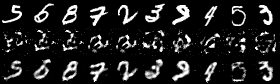
\includegraphics[width=0.7\textwidth]{figures/weakness_rec/MNIST-true-positives.png}}
        }
        \label{fig:true_positives}
    }
    \hspace{5mm}
    \subfloat[Adversarial false negatives.]{%
        \resizebox{0.45\textwidth}{!}{
          \centerline{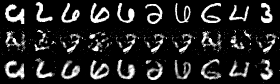
\includegraphics[width=0.7\textwidth]{figures/weakness_rec/MNIST-false-negatives.png}}
        }
        \label{fig:false_negatives}
    }
    \caption{MNIST failure predictions from the adversary.}\label{fig:predictions}
\end{figure*}


% % subfigure version.
% \begin{wrapfigure}{r}{0.3\textwidth}
%      \vspace{-30pt}
%      \centering
%      \begin{subfigure}[t]{0.3\textwidth}
%       \centering
%       \centerline{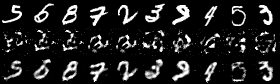
\includegraphics[width=\textwidth]{figures/weakness_rec/MNIST-true-positives.png}}
%       \caption{Adversarial true positives.}
%       \label{fig:true_positives}
%     \end{subfigure}
%     \hfill
%     \begin{subfigure}[t]{0.3\textwidth}
%       \centering
%       \centerline{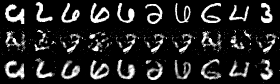
\includegraphics[width=\textwidth]{figures/weakness_rec/MNIST-false-negatives.png}}
%       \caption{Adversarial false negatives.}
%       \label{fig:false_negatives}
%     \end{subfigure}
%     \caption{MNIST failure predictions from the adversary.}\label{fig:predictions}
% \end{wrapfigure}


\section{Future Work}
To avoid exhaustively searching an entire validation set for failures, we show that an iterative framework that uses an adversarial failure classifier trained on low-dimensional representations of the inputs can select failures about $3$ times more likely than randomly choosing candidates to evaluate.
To extend this framework, we could investigate different adversarial architectures, particularly around deep reinforcement learning.
We could also explore how to take the true failures found, automatically improve the system under test, and then in a continual learning approach we could rerun this validation loop to use prior knowledge of previous system failures to find new system failures.

% \section{Contributions}
% Robert Moss consulted regularly with Bernard Lange, who is taking CS330 Meta Learning, regarding the project ideas.
% Originally, Bernard and Robert were going to collaborate on this project but took different directions as the quarter progressed.
% All of the work seen here (literature review, framework design, coding, training, analysis, plotting, and writing) was completed solely by Robert Moss.


    % POMDPStressTesting.jl: Adaptive Stress Testing for Black-Box Systems
    \chapter{Open Source Tools for Validation}\label{cha:tooling}
    This chapter discusses open source software tools built and used in the previous chapters.
These tools were designed for general applications of this work and were written in the scientific computing language Julia.
We first discusses the adaptive stress testing package used in \cref{cha:episodic_ast}, then provide quick usage examples of the packages used in \cref{cha:cem_variants} and \cref{cha:weakness_rec}. 

\section{POMDPStressTesting.jl Summary}

\href{https://github.com/sisl/POMDPStressTesting.jl}{POMDPStressTesting.jl} is a package that uses reinforcement learning and stochastic optimization to find likely failures in black-box systems through a technique called adaptive stress testing \cite{ast}.
Adaptive stress testing (AST) has been used to find failures in safety-critical systems such as aircraft collision avoidance systems \cite{ast_acasx}, flight management systems \cite{ast_fms}, and autonomous vehicles \cite{ast_av}.
The POMDPStressTesting.jl package is written in Julia \cite{bezanson2017julia} and is part of the wider POMDPs.jl ecosystem \cite{pomdps_jl}, which provides access to simulation tools, policies, visualizations, and---most importantly---solvers.
We provide different solver variants including online planning algorithms such as Monte Carlo tree search \cite{mcts} and deep reinforcement learning algorithms such as trust region policy optimization (TRPO) \cite{trpo} and proximal policy optimization (PPO) \cite{ppo}.
Stochastic optimization solvers such as the cross-entropy method \cite{cem} are also available and random search is provided as a baseline.
Additional solvers can easily be added by adhering to the POMDPs.jl interface.

\begin{lstlisting}[language=Julia]
# GrayBox simulator and environment
abstract type GrayBox.Simulation end
function GrayBox.environment(sim::Simulation)::GrayBox.Environment end
function GrayBox.transition!(sim::Simulation)::Real end

# BlackBox.interface(input::InputType)::OutputType
function BlackBox.initialize!(sim::Simulation)::Nothing end
function BlackBox.evaluate!(sim::Simulation)::Tuple{Real, Real, Bool} end
function BlackBox.distance(sim::Simulation)::Real end
function BlackBox.isevent(sim::Simulation)::Bool end
function BlackBox.isterminal(sim::Simulation)::Bool end
\end{lstlisting}

The AST formulation treats the falsification problem (i.e. finding failures) as a Markov decision process (MDP) with a reward function that uses a measure of distance to a failure event to guide the search towards failure.
The reward function also uses the state transition probabilities to guide towards \textit{likely} failures.
Reinforcement learning aims to maximize the discounted sum of expected rewards, therefore maximizing the sum of log-likelihoods is equivalent to maximizing the likelihood of a trajectory.
A gray-box simulation environment steps the simulation and outputs the state transition probabilities, and the black-box system under test is evaluated in the simulator and outputs an event indication and the real-valued distance metric (i.e. how close we are to failure).
To apply AST to a general black-box system, a user has to implement the following Julia interface:

% NOTE: Interface WAS here.

Our package builds off work originally done in the AdaptiveStressTesting.jl package \cite{ast}, but POMDPStressTesting.jl adheres to the interface defined by POMDPs.jl and provides different action modes and solver types.
Related falsification tools (i.e. tools that do not include most-likely failure analysis) are \textsc{S-TaLiRo} \cite{staliro}, Breach \cite{breach}, and \textsc{FalStar} \cite{falstar}.
These packages use a combination of optimization, path planning, and reinforcement learning techniques to solve the falsification problem.
The tool most closely related to POMDPStressTesting.jl is the AST Toolbox in Python \cite{ast_av}, which wraps around the gym reinforcement learning environment \cite{gym}.
The author has contributed to the AST Toolbox and found the need to create a similar package in pure Julia for better performance and to interface with the POMDPs.jl ecosystem.


\section{Statement of Need}

Validating autonomous systems is a crucial requirement before their deployment into real-world environments.
Searching for likely failures using automated tools enable engineers to address potential problems during development.
Because many autonomous systems are in environments with rare failure events, it is especially important to incorporate likelihood of failure within the search to help inform the potential problem mitigation.
This tool provides a simple interface for general black-box systems to fit into the adaptive stress testing problem formulation and gain access to solvers.
Due to varying simulation environment complexities, random seeds can be used as the AST action when the user does not have direct access to the environmental probability distributions or when the environment is complex.
Alternatively, directly sampling from the distributions allows for finer control over the search.
The interface is designed to easily extend to other autonomous system applications and explicitly separating the simulation environment from the system under test allows for wider validation of complex black-box systems.



\section{Research and Industrial Usage}

POMDPStressTesting.jl has been used to find likely failures in aircraft trajectory prediction systems \cite{ast_fms}, which are flight-critical subsystems used to aid in-flight automation.
A developmental commercial flight management system was stress tested so the system engineers could mitigate potential issues before system deployment \cite{ast_fms}.
In addition to traditional requirements-based testing for avionics certification \cite{do178c}, this work is being used to find potential problems during development.
There is also ongoing research on the use of POMDPStressTesting.jl for assessing the risk of autonomous vehicles and determining failure scenarios of autonomous lunar rovers. 


% \section{Acknowledgments}

% We acknowledge Ritchie Lee for his guidance and original work on adaptive stress testing and the AdaptiveStressTesting.jl package and Mark Koren, Xiaobai Ma, and Anthony Corso for their work on the AST Toolbox Python package and the CrossEntropyMethod.jl package.
% We also acknowledge Shreyas Kowshik for his initial implementation of the TRPO and PPO algorithms in Julia.
% We want to thank the Stanford Intelligent Systems Laboratory for their development of the POMDPs.jl ecosystem and the MCTS.jl package; particular thanks to Zachary Sunberg.
% We also want to thank Mykel J. Kochenderfer for his support and research input and for advancing the Julia community.


\section{CrossEntropyVariants.jl Summary}

This package summarizes the work done in \cref{cha:cem_variants}.
To run an example optimization problem, consider the following code:

\begin{lstlisting}[language=Julia]
using CrossEntropyVariants
using Distributions

f = sierra # objective function
𝛍 = [0, 0]
𝚺 = [200 0; 0 200]
𝐌 = MvNormal(𝛍, 𝚺) # proposal distribution

(𝐌, bestₓ, bestᵥ) = ce_surrogate(f, 𝐌)
\end{lstlisting}

The performance of the surrogate models may be dependent on the underlying objective function. The default surrogate model is a Gaussian process with the squared exponential kernel function \cite{kochenderfer2019algorithms}. To use radial basis functions instead of a Gaussian process, you can specify a basis keyword input:

\begin{lstlisting}[language=Julia]
f = paraboloid # objective function
𝐌 = MvNormal([0, 0], [200 0; 0 200]) # proposal distribution

(𝐌, bestₓ, bestᵥ) = ce_surrogate(f, 𝐌; basis=:squared)
\end{lstlisting}


\section{FailureRepresentation.jl Summary}

\begin{lstlisting}[language=Julia]
X, Y, mapping, adversary, metrics, metrics_rand = sampled_validation_iteration(T=10)
\end{lstlisting}
\fi

\chapter{Conclusions}
...

\appendix
\ifdefined\includebody
    % "and Miss Distances"
\chapter{Alternative FMS Failure Events}\label{sec:application_events}
This section details alternative failure events investigated and their associated miss distance calculations.
Ultimately, analysis of these failure events showed their inadequacy and arc length failures were selected as the primary event.

\section{Tangency Kinks}
Tangency kinks arise when a small angle threshold is exceeded between the inbound straight segment and the tangent of the turn segment at a given waypoint. The failure event occurs when this angle difference $\theta$ is above the threshold $\tau_k = 0.001$ \si{\radian}.

\begin{figure}[!ht]
\centering
\resizebox{0.6\columnwidth}{!}{\begin{tikzpicture}
  [
    scale=16, every node/.style={scale=2},
    >=stealth,
    point/.style = {draw, circle,  fill = black, inner sep = 1pt},
    dot/.style   = {draw, circle,  fill = black, inner sep = .2pt},
    latlon/.style = {draw, rectangle, minimum width=0.0001mm, minimum height=2mm, fill=white, fill opacity=0.75, fill = black, inner sep = 0.1pt},
    latlonstart/.style = {draw, rectangle, minimum width=0.0001mm, minimum height=2mm, fill = black, inner sep = 0.3pt},
    wpt/.style  = {diamond, fill=white, fill opacity=0.75},
  ]

  \tikzstyle{every node}=[font=\Large]
 
  % the circle
  \def\unit{0.5}
  \def\rad{0.3}
  \def\ang{45}
  \def\failang{7}
  \def\inner{0.3*\rad}
  \def\failinner{0.6*\rad}

  \node (origin) at (0,0) [point, label = {below:$c$}]{};

  \node (initial) at +(-\unit,\rad) [latlon, label = above:$p$] {};
  \node [rotate=-\failang] (failstart) at +(0, \rad) [latlonstart, red] {};
  \draw[red, rotate around={-\failang:(failstart)}] (failstart) arc (90:\ang:\rad);

  \node (start) at +(0, \rad) [latlonstart, label = above:$s$] {};
  \node [rotate=-\ang] (end) at +(\ang:\rad) [latlon, label ={[label distance=-1mm]above:$e$}] {};
  \node [rotate around={-\failang:(start)}] (failend) at +(\ang:\rad) [rotate=-\ang, latlon,red] {};

  \node (failorigin) at (0,0) [point, red, rotate around={-\failang:(start)}]{};

  \draw (start) arc (90:\ang:\rad);

  \draw[-] (initial) -- node (ls) [label = {above:$\ell_1$}] {} (start);

  \draw[dotted,thick,->] (start) -- node (tangent) [label={[label distance=-2.8mm,text=red, xshift=6.5mm, yshift=0.5mm]below right:\large$\theta$}] {} (1.25*\rad,\rad);


  \draw[dashed]
    ($ (origin) ! 1 ! (start) $)
    -- ($(start) ! 1 ! (origin)$ )
    node (center) [right,label={[pos=0.35]right:$r$}] {};

  \draw[dashed]
    ($ (origin) ! 1 ! (end) $)
    -- ($(end) ! 1 ! (origin)$ )
    node [right] {};

  \draw[dotted,thick, red]
    ($ (failorigin) ! 1 ! (start) $)
    -- ($(start) ! 1 ! (failorigin)$ )
    node (center) [right] {};

  \draw[dotted,thick, red]
    ($ (failorigin) ! 1 ! (failend) $)
    -- ($(failend) ! 1 ! (failorigin)$ )
    node [right] {};

  \draw[->, rotate around={\ang:(end)}] (end) -- node (nextstraight) [very near end, label = {above:$\ell_2$},] {} (end |-, 0);
  \draw[red, ->, rotate around={\ang-\failang:(failend)}] (failend) -- node (failnextstraight) [red] {} (failend |-, 0);
  \draw [red] (1.25*\rad*5.06/7,\rad) arc (0:-\failang*5.06/7:1.25*\rad); % "fail" angle (i.e., kink)
  \draw[dotted,thick,->,red, rotate around={-\failang:(start)}] (start) -- node (fail) [] {} (1.25*\rad,\rad);

  % Right angle symbols
  \def\ralen{.2ex}  % length of the short segment
  \foreach \inter/\first/\last in {start/origin/tangent}
    {
      \draw let \p1 = ($(\inter)!\ralen!(\first)$), % point along first path
                \p2 = ($(\inter)!\ralen!(\last)$),  % point along second path
                \p3 = ($(\p1)+(\p2)-(\inter)$)      % corner point
            in
              (\p1) -- (\p3) -- (\p2)               % path
              ;
    }

  \draw [dashed] (0, \inner) arc (90:\ang:\inner);
  \node (innerangle) at +(90-\ang+\ang/1.4:\inner) [label = {[label distance=-3mm]above right:$\alpha$}] {};

  \node (mid) at +(90-\ang/2:\rad) [draw, wpt, inner sep=1pt, rotate=90-\ang/2] {};

\end{tikzpicture}}
\caption{Tangency kink failure event and miss distance.}
\label{fig:tangency_kink}
\end{figure}

Miss distance for the tangency kinks is calculated by first determining the azimuth angle $z$ between the start point of the arc $s$ and the center point $c$. The azimuth is calculated using a WGS84 Earth flattening leveraging the Geodesic.jl\footnote{\url{https://github.com/anowacki/Geodesics.jl}} package which implements Vincenty's formula  \cite{vincenty}. The tangency angle $\theta$ is then calculated for each $\ell \in L$ where $L$ is the set of lateral packets that each have a straight segment and a turn arc with radius $r$. The sign of the radius $r$ indicates the direction of turn, where left is negative and right is positive. The course-in angle of the straight segment $\ell$ is denoted $\angle \ell$,
% \begin{align*}
%   U(\phi) &= \arctan((1 - f) \tan \phi))\\
%   (U_s, U_c) &= (U(\phi_s),\, U(\phi_c))
% \end{align*}
%
% \begin{align*}
%   \lambda = \Lambda(L, f)
% \end{align*}
% https://github.com/anowacki/Geodesics.jl
% 
% \begin{align*}
%   % https://en.wikipedia.org/wiki/Vincenty%27s_formulae#Inverse_problem
%   % Inverse problem
%   % 1. Vincenty, T. (1975). "Direct and Inverse Solutions of Geodesics on the Ellipsoid with application of nested equations" (PDF). Survey Review. XXIII (176): 88–93. doi:10.1179/sre.1975.23.176.88
%   z = \arctan(\cos U_c \sin \lambda,\, \cos U_s \sin U_c - \sin U_s \cos U_c \cos \lambda)
%   % \alpha_c = \arctan(\cos U_s \sin \lambda,\, -\sin U_s \cos U_c + \cos U_s \sin U_c \cos \lambda)
% \end{align*}
%
\begin{equation*}
  % d = \tau_k - \max\left\{ \abs{z - \angle \ell + \sign(r)\frac{\pi}{2}} : (\ell,r) \in L \right\}.
  d = \tau_k - \max\limits_{(\ell,r) \in L} \abs{z - \angle \ell + \sign(r)\frac{\pi}{2}}.
\end{equation*}


\section{Course Directions}
In-bound and out-bound course directions may deviate from one another and can be classified as a failure event.
Closely related to the \textit{disconnection} failure event, the course direction failures can arise when two sequential lateral packets are disconnected. This failure specifically looks for angle differences between the course-out $\theta_{\text{out}}$ and course-in $\theta_\text{in}$ directions of the sequential lateral packets. If this angle difference $\omega = \abs{\theta_\text{out} - \theta_\text{in}}$ is above the threshold $\tau_c = 1\si{\degree}$ then it is classified as a failure.

\begin{figure}[!ht]
\centering
\resizebox{0.6\columnwidth}{!}{\begin{tikzpicture}
  [
    scale=16, every node/.style={scale=2},
    >=stealth,
    point/.style = {draw, circle,  fill = black, inner sep = 1pt},
    dot/.style   = {draw, circle,  fill = black, inner sep = .2pt},
    latlon/.style = {draw, rectangle, minimum width=0.0001mm, minimum height=2mm, fill=white, fill opacity=0.75, fill = black, inner sep = 0.1pt},
    latlonstart/.style = {draw, rectangle, minimum width=0.0001mm, minimum height=2mm, fill = black, inner sep = 0.3pt},
    wpt/.style  = {diamond, fill=white, fill opacity=0.75},
  ]
 
  \tikzstyle{every node}=[font=\Large]
 
  % the circle
  \def\unit{0.5}
  \def\rad{0.3}
  \def\ang{45}
  \def\failang{7}
  \def\inner{0.1*\rad}
  \def\failinner{0.6*\rad}

  \node (initial) at +(-\unit,\rad) [latlon, label = above:$p_1$] {};

  \node (start) at +(0, \rad) [latlonstart, label = above:$s_1$] {};
  \node [rotate=-\ang] (end) at +(\ang:\rad) [latlon, label ={[label distance=-1mm]above:$e_1$}] {};
  \draw[->, dashed, rotate around={\ang:(end)}] (end) -- node (nextstraight) [pos=0.75, label={below right:$\;\;\theta_{\text{out}}$},] {} (end |-, \rad/4.25);

  \node (failinitial) at (0,\rad/2) [latlon, label = above:$p_2$] {};
  \node (failstart) at ($(failinitial) + (-0.25, 0)$) [latlonstart, label = above:$s_2$] {};

  \draw (start) arc (90:\ang:\rad);

  \draw[-] (initial) -- node (ls) [label = {above:$\ell_1$}] {} (start);

  \draw[->,dashed] ($(failinitial) + (0.32, 0)$) -- node (dist) [label={right:$\;\theta_{\text{in}}$},pos=0.05] {} (failinitial);
  \draw[-] (failinitial) -- node (fs) [label={above:$\ell_2$}] {} (failstart);

  \draw [red,thick,dashed,rotate=180] (-0.24, -\rad/2) arc (0:135:\inner);
  \node (innerangle) at (0.225, \rad/3.6) [label = {[red,label distance=-3mm]above right:$\omega$}] {};

  \node (mid) at +(90-\ang/2:\rad) [draw, wpt, inner sep=1pt, rotate=90-\ang/2] {};

\end{tikzpicture}
}
\caption{Course direction failure event and miss distance.}
\label{fig:course_direction}
\end{figure}

Miss distance is calculated as how close to the threshold $\tau_c$ is the maximum wrapped angle difference between the course-out angle and course-in angle denoted by $\omega$, namely
\begin{equation*}
  % d = \tau_c - \max\left\{ \abs{\theta_\text{out} - \theta_\text{in}} : \theta_\text{out} \in L_i, \theta_\text{in} \in L_{i+1} \right\}.
  % d = \tau_c - \max\limits_{\theta_\text{out} \in L_i, \theta_\text{in} \in L_{i+1}}\abs{\theta_\text{out} - \theta_\text{in}}.
  d = \tau_c - \max\limits_{\substack{\theta_\text{out} \in L_i\\\theta_\text{in} \in L_{i+1}}}\abs{\theta_\text{out} - \theta_\text{in}}.
\end{equation*}

% \begin{itemize}
%   \item Explain how tangent angle is calculated
%   \item Talk about WGS84 flattening
%   \item Mention Vincenty's inverse formula, Karney's inverse formula, and cite comparison paper (get papers, \textit{GEODESIC ALGORITHMS: AN EXPERIMENTAL STUDY})
%   \item Describe all variables used ($r = \text{radius}$, etc)
%   \item Update how the angle is calculated based on Nick's adjustments
% \end{itemize}


\section{Disconnections}
Disconnected lateral packets occur when two sequential lateral packets are not connected end-to-start, thus leaving a distance $\delta$ between them. If this geodesic distance $\delta = \lVert e_i - p_{i+1} \rVert$ is above the threshold $\tau_d = 10$ \si{ft} then a failure occurred.

\begin{figure}[!ht]
\centering
\resizebox{0.6\columnwidth}{!}{\begin{tikzpicture}
  [
    scale=16, every node/.style={scale=2},
    >=stealth,
    point/.style = {draw, circle,  fill = black, inner sep = 1pt},
    dot/.style   = {draw, circle,  fill = black, inner sep = .2pt},
    latlon/.style = {draw, rectangle, minimum width=0.0001mm, minimum height=2mm, fill=white, fill opacity=0.75, fill = black, inner sep = 0.1pt},
    latlonstart/.style = {draw, rectangle, minimum width=0.0001mm, minimum height=2mm, fill = black, inner sep = 0.3pt},
    wpt/.style  = {diamond, fill=white, fill opacity=0.75},
  ]
 
  \tikzstyle{every node}=[font=\large]
 
  % the circle
  \def\unit{0.5}
  \def\rad{0.3}
  \def\ang{45}
  \def\failang{7}
  \def\inner{0.3*\rad}
  \def\failinner{0.6*\rad}

  \node (initial) at +(-\unit,\rad) [latlon, label = above:$p_1$] {};

  \node (start) at +(0, \rad) [latlonstart, label = above:$s_1$] {};
  \node [rotate=-\ang] (end) at +(\ang:\rad) [latlon, label ={[label distance=-1mm]above:$e_1$}] {};

  \node (failinitial) at (0,\rad/2) [latlon, label = above:$p_2$] {};
  \node (failstart) at ($(failinitial) + (-0.25, 0)$) [latlonstart, label = above:$s_2$] {};

  \draw (start) arc (90:\ang:\rad);

  \draw[-] (initial) -- node (ls) [label = {above:$\ell_1$}] {} (start);

  \draw[dashed,red] (end) -- node (dist) [label={[label distance=-1mm]below:$\delta$},pos=0.45] {} (failinitial);
  \draw[-] (failinitial) -- node (fs) [label={above:$\ell_2$}] {} (failstart);

  \node (mid) at +(90-\ang/2:\rad) [draw, wpt, inner sep=1pt, rotate=90-\ang/2] {};

\end{tikzpicture}
}
\caption{Disconnected failure event and miss distance.}
\label{fig:disconnection}
\end{figure}

Miss distance is calculated as the threshold $\tau_d$ minus the maximum distance between the end points $e_i$ (or $s_i$ if no arc is provided) and the initial point $p_{i+1}$ of the next lateral packet:
\begin{equation*}
  % d = \tau_d - \max\left\{ \lVert e_i - p_{i+1} \rVert : (e_i,p_{i+1}) \in L \right\}.
  % d = \tau_d - \max\limits_{(e_i,p_{i+1}) \in L}\lVert e_i - p_{i+1} \rVert.
  % d = \tau_d - \max\limits_{e_i \in L_i, p_{i+1} \in L_{i+1}}\lVert e_i - p_{i+1} \rVert.
  d = \tau_d - \max\limits_{\substack{e_i \in L_i\\p_{i+1} \in L_{i+1}}}\lVert e_i - p_{i+1} \rVert
\end{equation*}


% We use the modified reward function that incorporates severity based on the miss distance at the time of an event.
% For our four miss distances described above, we want to reward egregious miss distances, thus finding events that are more severe. 

\fi

% \bibliographystyle{plain}
% \bibliography{cem_variants}
\printbibliography


\end{document}

% TODO:
% [-] combine references.bib
% [x] See Dorsa notes
% [ ] See Mykel notes
% [ ] Subsections for tooling: CrossEntropyVariants.jl and FailureRepresentation.jl
% [x] Combine Acknowledgments
% [ ] Flow together chapters
% [x] "dissertation" wording in the signatures page
% [x] Remove "graduate studies" committee?


% Mykel notes:
% [x] Concatenate research papers from MS (if they're related work / extensions)
% [ ] Add introduction
% [ ] Flow together body chapters
% [ ] Remove redundancies between them
% [x] Change conclusions/future work into discussion
% - Two big things:
%     [ ] 1) intro chapter
%         - shortest intro chapter possible (concise)
%         - "freshman undergrad could understand contributions"
%     [ ] 2) final chapter
%         [ ] one section "Summary" high level, no jargon, no non-sense
%         [ ] second section "Contributions", summarize how you've supported your claims (back references, specialized terminology)
%         [ ] third: future work
% https://www2.eecs.berkeley.edu/Pubs/Theses/